\documentclass[a4paper,11pt,fleqn,dvipsnames,twoside,openright]{memoir} 	% Openright aabner kapitler paa hoejresider (openany begge)

%%%% PACKAGES %%%%

% ¤¤ Oversaettelse og tegnsaetning ¤¤ %
\usepackage[utf8]{inputenc}					% Input-indkodning af tegnsaet (UTF8)
\usepackage[english]{babel}					% Dokumentets sprog
\usepackage[T1]{fontenc}					% Output-indkodning af tegnsaet (T1)
\usepackage{ragged2e,anyfontsize}			% Justering af elementer
%\usepackage{fixltx2e}						% Retter forskellige fejl i LaTeX-kernen
																			
% ¤¤ Figurer og tabeller (floats) ¤¤ %
\usepackage{graphicx} 						% Haandtering af eksterne billeder (JPG, PNG, EPS, PDF)
\usepackage{multirow}                		% Fletning af raekker og kolonner (\multicolumn og \multirow)
\usepackage{multicol}         	        	% Muliggoer output i spalter
\usepackage{rotating}						% Rotation af tekst med \begin{sideways}...\end{sideways}
\usepackage{colortbl} 						% Farver i tabeller (fx \columncolor og \rowcolor)
\usepackage{xcolor}							% Definer farver med \definecolor. Se mere: http://en.wikibooks.org/wiki/LaTeX/Colors
\usepackage{flafter}						% Soerger for at floats ikke optraeder i teksten foer deres reference
\let\newfloat\relax 						% Justering mellem float-pakken og memoir
\usepackage{float}							% Muliggoer eksakt placering af floats, f.eks. \begin{figure}[H]
\newcommand{\HRule}{\rule{\linewidth}{0.5mm}}
\usepackage{pdflscape}	 					% Giver mulighed for landacape mode
\usepackage{longtable}						% Giver mulighed for talber over flere side
\usepackage{subcaption}

% ¤¤ Matematik mm. ¤¤
\usepackage{amsmath}						% Avancerede matematik-udvidelser
\usepackage{amssymb}						% Avancerede matematik-udvidelser
\usepackage{stmaryrd}						% Avancerede matematik-udvidelser
\usepackage{amsthm}							% Avancerede matematik-udvidelser
\usepackage{textcomp}                 		% Symbol-udvidelser (f.eks. promille-tegn med \textperthousand )
\usepackage{cancel}

% ¤¤ Kode indsat i rapport ¤¤ %
\usepackage{listings}						% Placer kildekode i dokumentet med \begin{lstlisting}...\end{lstlisting}

% INDSÆT AF JACOB
\usepackage[acronym,toc]{glossaries}  
\usepackage{siunitx}
\usepackage{adjustbox}
\usepackage{pgfplots}
\usepackage{url}

%%%% TIKZ MAGIC %%%%
\usepackage{schemabloc}
\usetikzlibrary{circuits}
\usepackage{tikz}
\usetikzlibrary{shapes,arrows}
\usepackage{pgfplots}
\usepgfplotslibrary{units}
\usetikzlibrary{plotmarks}
\usetikzlibrary{fit}
\pgfplotsset{compat=newest}
\pgfplotsset{filter discard warning=false}
%\usepackage[americanresistors,americaninductors,american voltages]{circuitikz}
\usetikzlibrary{calc}
\usetikzlibrary{patterns}
\ctikzset{bipoles/thickness=1}
\ctikzset{bipoles/length=0.8cm}
\ctikzset{bipoles/diode/height=.375}
\ctikzset{bipoles/diode/width=.3}
\ctikzset{tripoles/thyristor/height=.8}
\ctikzset{tripoles/thyristor/width=1}
\ctikzset{bipoles/vsourceam/height/.initial=.7}
\ctikzset{bipoles/vsourceam/width/.initial=.7}
\tikzstyle{every node}=[font=\small]
\tikzstyle{every path}=[line width=0.8pt,line cap=round,line join=round]
\definecolor{AleeRed}{rgb}{0.5,0,0}
\newcommand\addvmargin[1]{
  \node[fit=(current bounding box),inner ysep=#1,inner xsep=0]{};
}
\usetikzlibrary{positioning}





%\usepackage{nomencl,etoolbox,ragged2e,siunitx,mathtools}
%\usepackage{subfig}

% ¤¤ Matematik funktioner ¤¤				% Sikre alle funktioner står med ordinær skriftype
	\newcommand{\e}{\text{e}}
	\newcommand{\dB}{\text{dB}}	
	\newcommand{\I}{\text{I}}	
	\newcommand{\V}{\text{V}}
	\newcommand{\A}{\text{A}}
	\newcommand{\W}{\text{W}}
	\newcommand{\F}{\text{F}}
	\renewcommand{\S}{\text{S}}
	\newcommand{\rms}{\text{rms}}
	\newcommand{\m}{\text{m}}
	\newcommand{\n}{\text{n}}
	\newcommand{\p}{\text{p}}
	\newcommand{\f}{\text{f}}
	\renewcommand{\k}{\text{k}}
	\newcommand{\M}{\text{M}}
	\newcommand{\G}{\text{G}}
	\newcommand{\C}{\text{C}}
	\renewcommand{\c}{\text{c}}
	\newcommand{\T}{\text{T}}

% ¤¤ Opsætning af enheder ¤¤ % 
	\newcommand{\enhed}[1]{\hfill[\mathrm{#1}]} 	% Skriv \enhed{"din enhed"} og dem bliver rykket til højre

% ¤¤ Referencer og kilder ¤¤ %
\usepackage{cite}
\bibliographystyle{apalike}					% Udseende af litteraturlisten.
%\PassOptionsToPackage{
%        url=true,
%            }   {cite}	http://www.xilinx.com/support/documentation/user_guides/ug331.pdf
%  url       = {\url{http://techdocs.altium.com/display/FPGA/Philips+RC5+Infrared+Transmission+Protocol}}, 
% ¤¤ Textlable setup ¤¤ % 
\makeatletter
\newcommand*{\textlabel}[2]{				% Gør \textlabel mulig
  \edef\@currentlabel{#1}					% Set target label
  \phantomsection							% Correct hyper reference link
  #1\label{#2}}								% Print and store label

% ¤¤ Misc. ¤¤ %
\usepackage{lipsum}							% Dummy text \lipsum[..]
\usepackage[shortlabels]{enumitem}			% Muliggoer enkelt konfiguration af lister
\usepackage{pdfpages}						% Goer det muligt at inkludere pdf-dokumenter med kommandoen \includepdf[pages={x-y}]{fil.pdf}	
\pdfoptionpdfminorversion=6					% Muliggoer inkludering af pdf dokumenter, af version 1.6 og hoejere
\pretolerance=2500 							% Justering af afstand mellem ord (hoejt tal, mindre orddeling og mere luft mellem ord)

% Kommentarer og rettelser med \fxnote. Med 'final' i stedet for 'draft' udloeser hver note en error i den faerdige rapport.
\usepackage[footnote,draft,danish,silent,nomargin]{fixme}
\renewcommand{\thefootnote}{\arabic{footnote}}

%%%% CUSTOM SETTINGS %%%%

% ¤¤ Marginer ¤¤ %
\setlrmarginsandblock{3.5cm}{2.5cm}{*}		% \setlrmarginsandblock{Indbinding}{Kant}{Ratio}
\setulmarginsandblock{2.0cm}{3.0cm}{*}		% \setulmarginsandblock{Top}{Bund}{Ratio}
\checkandfixthelayout 						% Oversaetter vaerdier til brug for andre pakker

%	¤¤ Afsnitsformatering ¤¤ %
\setlength{\parindent}{0mm}           		% Stoerrelse af indryk
\setlength{\parskip}{3mm}          			% Afstand mellem afsnit ved brug af double Enter
\linespread{1}							% Linie afstand

% ¤¤ Indholdsfortegnelse ¤¤ %
\setsecnumdepth{subsubsection}		 			% Dybden af nummerede overkrifter (part/chapter/section/subsection)
\maxsecnumdepth{subsubsection}					% Dokumentklassens graense for nummereringsdybde
\settocdepth{subsubsection} 					% Dybden af indholdsfortegnelsen

% ¤¤ Lister ¤¤ %
\setlist{
  topsep=0pt,								% Vertikal afstand mellem tekst og listen
  itemsep=-1ex,								% Vertikal afstand mellem items
} 

% ¤¤ Visuelle referencer ¤¤ %
\usepackage[colorlinks]{hyperref}			% Danner klikbare referencer (hyperlinks) i dokumentet.
\hypersetup{colorlinks = true,				% Opsaetning af farvede hyperlinks (interne links, citeringer og URL)
    linkcolor = black,
    citecolor = black,
    urlcolor = blue
}

% ¤¤ Opsaetning af figur- og tabeltekst ¤¤ %
\captionnamefont{\small\bfseries\itshape}	% Opsaetning af tekstdelen ('Figur' eller 'Tabel')
\captiontitlefont{\small}					% Opsaetning af nummerering
\captiondelim{. }							% Seperator mellem nummerering og figurtekst
\hangcaption								% Venstrejusterer flere-liniers figurtekst under hinanden
\captionsetup{width=1\textwidth}
\setlength{\belowcaptionskip}{0pt}			% Afstand under figurteksten


% ¤¤ Opsætning til caption i listings ¤¤ %
\DeclareCaptionFormat{listing}{
  \colorbox[RGB]{255,255,255}{
    \parbox{\textwidth}{\centering#1#2#3}
  }
}
\captionsetup[lstlisting]{ format=listing, singlelinecheck=false, margin=0pt, font={normalsize} }
\renewcommand{\lstlistingname}{Code}		% Gør at der står kode og ikke listing i captionnamefont
		
% ¤¤ Opsaetning af listings ¤¤ % 
\definecolor{commentGreen}{RGB}{34,139,24}	% Farver der bliver brugt senere 
\definecolor{stringPurple}{RGB}{208,76,239}	% farver der bliver brugt senere

\lstset{language=VHDL,						% Sprog
	basicstyle=\ttfamily\small,				% Opsaetning af teksten
	keywords={for,if,while,else,elseif,		% Noegleord at fremhaeve
			  end,when,return,case,
			  switch,function,process,begin,
			  JUMP,test,ORG, out,
			  COMP, INT, DINT,ret
			  or, and, call, load, or,
			  then, elsif, add, sub},
	keywordstyle=\color{blue},				% Opsaetning af noegleord
	commentstyle=\color{commentGreen},		% Opsaetning af kommentarer
	stringstyle=\color{stringPurple},		% Opsaetning af strenge
	showstringspaces=false,					% Mellemrum i strenge enten vist eller blanke
	numbers=left, numberstyle=\tiny,		% Linjenumre
	extendedchars=true, 					% Tillader specielle karakterer
	columns=flexible,						% Kolonnejustering
	breaklines, breakatwhitespace=true,		% Bryd lange linjer
	captionpos=b,							% Sæt caption i bunden 
	xleftmargin=14pt,						% Start margin x pt til højre(+) eller venstre(-)
}

% ¤¤ Navngivning ¤¤ %
\addto\captionsdanish{
	\renewcommand\appendixname{Appendiks}
	\renewcommand\contentsname{Indholdsfortegnelse}	
	\renewcommand\appendixpagename{Appendiks}
	\renewcommand\appendixtocname{Appendiks}
	\renewcommand\cftchaptername{\chaptername~}				% Skriver "Kapitel" foran kapitlerne i indholdsfortegnelsen
	\renewcommand\cftappendixname{\appendixname~}			% Skriver "Appendiks" foran appendiks i indholdsfortegnelsen
}

% ¤¤ Kapiteludssende ¤¤ %
\definecolor{numbercolor}{gray}{0.7}		% Definerer en farve til brug til kapiteludseende
\newif\ifchapternonum

\makechapterstyle{jenor}{					% Definerer kapiteludseende frem til ...
  \renewcommand\beforechapskip{0pt}
  \renewcommand\printchaptername{}
  \renewcommand\printchapternum{}
  \renewcommand\printchapternonum{\chapternonumtrue}
  \renewcommand\chaptitlefont{\fontfamily{pbk}\fontseries{db}\fontshape{n}\fontsize{20}{30}\selectfont\raggedleft}
  \renewcommand\chapnumfont{\fontfamily{pbk}\fontseries{m}\fontshape{n}\fontsize{1in}{0in}\selectfont\color{numbercolor}}
  \renewcommand\printchaptertitle[1]{%
    \noindent
    \ifchapternonum
    \begin{tabularx}{\textwidth}{X}
    {\let\\\newline\chaptitlefont ##1\par} 
    \end{tabularx}
    \par\vskip-2.5mm\hrule
    \else
    \begin{tabularx}{\textwidth}{Xl}
    {\parbox[b]{\linewidth}{\chaptitlefont ##1}} & \raisebox{-15pt}{\chapnumfont \thechapter}
    \end{tabularx}
    \par\vskip2mm\hrule
    \fi
  }
}											% ... her

\chapterstyle{jenor}						% Valg af kapiteludseende - Google 'memoir chapter styles' for alternativer

% ¤¤ Sidehoved ¤¤ %

\makepagestyle{AAU}							% Definerer sidehoved og sidefod udseende frem til ...
\makepsmarks{AAU}{%
	\createmark{chapter}{left}{shownumber}{}{. \ }
	\createmark{section}{right}{shownumber}{}{. \ }
	\createplainmark{toc}{both}{\contentsname}
	\createplainmark{lof}{both}{\listfigurename}
	\createplainmark{lot}{both}{\listtablename}
	\createplainmark{bib}{both}{\bibname}
	\createplainmark{index}{both}{\indexname}
	\createplainmark{glossary}{both}{\glossaryname}
}
\nouppercaseheads											% Ingen Caps oenskes

\makeevenhead{AAU}{Group 1030}{}{\leftmark}					% Definerer lige siders sidehoved (\makeevenhead{Navn}{Venstre}{Center}{Hoejre})
\makeoddhead{AAU}{\rightmark}{}{Aalborg University}		% Definerer ulige siders sidehoved (\makeoddhead{Navn}{Venstre}{Center}{Hoejre})
\makeevenfoot{AAU}{\thepage}{}{}							% Definerer lige siders sidefod (\makeevenfoot{Navn}{Venstre}{Center}{Hoejre})
\makeoddfoot{AAU}{}{}{\thepage}								% Definerer ulige siders sidefod (\makeoddfoot{Navn}{Venstre}{Center}{Hoejre})
\makeheadrule{AAU}{\textwidth}{0.5pt}						% Tilfoejer en streg under sidehovedets indhold
\makefootrule{AAU}{\textwidth}{0.5pt}{1mm}					% Tilfoejer en streg under sidefodens indhold

\copypagestyle{AAUchap}{AAU}								% Sidehoved for kapitelsider defineres som standardsider, men med blank sidehoved
\makeoddhead{AAUchap}{}{}{}
\makeevenhead{AAUchap}{}{}{}
\makeheadrule{AAUchap}{\textwidth}{0pt}
\aliaspagestyle{chapter}{AAUchap}							% Den ny style vaelges til at gaelde for chapters
															% ... her
															
\pagestyle{AAU}												% Valg af sidehoved og sidefod


%%%% CUSTOM COMMANDS %%%%

% ¤¤ Specielle tegn ¤¤ %
\newcommand{\decC}{^{\circ}\text{C}}
\newcommand{\dec}{^{\circ}}


%%%% ORDDELING %%%%

\hyphenation{}

%%% Tikz %%%%%
\usepackage{tikz}
\usetikzlibrary{positioning}
\usepackage{titlesec,blindtext,color}
\usetikzlibrary{shapes,arrows}
\usepackage{tikz,amsmath, amssymb,bm,color}
%%\usepackage[margin=0cm,nohead]{geometry}
\usetikzlibrary{shapes,arrows}
%% needed for BB
\usetikzlibrary{calc}
\usepackage{tikzscale}
\usetikzlibrary{backgrounds}
%\usepackage{tikz-timing}[2009/12/09]
%%%% Kan ikke bruges efter upgate %%%%
%\usepackage[active,tightpage]{preview}

\raggedbottom

\begin{document}

%%% Tikz Magic %%%
\usetikzlibrary{shapes,arrows}
\usetikzlibrary{plotmarks}
\pgfplotsset{compat=newest}
\pgfplotsset{filter discard warning=false}

\pgfdeclarelayer{bg}    % declare background layer
\pgfsetlayers{bg,main}


%\usepackage{silence}
%\WarningsOff[pgfplots]
%\WarningFilter{latex}{Marginpar on page}
%\WarningsOff[latex]


%%% Tikz Magic %%%
\tikzstyle{block} = [draw,rounded corners , rectangle, minimum height=3em, minimum width=6em]
\tikzstyle{Integrator} = [draw, fill=blue!20, rectangle, minimum height=5mm, minimum width=5mm]
\tikzstyle{Twolineblock} = [draw,rounded corners , rectangle, minimum height=3em, minimum width=6em, text width = 6em, align=center]     
\tikzstyle{sum} = [draw, fill=blue!20, circle, node distance=1cm]
\tikzstyle{input} = [coordinate]
\tikzstyle{output} = [coordinate]
\tikzstyle{pinstyle} = [pin edge={to-,thin,black}]
\tikzstyle{box} = [draw,rounded corners, minimum height=15mm, minimum width=20mm, align=center, text centered]
\tikzstyle{BlackBox} = [draw, fill=black, rounded corners, minimum height=15mm, minimum width=20mm, align=center, text=white, text centered]
\tikzstyle{FlowIF} = [diamond, draw, fill=blue!20, text width=8.5em, text badly centered, node distance=3cm, inner sep=0pt,align=center,aspect=3]
\tikzstyle{FlowBlock} = [rectangle, draw, fill=blue!20, text width=8em, text centered, rounded corners, minimum height=3em]
\tikzstyle{FlowCloud} = [draw, ellipse,fill=red!20, node distance=3cm, minimum height=2em]
\tikzstyle{TestBox} = [rectangle,draw, fill=black!20, minimum height=8mm, minimum width=8mm]
\tikzstyle{TestDiamond} = [diamond, draw, fill=black!20, minimum height=10.5mm, minimum width=10.5mm]
\tikzstyle{TestBox} = [rectangle,draw, fill=black!20, minimum height=8mm, minimum width=8mm]
\tikzstyle{TestCircle} = [circle, draw, fill=black!20, minimum height=6mm, minimum width=6mm]
\tikzstyle{TestTable} = [rectangle, draw, fill=black!60, minimum height=0.01mm, minimum width=9mm, text=white]
\tikzstyle{TestBoxSmall} = [rectangle,draw, fill=black!, minimum height=8mm, minimum width=8mm,text=white]
\tikzstyle{LegendBox} = [rectangle,draw, minimum height=7mm, minimum width=20mm]
\tikzstyle{Sysbox} = [draw,rounded corners, minimum height=15mm, minimum width=9em, align=center, text centered,text width = 10.5em]
\tikzstyle{SysBlackBox} = [draw, fill=black, text=white, rounded corners, minimum height=15mm, minimum width=9em, align=center, text centered,text width = 10em]
\tikzstyle{PreAmpBox} = [rectangle,draw, fill=black!20, minimum height=8mm, minimum width=12mm]
\tikzstyle{gain} = [fill=white, draw, rectangle, minimum height=2.5em, minimum width=2.5em]
\tikzstyle{summation} = [draw, minimum size=0.75cm, circle, node distance=1.75cm]












%% Its a pie chart!! %%%
\definecolor{rosso}{RGB}{220,57,18}
\definecolor{giallo}{RGB}{255,153,0}
\definecolor{blu}{RGB}{102,140,217}
\definecolor{verde}{RGB}{16,150,24}
\definecolor{viola}{RGB}{153,0,153}

\makeatletter

\tikzstyle{chart}=[
    legend label/.style={font={\scriptsize},anchor=west,align=left},
    legend box/.style={rectangle, draw, minimum size=5pt},
    axis/.style={black,semithick,->},
    axis label/.style={anchor=east,font={\tiny}},
]

\tikzstyle{bar chart}=[
    chart,
    bar width/.code={
        \pgfmathparse{##1/2}
        \global\let\bar@w\pgfmathresult
    },
    bar/.style={very thick, draw=white},
    bar label/.style={font={\bf\small},anchor=north},
    bar value/.style={font={\footnotesize}},
    bar width=.75,
]

\tikzstyle{pie chart}=[
    chart,
    slice/.style={line cap=round, line join=round, very thick,draw=white},
    pie title/.style={font={\bf}},
    slice type/.style 2 args={
        ##1/.style={fill=##2},
        values of ##1/.style={}
    }
]

\pgfdeclarelayer{background}
\pgfdeclarelayer{foreground}
\pgfsetlayers{background,main,foreground}



\newcommand{\pie}[3][]{
    \begin{scope}[#1]
    \pgfmathsetmacro{\curA}{90}
    \pgfmathsetmacro{\r}{1}
    \def\c{(0,0)}
    \node[pie title] at (90:1.3) {#2};
    \foreach \v/\s in{#3}{
        \pgfmathsetmacro{\deltaA}{\v/100*360}
        \pgfmathsetmacro{\nextA}{\curA + \deltaA}
        \pgfmathsetmacro{\midA}{(\curA+\nextA)/2}

        \path[slice,\s] \c
            -- +(\curA:\r)
            arc (\curA:\nextA:\r)
            -- cycle;
        \pgfmathsetmacro{\d}{max((\deltaA * -(.5/50) + 1) , .5)}

        \begin{pgfonlayer}{foreground}
        \path \c -- node[pos=\d,pie values,values of \s]{$\v\%$} +(\midA:\r);
        \end{pgfonlayer}

        \global\let\curA\nextA
    }
    \end{scope}
}




%% Cutom legned entry
\newenvironment{customlegend}[1][]{%
	\begingroup
	% inits/clears the lists (which might be populated from previous
	% axes):
	\csname pgfplots@init@cleared@structures\endcsname
	\pgfplotsset{#1}%
}{%
% draws the legend:
\csname pgfplots@createlegend\endcsname
\endgroup
}%

% makes \addlegendimage available (typically only available within an
% axis environment):
\def\addlegendimage{\csname pgfplots@addlegendimage\endcsname}

\usetikzlibrary{arrows}
\tikzset{>=stealth}


%% Its Color time:
\definecolor{MATLABblue}{rgb}{0,0.4470,0.7410}
\definecolor{MATLABorange}{rgb}{0.85,0.3250,0.0980}
\definecolor{MATLAByellow}{rgb}{0.929,0.6940,0.1250}
\definecolor{MATLABpurple}{rgb}{0.494,0.1840,0.5560}
\definecolor{MATLABgreen}{rgb}{0.466,0.6740,0.1880}
\definecolor{MATLABbabyblue}{rgb}{0.301,0.7450,0.9330}
\definecolor{MATLABred}{rgb}{0.635,0.0780,0.1840}
%% Loopback color
\definecolor{MATLABblack}{rgb}{0,0,0}

%% Microphone Colors
\definecolor{M1}{rgb}{0,0.4470,0.7410}
\definecolor{M2}{rgb}{0.85,0.3250,0.0980}
\definecolor{M3}{rgb}{0.929,0.6940,0.1250}
\definecolor{M4}{rgb}{0.494,0.1840,0.5560}
\definecolor{M5}{rgb}{0.466,0.6740,0.1880}
\definecolor{M6}{rgb}{0.301,0.7450,0.9330}
\definecolor{M7}{rgb}{0.635,0.0780,0.1840}
\definecolor{M8}{rgb}{0,0,1}
\definecolor{M9}{rgb}{0,0.5,1}
\definecolor{M10}{rgb}{0,1,0.5}
\definecolor{M11}{rgb}{0,1,1}
\definecolor{M12}{rgb}{0.5,1,0.5}
\definecolor{M13}{rgb}{1,0.5,0}
\definecolor{M14}{rgb}{1,0,0}
\definecolor{M15}{rgb}{0.5,0,0}

\newcommand*\circled[1]{\tikz[baseline=(char.base)]{
		\node[shape=circle,draw,inner sep=2pt] (char) {#1};}}



\newenvironment{sbmatrix}[1]
{\def\mysubscript{#1}\mathop\bgroup\begin{bmatrix}}
	{\end{bmatrix}\egroup_{\textstyle\mathstrut\mysubscript}}

\usetikzlibrary{matrix,calc}
\tikzstyle{loosely dotted}=[dash pattern=on 2\pgflinewidth off 24pt]

% \makeatletter
% \renewcommand{\todo}[2][]{\tikzexternaldisable\@todo[#1]{#2}\tikzexternalenable}
% \makeatother

% %\makeatletter
% %\renewcommand{\missingfigure}[2][]{\tikzexternaldisable\@missingfigure[#1]{#2}\tikzexternalenable}
% %\makeatother

% \let\oldmissingfigure\missingfigure
% \renewcommand{\missingfigure}[2][]{\tikzexternaldisable\oldmissingfigure[#1]{#2}\tikzexternalenable}

% Forindhold - Kun romer tal

\frontmatter
\makeevenfoot{AAU}{\thepage}{}{}
\makeoddfoot{AAU}{}{}{\thepage}

%Formalia
%main for introduktion

%\includepdf[pages={1}]{rapport/introduktion/forsiden.pdf}

%\includepdf[pages={1}]{forside/forsiden.pdf}

\thispagestyle{empty}

\begin{center}

\vspace*{\fill}

\textsc{\LARGE Aalborg University}\\[1.0cm]

\HRule \\[0.4cm]
{ \HUGE \bfseries  Control of photovoltaic system and diesel hybrid system \\[0.5cm] }

\HRule \\[1.5cm]%

%\begin{figure}[H]
%\centering
%\includegraphics[width=1\textwidth]{rapport/billeder/Crane}
%\end{figure}

\begin{minipage}{0.4\textwidth}
\begin{flushleft} \large
Electronic \& IT:\\
Control \& automation
%Fourth year of study
\end{flushleft}
\end{minipage}
\begin{minipage}{0.4\textwidth}
\begin{flushright} \large
Group: \\
CA-731
\end{flushright}
\end{minipage}

\vspace*{\fill}

\textsc{\Large Worksheets}\\[1.0cm]

{\large \today}

\end{center}

%\phantomsection
\pdfbookmark[0]{Titelblad}{titelblad}
\thispagestyle{empty}

\begin{minipage}[t]{0.48\textwidth}
\vspace*{-25pt}			%\vspace*{-9pt}

\begin{figure}[H] 
\includegraphics[width=0.95\textwidth]{rapport/introduction/aau_logo1}
\end{figure} 
\end{minipage}
\hfill
\begin{minipage}[t]{0.48\textwidth}
{\small 
\textbf{Fourth year of study}  \\
Electronic og IT \\
Fredrik Bajers Vej 7 \\
DK-9220 Aalborg East, Denmark\\
http://www.es.aau.dk}
\end{minipage}


\vspace*{1cm}

\begin{minipage}[t]{0.48\textwidth}
\textbf{Topic:} \\[5pt]\bigskip\hspace{2ex}

\textbf{Project:} \\[5pt]\bigskip\hspace{2ex}
P7-project

\textbf{Project time:} \\[5pt]\bigskip\hspace{2ex}
September 2016 - December 2016

\textbf{Projectgroup:} \\[5pt]\bigskip\hspace{2ex}
16grxxx	

\textbf{Participants:} \\[5pt]\hspace*{2ex}
Daniel Bähner Andersen \\\hspace*{2ex}
Jacob Naundrup Pedersen\\\hspace*{2ex}
Krisztian Balla \\\hspace*{2ex}
Nicolaj Vinkel Christensen \\\hspace*{2ex}
Thomas Holm Pilgaard \\

\textbf{Supervisor:} \\[5pt]\hspace*{2ex}
 \\\hspace*{2ex}
 \\\bigskip\hspace{2ex}

\vspace*{3.5cm}

\textbf{Circulation: x} \\
\textbf{Number of pages: x}\\
\textbf{Appendix: x + CD} \\
\textbf{Completed xx-xx-2016}\\
\end{minipage}
\hfill
\begin{minipage}[t]{0.483\textwidth}
\textbf{Synopsis:} \\[5pt]
\fbox{\parbox{7cm}{\bigskipThis project deals with control of wastewater management in sewers, where Fredericia has been used as a case. In Fredericia, there are multiple large industries, which dispose large amounts of wastewater into the sewer. This results in a fluctuating input to the wastewater treatment plant (WWTP). This causes problems for the bacteria which consumes wastewater compound. 
To optimize the performance of the WWTP a solution to obtain a sewage flow where the variations are minimized is desired. 
This results in the following problem statement: \textit{How can a simulation environment be constructed, which mimic the behavior of a real sewer system, where MPC is utilized as the control scheme to obtain stable sewage output such that optimal performance can be obtained from a WWTP.} The Nonlinear Saint-Venant equations are used to simulate flow in sewer pipes and together with a linear tank model they are used to construct a simulation environment. Furthermore the environment can simulate sewer pipes with disturbance side input to increase the complexity of the setup. Due to the nature of the linearization and the sizable amount of components, problems occurred during the design of MPC. A satisfying result were therefore not obtained with MPC.


%that is able to simulate a sewer network that includes, pipe, interconnections, and tanks. The simulation model is able to simulate a sewer network with flow and concentration. To control the input into the WWTP in an optimal manner an MPC controller is used. However, the MPC controller is not able to keep the variations of the flow minimized and therefore needs further investigation.            






% This project addresses the problem with hysteresis in control valves in mixing loops. These mixing loops are widely used in larger builds to supply them with hot or cold water for e.g. in-floor heating. Within these mixing loops, a control valve is placed to regulate the temperature of the water. These valves are regulated with an actuator which is subject to hysteresis. It could either be through wear and tear on the gears of the actuator or it could be due to cheap materials used designing it. Therefore a study began to understand what is causing hysteresis. Hereafter a state of the art is performed to investigate what has already been done to compensate for this problem. One solution was of particular interest as it was able to both detect and compensate for hysteresis. With a possible solution in mind different models was established to create a simulation to test this solution on. These models were able to mimic the behavior that was seen in the laboratory. The solution was tested in the simulation without luck, and therefore another method was developed. This method was tested in the simulation where it was deemed to be verified. Therefore it was tested on the testing platform where it showed an improvement. However further testing is needed to conclude on the robustness of this method.      


% This report addresses the work with pressure management in a potable water supply network.
% To supply water to the consumers, a large amount of energy is needed to maintain the correct pressure in the water distribution network. Unfortunately the high pressure leads to water leakages, typically cause by the wear and tear. To partially mitigate this problem the network is divided into smaller interconnect areas, with pressure control. Therefore it is examined how to regulate the pressure in these areas, which leads to the following problem statement:
% \begin{center}
% \label{ProblemStatement_synopsis}
% \textit{How can multiple pressure management areas be regulated when these are interconnected and still maintaining a certain water pressure at the critical points?}
% \end{center}
% A dynamic model of a physical system was derived and used to design a cascade controller, to regulate the pressure in two interconnected pressure management areas. 
% \\
% \\
% The cascade controller were implemented in Simulink RealTime workshop and tested on the system. The tests showed that the system were slower than calculated, but were still able to keep a reference value at the critical points.



% Several incidents of death by drowning happens every year in Denmark and while the JRCC has a rescue rate of 94,6 \% improvment is always necessary. Therefore it is examined how to increase the effectivnes of the SAR missions which leads to the following problem statement:
% \begin{center}
% \label{ProblemStatement}
% \textit{How can an electronic system be designed to reduce the search time during rescue missions at sea by increasing the width of the search sweeps?}
% \end{center}  
% An experimental solution was deducted for practical reasons whereby a quadcopter should be able to hold a relative position to a transmitter by using radio and ultrasound for distance measuring, PD controllers for movement and PPM modulation for communication.   
% \\
% \\
% Every module of the system were implemented except two of the PD controllers due to wrong input although they worked individually. This gave the conclusion that the system was able to hold a relative position in one of the three movement axes.

% % This projec examine the design and construction of a control system for a quadcopter that will maintain a distance to a search and rescue helicopter to reduce the search time by increasing the width of a sweep.\\
% % A requirement specification is presented based on an functionality and technology analysis, which leads to a system design. In addition to the control system this paper examine PPM modulation and ultrasound.\\
% % One of the three designed control system for the final product is hold against an accepttest, which confirms it will function under a static environment although the overshoot is greater than desired.\bigskip}}
\end{minipage}

\vfill

%{\footnotesize\itshape Rapportens indhold er frit tilgængeligt, men offentliggørelse (med kildeangivelse) må kun ske efter aftale med forfatterne. Forside billed }

%\chapter*{Preface}

This project comprises of implementing a functional controller system for 

\begin{flushright}
Aalborg University, 25th of May 2016
\end{flushright}





\vfill

\begin{table}[H]
	\centering
		\begin{tabular}{c c }
			\underline{\phantom{mmmmmmmmmmmmmmmmmmm}}       & \underline{\phantom{mmmmmmmmmmmmmmmmmmm}} \\
			Daniel Bähner Andersen			 & Jacob Naundrup Pedersen  \\
			\textit{dban13@student.aau.dk} & \textit{jnpe12@student.aau.dk}\\
			&\\
			&\\
			\underline{\phantom{mmmmmmmmmmmmmmmmmmm}}       & \underline{\phantom{mmmmmmmmmmmmmmmmmmm}} \\
			Krisztian Balla			 & Nicolaj Vinkel Christensen \\
			\textit{kballa16@student.aau.dk} & \textit{nvch13@student.aau.dk} \\
			&\\
			&\\	
		\end{tabular}
		\begin{tabular}{c c c}
			& \underline{\phantom{mmmmmmmmmmmmmmmmmmm}} 	& \\
			& Thomas Holm Pilgaard 					& \\
			& \textit{tpilga12@student.aau.dk}		& \\
		\end{tabular}
\end{table}





\tableofcontents*

% Hovedindhold - nummereres fra ''side 1 af sidste side''b
\mainmatter 

\makeevenfoot{AAU}{\thepage \text{} of \pageref{LastPage}}{}{}
\makeoddfoot{AAU}{}{}{\thepage \text{} of \pageref{LastPage}}

% %Den første del af problemnalyseng
%main for foranalyse
%\part{Analysis}
%\label{analysis}
%
\chapter{Introduction}
\label{chap:sys_describe}
%
%main for foranalyse

\section{Introduction to the project}
\label{intro}

Delivering electricity in remote areas where utility grid is unavailable, has been achieved for many years by deploying fossil-fuel based devices such as diesel generator sets (gensets). Around the world, there are isolated places and industrial fields where gensets are the only viable option for providing power. Areas where this practice is commonly used are often energy-intensive fields such as mining or raw material processing, where availability and reliability are essentials. Most of the power companies use fossil fuels as a component of their power generating portfolio [1]. Factors as the public attitude to sustainability, carbon footprint, fluctuating fuel prices and progress in new technology has raised awareness and motivated companies to seek ways of minimizing their operation costs, by converting to renewable energy sources. One attempt to reduce fuel consumption and carbon footprint in genset driven power plants, is to implement photovoltaic (PV) resulting in a hybrid plant. This is chosen at remote areas where the solar irradiation level is excellent, since there is a high potential for PV solutions at such areas. The basic structure of a hybrid power plant containing PV, consists of a genset and inverters connected to solar panels. Although the number of gensets and inverters can be scaled to fit a specific load criteria, this paper focuses on a power plant consisting of one genset and one inverter.

When introducing PV power into the plant, instability is known/believed to occur. For that reason, integrating a PV system into existing diesel-powered grids must ensure stable and resource-friendly grid operation at all time. The plant management however, of a hybrid plant cannot be carried out in the same manner as for a power plant consisting purely of a genset. The altered control requirement is caused by the inverter, supplying additional energy when loads are high, or relieving the genset to minimize its fuel consumption. Previous research with the intention of optimizing the diesel generator has led to a detailed model of a genset. The results of this study allows to develop new advanced control for which improved efficiency and stability can be attained. To ease the design of a main power plant controller that can adapt the PV behaviour and ensure smooth operation on a hybrid power plant, initial work has been performed in the previous research.

This project will be conducted in collaboration with the company DEIF that specializes in power plant controllers for both conventional and hybrid plants. A hybrid power plant has been made available at DEIF for testing and implementation purposes. This test plant reflects the full functionality of a hybrid power plant.

A hybrid plant installed with DEIF's controllers consists of a diesel genset which provides AC power and a photovoltaics plant which provides DC power. The DC power needs to be converted to AC power, this happens in the inverter. The genset is controlled by a Automatic Genset Controller (AGC), which main duty is to produce the needed power while keeping the voltage and frequency to a fixed level.


\begin{figure}[H]
\centering
\begin{tikzpicture}

\node[box] (PV) at (0,0) {PV};
%Inverter
\node[box] (PWM) at ($(4,0)+(PV)$) {PWM \\ Inverter};
\node[box] (LC) at ($(3,0)+(PWM)$) {Filter};
\node[box] (INC) at ($(0,2)+(PWM)$) {Controller};
%controllers & load
\node[box] (ASC) at ($(0,2.5)+(INC)$) {ASC};
\node[box] (AGC) at ($(0,2)+(ASC)$) {AGC};
\node[box] (L) at ($(9,1)+(ASC)$) {Load};
%Gen-set
\node[box] (AVR) at ($(0,2.5)+(AGC)$) {AVR};
\node[box] (Gov) at ($(-3.5,0)+(AVR)$) {Governor};
\node[box] (DE) at ($(0,2)+(Gov)$) {Diesel \\ Engine};
\node[box] (EG) at ($(3.5,0)+(DE)$) {Electric \\ Generator};

%Peripheral
%\node[fill = {rgb:red,0;green,1;blue,3},box] (Sensor) at (0,0) {Sensor};
%\node[fill = {rgb:red,0;green,1;blue,3},box] (RC) at ($(0,-2)+(Sensor)$) {Remote};
%FPGA
%\node[fill = black!40!green,box] (Reg) at ($(3.5,0)+(Sensor)$) {Regulator};
%\node[fill = black!40!green,box] (Cont) at ($(0,-2)+(Reg)$) {Control};
%\node[fill = black!40!green,box] (PWM) at ($(3,0)+(Cont)$) {PWM};
%\node[fill = {rgb:red,0;green,1;blue,3},box] (Mot) at ($(3.5,0)+(PWM)$) {Motor \\ Driver};

%connections
\draw[->] (PV) -- (PWM);
\draw[->] (PWM) -- (LC);
\draw[->] (INC) -- (PWM);
\draw[->] (ASC) -- (INC);
\draw[<->] (ASC) -- (AGC);
\draw[->] (AGC) -- (AVR);
\draw[->] (AGC) -- ($(-3.5,0)+(AGC)$) -- (Gov);
\draw[->] (AVR) -- (EG);
\draw[->] (Gov) -- (DE);
\draw[->] (DE) -- (EG);
\draw[-,double,very thick] (EG) -- ($(6,0)+(EG)$) -- ($(3,0)+(LC)$) -- (LC);
\draw[-,double,very thick] (L) -- ($(-3,0)+(L)$);
\draw[<-] (Gov) -- ($(1.7,0)+(Gov)$) -- ($(1.7,0)+(DE)$);
\draw[<-] (AVR) -- ($(2,0)+(AVR)$) -- ($(2,0)+(EG)$);
\draw[<-] (AGC) -- ($(2.2,0)+(AGC)$) -- ($(2.2,0)+(EG)$);
\draw[<-] (INC) -- ($(4.2,0)+(INC)$) -- ($(1.2,0)+(LC)$);
\draw[<-] (ASC) -- ($(4.8,0)+(ASC)$) -- ($(1.8,0)+(LC)$);

%dashed boxes
\draw[-, dashed,very thick] ($(-1.5,-1)+(PWM)$) -- ($(-1.5,1.5)+(INC)$) -- ($(1.5,3.5)+(LC)$) -- ($(1.5,-1)+(LC)$) -- ($(-1.5,-1)+(PWM)$);
\draw[-, dashed,very thick] ($(-1.5,-1)+(Gov)$) -- ($(-1.5,1.5)+(DE)$) -- ($(1.5,1.5)+(EG)$) -- ($(1.5,-1)+(AVR)$) -- ($(-1.5,-1)+(Gov)$);
\node[] (invert) at ($(2,1.2)+(INC)$) {\textbf{Inverter}};
\node[] (DG) at ($(1.5,1.25)+(DE)$) {\textbf{Genset}};


%\draw[thick,dashed] ($(-1.5,2)+(Reg)$) -- ($(1.5,4)+(PWM)$) -- ($(1.5,-1.5)+(PWM)$) -- ($(-1.5,-1.5)+(Cont)$) -- ($(-1.5,2)+(Reg)$);
%\node[] at ($(1.5,1.5)+(Reg)$) {\textbf{FPGA}};
\end{tikzpicture}%
\caption{Block diagram of the hybrid power plant.}
\label{fig:overall_diagram}
\end{figure}
%

The AGC provides references for the genset, to specify at which frequency and voltage the power should be delivered. These references are sent to internal controllers, AVR and governor in the genset that respectively control voltage and frequency independently. The point of an Automatic Sustainable Controller (ASC) is to measure how much power the PV plant delivers end thereby providing a reference to the AGC of how much power is needed from the genset. The ASC is thereby balancing the amount of genset power versus PV power in the most efficient way without compromising the stability of the grid. Furthermore the ASC is responsible of maintaining a certain minimum load level on the genset as this is supposed to always operate above a certain load level.    

%To balance the relation between genset power and PV power a model of the systems is needed. This will be achieved by gathering individual models of both the genset and the inverter. 


\chapter{System description}

This chapter will describe how the inverter and genset are constructed to get a better understanding of the system. 

\section{Inverter}
This section will contain an introduction to the inverter.

\subsection{Grid-connected PV inverter}
\label{PVinverter}

During the application of PV inverters the main task is to convert PV power provided by the solar panels in DC voltage to AC, stabilize the output voltage, frequency and current, and feed power to the utility grid. When the inverter works parallel to the genset, the main task is to deliver power according to the reference provided by the ASC. Furthermore the power should be delivered at the voltage and frequency provided by the genset, the inverter should therefore always match this.
A typical diagram of a grid connected PV system can be seen in \figref{fig:gridPV}.    
\begin{figure}[H]
\begin{tikzpicture}
    \coordinate (SolarCellP) at (0.5,0);
    \coordinate (ChopperP) at (4,0);
    \coordinate (InverterP) at (8,0);

    % Place blocks
    \begin{scope}[every node/.style={draw,thick, fill=white!30, rectangle,text width=1.5cm, minimum height=2cm, text badly centered}]
        \node[name=pv,pattern=grid,pattern color=white!30] at (SolarCellP) { PV};
        \node[name=chopper] at (ChopperP) {DC/DC};
        \node[name=inverter] at (InverterP) {DC/AC};
    \end{scope}

    \draw
    % PV to chopper
        (pv.30) -- (chopper.150)
        (pv.330) -- (chopper.210)
    % DC link and cap
        (chopper.30) -- (inverter.150)
        (chopper.330) -- (inverter.210)
        ($(chopper.330)!0.4!(inverter.210)$) to[capacitor, l=\SI{}{}, mirror] ($(chopper.30)!0.4!(inverter.150)$)
    % AC side
        (inverter.30)
        to[L] ++(1.1,0)
        %to[short] ++(1,0)
        to[L] ++(1.1,0)
        to[short] ++(1,0) coordinate(N1)
        to[short] ++(1,0)  %line
        |- (inverter.330)
        % ------------------------ Secondary side
        (N1)++(0.65,0) coordinate (N2)
            %to[open] ($(N2)+(0,-1)$)
            %to[short] (N2)
            %to[short] ++(1,0)
            to[sV, l=$Grid$] ++(0,-1)
            %to[short] ++(-1,0)
    ;
    \draw ($(inverter.330)+(1.1,0)$) to[C] ++(0,1.033);
    \draw[thick,dashed] ($(-1.5,-1.5)+(chopper)$) -- ($(-1.5,2)+(chopper)$) -- ($(3.1,2)+(inverter)$) -- ($(3.1,-1.5)+(inverter)$) -- ($(-1.5,-1.5)+(chopper)$);
    \node[] at ($(2.5,1.5)+(chopper)$) {\textbf{Inverter}};
\end{tikzpicture}
\caption{Grid-connected PV system.}
\label{fig:gridPV}
\end{figure}

As can be seen in \figref{fig:gridPV} the system usually consists of a boost (DC/DC) converter which scales up the output voltage of the PV to a certain DC level. According to the available power, usually an algorithm called MPPT (Maximum Power Point Tracker) controls the output current and voltage in such a way that the output power is the maximum possible. The DC/AC inverter provides a 3-phase (or in some cases 1-phase) voltage and current signals, therefore the energy from a solar cell can be utilized and transported to the utility grid. 

In order to create sinusoidal voltage on the output, usually LC or LCL filters are applied that dampen the high frequency peaks and leaving only the lower frequencies in the inverter output. 

\subsection{General inverter concepts}
\label{inverter}

In the presented project an inverter from SMA with model number STP20000 of the Pulse Width Modulation(PWM)-type was provided. This kind of unit is capable of creating both active- and reactive-power from 3-phase voltages and currents in accordance with the load on the system. Although the control for such electronic devices can vary in a wide range, there are existing several schemes to generate AC voltage from DC via PWM. Out of several techniques, a scheme called sinusoidal pulse width modulation (SPWM) is assumed and will be discussed, as the outcome of other schemes would be similar and the SPWM scheme provides a basic understanding of the working principle.

Despite the fact that the project deals with a 3-phase inverter, it is sufficient to introduce the basic concepts of operation in a 1-phase example.
A basic hardware structure for PWM control is a H-bridge as seen in \figref{fig:inverterblock}. More advanced and sophisticated structures are more likely used in the provided inverter, as these improve both efficiency, noise canceling and leakage currents, however the principle for these does not differ significantly. \cite{aau_invert_topologies}. 


\begin{figure}[H]
\centering
\begin{circuitikz}[thin,scale=1, every node/.style={scale=0.78}]
% TRANSISTORS
\draw
(0,2) node[pigfete] (t1) {}
(0,0) node[nigfete] (t2) {}
(2,2) node[nigfete] (t3) {}
(2,0) node[nigfete] (t4) {};
\draw
(t1.S) to[short] (t2.D)
(t3.S) to[short] (t4.D);
% DIODES and transistor labels
\foreach \num in {1,2,3,4} {
\node[anchor=south] at (t\num.G) {$T_\num$};
\draw (t\num.S)++(0,0.5) -- ++(0.3,0) to[sD*] ($(t\num.D)+(0.3,-0.5)$) -- ++(-0.3,0);
}          
% BATTERY connection
\draw
(t4.S) to[short,-*] (t2.S) to[short] ($(t2.S)+(-2,0)$)
to[battery,l=$U$] ($(t1.D)+(-2,0)$) to[short,-*] (t1.D) to[short] (t3.D);
% RL
\draw
(t1.S) to[short,*-] ($(t1.S)+(3,0)$) to[short] ($(t1.D)+(3,0)$) coordinate (p1)
to[R,l_=$R$] ++(2,0) to[L,l_=$L$,i>^=$i_L$] ++(3,0) coordinate (p);
\draw
(t4.D) to[short,*-] ($(t4.D)+(1,0)$) to[short] ($(t4.S)+(1,0)$) coordinate (n1)
to[short] ++(5,0) coordinate (n);
% C
\draw
(p) to[C,l=$C$,i>^=$i_C$,v<=$U_C$] (n);
% LOAD
\draw
(p) to[short,*-]($(p)+(2,0)$) to[R,l=$LOAD$,i>^=$i_o$] ($(n)+(2,0)$) to[short,-*] (n);
% U_i
\draw
(p1) to[open,v^=$U_i$] (n1);

\end{circuitikz}
\caption{Full-bridge inverter with load}
\label{fig:inverterblock} 
\end{figure}
 
Most of the inverters usually deal with a full-bridge topology consisting of MOSFETs or IGBTs. The 1-phase circuit illustrated in \figref{fig:inverterblock} has four semiconductor switches with protection diodes, making it possible to create both current and voltage signals with controllable magnitude and frequency, thus controllable active and reactive power components. Each of these switches are controlled by the modulated control signal, namely $T_1$ and $T_4$ with $S$ while $T_2$ and $T_3$ with  $\neg{S}$ which is the negated signal of $S$.

The scheme of modulating $S$ can be seen in \figref{fig:sinPWM} where a sine (control signal - $V_{control}$) and a triangular (reference signal - $V_{tri}$) are compared.   

\begin{figure}[H]
\centering
\includegraphics[width=0.6\textwidth]{rapport/analyse/sinPWM}
\caption{Sinusoidal PWM \cite{bud_inverter_PV}}
\label{fig:sinPWM}
\end{figure}

As can be seen, there are two cases given. When 
\begin{equation} 
\label{eq:case1}
V_{control} > V_{tri} %\unit{W}
\end{equation}
then $T_1$ and $T_4$ are conducting, thus switching the DC voltage coming from the PV, while $T_2$ and $T_3$ are turned off. However, when 
\begin{equation} 
\label{eq:case1}
V_{control} < V_{tri}
\end{equation}
then $T_2$ and $T_3$ are conducting and switching $V_{DC}$ therefore $T_1$ and $T_4$ are turned off. As can be seen, this switching pattern results in a PWM output signal with a sinusoidally varying duty cycle. While the output voltage is a square signal, the output current can result in an almost perfectly sinus wave(according to the load on the system) if the switching frequency is sufficiently high. Thus, as mentioned previously usually an LC or LCL filter is applied to the inverter voltage output in order to dampen the high frequency components. 

The frequency of the desired output voltage can be determined by the frequency of the control signal $f_1$ which is the fundamental component of the waveform. The switching frequency equals to the frequency of $V_{tri}$, while the magnitude of the triangular waveform is usually kept constant in order to simplify the control of the voltage and frequency. Therefore the two modulation indexes can be given as: 
\begin{equation} 
\label{eq:ma}
m_a = \frac{\tilde{V}_{control}}{\tilde{V}_{tri}}
\end{equation}
\begin{equation} 
\label{eq:mf}
m_f = \frac{f_1}{f_s}
\end{equation}

where $\tilde{V}_{control}$ and $\tilde{V}_{tri}$ are magnitudes of the signals.

As can be seen from the relations, the controller of the inverter should measure frequency and voltage of the output waveforms at the same time to modify $m_a$ and to align the desired frequency by adjusting $m_f$.

\section{Diesel Generator}
\label{diesel_generator}
This section will contain an introduction to the diesel generator.

Gensets are used to provide electrical power in areas where utility electricity is not available, or when electricity is only needed temporarily or in situations when the power grid fails due to power plant breakdowns. Gensets are also used in isolated places where there is no grid.
In case of these isolated areas, when there is no grid, a specificied amount of frequency and voltage should be delivered to a non-stiff grid. The name of this operation is called island mode. 

A genset is a system which is a combination of a diesel engine and an electric generator which converts mechanical energy into electrical. Gensets consist of several subsystems, starting from the engine, generator, governor and the AVR \cite{genset_how_it_works}. These subsystems are illustrated in \figref{fig:genset_blockdiagram}.  
 
\begin{figure}[H]
\centering
\includegraphics[width=0.75\textwidth]{rapport/billeder/genset_blockdiagram}
\caption{Block diagram of a genset showing the engine, the generator and their controllers.}
\label{fig:genset_blockdiagram}
\end{figure}

The diesel engine is the source of mechanical energy, therefore provides input to the generator. It delivers a specific amount of rounds per minute (RPM) which is controlled by the governor. When the RPM decreases, which will happen when there is an increase in load, the governor adjusts according to the disturbance and injects more fuel into the engine to deliver more mechanical power into the electric generator and vice versa when the load decreases. 

The electric generator consists of an alternator which task is to produce the electrical power when it is driven by the diesel engine \cite{genset_how_it_works}.

\begin{figure}[H]
\centering
\includegraphics[width=0.75\textwidth]{rapport/billeder/statorrotor}
\caption{Illustration of the rotor and the stator inside the shell \cite{rotor_stator_pic}.}
\label{fig:statorrotor}
\end{figure}

The alternator consists of two different parts: the stator and the rotor. The stator is the stationary component which is fixed inside the alternators shell and the rotor creates (when it is driven within the stator) a magnetic field that conducts a current in the windings of the stator \cite{genset_how_it_works}. The alternating voltage regulator (AVR) regulates the induced voltage in the stator windings therefore attempts to keep it at a constant level. 

These two control schemes for the governor and the AVR are usually referred to as isochronous and are based on PID algorithms. 
 

In \secref{modelling_diesel_generator} a TF for a genset will be derived.  

%As it was mentioned in the system description, the governor is responsible for the fuel injection, 
%while the regulation of the induced voltage in the stator windings is handled by the AVR. In the model of the genset,
% the AVR and the governor use a control scheme called isochronous, based on simple PID algorithms.







\chapter{System design}
\label{System_design}

%During the design of the system, the efficiency of the AVR is considered. As it is written, the main task of the AVR is to keep the voltage constant and therefore independent from the load on the genset. 

%Simulation results shows however, that there is a disturbance appearing on the voltage when the load changes. Therefore control can be applied to improve and correct the disturbance on the combined genset and inverter system. 
To correct the disturbance appearing when a change in load occurs to the combined genset and inverter system, control needs to be applied where the disturbance can be corrected.

In order to determine where control can be applied optimally, real world power measurements of a genset and an inverter is shown on \figref{fig:gensetPowermeas} and \figref{fig:inverter10kwstep}


\begin{figure}[H]
\centering
%\includegraphics[width=0.8\textwidth]{rapport/billeder/4050kwstep.png}
% This file was created by matlab2tikz.
%
%The latest updates can be retrieved from
%  http://www.mathworks.com/matlabcentral/fileexchange/22022-matlab2tikz-matlab2tikz
%where you can also make suggestions and rate matlab2tikz.
%
\definecolor{mycolor1}{rgb}{0.00000,0.44700,0.74100}%
%
\begin{tikzpicture}

\begin{axis}[%
width=4.0in,
height=3.0in,
at={(0.758in,0.481in)},
scale only axis,
xmin=69,
xmax=72,
xlabel={Time [s]},
xmajorgrids,
ymin=30,
ymax=60,
ylabel={Power [kW]},
ymajorgrids,
axis background/.style={fill=white}
]
\addplot [color=mycolor1,solid,forget plot]
  table[row sep=crcr]{%
69	42.0960090642869\\
69.00238	42.5559127479842\\
69.00448	36.9304035360587\\
69.00788	36.6986566116855\\
69.0092	41.9040380689165\\
69.01452	36.3199030238924\\
69.0198	42.7008963276288\\
69.02228	42.4192813188401\\
69.02452	37.0509363491857\\
69.02918	41.9996463688265\\
69.03454	36.3947483400785\\
69.03458	36.4410586652751\\
69.03918	42.7221469649957\\
69.04236	42.3933520014313\\
69.04792	36.6963423109946\\
69.0499	41.8899368936894\\
69.05454	36.4234595826002\\
69.05786	37.3699294333512\\
69.05916	42.6899957342084\\
69.06226	42.4038924677669\\
69.06788	36.6999047397127\\
69.07238	41.8721813488837\\
69.07456	36.2972837091461\\
69.0778	37.4358016851034\\
69.07922	42.7229193761768\\
69.0831	42.1095546802261\\
69.0879	36.6864335616395\\
69.09234	41.9090754786125\\
69.09454	36.3530078466834\\
69.09788	37.4736333563494\\
69.09924	42.803456752\\
69.10788	36.8654118284957\\
69.1092	42.053927176649\\
69.11236	41.8526943259543\\
69.1146	36.487117478319\\
69.11916	42.8016329754773\\
69.12444	37.1177209561857\\
69.12794	36.79171310045\\
69.12988	42.0205814942576\\
69.1324	41.954159768411\\
69.13454	36.5077477883357\\
69.13922	42.8079391245626\\
69.14452	37.0621687492813\\
69.14788	36.8206470621655\\
69.14924	41.9535676146947\\
69.15454	36.4610679948756\\
69.159	42.6757066554406\\
69.1592	42.9818657293557\\
69.16448	37.0721743774901\\
69.16792	36.786152688155\\
69.1724	42.0061495743427\\
69.17454	36.4569230249899\\
69.1792	42.915073892547\\
69.17978	42.8051384911361\\
69.18446	37.1797525446474\\
69.18794	36.9837290386078\\
69.1892	42.1755218118723\\
69.19458	36.5808635386711\\
69.1992	42.8726922139985\\
69.20236	42.5029991764865\\
69.2045	36.9679436405511\\
69.2079	36.7118718139959\\
69.20916	42.0321879179646\\
69.21454	36.4941907596754\\
69.21976	42.8314160043567\\
69.22228	42.5236552886485\\
69.22794	36.8211016657531\\
69.23232	41.9880176153725\\
69.23456	36.3773625124651\\
69.23784	37.5166323154776\\
69.23916	42.8174871562231\\
69.24232	42.590353934823\\
69.24788	36.7503466947837\\
69.25226	41.9948603146254\\
69.25454	36.4288644289047\\
69.25782	37.5208282942826\\
69.25912	42.8203444510937\\
69.26304	42.110040536459\\
69.26786	36.824783134485\\
69.26978	41.9860289022677\\
69.27454	36.4985082200892\\
69.2778	37.388844183683\\
69.27912	42.8050592828384\\
69.2879	36.7534873638932\\
69.28916	41.9644014044407\\
69.29228	41.8569769949865\\
69.2945	36.4587110791705\\
69.29784	37.4018825436509\\
69.29912	42.7001597566365\\
69.30786	36.7372144598477\\
69.30912	41.8394833021144\\
69.31232	41.9174742451826\\
69.31446	36.407544666765\\
69.31914	42.77189820798\\
69.32448	36.8780068976299\\
69.32786	36.6577634656352\\
69.3298	41.8818526132918\\
69.33238	41.9412082546322\\
69.33452	36.3830499324044\\
69.3391	42.7921672914878\\
69.34446	37.0097091863565\\
69.34788	36.8212195523597\\
69.34918	42.0316253352224\\
69.35446	36.5085142398206\\
69.35914	42.8028840999977\\
69.35978	42.7308984749884\\
69.36446	36.8317367049195\\
69.36784	36.6425410625091\\
69.36986	41.93765235963\\
69.37454	36.4997869016355\\
69.37918	42.7663234961048\\
69.3823	42.4607232735905\\
69.38446	36.9269220451554\\
69.3879	36.7404906274645\\
69.39238	41.9457678173549\\
69.39452	36.4035279290206\\
69.39916	42.8613109897251\\
69.40236	42.5040022099868\\
69.40782	36.6954435348295\\
69.41236	41.9242553436566\\
69.41452	36.4317646157955\\
69.41476	37.0588116662464\\
69.41918	42.8055489910929\\
69.42226	42.4343695662523\\
69.42788	36.8109381920963\\
69.42922	41.9893380110246\\
69.43456	36.5288328574307\\
69.4378	37.4111151810318\\
69.43914	42.8096294189846\\
69.4424	42.2350981400335\\
69.44794	36.6461690103002\\
69.4499	41.979658643863\\
69.45452	36.6182238286659\\
69.4578	37.5080650981595\\
69.45918	42.8559135535829\\
69.46314	42.0411276929031\\
69.46788	36.7851028227498\\
69.47226	42.118916774762\\
69.47454	36.5688613736583\\
69.4778	37.6250868880573\\
69.47918	42.9697407046519\\
69.48794	36.7646662185471\\
69.48986	42.0351962137481\\
69.49236	42.0361810071846\\
69.49454	36.5193737098206\\
69.49916	42.8620786088031\\
69.50446	37.0578649575612\\
69.50788	36.7793626852272\\
69.50922	42.0225589214941\\
69.51238	41.8944825193229\\
69.5145	36.5327212654563\\
69.51912	42.8688581051802\\
69.52444	36.8543179818252\\
69.5279	36.6547344981785\\
69.52916	41.9774191997382\\
69.53456	36.6068834346194\\
69.53916	42.7941129209847\\
69.53974	42.7837982394699\\
69.54452	36.9256417413792\\
69.5479	36.7050533784797\\
69.55232	42.0417907518976\\
69.55454	36.4637929455961\\
69.55914	42.895415486223\\
69.56236	42.5572723675891\\
69.5645	36.8584055010284\\
69.56784	36.6438912346442\\
69.57236	41.9988491640251\\
69.57452	36.5215951636116\\
69.57912	42.9030254298698\\
69.58226	42.4721688147962\\
69.58448	37.034132909233\\
69.5892	42.0190249373194\\
69.59446	36.6333491906225\\
69.59452	36.5982302821719\\
69.59914	42.8737160126058\\
69.60234	42.4063261330556\\
69.60786	36.6724513371134\\
69.61236	41.9903464607732\\
69.61454	36.6102046278257\\
69.61774	37.5731619716849\\
69.61918	42.8226545773196\\
69.62226	42.4460644797842\\
69.62786	36.7232732693329\\
69.63226	42.0212667813456\\
69.63452	36.4991020600841\\
69.6378	37.5741224595183\\
69.63908	42.8657702982625\\
69.64308	42.1533547120755\\
69.64784	36.7065393692507\\
69.65226	41.9918094850021\\
69.6545	36.4806024986324\\
69.65776	37.5760328326756\\
69.65916	42.8587972534398\\
69.6678	36.8337109058741\\
69.66914	42.0196817592662\\
69.67226	41.9535243730622\\
69.67452	36.5865079747009\\
69.67908	42.8851210679419\\
69.68434	37.0164445499283\\
69.68784	36.6608366574602\\
69.68984	41.9880457954753\\
69.69236	41.8906351024035\\
69.69446	36.6019866596949\\
69.69912	42.8403754795681\\
69.70444	37.0022050329855\\
69.70786	36.7768392610297\\
69.70914	41.9176533135105\\
69.71448	36.4810131862259\\
69.7189	42.4050407810376\\
69.71908	42.8068381370481\\
69.72444	36.9350586779022\\
69.72788	36.7373228123708\\
69.73222	41.9812202700803\\
69.73452	36.4482173644258\\
69.73914	42.8121520067398\\
69.73972	42.7135639428442\\
69.74444	37.0044698724979\\
69.74782	36.7570272666854\\
69.74916	41.9263731958314\\
69.75448	36.4305931426707\\
69.75908	42.7642749899312\\
69.7623	42.329544517957\\
69.76446	36.8039268639819\\
69.76782	36.6717828391125\\
69.76916	41.8965328448592\\
69.7745	36.4979571222339\\
69.77912	42.6639264703874\\
69.78226	42.3699744944883\\
69.78786	36.6961571853764\\
69.7923	41.8776065753919\\
69.79452	36.364257480237\\
69.79778	37.4123091368669\\
69.79914	42.714239762884\\
69.80234	42.5033927383611\\
69.80782	36.6428529438385\\
69.81224	41.8693333666181\\
69.8145	36.303175864263\\
69.81774	37.4123313761866\\
69.81916	42.7569423768142\\
69.82302	42.0705679621064\\
69.82782	36.7724567682369\\
69.82976	41.9534202542857\\
69.83448	36.455942944107\\
69.83772	37.3257198163572\\
69.8391	42.7341242785117\\
69.84786	36.6695134425217\\
69.84974	41.9192503473183\\
69.85228	41.8234992149201\\
69.85448	36.4379300577773\\
69.85778	37.3533376711531\\
69.85916	42.6520996667939\\
69.8678	36.7561284869509\\
69.86914	41.8756984544379\\
69.8723	41.8753398842983\\
69.87448	36.2689492537303\\
69.87906	42.673723185013\\
69.88444	36.9482302550381\\
69.88782	36.6794774124858\\
69.88978	41.8730640727767\\
69.89226	41.8227102790494\\
69.89446	36.299687826756\\
69.8991	42.6791835505121\\
69.90444	37.0054999908332\\
69.90782	36.7685965083308\\
69.90916	41.9177155668194\\
69.91446	36.3318083734199\\
69.9191	42.7692211022521\\
69.91974	42.6682597928314\\
69.92444	36.9583777985286\\
69.92782	36.7610511912757\\
69.92916	41.9777344976742\\
69.93444	36.4694139772641\\
69.93972	42.7071721658007\\
69.94226	42.5203160639268\\
69.9444	37.040660311027\\
69.94782	36.8009511791569\\
69.95236	41.9439478633753\\
69.95452	36.3533483033263\\
69.95914	42.8359017849269\\
69.96234	42.6233830320923\\
69.96776	36.8665328345388\\
69.96984	41.8724544675611\\
69.97448	36.3520956009231\\
69.97468	36.8060974517473\\
69.97912	42.8304582964292\\
69.98228	42.5371843267494\\
69.98782	36.8442465988498\\
69.9891	41.9757908000066\\
69.99448	36.3964010888729\\
69.9978	37.4176116882202\\
69.99908	42.8177555747184\\
70.00232	42.484527445938\\
70.00786	36.7113305992732\\
70.00984	41.8856763746872\\
70.0145	36.4156829239612\\
70.01782	37.3991650847187\\
70.0197	42.7336589990408\\
70.02314	42.0755950250889\\
70.02782	36.7151396052684\\
70.03228	41.8643233127954\\
70.03452	36.2389573116088\\
70.03778	37.3723718319427\\
70.03912	42.7285120506424\\
70.04788	36.6496405318085\\
70.04914	41.793721201515\\
70.0523	41.7963466234005\\
70.05452	36.2534007846297\\
70.05918	42.7783813058802\\
70.06444	37.0672784807627\\
70.0679	36.765071488122\\
70.06918	41.901030034585\\
70.07228	41.6752178202025\\
70.07454	36.2889092215104\\
70.07918	42.7296110069536\\
70.08444	36.9184431859163\\
70.08788	36.6537777013455\\
70.08922	41.8198808324584\\
70.0945	36.3479600766345\\
70.0991	42.7096092634951\\
70.10446	36.9846087586051\\
70.10782	36.7112646769021\\
70.1123	41.8483568369744\\
70.11456	36.2573770911153\\
70.11914	42.7770127146621\\
70.1223	42.6296559544271\\
70.12448	36.9821079937539\\
70.12788	36.6300343687272\\
70.12982	41.7976287282342\\
70.13454	36.2420937164587\\
70.13916	42.7871454197887\\
70.1423	42.533514984814\\
70.14442	37.1082496000103\\
70.14912	41.9265248766925\\
70.1544	36.4299458695279\\
70.15444	36.3175826285389\\
70.1591	42.75221349622\\
70.16232	42.4511792064021\\
70.16786	36.6731747832976\\
70.16914	41.8915582455588\\
70.17448	36.4204421342659\\
70.17776	37.4405341217313\\
70.17916	42.8228488278424\\
70.18226	42.5801851776344\\
70.18784	36.7604632167825\\
70.1923	41.9403646247269\\
70.19454	36.3555067638187\\
70.19776	37.5714972191957\\
70.1991	42.8752468482219\\
70.20312	42.292661758565\\
70.20788	36.7628987651489\\
70.2098	41.900182952876\\
70.21446	36.3630673153674\\
70.21776	37.5400264214233\\
70.21914	42.9327582937706\\
70.2278	36.8665092742814\\
70.22916	42.0076093979571\\
70.23224	41.7879450409198\\
70.23446	36.4638425430387\\
70.2391	42.9061895585622\\
70.24426	37.3739368537502\\
70.24784	36.756891812381\\
70.24914	41.9703978986432\\
70.25236	41.8643394481613\\
70.25452	36.4757961823336\\
70.25914	42.8340255801467\\
70.26444	37.0901425588157\\
70.26712	33.4333518715314\\
70.2701	51.0612878172907\\
70.27442	45.0270296557091\\
70.27682	52.0299781725829\\
70.27996	52.6370796498976\\
70.28452	45.4213424162415\\
70.28794	44.6237789459264\\
70.29016	51.415011874031\\
70.29466	44.3580493103096\\
70.29936	51.5584043448115\\
70.29996	52.3206350845798\\
70.30472	44.8785884544262\\
70.30814	44.041840018107\\
70.31022	50.7605625085435\\
70.31492	43.6763221523153\\
70.32018	51.5075105455175\\
70.32032	51.3829253849544\\
70.32496	44.0128361249953\\
70.32838	43.3254468917184\\
70.3305	50.0694149513089\\
70.33518	43.1232268968911\\
70.34042	50.9410201240271\\
70.34392	50.3253953211744\\
70.34524	43.6762499398367\\
70.34868	43.1052248172896\\
70.35084	49.5799595597726\\
70.3555	42.8578169457409\\
70.36076	50.7819782570496\\
70.36432	50.4067160630674\\
70.36556	43.606190474468\\
70.3691	43.1134425602216\\
70.37114	49.7741295280009\\
70.37582	43.0844331900038\\
70.38116	51.1493496309611\\
70.38466	50.7323737407894\\
70.38942	43.6363414286325\\
70.38948	43.5610609514674\\
70.39156	50.2168431668401\\
70.39634	43.9556051350353\\
70.40168	51.8677379148232\\
70.40512	51.2971696856992\\
70.4099	44.0849771804608\\
70.41016	44.6863176272748\\
70.41538	51.1031476588399\\
70.42012	45.7436161754844\\
70.4221	52.7617468270531\\
70.4256	52.051468648218\\
70.43046	44.6920663529853\\
70.43584	51.7687343198908\\
70.43722	45.1753983882474\\
70.4406	46.4681780780348\\
70.44264	53.3524229498904\\
70.44614	52.8463425475193\\
70.45096	45.297907407443\\
70.45644	52.5797504900231\\
70.4578	45.7513244890023\\
70.4612	47.0941907068898\\
70.46318	53.9448211026162\\
70.46664	53.3498162768413\\
70.4715	45.7905099944217\\
70.47696	52.9290799038313\\
70.4783	46.1417471975033\\
70.48176	47.1715338491421\\
70.48376	54.3076377929939\\
70.48732	53.3087210867324\\
70.49214	45.7036512918599\\
70.49754	53.0939652307264\\
70.49894	46.4921270408411\\
70.50234	47.3220693284716\\
70.50434	54.5801847824257\\
70.50784	53.5357680014059\\
70.51268	45.9817782959345\\
70.51814	53.1780776438423\\
70.51954	46.3042209255278\\
70.52296	47.557876400469\\
70.52496	54.5104504956446\\
70.52842	53.8084588406305\\
70.53334	46.0505475641449\\
70.53878	53.474135757836\\
70.54016	46.3291178845373\\
70.54554	54.5761580493906\\
70.54702	47.6685151766476\\
70.54906	53.9946394665389\\
70.55394	46.2765422060897\\
70.5593	53.4605161624306\\
70.56076	46.5471472561103\\
70.56616	54.7370809573415\\
70.5676	47.5242556654587\\
70.56964	53.7100069786024\\
70.57452	46.048206073811\\
70.5799	53.3642183835991\\
70.58136	46.5870739632439\\
70.58474	47.3738460134918\\
70.58676	54.7811459105041\\
70.5902	53.5741387458698\\
70.59512	46.0162184950858\\
70.60044	53.2689257670258\\
70.60192	46.3407001039976\\
70.60526	47.4838924597703\\
70.6073	54.4591865949604\\
70.61076	53.728757906489\\
70.61564	45.995902235353\\
70.62248	46.2101188146408\\
70.62442	53.4178719597936\\
70.62776	54.4665928610968\\
70.6293	47.4830182607215\\
70.63138	53.7553171972382\\
70.63614	46.1953934157764\\
70.64156	53.4171777168288\\
70.643	46.4713864214292\\
70.64636	47.3768712027847\\
70.64832	54.6002975744565\\
70.65666	45.8569787963197\\
70.65884	53.1335981567439\\
70.66344	46.458594163468\\
70.6654	53.3697027612792\\
70.66686	47.2460673257569\\
70.66878	54.6142378771633\\
70.67714	45.9288887794314\\
70.67916	52.9213374657093\\
70.68394	46.1384706541846\\
70.68598	53.4896855512499\\
70.6873	47.3767854949597\\
70.68922	54.3032857271693\\
70.69754	45.9856948182314\\
70.69968	52.7660264259117\\
70.7029	53.4712901047816\\
70.70436	46.1638417997717\\
70.7097	54.4434781959212\\
70.7143	47.2733834995909\\
70.71794	46.0634317883033\\
70.71994	53.0916339012504\\
70.72332	53.183397416083\\
70.72472	46.3679717648648\\
70.73006	54.6456812078542\\
70.73486	46.6017512488447\\
70.73832	45.7060870112994\\
70.74036	53.059097481874\\
70.74506	46.2518721969053\\
70.7471	53.3391132704582\\
70.75038	54.361081973192\\
70.75524	46.3817388956859\\
70.75864	45.7970685573912\\
70.76066	52.6545703831312\\
70.7654	45.9109058804537\\
70.76742	53.2095452892685\\
70.77068	54.1948604126283\\
70.77548	46.3621983123932\\
70.77896	45.7759002862416\\
70.78094	52.6828063269633\\
70.78568	46.0245537717798\\
70.79034	53.7257682896201\\
70.79088	54.3422643429994\\
70.79576	46.578120088384\\
70.79922	45.8312285475219\\
70.80118	52.9070097043879\\
70.80596	46.163135245419\\
70.81108	54.1259960074531\\
70.81118	54.3399655847597\\
70.81594	46.370086974186\\
70.81938	45.7072377065637\\
70.82474	52.9720049111994\\
70.8261	46.0348100332574\\
70.83136	54.2607443313268\\
70.83476	53.4765411760567\\
70.83612	46.3409434972265\\
70.83962	45.6858143360648\\
70.84484	52.8878387832955\\
70.8463	45.821731262282\\
70.8515	54.0868203392586\\
70.85496	53.4425537299104\\
70.85622	46.2893706910563\\
70.85974	45.5612079733088\\
70.86498	52.8882747486843\\
70.86644	45.7693331176533\\
70.8716	54.1204405474887\\
70.87504	53.4006889979986\\
70.8798	45.7267285306345\\
70.88506	52.8151350209591\\
70.88646	45.8803454051915\\
70.88976	46.8893219738248\\
70.89172	54.1289831019751\\
70.89522	53.2125391039367\\
70.89984	45.5363517421172\\
70.902	52.8752164079188\\
70.90658	45.8760425090686\\
70.90982	46.8630037113443\\
70.91176	53.9865188452069\\
70.91512	53.1723407594623\\
70.9199	45.5343328152526\\
70.9266	45.6081575584656\\
70.9286	52.8111042707701\\
70.92984	46.9075678156745\\
70.93178	53.8425325440476\\
70.9355	52.8444890512657\\
70.93996	45.4385480618212\\
70.94656	45.6980239149082\\
70.94872	52.8882699966355\\
70.94984	46.9055728687006\\
70.95174	53.9704814822403\\
70.95994	45.6019429247602\\
70.96206	52.7520019525097\\
70.96656	45.7251724898296\\
70.96866	52.8450416537913\\
70.97172	53.9029444009135\\
70.97648	46.0945817472229\\
70.97988	45.4944010977029\\
70.98204	52.7986397507548\\
70.9865	45.7987218283703\\
70.98858	52.8380118482897\\
70.99168	53.8662395758284\\
70.99648	46.1781583892232\\
70.99986	45.4871108204855\\
71.00196	52.5812407753444\\
71.00652	45.6119390277517\\
71.01154	53.5642499406528\\
71.01166	53.8755023989569\\
71.01638	46.1930321984351\\
71.01978	45.5102786457739\\
71.02506	52.7751795374079\\
71.02644	45.666844549586\\
71.03162	53.8204830261127\\
71.035	53.2166341297505\\
71.03636	46.2295441526076\\
71.03976	45.5867395357371\\
71.04184	52.6738603948888\\
71.04638	45.650931677116\\
71.0516	53.8317166394311\\
71.05504	53.0551145567429\\
71.05966	45.4552626139033\\
71.06184	52.8988746667906\\
71.06632	45.702507006692\\
71.06958	46.6774869894146\\
71.0715	53.7784324843029\\
71.07494	53.0653782256745\\
71.07964	45.4515267155651\\
71.08484	52.5988589124266\\
71.08626	45.5598736672088\\
71.08948	46.7900686135001\\
71.09136	53.7262798437442\\
71.09486	53.3126747061282\\
71.09956	45.4126530847545\\
71.10618	45.5812691548811\\
71.10826	52.8313134363347\\
71.10942	46.7704094006248\\
71.1114	53.775489125655\\
71.11942	45.5805132050611\\
71.12148	52.7039878462102\\
71.1261	45.6762864177441\\
71.12826	52.7666402185948\\
71.13126	53.8183865067846\\
71.13594	46.1676705503499\\
71.13934	45.4510834156985\\
71.14148	52.8505507288321\\
71.14598	45.7880589007258\\
71.14812	52.8728054102785\\
71.15114	53.8554514106023\\
71.1559	46.1890533353317\\
71.15928	45.4875206927114\\
71.16144	52.6010246977267\\
71.16592	45.6383539910224\\
71.17054	53.1326230870118\\
71.17112	53.8298457471931\\
71.1758	46.2639093163582\\
71.1792	45.5457551969846\\
71.18138	52.7703770438821\\
71.18584	45.7619325017938\\
71.19104	53.9710059911579\\
71.19126	53.6005547822995\\
71.19568	46.328592518036\\
71.19916	45.6422609399174\\
71.2011	52.7916659502918\\
71.20574	45.7495074352876\\
71.21092	53.8242368660776\\
71.21434	53.1105267545364\\
71.21892	45.8014730331351\\
71.21906	45.5375154027807\\
71.22122	52.8863051217464\\
71.22584	46.1162649437828\\
71.23082	53.7847107447256\\
71.23424	52.9998205496609\\
71.23902	45.4215595723371\\
71.24416	52.5778840397923\\
71.24564	45.5963351028877\\
71.25076	53.7523653072162\\
71.25226	46.8153623547406\\
71.25428	53.228351465265\\
71.25888	45.4089775335227\\
71.26416	52.7226505906436\\
71.26552	45.5804281443879\\
71.26878	46.8440569700461\\
71.27068	53.7983085410215\\
71.27422	53.1670421717814\\
71.27878	45.5776362640795\\
71.28542	45.697043742227\\
71.2876	52.7739070520813\\
71.28872	46.7123560619483\\
71.29066	53.8404692782426\\
71.2987	45.455341253429\\
71.30082	52.967622311168\\
71.30534	45.8341020324545\\
71.3075	53.0162246513311\\
71.31054	53.9218924139003\\
71.31522	46.2004990300383\\
71.31864	45.5837536934881\\
71.32078	52.7494812496192\\
71.3253	45.7367725811661\\
71.32728	53.0100687352494\\
71.33046	53.8583271865866\\
71.33514	46.1856147666826\\
71.33854	45.4951831614787\\
71.34076	52.809506645643\\
71.3452	45.739567552735\\
71.35026	53.74352230674\\
71.35034	53.9433276684657\\
71.35506	46.236207372945\\
71.35848	45.653496394306\\
71.36062	52.7951805276131\\
71.36512	45.7759925223722\\
71.37026	53.8794699046798\\
71.37376	53.1044121280087\\
71.37498	46.0806476844957\\
71.37844	45.4868144744202\\
71.38058	52.9282167531453\\
71.38502	45.8503500080722\\
71.39028	53.7718272174376\\
71.39366	53.0253042356665\\
71.39838	45.4594464350904\\
71.40354	52.6916534151757\\
71.40502	45.6852258456259\\
71.4102	53.7071814641592\\
71.4116	46.8211955279325\\
71.41358	53.2477445173588\\
71.41832	45.3907465967294\\
71.4235	52.7373899113007\\
71.42494	45.6889670158353\\
71.43008	53.7636343634088\\
71.43158	46.8197989979884\\
71.43352	53.1012451632762\\
71.43824	45.5120156820241\\
71.4449	45.7741150182542\\
71.44686	52.8660004480151\\
71.44816	46.788708962806\\
71.45008	53.8548757857459\\
71.45822	45.3392168913569\\
71.46038	52.8192970747851\\
71.46482	45.8215205009855\\
71.46696	52.9485101794179\\
71.47004	53.8307051121251\\
71.47468	46.0800369319881\\
71.47818	45.3470706526821\\
71.48038	52.5090702706056\\
71.48484	45.7550091254727\\
71.48692	53.011094034409\\
71.49004	53.7751845303762\\
71.49476	46.0171126873648\\
71.4981	45.345935350152\\
71.50032	52.6876271171174\\
71.50478	45.8388496800331\\
71.50694	53.0939826428947\\
71.50996	53.9490689864845\\
71.51466	46.2266381174789\\
71.5181	45.598964319369\\
71.52022	52.8251470352419\\
71.5248	45.9630681901844\\
71.52994	53.975312020931\\
71.52998	53.9192777078161\\
71.53464	46.0658678056462\\
71.5381	45.4759350071745\\
71.54024	52.9278236844977\\
71.54476	45.9469327005668\\
71.54998	53.9781367845431\\
71.55334	53.0216023359351\\
71.55464	46.0672247166272\\
71.55806	45.4302100667347\\
71.56332	52.7960673500643\\
71.5647	45.7884692867009\\
71.5699	53.8735089682672\\
71.57342	53.2626210893572\\
71.57808	45.3630081685931\\
71.58328	52.7973478406942\\
71.58472	45.7446393374658\\
71.5899	53.85229132014\\
71.5914	46.8677891739702\\
71.59332	53.0964144548605\\
71.59808	45.4913139733374\\
71.6033	52.6933883883415\\
71.60474	45.8076804813001\\
71.60994	53.8726274516012\\
71.61144	46.7863236137181\\
71.61334	52.8617153136903\\
71.61806	45.3502748719974\\
71.62468	45.9635046382304\\
71.62668	53.0382351511764\\
71.628	46.9089211281453\\
71.6299	53.9494289280146\\
71.63804	45.461042109999\\
71.6402	52.6431118216925\\
71.64474	45.8141150403477\\
71.6468	53.1759775123072\\
71.64996	53.883022460981\\
71.6514	46.8879095506741\\
71.65804	45.4463659609614\\
71.66018	52.7264287046177\\
71.6647	45.8599489824402\\
71.66692	53.1242565937357\\
71.66998	53.979935575924\\
71.67466	46.1881184604331\\
71.6781	45.55271791248\\
71.68014	52.7041392725163\\
71.68468	45.8762577926624\\
71.6869	52.9409578377688\\
71.68994	53.9523136969509\\
71.69466	46.0751005557795\\
71.6981	45.4371906940874\\
71.70028	52.8665951301647\\
71.70474	45.9454504243325\\
71.70942	53.1604039981791\\
71.70992	53.9223473031121\\
71.7147	46.0774081679726\\
71.71806	45.4407000625245\\
71.72336	52.7221376039639\\
71.72476	45.7302012615513\\
71.73004	53.8099730197797\\
71.7334	53.2686401201852\\
71.73472	46.0269367833876\\
71.73812	45.4335099851671\\
71.74346	52.7873092892084\\
71.7448	45.7293354849006\\
71.75	53.9497010490111\\
71.75348	53.231161124839\\
71.7581	45.62922828975\\
71.75814	45.5335702763121\\
71.76026	52.7145111114315\\
71.765	46.2451881997123\\
71.77002	53.9196814621306\\
71.77342	53.0470056053912\\
71.77818	45.4631350951541\\
71.78036	52.8110711129915\\
71.78488	45.8701628601327\\
71.78818	46.8923014426777\\
71.79008	53.9322144290508\\
71.79348	53.1432967423413\\
71.79818	45.4671469355143\\
71.80346	52.7225432075655\\
71.80488	45.7318839286489\\
71.81008	53.8194148640969\\
71.81162	46.9350148922799\\
71.81358	53.2514693485467\\
71.81824	45.391950731599\\
71.82492	45.7622832016656\\
71.82712	52.9400956973315\\
71.8301	53.8441171992288\\
71.83156	46.8356171323209\\
71.8383	45.526069851479\\
71.8404	52.6324168520036\\
71.84496	45.7895375075205\\
71.84706	52.8336770337942\\
71.85014	53.8649545795265\\
71.85484	46.0582027818685\\
71.85828	45.4302086542731\\
71.86046	52.8107412541967\\
71.86496	45.8001400185275\\
71.86696	52.874324180956\\
71.8702	53.8047196522671\\
71.87492	46.0321149627677\\
71.87832	45.4081487450516\\
71.88038	52.4780615101239\\
71.88494	45.6927567221298\\
71.8871	52.938330651442\\
71.89022	53.7600860257251\\
71.89496	46.1237513000333\\
71.89834	45.3899405502807\\
71.9005	52.6137415783747\\
71.90496	45.7476822300895\\
71.91016	53.8464769291072\\
71.9102	53.8929121342285\\
71.91496	46.2344067936436\\
71.91834	45.5359331500602\\
71.92362	52.7188728994013\\
71.925	45.8253860071405\\
71.93022	53.8543965895169\\
71.93376	52.9999268539752\\
71.93496	46.0157395135321\\
71.93838	45.4109499564233\\
71.94054	52.8117236847835\\
71.94502	45.8907996647965\\
71.9503	53.8903208988447\\
71.95372	53.113645385727\\
71.9584	45.4687743282712\\
71.96366	52.6676916031822\\
71.96506	45.6776161737613\\
71.96834	46.8777312225649\\
71.97026	53.8569326329298\\
71.97378	53.3118080674071\\
71.97844	45.4383063290145\\
71.98362	52.8455554249023\\
71.98502	45.7419538949208\\
71.98834	46.9331212412499\\
71.9903	53.9297977549192\\
72.00002	51.7077566657693\\
};
\end{axis}
\end{tikzpicture}%
\caption{Power step from 40 to 50 kW performed on a genset located at DEIF and measured by Hioki oscilliscope at 50 kHz sampling rate.}
\label{fig:gensetPowermeas}
\end{figure}

\begin{figure}[H]
\centering
% This file was created by matlab2tikz.
%
%The latest updates can be retrieved from
%  http://www.mathworks.com/matlabcentral/fileexchange/22022-matlab2tikz-matlab2tikz
%where you can also make suggestions and rate matlab2tikz.
%
\definecolor{mycolor1}{rgb}{0.00000,0.44700,0.74100}%
%
\begin{tikzpicture}

\begin{axis}[%
width=3.0in,
height=2.0in,
at={(0.758in,0.481in)},
scale only axis,
xmin=10,
xmax=20,
xlabel={Time [s]},
xmajorgrids,
ymin=-1,
ymax=11,
ylabel={Power [kW]},
ymajorgrids,
axis background/.style={fill=white},
title style={font=\bfseries},
title={Inverter}
]
\addplot [color=mycolor1,solid,forget plot]
  table[row sep=crcr]{%
9.997	0\\
10.067	0\\
10.138	0\\
10.218	0\\
10.278	0\\
10.348	0\\
10.431	0\\
10.508	0\\
10.578	0\\
10.633	0\\
10.708	0\\
10.778	0\\
10.848	0\\
10.932	0\\
10.998	0\\
11.088	0\\
11.178	0\\
11.198	0\\
11.288	0\\
11.332	0.1\\
11.408	0.1\\
11.478	0.1\\
11.548	0\\
11.632	0\\
11.708	0\\
11.778	0\\
11.831	0\\
11.909	0\\
11.979	0\\
12.049	0\\
12.131	0\\
12.209	0\\
12.279	0\\
12.332	0\\
12.409	0\\
12.48	0\\
12.55	0\\
12.651	0\\
12.71	0.1\\
12.751	0.1\\
12.834	0.1\\
12.912	0\\
12.992	0\\
13.036	0\\
13.112	0\\
13.193	0\\
13.236	0\\
13.313	0\\
13.383	0\\
13.454	0\\
13.537	0\\
13.614	0.4\\
13.684	0.4\\
13.737	1.1\\
13.814	1.1\\
13.895	1.1\\
13.939	1.7\\
14.015	1.7\\
14.085	2.4\\
14.155	2.4\\
14.238	2.4\\
14.316	3.2\\
14.385	3.8\\
14.455	3.8\\
14.539	3.8\\
14.616	4.5\\
14.685	5.3\\
14.739	5.3\\
14.816	5.3\\
14.885	5.3\\
15.006	5.9\\
15.015	5.9\\
15.085	5.9\\
15.155	6.6\\
15.238	6.6\\
15.315	7.3\\
15.385	7.3\\
15.455	7.3\\
15.542	8\\
15.643	8.7\\
15.686	8.7\\
15.739	8.7\\
15.816	8.7\\
15.886	9.5\\
15.956	9.5\\
16.041	10\\
16.116	10\\
16.186	10.1\\
16.239	10.1\\
16.316	10.1\\
16.386	10.1\\
16.457	10.1\\
16.54	10.1\\
16.617	10.1\\
16.687	10.2\\
16.757	10.2\\
16.842	10.2\\
16.917	10.1\\
16.987	10.1\\
17.057	10.1\\
17.145	10.1\\
17.187	10.1\\
17.257	10.1\\
17.343	10.1\\
17.418	10.1\\
17.488	10.1\\
17.558	10\\
17.608	10\\
17.689	10.1\\
17.742	10.1\\
17.819	10.1\\
17.889	10.2\\
17.969	10.2\\
18.019	10.1\\
18.089	10.1\\
18.159	10.1\\
18.242	10.1\\
18.32	10.1\\
18.39	10.2\\
18.46	10.2\\
18.543	10.2\\
18.69	10.2\\
18.72	10.2\\
18.791	10.2\\
18.861	10.2\\
18.943	10.1\\
19.021	10.1\\
19.081	10.1\\
19.152	10.1\\
19.232	10.1\\
19.292	10.1\\
19.361	10.1\\
19.444	10.1\\
19.522	10.1\\
19.592	10.1\\
19.644	10.1\\
19.722	10.1\\
19.792	10.1\\
19.846	10.2\\
19.923	10.2\\
19.993	10\\
20.064	10\\
};
\end{axis}
\end{tikzpicture}%
\caption{Power step from 0 to 10 kW performed on a SMA STP20000 inverter, where measurements is extracted from the inverter via modbus at a sample rate of approximately 14 Hz.}
\label{fig:inverter10kwstep}
\end{figure}


The two measurements show considerable differences concerning the reaction time and the reaction to noise. It can be clearly seen that the inverter is not suitable to be the subject of control due to its slowness. In other words, this slow behaviour makes the inverter incapable of removing sudden disturbances from the output power. As it is illustrated, this is because of the limited rate of power delivery speed of the inverter. 
%The reaction time on the other hand shows that the inverter is not fit to be the subject of control to remove sudden disturbances, due to changes in the load.
The disturbance that can occur and therefore required to be corrected is shown in \figref{fig:gensetPowermeas}. A dip in power appears after the load increases at 70.25 seconds in the graph. The instability arises as the diesel engine can not instantly adjust for the sudden increase in load and the governor needs time to stabilize fuel input. On \figref{fig:4050kwstepfreq} the disturbance in electrical frequency due to a 40 kW to 50 kW step is shown.

\begin{figure}[H]
\centering
% This file was created by matlab2tikz.
%
%The latest updates can be retrieved from
%  http://www.mathworks.com/matlabcentral/fileexchange/22022-matlab2tikz-matlab2tikz
%where you can also make suggestions and rate matlab2tikz.
%
\definecolor{mycolor1}{rgb}{0.00000,0.44700,0.74100}%
%
\begin{tikzpicture}

\begin{axis}[%
width=3.521in,
height=2.566in,
at={(0.758in,0.481in)},
scale only axis,
xmin=68.5,
xmax=73,
xlabel={Time [s]},
xmajorgrids,
ymin=48.4,
ymax=50.4,
ylabel={Frequency [Hz]},
ymajorgrids,
axis background/.style={fill=white}
]
\addplot [color=mycolor1,solid,forget plot]
  table[row sep=crcr]{%
68.4752	49.950049950044\\
68.51524	49.9750124937551\\
68.55526	49.9500499500618\\
68.5953	49.9750124937374\\
68.63532	49.9750124937551\\
68.67534	50.0000000000099\\
68.71534	49.9999999999922\\
68.75534	50.0000000000099\\
68.79534	50.0250125062355\\
68.83532	50.025012506271\\
68.8753	50.0500500500403\\
68.91526	50.0250125062532\\
68.95524	49.9999999999922\\
68.99524	50.0000000000099\\
69.03524	49.9750124937551\\
69.07526	49.9999999999922\\
69.11526	50.0000000000099\\
69.15526	50.0250125062532\\
69.19524	50.0250125062532\\
69.23522	50.0250125062532\\
69.2752	49.9999999999922\\
69.3152	49.9750124937551\\
69.35522	49.9999999999922\\
69.39522	50.0000000000099\\
69.43522	49.9750124937551\\
69.47524	50.0250125062532\\
69.51522	49.9999999999922\\
69.55522	50.0250125062532\\
69.5952	50.0000000000099\\
69.6352	50.0250125062532\\
69.67518	49.9999999999922\\
69.71518	49.9999999999922\\
69.75518	50.0000000000099\\
69.79518	50.0000000000099\\
69.83518	49.9999999999922\\
69.87518	49.9999999999922\\
69.91518	50.0000000000099\\
69.95518	49.9999999999922\\
69.99518	49.9750124937551\\
70.0352	49.9999999999922\\
70.0752	50.0000000000099\\
70.1152	50.0250125062532\\
70.15518	49.9999999999922\\
70.19518	50.0000000000099\\
70.23518	49.950049950044\\
70.27522	49.6524329692209\\
70.3155	49.2853622474057\\
70.35608	48.9955903968685\\
70.3969	48.7567040468027\\
70.43792	48.6144871171625\\
70.47906	48.5436893203843\\
70.52026	48.543689320401\\
70.56146	48.5908649173897\\
70.60262	48.7329434697912\\
70.64366	48.8519785051221\\
70.6846	49.019607843132\\
70.7254	49.1883915396107\\
70.76606	49.3827160493722\\
70.80656	49.5540138751329\\
70.84692	49.7760079641532\\
70.8871	49.875311720704\\
70.9272	50.0250125062532\\
70.96718	50.1002004008078\\
71.0071	50.1504513540486\\
71.04698	50.1756146512739\\
71.08684	50.2008032128538\\
71.12668	50.2008032128538\\
71.16652	50.2008032128538\\
71.20636	50.2008032128538\\
71.2462	50.2008032128538\\
71.28604	50.2260170768383\\
71.32586	50.2008032128538\\
71.3657	50.1504513540665\\
71.40558	50.1253132832043\\
71.44548	50.0751126690017\\
71.48542	50.0751126690017\\
71.52536	50.0250125062532\\
71.56534	50.0250125062532\\
71.60532	49.9750124937551\\
71.64534	49.9750124937551\\
71.68536	49.950049950044\\
71.7254	49.9500499500618\\
71.76544	49.9251123314889\\
71.8055	49.9500499500618\\
71.84554	49.9251123315066\\
71.8856	49.950049950044\\
71.92564	49.9750124937551\\
71.96566	49.9750124937551\\
72.00568	49.9999999999922\\
72.04568	49.9999999999922\\
72.08568	50.0000000000099\\
72.12568	50.0250125062532\\
72.16566	49.9750124937551\\
72.20568	49.9999999999922\\
72.24568	49.9750124937551\\
72.2857	49.9750124937551\\
72.32572	50.0000000000099\\
72.36572	49.9999999999922\\
72.40572	50.0250125062532\\
72.4457	50.0500500500403\\
72.48566	50.025012506271\\
72.52564	50.0500500500403\\
72.5656	49.9750124937551\\
72.60562	50.0000000000099\\
72.64562	49.950049950044\\
72.68566	49.950049950044\\
72.7257	49.950049950044\\
72.76574	49.9500499500618\\
72.80578	49.9750124937374\\
72.8458	49.9750124937551\\
72.88582	49.9750124937551\\
72.92584	49.9750124937551\\
72.96586	49.950049950044\\
73.0059	50.0000000000099\\
};
\end{axis}
\end{tikzpicture}% 
\caption{Frequency measured on tachometer with Hioki oscilloscope before and after a power step from 40 to 50 kW is performed on a genset located at DEIF.}
\label{fig:4050kwstepfreq}
\end{figure}


Control can be done on the genset by providing a reference and therefore make the output tracking it. According to the system description in \secref{diesel_generator} and according to the previous discussion, there are two parameters which can be controlled on the genset, namely the frequency input of the governor and the voltage to the AVR. To limit the scope of the project, control is focused on correcting the disturbance by doing corrections in the frequency reference to the governor. Furthermore, control is built around the genset in order to provide a kind of extension, an add-on for the inner controllers inside the genset.In \figref{fig:genset_control_approach} this correction approach of the controller to the genset is illustrated.

\begin{figure}[H]
\centering


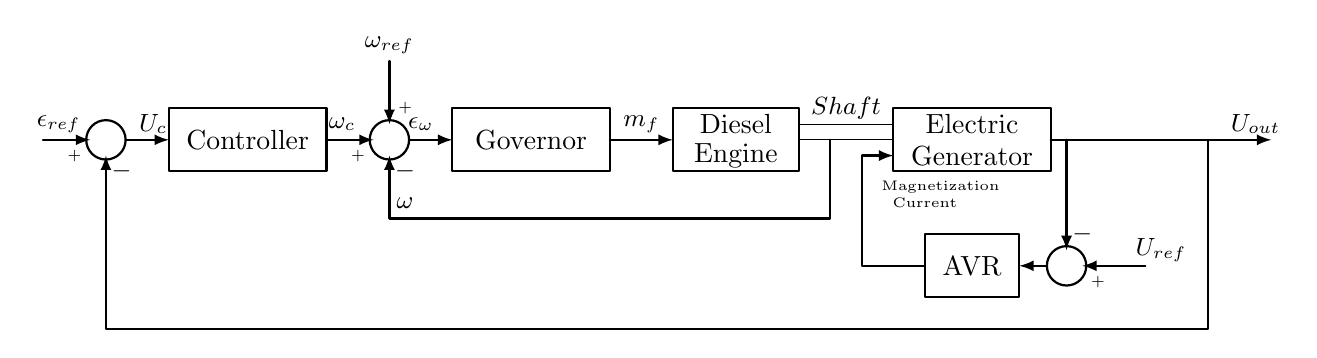
\begin{tikzpicture}

 \node at (2,0.2) {\normalsize{Governor}};
\draw [-latex] (1,0.6) rectangle (3,-0.2);
 \node at (4.6,0.4) {\normalsize{Diesel}};
  \node at (4.6,0) {\normalsize{Engine}};
\draw [-latex] (3.8,0.6) rectangle (5.4,-0.2);
\draw [-latex](3,0.2) -- (3.8,0.2);
\node at (3.4,0.4) {$m_f$};
 \node at (7.6,0.4) {\normalsize{Electric}};
  \node at (7.6,0) {\normalsize{Generator}};
\draw [-latex] (6.6,0.6) rectangle (8.6,-0.2);

\node at (6,0.6) {$Shaft$};
  \node at (7.6,-1.4) {\normalsize{AVR}};
\draw [-latex] (8.8,-1.4) ellipse (0.25 and 0.25);
\draw [-latex] (7,-1) rectangle (8.2,-1.8);
\draw [-latex](7,-1.4) -- (6.2,-1.4) -- (6.2,0) -- (6.6,0);
\node at (9,-1) {$-$};
\draw [-latex](9.8,-1.4) -- (9,-1.4);
\node at (10,-1.2) {$U_{ref}$};
\node at (7.2,-0.4) {\tiny{Magnetization}};
\node at (7,-0.6) {\tiny{Current}};
\node at (11.2,0.4) {$U_{out}$};
\draw [-latex] (0.2,0.2) ellipse (0.25 and 0.25);

\draw [-latex](0.2,1.2) -- (0.2,0.4);
\node at (0.2,1.4) {$\omega_{ref}$};
\draw [-latex](5.8,0.2) -- (5.8,-0.8) -- (0.2,-0.8) -- (0.2,0);
\node at (0.4,-0.6) {$\omega$};
\node at (-1.6,0.2) {\normalsize{Controller}};
\draw [-latex] (-2.6,0.6) rectangle (-0.6,-0.2);
\draw [-latex](-0.6,0.2) -- (0,0.2);
\node at (-0.4,0.4) {$\omega_{c}$};
\draw [-latex] (-3.4,0.2) ellipse (0.25 and 0.25);
\draw [-latex](-3.15,0.2) -- (-2.6,0.2);
\node at (-2.8,0.4) {$U_{c}$};
\draw [-latex](-4.2,0.2) -- (-3.6,0.2);
\node at (-4,0.4) {$\epsilon_{ref}$};
\draw [-latex](10.6,0.2) -- (10.6,-2.2) -- (-3.4,-2.2) -- (-3.4,0);
\node at (-3.2,-0.2) {$-$};
\node at (0.6,0.4) {$\epsilon_{\omega}$};
\draw [-latex](8.8,0.2) -- (8.8,-1.2);
\draw [-latex](8.6,0.2) -- (11.4,0.2);
\draw [-latex](8.55,-1.4) -- (8.2,-1.4);
\draw [thin](5.4,0.2) -- (6.6,0.2);
\draw [thin](5.4,0.4) -- (6.6,0.4);
\draw [thin](0.4,0.2);
\draw [-latex](0.45,0.2) -- (1,0.2);
\node at (-3.8,0) {\tiny{+}};





\node at (9.2,-1.6) {\tiny{+}};
\node at (0.4,-0.2) {$-$};
\node at (0.4,0.6) {\tiny{+}};
\node at (-0.2,0) {\tiny{+}};

\end{tikzpicture} 
%\includegraphics[width=0.6\textwidth]{rapport/billeder/genset_control_approach.png}
\caption{Block diagram illustrating the genset with an addon frequency controller.}
\label{fig:genset_control_approach}
\end{figure}


%This requires the abillity to measure either frequency, Voltage or both on the genset. 
The frequency can be obtained in two ways. Either by making time calculations between zero crossings on one of the three phases of the voltage outputs or by a tachometer. In case of a tachometer, it is required to be installed if it is not already built in the genset. For this reason, voltage measurements are carried out and in the mean time provided to the controller.
When the frequency differs from the reference value after the correction of the governor, in the mean time disturbance will appear in the voltage due to the change in the load, as shown in \figref{fig:4050kwstepvoltage50khz}  

\begin{figure}[H]
\centering
%\includegraphics[width=0.8\textwidth]{rapport/billeder/4050kwstep_rmsvoltage50khz.png}
% This file was created by matlab2tikz.
%
%The latest updates can be retrieved from
%  http://www.mathworks.com/matlabcentral/fileexchange/22022-matlab2tikz-matlab2tikz
%where you can also make suggestions and rate matlab2tikz.
%
\definecolor{mycolor1}{rgb}{0.00000,0.44700,0.74100}%
%
\begin{tikzpicture}

\begin{axis}[%
width=4.0in,
height=3.0in,
at={(0.758in,0.481in)},
scale only axis,
xmin=68.5,
xmax=73,
xlabel={Time [s]},
xmajorgrids,
ymin=190,
ymax=245,
ylabel={Voltage [V]},
ymajorgrids,
axis background/.style={fill=white}
]
\addplot [color=mycolor1,solid,forget plot]
  table[row sep=crcr]{%
68.5	236.182596866281\\
68.50234	239.32349979073\\
68.5079	220.8640850444\\
68.51116	223.997851784714\\
68.51574	240.293033346787\\
68.52238	239.77070578819\\
68.52792	220.79004567877\\
68.53118	223.582354444062\\
68.53572	240.125383263619\\
68.54238	239.503125414541\\
68.54794	221.128509605651\\
68.55572	240.384935875427\\
68.56122	223.879546645624\\
68.56794	220.7161680143\\
68.57242	239.441423878054\\
68.57576	240.236675185465\\
68.58122	224.080563660521\\
68.58796	220.893946320023\\
68.5932	239.658824881852\\
68.59578	240.20427038339\\
68.60126	223.727767401031\\
68.60796	220.710497598098\\
68.6132	239.878021302842\\
68.61578	240.17915047505\\
68.62126	223.929956496818\\
68.628	221.053355880053\\
68.63324	239.624493022416\\
68.63578	240.222954057788\\
68.64128	223.684256868545\\
68.64802	220.612101487921\\
68.65326	239.815040382687\\
68.6558	240.142616805618\\
68.66128	223.988394067825\\
68.66802	220.770027168167\\
68.67582	240.112992281759\\
68.6813	223.636064799859\\
68.6825	239.54314601358\\
68.68804	220.53256420538\\
68.69584	239.928065934181\\
68.70132	223.821007005784\\
68.7025	239.372873576282\\
68.70802	221.012353067274\\
68.7158	240.118482472716\\
68.72248	239.010144811714\\
68.728	220.454035978402\\
68.72812	220.769404701112\\
68.73584	239.922309039822\\
68.74248	239.053636110184\\
68.74802	220.496852065587\\
68.7513	223.496990448604\\
68.75582	239.829973192816\\
68.7625	239.303201155633\\
68.768	220.395317294666\\
68.7713	223.209638592102\\
68.7758	239.840855547138\\
68.78248	239.146927793181\\
68.788	220.736257358188\\
68.79128	223.389796772555\\
68.79578	239.885323514174\\
68.80246	238.999895179545\\
68.808	220.536732697186\\
68.81128	223.403391452547\\
68.8158	239.955510850449\\
68.82244	239.140905334421\\
68.828	220.614687436036\\
68.83576	240.058948706701\\
68.84126	223.626190489658\\
68.84244	239.442062625109\\
68.84796	220.495053090767\\
68.85578	239.830749131896\\
68.86126	223.628671248046\\
68.86798	220.835269134597\\
68.8732	239.450790656104\\
68.87576	240.038414243429\\
68.88122	223.542168258213\\
68.88796	220.476301636555\\
68.8932	239.635295053581\\
68.89574	240.147527031996\\
68.90124	224.012113116494\\
68.90796	220.776326643619\\
68.91244	239.56164275001\\
68.91574	240.058522704187\\
68.92122	223.574420286065\\
68.92794	220.617644589382\\
68.93316	239.596264795941\\
68.93572	239.935367816349\\
68.9412	223.697339822694\\
68.94792	220.845221535355\\
68.95572	239.945469608027\\
68.96122	223.468552620758\\
68.96238	238.972112433299\\
68.9679	220.486849924396\\
68.9757	239.899675428779\\
68.9812	223.735482536484\\
68.98236	239.031771772429\\
68.98792	220.495215958117\\
68.99572	239.875814876156\\
69.00236	239.432401189946\\
69.0079	220.558574750186\\
69.00808	221.244478980079\\
69.01572	239.753304743473\\
69.02238	239.1382233014\\
69.0279	220.828234296478\\
69.03116	223.448438077259\\
69.0357	239.957655335617\\
69.04238	238.913665325294\\
69.04792	220.396174890242\\
69.0512	223.232398055629\\
69.05572	239.8939164419\\
69.06238	239.049874067456\\
69.0679	220.557892414327\\
69.0712	223.62162576642\\
69.07574	239.927386259017\\
69.0824	239.367036312264\\
69.08794	220.470729467844\\
69.09118	223.333450948352\\
69.09574	239.881221584246\\
69.10238	239.317570243146\\
69.10792	221.010432681733\\
69.11572	240.271907386541\\
69.12122	223.850365990692\\
69.12794	220.763049114127\\
69.13244	239.484552933483\\
69.13572	240.243263975115\\
69.14122	224.092589100093\\
69.14794	220.900139344682\\
69.15316	239.81050429193\\
69.15572	240.397494072318\\
69.16122	223.916151764077\\
69.16794	220.802030839657\\
69.17318	239.931380598356\\
69.17574	240.273588202074\\
69.1812	224.10823429112\\
69.1879	221.287144010145\\
69.19316	239.894536398289\\
69.19572	240.382391657022\\
69.2012	223.785105486268\\
69.20794	220.721489523562\\
69.21316	239.754234190973\\
69.21572	240.198674495024\\
69.2212	224.068954927942\\
69.22788	220.885839080395\\
69.23572	240.14564721227\\
69.24118	223.671663894126\\
69.24236	239.618019481876\\
69.24792	220.749774089163\\
69.2557	240.021914581079\\
69.26118	223.770787674948\\
69.26234	239.279187091147\\
69.26788	220.916336327239\\
69.27566	240.117647488511\\
69.28234	239.165499380136\\
69.28788	220.648961045405\\
69.28804	221.281776672866\\
69.29568	239.970621682808\\
69.30234	239.16578738224\\
69.30788	220.677288657367\\
69.31114	223.646040211052\\
69.3157	239.990239493366\\
69.32236	239.483270444757\\
69.3279	220.549614245299\\
69.33118	223.413971721593\\
69.3357	239.855190905193\\
69.34236	239.276119046246\\
69.34788	220.949726912971\\
69.35118	223.517968260757\\
69.3557	240.081697032489\\
69.36234	239.017175768814\\
69.3679	220.482076699747\\
69.37116	223.442208225453\\
69.3757	240.03239126036\\
69.38236	239.286402011272\\
69.3879	220.754053025269\\
69.39568	240.038464799568\\
69.40116	223.598768957181\\
69.40234	239.453012309653\\
69.40788	220.567247280544\\
69.41572	239.942101740191\\
69.42118	223.749769320179\\
69.42788	220.951295302456\\
69.43312	239.448412263303\\
69.4357	239.969513471677\\
69.44118	223.529193889374\\
69.4479	220.561111382235\\
69.45316	239.780494237264\\
69.45568	240.246833681008\\
69.46118	224.143983788881\\
69.46792	220.94742245517\\
69.47312	239.870664477929\\
69.47572	240.398044267211\\
69.48118	223.907975656295\\
69.48792	220.839844400869\\
69.49316	239.927122398657\\
69.4957	240.169996760107\\
69.50118	223.954279536955\\
69.5079	221.006992842798\\
69.51572	240.145901506598\\
69.5212	223.628617564367\\
69.52238	239.14481328005\\
69.5279	220.641816285468\\
69.5357	240.074639109903\\
69.54116	223.967422063642\\
69.54236	239.274952874129\\
69.5479	220.753936002094\\
69.55572	240.098271872686\\
69.56236	239.536184309908\\
69.5679	220.628448155302\\
69.56798	220.863565069026\\
69.5757	240.039360596167\\
69.58236	239.364211353919\\
69.5879	220.993195243089\\
69.59116	223.638054631064\\
69.59568	240.202438602144\\
69.60234	239.260804897954\\
69.60788	220.705636350019\\
69.61114	223.612216189471\\
69.61568	240.138132991549\\
69.62234	239.35480212873\\
69.62786	220.852496967244\\
69.63112	223.820778842508\\
69.63568	240.161802446115\\
69.64232	239.610195052124\\
69.64786	220.720251157055\\
69.65112	223.539899845456\\
69.65566	239.978297412842\\
69.66232	239.398434231513\\
69.66786	221.056057417193\\
69.67564	240.195760765221\\
69.68114	223.680614241601\\
69.68786	220.610098882999\\
69.69234	239.314096364485\\
69.69564	240.151616714143\\
69.70112	224.028268886801\\
69.70784	220.823774360726\\
69.71308	239.541137516085\\
69.71568	240.118808049613\\
69.72114	223.672208776966\\
69.72784	220.714751928252\\
69.73308	239.751055350475\\
69.73566	239.951204892092\\
69.74114	223.691141350636\\
69.74786	220.787822590302\\
69.7531	239.320395207972\\
69.75566	239.881836036864\\
69.76114	223.474779291012\\
69.76786	220.440836025225\\
69.77308	239.560570585325\\
69.77564	239.868785528325\\
69.78114	223.754608541925\\
69.78786	220.5549390647\\
69.79564	239.935316912878\\
69.80114	223.529954531639\\
69.80232	239.424322921148\\
69.80784	220.477941191593\\
69.81566	239.725158601818\\
69.82114	223.622601300718\\
69.8223	239.170318714858\\
69.82786	220.873141970114\\
69.83564	239.970333452908\\
69.8423	238.920020940586\\
69.84786	220.464811770873\\
69.84794	220.757055615821\\
69.85566	239.820718736761\\
69.86232	239.08546872231\\
69.86786	220.606670390615\\
69.87112	223.584183204373\\
69.87564	239.824100253707\\
69.88232	239.283034770889\\
69.88786	220.434472618849\\
69.89112	223.273096626269\\
69.89566	239.720548894958\\
69.9023	239.087697582742\\
69.90784	220.737996441294\\
69.91114	223.283891954279\\
69.91564	239.841993994658\\
69.92232	239.031955891885\\
69.92786	220.628471289972\\
69.93112	223.574463150237\\
69.93562	240.03849788888\\
69.94234	239.260377800873\\
69.94788	220.810673640904\\
69.95566	240.122265948343\\
69.96114	223.693600200885\\
69.9623	239.597605154629\\
69.96786	220.625642232304\\
69.97566	239.952371793168\\
69.98114	223.823664433448\\
69.98786	221.01951895798\\
69.99308	239.546435673232\\
69.99566	240.114060352922\\
70.00116	223.637955419394\\
70.00786	220.598125015642\\
70.01312	239.640448337017\\
70.01568	239.942278757656\\
70.02116	223.81270978767\\
70.02788	220.568681433169\\
70.03238	239.374371300306\\
70.03568	239.865177517323\\
70.04114	223.414923917734\\
70.0479	220.447227363111\\
70.05312	239.570279463216\\
70.05568	239.712610701162\\
70.06116	223.524998718451\\
70.0679	220.707248361187\\
70.07566	239.878975236298\\
70.08116	223.430299650883\\
70.08234	238.900911402092\\
70.0879	220.402079188053\\
70.09566	239.821993448613\\
70.10116	223.696765897312\\
70.10234	239.024439780747\\
70.10786	220.51357171952\\
70.1157	239.939284312198\\
70.12232	239.444177884777\\
70.12786	220.495974193219\\
70.1279	220.501600287088\\
70.13566	239.709550267784\\
70.14232	239.173255172027\\
70.14786	220.85842101993\\
70.15112	223.43560721809\\
70.15564	239.871265821204\\
70.16232	238.91849704275\\
70.16786	220.492531288855\\
70.17112	223.39782363346\\
70.17566	240.049168683036\\
70.18232	239.338264043627\\
70.18788	220.912091419679\\
70.19112	223.97443655285\\
70.19566	240.181413857317\\
70.20232	239.740911476153\\
70.20786	220.817069841381\\
70.21114	223.591117239333\\
70.21566	240.104399385281\\
70.2223	239.447194291699\\
70.22784	221.1392080182\\
70.23568	240.27791135995\\
70.24116	223.867110530072\\
70.24788	220.857117272684\\
70.25232	239.406826213247\\
70.25568	240.148974054821\\
70.26116	224.01431664628\\
70.26314	239.06500837464\\
70.26712	194.927871943488\\
70.28118	221.461135604723\\
70.28342	238.225023284184\\
70.28798	217.890902077928\\
70.29674	236.931465455555\\
70.30138	219.715716656395\\
70.30818	216.456559104054\\
70.3135	235.682284040224\\
70.3169	234.837255925957\\
70.32162	217.949096455648\\
70.32844	214.642781490162\\
70.33374	234.370172505839\\
70.3371	233.606686904863\\
70.3419	217.189110305781\\
70.34876	214.076907301052\\
70.35404	233.575589344221\\
70.36226	216.786704648832\\
70.36434	233.656499236415\\
70.36908	214.139446146275\\
70.37444	234.311587199253\\
70.3826	217.62111067748\\
70.38472	234.446375020849\\
70.38948	215.290581250086\\
70.3949	235.509238694402\\
70.40304	218.925521249046\\
70.40518	235.782468270544\\
70.40994	216.455092171756\\
70.41538	237.478499026754\\
70.42354	221.215753587796\\
70.42568	237.650238226615\\
70.43046	218.106409546846\\
70.43588	238.938102710897\\
70.44406	222.672584517792\\
70.4462	239.489918020223\\
70.45098	219.495304382197\\
70.45644	240.740355682562\\
70.4646	223.53553327249\\
70.4667	240.708665649473\\
70.47152	220.709968647582\\
70.477	241.455795967399\\
70.4852	223.727704778413\\
70.4873	240.672548116038\\
70.49214	220.504832004879\\
70.49758	241.853558804186\\
70.5058	225.011297517295\\
70.50786	241.163203514066\\
70.51276	221.015715999451\\
70.51814	242.03481821665\\
70.5264	225.01188973215\\
70.52846	241.727942052114\\
70.53336	221.238318076722\\
70.53876	242.810901860893\\
70.547	224.983763997538\\
70.54902	242.234318915419\\
70.55394	221.831352044746\\
70.55936	242.745016898734\\
70.5676	224.644131071791\\
70.56968	241.655295350285\\
70.57452	221.139226271219\\
70.57994	242.451247354494\\
70.58816	225.189103981705\\
70.5902	241.234672008745\\
70.59512	220.95252754174\\
70.60048	242.18335189996\\
70.60876	225.097410858055\\
70.6108	241.715883709573\\
70.61566	221.027182764549\\
70.62104	242.541741252923\\
70.6313	241.991233807308\\
70.63596	223.117232474507\\
70.6362	221.522941814161\\
70.64158	242.578564378292\\
70.65182	241.333160213739\\
70.6567	220.660717363785\\
70.66208	242.023072677655\\
70.6723	241.070254931006\\
70.67718	220.745603721796\\
70.67744	222.125385715291\\
70.6825	241.980283825804\\
70.69272	241.742250931476\\
70.69758	220.940238667609\\
70.70092	223.687713630335\\
70.70296	242.741588959158\\
70.71312	241.832046035225\\
70.718	221.122892867292\\
70.72132	223.491424262207\\
70.72332	242.133452033687\\
70.73352	241.007664448492\\
70.73836	220.414016682243\\
70.74168	223.862837237075\\
70.74368	241.80145802738\\
70.75386	240.97345073334\\
70.7587	220.579381379093\\
70.762	223.803949385208\\
70.76398	241.857242026848\\
70.77414	241.534165436107\\
70.779	220.487603227672\\
70.7823	223.175786236993\\
70.7843	241.996211876343\\
70.7944	241.214890579956\\
70.79922	220.610673283653\\
70.80252	223.52984164126\\
70.80456	241.705738041287\\
70.81464	240.813513818266\\
70.81944	220.319396582363\\
70.82272	223.537427654744\\
70.82472	241.728050322051\\
70.8348	240.989476127417\\
70.8396	220.336194115946\\
70.84488	241.464953029765\\
70.85298	223.750757680281\\
70.855	241.032439250059\\
70.85976	220.014318662824\\
70.865	241.482662960339\\
70.87308	223.828376519638\\
70.87504	240.863744547618\\
70.87984	220.428231304999\\
70.88512	241.271685661794\\
70.89316	223.606023160715\\
70.89992	219.986612873943\\
70.90514	241.156584677535\\
70.90848	240.765931131774\\
70.91322	223.815660524087\\
70.91994	219.940203758128\\
70.92518	240.994696626468\\
70.93324	223.325270065884\\
70.93528	240.803519708842\\
70.93996	219.737487437662\\
70.94518	241.104001915321\\
70.95322	223.540911733736\\
70.95522	240.620149842894\\
70.95996	220.145299911028\\
70.9652	240.878822729569\\
70.96852	240.377610273572\\
70.97322	223.398490883817\\
70.97992	219.916760531115\\
70.98518	241.035990137711\\
70.9885	240.451658884726\\
70.99318	223.551393816016\\
70.9999	219.854405658609\\
71.0051	240.892893190279\\
71.01516	240.853372255992\\
71.0196	221.682609780665\\
71.01986	219.863155119649\\
71.02506	241.137096314006\\
71.03508	240.55463440852\\
71.03976	220.066053057561\\
71.04304	222.915806929806\\
71.04502	240.753795617362\\
71.05506	240.17966907609\\
71.05968	219.779720567928\\
71.06296	222.993618415789\\
71.06494	240.928542094608\\
71.07498	240.208003396709\\
71.07962	219.750001659082\\
71.08288	223.121081781657\\
71.08486	240.726841327295\\
71.09492	240.774540978346\\
71.0996	219.650510992273\\
71.10282	222.939498752838\\
71.10482	240.914895394446\\
71.1148	240.542884040456\\
71.1195	220.081299490476\\
71.1247	240.879430204892\\
71.13268	223.265548404062\\
71.13478	240.333473402063\\
71.1394	219.742163896122\\
71.14466	240.884146924581\\
71.1526	223.655145862628\\
71.15934	219.915660088324\\
71.16454	240.948286075041\\
71.17254	223.388796673349\\
71.17462	241.110332196003\\
71.17926	220.003414272749\\
71.18448	241.201884342591\\
71.18782	240.730192374852\\
71.19244	223.591763996538\\
71.19918	220.218788580244\\
71.20438	240.82374227586\\
71.20776	240.442013647955\\
71.21236	223.318631201399\\
71.2191	219.917103818878\\
71.22432	241.011798423162\\
71.22762	240.408937303538\\
71.2323	223.321763731729\\
71.23902	219.656006870212\\
71.2442	240.664734922707\\
71.25224	223.254115070324\\
71.2543	240.663246419314\\
71.25896	219.628707282313\\
71.26414	240.900769790004\\
71.27418	240.529293304371\\
71.27882	220.172378844963\\
71.27886	220.150312878307\\
71.28406	240.787448627761\\
71.29408	240.25057871505\\
71.29874	219.891415793303\\
71.30198	223.199870258326\\
71.30398	241.176640508743\\
71.31398	240.672138348176\\
71.31866	220.116628531899\\
71.3219	223.457884967541\\
71.32388	241.138811704828\\
71.33396	241.032922738264\\
71.33858	219.913741138808\\
71.34184	223.316310374246\\
71.34382	241.284111793891\\
71.35384	240.791033518519\\
71.3585	220.304167572926\\
71.36178	223.26353705692\\
71.36374	240.98716997747\\
71.37378	240.459574196821\\
71.37844	219.905116257558\\
71.38366	240.998121210692\\
71.39166	223.576922817778\\
71.39366	240.27168574085\\
71.39838	219.857267145452\\
71.40362	240.823382940348\\
71.4116	223.25735348565\\
71.41832	219.699785455441\\
71.42354	240.952277973081\\
71.43154	223.262546889867\\
71.43354	240.444423693744\\
71.43824	220.092570604772\\
71.44348	240.803027865446\\
71.4469	240.280167417469\\
71.4515	223.190187723012\\
71.45826	219.705236363216\\
71.46348	240.830522835389\\
71.46676	240.426265334094\\
71.47148	223.432522089071\\
71.47818	219.697592940273\\
71.48342	240.667757131936\\
71.49144	223.143497599265\\
71.49354	240.646395260937\\
71.49818	219.717173079014\\
71.5034	241.018651270844\\
71.5114	223.558969313281\\
71.51346	240.633344660502\\
71.51814	220.287016138416\\
71.52336	241.07378970625\\
71.53344	240.4679346694\\
71.53804	220.143184702215\\
71.53812	219.985916571001\\
71.54338	241.111281901981\\
71.5534	240.31949534682\\
71.5581	219.871048737474\\
71.56138	223.285896353569\\
71.56334	240.853008531656\\
71.57338	240.682920409994\\
71.57812	219.652330755333\\
71.58136	222.839099861499\\
71.58336	240.952345089577\\
71.5934	240.467071983532\\
71.5981	220.027562430634\\
71.60134	222.884969631198\\
71.60334	240.712140606611\\
71.6134	239.973707110105\\
71.61814	219.631596016488\\
71.62134	222.96635139448\\
71.62338	240.900395002789\\
71.63338	240.405411384429\\
71.63808	219.988843230363\\
71.64332	241.041957360816\\
71.65136	223.405575341687\\
71.65346	240.93283663883\\
71.6581	219.901444543914\\
71.66338	241.185987837533\\
71.67136	223.518032573251\\
71.67338	240.605905519448\\
71.67812	220.137929655288\\
71.68338	240.897701425488\\
71.69138	223.332074662187\\
71.69812	219.87248079853\\
71.70338	241.005797280722\\
71.70668	240.514771830651\\
71.7114	223.557246932972\\
71.71814	219.819175924592\\
71.72338	240.85835708375\\
71.73142	223.315612908614\\
71.73346	240.740741752582\\
71.7382	219.76003224161\\
71.74342	241.078548100337\\
71.75146	223.380421730509\\
71.7535	240.580479864154\\
71.75822	220.076236435809\\
71.76344	240.916234037718\\
71.7668	240.371300240205\\
71.77148	223.334442550106\\
71.7782	219.809687333915\\
71.78348	241.047061665352\\
71.7869	240.589189759571\\
71.7915	223.710602909578\\
71.79824	219.910641653604\\
71.80346	240.899882925978\\
71.81356	240.819600639324\\
71.818	222.130735364897\\
71.8183	219.782894177224\\
71.82352	241.058687637299\\
71.83356	240.400032714571\\
71.83828	219.986979965103\\
71.84154	222.915638471149\\
71.84354	240.841289588877\\
71.85364	240.241822723307\\
71.85832	219.749919534494\\
71.86156	222.969621085661\\
71.86358	240.867557401019\\
71.87362	240.157044322044\\
71.87832	219.749072097017\\
71.8816	223.158926225609\\
71.88362	240.859032726268\\
71.89368	240.855707690483\\
71.8984	219.734868293018\\
71.90164	222.969973454947\\
71.90362	241.122440694038\\
71.91368	240.614575423539\\
71.9184	220.147759801987\\
71.92168	223.150863930473\\
71.92362	240.916407312786\\
71.93372	240.238323294113\\
71.9384	219.755648984086\\
71.94368	241.141254528164\\
71.95168	223.681289962229\\
71.9537	240.449060895269\\
71.95842	219.865467151696\\
71.96366	240.906237595667\\
71.97172	223.457735097714\\
71.97844	219.801457522844\\
71.98374	241.267308964559\\
71.9839	240.760167447123\\
71.9917	223.559726942078\\
71.99844	220.143235687018\\
72.0037	240.995396308035\\
72.0117	223.5101564853\\
72.01376	240.440943459442\\
72.01848	219.928586657503\\
72.0237	241.237936766622\\
72.027	240.766671497877\\
72.0317	223.757545962142\\
72.03844	220.011860002289\\
72.04368	241.037977103713\\
72.0517	223.457321848043\\
72.05378	240.858528886772\\
72.05846	219.736817603279\\
72.0637	241.113296545075\\
72.07172	223.56000965438\\
72.07376	240.695531005113\\
72.07846	220.188446870894\\
72.0837	240.925129924561\\
72.0917	223.199192030161\\
72.09372	240.142939747178\\
72.09844	219.604930429055\\
72.1037	240.826126009513\\
72.11372	240.160638514447\\
72.11844	219.670019219169\\
72.11868	220.581559698826\\
72.12368	240.658514224513\\
72.13382	240.577299384557\\
72.13844	219.57653242947\\
72.14168	222.82007256884\\
72.1437	240.90479393234\\
72.15376	240.33463801368\\
72.15842	219.906150673797\\
72.1617	222.988760110048\\
72.1637	240.787905786226\\
72.17376	240.216377828581\\
72.17842	219.675859814902\\
72.18168	222.834238420625\\
72.18372	240.865729150427\\
72.19376	240.094480101064\\
72.19842	219.582470626073\\
72.2017	223.079768758098\\
72.20368	240.676196393446\\
72.21378	240.647748816432\\
72.21846	219.579364211439\\
72.22372	240.776943585759\\
72.23172	223.17270930175\\
72.2337	240.319085410419\\
72.23846	219.917944096012\\
72.24372	240.823339253418\\
72.2517	223.230781530945\\
72.25846	219.704429883461\\
72.2637	241.012701623275\\
72.26386	240.739675812727\\
72.27172	223.763743758531\\
72.27846	219.865156829135\\
72.28372	240.976069221614\\
72.29174	223.483267690223\\
72.2938	241.030153391127\\
72.29846	219.885909573958\\
72.30374	241.42409176247\\
72.31174	223.696359724888\\
72.3138	240.814181151671\\
72.31846	220.230969429445\\
72.32372	241.123219170027\\
72.32708	240.519297887404\\
72.33174	223.476321685692\\
72.3385	219.855656482839\\
72.34374	241.031914056521\\
72.34704	240.511023439329\\
72.35176	223.541380746944\\
72.3585	219.676150607737\\
72.36374	240.663461211917\\
72.37174	223.050767530249\\
72.37384	240.473647746311\\
72.37852	219.381537533168\\
72.38374	240.745161880255\\
72.3938	240.333302198912\\
72.39848	219.842655617982\\
72.39864	220.139863212004\\
72.40374	240.695672089259\\
72.41378	240.116844278468\\
72.41846	219.649969767241\\
72.42172	222.966225254335\\
72.42372	240.954638387429\\
72.43376	240.317996469435\\
72.43848	219.772233185102\\
72.4417	223.205969202215\\
72.44372	240.903960592529\\
72.4538	240.947720816501\\
72.45844	219.904977348172\\
72.4617	223.160467535882\\
72.4637	241.270827360907\\
72.47374	240.644237218035\\
72.47842	220.11225379527\\
72.48168	223.10763237729\\
72.4837	241.009167464815\\
72.49376	240.576144174424\\
72.49842	220.067890448039\\
72.50366	241.333317434967\\
72.51166	223.908378886134\\
72.51374	240.654329922436\\
72.51838	220.132611783973\\
72.52364	241.331075970681\\
72.53166	223.688345439401\\
72.53838	220.068069606694\\
72.54366	241.44457751297\\
72.5438	241.165146886769\\
72.55166	223.821430869939\\
72.55836	220.483357034418\\
72.5636	241.209766722867\\
72.56698	240.566744463292\\
72.57162	223.391134350157\\
72.57838	219.822211068779\\
72.58362	240.903119034222\\
72.58696	240.462609381202\\
72.59162	223.486658578314\\
72.59838	219.641855025782\\
72.60362	240.652319877661\\
72.61166	223.10756911372\\
72.61372	240.632668059638\\
72.61836	219.612692336797\\
72.62366	240.846383549245\\
72.62698	240.254519229955\\
72.63164	223.190577781448\\
72.63838	219.787265279785\\
72.64366	240.480247153136\\
72.65164	223.022179623836\\
72.65372	239.957823116897\\
72.6584	219.568247030773\\
72.66368	240.848576002641\\
72.67374	240.109430238763\\
72.67842	219.639964511053\\
72.6786	220.07571306068\\
72.68368	240.781234669046\\
72.69376	240.807657620662\\
72.69844	219.780550232309\\
72.7017	223.06971082022\\
72.70372	241.187771767144\\
72.71374	240.762498161224\\
72.71846	220.231871770981\\
72.7217	223.17577433494\\
72.72372	241.095722475189\\
72.7338	240.448070233817\\
72.73848	219.901494755796\\
72.74172	223.164203372016\\
72.74376	241.153129407264\\
72.75376	240.45436590616\\
72.75848	219.930660119085\\
72.76176	223.366459219299\\
72.76378	241.104988045492\\
72.77382	241.00173949061\\
72.77852	219.905638617643\\
72.78378	241.33820073792\\
72.7918	223.775075992427\\
72.79382	240.794538650174\\
72.79854	220.268062421488\\
72.8038	241.262817448801\\
72.8118	223.71783404734\\
72.81854	220.132207671133\\
72.82376	241.275583056319\\
72.8238	241.322688747177\\
72.83184	223.990393209173\\
72.83856	220.067937190238\\
72.8438	241.331084927084\\
72.85182	223.701926283429\\
72.85386	241.203699140719\\
72.85858	220.070682892452\\
72.86382	241.615139478055\\
72.87186	223.945243144576\\
72.87386	241.020461938228\\
72.87856	220.433193417908\\
72.88382	241.36807322186\\
72.88722	240.80811236162\\
72.89184	223.788123148884\\
72.8986	220.217125928215\\
72.90382	241.572033986069\\
72.90714	241.03052635593\\
72.91186	224.038828247471\\
72.91858	220.163823237379\\
72.92386	241.233233765409\\
72.93186	223.7169557769\\
72.93392	241.039440172661\\
72.93862	219.958775138472\\
72.94386	241.357815070972\\
72.95388	240.669066311329\\
72.95856	220.227930813548\\
72.95862	220.113528235999\\
72.96386	241.001194455892\\
72.97396	240.308542663559\\
72.97864	219.83946853803\\
72.98192	223.185838111053\\
72.98388	241.193582673579\\
73.00002	233.173772936445\\
};
\end{axis}
\end{tikzpicture}% 
\caption{Voltage measured on all three phases with Hioki oscilloscope at 50 kHz sampling rate with RMS calculated, before and after a power step from 40 to 50 kW is performed on a genset located at DEIF.}
\label{fig:4050kwstepvoltage50khz}
\end{figure}

The first issue that arises is the noise in the measurement shown in \figref{fig:4050kwstepvoltage50khz}. Because of this, some difficulties appear concerning the design of the controller when the output voltage of the genset fluctuates between 220 to 240 volts in a steady-state mode. The solution which has been provided by Jesper Viese Knudsen, in the simulink blocks is described in \secref{dspace_unitv2}. The dSPACE unit samples the output voltage of the genset at 1 kHz, where sixteen samples are then averaged giving a 62.5 Hz input rate to the controller. The output of this sampling operation is shown in \figref{fig:4050kwstepvoltage62.5hz}. 

\begin{figure}[H]
\centering
% This file was created by matlab2tikz.
%
%The latest updates can be retrieved from
%  http://www.mathworks.com/matlabcentral/fileexchange/22022-matlab2tikz-matlab2tikz
%where you can also make suggestions and rate matlab2tikz.
%
\definecolor{mycolor1}{rgb}{0.00000,0.44700,0.74100}%
%
\begin{tikzpicture}

\begin{axis}[%
width=3.521in,
height=2.566in,
at={(0.758in,0.481in)},
scale only axis,
xmin=68.5,
xmax=73,
xlabel={Time [s]},
ymin=224,
ymax=236,
ylabel={Voltage [V]},
axis background/.style={fill=white}
]
\addplot [color=mycolor1,solid,forget plot]
  table[row sep=crcr]{%
68.496	232.251449569516\\
68.512	232.116248346484\\
68.528	233.64890076305\\
68.544	232.817435120229\\
68.56	232.269923036835\\
68.576	232.180268285985\\
68.592	232.232821803907\\
68.608	233.511499938504\\
68.624	232.664112503649\\
68.64	232.147245877425\\
68.656	232.000145361167\\
68.672	232.171771917135\\
68.688	233.359675912275\\
68.704	232.410735494188\\
68.72	232.094375321851\\
68.736	231.802547979314\\
68.752	231.899619719769\\
68.768	233.118656570701\\
68.784	232.291522758853\\
68.8	231.848666635778\\
68.816	231.866028285432\\
68.832	232.016802515841\\
68.848	233.329475099936\\
68.864	232.392386586747\\
68.88	231.963488845695\\
68.896	231.976358088346\\
68.912	232.088525089789\\
68.928	233.413210070936\\
68.944	232.569831812258\\
68.96	231.933734500629\\
68.976	231.942595585816\\
68.992	231.799574919604\\
69.008	233.275509754118\\
69.024	232.499853539223\\
69.04	231.94214887262\\
69.056	231.862138744768\\
69.072	231.853501090939\\
69.088	233.264494621304\\
69.104	232.553738631634\\
69.12	232.170578126516\\
69.136	232.24798440205\\
69.152	232.20806953032\\
69.168	233.70888655265\\
69.184	232.90285536249\\
69.2	232.397924917593\\
69.216	232.229201069961\\
69.232	232.141022686801\\
69.248	233.516567463417\\
69.264	232.769304097647\\
69.28	232.087818340009\\
69.296	232.154646498921\\
69.312	231.916663566561\\
69.328	233.404419681412\\
69.344	232.646428285034\\
69.36	232.070278841888\\
69.376	232.050233959554\\
69.392	232.008302098164\\
69.408	233.43973945943\\
69.424	232.634988087114\\
69.44	231.994070162002\\
69.456	232.118936247902\\
69.472	232.20973380642\\
69.488	233.764682120991\\
69.504	232.860295957641\\
69.52	232.141863935973\\
69.536	232.123827410259\\
69.552	232.030012072503\\
69.568	233.472663027735\\
69.584	232.787180540395\\
69.6	232.177124658009\\
69.616	232.261945125468\\
69.632	232.067984058275\\
69.648	233.580190321213\\
69.664	232.819259631877\\
69.68	232.239860434024\\
69.696	232.22736497349\\
69.712	232.091790564866\\
69.728	233.551880467081\\
69.744	232.758637754491\\
69.76	231.93658601535\\
69.776	232.007048897476\\
69.792	231.807541762637\\
69.808	233.352695966716\\
69.824	232.598915306936\\
69.84	232.040229644767\\
69.856	232.03147678331\\
69.872	231.814185187302\\
69.888	233.300024060635\\
69.904	232.563580181608\\
69.92	231.898440435307\\
69.936	232.187284998009\\
69.952	232.010504938726\\
69.968	233.550046886092\\
69.984	232.783378340032\\
70	232.169669817287\\
70.016	232.124472085576\\
70.032	231.862007222445\\
70.048	233.26619785203\\
70.064	232.502576213765\\
70.08	231.864389729332\\
70.096	231.933040748994\\
70.112	231.786971098717\\
70.128	233.388067890249\\
70.144	232.550971832024\\
70.16	231.971586256247\\
70.176	232.060278230971\\
70.192	232.098281647715\\
70.208	233.686849406811\\
70.224	232.939266674927\\
70.24	232.319253722182\\
70.256	232.363732118338\\
70.272	231.052725758443\\
70.288	231.328372653101\\
70.304	229.259754431011\\
70.32	227.784751038288\\
70.336	226.28486478479\\
70.352	226.356925362287\\
70.368	226.548439476999\\
70.384	225.864120663848\\
70.4	227.838874901422\\
70.416	228.122665437129\\
70.432	230.070294983649\\
70.448	232.279262348935\\
70.464	232.226236569789\\
70.48	232.562977263779\\
70.496	232.885104290305\\
70.512	234.912915461568\\
70.528	233.544008456963\\
70.544	234.302942230274\\
70.56	233.703073145207\\
70.576	233.956716467103\\
70.592	235.166499678207\\
70.608	233.828417969806\\
70.624	233.366437457811\\
70.64	233.748508481273\\
70.656	234.946354235433\\
70.672	233.5268004611\\
70.688	233.747655753545\\
70.704	233.650766154695\\
70.72	233.622130187609\\
70.736	234.14438942169\\
70.752	233.870781993417\\
70.768	233.443261203925\\
70.784	232.677160149025\\
70.8	233.834080616808\\
70.816	234.115885368237\\
70.832	233.109467044221\\
70.848	232.943595982628\\
70.864	232.378351183493\\
70.88	234.426809765027\\
70.896	233.330237546494\\
70.912	232.517375705827\\
70.928	232.433277201844\\
70.944	232.3053151428\\
70.96	233.985676469822\\
70.976	232.964033086596\\
70.992	232.328266747979\\
71.008	232.488591082381\\
71.024	232.237561173124\\
71.04	234.035578605595\\
71.056	233.006245118356\\
71.072	232.427967448264\\
71.088	232.411480576861\\
71.104	231.906205229016\\
71.12	233.691926419567\\
71.136	233.112715297968\\
71.152	232.420259178693\\
71.168	232.232833683056\\
71.184	232.213168363914\\
71.2	233.242117637983\\
71.216	233.413050973459\\
71.232	232.509843510641\\
71.248	232.103730175736\\
71.264	232.011593800413\\
71.28	232.873862407389\\
71.296	233.502280397913\\
71.312	233.101713809533\\
71.328	233.058715721681\\
71.344	232.185665093918\\
71.36	233.22179504934\\
71.376	233.183000508726\\
71.392	232.914980327856\\
71.408	232.768699022011\\
71.424	231.726194981156\\
71.44	232.623351243245\\
71.456	232.987747188635\\
71.472	232.550065998251\\
71.488	232.681556650507\\
71.504	231.765494360563\\
71.52	232.677137991314\\
71.536	233.344497956787\\
71.552	232.643590974936\\
71.568	232.976084471671\\
71.584	231.874407393658\\
71.6	232.397359717993\\
71.616	233.012505402917\\
71.632	232.469702165938\\
71.648	233.097730288341\\
71.664	232.086962718047\\
71.68	232.625717125542\\
71.696	233.225032909238\\
71.712	232.578377118452\\
71.728	232.931694318347\\
71.744	231.847870528491\\
71.76	232.588338461857\\
71.776	233.118576258087\\
71.792	232.776260080183\\
71.808	232.932596138131\\
71.824	231.850483809871\\
71.84	232.65430737604\\
71.856	232.964789271316\\
71.872	232.739939985592\\
71.888	232.727760396281\\
71.904	231.75899709317\\
71.92	232.900313494637\\
71.936	233.038003425124\\
71.952	232.953202651324\\
71.968	232.874070514084\\
71.984	231.85242909856\\
72	233.052528618872\\
72.016	233.199121197142\\
72.032	233.107627966594\\
72.048	232.989878579292\\
72.064	231.820997509231\\
72.08	232.99723764434\\
72.096	232.995013422302\\
72.112	232.731066394715\\
72.128	232.633071590528\\
72.144	231.560343716782\\
72.16	232.719514450675\\
72.176	232.954539851237\\
72.192	232.752864719806\\
72.208	232.634234996637\\
72.224	231.594253165812\\
72.24	232.616317893772\\
72.256	232.975630187318\\
72.272	232.978289128635\\
72.288	232.88340515495\\
72.304	231.972709539727\\
72.32	233.194203914211\\
72.336	233.278846366929\\
72.352	232.962757833268\\
72.368	232.650919924308\\
72.384	231.461561312247\\
72.4	232.693479050195\\
72.416	232.900231376653\\
72.432	232.876422128318\\
72.448	232.814832033489\\
72.464	231.923086283298\\
72.48	233.017461069544\\
72.496	233.226768742946\\
72.512	233.221343835813\\
72.528	233.154851966656\\
72.544	232.161370876316\\
72.56	233.242218288926\\
72.576	233.241088227942\\
72.592	232.782551987061\\
72.608	232.566069261898\\
72.624	231.557426985776\\
72.64	232.586667693532\\
72.656	232.690875521801\\
72.672	232.64557919328\\
72.688	232.669782435138\\
72.704	231.82799858649\\
72.72	233.079562012931\\
72.736	233.226746078392\\
72.752	233.102793936766\\
72.768	232.998336719037\\
72.784	232.019594405408\\
72.8	233.256925367217\\
72.816	233.562277673375\\
72.832	233.364482335795\\
72.848	233.171413821331\\
72.864	232.257525154906\\
72.88	233.471039555012\\
72.896	233.745193150055\\
72.912	233.520829146605\\
72.928	233.250933793244\\
72.944	232.187633628563\\
72.96	233.120881047595\\
72.976	233.476532248812\\
72.992	233.191304074376\\
73.008	233.079589031756\\
};
\end{axis}
\end{tikzpicture}% 
\caption{Voltage measured on all three phases with Hioki oscilloscope at 50 kHz sampling rate and RMS calculated, before and after a power step from 40 to 50 kW is performed on a genset located at DEIF. Data is then down sampled to 1 kHz and 16 samples is averaged to get a 62.5 Hz output.}
\label{fig:4050kwstepvoltage62.5hz}
\end{figure}

The 62.5 Hz sampling rate and the reduction in fluctuation shown between \figref{fig:4050kwstepvoltage50khz} and \figref{fig:4050kwstepvoltage62.5hz} is considered acceptable on the grounds, that the update interval to the governor is 25 Hz and an apparent change in Voltage is registered in the 1 kHz averaged 62.5 Hz measuring, when a change in load occurs. 
In order to be able to design a controller, modeling of the genset and inverter is needed. Along with the dynamics describing how changes in load affects voltage on the genset, the effects of frequency reference changes on the voltage output are also required. A block diagram, giving an overview of what needs to be modeled is shown in \figref{fig:gensetmodeling}.



\begin{figure}[H]
\centering
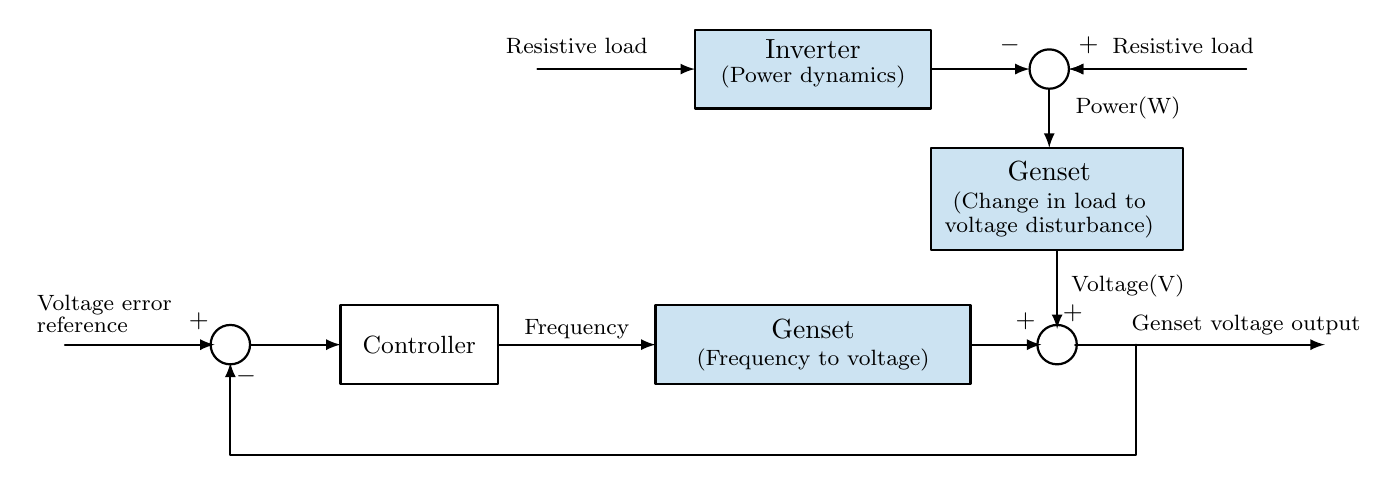
\begin{tikzpicture}
 \definecolor{mycolor1}{rgb}{0.00000,0.44700,0.74100} 
\draw  [fill=mycolor1!20](-5.5,2.5) rectangle (-1.5,1.5);
\draw [fill=mycolor1!20] (-2,4.5) rectangle (1.2,3.2);
\node at (-0.5,4.2) {\normalsize{Genset}};
\node at (-0.5,3.8) {\normalsize{\footnotesize{(Change in load to}}};
\node at (-0.5,3.5) {\normalsize{\footnotesize{voltage disturbance)}}};
\node at (-3.5,2.2) {\normalsize{Genset}};
\node at (-3.5,1.8) {\normalsize{\footnotesize{(Frequency to voltage)}}};

\draw [fill=mycolor1!20] (-5,6) rectangle (-2,5);
\draw [-latex] (-0.4,2) ellipse (0.25 and 0.25);
\draw [-latex](-1.5,2) -- (-0.6,2);
\draw [-latex](-0.4,3.2) -- (-0.4,2.2);
\draw [-latex] (-9.5,2.5) rectangle (-7.5,1.5);
\node at (-8.5,2) {Controller};
\draw [-latex](-7.5,2) -- (-5.5,2);

\node at (-0.2,2.4) {$+$};
\draw [-latex] (-10.9,2) ellipse (0.25 and 0.25);
\draw [-latex](-10.64,2) -- (-9.5,2);


\draw [-latex](-13,2) -- (-11.1,2);
\node at (-12.5,2.5) {\normalsize{\footnotesize{Voltage error}}};
\node at (-12.78,2.25) {\normalsize{\footnotesize{reference}}};
\draw [-latex](-0.17,2) -- (3,2);

\draw [-latex](0.6,2) -- (0.6,0.6) -- (-10.9,0.6) -- (-10.9,1.77);
\node at (-10.7,1.6) {$-$};
\node at (-11.3,2.3) {$+$};
\node at (-0.8,2.3) {$+$};
\node at (2,2.25) {\normalsize{\footnotesize{Genset voltage output}}};
\node at (-6.5,2.2) {\footnotesize{Frequency}};
\draw [-latex](2,5.5) -- (-0.25,5.5);
\node at (1.2,5.8) {\normalsize{\footnotesize{Resistive load}}};
\draw [-latex] (-0.5,5.5) ellipse (0.25 and 0.25);


\node at (-3.5,5.75) {\normalsize{Inverter}};
\node at (-3.5,5.4) {\normalsize{\footnotesize{(Power dynamics)}}};

\draw [-latex](2,5.5) -- (-0.25,5.5);
\draw [-latex](-2,5.5) -- (-0.75,5.5);
\draw [-latex](-0.5,5.25) -- (-0.5,4.5);
\draw [-latex](-7,5.5) -- (-5,5.5);

\node at (-6.5,5.8) {\normalsize{\footnotesize{Resistive load}}};
\node at (0.5,5) {\normalsize{\footnotesize{Power(W)}}};
\node at (0.5,2.75) {\normalsize{\footnotesize{Voltage(V)}}};

\node at (0,5.8) {$+$};
\node at (-1,5.8) {$-$};
\end{tikzpicture} 
%\includegraphics[width=0.6\textwidth]{rapport/billeder/genset_control_approach.png}
\caption{Block diagram showing combined inverter and genset with controller, where blocks in lightblue indicates systems to be modeled.}
\label{fig:gensetmodeling}
\end{figure}


%\begin{figure}[H]
%\centering
%\includegraphics[width=1\textwidth]{rapport/billeder/gensetmodeling.png}
%\caption{Block diagram showing combined inverter and genset with controller, where blocks in lightblue indicates systems to be modeled.}
%\label{fig:gensetmodeling}
%\end{figure}

For the sake of comparison between the simulation and measurements, genset systems for frequency to power and power to power models is added to the list of models to be derived. The derivation of the various models is to be described in the section to come. 



%The Voltage reference is given to the AVR as an RMS value of all three phases, which mean it needs to be calculated before it can be used by a controller. 


%On \figref{fig:4050kwstepfreq} and \figref{fig:4050kwstepvoltage50khz} frequency and Voltage is shown during a 40 to 50 kW step in load. 

% The RMS Voltage can be calculated by the following equation:

% \begin{equation} 
% \label{eq:Vrms}
% V_{RMS} = \sqrt{\frac{V_{1}^2+V_{2}^2+V_{3}^2}{3}}
% \end{equation}

% Where $V_1$, $V_2$ and $V_3$ is the individual phases.







%Due to the amount of noise at the output of the genset it will be difficult to control by  





%To correct the disturbance appearing when a change in load occurs as shown on \figref{fig:steps_model_comparison} a measurement on the output of the genset is necessary. This could be Voltage, current and electrical frequency, where Voltage and current could be used to calculate power output of the genset. The only known references given to the genset is frequency and Voltage

%\begin{figure}[H]
%\centering
%\includegraphics[width=0.75\textwidth]{rapport/billeder/blok}
%\caption{.}
%\label{fig:blok}
%\end{figure}



\chapter{Modeling}
% \section{Grid-connected PV inverter}
% \label{PVinverter}

% During the application of PV inverters the main task is to convert PV power provided by the solar panels in DC voltage to AC, stabilize the output voltage, frequency and current, and feed power to the utility grid. When the inverter works parallel to the genset, the main task is to deliver power according to the reference provided by the ASC. Furthermore the power should be delivered at the voltage and frequency provided by the genset, the inverter should therefore always match this.
% A typical diagram of a grid connected PV system can be seen in \figref{fig:gridPV}.    
% \begin{figure}[H]
% \begin{tikzpicture}
%     \coordinate (SolarCellP) at (0.5,0);
%     \coordinate (ChopperP) at (4,0);
%     \coordinate (InverterP) at (8,0);

%     % Place blocks
%     \begin{scope}[every node/.style={draw,thick, fill=white!30, rectangle,text width=1.5cm, minimum height=2cm, text badly centered}]
%         \node[name=pv,pattern=grid,pattern color=white!30] at (SolarCellP) { PV};
%         \node[name=chopper] at (ChopperP) {DC/DC};
%         \node[name=inverter] at (InverterP) {DC/AC};
%     \end{scope}

%     \draw
%     % PV to chopper
%         (pv.30) -- (chopper.150)
%         (pv.330) -- (chopper.210)
%     % DC link and cap
%         (chopper.30) -- (inverter.150)
%         (chopper.330) -- (inverter.210)
%         ($(chopper.330)!0.4!(inverter.210)$) to[capacitor, l=\SI{}{}, mirror] ($(chopper.30)!0.4!(inverter.150)$)
%     % AC side
%         (inverter.30)
%         to[L] ++(1.1,0)
%         %to[short] ++(1,0)
%         to[L] ++(1.1,0)
%         to[short] ++(1,0) coordinate(N1)
%         to[short] ++(1,0)  %line
%         |- (inverter.330)
%         % ------------------------ Secondary side
%         (N1)++(0.65,0) coordinate (N2)
%             %to[open] ($(N2)+(0,-1)$)
%             %to[short] (N2)
%             %to[short] ++(1,0)
%             to[sV, l=$Grid$] ++(0,-1)
%             %to[short] ++(-1,0)
%     ;
%     \draw ($(inverter.330)+(1.1,0)$) to[C] ++(0,1.033);
%     \draw[thick,dashed] ($(-1.5,-1.5)+(chopper)$) -- ($(-1.5,2)+(chopper)$) -- ($(3.1,2)+(inverter)$) -- ($(3.1,-1.5)+(inverter)$) -- ($(-1.5,-1.5)+(chopper)$);
%     \node[] at ($(2.5,1.5)+(chopper)$) {\textbf{Inverter}};
% \end{tikzpicture}
% \caption{Grid-connected PV system.}
% \label{fig:gridPV}
% \end{figure}

% As can be seen in \figref{fig:gridPV} the system usually consists of a boost (DC/DC) converter which scales up the output voltage of the PV to a certain DC level. According to the available power, usually an algorithm called MPPT (Maximum Power Point Tracker) controls the output current and voltage in such a way that the output power is the maximum possible. The DC/AC inverter provides a 3-phase (or in some cases 1-phase) voltage and current signals, therefore the energy from a solar cell can be utilized and transported to the utility grid. 

% In order to create sinusoidal voltage on the output, usually LC or LCL filters are applied that dampen the high frequency peaks and leaving only the lower frequencies in the inverter output. 
% \section{General inverter concepts}
% \label{inverter}

% In the presented project an inverter from SMA with model number STP20000 of the Pulse Width Modulation(PWM)-type was provided. This kind of unit is capable of creating both active- and reactive-power from 3-phase voltages and currents in accordance with the load on the system. Although the control for such electronic devices can vary in a wide range, there are existing several schemes to generate AC voltage from DC via PWM. Out of several techniques, a scheme called sinusoidal pulse width modulation (SPWM) is assumed and will be discussed, as the outcome of applying other schemes will be somewhat similar and the SPWM scheme provides a basic understanding of the working principle.

% Despite the fact that the project deals with a 3-phase inverter, it is sufficient to introduce the basic concepts of operation in a 1-phase example.
% A basic hardware structure allowing for PWM control is a H-bridge as seen on \figref{fig:inverterblock}, more advanced and sophisticated structures are most likely used in the provided inverter as these improve both efficiency, noise canceling and leakage currents, but the working principle is somewhat the same \cite{aau_invert_topologies}. 


% \begin{figure}[H]
% \centering
% \begin{circuitikz}[thin,scale=1, every node/.style={scale=0.78}]

% % TRANSISTORS
% \draw
% (0,2) node[nigfete] (t1) {}
% (0,0) node[nigfete] (t2) {}
% (2,2) node[nigfete] (t3) {}
% (2,0) node[nigfete] (t4) {};
% \draw
% (t1.S) to[short] (t2.D)
% (t3.S) to[short] (t4.D);
% % DIODES and transistor labels
% \foreach \num in {1,2,3,4} {
% \node[anchor=south] at (t\num.G) {$T_\num$};
% \draw (t\num.S)++(0,0.5) -- ++(0.3,0) to[sD*] ($(t\num.D)+(0.3,-0.5)$) -- ++(-0.3,0);
% }          
% % BATTERY connection
% \draw
% (t4.S) to[short,-*] (t2.S) to[short] ($(t2.S)+(-2,0)$)
% to[battery,l=$U$] ($(t1.D)+(-2,0)$) to[short,-*] (t1.D) to[short] (t3.D);
% % RL
% \draw
% (t1.S) to[short,*-] ($(t1.S)+(3,0)$) to[short] ($(t1.D)+(3,0)$) coordinate (p1)
% to[R,l_=$R$] ++(2,0) to[L,l_=$L$,i>^=$i_L$] ++(3,0) coordinate (p);
% \draw
% (t4.D) to[short,*-] ($(t4.D)+(1,0)$) to[short] ($(t4.S)+(1,0)$) coordinate (n1)
% to[short] ++(5,0) coordinate (n);
% % C
% \draw
% (p) to[C,l=$C$,i>^=$i_C$,v<=$U_C$] (n);
% % LOAD
% \draw
% (p) to[short,*-]($(p)+(2,0)$) to[R,l=$LOAD$,i>^=$i_o$] ($(n)+(2,0)$) to[short,-*] (n);
% % U_i
% \draw
% (p1) to[open,v^=$U_i$] (n1);

% \end{circuitikz}
% \caption{Full-bridge inverter with load}
% \label{fig:inverterblock} 
% \end{figure}

% Most of the inverters usually deal with a full-bridge topology consisting of MOSFETs or IGBTs. The 1-phase circuit illustrated in \figref{fig:inverterblock} has four semiconductor switches with protection diodes, making it possible to create both current and voltage signals with controllable magnitude and frequency, thus controllable active and reactive power components. Each of these switches are controlled by the modulated control signal, namely $T_1$ and $T_4$ with $S$ while $T_2$ and $T_3$ with  $\neg{S}$ which is the negated signal of $S$.

% The scheme of modulating $S$ can be seen in \figref{fig:sinPWM} where a sine (control signal - $V_{control}$) and a triangular (reference signal - $V_{tri}$) are compared.   

% \begin{figure}[H]
% \centering
% \includegraphics[width=0.6\textwidth]{rapport/analyse/sinPWM}
% \caption{Sinusoidal PWM \cite{bud_inverter_PV}}
% \label{fig:sinPWM}
% \end{figure}

% As can be seen, there are two cases given. When 
% \begin{equation} 
% \label{eq:case1}
% V_{control} > V_{tri} %\unit{W}
% \end{equation}
% then $T_1$ and $T_4$ are conducting, thus switching the DC voltage coming from the PV, while $T_2$ and $T_3$ are turned off. However, when 
% \begin{equation} 
% \label{eq:case1}
% V_{control} < V_{tri}
% \end{equation}
% then $T_2$ and $T_3$ are conducting and switching $V_{DC}$ therefore $T_1$ and $T_4$ are turned off. As can be seen, this switching pattern results in a PWM output signal with a sinusoidally varying duty cycle. While the output voltage is a square signal, the output current can result in an almost perfectly sinus wave(according to the load on the system) if the switching frequency is sufficiently high. Thus, as mentioned previously usually an LC or LCL filter is applied to the inverter voltage output in order to dampen the high frequency components. 

% The frequency of the desired output voltage can be determined by the frequency of the control signal $f_1$ which is the fundamental component of the waveform. The switching frequency equals to the frequency of $V_{tri}$, while the magnitude of the triangular waveform is usually kept constant in order to simplify the control of the voltage and frequency. Therefore the two modulation indexes can be given as: 
% \begin{equation} 
% \label{eq:ma}
% m_a = \frac{\tilde{V}_{control}}{\tilde{V}_{tri}}
% \end{equation}
% \begin{equation} 
% \label{eq:mf}
% m_f = \frac{f_1}{f_s}
% \end{equation}

% where $\tilde{V}_{control}$ and $\tilde{V}_{tri}$ are magnitudes of the signals.

% As can be seen from the relations, the controller of the inverter should measure frequency and voltage of the output waveforms at the same time to modify $m_a$ and to align the desired frequency by adjusting $m_f$.







% This file was created by matlab2tikz.
%
%The latest updates can be retrieved from
%  http://www.mathworks.com/matlabcentral/fileexchange/22022-matlab2tikz-matlab2tikz
%where you can also make suggestions and rate matlab2tikz.
%
\definecolor{mycolor1}{rgb}{0.00000,0.44700,0.74100}%
%
\begin{tikzpicture}

\begin{axis}[%
width=4.396in,
height=3.357in,
at={(0.883in,0.481in)},
scale only axis,
separate axis lines,
every outer x axis line/.append style={white!40!black},
every x tick label/.append style={font=\color{white!40!black}},
xmin=0,
xmax=40,
xmajorgrids,
every outer y axis line/.append style={white!40!black},
every y tick label/.append style={font=\color{white!40!black}},
ymin=0,
ymax=12000,
ymajorgrids,
axis background/.style={fill=white}
]
\addplot [color=mycolor1,solid,forget plot]
  table[row sep=crcr]{%
0	0\\
0.127620402539762	0\\
0.255240805079523	0\\
0.382861207619285	0\\
0.510481610159046	0\\
0.638102012698808	0\\
0.765722415238569	0\\
0.893342817778331	0\\
1.02096322031809	0\\
1.14858362285785	0\\
1.27620402539762	0\\
1.40382442793738	0\\
1.53144483047714	0\\
1.6590652330169	0\\
1.78668563555666	0\\
1.91430603809642	0\\
2.04192644063618	0\\
2.16954684317595	0\\
2.29716724571571	0\\
2.42478764825547	0\\
2.55240805079523	0\\
2.68002845333499	0\\
2.80764885587475	0\\
2.93526925841451	0\\
3.06288966095428	0\\
3.19051006349404	0\\
3.3181304660338	0\\
3.44575086857356	0\\
3.57337127111332	0\\
3.70099167365308	0\\
3.82861207619285	0\\
3.95623247873261	0\\
4.08385288127237	0\\
4.21147328381213	0\\
4.33909368635189	0\\
4.46671408889165	0\\
4.59433449143141	0\\
4.72195489397118	0\\
4.84957529651094	0\\
4.9771956990507	0\\
5.10481610159046	0\\
5.23243650413022	0\\
5.36005690666998	0\\
5.48767730920974	0\\
5.61529771174951	0\\
5.74291811428927	0\\
5.87053851682903	0\\
5.99815891936879	0\\
6.12577932190855	0\\
6.25339972444831	0\\
6.38102012698808	0\\
6.50864052952784	0\\
6.6362609320676	0\\
6.76388133460736	0\\
6.89150173714712	0\\
7.01912213968688	0\\
7.14674254222664	0\\
7.27436294476641	0\\
7.40198334730617	0\\
7.52960374984593	0\\
7.65722415238569	0\\
7.78484455492545	0\\
7.91246495746521	0\\
8.04008536000497	0\\
8.16770576254474	0\\
8.2953261650845	0\\
8.42294656762426	0\\
8.55056697016402	0\\
8.67818737270378	0\\
8.80580777524354	0\\
8.93342817778331	0\\
9.06104858032307	0\\
9.18866898286283	0\\
9.31628938540259	0\\
9.44390978794235	0\\
9.57153019048211	0\\
9.69915059302187	0\\
9.82677099556164	0\\
9.9543913981014	0\\
10.0820118006412	580.423400192247\\
10.2096322031809	1440.34209905538\\
10.3372526057207	2247.28914394194\\
10.4648730082604	3001.53163121404\\
10.5924934108002	3703.85633485315\\
10.72011381334	4355.47384931197\\
10.8477342158797	4957.93431871147\\
10.9753546184195	5513.05370591534\\
11.1029750209593	6022.84961815675\\
11.230595423499	6489.48576894569\\
11.3582158260388	6915.22421828963\\
11.4858362285785	7302.38459427375\\
11.6134566311183	7653.30955833416\\
11.7410770336581	7970.33583377164\\
11.8686974361978	8255.77017193317\\
11.9963178387376	8511.86968283552\\
12.1239382412773	8740.82600668793\\
12.2515586438171	8944.75284970236\\
12.3791790463569	9125.67645172265\\
12.5067994488966	9285.52859455278\\
12.6344198514364	9426.14179844675\\
12.7620402539762	9549.24639009119\\
12.8896606565159	9656.4691586378\\
13.0172810590557	9749.33334701579\\
13.1449014615954	9829.25975397492\\
13.2725218641352	9897.56874818803\\
13.400142266675	9955.48301939497\\
13.5277626692147	10004.1309131185\\
13.6553830717545	10044.5502150497\\
13.7830034742942	10077.6922689121\\
13.910623876834	10104.426327585\\
14.0382442793738	10125.5440516341\\
14.1658646819135	10141.7640822552\\
14.2934850844533	10153.7366271248\\
14.4211054869931	10162.0480078586\\
14.5487258895328	10167.2251268205\\
14.6763462920726	10169.7398189985\\
14.8039666946123	10170.0130616631\\
14.9315870971521	10168.4190206361\\
15.0592074996919	10165.2889173123\\
15.1868279022316	10160.9147051622\\
15.3144483047714	10155.552548383\\
15.4420687073111	10149.4260987178\\
15.5696891098509	10142.7295692935\\
15.6973095123907	10135.6306066984\\
15.8249299149304	10128.2729644731\\
15.9525503174702	10120.7789827858\\
16.0801707200099	10113.2518803319\\
16.2077911225497	10105.7778654988\\
16.3354115250895	10098.4280745834\\
16.4630319276292	10091.2603453953\\
16.590652330169	10084.3208349399\\
16.7182727327088	10077.6454900826\\
16.8458931352485	10071.2613801727\\
16.9735135377883	10065.1879005756\\
17.101133940328	10059.4378559355\\
17.2287543428678	10054.0184318007\\
17.3563747454076	10048.9320629818\\
17.4839951479473	10044.1772067138\\
17.6116155504871	10039.7490283562\\
17.7392359530268	10035.640006998\\
17.8668563555666	10031.8404679557\\
17.9944767581064	10028.3390487587\\
18.1220971606461	10025.1231048203\\
18.2497175631859	10022.1790605942\\
18.3773379657257	10019.4927116284\\
18.5049583682654	10017.0494825388\\
18.6325787708052	10014.8346455566\\
18.7601991733449	10012.8335039403\\
18.8878195758847	10011.031544199\\
19.0154399784245	10009.4145607432\\
19.1430603809642	10007.9687562657\\
19.270680783504	10006.6808208618\\
19.3983011860437	10005.5379926166\\
19.5259215885835	10004.5281021288\\
19.6535419911233	10003.6396031971\\
19.781162393663	10002.8615916671\\
19.9087827962028	10002.1838142299\\
20.0364031987426	10001.5966687675\\
20.1640236012823	10001.091197665\\
20.2916440038221	10000.6590753422\\
20.4192644063618	10000.2925911131\\
20.5468848089016	9999.98462834118\\
20.6745052114414	9999.72864073805\\
20.8021256139811	9999.51862653895\\
20.9297460165209	9999.34910118994\\
21.0573664190606	9999.21506908918\\
21.1849868216004	9999.11199484431\\
21.3126072241402	9999.03577443522\\
21.4402276266799	9998.98270660716\\
21.5678480292197	9998.94946476174\\
21.6954684317595	9998.93306956336\\
21.8230888342992	9998.93086243397\\
21.950709236839	9998.94048007087\\
22.0783296393787	9998.95983008824\\
22.2059500419185	9998.9870678544\\
22.3335704444583	9999.02057457175\\
22.461190846998	9999.05893662512\\
22.5888112495378	9999.10092620644\\
22.7164316520775	9999.14548320848\\
22.8440520546173	9999.19169836821\\
22.9716724571571	9999.2387976301\\
23.0992928596968	9999.28612769159\\
23.2269132622366	9999.33314268677\\
23.3545336647764	9999.37939195941\\
23.4821540673161	9999.42450887298\\
23.6097744698559	9999.46820060325\\
23.7373948723956	9999.51023885731\\
23.8650152749354	9999.55045146274\\
23.9926356774752	9999.58871477055\\
24.1202560800149	9999.62494681641\\
24.2478764825547	9999.65910118582\\
24.3754968850944	9999.69116153063\\
24.5031172876342	9999.72113668587\\
24.630737690174	9999.7490563384\\
24.7583580927137	9999.77496720085\\
24.8859784952535	9999.79892964683\\
25.0135988977933	9999.8210147659\\
25.141219300333	9999.84130179922\\
25.2688397028728	9999.85987591919\\
25.3964601054125	9999.87682631923\\
25.5240805079523	9999.89224458178\\
25.6517009104921	9999.90622329524\\
25.7793213130318	9999.91885489289\\
25.9069417155716	9999.93023068875\\
26.0345621181113	9999.94044008766\\
26.1621825206511	9999.94956994868\\
26.2898029231909	9999.9577040829\\
26.4174233257306	9999.96492286838\\
26.5450437282704	9999.97130296658\\
26.6726641308102	9999.97691712644\\
26.8002845333499	9999.98183406321\\
26.9279049358897	9999.98611840097\\
27.0555253384294	9999.98983066856\\
27.1831457409692	9999.99302734018\\
27.310766143509	9999.99576091246\\
27.4383865460487	9999.99808001131\\
27.5660069485885	10000.0000295222\\
27.6936273511282	10000.0016507384\\
27.821247753668	10000.0029815233\\
27.9488681562078	10000.0040564815\\
28.0764885587475	10000.0049071366\\
28.2041089612873	10000.0055621116\\
28.3317293638271	10000.0060473102\\
28.4593497663668	10000.0063860974\\
28.5869701689066	10000.0065994753\\
28.7145905714463	10000.0067062565\\
28.8422109739861	10000.0067232306\\
28.9698313765259	10000.0066653244\\
29.0974517790656	10000.0065457559\\
29.2250721816054	10000.0063761799\\
29.3526925841451	10000.006166826\\
29.4803129866849	10000.0059266291\\
29.6079333892247	10000.0056633513\\
29.7355537917644	10000.005383696\\
29.8631741943042	10000.0050934145\\
29.990794596844	10000.0047974042\\
30.1184149993837	10000.0044997999\\
30.2460354019235	10000.0042040581\\
30.3736558044632	10000.0039130335\\
30.501276207003	10000.0036290503\\
30.6288966095428	10000.0033539661\\
30.7565170120825	10000.0030892307\\
30.8841374146223	10000.0028359391\\
31.011757817162	10000.0025948795\\
31.1393782197018	10000.0023665765\\
31.2669986222416	10000.0021513297\\
31.3946190247813	10000.0019492484\\
31.5222394273211	10000.0017602826\\
31.6498598298609	10000.0015842502\\
31.7774802324006	10000.0014208611\\
31.9051006349404	10000.0012697385\\
32.0327210374801	10000.0011304378\\
32.1603414400199	10000.0010024624\\
32.2879618425597	10000.0008852779\\
32.4155822450994	10000.0007783243\\
32.5432026476392	10000.0006810261\\
32.6708230501789	10000.0005928014\\
32.7984434527187	10000.0005130686\\
32.9260638552585	10000.0004412534\\
33.0536842577982	10000.0003767931\\
33.181304660338	10000.0003191408\\
33.3089250628778	10000.0002677689\\
33.4365454654175	10000.000222171\\
33.5641658679573	10000.0001818642\\
33.691786270497	10000.0001463903\\
33.8194066730368	10000.0001153161\\
33.9470270755766	10000.0000882343\\
34.0746474781163	10000.0000647635\\
34.2022678806561	10000.0000445474\\
34.3298882831958	10000.0000272553\\
34.4575086857356	10000.0000125803\\
34.5851290882754	10000.0000002394\\
34.7127494908151	9999.99998997214\\
34.8403698933549	9999.99998153963\\
34.9679902958947	9999.99997472353\\
35.0956106984344	9999.99996932493\\
35.2232311009742	9999.99996516318\\
35.3508515035139	9999.99996207479\\
35.4784719060537	9999.99995991226\\
35.6060923085935	9999.99995854301\\
35.7337127111332	9999.99995784822\\
35.861333113673	9999.9999577219\\
35.9889535162127	9999.99995806973\\
36.1165739187525	9999.99995880824\\
36.2441943212923	9999.99995986379\\
36.371814723832	9999.99996117172\\
36.4994351263718	9999.99996267558\\
36.6270555289116	9999.99996432628\\
36.7546759314513	9999.99996608143\\
36.8822963339911	9999.99996790467\\
37.0099167365308	9999.999969765\\
37.1375371390706	9999.99997163626\\
37.2651575416104	9999.99997349656\\
37.3927779441501	9999.99997532782\\
37.5203983466899	9999.9999771153\\
37.6480187492296	9999.99997884722\\
37.7756391517694	9999.99998051437\\
37.9032595543092	9999.9999821098\\
38.0308799568489	9999.99998362847\\
38.1585003593887	9999.99998506703\\
38.2861207619285	9999.99998642354\\
38.4137411644682	9999.99998769729\\
38.541361567008	9999.99998888854\\
38.6689819695477	9999.99998999841\\
38.7966023720875	9999.9999910287\\
38.9242227746273	9999.99999198178\\
39.051843177167	9999.9999928604\\
39.1794635797068	9999.9999936677\\
39.3070839822465	9999.99999440701\\
39.4347043847863	9999.99999508186\\
39.5623247873261	9999.99999569587\\
39.6899451898658	9999.99999625269\\
39.8175655924056	9999.99999675597\\
39.9451859949454	9999.99999720933\\
40.0728063974851	9999.99999761632\\
40.2004268000249	9999.99999798038\\
40.3280472025646	9999.99999830482\\
40.4556676051044	9999.99999859284\\
40.5832880076442	9999.99999884748\\
40.7109084101839	9999.99999907163\\
40.8385288127237	9999.99999926801\\
40.9661492152634	9999.99999943919\\
41.0937696178032	9999.99999958759\\
41.221390020343	9999.99999971544\\
41.3490104228827	9999.99999982482\\
41.4766308254225	9999.99999991768\\
41.6042512279623	9999.9999999958\\
41.731871630502	10000.0000000608\\
41.8594920330418	10000.0000001143\\
41.9871124355815	10000.0000001575\\
42.1147328381213	10000.0000001917\\
42.2423532406611	10000.0000002182\\
42.3699736432008	10000.0000002378\\
42.4975940457406	10000.0000002516\\
42.6252144482803	10000.0000002604\\
42.7528348508201	10000.0000002649\\
42.8804552533599	10000.0000002659\\
43.0080756558996	10000.0000002638\\
43.1356960584394	10000.0000002592\\
43.2633164609791	10000.0000002526\\
43.3909368635189	10000.0000002445\\
43.5185572660587	10000.0000002351\\
43.6461776685984	10000.0000002247\\
43.7737980711382	10000.0000002137\\
43.901418473678	10000.0000002022\\
44.0290388762177	10000.0000001906\\
44.1566592787575	10000.0000001788\\
44.2842796812972	10000.0000001671\\
44.411900083837	10000.0000001556\\
44.5395204863768	10000.0000001443\\
44.6671408889165	10000.0000001334\\
44.7947612914563	10000.0000001229\\
44.9223816939961	10000.0000001129\\
45.0500020965358	10000.0000001033\\
45.1776224990756	10000.0000000942\\
45.3052429016153	10000.0000000857\\
45.4328633041551	10000.0000000776\\
45.5604837066949	10000.0000000701\\
45.6881041092346	10000.0000000631\\
45.8157245117744	10000.0000000566\\
45.9433449143141	10000.0000000506\\
46.0709653168539	10000.0000000451\\
46.1985857193937	10000.00000004\\
46.3262061219334	10000.0000000353\\
46.4538265244732	10000.0000000311\\
46.5814469270129	10000.0000000272\\
46.7090673295527	10000.0000000237\\
46.8366877320925	10000.0000000205\\
46.9643081346322	10000.0000000176\\
47.091928537172	10000.0000000151\\
47.2195489397118	10000.0000000128\\
47.3471693422515	10000.0000000107\\
47.4747897447913	10000.0000000089\\
47.602410147331	10000.0000000073\\
47.7300305498708	10000.0000000059\\
47.8576509524106	10000.0000000046\\
47.9852713549503	10000.0000000036\\
48.1128917574901	10000.0000000026\\
48.2405121600299	10000.0000000018\\
48.3681325625696	10000.0000000011\\
48.4957529651094	10000.0000000005\\
48.6233733676491	10000\\
48.7509937701889	9999.99999999963\\
48.8786141727287	9999.99999999929\\
49.0062345752684	9999.99999999901\\
49.1338549778082	9999.9999999988\\
49.2614753803479	9999.99999999863\\
49.3890957828877	9999.9999999985\\
49.5167161854275	9999.99999999842\\
49.6443365879672	9999.99999999836\\
49.771956990507	9999.99999999833\\
49.8995773930467	9999.99999999833\\
50.0271977955865	9999.99999999834\\
50.1548181981263	9999.99999999837\\
50.282438600666	9999.99999999841\\
50.4100590032058	9999.99999999846\\
50.5376794057456	9999.99999999852\\
50.6652998082853	9999.99999999858\\
50.7929202108251	9999.99999999865\\
50.9205406133648	9999.99999999872\\
51.0481610159046	9999.9999999988\\
51.1757814184444	9999.99999999887\\
51.3034018209841	9999.99999999894\\
51.4310222235239	9999.99999999902\\
51.5586426260637	9999.99999999909\\
51.6862630286034	9999.99999999916\\
51.8138834311432	9999.99999999922\\
51.9415038336829	9999.99999999929\\
52.0691242362227	9999.99999999935\\
52.1967446387625	9999.99999999941\\
52.3243650413022	9999.99999999946\\
52.451985443842	9999.99999999951\\
52.5796058463817	9999.99999999956\\
52.7072262489215	9999.9999999996\\
52.8348466514613	9999.99999999964\\
52.962467054001	9999.99999999968\\
53.0900874565408	9999.99999999972\\
53.2177078590805	9999.99999999975\\
53.3453282616203	9999.99999999978\\
53.4729486641601	9999.99999999981\\
53.6005690666998	9999.99999999983\\
53.7281894692396	9999.99999999985\\
53.8558098717794	9999.99999999987\\
53.9834302743191	9999.99999999989\\
54.1110506768589	9999.9999999999\\
54.2386710793986	9999.99999999992\\
54.3662914819384	9999.99999999993\\
54.4939118844782	9999.99999999994\\
54.6215322870179	9999.99999999996\\
54.7491526895577	9999.99999999996\\
54.8767730920975	9999.99999999997\\
55.0043934946372	9999.99999999998\\
55.132013897177	9999.99999999998\\
55.2596342997167	9999.99999999999\\
55.3872547022565	9999.99999999999\\
55.5148751047963	9999.99999999999\\
55.642495507336	10000\\
55.7701159098758	10000\\
55.8977363124155	10000\\
56.0253567149553	10000\\
56.1529771174951	10000\\
56.2805975200348	10000\\
56.4082179225746	10000\\
56.5358383251143	10000\\
56.6634587276541	10000\\
56.7910791301939	10000\\
56.9186995327336	10000\\
57.0463199352734	10000\\
57.1739403378132	10000\\
57.3015607403529	10000\\
57.4291811428927	10000\\
57.5568015454324	10000\\
57.6844219479722	10000\\
57.812042350512	10000\\
57.9396627530517	10000\\
58.0672831555915	10000\\
58.1949035581312	10000\\
58.322523960671	10000\\
58.4501443632108	10000\\
58.5777647657505	10000\\
58.7053851682903	10000\\
58.8330055708301	10000\\
58.9606259733698	10000\\
59.0882463759096	10000\\
59.2158667784493	10000\\
59.3434871809891	10000\\
59.4711075835289	10000\\
59.5987279860686	10000\\
59.7263483886084	10000\\
59.8539687911481	10000\\
59.9815891936879	10000\\
60.1092095962277	10000\\
60.2368299987674	10000\\
60.3644504013072	10000\\
60.492070803847	10000\\
60.6196912063867	10000\\
60.7473116089265	10000\\
60.8749320114662	10000\\
61.002552414006	10000\\
61.1301728165458	10000\\
61.2577932190855	10000\\
61.3854136216253	10000\\
61.513034024165	10000\\
61.6406544267048	10000\\
61.7682748292446	10000\\
61.8958952317843	10000\\
62.0235156343241	10000\\
62.1511360368639	10000\\
62.2787564394036	10000\\
62.4063768419434	10000\\
62.5339972444831	10000\\
62.6616176470229	10000\\
62.7892380495627	10000\\
62.9168584521024	10000\\
63.0444788546422	10000\\
63.1720992571819	10000\\
63.2997196597217	10000\\
63.4273400622615	10000\\
63.5549604648012	10000\\
63.682580867341	10000\\
63.8102012698808	10000\\
63.9378216724205	10000\\
64.0654420749603	10000\\
64.1930624775	10000\\
64.3206828800398	10000\\
64.4483032825796	10000\\
64.5759236851193	10000\\
64.7035440876591	10000\\
64.8311644901988	10000\\
64.9587848927386	10000\\
65.0864052952784	10000\\
65.2140256978181	10000\\
65.3416461003579	10000\\
65.4692665028977	10000\\
65.5968869054374	10000\\
65.7245073079772	10000\\
65.8521277105169	10000\\
65.9797481130567	10000\\
66.1073685155965	10000\\
66.2349889181362	10000\\
66.362609320676	10000\\
66.4902297232157	10000\\
66.6178501257555	10000\\
66.7454705282953	10000\\
66.873090930835	10000\\
67.0007113333748	10000\\
67.1283317359146	10000\\
67.2559521384543	10000\\
67.3835725409941	10000\\
67.5111929435338	10000\\
67.6388133460736	10000\\
67.7664337486134	10000\\
67.8940541511531	10000\\
68.0216745536929	10000\\
68.1492949562327	10000\\
68.2769153587724	10000\\
68.4045357613122	10000\\
68.5321561638519	10000\\
68.6597765663917	10000\\
68.7873969689314	10000\\
68.9150173714712	10000\\
69.042637774011	10000\\
69.1702581765507	10000\\
69.2978785790905	10000\\
69.4254989816303	10000\\
69.55311938417	10000\\
69.6807397867098	10000\\
69.8083601892495	10000\\
69.9359805917893	10000\\
70.0636009943291	10000\\
70.1912213968688	10000\\
70.3188417994086	10000\\
70.4464622019484	10000\\
70.5740826044881	10000\\
70.7017030070279	10000\\
70.8293234095676	10000\\
70.9569438121074	10000\\
71.0845642146472	10000\\
71.2121846171869	10000\\
71.3398050197267	10000\\
71.4674254222664	10000\\
71.5950458248062	10000\\
71.722666227346	10000\\
71.8502866298857	10000\\
71.9779070324255	10000\\
72.1055274349653	10000\\
72.233147837505	10000\\
72.3607682400448	10000\\
72.4883886425845	10000\\
72.6160090451243	10000\\
72.7436294476641	10000\\
72.8712498502038	10000\\
72.9988702527436	10000\\
73.1264906552833	10000\\
73.2541110578231	10000\\
73.3817314603629	10000\\
73.5093518629026	10000\\
73.6369722654424	10000\\
73.7645926679822	10000\\
73.8922130705219	10000\\
740198334730.617	10000\\
};
\addplot [color=black,dotted,forget plot]
  table[row sep=crcr]{%
-1e+99	10000\\
-1e+96	10000\\
-1e+93	10000\\
-1e+90	10000\\
-1e+87	10000\\
-1e+84	10000\\
-1e+81	10000\\
-1e+78	10000\\
-1e+75	10000\\
-1e+72	10000\\
-1e+69	10000\\
-1e+66	10000\\
-1e+63	10000\\
-1e+60	10000\\
-1e+57	10000\\
-1e+54	10000\\
-1e+51	10000\\
-1e+48	10000\\
-1e+45	10000\\
-1e+42	10000\\
-1e+39	10000\\
-1e+36	10000\\
-1e+33	10000\\
-1e+30	10000\\
-1e+27	10000\\
-1e+24	10000\\
-1e+21	10000\\
-1e+18	10000\\
-1e+15	10000\\
-1000000000000	10000\\
-1000000000	10000\\
-1000000	10000\\
-1000	10000\\
-1	10000\\
0	10000\\
1	10000\\
1000	10000\\
1000000	10000\\
1000000000	10000\\
1000000000000	10000\\
1e+15	10000\\
1e+18	10000\\
1e+21	10000\\
1e+24	10000\\
1e+27	10000\\
1e+30	10000\\
1e+33	10000\\
1e+36	10000\\
1e+39	10000\\
1e+42	10000\\
1e+45	10000\\
1e+48	10000\\
1e+51	10000\\
1e+54	10000\\
1e+57	10000\\
1e+60	10000\\
1e+63	10000\\
1e+66	10000\\
1e+69	10000\\
1e+72	10000\\
1e+75	10000\\
1e+78	10000\\
1e+81	10000\\
1e+84	10000\\
1e+87	10000\\
1e+90	10000\\
1e+93	10000\\
1e+96	10000\\
1e+99	10000\\
};
\end{axis}
\end{tikzpicture}%
% \section{Diesel Generator}
% \label{diesel_generator}
% This section will contain an introduction to the diesel generator and the transfer function (TF) for the genset.

% Gensets are used to supply electrical power when needed, which could be during power plant breakdowns, if the power grid fails or as support to a power plant. The gensets are also used in isolated places where there is no grid. There they will deliver the frequency and voltage to a non-stiff grid, this is also called island mode. A genset is a system which is a combination of a diesel engine and an electric generator which will convert mechanical energy into electrical energy. Gensets consist of several subsystem as engine, generator, governor and the AVR \cite{genset_how_it_works}. These subsystems can be seen in \figref{fig:genset_blockdiagram}.  
 
% \begin{figure}[H]
% \centering
% \includegraphics[width=0.75\textwidth]{rapport/billeder/genset_blockdiagram}
% \caption{Block diagram of a genset showing the engine, the generator and their controllers.}
% \label{fig:genset_blockdiagram}
% \end{figure}

% The diesel engine is the source of mechanical energy input to the generator. It will deliver a pre-set amount of rounds per minute (RPM) which will be controlled by the governor. When the RPM decreases, which will happen when there is an increase in load, the governor will adjust for the disturbance and inject more fuel into the engine to deliver more mechanical power into the electric generator and vice versa when the load decreases. The electric generator consist of an alternator which is producing the electrical power when it is rotated by the diesel engine \cite{genset_how_it_works}.

% \begin{figure}[H]
% \centering
% \includegraphics[width=0.75\textwidth]{rapport/billeder/statorrotor}
% \caption{Illustration of the rotor and the stator inside the shell.}
% \label{fig:statorrotor}
% \end{figure}

% The alternator consist of two parts the stator and the rotor. The stator is the stationary component which is fixed inside the alternators shell and the rotor will (when rotated within the stator) produce a magnetic field which will lead to a current in the windings of the stator \cite{genset_how_it_works}. The alternating voltage regulator (AVR) will regulate the voltage of the generator to a pre-set value. 

% In \secref{modelling_diesel_generator} a TF for a genset will be derived.  
% % Måske referer mere op til figuren-

% %% !!!!LINKs !!!!
% % http://www.dieselserviceandsupply.com/How_Generators_Work.aspx
% % http://www.topone-power.com/What-is-diesel-generator-Major-component
% % https://alternatorparts.com/understanding-alternators.html
% %%%%%%%%%%%%%%%%%%%%%%%%%%%%%%%%%%%%%%%%%%%%%%%%%%%%%%%%%%%%%%%%

\section{Modelling diesel generator}
\label{modelling_diesel_generator}
In this section models for the various genset systems is to be derived. The basis of which the models is derived is data from a tenth order system built into a simulink model by Jesper Viese Knudsen which shall henceforth be referred to as the 'genset simulink model' \cite{Jesper_paper}. To ease further development in the project it will be investigated if lower order TF's can reproduce the output of the provided genset simulink model. The systems to be modeled is:
\begin{enumerate}
	\item Change in load (W) to power output (W)
	\item Electrical Frequency (Hz) to power (W)
	\item Change in load (W) to Voltage disturbance (V)
	\item Electrical Frequency (Hz) to Voltage (V)
\end{enumerate}

In \secref{extract_data_from_simulink} extraction of data is explained in detail. The data obtained is from various power steps and is shown in \figref{fig:stepresponses_simulinkgensetmodel}. Furthermore, all data extracted from the genset simulink model will be done at a sample rate of 100 Hz as to minimize the amount of processing time but at the same time have a reasonable resolution on the output. 
The first model and the principles used to derive it will be explained in detail. As the principle for deriving the second, third and fourth model is much alike the details of these derivations will be sparse.

\begin{figure}[H]
\centering
%This file was created by matlab2tikz.

%The latest updates can be retrieved from
% http://www.mathworks.com/matlabcentral/fileexchange/22022-matlab2tikz-matlab2tikz
%where you can also make suggestions and rate matlab2tikz.

\definecolor{mycolor1}{rgb}{0.00000,0.44700,0.74100}%
\definecolor{mycolor2}{rgb}{0.85000,0.32500,0.09800}%
\definecolor{mycolor3}{rgb}{0.92900,0.69400,0.12500}%
\definecolor{mycolor4}{rgb}{0.49400,0.18400,0.55600}%
\definecolor{mycolor5}{rgb}{0.46600,0.67400,0.18800}%
\definecolor{mycolor6}{rgb}{0.30100,0.74500,0.93300}%
\definecolor{mycolor7}{rgb}{0.63500,0.07800,0.18400}%

\begin{tikzpicture}

\begin{axis}[%
width=4.521in,
height=3.53in,
at={(0.758in,0.517in)},
scale only axis,
xmin=-0.2,
xmax=2.4,
xlabel={Time[s]},
xmajorgrids,
ymin=0,
ymax=60,
ylabel={Power[kW]},
ymajorgrids,
axis background/.style={fill=white},
legend style={at={(0.97,0.03)},anchor=south east,legend cell align=left,align=left,draw=white!15!black},
y filter/.code={\pgfmathparse{#1/1000}\pgfmathresult}
]
\addplot [color=mycolor1,solid,line width=2.0pt]
 table[row sep=crcr]{%
-0.21	9918.74999624187\\
-0.2	9918.74999621075\\
-0.19	9918.74999617963\\
-0.18	9918.74999614851\\
-0.17	9918.74999611739\\
-0.16	9918.74999608626\\
-0.149999999999999	9918.74999605513\\
-0.14	9918.74999602374\\
-0.13	9918.74999599226\\
-0.12	9918.74999596078\\
-0.109999999999999	9918.74999592931\\
-0.0999999999999996	9918.74999589791\\
-0.0899999999999999	9918.74999586678\\
-0.0800000000000001	9918.74999583566\\
-0.0699999999999994	9918.74999580454\\
-0.0599999999999996	9918.74999577341\\
-0.0499999999999998	9918.74999574229\\
-0.04	9918.74999586238\\
-0.0299999999999994	9918.74999634002\\
-0.0199999999999996	9918.7499968166\\
-0.00999999999999979	9918.74999728515\\
0	4959.37499887307\\
0.0100000000000007	19533.0431123617\\
0.0200000000000005	19481.4220231357\\
0.0300000000000002	19432.1053785717\\
0.04	19386.6297278293\\
0.0499999999999998	19345.6514029385\\
0.0600000000000005	19309.6532062042\\
0.0700000000000003	19279.0529952666\\
0.0800000000000001	19254.2020404598\\
0.0899999999999999	19235.371069571\\
0.100000000000001	19222.7412151105\\
0.11	19216.401064043\\
0.12	19216.3483427044\\
0.13	19222.4947183062\\
0.140000000000001	19234.6725552523\\
0.15	19252.6428026618\\
0.16	19276.1034473184\\
0.17	19304.6981515972\\
0.180000000000001	19338.0248257277\\
0.19	19375.6439729424\\
0.2	19417.086706055\\
0.21	19461.8623733526\\
0.220000000000001	19509.4657566211\\
0.23	19559.383819256\\
0.24	19611.1019910683\\
0.25	19664.1099809963\\
0.260000000000001	19717.9071111836\\
0.27	19772.0071669868\\
0.28	19825.9427582335\\
0.29	19879.2691879874\\
0.3	19931.5678264875\\
0.310000000000001	19982.4489899511\\
0.32	20031.5543265923\\
0.33	20078.558715443\\
0.34	20123.171687256\\
0.350000000000001	20165.1383807697\\
0.36	20204.2400517527\\
0.37	20240.2941563551\\
0.38	20273.1540342092\\
0.390000000000001	20302.7082203033\\
0.4	20328.8794177698\\
0.41	20351.6231662995\\
0.42	20370.9262428326\\
0.430000000000001	20386.8048324574\\
0.44	20399.3025080535\\
0.45	20408.4880571509\\
0.46	20414.4531937872\\
0.470000000000001	20417.310191871\\
0.48	20417.189474773\\
0.49	20414.2371936417\\
0.5	20408.6128243551\\
0.510000000000001	20400.4868101685\\
0.52	20390.0382740716\\
0.53	20377.4528217209\\
0.54	20362.9204526231\\
0.55	20346.633594104\\
0.560000000000001	20328.7852695319\\
0.57	20309.567409361\\
0.58	20289.1693108242\\
0.59	20267.7762495939\\
0.600000000000001	20245.5682444485\\
0.61	20222.7189739521\\
0.62	20199.3948423789\\
0.63	20175.7541905926\\
0.640000000000001	20151.9466463144\\
0.65	20128.1126071746\\
0.66	20104.3828491244\\
0.67	20080.8782521726\\
0.680000000000001	20057.709634978\\
0.69	20034.9776895713\\
0.7	20012.7730073574\\
0.71	19991.1761875591\\
0.720000000000001	19970.2580193739\\
0.73	19950.0797293229\\
0.74	19930.6932855392\\
0.75	19912.1417510783\\
0.760000000000001	19894.4596787062\\
0.77	19877.6735400265\\
0.78	19861.8021822351\\
0.79	19846.8573062334\\
0.800000000000001	19832.843960273\\
0.810000000000001	19819.7610437525\\
0.82	19807.6018162265\\
0.83	19796.3544071176\\
0.84	19786.0023220429\\
0.850000000000001	19776.5249420709\\
0.86	19767.8980126162\\
0.87	19760.094119056\\
0.88	19753.0831465087\\
0.890000000000001	19746.8327215564\\
0.9	19741.3086340219\\
0.91	19736.4752372133\\
0.92	19732.2958253477\\
0.930000000000001	19728.7329871343\\
0.94	19725.7489347638\\
0.95	19723.3058077888\\
0.96	19721.3659516107\\
0.970000000000001	19719.8921705027\\
0.98	19718.8479552904\\
0.99	19718.1976859994\\
1	19717.906809941\\
1.01	19717.9419958591\\
1.02	19718.2712649003\\
1.03	19718.8640992857\\
1.04	19719.6915296705\\
1.05	19720.7262022706\\
1.06	19721.9424269085\\
1.07	19723.3162071946\\
1.08	19724.8252541092\\
1.09	19726.4489842849\\
1.1	19728.1685043098\\
1.11	19729.9665823852\\
1.12	19731.8276086656\\
1.13	19733.7375456016\\
1.14	19735.6838695773\\
1.15	19737.6555051085\\
1.16	19739.6427528242\\
1.17	19741.6372124065\\
1.18	19743.6317016131\\
1.19	19745.6201724436\\
1.2	19747.597625449\\
1.21	19749.5600231166\\
1.22	19751.5042031884\\
1.23	19753.4277927047\\
1.24	19755.3291234845\\
1.25	19757.207149685\\
1.26	19759.0613680061\\
1.27	19760.8917410353\\
1.28	19762.698624155\\
1.29	19764.4826963665\\
1.3	19766.2448953184\\
1.31	19767.9863567637\\
1.32	19769.708358609\\
1.33	19771.4122696639\\
1.34	19773.0995031439\\
1.35	19774.7714749342\\
1.36	19776.4295665744\\
1.37	19778.0750928848\\
1.38	19779.7092741201\\
1.39	19781.3332125002\\
1.4	19782.9478729451\\
1.41	19784.5540678111\\
1.42	19786.1524454111\\
1.43	19787.7434820805\\
1.44	19789.3274775402\\
1.45	19790.9045532979\\
1.46	19792.4746538233\\
1.47	19794.0375502272\\
1.48	19795.5928461772\\
1.49	19797.1399857826\\
1.5	19798.6782631847\\
1.51	19800.2068335975\\
1.52	19801.7247255494\\
1.53	19803.2308540871\\
1.54	19804.7240347148\\
1.55	19806.2029978527\\
1.56	19807.6664036118\\
1.57	19809.1128566991\\
1.58	19810.5409212759\\
1.59	19811.9491356133\\
1.6	19813.3360264004\\
1.61	19814.7001225745\\
1.62	19816.0399685631\\
1.63	19817.3541368379\\
1.64	19818.6412396948\\
1.65	19819.8999401946\\
1.66	19821.1289622046\\
1.67	19822.3270994998\\
1.68	19823.4932238937\\
1.69	19824.6262923787\\
1.7	19825.7253532697\\
1.71	19826.789551352\\
1.72	19827.8181320462\\
1.73	19828.8104446095\\
1.74	19829.7659444009\\
1.75	19830.6841942466\\
1.76	19831.5648649427\\
1.77	19832.4077349435\\
1.78	19833.2126892845\\
1.79	19833.9797177906\\
1.8	19834.7089126302\\
1.81	19835.4004652677\\
1.82	19836.0546628773\\
1.83	19836.6718842768\\
1.84	19837.2525954395\\
1.85	19837.7973446468\\
1.86	19838.3067573374\\
1.87	19838.7815307107\\
1.88	19839.2224281402\\
1.89	19839.6302734493\\
1.9	19840.0059451006\\
1.91	19840.3503703453\\
1.92	19840.6645193792\\
1.93	19840.9493995459\\
1.94	19841.2060496254\\
1.95	19841.4355342454\\
1.96	19841.6389384432\\
1.97	19841.8173624108\\
1.98	19841.9719164452\\
1.99	19842.1037161259\\
2	19842.2138777399\\
2.01	19842.3035139661\\
2.02	19842.3737298344\\
2.03	19842.4256189654\\
2.04	19842.4602600998\\
2.05	19842.478713919\\
2.06	19842.4820201594\\
2.07	19842.4711950188\\
2.08	19842.447228851\\
2.09	19842.4110841438\\
2.1	19842.3636937755\\
2.11	19842.3059595366\\
2.12	19842.2387509123\\
2.13	19842.162904111\\
2.14	19842.0792213286\\
2.15	19841.9884702349\\
2.16	19841.8913836694\\
2.17	19841.7886595322\\
2.18	19841.6809608546\\
2.19	19841.5689160373\\
2.2	19841.453119239\\
2.21	19841.3341309032\\
2.22	19841.2124784062\\
2.23	19841.0886568152\\
2.24	19840.9631155244\\
2.25	19840.8363122403\\
2.26	19840.7086421326\\
2.27	19840.5804791242\\
2.28	19840.4521707538\\
2.29	19840.3240383931\\
2.3	19840.1963783902\\
2.31	19840.0694632365\\
2.32	19839.9435427416\\
2.33	19839.8188452069\\
2.34	19839.6955785909\\
2.35	19839.5739316571\\
2.36	19839.4540751013\\
2.37	19839.336162651\\
2.38	19839.2203321328\\
2.39	19839.1067065046\\
2.4	19838.9953948485\\
2.41	19838.8864933232\\
};
\addlegendentry{10 kW - 20 kW};

\addplot [color=mycolor2,solid,line width=2.0pt]
 table[row sep=crcr]{%
-0.21	9918.74999624187\\
-0.2	9918.74999621075\\
-0.19	9918.74999617963\\
-0.18	9918.74999614851\\
-0.17	9918.74999611739\\
-0.16	9918.74999608626\\
-0.149999999999999	9918.74999605513\\
-0.14	9918.74999602374\\
-0.13	9918.74999599226\\
-0.12	9918.74999596078\\
-0.109999999999999	9918.74999592931\\
-0.0999999999999996	9918.74999589791\\
-0.0899999999999999	9918.74999586678\\
-0.0800000000000001	9918.74999583566\\
-0.0699999999999994	9918.74999580454\\
-0.0599999999999996	9918.74999577341\\
-0.0499999999999998	9918.74999574229\\
-0.04	9918.74999586238\\
-0.0299999999999994	9918.74999634002\\
-0.0199999999999996	9918.7499968166\\
-0.00999999999999979	9918.74999728515\\
0	3306.24999924872\\
0.0100000000000007	28770.9359815398\\
0.0200000000000005	28620.3804259839\\
0.0300000000000002	28481.0694415217\\
0.04	28355.1093137195\\
0.0499999999999998	28242.8748868059\\
0.0600000000000005	28144.8239258663\\
0.0700000000000003	28061.6193178157\\
0.0800000000000001	27993.9900752171\\
0.0899999999999999	27942.6009054108\\
0.100000000000001	27907.9664848669\\
0.11	27890.4038380092\\
0.12	27890.0115911643\\
0.13	27906.6669686764\\
0.140000000000001	27940.0340067536\\
0.15	27989.578531087\\
0.16	28054.5869382809\\
0.17	28134.1868624885\\
0.180000000000001	28227.368519039\\
0.19	28333.0059910504\\
0.2	28449.8780329745\\
0.21	28576.6881574379\\
0.220000000000001	28712.0838852235\\
0.23	28854.6750990051\\
0.24	29003.051468316\\
0.25	29155.7989195097\\
0.260000000000001	29311.5151195588\\
0.27	29468.8239329058\\
0.28	29626.3888005967\\
0.29	29782.9249833638\\
0.3	29937.2106068006\\
0.310000000000001	30088.0964480133\\
0.32	30234.5144092631\\
0.33	30375.48463475\\
0.34	30510.1212411621\\
0.350000000000001	30637.6366500424\\
0.36	30757.3445294095\\
0.37	30868.6613724035\\
0.38	30971.1067610188\\
0.390000000000001	31064.302382352\\
0.4	31147.9698824504\\
0.41	31221.9276581779\\
0.42	31286.0867000641\\
0.430000000000001	31340.4456085555\\
0.44	31385.0849123225\\
0.45	31420.1608202894\\
0.46	31445.8985389771\\
0.470000000000001	31462.5852838295\\
0.48	31470.5631077447\\
0.49	31470.2216624265\\
0.5	31461.9909988414\\
0.510000000000001	31446.3345024001\\
0.52	31423.7420469375\\
0.53	31394.7234395084\\
0.54	31359.8022158238\\
0.55	31319.5098341392\\
0.560000000000001	31274.3803038531\\
0.57	31224.9452741847\\
0.58	31171.7295982674\\
0.59	31115.2473789201\\
0.600000000000001	31055.9984943356\\
0.61	30994.4655949766\\
0.62	30931.1115571068\\
0.63	30866.3773735716\\
0.640000000000001	30800.6804586322\\
0.65	30734.4133407796\\
0.66	30667.9427154215\\
0.67	30601.6088280649\\
0.680000000000001	30535.7251580152\\
0.69	30470.5783725667\\
0.7	30406.4285221118\\
0.71	30343.5094474208\\
0.720000000000001	30282.0293714917\\
0.73	30222.1716497459\\
0.74	30164.0956538931\\
0.75	30107.9377664523\\
0.760000000000001	30053.8124646371\\
0.77	30001.8134740633\\
0.78	29952.0149744668\\
0.79	29904.4728413215\\
0.800000000000001	29859.2259088764\\
0.810000000000001	29816.2972416984\\
0.82	29775.6954032795\\
0.83	29737.4157116549\\
0.84	29701.4414732629\\
0.850000000000001	29667.7451874778\\
0.86	29636.2897153407\\
0.87	29607.0294070256\\
0.88	29579.9111835008\\
0.890000000000001	29554.8755686829\\
0.9	29531.8576691498\\
0.91	29510.7880991701\\
0.92	29491.5938494355\\
0.930000000000001	29474.199098452\\
0.94	29458.5259660597\\
0.95	29444.4952090125\\
0.96	29432.026858968\\
0.970000000000001	29421.0408036103\\
0.98	29411.4573119628\\
0.99	29403.1975052463\\
1	29396.1837748999\\
1.01	29390.340149613\\
1.02	29385.592613417\\
1.03	29381.8693770553\\
1.04	29379.1011049944\\
1.05	29377.2211005537\\
1.06	29376.1654517272\\
1.07	29375.8731403315\\
1.08	29376.2861171643\\
1.09	29377.3493458779\\
1.1	29379.0108182721\\
1.11	29381.2215436988\\
1.12	29383.935515226\\
1.13	29387.1096551672\\
1.14	29390.7037425034\\
1.15	29394.6803246513\\
1.16	29399.0046159322\\
1.17	29403.6443849912\\
1.18	29408.5698333052\\
1.19	29413.7534667908\\
1.2	29419.1699623969\\
1.21	29424.7960314349\\
1.22	29430.6102812582\\
1.23	29436.5930767679\\
1.24	29442.7264030802\\
1.25	29448.9937305519\\
1.26	29455.3798832246\\
1.27	29461.8709116121\\
1.28	29468.4539706274\\
1.29	29475.1172033174\\
1.3	29481.8496309535\\
1.31	29488.6410499135\\
1.32	29495.4819356788\\
1.33	29502.3633541721\\
1.34	29509.2768805662\\
1.35	29516.2145256084\\
1.36	29523.1686694231\\
1.37	29530.1320026891\\
1.38	29537.0974750186\\
1.39	29544.0582503136\\
1.4	29551.0076688227\\
1.41	29557.9392155809\\
1.42	29564.8464948826\\
1.43	29571.7232104043\\
1.44	29578.5631505767\\
1.45	29585.3601787869\\
1.46	29592.1082279821\\
1.47	29598.8012992391\\
1.48	29605.4334638656\\
1.49	29611.9988686003\\
1.5	29618.4917434885\\
1.51	29624.9064120185\\
1.52	29631.2373031202\\
1.53	29637.4789646421\\
1.54	29643.6260779435\\
1.55	29649.6734732575\\
1.56	29655.6161455047\\
1.57	29661.4492702591\\
1.58	29667.1682195941\\
1.59	29672.7685775592\\
1.6	29678.246155065\\
1.61	29683.5970039783\\
1.62	29688.8174302542\\
1.63	29693.9040059585\\
1.64	29698.8535800531\\
1.65	29703.6632878467\\
1.66	29708.3305590291\\
1.67	29712.8531242329\\
1.68	29717.2290200849\\
1.69	29721.456592726\\
1.7	29725.5344998014\\
1.71	29729.4617109327\\
1.72	29733.2375067012\\
1.73	29736.8614761847\\
1.74	29740.3335131027\\
1.75	29743.6538106308\\
1.76	29746.8228549602\\
1.77	29749.8414176812\\
1.78	29752.7105470762\\
1.79	29755.4315584158\\
1.8	29758.00602335\\
1.81	29760.4357584939\\
1.82	29762.7228133059\\
1.83	29764.8694573583\\
1.84	29766.8781670972\\
1.85	29768.7516121908\\
1.86	29770.4926415609\\
1.87	29772.1042691884\\
1.88	29773.5896597836\\
1.89	29774.9521144056\\
1.9	29776.1950561102\\
1.91	29777.3220157045\\
1.92	29778.3366176757\\
1.93	29779.2425663626\\
1.94	29780.0436324279\\
1.95	29780.7436396862\\
1.96	29781.3464523369\\
1.97	29781.855962644\\
1.98	29782.2760791026\\
1.99	29782.6107151225\\
2	29782.8637782562\\
2.01	29783.039159994\\
2.02	29783.1407261429\\
2.03	29783.1723078\\
2.04	29783.1376929312\\
2.05	29783.0406185555\\
2.06	29782.8847635374\\
2.07	29782.6737419818\\
2.08	29782.411097225\\
2.09	29782.1002964114\\
2.1	29781.7447256435\\
2.11	29781.3476856886\\
2.12	29780.9123882264\\
2.13	29780.4419526172\\
2.14	29779.9394031704\\
2.15	29779.4076668906\\
2.16	29778.8495716791\\
2.17	29778.2678449657\\
2.18	29777.665112747\\
2.19	29777.0438990071\\
2.2	29776.4066254935\\
2.21	29775.7556118248\\
2.22	29775.0930759061\\
2.23	29774.4211346251\\
2.24	29773.7418048069\\
2.25	29773.0570044045\\
2.26	29772.3685538994\\
2.27	29771.6781778937\\
2.28	29770.9875068712\\
2.29	29770.2980791063\\
2.3	29769.6113427036\\
2.31	29768.9286577487\\
2.32	29768.2512985531\\
2.33	29767.5804559781\\
2.34	29766.9172398216\\
2.35	29766.2626812543\\
2.36	29765.6177352927\\
2.37	29764.9832832968\\
2.38	29764.3601354818\\
2.39	29763.7490334331\\
2.4	29763.1506526178\\
2.41	29762.5656048821\\
};
\addlegendentry{10 kW - 30 kW};

\addplot [color=mycolor3,solid,line width=2.0pt]
 table[row sep=crcr]{%
-0.21	9918.74999624187\\
-0.2	9918.74999621075\\
-0.19	9918.74999617963\\
-0.18	9918.74999614851\\
-0.17	9918.74999611739\\
-0.16	9918.74999608626\\
-0.149999999999999	9918.74999605513\\
-0.14	9918.74999602374\\
-0.13	9918.74999599226\\
-0.12	9918.74999596078\\
-0.109999999999999	9918.74999592931\\
-0.0999999999999996	9918.74999589791\\
-0.0899999999999999	9918.74999586678\\
-0.0800000000000001	9918.74999583566\\
-0.0699999999999994	9918.74999580454\\
-0.0599999999999996	9918.74999577341\\
-0.0499999999999998	9918.74999574229\\
-0.04	9918.74999586238\\
-0.0299999999999994	9918.74999634002\\
-0.0199999999999996	9918.7499968166\\
-0.00999999999999979	9918.74999728515\\
0	2479.68749943654\\
0.0100000000000007	37574.0020247505\\
0.0200000000000005	37280.6420518097\\
0.0300000000000002	37017.402234292\\
0.04	36783.8287016946\\
0.0499999999999998	36577.840132593\\
0.0600000000000005	36398.6725217168\\
0.0700000000000003	36246.697562102\\
0.0800000000000001	36122.8774341163\\
0.0899999999999999	36028.3357405749\\
0.100000000000001	35964.0806082624\\
0.11	35930.8437759876\\
0.12	35928.9983357324\\
0.13	35958.52722891\\
0.140000000000001	36019.0232891431\\
0.15	36109.7080690205\\
0.16	36229.4611937378\\
0.17	36376.8550513324\\
0.180000000000001	36550.191674817\\
0.19	36747.540004728\\
0.2	36966.7725627344\\
0.21	37205.6010747465\\
0.220000000000001	37461.6108658281\\
0.23	37732.2939867163\\
0.24	38015.0810771154\\
0.25	38307.371961996\\
0.260000000000001	38606.5649400066\\
0.27	38910.0846756143\\
0.28	39215.4085605628\\
0.29	39520.0913731226\\
0.3	39821.788039722\\
0.310000000000001	40118.2742947344\\
0.32	40407.4650406618\\
0.33	40687.4302315375\\
0.34	40956.4081350707\\
0.350000000000001	41212.8158712878\\
0.36	41455.2571742836\\
0.37	41682.527376219\\
0.38	41893.61566603\\
0.390000000000001	42087.7047268276\\
0.4	42264.1679034401\\
0.41	42422.564093183\\
0.42	42562.6305874014\\
0.430000000000001	42684.2741177935\\
0.44	42787.5603795992\\
0.45	42872.7023134746\\
0.46	42940.0474296524\\
0.470000000000001	42990.0644525182\\
0.48	43023.3295518828\\
0.49	43040.5124100648\\
0.5	43042.3623525198\\
0.510000000000001	43029.6947452905\\
0.52	43003.377836091\\
0.53	42964.3201883975\\
0.54	42913.4588303837\\
0.55	42851.7482137063\\
0.560000000000001	42780.1500516162\\
0.57	42699.6240821817\\
0.58	42611.1197808874\\
0.59	42515.5690277709\\
0.600000000000001	42413.879717694\\
0.61	42306.9302883447\\
0.62	42195.5651290785\\
0.63	42080.5908246117\\
0.640000000000001	41962.7731807074\\
0.65	41842.8349741516\\
0.66	41721.4543662805\\
0.67	41599.2639178538\\
0.680000000000001	41476.8501429485\\
0.69	41354.7535405458\\
0.7	41233.46904439\\
0.71	41113.4468343072\\
0.720000000000001	40995.0934553228\\
0.73	40878.773194437\\
0.74	40764.8096686768\\
0.75	40653.4875819311\\
0.760000000000001	40545.05461198\\
0.77	40439.7233929972\\
0.78	40337.673562538\\
0.79	40239.0538456206\\
0.800000000000001	40143.9841518908\\
0.810000000000001	40052.5576650324\\
0.82	39964.8429065302\\
0.83	39880.8857585856\\
0.84	39800.7114334597\\
0.850000000000001	39724.3263787413\\
0.86	39651.720110052\\
0.87	39582.8669644948\\
0.88	39517.7277697482\\
0.890000000000001	39456.2514251225\\
0.9	39398.3763921338\\
0.91	39344.03209324\\
0.92	39293.1402183258\\
0.930000000000001	39245.6159393413\\
0.94	39201.3690342014\\
0.95	39160.3049216501\\
0.96	39122.3256093039\\
0.970000000000001	39087.3305575102\\
0.98	39055.2174620105\\
0.99	39025.8829586835\\
1	38999.2232538726\\
1.01	38975.1346839766\\
1.02	38953.5142081177\\
1.03	38934.2598377843\\
1.04	38917.271007404\\
1.05	38902.4488898186\\
1.06	38889.6966606238\\
1.07	38878.9197153026\\
1.08	38870.0258430182\\
1.09	38862.9253608532\\
1.1	38857.5312121853\\
1.11	38853.7590327722\\
1.12	38851.5271879879\\
1.13	38850.7567845166\\
1.14	38851.3716596517\\
1.15	38853.2983511938\\
1.16	38856.4660507687\\
1.17	38860.8065432208\\
1.18	38866.2541345539\\
1.19	38872.7455707215\\
1.2	38880.219949384\\
1.21	38888.6186265742\\
1.22	38897.8851200383\\
1.23	38907.9650108425\\
1.24	38918.8058446671\\
1.25	38930.357034049\\
1.26	38942.5697626664\\
1.27	38955.3968926162\\
1.28	38968.7928754815\\
1.29	38982.7136678543\\
1.3	38997.116651843\\
1.31	39011.960560979\\
1.32	39027.2054118163\\
1.33	39042.8124414216\\
1.34	39058.7440508504\\
1.35	39074.9637546212\\
1.36	39091.4361361212\\
1.37	39108.1268088089\\
1.38	39125.0023830154\\
1.39	39142.0304380976\\
1.4	39159.1794996483\\
1.41	39176.4190214328\\
1.42	39193.7193716921\\
1.43	39211.0518234294\\
1.44	39228.3885482788\\
1.45	39245.7026135473\\
1.46	39262.9679820125\\
1.47	39280.1595140612\\
1.48	39297.2529717585\\
1.49	39314.2250244419\\
1.5	39331.0532554549\\
1.51	39347.7161696397\\
1.52	39364.1932012365\\
1.53	39380.4647218537\\
1.54	39396.5120481938\\
1.55	39412.3174492469\\
1.56	39427.8641526902\\
1.57	39443.1363502528\\
1.58	39458.1192018374\\
1.59	39472.7988382156\\
1.6	39487.1623621362\\
1.61	39501.1978477197\\
1.62	39514.8943380319\\
1.63	39528.2418407575\\
1.64	39541.2313219161\\
1.65	39553.8546975905\\
1.66	39566.1048236539\\
1.67	39577.9754835043\\
1.68	39589.4613738367\\
1.69	39600.5580884949\\
1.7	39611.2621004663\\
1.71	39621.5707420911\\
1.72	39631.4821835789\\
1.73	39640.9954099246\\
1.74	39650.1101963353\\
1.75	39658.8270822821\\
1.76	39667.1473442998\\
1.77	39675.0729676582\\
1.78	39682.6066170384\\
1.79	39689.7516063436\\
1.8	39696.5118677786\\
1.81	39702.8919203314\\
1.82	39708.8968377868\\
1.83	39714.5322164034\\
1.84	39719.8041423793\\
1.85	39724.7191592285\\
1.86	39729.2842351881\\
1.87	39733.5067307666\\
1.88	39737.3943665425\\
1.89	39740.9551913137\\
1.9	39744.1975506922\\
1.91	39747.1300562337\\
1.92	39749.7615551818\\
1.93	39752.1011009034\\
1.94	39754.1579240802\\
1.95	39755.9414047199\\
1.96	39757.4610450386\\
1.97	39758.7264432625\\
1.98	39759.7472683879\\
1.99	39760.5332359362\\
2	39761.0940847271\\
2.01	39761.4395546963\\
2.02	39761.5793657712\\
2.03	39761.5231978152\\
2.04	39761.2806716468\\
2.05	39760.861331135\\
2.06	39760.274626366\\
2.07	39759.5298978746\\
2.08	39758.6363619288\\
2.09	39757.603096853\\
2.1	39756.4390303703\\
2.11	39755.1529279464\\
2.12	39753.7533821091\\
2.13	39752.24880272\\
2.14	39750.6474081715\\
2.15	39748.957217478\\
2.16	39747.1860432359\\
2.17	39745.3414854172\\
2.18	39743.4309259668\\
2.19	39741.4615241721\\
2.2	39739.4402127698\\
2.21	39737.3736947588\\
2.22	39735.2684408859\\
2.23	39733.1306877706\\
2.24	39730.9664366367\\
2.25	39728.7814526188\\
2.26	39726.5812646115\\
2.27	39724.3711656298\\
2.28	39722.156213651\\
2.29	39719.9412329067\\
2.3	39717.7308155976\\
2.31	39715.5293240013\\
2.32	39713.3408929469\\
2.33	39711.1694326293\\
2.34	39709.0186317372\\
2.35	39706.8919608715\\
2.36	39704.7926762292\\
2.37	39702.7238235307\\
2.38	39700.6882421691\\
2.39	39698.6885695588\\
2.4	39696.7272456665\\
2.41	39694.8065177024\\
};
\addlegendentry{10 kW - 40 kW};

\addplot [color=mycolor4,solid,line width=2.0pt]
 table[row sep=crcr]{%
-0.21	9918.74999624187\\
-0.2	9918.74999621075\\
-0.19	9918.74999617963\\
-0.18	9918.74999614851\\
-0.17	9918.74999611739\\
-0.16	9918.74999608626\\
-0.149999999999999	9918.74999605513\\
-0.14	9918.74999602374\\
-0.13	9918.74999599226\\
-0.12	9918.74999596078\\
-0.109999999999999	9918.74999592931\\
-0.0999999999999996	9918.74999589791\\
-0.0899999999999999	9918.74999586678\\
-0.0800000000000001	9918.74999583566\\
-0.0699999999999994	9918.74999580454\\
-0.0599999999999996	9918.74999577341\\
-0.0499999999999998	9918.74999574229\\
-0.04	9918.74999586238\\
-0.0299999999999994	9918.74999634002\\
-0.0199999999999996	9918.7499968166\\
-0.00999999999999979	9918.74999728515\\
0	1983.74999954923\\
0.0100000000000007	45896.2341281275\\
0.0200000000000005	45418.5282598592\\
0.0300000000000002	45002.227023607\\
0.04	44639.4742504553\\
0.0499999999999998	44322.7213534108\\
0.0600000000000005	44048.3658601036\\
0.0700000000000003	43815.7417521901\\
0.0800000000000001	43625.7925258014\\
0.0899999999999999	43480.1075136483\\
0.100000000000001	43380.3140179013\\
0.11	43327.7242101834\\
0.12	43323.1493831528\\
0.13	43366.819510649\\
0.140000000000001	43458.3666736902\\
0.15	43596.8455298969\\
0.16	43780.7739396305\\
0.17	44008.1834624422\\
0.180000000000001	44276.6737345625\\
0.19	44583.4674676243\\
0.2	44925.4644829027\\
0.21	45299.294167523\\
0.220000000000001	45701.366252159\\
0.23	46127.9200298715\\
0.24	46575.0721765211\\
0.25	47038.863271928\\
0.260000000000001	47515.303010111\\
0.27	48000.4139615598\\
0.28	48490.2736335384\\
0.29	48981.0544801315\\
0.3	49469.0614499893\\
0.310000000000001	49950.7666297972\\
0.32	50422.8405450847\\
0.33	50882.1797143977\\
0.34	51325.9301134477\\
0.350000000000001	51751.506286994\\
0.36	52156.6059415855\\
0.37	52539.219955525\\
0.38	52897.6378474149\\
0.390000000000001	53230.4488459422\\
0.4	53536.5387965255\\
0.41	53815.0832214356\\
0.42	54065.5369164483\\
0.430000000000001	54287.6205174551\\
0.44	54481.304504196\\
0.45	54646.7911257106\\
0.46	54784.4947342407\\
0.470000000000001	54895.0210027836\\
0.48	54979.1454782213\\
0.49	55037.7918891605\\
0.5	55072.0105875953\\
0.510000000000001	55082.9574584657\\
0.52	55071.8735832628\\
0.53	55040.065894893\\
0.54	54988.8890127039\\
0.55	54919.7284002423\\
0.560000000000001	54833.9849450068\\
0.57	54733.0610199664\\
0.58	54618.3480514438\\
0.59	54491.2155873892\\
0.600000000000001	54353.0018341898\\
0.61	54205.0056088786\\
0.62	54048.4796367128\\
0.63	53884.6251112792\\
0.640000000000001	53714.5874251845\\
0.65	53539.4529735664\\
0.66	53360.2469297123\\
0.67	53177.9318915427\\
0.680000000000001	52993.4072991954\\
0.69	52807.5095270559\\
0.7	52621.0125579337\\
0.71	52434.6291523876\\
0.720000000000001	52249.012432157\\
0.73	52064.7578030193\\
0.74	51882.4051489619\\
0.75	51702.4412361625\\
0.760000000000001	51525.3022717719\\
0.77	51351.3765687799\\
0.78	51181.0072742532\\
0.79	51014.4951238804\\
0.800000000000001	50852.1011910276\\
0.810000000000001	50694.0496033608\\
0.82	50540.5302045323\\
0.83	50391.7011424424\\
0.84	50247.6913692065\\
0.850000000000001	50108.6030411725\\
0.86	49974.5138101811\\
0.87	49845.4789997697\\
0.88	49721.5336621863\\
0.890000000000001	49602.6945139673\\
0.9	49488.9617494412\\
0.91	49380.3207328761\\
0.92	49276.7435711385\\
0.930000000000001	49178.1905696699\\
0.94	49084.6115753559\\
0.95	48995.9472104753\\
0.96	48912.1300023938\\
0.970000000000001	48833.085414019\\
0.98	48758.7327802896\\
0.99	48688.9861561304\\
1	48623.7550813908\\
1.01	48562.945268301\\
1.02	48506.459216946\\
1.03	48454.1967641668\\
1.04	48406.0555711799\\
1.05	48361.9315550446\\
1.06	48321.719268927\\
1.07	48285.3122359065\\
1.08	48252.603240846\\
1.09	48223.4845846221\\
1.1	48197.8483047644\\
1.11	48175.5863663093\\
1.12	48156.5908264273\\
1.13	48140.7539761294\\
1.14	48127.9684621156\\
1.15	48118.1273915812\\
1.16	48111.1244225608\\
1.17	48106.853842154\\
1.18	48105.2106347573\\
1.19	48106.0905422024\\
1.2	48109.3901175003\\
1.21	48115.006773688\\
1.22	48122.8388290865\\
1.23	48132.7855501045\\
1.24	48144.7471925486\\
1.25	48158.6250422513\\
1.26	48174.3214556772\\
1.27	48191.7399010348\\
1.28	48210.7850002975\\
1.29	48231.3625724253\\
1.3	48253.3796779722\\
1.31	48276.744665175\\
1.32	48301.3672175364\\
1.33	48327.1584028403\\
1.34	48354.0307234747\\
1.35	48381.8981678844\\
1.36	48410.6762629268\\
1.37	48440.2821268685\\
1.38	48470.6345227277\\
1.39	48501.6539116473\\
1.4	48533.2625059631\\
1.41	48565.3843216267\\
1.42	48597.9452296306\\
1.43	48630.8730060928\\
1.44	48664.0973806564\\
1.45	48697.5500828733\\
1.46	48731.1648862528\\
1.47	48764.8776496757\\
1.48	48798.62635589\\
1.49	48832.3511468305\\
1.5	48865.9943555261\\
1.51	48899.5005343865\\
1.52	48932.8164796839\\
1.53	48965.8912520774\\
1.54	48998.6761930509\\
1.55	49031.1249371672\\
1.56	49063.1934200682\\
1.57	49094.8398821774\\
1.58	49126.0248680898\\
1.59	49156.7112216595\\
1.6	49186.8640768185\\
1.61	49216.4508441865\\
1.62	49245.4411935537\\
1.63	49273.8070323341\\
1.64	49301.5224801143\\
1.65	49328.563839432\\
1.66	49354.9095629387\\
1.67	49380.5402171142\\
1.68	49405.4384427096\\
1.69	49429.588912109\\
1.7	49452.97828381\\
1.71	49475.5951542201\\
1.72	49497.4300069868\\
1.73	49518.4751600675\\
1.74	49538.7247107577\\
1.75	49558.1744788914\\
1.76	49576.8219484286\\
1.77	49594.6662076427\\
1.78	49611.7078881173\\
1.79	49627.9491027575\\
1.8	49643.3933830177\\
1.81	49658.0456155387\\
1.82	49671.9119783828\\
1.83	49684.9998770488\\
1.84	49697.3178804392\\
1.85	49708.8756569448\\
1.86	49719.6839108043\\
1.87	49729.754318886\\
1.88	49739.0994680316\\
1.89	49747.7327930918\\
1.9	49755.6685157759\\
1.91	49762.9215844271\\
1.92	49769.5076148269\\
1.93	49775.4428321244\\
1.94	49780.7440139757\\
1.95	49785.4284349719\\
1.96	49789.5138124261\\
1.97	49793.0182535805\\
1.98	49795.9602042886\\
1.99	49798.3583992201\\
2	49800.2318136295\\
2.01	49801.5996167212\\
2.02	49802.4811266407\\
2.03	49802.8957671121\\
2.04	49802.8630257398\\
2.05	49802.4024139858\\
2.06	49801.5334288285\\
2.07	49800.2755161062\\
2.08	49798.6480355426\\
2.09	49796.670227448\\
2.1	49794.3611810884\\
2.11	49791.7398047084\\
2.12	49788.8247971932\\
2.13	49785.6346213505\\
2.14	49782.1874787926\\
2.15	49778.5012863935\\
2.16	49774.593654298\\
2.17	49770.4818654546\\
2.18	49766.1828566438\\
2.19	49761.7132009705\\
2.2	49757.0890917908\\
2.21	49752.3263280391\\
2.22	49747.4403009209\\
2.23	49742.4459819398\\
2.24	49737.3579122177\\
2.25	49732.19019308\\
2.26	49726.9564778591\\
2.27	49721.6699648874\\
2.28	49716.3433916371\\
2.29	49710.9890299719\\
2.3	49705.6186824691\\
2.31	49700.2436797764\\
2.32	49694.8748789633\\
2.33	49689.5226628294\\
2.34	49684.1969401295\\
2.35	49678.9071466798\\
2.36	49673.6622473026\\
2.37	49668.4707385747\\
2.38	49663.3406523404\\
2.39	49658.2795599508\\
2.4	49653.2945771912\\
2.41	49648.3923698611\\
};
\addlegendentry{10 kW - 50 kW};

\addplot [color=mycolor5,solid,line width=2.0pt]
 table[row sep=crcr]{%
-0.21	19837.4945955036\\
-0.2	19837.4947118953\\
-0.19	19837.4948310672\\
-0.18	19837.4949526734\\
-0.17	19837.4950763811\\
-0.16	19837.4952018696\\
-0.149999999999999	19837.4953288317\\
-0.14	19837.4954569723\\
-0.13	19837.495585997\\
-0.12	19837.4957155573\\
-0.109999999999999	19837.4958451326\\
-0.0999999999999996	19837.4959746858\\
-0.0899999999999999	19837.4961042328\\
-0.0800000000000001	19837.4962337859\\
-0.0699999999999994	19837.496363354\\
-0.0599999999999996	19837.496492943\\
-0.0499999999999998	19837.4966225556\\
-0.04	19837.4967521922\\
-0.0299999999999994	19837.4968818503\\
-0.0199999999999996	19837.4970115255\\
-0.00999999999999979	19837.4971412112\\
0	13224.9981805995\\
0.0100000000000007	29257.6175213666\\
0.0200000000000005	29179.485044996\\
0.0300000000000002	29106.1620542279\\
0.04	29039.3675623587\\
0.0499999999999998	28979.7248091421\\
0.0600000000000005	28927.7120054764\\
0.0700000000000003	28883.7832609293\\
0.0800000000000001	28848.3439033081\\
0.0899999999999999	28821.7153387644\\
0.100000000000001	28804.1116863237\\
0.11	28795.6284494474\\
0.12	28796.2401434206\\
0.13	28805.8040151767\\
0.140000000000001	28824.0677002105\\
0.15	28850.6792840913\\
0.16	28885.1987043403\\
0.17	28927.1097651647\\
0.180000000000001	28975.8322751277\\
0.19	29030.7339831884\\
0.2	29091.142102027\\
0.21	29156.3542841818\\
0.220000000000001	29225.6489672623\\
0.23	29298.2950373594\\
0.24	29373.5607805543\\
0.25	29450.7221053092\\
0.260000000000001	29529.0700264763\\
0.27	29607.9174067519\\
0.28	29686.6049550643\\
0.29	29764.5064845253\\
0.3	29841.0334357626\\
0.310000000000001	29915.6386749858\\
0.32	29987.8195801309\\
0.33	30057.1204328492\\
0.34	30123.1341388607\\
0.350000000000001	30185.503304109\\
0.36	30243.9206990568\\
0.37	30298.1291481562\\
0.38	30347.9208858435\\
0.390000000000001	30393.1364241811\\
0.4	30433.6629803824\\
0.41	30469.432514807\\
0.42	30500.4194315512\\
0.430000000000001	30526.6379944534\\
0.44	30548.139511196\\
0.45	30565.0093372478\\
0.46	30577.3637497129\\
0.470000000000001	30585.3467388139\\
0.48	30589.1267618259\\
0.49	30588.8935009029\\
0.5	30584.8546624935\\
0.510000000000001	30577.2328520468\\
0.52	30566.26255355\\
0.53	30552.1872392319\\
0.54	30535.2566305728\\
0.55	30515.7241276837\\
0.560000000000001	30493.844420207\\
0.57	30469.8712892001\\
0.58	30444.0556060463\\
0.59	30416.6435313112\\
0.600000000000001	30387.8749136586\\
0.61	30357.9818864559\\
0.62	30327.1876575532\\
0.63	30295.7054858903\\
0.640000000000001	30263.7378370703\\
0.65	30231.4757088187\\
0.66	30199.0981163014\\
0.67	30166.7717265808\\
0.680000000000001	30134.6506310246\\
0.69	30102.8762442193\\
0.7	30071.5773178546\\
0.71	30040.8700581139\\
0.720000000000001	30010.8583353041\\
0.73	29981.6339747645\\
0.74	29953.2771184859\\
0.75	29925.856647338\\
0.760000000000001	29899.4306543139\\
0.77	29874.0469597581\\
0.78	29849.7436601206\\
0.79	29826.5497023736\\
0.800000000000001	29804.4854768295\\
0.810000000000001	29783.5634216879\\
0.82	29763.7886332369\\
0.83	29745.1594761999\\
0.84	29727.6681892823\\
0.850000000000001	29711.3014815065\\
0.86	29696.0411154372\\
0.87	29681.8644738921\\
0.88	29668.7451071956\\
0.890000000000001	29656.6532584741\\
0.9	29645.5563649035\\
0.91	29635.4195332115\\
0.92	29626.2059880932\\
0.930000000000001	29617.877492543\\
0.94	29610.3947394118\\
0.95	29603.71771379\\
0.96	29597.8060260823\\
0.970000000000001	29592.6192158774\\
0.98	29588.1170269406\\
0.99	29584.2596538478\\
1	29581.0079609623\\
1.01	29578.3236746053\\
1.02	29576.1695494118\\
1.03	29574.5095099765\\
1.04	29573.3087689941\\
1.05	29572.5339231806\\
1.06	29572.153028323\\
1.07	29572.1356548566\\
1.08	29572.452925398\\
1.09	29573.0775356856\\
1.1	29573.9837603805\\
1.11	29575.1474451764\\
1.12	29576.5459866499\\
1.13	29578.1583012548\\
1.14	29579.9647848213\\
1.15	29581.9472638858\\
1.16	29584.0889401141\\
1.17	29586.3743290294\\
1.18	29588.7891941876\\
1.19	29591.3204778783\\
1.2	29593.9562293545\\
1.21	29596.6855315235\\
1.22	29599.4984269544\\
1.23	29602.3858439801\\
1.24	29605.3395235999\\
1.25	29608.3519478065\\
1.26	29611.416269893\\
1.27	29614.5262472191\\
1.28	29617.6761768469\\
1.29	29620.8608343891\\
1.3	29624.075416346\\
1.31	29627.3154861504\\
1.32	29630.5769240778\\
1.33	29633.8558811294\\
1.34	29637.1487369426\\
1.35	29640.4520617416\\
1.36	29643.7625822955\\
1.37	29647.0771518184\\
1.38	29650.3927237087\\
1.39	29653.7063289991\\
1.4	29657.0150573625\\
1.41	29660.3160414968\\
1.42	29663.6064446946\\
1.43	29666.8834513925\\
1.44	29670.1442604785\\
1.45	29673.3860811323\\
1.46	29676.6061309681\\
1.47	29679.8016362464\\
1.48	29682.9698339218\\
1.49	29686.1079752968\\
1.5	29689.2133310565\\
1.51	29692.2831974639\\
1.52	29695.3149035062\\
1.53	29698.305818789\\
1.54	29701.2533619867\\
1.55	29704.1550096705\\
1.56	29707.0083053437\\
1.57	29709.8108685306\\
1.58	29712.5604037767\\
1.59	29715.2547094304\\
1.6	29717.8916860909\\
1.61	29720.4693446197\\
1.62	29722.9858136295\\
1.63	29725.4393463697\\
1.64	29727.8283269501\\
1.65	29730.151275847\\
1.66	29732.4068546561\\
1.67	29734.5938700607\\
1.68	29736.7112769985\\
1.69	29738.7581810168\\
1.7	29740.7338398186\\
1.71	29742.6376640064\\
1.72	29744.469217041\\
1.73	29746.2282144366\\
1.74	29747.9145222228\\
1.75	29749.5281547063\\
1.76	29751.0692715708\\
1.77	29752.5381743575\\
1.78	29753.9353023719\\
1.79	29755.2612280637\\
1.8	29756.5166519297\\
1.81	29757.7023969915\\
1.82	29758.8194028965\\
1.83	29759.8687196971\\
1.84	29760.8515013566\\
1.85	29761.7689990335\\
1.86	29762.6225541929\\
1.87	29763.4135915925\\
1.88	29764.1436121899\\
1.89	29764.8141860141\\
1.9	29765.426945043\\
1.91	29765.9835761261\\
1.92	29766.4858139891\\
1.93	29766.9354343531\\
1.94	29767.3342471999\\
1.95	29767.684090212\\
1.96	29767.9868224106\\
1.97	29768.2443180168\\
1.98	29768.4584605514\\
1.99	29768.6311371938\\
2	29768.7642334115\\
2.01	29768.8596278726\\
2.02	29768.9191876487\\
2.03	29768.9447637169\\
2.04	29768.9381867624\\
2.05	29768.9012632853\\
2.06	29768.8357720112\\
2.07	29768.7434606032\\
2.08	29768.6260426722\\
2.09	29768.485195081\\
2.1	29768.3225555339\\
2.11	29768.1397204459\\
2.12	29767.9382430818\\
2.13	29767.7196319557\\
2.14	29767.4853494799\\
2.15	29767.2368108535\\
2.16	29766.9753831763\\
2.17	29766.7023847788\\
2.18	29766.4190847538\\
2.19	29766.1267026781\\
2.2	29765.8264085111\\
2.21	29765.5193226583\\
2.22	29765.2065161856\\
2.23	29764.8890111744\\
2.24	29764.5677812032\\
2.25	29764.2437519451\\
2.26	29763.9178018692\\
2.27	29763.5907630353\\
2.28	29763.2634219708\\
2.29	29762.9365206195\\
2.3	29762.610757354\\
2.31	29762.2867880411\\
2.32	29761.965227152\\
2.33	29761.6466489093\\
2.34	29761.3315884644\\
2.35	29761.0205430967\\
2.36	29760.7139734283\\
2.37	29760.4123046505\\
2.38	29760.115927754\\
2.39	29759.82520076\\
2.4	29759.5404499454\\
2.41	29759.2619710621\\
};
\addlegendentry{20 kW - 30 kW};

\addplot [color=mycolor6,solid,line width=2.0pt]
 table[row sep=crcr]{%
-0.21	29756.214335891\\
-0.2	29756.2156518061\\
-0.19	29756.2169757721\\
-0.18	29756.2183076395\\
-0.17	29756.2196723648\\
-0.16	29756.2209675867\\
-0.149999999999999	29756.2222453437\\
-0.14	29756.2235055887\\
-0.13	29756.2247479187\\
-0.12	29756.225971733\\
-0.109999999999999	29756.2271763103\\
-0.0999999999999996	29756.2283608575\\
-0.0899999999999999	29756.2295245441\\
-0.0800000000000001	29756.2306665292\\
-0.0699999999999994	29756.2317859821\\
-0.0599999999999996	29756.2328820984\\
-0.0499999999999998	29756.2339541107\\
-0.04	29756.235001299\\
-0.0299999999999994	29756.2360229962\\
-0.0199999999999996	29756.2370185932\\
-0.00999999999999979	29756.2379875419\\
0	22317.1791970178\\
0.0100000000000007	38941.8025345913\\
0.0200000000000005	38832.1346794124\\
0.0300000000000002	38731.6473441795\\
0.04	38641.7810385302\\
0.0499999999999998	38562.8115142367\\
0.0600000000000005	38494.9599643952\\
0.0700000000000003	38438.5041565904\\
0.0800000000000001	38393.7228495418\\
0.0899999999999999	38360.8352458193\\
0.100000000000001	38339.9602357454\\
0.11	38331.094099763\\
0.12	38334.1017700085\\
0.13	38348.7173677425\\
0.140000000000001	38374.5508351445\\
0.15	38411.0984027075\\
0.16	38457.7553171156\\
0.17	38513.8297436901\\
0.180000000000001	38578.5571026564\\
0.19	38651.1143397462\\
0.2	38730.6337987421\\
0.21	38816.2164781086\\
0.220000000000001	38906.9445314813\\
0.23	39001.8929237998\\
0.24	39100.1401893819\\
0.25	39200.7782610603\\
0.260000000000001	39302.9213547448\\
0.27	39405.7139043094\\
0.28	39508.3375494823\\
0.29	39610.0171857423\\
0.3	39710.0260908988\\
0.310000000000001	39807.6901485072\\
0.32	39902.3911937713\\
0.33	39993.569513142\\
0.34	40080.7255343692\\
0.350000000000001	40163.42074919\\
0.36	40241.2779159534\\
0.37	40313.9805941433\\
0.38	40381.2720668034\\
0.390000000000001	40442.9537101657\\
0.4	40498.8828722308\\
0.41	40548.9703235889\\
0.42	40593.1773443715\\
0.430000000000001	40631.5125108954\\
0.44	40664.0282443356\\
0.45	40690.8171817169\\
0.46	40712.0084267107\\
0.470000000000001	40727.7637342934\\
0.48	40738.2736793472\\
0.49	40743.7538549097\\
0.5	40744.4411410941\\
0.510000000000001	40740.5900808517\\
0.52	40732.4693938126\\
0.53	40720.3586545388\\
0.54	40704.5451567316\\
0.55	40685.3209803331\\
0.560000000000001	40662.980274106\\
0.57	40637.8167622238\\
0.58	40610.1214796845\\
0.59	40580.1807379989\\
0.600000000000001	40548.2743196212\\
0.61	40514.6738969781\\
0.62	40479.6416697159\\
0.63	40443.4292119077\\
0.640000000000001	40406.2765194317\\
0.65	40368.4112465201\\
0.66	40330.0481195636\\
0.67	40291.3885156187\\
0.680000000000001	40252.6201926606\\
0.69	40213.9171584458\\
0.7	40175.4396648505\\
0.71	40137.3343147122\\
0.720000000000001	40099.7342685084\\
0.73	40062.759538612\\
0.74	40026.5173593682\\
0.75	39991.1026218099\\
0.760000000000001	39956.598362449\\
0.77	39923.0762962509\\
0.78	39890.5973845762\\
0.79	39859.2124295772\\
0.800000000000001	39828.9626872307\\
0.810000000000001	39799.880491885\\
0.82	39771.9898858743\\
0.83	39745.3072484151\\
0.84	39719.8419186348\\
0.850000000000001	39695.5968081929\\
0.86	39672.5689995358\\
0.87	39650.7503263719\\
0.88	39630.1279334769\\
0.890000000000001	39610.6848134156\\
0.9	39592.4003182262\\
0.91	39575.2506445212\\
0.92	39559.2092908551\\
0.930000000000001	39544.2474865528\\
0.94	39530.3345915242\\
0.95	39517.4384668751\\
0.96	39505.5258163949\\
0.970000000000001	39494.5624992311\\
0.98	39484.5138142726\\
0.99	39475.3447569469\\
1	39467.0202492931\\
1.01	39459.5053443091\\
1.02	39452.7654056854\\
1.03	39446.7662641316\\
1.04	39441.4743515722\\
1.05	39436.8568145515\\
1.06	39432.8816082175\\
1.07	39429.5175722876\\
1.08	39426.7344904009\\
1.09	39424.5031342661\\
1.1	39422.7952939926\\
1.11	39421.5837959728\\
1.12	39420.8425096453\\
1.13	39420.54634443\\
1.14	39420.6712380702\\
1.15	39421.1941375716\\
1.16	39422.092973856\\
1.17	39423.3466311925\\
1.18	39424.9349123968\\
1.19	39426.838500721\\
1.2	39429.038919286\\
1.21	39431.5184888358\\
1.22	39434.2602845231\\
1.23	39437.248092363\\
1.24	39440.4663659253\\
1.25	39443.9001837639\\
1.26	39447.535208019\\
1.27	39451.3576445674\\
1.28	39455.3542050281\\
1.29	39459.5120708828\\
1.3	39463.818859912\\
1.31	39468.2625950976\\
1.32	39472.8316760994\\
1.33	39477.5148533688\\
1.34	39482.3012049221\\
1.35	39487.1801157648\\
1.36	39492.1412599259\\
1.37	39497.1745850296\\
1.38	39502.2702993146\\
1.39	39507.4188609845\\
1.4	39512.6109697597\\
1.41	39517.8375604844\\
1.42	39523.0897986318\\
1.43	39528.3590775438\\
1.44	39533.6370172342\\
1.45	39538.9154645797\\
1.46	39544.1864947261\\
1.47	39549.4424135338\\
1.48	39554.6757608906\\
1.49	39559.879314726\\
1.5	39565.046095564\\
1.51	39570.1693714601\\
1.52	39575.2426631761\\
1.53	39580.2597494531\\
1.54	39585.2146722572\\
1.55	39590.1017418765\\
1.56	39594.9155417628\\
1.57	39599.6509330208\\
1.58	39604.3030584579\\
1.59	39608.8673461189\\
1.6	39613.3395122406\\
1.61	39617.7155635725\\
1.62	39621.9917990176\\
1.63	39626.1648105618\\
1.64	39630.2314834627\\
1.65	39634.1889956869\\
1.66	39638.0348165833\\
1.67	39641.766704796\\
1.68	39645.3827054234\\
1.69	39648.8811464362\\
1.7	39652.2606343787\\
1.71	39655.520049373\\
1.72	39658.6585394632\\
1.73	39661.6755143288\\
1.74	39664.5706384101\\
1.75	39667.3438234828\\
1.76	39669.9952207291\\
1.77	39672.5252123489\\
1.78	39674.934402759\\
1.79	39677.2236094266\\
1.8	39679.3938533884\\
1.81	39681.4463495007\\
1.82	39683.3824964699\\
1.83	39685.2038667103\\
1.84	39686.9121960757\\
1.85	39688.5093735083\\
1.86	39689.9974306505\\
1.87	39691.3785314579\\
1.88	39692.6549618559\\
1.89	39693.8291194746\\
1.9	39694.9035034986\\
1.91	39695.8807046643\\
1.92	39696.763395433\\
1.93	39697.5543203695\\
1.94	39698.2562867506\\
1.95	39698.8721554258\\
1.96	39699.4048319508\\
1.97	39699.8572580111\\
1.98	39700.232403151\\
1.99	39700.5332568219\\
2	39700.7628207588\\
2.01	39700.9241016966\\
2.02	39701.0201044279\\
2.03	39701.0538252126\\
2.04	39701.0282455373\\
2.05	39700.9463262286\\
2.06	39700.8110019177\\
2.07	39700.6251758555\\
2.08	39700.3917150741\\
2.09	39700.1134458909\\
2.1	39699.7931497483\\
2.11	39699.4335593829\\
2.12	39699.0373553166\\
2.13	39698.6071626619\\
2.14	39698.1455482297\\
2.15	39697.6550179337\\
2.16	39697.1380144773\\
2.17	39696.5969153164\\
2.18	39696.034030884\\
2.19	39695.451603067\\
2.2	39694.8518039248\\
2.21	39694.2367346365\\
2.22	39693.6084246674\\
2.23	39692.9688311425\\
2.24	39692.319838416\\
2.25	39691.6632578257\\
2.26	39691.0008276221\\
2.27	39690.334213062\\
2.28	39689.6650066542\\
2.29	39688.9947285495\\
2.3	39688.3248270646\\
2.31	39687.6566793296\\
2.32	39686.9915920507\\
2.33	39686.3308023808\\
2.34	39685.6754788853\\
2.35	39685.0267226001\\
2.36	39684.3855681714\\
2.37	39683.7529850684\\
2.38	39683.129878867\\
2.39	39682.5170925909\\
2.4	39681.91540811\\
2.41	39681.3255475861\\
};
\addlegendentry{30 kW - 40 kW};

\addplot [color=mycolor7,solid,line width=2.0pt]
 table[row sep=crcr]{%
-0.21	39674.8522079148\\
-0.2	39674.8596521012\\
-0.19	39674.8670196\\
-0.18	39674.8742998332\\
-0.17	39674.8814828661\\
-0.16	39674.8885593989\\
-0.149999999999999	39674.8955207552\\
-0.14	39674.9023588717\\
-0.13	39674.909066286\\
-0.12	39674.9156361236\\
-0.109999999999999	39674.9220620855\\
-0.0999999999999996	39674.9283384338\\
-0.0899999999999999	39674.9344599779\\
-0.0800000000000001	39674.9404220598\\
-0.0699999999999994	39674.946220539\\
-0.0599999999999996	39674.951851777\\
-0.0499999999999998	39674.9573126222\\
-0.04	39674.9626003935\\
-0.0299999999999994	39674.9677128643\\
-0.0199999999999996	39674.9726482464\\
-0.00999999999999979	39674.9774051737\\
0	31739.9855861484\\
0.0100000000000007	48574.277887887\\
0.0200000000000005	48425.4057761216\\
0.0300000000000002	48292.8634094493\\
0.04	48177.21026872\\
0.0499999999999998	48077.9395818384\\
0.0600000000000005	47994.6436864236\\
0.0700000000000003	47927.097400975\\
0.0800000000000001	47875.167479814\\
0.0899999999999999	47838.7247369584\\
0.100000000000001	47817.5838290337\\
0.11	47811.4674845374\\
0.12	47819.9885745991\\
0.13	47842.6444826425\\
0.140000000000001	47878.8197002667\\
0.15	47927.7937621553\\
0.16	47988.75249847\\
0.17	48060.8011983323\\
0.180000000000001	48142.9787111458\\
0.19	48234.2718160277\\
0.2	48333.6294014408\\
0.21	48439.9761443094\\
0.220000000000001	48552.2254798019\\
0.23	48669.2917233198\\
0.24	48790.1012548465\\
0.25	48913.602709632\\
0.260000000000001	49038.7761431263\\
0.27	49164.641155511\\
0.28	49290.2639744849\\
0.29	49414.763505658\\
0.3	49537.316369017\\
0.310000000000001	49657.1609480434\\
0.32	49773.6004854892\\
0.33	49886.0052667256\\
0.34	49993.8139379316\\
0.350000000000001	50096.5340121721\\
0.36	50193.741621509\\
0.37	50285.0805775908\\
0.38	50370.260806605\\
0.390000000000001	50449.0562269533\\
0.4	50521.302139498\\
0.41	50586.8922007182\\
0.42	50645.7750486065\\
0.430000000000001	50697.9506496993\\
0.44	50743.4664333319\\
0.45	50782.4132761222\\
0.46	50814.9213959483\\
0.470000000000001	50841.1562103878\\
0.48	50861.3142098647\\
0.49	50875.6188907283\\
0.5	50884.3167882763\\
0.510000000000001	50887.6736444473\\
0.52	50885.9707396577\\
0.53	50879.5014131166\\
0.54	50868.5677910097\\
0.55	50853.4777372696\\
0.560000000000001	50834.54203727\\
0.57	50812.0718207766\\
0.58	50786.3762268335\\
0.59	50757.7603100192\\
0.600000000000001	50726.5231846484\\
0.61	50692.9564010343\\
0.62	50657.3425458434\\
0.63	50619.9540568594\\
0.640000000000001	50581.0522410977\\
0.65	50540.8864841595\\
0.66	50499.69363795\\
0.67	50457.6975733842\\
0.680000000000001	50415.1088844396\\
0.69	50372.1247298573\\
0.7	50328.9287989037\\
0.71	50285.691387883\\
0.720000000000001	50242.5695744797\\
0.73	50199.7074775098\\
0.74	50157.2365902429\\
0.75	50115.2761760954\\
0.760000000000001	50073.9337161841\\
0.77	50033.3053989519\\
0.78	49993.4766428039\\
0.79	49954.5226434418\\
0.800000000000001	49916.5089383154\\
0.810000000000001	49879.4919813357\\
0.82	49843.5197217007\\
0.83	49808.6321813664\\
0.84	49774.8620263441\\
0.850000000000001	49742.2351276342\\
0.86	49710.7711081845\\
0.87	49680.4838728174\\
0.88	49651.3821185856\\
0.890000000000001	49623.4698234858\\
0.9	49596.7467119105\\
0.91	49571.2086956097\\
0.92	49546.84828931\\
0.930000000000001	49523.6550004668\\
0.94	49501.6156929237\\
0.95	49480.714924516\\
0.96	49460.9352588978\\
0.970000000000001	49442.2575520649\\
0.98	49424.6612142347\\
0.99	49408.1244478843\\
1	49392.6244628818\\
1.01	49378.1376697444\\
1.02	49364.6398521392\\
1.03	49352.1063198068\\
1.04	49340.5120431285\\
1.05	49329.83177059\\
1.06	49320.040130402\\
1.07	49311.1117175454\\
1.08	49303.0211674876\\
1.09	49295.743217802\\
1.1	49289.2527588854\\
1.11	49283.5248749337\\
1.12	49278.5348762834\\
1.13	49274.2583241828\\
1.14	49270.6710489933\\
1.15	49267.7491627683\\
1.16	49265.469067088\\
1.17	49263.8074569731\\
1.18	49262.7413216283\\
1.19	49262.2479427053\\
1.2	49262.3048907096\\
1.21	49262.8900201146\\
1.22	49263.9814636778\\
1.23	49265.5576264021\\
1.24	49267.5971795203\\
1.25	49270.0790548309\\
1.26	49272.9824396568\\
1.27	49276.2867726519\\
1.28	49279.9717406324\\
1.29	49284.0172765693\\
1.3	49288.4035588344\\
1.31	49293.1110117627\\
1.32	49298.1203075551\\
1.33	49303.4123695185\\
1.34	49308.9683766168\\
1.35	49314.7697692776\\
1.36	49320.7982563874\\
1.37	49327.0358233827\\
1.38	49333.4647413403\\
1.39	49340.0675769487\\
1.4	49346.8272032434\\
1.41	49353.726810976\\
1.42	49360.7499204858\\
1.43	49367.880393941\\
1.44	49375.1024478145\\
1.45	49382.4006655887\\
1.46	49389.7600098202\\
1.47	49397.165835243\\
1.48	49404.6039004553\\
1.49	49412.0603797664\\
1.5	49419.5218744501\\
1.51	49426.9754234106\\
1.52	49434.4085131686\\
1.53	49441.8090870879\\
1.54	49449.1655537694\\
1.55	49456.4667945509\\
1.56	49463.7021700585\\
1.57	49470.8615257644\\
1.58	49477.9351965172\\
1.59	49484.9140100178\\
1.6	49491.789289221\\
1.61	49498.5528536562\\
1.62	49505.1970196621\\
1.63	49511.7145995442\\
1.64	49518.0988996633\\
1.65	49524.3437174776\\
1.66	49530.4433375606\\
1.67	49536.3925266258\\
1.68	49542.186527593\\
1.69	49547.821052735\\
1.7	49553.2922759485\\
1.71	49558.5968241935\\
1.72	49563.731768153\\
1.73	49568.6946121606\\
1.74	49573.4832834523\\
1.75	49578.0961207941\\
1.76	49582.5318625422\\
1.77	49586.7896341901\\
1.78	49590.8689354589\\
1.79	49594.7696269851\\
1.8	49598.4919166625\\
1.81	49602.0363456899\\
1.82	49605.4037743788\\
1.83	49608.5953677707\\
1.84	49611.6125811156\\
1.85	49614.4571452584\\
1.86	49617.131051978\\
1.87	49619.6365393259\\
1.88	49621.976077003\\
1.89	49624.1523518149\\
1.9	49626.1682532439\\
1.91	49628.02685917\\
1.92	49629.731421776\\
1.93	49631.2853536635\\
1.94	49632.6922142106\\
1.95	49633.9556961937\\
1.96	49635.0796126975\\
1.97	49636.0678843337\\
1.98	49636.9245267866\\
1.99	49637.6536387022\\
2	49638.259389934\\
2.01	49638.7460101597\\
2.02	49639.1177778763\\
2.03	49639.3790097844\\
2.04	49639.534050569\\
2.05	49639.5872630783\\
2.06	49639.5430189086\\
2.07	49639.4056893954\\
2.08	49639.1796370117\\
2.09	49638.8692071734\\
2.1	49638.4787204511\\
2.11	49638.0124651845\\
2.12	49637.4746904972\\
2.13	49636.8695997075\\
2.14	49636.2013441295\\
2.15	49635.4740172587\\
2.16	49634.6916493372\\
2.17	49633.858202288\\
2.18	49632.9775650165\\
2.19	49632.0535490653\\
2.2	49631.0898846173\\
2.21	49630.0902168392\\
2.22	49629.0581025526\\
2.23	49627.9970072286\\
2.24	49626.910302291\\
2.25	49625.8012627247\\
2.26	49624.6730649731\\
2.27	49623.5287851206\\
2.28	49622.371397347\\
2.29	49621.2037726444\\
2.3	49620.0286777885\\
2.31	49618.8487745517\\
2.32	49617.6666191516\\
2.33	49616.4846619224\\
2.34	49615.3052472007\\
2.35	49614.130613417\\
2.36	49612.9628933814\\
2.37	49611.8041147566\\
2.38	49610.6562007074\\
2.39	49609.5209707173\\
2.4	49608.4001415661\\
2.41	49607.2953284553\\
};
\addlegendentry{40 kW - 50 kW};

\end{axis}
\end{tikzpicture}%
\caption{Various step responses performed on the simulink genset model.}
\label{fig:stepresponses_simulinkgensetmodel}
\end{figure}


% \begin{figure}[H]
% \centering
% \includegraphics[width=1.1\textwidth]{rapport/billeder/model_estimation_natural_frequency}
% \caption{Step response of the genset from 10 kW to 50 kW}
% \label{fig:gensetdata1}
% \end{figure}

The approach in constructing the TF, is a curvefit from different step sizes. By trial and error it is decided to attempt to fit a second order system to replicate the dynamics of the tenth order genset model. From \figref{fig:stepresponses_simulinkgensetmodel} a step rise is shown when the step is performed on the genset simulink model. To increase the speed of the fitted genset model zeros can be inserted in to the model, and in \figref{fig:stepresponse_zeros} it is shown how one or more zeros affect the model.


\begin{figure}[H]
\centering
%This file was created by matlab2tikz.

%The latest updates can be retrieved from
% http://www.mathworks.com/matlabcentral/fileexchange/22022-matlab2tikz-matlab2tikz
%where you can also make suggestions and rate matlab2tikz.

\definecolor{mycolor1}{rgb}{0.00000,0.44700,0.74100}%
\definecolor{mycolor2}{rgb}{0.85000,0.32500,0.09800}%
\definecolor{mycolor3}{rgb}{0.92900,0.69400,0.12500}%
\definecolor{mycolor4}{rgb}{0.00000,0.00000,0.00000}%

\begin{tikzpicture}

\begin{axis}[%
width=4.521in,
height=3.527in,
at={(0.758in,0.519in)},
scale only axis,
xmin=-0.5,
xmax=2,
xlabel={Time [s]},
xmajorgrids,
ymin=3,
ymax=25,
ylabel={Power [kW]},
ymajorgrids,
axis background/.style={fill=white},
legend style={at={(0.97,0.3)},legend cell align=left,align=left,draw=white!15!black},
y filter/.code={\pgfmathparse{#1/1000}\pgfmathresult}
]
\addplot [color=mycolor1,solid,line width=2.0pt]
 table[row sep=crcr]{%
-1.01	10000.1905778714\\
-1	10000.2059102375\\
-0.99	10000.2188770735\\
-0.98	10000.2294987059\\
-0.97	10000.2378124952\\
-0.96	10000.2438716827\\
-0.95	10000.247744173\\
-0.94	10000.2495112656\\
-0.93	10000.2492663479\\
-0.92	10000.2471135613\\
-0.91	10000.2431664529\\
-0.9	10000.2375466218\\
-0.89	10000.230382374\\
-0.88	10000.2218073924\\
-0.87	10000.2119594342\\
-0.86	10000.2009790623\\
-0.85	10000.1890084197\\
-0.84	10000.1761900544\\
-0.83	10000.1626658006\\
-0.82	10000.1485757222\\
-0.81	10000.1340571237\\
-0.8	10000.119243633\\
-0.79	10000.1042643582\\
-0.78	10000.0892431234\\
-0.77	10000.0742977827\\
-0.76	10000.059539616\\
-0.75	10000.0450728057\\
-0.74	10000.0309939949\\
-0.73	10000.017391926\\
-0.72	10000.0043471585\\
-0.71	9999.99193186446\\
-0.7	9999.98020969841\\
-0.69	9999.96923574018\\
-0.68	9999.95905650619\\
-0.67	9999.94971002636\\
-0.66	9999.9412259824\\
-0.649999999999999	9999.93362590344\\
-0.64	9999.92692341449\\
-0.63	9999.92112453321\\
-0.62	9999.91622801012\\
-0.61	9999.91222570764\\
-0.6	9999.90910301274\\
-0.59	9999.90683927871\\
-0.58	9999.90540829081\\
-0.57	9999.90477875123\\
-0.56	9999.90491477852\\
-0.55	9999.90577641699\\
-0.54	9999.90732015153\\
-0.53	9999.90949942383\\
-0.52	9999.91226514563\\
-0.51	9999.91556620555\\
-0.5	9999.91934996559\\
-0.49	9999.92356274428\\
-0.48	9999.92815028327\\
-0.47	9999.93305819461\\
-0.46	9999.93823238635\\
-0.45	9999.94361946425\\
-0.44	9999.9491671076\\
-0.43	9999.9548244178\\
-0.42	9999.96054223814\\
-0.41	9999.96627344401\\
-0.399999999999999	9999.97197320264\\
-0.39	9999.97759920206\\
-0.38	9999.98311184888\\
-0.37	9999.98847443519\\
-0.36	9999.99365327473\\
-0.35	9999.99861780879\\
-0.34	10000.0033406827\\
-0.33	10000.0077977937\\
-0.32	10000.0119683115\\
-0.31	10000.0158346722\\
-0.3	10000.0193825478\\
-0.29	10000.022600792\\
-0.28	10000.0254813645\\
-0.27	10000.0280192348\\
-0.26	10000.0302122685\\
-0.25	10000.032061096\\
-0.24	10000.0335689675\\
-0.23	10000.0347415947\\
-0.22	10000.0355869817\\
-0.21	10000.0361152467\\
-0.2	10000.0363384368\\
-0.19	10000.0362703374\\
-0.18	10000.0359262768\\
-0.17	10000.0353229307\\
-0.16	10000.0344781247\\
-0.149999999999999	10000.0334106384\\
-0.14	10000.0321400129\\
-0.13	10000.0306863607\\
-0.12	10000.0290701825\\
-0.11	10000.027312189\\
-0.0999999999999996	10000.0254331309\\
-0.0899999999999999	10000.0234536371\\
-0.0800000000000001	10000.0213940616\\
-0.0700000000000003	10000.0192743411\\
-0.0599999999999996	10000.0171138623\\
-0.0499999999999998	10000.0149313407\\
-0.04	10000.0127447105\\
-0.0300000000000002	10000.0105710259\\
-0.0199999999999996	10000.0084263749\\
-0.00999999999999979	10000.0063258039\\
0	10000.0042832554\\
0.00999999999999979	10038.8566005852\\
0.0200000000000005	10152.4737321047\\
0.0300000000000002	10336.1806761712\\
0.04	10585.0000619125\\
0.0499999999999998	10893.7058613137\\
0.0600000000000005	11256.8762871623\\
0.0700000000000003	11668.9455107092\\
0.0800000000000001	12124.2538606035\\
0.0899999999999999	12617.0961935601\\
0.100000000000001	13141.768157035\\
0.11	13692.6100946397\\
0.12	14264.0483758542\\
0.13	14850.6339625412\\
0.14	15447.0780555834\\
0.15	16048.2846954209\\
0.16	16649.3802201468\\
0.17	17245.7395139258\\
0.18	17833.0090066454\\
0.19	18407.1264127197\\
0.2	18964.3372227073\\
0.21	19501.2079857208\\
0.22	20014.6364434014\\
0.23	20501.8585973987\\
0.24	20960.4528117528\\
0.25	21388.3410692703\\
0.26	21783.787516852\\
0.27	22145.3944487629\\
0.28	22472.0958889958\\
0.29	22763.1489441916\\
0.3	23018.1231070339\\
0.310000000000001	23236.8876966871\\
0.32	23419.5976277138\\
0.33	23566.6777020554\\
0.34	23678.8056201519\\
0.350000000000001	23756.8939071745\\
0.36	23802.0709487472\\
0.37	23815.6613275125\\
0.38	23799.1656475592\\
0.39	23754.240028169\\
0.4	23682.675441667\\
0.41	23586.3770624765\\
0.42	23467.343785901\\
0.43	23327.6480657928\\
0.44	23169.4162102288\\
0.45	22994.8092637176\\
0.46	22806.0045934082\\
0.47	22605.1782853803\\
0.48	22394.4884454628\\
0.49	22176.0594872584\\
0.5	21951.9674782444\\
0.51	21724.2266030702\\
0.52	21494.7767915559\\
0.53	21265.4725475125\\
0.54	21038.0730034171\\
0.55	20814.2332152591\\
0.560000000000001	20595.4967015935\\
0.57	20383.2892210458\\
0.58	20178.9137732646\\
0.59	19983.5467996563\\
0.600000000000001	19798.2355521952\\
0.61	19623.8965912155\\
0.62	19461.3153663795\\
0.63	19311.146829003\\
0.64	19173.9170186023\\
0.65	19050.0255619306\\
0.66	18939.7490188746\\
0.67	18843.2450063975\\
0.68	18760.5570292154\\
0.69	18691.6199440737\\
0.7	18636.2659833277\\
0.71	18594.2312629971\\
0.72	18565.1627005345\\
0.73	18548.6252681927\\
0.74	18544.1095090552\\
0.75	18551.0392444789\\
0.76	18568.7794038427\\
0.77	18596.6439100689\\
0.78	18633.9035573311\\
0.79	18679.7938206593\\
0.8	18733.5225407376\\
0.810000000000001	18794.2774310355\\
0.82	18861.2333584679\\
0.83	18933.5593530047\\
0.84	19010.4253060032\\
0.850000000000001	19091.0083214817\\
0.86	19174.4986890413\\
0.87	19260.1054516517\\
0.88	19347.0615459955\\
0.89	19434.6284974961\\
0.9	19522.100656489\\
0.91	19608.8089662237\\
0.92	19694.1242574598\\
0.93	19777.4600683369\\
0.94	19858.2749919197\\
0.95	19936.0745573392\\
0.96	20010.4126537401\\
0.97	20080.8925093012\\
0.98	20147.1672403982\\
0.99	20208.9399885241\\
1	20265.9636648648\\
1.01	20318.0403244356\\
1.02	20365.0201934287\\
1.03	20406.8003748873\\
1.04	20443.3232590279\\
1.05	20474.574665466\\
1.06	20500.5817452844\\
1.07	20521.4106713096\\
1.08	20537.1641451555\\
1.09	20547.9787495511\\
1.1	20554.0221742129\\
1.11	20555.4903430606\\
1.12	20552.6044699208\\
1.13	20545.6080690359\\
1.14	20534.7639457067\\
1.15	20520.3511912599\\
1.16	20502.6622052738\\
1.17	20481.9997666149\\
1.18	20458.6741733705\\
1.19	20433.0004702088\\
1.2	20405.2957800834\\
1.21	20375.8767555364\\
1.22	20345.0571631541\\
1.23	20313.1456130208\\
1.24	20280.4434432905\\
1.25	20247.2427682913\\
1.26	20213.8246968894\\
1.27	20180.4577261834\\
1.28	20147.3963139946\\
1.29	20114.8796320629\\
1.3	20083.1305003701\\
1.31	20052.3545015952\\
1.32	20022.7392733687\\
1.33	19994.4539747425\\
1.34	19967.648922132\\
1.35	19942.4553889206\\
1.36	19918.9855619553\\
1.37	19897.3326472923\\
1.38	19877.5711167941\\
1.39	19859.7570865207\\
1.4	19843.9288173001\\
1.41	19830.107327413\\
1.42	19818.2971069749\\
1.43	19808.4869233414\\
1.44	19800.650706708\\
1.45	19794.7485050052\\
1.46	19790.7274972111\\
1.47	19788.5230543051\\
1.48	19788.0598372706\\
1.49	19789.2529218016\\
1.5	19792.0089396943\\
1.51	19796.2272272808\\
1.52	19801.8009717003\\
1.53	19808.6183462871\\
1.54	19816.5636268816\\
1.55	19825.5182814328\\
1.56	19835.3620258579\\
1.57	19845.9738397371\\
1.58	19857.2329360618\\
1.59	19869.0196798998\\
1.6	19881.2164514963\\
1.61	19893.7084499861\\
1.62	19906.3844345422\\
1.63	19919.1374004325\\
1.64	19931.8651880828\\
1.65	19944.4710238597\\
1.66	19956.8639918769\\
1.67	19968.9594366967\\
1.68	19980.6792973344\\
1.69	19991.9523734863\\
1.7	20002.7145253727\\
1.71	20012.9088090316\\
1.72	20022.4855493007\\
1.73	20031.402353092\\
1.74	20039.6240658925\\
1.75	20047.1226747094\\
1.76	20053.8771609315\\
1.77	20059.873306784\\
1.78	20065.1034592276\\
1.79	20069.5662552818\\
1.8	20073.2663128514\\
1.81	20076.2138911886\\
1.82	20078.4245251521\\
1.83	20079.9186374102\\
1.84	20080.7211326986\\
1.85	20080.8609781691\\
1.86	20080.3707737691\\
1.87	20079.2863164699\\
1.88	20077.6461620111\\
1.89	20075.491187666\\
1.9	20072.8641593429\\
1.91	20069.8093061373\\
1.92	20066.3719052343\\
1.93	20062.5978798329\\
1.94	20058.5334125278\\
1.95	20054.2245763411\\
1.96	20049.7169853512\\
1.97	20045.0554666112\\
1.98	20040.2837548063\\
1.99	20035.4442108435\\
2	20030.5775653269\\
2.01	20025.72268763\\
};
\addlegendentry{No zero};

\addplot [color=mycolor2,solid,line width=2.0pt]
 table[row sep=crcr]{%
-1.01	10000.280374439\\
-1	10000.2828237666\\
-0.99	10000.282969776\\
-0.98	10000.280928402\\
-0.97	10000.2768265386\\
-0.96	10000.2708005046\\
-0.95	10000.2629945142\\
-0.94	10000.2535591652\\
-0.93	10000.2426499537\\
-0.92	10000.2304258277\\
-0.91	10000.2170477873\\
-0.9	10000.2026775395\\
-0.89	10000.187476217\\
-0.88	10000.1716031659\\
-0.87	10000.1552148088\\
-0.86	10000.1384635885\\
-0.85	10000.1214969958\\
-0.84	10000.1044566847\\
-0.83	10000.0874776783\\
-0.82	10000.0706876649\\
-0.81	10000.0542063876\\
-0.8	10000.0381451255\\
-0.79	10000.0226062664\\
-0.78	10000.0076829699\\
-0.77	9999.99345891912\\
-0.76	9999.98000815703\\
-0.75	9999.96739500641\\
-0.74	9999.95567406812\\
-0.73	9999.94489029461\\
-0.72	9999.93507913394\\
-0.71	9999.92626673974\\
-0.7	9999.9184702421\\
-0.69	9999.91169807418\\
-0.68	9999.90595034923\\
-0.67	9999.90121928257\\
-0.66	9999.89748965297\\
-0.649999999999999	9999.89473929781\\
-0.64	9999.89293963663\\
-0.63	9999.89205621746\\
-0.62	9999.89204928063\\
-0.61	9999.89287433488\\
-0.6	9999.89448274048\\
-0.59	9999.89682229488\\
-0.58	9999.89983781588\\
-0.57	9999.90347171822\\
-0.56	9999.90766457929\\
-0.55	9999.91235569033\\
-0.54	9999.91748358948\\
-0.53	9999.92298657356\\
-0.52	9999.92880318564\\
-0.51	9999.93487267603\\
-0.5	9999.94113543433\\
-0.49	9999.94753339077\\
-0.48	9999.95401038524\\
-0.47	9999.96051250292\\
-0.46	9999.96698837553\\
-0.45	9999.97338944758\\
-0.44	9999.97967020757\\
-0.43	9999.98578838385\\
-0.42	9999.99170510564\\
-0.41	9999.99738502961\\
-0.399999999999999	10000.0027964329\\
-0.39	10000.0079112737\\
-0.38	10000.0127052197\\
-0.37	10000.0171576476\\
-0.36	10000.0212516131\\
-0.35	10000.0249737947\\
-0.34	10000.0283144121\\
-0.33	10000.0312671215\\
-0.32	10000.0338288899\\
-0.31	10000.0359998502\\
-0.3	10000.0377831394\\
-0.29	10000.0391847215\\
-0.28	10000.0402131981\\
-0.27	10000.040879608\\
-0.26	10000.0411972182\\
-0.25	10000.0411813086\\
-0.24	10000.0408489521\\
-0.23	10000.0402187916\\
-0.22	10000.0393108168\\
-0.21	10000.0381461417\\
-0.2	10000.0367467849\\
-0.19	10000.035135454\\
-0.18	10000.0333353354\\
-0.17	10000.0313698915\\
-0.16	10000.0292626661\\
-0.149999999999999	10000.0270370986\\
-0.14	10000.024716349\\
-0.13	10000.0223231333\\
-0.12	10000.0198795714\\
-0.11	10000.017407047\\
-0.0999999999999996	10000.01492608\\
-0.0899999999999999	10000.0124562124\\
-0.0800000000000001	10000.0100159079\\
-0.0700000000000003	10000.0076224636\\
-0.0599999999999996	10000.0052919368\\
-0.0499999999999998	10000.0030390841\\
-0.04	10000.0008773135\\
-0.0300000000000002	9999.99881865007\\
-0.0199999999999996	9999.99687371334\\
-0.00999999999999979	9999.99505170702\\
0	9999.99336042002\\
0.00999999999999979	10457.3888834216\\
0.0200000000000005	10965.0536291511\\
0.0300000000000002	11516.5218226282\\
0.04	12105.3188374109\\
0.0499999999999998	12725.0115251396\\
0.0600000000000005	13369.2556676817\\
0.0700000000000003	14031.8403325487\\
0.0800000000000001	14706.7289472604\\
0.0899999999999999	15388.096942972\\
0.100000000000001	16070.3658517232\\
0.11	16748.2337748606\\
0.12	17416.7021723348\\
0.13	18071.0989534716\\
0.14	18707.0978792956\\
0.15	19320.7343143889\\
0.16	19908.4173924583\\
0.17	20466.9386841531\\
0.18	20993.47747812\\
0.19	21485.6028067338\\
0.2	21941.2723663395\\
0.21	22358.8284981543\\
0.22	22736.9914101721\\
0.23	23074.8498325094\\
0.24	23371.8493086193\\
0.25	23627.7783327269\\
0.26	23842.7525497417\\
0.27	24017.1972378377\\
0.28	24151.828295931\\
0.29	24247.6319585114\\
0.3	24305.8434587781\\
0.310000000000001	24327.9248579078\\
0.32	24315.5422536336\\
0.33	24270.5425752613\\
0.34	24194.9301649103\\
0.350000000000001	24090.8433362591\\
0.36	23960.5310925247\\
0.37	23806.3301749486\\
0.38	23630.6426018045\\
0.39	23435.913846037\\
0.4	23224.6117871912\\
0.41	22999.2065604319\\
0.42	22762.1514123041\\
0.43	22515.8646595511\\
0.44	22262.7128339209\\
0.45	22004.995082534\\
0.46	21744.928880181\\
0.47	21484.6370969458\\
0.48	21226.1364519024\\
0.49	20971.3273713937\\
0.5	20721.9852586385\\
0.51	20479.7531701989\\
0.52	20246.1358842265\\
0.53	20022.4953354526\\
0.54	19810.0473826296\\
0.55	19609.8598656084\\
0.560000000000001	19422.851901478\\
0.57	19249.7943622188\\
0.58	19091.31147014\\
0.59	18947.8834420059\\
0.600000000000001	18819.8501081804\\
0.61	18707.4154293589\\
0.62	18610.6528304717\\
0.63	18529.5112691384\\
0.64	18463.8219545899\\
0.65	18413.3056322393\\
0.66	18377.580349034\\
0.67	18356.1696153313\\
0.68	18348.5108802682\\
0.69	18353.9642393986\\
0.7	18371.8212957121\\
0.71	18401.3140979742\\
0.72	18441.6240835988\\
0.73	18491.8909569285\\
0.74	18551.2214378066\\
0.75	18618.6978196375\\
0.76	18693.3862806846\\
0.77	18774.3448971202\\
0.78	18860.6313112519\\
0.79	18951.3100133752\\
0.8	19045.4592007911\\
0.810000000000001	19142.1771826363\\
0.82	19240.588304267\\
0.83	19339.8483699733\\
0.84	19439.1495477435\\
0.850000000000001	19537.7247446163\\
0.86	19634.8514458206\\
0.87	19729.855015376\\
0.88	19822.1114600982\\
0.89	19911.0496629865\\
0.9	19996.1530957531\\
0.91	20076.9610237748\\
0.92	20153.0692199785\\
0.93	20224.1302071184\\
0.94	20289.8530505477\\
0.95	20350.0027259237\\
0.96	20404.3990883232\\
0.97	20452.9154709645\\
0.98	20495.4769431571\\
0.99	20532.0582582181\\
1	20562.6815229205\\
1.01	20587.41362058\\
1.02	20606.363420154\\
1.03	20619.6788037275\\
1.04	20627.5435445169\\
1.05	20630.1740670397\\
1.06	20627.8161203977\\
1.07	20620.741394719\\
1.08	20609.244109712\\
1.09	20593.6376030334\\
1.1	20574.2509447586\\
1.11	20551.4256027129\\
1.12	20525.5121817665\\
1.13	20496.8672584548\\
1.14	20465.850330466\\
1.15	20432.8208986571\\
1.16	20398.1356973446\\
1.17	20362.1460866703\\
1.18	20325.1956188955\\
1.19	20287.6177885313\\
1.2	20249.7339742962\\
1.21	20211.8515790068\\
1.22	20174.2623716714\\
1.23	20137.2410342825\\
1.24	20101.0439141017\\
1.25	20065.9079806036\\
1.26	20032.0499847142\\
1.27	19999.6658165405\\
1.28	19968.9300564499\\
1.29	19939.9957131327\\
1.3	19912.9941411616\\
1.31	19888.0351295628\\
1.32	19865.2071520227\\
1.33	19844.5777685899\\
1.34	19826.1941680774\\
1.35	19810.0838398365\\
1.36	19796.2553631518\\
1.37	19784.6993021978\\
1.38	19775.3891942982\\
1.39	19768.2826191328\\
1.4	19763.3223365397\\
1.41	19760.4374806631\\
1.42	19759.5447983816\\
1.43	19760.5499202277\\
1.44	19763.3486523548\\
1.45	19767.8282785291\\
1.46	19773.8688616077\\
1.47	19781.3445345008\\
1.48	19790.1247712089\\
1.49	19800.0756291538\\
1.5	19811.0609546931\\
1.51	19822.9435444016\\
1.52	19835.5862554213\\
1.53	19848.8530589138\\
1.54	19862.6100313927\\
1.55	19876.726279454\\
1.56	19891.0747941671\\
1.57	19905.5332321176\\
1.58	19919.9846208143\\
1.59	19934.3179868674\\
1.6	19948.428906027\\
1.61	19962.2199748118\\
1.62	19975.601204083\\
1.63	19988.4903354956\\
1.64	20000.8130823111\\
1.65	20012.5032965581\\
1.66	20023.5030649985\\
1.67	20033.7627367763\\
1.68	20043.2408860097\\
1.69	20051.9042129192\\
1.7	20059.7273873795\\
1.71	20066.6928390237\\
1.72	20072.7904982357\\
1.73	20078.0174925212\\
1.74	20082.3778028631\\
1.75	20085.8818847443\\
1.76	20088.5462585518\\
1.77	20090.3930740744\\
1.78	20091.4496537647\\
1.79	20091.7480193649\\
1.8	20091.3244063871\\
1.81	20090.2187708068\\
1.82	20088.4742921648\\
1.83	20086.1368770895\\
1.84	20083.2546670413\\
1.85	20079.8775538579\\
1.86	20076.0567064361\\
1.87	20071.8441116305\\
1.88	20067.2921321826\\
1.89	20062.4530842217\\
1.9	20057.3788365974\\
1.91	20052.1204340199\\
1.92	20046.727745703\\
1.93	20041.249140919\\
1.94	20035.7311925985\\
1.95	20030.2184098325\\
1.96	20024.7529998688\\
1.97	20019.3746599374\\
1.98	20014.1203989927\\
1.99	20009.0243892254\\
2	20004.1178469744\\
2.01	19999.4289424633\\
};
\addlegendentry{One zero};

\addplot [color=mycolor3,solid,line width=2.0pt]
 table[row sep=crcr]{%
-1.01	9999.99153471447\\
-1	9999.99426416361\\
-0.99	9999.99689908438\\
-0.98	9999.99942398183\\
-0.97	10000.0018249961\\
-0.96	10000.0040899261\\
-0.95	10000.0062082391\\
-0.94	10000.0081710675\\
-0.93	10000.0099711917\\
-0.92	10000.011603013\\
-0.91	10000.0130625135\\
-0.9	10000.014347207\\
-0.89	10000.0154560807\\
-0.88	10000.0163895272\\
-0.87	10000.0171492712\\
-0.86	10000.0177382876\\
-0.85	10000.0181607153\\
-0.84	10000.0184217666\\
-0.83	10000.0185276317\\
-0.82	10000.0184853821\\
-0.81	10000.0183028706\\
-0.8	10000.0179886318\\
-0.79	10000.0175517812\\
-0.78	10000.0170019156\\
-0.77	10000.0163490148\\
-0.76	10000.015603345\\
-0.75	10000.0147753657\\
-0.74	10000.0138756386\\
-0.73	10000.0129147414\\
-0.72	10000.0119031855\\
-0.71	10000.0108513385\\
-0.7	10000.0097693513\\
-0.69	10000.0086670913\\
-0.68	10000.0075540803\\
-0.67	10000.0064394392\\
-0.66	10000.005331838\\
-0.649999999999999	10000.0042394518\\
-0.64	10000.0031699227\\
-0.63	10000.0021303288\\
-0.62	10000.0011271575\\
-0.61	10000.000166286\\
-0.6	9999.99925296713\\
-0.59	9999.9983918201\\
-0.58	9999.99758682765\\
-0.57	9999.99684133742\\
-0.56	9999.99615806855\\
-0.55	9999.99553912264\\
-0.54	9999.99498599893\\
-0.53	9999.99449961338\\
-0.52	9999.99408032128\\
-0.51	9999.99372794295\\
-0.5	9999.99344179238\\
-0.49	9999.99322070819\\
-0.48	9999.99306308678\\
-0.47	9999.99296691712\\
-0.46	9999.99292981698\\
-0.45	9999.99294907013\\
-0.44	9999.99302166426\\
-0.43	9999.9931443292\\
-0.42	9999.99331357525\\
-0.41	9999.99352573121\\
-0.399999999999999	9999.99377698188\\
-0.39	9999.99406340479\\
-0.38	9999.99438100583\\
-0.37	9999.99472575371\\
-0.36	9999.99509361288\\
-0.35	9999.99548057482\\
-0.34	9999.99588268759\\
-0.33	9999.99629608337\\
-0.32	9999.99671700397\\
-0.31	9999.99714182427\\
-0.3	9999.99756707329\\
-0.29	9999.99798945319\\
-0.28	9999.99840585583\\
-0.27	9999.99881337706\\
-0.26	9999.99920932878\\
-0.25	9999.9995912486\\
-0.24	9999.9999569074\\
-0.23	10000.0003043146\\
-0.22	10000.0006317214\\
-0.21	10000.000937622\\
-0.2	10000.0012207527\\
-0.19	10000.0014800897\\
-0.18	10000.0017148441\\
-0.17	10000.0019244568\\
-0.16	10000.0021085908\\
-0.149999999999999	10000.0022671224\\
-0.14	10000.0024001315\\
-0.13	10000.0025078904\\
-0.12	10000.0025908524\\
-0.11	10000.0026496384\\
-0.0999999999999996	10000.0026850243\\
-0.0899999999999999	10000.0026979268\\
-0.0800000000000001	10000.002689389\\
-0.0700000000000003	10000.0026605665\\
-0.0599999999999996	10000.0026127121\\
-0.0499999999999998	10000.0025471618\\
-0.04	10000.0024653198\\
-0.0300000000000002	10000.0023686448\\
-0.0199999999999996	10000.0022586352\\
-0.00999999999999979	10000.0021368164\\
0	19645.0020047268\\
0.00999999999999979	19575.3902652351\\
0.0200000000000005	19512.5874841567\\
0.0300000000000002	19456.7314400585\\
0.04	19407.89939253\\
0.0499999999999998	19366.1105626911\\
0.0600000000000005	19331.3289347553\\
0.0700000000000003	19303.4663407506\\
0.0800000000000001	19282.3857902408\\
0.0899999999999999	19267.905006946\\
0.100000000000001	19259.8001345\\
0.11	19257.8095742017\\
0.12	19261.6379184844\\
0.13	19270.9599449386\\
0.14	19285.424637038\\
0.15	19304.6591992389\\
0.16	19328.2730358065\\
0.17	19355.8616645581\\
0.18	19387.010538682\\
0.19	19421.298751859\\
0.2	19458.3026040746\\
0.21	19497.5990077316\\
0.22	19538.7687159383\\
0.23	19581.3993571396\\
0.24	19625.0882625558\\
0.25	19669.4450751744\\
0.26	19714.0941313006\\
0.27	19758.6766078758\\
0.28	19802.8524309266\\
0.29	19846.3019425824\\
0.3	19888.727326088\\
0.310000000000001	19929.8537901331\\
0.32	19969.4305156058\\
0.33	20007.2313695528\\
0.34	20043.0553926737\\
0.350000000000001	20076.7270681068\\
0.36	20108.0963805486\\
0.37	20137.0386759077\\
0.38	20163.4543327124\\
0.39	20187.2682573702\\
0.4	20208.4292161185\\
0.41	20226.9090171154\\
0.42	20242.7015565854\\
0.43	20255.8217432786\\
0.44	20266.3043157139\\
0.45	20274.2025667658\\
0.46	20279.5869901304\\
0.47	20282.5438630682\\
0.48	20283.1737795798\\
0.49	20281.5901478354\\
0.5	20277.9176652484\\
0.51	20272.290784079\\
0.52	20264.8521798687\\
0.53	20255.7512343612\\
0.54	20245.1425438608\\
0.55	20233.1844632272\\
0.560000000000001	20220.0376949119\\
0.57	20205.8639316172\\
0.58	20190.8245603101\\
0.59	20175.0794344552\\
0.600000000000001	20158.7857204608\\
0.61	20142.0968234505\\
0.62	20125.1613966067\\
0.63	20108.122437469\\
0.64	20091.1164737321\\
0.65	20074.2728402651\\
0.66	20057.7130482873\\
0.67	20041.5502468761\\
0.68	20025.8887762632\\
0.69	20010.8238116954\\
0.7	19996.4410960011\\
0.71	19982.8167584147\\
0.72	19970.0172166698\\
0.73	19958.0991588857\\
0.74	19947.1096013289\\
0.75	19937.0860177507\\
0.76	19928.0565356652\\
0.77	19920.040194655\\
0.78	19913.0472615603\\
0.79	19907.0795972352\\
0.8	19902.1310694216\\
0.810000000000001	19898.1880062189\\
0.82	19895.2296845915\\
0.83	19893.2288483703\\
0.84	19892.1522502591\\
0.850000000000001	19891.961212449\\
0.86	19892.6122005779\\
0.87	19894.0574059345\\
0.88	19896.245331002\\
0.89	19899.1213736611\\
0.9	19902.628405621\\
0.91	19906.7073409134\\
0.92	19911.297690577\\
0.93	19916.3380999598\\
0.94	19921.7668653833\\
0.95	19927.5224272388\\
0.96	19933.5438369123\\
0.97	19939.7711952727\\
0.98	19946.1460607903\\
0.99	19952.6118256843\\
1	19959.1140588268\\
1.01	19965.6008144508\\
1.02	19972.0229060229\\
1.03	19978.334144939\\
1.04	19984.491543995\\
1.05	19990.455485852\\
1.06	19996.1898569796\\
1.07	20001.6621477987\\
1.08	20006.8435199706\\
1.09	20011.7088419834\\
1.1	20016.2366943732\\
1.11	20020.4093460823\\
1.12	20024.2127036042\\
1.13	20027.6362346902\\
1.14	20030.6728684975\\
1.15	20033.3188741459\\
1.16	20035.5737197159\\
1.17	20037.4399137686\\
1.18	20038.922831496\\
1.19	20040.0305276227\\
1.2	20040.7735381744\\
1.21	20041.1646732038\\
1.22	20041.2188025329\\
1.23	20040.9526365161\\
1.24	20040.3845037655\\
1.25	20039.5341277066\\
1.26	20038.422403744\\
1.27	20037.0711787234\\
1.28	20035.5030342718\\
1.29	20033.7410754886\\
1.3	20031.8087263428\\
1.31	20029.7295330122\\
1.32	20027.5269762753\\
1.33	20025.2242939429\\
1.34	20022.8443141844\\
1.35	20020.4093004816\\
1.36	20017.9408088126\\
1.37	20015.4595575438\\
1.38	20012.9853103878\\
1.39	20010.5367726636\\
1.4	20008.1315009833\\
1.41	20005.7858263778\\
1.42	20003.5147907714\\
1.43	20001.332096616\\
1.44	19999.2500694039\\
1.45	19997.2796326941\\
1.46	19995.4302952075\\
1.47	19993.7101494786\\
1.48	19992.1258814846\\
1.49	19990.6827906226\\
1.5	19989.3848193521\\
1.51	19988.2345917855\\
1.52	19987.2334604736\\
1.53	19986.3815606093\\
1.54	19985.6778708545\\
1.55	19985.1202799862\\
1.56	19984.7056585511\\
1.57	19984.4299347235\\
1.58	19984.288173567\\
1.59	19984.2746589183\\
1.6	19984.3829771272\\
1.61	19984.6061019145\\
1.62	19984.9364796361\\
1.63	19985.3661142782\\
1.64	19985.8866515387\\
1.65	19986.4894613971\\
1.66	19987.165718612\\
1.67	19987.9064806306\\
1.68	19988.7027624433\\
1.69	19989.5456079608\\
1.7	19990.4261575408\\
1.71	19991.33571134\\
1.72	19992.2657882152\\
1.73	19993.2081799459\\
1.74	19994.1550005995\\
1.75	19995.0987309033\\
1.76	19996.0322575383\\
1.77	19996.9489073073\\
1.78	19997.8424761768\\
1.79	19998.7072532279\\
1.8	19999.5380395916\\
1.81	20000.3301624766\\
1.82	20001.0794844311\\
1.83	20001.782408011\\
1.84	20002.4358760488\\
1.85	20003.0373677483\\
1.86	20003.5848908445\\
1.87	20004.0769700909\\
1.88	20004.5126323486\\
1.89	20004.891388565\\
1.9	20005.2132129388\\
1.91	20005.478519576\\
1.92	20005.688136942\\
1.93	20005.8432804207\\
1.94	20005.9455232877\\
1.95	20005.9967664008\\
1.96	20005.9992069074\\
1.97	20005.9553062605\\
1.98	20005.8677578227\\
1.99	20005.7394543313\\
2	20005.5734554802\\
2.01	20005.3729558629\\
};
\addlegendentry{Two zeros};

\addplot [color=mycolor4,dashed,line width=2.0pt]
 table[row sep=crcr]{%
-1.005	9918.75000010479\\
-1	9918.75000001356\\
-0.995	9918.7499999249\\
-0.99	9918.74999983878\\
-0.984999999999999	9918.74999975517\\
-0.98	9918.74999967406\\
-0.975	9918.74999959538\\
-0.97	9918.7499995191\\
-0.965	9918.74999944524\\
-0.96	9918.74999937374\\
-0.955	9918.74999930455\\
-0.95	9918.74999923769\\
-0.944999999999999	9918.74999917305\\
-0.94	9918.7499991107\\
-0.935	9918.74999905051\\
-0.93	9918.74999899253\\
-0.925	9918.74999893664\\
-0.92	9918.74999888294\\
-0.915	9918.74999883121\\
-0.91	9918.74999878158\\
-0.904999999999999	9918.74999873397\\
-0.899999999999999	9918.74999868827\\
-0.895	9918.74999864459\\
-0.89	9918.74999860283\\
-0.885	9918.74999856285\\
-0.88	9918.74999852476\\
-0.875	9918.74999848851\\
-0.87	9918.74999845409\\
-0.865	9918.74999842129\\
-0.859999999999999	9918.74999839021\\
-0.855	9918.74999836083\\
-0.85	9918.74999833313\\
-0.845	9918.74999830706\\
-0.84	9918.74999828259\\
-0.835	9918.74999825969\\
-0.83	9918.7499982383\\
-0.825	9918.74999821841\\
-0.819999999999999	9918.74999819976\\
-0.815	9918.7499981813\\
-0.81	9918.74999816284\\
-0.805	9918.74999814455\\
-0.8	9918.74999812628\\
-0.795	9918.74999810801\\
-0.79	9918.74999808975\\
-0.785	9918.74999807149\\
-0.779999999999999	9918.74999805324\\
-0.774999999999999	9918.74999803499\\
-0.77	9918.74999801683\\
-0.765	9918.74999799876\\
-0.76	9918.74999798069\\
-0.755	9918.74999796262\\
-0.75	9918.74999794469\\
-0.745	9918.7499979268\\
-0.74	9918.74999790891\\
-0.734999999999999	9918.74999789112\\
-0.73	9918.74999787341\\
-0.725	9918.74999785571\\
-0.72	9918.74999783813\\
-0.715	9918.7499978206\\
-0.71	9918.74999780309\\
-0.705	9918.74999778574\\
-0.7	9918.74999776839\\
-0.694999999999999	9918.74999775114\\
-0.69	9918.74999773397\\
-0.685	9918.74999771681\\
-0.68	9918.74999769982\\
-0.675	9918.74999768283\\
-0.67	9918.74999766594\\
-0.665	9918.74999764914\\
-0.66	9918.74999763234\\
-0.654999999999999	9918.74999761571\\
-0.649999999999999	9918.74999759908\\
-0.645	9918.74999758254\\
-0.64	9918.74999756609\\
-0.635	9918.74999754964\\
-0.63	9918.74999753335\\
-0.625	9918.74999751708\\
-0.62	9918.74999750084\\
-0.615	9918.74999748475\\
-0.609999999999999	9918.74999746865\\
-0.605	9918.74999745261\\
-0.6	9918.74999743669\\
-0.595	9918.74999742077\\
-0.59	9918.74999740488\\
-0.585	9918.74999738915\\
-0.58	9918.7499973734\\
-0.575	9918.74999735766\\
-0.569999999999999	9918.74999734205\\
-0.565	9918.74999732648\\
-0.56	9918.74999731091\\
-0.555	9918.74999729535\\
-0.55	9918.7499972799\\
-0.545	9918.74999726451\\
-0.54	9918.74999724912\\
-0.535	9918.74999723374\\
-0.529999999999999	9918.74999721835\\
-0.524999999999999	9918.74999720303\\
-0.52	9918.74999718782\\
-0.515	9918.74999717261\\
-0.51	9918.7499971574\\
-0.505	9918.74999714219\\
-0.5	9918.74999712698\\
-0.495	9918.74999711178\\
-0.49	9918.74999709657\\
-0.484999999999999	9918.74999708135\\
-0.48	9918.74999706632\\
-0.475	9918.74999705129\\
-0.47	9918.74999703626\\
-0.465	9918.74999702122\\
-0.46	9918.74999700619\\
-0.455	9918.74999699115\\
-0.45	9918.74999697613\\
-0.444999999999999	9918.7499969611\\
-0.44	9918.74999694607\\
-0.435	9918.74999693104\\
-0.43	9918.74999691601\\
-0.425	9918.74999690097\\
-0.42	9918.74999688594\\
-0.415	9918.74999687091\\
-0.41	9918.74999685588\\
-0.404999999999999	9918.74999684085\\
-0.399999999999999	9918.74999682582\\
-0.395	9918.74999681073\\
-0.39	9918.74999679552\\
-0.385	9918.74999678031\\
-0.38	9918.74999676511\\
-0.375	9918.7499967499\\
-0.37	9918.74999673469\\
-0.365	9918.74999671949\\
-0.359999999999999	9918.74999670428\\
-0.355	9918.74999668907\\
-0.35	9918.74999667387\\
-0.345	9918.74999665866\\
-0.34	9918.74999664345\\
-0.335	9918.74999662824\\
-0.33	9918.74999661304\\
-0.325	9918.74999659769\\
-0.319999999999999	9918.7499965823\\
-0.315	9918.74999656691\\
-0.31	9918.74999655154\\
-0.305	9918.74999653615\\
-0.3	9918.74999652077\\
-0.295	9918.74999650538\\
-0.29	9918.74999649\\
-0.285	9918.74999647461\\
-0.279999999999999	9918.74999645923\\
-0.274999999999999	9918.74999644384\\
-0.27	9918.74999642846\\
-0.265	9918.74999641304\\
-0.26	9918.74999639748\\
-0.255	9918.74999638192\\
-0.25	9918.74999636636\\
-0.245	9918.7499963508\\
-0.24	9918.74999633525\\
-0.234999999999999	9918.74999631968\\
-0.23	9918.74999630412\\
-0.225	9918.74999628855\\
-0.22	9918.749996273\\
-0.215	9918.74999625744\\
-0.21	9918.74999624187\\
-0.205	9918.74999622631\\
-0.2	9918.74999621075\\
-0.194999999999999	9918.74999619519\\
-0.19	9918.74999617963\\
-0.185	9918.74999616407\\
-0.18	9918.74999614851\\
-0.175	9918.74999613294\\
-0.17	9918.74999611739\\
-0.165	9918.74999610182\\
-0.16	9918.74999608626\\
-0.154999999999999	9918.7499960707\\
-0.149999999999999	9918.74999605513\\
-0.145	9918.74999603947\\
-0.14	9918.74999602374\\
-0.135	9918.749996008\\
-0.13	9918.74999599226\\
-0.125	9918.74999597652\\
-0.12	9918.74999596078\\
-0.114999999999999	9918.74999594505\\
-0.109999999999999	9918.74999592931\\
-0.105	9918.74999591357\\
-0.0999999999999996	9918.74999589791\\
-0.0949999999999998	9918.74999588235\\
-0.0899999999999999	9918.74999586678\\
-0.085	9918.74999585122\\
-0.0800000000000001	9918.74999583566\\
-0.0750000000000002	9918.7499958201\\
-0.0699999999999994	9918.74999580454\\
-0.0649999999999995	9918.74999578898\\
-0.0599999999999996	9918.74999577341\\
-0.0549999999999997	9918.74999575785\\
-0.0499999999999998	9918.74999574229\\
-0.0449999999999999	9918.74999572673\\
-0.04	9918.74999586238\\
-0.0350000000000001	9918.74999609978\\
-0.0299999999999994	9918.74999634002\\
-0.0249999999999995	9918.74999657922\\
-0.0199999999999996	9918.7499968166\\
-0.0149999999999997	9918.74999705208\\
-0.00999999999999979	9918.74999728515\\
-0.00499999999999989	9918.74999751588\\
0	4959.37499887307\\
0.00499999999999989	19558.266776462\\
0.0100000000000007	19533.0431123617\\
0.0150000000000006	19507.1303821087\\
0.0200000000000005	19481.4220231357\\
0.0250000000000004	19456.3415258053\\
0.0300000000000002	19432.1053785717\\
0.0350000000000001	19408.8392713296\\
0.04	19386.6297278293\\
0.0449999999999999	19365.5464363551\\
0.0499999999999998	19345.6514029385\\
0.0550000000000006	19327.0022798386\\
0.0600000000000005	19309.6532062042\\
0.0650000000000004	19293.6546615803\\
0.0700000000000003	19279.0529952666\\
0.0750000000000002	19265.889914154\\
0.0800000000000001	19254.2020404598\\
0.085	19244.0205750349\\
0.0899999999999999	19235.371069571\\
0.0950000000000006	19228.273298232\\
0.100000000000001	19222.7412151105\\
0.105	19218.7829834988\\
0.11	19216.401064043\\
0.115	19215.5923504066\\
0.12	19216.3483427044\\
0.125	19218.6553504753\\
0.13	19222.4947183062\\
0.135000000000001	19227.8430683858\\
0.140000000000001	19234.6725552523\\
0.145	19242.9511288436\\
0.15	19252.6428026618\\
0.155	19263.7079244558\\
0.16	19276.1034473184\\
0.165	19289.7831995024\\
0.17	19304.6981515972\\
0.175	19320.7966799858\\
0.180000000000001	19338.0248257277\\
0.185000000000001	19356.3265481956\\
0.19	19375.6439729424\\
0.195	19395.9176333944\\
0.2	19417.086706055\\
0.205	19439.0892389823\\
0.21	19461.8623733526\\
0.215	19485.3425579718\\
0.220000000000001	19509.4657566211\\
0.225000000000001	19534.1676481516\\
0.23	19559.383819256\\
0.235	19585.0499498583\\
0.24	19611.1019910683\\
0.245	19637.4763356553\\
0.25	19664.1099809963\\
0.255	19690.9406844596\\
0.260000000000001	19717.9071111836\\
0.265000000000001	19744.9489742169\\
0.27	19772.0071669868\\
0.275	19799.0238880688\\
0.28	19825.9427582335\\
0.285	19852.7089297576\\
0.29	19879.2691879874\\
0.295	19905.5720451594\\
0.3	19931.5678264875\\
0.305000000000001	19957.2087485414\\
0.310000000000001	19982.4489899511\\
0.315	20007.2447544891\\
0.32	20031.5543265923\\
0.325	20055.338119406\\
0.33	20078.558715443\\
0.335	20101.1808999711\\
0.34	20123.171687256\\
0.345000000000001	20144.5003398049\\
0.350000000000001	20165.1383807697\\
0.355	20185.0595996881\\
0.36	20204.2400517527\\
0.365	20222.6580508168\\
0.37	20240.2941563551\\
0.375	20257.1311546158\\
0.38	20273.1540342092\\
0.385000000000001	20288.3499563903\\
0.390000000000001	20302.7082203033\\
0.395	20316.2202234649\\
0.4	20328.8794177698\\
0.405	20340.6812613095\\
0.41	20351.6231662995\\
0.415	20361.7044434145\\
0.42	20370.9262428326\\
0.425	20379.2914922911\\
0.430000000000001	20386.8048324574\\
0.435000000000001	20393.4725499133\\
0.44	20399.3025080535\\
0.445	20404.3040761895\\
0.45	20408.4880571509\\
0.455	20411.8666136643\\
0.46	20414.4531937872\\
0.465	20416.2624556655\\
0.470000000000001	20417.310191871\\
0.475000000000001	20417.6132535718\\
0.48	20417.189474773\\
0.485	20416.0575968572\\
0.49	20414.2371936417\\
0.495	20411.7485971592\\
0.5	20408.6128243551\\
0.505	20404.851504883\\
0.510000000000001	20400.4868101685\\
0.515000000000001	20395.5413838971\\
0.52	20390.0382740716\\
0.525	20384.0008667695\\
0.53	20377.4528217209\\
0.535	20370.4180098139\\
0.54	20362.9204526231\\
0.545	20354.9842640436\\
0.55	20346.633594104\\
0.555000000000001	20337.8925750191\\
0.560000000000001	20328.7852695319\\
0.565	20319.3356215867\\
0.57	20309.567409361\\
0.575	20299.5042006802\\
0.58	20289.1693108242\\
0.585	20278.5857627312\\
0.59	20267.7762495939\\
0.595000000000001	20256.7630998356\\
0.600000000000001	20245.5682444485\\
0.605	20234.2131866679\\
0.61	20222.7189739521\\
0.615	20211.1061722304\\
0.62	20199.3948423789\\
0.625	20187.6045188766\\
0.63	20175.7541905926\\
0.635000000000001	20163.8622836509\\
0.640000000000001	20151.9466463144\\
0.645	20140.0245358306\\
0.65	20128.1126071746\\
0.655	20116.2269036278\\
0.66	20104.3828491244\\
0.665	20092.5952422998\\
0.67	20080.8782521726\\
0.675000000000001	20069.2454153915\\
0.680000000000001	20057.709634978\\
0.685000000000001	20046.2831804947\\
0.69	20034.9776895713\\
0.695	20023.8041707179\\
0.7	20012.7730073574\\
0.705	20001.8939630098\\
0.71	19991.1761875591\\
0.715	19980.6282245396\\
0.720000000000001	19970.2580193739\\
0.725000000000001	19960.0729284997\\
0.73	19950.0797293229\\
0.735	19940.2846309357\\
0.74	19930.6932855392\\
0.745	19921.3108005136\\
0.75	19912.1417510783\\
0.755	19903.1901934872\\
0.760000000000001	19894.4596787062\\
0.765000000000001	19885.9532665213\\
0.77	19877.6735400265\\
0.775	19869.6226204448\\
0.78	19861.8021822351\\
0.785	19854.2134684402\\
0.79	19846.8573062334\\
0.795	19839.7341226229\\
0.800000000000001	19832.843960273\\
0.805000000000001	19826.186493407\\
0.810000000000001	19819.7610437525\\
0.815	19813.5665964983\\
0.82	19807.6018162265\\
0.825	19801.865062792\\
0.83	19796.3544071176\\
0.835	19791.0676468774\\
0.84	19786.0023220429\\
0.845000000000001	19781.1557302651\\
0.850000000000001	19776.5249420709\\
0.855	19772.1068158505\\
0.86	19767.8980126162\\
0.865	19763.8950105116\\
0.87	19760.094119056\\
0.875	19756.4914931042\\
0.88	19753.0831465087\\
0.885000000000001	19749.8649654691\\
0.890000000000001	19746.8327215564\\
0.895	19743.982084399\\
0.9	19741.3086340219\\
0.905	19738.8078728279\\
0.91	19736.4752372133\\
0.915	19734.3061088099\\
0.92	19732.2958253477\\
0.925000000000001	19730.4396911325\\
0.930000000000001	19728.7329871343\\
0.935000000000001	19727.1709806821\\
0.94	19725.7489347638\\
0.945	19724.4621169282\\
0.95	19723.3058077888\\
0.955	19722.2753091292\\
0.96	19721.3659516107\\
0.965	19720.5731020835\\
0.970000000000001	19719.8921705027\\
0.975000000000001	19719.3186164541\\
0.98	19718.8479552904\\
0.985	19718.4757638839\\
0.99	19718.1976859994\\
0.995	19718.0094372929\\
1	19717.906809941\\
1.005	19717.8856769083\\
1.01	19717.9419958591\\
1.015	19718.0718127197\\
1.02	19718.2712649003\\
1.025	19718.5365841832\\
1.03	19718.8640992857\\
1.035	19719.2502381077\\
1.04	19719.6915296705\\
1.045	19720.1846057584\\
1.05	19720.7262022706\\
1.055	19721.3131602944\\
1.06	19721.9424269085\\
1.065	19722.6110557271\\
1.07	19723.3162071946\\
1.075	19724.055148641\\
1.08	19724.8252541092\\
1.085	19725.6240039623\\
1.09	19726.4489842849\\
1.095	19727.2978860849\\
1.1	19728.1685043098\\
1.105	19729.0587366847\\
1.11	19729.9665823852\\
1.115	19730.8901405527\\
1.12	19731.8276086656\\
1.125	19732.7772807727\\
1.13	19733.7375456016\\
1.135	19734.7068845513\\
1.14	19735.6838695773\\
1.145	19736.6671609806\\
1.15	19737.6555051085\\
1.155	19738.6477319772\\
1.16	19739.6427528242\\
1.165	19740.6395575998\\
1.17	19741.6372124065\\
1.175	19742.6348568931\\
1.18	19743.6317016131\\
1.185	19744.6270253536\\
1.19	19745.6201724436\\
1.195	19746.6105500469\\
1.2	19747.597625449\\
1.205	19748.5809233423\\
1.21	19749.5600231166\\
1.215	19750.534556162\\
1.22	19751.5042031884\\
1.225	19752.4686915679\\
1.23	19753.4277927047\\
1.235	19754.3813194386\\
1.24	19755.3291234845\\
1.245	19756.2710929145\\
1.25	19757.207149685\\
1.255	19758.1372472131\\
1.26	19759.0613680061\\
1.265	19759.9795213463\\
1.27	19760.8917410353\\
1.275	19761.7980831986\\
1.28	19762.698624155\\
1.285	19763.5934583517\\
1.29	19764.4826963665\\
1.295	19765.36646298\\
1.3	19766.2448953184\\
1.305	19767.1181410682\\
1.31	19767.9863567637\\
1.315	19768.8497061481\\
1.32	19769.708358609\\
1.325	19770.5624876877\\
1.33	19771.4122696639\\
1.335	19772.2578822138\\
1.34	19773.0995031439\\
1.345	19773.9373091973\\
1.35	19774.7714749342\\
1.355	19775.6021716849\\
1.36	19776.4295665744\\
1.365	19777.2538216175\\
1.37	19778.0750928848\\
1.375	19778.8935297358\\
1.38	19779.7092741201\\
1.385	19780.5224599437\\
1.39	19781.3332125002\\
1.395	19782.1416479641\\
1.4	19782.9478729451\\
1.405	19783.7519841014\\
1.41	19784.5540678111\\
1.415	19785.3541998978\\
1.42	19786.1524454111\\
1.425	19786.9488584572\\
1.43	19787.7434820805\\
1.435	19788.5363481914\\
1.44	19789.3274775402\\
1.445	19790.1168797346\\
1.45	19790.9045532979\\
1.455	19791.6904857662\\
1.46	19792.4746538233\\
1.465	19793.2570234702\\
1.47	19794.0375502272\\
1.475	19794.8161793671\\
1.48	19795.5928461772\\
1.485	19796.3674762472\\
1.49	19797.1399857826\\
1.495	19797.9102819403\\
1.5	19798.6782631847\\
1.505	19799.4438196632\\
1.51	19800.2068335975\\
1.515	19800.9671796912\\
1.52	19801.7247255494\\
1.525	19802.4793321104\\
1.53	19803.2308540871\\
1.535	19803.9791404164\\
1.54	19804.7240347148\\
1.545	19805.4653757396\\
1.55	19806.2029978527\\
1.555	19806.9367314866\\
1.56	19807.6664036118\\
1.565	19808.3918382022\\
1.57	19809.1128566991\\
1.575	19809.8292784723\\
1.58	19810.5409212759\\
1.585	19811.2476016997\\
1.59	19811.9491356133\\
1.595	19812.6453386031\\
1.6	19813.3360264004\\
1.605	19814.021015301\\
1.61	19814.7001225745\\
1.615	19815.3731668618\\
1.62	19816.0399685631\\
1.625	19816.7003502121\\
1.63	19817.3541368379\\
1.635	19818.0011563142\\
1.64	19818.6412396948\\
1.645	19819.2742215341\\
1.65	19819.8999401946\\
1.655	19820.5182381384\\
1.66	19821.1289622046\\
1.665	19821.7319638708\\
1.67	19822.3270994998\\
1.675	19822.9142305707\\
1.68	19823.4932238937\\
1.685	19824.0639518107\\
1.69	19824.6262923787\\
1.695	19825.180129539\\
1.7	19825.7253532697\\
1.705	19826.261859724\\
1.71	19826.789551352\\
1.715	19827.3083370087\\
1.72	19827.8181320462\\
1.725	19828.3188583913\\
1.73	19828.8104446095\\
1.735	19829.2928259538\\
1.74	19829.7659444009\\
1.745	19830.229748673\\
1.75	19830.6841942466\\
1.755	19831.1292433491\\
1.76	19831.5648649427\\
1.765	19831.9910346956\\
1.77	19832.4077349435\\
1.775	19832.8149546379\\
1.78	19833.2126892845\\
1.785	19833.6009408721\\
1.79	19833.9797177906\\
1.795	19834.3490347399\\
1.8	19834.7089126302\\
1.805	19835.0593784736\\
1.81	19835.4004652677\\
1.815	19835.7322118721\\
1.82	19836.0546628773\\
1.825	19836.3678684675\\
1.83	19836.6718842768\\
1.835	19836.9667712402\\
1.84	19837.2525954395\\
1.845	19837.5294279438\\
1.85	19837.7973446468\\
1.855	19838.056426099\\
1.86	19838.3067573374\\
1.865	19838.5484277123\\
1.87	19838.7815307107\\
1.875	19839.0061637785\\
1.88	19839.2224281402\\
1.885	19839.430428618\\
1.89	19839.6302734493\\
1.895	19839.8220741038\\
1.9	19840.0059451006\\
1.905	19840.1820038248\\
1.91	19840.3503703453\\
1.915	19840.5111672328\\
1.92	19840.6645193792\\
1.925	19840.8105538178\\
1.93	19840.9493995459\\
1.935	19841.0811873486\\
1.94	19841.2060496254\\
1.945	19841.3241202189\\
1.95	19841.4355342454\\
1.955	19841.54042793\\
1.96	19841.6389384432\\
1.965	19841.7312037414\\
1.97	19841.8173624108\\
1.975	19841.8975535149\\
1.98	19841.9719164452\\
1.985	19842.0405907765\\
1.99	19842.1037161259\\
1.995	19842.1614320155\\
2	19842.2138777399\\
2.005	19842.2611922374\\
};
\addlegendentry{Genset};

\end{axis}
\end{tikzpicture}%
\caption{Step response of second order systems with and without zeros compared with a step from 10 kW to 20 kW on the genset simulink model.}
\label{fig:stepresponse_zeros}
\end{figure}

By adding two zeros to the TF a closer fit can be achieved to the step performed on the genset simulink model. While the second order system is not a perfect match, it is deemed sufficiently close for further progress in parameter estimation and is shown in \eqref{eq:tf_two_zeros}.
%
%
\begin{equation}
\label{eq:tf_two_zeros}
G_1(s) = \frac {b_2 \cdot s^2 + b_1 \cdot s+\omega_n ^2}{s^2+2\cdot \zeta \cdot \omega_n \cdot s + \omega_n ^2} \unit{\cdot}
\end{equation}    

To estimate the parameters senstool is used to get a curve fit of the data from the genset simulink model. First the natural frequency $\omega_n$ is estimated from the data. A half period of the natural frequency is found as shown in \figref{fig:stepresponse_power_10_50kW} and from that the natural frequency is derrived to be 8 $rad/s$, and is used as an initial guess. 
\begin{figure}[H]
\centering
% This file was created by matlab2tikz.
%
%The latest updates can be retrieved from
%  http://www.mathworks.com/matlabcentral/fileexchange/22022-matlab2tikz-matlab2tikz
%where you can also make suggestions and rate matlab2tikz.
%
\definecolor{mycolor1}{rgb}{0.00000,0.44700,0.74100}%
%
\begin{tikzpicture}

\begin{axis}[%
width=4.521in,
height=3.566in,
at={(0.758in,0.481in)},
scale only axis,
xmin=-1,
xmax=3,
xlabel={Time[s]},
xmajorgrids,
ymin=0,
ymax=60,
ylabel={Power[kW]},
ymajorgrids,
axis background/.style={fill=white},
y filter/.code={\pgfmathparse{#1/1000}\pgfmathresult}
]
\addplot [color=black,line width=2.0pt,mark size=2pt,only marks,mark=square*,mark options={solid,fill=black},forget plot]
  table[row sep=crcr]{%
0.1145	43320.106178759\\
};
\node[below right, align=left, text=black, draw=black,  fill=white,rounded corners=2pt,inner sep=1pt]
at (rel axis cs:0.253,0.7) {X: 0.1146 \\ Y: 43.32 };%$\cdot 10^4$

%%-----------------------------------------------------------------------------------------------------------------------

\addplot [color=black,line width=2.0pt,mark size=2pt,only marks,mark=square*,mark options={solid,fill=black},forget plot]
  table[row sep=crcr]{%
0.5079	55082.0445358227\\
};
\node[below right, align=left, text=black, draw=black,  fill=white,rounded corners=2pt,inner sep=1pt]
at (rel axis cs:0.42,0.98) {X: 0.508 \\ Y: 55.08 };%$\cdot 10^4$

\addplot [color=mycolor1,solid,forget plot]
  table[row sep=crcr]{%
-1.01	9919\\
-1	9919\\
-0.99	9919\\
-0.98	9919\\
-0.97	9919\\
-0.96	9919\\
-0.95	9919\\
-0.94	9919\\
-0.93	9919\\
-0.92	9919\\
-0.91	9919\\
-0.9	9919\\
-0.89	9919\\
-0.88	9919\\
-0.87	9919\\
-0.86	9919\\
-0.85	9919\\
-0.84	9919\\
-0.83	9919\\
-0.82	9919\\
-0.81	9919\\
-0.8	9919\\
-0.79	9919\\
-0.78	9919\\
-0.77	9919\\
-0.76	9919\\
-0.75	9919\\
-0.74	9919\\
-0.73	9919\\
-0.72	9919\\
-0.71	9919\\
-0.7	9919\\
-0.69	9919\\
-0.68	9919\\
-0.67	9919\\
-0.66	9919\\
-0.65	9919\\
-0.64	9919\\
-0.63	9919\\
-0.62	9919\\
-0.61	9919\\
-0.6	9919\\
-0.59	9919\\
-0.58	9919\\
-0.57	9919\\
-0.56	9919\\
-0.55	9919\\
-0.54	9919\\
-0.53	9919\\
-0.52	9919\\
-0.51	9919\\
-0.5	9919\\
-0.49	9919\\
-0.48	9919\\
-0.47	9919\\
-0.46	9919\\
-0.45	9919\\
-0.44	9919\\
-0.43	9919\\
-0.42	9919\\
-0.41	9919\\
-0.4	9919\\
-0.39	9919\\
-0.38	9919\\
-0.37	9919\\
-0.36	9919\\
-0.35	9919\\
-0.34	9919\\
-0.33	9919\\
-0.32	9919\\
-0.31	9919\\
-0.3	9919\\
-0.29	9919\\
-0.28	9919\\
-0.27	9919\\
-0.26	9919\\
-0.25	9919\\
-0.24	9919\\
-0.23	9919\\
-0.22	9919\\
-0.21	9919\\
-0.2	9919\\
-0.19	9919\\
-0.18	9919\\
-0.17	9919\\
-0.16	9919\\
-0.15	9919\\
-0.14	9919\\
-0.13	9919\\
-0.12	9919\\
-0.11	9919\\
-0.1	9919\\
-0.09	9919\\
-0.08	9919\\
-0.07	9919\\
-0.06	9919\\
-0.05	9919\\
-0.04	9919\\
-0.03	9919\\
-0.02	9919\\
-0.01	9919\\
0	1984\\
0.01	4.59e+04\\
0.02	4.542e+04\\
0.03	4.5e+04\\
0.04	4.464e+04\\
0.05	4.432e+04\\
0.06	4.405e+04\\
0.07	4.382e+04\\
0.08	4.363e+04\\
0.09	4.348e+04\\
0.1	4.338e+04\\
0.11	4.333e+04\\
0.12	4.332e+04\\
0.13	4.337e+04\\
0.14	4.346e+04\\
0.15	4.36e+04\\
0.16	4.378e+04\\
0.17	4.401e+04\\
0.18	4.428e+04\\
0.19	4.458e+04\\
0.2	4.493e+04\\
0.21	4.53e+04\\
0.22	4.57e+04\\
0.23	4.613e+04\\
0.24	4.658e+04\\
0.25	4.704e+04\\
0.26	4.752e+04\\
0.27	4.8e+04\\
0.28	4.849e+04\\
0.29	4.898e+04\\
0.3	4.947e+04\\
0.31	4.995e+04\\
0.32	5.042e+04\\
0.33	5.088e+04\\
0.34	5.133e+04\\
0.35	5.175e+04\\
0.36	5.216e+04\\
0.37	5.254e+04\\
0.38	5.29e+04\\
0.39	5.323e+04\\
0.4	5.354e+04\\
0.41	5.382e+04\\
0.42	5.407e+04\\
0.43	5.429e+04\\
0.44	5.448e+04\\
0.45	5.465e+04\\
0.46	5.478e+04\\
0.47	5.49e+04\\
0.48	5.498e+04\\
0.49	5.504e+04\\
0.5	5.507e+04\\
0.51	5.508e+04\\
0.52	5.507e+04\\
0.53	5.504e+04\\
0.54	5.499e+04\\
0.55	5.492e+04\\
0.56	5.483e+04\\
0.57	5.473e+04\\
0.58	5.462e+04\\
0.59	5.449e+04\\
0.6	5.435e+04\\
0.61	5.421e+04\\
0.62	5.405e+04\\
0.63	5.388e+04\\
0.64	5.371e+04\\
0.65	5.354e+04\\
0.66	5.336e+04\\
0.67	5.318e+04\\
0.68	5.299e+04\\
0.69	5.281e+04\\
0.7	5.262e+04\\
0.71	5.243e+04\\
0.72	5.225e+04\\
0.73	5.206e+04\\
0.74	5.188e+04\\
0.75	5.17e+04\\
0.76	5.153e+04\\
0.77	5.135e+04\\
0.78	5.118e+04\\
0.79	5.101e+04\\
0.8	5.085e+04\\
0.81	5.069e+04\\
0.82	5.054e+04\\
0.83	5.039e+04\\
0.84	5.025e+04\\
0.85	5.011e+04\\
0.86	4.997e+04\\
0.87	4.985e+04\\
0.88	4.972e+04\\
0.89	4.96e+04\\
0.9	4.949e+04\\
0.91	4.938e+04\\
0.92	4.928e+04\\
0.93	4.918e+04\\
0.94	4.908e+04\\
0.95	4.9e+04\\
0.96	4.891e+04\\
0.97	4.883e+04\\
0.98	4.876e+04\\
0.99	4.869e+04\\
1	4.862e+04\\
1.01	4.856e+04\\
1.02	4.851e+04\\
1.03	4.845e+04\\
1.04	4.841e+04\\
1.05	4.836e+04\\
1.06	4.832e+04\\
1.07	4.829e+04\\
1.08	4.825e+04\\
1.09	4.822e+04\\
1.1	4.82e+04\\
1.11	4.818e+04\\
1.12	4.816e+04\\
1.13	4.814e+04\\
1.14	4.813e+04\\
1.15	4.812e+04\\
1.16	4.811e+04\\
1.17	4.811e+04\\
1.18	4.811e+04\\
1.19	4.811e+04\\
1.2	4.811e+04\\
1.21	4.812e+04\\
1.22	4.812e+04\\
1.23	4.813e+04\\
1.24	4.814e+04\\
1.25	4.816e+04\\
1.26	4.817e+04\\
1.27	4.819e+04\\
1.28	4.821e+04\\
1.29	4.823e+04\\
1.3	4.825e+04\\
1.31	4.828e+04\\
1.32	4.83e+04\\
1.33	4.833e+04\\
1.34	4.835e+04\\
1.35	4.838e+04\\
1.36	4.841e+04\\
1.37	4.844e+04\\
1.38	4.847e+04\\
1.39	4.85e+04\\
1.4	4.853e+04\\
1.41	4.857e+04\\
1.42	4.86e+04\\
1.43	4.863e+04\\
1.44	4.866e+04\\
1.45	4.87e+04\\
1.46	4.873e+04\\
1.47	4.876e+04\\
1.48	4.88e+04\\
1.49	4.883e+04\\
1.5	4.887e+04\\
1.51	4.89e+04\\
1.52	4.893e+04\\
1.53	4.897e+04\\
1.54	4.9e+04\\
1.55	4.903e+04\\
1.56	4.906e+04\\
1.57	4.909e+04\\
1.58	4.913e+04\\
1.59	4.916e+04\\
1.6	4.919e+04\\
1.61	4.922e+04\\
1.62	4.925e+04\\
1.63	4.927e+04\\
1.64	4.93e+04\\
1.65	4.933e+04\\
1.66	4.935e+04\\
1.67	4.938e+04\\
1.68	4.941e+04\\
1.69	4.943e+04\\
1.7	4.945e+04\\
1.71	4.948e+04\\
1.72	4.95e+04\\
1.73	4.952e+04\\
1.74	4.954e+04\\
1.75	4.956e+04\\
1.76	4.958e+04\\
1.77	4.959e+04\\
1.78	4.961e+04\\
1.79	4.963e+04\\
1.8	4.964e+04\\
1.81	4.966e+04\\
1.82	4.967e+04\\
1.83	4.968e+04\\
1.84	4.97e+04\\
1.85	4.971e+04\\
1.86	4.972e+04\\
1.87	4.973e+04\\
1.88	4.974e+04\\
1.89	4.975e+04\\
1.9	4.976e+04\\
1.91	4.976e+04\\
1.92	4.977e+04\\
1.93	4.978e+04\\
1.94	4.978e+04\\
1.95	4.979e+04\\
1.96	4.979e+04\\
1.97	4.979e+04\\
1.98	4.98e+04\\
1.99	4.98e+04\\
2	4.98e+04\\
2.01	4.98e+04\\
2.02	4.98e+04\\
2.03	4.98e+04\\
2.04	4.98e+04\\
2.05	4.98e+04\\
2.06	4.98e+04\\
2.07	4.98e+04\\
2.08	4.98e+04\\
2.09	4.98e+04\\
2.1	4.979e+04\\
2.11	4.979e+04\\
2.12	4.979e+04\\
2.13	4.979e+04\\
2.14	4.978e+04\\
2.15	4.978e+04\\
2.16	4.977e+04\\
2.17	4.977e+04\\
2.18	4.977e+04\\
2.19	4.976e+04\\
2.2	4.976e+04\\
2.21	4.975e+04\\
2.22	4.975e+04\\
2.23	4.974e+04\\
2.24	4.974e+04\\
2.25	4.973e+04\\
2.26	4.973e+04\\
2.27	4.972e+04\\
2.28	4.972e+04\\
2.29	4.971e+04\\
2.3	4.971e+04\\
2.31	4.97e+04\\
2.32	4.969e+04\\
2.33	4.969e+04\\
2.34	4.968e+04\\
2.35	4.968e+04\\
2.36	4.967e+04\\
2.37	4.967e+04\\
2.38	4.966e+04\\
2.39	4.966e+04\\
2.4	4.965e+04\\
2.41	4.965e+04\\
2.42	4.964e+04\\
2.43	4.964e+04\\
2.44	4.963e+04\\
2.45	4.963e+04\\
2.46	4.963e+04\\
2.47	4.962e+04\\
2.48	4.962e+04\\
2.49	4.961e+04\\
2.5	4.961e+04\\
2.51	4.961e+04\\
2.52	4.96e+04\\
2.53	4.96e+04\\
2.54	4.959e+04\\
2.55	4.959e+04\\
2.56	4.959e+04\\
2.57	4.959e+04\\
2.58	4.958e+04\\
2.59	4.958e+04\\
2.6	4.958e+04\\
2.61	4.957e+04\\
2.62	4.957e+04\\
2.63	4.957e+04\\
2.64	4.957e+04\\
2.65	4.957e+04\\
2.66	4.956e+04\\
2.67	4.956e+04\\
2.68	4.956e+04\\
2.69	4.956e+04\\
2.7	4.956e+04\\
2.71	4.956e+04\\
2.72	4.956e+04\\
2.73	4.955e+04\\
2.74	4.955e+04\\
2.75	4.955e+04\\
2.76	4.955e+04\\
2.77	4.955e+04\\
2.78	4.955e+04\\
2.79	4.955e+04\\
2.8	4.955e+04\\
2.81	4.955e+04\\
2.82	4.955e+04\\
2.83	4.955e+04\\
2.84	4.955e+04\\
2.85	4.955e+04\\
2.86	4.955e+04\\
2.87	4.955e+04\\
2.88	4.955e+04\\
2.89	4.955e+04\\
2.9	4.955e+04\\
2.91	4.955e+04\\
2.92	4.955e+04\\
2.93	4.955e+04\\
2.94	4.956e+04\\
2.95	4.956e+04\\
2.96	4.956e+04\\
2.97	4.956e+04\\
2.98	4.956e+04\\
2.99	4.956e+04\\
3	4.956e+04\\
3	4.956e+04\\
};
\end{axis}
\end{tikzpicture}%
\caption{Step response from 10 kW to 50 kW applied to the genset simulink model.}
\label{fig:stepresponse_power_10_50kW}
\end{figure}

With the initial value of $\omega_n$ set the last three parameters are estimated by senstool (b1, b2 and $\zeta$). Secondly the damping ratio $\zeta$ is estimated by senstool to fit the step and thereafter $\omega_n$ is estimated to improve the accuracy. Then $\zeta$ and $\omega_n$ are set and senstool is estimating the $b_1$ and $b_2$ parameters. Several step sizes was used to find the alround most accurate coefficients of $b_1$ and $b_2$. The parameters are estimated to be:

\begin{table}[H]
\centering
\label{tab:parameters}
\begin{tabular}{|c|c|}
\hline
$\omega_n$ & 8.8948 \\ \hline
$\zeta$  & 0.2932 \\ \hline
$b_1$       & 4.3012    \\ \hline
$b_2$       & 0.9645 \\ \hline
\end{tabular}
\caption{Parameters of the TF.}
\end{table}       

The step response of the parameter estimation giving the TF yields the following figure.

\begin{figure}[H]
\centering
% This file was created by matlab2tikz.
%
%The latest updates can be retrieved from
%  http://www.mathworks.com/matlabcentral/fileexchange/22022-matlab2tikz-matlab2tikz
%where you can also make suggestions and rate matlab2tikz.
%
\definecolor{mycolor1}{rgb}{0.00000,0.44700,0.74100}%
\definecolor{mycolor2}{rgb}{0.85000,0.32500,0.09800}%
\definecolor{mycolor3}{rgb}{0.92900,0.69400,0.12500}%
\definecolor{mycolor4}{rgb}{0.49400,0.18400,0.55600}%
\definecolor{mycolor5}{rgb}{0.46600,0.67400,0.18800}%
\definecolor{mycolor6}{rgb}{0.30100,0.74500,0.93300}%
\definecolor{mycolor7}{rgb}{0.63500,0.07800,0.18400}%
%
\begin{tikzpicture}

\begin{axis}[%
width=4.521in,
height=3.527in,
at={(0.758in,0.519in)},
scale only axis,
xmin=-0.2,
xmax=2.4,
xlabel={Time[s]},
xmajorgrids,
ymin=0,
ymax=6e+01,
ylabel={Power[kW]},
ymajorgrids,
axis background/.style={fill=white},
legend style={at={(0.97,0.03)},anchor=south east,legend cell align=left,align=left,draw=black},
y filter/.code={\pgfmathparse{#1/1000}\pgfmathresult}
]
\addplot [color=mycolor1,solid,line width=2.0pt]
  table[row sep=crcr]{%
-0.2	9919\\
-0.19	9919\\
-0.18	9919\\
-0.17	9919\\
-0.16	9919\\
-0.15	9919\\
-0.14	9919\\
-0.13	9919\\
-0.12	9919\\
-0.11	9919\\
-0.1	9919\\
-0.09	9919\\
-0.08	9919\\
-0.07	9919\\
-0.06	9919\\
-0.05	9919\\
-0.04	9919\\
-0.03	9919\\
-0.02	9919\\
-0.01	9919\\
0	4959\\
0.01	1.953e+04\\
0.02	1.948e+04\\
0.03	1.943e+04\\
0.04	1.939e+04\\
0.05	1.935e+04\\
0.06	1.931e+04\\
0.07	1.928e+04\\
0.08	1.925e+04\\
0.09	1.924e+04\\
0.1	1.922e+04\\
0.11	1.922e+04\\
0.12	1.922e+04\\
0.13	1.922e+04\\
0.14	1.923e+04\\
0.15	1.925e+04\\
0.16	1.928e+04\\
0.17	1.93e+04\\
0.18	1.934e+04\\
0.19	1.938e+04\\
0.2	1.942e+04\\
0.21	1.946e+04\\
0.22	1.951e+04\\
0.23	1.956e+04\\
0.24	1.961e+04\\
0.25	1.966e+04\\
0.26	1.972e+04\\
0.27	1.977e+04\\
0.28	1.983e+04\\
0.29	1.988e+04\\
0.3	1.993e+04\\
0.31	1.998e+04\\
0.32	2.003e+04\\
0.33	2.008e+04\\
0.34	2.012e+04\\
0.35	2.017e+04\\
0.36	2.02e+04\\
0.37	2.024e+04\\
0.38	2.027e+04\\
0.39	2.03e+04\\
0.4	2.033e+04\\
0.41	2.035e+04\\
0.42	2.037e+04\\
0.43	2.039e+04\\
0.44	2.04e+04\\
0.45	2.041e+04\\
0.46	2.041e+04\\
0.47	2.042e+04\\
0.48	2.042e+04\\
0.49	2.041e+04\\
0.5	2.041e+04\\
0.51	2.04e+04\\
0.52	2.039e+04\\
0.53	2.038e+04\\
0.54	2.036e+04\\
0.55	2.035e+04\\
0.56	2.033e+04\\
0.57	2.031e+04\\
0.58	2.029e+04\\
0.59	2.027e+04\\
0.6	2.025e+04\\
0.61	2.022e+04\\
0.62	2.02e+04\\
0.63	2.018e+04\\
0.64	2.015e+04\\
0.65	2.013e+04\\
0.66	2.01e+04\\
0.67	2.008e+04\\
0.68	2.006e+04\\
0.69	2.003e+04\\
0.7	2.001e+04\\
0.71	1.999e+04\\
0.72	1.997e+04\\
0.73	1.995e+04\\
0.74	1.993e+04\\
0.75	1.991e+04\\
0.76	1.989e+04\\
0.77	1.988e+04\\
0.78	1.986e+04\\
0.79	1.985e+04\\
0.8	1.983e+04\\
0.81	1.982e+04\\
0.82	1.981e+04\\
0.83	1.98e+04\\
0.84	1.979e+04\\
0.85	1.978e+04\\
0.86	1.977e+04\\
0.87	1.976e+04\\
0.88	1.975e+04\\
0.89	1.975e+04\\
0.9	1.974e+04\\
0.91	1.974e+04\\
0.92	1.973e+04\\
0.93	1.973e+04\\
0.94	1.973e+04\\
0.95	1.972e+04\\
0.96	1.972e+04\\
0.97	1.972e+04\\
0.98	1.972e+04\\
0.99	1.972e+04\\
1	1.972e+04\\
1.01	1.972e+04\\
1.02	1.972e+04\\
1.03	1.972e+04\\
1.04	1.972e+04\\
1.05	1.972e+04\\
1.06	1.972e+04\\
1.07	1.972e+04\\
1.08	1.972e+04\\
1.09	1.973e+04\\
1.1	1.973e+04\\
1.11	1.973e+04\\
1.12	1.973e+04\\
1.13	1.973e+04\\
1.14	1.974e+04\\
1.15	1.974e+04\\
1.16	1.974e+04\\
1.17	1.974e+04\\
1.18	1.974e+04\\
1.19	1.975e+04\\
1.2	1.975e+04\\
1.21	1.975e+04\\
1.22	1.975e+04\\
1.23	1.975e+04\\
1.24	1.976e+04\\
1.25	1.976e+04\\
1.26	1.976e+04\\
1.27	1.976e+04\\
1.28	1.976e+04\\
1.29	1.976e+04\\
1.3	1.977e+04\\
1.31	1.977e+04\\
1.32	1.977e+04\\
1.33	1.977e+04\\
1.34	1.977e+04\\
1.35	1.977e+04\\
1.36	1.978e+04\\
1.37	1.978e+04\\
1.38	1.978e+04\\
1.39	1.978e+04\\
1.4	1.978e+04\\
1.41	1.978e+04\\
1.42	1.979e+04\\
1.43	1.979e+04\\
1.44	1.979e+04\\
1.45	1.979e+04\\
1.46	1.979e+04\\
1.47	1.979e+04\\
1.48	1.98e+04\\
1.49	1.98e+04\\
1.5	1.98e+04\\
1.51	1.98e+04\\
1.52	1.98e+04\\
1.53	1.98e+04\\
1.54	1.98e+04\\
1.55	1.981e+04\\
1.56	1.981e+04\\
1.57	1.981e+04\\
1.58	1.981e+04\\
1.59	1.981e+04\\
1.6	1.981e+04\\
1.61	1.981e+04\\
1.62	1.982e+04\\
1.63	1.982e+04\\
1.64	1.982e+04\\
1.65	1.982e+04\\
1.66	1.982e+04\\
1.67	1.982e+04\\
1.68	1.982e+04\\
1.69	1.982e+04\\
1.7	1.983e+04\\
1.71	1.983e+04\\
1.72	1.983e+04\\
1.73	1.983e+04\\
1.74	1.983e+04\\
1.75	1.983e+04\\
1.76	1.983e+04\\
1.77	1.983e+04\\
1.78	1.983e+04\\
1.79	1.983e+04\\
1.8	1.983e+04\\
1.81	1.984e+04\\
1.82	1.984e+04\\
1.83	1.984e+04\\
1.84	1.984e+04\\
1.85	1.984e+04\\
1.86	1.984e+04\\
1.87	1.984e+04\\
1.88	1.984e+04\\
1.89	1.984e+04\\
1.9	1.984e+04\\
1.91	1.984e+04\\
1.92	1.984e+04\\
1.93	1.984e+04\\
1.94	1.984e+04\\
1.95	1.984e+04\\
1.96	1.984e+04\\
1.97	1.984e+04\\
1.98	1.984e+04\\
1.99	1.984e+04\\
2	1.984e+04\\
2.01	1.984e+04\\
2.02	1.984e+04\\
2.03	1.984e+04\\
2.04	1.984e+04\\
2.05	1.984e+04\\
2.06	1.984e+04\\
2.07	1.984e+04\\
2.08	1.984e+04\\
2.09	1.984e+04\\
2.1	1.984e+04\\
2.11	1.984e+04\\
2.12	1.984e+04\\
2.13	1.984e+04\\
2.14	1.984e+04\\
2.15	1.984e+04\\
2.16	1.984e+04\\
2.17	1.984e+04\\
2.18	1.984e+04\\
2.19	1.984e+04\\
2.2	1.984e+04\\
2.21	1.984e+04\\
2.22	1.984e+04\\
2.23	1.984e+04\\
2.24	1.984e+04\\
2.25	1.984e+04\\
2.26	1.984e+04\\
2.27	1.984e+04\\
2.28	1.984e+04\\
2.29	1.984e+04\\
2.3	1.984e+04\\
2.31	1.984e+04\\
2.32	1.984e+04\\
2.33	1.984e+04\\
2.34	1.984e+04\\
2.35	1.984e+04\\
2.36	1.984e+04\\
2.37	1.984e+04\\
2.38	1.984e+04\\
2.39	1.984e+04\\
2.4	1.984e+04\\
2.4	1.984e+04\\
};
\addlegendentry{10 kW - 20 kW};

\addplot [color=mycolor2,solid,line width=2.0pt]
  table[row sep=crcr]{%
-0.2	9919\\
-0.19	9919\\
-0.18	9919\\
-0.17	9919\\
-0.16	9919\\
-0.15	9919\\
-0.14	9919\\
-0.13	9919\\
-0.12	9919\\
-0.11	9919\\
-0.1	9919\\
-0.09	9919\\
-0.08	9919\\
-0.07	9919\\
-0.06	9919\\
-0.05	9919\\
-0.04	9919\\
-0.03	9919\\
-0.02	9919\\
-0.01	9919\\
0	3306\\
0.01	2.877e+04\\
0.02	2.862e+04\\
0.03	2.848e+04\\
0.04	2.836e+04\\
0.05	2.824e+04\\
0.06	2.814e+04\\
0.07	2.806e+04\\
0.08	2.799e+04\\
0.09	2.794e+04\\
0.1	2.791e+04\\
0.11	2.789e+04\\
0.12	2.789e+04\\
0.13	2.791e+04\\
0.14	2.794e+04\\
0.15	2.799e+04\\
0.16	2.805e+04\\
0.17	2.813e+04\\
0.18	2.823e+04\\
0.19	2.833e+04\\
0.2	2.845e+04\\
0.21	2.858e+04\\
0.22	2.871e+04\\
0.23	2.885e+04\\
0.24	2.9e+04\\
0.25	2.916e+04\\
0.26	2.931e+04\\
0.27	2.947e+04\\
0.28	2.963e+04\\
0.29	2.978e+04\\
0.3	2.994e+04\\
0.31	3.009e+04\\
0.32	3.023e+04\\
0.33	3.038e+04\\
0.34	3.051e+04\\
0.35	3.064e+04\\
0.36	3.076e+04\\
0.37	3.087e+04\\
0.38	3.097e+04\\
0.39	3.106e+04\\
0.4	3.115e+04\\
0.41	3.122e+04\\
0.42	3.129e+04\\
0.43	3.134e+04\\
0.44	3.139e+04\\
0.45	3.142e+04\\
0.46	3.145e+04\\
0.47	3.146e+04\\
0.48	3.147e+04\\
0.49	3.147e+04\\
0.5	3.146e+04\\
0.51	3.145e+04\\
0.52	3.142e+04\\
0.53	3.139e+04\\
0.54	3.136e+04\\
0.55	3.132e+04\\
0.56	3.127e+04\\
0.57	3.122e+04\\
0.58	3.117e+04\\
0.59	3.112e+04\\
0.6	3.106e+04\\
0.61	3.099e+04\\
0.62	3.093e+04\\
0.63	3.087e+04\\
0.64	3.08e+04\\
0.65	3.073e+04\\
0.66	3.067e+04\\
0.67	3.06e+04\\
0.68	3.054e+04\\
0.69	3.047e+04\\
0.7	3.041e+04\\
0.71	3.034e+04\\
0.72	3.028e+04\\
0.73	3.022e+04\\
0.74	3.016e+04\\
0.75	3.011e+04\\
0.76	3.005e+04\\
0.77	3e+04\\
0.78	2.995e+04\\
0.79	2.99e+04\\
0.8	2.986e+04\\
0.81	2.982e+04\\
0.82	2.978e+04\\
0.83	2.974e+04\\
0.84	2.97e+04\\
0.85	2.967e+04\\
0.86	2.964e+04\\
0.87	2.961e+04\\
0.88	2.958e+04\\
0.89	2.955e+04\\
0.9	2.953e+04\\
0.91	2.951e+04\\
0.92	2.949e+04\\
0.93	2.947e+04\\
0.94	2.946e+04\\
0.95	2.944e+04\\
0.96	2.943e+04\\
0.97	2.942e+04\\
0.98	2.941e+04\\
0.99	2.94e+04\\
1	2.94e+04\\
1.01	2.939e+04\\
1.02	2.939e+04\\
1.03	2.938e+04\\
1.04	2.938e+04\\
1.05	2.938e+04\\
1.06	2.938e+04\\
1.07	2.938e+04\\
1.08	2.938e+04\\
1.09	2.938e+04\\
1.1	2.938e+04\\
1.11	2.938e+04\\
1.12	2.938e+04\\
1.13	2.939e+04\\
1.14	2.939e+04\\
1.15	2.939e+04\\
1.16	2.94e+04\\
1.17	2.94e+04\\
1.18	2.941e+04\\
1.19	2.941e+04\\
1.2	2.942e+04\\
1.21	2.942e+04\\
1.22	2.943e+04\\
1.23	2.944e+04\\
1.24	2.944e+04\\
1.25	2.945e+04\\
1.26	2.946e+04\\
1.27	2.946e+04\\
1.28	2.947e+04\\
1.29	2.948e+04\\
1.3	2.948e+04\\
1.31	2.949e+04\\
1.32	2.95e+04\\
1.33	2.95e+04\\
1.34	2.951e+04\\
1.35	2.952e+04\\
1.36	2.952e+04\\
1.37	2.953e+04\\
1.38	2.954e+04\\
1.39	2.954e+04\\
1.4	2.955e+04\\
1.41	2.956e+04\\
1.42	2.956e+04\\
1.43	2.957e+04\\
1.44	2.958e+04\\
1.45	2.959e+04\\
1.46	2.959e+04\\
1.47	2.96e+04\\
1.48	2.961e+04\\
1.49	2.961e+04\\
1.5	2.962e+04\\
1.51	2.962e+04\\
1.52	2.963e+04\\
1.53	2.964e+04\\
1.54	2.964e+04\\
1.55	2.965e+04\\
1.56	2.966e+04\\
1.57	2.966e+04\\
1.58	2.967e+04\\
1.59	2.967e+04\\
1.6	2.968e+04\\
1.61	2.968e+04\\
1.62	2.969e+04\\
1.63	2.969e+04\\
1.64	2.97e+04\\
1.65	2.97e+04\\
1.66	2.971e+04\\
1.67	2.971e+04\\
1.68	2.972e+04\\
1.69	2.972e+04\\
1.7	2.973e+04\\
1.71	2.973e+04\\
1.72	2.973e+04\\
1.73	2.974e+04\\
1.74	2.974e+04\\
1.75	2.974e+04\\
1.76	2.975e+04\\
1.77	2.975e+04\\
1.78	2.975e+04\\
1.79	2.976e+04\\
1.8	2.976e+04\\
1.81	2.976e+04\\
1.82	2.976e+04\\
1.83	2.976e+04\\
1.84	2.977e+04\\
1.85	2.977e+04\\
1.86	2.977e+04\\
1.87	2.977e+04\\
1.88	2.977e+04\\
1.89	2.977e+04\\
1.9	2.978e+04\\
1.91	2.978e+04\\
1.92	2.978e+04\\
1.93	2.978e+04\\
1.94	2.978e+04\\
1.95	2.978e+04\\
1.96	2.978e+04\\
1.97	2.978e+04\\
1.98	2.978e+04\\
1.99	2.978e+04\\
2	2.978e+04\\
2.01	2.978e+04\\
2.02	2.978e+04\\
2.03	2.978e+04\\
2.04	2.978e+04\\
2.05	2.978e+04\\
2.06	2.978e+04\\
2.07	2.978e+04\\
2.08	2.978e+04\\
2.09	2.978e+04\\
2.1	2.978e+04\\
2.11	2.978e+04\\
2.12	2.978e+04\\
2.13	2.978e+04\\
2.14	2.978e+04\\
2.15	2.978e+04\\
2.16	2.978e+04\\
2.17	2.978e+04\\
2.18	2.978e+04\\
2.19	2.978e+04\\
2.2	2.978e+04\\
2.21	2.978e+04\\
2.22	2.978e+04\\
2.23	2.977e+04\\
2.24	2.977e+04\\
2.25	2.977e+04\\
2.26	2.977e+04\\
2.27	2.977e+04\\
2.28	2.977e+04\\
2.29	2.977e+04\\
2.3	2.977e+04\\
2.31	2.977e+04\\
2.32	2.977e+04\\
2.33	2.977e+04\\
2.34	2.977e+04\\
2.35	2.977e+04\\
2.36	2.977e+04\\
2.37	2.976e+04\\
2.38	2.976e+04\\
2.39	2.976e+04\\
2.4	2.976e+04\\
2.4	2.976e+04\\
};
\addlegendentry{10 kW - 30 kW};

\addplot [color=mycolor3,solid,line width=2.0pt]
  table[row sep=crcr]{%
-0.2	9919\\
-0.19	9919\\
-0.18	9919\\
-0.17	9919\\
-0.16	9919\\
-0.15	9919\\
-0.14	9919\\
-0.13	9919\\
-0.12	9919\\
-0.11	9919\\
-0.1	9919\\
-0.09	9919\\
-0.08	9919\\
-0.07	9919\\
-0.06	9919\\
-0.05	9919\\
-0.04	9919\\
-0.03	9919\\
-0.02	9919\\
-0.01	9919\\
0	2480\\
0.01	3.757e+04\\
0.02	3.728e+04\\
0.03	3.702e+04\\
0.04	3.678e+04\\
0.05	3.658e+04\\
0.06	3.64e+04\\
0.07	3.625e+04\\
0.08	3.612e+04\\
0.09	3.603e+04\\
0.1	3.596e+04\\
0.11	3.593e+04\\
0.12	3.593e+04\\
0.13	3.596e+04\\
0.14	3.602e+04\\
0.15	3.611e+04\\
0.16	3.623e+04\\
0.17	3.638e+04\\
0.18	3.655e+04\\
0.19	3.675e+04\\
0.2	3.697e+04\\
0.21	3.721e+04\\
0.22	3.746e+04\\
0.23	3.773e+04\\
0.24	3.802e+04\\
0.25	3.831e+04\\
0.26	3.861e+04\\
0.27	3.891e+04\\
0.28	3.922e+04\\
0.29	3.952e+04\\
0.3	3.982e+04\\
0.31	4.012e+04\\
0.32	4.041e+04\\
0.33	4.069e+04\\
0.34	4.096e+04\\
0.35	4.121e+04\\
0.36	4.146e+04\\
0.37	4.168e+04\\
0.38	4.189e+04\\
0.39	4.209e+04\\
0.4	4.226e+04\\
0.41	4.242e+04\\
0.42	4.256e+04\\
0.43	4.268e+04\\
0.44	4.279e+04\\
0.45	4.287e+04\\
0.46	4.294e+04\\
0.47	4.299e+04\\
0.48	4.302e+04\\
0.49	4.304e+04\\
0.5	4.304e+04\\
0.51	4.303e+04\\
0.52	4.3e+04\\
0.53	4.296e+04\\
0.54	4.291e+04\\
0.55	4.285e+04\\
0.56	4.278e+04\\
0.57	4.27e+04\\
0.58	4.261e+04\\
0.59	4.252e+04\\
0.6	4.241e+04\\
0.61	4.231e+04\\
0.62	4.22e+04\\
0.63	4.208e+04\\
0.64	4.196e+04\\
0.65	4.184e+04\\
0.66	4.172e+04\\
0.67	4.16e+04\\
0.68	4.148e+04\\
0.69	4.135e+04\\
0.7	4.123e+04\\
0.71	4.111e+04\\
0.72	4.1e+04\\
0.73	4.088e+04\\
0.74	4.076e+04\\
0.75	4.065e+04\\
0.76	4.055e+04\\
0.77	4.044e+04\\
0.78	4.034e+04\\
0.79	4.024e+04\\
0.8	4.014e+04\\
0.81	4.005e+04\\
0.82	3.996e+04\\
0.83	3.988e+04\\
0.84	3.98e+04\\
0.85	3.972e+04\\
0.86	3.965e+04\\
0.87	3.958e+04\\
0.88	3.952e+04\\
0.89	3.946e+04\\
0.9	3.94e+04\\
0.91	3.934e+04\\
0.92	3.929e+04\\
0.93	3.925e+04\\
0.94	3.92e+04\\
0.95	3.916e+04\\
0.96	3.912e+04\\
0.97	3.909e+04\\
0.98	3.906e+04\\
0.99	3.903e+04\\
1	3.9e+04\\
1.01	3.898e+04\\
1.02	3.895e+04\\
1.03	3.893e+04\\
1.04	3.892e+04\\
1.05	3.89e+04\\
1.06	3.889e+04\\
1.07	3.888e+04\\
1.08	3.887e+04\\
1.09	3.886e+04\\
1.1	3.886e+04\\
1.11	3.885e+04\\
1.12	3.885e+04\\
1.13	3.885e+04\\
1.14	3.885e+04\\
1.15	3.885e+04\\
1.16	3.886e+04\\
1.17	3.886e+04\\
1.18	3.887e+04\\
1.19	3.887e+04\\
1.2	3.888e+04\\
1.21	3.889e+04\\
1.22	3.89e+04\\
1.23	3.891e+04\\
1.24	3.892e+04\\
1.25	3.893e+04\\
1.26	3.894e+04\\
1.27	3.896e+04\\
1.28	3.897e+04\\
1.29	3.898e+04\\
1.3	3.9e+04\\
1.31	3.901e+04\\
1.32	3.903e+04\\
1.33	3.904e+04\\
1.34	3.906e+04\\
1.35	3.907e+04\\
1.36	3.909e+04\\
1.37	3.911e+04\\
1.38	3.913e+04\\
1.39	3.914e+04\\
1.4	3.916e+04\\
1.41	3.918e+04\\
1.42	3.919e+04\\
1.43	3.921e+04\\
1.44	3.923e+04\\
1.45	3.925e+04\\
1.46	3.926e+04\\
1.47	3.928e+04\\
1.48	3.93e+04\\
1.49	3.931e+04\\
1.5	3.933e+04\\
1.51	3.935e+04\\
1.52	3.936e+04\\
1.53	3.938e+04\\
1.54	3.94e+04\\
1.55	3.941e+04\\
1.56	3.943e+04\\
1.57	3.944e+04\\
1.58	3.946e+04\\
1.59	3.947e+04\\
1.6	3.949e+04\\
1.61	3.95e+04\\
1.62	3.951e+04\\
1.63	3.953e+04\\
1.64	3.954e+04\\
1.65	3.955e+04\\
1.66	3.957e+04\\
1.67	3.958e+04\\
1.68	3.959e+04\\
1.69	3.96e+04\\
1.7	3.961e+04\\
1.71	3.962e+04\\
1.72	3.963e+04\\
1.73	3.964e+04\\
1.74	3.965e+04\\
1.75	3.966e+04\\
1.76	3.967e+04\\
1.77	3.968e+04\\
1.78	3.968e+04\\
1.79	3.969e+04\\
1.8	3.97e+04\\
1.81	3.97e+04\\
1.82	3.971e+04\\
1.83	3.971e+04\\
1.84	3.972e+04\\
1.85	3.972e+04\\
1.86	3.973e+04\\
1.87	3.973e+04\\
1.88	3.974e+04\\
1.89	3.974e+04\\
1.9	3.974e+04\\
1.91	3.975e+04\\
1.92	3.975e+04\\
1.93	3.975e+04\\
1.94	3.975e+04\\
1.95	3.976e+04\\
1.96	3.976e+04\\
1.97	3.976e+04\\
1.98	3.976e+04\\
1.99	3.976e+04\\
2	3.976e+04\\
2.01	3.976e+04\\
2.02	3.976e+04\\
2.03	3.976e+04\\
2.04	3.976e+04\\
2.05	3.976e+04\\
2.06	3.976e+04\\
2.07	3.976e+04\\
2.08	3.976e+04\\
2.09	3.976e+04\\
2.1	3.976e+04\\
2.11	3.976e+04\\
2.12	3.975e+04\\
2.13	3.975e+04\\
2.14	3.975e+04\\
2.15	3.975e+04\\
2.16	3.975e+04\\
2.17	3.975e+04\\
2.18	3.974e+04\\
2.19	3.974e+04\\
2.2	3.974e+04\\
2.21	3.974e+04\\
2.22	3.974e+04\\
2.23	3.973e+04\\
2.24	3.973e+04\\
2.25	3.973e+04\\
2.26	3.973e+04\\
2.27	3.972e+04\\
2.28	3.972e+04\\
2.29	3.972e+04\\
2.3	3.972e+04\\
2.31	3.972e+04\\
2.32	3.971e+04\\
2.33	3.971e+04\\
2.34	3.971e+04\\
2.35	3.971e+04\\
2.36	3.97e+04\\
2.37	3.97e+04\\
2.38	3.97e+04\\
2.39	3.97e+04\\
2.4	3.97e+04\\
2.4	3.97e+04\\
};
\addlegendentry{10 kW - 40 kW};

\addplot [color=mycolor4,solid,line width=2.0pt]
  table[row sep=crcr]{%
-0.2	9919\\
-0.19	9919\\
-0.18	9919\\
-0.17	9919\\
-0.16	9919\\
-0.15	9919\\
-0.14	9919\\
-0.13	9919\\
-0.12	9919\\
-0.11	9919\\
-0.1	9919\\
-0.09	9919\\
-0.08	9919\\
-0.07	9919\\
-0.06	9919\\
-0.05	9919\\
-0.04	9919\\
-0.03	9919\\
-0.02	9919\\
-0.01	9919\\
0	1984\\
0.01	4.59e+04\\
0.02	4.542e+04\\
0.03	4.5e+04\\
0.04	4.464e+04\\
0.05	4.432e+04\\
0.06	4.405e+04\\
0.07	4.382e+04\\
0.08	4.363e+04\\
0.09	4.348e+04\\
0.1	4.338e+04\\
0.11	4.333e+04\\
0.12	4.332e+04\\
0.13	4.337e+04\\
0.14	4.346e+04\\
0.15	4.36e+04\\
0.16	4.378e+04\\
0.17	4.401e+04\\
0.18	4.428e+04\\
0.19	4.458e+04\\
0.2	4.493e+04\\
0.21	4.53e+04\\
0.22	4.57e+04\\
0.23	4.613e+04\\
0.24	4.658e+04\\
0.25	4.704e+04\\
0.26	4.752e+04\\
0.27	4.8e+04\\
0.28	4.849e+04\\
0.29	4.898e+04\\
0.3	4.947e+04\\
0.31	4.995e+04\\
0.32	5.042e+04\\
0.33	5.088e+04\\
0.34	5.133e+04\\
0.35	5.175e+04\\
0.36	5.216e+04\\
0.37	5.254e+04\\
0.38	5.29e+04\\
0.39	5.323e+04\\
0.4	5.354e+04\\
0.41	5.382e+04\\
0.42	5.407e+04\\
0.43	5.429e+04\\
0.44	5.448e+04\\
0.45	5.465e+04\\
0.46	5.478e+04\\
0.47	5.49e+04\\
0.48	5.498e+04\\
0.49	5.504e+04\\
0.5	5.507e+04\\
0.51	5.508e+04\\
0.52	5.507e+04\\
0.53	5.504e+04\\
0.54	5.499e+04\\
0.55	5.492e+04\\
0.56	5.483e+04\\
0.57	5.473e+04\\
0.58	5.462e+04\\
0.59	5.449e+04\\
0.6	5.435e+04\\
0.61	5.421e+04\\
0.62	5.405e+04\\
0.63	5.388e+04\\
0.64	5.371e+04\\
0.65	5.354e+04\\
0.66	5.336e+04\\
0.67	5.318e+04\\
0.68	5.299e+04\\
0.69	5.281e+04\\
0.7	5.262e+04\\
0.71	5.243e+04\\
0.72	5.225e+04\\
0.73	5.206e+04\\
0.74	5.188e+04\\
0.75	5.17e+04\\
0.76	5.153e+04\\
0.77	5.135e+04\\
0.78	5.118e+04\\
0.79	5.101e+04\\
0.8	5.085e+04\\
0.81	5.069e+04\\
0.82	5.054e+04\\
0.83	5.039e+04\\
0.84	5.025e+04\\
0.85	5.011e+04\\
0.86	4.997e+04\\
0.87	4.985e+04\\
0.88	4.972e+04\\
0.89	4.96e+04\\
0.9	4.949e+04\\
0.91	4.938e+04\\
0.92	4.928e+04\\
0.93	4.918e+04\\
0.94	4.908e+04\\
0.95	4.9e+04\\
0.96	4.891e+04\\
0.97	4.883e+04\\
0.98	4.876e+04\\
0.99	4.869e+04\\
1	4.862e+04\\
1.01	4.856e+04\\
1.02	4.851e+04\\
1.03	4.845e+04\\
1.04	4.841e+04\\
1.05	4.836e+04\\
1.06	4.832e+04\\
1.07	4.829e+04\\
1.08	4.825e+04\\
1.09	4.822e+04\\
1.1	4.82e+04\\
1.11	4.818e+04\\
1.12	4.816e+04\\
1.13	4.814e+04\\
1.14	4.813e+04\\
1.15	4.812e+04\\
1.16	4.811e+04\\
1.17	4.811e+04\\
1.18	4.811e+04\\
1.19	4.811e+04\\
1.2	4.811e+04\\
1.21	4.812e+04\\
1.22	4.812e+04\\
1.23	4.813e+04\\
1.24	4.814e+04\\
1.25	4.816e+04\\
1.26	4.817e+04\\
1.27	4.819e+04\\
1.28	4.821e+04\\
1.29	4.823e+04\\
1.3	4.825e+04\\
1.31	4.828e+04\\
1.32	4.83e+04\\
1.33	4.833e+04\\
1.34	4.835e+04\\
1.35	4.838e+04\\
1.36	4.841e+04\\
1.37	4.844e+04\\
1.38	4.847e+04\\
1.39	4.85e+04\\
1.4	4.853e+04\\
1.41	4.857e+04\\
1.42	4.86e+04\\
1.43	4.863e+04\\
1.44	4.866e+04\\
1.45	4.87e+04\\
1.46	4.873e+04\\
1.47	4.876e+04\\
1.48	4.88e+04\\
1.49	4.883e+04\\
1.5	4.887e+04\\
1.51	4.89e+04\\
1.52	4.893e+04\\
1.53	4.897e+04\\
1.54	4.9e+04\\
1.55	4.903e+04\\
1.56	4.906e+04\\
1.57	4.909e+04\\
1.58	4.913e+04\\
1.59	4.916e+04\\
1.6	4.919e+04\\
1.61	4.922e+04\\
1.62	4.925e+04\\
1.63	4.927e+04\\
1.64	4.93e+04\\
1.65	4.933e+04\\
1.66	4.935e+04\\
1.67	4.938e+04\\
1.68	4.941e+04\\
1.69	4.943e+04\\
1.7	4.945e+04\\
1.71	4.948e+04\\
1.72	4.95e+04\\
1.73	4.952e+04\\
1.74	4.954e+04\\
1.75	4.956e+04\\
1.76	4.958e+04\\
1.77	4.959e+04\\
1.78	4.961e+04\\
1.79	4.963e+04\\
1.8	4.964e+04\\
1.81	4.966e+04\\
1.82	4.967e+04\\
1.83	4.968e+04\\
1.84	4.97e+04\\
1.85	4.971e+04\\
1.86	4.972e+04\\
1.87	4.973e+04\\
1.88	4.974e+04\\
1.89	4.975e+04\\
1.9	4.976e+04\\
1.91	4.976e+04\\
1.92	4.977e+04\\
1.93	4.978e+04\\
1.94	4.978e+04\\
1.95	4.979e+04\\
1.96	4.979e+04\\
1.97	4.979e+04\\
1.98	4.98e+04\\
1.99	4.98e+04\\
2	4.98e+04\\
2.01	4.98e+04\\
2.02	4.98e+04\\
2.03	4.98e+04\\
2.04	4.98e+04\\
2.05	4.98e+04\\
2.06	4.98e+04\\
2.07	4.98e+04\\
2.08	4.98e+04\\
2.09	4.98e+04\\
2.1	4.979e+04\\
2.11	4.979e+04\\
2.12	4.979e+04\\
2.13	4.979e+04\\
2.14	4.978e+04\\
2.15	4.978e+04\\
2.16	4.977e+04\\
2.17	4.977e+04\\
2.18	4.977e+04\\
2.19	4.976e+04\\
2.2	4.976e+04\\
2.21	4.975e+04\\
2.22	4.975e+04\\
2.23	4.974e+04\\
2.24	4.974e+04\\
2.25	4.973e+04\\
2.26	4.973e+04\\
2.27	4.972e+04\\
2.28	4.972e+04\\
2.29	4.971e+04\\
2.3	4.971e+04\\
2.31	4.97e+04\\
2.32	4.969e+04\\
2.33	4.969e+04\\
2.34	4.968e+04\\
2.35	4.968e+04\\
2.36	4.967e+04\\
2.37	4.967e+04\\
2.38	4.966e+04\\
2.39	4.966e+04\\
2.4	4.965e+04\\
2.4	4.965e+04\\
};
\addlegendentry{10 kW - 50 kW};

\addplot [color=mycolor5,solid,line width=2.0pt]
  table[row sep=crcr]{%
-0.2	1.984e+04\\
-0.19	1.984e+04\\
-0.18	1.984e+04\\
-0.17	1.984e+04\\
-0.16	1.984e+04\\
-0.15	1.984e+04\\
-0.14	1.984e+04\\
-0.13	1.984e+04\\
-0.12	1.984e+04\\
-0.11	1.984e+04\\
-0.1	1.984e+04\\
-0.09	1.984e+04\\
-0.08	1.984e+04\\
-0.07	1.984e+04\\
-0.06	1.984e+04\\
-0.05	1.984e+04\\
-0.04	1.984e+04\\
-0.03	1.984e+04\\
-0.02	1.984e+04\\
-0.01	1.984e+04\\
0	1.322e+04\\
0.01	2.926e+04\\
0.02	2.918e+04\\
0.03	2.911e+04\\
0.04	2.904e+04\\
0.05	2.898e+04\\
0.06	2.893e+04\\
0.07	2.888e+04\\
0.08	2.885e+04\\
0.09	2.882e+04\\
0.1	2.88e+04\\
0.11	2.88e+04\\
0.12	2.88e+04\\
0.13	2.881e+04\\
0.14	2.882e+04\\
0.15	2.885e+04\\
0.16	2.889e+04\\
0.17	2.893e+04\\
0.18	2.898e+04\\
0.19	2.903e+04\\
0.2	2.909e+04\\
0.21	2.916e+04\\
0.22	2.923e+04\\
0.23	2.93e+04\\
0.24	2.937e+04\\
0.25	2.945e+04\\
0.26	2.953e+04\\
0.27	2.961e+04\\
0.28	2.969e+04\\
0.29	2.976e+04\\
0.3	2.984e+04\\
0.31	2.992e+04\\
0.32	2.999e+04\\
0.33	3.006e+04\\
0.34	3.012e+04\\
0.35	3.019e+04\\
0.36	3.024e+04\\
0.37	3.03e+04\\
0.38	3.035e+04\\
0.39	3.039e+04\\
0.4	3.043e+04\\
0.41	3.047e+04\\
0.42	3.05e+04\\
0.43	3.053e+04\\
0.44	3.055e+04\\
0.45	3.057e+04\\
0.46	3.058e+04\\
0.47	3.059e+04\\
0.48	3.059e+04\\
0.49	3.059e+04\\
0.5	3.058e+04\\
0.51	3.058e+04\\
0.52	3.057e+04\\
0.53	3.055e+04\\
0.54	3.054e+04\\
0.55	3.052e+04\\
0.56	3.049e+04\\
0.57	3.047e+04\\
0.58	3.044e+04\\
0.59	3.042e+04\\
0.6	3.039e+04\\
0.61	3.036e+04\\
0.62	3.033e+04\\
0.63	3.03e+04\\
0.64	3.026e+04\\
0.65	3.023e+04\\
0.66	3.02e+04\\
0.67	3.017e+04\\
0.68	3.013e+04\\
0.69	3.01e+04\\
0.7	3.007e+04\\
0.71	3.004e+04\\
0.72	3.001e+04\\
0.73	2.998e+04\\
0.74	2.995e+04\\
0.75	2.993e+04\\
0.76	2.99e+04\\
0.77	2.987e+04\\
0.78	2.985e+04\\
0.79	2.983e+04\\
0.8	2.98e+04\\
0.81	2.978e+04\\
0.82	2.976e+04\\
0.83	2.975e+04\\
0.84	2.973e+04\\
0.85	2.971e+04\\
0.86	2.97e+04\\
0.87	2.968e+04\\
0.88	2.967e+04\\
0.89	2.966e+04\\
0.9	2.965e+04\\
0.91	2.964e+04\\
0.92	2.963e+04\\
0.93	2.962e+04\\
0.94	2.961e+04\\
0.95	2.96e+04\\
0.96	2.96e+04\\
0.97	2.959e+04\\
0.98	2.959e+04\\
0.99	2.958e+04\\
1	2.958e+04\\
1.01	2.958e+04\\
1.02	2.958e+04\\
1.03	2.957e+04\\
1.04	2.957e+04\\
1.05	2.957e+04\\
1.06	2.957e+04\\
1.07	2.957e+04\\
1.08	2.957e+04\\
1.09	2.957e+04\\
1.1	2.957e+04\\
1.11	2.958e+04\\
1.12	2.958e+04\\
1.13	2.958e+04\\
1.14	2.958e+04\\
1.15	2.958e+04\\
1.16	2.958e+04\\
1.17	2.959e+04\\
1.18	2.959e+04\\
1.19	2.959e+04\\
1.2	2.959e+04\\
1.21	2.96e+04\\
1.22	2.96e+04\\
1.23	2.96e+04\\
1.24	2.961e+04\\
1.25	2.961e+04\\
1.26	2.961e+04\\
1.27	2.961e+04\\
1.28	2.962e+04\\
1.29	2.962e+04\\
1.3	2.962e+04\\
1.31	2.963e+04\\
1.32	2.963e+04\\
1.33	2.963e+04\\
1.34	2.964e+04\\
1.35	2.964e+04\\
1.36	2.964e+04\\
1.37	2.965e+04\\
1.38	2.965e+04\\
1.39	2.965e+04\\
1.4	2.966e+04\\
1.41	2.966e+04\\
1.42	2.966e+04\\
1.43	2.967e+04\\
1.44	2.967e+04\\
1.45	2.967e+04\\
1.46	2.968e+04\\
1.47	2.968e+04\\
1.48	2.968e+04\\
1.49	2.969e+04\\
1.5	2.969e+04\\
1.51	2.969e+04\\
1.52	2.97e+04\\
1.53	2.97e+04\\
1.54	2.97e+04\\
1.55	2.97e+04\\
1.56	2.971e+04\\
1.57	2.971e+04\\
1.58	2.971e+04\\
1.59	2.972e+04\\
1.6	2.972e+04\\
1.61	2.972e+04\\
1.62	2.972e+04\\
1.63	2.973e+04\\
1.64	2.973e+04\\
1.65	2.973e+04\\
1.66	2.973e+04\\
1.67	2.973e+04\\
1.68	2.974e+04\\
1.69	2.974e+04\\
1.7	2.974e+04\\
1.71	2.974e+04\\
1.72	2.974e+04\\
1.73	2.975e+04\\
1.74	2.975e+04\\
1.75	2.975e+04\\
1.76	2.975e+04\\
1.77	2.975e+04\\
1.78	2.975e+04\\
1.79	2.976e+04\\
1.8	2.976e+04\\
1.81	2.976e+04\\
1.82	2.976e+04\\
1.83	2.976e+04\\
1.84	2.976e+04\\
1.85	2.976e+04\\
1.86	2.976e+04\\
1.87	2.976e+04\\
1.88	2.976e+04\\
1.89	2.976e+04\\
1.9	2.977e+04\\
1.91	2.977e+04\\
1.92	2.977e+04\\
1.93	2.977e+04\\
1.94	2.977e+04\\
1.95	2.977e+04\\
1.96	2.977e+04\\
1.97	2.977e+04\\
1.98	2.977e+04\\
1.99	2.977e+04\\
2	2.977e+04\\
2.01	2.977e+04\\
2.02	2.977e+04\\
2.03	2.977e+04\\
2.04	2.977e+04\\
2.05	2.977e+04\\
2.06	2.977e+04\\
2.07	2.977e+04\\
2.08	2.977e+04\\
2.09	2.977e+04\\
2.1	2.977e+04\\
2.11	2.977e+04\\
2.12	2.977e+04\\
2.13	2.977e+04\\
2.14	2.977e+04\\
2.15	2.977e+04\\
2.16	2.977e+04\\
2.17	2.977e+04\\
2.18	2.977e+04\\
2.19	2.977e+04\\
2.2	2.977e+04\\
2.21	2.977e+04\\
2.22	2.977e+04\\
2.23	2.976e+04\\
2.24	2.976e+04\\
2.25	2.976e+04\\
2.26	2.976e+04\\
2.27	2.976e+04\\
2.28	2.976e+04\\
2.29	2.976e+04\\
2.3	2.976e+04\\
2.31	2.976e+04\\
2.32	2.976e+04\\
2.33	2.976e+04\\
2.34	2.976e+04\\
2.35	2.976e+04\\
2.36	2.976e+04\\
2.37	2.976e+04\\
2.38	2.976e+04\\
2.39	2.976e+04\\
2.4	2.976e+04\\
2.4	2.976e+04\\
};
\addlegendentry{20 kW - 30 kW};

\addplot [color=mycolor6,solid,line width=2.0pt]
  table[row sep=crcr]{%
-0.2	2.976e+04\\
-0.19	2.976e+04\\
-0.18	2.976e+04\\
-0.17	2.976e+04\\
-0.16	2.976e+04\\
-0.15	2.976e+04\\
-0.14	2.976e+04\\
-0.13	2.976e+04\\
-0.12	2.976e+04\\
-0.11	2.976e+04\\
-0.1	2.976e+04\\
-0.09	2.976e+04\\
-0.08	2.976e+04\\
-0.07	2.976e+04\\
-0.06	2.976e+04\\
-0.05	2.976e+04\\
-0.04	2.976e+04\\
-0.03	2.976e+04\\
-0.02	2.976e+04\\
-0.01	2.976e+04\\
0	2.232e+04\\
0.01	3.894e+04\\
0.02	3.883e+04\\
0.03	3.873e+04\\
0.04	3.864e+04\\
0.05	3.856e+04\\
0.06	3.849e+04\\
0.07	3.844e+04\\
0.08	3.839e+04\\
0.09	3.836e+04\\
0.1	3.834e+04\\
0.11	3.833e+04\\
0.12	3.833e+04\\
0.13	3.835e+04\\
0.14	3.837e+04\\
0.15	3.841e+04\\
0.16	3.846e+04\\
0.17	3.851e+04\\
0.18	3.858e+04\\
0.19	3.865e+04\\
0.2	3.873e+04\\
0.21	3.882e+04\\
0.22	3.891e+04\\
0.23	3.9e+04\\
0.24	3.91e+04\\
0.25	3.92e+04\\
0.26	3.93e+04\\
0.27	3.941e+04\\
0.28	3.951e+04\\
0.29	3.961e+04\\
0.3	3.971e+04\\
0.31	3.981e+04\\
0.32	3.99e+04\\
0.33	3.999e+04\\
0.34	4.008e+04\\
0.35	4.016e+04\\
0.36	4.024e+04\\
0.37	4.031e+04\\
0.38	4.038e+04\\
0.39	4.044e+04\\
0.4	4.05e+04\\
0.41	4.055e+04\\
0.42	4.059e+04\\
0.43	4.063e+04\\
0.44	4.066e+04\\
0.45	4.069e+04\\
0.46	4.071e+04\\
0.47	4.073e+04\\
0.48	4.074e+04\\
0.49	4.074e+04\\
0.5	4.074e+04\\
0.51	4.074e+04\\
0.52	4.073e+04\\
0.53	4.072e+04\\
0.54	4.07e+04\\
0.55	4.069e+04\\
0.56	4.066e+04\\
0.57	4.064e+04\\
0.58	4.061e+04\\
0.59	4.058e+04\\
0.6	4.055e+04\\
0.61	4.051e+04\\
0.62	4.048e+04\\
0.63	4.044e+04\\
0.64	4.041e+04\\
0.65	4.037e+04\\
0.66	4.033e+04\\
0.67	4.029e+04\\
0.68	4.025e+04\\
0.69	4.021e+04\\
0.7	4.018e+04\\
0.71	4.014e+04\\
0.72	4.01e+04\\
0.73	4.006e+04\\
0.74	4.003e+04\\
0.75	3.999e+04\\
0.76	3.996e+04\\
0.77	3.992e+04\\
0.78	3.989e+04\\
0.79	3.986e+04\\
0.8	3.983e+04\\
0.81	3.98e+04\\
0.82	3.977e+04\\
0.83	3.975e+04\\
0.84	3.972e+04\\
0.85	3.97e+04\\
0.86	3.967e+04\\
0.87	3.965e+04\\
0.88	3.963e+04\\
0.89	3.961e+04\\
0.9	3.959e+04\\
0.91	3.958e+04\\
0.92	3.956e+04\\
0.93	3.954e+04\\
0.94	3.953e+04\\
0.95	3.952e+04\\
0.96	3.951e+04\\
0.97	3.949e+04\\
0.98	3.948e+04\\
0.99	3.948e+04\\
1	3.947e+04\\
1.01	3.946e+04\\
1.02	3.945e+04\\
1.03	3.945e+04\\
1.04	3.944e+04\\
1.05	3.944e+04\\
1.06	3.943e+04\\
1.07	3.943e+04\\
1.08	3.943e+04\\
1.09	3.942e+04\\
1.1	3.942e+04\\
1.11	3.942e+04\\
1.12	3.942e+04\\
1.13	3.942e+04\\
1.14	3.942e+04\\
1.15	3.942e+04\\
1.16	3.942e+04\\
1.17	3.942e+04\\
1.18	3.942e+04\\
1.19	3.943e+04\\
1.2	3.943e+04\\
1.21	3.943e+04\\
1.22	3.943e+04\\
1.23	3.944e+04\\
1.24	3.944e+04\\
1.25	3.944e+04\\
1.26	3.945e+04\\
1.27	3.945e+04\\
1.28	3.946e+04\\
1.29	3.946e+04\\
1.3	3.946e+04\\
1.31	3.947e+04\\
1.32	3.947e+04\\
1.33	3.948e+04\\
1.34	3.948e+04\\
1.35	3.949e+04\\
1.36	3.949e+04\\
1.37	3.95e+04\\
1.38	3.95e+04\\
1.39	3.951e+04\\
1.4	3.951e+04\\
1.41	3.952e+04\\
1.42	3.952e+04\\
1.43	3.953e+04\\
1.44	3.953e+04\\
1.45	3.954e+04\\
1.46	3.954e+04\\
1.47	3.955e+04\\
1.48	3.955e+04\\
1.49	3.956e+04\\
1.5	3.957e+04\\
1.51	3.957e+04\\
1.52	3.958e+04\\
1.53	3.958e+04\\
1.54	3.959e+04\\
1.55	3.959e+04\\
1.56	3.959e+04\\
1.57	3.96e+04\\
1.58	3.96e+04\\
1.59	3.961e+04\\
1.6	3.961e+04\\
1.61	3.962e+04\\
1.62	3.962e+04\\
1.63	3.963e+04\\
1.64	3.963e+04\\
1.65	3.963e+04\\
1.66	3.964e+04\\
1.67	3.964e+04\\
1.68	3.965e+04\\
1.69	3.965e+04\\
1.7	3.965e+04\\
1.71	3.966e+04\\
1.72	3.966e+04\\
1.73	3.966e+04\\
1.74	3.966e+04\\
1.75	3.967e+04\\
1.76	3.967e+04\\
1.77	3.967e+04\\
1.78	3.967e+04\\
1.79	3.968e+04\\
1.8	3.968e+04\\
1.81	3.968e+04\\
1.82	3.968e+04\\
1.83	3.969e+04\\
1.84	3.969e+04\\
1.85	3.969e+04\\
1.86	3.969e+04\\
1.87	3.969e+04\\
1.88	3.969e+04\\
1.89	3.969e+04\\
1.9	3.969e+04\\
1.91	3.97e+04\\
1.92	3.97e+04\\
1.93	3.97e+04\\
1.94	3.97e+04\\
1.95	3.97e+04\\
1.96	3.97e+04\\
1.97	3.97e+04\\
1.98	3.97e+04\\
1.99	3.97e+04\\
2	3.97e+04\\
2.01	3.97e+04\\
2.02	3.97e+04\\
2.03	3.97e+04\\
2.04	3.97e+04\\
2.05	3.97e+04\\
2.06	3.97e+04\\
2.07	3.97e+04\\
2.08	3.97e+04\\
2.09	3.97e+04\\
2.1	3.97e+04\\
2.11	3.97e+04\\
2.12	3.97e+04\\
2.13	3.97e+04\\
2.14	3.97e+04\\
2.15	3.97e+04\\
2.16	3.97e+04\\
2.17	3.97e+04\\
2.18	3.97e+04\\
2.19	3.97e+04\\
2.2	3.969e+04\\
2.21	3.969e+04\\
2.22	3.969e+04\\
2.23	3.969e+04\\
2.24	3.969e+04\\
2.25	3.969e+04\\
2.26	3.969e+04\\
2.27	3.969e+04\\
2.28	3.969e+04\\
2.29	3.969e+04\\
2.3	3.969e+04\\
2.31	3.969e+04\\
2.32	3.969e+04\\
2.33	3.969e+04\\
2.34	3.969e+04\\
2.35	3.969e+04\\
2.36	3.968e+04\\
2.37	3.968e+04\\
2.38	3.968e+04\\
2.39	3.968e+04\\
2.4	3.968e+04\\
2.4	3.968e+04\\
};
\addlegendentry{30 kW - 40 kW};

\addplot [color=mycolor7,solid,line width=2.0pt]
  table[row sep=crcr]{%
-0.2	3.967e+04\\
-0.19	3.967e+04\\
-0.18	3.967e+04\\
-0.17	3.967e+04\\
-0.16	3.967e+04\\
-0.15	3.967e+04\\
-0.14	3.967e+04\\
-0.13	3.967e+04\\
-0.12	3.967e+04\\
-0.11	3.967e+04\\
-0.1	3.967e+04\\
-0.09	3.967e+04\\
-0.08	3.967e+04\\
-0.07	3.967e+04\\
-0.06	3.967e+04\\
-0.05	3.967e+04\\
-0.04	3.967e+04\\
-0.03	3.967e+04\\
-0.02	3.967e+04\\
-0.01	3.967e+04\\
0	3.174e+04\\
0.01	4.857e+04\\
0.02	4.843e+04\\
0.03	4.829e+04\\
0.04	4.818e+04\\
0.05	4.808e+04\\
0.06	4.799e+04\\
0.07	4.793e+04\\
0.08	4.788e+04\\
0.09	4.784e+04\\
0.1	4.782e+04\\
0.11	4.781e+04\\
0.12	4.782e+04\\
0.13	4.784e+04\\
0.14	4.788e+04\\
0.15	4.793e+04\\
0.16	4.799e+04\\
0.17	4.806e+04\\
0.18	4.814e+04\\
0.19	4.823e+04\\
0.2	4.833e+04\\
0.21	4.844e+04\\
0.22	4.855e+04\\
0.23	4.867e+04\\
0.24	4.879e+04\\
0.25	4.891e+04\\
0.26	4.904e+04\\
0.27	4.916e+04\\
0.28	4.929e+04\\
0.29	4.941e+04\\
0.3	4.954e+04\\
0.31	4.966e+04\\
0.32	4.977e+04\\
0.33	4.989e+04\\
0.34	4.999e+04\\
0.35	5.01e+04\\
0.36	5.019e+04\\
0.37	5.029e+04\\
0.38	5.037e+04\\
0.39	5.045e+04\\
0.4	5.052e+04\\
0.41	5.059e+04\\
0.42	5.065e+04\\
0.43	5.07e+04\\
0.44	5.074e+04\\
0.45	5.078e+04\\
0.46	5.081e+04\\
0.47	5.084e+04\\
0.48	5.086e+04\\
0.49	5.088e+04\\
0.5	5.088e+04\\
0.51	5.089e+04\\
0.52	5.089e+04\\
0.53	5.088e+04\\
0.54	5.087e+04\\
0.55	5.085e+04\\
0.56	5.083e+04\\
0.57	5.081e+04\\
0.58	5.079e+04\\
0.59	5.076e+04\\
0.6	5.073e+04\\
0.61	5.069e+04\\
0.62	5.066e+04\\
0.63	5.062e+04\\
0.64	5.058e+04\\
0.65	5.054e+04\\
0.66	5.05e+04\\
0.67	5.046e+04\\
0.68	5.042e+04\\
0.69	5.037e+04\\
0.7	5.033e+04\\
0.71	5.029e+04\\
0.72	5.024e+04\\
0.73	5.02e+04\\
0.74	5.016e+04\\
0.75	5.012e+04\\
0.76	5.007e+04\\
0.77	5.003e+04\\
0.78	4.999e+04\\
0.79	4.995e+04\\
0.8	4.992e+04\\
0.81	4.988e+04\\
0.82	4.984e+04\\
0.83	4.981e+04\\
0.84	4.977e+04\\
0.85	4.974e+04\\
0.86	4.971e+04\\
0.87	4.968e+04\\
0.88	4.965e+04\\
0.89	4.962e+04\\
0.9	4.96e+04\\
0.91	4.957e+04\\
0.92	4.955e+04\\
0.93	4.952e+04\\
0.94	4.95e+04\\
0.95	4.948e+04\\
0.96	4.946e+04\\
0.97	4.944e+04\\
0.98	4.942e+04\\
0.99	4.941e+04\\
1	4.939e+04\\
1.01	4.938e+04\\
1.02	4.936e+04\\
1.03	4.935e+04\\
1.04	4.934e+04\\
1.05	4.933e+04\\
1.06	4.932e+04\\
1.07	4.931e+04\\
1.08	4.93e+04\\
1.09	4.93e+04\\
1.1	4.929e+04\\
1.11	4.928e+04\\
1.12	4.928e+04\\
1.13	4.927e+04\\
1.14	4.927e+04\\
1.15	4.927e+04\\
1.16	4.927e+04\\
1.17	4.926e+04\\
1.18	4.926e+04\\
1.19	4.926e+04\\
1.2	4.926e+04\\
1.21	4.926e+04\\
1.22	4.926e+04\\
1.23	4.927e+04\\
1.24	4.927e+04\\
1.25	4.927e+04\\
1.26	4.927e+04\\
1.27	4.928e+04\\
1.28	4.928e+04\\
1.29	4.928e+04\\
1.3	4.929e+04\\
1.31	4.929e+04\\
1.32	4.93e+04\\
1.33	4.93e+04\\
1.34	4.931e+04\\
1.35	4.931e+04\\
1.36	4.932e+04\\
1.37	4.933e+04\\
1.38	4.933e+04\\
1.39	4.934e+04\\
1.4	4.935e+04\\
1.41	4.935e+04\\
1.42	4.936e+04\\
1.43	4.937e+04\\
1.44	4.938e+04\\
1.45	4.938e+04\\
1.46	4.939e+04\\
1.47	4.94e+04\\
1.48	4.94e+04\\
1.49	4.941e+04\\
1.5	4.942e+04\\
1.51	4.943e+04\\
1.52	4.943e+04\\
1.53	4.944e+04\\
1.54	4.945e+04\\
1.55	4.946e+04\\
1.56	4.946e+04\\
1.57	4.947e+04\\
1.58	4.948e+04\\
1.59	4.948e+04\\
1.6	4.949e+04\\
1.61	4.95e+04\\
1.62	4.951e+04\\
1.63	4.951e+04\\
1.64	4.952e+04\\
1.65	4.952e+04\\
1.66	4.953e+04\\
1.67	4.954e+04\\
1.68	4.954e+04\\
1.69	4.955e+04\\
1.7	4.955e+04\\
1.71	4.956e+04\\
1.72	4.956e+04\\
1.73	4.957e+04\\
1.74	4.957e+04\\
1.75	4.958e+04\\
1.76	4.958e+04\\
1.77	4.959e+04\\
1.78	4.959e+04\\
1.79	4.959e+04\\
1.8	4.96e+04\\
1.81	4.96e+04\\
1.82	4.961e+04\\
1.83	4.961e+04\\
1.84	4.961e+04\\
1.85	4.961e+04\\
1.86	4.962e+04\\
1.87	4.962e+04\\
1.88	4.962e+04\\
1.89	4.962e+04\\
1.9	4.963e+04\\
1.91	4.963e+04\\
1.92	4.963e+04\\
1.93	4.963e+04\\
1.94	4.963e+04\\
1.95	4.963e+04\\
1.96	4.964e+04\\
1.97	4.964e+04\\
1.98	4.964e+04\\
1.99	4.964e+04\\
2	4.964e+04\\
2.01	4.964e+04\\
2.02	4.964e+04\\
2.03	4.964e+04\\
2.04	4.964e+04\\
2.05	4.964e+04\\
2.06	4.964e+04\\
2.07	4.964e+04\\
2.08	4.964e+04\\
2.09	4.964e+04\\
2.1	4.964e+04\\
2.11	4.964e+04\\
2.12	4.964e+04\\
2.13	4.964e+04\\
2.14	4.964e+04\\
2.15	4.964e+04\\
2.16	4.963e+04\\
2.17	4.963e+04\\
2.18	4.963e+04\\
2.19	4.963e+04\\
2.2	4.963e+04\\
2.21	4.963e+04\\
2.22	4.963e+04\\
2.23	4.963e+04\\
2.24	4.963e+04\\
2.25	4.963e+04\\
2.26	4.962e+04\\
2.27	4.962e+04\\
2.28	4.962e+04\\
2.29	4.962e+04\\
2.3	4.962e+04\\
2.31	4.962e+04\\
2.32	4.962e+04\\
2.33	4.962e+04\\
2.34	4.962e+04\\
2.35	4.961e+04\\
2.36	4.961e+04\\
2.37	4.961e+04\\
2.38	4.961e+04\\
2.39	4.961e+04\\
2.4	4.961e+04\\
2.4	4.961e+04\\
};
\addlegendentry{40 kW - 50 kW};

\addplot [color=mycolor1,dashed,line width=2.0pt]
  table[row sep=crcr]{%
-0.2006	1.001e+04\\
-0.1906	1.001e+04\\
-0.1806	1.001e+04\\
-0.1706	1.001e+04\\
-0.1606	1.001e+04\\
-0.1506	1.001e+04\\
-0.1406	1.001e+04\\
-0.1306	1.001e+04\\
-0.1206	1.001e+04\\
-0.1106	1.001e+04\\
-0.1006	1.001e+04\\
-0.0906	1.001e+04\\
-0.0806	1.001e+04\\
-0.0706	1.001e+04\\
-0.0606	1.001e+04\\
-0.0506	1.001e+04\\
-0.0406	1.001e+04\\
-0.0306	1.001e+04\\
-0.0206	1.001e+04\\
-0.0106	1.001e+04\\
-0.0006	1.001e+04\\
0.0094	1.959e+04\\
0.0194	1.952e+04\\
0.0294	1.947e+04\\
0.0394	1.942e+04\\
0.0494	1.938e+04\\
0.0594	1.934e+04\\
0.0694	1.931e+04\\
0.0794	1.929e+04\\
0.0894	1.928e+04\\
0.0994	1.927e+04\\
0.1094	1.927e+04\\
0.1194	1.927e+04\\
0.1294	1.928e+04\\
0.1394	1.93e+04\\
0.1494	1.932e+04\\
0.1594	1.934e+04\\
0.1694	1.937e+04\\
0.1794	1.94e+04\\
0.1894	1.943e+04\\
0.1994	1.947e+04\\
0.2094	1.951e+04\\
0.2194	1.955e+04\\
0.2294	1.96e+04\\
0.2394	1.964e+04\\
0.2494	1.968e+04\\
0.2594	1.973e+04\\
0.2694	1.977e+04\\
0.2794	1.982e+04\\
0.2894	1.986e+04\\
0.2994	1.991e+04\\
0.3094	1.995e+04\\
0.3194	1.999e+04\\
0.3294	2.002e+04\\
0.3394	2.006e+04\\
0.3494	2.009e+04\\
0.3594	2.013e+04\\
0.3694	2.016e+04\\
0.3794	2.018e+04\\
0.3894	2.021e+04\\
0.3994	2.023e+04\\
0.4094	2.025e+04\\
0.4194	2.026e+04\\
0.4294	2.028e+04\\
0.4394	2.029e+04\\
0.4494	2.029e+04\\
0.4594	2.03e+04\\
0.4694	2.03e+04\\
0.4794	2.03e+04\\
0.4894	2.03e+04\\
0.4994	2.03e+04\\
0.5094	2.029e+04\\
0.5194	2.028e+04\\
0.5294	2.027e+04\\
0.5394	2.026e+04\\
0.5494	2.025e+04\\
0.5594	2.024e+04\\
0.5694	2.022e+04\\
0.5794	2.021e+04\\
0.5894	2.019e+04\\
0.5994	2.018e+04\\
0.6094	2.016e+04\\
0.6194	2.014e+04\\
0.6294	2.013e+04\\
0.6394	2.011e+04\\
0.6494	2.009e+04\\
0.6594	2.008e+04\\
0.6694	2.006e+04\\
0.6794	2.004e+04\\
0.6894	2.003e+04\\
0.6994	2.001e+04\\
0.7094	2e+04\\
0.7194	1.999e+04\\
0.7294	1.997e+04\\
0.7394	1.996e+04\\
0.7494	1.995e+04\\
0.7594	1.994e+04\\
0.7694	1.994e+04\\
0.7794	1.993e+04\\
0.7894	1.992e+04\\
0.7994	1.992e+04\\
0.8094	1.991e+04\\
0.8194	1.991e+04\\
0.8294	1.991e+04\\
0.8394	1.991e+04\\
0.8494	1.991e+04\\
0.8594	1.991e+04\\
0.8694	1.991e+04\\
0.8794	1.991e+04\\
0.8894	1.992e+04\\
0.8994	1.992e+04\\
0.9094	1.992e+04\\
0.9194	1.993e+04\\
0.9294	1.993e+04\\
0.9394	1.994e+04\\
0.9494	1.994e+04\\
0.9594	1.995e+04\\
0.9694	1.996e+04\\
0.9794	1.996e+04\\
0.9894	1.997e+04\\
0.9994	1.998e+04\\
1.009	1.998e+04\\
1.019	1.999e+04\\
1.029	2e+04\\
1.039	2e+04\\
1.049	2.001e+04\\
1.059	2.001e+04\\
1.069	2.002e+04\\
1.079	2.002e+04\\
1.089	2.003e+04\\
1.099	2.003e+04\\
1.109	2.004e+04\\
1.119	2.004e+04\\
1.129	2.004e+04\\
1.139	2.005e+04\\
1.149	2.005e+04\\
1.159	2.005e+04\\
1.169	2.005e+04\\
1.179	2.006e+04\\
1.189	2.006e+04\\
1.199	2.006e+04\\
1.209	2.006e+04\\
1.219	2.006e+04\\
1.229	2.006e+04\\
1.239	2.006e+04\\
1.249	2.006e+04\\
1.259	2.006e+04\\
1.269	2.005e+04\\
1.279	2.005e+04\\
1.289	2.005e+04\\
1.299	2.005e+04\\
1.309	2.005e+04\\
1.319	2.004e+04\\
1.329	2.004e+04\\
1.339	2.004e+04\\
1.349	2.004e+04\\
1.359	2.004e+04\\
1.369	2.003e+04\\
1.379	2.003e+04\\
1.389	2.003e+04\\
1.399	2.003e+04\\
1.409	2.002e+04\\
1.419	2.002e+04\\
1.429	2.002e+04\\
1.439	2.002e+04\\
1.449	2.001e+04\\
1.459	2.001e+04\\
1.469	2.001e+04\\
1.479	2.001e+04\\
1.489	2.001e+04\\
1.499	2.001e+04\\
1.509	2.001e+04\\
1.519	2e+04\\
1.529	2e+04\\
1.539	2e+04\\
1.549	2e+04\\
1.559	2e+04\\
1.569	2e+04\\
1.579	2e+04\\
1.589	2e+04\\
1.599	2e+04\\
1.609	2e+04\\
1.619	2e+04\\
1.629	2e+04\\
1.639	2e+04\\
1.649	2e+04\\
1.659	2e+04\\
1.669	2e+04\\
1.679	2.001e+04\\
1.689	2.001e+04\\
1.699	2.001e+04\\
1.709	2.001e+04\\
1.719	2.001e+04\\
1.729	2.001e+04\\
1.739	2.001e+04\\
1.749	2.001e+04\\
1.759	2.001e+04\\
1.769	2.001e+04\\
1.779	2.001e+04\\
1.789	2.002e+04\\
1.799	2.002e+04\\
1.809	2.002e+04\\
1.819	2.002e+04\\
1.829	2.002e+04\\
1.839	2.002e+04\\
1.849	2.002e+04\\
1.859	2.002e+04\\
1.869	2.002e+04\\
1.879	2.002e+04\\
1.889	2.002e+04\\
1.899	2.002e+04\\
1.909	2.002e+04\\
1.919	2.002e+04\\
1.929	2.002e+04\\
1.939	2.002e+04\\
1.949	2.002e+04\\
1.959	2.002e+04\\
1.969	2.002e+04\\
1.979	2.002e+04\\
1.989	2.002e+04\\
1.999	2.002e+04\\
2.009	2.002e+04\\
2.019	2.002e+04\\
2.029	2.002e+04\\
2.039	2.002e+04\\
2.049	2.002e+04\\
2.059	2.002e+04\\
2.069	2.002e+04\\
2.079	2.002e+04\\
2.089	2.002e+04\\
2.099	2.002e+04\\
2.109	2.002e+04\\
2.119	2.002e+04\\
2.129	2.002e+04\\
2.139	2.002e+04\\
2.149	2.002e+04\\
2.159	2.002e+04\\
2.169	2.002e+04\\
2.179	2.002e+04\\
2.189	2.002e+04\\
2.199	2.002e+04\\
2.209	2.002e+04\\
2.219	2.002e+04\\
2.229	2.002e+04\\
2.239	2.002e+04\\
2.249	2.002e+04\\
2.259	2.002e+04\\
2.269	2.002e+04\\
2.279	2.001e+04\\
2.289	2.001e+04\\
2.299	2.001e+04\\
2.309	2.001e+04\\
2.319	2.001e+04\\
2.329	2.001e+04\\
2.339	2.001e+04\\
2.349	2.001e+04\\
2.359	2.001e+04\\
2.369	2.001e+04\\
2.379	2.002e+04\\
2.389	2.002e+04\\
2.399	2.002e+04\\
2.409	2.002e+04\\
};
\addlegendentry{Model 10 kW - 20 kW};

\addplot [color=mycolor2,dashed,line width=2.0pt]
  table[row sep=crcr]{%
-0.2	1.001e+04\\
-0.19	1.001e+04\\
-0.18	1.001e+04\\
-0.17	1.001e+04\\
-0.16	1.001e+04\\
-0.15	1.001e+04\\
-0.14	1.001e+04\\
-0.13	1.001e+04\\
-0.12	1.001e+04\\
-0.11	1.001e+04\\
-0.1	1.001e+04\\
-0.09	1.001e+04\\
-0.08	1.001e+04\\
-0.07	1.001e+04\\
-0.06	1.001e+04\\
-0.05	1.001e+04\\
-0.04	1.001e+04\\
-0.03	1.001e+04\\
-0.02	1.001e+04\\
-0.01	1.001e+04\\
0	2.93e+04\\
0.01	2.916e+04\\
0.02	2.903e+04\\
0.03	2.892e+04\\
0.04	2.882e+04\\
0.05	2.874e+04\\
0.06	2.867e+04\\
0.07	2.862e+04\\
0.08	2.858e+04\\
0.09	2.855e+04\\
0.1	2.853e+04\\
0.11	2.853e+04\\
0.12	2.854e+04\\
0.13	2.856e+04\\
0.14	2.859e+04\\
0.15	2.863e+04\\
0.16	2.868e+04\\
0.17	2.873e+04\\
0.18	2.879e+04\\
0.19	2.886e+04\\
0.2	2.894e+04\\
0.21	2.902e+04\\
0.22	2.91e+04\\
0.23	2.919e+04\\
0.24	2.928e+04\\
0.25	2.937e+04\\
0.26	2.946e+04\\
0.27	2.955e+04\\
0.28	2.963e+04\\
0.29	2.972e+04\\
0.3	2.981e+04\\
0.31	2.989e+04\\
0.32	2.997e+04\\
0.33	3.005e+04\\
0.34	3.012e+04\\
0.35	3.019e+04\\
0.36	3.025e+04\\
0.37	3.031e+04\\
0.38	3.036e+04\\
0.39	3.041e+04\\
0.4	3.045e+04\\
0.41	3.049e+04\\
0.42	3.052e+04\\
0.43	3.054e+04\\
0.44	3.056e+04\\
0.45	3.058e+04\\
0.46	3.059e+04\\
0.47	3.06e+04\\
0.48	3.06e+04\\
0.49	3.059e+04\\
0.5	3.059e+04\\
0.51	3.057e+04\\
0.52	3.056e+04\\
0.53	3.054e+04\\
0.54	3.052e+04\\
0.55	3.049e+04\\
0.56	3.047e+04\\
0.57	3.044e+04\\
0.58	3.041e+04\\
0.59	3.038e+04\\
0.6	3.034e+04\\
0.61	3.031e+04\\
0.62	3.028e+04\\
0.63	3.024e+04\\
0.64	3.021e+04\\
0.65	3.017e+04\\
0.66	3.014e+04\\
0.67	3.011e+04\\
0.68	3.008e+04\\
0.69	3.005e+04\\
0.7	3.002e+04\\
0.71	2.999e+04\\
0.72	2.996e+04\\
0.73	2.994e+04\\
0.74	2.992e+04\\
0.75	2.99e+04\\
0.76	2.988e+04\\
0.77	2.986e+04\\
0.78	2.985e+04\\
0.79	2.984e+04\\
0.8	2.983e+04\\
0.81	2.982e+04\\
0.82	2.981e+04\\
0.83	2.981e+04\\
0.84	2.981e+04\\
0.85	2.981e+04\\
0.86	2.981e+04\\
0.87	2.981e+04\\
0.88	2.982e+04\\
0.89	2.982e+04\\
0.9	2.983e+04\\
0.91	2.984e+04\\
0.92	2.985e+04\\
0.93	2.986e+04\\
0.94	2.987e+04\\
0.95	2.988e+04\\
0.96	2.989e+04\\
0.97	2.991e+04\\
0.98	2.992e+04\\
0.99	2.993e+04\\
1	2.994e+04\\
1.01	2.996e+04\\
1.02	2.997e+04\\
1.03	2.998e+04\\
1.04	3e+04\\
1.05	3.001e+04\\
1.06	3.002e+04\\
1.07	3.003e+04\\
1.08	3.004e+04\\
1.09	3.005e+04\\
1.1	3.006e+04\\
1.11	3.007e+04\\
1.12	3.007e+04\\
1.13	3.008e+04\\
1.14	3.009e+04\\
1.15	3.009e+04\\
1.16	3.01e+04\\
1.17	3.01e+04\\
1.18	3.01e+04\\
1.19	3.011e+04\\
1.2	3.011e+04\\
1.21	3.011e+04\\
1.22	3.011e+04\\
1.23	3.011e+04\\
1.24	3.011e+04\\
1.25	3.011e+04\\
1.26	3.01e+04\\
1.27	3.01e+04\\
1.28	3.01e+04\\
1.29	3.009e+04\\
1.3	3.009e+04\\
1.31	3.009e+04\\
1.32	3.008e+04\\
1.33	3.008e+04\\
1.34	3.007e+04\\
1.35	3.007e+04\\
1.36	3.006e+04\\
1.37	3.006e+04\\
1.38	3.005e+04\\
1.39	3.005e+04\\
1.4	3.004e+04\\
1.41	3.004e+04\\
1.42	3.003e+04\\
1.43	3.003e+04\\
1.44	3.002e+04\\
1.45	3.002e+04\\
1.46	3.002e+04\\
1.47	3.001e+04\\
1.48	3.001e+04\\
1.49	3.001e+04\\
1.5	3e+04\\
1.51	3e+04\\
1.52	3e+04\\
1.53	3e+04\\
1.54	3e+04\\
1.55	3e+04\\
1.56	2.999e+04\\
1.57	2.999e+04\\
1.58	2.999e+04\\
1.59	2.999e+04\\
1.6	2.999e+04\\
1.61	2.999e+04\\
1.62	3e+04\\
1.63	3e+04\\
1.64	3e+04\\
1.65	3e+04\\
1.66	3e+04\\
1.67	3e+04\\
1.68	3e+04\\
1.69	3e+04\\
1.7	3.001e+04\\
1.71	3.001e+04\\
1.72	3.001e+04\\
1.73	3.001e+04\\
1.74	3.001e+04\\
1.75	3.002e+04\\
1.76	3.002e+04\\
1.77	3.002e+04\\
1.78	3.002e+04\\
1.79	3.002e+04\\
1.8	3.002e+04\\
1.81	3.003e+04\\
1.82	3.003e+04\\
1.83	3.003e+04\\
1.84	3.003e+04\\
1.85	3.003e+04\\
1.86	3.003e+04\\
1.87	3.003e+04\\
1.88	3.003e+04\\
1.89	3.004e+04\\
1.9	3.004e+04\\
1.91	3.004e+04\\
1.92	3.004e+04\\
1.93	3.004e+04\\
1.94	3.004e+04\\
1.95	3.004e+04\\
1.96	3.004e+04\\
1.97	3.004e+04\\
1.98	3.004e+04\\
1.99	3.004e+04\\
2	3.004e+04\\
2.01	3.004e+04\\
2.02	3.004e+04\\
2.03	3.004e+04\\
2.04	3.003e+04\\
2.05	3.003e+04\\
2.06	3.003e+04\\
2.07	3.003e+04\\
2.08	3.003e+04\\
2.09	3.003e+04\\
2.1	3.003e+04\\
2.11	3.003e+04\\
2.12	3.003e+04\\
2.13	3.003e+04\\
2.14	3.003e+04\\
2.15	3.003e+04\\
2.16	3.003e+04\\
2.17	3.003e+04\\
2.18	3.003e+04\\
2.19	3.002e+04\\
2.2	3.002e+04\\
2.21	3.002e+04\\
2.22	3.002e+04\\
2.23	3.002e+04\\
2.24	3.002e+04\\
2.25	3.002e+04\\
2.26	3.002e+04\\
2.27	3.002e+04\\
2.28	3.002e+04\\
2.29	3.002e+04\\
2.3	3.002e+04\\
2.31	3.002e+04\\
2.32	3.002e+04\\
2.33	3.002e+04\\
2.34	3.002e+04\\
2.35	3.002e+04\\
2.36	3.002e+04\\
2.37	3.002e+04\\
2.38	3.002e+04\\
2.39	3.002e+04\\
2.4	3.002e+04\\
2.4	3.002e+04\\
};
\addlegendentry{Model 10 kW - 30 kW};

\addplot [color=mycolor3,dashed,line width=2.0pt]
  table[row sep=crcr]{%
-0.2006	1.001e+04\\
-0.1906	1.001e+04\\
-0.1806	1.001e+04\\
-0.1706	1.001e+04\\
-0.1606	1.001e+04\\
-0.1506	1.001e+04\\
-0.1406	1.001e+04\\
-0.1306	1.001e+04\\
-0.1206	1.001e+04\\
-0.1106	1.001e+04\\
-0.1006	1.001e+04\\
-0.0906	1.001e+04\\
-0.0806	1.001e+04\\
-0.0706	1.001e+04\\
-0.0606	1.001e+04\\
-0.0506	1.001e+04\\
-0.0406	1.001e+04\\
-0.0306	1.001e+04\\
-0.0206	1.001e+04\\
-0.0106	1.001e+04\\
-0.0006	1.001e+04\\
0.0094	3.875e+04\\
0.0194	3.856e+04\\
0.0294	3.839e+04\\
0.0394	3.824e+04\\
0.0494	3.811e+04\\
0.0594	3.801e+04\\
0.0694	3.793e+04\\
0.0794	3.786e+04\\
0.0894	3.782e+04\\
0.0994	3.779e+04\\
0.1094	3.779e+04\\
0.1194	3.78e+04\\
0.1294	3.783e+04\\
0.1394	3.787e+04\\
0.1494	3.793e+04\\
0.1594	3.8e+04\\
0.1694	3.809e+04\\
0.1794	3.818e+04\\
0.1894	3.829e+04\\
0.1994	3.84e+04\\
0.2094	3.852e+04\\
0.2194	3.864e+04\\
0.2294	3.877e+04\\
0.2394	3.89e+04\\
0.2494	3.904e+04\\
0.2594	3.917e+04\\
0.2694	3.931e+04\\
0.2794	3.944e+04\\
0.2894	3.957e+04\\
0.2994	3.97e+04\\
0.3094	3.982e+04\\
0.3194	3.994e+04\\
0.3294	4.006e+04\\
0.3394	4.017e+04\\
0.3494	4.027e+04\\
0.3594	4.036e+04\\
0.3694	4.045e+04\\
0.3794	4.053e+04\\
0.3894	4.06e+04\\
0.3994	4.067e+04\\
0.4094	4.072e+04\\
0.4194	4.077e+04\\
0.4294	4.081e+04\\
0.4394	4.084e+04\\
0.4494	4.086e+04\\
0.4594	4.088e+04\\
0.4694	4.089e+04\\
0.4794	4.089e+04\\
0.4894	4.089e+04\\
0.4994	4.087e+04\\
0.5094	4.086e+04\\
0.5194	4.083e+04\\
0.5294	4.081e+04\\
0.5394	4.078e+04\\
0.5494	4.074e+04\\
0.5594	4.07e+04\\
0.5694	4.066e+04\\
0.5794	4.061e+04\\
0.5894	4.056e+04\\
0.5994	4.051e+04\\
0.6094	4.046e+04\\
0.6194	4.041e+04\\
0.6294	4.036e+04\\
0.6394	4.031e+04\\
0.6494	4.026e+04\\
0.6594	4.021e+04\\
0.6694	4.016e+04\\
0.6794	4.011e+04\\
0.6894	4.007e+04\\
0.6994	4.002e+04\\
0.7094	3.998e+04\\
0.7194	3.994e+04\\
0.7294	3.991e+04\\
0.7394	3.987e+04\\
0.7494	3.984e+04\\
0.7594	3.982e+04\\
0.7694	3.979e+04\\
0.7794	3.977e+04\\
0.7894	3.975e+04\\
0.7994	3.974e+04\\
0.8094	3.973e+04\\
0.8194	3.972e+04\\
0.8294	3.971e+04\\
0.8394	3.971e+04\\
0.8494	3.971e+04\\
0.8594	3.971e+04\\
0.8694	3.971e+04\\
0.8794	3.972e+04\\
0.8894	3.973e+04\\
0.8994	3.974e+04\\
0.9094	3.975e+04\\
0.9194	3.977e+04\\
0.9294	3.978e+04\\
0.9394	3.98e+04\\
0.9494	3.982e+04\\
0.9594	3.983e+04\\
0.9694	3.985e+04\\
0.9794	3.987e+04\\
0.9894	3.989e+04\\
0.9994	3.991e+04\\
1.009	3.993e+04\\
1.019	3.995e+04\\
1.029	3.997e+04\\
1.039	3.999e+04\\
1.049	4.001e+04\\
1.059	4.002e+04\\
1.069	4.004e+04\\
1.079	4.006e+04\\
1.089	4.007e+04\\
1.099	4.008e+04\\
1.109	4.01e+04\\
1.119	4.011e+04\\
1.129	4.012e+04\\
1.139	4.013e+04\\
1.149	4.014e+04\\
1.159	4.014e+04\\
1.169	4.015e+04\\
1.179	4.015e+04\\
1.189	4.016e+04\\
1.199	4.016e+04\\
1.209	4.016e+04\\
1.219	4.016e+04\\
1.229	4.016e+04\\
1.239	4.016e+04\\
1.249	4.015e+04\\
1.259	4.015e+04\\
1.269	4.015e+04\\
1.279	4.014e+04\\
1.289	4.014e+04\\
1.299	4.013e+04\\
1.309	4.012e+04\\
1.319	4.012e+04\\
1.329	4.011e+04\\
1.339	4.01e+04\\
1.349	4.01e+04\\
1.359	4.009e+04\\
1.369	4.008e+04\\
1.379	4.007e+04\\
1.389	4.007e+04\\
1.399	4.006e+04\\
1.409	4.005e+04\\
1.419	4.004e+04\\
1.429	4.004e+04\\
1.439	4.003e+04\\
1.449	4.003e+04\\
1.459	4.002e+04\\
1.469	4.002e+04\\
1.479	4.001e+04\\
1.489	4.001e+04\\
1.499	4e+04\\
1.509	4e+04\\
1.519	4e+04\\
1.529	3.999e+04\\
1.539	3.999e+04\\
1.549	3.999e+04\\
1.559	3.999e+04\\
1.569	3.999e+04\\
1.579	3.999e+04\\
1.589	3.999e+04\\
1.599	3.999e+04\\
1.609	3.999e+04\\
1.619	3.999e+04\\
1.629	3.999e+04\\
1.639	3.999e+04\\
1.649	3.999e+04\\
1.659	4e+04\\
1.669	4e+04\\
1.679	4e+04\\
1.689	4e+04\\
1.699	4.001e+04\\
1.709	4.001e+04\\
1.719	4.001e+04\\
1.729	4.001e+04\\
1.739	4.002e+04\\
1.749	4.002e+04\\
1.759	4.002e+04\\
1.769	4.002e+04\\
1.779	4.003e+04\\
1.789	4.003e+04\\
1.799	4.003e+04\\
1.809	4.004e+04\\
1.819	4.004e+04\\
1.829	4.004e+04\\
1.839	4.004e+04\\
1.849	4.004e+04\\
1.859	4.005e+04\\
1.869	4.005e+04\\
1.879	4.005e+04\\
1.889	4.005e+04\\
1.899	4.005e+04\\
1.909	4.005e+04\\
1.919	4.005e+04\\
1.929	4.005e+04\\
1.939	4.005e+04\\
1.949	4.005e+04\\
1.959	4.005e+04\\
1.969	4.005e+04\\
1.979	4.005e+04\\
1.989	4.005e+04\\
1.999	4.005e+04\\
2.009	4.005e+04\\
2.019	4.005e+04\\
2.029	4.005e+04\\
2.039	4.005e+04\\
2.049	4.005e+04\\
2.059	4.005e+04\\
2.069	4.005e+04\\
2.079	4.004e+04\\
2.089	4.004e+04\\
2.099	4.004e+04\\
2.109	4.004e+04\\
2.119	4.004e+04\\
2.129	4.004e+04\\
2.139	4.004e+04\\
2.149	4.004e+04\\
2.159	4.004e+04\\
2.169	4.003e+04\\
2.179	4.003e+04\\
2.189	4.003e+04\\
2.199	4.003e+04\\
2.209	4.003e+04\\
2.219	4.003e+04\\
2.229	4.003e+04\\
2.239	4.003e+04\\
2.249	4.003e+04\\
2.259	4.003e+04\\
2.269	4.003e+04\\
2.279	4.003e+04\\
2.289	4.003e+04\\
2.299	4.003e+04\\
2.309	4.003e+04\\
2.319	4.003e+04\\
2.329	4.003e+04\\
2.339	4.003e+04\\
2.349	4.003e+04\\
2.359	4.003e+04\\
2.369	4.003e+04\\
2.379	4.003e+04\\
2.389	4.003e+04\\
2.399	4.003e+04\\
2.409	4.003e+04\\
};
\addlegendentry{Model 10 kW - 40 kW};

\addplot [color=mycolor4,dashed,line width=2.0pt]
  table[row sep=crcr]{%
-0.2006	1.001e+04\\
-0.1906	1.001e+04\\
-0.1806	1.001e+04\\
-0.1706	1.001e+04\\
-0.1606	1.001e+04\\
-0.1506	1.001e+04\\
-0.1406	1.001e+04\\
-0.1306	1.001e+04\\
-0.1206	1.001e+04\\
-0.1106	1.001e+04\\
-0.1006	1.001e+04\\
-0.0906	1.001e+04\\
-0.0806	1.001e+04\\
-0.0706	1.001e+04\\
-0.0606	1.001e+04\\
-0.0506	1.001e+04\\
-0.0406	1.001e+04\\
-0.0306	1.001e+04\\
-0.0206	1.001e+04\\
-0.0106	1.001e+04\\
-0.0006	1.001e+04\\
0.0094	4.833e+04\\
0.0194	4.807e+04\\
0.0294	4.785e+04\\
0.0394	4.765e+04\\
0.0494	4.748e+04\\
0.0594	4.734e+04\\
0.0694	4.723e+04\\
0.0794	4.715e+04\\
0.0894	4.709e+04\\
0.0994	4.706e+04\\
0.1094	4.705e+04\\
0.1194	4.706e+04\\
0.1294	4.71e+04\\
0.1394	4.716e+04\\
0.1494	4.724e+04\\
0.1594	4.734e+04\\
0.1694	4.745e+04\\
0.1794	4.757e+04\\
0.1894	4.771e+04\\
0.1994	4.786e+04\\
0.2094	4.802e+04\\
0.2194	4.819e+04\\
0.2294	4.836e+04\\
0.2394	4.853e+04\\
0.2494	4.871e+04\\
0.2594	4.889e+04\\
0.2694	4.907e+04\\
0.2794	4.925e+04\\
0.2894	4.943e+04\\
0.2994	4.96e+04\\
0.3094	4.976e+04\\
0.3194	4.992e+04\\
0.3294	5.007e+04\\
0.3394	5.022e+04\\
0.3494	5.035e+04\\
0.3594	5.048e+04\\
0.3694	5.06e+04\\
0.3794	5.07e+04\\
0.3894	5.08e+04\\
0.3994	5.088e+04\\
0.4094	5.096e+04\\
0.4194	5.102e+04\\
0.4294	5.108e+04\\
0.4394	5.112e+04\\
0.4494	5.115e+04\\
0.4594	5.117e+04\\
0.4694	5.118e+04\\
0.4794	5.118e+04\\
0.4894	5.118e+04\\
0.4994	5.116e+04\\
0.5094	5.114e+04\\
0.5194	5.111e+04\\
0.5294	5.107e+04\\
0.5394	5.103e+04\\
0.5494	5.098e+04\\
0.5594	5.093e+04\\
0.5694	5.087e+04\\
0.5794	5.081e+04\\
0.5894	5.075e+04\\
0.5994	5.068e+04\\
0.6094	5.061e+04\\
0.6194	5.055e+04\\
0.6294	5.048e+04\\
0.6394	5.041e+04\\
0.6494	5.034e+04\\
0.6594	5.027e+04\\
0.6694	5.021e+04\\
0.6794	5.015e+04\\
0.6894	5.009e+04\\
0.6994	5.003e+04\\
0.7094	4.997e+04\\
0.7194	4.992e+04\\
0.7294	4.987e+04\\
0.7394	4.983e+04\\
0.7494	4.979e+04\\
0.7594	4.975e+04\\
0.7694	4.972e+04\\
0.7794	4.969e+04\\
0.7894	4.967e+04\\
0.7994	4.965e+04\\
0.8094	4.963e+04\\
0.8194	4.962e+04\\
0.8294	4.961e+04\\
0.8394	4.961e+04\\
0.8494	4.961e+04\\
0.8594	4.961e+04\\
0.8694	4.962e+04\\
0.8794	4.962e+04\\
0.8894	4.964e+04\\
0.8994	4.965e+04\\
0.9094	4.967e+04\\
0.9194	4.969e+04\\
0.9294	4.971e+04\\
0.9394	4.973e+04\\
0.9494	4.975e+04\\
0.9594	4.978e+04\\
0.9694	4.98e+04\\
0.9794	4.983e+04\\
0.9894	4.985e+04\\
0.9994	4.988e+04\\
1.009	4.99e+04\\
1.019	4.993e+04\\
1.029	4.996e+04\\
1.039	4.998e+04\\
1.049	5e+04\\
1.059	5.003e+04\\
1.069	5.005e+04\\
1.079	5.007e+04\\
1.089	5.009e+04\\
1.099	5.011e+04\\
1.109	5.013e+04\\
1.119	5.014e+04\\
1.129	5.015e+04\\
1.139	5.017e+04\\
1.149	5.018e+04\\
1.159	5.019e+04\\
1.169	5.019e+04\\
1.179	5.02e+04\\
1.189	5.02e+04\\
1.199	5.021e+04\\
1.209	5.021e+04\\
1.219	5.021e+04\\
1.229	5.021e+04\\
1.239	5.021e+04\\
1.249	5.02e+04\\
1.259	5.02e+04\\
1.269	5.019e+04\\
1.279	5.019e+04\\
1.289	5.018e+04\\
1.299	5.017e+04\\
1.309	5.016e+04\\
1.319	5.015e+04\\
1.329	5.014e+04\\
1.339	5.013e+04\\
1.349	5.012e+04\\
1.359	5.011e+04\\
1.369	5.01e+04\\
1.379	5.009e+04\\
1.389	5.009e+04\\
1.399	5.008e+04\\
1.409	5.007e+04\\
1.419	5.006e+04\\
1.429	5.005e+04\\
1.439	5.004e+04\\
1.449	5.003e+04\\
1.459	5.002e+04\\
1.469	5.002e+04\\
1.479	5.001e+04\\
1.489	5.001e+04\\
1.499	5e+04\\
1.509	5e+04\\
1.519	4.999e+04\\
1.529	4.999e+04\\
1.539	4.998e+04\\
1.549	4.998e+04\\
1.559	4.998e+04\\
1.569	4.998e+04\\
1.579	4.998e+04\\
1.589	4.998e+04\\
1.599	4.998e+04\\
1.609	4.998e+04\\
1.619	4.998e+04\\
1.629	4.998e+04\\
1.639	4.999e+04\\
1.649	4.999e+04\\
1.659	4.999e+04\\
1.669	4.999e+04\\
1.679	5e+04\\
1.689	5e+04\\
1.699	5e+04\\
1.709	5.001e+04\\
1.719	5.001e+04\\
1.729	5.002e+04\\
1.739	5.002e+04\\
1.749	5.002e+04\\
1.759	5.003e+04\\
1.769	5.003e+04\\
1.779	5.003e+04\\
1.789	5.004e+04\\
1.799	5.004e+04\\
1.809	5.004e+04\\
1.819	5.005e+04\\
1.829	5.005e+04\\
1.839	5.005e+04\\
1.849	5.006e+04\\
1.859	5.006e+04\\
1.869	5.006e+04\\
1.879	5.006e+04\\
1.889	5.006e+04\\
1.899	5.006e+04\\
1.909	5.006e+04\\
1.919	5.007e+04\\
1.929	5.007e+04\\
1.939	5.007e+04\\
1.949	5.007e+04\\
1.959	5.007e+04\\
1.969	5.007e+04\\
1.979	5.007e+04\\
1.989	5.007e+04\\
1.999	5.007e+04\\
2.009	5.006e+04\\
2.019	5.006e+04\\
2.029	5.006e+04\\
2.039	5.006e+04\\
2.049	5.006e+04\\
2.059	5.006e+04\\
2.069	5.006e+04\\
2.079	5.006e+04\\
2.089	5.005e+04\\
2.099	5.005e+04\\
2.109	5.005e+04\\
2.119	5.005e+04\\
2.129	5.005e+04\\
2.139	5.005e+04\\
2.149	5.005e+04\\
2.159	5.004e+04\\
2.169	5.004e+04\\
2.179	5.004e+04\\
2.189	5.004e+04\\
2.199	5.004e+04\\
2.209	5.004e+04\\
2.219	5.004e+04\\
2.229	5.004e+04\\
2.239	5.004e+04\\
2.249	5.004e+04\\
2.259	5.004e+04\\
2.269	5.003e+04\\
2.279	5.003e+04\\
2.289	5.003e+04\\
2.299	5.003e+04\\
2.309	5.003e+04\\
2.319	5.003e+04\\
2.329	5.003e+04\\
2.339	5.003e+04\\
2.349	5.003e+04\\
2.359	5.003e+04\\
2.369	5.003e+04\\
2.379	5.003e+04\\
2.389	5.003e+04\\
2.399	5.004e+04\\
2.409	5.004e+04\\
};
\addlegendentry{Model 10 kW - 50 kW};

\addplot [color=mycolor5,dashed,line width=2.0pt]
  table[row sep=crcr]{%
-0.2006	2.002e+04\\
-0.1906	2.002e+04\\
-0.1806	2.002e+04\\
-0.1706	2.002e+04\\
-0.1606	2.002e+04\\
-0.1506	2.002e+04\\
-0.1406	2.002e+04\\
-0.1306	2.002e+04\\
-0.1206	2.002e+04\\
-0.1106	2.002e+04\\
-0.1006	2.002e+04\\
-0.0906	2.002e+04\\
-0.0806	2.002e+04\\
-0.0706	2.002e+04\\
-0.0606	2.002e+04\\
-0.0506	2.002e+04\\
-0.0406	2.002e+04\\
-0.0306	2.002e+04\\
-0.0206	2.002e+04\\
-0.0106	2.002e+04\\
-0.0006	2.002e+04\\
0.0094	2.96e+04\\
0.0194	2.953e+04\\
0.0294	2.948e+04\\
0.0394	2.943e+04\\
0.0494	2.939e+04\\
0.0594	2.935e+04\\
0.0694	2.932e+04\\
0.0794	2.93e+04\\
0.0894	2.929e+04\\
0.0994	2.928e+04\\
0.1094	2.928e+04\\
0.1194	2.928e+04\\
0.1294	2.929e+04\\
0.1394	2.931e+04\\
0.1494	2.932e+04\\
0.1594	2.935e+04\\
0.1694	2.938e+04\\
0.1794	2.941e+04\\
0.1894	2.944e+04\\
0.1994	2.948e+04\\
0.2094	2.952e+04\\
0.2194	2.956e+04\\
0.2294	2.96e+04\\
0.2394	2.965e+04\\
0.2494	2.969e+04\\
0.2594	2.974e+04\\
0.2694	2.978e+04\\
0.2794	2.983e+04\\
0.2894	2.987e+04\\
0.2994	2.991e+04\\
0.3094	2.996e+04\\
0.3194	3e+04\\
0.3294	3.003e+04\\
0.3394	3.007e+04\\
0.3494	3.01e+04\\
0.3594	3.014e+04\\
0.3694	3.016e+04\\
0.3794	3.019e+04\\
0.3894	3.021e+04\\
0.3994	3.024e+04\\
0.4094	3.025e+04\\
0.4194	3.027e+04\\
0.4294	3.028e+04\\
0.4394	3.029e+04\\
0.4494	3.03e+04\\
0.4594	3.031e+04\\
0.4694	3.031e+04\\
0.4794	3.031e+04\\
0.4894	3.031e+04\\
0.4994	3.031e+04\\
0.5094	3.03e+04\\
0.5194	3.029e+04\\
0.5294	3.028e+04\\
0.5394	3.027e+04\\
0.5494	3.026e+04\\
0.5594	3.025e+04\\
0.5694	3.023e+04\\
0.5794	3.022e+04\\
0.5894	3.02e+04\\
0.5994	3.019e+04\\
0.6094	3.017e+04\\
0.6194	3.015e+04\\
0.6294	3.013e+04\\
0.6394	3.012e+04\\
0.6494	3.01e+04\\
0.6594	3.008e+04\\
0.6694	3.007e+04\\
0.6794	3.005e+04\\
0.6894	3.004e+04\\
0.6994	3.002e+04\\
0.7094	3.001e+04\\
0.7194	3e+04\\
0.7294	2.998e+04\\
0.7394	2.997e+04\\
0.7494	2.996e+04\\
0.7594	2.995e+04\\
0.7694	2.994e+04\\
0.7794	2.994e+04\\
0.7894	2.993e+04\\
0.7994	2.993e+04\\
0.8094	2.992e+04\\
0.8194	2.992e+04\\
0.8294	2.992e+04\\
0.8394	2.992e+04\\
0.8494	2.992e+04\\
0.8594	2.992e+04\\
0.8694	2.992e+04\\
0.8794	2.992e+04\\
0.8894	2.992e+04\\
0.8994	2.993e+04\\
0.9094	2.993e+04\\
0.9194	2.994e+04\\
0.9294	2.994e+04\\
0.9394	2.995e+04\\
0.9494	2.995e+04\\
0.9594	2.996e+04\\
0.9694	2.997e+04\\
0.9794	2.997e+04\\
0.9894	2.998e+04\\
0.9994	2.998e+04\\
1.009	2.999e+04\\
1.019	3e+04\\
1.029	3e+04\\
1.039	3.001e+04\\
1.049	3.002e+04\\
1.059	3.002e+04\\
1.069	3.003e+04\\
1.079	3.003e+04\\
1.089	3.004e+04\\
1.099	3.004e+04\\
1.109	3.005e+04\\
1.119	3.005e+04\\
1.129	3.005e+04\\
1.139	3.006e+04\\
1.149	3.006e+04\\
1.159	3.006e+04\\
1.169	3.006e+04\\
1.179	3.006e+04\\
1.189	3.007e+04\\
1.199	3.007e+04\\
1.209	3.007e+04\\
1.219	3.007e+04\\
1.229	3.007e+04\\
1.239	3.007e+04\\
1.249	3.007e+04\\
1.259	3.006e+04\\
1.269	3.006e+04\\
1.279	3.006e+04\\
1.289	3.006e+04\\
1.299	3.006e+04\\
1.309	3.006e+04\\
1.319	3.005e+04\\
1.329	3.005e+04\\
1.339	3.005e+04\\
1.349	3.005e+04\\
1.359	3.004e+04\\
1.369	3.004e+04\\
1.379	3.004e+04\\
1.389	3.004e+04\\
1.399	3.003e+04\\
1.409	3.003e+04\\
1.419	3.003e+04\\
1.429	3.003e+04\\
1.439	3.002e+04\\
1.449	3.002e+04\\
1.459	3.002e+04\\
1.469	3.002e+04\\
1.479	3.002e+04\\
1.489	3.002e+04\\
1.499	3.001e+04\\
1.509	3.001e+04\\
1.519	3.001e+04\\
1.529	3.001e+04\\
1.539	3.001e+04\\
1.549	3.001e+04\\
1.559	3.001e+04\\
1.569	3.001e+04\\
1.579	3.001e+04\\
1.589	3.001e+04\\
1.599	3.001e+04\\
1.609	3.001e+04\\
1.619	3.001e+04\\
1.629	3.001e+04\\
1.639	3.001e+04\\
1.649	3.001e+04\\
1.659	3.001e+04\\
1.669	3.001e+04\\
1.679	3.001e+04\\
1.689	3.002e+04\\
1.699	3.002e+04\\
1.709	3.002e+04\\
1.719	3.002e+04\\
1.729	3.002e+04\\
1.739	3.002e+04\\
1.749	3.002e+04\\
1.759	3.002e+04\\
1.769	3.002e+04\\
1.779	3.002e+04\\
1.789	3.002e+04\\
1.799	3.003e+04\\
1.809	3.003e+04\\
1.819	3.003e+04\\
1.829	3.003e+04\\
1.839	3.003e+04\\
1.849	3.003e+04\\
1.859	3.003e+04\\
1.869	3.003e+04\\
1.879	3.003e+04\\
1.889	3.003e+04\\
1.899	3.003e+04\\
1.909	3.003e+04\\
1.919	3.003e+04\\
1.929	3.003e+04\\
1.939	3.003e+04\\
1.949	3.003e+04\\
1.959	3.003e+04\\
1.969	3.003e+04\\
1.979	3.003e+04\\
1.989	3.003e+04\\
1.999	3.003e+04\\
2.009	3.003e+04\\
2.019	3.003e+04\\
2.029	3.003e+04\\
2.039	3.003e+04\\
2.049	3.003e+04\\
2.059	3.003e+04\\
2.069	3.003e+04\\
2.079	3.003e+04\\
2.089	3.003e+04\\
2.099	3.003e+04\\
2.109	3.003e+04\\
2.119	3.003e+04\\
2.129	3.003e+04\\
2.139	3.003e+04\\
2.149	3.003e+04\\
2.159	3.003e+04\\
2.169	3.003e+04\\
2.179	3.003e+04\\
2.189	3.003e+04\\
2.199	3.002e+04\\
2.209	3.002e+04\\
2.219	3.002e+04\\
2.229	3.002e+04\\
2.239	3.002e+04\\
2.249	3.002e+04\\
2.259	3.002e+04\\
2.269	3.002e+04\\
2.279	3.002e+04\\
2.289	3.002e+04\\
2.299	3.002e+04\\
2.309	3.002e+04\\
2.319	3.002e+04\\
2.329	3.002e+04\\
2.339	3.002e+04\\
2.349	3.002e+04\\
2.359	3.002e+04\\
2.369	3.002e+04\\
2.379	3.002e+04\\
2.389	3.002e+04\\
2.399	3.002e+04\\
2.409	3.002e+04\\
};
\addlegendentry{Model 20 kW - 30 kW};

\addplot [color=mycolor6,dashed,line width=2.0pt]
  table[row sep=crcr]{%
-0.2006	3.003e+04\\
-0.1906	3.003e+04\\
-0.1806	3.003e+04\\
-0.1706	3.003e+04\\
-0.1606	3.003e+04\\
-0.1506	3.003e+04\\
-0.1406	3.003e+04\\
-0.1306	3.003e+04\\
-0.1206	3.003e+04\\
-0.1106	3.003e+04\\
-0.1006	3.003e+04\\
-0.0906	3.003e+04\\
-0.0806	3.003e+04\\
-0.0706	3.003e+04\\
-0.0606	3.003e+04\\
-0.0506	3.003e+04\\
-0.0406	3.003e+04\\
-0.0306	3.003e+04\\
-0.0206	3.003e+04\\
-0.0106	3.003e+04\\
-0.0006	3.003e+04\\
0.0094	3.96e+04\\
0.0194	3.954e+04\\
0.0294	3.949e+04\\
0.0394	3.944e+04\\
0.0494	3.939e+04\\
0.0594	3.936e+04\\
0.0694	3.933e+04\\
0.0794	3.931e+04\\
0.0894	3.93e+04\\
0.0994	3.929e+04\\
0.1094	3.929e+04\\
0.1194	3.929e+04\\
0.1294	3.93e+04\\
0.1394	3.931e+04\\
0.1494	3.933e+04\\
0.1594	3.936e+04\\
0.1694	3.939e+04\\
0.1794	3.942e+04\\
0.1894	3.945e+04\\
0.1994	3.949e+04\\
0.2094	3.953e+04\\
0.2194	3.957e+04\\
0.2294	3.961e+04\\
0.2394	3.966e+04\\
0.2494	3.97e+04\\
0.2594	3.975e+04\\
0.2694	3.979e+04\\
0.2794	3.984e+04\\
0.2894	3.988e+04\\
0.2994	3.992e+04\\
0.3094	3.996e+04\\
0.3194	4e+04\\
0.3294	4.004e+04\\
0.3394	4.008e+04\\
0.3494	4.011e+04\\
0.3594	4.014e+04\\
0.3694	4.017e+04\\
0.3794	4.02e+04\\
0.3894	4.022e+04\\
0.3994	4.024e+04\\
0.4094	4.026e+04\\
0.4194	4.028e+04\\
0.4294	4.029e+04\\
0.4394	4.03e+04\\
0.4494	4.031e+04\\
0.4594	4.032e+04\\
0.4694	4.032e+04\\
0.4794	4.032e+04\\
0.4894	4.032e+04\\
0.4994	4.031e+04\\
0.5094	4.031e+04\\
0.5194	4.03e+04\\
0.5294	4.029e+04\\
0.5394	4.028e+04\\
0.5494	4.027e+04\\
0.5594	4.026e+04\\
0.5694	4.024e+04\\
0.5794	4.023e+04\\
0.5894	4.021e+04\\
0.5994	4.019e+04\\
0.6094	4.018e+04\\
0.6194	4.016e+04\\
0.6294	4.014e+04\\
0.6394	4.013e+04\\
0.6494	4.011e+04\\
0.6594	4.009e+04\\
0.6694	4.008e+04\\
0.6794	4.006e+04\\
0.6894	4.004e+04\\
0.6994	4.003e+04\\
0.7094	4.002e+04\\
0.7194	4e+04\\
0.7294	3.999e+04\\
0.7394	3.998e+04\\
0.7494	3.997e+04\\
0.7594	3.996e+04\\
0.7694	3.995e+04\\
0.7794	3.995e+04\\
0.7894	3.994e+04\\
0.7994	3.994e+04\\
0.8094	3.993e+04\\
0.8194	3.993e+04\\
0.8294	3.993e+04\\
0.8394	3.993e+04\\
0.8494	3.993e+04\\
0.8594	3.993e+04\\
0.8694	3.993e+04\\
0.8794	3.993e+04\\
0.8894	3.993e+04\\
0.8994	3.994e+04\\
0.9094	3.994e+04\\
0.9194	3.994e+04\\
0.9294	3.995e+04\\
0.9394	3.996e+04\\
0.9494	3.996e+04\\
0.9594	3.997e+04\\
0.9694	3.997e+04\\
0.9794	3.998e+04\\
0.9894	3.999e+04\\
0.9994	3.999e+04\\
1.009	4e+04\\
1.019	4.001e+04\\
1.029	4.001e+04\\
1.039	4.002e+04\\
1.049	4.002e+04\\
1.059	4.003e+04\\
1.069	4.004e+04\\
1.079	4.004e+04\\
1.089	4.005e+04\\
1.099	4.005e+04\\
1.109	4.005e+04\\
1.119	4.006e+04\\
1.129	4.006e+04\\
1.139	4.007e+04\\
1.149	4.007e+04\\
1.159	4.007e+04\\
1.169	4.007e+04\\
1.179	4.007e+04\\
1.189	4.007e+04\\
1.199	4.008e+04\\
1.209	4.008e+04\\
1.219	4.008e+04\\
1.229	4.008e+04\\
1.239	4.007e+04\\
1.249	4.007e+04\\
1.259	4.007e+04\\
1.269	4.007e+04\\
1.279	4.007e+04\\
1.289	4.007e+04\\
1.299	4.007e+04\\
1.309	4.006e+04\\
1.319	4.006e+04\\
1.329	4.006e+04\\
1.339	4.006e+04\\
1.349	4.005e+04\\
1.359	4.005e+04\\
1.369	4.005e+04\\
1.379	4.005e+04\\
1.389	4.004e+04\\
1.399	4.004e+04\\
1.409	4.004e+04\\
1.419	4.004e+04\\
1.429	4.004e+04\\
1.439	4.003e+04\\
1.449	4.003e+04\\
1.459	4.003e+04\\
1.469	4.003e+04\\
1.479	4.003e+04\\
1.489	4.002e+04\\
1.499	4.002e+04\\
1.509	4.002e+04\\
1.519	4.002e+04\\
1.529	4.002e+04\\
1.539	4.002e+04\\
1.549	4.002e+04\\
1.559	4.002e+04\\
1.569	4.002e+04\\
1.579	4.002e+04\\
1.589	4.002e+04\\
1.599	4.002e+04\\
1.609	4.002e+04\\
1.619	4.002e+04\\
1.629	4.002e+04\\
1.639	4.002e+04\\
1.649	4.002e+04\\
1.659	4.002e+04\\
1.669	4.002e+04\\
1.679	4.002e+04\\
1.689	4.002e+04\\
1.699	4.002e+04\\
1.709	4.003e+04\\
1.719	4.003e+04\\
1.729	4.003e+04\\
1.739	4.003e+04\\
1.749	4.003e+04\\
1.759	4.003e+04\\
1.769	4.003e+04\\
1.779	4.003e+04\\
1.789	4.003e+04\\
1.799	4.003e+04\\
1.809	4.003e+04\\
1.819	4.004e+04\\
1.829	4.004e+04\\
1.839	4.004e+04\\
1.849	4.004e+04\\
1.859	4.004e+04\\
1.869	4.004e+04\\
1.879	4.004e+04\\
1.889	4.004e+04\\
1.899	4.004e+04\\
1.909	4.004e+04\\
1.919	4.004e+04\\
1.929	4.004e+04\\
1.939	4.004e+04\\
1.949	4.004e+04\\
1.959	4.004e+04\\
1.969	4.004e+04\\
1.979	4.004e+04\\
1.989	4.004e+04\\
1.999	4.004e+04\\
2.009	4.004e+04\\
2.019	4.004e+04\\
2.029	4.004e+04\\
2.039	4.004e+04\\
2.049	4.004e+04\\
2.059	4.004e+04\\
2.069	4.004e+04\\
2.079	4.004e+04\\
2.089	4.004e+04\\
2.099	4.004e+04\\
2.109	4.004e+04\\
2.119	4.004e+04\\
2.129	4.004e+04\\
2.139	4.004e+04\\
2.149	4.003e+04\\
2.159	4.003e+04\\
2.169	4.003e+04\\
2.179	4.003e+04\\
2.189	4.003e+04\\
2.199	4.003e+04\\
2.209	4.003e+04\\
2.219	4.003e+04\\
2.229	4.003e+04\\
2.239	4.003e+04\\
2.249	4.003e+04\\
2.259	4.003e+04\\
2.269	4.003e+04\\
2.279	4.003e+04\\
2.289	4.003e+04\\
2.299	4.003e+04\\
2.309	4.003e+04\\
2.319	4.003e+04\\
2.329	4.003e+04\\
2.339	4.003e+04\\
2.349	4.003e+04\\
2.359	4.003e+04\\
2.369	4.003e+04\\
2.379	4.003e+04\\
2.389	4.003e+04\\
2.399	4.003e+04\\
2.409	4.003e+04\\
};
\addlegendentry{Model 30 kW - 40 kW};

\addplot [color=mycolor7,dashed,line width=2.0pt]
  table[row sep=crcr]{%
-0.2006	4.003e+04\\
-0.1906	4.003e+04\\
-0.1806	4.003e+04\\
-0.1706	4.003e+04\\
-0.1606	4.003e+04\\
-0.1506	4.003e+04\\
-0.1406	4.003e+04\\
-0.1306	4.003e+04\\
-0.1206	4.003e+04\\
-0.1106	4.003e+04\\
-0.1006	4.003e+04\\
-0.0906	4.003e+04\\
-0.0806	4.003e+04\\
-0.0706	4.003e+04\\
-0.0606	4.003e+04\\
-0.0506	4.003e+04\\
-0.0406	4.003e+04\\
-0.0306	4.003e+04\\
-0.0206	4.003e+04\\
-0.0106	4.003e+04\\
-0.0006	4.003e+04\\
0.0094	4.961e+04\\
0.0194	4.955e+04\\
0.0294	4.949e+04\\
0.0394	4.944e+04\\
0.0494	4.94e+04\\
0.0594	4.937e+04\\
0.0694	4.934e+04\\
0.0794	4.932e+04\\
0.0894	4.93e+04\\
0.0994	4.93e+04\\
0.1094	4.929e+04\\
0.1194	4.93e+04\\
0.1294	4.931e+04\\
0.1394	4.932e+04\\
0.1494	4.934e+04\\
0.1594	4.937e+04\\
0.1694	4.939e+04\\
0.1794	4.943e+04\\
0.1894	4.946e+04\\
0.1994	4.95e+04\\
0.2094	4.954e+04\\
0.2194	4.958e+04\\
0.2294	4.962e+04\\
0.2394	4.967e+04\\
0.2494	4.971e+04\\
0.2594	4.976e+04\\
0.2694	4.98e+04\\
0.2794	4.984e+04\\
0.2894	4.989e+04\\
0.2994	4.993e+04\\
0.3094	4.997e+04\\
0.3194	5.001e+04\\
0.3294	5.005e+04\\
0.3394	5.009e+04\\
0.3494	5.012e+04\\
0.3594	5.015e+04\\
0.3694	5.018e+04\\
0.3794	5.021e+04\\
0.3894	5.023e+04\\
0.3994	5.025e+04\\
0.4094	5.027e+04\\
0.4194	5.029e+04\\
0.4294	5.03e+04\\
0.4394	5.031e+04\\
0.4494	5.032e+04\\
0.4594	5.032e+04\\
0.4694	5.033e+04\\
0.4794	5.033e+04\\
0.4894	5.033e+04\\
0.4994	5.032e+04\\
0.5094	5.032e+04\\
0.5194	5.031e+04\\
0.5294	5.03e+04\\
0.5394	5.029e+04\\
0.5494	5.028e+04\\
0.5594	5.026e+04\\
0.5694	5.025e+04\\
0.5794	5.023e+04\\
0.5894	5.022e+04\\
0.5994	5.02e+04\\
0.6094	5.019e+04\\
0.6194	5.017e+04\\
0.6294	5.015e+04\\
0.6394	5.013e+04\\
0.6494	5.012e+04\\
0.6594	5.01e+04\\
0.6694	5.008e+04\\
0.6794	5.007e+04\\
0.6894	5.005e+04\\
0.6994	5.004e+04\\
0.7094	5.003e+04\\
0.7194	5.001e+04\\
0.7294	5e+04\\
0.7394	4.999e+04\\
0.7494	4.998e+04\\
0.7594	4.997e+04\\
0.7694	4.996e+04\\
0.7794	4.995e+04\\
0.7894	4.995e+04\\
0.7994	4.994e+04\\
0.8094	4.994e+04\\
0.8194	4.994e+04\\
0.8294	4.994e+04\\
0.8394	4.993e+04\\
0.8494	4.993e+04\\
0.8594	4.993e+04\\
0.8694	4.994e+04\\
0.8794	4.994e+04\\
0.8894	4.994e+04\\
0.8994	4.994e+04\\
0.9094	4.995e+04\\
0.9194	4.995e+04\\
0.9294	4.996e+04\\
0.9394	4.996e+04\\
0.9494	4.997e+04\\
0.9594	4.998e+04\\
0.9694	4.998e+04\\
0.9794	4.999e+04\\
0.9894	5e+04\\
0.9994	5e+04\\
1.009	5.001e+04\\
1.019	5.001e+04\\
1.029	5.002e+04\\
1.039	5.003e+04\\
1.049	5.003e+04\\
1.059	5.004e+04\\
1.069	5.004e+04\\
1.079	5.005e+04\\
1.089	5.005e+04\\
1.099	5.006e+04\\
1.109	5.006e+04\\
1.119	5.007e+04\\
1.129	5.007e+04\\
1.139	5.007e+04\\
1.149	5.008e+04\\
1.159	5.008e+04\\
1.169	5.008e+04\\
1.179	5.008e+04\\
1.189	5.008e+04\\
1.199	5.008e+04\\
1.209	5.008e+04\\
1.219	5.008e+04\\
1.229	5.008e+04\\
1.239	5.008e+04\\
1.249	5.008e+04\\
1.259	5.008e+04\\
1.269	5.008e+04\\
1.279	5.008e+04\\
1.289	5.008e+04\\
1.299	5.007e+04\\
1.309	5.007e+04\\
1.319	5.007e+04\\
1.329	5.007e+04\\
1.339	5.007e+04\\
1.349	5.006e+04\\
1.359	5.006e+04\\
1.369	5.006e+04\\
1.379	5.006e+04\\
1.389	5.005e+04\\
1.399	5.005e+04\\
1.409	5.005e+04\\
1.419	5.005e+04\\
1.429	5.004e+04\\
1.439	5.004e+04\\
1.449	5.004e+04\\
1.459	5.004e+04\\
1.469	5.004e+04\\
1.479	5.003e+04\\
1.489	5.003e+04\\
1.499	5.003e+04\\
1.509	5.003e+04\\
1.519	5.003e+04\\
1.529	5.003e+04\\
1.539	5.003e+04\\
1.549	5.003e+04\\
1.559	5.003e+04\\
1.569	5.003e+04\\
1.579	5.003e+04\\
1.589	5.003e+04\\
1.599	5.003e+04\\
1.609	5.003e+04\\
1.619	5.003e+04\\
1.629	5.003e+04\\
1.639	5.003e+04\\
1.649	5.003e+04\\
1.659	5.003e+04\\
1.669	5.003e+04\\
1.679	5.003e+04\\
1.689	5.003e+04\\
1.699	5.003e+04\\
1.709	5.003e+04\\
1.719	5.003e+04\\
1.729	5.004e+04\\
1.739	5.004e+04\\
1.749	5.004e+04\\
1.759	5.004e+04\\
1.769	5.004e+04\\
1.779	5.004e+04\\
1.789	5.004e+04\\
1.799	5.004e+04\\
1.809	5.004e+04\\
1.819	5.004e+04\\
1.829	5.004e+04\\
1.839	5.005e+04\\
1.849	5.005e+04\\
1.859	5.005e+04\\
1.869	5.005e+04\\
1.879	5.005e+04\\
1.889	5.005e+04\\
1.899	5.005e+04\\
1.909	5.005e+04\\
1.919	5.005e+04\\
1.929	5.005e+04\\
1.939	5.005e+04\\
1.949	5.005e+04\\
1.959	5.005e+04\\
1.969	5.005e+04\\
1.979	5.005e+04\\
1.989	5.005e+04\\
1.999	5.005e+04\\
2.009	5.005e+04\\
2.019	5.005e+04\\
2.029	5.005e+04\\
2.039	5.005e+04\\
2.049	5.005e+04\\
2.059	5.005e+04\\
2.069	5.005e+04\\
2.079	5.005e+04\\
2.089	5.005e+04\\
2.099	5.005e+04\\
2.109	5.004e+04\\
2.119	5.004e+04\\
2.129	5.004e+04\\
2.139	5.004e+04\\
2.149	5.004e+04\\
2.159	5.004e+04\\
2.169	5.004e+04\\
2.179	5.004e+04\\
2.189	5.004e+04\\
2.199	5.004e+04\\
2.209	5.004e+04\\
2.219	5.004e+04\\
2.229	5.004e+04\\
2.239	5.004e+04\\
2.249	5.004e+04\\
2.259	5.004e+04\\
2.269	5.004e+04\\
2.279	5.004e+04\\
2.289	5.004e+04\\
2.299	5.004e+04\\
2.309	5.004e+04\\
2.319	5.004e+04\\
2.329	5.004e+04\\
2.339	5.004e+04\\
2.349	5.004e+04\\
2.359	5.004e+04\\
2.369	5.004e+04\\
2.379	5.004e+04\\
2.389	5.004e+04\\
2.399	5.004e+04\\
2.409	5.004e+04\\
};
\addlegendentry{Model 40 kW - 50 kW};

\end{axis}
\end{tikzpicture}%
\caption{Different simulink genset model step responses between 10 kW and 50 kW compared with the same TF step, with senstool estimated parameters.}
\label{fig:steps_model_comparison_firsttry}
\end{figure}

What is shown in \figref{fig:steps_model_comparison_firsttry}, is that the fit from the smallest step to the largest deviates some amount. 
The parameter $b_1$ is adjusted to make a better overall fit between the different step sizes. Therefore some manually tuning to make a better fit produced a $b_1$ parameter value to be 3.7 which gives the following TF:
%
\begin{equation}
\label{eq:tf_two_zeros}
G_1(s) = \frac {s^2 \cdot 0.9645+s \cdot 3.7+8.8948^2}{s^2+2\cdot 0.2932 \cdot 8.8948 \cdot s + 8.8948^2} \unit{\cdot}
\end{equation}  

In \figref{fig:steps_model_comparison} a comparison of the simulink genset model and steps performed with the TF given in \eqref{eq:tf_two_zeros} is shown.

 % \begin{figure}[H]
 % \centering
 % \includegraphics[width=1.1\textwidth]{rapport/billeder/gensetdata2}
 % \caption{\fxnote{yeah i know the figure need scaling and other stuff :)}}
 % \label{fig:gensetdata2}
 % \end{figure}

\begin{figure}[H]
\centering
% This file was created by matlab2tikz.
%
%The latest updates can be retrieved from
%  http://www.mathworks.com/matlabcentral/fileexchange/22022-matlab2tikz-matlab2tikz
%where you can also make suggestions and rate matlab2tikz.
%
\definecolor{mycolor1}{rgb}{0.00000,0.44700,0.74100}%
\definecolor{mycolor2}{rgb}{0.85000,0.32500,0.09800}%
\definecolor{mycolor3}{rgb}{0.92900,0.69400,0.12500}%
\definecolor{mycolor4}{rgb}{0.49400,0.18400,0.55600}%
\definecolor{mycolor5}{rgb}{0.46600,0.67400,0.18800}%
\definecolor{mycolor6}{rgb}{0.30100,0.74500,0.93300}%
\definecolor{mycolor7}{rgb}{0.63500,0.07800,0.18400}%
%
\begin{tikzpicture}

\begin{axis}[%
width=4.521in,
height=3.527in,
at={(0.758in,0.519in)},
scale only axis,
xmin=-0.2,
xmax=2.4,
xlabel={Time[s]},
xmajorgrids,
ymin=0,
ymax=60,
ylabel={Power[kW]},
ymajorgrids,
axis background/.style={fill=white},
legend style={at={(0.97,0.03)},anchor=south east,legend cell align=left,align=left,draw=black},
y filter/.code={\pgfmathparse{#1/1000}\pgfmathresult}
]
\addplot [color=mycolor1,solid,line width=2.0pt]
  table[row sep=crcr]{%
-0.2	9919\\
-0.19	9919\\
-0.18	9919\\
-0.17	9919\\
-0.16	9919\\
-0.15	9919\\
-0.14	9919\\
-0.13	9919\\
-0.12	9919\\
-0.11	9919\\
-0.1	9919\\
-0.09	9919\\
-0.08	9919\\
-0.07	9919\\
-0.06	9919\\
-0.05	9919\\
-0.04	9919\\
-0.03	9919\\
-0.02	9919\\
-0.01	9919\\
0	4959\\
0.01	1.953e+04\\
0.02	1.948e+04\\
0.03	1.943e+04\\
0.04	1.939e+04\\
0.05	1.935e+04\\
0.06	1.931e+04\\
0.07	1.928e+04\\
0.08	1.925e+04\\
0.09	1.924e+04\\
0.1	1.922e+04\\
0.11	1.922e+04\\
0.12	1.922e+04\\
0.13	1.922e+04\\
0.14	1.923e+04\\
0.15	1.925e+04\\
0.16	1.928e+04\\
0.17	1.93e+04\\
0.18	1.934e+04\\
0.19	1.938e+04\\
0.2	1.942e+04\\
0.21	1.946e+04\\
0.22	1.951e+04\\
0.23	1.956e+04\\
0.24	1.961e+04\\
0.25	1.966e+04\\
0.26	1.972e+04\\
0.27	1.977e+04\\
0.28	1.983e+04\\
0.29	1.988e+04\\
0.3	1.993e+04\\
0.31	1.998e+04\\
0.32	2.003e+04\\
0.33	2.008e+04\\
0.34	2.012e+04\\
0.35	2.017e+04\\
0.36	2.02e+04\\
0.37	2.024e+04\\
0.38	2.027e+04\\
0.39	2.03e+04\\
0.4	2.033e+04\\
0.41	2.035e+04\\
0.42	2.037e+04\\
0.43	2.039e+04\\
0.44	2.04e+04\\
0.45	2.041e+04\\
0.46	2.041e+04\\
0.47	2.042e+04\\
0.48	2.042e+04\\
0.49	2.041e+04\\
0.5	2.041e+04\\
0.51	2.04e+04\\
0.52	2.039e+04\\
0.53	2.038e+04\\
0.54	2.036e+04\\
0.55	2.035e+04\\
0.56	2.033e+04\\
0.57	2.031e+04\\
0.58	2.029e+04\\
0.59	2.027e+04\\
0.6	2.025e+04\\
0.61	2.022e+04\\
0.62	2.02e+04\\
0.63	2.018e+04\\
0.64	2.015e+04\\
0.65	2.013e+04\\
0.66	2.01e+04\\
0.67	2.008e+04\\
0.68	2.006e+04\\
0.69	2.003e+04\\
0.7	2.001e+04\\
0.71	1.999e+04\\
0.72	1.997e+04\\
0.73	1.995e+04\\
0.74	1.993e+04\\
0.75	1.991e+04\\
0.76	1.989e+04\\
0.77	1.988e+04\\
0.78	1.986e+04\\
0.79	1.985e+04\\
0.8	1.983e+04\\
0.81	1.982e+04\\
0.82	1.981e+04\\
0.83	1.98e+04\\
0.84	1.979e+04\\
0.85	1.978e+04\\
0.86	1.977e+04\\
0.87	1.976e+04\\
0.88	1.975e+04\\
0.89	1.975e+04\\
0.9	1.974e+04\\
0.91	1.974e+04\\
0.92	1.973e+04\\
0.93	1.973e+04\\
0.94	1.973e+04\\
0.95	1.972e+04\\
0.96	1.972e+04\\
0.97	1.972e+04\\
0.98	1.972e+04\\
0.99	1.972e+04\\
1	1.972e+04\\
1.01	1.972e+04\\
1.02	1.972e+04\\
1.03	1.972e+04\\
1.04	1.972e+04\\
1.05	1.972e+04\\
1.06	1.972e+04\\
1.07	1.972e+04\\
1.08	1.972e+04\\
1.09	1.973e+04\\
1.1	1.973e+04\\
1.11	1.973e+04\\
1.12	1.973e+04\\
1.13	1.973e+04\\
1.14	1.974e+04\\
1.15	1.974e+04\\
1.16	1.974e+04\\
1.17	1.974e+04\\
1.18	1.974e+04\\
1.19	1.975e+04\\
1.2	1.975e+04\\
1.21	1.975e+04\\
1.22	1.975e+04\\
1.23	1.975e+04\\
1.24	1.976e+04\\
1.25	1.976e+04\\
1.26	1.976e+04\\
1.27	1.976e+04\\
1.28	1.976e+04\\
1.29	1.976e+04\\
1.3	1.977e+04\\
1.31	1.977e+04\\
1.32	1.977e+04\\
1.33	1.977e+04\\
1.34	1.977e+04\\
1.35	1.977e+04\\
1.36	1.978e+04\\
1.37	1.978e+04\\
1.38	1.978e+04\\
1.39	1.978e+04\\
1.4	1.978e+04\\
1.41	1.978e+04\\
1.42	1.979e+04\\
1.43	1.979e+04\\
1.44	1.979e+04\\
1.45	1.979e+04\\
1.46	1.979e+04\\
1.47	1.979e+04\\
1.48	1.98e+04\\
1.49	1.98e+04\\
1.5	1.98e+04\\
1.51	1.98e+04\\
1.52	1.98e+04\\
1.53	1.98e+04\\
1.54	1.98e+04\\
1.55	1.981e+04\\
1.56	1.981e+04\\
1.57	1.981e+04\\
1.58	1.981e+04\\
1.59	1.981e+04\\
1.6	1.981e+04\\
1.61	1.981e+04\\
1.62	1.982e+04\\
1.63	1.982e+04\\
1.64	1.982e+04\\
1.65	1.982e+04\\
1.66	1.982e+04\\
1.67	1.982e+04\\
1.68	1.982e+04\\
1.69	1.982e+04\\
1.7	1.983e+04\\
1.71	1.983e+04\\
1.72	1.983e+04\\
1.73	1.983e+04\\
1.74	1.983e+04\\
1.75	1.983e+04\\
1.76	1.983e+04\\
1.77	1.983e+04\\
1.78	1.983e+04\\
1.79	1.983e+04\\
1.8	1.983e+04\\
1.81	1.984e+04\\
1.82	1.984e+04\\
1.83	1.984e+04\\
1.84	1.984e+04\\
1.85	1.984e+04\\
1.86	1.984e+04\\
1.87	1.984e+04\\
1.88	1.984e+04\\
1.89	1.984e+04\\
1.9	1.984e+04\\
1.91	1.984e+04\\
1.92	1.984e+04\\
1.93	1.984e+04\\
1.94	1.984e+04\\
1.95	1.984e+04\\
1.96	1.984e+04\\
1.97	1.984e+04\\
1.98	1.984e+04\\
1.99	1.984e+04\\
2	1.984e+04\\
2.01	1.984e+04\\
2.02	1.984e+04\\
2.03	1.984e+04\\
2.04	1.984e+04\\
2.05	1.984e+04\\
2.06	1.984e+04\\
2.07	1.984e+04\\
2.08	1.984e+04\\
2.09	1.984e+04\\
2.1	1.984e+04\\
2.11	1.984e+04\\
2.12	1.984e+04\\
2.13	1.984e+04\\
2.14	1.984e+04\\
2.15	1.984e+04\\
2.16	1.984e+04\\
2.17	1.984e+04\\
2.18	1.984e+04\\
2.19	1.984e+04\\
2.2	1.984e+04\\
2.21	1.984e+04\\
2.22	1.984e+04\\
2.23	1.984e+04\\
2.24	1.984e+04\\
2.25	1.984e+04\\
2.26	1.984e+04\\
2.27	1.984e+04\\
2.28	1.984e+04\\
2.29	1.984e+04\\
2.3	1.984e+04\\
2.31	1.984e+04\\
2.32	1.984e+04\\
2.33	1.984e+04\\
2.34	1.984e+04\\
2.35	1.984e+04\\
2.36	1.984e+04\\
2.37	1.984e+04\\
2.38	1.984e+04\\
2.39	1.984e+04\\
2.4	1.984e+04\\
2.4	1.984e+04\\
};
\addlegendentry{10 kW - 20 kW};

\addplot [color=mycolor2,solid,line width=2.0pt]
  table[row sep=crcr]{%
-0.2	9919\\
-0.19	9919\\
-0.18	9919\\
-0.17	9919\\
-0.16	9919\\
-0.15	9919\\
-0.14	9919\\
-0.13	9919\\
-0.12	9919\\
-0.11	9919\\
-0.1	9919\\
-0.09	9919\\
-0.08	9919\\
-0.07	9919\\
-0.06	9919\\
-0.05	9919\\
-0.04	9919\\
-0.03	9919\\
-0.02	9919\\
-0.01	9919\\
0	3306\\
0.01	2.877e+04\\
0.02	2.862e+04\\
0.03	2.848e+04\\
0.04	2.836e+04\\
0.05	2.824e+04\\
0.06	2.814e+04\\
0.07	2.806e+04\\
0.08	2.799e+04\\
0.09	2.794e+04\\
0.1	2.791e+04\\
0.11	2.789e+04\\
0.12	2.789e+04\\
0.13	2.791e+04\\
0.14	2.794e+04\\
0.15	2.799e+04\\
0.16	2.805e+04\\
0.17	2.813e+04\\
0.18	2.823e+04\\
0.19	2.833e+04\\
0.2	2.845e+04\\
0.21	2.858e+04\\
0.22	2.871e+04\\
0.23	2.885e+04\\
0.24	2.9e+04\\
0.25	2.916e+04\\
0.26	2.931e+04\\
0.27	2.947e+04\\
0.28	2.963e+04\\
0.29	2.978e+04\\
0.3	2.994e+04\\
0.31	3.009e+04\\
0.32	3.023e+04\\
0.33	3.038e+04\\
0.34	3.051e+04\\
0.35	3.064e+04\\
0.36	3.076e+04\\
0.37	3.087e+04\\
0.38	3.097e+04\\
0.39	3.106e+04\\
0.4	3.115e+04\\
0.41	3.122e+04\\
0.42	3.129e+04\\
0.43	3.134e+04\\
0.44	3.139e+04\\
0.45	3.142e+04\\
0.46	3.145e+04\\
0.47	3.146e+04\\
0.48	3.147e+04\\
0.49	3.147e+04\\
0.5	3.146e+04\\
0.51	3.145e+04\\
0.52	3.142e+04\\
0.53	3.139e+04\\
0.54	3.136e+04\\
0.55	3.132e+04\\
0.56	3.127e+04\\
0.57	3.122e+04\\
0.58	3.117e+04\\
0.59	3.112e+04\\
0.6	3.106e+04\\
0.61	3.099e+04\\
0.62	3.093e+04\\
0.63	3.087e+04\\
0.64	3.08e+04\\
0.65	3.073e+04\\
0.66	3.067e+04\\
0.67	3.06e+04\\
0.68	3.054e+04\\
0.69	3.047e+04\\
0.7	3.041e+04\\
0.71	3.034e+04\\
0.72	3.028e+04\\
0.73	3.022e+04\\
0.74	3.016e+04\\
0.75	3.011e+04\\
0.76	3.005e+04\\
0.77	3e+04\\
0.78	2.995e+04\\
0.79	2.99e+04\\
0.8	2.986e+04\\
0.81	2.982e+04\\
0.82	2.978e+04\\
0.83	2.974e+04\\
0.84	2.97e+04\\
0.85	2.967e+04\\
0.86	2.964e+04\\
0.87	2.961e+04\\
0.88	2.958e+04\\
0.89	2.955e+04\\
0.9	2.953e+04\\
0.91	2.951e+04\\
0.92	2.949e+04\\
0.93	2.947e+04\\
0.94	2.946e+04\\
0.95	2.944e+04\\
0.96	2.943e+04\\
0.97	2.942e+04\\
0.98	2.941e+04\\
0.99	2.94e+04\\
1	2.94e+04\\
1.01	2.939e+04\\
1.02	2.939e+04\\
1.03	2.938e+04\\
1.04	2.938e+04\\
1.05	2.938e+04\\
1.06	2.938e+04\\
1.07	2.938e+04\\
1.08	2.938e+04\\
1.09	2.938e+04\\
1.1	2.938e+04\\
1.11	2.938e+04\\
1.12	2.938e+04\\
1.13	2.939e+04\\
1.14	2.939e+04\\
1.15	2.939e+04\\
1.16	2.94e+04\\
1.17	2.94e+04\\
1.18	2.941e+04\\
1.19	2.941e+04\\
1.2	2.942e+04\\
1.21	2.942e+04\\
1.22	2.943e+04\\
1.23	2.944e+04\\
1.24	2.944e+04\\
1.25	2.945e+04\\
1.26	2.946e+04\\
1.27	2.946e+04\\
1.28	2.947e+04\\
1.29	2.948e+04\\
1.3	2.948e+04\\
1.31	2.949e+04\\
1.32	2.95e+04\\
1.33	2.95e+04\\
1.34	2.951e+04\\
1.35	2.952e+04\\
1.36	2.952e+04\\
1.37	2.953e+04\\
1.38	2.954e+04\\
1.39	2.954e+04\\
1.4	2.955e+04\\
1.41	2.956e+04\\
1.42	2.956e+04\\
1.43	2.957e+04\\
1.44	2.958e+04\\
1.45	2.959e+04\\
1.46	2.959e+04\\
1.47	2.96e+04\\
1.48	2.961e+04\\
1.49	2.961e+04\\
1.5	2.962e+04\\
1.51	2.962e+04\\
1.52	2.963e+04\\
1.53	2.964e+04\\
1.54	2.964e+04\\
1.55	2.965e+04\\
1.56	2.966e+04\\
1.57	2.966e+04\\
1.58	2.967e+04\\
1.59	2.967e+04\\
1.6	2.968e+04\\
1.61	2.968e+04\\
1.62	2.969e+04\\
1.63	2.969e+04\\
1.64	2.97e+04\\
1.65	2.97e+04\\
1.66	2.971e+04\\
1.67	2.971e+04\\
1.68	2.972e+04\\
1.69	2.972e+04\\
1.7	2.973e+04\\
1.71	2.973e+04\\
1.72	2.973e+04\\
1.73	2.974e+04\\
1.74	2.974e+04\\
1.75	2.974e+04\\
1.76	2.975e+04\\
1.77	2.975e+04\\
1.78	2.975e+04\\
1.79	2.976e+04\\
1.8	2.976e+04\\
1.81	2.976e+04\\
1.82	2.976e+04\\
1.83	2.976e+04\\
1.84	2.977e+04\\
1.85	2.977e+04\\
1.86	2.977e+04\\
1.87	2.977e+04\\
1.88	2.977e+04\\
1.89	2.977e+04\\
1.9	2.978e+04\\
1.91	2.978e+04\\
1.92	2.978e+04\\
1.93	2.978e+04\\
1.94	2.978e+04\\
1.95	2.978e+04\\
1.96	2.978e+04\\
1.97	2.978e+04\\
1.98	2.978e+04\\
1.99	2.978e+04\\
2	2.978e+04\\
2.01	2.978e+04\\
2.02	2.978e+04\\
2.03	2.978e+04\\
2.04	2.978e+04\\
2.05	2.978e+04\\
2.06	2.978e+04\\
2.07	2.978e+04\\
2.08	2.978e+04\\
2.09	2.978e+04\\
2.1	2.978e+04\\
2.11	2.978e+04\\
2.12	2.978e+04\\
2.13	2.978e+04\\
2.14	2.978e+04\\
2.15	2.978e+04\\
2.16	2.978e+04\\
2.17	2.978e+04\\
2.18	2.978e+04\\
2.19	2.978e+04\\
2.2	2.978e+04\\
2.21	2.978e+04\\
2.22	2.978e+04\\
2.23	2.977e+04\\
2.24	2.977e+04\\
2.25	2.977e+04\\
2.26	2.977e+04\\
2.27	2.977e+04\\
2.28	2.977e+04\\
2.29	2.977e+04\\
2.3	2.977e+04\\
2.31	2.977e+04\\
2.32	2.977e+04\\
2.33	2.977e+04\\
2.34	2.977e+04\\
2.35	2.977e+04\\
2.36	2.977e+04\\
2.37	2.976e+04\\
2.38	2.976e+04\\
2.39	2.976e+04\\
2.4	2.976e+04\\
2.4	2.976e+04\\
};
\addlegendentry{10 kW - 30 kW};

\addplot [color=mycolor3,solid,line width=2.0pt]
  table[row sep=crcr]{%
-0.2	9919\\
-0.19	9919\\
-0.18	9919\\
-0.17	9919\\
-0.16	9919\\
-0.15	9919\\
-0.14	9919\\
-0.13	9919\\
-0.12	9919\\
-0.11	9919\\
-0.1	9919\\
-0.09	9919\\
-0.08	9919\\
-0.07	9919\\
-0.06	9919\\
-0.05	9919\\
-0.04	9919\\
-0.03	9919\\
-0.02	9919\\
-0.01	9919\\
0	2480\\
0.01	3.757e+04\\
0.02	3.728e+04\\
0.03	3.702e+04\\
0.04	3.678e+04\\
0.05	3.658e+04\\
0.06	3.64e+04\\
0.07	3.625e+04\\
0.08	3.612e+04\\
0.09	3.603e+04\\
0.1	3.596e+04\\
0.11	3.593e+04\\
0.12	3.593e+04\\
0.13	3.596e+04\\
0.14	3.602e+04\\
0.15	3.611e+04\\
0.16	3.623e+04\\
0.17	3.638e+04\\
0.18	3.655e+04\\
0.19	3.675e+04\\
0.2	3.697e+04\\
0.21	3.721e+04\\
0.22	3.746e+04\\
0.23	3.773e+04\\
0.24	3.802e+04\\
0.25	3.831e+04\\
0.26	3.861e+04\\
0.27	3.891e+04\\
0.28	3.922e+04\\
0.29	3.952e+04\\
0.3	3.982e+04\\
0.31	4.012e+04\\
0.32	4.041e+04\\
0.33	4.069e+04\\
0.34	4.096e+04\\
0.35	4.121e+04\\
0.36	4.146e+04\\
0.37	4.168e+04\\
0.38	4.189e+04\\
0.39	4.209e+04\\
0.4	4.226e+04\\
0.41	4.242e+04\\
0.42	4.256e+04\\
0.43	4.268e+04\\
0.44	4.279e+04\\
0.45	4.287e+04\\
0.46	4.294e+04\\
0.47	4.299e+04\\
0.48	4.302e+04\\
0.49	4.304e+04\\
0.5	4.304e+04\\
0.51	4.303e+04\\
0.52	4.3e+04\\
0.53	4.296e+04\\
0.54	4.291e+04\\
0.55	4.285e+04\\
0.56	4.278e+04\\
0.57	4.27e+04\\
0.58	4.261e+04\\
0.59	4.252e+04\\
0.6	4.241e+04\\
0.61	4.231e+04\\
0.62	4.22e+04\\
0.63	4.208e+04\\
0.64	4.196e+04\\
0.65	4.184e+04\\
0.66	4.172e+04\\
0.67	4.16e+04\\
0.68	4.148e+04\\
0.69	4.135e+04\\
0.7	4.123e+04\\
0.71	4.111e+04\\
0.72	4.1e+04\\
0.73	4.088e+04\\
0.74	4.076e+04\\
0.75	4.065e+04\\
0.76	4.055e+04\\
0.77	4.044e+04\\
0.78	4.034e+04\\
0.79	4.024e+04\\
0.8	4.014e+04\\
0.81	4.005e+04\\
0.82	3.996e+04\\
0.83	3.988e+04\\
0.84	3.98e+04\\
0.85	3.972e+04\\
0.86	3.965e+04\\
0.87	3.958e+04\\
0.88	3.952e+04\\
0.89	3.946e+04\\
0.9	3.94e+04\\
0.91	3.934e+04\\
0.92	3.929e+04\\
0.93	3.925e+04\\
0.94	3.92e+04\\
0.95	3.916e+04\\
0.96	3.912e+04\\
0.97	3.909e+04\\
0.98	3.906e+04\\
0.99	3.903e+04\\
1	3.9e+04\\
1.01	3.898e+04\\
1.02	3.895e+04\\
1.03	3.893e+04\\
1.04	3.892e+04\\
1.05	3.89e+04\\
1.06	3.889e+04\\
1.07	3.888e+04\\
1.08	3.887e+04\\
1.09	3.886e+04\\
1.1	3.886e+04\\
1.11	3.885e+04\\
1.12	3.885e+04\\
1.13	3.885e+04\\
1.14	3.885e+04\\
1.15	3.885e+04\\
1.16	3.886e+04\\
1.17	3.886e+04\\
1.18	3.887e+04\\
1.19	3.887e+04\\
1.2	3.888e+04\\
1.21	3.889e+04\\
1.22	3.89e+04\\
1.23	3.891e+04\\
1.24	3.892e+04\\
1.25	3.893e+04\\
1.26	3.894e+04\\
1.27	3.896e+04\\
1.28	3.897e+04\\
1.29	3.898e+04\\
1.3	3.9e+04\\
1.31	3.901e+04\\
1.32	3.903e+04\\
1.33	3.904e+04\\
1.34	3.906e+04\\
1.35	3.907e+04\\
1.36	3.909e+04\\
1.37	3.911e+04\\
1.38	3.913e+04\\
1.39	3.914e+04\\
1.4	3.916e+04\\
1.41	3.918e+04\\
1.42	3.919e+04\\
1.43	3.921e+04\\
1.44	3.923e+04\\
1.45	3.925e+04\\
1.46	3.926e+04\\
1.47	3.928e+04\\
1.48	3.93e+04\\
1.49	3.931e+04\\
1.5	3.933e+04\\
1.51	3.935e+04\\
1.52	3.936e+04\\
1.53	3.938e+04\\
1.54	3.94e+04\\
1.55	3.941e+04\\
1.56	3.943e+04\\
1.57	3.944e+04\\
1.58	3.946e+04\\
1.59	3.947e+04\\
1.6	3.949e+04\\
1.61	3.95e+04\\
1.62	3.951e+04\\
1.63	3.953e+04\\
1.64	3.954e+04\\
1.65	3.955e+04\\
1.66	3.957e+04\\
1.67	3.958e+04\\
1.68	3.959e+04\\
1.69	3.96e+04\\
1.7	3.961e+04\\
1.71	3.962e+04\\
1.72	3.963e+04\\
1.73	3.964e+04\\
1.74	3.965e+04\\
1.75	3.966e+04\\
1.76	3.967e+04\\
1.77	3.968e+04\\
1.78	3.968e+04\\
1.79	3.969e+04\\
1.8	3.97e+04\\
1.81	3.97e+04\\
1.82	3.971e+04\\
1.83	3.971e+04\\
1.84	3.972e+04\\
1.85	3.972e+04\\
1.86	3.973e+04\\
1.87	3.973e+04\\
1.88	3.974e+04\\
1.89	3.974e+04\\
1.9	3.974e+04\\
1.91	3.975e+04\\
1.92	3.975e+04\\
1.93	3.975e+04\\
1.94	3.975e+04\\
1.95	3.976e+04\\
1.96	3.976e+04\\
1.97	3.976e+04\\
1.98	3.976e+04\\
1.99	3.976e+04\\
2	3.976e+04\\
2.01	3.976e+04\\
2.02	3.976e+04\\
2.03	3.976e+04\\
2.04	3.976e+04\\
2.05	3.976e+04\\
2.06	3.976e+04\\
2.07	3.976e+04\\
2.08	3.976e+04\\
2.09	3.976e+04\\
2.1	3.976e+04\\
2.11	3.976e+04\\
2.12	3.975e+04\\
2.13	3.975e+04\\
2.14	3.975e+04\\
2.15	3.975e+04\\
2.16	3.975e+04\\
2.17	3.975e+04\\
2.18	3.974e+04\\
2.19	3.974e+04\\
2.2	3.974e+04\\
2.21	3.974e+04\\
2.22	3.974e+04\\
2.23	3.973e+04\\
2.24	3.973e+04\\
2.25	3.973e+04\\
2.26	3.973e+04\\
2.27	3.972e+04\\
2.28	3.972e+04\\
2.29	3.972e+04\\
2.3	3.972e+04\\
2.31	3.972e+04\\
2.32	3.971e+04\\
2.33	3.971e+04\\
2.34	3.971e+04\\
2.35	3.971e+04\\
2.36	3.97e+04\\
2.37	3.97e+04\\
2.38	3.97e+04\\
2.39	3.97e+04\\
2.4	3.97e+04\\
2.4	3.97e+04\\
};
\addlegendentry{10 kW - 40 kW};

\addplot [color=mycolor4,solid,line width=2.0pt]
  table[row sep=crcr]{%
-0.2	9919\\
-0.19	9919\\
-0.18	9919\\
-0.17	9919\\
-0.16	9919\\
-0.15	9919\\
-0.14	9919\\
-0.13	9919\\
-0.12	9919\\
-0.11	9919\\
-0.1	9919\\
-0.09	9919\\
-0.08	9919\\
-0.07	9919\\
-0.06	9919\\
-0.05	9919\\
-0.04	9919\\
-0.03	9919\\
-0.02	9919\\
-0.01	9919\\
0	1984\\
0.01	4.59e+04\\
0.02	4.542e+04\\
0.03	4.5e+04\\
0.04	4.464e+04\\
0.05	4.432e+04\\
0.06	4.405e+04\\
0.07	4.382e+04\\
0.08	4.363e+04\\
0.09	4.348e+04\\
0.1	4.338e+04\\
0.11	4.333e+04\\
0.12	4.332e+04\\
0.13	4.337e+04\\
0.14	4.346e+04\\
0.15	4.36e+04\\
0.16	4.378e+04\\
0.17	4.401e+04\\
0.18	4.428e+04\\
0.19	4.458e+04\\
0.2	4.493e+04\\
0.21	4.53e+04\\
0.22	4.57e+04\\
0.23	4.613e+04\\
0.24	4.658e+04\\
0.25	4.704e+04\\
0.26	4.752e+04\\
0.27	4.8e+04\\
0.28	4.849e+04\\
0.29	4.898e+04\\
0.3	4.947e+04\\
0.31	4.995e+04\\
0.32	5.042e+04\\
0.33	5.088e+04\\
0.34	5.133e+04\\
0.35	5.175e+04\\
0.36	5.216e+04\\
0.37	5.254e+04\\
0.38	5.29e+04\\
0.39	5.323e+04\\
0.4	5.354e+04\\
0.41	5.382e+04\\
0.42	5.407e+04\\
0.43	5.429e+04\\
0.44	5.448e+04\\
0.45	5.465e+04\\
0.46	5.478e+04\\
0.47	5.49e+04\\
0.48	5.498e+04\\
0.49	5.504e+04\\
0.5	5.507e+04\\
0.51	5.508e+04\\
0.52	5.507e+04\\
0.53	5.504e+04\\
0.54	5.499e+04\\
0.55	5.492e+04\\
0.56	5.483e+04\\
0.57	5.473e+04\\
0.58	5.462e+04\\
0.59	5.449e+04\\
0.6	5.435e+04\\
0.61	5.421e+04\\
0.62	5.405e+04\\
0.63	5.388e+04\\
0.64	5.371e+04\\
0.65	5.354e+04\\
0.66	5.336e+04\\
0.67	5.318e+04\\
0.68	5.299e+04\\
0.69	5.281e+04\\
0.7	5.262e+04\\
0.71	5.243e+04\\
0.72	5.225e+04\\
0.73	5.206e+04\\
0.74	5.188e+04\\
0.75	5.17e+04\\
0.76	5.153e+04\\
0.77	5.135e+04\\
0.78	5.118e+04\\
0.79	5.101e+04\\
0.8	5.085e+04\\
0.81	5.069e+04\\
0.82	5.054e+04\\
0.83	5.039e+04\\
0.84	5.025e+04\\
0.85	5.011e+04\\
0.86	4.997e+04\\
0.87	4.985e+04\\
0.88	4.972e+04\\
0.89	4.96e+04\\
0.9	4.949e+04\\
0.91	4.938e+04\\
0.92	4.928e+04\\
0.93	4.918e+04\\
0.94	4.908e+04\\
0.95	4.9e+04\\
0.96	4.891e+04\\
0.97	4.883e+04\\
0.98	4.876e+04\\
0.99	4.869e+04\\
1	4.862e+04\\
1.01	4.856e+04\\
1.02	4.851e+04\\
1.03	4.845e+04\\
1.04	4.841e+04\\
1.05	4.836e+04\\
1.06	4.832e+04\\
1.07	4.829e+04\\
1.08	4.825e+04\\
1.09	4.822e+04\\
1.1	4.82e+04\\
1.11	4.818e+04\\
1.12	4.816e+04\\
1.13	4.814e+04\\
1.14	4.813e+04\\
1.15	4.812e+04\\
1.16	4.811e+04\\
1.17	4.811e+04\\
1.18	4.811e+04\\
1.19	4.811e+04\\
1.2	4.811e+04\\
1.21	4.812e+04\\
1.22	4.812e+04\\
1.23	4.813e+04\\
1.24	4.814e+04\\
1.25	4.816e+04\\
1.26	4.817e+04\\
1.27	4.819e+04\\
1.28	4.821e+04\\
1.29	4.823e+04\\
1.3	4.825e+04\\
1.31	4.828e+04\\
1.32	4.83e+04\\
1.33	4.833e+04\\
1.34	4.835e+04\\
1.35	4.838e+04\\
1.36	4.841e+04\\
1.37	4.844e+04\\
1.38	4.847e+04\\
1.39	4.85e+04\\
1.4	4.853e+04\\
1.41	4.857e+04\\
1.42	4.86e+04\\
1.43	4.863e+04\\
1.44	4.866e+04\\
1.45	4.87e+04\\
1.46	4.873e+04\\
1.47	4.876e+04\\
1.48	4.88e+04\\
1.49	4.883e+04\\
1.5	4.887e+04\\
1.51	4.89e+04\\
1.52	4.893e+04\\
1.53	4.897e+04\\
1.54	4.9e+04\\
1.55	4.903e+04\\
1.56	4.906e+04\\
1.57	4.909e+04\\
1.58	4.913e+04\\
1.59	4.916e+04\\
1.6	4.919e+04\\
1.61	4.922e+04\\
1.62	4.925e+04\\
1.63	4.927e+04\\
1.64	4.93e+04\\
1.65	4.933e+04\\
1.66	4.935e+04\\
1.67	4.938e+04\\
1.68	4.941e+04\\
1.69	4.943e+04\\
1.7	4.945e+04\\
1.71	4.948e+04\\
1.72	4.95e+04\\
1.73	4.952e+04\\
1.74	4.954e+04\\
1.75	4.956e+04\\
1.76	4.958e+04\\
1.77	4.959e+04\\
1.78	4.961e+04\\
1.79	4.963e+04\\
1.8	4.964e+04\\
1.81	4.966e+04\\
1.82	4.967e+04\\
1.83	4.968e+04\\
1.84	4.97e+04\\
1.85	4.971e+04\\
1.86	4.972e+04\\
1.87	4.973e+04\\
1.88	4.974e+04\\
1.89	4.975e+04\\
1.9	4.976e+04\\
1.91	4.976e+04\\
1.92	4.977e+04\\
1.93	4.978e+04\\
1.94	4.978e+04\\
1.95	4.979e+04\\
1.96	4.979e+04\\
1.97	4.979e+04\\
1.98	4.98e+04\\
1.99	4.98e+04\\
2	4.98e+04\\
2.01	4.98e+04\\
2.02	4.98e+04\\
2.03	4.98e+04\\
2.04	4.98e+04\\
2.05	4.98e+04\\
2.06	4.98e+04\\
2.07	4.98e+04\\
2.08	4.98e+04\\
2.09	4.98e+04\\
2.1	4.979e+04\\
2.11	4.979e+04\\
2.12	4.979e+04\\
2.13	4.979e+04\\
2.14	4.978e+04\\
2.15	4.978e+04\\
2.16	4.977e+04\\
2.17	4.977e+04\\
2.18	4.977e+04\\
2.19	4.976e+04\\
2.2	4.976e+04\\
2.21	4.975e+04\\
2.22	4.975e+04\\
2.23	4.974e+04\\
2.24	4.974e+04\\
2.25	4.973e+04\\
2.26	4.973e+04\\
2.27	4.972e+04\\
2.28	4.972e+04\\
2.29	4.971e+04\\
2.3	4.971e+04\\
2.31	4.97e+04\\
2.32	4.969e+04\\
2.33	4.969e+04\\
2.34	4.968e+04\\
2.35	4.968e+04\\
2.36	4.967e+04\\
2.37	4.967e+04\\
2.38	4.966e+04\\
2.39	4.966e+04\\
2.4	4.965e+04\\
2.4	4.965e+04\\
};
\addlegendentry{10 kW - 50 kW};

\addplot [color=mycolor5,solid,line width=2.0pt]
  table[row sep=crcr]{%
-0.2	1.984e+04\\
-0.19	1.984e+04\\
-0.18	1.984e+04\\
-0.17	1.984e+04\\
-0.16	1.984e+04\\
-0.15	1.984e+04\\
-0.14	1.984e+04\\
-0.13	1.984e+04\\
-0.12	1.984e+04\\
-0.11	1.984e+04\\
-0.1	1.984e+04\\
-0.09	1.984e+04\\
-0.08	1.984e+04\\
-0.07	1.984e+04\\
-0.06	1.984e+04\\
-0.05	1.984e+04\\
-0.04	1.984e+04\\
-0.03	1.984e+04\\
-0.02	1.984e+04\\
-0.01	1.984e+04\\
0	1.322e+04\\
0.01	2.926e+04\\
0.02	2.918e+04\\
0.03	2.911e+04\\
0.04	2.904e+04\\
0.05	2.898e+04\\
0.06	2.893e+04\\
0.07	2.888e+04\\
0.08	2.885e+04\\
0.09	2.882e+04\\
0.1	2.88e+04\\
0.11	2.88e+04\\
0.12	2.88e+04\\
0.13	2.881e+04\\
0.14	2.882e+04\\
0.15	2.885e+04\\
0.16	2.889e+04\\
0.17	2.893e+04\\
0.18	2.898e+04\\
0.19	2.903e+04\\
0.2	2.909e+04\\
0.21	2.916e+04\\
0.22	2.923e+04\\
0.23	2.93e+04\\
0.24	2.937e+04\\
0.25	2.945e+04\\
0.26	2.953e+04\\
0.27	2.961e+04\\
0.28	2.969e+04\\
0.29	2.976e+04\\
0.3	2.984e+04\\
0.31	2.992e+04\\
0.32	2.999e+04\\
0.33	3.006e+04\\
0.34	3.012e+04\\
0.35	3.019e+04\\
0.36	3.024e+04\\
0.37	3.03e+04\\
0.38	3.035e+04\\
0.39	3.039e+04\\
0.4	3.043e+04\\
0.41	3.047e+04\\
0.42	3.05e+04\\
0.43	3.053e+04\\
0.44	3.055e+04\\
0.45	3.057e+04\\
0.46	3.058e+04\\
0.47	3.059e+04\\
0.48	3.059e+04\\
0.49	3.059e+04\\
0.5	3.058e+04\\
0.51	3.058e+04\\
0.52	3.057e+04\\
0.53	3.055e+04\\
0.54	3.054e+04\\
0.55	3.052e+04\\
0.56	3.049e+04\\
0.57	3.047e+04\\
0.58	3.044e+04\\
0.59	3.042e+04\\
0.6	3.039e+04\\
0.61	3.036e+04\\
0.62	3.033e+04\\
0.63	3.03e+04\\
0.64	3.026e+04\\
0.65	3.023e+04\\
0.66	3.02e+04\\
0.67	3.017e+04\\
0.68	3.013e+04\\
0.69	3.01e+04\\
0.7	3.007e+04\\
0.71	3.004e+04\\
0.72	3.001e+04\\
0.73	2.998e+04\\
0.74	2.995e+04\\
0.75	2.993e+04\\
0.76	2.99e+04\\
0.77	2.987e+04\\
0.78	2.985e+04\\
0.79	2.983e+04\\
0.8	2.98e+04\\
0.81	2.978e+04\\
0.82	2.976e+04\\
0.83	2.975e+04\\
0.84	2.973e+04\\
0.85	2.971e+04\\
0.86	2.97e+04\\
0.87	2.968e+04\\
0.88	2.967e+04\\
0.89	2.966e+04\\
0.9	2.965e+04\\
0.91	2.964e+04\\
0.92	2.963e+04\\
0.93	2.962e+04\\
0.94	2.961e+04\\
0.95	2.96e+04\\
0.96	2.96e+04\\
0.97	2.959e+04\\
0.98	2.959e+04\\
0.99	2.958e+04\\
1	2.958e+04\\
1.01	2.958e+04\\
1.02	2.958e+04\\
1.03	2.957e+04\\
1.04	2.957e+04\\
1.05	2.957e+04\\
1.06	2.957e+04\\
1.07	2.957e+04\\
1.08	2.957e+04\\
1.09	2.957e+04\\
1.1	2.957e+04\\
1.11	2.958e+04\\
1.12	2.958e+04\\
1.13	2.958e+04\\
1.14	2.958e+04\\
1.15	2.958e+04\\
1.16	2.958e+04\\
1.17	2.959e+04\\
1.18	2.959e+04\\
1.19	2.959e+04\\
1.2	2.959e+04\\
1.21	2.96e+04\\
1.22	2.96e+04\\
1.23	2.96e+04\\
1.24	2.961e+04\\
1.25	2.961e+04\\
1.26	2.961e+04\\
1.27	2.961e+04\\
1.28	2.962e+04\\
1.29	2.962e+04\\
1.3	2.962e+04\\
1.31	2.963e+04\\
1.32	2.963e+04\\
1.33	2.963e+04\\
1.34	2.964e+04\\
1.35	2.964e+04\\
1.36	2.964e+04\\
1.37	2.965e+04\\
1.38	2.965e+04\\
1.39	2.965e+04\\
1.4	2.966e+04\\
1.41	2.966e+04\\
1.42	2.966e+04\\
1.43	2.967e+04\\
1.44	2.967e+04\\
1.45	2.967e+04\\
1.46	2.968e+04\\
1.47	2.968e+04\\
1.48	2.968e+04\\
1.49	2.969e+04\\
1.5	2.969e+04\\
1.51	2.969e+04\\
1.52	2.97e+04\\
1.53	2.97e+04\\
1.54	2.97e+04\\
1.55	2.97e+04\\
1.56	2.971e+04\\
1.57	2.971e+04\\
1.58	2.971e+04\\
1.59	2.972e+04\\
1.6	2.972e+04\\
1.61	2.972e+04\\
1.62	2.972e+04\\
1.63	2.973e+04\\
1.64	2.973e+04\\
1.65	2.973e+04\\
1.66	2.973e+04\\
1.67	2.973e+04\\
1.68	2.974e+04\\
1.69	2.974e+04\\
1.7	2.974e+04\\
1.71	2.974e+04\\
1.72	2.974e+04\\
1.73	2.975e+04\\
1.74	2.975e+04\\
1.75	2.975e+04\\
1.76	2.975e+04\\
1.77	2.975e+04\\
1.78	2.975e+04\\
1.79	2.976e+04\\
1.8	2.976e+04\\
1.81	2.976e+04\\
1.82	2.976e+04\\
1.83	2.976e+04\\
1.84	2.976e+04\\
1.85	2.976e+04\\
1.86	2.976e+04\\
1.87	2.976e+04\\
1.88	2.976e+04\\
1.89	2.976e+04\\
1.9	2.977e+04\\
1.91	2.977e+04\\
1.92	2.977e+04\\
1.93	2.977e+04\\
1.94	2.977e+04\\
1.95	2.977e+04\\
1.96	2.977e+04\\
1.97	2.977e+04\\
1.98	2.977e+04\\
1.99	2.977e+04\\
2	2.977e+04\\
2.01	2.977e+04\\
2.02	2.977e+04\\
2.03	2.977e+04\\
2.04	2.977e+04\\
2.05	2.977e+04\\
2.06	2.977e+04\\
2.07	2.977e+04\\
2.08	2.977e+04\\
2.09	2.977e+04\\
2.1	2.977e+04\\
2.11	2.977e+04\\
2.12	2.977e+04\\
2.13	2.977e+04\\
2.14	2.977e+04\\
2.15	2.977e+04\\
2.16	2.977e+04\\
2.17	2.977e+04\\
2.18	2.977e+04\\
2.19	2.977e+04\\
2.2	2.977e+04\\
2.21	2.977e+04\\
2.22	2.977e+04\\
2.23	2.976e+04\\
2.24	2.976e+04\\
2.25	2.976e+04\\
2.26	2.976e+04\\
2.27	2.976e+04\\
2.28	2.976e+04\\
2.29	2.976e+04\\
2.3	2.976e+04\\
2.31	2.976e+04\\
2.32	2.976e+04\\
2.33	2.976e+04\\
2.34	2.976e+04\\
2.35	2.976e+04\\
2.36	2.976e+04\\
2.37	2.976e+04\\
2.38	2.976e+04\\
2.39	2.976e+04\\
2.4	2.976e+04\\
2.4	2.976e+04\\
};
\addlegendentry{20 kW - 30 kW};

\addplot [color=mycolor6,solid,line width=2.0pt]
  table[row sep=crcr]{%
-0.2	2.976e+04\\
-0.19	2.976e+04\\
-0.18	2.976e+04\\
-0.17	2.976e+04\\
-0.16	2.976e+04\\
-0.15	2.976e+04\\
-0.14	2.976e+04\\
-0.13	2.976e+04\\
-0.12	2.976e+04\\
-0.11	2.976e+04\\
-0.1	2.976e+04\\
-0.09	2.976e+04\\
-0.08	2.976e+04\\
-0.07	2.976e+04\\
-0.06	2.976e+04\\
-0.05	2.976e+04\\
-0.04	2.976e+04\\
-0.03	2.976e+04\\
-0.02	2.976e+04\\
-0.01	2.976e+04\\
0	2.232e+04\\
0.01	3.894e+04\\
0.02	3.883e+04\\
0.03	3.873e+04\\
0.04	3.864e+04\\
0.05	3.856e+04\\
0.06	3.849e+04\\
0.07	3.844e+04\\
0.08	3.839e+04\\
0.09	3.836e+04\\
0.1	3.834e+04\\
0.11	3.833e+04\\
0.12	3.833e+04\\
0.13	3.835e+04\\
0.14	3.837e+04\\
0.15	3.841e+04\\
0.16	3.846e+04\\
0.17	3.851e+04\\
0.18	3.858e+04\\
0.19	3.865e+04\\
0.2	3.873e+04\\
0.21	3.882e+04\\
0.22	3.891e+04\\
0.23	3.9e+04\\
0.24	3.91e+04\\
0.25	3.92e+04\\
0.26	3.93e+04\\
0.27	3.941e+04\\
0.28	3.951e+04\\
0.29	3.961e+04\\
0.3	3.971e+04\\
0.31	3.981e+04\\
0.32	3.99e+04\\
0.33	3.999e+04\\
0.34	4.008e+04\\
0.35	4.016e+04\\
0.36	4.024e+04\\
0.37	4.031e+04\\
0.38	4.038e+04\\
0.39	4.044e+04\\
0.4	4.05e+04\\
0.41	4.055e+04\\
0.42	4.059e+04\\
0.43	4.063e+04\\
0.44	4.066e+04\\
0.45	4.069e+04\\
0.46	4.071e+04\\
0.47	4.073e+04\\
0.48	4.074e+04\\
0.49	4.074e+04\\
0.5	4.074e+04\\
0.51	4.074e+04\\
0.52	4.073e+04\\
0.53	4.072e+04\\
0.54	4.07e+04\\
0.55	4.069e+04\\
0.56	4.066e+04\\
0.57	4.064e+04\\
0.58	4.061e+04\\
0.59	4.058e+04\\
0.6	4.055e+04\\
0.61	4.051e+04\\
0.62	4.048e+04\\
0.63	4.044e+04\\
0.64	4.041e+04\\
0.65	4.037e+04\\
0.66	4.033e+04\\
0.67	4.029e+04\\
0.68	4.025e+04\\
0.69	4.021e+04\\
0.7	4.018e+04\\
0.71	4.014e+04\\
0.72	4.01e+04\\
0.73	4.006e+04\\
0.74	4.003e+04\\
0.75	3.999e+04\\
0.76	3.996e+04\\
0.77	3.992e+04\\
0.78	3.989e+04\\
0.79	3.986e+04\\
0.8	3.983e+04\\
0.81	3.98e+04\\
0.82	3.977e+04\\
0.83	3.975e+04\\
0.84	3.972e+04\\
0.85	3.97e+04\\
0.86	3.967e+04\\
0.87	3.965e+04\\
0.88	3.963e+04\\
0.89	3.961e+04\\
0.9	3.959e+04\\
0.91	3.958e+04\\
0.92	3.956e+04\\
0.93	3.954e+04\\
0.94	3.953e+04\\
0.95	3.952e+04\\
0.96	3.951e+04\\
0.97	3.949e+04\\
0.98	3.948e+04\\
0.99	3.948e+04\\
1	3.947e+04\\
1.01	3.946e+04\\
1.02	3.945e+04\\
1.03	3.945e+04\\
1.04	3.944e+04\\
1.05	3.944e+04\\
1.06	3.943e+04\\
1.07	3.943e+04\\
1.08	3.943e+04\\
1.09	3.942e+04\\
1.1	3.942e+04\\
1.11	3.942e+04\\
1.12	3.942e+04\\
1.13	3.942e+04\\
1.14	3.942e+04\\
1.15	3.942e+04\\
1.16	3.942e+04\\
1.17	3.942e+04\\
1.18	3.942e+04\\
1.19	3.943e+04\\
1.2	3.943e+04\\
1.21	3.943e+04\\
1.22	3.943e+04\\
1.23	3.944e+04\\
1.24	3.944e+04\\
1.25	3.944e+04\\
1.26	3.945e+04\\
1.27	3.945e+04\\
1.28	3.946e+04\\
1.29	3.946e+04\\
1.3	3.946e+04\\
1.31	3.947e+04\\
1.32	3.947e+04\\
1.33	3.948e+04\\
1.34	3.948e+04\\
1.35	3.949e+04\\
1.36	3.949e+04\\
1.37	3.95e+04\\
1.38	3.95e+04\\
1.39	3.951e+04\\
1.4	3.951e+04\\
1.41	3.952e+04\\
1.42	3.952e+04\\
1.43	3.953e+04\\
1.44	3.953e+04\\
1.45	3.954e+04\\
1.46	3.954e+04\\
1.47	3.955e+04\\
1.48	3.955e+04\\
1.49	3.956e+04\\
1.5	3.957e+04\\
1.51	3.957e+04\\
1.52	3.958e+04\\
1.53	3.958e+04\\
1.54	3.959e+04\\
1.55	3.959e+04\\
1.56	3.959e+04\\
1.57	3.96e+04\\
1.58	3.96e+04\\
1.59	3.961e+04\\
1.6	3.961e+04\\
1.61	3.962e+04\\
1.62	3.962e+04\\
1.63	3.963e+04\\
1.64	3.963e+04\\
1.65	3.963e+04\\
1.66	3.964e+04\\
1.67	3.964e+04\\
1.68	3.965e+04\\
1.69	3.965e+04\\
1.7	3.965e+04\\
1.71	3.966e+04\\
1.72	3.966e+04\\
1.73	3.966e+04\\
1.74	3.966e+04\\
1.75	3.967e+04\\
1.76	3.967e+04\\
1.77	3.967e+04\\
1.78	3.967e+04\\
1.79	3.968e+04\\
1.8	3.968e+04\\
1.81	3.968e+04\\
1.82	3.968e+04\\
1.83	3.969e+04\\
1.84	3.969e+04\\
1.85	3.969e+04\\
1.86	3.969e+04\\
1.87	3.969e+04\\
1.88	3.969e+04\\
1.89	3.969e+04\\
1.9	3.969e+04\\
1.91	3.97e+04\\
1.92	3.97e+04\\
1.93	3.97e+04\\
1.94	3.97e+04\\
1.95	3.97e+04\\
1.96	3.97e+04\\
1.97	3.97e+04\\
1.98	3.97e+04\\
1.99	3.97e+04\\
2	3.97e+04\\
2.01	3.97e+04\\
2.02	3.97e+04\\
2.03	3.97e+04\\
2.04	3.97e+04\\
2.05	3.97e+04\\
2.06	3.97e+04\\
2.07	3.97e+04\\
2.08	3.97e+04\\
2.09	3.97e+04\\
2.1	3.97e+04\\
2.11	3.97e+04\\
2.12	3.97e+04\\
2.13	3.97e+04\\
2.14	3.97e+04\\
2.15	3.97e+04\\
2.16	3.97e+04\\
2.17	3.97e+04\\
2.18	3.97e+04\\
2.19	3.97e+04\\
2.2	3.969e+04\\
2.21	3.969e+04\\
2.22	3.969e+04\\
2.23	3.969e+04\\
2.24	3.969e+04\\
2.25	3.969e+04\\
2.26	3.969e+04\\
2.27	3.969e+04\\
2.28	3.969e+04\\
2.29	3.969e+04\\
2.3	3.969e+04\\
2.31	3.969e+04\\
2.32	3.969e+04\\
2.33	3.969e+04\\
2.34	3.969e+04\\
2.35	3.969e+04\\
2.36	3.968e+04\\
2.37	3.968e+04\\
2.38	3.968e+04\\
2.39	3.968e+04\\
2.4	3.968e+04\\
2.4	3.968e+04\\
};
\addlegendentry{30 kW - 40 kW};

\addplot [color=mycolor7,solid,line width=2.0pt]
  table[row sep=crcr]{%
-0.2	3.967e+04\\
-0.19	3.967e+04\\
-0.18	3.967e+04\\
-0.17	3.967e+04\\
-0.16	3.967e+04\\
-0.15	3.967e+04\\
-0.14	3.967e+04\\
-0.13	3.967e+04\\
-0.12	3.967e+04\\
-0.11	3.967e+04\\
-0.1	3.967e+04\\
-0.09	3.967e+04\\
-0.08	3.967e+04\\
-0.07	3.967e+04\\
-0.06	3.967e+04\\
-0.05	3.967e+04\\
-0.04	3.967e+04\\
-0.03	3.967e+04\\
-0.02	3.967e+04\\
-0.01	3.967e+04\\
0	3.174e+04\\
0.01	4.857e+04\\
0.02	4.843e+04\\
0.03	4.829e+04\\
0.04	4.818e+04\\
0.05	4.808e+04\\
0.06	4.799e+04\\
0.07	4.793e+04\\
0.08	4.788e+04\\
0.09	4.784e+04\\
0.1	4.782e+04\\
0.11	4.781e+04\\
0.12	4.782e+04\\
0.13	4.784e+04\\
0.14	4.788e+04\\
0.15	4.793e+04\\
0.16	4.799e+04\\
0.17	4.806e+04\\
0.18	4.814e+04\\
0.19	4.823e+04\\
0.2	4.833e+04\\
0.21	4.844e+04\\
0.22	4.855e+04\\
0.23	4.867e+04\\
0.24	4.879e+04\\
0.25	4.891e+04\\
0.26	4.904e+04\\
0.27	4.916e+04\\
0.28	4.929e+04\\
0.29	4.941e+04\\
0.3	4.954e+04\\
0.31	4.966e+04\\
0.32	4.977e+04\\
0.33	4.989e+04\\
0.34	4.999e+04\\
0.35	5.01e+04\\
0.36	5.019e+04\\
0.37	5.029e+04\\
0.38	5.037e+04\\
0.39	5.045e+04\\
0.4	5.052e+04\\
0.41	5.059e+04\\
0.42	5.065e+04\\
0.43	5.07e+04\\
0.44	5.074e+04\\
0.45	5.078e+04\\
0.46	5.081e+04\\
0.47	5.084e+04\\
0.48	5.086e+04\\
0.49	5.088e+04\\
0.5	5.088e+04\\
0.51	5.089e+04\\
0.52	5.089e+04\\
0.53	5.088e+04\\
0.54	5.087e+04\\
0.55	5.085e+04\\
0.56	5.083e+04\\
0.57	5.081e+04\\
0.58	5.079e+04\\
0.59	5.076e+04\\
0.6	5.073e+04\\
0.61	5.069e+04\\
0.62	5.066e+04\\
0.63	5.062e+04\\
0.64	5.058e+04\\
0.65	5.054e+04\\
0.66	5.05e+04\\
0.67	5.046e+04\\
0.68	5.042e+04\\
0.69	5.037e+04\\
0.7	5.033e+04\\
0.71	5.029e+04\\
0.72	5.024e+04\\
0.73	5.02e+04\\
0.74	5.016e+04\\
0.75	5.012e+04\\
0.76	5.007e+04\\
0.77	5.003e+04\\
0.78	4.999e+04\\
0.79	4.995e+04\\
0.8	4.992e+04\\
0.81	4.988e+04\\
0.82	4.984e+04\\
0.83	4.981e+04\\
0.84	4.977e+04\\
0.85	4.974e+04\\
0.86	4.971e+04\\
0.87	4.968e+04\\
0.88	4.965e+04\\
0.89	4.962e+04\\
0.9	4.96e+04\\
0.91	4.957e+04\\
0.92	4.955e+04\\
0.93	4.952e+04\\
0.94	4.95e+04\\
0.95	4.948e+04\\
0.96	4.946e+04\\
0.97	4.944e+04\\
0.98	4.942e+04\\
0.99	4.941e+04\\
1	4.939e+04\\
1.01	4.938e+04\\
1.02	4.936e+04\\
1.03	4.935e+04\\
1.04	4.934e+04\\
1.05	4.933e+04\\
1.06	4.932e+04\\
1.07	4.931e+04\\
1.08	4.93e+04\\
1.09	4.93e+04\\
1.1	4.929e+04\\
1.11	4.928e+04\\
1.12	4.928e+04\\
1.13	4.927e+04\\
1.14	4.927e+04\\
1.15	4.927e+04\\
1.16	4.927e+04\\
1.17	4.926e+04\\
1.18	4.926e+04\\
1.19	4.926e+04\\
1.2	4.926e+04\\
1.21	4.926e+04\\
1.22	4.926e+04\\
1.23	4.927e+04\\
1.24	4.927e+04\\
1.25	4.927e+04\\
1.26	4.927e+04\\
1.27	4.928e+04\\
1.28	4.928e+04\\
1.29	4.928e+04\\
1.3	4.929e+04\\
1.31	4.929e+04\\
1.32	4.93e+04\\
1.33	4.93e+04\\
1.34	4.931e+04\\
1.35	4.931e+04\\
1.36	4.932e+04\\
1.37	4.933e+04\\
1.38	4.933e+04\\
1.39	4.934e+04\\
1.4	4.935e+04\\
1.41	4.935e+04\\
1.42	4.936e+04\\
1.43	4.937e+04\\
1.44	4.938e+04\\
1.45	4.938e+04\\
1.46	4.939e+04\\
1.47	4.94e+04\\
1.48	4.94e+04\\
1.49	4.941e+04\\
1.5	4.942e+04\\
1.51	4.943e+04\\
1.52	4.943e+04\\
1.53	4.944e+04\\
1.54	4.945e+04\\
1.55	4.946e+04\\
1.56	4.946e+04\\
1.57	4.947e+04\\
1.58	4.948e+04\\
1.59	4.948e+04\\
1.6	4.949e+04\\
1.61	4.95e+04\\
1.62	4.951e+04\\
1.63	4.951e+04\\
1.64	4.952e+04\\
1.65	4.952e+04\\
1.66	4.953e+04\\
1.67	4.954e+04\\
1.68	4.954e+04\\
1.69	4.955e+04\\
1.7	4.955e+04\\
1.71	4.956e+04\\
1.72	4.956e+04\\
1.73	4.957e+04\\
1.74	4.957e+04\\
1.75	4.958e+04\\
1.76	4.958e+04\\
1.77	4.959e+04\\
1.78	4.959e+04\\
1.79	4.959e+04\\
1.8	4.96e+04\\
1.81	4.96e+04\\
1.82	4.961e+04\\
1.83	4.961e+04\\
1.84	4.961e+04\\
1.85	4.961e+04\\
1.86	4.962e+04\\
1.87	4.962e+04\\
1.88	4.962e+04\\
1.89	4.962e+04\\
1.9	4.963e+04\\
1.91	4.963e+04\\
1.92	4.963e+04\\
1.93	4.963e+04\\
1.94	4.963e+04\\
1.95	4.963e+04\\
1.96	4.964e+04\\
1.97	4.964e+04\\
1.98	4.964e+04\\
1.99	4.964e+04\\
2	4.964e+04\\
2.01	4.964e+04\\
2.02	4.964e+04\\
2.03	4.964e+04\\
2.04	4.964e+04\\
2.05	4.964e+04\\
2.06	4.964e+04\\
2.07	4.964e+04\\
2.08	4.964e+04\\
2.09	4.964e+04\\
2.1	4.964e+04\\
2.11	4.964e+04\\
2.12	4.964e+04\\
2.13	4.964e+04\\
2.14	4.964e+04\\
2.15	4.964e+04\\
2.16	4.963e+04\\
2.17	4.963e+04\\
2.18	4.963e+04\\
2.19	4.963e+04\\
2.2	4.963e+04\\
2.21	4.963e+04\\
2.22	4.963e+04\\
2.23	4.963e+04\\
2.24	4.963e+04\\
2.25	4.963e+04\\
2.26	4.962e+04\\
2.27	4.962e+04\\
2.28	4.962e+04\\
2.29	4.962e+04\\
2.3	4.962e+04\\
2.31	4.962e+04\\
2.32	4.962e+04\\
2.33	4.962e+04\\
2.34	4.962e+04\\
2.35	4.961e+04\\
2.36	4.961e+04\\
2.37	4.961e+04\\
2.38	4.961e+04\\
2.39	4.961e+04\\
2.4	4.961e+04\\
2.4	4.961e+04\\
};
\addlegendentry{40 kW - 50 kW};

\addplot [color=mycolor1,dashed,line width=2.0pt]
  table[row sep=crcr]{%
-0.2	1.001e+04\\
-0.19	1.001e+04\\
-0.18	1.001e+04\\
-0.17	1.001e+04\\
-0.16	1.001e+04\\
-0.15	1.001e+04\\
-0.14	1.001e+04\\
-0.13	1.001e+04\\
-0.12	1.001e+04\\
-0.11	1.001e+04\\
-0.1	1.001e+04\\
-0.09	1.001e+04\\
-0.08	1.001e+04\\
-0.07	1.001e+04\\
-0.06	1.001e+04\\
-0.05	1.001e+04\\
-0.04	1.001e+04\\
-0.03	1.001e+04\\
-0.02	1.001e+04\\
-0.01	1.001e+04\\
0	1.965e+04\\
0.01	1.953e+04\\
0.02	1.941e+04\\
0.03	1.93e+04\\
0.04	1.92e+04\\
0.05	1.912e+04\\
0.06	1.905e+04\\
0.07	1.898e+04\\
0.08	1.893e+04\\
0.09	1.889e+04\\
0.1	1.886e+04\\
0.11	1.884e+04\\
0.12	1.883e+04\\
0.13	1.883e+04\\
0.14	1.884e+04\\
0.15	1.886e+04\\
0.16	1.889e+04\\
0.17	1.892e+04\\
0.18	1.896e+04\\
0.19	1.901e+04\\
0.2	1.906e+04\\
0.21	1.911e+04\\
0.22	1.917e+04\\
0.23	1.924e+04\\
0.24	1.931e+04\\
0.25	1.937e+04\\
0.26	1.944e+04\\
0.27	1.952e+04\\
0.28	1.959e+04\\
0.29	1.966e+04\\
0.3	1.973e+04\\
0.31	1.98e+04\\
0.32	1.986e+04\\
0.33	1.993e+04\\
0.34	1.999e+04\\
0.35	2.005e+04\\
0.36	2.011e+04\\
0.37	2.016e+04\\
0.38	2.021e+04\\
0.39	2.025e+04\\
0.4	2.029e+04\\
0.41	2.033e+04\\
0.42	2.036e+04\\
0.43	2.039e+04\\
0.44	2.041e+04\\
0.45	2.043e+04\\
0.46	2.045e+04\\
0.47	2.046e+04\\
0.48	2.047e+04\\
0.49	2.047e+04\\
0.5	2.047e+04\\
0.51	2.046e+04\\
0.52	2.046e+04\\
0.53	2.045e+04\\
0.54	2.043e+04\\
0.55	2.042e+04\\
0.56	2.04e+04\\
0.57	2.038e+04\\
0.58	2.036e+04\\
0.59	2.034e+04\\
0.6	2.031e+04\\
0.61	2.029e+04\\
0.62	2.026e+04\\
0.63	2.023e+04\\
0.64	2.021e+04\\
0.65	2.018e+04\\
0.66	2.015e+04\\
0.67	2.013e+04\\
0.68	2.01e+04\\
0.69	2.007e+04\\
0.7	2.005e+04\\
0.71	2.003e+04\\
0.72	2e+04\\
0.73	1.998e+04\\
0.74	1.996e+04\\
0.75	1.994e+04\\
0.76	1.993e+04\\
0.77	1.991e+04\\
0.78	1.99e+04\\
0.79	1.989e+04\\
0.8	1.987e+04\\
0.81	1.987e+04\\
0.82	1.986e+04\\
0.83	1.985e+04\\
0.84	1.985e+04\\
0.85	1.985e+04\\
0.86	1.984e+04\\
0.87	1.984e+04\\
0.88	1.985e+04\\
0.89	1.985e+04\\
0.9	1.985e+04\\
0.91	1.986e+04\\
0.92	1.986e+04\\
0.93	1.987e+04\\
0.94	1.988e+04\\
0.95	1.989e+04\\
0.96	1.99e+04\\
0.97	1.99e+04\\
0.98	1.991e+04\\
0.99	1.992e+04\\
1	1.993e+04\\
1.01	1.995e+04\\
1.02	1.996e+04\\
1.03	1.997e+04\\
1.04	1.998e+04\\
1.05	1.999e+04\\
1.06	2e+04\\
1.07	2.001e+04\\
1.08	2.001e+04\\
1.09	2.002e+04\\
1.1	2.003e+04\\
1.11	2.004e+04\\
1.12	2.005e+04\\
1.13	2.005e+04\\
1.14	2.006e+04\\
1.15	2.006e+04\\
1.16	2.007e+04\\
1.17	2.007e+04\\
1.18	2.008e+04\\
1.19	2.008e+04\\
1.2	2.008e+04\\
1.21	2.008e+04\\
1.22	2.008e+04\\
1.23	2.008e+04\\
1.24	2.008e+04\\
1.25	2.008e+04\\
1.26	2.008e+04\\
1.27	2.008e+04\\
1.28	2.008e+04\\
1.29	2.008e+04\\
1.3	2.007e+04\\
1.31	2.007e+04\\
1.32	2.007e+04\\
1.33	2.006e+04\\
1.34	2.006e+04\\
1.35	2.006e+04\\
1.36	2.005e+04\\
1.37	2.005e+04\\
1.38	2.004e+04\\
1.39	2.004e+04\\
1.4	2.004e+04\\
1.41	2.003e+04\\
1.42	2.003e+04\\
1.43	2.002e+04\\
1.44	2.002e+04\\
1.45	2.002e+04\\
1.46	2.001e+04\\
1.47	2.001e+04\\
1.48	2.001e+04\\
1.49	2.001e+04\\
1.5	2e+04\\
1.51	2e+04\\
1.52	2e+04\\
1.53	2e+04\\
1.54	2e+04\\
1.55	1.999e+04\\
1.56	1.999e+04\\
1.57	1.999e+04\\
1.58	1.999e+04\\
1.59	1.999e+04\\
1.6	1.999e+04\\
1.61	1.999e+04\\
1.62	1.999e+04\\
1.63	1.999e+04\\
1.64	1.999e+04\\
1.65	1.999e+04\\
1.66	1.999e+04\\
1.67	2e+04\\
1.68	2e+04\\
1.69	2e+04\\
1.7	2e+04\\
1.71	2e+04\\
1.72	2e+04\\
1.73	2e+04\\
1.74	2.001e+04\\
1.75	2.001e+04\\
1.76	2.001e+04\\
1.77	2.001e+04\\
1.78	2.001e+04\\
1.79	2.001e+04\\
1.8	2.001e+04\\
1.81	2.002e+04\\
1.82	2.002e+04\\
1.83	2.002e+04\\
1.84	2.002e+04\\
1.85	2.002e+04\\
1.86	2.002e+04\\
1.87	2.002e+04\\
1.88	2.002e+04\\
1.89	2.002e+04\\
1.9	2.002e+04\\
1.91	2.003e+04\\
1.92	2.003e+04\\
1.93	2.003e+04\\
1.94	2.003e+04\\
1.95	2.003e+04\\
1.96	2.003e+04\\
1.97	2.003e+04\\
1.98	2.003e+04\\
1.99	2.003e+04\\
2	2.003e+04\\
2.01	2.003e+04\\
2.02	2.003e+04\\
2.03	2.003e+04\\
2.04	2.003e+04\\
2.05	2.002e+04\\
2.06	2.002e+04\\
2.07	2.002e+04\\
2.08	2.002e+04\\
2.09	2.002e+04\\
2.1	2.002e+04\\
2.11	2.002e+04\\
2.12	2.002e+04\\
2.13	2.002e+04\\
2.14	2.002e+04\\
2.15	2.002e+04\\
2.16	2.002e+04\\
2.17	2.002e+04\\
2.18	2.002e+04\\
2.19	2.002e+04\\
2.2	2.002e+04\\
2.21	2.002e+04\\
2.22	2.002e+04\\
2.23	2.002e+04\\
2.24	2.002e+04\\
2.25	2.001e+04\\
2.26	2.001e+04\\
2.27	2.001e+04\\
2.28	2.001e+04\\
2.29	2.001e+04\\
2.3	2.001e+04\\
2.31	2.001e+04\\
2.32	2.001e+04\\
2.33	2.001e+04\\
2.34	2.001e+04\\
2.35	2.001e+04\\
2.36	2.001e+04\\
2.37	2.001e+04\\
2.38	2.001e+04\\
2.39	2.001e+04\\
2.4	2.001e+04\\
2.4	2.001e+04\\
};
\addlegendentry{Model 10 kW - 20 kW};

\addplot [color=mycolor2,dashed,line width=2.0pt]
  table[row sep=crcr]{%
-0.2	1.001e+04\\
-0.19	1.001e+04\\
-0.18	1.001e+04\\
-0.17	1.001e+04\\
-0.16	1.001e+04\\
-0.15	1.001e+04\\
-0.14	1.001e+04\\
-0.13	1.001e+04\\
-0.12	1.001e+04\\
-0.11	1.001e+04\\
-0.1	1.001e+04\\
-0.09	1.001e+04\\
-0.08	1.001e+04\\
-0.07	1.001e+04\\
-0.06	1.001e+04\\
-0.05	1.001e+04\\
-0.04	1.001e+04\\
-0.03	1.001e+04\\
-0.02	1.001e+04\\
-0.01	1.001e+04\\
0	2.93e+04\\
0.01	2.904e+04\\
0.02	2.881e+04\\
0.03	2.859e+04\\
0.04	2.84e+04\\
0.05	2.823e+04\\
0.06	2.808e+04\\
0.07	2.796e+04\\
0.08	2.785e+04\\
0.09	2.777e+04\\
0.1	2.771e+04\\
0.11	2.768e+04\\
0.12	2.766e+04\\
0.13	2.766e+04\\
0.14	2.768e+04\\
0.15	2.771e+04\\
0.16	2.776e+04\\
0.17	2.783e+04\\
0.18	2.791e+04\\
0.19	2.8e+04\\
0.2	2.811e+04\\
0.21	2.822e+04\\
0.22	2.834e+04\\
0.23	2.847e+04\\
0.24	2.86e+04\\
0.25	2.874e+04\\
0.26	2.888e+04\\
0.27	2.902e+04\\
0.28	2.917e+04\\
0.29	2.931e+04\\
0.3	2.945e+04\\
0.31	2.959e+04\\
0.32	2.972e+04\\
0.33	2.985e+04\\
0.34	2.997e+04\\
0.35	3.009e+04\\
0.36	3.02e+04\\
0.37	3.031e+04\\
0.38	3.041e+04\\
0.39	3.05e+04\\
0.4	3.058e+04\\
0.41	3.065e+04\\
0.42	3.071e+04\\
0.43	3.077e+04\\
0.44	3.082e+04\\
0.45	3.086e+04\\
0.46	3.089e+04\\
0.47	3.091e+04\\
0.48	3.092e+04\\
0.49	3.093e+04\\
0.5	3.093e+04\\
0.51	3.092e+04\\
0.52	3.091e+04\\
0.53	3.089e+04\\
0.54	3.086e+04\\
0.55	3.083e+04\\
0.56	3.079e+04\\
0.57	3.076e+04\\
0.58	3.071e+04\\
0.59	3.067e+04\\
0.6	3.062e+04\\
0.61	3.057e+04\\
0.62	3.051e+04\\
0.63	3.046e+04\\
0.64	3.041e+04\\
0.65	3.035e+04\\
0.66	3.03e+04\\
0.67	3.024e+04\\
0.68	3.019e+04\\
0.69	3.014e+04\\
0.7	3.009e+04\\
0.71	3.004e+04\\
0.72	3e+04\\
0.73	2.996e+04\\
0.74	2.992e+04\\
0.75	2.988e+04\\
0.76	2.984e+04\\
0.77	2.981e+04\\
0.78	2.979e+04\\
0.79	2.976e+04\\
0.8	2.974e+04\\
0.81	2.972e+04\\
0.82	2.971e+04\\
0.83	2.97e+04\\
0.84	2.969e+04\\
0.85	2.968e+04\\
0.86	2.968e+04\\
0.87	2.968e+04\\
0.88	2.968e+04\\
0.89	2.969e+04\\
0.9	2.97e+04\\
0.91	2.971e+04\\
0.92	2.972e+04\\
0.93	2.973e+04\\
0.94	2.975e+04\\
0.95	2.976e+04\\
0.96	2.978e+04\\
0.97	2.98e+04\\
0.98	2.982e+04\\
0.99	2.984e+04\\
1	2.986e+04\\
1.01	2.988e+04\\
1.02	2.99e+04\\
1.03	2.992e+04\\
1.04	2.994e+04\\
1.05	2.996e+04\\
1.06	2.998e+04\\
1.07	3e+04\\
1.08	3.002e+04\\
1.09	3.004e+04\\
1.1	3.005e+04\\
1.11	3.007e+04\\
1.12	3.008e+04\\
1.13	3.01e+04\\
1.14	3.011e+04\\
1.15	3.012e+04\\
1.16	3.013e+04\\
1.17	3.013e+04\\
1.18	3.014e+04\\
1.19	3.015e+04\\
1.2	3.015e+04\\
1.21	3.015e+04\\
1.22	3.016e+04\\
1.23	3.016e+04\\
1.24	3.016e+04\\
1.25	3.016e+04\\
1.26	3.015e+04\\
1.27	3.015e+04\\
1.28	3.015e+04\\
1.29	3.014e+04\\
1.3	3.014e+04\\
1.31	3.013e+04\\
1.32	3.012e+04\\
1.33	3.012e+04\\
1.34	3.011e+04\\
1.35	3.01e+04\\
1.36	3.01e+04\\
1.37	3.009e+04\\
1.38	3.008e+04\\
1.39	3.007e+04\\
1.4	3.006e+04\\
1.41	3.006e+04\\
1.42	3.005e+04\\
1.43	3.004e+04\\
1.44	3.003e+04\\
1.45	3.003e+04\\
1.46	3.002e+04\\
1.47	3.001e+04\\
1.48	3.001e+04\\
1.49	3e+04\\
1.5	3e+04\\
1.51	2.999e+04\\
1.52	2.999e+04\\
1.53	2.999e+04\\
1.54	2.998e+04\\
1.55	2.998e+04\\
1.56	2.998e+04\\
1.57	2.998e+04\\
1.58	2.998e+04\\
1.59	2.998e+04\\
1.6	2.998e+04\\
1.61	2.998e+04\\
1.62	2.998e+04\\
1.63	2.998e+04\\
1.64	2.998e+04\\
1.65	2.998e+04\\
1.66	2.998e+04\\
1.67	2.998e+04\\
1.68	2.999e+04\\
1.69	2.999e+04\\
1.7	2.999e+04\\
1.71	2.999e+04\\
1.72	3e+04\\
1.73	3e+04\\
1.74	3e+04\\
1.75	3.001e+04\\
1.76	3.001e+04\\
1.77	3.001e+04\\
1.78	3.001e+04\\
1.79	3.002e+04\\
1.8	3.002e+04\\
1.81	3.002e+04\\
1.82	3.003e+04\\
1.83	3.003e+04\\
1.84	3.003e+04\\
1.85	3.003e+04\\
1.86	3.003e+04\\
1.87	3.004e+04\\
1.88	3.004e+04\\
1.89	3.004e+04\\
1.9	3.004e+04\\
1.91	3.004e+04\\
1.92	3.004e+04\\
1.93	3.004e+04\\
1.94	3.004e+04\\
1.95	3.004e+04\\
1.96	3.004e+04\\
1.97	3.004e+04\\
1.98	3.004e+04\\
1.99	3.004e+04\\
2	3.004e+04\\
2.01	3.004e+04\\
2.02	3.004e+04\\
2.03	3.004e+04\\
2.04	3.004e+04\\
2.05	3.004e+04\\
2.06	3.004e+04\\
2.07	3.004e+04\\
2.08	3.004e+04\\
2.09	3.004e+04\\
2.1	3.004e+04\\
2.11	3.003e+04\\
2.12	3.003e+04\\
2.13	3.003e+04\\
2.14	3.003e+04\\
2.15	3.003e+04\\
2.16	3.003e+04\\
2.17	3.003e+04\\
2.18	3.003e+04\\
2.19	3.003e+04\\
2.2	3.002e+04\\
2.21	3.002e+04\\
2.22	3.002e+04\\
2.23	3.002e+04\\
2.24	3.002e+04\\
2.25	3.002e+04\\
2.26	3.002e+04\\
2.27	3.002e+04\\
2.28	3.002e+04\\
2.29	3.002e+04\\
2.3	3.002e+04\\
2.31	3.002e+04\\
2.32	3.002e+04\\
2.33	3.002e+04\\
2.34	3.002e+04\\
2.35	3.002e+04\\
2.36	3.002e+04\\
2.37	3.002e+04\\
2.38	3.002e+04\\
2.39	3.002e+04\\
2.4	3.002e+04\\
2.4	3.002e+04\\
};
\addlegendentry{Model 10 kW - 30 kW};

\addplot [color=mycolor3,dashed,line width=2.0pt]
  table[row sep=crcr]{%
-0.2	1.001e+04\\
-0.19	1.001e+04\\
-0.18	1.001e+04\\
-0.17	1.001e+04\\
-0.16	1.001e+04\\
-0.15	1.001e+04\\
-0.14	1.001e+04\\
-0.13	1.001e+04\\
-0.12	1.001e+04\\
-0.11	1.001e+04\\
-0.1	1.001e+04\\
-0.09	1.001e+04\\
-0.08	1.001e+04\\
-0.07	1.001e+04\\
-0.06	1.001e+04\\
-0.05	1.001e+04\\
-0.04	1.001e+04\\
-0.03	1.001e+04\\
-0.02	1.001e+04\\
-0.01	1.001e+04\\
0	3.894e+04\\
0.01	3.856e+04\\
0.02	3.821e+04\\
0.03	3.788e+04\\
0.04	3.76e+04\\
0.05	3.734e+04\\
0.06	3.712e+04\\
0.07	3.693e+04\\
0.08	3.678e+04\\
0.09	3.666e+04\\
0.1	3.657e+04\\
0.11	3.651e+04\\
0.12	3.648e+04\\
0.13	3.648e+04\\
0.14	3.651e+04\\
0.15	3.656e+04\\
0.16	3.664e+04\\
0.17	3.674e+04\\
0.18	3.686e+04\\
0.19	3.7e+04\\
0.2	3.716e+04\\
0.21	3.733e+04\\
0.22	3.751e+04\\
0.23	3.77e+04\\
0.24	3.79e+04\\
0.25	3.811e+04\\
0.26	3.832e+04\\
0.27	3.853e+04\\
0.28	3.874e+04\\
0.29	3.896e+04\\
0.3	3.917e+04\\
0.31	3.937e+04\\
0.32	3.957e+04\\
0.33	3.977e+04\\
0.34	3.996e+04\\
0.35	4.013e+04\\
0.36	4.03e+04\\
0.37	4.046e+04\\
0.38	4.06e+04\\
0.39	4.074e+04\\
0.4	4.086e+04\\
0.41	4.097e+04\\
0.42	4.107e+04\\
0.43	4.115e+04\\
0.44	4.122e+04\\
0.45	4.128e+04\\
0.46	4.133e+04\\
0.47	4.136e+04\\
0.48	4.138e+04\\
0.49	4.139e+04\\
0.5	4.139e+04\\
0.51	4.138e+04\\
0.52	4.136e+04\\
0.53	4.133e+04\\
0.54	4.129e+04\\
0.55	4.124e+04\\
0.56	4.119e+04\\
0.57	4.113e+04\\
0.58	4.106e+04\\
0.59	4.099e+04\\
0.6	4.092e+04\\
0.61	4.084e+04\\
0.62	4.077e+04\\
0.63	4.068e+04\\
0.64	4.06e+04\\
0.65	4.052e+04\\
0.66	4.044e+04\\
0.67	4.036e+04\\
0.68	4.028e+04\\
0.69	4.021e+04\\
0.7	4.013e+04\\
0.71	4.006e+04\\
0.72	3.999e+04\\
0.73	3.993e+04\\
0.74	3.987e+04\\
0.75	3.981e+04\\
0.76	3.976e+04\\
0.77	3.972e+04\\
0.78	3.967e+04\\
0.79	3.964e+04\\
0.8	3.961e+04\\
0.81	3.958e+04\\
0.82	3.956e+04\\
0.83	3.954e+04\\
0.84	3.953e+04\\
0.85	3.952e+04\\
0.86	3.952e+04\\
0.87	3.952e+04\\
0.88	3.952e+04\\
0.89	3.953e+04\\
0.9	3.954e+04\\
0.91	3.956e+04\\
0.92	3.957e+04\\
0.93	3.96e+04\\
0.94	3.962e+04\\
0.95	3.964e+04\\
0.96	3.967e+04\\
0.97	3.97e+04\\
0.98	3.973e+04\\
0.99	3.976e+04\\
1	3.979e+04\\
1.01	3.982e+04\\
1.02	3.985e+04\\
1.03	3.988e+04\\
1.04	3.991e+04\\
1.05	3.994e+04\\
1.06	3.997e+04\\
1.07	4e+04\\
1.08	4.003e+04\\
1.09	4.005e+04\\
1.1	4.008e+04\\
1.11	4.01e+04\\
1.12	4.012e+04\\
1.13	4.014e+04\\
1.14	4.016e+04\\
1.15	4.017e+04\\
1.16	4.019e+04\\
1.17	4.02e+04\\
1.18	4.021e+04\\
1.19	4.022e+04\\
1.2	4.022e+04\\
1.21	4.023e+04\\
1.22	4.023e+04\\
1.23	4.023e+04\\
1.24	4.023e+04\\
1.25	4.023e+04\\
1.26	4.023e+04\\
1.27	4.022e+04\\
1.28	4.022e+04\\
1.29	4.021e+04\\
1.3	4.02e+04\\
1.31	4.019e+04\\
1.32	4.018e+04\\
1.33	4.017e+04\\
1.34	4.016e+04\\
1.35	4.015e+04\\
1.36	4.014e+04\\
1.37	4.013e+04\\
1.38	4.012e+04\\
1.39	4.01e+04\\
1.4	4.009e+04\\
1.41	4.008e+04\\
1.42	4.007e+04\\
1.43	4.006e+04\\
1.44	4.005e+04\\
1.45	4.004e+04\\
1.46	4.003e+04\\
1.47	4.002e+04\\
1.48	4.001e+04\\
1.49	4e+04\\
1.5	3.999e+04\\
1.51	3.999e+04\\
1.52	3.998e+04\\
1.53	3.998e+04\\
1.54	3.997e+04\\
1.55	3.997e+04\\
1.56	3.996e+04\\
1.57	3.996e+04\\
1.58	3.996e+04\\
1.59	3.996e+04\\
1.6	3.996e+04\\
1.61	3.996e+04\\
1.62	3.996e+04\\
1.63	3.996e+04\\
1.64	3.996e+04\\
1.65	3.996e+04\\
1.66	3.997e+04\\
1.67	3.997e+04\\
1.68	3.997e+04\\
1.69	3.998e+04\\
1.7	3.998e+04\\
1.71	3.999e+04\\
1.72	3.999e+04\\
1.73	3.999e+04\\
1.74	4e+04\\
1.75	4e+04\\
1.76	4.001e+04\\
1.77	4.001e+04\\
1.78	4.002e+04\\
1.79	4.002e+04\\
1.8	4.003e+04\\
1.81	4.003e+04\\
1.82	4.003e+04\\
1.83	4.004e+04\\
1.84	4.004e+04\\
1.85	4.004e+04\\
1.86	4.005e+04\\
1.87	4.005e+04\\
1.88	4.005e+04\\
1.89	4.005e+04\\
1.9	4.006e+04\\
1.91	4.006e+04\\
1.92	4.006e+04\\
1.93	4.006e+04\\
1.94	4.006e+04\\
1.95	4.006e+04\\
1.96	4.006e+04\\
1.97	4.006e+04\\
1.98	4.006e+04\\
1.99	4.006e+04\\
2	4.006e+04\\
2.01	4.006e+04\\
2.02	4.006e+04\\
2.03	4.006e+04\\
2.04	4.006e+04\\
2.05	4.006e+04\\
2.06	4.006e+04\\
2.07	4.005e+04\\
2.08	4.005e+04\\
2.09	4.005e+04\\
2.1	4.005e+04\\
2.11	4.005e+04\\
2.12	4.005e+04\\
2.13	4.004e+04\\
2.14	4.004e+04\\
2.15	4.004e+04\\
2.16	4.004e+04\\
2.17	4.004e+04\\
2.18	4.004e+04\\
2.19	4.003e+04\\
2.2	4.003e+04\\
2.21	4.003e+04\\
2.22	4.003e+04\\
2.23	4.003e+04\\
2.24	4.003e+04\\
2.25	4.003e+04\\
2.26	4.003e+04\\
2.27	4.003e+04\\
2.28	4.002e+04\\
2.29	4.002e+04\\
2.3	4.002e+04\\
2.31	4.002e+04\\
2.32	4.002e+04\\
2.33	4.002e+04\\
2.34	4.002e+04\\
2.35	4.002e+04\\
2.36	4.002e+04\\
2.37	4.002e+04\\
2.38	4.002e+04\\
2.39	4.002e+04\\
2.4	4.002e+04\\
2.4	4.002e+04\\
};
\addlegendentry{Model 10 kW - 40 kW};

\addplot [color=mycolor4,dashed,line width=2.0pt]
  table[row sep=crcr]{%
-0.2	1.001e+04\\
-0.19	1.001e+04\\
-0.18	1.001e+04\\
-0.17	1.001e+04\\
-0.16	1.001e+04\\
-0.15	1.001e+04\\
-0.14	1.001e+04\\
-0.13	1.001e+04\\
-0.12	1.001e+04\\
-0.11	1.001e+04\\
-0.1	1.001e+04\\
-0.09	1.001e+04\\
-0.08	1.001e+04\\
-0.07	1.001e+04\\
-0.06	1.001e+04\\
-0.05	1.001e+04\\
-0.04	1.001e+04\\
-0.03	1.001e+04\\
-0.02	1.001e+04\\
-0.01	1.001e+04\\
0	4.859e+04\\
0.01	4.808e+04\\
0.02	4.76e+04\\
0.03	4.718e+04\\
0.04	4.679e+04\\
0.05	4.645e+04\\
0.06	4.616e+04\\
0.07	4.591e+04\\
0.08	4.57e+04\\
0.09	4.554e+04\\
0.1	4.542e+04\\
0.11	4.534e+04\\
0.12	4.53e+04\\
0.13	4.531e+04\\
0.14	4.534e+04\\
0.15	4.542e+04\\
0.16	4.552e+04\\
0.17	4.565e+04\\
0.18	4.581e+04\\
0.19	4.6e+04\\
0.2	4.621e+04\\
0.21	4.643e+04\\
0.22	4.667e+04\\
0.23	4.693e+04\\
0.24	4.72e+04\\
0.25	4.747e+04\\
0.26	4.775e+04\\
0.27	4.804e+04\\
0.28	4.832e+04\\
0.29	4.861e+04\\
0.3	4.889e+04\\
0.31	4.916e+04\\
0.32	4.943e+04\\
0.33	4.969e+04\\
0.34	4.994e+04\\
0.35	5.018e+04\\
0.36	5.04e+04\\
0.37	5.061e+04\\
0.38	5.08e+04\\
0.39	5.098e+04\\
0.4	5.115e+04\\
0.41	5.129e+04\\
0.42	5.142e+04\\
0.43	5.153e+04\\
0.44	5.163e+04\\
0.45	5.17e+04\\
0.46	5.176e+04\\
0.47	5.181e+04\\
0.48	5.184e+04\\
0.49	5.185e+04\\
0.5	5.185e+04\\
0.51	5.183e+04\\
0.52	5.181e+04\\
0.53	5.177e+04\\
0.54	5.171e+04\\
0.55	5.165e+04\\
0.56	5.158e+04\\
0.57	5.15e+04\\
0.58	5.142e+04\\
0.59	5.132e+04\\
0.6	5.122e+04\\
0.61	5.112e+04\\
0.62	5.102e+04\\
0.63	5.091e+04\\
0.64	5.08e+04\\
0.65	5.069e+04\\
0.66	5.058e+04\\
0.67	5.048e+04\\
0.68	5.037e+04\\
0.69	5.027e+04\\
0.7	5.017e+04\\
0.71	5.008e+04\\
0.72	4.999e+04\\
0.73	4.99e+04\\
0.74	4.982e+04\\
0.75	4.975e+04\\
0.76	4.968e+04\\
0.77	4.962e+04\\
0.78	4.956e+04\\
0.79	4.951e+04\\
0.8	4.947e+04\\
0.81	4.944e+04\\
0.82	4.941e+04\\
0.83	4.938e+04\\
0.84	4.937e+04\\
0.85	4.936e+04\\
0.86	4.935e+04\\
0.87	4.935e+04\\
0.88	4.936e+04\\
0.89	4.937e+04\\
0.9	4.939e+04\\
0.91	4.941e+04\\
0.92	4.943e+04\\
0.93	4.946e+04\\
0.94	4.949e+04\\
0.95	4.952e+04\\
0.96	4.956e+04\\
0.97	4.959e+04\\
0.98	4.963e+04\\
0.99	4.967e+04\\
1	4.971e+04\\
1.01	4.976e+04\\
1.02	4.98e+04\\
1.03	4.984e+04\\
1.04	4.988e+04\\
1.05	4.992e+04\\
1.06	4.996e+04\\
1.07	5e+04\\
1.08	5.003e+04\\
1.09	5.007e+04\\
1.1	5.01e+04\\
1.11	5.013e+04\\
1.12	5.016e+04\\
1.13	5.018e+04\\
1.14	5.021e+04\\
1.15	5.023e+04\\
1.16	5.025e+04\\
1.17	5.026e+04\\
1.18	5.027e+04\\
1.19	5.029e+04\\
1.2	5.029e+04\\
1.21	5.03e+04\\
1.22	5.03e+04\\
1.23	5.031e+04\\
1.24	5.031e+04\\
1.25	5.03e+04\\
1.26	5.03e+04\\
1.27	5.029e+04\\
1.28	5.029e+04\\
1.29	5.028e+04\\
1.3	5.027e+04\\
1.31	5.025e+04\\
1.32	5.024e+04\\
1.33	5.023e+04\\
1.34	5.021e+04\\
1.35	5.02e+04\\
1.36	5.018e+04\\
1.37	5.017e+04\\
1.38	5.015e+04\\
1.39	5.014e+04\\
1.4	5.012e+04\\
1.41	5.01e+04\\
1.42	5.009e+04\\
1.43	5.007e+04\\
1.44	5.006e+04\\
1.45	5.005e+04\\
1.46	5.003e+04\\
1.47	5.002e+04\\
1.48	5.001e+04\\
1.49	5e+04\\
1.5	4.999e+04\\
1.51	4.998e+04\\
1.52	4.997e+04\\
1.53	4.997e+04\\
1.54	4.996e+04\\
1.55	4.995e+04\\
1.56	4.995e+04\\
1.57	4.995e+04\\
1.58	4.994e+04\\
1.59	4.994e+04\\
1.6	4.994e+04\\
1.61	4.994e+04\\
1.62	4.994e+04\\
1.63	4.995e+04\\
1.64	4.995e+04\\
1.65	4.995e+04\\
1.66	4.995e+04\\
1.67	4.996e+04\\
1.68	4.996e+04\\
1.69	4.997e+04\\
1.7	4.997e+04\\
1.71	4.998e+04\\
1.72	4.998e+04\\
1.73	4.999e+04\\
1.74	5e+04\\
1.75	5e+04\\
1.76	5.001e+04\\
1.77	5.001e+04\\
1.78	5.002e+04\\
1.79	5.003e+04\\
1.8	5.003e+04\\
1.81	5.004e+04\\
1.82	5.004e+04\\
1.83	5.005e+04\\
1.84	5.005e+04\\
1.85	5.006e+04\\
1.86	5.006e+04\\
1.87	5.006e+04\\
1.88	5.007e+04\\
1.89	5.007e+04\\
1.9	5.007e+04\\
1.91	5.007e+04\\
1.92	5.008e+04\\
1.93	5.008e+04\\
1.94	5.008e+04\\
1.95	5.008e+04\\
1.96	5.008e+04\\
1.97	5.008e+04\\
1.98	5.008e+04\\
1.99	5.008e+04\\
2	5.008e+04\\
2.01	5.008e+04\\
2.02	5.008e+04\\
2.03	5.008e+04\\
2.04	5.007e+04\\
2.05	5.007e+04\\
2.06	5.007e+04\\
2.07	5.007e+04\\
2.08	5.007e+04\\
2.09	5.007e+04\\
2.1	5.006e+04\\
2.11	5.006e+04\\
2.12	5.006e+04\\
2.13	5.006e+04\\
2.14	5.005e+04\\
2.15	5.005e+04\\
2.16	5.005e+04\\
2.17	5.005e+04\\
2.18	5.005e+04\\
2.19	5.004e+04\\
2.2	5.004e+04\\
2.21	5.004e+04\\
2.22	5.004e+04\\
2.23	5.004e+04\\
2.24	5.003e+04\\
2.25	5.003e+04\\
2.26	5.003e+04\\
2.27	5.003e+04\\
2.28	5.003e+04\\
2.29	5.003e+04\\
2.3	5.003e+04\\
2.31	5.003e+04\\
2.32	5.003e+04\\
2.33	5.003e+04\\
2.34	5.003e+04\\
2.35	5.003e+04\\
2.36	5.003e+04\\
2.37	5.003e+04\\
2.38	5.003e+04\\
2.39	5.003e+04\\
2.4	5.003e+04\\
2.4	5.003e+04\\
};
\addlegendentry{Model 10 kW - 50 kW};

\addplot [color=mycolor5,dashed,line width=2.0pt]
  table[row sep=crcr]{%
-0.2	2.002e+04\\
-0.19	2.002e+04\\
-0.18	2.002e+04\\
-0.17	2.002e+04\\
-0.16	2.002e+04\\
-0.15	2.002e+04\\
-0.14	2.002e+04\\
-0.13	2.002e+04\\
-0.12	2.002e+04\\
-0.11	2.002e+04\\
-0.1	2.002e+04\\
-0.09	2.002e+04\\
-0.08	2.002e+04\\
-0.07	2.002e+04\\
-0.06	2.002e+04\\
-0.05	2.002e+04\\
-0.04	2.002e+04\\
-0.03	2.002e+04\\
-0.02	2.002e+04\\
-0.01	2.002e+04\\
0	2.966e+04\\
0.01	2.953e+04\\
0.02	2.942e+04\\
0.03	2.931e+04\\
0.04	2.921e+04\\
0.05	2.913e+04\\
0.06	2.905e+04\\
0.07	2.899e+04\\
0.08	2.894e+04\\
0.09	2.89e+04\\
0.1	2.887e+04\\
0.11	2.885e+04\\
0.12	2.884e+04\\
0.13	2.884e+04\\
0.14	2.885e+04\\
0.15	2.887e+04\\
0.16	2.889e+04\\
0.17	2.893e+04\\
0.18	2.897e+04\\
0.19	2.901e+04\\
0.2	2.907e+04\\
0.21	2.912e+04\\
0.22	2.918e+04\\
0.23	2.925e+04\\
0.24	2.931e+04\\
0.25	2.938e+04\\
0.26	2.945e+04\\
0.27	2.952e+04\\
0.28	2.96e+04\\
0.29	2.967e+04\\
0.3	2.974e+04\\
0.31	2.981e+04\\
0.32	2.987e+04\\
0.33	2.994e+04\\
0.34	3e+04\\
0.35	3.006e+04\\
0.36	3.011e+04\\
0.37	3.017e+04\\
0.38	3.022e+04\\
0.39	3.026e+04\\
0.4	3.03e+04\\
0.41	3.034e+04\\
0.42	3.037e+04\\
0.43	3.04e+04\\
0.44	3.042e+04\\
0.45	3.044e+04\\
0.46	3.046e+04\\
0.47	3.047e+04\\
0.48	3.047e+04\\
0.49	3.048e+04\\
0.5	3.048e+04\\
0.51	3.047e+04\\
0.52	3.047e+04\\
0.53	3.046e+04\\
0.54	3.044e+04\\
0.55	3.043e+04\\
0.56	3.041e+04\\
0.57	3.039e+04\\
0.58	3.037e+04\\
0.59	3.035e+04\\
0.6	3.032e+04\\
0.61	3.03e+04\\
0.62	3.027e+04\\
0.63	3.024e+04\\
0.64	3.022e+04\\
0.65	3.019e+04\\
0.66	3.016e+04\\
0.67	3.013e+04\\
0.68	3.011e+04\\
0.69	3.008e+04\\
0.7	3.006e+04\\
0.71	3.003e+04\\
0.72	3.001e+04\\
0.73	2.999e+04\\
0.74	2.997e+04\\
0.75	2.995e+04\\
0.76	2.994e+04\\
0.77	2.992e+04\\
0.78	2.991e+04\\
0.79	2.989e+04\\
0.8	2.988e+04\\
0.81	2.987e+04\\
0.82	2.987e+04\\
0.83	2.986e+04\\
0.84	2.986e+04\\
0.85	2.985e+04\\
0.86	2.985e+04\\
0.87	2.985e+04\\
0.88	2.985e+04\\
0.89	2.986e+04\\
0.9	2.986e+04\\
0.91	2.987e+04\\
0.92	2.987e+04\\
0.93	2.988e+04\\
0.94	2.989e+04\\
0.95	2.99e+04\\
0.96	2.99e+04\\
0.97	2.991e+04\\
0.98	2.992e+04\\
0.99	2.993e+04\\
1	2.994e+04\\
1.01	2.995e+04\\
1.02	2.996e+04\\
1.03	2.997e+04\\
1.04	2.998e+04\\
1.05	2.999e+04\\
1.06	3e+04\\
1.07	3.001e+04\\
1.08	3.002e+04\\
1.09	3.003e+04\\
1.1	3.004e+04\\
1.11	3.005e+04\\
1.12	3.005e+04\\
1.13	3.006e+04\\
1.14	3.007e+04\\
1.15	3.007e+04\\
1.16	3.008e+04\\
1.17	3.008e+04\\
1.18	3.008e+04\\
1.19	3.009e+04\\
1.2	3.009e+04\\
1.21	3.009e+04\\
1.22	3.009e+04\\
1.23	3.009e+04\\
1.24	3.009e+04\\
1.25	3.009e+04\\
1.26	3.009e+04\\
1.27	3.009e+04\\
1.28	3.009e+04\\
1.29	3.008e+04\\
1.3	3.008e+04\\
1.31	3.008e+04\\
1.32	3.008e+04\\
1.33	3.007e+04\\
1.34	3.007e+04\\
1.35	3.006e+04\\
1.36	3.006e+04\\
1.37	3.006e+04\\
1.38	3.005e+04\\
1.39	3.005e+04\\
1.4	3.004e+04\\
1.41	3.004e+04\\
1.42	3.004e+04\\
1.43	3.003e+04\\
1.44	3.003e+04\\
1.45	3.003e+04\\
1.46	3.002e+04\\
1.47	3.002e+04\\
1.48	3.002e+04\\
1.49	3.001e+04\\
1.5	3.001e+04\\
1.51	3.001e+04\\
1.52	3.001e+04\\
1.53	3.001e+04\\
1.54	3e+04\\
1.55	3e+04\\
1.56	3e+04\\
1.57	3e+04\\
1.58	3e+04\\
1.59	3e+04\\
1.6	3e+04\\
1.61	3e+04\\
1.62	3e+04\\
1.63	3e+04\\
1.64	3e+04\\
1.65	3e+04\\
1.66	3e+04\\
1.67	3e+04\\
1.68	3.001e+04\\
1.69	3.001e+04\\
1.7	3.001e+04\\
1.71	3.001e+04\\
1.72	3.001e+04\\
1.73	3.001e+04\\
1.74	3.001e+04\\
1.75	3.002e+04\\
1.76	3.002e+04\\
1.77	3.002e+04\\
1.78	3.002e+04\\
1.79	3.002e+04\\
1.8	3.002e+04\\
1.81	3.002e+04\\
1.82	3.003e+04\\
1.83	3.003e+04\\
1.84	3.003e+04\\
1.85	3.003e+04\\
1.86	3.003e+04\\
1.87	3.003e+04\\
1.88	3.003e+04\\
1.89	3.003e+04\\
1.9	3.003e+04\\
1.91	3.003e+04\\
1.92	3.003e+04\\
1.93	3.003e+04\\
1.94	3.003e+04\\
1.95	3.004e+04\\
1.96	3.004e+04\\
1.97	3.004e+04\\
1.98	3.004e+04\\
1.99	3.004e+04\\
2	3.003e+04\\
2.01	3.003e+04\\
2.02	3.003e+04\\
2.03	3.003e+04\\
2.04	3.003e+04\\
2.05	3.003e+04\\
2.06	3.003e+04\\
2.07	3.003e+04\\
2.08	3.003e+04\\
2.09	3.003e+04\\
2.1	3.003e+04\\
2.11	3.003e+04\\
2.12	3.003e+04\\
2.13	3.003e+04\\
2.14	3.003e+04\\
2.15	3.003e+04\\
2.16	3.003e+04\\
2.17	3.003e+04\\
2.18	3.003e+04\\
2.19	3.003e+04\\
2.2	3.003e+04\\
2.21	3.002e+04\\
2.22	3.002e+04\\
2.23	3.002e+04\\
2.24	3.002e+04\\
2.25	3.002e+04\\
2.26	3.002e+04\\
2.27	3.002e+04\\
2.28	3.002e+04\\
2.29	3.002e+04\\
2.3	3.002e+04\\
2.31	3.002e+04\\
2.32	3.002e+04\\
2.33	3.002e+04\\
2.34	3.002e+04\\
2.35	3.002e+04\\
2.36	3.002e+04\\
2.37	3.002e+04\\
2.38	3.002e+04\\
2.39	3.002e+04\\
2.4	3.002e+04\\
2.4	3.002e+04\\
};
\addlegendentry{Model 20 kW - 30 kW};

\addplot [color=mycolor6,dashed,line width=2.0pt]
  table[row sep=crcr]{%
-0.2	3.003e+04\\
-0.19	3.003e+04\\
-0.18	3.003e+04\\
-0.17	3.003e+04\\
-0.16	3.003e+04\\
-0.15	3.003e+04\\
-0.14	3.003e+04\\
-0.13	3.003e+04\\
-0.12	3.003e+04\\
-0.11	3.003e+04\\
-0.1	3.003e+04\\
-0.09	3.003e+04\\
-0.08	3.003e+04\\
-0.07	3.003e+04\\
-0.06	3.003e+04\\
-0.05	3.003e+04\\
-0.04	3.003e+04\\
-0.03	3.003e+04\\
-0.02	3.003e+04\\
-0.01	3.003e+04\\
0	3.967e+04\\
0.01	3.954e+04\\
0.02	3.942e+04\\
0.03	3.932e+04\\
0.04	3.922e+04\\
0.05	3.914e+04\\
0.06	3.906e+04\\
0.07	3.9e+04\\
0.08	3.895e+04\\
0.09	3.891e+04\\
0.1	3.888e+04\\
0.11	3.886e+04\\
0.12	3.885e+04\\
0.13	3.885e+04\\
0.14	3.886e+04\\
0.15	3.888e+04\\
0.16	3.89e+04\\
0.17	3.894e+04\\
0.18	3.898e+04\\
0.19	3.902e+04\\
0.2	3.907e+04\\
0.21	3.913e+04\\
0.22	3.919e+04\\
0.23	3.926e+04\\
0.24	3.932e+04\\
0.25	3.939e+04\\
0.26	3.946e+04\\
0.27	3.953e+04\\
0.28	3.96e+04\\
0.29	3.968e+04\\
0.3	3.975e+04\\
0.31	3.981e+04\\
0.32	3.988e+04\\
0.33	3.995e+04\\
0.34	4.001e+04\\
0.35	4.007e+04\\
0.36	4.012e+04\\
0.37	4.018e+04\\
0.38	4.022e+04\\
0.39	4.027e+04\\
0.4	4.031e+04\\
0.41	4.035e+04\\
0.42	4.038e+04\\
0.43	4.041e+04\\
0.44	4.043e+04\\
0.45	4.045e+04\\
0.46	4.046e+04\\
0.47	4.048e+04\\
0.48	4.048e+04\\
0.49	4.049e+04\\
0.5	4.049e+04\\
0.51	4.048e+04\\
0.52	4.047e+04\\
0.53	4.046e+04\\
0.54	4.045e+04\\
0.55	4.044e+04\\
0.56	4.042e+04\\
0.57	4.04e+04\\
0.58	4.038e+04\\
0.59	4.035e+04\\
0.6	4.033e+04\\
0.61	4.03e+04\\
0.62	4.028e+04\\
0.63	4.025e+04\\
0.64	4.022e+04\\
0.65	4.02e+04\\
0.66	4.017e+04\\
0.67	4.014e+04\\
0.68	4.012e+04\\
0.69	4.009e+04\\
0.7	4.007e+04\\
0.71	4.004e+04\\
0.72	4.002e+04\\
0.73	4e+04\\
0.74	3.998e+04\\
0.75	3.996e+04\\
0.76	3.994e+04\\
0.77	3.993e+04\\
0.78	3.991e+04\\
0.79	3.99e+04\\
0.8	3.989e+04\\
0.81	3.988e+04\\
0.82	3.988e+04\\
0.83	3.987e+04\\
0.84	3.987e+04\\
0.85	3.986e+04\\
0.86	3.986e+04\\
0.87	3.986e+04\\
0.88	3.986e+04\\
0.89	3.987e+04\\
0.9	3.987e+04\\
0.91	3.988e+04\\
0.92	3.988e+04\\
0.93	3.989e+04\\
0.94	3.99e+04\\
0.95	3.99e+04\\
0.96	3.991e+04\\
0.97	3.992e+04\\
0.98	3.993e+04\\
0.99	3.994e+04\\
1	3.995e+04\\
1.01	3.996e+04\\
1.02	3.997e+04\\
1.03	3.998e+04\\
1.04	3.999e+04\\
1.05	4e+04\\
1.06	4.001e+04\\
1.07	4.002e+04\\
1.08	4.003e+04\\
1.09	4.004e+04\\
1.1	4.005e+04\\
1.11	4.006e+04\\
1.12	4.006e+04\\
1.13	4.007e+04\\
1.14	4.007e+04\\
1.15	4.008e+04\\
1.16	4.008e+04\\
1.17	4.009e+04\\
1.18	4.009e+04\\
1.19	4.009e+04\\
1.2	4.01e+04\\
1.21	4.01e+04\\
1.22	4.01e+04\\
1.23	4.01e+04\\
1.24	4.01e+04\\
1.25	4.01e+04\\
1.26	4.01e+04\\
1.27	4.01e+04\\
1.28	4.009e+04\\
1.29	4.009e+04\\
1.3	4.009e+04\\
1.31	4.009e+04\\
1.32	4.008e+04\\
1.33	4.008e+04\\
1.34	4.008e+04\\
1.35	4.007e+04\\
1.36	4.007e+04\\
1.37	4.007e+04\\
1.38	4.006e+04\\
1.39	4.006e+04\\
1.4	4.005e+04\\
1.41	4.005e+04\\
1.42	4.005e+04\\
1.43	4.004e+04\\
1.44	4.004e+04\\
1.45	4.004e+04\\
1.46	4.003e+04\\
1.47	4.003e+04\\
1.48	4.003e+04\\
1.49	4.002e+04\\
1.5	4.002e+04\\
1.51	4.002e+04\\
1.52	4.002e+04\\
1.53	4.001e+04\\
1.54	4.001e+04\\
1.55	4.001e+04\\
1.56	4.001e+04\\
1.57	4.001e+04\\
1.58	4.001e+04\\
1.59	4.001e+04\\
1.6	4.001e+04\\
1.61	4.001e+04\\
1.62	4.001e+04\\
1.63	4.001e+04\\
1.64	4.001e+04\\
1.65	4.001e+04\\
1.66	4.001e+04\\
1.67	4.001e+04\\
1.68	4.001e+04\\
1.69	4.002e+04\\
1.7	4.002e+04\\
1.71	4.002e+04\\
1.72	4.002e+04\\
1.73	4.002e+04\\
1.74	4.002e+04\\
1.75	4.002e+04\\
1.76	4.003e+04\\
1.77	4.003e+04\\
1.78	4.003e+04\\
1.79	4.003e+04\\
1.8	4.003e+04\\
1.81	4.003e+04\\
1.82	4.003e+04\\
1.83	4.004e+04\\
1.84	4.004e+04\\
1.85	4.004e+04\\
1.86	4.004e+04\\
1.87	4.004e+04\\
1.88	4.004e+04\\
1.89	4.004e+04\\
1.9	4.004e+04\\
1.91	4.004e+04\\
1.92	4.004e+04\\
1.93	4.004e+04\\
1.94	4.004e+04\\
1.95	4.004e+04\\
1.96	4.004e+04\\
1.97	4.004e+04\\
1.98	4.004e+04\\
1.99	4.004e+04\\
2	4.004e+04\\
2.01	4.004e+04\\
2.02	4.004e+04\\
2.03	4.004e+04\\
2.04	4.004e+04\\
2.05	4.004e+04\\
2.06	4.004e+04\\
2.07	4.004e+04\\
2.08	4.004e+04\\
2.09	4.004e+04\\
2.1	4.004e+04\\
2.11	4.004e+04\\
2.12	4.004e+04\\
2.13	4.004e+04\\
2.14	4.004e+04\\
2.15	4.004e+04\\
2.16	4.004e+04\\
2.17	4.004e+04\\
2.18	4.003e+04\\
2.19	4.003e+04\\
2.2	4.003e+04\\
2.21	4.003e+04\\
2.22	4.003e+04\\
2.23	4.003e+04\\
2.24	4.003e+04\\
2.25	4.003e+04\\
2.26	4.003e+04\\
2.27	4.003e+04\\
2.28	4.003e+04\\
2.29	4.003e+04\\
2.3	4.003e+04\\
2.31	4.003e+04\\
2.32	4.003e+04\\
2.33	4.003e+04\\
2.34	4.003e+04\\
2.35	4.003e+04\\
2.36	4.003e+04\\
2.37	4.003e+04\\
2.38	4.003e+04\\
2.39	4.003e+04\\
2.4	4.003e+04\\
2.4	4.003e+04\\
};
\addlegendentry{Model 30 kW - 40 kW};

\addplot [color=mycolor7,dashed,line width=2.0pt]
  table[row sep=crcr]{%
-0.2	4.003e+04\\
-0.19	4.003e+04\\
-0.18	4.003e+04\\
-0.17	4.003e+04\\
-0.16	4.003e+04\\
-0.15	4.003e+04\\
-0.14	4.003e+04\\
-0.13	4.003e+04\\
-0.12	4.003e+04\\
-0.11	4.003e+04\\
-0.1	4.003e+04\\
-0.09	4.003e+04\\
-0.08	4.003e+04\\
-0.07	4.003e+04\\
-0.06	4.003e+04\\
-0.05	4.003e+04\\
-0.04	4.003e+04\\
-0.03	4.003e+04\\
-0.02	4.003e+04\\
-0.01	4.003e+04\\
0	4.968e+04\\
0.01	4.955e+04\\
0.02	4.943e+04\\
0.03	4.933e+04\\
0.04	4.923e+04\\
0.05	4.914e+04\\
0.06	4.907e+04\\
0.07	4.901e+04\\
0.08	4.896e+04\\
0.09	4.892e+04\\
0.1	4.889e+04\\
0.11	4.887e+04\\
0.12	4.886e+04\\
0.13	4.886e+04\\
0.14	4.887e+04\\
0.15	4.889e+04\\
0.16	4.891e+04\\
0.17	4.895e+04\\
0.18	4.899e+04\\
0.19	4.903e+04\\
0.2	4.908e+04\\
0.21	4.914e+04\\
0.22	4.92e+04\\
0.23	4.926e+04\\
0.24	4.933e+04\\
0.25	4.94e+04\\
0.26	4.947e+04\\
0.27	4.954e+04\\
0.28	4.961e+04\\
0.29	4.968e+04\\
0.3	4.975e+04\\
0.31	4.982e+04\\
0.32	4.989e+04\\
0.33	4.995e+04\\
0.34	5.002e+04\\
0.35	5.008e+04\\
0.36	5.013e+04\\
0.37	5.018e+04\\
0.38	5.023e+04\\
0.39	5.028e+04\\
0.4	5.032e+04\\
0.41	5.035e+04\\
0.42	5.039e+04\\
0.43	5.041e+04\\
0.44	5.044e+04\\
0.45	5.046e+04\\
0.46	5.047e+04\\
0.47	5.048e+04\\
0.48	5.049e+04\\
0.49	5.049e+04\\
0.5	5.049e+04\\
0.51	5.049e+04\\
0.52	5.048e+04\\
0.53	5.047e+04\\
0.54	5.046e+04\\
0.55	5.045e+04\\
0.56	5.043e+04\\
0.57	5.041e+04\\
0.58	5.039e+04\\
0.59	5.036e+04\\
0.6	5.034e+04\\
0.61	5.031e+04\\
0.62	5.029e+04\\
0.63	5.026e+04\\
0.64	5.023e+04\\
0.65	5.021e+04\\
0.66	5.018e+04\\
0.67	5.015e+04\\
0.68	5.013e+04\\
0.69	5.01e+04\\
0.7	5.008e+04\\
0.71	5.005e+04\\
0.72	5.003e+04\\
0.73	5.001e+04\\
0.74	4.999e+04\\
0.75	4.997e+04\\
0.76	4.995e+04\\
0.77	4.994e+04\\
0.78	4.992e+04\\
0.79	4.991e+04\\
0.8	4.99e+04\\
0.81	4.989e+04\\
0.82	4.988e+04\\
0.83	4.988e+04\\
0.84	4.987e+04\\
0.85	4.987e+04\\
0.86	4.987e+04\\
0.87	4.987e+04\\
0.88	4.987e+04\\
0.89	4.987e+04\\
0.9	4.988e+04\\
0.91	4.988e+04\\
0.92	4.989e+04\\
0.93	4.99e+04\\
0.94	4.99e+04\\
0.95	4.991e+04\\
0.96	4.992e+04\\
0.97	4.993e+04\\
0.98	4.994e+04\\
0.99	4.995e+04\\
1	4.996e+04\\
1.01	4.997e+04\\
1.02	4.998e+04\\
1.03	4.999e+04\\
1.04	5e+04\\
1.05	5.001e+04\\
1.06	5.002e+04\\
1.07	5.003e+04\\
1.08	5.004e+04\\
1.09	5.005e+04\\
1.1	5.006e+04\\
1.11	5.006e+04\\
1.12	5.007e+04\\
1.13	5.008e+04\\
1.14	5.008e+04\\
1.15	5.009e+04\\
1.16	5.009e+04\\
1.17	5.01e+04\\
1.18	5.01e+04\\
1.19	5.01e+04\\
1.2	5.011e+04\\
1.21	5.011e+04\\
1.22	5.011e+04\\
1.23	5.011e+04\\
1.24	5.011e+04\\
1.25	5.011e+04\\
1.26	5.011e+04\\
1.27	5.011e+04\\
1.28	5.01e+04\\
1.29	5.01e+04\\
1.3	5.01e+04\\
1.31	5.01e+04\\
1.32	5.009e+04\\
1.33	5.009e+04\\
1.34	5.009e+04\\
1.35	5.008e+04\\
1.36	5.008e+04\\
1.37	5.007e+04\\
1.38	5.007e+04\\
1.39	5.007e+04\\
1.4	5.006e+04\\
1.41	5.006e+04\\
1.42	5.005e+04\\
1.43	5.005e+04\\
1.44	5.005e+04\\
1.45	5.004e+04\\
1.46	5.004e+04\\
1.47	5.004e+04\\
1.48	5.003e+04\\
1.49	5.003e+04\\
1.5	5.003e+04\\
1.51	5.003e+04\\
1.52	5.003e+04\\
1.53	5.002e+04\\
1.54	5.002e+04\\
1.55	5.002e+04\\
1.56	5.002e+04\\
1.57	5.002e+04\\
1.58	5.002e+04\\
1.59	5.002e+04\\
1.6	5.002e+04\\
1.61	5.002e+04\\
1.62	5.002e+04\\
1.63	5.002e+04\\
1.64	5.002e+04\\
1.65	5.002e+04\\
1.66	5.002e+04\\
1.67	5.002e+04\\
1.68	5.002e+04\\
1.69	5.002e+04\\
1.7	5.003e+04\\
1.71	5.003e+04\\
1.72	5.003e+04\\
1.73	5.003e+04\\
1.74	5.003e+04\\
1.75	5.003e+04\\
1.76	5.003e+04\\
1.77	5.004e+04\\
1.78	5.004e+04\\
1.79	5.004e+04\\
1.8	5.004e+04\\
1.81	5.004e+04\\
1.82	5.004e+04\\
1.83	5.004e+04\\
1.84	5.004e+04\\
1.85	5.005e+04\\
1.86	5.005e+04\\
1.87	5.005e+04\\
1.88	5.005e+04\\
1.89	5.005e+04\\
1.9	5.005e+04\\
1.91	5.005e+04\\
1.92	5.005e+04\\
1.93	5.005e+04\\
1.94	5.005e+04\\
1.95	5.005e+04\\
1.96	5.005e+04\\
1.97	5.005e+04\\
1.98	5.005e+04\\
1.99	5.005e+04\\
2	5.005e+04\\
2.01	5.005e+04\\
2.02	5.005e+04\\
2.03	5.005e+04\\
2.04	5.005e+04\\
2.05	5.005e+04\\
2.06	5.005e+04\\
2.07	5.005e+04\\
2.08	5.005e+04\\
2.09	5.005e+04\\
2.1	5.005e+04\\
2.11	5.005e+04\\
2.12	5.005e+04\\
2.13	5.005e+04\\
2.14	5.005e+04\\
2.15	5.004e+04\\
2.16	5.004e+04\\
2.17	5.004e+04\\
2.18	5.004e+04\\
2.19	5.004e+04\\
2.2	5.004e+04\\
2.21	5.004e+04\\
2.22	5.004e+04\\
2.23	5.004e+04\\
2.24	5.004e+04\\
2.25	5.004e+04\\
2.26	5.004e+04\\
2.27	5.004e+04\\
2.28	5.004e+04\\
2.29	5.004e+04\\
2.3	5.004e+04\\
2.31	5.004e+04\\
2.32	5.004e+04\\
2.33	5.004e+04\\
2.34	5.004e+04\\
2.35	5.004e+04\\
2.36	5.004e+04\\
2.37	5.004e+04\\
2.38	5.004e+04\\
2.39	5.004e+04\\
2.4	5.004e+04\\
2.4	5.004e+04\\
};
\addlegendentry{Model 40 kW - 50 kW};

\end{axis}
\end{tikzpicture}%
\caption{Different simulink genset model step responses between 10 kW and 50 kW compared with the same TF step, with senstool estimated parameters, and manually tuned $b_1$ parameter.}
\label{fig:steps_model_comparison}
\end{figure}

The comparison between the simulink genset model and the estimated TF shown in \figref{fig:steps_model_comparison} shows that the TF is able to mimic the behaviour of the simulink genset model, but with some amount of deviation for larger step sizes. As the TF is a lower order system it will not be able to mimic the tenth order simulink genset model completely, but for this project it is deemed sufficiently accurate.

For the second model of Electrical Frequency (Hz) to power (W) data is extracted from the genset simulink model for various frequency steps at different loads.
The steps is shown on \figref{fig:freqsteps10kw}, \figref{fig:freqsteps30kw} and \figref{fig:freqsteps50kw}.

\begin{figure}[H]
\centering
% This file was created by matlab2tikz.
%
%The latest updates can be retrieved from
%  http://www.mathworks.com/matlabcentral/fileexchange/22022-matlab2tikz-matlab2tikz
%where you can also make suggestions and rate matlab2tikz.
%
\definecolor{mycolor1}{rgb}{0.00000,0.44700,0.74100}%
\definecolor{mycolor2}{rgb}{0.85000,0.32500,0.09800}%
\definecolor{mycolor3}{rgb}{0.92900,0.69400,0.12500}%
\definecolor{mycolor4}{rgb}{0.49400,0.18400,0.55600}%
\definecolor{mycolor5}{rgb}{0.46600,0.67400,0.18800}%
%
\begin{tikzpicture}

\begin{axis}[%
width=4.521in,
height=3.566in,
at={(0.758in,0.481in)},
scale only axis,
xmin=-0.2,
xmax=2.4,
xlabel={Time [s]},
xmajorgrids,
ymin=8,
ymax=13,
ylabel={Power [kW]},
ymajorgrids,
axis background/.style={fill=white},
legend style={legend cell align=left,align=left,draw=white!15!black}
]
\addplot [color=mycolor1,solid,line width=2.0pt]
  table[row sep=crcr]{%
-0.209999999999999	9.91874780448935\\
-0.199999999999999	9.91874604016699\\
-0.19	9.91873283473525\\
-0.18	9.91874693407791\\
-0.17	9.91868415841698\\
-0.16	9.91873958107172\\
-0.15	9.91874398496454\\
-0.140000000000001	9.91874534722911\\
-0.129999999999999	9.91874824704374\\
-0.119999999999999	9.91873567766371\\
-0.109999999999999	9.9187478044893\\
-0.0999999999999996	9.91874604016695\\
-0.0899999999999999	9.91873283473526\\
-0.0800000000000001	9.91874693407787\\
-0.0700000000000003	9.9186841584172\\
-0.0600000000000005	9.91873958107166\\
-0.0499999999999989	9.91874398496447\\
-0.0399999999999991	9.91874534722905\\
-0.0299999999999994	9.91874824704367\\
-0.0199999999999996	9.91873567766366\\
-0.00999999999999979	9.91874780448926\\
0	9.91874604016691\\
0.00999999999999979	9.92081947853868\\
0.0199999999999996	9.92685877749229\\
0.0299999999999994	9.9364680388944\\
0.0400000000000009	9.94904785770514\\
0.0500000000000007	9.96408673129248\\
0.0600000000000005	9.98111451745866\\
0.0700000000000003	9.99958443749839\\
0.0800000000000001	10.0190153386497\\
0.0899999999999999	10.0389920784696\\
0.0999999999999996	10.0590338939027\\
0.109999999999999	10.0787186069659\\
0.120000000000001	10.0978288258446\\
0.130000000000001	10.1158861603959\\
0.140000000000001	10.1326494670168\\
0.15	10.147903208707\\
0.16	10.1614148107294\\
0.17	10.1729288944582\\
0.18	10.18252638714\\
0.19	10.1899038979065\\
0.200000000000001	10.1950008187836\\
0.210000000000001	10.1980222231016\\
0.220000000000001	10.1987337542875\\
0.23	10.1970932552958\\
0.24	10.1935458088175\\
0.25	10.1878334686484\\
0.26	10.1801434181095\\
0.27	10.1706052969824\\
0.279999999999999	10.1593506890732\\
0.290000000000001	10.1464267196504\\
0.300000000000001	10.1322027431817\\
0.310000000000001	10.1166840795643\\
0.32	10.1000641462984\\
0.33	10.082525329334\\
0.34	10.0641438834802\\
0.35	10.0453039894824\\
0.359999999999999	10.0259639137879\\
0.370000000000001	10.0062747600143\\
0.380000000000001	9.986647439715\\
0.390000000000001	9.96697560260601\\
0.4	9.94736278873289\\
0.41	9.92820729631634\\
0.42	9.9094665471796\\
0.43	9.89120157994679\\
0.44	9.87349569171828\\
0.450000000000001	9.85668034598554\\
0.460000000000001	9.84059195017559\\
0.470000000000001	9.82524816582256\\
0.48	9.81102707742472\\
0.49	9.79775398189419\\
0.5	9.78544526314033\\
0.51	9.77411824992837\\
0.52	9.7640129599269\\
0.529999999999999	9.75480364493849\\
0.540000000000001	9.74688739279333\\
0.550000000000001	9.7399323295658\\
0.560000000000001	9.73400561629757\\
0.57	9.72922488394581\\
0.58	9.72539777704226\\
0.59	9.72249762503993\\
0.6	9.72071696785053\\
0.609999999999999	9.71977852171595\\
0.620000000000001	9.71958383004165\\
0.630000000000001	9.72042000958479\\
0.640000000000001	9.72199475136625\\
0.65	9.72423847503763\\
0.66	9.72710154858074\\
0.67	9.73073332839157\\
0.68	9.73474342335121\\
0.69	9.7394767491052\\
0.700000000000001	9.74454824640164\\
0.710000000000001	9.74999654099735\\
0.720000000000001	9.75585484866579\\
0.73	9.76193074927629\\
0.74	9.76829581968383\\
0.75	9.77484985195491\\
0.76	9.78146758548856\\
0.77	9.78830654984858\\
0.779999999999999	9.7951278396285\\
0.790000000000001	9.80189172072643\\
0.800000000000001	9.80879493443024\\
0.810000000000001	9.81556455592374\\
0.82	9.82211383697637\\
0.83	9.82874100614544\\
0.84	9.83509641472819\\
0.85	9.84141063758226\\
0.859999999999999	9.8471230061578\\
0.870000000000001	9.85324669831514\\
0.880000000000001	9.85887721869477\\
0.890000000000001	9.86425645384611\\
0.9	9.86939776277258\\
0.91	9.87420304161122\\
0.92	9.87888311287897\\
0.93	9.88322961785868\\
0.94	9.88723797353198\\
0.950000000000001	9.89115139160464\\
0.960000000000001	9.89473243483982\\
0.970000000000001	9.89793280855643\\
0.98	9.9010767672899\\
0.99	9.90394848086817\\
1	9.90653335351617\\
1.01	9.90882916566924\\
1.02	9.91106411478444\\
1.03	9.91291083289936\\
1.04	9.91477874579675\\
1.05	9.91634828243167\\
1.06	9.91771634520634\\
1.07	9.91901299099806\\
1.08	9.92009254476282\\
1.09	9.92097152688616\\
1.1	9.92190523772222\\
1.11	9.92264381725488\\
1.12	9.9231820245632\\
1.13	9.92380301008445\\
1.14	9.92423234787696\\
1.15	9.9245774184218\\
1.16	9.9249538855389\\
1.17	9.92520500633429\\
1.18	9.92534318901816\\
1.19	9.925605018474\\
1.2	9.92575953385884\\
1.21	9.92575274507208\\
1.22	9.92594056933792\\
1.23	9.92604343243734\\
1.24	9.92612331527712\\
1.25	9.92620440665296\\
1.26	9.92619945049945\\
1.27	9.92632438116776\\
1.28	9.92637792431856\\
1.29	9.92635811868159\\
1.3	9.92651058713924\\
1.31	9.92659331307017\\
1.32	9.92655946862455\\
1.33	9.92671219149772\\
1.34	9.92684828722985\\
1.35	9.92693530343773\\
1.36	9.92695955086571\\
1.37	9.92714614236524\\
1.38	9.92726305271789\\
1.39	9.9272340083597\\
1.4	9.92746410744627\\
1.41	9.92757077133169\\
1.42	9.92769892251551\\
1.43	9.92782384745597\\
1.44	9.92786735853458\\
1.45	9.92802722161808\\
1.46	9.92810888382848\\
1.47	9.92811323667454\\
1.48	9.92827334602878\\
1.49	9.92834805588569\\
1.5	9.9282819621956\\
1.51	9.92840341527831\\
1.52	9.92838659517393\\
1.53	9.92848597786933\\
1.54	9.9281588201177\\
1.55	9.9284390376806\\
1.56	9.92843396783194\\
1.57	9.9283984111062\\
1.58	9.92835548619014\\
1.59	9.92821418971001\\
1.6	9.92819115852235\\
1.61	9.9280805449342\\
1.62	9.92787904941621\\
1.63	9.92782963943666\\
1.64	9.92769226632169\\
1.65	9.92741473475044\\
1.66	9.92731720714013\\
1.67	9.92717665007025\\
1.68	9.92697151893906\\
1.69	9.92669163000186\\
1.7	9.92655592902476\\
1.71	9.92622742567293\\
1.72	9.92610642338032\\
1.73	9.92586245064563\\
1.74	9.92558339764205\\
1.75	9.9253837634767\\
1.76	9.92510995919727\\
1.77	9.92476923272938\\
1.78	9.92460834460594\\
1.79	9.92436256870385\\
1.8	9.92402378041952\\
1.81	9.92384322460222\\
1.82	9.92330876927785\\
1.83	9.92332234820118\\
1.84	9.92308891728534\\
1.85	9.92278461195106\\
1.86	9.92259767096303\\
1.87	9.9223445396103\\
1.88	9.92202842160355\\
1.89	9.92188870864691\\
1.9	9.92167723668541\\
1.91	9.92135720475222\\
1.92	9.92120798467218\\
1.93	9.92105321518253\\
1.94	9.92085017185762\\
1.95	9.92058456024585\\
1.96	9.92048835920722\\
1.97	9.92032601916863\\
1.98	9.92003350502857\\
1.99	9.91997150458623\\
2	9.91984045382308\\
2.01	9.91955132817269\\
2.02	9.91956377491068\\
2.03	9.91943919252532\\
2.04	9.91933367221266\\
2.05	9.91922783728753\\
2.06	9.91912670731371\\
2.07	9.9190466174063\\
2.08	9.91889109462298\\
2.09	9.91887387272777\\
2.1	9.91879017276452\\
2.11	9.91863722165935\\
2.12	9.91865629715876\\
2.13	9.91860639693963\\
2.14	9.91843515204413\\
2.15	9.91846018318946\\
2.16	9.91845948595382\\
2.17	9.91840954043673\\
2.18	9.91829884388754\\
2.19	9.91834597047836\\
2.2	9.91821282952507\\
2.21	9.91829728331527\\
2.22	9.91826845320568\\
2.23	9.91821039027318\\
2.24	9.91824484003563\\
2.25	9.91821210860694\\
2.26	9.91811658654542\\
2.27	9.91819869084455\\
2.28	9.91820187775328\\
2.29	9.91810240439698\\
2.3	9.91816235465289\\
2.31	9.91816598414145\\
2.32	9.91817497911597\\
2.33	9.91818864854537\\
2.34	9.91811482487648\\
2.35	9.91818708942915\\
2.36	9.91818243264956\\
2.37	9.91812856458682\\
2.38	9.91819782092373\\
2.39	9.9181978883298\\
2.4	9.91813803504345\\
2.41	9.91821231199518\\
};
\addlegendentry{50-51 Hz};

\addplot [color=mycolor2,solid,line width=2.0pt]
  table[row sep=crcr]{%
-0.209999999999999	9.91874780448935\\
-0.199999999999999	9.91874604016699\\
-0.19	9.91873283473525\\
-0.18	9.91874693407791\\
-0.17	9.91868415841698\\
-0.16	9.91873958107172\\
-0.15	9.91874398496454\\
-0.140000000000001	9.91874534722911\\
-0.129999999999999	9.91874824704374\\
-0.119999999999999	9.91873567766371\\
-0.109999999999999	9.9187478044893\\
-0.0999999999999996	9.91874604016695\\
-0.0899999999999999	9.91873283473526\\
-0.0800000000000001	9.91874693407787\\
-0.0700000000000003	9.9186841584172\\
-0.0600000000000005	9.91873958107166\\
-0.0499999999999989	9.91874398496447\\
-0.0399999999999991	9.91874534722905\\
-0.0299999999999994	9.91874824704367\\
-0.0199999999999996	9.91873567766366\\
-0.00999999999999979	9.91874780448926\\
0	9.91874604016691\\
0.00999999999999979	9.92496521175519\\
0.0199999999999996	9.94315202464751\\
0.0299999999999994	9.97195820427527\\
0.0400000000000009	10.0097765066061\\
0.0500000000000007	10.055073969236\\
0.0600000000000005	10.1063574706771\\
0.0700000000000003	10.1620737977819\\
0.0800000000000001	10.2206735422199\\
0.0899999999999999	10.2810840438731\\
0.0999999999999996	10.3416441714367\\
0.109999999999999	10.401175784783\\
0.120000000000001	10.4587234502273\\
0.130000000000001	10.5130208295237\\
0.140000000000001	10.5631304045884\\
0.15	10.6087155006066\\
0.16	10.6485991676674\\
0.17	10.6824031582946\\
0.18	10.7097324473434\\
0.19	10.7302805722916\\
0.200000000000001	10.7437030179753\\
0.210000000000001	10.7502525066165\\
0.220000000000001	10.749877159732\\
0.23	10.7425242085881\\
0.24	10.7283737019922\\
0.25	10.7082488789882\\
0.26	10.6819567025497\\
0.27	10.6502190469017\\
0.279999999999999	10.6132872988142\\
0.290000000000001	10.571870800528\\
0.300000000000001	10.5264070744351\\
0.310000000000001	10.4774612787435\\
0.32	10.4255834447714\\
0.33	10.3711439217403\\
0.34	10.3151489484943\\
0.35	10.2576572365432\\
0.359999999999999	10.1991760475177\\
0.370000000000001	10.1407496132142\\
0.380000000000001	10.0822319464032\\
0.390000000000001	10.0243477420652\\
0.4	9.96727380401878\\
0.41	9.91158963642501\\
0.42	9.85752914134853\\
0.43	9.80539421109363\\
0.44	9.75545120517826\\
0.450000000000001	9.70773530416869\\
0.460000000000001	9.66292303843033\\
0.470000000000001	9.62068867492192\\
0.48	9.58116232168512\\
0.49	9.54503392231902\\
0.5	9.51174289764577\\
0.51	9.48165780503753\\
0.52	9.45457612476687\\
0.529999999999999	9.4307207795897\\
0.540000000000001	9.40997026132911\\
0.550000000000001	9.39231426035534\\
0.560000000000001	9.37769281967619\\
0.57	9.36585295345384\\
0.58	9.35707100965837\\
0.59	9.35113237664204\\
0.6	9.3477279857543\\
0.609999999999999	9.34669809003035\\
0.620000000000001	9.34843349151625\\
0.630000000000001	9.35226365829808\\
0.640000000000001	9.35826549693608\\
0.65	9.36612574003618\\
0.66	9.37599922565055\\
0.67	9.38743012964932\\
0.68	9.400224837343\\
0.69	9.41476469873095\\
0.700000000000001	9.43029800330372\\
0.710000000000001	9.44698267172198\\
0.720000000000001	9.46444290910907\\
0.73	9.48274886503973\\
0.74	9.50140319615982\\
0.75	9.52101729331491\\
0.76	9.540727098275\\
0.77	9.56068304098098\\
0.779999999999999	9.58073567487218\\
0.790000000000001	9.60063012810022\\
0.800000000000001	9.62061007350806\\
0.810000000000001	9.64024147452496\\
0.82	9.65939203264806\\
0.83	9.67849716442387\\
0.84	9.69695053100181\\
0.85	9.71485545562441\\
0.859999999999999	9.73218865032889\\
0.870000000000001	9.74888289394252\\
0.880000000000001	9.76472439833899\\
0.890000000000001	9.78000495067971\\
0.9	9.79461368159834\\
0.91	9.80832460636614\\
0.92	9.82108415657983\\
0.93	9.83342002188158\\
0.94	9.84478010814951\\
0.950000000000001	9.85539362823525\\
0.960000000000001	9.86510134217625\\
0.970000000000001	9.87423904057298\\
0.98	9.88251211065825\\
0.99	9.88989883590684\\
1	9.89698066370743\\
1.01	9.90317555734837\\
1.02	9.90883344726354\\
1.03	9.9137566149648\\
1.04	9.91820222145046\\
1.05	9.92184903604375\\
1.06	9.92549014927769\\
1.07	9.92842163954025\\
1.08	9.9309665572656\\
1.09	9.93312630294407\\
1.1	9.93478998627958\\
1.11	9.93636333786177\\
1.12	9.93753066272905\\
1.13	9.93828879442266\\
1.14	9.9391591421544\\
1.15	9.93966093244495\\
1.16	9.93998430289662\\
1.17	9.94026657258831\\
1.18	9.94030077548679\\
1.19	9.94032595895046\\
1.2	9.94000027909864\\
1.21	9.94013169321474\\
1.22	9.93997273434993\\
1.23	9.9398132717383\\
1.24	9.93962883601484\\
1.25	9.93943736287948\\
1.26	9.93929177628011\\
1.27	9.9390334093626\\
1.28	9.93899626279201\\
1.29	9.93886304920249\\
1.3	9.93859588751726\\
1.31	9.93874951852646\\
1.32	9.93871786385393\\
1.33	9.93881943014437\\
1.34	9.93882263571014\\
1.35	9.9389491812402\\
1.36	9.93883776511105\\
1.37	9.93924804895259\\
1.38	9.93943282423433\\
1.39	9.93967410852889\\
1.4	9.93993585802656\\
1.41	9.94006883309717\\
1.42	9.94043302719926\\
1.43	9.94067830580571\\
1.44	9.94076080999189\\
1.45	9.94118616992801\\
1.46	9.94142427223057\\
1.47	9.9416392140442\\
1.48	9.94165992267077\\
1.49	9.94206605132694\\
1.5	9.94220823775528\\
1.51	9.94241670554303\\
1.52	9.94245921022384\\
1.53	9.94255858962728\\
1.54	9.94235476580101\\
1.55	9.94260192211586\\
1.56	9.94255949329028\\
1.57	9.94251410568812\\
1.58	9.94242919588729\\
1.59	9.94215836811827\\
1.6	9.94207443944604\\
1.61	9.94182725315763\\
1.62	9.94138341966921\\
1.63	9.94123118301524\\
1.64	9.94086441764831\\
1.65	9.94044644410287\\
1.66	9.94009416812302\\
1.67	9.93957657597545\\
1.68	9.93910783011678\\
1.69	9.93860654400081\\
1.7	9.93809221260574\\
1.71	9.93739428803298\\
1.72	9.93683249689646\\
1.73	9.93633551600418\\
1.74	9.93569512122724\\
1.75	9.93487301783911\\
1.76	9.93441091816763\\
1.77	9.93375434020115\\
1.78	9.93313080386178\\
1.79	9.93237286242054\\
1.8	9.93180727055868\\
1.81	9.93112007358601\\
1.82	9.93026925243982\\
1.83	9.92981103485327\\
1.84	9.92913893415558\\
1.85	9.92857321558519\\
1.86	9.92788492809261\\
1.87	9.92729886165167\\
1.88	9.926457836567\\
1.89	9.92612466352264\\
1.9	9.92555747081582\\
1.91	9.92504304981732\\
1.92	9.92455002580441\\
1.93	9.9239341697189\\
1.94	9.92356114151866\\
1.95	9.92308564598455\\
1.96	9.92246917213272\\
1.97	9.92221953210838\\
1.98	9.92181336291757\\
1.99	9.92141829195944\\
2	9.92108454986444\\
2.01	9.92078254329368\\
2.02	9.92036946779705\\
2.03	9.92017573004371\\
2.04	9.91987665564217\\
2.05	9.91942955110807\\
2.06	9.9193848000904\\
2.07	9.91913778642719\\
2.08	9.91900494561635\\
2.09	9.91875492944816\\
2.1	9.91860998650547\\
2.11	9.91821052649525\\
2.12	9.91831783420698\\
2.13	9.91818784434618\\
2.14	9.91810519619712\\
2.15	9.91803735020236\\
2.16	9.91783877272395\\
2.17	9.91787257893261\\
2.18	9.91779298832956\\
2.19	9.9175598594858\\
2.2	9.91768263256491\\
2.21	9.91763506042044\\
2.22	9.9175847440878\\
2.23	9.91736199170007\\
2.24	9.9175543588108\\
2.25	9.91751228991744\\
2.26	9.91756845303627\\
2.27	9.91749359547543\\
2.28	9.91751284995553\\
2.29	9.91751612554153\\
2.3	9.91753659828143\\
2.31	9.91756688734209\\
2.32	9.91742369793399\\
2.33	9.91747362084537\\
2.34	9.91759604514172\\
2.35	9.91759179187967\\
2.36	9.91742066084333\\
2.37	9.9176147320133\\
2.38	9.91762920624198\\
2.39	9.91763666000568\\
2.4	9.917669092292\\
2.41	9.91771084153616\\
};
\addlegendentry{50-53 Hz};

\addplot [color=mycolor3,solid,line width=2.0pt]
  table[row sep=crcr]{%
-0.209999999999999	9.91874780448935\\
-0.199999999999999	9.91874604016699\\
-0.19	9.91873283473525\\
-0.18	9.91874693407791\\
-0.17	9.91868415841698\\
-0.16	9.91873958107172\\
-0.15	9.91874398496454\\
-0.140000000000001	9.91874534722911\\
-0.129999999999999	9.91874824704374\\
-0.119999999999999	9.91873567766371\\
-0.109999999999999	9.9187478044893\\
-0.0999999999999996	9.91874604016695\\
-0.0899999999999999	9.91873283473526\\
-0.0800000000000001	9.91874693407787\\
-0.0700000000000003	9.9186841584172\\
-0.0600000000000005	9.91873958107166\\
-0.0499999999999989	9.91874398496447\\
-0.0399999999999991	9.91874534722905\\
-0.0299999999999994	9.91874824704367\\
-0.0199999999999996	9.91873567766366\\
-0.00999999999999979	9.91874780448926\\
0	9.91874604016691\\
0.00999999999999979	9.92911180375517\\
0.0199999999999996	9.95945831920649\\
0.0299999999999994	10.007508913948\\
0.0400000000000009	10.0706774784057\\
0.0500000000000007	10.1464181966307\\
0.0600000000000005	10.2322788146014\\
0.0700000000000003	10.325646431155\\
0.0800000000000001	10.4239438015865\\
0.0899999999999999	10.5253152407127\\
0.0999999999999996	10.6268918918875\\
0.109999999999999	10.7267210300278\\
0.120000000000001	10.823100671704\\
0.130000000000001	10.9138119969042\\
0.140000000000001	10.9971916975771\\
0.15	11.0724869661679\\
0.16	11.1378160677261\\
0.17	11.1924292419539\\
0.18	11.2358023335917\\
0.19	11.2670724429966\\
0.200000000000001	11.2862486563987\\
0.210000000000001	11.2931836601379\\
0.220000000000001	11.2880301378782\\
0.23	11.2707981090932\\
0.24	11.2427341938362\\
0.25	11.2036816250564\\
0.26	11.154460942732\\
0.27	11.0966528597034\\
0.279999999999999	11.0303274666811\\
0.290000000000001	10.9566845377049\\
0.300000000000001	10.8769975487752\\
0.310000000000001	10.7918309037987\\
0.32	10.702472801341\\
0.33	10.6097873120085\\
0.34	10.5147813982631\\
0.35	10.418299610383\\
0.359999999999999	10.321270367878\\
0.370000000000001	10.2244170626565\\
0.380000000000001	10.1285710564707\\
0.390000000000001	10.0340899755361\\
0.4	9.94225041979287\\
0.41	9.85292115361981\\
0.42	9.76682514374265\\
0.43	9.68460672027886\\
0.44	9.60621294014674\\
0.450000000000001	9.53223038688068\\
0.460000000000001	9.46283441036564\\
0.470000000000001	9.39791605917676\\
0.48	9.33838604139467\\
0.49	9.28357887860666\\
0.5	9.23353085726855\\
0.51	9.18926448862184\\
0.52	9.14969566318315\\
0.529999999999999	9.11530122278508\\
0.540000000000001	9.08567418579546\\
0.550000000000001	9.06104123617514\\
0.560000000000001	9.04115883545945\\
0.57	9.02588867656815\\
0.58	9.01505171344295\\
0.59	9.00854378011825\\
0.6	9.00590284110223\\
0.609999999999999	9.00752889286903\\
0.620000000000001	9.01260848159666\\
0.630000000000001	9.0208828864413\\
0.640000000000001	9.03300779072665\\
0.65	9.04779880789747\\
0.66	9.06548364318459\\
0.67	9.08549962524874\\
0.68	9.10792077327168\\
0.69	9.13237014057973\\
0.700000000000001	9.1586255862604\\
0.710000000000001	9.18641853260968\\
0.720000000000001	9.2155730013707\\
0.73	9.24556691992986\\
0.74	9.27686884080911\\
0.75	9.30856384378406\\
0.76	9.34042723739221\\
0.77	9.3731560192672\\
0.779999999999999	9.40559632061865\\
0.790000000000001	9.43804600705151\\
0.800000000000001	9.47000881037768\\
0.810000000000001	9.50164643166053\\
0.82	9.53268114603694\\
0.83	9.56300409629954\\
0.84	9.59246592092927\\
0.85	9.621023316596\\
0.859999999999999	9.64828492098103\\
0.870000000000001	9.67488694831911\\
0.880000000000001	9.70004475095003\\
0.890000000000001	9.72368766101547\\
0.9	9.74670648503072\\
0.91	9.76807059737824\\
0.92	9.78825812984625\\
0.93	9.80692437109177\\
0.94	9.82439554645127\\
0.950000000000001	9.84054997639912\\
0.960000000000001	9.85542589922518\\
0.970000000000001	9.86902030539487\\
0.98	9.88143282356973\\
0.99	9.89240287584028\\
1	9.90268129973204\\
1.01	9.91160830836355\\
1.02	9.91921075621534\\
1.03	9.92650551617064\\
1.04	9.93251913374033\\
1.05	9.93781898244902\\
1.06	9.9421257106967\\
1.07	9.94582963838831\\
1.08	9.94885769623671\\
1.09	9.95128670423877\\
1.1	9.95314648935884\\
1.11	9.95456122624879\\
1.12	9.95528631268767\\
1.13	9.95607415882325\\
1.14	9.95627224893069\\
1.15	9.95590041099328\\
1.16	9.9559636547012\\
1.17	9.95547216744446\\
1.18	9.95497069258714\\
1.19	9.95415466849559\\
1.2	9.95338597504887\\
1.21	9.9525581331002\\
1.22	9.95171428119402\\
1.23	9.95084746144197\\
1.24	9.9500428965508\\
1.25	9.94901664282245\\
1.26	9.94848583117872\\
1.27	9.94775413291877\\
1.28	9.94680476504761\\
1.29	9.9465968885818\\
1.3	9.94611050077217\\
1.31	9.9458504402782\\
1.32	9.94547757275383\\
1.33	9.94531898359376\\
1.34	9.94523539277123\\
1.35	9.94524119180078\\
1.36	9.94530044379203\\
1.37	9.94547117303304\\
1.38	9.94544433044755\\
1.39	9.94592173971423\\
1.4	9.9461807846777\\
1.41	9.94618987771701\\
1.42	9.94688891991305\\
1.43	9.94724897662225\\
1.44	9.94776259933218\\
1.45	9.94808156216569\\
1.46	9.94852502307168\\
1.47	9.94894830130274\\
1.48	9.94936258274689\\
1.49	9.94972943519512\\
1.5	9.95010599599131\\
1.51	9.95018337704608\\
1.52	9.9506676672982\\
1.53	9.95083691803572\\
1.54	9.95066411108311\\
1.55	9.95109440072992\\
1.56	9.95110405774376\\
1.57	9.95119237861991\\
1.58	9.95101765037997\\
1.59	9.95090612624768\\
1.6	9.9507208332104\\
1.61	9.95048042013493\\
1.62	9.95015424240387\\
1.63	9.94980738502215\\
1.64	9.94913875166576\\
1.65	9.94886099101452\\
1.66	9.94826042240461\\
1.67	9.94731647180351\\
1.68	9.94698234847866\\
1.69	9.94623915684823\\
1.7	9.94559260910071\\
1.71	9.94470641325269\\
1.72	9.9439118763584\\
1.73	9.94307665068363\\
1.74	9.94222312505771\\
1.75	9.94132426676517\\
1.76	9.94044825241268\\
1.77	9.93929677327196\\
1.78	9.93858304021747\\
1.79	9.93759625530116\\
1.8	9.93631646995639\\
1.81	9.93569743152236\\
1.82	9.93472037723313\\
1.83	9.93389055195909\\
1.84	9.93287121348016\\
1.85	9.93199256330806\\
1.86	9.93112093570917\\
1.87	9.93027705893258\\
1.88	9.9294320596059\\
1.89	9.92865194303583\\
1.9	9.92763630175785\\
1.91	9.9270953900762\\
1.92	9.92631628471903\\
1.93	9.92527641248372\\
1.94	9.92492576189713\\
1.95	9.92424377102035\\
1.96	9.9237323118668\\
1.97	9.92305201140847\\
1.98	9.92253002533573\\
1.99	9.92202987080588\\
2	9.92156962622464\\
2.01	9.92111771758489\\
2.02	9.92073746096799\\
2.03	9.92012603202661\\
2.04	9.91999153925221\\
2.05	9.91961863908188\\
2.06	9.91898292932618\\
2.07	9.91903161609348\\
2.08	9.91874327431305\\
2.09	9.9186177873435\\
2.1	9.9183144378298\\
2.11	9.91815890926141\\
2.12	9.91801356476207\\
2.13	9.91789555802532\\
2.14	9.91777241683909\\
2.15	9.91770667738054\\
2.16	9.91739492757005\\
2.17	9.91754510804956\\
2.18	9.91744129974494\\
2.19	9.91705906723153\\
2.2	9.91734521039601\\
2.21	9.91727871045027\\
2.22	9.91735947492591\\
2.23	9.91724704708235\\
2.24	9.91726736110569\\
2.25	9.91728318448063\\
2.26	9.91731215219213\\
2.27	9.9173222870682\\
2.28	9.91737667132259\\
2.29	9.91717248020066\\
2.3	9.91741838264019\\
2.31	9.91739902662678\\
2.32	9.91709068718117\\
2.33	9.91744083366029\\
2.34	9.91742917114596\\
2.35	9.91755630987903\\
2.36	9.9174824815317\\
2.37	9.91753429806968\\
2.38	9.91757520357675\\
2.39	9.91762348423113\\
2.4	9.91764779080189\\
2.41	9.91771181224413\\
};
\addlegendentry{50-55 Hz};

\addplot [color=mycolor4,solid,line width=2.0pt]
  table[row sep=crcr]{%
-0.209999999999999	9.91874780448935\\
-0.199999999999999	9.91874604016699\\
-0.19	9.91873283473525\\
-0.18	9.91874693407791\\
-0.17	9.91868415841698\\
-0.16	9.91873958107172\\
-0.15	9.91874398496454\\
-0.140000000000001	9.91874534722911\\
-0.129999999999999	9.91874824704374\\
-0.119999999999999	9.91873567766371\\
-0.109999999999999	9.9187478044893\\
-0.0999999999999996	9.91874604016695\\
-0.0899999999999999	9.91873283473526\\
-0.0800000000000001	9.91874693407787\\
-0.0700000000000003	9.9186841584172\\
-0.0600000000000005	9.91873958107166\\
-0.0499999999999989	9.91874398496447\\
-0.0399999999999991	9.91874534722905\\
-0.0299999999999994	9.91874824704367\\
-0.0199999999999996	9.91873567766366\\
-0.00999999999999979	9.91874780448926\\
0	9.91874604016691\\
0.00999999999999979	9.93325925452836\\
0.0199999999999996	9.97577766023521\\
0.0299999999999994	10.043120147104\\
0.0400000000000009	10.1317501471019\\
0.0500000000000007	10.238072789444\\
0.0600000000000005	10.3588405451847\\
0.0700000000000003	10.4901860406091\\
0.0800000000000001	10.6290261767549\\
0.0899999999999999	10.7715967291062\\
0.0999999999999996	10.9147322110831\\
0.109999999999999	11.0555719969871\\
0.120000000000001	11.1908201084311\\
0.130000000000001	11.3177170837855\\
0.140000000000001	11.4346927059514\\
0.15	11.5387509278063\\
0.16	11.6286233141652\\
0.17	11.7025266928479\\
0.18	11.7597468787999\\
0.19	11.7994766752107\\
0.200000000000001	11.8213625820184\\
0.210000000000001	11.8253601433913\\
0.220000000000001	11.8118407044808\\
0.23	11.7813117784445\\
0.24	11.7347118672887\\
0.25	11.6730334250952\\
0.26	11.5964798648548\\
0.27	11.5092547812132\\
0.279999999999999	11.4100548230994\\
0.290000000000001	11.300293792205\\
0.300000000000001	11.1843273217385\\
0.310000000000001	11.0609332748733\\
0.32	10.9315509053761\\
0.33	10.8003605635136\\
0.34	10.6660689558102\\
0.35	10.5299094432872\\
0.359999999999999	10.3957390868458\\
0.370000000000001	10.2620541215741\\
0.380000000000001	10.1297804578332\\
0.390000000000001	10.0024171543603\\
0.4	9.87818863147445\\
0.41	9.7576982688856\\
0.42	9.6441206489679\\
0.43	9.53540836997771\\
0.44	9.43187721014621\\
0.450000000000001	9.3364442224226\\
0.460000000000001	9.24682270550367\\
0.470000000000001	9.16309653713999\\
0.48	9.08799737047656\\
0.49	9.01904787309309\\
0.5	8.95615125438826\\
0.51	8.90192137900877\\
0.52	8.85372779341364\\
0.529999999999999	8.81134886137801\\
0.540000000000001	8.77732238921965\\
0.550000000000001	8.74890450210361\\
0.560000000000001	8.72636576335867\\
0.57	8.71040223321744\\
0.58	8.7000187361844\\
0.59	8.69517499439256\\
0.6	8.69561252343984\\
0.609999999999999	8.70102132000388\\
0.620000000000001	8.71117223413045\\
0.630000000000001	8.7257155236812\\
0.640000000000001	8.7444243286855\\
0.65	8.76696538547142\\
0.66	8.79270682403889\\
0.67	8.82215218821066\\
0.68	8.85416987156042\\
0.69	8.88843270943554\\
0.700000000000001	8.92562699965238\\
0.710000000000001	8.96435612447386\\
0.720000000000001	9.00486301758381\\
0.73	9.04647683559296\\
0.74	9.08923797277024\\
0.75	9.13274826876085\\
0.76	9.17671712189342\\
0.77	9.22085927092619\\
0.779999999999999	9.26497428113026\\
0.790000000000001	9.30877545639538\\
0.800000000000001	9.35211716553874\\
0.810000000000001	9.39476296346241\\
0.82	9.43619309088951\\
0.83	9.47708887451946\\
0.84	9.51644548394134\\
0.85	9.55412781410907\\
0.859999999999999	9.59101016082349\\
0.870000000000001	9.62590545072175\\
0.880000000000001	9.65929635557765\\
0.890000000000001	9.69072812382574\\
0.9	9.72048858076058\\
0.91	9.74843524400822\\
0.92	9.77453036526077\\
0.93	9.79874524751867\\
0.94	9.82114928957047\\
0.950000000000001	9.8417045791669\\
0.960000000000001	9.86051672760682\\
0.970000000000001	9.87761745467749\\
0.98	9.8927232157816\\
0.99	9.90673295162876\\
1	9.91887604071139\\
1.01	9.92920988902985\\
1.02	9.93889644385832\\
1.03	9.94684332814607\\
1.04	9.95372519676802\\
1.05	9.95923660497513\\
1.06	9.96382526103206\\
1.07	9.96747585659387\\
1.08	9.97021598802095\\
1.09	9.97213345451238\\
1.1	9.97303461102878\\
1.11	9.97402159508758\\
1.12	9.97406913915697\\
1.13	9.97380150018519\\
1.14	9.97290408749302\\
1.15	9.97181991302159\\
1.16	9.97056810746917\\
1.17	9.96887807604122\\
1.18	9.96718521159853\\
1.19	9.96541716884112\\
1.2	9.96355041088578\\
1.21	9.96163352060788\\
1.22	9.9598673177008\\
1.23	9.95789333364859\\
1.24	9.95624012770051\\
1.25	9.9546034485474\\
1.26	9.95274207214917\\
1.27	9.95172724056888\\
1.28	9.95045910955177\\
1.29	9.94948906815085\\
1.3	9.94843953303896\\
1.31	9.94769067881303\\
1.32	9.94719258217997\\
1.33	9.94661663069117\\
1.34	9.94633514487809\\
1.35	9.94621688254763\\
1.36	9.94619392400632\\
1.37	9.94626138068959\\
1.38	9.94613086163763\\
1.39	9.94680226899919\\
1.4	9.94716625750914\\
1.41	9.94775622715947\\
1.42	9.94817485316309\\
1.43	9.94878097821391\\
1.44	9.94951456166908\\
1.45	9.95003730857469\\
1.46	9.95072154825251\\
1.47	9.95142642878189\\
1.48	9.95207552155068\\
1.49	9.95266695234673\\
1.5	9.95293467081093\\
1.51	9.95382973304521\\
1.52	9.9542797969803\\
1.53	9.95483255540635\\
1.54	9.95509087725108\\
1.55	9.95540745040906\\
1.56	9.9556727869627\\
1.57	9.95582433152171\\
1.58	9.95586046198635\\
1.59	9.95548244681834\\
1.6	9.95574750411878\\
1.61	9.95552935367009\\
1.62	9.9553648287713\\
1.63	9.95487787704341\\
1.64	9.95445844663791\\
1.65	9.95405205207957\\
1.66	9.95333924615137\\
1.67	9.95269477212753\\
1.68	9.95199971750064\\
1.69	9.95120868714391\\
1.7	9.95032587071336\\
1.71	9.94902118535464\\
1.72	9.94845877126163\\
1.73	9.94744857820209\\
1.74	9.94651382087008\\
1.75	9.94530006940651\\
1.76	9.94424599476326\\
1.77	9.94317445690896\\
1.78	9.94205396284803\\
1.79	9.94089137824802\\
1.8	9.93977862275347\\
1.81	9.93867950943515\\
1.82	9.93724847347843\\
1.83	9.9364094846447\\
1.84	9.9352660769011\\
1.85	9.93392971014577\\
1.86	9.93311124379861\\
1.87	9.93208787913687\\
1.88	9.93098521414633\\
1.89	9.92991926221033\\
1.9	9.92913231552905\\
1.91	9.92816929387666\\
1.92	9.92685312243135\\
1.93	9.92646064082325\\
1.94	9.92568176673782\\
1.95	9.92483112114548\\
1.96	9.92406049861861\\
1.97	9.92352629346369\\
1.98	9.922818339155\\
1.99	9.92224037721542\\
2	9.921731110264\\
2.01	9.92095512694903\\
2.02	9.92073951125498\\
2.03	9.92025169087092\\
2.04	9.91953105140051\\
2.05	9.91948397223751\\
2.06	9.91909954608832\\
2.07	9.91891958564448\\
2.08	9.91854785871271\\
2.09	9.9183267810971\\
2.1	9.91815327172209\\
2.11	9.91798232409155\\
2.12	9.91780396323678\\
2.13	9.91770533927228\\
2.14	9.91763874032448\\
2.15	9.91724956724811\\
2.16	9.91746991119476\\
2.17	9.91738947582445\\
2.18	9.91716418537543\\
2.19	9.91735061374808\\
2.2	9.91672596554366\\
2.21	9.91733026971784\\
2.22	9.91732835808432\\
2.23	9.91721567636053\\
2.24	9.91739378948311\\
2.25	9.91737323659726\\
2.26	9.91703347968993\\
2.27	9.91743511990619\\
2.28	9.91742120468473\\
2.29	9.91757534421179\\
2.3	9.91750489969612\\
2.31	9.91756216606158\\
2.32	9.91763905747652\\
2.33	9.917687343716\\
2.34	9.91770201494432\\
2.35	9.91777602382977\\
2.36	9.91785486864386\\
2.37	9.91757999824444\\
2.38	9.91790935643809\\
2.39	9.91792211736893\\
2.4	9.91785165027865\\
2.41	9.91802207385372\\
};
\addlegendentry{50-57 Hz};

\addplot [color=mycolor5,solid,line width=2.0pt]
  table[row sep=crcr]{%
-0.209999999999999	9.91874780448935\\
-0.199999999999999	9.91874604016699\\
-0.19	9.91873283473525\\
-0.18	9.91874693407791\\
-0.17	9.91868415841698\\
-0.16	9.91873958107172\\
-0.15	9.91874398496454\\
-0.140000000000001	9.91874534722911\\
-0.129999999999999	9.91874824704374\\
-0.119999999999999	9.91873567766371\\
-0.109999999999999	9.9187478044893\\
-0.0999999999999996	9.91874604016695\\
-0.0899999999999999	9.91873283473526\\
-0.0800000000000001	9.91874693407787\\
-0.0700000000000003	9.9186841584172\\
-0.0600000000000005	9.91873958107166\\
-0.0499999999999989	9.91874398496447\\
-0.0399999999999991	9.91874534722905\\
-0.0299999999999994	9.91874824704367\\
-0.0199999999999996	9.91873567766366\\
-0.00999999999999979	9.91874780448926\\
0	9.91874604016691\\
0.00999999999999979	9.93740756406447\\
0.0199999999999996	9.99211004681081\\
0.0299999999999994	10.0787918818814\\
0.0400000000000009	10.1929942573028\\
0.0500000000000007	10.3301281428286\\
0.0600000000000005	10.4860930095316\\
0.0700000000000003	10.6559105016312\\
0.0800000000000001	10.8355023879259\\
0.0899999999999999	11.0193075926314\\
0.0999999999999996	11.2052611927778\\
0.109999999999999	11.3872087620017\\
0.120000000000001	11.5618001106791\\
0.130000000000001	11.725479389122\\
0.140000000000001	11.8746674579845\\
0.15	12.0073424155346\\
0.16	12.1202920423186\\
0.17	12.2118055100698\\
0.18	12.2810612076164\\
0.19	12.325925699961\\
0.200000000000001	12.3480828303554\\
0.210000000000001	12.3457777241806\\
0.220000000000001	12.3198780774553\\
0.23	12.2724081049658\\
0.24	12.2034861948886\\
0.25	12.1149249378963\\
0.26	12.0092347689606\\
0.27	11.8868724515149\\
0.279999999999999	11.7522849415842\\
0.290000000000001	11.6054477618394\\
0.300000000000001	11.4488547756086\\
0.310000000000001	11.2859770491991\\
0.32	11.1173748739665\\
0.33	10.9446057683454\\
0.34	10.7718022159465\\
0.35	10.5983295311329\\
0.359999999999999	10.4269366102142\\
0.370000000000001	10.2582123519734\\
0.380000000000001	10.0928327933282\\
0.390000000000001	9.93405065374651\\
0.4	9.78056365311171\\
0.41	9.63430299200814\\
0.42	9.49515196806761\\
0.43	9.36308387805963\\
0.44	9.24066650123215\\
0.450000000000001	9.12602583050024\\
0.460000000000001	9.02049026131412\\
0.470000000000001	8.92282586288127\\
0.48	8.83530980297526\\
0.49	8.7559105859758\\
0.5	8.68482176219275\\
0.51	8.62325374485598\\
0.52	8.56961808647226\\
0.529999999999999	8.52399983667151\\
0.540000000000001	8.48691695718124\\
0.550000000000001	8.45734888949621\\
0.560000000000001	8.43436780088235\\
0.57	8.42031095816102\\
0.58	8.41231688095915\\
0.59	8.4099980125335\\
0.6	8.41562354142478\\
0.609999999999999	8.42632775489937\\
0.620000000000001	8.44166203943858\\
0.630000000000001	8.46391581557684\\
0.640000000000001	8.49016259539732\\
0.65	8.5199210959804\\
0.66	8.55552113231398\\
0.67	8.59397701242893\\
0.68	8.63479712727365\\
0.69	8.68035207607015\\
0.700000000000001	8.72761666557717\\
0.710000000000001	8.77610248008719\\
0.720000000000001	8.82822709743298\\
0.73	8.88094583741852\\
0.74	8.93378933332469\\
0.75	8.98923013358089\\
0.76	9.04422497305439\\
0.77	9.09833986652758\\
0.779999999999999	9.15411126031352\\
0.790000000000001	9.20851716628729\\
0.800000000000001	9.26117401493626\\
0.810000000000001	9.31468973205203\\
0.82	9.36608060940583\\
0.83	9.41502508116266\\
0.84	9.46420672980935\\
0.85	9.51069251747786\\
0.859999999999999	9.55422932352259\\
0.870000000000001	9.5975759081617\\
0.880000000000001	9.63785645549894\\
0.890000000000001	9.67488678392747\\
0.9	9.71149546596827\\
0.91	9.74486426059713\\
0.92	9.77487270644807\\
0.93	9.80440963629224\\
0.94	9.83070911904043\\
0.950000000000001	9.85370460123553\\
0.960000000000001	9.87633277450112\\
0.970000000000001	9.89587047010613\\
0.98	9.91229229865045\\
0.99	9.9285691622364\\
1	9.94200856641656\\
1.01	9.95261241754756\\
1.02	9.96337245776921\\
1.03	9.97161401006799\\
1.04	9.97735289695065\\
1.05	9.9835898135572\\
1.06	9.98765577649381\\
1.07	9.98956883891426\\
1.08	9.99232901479285\\
1.09	9.99326268792026\\
1.1	9.99238087165888\\
1.11	9.99267584728755\\
1.12	9.99146142705765\\
1.13	9.9887349986912\\
1.14	9.98747660658497\\
1.15	9.98498211503272\\
1.16	9.98123130117106\\
1.17	9.97918972755262\\
1.18	9.97613236154308\\
1.19	9.9720196691613\\
1.2	9.96980231926392\\
1.21	9.96673353132645\\
1.22	9.96275460634177\\
1.23	9.96080227127685\\
1.24	9.95810881969363\\
1.25	9.95459790743751\\
1.26	9.95319418718088\\
1.27	9.95111107374381\\
1.28	9.94825702053764\\
1.29	9.9475469990511\\
1.3	9.94617839420406\\
1.31	9.94404742486785\\
1.32	9.94406198114435\\
1.33	9.94340669516285\\
1.34	9.9419687130335\\
1.35	9.94265140271733\\
1.36	9.94263003705352\\
1.37	9.94178578215639\\
1.38	9.943019820625\\
1.39	9.94350132821849\\
1.4	9.94310831699146\\
1.41	9.944741773967\\
1.42	9.94556772335793\\
1.43	9.94546344432771\\
1.44	9.94733129657405\\
1.45	9.94833665454067\\
1.46	9.94835799722159\\
1.47	9.95030017262716\\
1.48	9.95132988967434\\
1.49	9.95132823620676\\
1.5	9.95320321775432\\
1.51	9.95412431813946\\
1.52	9.95397612609371\\
1.53	9.9556700642826\\
1.54	9.95637930253456\\
1.55	9.95599234678785\\
1.56	9.95742394699933\\
1.57	9.95785138818613\\
1.58	9.95716710141036\\
1.59	9.9582887999964\\
1.6	9.95839790303267\\
1.61	9.9573904504253\\
1.62	9.95818656328973\\
1.63	9.95797148999766\\
1.64	9.95664433072366\\
1.65	9.95712694894843\\
1.66	9.95660788653257\\
1.67	9.95498861421394\\
1.68	9.95519203727875\\
1.69	9.95440931493436\\
1.7	9.95254354109316\\
1.71	9.95251799001416\\
1.72	9.95152570391055\\
1.73	9.94947066544109\\
1.74	9.94927592089278\\
1.75	9.94813567197625\\
1.76	9.94595412346473\\
1.77	9.94565360509149\\
1.78	9.94442881869123\\
1.79	9.94218363030108\\
1.8	9.94183929027436\\
1.81	9.94059044213815\\
1.82	9.93834017986841\\
1.83	9.9380084414625\\
1.84	9.93678937571587\\
1.85	9.93458500607883\\
1.86	9.93431384838679\\
1.87	9.93316924947391\\
1.88	9.93105199418369\\
1.89	9.93087917494329\\
1.9	9.92984315444074\\
1.91	9.92784342786798\\
1.92	9.92779575185205\\
1.93	9.92689143514526\\
1.94	9.92502873001782\\
1.95	9.92512221153469\\
1.96	9.92436215879902\\
1.97	9.92264570320872\\
1.98	9.92288643656159\\
1.99	9.92227370528983\\
2	9.92070369397089\\
2.01	9.92108923227007\\
2.02	9.92061888139933\\
2.03	9.91918808285898\\
2.04	9.91970912952059\\
2.05	9.91936997403403\\
2.06	9.91806552833749\\
2.07	9.91870776276636\\
2.08	9.91848420829641\\
2.09	9.91728945397409\\
2.1	9.91803533922395\\
2.11	9.91790915465056\\
2.12	9.91680535341822\\
2.13	9.91763580525606\\
2.14	9.91758772394256\\
2.15	9.91655558521962\\
2.16	9.91745141570769\\
2.17	9.9174624897338\\
2.18	9.91648343040102\\
2.19	9.91742651209984\\
2.2	9.91747917609676\\
2.21	9.91653628220538\\
2.22	9.91751040927468\\
2.23	9.91758923931702\\
2.24	9.91666792383547\\
2.25	9.91765937213225\\
2.26	9.91775154926885\\
2.27	9.91683992229404\\
2.28	9.91783773110995\\
2.29	9.9179332377717\\
2.3	9.91702222237583\\
2.31	9.91801823531256\\
2.32	9.91810982578533\\
2.33	9.9171930637316\\
2.34	9.91818177546029\\
2.35	9.91826476906195\\
2.36	9.91733836634586\\
2.37	9.91831662607787\\
2.38	9.91838857418733\\
2.39	9.91745073738806\\
2.4	9.91841735953659\\
2.41	9.91847763599129\\
};
\addlegendentry{50-59 Hz};

\end{axis}
\end{tikzpicture}%
\caption{Various frequency steps performed in the genset simulink model with a 10 kW load}
\label{fig:freqsteps10kw}
\end{figure}

\begin{figure}[H]
\centering
% This file was created by matlab2tikz.
%
%The latest updates can be retrieved from
%  http://www.mathworks.com/matlabcentral/fileexchange/22022-matlab2tikz-matlab2tikz
%where you can also make suggestions and rate matlab2tikz.
%
\definecolor{mycolor1}{rgb}{0.00000,0.44700,0.74100}%
\definecolor{mycolor2}{rgb}{0.85000,0.32500,0.09800}%
\definecolor{mycolor3}{rgb}{0.92900,0.69400,0.12500}%
\definecolor{mycolor4}{rgb}{0.49400,0.18400,0.55600}%
\definecolor{mycolor5}{rgb}{0.46600,0.67400,0.18800}%
%
\begin{tikzpicture}

\begin{axis}[%
width=4.521in,
height=3.566in,
at={(0.758in,0.481in)},
scale only axis,
xmin=-0.2,
xmax=2.4,
xlabel={Time [s]},
xmajorgrids,
ymin=24,
ymax=38,
ylabel={Power [kW]},
ymajorgrids,
axis background/.style={fill=white},
legend style={legend cell align=left,align=left,draw=white!15!black}
]
\addplot [color=mycolor1,solid,line width=2.0pt]
  table[row sep=crcr]{%
-0.209999999999999	29.7566995271572\\
-0.199999999999999	29.7562056456693\\
-0.19	29.7543019155268\\
-0.18	29.7573289989874\\
-0.17	29.756460520268\\
-0.16	29.7539883297165\\
-0.15	29.7541036599471\\
-0.140000000000001	29.7574190124882\\
-0.129999999999999	29.7561145699414\\
-0.119999999999999	29.7556755832045\\
-0.109999999999999	29.7571833046824\\
-0.0999999999999996	29.7569180841667\\
-0.0899999999999999	29.7554458343325\\
-0.0800000000000001	29.7564550300872\\
-0.0700000000000003	29.7571065804773\\
-0.0600000000000005	29.7552700054153\\
-0.0499999999999989	29.7525296568873\\
-0.0399999999999991	29.7611364750817\\
-0.0299999999999994	29.7546473017134\\
-0.0199999999999996	29.7548503643058\\
-0.00999999999999979	29.7569342076651\\
0	29.7562141591511\\
0.00999999999999979	29.7613849700293\\
0.0199999999999996	29.7797034946784\\
0.0299999999999994	29.8087130214763\\
0.0400000000000009	29.8441536945102\\
0.0500000000000007	29.8876993880493\\
0.0600000000000005	29.9383281342383\\
0.0700000000000003	29.9913329134538\\
0.0800000000000001	30.0448357981086\\
0.0899999999999999	30.1089992075796\\
0.0999999999999996	30.16606229838\\
0.109999999999999	30.2236550735018\\
0.120000000000001	30.2824552617466\\
0.130000000000001	30.3325646304123\\
0.140000000000001	30.3797619065983\\
0.15	30.4274775902875\\
0.16	30.4666054417588\\
0.17	30.4995042498946\\
0.18	30.5300820326376\\
0.19	30.5519977123931\\
0.200000000000001	30.5677840457948\\
0.210000000000001	30.5794672982249\\
0.220000000000001	30.5814663704303\\
0.23	30.5635352520016\\
0.24	30.5719389115962\\
0.25	30.5552048824702\\
0.26	30.5357010211984\\
0.27	30.5116786476474\\
0.279999999999999	30.4782727534398\\
0.290000000000001	30.4447132780255\\
0.300000000000001	30.407741721328\\
0.310000000000001	30.3634214543666\\
0.32	30.3150135234872\\
0.33	30.2726803122023\\
0.34	30.2179793847184\\
0.35	30.1679956337286\\
0.359999999999999	30.1129990307902\\
0.370000000000001	30.0558792673735\\
0.380000000000001	30.0043195234659\\
0.390000000000001	29.9483356636538\\
0.4	29.8917305725882\\
0.41	29.838686143941\\
0.42	29.7844655809822\\
0.43	29.7303607165726\\
0.44	29.6827266301658\\
0.450000000000001	29.6303440616651\\
0.460000000000001	29.5842898118688\\
0.470000000000001	29.5413627652365\\
0.48	29.4968804825453\\
0.49	29.4572536672372\\
0.5	29.421623061282\\
0.51	29.3832338728672\\
0.52	29.3523649773506\\
0.529999999999999	29.3235878726145\\
0.540000000000001	29.2954461930653\\
0.550000000000001	29.2720802451405\\
0.560000000000001	29.2516587307489\\
0.57	29.2319706845874\\
0.58	29.2169309514416\\
0.59	29.2051344637547\\
0.6	29.1914943761734\\
0.609999999999999	29.1849798674012\\
0.620000000000001	29.181168945752\\
0.630000000000001	29.1763039277863\\
0.640000000000001	29.1742966371502\\
0.65	29.1780086664814\\
0.66	29.1787249190275\\
0.67	29.1799122969752\\
0.68	29.1932756727494\\
0.69	29.1977225812065\\
0.700000000000001	29.2080264242319\\
0.710000000000001	29.220547502014\\
0.720000000000001	29.2304030595607\\
0.73	29.2441054373393\\
0.74	29.2583133554005\\
0.75	29.2707874280321\\
0.76	29.2885740659889\\
0.77	29.310424264844\\
0.779999999999999	29.3174806541143\\
0.790000000000001	29.3389815029257\\
0.800000000000001	29.3551614191235\\
0.810000000000001	29.3723524538508\\
0.82	29.3916611076925\\
0.83	29.4079032032007\\
0.84	29.4227187497761\\
0.85	29.4441407185325\\
0.859999999999999	29.4604310946145\\
0.870000000000001	29.4772004731333\\
0.880000000000001	29.4945035134316\\
0.890000000000001	29.5102775889274\\
0.9	29.5264320663863\\
0.91	29.5433000794241\\
0.92	29.5577851737451\\
0.93	29.5709050985511\\
0.94	29.5878384331246\\
0.950000000000001	29.6009218260603\\
0.960000000000001	29.6125964527398\\
0.970000000000001	29.6275175931027\\
0.98	29.639172728392\\
0.99	29.6507237756753\\
1	29.6639313117782\\
1.01	29.6728806825598\\
1.02	29.6791754290786\\
1.03	29.6956454233566\\
1.04	29.7015166152201\\
1.05	29.7109959763034\\
1.06	29.7196274316329\\
1.07	29.7264691463727\\
1.08	29.7345175496007\\
1.09	29.7415540235644\\
1.1	29.7459486536307\\
1.11	29.7539120362724\\
1.12	29.7638634535802\\
1.13	29.7618235495408\\
1.14	29.7704103774524\\
1.15	29.7741534414586\\
1.16	29.7781028258646\\
1.17	29.7827535036914\\
1.18	29.7860216676107\\
1.19	29.7880095124666\\
1.2	29.7931141170046\\
1.21	29.7955337887557\\
1.22	29.797590395601\\
1.23	29.80145528554\\
1.24	29.8027635764521\\
1.25	29.8031542134454\\
1.26	29.8071955949718\\
1.27	29.8081667833089\\
1.28	29.809418632338\\
1.29	29.8118269998348\\
1.3	29.8121343423552\\
1.31	29.8122946487764\\
1.32	29.8149602301188\\
1.33	29.8150274362383\\
1.34	29.8141723352229\\
1.35	29.816368849415\\
1.36	29.8146884475408\\
1.37	29.8159599418091\\
1.38	29.8172799016192\\
1.39	29.8209265958081\\
1.4	29.8164836662249\\
1.41	29.8176454256088\\
1.42	29.817201068073\\
1.43	29.8156091210077\\
1.44	29.8179249916618\\
1.45	29.815840143077\\
1.46	29.8113880567936\\
1.47	29.8150771741224\\
1.48	29.8139773524353\\
1.49	29.8122856111184\\
1.5	29.8127392317266\\
1.51	29.8108364478597\\
1.52	29.8078176691132\\
1.53	29.8099766467243\\
1.54	29.8160629323322\\
1.55	29.8072322666107\\
1.56	29.8072986297485\\
1.57	29.8059668899834\\
1.58	29.803632629714\\
1.59	29.804940949221\\
1.6	29.8032825426495\\
1.61	29.7985679951397\\
1.62	29.8001674590967\\
1.63	29.79799966186\\
1.64	29.7958774299279\\
1.65	29.7963477040629\\
1.66	29.7943070818063\\
1.67	29.791450849686\\
1.68	29.7919387109664\\
1.69	29.7900710470538\\
1.7	29.788226008552\\
1.71	29.7884323839961\\
1.72	29.7860503604502\\
1.73	29.7828274759632\\
1.74	29.7841340112774\\
1.75	29.7820686290907\\
1.76	29.7803375310878\\
1.77	29.7802373463918\\
1.78	29.7762745081936\\
1.79	29.7764272098032\\
1.8	29.7784607032244\\
1.81	29.7740196235791\\
1.82	29.7729467096764\\
1.83	29.7728798948959\\
1.84	29.7707162066792\\
1.85	29.7699084567274\\
1.86	29.7706106395709\\
1.87	29.7667827603218\\
1.88	29.7664907155729\\
1.89	29.7665640023795\\
1.9	29.7646325232808\\
1.91	29.7630140341972\\
1.92	29.7634053028019\\
1.93	29.7618490952722\\
1.94	29.760864230736\\
1.95	29.7617558552083\\
1.96	29.7594534898925\\
1.97	29.7562571054487\\
1.98	29.7599343823847\\
1.99	29.7559296066758\\
2	29.7564710096492\\
2.01	29.7582776701503\\
2.02	29.7546776001709\\
2.03	29.7552776742123\\
2.04	29.755452235231\\
2.05	29.7533074600059\\
2.06	29.7535668460873\\
2.07	29.754643644351\\
2.08	29.7524760062049\\
2.09	29.7525982035672\\
2.1	29.7528336612888\\
2.11	29.7510215339383\\
2.12	29.7516987019066\\
2.13	29.7531282099822\\
2.14	29.7505972607774\\
2.15	29.7510158128988\\
2.16	29.7520155584667\\
2.17	29.7488270243995\\
2.18	29.7497901932431\\
2.19	29.7513093258538\\
2.2	29.7471826495958\\
2.21	29.7490418620051\\
2.22	29.7513202813712\\
2.23	29.7493369496123\\
2.24	29.7500021843612\\
2.25	29.7513897600256\\
2.26	29.7492630040833\\
2.27	29.7499311012922\\
2.28	29.7513789849848\\
2.29	29.749377360331\\
2.3	29.7500464615735\\
2.31	29.7514456952341\\
2.32	29.7492964609512\\
2.33	29.7501948632539\\
2.34	29.7519380818436\\
2.35	29.7500583866061\\
2.36	29.7507457491778\\
2.37	29.7512489892325\\
2.38	29.7496773911601\\
2.39	29.7510424216249\\
2.4	29.7536284188432\\
2.41	29.7501164202152\\
};
\addlegendentry{50-51 Hz};

\addplot [color=mycolor2,solid,line width=2.0pt]
  table[row sep=crcr]{%
-0.209999999999999	29.7566995271572\\
-0.199999999999999	29.7562056456693\\
-0.19	29.7543019155268\\
-0.18	29.7573289989874\\
-0.17	29.756460520268\\
-0.16	29.7539883297165\\
-0.15	29.7541036599471\\
-0.140000000000001	29.7574190124882\\
-0.129999999999999	29.7561145699414\\
-0.119999999999999	29.7556755832045\\
-0.109999999999999	29.7571833046824\\
-0.0999999999999996	29.7569180841667\\
-0.0899999999999999	29.7554458343325\\
-0.0800000000000001	29.7564550300872\\
-0.0700000000000003	29.7571065804773\\
-0.0600000000000005	29.7552700054153\\
-0.0499999999999989	29.7525296568873\\
-0.0399999999999991	29.7611364750817\\
-0.0299999999999994	29.7546473017134\\
-0.0199999999999996	29.7548503643058\\
-0.00999999999999979	29.7569342076651\\
0	29.7562141591511\\
0.00999999999999979	29.7729146891226\\
0.0199999999999996	29.8263823774575\\
0.0299999999999994	29.9113451649024\\
0.0400000000000009	30.0205797221509\\
0.0500000000000007	30.1524070001599\\
0.0600000000000005	30.3054311356081\\
0.0700000000000003	30.4663250690889\\
0.0800000000000001	30.6356852758231\\
0.0899999999999999	30.8152423653434\\
0.0999999999999996	30.9916416981411\\
0.109999999999999	31.1644025550822\\
0.120000000000001	31.3358022355186\\
0.130000000000001	31.4934300993288\\
0.140000000000001	31.6386723292603\\
0.15	31.7755175477857\\
0.16	31.892292633634\\
0.17	31.9925873807573\\
0.18	32.0759793158323\\
0.19	32.1379744851464\\
0.200000000000001	32.1817067719097\\
0.210000000000001	32.2066095091029\\
0.220000000000001	32.2077328442404\\
0.23	32.1930912573052\\
0.24	32.1569028824256\\
0.25	32.1054119215699\\
0.26	32.034772882635\\
0.27	31.9505514581704\\
0.279999999999999	31.8511306885421\\
0.290000000000001	31.7374031172736\\
0.300000000000001	31.6150398053675\\
0.310000000000001	31.4777387791439\\
0.32	31.3391534709316\\
0.33	31.1836824697188\\
0.34	31.0280755991186\\
0.35	30.8666509764925\\
0.359999999999999	30.703856309439\\
0.370000000000001	30.5420083566209\\
0.380000000000001	30.3726326317049\\
0.390000000000001	30.2098788587091\\
0.4	30.0453368726778\\
0.41	29.8859359087376\\
0.42	29.7300576778064\\
0.43	29.5779530816053\\
0.44	29.4344097300394\\
0.450000000000001	29.291324188314\\
0.460000000000001	29.1608948046537\\
0.470000000000001	29.0316463867045\\
0.48	28.9132583208911\\
0.49	28.8016153793317\\
0.5	28.6977880153632\\
0.51	28.6034539280561\\
0.52	28.5144601129724\\
0.529999999999999	28.4371336284363\\
0.540000000000001	28.3660503494199\\
0.550000000000001	28.3019431566514\\
0.560000000000001	28.24980355819\\
0.57	28.2022265563587\\
0.58	28.1650460726961\\
0.59	28.1331134736788\\
0.6	28.1097932363829\\
0.609999999999999	28.095452339432\\
0.620000000000001	28.081392194952\\
0.630000000000001	28.0805194814608\\
0.640000000000001	28.0821063054859\\
0.65	28.0916474418175\\
0.66	28.1047605636204\\
0.67	28.1237629128644\\
0.68	28.1477759911367\\
0.69	28.1744870431963\\
0.700000000000001	28.2082105746858\\
0.710000000000001	28.242925304688\\
0.720000000000001	28.2811836128599\\
0.73	28.3267557180772\\
0.74	28.365847937487\\
0.75	28.4145756485493\\
0.76	28.4610728403262\\
0.77	28.5103826198392\\
0.779999999999999	28.5618945123751\\
0.790000000000001	28.6124999624772\\
0.800000000000001	28.6656897555574\\
0.810000000000001	28.7178502981561\\
0.82	28.7657307309451\\
0.83	28.8238414310961\\
0.84	28.8750942533182\\
0.85	28.9283192851156\\
0.859999999999999	28.9779366040654\\
0.870000000000001	29.0225998423577\\
0.880000000000001	29.0796550857121\\
0.890000000000001	29.1243898217938\\
0.9	29.1720098473319\\
0.91	29.2170035477784\\
0.92	29.2526712959801\\
0.93	29.3036699424576\\
0.94	29.3421368022348\\
0.950000000000001	29.3833367712822\\
0.960000000000001	29.4205301717228\\
0.970000000000001	29.4544128373979\\
0.98	29.4915760516656\\
0.99	29.5220552874702\\
1	29.5531980622091\\
1.01	29.5827973097984\\
1.02	29.607096108596\\
1.03	29.6368315199633\\
1.04	29.6597908889687\\
1.05	29.6728440805562\\
1.06	29.7042904984404\\
1.07	29.7211099573982\\
1.08	29.7429917324553\\
1.09	29.759326494934\\
1.1	29.7708510466816\\
1.11	29.7920577359915\\
1.12	29.8028645275356\\
1.13	29.8165320674933\\
1.14	29.8274022168673\\
1.15	29.8351267679015\\
1.16	29.8495314695666\\
1.17	29.8548824412959\\
1.18	29.8644047913465\\
1.19	29.867993759154\\
1.2	29.8763091359783\\
1.21	29.8861676242518\\
1.22	29.887702621811\\
1.23	29.8929751646825\\
1.24	29.8971399760613\\
1.25	29.8988356665039\\
1.26	29.9038048230563\\
1.27	29.9056617120191\\
1.28	29.9055478315044\\
1.29	29.9104214137815\\
1.3	29.9081393695627\\
1.31	29.9132656301579\\
1.32	29.9127345180198\\
1.33	29.9082904912692\\
1.34	29.9154229730931\\
1.35	29.9127845965741\\
1.36	29.9159115109516\\
1.37	29.9120827975181\\
1.38	29.9121508854823\\
1.39	29.9157539132572\\
1.4	29.9081855644591\\
1.41	29.9094245066583\\
1.42	29.9070798958048\\
1.43	29.9061497424744\\
1.44	29.9163267799426\\
1.45	29.9020322584131\\
1.46	29.9006902697696\\
1.47	29.8980079344229\\
1.48	29.8956030086763\\
1.49	29.8940309317497\\
1.5	29.8856672479437\\
1.51	29.8907159388453\\
1.52	29.8855612564993\\
1.53	29.8836679164943\\
1.54	29.884806811332\\
1.55	29.8755649168724\\
1.56	29.8759900780209\\
1.57	29.8705043188338\\
1.58	29.8695152483253\\
1.59	29.8657157332942\\
1.6	29.8603186839171\\
1.61	29.8603886614698\\
1.62	29.8553840968772\\
1.63	29.8525554381481\\
1.64	29.8497853591489\\
1.65	29.8431189154285\\
1.66	29.8439550944434\\
1.67	29.8392848981419\\
1.68	29.8195404887992\\
1.69	29.832998011375\\
1.7	29.8285730996551\\
1.71	29.8263591903415\\
1.72	29.8228304533931\\
1.73	29.8193565950697\\
1.74	29.8253976716205\\
1.75	29.8125469588449\\
1.76	29.8102464047345\\
1.77	29.8069336571666\\
1.78	29.8035305460294\\
1.79	29.8031593293179\\
1.8	29.7973922855722\\
1.81	29.7976186139634\\
1.82	29.7920778309804\\
1.83	29.7863015992456\\
1.84	29.7882216262045\\
1.85	29.7828625826984\\
1.86	29.7823289958461\\
1.87	29.7777721376324\\
1.88	29.776037176915\\
1.89	29.7756060830074\\
1.9	29.7713298523905\\
1.91	29.7715243145569\\
1.92	29.7681303584725\\
1.93	29.7670970893396\\
1.94	29.7645695063601\\
1.95	29.7591983736032\\
1.96	29.7616533360184\\
1.97	29.7595010585457\\
1.98	29.7521020078473\\
1.99	29.7597569101448\\
2	29.7547210605393\\
2.01	29.7542038666943\\
2.02	29.7527450169581\\
2.03	29.7493899486257\\
2.04	29.7511405920068\\
2.05	29.749283904985\\
2.06	29.748675441337\\
2.07	29.7543253187032\\
2.08	29.746378251934\\
2.09	29.746515275259\\
2.1	29.74531381583\\
2.11	29.7454655536793\\
2.12	29.7566186804807\\
2.13	29.7439379412999\\
2.14	29.7452191625888\\
2.15	29.7430590847476\\
2.16	29.7434835810858\\
2.17	29.7433365402209\\
2.18	29.7422794032829\\
2.19	29.744150565484\\
2.2	29.7419669522084\\
2.21	29.7424439027153\\
2.22	29.7449348843286\\
2.23	29.7417079949966\\
2.24	29.7446229408048\\
2.25	29.7417738148949\\
2.26	29.742720384815\\
2.27	29.7514770368993\\
2.28	29.7415136677648\\
2.29	29.7432058921674\\
2.3	29.7427340627397\\
2.31	29.7433823896167\\
2.32	29.7452633224014\\
2.33	29.7424805337845\\
2.34	29.7466753624411\\
2.35	29.7438207648614\\
2.36	29.7445477020836\\
2.37	29.7453467756505\\
2.38	29.7431346995285\\
2.39	29.7465924214606\\
2.4	29.7457430913507\\
2.41	29.7444442456467\\
};
\addlegendentry{50-53 Hz};

\addplot [color=mycolor3,solid,line width=2.0pt]
  table[row sep=crcr]{%
-0.209999999999999	29.7566995271572\\
-0.199999999999999	29.7562056456693\\
-0.19	29.7543019155268\\
-0.18	29.7573289989874\\
-0.17	29.756460520268\\
-0.16	29.7539883297165\\
-0.15	29.7541036599471\\
-0.140000000000001	29.7574190124882\\
-0.129999999999999	29.7561145699414\\
-0.119999999999999	29.7556755832045\\
-0.109999999999999	29.7571833046824\\
-0.0999999999999996	29.7569180841667\\
-0.0899999999999999	29.7554458343325\\
-0.0800000000000001	29.7564550300872\\
-0.0700000000000003	29.7571065804773\\
-0.0600000000000005	29.7552700054153\\
-0.0499999999999989	29.7525296568873\\
-0.0399999999999991	29.7611364750817\\
-0.0299999999999994	29.7546473017134\\
-0.0199999999999996	29.7548503643058\\
-0.00999999999999979	29.7569342076651\\
0	29.7562141591511\\
0.00999999999999979	29.7844456247145\\
0.0199999999999996	29.8730722243767\\
0.0299999999999994	30.0136419303838\\
0.0400000000000009	30.1963857444895\\
0.0500000000000007	30.4188712934767\\
0.0600000000000005	30.6709305837028\\
0.0700000000000003	30.9421333192046\\
0.0800000000000001	31.2309378249776\\
0.0899999999999999	31.5287464682292\\
0.0999999999999996	31.8243298949957\\
0.109999999999999	32.1120685661602\\
0.120000000000001	32.400358400627\\
0.130000000000001	32.6631091835952\\
0.140000000000001	32.9097522071441\\
0.15	33.1307754487855\\
0.16	33.3238591143706\\
0.17	33.4883474834111\\
0.18	33.6131701552018\\
0.19	33.7163131524517\\
0.200000000000001	33.7754283097852\\
0.210000000000001	33.807061121558\\
0.220000000000001	33.7971582242988\\
0.23	33.7597352474365\\
0.24	33.6870252697514\\
0.25	33.5849572050739\\
0.26	33.4538872984858\\
0.27	33.297467707153\\
0.279999999999999	33.1163042895501\\
0.290000000000001	32.9148991792582\\
0.300000000000001	32.6944988027514\\
0.310000000000001	32.4590468575652\\
0.32	32.2100121908566\\
0.33	31.9513940426878\\
0.34	31.6843994897177\\
0.35	31.4129411973\\
0.359999999999999	31.1379335038901\\
0.370000000000001	30.8630335554806\\
0.380000000000001	30.5888470196873\\
0.390000000000001	30.3187853103576\\
0.4	30.052935905915\\
0.41	29.7943235692265\\
0.42	29.5430318576073\\
0.43	29.3015467441167\\
0.44	29.0695797602261\\
0.450000000000001	28.8493257303609\\
0.460000000000001	28.6402390146689\\
0.470000000000001	28.4441566808294\\
0.48	28.2603656863968\\
0.49	28.0903107951776\\
0.5	27.9332460635197\\
0.51	27.7901261214589\\
0.52	27.6603936211895\\
0.529999999999999	27.5442923033065\\
0.540000000000001	27.4418441906489\\
0.550000000000001	27.3521135116981\\
0.560000000000001	27.2764487463879\\
0.57	27.2119620131897\\
0.58	27.1654073995542\\
0.59	27.1212485820208\\
0.6	27.0938911998632\\
0.609999999999999	27.076584097902\\
0.620000000000001	27.0836062301641\\
0.630000000000001	27.073720607152\\
0.640000000000001	27.0883613066207\\
0.65	27.1080144276529\\
0.66	27.1394369142317\\
0.67	27.1771373397204\\
0.68	27.2255290021926\\
0.69	27.2729235619238\\
0.700000000000001	27.3319568457922\\
0.710000000000001	27.3929790140321\\
0.720000000000001	27.462658433362\\
0.73	27.5339382711475\\
0.74	27.6096894677725\\
0.75	27.688944853744\\
0.76	27.7672196677342\\
0.77	27.853767266746\\
0.779999999999999	27.9337255844165\\
0.790000000000001	28.0260857574511\\
0.800000000000001	28.1100724054194\\
0.810000000000001	28.2042590966445\\
0.82	28.2827709867413\\
0.83	28.3717839791492\\
0.84	28.4541617771974\\
0.85	28.5412467231371\\
0.859999999999999	28.6223844567141\\
0.870000000000001	28.7071046646246\\
0.880000000000001	28.7813315565849\\
0.890000000000001	28.8596758210083\\
0.9	28.9340742877212\\
0.91	29.002964440678\\
0.92	29.0753973974343\\
0.93	29.1387906725184\\
0.94	29.2054130077307\\
0.950000000000001	29.2531952617219\\
0.960000000000001	29.3257402365504\\
0.970000000000001	29.3783362779299\\
0.98	29.4331068772334\\
0.99	29.4796119732351\\
1	29.5363436409752\\
1.01	29.5670078512042\\
1.02	29.6101679493011\\
1.03	29.6474048205613\\
1.04	29.6869603414359\\
1.05	29.7130787732871\\
1.06	29.7469130580246\\
1.07	29.7722507613526\\
1.08	29.7987311146171\\
1.09	29.8215651133145\\
1.1	29.8451154121498\\
1.11	29.8616163810912\\
1.12	29.8798747218317\\
1.13	29.8953085072119\\
1.14	29.9094390610365\\
1.15	29.9233651217427\\
1.16	29.9330498520664\\
1.17	29.943613986344\\
1.18	29.9512512375669\\
1.19	29.9633379830342\\
1.2	29.9645522645124\\
1.21	29.9708139314028\\
1.22	29.9725780971962\\
1.23	29.9786891824866\\
1.24	29.9713221458883\\
1.25	29.9863593656177\\
1.26	29.9849651079738\\
1.27	29.9866229225768\\
1.28	29.9826504889677\\
1.29	29.9877271236322\\
1.3	29.9858275933291\\
1.31	29.9868544292478\\
1.32	29.9826317690918\\
1.33	29.984389200193\\
1.34	29.9818763870541\\
1.35	29.9802328457573\\
1.36	29.9758315749679\\
1.37	29.9766060064373\\
1.38	29.972969047961\\
1.39	29.9707719318821\\
1.4	29.9745575618137\\
1.41	29.9644441641894\\
1.42	29.9635748082131\\
1.43	29.958114191369\\
1.44	29.9554186992733\\
1.45	29.9518463405017\\
1.46	29.9473942834041\\
1.47	29.9448224138305\\
1.48	29.936815010757\\
1.49	29.9377292748366\\
1.5	29.9328404527059\\
1.51	29.9321195024962\\
1.52	29.9246896099477\\
1.53	29.9243012240279\\
1.54	29.9165557484807\\
1.55	29.913389526523\\
1.56	29.9088240592248\\
1.57	29.9037661013786\\
1.58	29.9004837866909\\
1.59	29.8918953619918\\
1.6	29.8922346874699\\
1.61	29.8860346777903\\
1.62	29.8834205035871\\
1.63	29.8745002633324\\
1.64	29.8750089825345\\
1.65	29.8686740356557\\
1.66	29.8661557560551\\
1.67	29.8602437188405\\
1.68	29.8562425490062\\
1.69	29.8590390313206\\
1.7	29.8469621378131\\
1.71	29.8450165969479\\
1.72	29.8381574038131\\
1.73	29.8347073136779\\
1.74	29.8298658061265\\
1.75	29.8263313152836\\
1.76	29.8222361979515\\
1.77	29.8175568426022\\
1.78	29.8168672308973\\
1.79	29.8091970662115\\
1.8	29.8113377074829\\
1.81	29.8017285513443\\
1.82	29.8023604837455\\
1.83	29.7945695675663\\
1.84	29.7933821093045\\
1.85	29.7888035149475\\
1.86	29.7857214722032\\
1.87	29.7866647692875\\
1.88	29.7790858089183\\
1.89	29.7793572403577\\
1.9	29.7730799444724\\
1.91	29.7723372080726\\
1.92	29.7678756620945\\
1.93	29.7684600787426\\
1.94	29.7637942592464\\
1.95	29.7622471947347\\
1.96	29.7600378244281\\
1.97	29.7573613940183\\
1.98	29.7564237375965\\
1.99	29.7518864207773\\
2	29.7531976124871\\
2.01	29.7511906909825\\
2.02	29.75356408341\\
2.03	29.7485542935872\\
2.04	29.7483672471453\\
2.05	29.746350513136\\
2.06	29.7457198207696\\
2.07	29.7414368461622\\
2.08	29.7439596319427\\
2.09	29.7297008509627\\
2.1	29.7448777290739\\
2.11	29.7411285118591\\
2.12	29.7500859810283\\
2.13	29.7392324955029\\
2.14	29.7406965999148\\
2.15	29.7372740305681\\
2.16	29.7404924444781\\
2.17	29.7388811222916\\
2.18	29.742768639409\\
2.19	29.7380334327784\\
2.2	29.7399038076345\\
2.21	29.7391349200905\\
2.22	29.7395439678762\\
2.23	29.7395259560955\\
2.24	29.7349104174301\\
2.25	29.7404014308047\\
2.26	29.7396845198554\\
2.27	29.7433743771079\\
2.28	29.7402897214367\\
2.29	29.7503783656805\\
2.3	29.739932723078\\
2.31	29.743063400099\\
2.32	29.7403520931217\\
2.33	29.7428647385255\\
2.34	29.7414414667165\\
2.35	29.7432917393821\\
2.36	29.7432626031669\\
2.37	29.7438230233853\\
2.38	29.7449273078806\\
2.39	29.7427186033352\\
2.4	29.7462941144263\\
2.41	29.7438113590995\\
};
\addlegendentry{50-55 Hz};

\addplot [color=mycolor4,solid,line width=2.0pt]
  table[row sep=crcr]{%
-0.209999999999999	29.7566995271572\\
-0.199999999999999	29.7562056456693\\
-0.19	29.7543019155268\\
-0.18	29.7573289989874\\
-0.17	29.756460520268\\
-0.16	29.7539883297165\\
-0.15	29.7541036599471\\
-0.140000000000001	29.7574190124882\\
-0.129999999999999	29.7561145699414\\
-0.119999999999999	29.7556755832045\\
-0.109999999999999	29.7571833046824\\
-0.0999999999999996	29.7569180841667\\
-0.0899999999999999	29.7554458343325\\
-0.0800000000000001	29.7564550300872\\
-0.0700000000000003	29.7571065804773\\
-0.0600000000000005	29.7552700054153\\
-0.0499999999999989	29.7525296568873\\
-0.0399999999999991	29.7611364750817\\
-0.0299999999999994	29.7546473017134\\
-0.0199999999999996	29.7548503643058\\
-0.00999999999999979	29.7569342076651\\
0	29.7562141591511\\
0.00999999999999979	29.7959776814657\\
0.0199999999999996	29.9198692051135\\
0.0299999999999994	30.1166548241327\\
0.0400000000000009	30.3745305531906\\
0.0500000000000007	30.6848997724238\\
0.0600000000000005	31.0399414472424\\
0.0700000000000003	31.4236312418304\\
0.0800000000000001	31.8289597973601\\
0.0899999999999999	32.2478950354791\\
0.0999999999999996	32.6640371292146\\
0.109999999999999	33.0756405189266\\
0.120000000000001	33.4736616546616\\
0.130000000000001	33.8417847432345\\
0.140000000000001	34.1875079509539\\
0.15	34.4890480592253\\
0.16	34.7602316171203\\
0.17	34.981578382438\\
0.18	35.1548305531292\\
0.19	35.2795021304148\\
0.200000000000001	35.3531366388689\\
0.210000000000001	35.3760661233954\\
0.220000000000001	35.3499606093479\\
0.23	35.2748294310095\\
0.24	35.154813543453\\
0.25	34.9904154721871\\
0.26	34.7876654209488\\
0.27	34.5469576053076\\
0.279999999999999	34.2781609558766\\
0.290000000000001	33.9747173711021\\
0.300000000000001	33.6735878607147\\
0.310000000000001	33.3044649811052\\
0.32	32.9475824699278\\
0.33	32.5759113855129\\
0.34	32.1955752403229\\
0.35	31.8121908411577\\
0.359999999999999	31.4265949989309\\
0.370000000000001	31.0443898448401\\
0.380000000000001	30.6621316689119\\
0.390000000000001	30.2952438425233\\
0.4	29.9302496297229\\
0.41	29.5819171398306\\
0.42	29.2408601631574\\
0.43	28.9195457523965\\
0.44	28.6156144168496\\
0.450000000000001	28.3212569551514\\
0.460000000000001	28.0561258707354\\
0.470000000000001	27.7945909116533\\
0.48	27.560767884841\\
0.49	27.3450122282143\\
0.5	27.1458666758399\\
0.51	26.9669964134578\\
0.52	26.8057843222791\\
0.529999999999999	26.6641427163311\\
0.540000000000001	26.5394895944735\\
0.550000000000001	26.4341172547421\\
0.560000000000001	26.3450455964268\\
0.57	26.2759171875022\\
0.58	26.2170559091162\\
0.59	26.179535908912\\
0.6	26.1529279962159\\
0.609999999999999	26.1466176443652\\
0.620000000000001	26.1450343138779\\
0.630000000000001	26.1638404313292\\
0.640000000000001	26.1906494532217\\
0.65	26.2312492698007\\
0.66	26.2809679991744\\
0.67	26.3418792251757\\
0.68	26.4097036163984\\
0.69	26.4893162138576\\
0.700000000000001	26.56847922532\\
0.710000000000001	26.6677320872664\\
0.720000000000001	26.7615889982065\\
0.73	26.8679263498817\\
0.74	26.9734312816046\\
0.75	27.0863270858967\\
0.76	27.1998224825757\\
0.77	27.317387303367\\
0.779999999999999	27.4349911525601\\
0.790000000000001	27.5552865199575\\
0.800000000000001	27.6738518065191\\
0.810000000000001	27.794438809476\\
0.82	27.9128372595802\\
0.83	28.0319567504817\\
0.84	28.1472272987062\\
0.85	28.2617875251517\\
0.859999999999999	28.3735936515827\\
0.870000000000001	28.4835084445034\\
0.880000000000001	28.5885184634661\\
0.890000000000001	28.6915074246971\\
0.9	28.7893702818037\\
0.91	28.8865150248014\\
0.92	28.9770087344791\\
0.93	29.0649925186416\\
0.94	29.1466347577307\\
0.950000000000001	29.2269413692214\\
0.960000000000001	29.3007096176661\\
0.970000000000001	29.3719803498032\\
0.98	29.4374505928935\\
0.99	29.5009017188281\\
1	29.5569238196934\\
1.01	29.6124331279384\\
1.02	29.6601806199892\\
1.03	29.7067936928829\\
1.04	29.7480527045511\\
1.05	29.7879215771956\\
1.06	29.8221184026939\\
1.07	29.8545477231755\\
1.08	29.8813388009856\\
1.09	29.9091962161434\\
1.1	29.9293227801559\\
1.11	29.9528063109764\\
1.12	29.9658793438832\\
1.13	29.9869847568396\\
1.14	29.9951183112528\\
1.15	30.0116604538803\\
1.16	30.0169694672972\\
1.17	30.0292583945136\\
1.18	30.030356650272\\
1.19	30.0412664192028\\
1.2	30.0407800820759\\
1.21	30.0472801581469\\
1.22	30.0435700854469\\
1.23	30.0503655468441\\
1.24	30.0471249486366\\
1.25	30.0486305640076\\
1.26	30.0462655218438\\
1.27	30.0450767087169\\
1.28	30.0418146406565\\
1.29	30.0403223846528\\
1.3	30.0362471673975\\
1.31	30.0333992090637\\
1.32	30.0278693510224\\
1.33	30.0258708823764\\
1.34	30.0205906077252\\
1.35	30.0173711550372\\
1.36	30.0125366999711\\
1.37	30.0082967602086\\
1.38	30.0014878261852\\
1.39	29.9997078093176\\
1.4	29.9941710055254\\
1.41	29.9940783687568\\
1.42	29.9835006665237\\
1.43	29.9833860428213\\
1.44	29.9748874354933\\
1.45	29.9734270495579\\
1.46	29.9649804420821\\
1.47	29.9640307282858\\
1.48	29.9558838888486\\
1.49	29.9538655086101\\
1.5	29.9463353511851\\
1.51	29.9431398009314\\
1.52	29.9171439934898\\
1.53	29.9359535962331\\
1.54	29.9271376061884\\
1.55	29.9235148310709\\
1.56	29.9200721252363\\
1.57	29.913895100188\\
1.58	29.9054645427125\\
1.59	29.903968402086\\
1.6	29.900139174311\\
1.61	29.8940846562439\\
1.62	29.8903658128523\\
1.63	29.8848192654488\\
1.64	29.8812743521177\\
1.65	29.8753687850105\\
1.66	29.8718003473937\\
1.67	29.8657772907863\\
1.68	29.8615668757266\\
1.69	29.8565645150485\\
1.7	29.8528101101141\\
1.71	29.8468685019957\\
1.72	29.8436080951091\\
1.73	29.837860245336\\
1.74	29.8337834451304\\
1.75	29.829125770615\\
1.76	29.8257741222855\\
1.77	29.8202820200641\\
1.78	29.8171582084059\\
1.79	29.8119401744557\\
1.8	29.8087118630738\\
1.81	29.8039870167134\\
1.82	29.800921455593\\
1.83	29.7964792000592\\
1.84	29.7938696256816\\
1.85	29.7895158054559\\
1.86	29.7868004703051\\
1.87	29.7822976969325\\
1.88	29.7803189739189\\
1.89	29.7758229149188\\
1.9	29.7744676757218\\
1.91	29.7712081425024\\
1.92	29.7687782553906\\
1.93	29.7651659862874\\
1.94	29.7643727752631\\
1.95	29.7611943120889\\
1.96	29.7599239608245\\
1.97	29.7569503524158\\
1.98	29.755705175318\\
1.99	29.752135030058\\
2	29.7526153486042\\
2.01	29.7451243009671\\
2.02	29.7508170992652\\
2.03	29.7459009432394\\
2.04	29.7471803121683\\
2.05	29.7450491147556\\
2.06	29.7447746016631\\
2.07	29.7428513995563\\
2.08	29.7431499466533\\
2.09	29.741692351308\\
2.1	29.7424639590224\\
2.11	29.7407742041326\\
2.12	29.7407239891765\\
2.13	29.7395945955078\\
2.14	29.740376702418\\
2.15	29.7388745799515\\
2.16	29.739882816884\\
2.17	29.7390856368305\\
2.18	29.7404563304436\\
2.19	29.7391872258971\\
2.2	29.7403120122753\\
2.21	29.7394853046831\\
2.22	29.7398503643298\\
2.23	29.7399278875206\\
2.24	29.7409831914386\\
2.25	29.7402969782751\\
2.26	29.7408660400155\\
2.27	29.7401772275037\\
2.28	29.7420845435492\\
2.29	29.7417025457047\\
2.3	29.7424023209951\\
2.31	29.7423186619733\\
2.32	29.7431217473017\\
2.33	29.7433497420372\\
2.34	29.7455786851009\\
2.35	29.7432985208693\\
2.36	29.7450516104803\\
2.37	29.7441346687381\\
2.38	29.7460480183663\\
2.39	29.7457211162932\\
2.4	29.74704017829\\
2.41	29.7466390448918\\
};
\addlegendentry{50-57 Hz};

\addplot [color=mycolor5,solid,line width=2.0pt]
  table[row sep=crcr]{%
-0.209999999999999	29.7566995271572\\
-0.199999999999999	29.7562056456693\\
-0.19	29.7543019155268\\
-0.18	29.7573289989874\\
-0.17	29.756460520268\\
-0.16	29.7539883297165\\
-0.15	29.7541036599471\\
-0.140000000000001	29.7574190124882\\
-0.129999999999999	29.7561145699414\\
-0.119999999999999	29.7556755832045\\
-0.109999999999999	29.7571833046824\\
-0.0999999999999996	29.7569180841667\\
-0.0899999999999999	29.7554458343325\\
-0.0800000000000001	29.7564550300872\\
-0.0700000000000003	29.7571065804773\\
-0.0600000000000005	29.7552700054153\\
-0.0499999999999989	29.7525296568873\\
-0.0399999999999991	29.7611364750817\\
-0.0299999999999994	29.7546473017134\\
-0.0199999999999996	29.7548503643058\\
-0.00999999999999979	29.7569342076651\\
0	29.7562141591511\\
0.00999999999999979	29.8075107511847\\
0.0199999999999996	29.9693789306606\\
0.0299999999999994	30.2204717370527\\
0.0400000000000009	30.5512083691473\\
0.0500000000000007	30.9546518050371\\
0.0600000000000005	31.4140967597328\\
0.0700000000000003	31.9056585519116\\
0.0800000000000001	32.4318629271501\\
0.0899999999999999	32.9705624455179\\
0.0999999999999996	33.509110580295\\
0.109999999999999	34.0440983224933\\
0.120000000000001	34.5522010717445\\
0.130000000000001	35.0334961491085\\
0.140000000000001	35.4717704578565\\
0.15	35.8634259742286\\
0.16	36.1974757165969\\
0.17	36.4740617627849\\
0.18	36.6834747143709\\
0.19	36.8365120531167\\
0.200000000000001	36.9041294704516\\
0.210000000000001	36.9141286020625\\
0.220000000000001	36.8565106932703\\
0.23	36.737657581385\\
0.24	36.5498555686857\\
0.25	36.3175383025969\\
0.26	36.0341690894729\\
0.27	35.6979796907546\\
0.279999999999999	35.3276311122053\\
0.290000000000001	34.9187626605133\\
0.300000000000001	34.4826398162794\\
0.310000000000001	34.0309344742962\\
0.32	33.5417696216677\\
0.33	33.0638129334559\\
0.34	32.5719038728666\\
0.35	32.0735667089875\\
0.359999999999999	31.5809136399462\\
0.370000000000001	31.0941289352277\\
0.380000000000001	30.6102803666731\\
0.390000000000001	30.148933273821\\
0.4	29.699313929555\\
0.41	29.2603455121895\\
0.42	28.8499937390337\\
0.43	28.4589038503794\\
0.44	28.0885507741022\\
0.450000000000001	27.7378898286928\\
0.460000000000001	27.4137066775552\\
0.470000000000001	27.105870912976\\
0.48	26.8353786701468\\
0.49	26.5829827818578\\
0.5	26.3537423627454\\
0.51	26.1509359090594\\
0.52	25.9641429587794\\
0.529999999999999	25.8093897709849\\
0.540000000000001	25.6741151861471\\
0.550000000000001	25.5589065413475\\
0.560000000000001	25.4691928343413\\
0.57	25.3900840966267\\
0.58	25.3401778987871\\
0.59	25.3103214914099\\
0.6	25.290214615641\\
0.609999999999999	25.3023013150727\\
0.620000000000001	25.3131127508376\\
0.630000000000001	25.3452063313817\\
0.640000000000001	25.3936366870934\\
0.65	25.4512690936967\\
0.66	25.5285603313015\\
0.67	25.6116853534308\\
0.68	25.7072213752361\\
0.69	25.8135583701114\\
0.700000000000001	25.9258874033788\\
0.710000000000001	26.0499223672789\\
0.720000000000001	26.1760025650098\\
0.73	26.3299050137914\\
0.74	26.4473353307908\\
0.75	26.5919242941483\\
0.76	26.7399333870474\\
0.77	26.88780326891\\
0.779999999999999	27.03851871068\\
0.790000000000001	27.1893304861811\\
0.800000000000001	27.3406701733893\\
0.810000000000001	27.4908687019857\\
0.82	27.6402589585586\\
0.83	27.7871514556078\\
0.84	27.9323396990765\\
0.85	28.0704530758068\\
0.859999999999999	28.2137979943153\\
0.870000000000001	28.3459653250707\\
0.880000000000001	28.4820264689302\\
0.890000000000001	28.6004555896073\\
0.9	28.7243276503176\\
0.91	28.8358431450508\\
0.92	28.9481706306482\\
0.93	29.0534431829587\\
0.94	29.1510009800649\\
0.950000000000001	29.2458891540547\\
0.960000000000001	29.3331687849935\\
0.970000000000001	29.4172542033117\\
0.98	29.4915764901718\\
0.99	29.5687574371132\\
1	29.6279869433969\\
1.01	29.6896910748743\\
1.02	29.7451584945827\\
1.03	29.7946699063794\\
1.04	29.8413793829837\\
1.05	29.8820257690878\\
1.06	29.9214304343026\\
1.07	29.9506331326027\\
1.08	29.9836704496585\\
1.09	30.0047089536016\\
1.1	30.0311707338759\\
1.11	30.038073896138\\
1.12	30.0642759727285\\
1.13	30.075466461212\\
1.14	30.084788108933\\
1.15	30.0935521201635\\
1.16	30.0984200706115\\
1.17	30.103977451131\\
1.18	30.0877061369679\\
1.19	30.1100562344983\\
1.2	30.107005891049\\
1.21	30.1049569268731\\
1.22	30.1035344427321\\
1.23	30.0990245872912\\
1.24	30.0970382405454\\
1.25	30.0894943199236\\
1.26	30.1271052489219\\
1.27	30.0808032802811\\
1.28	30.0735465875558\\
1.29	30.0667264641781\\
1.3	30.0598372233219\\
1.31	30.0544588195713\\
1.32	30.0437039643265\\
1.33	30.0414502147398\\
1.34	30.0299110262106\\
1.35	30.027579981242\\
1.36	30.0216763536463\\
1.37	30.0134802764919\\
1.38	30.014906906255\\
1.39	29.9990915840767\\
1.4	29.9974238153041\\
1.41	29.9877943222664\\
1.42	29.9841317848932\\
1.43	29.9722401951361\\
1.44	29.9739108848079\\
1.45	29.9644520872404\\
1.46	29.9627721411035\\
1.47	29.9562717424749\\
1.48	29.9506044207291\\
1.49	29.9473687792527\\
1.5	29.9405207406644\\
1.51	29.9376460411534\\
1.52	29.930694224914\\
1.53	29.9320573351797\\
1.54	29.9201860848904\\
1.55	29.9195520970109\\
1.56	29.9106195554649\\
1.57	29.9078870038752\\
1.58	29.9038839400414\\
1.59	29.8977272749266\\
1.6	29.8948652062676\\
1.61	29.8839237330238\\
1.62	29.8868426907867\\
1.63	29.8774575633237\\
1.64	29.8777784155138\\
1.65	29.8689512441144\\
1.66	29.8684441459432\\
1.67	29.8603172439582\\
1.68	29.859405092739\\
1.69	29.8524756546653\\
1.7	29.8501816649516\\
1.71	29.8386866428386\\
1.72	29.8428044022937\\
1.73	29.834439628569\\
1.74	29.8362709513806\\
1.75	29.8266232682802\\
1.76	29.8223601118279\\
1.77	29.8205830857401\\
1.78	29.8076485073064\\
1.79	29.8143228460276\\
1.8	29.8030724282835\\
1.81	29.8039364332192\\
1.82	29.8012514211802\\
1.83	29.7963591428933\\
1.84	29.7938847189895\\
1.85	29.7888430303985\\
1.86	29.7873424265304\\
1.87	29.752892526525\\
1.88	29.7798158599855\\
1.89	29.7797477951263\\
1.9	29.7738802231533\\
1.91	29.7737163314815\\
1.92	29.7689458907848\\
1.93	29.7665071363464\\
1.94	29.7650926824318\\
1.95	29.7618856561408\\
1.96	29.7603237278905\\
1.97	29.7560820597423\\
1.98	29.7569457168648\\
1.99	29.7535785299358\\
2	29.7766203996412\\
2.01	29.7503864249521\\
2.02	29.7500476706078\\
2.03	29.7493127749075\\
2.04	29.7470200663468\\
2.05	29.7471832516585\\
2.06	29.7428174288944\\
2.07	29.7458709645371\\
2.08	29.7173224370483\\
2.09	29.7454283943971\\
2.1	29.7440747047471\\
2.11	29.7423362689855\\
2.12	29.742483793764\\
2.13	29.7396942408647\\
2.14	29.7427623316813\\
2.15	29.7392474625731\\
2.16	29.7424420392762\\
2.17	29.7395697872801\\
2.18	29.7422049901836\\
2.19	29.7346554880191\\
2.2	29.7442595128407\\
2.21	29.7411033631673\\
2.22	29.7419393629095\\
2.23	29.7426040395705\\
2.24	29.7417032617926\\
2.25	29.7432396063973\\
2.26	29.7411440354396\\
2.27	29.7452772536717\\
2.28	29.742205325869\\
2.29	29.7457650978725\\
2.3	29.7435484154486\\
2.31	29.7454302053946\\
2.32	29.7447219092849\\
2.33	29.7488778472727\\
2.34	29.7439233516649\\
2.35	29.7544128226649\\
2.36	29.7505021289995\\
2.37	29.7459025923533\\
2.38	29.7510577681379\\
2.39	29.7464971217255\\
2.4	29.7500387405254\\
2.41	29.7440935568814\\
};
\addlegendentry{50-59 Hz};

\end{axis}
\end{tikzpicture}%
\caption{Various frequency steps performed in the genset simulink model with a 30 kW load}
\label{fig:freqsteps30kw}
\end{figure}

\begin{figure}[H]
\centering
% This file was created by matlab2tikz.
%
%The latest updates can be retrieved from
%  http://www.mathworks.com/matlabcentral/fileexchange/22022-matlab2tikz-matlab2tikz
%where you can also make suggestions and rate matlab2tikz.
%
\definecolor{mycolor1}{rgb}{0.00000,0.44700,0.74100}%
\definecolor{mycolor2}{rgb}{0.85000,0.32500,0.09800}%
\definecolor{mycolor3}{rgb}{0.92900,0.69400,0.12500}%
\definecolor{mycolor4}{rgb}{0.49400,0.18400,0.55600}%
\definecolor{mycolor5}{rgb}{0.46600,0.67400,0.18800}%
%
\begin{tikzpicture}

\begin{axis}[%
width=4.521in,
height=3.566in,
at={(0.758in,0.481in)},
scale only axis,
xmin=-0.2,
xmax=2.4,
xlabel={Time [s]},
xmajorgrids,
ymin=40,
ymax=65,
ylabel={Power [kW]},
ymajorgrids,
axis background/.style={fill=white},
legend style={legend cell align=left,align=left,draw=white!15!black}
]
\addplot [color=mycolor1,solid,line width=2.0pt]
  table[row sep=crcr]{%
-0.209999999999999	49.5925521708591\\
-0.199999999999999	49.5877423981739\\
-0.19	49.5943366941577\\
-0.18	49.5940313644497\\
-0.17	49.5944304349106\\
-0.16	49.5920843906142\\
-0.15	49.5871710891144\\
-0.140000000000001	49.595534200907\\
-0.129999999999999	49.5838364130827\\
-0.119999999999999	49.5878123332652\\
-0.109999999999999	49.6073563813158\\
-0.0999999999999996	49.5928259942484\\
-0.0899999999999999	49.5918749776192\\
-0.0800000000000001	49.5939390549134\\
-0.0700000000000003	49.5952577764886\\
-0.0600000000000005	49.5925945369781\\
-0.0499999999999989	49.5863435287161\\
-0.0399999999999991	49.5968193733381\\
-0.0299999999999994	49.5917544536355\\
-0.0199999999999996	49.5889223542386\\
-0.00999999999999979	49.5973695902529\\
0	49.5938103710672\\
0.00999999999999979	49.5984577226036\\
0.0199999999999996	49.6314394265206\\
0.0299999999999994	49.6682812771376\\
0.0400000000000009	49.7220727563954\\
0.0500000000000007	49.8407974440683\\
0.0600000000000005	49.8866584524375\\
0.0700000000000003	49.9696998738631\\
0.0800000000000001	50.0633777085584\\
0.0899999999999999	50.1637594668065\\
0.0999999999999996	50.2508734588731\\
0.109999999999999	50.3449405840354\\
0.120000000000001	50.4304861074644\\
0.130000000000001	50.5083443275937\\
0.140000000000001	50.5973590363603\\
0.15	50.6704615797455\\
0.16	50.731891543156\\
0.17	50.7926391118138\\
0.18	50.832414279848\\
0.19	50.8717661076201\\
0.200000000000001	50.9059934339989\\
0.210000000000001	50.9159859824927\\
0.220000000000001	50.8961844684656\\
0.23	50.9216188629219\\
0.24	50.9112134418531\\
0.25	50.8885747084755\\
0.26	50.8614289072093\\
0.27	50.8230389760465\\
0.279999999999999	50.7773101695337\\
0.290000000000001	50.7274967842207\\
0.300000000000001	50.6701061545077\\
0.310000000000001	50.603973362956\\
0.32	50.5464849019595\\
0.33	50.4827979097065\\
0.34	50.3825319571487\\
0.35	50.2985786984785\\
0.359999999999999	50.2277032455267\\
0.370000000000001	50.1454126237272\\
0.380000000000001	50.0444271069844\\
0.390000000000001	49.9728270798353\\
0.4	49.888274860872\\
0.41	49.8001008834303\\
0.42	49.7123050810569\\
0.43	49.6393323389979\\
0.44	49.5585962753159\\
0.450000000000001	49.4758342985586\\
0.460000000000001	49.4089340242321\\
0.470000000000001	49.3318323840338\\
0.48	49.2632730610325\\
0.49	49.197873640663\\
0.5	49.1353676260264\\
0.51	49.0470320033837\\
0.52	49.0280342307444\\
0.529999999999999	48.9733407015126\\
0.540000000000001	48.9058825008088\\
0.550000000000001	48.8809615742389\\
0.560000000000001	48.8427615349913\\
0.57	48.8067065913769\\
0.58	48.7751260611304\\
0.59	48.7499994065876\\
0.6	48.7267281601112\\
0.609999999999999	48.7011973946127\\
0.620000000000001	48.6862161159292\\
0.630000000000001	48.6781217991458\\
0.640000000000001	48.6694312037796\\
0.65	48.658855918873\\
0.66	48.6555162173968\\
0.67	48.6560374702365\\
0.68	48.6595856963391\\
0.69	48.6534863929246\\
0.700000000000001	48.6575165924264\\
0.710000000000001	48.6822485049008\\
0.720000000000001	48.6889921961409\\
0.73	48.7039145612097\\
0.74	48.7216080358878\\
0.75	48.7379617234284\\
0.76	48.7554487863981\\
0.77	48.7803932579063\\
0.779999999999999	48.7932276168089\\
0.790000000000001	48.804162248858\\
0.800000000000001	48.8431735688317\\
0.810000000000001	48.8693139642697\\
0.82	48.8870355916278\\
0.83	48.9397514580352\\
0.84	48.9360508125056\\
0.85	48.9741428934996\\
0.859999999999999	48.9776386252077\\
0.870000000000001	49.0153808222211\\
0.880000000000001	49.0475908441136\\
0.890000000000001	49.077827209673\\
0.9	49.091696185545\\
0.91	49.116198214213\\
0.92	49.1504048661725\\
0.93	49.1724865561029\\
0.94	49.1945389608001\\
0.950000000000001	49.2197922381265\\
0.960000000000001	49.2456403307902\\
0.970000000000001	49.2687529253738\\
0.98	49.2922590642334\\
0.99	49.3146940659993\\
1	49.3484622592608\\
1.01	49.3578599388211\\
1.02	49.3798375889801\\
1.03	49.3993463099236\\
1.04	49.4096584875529\\
1.05	49.4395109369507\\
1.06	49.4584121800973\\
1.07	49.4633288214784\\
1.08	49.4933846412923\\
1.09	49.5204030829524\\
1.1	49.5248290902458\\
1.11	49.5401146526861\\
1.12	49.5575623928502\\
1.13	49.5562233353177\\
1.14	49.5839434498562\\
1.15	49.6088491428166\\
1.16	49.6077338097418\\
1.17	49.6096269962232\\
1.18	49.6319301401771\\
1.19	49.641732830539\\
1.2	49.6491902795339\\
1.21	49.6736236497253\\
1.22	49.6692851711815\\
1.23	49.6731737385677\\
1.24	49.6877976309606\\
1.25	49.7211916580234\\
1.26	49.6997144882163\\
1.27	49.7053427363194\\
1.28	49.7129444633509\\
1.29	49.7159475388032\\
1.3	49.7234606602426\\
1.31	49.7339193144987\\
1.32	49.7316683298207\\
1.33	49.7055535285312\\
1.34	49.7385909968527\\
1.35	49.7429396665036\\
1.36	49.742715445165\\
1.37	49.7465059888472\\
1.38	49.747584022418\\
1.39	49.7483229989509\\
1.4	49.7493120504129\\
1.41	49.7272953065559\\
1.42	49.7519032528247\\
1.43	49.7686561842331\\
1.44	49.7428983464752\\
1.45	49.7483027602686\\
1.46	49.7488187208414\\
1.47	49.7467967677626\\
1.48	49.7476995292291\\
1.49	49.7467846733334\\
1.5	49.7387630762224\\
1.51	49.7369844970892\\
1.52	49.7415695288695\\
1.53	49.7411425714749\\
1.54	49.733713291383\\
1.55	49.731860686692\\
1.56	49.7293676979833\\
1.57	49.7083238673316\\
1.58	49.7239614514698\\
1.59	49.7228974949786\\
1.6	49.7160640402416\\
1.61	49.7156570676245\\
1.62	49.7054124994999\\
1.63	49.698772052934\\
1.64	49.7062089694852\\
1.65	49.7053324660095\\
1.66	49.6921472042756\\
1.67	49.6921927112063\\
1.68	49.691753139176\\
1.69	49.680093785667\\
1.7	49.6811640204445\\
1.71	49.6773014668642\\
1.72	49.6730467614388\\
1.73	49.6692550134821\\
1.74	49.6643551252144\\
1.75	49.6631585330576\\
1.76	49.6605922519935\\
1.77	49.6539117289928\\
1.78	49.6519328049138\\
1.79	49.6452481361814\\
1.8	49.6398323524238\\
1.81	49.6420259017566\\
1.82	49.6344940519267\\
1.83	49.6351947446536\\
1.84	49.6392738821884\\
1.85	49.6238264531811\\
1.86	49.6162369339389\\
1.87	49.6237378306195\\
1.88	49.6171382698384\\
1.89	49.6119853723457\\
1.9	49.6240583047622\\
1.91	49.6081940712624\\
1.92	49.6006181360062\\
1.93	49.6047009019589\\
1.94	49.6287777228571\\
1.95	49.598395191408\\
1.96	49.5948963854617\\
1.97	49.5950538832929\\
1.98	49.5911382448838\\
1.99	49.5896139421575\\
2	49.5886503664953\\
2.01	49.5868845662119\\
2.02	49.5853799245758\\
2.03	49.582949775072\\
2.04	49.5832496682484\\
2.05	49.5815484768431\\
2.06	49.5759312394699\\
2.07	49.5780312854735\\
2.08	49.5789961382421\\
2.09	49.5757832718219\\
2.1	49.5712600880117\\
2.11	49.5743859575713\\
2.12	49.5464706913314\\
2.13	49.5717042993825\\
2.14	49.5719535634095\\
2.15	49.568415849673\\
2.16	49.572192049069\\
2.17	49.5791209134563\\
2.18	49.5689750583282\\
2.19	49.5682487563035\\
2.2	49.5712071394002\\
2.21	49.5710207428564\\
2.22	49.5623635721532\\
2.23	49.5605666342028\\
2.24	49.5933903599073\\
2.25	49.5696935482023\\
2.26	49.5684919950819\\
2.27	49.5731859249863\\
2.28	49.56732722695\\
2.29	49.5700298951223\\
2.3	49.5749486988481\\
2.31	49.5688835955217\\
2.32	49.5423545547416\\
2.33	49.5710376638528\\
2.34	49.5736415203062\\
2.35	49.5678166514443\\
2.36	49.5650732553806\\
2.37	49.5730059110303\\
2.38	49.571856372157\\
2.39	49.5736050040892\\
2.4	49.5733893260618\\
2.41	49.5742203520077\\
};
\addlegendentry{50-51 Hz};

\addplot [color=mycolor2,solid,line width=2.0pt]
  table[row sep=crcr]{%
-0.209999999999999	49.5925521708591\\
-0.199999999999999	49.5877423981739\\
-0.19	49.5943366941577\\
-0.18	49.5940313644497\\
-0.17	49.5944304349106\\
-0.16	49.5920843906142\\
-0.15	49.5871710891144\\
-0.140000000000001	49.595534200907\\
-0.129999999999999	49.5838364130827\\
-0.119999999999999	49.5878123332652\\
-0.109999999999999	49.6073563813158\\
-0.0999999999999996	49.5928259942484\\
-0.0899999999999999	49.5918749776192\\
-0.0800000000000001	49.5939390549134\\
-0.0700000000000003	49.5952577764886\\
-0.0600000000000005	49.5925945369781\\
-0.0499999999999989	49.5863435287161\\
-0.0399999999999991	49.5968193733381\\
-0.0299999999999994	49.5917544536355\\
-0.0199999999999996	49.5889223542386\\
-0.00999999999999979	49.5973695902529\\
0	49.5938103710672\\
0.00999999999999979	49.6158104327023\\
0.0199999999999996	49.7053699029177\\
0.0299999999999994	49.8380922175823\\
0.0400000000000009	50.0259190701045\\
0.0500000000000007	50.2401004018026\\
0.0600000000000005	50.4687683532456\\
0.0700000000000003	50.7351866207497\\
0.0800000000000001	51.0097895962638\\
0.0899999999999999	51.2896804916089\\
0.0999999999999996	51.5731470519622\\
0.109999999999999	51.8515794946741\\
0.120000000000001	52.1195567797757\\
0.130000000000001	52.373139983764\\
0.140000000000001	52.6102728165627\\
0.15	52.8236063399534\\
0.16	53.0131298935439\\
0.17	53.1748626623351\\
0.18	53.3093398554454\\
0.19	53.411021188843\\
0.200000000000001	53.4879180122938\\
0.210000000000001	53.5254241934195\\
0.220000000000001	53.5164237727804\\
0.23	53.5165488799318\\
0.24	53.4710020404182\\
0.25	53.3951728634904\\
0.26	53.2916584860129\\
0.27	53.167932974937\\
0.279999999999999	53.0191669971606\\
0.290000000000001	52.8470184690249\\
0.300000000000001	52.6643969872102\\
0.310000000000001	52.4622086504335\\
0.32	52.244246882538\\
0.33	52.0148462452301\\
0.34	51.7773056549814\\
0.35	51.53193661485\\
0.359999999999999	51.2828132899269\\
0.370000000000001	51.0254715969903\\
0.380000000000001	50.7690603913427\\
0.390000000000001	50.5193165762568\\
0.4	50.2696922471114\\
0.41	50.0225422657744\\
0.42	49.769531390722\\
0.43	49.5280466819074\\
0.44	49.2954946225043\\
0.450000000000001	49.0824099141693\\
0.460000000000001	48.8684983465207\\
0.470000000000001	48.653413534642\\
0.48	48.4523555867471\\
0.49	48.2786759218791\\
0.5	48.1063574262516\\
0.51	47.9423705559768\\
0.52	47.7941220618707\\
0.529999999999999	47.6567055327364\\
0.540000000000001	47.5300720218642\\
0.550000000000001	47.4157656571134\\
0.560000000000001	47.3307772797334\\
0.57	47.217366885056\\
0.58	47.1306502712634\\
0.59	47.086618019669\\
0.6	47.0206605766115\\
0.609999999999999	46.9694931852915\\
0.620000000000001	46.9184363860067\\
0.630000000000001	46.9053185381919\\
0.640000000000001	46.8943241593739\\
0.65	46.8850813846383\\
0.66	46.8851177236163\\
0.67	46.8972857237208\\
0.68	46.9287168901022\\
0.69	46.9393508891949\\
0.700000000000001	46.9670984989276\\
0.710000000000001	47.0036823422652\\
0.720000000000001	47.0493103262382\\
0.73	47.1009467189423\\
0.74	47.1473594395031\\
0.75	47.2029385314262\\
0.76	47.2659944992647\\
0.77	47.3321802141553\\
0.779999999999999	47.3992514916576\\
0.790000000000001	47.4667840918156\\
0.800000000000001	47.5373332966079\\
0.810000000000001	47.6177882217474\\
0.82	47.6949733795419\\
0.83	47.7666717694617\\
0.84	47.8481420334862\\
0.85	47.9340039802008\\
0.859999999999999	48.0023017995966\\
0.870000000000001	48.0797617232595\\
0.880000000000001	48.1600264134155\\
0.890000000000001	48.2370895197721\\
0.9	48.3135430286635\\
0.91	48.3911744846644\\
0.92	48.4677891736834\\
0.93	48.5398722952311\\
0.94	48.6107218488775\\
0.950000000000001	48.6821625820589\\
0.960000000000001	48.75096964772\\
0.970000000000001	48.8188730758598\\
0.98	48.8826737141328\\
0.99	48.9440304570095\\
1	49.0092779263262\\
1.01	49.0714030018282\\
1.02	49.1287844273153\\
1.03	49.1801913660996\\
1.04	49.2374951094239\\
1.05	49.2993433388451\\
1.06	49.336846495375\\
1.07	49.3741972374997\\
1.08	49.4222872363831\\
1.09	49.5021453192643\\
1.1	49.5141275543702\\
1.11	49.5522570361959\\
1.12	49.5902035147307\\
1.13	49.6242783177808\\
1.14	49.6576213063574\\
1.15	49.6896829006892\\
1.16	49.7202423403714\\
1.17	49.7501028480667\\
1.18	49.7728177390186\\
1.19	49.7982475161263\\
1.2	49.8192180595277\\
1.21	49.8418127179886\\
1.22	49.860418034833\\
1.23	49.8790524492532\\
1.24	49.895175344254\\
1.25	49.9108639038876\\
1.26	49.9256006838821\\
1.27	49.9366327097363\\
1.28	49.9482125839097\\
1.29	49.95923789752\\
1.3	49.9667159536836\\
1.31	49.9740702638742\\
1.32	49.9824335483868\\
1.33	49.9872606564989\\
1.34	49.9917896035739\\
1.35	49.9959613600613\\
1.36	49.9964272448644\\
1.37	50.0009542593448\\
1.38	49.9953031790047\\
1.39	49.9823163652595\\
1.4	50.0027765027622\\
1.41	50.0145925411636\\
1.42	50.0002896087489\\
1.43	49.9907962501533\\
1.44	49.9905556338873\\
1.45	49.9926260338767\\
1.46	49.9811668177579\\
1.47	49.9741810004482\\
1.48	49.9722564151252\\
1.49	49.9886890089505\\
1.5	49.9600057232526\\
1.51	49.9520361901997\\
1.52	49.9451419826028\\
1.53	49.9372249042608\\
1.54	49.9301894452645\\
1.55	49.9200954338605\\
1.56	49.9084813823331\\
1.57	49.9017117517513\\
1.58	49.9036515262133\\
1.59	49.8817599348286\\
1.6	49.8700386526025\\
1.61	49.8703392477644\\
1.62	49.8547077000435\\
1.63	49.8415365601606\\
1.64	49.8394809324228\\
1.65	49.8333001419295\\
1.66	49.8218571285612\\
1.67	49.802554506492\\
1.68	49.7916959353027\\
1.69	49.7939522197584\\
1.7	49.7851615786972\\
1.71	49.7669892366322\\
1.72	49.7655067886794\\
1.73	49.7612176398459\\
1.74	49.7269168124876\\
1.75	49.7110671186945\\
1.76	49.7627951814101\\
1.77	49.716065854892\\
1.78	49.6937317620738\\
1.79	49.6990156582737\\
1.8	49.6869152801311\\
1.81	49.6717381962978\\
1.82	49.6734563138016\\
1.83	49.6667367763718\\
1.84	49.65720378763\\
1.85	49.6493137763141\\
1.86	49.6413257406453\\
1.87	49.6368242568388\\
1.88	49.6298980498201\\
1.89	49.6238693262453\\
1.9	49.6166174213582\\
1.91	49.6099458430139\\
1.92	49.6056572194517\\
1.93	49.5989866552571\\
1.94	49.5936551153799\\
1.95	49.592210446704\\
1.96	49.5916163735596\\
1.97	49.5798353279812\\
1.98	49.5746038810878\\
1.99	49.573477974419\\
2	49.5700665036124\\
2.01	49.5654896682926\\
2.02	49.5611463064431\\
2.03	49.5612983281293\\
2.04	49.5539283977863\\
2.05	49.5435793482517\\
2.06	49.5522312896914\\
2.07	49.5497222507381\\
2.08	49.5451943153718\\
2.09	49.5456729997274\\
2.1	49.5444060907181\\
2.11	49.5400124081652\\
2.12	49.5359038042851\\
2.13	49.5401090622354\\
2.14	49.5378027450915\\
2.15	49.5354306779277\\
2.16	49.5367198221967\\
2.17	49.5378026559893\\
2.18	49.5366022274884\\
2.19	49.5368910443901\\
2.2	49.5358746273759\\
2.21	49.5369501171928\\
2.22	49.5347456740989\\
2.23	49.5335801224434\\
2.24	49.5383695766431\\
2.25	49.5387245479396\\
2.26	49.5376762818829\\
2.27	49.5428852681465\\
2.28	49.5409994508306\\
2.29	49.528080129698\\
2.3	49.5344608467146\\
2.31	49.5714239663296\\
2.32	49.5517500621194\\
2.33	49.524582257671\\
2.34	49.5441147018306\\
2.35	49.5480409730086\\
2.36	49.5491869122269\\
2.37	49.5423168995178\\
2.38	49.52975470292\\
2.39	49.5551490314083\\
2.4	49.565363922514\\
2.41	49.5550508412746\\
};
\addlegendentry{50-53 Hz};

\addplot [color=mycolor3,solid,line width=2.0pt]
  table[row sep=crcr]{%
-0.209999999999999	49.5925521708591\\
-0.199999999999999	49.5877423981739\\
-0.19	49.5943366941577\\
-0.18	49.5940313644497\\
-0.17	49.5944304349106\\
-0.16	49.5920843906142\\
-0.15	49.5871710891144\\
-0.140000000000001	49.595534200907\\
-0.129999999999999	49.5838364130827\\
-0.119999999999999	49.5878123332652\\
-0.109999999999999	49.6073563813158\\
-0.0999999999999996	49.5928259942484\\
-0.0899999999999999	49.5918749776192\\
-0.0800000000000001	49.5939390549134\\
-0.0700000000000003	49.5952577764886\\
-0.0600000000000005	49.5925945369781\\
-0.0499999999999989	49.5863435287161\\
-0.0399999999999991	49.5968193733381\\
-0.0299999999999994	49.5917544536355\\
-0.0199999999999996	49.5889223542386\\
-0.00999999999999979	49.5973695902529\\
0	49.5938103710672\\
0.00999999999999979	49.6332151514383\\
0.0199999999999996	49.7794148298899\\
0.0299999999999994	50.0035012593714\\
0.0400000000000009	50.2999939287522\\
0.0500000000000007	50.6565869946514\\
0.0600000000000005	51.0627577670298\\
0.0700000000000003	51.4989548575982\\
0.0800000000000001	51.9428704965165\\
0.0899999999999999	52.4309227873549\\
0.0999999999999996	52.9065795925781\\
0.109999999999999	53.3695529354359\\
0.120000000000001	53.818456928246\\
0.130000000000001	54.2453297931396\\
0.140000000000001	54.6398357727699\\
0.15	54.9851074722094\\
0.16	55.2985724028626\\
0.17	55.5639813244482\\
0.18	55.7683099385843\\
0.19	55.9243323419292\\
0.200000000000001	56.027380829081\\
0.210000000000001	56.0883168272767\\
0.220000000000001	56.0863236528725\\
0.23	56.0331689730983\\
0.24	55.9304060210245\\
0.25	55.7855239626181\\
0.26	55.6086391743718\\
0.27	55.3609488797843\\
0.279999999999999	55.0876823175835\\
0.290000000000001	54.7606171316043\\
0.300000000000001	54.431079946858\\
0.310000000000001	54.0950911969257\\
0.32	53.7167425719002\\
0.33	53.3228224243743\\
0.34	52.9154993457616\\
0.35	52.4937106759297\\
0.359999999999999	52.0640509168509\\
0.370000000000001	51.6256852734977\\
0.380000000000001	51.2174223059402\\
0.390000000000001	50.8035151843972\\
0.4	50.3871767865105\\
0.41	49.9804102097496\\
0.42	49.5833728939358\\
0.43	49.1995253005249\\
0.44	48.8299544852793\\
0.450000000000001	48.4752678478455\\
0.460000000000001	48.1332789092896\\
0.470000000000001	47.8170629393005\\
0.48	47.5208333376256\\
0.49	47.2532181693323\\
0.5	46.96667438058\\
0.51	46.7164009032342\\
0.52	46.4920614860741\\
0.529999999999999	46.2963775849967\\
0.540000000000001	46.1288090228548\\
0.550000000000001	45.9393221637777\\
0.560000000000001	45.7888873256631\\
0.57	45.6585428596571\\
0.58	45.5736841851326\\
0.59	45.4638130257043\\
0.6	45.3860820276202\\
0.609999999999999	45.328378633983\\
0.620000000000001	45.293144063464\\
0.630000000000001	45.2750739663591\\
0.640000000000001	45.2729638258434\\
0.65	45.2522545347297\\
0.66	45.2763335083522\\
0.67	45.3073228877206\\
0.68	45.3489554442778\\
0.69	45.4014982667666\\
0.700000000000001	45.4664853565115\\
0.710000000000001	45.5404046470196\\
0.720000000000001	45.6180223363103\\
0.73	45.6930910215724\\
0.74	45.8029040144731\\
0.75	45.9095701009425\\
0.76	46.0151724057061\\
0.77	46.1300502570778\\
0.779999999999999	46.2471384235438\\
0.790000000000001	46.369676355987\\
0.800000000000001	46.4924004255414\\
0.810000000000001	46.6189634649534\\
0.82	46.7490709161881\\
0.83	46.8773111613666\\
0.84	47.0077148981258\\
0.85	47.1608509080701\\
0.859999999999999	47.2708216472867\\
0.870000000000001	47.3969980441257\\
0.880000000000001	47.5117875946011\\
0.890000000000001	47.649254232173\\
0.9	47.7817738988614\\
0.91	47.8999919117466\\
0.92	48.0187244550965\\
0.93	48.1422754196989\\
0.94	48.2572401619484\\
0.950000000000001	48.3661627256609\\
0.960000000000001	48.4735910356385\\
0.970000000000001	48.5808248850389\\
0.98	48.6848088401254\\
0.99	48.7857792186185\\
1	48.8800493526772\\
1.01	48.9641745923795\\
1.02	49.0465130979688\\
1.03	49.1314942420134\\
1.04	49.2342620460683\\
1.05	49.2935253135009\\
1.06	49.3613853988746\\
1.07	49.4253855801717\\
1.08	49.4964689036373\\
1.09	49.5477298696506\\
1.1	49.6042563494126\\
1.11	49.6756956100736\\
1.12	49.7434475136035\\
1.13	49.7710233724545\\
1.14	49.8096395009758\\
1.15	49.8487263504219\\
1.16	49.8931634240775\\
1.17	49.9282069579419\\
1.18	49.9583857178606\\
1.19	49.9884279009603\\
1.2	50.0178293363073\\
1.21	50.0415779249605\\
1.22	50.063643905322\\
1.23	50.0842856877111\\
1.24	50.1040516380543\\
1.25	50.119279281397\\
1.26	50.1332498988554\\
1.27	50.1464455669871\\
1.28	50.1569204863657\\
1.29	50.165652301544\\
1.3	50.1726413427779\\
1.31	50.1785542272195\\
1.32	50.1800989101743\\
1.33	50.1812438583492\\
1.34	50.188284992264\\
1.35	50.1906881418111\\
1.36	50.1888946976936\\
1.37	50.181057171831\\
1.38	50.1720737614788\\
1.39	50.1666817578235\\
1.4	50.19135552437\\
1.41	50.172783248972\\
1.42	50.155326691684\\
1.43	50.1521495180188\\
1.44	50.1483753487491\\
1.45	50.13543623591\\
1.46	50.1222880961973\\
1.47	50.1110528184453\\
1.48	50.100613088699\\
1.49	50.091546438207\\
1.5	50.0796013295068\\
1.51	50.0681203098052\\
1.52	50.0520818339785\\
1.53	50.0419243635527\\
1.54	50.0307475012442\\
1.55	50.0169900759481\\
1.56	50.002638778695\\
1.57	49.9919105693417\\
1.58	49.9735776411597\\
1.59	49.9587872827142\\
1.6	49.9495612687883\\
1.61	49.9401299875337\\
1.62	49.9139196305859\\
1.63	49.8835496042199\\
1.64	49.8908479307158\\
1.65	49.8789469395543\\
1.66	49.8648282464898\\
1.67	49.8498245411534\\
1.68	49.837788377288\\
1.69	49.8248242826364\\
1.7	49.8100866887\\
1.71	49.7990697684088\\
1.72	49.7894791009681\\
1.73	49.7823321456483\\
1.74	49.7590621055131\\
1.75	49.747694451794\\
1.76	49.7380665341919\\
1.77	49.7285697491295\\
1.78	49.7128868608891\\
1.79	49.7022215412462\\
1.8	49.6921051126695\\
1.81	49.6666266625196\\
1.82	49.6917536784863\\
1.83	49.6829730546929\\
1.84	49.6228307943891\\
1.85	49.6607431490389\\
1.86	49.6006607780473\\
1.87	49.6453113404207\\
1.88	49.6199503381118\\
1.89	49.6091810683794\\
1.9	49.5932616982658\\
1.91	49.5745367973115\\
1.92	49.5906855870177\\
1.93	49.5839911347139\\
1.94	49.5769261595443\\
1.95	49.5709000845111\\
1.96	49.5676581446409\\
1.97	49.5624981269356\\
1.98	49.5575479230389\\
1.99	49.5527076251743\\
2	49.5518213985242\\
2.01	49.5520089528168\\
2.02	49.5440305714819\\
2.03	49.5172800721999\\
2.04	49.5348969786102\\
2.05	49.5355731812365\\
2.06	49.5358265001927\\
2.07	49.5286614062919\\
2.08	49.5253390682082\\
2.09	49.5283464794835\\
2.1	49.5269190534938\\
2.11	49.5242423574173\\
2.12	49.5329356578277\\
2.13	49.5222402816503\\
2.14	49.5223759174846\\
2.15	49.5243629716943\\
2.16	49.5206432382168\\
2.17	49.5074955316318\\
2.18	49.5166228985319\\
2.19	49.5254216217107\\
2.2	49.5311257866868\\
2.21	49.5352389415436\\
2.22	49.5238075067873\\
2.23	49.5254047622099\\
2.24	49.5311199063869\\
2.25	49.533392168022\\
2.26	49.52717999624\\
2.27	49.5236427911377\\
2.28	49.5326096968594\\
2.29	49.5215930702869\\
2.3	49.5148762155677\\
2.31	49.5375534819655\\
2.32	49.5388027897155\\
2.33	49.5276001716033\\
2.34	49.5396454838217\\
2.35	49.5457640112727\\
2.36	49.5521914110841\\
2.37	49.550220075751\\
2.38	49.5480543616182\\
2.39	49.5482633654295\\
2.4	49.5496209878024\\
2.41	49.556642208996\\
};
\addlegendentry{50-55 Hz};

\addplot [color=mycolor4,solid,line width=2.0pt]
  table[row sep=crcr]{%
-0.209999999999999	49.5925521708591\\
-0.199999999999999	49.5877423981739\\
-0.19	49.5943366941577\\
-0.18	49.5940313644497\\
-0.17	49.5944304349106\\
-0.16	49.5920843906142\\
-0.15	49.5871710891144\\
-0.140000000000001	49.595534200907\\
-0.129999999999999	49.5838364130827\\
-0.119999999999999	49.5878123332652\\
-0.109999999999999	49.6073563813158\\
-0.0999999999999996	49.5928259942484\\
-0.0899999999999999	49.5918749776192\\
-0.0800000000000001	49.5939390549134\\
-0.0700000000000003	49.5952577764886\\
-0.0600000000000005	49.5925945369781\\
-0.0499999999999989	49.5863435287161\\
-0.0399999999999991	49.5968193733381\\
-0.0299999999999994	49.5917544536355\\
-0.0199999999999996	49.5889223542386\\
-0.00999999999999979	49.5973695902529\\
0	49.5938103710672\\
0.00999999999999979	49.6506734676411\\
0.0199999999999996	49.8535408849921\\
0.0299999999999994	50.1681920555694\\
0.0400000000000009	50.5848510042729\\
0.0500000000000007	51.0848914121311\\
0.0600000000000005	51.6497361072454\\
0.0700000000000003	52.2876096600893\\
0.0800000000000001	52.9073188875622\\
0.0899999999999999	53.561200996976\\
0.0999999999999996	54.2479801799321\\
0.109999999999999	54.8983199555569\\
0.120000000000001	55.5307931441385\\
0.130000000000001	56.1216948035647\\
0.140000000000001	56.6669859079838\\
0.15	57.1604896972709\\
0.16	57.5947255796536\\
0.17	57.938894861928\\
0.18	58.1774836023758\\
0.19	58.3979677200371\\
0.200000000000001	58.5705948593407\\
0.210000000000001	58.5914251640894\\
0.220000000000001	58.5398988242026\\
0.23	58.4608765619664\\
0.24	58.3076409109479\\
0.25	58.0442916679884\\
0.26	57.7366347060912\\
0.27	57.3726585581736\\
0.279999999999999	56.952395769469\\
0.290000000000001	56.5191999878974\\
0.300000000000001	56.0280134504406\\
0.310000000000001	55.5041860932374\\
0.32	54.958684890927\\
0.33	54.3935526720925\\
0.34	53.8253167033587\\
0.35	53.2362951027737\\
0.359999999999999	52.618328730807\\
0.370000000000001	52.0239759660457\\
0.380000000000001	51.4317717101599\\
0.390000000000001	50.8514761101457\\
0.4	50.2795558942731\\
0.41	49.7275495208134\\
0.42	49.1945676251448\\
0.43	48.6798072845807\\
0.44	48.1912222426578\\
0.450000000000001	47.7133304105935\\
0.460000000000001	47.2688392129268\\
0.470000000000001	46.8511899067637\\
0.48	46.4602665776394\\
0.49	46.0936364504042\\
0.5	45.755257867227\\
0.51	45.4443067161369\\
0.52	45.1636450898737\\
0.529999999999999	44.9183780356609\\
0.540000000000001	44.7105025896674\\
0.550000000000001	44.4879410451161\\
0.560000000000001	44.3107908721384\\
0.57	44.15400069749\\
0.58	44.0098880007095\\
0.59	43.9335403060785\\
0.6	43.862896386155\\
0.609999999999999	43.8175915365224\\
0.620000000000001	43.7755213975863\\
0.630000000000001	43.7603123916079\\
0.640000000000001	43.7650083049322\\
0.65	43.7830508301576\\
0.66	43.8253890548419\\
0.67	43.8978816883002\\
0.68	43.9887601803872\\
0.69	44.084312861509\\
0.700000000000001	44.1604291080352\\
0.710000000000001	44.2742464961727\\
0.720000000000001	44.3982368577122\\
0.73	44.5324576806312\\
0.74	44.6775324773326\\
0.75	44.8297385888209\\
0.76	44.9892261306546\\
0.77	45.1498914727524\\
0.779999999999999	45.3156766381266\\
0.790000000000001	45.4841607192653\\
0.800000000000001	45.6695132363\\
0.810000000000001	45.8483756521184\\
0.82	46.0271715794723\\
0.83	46.2085203615777\\
0.84	46.3902793797364\\
0.85	46.5711508267899\\
0.859999999999999	46.7496299493044\\
0.870000000000001	46.9342677134001\\
0.880000000000001	47.1276059089997\\
0.890000000000001	47.2762434042028\\
0.9	47.4430206110639\\
0.91	47.6076502351812\\
0.92	47.7707814863231\\
0.93	47.9240883143565\\
0.94	48.0620559863997\\
0.950000000000001	48.224092756298\\
0.960000000000001	48.3698439460237\\
0.970000000000001	48.5160974889152\\
0.98	48.6398214008688\\
0.99	48.7639972860977\\
1	48.8814512595053\\
1.01	48.9963726667321\\
1.02	49.1467076753423\\
1.03	49.210503624352\\
1.04	49.3063687537814\\
1.05	49.3979597996527\\
1.06	49.4843950674629\\
1.07	49.566199328903\\
1.08	49.6452589075749\\
1.09	49.7162288992067\\
1.1	49.7770355427994\\
1.11	49.8371726421796\\
1.12	49.900944774618\\
1.13	49.9529451522342\\
1.14	49.9996018987063\\
1.15	50.0459704797506\\
1.16	50.0874313562613\\
1.17	50.1221006914009\\
1.18	50.153364016737\\
1.19	50.187086659012\\
1.2	50.2188531277647\\
1.21	50.2508754702523\\
1.22	50.2521165168477\\
1.23	50.269710648295\\
1.24	50.2845708117105\\
1.25	50.2962597990501\\
1.26	50.3073104183585\\
1.27	50.3137890808674\\
1.28	50.3188190017592\\
1.29	50.326286800068\\
1.3	50.3322624037776\\
1.31	50.3236295448384\\
1.32	50.322857851716\\
1.33	50.3188675562075\\
1.34	50.3150983832845\\
1.35	50.3071269826043\\
1.36	50.2930559896696\\
1.37	50.2689720691509\\
1.38	50.2846499049381\\
1.39	50.2760995469057\\
1.4	50.2651445940261\\
1.41	50.2527280699808\\
1.42	50.2401862622921\\
1.43	50.2272078481148\\
1.44	50.2151855221729\\
1.45	50.2004636621316\\
1.46	50.1860126709305\\
1.47	50.173832062789\\
1.48	50.1608044669689\\
1.49	50.1394292375366\\
1.5	50.1215611666774\\
1.51	50.100434030506\\
1.52	50.0863231894\\
1.53	50.0881308062882\\
1.54	50.0832408455674\\
1.55	50.0419213347018\\
1.56	50.0253926998877\\
1.57	50.0096005396484\\
1.58	49.9917773907221\\
1.59	49.9753112628095\\
1.6	49.9583588385206\\
1.61	49.9406311384423\\
1.62	49.9259186089405\\
1.63	49.9098239218006\\
1.64	49.8935750867317\\
1.65	49.8781685495051\\
1.66	49.8215864082572\\
1.67	49.8336977558294\\
1.68	49.8615063263069\\
1.69	49.8260883062352\\
1.7	49.801309494367\\
1.71	49.7777618952316\\
1.72	49.7414783061828\\
1.73	49.7592889495804\\
1.74	49.747481314306\\
1.75	49.7339314522364\\
1.76	49.7219705077627\\
1.77	49.7095542792403\\
1.78	49.6979312513373\\
1.79	49.6866387118063\\
1.8	49.674776579236\\
1.81	49.6638919766483\\
1.82	49.6540576379777\\
1.83	49.6453392674356\\
1.84	49.6352067461237\\
1.85	49.6262214866887\\
1.86	49.6231513376009\\
1.87	49.6258022552431\\
1.88	49.6020514232304\\
1.89	49.5942302278531\\
1.9	49.5875288896376\\
1.91	49.5791427727605\\
1.92	49.5731354044495\\
1.93	49.5693621958556\\
1.94	49.5636728976166\\
1.95	49.5580985871727\\
1.96	49.553667482027\\
1.97	49.5496242220612\\
1.98	49.5441000226234\\
1.99	49.5387288662191\\
2	49.5323032672742\\
2.01	49.535998937973\\
2.02	49.5442646167256\\
2.03	49.5333922615154\\
2.04	49.5291203017347\\
2.05	49.5250342828649\\
2.06	49.5232537009797\\
2.07	49.5244211306323\\
2.08	49.5243255228646\\
2.09	49.5248346519284\\
2.1	49.5198421454039\\
2.11	49.5183218802233\\
2.12	49.5156936251365\\
2.13	49.518558848746\\
2.14	49.5417567872758\\
2.15	49.5374114456527\\
2.16	49.5081894088717\\
2.17	49.5267309262678\\
2.18	49.52287515071\\
2.19	49.5132485031127\\
2.2	49.5264493143337\\
2.21	49.5248204579264\\
2.22	49.5205494665885\\
2.23	49.5246941914445\\
2.24	49.5301732083711\\
2.25	49.5320302117104\\
2.26	49.5334343146637\\
2.27	49.5314687727608\\
2.28	49.5392882770129\\
2.29	49.5414766463531\\
2.3	49.5364013393996\\
2.31	49.5253252076086\\
2.32	49.5422720600606\\
2.33	49.5485898422699\\
2.34	49.5476804530147\\
2.35	49.5507619933558\\
2.36	49.5530807195634\\
2.37	49.5542606350519\\
2.38	49.5554715729773\\
2.39	49.5576292353067\\
2.4	49.5601338908965\\
2.41	49.5603358958523\\
};
\addlegendentry{50-57 Hz};

\addplot [color=mycolor5,solid,line width=2.0pt]
  table[row sep=crcr]{%
-0.209999999999999	49.5925521708591\\
-0.199999999999999	49.5877423981739\\
-0.19	49.5943366941577\\
-0.18	49.5940313644497\\
-0.17	49.5944304349106\\
-0.16	49.5920843906142\\
-0.15	49.5871710891144\\
-0.140000000000001	49.595534200907\\
-0.129999999999999	49.5838364130827\\
-0.119999999999999	49.5878123332652\\
-0.109999999999999	49.6073563813158\\
-0.0999999999999996	49.5928259942484\\
-0.0899999999999999	49.5918749776192\\
-0.0800000000000001	49.5939390549134\\
-0.0700000000000003	49.5952577764886\\
-0.0600000000000005	49.5925945369781\\
-0.0499999999999989	49.5863435287161\\
-0.0399999999999991	49.5968193733381\\
-0.0299999999999994	49.5917544536355\\
-0.0199999999999996	49.5889223542386\\
-0.00999999999999979	49.5973695902529\\
0	49.5938103710672\\
0.00999999999999979	49.6681840104801\\
0.0199999999999996	49.9277344165645\\
0.0299999999999994	50.3329011912365\\
0.0400000000000009	50.8711635634224\\
0.0500000000000007	51.5072908044686\\
0.0600000000000005	52.2347482628963\\
0.0700000000000003	53.0418942985132\\
0.0800000000000001	53.8799300445385\\
0.0899999999999999	54.733650920883\\
0.0999999999999996	55.5938253792577\\
0.109999999999999	56.4413474015678\\
0.120000000000001	57.2508878528043\\
0.130000000000001	58.0107988359578\\
0.140000000000001	58.7080770361871\\
0.15	59.3246987966904\\
0.16	59.8561175887574\\
0.17	60.2911448265126\\
0.18	60.635163547693\\
0.19	60.8729639821761\\
0.200000000000001	61.00328048178\\
0.210000000000001	61.0309367580442\\
0.220000000000001	60.9700245222342\\
0.23	60.797159357767\\
0.24	60.5203642074115\\
0.25	60.170144281904\\
0.26	59.7385748976058\\
0.27	59.2384025072522\\
0.279999999999999	58.6767764145402\\
0.290000000000001	58.0590143202493\\
0.300000000000001	57.3955331498632\\
0.310000000000001	56.6976448468857\\
0.32	55.9725201760501\\
0.33	55.2208705188308\\
0.34	54.4612793832601\\
0.35	53.6977695876321\\
0.359999999999999	52.9370646145694\\
0.370000000000001	52.1748304312215\\
0.380000000000001	51.4341072153134\\
0.390000000000001	50.6938117174711\\
0.4	49.9786963876114\\
0.41	49.2909822259713\\
0.42	48.6255921938834\\
0.43	47.9947003098036\\
0.44	47.3942221950098\\
0.450000000000001	46.8294286737914\\
0.460000000000001	46.2937565370796\\
0.470000000000001	45.7934686557631\\
0.48	45.3253077345654\\
0.49	44.9272044342829\\
0.5	44.5366149648519\\
0.51	44.1626672468693\\
0.52	43.842052236748\\
0.529999999999999	43.5615621806328\\
0.540000000000001	43.3024519953012\\
0.550000000000001	43.0824956344394\\
0.560000000000001	42.8964389400776\\
0.57	42.7413787847012\\
0.58	42.6167533962119\\
0.59	42.521608662676\\
0.6	42.4544937335645\\
0.609999999999999	42.415251553935\\
0.620000000000001	42.4041979531301\\
0.630000000000001	42.4100301696528\\
0.640000000000001	42.4233873023626\\
0.65	42.4589423378692\\
0.66	42.5667219618506\\
0.67	42.6633335484997\\
0.68	42.7757590746743\\
0.69	42.9078592346296\\
0.700000000000001	43.0600556853515\\
0.710000000000001	43.20312101005\\
0.720000000000001	43.3736815230484\\
0.73	43.5550833057646\\
0.74	43.744948109674\\
0.75	43.9439270742444\\
0.76	44.1463187268273\\
0.77	44.3556676419257\\
0.779999999999999	44.5883108831521\\
0.790000000000001	44.8117228472755\\
0.800000000000001	45.0389629183782\\
0.810000000000001	45.2672585652864\\
0.82	45.4961689108023\\
0.83	45.7267361664276\\
0.84	45.9550509703957\\
0.85	46.1820788623637\\
0.859999999999999	46.4812381201525\\
0.870000000000001	46.624816834714\\
0.880000000000001	46.8351843341665\\
0.890000000000001	47.0416255154656\\
0.9	47.2670615928139\\
0.91	47.4696613920302\\
0.92	47.6659444453643\\
0.93	47.8486129865425\\
0.94	48.0257320436204\\
0.950000000000001	48.2162189108968\\
0.960000000000001	48.3851177365158\\
0.970000000000001	48.5468971186214\\
0.98	48.7005584602576\\
0.99	48.847472979372\\
1	48.9952920030841\\
1.01	49.147133487589\\
1.02	49.2435800103548\\
1.03	49.3587475039813\\
1.04	49.4678177766808\\
1.05	49.5703210589133\\
1.06	49.6659966443811\\
1.07	49.7544838007943\\
1.08	49.8343690960296\\
1.09	49.9075057616391\\
1.1	49.9715123588181\\
1.11	50.0247466191205\\
1.12	50.0987450063462\\
1.13	50.1501662738538\\
1.14	50.194879104974\\
1.15	50.2364008945025\\
1.16	50.2779787187917\\
1.17	50.3123424753323\\
1.18	50.3325177886896\\
1.19	50.3567264664348\\
1.2	50.377343777966\\
1.21	50.3931624723668\\
1.22	50.4064884067195\\
1.23	50.4130189846591\\
1.24	50.4128442770618\\
1.25	50.4165502022182\\
1.26	50.4306440669699\\
1.27	50.4301446491811\\
1.28	50.4285728818592\\
1.29	50.424502855246\\
1.3	50.4176722078831\\
1.31	50.4112945806766\\
1.32	50.4024139635524\\
1.33	50.3915035854453\\
1.34	50.3816824842803\\
1.35	50.3669468635144\\
1.36	50.3539259088586\\
1.37	50.3395969102232\\
1.38	50.3233406911299\\
1.39	50.3062011794824\\
1.4	50.2933385059414\\
1.41	50.3048055627304\\
1.42	50.2570715551745\\
1.43	50.2272630759703\\
1.44	50.2496464602907\\
1.45	50.2355261316025\\
1.46	50.1876408864946\\
1.47	50.1693623654374\\
1.48	50.1508827186316\\
1.49	50.129642293203\\
1.5	50.1059020225018\\
1.51	50.0788595002866\\
1.52	50.0762931879698\\
1.53	50.0575613730853\\
1.54	50.0355781109729\\
1.55	50.0139135478522\\
1.56	49.9856516718158\\
1.57	49.9804044022355\\
1.58	49.964957044006\\
1.59	49.9563068575522\\
1.6	49.9619554822244\\
1.61	49.9259122016212\\
1.62	49.8976291302474\\
1.63	49.8801440315375\\
1.64	49.8629081758384\\
1.65	49.8441610625717\\
1.66	49.8191259469149\\
1.67	49.8068723237555\\
1.68	49.802365169916\\
1.69	49.7890022687665\\
1.7	49.7754889737297\\
1.71	49.7636080035608\\
1.72	49.7558048739824\\
1.73	49.7504375657806\\
1.74	49.7213072255524\\
1.75	49.7112345240103\\
1.76	49.7016133827141\\
1.77	49.6989467048361\\
1.78	49.6907594347423\\
1.79	49.665202901422\\
1.8	49.654520861901\\
1.81	49.645432669212\\
1.82	49.6361616551135\\
1.83	49.6168688989675\\
1.84	49.5822055487925\\
1.85	49.6090740500966\\
1.86	49.6046414658688\\
1.87	49.6020111977402\\
1.88	49.5917263302038\\
1.89	49.588097218381\\
1.9	49.5829930159897\\
1.91	49.5722005560713\\
1.92	49.565323349935\\
1.93	49.5618965591448\\
1.94	49.5571064024391\\
1.95	49.5529552189895\\
1.96	49.5490459531793\\
1.97	49.5291205646101\\
1.98	49.5270943846761\\
1.99	49.5398556516272\\
2	49.5370682190873\\
2.01	49.5343562908866\\
2.02	49.532960430763\\
2.03	49.531344875697\\
2.04	49.5298817311391\\
2.05	49.5291313701039\\
2.06	49.5249499218424\\
2.07	49.5209417459694\\
2.08	49.5091027533015\\
2.09	49.5231713345467\\
2.1	49.5270181456831\\
2.11	49.5284028249016\\
2.12	49.5269629010302\\
2.13	49.5264619343333\\
2.14	49.5283698879699\\
2.15	49.5295118439741\\
2.16	49.5305764619888\\
2.17	49.5324081247736\\
2.18	49.5350390257165\\
2.19	49.5332272968823\\
2.2	49.530561841973\\
2.21	49.5182197278567\\
2.22	49.5026094070751\\
2.23	49.5392750280175\\
2.24	49.5404765120994\\
2.25	49.5420929763699\\
2.26	49.5518236350115\\
2.27	49.5604023856865\\
2.28	49.5472854061613\\
2.29	49.5491441913874\\
2.3	49.5520335470779\\
2.31	49.5543396844527\\
2.32	49.5485940557067\\
2.33	49.5500914138646\\
2.34	49.5551496235967\\
2.35	49.5612755338521\\
2.36	49.5621860265361\\
2.37	49.5636116683818\\
2.38	49.5655011848492\\
2.39	49.5678865727669\\
2.4	49.5697171908349\\
2.41	49.5643654135484\\
};
\addlegendentry{50-59 Hz};

\end{axis}
\end{tikzpicture}%
\caption{Various frequency steps performed in the genset simulink model with a 50 kW load}
\label{fig:freqsteps50kw}
\end{figure}

What is shown on the steps is that when a step in frequency is performed it will create a disturbance on the output, but because the AVR and the govenor is controling then genset the power output will stabilize after some time.

The same procedure using senstool to get a curvefit for the first model is used to obtain a model for this. A fit from a second order TF with one zero is attempted parameter estimated for this model. The estimated parameters is shown in \tabref{tab:freqpowerparam}.

\begin{table}[H]
\centering
\begin{tabular}{|c|c|}
\hline
$\omega_n$ & 7.26 \\ \hline
$\zeta$  & 0.2398 \\ \hline
$b_1$       & 7534.6    \\ \hline
\end{tabular}
\caption{Estimated parameters for the TF of frequency to power.}
\label{tab:freqpowerparam}
\end{table}  

This yields the following TF for this model:

\begin{equation}
\label{eq:tf2_one_zeros}
G_2(s) = \frac {7534.6 \cdot s}{s^2+2\cdot 0.2398 \cdot 7.26 \cdot s + 7.26^2} \unit{\cdot}
\end{equation} 

The same steps performed in the genset simulink model for estimation of the parameters is performed on the estimated model and shown on \figref{fig:freqtopowermodelsteps}. 

\begin{figure}[H]
\centering
% This file was created by matlab2tikz.
%
%The latest updates can be retrieved from
%  http://www.mathworks.com/matlabcentral/fileexchange/22022-matlab2tikz-matlab2tikz
%where you can also make suggestions and rate matlab2tikz.
%
\definecolor{mycolor1}{rgb}{0.00000,0.44700,0.74100}%
\definecolor{mycolor2}{rgb}{0.85000,0.32500,0.09800}%
\definecolor{mycolor3}{rgb}{0.92900,0.69400,0.12500}%
\definecolor{mycolor4}{rgb}{0.49400,0.18400,0.55600}%
\definecolor{mycolor5}{rgb}{0.46600,0.67400,0.18800}%
%
\begin{tikzpicture}

\begin{axis}[%
width=4.521in,
height=3.566in,
at={(0.758in,0.481in)},
scale only axis,
xmin=-0.5,
xmax=3,
xlabel={Time[s]},
xmajorgrids,
ymin=-4,
ymax=7.5,
ylabel={Power[kW]},
ymajorgrids,
axis background/.style={fill=white},
legend style={legend cell align=left,align=left,draw=white!15!black}
]
\addplot [color=mycolor1,solid,line width=2.0pt]
  table[row sep=crcr]{%
-0.51	-2.82884248819658e-06\\
-0.5	-2.92369296259933e-06\\
-0.49	-3.00015866215155e-06\\
-0.48	-3.0584727872819e-06\\
-0.470000000000001	-3.09895454765831e-06\\
-0.459999999999999	-3.12200456524837e-06\\
-0.449999999999999	-3.12810001380832e-06\\
-0.44	-3.1177895296921e-06\\
-0.43	-3.09168792405134e-06\\
-0.42	-3.05047073528089e-06\\
-0.41	-2.9948686534943e-06\\
-0.4	-2.92566184958402e-06\\
-0.390000000000001	-2.84367424067006e-06\\
-0.379999999999999	-2.74976772775479e-06\\
-0.369999999999999	-2.64483643454308e-06\\
-0.359999999999999	-2.52980097324616e-06\\
-0.35	-2.4056027702754e-06\\
-0.34	-2.27319848230161e-06\\
-0.33	-2.13355451825556e-06\\
-0.32	-1.98764170453481e-06\\
-0.310000000000001	-1.83643010350951e-06\\
-0.299999999999999	-1.68088401958733e-06\\
-0.289999999999999	-1.52195720171486e-06\\
-0.279999999999999	-1.36058826622203e-06\\
-0.27	-1.19769635480358e-06\\
-0.26	-1.03417704141392e-06\\
-0.25	-8.70898500871962e-07\\
-0.24	-7.08697952020236e-07\\
-0.23	-5.48378382338387e-07\\
-0.220000000000001	-3.90705559560136e-07\\
-0.209999999999999	-2.36405342649344e-07\\
-0.199999999999999	-8.61612858634698e-08\\
-0.19	5.93874492055618e-08\\
-0.18	1.99647887612042e-07\\
-0.17	3.34074727630981e-07\\
-0.16	4.62171536023982e-07\\
-0.15	5.83491643827723e-07\\
-0.140000000000001	6.97638758923572e-07\\
-0.129999999999999	8.04267290865797e-07\\
-0.119999999999999	9.03082406947425e-07\\
-0.109999999999999	9.93839822567274e-07\\
-0.0999999999999996	1.07634533487414e-06\\
-0.0899999999999999	1.15045411620781e-06\\
-0.0800000000000001	1.21606977290674e-06\\
-0.0700000000000003	1.2731431866531e-06\\
-0.0600000000000005	1.32167115410089e-06\\
-0.0499999999999989	1.36169482669021e-06\\
-0.0399999999999991	1.39329798579458e-06\\
-0.0299999999999994	1.41660514617538e-06\\
-0.0199999999999996	1.43177951817294e-06\\
-0.00999999999999979	1.43902083859819e-06\\
0	1.43856308760064e-06\\
0.00999999999999979	0.073989644309433\\
0.0199999999999996	0.145062798161987\\
0.0299999999999994	0.212952637708891\\
0.0400000000000009	0.27741656392391\\
0.0500000000000007	0.338238019126714\\
0.0600000000000005	0.395226717166765\\
0.0700000000000003	0.448218729695697\\
0.0800000000000001	0.497076433006419\\
0.0899999999999999	0.541688320485634\\
0.0999999999999996	0.58196868624974\\
0.109999999999999	0.617857186010429\\
0.120000000000001	0.649318281645152\\
0.130000000000001	0.676340576328124\\
0.140000000000001	0.698936047409765\\
0.15	0.717139184515752\\
0.16	0.731006040572148\\
0.17	0.740613203650128\\
0.18	0.74605669766371\\
0.19	0.747450820047401\\
0.200000000000001	0.744926924588874\\
0.210000000000001	0.738632157596025\\
0.220000000000001	0.728728155539469\\
0.23	0.715389712232463\\
0.24	0.698803423492046\\
0.25	0.679166317069982\\
0.26	0.656684475451814\\
0.27	0.631571658899249\\
0.279999999999999	0.604047935857459\\
0.290000000000001	0.574338327567023\\
0.300000000000001	0.542671473412662\\
0.310000000000001	0.509278323209911\\
0.32	0.474390862279335\\
0.33	0.438240874787805\\
0.34	0.401058750450738\\
0.35	0.363072339290392\\
0.359999999999999	0.324505858735761\\
0.370000000000001	0.285578856931949\\
0.380000000000001	0.246505235703531\\
0.390000000000001	0.207492336189501\\
0.4	0.168740089739866\\
0.41	0.130440236237156\\
0.42	0.0927756115830916\\
0.43	0.055919505672925\\
0.44	0.0200350917697353\\
0.450000000000001	-0.0147250722099926\\
0.460000000000001	-0.0482194703779678\\
0.470000000000001	-0.0803179837786244\\
0.48	-0.110902174135027\\
0.49	-0.139865497402099\\
0.5	-0.167113448423408\\
0.51	-0.192563638300171\\
0.52	-0.216145806374487\\
0.529999999999999	-0.237801769002318\\
0.540000000000001	-0.257485307544559\\
0.550000000000001	-0.275161998236182\\
0.560000000000001	-0.290808986803406\\
0.57	-0.304414710886629\\
0.58	-0.315978573492606\\
0.59	-0.325510570842527\\
0.6	-0.333030878103612\\
0.609999999999999	-0.338569396590579\\
0.620000000000001	-0.342165266100106\\
0.630000000000001	-0.343866346096588\\
0.640000000000001	-0.343728669501577\\
0.65	-0.341815872852684\\
0.66	-0.338198606591261\\
0.67	-0.332953929212399\\
0.68	-0.32616468896659\\
0.69	-0.3179188967406\\
0.700000000000001	-0.30830909366664\\
0.710000000000001	-0.29743171691476\\
0.720000000000001	-0.285386467014573\\
0.73	-0.272275679929998\\
0.74	-0.258203706975761\\
0.75	-0.243276305518122\\
0.76	-0.227600043245725\\
0.77	-0.211281718630894\\
0.779999999999999	-0.194427800028187\\
0.790000000000001	-0.177143885676764\\
0.800000000000001	-0.159534186687381\\
0.810000000000001	-0.141701034904489\\
0.82	-0.123744417340567\\
0.83	-0.105761538684016\\
0.84	-0.0878464131852823\\
0.85	-0.0700894870290734\\
0.859999999999999	-0.0525772921047734\\
0.870000000000001	-0.0353921318933654\\
0.880000000000001	-0.0186117999983135\\
0.890000000000001	-0.00230933166069878\\
0.9	0.0134472115834063\\
0.91	0.0285949241224851\\
0.92	0.0430762055559888\\
0.93	0.0568388774015975\\
0.94	0.0698362677339149\\
0.950000000000001	0.0820272644137378\\
0.960000000000001	0.0933763377071282\\
0.970000000000001	0.103853533224694\\
0.98	0.113434436233274\\
0.99	0.122100108504495\\
1	0.129836998967014\\
1.01	0.13663682952153\\
1.02	0.142496457459787\\
1.03	0.147417716000576\\
1.04	0.151407234517304\\
1.05	0.154476240082958\\
1.06	0.156640341999415\\
1.07	0.15791930100907\\
1.08	0.158336784908016\\
1.09	0.157920112291552\\
1.1	0.156699986165021\\
1.11	0.154710219146179\\
1.12	0.151987451969726\\
1.13	0.148570866980809\\
1.14	0.144501898272491\\
1.15	0.139823940082969\\
1.16	0.134582055021999\\
1.17	0.12882268364318\\
1.18	0.122593356819894\\
1.19	0.115942412318258\\
1.2	0.108918716891075\\
1.21	0.101571395142838\\
1.22	0.093949566338013\\
1.23	0.0861020902435999\\
1.24	0.0780773230128356\\
1.25	0.0699228840304596\\
1.26	0.0616854345517034\\
1.27	0.0534104688776361\\
1.28	0.0451421187191471\\
1.29	0.0369229713112516\\
1.3	0.0287939017489837\\
1.31	0.0207939199263541\\
1.32	0.0129600323712179\\
1.33	0.00532711918171092\\
1.34	-0.00207217381530587\\
1.35	-0.00920752764629827\\
1.36	-0.0160510275564035\\
1.37	-0.0225772252782019\\
1.38	-0.0287631863980933\\
1.39	-0.0345885230850062\\
1.4	-0.0400354125128547\\
1.41	-0.0450886013709458\\
1.42	-0.0497353969150472\\
1.43	-0.0539656450660528\\
1.44	-0.0577716961128878\\
1.45	-0.0611483586214337\\
1.46	-0.0640928421917358\\
1.47	-0.0666046897415213\\
1.48	-0.0686857000250727\\
1.49	-0.0703398411228156\\
1.5	-0.0715731556585606\\
1.51	-0.0723936585182712\\
1.52	-0.0728112278565709\\
1.53	-0.0728374901850673\\
1.54	-0.0724857003400202\\
1.55	-0.0717706171261257\\
1.56	-0.0707083754282942\\
1.57	-0.0693163555745001\\
1.58	-0.0676130507202142\\
1.59	-0.0656179330088068\\
1.6	-0.0633513192428289\\
1.61	-0.0608342367784726\\
1.62	-0.0580882903299643\\
1.63	-0.0551355303424505\\
1.64	-0.0519983235612559\\
1.65	-0.0486992263925606\\
1.66	-0.0452608616157014\\
1.67	-0.0417057989707899\\
1.68	-0.0380564401073526\\
1.69	-0.0343349083404893\\
1.7	-0.0305629436208809\\
1.71	-0.0267618030840685\\
1.72	-0.0229521675030306\\
1.73	-0.0191540539264426\\
1.74	-0.0153867347432937\\
1.75	-0.0116686633730262\\
1.76	-0.00801740673925597\\
1.77	-0.00444958464457521\\
1.78	-0.000980816124203256\\
1.79	0.00237432718256001\\
1.8	0.00560236064178184\\
1.81	0.00869091925036001\\
1.82	0.0116287833475461\\
1.83	0.0144058975160092\\
1.84	0.0170133828076227\\
1.85	0.0194435424591016\\
1.86	0.0216898612906771\\
1.87	0.0237469990070981\\
1.88	0.0256107776443075\\
1.89	0.0272781634271373\\
1.9	0.0287472433232228\\
1.91	0.0300171965960412\\
1.92	0.0310882616754996\\
1.93	0.0319616986778647\\
1.94	0.032639747917982\\
1.95	0.0331255847657564\\
1.96	0.0334232712057524\\
1.97	0.0335377044635591\\
1.98	0.0334745630653133\\
1.99	0.0332402506975178\\
2	0.0328418382331341\\
2.01	0.0322870042868839\\
2.02	0.0315839746579002\\
2.03	0.0307414610113681\\
2.04	0.0297685991427055\\
2.05	0.0286748871582378\\
2.06	0.0274701238953287\\
2.07	0.0261643478926309\\
2.08	0.0247677772076423\\
2.09	0.023290750364204\\
2.1	0.0217436686970428\\
2.11	0.0201369403440877\\
2.12	0.0184809261201897\\
2.13	0.0167858874881213\\
2.14	0.015061936824494\\
2.15	0.0133189901595836\\
2.16	0.0115667225511218\\
2.17	0.00981452623298251\\
2.18	0.00807147166052626\\
2.19	0.00634627155516894\\
2.2	0.00464724803172504\\
2.21	0.00298230287324772\\
2.22	0.00135889099956393\\
2.23	-0.000216002842394226\\
2.24	-0.0017358841560275\\
2.25	-0.00319476554691654\\
2.26	-0.00458718037220479\\
2.27	-0.00590819322643258\\
2.28	-0.00715340731778141\\
2.29	-0.00831896880295171\\
2.3	-0.00940156816230075\\
2.31	-0.0103984387094115\\
2.32	-0.0113073523408634\\
2.33	-0.0121266126426612\\
2.34	-0.0128550454794736\\
2.35	-0.0134919872015483\\
2.36	-0.0140372706118948\\
2.37	-0.0144912088430419\\
2.38	-0.014854577298393\\
2.39	-0.0151285938179175\\
2.4	-0.015314897231644\\
2.41	-0.0154155244671783\\
2.42	-0.0154328863792642\\
2.43	-0.0153697424702774\\
2.44	-0.0152291746704991\\
2.45	-0.0150145603461156\\
2.46	-0.0147295447011302\\
2.47	-0.0143780127368369\\
2.48	-0.01396406092919\\
2.49	-0.013491968780374\\
2.5	-0.0129661703961916\\
2.51	-0.0123912262355532\\
2.52	-0.0117717951724627\\
2.53	-0.0111126070044695\\
2.54	-0.0104184355346578\\
2.55	-0.00969407234693119\\
2.56	-0.0089443013866567\\
2.57	-0.00817387445073166\\
2.58	-0.00738748768286096\\
2.59	-0.00658975916136199\\
2.6	-0.00578520765815138\\
2.61	-0.00497823263882781\\
2.62	-0.00417309556493449\\
2.63	-0.00337390255065949\\
2.64	-0.00258458841743128\\
2.65	-0.00180890218112799\\
2.66	-0.00105039399803397\\
2.67	-0.000312403587211384\\
2.68	0.000401949861286994\\
2.69	0.00108977629095343\\
2.7	0.00174842190245132\\
2.71	0.00237547481012137\\
2.72	0.00296876925228748\\
2.73	0.00352638838304953\\
2.74	0.00404666567964811\\
2.75	0.0045281850054937\\
2.76	0.00496977937453349\\
2.77	0.00537052846780154\\
2.78	0.00572975495770634\\
2.79	0.00604701969989264\\
2.8	0.0063221158563252\\
2.81	0.0065550620166008\\
2.82	0.00674609438738536\\
2.83	0.00689565812231153\\
2.84	0.00700439786664503\\
2.85	0.00707314759254684\\
2.86	0.00710291980184507\\
2.87	0.00709489417386664\\
2.88	0.00705040573610067\\
2.89	0.00697093263527943\\
2.9	0.00685808358586404\\
2.91	0.00671358507197607\\
2.92	0.00653926837747097\\
2.93	0.00633705651720163\\
2.94	0.00610895114051815\\
2.95	0.00585701947577023\\
2.96	0.005583381382008\\
2.97	0.00529019657126413\\
2.98	0.00497965206173652\\
2.99	0.00465394991894173\\
3	0.0043152953384618\\
3.01	0.00396588512030164\\
};
\addlegendentry{50-51 Hz};

\addplot [color=mycolor2,solid,line width=2.0pt]
  table[row sep=crcr]{%
-0.51	-2.82884248819658e-06\\
-0.5	-2.92369296259933e-06\\
-0.49	-3.00015866215155e-06\\
-0.48	-3.0584727872819e-06\\
-0.470000000000001	-3.09895454765831e-06\\
-0.459999999999999	-3.12200456524837e-06\\
-0.449999999999999	-3.12810001380832e-06\\
-0.44	-3.1177895296921e-06\\
-0.43	-3.09168792405134e-06\\
-0.42	-3.05047073528089e-06\\
-0.41	-2.9948686534943e-06\\
-0.4	-2.92566184958402e-06\\
-0.390000000000001	-2.84367424067006e-06\\
-0.379999999999999	-2.74976772775479e-06\\
-0.369999999999999	-2.64483643454308e-06\\
-0.359999999999999	-2.52980097324616e-06\\
-0.35	-2.4056027702754e-06\\
-0.34	-2.27319848230161e-06\\
-0.33	-2.13355451825556e-06\\
-0.32	-1.98764170453481e-06\\
-0.310000000000001	-1.83643010350951e-06\\
-0.299999999999999	-1.68088401958733e-06\\
-0.289999999999999	-1.52195720171486e-06\\
-0.279999999999999	-1.36058826622203e-06\\
-0.27	-1.19769635480358e-06\\
-0.26	-1.03417704141392e-06\\
-0.25	-8.70898500871962e-07\\
-0.24	-7.08697952020236e-07\\
-0.23	-5.48378382338387e-07\\
-0.220000000000001	-3.90705559560136e-07\\
-0.209999999999999	-2.36405342649344e-07\\
-0.199999999999999	-8.61612858634698e-08\\
-0.19	5.93874492055618e-08\\
-0.18	1.99647887612042e-07\\
-0.17	3.34074727630981e-07\\
-0.16	4.62171536023982e-07\\
-0.15	5.83491643827723e-07\\
-0.140000000000001	6.97638758923572e-07\\
-0.129999999999999	8.04267290865797e-07\\
-0.119999999999999	9.03082406947425e-07\\
-0.109999999999999	9.93839822567274e-07\\
-0.0999999999999996	1.07634533487414e-06\\
-0.0899999999999999	1.15045411620781e-06\\
-0.0800000000000001	1.21606977290674e-06\\
-0.0700000000000003	1.2731431866531e-06\\
-0.0600000000000005	1.32167115410089e-06\\
-0.0499999999999989	1.36169482669021e-06\\
-0.0399999999999991	1.39329798579458e-06\\
-0.0299999999999994	1.41660514617538e-06\\
-0.0199999999999996	1.43177951817294e-06\\
-0.00999999999999979	1.43902083859819e-06\\
0	1.43856308760064e-06\\
0.00999999999999979	0.221966071584093\\
0.0199999999999996	0.435185563199733\\
0.0299999999999994	0.63885512553025\\
0.0400000000000009	0.832246960804223\\
0.0500000000000007	1.01471139524465\\
0.0600000000000005	1.18567756962591\\
0.0700000000000003	1.34465369809619\\
0.0800000000000001	1.49122690870013\\
0.0899999999999999	1.62506268074158\\
0.0999999999999996	1.74590389569655\\
0.109999999999999	1.85356951981508\\
0.120000000000001	1.94795293783762\\
0.130000000000001	2.02901995839292\\
0.140000000000001	2.09680651264101\\
0.15	2.15141606857494\\
0.16	2.19301678410043\\
0.17	2.22183842257423\\
0.18	2.23816905490115\\
0.19	2.24235157257074\\
0.200000000000001	2.23478003615867\\
0.210000000000001	2.21589588383111\\
0.220000000000001	2.18618402427511\\
0.23	2.14616883824099\\
0.24	2.09641011252813\\
0.25	2.03749892977988\\
0.26	1.97005353688253\\
0.27	1.89471521409401\\
0.279999999999999	1.81214416626701\\
0.290000000000001	1.72301545668582\\
0.300000000000001	1.62801500311325\\
0.310000000000001	1.52783565465105\\
0.32	1.42317336696282\\
0.33	1.31472349229771\\
0.34	1.20317719959691\\
0.35	1.08921803876797\\
0.359999999999999	0.973518661983741\\
0.370000000000001	0.856737713609577\\
0.380000000000001	0.739516899092232\\
0.390000000000001	0.622478241863391\\
0.4	0.506221536027948\\
0.41	0.391322001326875\\
0.42	0.278328145595419\\
0.43	0.16775983868421\\
0.44	0.0601066005800868\\
0.450000000000001	-0.0441738947393\\
0.460000000000001	-0.144657099352523\\
0.470000000000001	-0.240952656110265\\
0.48	-0.332705249875388\\
0.49	-0.419595248185021\\
0.5	-0.501339135223348\\
0.51	-0.577689743931042\\
0.52	-0.648436291957433\\
0.529999999999999	-0.71340422798186\\
0.540000000000001	-0.772454895689306\\
0.550000000000001	-0.825485023380188\\
0.560000000000001	-0.872426047824197\\
0.57	-0.91324328153138\\
0.58	-0.947934933110857\\
0.59	-0.976530990817191\\
0.6	-0.999091979747226\\
0.609999999999999	-1.01570760344643\\
0.620000000000001	-1.02649528091415\\
0.630000000000001	-1.03159859016262\\
0.640000000000001	-1.03118562958692\\
0.65	-1.02544730844322\\
0.66	-1.01459557771322\\
0.67	-0.998861612555423\\
0.68	-0.978493957411297\\
0.69	-0.95375664464891\\
0.700000000000001	-0.924927297391347\\
0.710000000000001	-0.892295226894687\\
0.720000000000001	-0.856159534513802\\
0.73	-0.816827227927116\\
0.74	-0.774611360886522\\
0.75	-0.729829205319818\\
0.76	-0.682800464143421\\
0.77	-0.633845532646302\\
0.779999999999999	-0.583283815785557\\
0.790000000000001	-0.531432108193353\\
0.800000000000001	-0.478603043137601\\
0.810000000000001	-0.425103616107886\\
0.82	-0.371233788117976\\
0.83	-0.31728517322895\\
0.84	-0.263539814206912\\
0.85	-0.210269049638918\\
0.859999999999999	-0.15773247524343\\
0.870000000000001	-0.106177001530235\\
0.880000000000001	-0.0558360093921629\\
0.890000000000001	-0.00692860464955257\\
0.9	0.0403410279786419\\
0.91	0.0857841715345317\\
0.92	0.12922802468159\\
0.93	0.170516051827542\\
0.94	0.209508237041548\\
0.950000000000001	0.246081243743137\\
0.960000000000001	0.280128482560545\\
0.970000000000001	0.311560090149686\\
0.98	0.340302822130309\\
0.99	0.366299863632787\\
1	0.389510561255909\\
1.01	0.409910080512999\\
1.02	0.427488993089938\\
1.03	0.442252798454175\\
1.04	0.4542213845384\\
1.05	0.463428432376363\\
1.06	0.469920769691671\\
1.07	0.473757678533522\\
1.08	0.475010162117019\\
1.09	0.473760176060421\\
1.1	0.470099829218347\\
1.11	0.464130559289498\\
1.12	0.45596228833082\\
1.13	0.445712563238516\\
1.14	0.433505686160915\\
1.15	0.419471839690506\\
1.16	0.403746211543544\\
1.17	0.386468123277185\\
1.18	0.367780167417511\\
1.19	0.347827357178561\\
1.2	0.326756292744271\\
1.21	0.304714347863544\\
1.22	0.281848880275088\\
1.23	0.258306469235056\\
1.24	0.234232183168038\\
1.25	0.20976888020271\\
1.26	0.185056544088611\\
1.27	0.160231657721937\\
1.28	0.135426616237217\\
1.29	0.110769181349909\\
1.3	0.0863819783637435\\
1.31	0.0623820369872091\\
1.32	0.0388803768377595\\
1.33	0.0159816382506855\\
1.34	-0.00621624124600263\\
1.35	-0.0276223046781922\\
1.36	-0.0481528077221971\\
1.37	-0.0677314055115628\\
1.38	-0.0862892947367077\\
1.39	-0.10376531183156\\
1.4	-0.12010598824145\\
1.41	-0.13526556395484\\
1.42	-0.149205960657054\\
1.43	-0.161896716026782\\
1.44	-0.173314880845291\\
1.45	-0.183444880723706\\
1.46	-0.192278344375109\\
1.47	-0.199813900465563\\
1.48	-0.206056945171185\\
1.49	-0.21101938264735\\
1.5	-0.214719340680826\\
1.51	-0.217180863846478\\
1.52	-0.218433586527164\\
1.53	-0.218512388179052\\
1.54	-0.217457033234958\\
1.55	-0.215311798035996\\
1.56	-0.212125087167189\\
1.57	-0.207949041546267\\
1.58	-0.202839140577185\\
1.59	-0.196853800631526\\
1.6	-0.190053972062524\\
1.61	-0.18250273688857\\
1.62	-0.174264909206521\\
1.63	-0.165406640310433\\
1.64	-0.155995030399414\\
1.65	-0.146097748659675\\
1.66	-0.135782663401453\\
1.67	-0.125117483821856\\
1.68	-0.114169414850745\\
1.69	-0.103004826419152\\
1.7	-0.0916889383692217\\
1.71	-0.0802855221019565\\
1.72	-0.0688566199348308\\
1.73	-0.0574622830164321\\
1.74	-0.0461603285201544\\
1.75	-0.0350061167144641\\
1.76	-0.0240523483838695\\
1.77	-0.0133488829531466\\
1.78	-0.00294257754808241\\
1.79	0.00712285289036773\\
1.8	0.0168069544346511\\
1.81	0.0260726320472291\\
1.82	0.0348862267153793\\
1.83	0.0432175721546229\\
1.84	0.0510400314863182\\
1.85	0.0583305143848109\\
1.86	0.0650694752737026\\
1.87	0.0712408932290833\\
1.88	0.0768322343197967\\
1.89	0.0818343971807583\\
1.9	0.0862416426749245\\
1.91	0.0900515085526179\\
1.92	0.0932647100635186\\
1.93	0.0958850275166488\\
1.94	0.0979191818172286\\
1.95	0.0993766990363085\\
1.96	0.100269765089746\\
1.97	0.100613071617469\\
1.98	0.100423654162197\\
1.99	0.0997207237490519\\
2	0.0985254929639602\\
2.01	0.0968609976196832\\
2.02	0.0947519150838793\\
2.03	0.0922243803241207\\
2.04	0.089305800700523\\
2.05	0.0860246705078434\\
2.06	0.0824103862359309\\
2.07	0.0784930634805212\\
2.08	0.0743033563959506\\
2.09	0.0698722805376676\\
2.1	0.0652310398958671\\
2.11	0.0604108588724519\\
2.12	0.0554428199021738\\
2.13	0.0503577073656159\\
2.14	0.0451858583869112\\
2.15	0.0399570210531831\\
2.16	0.0347002205358615\\
2.17	0.0294436335366992\\
2.18	0.0242144714237253\\
2.19	0.0190388723648848\\
2.2	0.0139418027099929\\
2.21	0.00894696781516586\\
2.22	0.00407673244833681\\
2.23	-0.000647949139847436\\
2.24	-0.00520759344843343\\
2.25	-0.0095842382818089\\
2.26	-0.0137614836979561\\
2.27	-0.0177245234660591\\
2.28	-0.0214601671953481\\
2.29	-0.0249568533398386\\
2.3	-0.0282046533238603\\
2.31	-0.0311952670708671\\
2.32	-0.033922010252858\\
2.33	-0.0363797936097763\\
2.34	-0.0385650947173259\\
2.35	-0.0404759226078195\\
2.36	-0.0421117756718279\\
2.37	-0.0434735932885503\\
2.38	-0.0445637016499682\\
2.39	-0.045385754258012\\
2.4	-0.0459446675851264\\
2.41	-0.0462465523968995\\
2.42	-0.0462986412408298\\
2.43	-0.046109212607866\\
2.44	-0.0456875122732994\\
2.45	-0.0450436723208199\\
2.46	-0.0441886283483041\\
2.47	-0.0431340353462877\\
2.48	-0.0418921827301138\\
2.49	-0.0404759089946811\\
2.5	-0.0388985164466367\\
2.51	-0.0371736864528694\\
2.52	-0.0353153956264902\\
2.53	-0.0333378333521963\\
2.54	-0.0312553210322548\\
2.55	-0.029082233412356\\
2.56	-0.0268329223235409\\
2.57	-0.0245216431523981\\
2.58	-0.0221624843268863\\
2.59	-0.019769300079728\\
2.6	-0.0173556467253543\\
2.61	-0.0149347226601247\\
2.62	-0.012519312269089\\
2.63	-0.0101217338960609\\
2.64	-0.0077537920073584\\
2.65	-0.00542673365340641\\
2.66	-0.00315120930655922\\
2.67	-0.000937238128174648\\
2.68	0.00120582230679258\\
2.69	0.00326930182344386\\
2.7	0.00524523901786021\\
2.71	0.00712639822667391\\
2.72	0.00890628215803591\\
2.73	0.0105791402670379\\
2.74	0.0121399729778629\\
2.75	0.0135845318729196\\
2.76	0.0149093159859983\\
2.77	0.0161115643519657\\
2.78	0.0171892449796787\\
2.79	0.0181410404276169\\
2.8	0.0189663301731819\\
2.81	0.0196651699766759\\
2.82	0.02023826844966\\
2.83	0.0206869610446899\\
2.84	0.0210131816893491\\
2.85	0.0212194322920777\\
2.86	0.0213087503505244\\
2.87	0.0212846748950723\\
2.88	0.0211512110008659\\
2.89	0.0209127931010728\\
2.9	0.0205742473323776\\
2.91	0.0201407531407902\\
2.92	0.0196178043718955\\
2.93	0.0190111700646581\\
2.94	0.0183268551619402\\
2.95	0.0175710613440157\\
2.96	0.0167501481836927\\
2.97	0.0158705948131566\\
2.98	0.0149389622835314\\
2.99	0.0139618567883429\\
3	0.0129458939117567\\
3.01	0.0118976640516456\\
};
\addlegendentry{50-53 Hz};

\addplot [color=mycolor3,solid,line width=2.0pt]
  table[row sep=crcr]{%
-0.51	-2.82884248819658e-06\\
-0.5	-2.92369296259933e-06\\
-0.49	-3.00015866215155e-06\\
-0.48	-3.0584727872819e-06\\
-0.470000000000001	-3.09895454765831e-06\\
-0.459999999999999	-3.12200456524837e-06\\
-0.449999999999999	-3.12810001380832e-06\\
-0.44	-3.1177895296921e-06\\
-0.43	-3.09168792405134e-06\\
-0.42	-3.05047073528089e-06\\
-0.41	-2.9948686534943e-06\\
-0.4	-2.92566184958402e-06\\
-0.390000000000001	-2.84367424067006e-06\\
-0.379999999999999	-2.74976772775479e-06\\
-0.369999999999999	-2.64483643454308e-06\\
-0.359999999999999	-2.52980097324616e-06\\
-0.35	-2.4056027702754e-06\\
-0.34	-2.27319848230161e-06\\
-0.33	-2.13355451825556e-06\\
-0.32	-1.98764170453481e-06\\
-0.310000000000001	-1.83643010350951e-06\\
-0.299999999999999	-1.68088401958733e-06\\
-0.289999999999999	-1.52195720171486e-06\\
-0.279999999999999	-1.36058826622203e-06\\
-0.27	-1.19769635480358e-06\\
-0.26	-1.03417704141392e-06\\
-0.25	-8.70898500871962e-07\\
-0.24	-7.08697952020236e-07\\
-0.23	-5.48378382338387e-07\\
-0.220000000000001	-3.90705559560136e-07\\
-0.209999999999999	-2.36405342649344e-07\\
-0.199999999999999	-8.61612858634698e-08\\
-0.19	5.93874492055618e-08\\
-0.18	1.99647887612042e-07\\
-0.17	3.34074727630981e-07\\
-0.16	4.62171536023982e-07\\
-0.15	5.83491643827723e-07\\
-0.140000000000001	6.97638758923572e-07\\
-0.129999999999999	8.04267290865797e-07\\
-0.119999999999999	9.03082406947425e-07\\
-0.109999999999999	9.93839822567274e-07\\
-0.0999999999999996	1.07634533487414e-06\\
-0.0899999999999999	1.15045411620781e-06\\
-0.0800000000000001	1.21606977290674e-06\\
-0.0700000000000003	1.2731431866531e-06\\
-0.0600000000000005	1.32167115410089e-06\\
-0.0499999999999989	1.36169482669021e-06\\
-0.0399999999999991	1.39329798579458e-06\\
-0.0299999999999994	1.41660514617538e-06\\
-0.0199999999999996	1.43177951817294e-06\\
-0.00999999999999979	1.43902083859819e-06\\
0	1.43856308760064e-06\\
0.00999999999999979	0.369942498858753\\
0.0199999999999996	0.725308328237478\\
0.0299999999999994	1.06475761335161\\
0.0400000000000009	1.38707735768453\\
0.0500000000000007	1.69118477136259\\
0.0600000000000005	1.97612842208505\\
0.0700000000000003	2.24108866649669\\
0.0800000000000001	2.48537738439383\\
0.0899999999999999	2.70843704099752\\
0.0999999999999996	2.90983910514335\\
0.109999999999999	3.08928185361972\\
0.120000000000001	3.24658759403009\\
0.130000000000001	3.3816993404577\\
0.140000000000001	3.49467697787226\\
0.15	3.58569295263413\\
0.16	3.65502752762872\\
0.17	3.70306364149832\\
0.18	3.73028141213859\\
0.19	3.73725232509407\\
0.200000000000001	3.72463314772846\\
0.210000000000001	3.69315961006619\\
0.220000000000001	3.64363989301075\\
0.23	3.57694796424951\\
0.24	3.4940168015642\\
0.25	3.39583154248976\\
0.26	3.28342259831324\\
0.27	3.15785876928875\\
0.279999999999999	3.02024039667655\\
0.290000000000001	2.87169258580462\\
0.300000000000001	2.71335853281383\\
0.310000000000001	2.54639298609219\\
0.32	2.3719558716463\\
0.33	2.19120610980762\\
0.34	2.00529564874309\\
0.35	1.81536373824555\\
0.359999999999999	1.62253146523173\\
0.370000000000001	1.42789657028722\\
0.380000000000001	1.23252856248095\\
0.390000000000001	1.0374641475373\\
0.4	0.843702982316053\\
0.41	0.652203766416618\\
0.42	0.463880679607774\\
0.43	0.279600171695525\\
0.44	0.100178109390471\\
0.450000000000001	-0.073622717268574\\
0.460000000000001	-0.241094728327042\\
0.470000000000001	-0.401587328441868\\
0.48	-0.554508325615709\\
0.49	-0.699324998967903\\
0.5	-0.835564822023244\\
0.51	-0.962815849561869\\
0.52	-1.08072677754034\\
0.529999999999999	-1.18900668696136\\
0.540000000000001	-1.28742448383401\\
0.550000000000001	-1.37580804852415\\
0.560000000000001	-1.45404310884495\\
0.57	-1.52207185217609\\
0.58	-1.57989129272907\\
0.59	-1.62755141079182\\
0.6	-1.66515308139081\\
0.609999999999999	-1.69284581030226\\
0.620000000000001	-1.71082529572817\\
0.630000000000001	-1.71933083422862\\
0.640000000000001	-1.71864258967224\\
0.65	-1.70907874403373\\
0.66	-1.69099254883515\\
0.67	-1.66476929589843\\
0.68	-1.63082322585599\\
0.69	-1.5895943925572\\
0.700000000000001	-1.54154550111604\\
0.710000000000001	-1.4871587368746\\
0.720000000000001	-1.42693260201302\\
0.73	-1.36137877592423\\
0.74	-1.29101901479728\\
0.75	-1.21638210512151\\
0.76	-1.13800088504112\\
0.77	-1.05640934666171\\
0.779999999999999	-0.972139831542936\\
0.790000000000001	-0.885720330709954\\
0.800000000000001	-0.797671899587837\\
0.810000000000001	-0.708506197311301\\
0.82	-0.618723158895406\\
0.83	-0.528808807773907\\
0.84	-0.439233215228566\\
0.85	-0.350448612248788\\
0.859999999999999	-0.262887658382115\\
0.870000000000001	-0.176961871167132\\
0.880000000000001	-0.0930602187860407\\
0.890000000000001	-0.0115478776384352\\
0.9	0.0672348443738489\\
0.91	0.142973418946548\\
0.92	0.21537984380716\\
0.93	0.284193226253454\\
0.94	0.349180206349147\\
0.950000000000001	0.410135223072503\\
0.960000000000001	0.466880627413929\\
0.970000000000001	0.519266647074645\\
0.98	0.567171208027312\\
0.99	0.610499618761048\\
1	0.649184123544776\\
1.01	0.683183331504442\\
1.02	0.712481528720063\\
1.03	0.73708788090775\\
1.04	0.757035534559475\\
1.05	0.772380624669748\\
1.06	0.78320119738391\\
1.07	0.789596056057959\\
1.08	0.791683539326009\\
1.09	0.789600239829279\\
1.1	0.783499672271665\\
1.11	0.773550899432811\\
1.12	0.759937124691911\\
1.13	0.742854259496226\\
1.14	0.722509474049346\\
1.15	0.699119739298053\\
1.16	0.6729103680651\\
1.17	0.644113562911202\\
1.18	0.612966978015141\\
1.19	0.579712302038879\\
1.2	0.544593868597483\\
1.21	0.507857300584266\\
1.22	0.469748194212181\\
1.23	0.430510848226531\\
1.24	0.390387043323262\\
1.25	0.349614876374982\\
1.26	0.30842765362554\\
1.27	0.267052846566261\\
1.28	0.225711113755308\\
1.29	0.184615391388589\\
1.3	0.143970054978527\\
1.31	0.103970154048089\\
1.32	0.0648007213043257\\
1.33	0.0266361573196838\\
1.34	-0.010360308676674\\
1.35	-0.0460370817100619\\
1.36	-0.0802545878879669\\
1.37	-0.112885585744901\\
1.38	-0.1438154030753\\
1.39	-0.172942100578094\\
1.4	-0.200176563970026\\
1.41	-0.225442526538715\\
1.42	-0.248676524399043\\
1.43	-0.269827786987494\\
1.44	-0.288858065577679\\
1.45	-0.305741402825966\\
1.46	-0.32046384655847\\
1.47	-0.333023111189592\\
1.48	-0.343428190317287\\
1.49	-0.351698924171875\\
1.5	-0.357865525703085\\
1.51	-0.361968069174678\\
1.52	-0.36405594519775\\
1.53	-0.36418728617303\\
1.54	-0.362428366129891\\
1.55	-0.358852978945866\\
1.56	-0.353541798906088\\
1.57	-0.346581727518041\\
1.58	-0.338065230434165\\
1.59	-0.32808966825426\\
1.6	-0.316756624882236\\
1.61	-0.304171236998687\\
1.62	-0.290441528083098\\
1.63	-0.27567775027844\\
1.64	-0.259991737237597\\
1.65	-0.243496270926815\\
1.66	-0.226304465187233\\
1.67	-0.208529168672951\\
1.68	-0.190282389594166\\
1.69	-0.171674744497841\\
1.7	-0.152814933117588\\
1.71	-0.13380924111987\\
1.72	-0.114761072366655\\
1.73	-0.0957705121064413\\
1.74	-0.0769339222970317\\
1.75	-0.0583435700559137\\
1.76	-0.0400872900284907\\
1.77	-0.0222481812617209\\
1.78	-0.0049043389719622\\
1.79	0.0118713785981773\\
1.8	0.028011548227526\\
1.81	0.0434543448441058\\
1.82	0.0581436700832233\\
1.83	0.0720292467932499\\
1.84	0.0850666801650285\\
1.85	0.097217486310538\\
1.86	0.108449089256747\\
1.87	0.118734787451089\\
1.88	0.128053690995306\\
1.89	0.136390630934401\\
1.9	0.143736042026647\\
1.91	0.150085820509216\\
1.92	0.15544115845156\\
1.93	0.159808356355456\\
1.94	0.163198615716499\\
1.95	0.165627813306886\\
1.96	0.167116258973765\\
1.97	0.167688438771404\\
1.98	0.167372745259109\\
1.99	0.166201196800616\\
2	0.164209147694816\\
2.01	0.161434990952514\\
2.02	0.157919855509891\\
2.03	0.153707299636906\\
2.04	0.148843002258375\\
2.05	0.143374453857484\\
2.06	0.137350648576567\\
2.07	0.130821779068446\\
2.08	0.123838935584293\\
2.09	0.116453810711163\\
2.1	0.108718411094722\\
2.11	0.100684777400846\\
2.12	0.0924047136841865\\
2.13	0.0839295272431381\\
2.14	0.0753097799493558\\
2.15	0.066595051946808\\
2.16	0.0578337185206263\\
2.17	0.0490727408404404\\
2.18	0.0403574711869481\\
2.19	0.0317314731746247\\
2.2	0.0232363573882868\\
2.21	0.0149116327571104\\
2.22	0.0067945738971366\\
2.23	-0.00107989543727244\\
2.24	-0.00867930274081136\\
2.25	-0.0159737110166731\\
2.26	-0.0229357870236788\\
2.27	-0.0295408537056563\\
2.28	-0.0357669270728866\\
2.29	-0.0415947378766976\\
2.3	-0.0470077384853934\\
2.31	-0.051992095432296\\
2.32	-0.056536668164827\\
2.33	-0.060632974576868\\
2.34	-0.064275143955156\\
2.35	-0.0674598580140697\\
2.36	-0.0701862807317415\\
2.37	-0.0724559777340379\\
2.38	-0.0742728260015218\\
2.39	-0.0756429146980848\\
2.4	-0.0765744379385868\\
2.41	-0.0770775803266015\\
2.42	-0.0771643961023766\\
2.43	-0.0768486827454353\\
2.44	-0.0761458498760815\\
2.45	-0.0750727842955046\\
2.46	-0.0736477119954575\\
2.47	-0.0718900579557183\\
2.48	-0.0698203045310173\\
2.49	-0.0674598492089685\\
2.5	-0.0648308624970622\\
2.51	-0.0619561466701667\\
2.52	-0.0588589960804961\\
2.53	-0.0555630596998994\\
2.54	-0.0520922065298273\\
2.55	-0.0484703944777542\\
2.56	-0.0447215432603981\\
2.57	-0.0408694118540356\\
2.58	-0.0369374809708803\\
2.59	-0.0329488409980619\\
2.6	-0.0289260857925254\\
2.61	-0.0248912126813902\\
2.62	-0.0208655289732126\\
2.63	-0.0168695652414313\\
2.64	-0.0129229955972562\\
2.65	-0.00904456512565839\\
2.66	-0.00525202461506138\\
2.67	-0.00156207266911876\\
2.68	0.00200969475231345\\
2.69	0.00544882735594524\\
2.7	0.0087420561332769\\
2.71	0.011877321643232\\
2.72	0.0148437950637866\\
2.73	0.0176318921510258\\
2.74	0.0202332802760751\\
2.75	0.0226408787403415\\
2.76	0.0248488525974575\\
2.77	0.0268526002361228\\
2.78	0.028648735001643\\
2.79	0.0302350611553323\\
2.8	0.0316105444900285\\
2.81	0.0327752779367396\\
2.82	0.0337304425119226\\
2.83	0.0344782639670544\\
2.84	0.0350219655120376\\
2.85	0.0353657169915926\\
2.86	0.035514580899187\\
2.87	0.0354744556162605\\
2.88	0.0352520162656125\\
2.89	0.0348546535668475\\
2.9	0.0342904110788717\\
2.91	0.0335679212095853\\
2.92	0.0326963403663017\\
2.93	0.0316852836120973\\
2.94	0.0305447591833442\\
2.95	0.0292851032122444\\
2.96	0.0279169149853611\\
2.97	0.0264509930550341\\
2.98	0.0248982725053134\\
2.99	0.0232697636577323\\
3	0.0215764924850405\\
3.01	0.019829442982979\\
};
\addlegendentry{50-55 Hz};

\addplot [color=mycolor4,solid,line width=2.0pt]
  table[row sep=crcr]{%
-0.51	-2.82884248819658e-06\\
-0.5	-2.92369296259933e-06\\
-0.49	-3.00015866215155e-06\\
-0.48	-3.0584727872819e-06\\
-0.470000000000001	-3.09895454765831e-06\\
-0.459999999999999	-3.12200456524837e-06\\
-0.449999999999999	-3.12810001380832e-06\\
-0.44	-3.1177895296921e-06\\
-0.43	-3.09168792405134e-06\\
-0.42	-3.05047073528089e-06\\
-0.41	-2.9948686534943e-06\\
-0.4	-2.92566184958402e-06\\
-0.390000000000001	-2.84367424067006e-06\\
-0.379999999999999	-2.74976772775479e-06\\
-0.369999999999999	-2.64483643454308e-06\\
-0.359999999999999	-2.52980097324616e-06\\
-0.35	-2.4056027702754e-06\\
-0.34	-2.27319848230161e-06\\
-0.33	-2.13355451825556e-06\\
-0.32	-1.98764170453481e-06\\
-0.310000000000001	-1.83643010350951e-06\\
-0.299999999999999	-1.68088401958733e-06\\
-0.289999999999999	-1.52195720171486e-06\\
-0.279999999999999	-1.36058826622203e-06\\
-0.27	-1.19769635480358e-06\\
-0.26	-1.03417704141392e-06\\
-0.25	-8.70898500871962e-07\\
-0.24	-7.08697952020236e-07\\
-0.23	-5.48378382338387e-07\\
-0.220000000000001	-3.90705559560136e-07\\
-0.209999999999999	-2.36405342649344e-07\\
-0.199999999999999	-8.61612858634698e-08\\
-0.19	5.93874492055618e-08\\
-0.18	1.99647887612042e-07\\
-0.17	3.34074727630981e-07\\
-0.16	4.62171536023982e-07\\
-0.15	5.83491643827723e-07\\
-0.140000000000001	6.97638758923572e-07\\
-0.129999999999999	8.04267290865797e-07\\
-0.119999999999999	9.03082406947425e-07\\
-0.109999999999999	9.93839822567274e-07\\
-0.0999999999999996	1.07634533487414e-06\\
-0.0899999999999999	1.15045411620781e-06\\
-0.0800000000000001	1.21606977290674e-06\\
-0.0700000000000003	1.2731431866531e-06\\
-0.0600000000000005	1.32167115410089e-06\\
-0.0499999999999989	1.36169482669021e-06\\
-0.0399999999999991	1.39329798579458e-06\\
-0.0299999999999994	1.41660514617538e-06\\
-0.0199999999999996	1.43177951817294e-06\\
-0.00999999999999979	1.43902083859819e-06\\
0	1.43856308760064e-06\\
0.00999999999999979	0.517918926133413\\
0.0199999999999996	1.01543109327522\\
0.0299999999999994	1.49066010117297\\
0.0400000000000009	1.94190775456485\\
0.0500000000000007	2.36765814748053\\
0.0600000000000005	2.76657927454419\\
0.0700000000000003	3.13752363489718\\
0.0800000000000001	3.47952786008754\\
0.0899999999999999	3.79181140125346\\
0.0999999999999996	4.07377431459016\\
0.109999999999999	4.32499418742437\\
0.120000000000001	4.54522225022255\\
0.130000000000001	4.7343787225225\\
0.140000000000001	4.89254744310351\\
0.15	5.01996983669332\\
0.16	5.117038271157\\
0.17	5.18428886042242\\
0.18	5.22239376937603\\
0.19	5.23215307761741\\
0.200000000000001	5.21448625929826\\
0.210000000000001	5.17042333630129\\
0.220000000000001	5.10109576174641\\
0.23	5.00772709025805\\
0.24	4.8916234906003\\
0.25	4.75416415519967\\
0.26	4.59679165974397\\
0.27	4.42100232448353\\
0.279999999999999	4.22833662708612\\
0.290000000000001	4.02036971492345\\
0.300000000000001	3.79870206251445\\
0.310000000000001	3.56495031753337\\
0.32	3.32073837632982\\
0.33	3.06768872731756\\
0.34	2.8074140978893\\
0.35	2.54150943772316\\
0.359999999999999	2.27154426847975\\
0.370000000000001	1.99905542696488\\
0.380000000000001	1.72554022586969\\
0.390000000000001	1.45245005321123\\
0.4	1.18118442860417\\
0.41	0.913085531506374\\
0.42	0.649433213620139\\
0.43	0.391440504706848\\
0.44	0.14024961820086\\
0.450000000000001	-0.103071539797845\\
0.460000000000001	-0.337532357301563\\
0.470000000000001	-0.562222000773474\\
0.48	-0.776311401356035\\
0.49	-0.979054749750793\\
0.5	-1.16979050882315\\
0.51	-1.34794195519271\\
0.52	-1.51301726312325\\
0.529999999999999	-1.66460914594087\\
0.540000000000001	-1.80239407197873\\
0.550000000000001	-1.92613107366812\\
0.560000000000001	-2.03566016986571\\
0.57	-2.13090042282081\\
0.58	-2.21184765234729\\
0.59	-2.27857183076646\\
0.6	-2.33121418303439\\
0.609999999999999	-2.36998401715809\\
0.620000000000001	-2.39515531054219\\
0.630000000000001	-2.40706307829463\\
0.640000000000001	-2.40609954975755\\
0.65	-2.39271017962424\\
0.66	-2.36738951995708\\
0.67	-2.33067697924142\\
0.68	-2.28315249430066\\
0.69	-2.22543214046548\\
0.700000000000001	-2.15816370484072\\
0.710000000000001	-2.0820222468545\\
0.720000000000001	-1.99770566951222\\
0.73	-1.90593032392132\\
0.74	-1.80742666870801\\
0.75	-1.70293500492318\\
0.76	-1.59320130593879\\
0.77	-1.4789731606771\\
0.779999999999999	-1.36099584730029\\
0.790000000000001	-1.24000855322653\\
0.800000000000001	-1.11674075603804\\
0.810000000000001	-0.991908778514686\\
0.82	-0.866212529672804\\
0.83	-0.740332442318832\\
0.84	-0.614926616250188\\
0.85	-0.490628174858628\\
0.859999999999999	-0.368042841520771\\
0.870000000000001	-0.247746740804003\\
0.880000000000001	-0.130284428179895\\
0.890000000000001	-0.0161671506272962\\
0.9	0.0941286607690738\\
0.91	0.200162666358579\\
0.92	0.301531662932742\\
0.93	0.397870400679376\\
0.94	0.488852175656755\\
0.950000000000001	0.574189202401874\\
0.960000000000001	0.653632772267315\\
0.970000000000001	0.726973203999603\\
0.98	0.79403959392431\\
0.99	0.854699373889299\\
1	0.908857685833628\\
1.01	0.956456582495866\\
1.02	0.997474064350166\\
1.03	1.0319229633613\\
1.04	1.05984968458052\\
1.05	1.0813328169631\\
1.06	1.09648162507611\\
1.07	1.10543443358236\\
1.08	1.10835691653496\\
1.09	1.1054403035981\\
1.1	1.09689951532494\\
1.11	1.08297123957608\\
1.12	1.06391196105296\\
1.13	1.03999595575389\\
1.14	1.01151326193773\\
1.15	0.978767638905556\\
1.16	0.942074524586613\\
1.17	0.901759002545177\\
1.18	0.858153788612731\\
1.19	0.811597246899156\\
1.2	0.762431444450655\\
1.21	0.71100025330495\\
1.22	0.657647508149238\\
1.23	0.602715227217971\\
1.24	0.54654190347845\\
1.25	0.48946087254722\\
1.26	0.431798763162437\\
1.27	0.373874035410553\\
1.28	0.315995611273371\\
1.29	0.258461601427243\\
1.3	0.201558131593287\\
1.31	0.145558271108948\\
1.32	0.0907210657708741\\
1.33	0.0372906763886676\\
1.34	-0.0145043761073586\\
1.35	-0.0644518587419426\\
1.36	-0.112356368053744\\
1.37	-0.158039765978245\\
1.38	-0.201341511413898\\
1.39	-0.242118889324631\\
1.4	-0.280247139698603\\
1.41	-0.315619489122592\\
1.42	-0.348147088141035\\
1.43	-0.377758857948208\\
1.44	-0.404401250310067\\
1.45	-0.428037924928223\\
1.46	-0.448649348741829\\
1.47	-0.46623232191362\\
1.48	-0.480799435463387\\
1.49	-0.492378465696398\\
1.5	-0.50101171072534\\
1.51	-0.506755274502876\\
1.52	-0.509678303868334\\
1.53	-0.509862184167007\\
1.54	-0.507399699024823\\
1.55	-0.502394159855733\\
1.56	-0.494958510644982\\
1.57	-0.485214413489811\\
1.58	-0.473291320291142\\
1.59	-0.459325535876989\\
1.6	-0.443459277701943\\
1.61	-0.4258397371088\\
1.62	-0.406618146959672\\
1.63	-0.385948860246446\\
1.64	-0.363988444075781\\
1.65	-0.340894793193957\\
1.66	-0.316826266973013\\
1.67	-0.291940853524049\\
1.68	-0.266395364337591\\
1.69	-0.240344662576537\\
1.7	-0.213940927865962\\
1.71	-0.187332960137794\\
1.72	-0.160665524798491\\
1.73	-0.134078741196466\\
1.74	-0.107707516073927\\
1.75	-0.0816810233973862\\
1.76	-0.0561222316731391\\
1.77	-0.0311474795703267\\
1.78	-0.00686610039587685\\
1.79	0.0166199043059492\\
1.8	0.0392161420203588\\
1.81	0.0608360576409384\\
1.82	0.0814011134510221\\
1.83	0.100840921431832\\
1.84	0.119093328843694\\
1.85	0.136104458236219\\
1.86	0.151828703239745\\
1.87	0.166228681673048\\
1.88	0.17927514767077\\
1.89	0.190946864687999\\
1.9	0.201230441378327\\
1.91	0.210120132465774\\
1.92	0.217617606839563\\
1.93	0.223731685194226\\
1.94	0.228478049615735\\
1.95	0.23187892757743\\
1.96	0.233962752857752\\
1.97	0.23476380592531\\
1.98	0.234321836355992\\
1.99	0.232681669852151\\
2	0.229892802425647\\
2.01	0.226008984285322\\
2.02	0.221087795935881\\
2.03	0.215190218949672\\
2.04	0.208380203816208\\
2.05	0.200724237207108\\
2.06	0.192290910917188\\
2.07	0.183150494656356\\
2.08	0.173374514772623\\
2.09	0.163035340884649\\
2.1	0.152205782293569\\
2.11	0.140958695929233\\
2.12	0.129366607466196\\
2.13	0.11750134712066\\
2.14	0.105433701511802\\
2.15	0.0932330828404376\\
2.16	0.0809672165053972\\
2.17	0.0687018481441893\\
2.18	0.0565004709501798\\
2.19	0.0444240739843756\\
2.2	0.0325309120665916\\
2.21	0.0208762976990669\\
2.22	0.0095124153459489\\
2.23	-0.00151184173468554\\
2.24	-0.0121510120331756\\
2.25	-0.0223631837515224\\
2.26	-0.0321100903493863\\
2.27	-0.041357183945238\\
2.28	-0.0500736869504075\\
2.29	-0.0582326224135386\\
2.3	-0.065810823646906\\
2.31	-0.0727889237937025\\
2.32	-0.0791513260767713\\
2.33	-0.0848861555439323\\
2.34	-0.0899851931929576\\
2.35	-0.0944437934202913\\
2.36	-0.0982607857916255\\
2.37	-0.101438362179497\\
2.38	-0.103981950353047\\
2.39	-0.10590007513813\\
2.4	-0.107204208292021\\
2.41	-0.107908608256278\\
2.42	-0.108030150963899\\
2.43	-0.107588152882984\\
2.44	-0.106604187478845\\
2.45	-0.105101896270174\\
2.46	-0.103106795642597\\
2.47	-0.100646080565137\\
2.48	-0.0977484263319119\\
2.49	-0.0944437894232492\\
2.5	-0.0907632085474826\\
2.51	-0.0867386068874602\\
2.52	-0.0824025965345031\\
2.53	-0.077788286047609\\
2.54	-0.0729290920274107\\
2.55	-0.0678585555431682\\
2.56	-0.0626101641972749\\
2.57	-0.0572171805556977\\
2.58	-0.051712477614905\\
2.59	-0.0461283819164302\\
2.6	-0.040496524859733\\
2.61	-0.0348477027026945\\
2.62	-0.0292117456773777\\
2.63	-0.0236173965868463\\
2.64	-0.0180921991872004\\
2.65	-0.012662396597957\\
2.66	-0.00735283992361017\\
2.67	-0.00218690721010763\\
2.68	0.00281356719779036\\
2.69	0.00762835288840352\\
2.7	0.0122388732486524\\
2.71	0.0166282450597523\\
2.72	0.0207813079695028\\
2.73	0.0246846440349821\\
2.74	0.0283265875742577\\
2.75	0.0316972256077358\\
2.76	0.0347883892088921\\
2.77	0.037593636120259\\
2.78	0.0401082250235891\\
2.79	0.0423290818830322\\
2.8	0.0442547588068626\\
2.81	0.0458853858967952\\
2.82	0.0472226165741815\\
2.83	0.048269566889421\\
2.84	0.0490307493347339\\
2.85	0.0495120016911193\\
2.86	0.0497204114478651\\
2.87	0.0496642363374688\\
2.88	0.0493528215303822\\
2.89	0.048796514032648\\
2.9	0.0480065748253945\\
2.91	0.0469950892784099\\
2.92	0.0457748763607374\\
2.93	0.0443593971595664\\
2.94	0.0427626632047799\\
2.95	0.0409991450805054\\
2.96	0.0390836817870616\\
2.97	0.0370313912969431\\
2.98	0.034857582727125\\
2.99	0.0325776705271498\\
3	0.0302070910583516\\
3.01	0.0277612219143397\\
};
\addlegendentry{50-57 Hz};

\addplot [color=mycolor5,solid,line width=2.0pt]
  table[row sep=crcr]{%
-0.51	-2.82884248819658e-06\\
-0.5	-2.92369296259933e-06\\
-0.49	-3.00015866215155e-06\\
-0.48	-3.0584727872819e-06\\
-0.470000000000001	-3.09895454765831e-06\\
-0.459999999999999	-3.12200456524837e-06\\
-0.449999999999999	-3.12810001380832e-06\\
-0.44	-3.1177895296921e-06\\
-0.43	-3.09168792405134e-06\\
-0.42	-3.05047073528089e-06\\
-0.41	-2.9948686534943e-06\\
-0.4	-2.92566184958402e-06\\
-0.390000000000001	-2.84367424067006e-06\\
-0.379999999999999	-2.74976772775479e-06\\
-0.369999999999999	-2.64483643454308e-06\\
-0.359999999999999	-2.52980097324616e-06\\
-0.35	-2.4056027702754e-06\\
-0.34	-2.27319848230161e-06\\
-0.33	-2.13355451825556e-06\\
-0.32	-1.98764170453481e-06\\
-0.310000000000001	-1.83643010350951e-06\\
-0.299999999999999	-1.68088401958733e-06\\
-0.289999999999999	-1.52195720171486e-06\\
-0.279999999999999	-1.36058826622203e-06\\
-0.27	-1.19769635480358e-06\\
-0.26	-1.03417704141392e-06\\
-0.25	-8.70898500871962e-07\\
-0.24	-7.08697952020236e-07\\
-0.23	-5.48378382338387e-07\\
-0.220000000000001	-3.90705559560136e-07\\
-0.209999999999999	-2.36405342649344e-07\\
-0.199999999999999	-8.61612858634698e-08\\
-0.19	5.93874492055618e-08\\
-0.18	1.99647887612042e-07\\
-0.17	3.34074727630981e-07\\
-0.16	4.62171536023982e-07\\
-0.15	5.83491643827723e-07\\
-0.140000000000001	6.97638758923572e-07\\
-0.129999999999999	8.04267290865797e-07\\
-0.119999999999999	9.03082406947425e-07\\
-0.109999999999999	9.93839822567274e-07\\
-0.0999999999999996	1.07634533487414e-06\\
-0.0899999999999999	1.15045411620781e-06\\
-0.0800000000000001	1.21606977290674e-06\\
-0.0700000000000003	1.2731431866531e-06\\
-0.0600000000000005	1.32167115410089e-06\\
-0.0499999999999989	1.36169482669021e-06\\
-0.0399999999999991	1.39329798579458e-06\\
-0.0299999999999994	1.41660514617538e-06\\
-0.0199999999999996	1.43177951817294e-06\\
-0.00999999999999979	1.43902083859819e-06\\
0	1.43856308760064e-06\\
0.00999999999999979	0.665895353408072\\
0.0199999999999996	1.30555385831297\\
0.0299999999999994	1.91656258899432\\
0.0400000000000009	2.49673815144516\\
0.0500000000000007	3.04413152359846\\
0.0600000000000005	3.55703012700334\\
0.0700000000000003	4.03395860329767\\
0.0800000000000001	4.47367833578124\\
0.0899999999999999	4.8751857615094\\
0.0999999999999996	5.23770952403696\\
0.109999999999999	5.56070652122902\\
0.120000000000001	5.84385690641502\\
0.130000000000001	6.08705810458729\\
0.140000000000001	6.29041790833476\\
0.15	6.45424672075251\\
0.16	6.57904901468529\\
0.17	6.66551407934652\\
0.18	6.71450612661347\\
0.19	6.72705383014075\\
0.200000000000001	6.70433937086806\\
0.210000000000001	6.64768706253638\\
0.220000000000001	6.55855163048205\\
0.23	6.43850621626658\\
0.24	6.28923017963638\\
0.25	6.11249676790957\\
0.26	5.91016072117469\\
0.27	5.68414587967829\\
0.279999999999999	5.43643285749567\\
0.290000000000001	5.16904684404225\\
0.300000000000001	4.88404559221504\\
0.310000000000001	4.58350764897451\\
0.32	4.26952088101331\\
0.33	3.94417134482747\\
0.34	3.60953254703547\\
0.35	3.26765513720074\\
0.359999999999999	2.92055707172773\\
0.370000000000001	2.57021428364251\\
0.380000000000001	2.21855188925839\\
0.390000000000001	1.86743595888512\\
0.4	1.51866587489226\\
0.41	1.1739672965961\\
0.42	0.834985747632469\\
0.43	0.503280837718136\\
0.44	0.180321127011213\\
0.450000000000001	-0.132520362327153\\
0.460000000000001	-0.433969986276118\\
0.470000000000001	-0.722856673105113\\
0.48	-0.998114477096396\\
0.49	-1.25878450053372\\
0.5	-1.50401619562309\\
0.51	-1.73306806082358\\
0.52	-1.9453077487062\\
0.529999999999999	-2.14021160492042\\
0.540000000000001	-2.31736366012348\\
0.550000000000001	-2.47645409881214\\
0.560000000000001	-2.61727723088651\\
0.57	-2.73972899346557\\
0.58	-2.84380401196555\\
0.59	-2.92959225074113\\
0.6	-2.99727528467802\\
0.609999999999999	-3.04712222401396\\
0.620000000000001	-3.07948532535626\\
0.630000000000001	-3.09479532236068\\
0.640000000000001	-3.09355650984292\\
0.65	-3.0763416152148\\
0.66	-3.04378649107907\\
0.67	-2.99658466258447\\
0.68	-2.9354817627454\\
0.69	-2.86126988837382\\
0.700000000000001	-2.77478190856545\\
0.710000000000001	-2.67688575683446\\
0.720000000000001	-2.56847873701148\\
0.73	-2.45048187191846\\
0.74	-2.3238343226188\\
0.75	-2.1894879047249\\
0.76	-2.04840172683651\\
0.77	-1.90153697469253\\
0.779999999999999	-1.74985186305768\\
0.790000000000001	-1.59429677574314\\
0.800000000000001	-1.43580961248829\\
0.810000000000001	-1.27531135971811\\
0.82	-1.11370190045024\\
0.83	-0.95185607686379\\
0.84	-0.790620017271842\\
0.85	-0.630807737468495\\
0.859999999999999	-0.47319802465945\\
0.870000000000001	-0.318531610440893\\
0.880000000000001	-0.167508637573765\\
0.890000000000001	-0.0207864236161689\\
0.9	0.121022477164293\\
0.91	0.257351913770612\\
0.92	0.387683482058333\\
0.93	0.511547575105312\\
0.94	0.628524144964382\\
0.950000000000001	0.738243181731269\\
0.960000000000001	0.84038491712073\\
0.970000000000001	0.934679760924593\\
0.98	1.02090797982135\\
0.99	1.09889912901759\\
1	1.16853124812253\\
1.01	1.22972983348734\\
1.02	1.28246659998032\\
1.03	1.3267580458149\\
1.04	1.36266383460162\\
1.05	1.39028500925651\\
1.06	1.40976205276838\\
1.07	1.42127281110682\\
1.08	1.42503029374397\\
1.09	1.42128036736697\\
1.1	1.41029935837827\\
1.11	1.39239157971941\\
1.12	1.36788679741406\\
1.13	1.3371376520116\\
1.14	1.30051704982616\\
1.15	1.2584155385131\\
1.16	1.21123868110816\\
1.17	1.15940444217919\\
1.18	1.10334059921035\\
1.19	1.04348219175946\\
1.2	0.980269020303849\\
1.21	0.914143206025652\\
1.22	0.845546822086307\\
1.23	0.774919606209421\\
1.24	0.702696763633648\\
1.25	0.629306868719466\\
1.26	0.55516987269934\\
1.27	0.48069522425485\\
1.28	0.406280108791437\\
1.29	0.332307811465897\\
1.3	0.259146208208043\\
1.31	0.1871463881698\\
1.32	0.116641410237413\\
1.33	0.04794519545764\\
1.34	-0.0186484435380571\\
1.35	-0.0828666357738383\\
1.36	-0.144458148219541\\
1.37	-0.203193946211608\\
1.38	-0.258867619752514\\
1.39	-0.311295678071188\\
1.4	-0.360317715427201\\
1.41	-0.40579645170649\\
1.42	-0.447617651883046\\
1.43	-0.485689928908942\\
1.44	-0.519944435042478\\
1.45	-0.550334447030504\\
1.46	-0.576834850925211\\
1.47	-0.599441532637673\\
1.48	-0.618170680609512\\
1.49	-0.633058007220946\\
1.5	-0.64415789574762\\
1.51	-0.651542479831098\\
1.52	-0.655300662538944\\
1.53	-0.655537082161008\\
1.54	-0.652371031919779\\
1.55	-0.645935340765622\\
1.56	-0.636375222383896\\
1.57	-0.623847099461597\\
1.58	-0.60851741014813\\
1.59	-0.590561403499728\\
1.6	-0.570161930521656\\
1.61	-0.547508237218915\\
1.62	-0.522794765836245\\
1.63	-0.496219970214445\\
1.64	-0.467985150913953\\
1.65	-0.438293315461083\\
1.66	-0.407348068758775\\
1.67	-0.375352538375124\\
1.68	-0.342508339080989\\
1.69	-0.309014580655202\\
1.7	-0.275066922614302\\
1.71	-0.240856679155679\\
1.72	-0.206569977230287\\
1.73	-0.172386970286448\\
1.74	-0.138481109850779\\
1.75	-0.105018476738811\\
1.76	-0.0721571733177364\\
1.77	-0.0400467778788785\\
1.78	-0.00882786181973571\\
1.79	0.0213684300137782\\
1.8	0.0504207358132507\\
1.81	0.0782177704378316\\
1.82	0.10465855681888\\
1.83	0.129652596070471\\
1.84	0.153119977522416\\
1.85	0.174991430161956\\
1.86	0.195208317222798\\
1.87	0.213722575895061\\
1.88	0.230496604346287\\
1.89	0.245503098441648\\
1.9	0.258724840730056\\
1.91	0.270154444422378\\
1.92	0.279794055227607\\
1.93	0.287655014033033\\
1.94	0.293757483515003\\
1.95	0.298130041848001\\
1.96	0.300809246741762\\
1.97	0.301839173079233\\
1.98	0.301270927452886\\
1.99	0.299162142903694\\
2	0.29557645715648\\
2.01	0.290582977618126\\
2.02	0.284255736361863\\
2.03	0.276673138262426\\
2.04	0.267917405374024\\
2.05	0.25807402055671\\
2.06	0.247231173257785\\
2.07	0.23547921024424\\
2.08	0.222910093960923\\
2.09	0.209616871058102\\
2.1	0.195693153492381\\
2.11	0.181232614457584\\
2.12	0.166328501248165\\
2.13	0.151073166998139\\
2.14	0.135557623074203\\
2.15	0.11987111373402\\
2.16	0.10410071449012\\
2.17	0.0883309554478883\\
2.18	0.0726434707133608\\
2.19	0.0571166747940739\\
2.2	0.0418254667448431\\
2.21	0.0268409626409698\\
2.22	0.0122302567947078\\
2.23	-0.00194378803215111\\
2.24	-0.015622721325593\\
2.25	-0.0287526564864241\\
2.26	-0.0412843936751458\\
2.27	-0.0531735141848719\\
2.28	-0.0643804468279799\\
2.29	-0.0748705069504298\\
2.3	-0.0846139088084699\\
2.31	-0.0935857521551609\\
2.32	-0.101765983988768\\
2.33	-0.109139336511049\\
2.34	-0.115695242430811\\
2.35	-0.121427728826563\\
2.36	-0.126335290851558\\
2.37	-0.130420746625003\\
2.38	-0.133691074704617\\
2.39	-0.136157235578219\\
2.4	-0.137833978645494\\
2.41	-0.138739636185989\\
2.42	-0.138895905825453\\
2.43	-0.138327623020559\\
2.44	-0.13706252508163\\
2.45	-0.135131008244859\\
2.46	-0.132565879289751\\
2.47	-0.129402103174567\\
2.48	-0.125676548132813\\
2.49	-0.121427729637533\\
2.5	-0.116695554597905\\
2.51	-0.111521067104755\\
2.52	-0.105946196988509\\
2.53	-0.100013512395313\\
2.54	-0.0937659775249846\\
2.55	-0.0872467166085692\\
2.56	-0.0804987851341347\\
2.57	-0.0735649492573395\\
2.58	-0.066487474258904\\
2.59	-0.05930792283477\\
2.6	-0.0520669639269104\\
2.61	-0.0448041927239666\\
2.62	-0.0375579623815092\\
2.63	-0.0303652279322255\\
2.64	-0.023261402777106\\
2.65	-0.0162802280702142\\
2.66	-0.00945365523211555\\
2.67	-0.0028117417510521\\
2.68	0.00361743964331442\\
2.69	0.00980787842091099\\
2.7	0.0157356903640768\\
2.71	0.0213791684763191\\
2.72	0.0267188208752641\\
2.73	0.0317373959189817\\
2.74	0.0364198948724808\\
2.75	0.0407535724751675\\
2.76	0.0447279258203607\\
2.77	0.0483346720044242\\
2.78	0.0515677150455602\\
2.79	0.054423102610753\\
2.8	0.0568989731237132\\
2.81	0.0589954938568617\\
2.82	0.0607147906364459\\
2.83	0.062060869811787\\
2.84	0.0630395331574238\\
2.85	0.0636582863906352\\
2.86	0.0639262419965289\\
2.87	0.0638540170586591\\
2.88	0.0634536267951326\\
2.89	0.0627383744984269\\
2.9	0.0617227385718934\\
2.91	0.0604222573472104\\
2.92	0.0588534123551498\\
2.93	0.0570335107070124\\
2.94	0.0549805672261924\\
2.95	0.0527131869487424\\
2.96	0.0502504485887392\\
2.97	0.0476117895388307\\
2.98	0.0448168929489174\\
2.99	0.0418855773965507\\
3	0.0388376896316485\\
3.01	0.0356930008456873\\
};
\addlegendentry{50-59 Hz};

\end{axis}
\end{tikzpicture}%
\caption{Various frequency steps performed on the parameter estimated model}
\label{fig:freqtopowermodelsteps}
\end{figure}

As the TF is linear it does not matter at what power offset the step is performed at, as the fit is made of data from a nonlinear model there is bound to be some discrepancies between different loads. On \figref{fig:freq5055step103050model} the difference in a 50 to 55 Hz step between the estimated model and step performed at different load sizes in the genset simulink model.

\begin{figure}[H]
\centering
% This file was created by matlab2tikz.
%
%The latest updates can be retrieved from
%  http://www.mathworks.com/matlabcentral/fileexchange/22022-matlab2tikz-matlab2tikz
%where you can also make suggestions and rate matlab2tikz.
%
\definecolor{mycolor1}{rgb}{0.00000,0.44700,0.74100}%
\definecolor{mycolor2}{rgb}{0.85000,0.32500,0.09800}%
\definecolor{mycolor3}{rgb}{0.92900,0.69400,0.12500}%
\definecolor{mycolor4}{rgb}{0.49400,0.18400,0.55600}%
%
\begin{tikzpicture}

\begin{axis}[%
width=4.521in,
height=3.566in,
at={(0.758in,0.481in)},
scale only axis,
xmin=-1,
xmax=3,
xlabel={Time[s]},
xmajorgrids,
ymin=-6,
ymax=8,
ylabel={Power[kW]},
ymajorgrids,
axis background/.style={fill=white},
legend style={legend cell align=left,align=left,draw=white!15!black}
]
\addplot [color=mycolor1,solid,line width=2.0pt]
  table[row sep=crcr]{%
-1.01	-0.00308619551641343\\
-1	-0.00308795983860755\\
-0.99	-0.00310116527026771\\
-0.98	-0.00308706592745089\\
-0.970000000000001	-0.00314984158852383\\
-0.959999999999999	-0.00309441893335816\\
-0.949999999999999	-0.00309001504037987\\
-0.94	-0.00308865277566106\\
-0.93	-0.00308575296090829\\
-0.92	-0.00309832234077057\\
-0.91	-0.00308619551502254\\
-0.9	-0.00308795983722376\\
-0.890000000000001	-0.00310116526879156\\
-0.879999999999999	-0.00308706592600672\\
-0.869999999999999	-0.00314984158678477\\
-0.859999999999999	-0.00309441893191753\\
-0.85	-0.00309001503894635\\
-0.84	-0.0030886527742453\\
-0.83	-0.00308575295947833\\
-0.82	-0.00309832233933349\\
-0.810000000000001	-0.00308619551362277\\
-0.799999999999999	-0.00308795983586485\\
-0.789999999999999	-0.00310116526744153\\
-0.779999999999999	-0.0030870659246709\\
-0.77	-0.00314984158541698\\
-0.76	-0.0030944189306279\\
-0.75	-0.00309001503769046\\
-0.74	-0.00308865277302317\\
-0.73	-0.00308575295829527\\
-0.720000000000001	-0.00309832233820373\\
-0.709999999999999	-0.00308619551250544\\
-0.699999999999999	-0.00308795983476706\\
-0.69	-0.00310116526647164\\
-0.68	-0.0030870659236939\\
-0.67	-0.00314984158480591\\
-0.66	-0.00309441892971307\\
-0.65	-0.00309001503678275\\
-0.640000000000001	-0.00308865277214032\\
-0.629999999999999	-0.00308575295743374\\
-0.619999999999999	-0.00309832233735996\\
-0.609999999999999	-0.00308619551169009\\
-0.6	-0.00308795983399968\\
-0.59	-0.00310116526564919\\
-0.58	-0.00308706592294783\\
-0.57	-0.00314984158371701\\
-0.560000000000001	-0.00309441892904161\\
-0.549999999999999	-0.00309001503615569\\
-0.539999999999999	-0.00308865277154702\\
-0.529999999999999	-0.00308575295687064\\
-0.52	-0.00309832233682528\\
-0.51	-0.00308619551118205\\
-0.5	-0.00308795983349164\\
-0.49	-0.00310116526516779\\
-0.48	-0.00308706592248775\\
-0.470000000000001	-0.00314984158339549\\
-0.459999999999999	-0.00309441892859041\\
-0.449999999999999	-0.00309001503573469\\
-0.44	-0.00308865277112957\\
-0.43	-0.00308575295647273\\
-0.42	-0.00309832233643981\\
-0.41	-0.00308619551083034\\
-0.4	-0.00308795983316124\\
-0.390000000000001	-0.00310116526493864\\
-0.379999999999999	-0.0030870659222213\\
-0.369999999999999	-0.00314984158362286\\
-0.359999999999999	-0.00309441892837015\\
-0.35	-0.00309001503551087\\
-0.34	-0.00308865277093773\\
-0.33	-0.00308575295629687\\
-0.32	-0.00309832233627994\\
-0.310000000000001	-0.00308619551067757\\
-0.299999999999999	-0.00308795983301735\\
-0.289999999999999	-0.00310116526473792\\
-0.279999999999999	-0.00308706592207741\\
-0.27	-0.0031498415829212\\
-0.26	-0.00309441892827245\\
-0.25	-0.00309001503544692\\
-0.24	-0.00308865277087378\\
-0.23	-0.00308575295624181\\
-0.220000000000001	-0.00309832233624263\\
-0.209999999999999	-0.00308619551063849\\
-0.199999999999999	-0.00308795983300314\\
-0.19	-0.00310116526473969\\
-0.18	-0.00308706592207564\\
-0.17	-0.00314984158301179\\
-0.16	-0.00309441892827067\\
-0.15	-0.00309001503545403\\
-0.140000000000001	-0.00308865277088088\\
-0.129999999999999	-0.00308575295625246\\
-0.119999999999999	-0.00309832233628171\\
-0.109999999999999	-0.00308619551069\\
-0.0999999999999996	-0.00308795983303867\\
-0.0899999999999999	-0.00310116526473081\\
-0.0800000000000001	-0.0030870659221236\\
-0.0700000000000003	-0.00314984158278975\\
-0.0600000000000005	-0.00309441892832574\\
-0.0499999999999989	-0.00309001503552331\\
-0.0399999999999991	-0.0030886527709395\\
-0.0299999999999994	-0.00308575295631819\\
-0.0199999999999996	-0.00309832233632967\\
-0.00999999999999979	-0.00308619551072553\\
0	-0.0030879598330813\\
0.00999999999999979	0.00727780375518172\\
0.0199999999999996	0.0376243192064987\\
0.0299999999999994	0.0856749139480506\\
0.0400000000000009	0.148843478405668\\
0.0500000000000007	0.224584196630678\\
0.0600000000000005	0.310444814601411\\
0.0700000000000003	0.403812431155007\\
0.0800000000000001	0.502109801586503\\
0.0899999999999999	0.603481240712668\\
0.0999999999999996	0.705057891887485\\
0.109999999999999	0.804887030027839\\
0.120000000000001	0.901266671704029\\
0.130000000000001	0.991977996904179\\
0.140000000000001	1.07535769757716\\
0.15	1.15065296616794\\
0.16	1.2159820677261\\
0.17	1.27059524195387\\
0.18	1.31396833359172\\
0.19	1.34523844299659\\
0.200000000000001	1.3644146563987\\
0.210000000000001	1.3713496601379\\
0.220000000000001	1.36619613787822\\
0.23	1.34896410909322\\
0.24	1.32090019383616\\
0.25	1.28184762505641\\
0.26	1.23262694273197\\
0.27	1.17481885970337\\
0.279999999999999	1.10849346668114\\
0.290000000000001	1.03485053770493\\
0.300000000000001	0.955163548775193\\
0.310000000000001	0.869996903798734\\
0.32	0.780638801341015\\
0.33	0.687953312008535\\
0.34	0.592947398263151\\
0.35	0.496465610382991\\
0.359999999999999	0.399436367878016\\
0.370000000000001	0.302583062656531\\
0.380000000000001	0.206737056470734\\
0.390000000000001	0.112255975536083\\
0.4	0.0204164197928787\\
0.41	-0.0689128463801758\\
0.42	-0.155008856257339\\
0.43	-0.237227279721131\\
0.44	-0.315621059853253\\
0.450000000000001	-0.389603613119315\\
0.460000000000001	-0.458999589634347\\
0.470000000000001	-0.523917940823232\\
0.48	-0.583447958605325\\
0.49	-0.638255121393328\\
0.5	-0.688303142731437\\
0.51	-0.732569511378154\\
0.52	-0.772138336816836\\
0.529999999999999	-0.806532777214908\\
0.540000000000001	-0.836159814204528\\
0.550000000000001	-0.860792763824845\\
0.560000000000001	-0.880675164540541\\
0.57	-0.895945323431841\\
0.58	-0.906782286557043\\
0.59	-0.913290219881738\\
0.6	-0.915931158897758\\
0.609999999999999	-0.914305107130964\\
0.620000000000001	-0.909225518403334\\
0.630000000000001	-0.900951113558689\\
0.640000000000001	-0.888826209273336\\
0.65	-0.874035192102523\\
0.66	-0.856350356815396\\
0.67	-0.836334374751255\\
0.68	-0.813913226728307\\
0.69	-0.789463859420264\\
0.700000000000001	-0.763208413739592\\
0.710000000000001	-0.735415467390308\\
0.720000000000001	-0.70626099862929\\
0.73	-0.676267080070133\\
0.74	-0.644965159190882\\
0.75	-0.613270156215926\\
0.76	-0.581406762607784\\
0.77	-0.548677980732792\\
0.779999999999999	-0.516237679381337\\
0.790000000000001	-0.483787992948484\\
0.800000000000001	-0.451825189622308\\
0.810000000000001	-0.420187568339456\\
0.82	-0.389152853963051\\
0.83	-0.358829903700448\\
0.84	-0.329368079070724\\
0.85	-0.300810683403991\\
0.859999999999999	-0.273549079018965\\
0.870000000000001	-0.246947051680882\\
0.880000000000001	-0.221789249049955\\
0.890000000000001	-0.198146338984518\\
0.9	-0.175127514969272\\
0.91	-0.153763402621751\\
0.92	-0.133575870153738\\
0.93	-0.114909628908221\\
0.94	-0.0974384535487207\\
0.950000000000001	-0.0812840236008689\\
0.960000000000001	-0.0664081007748063\\
0.970000000000001	-0.0528136946051152\\
0.98	-0.0404011764302563\\
0.99	-0.0294311241597107\\
1	-0.0191527002679486\\
1.01	-0.0102256916364407\\
1.02	-0.00262324378465095\\
1.03	0.00467151617064765\\
1.04	0.0106851337403402\\
1.05	0.0159849824490284\\
1.06	0.0202917106967053\\
1.07	0.0239956383883175\\
1.08	0.0270236962367214\\
1.09	0.0294527042387838\\
1.1	0.0313124893588483\\
1.11	0.032727226248797\\
1.12	0.0334523126876825\\
1.13	0.0342401588232626\\
1.14	0.0344382489307034\\
1.15	0.034066410993292\\
1.16	0.0341296547012053\\
1.17	0.0336381674444688\\
1.18	0.0331366925871457\\
1.19	0.0323206684956006\\
1.2	0.0315519750488846\\
1.21	0.0307241331002075\\
1.22	0.0298802811940266\\
1.23	0.0290134614419824\\
1.24	0.0282088965508116\\
1.25	0.0271826428224582\\
1.26	0.0266518311787287\\
1.27	0.025920132918781\\
1.28	0.0249707650476196\\
1.29	0.0247628885818134\\
1.3	0.0242765007721779\\
1.31	0.0240164402782117\\
1.32	0.0236435727538424\\
1.33	0.0234849835937698\\
1.34	0.0234013927712375\\
1.35	0.0234071918007892\\
1.36	0.0234664437920404\\
1.37	0.0236371730330518\\
1.38	0.023610330447557\\
1.39	0.0240877397142416\\
1.4	0.024346784677709\\
1.41	0.0243558777170225\\
1.42	0.0250549199130639\\
1.43	0.0254149766222582\\
1.44	0.0259285993321932\\
1.45	0.0262475621657021\\
1.46	0.0266910230716899\\
1.47	0.0271143013027544\\
1.48	0.0275285827468981\\
1.49	0.0278954351951342\\
1.5	0.0282719959913234\\
1.51	0.0283493770460872\\
1.52	0.0288336672982101\\
1.53	0.0290029180357294\\
1.54	0.0288301110831171\\
1.55	0.0292604007299317\\
1.56	0.0292700577437692\\
1.57	0.0293583786199161\\
1.58	0.0291836503799772\\
1.59	0.0290721262476943\\
1.6	0.0288868332104055\\
1.61	0.0286464201349386\\
1.62	0.0283202424038844\\
1.63	0.0279733850221575\\
1.64	0.0273047516657741\\
1.65	0.0270269910145302\\
1.66	0.0264264224046169\\
1.67	0.0254824718035227\\
1.68	0.0251483484786696\\
1.69	0.0244051568482373\\
1.7	0.0237586091007209\\
1.71	0.022872413252701\\
1.72	0.0220778763584111\\
1.73	0.021242650683643\\
1.74	0.0203891250577186\\
1.75	0.0194902667651817\\
1.76	0.0186142524126929\\
1.77	0.017462773271971\\
1.78	0.0167490402174799\\
1.79	0.0157622553011656\\
1.8	0.0144824699564001\\
1.81	0.0138634315223669\\
1.82	0.0128863772331407\\
1.83	0.0120565519591018\\
1.84	0.0110372134801668\\
1.85	0.0101585633080674\\
1.86	0.00928693570918249\\
1.87	0.00844305893258657\\
1.88	0.00759805960591287\\
1.89	0.00681794303584304\\
1.9	0.00580230175785879\\
1.91	0.00526139007620863\\
1.92	0.00448228471903533\\
1.93	0.00344241248373045\\
1.94	0.00309176189714044\\
1.95	0.00240977102035522\\
1.96	0.00189831186681033\\
1.97	0.00121801140848454\\
1.98	0.00069602533573665\\
1.99	0.000195870805892895\\
2	-0.000264373775353377\\
2.01	-0.000716282415101688\\
2.02	-0.00109653903200346\\
2.03	-0.00170796797337758\\
2.04	-0.00184246074778471\\
2.05	-0.00221536091811281\\
2.06	-0.00285107067381141\\
2.07	-0.00280238390650567\\
2.08	-0.00309072568694191\\
2.09	-0.00321621265648631\\
2.1	-0.00351956217018845\\
2.11	-0.00367509073858407\\
2.12	-0.00382043523792319\\
2.13	-0.00393844197467352\\
2.14	-0.00406158316089744\\
2.15	-0.00412732261944804\\
2.16	-0.00443907242993902\\
2.17	-0.00428889195043247\\
2.18	-0.00439270025504612\\
2.19	-0.00477493276846097\\
2.2	-0.00448878960398247\\
2.21	-0.00455528954971918\\
2.22	-0.0044745250740803\\
2.23	-0.00458695291763966\\
2.24	-0.00456663889429798\\
2.25	-0.00455081551936232\\
2.26	-0.00452184780786169\\
2.27	-0.00451171293179442\\
2.28	-0.00445732867740212\\
2.29	-0.00466151979932583\\
2.3	-0.00441561735980045\\
2.31	-0.00443497337321475\\
2.32	-0.00474331281882101\\
2.33	-0.00439316633970321\\
2.34	-0.00440482885402993\\
2.35	-0.00427769012096313\\
2.36	-0.00435151846829029\\
2.37	-0.00429970193030549\\
2.38	-0.00425879642324212\\
2.39	-0.00421051576886455\\
2.4	-0.00418620919809953\\
2.41	-0.00412218775586481\\
2.42	-0.00432070227301296\\
2.43	-0.00407253763513893\\
2.44	-0.00409253081555327\\
2.45	-0.00440392913310284\\
2.46	-0.00405879805007636\\
2.47	-0.0040770382745432\\
2.48	-0.00395765507234103\\
2.49	-0.00404007728692157\\
2.5	-0.00399737944700362\\
2.51	-0.00396584777002396\\
2.52	-0.00392695217013994\\
2.53	-0.00391183392479277\\
2.54	-0.00385662868365877\\
2.55	-0.00406344192593444\\
2.56	-0.00382292030094789\\
2.57	-0.00384982336821693\\
2.58	-0.00416731517666058\\
2.59	-0.00382744770395682\\
2.6	-0.00385005746714739\\
2.61	-0.00373415799026944\\
2.62	-0.00381918504911205\\
2.63	-0.00377823801167487\\
2.64	-0.00374764903159175\\
2.65	-0.00370892637027431\\
2.66	-0.00369327512774653\\
2.67	-0.00363690593781207\\
2.68	-0.00384200695845038\\
2.69	-0.00359924962600999\\
2.7	-0.00362352812649114\\
2.71	-0.00393806320420254\\
2.72	-0.00359504126724453\\
2.73	-0.00361432731529909\\
2.74	-0.00349503538238771\\
2.75	-0.00357667984332721\\
2.76	-0.00353243972829809\\
2.77	-0.00349872531045214\\
2.78	-0.00345710154689804\\
2.79	-0.00343884176484188\\
2.8	-0.00338022023086637\\
2.81	-0.00358348724924262\\
2.82	-0.00333930484315559\\
2.83	-0.00336266040463862\\
2.84	-0.00367678558247952\\
2.85	-0.00333391983225972\\
2.86	-0.00335391811220909\\
2.87	-0.00323591460206529\\
2.88	-0.0033194334401383\\
2.89	-0.00327765655982049\\
2.9	-0.00324699272580986\\
2.91	-0.00320899174561617\\
2.92	-0.00319491640279601\\
2.93	-0.00314102504472125\\
2.94	-0.00334955296120931\\
2.95	-0.00311110458069486\\
2.96	-0.00314066926517143\\
2.97	-0.0034614368636543\\
2.98	-0.00312561545924694\\
2.99	-0.0031530196089129\\
3	-0.00304274348501643\\
3.01	-0.00313427491231977\\
};
\addlegendentry{10 kW};

\addplot [color=mycolor2,solid,line width=2.0pt]
  table[row sep=crcr]{%
-1.01	0.00178613154061225\\
-1	0.00159355796120053\\
-0.99	0.00316894380422283\\
-0.98	0.00699968469014678\\
-0.970000000000001	0.00233080863738522\\
-0.959999999999999	0.00294488702541784\\
-0.949999999999999	0.00371126143288691\\
-0.94	0.00100989907284799\\
-0.93	0.00215606541909708\\
-0.92	0.00322944875391684\\
-0.91	0.00442295220216948\\
-0.9	0.00230113381858033\\
-0.890000000000001	0.00275647505684873\\
-0.879999999999999	0.00457112929790071\\
-0.869999999999999	0.00167256905863766\\
-0.859999999999999	0.00242977966904334\\
-0.85	0.00374800592505053\\
-0.84	0.0027965421024021\\
-0.83	0.00151580662332051\\
-0.82	0.0028420380050882\\
-0.810000000000001	0.00318976193687348\\
-0.799999999999999	0.000245522054765246\\
-0.789999999999999	0.00206897105051596\\
-0.779999999999999	0.00358685404452785\\
-0.77	0.00258232663462721\\
-0.76	0.00203294469824655\\
-0.75	0.0035569434774736\\
-0.74	0.0143505221024895\\
-0.73	0.00250799634909882\\
-0.720000000000001	0.00610363213056075\\
-0.709999999999999	0.00689193830728385\\
-0.699999999999999	0.00127726370322989\\
-0.69	0.00237025415344405\\
-0.68	0.0043379994691044\\
-0.67	0.00254327124904208\\
-0.66	0.0017012055705834\\
-0.65	0.00349863668871464\\
-0.640000000000001	0.0145839173006337\\
-0.629999999999999	0.00251122479357591\\
-0.619999999999999	0.00587472761575114\\
-0.609999999999999	0.00411809092022963\\
-0.6	0.00240909874688811\\
-0.59	0.00188306929138093\\
-0.58	0.00353833490355271\\
-0.57	0.00581300795047568\\
-0.560000000000001	0.00030995740448958\\
-0.549999999999999	0.00305588790627453\\
-0.539999999999999	0.00335856541162372\\
-0.529999999999999	0.00181059992351962\\
-0.52	-0.000714277920970119\\
-0.51	0.00578872458483914\\
-0.5	0.00198583324712232\\
-0.49	-0.00165680611002017\\
-0.48	0.00569123480751799\\
-0.470000000000001	0.00220237695939929\\
-0.459999999999999	-0.00185798977667773\\
-0.449999999999999	0.00530866064097069\\
-0.44	0.00217874614371993\\
-0.43	-0.000575057177208294\\
-0.42	0.00312979084443299\\
-0.41	0.00757898963373904\\
-0.4	7.53133122621819e-05\\
-0.390000000000001	0.00292670377188742\\
-0.379999999999999	0.00453682266262945\\
-0.369999999999999	0.00165945340085827\\
-0.359999999999999	0.00241570021265147\\
-0.35	0.00355655265207488\\
-0.34	0.00294524167301802\\
-0.33	0.00184975551517397\\
-0.32	0.00494609833664938\\
-0.310000000000001	0.00331981482607446\\
-0.299999999999999	0.00224247359907181\\
-0.289999999999999	-0.00181679008204938\\
-0.279999999999999	0.00306936337137387\\
-0.27	0.00237302878487355\\
-0.26	0.00176085413858473\\
-0.25	0.00451243411267654\\
-0.24	0.00329241144706316\\
-0.23	0.00219427843518005\\
-0.220000000000001	0.00204413902251588\\
-0.209999999999999	0.00315380906479135\\
-0.199999999999999	0.0026599275769037\\
-0.19	0.000756197434345296\\
-0.18	0.00378328089500357\\
-0.17	0.0029148021755816\\
-0.16	0.0004426116240559\\
-0.15	0.000557941854669508\\
-0.140000000000001	0.00387329439575268\\
-0.129999999999999	0.0025688518489595\\
-0.119999999999999	0.00212986511208868\\
-0.109999999999999	0.00363758658998137\\
-0.0999999999999996	0.00337236607426661\\
-0.0899999999999999	0.00190011624004782\\
-0.0800000000000001	0.00290931199478806\\
-0.0700000000000003	0.00356086238491571\\
-0.0600000000000005	0.00172428732291863\\
-0.0499999999999989	-0.00101606120515285\\
-0.0399999999999991	0.0075907569892486\\
-0.0299999999999994	0.00110158362094026\\
-0.0199999999999996	0.00130464621341986\\
-0.00999999999999979	0.00338848957265014\\
0	0.00266844105869524\\
0.00999999999999979	0.0308999066221105\\
0.0199999999999996	0.119526506284242\\
0.0299999999999994	0.260096212291373\\
0.0400000000000009	0.442840026397054\\
0.0500000000000007	0.665325575384326\\
0.0600000000000005	0.91738486561038\\
0.0700000000000003	1.18858760111221\\
0.0800000000000001	1.4773921068852\\
0.0899999999999999	1.77520075013679\\
0.0999999999999996	2.07078417690325\\
0.109999999999999	2.35852284806779\\
0.120000000000001	2.64681268253462\\
0.130000000000001	2.9095634655028\\
0.140000000000001	3.15620648905164\\
0.15	3.37722973069308\\
0.16	3.57031339627819\\
0.17	3.73480176531865\\
0.18	3.85962443710936\\
0.19	3.9627674343593\\
0.200000000000001	4.02188259169273\\
0.210000000000001	4.05351540346555\\
0.220000000000001	4.04361250620643\\
0.23	4.0061895293441\\
0.24	3.93347955165902\\
0.25	3.83141148698151\\
0.26	3.70034158039341\\
0.27	3.54392198906057\\
0.279999999999999	3.36275857145769\\
0.290000000000001	3.16135346116579\\
0.300000000000001	2.94095308465896\\
0.310000000000001	2.70550113947274\\
0.32	2.45646647276415\\
0.33	2.19784832459534\\
0.34	1.93085377162532\\
0.35	1.65939547920759\\
0.359999999999999	1.38438778579765\\
0.370000000000001	1.10948783738813\\
0.380000000000001	0.835301301594917\\
0.390000000000001	0.565239592265133\\
0.4	0.299390187822535\\
0.41	0.0407778511340986\\
0.42	-0.210513860485094\\
0.43	-0.451998973975737\\
0.44	-0.683965957866288\\
0.450000000000001	-0.904219987731501\\
0.460000000000001	-1.11330670342351\\
0.470000000000001	-1.30938903726303\\
0.48	-1.49318003169562\\
0.49	-1.6632349229148\\
0.5	-1.82029965457274\\
0.51	-1.96341959663348\\
0.52	-2.09315209690294\\
0.529999999999999	-2.20925341478591\\
0.540000000000001	-2.31170152744357\\
0.550000000000001	-2.40143220639433\\
0.560000000000001	-2.47709697170451\\
0.57	-2.54158370490272\\
0.58	-2.58813831853822\\
0.59	-2.63229713607166\\
0.6	-2.65965451822921\\
0.609999999999999	-2.67696162019041\\
0.620000000000001	-2.66993948792833\\
0.630000000000001	-2.67982511094042\\
0.640000000000001	-2.66518441147168\\
0.65	-2.6455312904395\\
0.66	-2.61410880386071\\
0.67	-2.57640837837204\\
0.68	-2.5280167158998\\
0.69	-2.48062215616858\\
0.700000000000001	-2.42158887230027\\
0.710000000000001	-2.36056670406032\\
0.720000000000001	-2.29088728473045\\
0.73	-2.21960744694488\\
0.74	-2.14385625031995\\
0.75	-2.06460086434844\\
0.76	-1.98632605035821\\
0.77	-1.89977845134642\\
0.779999999999999	-1.81982013367591\\
0.790000000000001	-1.72745996064135\\
0.800000000000001	-1.64347331267298\\
0.810000000000001	-1.54928662144795\\
0.82	-1.47077473135116\\
0.83	-1.38176173894324\\
0.84	-1.29938394089504\\
0.85	-1.2122989949553\\
0.859999999999999	-1.13116126137832\\
0.870000000000001	-1.04644105346787\\
0.880000000000001	-0.972214161507548\\
0.890000000000001	-0.893869897084159\\
0.9	-0.819471430371227\\
0.91	-0.750581277414415\\
0.92	-0.678148320658096\\
0.93	-0.614755045573979\\
0.94	-0.54813271036172\\
0.950000000000001	-0.500350456370484\\
0.960000000000001	-0.427805481541974\\
0.970000000000001	-0.375209440162479\\
0.98	-0.32043884085903\\
0.99	-0.273933744857345\\
1	-0.217202077117246\\
1.01	-0.186537866888234\\
1.02	-0.143377768791307\\
1.03	-0.106140897531148\\
1.04	-0.0665853766564766\\
1.05	-0.0404669448052992\\
1.06	-0.00663266006787211\\
1.07	0.0187050432601303\\
1.08	0.0451853965247011\\
1.09	0.0680193952220627\\
1.1	0.0915696940573376\\
1.11	0.10807066299876\\
1.12	0.126329003739308\\
1.13	0.141762789119433\\
1.14	0.155893342944097\\
1.15	0.169819403650241\\
1.16	0.179504133973978\\
1.17	0.190068268251562\\
1.18	0.197705519474443\\
1.19	0.209792264941768\\
1.2	0.211006546420013\\
1.21	0.217268213310419\\
1.22	0.219032379103759\\
1.23	0.225143464394186\\
1.24	0.217776427795915\\
1.25	0.232813647525298\\
1.26	0.231419389881374\\
1.27	0.233077204484381\\
1.28	0.229104770875235\\
1.29	0.234181405539811\\
1.3	0.232281875236666\\
1.31	0.233308711155395\\
1.32	0.229086050999328\\
1.33	0.230843482100592\\
1.34	0.228330668961636\\
1.35	0.226687127664842\\
1.36	0.222285856875516\\
1.37	0.223060288344833\\
1.38	0.219423329868562\\
1.39	0.217226213789644\\
1.4	0.221011843721286\\
1.41	0.210898446097005\\
1.42	0.210029090120681\\
1.43	0.204568473276606\\
1.44	0.201872981180912\\
1.45	0.198300622409235\\
1.46	0.193848565311686\\
1.47	0.191276695738072\\
1.48	0.183269292664548\\
1.49	0.184183556744173\\
1.5	0.179294734613475\\
1.51	0.178573784403735\\
1.52	0.171143891855323\\
1.53	0.170755505935453\\
1.54	0.163010030388296\\
1.55	0.159843808430555\\
1.56	0.155278341132394\\
1.57	0.150220383286161\\
1.58	0.146938068598523\\
1.59	0.138349643899328\\
1.6	0.138688969377476\\
1.61	0.132488959697866\\
1.62	0.129874785494685\\
1.63	0.120954545239957\\
1.64	0.121463264442056\\
1.65	0.115128317563286\\
1.66	0.112610037962714\\
1.67	0.106698000748086\\
1.68	0.102696830913775\\
1.69	0.105493313228173\\
1.7	0.0934164197206968\\
1.71	0.0914708788555174\\
1.72	0.084611685720656\\
1.73	0.081161595585435\\
1.74	0.0763200880340307\\
1.75	0.0727855971912135\\
1.76	0.0686904798590753\\
1.77	0.0640111245097685\\
1.78	0.0633215128049116\\
1.79	0.0556513481190777\\
1.8	0.0577919893904983\\
1.81	0.0481828332518539\\
1.82	0.0488147656530771\\
1.83	0.0410238494739161\\
1.84	0.0398363912121233\\
1.85	0.0352577968550918\\
1.86	0.0321757541107566\\
1.87	0.0331190511950794\\
1.88	0.025540090825924\\
1.89	0.0258115222652506\\
1.9	0.019534226379939\\
1.91	0.0187914899801811\\
1.92	0.0143299440020783\\
1.93	0.014914360650149\\
1.94	0.0102485411539881\\
1.95	0.00870147664224064\\
1.96	0.00649210633563158\\
1.97	0.0038156759258321\\
1.98	0.00287801950405964\\
1.99	-0.00165929731513614\\
2	-0.00034810560529408\\
2.01	-0.00235502710989621\\
2.02	1.83653175760412e-05\\
2.03	-0.00499142450523848\\
2.04	-0.00517847094707946\\
2.05	-0.00719520495638193\\
2.06	-0.00782589732281735\\
2.07	-0.0121088719302449\\
2.08	-0.009586086149735\\
2.09	-0.0238448671297036\\
2.1	-0.00866798901856569\\
2.11	-0.0124172062333336\\
2.12	-0.00345973706416203\\
2.13	-0.0143132225894753\\
2.14	-0.0128491181776376\\
2.15	-0.0162716875243341\\
2.16	-0.0130532736143287\\
2.17	-0.0146645958007809\\
2.18	-0.0107770786834358\\
2.19	-0.0155122853140455\\
2.2	-0.0136419104579488\\
2.21	-0.0144107980019257\\
2.22	-0.0140017502162486\\
2.23	-0.0140197619969413\\
2.24	-0.0186353006622788\\
2.25	-0.0131442872877336\\
2.26	-0.0138611982369916\\
2.27	-0.010171340984499\\
2.28	-0.0132559966557189\\
2.29	-0.00316735241192845\\
2.3	-0.013612995014455\\
2.31	-0.0104823179934179\\
2.32	-0.0131936249707074\\
2.33	-0.0106809795668781\\
2.34	-0.0121042513758987\\
2.35	-0.0102539787103559\\
2.36	-0.0102831149255493\\
2.37	-0.00972269470716469\\
2.38	-0.00861841021179188\\
2.39	-0.0108271147572232\\
2.4	-0.00725160366615896\\
2.41	-0.00973435899290109\\
2.42	-0.00676607529099726\\
2.43	-0.0104959066166472\\
2.44	-0.00571514239289428\\
2.45	-0.0067626267680474\\
2.46	-0.00582020091514579\\
2.47	-0.00551803022753816\\
2.48	-0.0058464918829344\\
2.49	-0.00284060317884638\\
2.5	-0.00560372021405442\\
2.51	-0.0032535916041887\\
2.52	-0.00429685407542379\\
2.53	-0.00310574627864568\\
2.54	-0.00285846724631256\\
2.55	-0.00333325173663468\\
2.56	-0.00204129566433053\\
2.57	-0.00484176832377159\\
2.58	-0.00104641032276476\\
2.59	-0.00135260957148731\\
2.6	0.00199360194052645\\
2.61	-0.000558601158250127\\
2.62	0.000790838639336044\\
2.63	8.17815681557477e-05\\
2.64	0.00116127335610017\\
2.65	0.00048049829276664\\
2.66	0.0052724468873393\\
2.67	0.000583245583218428\\
2.68	0.00183639179437733\\
2.69	-0.00131128095677013\\
2.7	0.00303974568548426\\
2.71	0.00116661517407124\\
2.72	0.00239397220019555\\
2.73	-9.56801519826911e-05\\
2.74	0.00347035374703708\\
2.75	0.00216783931410802\\
2.76	0.00307673587812118\\
2.77	0.00277599959218122\\
2.78	0.00248706448756764\\
2.79	0.00344368218569358\\
2.8	-0.000652926827207523\\
2.81	0.00500195597521014\\
2.82	-0.000687738996518306\\
2.83	0.00481532487905056\\
2.84	0.00334511720978625\\
2.85	0.00583538264097783\\
2.86	0.00271812337719624\\
2.87	0.00443735719587579\\
2.88	0.00398740255545249\\
2.89	0.00299354117911221\\
2.9	0.00431820040198616\\
2.91	0.000245444479237023\\
2.92	0.00452477373301008\\
2.93	0.00355081857145123\\
2.94	0.00594580776177267\\
2.95	0.00296804596009537\\
2.96	0.00501801464053386\\
2.97	0.00266725464217288\\
2.98	0.00491611494727806\\
2.99	0.00280156635035311\\
3	0.00504655150550803\\
3.01	0.00389797252656265\\
};
\addlegendentry{30 kW};

\addplot [color=mycolor3,solid,line width=2.0pt]
  table[row sep=crcr]{%
-1.01	-0.00155821091952646\\
-1	-0.00164290149280788\\
-0.99	0.00321458050424894\\
-0.98	0.000794019603503671\\
-0.970000000000001	-0.0194695916479191\\
-0.959999999999999	-9.43110232540789e-05\\
-0.949999999999999	0.00239695323372047\\
-0.94	-0.00171694738774875\\
-0.93	-2.46734726587761e-05\\
-0.92	-0.000243045459200175\\
-0.91	-0.00280507206995395\\
-0.9	-0.0005232416656753\\
-0.890000000000001	-0.00206236975440532\\
-0.879999999999999	-0.00162602037350013\\
-0.869999999999999	-0.00205862920265787\\
-0.859999999999999	0.00203491777858034\\
-0.85	0.00360137627449575\\
-0.84	-0.0170888242663807\\
-0.83	-0.000405631897201886\\
-0.82	-0.000665395821897619\\
-0.810000000000001	0.000116894354071917\\
-0.799999999999999	-0.00169446433842779\\
-0.789999999999999	-0.00345535698880894\\
-0.779999999999999	-0.000602545876333238\\
-0.77	-0.00806163839884277\\
-0.76	-0.00472469657078989\\
-0.75	0.0253091054760404\\
-0.74	-0.00252545729802023\\
-0.73	-0.0095959260818077\\
-0.720000000000001	0.000474423378527433\\
-0.709999999999999	0.00137016805852852\\
-0.699999999999999	-0.00148839433334302\\
-0.69	-0.000846482250409508\\
-0.68	-0.00116514722692074\\
-0.67	-0.000510956763925208\\
-0.66	-0.000253329783880929\\
-0.65	-0.00339465186173271\\
-0.640000000000001	-0.00085244996488143\\
-0.629999999999999	-0.00188709484651639\\
-0.619999999999999	-0.00137533424141623\\
-0.609999999999999	-0.000867010025231707\\
-0.6	0.000295221743769503\\
-0.59	-0.0044329878389533\\
-0.58	-0.00396038114922703\\
-0.57	-0.000605293903781501\\
-0.560000000000001	-0.00133014181977842\\
-0.549999999999999	-0.000991302576601072\\
-0.539999999999999	-0.00123539174322929\\
-0.529999999999999	-0.000754038021575809\\
-0.52	-0.00121734735076018\\
-0.51	-0.000864622474900045\\
-0.5	-0.0010873710630932\\
-0.49	0.00941133889504187\\
-0.48	-0.0351502418742342\\
-0.470000000000001	-0.00146474718030731\\
-0.459999999999999	0.00357444240679428\\
-0.449999999999999	-0.00383567294907294\\
-0.44	-0.0207498315926955\\
-0.43	0.00340944569428103\\
-0.42	0.0148938847366793\\
-0.41	-0.0284516205573482\\
-0.4	0.00167182285625245\\
-0.390000000000001	-0.00739284052746569\\
-0.379999999999999	0.0194418623304955\\
-0.369999999999999	-0.0194101563392479\\
-0.359999999999999	-0.00172707798683547\\
-0.35	-0.000511536068486862\\
-0.34	-0.00226276660653468\\
-0.33	-0.00150513366439498\\
-0.32	-0.00197273151125898\\
-0.310000000000001	0.00221102755545388\\
-0.299999999999999	0.00399098480360749\\
-0.289999999999999	-0.00731606080688607\\
-0.279999999999999	-0.000790215363274172\\
-0.27	-0.00114836095728066\\
-0.26	0.00369851231640439\\
-0.25	-0.00150208669563767\\
-0.24	-0.000959605714058398\\
-0.23	-0.00118160579783222\\
-0.220000000000001	-0.00156058100662193\\
-0.209999999999999	-0.00228081785227374\\
-0.199999999999999	-0.00709059053742322\\
-0.19	-0.000496294553641974\\
-0.18	-0.000801624261669076\\
-0.17	-0.000402553800789462\\
-0.16	-0.00274859809714911\\
-0.15	-0.0076618995970037\\
-0.140000000000001	0.000701212195679091\\
-0.129999999999999	-0.0109965756286385\\
-0.119999999999999	-0.00702065544611941\\
-0.109999999999999	0.0125233926044288\\
-0.0999999999999996	-0.00200699446299524\\
-0.0899999999999999	-0.00295801109214011\\
-0.0800000000000001	-0.000893933797918578\\
-0.0700000000000003	0.000424787777248525\\
-0.0600000000000005	-0.00223845173322701\\
-0.0499999999999989	-0.00848945999531026\\
-0.0399999999999991	0.00198638462672562\\
-0.0299999999999994	-0.00307853507589329\\
-0.0199999999999996	-0.00591063447278373\\
-0.00999999999999979	0.00253660154157132\\
0	-0.00102261764417477\\
0.00999999999999979	0.0383821627269327\\
0.0199999999999996	0.184581841178485\\
0.0299999999999994	0.408668270660023\\
0.0400000000000009	0.705160940040805\\
0.0500000000000007	1.06175400594002\\
0.0600000000000005	1.46792477831845\\
0.0700000000000003	1.90412186888679\\
0.0800000000000001	2.34803750780516\\
0.0899999999999999	2.83608979864351\\
0.0999999999999996	3.31174660386677\\
0.109999999999999	3.77471994672452\\
0.120000000000001	4.22362393953461\\
0.130000000000001	4.65049680442822\\
0.140000000000001	5.04500278405857\\
0.15	5.39027448349799\\
0.16	5.70373941415127\\
0.17	5.96914833573686\\
0.18	6.17347694987292\\
0.19	6.32949935321787\\
0.200000000000001	6.43254784036962\\
0.210000000000001	6.49348383856535\\
0.220000000000001	6.49149066416111\\
0.23	6.4383359843869\\
0.24	6.33557303231317\\
0.25	6.19069097390673\\
0.26	6.01380618566047\\
0.27	5.76611589107297\\
0.279999999999999	5.49284932887209\\
0.290000000000001	5.16578414289297\\
0.300000000000001	4.83624695814665\\
0.310000000000001	4.50025820821435\\
0.32	4.12190958318885\\
0.33	3.72798943566296\\
0.34	3.32066635705023\\
0.35	2.89887768721835\\
0.359999999999999	2.46921792813954\\
0.370000000000001	2.03085228478632\\
0.380000000000001	1.62258931722882\\
0.390000000000001	1.20868219568582\\
0.4	0.792343797799177\\
0.41	0.385577221038233\\
0.42	-0.0114600947755434\\
0.43	-0.395307688186463\\
0.44	-0.76487850343208\\
0.450000000000001	-1.11956514086588\\
0.460000000000001	-1.46155407942174\\
0.470000000000001	-1.77777004941084\\
0.48	-2.07399965108579\\
0.49	-2.34161481937903\\
0.5	-2.62815860813137\\
0.51	-2.87843208547714\\
0.52	-3.10277150263727\\
0.529999999999999	-3.29845540371469\\
0.540000000000001	-3.46602396585654\\
0.550000000000001	-3.65551082493364\\
0.560000000000001	-3.80594566304828\\
0.57	-3.93629012905426\\
0.58	-4.02114880357878\\
0.59	-4.13101996300704\\
0.6	-4.20875096109114\\
0.609999999999999	-4.26645435472835\\
0.620000000000001	-4.3016889252474\\
0.630000000000001	-4.31975902235225\\
0.640000000000001	-4.32186916286794\\
0.65	-4.34257845398163\\
0.66	-4.31849948035916\\
0.67	-4.28751010099079\\
0.68	-4.24587754443356\\
0.69	-4.19333472194474\\
0.700000000000001	-4.12834763219988\\
0.710000000000001	-4.05442834169173\\
0.720000000000001	-3.9768106524011\\
0.73	-3.90174196713892\\
0.74	-3.79192897423831\\
0.75	-3.68526288776889\\
0.76	-3.57966058300526\\
0.77	-3.46478273163354\\
0.779999999999999	-3.34769456516753\\
0.790000000000001	-3.22515663272434\\
0.800000000000001	-3.10243256317001\\
0.810000000000001	-2.97586952375798\\
0.82	-2.84576207252326\\
0.83	-2.71752182734481\\
0.84	-2.58711809058555\\
0.85	-2.43398208064122\\
0.859999999999999	-2.32401134142465\\
0.870000000000001	-2.19783494458566\\
0.880000000000001	-2.08304539411024\\
0.890000000000001	-1.94557875653833\\
0.9	-1.81305908984995\\
0.91	-1.69484107696479\\
0.92	-1.57610853361491\\
0.93	-1.45255756901248\\
0.94	-1.33759282676296\\
0.950000000000001	-1.22867026305049\\
0.960000000000001	-1.1212419530729\\
0.970000000000001	-1.01400810367242\\
0.98	-0.91002414858594\\
0.99	-0.809053770092838\\
1	-0.714783636034134\\
1.01	-0.630658396331832\\
1.02	-0.548319890742611\\
1.03	-0.463338746697929\\
1.04	-0.360570942643022\\
1.05	-0.301307675210424\\
1.06	-0.233447589836786\\
1.07	-0.169447408539668\\
1.08	-0.0983640850740954\\
1.09	-0.0471031190608073\\
1.1	0.00942336070119154\\
1.11	0.0808626213622006\\
1.12	0.148614524892125\\
1.13	0.17619038374314\\
1.14	0.214806512264389\\
1.15	0.253893361710539\\
1.16	0.298330435366175\\
1.17	0.333373969230578\\
1.18	0.363552729149198\\
1.19	0.393594912248936\\
1.2	0.422996347595884\\
1.21	0.446744936249111\\
1.22	0.468810916610643\\
1.23	0.489452698999742\\
1.24	0.509218649342913\\
1.25	0.524446292685617\\
1.26	0.538416910144051\\
1.27	0.551612578275687\\
1.28	0.562087497654375\\
1.29	0.570819312832619\\
1.3	0.577808354066562\\
1.31	0.583721238508147\\
1.32	0.585265921462906\\
1.33	0.586410869637831\\
1.34	0.593452003552592\\
1.35	0.595855153099762\\
1.36	0.594061708982203\\
1.37	0.586224183119647\\
1.38	0.577240772767418\\
1.39	0.571848769112108\\
1.4	0.596522535658622\\
1.41	0.577950260260607\\
1.42	0.560493702972643\\
1.43	0.5573165293074\\
1.44	0.553542360037767\\
1.45	0.540603247198682\\
1.46	0.527455107485942\\
1.47	0.516219829733934\\
1.48	0.505780099987653\\
1.49	0.496713449495658\\
1.5	0.484768340795476\\
1.51	0.473287321093835\\
1.52	0.457248845267138\\
1.53	0.447091374841293\\
1.54	0.435914512532783\\
1.55	0.422157087236698\\
1.56	0.407805789983613\\
1.57	0.397077580630352\\
1.58	0.378744652448361\\
1.59	0.363954294002788\\
1.6	0.354728280076969\\
1.61	0.345296998822306\\
1.62	0.319086641874527\\
1.63	0.288716615508505\\
1.64	0.296014942004426\\
1.65	0.284113950842887\\
1.66	0.269995257778419\\
1.67	0.254991552441993\\
1.68	0.242955388576604\\
1.69	0.229991293925053\\
1.7	0.215253699988658\\
1.71	0.204236779697446\\
1.72	0.194646112256684\\
1.73	0.187499156936973\\
1.74	0.164229116801707\\
1.75	0.152861463082587\\
1.76	0.143233545480498\\
1.77	0.133736760418117\\
1.78	0.118053872177775\\
1.79	0.107388552534793\\
1.8	0.097272123958156\\
1.81	0.0717936738082088\\
1.82	0.0969206897749118\\
1.83	0.0881400659815696\\
1.84	0.0279978056777637\\
1.85	0.0659101603275758\\
1.86	0.00582778933588912\\
1.87	0.0504783517092875\\
1.88	0.0251173494004107\\
1.89	0.0143480796680677\\
1.9	-0.00157129044558246\\
1.91	-0.0202961913999147\\
1.92	-0.00414740169363625\\
1.93	-0.0108418539974693\\
1.94	-0.017906829167103\\
1.95	-0.0239329042002794\\
1.96	-0.0271748440704727\\
1.97	-0.0323348617757659\\
1.98	-0.0372850656724495\\
1.99	-0.0421253635371173\\
2	-0.0430115901871844\\
2.01	-0.0428240358946042\\
2.02	-0.0508024172295123\\
2.03	-0.0775529165115145\\
2.04	-0.0599360101011754\\
2.05	-0.0592598074748381\\
2.06	-0.0590064885186621\\
2.07	-0.0661715824194289\\
2.08	-0.0694939205031986\\
2.09	-0.066486509227893\\
2.1	-0.0679139352175469\\
2.11	-0.0705906312940243\\
2.12	-0.061897330883717\\
2.13	-0.0725927070610481\\
2.14	-0.0724570712268076\\
2.15	-0.070470017017044\\
2.16	-0.0741897504945683\\
2.17	-0.087337457079542\\
2.18	-0.0782100901794465\\
2.19	-0.0694113670007042\\
2.2	-0.0637072020245952\\
2.21	-0.0595940471677636\\
2.22	-0.0710254819240461\\
2.23	-0.0694282265014934\\
2.24	-0.0637130823244689\\
2.25	-0.0614408206893415\\
2.26	-0.067652992471416\\
2.27	-0.0711901975736851\\
2.28	-0.0622232918519785\\
2.29	-0.073239918424477\\
2.3	-0.0799567731436284\\
2.31	-0.057279506745914\\
2.32	-0.0560301989958774\\
2.33	-0.0672328171080636\\
2.34	-0.0551875048896662\\
2.35	-0.0490689774386865\\
2.36	-0.0426415776272648\\
2.37	-0.044612912960325\\
2.38	-0.0467786270931398\\
2.39	-0.0465696232818331\\
2.4	-0.0452120009090038\\
2.41	-0.038190779715336\\
2.42	-0.0338339002912491\\
2.43	-0.0317796002335982\\
2.44	-0.0535955623862989\\
2.45	-0.0543656211401284\\
2.46	-0.00365949580348257\\
2.47	-0.0504011579843109\\
2.48	0.0172877178259512\\
2.49	-0.0451004514859861\\
2.5	-0.027929450417858\\
2.51	-0.0217186135829621\\
2.52	-0.0191985808876041\\
2.53	-0.0218030965772087\\
2.54	-0.0269977304963405\\
2.55	-0.0294300513031942\\
2.56	-0.0142854730144464\\
2.57	-0.0131514154481422\\
2.58	-0.0124194280777985\\
2.59	0.0113857126076695\\
2.6	-0.00769455793400908\\
2.61	-0.00975429664804039\\
2.62	-0.0161500140679109\\
2.63	-0.0206002506697587\\
2.64	-0.00423992862971545\\
2.65	-0.00341046473167239\\
2.66	-0.00508947315488939\\
2.67	-0.00135268266822663\\
2.68	0.00176878928908053\\
2.69	-0.00105684705320641\\
2.7	-0.00562597221901484\\
2.71	-0.00825793643962669\\
2.72	0.00301434127796796\\
2.73	0.00323935622543559\\
2.74	-0.00054936723147847\\
2.75	0.00549983693902334\\
2.76	0.00803504788770937\\
2.77	0.0107000973452713\\
2.78	0.00463996823948065\\
2.79	0.00569785614192853\\
2.8	0.00726513251519378\\
2.81	0.00642292193987259\\
2.82	0.00576961237788254\\
2.83	0.00568693187008051\\
2.84	0.00875557616506484\\
2.85	0.00905745738309349\\
2.86	0.00792053769496448\\
2.87	0.00950714241851358\\
2.88	0.010502294915625\\
2.89	0.0114043549979286\\
2.9	0.0085987383598578\\
2.91	0.00881868119609663\\
2.92	0.00985615068778145\\
2.93	0.0101786957443437\\
2.94	0.00956254146453261\\
2.95	0.00897580766727657\\
2.96	0.0130008724660442\\
2.97	0.00588877521153819\\
2.98	-0.00257331078383061\\
2.99	-0.00358507106962946\\
3	0.0383204109236956\\
3.01	0.0155313287303116\\
};
\addlegendentry{50 kW};

\addplot [color=mycolor4,solid,line width=2.0pt]
  table[row sep=crcr]{%
-1.01	4.32759625099294e-06\\
-1	4.75048236066815e-06\\
-0.99	5.1342989285793e-06\\
-0.98	5.47839553686826e-06\\
-0.970000000000001	5.78234969575597e-06\\
-0.959999999999999	6.04596123145077e-06\\
-0.949999999999999	6.26924571579425e-06\\
-0.94	6.45242700045089e-06\\
-0.93	6.59592893309145e-06\\
-0.92	6.70036631561547e-06\\
-0.91	6.76653518926132e-06\\
-0.9	6.7954025081745e-06\\
-0.890000000000001	6.7880952839277e-06\\
-0.879999999999999	6.74588927405997e-06\\
-0.869999999999999	6.67019728509205e-06\\
-0.859999999999999	6.56255716646242e-06\\
-0.85	6.4246195696417e-06\\
-0.84	6.25813553904104e-06\\
-0.83	6.06494401308205e-06\\
-0.82	5.84695928947129e-06\\
-0.810000000000001	5.60615853854241e-06\\
-0.799999999999999	5.34456941092384e-06\\
-0.789999999999999	5.06425781281416e-06\\
-0.779999999999999	4.76731589896069e-06\\
-0.77	4.4558503402332e-06\\
-0.76	4.1319709186593e-06\\
-0.75	3.79777949851784e-06\\
-0.74	3.45535941165592e-06\\
-0.73	3.10676530541506e-06\\
-0.720000000000001	2.7540134830155e-06\\
-0.709999999999999	2.39907277906745e-06\\
-0.699999999999999	2.04385598621087e-06\\
-0.69	1.69021186899471e-06\\
-0.68	1.33991778289441e-06\\
-0.67	9.94672915207351e-07\\
-0.66	6.56092159570649e-07\\
-0.65	3.25700641050951e-07\\
-0.640000000000001	4.92888884024981e-09\\
-0.629999999999999	-3.04891332728467e-07\\
-0.619999999999999	-6.0253054006503e-07\\
-0.609999999999999	-8.86864397222645e-07\\
-0.6	-1.15687593841359e-06\\
-0.59	-1.41165716144283e-06\\
-0.58	-1.65040999871716e-06\\
-0.57	-1.87244668863662e-06\\
-0.560000000000001	-2.07718956164404e-06\\
-0.549999999999999	-2.264170264064e-06\\
-0.539999999999999	-2.43302844178278e-06\\
-0.529999999999999	-2.58350991227865e-06\\
-0.52	-2.71546434503809e-06\\
-0.51	-2.82884248819658e-06\\
-0.5	-2.92369296259933e-06\\
-0.49	-3.00015866215155e-06\\
-0.48	-3.0584727872819e-06\\
-0.470000000000001	-3.09895454765831e-06\\
-0.459999999999999	-3.12200456524837e-06\\
-0.449999999999999	-3.12810001380832e-06\\
-0.44	-3.1177895296921e-06\\
-0.43	-3.09168792405134e-06\\
-0.42	-3.05047073528089e-06\\
-0.41	-2.9948686534943e-06\\
-0.4	-2.92566184958402e-06\\
-0.390000000000001	-2.84367424067006e-06\\
-0.379999999999999	-2.74976772775479e-06\\
-0.369999999999999	-2.64483643454308e-06\\
-0.359999999999999	-2.52980097324616e-06\\
-0.35	-2.4056027702754e-06\\
-0.34	-2.27319848230161e-06\\
-0.33	-2.13355451825556e-06\\
-0.32	-1.98764170453481e-06\\
-0.310000000000001	-1.83643010350951e-06\\
-0.299999999999999	-1.68088401958733e-06\\
-0.289999999999999	-1.52195720171486e-06\\
-0.279999999999999	-1.36058826622203e-06\\
-0.27	-1.19769635480358e-06\\
-0.26	-1.03417704141392e-06\\
-0.25	-8.70898500871962e-07\\
-0.24	-7.08697952020236e-07\\
-0.23	-5.48378382338387e-07\\
-0.220000000000001	-3.90705559560136e-07\\
-0.209999999999999	-2.36405342649344e-07\\
-0.199999999999999	-8.61612858634698e-08\\
-0.19	5.93874492055618e-08\\
-0.18	1.99647887612042e-07\\
-0.17	3.34074727630981e-07\\
-0.16	4.62171536023982e-07\\
-0.15	5.83491643827723e-07\\
-0.140000000000001	6.97638758923572e-07\\
-0.129999999999999	8.04267290865797e-07\\
-0.119999999999999	9.03082406947425e-07\\
-0.109999999999999	9.93839822567274e-07\\
-0.0999999999999996	1.07634533487414e-06\\
-0.0899999999999999	1.15045411620781e-06\\
-0.0800000000000001	1.21606977290674e-06\\
-0.0700000000000003	1.2731431866531e-06\\
-0.0600000000000005	1.32167115410089e-06\\
-0.0499999999999989	1.36169482669021e-06\\
-0.0399999999999991	1.39329798579458e-06\\
-0.0299999999999994	1.41660514617538e-06\\
-0.0199999999999996	1.43177951817294e-06\\
-0.00999999999999979	1.43902083859819e-06\\
0	1.43856308760064e-06\\
0.00999999999999979	0.369942498858753\\
0.0199999999999996	0.725308328237478\\
0.0299999999999994	1.06475761335161\\
0.0400000000000009	1.38707735768453\\
0.0500000000000007	1.69118477136259\\
0.0600000000000005	1.97612842208505\\
0.0700000000000003	2.24108866649669\\
0.0800000000000001	2.48537738439383\\
0.0899999999999999	2.70843704099752\\
0.0999999999999996	2.90983910514335\\
0.109999999999999	3.08928185361972\\
0.120000000000001	3.24658759403009\\
0.130000000000001	3.3816993404577\\
0.140000000000001	3.49467697787226\\
0.15	3.58569295263413\\
0.16	3.65502752762872\\
0.17	3.70306364149832\\
0.18	3.73028141213859\\
0.19	3.73725232509407\\
0.200000000000001	3.72463314772846\\
0.210000000000001	3.69315961006619\\
0.220000000000001	3.64363989301075\\
0.23	3.57694796424951\\
0.24	3.4940168015642\\
0.25	3.39583154248976\\
0.26	3.28342259831324\\
0.27	3.15785876928875\\
0.279999999999999	3.02024039667655\\
0.290000000000001	2.87169258580462\\
0.300000000000001	2.71335853281383\\
0.310000000000001	2.54639298609219\\
0.32	2.3719558716463\\
0.33	2.19120610980762\\
0.34	2.00529564874309\\
0.35	1.81536373824555\\
0.359999999999999	1.62253146523173\\
0.370000000000001	1.42789657028722\\
0.380000000000001	1.23252856248095\\
0.390000000000001	1.0374641475373\\
0.4	0.843702982316053\\
0.41	0.652203766416618\\
0.42	0.463880679607774\\
0.43	0.279600171695525\\
0.44	0.100178109390471\\
0.450000000000001	-0.073622717268574\\
0.460000000000001	-0.241094728327042\\
0.470000000000001	-0.401587328441868\\
0.48	-0.554508325615709\\
0.49	-0.699324998967903\\
0.5	-0.835564822023244\\
0.51	-0.962815849561869\\
0.52	-1.08072677754034\\
0.529999999999999	-1.18900668696136\\
0.540000000000001	-1.28742448383401\\
0.550000000000001	-1.37580804852415\\
0.560000000000001	-1.45404310884495\\
0.57	-1.52207185217609\\
0.58	-1.57989129272907\\
0.59	-1.62755141079182\\
0.6	-1.66515308139081\\
0.609999999999999	-1.69284581030226\\
0.620000000000001	-1.71082529572817\\
0.630000000000001	-1.71933083422862\\
0.640000000000001	-1.71864258967224\\
0.65	-1.70907874403373\\
0.66	-1.69099254883515\\
0.67	-1.66476929589843\\
0.68	-1.63082322585599\\
0.69	-1.5895943925572\\
0.700000000000001	-1.54154550111604\\
0.710000000000001	-1.4871587368746\\
0.720000000000001	-1.42693260201302\\
0.73	-1.36137877592423\\
0.74	-1.29101901479728\\
0.75	-1.21638210512151\\
0.76	-1.13800088504112\\
0.77	-1.05640934666171\\
0.779999999999999	-0.972139831542936\\
0.790000000000001	-0.885720330709954\\
0.800000000000001	-0.797671899587837\\
0.810000000000001	-0.708506197311301\\
0.82	-0.618723158895406\\
0.83	-0.528808807773907\\
0.84	-0.439233215228566\\
0.85	-0.350448612248788\\
0.859999999999999	-0.262887658382115\\
0.870000000000001	-0.176961871167132\\
0.880000000000001	-0.0930602187860407\\
0.890000000000001	-0.0115478776384352\\
0.9	0.0672348443738489\\
0.91	0.142973418946548\\
0.92	0.21537984380716\\
0.93	0.284193226253454\\
0.94	0.349180206349147\\
0.950000000000001	0.410135223072503\\
0.960000000000001	0.466880627413929\\
0.970000000000001	0.519266647074645\\
0.98	0.567171208027312\\
0.99	0.610499618761048\\
1	0.649184123544776\\
1.01	0.683183331504442\\
1.02	0.712481528720063\\
1.03	0.73708788090775\\
1.04	0.757035534559475\\
1.05	0.772380624669748\\
1.06	0.78320119738391\\
1.07	0.789596056057959\\
1.08	0.791683539326009\\
1.09	0.789600239829279\\
1.1	0.783499672271665\\
1.11	0.773550899432811\\
1.12	0.759937124691911\\
1.13	0.742854259496226\\
1.14	0.722509474049346\\
1.15	0.699119739298053\\
1.16	0.6729103680651\\
1.17	0.644113562911202\\
1.18	0.612966978015141\\
1.19	0.579712302038879\\
1.2	0.544593868597483\\
1.21	0.507857300584266\\
1.22	0.469748194212181\\
1.23	0.430510848226531\\
1.24	0.390387043323262\\
1.25	0.349614876374982\\
1.26	0.30842765362554\\
1.27	0.267052846566261\\
1.28	0.225711113755308\\
1.29	0.184615391388589\\
1.3	0.143970054978527\\
1.31	0.103970154048089\\
1.32	0.0648007213043257\\
1.33	0.0266361573196838\\
1.34	-0.010360308676674\\
1.35	-0.0460370817100619\\
1.36	-0.0802545878879669\\
1.37	-0.112885585744901\\
1.38	-0.1438154030753\\
1.39	-0.172942100578094\\
1.4	-0.200176563970026\\
1.41	-0.225442526538715\\
1.42	-0.248676524399043\\
1.43	-0.269827786987494\\
1.44	-0.288858065577679\\
1.45	-0.305741402825966\\
1.46	-0.32046384655847\\
1.47	-0.333023111189592\\
1.48	-0.343428190317287\\
1.49	-0.351698924171875\\
1.5	-0.357865525703085\\
1.51	-0.361968069174678\\
1.52	-0.36405594519775\\
1.53	-0.36418728617303\\
1.54	-0.362428366129891\\
1.55	-0.358852978945866\\
1.56	-0.353541798906088\\
1.57	-0.346581727518041\\
1.58	-0.338065230434165\\
1.59	-0.32808966825426\\
1.6	-0.316756624882236\\
1.61	-0.304171236998687\\
1.62	-0.290441528083098\\
1.63	-0.27567775027844\\
1.64	-0.259991737237597\\
1.65	-0.243496270926815\\
1.66	-0.226304465187233\\
1.67	-0.208529168672951\\
1.68	-0.190282389594166\\
1.69	-0.171674744497841\\
1.7	-0.152814933117588\\
1.71	-0.13380924111987\\
1.72	-0.114761072366655\\
1.73	-0.0957705121064413\\
1.74	-0.0769339222970317\\
1.75	-0.0583435700559137\\
1.76	-0.0400872900284907\\
1.77	-0.0222481812617209\\
1.78	-0.0049043389719622\\
1.79	0.0118713785981773\\
1.8	0.028011548227526\\
1.81	0.0434543448441058\\
1.82	0.0581436700832233\\
1.83	0.0720292467932499\\
1.84	0.0850666801650285\\
1.85	0.097217486310538\\
1.86	0.108449089256747\\
1.87	0.118734787451089\\
1.88	0.128053690995306\\
1.89	0.136390630934401\\
1.9	0.143736042026647\\
1.91	0.150085820509216\\
1.92	0.15544115845156\\
1.93	0.159808356355456\\
1.94	0.163198615716499\\
1.95	0.165627813306886\\
1.96	0.167116258973765\\
1.97	0.167688438771404\\
1.98	0.167372745259109\\
1.99	0.166201196800616\\
2	0.164209147694816\\
2.01	0.161434990952514\\
2.02	0.157919855509891\\
2.03	0.153707299636906\\
2.04	0.148843002258375\\
2.05	0.143374453857484\\
2.06	0.137350648576567\\
2.07	0.130821779068446\\
2.08	0.123838935584293\\
2.09	0.116453810711163\\
2.1	0.108718411094722\\
2.11	0.100684777400846\\
2.12	0.0924047136841865\\
2.13	0.0839295272431381\\
2.14	0.0753097799493558\\
2.15	0.066595051946808\\
2.16	0.0578337185206263\\
2.17	0.0490727408404404\\
2.18	0.0403574711869481\\
2.19	0.0317314731746247\\
2.2	0.0232363573882868\\
2.21	0.0149116327571104\\
2.22	0.0067945738971366\\
2.23	-0.00107989543727244\\
2.24	-0.00867930274081136\\
2.25	-0.0159737110166731\\
2.26	-0.0229357870236788\\
2.27	-0.0295408537056563\\
2.28	-0.0357669270728866\\
2.29	-0.0415947378766976\\
2.3	-0.0470077384853934\\
2.31	-0.051992095432296\\
2.32	-0.056536668164827\\
2.33	-0.060632974576868\\
2.34	-0.064275143955156\\
2.35	-0.0674598580140697\\
2.36	-0.0701862807317415\\
2.37	-0.0724559777340379\\
2.38	-0.0742728260015218\\
2.39	-0.0756429146980848\\
2.4	-0.0765744379385868\\
2.41	-0.0770775803266015\\
2.42	-0.0771643961023766\\
2.43	-0.0768486827454353\\
2.44	-0.0761458498760815\\
2.45	-0.0750727842955046\\
2.46	-0.0736477119954575\\
2.47	-0.0718900579557183\\
2.48	-0.0698203045310173\\
2.49	-0.0674598492089685\\
2.5	-0.0648308624970622\\
2.51	-0.0619561466701667\\
2.52	-0.0588589960804961\\
2.53	-0.0555630596998994\\
2.54	-0.0520922065298273\\
2.55	-0.0484703944777542\\
2.56	-0.0447215432603981\\
2.57	-0.0408694118540356\\
2.58	-0.0369374809708803\\
2.59	-0.0329488409980619\\
2.6	-0.0289260857925254\\
2.61	-0.0248912126813902\\
2.62	-0.0208655289732126\\
2.63	-0.0168695652414313\\
2.64	-0.0129229955972562\\
2.65	-0.00904456512565839\\
2.66	-0.00525202461506138\\
2.67	-0.00156207266911876\\
2.68	0.00200969475231345\\
2.69	0.00544882735594524\\
2.7	0.0087420561332769\\
2.71	0.011877321643232\\
2.72	0.0148437950637866\\
2.73	0.0176318921510258\\
2.74	0.0202332802760751\\
2.75	0.0226408787403415\\
2.76	0.0248488525974575\\
2.77	0.0268526002361228\\
2.78	0.028648735001643\\
2.79	0.0302350611553323\\
2.8	0.0316105444900285\\
2.81	0.0327752779367396\\
2.82	0.0337304425119226\\
2.83	0.0344782639670544\\
2.84	0.0350219655120376\\
2.85	0.0353657169915926\\
2.86	0.035514580899187\\
2.87	0.0354744556162605\\
2.88	0.0352520162656125\\
2.89	0.0348546535668475\\
2.9	0.0342904110788717\\
2.91	0.0335679212095853\\
2.92	0.0326963403663017\\
2.93	0.0316852836120973\\
2.94	0.0305447591833442\\
2.95	0.0292851032122444\\
2.96	0.0279169149853611\\
2.97	0.0264509930550341\\
2.98	0.0248982725053134\\
2.99	0.0232697636577323\\
3	0.0215764924850405\\
3.01	0.019829442982979\\
};
\addlegendentry{model};

\end{axis}
\end{tikzpicture}%
\caption{Frequency step from 50 to 55 Hz performed on the parameter estimated model and the genset simulink model at 10, 30 and 50 kW load.}
\label{fig:freq5055step103050model}
\end{figure}

For the third model of "Change in load (W) to Voltage disturbance (V)" power steps has been performed in the genset simulink model. These steps is shown on \figref{fig:powerstepsvoltdisturbance1}, \figref{fig:powerstepsvoltdisturbance3} and \figref{fig:powerstepsvoltdisturbance2}. 

\begin{figure}[H]
\centering
% This file was created by matlab2tikz.
%
%The latest updates can be retrieved from
%  http://www.mathworks.com/matlabcentral/fileexchange/22022-matlab2tikz-matlab2tikz
%where you can also make suggestions and rate matlab2tikz.
%
\definecolor{mycolor1}{rgb}{0.00000,0.44700,0.74100}%
\definecolor{mycolor2}{rgb}{0.85000,0.32500,0.09800}%
\definecolor{mycolor3}{rgb}{0.92900,0.69400,0.12500}%
\definecolor{mycolor4}{rgb}{0.49400,0.18400,0.55600}%
\definecolor{mycolor5}{rgb}{0.46600,0.67400,0.18800}%
\definecolor{mycolor6}{rgb}{0.30100,0.74500,0.93300}%
%
\begin{tikzpicture}

\begin{axis}[%
width=4.521in,
height=3.566in,
at={(0.758in,0.481in)},
scale only axis,
xmin=-0.2,
xmax=2.2,
xlabel={Time[s]},
xmajorgrids,
ymin=-190,
ymax=20,
ylabel={Voltage [V]},
ymajorgrids,
axis background/.style={fill=white},
legend style={at={(0.97,0.03)},anchor=south east,legend cell align=left,align=left,draw=white!15!black}
]
\addplot [color=mycolor1,solid,line width=2.0pt]
  table[row sep=crcr]{%
-0.209999999999999	-2.54551973455364e-05\\
-0.199999999999999	-4.59111119823774e-05\\
-0.19	-0.00019901764838437\\
-0.18	-3.55469254600393e-05\\
-0.17	-0.00076338193954939\\
-0.16	-0.00012079920017527\\
-0.15	-6.97395521740418e-05\\
-0.140000000000001	-5.39451760630527e-05\\
-0.129999999999999	-2.03241314693514e-05\\
-0.119999999999999	-0.000166056132883341\\
-0.109999999999999	-2.54551979139706e-05\\
-0.0999999999999996	-4.5911112408703e-05\\
-0.0899999999999999	-0.000199017648299105\\
-0.0800000000000001	-3.55469260000518e-05\\
-0.0700000000000003	-0.000763381936991436\\
-0.0600000000000005	-0.000120799200828969\\
-0.0499999999999989	-6.9739552941428e-05\\
-0.0399999999999991	-5.3945176716752e-05\\
-0.0299999999999994	-2.03241322083159e-05\\
-0.0199999999999996	-0.000166056133423353\\
-0.00999999999999979	-2.54551983118745e-05\\
0	-115.000022955556\\
0.00999999999999979	-1.76934415919453\\
0.0199999999999996	-2.07098488360808\\
0.0299999999999994	-2.35878329711349\\
0.0400000000000009	-2.62427610251567\\
0.0500000000000007	-2.86364091978479\\
0.0600000000000005	-3.07259292892687\\
0.0700000000000003	-3.2493519334555\\
0.0800000000000001	-3.4048165278378\\
0.0899999999999999	-3.51488921825126\\
0.0999999999999996	-3.58792112317531\\
0.109999999999999	-3.62343812588159\\
0.120000000000001	-3.62181218442041\\
0.130000000000001	-3.58275907482204\\
0.140000000000001	-3.52085670396156\\
0.15	-3.41468790341852\\
0.16	-3.27632113300035\\
0.17	-3.10739203072714\\
0.18	-2.9124095005597\\
0.19	-2.68882781455039\\
0.200000000000001	-2.4441609009331\\
0.210000000000001	-2.17992729222269\\
0.220000000000001	-1.9086885532472\\
0.23	-1.61676434451533\\
0.24	-1.31464105885905\\
0.25	-1.00496546713688\\
0.26	-0.692748865907362\\
0.27	-0.375539007746937\\
0.279999999999999	-0.0605534269079158\\
0.290000000000001	0.250368167464785\\
0.300000000000001	0.545558121490586\\
0.310000000000001	0.839922878361023\\
0.32	1.12369075349233\\
0.33	1.39539274619924\\
0.34	1.65317987222701\\
0.35	1.89356931620682\\
0.359999999999999	2.12053530000236\\
0.370000000000001	2.32826854698888\\
0.380000000000001	2.51836471029699\\
0.390000000000001	2.69039888122356\\
0.4	2.8433637540727\\
0.41	2.96213787319974\\
0.42	3.07297096185903\\
0.43	3.16400812098175\\
0.44	3.2360537173343\\
0.450000000000001	3.28906959987324\\
0.460000000000001	3.32408742510759\\
0.470000000000001	3.34218550237671\\
0.48	3.34437975500944\\
0.49	3.33083350997921\\
0.5	3.28905223416916\\
0.51	3.24305449947951\\
0.52	3.18397625403648\\
0.529999999999999	3.11282845175336\\
0.540000000000001	3.03054970928255\\
0.550000000000001	2.93809810918566\\
0.560000000000001	2.83814041648881\\
0.57	2.73071125841628\\
0.58	2.61637446892925\\
0.59	2.48180670915053\\
0.6	2.35474411696521\\
0.609999999999999	2.22374661951611\\
0.620000000000001	2.09029274649296\\
0.630000000000001	1.95507818449926\\
0.640000000000001	1.8190107080207\\
0.65	1.6829171913636\\
0.66	1.54733890697435\\
0.67	1.41289094171825\\
0.68	1.28137077186469\\
0.69	1.15254732144325\\
0.700000000000001	1.02661546964001\\
0.710000000000001	0.88992803145868\\
0.720000000000001	0.769451462516884\\
0.73	0.652957640348831\\
0.74	0.541332667553746\\
0.75	0.434561737813169\\
0.76	0.332913186334252\\
0.77	0.236602911309234\\
0.779999999999999	0.145585476654304\\
0.790000000000001	0.0597793016025605\\
0.800000000000001	-0.0191539815258182\\
0.810000000000001	-0.0923706957910895\\
0.82	-0.160373878844354\\
0.83	-0.23781861899937\\
0.84	-0.297554227981323\\
0.85	-0.352413131155203\\
0.859999999999999	-0.401997645952179\\
0.870000000000001	-0.446985266581294\\
0.880000000000001	-0.487403862626024\\
0.890000000000001	-0.522771404434877\\
0.9	-0.553148459817152\\
0.91	-0.57875252370701\\
0.92	-0.600438687278682\\
0.93	-0.618774384741073\\
0.94	-0.644765972239725\\
0.950000000000001	-0.65877257305408\\
0.960000000000001	-0.668934831180223\\
0.970000000000001	-0.676477370603578\\
0.98	-0.680486051579663\\
0.99	-0.681944078515841\\
1	-0.681394574228079\\
1.01	-0.693369878188236\\
1.02	-0.691096311853528\\
1.03	-0.687523012236142\\
1.04	-0.682237045283699\\
1.05	-0.675662325284293\\
1.06	-0.667888068717701\\
1.07	-0.659002507410122\\
1.08	-0.649303449243064\\
1.09	-0.639072115669535\\
1.1	-0.626769445853284\\
1.11	-0.613691890279227\\
1.12	-0.600386288472407\\
1.13	-0.601480027668373\\
1.14	-0.589823589522354\\
1.15	-0.578211272713759\\
1.16	-0.566162783206352\\
1.17	-0.553944091072651\\
1.18	-0.541545769638361\\
1.19	-0.528978341784182\\
1.2	-0.516477017969493\\
1.21	-0.504149005952229\\
1.22	-0.490835703341361\\
1.23	-0.477388683276985\\
1.24	-0.464160204521676\\
1.25	-0.465161264238134\\
1.26	-0.454043695283985\\
1.27	-0.443293416461131\\
1.28	-0.432334018970749\\
1.29	-0.421438152336975\\
1.3	-0.410540302198541\\
1.31	-0.399575622951232\\
1.32	-0.388690433406254\\
1.33	-0.378025662386762\\
1.34	-0.3660095810759\\
1.35	-0.353712106359723\\
1.36	-0.341609253399156\\
1.37	-0.343908247652934\\
1.38	-0.334088897192885\\
1.39	-0.324510858065963\\
1.4	-0.314643663988761\\
1.41	-0.304702015576169\\
1.42	-0.294632642947448\\
1.43	-0.284404410917091\\
1.44	-0.274215760659672\\
1.45	-0.264150170084889\\
1.46	-0.253007758462786\\
1.47	-0.241647707009861\\
1.48	-0.230425172687575\\
1.49	-0.233308827002986\\
1.5	-0.224038307323298\\
1.51	-0.21504900659852\\
1.52	-0.205776361545446\\
1.53	-0.196501125881809\\
1.54	-0.187170720534567\\
1.55	-0.177734974985356\\
1.56	-0.168356690688654\\
1.57	-0.159194060450062\\
1.58	-0.148684572060716\\
1.59	-0.137925017725195\\
1.6	-0.127405447913532\\
1.61	-0.131369779530303\\
1.62	-0.123265635569766\\
1.63	-0.115492975939702\\
1.64	-0.107534032251692\\
1.65	-0.0996163255704232\\
1.66	-0.0916976912664893\\
1.67	-0.0837567315358285\\
1.68	-0.0760001023759855\\
1.69	-0.0685180980244979\\
1.7	-0.0601156251221369\\
1.71	-0.0516563666080003\\
1.72	-0.0434979831276507\\
1.73	-0.0495978256451792\\
1.74	-0.0437140648741661\\
1.75	-0.0382709429969168\\
1.76	-0.0327004098836881\\
1.77	-0.0272792924010901\\
1.78	-0.0219489222081677\\
1.79	-0.0166513890884801\\
1.8	-0.0115399966961434\\
1.81	-0.00676255930312664\\
1.82	-0.000755941948085592\\
1.83	0.00540547958439674\\
1.84	0.0112407601929192\\
1.85	0.00256698181658521\\
1.86	0.00585062982662521\\
1.87	0.00875197617534695\\
1.88	0.0117997893731285\\
1.89	0.01477725504418\\
1.9	0.0177385801707146\\
1.91	0.0207188914462506\\
1.92	0.0235260427106141\\
1.93	0.0260813520129091\\
1.94	0.0296006800880377\\
1.95	0.0332230134667952\\
1.96	0.0365966239228612\\
1.97	0.0258117390891073\\
1.98	0.0270488965511788\\
1.99	0.0279312970176875\\
2	0.0290331971316391\\
2.01	0.0300847590812054\\
2.02	0.0311513701306865\\
2.03	0.0322977764084271\\
2.04	0.0333776791627542\\
2.05	0.0342496222984892\\
2.06	0.0364712757263987\\
2.07	0.03898444119136\\
2.08	0.041309210228718\\
2.09	0.0293133933976435\\
2.1	0.0293673188150194\\
2.11	0.0291808412981709\\
2.12	0.0292817943306716\\
2.13	0.0294521556529048\\
2.14	0.0297453587469931\\
2.15	0.0301966746584128\\
2.16	0.030614385252818\\
2.17	0.0309178324629897\\
2.18	0.0323276169241637\\
2.19	0.033974301717592\\
2.2	0.0354997320405914\\
2.21	0.0230127550332497\\
};
\addlegendentry{10 - 20 kW};

\addplot [color=mycolor2,solid,line width=2.0pt]
  table[row sep=crcr]{%
-0.209999999999999	-2.54551973455364e-05\\
-0.199999999999999	-4.59111119823774e-05\\
-0.19	-0.00019901764838437\\
-0.18	-3.55469254600393e-05\\
-0.17	-0.00076338193954939\\
-0.16	-0.00012079920017527\\
-0.15	-6.97395521740418e-05\\
-0.140000000000001	-5.39451760630527e-05\\
-0.129999999999999	-2.03241314693514e-05\\
-0.119999999999999	-0.000166056132883341\\
-0.109999999999999	-2.54551979139706e-05\\
-0.0999999999999996	-4.5911112408703e-05\\
-0.0899999999999999	-0.000199017648299105\\
-0.0800000000000001	-3.55469260000518e-05\\
-0.0700000000000003	-0.000763381936991436\\
-0.0600000000000005	-0.000120799200828969\\
-0.0499999999999989	-6.9739552941428e-05\\
-0.0399999999999991	-5.3945176716752e-05\\
-0.0299999999999994	-2.03241322083159e-05\\
-0.0199999999999996	-0.000166056133423353\\
-0.00999999999999979	-2.54551983118745e-05\\
0	-184.000009182223\\
0.00999999999999979	-8.74130509858418\\
0.0199999999999996	-9.89394702091263\\
0.0299999999999994	-10.9059191410994\\
0.0400000000000009	-11.7895043874066\\
0.0500000000000007	-12.5545035647006\\
0.0600000000000005	-13.2409200044339\\
0.0700000000000003	-13.8121315918123\\
0.0800000000000001	-14.2826107479894\\
0.0899999999999999	-14.6425265956036\\
0.0999999999999996	-14.9286876704779\\
0.109999999999999	-15.0178985415706\\
0.120000000000001	-15.0337255307128\\
0.130000000000001	-14.9237313957751\\
0.140000000000001	-14.6947924764491\\
0.15	-14.3645280347791\\
0.16	-13.8987691844538\\
0.17	-13.3389175292332\\
0.18	-12.6786697185976\\
0.19	-11.9308187000248\\
0.200000000000001	-11.0913226512574\\
0.210000000000001	-10.1841824695227\\
0.220000000000001	-9.20924507331895\\
0.23	-8.18546915127519\\
0.24	-7.10932911322067\\
0.25	-6.00254526905371\\
0.26	-4.86937526671611\\
0.27	-3.73472142071222\\
0.279999999999999	-2.5530790935984\\
0.290000000000001	-1.42638519582161\\
0.300000000000001	-0.291425424310233\\
0.310000000000001	0.834217395455539\\
0.32	1.88422641923339\\
0.33	2.97027944846667\\
0.34	3.98070700318152\\
0.35	4.95124644972276\\
0.359999999999999	5.86736467769694\\
0.370000000000001	6.73180307096709\\
0.380000000000001	7.53499783909265\\
0.390000000000001	8.28631789571699\\
0.4	8.96585889148722\\
0.41	9.58643174836581\\
0.42	10.146705009285\\
0.43	10.6377672626026\\
0.44	11.0671925973538\\
0.450000000000001	11.4342276890322\\
0.460000000000001	11.7645933166412\\
0.470000000000001	11.9783921438051\\
0.48	12.1667785776734\\
0.49	12.2974000618011\\
0.5	12.3693801838573\\
0.51	12.3991861031912\\
0.52	12.3701157868432\\
0.529999999999999	12.3002053775759\\
0.540000000000001	12.1874648870219\\
0.550000000000001	12.0360516103637\\
0.560000000000001	11.8452166590466\\
0.57	11.6246914657639\\
0.58	11.3688187004801\\
0.59	11.0894218431592\\
0.6	10.7799075593714\\
0.609999999999999	10.4622684746263\\
0.620000000000001	10.0983386306428\\
0.630000000000001	9.73008166879578\\
0.640000000000001	9.41716628318184\\
0.65	8.97310967730414\\
0.66	8.57372042852103\\
0.67	8.16110089387001\\
0.68	7.76382214939977\\
0.69	7.35000757080115\\
0.700000000000001	6.90191242178835\\
0.710000000000001	6.48782074574817\\
0.720000000000001	6.08593536255427\\
0.73	5.65699161969494\\
0.74	5.2002277230155\\
0.75	4.8431564155583\\
0.76	4.44885995785199\\
0.77	4.03452145194117\\
0.779999999999999	3.69071388902032\\
0.790000000000001	3.26704217303069\\
0.800000000000001	2.86244499890796\\
0.810000000000001	2.54072563909475\\
0.82	2.17659377436149\\
0.83	1.83115319785156\\
0.84	1.51269338874991\\
0.85	1.18991379821711\\
0.859999999999999	0.882174315779707\\
0.870000000000001	0.582551276991666\\
0.880000000000001	0.297051875765618\\
0.890000000000001	0.0268528645877382\\
0.9	-0.24939911460794\\
0.91	-0.503752298713096\\
0.92	-0.727839869992152\\
0.93	-0.965845657920653\\
0.94	-1.17755807932775\\
0.950000000000001	-1.4054670269426\\
0.960000000000001	-1.59551225812177\\
0.970000000000001	-1.72805498823084\\
0.98	-1.93334987040856\\
0.99	-2.11032175212929\\
1	-2.26027237046475\\
1.01	-2.39596932249012\\
1.02	-2.52821057985065\\
1.03	-2.69400666430468\\
1.04	-2.76880069317306\\
1.05	-2.86887236751414\\
1.06	-2.9696515346709\\
1.07	-3.03082785985231\\
1.08	-3.13359437873464\\
1.09	-3.20344446529114\\
1.1	-3.25959847328082\\
1.11	-3.30711649583358\\
1.12	-3.34690779483313\\
1.13	-3.42877526937912\\
1.14	-3.42258305782747\\
1.15	-3.44500448570614\\
1.16	-3.4640200842515\\
1.17	-3.47372740061107\\
1.18	-3.47836163222178\\
1.19	-3.47509781989453\\
1.2	-3.46870491547443\\
1.21	-3.4537007550293\\
1.22	-3.4370349830271\\
1.23	-3.41029620244584\\
1.24	-3.38776343572138\\
1.25	-3.36038463474907\\
1.26	-3.30063535648915\\
1.27	-3.22749886827467\\
1.28	-3.23267945301546\\
1.29	-3.18529144464881\\
1.3	-3.1290425567507\\
1.31	-3.07524174853657\\
1.32	-3.01784192207714\\
1.33	-2.96131042240529\\
1.34	-2.89194280071857\\
1.35	-2.82926477764542\\
1.36	-2.75898872160423\\
1.37	-2.69079025144509\\
1.38	-2.63022517959874\\
1.39	-2.54345994435226\\
1.4	-2.42081621969578\\
1.41	-2.40009897134581\\
1.42	-2.33108110093957\\
1.43	-2.24227069282179\\
1.44	-2.16547042001679\\
1.45	-2.08698150787239\\
1.46	-2.01591888170225\\
1.47	-1.93574545691692\\
1.48	-1.85006278112408\\
1.49	-1.77305819150746\\
1.5	-1.69358213449704\\
1.51	-1.61592717997587\\
1.52	-1.53692836023058\\
1.53	-1.46091920666191\\
1.54	-1.38383022362814\\
1.55	-1.30861418039592\\
1.56	-1.23261235312941\\
1.57	-1.15844865090367\\
1.58	-1.09041910994219\\
1.59	-1.03455365464831\\
1.6	-0.942625087607922\\
1.61	-0.872163758378065\\
1.62	-0.809784275426864\\
1.63	-0.738890581316099\\
1.64	-0.682459532090803\\
1.65	-0.626197578678187\\
1.66	-0.549750024950299\\
1.67	-0.49852944450214\\
1.68	-0.432830759149255\\
1.69	-0.359753385379236\\
1.7	-0.33450341697548\\
1.71	-0.282988593570423\\
1.72	-0.222631054490819\\
1.73	-0.17488215542997\\
1.74	-0.125898637121139\\
1.75	-0.0837609487633131\\
1.76	-0.0386456728727751\\
1.77	0.0016086338451089\\
1.78	0.0430689010382252\\
1.79	0.0794829176654446\\
1.8	0.107314402975135\\
1.81	0.151389792662684\\
1.82	0.2177804297676\\
1.83	0.201354216546719\\
1.84	0.244248761803647\\
1.85	0.270717944350224\\
1.86	0.286846729816489\\
1.87	0.320598817774425\\
1.88	0.340562175443523\\
1.89	0.345824814520995\\
1.9	0.375187354847725\\
1.91	0.36240619533524\\
1.92	0.422743290706819\\
1.93	0.431307395679369\\
1.94	0.374427805039517\\
1.95	0.44707020316244\\
1.96	0.481735606458784\\
1.97	0.45958654557748\\
1.98	0.467147061953852\\
1.99	0.47133068634335\\
2	0.485390626466739\\
2.01	0.489019319699594\\
2.02	0.448269393929479\\
2.03	0.486482398255305\\
2.04	0.489404273694447\\
2.05	0.482609911784778\\
2.06	0.483214525852446\\
2.07	0.477421573886716\\
2.08	0.473963676675965\\
2.09	0.471798626426676\\
2.1	0.465407060597329\\
2.11	0.460305038914356\\
2.12	0.451352581253559\\
2.13	0.444115894805947\\
2.14	0.431997369014539\\
2.15	0.430923802651222\\
2.16	0.432192459114532\\
2.17	0.404621643125324\\
2.18	0.445018989689828\\
2.19	0.380155078694685\\
2.2	0.3765951389679\\
2.21	0.351566510162655\\
};
\addlegendentry{10 - 50 kW};

\addplot [color=mycolor3,solid,line width=2.0pt]
  table[row sep=crcr]{%
-0.209999999999999	0.00124573344197643\\
-0.199999999999999	0.00170841205948591\\
-0.19	0.00223919481831558\\
-0.18	0.00289661866861479\\
-0.17	0.0037392663496405\\
-0.16	0.00461529883349954\\
-0.15	0.00537788267183714\\
-0.140000000000001	0.00757259595303594\\
-0.129999999999999	0.0101428691958176\\
-0.119999999999999	0.0126021512917021\\
-0.109999999999999	0.000846405936641759\\
-0.0999999999999996	0.00117363699601469\\
-0.0899999999999999	0.00132105884713951\\
-0.0800000000000001	0.00181045975912753\\
-0.0700000000000003	0.00241790172000833\\
-0.0600000000000005	0.00319195124771454\\
-0.0499999999999989	0.00416428415789483\\
-0.0399999999999991	0.00514035718612149\\
-0.0299999999999994	0.00603532234507043\\
-0.0199999999999996	0.00807138856990264\\
-0.00999999999999979	0.0103709790350024\\
0	-76.6582869239266\\
0.00999999999999979	-1.9321320824337\\
0.0199999999999996	-2.23837296061268\\
0.0299999999999994	-2.52963659497033\\
0.0400000000000009	-2.78855486814422\\
0.0500000000000007	-3.01506859885853\\
0.0600000000000005	-3.22614944214735\\
0.0700000000000003	-3.41123135949974\\
0.0800000000000001	-3.52970637961576\\
0.0899999999999999	-3.63904254574337\\
0.0999999999999996	-3.71167646646654\\
0.109999999999999	-3.74247781522143\\
0.120000000000001	-3.73736275765742\\
0.130000000000001	-3.7057377801161\\
0.140000000000001	-3.63659775766095\\
0.15	-3.52584459551056\\
0.16	-3.38954496818263\\
0.17	-3.22834020695987\\
0.18	-3.04221391855376\\
0.19	-2.82018510578047\\
0.200000000000001	-2.57707622705584\\
0.210000000000001	-2.3317879163483\\
0.220000000000001	-2.06642328383444\\
0.23	-1.77428629195848\\
0.24	-1.47675354864614\\
0.25	-1.18502955514896\\
0.26	-0.881564445581432\\
0.27	-0.570866230812413\\
0.279999999999999	-0.268105552146494\\
0.290000000000001	0.0243093129743954\\
0.300000000000001	0.325364589345696\\
0.310000000000001	0.616223733744192\\
0.32	0.897372723807251\\
0.33	1.1503577290477\\
0.34	1.41389095784325\\
0.35	1.6572762840064\\
0.359999999999999	1.87677251220288\\
0.370000000000001	2.08346005608271\\
0.380000000000001	2.27582839360335\\
0.390000000000001	2.45013361860839\\
0.4	2.59839570215567\\
0.41	2.73804622054485\\
0.42	2.85928761550227\\
0.43	2.96467230786104\\
0.44	3.0386594669136\\
0.450000000000001	3.10484881913808\\
0.460000000000001	3.15424627337563\\
0.470000000000001	3.18134455153128\\
0.48	3.18387466165703\\
0.49	3.20026478349754\\
0.5	3.18093347515983\\
0.51	3.14596969570093\\
0.52	3.1114504154466\\
0.529999999999999	3.06506296893562\\
0.540000000000001	2.98846272920605\\
0.550000000000001	2.91728699762692\\
0.560000000000001	2.83731880106726\\
0.57	2.74049192579056\\
0.58	2.63836091725355\\
0.59	2.5398334093056\\
0.6	2.42783094254062\\
0.609999999999999	2.31251283139898\\
0.620000000000001	2.20497277998444\\
0.630000000000001	2.07914037730211\\
0.640000000000001	1.9509798477668\\
0.65	1.83033228318311\\
0.66	1.71124987063834\\
0.67	1.57916953336834\\
0.68	1.42973403914323\\
0.69	1.33627042836829\\
0.700000000000001	1.20738659376136\\
0.710000000000001	1.09336008634219\\
0.720000000000001	0.98295920804398\\
0.73	0.884397882009125\\
0.74	0.754171978140533\\
0.75	0.654414518845357\\
0.76	0.556753863644246\\
0.77	0.454185064585005\\
0.779999999999999	0.359951514454082\\
0.790000000000001	0.278585393523372\\
0.800000000000001	0.186385229571442\\
0.810000000000001	0.101521334138511\\
0.82	0.0296978555989256\\
0.83	-0.0413474841341781\\
0.84	-0.117299560647297\\
0.85	-0.174075035070587\\
0.859999999999999	-0.229384356923021\\
0.870000000000001	-0.288085167904853\\
0.880000000000001	-0.339837043180012\\
0.890000000000001	-0.382470934698546\\
0.9	-0.426291361219512\\
0.91	-0.469706019799105\\
0.92	-0.502508874594781\\
0.93	-0.533239746669892\\
0.94	-0.565608018128785\\
0.950000000000001	-0.61122704531482\\
0.960000000000001	-0.612119611855434\\
0.970000000000001	-0.635905343493022\\
0.98	-0.652623189857081\\
0.99	-0.664869379188218\\
1	-0.680975141306277\\
1.01	-0.691190682708509\\
1.02	-0.69597257504816\\
1.03	-0.707439388693842\\
1.04	-0.711407483017496\\
1.05	-0.709636290430097\\
1.06	-0.714674661690196\\
1.07	-0.714288782949126\\
1.08	-0.710580485678491\\
1.09	-0.709148579908401\\
1.1	-0.707473463071693\\
1.11	-0.69349839433886\\
1.12	-0.69367953341856\\
1.13	-0.690660563782671\\
1.14	-0.681678707976772\\
1.15	-0.673162306265652\\
1.16	-0.672479060620901\\
1.17	-0.66003898621193\\
1.18	-0.644807071363175\\
1.19	-0.640743880515373\\
1.2	-0.631183118622261\\
1.21	-0.616273039121381\\
1.22	-0.608037796265819\\
1.23	-0.596702457839143\\
1.24	-0.58349078141481\\
1.25	-0.575933310736815\\
1.26	-0.571630732650959\\
1.27	-0.544467461900325\\
1.28	-0.536341543407133\\
1.29	-0.528678691330839\\
1.3	-0.510597879378736\\
1.31	-0.497360994126893\\
1.32	-0.489158234452191\\
1.33	-0.475122403667541\\
1.34	-0.458890222940028\\
1.35	-0.448483940985426\\
1.36	-0.437707007891703\\
1.37	-0.419824569382882\\
1.38	-0.400146546573865\\
1.39	-0.406256613121855\\
1.4	-0.381137433653862\\
1.41	-0.369024673037842\\
1.42	-0.364836232770784\\
1.43	-0.34570718799651\\
1.44	-0.328815889879564\\
1.45	-0.321092738216436\\
1.46	-0.309320497881885\\
1.47	-0.28243012869396\\
1.48	-0.283374392575212\\
1.49	-0.274544792533902\\
1.5	-0.258707041637763\\
1.51	-0.245053557306647\\
1.52	-0.237780855475791\\
1.53	-0.253859587814929\\
1.54	-0.212112004857374\\
1.55	-0.210356691062941\\
1.56	-0.201796593070469\\
1.57	-0.175800132805563\\
1.58	-0.168065466520829\\
1.59	-0.160074633493991\\
1.6	-0.147859599095398\\
1.61	-0.136157154812082\\
1.62	-0.12914898141301\\
1.63	-0.117964591769294\\
1.64	-0.107445577696097\\
1.65	-0.102025546248342\\
1.66	-0.131139498447567\\
1.67	-0.0593506657604621\\
1.68	-0.0766544304563297\\
1.69	-0.070579132881079\\
1.7	-0.0585349472607675\\
1.71	-0.037338063156426\\
1.72	-0.0566061138128191\\
1.73	-0.0365304916723517\\
1.74	-0.0310477122388875\\
1.75	-0.0275550412089842\\
1.76	-0.0232406980494204\\
1.77	-0.0133401476140875\\
1.78	-0.00914809153582041\\
1.79	-0.00790015202801442\\
1.8	0.00386250569030722\\
1.81	0.00625981446972901\\
1.82	0.00560506496435664\\
1.83	0.0139949526848397\\
1.84	0.0220707871195032\\
1.85	0.0206849169553038\\
1.86	0.023258161220582\\
1.87	0.0294234135970441\\
1.88	0.0625706423857366\\
1.89	0.0324553603361153\\
1.9	0.043322493571111\\
1.91	0.0414546383607615\\
1.92	0.0389169003645122\\
1.93	0.0390859700651447\\
1.94	0.0453630259465569\\
1.95	0.0528640396198625\\
1.96	0.0371757412889053\\
1.97	0.0483551499829105\\
1.98	0.0485089675835013\\
1.99	0.046408382193988\\
2	0.0487592444253835\\
2.01	0.050465653028283\\
2.02	0.0428735598597711\\
2.03	0.0468206568750134\\
2.04	0.0504253459377821\\
2.05	0.0483335650756374\\
2.06	0.0471802043495302\\
2.07	0.0543000389180008\\
2.08	0.0503770602370821\\
2.09	0.0439225861208854\\
2.1	0.0491536868353535\\
2.11	0.0490838809056129\\
2.12	0.0439210716712921\\
2.13	0.0454190655523803\\
2.14	0.0444477630682911\\
2.15	0.0384829020569271\\
2.16	0.0381916485398222\\
2.17	0.0466306697262269\\
2.18	0.037288611867524\\
2.19	0.00519039048847958\\
2.2	0.0375316995020683\\
2.21	0.0277801916527949\\
};
\addlegendentry{20 - 30 kW};

\addplot [color=mycolor4,solid,line width=2.0pt]
  table[row sep=crcr]{%
-0.209999999999999	0.00173729646178344\\
-0.199999999999999	-0.000171417766949844\\
-0.19	-0.0075289521105617\\
-0.18	0.00417000659379596\\
-0.17	0.000813603461494949\\
-0.16	-0.00874092081389222\\
-0.15	-0.00829518360802695\\
-0.140000000000001	0.00451787828743022\\
-0.129999999999999	-0.000523401788257161\\
-0.119999999999999	-0.00221997900544579\\
-0.109999999999999	0.00360694633528169\\
-0.0999999999999996	0.00258195330164313\\
-0.0899999999999999	-0.00310790763577984\\
-0.0800000000000001	0.000792385445578248\\
-0.0700000000000003	0.00331043212725035\\
-0.0600000000000005	-0.00378744986895185\\
-0.0499999999999989	-0.0143785870766919\\
-0.0399999999999991	0.0188841526101271\\
-0.0299999999999994	-0.00619408644598707\\
-0.0199999999999996	-0.00540928368346272\\
-0.00999999999999979	0.0026442656308916\\
0	-57.5001038865498\\
0.00999999999999979	-2.13433240263907\\
0.0199999999999996	-2.46089849671037\\
0.0299999999999994	-2.75001503111051\\
0.0400000000000009	-3.01549256373215\\
0.0500000000000007	-3.24309781889812\\
0.0600000000000005	-3.45475009197494\\
0.0700000000000003	-3.600793369229\\
0.0800000000000001	-3.74620741553011\\
0.0899999999999999	-3.83806360722571\\
0.0999999999999996	-3.90200484513687\\
0.109999999999999	-3.94448180243106\\
0.120000000000001	-3.91893092372086\\
0.130000000000001	-3.8770552810021\\
0.140000000000001	-3.80088896117661\\
0.15	-3.69323750627584\\
0.16	-3.55292793519908\\
0.17	-3.39087528394339\\
0.18	-3.20007573155308\\
0.19	-2.98671128463923\\
0.200000000000001	-2.75707467389503\\
0.210000000000001	-2.49627476542855\\
0.220000000000001	-2.22902717343896\\
0.23	-1.96068439280967\\
0.24	-1.67153837460364\\
0.25	-1.38005400874832\\
0.26	-1.07872268256591\\
0.27	-0.782158063973924\\
0.279999999999999	-0.48215045809431\\
0.290000000000001	-0.192046396822036\\
0.300000000000001	0.102630218236442\\
0.310000000000001	0.38289388908953\\
0.32	0.660053610175282\\
0.33	0.919415929612398\\
0.34	1.17078232072069\\
0.35	1.41520615684544\\
0.359999999999999	1.62709403575184\\
0.370000000000001	1.84664169855944\\
0.380000000000001	2.03394910781617\\
0.390000000000001	2.21893532165674\\
0.4	2.38414045209157\\
0.41	2.51762933264678\\
0.42	2.64705481362847\\
0.43	2.75292672782399\\
0.44	2.84954127544106\\
0.450000000000001	2.92514651542345\\
0.460000000000001	2.9881384396551\\
0.470000000000001	3.02790392685435\\
0.48	3.06655476758809\\
0.49	3.06993293263568\\
0.5	3.07287747781777\\
0.51	3.06979539613621\\
0.52	3.03998305908462\\
0.529999999999999	3.01167520727111\\
0.540000000000001	2.96328024666232\\
0.550000000000001	2.91044156658987\\
0.560000000000001	2.85109643827604\\
0.57	2.78387031814958\\
0.58	2.69415303504383\\
0.59	2.61170876785295\\
0.6	2.51874645933034\\
0.609999999999999	2.41885721698193\\
0.620000000000001	2.3193372039338\\
0.630000000000001	2.22001788949245\\
0.640000000000001	2.11026693761303\\
0.65	1.99933988323872\\
0.66	1.88951999761807\\
0.67	1.7815206662242\\
0.68	1.6630894313268\\
0.69	1.55766817006148\\
0.700000000000001	1.44443272963926\\
0.710000000000001	1.33982573956666\\
0.720000000000001	1.22865935025976\\
0.73	1.12063074845031\\
0.74	1.01757392381069\\
0.75	0.913693132025855\\
0.76	0.815686127665373\\
0.77	0.717207263216324\\
0.779999999999999	0.624899960488023\\
0.790000000000001	0.532669567491382\\
0.800000000000001	0.446534632776547\\
0.810000000000001	0.360994733102785\\
0.82	0.281565456853087\\
0.83	0.202829507150682\\
0.84	0.130714168024525\\
0.85	0.0585956805575165\\
0.859999999999999	-0.00605031376056786\\
0.870000000000001	-0.0712053084556032\\
0.880000000000001	-0.12887777015851\\
0.890000000000001	-0.187456822747123\\
0.9	-0.239507985239953\\
0.91	-0.285855390255819\\
0.92	-0.345636876710245\\
0.93	-0.368538265581975\\
0.94	-0.410981472152059\\
0.950000000000001	-0.458406758096061\\
0.960000000000001	-0.491442327377627\\
0.970000000000001	-0.524163994624274\\
0.98	-0.551133973068431\\
0.99	-0.582529747549927\\
1	-0.599755669651103\\
1.01	-0.629782058761293\\
1.02	-0.653316428634497\\
1.03	-0.661109955836736\\
1.04	-0.6781047384018\\
1.05	-0.693163406848555\\
1.06	-0.700081900853519\\
1.07	-0.714775009074316\\
1.08	-0.71609213772652\\
1.09	-0.733361059875051\\
1.1	-0.735489461759215\\
1.11	-0.733437933098571\\
1.12	-0.74317239272554\\
1.13	-0.7381798674854\\
1.14	-0.739180036787786\\
1.15	-0.735818178232222\\
1.16	-0.737707930651965\\
1.17	-0.724673147926694\\
1.18	-0.734855792692116\\
1.19	-0.707921676094543\\
1.2	-0.722146033215608\\
1.21	-0.705540509024587\\
1.22	-0.700484903188908\\
1.23	-0.688550584791642\\
1.24	-0.678637517109024\\
1.25	-0.671286588520985\\
1.26	-0.659564808789526\\
1.27	-0.649875533309938\\
1.28	-0.635489703937594\\
1.29	-0.628768308885611\\
1.3	-0.608453277136135\\
1.31	-0.603255739267951\\
1.32	-0.596918873501323\\
1.33	-0.572518156633834\\
1.34	-0.559962709622965\\
1.35	-0.544505940926854\\
1.36	-0.533128113088083\\
1.37	-0.516025360176087\\
1.38	-0.499914932845599\\
1.39	-0.465833340925997\\
1.4	-0.47161483297927\\
1.41	-0.455592364190863\\
1.42	-0.440334292703426\\
1.43	-0.424752012233228\\
1.44	-0.409852823726766\\
1.45	-0.39912451039055\\
1.46	-0.392903885197285\\
1.47	-0.362740461015136\\
1.48	-0.352444223775507\\
1.49	-0.333261418026581\\
1.5	-0.319790206431577\\
1.51	-0.303078344258012\\
1.52	-0.293120643895406\\
1.53	-0.273006780646398\\
1.54	-0.261674742863562\\
1.55	-0.245089482462106\\
1.56	-0.233054378599576\\
1.57	-0.218801831040849\\
1.58	-0.204968587838266\\
1.59	-0.191608643041974\\
1.6	-0.178863869979324\\
1.61	-0.163218285773326\\
1.62	-0.143904381750986\\
1.63	-0.143148603507143\\
1.64	-0.126091073077561\\
1.65	-0.118990013014809\\
1.66	-0.106493078672514\\
1.67	-0.0984944537135561\\
1.68	-0.0823110656592121\\
1.69	-0.0758498926728066\\
1.7	-0.0651228206524195\\
1.71	-0.058725251814451\\
1.72	-0.0435544344932737\\
1.73	-0.0435018751421694\\
1.74	-0.0231375524972748\\
1.75	-0.024367306444816\\
1.76	-0.0267889618976085\\
1.77	-0.00545830510299083\\
1.78	-0.00311940633017116\\
1.79	0.00765815350774801\\
1.8	0.0109838151655879\\
1.81	0.0207416007199299\\
1.82	0.0209679733163739\\
1.83	0.026271382723337\\
1.84	0.0392622657276434\\
1.85	0.0297563900607543\\
1.86	0.0621083985454618\\
1.87	0.0341200488169875\\
1.88	0.0623069075168701\\
1.89	0.0538186214340328\\
1.9	0.0586785644856604\\
1.91	0.059711058071116\\
1.92	0.0652205207636314\\
1.93	0.065421432094638\\
1.94	0.0657460132495942\\
1.95	0.0607627763174037\\
1.96	0.0710118011191128\\
1.97	0.0718155044194191\\
1.98	0.0746236787067005\\
1.99	0.068621477437631\\
2	0.0769988101736487\\
2.01	0.0739087038481614\\
2.02	0.0769810382583671\\
2.03	0.0729501608323346\\
2.04	0.0784415091438859\\
2.05	0.0698522457755359\\
2.06	0.0911070225091919\\
2.07	0.0440579317650815\\
2.08	0.075025501293311\\
2.09	0.0715856690299859\\
2.1	0.0713969511193966\\
2.11	0.0715264410170846\\
2.12	0.068971047463549\\
2.13	0.0701427991587877\\
2.14	0.0643138437789332\\
2.15	0.0692949835680565\\
2.16	0.0618256562054853\\
2.17	0.0518836579531694\\
2.18	0.061302316807371\\
2.19	0.0590098793699383\\
2.2	0.0577712780802813\\
2.21	0.055227311626453\\
};
\addlegendentry{30 - 40 kW};

\addplot [color=mycolor5,solid,line width=2.0pt]
  table[row sep=crcr]{%
-0.209999999999999	0.00173729646178344\\
-0.199999999999999	-0.000171417766949844\\
-0.19	-0.0075289521105617\\
-0.18	0.00417000659379596\\
-0.17	0.000813603461494949\\
-0.16	-0.00874092081389222\\
-0.15	-0.00829518360802695\\
-0.140000000000001	0.00451787828743022\\
-0.129999999999999	-0.000523401788257161\\
-0.119999999999999	-0.00221997900544579\\
-0.109999999999999	0.00360694633528169\\
-0.0999999999999996	0.00258195330164313\\
-0.0899999999999999	-0.00310790763577984\\
-0.0800000000000001	0.000792385445578248\\
-0.0700000000000003	0.00331043212725035\\
-0.0600000000000005	-0.00378744986895185\\
-0.0499999999999989	-0.0143785870766919\\
-0.0399999999999991	0.0188841526101271\\
-0.0299999999999994	-0.00619408644598707\\
-0.0199999999999996	-0.00540928368346272\\
-0.00999999999999979	0.0026442656308916\\
0	-92.0000831092398\\
0.00999999999999979	-4.55739829197\\
0.0199999999999996	-5.20055907861396\\
0.0299999999999994	-5.76938031828101\\
0.0400000000000009	-6.28781570509241\\
0.0500000000000007	-6.72777403414142\\
0.0600000000000005	-7.10426378625371\\
0.0700000000000003	-7.41732001409187\\
0.0800000000000001	-7.66072510396248\\
0.0899999999999999	-7.83978235398044\\
0.0999999999999996	-7.94119337475061\\
0.109999999999999	-8.00023380945737\\
0.120000000000001	-7.97907286345813\\
0.130000000000001	-7.895463935034\\
0.140000000000001	-7.74030467667765\\
0.15	-7.50492906600678\\
0.16	-7.28327997869886\\
0.17	-6.95869674003904\\
0.18	-6.60185409104849\\
0.19	-6.19098157439652\\
0.200000000000001	-5.75221189165711\\
0.210000000000001	-5.26353762639269\\
0.220000000000001	-4.75528193157706\\
0.23	-4.21889886996107\\
0.24	-3.6670787229435\\
0.25	-3.10234080493237\\
0.26	-2.51787752608024\\
0.27	-1.95078032866243\\
0.279999999999999	-1.39486604669989\\
0.290000000000001	-0.782226138829628\\
0.300000000000001	-0.225274759549706\\
0.310000000000001	0.300797316032032\\
0.32	0.877944490515034\\
0.33	1.40201740803809\\
0.34	1.83957541993638\\
0.35	2.36925472029662\\
0.359999999999999	2.83342392710728\\
0.370000000000001	3.23359760180028\\
0.380000000000001	3.63056500194909\\
0.390000000000001	4.02356472562204\\
0.4	4.32783609529758\\
0.41	4.62548018782249\\
0.42	4.90638142997878\\
0.43	5.14538846545196\\
0.44	5.35516434379286\\
0.450000000000001	5.53307103077378\\
0.460000000000001	5.68272397629556\\
0.470000000000001	5.80145765001981\\
0.48	5.89353051279468\\
0.49	5.95676193449427\\
0.5	5.98992118978805\\
0.51	6.01078229662716\\
0.52	6.02559418563101\\
0.529999999999999	5.95191552791877\\
0.540000000000001	5.93276923354969\\
0.550000000000001	5.8493434167568\\
0.560000000000001	5.72791051556396\\
0.57	5.64315669640769\\
0.58	5.51935762111049\\
0.59	5.38678361048744\\
0.6	5.23864365480651\\
0.609999999999999	5.08068656051449\\
0.620000000000001	4.91012037343253\\
0.630000000000001	4.73397891897608\\
0.640000000000001	4.56041904311439\\
0.65	4.34194243483211\\
0.66	4.17502083104196\\
0.67	3.98471328465493\\
0.68	3.77605063321536\\
0.69	3.57566349498325\\
0.700000000000001	3.37276843190776\\
0.710000000000001	3.17215906248865\\
0.720000000000001	2.97068202616194\\
0.73	2.76590748126887\\
0.74	2.57193274794139\\
0.75	2.37209969359571\\
0.76	2.17883783114465\\
0.77	1.99002221434682\\
0.779999999999999	1.80214337867682\\
0.790000000000001	1.61815023243736\\
0.800000000000001	1.4342895916715\\
0.810000000000001	1.26984782512667\\
0.82	1.09921760697398\\
0.83	0.931195217914876\\
0.84	0.78309024487001\\
0.85	0.658434156103681\\
0.859999999999999	0.472975241688232\\
0.870000000000001	0.318563342951393\\
0.880000000000001	0.202226992428933\\
0.890000000000001	0.0737237164632063\\
0.9	-0.057813328480421\\
0.91	-0.176651894047126\\
0.92	-0.291419327336456\\
0.93	-0.399615867008578\\
0.94	-0.503388439711358\\
0.950000000000001	-0.600551014516839\\
0.960000000000001	-0.69536766190771\\
0.970000000000001	-0.782321252566419\\
0.98	-0.862763824192939\\
0.99	-0.941894343648926\\
1	-1.01312318865769\\
1.01	-1.08002393283775\\
1.02	-1.14140268720368\\
1.03	-1.20165217969048\\
1.04	-1.26284343052046\\
1.05	-1.33475316551952\\
1.06	-1.33347373647632\\
1.07	-1.39792830822938\\
1.08	-1.43028463568518\\
1.09	-1.46030435820694\\
1.1	-1.49019409945126\\
1.11	-1.51447508894489\\
1.12	-1.5377126970277\\
1.13	-1.54882267682865\\
1.14	-1.57454565151474\\
1.15	-1.58445623590205\\
1.16	-1.59038228911095\\
1.17	-1.60030541408685\\
1.18	-1.60252371000806\\
1.19	-1.60110576262755\\
1.2	-1.60182418066228\\
1.21	-1.59428574444891\\
1.22	-1.58847223378322\\
1.23	-1.58031088622261\\
1.24	-1.57035908277896\\
1.25	-1.55475615718623\\
1.26	-1.53009403417312\\
1.27	-1.52595040301679\\
1.28	-1.5500145636064\\
1.29	-1.48096188088547\\
1.3	-1.45728038055216\\
1.31	-1.43698149805024\\
1.32	-1.40801908595461\\
1.33	-1.38182928622004\\
1.34	-1.3567825162431\\
1.35	-1.32380456296553\\
1.36	-1.29827197183317\\
1.37	-1.27923470822597\\
1.38	-1.23146418359303\\
1.39	-1.19827941186551\\
1.4	-1.16989751584862\\
1.41	-1.13265182009212\\
1.42	-1.09475071169018\\
1.43	-1.06601690321091\\
1.44	-1.01201509916419\\
1.45	-0.970532563450263\\
1.46	-0.990272995302263\\
1.47	-0.921041061637055\\
1.48	-0.886046223307631\\
1.49	-0.850331504568231\\
1.5	-0.813199541197577\\
1.51	-0.773159824036554\\
1.52	-0.712745298751628\\
1.53	-0.739432796296711\\
1.54	-0.689757728723436\\
1.55	-0.633751834072598\\
1.56	-0.601374233999081\\
1.57	-0.566500265775687\\
1.58	-0.532560824489991\\
1.59	-0.498285949477122\\
1.6	-0.467125436060911\\
1.61	-0.443109122760433\\
1.62	-0.429691806740323\\
1.63	-0.320338480460862\\
1.64	-0.334930985513978\\
1.65	-0.324056044494654\\
1.66	-0.26843064594388\\
1.67	-0.266574126286343\\
1.68	-0.235800267682379\\
1.69	-0.181546605716534\\
1.7	-0.172343933914703\\
1.71	-0.150487308764326\\
1.72	-0.125784934748282\\
1.73	-0.103165718015902\\
1.74	-0.0809047330811836\\
1.75	-0.0676598320465303\\
1.76	-0.0352168997337117\\
1.77	0.024922473199922\\
1.78	-0.0013498186858385\\
1.79	0.0126551214628137\\
1.8	0.0374380378227954\\
1.81	0.0501730657621522\\
1.82	0.0816325839572869\\
1.83	0.101390058920941\\
1.84	0.0932700818040644\\
1.85	0.114521918710665\\
1.86	0.128762740769844\\
1.87	0.133085756968427\\
1.88	0.144523398694872\\
1.89	0.153635452177014\\
1.9	0.163578497778815\\
1.91	0.171055516668218\\
1.92	0.17977426508179\\
1.93	0.186242224457146\\
1.94	0.192964793802588\\
1.95	0.198137393994386\\
1.96	0.205700776684324\\
1.97	0.203391262057067\\
1.98	0.202105368045864\\
1.99	0.21477328612184\\
2	0.21658139922431\\
2.01	0.219901936864431\\
2.02	0.219341980012757\\
2.03	0.221298594989435\\
2.04	0.221261103978605\\
2.05	0.224185246194992\\
2.06	0.218737967142943\\
2.07	0.218651253092389\\
2.08	0.217571210682166\\
2.09	0.217788690256896\\
2.1	0.219775956515036\\
2.11	0.211137642574471\\
2.12	0.222489734665544\\
2.13	0.208962985471004\\
2.14	0.15476570910991\\
2.15	0.200468839811094\\
2.16	0.197926774105355\\
2.17	0.189371666725975\\
2.18	0.190520663362662\\
2.19	0.185963164862414\\
2.2	0.173099303467637\\
2.21	0.171688064260422\\
};
\addlegendentry{30 - 50 kW};

\addplot [color=mycolor6,solid,line width=2.0pt]
  table[row sep=crcr]{%
-0.209999999999999	0.0115822092689939\\
-0.199999999999999	-0.00180022333350394\\
-0.19	0.0025594415791943\\
-0.18	-0.00187088488021914\\
-0.17	-0.00202405438741948\\
-0.16	0.00023690140633903\\
-0.15	-0.00100532461817693\\
-0.140000000000001	0.00247899448950761\\
-0.129999999999999	-0.00486807345680518\\
-0.119999999999999	0.00603514151291051\\
-0.109999999999999	-0.0109386432636711\\
-0.0999999999999996	-0.00420149530205549\\
-0.0899999999999999	0.00384085719193195\\
-0.0800000000000001	-0.00991340411127339\\
-0.0700000000000003	0.0010169691876456\\
-0.0600000000000005	-0.00115701294049586\\
-0.0499999999999989	0.00165001477279247\\
-0.0399999999999991	-0.00349221562674984\\
-0.0299999999999994	0.00520734829461844\\
-0.0199999999999996	-0.0116073758209438\\
-0.00999999999999979	0.0344532558638093\\
0	-46.0431121660729\\
0.00999999999999979	-2.37686215691301\\
0.0199999999999996	-2.72532358678927\\
0.0299999999999994	-3.02866720338534\\
0.0400000000000009	-3.31169736905628\\
0.0500000000000007	-3.57386188108836\\
0.0600000000000005	-3.73656534940986\\
0.0700000000000003	-3.89497057187748\\
0.0800000000000001	-4.02054095688547\\
0.0899999999999999	-4.10587941034339\\
0.0999999999999996	-4.1556929369209\\
0.109999999999999	-4.16896946317499\\
0.120000000000001	-4.15120290954715\\
0.130000000000001	-4.09451168655198\\
0.140000000000001	-4.01781379149352\\
0.15	-3.90171739188693\\
0.16	-3.75110630945713\\
0.17	-3.58368307197375\\
0.18	-3.3884521471962\\
0.19	-3.17487290333588\\
0.200000000000001	-2.9407486994468\\
0.210000000000001	-2.69160184230324\\
0.220000000000001	-2.42822928444886\\
0.23	-2.15317256288245\\
0.24	-1.87133977971556\\
0.25	-1.58484595156\\
0.26	-1.28670494749298\\
0.27	-0.9987881655222\\
0.279999999999999	-0.716624536499182\\
0.290000000000001	-0.413717593634203\\
0.300000000000001	-0.129364107475197\\
0.310000000000001	0.146702156234767\\
0.32	0.408213284648355\\
0.33	0.657740475228081\\
0.34	0.932383328083603\\
0.35	1.16168157113594\\
0.359999999999999	1.36487966338845\\
0.370000000000001	1.59820303687488\\
0.380000000000001	1.79351191972415\\
0.390000000000001	1.97471256536966\\
0.4	2.14141297621231\\
0.41	2.29127846181029\\
0.42	2.4406351390225\\
0.43	2.54261915005222\\
0.44	2.65067448591992\\
0.450000000000001	2.75919623805817\\
0.460000000000001	2.81331398737743\\
0.470000000000001	2.8746529253645\\
0.48	2.92071571823487\\
0.49	2.92914304784981\\
0.5	2.97434616883371\\
0.51	2.98155194569617\\
0.52	2.97930099654747\\
0.529999999999999	2.95949116794617\\
0.540000000000001	2.92447200301538\\
0.550000000000001	2.90501635940663\\
0.560000000000001	2.86301028059091\\
0.57	2.80741920853305\\
0.58	2.74975533611217\\
0.59	2.68297908524607\\
0.6	2.61195883213531\\
0.609999999999999	2.53301303816048\\
0.620000000000001	2.45465483238516\\
0.630000000000001	2.36533948614192\\
0.640000000000001	2.277150450232\\
0.65	2.18526661715461\\
0.66	2.09463364655107\\
0.67	2.00628663240883\\
0.68	1.89267853484282\\
0.69	1.80897857891506\\
0.700000000000001	1.7057848057994\\
0.710000000000001	1.58463337574662\\
0.720000000000001	1.50059591044695\\
0.73	1.40048329887327\\
0.74	1.29470808981057\\
0.75	1.20882683563033\\
0.76	1.14715492958825\\
0.77	1.01561127855419\\
0.779999999999999	0.922732682817696\\
0.790000000000001	0.835484638232884\\
0.800000000000001	0.746207916223284\\
0.810000000000001	0.662228497907734\\
0.82	0.578420927097682\\
0.83	0.493528558950942\\
0.84	0.421250204620378\\
0.85	0.366792561153233\\
0.859999999999999	0.270231234714288\\
0.870000000000001	0.199987063055147\\
0.880000000000001	0.133214529509274\\
0.890000000000001	0.171138758172191\\
0.9	0.00208161191585532\\
0.91	-0.0595400471593734\\
0.92	-0.106737231149936\\
0.93	-0.162073043235637\\
0.94	-0.214270684343632\\
0.950000000000001	-0.261583244830121\\
0.960000000000001	-0.307448869843029\\
0.970000000000001	-0.354187563146496\\
0.98	-0.394976623081106\\
0.99	-0.429948566812072\\
1	-0.467179644759511\\
1.01	-0.500737156143884\\
1.02	-0.53470236542222\\
1.03	-0.558484316767021\\
1.04	-0.578583541826958\\
1.05	-0.617322281018488\\
1.06	-0.624942525374848\\
1.07	-0.648988856619695\\
1.08	-0.688314436704047\\
1.09	-0.690763081775572\\
1.1	-0.703729569992049\\
1.11	-0.721532839041174\\
1.12	-0.726971208611047\\
1.13	-0.745655483943693\\
1.14	-0.758887641857712\\
1.15	-0.752938869967437\\
1.16	-0.759476132865871\\
1.17	-0.770364770670597\\
1.18	-0.768366779365323\\
1.19	-0.748778603277685\\
1.2	-0.771495392810721\\
1.21	-0.772447536278179\\
1.22	-0.745386357157372\\
1.23	-0.763887318412372\\
1.24	-0.765208213914804\\
1.25	-0.750949878136623\\
1.26	-0.744906812581519\\
1.27	-0.736067276843443\\
1.28	-0.72724014108914\\
1.29	-0.720430487553159\\
1.3	-0.70717052267463\\
1.31	-0.697318896509813\\
1.32	-0.686334183448167\\
1.33	-0.674136383450389\\
1.34	-0.662159426036027\\
1.35	-0.645682731206819\\
1.36	-0.634620520883772\\
1.37	-0.616970091922639\\
1.38	-0.604641296541985\\
1.39	-0.59842829600322\\
1.4	-0.570642523752213\\
1.41	-0.520329589822751\\
1.42	-0.542060339834791\\
1.43	-0.525581555092145\\
1.44	-0.507512310329588\\
1.45	-0.490686219197926\\
1.46	-0.473473362360551\\
1.47	-0.45481740003035\\
1.48	-0.436824173980369\\
1.49	-0.422734936766375\\
1.5	-0.388015064950196\\
1.51	-0.372490101841805\\
1.52	-0.374231098928249\\
1.53	-0.347623388857585\\
1.54	-0.336121518171609\\
1.55	-0.317149515135014\\
1.56	-0.302614335801195\\
1.57	-0.289799777547302\\
1.58	-0.267986467057\\
1.59	-0.265022848197418\\
1.6	-0.238959735258476\\
1.61	-0.180810843235662\\
1.62	-0.206893482712815\\
1.63	-0.193899603172298\\
1.64	-0.174573502736109\\
1.65	-0.168567321389759\\
1.66	-0.148768439833617\\
1.67	-0.118724037371635\\
1.68	-0.121250004433676\\
1.69	-0.107874756219019\\
1.7	-0.0942639782678611\\
1.71	-0.0785585022616146\\
1.72	-0.0532134954505921\\
1.73	-0.0605429461522817\\
1.74	-0.0499070353869797\\
1.75	-0.0362335164776937\\
1.76	-0.0258592793900618\\
1.77	-0.0156224605557043\\
1.78	-0.00697190184203578\\
1.79	-0.00388918789425929\\
1.8	0.00513886780041162\\
1.81	0.0479726744277968\\
1.82	0.0258767017487571\\
1.83	0.0327381762756715\\
1.84	0.0415786826229976\\
1.85	0.0477393067192509\\
1.86	0.0545187091437924\\
1.87	0.0585430107015839\\
1.88	0.0710978263496997\\
1.89	0.0681122473939979\\
1.9	0.049549979266601\\
1.91	0.0838197802703178\\
1.92	0.0983155608817583\\
1.93	0.0828072785473637\\
1.94	0.0826164721905798\\
1.95	0.0945182887871567\\
1.96	0.0951192527212754\\
1.97	0.0980267448597942\\
1.98	0.102227532236725\\
1.99	0.099369902065547\\
2	0.0979200066310852\\
2.01	0.108766713531224\\
2.02	0.103161570294873\\
2.03	0.102949578013977\\
2.04	0.107227479121747\\
2.05	0.10519975882579\\
2.06	0.104677213969808\\
2.07	0.106610032053766\\
2.08	0.103243062281905\\
2.09	0.105358278543747\\
2.1	0.110072247633951\\
2.11	0.0975727090909686\\
2.12	0.0639685481261836\\
2.13	0.101491793267002\\
2.14	0.101177970536469\\
2.15	0.0962106162105272\\
2.16	0.106995728956321\\
2.17	0.0913107538157192\\
2.18	0.0892814103366391\\
2.19	0.0892087208943622\\
2.2	0.0753542909903899\\
2.21	0.0859866386553563\\
};
\addlegendentry{40 - 50 kW};

\end{axis}
\end{tikzpicture}%
\caption{Power steps performed in genset simulink model with the resulting voltage disturbance.}
\label{fig:powerstepsvoltdisturbance1}
\end{figure}

\begin{figure}[H]
\centering
% This file was created by matlab2tikz.
%
%The latest updates can be retrieved from
%  http://www.mathworks.com/matlabcentral/fileexchange/22022-matlab2tikz-matlab2tikz
%where you can also make suggestions and rate matlab2tikz.
%
\definecolor{mycolor1}{rgb}{0.00000,0.44700,0.74100}%
\definecolor{mycolor2}{rgb}{0.85000,0.32500,0.09800}%
\definecolor{mycolor3}{rgb}{0.92900,0.69400,0.12500}%
\definecolor{mycolor4}{rgb}{0.49400,0.18400,0.55600}%
\definecolor{mycolor5}{rgb}{0.46600,0.67400,0.18800}%
\definecolor{mycolor6}{rgb}{0.30100,0.74500,0.93300}%
%
\begin{tikzpicture}

\begin{axis}[%
width=4.521in,
height=3.566in,
at={(0.758in,0.481in)},
scale only axis,
xmin=-0.01,
xmax=0.03,
xlabel={Time[s]},
xmajorgrids,
ymin=-190,
ymax=20,
ylabel={Voltage [V]},
ymajorgrids,
axis background/.style={fill=white},
legend style={at={(0.97,0.03)},anchor=south east,legend cell align=left,align=left,draw=white!15!black}
]
\addplot [color=mycolor1,solid,line width=2.0pt]
  table[row sep=crcr]{%
-0.014	-0.000107763332937331\\
-0.00999999999999957	-0.000166056133423353\\
2.13370987545147e-16	-2.54551983118745e-05\\
0.01	-115.000022955556\\
0.0199999999999998	-1.76934415919453\\
0.0299999999999996	-2.07098488360808\\
0.034	-2.18610424901026\\
};
\addlegendentry{10 - 20 kW};

\addplot [color=mycolor2,solid,line width=2.0pt]
  table[row sep=crcr]{%
-0.014	-0.000107763332937331\\
-0.00999999999999957	-0.000166056133423353\\
2.13370987545147e-16	-2.54551983118745e-05\\
0.01	-184.000009182223\\
0.0199999999999998	-8.74130509858418\\
0.0299999999999996	-9.89394702091263\\
0.034	-10.2987358689874\\
};
\addlegendentry{10 - 50 kW};

\addplot [color=mycolor3,solid,line width=2.0pt]
  table[row sep=crcr]{%
-0.014	0.00725696207996965\\
-0.00999999999999957	0.00807138856990264\\
2.13370987545147e-16	0.0103709790350024\\
0.01	-76.6582869239266\\
0.0199999999999998	-1.9321320824337\\
0.0299999999999996	-2.23837296061268\\
0.034	-2.35487841435575\\
};
\addlegendentry{20 - 30 kW};

\addplot [color=mycolor4,solid,line width=2.0pt]
  table[row sep=crcr]{%
-0.014	-0.0057232047884725\\
-0.00999999999999957	-0.00540928368346272\\
2.13370987545147e-16	0.0026442656308916\\
0.01	-57.5001038865498\\
0.0199999999999998	-2.13433240263907\\
0.0299999999999996	-2.46089849671037\\
0.034	-2.57654511047044\\
};
\addlegendentry{30 - 40 kW};

\addplot [color=mycolor5,solid,line width=2.0pt]
  table[row sep=crcr]{%
-0.014	-0.0057232047884725\\
-0.00999999999999957	-0.00540928368346272\\
2.13370987545147e-16	0.0026442656308916\\
0.01	-92.0000831092398\\
0.0199999999999998	-4.55739829197\\
0.0299999999999996	-5.20055907861396\\
0.034	-5.42808757448081\\
};
\addlegendentry{30 - 50 kW};

\addplot [color=mycolor6,solid,line width=2.0pt]
  table[row sep=crcr]{%
-0.014	-0.00488148617471807\\
-0.00999999999999957	-0.0116073758209438\\
2.13370987545147e-16	0.0344532558638093\\
0.01	-46.0431121660729\\
0.0199999999999998	-2.37686215691301\\
0.0299999999999996	-2.72532358678927\\
0.034	-2.84666103342771\\
};
\addlegendentry{40 - 50 kW};

\end{axis}
\end{tikzpicture}%
\caption{Power steps performed in genset simulink model with the resulting voltage disturbance initial drop closeup.}
\label{fig:powerstepsvoltdisturbance3}
\end{figure}

\begin{figure}[H]
\centering
% This file was created by matlab2tikz.
%
%The latest updates can be retrieved from
%  http://www.mathworks.com/matlabcentral/fileexchange/22022-matlab2tikz-matlab2tikz
%where you can also make suggestions and rate matlab2tikz.
%
\definecolor{mycolor1}{rgb}{0.00000,0.44700,0.74100}%
\definecolor{mycolor2}{rgb}{0.85000,0.32500,0.09800}%
\definecolor{mycolor3}{rgb}{0.92900,0.69400,0.12500}%
\definecolor{mycolor4}{rgb}{0.49400,0.18400,0.55600}%
\definecolor{mycolor5}{rgb}{0.46600,0.67400,0.18800}%
\definecolor{mycolor6}{rgb}{0.30100,0.74500,0.93300}%
%
\begin{tikzpicture}

\begin{axis}[%
width=4.521in,
height=3.566in,
at={(0.758in,0.481in)},
scale only axis,
unbounded coords=jump,
xmin=-0.1,
xmax=1.4,
xlabel={Time[s]},
xmajorgrids,
ymin=-16,
ymax=14,
ylabel={Voltage [V]},
ymajorgrids,
axis background/.style={fill=white},
legend style={at={(0.97,0.03)},anchor=south east,legend cell align=left,align=left,draw=white!15!black}
]
\addplot [color=mycolor1,solid,line width=2.0pt]
  table[row sep=crcr]{%
-0.109999999999999	-2.54551979139706e-05\\
-0.0999999999999996	-4.5911112408703e-05\\
-0.0899999999999999	-0.000199017648299105\\
-0.0800000000000001	-3.55469260000518e-05\\
-0.0700000000000003	-0.000763381936991436\\
-0.0600000000000005	-0.000120799200828969\\
-0.0499999999999989	-6.9739552941428e-05\\
-0.0399999999999991	-5.3945176716752e-05\\
-0.0299999999999994	-2.03241322083159e-05\\
-0.0199999999999996	-0.000166056133423353\\
-0.00999999999999979	-2.54551983118745e-05\\
-0.00834782826454022	-19\\
nan	nan\\
0.00847826966825875	-19\\
0.00999999999999979	-1.76934415919453\\
0.0199999999999996	-2.07098488360808\\
0.0299999999999994	-2.35878329711349\\
0.0400000000000009	-2.62427610251567\\
0.0500000000000007	-2.86364091978479\\
0.0600000000000005	-3.07259292892687\\
0.0700000000000003	-3.2493519334555\\
0.0800000000000001	-3.4048165278378\\
0.0899999999999999	-3.51488921825126\\
0.0999999999999996	-3.58792112317531\\
0.109999999999999	-3.62343812588159\\
0.120000000000001	-3.62181218442041\\
0.130000000000001	-3.58275907482204\\
0.140000000000001	-3.52085670396156\\
0.15	-3.41468790341852\\
0.16	-3.27632113300035\\
0.17	-3.10739203072714\\
0.18	-2.9124095005597\\
0.19	-2.68882781455039\\
0.200000000000001	-2.4441609009331\\
0.210000000000001	-2.17992729222269\\
0.220000000000001	-1.9086885532472\\
0.23	-1.61676434451533\\
0.24	-1.31464105885905\\
0.25	-1.00496546713688\\
0.26	-0.692748865907362\\
0.27	-0.375539007746937\\
0.279999999999999	-0.0605534269079158\\
0.290000000000001	0.250368167464785\\
0.300000000000001	0.545558121490586\\
0.310000000000001	0.839922878361023\\
0.32	1.12369075349233\\
0.33	1.39539274619924\\
0.34	1.65317987222701\\
0.35	1.89356931620682\\
0.359999999999999	2.12053530000236\\
0.370000000000001	2.32826854698888\\
0.380000000000001	2.51836471029699\\
0.390000000000001	2.69039888122356\\
0.4	2.8433637540727\\
0.41	2.96213787319974\\
0.42	3.07297096185903\\
0.43	3.16400812098175\\
0.44	3.2360537173343\\
0.450000000000001	3.28906959987324\\
0.460000000000001	3.32408742510759\\
0.470000000000001	3.34218550237671\\
0.48	3.34437975500944\\
0.49	3.33083350997921\\
0.5	3.28905223416916\\
0.51	3.24305449947951\\
0.52	3.18397625403648\\
0.529999999999999	3.11282845175336\\
0.540000000000001	3.03054970928255\\
0.550000000000001	2.93809810918566\\
0.560000000000001	2.83814041648881\\
0.57	2.73071125841628\\
0.58	2.61637446892925\\
0.59	2.48180670915053\\
0.6	2.35474411696521\\
0.609999999999999	2.22374661951611\\
0.620000000000001	2.09029274649296\\
0.630000000000001	1.95507818449926\\
0.640000000000001	1.8190107080207\\
0.65	1.6829171913636\\
0.66	1.54733890697435\\
0.67	1.41289094171825\\
0.68	1.28137077186469\\
0.69	1.15254732144325\\
0.700000000000001	1.02661546964001\\
0.710000000000001	0.88992803145868\\
0.720000000000001	0.769451462516884\\
0.73	0.652957640348831\\
0.74	0.541332667553746\\
0.75	0.434561737813169\\
0.76	0.332913186334252\\
0.77	0.236602911309234\\
0.779999999999999	0.145585476654304\\
0.790000000000001	0.0597793016025605\\
0.800000000000001	-0.0191539815258182\\
0.810000000000001	-0.0923706957910895\\
0.82	-0.160373878844354\\
0.83	-0.23781861899937\\
0.84	-0.297554227981323\\
0.85	-0.352413131155203\\
0.859999999999999	-0.401997645952179\\
0.870000000000001	-0.446985266581294\\
0.880000000000001	-0.487403862626024\\
0.890000000000001	-0.522771404434877\\
0.9	-0.553148459817152\\
0.91	-0.57875252370701\\
0.92	-0.600438687278682\\
0.93	-0.618774384741073\\
0.94	-0.644765972239725\\
0.950000000000001	-0.65877257305408\\
0.960000000000001	-0.668934831180223\\
0.970000000000001	-0.676477370603578\\
0.98	-0.680486051579663\\
0.99	-0.681944078515841\\
1	-0.681394574228079\\
1.01	-0.693369878188236\\
1.02	-0.691096311853528\\
1.03	-0.687523012236142\\
1.04	-0.682237045283699\\
1.05	-0.675662325284293\\
1.06	-0.667888068717701\\
1.07	-0.659002507410122\\
1.08	-0.649303449243064\\
1.09	-0.639072115669535\\
1.1	-0.626769445853284\\
1.11	-0.613691890279227\\
1.12	-0.600386288472407\\
1.13	-0.601480027668373\\
1.14	-0.589823589522354\\
1.15	-0.578211272713759\\
1.16	-0.566162783206352\\
1.17	-0.553944091072651\\
1.18	-0.541545769638361\\
1.19	-0.528978341784182\\
1.2	-0.516477017969493\\
1.21	-0.504149005952229\\
1.22	-0.490835703341361\\
1.23	-0.477388683276985\\
1.24	-0.464160204521676\\
1.25	-0.465161264238134\\
1.26	-0.454043695283985\\
1.27	-0.443293416461131\\
1.28	-0.432334018970749\\
1.29	-0.421438152336975\\
1.3	-0.410540302198541\\
1.31	-0.399575622951232\\
1.32	-0.388690433406254\\
1.33	-0.378025662386762\\
1.34	-0.3660095810759\\
1.35	-0.353712106359723\\
1.36	-0.341609253399156\\
1.37	-0.343908247652934\\
1.38	-0.334088897192885\\
1.39	-0.324510858065963\\
1.4	-0.314643663988761\\
1.41	-0.304702015576169\\
};
\addlegendentry{10 - 20 kW};

\addplot [color=mycolor2,solid,line width=2.0pt]
  table[row sep=crcr]{%
-0.109999999999999	-2.54551979139706e-05\\
-0.0999999999999996	-4.5911112408703e-05\\
-0.0899999999999999	-0.000199017648299105\\
-0.0800000000000001	-3.55469260000518e-05\\
-0.0700000000000003	-0.000763381936991436\\
-0.0600000000000005	-0.000120799200828969\\
-0.0499999999999989	-6.9739552941428e-05\\
-0.0399999999999991	-5.3945176716752e-05\\
-0.0299999999999994	-2.03241322083159e-05\\
-0.0199999999999996	-0.000166056133423353\\
-0.00999999999999979	-2.54551983118745e-05\\
-0.00896739259645844	-19\\
nan	nan\\
0.00941465418479167	-19\\
0.00999999999999979	-8.74130509858418\\
0.0199999999999996	-9.89394702091263\\
0.0299999999999994	-10.9059191410994\\
0.0400000000000009	-11.7895043874066\\
0.0500000000000007	-12.5545035647006\\
0.0600000000000005	-13.2409200044339\\
0.0700000000000003	-13.8121315918123\\
0.0800000000000001	-14.2826107479894\\
0.0899999999999999	-14.6425265956036\\
0.0999999999999996	-14.9286876704779\\
0.109999999999999	-15.0178985415706\\
0.120000000000001	-15.0337255307128\\
0.130000000000001	-14.9237313957751\\
0.140000000000001	-14.6947924764491\\
0.15	-14.3645280347791\\
0.16	-13.8987691844538\\
0.17	-13.3389175292332\\
0.18	-12.6786697185976\\
0.19	-11.9308187000248\\
0.200000000000001	-11.0913226512574\\
0.210000000000001	-10.1841824695227\\
0.220000000000001	-9.20924507331895\\
0.23	-8.18546915127519\\
0.24	-7.10932911322067\\
0.25	-6.00254526905371\\
0.26	-4.86937526671611\\
0.27	-3.73472142071222\\
0.279999999999999	-2.5530790935984\\
0.290000000000001	-1.42638519582161\\
0.300000000000001	-0.291425424310233\\
0.310000000000001	0.834217395455539\\
0.32	1.88422641923339\\
0.33	2.97027944846667\\
0.34	3.98070700318152\\
0.35	4.95124644972276\\
0.359999999999999	5.86736467769694\\
0.370000000000001	6.73180307096709\\
0.380000000000001	7.53499783909265\\
0.390000000000001	8.28631789571699\\
0.4	8.96585889148722\\
0.41	9.58643174836581\\
0.42	10.146705009285\\
0.43	10.6377672626026\\
0.44	11.0671925973538\\
0.450000000000001	11.4342276890322\\
0.460000000000001	11.7645933166412\\
0.470000000000001	11.9783921438051\\
0.48	12.1667785776734\\
0.49	12.2974000618011\\
0.5	12.3693801838573\\
0.51	12.3991861031912\\
0.52	12.3701157868432\\
0.529999999999999	12.3002053775759\\
0.540000000000001	12.1874648870219\\
0.550000000000001	12.0360516103637\\
0.560000000000001	11.8452166590466\\
0.57	11.6246914657639\\
0.58	11.3688187004801\\
0.59	11.0894218431592\\
0.6	10.7799075593714\\
0.609999999999999	10.4622684746263\\
0.620000000000001	10.0983386306428\\
0.630000000000001	9.73008166879578\\
0.640000000000001	9.41716628318184\\
0.65	8.97310967730414\\
0.66	8.57372042852103\\
0.67	8.16110089387001\\
0.68	7.76382214939977\\
0.69	7.35000757080115\\
0.700000000000001	6.90191242178835\\
0.710000000000001	6.48782074574817\\
0.720000000000001	6.08593536255427\\
0.73	5.65699161969494\\
0.74	5.2002277230155\\
0.75	4.8431564155583\\
0.76	4.44885995785199\\
0.77	4.03452145194117\\
0.779999999999999	3.69071388902032\\
0.790000000000001	3.26704217303069\\
0.800000000000001	2.86244499890796\\
0.810000000000001	2.54072563909475\\
0.82	2.17659377436149\\
0.83	1.83115319785156\\
0.84	1.51269338874991\\
0.85	1.18991379821711\\
0.859999999999999	0.882174315779707\\
0.870000000000001	0.582551276991666\\
0.880000000000001	0.297051875765618\\
0.890000000000001	0.0268528645877382\\
0.9	-0.24939911460794\\
0.91	-0.503752298713096\\
0.92	-0.727839869992152\\
0.93	-0.965845657920653\\
0.94	-1.17755807932775\\
0.950000000000001	-1.4054670269426\\
0.960000000000001	-1.59551225812177\\
0.970000000000001	-1.72805498823084\\
0.98	-1.93334987040856\\
0.99	-2.11032175212929\\
1	-2.26027237046475\\
1.01	-2.39596932249012\\
1.02	-2.52821057985065\\
1.03	-2.69400666430468\\
1.04	-2.76880069317306\\
1.05	-2.86887236751414\\
1.06	-2.9696515346709\\
1.07	-3.03082785985231\\
1.08	-3.13359437873464\\
1.09	-3.20344446529114\\
1.1	-3.25959847328082\\
1.11	-3.30711649583358\\
1.12	-3.34690779483313\\
1.13	-3.42877526937912\\
1.14	-3.42258305782747\\
1.15	-3.44500448570614\\
1.16	-3.4640200842515\\
1.17	-3.47372740061107\\
1.18	-3.47836163222178\\
1.19	-3.47509781989453\\
1.2	-3.46870491547443\\
1.21	-3.4537007550293\\
1.22	-3.4370349830271\\
1.23	-3.41029620244584\\
1.24	-3.38776343572138\\
1.25	-3.36038463474907\\
1.26	-3.30063535648915\\
1.27	-3.22749886827467\\
1.28	-3.23267945301546\\
1.29	-3.18529144464881\\
1.3	-3.1290425567507\\
1.31	-3.07524174853657\\
1.32	-3.01784192207714\\
1.33	-2.96131042240529\\
1.34	-2.89194280071857\\
1.35	-2.82926477764542\\
1.36	-2.75898872160423\\
1.37	-2.69079025144509\\
1.38	-2.63022517959874\\
1.39	-2.54345994435226\\
1.4	-2.42081621969578\\
1.41	-2.40009897134581\\
};
\addlegendentry{10 - 50 kW};

\addplot [color=mycolor3,solid,line width=2.0pt]
  table[row sep=crcr]{%
-0.109999999999999	0.000846405936641759\\
-0.0999999999999996	0.00117363699601469\\
-0.0899999999999999	0.00132105884713951\\
-0.0800000000000001	0.00181045975912753\\
-0.0700000000000003	0.00241790172000833\\
-0.0600000000000005	0.00319195124771454\\
-0.0499999999999989	0.00416428415789483\\
-0.0399999999999991	0.00514035718612149\\
-0.0299999999999994	0.00603532234507043\\
-0.0199999999999996	0.00807138856990264\\
-0.00999999999999979	0.0103709790350024\\
-0.00752045079449579	-19\\
nan	nan\\
0.00771594457740112	-19\\
0.00999999999999979	-1.9321320824337\\
0.0199999999999996	-2.23837296061268\\
0.0299999999999994	-2.52963659497033\\
0.0400000000000009	-2.78855486814422\\
0.0500000000000007	-3.01506859885853\\
0.0600000000000005	-3.22614944214735\\
0.0700000000000003	-3.41123135949974\\
0.0800000000000001	-3.52970637961576\\
0.0899999999999999	-3.63904254574337\\
0.0999999999999996	-3.71167646646654\\
0.109999999999999	-3.74247781522143\\
0.120000000000001	-3.73736275765742\\
0.130000000000001	-3.7057377801161\\
0.140000000000001	-3.63659775766095\\
0.15	-3.52584459551056\\
0.16	-3.38954496818263\\
0.17	-3.22834020695987\\
0.18	-3.04221391855376\\
0.19	-2.82018510578047\\
0.200000000000001	-2.57707622705584\\
0.210000000000001	-2.3317879163483\\
0.220000000000001	-2.06642328383444\\
0.23	-1.77428629195848\\
0.24	-1.47675354864614\\
0.25	-1.18502955514896\\
0.26	-0.881564445581432\\
0.27	-0.570866230812413\\
0.279999999999999	-0.268105552146494\\
0.290000000000001	0.0243093129743954\\
0.300000000000001	0.325364589345696\\
0.310000000000001	0.616223733744192\\
0.32	0.897372723807251\\
0.33	1.1503577290477\\
0.34	1.41389095784325\\
0.35	1.6572762840064\\
0.359999999999999	1.87677251220288\\
0.370000000000001	2.08346005608271\\
0.380000000000001	2.27582839360335\\
0.390000000000001	2.45013361860839\\
0.4	2.59839570215567\\
0.41	2.73804622054485\\
0.42	2.85928761550227\\
0.43	2.96467230786104\\
0.44	3.0386594669136\\
0.450000000000001	3.10484881913808\\
0.460000000000001	3.15424627337563\\
0.470000000000001	3.18134455153128\\
0.48	3.18387466165703\\
0.49	3.20026478349754\\
0.5	3.18093347515983\\
0.51	3.14596969570093\\
0.52	3.1114504154466\\
0.529999999999999	3.06506296893562\\
0.540000000000001	2.98846272920605\\
0.550000000000001	2.91728699762692\\
0.560000000000001	2.83731880106726\\
0.57	2.74049192579056\\
0.58	2.63836091725355\\
0.59	2.5398334093056\\
0.6	2.42783094254062\\
0.609999999999999	2.31251283139898\\
0.620000000000001	2.20497277998444\\
0.630000000000001	2.07914037730211\\
0.640000000000001	1.9509798477668\\
0.65	1.83033228318311\\
0.66	1.71124987063834\\
0.67	1.57916953336834\\
0.68	1.42973403914323\\
0.69	1.33627042836829\\
0.700000000000001	1.20738659376136\\
0.710000000000001	1.09336008634219\\
0.720000000000001	0.98295920804398\\
0.73	0.884397882009125\\
0.74	0.754171978140533\\
0.75	0.654414518845357\\
0.76	0.556753863644246\\
0.77	0.454185064585005\\
0.779999999999999	0.359951514454082\\
0.790000000000001	0.278585393523372\\
0.800000000000001	0.186385229571442\\
0.810000000000001	0.101521334138511\\
0.82	0.0296978555989256\\
0.83	-0.0413474841341781\\
0.84	-0.117299560647297\\
0.85	-0.174075035070587\\
0.859999999999999	-0.229384356923021\\
0.870000000000001	-0.288085167904853\\
0.880000000000001	-0.339837043180012\\
0.890000000000001	-0.382470934698546\\
0.9	-0.426291361219512\\
0.91	-0.469706019799105\\
0.92	-0.502508874594781\\
0.93	-0.533239746669892\\
0.94	-0.565608018128785\\
0.950000000000001	-0.61122704531482\\
0.960000000000001	-0.612119611855434\\
0.970000000000001	-0.635905343493022\\
0.98	-0.652623189857081\\
0.99	-0.664869379188218\\
1	-0.680975141306277\\
1.01	-0.691190682708509\\
1.02	-0.69597257504816\\
1.03	-0.707439388693842\\
1.04	-0.711407483017496\\
1.05	-0.709636290430097\\
1.06	-0.714674661690196\\
1.07	-0.714288782949126\\
1.08	-0.710580485678491\\
1.09	-0.709148579908401\\
1.1	-0.707473463071693\\
1.11	-0.69349839433886\\
1.12	-0.69367953341856\\
1.13	-0.690660563782671\\
1.14	-0.681678707976772\\
1.15	-0.673162306265652\\
1.16	-0.672479060620901\\
1.17	-0.66003898621193\\
1.18	-0.644807071363175\\
1.19	-0.640743880515373\\
1.2	-0.631183118622261\\
1.21	-0.616273039121381\\
1.22	-0.608037796265819\\
1.23	-0.596702457839143\\
1.24	-0.58349078141481\\
1.25	-0.575933310736815\\
1.26	-0.571630732650959\\
1.27	-0.544467461900325\\
1.28	-0.536341543407133\\
1.29	-0.528678691330839\\
1.3	-0.510597879378736\\
1.31	-0.497360994126893\\
1.32	-0.489158234452191\\
1.33	-0.475122403667541\\
1.34	-0.458890222940028\\
1.35	-0.448483940985426\\
1.36	-0.437707007891703\\
1.37	-0.419824569382882\\
1.38	-0.400146546573865\\
1.39	-0.406256613121855\\
1.4	-0.381137433653862\\
1.41	-0.369024673037842\\
};
\addlegendentry{20 - 30 kW};

\addplot [color=mycolor4,solid,line width=2.0pt]
  table[row sep=crcr]{%
-0.109999999999999	0.00360694633528169\\
-0.0999999999999996	0.00258195330164313\\
-0.0899999999999999	-0.00310790763577984\\
-0.0800000000000001	0.000792385445578248\\
-0.0700000000000003	0.00331043212725035\\
-0.0600000000000005	-0.00378744986895185\\
-0.0499999999999989	-0.0143785870766919\\
-0.0399999999999991	0.0188841526101271\\
-0.0299999999999994	-0.00619408644598707\\
-0.0199999999999996	-0.00540928368346272\\
-0.00999999999999979	0.0026442656308916\\
-0.00669535024389768	-19\\
nan	nan\\
0.00695377357791124	-19\\
0.00999999999999979	-2.13433240263907\\
0.0199999999999996	-2.46089849671037\\
0.0299999999999994	-2.75001503111051\\
0.0400000000000009	-3.01549256373215\\
0.0500000000000007	-3.24309781889812\\
0.0600000000000005	-3.45475009197494\\
0.0700000000000003	-3.600793369229\\
0.0800000000000001	-3.74620741553011\\
0.0899999999999999	-3.83806360722571\\
0.0999999999999996	-3.90200484513687\\
0.109999999999999	-3.94448180243106\\
0.120000000000001	-3.91893092372086\\
0.130000000000001	-3.8770552810021\\
0.140000000000001	-3.80088896117661\\
0.15	-3.69323750627584\\
0.16	-3.55292793519908\\
0.17	-3.39087528394339\\
0.18	-3.20007573155308\\
0.19	-2.98671128463923\\
0.200000000000001	-2.75707467389503\\
0.210000000000001	-2.49627476542855\\
0.220000000000001	-2.22902717343896\\
0.23	-1.96068439280967\\
0.24	-1.67153837460364\\
0.25	-1.38005400874832\\
0.26	-1.07872268256591\\
0.27	-0.782158063973924\\
0.279999999999999	-0.48215045809431\\
0.290000000000001	-0.192046396822036\\
0.300000000000001	0.102630218236442\\
0.310000000000001	0.38289388908953\\
0.32	0.660053610175282\\
0.33	0.919415929612398\\
0.34	1.17078232072069\\
0.35	1.41520615684544\\
0.359999999999999	1.62709403575184\\
0.370000000000001	1.84664169855944\\
0.380000000000001	2.03394910781617\\
0.390000000000001	2.21893532165674\\
0.4	2.38414045209157\\
0.41	2.51762933264678\\
0.42	2.64705481362847\\
0.43	2.75292672782399\\
0.44	2.84954127544106\\
0.450000000000001	2.92514651542345\\
0.460000000000001	2.9881384396551\\
0.470000000000001	3.02790392685435\\
0.48	3.06655476758809\\
0.49	3.06993293263568\\
0.5	3.07287747781777\\
0.51	3.06979539613621\\
0.52	3.03998305908462\\
0.529999999999999	3.01167520727111\\
0.540000000000001	2.96328024666232\\
0.550000000000001	2.91044156658987\\
0.560000000000001	2.85109643827604\\
0.57	2.78387031814958\\
0.58	2.69415303504383\\
0.59	2.61170876785295\\
0.6	2.51874645933034\\
0.609999999999999	2.41885721698193\\
0.620000000000001	2.3193372039338\\
0.630000000000001	2.22001788949245\\
0.640000000000001	2.11026693761303\\
0.65	1.99933988323872\\
0.66	1.88951999761807\\
0.67	1.7815206662242\\
0.68	1.6630894313268\\
0.69	1.55766817006148\\
0.700000000000001	1.44443272963926\\
0.710000000000001	1.33982573956666\\
0.720000000000001	1.22865935025976\\
0.73	1.12063074845031\\
0.74	1.01757392381069\\
0.75	0.913693132025855\\
0.76	0.815686127665373\\
0.77	0.717207263216324\\
0.779999999999999	0.624899960488023\\
0.790000000000001	0.532669567491382\\
0.800000000000001	0.446534632776547\\
0.810000000000001	0.360994733102785\\
0.82	0.281565456853087\\
0.83	0.202829507150682\\
0.84	0.130714168024525\\
0.85	0.0585956805575165\\
0.859999999999999	-0.00605031376056786\\
0.870000000000001	-0.0712053084556032\\
0.880000000000001	-0.12887777015851\\
0.890000000000001	-0.187456822747123\\
0.9	-0.239507985239953\\
0.91	-0.285855390255819\\
0.92	-0.345636876710245\\
0.93	-0.368538265581975\\
0.94	-0.410981472152059\\
0.950000000000001	-0.458406758096061\\
0.960000000000001	-0.491442327377627\\
0.970000000000001	-0.524163994624274\\
0.98	-0.551133973068431\\
0.99	-0.582529747549927\\
1	-0.599755669651103\\
1.01	-0.629782058761293\\
1.02	-0.653316428634497\\
1.03	-0.661109955836736\\
1.04	-0.6781047384018\\
1.05	-0.693163406848555\\
1.06	-0.700081900853519\\
1.07	-0.714775009074316\\
1.08	-0.71609213772652\\
1.09	-0.733361059875051\\
1.1	-0.735489461759215\\
1.11	-0.733437933098571\\
1.12	-0.74317239272554\\
1.13	-0.7381798674854\\
1.14	-0.739180036787786\\
1.15	-0.735818178232222\\
1.16	-0.737707930651965\\
1.17	-0.724673147926694\\
1.18	-0.734855792692116\\
1.19	-0.707921676094543\\
1.2	-0.722146033215608\\
1.21	-0.705540509024587\\
1.22	-0.700484903188908\\
1.23	-0.688550584791642\\
1.24	-0.678637517109024\\
1.25	-0.671286588520985\\
1.26	-0.659564808789526\\
1.27	-0.649875533309938\\
1.28	-0.635489703937594\\
1.29	-0.628768308885611\\
1.3	-0.608453277136135\\
1.31	-0.603255739267951\\
1.32	-0.596918873501323\\
1.33	-0.572518156633834\\
1.34	-0.559962709622965\\
1.35	-0.544505940926854\\
1.36	-0.533128113088083\\
1.37	-0.516025360176087\\
1.38	-0.499914932845599\\
1.39	-0.465833340925997\\
1.4	-0.47161483297927\\
1.41	-0.455592364190863\\
};
\addlegendentry{30 - 40 kW};

\addplot [color=mycolor5,solid,line width=2.0pt]
  table[row sep=crcr]{%
-0.109999999999999	0.00360694633528169\\
-0.0999999999999996	0.00258195330164313\\
-0.0899999999999999	-0.00310790763577984\\
-0.0800000000000001	0.000792385445578248\\
-0.0700000000000003	0.00331043212725035\\
-0.0600000000000005	-0.00378744986895185\\
-0.0499999999999989	-0.0143785870766919\\
-0.0399999999999991	0.0188841526101271\\
-0.0299999999999994	-0.00619408644598707\\
-0.0199999999999996	-0.00540928368346272\\
-0.00999999999999979	0.0026442656308916\\
-0.00793455641937602	-19\\
nan	nan\\
0.00834833505647586	-19\\
0.00999999999999979	-4.55739829197\\
0.0199999999999996	-5.20055907861396\\
0.0299999999999994	-5.76938031828101\\
0.0400000000000009	-6.28781570509241\\
0.0500000000000007	-6.72777403414142\\
0.0600000000000005	-7.10426378625371\\
0.0700000000000003	-7.41732001409187\\
0.0800000000000001	-7.66072510396248\\
0.0899999999999999	-7.83978235398044\\
0.0999999999999996	-7.94119337475061\\
0.109999999999999	-8.00023380945737\\
0.120000000000001	-7.97907286345813\\
0.130000000000001	-7.895463935034\\
0.140000000000001	-7.74030467667765\\
0.15	-7.50492906600678\\
0.16	-7.28327997869886\\
0.17	-6.95869674003904\\
0.18	-6.60185409104849\\
0.19	-6.19098157439652\\
0.200000000000001	-5.75221189165711\\
0.210000000000001	-5.26353762639269\\
0.220000000000001	-4.75528193157706\\
0.23	-4.21889886996107\\
0.24	-3.6670787229435\\
0.25	-3.10234080493237\\
0.26	-2.51787752608024\\
0.27	-1.95078032866243\\
0.279999999999999	-1.39486604669989\\
0.290000000000001	-0.782226138829628\\
0.300000000000001	-0.225274759549706\\
0.310000000000001	0.300797316032032\\
0.32	0.877944490515034\\
0.33	1.40201740803809\\
0.34	1.83957541993638\\
0.35	2.36925472029662\\
0.359999999999999	2.83342392710728\\
0.370000000000001	3.23359760180028\\
0.380000000000001	3.63056500194909\\
0.390000000000001	4.02356472562204\\
0.4	4.32783609529758\\
0.41	4.62548018782249\\
0.42	4.90638142997878\\
0.43	5.14538846545196\\
0.44	5.35516434379286\\
0.450000000000001	5.53307103077378\\
0.460000000000001	5.68272397629556\\
0.470000000000001	5.80145765001981\\
0.48	5.89353051279468\\
0.49	5.95676193449427\\
0.5	5.98992118978805\\
0.51	6.01078229662716\\
0.52	6.02559418563101\\
0.529999999999999	5.95191552791877\\
0.540000000000001	5.93276923354969\\
0.550000000000001	5.8493434167568\\
0.560000000000001	5.72791051556396\\
0.57	5.64315669640769\\
0.58	5.51935762111049\\
0.59	5.38678361048744\\
0.6	5.23864365480651\\
0.609999999999999	5.08068656051449\\
0.620000000000001	4.91012037343253\\
0.630000000000001	4.73397891897608\\
0.640000000000001	4.56041904311439\\
0.65	4.34194243483211\\
0.66	4.17502083104196\\
0.67	3.98471328465493\\
0.68	3.77605063321536\\
0.69	3.57566349498325\\
0.700000000000001	3.37276843190776\\
0.710000000000001	3.17215906248865\\
0.720000000000001	2.97068202616194\\
0.73	2.76590748126887\\
0.74	2.57193274794139\\
0.75	2.37209969359571\\
0.76	2.17883783114465\\
0.77	1.99002221434682\\
0.779999999999999	1.80214337867682\\
0.790000000000001	1.61815023243736\\
0.800000000000001	1.4342895916715\\
0.810000000000001	1.26984782512667\\
0.82	1.09921760697398\\
0.83	0.931195217914876\\
0.84	0.78309024487001\\
0.85	0.658434156103681\\
0.859999999999999	0.472975241688232\\
0.870000000000001	0.318563342951393\\
0.880000000000001	0.202226992428933\\
0.890000000000001	0.0737237164632063\\
0.9	-0.057813328480421\\
0.91	-0.176651894047126\\
0.92	-0.291419327336456\\
0.93	-0.399615867008578\\
0.94	-0.503388439711358\\
0.950000000000001	-0.600551014516839\\
0.960000000000001	-0.69536766190771\\
0.970000000000001	-0.782321252566419\\
0.98	-0.862763824192939\\
0.99	-0.941894343648926\\
1	-1.01312318865769\\
1.01	-1.08002393283775\\
1.02	-1.14140268720368\\
1.03	-1.20165217969048\\
1.04	-1.26284343052046\\
1.05	-1.33475316551952\\
1.06	-1.33347373647632\\
1.07	-1.39792830822938\\
1.08	-1.43028463568518\\
1.09	-1.46030435820694\\
1.1	-1.49019409945126\\
1.11	-1.51447508894489\\
1.12	-1.5377126970277\\
1.13	-1.54882267682865\\
1.14	-1.57454565151474\\
1.15	-1.58445623590205\\
1.16	-1.59038228911095\\
1.17	-1.60030541408685\\
1.18	-1.60252371000806\\
1.19	-1.60110576262755\\
1.2	-1.60182418066228\\
1.21	-1.59428574444891\\
1.22	-1.58847223378322\\
1.23	-1.58031088622261\\
1.24	-1.57035908277896\\
1.25	-1.55475615718623\\
1.26	-1.53009403417312\\
1.27	-1.52595040301679\\
1.28	-1.5500145636064\\
1.29	-1.48096188088547\\
1.3	-1.45728038055216\\
1.31	-1.43698149805024\\
1.32	-1.40801908595461\\
1.33	-1.38182928622004\\
1.34	-1.3567825162431\\
1.35	-1.32380456296553\\
1.36	-1.29827197183317\\
1.37	-1.27923470822597\\
1.38	-1.23146418359303\\
1.39	-1.19827941186551\\
1.4	-1.16989751584862\\
1.41	-1.13265182009212\\
};
\addlegendentry{30 - 50 kW};

\addplot [color=mycolor6,solid,line width=2.0pt]
  table[row sep=crcr]{%
-0.109999999999999	-0.0109386432636711\\
-0.0999999999999996	-0.00420149530205549\\
-0.0899999999999999	0.00384085719193195\\
-0.0800000000000001	-0.00991340411127339\\
-0.0700000000000003	0.0010169691876456\\
-0.0600000000000005	-0.00115701294049586\\
-0.0499999999999989	0.00165001477279247\\
-0.0399999999999991	-0.00349221562674984\\
-0.0299999999999994	0.00520734829461844\\
-0.0199999999999996	-0.0116073758209438\\
-0.00999999999999979	0.0344532558638093\\
-0.00586904102211911	-19\\
nan	nan\\
0.00619313821553247	-19\\
0.00999999999999979	-2.37686215691301\\
0.0199999999999996	-2.72532358678927\\
0.0299999999999994	-3.02866720338534\\
0.0400000000000009	-3.31169736905628\\
0.0500000000000007	-3.57386188108836\\
0.0600000000000005	-3.73656534940986\\
0.0700000000000003	-3.89497057187748\\
0.0800000000000001	-4.02054095688547\\
0.0899999999999999	-4.10587941034339\\
0.0999999999999996	-4.1556929369209\\
0.109999999999999	-4.16896946317499\\
0.120000000000001	-4.15120290954715\\
0.130000000000001	-4.09451168655198\\
0.140000000000001	-4.01781379149352\\
0.15	-3.90171739188693\\
0.16	-3.75110630945713\\
0.17	-3.58368307197375\\
0.18	-3.3884521471962\\
0.19	-3.17487290333588\\
0.200000000000001	-2.9407486994468\\
0.210000000000001	-2.69160184230324\\
0.220000000000001	-2.42822928444886\\
0.23	-2.15317256288245\\
0.24	-1.87133977971556\\
0.25	-1.58484595156\\
0.26	-1.28670494749298\\
0.27	-0.9987881655222\\
0.279999999999999	-0.716624536499182\\
0.290000000000001	-0.413717593634203\\
0.300000000000001	-0.129364107475197\\
0.310000000000001	0.146702156234767\\
0.32	0.408213284648355\\
0.33	0.657740475228081\\
0.34	0.932383328083603\\
0.35	1.16168157113594\\
0.359999999999999	1.36487966338845\\
0.370000000000001	1.59820303687488\\
0.380000000000001	1.79351191972415\\
0.390000000000001	1.97471256536966\\
0.4	2.14141297621231\\
0.41	2.29127846181029\\
0.42	2.4406351390225\\
0.43	2.54261915005222\\
0.44	2.65067448591992\\
0.450000000000001	2.75919623805817\\
0.460000000000001	2.81331398737743\\
0.470000000000001	2.8746529253645\\
0.48	2.92071571823487\\
0.49	2.92914304784981\\
0.5	2.97434616883371\\
0.51	2.98155194569617\\
0.52	2.97930099654747\\
0.529999999999999	2.95949116794617\\
0.540000000000001	2.92447200301538\\
0.550000000000001	2.90501635940663\\
0.560000000000001	2.86301028059091\\
0.57	2.80741920853305\\
0.58	2.74975533611217\\
0.59	2.68297908524607\\
0.6	2.61195883213531\\
0.609999999999999	2.53301303816048\\
0.620000000000001	2.45465483238516\\
0.630000000000001	2.36533948614192\\
0.640000000000001	2.277150450232\\
0.65	2.18526661715461\\
0.66	2.09463364655107\\
0.67	2.00628663240883\\
0.68	1.89267853484282\\
0.69	1.80897857891506\\
0.700000000000001	1.7057848057994\\
0.710000000000001	1.58463337574662\\
0.720000000000001	1.50059591044695\\
0.73	1.40048329887327\\
0.74	1.29470808981057\\
0.75	1.20882683563033\\
0.76	1.14715492958825\\
0.77	1.01561127855419\\
0.779999999999999	0.922732682817696\\
0.790000000000001	0.835484638232884\\
0.800000000000001	0.746207916223284\\
0.810000000000001	0.662228497907734\\
0.82	0.578420927097682\\
0.83	0.493528558950942\\
0.84	0.421250204620378\\
0.85	0.366792561153233\\
0.859999999999999	0.270231234714288\\
0.870000000000001	0.199987063055147\\
0.880000000000001	0.133214529509274\\
0.890000000000001	0.171138758172191\\
0.9	0.00208161191585532\\
0.91	-0.0595400471593734\\
0.92	-0.106737231149936\\
0.93	-0.162073043235637\\
0.94	-0.214270684343632\\
0.950000000000001	-0.261583244830121\\
0.960000000000001	-0.307448869843029\\
0.970000000000001	-0.354187563146496\\
0.98	-0.394976623081106\\
0.99	-0.429948566812072\\
1	-0.467179644759511\\
1.01	-0.500737156143884\\
1.02	-0.53470236542222\\
1.03	-0.558484316767021\\
1.04	-0.578583541826958\\
1.05	-0.617322281018488\\
1.06	-0.624942525374848\\
1.07	-0.648988856619695\\
1.08	-0.688314436704047\\
1.09	-0.690763081775572\\
1.1	-0.703729569992049\\
1.11	-0.721532839041174\\
1.12	-0.726971208611047\\
1.13	-0.745655483943693\\
1.14	-0.758887641857712\\
1.15	-0.752938869967437\\
1.16	-0.759476132865871\\
1.17	-0.770364770670597\\
1.18	-0.768366779365323\\
1.19	-0.748778603277685\\
1.2	-0.771495392810721\\
1.21	-0.772447536278179\\
1.22	-0.745386357157372\\
1.23	-0.763887318412372\\
1.24	-0.765208213914804\\
1.25	-0.750949878136623\\
1.26	-0.744906812581519\\
1.27	-0.736067276843443\\
1.28	-0.72724014108914\\
1.29	-0.720430487553159\\
1.3	-0.70717052267463\\
1.31	-0.697318896509813\\
1.32	-0.686334183448167\\
1.33	-0.674136383450389\\
1.34	-0.662159426036027\\
1.35	-0.645682731206819\\
1.36	-0.634620520883772\\
1.37	-0.616970091922639\\
1.38	-0.604641296541985\\
1.39	-0.59842829600322\\
1.4	-0.570642523752213\\
1.41	-0.520329589822751\\
};
\addlegendentry{40 - 50 kW};

\end{axis}
\end{tikzpicture}%
\caption{Power steps performed in genset simulink model with the resulting voltage disturbance closeup.}
\label{fig:powerstepsvoltdisturbance2}
\end{figure}

Besides of the initial drop in voltage, the voltage disturbance arising due to load changes behaves more like a linear system which is shown by the small deviations between the 10 kW steps. This characteristic is ideal for curvefitting to a lesser order linear model. The same procedure using senstool to get a curvefit for the first model is used to obtain a model for this. A curvefit for a second order TF with one zero is attempted parameter estimated for this model. The estimated parameters is shown in \tabref{tab:powervoltdisturbparam}.

\begin{table}[H]
\centering
\begin{tabular}{|c|c|}
\hline
$\omega_n$ & 9.3356 \\ \hline
$\zeta$  & 0.26 \\ \hline
$b_1$       & -0.00545    \\ \hline
\end{tabular}
\caption{Estimated parameters for the TF of power to Voltage disturbance.}
\label{tab:powervoltdisturbparam}
\end{table}  

This yields the following TF for this model:

\begin{equation}
\label{eq:tf3_one_zeros}
G_3(s) = \frac {-0.00545 \cdot s}{s^2+2\cdot 0.26 \cdot 9.3356 \cdot s + 9.3356^2} \unit{\cdot}
\end{equation} 

On \figref{fig:powerstepsvoltdisturbancecomparison1020} and \figref{fig:powerstepsvoltdisturbancecomparison1050} a comparison between two different steps on the genset simulink model and the estimated model is shown.

\begin{figure}[H]
\centering
% This file was created by matlab2tikz.
%
%The latest updates can be retrieved from
%  http://www.mathworks.com/matlabcentral/fileexchange/22022-matlab2tikz-matlab2tikz
%where you can also make suggestions and rate matlab2tikz.
%
\definecolor{mycolor1}{rgb}{0.00000,0.44700,0.74100}%
\definecolor{mycolor2}{rgb}{0.85000,0.32500,0.09800}%
%
\begin{tikzpicture}

\begin{axis}[%
width=4.521in,
height=3.566in,
at={(0.758in,0.481in)},
scale only axis,
unbounded coords=jump,
xmin=-0.5,
xmax=3,
xlabel={Time [s]},
xmajorgrids,
ymin=-6,
ymax=6,
ylabel={Voltage [V]},
ymajorgrids,
axis background/.style={fill=white},
legend style={at={(0.97,0.03)},anchor=south east,legend cell align=left,align=left,draw=white!15!black}
]
\addplot [color=mycolor1,solid,line width=2.0pt]
  table[row sep=crcr]{%
-0.51	-2.54552036267341e-05\\
-0.5	-4.59111176098759e-05\\
-0.49	-0.000199017653386591\\
-0.48	-3.55469302348865e-05\\
-0.470000000000001	-0.000763381944011599\\
-0.459999999999999	-0.000120799203898514\\
-0.449999999999999	-6.97395554141167e-05\\
-0.44	-5.39451789336454e-05\\
-0.43	-2.03241340273053e-05\\
-0.42	-0.000166056134730752\\
-0.41	-2.5455199534008e-05\\
-0.4	-4.59111138013668e-05\\
-0.390000000000001	-0.00019901765071495\\
-0.379999999999999	-3.55469271369202e-05\\
-0.369999999999999	-0.000763381946626396\\
-0.359999999999999	-0.000120799201368982\\
-0.35	-6.97395528277411e-05\\
-0.34	-5.3945176716752e-05\\
-0.33	-2.03241319809422e-05\\
-0.32	-0.000166056132826498\\
-0.310000000000001	-2.5455197771862e-05\\
-0.299999999999999	-4.59111121529077e-05\\
-0.289999999999999	-0.00019901764838437\\
-0.279999999999999	-3.55469254884611e-05\\
-0.27	-0.000763381938497787\\
-0.26	-0.000120799200203692\\
-0.25	-6.97395520887767e-05\\
-0.24	-5.39451759777876e-05\\
-0.23	-2.03241313272429e-05\\
-0.220000000000001	-0.000166056132400172\\
-0.209999999999999	-2.54551973455364e-05\\
-0.199999999999999	-4.59111119823774e-05\\
-0.19	-0.00019901764838437\\
-0.18	-3.55469254600393e-05\\
-0.17	-0.00076338193954939\\
-0.16	-0.00012079920017527\\
-0.15	-6.97395521740418e-05\\
-0.140000000000001	-5.39451760630527e-05\\
-0.129999999999999	-2.03241314693514e-05\\
-0.119999999999999	-0.000166056132883341\\
-0.109999999999999	-2.54551979139706e-05\\
-0.0999999999999996	-4.5911112408703e-05\\
-0.0899999999999999	-0.000199017648299105\\
-0.0800000000000001	-3.55469260000518e-05\\
-0.0700000000000003	-0.000763381936991436\\
-0.0600000000000005	-0.000120799200828969\\
-0.0499999999999989	-6.9739552941428e-05\\
-0.0399999999999991	-5.3945176716752e-05\\
-0.0299999999999994	-2.03241322083159e-05\\
-0.0199999999999996	-0.000166056133423353\\
-0.00999999999999979	-2.54551983118745e-05\\
-0.00937391524336498	-7.2\\
nan	nan\\
0.00952039006578999	-7.20000000000002\\
0.00999999999999979	-1.76934415919453\\
0.0199999999999996	-2.07098488360808\\
0.0299999999999994	-2.35878329711349\\
0.0400000000000009	-2.62427610251567\\
0.0500000000000007	-2.86364091978479\\
0.0600000000000005	-3.07259292892687\\
0.0700000000000003	-3.2493519334555\\
0.0800000000000001	-3.4048165278378\\
0.0899999999999999	-3.51488921825126\\
0.0999999999999996	-3.58792112317531\\
0.109999999999999	-3.62343812588159\\
0.120000000000001	-3.62181218442041\\
0.130000000000001	-3.58275907482204\\
0.140000000000001	-3.52085670396156\\
0.15	-3.41468790341852\\
0.16	-3.27632113300035\\
0.17	-3.10739203072714\\
0.18	-2.9124095005597\\
0.19	-2.68882781455039\\
0.200000000000001	-2.4441609009331\\
0.210000000000001	-2.17992729222269\\
0.220000000000001	-1.9086885532472\\
0.23	-1.61676434451533\\
0.24	-1.31464105885905\\
0.25	-1.00496546713688\\
0.26	-0.692748865907362\\
0.27	-0.375539007746937\\
0.279999999999999	-0.0605534269079158\\
0.290000000000001	0.250368167464785\\
0.300000000000001	0.545558121490586\\
0.310000000000001	0.839922878361023\\
0.32	1.12369075349233\\
0.33	1.39539274619924\\
0.34	1.65317987222701\\
0.35	1.89356931620682\\
0.359999999999999	2.12053530000236\\
0.370000000000001	2.32826854698888\\
0.380000000000001	2.51836471029699\\
0.390000000000001	2.69039888122356\\
0.4	2.8433637540727\\
0.41	2.96213787319974\\
0.42	3.07297096185903\\
0.43	3.16400812098175\\
0.44	3.2360537173343\\
0.450000000000001	3.28906959987324\\
0.460000000000001	3.32408742510759\\
0.470000000000001	3.34218550237671\\
0.48	3.34437975500944\\
0.49	3.33083350997921\\
0.5	3.28905223416916\\
0.51	3.24305449947951\\
0.52	3.18397625403648\\
0.529999999999999	3.11282845175336\\
0.540000000000001	3.03054970928255\\
0.550000000000001	2.93809810918566\\
0.560000000000001	2.83814041648881\\
0.57	2.73071125841628\\
0.58	2.61637446892925\\
0.59	2.48180670915053\\
0.6	2.35474411696521\\
0.609999999999999	2.22374661951611\\
0.620000000000001	2.09029274649296\\
0.630000000000001	1.95507818449926\\
0.640000000000001	1.8190107080207\\
0.65	1.6829171913636\\
0.66	1.54733890697435\\
0.67	1.41289094171825\\
0.68	1.28137077186469\\
0.69	1.15254732144325\\
0.700000000000001	1.02661546964001\\
0.710000000000001	0.88992803145868\\
0.720000000000001	0.769451462516884\\
0.73	0.652957640348831\\
0.74	0.541332667553746\\
0.75	0.434561737813169\\
0.76	0.332913186334252\\
0.77	0.236602911309234\\
0.779999999999999	0.145585476654304\\
0.790000000000001	0.0597793016025605\\
0.800000000000001	-0.0191539815258182\\
0.810000000000001	-0.0923706957910895\\
0.82	-0.160373878844354\\
0.83	-0.23781861899937\\
0.84	-0.297554227981323\\
0.85	-0.352413131155203\\
0.859999999999999	-0.401997645952179\\
0.870000000000001	-0.446985266581294\\
0.880000000000001	-0.487403862626024\\
0.890000000000001	-0.522771404434877\\
0.9	-0.553148459817152\\
0.91	-0.57875252370701\\
0.92	-0.600438687278682\\
0.93	-0.618774384741073\\
0.94	-0.644765972239725\\
0.950000000000001	-0.65877257305408\\
0.960000000000001	-0.668934831180223\\
0.970000000000001	-0.676477370603578\\
0.98	-0.680486051579663\\
0.99	-0.681944078515841\\
1	-0.681394574228079\\
1.01	-0.693369878188236\\
1.02	-0.691096311853528\\
1.03	-0.687523012236142\\
1.04	-0.682237045283699\\
1.05	-0.675662325284293\\
1.06	-0.667888068717701\\
1.07	-0.659002507410122\\
1.08	-0.649303449243064\\
1.09	-0.639072115669535\\
1.1	-0.626769445853284\\
1.11	-0.613691890279227\\
1.12	-0.600386288472407\\
1.13	-0.601480027668373\\
1.14	-0.589823589522354\\
1.15	-0.578211272713759\\
1.16	-0.566162783206352\\
1.17	-0.553944091072651\\
1.18	-0.541545769638361\\
1.19	-0.528978341784182\\
1.2	-0.516477017969493\\
1.21	-0.504149005952229\\
1.22	-0.490835703341361\\
1.23	-0.477388683276985\\
1.24	-0.464160204521676\\
1.25	-0.465161264238134\\
1.26	-0.454043695283985\\
1.27	-0.443293416461131\\
1.28	-0.432334018970749\\
1.29	-0.421438152336975\\
1.3	-0.410540302198541\\
1.31	-0.399575622951232\\
1.32	-0.388690433406254\\
1.33	-0.378025662386762\\
1.34	-0.3660095810759\\
1.35	-0.353712106359723\\
1.36	-0.341609253399156\\
1.37	-0.343908247652934\\
1.38	-0.334088897192885\\
1.39	-0.324510858065963\\
1.4	-0.314643663988761\\
1.41	-0.304702015576169\\
1.42	-0.294632642947448\\
1.43	-0.284404410917091\\
1.44	-0.274215760659672\\
1.45	-0.264150170084889\\
1.46	-0.253007758462786\\
1.47	-0.241647707009861\\
1.48	-0.230425172687575\\
1.49	-0.233308827002986\\
1.5	-0.224038307323298\\
1.51	-0.21504900659852\\
1.52	-0.205776361545446\\
1.53	-0.196501125881809\\
1.54	-0.187170720534567\\
1.55	-0.177734974985356\\
1.56	-0.168356690688654\\
1.57	-0.159194060450062\\
1.58	-0.148684572060716\\
1.59	-0.137925017725195\\
1.6	-0.127405447913532\\
1.61	-0.131369779530303\\
1.62	-0.123265635569766\\
1.63	-0.115492975939702\\
1.64	-0.107534032251692\\
1.65	-0.0996163255704232\\
1.66	-0.0916976912664893\\
1.67	-0.0837567315358285\\
1.68	-0.0760001023759855\\
1.69	-0.0685180980244979\\
1.7	-0.0601156251221369\\
1.71	-0.0516563666080003\\
1.72	-0.0434979831276507\\
1.73	-0.0495978256451792\\
1.74	-0.0437140648741661\\
1.75	-0.0382709429969168\\
1.76	-0.0327004098836881\\
1.77	-0.0272792924010901\\
1.78	-0.0219489222081677\\
1.79	-0.0166513890884801\\
1.8	-0.0115399966961434\\
1.81	-0.00676255930312664\\
1.82	-0.000755941948085592\\
1.83	0.00540547958439674\\
1.84	0.0112407601929192\\
1.85	0.00256698181658521\\
1.86	0.00585062982662521\\
1.87	0.00875197617534695\\
1.88	0.0117997893731285\\
1.89	0.01477725504418\\
1.9	0.0177385801707146\\
1.91	0.0207188914462506\\
1.92	0.0235260427106141\\
1.93	0.0260813520129091\\
1.94	0.0296006800880377\\
1.95	0.0332230134667952\\
1.96	0.0365966239228612\\
1.97	0.0258117390891073\\
1.98	0.0270488965511788\\
1.99	0.0279312970176875\\
2	0.0290331971316391\\
2.01	0.0300847590812054\\
2.02	0.0311513701306865\\
2.03	0.0322977764084271\\
2.04	0.0333776791627542\\
2.05	0.0342496222984892\\
2.06	0.0364712757263987\\
2.07	0.03898444119136\\
2.08	0.041309210228718\\
2.09	0.0293133933976435\\
2.1	0.0293673188150194\\
2.11	0.0291808412981709\\
2.12	0.0292817943306716\\
2.13	0.0294521556529048\\
2.14	0.0297453587469931\\
2.15	0.0301966746584128\\
2.16	0.030614385252818\\
2.17	0.0309178324629897\\
2.18	0.0323276169241637\\
2.19	0.033974301717592\\
2.2	0.0354997320405914\\
2.21	0.0230127550332497\\
2.22	0.0226474901878646\\
2.23	0.0220480575269733\\
2.24	0.0217833740687183\\
2.25	0.0215796102171737\\
2.26	0.0214978395069068\\
2.27	0.0215987565135265\\
2.28	0.0217322629397643\\
2.29	0.0217530871193219\\
2.3	0.0232109291741835\\
2.31	0.0250478200202622\\
2.32	0.0267789957076729\\
2.33	0.0142881467598386\\
2.34	0.0139013884010524\\
2.35	0.0133439530421811\\
2.36	0.0131390167736356\\
2.37	0.0130639843542042\\
2.38	0.0131683065203276\\
2.39	0.0134840145205715\\
2.4	0.0138166101324941\\
2.41	0.0140818642418026\\
2.42	0.0155001880103498\\
2.43	0.0171962852550109\\
2.44	0.0188072445403407\\
2.45	0.00644882991150553\\
2.46	0.00623273553236459\\
2.47	0.0058116572810718\\
2.48	0.00575126504563173\\
2.49	0.00577533162729083\\
2.5	0.0059425619714375\\
2.51	0.00631157773102586\\
2.52	0.0067304823031975\\
2.53	0.0070523451272777\\
2.54	0.00882345165777565\\
2.55	0.0109862452093239\\
2.56	0.0130541961311224\\
2.57	0.000918874997580588\\
2.58	0.000886627142364205\\
2.59	0.000690427984523012\\
2.6	0.000852029093607598\\
2.61	0.00114748705229317\\
2.62	0.0016252090788953\\
2.63	0.00231654456192132\\
2.64	0.00302653718156876\\
2.65	0.0036701384631499\\
2.66	0.00546848997629468\\
2.67	0.00754443800872195\\
2.68	0.00953367918427261\\
2.69	-0.00244434524014991\\
2.7	-0.00228706667169831\\
2.71	-0.00233729055690901\\
2.72	-0.00203013646665795\\
2.73	-0.00164222994996521\\
2.74	-0.00111531208901283\\
2.75	-0.000391117350261538\\
2.76	0.000378175056482633\\
2.77	0.00104538224212547\\
2.78	0.00315597761456843\\
2.79	0.00565276212211074\\
2.8	0.00804889642682838\\
2.81	-0.00376123949394014\\
2.82	-0.0034775285648152\\
2.83	-0.00336429176255137\\
2.84	-0.00290005788801295\\
2.85	-0.00230903503174318\\
2.86	-0.00154299449985729\\
2.87	-0.000570661998892774\\
2.88	0.000412991442317434\\
2.89	0.00132278298926281\\
2.9	0.00338019517812427\\
2.91	0.00570761817382959\\
2.92	0.00794042518535321\\
2.93	-0.00380091680560213\\
2.94	-0.00341620644729801\\
2.95	-0.00324690694793617\\
2.96	-0.00272827382653418\\
2.97	-0.00213693212495514\\
2.98	-0.00141465088918835\\
2.99	-0.000503169266124814\\
3	0.000445344973172723\\
3.01	0.00128373372680812\\
};
\addlegendentry{10 - 20 kW};

\addplot [color=mycolor2,solid,line width=2.0pt]
  table[row sep=crcr]{%
-0.51	3.73929658816671e-10\\
-0.5	4.01603131205858e-10\\
-0.49	4.24549147733746e-10\\
-0.48	4.4279692446765e-10\\
-0.470000000000001	4.56414510805682e-10\\
-0.459999999999999	4.65505938331782e-10\\
-0.449999999999999	4.70208810842845e-10\\
-0.44	4.7069147934511e-10\\
-0.43	4.67150171409801e-10\\
-0.42	4.59806144108674e-10\\
-0.41	4.48902224815907e-10\\
-0.4	4.34700203793468e-10\\
-0.390000000000001	4.17477335534293e-10\\
-0.379999999999999	3.97523544826005e-10\\
-0.369999999999999	3.75137991937121e-10\\
-0.359999999999999	3.50626533767522e-10\\
-0.35	3.24298307407443e-10\\
-0.34	2.9646342837284e-10\\
-0.33	2.67430076209575e-10\\
-0.32	2.37501912935528e-10\\
-0.310000000000001	2.06975721505121e-10\\
-0.299999999999999	1.76139423231249e-10\\
-0.289999999999999	1.45269874122241e-10\\
-0.279999999999999	1.14631096160866e-10\\
-0.27	8.44724862135833e-11\\
-0.26	5.50277192161623e-11\\
-0.25	2.65131034625204e-11\\
-0.24	-8.73151646100349e-13\\
-0.23	-2.69518170692789e-11\\
-0.220000000000001	-5.15632885447706e-11\\
-0.209999999999999	-7.45680734994701e-11\\
-0.199999999999999	-9.58468089058446e-11\\
-0.19	-1.1530049691876e-10\\
-0.18	-1.32850561430053e-10\\
-0.17	-1.48438178653816e-10\\
-0.16	-1.62023990419078e-10\\
-0.15	-1.73587448907484e-10\\
-0.140000000000001	-1.831265284784e-10\\
-0.129999999999999	-1.90656044093213e-10\\
-0.119999999999999	-1.96207514653398e-10\\
-0.109999999999999	-1.99827635353804e-10\\
-0.0999999999999996	-2.01577142201445e-10\\
-0.0899999999999999	-2.01530194192504e-10\\
-0.0800000000000001	-1.99772361209643e-10\\
-0.0700000000000003	-1.9640004674117e-10\\
-0.0600000000000005	-1.91518344446707e-10\\
-0.0499999999999989	-1.85240397921251e-10\\
-0.0399999999999991	-1.77685973709403e-10\\
-0.0299999999999994	-1.68979887836986e-10\\
-0.0199999999999996	-1.59250717304786e-10\\
-0.00999999999999979	-1.48629769099692e-10\\
0	-1.37249696198418e-10\\
0.00999999999999979	-0.531185607256985\\
0.0199999999999996	-1.03263741274246\\
0.0299999999999994	-1.50150458331169\\
0.0400000000000009	-1.93534861011855\\
0.0500000000000007	-2.33214446121247\\
0.0600000000000005	-2.69027816461932\\
0.0700000000000003	-3.00854101204619\\
0.0800000000000001	-3.28612059292082\\
0.0899999999999999	-3.52258888546126\\
0.0999999999999996	-3.71788764572554\\
0.109999999999999	-3.87231134711954\\
0.120000000000001	-3.98648793167635\\
0.130000000000001	-4.06135764061473\\
0.140000000000001	-4.09815019531118\\
0.15	-4.09836060096888\\
0.16	-4.06372384404802\\
0.17	-3.99618875105595\\
0.18	-3.8978912707198\\
0.19	-3.7711274340258\\
0.200000000000001	-3.61832623726596\\
0.210000000000001	-3.44202268224883\\
0.220000000000001	-3.24483119537812\\
0.23	-3.02941963355745\\
0.24	-2.79848407001756\\
0.25	-2.55472453736579\\
0.26	-2.30082188860334\\
0.27	-2.03941591972125\\
0.279999999999999	-1.77308487994421\\
0.290000000000001	-1.50432647791068\\
0.300000000000001	-1.23554047422094\\
0.310000000000001	-0.969012933006184\\
0.32	-0.706902187621614\\
0.33	-0.45122655837857\\
0.34	-0.203853843538645\\
0.35	0.033507411288245\\
0.359999999999999	0.259314875560939\\
0.370000000000001	0.472197652803229\\
0.380000000000001	0.670959794586782\\
0.390000000000001	0.85458216057878\\
0.4	1.0222226873649\\
0.41	1.17321513930816\\
0.42	1.30706642412828\\
0.43	1.42345256416138\\
0.44	1.5222134213682\\
0.450000000000001	1.60334628009694\\
0.460000000000001	1.66699839637797\\
0.470000000000001	1.71345862614877\\
0.48	1.74314824729979\\
0.49	1.75661109183071\\
0.5	1.75450310474964\\
0.51	1.73758144568336\\
0.52	1.70669324754812\\
0.529999999999999	1.66276414411681\\
0.540000000000001	1.60678667497302\\
0.550000000000001	1.53980867223445\\
0.560000000000001	1.46292172862679\\
0.57	1.37724984107084\\
0.58	1.28393831798231\\
0.59	1.18414303205563\\
0.6	1.07902009348351\\
0.609999999999999	0.969716011432181\\
0.620000000000001	0.857358404222033\\
0.630000000000001	0.743047311129258\\
0.640000000000001	0.627847151097779\\
0.65	0.512779366002205\\
0.66	0.398815778496011\\
0.67	0.286872686979504\\
0.68	0.177805712886378\\
0.69	0.0724054083712553\\
0.700000000000001	-0.0286063743668079\\
0.710000000000001	-0.124579357422438\\
0.720000000000001	-0.214936966659245\\
0.73	-0.299177733583958\\
0.74	-0.376875992246968\\
0.75	-0.447681898714664\\
0.76	-0.511320805109663\\
0.77	-0.567592024182308\\
0.779999999999999	-0.61636702385006\\
0.790000000000001	-0.657587094114564\\
0.800000000000001	-0.691260531237569\\
0.810000000000001	-0.717459386029738\\
0.82	-0.736315824586775\\
0.83	-0.748018150807209\\
0.84	-0.752806540558684\\
0.85	-0.750968537443324\\
0.859999999999999	-0.742834359767683\\
0.870000000000001	-0.728772067572576\\
0.880000000000001	-0.709182637448147\\
0.890000000000001	-0.684494991377552\\
0.9	-0.65516102404798\\
0.91	-0.621650670970985\\
0.92	-0.584447057396958\\
0.93	-0.544041765423506\\
0.94	-0.500930253917216\\
0.950000000000001	-0.455607462925729\\
0.960000000000001	-0.408563631184987\\
0.970000000000001	-0.36028035215695\\
0.98	-0.311226890798204\\
0.99	-0.261856779989331\\
1	-0.2126047122792\\
1.01	-0.16388373934478\\
1.02	-0.116082788362737\\
1.03	-0.0695645013585997\\
1.04	-0.0246634005659264\\
1.05	0.0183156200872071\\
1.06	0.0590984800249629\\
1.07	0.0974427788872872\\
1.08	0.133138352947859\\
1.09	0.166007531095417\\
1.1	0.195905102466094\\
1.11	0.22271800969156\\
1.12	0.246364783397125\\
1.13	0.266794735041107\\
1.14	0.283986926429622\\
1.15	0.297948935268666\\
1.16	0.308715436930038\\
1.17	0.316346623211887\\
1.18	0.320926479273696\\
1.19	0.322560940125536\\
1.2	0.321375948060208\\
1.21	0.317515432243483\\
1.22	0.311139231332064\\
1.23	0.302420979482419\\
1.24	0.291545975458026\\
1.25	0.278709053750624\\
1.26	0.264112475715887\\
1.27	0.247963857699241\\
1.28	0.230474152007168\\
1.29	0.211855695377387\\
1.3	0.192320338331888\\
1.31	0.172077667473778\\
1.32	0.151333331426362\\
1.33	0.130287479723846\\
1.34	0.109133322561066\\
1.35	0.0880558179068138\\
1.36	0.0672304910939733\\
1.37	0.0468223906307611\\
1.38	0.0269851826417655\\
1.39	0.00786038505462446\\
1.4	-0.0104232585925302\\
1.41	-0.0277502670287483\\
1.42	-0.0440187732325849\\
1.43	-0.0591407439789001\\
1.44	-0.0730420713714397\\
1.45	-0.085662541660755\\
1.46	-0.0969556874385075\\
1.47	-0.106888530001406\\
1.48	-0.115441219289016\\
1.49	-0.122606579318888\\
1.5	-0.128389567469524\\
1.51	-0.132806656297592\\
1.52	-0.135885146821872\\
1.53	-0.13766242236489\\
1.54	-0.138185152116882\\
1.55	-0.137508453578984\\
1.56	-0.135695022957356\\
1.57	-0.132814242421707\\
1.58	-0.128941272915123\\
1.59	-0.124156140912546\\
1.6	-0.118542827177996\\
1.61	-0.112188365171441\\
1.62	-0.105181956310992\\
1.63	-0.0976141088107005\\
1.64	-0.0895758062947783\\
1.65	-0.0811577118416141\\
1.66	-0.0724494125413288\\
1.67	-0.0635387090649281\\
1.68	-0.0545109541469332\\
1.69	-0.0454484432823458\\
1.7	-0.036429860338261\\
1.71	-0.0275297801854577\\
1.72	-0.0188182298706262\\
1.73	-0.0103603092801451\\
1.74	-0.00221587169542006\\
1.75	0.00556073588825296\\
1.76	0.0129208733092749\\
1.77	0.0198217497564997\\
1.78	0.0262265097988016\\
1.79	0.0321042648779654\\
1.8	0.0374300725863817\\
1.81	0.0421848663846772\\
1.82	0.0463553387095929\\
1.83	0.0499337806785863\\
1.84	0.0529178818143205\\
1.85	0.0553104933895347\\
1.86	0.057119359131087\\
1.87	0.058356817121916\\
1.88	0.0590394768022414\\
1.89	0.0591878749977741\\
1.9	0.0588261148944977\\
1.91	0.0579814918384655\\
1.92	0.0566841097669125\\
1.93	0.0549664919759073\\
1.94	0.0528631898020043\\
1.95	0.0504103926432421\\
1.96	0.0476455425708293\\
1.97	0.0446069565894727\\
1.98	0.041333459394113\\
1.99	0.037864029246406\\
2	0.034237459358221\\
2.01	0.0304920369242781\\
2.02	0.0266652416943214\\
2.03	0.0227934657193876\\
2.04	0.0189117556491428\\
2.05	0.0150535787001869\\
2.06	0.0112506131608658\\
2.07	0.00753256404845393\\
2.08	0.00392700429153816\\
2.09	0.000459241575761227\\
2.1	-0.00284778923362239\\
2.11	-0.00597360839222708\\
2.12	-0.00890024880052527\\
2.13	-0.0116122894386643\\
2.14	-0.0140968655715697\\
2.15	-0.016343656740434\\
2.16	-0.0183448536972887\\
2.17	-0.0200951055634178\\
2.18	-0.0215914485996787\\
2.19	-0.0228332180671922\\
2.2	-0.0238219447304116\\
2.21	-0.0245612376114427\\
2.22	-0.0250566546449729\\
2.23	-0.0253155629077021\\
2.24	-0.0253469901053311\\
2.25	-0.02516146899456\\
2.26	-0.0247708763979722\\
2.27	-0.0241882684369268\\
2.28	-0.0234277135625801\\
2.29	-0.0225041249088542\\
2.3	-0.0214330934245862\\
2.31	-0.0202307231662909\\
2.32	-0.0189134700490132\\
2.33	-0.0174979852617569\\
2.34	-0.0160009644570442\\
2.35	-0.0144390037224036\\
2.36	-0.0128284632360879\\
2.37	-0.0111853394011694\\
2.38	-0.00952514614238802\\
2.39	-0.00786280593974696\\
2.4	-0.00621255106284242\\
2.41	-0.00458783536116909\\
2.42	-0.00300125685905222\\
2.43	-0.00146449130020994\\
2.44	1.17633130101285e-05\\
2.45	0.00141783123627117\\
2.46	0.00274509269694459\\
2.47	0.00398600703117236\\
2.48	0.00513412554975429\\
2.49	0.00618409451113583\\
2.5	0.00713164864589876\\
2.51	0.00797359573637639\\
2.52	0.00870779280713682\\
2.53	0.00933311452700437\\
2.54	0.00984941446097615\\
2.55	0.0102574798408622\\
2.56	0.0105589805468144\\
2.57	0.0107564130082601\\
2.58	0.0108530397423041\\
2.59	0.0108528252506548\\
2.6	0.01076036899285\\
2.61	0.0105808361443341\\
2.62	0.0103198868331291\\
2.63	0.00998360452883488\\
2.64	0.00957842423291836\\
2.65	0.00911106109012561\\
2.66	0.00858844000784655\\
2.67	0.00801762683383398\\
2.68	0.00740576160329863\\
2.69	0.00675999432455334\\
2.7	0.00608742372852613\\
2.71	0.00539503936207394\\
2.72	0.00468966735856994\\
2.73	0.00397792017214607\\
2.74	0.00326615051468581\\
2.75	0.00256040968758397\\
2.76	0.00186641045382062\\
2.77	0.00118949455038776\\
2.78	0.000534604896919755\\
2.79	-9.37374861981724e-05\\
2.8	-0.000691451877627607\\
2.81	-0.00125491163866366\\
2.82	-0.00178095348260634\\
2.83	-0.0022668823654428\\
2.84	-0.00271047216415007\\
2.85	-0.00310996233683719\\
2.86	-0.0034640507838879\\
2.87	-0.0037718831511431\\
2.88	-0.00403303883496759\\
2.89	-0.00424751396474604\\
2.9	-0.00441570165095687\\
2.91	-0.00453836979654258\\
2.92	-0.00461663677587262\\
2.93	-0.00465194528926817\\
2.94	-0.00464603470195287\\
2.95	-0.00460091217450872\\
2.96	-0.00451882288760941\\
2.97	-0.00440221965712987\\
2.98	-0.00425373222685415\\
2.99	-0.00407613651510945\\
3	-0.00387232407892295\\
3.01	-0.00364527204493939\\
};
\addlegendentry{10 - 20 kW model};

\end{axis}
\end{tikzpicture}%
\caption{Power step performed in genset simulink model and on estimated model showing the resulting voltage disturbance.}
\label{fig:powerstepsvoltdisturbancecomparison1020}
\end{figure}

\begin{figure}[H]
\centering
% This file was created by matlab2tikz.
%
%The latest updates can be retrieved from
%  http://www.mathworks.com/matlabcentral/fileexchange/22022-matlab2tikz-matlab2tikz
%where you can also make suggestions and rate matlab2tikz.
%
\definecolor{mycolor1}{rgb}{0.00000,0.44700,0.74100}%
\definecolor{mycolor2}{rgb}{0.85000,0.32500,0.09800}%
%
\begin{tikzpicture}

\begin{axis}[%
width=4.521in,
height=3.566in,
at={(0.758in,0.481in)},
scale only axis,
unbounded coords=jump,
xmin=-0.5,
xmax=3,
xlabel={Time[s]},
xmajorgrids,
ymin=-20,
ymax=15,
ylabel={Voltage [V]},
ymajorgrids,
axis background/.style={fill=white},
legend style={at={(0.97,0.03)},anchor=south east,legend cell align=left,align=left,draw=white!15!black}
]
\addplot [color=mycolor1,solid,line width=2.0pt]
  table[row sep=crcr]{%
-0.51	-2.54552036267341e-05\\
-0.5	-4.59111176098759e-05\\
-0.49	-0.000199017653386591\\
-0.48	-3.55469302348865e-05\\
-0.470000000000001	-0.000763381944011599\\
-0.459999999999999	-0.000120799203898514\\
-0.449999999999999	-6.97395554141167e-05\\
-0.44	-5.39451789336454e-05\\
-0.43	-2.03241340273053e-05\\
-0.42	-0.000166056134730752\\
-0.41	-2.5455199534008e-05\\
-0.4	-4.59111138013668e-05\\
-0.390000000000001	-0.00019901765071495\\
-0.379999999999999	-3.55469271369202e-05\\
-0.369999999999999	-0.000763381946626396\\
-0.359999999999999	-0.000120799201368982\\
-0.35	-6.97395528277411e-05\\
-0.34	-5.3945176716752e-05\\
-0.33	-2.03241319809422e-05\\
-0.32	-0.000166056132826498\\
-0.310000000000001	-2.5455197771862e-05\\
-0.299999999999999	-4.59111121529077e-05\\
-0.289999999999999	-0.00019901764838437\\
-0.279999999999999	-3.55469254884611e-05\\
-0.27	-0.000763381938497787\\
-0.26	-0.000120799200203692\\
-0.25	-6.97395520887767e-05\\
-0.24	-5.39451759777876e-05\\
-0.23	-2.03241313272429e-05\\
-0.220000000000001	-0.000166056132400172\\
-0.209999999999999	-2.54551973455364e-05\\
-0.199999999999999	-4.59111119823774e-05\\
-0.19	-0.00019901764838437\\
-0.18	-3.55469254600393e-05\\
-0.17	-0.00076338193954939\\
-0.16	-0.00012079920017527\\
-0.15	-6.97395521740418e-05\\
-0.140000000000001	-5.39451760630527e-05\\
-0.129999999999999	-2.03241314693514e-05\\
-0.119999999999999	-0.000166056132883341\\
-0.109999999999999	-2.54551979139706e-05\\
-0.0999999999999996	-4.5911112408703e-05\\
-0.0899999999999999	-0.000199017648299105\\
-0.0800000000000001	-3.55469260000518e-05\\
-0.0700000000000003	-0.000763381936991436\\
-0.0600000000000005	-0.000120799200828969\\
-0.0499999999999989	-6.9739552941428e-05\\
-0.0399999999999991	-5.3945176716752e-05\\
-0.0299999999999994	-2.03241322083159e-05\\
-0.0199999999999996	-0.000166056133423353\\
-0.00999999999999979	-2.54551983118745e-05\\
-0.00872282735743777	-23.5\\
nan	nan\\
0.00915789090313164	-23.5\\
0.00999999999999979	-8.74130509858418\\
0.0199999999999996	-9.89394702091263\\
0.0299999999999994	-10.9059191410994\\
0.0400000000000009	-11.7895043874066\\
0.0500000000000007	-12.5545035647006\\
0.0600000000000005	-13.2409200044339\\
0.0700000000000003	-13.8121315918123\\
0.0800000000000001	-14.2826107479894\\
0.0899999999999999	-14.6425265956036\\
0.0999999999999996	-14.9286876704779\\
0.109999999999999	-15.0178985415706\\
0.120000000000001	-15.0337255307128\\
0.130000000000001	-14.9237313957751\\
0.140000000000001	-14.6947924764491\\
0.15	-14.3645280347791\\
0.16	-13.8987691844538\\
0.17	-13.3389175292332\\
0.18	-12.6786697185976\\
0.19	-11.9308187000248\\
0.200000000000001	-11.0913226512574\\
0.210000000000001	-10.1841824695227\\
0.220000000000001	-9.20924507331895\\
0.23	-8.18546915127519\\
0.24	-7.10932911322067\\
0.25	-6.00254526905371\\
0.26	-4.86937526671611\\
0.27	-3.73472142071222\\
0.279999999999999	-2.5530790935984\\
0.290000000000001	-1.42638519582161\\
0.300000000000001	-0.291425424310233\\
0.310000000000001	0.834217395455539\\
0.32	1.88422641923339\\
0.33	2.97027944846667\\
0.34	3.98070700318152\\
0.35	4.95124644972276\\
0.359999999999999	5.86736467769694\\
0.370000000000001	6.73180307096709\\
0.380000000000001	7.53499783909265\\
0.390000000000001	8.28631789571699\\
0.4	8.96585889148722\\
0.41	9.58643174836581\\
0.42	10.146705009285\\
0.43	10.6377672626026\\
0.44	11.0671925973538\\
0.450000000000001	11.4342276890322\\
0.460000000000001	11.7645933166412\\
0.470000000000001	11.9783921438051\\
0.48	12.1667785776734\\
0.49	12.2974000618011\\
0.5	12.3693801838573\\
0.51	12.3991861031912\\
0.52	12.3701157868432\\
0.529999999999999	12.3002053775759\\
0.540000000000001	12.1874648870219\\
0.550000000000001	12.0360516103637\\
0.560000000000001	11.8452166590466\\
0.57	11.6246914657639\\
0.58	11.3688187004801\\
0.59	11.0894218431592\\
0.6	10.7799075593714\\
0.609999999999999	10.4622684746263\\
0.620000000000001	10.0983386306428\\
0.630000000000001	9.73008166879578\\
0.640000000000001	9.41716628318184\\
0.65	8.97310967730414\\
0.66	8.57372042852103\\
0.67	8.16110089387001\\
0.68	7.76382214939977\\
0.69	7.35000757080115\\
0.700000000000001	6.90191242178835\\
0.710000000000001	6.48782074574817\\
0.720000000000001	6.08593536255427\\
0.73	5.65699161969494\\
0.74	5.2002277230155\\
0.75	4.8431564155583\\
0.76	4.44885995785199\\
0.77	4.03452145194117\\
0.779999999999999	3.69071388902032\\
0.790000000000001	3.26704217303069\\
0.800000000000001	2.86244499890796\\
0.810000000000001	2.54072563909475\\
0.82	2.17659377436149\\
0.83	1.83115319785156\\
0.84	1.51269338874991\\
0.85	1.18991379821711\\
0.859999999999999	0.882174315779707\\
0.870000000000001	0.582551276991666\\
0.880000000000001	0.297051875765618\\
0.890000000000001	0.0268528645877382\\
0.9	-0.24939911460794\\
0.91	-0.503752298713096\\
0.92	-0.727839869992152\\
0.93	-0.965845657920653\\
0.94	-1.17755807932775\\
0.950000000000001	-1.4054670269426\\
0.960000000000001	-1.59551225812177\\
0.970000000000001	-1.72805498823084\\
0.98	-1.93334987040856\\
0.99	-2.11032175212929\\
1	-2.26027237046475\\
1.01	-2.39596932249012\\
1.02	-2.52821057985065\\
1.03	-2.69400666430468\\
1.04	-2.76880069317306\\
1.05	-2.86887236751414\\
1.06	-2.9696515346709\\
1.07	-3.03082785985231\\
1.08	-3.13359437873464\\
1.09	-3.20344446529114\\
1.1	-3.25959847328082\\
1.11	-3.30711649583358\\
1.12	-3.34690779483313\\
1.13	-3.42877526937912\\
1.14	-3.42258305782747\\
1.15	-3.44500448570614\\
1.16	-3.4640200842515\\
1.17	-3.47372740061107\\
1.18	-3.47836163222178\\
1.19	-3.47509781989453\\
1.2	-3.46870491547443\\
1.21	-3.4537007550293\\
1.22	-3.4370349830271\\
1.23	-3.41029620244584\\
1.24	-3.38776343572138\\
1.25	-3.36038463474907\\
1.26	-3.30063535648915\\
1.27	-3.22749886827467\\
1.28	-3.23267945301546\\
1.29	-3.18529144464881\\
1.3	-3.1290425567507\\
1.31	-3.07524174853657\\
1.32	-3.01784192207714\\
1.33	-2.96131042240529\\
1.34	-2.89194280071857\\
1.35	-2.82926477764542\\
1.36	-2.75898872160423\\
1.37	-2.69079025144509\\
1.38	-2.63022517959874\\
1.39	-2.54345994435226\\
1.4	-2.42081621969578\\
1.41	-2.40009897134581\\
1.42	-2.33108110093957\\
1.43	-2.24227069282179\\
1.44	-2.16547042001679\\
1.45	-2.08698150787239\\
1.46	-2.01591888170225\\
1.47	-1.93574545691692\\
1.48	-1.85006278112408\\
1.49	-1.77305819150746\\
1.5	-1.69358213449704\\
1.51	-1.61592717997587\\
1.52	-1.53692836023058\\
1.53	-1.46091920666191\\
1.54	-1.38383022362814\\
1.55	-1.30861418039592\\
1.56	-1.23261235312941\\
1.57	-1.15844865090367\\
1.58	-1.09041910994219\\
1.59	-1.03455365464831\\
1.6	-0.942625087607922\\
1.61	-0.872163758378065\\
1.62	-0.809784275426864\\
1.63	-0.738890581316099\\
1.64	-0.682459532090803\\
1.65	-0.626197578678187\\
1.66	-0.549750024950299\\
1.67	-0.49852944450214\\
1.68	-0.432830759149255\\
1.69	-0.359753385379236\\
1.7	-0.33450341697548\\
1.71	-0.282988593570423\\
1.72	-0.222631054490819\\
1.73	-0.17488215542997\\
1.74	-0.125898637121139\\
1.75	-0.0837609487633131\\
1.76	-0.0386456728727751\\
1.77	0.0016086338451089\\
1.78	0.0430689010382252\\
1.79	0.0794829176654446\\
1.8	0.107314402975135\\
1.81	0.151389792662684\\
1.82	0.2177804297676\\
1.83	0.201354216546719\\
1.84	0.244248761803647\\
1.85	0.270717944350224\\
1.86	0.286846729816489\\
1.87	0.320598817774425\\
1.88	0.340562175443523\\
1.89	0.345824814520995\\
1.9	0.375187354847725\\
1.91	0.36240619533524\\
1.92	0.422743290706819\\
1.93	0.431307395679369\\
1.94	0.374427805039517\\
1.95	0.44707020316244\\
1.96	0.481735606458784\\
1.97	0.45958654557748\\
1.98	0.467147061953852\\
1.99	0.47133068634335\\
2	0.485390626466739\\
2.01	0.489019319699594\\
2.02	0.448269393929479\\
2.03	0.486482398255305\\
2.04	0.489404273694447\\
2.05	0.482609911784778\\
2.06	0.483214525852446\\
2.07	0.477421573886716\\
2.08	0.473963676675965\\
2.09	0.471798626426676\\
2.1	0.465407060597329\\
2.11	0.460305038914356\\
2.12	0.451352581253559\\
2.13	0.444115894805947\\
2.14	0.431997369014539\\
2.15	0.430923802651222\\
2.16	0.432192459114532\\
2.17	0.404621643125324\\
2.18	0.445018989689828\\
2.19	0.380155078694685\\
2.2	0.3765951389679\\
2.21	0.351566510162655\\
2.22	0.430083996512224\\
2.23	0.308317628883856\\
2.24	0.334335716106125\\
2.25	0.321069949542647\\
2.26	0.307583948189489\\
2.27	0.297916008646808\\
2.28	0.28277808519519\\
2.29	0.272379493631604\\
2.3	0.268853985798415\\
2.31	0.272072366805645\\
2.32	0.226360804233508\\
2.33	0.208185508799858\\
2.34	0.211282013522862\\
2.35	0.19615088352819\\
2.36	0.185943167549596\\
2.37	0.172935560227614\\
2.38	0.161677554361006\\
2.39	0.149821798423005\\
2.4	0.137178173568174\\
2.41	0.128221138917183\\
2.42	0.135789974740675\\
2.43	0.0943818804674663\\
2.44	0.0419652531109875\\
2.45	0.116498344176421\\
2.46	0.048036086443318\\
2.47	0.0365634946521425\\
2.48	0.0571682595293055\\
2.49	0.0343519763031566\\
2.5	0.0220552927259234\\
2.51	0.0282562387466783\\
2.52	0.0159259184841289\\
2.53	0.0109824307777444\\
2.54	0.00089435566653151\\
2.55	-0.00567839952969962\\
2.56	-0.0143979225970554\\
2.57	-0.0196786087784915\\
2.58	-0.0272524781908317\\
2.59	-0.0330282443544263\\
2.6	-0.0395100529551655\\
2.61	-0.0449332126710829\\
2.62	-0.0502164173351218\\
2.63	-0.0589481008349821\\
2.64	-0.0634874484791794\\
2.65	-0.0637821191370449\\
2.66	-0.0702217522621709\\
2.67	-0.0735422666646173\\
2.68	-0.0757417957965458\\
2.69	-0.0801382161157562\\
2.7	-0.0815281159989922\\
2.71	-0.0886883606723643\\
2.72	-0.0902168074365761\\
2.73	-0.0910828426453918\\
2.74	-0.0887780008760046\\
2.75	-0.0731540952744183\\
2.76	-0.0997400949719633\\
2.77	-0.103254926675504\\
2.78	-0.0971842936511393\\
2.79	-0.0993338256703566\\
2.8	-0.0992316938414888\\
2.81	-0.100171499434481\\
2.82	-0.0894814161485726\\
2.83	-0.103452340844228\\
2.84	-0.0950865020823244\\
2.85	-0.116303478737251\\
2.86	-0.114164051237083\\
2.87	-0.0897318293371256\\
2.88	-0.103003634594387\\
2.89	-0.123433406890712\\
2.9	-0.093660586818487\\
2.91	-0.0927557304850097\\
2.92	-0.0910985011214223\\
2.93	-0.101037977092176\\
2.94	-0.113682869919842\\
2.95	-0.0797092398101995\\
2.96	-0.0719669485525003\\
2.97	-0.0864361255313213\\
2.98	-0.0809628929407893\\
2.99	-0.081549452225147\\
3	-0.0778019283346509\\
3.01	-0.0767013775025873\\
};
\addlegendentry{10 - 50 kW};

\addplot [color=mycolor2,solid,line width=2.0pt]
  table[row sep=crcr]{%
-0.51	3.73929658816671e-10\\
-0.5	4.01603131205858e-10\\
-0.49	4.24549147733746e-10\\
-0.48	4.4279692446765e-10\\
-0.470000000000001	4.56414510805682e-10\\
-0.459999999999999	4.65505938331782e-10\\
-0.449999999999999	4.70208810842845e-10\\
-0.44	4.7069147934511e-10\\
-0.43	4.67150171409801e-10\\
-0.42	4.59806144108674e-10\\
-0.41	4.48902224815907e-10\\
-0.4	4.34700203793468e-10\\
-0.390000000000001	4.17477335534293e-10\\
-0.379999999999999	3.97523544826005e-10\\
-0.369999999999999	3.75137991937121e-10\\
-0.359999999999999	3.50626533767522e-10\\
-0.35	3.24298307407443e-10\\
-0.34	2.9646342837284e-10\\
-0.33	2.67430076209575e-10\\
-0.32	2.37501912935528e-10\\
-0.310000000000001	2.06975721505121e-10\\
-0.299999999999999	1.76139423231249e-10\\
-0.289999999999999	1.45269874122241e-10\\
-0.279999999999999	1.14631096160866e-10\\
-0.27	8.44724862135833e-11\\
-0.26	5.50277192161623e-11\\
-0.25	2.65131034625204e-11\\
-0.24	-8.73151646100349e-13\\
-0.23	-2.69518170692789e-11\\
-0.220000000000001	-5.15632885447706e-11\\
-0.209999999999999	-7.45680734994701e-11\\
-0.199999999999999	-9.58468089058446e-11\\
-0.19	-1.1530049691876e-10\\
-0.18	-1.32850561430053e-10\\
-0.17	-1.48438178653816e-10\\
-0.16	-1.62023990419078e-10\\
-0.15	-1.73587448907484e-10\\
-0.140000000000001	-1.831265284784e-10\\
-0.129999999999999	-1.90656044093213e-10\\
-0.119999999999999	-1.96207514653398e-10\\
-0.109999999999999	-1.99827635353804e-10\\
-0.0999999999999996	-2.01577142201445e-10\\
-0.0899999999999999	-2.01530194192504e-10\\
-0.0800000000000001	-1.99772361209643e-10\\
-0.0700000000000003	-1.9640004674117e-10\\
-0.0600000000000005	-1.91518344446707e-10\\
-0.0499999999999989	-1.85240397921251e-10\\
-0.0399999999999991	-1.77685973709403e-10\\
-0.0299999999999994	-1.68979887836986e-10\\
-0.0199999999999996	-1.59250717304786e-10\\
-0.00999999999999979	-1.48629769099692e-10\\
0	-1.37249696198418e-10\\
0.00999999999999979	-2.12474242865221\\
0.0199999999999996	-4.13054965063162\\
0.0299999999999994	-6.00601833294714\\
0.0400000000000009	-7.74139444021388\\
0.0500000000000007	-9.32857784462924\\
0.0600000000000005	-10.7611126582963\\
0.0700000000000003	-12.0341640480431\\
0.0800000000000001	-13.1444823715802\\
0.0899999999999999	-14.0903555417797\\
0.0999999999999996	-14.8715505828732\\
0.109999999999999	-15.4892453884842\\
0.120000000000001	-15.9459517267447\\
0.130000000000001	-16.2454305625296\\
0.140000000000001	-16.3926007813446\\
0.15	-16.3934424040025\\
0.16	-16.2548953763437\\
0.17	-15.9847550043976\\
0.18	-15.5915650830726\\
0.19	-15.0845097363138\\
0.200000000000001	-14.4733049492889\\
0.210000000000001	-13.7680907292322\\
0.220000000000001	-12.9793247817587\\
0.23	-12.1176785344828\\
0.24	-11.1939362803275\\
0.25	-10.2188981497224\\
0.26	-9.20328755467219\\
0.27	-8.15766367914124\\
0.279999999999999	-7.09233952002849\\
0.290000000000001	-6.01730591188782\\
0.300000000000001	-4.94216189712055\\
0.310000000000001	-3.87605173225159\\
0.32	-2.82760875070192\\
0.33	-1.80490623371706\\
0.34	-0.815415374343564\\
0.35	0.13402964497875\\
0.359999999999999	1.03725950208506\\
0.370000000000001	1.88879061107037\\
0.380000000000001	2.68383917822117\\
0.390000000000001	3.41832864220604\\
0.4	4.08889074936753\\
0.41	4.69286055715754\\
0.42	5.22826569645483\\
0.43	5.69381025660373\\
0.44	6.0888536854471\\
0.450000000000001	6.41338512037758\\
0.460000000000001	6.66799358551657\\
0.470000000000001	6.85383450461391\\
0.48	6.97259298923129\\
0.49	7.02644436736737\\
0.5	7.01801241905453\\
0.51	6.95032578279982\\
0.52	6.82677299026822\\
0.529999999999999	6.65105657655123\\
0.540000000000001	6.42714669998324\\
0.550000000000001	6.15923468903499\\
0.560000000000001	5.85168691460932\\
0.57	5.50899936438932\\
0.58	5.13575327203795\\
0.59	4.73657212833293\\
0.6	4.31608037404511\\
0.609999999999999	3.8788640458395\\
0.620000000000001	3.42943361699768\\
0.630000000000001	2.97218924462448\\
0.640000000000001	2.51138860449564\\
0.65	2.05111746410968\\
0.66	1.59526311408056\\
0.67	1.14749074800956\\
0.68	0.711222851631553\\
0.69	0.289621633565087\\
0.700000000000001	-0.11442549739354\\
0.710000000000001	-0.498317429622758\\
0.720000000000001	-0.859747866576934\\
0.73	-1.19671093428291\\
0.74	-1.50750396894219\\
0.75	-1.79072759482027\\
0.76	-2.04528322040753\\
0.77	-2.27036809670529\\
0.779999999999999	-2.46546809538335\\
0.790000000000001	-2.63034837644822\\
0.800000000000001	-2.76504212494686\\
0.810000000000001	-2.86983754412186\\
0.82	-2.94526329835602\\
0.83	-2.9920726032434\\
0.84	-3.01122616225455\\
0.85	-3.00387414979795\\
0.859999999999999	-2.97133743909978\\
0.870000000000001	-2.91508827032329\\
0.880000000000001	-2.83673054982905\\
0.890000000000001	-2.73797996554967\\
0.9	-2.6206440962339\\
0.91	-2.48660268392797\\
0.92	-2.33778822963343\\
0.93	-2.17616706174074\\
0.94	-2.00372101571624\\
0.950000000000001	-1.82242985175052\\
0.960000000000001	-1.63425452478736\\
0.970000000000001	-1.44112140867463\\
0.98	-1.24490756323869\\
0.99	-1.0474271200019\\
1	-0.850418849159765\\
1.01	-0.655534957420184\\
1.02	-0.464331153489849\\
1.03	-0.278258005470909\\
1.04	-0.0986536022976288\\
1.05	0.0732624803176567\\
1.06	0.236393920071567\\
1.07	0.389771115523854\\
1.08	0.532553411769206\\
1.09	0.664030124362544\\
1.1	0.783620409848371\\
1.11	0.890872038753345\\
1.12	0.985459133578675\\
1.13	1.06717894015761\\
1.14	1.1359477057146\\
1.15	1.19179574107359\\
1.16	1.23486174772177\\
1.17	1.26538649285172\\
1.18	1.28370591710135\\
1.19	1.29024376051093\\
1.2	1.28550379225167\\
1.21	1.27006172898662\\
1.22	1.24455692534261\\
1.23	1.20968391794548\\
1.24	1.16618390184917\\
1.25	1.11483621502061\\
1.26	1.05644990288251\\
1.27	0.991855430816572\\
1.28	0.92189660804873\\
1.29	0.847422781529862\\
1.3	0.769281353347936\\
1.31	0.688310669915394\\
1.32	0.605333325725455\\
1.33	0.521149918914965\\
1.34	0.436533290263269\\
1.35	0.352223271645553\\
1.36	0.26892196439336\\
1.37	0.187289562539572\\
1.38	0.107940730582553\\
1.39	0.0314415402328713\\
1.4	-0.0416930343569337\\
1.41	-0.111001068103049\\
1.42	-0.176075092919681\\
1.43	-0.236562975906256\\
1.44	-0.292168285477746\\
1.45	-0.342650166636344\\
1.46	-0.387822749748684\\
1.47	-0.42755412000159\\
1.48	-0.461764877153315\\
1.49	-0.490426317274048\\
1.5	-0.513558269877792\\
1.51	-0.53122662519121\\
1.52	-0.543540587289412\\
1.53	-0.5506496894625\\
1.54	-0.552740608471413\\
1.55	-0.550033814320683\\
1.56	-0.542780091834957\\
1.57	-0.531256969693062\\
1.58	-0.515765091667339\\
1.59	-0.496624563657558\\
1.6	-0.474171308719793\\
1.61	-0.448753460693924\\
1.62	-0.420727825252395\\
1.63	-0.390456435251408\\
1.64	-0.358303225187818\\
1.65	-0.324630847375182\\
1.66	-0.289797650173986\\
1.67	-0.254154836268258\\
1.68	-0.218043816596086\\
1.69	-0.181793773137482\\
1.7	-0.145719441360832\\
1.71	-0.110119120749257\\
1.72	-0.0752729194895229\\
1.73	-0.0414412371271504\\
1.74	-0.00886348678776778\\
1.75	0.0222429435474355\\
1.76	0.0516834932320573\\
1.77	0.079286999021508\\
1.78	0.104906039191279\\
1.79	0.128417059508505\\
1.8	0.149720290342742\\
1.81	0.168739465536493\\
1.82	0.185421354836716\\
1.83	0.199735122713237\\
1.84	0.211671527256705\\
1.85	0.221241973558073\\
1.86	0.22847743652477\\
1.87	0.233427268488546\\
1.88	0.236157907210279\\
1.89	0.23675149999281\\
1.9	0.23530445958007\\
1.91	0.231925967356272\\
1.92	0.226736439070354\\
1.93	0.219865967906591\\
1.94	0.2114527592112\\
1.95	0.201641570576334\\
1.96	0.190582170286829\\
1.97	0.17842782636151\\
1.98	0.165333837580144\\
1.99	0.151456116989353\\
2	0.136949837436617\\
2.01	0.121968147700818\\
2.02	0.106660966780933\\
2.03	0.0911738628811114\\
2.04	0.0756470226000195\\
2.05	0.0602143148040583\\
2.06	0.0450024526466153\\
2.07	0.0301302561967892\\
2.08	0.0157080171689303\\
2.09	0.00183696630561212\\
2.1	-0.0113911569321448\\
2.11	-0.0238944335667958\\
2.12	-0.0356009952002279\\
2.13	-0.0464491577530277\\
2.14	-0.0563874622848956\\
2.15	-0.065374626960599\\
2.16	-0.0733794147882607\\
2.17	-0.0803804222530169\\
2.18	-0.0863657943982959\\
2.19	-0.0913328722685772\\
2.2	-0.0952877789216719\\
2.21	-0.0982449504460042\\
2.22	-0.10022661858032\\
2.23	-0.10126225163142\\
2.24	-0.101387960422104\\
2.25	-0.100645875979175\\
2.26	-0.0990835055929628\\
2.27	-0.0967530737489039\\
2.28	-0.093710854251624\\
2.29	-0.0900164996368112\\
2.3	-0.0857323736998139\\
2.31	-0.0809228926666911\\
2.32	-0.0756538801976236\\
2.33	-0.0699919410486261\\
2.34	-0.0640038578297887\\
2.35	-0.0577560148912248\\
2.36	-0.0513138529459471\\
2.37	-0.0447413576062456\\
2.38	-0.0381005845710807\\
2.39	-0.031451223760465\\
2.4	-0.0248502042527859\\
2.41	-0.0183513414460229\\
2.42	-0.012005027437478\\
2.43	-0.00585796520202382\\
2.44	4.70532509470905e-05\\
2.45	0.00567132494408623\\
2.46	0.0109803707868799\\
2.47	0.015944028123894\\
2.48	0.0205365021983259\\
2.49	0.0247363780439569\\
2.5	0.0285265945831135\\
2.51	0.0318943829451286\\
2.52	0.0348311712282733\\
2.53	0.0373324581078437\\
2.54	0.0393976578438278\\
2.55	0.0410299193634654\\
2.56	0.0422359221873628\\
2.57	0.0430256520332289\\
2.58	0.0434121589694824\\
2.59	0.0434113010029569\\
2.6	0.0430414759718024\\
2.61	0.0423233445777979\\
2.62	0.0412795473330293\\
2.63	0.0399344181158972\\
2.64	0.038313696932269\\
2.65	0.0364442443611285\\
2.66	0.0343537600320371\\
2.67	0.0320705073360047\\
2.68	0.0296230464138739\\
2.69	0.0270399772988971\\
2.7	0.0243496949147864\\
2.71	0.0215801574489703\\
2.72	0.0187586694349413\\
2.73	0.0159116806892283\\
2.74	0.0130646020593645\\
2.75	0.0102416387509306\\
2.76	0.00746564181584653\\
2.77	0.00475797820208163\\
2.78	0.002138419588173\\
2.79	-0.000374949944337919\\
2.8	-0.0027658075100973\\
2.81	-0.00501964655428404\\
2.82	-0.00712381393009854\\
2.83	-0.00906752946149003\\
2.84	-0.0108418886563642\\
2.85	-0.0124398493471576\\
2.86	-0.013856203135405\\
2.87	-0.0150875326044692\\
2.88	-0.01613215533981\\
2.89	-0.0169900558589655\\
2.9	-0.0176628066038477\\
2.91	-0.0181534791862282\\
2.92	-0.0184665471035834\\
2.93	-0.0186077811571977\\
2.94	-0.0185841388079663\\
2.95	-0.0184036486982172\\
2.96	-0.0180752915506444\\
2.97	-0.0176088786287475\\
2.98	-0.0170149289076637\\
2.99	-0.0163045460607007\\
3	-0.0154892963159672\\
3.01	-0.0145810881800432\\
};
\addlegendentry{10 - 50 kW model};

\end{axis}
\end{tikzpicture}%
\caption{Power step performed in genset simulink model and on estimated model showing the resulting voltage disturbance.}
\label{fig:powerstepsvoltdisturbancecomparison1050}
\end{figure}

The important part to be shown on \figref{fig:powerstepsvoltdisturbancecomparison1020} and \figref{fig:powerstepsvoltdisturbancecomparison1050}, is that the estimated model, apart from the larger short lasting initial dip in voltage, gives a drop in Voltage that is close to the step performed in the genset simulink model. That is because this drop is what is attempted corrected, and therefore makes the estimated model ideal for simulation purposes.

For the fourth and final model "Electrical frequency (Hz) to Voltage (V)" steps is performed in electrical frequency at 10, 30 and 50 kW loads in the genset simulink model. The steps is shown on \figref{fig:freq5051_103050kw_volt}, \figref{fig:freq5053_103050kw_volt}, \figref{fig:freq5055_103050kw_volt}, \figref{fig:freq5057_103050kw_volt} and \figref{fig:freq5059_103050kw_volt}.

\begin{figure}[H]
\centering
% This file was created by matlab2tikz.
%
%The latest updates can be retrieved from
%  http://www.mathworks.com/matlabcentral/fileexchange/22022-matlab2tikz-matlab2tikz
%where you can also make suggestions and rate matlab2tikz.
%
\definecolor{mycolor1}{rgb}{0.00000,0.44700,0.74100}%
\definecolor{mycolor2}{rgb}{0.85000,0.32500,0.09800}%
\definecolor{mycolor3}{rgb}{0.92900,0.69400,0.12500}%
%
\begin{tikzpicture}

\begin{axis}[%
width=4.521in,
height=3.566in,
at={(0.758in,0.481in)},
scale only axis,
xmin=-0.2,
xmax=2.4,
xlabel={Time[s]},
xmajorgrids,
ymin=-4,
ymax=4,
ylabel={Voltage [V]},
ymajorgrids,
axis background/.style={fill=white},
legend style={at={(0.97,0.03)},anchor=south east,legend cell align=left,align=left,draw=white!15!black}
]
\addplot [color=mycolor1,solid,line width=2.0pt]
  table[row sep=crcr]{%
-0.209999999999999	-2.54551973455364e-05\\
-0.199999999999999	-4.59111119823774e-05\\
-0.19	-0.00019901764838437\\
-0.18	-3.55469254600393e-05\\
-0.17	-0.00076338193954939\\
-0.16	-0.00012079920017527\\
-0.15	-6.97395521740418e-05\\
-0.140000000000001	-5.39451760630527e-05\\
-0.129999999999999	-2.03241314693514e-05\\
-0.119999999999999	-0.000166056132883341\\
-0.109999999999999	-2.54551979139706e-05\\
-0.0999999999999996	-4.5911112408703e-05\\
-0.0899999999999999	-0.000199017648299105\\
-0.0800000000000001	-3.55469260000518e-05\\
-0.0700000000000003	-0.000763381936991436\\
-0.0600000000000005	-0.000120799200828969\\
-0.0499999999999989	-6.9739552941428e-05\\
-0.0399999999999991	-5.3945176716752e-05\\
-0.0299999999999994	-2.03241322083159e-05\\
-0.0199999999999996	-0.000166056133423353\\
-0.00999999999999979	-2.54551983118745e-05\\
0	-4.59111128634504e-05\\
0.00999999999999979	0.0239927026590294\\
0.0199999999999996	0.0939956046055102\\
0.0299999999999994	0.205334880486191\\
0.0400000000000009	0.351011663564094\\
0.0500000000000007	0.525043976194866\\
0.0600000000000005	0.721933850640937\\
0.0700000000000003	0.935309123553935\\
0.0800000000000001	1.15957361268468\\
0.0899999999999999	1.38991137292751\\
0.0999999999999996	1.62076929213666\\
0.109999999999999	1.84729005062434\\
0.120000000000001	2.06698832701568\\
0.130000000000001	2.27439130357203\\
0.140000000000001	2.46676570517127\\
0.15	2.6416782230506\\
0.16	2.79650410581843\\
0.17	2.92835973844794\\
0.18	3.03821016751758\\
0.19	3.12261606752836\\
0.200000000000001	3.18091195502916\\
0.210000000000001	3.21546230158441\\
0.220000000000001	3.22359805459956\\
0.23	3.2048399188528\\
0.24	3.16427180643851\\
0.25	3.09893142781931\\
0.26	3.01094015070871\\
0.27	2.90175664982218\\
0.279999999999999	2.77285854467007\\
0.290000000000001	2.62475327904221\\
0.300000000000001	2.46164120194641\\
0.310000000000001	2.283551773136\\
0.32	2.092672827597\\
0.33	1.89107016682348\\
0.34	1.6795935019482\\
0.35	1.46264193293251\\
0.359999999999999	1.2397187772942\\
0.370000000000001	1.01255100118706\\
0.380000000000001	0.785874087821981\\
0.390000000000001	0.558459428186552\\
0.4	0.331503576711697\\
0.41	0.109623687683211\\
0.42	-0.107659432454028\\
0.43	-0.319624057584008\\
0.44	-0.525287473403409\\
0.450000000000001	-0.720777554405913\\
0.460000000000001	-0.907972492268584\\
0.470000000000001	-1.08664619325143\\
0.48	-1.25237105870323\\
0.49	-1.40715692866567\\
0.5	-1.5507903200033\\
0.51	-1.68304779039156\\
0.52	-1.80110476543314\\
0.529999999999999	-1.90874755994702\\
0.540000000000001	-2.00131704715676\\
0.550000000000001	-2.08267780248852\\
0.560000000000001	-2.15203178379289\\
0.57	-2.20799096315002\\
0.58	-2.25279772470219\\
0.59	-2.28675781395665\\
0.6	-2.30761139525072\\
0.609999999999999	-2.31860246720839\\
0.620000000000001	-2.32088276065195\\
0.630000000000001	-2.31108931017545\\
0.640000000000001	-2.29264686015657\\
0.65	-2.26637226750918\\
0.66	-2.23284932685323\\
0.67	-2.19033291344195\\
0.68	-2.14339686722599\\
0.69	-2.0880082241662\\
0.700000000000001	-2.02867728416197\\
0.710000000000001	-1.96495543012287\\
0.720000000000001	-1.89645802936136\\
0.73	-1.82543817768192\\
0.74	-1.75106198498881\\
0.75	-1.67450308001187\\
0.76	-1.59722610571109\\
0.77	-1.51739322392083\\
0.779999999999999	-1.43779443803044\\
0.790000000000001	-1.35889292632802\\
0.800000000000001	-1.27839414775892\\
0.810000000000001	-1.19948070077876\\
0.82	-1.12316165557374\\
0.83	-1.04596087254609\\
0.84	-0.971950309100777\\
0.85	-0.898443042307662\\
0.859999999999999	-0.831962599111705\\
0.870000000000001	-0.760716591416781\\
0.880000000000001	-0.695227917722065\\
0.890000000000001	-0.632679411721995\\
0.9	-0.572913394864315\\
0.91	-0.517067689279884\\
0.92	-0.462690174296142\\
0.93	-0.412199884416822\\
0.94	-0.365647476608501\\
0.950000000000001	-0.320206761910811\\
0.960000000000001	-0.278633298629131\\
0.970000000000001	-0.241485513664571\\
0.98	-0.204998403186636\\
0.99	-0.171675886912851\\
1	-0.141685919159698\\
1.01	-0.115052942631166\\
1.02	-0.0891289821560122\\
1.03	-0.0677104548747991\\
1.04	-0.046048136626581\\
1.05	-0.0278476866479593\\
1.06	-0.0119847156512662\\
1.07	0.0030491507804129\\
1.08	0.0155652096941026\\
1.09	0.0257553914188122\\
1.1	0.0365795575098389\\
1.11	0.0451412774444293\\
1.12	0.051380053102605\\
1.13	0.0585781645993677\\
1.14	0.0635546727841074\\
1.15	0.0675543507086331\\
1.16	0.0719178638297535\\
1.17	0.0748284807565938\\
1.18	0.0764300721903908\\
1.19	0.0794647475693182\\
1.2	0.0812556045809174\\
1.21	0.0811769217937126\\
1.22	0.0833538158194358\\
1.23	0.0845459963195481\\
1.24	0.0854718319795609\\
1.25	0.0864116706643472\\
1.26	0.0863542295885793\\
1.27	0.0878021529202897\\
1.28	0.0884227053424524\\
1.29	0.0881931629011206\\
1.3	0.0899602287678078\\
1.31	0.0909189929948013\\
1.32	0.0905267483451553\\
1.33	0.092296744852348\\
1.34	0.0938740280276704\\
1.35	0.0948824977814979\\
1.36	0.0951635112824647\\
1.37	0.0973259860877818\\
1.38	0.0986808911097228\\
1.39	0.0983442890997708\\
1.4	0.10101094891661\\
1.41	0.102247085440325\\
1.42	0.103732231246937\\
1.43	0.105179978849037\\
1.44	0.105684223976596\\
1.45	0.107536850265831\\
1.46	0.108483214081446\\
1.47	0.108533658063607\\
1.48	0.110389115355133\\
1.49	0.111254899429753\\
1.5	0.110488964996705\\
1.51	0.111896436243228\\
1.52	0.111701515287962\\
1.53	0.112853216205792\\
1.54	0.109061911870526\\
1.55	0.112309248397025\\
1.56	0.112250496224164\\
1.57	0.111838445062205\\
1.58	0.11134100621976\\
1.59	0.109703572998853\\
1.6	0.109436671885675\\
1.61	0.108154801857808\\
1.62	0.10581970813584\\
1.63	0.105247101543029\\
1.64	0.10365509276258\\
1.65	0.100438762443559\\
1.66	0.0993084983394965\\
1.67	0.0976795487255231\\
1.68	0.0953022141223698\\
1.69	0.0920584462008662\\
1.7	0.0904857256496712\\
1.71	0.0866784574651831\\
1.72	0.0852760565707911\\
1.73	0.082448418192115\\
1.74	0.0792141576989707\\
1.75	0.0769003439409914\\
1.76	0.0737268407357021\\
1.77	0.0697776209572112\\
1.78	0.0679128095985391\\
1.79	0.0650640574398267\\
1.8	0.0611371546792441\\
1.81	0.0590443006863666\\
1.82	0.0528492241479057\\
1.83	0.0530066247189041\\
1.84	0.0503007869984913\\
1.85	0.0467733536065964\\
1.86	0.0446063523395424\\
1.87	0.0416720464394871\\
1.88	0.0380075448814239\\
1.89	0.0363879464512138\\
1.9	0.0339364724015354\\
1.91	0.0302264747219283\\
1.92	0.0284966076701778\\
1.93	0.0267023941064792\\
1.94	0.0243485298327926\\
1.95	0.0212692802802792\\
1.96	0.020154006350424\\
1.97	0.0182719602206305\\
1.98	0.0148807363393075\\
1.99	0.0141619360134086\\
2	0.0126425954084368\\
2.01	0.00929057378169773\\
2.02	0.00943487791315079\\
2.03	0.00799049917461048\\
2.04	0.00676711450802259\\
2.05	0.00554007574146453\\
2.06	0.00436757955955613\\
2.07	0.00343901668139779\\
2.08	0.00163587386919062\\
2.09	0.0014362010552702\\
2.1	0.00046577071128695\\
2.11	-0.00130757868095088\\
2.12	-0.00108641231929596\\
2.13	-0.00166496904509472\\
2.14	-0.00365044005150139\\
2.15	-0.00336021945062726\\
2.16	-0.0033683034602916\\
2.17	-0.00394739112894626\\
2.18	-0.00523085498900855\\
2.19	-0.00468444795532719\\
2.2	-0.00622814780311387\\
2.21	-0.00524894899285755\\
2.22	-0.0055832190044498\\
2.23	-0.00625642975211349\\
2.24	-0.00585700169798997\\
2.25	-0.0062365065006702\\
};
\addlegendentry{10 kW};

\addplot [color=mycolor2,solid,line width=2.0pt]
  table[row sep=crcr]{%
-0.209999999999999	0.00173729646178344\\
-0.199999999999999	-0.000171417766949844\\
-0.19	-0.0075289521105617\\
-0.18	0.00417000659379596\\
-0.17	0.000813603461494949\\
-0.16	-0.00874092081389222\\
-0.15	-0.00829518360802695\\
-0.140000000000001	0.00451787828743022\\
-0.129999999999999	-0.000523401788257161\\
-0.119999999999999	-0.00221997900544579\\
-0.109999999999999	0.00360694633528169\\
-0.0999999999999996	0.00258195330164313\\
-0.0899999999999999	-0.00310790763577984\\
-0.0800000000000001	0.000792385445578248\\
-0.0700000000000003	0.00331043212725035\\
-0.0600000000000005	-0.00378744986895185\\
-0.0499999999999989	-0.0143785870766919\\
-0.0399999999999991	0.0188841526101271\\
-0.0299999999999994	-0.00619408644598707\\
-0.0199999999999996	-0.00540928368346272\\
-0.00999999999999979	0.0026442656308916\\
0	-0.000138515399669359\\
0.00999999999999979	0.0198444387085033\\
0.0199999999999996	0.0906236717404454\\
0.0299999999999994	0.202666348015129\\
0.0400000000000009	0.33947389599723\\
0.0500000000000007	0.507457148302734\\
0.0600000000000005	0.702610433579906\\
0.0700000000000003	0.90674563440848\\
0.0800000000000001	1.11261631261013\\
0.0899999999999999	1.35926543443998\\
0.0999999999999996	1.57839967734466\\
0.109999999999999	1.79935796479697\\
0.120000000000001	2.02473148542333\\
0.130000000000001	2.21662159060708\\
0.140000000000001	2.39721515485135\\
0.15	2.57964978442229\\
0.16	2.72914325172579\\
0.17	2.85476350871897\\
0.18	2.97146046534496\\
0.19	3.05506345027143\\
0.200000000000001	3.11526589334321\\
0.210000000000001	3.15981090030598\\
0.220000000000001	3.16743195654374\\
0.23	3.09906430815235\\
0.24	3.13110822156577\\
0.25	3.06729550819122\\
0.26	2.99289839896994\\
0.27	2.90123284878567\\
0.279999999999999	2.77370127683054\\
0.290000000000001	2.64551299453373\\
0.300000000000001	2.50420964916549\\
0.310000000000001	2.33470666018448\\
0.32	2.14942897859655\\
0.33	1.98728054099024\\
0.34	1.77759218591285\\
0.35	1.58582045915455\\
0.359999999999999	1.37463235882737\\
0.370000000000001	1.15508701542441\\
0.380000000000001	0.956732931000772\\
0.390000000000001	0.741165863990233\\
0.4	0.523001783483608\\
0.41	0.318373441599277\\
0.42	0.109019885916979\\
0.43	-0.100076974262095\\
0.44	-0.284324028677844\\
0.450000000000001	-0.487108813605033\\
0.460000000000001	-0.665543367600662\\
0.470000000000001	-0.831986853947456\\
0.48	-1.0045881777626\\
0.49	-1.15845883236764\\
0.5	-1.29690062331622\\
0.51	-1.44615466277847\\
0.52	-1.56624115083886\\
0.529999999999999	-1.6782470182747\\
0.540000000000001	-1.78783285697492\\
0.550000000000001	-1.87886163457208\\
0.560000000000001	-1.95844928025778\\
0.57	-2.03520472732862\\
0.58	-2.09385576439436\\
0.59	-2.13986955442391\\
0.6	-2.19308614072739\\
0.609999999999999	-2.21850678082347\\
0.620000000000001	-2.23337891311462\\
0.630000000000001	-2.25236607044837\\
0.640000000000001	-2.26020057130421\\
0.65	-2.24571264830593\\
0.66	-2.2429172452857\\
0.67	-2.23828320135311\\
0.68	-2.18613573455508\\
0.69	-2.16878535505865\\
0.700000000000001	-2.12858821312059\\
0.710000000000001	-2.07975078203248\\
0.720000000000001	-2.04131735164259\\
0.73	-1.98789335324312\\
0.74	-1.93251152676348\\
0.75	-1.88389923634801\\
0.76	-1.8146014370912\\
0.77	-1.72950055848594\\
0.779999999999999	-1.70202452208565\\
0.790000000000001	-1.61832530052982\\
0.800000000000001	-1.55535980461846\\
0.810000000000001	-1.48847846659322\\
0.82	-1.41338191129597\\
0.83	-1.35023112696976\\
0.84	-1.29264210533697\\
0.85	-1.20939911095809\\
0.859999999999999	-1.14611708830657\\
0.870000000000001	-1.08099259293257\\
0.880000000000001	-1.01381501765815\\
0.890000000000001	-0.952590685577036\\
0.9	-0.889906846759175\\
0.91	-0.824472590503831\\
0.92	-0.768297039407116\\
0.93	-0.71742771640973\\
0.94	-0.651789501447865\\
0.950000000000001	-0.601087569911954\\
0.960000000000001	-0.555854474380084\\
0.970000000000001	-0.498055808369884\\
0.98	-0.452918493280833\\
0.99	-0.408193039423168\\
1	-0.357064363813492\\
1.01	-0.322426257794177\\
1.02	-0.298065875395395\\
1.03	-0.234339966974744\\
1.04	-0.211627350651867\\
1.05	-0.174961324234374\\
1.06	-0.141580072010896\\
1.07	-0.1151238984651\\
1.08	-0.0840054876054808\\
1.09	-0.0568030585161523\\
1.1	-0.039815412877374\\
1.11	-0.00903578609901956\\
1.12	0.0294220933207043\\
1.13	0.0215392795138314\\
1.14	0.0547195872316024\\
1.15	0.0691816397208243\\
1.16	0.0844398654627412\\
1.17	0.102406201881934\\
1.18	0.115030819557148\\
1.19	0.122709343289785\\
1.2	0.142425919273222\\
1.21	0.151771330738939\\
1.22	0.159714191306762\\
1.23	0.174640115002859\\
1.24	0.179692420034229\\
1.25	0.181200944706461\\
1.26	0.19680698614502\\
1.27	0.200557131515666\\
1.28	0.20539092959001\\
1.29	0.214690137840279\\
1.3	0.215876824264285\\
1.31	0.216495784203318\\
1.32	0.226787630009511\\
1.33	0.227047107804566\\
1.34	0.223745605001199\\
1.35	0.232226142465805\\
1.36	0.225738294843779\\
1.37	0.23064741180886\\
1.38	0.235743538831656\\
1.39	0.249822181842177\\
1.4	0.232669430923096\\
1.41	0.237154741159486\\
1.42	0.235439179879336\\
1.43	0.229292936924054\\
1.44	0.238234074232395\\
1.45	0.230184884903679\\
1.46	0.212995315376418\\
1.47	0.227239141862242\\
1.48	0.222992779456121\\
1.49	0.216460888900087\\
1.5	0.218212356988005\\
1.51	0.21086545593991\\
1.52	0.199209069451854\\
1.53	0.20754557273105\\
1.54	0.231045043721053\\
1.55	0.196948591073209\\
1.56	0.197204847393465\\
1.57	0.192062378772732\\
1.58	0.18304843354187\\
1.59	0.18810066444351\\
1.6	0.181696512026463\\
1.61	0.16348970103715\\
1.62	0.169666730520021\\
1.63	0.161294793638973\\
1.64	0.15309853294653\\
1.65	0.154914801363589\\
1.66	0.147033511888367\\
1.67	0.136001721440181\\
1.68	0.137886053716983\\
1.69	0.130672240519658\\
1.7	0.123545595459888\\
1.71	0.124342752139512\\
1.72	0.115141654299237\\
1.73	0.102691957649171\\
1.74	0.107739060650317\\
1.75	0.0997605062859748\\
1.76	0.0930730758519758\\
1.77	0.0926860449138189\\
1.78	0.0773763882002356\\
1.79	0.0779663401208666\\
1.8	0.0858224546248323\\
1.81	0.0686646241039455\\
1.82	0.0645192971411745\\
1.83	0.0642611480380708\\
1.84	0.0559012517674375\\
1.85	0.0527802502040231\\
1.86	0.0554933617187885\\
1.87	0.0407027185380002\\
1.88	0.0395742401163375\\
1.89	0.039857425251796\\
1.9	0.0323939440058041\\
1.91	0.0261397095639779\\
1.92	0.0276516819545236\\
1.93	0.0216379977121051\\
1.94	0.0178320845235476\\
1.95	0.021277683254965\\
1.96	0.0123803040658572\\
1.97	2.74606698269508e-05\\
1.98	0.0142387182332868\\
1.99	-0.00123823840255\\
2	0.000854141985826118\\
2.01	0.00783627288433308\\
2.02	-0.00607698783414889\\
2.03	-0.00375781152024501\\
2.04	-0.00308316953066878\\
2.05	-0.0113724163989275\\
2.06	-0.0103699107292528\\
2.07	-0.00620822156102463\\
2.08	-0.0145859457655888\\
2.09	-0.0141136559619497\\
2.1	-0.0132036203861503\\
2.11	-0.0202075198264424\\
2.12	-0.0175902304928002\\
2.13	-0.0120652054123127\\
2.14	-0.021847372785345\\
2.15	-0.020229632067867\\
2.16	-0.0163655736765236\\
2.17	-0.0286896177427138\\
2.18	-0.0249667918301384\\
2.19	-0.0190951855010155\\
2.2	-0.0350455700953773\\
2.21	-0.027859225397691\\
2.22	-0.0190528418253848\\
2.23	-0.0267186548747986\\
2.24	-0.0241474149997885\\
2.25	-0.0187843031982595\\
2.26	-0.0270044680769956\\
2.27	-0.0244221611840771\\
2.28	-0.0188259492730651\\
2.29	-0.0265624600922934\\
2.3	-0.023976277434997\\
2.31	-0.0185681109244342\\
2.32	-0.0268751510250809\\
2.33	-0.0234026852918703\\
2.34	-0.0166650217411473\\
2.35	-0.0239301855521887\\
2.36	-0.0212734507709911\\
2.37	-0.019328389990477\\
2.38	-0.0254027896508262\\
2.39	-0.0201267873886763\\
2.4	-0.0101319377812104\\
2.41	-0.0237058778441508\\
};
\addlegendentry{30 kW};

\addplot [color=mycolor3,solid,line width=2.0pt]
  table[row sep=crcr]{%
-0.209999999999999	-0.00277759159124003\\
-0.199999999999999	-0.0139310928039151\\
-0.19	0.00136044619733866\\
-0.18	0.000652438378295983\\
-0.17	0.00157781467055429\\
-0.16	-0.00386231506300305\\
-0.15	-0.0152559514972097\\
-0.140000000000001	0.0041372402552895\\
-0.129999999999999	-0.0229891765521302\\
-0.119999999999999	-0.0137689147102833\\
-0.109999999999999	0.0315488653752709\\
-0.0999999999999996	-0.00214263201291942\\
-0.0899999999999999	-0.0043479190809137\\
-0.0800000000000001	0.000438387787340844\\
-0.0700000000000003	0.0034962667332934\\
-0.0600000000000005	-0.00267935014974796\\
-0.0499999999999989	-0.0171750674329303\\
-0.0399999999999991	0.00711727732971212\\
-0.0299999999999994	-0.00462740043835197\\
-0.0199999999999996	-0.0111948133391593\\
-0.00999999999999979	0.00839309962105972\\
0	0.000139990837851656\\
0.00999999999999979	0.0109161991603912\\
0.0199999999999996	0.0873791735551492\\
0.0299999999999994	0.172761266286159\\
0.0400000000000009	0.297367780923196\\
0.0500000000000007	0.572151990809374\\
0.0600000000000005	0.678208079133469\\
0.0700000000000003	0.870121927432024\\
0.0800000000000001	1.08642587236113\\
0.0899999999999999	1.3179848129559\\
0.0999999999999996	1.51875018983807\\
0.109999999999999	1.73534464190911\\
0.120000000000001	1.93214204725635\\
0.130000000000001	2.11110977884402\\
0.140000000000001	2.31555330078743\\
0.15	2.4833162868436\\
0.16	2.62419832432116\\
0.17	2.76343151921736\\
0.18	2.85455095081252\\
0.19	2.94466549260468\\
0.200000000000001	3.02301673782961\\
0.210000000000001	3.0458861426055\\
0.220000000000001	3.00056530624556\\
0.23	3.05877682203564\\
0.24	3.03496376719232\\
0.25	2.9831460765075\\
0.26	2.92099698042801\\
0.27	2.83307663313124\\
0.279999999999999	2.72830549985957\\
0.290000000000001	2.61412232099914\\
0.300000000000001	2.48250091453085\\
0.310000000000001	2.33073749969702\\
0.32	2.19873075038575\\
0.33	2.05240306955153\\
0.34	1.82184414105291\\
0.35	1.62861929903454\\
0.359999999999999	1.46536845763436\\
0.370000000000001	1.27567994057591\\
0.380000000000001	1.0426849035693\\
0.390000000000001	0.87734597651118\\
0.4	0.681945222413901\\
0.41	0.477998101754366\\
0.42	0.274746233987486\\
0.43	0.105673901357193\\
0.44	-0.0815303337500666\\
0.450000000000001	-0.27359043463062\\
0.460000000000001	-0.428958796670287\\
0.470000000000001	-0.608149208312085\\
0.48	-0.767604241675059\\
0.49	-0.919813420335458\\
0.5	-1.06538313069649\\
0.51	-1.27126516997768\\
0.52	-1.31556711020451\\
0.529999999999999	-1.44315787617865\\
0.540000000000001	-1.60062463410853\\
0.550000000000001	-1.65882468145418\\
0.560000000000001	-1.74806542479402\\
0.57	-1.83232693739899\\
0.58	-1.90615718114515\\
0.59	-1.96491636805797\\
0.6	-2.01935015418835\\
0.609999999999999	-2.07908413753043\\
0.620000000000001	-2.11414292020839\\
0.630000000000001	-2.13308726563901\\
0.640000000000001	-2.15342892486137\\
0.65	-2.17818443617423\\
0.66	-2.18600284759376\\
0.67	-2.18478255045036\\
0.68	-2.17647602564165\\
0.69	-2.19075490127065\\
0.700000000000001	-2.18131983544123\\
0.710000000000001	-2.12342871949102\\
0.720000000000001	-2.10764600536299\\
0.73	-2.07272607556652\\
0.74	-2.03132838418264\\
0.75	-1.99307209723426\\
0.76	-1.95217159809508\\
0.77	-1.89384165459276\\
0.779999999999999	-1.8638357078618\\
0.790000000000001	-1.83827431962101\\
0.800000000000001	-1.74710266880035\\
0.810000000000001	-1.68603146422603\\
0.82	-1.64463812352389\\
0.83	-1.52155122367122\\
0.84	-1.53018974051301\\
0.85	-1.44128598308436\\
0.859999999999999	-1.43312896757141\\
0.870000000000001	-1.34507904478448\\
0.880000000000001	-1.26996210877505\\
0.890000000000001	-1.19947037433548\\
0.9	-1.16714411770317\\
0.91	-1.1100451559879\\
0.92	-1.03035457965754\\
0.93	-0.978926020966924\\
0.94	-0.927577191142234\\
0.950000000000001	-0.868789291663148\\
0.960000000000001	-0.80863231895151\\
0.970000000000001	-0.754855114155021\\
0.98	-0.700175166844957\\
0.99	-0.64799905589237\\
1	-0.569488203483388\\
1.01	-0.547643431708224\\
1.02	-0.496564815297944\\
1.03	-0.451233800051739\\
1.04	-0.427275748933113\\
1.05	-0.357934313533491\\
1.06	-0.314041224173991\\
1.07	-0.30262501229214\\
1.08	-0.232849133348708\\
1.09	-0.170142739280806\\
1.1	-0.159872165609642\\
1.11	-0.124405464901201\\
1.12	-0.0839286050082819\\
1.13	-0.0870348204080642\\
1.14	-0.0227409506613299\\
1.15	0.0350098405408517\\
1.16	0.0324239400277122\\
1.17	0.03681327700167\\
1.18	0.0885166253535203\\
1.19	0.111237634993103\\
1.2	0.12852126185814\\
1.21	0.18513974561219\\
1.22	0.175087377544571\\
1.23	0.184097310114453\\
1.24	0.217978170742839\\
1.25	0.295327283378214\\
1.26	0.245583643705743\\
1.27	0.25862036430695\\
1.28	0.276227085879754\\
1.29	0.283182280839014\\
1.3	0.300581930641471\\
1.31	0.324800956096055\\
1.32	0.319588583216472\\
1.33	0.259108608324027\\
1.34	0.335618312300113\\
1.35	0.345687270828932\\
1.36	0.34516811698623\\
1.37	0.35394444514526\\
1.38	0.356440378628406\\
1.39	0.358151289568355\\
1.4	0.360441165087565\\
1.41	0.309462087411845\\
1.42	0.366440270741293\\
1.43	0.405222589496248\\
1.44	0.345591600042525\\
1.45	0.358104432250968\\
1.46	0.359298999550077\\
1.47	0.354617678077943\\
1.48	0.356707805910645\\
1.49	0.354589676196724\\
1.5	0.336016755168487\\
1.51	0.331898493373643\\
1.52	0.342514886261313\\
1.53	0.341526310186936\\
1.54	0.324323894536235\\
1.55	0.320034008778407\\
1.56	0.314261125638751\\
1.57	0.26552526410407\\
1.58	0.301741667103272\\
1.59	0.299277740893416\\
1.6	0.28345209673887\\
1.61	0.282509551781033\\
1.62	0.258781952248711\\
1.63	0.243400607117593\\
1.64	0.260626756112174\\
1.65	0.258596575843029\\
1.66	0.228054367607484\\
1.67	0.228159786373681\\
1.68	0.227141496800385\\
1.69	0.200130404056921\\
1.7	0.202609937002023\\
1.71	0.193661000156936\\
1.72	0.183803105695091\\
1.73	0.175017499831171\\
1.74	0.163663799397455\\
1.75	0.160891049271896\\
1.76	0.154944335607127\\
1.77	0.139463175974356\\
1.78	0.134877101613426\\
1.79	0.119384983664787\\
1.8	0.106832817393922\\
1.81	0.111916890905547\\
1.82	0.094459564012908\\
1.83	0.0960836859909762\\
1.84	0.105538411546291\\
1.85	0.0697319293866201\\
1.86	0.0521377054951984\\
1.87	0.0695264899883057\\
1.88	0.0542272765872838\\
1.89	0.0422810351076919\\
1.9	0.0702693926641018\\
1.91	0.0334910602074956\\
1.92	0.0159255611227422\\
1.93	0.0253919942089453\\
1.94	0.0812093683030923\\
1.95	0.0107712061224277\\
1.96	0.00265826976675498\\
1.97	0.00302347761811461\\
1.98	-0.00605632348487006\\
1.99	-0.00959105873994304\\
2	-0.0118255411196913\\
2.01	-0.0159203974631907\\
2.02	-0.0194096895402254\\
2.03	-0.0250453634640735\\
2.04	-0.0243498843156544\\
2.05	-0.0282951274961647\\
2.06	-0.041322577074169\\
2.07	-0.0364520817012419\\
2.08	-0.0342143981886238\\
2.09	-0.0416657523729498\\
2.1	-0.0521564342342913\\
2.11	-0.044906511272643\\
2.12	-0.109659321188104\\
2.13	-0.0511261475541858\\
2.14	-0.0505480162286744\\
2.15	-0.0587533600858023\\
2.16	-0.0499948851048657\\
2.17	-0.0339250214935589\\
2.18	-0.057456316691713\\
2.19	-0.0591409223005428\\
2.2	-0.0522792415048627\\
2.21	-0.0527115640480815\\
2.22	-0.0727916412890011\\
2.23	-0.0769598108613252\\
2.24	-0.000833949552998092\\
2.25	-0.0557898429508725\\
2.26	-0.0585767459733972\\
2.27	-0.0476897557843188\\
2.28	-0.0612783615019907\\
2.29	-0.0550097201568178\\
2.3	-0.0436013528406249\\
2.31	-0.0576684574517685\\
2.32	-0.119208736953567\\
2.33	-0.0526723179638964\\
2.34	-0.0466330861988524\\
2.35	-0.0601431644775516\\
2.36	-0.0665064145591145\\
2.37	-0.0481072663986311\\
2.38	-0.0507734369009256\\
2.39	-0.046717778671848\\
2.4	-0.0472180037839394\\
2.41	-0.0452905994859805\\
};
\addlegendentry{50 kW};

\end{axis}
\end{tikzpicture}%
\caption{Voltage disturbance from frequency step from 50 to 51 Hz at different loads performed in genset simulink model.}
\label{fig:freq5051_103050kw_volt}
\end{figure}

\begin{figure}[H]
\centering
% This file was created by matlab2tikz.
%
%The latest updates can be retrieved from
%  http://www.mathworks.com/matlabcentral/fileexchange/22022-matlab2tikz-matlab2tikz
%where you can also make suggestions and rate matlab2tikz.
%
\definecolor{mycolor1}{rgb}{0.00000,0.44700,0.74100}%
\definecolor{mycolor2}{rgb}{0.85000,0.32500,0.09800}%
\definecolor{mycolor3}{rgb}{0.92900,0.69400,0.12500}%
%
\begin{tikzpicture}

\begin{axis}[%
width=4.521in,
height=3.566in,
at={(0.758in,0.481in)},
scale only axis,
xmin=-0.2,
xmax=2.4,
xlabel={Time [s]},
xmajorgrids,
ymin=-8,
ymax=10,
ylabel={Voltage [V]},
ymajorgrids,
axis background/.style={fill=white},
legend style={at={(0.97,0.03)},anchor=south east,legend cell align=left,align=left,draw=white!15!black}
]
\addplot [color=mycolor1,solid,line width=2.0pt]
  table[row sep=crcr]{%
-0.209999999999999	-2.54551973455364e-05\\
-0.199999999999999	-4.59111119823774e-05\\
-0.19	-0.00019901764838437\\
-0.18	-3.55469254600393e-05\\
-0.17	-0.00076338193954939\\
-0.16	-0.00012079920017527\\
-0.15	-6.97395521740418e-05\\
-0.140000000000001	-5.39451760630527e-05\\
-0.129999999999999	-2.03241314693514e-05\\
-0.119999999999999	-0.000166056132883341\\
-0.109999999999999	-2.54551979139706e-05\\
-0.0999999999999996	-4.5911112408703e-05\\
-0.0899999999999999	-0.000199017648299105\\
-0.0800000000000001	-3.55469260000518e-05\\
-0.0700000000000003	-0.000763381936991436\\
-0.0600000000000005	-0.000120799200828969\\
-0.0499999999999989	-6.9739552941428e-05\\
-0.0399999999999991	-5.3945176716752e-05\\
-0.0299999999999994	-2.03241322083159e-05\\
-0.0199999999999996	-0.000166056133423353\\
-0.00999999999999979	-2.54551983118745e-05\\
0	-4.59111128634504e-05\\
0.00999999999999979	0.0720491411933608\\
0.0199999999999996	0.282748228028112\\
0.0299999999999994	0.616081593344489\\
0.0400000000000009	1.05296947215152\\
0.0500000000000007	1.57517390527593\\
0.0600000000000005	2.16496974553419\\
0.0700000000000003	2.80405263118507\\
0.0800000000000001	3.47432169692533\\
0.0899999999999999	4.16329395101599\\
0.0999999999999996	4.85194395830698\\
0.109999999999999	5.5269358668827\\
0.120000000000001	6.17759927904336\\
0.130000000000001	6.78987398984407\\
0.140000000000001	7.35352428632319\\
0.15	7.86512145170713\\
0.16	8.31183120908202\\
0.17	8.68979208218735\\
0.18	8.99492265003948\\
0.19	9.22408543502002\\
0.200000000000001	9.37366068388081\\
0.210000000000001	9.44661207728169\\
0.220000000000001	9.44243188131284\\
0.23	9.36052816996235\\
0.24	9.20282832209884\\
0.25	8.97836866113445\\
0.26	8.6848041810201\\
0.27	8.3299566780108\\
0.279999999999999	7.91636960707257\\
0.290000000000001	7.45170232312373\\
0.300000000000001	6.9405784797537\\
0.310000000000001	6.38907226568611\\
0.32	5.80312064399763\\
0.33	5.18666540136797\\
0.34	4.55090646872944\\
0.35	3.8963558107819\\
0.359999999999999	3.22865515789627\\
0.370000000000001	2.55966532729303\\
0.380000000000001	1.8876963405998\\
0.390000000000001	1.22108026233425\\
0.4	0.561908435529546\\
0.41	-0.0830336963651916\\
0.42	-0.710905724108187\\
0.43	-1.31804664010022\\
0.44	-1.90117691166384\\
0.450000000000001	-2.45969963784506\\
0.460000000000001	-2.98548606246533\\
0.470000000000001	-3.48214286819771\\
0.48	-3.94794320263171\\
0.49	-4.37454136179258\\
0.5	-4.76835157085327\\
0.51	-5.1248310131445\\
0.52	-5.44620689296602\\
0.529999999999999	-5.72967764069838\\
0.540000000000001	-5.97654573589412\\
0.550000000000001	-6.18681289545262\\
0.560000000000001	-6.36109080721289\\
0.57	-6.50231376644226\\
0.58	-6.60712026078812\\
0.59	-6.67802166209091\\
0.6	-6.71867687297211\\
0.609999999999999	-6.73097733863335\\
0.620000000000001	-6.71025112031373\\
0.630000000000001	-6.66451354313824\\
0.640000000000001	-6.59286198289803\\
0.65	-6.49905903212331\\
0.66	-6.38128610630642\\
0.67	-6.24501340797701\\
0.68	-6.09258059226951\\
0.69	-5.91948234344031\\
0.700000000000001	-5.73470468151672\\
0.710000000000001	-5.53640031729589\\
0.720000000000001	-5.32906541214166\\
0.73	-5.11189312561399\\
0.74	-4.89080343193646\\
0.75	-4.65857261107197\\
0.76	-4.42544944638215\\
0.77	-4.1896602192482\\
0.779999999999999	-3.95297628004116\\
0.790000000000001	-3.71840401128256\\
0.800000000000001	-3.48306820009464\\
0.810000000000001	-3.25207564904485\\
0.82	-3.02696744446413\\
0.83	-2.80261545608846\\
0.84	-2.58612729502121\\
0.85	-2.37627006395653\\
0.859999999999999	-2.1732980199919\\
0.870000000000001	-1.97797891206471\\
0.880000000000001	-1.79279125217221\\
0.890000000000001	-1.6143034171686\\
0.9	-1.44379326915856\\
0.91	-1.28387777140392\\
0.92	-1.13515887808563\\
0.93	-0.991470064173313\\
0.94	-0.85922687105483\\
0.950000000000001	-0.735743408205877\\
0.960000000000001	-0.622856794884626\\
0.970000000000001	-0.516649369961328\\
0.98	-0.420533895463507\\
0.99	-0.334749853538995\\
1	-0.252536742826464\\
1.01	-0.180644187966635\\
1.02	-0.115003276118699\\
1.03	-0.0579016075011793\\
1.04	-0.00635114333596221\\
1.05	0.0359280465408744\\
1.06	0.0781333869308867\\
1.07	0.112107629190177\\
1.08	0.141597656927814\\
1.09	0.166621419574511\\
1.1	0.185895731018064\\
1.11	0.204122035052762\\
1.12	0.217643838509758\\
1.13	0.226425293856153\\
1.14	0.236506136965147\\
1.15	0.242317945767212\\
1.16	0.246063192074246\\
1.17	0.249332363427953\\
1.18	0.249728489010153\\
1.19	0.250020154329491\\
1.2	0.246248225371545\\
1.21	0.247770232732734\\
1.22	0.245929207299952\\
1.23	0.244082332795102\\
1.24	0.241946204594029\\
1.25	0.239728548363018\\
1.26	0.238042339142169\\
1.27	0.235049858328949\\
1.28	0.234619612742165\\
1.29	0.233076676107999\\
1.3	0.229982264311928\\
1.31	0.231761707214872\\
1.32	0.231395065676537\\
1.33	0.232571459318024\\
1.34	0.2326085877514\\
1.35	0.23407429530144\\
1.36	0.23278382380505\\
1.37	0.237535879246138\\
1.38	0.23967598117494\\
1.39	0.242470551128861\\
1.4	0.245502112002839\\
1.41	0.247042202901923\\
1.42	0.251260174031188\\
1.43	0.254100863148835\\
1.44	0.255056375801217\\
1.45	0.259982569593319\\
1.46	0.262740042535711\\
1.47	0.26522926450653\\
1.48	0.265469087842405\\
1.49	0.270172349229085\\
1.5	0.271818947437708\\
1.51	0.274233099499952\\
1.52	0.274725319983531\\
1.53	0.275876167432784\\
1.54	0.273515811680085\\
1.55	0.27637797065637\\
1.56	0.275886632132767\\
1.57	0.275361028928302\\
1.58	0.274377742579503\\
1.59	0.271241430544478\\
1.6	0.270269488657277\\
1.61	0.267406906638342\\
1.62	0.262266929623365\\
1.63	0.260503870611615\\
1.64	0.256256290227583\\
1.65	0.251415562529559\\
1.66	0.247335626979179\\
1.67	0.241340927013027\\
1.68	0.23591182514545\\
1.69	0.230105694290842\\
1.7	0.224148314703513\\
1.71	0.216064171991604\\
1.72	0.209556672714598\\
1.73	0.203799748590143\\
1.74	0.196381335325498\\
1.75	0.186857636302221\\
1.76	0.181504245875516\\
1.77	0.173897624686106\\
1.78	0.166673566344429\\
1.79	0.157892035539135\\
1.8	0.151338854052597\\
1.81	0.143376454313994\\
1.82	0.133517795675317\\
1.83	0.128208149031792\\
1.84	0.120419886697078\\
1.85	0.113864169721467\\
1.86	0.105887835348369\\
1.87	0.0990958887254862\\
1.88	0.0893488662408117\\
1.89	0.0854874580042519\\
1.9	0.0789136601130167\\
1.91	0.0729513270932785\\
1.92	0.0672368481806416\\
1.93	0.0600984637872273\\
1.94	0.0557745883220946\\
1.95	0.0502628671632692\\
1.96	0.0431167948909774\\
1.97	0.0402229420860749\\
1.98	0.0355145093043632\\
1.99	0.0309346380403213\\
2	0.0270656523061064\\
2.01	0.0235645122030235\\
2.02	0.0187756718661092\\
2.03	0.0165296094315011\\
2.04	0.0130623031908783\\
2.05	0.00787871848302757\\
2.06	0.00735988329182646\\
2.07	0.00449603057404602\\
2.08	0.00295587221015126\\
2.09	5.71530150921262e-05\\
2.1	-0.0016233505929506\\
2.11	-0.00625485032273332\\
2.12	-0.00501067247017772\\
2.13	-0.00651783906360492\\
2.14	-0.00747610762502404\\
2.15	-0.0082627547692482\\
2.16	-0.0105651965847358\\
2.17	-0.010173222870776\\
2.18	-0.0110960551408255\\
2.19	-0.0137991445481305\\
2.2	-0.0123756075568622\\
2.21	-0.0129271989929691\\
2.22	-0.0135106102935083\\
2.23	-0.0160934128932979\\
2.24	-0.0138629243254513\\
2.25	-0.014350709528685\\
2.26	-0.0136995032237337\\
2.27	-0.0145674703092311\\
2.28	-0.0143442159283325\\
2.29	-0.0143062357540487\\
2.3	-0.0140688560109652\\
2.31	-0.0137176572818589\\
2.32	-0.015377929346613\\
2.33	-0.0147990750086251\\
2.34	-0.0133795759215047\\
2.35	-0.0134288919787195\\
2.36	-0.0154131443490542\\
2.37	-0.0131629040385803\\
2.38	-0.0129950773510075\\
2.39	-0.0129086520354633\\
2.4	-0.0125326047293584\\
2.41	-0.012048529654038\\
};
\addlegendentry{10 kW};

\addplot [color=mycolor2,solid,line width=2.0pt]
  table[row sep=crcr]{%
-0.209999999999999	0.00173729646178344\\
-0.199999999999999	-0.000171417766949844\\
-0.19	-0.0075289521105617\\
-0.18	0.00417000659379596\\
-0.17	0.000813603461494949\\
-0.16	-0.00874092081389222\\
-0.15	-0.00829518360802695\\
-0.140000000000001	0.00451787828743022\\
-0.129999999999999	-0.000523401788257161\\
-0.119999999999999	-0.00221997900544579\\
-0.109999999999999	0.00360694633528169\\
-0.0999999999999996	0.00258195330164313\\
-0.0899999999999999	-0.00310790763577984\\
-0.0800000000000001	0.000792385445578248\\
-0.0700000000000003	0.00331043212725035\\
-0.0600000000000005	-0.00378744986895185\\
-0.0499999999999989	-0.0143785870766919\\
-0.0399999999999991	0.0188841526101271\\
-0.0299999999999994	-0.00619408644598707\\
-0.0199999999999996	-0.00540928368346272\\
-0.00999999999999979	0.0026442656308916\\
0	-0.000138515399669359\\
0.00999999999999979	0.0643955808801593\\
0.0199999999999996	0.270883487571268\\
0.0299999999999994	0.598622583926726\\
0.0400000000000009	1.01930548342924\\
0.0500000000000007	1.52597934442542\\
0.0600000000000005	2.11273558092151\\
0.0700000000000003	2.72807239003254\\
0.0800000000000001	3.37403559597652\\
0.0899999999999999	4.05694412673137\\
0.0999999999999996	4.7259080455467\\
0.109999999999999	5.37923085978977\\
0.120000000000001	6.02561908221782\\
0.130000000000001	6.61851190594658\\
0.140000000000001	7.16350601505201\\
0.15	7.67584852870786\\
0.16	8.11217761059692\\
0.17	8.48629079912362\\
0.18	8.79690791161096\\
0.19	9.02756506830434\\
0.200000000000001	9.1901401606296\\
0.210000000000001	9.28266690851132\\
0.220000000000001	9.28683984518267\\
0.23	9.23244394356132\\
0.24	9.09794509057244\\
0.25	8.90644164728721\\
0.26	8.6434732962683\\
0.27	8.32956251812453\\
0.279999999999999	7.95846766859535\\
0.290000000000001	7.53326079996503\\
0.300000000000001	7.07491476227986\\
0.310000000000001	6.55955803191679\\
0.32	6.03823973032308\\
0.33	5.45202849825799\\
0.34	4.86383988882153\\
0.35	4.25209962865048\\
0.359999999999999	3.63354519204356\\
0.370000000000001	3.01696020913133\\
0.380000000000001	2.36994501280324\\
0.390000000000001	1.7465238237065\\
0.4	1.1145435019049\\
0.41	0.50065667291409\\
0.42	-0.101248651377205\\
0.43	-0.69010553264016\\
0.44	-1.24720871633033\\
0.450000000000001	-1.80388867539972\\
0.460000000000001	-2.31251513570427\\
0.470000000000001	-2.81765958027066\\
0.48	-3.28134587990203\\
0.49	-3.71948429995422\\
0.5	-4.12771350807512\\
0.51	-4.49925773738877\\
0.52	-4.8503308148706\\
0.529999999999999	-5.15582233837765\\
0.540000000000001	-5.43701561805801\\
0.550000000000001	-5.69091500381717\\
0.560000000000001	-5.8976283205869\\
0.57	-6.08641922440503\\
0.58	-6.23406644860697\\
0.59	-6.36095163588567\\
0.6	-6.45366083612623\\
0.609999999999999	-6.51069192094019\\
0.620000000000001	-6.56662063772106\\
0.630000000000001	-6.57009259591723\\
0.640000000000001	-6.5637796974581\\
0.65	-6.52582573543046\\
0.66	-6.47367318418722\\
0.67	-6.39812001241788\\
0.68	-6.30268072480246\\
0.69	-6.19656623348627\\
0.700000000000001	-6.06266521512623\\
0.710000000000001	-5.92491216979965\\
0.720000000000001	-5.77319572317984\\
0.73	-5.59260967575671\\
0.74	-5.43781682774812\\
0.75	-5.24501973710017\\
0.76	-5.06120204098499\\
0.77	-4.86642929697939\\
0.779999999999999	-4.66313804587256\\
0.790000000000001	-4.46360249405527\\
0.800000000000001	-4.25406707516956\\
0.810000000000001	-4.04877498537257\\
0.82	-3.8604924940943\\
0.83	-3.63219140877607\\
0.84	-3.43102397991916\\
0.85	-3.2223045060673\\
0.859999999999999	-3.02790537037222\\
0.870000000000001	-2.8530584553684\\
0.880000000000001	-2.62989511190878\\
0.890000000000001	-2.45507472913755\\
0.9	-2.26912629223688\\
0.91	-2.09357262136095\\
0.92	-1.95450241096356\\
0.93	-1.75580351072276\\
0.94	-1.60604482708283\\
0.950000000000001	-1.44575447184047\\
0.960000000000001	-1.30114834190903\\
0.970000000000001	-1.16949372992576\\
0.98	-1.02517925262089\\
0.99	-0.906888265073604\\
1	-0.786085114230929\\
1.01	-0.671328303973581\\
1.02	-0.577164331026324\\
1.03	-0.461984673704109\\
1.04	-0.373091437557491\\
1.05	-0.32256791343724\\
1.06	-0.20089740648919\\
1.07	-0.135847046234034\\
1.08	-0.0512453902235563\\
1.09	0.0118895281873108\\
1.1	0.0564222453328682\\
1.11	0.138345777747929\\
1.12	0.18008226424476\\
1.13	0.232856299851676\\
1.14	0.274820225717178\\
1.15	0.304636004484763\\
1.16	0.360226001959688\\
1.17	0.380872822167589\\
1.18	0.417610404708341\\
1.19	0.43145525693609\\
1.2	0.46352957455403\\
1.21	0.50155024497451\\
1.22	0.507469618418838\\
1.23	0.52780083850115\\
1.24	0.543859316515636\\
1.25	0.550397157194794\\
1.26	0.569554983812793\\
1.27	0.57671352798701\\
1.28	0.576274510451185\\
1.29	0.595061771472672\\
1.3	0.586264868246701\\
1.31	0.606025285677617\\
1.32	0.603978063479644\\
1.33	0.586847427819976\\
1.34	0.614340782154471\\
1.35	0.604171096801593\\
1.36	0.616223813798939\\
1.37	0.601465920051425\\
1.38	0.601728375453433\\
1.39	0.615616367273219\\
1.4	0.586442945264167\\
1.41	0.591218900588672\\
1.42	0.582180657973282\\
1.43	0.5785949108583\\
1.44	0.61782442413292\\
1.45	0.562721313314512\\
1.46	0.557547483947218\\
1.47	0.547205807489036\\
1.48	0.537933282336752\\
1.49	0.53187171986886\\
1.5	0.499620623235529\\
1.51	0.519089356927765\\
1.52	0.49921188199545\\
1.53	0.491910357900281\\
1.54	0.49630244836473\\
1.55	0.460659132471363\\
1.56	0.462298977110095\\
1.57	0.441139532501495\\
1.58	0.437324323702398\\
1.59	0.422667609067162\\
1.6	0.401846766970067\\
1.61	0.402116739774385\\
1.62	0.382808374341124\\
1.63	0.37189426624704\\
1.64	0.361205681276488\\
1.65	0.335480609107293\\
1.66	0.338707489425929\\
1.67	0.320684257182563\\
1.68	0.244470996660368\\
1.69	0.296419661946146\\
1.7	0.279339931716237\\
1.71	0.27079398092846\\
1.72	0.257171984884309\\
1.73	0.243761049775543\\
1.74	0.267082306594745\\
1.75	0.21746997652221\\
1.76	0.208587173495403\\
1.77	0.19579552938697\\
1.78	0.182654220626063\\
1.79	0.181220700629268\\
1.8	0.158949078712226\\
1.81	0.159823172076557\\
1.82	0.138423392841787\\
1.83	0.116112137602215\\
1.84	0.123528667943276\\
1.85	0.102827575261585\\
1.86	0.100766316155244\\
1.87	0.08316230879052\\
1.88	0.0764594725077643\\
1.89	0.0747939567379206\\
1.9	0.0582722409085079\\
1.91	0.0590235939247066\\
1.92	0.0459098468920729\\
1.93	0.0419172985252203\\
1.94	0.0321504345187407\\
1.95	0.0113943983481022\\
1.96	0.0208815101346147\\
1.97	0.012564134302977\\
1.98	-0.0160314462579834\\
1.99	0.0135528766165294\\
2	-0.00590902068125843\\
2.01	-0.00790789751326315\\
2.02	-0.0135462270950484\\
2.03	-0.0265138040639101\\
2.04	-0.0197473520560152\\
2.05	-0.0269236821744698\\
2.06	-0.0292755198341013\\
2.07	-0.00743850210886876\\
2.08	-0.0381548481131233\\
2.09	-0.0376252021154357\\
2.1	-0.042269330189896\\
2.11	-0.0416827966742801\\
2.12	0.00142484768602458\\
2.13	-0.0475877585881506\\
2.14	-0.042635207349548\\
2.15	-0.05098503364772\\
2.16	-0.0493441101928909\\
2.17	-0.0499125067126158\\
2.18	-0.0539989832087997\\
2.19	-0.0467658540245282\\
2.2	-0.0552068103363865\\
2.21	-0.0533630881951694\\
2.22	-0.0437340736147576\\
2.23	-0.0562078536136141\\
2.24	-0.0449398848941485\\
2.25	-0.0559534151554146\\
2.26	-0.0522943128541158\\
2.27	-0.0184469739681958\\
2.28	-0.0569590615401125\\
2.29	-0.0504175368778021\\
2.3	-0.0522414392939936\\
2.31	-0.0497352725865596\\
2.32	-0.0424645098282213\\
2.33	-0.053221486035568\\
2.34	-0.0370064072969853\\
2.35	-0.0480407085516958\\
2.36	-0.0452307195712649\\
2.37	-0.0421419258621825\\
2.38	-0.0506927380016862\\
2.39	-0.0373270039557951\\
2.4	-0.0406099953948456\\
2.41	-0.0456306302033624\\
};
\addlegendentry{30 kW};

\addplot [color=mycolor3,solid,line width=2.0pt]
  table[row sep=crcr]{%
-0.209999999999999	-0.00277759159124003\\
-0.199999999999999	-0.0139310928039151\\
-0.19	0.00136044619733866\\
-0.18	0.000652438378295983\\
-0.17	0.00157781467055429\\
-0.16	-0.00386231506300305\\
-0.15	-0.0152559514972097\\
-0.140000000000001	0.0041372402552895\\
-0.129999999999999	-0.0229891765521302\\
-0.119999999999999	-0.0137689147102833\\
-0.109999999999999	0.0315488653752709\\
-0.0999999999999996	-0.00214263201291942\\
-0.0899999999999999	-0.0043479190809137\\
-0.0800000000000001	0.000438387787340844\\
-0.0700000000000003	0.0034962667332934\\
-0.0600000000000005	-0.00267935014974796\\
-0.0499999999999989	-0.0171750674329303\\
-0.0399999999999991	0.00711727732971212\\
-0.0299999999999994	-0.00462740043835197\\
-0.0199999999999996	-0.0111948133391593\\
-0.00999999999999979	0.00839309962105972\\
0	0.000139990837851656\\
0.00999999999999979	0.0511489391344924\\
0.0199999999999996	0.258683288554607\\
0.0299999999999994	0.565894483018553\\
0.0400000000000009	0.999957449010878\\
0.0500000000000007	1.49393173167516\\
0.0600000000000005	2.02015625830592\\
0.0700000000000003	2.63175276704246\\
0.0800000000000001	3.26046007845989\\
0.0899999999999999	3.89953510937733\\
0.0999999999999996	4.54499963850512\\
0.109999999999999	5.17727666801858\\
0.120000000000001	5.78421045190319\\
0.130000000000001	6.35710831144542\\
0.140000000000001	6.8915877309004\\
0.15	7.37139696254542\\
0.16	7.7968430259609\\
0.17	8.1593027922504\\
0.18	8.46026051694335\\
0.19	8.68756971146581\\
0.200000000000001	8.859329340751\\
0.210000000000001	8.94305975757933\\
0.220000000000001	8.92296950614119\\
0.23	8.92324877512561\\
0.24	8.82155578963014\\
0.25	8.65215493347173\\
0.26	8.4207115969873\\
0.27	8.14378396240545\\
0.279999999999999	7.81038272183287\\
0.290000000000001	7.42399422473397\\
0.300000000000001	7.01341056226673\\
0.310000000000001	6.5580039379962\\
0.32	6.06608539709228\\
0.33	5.54724082777699\\
0.34	5.00877862748067\\
0.35	4.45127224188829\\
0.359999999999999	3.88387612072648\\
0.370000000000001	3.29631309443434\\
0.380000000000001	2.70939907410747\\
0.390000000000001	2.13631989560338\\
0.4	1.56209764032081\\
0.41	0.992160942370504\\
0.42	0.407248475614409\\
0.43	-0.152406014982944\\
0.44	-0.692649636625873\\
0.450000000000001	-1.18878835355559\\
0.460000000000001	-1.68793672631136\\
0.470000000000001	-2.19092547277339\\
0.48	-2.66211792606242\\
0.49	-3.06993518559284\\
0.5	-3.4752818756084\\
0.51	-3.86170471801577\\
0.52	-4.21161042694098\\
0.529999999999999	-4.53643479506758\\
0.540000000000001	-4.83618521176959\\
0.550000000000001	-5.10709948750946\\
0.560000000000001	-5.30873975226453\\
0.57	-5.57809522228052\\
0.58	-5.784269903557\\
0.59	-5.8890322013514\\
0.6	-6.04605097985225\\
0.609999999999999	-6.16793632060296\\
0.620000000000001	-6.28962441345325\\
0.630000000000001	-6.32090000612172\\
0.640000000000001	-6.34711618969561\\
0.65	-6.3691580372969\\
0.66	-6.36907137311243\\
0.67	-6.34005401360855\\
0.68	-6.26511667576511\\
0.69	-6.23976906412847\\
0.700000000000001	-6.173642305344\\
0.710000000000001	-6.08648731020529\\
0.720000000000001	-5.9778336533322\\
0.73	-5.85493573683476\\
0.74	-5.74452796983974\\
0.75	-5.61238648225705\\
0.76	-5.46256258873962\\
0.77	-5.30540973334718\\
0.779999999999999	-5.14626622824017\\
0.790000000000001	-4.98614183876734\\
0.800000000000001	-4.81898648039817\\
0.810000000000001	-4.62851237006362\\
0.82	-4.44593049224002\\
0.83	-4.27645990262235\\
0.84	-4.08404622724854\\
0.85	-3.88143763603227\\
0.859999999999999	-3.72040469166683\\
0.870000000000001	-3.53790787092686\\
0.880000000000001	-3.34895799715244\\
0.890000000000001	-3.16769302465556\\
0.9	-2.98800494854672\\
0.91	-2.80569376931564\\
0.92	-2.62591370475917\\
0.93	-2.45689687098866\\
0.94	-2.29089469500198\\
0.950000000000001	-2.12362981754876\\
0.960000000000001	-1.96264715862588\\
0.970000000000001	-1.80389001069616\\
0.98	-1.65482569493992\\
0.99	-1.51156304790794\\
1	-1.35931437862033\\
1.01	-1.21444567320953\\
1.02	-1.08072007262115\\
1.03	-0.960984130418808\\
1.04	-0.827587211319099\\
1.05	-0.683698294034286\\
1.06	-0.596491755102676\\
1.07	-0.50967256403527\\
1.08	-0.397939065270435\\
1.09	-0.212514830444718\\
1.1	-0.184705923804415\\
1.11	-0.0962357015245914\\
1.12	-0.00822388098438864\\
1.13	0.0707794113938576\\
1.14	0.148059721232357\\
1.15	0.22234563004929\\
1.16	0.293128779524807\\
1.17	0.362272022289119\\
1.18	0.414855398445354\\
1.19	0.473709311643688\\
1.2	0.522231603583435\\
1.21	0.574500395254432\\
1.22	0.617531648879265\\
1.23	0.660622154143937\\
1.24	0.697898488920487\\
1.25	0.734164853871334\\
1.26	0.768225851843738\\
1.27	0.793720792078886\\
1.28	0.820478776985937\\
1.29	0.845952438752192\\
1.3	0.86322866709591\\
1.31	0.880217749664467\\
1.32	0.899536129776521\\
1.33	0.910685548039424\\
1.34	0.921145799048702\\
1.35	0.930780648080912\\
1.36	0.931856603895142\\
1.37	0.94231143289403\\
1.38	0.92926057764609\\
1.39	0.899265459225973\\
1.4	0.946519645305898\\
1.41	0.973805247639604\\
1.42	0.940776497638382\\
1.43	0.918851547818662\\
1.44	0.918295816535704\\
1.45	0.923077602626165\\
1.46	0.89661020813719\\
1.47	0.880473551023158\\
1.48	0.876027720795548\\
1.49	0.913984583467595\\
1.5	0.847726372752931\\
1.51	0.829313424905052\\
1.52	0.81338374274651\\
1.53	0.7950892701393\\
1.54	0.778830791768002\\
1.55	0.755502201177904\\
1.56	0.728657679293605\\
1.57	0.713009028969651\\
1.58	0.717493112162657\\
1.59	0.666882315495229\\
1.6	0.639779517995009\\
1.61	0.640474615685605\\
1.62	0.604325371503847\\
1.63	0.57386162393027\\
1.64	0.569106765378109\\
1.65	0.554809430190573\\
1.66	0.528337239622942\\
1.67	0.483675792722579\\
1.68	0.458547966851512\\
1.69	0.463769461512157\\
1.7	0.443425487928351\\
1.71	0.401363969648401\\
1.72	0.397932371924924\\
1.73	0.388003483620963\\
1.74	0.308585597642804\\
1.75	0.271879003800308\\
1.76	0.391655361410102\\
1.77	0.283456299444339\\
1.78	0.231725035623043\\
1.79	0.243964891211277\\
1.8	0.215934068010455\\
1.81	0.180771154726017\\
1.82	0.184752032047243\\
1.83	0.169182475550485\\
1.84	0.147092182670661\\
1.85	0.128807471095229\\
1.86	0.110294112819645\\
1.87	0.0998606561103657\\
1.88	0.0838062963320851\\
1.89	0.0698313150342926\\
1.9	0.0530197935149772\\
1.91	0.0375525123702118\\
1.92	0.027609286541491\\
1.93	0.012142648181964\\
1.94	-0.00022002241280461\\
1.95	-0.00357000636384441\\
1.96	-0.0049475927865501\\
1.97	-0.0322681696842722\\
1.98	-0.0444010832518984\\
1.99	-0.0470124002582963\\
2	-0.0549248106121638\\
2.01	-0.0655405421388195\\
2.02	-0.0756151973594967\\
2.03	-0.0752625676437333\\
2.04	-0.0923584908379667\\
2.05	-0.116367180838239\\
2.06	-0.0962954285624278\\
2.07	-0.102116000486006\\
2.08	-0.112620464432695\\
2.09	-0.111509930627591\\
2.1	-0.114449134431197\\
2.11	-0.124642682076711\\
2.12	-0.134175242952892\\
2.13	-0.124418435280973\\
2.14	-0.12976937389746\\
2.15	-0.135272990563266\\
2.16	-0.132281930795756\\
2.17	-0.129769580627766\\
2.18	-0.132554771260374\\
2.19	-0.131884665686044\\
2.2	-0.134242939055866\\
2.21	-0.131747606723678\\
2.22	-0.136862345498855\\
2.23	-0.139566699109878\\
2.24	-0.12845424363789\\
2.25	-0.127630663298504\\
2.26	-0.13006278765269\\
2.27	-0.117977462301383\\
2.28	-0.122352657870067\\
2.29	-0.152328403473717\\
2.3	-0.137523208994338\\
2.31	-0.0517763406620304\\
2.32	-0.0974117886865429\\
2.33	-0.160444929840168\\
2.34	-0.115125156193471\\
2.35	-0.106016380283478\\
2.36	-0.103357919893199\\
2.37	-0.119296098710436\\
2.38	-0.148442794525948\\
2.39	-0.0895269164490742\\
2.4	-0.0658322098513224\\
2.41	-0.0897546924895494\\
};
\addlegendentry{50 kW};

\end{axis}
\end{tikzpicture}%
\caption{Voltage disturbance from frequency step from 50 to 53 Hz at different loads performed in genset simulink model.}
\label{fig:freq5053_103050kw_volt}
\end{figure}

\begin{figure}[H]
\centering
% This file was created by matlab2tikz.
%
%The latest updates can be retrieved from
%  http://www.mathworks.com/matlabcentral/fileexchange/22022-matlab2tikz-matlab2tikz
%where you can also make suggestions and rate matlab2tikz.
%
\definecolor{mycolor1}{rgb}{0.00000,0.44700,0.74100}%
\definecolor{mycolor2}{rgb}{0.85000,0.32500,0.09800}%
\definecolor{mycolor3}{rgb}{0.92900,0.69400,0.12500}%
%
\begin{tikzpicture}

\begin{axis}[%
width=4.521in,
height=3.566in,
at={(0.758in,0.481in)},
scale only axis,
xmin=-0.2,
xmax=2.4,
xlabel={Time[s]},
xmajorgrids,
ymin=-13,
ymax=17,
ylabel={Voltage [V]},
ymajorgrids,
axis background/.style={fill=white},
legend style={at={(0.97,0.03)},anchor=south east,legend cell align=left,align=left,draw=white!15!black}
]
\addplot [color=mycolor1,solid,line width=2.0pt]
  table[row sep=crcr]{%
-0.209999999999999	-2.54551973455364e-05\\
-0.199999999999999	-4.59111119823774e-05\\
-0.19	-0.00019901764838437\\
-0.18	-3.55469254600393e-05\\
-0.17	-0.00076338193954939\\
-0.16	-0.00012079920017527\\
-0.15	-6.97395521740418e-05\\
-0.140000000000001	-5.39451760630527e-05\\
-0.129999999999999	-2.03241314693514e-05\\
-0.119999999999999	-0.000166056132883341\\
-0.109999999999999	-2.54551979139706e-05\\
-0.0999999999999996	-4.5911112408703e-05\\
-0.0899999999999999	-0.000199017648299105\\
-0.0800000000000001	-3.55469260000518e-05\\
-0.0700000000000003	-0.000763381936991436\\
-0.0600000000000005	-0.000120799200828969\\
-0.0499999999999989	-6.9739552941428e-05\\
-0.0399999999999991	-5.3945176716752e-05\\
-0.0299999999999994	-2.03241322083159e-05\\
-0.0199999999999996	-0.000166056133423353\\
-0.00999999999999979	-2.54551983118745e-05\\
0	-4.59111128634504e-05\\
0.00999999999999979	0.120105495719173\\
0.0199999999999996	0.471497230716011\\
0.0299999999999994	1.0267968751451\\
0.0400000000000009	1.75478395241421\\
0.0500000000000007	2.62465557638171\\
0.0600000000000005	3.60683568310697\\
0.0700000000000003	4.67022456948672\\
0.0800000000000001	5.78457740444907\\
0.0899999999999999	6.92829003125436\\
0.0999999999999996	8.06880676966733\\
0.109999999999999	9.18440339373112\\
0.120000000000001	10.2565370232857\\
0.130000000000001	11.2612636061211\\
0.140000000000001	12.1811079620886\\
0.15	13.0087731329103\\
0.16	13.72461035878\\
0.17	14.3214193579582\\
0.18	14.7943608674209\\
0.19	15.1347650361227\\
0.200000000000001	15.3432822953579\\
0.210000000000001	15.4186481383776\\
0.220000000000001	15.3626446752177\\
0.23	15.1752908604314\\
0.24	14.8698614239671\\
0.25	14.4442035863552\\
0.26	13.9066591162225\\
0.27	13.2738140143419\\
0.279999999999999	12.5456929232772\\
0.290000000000001	11.7346703883404\\
0.300000000000001	10.8540088797935\\
0.310000000000001	9.90921509380698\\
0.32	8.91390696333556\\
0.33	7.87713704917533\\
0.34	6.80970023221198\\
0.35	5.72073432074072\\
0.359999999999999	4.62049206186012\\
0.370000000000001	3.51707503771138\\
0.380000000000001	2.41997684043972\\
0.390000000000001	1.33340990049925\\
0.4	0.272307436714243\\
0.41	-0.764503579167126\\
0.42	-1.7682447599353\\
0.43	-2.73091754159069\\
0.44	-3.65262166134414\\
0.450000000000001	-4.52591709164528\\
0.460000000000001	-5.34815783391232\\
0.470000000000001	-6.12007909980838\\
0.48	-6.83027634980391\\
0.49	-7.48613372218304\\
0.5	-8.08673337217471\\
0.51	-8.61930841651267\\
0.52	-9.09645346823839\\
0.529999999999999	-9.51204147424792\\
0.540000000000001	-9.87065395338783\\
0.550000000000001	-10.1692622502468\\
0.560000000000001	-10.4105790591973\\
0.57	-10.596096338974\\
0.58	-10.7278499101423\\
0.59	-10.8070100863229\\
0.6	-10.8391416807922\\
0.609999999999999	-10.8193573891584\\
0.620000000000001	-10.7575651586076\\
0.630000000000001	-10.656945871647\\
0.640000000000001	-10.5095866545827\\
0.65	-10.329958857715\\
0.66	-10.1153800353819\\
0.67	-9.87276860568434\\
0.68	-9.60132156147355\\
0.69	-9.30569993066908\\
0.700000000000001	-8.98868099863722\\
0.710000000000001	-8.65359236274395\\
0.720000000000001	-8.30263268595843\\
0.73	-7.94214663825576\\
0.74	-7.56656317529828\\
0.75	-7.18690829864818\\
0.76	-6.80588732504964\\
0.77	-6.41519408490271\\
0.779999999999999	-6.02861705871251\\
0.790000000000001	-5.64259457075778\\
0.800000000000001	-5.26301226689978\\
0.810000000000001	-4.88792205764955\\
0.82	-4.5205860567377\\
0.83	-4.16225179656621\\
0.84	-3.81463742108309\\
0.85	-3.4782033552209\\
0.859999999999999	-3.15750050185596\\
0.870000000000001	-2.84499332459802\\
0.880000000000001	-2.54984720808196\\
0.890000000000001	-2.27282216341447\\
0.9	-2.00343294946194\\
0.91	-1.75369330622101\\
0.92	-1.51795834424971\\
0.93	-1.30020409754891\\
0.94	-1.09657877668118\\
0.950000000000001	-0.908461074045789\\
0.960000000000001	-0.735368051384086\\
0.970000000000001	-0.577300682547957\\
0.98	-0.433070632901064\\
0.99	-0.30567703035959\\
1	-0.186379286958783\\
1.01	-0.0828171320400202\\
1.02	0.00534203900963348\\
1.03	0.0899014579085531\\
1.04	0.159586765245166\\
1.05	0.22098349135797\\
1.06	0.270863239466394\\
1.07	0.313752820084517\\
1.08	0.348810242052565\\
1.09	0.376928292035046\\
1.1	0.398454732767561\\
1.11	0.414828530327469\\
1.12	0.423220041588394\\
1.13	0.432337531846201\\
1.14	0.43462990827507\\
1.15	0.430326835027302\\
1.16	0.431058724888601\\
1.17	0.425370911503137\\
1.18	0.419567370332942\\
1.19	0.410123255561757\\
1.2	0.40122655980079\\
1.21	0.391644907537966\\
1.22	0.381877541835792\\
1.23	0.371843898128901\\
1.24	0.362530478094357\\
1.25	0.350650303082631\\
1.26	0.344505251633592\\
1.27	0.336034325721869\\
1.28	0.325042957962467\\
1.29	0.322636184772279\\
1.3	0.317004736482488\\
1.31	0.313993672733119\\
1.32	0.30967642434635\\
1.33	0.307840174479026\\
1.34	0.306872298924731\\
1.35	0.30693944445278\\
1.36	0.307625507473887\\
1.37	0.309602324442636\\
1.38	0.309291524217315\\
1.39	0.314819204372014\\
1.4	0.317818499309936\\
1.41	0.31792378034919\\
1.42	0.326017287531613\\
1.43	0.330185911411377\\
1.44	0.336132343809624\\
1.45	0.339825037306611\\
1.46	0.344958970342901\\
1.47	0.349859142453084\\
1.48	0.35465506037292\\
1.49	0.358901834450535\\
1.5	0.363260913324325\\
1.51	0.364156668478017\\
1.52	0.369762683655466\\
1.53	0.371721853017021\\
1.54	0.369721518352435\\
1.55	0.374702323322822\\
1.56	0.374814106562866\\
1.57	0.375836448413509\\
1.58	0.373813909827476\\
1.59	0.372522970921267\\
1.6	0.370378109807007\\
1.61	0.367595176462032\\
1.62	0.36381940925682\\
1.63	0.359804190715522\\
1.64	0.352063898323706\\
1.65	0.348848384526207\\
1.66	0.341895710466105\\
1.67	0.330967341096823\\
1.68	0.327098981469248\\
1.69	0.31849434321137\\
1.7	0.311008381862791\\
1.71	0.30074729365154\\
1.72	0.291547117803418\\
1.73	0.281875398346045\\
1.74	0.271991350028884\\
1.75	0.261581878988778\\
1.76	0.251436505546394\\
1.77	0.238100215372242\\
1.78	0.229833458857343\\
1.79	0.218403611888021\\
1.8	0.203579120237436\\
1.81	0.196408098503071\\
1.82	0.185089319971752\\
1.83	0.175475692890643\\
1.84	0.163665982623854\\
};
\addlegendentry{10 kW};

\addplot [color=mycolor2,solid,line width=2.0pt]
  table[row sep=crcr]{%
-0.209999999999999	0.00173729646178344\\
-0.199999999999999	-0.000171417766949844\\
-0.19	-0.0075289521105617\\
-0.18	0.00417000659379596\\
-0.17	0.000813603461494949\\
-0.16	-0.00874092081389222\\
-0.15	-0.00829518360802695\\
-0.140000000000001	0.00451787828743022\\
-0.129999999999999	-0.000523401788257161\\
-0.119999999999999	-0.00221997900544579\\
-0.109999999999999	0.00360694633528169\\
-0.0999999999999996	0.00258195330164313\\
-0.0899999999999999	-0.00310790763577984\\
-0.0800000000000001	0.000792385445578248\\
-0.0700000000000003	0.00331043212725035\\
-0.0600000000000005	-0.00378744986895185\\
-0.0499999999999989	-0.0143785870766919\\
-0.0399999999999991	0.0188841526101271\\
-0.0299999999999994	-0.00619408644598707\\
-0.0199999999999996	-0.00540928368346272\\
-0.00999999999999979	0.0026442656308916\\
0	-0.000138515399669359\\
0.00999999999999979	0.108942796771942\\
0.0199999999999996	0.451044593960177\\
0.0299999999999994	0.992609522503244\\
0.0400000000000009	1.69476374264283\\
0.0500000000000007	2.54675532164566\\
0.0600000000000005	3.5082414294443\\
0.0700000000000003	4.53834870212452\\
0.0800000000000001	5.63036146559017\\
0.0899999999999999	6.75114536662227\\
0.0999999999999996	7.85833279494815\\
0.109999999999999	8.93120745393631\\
0.120000000000001	10.0013274060589\\
0.130000000000001	10.9725080994196\\
0.140000000000001	11.880603079358\\
0.15	12.6914838913728\\
0.16	13.3976503652522\\
0.17	13.9976228788071\\
0.18	14.4519317628334\\
0.19	14.8266984440735\\
0.200000000000001	15.0412330283671\\
0.210000000000001	15.1559544328484\\
0.220000000000001	15.1200457800176\\
0.23	14.9842997143977\\
0.24	14.7203402335052\\
0.25	14.3493208232798\\
0.26	13.8720513292378\\
0.27	13.3012497831644\\
0.279999999999999	12.6384756135949\\
0.290000000000001	11.899516987284\\
0.300000000000001	11.0882689537456\\
0.310000000000001	10.2185925177878\\
0.32	9.29530688013116\\
0.33	8.33270505348526\\
0.34	7.33482954478842\\
0.35	6.31595120769998\\
0.359999999999999	5.27925159082326\\
0.370000000000001	4.23837262443405\\
0.380000000000001	3.19556702356965\\
0.390000000000001	2.1638705181515\\
0.4	1.14376827099514\\
0.41	0.147097190669797\\
0.42	-0.825512928172401\\
0.43	-1.76407238077644\\
0.44	-2.66928736515013\\
0.450000000000001	-3.53214314762391\\
0.460000000000001	-4.35430323065648\\
0.470000000000001	-5.12805943202292\\
0.48	-5.85573817483109\\
0.49	-6.53114243246776\\
0.5	-7.15677234224975\\
0.51	-7.72838989117065\\
0.52	-8.24781150045698\\
0.529999999999999	-8.71369052416773\\
0.540000000000001	-9.12559952910848\\
0.550000000000001	-9.4870081461136\\
0.560000000000001	-9.79222439245481\\
0.57	-10.0526850430274\\
0.58	-10.2409100874153\\
0.59	-10.419597790004\\
0.6	-10.5303718309849\\
0.609999999999999	-10.6004797011138\\
0.620000000000001	-10.5720316412023\\
0.630000000000001	-10.6120813327244\\
0.640000000000001	-10.552769971171\\
0.65	-10.4731778366007\\
0.66	-10.3459814901556\\
0.67	-10.1934695552255\\
0.68	-9.99786262778616\\
0.69	-9.80645458274626\\
0.700000000000001	-9.56827473426037\\
0.710000000000001	-9.32234059996173\\
0.720000000000001	-9.04185038443956\\
0.73	-8.75528572833383\\
0.74	-8.45115123939127\\
0.75	-8.13339401545707\\
0.76	-7.8200142317676\\
0.77	-7.47402741653923\\
0.779999999999999	-7.15485961206548\\
0.790000000000001	-6.78675564005883\\
0.800000000000001	-6.45255077706875\\
0.810000000000001	-6.07835062080022\\
0.82	-5.7669030802841\\
0.83	-5.41432130689407\\
0.84	-5.08851409322077\\
0.85	-4.74460234110703\\
0.859999999999999	-4.42464887723568\\
0.870000000000001	-4.09105210923954\\
0.880000000000001	-3.79917848038016\\
0.890000000000001	-3.49152256822893\\
0.9	-3.19974803964141\\
0.91	-2.92991022083848\\
0.92	-2.64654088134796\\
0.93	-2.39882573035416\\
0.94	-2.13878294899391\\
0.950000000000001	-1.95246007623001\\
0.960000000000001	-1.66986771469905\\
0.970000000000001	-1.46520312436755\\
0.98	-1.25227140514855\\
0.99	-1.07162896764183\\
1	-0.851455684890595\\
1.01	-0.732537168372062\\
1.02	-0.565262925303045\\
1.03	-0.421043083701591\\
1.04	-0.267942191832901\\
1.05	-0.16690588057071\\
1.06	-0.036087631029261\\
1.07	0.0618303803568949\\
1.08	0.164119665819271\\
1.09	0.252287191687941\\
1.1	0.343185171458714\\
1.11	0.406853220186946\\
1.12	0.477281490511388\\
1.13	0.53679776541577\\
1.14	0.591275005168768\\
1.15	0.64495127742282\\
1.16	0.682272505101821\\
1.17	0.722975733406741\\
1.18	0.752397315359531\\
1.19	0.79895236825277\\
1.2	0.803628950913634\\
1.21	0.82774310979309\\
1.22	0.834536592565229\\
1.23	0.858067728922464\\
1.24	0.829700172181646\\
1.25	0.887598880177478\\
1.26	0.882231097150196\\
1.27	0.888613539859875\\
1.28	0.873319719201731\\
1.29	0.892864520446608\\
1.3	0.885551613123198\\
1.31	0.889504806463435\\
1.32	0.873247645510787\\
1.33	0.880013860756577\\
1.34	0.870339318382349\\
1.35	0.864011326561496\\
1.36	0.847064621552988\\
1.37	0.850046591816863\\
1.38	0.836042046050977\\
1.39	0.827581374813008\\
1.4	0.842158914079789\\
1.41	0.803212626165561\\
1.42	0.799864464482113\\
1.43	0.778832810864486\\
1.44	0.768450373089479\\
1.45	0.754689719534213\\
1.46	0.7375393371982\\
1.47	0.727631303252849\\
1.48	0.696780349375388\\
1.49	0.700303038231283\\
1.5	0.681465624328524\\
1.51	0.67868755766429\\
1.52	0.650055702275239\\
1.53	0.648558919419941\\
1.54	0.618706954355872\\
1.55	0.606502853373769\\
1.56	0.588904268950557\\
1.57	0.569405704432683\\
1.58	0.556751410111417\\
1.59	0.523637204967713\\
1.6	0.524945625201383\\
1.61	0.501037559642299\\
1.62	0.49095621144437\\
1.63	0.456552717358619\\
1.64	0.458514878624754\\
1.65	0.434079407271781\\
1.66	0.424365054489613\\
1.67	0.401557551990351\\
1.68	0.386120527184943\\
1.69	0.396909822334777\\
1.7	0.350311531760042\\
1.71	0.342803845622711\\
1.72	0.316332817137351\\
1.73	0.30301706395565\\
1.74	0.284329784344692\\
1.75	0.270686377898983\\
1.76	0.254877899162523\\
1.77	0.236812743757156\\
1.78	0.234150303641343\\
1.79	0.204535397783474\\
1.8	0.212800908619926\\
1.81	0.175695411017244\\
1.82	0.178135784712055\\
1.83	0.148047299284087\\
1.84	0.143460995014237\\
1.85	0.125776295186597\\
1.86	0.11387122110051\\
1.87	0.117514980836603\\
1.88	0.0882374082443675\\
1.89	0.0892860139594802\\
1.9	0.065034069247929\\
1.91	0.06216438392903\\
1.92	0.0449257074008358\\
1.93	0.0471838702953278\\
1.94	0.029154709654307\\
1.95	0.0231763964846721\\
1.96	0.0146384691512367\\
1.97	0.00429520247664072\\
1.98	0.000671448668185803\\
1.99	-0.0168646925903602\\
2	-0.0117969692565794\\
2.01	-0.0195537162825588\\
2.02	-0.0103805882245069\\
2.03	-0.0297437837775476\\
2.04	-0.030466763209489\\
2.05	-0.0382620690088231\\
2.06	-0.0406999459073916\\
2.07	-0.057256030358019\\
2.08	-0.0475039126841637\\
2.09	-0.10262830379591\\
2.1	-0.0439550056040616\\
2.11	-0.0584479603215016\\
2.12	-0.0238235293702189\\
2.13	-0.0657775391581481\\
2.14	-0.0601176155827829\\
2.15	-0.0733487756754698\\
2.16	-0.0609068297409578\\
2.17	-0.0671358957463895\\
2.18	-0.052107779333852\\
2.19	-0.070412970392141\\
2.2	-0.0631823685878317\\
2.21	-0.0661547503891029\\
2.22	-0.0645734399863613\\
2.23	-0.0646430702925045\\
2.24	-0.0824866080875211\\
2.25	-0.0612586668462143\\
2.26	-0.0640300920259165\\
2.27	-0.0497662455038324\\
2.28	-0.0616905092954596\\
2.29	-0.0226934260957137\\
2.3	-0.0630705874017679\\
2.31	-0.0509683522638511\\
2.32	-0.0614493947597907\\
2.33	-0.0517362979207405\\
2.34	-0.0572381686973813\\
2.35	-0.0500856876984983\\
2.36	-0.0501983159826693\\
2.37	-0.0480319781338494\\
2.38	-0.0437633601437426\\
2.39	-0.0523011993661271\\
2.4	-0.0384800714064397\\
2.41	-0.0480770669195465\\
};
\addlegendentry{30 kW};

\addplot [color=mycolor3,solid,line width=2.0pt]
  table[row sep=crcr]{%
-0.209999999999999	-0.00277759159124003\\
-0.199999999999999	-0.0139310928039151\\
-0.19	0.00136044619733866\\
-0.18	0.000652438378295983\\
-0.17	0.00157781467055429\\
-0.16	-0.00386231506300305\\
-0.15	-0.0152559514972097\\
-0.140000000000001	0.0041372402552895\\
-0.129999999999999	-0.0229891765521302\\
-0.119999999999999	-0.0137689147102833\\
-0.109999999999999	0.0315488653752709\\
-0.0999999999999996	-0.00214263201291942\\
-0.0899999999999999	-0.0043479190809137\\
-0.0800000000000001	0.000438387787340844\\
-0.0700000000000003	0.0034962667332934\\
-0.0600000000000005	-0.00267935014974796\\
-0.0499999999999989	-0.0171750674329303\\
-0.0399999999999991	0.00711727732971212\\
-0.0299999999999994	-0.00462740043835197\\
-0.0199999999999996	-0.0111948133391593\\
-0.00999999999999979	0.00839309962105972\\
0	0.000139990837851656\\
0.00999999999999979	0.0914951960071733\\
0.0199999999999996	0.430124951612726\\
0.0299999999999994	0.948193346464961\\
0.0400000000000009	1.63187789537014\\
0.0500000000000007	2.45148481843438\\
0.0600000000000005	3.38153658369197\\
0.0700000000000003	4.37623282826988\\
0.0800000000000001	5.38421469932436\\
0.0899999999999999	6.48745767977888\\
0.0999999999999996	7.55775066023423\\
0.109999999999999	8.59489334671775\\
0.120000000000001	9.59623130758069\\
0.130000000000001	10.5445595158665\\
0.140000000000001	11.4176702127552\\
0.15	12.1792338407445\\
0.16	12.8685732991958\\
0.17	13.4507070149481\\
0.18	13.8979238694402\\
0.19	14.2388608815652\\
0.200000000000001	14.4637796300706\\
0.210000000000001	14.5966842561346\\
0.220000000000001	14.5923381800774\\
0.23	14.4764069829742\\
0.24	14.2521233393059\\
0.25	13.935562994532\\
0.26	13.5485203937742\\
0.27	13.005511882145\\
0.279999999999999	12.4050215488306\\
0.290000000000001	11.6843498044049\\
0.300000000000001	10.9560512001761\\
0.310000000000001	10.2112208246195\\
0.32	9.36971141596058\\
0.33	8.49041333493039\\
0.34	7.57777526979604\\
0.35	6.62901636878425\\
0.359999999999999	5.65862522861534\\
0.370000000000001	4.66443621704633\\
0.380000000000001	3.73471527853158\\
0.390000000000001	2.78835064644093\\
0.4	1.83252986932456\\
0.41	0.894862561006875\\
0.42	-0.0240641135145268\\
0.43	-0.915968138560032\\
0.44	-1.77799233137503\\
0.450000000000001	-2.60837224947093\\
0.460000000000001	-3.41190638096418\\
0.470000000000001	-4.15742842578615\\
0.48	-4.85806944625512\\
0.49	-5.49291166211592\\
0.5	-6.17465289661229\\
0.51	-6.77180368484693\\
0.52	-7.30843695413071\\
0.529999999999999	-7.77758268498249\\
0.540000000000001	-8.18011144689521\\
0.550000000000001	-8.63617359341907\\
0.560000000000001	-8.998914450538\\
0.57	-9.31369386169973\\
0.58	-9.51886747960776\\
0.59	-9.78480094669982\\
0.6	-9.97313611865124\\
0.609999999999999	-10.1130505397939\\
0.620000000000001	-10.1985282100499\\
0.630000000000001	-10.2423784466553\\
0.640000000000001	-10.2474996405433\\
0.65	-10.2977662750974\\
0.66	-10.2393216650386\\
0.67	-10.1641269486818\\
0.68	-10.0631473796103\\
0.69	-9.93577115331897\\
0.700000000000001	-9.77832899489906\\
0.710000000000001	-9.59938379512724\\
0.720000000000001	-9.41164168207419\\
0.73	-9.23021699137067\\
0.74	-8.9650911082793\\
0.75	-8.70786704522911\\
0.76	-8.45350247389032\\
0.77	-8.17712710163764\\
0.779999999999999	-7.89578800681551\\
0.790000000000001	-7.60173536411563\\
0.800000000000001	-7.30762521531159\\
0.810000000000001	-7.00472121002883\\
0.82	-6.69376263988059\\
0.83	-6.38768987644934\\
0.84	-6.07688248418637\\
0.85	-5.71244431472613\\
0.859999999999999	-5.45109718124687\\
0.870000000000001	-5.15161127165246\\
0.880000000000001	-4.87949871033985\\
0.890000000000001	-4.55406151144663\\
0.9	-4.24077982921972\\
0.91	-3.9616742544242\\
0.92	-3.68170035964192\\
0.93	-3.39073177012637\\
0.94	-3.12031931863464\\
0.950000000000001	-2.86441587888905\\
0.960000000000001	-2.61230514527023\\
0.970000000000001	-2.36092922338321\\
0.98	-2.11743646605944\\
0.99	-1.88124912699575\\
1	-1.66095535471294\\
1.01	-1.46454783001789\\
1.02	-1.27247511977632\\
1.03	-1.07440686659561\\
1.04	-0.835111366350645\\
1.05	-0.697229989690214\\
1.06	-0.53944908663226\\
1.07	-0.390742160694884\\
1.08	-0.225690084350134\\
1.09	-0.106738113183042\\
1.1	0.0243612592082343\\
1.11	0.189940376952933\\
1.12	0.346863117003892\\
1.13	0.410702002499903\\
1.14	0.500069705790196\\
1.15	0.5904915077449\\
1.16	0.693247233238395\\
1.17	0.774249188403644\\
1.18	0.843983603034275\\
1.19	0.913381511389076\\
1.2	0.981279094347968\\
1.21	1.03610782723518\\
1.22	1.08704023738937\\
1.23	1.13467517205606\\
1.24	1.18027975425997\\
1.25	1.21540728684897\\
1.26	1.24763038521954\\
1.27	1.27806194734407\\
1.28	1.30221612742235\\
1.29	1.32234894546383\\
1.3	1.33846221275687\\
1.31	1.35209351916575\\
1.32	1.35565443169796\\
1.33	1.35829381194117\\
1.34	1.37452465302849\\
1.35	1.3800640027828\\
1.36	1.37593005944493\\
1.37	1.35786345678079\\
1.38	1.3371536932853\\
1.39	1.32472243222307\\
1.4	1.38160232106037\\
1.41	1.3387893665265\\
1.42	1.29854114930404\\
1.43	1.29121503540372\\
1.44	1.28251203236073\\
1.45	1.25267274485151\\
1.46	1.22234746943715\\
1.47	1.19643092618955\\
1.48	1.17234687842523\\
1.49	1.15142843474024\\
1.5	1.12386596399051\\
1.51	1.09737124667939\\
1.52	1.06035421416865\\
1.53	1.0369075590655\\
1.54	1.01110507504563\\
1.55	0.979341242915638\\
1.56	0.946201593808411\\
1.57	0.921425180293397\\
1.58	0.879079788324958\\
1.59	0.844911361636406\\
1.6	0.823595024514134\\
1.61	0.80180239049821\\
1.62	0.741227942959853\\
1.63	0.671020238422102\\
1.64	0.687894046112007\\
1.65	0.660378194560934\\
1.66	0.62773061709018\\
1.67	0.593031501887026\\
1.68	0.56519165398862\\
1.69	0.535201725923372\\
1.7	0.501104410832198\\
1.71	0.475612056827828\\
1.72	0.453417652460217\\
1.73	0.436877015575732\\
1.74	0.383013506958179\\
1.75	0.356696050379469\\
1.76	0.334403935823985\\
1.77	0.312413326778341\\
1.78	0.276093675139805\\
1.79	0.251390826047441\\
1.8	0.227956860544708\\
1.81	0.168927326621485\\
1.82	0.227142746141169\\
1.83	0.206801068819743\\
1.84	0.0674238435660754\\
1.85	0.155294005970831\\
1.86	0.0160244343505269\\
1.87	0.119531468138007\\
1.88	0.0607463852085175\\
1.89	0.0357794045773971\\
1.9	-0.00113229666359871\\
1.91	-0.044556669923054\\
1.92	-0.00710599494831854\\
1.93	-0.0226303661709721\\
1.94	-0.0390151130401932\\
1.95	-0.0529914158224187\\
1.96	-0.0605108129163341\\
1.97	-0.0724795316330358\\
1.98	-0.0839621704446643\\
1.99	-0.0951904225304645\\
2	-0.0972463009070168\\
2.01	-0.0968112088527562\\
2.02	-0.115320338840348\\
2.03	-0.177389978676842\\
2.04	-0.136511285826685\\
2.05	-0.134942353883844\\
2.06	-0.134354603523036\\
2.07	-0.15097962638302\\
2.08	-0.158688788499006\\
2.09	-0.151710372292797\\
2.1	-0.155022554200485\\
2.11	-0.161233655898457\\
2.12	-0.141062022053433\\
2.13	-0.165879454129623\\
2.14	-0.165564709469891\\
2.15	-0.16095377458754\\
2.16	-0.169585445925122\\
2.17	-0.200097402673777\\
2.18	-0.178915040922789\\
2.19	-0.158497227999788\\
2.2	-0.145261438593423\\
2.21	-0.135717858747824\\
2.22	-0.162242714765227\\
2.23	-0.158536349456995\\
2.24	-0.145275082689039\\
2.25	-0.140002800494159\\
2.26	-0.154417062260507\\
2.27	-0.162624934034\\
2.28	-0.141818338676444\\
2.29	-0.167381322176027\\
2.3	-0.182968509137112\\
2.31	-0.130347702377577\\
2.32	-0.127449132430797\\
2.33	-0.15344209006841\\
2.34	-0.125493984051161\\
2.35	-0.111298787092323\\
2.36	-0.0963879394459752\\
2.37	-0.100961113794284\\
2.38	-0.10598531991721\\
2.39	-0.105500450478729\\
2.4	-0.102350917509654\\
2.41	-0.0860631534868332\\
};
\addlegendentry{50 kW};

\end{axis}
\end{tikzpicture}%
\caption{Voltage disturbance from frequency step from 50 to 55 Hz at different loads performed in genset simulink model.}
\label{fig:freq5055_103050kw_volt}
\end{figure}

\begin{figure}[H]
\centering
% This file was created by matlab2tikz.
%
%The latest updates can be retrieved from
%  http://www.mathworks.com/matlabcentral/fileexchange/22022-matlab2tikz-matlab2tikz
%where you can also make suggestions and rate matlab2tikz.
%
\definecolor{mycolor1}{rgb}{0.00000,0.44700,0.74100}%
\definecolor{mycolor2}{rgb}{0.85000,0.32500,0.09800}%
\definecolor{mycolor3}{rgb}{0.92900,0.69400,0.12500}%
%
\begin{tikzpicture}

\begin{axis}[%
width=4.521in,
height=3.566in,
at={(0.758in,0.481in)},
scale only axis,
xmin=-0.2,
xmax=2.4,
xlabel={Time[s]},
xmajorgrids,
ymin=-17,
ymax=23,
ylabel={Voltage [V]},
ymajorgrids,
axis background/.style={fill=white},
legend style={at={(0.97,0.03)},anchor=south east,legend cell align=left,align=left,draw=white!15!black}
]
\addplot [color=mycolor1,solid,line width=2.0pt]
  table[row sep=crcr]{%
-0.209999999999999	-2.54551973455364e-05\\
-0.199999999999999	-4.59111119823774e-05\\
-0.19	-0.00019901764838437\\
-0.18	-3.55469254600393e-05\\
-0.17	-0.00076338193954939\\
-0.16	-0.00012079920017527\\
-0.15	-6.97395521740418e-05\\
-0.140000000000001	-5.39451760630527e-05\\
-0.129999999999999	-2.03241314693514e-05\\
-0.119999999999999	-0.000166056132883341\\
-0.109999999999999	-2.54551979139706e-05\\
-0.0999999999999996	-4.5911112408703e-05\\
-0.0899999999999999	-0.000199017648299105\\
-0.0800000000000001	-3.55469260000518e-05\\
-0.0700000000000003	-0.000763381936991436\\
-0.0600000000000005	-0.000120799200828969\\
-0.0499999999999989	-6.9739552941428e-05\\
-0.0399999999999991	-5.3945176716752e-05\\
-0.0299999999999994	-2.03241322083159e-05\\
-0.0199999999999996	-0.000166056133423353\\
-0.00999999999999979	-2.54551983118745e-05\\
0	-4.59111128634504e-05\\
0.00999999999999979	0.168161766170272\\
0.0199999999999996	0.660242610759553\\
0.0299999999999994	1.43748065346136\\
0.0400000000000009	2.45644922123267\\
0.0500000000000007	3.67296565292816\\
0.0600000000000005	5.04712202943125\\
0.0700000000000003	6.53257467682676\\
0.0800000000000001	8.09271221387561\\
0.0899999999999999	9.68420033153311\\
0.0999999999999996	11.2714345416306\\
0.109999999999999	12.8230850858256\\
0.120000000000001	14.3038557035732\\
0.130000000000001	15.6850784646664\\
0.140000000000001	16.9514684408131\\
0.15	18.0725800008945\\
0.16	19.0367931495556\\
0.17	19.8268914572422\\
0.18	20.4369182454259\\
0.19	20.8596066882642\\
0.200000000000001	21.0921486309317\\
0.210000000000001	21.1346002274876\\
0.220000000000001	20.9910033392253\\
0.23	20.6664373592342\\
0.24	20.1702019803177\\
0.25	19.5118800121038\\
0.26	18.6923654086688\\
0.27	17.7553070399711\\
0.279999999999999	16.6852766648158\\
0.290000000000001	15.4958931600008\\
0.300000000000001	14.2329742601077\\
0.310000000000001	12.8819551400594\\
0.32	11.457252590749\\
0.33	10.0040062278246\\
0.34	8.50723489582938\\
0.35	6.97999289152025\\
0.359999999999999	5.46537281840622\\
0.370000000000001	3.94647959535914\\
0.380000000000001	2.43385247228986\\
0.390000000000001	0.968016883842665\\
0.4	-0.470758505158955\\
0.41	-1.8749083637301\\
0.42	-3.206459245796\\
0.43	-4.48833443356469\\
0.44	-5.71592762574562\\
0.450000000000001	-6.85348045229597\\
0.460000000000001	-7.92706656891687\\
0.470000000000001	-8.9347422183215\\
0.48	-9.84251248433918\\
0.49	-10.6792562102333\\
0.5	-11.4453385914543\\
0.51	-12.1080221270638\\
0.52	-12.6986388333641\\
0.529999999999999	-13.2193260596875\\
0.540000000000001	-13.6382980381275\\
0.550000000000001	-13.9888335959938\\
0.560000000000001	-14.2672546770436\\
0.57	-14.4646697704534\\
0.58	-14.5931757666048\\
0.59	-14.6531480686092\\
0.6	-14.6477301605286\\
0.609999999999999	-14.5807644614328\\
0.620000000000001	-14.4551433026162\\
0.630000000000001	-14.2752924219549\\
0.640000000000001	-14.0441486021058\\
0.65	-13.765986203571\\
0.66	-13.4487672746375\\
0.67	-13.0864726737322\\
0.68	-12.6932138312544\\
0.69	-12.2731655254159\\
0.700000000000001	-11.8180942466905\\
0.710000000000001	-11.3452508393031\\
0.720000000000001	-10.8517942264178\\
0.73	-10.3460074196332\\
0.74	-9.82748615057636\\
0.75	-9.3011310252711\\
0.76	-8.7705007989104\\
0.77	-8.23905638817644\\
0.779999999999999	-7.70920809437908\\
0.790000000000001	-7.1843756957141\\
0.800000000000001	-6.6662627004003\\
0.810000000000001	-6.15763923734295\\
0.82	-5.66461903789963\\
0.83	-5.17901788881645\\
0.84	-4.71268141692079\\
0.85	-4.26708626805205\\
0.859999999999999	-3.83180110577302\\
0.870000000000001	-3.42073703922208\\
0.880000000000001	-3.02809154050044\\
0.890000000000001	-2.65910326764654\\
0.9	-2.31028621376763\\
0.91	-1.98321413827776\\
0.92	-1.67823447002672\\
0.93	-1.3955935388976\\
0.94	-1.13439996865156\\
0.950000000000001	-0.895021684621298\\
0.960000000000001	-0.67616227867552\\
0.970000000000001	-0.477394523008599\\
0.98	-0.301958031487487\\
0.99	-0.139370323334049\\
1	0.00146133693894512\\
1.01	0.121242119944014\\
1.02	0.233463468232003\\
1.03	0.325489434942284\\
1.04	0.405152682753169\\
1.05	0.46893187557265\\
1.06	0.522019321736337\\
1.07	0.564245352932659\\
1.08	0.595935067045559\\
1.09	0.618108043144304\\
1.1	0.628527995750829\\
1.11	0.639939820637096\\
1.12	0.640489526095962\\
1.13	0.63739506200568\\
1.14	0.627018798671457\\
1.15	0.614482494302962\\
1.16	0.600007024795133\\
1.17	0.580462613133136\\
1.18	0.560883778071712\\
1.19	0.540433692557855\\
1.2	0.518839847688355\\
1.21	0.496663988676232\\
1.22	0.476229492481394\\
1.23	0.453388879673128\\
1.24	0.434258190348231\\
1.25	0.415317182371382\\
1.26	0.393773899083953\\
1.27	0.382027546350457\\
1.28	0.36734849136667\\
1.29	0.356119295330473\\
1.3	0.34396926381163\\
1.31	0.335299698076739\\
1.32	0.329532999193447\\
1.33	0.322864758045512\\
1.34	0.31960570625148\\
1.35	0.318236447429541\\
1.36	0.317970629085693\\
1.37	0.318751654479541\\
1.38	0.317240479446809\\
1.39	0.32501405910952\\
1.4	0.32922822208667\\
1.41	0.336058571348843\\
1.42	0.340905073769306\\
1.43	0.347922102937247\\
1.44	0.35641441521679\\
1.45	0.362465791916009\\
1.46	0.370386386821451\\
1.47	0.378545630526901\\
1.48	0.386058855428473\\
1.49	0.392904431789987\\
1.5	0.396003099717348\\
1.51	0.406362563134167\\
1.52	0.411571433731638\\
1.53	0.417968690596126\\
1.54	0.420958274211216\\
1.55	0.424621952997171\\
1.56	0.427692629309917\\
1.57	0.429446399794585\\
1.58	0.429864522650774\\
1.59	0.425489872607557\\
1.6	0.42855730565779\\
1.61	0.426032715288358\\
1.62	0.424128699188628\\
1.63	0.418493205077198\\
1.64	0.413639024983723\\
1.65	0.408935614682775\\
1.66	0.400685718324212\\
1.67	0.3932264296852\\
1.68	0.385181438976446\\
1.69	0.376025224199225\\
1.7	0.365806151443877\\
1.71	0.35070288994433\\
1.72	0.344191982480993\\
1.73	0.332496803522019\\
1.74	0.321674427977115\\
1.75	0.307621172570038\\
1.76	0.295416017638871\\
1.77	0.283007992733019\\
1.78	0.270032357352477\\
1.79	0.256568528795981\\
1.8	0.243681030957219\\
1.81	0.230950823271058\\
1.82	0.214375148943105\\
1.83	0.204656595180666\\
1.84	0.191411098399925\\
1.85	0.175929354289252\\
1.86	0.166446947115361\\
1.87	0.154590124543603\\
1.88	0.14181383539821\\
1.89	0.129462256476558\\
1.9	0.120343189141522\\
1.91	0.109183289170005\\
1.92	0.0939300654565329\\
1.93	0.089381366728901\\
1.94	0.0803542734618645\\
1.95	0.0704949490682907\\
1.96	0.0615627594041257\\
1.97	0.0553706505016009\\
1.98	0.0471643138133686\\
1.99	0.0404645821011513\\
2	0.0345610006055495\\
2.01	0.0255652684315919\\
2.02	0.0230656405857133\\
2.03	0.0174102496987985\\
2.04	0.00905549014677831\\
2.05	0.0085096656209771\\
2.06	0.00405267256570596\\
2.07	0.00196620196661002\\
2.08	-0.00234367903991028\\
2.09	-0.00490693817434362\\
2.1	-0.00691869279091861\\
2.11	-0.00890076246804483\\
2.12	-0.0109688037358353\\
2.13	-0.0121123273688113\\
2.14	-0.01288453104479\\
2.15	-0.0173969797065467\\
2.16	-0.0148420882221103\\
2.17	-0.0157747343010612\\
2.18	-0.0183869914764045\\
2.19	-0.0162253404461126\\
2.2	-0.0234682634634282\\
};
\addlegendentry{10 kW};

\addplot [color=mycolor2,solid,line width=2.0pt]
  table[row sep=crcr]{%
-0.209999999999999	0.00173729646178344\\
-0.199999999999999	-0.000171417766949844\\
-0.19	-0.0075289521105617\\
-0.18	0.00417000659379596\\
-0.17	0.000813603461494949\\
-0.16	-0.00874092081389222\\
-0.15	-0.00829518360802695\\
-0.140000000000001	0.00451787828743022\\
-0.129999999999999	-0.000523401788257161\\
-0.119999999999999	-0.00221997900544579\\
-0.109999999999999	0.00360694633528169\\
-0.0999999999999996	0.00258195330164313\\
-0.0899999999999999	-0.00310790763577984\\
-0.0800000000000001	0.000792385445578248\\
-0.0700000000000003	0.00331043212725035\\
-0.0600000000000005	-0.00378744986895185\\
-0.0499999999999989	-0.0143785870766919\\
-0.0399999999999991	0.0188841526101271\\
-0.0299999999999994	-0.00619408644598707\\
-0.0199999999999996	-0.00540928368346272\\
-0.00999999999999979	0.0026442656308916\\
0	-0.000138515399669359\\
0.00999999999999979	0.153485720447918\\
0.0199999999999996	0.631477875134124\\
0.0299999999999994	1.3886766619037\\
0.0400000000000009	2.37720505224783\\
0.0500000000000007	3.56141147191565\\
0.0600000000000005	4.90874425706471\\
0.0700000000000003	6.35615777637264\\
0.0800000000000001	7.87563435023986\\
0.0899999999999999	9.43598554558412\\
0.0999999999999996	10.9759310404795\\
0.109999999999999	12.4894610087499\\
0.120000000000001	13.9441162039157\\
0.130000000000001	15.2818233723431\\
0.140000000000001	16.5315231624691\\
0.15	17.6163629819331\\
0.16	18.5879468504557\\
0.17	19.3781720197056\\
0.18	19.9949530268489\\
0.19	20.4378463781287\\
0.200000000000001	20.6990640016882\\
0.210000000000001	20.7803505447937\\
0.220000000000001	20.6878026881614\\
0.23	20.421260833321\\
0.24	19.994892546772\\
0.25	19.409669142289\\
0.26	18.6860239863334\\
0.27	17.824158468352\\
0.279999999999999	16.8581633457709\\
0.290000000000001	15.7630923239409\\
0.300000000000001	14.6715271477786\\
0.310000000000001	13.3268126289972\\
0.32	12.0195858738261\\
0.33	10.6506417029112\\
0.34	9.24167321981867\\
0.35	7.81296419631096\\
0.359999999999999	6.36730361943378\\
0.370000000000001	4.92557628071663\\
0.380000000000001	3.47474445919815\\
0.390000000000001	2.07371948498806\\
0.4	0.671482145199178\\
0.41	-0.674739910200202\\
0.42	-2.00054517352731\\
0.43	-3.25669627960741\\
0.44	-4.45132807366699\\
0.450000000000001	-5.61439160765585\\
0.460000000000001	-6.66716071403729\\
0.470000000000001	-7.71053541573005\\
0.48	-8.64751936298126\\
0.49	-9.51563531084329\\
0.5	-10.3199632765268\\
0.51	-11.0449202296091\\
0.52	-11.7003717729878\\
0.529999999999999	-12.277882647195\\
0.540000000000001	-12.7873971551844\\
0.550000000000001	-13.219036281659\\
0.560000000000001	-13.5845739881975\\
0.57	-13.8686934600388\\
0.58	-14.1109095067924\\
0.59	-14.2654474327326\\
0.6	-14.3751076162704\\
0.609999999999999	-14.4011228874213\\
0.620000000000001	-14.4076508721852\\
0.630000000000001	-14.330127045661\\
0.640000000000001	-14.2196612675164\\
0.65	-14.0524785157253\\
0.66	-13.847921852643\\
0.67	-13.5975797006341\\
0.68	-13.3191651139159\\
0.69	-12.9928164471863\\
0.700000000000001	-12.6687966348953\\
0.710000000000001	-12.2632289013325\\
0.720000000000001	-11.8804038628493\\
0.73	-11.4474836571547\\
0.74	-11.0187982431994\\
0.75	-10.5610099026897\\
0.76	-10.1017508732197\\
0.77	-9.62703411063609\\
0.779999999999999	-9.15318067821013\\
0.790000000000001	-8.66953206691116\\
0.800000000000001	-8.19387121374419\\
0.810000000000001	-7.71114364122823\\
0.82	-7.23819493726225\\
0.83	-6.76337715635873\\
0.84	-6.30486103247583\\
0.85	-5.85009965986634\\
0.859999999999999	-5.40715890865883\\
0.870000000000001	-4.97256090471143\\
0.880000000000001	-4.55813870547513\\
0.890000000000001	-4.15243124936552\\
0.9	-3.76759135082648\\
0.91	-3.38622175927659\\
0.92	-3.03153920725109\\
0.93	-2.68722470807225\\
0.94	-2.36819297536854\\
0.950000000000001	-2.05481606619568\\
0.960000000000001	-1.76733268130448\\
0.970000000000001	-1.48992592184115\\
0.98	-1.23539281943684\\
0.99	-0.988979522515336\\
1	-0.771637125503901\\
1.01	-0.556487211385019\\
1.02	-0.371582788427816\\
1.03	-0.19121497158477\\
1.04	-0.0316825510238345\\
1.05	0.122369677798957\\
1.06	0.254423155271809\\
1.07	0.379581360561531\\
1.08	0.482927980883289\\
1.09	0.59033887883291\\
1.1	0.667910517478276\\
1.11	0.758387586964773\\
1.12	0.808739845625524\\
1.13	0.890006546992964\\
1.14	0.921317282663324\\
1.15	0.984984423491255\\
1.16	1.00541395213031\\
1.17	1.05269584428791\\
1.18	1.05692093420339\\
1.19	1.09888761385352\\
1.2	1.09701697993387\\
1.21	1.12201744493464\\
1.22	1.10774816742224\\
1.23	1.13388345995142\\
1.24	1.12142051267855\\
1.25	1.12721101018559\\
1.26	1.11811514882277\\
1.27	1.11354288398061\\
1.28	1.10099625981346\\
1.29	1.09525649116225\\
1.3	1.07958097166431\\
1.31	1.06862553146897\\
1.32	1.04735195682719\\
1.33	1.03966328990691\\
1.34	1.01934736765713\\
1.35	1.00695960670285\\
1.36	0.988356416397465\\
1.37	0.972039713164747\\
1.38	0.945834250506863\\
1.39	0.938983030650888\\
1.4	0.917670775732518\\
1.41	0.917314181723839\\
1.42	0.876592977571107\\
1.43	0.876151668941731\\
1.44	0.843429133710146\\
1.45	0.837805683010572\\
1.46	0.805277975784975\\
1.47	0.801620361289935\\
1.48	0.770242213519538\\
1.49	0.762467614972735\\
1.5	0.733459890883751\\
1.51	0.721148868041979\\
1.52	0.620974254737064\\
1.53	0.69346124233769\\
1.54	0.659489700249281\\
1.55	0.645528245577594\\
1.56	0.632259958908236\\
1.57	0.608451614180524\\
1.58	0.575953425667421\\
1.59	0.570185610796869\\
1.6	0.55542278713142\\
1.61	0.532078871635775\\
1.62	0.517739256087367\\
1.63	0.496350476574833\\
1.64	0.482679424888346\\
1.65	0.459902648828631\\
1.66	0.446138695815336\\
1.67	0.422905075906328\\
1.68	0.406662232869962\\
1.69	0.387362751609516\\
1.7	0.372876914754414\\
1.71	0.349950204256686\\
1.72	0.337368397300963\\
1.73	0.315185953070198\\
1.74	0.29945122771673\\
1.75	0.281473257267862\\
1.76	0.268535496317298\\
1.77	0.247333757279648\\
1.78	0.235273707979417\\
1.79	0.215127119370351\\
1.8	0.202661875038757\\
1.81	0.184416951909355\\
1.82	0.172578560206205\\
1.83	0.155422655828318\\
1.84	0.145343934099742\\
1.85	0.128527587735988\\
1.86	0.118039160794609\\
1.87	0.100645407110676\\
1.88	0.0930013863240333\\
1.89	0.0756316805171195\\
1.9	0.0703957032736753\\
1.91	0.0578019831920358\\
1.92	0.0484132830038106\\
1.93	0.0344553372140695\\
1.94	0.031390226109437\\
1.95	0.0191076588161536\\
1.96	0.014198444161849\\
1.97	0.00270666007702403\\
1.98	-0.00210561227393669\\
1.99	-0.015903815326908\\
2	-0.0140473908926708\\
2.01	-0.0430018905771874\\
2.02	-0.0209976762989754\\
2.03	-0.0399998328619802\\
2.04	-0.0350546050083551\\
2.05	-0.0432925198286114\\
2.06	-0.0443536421741442\\
2.07	-0.0517878610971252\\
2.08	-0.0506337989326369\\
2.09	-0.0562683270999003\\
2.1	-0.0532855579219813\\
2.11	-0.0598176176824268\\
2.12	-0.0600117357129193\\
2.13	-0.0643777227768396\\
2.14	-0.0613542609710578\\
2.15	-0.0671611875365556\\
2.16	-0.0632635145669553\\
2.17	-0.0663452719728923\\
2.18	-0.0610464379011546\\
2.19	-0.0659525442727897\\
2.2	-0.0616043380303211\\
2.21	-0.0648002214222458\\
2.22	-0.0633889696079564\\
2.23	-0.0630892806730685\\
2.24	-0.0590097285785305\\
2.25	-0.0616624560203434\\
2.26	-0.0594626043389894\\
2.27	-0.0621253855103987\\
2.28	-0.0547522423877922\\
2.29	-0.056228918827685\\
2.3	-0.0535238278454244\\
2.31	-0.0538472232217657\\
2.32	-0.050742805957583\\
2.33	-0.0498614741314611\\
2.34	-0.041245494952534\\
2.35	-0.0500594733452715\\
2.36	-0.0432828727003596\\
2.37	-0.0468273032265074\\
2.38	-0.039431328407062\\
2.39	-0.0406949381666379\\
2.4	-0.0355962684080851\\
2.41	-0.0371467876051952\\
};
\addlegendentry{30 kW};

\addplot [color=mycolor3,solid,line width=2.0pt]
  table[row sep=crcr]{%
-0.209999999999999	-0.00277759159124003\\
-0.199999999999999	-0.0139310928039151\\
-0.19	0.00136044619733866\\
-0.18	0.000652438378295983\\
-0.17	0.00157781467055429\\
-0.16	-0.00386231506300305\\
-0.15	-0.0152559514972097\\
-0.140000000000001	0.0041372402552895\\
-0.129999999999999	-0.0229891765521302\\
-0.119999999999999	-0.0137689147102833\\
-0.109999999999999	0.0315488653752709\\
-0.0999999999999996	-0.00214263201291942\\
-0.0899999999999999	-0.0043479190809137\\
-0.0800000000000001	0.000438387787340844\\
-0.0700000000000003	0.0034962667332934\\
-0.0600000000000005	-0.00267935014974796\\
-0.0499999999999989	-0.0171750674329303\\
-0.0399999999999991	0.00711727732971212\\
-0.0299999999999994	-0.00462740043835197\\
-0.0199999999999996	-0.0111948133391593\\
-0.00999999999999979	0.00839309962105972\\
0	0.000139990837851656\\
0.00999999999999979	0.131958592203802\\
0.0199999999999996	0.601626788114515\\
0.0299999999999994	1.32820449008679\\
0.0400000000000009	2.2868364857504\\
0.0500000000000007	3.43211184326489\\
0.0600000000000005	4.71909135758085\\
0.0700000000000003	6.16403262159812\\
0.0800000000000001	7.55941042203813\\
0.0899999999999999	9.0229021037687\\
0.0999999999999996	10.5504358589433\\
0.109999999999999	11.9880326640018\\
0.120000000000001	13.377990008165\\
0.130000000000001	14.6694527802814\\
0.140000000000001	15.8552113918192\\
0.15	16.9234476723955\\
0.16	17.8595851518165\\
0.17	18.5990503858034\\
0.18	19.1103821786657\\
0.19	19.5819816574097\\
0.200000000000001	19.9505974853765\\
0.210000000000001	19.9950403008603\\
0.220000000000001	19.8850910835141\\
0.23	19.7163757801322\\
0.24	19.3888870252196\\
0.25	18.8250612629704\\
0.26	18.1647510959147\\
0.27	17.3812896361643\\
0.279999999999999	16.4735729324753\\
0.290000000000001	15.5344103252277\\
0.300000000000001	14.4651597817911\\
0.310000000000001	13.3196768987661\\
0.32	12.1210383609586\\
0.33	10.8729738200171\\
0.34	9.61150045490163\\
0.35	8.29683473130436\\
0.359999999999999	6.90972397278424\\
0.370000000000001	5.56791171644912\\
0.380000000000001	4.22330475603243\\
0.390000000000001	2.89820634236054\\
0.4	1.58481445730555\\
0.41	0.310050776920264\\
0.42	-0.927510453958945\\
0.43	-2.1291423410633\\
0.44	-3.2755628694421\\
0.450000000000001	-4.40252859432781\\
0.460000000000001	-5.45580577433023\\
0.470000000000001	-6.44999984966526\\
0.48	-7.38459693270238\\
0.49	-8.26469485646211\\
0.5	-9.08008602276519\\
0.51	-9.83204782739307\\
0.52	-10.5129735894809\\
0.529999999999999	-11.1097613611524\\
0.540000000000001	-11.6168441424294\\
0.550000000000001	-12.1610599973981\\
0.560000000000001	-12.5952079715177\\
0.57	-12.9801835223583\\
0.58	-13.3346346688282\\
0.59	-13.5226501613843\\
0.6	-13.6967649835875\\
0.609999999999999	-13.8085008479197\\
0.620000000000001	-13.9123106450562\\
0.630000000000001	-13.9498517680481\\
0.640000000000001	-13.93825992263\\
0.65	-13.8937277969438\\
0.66	-13.7892656261071\\
0.67	-13.6105198162654\\
0.68	-13.3866481668015\\
0.69	-13.1515112981503\\
0.700000000000001	-12.9643860670844\\
0.710000000000001	-12.6848764368875\\
0.720000000000001	-12.3807928631\\
0.73	-12.0520975263279\\
0.74	-11.6973782968053\\
0.75	-11.3258409686328\\
0.76	-10.9372056402589\\
0.77	-10.546396161734\\
0.779999999999999	-10.1438612470986\\
0.790000000000001	-9.73552692149903\\
0.800000000000001	-9.28718330814289\\
0.810000000000001	-8.85540018140543\\
0.82	-8.42461850473899\\
0.83	-7.98853996767889\\
0.84	-7.55233273482315\\
0.85	-7.11910307241996\\
0.859999999999999	-6.69242747742575\\
0.870000000000001	-6.25188516035846\\
0.880000000000001	-5.79151152792406\\
0.890000000000001	-5.43822016094771\\
0.9	-5.04247367158061\\
0.91	-4.65250481934959\\
0.92	-4.26674978621776\\
0.93	-3.90482637766556\\
0.94	-3.57960990193558\\
0.950000000000001	-3.19825337227988\\
0.960000000000001	-2.85577223030305\\
0.970000000000001	-2.51262894794314\\
0.98	-2.22274880724638\\
0.99	-1.93218017768439\\
1	-1.65768093319707\\
1.01	-1.38941951173626\\
1.02	-1.03896651679247\\
1.03	-0.890410794363532\\
1.04	-0.667359488376547\\
1.05	-0.454455238988487\\
1.06	-0.253716594528754\\
1.07	-0.063894489150357\\
1.08	0.119409947849874\\
1.09	0.283833907536319\\
1.1	0.424617996832268\\
1.11	0.563767358023739\\
1.12	0.711236020830285\\
1.13	0.831413580813262\\
1.14	0.939188298463876\\
1.15	1.04624756038339\\
1.16	1.14193355312818\\
1.17	1.22191520447967\\
1.18	1.29401552537576\\
1.19	1.3717624004266\\
1.2	1.44497546850252\\
1.21	1.51875482330979\\
1.22	1.52161371666983\\
1.23	1.5621400218842\\
1.24	1.59636338356259\\
1.25	1.6232798870904\\
1.26	1.64872352964889\\
1.27	1.66363911123082\\
1.28	1.6752186471609\\
1.29	1.69240942840415\\
1.3	1.70616427714953\\
1.31	1.68629260524028\\
1.32	1.68451618921449\\
1.33	1.67533042303251\\
1.34	1.66665335240529\\
1.35	1.6483011984142\\
1.36	1.61590271175453\\
1.37	1.56043892202513\\
1.38	1.59654552389304\\
1.39	1.57685444944502\\
1.4	1.55162325846004\\
1.41	1.52302248656153\\
1.42	1.49412954351899\\
1.43	1.46422697972682\\
1.44	1.4365238180535\\
1.45	1.40259557664217\\
1.46	1.36928674522161\\
1.47	1.34120731142625\\
1.48	1.31117158083865\\
1.49	1.26188153989497\\
1.5	1.22067074072169\\
1.51	1.171933776298\\
1.52	1.13937657185696\\
1.53	1.14354744770051\\
1.54	1.13226423112212\\
1.55	1.03690056716465\\
1.56	0.99874216081821\\
1.57	0.962278108262353\\
1.58	0.921117592357888\\
1.59	0.883084439571121\\
1.6	0.843921502000939\\
1.61	0.802960439574434\\
1.62	0.768960614008705\\
1.63	0.731760961917217\\
1.64	0.694198942771777\\
1.65	0.658578392694523\\
1.66	0.527710920273165\\
1.67	0.555729212884131\\
1.68	0.620048452125502\\
1.69	0.538125971933113\\
1.7	0.480794848489523\\
1.71	0.426299182436395\\
1.72	0.342303669839083\\
1.73	0.383538647083867\\
1.74	0.356202583288621\\
1.75	0.324829061882781\\
1.76	0.297130988672052\\
1.77	0.268375085513981\\
1.78	0.241452975117284\\
1.79	0.2152933507966\\
1.8	0.187811039561979\\
1.81	0.162590592878274\\
1.82	0.139801310369165\\
1.83	0.119596192786958\\
1.84	0.096111503864023\\
1.85	0.0752838800115967\\
1.86	0.0681669131440685\\
1.87	0.0743120651657421\\
1.88	0.0192488715798049\\
1.89	0.00111356913768645\\
1.9	-0.014426215584507\\
1.91	-0.0338743257799479\\
1.92	-0.0478069291804957\\
1.93	-0.0565583839234307\\
1.94	-0.069754583139428\\
1.95	-0.0826848053467586\\
1.96	-0.0929637567345765\\
1.97	-0.10234341444027\\
1.98	-0.115159211983723\\
1.99	-0.127620644337242\\
2	-0.142529339536452\\
2.01	-0.133954514436283\\
2.02	-0.114777353623793\\
2.03	-0.140002583565973\\
2.04	-0.149914824501906\\
2.05	-0.159396026167997\\
2.06	-0.163527812247139\\
2.07	-0.160818818879903\\
2.08	-0.161040673281633\\
2.09	-0.159859259984216\\
2.1	-0.171444430641969\\
2.11	-0.174972340032468\\
2.12	-0.181071565433683\\
2.13	-0.17442243011962\\
2.14	-0.120595587394632\\
2.15	-0.130677248943215\\
2.16	-0.198487016592537\\
2.17	-0.155459085887827\\
2.18	-0.164406236202467\\
2.19	-0.186745950862274\\
2.2	-0.156112541673167\\
2.21	-0.159892196506519\\
2.22	-0.169803047929094\\
2.23	-0.160185192221007\\
2.24	-0.147471722419738\\
2.25	-0.143162905347111\\
2.26	-0.139905009645901\\
2.27	-0.144465607319205\\
2.28	-0.126322743380541\\
2.29	-0.121245531236752\\
2.3	-0.133020867808085\\
2.31	-0.158720951212757\\
2.32	-0.119400128244791\\
2.33	-0.104743056565241\\
2.34	-0.106852755715437\\
2.35	-0.0997039448486703\\
2.36	-0.0943249195424301\\
2.37	-0.0915877773890657\\
2.38	-0.0887787039473835\\
2.39	-0.0837735514798794\\
2.4	-0.0779636116705262\\
2.41	-0.0774950360249989\\
};
\addlegendentry{50 kW};

\end{axis}
\end{tikzpicture}%
\caption{Voltage disturbance from frequency step from 50 to 57 Hz at different loads performed in genset simulink model.}
\label{fig:freq5057_103050kw_volt}
\end{figure}

\begin{figure}[H]
\centering
% This file was created by matlab2tikz.
%
%The latest updates can be retrieved from
%  http://www.mathworks.com/matlabcentral/fileexchange/22022-matlab2tikz-matlab2tikz
%where you can also make suggestions and rate matlab2tikz.
%
\definecolor{mycolor1}{rgb}{0.00000,0.44700,0.74100}%
\definecolor{mycolor2}{rgb}{0.85000,0.32500,0.09800}%
\definecolor{mycolor3}{rgb}{0.92900,0.69400,0.12500}%
%
\begin{tikzpicture}

\begin{axis}[%
width=4.521in,
height=3.566in,
at={(0.758in,0.481in)},
scale only axis,
xmin=-0.2,
xmax=2.4,
xlabel={Time[s]},
xmajorgrids,
ymin=-21,
ymax=29,
ylabel={Voltage [V]},
ymajorgrids,
axis background/.style={fill=white},
legend style={at={(0.97,0.03)},anchor=south east,legend cell align=left,align=left,draw=white!15!black}
]
\addplot [color=mycolor1,solid,line width=2.0pt]
  table[row sep=crcr]{%
-0.209999999999999	-2.54551973455364e-05\\
-0.199999999999999	-4.59111119823774e-05\\
-0.19	-0.00019901764838437\\
-0.18	-3.55469254600393e-05\\
-0.17	-0.00076338193954939\\
-0.16	-0.00012079920017527\\
-0.15	-6.97395521740418e-05\\
-0.140000000000001	-5.39451760630527e-05\\
-0.129999999999999	-2.03241314693514e-05\\
-0.119999999999999	-0.000166056132883341\\
-0.109999999999999	-2.54551979139706e-05\\
-0.0999999999999996	-4.5911112408703e-05\\
-0.0899999999999999	-0.000199017648299105\\
-0.0800000000000001	-3.55469260000518e-05\\
-0.0700000000000003	-0.000763381936991436\\
-0.0600000000000005	-0.000120799200828969\\
-0.0499999999999989	-6.9739552941428e-05\\
-0.0399999999999991	-5.3945176716752e-05\\
-0.0299999999999994	-2.03241322083159e-05\\
-0.0199999999999996	-0.000166056133423353\\
-0.00999999999999979	-2.54551983118745e-05\\
0	-4.59111128634504e-05\\
0.00999999999999979	0.216217952480122\\
0.0199999999999996	0.848984366383974\\
0.0299999999999994	1.84813284425536\\
0.0400000000000009	3.15796370475599\\
0.0500000000000007	4.7211468141555\\
0.0600000000000005	6.48642536976308\\
0.0700000000000003	8.39362968704992\\
0.0800000000000001	10.3941473267151\\
0.0899999999999999	12.4245047309248\\
0.0999999999999996	14.4614346438885\\
0.109999999999999	16.4381871058324\\
0.120000000000001	18.3202245561599\\
0.130000000000001	20.0717698488121\\
0.140000000000001	21.6576241164118\\
0.15	23.0595968334688\\
0.16	24.2470404135168\\
0.17	25.2050732000421\\
0.18	25.9277107061432\\
0.19	26.3947550161506\\
0.200000000000001	26.6250996334837\\
0.210000000000001	26.6011454812637\\
0.220000000000001	26.3318482223677\\
0.23	25.8375328728845\\
0.24	25.1181289247641\\
0.25	24.1907413776391\\
0.26	23.0795371046885\\
0.27	21.7869199834377\\
0.279999999999999	20.3574505018425\\
0.290000000000001	18.78850736414\\
0.300000000000001	17.1043480055453\\
0.310000000000001	15.3403301451445\\
0.32	13.500854196629\\
0.33	11.6013881675946\\
0.34	9.68648651599315\\
0.35	7.74865754834946\\
0.359999999999999	5.81842291858629\\
0.370000000000001	3.90268463015042\\
0.380000000000001	2.00957213963611\\
0.390000000000001	0.177330522899325\\
0.4	-1.6077800144472\\
0.41	-3.32192587126988\\
0.42	-4.96486830638955\\
0.43	-6.53535548178687\\
0.44	-8.00100299046812\\
0.450000000000001	-9.38237204913131\\
0.460000000000001	-10.6617192698107\\
0.470000000000001	-11.8523330355481\\
0.48	-12.9247773638485\\
0.49	-13.9023605129595\\
0.5	-14.7813916075997\\
0.51	-15.5456070880526\\
0.52	-16.2135883772808\\
0.529999999999999	-16.7833672945564\\
0.540000000000001	-17.2476625158571\\
0.550000000000001	-17.6185960495133\\
0.560000000000001	-17.9073435075151\\
0.57	-18.0841555942735\\
0.58	-18.1847738433752\\
0.59	-18.2139694561702\\
0.6	-18.1431484368148\\
0.609999999999999	-18.0084560818601\\
0.620000000000001	-17.8156519823565\\
0.630000000000001	-17.5361575473531\\
0.640000000000001	-17.2069851347268\\
0.65	-16.8343855623939\\
0.66	-16.3894992304734\\
0.67	-15.9099627112751\\
0.68	-15.4021170993072\\
0.69	-14.8367803913175\\
0.700000000000001	-14.2517928624243\\
0.710000000000001	-13.6533339896397\\
0.720000000000001	-13.0118025030488\\
0.73	-12.3648822771653\\
0.74	-11.7183552279341\\
0.75	-11.0421028772165\\
0.76	-10.3733474212277\\
0.77	-9.71727419484949\\
0.779999999999999	-9.04315642716082\\
0.790000000000001	-8.3875194093703\\
0.800000000000001	-7.75480189740861\\
0.810000000000001	-7.11360463767454\\
0.82	-6.49959750185886\\
0.83	-5.91638368784257\\
0.84	-5.33186869150788\\
0.85	-4.78078806072384\\
0.859999999999999	-4.26588710287083\\
0.870000000000001	-3.75440002025292\\
0.880000000000001	-3.28012637619449\\
0.890000000000001	-2.84499525445955\\
0.9	-2.41563655390539\\
0.91	-2.02498077672772\\
0.92	-1.67423615721836\\
0.93	-1.32952808267535\\
0.94	-1.02303907405377\\
0.950000000000001	-0.755390016276522\\
0.960000000000001	-0.492320831438548\\
0.970000000000001	-0.26542306268729\\
0.98	-0.0748840901982533\\
0.99	0.11381719762241\\
1	0.269506638536456\\
1.01	0.392273221680881\\
1.02	0.51678125775527\\
1.03	0.612101562405627\\
1.04	0.678453228160947\\
1.05	0.750541362250573\\
1.06	0.797524845119739\\
1.07	0.819627575753145\\
1.08	0.851513775042264\\
1.09	0.862298789216283\\
1.1	0.852112795574669\\
1.11	0.855520153912664\\
1.12	0.841491672621174\\
1.13	0.809993991493116\\
1.14	0.795454681816722\\
1.15	0.766630921459637\\
1.16	0.723283624010605\\
1.17	0.699686201810863\\
1.18	0.66434328166784\\
1.19	0.616792324829703\\
1.2	0.59115125276216\\
1.21	0.555659585867403\\
1.22	0.509633711527897\\
1.23	0.487046881474924\\
1.24	0.455882339836791\\
1.25	0.415253053409486\\
1.26	0.399006793934262\\
1.27	0.374895319130474\\
1.28	0.341856327070417\\
1.29	0.333636264743603\\
1.3	0.317790821917043\\
1.31	0.293116699772952\\
1.32	0.293285253326246\\
1.33	0.285697285354331\\
1.34	0.269045110667662\\
1.35	0.276950969535221\\
1.36	0.276703549488076\\
1.37	0.266926641309198\\
1.38	0.28121730469752\\
1.39	0.286793116392033\\
1.4	0.282242094249398\\
1.41	0.301156737196294\\
1.42	0.31072024095829\\
1.43	0.309512836706659\\
1.44	0.331138975450529\\
1.45	0.342778247731417\\
1.46	0.343025330734008\\
1.47	0.365508675549989\\
1.48	0.377428172979819\\
1.49	0.377409033747739\\
1.5	0.399111314887023\\
1.51	0.409771993457639\\
1.52	0.40805687410284\\
1.53	0.427661120593854\\
1.54	0.435868765081096\\
1.55	0.43139076422554\\
1.56	0.447957358408985\\
1.57	0.452903511742932\\
1.58	0.444985208014316\\
1.59	0.457964930658875\\
1.6	0.459227376212795\\
1.61	0.447569746934533\\
1.62	0.456781930029649\\
1.63	0.454293255707285\\
1.64	0.438935723095312\\
1.65	0.444520570696795\\
1.66	0.438513986212257\\
1.67	0.419774778860983\\
1.68	0.422128998395777\\
1.69	0.413070403966572\\
1.7	0.391476012380963\\
1.71	0.391180271168821\\
1.72	0.379694752357977\\
1.73	0.355906260332574\\
1.74	0.353651830024489\\
1.75	0.340451471020003\\
1.76	0.315194154616194\\
1.77	0.311714625681361\\
1.78	0.297532986540261\\
1.79	0.271533980224689\\
1.8	0.267546305299533\\
1.81	0.25308327592515\\
1.82	0.227020480434049\\
1.83	0.223177998654194\\
1.84	0.209057171558669\\
1.85	0.183521056034323\\
1.86	0.180379683838851\\
1.87	0.167118989357022\\
1.88	0.142587618298876\\
1.89	0.140585149666464\\
1.9	0.128580342274319\\
1.91	0.105406894237461\\
1.92	0.104854381383291\\
1.93	0.0943740890710956\\
1.94	0.0727853530161724\\
1.95	0.0738688512562362\\
1.96	0.0650593062639757\\
1.97	0.0451631392841136\\
1.98	0.0479536857373546\\
1.99	0.0408509262628911\\
2	0.0226504089936554\\
2.01	0.0271199346729247\\
2.02	0.0216671695583557\\
2.03	0.0050791654709883\\
2.04	0.0111200734502859\\
2.05	0.00718799242233104\\
2.06	-0.00793604024809724\\
2.07	-0.000489707578054777\\
2.08	-0.00308166358502149\\
2.09	-0.016934490395272\\
2.1	-0.00828607129983538\\
2.11	-0.00974913820880374\\
2.12	-0.0225477322529173\\
2.13	-0.0129185627324375\\
2.14	-0.0134760592257237\\
2.15	-0.0254438975810842\\
2.16	-0.0150565425907985\\
2.17	-0.01492813971538\\
2.18	-0.0262805692671009\\
2.19	-0.0153452991573033\\
2.2	-0.0147346621613167\\
2.21	-0.0256677255146656\\
2.22	-0.0143725154439664\\
2.23	-0.0134584886379798\\
2.24	-0.024141280461464\\
2.25	-0.0126453084024263\\
2.26	-0.0115765317004559\\
2.27	-0.0221468947464984\\
2.28	-0.0105772738238841\\
2.29	-0.00946990194915998\\
2.3	-0.020033076782056\\
2.31	-0.00848438474881164\\
2.32	-0.007422429501446\\
2.33	-0.0180521434304239\\
2.34	-0.00658820496289536\\
2.35	-0.00562593475515882\\
2.36	-0.0163673493743772\\
2.37	-0.00502468006979484\\
2.38	-0.00419048237904462\\
2.39	-0.015064407681308\\
2.4	-0.00385673336069203\\
2.41	-0.00315786525774797\\
};
\addlegendentry{10 kW};

\addplot [color=mycolor2,solid,line width=2.0pt]
  table[row sep=crcr]{%
-0.209999999999999	0.00173729646178344\\
-0.199999999999999	-0.000171417766949844\\
-0.19	-0.0075289521105617\\
-0.18	0.00417000659379596\\
-0.17	0.000813603461494949\\
-0.16	-0.00874092081389222\\
-0.15	-0.00829518360802695\\
-0.140000000000001	0.00451787828743022\\
-0.129999999999999	-0.000523401788257161\\
-0.119999999999999	-0.00221997900544579\\
-0.109999999999999	0.00360694633528169\\
-0.0999999999999996	0.00258195330164313\\
-0.0899999999999999	-0.00310790763577984\\
-0.0800000000000001	0.000792385445578248\\
-0.0700000000000003	0.00331043212725035\\
-0.0600000000000005	-0.00378744986895185\\
-0.0499999999999989	-0.0143785870766919\\
-0.0399999999999991	0.0188841526101271\\
-0.0299999999999994	-0.00619408644598707\\
-0.0199999999999996	-0.00540928368346272\\
-0.00999999999999979	0.0026442656308916\\
0	-0.000138515399669359\\
0.00999999999999979	0.198023936627976\\
0.0199999999999996	0.822217034517507\\
0.0299999999999994	1.78715039469654\\
0.0400000000000009	3.052052818525\\
0.0500000000000007	4.58578835437513\\
0.0600000000000005	6.32029774950317\\
0.0700000000000003	8.16206826225283\\
0.0800000000000001	10.1179818418902\\
0.0899999999999999	12.1039719551836\\
0.0999999999999996	14.0732515921125\\
0.109999999999999	16.0139050180097\\
0.120000000000001	17.8429648762638\\
0.130000000000001	19.5631602054849\\
0.140000000000001	21.1193446519237\\
0.15	22.5018846107133\\
0.16	23.6751228256661\\
0.17	24.6424482822398\\
0.18	25.3724068079432\\
0.19	25.9045379411514\\
0.200000000000001	26.1393005393801\\
0.210000000000001	26.1739985142477\\
0.220000000000001	25.9739941418365\\
0.23	25.5609345259865\\
0.24	24.9068869430498\\
0.25	24.0954791765294\\
0.26	23.1022422815567\\
0.27	21.9187865280911\\
0.279999999999999	20.6086142430254\\
0.290000000000001	19.1541697129649\\
0.300000000000001	17.5933577148159\\
0.310000000000001	15.9663372606413\\
0.32	14.1921633892917\\
0.33	12.4461009826708\\
0.34	10.6358387379072\\
0.35	8.78792714312655\\
0.359999999999999	6.9469275407798\\
0.370000000000001	5.1136989637242\\
0.380000000000001	3.27725180012487\\
0.390000000000001	1.51264241484535\\
0.4	-0.220148143470112\\
0.41	-1.92459137015601\\
0.42	-3.52952122123688\\
0.43	-5.06977338490299\\
0.44	-6.53814335287171\\
0.450000000000001	-7.93738689302444\\
0.460000000000001	-9.23886542718628\\
0.470000000000001	-10.481857341126\\
0.48	-11.5799005172859\\
0.49	-12.6094848972565\\
0.5	-13.5488564738692\\
0.51	-14.3833199234886\\
0.52	-15.1547618140832\\
0.529999999999999	-15.7959860486689\\
0.540000000000001	-16.3580765813057\\
0.550000000000001	-16.8379581785101\\
0.560000000000001	-17.2123945366436\\
0.57	-17.5431166497731\\
0.58	-17.7520196718017\\
0.59	-17.877094363103\\
0.6	-17.9613678149255\\
0.609999999999999	-17.9107051155726\\
0.620000000000001	-17.8653980727747\\
0.630000000000001	-17.7309617746313\\
0.640000000000001	-17.5282536446854\\
0.65	-17.2872815015136\\
0.66	-16.9645399102604\\
0.67	-16.6179832489021\\
0.68	-16.2203777501031\\
0.69	-15.7786881849669\\
0.700000000000001	-15.313096592047\\
0.710000000000001	-14.8001554429355\\
0.720000000000001	-14.2800063250312\\
0.73	-13.6467702470839\\
0.74	-13.1648436426488\\
0.75	-12.5729269881832\\
0.76	-11.9686734555077\\
0.77	-11.3666559174266\\
0.779999999999999	-10.7547544235554\\
0.790000000000001	-10.1441664840603\\
0.800000000000001	-9.53314112138466\\
0.810000000000001	-8.92839289000312\\
0.82	-8.32853555644877\\
0.83	-7.74028622909407\\
0.84	-7.16038772615363\\
0.85	-6.6101441642366\\
0.859999999999999	-6.04048780861089\\
0.870000000000001	-5.5165323580149\\
0.880000000000001	-4.97841498526725\\
0.890000000000001	-4.51107703143356\\
0.9	-4.02329461127528\\
0.91	-3.58506863115883\\
0.92	-3.14450755054273\\
0.93	-2.73239197238593\\
0.94	-2.35114377107533\\
0.950000000000001	-1.98093976724095\\
0.960000000000001	-1.64095021706237\\
0.970000000000001	-1.31388147531229\\
0.98	-1.02517755032312\\
0.99	-0.725753979647266\\
1	-0.496237964905674\\
1.01	-0.257376566735587\\
1.02	-0.042869716664228\\
1.03	0.148434832361318\\
1.04	0.328767472290195\\
1.05	0.485577351962007\\
1.06	0.637495012035856\\
1.07	0.75001628064058\\
1.08	0.877246652014577\\
1.09	0.958231735530035\\
1.1	1.06005273810311\\
1.11	1.08660770326091\\
1.12	1.18737363726228\\
1.13	1.2303957766876\\
1.14	1.26622699653799\\
1.15	1.29990967059197\\
1.16	1.31861651789666\\
1.17	1.33997089855436\\
1.18	1.27744238167617\\
1.19	1.36332652633254\\
1.2	1.3516069287862\\
1.21	1.34373435550879\\
1.22	1.33826869944602\\
1.23	1.32093948467639\\
1.24	1.31330649352964\\
1.25	1.28431496003094\\
1.26	1.42881890617147\\
1.27	1.25091050499395\\
1.28	1.22301533870157\\
1.29	1.19679530334923\\
1.3	1.17030652581417\\
1.31	1.14962472946209\\
1.32	1.10826309310926\\
1.33	1.09959455607427\\
1.34	1.05520658717285\\
1.35	1.04623868632208\\
1.36	1.02352493447285\\
1.37	0.991987456965489\\
1.38	0.99747725897106\\
1.39	0.936611154861993\\
1.4	0.930191723450349\\
1.41	0.893123220887304\\
1.42	0.87902280879382\\
1.43	0.833235408445745\\
1.44	0.839668783558494\\
1.45	0.803243140088824\\
1.46	0.796773099350105\\
1.47	0.771736156844383\\
1.48	0.749905677521696\\
1.49	0.737441085471488\\
1.5	0.711058312877071\\
1.51	0.69998233840289\\
1.52	0.673195379336818\\
1.53	0.678448004257149\\
1.54	0.632699174887421\\
1.55	0.6302556889068\\
1.56	0.595825559074058\\
1.57	0.58529201963006\\
1.58	0.569859994430828\\
1.59	0.546123705052082\\
1.6	0.535088507941765\\
1.61	0.492896908724134\\
1.62	0.504153506223901\\
1.63	0.467958971687693\\
1.64	0.469196459025767\\
1.65	0.435148723701758\\
1.66	0.433192616546847\\
1.67	0.401841211617665\\
1.68	0.398322110938977\\
1.69	0.37158642184184\\
1.7	0.362734891259464\\
1.71	0.318375367040602\\
1.72	0.334266866583789\\
1.73	0.301983890983024\\
1.74	0.309052078117617\\
1.75	0.271813369544191\\
1.76	0.255356262767606\\
1.77	0.248496043306574\\
1.78	0.198555868841879\\
1.79	0.224326723220656\\
1.8	0.180885115389145\\
1.81	0.184221616683601\\
1.82	0.17385282986109\\
1.83	0.154958979643425\\
1.84	0.145402228878879\\
1.85	0.12592892838677\\
1.86	0.120132593701726\\
1.87	-0.0129761089406202\\
1.88	0.0910577623485551\\
1.89	0.0907948137044627\\
1.9	0.0681260386567999\\
1.91	0.0674928275769844\\
1.92	0.0490610120075701\\
1.93	0.0396376911167806\\
1.94	0.0341720795481422\\
1.95	0.0217792824200274\\
1.96	0.0157433370953015\\
1.97	-0.000649045390076708\\
1.98	0.0026887451143125\\
1.99	-0.0103247537275877\\
2	0.0787127132944079\\
2.01	-0.0226622760808368\\
2.02	-0.0239716043515728\\
2.03	-0.0268120945592898\\
2.04	-0.0356740077690461\\
2.05	-0.0350432429285945\\
2.06	-0.0519191782847486\\
2.07	-0.0401157127631109\\
2.08	-0.150493923433913\\
2.09	-0.041826433502564\\
2.1	-0.0470590954279828\\
2.11	-0.0537791608732334\\
2.12	-0.0532088841654286\\
2.13	-0.0639925124493459\\
2.14	-0.0521321625508619\\
2.15	-0.0657196788685326\\
2.16	-0.0533702915635104\\
2.17	-0.064473626849292\\
2.18	-0.0542866377809617\\
2.19	-0.0834721981075575\\
2.2	-0.046344716194028\\
2.21	-0.0585451780587789\\
2.22	-0.0553134612702877\\
2.23	-0.0527440590082904\\
2.24	-0.0562261506613311\\
2.25	-0.0502872118057383\\
2.26	-0.0583879505653613\\
2.27	-0.0424106592342071\\
2.28	-0.0542853401398418\\
2.29	-0.0405249310316549\\
2.3	-0.0490934889754726\\
2.31	-0.041819433205518\\
2.32	-0.0445573235839731\\
2.33	-0.0284931764219039\\
2.34	-0.0476441553262248\\
2.35	-0.00710031185764137\\
2.36	-0.0222150670508086\\
2.37	-0.0399934583667232\\
2.38	-0.0200674720106804\\
2.39	-0.0376953721887219\\
2.4	-0.0240061203473374\\
2.41	-0.0469862220394077\\
};
\addlegendentry{30 kW};

\addplot [color=mycolor3,solid,line width=2.0pt]
  table[row sep=crcr]{%
-0.209999999999999	-0.00277759159124003\\
-0.199999999999999	-0.0139310928039151\\
-0.19	0.00136044619733866\\
-0.18	0.000652438378295983\\
-0.17	0.00157781467055429\\
-0.16	-0.00386231506300305\\
-0.15	-0.0152559514972097\\
-0.140000000000001	0.0041372402552895\\
-0.129999999999999	-0.0229891765521302\\
-0.119999999999999	-0.0137689147102833\\
-0.109999999999999	0.0315488653752709\\
-0.0999999999999996	-0.00214263201291942\\
-0.0899999999999999	-0.0043479190809137\\
-0.0800000000000001	0.000438387787340844\\
-0.0700000000000003	0.0034962667332934\\
-0.0600000000000005	-0.00267935014974796\\
-0.0499999999999989	-0.0171750674329303\\
-0.0399999999999991	0.00711727732971212\\
-0.0299999999999994	-0.00462740043835197\\
-0.0199999999999996	-0.0111948133391593\\
-0.00999999999999979	0.00839309962105972\\
0	0.000139990837851656\\
0.00999999999999979	0.172535889591842\\
0.0199999999999996	0.773157113940641\\
0.0299999999999994	1.707634611635\\
0.0400000000000009	2.94328594670964\\
0.0500000000000007	4.39520087116367\\
0.0600000000000005	6.04462462372669\\
0.0700000000000003	7.86134739608431\\
0.0800000000000001	9.7330293906976\\
0.0899999999999999	11.6248351934777\\
0.0999999999999996	13.5160783286015\\
0.109999999999999	15.3652458988552\\
0.120000000000001	17.1186227495976\\
0.130000000000001	18.7532621394574\\
0.140000000000001	20.243778820972\\
0.15	21.5545243410854\\
0.16	22.6786999887563\\
0.17	23.5952572143522\\
0.18	24.3177299839826\\
0.19	24.8159366699575\\
0.200000000000001	25.0885451117553\\
0.210000000000001	25.1463616735446\\
0.220000000000001	25.0190048284961\\
0.23	24.6572271013556\\
0.24	24.0768685940777\\
0.25	23.3406545227807\\
0.26	22.4304786618411\\
0.27	21.3714966758741\\
0.279999999999999	20.1770603169741\\
0.290000000000001	18.8566158954442\\
0.300000000000001	17.4306004246864\\
0.310000000000001	15.9217107875554\\
0.32	14.3440638139592\\
0.33	12.6978819164947\\
0.34	11.022885515347\\
0.35	9.32743447727475\\
0.359999999999999	7.62618175516917\\
0.370000000000001	5.90920384751749\\
0.380000000000001	4.22862270938262\\
0.390000000000001	2.53687700083717\\
0.4	0.890903848806602\\
0.41	-0.703145011313524\\
0.42	-2.25606848887864\\
0.43	-3.73832185470761\\
0.44	-5.15819559519079\\
0.450000000000001	-6.50192263606047\\
0.460000000000001	-7.783873283497\\
0.470000000000001	-8.9878587811354\\
0.48	-10.1204990980974\\
0.49	-11.0882566042461\\
0.5	-12.041924606645\\
0.51	-12.9588862373599\\
0.52	-13.7481659749498\\
0.529999999999999	-14.4410374723232\\
0.540000000000001	-15.0830808700225\\
0.550000000000001	-15.6296148949936\\
0.560000000000001	-16.0930072763333\\
0.57	-16.4799680661916\\
0.58	-16.7914863583241\\
0.59	-17.0296204315702\\
0.6	-17.1977600780429\\
0.609999999999999	-17.2961331078723\\
0.620000000000001	-17.32385069468\\
0.630000000000001	-17.3092256013525\\
0.640000000000001	-17.2757345234915\\
0.65	-17.1866111032318\\
0.66	-16.9166749227571\\
0.67	-16.6749996248298\\
0.68	-16.3941097574337\\
0.69	-16.0645350027141\\
0.700000000000001	-15.6854506470105\\
0.710000000000001	-15.3297200882557\\
0.720000000000001	-14.9063917935923\\
0.73	-14.4570680208954\\
0.74	-13.987782790759\\
0.75	-13.4970618847695\\
0.76	-12.9990630390064\\
0.77	-12.4851449868598\\
0.779999999999999	-11.9154637714335\\
0.790000000000001	-11.3697847115045\\
0.800000000000001	-10.8161492119685\\
0.810000000000001	-10.2613465887893\\
0.82	-9.70645302644658\\
0.83	-9.14895235885916\\
0.84	-8.59828131857526\\
0.85	-8.05206889935948\\
0.859999999999999	-7.33435979441583\\
0.870000000000001	-6.99072226243985\\
0.880000000000001	-6.48818832901847\\
0.890000000000001	-5.99612975851676\\
0.9	-5.46002798536114\\
0.91	-4.97932209498572\\
0.92	-4.51458123626873\\
0.93	-4.08293442287564\\
0.94	-3.66518713818007\\
0.950000000000001	-3.21676978895329\\
0.960000000000001	-2.81991228920714\\
0.970000000000001	-2.44043213582614\\
0.98	-2.0805792443125\\
0.99	-1.73705693214936\\
1	-1.39194064230878\\
1.01	-1.03797464769784\\
1.02	-0.813426779886584\\
1.03	-0.545580406666772\\
1.04	-0.292202363249714\\
1.05	-0.0543343972157402\\
1.06	0.167467482569833\\
1.07	0.372414554160429\\
1.08	0.557282186224228\\
1.09	0.726402503950567\\
1.1	0.87430891303751\\
1.11	0.99725047511248\\
1.12	1.16803702091389\\
1.13	1.28664183672777\\
1.14	1.38972401262532\\
1.15	1.48540836836639\\
1.16	1.58118223791664\\
1.17	1.66030872886796\\
1.18	1.70675211266982\\
1.19	1.76246798003589\\
1.2	1.80990781923816\\
1.21	1.84629959779653\\
1.22	1.87695221208915\\
1.23	1.89197251515569\\
1.24	1.89157070104835\\
1.25	1.90009389612749\\
1.26	1.93250527851404\\
1.27	1.93135685469497\\
1.28	1.92774249892958\\
1.29	1.91838301206124\\
1.3	1.90267431635044\\
1.31	1.88800648744581\\
1.32	1.86758051624179\\
1.33	1.84248350509083\\
1.34	1.81988982088151\\
1.35	1.78598603255116\\
1.36	1.75602322870171\\
1.37	1.72304597853761\\
1.38	1.68562767366157\\
1.39	1.64616967431425\\
1.4	1.61655325056299\\
1.41	1.64295643708314\\
1.42	1.53302786467887\\
1.43	1.46435423415639\\
1.44	1.51592362292664\\
1.45	1.4833929400609\\
1.46	1.37303994255873\\
1.47	1.33090265490523\\
1.48	1.28829391016254\\
1.49	1.23930990660568\\
1.5	1.18454855519346\\
1.51	1.12215413854011\\
1.52	1.11623208644272\\
1.53	1.073001736012\\
1.54	1.0222571926158\\
1.55	0.97223740320473\\
1.56	0.906969253716625\\
1.57	0.894849146499098\\
1.58	0.859165250749868\\
1.59	0.83918063171663\\
1.6	0.852230906207012\\
1.61	0.768945805963938\\
1.62	0.703571144727903\\
1.63	0.663146096149006\\
1.64	0.623290355132326\\
1.65	0.579932200115337\\
1.66	0.522018492903527\\
1.67	0.493666894933369\\
1.68	0.483237672309713\\
1.69	0.45231412742271\\
1.7	0.421038330512829\\
1.71	0.393536954630946\\
1.72	0.375472939824704\\
1.73	0.363046957404521\\
1.74	0.295594922241605\\
1.75	0.272266731386907\\
1.76	0.249982138750681\\
1.77	0.243805168547141\\
1.78	0.224839516486071\\
1.79	0.165628251012919\\
1.8	0.140874797795135\\
1.81	0.11981266395307\\
1.82	0.0983248500253069\\
1.83	0.0536027948674018\\
1.84	-0.0267712999794298\\
1.85	0.0355312847046889\\
1.86	0.0252541865640126\\
1.87	0.0191556028676132\\
1.88	-0.00469261551430122\\
1.89	-0.0131082729428442\\
1.9	-0.0249450837713425\\
1.91	-0.049975154434776\\
1.92	-0.0659263181493657\\
1.93	-0.0738749153957201\\
1.94	-0.0849863624929696\\
1.95	-0.0946160549472097\\
1.96	-0.103684928637279\\
1.97	-0.149914214538285\\
1.98	-0.154615715285956\\
1.99	-0.125006372878715\\
2	-0.13147359046053\\
2.01	-0.137765802472273\\
2.02	-0.141004542319735\\
2.03	-0.144753085606425\\
2.04	-0.148148046294097\\
2.05	-0.149889141979742\\
2.06	-0.159591781677193\\
2.07	-0.168892744329895\\
2.08	-0.196367296942753\\
2.09	-0.163718942845918\\
2.1	-0.154792620347905\\
2.11	-0.151579630048928\\
2.12	-0.154920810199798\\
2.13	-0.156083258031771\\
2.14	-0.151656055923382\\
2.15	-0.149006310090016\\
2.16	-0.146536043530375\\
2.17	-0.14228604107015\\
2.18	-0.136181705853886\\
2.19	-0.140385343558506\\
2.2	-0.146569966631716\\
2.21	-0.175209395547398\\
2.22	-0.211437692066966\\
2.23	-0.126353482573563\\
2.24	-0.123565918036491\\
2.25	-0.119815610839282\\
2.26	-0.0972411126560075\\
2.27	-0.0773408047851092\\
2.28	-0.107769233990666\\
2.29	-0.103457027267922\\
2.3	-0.0967541546740165\\
2.31	-0.0914044014818955\\
2.32	-0.104733281825759\\
2.33	-0.101259591411463\\
2.34	-0.0895255427237771\\
2.35	-0.075315441246488\\
2.36	-0.0732034719779335\\
2.37	-0.0698966070907545\\
2.38	-0.0655138294695803\\
2.39	-0.0599809857259856\\
2.4	-0.0557350061602051\\
2.41	-0.0681482675392431\\
};
\addlegendentry{50 kW};

\end{axis}
\end{tikzpicture}%
\caption{Voltage disturbance from frequency step from 50 to 59 Hz at different loads performed in genset simulink model.}
\label{fig:freq5059_103050kw_volt}
\end{figure}

Besides the small deviation in frequency at different loads there is not much difference to observe between the frequency steps other than the amplitude of the disturbance. The same procedure using senstool to get a curvefit for the first model is used to obtain a model for this. A curvefit for a second order TF with one zero is attempted parameter estimated for this model. The estimated parameters is shown in \tabref{tab:freqvoltdisturbparam}.

\begin{table}[H]
\centering
\begin{tabular}{|c|c|}
\hline
$\omega_n$ & 9.3356 \\ \hline
$\zeta$  & 0.26 \\ \hline
$b_1$       & -0.00545    \\ \hline
\end{tabular}
\caption{Estimated parameters for the TF of power to Voltage disturbance.}
\label{tab:freqvoltdisturbparam}
\end{table}  

This yields the following TF for this model:

\begin{equation}
\label{eq:tf4_one_zeros}
G_4(s) = \frac {29.2661 \cdot s}{s^2+2\cdot 0.2348 \cdot 7.2458 \cdot s + 7.2458^2} \unit{\cdot}
\end{equation} 

On \figref{fig:modelfreq_volt} the frequency steps performed in the genset simulink model is performed on the paramter estimated model.

\begin{figure}[H]
\centering
% This file was created by matlab2tikz.
%
%The latest updates can be retrieved from
%  http://www.mathworks.com/matlabcentral/fileexchange/22022-matlab2tikz-matlab2tikz
%where you can also make suggestions and rate matlab2tikz.
%
\definecolor{mycolor1}{rgb}{0.00000,0.44700,0.74100}%
\definecolor{mycolor2}{rgb}{0.85000,0.32500,0.09800}%
\definecolor{mycolor3}{rgb}{0.92900,0.69400,0.12500}%
\definecolor{mycolor4}{rgb}{0.49400,0.18400,0.55600}%
\definecolor{mycolor5}{rgb}{0.46600,0.67400,0.18800}%
%
\begin{tikzpicture}

\begin{axis}[%
width=4.521in,
height=3.566in,
at={(0.758in,0.481in)},
scale only axis,
xmin=-0.2,
xmax=4,
xlabel={Time[s]},
xmajorgrids,
ymin=-15,
ymax=30,
ylabel={Voltage [V]},
ymajorgrids,
axis background/.style={fill=white},
legend style={legend cell align=left,align=left,draw=white!15!black}
]
\addplot [color=mycolor1,solid,line width=2.0pt]
  table[row sep=crcr]{%
-0.209999999999999	-1.96991812086389e-06\\
-0.199999999999999	-1.10492295951826e-06\\
-0.19	-2.63167605866512e-07\\
-0.18	5.51782514930745e-07\\
-0.17	1.33661957149906e-06\\
-0.16	2.08830176927691e-06\\
-0.15	2.80406014373638e-06\\
-0.140000000000001	3.48140371817646e-06\\
-0.129999999999999	4.11812305688877e-06\\
-0.119999999999999	4.71229224615699e-06\\
-0.109999999999999	5.26226933702236e-06\\
-0.0999999999999996	5.7666953241877e-06\\
-0.0899999999999999	6.2244916908655e-06\\
-0.0800000000000001	6.6348565837297e-06\\
-0.0700000000000003	6.99725969645312e-06\\
-0.0600000000000005	7.31143592020057e-06\\
-0.0499999999999989	7.57737784135346e-06\\
-0.0399999999999991	7.79532715150796e-06\\
-0.0299999999999994	7.96576507156255e-06\\
-0.0199999999999996	8.08940185340927e-06\\
-0.00999999999999979	8.16716545113346e-06\\
0	8.20018945342943e-06\\
0.00999999999999979	0.287532182055805\\
0.0199999999999996	0.56395283380638\\
0.0299999999999994	0.828215475286465\\
0.0400000000000009	1.07936344155348\\
0.0500000000000007	1.31653973936811\\
0.0600000000000005	1.53898813401582\\
0.0700000000000003	1.7460536799103\\
0.0800000000000001	1.9371827108514\\
0.0899999999999999	2.1119223080664\\
0.0999999999999996	2.26991926625105\\
0.109999999999999	2.41091857974086\\
0.120000000000001	2.53476147267833\\
0.130000000000001	2.64138299859587\\
0.140000000000001	2.73080923620588\\
0.15	2.80315410937541\\
0.16	2.85861586026678\\
0.17	2.89747320544461\\
0.18	2.9200812053889\\
0.19	2.92686687831353\\
0.200000000000001	2.91832458947547\\
0.210000000000001	2.89501124727449\\
0.220000000000001	2.85754133739314\\
0.23	2.80658182601668\\
0.24	2.74284696280961\\
0.25	2.66709301381633\\
0.26	2.5801129538057\\
0.27	2.48273114680071\\
0.279999999999999	2.37579804263405\\
0.290000000000001	2.26018491635599\\
0.300000000000001	2.13677867620261\\
0.310000000000001	2.00647676461796\\
0.32	1.87018217552517\\
0.33	1.72879860966455\\
0.34	1.58322578837525\\
0.35	1.43435494469745\\
0.359999999999999	1.28306450912557\\
0.370000000000001	1.13021600575907\\
0.380000000000001	0.976650172985041\\
0.390000000000001	0.823183321194932\\
0.4	0.670603938397473\\
0.41	0.51966955294642\\
0.42	0.371103860967421\\
0.43	0.225594124448569\\
0.44	0.0837888443632882\\
0.450000000000001	-0.0537042883710615\\
0.460000000000001	-0.186320162822525\\
0.470000000000001	-0.313537739068772\\
0.48	-0.434881261954407\\
0.49	-0.549921200596046\\
0.5	-0.658274917963544\\
0.51	-0.75960707611373\\
0.52	-0.853629783830243\\
0.529999999999999	-0.940102494526235\\
0.540000000000001	-1.01883166329223\\
0.550000000000001	-1.08967017291695\\
0.560000000000001	-1.1525165395723\\
0.57	-1.20731390963218\\
0.58	-1.2540488597896\\
0.59	-1.2927500132435\\
0.6	-1.3234864852491\\
0.609999999999999	-1.3463661717607\\
0.620000000000001	-1.36153389524648\\
0.630000000000001	-1.36916942202017\\
0.640000000000001	-1.36948536561812\\
0.65	-1.36272499085142\\
0.66	-1.34915993318625\\
0.67	-1.32908784805193\\
0.68	-1.30283000454939\\
0.69	-1.27072883783531\\
0.700000000000001	-1.23314547419278\\
0.710000000000001	-1.19045724247161\\
0.720000000000001	-1.14305518519374\\
0.73	-1.09134158217625\\
0.74	-1.0357274990299\\
0.75	-0.976630372349048\\
0.76	-0.914471642824648\\
0.77	-0.849674446888406\\
0.779999999999999	-0.782661376839761\\
0.790000000000001	-0.713852318720794\\
0.800000000000001	-0.643662376493178\\
0.810000000000001	-0.5724998903396\\
0.82	-0.500764556165133\\
0.83	-0.428845652614757\\
0.84	-0.357120381157438\\
0.85	-0.285952324018032\\
0.859999999999999	-0.21569002397031\\
0.870000000000001	-0.14666568924133\\
0.880000000000001	-0.0791940260232921\\
0.890000000000001	-0.0135712003468089\\
0.9	0.049926069656133\\
0.91	0.111041290778833\\
0.92	0.169538841420308\\
0.93	0.225204488944081\\
0.94	0.277845779372831\\
0.950000000000001	0.327292301679625\\
0.960000000000001	0.373395829507805\\
0.970000000000001	0.416030343689361\\
0.98	0.455091939433648\\
0.99	0.490498622524049\\
1	0.522189999287572\\
1.01	0.550126865491048\\
1.02	0.574290699666644\\
1.03	0.594683066678408\\
1.04	0.611324937610189\\
1.05	0.624255932283595\\
1.06	0.63353349090278\\
1.07	0.639231981471093\\
1.08	0.641441749733751\\
1.09	0.64026811847118\\
1.1	0.635830343000705\\
1.11	0.628260529740778\\
1.12	0.617702524653074\\
1.13	0.604310778305383\\
1.14	0.58824919419299\\
1.15	0.569689966820774\\
1.16	0.548812415883346\\
1.17	0.525801822688795\\
1.18	0.500848274754294\\
1.19	0.474145524261409\\
1.2	0.445889865797089\\
1.21	0.416279038525314\\
1.22	0.38551115763611\\
1.23	0.353783679605568\\
1.24	0.321292405474217\\
1.25	0.288230526014308\\
1.26	0.254787712310859\\
1.27	0.221149254929116\\
1.28	0.187495254484257\\
1.29	0.153999866069704\\
1.3	0.120830599640449\\
1.31	0.0881476780887673\\
1.32	0.0561034543941912\\
1.33	0.0248418888783156\\
1.34	-0.00550191274942289\\
1.35	-0.0348021002054702\\
1.36	-0.0629424182830684\\
1.37	-0.0898164856342699\\
1.38	-0.115328013281239\\
1.39	-0.139390963745975\\
1.4	-0.161929651964156\\
1.41	-0.182878789410239\\
1.42	-0.202183473106146\\
1.43	-0.219799121414321\\
1.44	-0.235691358726871\\
1.45	-0.249835851355545\\
1.46	-0.262218097101951\\
1.47	-0.272833171143487\\
1.48	-0.28168543100757\\
1.49	-0.288788183525183\\
1.5	-0.294163316754112\\
1.51	-0.297840899942986\\
1.52	-0.299858754669307\\
1.53	-0.30026200032864\\
1.54	-0.299102577178095\\
1.55	-0.296438750145899\\
1.56	-0.292334596610633\\
1.57	-0.286859481329221\\
1.58	-0.280087521652733\\
1.59	-0.272097046114094\\
1.6	-0.26297004940284\\
1.61	-0.252791646659821\\
1.62	-0.241649529930124\\
1.63	-0.229633429506394\\
1.64	-0.216834582778068\\
1.65	-0.203345213075857\\
1.66	-0.189258020865899\\
1.67	-0.174665689505525\\
1.68	-0.159660407623488\\
1.69	-0.144333410032646\\
1.7	-0.128774538923703\\
1.71	-0.113071826925426\\
1.72	-0.0973111034508932\\
1.73	-0.0815756255817389\\
1.74	-0.0659457345738164\\
1.75	-0.0504985388992711\\
1.76	-0.0353076245725308\\
1.77	-0.0204427933418806\\
1.78	-0.00596982916511522\\
1.79	0.00804970677222265\\
1.8	0.0215586523933614\\
1.81	0.0345043924702189\\
1.82	0.0468389779612175\\
1.83	0.0585192172815316\\
1.84	0.0695067399739675\\
1.85	0.0797680333753605\\
1.86	0.0892744529928124\\
1.87	0.0980022074158411\\
1.88	0.10593231869424\\
1.89	0.113050559206967\\
1.9	0.11934736613428\\
1.91	0.124817734723768\\
1.92	0.129461091610467\\
1.93	0.133281149511976\\
1.94	0.136285744671423\\
1.95	0.138486658464178\\
1.96	0.139899424618593\\
1.97	0.140543123526677\\
1.98	0.1404401651379\\
1.99	0.139616061938244\\
2	0.13809919351755\\
2.01	0.13592056422122\\
2.02	0.1331135553681\\
2.03	0.129713673494736\\
2.04	0.125758296057844\\
2.05	0.12128641599208\\
2.06	0.116338386479346\\
2.07	0.110955667239396\\
2.08	0.105180573599813\\
2.09	0.0990560295470484\\
2.1	0.0926253258994317\\
2.11	0.0859318846784582\\
2.12	0.0790190306866889\\
2.13	0.0719297712296922\\
2.14	0.0647065848460049\\
2.15	0.0573912198338208\\
2.16	0.0500245032860663\\
2.17	0.042646161267571\\
2.18	0.035294650689334\\
2.19	0.0280070033559409\\
2.2	0.0208186825834749\\
2.21	0.0137634527071468\\
2.22	0.00687326172059387\\
2.23	0.000178137213064145\\
2.24	-0.00629390430355878\\
2.25	-0.012516934658062\\
2.26	-0.0184671779235236\\
2.27	-0.0241230610785743\\
2.28	-0.0294652516079431\\
2.29	-0.034476682285267\\
2.3	-0.0391425634391677\\
2.31	-0.0434503830580701\\
2.32	-0.0473898951401206\\
2.33	-0.0509530967415893\\
2.34	-0.0541341942203045\\
2.35	-0.0569295592097886\\
2.36	-0.0593376748948172\\
2.37	-0.0613590731901071\\
2.38	-0.0629962634505631\\
2.39	-0.0642536533642917\\
2.4	-0.0651374626980193\\
2.41	-0.0656556305791063\\
2.42	-0.0658177170087832\\
2.43	-0.0656347993077219\\
2.44	-0.0651193641978119\\
2.45	-0.064285196222902\\
2.46	-0.0631472632067153\\
2.47	-0.0617215994380013\\
2.48	-0.0600251872616952\\
2.49	-0.0580758377403183\\
2.5	-0.0558920710324415\\
2.51	-0.0534929971148713\\
2.52	-0.0508981974524405\\
2.53	-0.0481276081942467\\
2.54	-0.0452014054478728\\
2.55	-0.0421398931539975\\
2.56	-0.0389633940529079\\
2.57	-0.0356921442019862\\
2.58	-0.0323461914696298\\
2.59	-0.0289452983962407\\
2.6	-0.0255088497773721\\
2.61	-0.0220557652878652\\
2.62	-0.0186044174291019\\
2.63	-0.0151725550446381\\
2.64	-0.011777232612528\\
2.65	-0.00843474548586848\\
2.66	-0.00516057121667023\\
2.67	-0.00196931706227537\\
2.68	0.00112532626171987\\
2.69	0.00411062455240253\\
2.7	0.00697483381810724\\
2.71	0.00970722774058504\\
2.72	0.0122981189677823\\
2.73	0.0147388743337224\\
2.74	0.0170219241302018\\
2.75	0.0191407655814545\\
2.76	0.0210899606977999\\
2.77	0.0228651287074425\\
2.78	0.0244629332868364\\
2.79	0.0258810648295587\\
2.8	0.0271182180111632\\
2.81	0.0281740649231251\\
2.82	0.0290492240627822\\
2.83	0.0297452254778768\\
2.84	0.0302644723742116\\
2.85	0.0306101995028257\\
2.86	0.0307864286491482\\
2.87	0.0307979215507204\\
2.88	0.0306501305724633\\
2.89	0.0303491474689878\\
2.9	0.029901650562303\\
2.91	0.0293148506604958\\
2.92	0.0285964360385008\\
2.93	0.0277545167962373\\
2.94	0.0267975689020006\\
2.95	0.0257343782203589\\
2.96	0.0245739848138612\\
2.97	0.0233256277967348\\
2.98	0.0219986910066684\\
2.99	0.0206026497475819\\
3	0.0191470188423468\\
3.01	0.0176413022196241\\
3.02	0.0160949442436205\\
3.03	0.0145172829795335\\
3.04	0.0129175055710761\\
3.05	0.0113046058896073\\
3.06	0.00968734459740517\\
3.07	0.00807421175032894\\
3.08	0.00647339204788564\\
3.09	0.0048927328214026\\
3.1	0.00333971483385471\\
3.11	0.00182142594794012\\
3.12	0.000344537702281959\\
3.13	-0.00108471518065772\\
3.14	-0.00246055234734917\\
3.15	-0.00377766243441459\\
3.16	-0.0050312147809368\\
3.17	-0.00621686826875604\\
3.18	-0.00733077734125126\\
3.19	-0.00836959526391636\\
3.2	-0.00933047470223423\\
3.21	-0.0102110657035941\\
3.22	-0.0110095111805212\\
3.23	-0.0117244400021457\\
3.24	-0.0123549578095487\\
3.25	-0.0129006356785342\\
3.26	-0.0133614967603588\\
3.27	-0.0137380010369664\\
3.28	-0.0140310283324918\\
3.29	-0.014241859727017\\
3.3	-0.0143721575219236\\
3.31	-0.0144239439086682\\
3.32	-0.0143995784944468\\
3.33	-0.0143017348389003\\
3.34	-0.0141333761560408\\
3.35	-0.0138977303346838\\
3.36	-0.0135982644290687\\
3.37	-0.0132386587689934\\
3.38	-0.012822780835796\\
3.39	-0.012354659046776\\
3.4	-0.0118384565863942\\
3.41	-0.0112784454176872\\
3.42	-0.0106789806019672\\
3.43	-0.010044475048984\\
3.44	-0.00937937481340938\\
3.45	-0.00868813504683771\\
3.46	-0.0079751967074315\\
3.47	-0.00724496412204757\\
3.48	-0.00650178348805387\\
3.49	-0.00574992239435681\\
3.5	-0.0049935504331576\\
3.51	-0.0042367209660138\\
3.52	-0.00348335409963218\\
3.53	-0.00273722091877976\\
3.54	-0.00200192901557308\\
3.55	-0.00128090934645838\\
3.56	-0.00057740444026086\\
3.57	0.000105542027063311\\
3.58	0.000765094282901888\\
3.59	0.00139863213300625\\
3.6	0.00200375726745507\\
3.61	0.00257829821083943\\
3.62	0.00312031393650506\\
3.63	0.00362809617088207\\
3.64	0.00410017041984672\\
3.65	0.00453529575457873\\
3.66	0.00493246339952489\\
3.67	0.00529089416982233\\
3.68	0.00561003480992256\\
3.69	0.00588955328902425\\
3.7	0.00612933311254446\\
3.71	0.00632946671186296\\
3.72	0.0064902479772807\\
3.73	0.0066121640014148\\
3.74	0.00669588610201713\\
3.75	0.00674226019465603\\
3.76	0.00675229658667642\\
3.77	0.00672715926446458\\
3.78	0.0066681547462447\\
3.79	0.00657672057244288\\
3.8	0.0064544135051417\\
3.81	0.00630289750723817\\
3.82	0.00612393157069135\\
3.83	0.00591935746171045\\
3.84	0.00569108744889879\\
3.85	0.00544109207822322\\
3.86	0.00517138805633062\\
3.87	0.00488402630109428\\
3.88	0.0045810802154526\\
3.89	0.00426463423755678\\
3.9	0.0039367727170743\\
3.91	0.00359956916411933\\
3.92	0.00325507591380764\\
3.93	0.00290531424586682\\
3.94	0.00255226499504538\\
3.95	0.00219785968434226\\
3.96	0.00184397220932288\\
3.97	0.00149241109797177\\
3.98	0.00114491236678179\\
3.99	0.000803132989970808\\
4	0.00046864499501165\\
4.01	0.000142930193995121\\
};
\addlegendentry{50 to 51 Hz};

\addplot [color=mycolor2,solid,line width=2.0pt]
  table[row sep=crcr]{%
-0.209999999999999	-1.96991812086389e-06\\
-0.199999999999999	-1.10492295951826e-06\\
-0.19	-2.63167605866512e-07\\
-0.18	5.51782514930745e-07\\
-0.17	1.33661957149906e-06\\
-0.16	2.08830176927691e-06\\
-0.15	2.80406014373638e-06\\
-0.140000000000001	3.48140371817646e-06\\
-0.129999999999999	4.11812305688877e-06\\
-0.119999999999999	4.71229224615699e-06\\
-0.109999999999999	5.26226933702236e-06\\
-0.0999999999999996	5.7666953241877e-06\\
-0.0899999999999999	6.2244916908655e-06\\
-0.0800000000000001	6.6348565837297e-06\\
-0.0700000000000003	6.99725969645312e-06\\
-0.0600000000000005	7.31143592020057e-06\\
-0.0499999999999989	7.57737784135346e-06\\
-0.0399999999999991	7.79532715150796e-06\\
-0.0299999999999994	7.96576507156255e-06\\
-0.0199999999999996	8.08940185340927e-06\\
-0.00999999999999979	8.16716545113346e-06\\
0	8.20018945342943e-06\\
0.00999999999999979	0.862580166566721\\
0.0199999999999996	1.69184222641068\\
0.0299999999999994	2.48463033591335\\
0.0400000000000009	3.23807449659985\\
0.0500000000000007	3.94960372483073\\
0.0600000000000005	4.61694931229601\\
0.0700000000000003	5.23814641785507\\
0.0800000000000001	5.81153403834045\\
0.0899999999999999	6.33575341271122\\
0.0999999999999996	6.8097449202058\\
0.109999999999999	7.23274353888508\\
0.120000000000001	7.60427293616277\\
0.130000000000001	7.92413826758241\\
0.140000000000001	8.19241776421495\\
0.15	8.40945319260933\\
0.16	8.57583927423986\\
0.17	8.69241215385201\\
0.18	8.76023700802484\\
0.19	8.78059488664881\\
0.200000000000001	8.75496888087411\\
0.210000000000001	8.68502971142938\\
0.220000000000001	8.57262083105967\\
0.23	8.41974313420277\\
0.24	8.22853936593389\\
0.25	8.0012783206812\\
0.26	7.74033891927141\\
0.27	7.44819425052929\\
0.279999999999999	7.12739566095321\\
0.290000000000001	6.78055697294608\\
0.300000000000001	6.41033890872571\\
0.310000000000001	6.01943379339569\\
0.32	5.61055060676125\\
0.33	5.18640044934505\\
0.34	4.74968248373192\\
0.35	4.30307040787391\\
0.359999999999999	3.84919951234715\\
0.370000000000001	3.39065436880021\\
0.380000000000001	2.92995719199658\\
0.390000000000001	2.46955691295852\\
0.4	2.01181899579829\\
0.41	1.55901602589308\\
0.42	1.11331909215624\\
0.43	0.676789981298808\\
0.44	0.251374197187249\\
0.450000000000001	-0.161105186292251\\
0.460000000000001	-0.558952835033941\\
0.470000000000001	-0.940605627797861\\
0.48	-1.30463629749475\\
0.49	-1.64975624971473\\
0.5	-1.97481757148462\\
0.51	-2.27881424698297\\
0.52	-2.56088260047349\\
0.529999999999999	-2.82030099002713\\
0.540000000000001	-3.05648877867957\\
0.550000000000001	-3.26900461250751\\
0.560000000000001	-3.45754403769708\\
0.57	-3.62193649101394\\
0.58	-3.7621417001673\\
0.59	-3.87824553238338\\
0.6	-3.97045533106852\\
0.609999999999999	-4.03909478174951\\
0.620000000000001	-4.08459834952909\\
0.630000000000001	-4.10750533109191\\
0.640000000000001	-4.1084535648457\\
0.65	-4.08817284308721\\
0.66	-4.04747807015208\\
0.67	-3.98726221034721\\
0.68	-3.90848906908365\\
0.69	-3.81218595003574\\
0.700000000000001	-3.69943623035919\\
0.710000000000001	-3.57137189501735\\
0.720000000000001	-3.42916607010192\\
0.73	-3.27402559370602\\
0.74	-3.10718366142271\\
0.75	-2.92989258191741\\
0.76	-2.74341667626835\\
0.77	-2.54902535290023\\
0.779999999999999	-2.34798638796542\\
0.790000000000001	-2.14155943896838\\
0.800000000000001	-1.93098981729559\\
0.810000000000001	-1.71750254311822\\
0.82	-1.50229670389417\\
0.83	-1.28654013541791\\
0.84	-1.07136444206958\\
0.85	-0.857860370606998\\
0.859999999999999	-0.647073549540646\\
0.870000000000001	-0.440000603842263\\
0.880000000000001	-0.237585652475507\\
0.890000000000001	-0.0407171940105644\\
0.9	0.149774616592511\\
0.91	0.333120299069544\\
0.92	0.508612987899543\\
0.93	0.675609984387235\\
0.94	0.833533925753335\\
0.950000000000001	0.981873578014695\\
0.960000000000001	1.12018426115043\\
0.970000000000001	1.24808791666358\\
0.98	1.3652728291538\\
0.99	1.47149301491382\\
1	1.5665672918447\\
1.01	1.65037804615069\\
1.02	1.72286971232204\\
1.03	1.78404698384063\\
1.04	1.8339727728496\\
1.05	1.8727659377129\\
1.06	1.90059879795504\\
1.07	1.91769445651628\\
1.08	1.92432394958548\\
1.09	1.92080324448484\\
1.1	1.90749010617925\\
1.11	1.88478085297296\\
1.12	1.85310702183969\\
1.13	1.81293196361455\\
1.14	1.76474738796129\\
1.15	1.70906987762126\\
1.16	1.64643739095624\\
1.17	1.57740577122159\\
1.18	1.50254528035484\\
1.19	1.42243717434289\\
1.2	1.33767033644599\\
1.21	1.24883798371336\\
1.22	1.15653446133058\\
1.23	1.06135213839967\\
1.24	0.963878417773966\\
1.25	0.864692871559405\\
1.26	0.764364512856807\\
1.27	0.663449213263206\\
1.28	0.562487274579564\\
1.29	0.462001162094166\\
1.3	0.362493405730758\\
1.31	0.264444674273729\\
1.32	0.168312026815813\\
1.33	0.0745273445201535\\
1.34	-0.0165040552448341\\
1.35	-0.104404621349313\\
1.36	-0.188825587857474\\
1.37	-0.269447810376457\\
1.38	-0.345982421593133\\
1.39	-0.41817130866631\\
1.4	-0.485787415971244\\
1.41	-0.548634877478005\\
1.42	-0.606548983780601\\
1.43	-0.659395989479192\\
1.44	-0.707072767250541\\
1.45	-0.74950631552095\\
1.46	-0.786653127179851\\
1.47	-0.818498427240455\\
1.48	-0.845055287765267\\
1.49	-0.86636362872941\\
1.5	-0.882489113792968\\
1.51	-0.893521950195557\\
1.52	-0.899575602172841\\
1.53	-0.900785427426339\\
1.54	-0.897307246255962\\
1.55	-0.889315852990716\\
1.56	-0.877003479328233\\
1.57	-0.860578219120431\\
1.58	-0.840262424022405\\
1.59	-0.81629107925693\\
1.6	-0.788910168539946\\
1.61	-0.758375036965684\\
1.62	-0.72494876036632\\
1.63	-0.688900529342657\\
1.64	-0.650504055812389\\
1.65	-0.610036009543962\\
1.66	-0.567774491739262\\
1.67	-0.523997552301054\\
1.68	-0.478981756973591\\
1.69	-0.433000810080518\\
1.7	-0.386324238105754\\
1.71	-0.339216138873726\\
1.72	-0.291934000587541\\
1.73	-0.244727594481048\\
1.74	-0.197837944335031\\
1.75	-0.151496375602578\\
1.76	-0.10592364638605\\
1.77	-0.0613291620107797\\
1.78	-0.0179102744508614\\
1.79	0.0241483326173018\\
1.8	0.064675172825817\\
1.81	0.103512400336388\\
1.82	0.140516167855057\\
1.83	0.175556900444373\\
1.84	0.208519486537415\\
1.85	0.239303387938405\\
1.86	0.267822670952855\\
1.87	0.294005961125441\\
1.88	0.317796324375023\\
1.89	0.339151077602705\\
1.9	0.358041532109632\\
1.91	0.374452673396476\\
1.92	0.388382781125086\\
1.93	0.399842993205146\\
1.94	0.408856818124306\\
1.95	0.415459599769557\\
1.96	0.419697939090553\\
1.97	0.421629077032746\\
1.98	0.421320243219831\\
1.99	0.418847974891886\\
2	0.414297410608233\\
2.01	0.407761563203447\\
2.02	0.399340576441736\\
2.03	0.38914096975037\\
2.04	0.377274875327716\\
2.05	0.363859271817085\\
2.06	0.349015218615101\\
2.07	0.332867094743883\\
2.08	0.315541846061319\\
2.09	0.29716824441439\\
2.1	0.277876162158374\\
2.11	0.257795865270788\\
2.12	0.237057328085135\\
2.13	0.215789572456641\\
2.14	0.194120033952082\\
2.15	0.172173957429638\\
2.16	0.150073824143905\\
2.17	0.127938812277145\\
2.18	0.105884292561712\\
2.19	0.0840213604219233\\
2.2	0.0624564058273921\\
2.21	0.041290721815419\\
2.22	0.0206201524083917\\
2.23	0.000534780424791645\\
2.24	-0.0188813445403052\\
2.25	-0.0375504379057197\\
2.26	-0.0554011718156911\\
2.27	-0.0723688271242801\\
2.28	-0.0883954061976466\\
2.29	-0.103429707263146\\
2.3	-0.117427361208237\\
2.31	-0.130350831895601\\
2.32	-0.142169381213554\\
2.33	-0.152859000221939\\
2.34	-0.16240230788308\\
2.35	-0.170788418984826\\
2.36	-0.178012782967892\\
2.37	-0.184076995462486\\
2.38	-0.188988584419702\\
2.39	-0.192760772791105\\
2.4	-0.195412219765548\\
2.41	-0.196966742615749\\
2.42	-0.197453021238482\\
2.43	-0.196904287491776\\
2.44	-0.195358001440664\\
2.45	-0.192855516619837\\
2.46	-0.189441736407741\\
2.47	-0.185164763582392\\
2.48	-0.180075545095146\\
2.49	-0.174227514055168\\
2.5	-0.16767623086507\\
2.51	-0.160479025387655\\
2.52	-0.152694641955495\\
2.53	-0.144382888959714\\
2.54	-0.135604294672787\\
2.55	-0.12641977087242\\
2.56	-0.116890285741114\\
2.57	-0.107076547418647\\
2.58	-0.0970386994837666\\
2.59	-0.086836029537121\\
2.6	-0.0765266919506114\\
2.61	-0.0661674457396596\\
2.62	-0.0558134084048429\\
2.63	-0.0455178264786255\\
2.64	-0.0353318634021393\\
2.65	-0.0253044052466012\\
2.66	-0.0154818846847168\\
2.67	-0.00590812350966833\\
2.68	0.00337580610636627\\
2.69	0.0123317015252987\\
2.7	0.0209243307390924\\
2.71	0.0291215147566095\\
2.72	0.0368941914821816\\
2.73	0.0442164613756122\\
2.74	0.0510656152675699\\
2.75	0.0574221447838637\\
2.76	0.0632697359067424\\
2.77	0.0685952462705663\\
2.78	0.0733886668532456\\
2.79	0.0776430687831571\\
2.8	0.0813545360339797\\
2.81	0.0845220848268599\\
2.82	0.0871475706004953\\
2.83	0.0892355834450524\\
2.84	0.0907933329253912\\
2.85	0.0918305232428437\\
2.86	0.0923592197029142\\
2.87	0.0923937074686923\\
2.88	0.0919503435868563\\
2.89	0.0910474032747939\\
2.9	0.0897049214539443\\
2.91	0.0879445305059675\\
2.92	0.0857892952152286\\
2.93	0.0832635458433368\\
2.94	0.080392710259442\\
2.95	0.077203146024036\\
2.96	0.0737219732941441\\
2.97	0.0699769093845155\\
2.98	0.0659961057830024\\
2.99	0.0618079883789334\\
3	0.0574411016212679\\
3.01	0.0529239572791412\\
3.02	0.0482848884311096\\
3.03	0.0435519092614893\\
3.04	0.0387525811928657\\
3.05	0.033913885833465\\
3.06	0.02906210516688\\
3.07	0.0242227093600193\\
3.08	0.0194202525132136\\
3.09	0.0146782766246344\\
3.1	0.0100192239896776\\
3.11	0.00546435820507829\\
3.12	0.00103369389742552\\
3.13	-0.00325406475326062\\
3.14	-0.00738157667196405\\
3.15	-0.0113329077524454\\
3.16	-0.0150935659943234\\
3.17	-0.0186505280241044\\
3.18	-0.0219922571516546\\
3.19	-0.0251087131521065\\
3.2	-0.0279913539996047\\
3.21	-0.030633129813202\\
3.22	-0.0330284693067195\\
3.23	-0.0351732590632751\\
3.24	-0.0370648159814636\\
3.25	-0.0387018532638315\\
3.26	-0.0400844403391756\\
3.27	-0.0412139571284008\\
3.28	-0.042093043079155\\
3.29	-0.0427255414072084\\
3.3	-0.0431164389926254\\
3.31	-0.0432718023862367\\
3.32	-0.0431987103866877\\
3.33	-0.0429051836506794\\
3.34	-0.0424001117988411\\
3.35	-0.0416931784771042\\
3.36	-0.0407947848286281\\
3.37	-0.0397159718243005\\
3.38	-0.0384683418907128\\
3.39	-0.0370639802634949\\
3.4	-0.0355153764809482\\
3.41	-0.0338353464183455\\
3.42	-0.0320369552470498\\
3.43	-0.0301334416850145\\
3.44	-0.0281381438862587\\
3.45	-0.0260644272968833\\
3.46	-0.0239256147840175\\
3.47	-0.0217349193221528\\
3.48	-0.0195053794986247\\
3.49	-0.017249798076644\\
3.5	-0.0149806838305626\\
3.51	-0.0127101968440165\\
3.52	-0.0104500974372825\\
3.53	-0.00821169886594347\\
3.54	-0.00600582390874174\\
3.55	-0.00384276543845982\\
3.56	-0.00173225104600366\\
3.57	0.000316588235382565\\
3.58	0.00229524508161486\\
3.59	0.00419585890286689\\
3.6	0.00601123476154435\\
3.61	0.00773485822291043\\
3.62	0.00936090619785602\\
3.63	0.0108842538559728\\
3.64	0.0123004777047093\\
3.65	0.0136058549470056\\
3.66	0.0147973592452536\\
3.67	0.0158726530336515\\
3.68	0.0168300765340952\\
3.69	0.0176686336426059\\
3.7	0.0183879748637632\\
3.71	0.0189883774800087\\
3.72	0.0194707231506036\\
3.73	0.0198364731418546\\
3.74	0.0200876413956338\\
3.75	0.0202267656474617\\
3.76	0.020256876808452\\
3.77	0.0201814668271593\\
3.78	0.0200044552479954\\
3.79	0.0197301546823764\\
3.8	0.0193632354071227\\
3.81	0.0189086893019555\\
3.82	0.0183717933342813\\
3.83	0.0177580727947883\\
3.84	0.0170732644818835\\
3.85	0.0163232800266357\\
3.86	0.015514169542746\\
3.87	0.0146520857781842\\
3.88	0.0137432489367101\\
3.89	0.0127939123283428\\
3.9	0.0118103289982616\\
3.91	0.0107987194735984\\
3.92	0.0097652407571005\\
3.93	0.00871595668595501\\
3.94	0.00765680976299749\\
3.95	0.00659359455639788\\
3.96	0.00553193275258199\\
3.97	0.00447724993579356\\
3.98	0.00343475415632304\\
3.99	0.00240941633813458\\
4	0.00140595256544703\\
4.01	0.000428808276781456\\
};
\addlegendentry{50 to 53 Hz};

\addplot [color=mycolor3,solid,line width=2.0pt]
  table[row sep=crcr]{%
-0.209999999999999	-1.96991812086389e-06\\
-0.199999999999999	-1.10492295951826e-06\\
-0.19	-2.63167605866512e-07\\
-0.18	5.51782514930745e-07\\
-0.17	1.33661957149906e-06\\
-0.16	2.08830176927691e-06\\
-0.15	2.80406014373638e-06\\
-0.140000000000001	3.48140371817646e-06\\
-0.129999999999999	4.11812305688877e-06\\
-0.119999999999999	4.71229224615699e-06\\
-0.109999999999999	5.26226933702236e-06\\
-0.0999999999999996	5.7666953241877e-06\\
-0.0899999999999999	6.2244916908655e-06\\
-0.0800000000000001	6.6348565837297e-06\\
-0.0700000000000003	6.99725969645312e-06\\
-0.0600000000000005	7.31143592020057e-06\\
-0.0499999999999989	7.57737784135346e-06\\
-0.0399999999999991	7.79532715150796e-06\\
-0.0299999999999994	7.96576507156255e-06\\
-0.0199999999999996	8.08940185340927e-06\\
-0.00999999999999979	8.16716545113346e-06\\
0	8.20018945342943e-06\\
0.00999999999999979	1.43762815107764\\
0.0199999999999996	2.81973161901497\\
0.0299999999999994	4.14104519654022\\
0.0400000000000009	5.39678555164621\\
0.0500000000000007	6.58266771029335\\
0.0600000000000005	7.6949104905762\\
0.0700000000000003	8.73023915579985\\
0.0800000000000001	9.68588536582951\\
0.0899999999999999	10.559584517356\\
0.0999999999999996	11.3495705741606\\
0.109999999999999	12.0545684980293\\
0.120000000000001	12.6737843996472\\
0.130000000000001	13.2068935365689\\
0.140000000000001	13.654026292224\\
0.15	14.0157522758432\\
0.16	14.2930626882129\\
0.17	14.4873511022594\\
0.18	14.6003928106608\\
0.19	14.6343228949841\\
0.200000000000001	14.5916131722727\\
0.210000000000001	14.4750481755842\\
0.220000000000001	14.2877003247261\\
0.23	14.0329044423888\\
0.24	13.7142317690581\\
0.25	13.335463627546\\
0.26	12.900564884737\\
0.27	12.4136573542578\\
0.279999999999999	11.8789932792723\\
0.290000000000001	11.3009290295361\\
0.300000000000001	10.6838991412487\\
0.310000000000001	10.0323908221733\\
0.32	9.35091903799724\\
0.33	8.64400228902544\\
0.34	7.91613917908849\\
0.35	7.17178587105025\\
0.359999999999999	6.4153345155686\\
0.370000000000001	5.65109273184121\\
0.380000000000001	4.88326421100798\\
0.390000000000001	4.11593050472195\\
0.4	3.35303405319895\\
0.41	2.59836249883959\\
0.42	1.8555343233449\\
0.43	1.12798583814888\\
0.44	0.418959550011043\\
0.450000000000001	-0.268506084213603\\
0.460000000000001	-0.931585507245524\\
0.470000000000001	-1.56767351652712\\
0.48	-2.17439133303527\\
0.49	-2.74959129883359\\
0.5	-3.29136022500587\\
0.51	-3.79802141785237\\
0.52	-4.26813541711689\\
0.529999999999999	-4.70049948552818\\
0.540000000000001	-5.09414589406707\\
0.550000000000001	-5.44833905209821\\
0.560000000000001	-5.76257153582201\\
0.57	-6.03655907239583\\
0.58	-6.27023454054515\\
0.59	-6.46374105152341\\
0.6	-6.61742417688809\\
0.609999999999999	-6.73182339173848\\
0.620000000000001	-6.80766280381186\\
0.630000000000001	-6.84584124016382\\
0.640000000000001	-6.84742176407345\\
0.65	-6.81362069532318\\
0.66	-6.74579620711809\\
0.67	-6.64543657264268\\
0.68	-6.51414813361809\\
0.69	-6.35364306223634\\
0.700000000000001	-6.16572698652576\\
0.710000000000001	-5.95228654756324\\
0.720000000000001	-5.71527695501025\\
0.73	-5.45670960523592\\
0.74	-5.17863982381564\\
0.75	-4.88315479148588\\
0.76	-4.57236170971216\\
0.77	-4.24837625891214\\
0.779999999999999	-3.91331139909114\\
0.790000000000001	-3.56926655921602\\
0.800000000000001	-3.21831725809804\\
0.810000000000001	-2.86250519589688\\
0.82	-2.50382885162323\\
0.83	-2.14423461822108\\
0.84	-1.78560850298171\\
0.85	-1.42976841719595\\
0.859999999999999	-1.07845707511096\\
0.870000000000001	-0.733335518443158\\
0.880000000000001	-0.39597727892768\\
0.890000000000001	-0.0678631876742718\\
0.9	0.249623163528941\\
0.91	0.555199307360317\\
0.92	0.847687134378845\\
0.93	1.12601547983047\\
0.94	1.38922207213393\\
0.950000000000001	1.63645485434986\\
0.960000000000001	1.86697269279315\\
0.970000000000001	2.08014548963791\\
0.98	2.27545371887406\\
0.99	2.45248740730372\\
1	2.61094458440195\\
1.01	2.75062922681047\\
1.02	2.87144872497758\\
1.03	2.973410901003\\
1.04	3.05662060808916\\
1.05	3.12127594314234\\
1.06	3.16766410500744\\
1.07	3.1961569315616\\
1.08	3.20720614943736\\
1.09	3.20133837049864\\
1.1	3.17914986935793\\
1.11	3.14130117620529\\
1.12	3.08851151902645\\
1.13	3.02155314892386\\
1.14	2.94124558172973\\
1.15	2.8484497884219\\
1.16	2.74406236602927\\
1.17	2.62900971975454\\
1.18	2.50424228595555\\
1.19	2.37072882442454\\
1.2	2.22945080709506\\
1.21	2.08139692890159\\
1.22	1.92755776502524\\
1.23	1.76892059719396\\
1.24	1.60646443007391\\
1.25	1.4411552171047\\
1.26	1.27394131340296\\
1.27	1.1057491715975\\
1.28	0.937479294675083\\
1.29	0.770002458118842\\
1.3	0.604156211821285\\
1.31	0.440741670458908\\
1.32	0.280520599237648\\
1.33	0.124212800162202\\
1.34	-0.0275061977400396\\
1.35	-0.174007142492955\\
1.36	-0.314708757431686\\
1.37	-0.449079135118453\\
1.38	-0.576636829904849\\
1.39	-0.696951653586478\\
1.4	-0.809645179978178\\
1.41	-0.914390965545622\\
1.42	-1.01091449445492\\
1.43	-1.09899285754393\\
1.44	-1.17845417577409\\
1.45	-1.24917677968625\\
1.46	-1.31108815725765\\
1.47	-1.36416368333733\\
1.48	-1.40842514452288\\
1.49	-1.44393907393356\\
1.5	-1.47081491083175\\
1.51	-1.48920300044805\\
1.52	-1.49929244967631\\
1.53	-1.50130885452397\\
1.54	-1.49551191533376\\
1.55	-1.48219295583547\\
1.56	-1.46167236204578\\
1.57	-1.43429695691158\\
1.58	-1.40043732639202\\
1.59	-1.36048511239972\\
1.6	-1.31485028767701\\
1.61	-1.26395842727151\\
1.62	-1.20824799080248\\
1.63	-1.14816762917888\\
1.64	-1.08417352884668\\
1.65	-1.01672680601204\\
1.66	-0.946290962612601\\
1.67	-0.873329415096557\\
1.68	-0.798303106323674\\
1.69	-0.721668210128373\\
1.7	-0.643873937287793\\
1.71	-0.56536045082202\\
1.72	-0.486556897724186\\
1.73	-0.407879563380357\\
1.74	-0.329730154096255\\
1.75	-0.252494212305904\\
1.76	-0.176539668199606\\
1.77	-0.102215530679721\\
1.78	-0.0298507197366541\\
1.79	0.04024695846233\\
1.8	0.107791693258224\\
1.81	0.172520408202513\\
1.82	0.234193357748857\\
1.83	0.292594583607179\\
1.84	0.347532233100829\\
1.85	0.398838742501424\\
1.86	0.446370888912874\\
1.87	0.49000971483502\\
1.88	0.52966033005579\\
1.89	0.565251595998425\\
1.9	0.59673569808497\\
1.91	0.624087612069174\\
1.92	0.647304470639706\\
1.93	0.666404836898321\\
1.94	0.681427891577201\\
1.95	0.692432541074953\\
1.96	0.699496453562534\\
1.97	0.702715030538844\\
1.98	0.702200321301804\\
1.99	0.698079887845569\\
2	0.690495627698962\\
2.01	0.679602562185723\\
2.02	0.665567597515422\\
2.03	0.648568266006053\\
2.04	0.628791454597636\\
2.05	0.606432127642137\\
2.06	0.581692050750902\\
2.07	0.554778522248418\\
2.08	0.525903118522866\\
2.09	0.49528045928177\\
2.1	0.463126998417346\\
2.11	0.429659845863143\\
2.12	0.395095625483594\\
2.13	0.359649373683594\\
2.14	0.323533483058149\\
2.15	0.286956695025424\\
2.16	0.250123145001697\\
2.17	0.213231463286657\\
2.18	0.176473934434005\\
2.19	0.140035717487797\\
2.2	0.104094129071181\\
2.21	0.068817990923544\\
2.22	0.0343670430960247\\
2.23	0.000891423636340405\\
2.24	-0.0314687847772448\\
2.25	-0.0625839411535812\\
2.26	-0.0923351657080737\\
2.27	-0.120614593170211\\
2.28	-0.147325560787579\\
2.29	-0.172382732241263\\
2.3	-0.19571215897755\\
2.31	-0.217251280733379\\
2.32	-0.23694886728724\\
2.33	-0.254764903702547\\
2.34	-0.270670421546114\\
2.35	-0.28464727876013\\
2.36	-0.296687891041232\\
2.37	-0.306794917735132\\
2.38	-0.314980905389115\\
2.39	-0.321267892218196\\
2.4	-0.325686976833358\\
2.41	-0.328277854652679\\
2.42	-0.329088325468469\\
2.43	-0.328173775676119\\
2.44	-0.325596638683805\\
2.45	-0.32142583701706\\
2.46	-0.315736209609049\\
2.47	-0.308607927727058\\
2.48	-0.300125902928858\\
2.49	-0.290379190370265\\
2.5	-0.279460390697933\\
2.51	-0.26746505366067\\
2.52	-0.254491086458764\\
2.53	-0.240638169725375\\
2.54	-0.226007183897865\\
2.55	-0.210699648590979\\
2.56	-0.19481717742943\\
2.57	-0.178460950635391\\
2.58	-0.161731207497964\\
2.59	-0.14472676067805\\
2.6	-0.127544534123884\\
2.61	-0.110279126191478\\
2.62	-0.0930223993805952\\
2.63	-0.0758630979126189\\
2.64	-0.0588864941917485\\
2.65	-0.0421740650073221\\
2.66	-0.0258031981527402\\
2.67	-0.0098469299570219\\
2.68	0.00562628595106609\\
2.69	0.0205527784982557\\
2.7	0.0348738276601513\\
2.71	0.0485358017727157\\
2.72	0.0614902639966715\\
2.73	0.0736940484176058\\
2.74	0.0851093064050456\\
2.75	0.0957035239863912\\
2.76	0.105449511115809\\
2.77	0.114325363833822\\
2.78	0.122314400419794\\
2.79	0.129405072736901\\
2.8	0.13559085405695\\
2.81	0.140870104730757\\
2.82	0.145245917138382\\
2.83	0.148725941412408\\
2.84	0.151322193476752\\
2.85	0.153050846983045\\
2.86	0.153932010756869\\
2.87	0.153989493386857\\
2.88	0.153250556601442\\
2.89	0.1517456590808\\
2.9	0.149508192345787\\
2.91	0.146574210351639\\
2.92	0.142982154392155\\
2.93	0.138772574890625\\
2.94	0.133987851617063\\
2.95	0.128671913827885\\
2.96	0.122869961774591\\
2.97	0.116628190972447\\
2.98	0.10999352055948\\
2.99	0.103013327010416\\
3	0.0957351844003062\\
3.01	0.0882066123387581\\
3.02	0.0804748326186815\\
3.03	0.0725865355435067\\
3.04	0.0645876568146998\\
3.05	0.0565231657773434\\
3.06	0.0484368657363546\\
3.07	0.0403712069696914\\
3.08	0.0323671129785029\\
3.09	0.0244638204278082\\
3.1	0.0166987331454258\\
3.11	0.00910729046213355\\
3.12	0.00172285009247274\\
3.13	-0.00542341432597889\\
3.14	-0.0123026009967121\\
3.15	-0.0188881530706317\\
3.16	-0.0251559172078807\\
3.17	-0.031084187779634\\
3.18	-0.0366537369622546\\
3.19	-0.0418478310405098\\
3.2	-0.0466522332971981\\
3.21	-0.0510551939230381\\
3.22	-0.0550474274331528\\
3.23	-0.0586220781246422\\
3.24	-0.0617746741536191\\
3.25	-0.0645030708493691\\
3.26	-0.0668073839182293\\
3.27	-0.0686899132200696\\
3.28	-0.0701550578260478\\
3.29	-0.0712092230876185\\
3.3	-0.0718607204635384\\
3.31	-0.0721196608640103\\
3.32	-0.0719978422791227\\
3.33	-0.0715086324626433\\
3.34	-0.0706668474418132\\
3.35	-0.0694886266196808\\
3.36	-0.0679913052283324\\
3.37	-0.0661932848797352\\
3.38	-0.0641139029457392\\
3.39	-0.0617733014803021\\
3.4	-0.0591922963755732\\
3.41	-0.0563922474190568\\
3.42	-0.0533949298921657\\
3.43	-0.0502224083210558\\
3.44	-0.0468969129591028\\
3.45	-0.0434407195469079\\
3.46	-0.0398760328605642\\
3.47	-0.0362248745222051\\
3.48	-0.0325089755091254\\
3.49	-0.0287496737588441\\
3.5	-0.0249678172278675\\
3.51	-0.021183672721911\\
3.52	-0.0174168407748118\\
3.53	-0.0136861768129754\\
3.54	-0.0100097188017684\\
3.55	-0.00640462153030179\\
3.56	-0.00288709765157565\\
3.57	0.000527634443881323\\
3.58	0.00382539588051571\\
3.59	0.00699308567292437\\
3.6	0.0100187122558339\\
3.61	0.0128914182351763\\
3.62	0.0156014984593959\\
3.63	0.018140411541249\\
3.64	0.0205007849897537\\
3.65	0.0226764141396116\\
3.66	0.0246622550911589\\
3.67	0.0264544118976457\\
3.68	0.0280501182584241\\
3.69	0.0294477139963318\\
3.7	0.0306466166151173\\
3.71	0.0316472882482804\\
3.72	0.0324511983240477\\
3.73	0.0330607822824103\\
3.74	0.0334793966893549\\
3.75	0.0337112711003599\\
3.76	0.0337614570303113\\
3.77	0.0336357743899319\\
3.78	0.0333407557498161\\
3.79	0.0328835887923733\\
3.8	0.0322720573091565\\
3.81	0.0315144810967153\\
3.82	0.0306196550979041\\
3.83	0.0295967881278817\\
3.84	0.0284554415148676\\
3.85	0.027205467975039\\
3.86	0.0258569510291388\\
3.87	0.0244201452552335\\
3.88	0.0229054176579108\\
3.89	0.0213231904190543\\
3.9	0.0196838852793607\\
3.91	0.0179978697829759\\
3.92	0.0162754056002796\\
3.93	0.0145265991259186\\
3.94	0.0127613545308156\\
3.95	0.010989329428304\\
3.96	0.00921989329568259\\
3.97	0.007462088773446\\
3.98	0.00572459594568362\\
3.99	0.00401569968611079\\
4	0.00234326013568518\\
4.01	0.000714686359368182\\
};
\addlegendentry{50 to 55 Hz};

\addplot [color=mycolor4,solid,line width=2.0pt]
  table[row sep=crcr]{%
-0.209999999999999	-1.96991812086389e-06\\
-0.199999999999999	-1.10492295951826e-06\\
-0.19	-2.63167605866512e-07\\
-0.18	5.51782514930745e-07\\
-0.17	1.33661957149906e-06\\
-0.16	2.08830176927691e-06\\
-0.15	2.80406014373638e-06\\
-0.140000000000001	3.48140371817646e-06\\
-0.129999999999999	4.11812305688877e-06\\
-0.119999999999999	4.71229224615699e-06\\
-0.109999999999999	5.26226933702236e-06\\
-0.0999999999999996	5.7666953241877e-06\\
-0.0899999999999999	6.2244916908655e-06\\
-0.0800000000000001	6.6348565837297e-06\\
-0.0700000000000003	6.99725969645312e-06\\
-0.0600000000000005	7.31143592020057e-06\\
-0.0499999999999989	7.57737784135346e-06\\
-0.0399999999999991	7.79532715150796e-06\\
-0.0299999999999994	7.96576507156255e-06\\
-0.0199999999999996	8.08940185340927e-06\\
-0.00999999999999979	8.16716545113346e-06\\
0	8.20018945342943e-06\\
0.00999999999999979	2.01267613558855\\
0.0199999999999996	3.94762101161927\\
0.0299999999999994	5.79746005716711\\
0.0400000000000009	7.55549660669257\\
0.0500000000000007	9.21573169575597\\
0.0600000000000005	10.7728716688564\\
0.0700000000000003	12.2223318937446\\
0.0800000000000001	13.5602366933186\\
0.0899999999999999	14.7834156220009\\
0.0999999999999996	15.8893962281153\\
0.109999999999999	16.8763934571735\\
0.120000000000001	17.7432958631317\\
0.130000000000001	18.4896488055555\\
0.140000000000001	19.1156348202331\\
0.15	19.6220513590772\\
0.16	20.010286102186\\
0.17	20.2822900506668\\
0.18	20.4405486132967\\
0.19	20.4880509033193\\
0.200000000000001	20.4282574636713\\
0.210000000000001	20.2650666397391\\
0.220000000000001	20.0027798183927\\
0.23	19.6460657505749\\
0.24	19.1999241721824\\
0.25	18.6696489344109\\
0.26	18.0607908502028\\
0.27	17.3791204579864\\
0.279999999999999	16.6305908975915\\
0.290000000000001	15.8213010861262\\
0.300000000000001	14.9574593737719\\
0.310000000000001	14.0453478509511\\
0.32	13.0912874692334\\
0.33	12.101604128706\\
0.34	11.0825958744452\\
0.35	10.0405013342267\\
0.359999999999999	8.9814695187902\\
0.370000000000001	7.91153109488237\\
0.380000000000001	6.83657123001954\\
0.390000000000001	5.76230409648556\\
0.4	4.69424911059978\\
0.41	3.63770897178626\\
0.42	2.59774955453374\\
0.43	1.57918169499913\\
0.44	0.586544902835005\\
0.450000000000001	-0.375906982134791\\
0.460000000000001	-1.30421817945694\\
0.470000000000001	-2.1947414052562\\
0.48	-3.04414636857561\\
0.49	-3.84942634795227\\
0.5	-4.60790287852694\\
0.51	-5.31722858872159\\
0.52	-5.97538823376012\\
0.529999999999999	-6.58069798102905\\
0.540000000000001	-7.13180300945438\\
0.550000000000001	-7.62767349168873\\
0.560000000000001	-8.06759903394675\\
0.57	-8.45118165377753\\
0.58	-8.7783273809228\\
0.59	-9.04923657066324\\
0.6	-9.26439302270745\\
0.609999999999999	-9.42455200172723\\
0.620000000000001	-9.53072725809441\\
0.630000000000001	-9.5841771492355\\
0.640000000000001	-9.58638996330098\\
0.65	-9.53906854755892\\
0.66	-9.44411434408386\\
0.67	-9.3036109349379\\
0.68	-9.1198071981523\\
0.69	-8.8951001744367\\
0.700000000000001	-8.63201774269211\\
0.710000000000001	-8.33320120010891\\
0.720000000000001	-8.00138783991837\\
0.73	-7.63939361676563\\
0.74	-7.25009598620839\\
0.75	-6.83641700105417\\
0.76	-6.4013067431558\\
0.77	-5.9477271649239\\
0.779999999999999	-5.47863641021674\\
0.790000000000001	-4.99697367946355\\
0.800000000000001	-4.5056446989004\\
0.810000000000001	-4.00750784867546\\
0.82	-3.50536099935223\\
0.83	-3.0019291010242\\
0.84	-2.49985256389382\\
0.85	-2.00167646378489\\
0.859999999999999	-1.50984060068127\\
0.870000000000001	-1.02667043304407\\
0.880000000000001	-0.554368905379879\\
0.890000000000001	-0.0950091813380129\\
0.9	0.349471710465331\\
0.91	0.777278315651033\\
0.92	1.18676128085808\\
0.93	1.57642097527361\\
0.94	1.94491021851442\\
0.950000000000001	2.29103613068492\\
0.960000000000001	2.61376112443576\\
0.970000000000001	2.91220306261211\\
0.98	3.18563460859419\\
0.99	3.43348179969346\\
1	3.65532187695904\\
1.01	3.85088040747007\\
1.02	4.02002773763293\\
1.03	4.16277481816516\\
1.04	4.27926844332851\\
1.05	4.36978594857157\\
1.06	4.43472941205963\\
1.07	4.47461940660671\\
1.08	4.49008834928901\\
1.09	4.48187349651223\\
1.1	4.45080963253639\\
1.11	4.39782149943739\\
1.12	4.32391601621298\\
1.13	4.23017433423294\\
1.14	4.11774377549794\\
1.15	3.9878296992223\\
1.16	3.84168734110208\\
1.17	3.68061366828725\\
1.18	3.50593929155601\\
1.19	3.31902047450593\\
1.2	3.12123127774388\\
1.21	2.91395587408954\\
1.22	2.69858106871962\\
1.23	2.47648905598797\\
1.24	2.24905044237357\\
1.25	2.0176175626497\\
1.26	1.78351811394882\\
1.27	1.5480491299315\\
1.28	1.3124713147703\\
1.29	1.07800375414321\\
1.3	0.845819017911508\\
1.31	0.617038666643789\\
1.32	0.392729171659192\\
1.33	0.173898255803966\\
1.34	-0.0385083402355236\\
1.35	-0.243609663636867\\
1.36	-0.44059192700616\\
1.37	-0.628710459860709\\
1.38	-0.807291238216813\\
1.39	-0.975731998506882\\
1.4	-1.13350294398533\\
1.41	-1.28014705361344\\
1.42	-1.41528000512942\\
1.43	-1.53858972560884\\
1.44	-1.64983558429779\\
1.45	-1.74884724385166\\
1.46	-1.83552318733554\\
1.47	-1.90982893943428\\
1.48	-1.97179500128055\\
1.49	-2.02151451913775\\
1.5	-2.05914070787055\\
1.51	-2.08488405070056\\
1.52	-2.09900929717978\\
1.53	-2.1018322816216\\
1.54	-2.09371658441155\\
1.55	-2.07507005868021\\
1.56	-2.04634124476329\\
1.57	-2.0080156947027\\
1.58	-1.9606122287616\\
1.59	-1.90467914554247\\
1.6	-1.84079040681403\\
1.61	-1.76954181757729\\
1.62	-1.6915472212386\\
1.63	-1.60743472901507\\
1.64	-1.51784300188093\\
1.65	-1.42341760248008\\
1.66	-1.3248074334859\\
1.67	-1.22266127789203\\
1.68	-1.11762445567372\\
1.69	-1.01033561017618\\
1.7	-0.901423636469781\\
1.71	-0.791504762770258\\
1.72	-0.68117979486077\\
1.73	-0.5710315322796\\
1.74	-0.461622363857404\\
1.75	-0.353492049009146\\
1.76	-0.247155690013066\\
1.77	-0.143101899348565\\
1.78	-0.0417911650223511\\
1.79	0.0563455843074532\\
1.8	0.15090821369072\\
1.81	0.241528416068719\\
1.82	0.327870547642731\\
1.83	0.409632266770052\\
1.84	0.486544979664311\\
1.85	0.558374097064502\\
1.86	0.62491910687295\\
1.87	0.686013468544657\\
1.88	0.741524335736609\\
1.89	0.791352114394194\\
1.9	0.835429864060351\\
1.91	0.87372255074191\\
1.92	0.906226160154349\\
1.93	0.932966680591512\\
1.94	0.953998965030104\\
1.95	0.96940548238035\\
1.96	0.979294968034512\\
1.97	0.983800984044933\\
1.98	0.983080399383756\\
1.99	0.977311800799231\\
2	0.966693844789661\\
2.01	0.951443561167957\\
2.02	0.931794618589057\\
2.03	0.907995562261677\\
2.04	0.880308033867494\\
2.05	0.849004983467122\\
2.06	0.81436888288663\\
2.07	0.776689949752877\\
2.08	0.736264390984338\\
2.09	0.693392674149074\\
2.1	0.648377834676247\\
2.11	0.601523826455431\\
2.12	0.553133922881994\\
2.13	0.503509174910502\\
2.14	0.452946932164185\\
2.15	0.401739432621199\\
2.16	0.350172465859499\\
2.17	0.298524114296191\\
2.18	0.247063576306337\\
2.19	0.196050074553733\\
2.2	0.14573185231505\\
2.21	0.0963452600317616\\
2.22	0.0481139337837613\\
2.23	0.001248066848008\\
2.24	-0.0440562250140471\\
2.25	-0.0876174444012962\\
2.26	-0.129269159600301\\
2.27	-0.168860359215973\\
2.28	-0.20625571537734\\
2.29	-0.241335757219198\\
2.3	-0.273996956746682\\
2.31	-0.304151729570969\\
2.32	-0.331728353360731\\
2.33	-0.356670807182953\\
2.34	-0.378938535208952\\
2.35	-0.398506138535232\\
2.36	-0.415362999114371\\
2.37	-0.429512840007574\\
2.38	-0.440973226358312\\
2.39	-0.449775011645062\\
2.4	-0.455961733900935\\
2.41	-0.459588966689368\\
2.42	-0.460723629698211\\
2.43	-0.459443263860211\\
2.44	-0.455835275926693\\
2.45	-0.449996157414028\\
2.46	-0.442030682810106\\
2.47	-0.432051091871471\\
2.48	-0.420176260762323\\
2.49	-0.406530866685119\\
2.5	-0.391244550530561\\
2.51	-0.374451081933455\\
2.52	-0.356287530961814\\
2.53	-0.336893450490833\\
2.54	-0.316410073122766\\
2.55	-0.294979526309384\\
2.56	-0.272744069117617\\
2.57	-0.24984535385203\\
2.58	-0.226423715512081\\
2.59	-0.20261749181891\\
2.6	-0.17856237629711\\
2.61	-0.154390806643263\\
2.62	-0.130231390356326\\
2.63	-0.106208369346598\\
2.64	-0.0824411249813506\\
2.65	-0.0590437247680462\\
2.66	-0.0361245116207753\\
2.67	-0.0137857364043993\\
2.68	0.00787676579573437\\
2.69	0.0287738554711763\\
2.7	0.0488233245811715\\
2.71	0.0679500887887708\\
2.72	0.086086336511099\\
2.73	0.103171635459526\\
2.74	0.119152997542447\\
2.75	0.133984903188838\\
2.76	0.147629286324789\\
2.77	0.160055481396984\\
2.78	0.171240133986249\\
2.79	0.181167076690548\\
2.8	0.189827172079821\\
2.81	0.197218124634554\\
2.82	0.203344263676161\\
2.83	0.208216299379657\\
2.84	0.211851054028006\\
2.85	0.214271170723142\\
2.86	0.215504801810718\\
2.87	0.21558527930492\\
2.88	0.214550769615932\\
2.89	0.212443914886709\\
2.9	0.209311463237538\\
2.91	0.205203890197229\\
2.92	0.200175013569009\\
2.93	0.194281603937856\\
2.94	0.18758299297464\\
2.95	0.180140681631704\\
2.96	0.17201795025502\\
2.97	0.163279472560377\\
2.98	0.153990935335972\\
2.99	0.14421866564193\\
3	0.134029267179394\\
3.01	0.123489267398443\\
3.02	0.11266477680634\\
3.03	0.101621161825633\\
3.04	0.09042273243666\\
3.05	0.0791324457213704\\
3.06	0.0678116263059942\\
3.07	0.0565197045795433\\
3.08	0.0453139734439923\\
3.09	0.0342493642311988\\
3.1	0.0233782423014048\\
3.11	0.0127502227194263\\
3.12	0.00241200628776579\\
3.13	-0.00759276389844088\\
3.14	-0.0172236253211928\\
3.15	-0.0264433983885315\\
3.16	-0.0352182684211412\\
3.17	-0.0435178475348647\\
3.18	-0.0513152167725488\\
3.19	-0.0585869489285969\\
3.2	-0.0653131125944731\\
3.21	-0.0714772580325639\\
3.22	-0.0770663855592834\\
3.23	-0.0820708971857134\\
3.24	-0.0864845323254833\\
3.25	-0.0903042884346202\\
3.26	-0.0935303274970085\\
3.27	-0.0961658693114752\\
3.28	-0.0982170725726897\\
3.29	-0.0996929047677948\\
3.3	-0.100605001934234\\
3.31	-0.100967519341579\\
3.32	-0.100796974171372\\
3.33	-0.100112081274434\\
3.34	-0.0989335830846304\\
3.35	-0.097284074762122\\
3.36	-0.0951878256279162\\
3.37	-0.0926705979350691\\
3.38	-0.089759464000684\\
3.39	-0.0864826226970539\\
3.4	-0.0828692162701642\\
3.41	-0.0789491484197577\\
3.42	-0.0747529045372942\\
3.43	-0.0703113749571325\\
3.44	-0.0656556820320034\\
3.45	-0.0608170117970121\\
3.46	-0.0558264509372082\\
3.47	-0.050714829722366\\
3.48	-0.0455125715197559\\
3.49	-0.0402495494411913\\
3.5	-0.0349549506253317\\
3.51	-0.029657148599974\\
3.52	-0.0243835841125193\\
3.53	-0.0191606547601957\\
3.54	-0.0140136136949925\\
3.55	-0.00896647762235505\\
3.56	-0.00404194425736422\\
3.57	0.000738680652161226\\
3.58	0.00535554667919096\\
3.59	0.00979031244275601\\
3.6	0.0140261897499004\\
3.61	0.0180479782472276\\
3.62	0.0218420907207286\\
3.63	0.0253965692263231\\
3.64	0.0287010922745977\\
3.65	0.0317469733320184\\
3.66	0.0345271509368644\\
3.67	0.0370361707614444\\
3.68	0.03927015998256\\
3.69	0.0412267943498666\\
3.7	0.0429052583662791\\
3.71	0.0443061990163654\\
3.72	0.0454316734973073\\
3.73	0.04628509142279\\
3.74	0.0468711519829105\\
3.75	0.0471957765531048\\
3.76	0.0472660372520278\\
3.77	0.0470900819525675\\
3.78	0.046677056251513\\
3.79	0.0460370229022594\\
3.8	0.0451808792110962\\
3.81	0.0441202728913955\\
3.82	0.042867516861459\\
3.83	0.0414355034609274\\
3.84	0.0398376185478226\\
3.85	0.0380876559234233\\
3.86	0.0361997325155231\\
3.87	0.0341882047322867\\
3.88	0.0320675863791289\\
3.89	0.0298524685097978\\
3.9	0.0275574415605007\\
3.91	0.0251970200924026\\
3.92	0.0227855704435166\\
3.93	0.0203372415659483\\
3.94	0.0178658992987033\\
3.95	0.0153850643002926\\
3.96	0.0129078538388689\\
3.97	0.0104469276111922\\
3.98	0.008014437735144\\
3.99	0.00562198303418772\\
4	0.00328056770603392\\
4.01	0.00100056444206902\\
};
\addlegendentry{50 to 57 Hz};

\addplot [color=mycolor5,solid,line width=2.0pt]
  table[row sep=crcr]{%
-0.209999999999999	-1.96991812086389e-06\\
-0.199999999999999	-1.10492295951826e-06\\
-0.19	-2.63167605866512e-07\\
-0.18	5.51782514930745e-07\\
-0.17	1.33661957149906e-06\\
-0.16	2.08830176927691e-06\\
-0.15	2.80406014373638e-06\\
-0.140000000000001	3.48140371817646e-06\\
-0.129999999999999	4.11812305688877e-06\\
-0.119999999999999	4.71229224615699e-06\\
-0.109999999999999	5.26226933702236e-06\\
-0.0999999999999996	5.7666953241877e-06\\
-0.0899999999999999	6.2244916908655e-06\\
-0.0800000000000001	6.6348565837297e-06\\
-0.0700000000000003	6.99725969645312e-06\\
-0.0600000000000005	7.31143592020057e-06\\
-0.0499999999999989	7.57737784135346e-06\\
-0.0399999999999991	7.79532715150796e-06\\
-0.0299999999999994	7.96576507156255e-06\\
-0.0199999999999996	8.08940185340927e-06\\
-0.00999999999999979	8.16716545113346e-06\\
0	8.20018945342943e-06\\
0.00999999999999979	2.58772412009947\\
0.0199999999999996	5.07551040422356\\
0.0299999999999994	7.45387491779399\\
0.0400000000000009	9.71420766173893\\
0.0500000000000007	11.8487956812186\\
0.0600000000000005	13.8508328471366\\
0.0700000000000003	15.7144246316894\\
0.0800000000000001	17.4345880208076\\
0.0899999999999999	19.0072467266457\\
0.0999999999999996	20.4292218820701\\
0.109999999999999	21.6982184163178\\
0.120000000000001	22.8128073266161\\
0.130000000000001	23.772404074542\\
0.140000000000001	24.5772433482422\\
0.15	25.2283504423111\\
0.16	25.7275095161591\\
0.17	26.0772289990742\\
0.18	26.2807044159327\\
0.19	26.3417789116546\\
0.200000000000001	26.26490175507\\
0.210000000000001	26.055085103894\\
0.220000000000001	25.7178593120592\\
0.23	25.259227058761\\
0.24	24.6856165753066\\
0.25	24.0038342412757\\
0.26	23.2210168156684\\
0.27	22.3445835617149\\
0.279999999999999	21.3821885159106\\
0.290000000000001	20.3416731427163\\
0.300000000000001	19.2310196062949\\
0.310000000000001	18.0583048797288\\
0.32	16.8316559004694\\
0.33	15.5592059683864\\
0.34	14.2490525698018\\
0.35	12.9092167974031\\
0.359999999999999	11.5476045220117\\
0.370000000000001	10.1719694579234\\
0.380000000000001	8.78987824903102\\
0.390000000000001	7.40867768824907\\
0.4	6.03546416800052\\
0.41	4.67705544473285\\
0.42	3.33996478572248\\
0.43	2.03037755184928\\
0.44	0.754130255658879\\
0.450000000000001	-0.483307880056067\\
0.460000000000001	-1.67685085166845\\
0.470000000000001	-2.82180929398539\\
0.48	-3.91390140411606\\
0.49	-4.94926139707106\\
0.5	-5.92444553204814\\
0.51	-6.83643575959095\\
0.52	-7.68264105040349\\
0.529999999999999	-8.46089647653007\\
0.540000000000001	-9.16946012484186\\
0.550000000000001	-9.80700793127942\\
0.560000000000001	-10.3726265320717\\
0.57	-10.8658042351594\\
0.58	-11.2864202213007\\
0.59	-11.6347320898033\\
0.6	-11.911361868527\\
0.609999999999999	-12.1172806117162\\
0.620000000000001	-12.2537917123772\\
0.630000000000001	-12.3225130583074\\
0.640000000000001	-12.3253581625287\\
0.65	-12.2645163997949\\
0.66	-12.1424324810499\\
0.67	-11.9617852972334\\
0.68	-11.7254662626867\\
0.69	-11.4365572866373\\
0.700000000000001	-11.0983084988587\\
0.710000000000001	-10.7141158526548\\
0.720000000000001	-10.2874987248267\\
0.73	-9.82207762829555\\
0.74	-9.32155214860135\\
0.75	-8.78967921062267\\
0.76	-8.23025177659964\\
0.77	-7.64707807093585\\
0.779999999999999	-7.04396142134252\\
0.790000000000001	-6.42468079971126\\
0.800000000000001	-5.79297213970292\\
0.810000000000001	-5.15251050145419\\
0.82	-4.50689314708137\\
0.83	-3.85962358382746\\
0.84	-3.21409662480606\\
0.85	-2.57358451037394\\
0.859999999999999	-1.94122412625169\\
0.870000000000001	-1.32000534764508\\
0.880000000000001	-0.712760531832162\\
0.890000000000001	-0.122155175001831\\
0.9	0.449320257401655\\
0.91	0.999357323941702\\
0.92	1.52583542733729\\
0.93	2.02682647071676\\
0.94	2.50059836489493\\
0.950000000000001	2.94561740702001\\
0.960000000000001	3.36054955607842\\
0.970000000000001	3.74426063558637\\
0.98	4.09581549831439\\
0.99	4.41447619208329\\
1	4.69969916951623\\
1.01	4.95113158812978\\
1.02	5.16860675028841\\
1.03	5.35213873532747\\
1.04	5.50191627856801\\
1.05	5.61829595400096\\
1.06	5.70179471911198\\
1.07	5.75308188165199\\
1.08	5.77297054914085\\
1.09	5.76240862252599\\
1.1	5.72246939571503\\
1.11	5.65434182266969\\
1.12	5.55932051339972\\
1.13	5.43879551954222\\
1.14	5.29424196926635\\
1.15	5.1272096100229\\
1.16	4.93931231617508\\
1.17	4.73221761682016\\
1.18	4.50763629715668\\
1.19	4.26731212458754\\
1.2	4.01301174839291\\
1.21	3.74651481927773\\
1.22	3.46960437241422\\
1.23	3.18405751478222\\
1.24	2.89163645467347\\
1.25	2.59407990819494\\
1.26	2.29309491449491\\
1.27	1.99034908826573\\
1.28	1.68746333486575\\
1.29	1.38600505016782\\
1.3	1.08748182400195\\
1.31	0.793335662828885\\
1.32	0.504937744080947\\
1.33	0.223583711445937\\
1.34	-0.0495104827308068\\
1.35	-0.313212184780586\\
1.36	-0.566475096580447\\
1.37	-0.808341784602776\\
1.38	-1.0379456465286\\
1.39	-1.25451234342712\\
1.4	-1.45736070799232\\
1.41	-1.64590314168113\\
1.42	-1.8196455158038\\
1.43	-1.97818659367366\\
1.44	-2.12121699282141\\
1.45	-2.24851770801703\\
1.46	-2.3599582174134\\
1.47	-2.45549419553121\\
1.48	-2.53516485803821\\
1.49	-2.59908996434195\\
1.5	-2.64746650490938\\
1.51	-2.68056510095311\\
1.52	-2.69872614468329\\
1.53	-2.70235570871927\\
1.54	-2.6919212534894\\
1.55	-2.667947161525\\
1.56	-2.63101012748087\\
1.57	-2.58173443249389\\
1.58	-2.52078713113125\\
1.59	-2.44887317868529\\
1.6	-2.36673052595112\\
1.61	-2.27512520788314\\
1.62	-2.17484645167479\\
1.63	-2.06670182885133\\
1.64	-1.95151247491525\\
1.65	-1.83010839894819\\
1.66	-1.70332390435927\\
1.67	-1.57199314068757\\
1.68	-1.43694580502384\\
1.69	-1.29900301022408\\
1.7	-1.15897333565187\\
1.71	-1.0176490747186\\
1.72	-0.875802691997459\\
1.73	-0.734183501178952\\
1.74	-0.593514573618667\\
1.75	-0.45448988571251\\
1.76	-0.317771711826651\\
1.77	-0.183988268017531\\
1.78	-0.053731610308166\\
1.79	0.0724442101524675\\
1.8	0.194024734123118\\
1.81	0.310536423934832\\
1.82	0.42154773753652\\
1.83	0.526669949932846\\
1.84	0.625557726227711\\
1.85	0.7179094516275\\
1.86	0.803467324832946\\
1.87	0.882017222254213\\
1.88	0.953388341417347\\
1.89	1.01745263278988\\
1.9	1.07412403003566\\
1.91	1.12335748941457\\
1.92	1.16514784966892\\
1.93	1.19952852428463\\
1.94	1.22657003848294\\
1.95	1.24637842368568\\
1.96	1.25909348250642\\
1.97	1.26488693755095\\
1.98	1.26396047746564\\
1.99	1.25654371375283\\
2	1.24289206188031\\
2.01	1.22328456015015\\
2.02	1.19802163966266\\
2.03	1.16742285851729\\
2.04	1.13182461313735\\
2.05	1.09157783929211\\
2.06	1.04704571502237\\
2.07	0.998601377257359\\
2.08	0.946625663445839\\
2.09	0.891504889016413\\
2.1	0.833628670935188\\
2.11	0.773387807047759\\
2.12	0.711172220280436\\
2.13	0.647368976137443\\
2.14	0.582360381270248\\
2.15	0.516522170216996\\
2.16	0.450221786717315\\
2.17	0.383816765305741\\
2.18	0.317653218178686\\
2.19	0.252064431619684\\
2.2	0.187369575558933\\
2.21	0.123872529139994\\
2.22	0.0618608244715168\\
2.23	0.00160471005968606\\
2.24	-0.0566436652508479\\
2.25	-0.112650947649014\\
2.26	-0.166203153492537\\
2.27	-0.217106125261754\\
2.28	-0.265185869967123\\
2.29	-0.310288782197163\\
2.3	-0.35228175451584\\
2.31	-0.391052178408593\\
2.32	-0.426507839434265\\
2.33	-0.458576710663412\\
2.34	-0.487206648871843\\
2.35	-0.512364998310392\\
2.36	-0.534038107187571\\
2.37	-0.552230762280081\\
2.38	-0.566965547327587\\
2.39	-0.57828213107202\\
2.4	-0.586236490968617\\
2.41	-0.590900078726174\\
2.42	-0.592358933928086\\
2.43	-0.590712752044451\\
2.44	-0.586073913169738\\
2.45	-0.578566477811159\\
2.46	-0.568325156011326\\
2.47	-0.555494256016051\\
2.48	-0.54022661859596\\
2.49	-0.522682543000151\\
2.5	-0.503028710363367\\
2.51	-0.481437110206419\\
2.52	-0.458083975465046\\
2.53	-0.433148731256474\\
2.54	-0.406812962347842\\
2.55	-0.379259404027956\\
2.56	-0.350670960805966\\
2.57	-0.321229757068825\\
2.58	-0.291116223526344\\
2.59	-0.260508222959914\\
2.6	-0.229580218470464\\
2.61	-0.198502487095163\\
2.62	-0.167440381332169\\
2.63	-0.136553640780678\\
2.64	-0.105995755771045\\
2.65	-0.0759133845288524\\
2.66	-0.0464458250888851\\
2.67	-0.0177245428518447\\
2.68	0.0101272456403377\\
2.69	0.0369949324440329\\
2.7	0.0627728215021236\\
2.71	0.0873643758047672\\
2.72	0.110682409025478\\
2.73	0.132649222501405\\
2.74	0.153196688679813\\
2.75	0.172266282391255\\
2.76	0.189809061533747\\
2.77	0.205785598960131\\
2.78	0.220165867552694\\
2.79	0.232929080644192\\
2.8	0.24406349010269\\
2.81	0.253566144538345\\
2.82	0.261442610213938\\
2.83	0.267706657346902\\
2.84	0.272379914579259\\
2.85	0.275491494463234\\
2.86	0.277077592864562\\
2.87	0.277181065222969\\
2.88	0.275850982630399\\
2.89	0.273142170692592\\
2.9	0.269114734129259\\
2.91	0.263833570042781\\
2.92	0.257367872745816\\
2.93	0.249790632985034\\
2.94	0.241178134332157\\
2.95	0.231609449435454\\
2.96	0.221165938735378\\
2.97	0.209930754148228\\
2.98	0.197988350112371\\
2.99	0.185424004273343\\
3	0.17232334995837\\
3.01	0.158771922458007\\
3.02	0.14485472099387\\
3.03	0.13065578810762\\
3.04	0.116257808058474\\
3.05	0.10174172566524\\
3.06	0.0871863868754735\\
3.07	0.0726682021892289\\
3.08	0.0582608339093044\\
3.09	0.0440349080344057\\
3.1	0.0300577514571953\\
3.11	0.0163931549765268\\
3.12	0.00310116248286259\\
3.13	-0.00976211347110362\\
3.14	-0.0221446496458833\\
3.15	-0.0339986437066552\\
3.16	-0.0452806196346305\\
3.17	-0.0559515072903235\\
3.18	-0.0659766965830747\\
3.19	-0.0753260668169207\\
3.2	-0.083973991891987\\
3.21	-0.0918993221423215\\
3.22	-0.0990853436856386\\
3.23	-0.105519716247007\\
3.24	-0.111194390497569\\
3.25	-0.11610550602009\\
3.26	-0.120253271075998\\
3.27	-0.123641825403082\\
3.28	-0.126279087319526\\
3.29	-0.128176586448156\\
3.3	-0.129349283405105\\
3.31	-0.129815377819313\\
3.32	-0.129596106063769\\
3.33	-0.128715530086368\\
3.34	-0.127200318727585\\
3.35	-0.125079522904692\\
3.36	-0.122384346027623\\
3.37	-0.119147910990517\\
3.38	-0.115405025055739\\
3.39	-0.111191943913903\\
3.4	-0.106546136164843\\
3.41	-0.10150604942053\\
3.42	-0.096110879182482\\
3.43	-0.0904003415932579\\
3.44	-0.0844144511049361\\
3.45	-0.0781933040471328\\
3.46	-0.0717768690138571\\
3.47	-0.0652047849225224\\
3.48	-0.0585161675303628\\
3.49	-0.0517494251234971\\
3.5	-0.044942084022745\\
3.51	-0.0381306244779711\\
3.52	-0.0313503274501529\\
3.53	-0.0246351327073344\\
3.54	-0.0180175085881277\\
3.55	-0.0115283337143119\\
3.56	-0.00519679086305272\\
3.57	0.000949726860544607\\
3.58	0.00688569747797349\\
3.59	0.0125875392126929\\
3.6	0.0180336672440724\\
3.61	0.0232045382593814\\
3.62	0.0280826829821652\\
3.63	0.032652726911503\\
3.64	0.036901399559559\\
3.65	0.0408175325245516\\
3.66	0.0443920467827106\\
3.67	0.0476179296253939\\
3.68	0.05049020170686\\
3.69	0.0530058747035818\\
3.7	0.0551639001176371\\
3.71	0.0569651097846517\\
3.72	0.0584121486707747\\
3.73	0.059509400563379\\
3.74	0.0602629072766786\\
3.75	0.0606802820060636\\
3.76	0.0607706174739641\\
3.77	0.0605443895154289\\
3.78	0.0600133567534384\\
3.79	0.0591904570123753\\
3.8	0.0580897011132636\\
3.81	0.0567260646863039\\
3.82	0.0551153786252429\\
3.83	0.0532742187941978\\
3.84	0.0512197955809969\\
3.85	0.0489698438720309\\
3.86	0.0465425140021325\\
3.87	0.0439562642095661\\
3.88	0.0412297551005719\\
3.89	0.0383817466007662\\
3.9	0.0354309978418705\\
3.91	0.0323961704020615\\
3.92	0.0292957352869885\\
3.93	0.0261478840062068\\
3.94	0.0229704440668148\\
3.95	0.0197807991724937\\
3.96	0.0165958143822641\\
3.97	0.0134317664491376\\
3.98	0.0103042795247941\\
3.99	0.00722826638244835\\
4	0.00421787527655025\\
4.01	0.00128644252492352\\
};
\addlegendentry{50 to 59 Hz};

\end{axis}
\end{tikzpicture}%
\caption{Voltage disturbance from frequency steps performed on parameter estimated model.}
\label{fig:modelfreq_volt}
\end{figure}

For comparison the estimated model is plotted onto the 50 to 51, 50 to 55 and 50 to 59 Hz steps on \figref{fig:freq5051_103050kwmodel_volt}, \figref{fig:freq5055_103050kwmodel_volt} and \figref{fig:freq5059_103050kwmodel_volt}.

\begin{figure}[H]
\centering
% This file was created by matlab2tikz.
%
%The latest updates can be retrieved from
%  http://www.mathworks.com/matlabcentral/fileexchange/22022-matlab2tikz-matlab2tikz
%where you can also make suggestions and rate matlab2tikz.
%
\definecolor{mycolor1}{rgb}{0.00000,0.44700,0.74100}%
\definecolor{mycolor2}{rgb}{0.85000,0.32500,0.09800}%
\definecolor{mycolor3}{rgb}{0.92900,0.69400,0.12500}%
\definecolor{mycolor4}{rgb}{0.49400,0.18400,0.55600}%
%
\begin{tikzpicture}

\begin{axis}[%
width=4.521in,
height=3.566in,
at={(0.758in,0.481in)},
scale only axis,
xmin=-0.2,
xmax=3.5,
xlabel={Time[s]},
xmajorgrids,
ymin=-3,
ymax=4,
ylabel={Voltage [V]},
ymajorgrids,
axis background/.style={fill=white},
legend style={at={(0.97,0.03)},anchor=south east,legend cell align=left,align=left,draw=white!15!black}
]
\addplot [color=mycolor1,solid,line width=2.0pt]
  table[row sep=crcr]{%
-0.209999999999999	-2.54551973455364e-05\\
-0.199999999999999	-4.59111119823774e-05\\
-0.19	-0.00019901764838437\\
-0.18	-3.55469254600393e-05\\
-0.17	-0.00076338193954939\\
-0.16	-0.00012079920017527\\
-0.15	-6.97395521740418e-05\\
-0.140000000000001	-5.39451760630527e-05\\
-0.129999999999999	-2.03241314693514e-05\\
-0.119999999999999	-0.000166056132883341\\
-0.109999999999999	-2.54551979139706e-05\\
-0.0999999999999996	-4.5911112408703e-05\\
-0.0899999999999999	-0.000199017648299105\\
-0.0800000000000001	-3.55469260000518e-05\\
-0.0700000000000003	-0.000763381936991436\\
-0.0600000000000005	-0.000120799200828969\\
-0.0499999999999989	-6.9739552941428e-05\\
-0.0399999999999991	-5.3945176716752e-05\\
-0.0299999999999994	-2.03241322083159e-05\\
-0.0199999999999996	-0.000166056133423353\\
-0.00999999999999979	-2.54551983118745e-05\\
0	-4.59111128634504e-05\\
0.00999999999999979	0.0239927026590294\\
0.0199999999999996	0.0939956046055102\\
0.0299999999999994	0.205334880486191\\
0.0400000000000009	0.351011663564094\\
0.0500000000000007	0.525043976194866\\
0.0600000000000005	0.721933850640937\\
0.0700000000000003	0.935309123553935\\
0.0800000000000001	1.15957361268468\\
0.0899999999999999	1.38991137292751\\
0.0999999999999996	1.62076929213666\\
0.109999999999999	1.84729005062434\\
0.120000000000001	2.06698832701568\\
0.130000000000001	2.27439130357203\\
0.140000000000001	2.46676570517127\\
0.15	2.6416782230506\\
0.16	2.79650410581843\\
0.17	2.92835973844794\\
0.18	3.03821016751758\\
0.19	3.12261606752836\\
0.200000000000001	3.18091195502916\\
0.210000000000001	3.21546230158441\\
0.220000000000001	3.22359805459956\\
0.23	3.2048399188528\\
0.24	3.16427180643851\\
0.25	3.09893142781931\\
0.26	3.01094015070871\\
0.27	2.90175664982218\\
0.279999999999999	2.77285854467007\\
0.290000000000001	2.62475327904221\\
0.300000000000001	2.46164120194641\\
0.310000000000001	2.283551773136\\
0.32	2.092672827597\\
0.33	1.89107016682348\\
0.34	1.6795935019482\\
0.35	1.46264193293251\\
0.359999999999999	1.2397187772942\\
0.370000000000001	1.01255100118706\\
0.380000000000001	0.785874087821981\\
0.390000000000001	0.558459428186552\\
0.4	0.331503576711697\\
0.41	0.109623687683211\\
0.42	-0.107659432454028\\
0.43	-0.319624057584008\\
0.44	-0.525287473403409\\
0.450000000000001	-0.720777554405913\\
0.460000000000001	-0.907972492268584\\
0.470000000000001	-1.08664619325143\\
0.48	-1.25237105870323\\
0.49	-1.40715692866567\\
0.5	-1.5507903200033\\
0.51	-1.68304779039156\\
0.52	-1.80110476543314\\
0.529999999999999	-1.90874755994702\\
0.540000000000001	-2.00131704715676\\
0.550000000000001	-2.08267780248852\\
0.560000000000001	-2.15203178379289\\
0.57	-2.20799096315002\\
0.58	-2.25279772470219\\
0.59	-2.28675781395665\\
0.6	-2.30761139525072\\
0.609999999999999	-2.31860246720839\\
0.620000000000001	-2.32088276065195\\
0.630000000000001	-2.31108931017545\\
0.640000000000001	-2.29264686015657\\
0.65	-2.26637226750918\\
0.66	-2.23284932685323\\
0.67	-2.19033291344195\\
0.68	-2.14339686722599\\
0.69	-2.0880082241662\\
0.700000000000001	-2.02867728416197\\
0.710000000000001	-1.96495543012287\\
0.720000000000001	-1.89645802936136\\
0.73	-1.82543817768192\\
0.74	-1.75106198498881\\
0.75	-1.67450308001187\\
0.76	-1.59722610571109\\
0.77	-1.51739322392083\\
0.779999999999999	-1.43779443803044\\
0.790000000000001	-1.35889292632802\\
0.800000000000001	-1.27839414775892\\
0.810000000000001	-1.19948070077876\\
0.82	-1.12316165557374\\
0.83	-1.04596087254609\\
0.84	-0.971950309100777\\
0.85	-0.898443042307662\\
0.859999999999999	-0.831962599111705\\
0.870000000000001	-0.760716591416781\\
0.880000000000001	-0.695227917722065\\
0.890000000000001	-0.632679411721995\\
0.9	-0.572913394864315\\
0.91	-0.517067689279884\\
0.92	-0.462690174296142\\
0.93	-0.412199884416822\\
0.94	-0.365647476608501\\
0.950000000000001	-0.320206761910811\\
0.960000000000001	-0.278633298629131\\
0.970000000000001	-0.241485513664571\\
0.98	-0.204998403186636\\
0.99	-0.171675886912851\\
1	-0.141685919159698\\
1.01	-0.115052942631166\\
1.02	-0.0891289821560122\\
1.03	-0.0677104548747991\\
1.04	-0.046048136626581\\
1.05	-0.0278476866479593\\
1.06	-0.0119847156512662\\
1.07	0.0030491507804129\\
1.08	0.0155652096941026\\
1.09	0.0257553914188122\\
1.1	0.0365795575098389\\
1.11	0.0451412774444293\\
1.12	0.051380053102605\\
1.13	0.0585781645993677\\
1.14	0.0635546727841074\\
1.15	0.0675543507086331\\
1.16	0.0719178638297535\\
1.17	0.0748284807565938\\
1.18	0.0764300721903908\\
1.19	0.0794647475693182\\
1.2	0.0812556045809174\\
1.21	0.0811769217937126\\
1.22	0.0833538158194358\\
1.23	0.0845459963195481\\
1.24	0.0854718319795609\\
1.25	0.0864116706643472\\
1.26	0.0863542295885793\\
1.27	0.0878021529202897\\
1.28	0.0884227053424524\\
1.29	0.0881931629011206\\
1.3	0.0899602287678078\\
1.31	0.0909189929948013\\
1.32	0.0905267483451553\\
1.33	0.092296744852348\\
1.34	0.0938740280276704\\
1.35	0.0948824977814979\\
1.36	0.0951635112824647\\
1.37	0.0973259860877818\\
1.38	0.0986808911097228\\
1.39	0.0983442890997708\\
1.4	0.10101094891661\\
1.41	0.102247085440325\\
1.42	0.103732231246937\\
1.43	0.105179978849037\\
1.44	0.105684223976596\\
1.45	0.107536850265831\\
1.46	0.108483214081446\\
1.47	0.108533658063607\\
1.48	0.110389115355133\\
1.49	0.111254899429753\\
1.5	0.110488964996705\\
1.51	0.111896436243228\\
1.52	0.111701515287962\\
1.53	0.112853216205792\\
1.54	0.109061911870526\\
1.55	0.112309248397025\\
1.56	0.112250496224164\\
1.57	0.111838445062205\\
1.58	0.11134100621976\\
1.59	0.109703572998853\\
1.6	0.109436671885675\\
1.61	0.108154801857808\\
1.62	0.10581970813584\\
1.63	0.105247101543029\\
1.64	0.10365509276258\\
1.65	0.100438762443559\\
1.66	0.0993084983394965\\
1.67	0.0976795487255231\\
1.68	0.0953022141223698\\
1.69	0.0920584462008662\\
1.7	0.0904857256496712\\
1.71	0.0866784574651831\\
1.72	0.0852760565707911\\
1.73	0.082448418192115\\
1.74	0.0792141576989707\\
1.75	0.0769003439409914\\
1.76	0.0737268407357021\\
1.77	0.0697776209572112\\
1.78	0.0679128095985391\\
1.79	0.0650640574398267\\
1.8	0.0611371546792441\\
1.81	0.0590443006863666\\
1.82	0.0528492241479057\\
1.83	0.0530066247189041\\
1.84	0.0503007869984913\\
1.85	0.0467733536065964\\
1.86	0.0446063523395424\\
1.87	0.0416720464394871\\
1.88	0.0380075448814239\\
1.89	0.0363879464512138\\
1.9	0.0339364724015354\\
1.91	0.0302264747219283\\
1.92	0.0284966076701778\\
1.93	0.0267023941064792\\
1.94	0.0243485298327926\\
1.95	0.0212692802802792\\
1.96	0.020154006350424\\
1.97	0.0182719602206305\\
1.98	0.0148807363393075\\
1.99	0.0141619360134086\\
2	0.0126425954084368\\
2.01	0.00929057378169773\\
2.02	0.00943487791315079\\
2.03	0.00799049917461048\\
2.04	0.00676711450802259\\
2.05	0.00554007574146453\\
2.06	0.00436757955955613\\
2.07	0.00343901668139779\\
2.08	0.00163587386919062\\
2.09	0.0014362010552702\\
2.1	0.00046577071128695\\
2.11	-0.00130757868095088\\
2.12	-0.00108641231929596\\
2.13	-0.00166496904509472\\
2.14	-0.00365044005150139\\
2.15	-0.00336021945062726\\
2.16	-0.0033683034602916\\
2.17	-0.00394739112894626\\
2.18	-0.00523085498900855\\
2.19	-0.00468444795532719\\
2.2	-0.00622814780311387\\
2.21	-0.00524894899285755\\
2.22	-0.0055832190044498\\
2.23	-0.00625642975211349\\
2.24	-0.00585700169798997\\
2.25	-0.0062365065006702\\
};
\addlegendentry{10 kW};

\addplot [color=mycolor2,solid,line width=2.0pt]
  table[row sep=crcr]{%
-0.209999999999999	0.00173729646178344\\
-0.199999999999999	-0.000171417766949844\\
-0.19	-0.0075289521105617\\
-0.18	0.00417000659379596\\
-0.17	0.000813603461494949\\
-0.16	-0.00874092081389222\\
-0.15	-0.00829518360802695\\
-0.140000000000001	0.00451787828743022\\
-0.129999999999999	-0.000523401788257161\\
-0.119999999999999	-0.00221997900544579\\
-0.109999999999999	0.00360694633528169\\
-0.0999999999999996	0.00258195330164313\\
-0.0899999999999999	-0.00310790763577984\\
-0.0800000000000001	0.000792385445578248\\
-0.0700000000000003	0.00331043212725035\\
-0.0600000000000005	-0.00378744986895185\\
-0.0499999999999989	-0.0143785870766919\\
-0.0399999999999991	0.0188841526101271\\
-0.0299999999999994	-0.00619408644598707\\
-0.0199999999999996	-0.00540928368346272\\
-0.00999999999999979	0.0026442656308916\\
0	-0.000138515399669359\\
0.00999999999999979	0.0198444387085033\\
0.0199999999999996	0.0906236717404454\\
0.0299999999999994	0.202666348015129\\
0.0400000000000009	0.33947389599723\\
0.0500000000000007	0.507457148302734\\
0.0600000000000005	0.702610433579906\\
0.0700000000000003	0.90674563440848\\
0.0800000000000001	1.11261631261013\\
0.0899999999999999	1.35926543443998\\
0.0999999999999996	1.57839967734466\\
0.109999999999999	1.79935796479697\\
0.120000000000001	2.02473148542333\\
0.130000000000001	2.21662159060708\\
0.140000000000001	2.39721515485135\\
0.15	2.57964978442229\\
0.16	2.72914325172579\\
0.17	2.85476350871897\\
0.18	2.97146046534496\\
0.19	3.05506345027143\\
0.200000000000001	3.11526589334321\\
0.210000000000001	3.15981090030598\\
0.220000000000001	3.16743195654374\\
0.23	3.09906430815235\\
0.24	3.13110822156577\\
0.25	3.06729550819122\\
0.26	2.99289839896994\\
0.27	2.90123284878567\\
0.279999999999999	2.77370127683054\\
0.290000000000001	2.64551299453373\\
0.300000000000001	2.50420964916549\\
0.310000000000001	2.33470666018448\\
0.32	2.14942897859655\\
0.33	1.98728054099024\\
0.34	1.77759218591285\\
0.35	1.58582045915455\\
0.359999999999999	1.37463235882737\\
0.370000000000001	1.15508701542441\\
0.380000000000001	0.956732931000772\\
0.390000000000001	0.741165863990233\\
0.4	0.523001783483608\\
0.41	0.318373441599277\\
0.42	0.109019885916979\\
0.43	-0.100076974262095\\
0.44	-0.284324028677844\\
0.450000000000001	-0.487108813605033\\
0.460000000000001	-0.665543367600662\\
0.470000000000001	-0.831986853947456\\
0.48	-1.0045881777626\\
0.49	-1.15845883236764\\
0.5	-1.29690062331622\\
0.51	-1.44615466277847\\
0.52	-1.56624115083886\\
0.529999999999999	-1.6782470182747\\
0.540000000000001	-1.78783285697492\\
0.550000000000001	-1.87886163457208\\
0.560000000000001	-1.95844928025778\\
0.57	-2.03520472732862\\
0.58	-2.09385576439436\\
0.59	-2.13986955442391\\
0.6	-2.19308614072739\\
0.609999999999999	-2.21850678082347\\
0.620000000000001	-2.23337891311462\\
0.630000000000001	-2.25236607044837\\
0.640000000000001	-2.26020057130421\\
0.65	-2.24571264830593\\
0.66	-2.2429172452857\\
0.67	-2.23828320135311\\
0.68	-2.18613573455508\\
0.69	-2.16878535505865\\
0.700000000000001	-2.12858821312059\\
0.710000000000001	-2.07975078203248\\
0.720000000000001	-2.04131735164259\\
0.73	-1.98789335324312\\
0.74	-1.93251152676348\\
0.75	-1.88389923634801\\
0.76	-1.8146014370912\\
0.77	-1.72950055848594\\
0.779999999999999	-1.70202452208565\\
0.790000000000001	-1.61832530052982\\
0.800000000000001	-1.55535980461846\\
0.810000000000001	-1.48847846659322\\
0.82	-1.41338191129597\\
0.83	-1.35023112696976\\
0.84	-1.29264210533697\\
0.85	-1.20939911095809\\
0.859999999999999	-1.14611708830657\\
0.870000000000001	-1.08099259293257\\
0.880000000000001	-1.01381501765815\\
0.890000000000001	-0.952590685577036\\
0.9	-0.889906846759175\\
0.91	-0.824472590503831\\
0.92	-0.768297039407116\\
0.93	-0.71742771640973\\
0.94	-0.651789501447865\\
0.950000000000001	-0.601087569911954\\
0.960000000000001	-0.555854474380084\\
0.970000000000001	-0.498055808369884\\
0.98	-0.452918493280833\\
0.99	-0.408193039423168\\
1	-0.357064363813492\\
1.01	-0.322426257794177\\
1.02	-0.298065875395395\\
1.03	-0.234339966974744\\
1.04	-0.211627350651867\\
1.05	-0.174961324234374\\
1.06	-0.141580072010896\\
1.07	-0.1151238984651\\
1.08	-0.0840054876054808\\
1.09	-0.0568030585161523\\
1.1	-0.039815412877374\\
1.11	-0.00903578609901956\\
1.12	0.0294220933207043\\
1.13	0.0215392795138314\\
1.14	0.0547195872316024\\
1.15	0.0691816397208243\\
1.16	0.0844398654627412\\
1.17	0.102406201881934\\
1.18	0.115030819557148\\
1.19	0.122709343289785\\
1.2	0.142425919273222\\
1.21	0.151771330738939\\
1.22	0.159714191306762\\
1.23	0.174640115002859\\
1.24	0.179692420034229\\
1.25	0.181200944706461\\
1.26	0.19680698614502\\
1.27	0.200557131515666\\
1.28	0.20539092959001\\
1.29	0.214690137840279\\
1.3	0.215876824264285\\
1.31	0.216495784203318\\
1.32	0.226787630009511\\
1.33	0.227047107804566\\
1.34	0.223745605001199\\
1.35	0.232226142465805\\
1.36	0.225738294843779\\
1.37	0.23064741180886\\
1.38	0.235743538831656\\
1.39	0.249822181842177\\
1.4	0.232669430923096\\
1.41	0.237154741159486\\
1.42	0.235439179879336\\
1.43	0.229292936924054\\
1.44	0.238234074232395\\
1.45	0.230184884903679\\
1.46	0.212995315376418\\
1.47	0.227239141862242\\
1.48	0.222992779456121\\
1.49	0.216460888900087\\
1.5	0.218212356988005\\
1.51	0.21086545593991\\
1.52	0.199209069451854\\
1.53	0.20754557273105\\
1.54	0.231045043721053\\
1.55	0.196948591073209\\
1.56	0.197204847393465\\
1.57	0.192062378772732\\
1.58	0.18304843354187\\
1.59	0.18810066444351\\
1.6	0.181696512026463\\
1.61	0.16348970103715\\
1.62	0.169666730520021\\
1.63	0.161294793638973\\
1.64	0.15309853294653\\
1.65	0.154914801363589\\
1.66	0.147033511888367\\
1.67	0.136001721440181\\
1.68	0.137886053716983\\
1.69	0.130672240519658\\
1.7	0.123545595459888\\
1.71	0.124342752139512\\
1.72	0.115141654299237\\
1.73	0.102691957649171\\
1.74	0.107739060650317\\
1.75	0.0997605062859748\\
1.76	0.0930730758519758\\
1.77	0.0926860449138189\\
1.78	0.0773763882002356\\
1.79	0.0779663401208666\\
1.8	0.0858224546248323\\
1.81	0.0686646241039455\\
1.82	0.0645192971411745\\
1.83	0.0642611480380708\\
1.84	0.0559012517674375\\
1.85	0.0527802502040231\\
1.86	0.0554933617187885\\
1.87	0.0407027185380002\\
1.88	0.0395742401163375\\
1.89	0.039857425251796\\
1.9	0.0323939440058041\\
1.91	0.0261397095639779\\
1.92	0.0276516819545236\\
1.93	0.0216379977121051\\
1.94	0.0178320845235476\\
1.95	0.021277683254965\\
1.96	0.0123803040658572\\
1.97	2.74606698269508e-05\\
1.98	0.0142387182332868\\
1.99	-0.00123823840255\\
2	0.000854141985826118\\
2.01	0.00783627288433308\\
2.02	-0.00607698783414889\\
2.03	-0.00375781152024501\\
2.04	-0.00308316953066878\\
2.05	-0.0113724163989275\\
2.06	-0.0103699107292528\\
2.07	-0.00620822156102463\\
2.08	-0.0145859457655888\\
2.09	-0.0141136559619497\\
2.1	-0.0132036203861503\\
2.11	-0.0202075198264424\\
2.12	-0.0175902304928002\\
2.13	-0.0120652054123127\\
2.14	-0.021847372785345\\
2.15	-0.020229632067867\\
2.16	-0.0163655736765236\\
2.17	-0.0286896177427138\\
2.18	-0.0249667918301384\\
2.19	-0.0190951855010155\\
2.2	-0.0350455700953773\\
2.21	-0.027859225397691\\
2.22	-0.0190528418253848\\
2.23	-0.0267186548747986\\
2.24	-0.0241474149997885\\
2.25	-0.0187843031982595\\
2.26	-0.0270044680769956\\
2.27	-0.0244221611840771\\
2.28	-0.0188259492730651\\
2.29	-0.0265624600922934\\
2.3	-0.023976277434997\\
2.31	-0.0185681109244342\\
2.32	-0.0268751510250809\\
2.33	-0.0234026852918703\\
2.34	-0.0166650217411473\\
2.35	-0.0239301855521887\\
2.36	-0.0212734507709911\\
2.37	-0.019328389990477\\
2.38	-0.0254027896508262\\
2.39	-0.0201267873886763\\
2.4	-0.0101319377812104\\
2.41	-0.0237058778441508\\
2.42	-0.0187449611589727\\
2.43	-0.0106293103057737\\
2.44	-0.0215750495986526\\
2.45	-0.0168299013000706\\
2.46	-0.011845779413818\\
2.47	-0.0186276921008357\\
2.48	-0.0154581954446371\\
2.49	-0.0100398891347879\\
2.5	-0.0195053334517468\\
2.51	-0.0173431799268826\\
2.52	-0.00760456310780455\\
2.53	-0.0167083464542657\\
2.54	-0.0118942003345239\\
2.55	-0.00922092389242835\\
2.56	-0.0148884809250092\\
2.57	-0.0107610602155432\\
2.58	-0.00266092069429646\\
2.59	-0.0116472786395718\\
2.6	-0.00842240298771912\\
2.61	-0.00732345390596834\\
2.62	-0.0139429178457533\\
2.63	-0.00668320694779823\\
2.64	0.0049230031223999\\
2.65	-0.0152266895073296\\
2.66	-0.0015947401783194\\
2.67	-0.00432109658331115\\
2.68	-0.00798849692296244\\
2.69	-0.00383451949966229\\
2.7	0.00312592883483376\\
2.71	-0.00620859820463693\\
2.72	-0.00293046847409073\\
2.73	0.0144199109379599\\
2.74	-0.00555077635780776\\
2.75	0.0011927206294331\\
2.76	0.000748510650481649\\
2.77	-0.00578341001991589\\
2.78	0.00193196531003537\\
2.79	-0.000833988779589845\\
2.8	-0.00685088165681691\\
2.81	0.00122484485561358\\
2.82	-0.000912782610328122\\
2.83	-0.0016827686395402\\
2.84	0.00601959087268256\\
2.85	-0.000358395357665131\\
2.86	-0.0150488256527979\\
2.87	0.00998480063415741\\
2.88	-0.00223760072580603\\
2.89	0.00122204890379862\\
2.9	0.00828539019033769\\
2.91	-7.31432131146903e-05\\
2.92	0.00172899483192168\\
2.93	0.00713622422429694\\
2.94	0.000413573024189873\\
2.95	0.011527876483342\\
2.96	0.0048837434502218\\
2.97	-0.000851922680027428\\
2.98	-0.00159699983160522\\
2.99	0.012761516293466\\
3	-0.00200043650167459\\
3.01	0.00373820744164277\\
3.02	0.00266267617541871\\
3.03	0.000634387907211931\\
3.04	0.00468133678793947\\
3.05	0.0003789784216508\\
3.06	0.00157918531513701\\
3.07	0.00569847981239491\\
3.08	0.00185162888485024\\
3.09	-0.00932412482134737\\
3.1	0.00708820392335952\\
3.11	0.00199161614375498\\
3.12	0.000965796636563709\\
3.13	0.00515573061727537\\
3.14	0.0024276008931281\\
3.15	-0.00221200094384244\\
3.16	0.00893977093173248\\
3.17	0.00540656745718593\\
3.18	-0.000723699561945068\\
3.19	0.00399794210588311\\
3.2	0.00268913165575668\\
3.21	-0.00415650592282191\\
3.22	0.0063566951674261\\
3.23	0.0034522094190379\\
3.24	-0.0200537066763502\\
3.25	0.00835788045807817\\
3.26	0.00191997964580537\\
3.27	-0.00800128941756384\\
3.28	0.00613836497319653\\
3.29	0.00221422295393836\\
3.3	-0.00551576029411649\\
3.31	0.00491225761368241\\
3.32	0.0274633482593174\\
3.33	-0.0196407955840812\\
3.34	0.00906554891335531\\
3.35	0.00079814362774755\\
3.36	-0.0153647244079878\\
3.37	0.00796708274867797\\
3.38	-0.000242927810404581\\
3.39	-0.00851988645695201\\
3.4	0.00343775942218372\\
3.41	0.00255652911613424\\
3.42	-0.0036002898473555\\
3.43	0.00260780513033865\\
3.44	-2.6154430315728e-05\\
3.45	-0.00180957405507343\\
3.46	0.0116167097682194\\
3.47	0.00362609594449737\\
3.48	-0.00377385664026519\\
3.49	0.00145149953539203\\
3.5	0.00439459150649668\\
3.51	-0.00114008437671487\\
};
\addlegendentry{30 kW};

\addplot [color=mycolor3,solid,line width=2.0pt]
  table[row sep=crcr]{%
-0.209999999999999	-0.00277759159124003\\
-0.199999999999999	-0.0139310928039151\\
-0.19	0.00136044619733866\\
-0.18	0.000652438378295983\\
-0.17	0.00157781467055429\\
-0.16	-0.00386231506300305\\
-0.15	-0.0152559514972097\\
-0.140000000000001	0.0041372402552895\\
-0.129999999999999	-0.0229891765521302\\
-0.119999999999999	-0.0137689147102833\\
-0.109999999999999	0.0315488653752709\\
-0.0999999999999996	-0.00214263201291942\\
-0.0899999999999999	-0.0043479190809137\\
-0.0800000000000001	0.000438387787340844\\
-0.0700000000000003	0.0034962667332934\\
-0.0600000000000005	-0.00267935014974796\\
-0.0499999999999989	-0.0171750674329303\\
-0.0399999999999991	0.00711727732971212\\
-0.0299999999999994	-0.00462740043835197\\
-0.0199999999999996	-0.0111948133391593\\
-0.00999999999999979	0.00839309962105972\\
0	0.000139990837851656\\
0.00999999999999979	0.0109161991603912\\
0.0199999999999996	0.0873791735551492\\
0.0299999999999994	0.172761266286159\\
0.0400000000000009	0.297367780923196\\
0.0500000000000007	0.572151990809374\\
0.0600000000000005	0.678208079133469\\
0.0700000000000003	0.870121927432024\\
0.0800000000000001	1.08642587236113\\
0.0899999999999999	1.3179848129559\\
0.0999999999999996	1.51875018983807\\
0.109999999999999	1.73534464190911\\
0.120000000000001	1.93214204725635\\
0.130000000000001	2.11110977884402\\
0.140000000000001	2.31555330078743\\
0.15	2.4833162868436\\
0.16	2.62419832432116\\
0.17	2.76343151921736\\
0.18	2.85455095081252\\
0.19	2.94466549260468\\
0.200000000000001	3.02301673782961\\
0.210000000000001	3.0458861426055\\
0.220000000000001	3.00056530624556\\
0.23	3.05877682203564\\
0.24	3.03496376719232\\
0.25	2.9831460765075\\
0.26	2.92099698042801\\
0.27	2.83307663313124\\
0.279999999999999	2.72830549985957\\
0.290000000000001	2.61412232099914\\
0.300000000000001	2.48250091453085\\
0.310000000000001	2.33073749969702\\
0.32	2.19873075038575\\
0.33	2.05240306955153\\
0.34	1.82184414105291\\
0.35	1.62861929903454\\
0.359999999999999	1.46536845763436\\
0.370000000000001	1.27567994057591\\
0.380000000000001	1.0426849035693\\
0.390000000000001	0.87734597651118\\
0.4	0.681945222413901\\
0.41	0.477998101754366\\
0.42	0.274746233987486\\
0.43	0.105673901357193\\
0.44	-0.0815303337500666\\
0.450000000000001	-0.27359043463062\\
0.460000000000001	-0.428958796670287\\
0.470000000000001	-0.608149208312085\\
0.48	-0.767604241675059\\
0.49	-0.919813420335458\\
0.5	-1.06538313069649\\
0.51	-1.27126516997768\\
0.52	-1.31556711020451\\
0.529999999999999	-1.44315787617865\\
0.540000000000001	-1.60062463410853\\
0.550000000000001	-1.65882468145418\\
0.560000000000001	-1.74806542479402\\
0.57	-1.83232693739899\\
0.58	-1.90615718114515\\
0.59	-1.96491636805797\\
0.6	-2.01935015418835\\
0.609999999999999	-2.07908413753043\\
0.620000000000001	-2.11414292020839\\
0.630000000000001	-2.13308726563901\\
0.640000000000001	-2.15342892486137\\
0.65	-2.17818443617423\\
0.66	-2.18600284759376\\
0.67	-2.18478255045036\\
0.68	-2.17647602564165\\
0.69	-2.19075490127065\\
0.700000000000001	-2.18131983544123\\
0.710000000000001	-2.12342871949102\\
0.720000000000001	-2.10764600536299\\
0.73	-2.07272607556652\\
0.74	-2.03132838418264\\
0.75	-1.99307209723426\\
0.76	-1.95217159809508\\
0.77	-1.89384165459276\\
0.779999999999999	-1.8638357078618\\
0.790000000000001	-1.83827431962101\\
0.800000000000001	-1.74710266880035\\
0.810000000000001	-1.68603146422603\\
0.82	-1.64463812352389\\
0.83	-1.52155122367122\\
0.84	-1.53018974051301\\
0.85	-1.44128598308436\\
0.859999999999999	-1.43312896757141\\
0.870000000000001	-1.34507904478448\\
0.880000000000001	-1.26996210877505\\
0.890000000000001	-1.19947037433548\\
0.9	-1.16714411770317\\
0.91	-1.1100451559879\\
0.92	-1.03035457965754\\
0.93	-0.978926020966924\\
0.94	-0.927577191142234\\
0.950000000000001	-0.868789291663148\\
0.960000000000001	-0.80863231895151\\
0.970000000000001	-0.754855114155021\\
0.98	-0.700175166844957\\
0.99	-0.64799905589237\\
1	-0.569488203483388\\
1.01	-0.547643431708224\\
1.02	-0.496564815297944\\
1.03	-0.451233800051739\\
1.04	-0.427275748933113\\
1.05	-0.357934313533491\\
1.06	-0.314041224173991\\
1.07	-0.30262501229214\\
1.08	-0.232849133348708\\
1.09	-0.170142739280806\\
1.1	-0.159872165609642\\
1.11	-0.124405464901201\\
1.12	-0.0839286050082819\\
1.13	-0.0870348204080642\\
1.14	-0.0227409506613299\\
1.15	0.0350098405408517\\
1.16	0.0324239400277122\\
1.17	0.03681327700167\\
1.18	0.0885166253535203\\
1.19	0.111237634993103\\
1.2	0.12852126185814\\
1.21	0.18513974561219\\
1.22	0.175087377544571\\
1.23	0.184097310114453\\
1.24	0.217978170742839\\
1.25	0.295327283378214\\
1.26	0.245583643705743\\
1.27	0.25862036430695\\
1.28	0.276227085879754\\
1.29	0.283182280839014\\
1.3	0.300581930641471\\
1.31	0.324800956096055\\
1.32	0.319588583216472\\
1.33	0.259108608324027\\
1.34	0.335618312300113\\
1.35	0.345687270828932\\
1.36	0.34516811698623\\
1.37	0.35394444514526\\
1.38	0.356440378628406\\
1.39	0.358151289568355\\
1.4	0.360441165087565\\
1.41	0.309462087411845\\
1.42	0.366440270741293\\
1.43	0.405222589496248\\
1.44	0.345591600042525\\
1.45	0.358104432250968\\
1.46	0.359298999550077\\
1.47	0.354617678077943\\
1.48	0.356707805910645\\
1.49	0.354589676196724\\
1.5	0.336016755168487\\
1.51	0.331898493373643\\
1.52	0.342514886261313\\
1.53	0.341526310186936\\
1.54	0.324323894536235\\
1.55	0.320034008778407\\
1.56	0.314261125638751\\
1.57	0.26552526410407\\
1.58	0.301741667103272\\
1.59	0.299277740893416\\
1.6	0.28345209673887\\
1.61	0.282509551781033\\
1.62	0.258781952248711\\
1.63	0.243400607117593\\
1.64	0.260626756112174\\
1.65	0.258596575843029\\
1.66	0.228054367607484\\
1.67	0.228159786373681\\
1.68	0.227141496800385\\
1.69	0.200130404056921\\
1.7	0.202609937002023\\
1.71	0.193661000156936\\
1.72	0.183803105695091\\
1.73	0.175017499831171\\
1.74	0.163663799397455\\
1.75	0.160891049271896\\
1.76	0.154944335607127\\
1.77	0.139463175974356\\
1.78	0.134877101613426\\
1.79	0.119384983664787\\
1.8	0.106832817393922\\
1.81	0.111916890905547\\
1.82	0.094459564012908\\
1.83	0.0960836859909762\\
1.84	0.105538411546291\\
1.85	0.0697319293866201\\
1.86	0.0521377054951984\\
1.87	0.0695264899883057\\
1.88	0.0542272765872838\\
1.89	0.0422810351076919\\
1.9	0.0702693926641018\\
1.91	0.0334910602074956\\
1.92	0.0159255611227422\\
1.93	0.0253919942089453\\
1.94	0.0812093683030923\\
1.95	0.0107712061224277\\
1.96	0.00265826976675498\\
1.97	0.00302347761811461\\
1.98	-0.00605632348487006\\
1.99	-0.00959105873994304\\
2	-0.0118255411196913\\
2.01	-0.0159203974631907\\
2.02	-0.0194096895402254\\
2.03	-0.0250453634640735\\
2.04	-0.0243498843156544\\
2.05	-0.0282951274961647\\
2.06	-0.041322577074169\\
2.07	-0.0364520817012419\\
2.08	-0.0342143981886238\\
2.09	-0.0416657523729498\\
2.1	-0.0521564342342913\\
2.11	-0.044906511272643\\
2.12	-0.109659321188104\\
2.13	-0.0511261475541858\\
2.14	-0.0505480162286744\\
2.15	-0.0587533600858023\\
2.16	-0.0499948851048657\\
2.17	-0.0339250214935589\\
2.18	-0.057456316691713\\
2.19	-0.0591409223005428\\
2.2	-0.0522792415048627\\
2.21	-0.0527115640480815\\
2.22	-0.0727916412890011\\
2.23	-0.0769598108613252\\
2.24	-0.000833949552998092\\
2.25	-0.0557898429508725\\
2.26	-0.0585767459733972\\
2.27	-0.0476897557843188\\
2.28	-0.0612783615019907\\
2.29	-0.0550097201568178\\
2.3	-0.0436013528406249\\
2.31	-0.0576684574517685\\
2.32	-0.119208736953567\\
2.33	-0.0526723179638964\\
2.34	-0.0466330861988524\\
2.35	-0.0601431644775516\\
2.36	-0.0665064145591145\\
2.37	-0.0481072663986311\\
2.38	-0.0507734369009256\\
2.39	-0.046717778671848\\
2.4	-0.0472180037839394\\
2.41	-0.0452905994859805\\
2.42	-0.0478422670647944\\
2.43	-0.0402881593781217\\
2.44	-0.0274608248635673\\
2.45	-0.0430587054819398\\
2.46	0.00129829335773479\\
2.47	-0.0311676421372624\\
2.48	-0.043450268344742\\
2.49	-0.0478941883701793\\
2.5	-0.00567941578657383\\
2.51	-0.0273696536881687\\
2.52	-0.0388288555363943\\
2.53	-0.0346946177062364\\
2.54	-0.0218345621962044\\
2.55	-0.0186712538412621\\
2.56	-0.0263240009436174\\
2.57	-0.0237531032900336\\
2.58	-0.024412227532622\\
2.59	-0.0131996062967232\\
2.6	-0.0112667339205075\\
2.61	-0.0489427372658895\\
2.62	-0.0140925663948224\\
2.63	-0.00733161081876688\\
2.64	-0.0147209669007111\\
2.65	0.0170979807364517\\
2.66	-0.00780403004804953\\
2.67	-0.0101605436967702\\
2.68	-0.00831496019765154\\
2.69	-0.00681254203135495\\
2.7	-0.00755957406255447\\
2.71	-0.0014011806206895\\
2.72	0.0287599415436546\\
2.73	-0.00541664794428698\\
2.74	-0.00652932610864809\\
2.75	0.00777281392811346\\
2.76	0.0157162102198924\\
2.77	-0.00987581790064951\\
2.78	-0.0110072568166686\\
2.79	0.0459018999024181\\
2.8	0.000896129994458761\\
2.81	0.00172469352537519\\
2.82	0.00272185323308349\\
2.83	0.0119278444978193\\
2.84	-0.000422030312364541\\
2.85	-0.00725627341995505\\
2.86	0.0124420542497035\\
2.87	-0.00964795885434455\\
2.88	-0.00956670233242107\\
2.89	0.019557793555407\\
2.9	0.0200983021506431\\
2.91	-0.00442756757965412\\
2.92	0.000763902132092653\\
2.93	0.0578629748520143\\
2.94	0.00722578357641623\\
2.95	0.00429282811816734\\
2.96	0.0109499382767524\\
2.97	-0.00714269906413278\\
2.98	-0.0266732164920143\\
2.99	0.0379987044935035\\
3	-0.0189274432024718\\
3.01	-0.00113776225259699\\
3.02	0.0454011146838127\\
3.03	0.00673439161664646\\
3.04	0.0173451279423489\\
3.05	0.0204180259609359\\
3.06	0.0067767162895791\\
3.07	0.0105235827031152\\
3.08	0.0106959974968674\\
3.09	0.00813892398423377\\
3.1	0.00966338550003343\\
3.11	0.0126364882644054\\
3.12	0.00686746418611506\\
3.13	0.0267232061878815\\
3.14	0.0296549601632705\\
3.15	-0.00811595864271908\\
3.16	-0.00325217105142883\\
3.17	0.0742136860226594\\
3.18	0.00718537682388387\\
3.19	0.00390582550096497\\
3.2	0.0091289613982326\\
3.21	0.00532718327571047\\
3.22	0.00704966464701329\\
3.23	0.013151621538583\\
3.24	0.00499609006865853\\
3.25	0.0156230866410851\\
3.26	0.0189233214320268\\
3.27	-0.00761766665831942\\
3.28	0.00820849459276474\\
3.29	0.00673256708194003\\
3.3	0.00365911569420518\\
3.31	0.00952305221980509\\
3.32	0.0134219039222216\\
3.33	0.00422125275073881\\
3.34	0.00513425310475668\\
3.35	0.00349800454094407\\
3.36	0.000313502548380029\\
3.37	0.00550872283324111\\
3.38	0.00189147800239198\\
3.39	0.00444043059147248\\
3.4	-0.0211675736155996\\
3.41	0.00516203481336674\\
3.42	0.00774205609690171\\
3.43	0.00179602608727691\\
3.44	0.00483621079243335\\
3.45	0.00171653551740292\\
3.46	-0.000875422457340846\\
3.47	0.0059374799645866\\
3.48	0.0108974736644427\\
3.49	-0.00307530721181593\\
3.5	0.0022715214380753\\
3.51	0.00701598623376753\\
};
\addlegendentry{50 kW};

\addplot [color=mycolor4,solid,line width=2.0pt]
  table[row sep=crcr]{%
-0.209999999999999	-1.96991812086389e-06\\
-0.199999999999999	-1.10492295951826e-06\\
-0.19	-2.63167605866512e-07\\
-0.18	5.51782514930745e-07\\
-0.17	1.33661957149906e-06\\
-0.16	2.08830176927691e-06\\
-0.15	2.80406014373638e-06\\
-0.140000000000001	3.48140371817646e-06\\
-0.129999999999999	4.11812305688877e-06\\
-0.119999999999999	4.71229224615699e-06\\
-0.109999999999999	5.26226933702236e-06\\
-0.0999999999999996	5.7666953241877e-06\\
-0.0899999999999999	6.2244916908655e-06\\
-0.0800000000000001	6.6348565837297e-06\\
-0.0700000000000003	6.99725969645312e-06\\
-0.0600000000000005	7.31143592020057e-06\\
-0.0499999999999989	7.57737784135346e-06\\
-0.0399999999999991	7.79532715150796e-06\\
-0.0299999999999994	7.96576507156255e-06\\
-0.0199999999999996	8.08940185340927e-06\\
-0.00999999999999979	8.16716545113346e-06\\
0	8.20018945342943e-06\\
0.00999999999999979	0.287532182055805\\
0.0199999999999996	0.56395283380638\\
0.0299999999999994	0.828215475286465\\
0.0400000000000009	1.07936344155348\\
0.0500000000000007	1.31653973936811\\
0.0600000000000005	1.53898813401582\\
0.0700000000000003	1.7460536799103\\
0.0800000000000001	1.9371827108514\\
0.0899999999999999	2.1119223080664\\
0.0999999999999996	2.26991926625105\\
0.109999999999999	2.41091857974086\\
0.120000000000001	2.53476147267833\\
0.130000000000001	2.64138299859587\\
0.140000000000001	2.73080923620588\\
0.15	2.80315410937541\\
0.16	2.85861586026678\\
0.17	2.89747320544461\\
0.18	2.9200812053889\\
0.19	2.92686687831353\\
0.200000000000001	2.91832458947547\\
0.210000000000001	2.89501124727449\\
0.220000000000001	2.85754133739314\\
0.23	2.80658182601668\\
0.24	2.74284696280961\\
0.25	2.66709301381633\\
0.26	2.5801129538057\\
0.27	2.48273114680071\\
0.279999999999999	2.37579804263405\\
0.290000000000001	2.26018491635599\\
0.300000000000001	2.13677867620261\\
0.310000000000001	2.00647676461796\\
0.32	1.87018217552517\\
0.33	1.72879860966455\\
0.34	1.58322578837525\\
0.35	1.43435494469745\\
0.359999999999999	1.28306450912557\\
0.370000000000001	1.13021600575907\\
0.380000000000001	0.976650172985041\\
0.390000000000001	0.823183321194932\\
0.4	0.670603938397473\\
0.41	0.51966955294642\\
0.42	0.371103860967421\\
0.43	0.225594124448569\\
0.44	0.0837888443632882\\
0.450000000000001	-0.0537042883710615\\
0.460000000000001	-0.186320162822525\\
0.470000000000001	-0.313537739068772\\
0.48	-0.434881261954407\\
0.49	-0.549921200596046\\
0.5	-0.658274917963544\\
0.51	-0.75960707611373\\
0.52	-0.853629783830243\\
0.529999999999999	-0.940102494526235\\
0.540000000000001	-1.01883166329223\\
0.550000000000001	-1.08967017291695\\
0.560000000000001	-1.1525165395723\\
0.57	-1.20731390963218\\
0.58	-1.2540488597896\\
0.59	-1.2927500132435\\
0.6	-1.3234864852491\\
0.609999999999999	-1.3463661717607\\
0.620000000000001	-1.36153389524648\\
0.630000000000001	-1.36916942202017\\
0.640000000000001	-1.36948536561812\\
0.65	-1.36272499085142\\
0.66	-1.34915993318625\\
0.67	-1.32908784805193\\
0.68	-1.30283000454939\\
0.69	-1.27072883783531\\
0.700000000000001	-1.23314547419278\\
0.710000000000001	-1.19045724247161\\
0.720000000000001	-1.14305518519374\\
0.73	-1.09134158217625\\
0.74	-1.0357274990299\\
0.75	-0.976630372349048\\
0.76	-0.914471642824648\\
0.77	-0.849674446888406\\
0.779999999999999	-0.782661376839761\\
0.790000000000001	-0.713852318720794\\
0.800000000000001	-0.643662376493178\\
0.810000000000001	-0.5724998903396\\
0.82	-0.500764556165133\\
0.83	-0.428845652614757\\
0.84	-0.357120381157438\\
0.85	-0.285952324018032\\
0.859999999999999	-0.21569002397031\\
0.870000000000001	-0.14666568924133\\
0.880000000000001	-0.0791940260232921\\
0.890000000000001	-0.0135712003468089\\
0.9	0.049926069656133\\
0.91	0.111041290778833\\
0.92	0.169538841420308\\
0.93	0.225204488944081\\
0.94	0.277845779372831\\
0.950000000000001	0.327292301679625\\
0.960000000000001	0.373395829507805\\
0.970000000000001	0.416030343689361\\
0.98	0.455091939433648\\
0.99	0.490498622524049\\
1	0.522189999287572\\
1.01	0.550126865491048\\
1.02	0.574290699666644\\
1.03	0.594683066678408\\
1.04	0.611324937610189\\
1.05	0.624255932283595\\
1.06	0.63353349090278\\
1.07	0.639231981471093\\
1.08	0.641441749733751\\
1.09	0.64026811847118\\
1.1	0.635830343000705\\
1.11	0.628260529740778\\
1.12	0.617702524653074\\
1.13	0.604310778305383\\
1.14	0.58824919419299\\
1.15	0.569689966820774\\
1.16	0.548812415883346\\
1.17	0.525801822688795\\
1.18	0.500848274754294\\
1.19	0.474145524261409\\
1.2	0.445889865797089\\
1.21	0.416279038525314\\
1.22	0.38551115763611\\
1.23	0.353783679605568\\
1.24	0.321292405474217\\
1.25	0.288230526014308\\
1.26	0.254787712310859\\
1.27	0.221149254929116\\
1.28	0.187495254484257\\
1.29	0.153999866069704\\
1.3	0.120830599640449\\
1.31	0.0881476780887673\\
1.32	0.0561034543941912\\
1.33	0.0248418888783156\\
1.34	-0.00550191274942289\\
1.35	-0.0348021002054702\\
1.36	-0.0629424182830684\\
1.37	-0.0898164856342699\\
1.38	-0.115328013281239\\
1.39	-0.139390963745975\\
1.4	-0.161929651964156\\
1.41	-0.182878789410239\\
1.42	-0.202183473106146\\
1.43	-0.219799121414321\\
1.44	-0.235691358726871\\
1.45	-0.249835851355545\\
1.46	-0.262218097101951\\
1.47	-0.272833171143487\\
1.48	-0.28168543100757\\
1.49	-0.288788183525183\\
1.5	-0.294163316754112\\
1.51	-0.297840899942986\\
1.52	-0.299858754669307\\
1.53	-0.30026200032864\\
1.54	-0.299102577178095\\
1.55	-0.296438750145899\\
1.56	-0.292334596610633\\
1.57	-0.286859481329221\\
1.58	-0.280087521652733\\
1.59	-0.272097046114094\\
1.6	-0.26297004940284\\
1.61	-0.252791646659821\\
1.62	-0.241649529930124\\
1.63	-0.229633429506394\\
1.64	-0.216834582778068\\
1.65	-0.203345213075857\\
1.66	-0.189258020865899\\
1.67	-0.174665689505525\\
1.68	-0.159660407623488\\
1.69	-0.144333410032646\\
1.7	-0.128774538923703\\
1.71	-0.113071826925426\\
1.72	-0.0973111034508932\\
1.73	-0.0815756255817389\\
1.74	-0.0659457345738164\\
1.75	-0.0504985388992711\\
1.76	-0.0353076245725308\\
1.77	-0.0204427933418806\\
1.78	-0.00596982916511522\\
1.79	0.00804970677222265\\
1.8	0.0215586523933614\\
1.81	0.0345043924702189\\
1.82	0.0468389779612175\\
1.83	0.0585192172815316\\
1.84	0.0695067399739675\\
1.85	0.0797680333753605\\
1.86	0.0892744529928124\\
1.87	0.0980022074158411\\
1.88	0.10593231869424\\
1.89	0.113050559206967\\
1.9	0.11934736613428\\
1.91	0.124817734723768\\
1.92	0.129461091610467\\
1.93	0.133281149511976\\
1.94	0.136285744671423\\
1.95	0.138486658464178\\
1.96	0.139899424618593\\
1.97	0.140543123526677\\
1.98	0.1404401651379\\
1.99	0.139616061938244\\
2	0.13809919351755\\
2.01	0.13592056422122\\
2.02	0.1331135553681\\
2.03	0.129713673494736\\
2.04	0.125758296057844\\
2.05	0.12128641599208\\
2.06	0.116338386479346\\
2.07	0.110955667239396\\
2.08	0.105180573599813\\
2.09	0.0990560295470484\\
2.1	0.0926253258994317\\
2.11	0.0859318846784582\\
2.12	0.0790190306866889\\
2.13	0.0719297712296922\\
2.14	0.0647065848460049\\
2.15	0.0573912198338208\\
2.16	0.0500245032860663\\
2.17	0.042646161267571\\
2.18	0.035294650689334\\
2.19	0.0280070033559409\\
2.2	0.0208186825834749\\
2.21	0.0137634527071468\\
2.22	0.00687326172059387\\
2.23	0.000178137213064145\\
2.24	-0.00629390430355878\\
2.25	-0.012516934658062\\
2.26	-0.0184671779235236\\
2.27	-0.0241230610785743\\
2.28	-0.0294652516079431\\
2.29	-0.034476682285267\\
2.3	-0.0391425634391677\\
2.31	-0.0434503830580701\\
2.32	-0.0473898951401206\\
2.33	-0.0509530967415893\\
2.34	-0.0541341942203045\\
2.35	-0.0569295592097886\\
2.36	-0.0593376748948172\\
2.37	-0.0613590731901071\\
2.38	-0.0629962634505631\\
2.39	-0.0642536533642917\\
2.4	-0.0651374626980193\\
2.41	-0.0656556305791063\\
2.42	-0.0658177170087832\\
2.43	-0.0656347993077219\\
2.44	-0.0651193641978119\\
2.45	-0.064285196222902\\
2.46	-0.0631472632067153\\
2.47	-0.0617215994380013\\
2.48	-0.0600251872616952\\
2.49	-0.0580758377403183\\
2.5	-0.0558920710324415\\
2.51	-0.0534929971148713\\
2.52	-0.0508981974524405\\
2.53	-0.0481276081942467\\
2.54	-0.0452014054478728\\
2.55	-0.0421398931539975\\
2.56	-0.0389633940529079\\
2.57	-0.0356921442019862\\
2.58	-0.0323461914696298\\
2.59	-0.0289452983962407\\
2.6	-0.0255088497773721\\
2.61	-0.0220557652878652\\
2.62	-0.0186044174291019\\
2.63	-0.0151725550446381\\
2.64	-0.011777232612528\\
2.65	-0.00843474548586848\\
2.66	-0.00516057121667023\\
2.67	-0.00196931706227537\\
2.68	0.00112532626171987\\
2.69	0.00411062455240253\\
2.7	0.00697483381810724\\
2.71	0.00970722774058504\\
2.72	0.0122981189677823\\
2.73	0.0147388743337224\\
2.74	0.0170219241302018\\
2.75	0.0191407655814545\\
2.76	0.0210899606977999\\
2.77	0.0228651287074425\\
2.78	0.0244629332868364\\
2.79	0.0258810648295587\\
2.8	0.0271182180111632\\
2.81	0.0281740649231251\\
2.82	0.0290492240627822\\
2.83	0.0297452254778768\\
2.84	0.0302644723742116\\
2.85	0.0306101995028257\\
2.86	0.0307864286491482\\
2.87	0.0307979215507204\\
2.88	0.0306501305724633\\
2.89	0.0303491474689878\\
2.9	0.029901650562303\\
2.91	0.0293148506604958\\
2.92	0.0285964360385008\\
2.93	0.0277545167962373\\
2.94	0.0267975689020006\\
2.95	0.0257343782203589\\
2.96	0.0245739848138612\\
2.97	0.0233256277967348\\
2.98	0.0219986910066684\\
2.99	0.0206026497475819\\
3	0.0191470188423468\\
3.01	0.0176413022196241\\
3.02	0.0160949442436205\\
3.03	0.0145172829795335\\
3.04	0.0129175055710761\\
3.05	0.0113046058896073\\
3.06	0.00968734459740517\\
3.07	0.00807421175032894\\
3.08	0.00647339204788564\\
3.09	0.0048927328214026\\
3.1	0.00333971483385471\\
3.11	0.00182142594794012\\
3.12	0.000344537702281959\\
3.13	-0.00108471518065772\\
3.14	-0.00246055234734917\\
3.15	-0.00377766243441459\\
3.16	-0.0050312147809368\\
3.17	-0.00621686826875604\\
3.18	-0.00733077734125126\\
3.19	-0.00836959526391636\\
3.2	-0.00933047470223423\\
3.21	-0.0102110657035941\\
3.22	-0.0110095111805212\\
3.23	-0.0117244400021457\\
3.24	-0.0123549578095487\\
3.25	-0.0129006356785342\\
3.26	-0.0133614967603588\\
3.27	-0.0137380010369664\\
3.28	-0.0140310283324918\\
3.29	-0.014241859727017\\
3.3	-0.0143721575219236\\
3.31	-0.0144239439086682\\
3.32	-0.0143995784944468\\
3.33	-0.0143017348389003\\
3.34	-0.0141333761560408\\
3.35	-0.0138977303346838\\
3.36	-0.0135982644290687\\
3.37	-0.0132386587689934\\
3.38	-0.012822780835796\\
3.39	-0.012354659046776\\
3.4	-0.0118384565863942\\
3.41	-0.0112784454176872\\
3.42	-0.0106789806019672\\
3.43	-0.010044475048984\\
3.44	-0.00937937481340938\\
3.45	-0.00868813504683771\\
3.46	-0.0079751967074315\\
3.47	-0.00724496412204757\\
3.48	-0.00650178348805387\\
3.49	-0.00574992239435681\\
3.5	-0.0049935504331576\\
3.51	-0.0042367209660138\\
};
\addlegendentry{model};

\end{axis}
\end{tikzpicture}%
\caption{Voltage disturbance from frequency step from 50 to 51 Hz at different loads performed in genset simulink model.}
\label{fig:freq5051_103050kwmodel_volt}
\end{figure}

\begin{figure}[H]
\centering
% This file was created by matlab2tikz.
%
%The latest updates can be retrieved from
%  http://www.mathworks.com/matlabcentral/fileexchange/22022-matlab2tikz-matlab2tikz
%where you can also make suggestions and rate matlab2tikz.
%
\definecolor{mycolor1}{rgb}{0.00000,0.44700,0.74100}%
\definecolor{mycolor2}{rgb}{0.85000,0.32500,0.09800}%
\definecolor{mycolor3}{rgb}{0.92900,0.69400,0.12500}%
\definecolor{mycolor4}{rgb}{0.49400,0.18400,0.55600}%
%
\begin{tikzpicture}

\begin{axis}[%
width=4.521in,
height=3.566in,
at={(0.758in,0.481in)},
scale only axis,
xmin=-0.2,
xmax=3.5,
xlabel={Time[s]},
xmajorgrids,
ymin=-13,
ymax=17,
ylabel={Voltage [V]},
ymajorgrids,
axis background/.style={fill=white},
legend style={at={(0.97,0.03)},anchor=south east,legend cell align=left,align=left,draw=white!15!black}
]
\addplot [color=mycolor1,solid,line width=2.0pt]
  table[row sep=crcr]{%
-0.209999999999999	-2.54551973455364e-05\\
-0.199999999999999	-4.59111119823774e-05\\
-0.19	-0.00019901764838437\\
-0.18	-3.55469254600393e-05\\
-0.17	-0.00076338193954939\\
-0.16	-0.00012079920017527\\
-0.15	-6.97395521740418e-05\\
-0.140000000000001	-5.39451760630527e-05\\
-0.129999999999999	-2.03241314693514e-05\\
-0.119999999999999	-0.000166056132883341\\
-0.109999999999999	-2.54551979139706e-05\\
-0.0999999999999996	-4.5911112408703e-05\\
-0.0899999999999999	-0.000199017648299105\\
-0.0800000000000001	-3.55469260000518e-05\\
-0.0700000000000003	-0.000763381936991436\\
-0.0600000000000005	-0.000120799200828969\\
-0.0499999999999989	-6.9739552941428e-05\\
-0.0399999999999991	-5.3945176716752e-05\\
-0.0299999999999994	-2.03241322083159e-05\\
-0.0199999999999996	-0.000166056133423353\\
-0.00999999999999979	-2.54551983118745e-05\\
0	-4.59111128634504e-05\\
0.00999999999999979	0.120105495719173\\
0.0199999999999996	0.471497230716011\\
0.0299999999999994	1.0267968751451\\
0.0400000000000009	1.75478395241421\\
0.0500000000000007	2.62465557638171\\
0.0600000000000005	3.60683568310697\\
0.0700000000000003	4.67022456948672\\
0.0800000000000001	5.78457740444907\\
0.0899999999999999	6.92829003125436\\
0.0999999999999996	8.06880676966733\\
0.109999999999999	9.18440339373112\\
0.120000000000001	10.2565370232857\\
0.130000000000001	11.2612636061211\\
0.140000000000001	12.1811079620886\\
0.15	13.0087731329103\\
0.16	13.72461035878\\
0.17	14.3214193579582\\
0.18	14.7943608674209\\
0.19	15.1347650361227\\
0.200000000000001	15.3432822953579\\
0.210000000000001	15.4186481383776\\
0.220000000000001	15.3626446752177\\
0.23	15.1752908604314\\
0.24	14.8698614239671\\
0.25	14.4442035863552\\
0.26	13.9066591162225\\
0.27	13.2738140143419\\
0.279999999999999	12.5456929232772\\
0.290000000000001	11.7346703883404\\
0.300000000000001	10.8540088797935\\
0.310000000000001	9.90921509380698\\
0.32	8.91390696333556\\
0.33	7.87713704917533\\
0.34	6.80970023221198\\
0.35	5.72073432074072\\
0.359999999999999	4.62049206186012\\
0.370000000000001	3.51707503771138\\
0.380000000000001	2.41997684043972\\
0.390000000000001	1.33340990049925\\
0.4	0.272307436714243\\
0.41	-0.764503579167126\\
0.42	-1.7682447599353\\
0.43	-2.73091754159069\\
0.44	-3.65262166134414\\
0.450000000000001	-4.52591709164528\\
0.460000000000001	-5.34815783391232\\
0.470000000000001	-6.12007909980838\\
0.48	-6.83027634980391\\
0.49	-7.48613372218304\\
0.5	-8.08673337217471\\
0.51	-8.61930841651267\\
0.52	-9.09645346823839\\
0.529999999999999	-9.51204147424792\\
0.540000000000001	-9.87065395338783\\
0.550000000000001	-10.1692622502468\\
0.560000000000001	-10.4105790591973\\
0.57	-10.596096338974\\
0.58	-10.7278499101423\\
0.59	-10.8070100863229\\
0.6	-10.8391416807922\\
0.609999999999999	-10.8193573891584\\
0.620000000000001	-10.7575651586076\\
0.630000000000001	-10.656945871647\\
0.640000000000001	-10.5095866545827\\
0.65	-10.329958857715\\
0.66	-10.1153800353819\\
0.67	-9.87276860568434\\
0.68	-9.60132156147355\\
0.69	-9.30569993066908\\
0.700000000000001	-8.98868099863722\\
0.710000000000001	-8.65359236274395\\
0.720000000000001	-8.30263268595843\\
0.73	-7.94214663825576\\
0.74	-7.56656317529828\\
0.75	-7.18690829864818\\
0.76	-6.80588732504964\\
0.77	-6.41519408490271\\
0.779999999999999	-6.02861705871251\\
0.790000000000001	-5.64259457075778\\
0.800000000000001	-5.26301226689978\\
0.810000000000001	-4.88792205764955\\
0.82	-4.5205860567377\\
0.83	-4.16225179656621\\
0.84	-3.81463742108309\\
0.85	-3.4782033552209\\
0.859999999999999	-3.15750050185596\\
0.870000000000001	-2.84499332459802\\
0.880000000000001	-2.54984720808196\\
0.890000000000001	-2.27282216341447\\
0.9	-2.00343294946194\\
0.91	-1.75369330622101\\
0.92	-1.51795834424971\\
0.93	-1.30020409754891\\
0.94	-1.09657877668118\\
0.950000000000001	-0.908461074045789\\
0.960000000000001	-0.735368051384086\\
0.970000000000001	-0.577300682547957\\
0.98	-0.433070632901064\\
0.99	-0.30567703035959\\
1	-0.186379286958783\\
1.01	-0.0828171320400202\\
1.02	0.00534203900963348\\
1.03	0.0899014579085531\\
1.04	0.159586765245166\\
1.05	0.22098349135797\\
1.06	0.270863239466394\\
1.07	0.313752820084517\\
1.08	0.348810242052565\\
1.09	0.376928292035046\\
1.1	0.398454732767561\\
1.11	0.414828530327469\\
1.12	0.423220041588394\\
1.13	0.432337531846201\\
1.14	0.43462990827507\\
1.15	0.430326835027302\\
1.16	0.431058724888601\\
1.17	0.425370911503137\\
1.18	0.419567370332942\\
1.19	0.410123255561757\\
1.2	0.40122655980079\\
1.21	0.391644907537966\\
1.22	0.381877541835792\\
1.23	0.371843898128901\\
1.24	0.362530478094357\\
1.25	0.350650303082631\\
1.26	0.344505251633592\\
1.27	0.336034325721869\\
1.28	0.325042957962467\\
1.29	0.322636184772279\\
1.3	0.317004736482488\\
1.31	0.313993672733119\\
1.32	0.30967642434635\\
1.33	0.307840174479026\\
1.34	0.306872298924731\\
1.35	0.30693944445278\\
1.36	0.307625507473887\\
1.37	0.309602324442636\\
1.38	0.309291524217315\\
1.39	0.314819204372014\\
1.4	0.317818499309936\\
1.41	0.31792378034919\\
1.42	0.326017287531613\\
1.43	0.330185911411377\\
1.44	0.336132343809624\\
1.45	0.339825037306611\\
1.46	0.344958970342901\\
1.47	0.349859142453084\\
1.48	0.35465506037292\\
1.49	0.358901834450535\\
1.5	0.363260913324325\\
1.51	0.364156668478017\\
1.52	0.369762683655466\\
1.53	0.371721853017021\\
1.54	0.369721518352435\\
1.55	0.374702323322822\\
1.56	0.374814106562866\\
1.57	0.375836448413509\\
1.58	0.373813909827476\\
1.59	0.372522970921267\\
1.6	0.370378109807007\\
1.61	0.367595176462032\\
1.62	0.36381940925682\\
1.63	0.359804190715522\\
1.64	0.352063898323706\\
1.65	0.348848384526207\\
1.66	0.341895710466105\\
1.67	0.330967341096823\\
1.68	0.327098981469248\\
1.69	0.31849434321137\\
1.7	0.311008381862791\\
1.71	0.30074729365154\\
1.72	0.291547117803418\\
1.73	0.281875398346045\\
1.74	0.271991350028884\\
1.75	0.261581878988778\\
1.76	0.251436505546394\\
1.77	0.238100215372242\\
1.78	0.229833458857343\\
1.79	0.218403611888021\\
1.8	0.203579120237436\\
1.81	0.196408098503071\\
1.82	0.185089319971752\\
1.83	0.175475692890643\\
1.84	0.163665982623854\\
};
\addlegendentry{10 kW};

\addplot [color=mycolor2,solid,line width=2.0pt]
  table[row sep=crcr]{%
-0.209999999999999	0.00173729646178344\\
-0.199999999999999	-0.000171417766949844\\
-0.19	-0.0075289521105617\\
-0.18	0.00417000659379596\\
-0.17	0.000813603461494949\\
-0.16	-0.00874092081389222\\
-0.15	-0.00829518360802695\\
-0.140000000000001	0.00451787828743022\\
-0.129999999999999	-0.000523401788257161\\
-0.119999999999999	-0.00221997900544579\\
-0.109999999999999	0.00360694633528169\\
-0.0999999999999996	0.00258195330164313\\
-0.0899999999999999	-0.00310790763577984\\
-0.0800000000000001	0.000792385445578248\\
-0.0700000000000003	0.00331043212725035\\
-0.0600000000000005	-0.00378744986895185\\
-0.0499999999999989	-0.0143785870766919\\
-0.0399999999999991	0.0188841526101271\\
-0.0299999999999994	-0.00619408644598707\\
-0.0199999999999996	-0.00540928368346272\\
-0.00999999999999979	0.0026442656308916\\
0	-0.000138515399669359\\
0.00999999999999979	0.108942796771942\\
0.0199999999999996	0.451044593960177\\
0.0299999999999994	0.992609522503244\\
0.0400000000000009	1.69476374264283\\
0.0500000000000007	2.54675532164566\\
0.0600000000000005	3.5082414294443\\
0.0700000000000003	4.53834870212452\\
0.0800000000000001	5.63036146559017\\
0.0899999999999999	6.75114536662227\\
0.0999999999999996	7.85833279494815\\
0.109999999999999	8.93120745393631\\
0.120000000000001	10.0013274060589\\
0.130000000000001	10.9725080994196\\
0.140000000000001	11.880603079358\\
0.15	12.6914838913728\\
0.16	13.3976503652522\\
0.17	13.9976228788071\\
0.18	14.4519317628334\\
0.19	14.8266984440735\\
0.200000000000001	15.0412330283671\\
0.210000000000001	15.1559544328484\\
0.220000000000001	15.1200457800176\\
0.23	14.9842997143977\\
0.24	14.7203402335052\\
0.25	14.3493208232798\\
0.26	13.8720513292378\\
0.27	13.3012497831644\\
0.279999999999999	12.6384756135949\\
0.290000000000001	11.899516987284\\
0.300000000000001	11.0882689537456\\
0.310000000000001	10.2185925177878\\
0.32	9.29530688013116\\
0.33	8.33270505348526\\
0.34	7.33482954478842\\
0.35	6.31595120769998\\
0.359999999999999	5.27925159082326\\
0.370000000000001	4.23837262443405\\
0.380000000000001	3.19556702356965\\
0.390000000000001	2.1638705181515\\
0.4	1.14376827099514\\
0.41	0.147097190669797\\
0.42	-0.825512928172401\\
0.43	-1.76407238077644\\
0.44	-2.66928736515013\\
0.450000000000001	-3.53214314762391\\
0.460000000000001	-4.35430323065648\\
0.470000000000001	-5.12805943202292\\
0.48	-5.85573817483109\\
0.49	-6.53114243246776\\
0.5	-7.15677234224975\\
0.51	-7.72838989117065\\
0.52	-8.24781150045698\\
0.529999999999999	-8.71369052416773\\
0.540000000000001	-9.12559952910848\\
0.550000000000001	-9.4870081461136\\
0.560000000000001	-9.79222439245481\\
0.57	-10.0526850430274\\
0.58	-10.2409100874153\\
0.59	-10.419597790004\\
0.6	-10.5303718309849\\
0.609999999999999	-10.6004797011138\\
0.620000000000001	-10.5720316412023\\
0.630000000000001	-10.6120813327244\\
0.640000000000001	-10.552769971171\\
0.65	-10.4731778366007\\
0.66	-10.3459814901556\\
0.67	-10.1934695552255\\
0.68	-9.99786262778616\\
0.69	-9.80645458274626\\
0.700000000000001	-9.56827473426037\\
0.710000000000001	-9.32234059996173\\
0.720000000000001	-9.04185038443956\\
0.73	-8.75528572833383\\
0.74	-8.45115123939127\\
0.75	-8.13339401545707\\
0.76	-7.8200142317676\\
0.77	-7.47402741653923\\
0.779999999999999	-7.15485961206548\\
0.790000000000001	-6.78675564005883\\
0.800000000000001	-6.45255077706875\\
0.810000000000001	-6.07835062080022\\
0.82	-5.7669030802841\\
0.83	-5.41432130689407\\
0.84	-5.08851409322077\\
0.85	-4.74460234110703\\
0.859999999999999	-4.42464887723568\\
0.870000000000001	-4.09105210923954\\
0.880000000000001	-3.79917848038016\\
0.890000000000001	-3.49152256822893\\
0.9	-3.19974803964141\\
0.91	-2.92991022083848\\
0.92	-2.64654088134796\\
0.93	-2.39882573035416\\
0.94	-2.13878294899391\\
0.950000000000001	-1.95246007623001\\
0.960000000000001	-1.66986771469905\\
0.970000000000001	-1.46520312436755\\
0.98	-1.25227140514855\\
0.99	-1.07162896764183\\
1	-0.851455684890595\\
1.01	-0.732537168372062\\
1.02	-0.565262925303045\\
1.03	-0.421043083701591\\
1.04	-0.267942191832901\\
1.05	-0.16690588057071\\
1.06	-0.036087631029261\\
1.07	0.0618303803568949\\
1.08	0.164119665819271\\
1.09	0.252287191687941\\
1.1	0.343185171458714\\
1.11	0.406853220186946\\
1.12	0.477281490511388\\
1.13	0.53679776541577\\
1.14	0.591275005168768\\
1.15	0.64495127742282\\
1.16	0.682272505101821\\
1.17	0.722975733406741\\
1.18	0.752397315359531\\
1.19	0.79895236825277\\
1.2	0.803628950913634\\
1.21	0.82774310979309\\
1.22	0.834536592565229\\
1.23	0.858067728922464\\
1.24	0.829700172181646\\
1.25	0.887598880177478\\
1.26	0.882231097150196\\
1.27	0.888613539859875\\
1.28	0.873319719201731\\
1.29	0.892864520446608\\
1.3	0.885551613123198\\
1.31	0.889504806463435\\
1.32	0.873247645510787\\
1.33	0.880013860756577\\
1.34	0.870339318382349\\
1.35	0.864011326561496\\
1.36	0.847064621552988\\
1.37	0.850046591816863\\
1.38	0.836042046050977\\
1.39	0.827581374813008\\
1.4	0.842158914079789\\
1.41	0.803212626165561\\
1.42	0.799864464482113\\
1.43	0.778832810864486\\
1.44	0.768450373089479\\
1.45	0.754689719534213\\
1.46	0.7375393371982\\
1.47	0.727631303252849\\
1.48	0.696780349375388\\
1.49	0.700303038231283\\
1.5	0.681465624328524\\
1.51	0.67868755766429\\
1.52	0.650055702275239\\
1.53	0.648558919419941\\
1.54	0.618706954355872\\
1.55	0.606502853373769\\
1.56	0.588904268950557\\
1.57	0.569405704432683\\
1.58	0.556751410111417\\
1.59	0.523637204967713\\
1.6	0.524945625201383\\
1.61	0.501037559642299\\
1.62	0.49095621144437\\
1.63	0.456552717358619\\
1.64	0.458514878624754\\
1.65	0.434079407271781\\
1.66	0.424365054489613\\
1.67	0.401557551990351\\
1.68	0.386120527184943\\
1.69	0.396909822334777\\
1.7	0.350311531760042\\
1.71	0.342803845622711\\
1.72	0.316332817137351\\
1.73	0.30301706395565\\
1.74	0.284329784344692\\
1.75	0.270686377898983\\
1.76	0.254877899162523\\
1.77	0.236812743757156\\
1.78	0.234150303641343\\
1.79	0.204535397783474\\
1.8	0.212800908619926\\
1.81	0.175695411017244\\
1.82	0.178135784712055\\
1.83	0.148047299284087\\
1.84	0.143460995014237\\
1.85	0.125776295186597\\
1.86	0.11387122110051\\
1.87	0.117514980836603\\
1.88	0.0882374082443675\\
1.89	0.0892860139594802\\
1.9	0.065034069247929\\
1.91	0.06216438392903\\
1.92	0.0449257074008358\\
1.93	0.0471838702953278\\
1.94	0.029154709654307\\
1.95	0.0231763964846721\\
1.96	0.0146384691512367\\
1.97	0.00429520247664072\\
1.98	0.000671448668185803\\
1.99	-0.0168646925903602\\
2	-0.0117969692565794\\
2.01	-0.0195537162825588\\
2.02	-0.0103805882245069\\
2.03	-0.0297437837775476\\
2.04	-0.030466763209489\\
2.05	-0.0382620690088231\\
2.06	-0.0406999459073916\\
2.07	-0.057256030358019\\
2.08	-0.0475039126841637\\
2.09	-0.10262830379591\\
2.1	-0.0439550056040616\\
2.11	-0.0584479603215016\\
2.12	-0.0238235293702189\\
2.13	-0.0657775391581481\\
2.14	-0.0601176155827829\\
2.15	-0.0733487756754698\\
2.16	-0.0609068297409578\\
2.17	-0.0671358957463895\\
2.18	-0.052107779333852\\
2.19	-0.070412970392141\\
2.2	-0.0631823685878317\\
2.21	-0.0661547503891029\\
2.22	-0.0645734399863613\\
2.23	-0.0646430702925045\\
2.24	-0.0824866080875211\\
2.25	-0.0612586668462143\\
2.26	-0.0640300920259165\\
2.27	-0.0497662455038324\\
2.28	-0.0616905092954596\\
2.29	-0.0226934260957137\\
2.3	-0.0630705874017679\\
2.31	-0.0509683522638511\\
2.32	-0.0614493947597907\\
2.33	-0.0517362979207405\\
2.34	-0.0572381686973813\\
2.35	-0.0500856876984983\\
2.36	-0.0501983159826693\\
2.37	-0.0480319781338494\\
2.38	-0.0437633601437426\\
2.39	-0.0523011993661271\\
2.4	-0.0384800714064397\\
2.41	-0.0480770669195465\\
2.42	-0.0366033269103809\\
2.43	-0.051020880328366\\
2.44	-0.0325411398887638\\
2.45	-0.0365899971644694\\
2.46	-0.0329472209753021\\
2.47	-0.0317792472093572\\
2.48	-0.0330488431600031\\
2.49	-0.0214305059859896\\
2.5	-0.0321104622420592\\
2.51	-0.0230267507897111\\
2.52	-0.0270591220996721\\
2.53	-0.0224553113885406\\
2.54	-0.0214995523041068\\
2.55	-0.0233346470674007\\
2.56	-0.0183411277108974\\
2.57	-0.0291653283209712\\
2.58	-0.0144958857154052\\
2.59	-0.0156793420871395\\
2.6	-0.00274660564429041\\
2.61	-0.0126105218068631\\
2.62	-0.00739506871380513\\
2.63	-0.0101354903343349\\
2.64	-0.00596339538219581\\
2.65	-0.0085944933876192\\
2.66	0.00992506113885838\\
2.67	-0.00819738791403779\\
2.68	-0.00335418914644947\\
2.69	-0.015519607138458\\
2.7	0.00129647471470662\\
2.71	-0.00594275014069012\\
2.72	-0.00119926769619383\\
2.73	-0.0108213639782946\\
2.74	0.00296064505860727\\
2.75	-0.00207321743465627\\
2.76	0.00143943113070577\\
2.77	0.000277169628589036\\
2.78	-0.000839489145590733\\
2.79	0.0028575678644529\\
2.8	-0.0129750857323927\\
2.81	0.0088797283661961\\
2.82	-0.0131096331468257\\
2.83	0.00815847548238935\\
2.84	0.00247664483853782\\
2.85	0.0121005540878798\\
2.86	5.34935961979954e-05\\
2.87	0.00669777798813698\\
2.88	0.00495886692095837\\
2.89	0.00111790751140006\\
2.9	0.00623728158876702\\
2.91	-0.00950294966372667\\
2.92	0.00703560959146898\\
2.93	0.00327161601228454\\
2.94	0.0125272949925659\\
2.95	0.00101937572179622\\
2.96	0.00894178843651616\\
2.97	-0.000143100587081335\\
2.98	0.00854798816965285\\
2.99	0.000375978215544137\\
3	0.00905207152342769\\
3.01	0.00461325081283803\\
3.02	0.00685502741757205\\
3.03	0.0411167160518744\\
3.04	0.00518027847738267\\
3.05	0.0202231178705006\\
3.06	0.0028510318623205\\
3.07	0.0115889274147207\\
3.08	0.00505152748846172\\
3.09	0.0072231772317366\\
3.1	0.00610331698328537\\
3.11	-0.0443725901072298\\
3.12	0.00695970546433955\\
3.13	-0.013278497371175\\
3.14	0.0131654268103887\\
3.15	0.000539097503320818\\
3.16	0.00647829328411831\\
3.17	0.00515911638072453\\
3.18	0.0175711812668169\\
3.19	0.00198224530083735\\
3.2	0.00628484336661472\\
3.21	0.00434758262713331\\
3.22	-0.0171216377190717\\
3.23	0.00650188020119913\\
3.24	-0.00210382449881763\\
3.25	0.00667045102460406\\
3.26	5.47759134974513e-05\\
3.27	0.00482093577997489\\
3.28	0.00201602787186062\\
3.29	0.0042454132195644\\
3.3	0.00378466887923423\\
3.31	0.00141667970973458\\
3.32	0.0145332826731419\\
3.33	-0.00252586164754121\\
3.34	0.0220431301970621\\
3.35	-0.00190394237745295\\
3.36	0.00543738842438302\\
3.37	-0.0044263241879321\\
3.38	0.00414136194831372\\
3.39	0.000145319606730254\\
3.4	0.00744233346537726\\
3.41	0.000721367100624093\\
};
\addlegendentry{30 kW};

\addplot [color=mycolor3,solid,line width=2.0pt]
  table[row sep=crcr]{%
-0.209999999999999	-0.00277759159124003\\
-0.199999999999999	-0.0139310928039151\\
-0.19	0.00136044619733866\\
-0.18	0.000652438378295983\\
-0.17	0.00157781467055429\\
-0.16	-0.00386231506300305\\
-0.15	-0.0152559514972097\\
-0.140000000000001	0.0041372402552895\\
-0.129999999999999	-0.0229891765521302\\
-0.119999999999999	-0.0137689147102833\\
-0.109999999999999	0.0315488653752709\\
-0.0999999999999996	-0.00214263201291942\\
-0.0899999999999999	-0.0043479190809137\\
-0.0800000000000001	0.000438387787340844\\
-0.0700000000000003	0.0034962667332934\\
-0.0600000000000005	-0.00267935014974796\\
-0.0499999999999989	-0.0171750674329303\\
-0.0399999999999991	0.00711727732971212\\
-0.0299999999999994	-0.00462740043835197\\
-0.0199999999999996	-0.0111948133391593\\
-0.00999999999999979	0.00839309962105972\\
0	0.000139990837851656\\
0.00999999999999979	0.0914951960071733\\
0.0199999999999996	0.430124951612726\\
0.0299999999999994	0.948193346464961\\
0.0400000000000009	1.63187789537014\\
0.0500000000000007	2.45148481843438\\
0.0600000000000005	3.38153658369197\\
0.0700000000000003	4.37623282826988\\
0.0800000000000001	5.38421469932436\\
0.0899999999999999	6.48745767977888\\
0.0999999999999996	7.55775066023423\\
0.109999999999999	8.59489334671775\\
0.120000000000001	9.59623130758069\\
0.130000000000001	10.5445595158665\\
0.140000000000001	11.4176702127552\\
0.15	12.1792338407445\\
0.16	12.8685732991958\\
0.17	13.4507070149481\\
0.18	13.8979238694402\\
0.19	14.2388608815652\\
0.200000000000001	14.4637796300706\\
0.210000000000001	14.5966842561346\\
0.220000000000001	14.5923381800774\\
0.23	14.4764069829742\\
0.24	14.2521233393059\\
0.25	13.935562994532\\
0.26	13.5485203937742\\
0.27	13.005511882145\\
0.279999999999999	12.4050215488306\\
0.290000000000001	11.6843498044049\\
0.300000000000001	10.9560512001761\\
0.310000000000001	10.2112208246195\\
0.32	9.36971141596058\\
0.33	8.49041333493039\\
0.34	7.57777526979604\\
0.35	6.62901636878425\\
0.359999999999999	5.65862522861534\\
0.370000000000001	4.66443621704633\\
0.380000000000001	3.73471527853158\\
0.390000000000001	2.78835064644093\\
0.4	1.83252986932456\\
0.41	0.894862561006875\\
0.42	-0.0240641135145268\\
0.43	-0.915968138560032\\
0.44	-1.77799233137503\\
0.450000000000001	-2.60837224947093\\
0.460000000000001	-3.41190638096418\\
0.470000000000001	-4.15742842578615\\
0.48	-4.85806944625512\\
0.49	-5.49291166211592\\
0.5	-6.17465289661229\\
0.51	-6.77180368484693\\
0.52	-7.30843695413071\\
0.529999999999999	-7.77758268498249\\
0.540000000000001	-8.18011144689521\\
0.550000000000001	-8.63617359341907\\
0.560000000000001	-8.998914450538\\
0.57	-9.31369386169973\\
0.58	-9.51886747960776\\
0.59	-9.78480094669982\\
0.6	-9.97313611865124\\
0.609999999999999	-10.1130505397939\\
0.620000000000001	-10.1985282100499\\
0.630000000000001	-10.2423784466553\\
0.640000000000001	-10.2474996405433\\
0.65	-10.2977662750974\\
0.66	-10.2393216650386\\
0.67	-10.1641269486818\\
0.68	-10.0631473796103\\
0.69	-9.93577115331897\\
0.700000000000001	-9.77832899489906\\
0.710000000000001	-9.59938379512724\\
0.720000000000001	-9.41164168207419\\
0.73	-9.23021699137067\\
0.74	-8.9650911082793\\
0.75	-8.70786704522911\\
0.76	-8.45350247389032\\
0.77	-8.17712710163764\\
0.779999999999999	-7.89578800681551\\
0.790000000000001	-7.60173536411563\\
0.800000000000001	-7.30762521531159\\
0.810000000000001	-7.00472121002883\\
0.82	-6.69376263988059\\
0.83	-6.38768987644934\\
0.84	-6.07688248418637\\
0.85	-5.71244431472613\\
0.859999999999999	-5.45109718124687\\
0.870000000000001	-5.15161127165246\\
0.880000000000001	-4.87949871033985\\
0.890000000000001	-4.55406151144663\\
0.9	-4.24077982921972\\
0.91	-3.9616742544242\\
0.92	-3.68170035964192\\
0.93	-3.39073177012637\\
0.94	-3.12031931863464\\
0.950000000000001	-2.86441587888905\\
0.960000000000001	-2.61230514527023\\
0.970000000000001	-2.36092922338321\\
0.98	-2.11743646605944\\
0.99	-1.88124912699575\\
1	-1.66095535471294\\
1.01	-1.46454783001789\\
1.02	-1.27247511977632\\
1.03	-1.07440686659561\\
1.04	-0.835111366350645\\
1.05	-0.697229989690214\\
1.06	-0.53944908663226\\
1.07	-0.390742160694884\\
1.08	-0.225690084350134\\
1.09	-0.106738113183042\\
1.1	0.0243612592082343\\
1.11	0.189940376952933\\
1.12	0.346863117003892\\
1.13	0.410702002499903\\
1.14	0.500069705790196\\
1.15	0.5904915077449\\
1.16	0.693247233238395\\
1.17	0.774249188403644\\
1.18	0.843983603034275\\
1.19	0.913381511389076\\
1.2	0.981279094347968\\
1.21	1.03610782723518\\
1.22	1.08704023738937\\
1.23	1.13467517205606\\
1.24	1.18027975425997\\
1.25	1.21540728684897\\
1.26	1.24763038521954\\
1.27	1.27806194734407\\
1.28	1.30221612742235\\
1.29	1.32234894546383\\
1.3	1.33846221275687\\
1.31	1.35209351916575\\
1.32	1.35565443169796\\
1.33	1.35829381194117\\
1.34	1.37452465302849\\
1.35	1.3800640027828\\
1.36	1.37593005944493\\
1.37	1.35786345678079\\
1.38	1.3371536932853\\
1.39	1.32472243222307\\
1.4	1.38160232106037\\
1.41	1.3387893665265\\
1.42	1.29854114930404\\
1.43	1.29121503540372\\
1.44	1.28251203236073\\
1.45	1.25267274485151\\
1.46	1.22234746943715\\
1.47	1.19643092618955\\
1.48	1.17234687842523\\
1.49	1.15142843474024\\
1.5	1.12386596399051\\
1.51	1.09737124667939\\
1.52	1.06035421416865\\
1.53	1.0369075590655\\
1.54	1.01110507504563\\
1.55	0.979341242915638\\
1.56	0.946201593808411\\
1.57	0.921425180293397\\
1.58	0.879079788324958\\
1.59	0.844911361636406\\
1.6	0.823595024514134\\
1.61	0.80180239049821\\
1.62	0.741227942959853\\
1.63	0.671020238422102\\
1.64	0.687894046112007\\
1.65	0.660378194560934\\
1.66	0.62773061709018\\
1.67	0.593031501887026\\
1.68	0.56519165398862\\
1.69	0.535201725923372\\
1.7	0.501104410832198\\
1.71	0.475612056827828\\
1.72	0.453417652460217\\
1.73	0.436877015575732\\
1.74	0.383013506958179\\
1.75	0.356696050379469\\
1.76	0.334403935823985\\
1.77	0.312413326778341\\
1.78	0.276093675139805\\
1.79	0.251390826047441\\
1.8	0.227956860544708\\
1.81	0.168927326621485\\
1.82	0.227142746141169\\
1.83	0.206801068819743\\
1.84	0.0674238435660754\\
1.85	0.155294005970831\\
1.86	0.0160244343505269\\
1.87	0.119531468138007\\
1.88	0.0607463852085175\\
1.89	0.0357794045773971\\
1.9	-0.00113229666359871\\
1.91	-0.044556669923054\\
1.92	-0.00710599494831854\\
1.93	-0.0226303661709721\\
1.94	-0.0390151130401932\\
1.95	-0.0529914158224187\\
1.96	-0.0605108129163341\\
1.97	-0.0724795316330358\\
1.98	-0.0839621704446643\\
1.99	-0.0951904225304645\\
2	-0.0972463009070168\\
2.01	-0.0968112088527562\\
2.02	-0.115320338840348\\
2.03	-0.177389978676842\\
2.04	-0.136511285826685\\
2.05	-0.134942353883844\\
2.06	-0.134354603523036\\
2.07	-0.15097962638302\\
2.08	-0.158688788499006\\
2.09	-0.151710372292797\\
2.1	-0.155022554200485\\
2.11	-0.161233655898457\\
2.12	-0.141062022053433\\
2.13	-0.165879454129623\\
2.14	-0.165564709469891\\
2.15	-0.16095377458754\\
2.16	-0.169585445925122\\
2.17	-0.200097402673777\\
2.18	-0.178915040922789\\
2.19	-0.158497227999788\\
2.2	-0.145261438593423\\
2.21	-0.135717858747824\\
2.22	-0.162242714765227\\
2.23	-0.158536349456995\\
2.24	-0.145275082689039\\
2.25	-0.140002800494159\\
2.26	-0.154417062260507\\
2.27	-0.162624934034\\
2.28	-0.141818338676444\\
2.29	-0.167381322176027\\
2.3	-0.182968509137112\\
2.31	-0.130347702377577\\
2.32	-0.127449132430797\\
2.33	-0.15344209006841\\
2.34	-0.125493984051161\\
2.35	-0.111298787092323\\
2.36	-0.0963879394459752\\
2.37	-0.100961113794284\\
2.38	-0.10598531991721\\
2.39	-0.105500450478729\\
2.4	-0.102350917509654\\
2.41	-0.0860631534868332\\
2.42	-0.0759566850069859\\
2.43	-0.0711915663684692\\
2.44	-0.121800537588854\\
2.45	-0.123587134138546\\
2.46	-0.00597458679840202\\
2.47	-0.114389417746423\\
2.48	0.0425947956301513\\
2.49	-0.102092137168256\\
2.5	-0.0622610918778435\\
2.51	-0.0478557029666717\\
2.52	-0.0420110070565727\\
2.53	-0.0480516464151037\\
2.54	-0.0601000070611803\\
2.55	-0.0657417146470607\\
2.56	-0.0306164941151792\\
2.57	-0.0279864603504052\\
2.58	-0.0262888980369951\\
2.59	0.0289111135242592\\
2.6	-0.0153316860103132\\
2.61	-0.0201082597273228\\
2.62	-0.034940683836993\\
2.63	-0.045261872592846\\
2.64	-0.00732055689158528\\
2.65	-0.00539710916760328\\
2.66	-0.00929058635091451\\
2.67	-0.000625378141450028\\
2.68	0.00661272349066167\\
2.69	6.06183297975349e-05\\
2.7	-0.0105346957709571\\
2.71	-0.0166381617504783\\
2.72	0.00950085881663654\\
2.73	0.0100226104634658\\
2.74	0.00123737981328986\\
2.75	0.0152640167468689\\
2.76	0.0211423015408059\\
2.77	0.027321475356672\\
2.78	0.0132702419889768\\
2.79	0.0157231607805954\\
2.8	0.0193571477011005\\
2.81	0.0174043517026234\\
2.82	0.0158895406181898\\
2.83	0.0156978308659177\\
2.84	0.0228129321123163\\
2.85	0.023512876040769\\
2.86	0.0208767949120272\\
2.87	0.0245555149968766\\
2.88	0.0268628570775888\\
2.89	0.0289543368180603\\
2.9	0.022449286026557\\
2.91	0.0229592480599194\\
2.92	0.0253647217173523\\
2.93	0.0261125685939305\\
2.94	0.0246839628035218\\
2.95	0.0233235626419912\\
2.96	0.0326559105378692\\
2.97	0.0161658409783172\\
2.98	-0.00345584526121456\\
2.99	-0.00580200328707292\\
3	0.0913520603155575\\
3.01	0.0385227273998794\\
3.02	0.0153104002523037\\
3.03	0.0232209909534333\\
3.04	0.0480999522128513\\
3.05	0.0251898304765632\\
3.06	0.0169211574192616\\
3.07	0.00593446141061804\\
3.08	0.0305278798025199\\
3.09	0.0317689360679765\\
3.1	0.0140440882082089\\
3.11	0.0329871893914344\\
3.12	0.0613243544844977\\
3.13	0.0155635716872098\\
3.14	0.015118662429245\\
3.15	0.0155045277140857\\
3.16	0.00991677117661993\\
3.17	0.00482596612170028\\
3.18	0.0147250779212129\\
3.19	0.0130377734387821\\
3.2	0.0113054323443009\\
3.21	0.050823970088544\\
3.22	0.0146351279358896\\
3.23	0.0070556802320425\\
3.24	-0.0144266901719448\\
3.25	-0.0418769802282668\\
3.26	0.0103898743701905\\
3.27	0.00869280156783248\\
3.28	0.0058774348987356\\
3.29	0.00905862702461491\\
3.3	0.00885845725218815\\
3.31	0.0054804882294377\\
3.32	0.00774178482299703\\
3.33	0.00935200276757087\\
3.34	0.00991072669722826\\
3.35	0.00324715278901522\\
3.36	0.00278622375822124\\
3.37	0.0054174317234299\\
3.38	0.00829834061585188\\
3.39	0.00285112835535983\\
3.4	-0.00240887706880244\\
3.41	0.0591066767616724\\
3.42	0.0106746562653655\\
3.43	-0.0183120245708039\\
3.44	0.0018073091753763\\
3.45	0.000124575032970142\\
3.46	0.000462175148129518\\
3.47	0.000274073816058262\\
3.48	0.000726589880997608\\
3.49	0.000686320803112039\\
3.5	-0.00740194505942782\\
3.51	-0.0116716205198486\\
};
\addlegendentry{50 kW};

\addplot [color=mycolor4,solid,line width=2.0pt]
  table[row sep=crcr]{%
-0.209999999999999	-1.96991812086389e-06\\
-0.199999999999999	-1.10492295951826e-06\\
-0.19	-2.63167605866512e-07\\
-0.18	5.51782514930745e-07\\
-0.17	1.33661957149906e-06\\
-0.16	2.08830176927691e-06\\
-0.15	2.80406014373638e-06\\
-0.140000000000001	3.48140371817646e-06\\
-0.129999999999999	4.11812305688877e-06\\
-0.119999999999999	4.71229224615699e-06\\
-0.109999999999999	5.26226933702236e-06\\
-0.0999999999999996	5.7666953241877e-06\\
-0.0899999999999999	6.2244916908655e-06\\
-0.0800000000000001	6.6348565837297e-06\\
-0.0700000000000003	6.99725969645312e-06\\
-0.0600000000000005	7.31143592020057e-06\\
-0.0499999999999989	7.57737784135346e-06\\
-0.0399999999999991	7.79532715150796e-06\\
-0.0299999999999994	7.96576507156255e-06\\
-0.0199999999999996	8.08940185340927e-06\\
-0.00999999999999979	8.16716545113346e-06\\
0	8.20018945342943e-06\\
0.00999999999999979	1.43762815107764\\
0.0199999999999996	2.81973161901497\\
0.0299999999999994	4.14104519654022\\
0.0400000000000009	5.39678555164621\\
0.0500000000000007	6.58266771029335\\
0.0600000000000005	7.6949104905762\\
0.0700000000000003	8.73023915579985\\
0.0800000000000001	9.68588536582951\\
0.0899999999999999	10.559584517356\\
0.0999999999999996	11.3495705741606\\
0.109999999999999	12.0545684980293\\
0.120000000000001	12.6737843996472\\
0.130000000000001	13.2068935365689\\
0.140000000000001	13.654026292224\\
0.15	14.0157522758432\\
0.16	14.2930626882129\\
0.17	14.4873511022594\\
0.18	14.6003928106608\\
0.19	14.6343228949841\\
0.200000000000001	14.5916131722727\\
0.210000000000001	14.4750481755842\\
0.220000000000001	14.2877003247261\\
0.23	14.0329044423888\\
0.24	13.7142317690581\\
0.25	13.335463627546\\
0.26	12.900564884737\\
0.27	12.4136573542578\\
0.279999999999999	11.8789932792723\\
0.290000000000001	11.3009290295361\\
0.300000000000001	10.6838991412487\\
0.310000000000001	10.0323908221733\\
0.32	9.35091903799724\\
0.33	8.64400228902544\\
0.34	7.91613917908849\\
0.35	7.17178587105025\\
0.359999999999999	6.4153345155686\\
0.370000000000001	5.65109273184121\\
0.380000000000001	4.88326421100798\\
0.390000000000001	4.11593050472195\\
0.4	3.35303405319895\\
0.41	2.59836249883959\\
0.42	1.8555343233449\\
0.43	1.12798583814888\\
0.44	0.418959550011043\\
0.450000000000001	-0.268506084213603\\
0.460000000000001	-0.931585507245524\\
0.470000000000001	-1.56767351652712\\
0.48	-2.17439133303527\\
0.49	-2.74959129883359\\
0.5	-3.29136022500587\\
0.51	-3.79802141785237\\
0.52	-4.26813541711689\\
0.529999999999999	-4.70049948552818\\
0.540000000000001	-5.09414589406707\\
0.550000000000001	-5.44833905209821\\
0.560000000000001	-5.76257153582201\\
0.57	-6.03655907239583\\
0.58	-6.27023454054515\\
0.59	-6.46374105152341\\
0.6	-6.61742417688809\\
0.609999999999999	-6.73182339173848\\
0.620000000000001	-6.80766280381186\\
0.630000000000001	-6.84584124016382\\
0.640000000000001	-6.84742176407345\\
0.65	-6.81362069532318\\
0.66	-6.74579620711809\\
0.67	-6.64543657264268\\
0.68	-6.51414813361809\\
0.69	-6.35364306223634\\
0.700000000000001	-6.16572698652576\\
0.710000000000001	-5.95228654756324\\
0.720000000000001	-5.71527695501025\\
0.73	-5.45670960523592\\
0.74	-5.17863982381564\\
0.75	-4.88315479148588\\
0.76	-4.57236170971216\\
0.77	-4.24837625891214\\
0.779999999999999	-3.91331139909114\\
0.790000000000001	-3.56926655921602\\
0.800000000000001	-3.21831725809804\\
0.810000000000001	-2.86250519589688\\
0.82	-2.50382885162323\\
0.83	-2.14423461822108\\
0.84	-1.78560850298171\\
0.85	-1.42976841719595\\
0.859999999999999	-1.07845707511096\\
0.870000000000001	-0.733335518443158\\
0.880000000000001	-0.39597727892768\\
0.890000000000001	-0.0678631876742718\\
0.9	0.249623163528941\\
0.91	0.555199307360317\\
0.92	0.847687134378845\\
0.93	1.12601547983047\\
0.94	1.38922207213393\\
0.950000000000001	1.63645485434986\\
0.960000000000001	1.86697269279315\\
0.970000000000001	2.08014548963791\\
0.98	2.27545371887406\\
0.99	2.45248740730372\\
1	2.61094458440195\\
1.01	2.75062922681047\\
1.02	2.87144872497758\\
1.03	2.973410901003\\
1.04	3.05662060808916\\
1.05	3.12127594314234\\
1.06	3.16766410500744\\
1.07	3.1961569315616\\
1.08	3.20720614943736\\
1.09	3.20133837049864\\
1.1	3.17914986935793\\
1.11	3.14130117620529\\
1.12	3.08851151902645\\
1.13	3.02155314892386\\
1.14	2.94124558172973\\
1.15	2.8484497884219\\
1.16	2.74406236602927\\
1.17	2.62900971975454\\
1.18	2.50424228595555\\
1.19	2.37072882442454\\
1.2	2.22945080709506\\
1.21	2.08139692890159\\
1.22	1.92755776502524\\
1.23	1.76892059719396\\
1.24	1.60646443007391\\
1.25	1.4411552171047\\
1.26	1.27394131340296\\
1.27	1.1057491715975\\
1.28	0.937479294675083\\
1.29	0.770002458118842\\
1.3	0.604156211821285\\
1.31	0.440741670458908\\
1.32	0.280520599237648\\
1.33	0.124212800162202\\
1.34	-0.0275061977400396\\
1.35	-0.174007142492955\\
1.36	-0.314708757431686\\
1.37	-0.449079135118453\\
1.38	-0.576636829904849\\
1.39	-0.696951653586478\\
1.4	-0.809645179978178\\
1.41	-0.914390965545622\\
1.42	-1.01091449445492\\
1.43	-1.09899285754393\\
1.44	-1.17845417577409\\
1.45	-1.24917677968625\\
1.46	-1.31108815725765\\
1.47	-1.36416368333733\\
1.48	-1.40842514452288\\
1.49	-1.44393907393356\\
1.5	-1.47081491083175\\
1.51	-1.48920300044805\\
1.52	-1.49929244967631\\
1.53	-1.50130885452397\\
1.54	-1.49551191533376\\
1.55	-1.48219295583547\\
1.56	-1.46167236204578\\
1.57	-1.43429695691158\\
1.58	-1.40043732639202\\
1.59	-1.36048511239972\\
1.6	-1.31485028767701\\
1.61	-1.26395842727151\\
1.62	-1.20824799080248\\
1.63	-1.14816762917888\\
1.64	-1.08417352884668\\
1.65	-1.01672680601204\\
1.66	-0.946290962612601\\
1.67	-0.873329415096557\\
1.68	-0.798303106323674\\
1.69	-0.721668210128373\\
1.7	-0.643873937287793\\
1.71	-0.56536045082202\\
1.72	-0.486556897724186\\
1.73	-0.407879563380357\\
1.74	-0.329730154096255\\
1.75	-0.252494212305904\\
1.76	-0.176539668199606\\
1.77	-0.102215530679721\\
1.78	-0.0298507197366541\\
1.79	0.04024695846233\\
1.8	0.107791693258224\\
1.81	0.172520408202513\\
1.82	0.234193357748857\\
1.83	0.292594583607179\\
1.84	0.347532233100829\\
1.85	0.398838742501424\\
1.86	0.446370888912874\\
1.87	0.49000971483502\\
1.88	0.52966033005579\\
1.89	0.565251595998425\\
1.9	0.59673569808497\\
1.91	0.624087612069174\\
1.92	0.647304470639706\\
1.93	0.666404836898321\\
1.94	0.681427891577201\\
1.95	0.692432541074953\\
1.96	0.699496453562534\\
1.97	0.702715030538844\\
1.98	0.702200321301804\\
1.99	0.698079887845569\\
2	0.690495627698962\\
2.01	0.679602562185723\\
2.02	0.665567597515422\\
2.03	0.648568266006053\\
2.04	0.628791454597636\\
2.05	0.606432127642137\\
2.06	0.581692050750902\\
2.07	0.554778522248418\\
2.08	0.525903118522866\\
2.09	0.49528045928177\\
2.1	0.463126998417346\\
2.11	0.429659845863143\\
2.12	0.395095625483594\\
2.13	0.359649373683594\\
2.14	0.323533483058149\\
2.15	0.286956695025424\\
2.16	0.250123145001697\\
2.17	0.213231463286657\\
2.18	0.176473934434005\\
2.19	0.140035717487797\\
2.2	0.104094129071181\\
2.21	0.068817990923544\\
2.22	0.0343670430960247\\
2.23	0.000891423636340405\\
2.24	-0.0314687847772448\\
2.25	-0.0625839411535812\\
2.26	-0.0923351657080737\\
2.27	-0.120614593170211\\
2.28	-0.147325560787579\\
2.29	-0.172382732241263\\
2.3	-0.19571215897755\\
2.31	-0.217251280733379\\
2.32	-0.23694886728724\\
2.33	-0.254764903702547\\
2.34	-0.270670421546114\\
2.35	-0.28464727876013\\
2.36	-0.296687891041232\\
2.37	-0.306794917735132\\
2.38	-0.314980905389115\\
2.39	-0.321267892218196\\
2.4	-0.325686976833358\\
2.41	-0.328277854652679\\
2.42	-0.329088325468469\\
2.43	-0.328173775676119\\
2.44	-0.325596638683805\\
2.45	-0.32142583701706\\
2.46	-0.315736209609049\\
2.47	-0.308607927727058\\
2.48	-0.300125902928858\\
2.49	-0.290379190370265\\
2.5	-0.279460390697933\\
2.51	-0.26746505366067\\
2.52	-0.254491086458764\\
2.53	-0.240638169725375\\
2.54	-0.226007183897865\\
2.55	-0.210699648590979\\
2.56	-0.19481717742943\\
2.57	-0.178460950635391\\
2.58	-0.161731207497964\\
2.59	-0.14472676067805\\
2.6	-0.127544534123884\\
2.61	-0.110279126191478\\
2.62	-0.0930223993805952\\
2.63	-0.0758630979126189\\
2.64	-0.0588864941917485\\
2.65	-0.0421740650073221\\
2.66	-0.0258031981527402\\
2.67	-0.0098469299570219\\
2.68	0.00562628595106609\\
2.69	0.0205527784982557\\
2.7	0.0348738276601513\\
2.71	0.0485358017727157\\
2.72	0.0614902639966715\\
2.73	0.0736940484176058\\
2.74	0.0851093064050456\\
2.75	0.0957035239863912\\
2.76	0.105449511115809\\
2.77	0.114325363833822\\
2.78	0.122314400419794\\
2.79	0.129405072736901\\
2.8	0.13559085405695\\
2.81	0.140870104730757\\
2.82	0.145245917138382\\
2.83	0.148725941412408\\
2.84	0.151322193476752\\
2.85	0.153050846983045\\
2.86	0.153932010756869\\
2.87	0.153989493386857\\
2.88	0.153250556601442\\
2.89	0.1517456590808\\
2.9	0.149508192345787\\
2.91	0.146574210351639\\
2.92	0.142982154392155\\
2.93	0.138772574890625\\
2.94	0.133987851617063\\
2.95	0.128671913827885\\
2.96	0.122869961774591\\
2.97	0.116628190972447\\
2.98	0.10999352055948\\
2.99	0.103013327010416\\
3	0.0957351844003062\\
3.01	0.0882066123387581\\
3.02	0.0804748326186815\\
3.03	0.0725865355435067\\
3.04	0.0645876568146998\\
3.05	0.0565231657773434\\
3.06	0.0484368657363546\\
3.07	0.0403712069696914\\
3.08	0.0323671129785029\\
3.09	0.0244638204278082\\
3.1	0.0166987331454258\\
3.11	0.00910729046213355\\
3.12	0.00172285009247274\\
3.13	-0.00542341432597889\\
3.14	-0.0123026009967121\\
3.15	-0.0188881530706317\\
3.16	-0.0251559172078807\\
3.17	-0.031084187779634\\
3.18	-0.0366537369622546\\
3.19	-0.0418478310405098\\
3.2	-0.0466522332971981\\
3.21	-0.0510551939230381\\
3.22	-0.0550474274331528\\
3.23	-0.0586220781246422\\
3.24	-0.0617746741536191\\
3.25	-0.0645030708493691\\
3.26	-0.0668073839182293\\
3.27	-0.0686899132200696\\
3.28	-0.0701550578260478\\
3.29	-0.0712092230876185\\
3.3	-0.0718607204635384\\
3.31	-0.0721196608640103\\
3.32	-0.0719978422791227\\
3.33	-0.0715086324626433\\
3.34	-0.0706668474418132\\
3.35	-0.0694886266196808\\
3.36	-0.0679913052283324\\
3.37	-0.0661932848797352\\
3.38	-0.0641139029457392\\
3.39	-0.0617733014803021\\
3.4	-0.0591922963755732\\
3.41	-0.0563922474190568\\
3.42	-0.0533949298921657\\
3.43	-0.0502224083210558\\
3.44	-0.0468969129591028\\
3.45	-0.0434407195469079\\
3.46	-0.0398760328605642\\
3.47	-0.0362248745222051\\
3.48	-0.0325089755091254\\
3.49	-0.0287496737588441\\
3.5	-0.0249678172278675\\
3.51	-0.021183672721911\\
};
\addlegendentry{model};

\end{axis}
\end{tikzpicture}%
\caption{Voltage disturbance from frequency step from 50 to 55 Hz at different loads performed in genset simulink model.}
\label{fig:freq5055_103050kwmodel_volt}
\end{figure}

\begin{figure}[H]
\centering
% This file was created by matlab2tikz.
%
%The latest updates can be retrieved from
%  http://www.mathworks.com/matlabcentral/fileexchange/22022-matlab2tikz-matlab2tikz
%where you can also make suggestions and rate matlab2tikz.
%
\definecolor{mycolor1}{rgb}{0.00000,0.44700,0.74100}%
\definecolor{mycolor2}{rgb}{0.85000,0.32500,0.09800}%
\definecolor{mycolor3}{rgb}{0.92900,0.69400,0.12500}%
\definecolor{mycolor4}{rgb}{0.49400,0.18400,0.55600}%
%
\begin{tikzpicture}

\begin{axis}[%
width=4.521in,
height=3.566in,
at={(0.758in,0.481in)},
scale only axis,
xmin=-0.2,
xmax=3.5,
xlabel={Time[s]},
xmajorgrids,
ymin=-21,
ymax=30,
ylabel={Voltage [V]},
ymajorgrids,
axis background/.style={fill=white},
legend style={at={(0.97,0.03)},anchor=south east,legend cell align=left,align=left,draw=white!15!black}
]
\addplot [color=mycolor1,solid,line width=2.0pt]
  table[row sep=crcr]{%
-0.209999999999999	-2.54551973455364e-05\\
-0.199999999999999	-4.59111119823774e-05\\
-0.19	-0.00019901764838437\\
-0.18	-3.55469254600393e-05\\
-0.17	-0.00076338193954939\\
-0.16	-0.00012079920017527\\
-0.15	-6.97395521740418e-05\\
-0.140000000000001	-5.39451760630527e-05\\
-0.129999999999999	-2.03241314693514e-05\\
-0.119999999999999	-0.000166056132883341\\
-0.109999999999999	-2.54551979139706e-05\\
-0.0999999999999996	-4.5911112408703e-05\\
-0.0899999999999999	-0.000199017648299105\\
-0.0800000000000001	-3.55469260000518e-05\\
-0.0700000000000003	-0.000763381936991436\\
-0.0600000000000005	-0.000120799200828969\\
-0.0499999999999989	-6.9739552941428e-05\\
-0.0399999999999991	-5.3945176716752e-05\\
-0.0299999999999994	-2.03241322083159e-05\\
-0.0199999999999996	-0.000166056133423353\\
-0.00999999999999979	-2.54551983118745e-05\\
0	-4.59111128634504e-05\\
0.00999999999999979	0.216217952480122\\
0.0199999999999996	0.848984366383974\\
0.0299999999999994	1.84813284425536\\
0.0400000000000009	3.15796370475599\\
0.0500000000000007	4.7211468141555\\
0.0600000000000005	6.48642536976308\\
0.0700000000000003	8.39362968704992\\
0.0800000000000001	10.3941473267151\\
0.0899999999999999	12.4245047309248\\
0.0999999999999996	14.4614346438885\\
0.109999999999999	16.4381871058324\\
0.120000000000001	18.3202245561599\\
0.130000000000001	20.0717698488121\\
0.140000000000001	21.6576241164118\\
0.15	23.0595968334688\\
0.16	24.2470404135168\\
0.17	25.2050732000421\\
0.18	25.9277107061432\\
0.19	26.3947550161506\\
0.200000000000001	26.6250996334837\\
0.210000000000001	26.6011454812637\\
0.220000000000001	26.3318482223677\\
0.23	25.8375328728845\\
0.24	25.1181289247641\\
0.25	24.1907413776391\\
0.26	23.0795371046885\\
0.27	21.7869199834377\\
0.279999999999999	20.3574505018425\\
0.290000000000001	18.78850736414\\
0.300000000000001	17.1043480055453\\
0.310000000000001	15.3403301451445\\
0.32	13.500854196629\\
0.33	11.6013881675946\\
0.34	9.68648651599315\\
0.35	7.74865754834946\\
0.359999999999999	5.81842291858629\\
0.370000000000001	3.90268463015042\\
0.380000000000001	2.00957213963611\\
0.390000000000001	0.177330522899325\\
0.4	-1.6077800144472\\
0.41	-3.32192587126988\\
0.42	-4.96486830638955\\
0.43	-6.53535548178687\\
0.44	-8.00100299046812\\
0.450000000000001	-9.38237204913131\\
0.460000000000001	-10.6617192698107\\
0.470000000000001	-11.8523330355481\\
0.48	-12.9247773638485\\
0.49	-13.9023605129595\\
0.5	-14.7813916075997\\
0.51	-15.5456070880526\\
0.52	-16.2135883772808\\
0.529999999999999	-16.7833672945564\\
0.540000000000001	-17.2476625158571\\
0.550000000000001	-17.6185960495133\\
0.560000000000001	-17.9073435075151\\
0.57	-18.0841555942735\\
0.58	-18.1847738433752\\
0.59	-18.2139694561702\\
0.6	-18.1431484368148\\
0.609999999999999	-18.0084560818601\\
0.620000000000001	-17.8156519823565\\
0.630000000000001	-17.5361575473531\\
0.640000000000001	-17.2069851347268\\
0.65	-16.8343855623939\\
0.66	-16.3894992304734\\
0.67	-15.9099627112751\\
0.68	-15.4021170993072\\
0.69	-14.8367803913175\\
0.700000000000001	-14.2517928624243\\
0.710000000000001	-13.6533339896397\\
0.720000000000001	-13.0118025030488\\
0.73	-12.3648822771653\\
0.74	-11.7183552279341\\
0.75	-11.0421028772165\\
0.76	-10.3733474212277\\
0.77	-9.71727419484949\\
0.779999999999999	-9.04315642716082\\
0.790000000000001	-8.3875194093703\\
0.800000000000001	-7.75480189740861\\
0.810000000000001	-7.11360463767454\\
0.82	-6.49959750185886\\
0.83	-5.91638368784257\\
0.84	-5.33186869150788\\
0.85	-4.78078806072384\\
0.859999999999999	-4.26588710287083\\
0.870000000000001	-3.75440002025292\\
0.880000000000001	-3.28012637619449\\
0.890000000000001	-2.84499525445955\\
0.9	-2.41563655390539\\
0.91	-2.02498077672772\\
0.92	-1.67423615721836\\
0.93	-1.32952808267535\\
0.94	-1.02303907405377\\
0.950000000000001	-0.755390016276522\\
0.960000000000001	-0.492320831438548\\
0.970000000000001	-0.26542306268729\\
0.98	-0.0748840901982533\\
0.99	0.11381719762241\\
1	0.269506638536456\\
1.01	0.392273221680881\\
1.02	0.51678125775527\\
1.03	0.612101562405627\\
1.04	0.678453228160947\\
1.05	0.750541362250573\\
1.06	0.797524845119739\\
1.07	0.819627575753145\\
1.08	0.851513775042264\\
1.09	0.862298789216283\\
1.1	0.852112795574669\\
1.11	0.855520153912664\\
1.12	0.841491672621174\\
1.13	0.809993991493116\\
1.14	0.795454681816722\\
1.15	0.766630921459637\\
1.16	0.723283624010605\\
1.17	0.699686201810863\\
1.18	0.66434328166784\\
1.19	0.616792324829703\\
1.2	0.59115125276216\\
1.21	0.555659585867403\\
1.22	0.509633711527897\\
1.23	0.487046881474924\\
1.24	0.455882339836791\\
1.25	0.415253053409486\\
1.26	0.399006793934262\\
1.27	0.374895319130474\\
1.28	0.341856327070417\\
1.29	0.333636264743603\\
1.3	0.317790821917043\\
1.31	0.293116699772952\\
1.32	0.293285253326246\\
1.33	0.285697285354331\\
1.34	0.269045110667662\\
1.35	0.276950969535221\\
1.36	0.276703549488076\\
1.37	0.266926641309198\\
1.38	0.28121730469752\\
1.39	0.286793116392033\\
1.4	0.282242094249398\\
1.41	0.301156737196294\\
1.42	0.31072024095829\\
1.43	0.309512836706659\\
1.44	0.331138975450529\\
1.45	0.342778247731417\\
1.46	0.343025330734008\\
1.47	0.365508675549989\\
1.48	0.377428172979819\\
1.49	0.377409033747739\\
1.5	0.399111314887023\\
1.51	0.409771993457639\\
1.52	0.40805687410284\\
1.53	0.427661120593854\\
1.54	0.435868765081096\\
1.55	0.43139076422554\\
1.56	0.447957358408985\\
1.57	0.452903511742932\\
1.58	0.444985208014316\\
1.59	0.457964930658875\\
1.6	0.459227376212795\\
1.61	0.447569746934533\\
1.62	0.456781930029649\\
1.63	0.454293255707285\\
1.64	0.438935723095312\\
1.65	0.444520570696795\\
1.66	0.438513986212257\\
1.67	0.419774778860983\\
1.68	0.422128998395777\\
1.69	0.413070403966572\\
1.7	0.391476012380963\\
1.71	0.391180271168821\\
1.72	0.379694752357977\\
1.73	0.355906260332574\\
1.74	0.353651830024489\\
1.75	0.340451471020003\\
1.76	0.315194154616194\\
1.77	0.311714625681361\\
1.78	0.297532986540261\\
1.79	0.271533980224689\\
1.8	0.267546305299533\\
1.81	0.25308327592515\\
1.82	0.227020480434049\\
1.83	0.223177998654194\\
1.84	0.209057171558669\\
1.85	0.183521056034323\\
1.86	0.180379683838851\\
1.87	0.167118989357022\\
1.88	0.142587618298876\\
1.89	0.140585149666464\\
1.9	0.128580342274319\\
1.91	0.105406894237461\\
1.92	0.104854381383291\\
1.93	0.0943740890710956\\
1.94	0.0727853530161724\\
1.95	0.0738688512562362\\
1.96	0.0650593062639757\\
1.97	0.0451631392841136\\
1.98	0.0479536857373546\\
1.99	0.0408509262628911\\
2	0.0226504089936554\\
2.01	0.0271199346729247\\
2.02	0.0216671695583557\\
2.03	0.0050791654709883\\
2.04	0.0111200734502859\\
2.05	0.00718799242233104\\
2.06	-0.00793604024809724\\
2.07	-0.000489707578054777\\
2.08	-0.00308166358502149\\
2.09	-0.016934490395272\\
2.1	-0.00828607129983538\\
2.11	-0.00974913820880374\\
2.12	-0.0225477322529173\\
2.13	-0.0129185627324375\\
2.14	-0.0134760592257237\\
2.15	-0.0254438975810842\\
2.16	-0.0150565425907985\\
2.17	-0.01492813971538\\
2.18	-0.0262805692671009\\
2.19	-0.0153452991573033\\
2.2	-0.0147346621613167\\
2.21	-0.0256677255146656\\
2.22	-0.0143725154439664\\
2.23	-0.0134584886379798\\
2.24	-0.024141280461464\\
2.25	-0.0126453084024263\\
2.26	-0.0115765317004559\\
2.27	-0.0221468947464984\\
2.28	-0.0105772738238841\\
2.29	-0.00946990194915998\\
2.3	-0.020033076782056\\
2.31	-0.00848438474881164\\
2.32	-0.007422429501446\\
2.33	-0.0180521434304239\\
2.34	-0.00658820496289536\\
2.35	-0.00562593475515882\\
2.36	-0.0163673493743772\\
2.37	-0.00502468006979484\\
2.38	-0.00419048237904462\\
2.39	-0.015064407681308\\
2.4	-0.00385673336069203\\
2.41	-0.00315786525774797\\
};
\addlegendentry{10 kW};

\addplot [color=mycolor2,solid,line width=2.0pt]
  table[row sep=crcr]{%
-0.209999999999999	0.00173729646178344\\
-0.199999999999999	-0.000171417766949844\\
-0.19	-0.0075289521105617\\
-0.18	0.00417000659379596\\
-0.17	0.000813603461494949\\
-0.16	-0.00874092081389222\\
-0.15	-0.00829518360802695\\
-0.140000000000001	0.00451787828743022\\
-0.129999999999999	-0.000523401788257161\\
-0.119999999999999	-0.00221997900544579\\
-0.109999999999999	0.00360694633528169\\
-0.0999999999999996	0.00258195330164313\\
-0.0899999999999999	-0.00310790763577984\\
-0.0800000000000001	0.000792385445578248\\
-0.0700000000000003	0.00331043212725035\\
-0.0600000000000005	-0.00378744986895185\\
-0.0499999999999989	-0.0143785870766919\\
-0.0399999999999991	0.0188841526101271\\
-0.0299999999999994	-0.00619408644598707\\
-0.0199999999999996	-0.00540928368346272\\
-0.00999999999999979	0.0026442656308916\\
0	-0.000138515399669359\\
0.00999999999999979	0.198023936627976\\
0.0199999999999996	0.822217034517507\\
0.0299999999999994	1.78715039469654\\
0.0400000000000009	3.052052818525\\
0.0500000000000007	4.58578835437513\\
0.0600000000000005	6.32029774950317\\
0.0700000000000003	8.16206826225283\\
0.0800000000000001	10.1179818418902\\
0.0899999999999999	12.1039719551836\\
0.0999999999999996	14.0732515921125\\
0.109999999999999	16.0139050180097\\
0.120000000000001	17.8429648762638\\
0.130000000000001	19.5631602054849\\
0.140000000000001	21.1193446519237\\
0.15	22.5018846107133\\
0.16	23.6751228256661\\
0.17	24.6424482822398\\
0.18	25.3724068079432\\
0.19	25.9045379411514\\
0.200000000000001	26.1393005393801\\
0.210000000000001	26.1739985142477\\
0.220000000000001	25.9739941418365\\
0.23	25.5609345259865\\
0.24	24.9068869430498\\
0.25	24.0954791765294\\
0.26	23.1022422815567\\
0.27	21.9187865280911\\
0.279999999999999	20.6086142430254\\
0.290000000000001	19.1541697129649\\
0.300000000000001	17.5933577148159\\
0.310000000000001	15.9663372606413\\
0.32	14.1921633892917\\
0.33	12.4461009826708\\
0.34	10.6358387379072\\
0.35	8.78792714312655\\
0.359999999999999	6.9469275407798\\
0.370000000000001	5.1136989637242\\
0.380000000000001	3.27725180012487\\
0.390000000000001	1.51264241484535\\
0.4	-0.220148143470112\\
0.41	-1.92459137015601\\
0.42	-3.52952122123688\\
0.43	-5.06977338490299\\
0.44	-6.53814335287171\\
0.450000000000001	-7.93738689302444\\
0.460000000000001	-9.23886542718628\\
0.470000000000001	-10.481857341126\\
0.48	-11.5799005172859\\
0.49	-12.6094848972565\\
0.5	-13.5488564738692\\
0.51	-14.3833199234886\\
0.52	-15.1547618140832\\
0.529999999999999	-15.7959860486689\\
0.540000000000001	-16.3580765813057\\
0.550000000000001	-16.8379581785101\\
0.560000000000001	-17.2123945366436\\
0.57	-17.5431166497731\\
0.58	-17.7520196718017\\
0.59	-17.877094363103\\
0.6	-17.9613678149255\\
0.609999999999999	-17.9107051155726\\
0.620000000000001	-17.8653980727747\\
0.630000000000001	-17.7309617746313\\
0.640000000000001	-17.5282536446854\\
0.65	-17.2872815015136\\
0.66	-16.9645399102604\\
0.67	-16.6179832489021\\
0.68	-16.2203777501031\\
0.69	-15.7786881849669\\
0.700000000000001	-15.313096592047\\
0.710000000000001	-14.8001554429355\\
0.720000000000001	-14.2800063250312\\
0.73	-13.6467702470839\\
0.74	-13.1648436426488\\
0.75	-12.5729269881832\\
0.76	-11.9686734555077\\
0.77	-11.3666559174266\\
0.779999999999999	-10.7547544235554\\
0.790000000000001	-10.1441664840603\\
0.800000000000001	-9.53314112138466\\
0.810000000000001	-8.92839289000312\\
0.82	-8.32853555644877\\
0.83	-7.74028622909407\\
0.84	-7.16038772615363\\
0.85	-6.6101441642366\\
0.859999999999999	-6.04048780861089\\
0.870000000000001	-5.5165323580149\\
0.880000000000001	-4.97841498526725\\
0.890000000000001	-4.51107703143356\\
0.9	-4.02329461127528\\
0.91	-3.58506863115883\\
0.92	-3.14450755054273\\
0.93	-2.73239197238593\\
0.94	-2.35114377107533\\
0.950000000000001	-1.98093976724095\\
0.960000000000001	-1.64095021706237\\
0.970000000000001	-1.31388147531229\\
0.98	-1.02517755032312\\
0.99	-0.725753979647266\\
1	-0.496237964905674\\
1.01	-0.257376566735587\\
1.02	-0.042869716664228\\
1.03	0.148434832361318\\
1.04	0.328767472290195\\
1.05	0.485577351962007\\
1.06	0.637495012035856\\
1.07	0.75001628064058\\
1.08	0.877246652014577\\
1.09	0.958231735530035\\
1.1	1.06005273810311\\
1.11	1.08660770326091\\
1.12	1.18737363726228\\
1.13	1.2303957766876\\
1.14	1.26622699653799\\
1.15	1.29990967059197\\
1.16	1.31861651789666\\
1.17	1.33997089855436\\
1.18	1.27744238167617\\
1.19	1.36332652633254\\
1.2	1.3516069287862\\
1.21	1.34373435550879\\
1.22	1.33826869944602\\
1.23	1.32093948467639\\
1.24	1.31330649352964\\
1.25	1.28431496003094\\
1.26	1.42881890617147\\
1.27	1.25091050499395\\
1.28	1.22301533870157\\
1.29	1.19679530334923\\
1.3	1.17030652581417\\
1.31	1.14962472946209\\
1.32	1.10826309310926\\
1.33	1.09959455607427\\
1.34	1.05520658717285\\
1.35	1.04623868632208\\
1.36	1.02352493447285\\
1.37	0.991987456965489\\
1.38	0.99747725897106\\
1.39	0.936611154861993\\
1.4	0.930191723450349\\
1.41	0.893123220887304\\
1.42	0.87902280879382\\
1.43	0.833235408445745\\
1.44	0.839668783558494\\
1.45	0.803243140088824\\
1.46	0.796773099350105\\
1.47	0.771736156844383\\
1.48	0.749905677521696\\
1.49	0.737441085471488\\
1.5	0.711058312877071\\
1.51	0.69998233840289\\
1.52	0.673195379336818\\
1.53	0.678448004257149\\
1.54	0.632699174887421\\
1.55	0.6302556889068\\
1.56	0.595825559074058\\
1.57	0.58529201963006\\
1.58	0.569859994430828\\
1.59	0.546123705052082\\
1.6	0.535088507941765\\
1.61	0.492896908724134\\
1.62	0.504153506223901\\
1.63	0.467958971687693\\
1.64	0.469196459025767\\
1.65	0.435148723701758\\
1.66	0.433192616546847\\
1.67	0.401841211617665\\
1.68	0.398322110938977\\
1.69	0.37158642184184\\
1.7	0.362734891259464\\
1.71	0.318375367040602\\
1.72	0.334266866583789\\
1.73	0.301983890983024\\
1.74	0.309052078117617\\
1.75	0.271813369544191\\
1.76	0.255356262767606\\
1.77	0.248496043306574\\
1.78	0.198555868841879\\
1.79	0.224326723220656\\
1.8	0.180885115389145\\
1.81	0.184221616683601\\
1.82	0.17385282986109\\
1.83	0.154958979643425\\
1.84	0.145402228878879\\
1.85	0.12592892838677\\
1.86	0.120132593701726\\
1.87	-0.0129761089406202\\
1.88	0.0910577623485551\\
1.89	0.0907948137044627\\
1.9	0.0681260386567999\\
1.91	0.0674928275769844\\
1.92	0.0490610120075701\\
1.93	0.0396376911167806\\
1.94	0.0341720795481422\\
1.95	0.0217792824200274\\
1.96	0.0157433370953015\\
1.97	-0.000649045390076708\\
1.98	0.0026887451143125\\
1.99	-0.0103247537275877\\
2	0.0787127132944079\\
2.01	-0.0226622760808368\\
2.02	-0.0239716043515728\\
2.03	-0.0268120945592898\\
2.04	-0.0356740077690461\\
2.05	-0.0350432429285945\\
2.06	-0.0519191782847486\\
2.07	-0.0401157127631109\\
2.08	-0.150493923433913\\
2.09	-0.041826433502564\\
2.1	-0.0470590954279828\\
2.11	-0.0537791608732334\\
2.12	-0.0532088841654286\\
2.13	-0.0639925124493459\\
2.14	-0.0521321625508619\\
2.15	-0.0657196788685326\\
2.16	-0.0533702915635104\\
2.17	-0.064473626849292\\
2.18	-0.0542866377809617\\
2.19	-0.0834721981075575\\
2.2	-0.046344716194028\\
2.21	-0.0585451780587789\\
2.22	-0.0553134612702877\\
2.23	-0.0527440590082904\\
2.24	-0.0562261506613311\\
2.25	-0.0502872118057383\\
2.26	-0.0583879505653613\\
2.27	-0.0424106592342071\\
2.28	-0.0542853401398418\\
2.29	-0.0405249310316549\\
2.3	-0.0490934889754726\\
2.31	-0.041819433205518\\
2.32	-0.0445573235839731\\
2.33	-0.0284931764219039\\
2.34	-0.0476441553262248\\
2.35	-0.00710031185764137\\
2.36	-0.0222150670508086\\
2.37	-0.0399934583667232\\
2.38	-0.0200674720106804\\
2.39	-0.0376953721887219\\
2.4	-0.0240061203473374\\
2.41	-0.0469862220394077\\
2.42	-0.017338663026095\\
2.43	-0.0322680497883425\\
2.44	-0.0187693586656223\\
2.45	-0.0232181603590789\\
2.46	-0.0221033540664166\\
2.47	-0.0144259876428237\\
2.48	-0.0198961096990615\\
2.49	-0.0142077190552357\\
2.5	-0.0234527319268807\\
2.51	-0.0100590244630894\\
2.52	-0.138967643965259\\
2.53	-0.0149447160314651\\
2.54	-0.01053258779217\\
2.55	-0.00776409433649405\\
2.56	-0.00530717132241421\\
2.57	-0.00924560453316303\\
2.58	0.00352154579434227\\
2.59	-0.010511978423466\\
2.6	0.00966200910878001\\
2.61	-0.00899695485344409\\
2.62	0.00326067977957223\\
2.63	-0.00479273366104849\\
2.64	0.0086122276655658\\
2.65	-0.00509592994757213\\
2.66	0.0096252310667353\\
2.67	-0.0676186009588946\\
2.68	-0.0026239465727258\\
2.69	0.00569731825333974\\
2.7	-0.00131393099354682\\
2.71	0.00473215337439115\\
2.72	-0.00340569966687099\\
2.73	0.00438726756649999\\
2.74	-0.0611252456467071\\
2.75	0.00637661724945815\\
2.76	0.00778979149941961\\
2.77	0.000870935714175403\\
2.78	0.00497818642591596\\
2.79	0.00351135684164205\\
2.8	0.00447642989837505\\
2.81	0.00262601866967316\\
2.82	0.00535072741857334\\
2.83	0.0024690236313063\\
2.84	0.00673855630597586\\
2.85	-0.00314561281697934\\
2.86	0.0107181110916201\\
2.87	-0.0788712394694642\\
2.88	0.00519335677091703\\
2.89	0.0153056473190247\\
2.9	0.00258961819878323\\
2.91	0.0343179752489391\\
2.92	-0.0042644140294783\\
2.93	0.0147697219291842\\
2.94	-0.0159992637848632\\
2.95	0.00353721772225413\\
2.96	0.00724565884712547\\
2.97	-0.00119209325157499\\
2.98	0.00719160964024468\\
2.99	0.00314884519053749\\
3	0.03299474980372\\
3.01	-0.00307529875564683\\
3.02	0.0226011330228459\\
3.03	0.00756523603396886\\
3.04	0.00464496474731391\\
3.05	0.00616487373736163\\
3.06	0.00212229160587185\\
3.07	0.0058004369548712\\
3.08	0.0035293604121307\\
3.09	0.00918161380997162\\
3.1	-0.0030052153893223\\
3.11	0.00991099337451828\\
3.12	-0.00375011555365745\\
3.13	0.00712225635686536\\
3.14	-0.00980525052980852\\
3.15	0.00720772748468335\\
3.16	-0.112360339360293\\
3.17	0.0206824779654369\\
3.18	0.00808493066918459\\
3.19	-0.0017564263730776\\
3.2	0.00727125682462315\\
3.21	-0.0149095189888158\\
3.22	0.0090048390994184\\
3.23	0.000680576865647708\\
3.24	0.00768109341953505\\
3.25	0.00812387170847728\\
3.26	0.000393431756947393\\
3.27	0.0163054919895558\\
3.28	-0.00375711757993713\\
3.29	0.0141425277756753\\
3.3	0.00070028953322776\\
3.31	0.0552066498206898\\
3.32	0.00601944599844728\\
3.33	0.0016931971420604\\
3.34	0.00202589943685894\\
3.35	0.000531601325889142\\
3.36	0.0045974748617823\\
3.37	0.000126669783043099\\
3.38	0.0020059801460377\\
3.39	0.00125635857995121\\
3.4	0.00464403812338787\\
3.41	-0.000322982129603133\\
3.42	0.00428149530438304\\
3.43	-0.0129469525485604\\
3.44	0.00957650804508603\\
3.45	-0.0255316943348873\\
3.46	-0.0118330249217991\\
3.47	0.00689384249292857\\
3.48	-0.00783215188550912\\
3.49	0.00633472686564573\\
3.5	-0.00172053367830927\\
3.51	0.031273565249478\\
};
\addlegendentry{30 kW};

\addplot [color=mycolor3,solid,line width=2.0pt]
  table[row sep=crcr]{%
-0.209999999999999	-0.00277759159124003\\
-0.199999999999999	-0.0139310928039151\\
-0.19	0.00136044619733866\\
-0.18	0.000652438378295983\\
-0.17	0.00157781467055429\\
-0.16	-0.00386231506300305\\
-0.15	-0.0152559514972097\\
-0.140000000000001	0.0041372402552895\\
-0.129999999999999	-0.0229891765521302\\
-0.119999999999999	-0.0137689147102833\\
-0.109999999999999	0.0315488653752709\\
-0.0999999999999996	-0.00214263201291942\\
-0.0899999999999999	-0.0043479190809137\\
-0.0800000000000001	0.000438387787340844\\
-0.0700000000000003	0.0034962667332934\\
-0.0600000000000005	-0.00267935014974796\\
-0.0499999999999989	-0.0171750674329303\\
-0.0399999999999991	0.00711727732971212\\
-0.0299999999999994	-0.00462740043835197\\
-0.0199999999999996	-0.0111948133391593\\
-0.00999999999999979	0.00839309962105972\\
0	0.000139990837851656\\
0.00999999999999979	0.172535889591842\\
0.0199999999999996	0.773157113940641\\
0.0299999999999994	1.707634611635\\
0.0400000000000009	2.94328594670964\\
0.0500000000000007	4.39520087116367\\
0.0600000000000005	6.04462462372669\\
0.0700000000000003	7.86134739608431\\
0.0800000000000001	9.7330293906976\\
0.0899999999999999	11.6248351934777\\
0.0999999999999996	13.5160783286015\\
0.109999999999999	15.3652458988552\\
0.120000000000001	17.1186227495976\\
0.130000000000001	18.7532621394574\\
0.140000000000001	20.243778820972\\
0.15	21.5545243410854\\
0.16	22.6786999887563\\
0.17	23.5952572143522\\
0.18	24.3177299839826\\
0.19	24.8159366699575\\
0.200000000000001	25.0885451117553\\
0.210000000000001	25.1463616735446\\
0.220000000000001	25.0190048284961\\
0.23	24.6572271013556\\
0.24	24.0768685940777\\
0.25	23.3406545227807\\
0.26	22.4304786618411\\
0.27	21.3714966758741\\
0.279999999999999	20.1770603169741\\
0.290000000000001	18.8566158954442\\
0.300000000000001	17.4306004246864\\
0.310000000000001	15.9217107875554\\
0.32	14.3440638139592\\
0.33	12.6978819164947\\
0.34	11.022885515347\\
0.35	9.32743447727475\\
0.359999999999999	7.62618175516917\\
0.370000000000001	5.90920384751749\\
0.380000000000001	4.22862270938262\\
0.390000000000001	2.53687700083717\\
0.4	0.890903848806602\\
0.41	-0.703145011313524\\
0.42	-2.25606848887864\\
0.43	-3.73832185470761\\
0.44	-5.15819559519079\\
0.450000000000001	-6.50192263606047\\
0.460000000000001	-7.783873283497\\
0.470000000000001	-8.9878587811354\\
0.48	-10.1204990980974\\
0.49	-11.0882566042461\\
0.5	-12.041924606645\\
0.51	-12.9588862373599\\
0.52	-13.7481659749498\\
0.529999999999999	-14.4410374723232\\
0.540000000000001	-15.0830808700225\\
0.550000000000001	-15.6296148949936\\
0.560000000000001	-16.0930072763333\\
0.57	-16.4799680661916\\
0.58	-16.7914863583241\\
0.59	-17.0296204315702\\
0.6	-17.1977600780429\\
0.609999999999999	-17.2961331078723\\
0.620000000000001	-17.32385069468\\
0.630000000000001	-17.3092256013525\\
0.640000000000001	-17.2757345234915\\
0.65	-17.1866111032318\\
0.66	-16.9166749227571\\
0.67	-16.6749996248298\\
0.68	-16.3941097574337\\
0.69	-16.0645350027141\\
0.700000000000001	-15.6854506470105\\
0.710000000000001	-15.3297200882557\\
0.720000000000001	-14.9063917935923\\
0.73	-14.4570680208954\\
0.74	-13.987782790759\\
0.75	-13.4970618847695\\
0.76	-12.9990630390064\\
0.77	-12.4851449868598\\
0.779999999999999	-11.9154637714335\\
0.790000000000001	-11.3697847115045\\
0.800000000000001	-10.8161492119685\\
0.810000000000001	-10.2613465887893\\
0.82	-9.70645302644658\\
0.83	-9.14895235885916\\
0.84	-8.59828131857526\\
0.85	-8.05206889935948\\
0.859999999999999	-7.33435979441583\\
0.870000000000001	-6.99072226243985\\
0.880000000000001	-6.48818832901847\\
0.890000000000001	-5.99612975851676\\
0.9	-5.46002798536114\\
0.91	-4.97932209498572\\
0.92	-4.51458123626873\\
0.93	-4.08293442287564\\
0.94	-3.66518713818007\\
0.950000000000001	-3.21676978895329\\
0.960000000000001	-2.81991228920714\\
0.970000000000001	-2.44043213582614\\
0.98	-2.0805792443125\\
0.99	-1.73705693214936\\
1	-1.39194064230878\\
1.01	-1.03797464769784\\
1.02	-0.813426779886584\\
1.03	-0.545580406666772\\
1.04	-0.292202363249714\\
1.05	-0.0543343972157402\\
1.06	0.167467482569833\\
1.07	0.372414554160429\\
1.08	0.557282186224228\\
1.09	0.726402503950567\\
1.1	0.87430891303751\\
1.11	0.99725047511248\\
1.12	1.16803702091389\\
1.13	1.28664183672777\\
1.14	1.38972401262532\\
1.15	1.48540836836639\\
1.16	1.58118223791664\\
1.17	1.66030872886796\\
1.18	1.70675211266982\\
1.19	1.76246798003589\\
1.2	1.80990781923816\\
1.21	1.84629959779653\\
1.22	1.87695221208915\\
1.23	1.89197251515569\\
1.24	1.89157070104835\\
1.25	1.90009389612749\\
1.26	1.93250527851404\\
1.27	1.93135685469497\\
1.28	1.92774249892958\\
1.29	1.91838301206124\\
1.3	1.90267431635044\\
1.31	1.88800648744581\\
1.32	1.86758051624179\\
1.33	1.84248350509083\\
1.34	1.81988982088151\\
1.35	1.78598603255116\\
1.36	1.75602322870171\\
1.37	1.72304597853761\\
1.38	1.68562767366157\\
1.39	1.64616967431425\\
1.4	1.61655325056299\\
1.41	1.64295643708314\\
1.42	1.53302786467887\\
1.43	1.46435423415639\\
1.44	1.51592362292664\\
1.45	1.4833929400609\\
1.46	1.37303994255873\\
1.47	1.33090265490523\\
1.48	1.28829391016254\\
1.49	1.23930990660568\\
1.5	1.18454855519346\\
1.51	1.12215413854011\\
1.52	1.11623208644272\\
1.53	1.073001736012\\
1.54	1.0222571926158\\
1.55	0.97223740320473\\
1.56	0.906969253716625\\
1.57	0.894849146499098\\
1.58	0.859165250749868\\
1.59	0.83918063171663\\
1.6	0.852230906207012\\
1.61	0.768945805963938\\
1.62	0.703571144727903\\
1.63	0.663146096149006\\
1.64	0.623290355132326\\
1.65	0.579932200115337\\
1.66	0.522018492903527\\
1.67	0.493666894933369\\
1.68	0.483237672309713\\
1.69	0.45231412742271\\
1.7	0.421038330512829\\
1.71	0.393536954630946\\
1.72	0.375472939824704\\
1.73	0.363046957404521\\
1.74	0.295594922241605\\
1.75	0.272266731386907\\
1.76	0.249982138750681\\
1.77	0.243805168547141\\
1.78	0.224839516486071\\
1.79	0.165628251012919\\
1.8	0.140874797795135\\
1.81	0.11981266395307\\
1.82	0.0983248500253069\\
1.83	0.0536027948674018\\
1.84	-0.0267712999794298\\
1.85	0.0355312847046889\\
1.86	0.0252541865640126\\
1.87	0.0191556028676132\\
1.88	-0.00469261551430122\\
1.89	-0.0131082729428442\\
1.9	-0.0249450837713425\\
1.91	-0.049975154434776\\
1.92	-0.0659263181493657\\
1.93	-0.0738749153957201\\
1.94	-0.0849863624929696\\
1.95	-0.0946160549472097\\
1.96	-0.103684928637279\\
1.97	-0.149914214538285\\
1.98	-0.154615715285956\\
1.99	-0.125006372878715\\
2	-0.13147359046053\\
2.01	-0.137765802472273\\
2.02	-0.141004542319735\\
2.03	-0.144753085606425\\
2.04	-0.148148046294097\\
2.05	-0.149889141979742\\
2.06	-0.159591781677193\\
2.07	-0.168892744329895\\
2.08	-0.196367296942753\\
2.09	-0.163718942845918\\
2.1	-0.154792620347905\\
2.11	-0.151579630048928\\
2.12	-0.154920810199798\\
2.13	-0.156083258031771\\
2.14	-0.151656055923382\\
2.15	-0.149006310090016\\
2.16	-0.146536043530375\\
2.17	-0.14228604107015\\
2.18	-0.136181705853886\\
2.19	-0.140385343558506\\
2.2	-0.146569966631716\\
2.21	-0.175209395547398\\
2.22	-0.211437692066966\\
2.23	-0.126353482573563\\
2.24	-0.123565918036491\\
2.25	-0.119815610839282\\
2.26	-0.0972411126560075\\
2.27	-0.0773408047851092\\
2.28	-0.107769233990666\\
2.29	-0.103457027267922\\
2.3	-0.0967541546740165\\
2.31	-0.0914044014818955\\
2.32	-0.104733281825759\\
2.33	-0.101259591411463\\
2.34	-0.0895255427237771\\
2.35	-0.075315441246488\\
2.36	-0.0732034719779335\\
2.37	-0.0698966070907545\\
2.38	-0.0655138294695803\\
2.39	-0.0599809857259856\\
2.4	-0.0557350061602051\\
2.41	-0.0681482675392431\\
2.42	-0.0678197503710578\\
2.43	-0.0444149766595672\\
2.44	-0.0406182398527903\\
2.45	-0.0369757409427223\\
2.46	-0.0317697815453357\\
2.47	-0.0259412257811675\\
2.48	-0.0295501670444764\\
2.49	-0.0280449404297087\\
2.5	-0.0282310861642543\\
2.51	-0.0362560576460567\\
2.52	-0.0516515591787368\\
2.53	-0.0134864171082825\\
2.54	-0.0115538009206944\\
2.55	-0.00988154002865826\\
2.56	-0.00640796556405121\\
2.57	-0.00430476991422779\\
2.58	-0.00809172237816824\\
2.59	-0.0049568565390814\\
2.6	-0.00838028933011969\\
2.61	-0.0265137055057494\\
2.62	-0.0213525859417985\\
2.63	0.00515318108978136\\
2.64	0.00900488001860822\\
2.65	0.0118177265095483\\
2.66	0.0171630458139589\\
2.67	0.0291926701715681\\
2.68	0.0442557904974876\\
2.69	-0.00572706028290781\\
2.7	0.0124312192031937\\
2.71	0.0159032452086478\\
2.72	0.0136416779835997\\
2.73	0.0149707121433664\\
2.74	0.0171195995658024\\
2.75	0.0177908361557115\\
2.76	0.0180298295495618\\
2.77	0.0195285453131078\\
2.78	0.018737768160662\\
2.79	0.018285464671294\\
2.8	0.0206497439476152\\
2.81	0.0191148383881341\\
2.82	0.0200388131726754\\
2.83	0.0201948419654912\\
2.84	0.0157623159779519\\
2.85	0.0137954605287121\\
2.86	0.00300687405530198\\
2.87	-0.0146010512443979\\
2.88	0.0194351623133286\\
2.89	0.0135146407070295\\
2.9	0.00458705193972264\\
2.91	-0.0241561622554514\\
2.92	-0.00272615926809294\\
2.93	0.0176378007587061\\
2.94	0.0235948775146824\\
2.95	0.0128883788808878\\
2.96	-0.00051025369006652\\
2.97	0.00895371707667891\\
2.98	-0.00623137407220042\\
2.99	-0.0258939450676792\\
3	0.0155736287036063\\
3.01	0.0144511718945353\\
3.02	0.0129865178119246\\
3.03	0.0186633843242419\\
3.04	0.0244222430448531\\
3.05	0.04813751886158\\
3.06	0.0525382217919912\\
3.07	0.0113980939083547\\
3.08	0.00970964527638785\\
3.09	0.0079182430793594\\
3.1	0.0112652065525083\\
3.11	0.0156469309548584\\
3.12	0.0284185566819417\\
3.13	0.0557405148663861\\
3.14	0.0071727240016628\\
3.15	0.00675940355571925\\
3.16	0.00853358901940737\\
3.17	0.005376127677863\\
3.18	0.00546413783345656\\
3.19	0.00533045034472934\\
3.2	0.00709646983486323\\
3.21	0.00722703156014859\\
3.22	0.00861197908548661\\
3.23	0.0108738504715689\\
3.24	0.00229709676406742\\
3.25	0.00233228590209933\\
3.26	0.00322589077393332\\
3.27	0.00459807888478281\\
3.28	0.00575431928558601\\
3.29	0.00908204009462565\\
3.3	0.0167681873385845\\
3.31	0.0232612323088688\\
3.32	-0.0243718519348306\\
3.33	-0.0334148447430493\\
3.34	0.059492766114289\\
3.35	0.0702336584326986\\
3.36	0.000405534000606167\\
3.37	0.000765034713992918\\
3.38	0.000875666582857093\\
3.39	-0.00559555875673823\\
3.4	-0.0181490218558906\\
3.41	-0.0311120129220797\\
3.42	0.000426354729484046\\
3.43	-0.000473289106196262\\
3.44	0.00109170692502403\\
3.45	0.000724658508175935\\
3.46	-0.000383396140961167\\
3.47	-0.00153349686650017\\
3.48	-0.0009747155447144\\
3.49	0.000228846686439965\\
3.5	0.000245685454586919\\
3.51	0.000602902522189197\\
};
\addlegendentry{50 kW};

\addplot [color=mycolor4,solid,line width=2.0pt]
  table[row sep=crcr]{%
-0.209999999999999	-1.96991812086389e-06\\
-0.199999999999999	-1.10492295951826e-06\\
-0.19	-2.63167605866512e-07\\
-0.18	5.51782514930745e-07\\
-0.17	1.33661957149906e-06\\
-0.16	2.08830176927691e-06\\
-0.15	2.80406014373638e-06\\
-0.140000000000001	3.48140371817646e-06\\
-0.129999999999999	4.11812305688877e-06\\
-0.119999999999999	4.71229224615699e-06\\
-0.109999999999999	5.26226933702236e-06\\
-0.0999999999999996	5.7666953241877e-06\\
-0.0899999999999999	6.2244916908655e-06\\
-0.0800000000000001	6.6348565837297e-06\\
-0.0700000000000003	6.99725969645312e-06\\
-0.0600000000000005	7.31143592020057e-06\\
-0.0499999999999989	7.57737784135346e-06\\
-0.0399999999999991	7.79532715150796e-06\\
-0.0299999999999994	7.96576507156255e-06\\
-0.0199999999999996	8.08940185340927e-06\\
-0.00999999999999979	8.16716545113346e-06\\
0	8.20018945342943e-06\\
0.00999999999999979	2.58772412009947\\
0.0199999999999996	5.07551040422356\\
0.0299999999999994	7.45387491779399\\
0.0400000000000009	9.71420766173893\\
0.0500000000000007	11.8487956812186\\
0.0600000000000005	13.8508328471366\\
0.0700000000000003	15.7144246316894\\
0.0800000000000001	17.4345880208076\\
0.0899999999999999	19.0072467266457\\
0.0999999999999996	20.4292218820701\\
0.109999999999999	21.6982184163178\\
0.120000000000001	22.8128073266161\\
0.130000000000001	23.772404074542\\
0.140000000000001	24.5772433482422\\
0.15	25.2283504423111\\
0.16	25.7275095161591\\
0.17	26.0772289990742\\
0.18	26.2807044159327\\
0.19	26.3417789116546\\
0.200000000000001	26.26490175507\\
0.210000000000001	26.055085103894\\
0.220000000000001	25.7178593120592\\
0.23	25.259227058761\\
0.24	24.6856165753066\\
0.25	24.0038342412757\\
0.26	23.2210168156684\\
0.27	22.3445835617149\\
0.279999999999999	21.3821885159106\\
0.290000000000001	20.3416731427163\\
0.300000000000001	19.2310196062949\\
0.310000000000001	18.0583048797288\\
0.32	16.8316559004694\\
0.33	15.5592059683864\\
0.34	14.2490525698018\\
0.35	12.9092167974031\\
0.359999999999999	11.5476045220117\\
0.370000000000001	10.1719694579234\\
0.380000000000001	8.78987824903102\\
0.390000000000001	7.40867768824907\\
0.4	6.03546416800052\\
0.41	4.67705544473285\\
0.42	3.33996478572248\\
0.43	2.03037755184928\\
0.44	0.754130255658879\\
0.450000000000001	-0.483307880056067\\
0.460000000000001	-1.67685085166845\\
0.470000000000001	-2.82180929398539\\
0.48	-3.91390140411606\\
0.49	-4.94926139707106\\
0.5	-5.92444553204814\\
0.51	-6.83643575959095\\
0.52	-7.68264105040349\\
0.529999999999999	-8.46089647653007\\
0.540000000000001	-9.16946012484186\\
0.550000000000001	-9.80700793127942\\
0.560000000000001	-10.3726265320717\\
0.57	-10.8658042351594\\
0.58	-11.2864202213007\\
0.59	-11.6347320898033\\
0.6	-11.911361868527\\
0.609999999999999	-12.1172806117162\\
0.620000000000001	-12.2537917123772\\
0.630000000000001	-12.3225130583074\\
0.640000000000001	-12.3253581625287\\
0.65	-12.2645163997949\\
0.66	-12.1424324810499\\
0.67	-11.9617852972334\\
0.68	-11.7254662626867\\
0.69	-11.4365572866373\\
0.700000000000001	-11.0983084988587\\
0.710000000000001	-10.7141158526548\\
0.720000000000001	-10.2874987248267\\
0.73	-9.82207762829555\\
0.74	-9.32155214860135\\
0.75	-8.78967921062267\\
0.76	-8.23025177659964\\
0.77	-7.64707807093585\\
0.779999999999999	-7.04396142134252\\
0.790000000000001	-6.42468079971126\\
0.800000000000001	-5.79297213970292\\
0.810000000000001	-5.15251050145419\\
0.82	-4.50689314708137\\
0.83	-3.85962358382746\\
0.84	-3.21409662480606\\
0.85	-2.57358451037394\\
0.859999999999999	-1.94122412625169\\
0.870000000000001	-1.32000534764508\\
0.880000000000001	-0.712760531832162\\
0.890000000000001	-0.122155175001831\\
0.9	0.449320257401655\\
0.91	0.999357323941702\\
0.92	1.52583542733729\\
0.93	2.02682647071676\\
0.94	2.50059836489493\\
0.950000000000001	2.94561740702001\\
0.960000000000001	3.36054955607842\\
0.970000000000001	3.74426063558637\\
0.98	4.09581549831439\\
0.99	4.41447619208329\\
1	4.69969916951623\\
1.01	4.95113158812978\\
1.02	5.16860675028841\\
1.03	5.35213873532747\\
1.04	5.50191627856801\\
1.05	5.61829595400096\\
1.06	5.70179471911198\\
1.07	5.75308188165199\\
1.08	5.77297054914085\\
1.09	5.76240862252599\\
1.1	5.72246939571503\\
1.11	5.65434182266969\\
1.12	5.55932051339972\\
1.13	5.43879551954222\\
1.14	5.29424196926635\\
1.15	5.1272096100229\\
1.16	4.93931231617508\\
1.17	4.73221761682016\\
1.18	4.50763629715668\\
1.19	4.26731212458754\\
1.2	4.01301174839291\\
1.21	3.74651481927773\\
1.22	3.46960437241422\\
1.23	3.18405751478222\\
1.24	2.89163645467347\\
1.25	2.59407990819494\\
1.26	2.29309491449491\\
1.27	1.99034908826573\\
1.28	1.68746333486575\\
1.29	1.38600505016782\\
1.3	1.08748182400195\\
1.31	0.793335662828885\\
1.32	0.504937744080947\\
1.33	0.223583711445937\\
1.34	-0.0495104827308068\\
1.35	-0.313212184780586\\
1.36	-0.566475096580447\\
1.37	-0.808341784602776\\
1.38	-1.0379456465286\\
1.39	-1.25451234342712\\
1.4	-1.45736070799232\\
1.41	-1.64590314168113\\
1.42	-1.8196455158038\\
1.43	-1.97818659367366\\
1.44	-2.12121699282141\\
1.45	-2.24851770801703\\
1.46	-2.3599582174134\\
1.47	-2.45549419553121\\
1.48	-2.53516485803821\\
1.49	-2.59908996434195\\
1.5	-2.64746650490938\\
1.51	-2.68056510095311\\
1.52	-2.69872614468329\\
1.53	-2.70235570871927\\
1.54	-2.6919212534894\\
1.55	-2.667947161525\\
1.56	-2.63101012748087\\
1.57	-2.58173443249389\\
1.58	-2.52078713113125\\
1.59	-2.44887317868529\\
1.6	-2.36673052595112\\
1.61	-2.27512520788314\\
1.62	-2.17484645167479\\
1.63	-2.06670182885133\\
1.64	-1.95151247491525\\
1.65	-1.83010839894819\\
1.66	-1.70332390435927\\
1.67	-1.57199314068757\\
1.68	-1.43694580502384\\
1.69	-1.29900301022408\\
1.7	-1.15897333565187\\
1.71	-1.0176490747186\\
1.72	-0.875802691997459\\
1.73	-0.734183501178952\\
1.74	-0.593514573618667\\
1.75	-0.45448988571251\\
1.76	-0.317771711826651\\
1.77	-0.183988268017531\\
1.78	-0.053731610308166\\
1.79	0.0724442101524675\\
1.8	0.194024734123118\\
1.81	0.310536423934832\\
1.82	0.42154773753652\\
1.83	0.526669949932846\\
1.84	0.625557726227711\\
1.85	0.7179094516275\\
1.86	0.803467324832946\\
1.87	0.882017222254213\\
1.88	0.953388341417347\\
1.89	1.01745263278988\\
1.9	1.07412403003566\\
1.91	1.12335748941457\\
1.92	1.16514784966892\\
1.93	1.19952852428463\\
1.94	1.22657003848294\\
1.95	1.24637842368568\\
1.96	1.25909348250642\\
1.97	1.26488693755095\\
1.98	1.26396047746564\\
1.99	1.25654371375283\\
2	1.24289206188031\\
2.01	1.22328456015015\\
2.02	1.19802163966266\\
2.03	1.16742285851729\\
2.04	1.13182461313735\\
2.05	1.09157783929211\\
2.06	1.04704571502237\\
2.07	0.998601377257359\\
2.08	0.946625663445839\\
2.09	0.891504889016413\\
2.1	0.833628670935188\\
2.11	0.773387807047759\\
2.12	0.711172220280436\\
2.13	0.647368976137443\\
2.14	0.582360381270248\\
2.15	0.516522170216996\\
2.16	0.450221786717315\\
2.17	0.383816765305741\\
2.18	0.317653218178686\\
2.19	0.252064431619684\\
2.2	0.187369575558933\\
2.21	0.123872529139994\\
2.22	0.0618608244715168\\
2.23	0.00160471005968606\\
2.24	-0.0566436652508479\\
2.25	-0.112650947649014\\
2.26	-0.166203153492537\\
2.27	-0.217106125261754\\
2.28	-0.265185869967123\\
2.29	-0.310288782197163\\
2.3	-0.35228175451584\\
2.31	-0.391052178408593\\
2.32	-0.426507839434265\\
2.33	-0.458576710663412\\
2.34	-0.487206648871843\\
2.35	-0.512364998310392\\
2.36	-0.534038107187571\\
2.37	-0.552230762280081\\
2.38	-0.566965547327587\\
2.39	-0.57828213107202\\
2.4	-0.586236490968617\\
2.41	-0.590900078726174\\
2.42	-0.592358933928086\\
2.43	-0.590712752044451\\
2.44	-0.586073913169738\\
2.45	-0.578566477811159\\
2.46	-0.568325156011326\\
2.47	-0.555494256016051\\
2.48	-0.54022661859596\\
2.49	-0.522682543000151\\
2.5	-0.503028710363367\\
2.51	-0.481437110206419\\
2.52	-0.458083975465046\\
2.53	-0.433148731256474\\
2.54	-0.406812962347842\\
2.55	-0.379259404027956\\
2.56	-0.350670960805966\\
2.57	-0.321229757068825\\
2.58	-0.291116223526344\\
2.59	-0.260508222959914\\
2.6	-0.229580218470464\\
2.61	-0.198502487095163\\
2.62	-0.167440381332169\\
2.63	-0.136553640780678\\
2.64	-0.105995755771045\\
2.65	-0.0759133845288524\\
2.66	-0.0464458250888851\\
2.67	-0.0177245428518447\\
2.68	0.0101272456403377\\
2.69	0.0369949324440329\\
2.7	0.0627728215021236\\
2.71	0.0873643758047672\\
2.72	0.110682409025478\\
2.73	0.132649222501405\\
2.74	0.153196688679813\\
2.75	0.172266282391255\\
2.76	0.189809061533747\\
2.77	0.205785598960131\\
2.78	0.220165867552694\\
2.79	0.232929080644192\\
2.8	0.24406349010269\\
2.81	0.253566144538345\\
2.82	0.261442610213938\\
2.83	0.267706657346902\\
2.84	0.272379914579259\\
2.85	0.275491494463234\\
2.86	0.277077592864562\\
2.87	0.277181065222969\\
2.88	0.275850982630399\\
2.89	0.273142170692592\\
2.9	0.269114734129259\\
2.91	0.263833570042781\\
2.92	0.257367872745816\\
2.93	0.249790632985034\\
2.94	0.241178134332157\\
2.95	0.231609449435454\\
2.96	0.221165938735378\\
2.97	0.209930754148228\\
2.98	0.197988350112371\\
2.99	0.185424004273343\\
3	0.17232334995837\\
3.01	0.158771922458007\\
3.02	0.14485472099387\\
3.03	0.13065578810762\\
3.04	0.116257808058474\\
3.05	0.10174172566524\\
3.06	0.0871863868754735\\
3.07	0.0726682021892289\\
3.08	0.0582608339093044\\
3.09	0.0440349080344057\\
3.1	0.0300577514571953\\
3.11	0.0163931549765268\\
3.12	0.00310116248286259\\
3.13	-0.00976211347110362\\
3.14	-0.0221446496458833\\
3.15	-0.0339986437066552\\
3.16	-0.0452806196346305\\
3.17	-0.0559515072903235\\
3.18	-0.0659766965830747\\
3.19	-0.0753260668169207\\
3.2	-0.083973991891987\\
3.21	-0.0918993221423215\\
3.22	-0.0990853436856386\\
3.23	-0.105519716247007\\
3.24	-0.111194390497569\\
3.25	-0.11610550602009\\
3.26	-0.120253271075998\\
3.27	-0.123641825403082\\
3.28	-0.126279087319526\\
3.29	-0.128176586448156\\
3.3	-0.129349283405105\\
3.31	-0.129815377819313\\
3.32	-0.129596106063769\\
3.33	-0.128715530086368\\
3.34	-0.127200318727585\\
3.35	-0.125079522904692\\
3.36	-0.122384346027623\\
3.37	-0.119147910990517\\
3.38	-0.115405025055739\\
3.39	-0.111191943913903\\
3.4	-0.106546136164843\\
3.41	-0.10150604942053\\
3.42	-0.096110879182482\\
3.43	-0.0904003415932579\\
3.44	-0.0844144511049361\\
3.45	-0.0781933040471328\\
3.46	-0.0717768690138571\\
3.47	-0.0652047849225224\\
3.48	-0.0585161675303628\\
3.49	-0.0517494251234971\\
3.5	-0.044942084022745\\
3.51	-0.0381306244779711\\
};
\addlegendentry{model};

\end{axis}
\end{tikzpicture}%
\caption{Voltage disturbance from frequency step from 50 to 59 Hz at different loads performed in genset simulink model.}
\label{fig:freq5059_103050kwmodel_volt}
\end{figure}

Given the order of the parameter estimated model additional steadystate time is unavoidable to obtain the best possible curvefit within the first peak. This is the important part because to rectify the disturbance the first reaction by the controller is needed to be precise as to not cause Voltage overshoot which is not desired either.
Models is created giving the TF for the following:         

\begin{enumerate}
	\item Change in load (W) to power output (W)
	\begin{equation}
	%\label{eq:tf_two_zeros}
	G_1(s) = \frac {s^2 \cdot 0.9645+s \cdot 3.7+8.8948^2}{s^2+2\cdot 0.2932 \cdot 8.8948 \cdot s + 8.8948^2} \unit{\cdot}
	\end{equation} 
	\item Electrical Frequency (Hz) to power (W)
	\begin{equation}
	%\label{eq:tf2_one_zeros}
	G_2(s) = \frac {7534.6 \cdot s}{s^2+2\cdot 0.2398 \cdot 7.26 \cdot s + 7.26^2} \unit{\cdot}
	\end{equation}
	\item Change in load (W) to Voltage disturbance (V)
	\begin{equation}
	%\label{eq:tf3_one_zeros}
	G_3(s) = \frac {-0.00545 \cdot s}{s^2+2\cdot 0.26 \cdot 9.3356 \cdot s + 9.3356^2} \unit{\cdot}
	\end{equation} 
	\item Electrical Frequency (Hz) to Voltage (V)
	\begin{equation}
%	\label{eq:tf4_one_zeros}
	G_4(s) = \frac {29.2661 \cdot s}{s^2+2\cdot 0.2348 \cdot 7.2458 \cdot s + 7.2458^2} \unit{\cdot}
\end{equation} 
\end{enumerate}

In the next section a controller will be designed to optimize the stability of the genset and thereby the combined system of a genset and an inverter.

%To derive the TF of a 10th order simulink model of the genset have been used. This 10th order model is designed by Jesper Viese Knudsen \fxnote{Is there a fancy way to introduce him. maybe a ref to something about his work}. 
%Though this section it will be investigated if it is possible to reduce this model to a second order TF. 

%On \figref{fig:genset_blockdiagram} a blockdiagram of the genset is shown. 
%\begin{figure}[H]
%\centering
%\includegraphics[width=0.75\textwidth]{rapport/billeder/genset_blockdiagram}
%\caption{Block diagram of a genset}
%\label{fig:genset_blockdiagram}
%\end{figure}

%\section{Comparison of inverter and genset data}

%\begin{figure}[H]
%\centering
%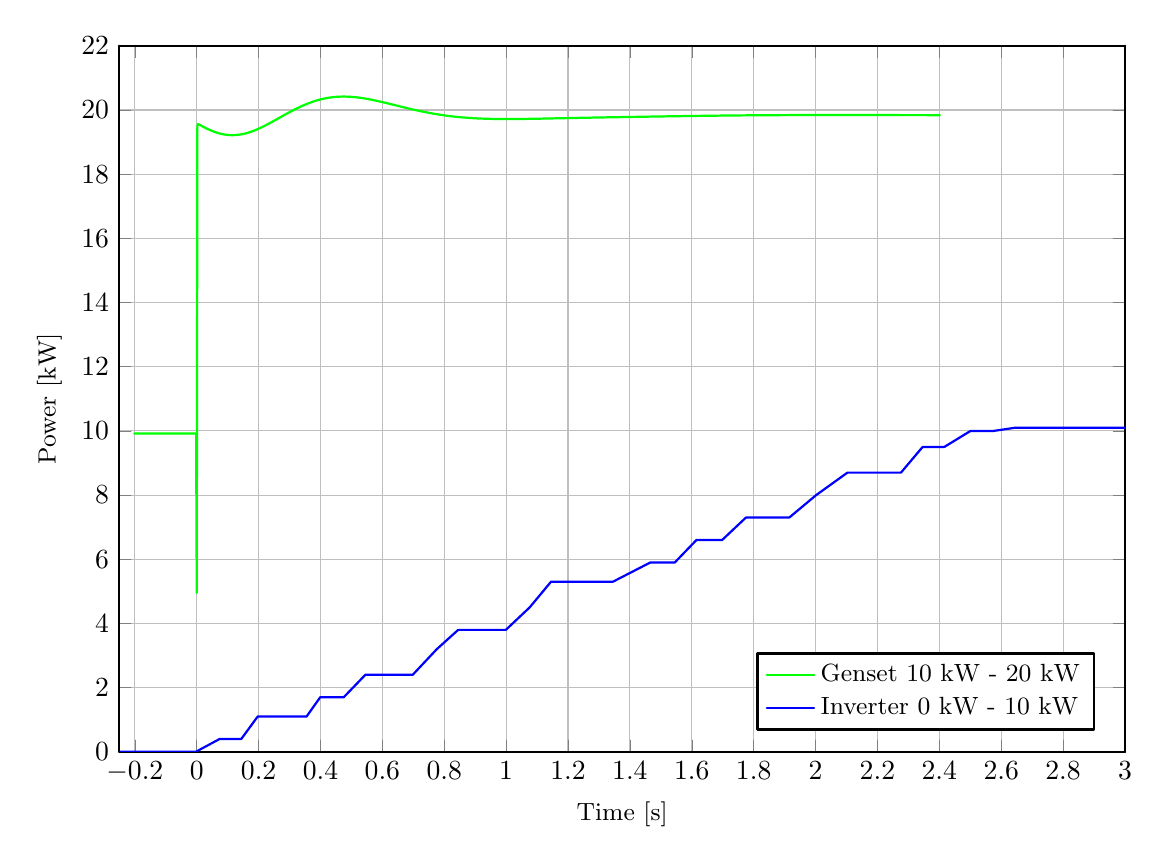
\begin{tikzpicture}

\begin{axis}[%
width=5.028in,
height=3.53in,
at={(0.883in,0.481in)},
scale only axis,
separate axis lines,
every outer x axis line/.append style={black},
every x tick label/.append style={font=\color{black}},
xmin=-0.25,
xmax=3,
xmajorgrids,
xlabel={Time [s]},
every outer y axis line/.append style={black},
every y tick label/.append style={font=\color{black}},
ymin=0,
ymax=22,
ylabel={Power [kW]},
ymajorgrids,
%xtick={−0.25 0 0.25 0.5 0.75 1 1.25 1.5 1.75 2 2.25 2.5 2.75 3},
axis background/.style={fill=white},
legend style={at={(0.97,0.03)},anchor=south east,legend cell align=left,align=left,draw=black},
y filter/.code={\pgfmathparse{#1/1000}\pgfmathresult}
]
\addplot [color=green,solid]
  table[row sep=crcr]{%
-0.202	9918.74999621698\\
-0.2	9918.74999621075\\
-0.198	9918.74999620453\\
-0.196	9918.7499961983\\
-0.194	9918.74999619208\\
-0.192	9918.74999618585\\
-0.19	9918.74999617963\\
-0.188	9918.7499961734\\
-0.186	9918.74999616718\\
-0.184	9918.74999616095\\
-0.182	9918.74999615473\\
-0.18	9918.74999614851\\
-0.178	9918.74999614228\\
-0.176	9918.74999613606\\
-0.173999999999999	9918.74999612983\\
-0.172	9918.74999612361\\
-0.17	9918.74999611739\\
-0.168	9918.74999611116\\
-0.165999999999999	9918.74999610494\\
-0.164	9918.74999609871\\
-0.162	9918.74999609249\\
-0.16	9918.74999608626\\
-0.157999999999999	9918.74999608003\\
-0.156	9918.74999607381\\
-0.154	9918.74999606759\\
-0.152	9918.74999606136\\
-0.149999999999999	9918.74999605513\\
-0.148	9918.74999604891\\
-0.146	9918.74999604262\\
-0.144	9918.74999603632\\
-0.141999999999999	9918.74999603003\\
-0.14	9918.74999602374\\
-0.138	9918.74999601744\\
-0.136	9918.74999601115\\
-0.133999999999999	9918.74999600485\\
-0.132	9918.74999599855\\
-0.13	9918.74999599226\\
-0.128	9918.74999598596\\
-0.125999999999999	9918.74999597967\\
-0.124	9918.74999597338\\
-0.122	9918.74999596708\\
-0.12	9918.74999596078\\
-0.117999999999999	9918.74999595449\\
-0.116	9918.7499959482\\
-0.114	9918.7499959419\\
-0.112	9918.7499959356\\
-0.109999999999999	9918.74999592931\\
-0.108	9918.74999592301\\
-0.106	9918.74999591672\\
-0.104	9918.74999591042\\
-0.101999999999999	9918.74999590413\\
-0.0999999999999996	9918.74999589791\\
-0.0979999999999999	9918.74999589168\\
-0.0960000000000001	9918.74999588546\\
-0.0939999999999994	9918.74999587924\\
-0.0919999999999996	9918.74999587301\\
-0.0899999999999999	9918.74999586678\\
-0.0880000000000001	9918.74999586056\\
-0.0859999999999994	9918.74999585433\\
-0.0839999999999996	9918.7499958481\\
-0.0819999999999999	9918.74999584188\\
-0.0800000000000001	9918.74999583566\\
-0.0779999999999994	9918.74999582944\\
-0.0759999999999996	9918.74999582322\\
-0.0739999999999998	9918.74999581699\\
-0.0720000000000001	9918.74999581076\\
-0.0699999999999994	9918.74999580454\\
-0.0679999999999996	9918.74999579832\\
-0.0659999999999998	9918.74999579209\\
-0.0640000000000001	9918.74999578586\\
-0.0619999999999994	9918.74999577964\\
-0.0599999999999996	9918.74999577341\\
-0.0579999999999998	9918.74999576719\\
-0.0560000000000001	9918.74999576096\\
-0.0539999999999994	9918.74999575474\\
-0.0519999999999996	9918.74999574851\\
-0.0499999999999998	9918.74999574229\\
-0.048	9918.74999573607\\
-0.0459999999999994	9918.74999572985\\
-0.0439999999999996	9918.74999572362\\
-0.0419999999999998	9918.74999576653\\
-0.04	9918.74999586238\\
-0.0379999999999994	9918.74999595559\\
-0.0359999999999996	9918.7499960517\\
-0.0339999999999998	9918.74999614786\\
-0.032	9918.74999624399\\
-0.0299999999999994	9918.74999634002\\
-0.0279999999999996	9918.74999643588\\
-0.0259999999999998	9918.74999653151\\
-0.024	9918.74999662687\\
-0.0219999999999994	9918.74999672191\\
-0.0199999999999996	9918.7499968166\\
-0.0179999999999998	9918.7499969109\\
-0.016	9918.74999700504\\
-0.0139999999999993	9918.7499970991\\
-0.0119999999999996	9918.74999719263\\
-0.00999999999999979	9918.74999728515\\
-0.00800000000000001	9918.74999737751\\
-0.00599999999999934	9918.74999746978\\
-0.00399999999999956	9918.74999756198\\
-0.00199999999999978	9918.74999765409\\
0	4959.37499887307\\
0.00200000000000067	19524.0668185409\\
0.00400000000000045	19562.985982334\\
0.00600000000000023	19553.350810773\\
0.00800000000000001	19543.2921140118\\
0.0100000000000007	19533.0431123617\\
0.0120000000000005	19522.6953626832\\
0.0140000000000002	19512.3159534624\\
0.016	19501.9543542334\\
0.0180000000000007	19491.6472422911\\
0.0200000000000005	19481.4220231357\\
0.0220000000000002	19471.2993958025\\
0.024	19461.2952198062\\
0.0259999999999998	19451.4218716259\\
0.0280000000000005	19441.6892282712\\
0.0300000000000002	19432.1053785717\\
0.032	19422.6771358217\\
0.0339999999999998	19413.4104056371\\
0.0360000000000005	19404.3104484118\\
0.0380000000000003	19395.3820651663\\
0.04	19386.6297278293\\
0.0419999999999998	19378.0576693246\\
0.0440000000000005	19369.6699446801\\
0.0460000000000003	19361.4704713451\\
0.048	19353.4630546772\\
0.0499999999999998	19345.6514029385\\
0.0520000000000005	19338.0391349525\\
0.0540000000000003	19330.629782706\\
0.0560000000000001	19323.4267905469\\
0.0579999999999998	19316.4335121646\\
0.0600000000000005	19309.6532062042\\
0.0620000000000003	19303.0890311195\\
0.0640000000000001	19296.7440396892\\
0.0659999999999998	19290.6211734938\\
0.0680000000000005	19284.7232575543\\
0.0700000000000003	19279.0529952666\\
0.0720000000000001	19273.6129637173\\
0.0739999999999998	19268.4056094302\\
0.0760000000000005	19263.4332445697\\
0.0780000000000003	19258.6980436092\\
0.0800000000000001	19254.2020404598\\
0.0819999999999999	19249.9471260473\\
0.0840000000000005	19245.935046321\\
0.0860000000000003	19242.1674006716\\
0.0880000000000001	19238.645640737\\
0.0899999999999999	19235.371069571\\
0.0920000000000005	19232.3448411526\\
0.0940000000000003	19229.5679602098\\
0.0960000000000001	19227.0412823383\\
0.0979999999999999	19224.7655143898\\
0.100000000000001	19222.7412151105\\
0.102	19220.9687960102\\
0.104	19219.4485224414\\
0.106	19218.1805148727\\
0.108000000000001	19217.1647503371\\
0.11	19216.401064043\\
0.112	19215.8891511298\\
0.114	19215.6285685569\\
0.116000000000001	19215.6187371129\\
0.118	19215.8589435311\\
0.12	19216.3483427044\\
0.122	19217.085959985\\
0.124000000000001	19218.0706935619\\
0.126	19219.3013169079\\
0.128	19220.7764812854\\
0.13	19222.4947183062\\
0.132000000000001	19224.4544425362\\
0.134	19226.6539541402\\
0.136	19229.0914415597\\
0.138	19231.7649842187\\
0.140000000000001	19234.6725552523\\
0.142	19237.8120242534\\
0.144	19241.1811600336\\
0.146	19244.7776333933\\
0.148000000000001	19248.5990198987\\
0.15	19252.6428026618\\
0.152	19256.9063751192\\
0.154	19261.3870438094\\
0.156000000000001	19266.0820311433\\
0.158	19270.9884781677\\
0.16	19276.1034473184\\
0.162	19281.4239251609\\
0.164000000000001	19286.9468251183\\
0.166	19292.6689901825\\
0.168	19298.5871956098\\
0.17	19304.6981515972\\
0.172000000000001	19310.9985059396\\
0.174	19317.4848466668\\
0.176	19324.1537046579\\
0.178	19331.001556234\\
0.180000000000001	19338.0248257277\\
0.182	19345.2198880275\\
0.184	19352.5830710982\\
0.186	19360.1106584762\\
0.188000000000001	19367.7988917378\\
0.19	19375.6439729424\\
0.192	19383.6420670478\\
0.194	19391.7893042984\\
0.196000000000001	19400.0817825869\\
0.198	19408.5155697862\\
0.2	19417.086706055\\
0.202	19425.7912061135\\
0.204000000000001	19434.6250614908\\
0.206	19443.584242744\\
0.208	19452.6647016474\\
0.21	19461.8623733526\\
0.212000000000001	19471.1731785195\\
0.214	19480.5930254173\\
0.216	19490.1178119962\\
0.218	19499.7434279286\\
0.220000000000001	19509.4657566211\\
0.222	19519.2806771963\\
0.224	19529.1840664436\\
0.226	19539.1718007411\\
0.228000000000001	19549.2397579462\\
0.23	19559.383819256\\
0.232	19569.5998710375\\
0.234	19579.8838066267\\
0.236000000000001	19590.2315280977\\
0.238	19600.6389480005\\
0.24	19611.1019910683\\
0.242	19621.616595894\\
0.244000000000001	19632.1787165754\\
0.246	19642.7843243301\\
0.248	19653.4294090785\\
0.25	19664.1099809963\\
0.252000000000001	19674.8220720357\\
0.254	19685.5617374151\\
0.256	19696.325057078\\
0.258	19707.1081371196\\
0.260000000000001	19717.9071111836\\
0.262	19728.7181418258\\
0.264	19739.5374218474\\
0.266	19750.3611755962\\
0.268000000000001	19761.1856602364\\
0.27	19772.0071669868\\
0.272	19782.8220223276\\
0.274	19793.6265891744\\
0.276000000000001	19804.4172680223\\
0.278	19815.1904980568\\
0.28	19825.9427582335\\
0.282	19836.6705683262\\
0.284000000000001	19847.3704899431\\
0.286	19858.039127511\\
0.288	19868.6731292287\\
0.29	19879.2691879874\\
0.292	19889.8240422604\\
0.294	19900.334476961\\
0.296	19910.7973242685\\
0.298	19921.2094644227\\
0.3	19931.5678264875\\
0.302	19941.8693890825\\
0.304	19952.1111810831\\
0.306	19962.2902822903\\
0.308	19972.4038240681\\
0.310000000000001	19982.4489899511\\
0.312	19992.4230162206\\
0.314	20002.3231924493\\
0.316	20012.1468620166\\
0.318000000000001	20021.8914225927\\
0.32	20031.5543265923\\
0.322	20041.1330815982\\
0.324	20050.6252507553\\
0.326000000000001	20060.0284531339\\
0.328	20069.3403640647\\
0.33	20078.558715443\\
0.332	20087.6812960052\\
0.334000000000001	20096.7059515746\\
0.336	20105.6305852805\\
0.338	20114.4531577473\\
0.34	20123.171687256\\
0.342000000000001	20131.7842498782\\
0.344	20140.2889795817\\
0.346	20148.6840683096\\
0.348	20156.9677660317\\
0.350000000000001	20165.1383807697\\
0.352	20173.194278596\\
0.354	20181.1338836061\\
0.356	20188.9556778657\\
0.358000000000001	20196.6582013324\\
0.36	20204.2400517527\\
0.362	20211.6998845336\\
0.364	20219.036412591\\
0.366000000000001	20226.2484061735\\
0.368	20233.3346926637\\
0.37	20240.2941563551\\
0.372	20247.125738208\\
0.374000000000001	20253.8284355822\\
0.376	20260.4013019481\\
0.378	20266.8434465768\\
0.38	20273.1540342092\\
0.382000000000001	20279.3322847044\\
0.384	20285.3774726687\\
0.386	20291.2889270645\\
0.388	20297.0660308005\\
0.390000000000001	20302.7082203033\\
0.392	20308.2149850709\\
0.394	20313.5858672082\\
0.396	20318.8204609459\\
0.398000000000001	20323.9184121425\\
0.4	20328.8794177698\\
0.402	20333.7032253833\\
0.404	20338.3896325771\\
0.406000000000001	20342.9384864235\\
0.408	20347.3496828997\\
0.41	20351.6231662995\\
0.412	20355.7589286326\\
0.414000000000001	20359.7570090107\\
0.416	20363.6174930212\\
0.418	20367.3405120901\\
0.42	20370.9262428326\\
0.422000000000001	20374.3749063933\\
0.424	20377.6867677765\\
0.426	20380.8621351662\\
0.428	20383.9013592373\\
0.430000000000001	20386.8048324574\\
0.432	20389.5729883809\\
0.434	20392.2063009353\\
0.436	20394.7052836992\\
0.438000000000001	20397.0704891749\\
0.44	20399.3025080535\\
0.442	20401.4019684742\\
0.444	20403.369535279\\
0.446000000000001	20405.205909261\\
0.448	20406.9118264097\\
0.45	20408.4880571509\\
0.452	20409.9354055837\\
0.454000000000001	20411.2547087142\\
0.456	20412.4468356862\\
0.458	20413.5126870096\\
0.46	20414.4531937872\\
0.462000000000001	20415.2693169399\\
0.464	20415.9620464303\\
0.466	20416.5324004863\\
0.468	20416.981424824\\
0.470000000000001	20417.310191871\\
0.472	20417.5197999899\\
0.474	20417.6113727028\\
0.476	20417.5860579173\\
0.478000000000001	20417.4450271534\\
0.48	20417.189474773\\
0.482	20416.8206172117\\
0.484	20416.3396922126\\
0.486000000000001	20415.7479580639\\
0.488	20415.0466928393\\
0.49	20414.2371936417\\
0.492	20413.320775852\\
0.494000000000001	20412.2987723807\\
0.496	20411.1725329248\\
0.498	20409.9434232297\\
0.5	20408.6128243551\\
0.502000000000001	20407.1821319479\\
0.504	20405.652755519\\
0.506	20404.0261177268\\
0.508	20402.3036536671\\
0.510000000000001	20400.4868101685\\
0.512	20398.5770450948\\
0.514	20396.5758266546\\
0.516	20394.4846327164\\
0.518000000000001	20392.3049501331\\
0.52	20390.0382740716\\
0.522	20387.6861073518\\
0.524	20385.2499597918\\
0.526000000000001	20382.7313475625\\
0.528	20380.131792549\\
0.53	20377.4528217209\\
0.532	20374.6959665107\\
0.534000000000001	20371.8627622013\\
0.536	20368.9547473207\\
0.538	20365.9734630474\\
0.54	20362.9204526231\\
0.542000000000001	20359.7972607751\\
0.544	20356.6054331478\\
0.546	20353.346515743\\
0.548	20350.0220543698\\
0.55	20346.633594104\\
0.552	20343.1826787564\\
0.554	20339.6708503509\\
0.556	20336.0996486123\\
0.558	20332.4706104634\\
0.560000000000001	20328.7852695319\\
0.562	20325.0451556672\\
0.564	20321.2517944662\\
0.566	20317.4067068101\\
0.568000000000001	20313.5114084096\\
0.57	20309.567409361\\
0.572	20305.5762137116\\
0.574	20301.5393190347\\
0.576000000000001	20297.4582160152\\
0.578	20293.3343880443\\
0.58	20289.1693108242\\
0.582	20284.9644519827\\
0.584000000000001	20280.7212706977\\
0.586	20276.4412173311\\
0.588	20272.1257330728\\
0.59	20267.7762495939\\
0.592000000000001	20263.3941887102\\
0.594	20258.9809620549\\
0.596	20254.5379707609\\
0.598	20250.0666051529\\
0.600000000000001	20245.5682444485\\
0.602	20241.0442564691\\
0.604	20236.49599736\\
0.606	20231.9248113202\\
0.608000000000001	20227.3320303407\\
0.61	20222.7189739521\\
0.612	20218.0869489823\\
0.614	20213.4372493219\\
0.616000000000001	20208.7711556991\\
0.618	20204.0899354636\\
0.62	20199.3948423789\\
0.622	20194.687116424\\
0.624000000000001	20189.9679836024\\
0.626	20185.2386557612\\
0.628	20180.5003304173\\
0.63	20175.7541905926\\
0.632000000000001	20171.0014046577\\
0.634	20166.2431261823\\
0.636	20161.4804937958\\
0.638	20156.714631054\\
0.640000000000001	20151.9466463144\\
0.642	20147.1776326194\\
0.644	20142.4086675863\\
0.646	20137.6408133061\\
0.648000000000001	20132.8751162485\\
0.65	20128.1126071746\\
0.652	20123.3543010573\\
0.654	20118.6011970081\\
0.656000000000001	20113.8542782109\\
0.658	20109.1145118635\\
0.66	20104.3828491244\\
0.662	20099.660225068\\
0.664000000000001	20094.9475586444\\
0.666	20090.2457526474\\
0.668	20085.5556936878\\
0.67	20080.8782521726\\
0.672000000000001	20076.2142822915\\
0.674	20071.564622008\\
0.676	20066.9300930574\\
0.678	20062.3115009494\\
0.680000000000001	20057.709634978\\
0.682	20053.1252682349\\
0.684	20048.5591576298\\
0.686	20044.0120439156\\
0.688000000000001	20039.484651718\\
0.69	20034.9776895713\\
0.692	20030.4918499584\\
0.694	20026.0278093559\\
0.696000000000001	20021.5862282837\\
0.698	20017.1677513595\\
0.7	20012.7730073574\\
0.702	20008.4026092717\\
0.704000000000001	20004.0571543834\\
0.706	19999.7372243328\\
0.708	19995.443385195\\
0.71	19991.1761875591\\
0.712000000000001	19986.9361666123\\
0.714	19982.723842227\\
0.716	19978.5397190515\\
0.718	19974.3842866047\\
0.720000000000001	19970.2580193739\\
0.722	19966.161376916\\
0.724	19962.0948039619\\
0.726	19958.0587305242\\
0.728000000000001	19954.0535720077\\
0.73	19950.0797293229\\
0.732	19946.1375890025\\
0.734	19942.2275233206\\
0.736000000000001	19938.3498904141\\
0.738	19934.5050344074\\
0.74	19930.6932855392\\
0.742	19926.9149602912\\
0.744000000000001	19923.1703615203\\
0.746	19919.4597785914\\
0.748	19915.7834875137\\
0.75	19912.1417510783\\
0.752000000000001	19908.5348189978\\
0.754	19904.9629280479\\
0.756	19901.4263022108\\
0.758	19897.9251528198\\
0.760000000000001	19894.4596787062\\
0.762	19891.0300663475\\
0.764	19887.6364900164\\
0.766	19884.279111932\\
0.768000000000001	19880.9580824122\\
0.77	19877.6735400265\\
0.772	19874.425611751\\
0.774	19871.2144131238\\
0.776000000000001	19868.0400484013\\
0.778	19864.9026107161\\
0.78	19861.8021822351\\
0.782	19858.7388343183\\
0.784000000000001	19855.7126276794\\
0.786	19852.7236125451\\
0.788	19849.7718288171\\
0.79	19846.8573062334\\
0.792000000000001	19843.9800645298\\
0.794	19841.1401136029\\
0.796	19838.3374536724\\
0.798	19835.572075444\\
0.800000000000001	19832.843960273\\
0.802	19830.1530803275\\
0.804	19827.4993987513\\
0.806	19824.882869828\\
0.808000000000001	19822.3034391442\\
0.810000000000001	19819.7610437525\\
0.812	19817.2556123357\\
0.814	19814.7870653687\\
0.816	19812.3553152823\\
0.818000000000001	19809.9602666251\\
0.82	19807.6018162265\\
0.822	19805.2798533577\\
0.824	19802.9942598938\\
0.826000000000001	19800.7449104749\\
0.828	19798.531672666\\
0.83	19796.3544071176\\
0.832	19794.2129677247\\
0.834000000000001	19792.1072017857\\
0.836	19790.0369501607\\
0.838	19788.0020474283\\
0.84	19786.0023220429\\
0.842000000000001	19784.0375964901\\
0.844	19782.1076874418\\
0.846	19780.2124059106\\
0.848	19778.3515574028\\
0.850000000000001	19776.5249420709\\
0.852	19774.7323548652\\
0.854	19772.9735856837\\
0.856	19771.2484195219\\
0.858000000000001	19769.5566366213\\
0.86	19767.8980126162\\
0.862	19766.27231868\\
0.864	19764.6793216705\\
0.866000000000001	19763.1187842735\\
0.868	19761.5904651458\\
0.87	19760.094119056\\
0.872	19758.6294970257\\
0.874000000000001	19757.1963464675\\
0.876	19755.7944113235\\
0.878	19754.4234322012\\
0.88	19753.0831465087\\
0.882000000000001	19751.7732885885\\
0.884	19750.4935898498\\
0.886	19749.2437788996\\
0.888	19748.0235816719\\
0.890000000000001	19746.8327215564\\
0.892	19745.6709195248\\
0.894	19744.5378942562\\
0.896	19743.4333622612\\
0.898000000000001	19742.3570380036\\
0.9	19741.3086340219\\
0.902	19740.2878610482\\
0.904	19739.2944281263\\
0.906000000000001	19738.3280427278\\
0.908	19737.3884108668\\
0.91	19736.4752372133\\
0.912	19735.5882252048\\
0.914000000000001	19734.7270771561\\
0.916	19733.8914943682\\
0.918	19733.0811772347\\
0.92	19732.2958253477\\
0.922000000000001	19731.535137601\\
0.924	19730.7988122925\\
0.926	19730.0865472247\\
0.928	19729.3980398031\\
0.930000000000001	19728.7329871343\\
0.932	19728.0910861209\\
0.934	19727.4720335559\\
0.936	19726.8755262149\\
0.938000000000001	19726.301260947\\
0.94	19725.7489347638\\
0.942	19725.218244927\\
0.944	19724.7088890339\\
0.946000000000001	19724.2205651024\\
0.948	19723.7529716527\\
0.95	19723.3058077888\\
0.952	19722.8787732776\\
0.954000000000001	19722.4715686269\\
0.956	19722.0838951611\\
0.958	19721.7154550958\\
0.96	19721.3659516107\\
0.962000000000001	19721.0350889209\\
0.964	19720.7225723462\\
0.966	19720.4281083795\\
0.968	19720.1514047529\\
0.970000000000001	19719.8921705027\\
0.972	19719.6501160324\\
0.974	19719.4249531749\\
0.976	19719.2163952517\\
0.978000000000001	19719.0241571322\\
0.98	19718.8479552904\\
0.982	19718.6875078599\\
0.984	19718.5425346885\\
0.986000000000001	19718.4127573899\\
0.988	19718.2978993946\\
0.99	19718.1976859994\\
0.992	19718.1118444152\\
0.994000000000001	19718.0401038129\\
0.996	19717.9821953685\\
0.998	19717.9378523063\\
1	19717.906809941\\
1.002	19717.8888057176\\
1.004	19717.8835792508\\
1.006	19717.8908723625\\
1.008	19717.9104291176\\
1.01	19717.9419958591\\
1.012	19717.985321241\\
1.014	19718.0401562607\\
1.016	19718.1062542894\\
1.018	19718.1833711009\\
1.02	19718.2712649003\\
1.022	19718.36969635\\
1.024	19718.4784285949\\
1.026	19718.5972272867\\
1.028	19718.7258606064\\
1.03	19718.8640992857\\
1.032	19719.0117166271\\
1.034	19719.1684885229\\
1.036	19719.3341934731\\
1.038	19719.5086126012\\
1.04	19719.6915296705\\
1.042	19719.8827310973\\
1.044	19720.0820059643\\
1.046	19720.2891460327\\
1.048	19720.503945752\\
1.05	19720.7262022706\\
1.052	19720.9557154436\\
1.054	19721.1922878404\\
1.056	19721.4357247511\\
1.058	19721.6858341917\\
1.06	19721.9424269085\\
1.062	19722.2053163812\\
1.064	19722.4743188252\\
1.066	19722.7492531928\\
1.068	19723.0299411738\\
1.07	19723.3162071946\\
1.072	19723.6078784164\\
1.074	19723.9047847335\\
1.076	19724.2067587691\\
1.078	19724.5136358716\\
1.08	19724.8252541092\\
1.082	19725.141454264\\
1.084	19725.4620798253\\
1.086	19725.7869769822\\
1.088	19726.1159946147\\
1.09	19726.4489842849\\
1.092	19726.7858002271\\
1.094	19727.1262993371\\
1.096	19727.4703411608\\
1.098	19727.817787882\\
1.1	19728.1685043098\\
1.102	19728.5223578652\\
1.104	19728.8792185667\\
1.106	19729.2389590158\\
1.108	19729.6014543818\\
1.11	19729.9665823852\\
1.112	19730.3342232817\\
1.114	19730.7042598451\\
1.116	19731.0765773491\\
1.118	19731.4510635496\\
1.12	19731.8276086656\\
1.122	19732.2061053601\\
1.124	19732.5864487203\\
1.126	19732.9685362373\\
1.128	19733.3522677856\\
1.13	19733.7375456016\\
1.132	19734.1242742626\\
1.134	19734.5123606643\\
1.136	19734.9017139986\\
1.138	19735.292245731\\
1.14	19735.6838695773\\
1.142	19736.0765014801\\
1.144	19736.4700595852\\
1.146	19736.8644642172\\
1.148	19737.2596378554\\
1.15	19737.6555051085\\
1.152	19738.0519926905\\
1.154	19738.4490293944\\
1.156	19738.8465460673\\
1.158	19739.2444755847\\
1.16	19739.6427528242\\
1.162	19740.0413146392\\
1.164	19740.4400998331\\
1.166	19740.8390491323\\
1.168	19741.2381051594\\
1.17	19741.6372124065\\
1.172	19742.0363172082\\
1.174	19742.4353677144\\
1.176	19742.8343138628\\
1.178	19743.2331073518\\
1.18	19743.6317016131\\
1.182	19744.0300517835\\
1.184	19744.4281146781\\
1.186	19744.8258487621\\
1.188	19745.2232141231\\
1.19	19745.6201724436\\
1.192	19746.0166869728\\
1.194	19746.4127224993\\
1.196	19746.8082453227\\
1.198	19747.2032232263\\
1.2	19747.597625449\\
1.202	19747.9914226577\\
1.204	19748.3845869195\\
1.206	19748.777091674\\
1.208	19749.1689117057\\
1.21	19749.5600231166\\
1.212	19749.9504032986\\
1.214	19750.3400309059\\
1.216	19750.7288858281\\
1.218	19751.1169491628\\
1.22	19751.5042031884\\
1.222	19751.8906313374\\
1.224	19752.2762181694\\
1.226	19752.6609493441\\
1.228	19753.0448115955\\
1.23	19753.4277927047\\
1.232	19753.8098814741\\
1.234	19754.1910677011\\
1.236	19754.5713421523\\
1.238	19754.9506965375\\
1.24	19755.3291234845\\
1.242	19755.7066165136\\
1.244	19756.0831700121\\
1.246	19756.4587792099\\
1.248	19756.8334401541\\
1.25	19757.207149685\\
1.252	19757.5799054113\\
1.254	19757.9517056865\\
1.256	19758.3225495845\\
1.258	19758.6924368762\\
1.26	19759.0613680061\\
1.262	19759.429344069\\
1.264	19759.7963667872\\
1.266	19760.162438488\\
1.268	19760.5275620808\\
1.27	19760.8917410353\\
1.272	19761.2549793596\\
1.274	19761.6172815786\\
1.276	19761.9786527123\\
1.278	19762.3390982551\\
1.28	19762.698624155\\
1.282	19763.0572367928\\
1.284	19763.414942962\\
1.286	19763.7717498488\\
1.288	19764.1276650127\\
1.29	19764.4826963665\\
1.292	19764.836852158\\
1.294	19765.1901409505\\
1.296	19765.5425716047\\
1.298	19765.8941532604\\
1.3	19766.2448953184\\
1.302	19766.5948074233\\
1.304	19766.9438994457\\
1.306	19767.2921814655\\
1.308	19767.6396637553\\
1.31	19767.9863567637\\
1.312	19768.3322710991\\
1.314	19768.6774175145\\
1.316	19769.0218068914\\
1.318	19769.365450225\\
1.32	19769.708358609\\
1.322	19770.0505432212\\
1.324	19770.3920153095\\
1.326	19770.7327861774\\
1.328	19771.0728671706\\
1.33	19771.4122696639\\
1.332	19771.7510050476\\
1.334	19772.0890847152\\
1.336	19772.426520051\\
1.338	19772.7633224175\\
1.34	19773.0995031439\\
1.342	19773.4350735146\\
1.344	19773.7700447577\\
1.346	19774.1044280345\\
1.348	19774.4382344283\\
1.35	19774.7714749342\\
1.352	19775.1041604496\\
1.354	19775.4363017636\\
1.356	19775.7679095481\\
1.358	19776.0989943485\\
1.36	19776.4295665744\\
1.362	19776.7596364915\\
1.364	19777.0892142132\\
1.366	19777.4183096923\\
1.368	19777.7469327132\\
1.37	19778.0750928848\\
1.372	19778.4027996329\\
1.374	19778.7300621933\\
1.376	19779.0568896054\\
1.378	19779.3832907053\\
1.38	19779.7092741201\\
1.382	19780.0348482617\\
1.384	19780.3600213214\\
1.386	19780.6848012645\\
1.388	19781.0091958247\\
1.39	19781.3332125002\\
1.392	19781.6568585481\\
1.394	19781.9801409805\\
1.396	19782.3030665603\\
1.398	19782.6256417975\\
1.4	19782.9478729451\\
1.402	19783.269765996\\
1.404	19783.5913266796\\
1.406	19783.9125604592\\
1.408	19784.2334725289\\
1.41	19784.5540678111\\
1.412	19784.8743509544\\
1.414	19785.1943263313\\
1.416	19785.5139980365\\
1.418	19785.8333698851\\
1.42	19786.1524454111\\
1.422	19786.4712278664\\
1.424	19786.7897202192\\
1.426	19787.107925154\\
1.428	19787.4258450698\\
1.43	19787.7434820805\\
1.432	19788.0608380143\\
1.434	19788.3779144135\\
1.436	19788.6947125344\\
1.438	19789.0112333481\\
1.44	19789.3274775402\\
1.442	19789.6434455118\\
1.444	19789.95913738\\
1.446	19790.2745529792\\
1.448	19790.5896918614\\
1.45	19790.9045532979\\
1.452	19791.2191362809\\
1.454	19791.5334395243\\
1.456	19791.8474614658\\
1.458	19792.1612002686\\
1.46	19792.4746538233\\
1.462	19792.7878197497\\
1.464	19793.1006953995\\
1.466	19793.4132778581\\
1.468	19793.7255639471\\
1.47	19794.0375502272\\
1.472	19794.3492330004\\
1.474	19794.6606083132\\
1.476	19794.9716719589\\
1.478	19795.2824194813\\
1.48	19795.5928461772\\
1.482	19795.9029470998\\
1.484	19796.2127170621\\
1.486	19796.5221506399\\
1.488	19796.8312421759\\
1.49	19797.1399857826\\
1.492	19797.4483753462\\
1.494	19797.7564045305\\
1.496	19798.0640667802\\
1.498	19798.3713553253\\
1.5	19798.6782631847\\
1.502	19798.9847831704\\
1.504	19799.2909078912\\
1.506	19799.5966297574\\
1.508	19799.9019409845\\
1.51	19800.2068335975\\
1.512	19800.5112994356\\
1.514	19800.8153301559\\
1.516	19801.1189172384\\
1.518	19801.4220519901\\
1.52	19801.7247255494\\
1.522	19802.0269288909\\
1.524	19802.3286528297\\
1.526	19802.6298880261\\
1.528	19802.9306249904\\
1.53	19803.2308540871\\
1.532	19803.5305655397\\
1.534	19803.8297494358\\
1.536	19804.1283957313\\
1.538	19804.4264942553\\
1.54	19804.7240347148\\
1.542	19805.0210066999\\
1.544	19805.3173996877\\
1.546	19805.6132030477\\
1.548	19805.9084060466\\
1.55	19806.2029978527\\
1.552	19806.4969675408\\
1.554	19806.7903040975\\
1.556	19807.082996425\\
1.558	19807.3750333468\\
1.56	19807.6664036118\\
1.562	19807.9570958997\\
1.564	19808.247098825\\
1.566	19808.5364009423\\
1.568	19808.8249907509\\
1.57	19809.1128566991\\
1.572	19809.3999871897\\
1.574	19809.6863705837\\
1.576	19809.9719952057\\
1.578	19810.2568493481\\
1.58	19810.5409212759\\
1.582	19810.8241992309\\
1.584	19811.1066714367\\
1.586	19811.3883261031\\
1.588	19811.6691514303\\
1.59	19811.9491356133\\
1.592	19812.228266847\\
1.594	19812.5065333294\\
1.596	19812.7839232672\\
1.598	19813.0604248791\\
1.6	19813.3360264004\\
1.602	19813.6107160873\\
1.604	19813.884482221\\
1.606	19814.1573131116\\
1.608	19814.4291971026\\
1.61	19814.7001225745\\
1.612	19814.9700779488\\
1.614	19815.2390516924\\
1.616	19815.5070323209\\
1.618	19815.7740084028\\
1.62	19816.0399685631\\
1.622	19816.3049014871\\
1.624	19816.5687959239\\
1.626	19816.8316406903\\
1.628	19817.0934246741\\
1.63	19817.3541368379\\
1.632	19817.6137662221\\
1.634	19817.8723019487\\
1.636	19818.1297332246\\
1.638	19818.3860493446\\
1.64	19818.6412396948\\
1.642	19818.8952937556\\
1.644	19819.1482011053\\
1.646	19819.3999514225\\
1.648	19819.6505344894\\
1.65	19819.8999401946\\
1.652	19820.148158536\\
1.654	19820.3951796239\\
1.656	19820.640993683\\
1.658	19820.8855910557\\
1.66	19821.1289622046\\
1.662	19821.3710977147\\
1.664	19821.6119882964\\
1.666	19821.8516247873\\
1.668	19822.0899981552\\
1.67	19822.3270994998\\
1.672	19822.5629200554\\
1.674	19822.7974511927\\
1.676	19823.030684421\\
1.678	19823.2626113905\\
1.68	19823.4932238937\\
1.682	19823.7225138679\\
1.684	19823.9504733967\\
1.686	19824.1770947118\\
1.688	19824.4023701948\\
1.69	19824.6262923787\\
1.692	19824.8488539498\\
1.694	19825.0700477487\\
1.696	19825.2898667723\\
1.698	19825.508304175\\
1.7	19825.7253532697\\
1.702	19825.9410075297\\
1.704	19826.1552605892\\
1.706	19826.3681062452\\
1.708	19826.5795384578\\
1.71	19826.789551352\\
1.712	19826.998139218\\
1.714	19827.2052965124\\
1.716	19827.4110178593\\
1.718	19827.6152980503\\
1.72	19827.8181320462\\
1.722	19828.019514977\\
1.724	19828.2194421426\\
1.726	19828.4179090136\\
1.728	19828.6149112315\\
1.73	19828.8104446095\\
1.732	19829.0045051323\\
1.734	19829.197088957\\
1.736	19829.3881924131\\
1.738	19829.5778120028\\
1.74	19829.7659444009\\
1.742	19829.9525864554\\
1.744	19830.137735187\\
1.746	19830.3213877894\\
1.748	19830.5035416295\\
1.75	19830.6841942466\\
1.752	19830.8633433528\\
1.754	19831.0409868329\\
1.756	19831.2171227435\\
1.758	19831.3917493133\\
1.76	19831.5648649427\\
1.762	19831.7364682028\\
1.764	19831.9065578358\\
1.766	19832.0751327541\\
1.768	19832.2421920396\\
1.77	19832.4077349435\\
1.772	19832.5717608855\\
1.774	19832.7342694528\\
1.776	19832.8952604002\\
1.778	19833.0547336486\\
1.78	19833.2126892845\\
1.782	19833.3691275593\\
1.784	19833.5240488881\\
1.786	19833.6774538492\\
1.788	19833.829343183\\
1.79	19833.9797177906\\
1.792	19834.1285787337\\
1.794	19834.2759272325\\
1.796	19834.4217646655\\
1.798	19834.5660925678\\
1.8	19834.7089126302\\
1.802	19834.8502266981\\
1.804	19834.99003677\\
1.806	19835.1283449964\\
1.808	19835.2651536787\\
1.81	19835.4004652677\\
1.812	19835.534282362\\
1.814	19835.6666077074\\
1.816	19835.7974441948\\
1.818	19835.926794859\\
1.82	19836.0546628773\\
1.822	19836.1810515682\\
1.824	19836.3059643895\\
1.826	19836.4294049373\\
1.828	19836.5513769439\\
1.83	19836.6718842768\\
1.832	19836.7909309366\\
1.834	19836.9085210561\\
1.836	19837.0246588978\\
1.838	19837.1393488528\\
1.84	19837.2525954395\\
1.842	19837.3644033009\\
1.844	19837.4747772038\\
1.846	19837.5837220369\\
1.848	19837.6912428089\\
1.85	19837.7973446468\\
1.852	19837.9020327944\\
1.854	19838.0053126101\\
1.856	19838.1071895656\\
1.858	19838.2076692438\\
1.86	19838.3067573374\\
1.862	19838.4044596465\\
1.864	19838.5007820772\\
1.866	19838.5957306397\\
1.868	19838.6893114466\\
1.87	19838.7815307107\\
1.872	19838.8723947436\\
1.874	19838.9619099535\\
1.876	19839.0500828436\\
1.878	19839.1369200101\\
1.88	19839.2224281402\\
1.882	19839.3066140106\\
1.884	19839.3894844854\\
1.886	19839.4710465143\\
1.888	19839.5513071306\\
1.89	19839.6302734493\\
1.892	19839.7079526656\\
1.894	19839.7843520526\\
1.896	19839.8594789596\\
1.898	19839.9333408103\\
1.9	19840.0059451006\\
1.902	19840.0772993973\\
1.904	19840.1474113356\\
1.906	19840.2162886178\\
1.908	19840.283939011\\
1.91	19840.3503703453\\
1.912	19840.4155905124\\
1.914	19840.4796074632\\
1.916	19840.5424292061\\
1.918	19840.6040638054\\
1.92	19840.6645193792\\
1.922	19840.7238040979\\
1.924	19840.7819261817\\
1.926	19840.8388938998\\
1.928	19840.8947155677\\
1.93	19840.9493995459\\
1.932	19841.0029542379\\
1.934	19841.0553880887\\
1.936	19841.1067095827\\
1.938	19841.1569272422\\
1.94	19841.2060496254\\
1.942	19841.254085325\\
1.944	19841.3010429662\\
1.946	19841.3469312052\\
1.948	19841.3917587273\\
1.95	19841.4355342454\\
1.952	19841.4782664982\\
1.954	19841.5199642486\\
1.956	19841.5606362821\\
1.958	19841.6002914051\\
1.96	19841.6389384432\\
1.962	19841.6765862399\\
1.964	19841.7132436547\\
1.966	19841.7489195615\\
1.968	19841.7836228474\\
1.97	19841.8173624108\\
1.972	19841.8501471601\\
1.974	19841.881986012\\
1.976	19841.9128878902\\
1.978	19841.9428617235\\
1.98	19841.9719164452\\
1.982	19842.0000609905\\
1.984	19842.027304296\\
1.986	19842.053655298\\
1.988	19842.0791229308\\
1.99	19842.1037161259\\
1.992	19842.1274438099\\
1.994	19842.1503149039\\
1.996	19842.1723383216\\
1.998	19842.1935229684\\
2	19842.2138777399\\
2.002	19842.2334115203\\
2.004	19842.2521331821\\
2.006	19842.2700515838\\
2.008	19842.2871755691\\
2.01	19842.3035139661\\
2.012	19842.3190755854\\
2.014	19842.3338692194\\
2.016	19842.347903641\\
2.018	19842.3611876025\\
2.02	19842.3737298344\\
2.022	19842.3855390446\\
2.024	19842.396623917\\
2.026	19842.4069931104\\
2.028	19842.4166552579\\
2.03	19842.4256189654\\
2.032	19842.433892811\\
2.034	19842.4414853437\\
2.036	19842.4484050825\\
2.038	19842.4546605158\\
2.04	19842.4602600998\\
2.042	19842.4652122584\\
2.044	19842.4695253817\\
2.046	19842.4732078253\\
2.048	19842.4762679096\\
2.05	19842.478713919\\
2.052	19842.4805541006\\
2.054	19842.4817966641\\
2.056	19842.4824497806\\
2.058	19842.4825215817\\
2.06	19842.4820201594\\
2.062	19842.4809535647\\
2.064	19842.4793298072\\
2.066	19842.4771568544\\
2.068	19842.4744426312\\
2.07	19842.4711950188\\
2.072	19842.4674218547\\
2.074	19842.4631309314\\
2.076	19842.4583299963\\
2.078	19842.4530267511\\
2.08	19842.447228851\\
2.082	19842.4409439041\\
2.084	19842.4341794713\\
2.086	19842.4269430655\\
2.088	19842.4192421512\\
2.09	19842.4110841438\\
2.092	19842.4024764097\\
2.094	19842.3934262649\\
2.096	19842.3839409759\\
2.098	19842.3740277579\\
2.1	19842.3636937755\\
2.102	19842.3529461418\\
2.104	19842.341791918\\
2.106	19842.3302381135\\
2.108	19842.318291685\\
2.11	19842.3059595366\\
2.112	19842.2932485194\\
2.114	19842.2801654311\\
2.116	19842.2667170159\\
2.118	19842.2529099642\\
2.12	19842.2387509123\\
2.122	19842.2242464423\\
2.124	19842.2094030817\\
2.126	19842.1942273034\\
2.128	19842.1787255255\\
2.13	19842.162904111\\
2.132	19842.1467693679\\
2.134	19842.1303275487\\
2.136	19842.1135848505\\
2.138	19842.0965474152\\
2.14	19842.0792213286\\
2.142	19842.0616126211\\
2.144	19842.0437272672\\
2.146	19842.0255711856\\
2.148	19842.0071502392\\
2.15	19841.9884702349\\
2.152	19841.9695369235\\
2.154	19841.9503560002\\
2.156	19841.930933104\\
2.158	19841.911273818\\
2.16	19841.8913836694\\
2.162	19841.8712681296\\
2.164	19841.8509326141\\
2.166	19841.8303824827\\
2.168	19841.8096230392\\
2.17	19841.7886595322\\
2.172	19841.7674971544\\
2.174	19841.7461410433\\
2.176	19841.724596281\\
2.178	19841.7028678941\\
2.18	19841.6809608546\\
2.182	19841.6588800791\\
2.184	19841.6366304295\\
2.186	19841.6142167133\\
2.188	19841.591643683\\
2.19	19841.5689160373\\
2.192	19841.5460384202\\
2.194	19841.5230154221\\
2.196	19841.4998515795\\
2.198	19841.4765513753\\
2.2	19841.453119239\\
2.202	19841.4295595471\\
2.204	19841.4058766231\\
2.206	19841.3820747376\\
2.208	19841.3581581089\\
2.21	19841.3341309032\\
2.212	19841.3099972344\\
2.214	19841.285761165\\
2.216	19841.2614267058\\
2.218	19841.2369978167\\
2.22	19841.2124784062\\
2.222	19841.1878723328\\
2.224	19841.163183404\\
2.226	19841.1384153777\\
2.228	19841.113571962\\
2.23	19841.0886568152\\
2.232	19841.0636735467\\
2.234	19841.0386257171\\
2.236	19841.0135168383\\
2.238	19840.9883502372\\
2.24	19840.9631155244\\
2.242	19840.9378425191\\
2.244	19840.9125229639\\
2.246	19840.887159257\\
2.248	19840.8617546233\\
2.25	19840.8363122403\\
2.252	19840.8108352401\\
2.254	19840.7853267095\\
2.256	19840.7597896906\\
2.258	19840.7342271806\\
2.26	19840.7086421326\\
2.262	19840.6830374559\\
2.264	19840.657416016\\
2.266	19840.631780635\\
2.268	19840.6061340922\\
2.27	19840.5804791242\\
2.272	19840.5548184255\\
2.274	19840.5291546486\\
2.276	19840.5034904046\\
2.278	19840.4778282633\\
2.28	19840.4521707538\\
2.282	19840.4265203647\\
2.284	19840.4008795448\\
2.286	19840.3752507029\\
2.288	19840.3496362087\\
2.29	19840.3240383931\\
2.292	19840.2984595481\\
2.294	19840.2729019277\\
2.296	19840.2473677482\\
2.298	19840.2218591885\\
2.3	19840.1963783902\\
2.302	19840.1709274584\\
2.304	19840.1455084621\\
2.306	19840.1201234339\\
2.308	19840.0947743713\\
2.31	19840.0694632365\\
2.312	19840.0441919569\\
2.314	19840.0189624254\\
2.316	19839.993776501\\
2.318	19839.9686360091\\
2.32	19839.9435427416\\
2.322	19839.9184984575\\
2.324	19839.8935048836\\
2.326	19839.868563714\\
2.328	19839.8436766114\\
2.33	19839.8188452069\\
2.332	19839.7940711006\\
2.334	19839.7693558617\\
2.336	19839.7447010294\\
2.338	19839.7201081127\\
2.34	19839.6955785909\\
2.342	19839.6711139141\\
2.344	19839.6467155037\\
2.346	19839.6223847524\\
2.348	19839.5981230246\\
2.35	19839.5739316571\\
2.352	19839.5498119589\\
2.354	19839.5257652122\\
2.356	19839.5017926722\\
2.358	19839.4778955677\\
2.36	19839.4540751013\\
2.362	19839.43033245\\
2.364	19839.4066687653\\
2.366	19839.3830851736\\
2.368	19839.3595827764\\
2.37	19839.336162651\\
2.372	19839.3128258505\\
2.374	19839.2895734041\\
2.376	19839.2664063177\\
2.378	19839.2433255739\\
2.38	19839.2203321328\\
2.382	19839.1974269317\\
2.384	19839.1746108857\\
2.386	19839.1518848883\\
2.388	19839.1292498111\\
2.39	19839.1067065046\\
2.392	19839.0842557983\\
2.394	19839.0618985011\\
2.396	19839.0396354014\\
2.398	19839.0174672677\\
2.4	19838.9953948485\\
2.402	19838.973418873\\
};
\addlegendentry{Genset 10 kW - 20 kW};

\addplot [color=blue,solid,x filter/.code={\pgfmathparse{\pgfmathresult-10.}\pgfmathresult}]%
  table[row sep=crcr]{%
3.573	100\\
3.634	100\\
3.704	100\\
3.785	0\\
3.874	0\\
3.934	0\\
4.005	0\\
4.055	0\\
4.126	0\\
4.205	100\\
4.289	100\\
4.336	100\\
4.406	0\\
4.489	0\\
4.566	0\\
4.636	0\\
4.706	0\\
4.796	100\\
4.846	100\\
4.906	100\\
4.989	100\\
5.066	100\\
5.136	100\\
5.206	0\\
5.294	0\\
5.337	0\\
5.407	0\\
5.49	0\\
5.567	0\\
5.637	0\\
5.707	0\\
5.857	100\\
5.892	0\\
5.957	0\\
6.007	0\\
6.09	0\\
6.167	0\\
6.257	100\\
6.307	100\\
6.39	100\\
6.457	0\\
6.527	0\\
6.598	0\\
6.678	0\\
6.738	0\\
6.808	0\\
6.891	0\\
6.968	0\\
7.038	0\\
7.093	0\\
7.168	0\\
7.238	0\\
7.308	0\\
7.392	0\\
7.458	0\\
7.548	0\\
7.638	0\\
7.658	0\\
7.748	0\\
7.792	100\\
7.868	100\\
7.938	100\\
8.008	0\\
8.092	0\\
8.168	0\\
8.238	0\\
8.291	0\\
8.369	0\\
8.439	0\\
8.509	0\\
8.591	0\\
8.669	0\\
8.739	0\\
8.792	0\\
8.869	0\\
8.94	0\\
9.01	0\\
9.111	0\\
9.17	100\\
9.211	100\\
9.294	100\\
9.372	0\\
9.452	0\\
9.496	0\\
9.572	0\\
9.653	0\\
9.696	0\\
9.773	0\\
9.843	0\\
9.914	0\\
9.997	0\\
10.074	400\\
10.144	400\\
10.197	1100\\
10.274	1100\\
10.355	1100\\
10.399	1700\\
10.475	1700\\
10.545	2400\\
10.615	2400\\
10.698	2400\\
10.776	3200\\
10.845	3800\\
10.915	3800\\
10.999	3800\\
11.076	4500\\
11.145	5300\\
11.199	5300\\
11.276	5300\\
11.345	5300\\
11.466	5900\\
11.475	5900\\
11.545	5900\\
11.615	6600\\
11.698	6600\\
11.775	7300\\
11.845	7300\\
11.915	7300\\
12.002	8000\\
12.103	8700\\
12.146	8700\\
12.199	8700\\
12.276	8700\\
12.346	9500\\
12.416	9500\\
12.501	10000\\
12.576	10000\\
12.646	10100\\
12.699	10100\\
12.776	10100\\
12.846	10100\\
12.917	10100\\
13	10100\\
13.077	10100\\
13.147	10200\\
13.217	10200\\
13.302	10200\\
13.377	10100\\
13.447	10100\\
13.517	10100\\
13.605	10100\\
13.647	10100\\
13.717	10100\\
13.803	10100\\
13.878	10100\\
13.948	10100\\
14.018	10000\\
14.068	10000\\
14.149	10100\\
14.202	10100\\
14.279	10100\\
14.349	10200\\
14.429	10200\\
14.479	10100\\
14.549	10100\\
14.619	10100\\
14.702	10100\\
14.78	10100\\
14.85	10200\\
14.92	10200\\
15.003	10200\\
15.15	10200\\
15.18	10200\\
15.251	10200\\
15.321	10200\\
15.403	10100\\
15.481	10100\\
15.541	10100\\
15.612	10100\\
15.692	10100\\
15.752	10100\\
15.821	10100\\
15.904	10100\\
15.982	10100\\
16.052	10100\\
16.104	10100\\
16.182	10100\\
16.252	10100\\
16.306	10200\\
16.383	10200\\
16.453	10000\\
16.524	10000\\
16.606	10200\\
16.683	10200\\
16.754	10200\\
16.808	10200\\
16.884	10200\\
16.955	10200\\
17.025	10200\\
17.108	10000\\
17.185	10000\\
17.325	10100\\
17.345	10100\\
17.413	10100\\
17.486	10100\\
17.555	10100\\
17.636	10200\\
17.686	10200\\
17.756	10100\\
17.826	10100\\
17.91	10100\\
17.986	10100\\
18.066	10100\\
18.11	10100\\
18.186	10100\\
18.256	10100\\
18.326	10100\\
18.41	10100\\
18.487	10000\\
18.557	10000\\
18.627	10000\\
18.677	10100\\
18.748	10100\\
18.818	10100\\
18.898	10100\\
18.959	10100\\
19.029	10100\\
19.114	10100\\
19.189	10100\\
19.259	10100\\
19.33	10000\\
19.416	10000\\
19.46	10100\\
19.53	10100\\
19.614	10100\\
19.69	10100\\
19.771	10100\\
19.821	10100\\
19.915	10100\\
19.961	10100\\
20.041	10100\\
20.101	10100\\
20.182	10100\\
20.223	10100\\
20.303	10100\\
20.393	10100\\
20.463	10100\\
20.544	10100\\
20.617	10100\\
20.674	10100\\
20.722	10100\\
20.794	10100\\
20.864	10100\\
20.934	10200\\
21.034	10100\\
21.094	10100\\
21.164	10100\\
21.244	10100\\
21.345	10100\\
21.365	10100\\
21.434	10100\\
21.523	10100\\
21.595	10100\\
21.665	10100\\
21.734	10200\\
21.818	10200\\
21.865	10200\\
21.935	10100\\
22.018	10100\\
22.085	10100\\
22.165	10100\\
22.235	10100\\
22.318	10100\\
22.365	10000\\
22.435	10000\\
22.518	10000\\
22.594	10100\\
22.665	10100\\
22.735	10200\\
22.819	10200\\
22.919	10200\\
22.936	10100\\
23.02	10100\\
23.096	10100\\
23.166	10100\\
23.236	10100\\
23.318	10100\\
23.366	10200\\
23.435	10200\\
23.519	10200\\
23.635	10200\\
23.655	10200\\
23.736	10100\\
23.786	10100\\
23.856	10100\\
23.946	10200\\
23.996	10200\\
24.067	10200\\
24.137	10200\\
24.221	10200\\
24.298	10200\\
24.368	10200\\
24.439	10200\\
24.522	10000\\
24.568	10000\\
24.639	10100\\
24.722	10100\\
24.799	10100\\
24.87	10200\\
24.941	10200\\
25.023	10200\\
25.101	10200\\
25.172	10100\\
25.242	10100\\
25.325	10100\\
25.402	10100\\
25.472	10100\\
25.528	10100\\
25.602	10100\\
25.682	10200\\
25.728	10200\\
25.813	10200\\
25.873	10100\\
25.943	10100\\
26.027	10100\\
26.104	10100\\
26.173	10100\\
26.229	10100\\
26.304	10100\\
26.373	10100\\
26.443	10100\\
26.528	10100\\
26.628	10100\\
26.674	10000\\
26.73	10000\\
26.804	10000\\
26.874	10200\\
26.944	10200\\
27.027	10100\\
27.104	10100\\
27.174	10100\\
27.23	10100\\
27.305	10100\\
27.375	10100\\
27.445	10100\\
27.532	10100\\
27.605	10100\\
27.675	10200\\
27.728	10200\\
27.805	10200\\
27.875	10200\\
27.945	10200\\
28.028	10100\\
28.106	10100\\
28.176	10100\\
28.257	10100\\
28.306	10200\\
28.376	10200\\
28.431	10200\\
28.506	10200\\
28.577	10100\\
28.647	10100\\
28.732	10100\\
28.807	10100\\
28.877	10100\\
28.931	10100\\
29.008	10100\\
29.078	10100\\
29.149	10100\\
29.235	10200\\
29.308	10200\\
29.379	10200\\
29.449	10100\\
29.532	10100\\
29.609	10200\\
29.679	10200\\
29.749	10200\\
29.837	10100\\
29.88	10100\\
29.949	10200\\
30.032	10200\\
30.109	10100\\
30.18	10100\\
30.25	10100\\
30.333	10100\\
30.38	10100\\
30.45	10100\\
30.534	10100\\
30.61	10100\\
30.68	10100\\
30.751	10100\\
30.8	10000\\
30.871	10000\\
30.951	10300\\
31.034	10300\\
31.082	10300\\
31.152	10300\\
31.235	10300\\
31.312	10300\\
31.382	10300\\
31.453	10300\\
31.535	10400\\
31.583	10400\\
31.653	10300\\
31.739	10300\\
31.813	10300\\
31.883	10300\\
31.973	10200\\
32.023	10200\\
32.083	10200\\
32.153	10200\\
32.237	10200\\
32.313	10200\\
32.383	10200\\
32.453	10200\\
32.503	10200\\
32.583	10200\\
32.653	10200\\
32.737	10200\\
32.814	10200\\
32.883	10100\\
32.954	10100\\
33.004	10100\\
33.083	10100\\
33.154	10100\\
33.237	10100\\
33.314	10100\\
33.434	10100\\
33.454	10100\\
33.504	10100\\
33.584	10100\\
33.654	10100\\
33.739	10100\\
33.785	10100\\
33.854	10100\\
33.939	10100\\
34.015	10100\\
34.085	10100\\
34.155	10100\\
34.245	10100\\
34.295	10100\\
34.439	10100\\
34.456	10100\\
34.538	10100\\
34.617	10100\\
34.687	10100\\
34.757	10100\\
34.84	10100\\
34.907	10100\\
34.987	10100\\
35.04	10100\\
35.117	10100\\
35.187	10100\\
35.24	10100\\
35.317	10100\\
35.387	10100\\
35.458	10100\\
35.54	10100\\
35.618	10100\\
35.688	10100\\
35.741	10100\\
35.818	10100\\
35.888	10100\\
35.958	10100\\
36.045	10100\\
36.118	10100\\
36.189	10100\\
36.245	10100\\
36.319	10100\\
36.442	10100\\
36.459	10100\\
36.543	10100\\
36.649	10100\\
36.699	10100\\
36.759	10100\\
36.848	10100\\
36.919	10100\\
36.99	10100\\
37.061	10100\\
37.151	10100\\
37.201	10100\\
37.261	10100\\
37.344	10100\\
37.422	10100\\
37.491	10100\\
37.562	10100\\
37.646	10100\\
37.692	10100\\
37.762	10100\\
37.846	10100\\
37.922	10100\\
37.992	9600\\
38.062	9600\\
38.112	9600\\
38.192	8900\\
38.263	8900\\
38.346	8000\\
38.422	8000\\
38.493	7500\\
38.603	7500\\
38.623	7500\\
38.693	6700\\
38.763	6700\\
38.848	5900\\
38.894	5900\\
38.964	5900\\
39.05	5200\\
39.124	5200\\
39.375	3900\\
39.395	3900\\
39.495	3200\\
39.549	3200\\
39.625	3200\\
39.705	2500\\
39.749	2500\\
39.826	1800\\
39.896	1800\\
39.966	1800\\
40.287	300\\
};
\addlegendentry{Inverter 0 kW - 10 kW};

\end{axis}
\end{tikzpicture}%
%\caption{Step responses from the high order genset model and data from the used inverter. It can be seen that the genet is a lot faster then the inverter.}\label{fig:inverter_and_genset_compair}
%\end{figure}

















 
 

%kravspec
%%main for kravspec og test


%\input{rapport/kravspec/kravspec}




%Design
%%\part{Design}
%\label{design}

\chapter{Control}
\label{ca:controller}
\section{Introduction to control}
\label{control_intro}

As the title of the section suggests, this chapter is about to present the different attempts that were made during the design process to control the plant. All the approaches that were carried out are presented, even though some of the control techniques were later found not to be realistic, therefore neglected and not included in the paper. The necessity of introducing these attempts is to provide argument for the final solution and thereby come to a result that fits expectations the best. 

The introduction of the control starts with a general system and model description and continues onto a state-space representation. After describing the system, a concept is introduced for the disturbance which was implemented in simulation. This concept however, called exo-systems, was neglected because of the assumption that certain information are available from the disturbance. During the measurements the disturbance cannot be, or at least, would be very unrealistic to describe priorly by its differential equations. 

Afterwards, the design is followed by the discussion of the the similar modern control methods but without extending the states with the disturbance. In order to make the design closer to the real-life implementation, the chapter continues on describing the control in both continuous and discrete time. 

By the end of the chapter, simulation is carried out in Simulink in order to show the results of the control. 
\section{Model of the controlled system}
\label{system_design}

The system was previously introduced in detail through the block diagram shown in \figref{fig:gensetmodeling}. It should be considered however, that it is complicated and unnecessary to handle a system in such a detailed form, therefore a more compact system description is required. In order to restructure the model and get a more convenient form, the inner processes can be represented with their transfer functions, thus combined in a subsystem such as in \figref{fig:blok_simplified}

%\begin{figure}[H]
%\centering
%\includegraphics[width=0.65\textwidth]{rapport/billeder/blok_simplified}
%\caption{Simplified closed-loop system for the genset}
%\label{fig:blok_simplified}
%\end{figure}

\begin{figure}[H]
\centering
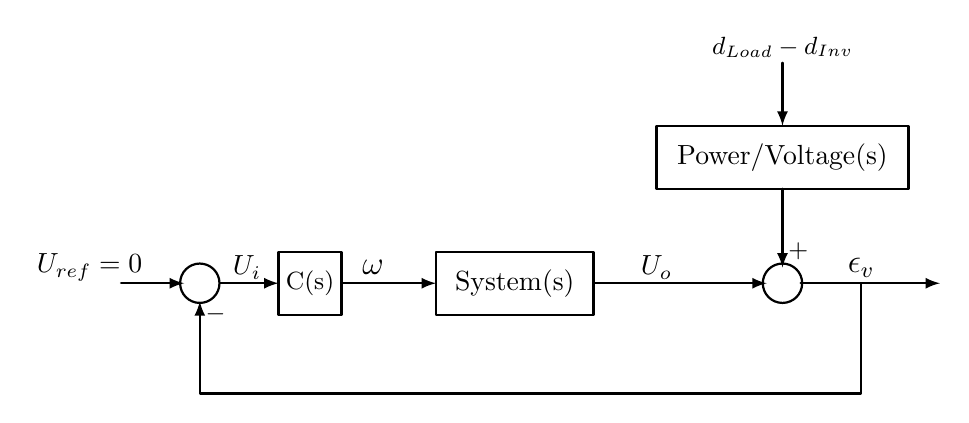
\begin{tikzpicture}

\draw  (-4.8,2.4) rectangle (-2.8,1.6);

\draw [-latex] (-2,4) rectangle (1.2,3.2);

\node at (-0.4,3.6) {\normalsize{Power/Voltage(s)}};
\node at (-3.8,2) {\normalsize{System(s)}};
\node at (-2,2.2) {\normalsize{$U_o$}};
\draw [-latex] (-0.4,2) ellipse (0.25 and 0.25);
\draw [-latex](-2.8,2) -- (-0.6,2);
\draw [-latex](-0.4,3.2) -- (-0.4,2.2);
\draw [-latex] (-6.8,2.4) rectangle (-6,1.6);
\node at (-6.4,2) {C(s)};
\draw [-latex](-6,2) -- (-4.8,2);
\node at (-5.6,2.2) {\large{$\omega$}};
\node at (-0.2,2.4) {$+$};
\draw [-latex] (-7.8,2) ellipse (0.25 and 0.25);
\draw [-latex](-7.54,2) -- (-6.8,2);
\draw [-latex](-0.4,4.8) -- (-0.4,4);
\node at (-0.4,5) {$d_{Load}-d_{Inv}$};
\draw [-latex](-8.8,2) -- (-8,2);
\node at (-9.2,2.2) {\normalsize{$U_{ref} = \footnotesize{0}$}};
\draw [-latex](-0.17,2) -- (1.6,2);
\node at (0.6,2.2) {\large{$\epsilon_v$}};
\draw [-latex](0.6,2) -- (0.6,0.6) -- (-7.8,0.6) -- (-7.8,1.77);
\node at (-7.6,1.6) {$-$};
\node at (-7.2,2.2) {\normalsize{$U_i$}};
\end{tikzpicture}
\caption{Simplified closed-loop system of the genset.}
\label{fig:blok_simplified}
\end{figure}

The subsystem denoted by 'System' is the plant, in other words, the transfer function derived between the mechanical angular velocity and the voltage output of the genset.


\begin{minipage}[t]{0.20\textwidth}
Where\\
\hspace*{8mm} $\omega$ \\
\hspace*{8mm} $U_o$ \\
\hspace*{8mm} $U_i$ \\
\hspace*{8mm} $U_{ref}$ \\
\hspace*{8mm} $d_{Load}-d_{Inv}$ \\
\hspace*{8mm} and $\epsilon_U$ 
\end{minipage}
\begin{minipage}[t]{0.68\textwidth}
\vspace*{2mm}
is the angular velocity output of the controller,\\
is the output voltage of the genset, \\
is the input voltage signal of the controller, \\
is the reference for the system, \\
is the disturbance affecting the system , \\
is the change(error) in the output voltage of the closed-loop controlled system. 

\end{minipage}
\begin{minipage}[t]{0.10\textwidth}
\vspace*{2mm}
\textcolor{White}{te}$\unit{\frac{rad}{s}}$\\
\textcolor{White}{te}$\unit{V}$\\
\textcolor{White}{te}$\unit{V}$\\
\textcolor{White}{te}$\unit{V}$\\
\textcolor{White}{te}$\unit{W}$\\
\textcolor{White}{te}$\unit{V}$
\end{minipage}

The block called 'Power/Voltage' serves as a conversion from power to voltage, since the disturbance applied to the system is in watts. Furthermore, it should be noted that the controller takes an input as voltage and creates a modified angular velocity input for the plant. Therefore the plant can be described as a SISO(Single Input Single Output) system according to the transfer funtion in \eqref{eq:tf_system}. 

\begin{equation}
\label{eq:tf_system}
G_{System}(s) = \frac{U_o(s)}{\omega(s)} = \frac {29.27s}{s^2 + 3.4s + 52.5} \unit{\cdot}
\end{equation}

The simplified plant will now be used to develop the controller. 
  

\subsection{Continuous state-space representation of the plant}
\label{ss_representation}

The above-mentioned transfer function can be represented as a two dimensional state-space system such as: 

\begin{equation}
  \label{eq:ss_sys1}
    \mathbf{\dot{x}(t)} = \mathbf{A} \mathbf{x}(t) + \mathbf{B} u(t)
  \end{equation}
\begin{equation}
  \label{eq:ss_sys2}
    y(t) = \mathbf{C} \mathbf{x}(t) + \mathbf{D} u(t)
  \end{equation}


\begin{minipage}[t]{0.20\textwidth}
Where\\
\hspace*{8mm} $\mathbf{A}$ \\
\hspace*{8mm} $\mathbf{B}$ \\
\hspace*{8mm} $\mathbf{C}$ \\
\hspace*{8mm} $\mathbf{D}$ \\
\hspace*{8mm} $\mathbf{x}$  \\
\hspace*{8mm} $y$  \\
\hspace*{8mm} and $u$  
\end{minipage}
\begin{minipage}[t]{0.68\textwidth}
\vspace*{2mm}
is the system matrix with a dimension: $\mathbb{R}^{(2 \times 2)}$,\\
is the input matrix with a dimension: $\mathbb{R}^{(2 \times 1)}$, \\
is the output matrix with a dimension: $\mathbb{R}^{(1 \times 2)}$, \\
is the feed-forward matrix with a dimension: $\mathbb{R}^{(1 \times 1)}$, \\
is the state vector with a dimension: $\mathbb{R}^{(2 \times 1)}$, \\
is the 1-dimensional output of the system, \\
is the 1-dimensional input of the system. 

\end{minipage}
\begin{minipage}[t]{0.10\textwidth}
\vspace*{2mm}
\textcolor{White}{te}$\unit{\cdot}$\\
\textcolor{White}{te}$\unit{\cdot}$\\
\textcolor{White}{te}$\unit{\cdot}$\\
\textcolor{White}{te}$\unit{\cdot}$\\
\textcolor{White}{te}$\unit{\cdot}$\\
\textcolor{White}{te}$\unit{V}$\\
\textcolor{White}{te}$\unit{\frac{rad}{s}}$
\end{minipage}

For the specific representation of the transfer function in \eqref{eq:tf_system}, the system consists of the following matrices: 

  \begin{equation}
  \label{eq:system_matrices_}
	\mathbf{A}
	 =   
    \begin{bmatrix}
    -3.40 & -52.05 \\
     1 & 0
\end{bmatrix}
;
\textcolor{White}{teeee}
\mathbf{B}
	 =   
    \begin{bmatrix}
    1 \\
    0
\end{bmatrix}
;
\textcolor{White}{teeee}
\mathbf{C}
	 =   
    \begin{bmatrix}
    29.27 & 0
\end{bmatrix}
;
\textcolor{White}{teeee}
\mathbf{D}
	 =   
    \begin{bmatrix}
    0
\end{bmatrix}
  \end{equation}

\subsection{State-space representation of the disturbance}
\label{statespace_disturbance}

Although there are several different ways to describe disturbances in control systems, in the presented report one approach is to assume that the power-flow of the inverter and the load can be described by differential equations. It is worth mentioning again that the behavior of the two different disturbances are significantly different. While the additional power-flow from the inverter can be approximated reasonably by a slowly-varying signal, the change in the load is much faster and in most of the cases is assumed to be completely unknown. Despite of the fact that there might be big changes in the load, in the introduction, and while introducing the principle of disturbances in state space, it is assumed to be constant. 

%\begin{figure}[H]
%\centering
%\includegraphics[width=0.3\textwidth]{rapport/billeder/disturbances}
%\caption{Disturbances acting on the plant}
%\label{fig:disturbances}
%\end{figure}

\begin{figure}[H]
\centering
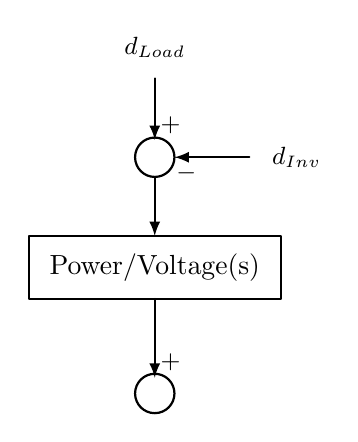
\begin{tikzpicture}

 \draw [-latex] (-0.4,2) ellipse (0.25 and 0.25);
 \draw [-latex] (-2,4) rectangle (1.2,3.2);
 \node at (-0.4,3.6) {\normalsize{Power/Voltage(s)}};
\draw [-latex](-0.4,3.2) -- (-0.4,2.2);
 \node at (-0.2,2.4) {$+$};
 \draw [-latex] (-0.4,5) ellipse (0.25 and 0.25);
\draw [-latex](-0.4,4.75) -- (-0.4,4);
\draw [-latex](-0.4,6) -- (-0.4,5.22);
\node at (-0.4,6.4) {$d_{Load}$};
\draw [-latex](0.8,5) -- (-0.15,5);
\node at (1.4,5) {$d_{Inv}$};
\node at (-0.2,5.4) {$+$};
\node at (0,4.8) {$-$};
\end{tikzpicture}
\caption{Disturbances acting on the plant.}
\label{fig:disturbances}
\end{figure}

As can be seen in \figref{fig:disturbances}, a conversion is required from power to voltage with certain dynamics. However when introducing the disturbances in state space, this dynamic behaviour is neglected and is taken into consideration in the simulation instead. Furthermore, the disturbances acting on the plant will be denoted by $d$ in order to make referencing easier in the further description . 

The disturbance that enters the state-space system can be considered as: 
\begin{equation}
  \label{eq:ss_dist_intro}
    \mathbf{\dot{x}(t)} = \mathbf{A} \mathbf{x}(t) + \mathbf{B} [u(t) + d(t)]
  \end{equation}

In \eqref{eq:ss_dist_intro} $d(t)$ is the disturbance signal which can be characterized by a specific differential equation or transfer function, which can be represented as an individual state-space system. Since the disturbance does not take any inputs, it only provides input for the state-space system of the plant according to \eqref{eq:ss_dist_intro}. The system for the disturbance is called an exo-system and is therefore represented in a form as follows:
%
\begin{equation}
  \label{eq:ss_exo1}
    \mathbf{\dot{x}_d(t)} = \mathbf{A_d} \mathbf{x_d}(t)
  \end{equation}
%
\begin{equation}
  \label{eq:ss_exo2}
    d(t) = \mathbf{C}_d \mathbf{x}_d(t)
  \end{equation}
%
The relation between a state-space model and its transfer function can be described by 
%
\begin{equation}
  \label{eq:ss_tf}
    D(s) = \mathbf{C}_d(s\mathbf{I}-\mathbf{A_d})^{-1} \mathbf{x_d}(0) = \mathbf{C}_d \frac{Adj(s\mathbf{I}-\mathbf{A_d})}{det(s\mathbf{I}-\mathbf{A_d})} \mathbf{x_d}(0) = \frac{f(0,s)}{\Gamma_d(s)}
  \end{equation}
  % 
\begin{minipage}[t]{0.20\textwidth}
Where\\
\hspace*{8mm} $f(0,s)$ \\
\hspace*{8mm} $\Gamma_d(s)$ \\
\hspace*{8mm} and $\mathbf{x_d}(0)$  
\end{minipage}
\begin{minipage}[t]{0.68\textwidth}
\vspace*{2mm}
is the polynomial in s arises because of initial conditions,\\
is called the disturbance generating polynomial, \\
is the vector of initial conditions. 

\end{minipage}

As can be seen, the disturbance generator is the characteristic polynomial of $A_d$. In order to build up the state-space matrices, \eqref{eq:ss_tf} can be split into two equations:
%
\begin{equation}
  \label{eq:ss_tf1}
    \Gamma_d(s) = det(s\mathbf{I}-\mathbf{A_d}) 
  \end{equation}
%
Where $\Gamma_d(s)$ can be considered as the denominator of the transfer function of the disturbance. Therefore $A_d$ can be found easily by solving a simple eigenvalue problem. The equation for the numerator can be written as: 
%
\begin{equation}
  \label{eq:ss_tf2}
    f(0,s) = \mathbf{C}_d Adj(s\mathbf{I}-\mathbf{A_d}) \mathbf{x_d}(0)
  \end{equation}
%
Where $f(0,s)$ represents the numerator of the transfer function of disturbance. $\mathbf{A_d}$ is known from \eqref{eq:ss_tf1} and $\mathbf{x_d}(0)$ consists of the priorly defined initial conditions. Therefore $\mathbf{C}_d$ can be calculated which means that the state representation of the disturbance becomes fully defined. It should be noted however, that even from \eqref{eq:ss_tf} or \eqref{eq:ss_tf2} it can be clearly seen, that if there is not any initial conditions defined for the disturbance, the elements of $\mathbf{C}_d$ are going to be zero. This directly means that there will not be any output of the exo-system, therefore there will not be any disturbance appearing on the output signal. 

According to \eqref{eq:ss_dist_intro}, \eqref{eq:ss_exo1} and \eqref{eq:ss_exo2}, the system can be rewritten in matrix form with the modified matrices including the exo-system: 
%
\begin{equation}
\label{eq:ss_dist1}
\begin{bmatrix}
    \mathbf{\dot{x}} \\
    \mathbf{\dot{x_d}} 
\end{bmatrix}
=
\underbrace{
 \begin{bmatrix}
    \mathbf{A} & \mathbf{B}\mathbf{C_d} \\
    0 & \mathbf{A_d}
\end{bmatrix}
}_\text{\normalsize{$\tilde{\mathbf{A}}$}}
\underbrace{
 \begin{bmatrix}
    \mathbf{x} \\
    \mathbf{x_d}
\end{bmatrix}
}_\text{\normalsize{$\tilde{x}$}}
+
\underbrace{
 \begin{bmatrix}
    \mathbf{B}  \\
    0 &  
\end{bmatrix}
}_\text{\normalsize{$\tilde{\mathbf{B}}$}}
    u
\end{equation}

\begin{equation}
\label{eq:ss_dist2}
    d
=
\underbrace{
 \begin{bmatrix}
    \mathbf{C} & 0 
\end{bmatrix}
}_\text{\normalsize{$\tilde{\mathbf{C}}$}}
 \begin{bmatrix}
    \mathbf{x} \\
    \mathbf{x_d}
\end{bmatrix}
\end{equation}

Therefore an extended state-space model is given where both the states of the plant and the disturbance are taken into account. It should be noted however, that the augmented system is not controllable from the input $d$ because the disturbance by the exo-system is an exogenous, autonomous input. The modified system can be illustrated such as in \figref{fig:exosystem}: 

%\begin{figure}[H]
%\centering
%\includegraphics[width=0.7\textwidth]{rapport/billeder/exosystem}
%\caption{Exo-system as the input of the system}
%\label{fig:exosystem}
%\end{figure}


\begin{figure}[H]
\centering
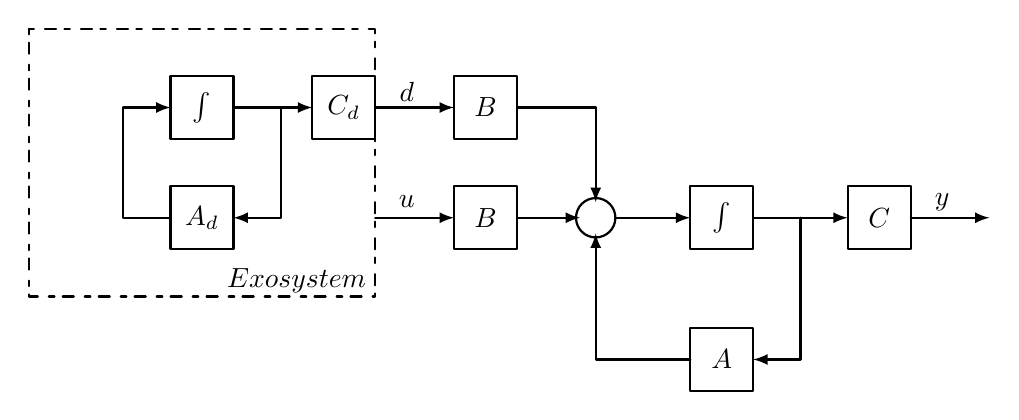
\begin{tikzpicture}


 \draw [-latex] (-0.4,2) ellipse (0.25 and 0.25);
\node at (1.2,0.2) {\normalsize{$A$}};
\node at (-1.8,2) {\normalsize{$B$}};
\node at (3.2,2) {\normalsize{$C$}};
\node at (-1.8,3.4) {\normalsize{$B$}};
\node at (-5.4,2) {\normalsize{$A_d$}};
\node at (-3.6,3.4) {\normalsize{$C_d$}};
\node at (1.2,2) {\normalsize{$\int$}};

\draw [-latex] (0.8,2.4) rectangle (1.6,1.6);
\draw [-latex] (0.8,0.6) rectangle (1.6,-0.2);
\draw [-latex] (2.8,2.4) rectangle (3.6,1.6);
\draw [-latex] (-2.2,2.4) rectangle (-1.4,1.6);
\draw [-latex] (-2.2,3.8) rectangle (-1.4,3);
\draw [-latex](-1.4,2) -- (-0.6,2);
\draw [-latex](-0.15,2) -- (0.8,2);


\draw [-latex](1.6,2) -- (2.8,2);
\draw [-latex](3.6,2) -- (4.6,2);
\draw [-latex](2.2,2) -- (2.2,0.2) -- (1.6,0.2);
\draw [-latex](0.8,0.2) -- (-0.4,0.2) -- (-0.4,1.8);
\draw [-latex](-1.4,3.4) -- (-0.4,3.4) -- (-0.4,2.2);

\node at (-5.4,3.4) {\normalsize{$\int$}};

\draw [-latex] (-4,3.8) rectangle (-3.2,3);
\draw [-latex] (-5.8,3.8) rectangle (-5,3);
\draw [-latex] (-5.8,2.4) rectangle (-5,1.6);
\draw [-latex](-3.2,3.4) -- (-2.2,3.4);
\draw [-latex](-3.2,2) -- (-2.2,2);
\draw [-latex](-5,3.4) -- (-4,3.4);
\draw [-latex](-4.4,3.4) -- (-4.4,2) -- (-5,2);
\draw [-latex](-5.8,2) -- (-6.4,2) -- (-6.4,3.4) -- (-5.8,3.4);
\node at (-2.8,3.6) {\normalsize{$d$}};
\node at (-2.8,2.2) {\normalsize{$u$}};
\node at (4,2.2) {\normalsize{$y$}};
\draw [dash pattern=on 2pt off 3pt on 4pt off 4pt] (-7.6,4.4) rectangle (-3.2,1);
\node at (-4.2,1.2) {\normalsize{$Exosystem$}};
\end{tikzpicture}

\caption{Exo-system as the input of the system.}
\label{fig:exosystem}
\end{figure}





\subsection{Disturbances affecting the system}
\label{disturbances}

In \secref{statespace_disturbance}, the two kinds of disturbances were introduced, namely the load and the inverter. The inverter, as it was mentioned, provides a slowly changing power flow that can be approximated as a sinusoidal shown in \eqref{eq:dist1} : 

\begin{equation}
  \label{eq:dist1}
    d_{inv}(t) = \alpha sin(\omega t)
  \end{equation}

By solving \eqref{eq:ss_tf1} and \eqref{eq:ss_tf2} the state space system can be constructed: 


\begin{equation}
\label{eq:exo_statespace}
 \begin{bmatrix}
    \dot{x}_{d1} \\
    \dot{x}_{d2}
\end{bmatrix}
=
 \begin{bmatrix}
    0 & \omega^2 \\
    -\omega^2 & 0
\end{bmatrix}
 \begin{bmatrix}
    x_{d1} \\
    x_{d2}
\end{bmatrix}
\end{equation}

\begin{equation}
\label{eq:ss_dist2}
    d
=
 \begin{bmatrix}
    1 & 0 
\end{bmatrix}
 \begin{bmatrix}
    x_{d1} \\
    x_{d2}
\end{bmatrix}
\end{equation}

The characteristic polynomial of the sinusoidal disturbance system, as expected is: 

\begin{equation}
  \label{eq:distpoly}
    \Gamma_{inverter}(s) = det(s\mathbf{I}-\mathbf{A_d}) = s^2 + \omega^2 
  \end{equation}
  
%The case of the load however is significantly different from the case of the inverter. The load is, as mentioned, usually unknown and can produce big changes. The fact that the behaviour of the load is completely unknown in reality cannot be neglected, however in the simulation a constant load is described to show how the system can reject it. The reason behind making a disturbance that dramatically affects the voltage output of the system is that if the load was constant, a slowly varying inverter power flow would never cause changes on the output. That is because the AVR and the other inner controllers can easily handle slow disturbances such as the inverter power flow. 


In order to construct the combination of the two disturbances, the following rule applies: 

\begin{equation}
  \label{eq:combined_dist}
  d(t) = d_{inv}(t) + d_{load}(t) = \Gamma_{inv}(s)\Gamma_{load}(s)
  \end{equation}
  
As can be seen in \eqref{eq:combined_dist}, the combined disturbance system can be calculated by multiplying the disturbance generating polynomials for $d_{inv}(t)$ and $d_{load}(t)$. Thus, the final form of the disturbance becomes: 

\begin{equation}
  \label{eq:dist_final}
  d(t) = d_{inv}(t) + d_{load}(t) = c + \alpha sin(\omega t)
  \end{equation}

that is a slowly-varying sinusoidal disturbance with an offset. 
\section{Controller design with exosystem in continuous time}
\label{system_design}

The main goal of the control is to make the system react faster to changes in the load. Along with the the inverter power, load changes affect the system as disturbances. The main task is then to reject these disturbances and make the closed-loop dynamics react faster to sudden changes coming from the load. This directly means that by applying a controller to the system, the error in voltage will be reduced on the output, and will go to zero as fast as it is possible. 
The dynamics of the system are changed through feeding back the states, thus the feedback law for the overall closed loop system becomes: 

\begin{equation}
  \label{eq:feedbacklaw}
  u = r + \mathbf{Fx}
  \end{equation}

It should be noted however, that due to the separation principle the state feedback and the observer problem can be handled independently and furthermore, while designing the state feedback for the system, disturbances can be neglected on the system. The block diagram of the system then simplifies to: 

%\begin{figure}[H]
%\centering
%\includegraphics[width=0.55\textwidth]{rapport/billeder/stateblock}
%\caption{State feedback}
%\label{fig:stateblock}
%\end{figure}

\begin{figure}[H]
\centering
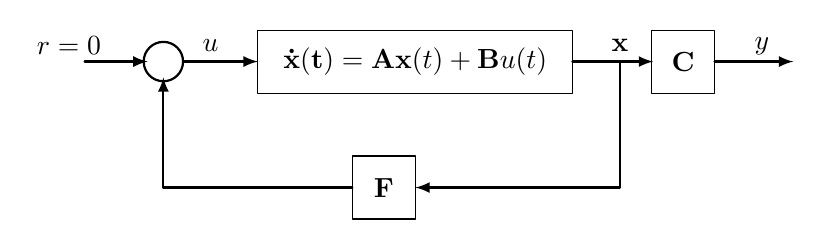
\begin{tikzpicture}

 \draw [-latex] (-0.4,2) ellipse (0.25 and 0.25);
\node at (2.8,2) {\normalsize{$\mathbf{\dot{x}(t)} = \mathbf{A} \mathbf{x}(t) + \mathbf{B} u(t) $}};

\draw [thin] (0.8,2.4) rectangle (4.8,1.6);
 \node at (6.2,2) {\normalsize{$\mathbf{C}$}};
\draw [thin] (5.8,2.4) rectangle (6.6,1.6);
 \node at (2.4,0.4) {\normalsize{$\mathbf{F}$}};


\draw [thin] (2,0.8) rectangle (2.8,0);
\draw [thin](4.67,2) node (v1) {};

\draw [-latex](v1) -- (5.82,2);
\draw [-latex](6.6,2) -- (7.6,2);
\draw [-latex](5.4,2) -- (5.4,0.4) -- (2.8,0.4);
\draw [-latex](-0.15,2) -- (0.8,2);
\draw [-latex](2,0.4) -- (-0.4,0.4) -- (-0.4,1.8);
\draw [-latex](-1.4,2) -- (-0.6,2);
\node at (0.2,2.2) {\normalsize{$u$}};
\node at (5.4,2.2) {\normalsize{$\mathbf{x}$}};
\node at (7.2,2.2) {\normalsize{$y$}};
\node at (-1.6,2.2) {\normalsize{$r = 0$}};
\end{tikzpicture}
\caption{State feedback}
\label{fig:statefeedback}
\end{figure}


Therefore the control problem simplifies to the problem of finding new locations of the eigenvalues such as:

\begin{equation}
  \label{eq:distpoly}
    det(s\mathbf{I}-(\mathbf{A} + \mathbf{B} \mathbf{F}))
  \end{equation}

Since these eigenvalues define the closed-loop dynamics, the main design decision is to find where to place them. The original poles of the system are: 
\begin{equation}
  \label{eq:original poles}
  p_{1;2} = -1.7 \pm j7
  \end{equation}

It can be clearly seen from \eqref{eq:original poles} that the system has a complex conjugate pole pair on the left-hand side of the real axis, therefore the system is stable, as it was expected. By placing the poles more than four times further, the following pole configuration can be achieved: 

\begin{equation}
  \label{eq:desired_poles}
  p_{F_{1;2}} = -8 \pm j7
  \end{equation}
  
The step response with state feedback yields: 
\begin{figure}[H]
\centering
\includegraphics[width=0.85\textwidth]{rapport/billeder/statefeedback}
\caption{State feedback.}
\label{fig:statefeedback}
\end{figure}


And the state feedback gain is the following:

\begin{equation}
\label{eq:ss_dist2}
    F
=
 \begin{bmatrix}
    -12.6 & -60.95
\end{bmatrix}
\end{equation}
\subsection{Observer design}
\label{observer}

As it is shown in \figref{fig:statefeedback}, it is possible to find a state feedback law that gives closed-loop eigenvalues with desired dynamics and a condition that all states are measured. Even if all states are measured or measurable, the disturbances has to be taken into consideration while designing the observer. 

If a system is observable, it is possible to recover the states from measurements of the input and output of the system. The feedback law is exactly the same as in \eqref{eq:feedbacklaw} with the exception that now the disturbance is also considered and due to the separation principle it is sufficient to design the observer without the state feedback. The purpose of the observer is now to reconstruct both the system states $\mathbf{x}$ and the disturbance $d$ from the input and the output. Since the disturbance has an effect on the output, it is observable from y. Furthermore, $d$ is generally unknown, thus it is reasonable to estimate it with a help of an observer. It is important to mention that although the disturbance cannot be measured, information about its structure and periodicity are assumed to be available in this simulation. 

The system with the observer and state feedback can be represented as follows: 

%\begin{figure}[H]
%\centering
%\includegraphics[width=0.65\textwidth]{rapport/billeder/observerblock}
%\caption{State feedback}
%\label{fig:observerblock}
%\end{figure}


\begin{figure}[H]
\centering
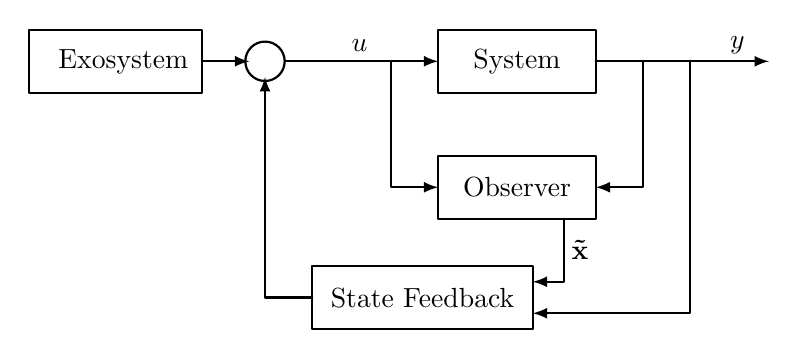
\begin{tikzpicture}


 \draw [-latex] (-1.2,2) ellipse (0.25 and 0.25);
 \node at (2,2) {\normalsize{System}};
\draw [-latex] (1,2.4) rectangle (3,1.6);
 \node at (2,0.4) {\normalsize{Observer}};


\draw [-latex] (1,0.8) rectangle (3,0);
\draw [-latex](-0.95,2) -- (1,2);
\draw [-latex](0.4,2) -- (0.4,0.4) -- (1,0.4);
\draw [-latex](3,2) -- (5.2,2);
\draw [-latex](3.6,2) -- (3.6,0.4) -- (3,0.4);

 \node at (0.8,-1) {\normalsize{State Feedback}};
 
 
\draw [-latex] (-0.6,-0.6) rectangle (2.2,-1.4);
\draw [-latex](2.6,0) -- (2.6,-0.8) -- (2.2,-0.8);
\draw [-latex](4.2,2) -- (4.2,-1.2) -- (2.2,-1.2);
\draw [-latex](-0.6,-1) -- (-1.2,-1) -- (-1.2,1.8);

\node at (-3,2) {\normalsize{Exosystem}};

\draw [-latex] (-4.2,2.4) rectangle (-2,1.6);
\draw [-latex](-2,2) -- (-1.4,2);
\node at (4.8,2.2) {\normalsize{$y$}};
\node at (0,2.2) {\normalsize{$u$}};

\node at (2.8,-0.4) {\normalsize{$\mathbf{\tilde{x}}$}};

\end{tikzpicture}
\caption{State feedback}
\label{fig:observerblock}
\end{figure}

Therefore the state-space system description becomes: 

\begin{equation}
\label{eq:ss_obs1}
\frac{d}{dt}
\begin{bmatrix}
    \mathbf{\tilde{x}} \\
    \mathbf{\tilde{x_d}} 
\end{bmatrix}
=
 \begin{bmatrix}
    \mathbf{A} & \mathbf{B}\mathbf{C_d} \\
    0 & \mathbf{A_d}
\end{bmatrix}
 \begin{bmatrix}
    \mathbf{\tilde{x}} \\
    \mathbf{\tilde{x_d}}
\end{bmatrix}
+
 \begin{bmatrix}
    \mathbf{B}  \\
    0 &  
\end{bmatrix}
    u
    +
 \begin{bmatrix}
    \mathbf{L_1}  \\
    \mathbf{L_2}  
\end{bmatrix}
 \begin{bmatrix}
    y - \mathbf{C}\mathbf{\tilde{x}}
\end{bmatrix}
\end{equation}

The modified control law:

\begin{equation}
  \label{eq:ss_obs2}
  u =  \mathbf{F} \mathbf{\tilde{x}_{combined}} 
  =
 \begin{bmatrix}
    \mathbf{F} & \mathbf{-C_d}  
\end{bmatrix}
 \begin{bmatrix}
\mathbf{\tilde{x}}  \\
\mathbf{\tilde{x_d}}
\end{bmatrix}
  \end{equation}
  
As can be seen in \eqref{eq:ss_obs2}, the feedback gain is extended in order to reproduce the disturbance and subtract it from the output. 
  
The control problem of finding the appropriate observer feedback gains simplifies to the problem of finding new locations of the closed-loop eigenvalues of the observer such as:

\begin{equation}
  \label{eq:distpoly}
    det(s\mathbf{I}-(\mathbf{\tilde{A}} + \mathbf{\tilde{L}} \mathbf{\tilde{C}}))
  \end{equation}

Since the poles of the observer should not have any effect on the system, in other words, it is undesirable to introduce new dominant poles in the system, as a rule of thumb the poles should be placed 2 to 6 times further to the left-hand side along the real axis from the poles of the state feedback. By making the observer dynamics react fast, the difference between the estimated and the real output will converge faster to zero. According to \eqref{eq:desired_poles}, the poles should be placed at: 

\begin{equation}
  \label{eq:desired_poles_observer1}
  p_{L_{3;4}} = -16 \pm j7
  \end{equation}
  
and
  
\begin{equation}
  \label{eq:desired_poles_observer2}
  p_{L_{5}} = -2 +j0
  \end{equation}
  
  \begin{equation}
  \label{eq:desired_poles_observer3}
  p_{L_{6}} = -4 +j0
  \end{equation}
  

  
  
  
\subsection{Results and conclusions of the exosystem control design}
\label{Exo_result}

As can be seen in \figref{fig:sin_disturbance}, by applying the disturbance through an exosystem as an input to the original system, the slowly-varying sinusoidal appears on the output.

\begin{figure}[H]
\centering
\includegraphics[width=1.1\textwidth]{rapport/billeder/temporary/sinusdist}
\caption{Slowly varying sinusoidal disturbance on the output.}
\label{fig:sin_disturbance}
\end{figure}

However, during the real-life measurements and according to the simulation of the genset, this result could never be obtained. The main reason why this result could not be achieved is that the genset with its inner AVR control can easily react to small and slow changes on the voltage, therefore would the disturbance all ready be handled by the genset and not be present on the output. 

In simulation where the genset is unable to handle the disturbance, applying the designed controller, results in the following dynamics for disturbance rejection, that are shown in \figref{fig:sin_disturbance_reject} where it is seen that the disturbance is effectively rejected. 

\begin{figure}[H]
\centering
\includegraphics[width=1.1\textwidth]{rapport/billeder/temporary/eliminated_disturbance}
\caption{Sinusoidal disturbance rejected due to observer, feedback and state space control.}
\label{fig:sin_disturbance_reject}
\end{figure}

After coming to the realization that this approach does not fit reality, it was decided to put more focus on the fast varying load and make a design that can handle it in simulation and in reality. Therefore the following sections deals with a more suitable controller design. 
\section{Controller design with disturbance on the output}
\label{system_design_implementation}


As mentioned in \secref{control_intro}, a better control approach is to represent the state space model in discrete time in order to make it possible to implement on the system. In \figref{fig:block_dist}, an overview of the control design can be seen where the disturbance is on the output of the system and therefore not included in the state-space design.

\begin{figure}[H]
\centering
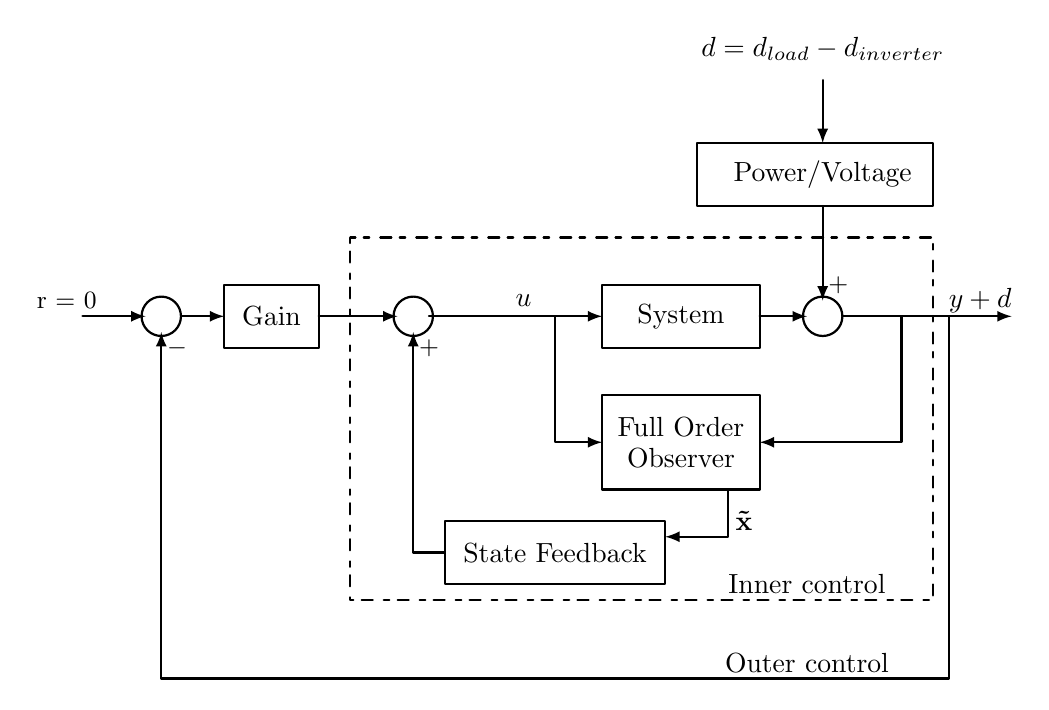
\begin{tikzpicture}
 \draw [-latex] (-1.4,2) ellipse (0.25 and 0.25);
 \node at (2,2) {\normalsize{System}};
\draw [-latex] (1,2.4) rectangle (3,1.6);
 \node at (2,0.2) {\normalsize{Observer}};
  \node at (2,0.6) {\normalsize{Full Order}};


\draw [-latex] (1,1) rectangle (3,-0.2);
\draw [-latex](-1.2,2) -- (1,2);
\draw [-latex](0.4,2) -- (0.4,0.4) -- (1,0.4);

\draw [-latex](4.8,2) -- (4.8,0.4) -- (3,0.4);

 \node at (0.4,-1) {\normalsize{State Feedback}};
 
 
\draw [-latex] (-1,-0.6) rectangle (1.8,-1.4);
\draw [-latex](2.6,-0.2) -- (2.6,-0.8) -- (1.8,-0.8);

\draw [-latex](-1,-1) -- (-1.4,-1) -- (-1.4,1.8);

  \node at (-3.2,2) {\normalsize{Gain}};


\draw [-latex](-2.6,2) -- (-1.6,2);
\node at (5.8,2.2) {\normalsize{$y+d$}};
\node at (0,2.2) {\normalsize{$u$}};

\node at (2.8,-0.6) {\normalsize{$\mathbf{\tilde{x}}$}};

\draw [-latex] (-3.8,2.4) rectangle (-2.6,1.6);

\draw [-latex] (-4.6,2) ellipse (0.25 and 0.25);

 \draw [-latex] (3.8,2) ellipse (0.25 and 0.25);

\draw [-latex](3,2) -- (3.6,2);
\draw [-latex](4.05,2) -- (6.2,2);
\draw [-latex](3.8,3.4) -- (3.8,2.2);



\draw [-latex](-4.35,2) -- (-3.8,2);
\draw [-latex](-5.6,2) -- (-4.8,2);
\draw [-latex](5.4,2) -- (5.4,-2.6) -- (-4.6,-2.6) -- (-4.6,1.8);

 \node at (3.8,5.4) {\normalsize{$d =d_{load}-d_{inverter}$}};
 
 \node at (4,2.4) {$+$};
\node at (-4.4,1.6) {$-$};
\node at (-5.8,2.2) {r = 0};

\draw [dash pattern=on 2pt off 3pt on 4pt off 4pt] (-2.2,3) rectangle (5.2,-1.6);
\node at (3.6,-1.4) {\normalsize{Inner control}};
\node at (3.6,-2.4) {\normalsize{Outer control}};

\draw [-latex] (2.2,4.2) rectangle (5.2,3.4);
\node at (3.8,3.8) {\normalsize{Power/Voltage}};
\draw [-latex](3.8,5) -- (3.8,4.2);
\node at (-1.2,1.6) {$+$};
\end{tikzpicture}


\caption{Block diagram of the system with disturbance.}
\label{fig:block_dist}
\end{figure}

The control has to deal with two control levels. The inner and outer control loops have to work together and reduce the effect of the disturbances. The state feedback sets the dynamics of the system. Therefore the feedback gain should be carefully chosen in order to avoid overreaction due to the disturbance in the outer loop. 

During the implementation, the voltage on the output is measured and the input signal for the system is known. For that reason, a full state observer is applied to calculate the states for the state feedback. 

The gain in the outer system serves as a scaling factor for the discrete system and helps improving the voltage error on the output. The reference of the system is set to zero because the error on the output should converge to zero without significant overshoots and as fast as it is possible. 

\subsection{Discretization of the system}
\label{discrete}

The continuous representation of the system was introduced in \eqref{eq:ss_sys1} and \eqref{eq:ss_sys2}, however the plant of the genset should be discretized from the beginning of the design process. In discrete time the plant can be represented as follows: 

\begin{equation}
  \label{eq:ss_sys1_d}
    \mathbf{x}[k+1] = \mathbf{A_d} \mathbf{x}[k] + \mathbf{B_d} u[k]
  \end{equation}
\begin{equation}
  \label{eq:ss_sys2_d}
    y[k] = \mathbf{C} \mathbf{x}[k]
  \end{equation}
  
When converting the state-space matrices from continuous to discrete, the sampling time of the system has to be considered. In case of the genset, the sampling and processing time for computing the RMS values of the voltage takes $16 [ms]$. Sending control signals with CANbus can take up to $40 [ms]$, therefore the plant is discretized with the higher sampling time. 

The modified matrices of the system are depending on the sampling time($h = 40 [ms]$) as follows:

\begin{equation}
  \label{eq:Ad}
    \mathbf{A_d} = e^{\mathbf{A}h}  
  \end{equation}

\begin{equation}
  \label{eq:Bd}
    \mathbf{B_d} = \int_{0}^{h} e^{\mathbf{A}s}ds\mathbf{B}
  \end{equation}

And therefore the matrices become: 

 \begin{equation}
  \label{eq:system_matrices_}
	\mathbf{A}
	 =   
    \begin{bmatrix}
    0.835 & -1.920 \\
     0.036 & 0.960
\end{bmatrix}
;
\textcolor{White}{teeee}
\mathbf{B}
	 =   
    \begin{bmatrix}
    0.03688 \\
    0.00075
\end{bmatrix}
;
\textcolor{White}{teeee}
\mathbf{C}
	 =   
    \begin{bmatrix}
    29.27 & 0
\end{bmatrix}
  \end{equation}
% This file was created by matlab2tikz.
%
%The latest updates can be retrieved from
%  http://www.mathworks.com/matlabcentral/fileexchange/22022-matlab2tikz-matlab2tikz
%where you can also make suggestions and rate matlab2tikz.
%
\definecolor{mycolor1}{rgb}{0.00000,0.44700,0.74100}%
\definecolor{mycolor2}{rgb}{0.85000,0.32500,0.09800}%
%
\begin{tikzpicture}

\begin{axis}[%
width=4.396in,
height=3.357in,
at={(0.883in,0.481in)},
scale only axis,
separate axis lines,
every outer x axis line/.append style={white!40!black},
every x tick label/.append style={font=\color{white!40!black}},
xmin=0,
xmax=4.5,
xlabel={Time [s]},
xmajorgrids,
every outer y axis line/.append style={white!40!black},
every y tick label/.append style={font=\color{white!40!black}},
ymin=-1.5,
ymax=3.5,
ylabel={Voltage [V]},
ymajorgrids,
axis background/.style={fill=white},
legend style={legend cell align=left,align=left,draw=white!15!black}
]
\addplot [color=mycolor1,solid]
  table[row sep=crcr]{%
0	0\\
0.04	0\\
0.04	1.173\\
0.08	1.173\\
0.08	2.106\\
0.12	2.106\\
0.12	2.757\\
0.16	2.757\\
0.16	3.112\\
0.2	3.112\\
0.2	3.182\\
0.24	3.182\\
0.24	2.996\\
0.28	2.996\\
0.28	2.603\\
0.32	2.603\\
0.32	2.058\\
0.36	2.058\\
0.36	1.424\\
0.4	1.424\\
0.4	0.7597\\
0.44	0.7597\\
0.44	0.1216\\
0.48	0.1216\\
0.48	-0.4446\\
0.52	-0.4446\\
0.52	-0.9045\\
0.56	-0.9045\\
0.56	-1.236\\
0.6	-1.236\\
0.6	-1.43\\
0.64	-1.43\\
0.64	-1.488\\
0.68	-1.488\\
0.68	-1.424\\
0.72	-1.424\\
0.72	-1.258\\
0.76	-1.258\\
0.76	-1.016\\
0.8	-1.016\\
0.8	-0.726\\
0.84	-0.726\\
0.84	-0.4169\\
0.88	-0.4169\\
0.88	-0.1149\\
0.92	-0.1149\\
0.92	0.1576\\
0.96	0.1576\\
0.96	0.3832\\
1	0.3832\\
1	0.5504\\
1.04	0.5504\\
1.04	0.6538\\
1.08	0.6538\\
1.08	0.6935\\
1.12	0.6935\\
1.12	0.6746\\
1.16	0.6746\\
1.16	0.6058\\
1.2	0.6058\\
1.2	0.499\\
1.24	0.499\\
1.24	0.3672\\
1.28	0.3672\\
1.28	0.2238\\
1.32	0.2238\\
1.32	0.08129\\
1.36	0.08129\\
1.36	-0.04934\\
1.4	-0.04934\\
1.4	-0.1595\\
1.44	-0.1595\\
1.44	-0.2434\\
1.48	-0.2434\\
1.48	-0.2977\\
1.52	-0.2977\\
1.52	-0.3221\\
1.56	-0.3221\\
1.56	-0.3185\\
1.6	-0.3185\\
1.6	-0.2907\\
1.64	-0.2907\\
1.64	-0.244\\
1.68	-0.244\\
1.68	-0.1844\\
1.72	-0.1844\\
1.72	-0.1181\\
1.76	-0.1181\\
1.76	-0.05108\\
1.8	-0.05108\\
1.8	0.01135\\
1.84	0.01135\\
1.84	0.06495\\
1.88	0.06495\\
1.88	0.1067\\
1.92	0.1067\\
1.92	0.1349\\
1.96	0.1349\\
1.96	0.1491\\
2	0.1491\\
2	0.1499\\
2.04	0.1499\\
2.04	0.1391\\
2.08	0.1391\\
2.08	0.1188\\
2.12	0.1188\\
2.12	0.092\\
2.16	0.092\\
2.16	0.06146\\
2.2	0.06146\\
2.2	0.03005\\
2.24	0.03005\\
2.24	0.0003209\\
2.28	0.0003209\\
2.28	-0.02565\\
2.32	-0.02565\\
2.32	-0.04634\\
2.36	-0.04634\\
2.36	-0.0608\\
2.4	-0.0608\\
2.4	-0.06873\\
2.44	-0.06873\\
2.44	-0.07033\\
2.48	-0.07033\\
2.48	-0.06629\\
2.52	-0.06629\\
2.52	-0.05764\\
2.56	-0.05764\\
2.56	-0.04564\\
2.6	-0.04564\\
2.6	-0.03163\\
2.64	-0.03163\\
2.64	-0.01696\\
2.68	-0.01696\\
2.68	-0.002842\\
2.72	-0.002842\\
2.72	0.009696\\
2.76	0.009696\\
2.76	0.01989\\
2.8	0.01989\\
2.8	0.02725\\
2.84	0.02725\\
2.84	0.03156\\
2.88	0.03156\\
2.88	0.03289\\
2.92	0.03289\\
2.92	0.0315\\
2.96	0.0315\\
2.96	0.02785\\
3	0.02785\\
3	0.02252\\
3.04	0.02252\\
3.04	0.01612\\
3.08	0.01612\\
3.08	0.009292\\
3.12	0.009292\\
3.12	0.002612\\
3.16	0.002612\\
3.16	-0.003419\\
3.2	-0.003419\\
3.2	-0.008418\\
3.24	-0.008418\\
3.24	-0.01213\\
3.28	-0.01213\\
3.28	-0.01443\\
3.32	-0.01443\\
3.32	-0.01533\\
3.36	-0.01533\\
3.36	-0.01492\\
3.4	-0.01492\\
3.4	-0.01341\\
3.44	-0.01341\\
3.44	-0.01106\\
3.48	-0.01106\\
3.48	-0.008151\\
3.52	-0.008151\\
3.52	-0.004982\\
3.56	-0.004982\\
3.56	-0.001831\\
3.6	-0.001831\\
3.6	0.00106\\
3.64	0.00106\\
3.64	0.003501\\
3.68	0.003501\\
3.68	0.005361\\
3.72	0.005361\\
3.72	0.00657\\
3.76	0.00657\\
3.76	0.007117\\
3.8	0.007117\\
3.8	0.007044\\
3.84	0.007044\\
3.84	0.006435\\
3.88	0.006435\\
3.88	0.005407\\
3.92	0.005407\\
3.92	0.004091\\
3.96	0.004091\\
3.96	0.002627\\
4	0.002627\\
4	0.001145\\
4.04	0.001145\\
4.04	-0.000236\\
4.08	-0.000236\\
4.08	-0.001423\\
4.12	-0.001423\\
4.12	-0.002349\\
4.16	-0.002349\\
4.16	-0.002976\\
4.2	-0.002976\\
4.2	-0.003293\\
4.24	-0.003293\\
4.24	-0.003315\\
4.28	-0.003315\\
4.28	-0.003077\\
4.32	-0.003077\\
4.32	-0.002632\\
4.36	-0.002632\\
4.36	-0.002041\\
4.4	-0.002041\\
4.4	-0.001366\\
4.44	-0.001366\\
4.44	-0.000672\\
4.48	-0.000672\\
4.48	-1.42e-05\\
4.52	-1.42e-05\\
};
\addlegendentry{Open loop};

% \addplot [color=black,dotted,forget plot]
%   table[row sep=crcr]{%
% -0.45	0\\
% 0	0\\
% 1	0\\
% 4.95	0\\
% };
\addplot [color=mycolor2,solid]
  table[row sep=crcr]{%
0	0\\
0.04	0\\
0.04	1.173\\
0.08	1.173\\
0.08	1.642\\
0.12	1.642\\
0.12	1.646\\
0.16	1.646\\
0.16	1.39\\
0.2	1.39\\
0.2	1.029\\
0.24	1.029\\
0.24	0.6671\\
0.28	0.6671\\
0.28	0.3608\\
0.32	0.3608\\
0.32	0.1337\\
0.36	0.1337\\
0.36	-0.01372\\
0.4	-0.01372\\
0.4	-0.09366\\
0.44	-0.09366\\
0.44	-0.1235\\
0.48	-0.1235\\
0.48	-0.1207\\
0.52	-0.1207\\
0.52	-0.1003\\
0.56	-0.1003\\
0.56	-0.07314\\
0.6	-0.07314\\
0.6	-0.04657\\
0.64	-0.04657\\
0.64	-0.02447\\
0.68	-0.02447\\
0.68	-0.008327\\
0.72	-0.008327\\
0.72	0.001967\\
0.76	0.001967\\
0.76	0.00739\\
0.8	0.00739\\
0.8	0.009251\\
0.84	0.009251\\
0.84	0.008837\\
0.88	0.008837\\
0.88	0.00722\\
0.92	0.00722\\
0.92	0.005188\\
0.96	0.005188\\
0.96	0.003242\\
1	0.003242\\
1	0.001651\\
1.04	0.001651\\
1.04	0.0005056\\
1.08	0.0005056\\
1.08	-0.0002113\\
1.12	-0.0002113\\
1.12	-0.0005774\\
1.16	-0.0005774\\
1.16	-0.0006906\\
1.2	-0.0006906\\
1.2	-0.0006454\\
1.24	-0.0006454\\
1.24	-0.000519\\
1.28	-0.000519\\
1.28	-0.0003672\\
1.32	-0.0003672\\
1.32	-0.0002251\\
1.36	-0.0002251\\
1.36	-0.0001107\\
1.4	-0.0001107\\
1.4	-2.962e-05\\
1.44	-2.962e-05\\
1.44	2.017e-05\\
1.48	2.017e-05\\
1.48	4.473e-05\\
1.52	4.473e-05\\
1.52	5.139e-05\\
1.56	5.139e-05\\
1.56	4.704e-05\\
1.6	4.704e-05\\
1.6	3.724e-05\\
1.64	3.724e-05\\
1.64	2.595e-05\\
1.68	2.595e-05\\
1.68	1.559e-05\\
1.72	1.559e-05\\
1.72	7.374e-06\\
1.76	7.374e-06\\
1.76	1.645e-06\\
1.8	1.645e-06\\
1.8	-1.804e-06\\
1.84	-1.804e-06\\
1.84	-3.441e-06\\
1.88	-3.441e-06\\
1.88	-3.813e-06\\
1.92	-3.813e-06\\
1.92	-3.422e-06\\
1.96	-3.422e-06\\
1.96	-2.668e-06\\
2	-2.668e-06\\
2	-1.829e-06\\
2.04	-1.829e-06\\
2.04	-1.076e-06\\
2.08	-1.076e-06\\
2.08	-4.874e-07\\
2.12	-4.874e-07\\
2.12	-8.33e-08\\
2.16	-8.33e-08\\
2.16	1.547e-07\\
2.2	1.547e-07\\
2.2	2.63e-07\\
2.24	2.63e-07\\
2.24	2.821e-07\\
2.28	2.821e-07\\
2.28	2.484e-07\\
2.32	2.484e-07\\
2.32	1.908e-07\\
2.36	1.908e-07\\
2.36	1.287e-07\\
2.4	1.287e-07\\
2.4	7.399e-08\\
2.44	7.399e-08\\
2.44	3.191e-08\\
2.48	3.191e-08\\
2.48	3.478e-09\\
2.52	3.478e-09\\
2.52	-1.29e-08\\
2.56	-1.29e-08\\
2.56	-2e-08\\
2.6	-2e-08\\
2.6	-2.081e-08\\
2.64	-2.081e-08\\
2.64	-1.8e-08\\
2.68	-1.8e-08\\
2.68	-1.362e-08\\
2.72	-1.362e-08\\
2.72	-9.037e-09\\
2.76	-9.037e-09\\
2.76	-5.07e-09\\
4.95	-5.07e-09\\
};
\addlegendentry{State feedback};

%\addplot [color=black,dotted,forget plot]
%  table[row sep=crcr]{%
%-0.45	4.245e-16\\
%0	4.245e-16\\
%1	4.245e-16\\
%4.95	4.245e-16\\
%};
\end{axis}
\end{tikzpicture}%
%\subsection{LQR}
\label{LQR}

::::::::::UNDER CONSTRUCTION in Matlab::::::::::::


\subsection{Estimator design}
\label{estimator}

Using an estimator, the states of the system can be reconstructed from the available voltage measurement on the output and the input of the system. While designing an observer (estimator), the main task is to estimate state $\mathbf{x}[k]$ from input and output sequences $y[k], y[k-1],..., u[k], u[k-1]$ .
During the real-life measurements, the estimates are provided by the same model placed parallel to the measured system. Even though, the system for the estimation is driven by the same input, in practice, uncertainties are expected. Which means that even if the initial state of the model is set equal to the initial state of the plant, in practice, without feedback the state estimate would diverge from the true state. The solution to this is to use the output measurements and make a comparison between that and the predicted output data. For that reason the difference can be used to modify the state estimate in such a way that it converges to the true state vector. The algorithm is illustrated in \figref{fig:algorithm} for the whole system.

\begin{figure}[H]
\centering

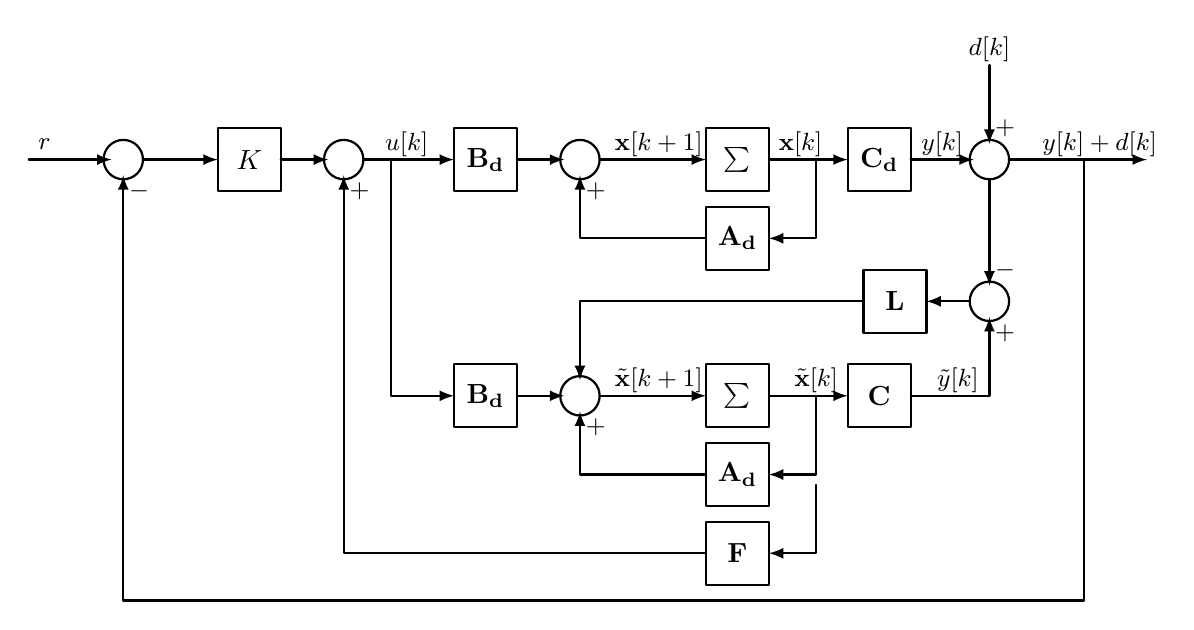
\begin{tikzpicture}
\node at (2.4,3.4) {\normalsize{$\mathbf{C_d}$}};
 \draw [-latex] (3.8,3.4) ellipse (0.25 and 0.25);
\draw [-latex] (2,3.8) rectangle (2.8,3);
\draw [-latex](2.8,3.4) -- (3.6,3.4);
\draw [-latex](3.8,4.6) -- (3.8,3.6);
\node at (3.2,3.6) {$y[k]$};
\node at (3.8,4.8) {$d[k]$};
\node at (0.6,3.4) {$\sum$};
\draw [-latex] (0.2,3.8) rectangle (1,3);
\draw [-latex](1,3.4) -- (2,3.4);
\node at (1.4,3.6) {$\mathbf{x}[k]$};
 \draw [-latex] (-1.4,3.4) ellipse (0.25 and 0.25);
\draw [-latex](-1.15,3.4) -- (0.2,3.4);
\node at (-0.4,3.6) {$\mathbf{x}[k+1]$};
\node at (0.6,2.4) {\normalsize{$\mathbf{A_d}$}};
\draw [-latex] (0.2,2.8) rectangle (1,2);
\draw [-latex](1.6,3.4) -- (1.6,2.4) -- (1,2.4);
\draw [-latex](0.2,2.4) -- (-1.4,2.4) -- (-1.4,3.2);
\node at (-2.6,3.4) {\normalsize{$\mathbf{B_d}$}};
\draw [-latex] (-3,3.8) rectangle (-2.2,3);
\draw [-latex](-2.2,3.4) -- (-1.6,3.4);
\draw [-latex] (-4.4,3.4) ellipse (0.25 and 0.25);
\draw [-latex](-4.15,3.4) -- (-3,3.4);
\node at (-3.6,3.6) {$u[k]$};
\node at (-5.6,3.4) {\normalsize{$K$}};
\draw [-latex] (-6,3.8) rectangle (-5.2,3);
\draw [-latex](-5.2,3.4) -- (-4.6,3.4);
\draw [-latex](4.05,3.4) -- (5.8,3.4);
\node at (5.2,3.6) {$y[k]+d[k]$};
\draw [-latex] (3.8,1.6) ellipse (0.25 and 0.25);
\draw [-latex](3.8,3.15) -- (3.8,1.8);
\node at (4,2) {$-$};
\node at (4,3.8) {$+$};
\node at (2.4,0.4) {\normalsize{$\mathbf{C}$}};
\draw [-latex] (2,0.8) rectangle (2.8,0);
\draw [-latex](2.8,0.4) -- (3.8,0.4) -- (3.8,1.4);
\node at (4,1.2) {$+$};
\node at (2.6,1.6) {\normalsize{$\mathbf{L}$}};
\draw [-latex] (2.2,2) rectangle (3,1.2);
\draw [-latex](3.55,1.6) -- (3,1.6);
\node at (0.6,0.4) {$\sum$};
\draw [-latex] (0.2,0.8) rectangle (1,0);
\draw [-latex](1,0.4) -- (2,0.4);
\node at (3.4,0.6) {$\tilde{y}[k]$};
\node at (1.6,0.6) {$\tilde{\mathbf{x}}[k]$};
\node at (0.6,-0.6) {\normalsize{$\mathbf{A_d}$}};
\draw [-latex] (0.2,-0.2) rectangle (1,-1);
\draw [-latex](1.6,0.4) -- (1.6,-0.6) node (v1) {} -- (1,-0.6);
\draw [-latex] (-1.4,0.4) ellipse (0.25 and 0.25);
\draw [-latex](-1.15,0.4) -- (0.2,0.4);
\node at (-0.4,0.6) {$\tilde{\mathbf{x}}[k+1]$};
\draw [-latex](2.2,1.6) -- (-1.4,1.6) -- (-1.4,0.6);
\draw [-latex](0.2,-0.6) -- (-1.4,-0.6) -- (-1.4,0.2);
\node at (-1.2,3) {$+$};
\node at (-1.2,0) {$+$};
\node at (-2.6,0.4) {\normalsize{$\mathbf{B_d}$}};
\draw [-latex] (-3,0.8) rectangle (-2.2,0);
\draw [-latex](-2.2,0.4) -- (-1.6,0.4);
\draw [-latex](-3.8,3.4) -- (-3.8,0.4) -- (-3,0.4);
\node at (0.6,-1.6) {\normalsize{$\mathbf{F}$}};
\draw [-latex] (0.2,-1.2) rectangle (1,-2);
\draw [-latex](v1) -- (1.6,-1.6) -- (1,-1.6);
\draw [-latex](0.2,-1.6) -- (-4.4,-1.6) -- (-4.4,3.2);
\draw [-latex] (-7.2,3.4) ellipse (0.25 and 0.25);
\draw [-latex](-6.95,3.4) -- (-6,3.4);
\node at (-4.2,3) {$+$};
\draw [-latex](5,3.4) -- (5,-2.2) -- (-7.2,-2.2) -- (-7.2,3.2);
\draw [-latex](-8.4,3.4) -- (-7.35,3.4);
\node at (-8.2,3.6) {$r$};
\node at (-7,3) {$-$};
\end{tikzpicture}

\caption{Algorithm of the control.}
\label{fig:algorithm}
\end{figure}

Concerning the dynamic equations, the following estimator equation can be obtained: 

\begin{equation}
  \label{eq:estimator_eq}
    \mathbf{\tilde{x}}[k+1] = \mathbf{A_d} \mathbf{\tilde{x}}[k] + \mathbf{B_d} u[k] + \mathbf{L} (\mathbf{C}\mathbf{\tilde{x}}[k] - y[k])
  \end{equation}

By defining the state estimate error as: 

\begin{equation}
  \label{eq:estimator_error}
    \mathbf{\tilde{x}_e}[k] = \mathbf{x}[k] - \mathbf{\tilde{x}}[k]
  \end{equation}
  
  The state estimate error dynamics can be expressed. The estimate error dynamics show how the difference between the true and estimated state vectors change over time, as follows: 
  
\begin{equation}
  \label{eq:error_dynamics}
    \mathbf{\tilde{x}_e}[k+1] = (\mathbf{A_d} - \mathbf{L}\mathbf{C}) \mathbf{\tilde{x}_e}[k]
  \end{equation}
  
The error should converge to zero as fast as it is possible, therefore the poles of the error dynamics system matrix should be stable and fast. The desired poles were chosen as: 

\begin{equation}
  \label{eq:desired_poles_observer1}
  p_{L_{3;4}} = 0.125 \pm j0.2585
  \end{equation}
  
Thus the observer gain yields: 

  
    \begin{equation}
\label{eq:L_d}
    L
=
 \begin{bmatrix}
    -0.0486 & 0.0105
\end{bmatrix}
\end{equation}

In order to illustrate the operation of the observer, the original and estimate states are compared. Furthermore, it is shown how the error goes to zero over time and how the output of the estimate tracks the original output of the system. The presented simulation results are carried out while the load changes shown in \figref{fig:load_power} are affecting the system. 

\begin{figure}[H]
\centering
\includegraphics[width=1\textwidth]{rapport/billeder/temporary/load_power}
\caption{Load characteristics for the simulation in power.}
\label{fig:load_power}
\end{figure}

 In \figref{fig:voltage_dist}, the disturbance in the output voltage, caused by the change in load, can be seen.

\begin{figure}[H]
\centering
\includegraphics[width=1\textwidth]{rapport/billeder/temporary/load_voltage}
\caption{Voltage disturbance due to changes in the load.}
\label{fig:voltage_dist}
\end{figure}

In \figref{fig:state1} the comparison between the original and the estimated value for the first state can be seen.

\begin{figure}[H]
\centering
\includegraphics[width=1\textwidth]{rapport/billeder/temporary/state1}
\caption{Comparison of original and estimated value for the first state.}
\label{fig:state1}
\end{figure}

The same comparison for the second state can be seen in \figref{fig:state2}: 

\begin{figure}[H]
\centering
\includegraphics[width=1\textwidth]{rapport/billeder/temporary/state2}
\caption{Comparison of original and estimated value for the second state.}
\label{fig:state2}
\end{figure}

In \figref{fig:errorzero} the size of the error signal is shown.

\begin{figure}[H]
\centering
\includegraphics[width=1\textwidth]{rapport/billeder/temporary/errortozero}
\caption{Dynamics of the estimation error.}
\label{fig:errorzero}
\end{figure}

While in \figref{fig:est_out} the estimate of the output is shown. 

\begin{figure}[H]
\centering
\includegraphics[width=1\textwidth]{rapport/billeder/temporary/outputcomparison}
\caption{Graph showing how the output follows the original output.}
\label{fig:est_out}
\end{figure}
\chapter{Simulation}\label{ch:simulation}
In this chapter the schemes utillized to be able to simulate the non linear parts of the sewage flow with its various concentrations is explained.



%\chapter{Network}
%\section{CAN bus}
\label{sec:Canbus}

Communication between the genset controller and the genset is done via Controller Area Network (CAN) bus. The controller developed in section() which handles the genset frequency, is effectively changing the fuel quantity to the diesel engine. Due to this the communication has to be between the designed controller and the internal engine control.

The CAN bus communication is a type of field bus original designed for use in vehicles and commonly used for control purposed between motors and motor controller. Comparing CAN bus to the open system interconnection (OSI) model the CAN bus consists of three layers. The physical, the data link and the application layer. The lower layers as the physical and data link layers are described in the ISO 11898 standard \cite{CAN_whitepaper_NI}. 

For the physical layer there are generally three different options, a two wire high speed bus that is capable of speeds up to 1Mbit/s when the distance is under 40 meters. Furthermore another two wire option described in ISO 11898-3 is available, this is a low speed fault tolerant version, where the speed is 125kbit/s. The last option is a single wire bus where the speed is limited to 33,3 kbit/s or 83,3 kbit/s in diagnostic mode, this is described in SAE J2411 \cite{CAN_singlewire}.
The logic levels are also specified in these standards. For a two wire CAN bus, a logical 0 corresponds to a high voltage differential between the two communication wires and a logical 1 corresponds to a low voltage differential between the communication wires. This is shown on \figref{fig:CAN_voltage}. 

\begin{figure}[H]
\centering
\includegraphics[width=0.75\textwidth]{rapport/billeder/CAN_voltage}
\caption{Voltage levels on a two wire CAN bus \cite{fig_CAN_V_levels}.}
\label{fig:CAN_voltage}
\end{figure}     
%https://e2e.ti.com/blogs_/b/industrial_strength/archive/2015/06/04/what-do-can-bus-signals-look-like
For a single wire CAN bus according to SAE J2411 the recessive and dominant logical values will behave the same, but the voltage differential will be according to ground. 

Concerning the CAN data link layer this can be divided into classical CAN and a new version with flexible data rate called CAN FD, both are described in ISO 11898-1. 
The data link layer will be described for classical CAN, however CAN FD uses the same structure and is therefor backwards compatible if a classical CAN frame is received.

The layout of frames on the CAN bus follow the structure of \figref{fig:CAN_frame}.

\begin{figure}[H]
\centering
\includegraphics[width=0.75\textwidth]{rapport/billeder/CAN_frame}
\caption{Showing the layout of a CAN bus data frame \cite{fig_CAN_frame}.}
\label{fig:CAN_frame}
\end{figure}

On \figref{fig:CAN_frame} a general CAN bus frame is showed, where SOF is the start-of-frame field. The arbitration field contains an ID of either 11 or 29 bytes and determines the priority where a lower ID yields a higher priority. The control field contains informations about data length and type. The data field contains the actual data which for classical CAN is up to 8 bits and for CAN FD up to 64 bytes. After the data field a 15 bit cyclic redundancy check (CRC) field is present. This is followed by an acknowledgment (ACK) field where nodes that received the message will send an ACK and the transmitting node will listen and either retransmit the data if no ACK is present or end the frame if an ACK is received. This is the general frame structure for CAN bus.   


Depending on the settings of the frame four different message types are available on the CAN bus. 
The frame shown on \figref{fig:CAN_frame} is an example of a data frame, which purpose is to transmit recorded data over the bus. Another frame type is a remote frame which has no data and a specific bit set in the control field to specify it is a remote frame. The purpose of this frame is to request a data frame form other nodes. The last two message types are error frames and overload frames, where the error frame consists of a six bit error flag and an eight bit error delimiter. The structure of the overload frame is similar.  

The CAN bus is structured without a master, instead all nodes are broadcasting to every one else. This implies that transmitting data to a specific node is impossible, as everyone is listening and the message is transmitted on the entire bus. In order for a node to transmit on the bus, it checks if the bus is free and if that is the case it transmits. This structure can results in message collisions as two nodes both waiting for the bus to become free will start transmitting at the same time. In order to solve this and select which note should transmit, the arbitration field is used, where the node with the lowest ID wins. This behavior is due to the dominant property of logital 0 which naturally favors lower arbitration ID's, this can be seen on \figref{fig:CAN_arbitration}.  

\begin{figure}[H]
\centering
\includegraphics[width=0.75\textwidth]{rapport/billeder/CAN_arbitration}
\caption{Showing arbitration behavior on a CAN bus \cite{fig_CAN_arbitation}.}
\label{fig:CAN_arbitration}
\end{figure}
%http://www.icpdas.com/root/product/solutions/industrial_communication/fieldbus/can_bus/can_intro.html

A communication example of three nodes on a CAN bus network is shown on \figref{fig:CAN_arbitration}. Here the transmitted signals from the nodes is shown in black and the signal on the CAN bus is shown in red. The example shows that when node one tries to transmit a logical 1 as the other nodes transmit a logical 0 node one will lose arbitration as logical 1 is recessive. After this, node one will only listen to the bus and wait until it is not occupied. The example also shows that node 3 looses arbitration at the RTR field, which determines weather the frame is a data or remote frame. A remote frame has RTR set as recessive, therefore data frames are prioritized higher than remote frames in CAN bus and node two wins arbitration.   



%\begin{figure}[H]
%\centering
%\includegraphics[width=0.75\textwidth]{rapport/billeder/CAN_arbitration}
%\caption{.}
%\label{fig:blok}
%\end{figure}

%1* highspeed can, 2 wires, up to 1Mbit/s  ISO 11898-2
%2* Lowspeed can (fault tolerant), 2 wires,  up to 125 kbit/s 11898-3
%3* Single wire can, 33,3 kbit/s or 83,3 kbit/s in high-speed diagnistics mode, 

%1*
%http://digital.ni.com/public.nsf/allkb/84210794086E9C0886256C1C006BE6AE



%2*
%http://digital.ni.com/public.nsf/allkb/84210794086E9C0886256C1C006BE6AE



%3*
%SAE J2411 (https://www.can-cia.org/can-knowledge/can/sae-j2411-single-wire/)


%alle
%https://www.kvaser.com/can-protocol-tutorial/
%http://www.ni.com/white-paper/2732/en/

%CAN FD
%https://www.kvaser.com/about-can/can-fd/



%\section{dSPACE Unit}

A dSPACE unit is a multipurpose unit for implementing and testing controllers. The provided dSPACE unit contains a DS1103 PCC controller board.  % https://www.dspace.com/en/inc/home/products/hw/singbord/ppcconbo.cfm
The dSPACE unit is a platform that makes it possible to implement a control directly from simulink to the test plant. This is smart because almost every control engineering controller is designed without simulation, and therefor the controller is already implemented in simulink. This is also the case is this project. 

The provided dSPACE controller board is made for general motor control. The unit is fitted with both digital I/O, A/D converters, D/A converters and a CAN interface which is often used in motor applications, and also for the provided genset. 


\subsection{Implementation}
\label{dspace_unitv2}
% Opbygning start med at vise, hvad det er vi bruger hardware. Vis billeder også gå ind i software og beskriv bloggene 

This subsection will elaborate how to implement the controller on the dSPACE unit. Furthermore the software tool ControlDesk will be explained. 

As elaborated previously the controller will be implemented in simulink. To control the references for the AVR and governor through simulink a system block, which have been designed by dSPACE Real-Time Interface (RTI) \cite{dSPACE_software}, have been used. This block allows the user to send references to the AVR and governor through CAN bus. These system blocks are illustrated in \figref{fig:can_setup}:

\begin{figure}[H]
\centering
\includegraphics[width=1\textwidth]{rapport/billeder/cansetup}
\caption{System blocks for setting up CAN connection to the genset for voltage and frequency.}
\label{fig:can_setup}
\end{figure}    

The top module is used to set the frequency reference and the bottom is used to set voltage reference. The block called speed is used to set the wanted frequency in Hz for the output of the genset. To set the reference for voltage the block actVOLTAGE needs to be set at the desired output. The rest of the blocks are determent by the genset and the values can be found in the datasheet for the genset that will be tested on. 

To calculate the output in frequency and voltage, calculations done in simulink by Jesper Viese Knudsen, have been used. In \figref{fig:RMS_for_onePhase_simulink} it is illustrated how to calculated RMS voltage for one phase. 

\begin{figure}[H]
\centering
\includegraphics[width=0.8\textwidth]{rapport/billeder/RMS_for_onePhase_simulink}
\caption{System blocks for calculating RMS voltage for one phase.}
\label{fig:RMS_for_onePhase_simulink}
\end{figure} 

The output of block RMS\_UL3 will be used to calculate one phase of the voltage. The output will be in rms voltage, and to calculate all three phases, three setups like the on in \figref{fig:RMS_for_onePhase_simulink} will be used. 

In \figref{fig:CAN_frequency} an illustration of the system blocks to calculate frequency is shown. 

\begin{figure}[H]
\centering
\includegraphics[width=0.8\textwidth]{rapport/billeder/CAN_frequency}
\caption{System blocks for calculating frequency.}
\label{fig:CAN_frequency}
\end{figure} 

The output of Divide4 is the frequency in rad/s which will be used to see if the frequency of the genset is stable with the controller designed in \secref{system_design_implementation}. 
It calculates the frequency through an sfunction in matlab, which uses interrupts from the tachometer placed inside the engine, to generate an input to this sfunction. By that a output in frequency will be calculated. 


These blocks have been added together with the controller designed in \secref{system_design_implementation} and the full implementation is illustrated in \figref{fig:full_implementation}.
\begin{figure}[H]
\centering
\includegraphics[width=1.1\textwidth]{rapport/billeder/full_implementation}
\caption{Full implementation on the dSPACE unit. In the green box the transformation from frequency reference to CAN bus commando for the governor is made. In the blue box the transformation from voltage reference to CAN bus commando for the AVR is made. The red box is transformation to RMS voltage. The yellow box is the controller.}
\label{fig:full_implementation}
\end{figure} 

To compile the simulink file the following code needs to be runned in matlab:

\begin{lstlisting}
rti_build('CA7_full_system')
\end{lstlisting}

When it has compiled it will be uploaded to the dSPACE unit. 

To analyses the output of the blocks in \figref{fig:full_implementation} ControlDesk have been used. ControlDesk is a software used to measure realtime data and gives the possibility to change values realtime. In this project it has been used to adjust the gain to find the parameter that fits the genset the most as in \secref{app:controller_test} Furthermore it has been used to track the output frequency and voltage, the states of the observer and the output of the observer. This gives the possibility to investigate if the values, an example is to look at the states of the observer to see if they are going towards infinity or towards zero which makes the search for error faster. 

 
% Furthermore the hardware that will used in this project will be shown and described.  

% The dSPACE unit is connected to a PC that runs simulink, matlab and ControlDesk these software tools will be elaborate later in this subsection. Furthermore, it is connected to several boards that are mounted on a wooden plate. These boards enable the dSPACE unit to measure voltage and current, communicate over CANbus and use calculated the electric frequency of the genset.  

% \begin{figure}[H]
% \centering
% \begin{subfigure}{.5\textwidth}
%   \centering
%   \includegraphics[width=0.75\textwidth]{rapport/billeder/dspace_unit}
%   \caption{}
% \end{subfigure}%
% \begin{subfigure}{.25\textwidth}
%   \centering
%   \includegraphics[width=1.5\textwidth]{rapport/billeder/Voltage_Current}
%   \caption{}
% \end{subfigure}
% \caption{(a) The dSPACE unit. (b) Voltage and current measurement inputs.   }
% \label{fig:dspace_voltage_current}
% \end{figure}

% On the backside of the dSPACE unit, there is placed the connections for communication with PC and the connection to all the boards that are placed on the wooden plate. In \figref{fig:dspace_voltage_current} b the voltage and current measurements inputs are shown. There are placed four current measurements which is able to measure current from ?? to ?? and from ?? to ?? \fxnote{Hear Jesper what the size of the current measurement}. It is also able to measure three different voltage signals. 

% \begin{figure}[H]
% \centering
% \includegraphics[width=0.50\textwidth]{rapport/billeder/frequence_interrupt}
% \caption{For measuring frequency.}
% \label{fig:CAN_arbitration}
% \end{figure}    

% \fxnote{Need something to call this board} This board is able to receive interrupts from the the genset, which can be used to calculated the electric frequency. I need to elaborate this. (Jacob)

% To implement the controller, simulink is used with a dSPACE toolbox.  

% Something on the overall system like the compelete setup with computer and wooden board

% Break down in smaller piceses(stykker) start with the board 

% Go into the simulink files

% End with the matlab file

% Maybe our controller implemented in simulink. 

% \begin{figure}[H]
% \centering
% \includegraphics[width=0.75\textwidth]{rapport/billeder/CAN_arbitration}
% \caption{Showing arbitration behavior on a CAN bus \cite{fig_CAN_arbitation}.}
% \label{fig:CAN_arbitration}
% \end{figure}

\chapter{Results}
\input{rapport/design/Results}


% %Accepttest 
% %\part{ Conclusion and verification}
%\label{conclusion_and_verification}

\chapter{Accepttest}
\label{accepttest}


% %\bfseries
% \begin{table}[H]\hspace*{-1cm}
% \centering
% \begin{tabular}{|c|c|c|c|c|c|} \hline
% \rowcolor{lightgray}  Req. no. 	& \bfseries Requirement 					&  \bfseries Reference											&\bfseries Result   &\bfseries Fulfilled\\ 
% \rowcolor{lightgray}			&											&  																&					&	 				\\ \hline
	
% 	& &  							&  & $\surd$			\\ 
%  								& 				& 			&	 				&					\\ \hline
% %
% 	& &  						& 	& $\surd$			\\ 
% 								& & &					&					\\ \hline
% %
% 	& & & & $\times$	\\ 
% 								& 						& &					&					\\ \hline
% %
% 	& & & & $\times$		\\ 
% 								& 						& &					&					\\ \hline
% %									
% 	& & & & $\surd$		\\ 
% 								& 	 				&& 				&					\\ \hline
% %
% 	& & 		& & $\times$	\\ 
% 								& 						& 		 						&					&					\\ \hline
% %
% 	& && & $\surd$		\\
% 								& 	& & 				&					\\ \hline
% \end{tabular}
% \caption{The fulfilment of requirements summarized.}	
% \label{table:accept_test_table}
% \end{table}


% \include{rapport/konklusion/Discussion}
% \chapter{Optimization}
\label{Optimization}
In this chapter a discussion upon what could be optimized to ease the scope of this project is made.


State feedback - Test with different poles placement of the state feedback

Network - include delay in controller

More test with the inverter to find the instability problem

Better model 

improve response of the AVR as it has been done for Governor. 



% % %Konklusion afsnit 
% \include{rapport/konklusion/konklusion}

% %optimering/perspektiverings 
% \include{rapport/konklusion/optimering}

% %Bilag %

%Apendix
%%\part{Appendices}

\chapter{Appendix}
\section{CAN bus}
\label{sec:Canbus}

Communication between the genset controller and the genset is done via Controller Area Network (CAN) bus. The controller developed in section() which handles the genset frequency, is effectively changing the fuel quantity to the diesel engine. Due to this the communication has to be between the designed controller and the internal engine control.

The CAN bus communication is a type of field bus original designed for use in vehicles and commonly used for control purposed between motors and motor controller. Comparing CAN bus to the open system interconnection (OSI) model the CAN bus consists of three layers. The physical, the data link and the application layer. The lower layers as the physical and data link layers are described in the ISO 11898 standard \cite{CAN_whitepaper_NI}. 

For the physical layer there are generally three different options, a two wire high speed bus that is capable of speeds up to 1Mbit/s when the distance is under 40 meters. Furthermore another two wire option described in ISO 11898-3 is available, this is a low speed fault tolerant version, where the speed is 125kbit/s. The last option is a single wire bus where the speed is limited to 33,3 kbit/s or 83,3 kbit/s in diagnostic mode, this is described in SAE J2411 \cite{CAN_singlewire}.
The logic levels are also specified in these standards. For a two wire CAN bus, a logical 0 corresponds to a high voltage differential between the two communication wires and a logical 1 corresponds to a low voltage differential between the communication wires. This is shown on \figref{fig:CAN_voltage}. 

\begin{figure}[H]
\centering
\includegraphics[width=0.75\textwidth]{rapport/billeder/CAN_voltage}
\caption{Voltage levels on a two wire CAN bus \cite{fig_CAN_V_levels}.}
\label{fig:CAN_voltage}
\end{figure}     
%https://e2e.ti.com/blogs_/b/industrial_strength/archive/2015/06/04/what-do-can-bus-signals-look-like
For a single wire CAN bus according to SAE J2411 the recessive and dominant logical values will behave the same, but the voltage differential will be according to ground. 

Concerning the CAN data link layer this can be divided into classical CAN and a new version with flexible data rate called CAN FD, both are described in ISO 11898-1. 
The data link layer will be described for classical CAN, however CAN FD uses the same structure and is therefor backwards compatible if a classical CAN frame is received.

The layout of frames on the CAN bus follow the structure of \figref{fig:CAN_frame}.

\begin{figure}[H]
\centering
\includegraphics[width=0.75\textwidth]{rapport/billeder/CAN_frame}
\caption{Showing the layout of a CAN bus data frame \cite{fig_CAN_frame}.}
\label{fig:CAN_frame}
\end{figure}

On \figref{fig:CAN_frame} a general CAN bus frame is showed, where SOF is the start-of-frame field. The arbitration field contains an ID of either 11 or 29 bytes and determines the priority where a lower ID yields a higher priority. The control field contains informations about data length and type. The data field contains the actual data which for classical CAN is up to 8 bits and for CAN FD up to 64 bytes. After the data field a 15 bit cyclic redundancy check (CRC) field is present. This is followed by an acknowledgment (ACK) field where nodes that received the message will send an ACK and the transmitting node will listen and either retransmit the data if no ACK is present or end the frame if an ACK is received. This is the general frame structure for CAN bus.   


Depending on the settings of the frame four different message types are available on the CAN bus. 
The frame shown on \figref{fig:CAN_frame} is an example of a data frame, which purpose is to transmit recorded data over the bus. Another frame type is a remote frame which has no data and a specific bit set in the control field to specify it is a remote frame. The purpose of this frame is to request a data frame form other nodes. The last two message types are error frames and overload frames, where the error frame consists of a six bit error flag and an eight bit error delimiter. The structure of the overload frame is similar.  

The CAN bus is structured without a master, instead all nodes are broadcasting to every one else. This implies that transmitting data to a specific node is impossible, as everyone is listening and the message is transmitted on the entire bus. In order for a node to transmit on the bus, it checks if the bus is free and if that is the case it transmits. This structure can results in message collisions as two nodes both waiting for the bus to become free will start transmitting at the same time. In order to solve this and select which note should transmit, the arbitration field is used, where the node with the lowest ID wins. This behavior is due to the dominant property of logital 0 which naturally favors lower arbitration ID's, this can be seen on \figref{fig:CAN_arbitration}.  

\begin{figure}[H]
\centering
\includegraphics[width=0.75\textwidth]{rapport/billeder/CAN_arbitration}
\caption{Showing arbitration behavior on a CAN bus \cite{fig_CAN_arbitation}.}
\label{fig:CAN_arbitration}
\end{figure}
%http://www.icpdas.com/root/product/solutions/industrial_communication/fieldbus/can_bus/can_intro.html

A communication example of three nodes on a CAN bus network is shown on \figref{fig:CAN_arbitration}. Here the transmitted signals from the nodes is shown in black and the signal on the CAN bus is shown in red. The example shows that when node one tries to transmit a logical 1 as the other nodes transmit a logical 0 node one will lose arbitration as logical 1 is recessive. After this, node one will only listen to the bus and wait until it is not occupied. The example also shows that node 3 looses arbitration at the RTR field, which determines weather the frame is a data or remote frame. A remote frame has RTR set as recessive, therefore data frames are prioritized higher than remote frames in CAN bus and node two wins arbitration.   



%\begin{figure}[H]
%\centering
%\includegraphics[width=0.75\textwidth]{rapport/billeder/CAN_arbitration}
%\caption{.}
%\label{fig:blok}
%\end{figure}

%1* highspeed can, 2 wires, up to 1Mbit/s  ISO 11898-2
%2* Lowspeed can (fault tolerant), 2 wires,  up to 125 kbit/s 11898-3
%3* Single wire can, 33,3 kbit/s or 83,3 kbit/s in high-speed diagnistics mode, 

%1*
%http://digital.ni.com/public.nsf/allkb/84210794086E9C0886256C1C006BE6AE



%2*
%http://digital.ni.com/public.nsf/allkb/84210794086E9C0886256C1C006BE6AE



%3*
%SAE J2411 (https://www.can-cia.org/can-knowledge/can/sae-j2411-single-wire/)


%alle
%https://www.kvaser.com/can-protocol-tutorial/
%http://www.ni.com/white-paper/2732/en/

%CAN FD
%https://www.kvaser.com/about-can/can-fd/
\section{dSPACE Unit}

A dSPACE unit is a multipurpose unit for implementing and testing controllers. The provided dSPACE unit contains a DS1103 PCC controller board.  % https://www.dspace.com/en/inc/home/products/hw/singbord/ppcconbo.cfm
The dSPACE unit is a platform that makes it possible to implement a control directly from simulink to the test plant. This is smart because almost every control engineering controller is designed without simulation, and therefor the controller is already implemented in simulink. This is also the case is this project. 

The provided dSPACE controller board is made for general motor control. The unit is fitted with both digital I/O, A/D converters, D/A converters and a CAN interface which is often used in motor applications, and also for the provided genset. 


\subsection{Implementation}
\label{dspace_unitv2}
% Opbygning start med at vise, hvad det er vi bruger hardware. Vis billeder også gå ind i software og beskriv bloggene 

This subsection will elaborate how to implement the controller on the dSPACE unit. Furthermore the software tool ControlDesk will be explained. 

As elaborated previously the controller will be implemented in simulink. To control the references for the AVR and governor through simulink a system block, which have been designed by dSPACE Real-Time Interface (RTI) \cite{dSPACE_software}, have been used. This block allows the user to send references to the AVR and governor through CAN bus. These system blocks are illustrated in \figref{fig:can_setup}:

\begin{figure}[H]
\centering
\includegraphics[width=1\textwidth]{rapport/billeder/cansetup}
\caption{System blocks for setting up CAN connection to the genset for voltage and frequency.}
\label{fig:can_setup}
\end{figure}    

The top module is used to set the frequency reference and the bottom is used to set voltage reference. The block called speed is used to set the wanted frequency in Hz for the output of the genset. To set the reference for voltage the block actVOLTAGE needs to be set at the desired output. The rest of the blocks are determent by the genset and the values can be found in the datasheet for the genset that will be tested on. 

To calculate the output in frequency and voltage, calculations done in simulink by Jesper Viese Knudsen, have been used. In \figref{fig:RMS_for_onePhase_simulink} it is illustrated how to calculated RMS voltage for one phase. 

\begin{figure}[H]
\centering
\includegraphics[width=0.8\textwidth]{rapport/billeder/RMS_for_onePhase_simulink}
\caption{System blocks for calculating RMS voltage for one phase.}
\label{fig:RMS_for_onePhase_simulink}
\end{figure} 

The output of block RMS\_UL3 will be used to calculate one phase of the voltage. The output will be in rms voltage, and to calculate all three phases, three setups like the on in \figref{fig:RMS_for_onePhase_simulink} will be used. 

In \figref{fig:CAN_frequency} an illustration of the system blocks to calculate frequency is shown. 

\begin{figure}[H]
\centering
\includegraphics[width=0.8\textwidth]{rapport/billeder/CAN_frequency}
\caption{System blocks for calculating frequency.}
\label{fig:CAN_frequency}
\end{figure} 

The output of Divide4 is the frequency in rad/s which will be used to see if the frequency of the genset is stable with the controller designed in \secref{system_design_implementation}. 
It calculates the frequency through an sfunction in matlab, which uses interrupts from the tachometer placed inside the engine, to generate an input to this sfunction. By that a output in frequency will be calculated. 


These blocks have been added together with the controller designed in \secref{system_design_implementation} and the full implementation is illustrated in \figref{fig:full_implementation}.
\begin{figure}[H]
\centering
\includegraphics[width=1.1\textwidth]{rapport/billeder/full_implementation}
\caption{Full implementation on the dSPACE unit. In the green box the transformation from frequency reference to CAN bus commando for the governor is made. In the blue box the transformation from voltage reference to CAN bus commando for the AVR is made. The red box is transformation to RMS voltage. The yellow box is the controller.}
\label{fig:full_implementation}
\end{figure} 

To compile the simulink file the following code needs to be runned in matlab:

\begin{lstlisting}
rti_build('CA7_full_system')
\end{lstlisting}

When it has compiled it will be uploaded to the dSPACE unit. 

To analyses the output of the blocks in \figref{fig:full_implementation} ControlDesk have been used. ControlDesk is a software used to measure realtime data and gives the possibility to change values realtime. In this project it has been used to adjust the gain to find the parameter that fits the genset the most as in \secref{app:controller_test} Furthermore it has been used to track the output frequency and voltage, the states of the observer and the output of the observer. This gives the possibility to investigate if the values, an example is to look at the states of the observer to see if they are going towards infinity or towards zero which makes the search for error faster. 

 
% Furthermore the hardware that will used in this project will be shown and described.  

% The dSPACE unit is connected to a PC that runs simulink, matlab and ControlDesk these software tools will be elaborate later in this subsection. Furthermore, it is connected to several boards that are mounted on a wooden plate. These boards enable the dSPACE unit to measure voltage and current, communicate over CANbus and use calculated the electric frequency of the genset.  

% \begin{figure}[H]
% \centering
% \begin{subfigure}{.5\textwidth}
%   \centering
%   \includegraphics[width=0.75\textwidth]{rapport/billeder/dspace_unit}
%   \caption{}
% \end{subfigure}%
% \begin{subfigure}{.25\textwidth}
%   \centering
%   \includegraphics[width=1.5\textwidth]{rapport/billeder/Voltage_Current}
%   \caption{}
% \end{subfigure}
% \caption{(a) The dSPACE unit. (b) Voltage and current measurement inputs.   }
% \label{fig:dspace_voltage_current}
% \end{figure}

% On the backside of the dSPACE unit, there is placed the connections for communication with PC and the connection to all the boards that are placed on the wooden plate. In \figref{fig:dspace_voltage_current} b the voltage and current measurements inputs are shown. There are placed four current measurements which is able to measure current from ?? to ?? and from ?? to ?? \fxnote{Hear Jesper what the size of the current measurement}. It is also able to measure three different voltage signals. 

% \begin{figure}[H]
% \centering
% \includegraphics[width=0.50\textwidth]{rapport/billeder/frequence_interrupt}
% \caption{For measuring frequency.}
% \label{fig:CAN_arbitration}
% \end{figure}    

% \fxnote{Need something to call this board} This board is able to receive interrupts from the the genset, which can be used to calculated the electric frequency. I need to elaborate this. (Jacob)

% To implement the controller, simulink is used with a dSPACE toolbox.  

% Something on the overall system like the compelete setup with computer and wooden board

% Break down in smaller piceses(stykker) start with the board 

% Go into the simulink files

% End with the matlab file

% Maybe our controller implemented in simulink. 

% \begin{figure}[H]
% \centering
% \includegraphics[width=0.75\textwidth]{rapport/billeder/CAN_arbitration}
% \caption{Showing arbitration behavior on a CAN bus \cite{fig_CAN_arbitation}.}
% \label{fig:CAN_arbitration}
% \end{figure}
\section{Inverter test}
\label{app:inverter_step_test}
\subsection*{Purpose:}
The purpose of this test is to investigate the behavior of the inverter when applying a power step.  

\subsection*{Test equipment:}

\begin{itemize}
\item SMA STP20000 inverter
\item DEIF ASC controller 
\end{itemize}

\subsection*{Procedure:}

\textbf{Setup:}
%
\begin{itemize}
\item Connect the DC supply to the inverter 
\item Connect the inverter to the grid in parallel mode
\end{itemize}

The next step in this test is to run the test sequence. 
The inverter is only tested up to 50\% load as the available DC source is incapable of delivering more power to test further steps.
The test is conducted with different types of loads, real and reactive, where the reactive is tested with both capacitive and inductive loads.  

\textbf{Program:}
\begin{enumerate}
\item The ASC sends a power reference of 0 \% to the inverter by Modbus.
\item The ASC sends power references of 25\% or 50\% to the inverter by Modbus.
\item The ASC sends a power reference of 0 \% to the inverter by Modbus.
\item Repeat step 1 to 3 until both step sizes are tested for all load types. 
\end{enumerate}


\subsection*{Measuring data:}
The measuring data can be found on the CD under the path: \path{CD:/Measuring_data/Inverter_test_standalone}


\subsection*{Results:}
The plotted measuring data is shown in \figref{fig:inverter_data}, here the data is formatted to start at the same time so the different steps easily can be compared.

\begin{figure}[H]
\centering
% This file was created by matlab2tikz.

% The latest updates can be retrieved from
%  http://www.mathworks.com/matlabcentral/fileexchange/22022-matlab2tikz-matlab2tikz
% where you can also make suggestions and rate matlab2tikz.

\definecolor{mycolor1}{rgb}{0.00000,0.44700,0.74100}%
\definecolor{mycolor2}{rgb}{0.85000,0.32500,0.09800}%
\definecolor{mycolor3}{rgb}{0.92900,0.69400,0.12500}%
\definecolor{mycolor4}{rgb}{0.49400,0.18400,0.55600}%
\definecolor{mycolor5}{rgb}{0.46600,0.67400,0.18800}%
\definecolor{mycolor6}{rgb}{0.30100,0.74500,0.93300}%

\begin{tikzpicture}

\begin{axis}[%
width=5.028in,
height=3.53in,
at={(1.85in,0.746in)},
scale only axis,
xmin=0,
xmax=40,
xlabel={Time [s]},
xmajorgrids,
ymin=-15000,
ymax=15000,
ylabel={Power [W]},
ymajorgrids,
axis background/.style={fill=white},
legend style={legend cell align=left,align=left,draw=white!15!black}
]
\addplot [color=mycolor1,solid]
 table[row sep=crcr]{%
1.882	0\\
1.952	0\\
2.022	100\\
2.102	100\\
2.162	100\\
2.232	100\\
2.318	0\\
2.393	0\\
2.463	100\\
2.532	100\\
2.616	100\\
2.663	0\\
2.733	0\\
2.816	0\\
2.893	0\\
2.964	0\\
3.033	0\\
3.083	0\\
3.163	0\\
3.233	0\\
3.317	0\\
3.394	0\\
3.464	0\\
3.535	0\\
3.585	0\\
3.665	0\\
3.735	0\\
3.82	0\\
3.865	0\\
3.935	0\\
4.055	0\\
4.075	0\\
4.145	0\\
4.195	0\\
4.266	0\\
4.336	100\\
4.419	100\\
4.495	0\\
4.636	0\\
4.696	100\\
4.722	100\\
4.796	0\\
4.876	0\\
4.956	0\\
5.006	0\\
5.096	0\\
5.166	100\\
5.236	100\\
5.286	100\\
5.367	0\\
5.437	0\\
5.521	0\\
5.597	0\\
5.677	0\\
5.721	0\\
5.797	0\\
5.868	0\\
5.937	100\\
6.019	100\\
6.097	100\\
6.167	100\\
6.238	100\\
6.288	0\\
6.368	0\\
6.438	100\\
6.522	100\\
6.578	100\\
6.639	100\\
6.725	0\\
6.799	0\\
6.869	0\\
6.939	0\\
7.021	0\\
7.07	0\\
7.14	0\\
7.225	0\\
7.34	100\\
7.36	100\\
7.44	0\\
7.49	0\\
7.57	0\\
7.65	0\\
7.7	0\\
7.77	0\\
7.823	0\\
7.9	0\\
7.97	0\\
8.04	0\\
8.123	0\\
8.2	0\\
8.27	0\\
8.324	0\\
8.4	0\\
8.47	0\\
8.54	0\\
8.623	100\\
8.7	100\\
8.77	0\\
8.84	0\\
8.922	0\\
9	0\\
9.07	0\\
9.14	0\\
9.223	0\\
9.27	0\\
9.34	0\\
9.423	0\\
9.5	0\\
9.571	0\\
9.641	100\\
9.724	100\\
9.771	0\\
9.841	0\\
9.923	0\\
10.001	300\\
10.071	300\\
10.151	300\\
10.211	1000\\
10.272	1000\\
10.351	1700\\
10.401	1700\\
10.471	1700\\
10.524	1700\\
10.602	2400\\
10.671	2400\\
10.742	3100\\
10.832	3100\\
10.882	3800\\
10.942	3800\\
11.025	4500\\
11.102	4500\\
11.173	4500\\
11.243	5000\\
11.326	5000\\
11.403	5100\\
11.472	5100\\
11.528	5100\\
11.603	5100\\
11.673	5100\\
11.726	5100\\
11.803	5100\\
11.932	5100\\
11.943	5100\\
12.029	5100\\
12.103	5100\\
12.173	5100\\
12.227	5100\\
12.304	5100\\
12.374	5100\\
12.444	5100\\
12.528	5100\\
12.604	5100\\
12.674	5100\\
12.728	5100\\
12.805	5100\\
12.875	5100\\
12.944	5100\\
13.027	5100\\
13.105	5100\\
13.175	5100\\
13.228	5100\\
13.305	5100\\
13.376	5100\\
13.429	5100\\
13.507	5100\\
13.577	5100\\
13.646	5100\\
13.729	5100\\
13.807	5100\\
13.877	5100\\
13.934	5100\\
14.008	5100\\
14.077	5100\\
14.147	5100\\
14.23	5100\\
14.307	5100\\
14.377	5100\\
14.431	5100\\
14.518	5100\\
14.578	5100\\
14.718	5100\\
14.732	5100\\
14.809	5100\\
14.879	5100\\
14.949	5100\\
15.034	5100\\
15.11	5100\\
15.179	5100\\
15.25	5100\\
15.332	5100\\
15.379	5100\\
15.449	5100\\
15.532	5100\\
15.609	5100\\
15.68	5100\\
15.75	5100\\
15.837	5100\\
15.881	5100\\
15.95	5100\\
16.034	5100\\
16.11	5100\\
16.181	5100\\
16.252	5100\\
16.302	5100\\
16.382	5100\\
16.452	5100\\
16.535	5100\\
16.582	5100\\
16.652	5100\\
16.735	5100\\
16.813	5100\\
16.893	5100\\
16.937	5100\\
17.013	5100\\
17.083	5100\\
17.153	5100\\
17.223	5100\\
17.323	5100\\
17.384	5100\\
17.455	5100\\
17.505	5100\\
17.575	5100\\
17.656	5100\\
17.738	5100\\
17.786	5100\\
17.856	5100\\
17.94	5100\\
18.027	5100\\
18.087	5100\\
18.157	5100\\
18.207	5100\\
18.278	5100\\
18.358	5100\\
18.441	5100\\
18.488	5100\\
18.558	5100\\
18.641	5100\\
18.718	5100\\
18.788	5100\\
18.858	5100\\
18.944	5100\\
18.989	5100\\
19.058	5100\\
19.142	5100\\
19.219	5100\\
19.289	5100\\
19.359	5100\\
19.444	5100\\
19.489	5100\\
19.559	5100\\
19.642	5100\\
19.719	5100\\
19.789	5100\\
19.859	5100\\
19.929	5000\\
19.99	5000\\
20.06	5000\\
20.144	4400\\
20.22	4400\\
20.29	3700\\
20.4	3700\\
20.42	3700\\
20.49	3100\\
20.571	3100\\
20.621	2300\\
20.691	2300\\
20.761	2300\\
20.849	1700\\
20.922	900\\
20.992	900\\
21.062	900\\
21.112	900\\
21.192	200\\
21.262	0\\
21.348	0\\
21.422	0\\
21.492	100\\
21.562	100\\
21.613	0\\
21.683	0\\
21.763	0\\
21.848	0\\
21.923	0\\
21.993	0\\
22.064	0\\
22.114	0\\
22.184	0\\
22.264	0\\
22.35	0\\
22.394	0\\
22.464	0\\
22.547	0\\
22.634	0\\
22.674	0\\
22.748	0\\
22.824	0\\
22.895	0\\
22.965	0\\
23.047	0\\
23.125	0\\
23.195	100\\
23.266	100\\
23.316	100\\
23.425	0\\
23.457	0\\
23.537	0\\
23.597	0\\
23.668	0\\
23.752	0\\
23.828	0\\
23.898	0\\
23.968	0\\
24.05	0\\
24.098	0\\
24.168	0\\
24.25	100\\
24.328	100\\
24.398	0\\
24.468	0\\
24.518	0\\
24.598	0\\
24.669	0\\
24.752	0\\
24.829	0\\
24.898	0\\
24.968	0\\
25.018	0\\
25.099	0\\
25.169	0\\
25.252	0\\
25.329	0\\
25.399	100\\
25.469	100\\
25.519	100\\
25.599	0\\
25.669	0\\
25.752	0\\
25.819	0\\
25.86	0\\
25.94	0\\
26	0\\
26.055	0\\
26.13	0\\
26.2	0\\
26.27	0\\
26.34	0\\
26.421	0\\
26.471	0\\
26.556	0\\
26.632	0\\
26.692	0\\
26.755	0\\
26.822	0\\
26.902	0\\
26.962	0\\
27.054	0\\
27.123	0\\
27.203	0\\
27.257	0\\
27.323	100\\
27.404	100\\
27.458	100\\
27.524	100\\
27.605	100\\
27.675	100\\
27.759	100\\
27.825	0\\
27.905	0\\
27.966	0\\
28.057	100\\
28.126	100\\
28.176	0\\
28.246	0\\
28.307	0\\
28.377	100\\
28.437	100\\
};
\addlegendentry{P25};

\addplot [color=mycolor2,solid]
 table[row sep=crcr]{%
3.573	100\\
3.634	100\\
3.704	100\\
3.785	0\\
3.874	0\\
3.934	0\\
4.005	0\\
4.055	0\\
4.126	0\\
4.205	100\\
4.289	100\\
4.336	100\\
4.406	0\\
4.489	0\\
4.566	0\\
4.636	0\\
4.706	0\\
4.796	100\\
4.846	100\\
4.906	100\\
4.989	100\\
5.066	100\\
5.136	100\\
5.206	0\\
5.294	0\\
5.337	0\\
5.407	0\\
5.49	0\\
5.567	0\\
5.637	0\\
5.707	0\\
5.857	100\\
5.892	0\\
5.957	0\\
6.007	0\\
6.09	0\\
6.167	0\\
6.257	100\\
6.307	100\\
6.39	100\\
6.457	0\\
6.527	0\\
6.598	0\\
6.678	0\\
6.738	0\\
6.808	0\\
6.891	0\\
6.968	0\\
7.038	0\\
7.093	0\\
7.168	0\\
7.238	0\\
7.308	0\\
7.392	0\\
7.458	0\\
7.548	0\\
7.638	0\\
7.658	0\\
7.748	0\\
7.792	100\\
7.868	100\\
7.938	100\\
8.008	0\\
8.092	0\\
8.168	0\\
8.238	0\\
8.291	0\\
8.369	0\\
8.439	0\\
8.509	0\\
8.591	0\\
8.669	0\\
8.739	0\\
8.792	0\\
8.869	0\\
8.94	0\\
9.01	0\\
9.111	0\\
9.17	100\\
9.211	100\\
9.294	100\\
9.372	0\\
9.452	0\\
9.496	0\\
9.572	0\\
9.653	0\\
9.696	0\\
9.773	0\\
9.843	0\\
9.914	0\\
9.997	0\\
10.074	400\\
10.144	400\\
10.197	1100\\
10.274	1100\\
10.355	1100\\
10.399	1700\\
10.475	1700\\
10.545	2400\\
10.615	2400\\
10.698	2400\\
10.776	3200\\
10.845	3800\\
10.915	3800\\
10.999	3800\\
11.076	4500\\
11.145	5300\\
11.199	5300\\
11.276	5300\\
11.345	5300\\
11.466	5900\\
11.475	5900\\
11.545	5900\\
11.615	6600\\
11.698	6600\\
11.775	7300\\
11.845	7300\\
11.915	7300\\
12.002	8000\\
12.103	8700\\
12.146	8700\\
12.199	8700\\
12.276	8700\\
12.346	9500\\
12.416	9500\\
12.501	10000\\
12.576	10000\\
12.646	10100\\
12.699	10100\\
12.776	10100\\
12.846	10100\\
12.917	10100\\
13	10100\\
13.077	10100\\
13.147	10200\\
13.217	10200\\
13.302	10200\\
13.377	10100\\
13.447	10100\\
13.517	10100\\
13.605	10100\\
13.647	10100\\
13.717	10100\\
13.803	10100\\
13.878	10100\\
13.948	10100\\
14.018	10000\\
14.068	10000\\
14.149	10100\\
14.202	10100\\
14.279	10100\\
14.349	10200\\
14.429	10200\\
14.479	10100\\
14.549	10100\\
14.619	10100\\
14.702	10100\\
14.78	10100\\
14.85	10200\\
14.92	10200\\
15.003	10200\\
15.15	10200\\
15.18	10200\\
15.251	10200\\
15.321	10200\\
15.403	10100\\
15.481	10100\\
15.541	10100\\
15.612	10100\\
15.692	10100\\
15.752	10100\\
15.821	10100\\
15.904	10100\\
15.982	10100\\
16.052	10100\\
16.104	10100\\
16.182	10100\\
16.252	10100\\
16.306	10200\\
16.383	10200\\
16.453	10000\\
16.524	10000\\
16.606	10200\\
16.683	10200\\
16.754	10200\\
16.808	10200\\
16.884	10200\\
16.955	10200\\
17.025	10200\\
17.108	10000\\
17.185	10000\\
17.325	10100\\
17.345	10100\\
17.413	10100\\
17.486	10100\\
17.555	10100\\
17.636	10200\\
17.686	10200\\
17.756	10100\\
17.826	10100\\
17.91	10100\\
17.986	10100\\
18.066	10100\\
18.11	10100\\
18.186	10100\\
18.256	10100\\
18.326	10100\\
18.41	10100\\
18.487	10000\\
18.557	10000\\
18.627	10000\\
18.677	10100\\
18.748	10100\\
18.818	10100\\
18.898	10100\\
18.959	10100\\
19.029	10100\\
19.114	10100\\
19.189	10100\\
19.259	10100\\
19.33	10000\\
19.416	10000\\
19.46	10100\\
19.53	10100\\
19.614	10100\\
19.69	10100\\
19.771	10100\\
19.821	10100\\
19.915	10100\\
19.961	10100\\
20.041	10100\\
20.101	10100\\
20.182	10100\\
20.223	10100\\
20.303	10100\\
20.393	10100\\
20.463	10100\\
20.544	10100\\
20.617	10100\\
20.674	10100\\
20.722	10100\\
20.794	10100\\
20.864	10100\\
20.934	10200\\
21.034	10100\\
21.094	10100\\
21.164	10100\\
21.244	10100\\
21.345	10100\\
21.365	10100\\
21.434	10100\\
21.523	10100\\
21.595	10100\\
21.665	10100\\
21.734	10200\\
21.818	10200\\
21.865	10200\\
21.935	10100\\
22.018	10100\\
22.085	10100\\
22.165	10100\\
22.235	10100\\
22.318	10100\\
22.365	10000\\
22.435	10000\\
22.518	10000\\
22.594	10100\\
22.665	10100\\
22.735	10200\\
22.819	10200\\
22.919	10200\\
22.936	10100\\
23.02	10100\\
23.096	10100\\
23.166	10100\\
23.236	10100\\
23.318	10100\\
23.366	10200\\
23.435	10200\\
23.519	10200\\
23.635	10200\\
23.655	10200\\
23.736	10100\\
23.786	10100\\
23.856	10100\\
23.946	10200\\
23.996	10200\\
24.067	10200\\
24.137	10200\\
24.221	10200\\
24.298	10200\\
24.368	10200\\
24.439	10200\\
24.522	10000\\
24.568	10000\\
24.639	10100\\
24.722	10100\\
24.799	10100\\
24.87	10200\\
24.941	10200\\
25.023	10200\\
25.101	10200\\
25.172	10100\\
25.242	10100\\
25.325	10100\\
25.402	10100\\
25.472	10100\\
25.528	10100\\
25.602	10100\\
25.682	10200\\
25.728	10200\\
25.813	10200\\
25.873	10100\\
25.943	10100\\
26.027	10100\\
26.104	10100\\
26.173	10100\\
26.229	10100\\
26.304	10100\\
26.373	10100\\
26.443	10100\\
26.528	10100\\
26.628	10100\\
26.674	10000\\
26.73	10000\\
26.804	10000\\
26.874	10200\\
26.944	10200\\
27.027	10100\\
27.104	10100\\
27.174	10100\\
27.23	10100\\
27.305	10100\\
27.375	10100\\
27.445	10100\\
27.532	10100\\
27.605	10100\\
27.675	10200\\
27.728	10200\\
27.805	10200\\
27.875	10200\\
27.945	10200\\
28.028	10100\\
28.106	10100\\
28.176	10100\\
28.257	10100\\
28.306	10200\\
28.376	10200\\
28.431	10200\\
28.506	10200\\
28.577	10100\\
28.647	10100\\
28.732	10100\\
28.807	10100\\
28.877	10100\\
28.931	10100\\
29.008	10100\\
29.078	10100\\
29.149	10100\\
29.235	10200\\
29.308	10200\\
29.379	10200\\
29.449	10100\\
29.532	10100\\
29.609	10200\\
29.679	10200\\
29.749	10200\\
29.837	10100\\
29.88	10100\\
29.949	10200\\
30.032	10200\\
30.109	10100\\
30.18	10100\\
30.25	10100\\
30.333	10100\\
30.38	10100\\
30.45	10100\\
30.534	10100\\
30.61	10100\\
30.68	10100\\
30.751	10100\\
30.8	10000\\
30.871	10000\\
30.951	10300\\
31.034	10300\\
31.082	10300\\
31.152	10300\\
31.235	10300\\
31.312	10300\\
31.382	10300\\
31.453	10300\\
31.535	10400\\
31.583	10400\\
31.653	10300\\
31.739	10300\\
31.813	10300\\
31.883	10300\\
31.973	10200\\
32.023	10200\\
32.083	10200\\
32.153	10200\\
32.237	10200\\
32.313	10200\\
32.383	10200\\
32.453	10200\\
32.503	10200\\
32.583	10200\\
32.653	10200\\
32.737	10200\\
32.814	10200\\
32.883	10100\\
32.954	10100\\
33.004	10100\\
33.083	10100\\
33.154	10100\\
33.237	10100\\
33.314	10100\\
33.434	10100\\
33.454	10100\\
33.504	10100\\
33.584	10100\\
33.654	10100\\
33.739	10100\\
33.785	10100\\
33.854	10100\\
33.939	10100\\
34.015	10100\\
34.085	10100\\
34.155	10100\\
34.245	10100\\
34.295	10100\\
34.439	10100\\
34.456	10100\\
34.538	10100\\
34.617	10100\\
34.687	10100\\
34.757	10100\\
34.84	10100\\
34.907	10100\\
34.987	10100\\
35.04	10100\\
35.117	10100\\
35.187	10100\\
35.24	10100\\
35.317	10100\\
35.387	10100\\
35.458	10100\\
35.54	10100\\
35.618	10100\\
35.688	10100\\
35.741	10100\\
35.818	10100\\
35.888	10100\\
35.958	10100\\
36.045	10100\\
36.118	10100\\
36.189	10100\\
36.245	10100\\
36.319	10100\\
36.442	10100\\
36.459	10100\\
36.543	10100\\
36.649	10100\\
36.699	10100\\
36.759	10100\\
36.848	10100\\
36.919	10100\\
36.99	10100\\
37.061	10100\\
37.151	10100\\
37.201	10100\\
37.261	10100\\
37.344	10100\\
37.422	10100\\
37.491	10100\\
37.562	10100\\
37.646	10100\\
37.692	10100\\
37.762	10100\\
37.846	10100\\
37.922	10100\\
37.992	9600\\
38.062	9600\\
38.112	9600\\
38.192	8900\\
38.263	8900\\
38.346	8000\\
38.422	8000\\
38.493	7500\\
38.603	7500\\
38.623	7500\\
38.693	6700\\
38.763	6700\\
38.848	5900\\
38.894	5900\\
38.964	5900\\
39.05	5200\\
39.124	5200\\
39.375	3900\\
39.395	3900\\
39.495	3200\\
39.549	3200\\
39.625	3200\\
39.705	2500\\
39.749	2500\\
39.826	1800\\
39.896	1800\\
39.966	1800\\
40.287	300\\
40.327	300\\
40.438	0\\
40.457	0\\
40.618	0\\
40.638	0\\
40.928	0\\
40.954	0\\
41.109	0\\
41.109	0\\
41.152	0\\
41.239	0\\
41.558	0\\
41.58	0\\
41.68	0\\
41.71	0\\
41.757	100\\
41.831	100\\
41.901	100\\
41.982	0\\
42.055	0\\
42.131	0\\
42.201	0\\
42.491	0\\
42.511	0\\
42.621	0\\
42.641	0\\
42.701	0\\
42.812	100\\
42.832	100\\
43.121	0\\
43.141	0\\
43.254	0\\
43.271	0\\
43.356	0\\
43.431	0\\
43.501	0\\
43.553	0\\
43.632	0\\
43.701	0\\
43.771	0\\
44.061	0\\
44.072	0\\
44.154	100\\
44.232	100\\
44.302	100\\
44.372	0\\
44.457	0\\
44.542	0\\
44.572	0\\
44.654	0\\
44.732	0\\
44.802	0\\
44.872	0\\
44.956	0\\
45.002	0\\
45.073	0\\
45.156	0\\
45.232	0\\
45.303	0\\
45.372	0\\
45.453	0\\
45.502	0\\
45.573	0\\
45.655	0\\
45.732	0\\
45.802	0\\
45.872	0\\
45.955	100\\
46.003	100\\
46.073	0\\
46.156	0\\
46.233	100\\
46.303	100\\
46.383	100\\
46.433	100\\
46.504	100\\
46.574	0\\
46.657	0\\
46.734	100\\
46.804	100\\
46.874	100\\
46.924	0\\
46.994	0\\
47.074	0\\
47.158	0\\
47.204	0\\
47.275	100\\
47.345	100\\
47.434	0\\
47.495	0\\
47.557	0\\
47.658	0\\
47.734	0\\
47.805	0\\
47.874	0\\
47.934	100\\
48.057	100\\
48.095	0\\
48.159	0\\
48.225	0\\
48.305	0\\
48.365	0\\
48.425	0\\
48.506	0\\
48.566	0\\
48.627	0\\
48.706	0\\
48.777	0\\
48.847	0\\
};
\addlegendentry{P50};

\addplot [color=mycolor3,solid]
 table[row sep=crcr]{%
2.264	0\\
2.334	0\\
2.404	0\\
2.487	0\\
2.564	0\\
2.634	0\\
2.704	0\\
2.789	0\\
2.864	0\\
2.934	0\\
2.992	0\\
3.065	0\\
3.135	0\\
3.205	0\\
3.288	0\\
3.365	0\\
3.435	0\\
3.788	0\\
3.805	0\\
3.889	0\\
3.965	0\\
4.036	0\\
4.106	0\\
4.156	0\\
4.226	0\\
4.297	0\\
4.377	0\\
4.437	0\\
4.508	0\\
4.591	0\\
4.668	0\\
4.738	0\\
4.808	0\\
4.878	0\\
4.939	0\\
5.009	0\\
5.092	0\\
5.139	0\\
5.209	0\\
5.291	0\\
5.369	0\\
5.439	0\\
5.51	0\\
5.593	0\\
5.64	0\\
5.711	0\\
5.794	0\\
5.871	0\\
5.941	0\\
6.011	0\\
6.061	0\\
6.131	0\\
6.202	0\\
6.282	0\\
6.372	0\\
6.442	0\\
6.512	0\\
6.562	0\\
6.662	0\\
6.722	0\\
6.772	0\\
6.852	0\\
6.912	0\\
6.995	0\\
7.072	0\\
7.193	0\\
7.222	0\\
7.272	0\\
7.343	0\\
7.412	0\\
7.495	0\\
7.572	0\\
7.643	0\\
7.713	0\\
7.798	0\\
7.843	0\\
7.913	0\\
7.996	0\\
8.073	0\\
8.143	0\\
8.213	0\\
8.295	0\\
8.343	0\\
8.413	0\\
8.497	0\\
8.574	0\\
8.644	0\\
8.714	0\\
8.797	0\\
8.844	0\\
8.914	0\\
8.997	0\\
9.074	0\\
9.144	0\\
9.214	0\\
9.264	0\\
9.334	0\\
9.414	0\\
9.499	0\\
9.574	0\\
9.644	0\\
9.715	0\\
9.765	0\\
9.844	0\\
9.915	0\\
9.998	0\\
10.075	600\\
10.154	600\\
10.199	600\\
10.275	1300\\
10.345	1300\\
10.415	1900\\
10.498	1900\\
10.575	2600\\
10.646	2600\\
10.726	3300\\
10.806	3300\\
10.876	3300\\
10.956	4000\\
11.006	4000\\
11.136	4700\\
11.156	4700\\
11.216	4700\\
11.303	5100\\
11.386	5100\\
11.477	5100\\
11.527	5100\\
11.607	5000\\
11.677	5000\\
11.717	5000\\
11.804	5000\\
11.877	5000\\
11.958	5000\\
12.008	5000\\
12.101	5000\\
12.158	5000\\
12.208	5000\\
12.301	5000\\
12.369	5000\\
12.429	5100\\
12.499	5100\\
12.659	5000\\
12.689	5000\\
12.77	5000\\
12.82	5000\\
12.903	5000\\
12.98	5000\\
13.131	5000\\
13.161	5000\\
13.221	5000\\
13.311	5000\\
13.371	5000\\
13.412	5000\\
13.492	5000\\
13.562	5000\\
13.611	5000\\
13.704	5000\\
13.752	5000\\
13.832	5000\\
13.892	5000\\
13.963	5000\\
14.033	5100\\
14.093	5100\\
14.152	5100\\
14.213	5000\\
14.363	5000\\
14.393	5000\\
14.453	5000\\
14.534	5000\\
14.594	5000\\
14.674	5000\\
14.734	5000\\
15.045	5100\\
15.075	5100\\
15.115	5100\\
15.195	5100\\
15.255	5100\\
15.335	5000\\
15.416	5000\\
15.496	5000\\
15.556	5000\\
15.626	5000\\
15.71	5000\\
15.787	5000\\
15.867	5000\\
15.937	5100\\
16.007	5100\\
16.067	5100\\
16.127	5100\\
16.478	5000\\
16.498	5000\\
16.589	5000\\
16.659	5000\\
16.889	5000\\
16.919	5000\\
16.979	5000\\
17.039	5000\\
17.12	5100\\
17.23	5000\\
17.25	5000\\
17.32	5000\\
17.4	5000\\
17.491	4600\\
17.54	4600\\
17.651	3900\\
17.681	3900\\
17.771	3300\\
17.921	2500\\
17.961	2500\\
18.081	2500\\
18.112	2500\\
18.161	1800\\
18.251	1800\\
18.301	1100\\
18.362	1100\\
18.452	400\\
18.582	400\\
18.602	0\\
18.672	0\\
18.72	0\\
18.802	0\\
18.862	0\\
18.952	0\\
19.002	0\\
19.072	0\\
19.133	0\\
19.22	0\\
19.303	0\\
19.363	0\\
19.432	0\\
19.52	0\\
19.573	0\\
19.663	0\\
19.742	0\\
19.792	0\\
19.862	0\\
19.942	0\\
19.992	0\\
20.072	0\\
20.142	0\\
20.202	0\\
20.282	0\\
20.362	0\\
20.432	0\\
20.492	0\\
20.532	0\\
20.617	0\\
20.682	0\\
20.723	0\\
20.803	0\\
20.923	0\\
20.943	0\\
21.023	0\\
21.123	0\\
21.183	0\\
21.223	0\\
21.323	0\\
21.374	0\\
21.434	0\\
21.574	0\\
21.614	0\\
21.674	0\\
21.734	0\\
21.794	0\\
21.874	0\\
21.923	0\\
22.015	0\\
22.065	0\\
22.146	0\\
22.196	0\\
22.275	0\\
22.345	0\\
22.405	0\\
22.465	0\\
22.525	0\\
22.62	0\\
22.676	0\\
22.723	0\\
22.821	0\\
22.921	0\\
23.127	0\\
23.157	0\\
23.22	0\\
23.276	0\\
23.376	0\\
23.437	0\\
23.518	0\\
23.597	0\\
23.637	0\\
23.737	0\\
23.797	0\\
23.867	0\\
23.927	0\\
23.987	0\\
};
\addlegendentry{Q25};

\addplot [color=mycolor4,solid]
 table[row sep=crcr]{%
2.952	0\\
3.023	0\\
3.103	0\\
3.163	0\\
3.234	0\\
3.319	0\\
3.394	0\\
3.465	0\\
3.526	0\\
3.606	0\\
3.665	0\\
3.735	0\\
3.82	0\\
3.896	0\\
3.966	0\\
4.036	0\\
4.086	0\\
4.166	0\\
4.237	0\\
4.32	0\\
4.367	0\\
4.437	0\\
4.521	0\\
4.598	0\\
4.668	0\\
4.738	0\\
4.822	0\\
4.888	0\\
4.938	0\\
5.028	0\\
5.078	0\\
5.138	0\\
5.221	0\\
5.299	0\\
5.368	0\\
5.439	0\\
5.522	0\\
5.599	0\\
5.669	0\\
5.739	0\\
5.789	0\\
5.86	0\\
5.939	0\\
6.021	0\\
6.07	0\\
6.139	0\\
6.227	0\\
6.3	0\\
6.37	0\\
6.439	0\\
6.522	0\\
6.569	0\\
6.639	0\\
6.722	0\\
6.799	0\\
6.87	0\\
6.939	0\\
7.024	0\\
7.07	0\\
7.14	0\\
7.223	0\\
7.3	0\\
7.371	0\\
7.441	0\\
7.524	0\\
7.57	0\\
7.641	0\\
7.724	0\\
7.8	0\\
7.87	0\\
7.941	0\\
8.024	0\\
8.071	0\\
8.141	0\\
8.224	0\\
8.301	0\\
8.371	0\\
8.441	0\\
8.491	0\\
8.562	0\\
8.642	0\\
8.724	0\\
8.802	0\\
8.883	0\\
8.93	0\\
9.002	0\\
9.073	0\\
9.143	0\\
9.226	0\\
9.273	0\\
9.343	0\\
9.429	0\\
9.503	0\\
9.574	0\\
9.644	0\\
9.727	0\\
9.774	0\\
9.844	0\\
9.927	0\\
10.004	0\\
10.074	500\\
10.144	500\\
10.194	1100\\
10.265	1100\\
10.344	1100\\
10.427	1800\\
10.515	2400\\
10.575	2400\\
10.645	2400\\
10.695	2400\\
10.765	3200\\
10.835	3200\\
10.916	3800\\
10.976	3800\\
11.046	4600\\
11.127	4600\\
11.205	5200\\
11.276	5200\\
11.346	5200\\
11.427	5900\\
11.486	5900\\
11.546	6700\\
11.628	6700\\
11.707	6700\\
11.777	7400\\
11.857	8000\\
11.907	8000\\
11.987	8000\\
12.047	8000\\
12.128	8800\\
12.207	8800\\
12.337	9400\\
12.347	9400\\
12.397	9400\\
12.478	10100\\
12.548	10100\\
12.636	10100\\
12.708	10100\\
12.778	10100\\
12.847	10100\\
12.897	10100\\
12.978	10100\\
13.058	10100\\
13.108	10100\\
13.178	10100\\
13.249	10100\\
13.334	10100\\
13.419	10100\\
13.589	10100\\
13.599	10100\\
13.648	10100\\
13.737	10100\\
13.809	10100\\
13.879	10100\\
13.935	10100\\
14.009	10100\\
14.079	10100\\
14.149	10100\\
14.233	10100\\
14.309	10100\\
14.399	10100\\
14.439	10100\\
14.537	10100\\
14.579	10100\\
14.649	10100\\
14.732	10100\\
14.809	10100\\
14.879	10100\\
14.933	10100\\
15.009	10100\\
15.09	10100\\
15.132	10100\\
15.21	10100\\
15.28	10100\\
15.35	10100\\
15.44	10100\\
15.52	10100\\
15.579	10100\\
15.649	10100\\
15.732	10100\\
15.809	10100\\
15.88	10100\\
15.933	10100\\
16.009	10100\\
16.08	10100\\
16.15	10100\\
16.235	10100\\
16.31	10100\\
16.38	9500\\
16.433	9500\\
16.511	9500\\
16.58	8800\\
16.651	8800\\
16.741	8100\\
16.791	8100\\
16.851	8100\\
16.934	7400\\
17.011	6800\\
17.081	6800\\
17.151	6800\\
17.235	6000\\
17.312	6000\\
17.382	5400\\
17.452	5400\\
17.534	5400\\
17.612	4600\\
17.682	4000\\
17.752	4000\\
17.835	4000\\
17.882	3300\\
17.952	3300\\
18.037	2600\\
18.113	2600\\
18.184	2600\\
18.254	1900\\
18.304	1900\\
18.374	1200\\
18.454	1200\\
18.539	1200\\
18.585	500\\
18.655	500\\
18.725	0\\
18.786	0\\
18.841	0\\
18.915	0\\
18.986	0\\
19.056	0\\
19.14	0\\
19.216	0\\
19.286	0\\
19.339	0\\
19.416	0\\
19.556	0\\
19.556	0\\
19.64	0\\
19.717	0\\
19.787	0\\
19.847	0\\
19.898	0\\
19.968	0\\
20.041	0\\
20.118	0\\
20.189	0\\
20.259	0\\
20.342	0\\
20.419	0\\
20.489	0\\
20.545	0\\
20.619	0\\
20.689	0\\
20.759	0\\
20.843	0\\
20.919	0\\
20.99	0\\
21.045	0\\
21.11	0\\
21.19	0\\
21.244	0\\
21.31	0\\
21.39	0\\
21.444	0\\
21.51	0\\
21.59	0\\
21.647	0\\
21.71	0\\
21.79	0\\
21.845	0\\
21.944	0\\
22.01	0\\
22.09	0\\
22.16	0\\
22.22	0\\
22.29	0\\
22.36	0\\
22.43	0\\
22.52	0\\
22.59	0\\
22.67	0\\
22.71	0\\
22.79	0\\
22.91	0\\
22.943	0\\
23.011	0\\
23.091	0\\
23.161	0\\
23.221	0\\
};
\addlegendentry{Q50};

\addplot [color=mycolor5,solid]
 table[row sep=crcr]{%
4.035	0\\
4.116	0\\
4.176	0\\
4.245	0\\
4.295	0\\
4.385	0\\
4.446	0\\
4.516	0\\
4.566	0\\
4.635	0\\
4.706	0\\
4.776	0\\
4.856	0\\
4.958	0\\
4.978	0\\
5.048	0\\
5.098	0\\
5.178	0\\
5.238	0\\
5.308	0\\
5.358	0\\
5.438	0\\
5.508	0\\
5.59	0\\
5.668	0\\
5.738	0\\
5.808	0\\
5.858	0\\
5.938	0\\
6.008	0\\
6.091	0\\
6.168	0\\
6.238	0\\
6.308	0\\
6.358	0\\
6.428	0\\
6.508	0\\
6.59	0\\
6.668	0\\
6.738	0\\
6.808	0\\
6.858	0\\
6.928	0\\
7.008	0\\
7.092	0\\
7.168	0\\
7.239	0\\
7.308	0\\
7.393	0\\
7.468	0\\
7.538	0\\
7.609	0\\
7.691	0\\
7.769	0\\
7.838	0\\
7.892	0\\
7.969	0\\
8.038	0\\
8.109	0\\
8.193	0\\
8.269	0\\
8.339	0\\
8.393	0\\
8.469	0\\
8.539	0\\
8.609	0\\
8.699	0\\
8.759	0\\
8.839	0\\
8.899	0\\
8.98	0\\
9.04	0\\
9.11	0\\
9.2	0\\
9.251	0\\
9.311	0\\
9.399	0\\
9.471	0\\
9.541	0\\
9.612	0\\
9.693	0\\
9.772	0\\
9.842	0\\
9.912	0\\
10	0\\
10.082	-600\\
10.142	-600\\
10.212	-600\\
10.282	-1300\\
10.342	-1300\\
10.412	-2100\\
10.498	-2100\\
10.582	-2800\\
10.632	-2800\\
10.703	-2800\\
10.783	-3400\\
10.843	-3400\\
10.912	-3400\\
10.999	-4200\\
11.073	-4900\\
11.142	-4900\\
11.212	-4900\\
11.296	-5000\\
11.343	-5000\\
11.413	-5000\\
11.496	-5000\\
11.573	-5000\\
11.643	-5000\\
11.713	-5000\\
11.798	-5000\\
11.844	-5000\\
11.913	-5000\\
11.997	-5000\\
12.074	-5000\\
12.144	-5000\\
12.214	-5000\\
12.264	-5000\\
12.334	-5000\\
12.414	-5000\\
12.497	-5000\\
12.574	-5000\\
12.645	-5000\\
12.715	-5000\\
12.775	-5000\\
12.856	-5000\\
12.965	-5000\\
12.985	-5000\\
13.075	-5000\\
13.115	-5000\\
13.199	-5000\\
13.276	-5000\\
13.346	-5000\\
13.416	-5000\\
13.556	-5000\\
13.556	-5000\\
13.617	-5000\\
13.701	-5000\\
13.777	-5000\\
13.847	-5000\\
13.937	-5000\\
13.987	-5000\\
14.047	-5000\\
14.117	-5000\\
14.201	-5000\\
14.277	-5000\\
14.348	-5000\\
14.418	-5000\\
14.468	-5000\\
14.547	-5000\\
14.618	-5000\\
14.707	-5000\\
14.758	-5000\\
14.818	-5000\\
14.901	-5000\\
14.978	-5000\\
15.048	-5000\\
15.118	-5000\\
15.202	-5000\\
15.248	-5000\\
15.318	-5000\\
15.408	-5000\\
15.458	-5000\\
15.518	-5000\\
15.605	-5000\\
15.678	-5000\\
15.748	-5000\\
15.818	-5000\\
15.906	-5000\\
15.979	-5000\\
16.048	-5000\\
16.129	-5000\\
16.179	-5000\\
16.249	-5000\\
16.319	-5000\\
16.409	-5000\\
16.459	-5000\\
16.519	-5000\\
16.606	-5000\\
16.68	-5000\\
16.749	-5000\\
16.819	-5000\\
16.903	-5000\\
16.98	-5000\\
17.05	-5000\\
17.13	-5000\\
17.18	-5000\\
17.25	-5000\\
17.32	-5000\\
17.408	-5000\\
17.48	-5000\\
17.55	-5000\\
17.62	-5000\\
17.67	-5000\\
17.74	-5000\\
17.89	-5000\\
17.91	-5000\\
17.99	-5000\\
18.051	-5000\\
18.121	-5000\\
18.181	-5000\\
18.251	-5000\\
18.321	-5000\\
18.405	-5000\\
18.451	-5000\\
18.521	-5000\\
18.605	-5000\\
18.681	-5000\\
18.752	-5000\\
18.822	-5000\\
18.912	-5000\\
18.962	-5000\\
19.042	-5000\\
19.112	-5000\\
19.163	-5000\\
19.223	-5000\\
19.306	-5000\\
19.383	-5000\\
19.454	-5000\\
19.524	-5000\\
19.607	-5000\\
19.654	-5000\\
19.725	-5000\\
19.808	-5000\\
19.885	-5000\\
19.955	-5000\\
20.025	-5000\\
20.095	-5000\\
20.156	-5000\\
20.226	-5000\\
20.309	-5000\\
20.386	-5000\\
20.457	-5000\\
20.527	-5000\\
20.577	-5000\\
20.667	-5000\\
20.712	-5000\\
20.788	-4800\\
20.858	-4100\\
20.928	-4100\\
21.01	-4100\\
21.088	-3400\\
21.212	-3400\\
21.228	-2700\\
21.338	-2700\\
21.358	-2700\\
21.428	-2000\\
21.528	-2000\\
21.578	-1300\\
21.658	-1300\\
21.728	-1300\\
21.818	-600\\
21.868	-600\\
21.928	0\\
22.014	0\\
22.098	0\\
22.148	0\\
22.228	0\\
22.312	0\\
22.358	0\\
22.428	0\\
22.512	0\\
22.588	0\\
22.659	0\\
22.729	0\\
22.814	0\\
22.859	0\\
22.929	0\\
23.014	0\\
23.089	0\\
23.179	0\\
23.229	0\\
23.312	0\\
23.359	0\\
23.429	0\\
23.519	0\\
23.569	0\\
23.629	0\\
23.716	0\\
23.8	0\\
23.86	0\\
23.93	0\\
24.013	0\\
24.06	0\\
24.131	0\\
24.214	0\\
24.351	0\\
24.361	0\\
24.431	0\\
24.516	0\\
24.562	0\\
24.632	0\\
24.714	0\\
24.822	0\\
24.863	0\\
24.933	0\\
24.983	0\\
25.053	0\\
25.123	0\\
25.203	0\\
25.264	0\\
25.334	0\\
25.417	0\\
25.494	0\\
25.564	0\\
25.634	0\\
25.716	0\\
25.764	0\\
25.834	0\\
25.954	0\\
25.974	0\\
26.125	0\\
26.155	0\\
26.236	0\\
26.296	0\\
26.386	0\\
26.437	0\\
26.507	0\\
26.567	0\\
26.637	0\\
26.697	0\\
26.757	0\\
26.819	0\\
26.888	0\\
26.938	0\\
26.998	0\\
27.067	0\\
27.137	0\\
27.207	0\\
27.277	0\\
27.337	0\\
27.397	0\\
};
\addlegendentry{Q-25};

\addplot [color=mycolor6,solid]
 table[row sep=crcr]{%
4.134	0\\
4.194	0\\
4.274	0\\
4.335	0\\
4.425	0\\
4.475	0\\
4.536	0\\
4.606	0\\
4.69	0\\
4.766	0\\
4.836	0\\
4.907	0\\
4.99	0\\
5.077	0\\
5.137	0\\
5.189	0\\
5.267	0\\
5.337	0\\
5.407	0\\
5.493	0\\
5.567	0\\
5.637	0\\
5.69	0\\
5.767	0\\
5.837	0\\
5.907	0\\
5.994	0\\
6.068	0\\
6.147	0\\
6.19	0\\
6.268	0\\
6.338	0\\
6.408	0\\
6.492	0\\
6.568	0\\
6.668	0\\
6.728	0\\
6.791	0\\
6.868	0\\
6.939	0\\
7.009	0\\
7.096	0\\
7.139	0\\
7.209	0\\
7.291	0\\
7.369	0\\
7.438	0\\
7.508	0\\
7.59	0\\
7.638	0\\
7.709	0\\
7.794	0\\
7.869	0\\
7.938	0\\
8.009	0\\
8.094	0\\
8.149	0\\
8.219	0\\
8.269	0\\
8.339	0\\
8.392	0\\
8.469	0\\
8.539	0\\
8.61	0\\
8.693	0\\
8.769	0\\
8.84	0\\
8.892	0\\
8.97	0\\
9.041	0\\
9.111	0\\
9.193	0\\
9.281	0\\
9.341	0\\
9.411	0\\
9.481	0\\
9.542	0\\
9.596	0\\
9.672	0\\
9.732	0\\
9.802	0\\
9.883	0\\
9.943	0\\
10.013	0\\
10.096	-100\\
10.173	-100\\
10.244	-800\\
10.314	-800\\
10.399	-1500\\
10.496	-1500\\
10.544	-2200\\
10.615	-2200\\
10.698	-2200\\
10.825	-3000\\
10.845	-3000\\
10.916	-3600\\
10.999	-3600\\
11.046	-3600\\
11.115	-4300\\
11.198	-4300\\
11.275	-5100\\
11.346	-5100\\
11.486	-5800\\
11.503	-5800\\
11.606	-6400\\
11.646	-6400\\
11.716	-6400\\
11.799	-7200\\
11.886	-7200\\
11.936	-7900\\
12.017	-7900\\
12.106	-7900\\
12.156	-8500\\
12.217	-9300\\
12.3	-9300\\
12.377	-9300\\
12.447	-9300\\
12.501	-10000\\
12.587	-10000\\
12.648	-10000\\
12.718	-10100\\
12.803	-10100\\
12.879	-10100\\
12.948	-10100\\
13.003	-10100\\
13.079	-10100\\
13.148	-10100\\
13.218	-10100\\
13.3	-10100\\
13.378	-10100\\
13.448	-10100\\
13.5	-10100\\
13.578	-10100\\
13.648	-10100\\
13.718	-10100\\
13.803	-10100\\
13.878	-10100\\
13.949	-10100\\
14.002	-10100\\
14.079	-10100\\
14.15	-10100\\
14.22	-10100\\
14.302	-10100\\
14.406	-10100\\
14.45	-10100\\
14.506	-10100\\
14.58	-10100\\
14.651	-10100\\
14.704	-10100\\
14.781	-10100\\
14.851	-10100\\
14.921	-10100\\
15.021	-10100\\
15.071	-10100\\
15.151	-10100\\
15.242	-10100\\
15.292	-10100\\
15.352	-10100\\
15.422	-10100\\
15.506	-10100\\
15.592	-10100\\
15.653	-10100\\
15.707	-10100\\
15.783	-10100\\
15.853	-10100\\
15.906	-10100\\
15.984	-10100\\
16.054	-10100\\
16.125	-10100\\
16.208	-10100\\
16.285	-9900\\
16.356	-9900\\
16.407	-9900\\
16.486	-9900\\
16.556	-9100\\
16.626	-8400\\
16.711	-8400\\
16.787	-8400\\
16.856	-7700\\
16.927	-7700\\
17.013	-7700\\
17.087	-7000\\
17.157	-7000\\
17.227	-6300\\
17.314	-6300\\
17.357	-6300\\
17.427	-5600\\
17.511	-5600\\
17.587	-4800\\
17.657	-4800\\
17.727	-4800\\
17.811	-4100\\
17.857	-4100\\
17.927	-3500\\
18.01	-3500\\
18.087	-3500\\
18.157	-2700\\
18.227	-2700\\
18.311	-2000\\
18.358	-2000\\
18.428	-2000\\
18.511	-1400\\
18.587	-700\\
18.657	-700\\
18.727	-700\\
18.815	0\\
18.858	0\\
18.928	0\\
19.015	0\\
19.088	0\\
19.158	0\\
19.228	0\\
19.278	0\\
19.358	0\\
19.428	0\\
19.518	0\\
19.568	0\\
19.638	0\\
19.688	0\\
19.758	0\\
19.859	0\\
19.914	0\\
19.988	0\\
20.059	0\\
20.112	0\\
20.188	0\\
20.259	0\\
20.329	0\\
20.419	0\\
20.469	0\\
20.529	0\\
20.613	0\\
20.69	0\\
20.76	0\\
20.813	0\\
20.89	0\\
20.961	0\\
21.031	0\\
21.114	0\\
21.181	0\\
21.232	0\\
21.318	0\\
21.382	0\\
21.462	0\\
21.522	0\\
21.615	0\\
21.683	0\\
21.733	0\\
21.803	0\\
21.863	0\\
21.923	0\\
21.983	0\\
22.063	0\\
22.133	0\\
22.203	0\\
22.263	0\\
22.333	0\\
22.393	0\\
22.463	0\\
22.524	0\\
22.616	0\\
22.674	0\\
22.724	0\\
22.818	0\\
};
\addlegendentry{Q-50};
\end{axis}
\end{tikzpicture}%
\caption{Graph showing the power data.}\label{fig:inverter_data}
\end{figure}

The graphs shown in \figref{fig:inverter_data} describes the power output of the inverter at 25\% and 50\% load steps for the three different load types, where P is a real load, Q is a capacitive and Q- an inductive.  
It is seen that the output characteristics are the same and do not depend on step size, direction, length or load types. When a step is applied, the data shows that the power output of the inverter follows a 25\% per second slope, until the step size is reached. It is also seen that there is no overshoot, in combination with the fixed power output slope, this suggests that an internal controller is managing the inverters behavior to fit this output profile.     

\subsection*{Uncertainties of measurement:}
The measurement has been conducted with an ASC as the main controller. This means that both the reference signal an the data collection has been handled by the ASC unit. The unit has a sampling time of 10Hz which affects the data resolutions and introduces inaccuracy to the further work based on this data.    

\subsection*{Conclusion:}
Through this test the step response behavior of a SMA STP 20000 inverter has been investigated. Is is found that the power output will follow a 25\% per second ramp speed until the desired output is reached. This is the result for both real and reactive loads. The output is furthermore reached without any overshoot. 
From this test it can be concluded that the behavior of the SMA STP inverter when coupled parallel to the grid behaves very predictable according to the previously described characteristics.   
\section{Extract data from simulink(genset)}
\label{extract_data_from_simulink}
\subsection*{Purpose:}
The purpose of this appendix is to show the procedure for extracting data from Jesper Viese Knudsen simulink file of the genset. Furthermore in this appendix it will be showed how a step in the load effect the output in power.  

\subsection*{Procedure:}

\begin{itemize}
	\item Load the matlab file "genset" refer to (CD/DG/genset) and the simulink file "puOpenLoopDamper" refer to (CD/DG/puOpenLoopDamper).
	\item Open the simulink file, go into the block "Various Calculations" and open the block called "To Workspace2", set the sample frequency to 0.0001.
	\item Run the genset file and let it finish.
	\item Run the "genset" and look at the loading indicator in the simulink file. When it has finished paused the matlab file. Now the loading indicator in simulink will now start running. When the indicator shows "paused" press continue in the matlab file and let it run for 2-3 seconds. Thereafter pause it again and the simulink loading indicator will start running. Keep doing this until the indicator has reached 100 \%. 
	\item Now the simulink file is ready to be simulated. 
	\item In the simulink file go back from "Various Calculations" to "puOpenLoopDamper" and go into "Elec Parameters" and open the block "step".
	\item A reference and a step size in load will be set. To see the calculations for the load see setup in this appendix. 
	\item Set the initial value to "6" and the final value to "3". This will result in a step in power from 10 kW to 20 kW.
	\item Goto matlab, type "plot(Power)" in the Command Window. 

\end{itemize}

\subsection*{Setup:}

\begin{figure}[H]
\centering
\includegraphics[width=0.75\textwidth]{rapport/billeder/simulink_puOpenLoopDamper}
\caption{Top level of the simulink file, shows the different elements in the model of the genset.}
\label{fig:simulink_puOpenLoopDamper}
\end{figure}

\begin{figure}[H]
\centering
\includegraphics[width=0.75\textwidth]{rapport/billeder/simulink_various_calculations}
\caption{Shows the various calculations of the simulink file, where the V and Power is calculated.}
\label{fig:simulink_various_calculations}
\end{figure}

\begin{figure}[H]
\centering
\includegraphics[width=0.3\textwidth]{rapport/billeder/simulink_elec_parameters}
\caption{Shows the Elec. parameters for the genset model. }
\label{fig:simulink_puOpenLoopDamper}
\end{figure}

\begin{equation}
VA_{base} = 60000 \unit{VA}
\end{equation}
\begin{equation}
v_{sbase} = \frac {400 \cdot \sqrt{2}}{\sqrt{3}} \unit{V}
\end{equation}
\begin{equation}
i_{sbase} = \frac {VA_{base}}  {\frac {3}{2} \cdot v_{sbase}} \unit{A}
\end{equation}
\begin{equation}
z_{sbase} = \frac {v_{sbase}}{i_{sbase}} \unit{\Omega}
\end{equation}
\begin{equation}
x_{load} = \frac {400^2}{z_{sbase}\cdot Output_{power}} \unit{\Omega}
\end{equation}

Where:

$VA_{base}$ is Volt-Ampere rating of the machine. $\unit{VA}$

$v_{sbase}$ is Peak phase-to-neutral rated voltage.$\unit{V}$

$i_{sbase}$ is Peak line current.$\unit{A}$

$z_{sbase}$ is Stator base impedance.$\unit{\Omega}$

$x_{load}$ is the load of the grid.$\unit{\Omega}$

$Output_{power}$ is the wanted power output of the genset. $\unit{W}$

By changing $Output_{power}$ it is possible to get different sizes of loads and thereby making a step response. 

\subsection*{Measurement data:}
\begin{figure}[H]
\centering
% This file was created by matlab2tikz.
%
%The latest updates can be retrieved from
%  http://www.mathworks.com/matlabcentral/fileexchange/22022-matlab2tikz-matlab2tikz
%where you can also make suggestions and rate matlab2tikz.
%
\definecolor{mycolor1}{rgb}{0.00000,0.44700,0.74100}%
%
%\begin{tikzpicture}
%
%\begin{axis}[%
%width=4.521in,
%height=3.566in,
%at={(0.758in,0.481in)},
%scale only axis,
%xmin=4.00465520213562,
%xmax=7.12927506355501,
%xlabel={Time (seconds)},
%xmajorgrids,
%ymin=4000,
%ymax=20642.5922346917,
%ylabel={Power (P)},
%ymajorgrids,
%axis background/.style={fill=white},
%title style={font=\bfseries},
%title={Time Series Plot:}
%]
%\addplot [color=mycolor1,solid,forget plot]
%  table[row sep=crcr]{%
%4.004333307996	9918.69016707422\\
%4.00476395020883	9918.69781862561\\
%4.00512539593698	9918.73245921155\\
%4.00550733162754	9918.74225484391\\
%4.00597833824973	9918.73829958975\\
%4.00651402665095	9918.71016064416\\
%4.00689855328635	9918.73176981514\\
%4.00728307992175	9918.74165854259\\
%4.00774997814627	9918.73806813974\\
%4.00827859687631	9918.71266634728\\
%4.00875967965392	9918.68562229758\\
%4.00914933206376	9918.71837567091\\
%4.00951135582634	9918.73929083168\\
%4.00993342547186	9918.74171438305\\
%4.01044501804749	9918.72894046358\\
%4.01096567703278	9918.69016694725\\
%4.01139631924566	9918.69781849896\\
%4.0117577649738	9918.73245908523\\
%4.0121397006643	9918.74225471789\\
%4.01261070728644	9918.73829946408\\
%4.01314639568768	9918.71016051893\\
%4.0135309223231	9918.73176969018\\
%4.01391544895853	9918.7416584179\\
%4.01438234718306	9918.73806801541\\
%4.01491096591305	9918.71266622335\\
%4.01539204869064	9918.68562217401\\
%4.01578170110049	9918.71837554763\\
%4.01614372486311	9918.73929070867\\
%4.01656579450864	9918.74171426036\\
%4.01707738708427	9918.72894034127\\
%4.01759804606953	9918.69016682534\\
%4.01802868828238	9918.69781837738\\
%4.01839013401052	9918.7324589639\\
%4.01877206970105	9918.74225459685\\
%4.01924307632321	9918.7382993434\\
%4.01977876472444	9918.71016039865\\
%4.02016329135984	9918.73176957016\\
%4.02054781799524	9918.74165829818\\
%4.02101471621977	9918.73806789605\\
%4.02154333494979	9918.71266610437\\
%4.02202441772739	9918.68562205537\\
%4.02241407013724	9918.7183754293\\
%4.02277609389983	9918.73929059061\\
%4.02319816354535	9918.74171414261\\
%4.02370975612096	9918.72894022391\\
%4.02423041510622	9918.69016670838\\
%4.02466105731908	9918.69781826071\\
%4.02502250304723	9918.73245884749\\
%4.02540443873775	9918.74225448071\\
%4.0258754453599	9918.73829922759\\
%4.02641113376112	9918.7101602832\\
%4.02679566039655	9918.73176945504\\
%4.02718018703197	9918.74165818332\\
%4.0276470852565	9918.73806778153\\
%4.02817570398649	9918.71266599025\\
%4.02865678676408	9918.68562194162\\
%4.02904643917394	9918.7183753158\\
%4.02940846293655	9918.73929047737\\
%4.02983053258209	9918.74171402967\\
%4.03034212515771	9918.72894011132\\
%4.03086278414297	9918.69016659616\\
%4.03129342635584	9918.69781814882\\
%4.03165487208399	9918.73245873587\\
%4.03203680777452	9918.74225436938\\
%4.03250781439665	9918.7382991166\\
%4.03304350279788	9918.71016017264\\
%4.03342802943331	9918.73176934471\\
%4.03381255606874	9918.74165807329\\
%4.03427945429326	9918.73806767182\\
%4.03480807302325	9918.71266588091\\
%4.03528915580082	9918.68562183264\\
%4.03567880821068	9918.71837520709\\
%4.0360408319733	9918.73929036891\\
%4.03646290161884	9918.7417139215\\
%4.03697449419446	9918.72894000353\\
%4.03749515317973	9918.69016648876\\
%4.03792579539259	9918.69781804171\\
%4.03828724112074	9918.73245862902\\
%4.03866917681126	9918.74225426279\\
%4.0391401834334	9918.73829901033\\
%4.03967587183464	9918.71016006671\\
%4.04006039847007	9918.7317692391\\
%4.0404449251055	9918.74165796793\\
%4.04091182333002	9918.7380675668\\
%4.04144044206001	9918.71266577626\\
%4.04192152483758	9918.68562172834\\
%4.04231117724744	9918.71837510306\\
%4.04267320101005	9918.73929026513\\
%4.04309527065559	9918.74171381803\\
%4.04360686323121	9918.72893990039\\
%4.04412752221645	9918.690166386\\
%4.04455816442931	9918.69781793926\\
%4.04491961015746	9918.7324585268\\
%4.045301545848	9918.74225416082\\
%4.04577255247016	9918.73829890872\\
%4.04630824087139	9918.71015996546\\
%4.0466927675068	9918.7317691381\\
%4.04707729414221	9918.74165786719\\
%4.04754419236673	9918.73806746638\\
%4.04807281109676	9918.71266567624\\
%4.04855389387436	9918.68562162861\\
%4.0489435462842	9918.71837500362\\
%4.04930557004679	9918.73929016594\\
%4.04972763969231	9918.74171371913\\
%4.05023923226794	9918.72893980186\\
%4.05075989125324	9918.69016628776\\
%4.05119053346611	9918.69781784132\\
%4.05155197919424	9918.73245842914\\
%4.05193391488474	9918.74225406343\\
%4.05240492150687	9918.73829881164\\
%4.05294060990812	9918.71015986874\\
%4.05332513654356	9918.73176904165\\
%4.05370966317899	9918.74165777101\\
%4.05417656140352	9918.73806737052\\
%4.0547051801335	9918.71266558073\\
%4.05518626291107	9918.68562153343\\
%4.05557591532092	9918.71837490869\\
%4.05593793908353	9918.73929007124\\
%4.05636000872908	9918.74171362471\\
%4.0568716013047	9918.72893970779\\
%4.05739226028994	9918.69016619408\\
%4.05782290250279	9918.69781774791\\
%4.05818434823094	9918.73245833595\\
%4.05856628392149	9918.74225397049\\
%4.05903729054364	9918.73829871901\\
%4.05957297894486	9918.71015977648\\
%4.05995750558027	9918.73176894964\\
%4.06034203221569	9918.74165767925\\
%4.06080893044023	9918.73806727906\\
%4.06133754917023	9918.71266548958\\
%4.06181863194782	9918.68562144263\\
%4.06220828435767	9918.71837481816\\
%4.06257030812027	9918.73928998096\\
%4.0629923777658	9918.7417135347\\
%4.06350397034143	9918.72893961811\\
%4.0640246293267	9918.69016610474\\
%4.06445527153956	9918.69781765886\\
%4.06481671726771	9918.73245824715\\
%4.06519865295822	9918.74225388194\\
%4.06566965958036	9918.73829863076\\
%4.06620534798161	9918.71015968862\\
%4.06658987461702	9918.73176886199\\
%4.06697440125244	9918.74165759187\\
%4.06744129947696	9918.73806719197\\
%4.06796991820697	9918.71266540284\\
%4.06845100098456	9918.6856213562\\
%4.06884065339441	9918.71837473198\\
%4.06920267715701	9918.73928989501\\
%4.06962474680255	9918.74171344904\\
%4.07013633937817	9918.72893953277\\
%4.07065699836342	9918.69016601972\\
%4.07108764057627	9918.69781757413\\
%4.07144908630442	9918.73245816263\\
%4.07183102199496	9918.74225379769\\
%4.07230202861711	9918.73829854681\\
%4.07283771701831	9918.71015960497\\
%4.07322224365374	9918.73176877863\\
%4.07360677028917	9918.74165750873\\
%4.07407366851368	9918.73806710914\\
%4.07460228724366	9918.71266532037\\
%4.07508337002124	9918.68562127401\\
%4.07547302243111	9918.71837465004\\
%4.07583504619373	9918.73928981329\\
%4.07625711583927	9918.74171336757\\
%4.07676870841487	9918.72893945164\\
%4.07728936740012	9918.69016593893\\
%4.077720009613	9918.69781749359\\
%4.07808145534116	9918.73245808234\\
%4.07846339103169	9918.74225371762\\
%4.07893439765382	9918.73829846703\\
%4.07947008605502	9918.71015952557\\
%4.07985461269046	9918.73176869942\\
%4.0802391393259	9918.74165742977\\
%4.08070603755042	9918.73806703048\\
%4.0812346562804	9918.71266524204\\
%4.08171573905797	9918.685621196\\
%4.08210539146783	9918.71837457224\\
%4.08246741523045	9918.73928973573\\
%4.082889484876	9918.74171329028\\
%4.0834010774516	9918.72893937467\\
%4.08392173643684	9918.69016586227\\
%4.08435237864969	9918.6978174172\\
%4.08471382437786	9918.73245800616\\
%4.08509576006841	9918.74225364166\\
%4.08556676669055	9918.73829839137\\
%4.08610245509174	9918.71015945023\\
%4.08648698172718	9918.73176862434\\
%4.08687150836261	9918.74165735492\\
%4.08733840658713	9918.73806695588\\
%4.08786702531711	9918.71266516778\\
%4.08834810809469	9918.68562112202\\
%4.08873776050456	9918.71837449852\\
%4.08909978426719	9918.73928966222\\
%4.08952185391272	9918.74171321703\\
%4.09003344648832	9918.72893930173\\
%4.09055410547355	9918.69016578965\\
%4.09098474768641	9918.69781734485\\
%4.09134619341458	9918.73245793401\\
%4.09172812910513	9918.74225356977\\
%4.09219913572727	9918.73829831976\\
%4.09273482412847	9918.71015937892\\
%4.0931193507639	9918.73176855326\\
%4.09350387739933	9918.74165728408\\
%4.09397077562384	9918.73806688533\\
%4.09449939435383	9918.71266509753\\
%4.09498047713141	9918.68562105205\\
%4.09537012954128	9918.71837442878\\
%4.0957321533039	9918.7392895927\\
%4.09615422294943	9918.74171314775\\
%4.09666581552503	9918.72893923273\\
%4.09718647451029	9918.69016572099\\
%4.09761711672317	9918.69781727641\\
%4.09797856245133	9918.7324578658\\
%4.09836049814185	9918.74225350177\\
%4.09883150476398	9918.73829825205\\
%4.09936719316519	9918.71015931155\\
%4.09975171980062	9918.73176848609\\
%4.10013624643606	9918.74165721713\\
%4.10060314466058	9918.73806681864\\
%4.10113176339055	9918.71266503115\\
%4.10161284616811	9918.68562098598\\
%4.10200249857798	9918.71837436293\\
%4.10236452234061	9918.73928952704\\
%4.10278659198616	9918.74171308233\\
%4.10329818456177	9918.72893916762\\
%4.10381884354701	9918.69016565615\\
%4.10424948575987	9918.69781721186\\
%4.10461093148803	9918.73245780145\\
%4.10499286717857	9918.74225343762\\
%4.10546387380072	9918.73829818819\\
%4.10599956220192	9918.71015924796\\
%4.10638408883734	9918.73176842275\\
%4.10676861547276	9918.74165715398\\
%4.10723551369728	9918.73806675578\\
%4.10776413242729	9918.71266496861\\
%4.10824521520488	9918.68562092368\\
%4.10863486761473	9918.71837430084\\
%4.10899689137732	9918.73928946517\\
%4.10941896102285	9918.74171302072\\
%4.10993055359847	9918.72893910627\\
%4.11045121258374	9918.69016559512\\
%4.11088185479661	9918.69781715104\\
%4.11124330052477	9918.73245774084\\
%4.11162523621528	9918.74225337725\\
%4.1120962428374	9918.73829812804\\
%4.11263193123861	9918.71015918814\\
%4.11301645787406	9918.73176836314\\
%4.1134009845095	9918.74165709459\\
%4.11386788273402	9918.73806669666\\
%4.11439650146398	9918.71266490978\\
%4.11487758424154	9918.68562086513\\
%4.1152672366514	9918.71837424249\\
%4.11562926041403	9918.73928940702\\
%4.11605133005959	9918.74171296278\\
%4.1165629226352	9918.72893904864\\
%4.1170835816204	9918.69016553777\\
%4.11751422383323	9918.69781709395\\
%4.1178756695614	9918.73245768393\\
%4.11825760525197	9918.74225332052\\
%4.11872861187415	9918.73829807157\\
%4.11926430027534	9918.71015913195\\
%4.11964882691075	9918.73176830717\\
%4.12003335354617	9918.74165703885\\
%4.12050025177068	9918.73806664116\\
%4.12102887050067	9918.71266485453\\
%4.12150995327826	9918.68562081013\\
%4.12189960568813	9918.71837418773\\
%4.12226162945075	9918.73928935246\\
%4.12268369909627	9918.74171290846\\
%4.12319529167187	9918.72893899459\\
%4.12371595065715	9918.690165484\\
%4.12414659287004	9918.69781704037\\
%4.12450803859819	9918.73245763056\\
%4.1248899742887	9918.74225326737\\
%4.12536098091083	9918.73829801867\\
%4.12589666931207	9918.71015907933\\
%4.12628119594751	9918.73176825477\\
%4.12666572258295	9918.74165698664\\
%4.12713262080748	9918.7380665892\\
%4.12766123953747	9918.71266480288\\
%4.12814232231505	9918.68562075872\\
%4.12853197472491	9918.71837413652\\
%4.12889399848752	9918.73928930145\\
%4.12931606813305	9918.74171285765\\
%4.12982766070867	9918.72893894406\\
%4.13034831969393	9918.69016543369\\
%4.13077896190679	9918.69781699034\\
%4.13114040763495	9918.73245758072\\
%4.13152234332548	9918.74225321773\\
%4.13199334994763	9918.73829796929\\
%4.13252903834885	9918.71015903022\\
%4.13291356498427	9918.73176820584\\
%4.13329809161969	9918.74165693792\\
%4.13376498984421	9918.73806654072\\
%4.1342936085742	9918.71266475463\\
%4.13477469135178	9918.68562071074\\
%4.13516434376165	9918.71837408874\\
%4.13552636752427	9918.73928925386\\
%4.1359484371698	9918.74171281031\\
%4.1364600297454	9918.72893889696\\
%4.13698068873063	9918.69016538688\\
%4.13741133094349	9918.69781694375\\
%4.13777277667166	9918.73245753429\\
%4.13815471236221	9918.7422531715\\
%4.13862571898435	9918.73829792328\\
%4.13916140738555	9918.71015898449\\
%4.13954593402099	9918.7317681603\\
%4.13993046065643	9918.74165689257\\
%4.14039735888095	9918.7380664956\\
%4.14092597761092	9918.71266470979\\
%4.1414070603885	9918.68562066614\\
%4.14179671279837	9918.71837404435\\
%4.142158736561	9918.73928920963\\
%4.14258080620654	9918.74171276627\\
%4.14309239878214	9918.7289388532\\
%4.14361305776737	9918.69016534341\\
%4.14404369998023	9918.69781690045\\
%4.1444051457084	9918.73245749118\\
%4.14478708139894	9918.74225312857\\
%4.14525808802108	9918.73829788058\\
%4.14579377642228	9918.71015894206\\
%4.14617830305772	9918.73176811806\\
%4.14656282969316	9918.74165685051\\
%4.14702972791768	9918.73806645379\\
%4.14755834664766	9918.71266466823\\
%4.14803942942524	9918.68562062482\\
%4.14842908183511	9918.71837400321\\
%4.14879110559773	9918.73928916867\\
%4.14921317524327	9918.74171272552\\
%4.14972476781888	9918.72893881268\\
%4.15024542680413	9918.69016530314\\
%4.15067606901699	9918.6978168604\\
%4.15103751474516	9918.73245745132\\
%4.15141945043568	9918.74225308888\\
%4.15189045705782	9918.73829784113\\
%4.15242614545902	9918.71015890288\\
%4.15281067209446	9918.73176807904\\
%4.15319519872991	9918.74165681169\\
%4.15366209695442	9918.73806641518\\
%4.15419071568437	9918.71266462991\\
%4.15467179846192	9918.68562058673\\
%4.15506145087178	9918.71837396526\\
%4.15542347463443	9918.73928913089\\
%4.15584554427999	9918.74171268793\\
%4.1563571368556	9918.72893877535\\
%4.15687779584078	9918.69016526604\\
%4.1573084380536	9918.69781682354\\
%4.15766988378177	9918.73245741458\\
%4.15805181947236	9918.74225305231\\
%4.15852282609454	9918.73829780476\\
%4.15905851449573	9918.71015886675\\
%4.15944304113115	9918.73176804312\\
%4.15982756776656	9918.74165677595\\
%4.16029446599108	9918.73806637965\\
%4.16082308472107	9918.7126645946\\
%4.16130416749866	9918.68562055164\\
%4.16169381990852	9918.71837393038\\
%4.16205584367113	9918.73928909618\\
%4.16247791331666	9918.74171265342\\
%4.16298950589227	9918.72893874106\\
%4.16351016487754	9918.69016523199\\
%4.16394080709041	9918.69781678963\\
%4.16430225281857	9918.73245738088\\
%4.16468418850908	9918.74225301881\\
%4.16515519513121	9918.73829777149\\
%4.16569088353244	9918.71015883369\\
%4.16607541016788	9918.73176801024\\
%4.16645993680332	9918.74165674325\\
%4.16692683502784	9918.73806634717\\
%4.16745545375779	9918.71266456237\\
%4.16793653653535	9918.68562051963\\
%4.16832618894521	9918.71837389854\\
%4.16868821270785	9918.73928906448\\
%4.16911028235341	9918.7417126219\\
%4.16962187492902	9918.72893870978\\
%4.17014253391425	9918.69016520093\\
%4.17057317612708	9918.69781675879\\
%4.17093462185524	9918.73245735018\\
%4.17131655754579	9918.74225298827\\
%4.17178756416797	9918.73829774115\\
%4.17232325256917	9918.7101588036\\
%4.17270777920459	9918.73176798032\\
%4.17309230584	9918.74165671349\\
%4.17355920406451	9918.7380663176\\
%4.1740878227945	9918.71266453304\\
%4.17456890557209	9918.68562049048\\
%4.17495855798196	9918.71837386957\\
%4.17532058174457	9918.7392890357\\
%4.1757426513901	9918.74171259331\\
%4.17625424396571	9918.7289386814\\
%4.17677490295096	9918.69016517279\\
%4.17720554516382	9918.69781673082\\
%4.17756699089198	9918.73245732237\\
%4.17794892658251	9918.74225296063\\
%4.17841993320465	9918.73829771371\\
%4.17895562160588	9918.7101587764\\
%4.1793401482413	9918.73176795328\\
%4.17972467487673	9918.74165668661\\
%4.18019157310125	9918.73806629092\\
%4.18072019183124	9918.71266450656\\
%4.18120127460883	9918.68562046421\\
%4.18159092701869	9918.71837384348\\
%4.1819529507813	9918.73928900975\\
%4.18237502042683	9918.74171256753\\
%4.18288661300245	9918.72893865586\\
%4.18340727198771	9918.69016514743\\
%4.18383791420056	9918.69781670565\\
%4.18419935992871	9918.73245729737\\
%4.18458129561925	9918.74225293579\\
%4.1850523022414	9918.73829768909\\
%4.18558799064263	9918.71015875198\\
%4.18597251727804	9918.73176792902\\
%4.18635704391346	9918.74165666251\\
%4.18682394213798	9918.73806626701\\
%4.18735256086799	9918.71266448286\\
%4.18783364364558	9918.68562044071\\
%4.18822329605544	9918.71837382015\\
%4.18858531981804	9918.73928898656\\
%4.18900738946357	9918.74171254452\\
%4.18951898203919	9918.72893863304\\
%4.19003964102445	9918.69016512485\\
%4.19047028323732	9918.69781668323\\
%4.19083172896547	9918.73245727509\\
%4.19121366465599	9918.74225291367\\
%4.19168467127813	9918.73829766714\\
%4.19222035967935	9918.71015873025\\
%4.19260488631478	9918.73176790744\\
%4.19298941295021	9918.74165664109\\
%4.19345631117474	9918.73806624578\\
%4.19398492990473	9918.71266446186\\
%4.19446601268231	9918.6856204199\\
%4.19485566509216	9918.71837379946\\
%4.19521768885477	9918.73928896603\\
%4.19563975850031	9918.74171252415\\
%4.19615135107594	9918.72893861287\\
%4.19667201006121	9918.69016510486\\
%4.19710265227406	9918.69781666344\\
%4.19746409800221	9918.73245725544\\
%4.19784603369273	9918.74225289416\\
%4.19831704031489	9918.73829764781\\
%4.19885272871614	9918.71015871115\\
%4.19923725535155	9918.73176788849\\
%4.19962178198697	9918.74165662229\\
%4.2000886802115	9918.73806622715\\
%4.20061729894152	9918.71266444341\\
%4.20109838171913	9918.68562040163\\
%4.20148803412897	9918.71837378139\\
%4.20185005789156	9918.7392889481\\
%4.20227212753708	9918.74171250639\\
%4.2027837201127	9918.72893859529\\
%4.20330437909799	9918.69016508749\\
%4.20373502131087	9918.6978166462\\
%4.20409646703901	9918.73245723836\\
%4.20447840272951	9918.74225287723\\
%4.20494940935165	9918.73829763108\\
%4.2054850977529	9918.7101586946\\
%4.20586962438832	9918.73176787208\\
%4.20625415102375	9918.74165660601\\
%4.20672104924828	9918.73806621107\\
%4.20724966797828	9918.71266442752\\
%4.20773075075585	9918.68562038594\\
%4.2081204031657	9918.71837376583\\
%4.20848242692831	9918.73928893266\\
%4.20890449657385	9918.7417124911\\
%4.20941608914948	9918.72893858017\\
%4.20993674813474	9918.69016507259\\
%4.2103673903476	9918.69781663149\\
%4.21072883607575	9918.73245722375\\
%4.21111077176627	9918.74225286276\\
%4.21158177838842	9918.73829761676\\
%4.21211746678965	9918.71015868048\\
%4.21250199342507	9918.73176785811\\
%4.2128865200605	9918.7416565922\\
%4.21335341828502	9918.7380661974\\
%4.21388203701501	9918.71266441406\\
%4.21436311979259	9918.68562037265\\
%4.21475277220245	9918.71837375267\\
%4.21511479596506	9918.73928891962\\
%4.2155368656106	9918.74171247823\\
%4.2160484581862	9918.72893856751\\
%4.21656911717144	9918.69016506009\\
%4.21699975938431	9918.69781661915\\
%4.21736120511247	9918.73245721154\\
%4.21774314080301	9918.74225285068\\
%4.21821414742515	9918.73829760485\\
%4.21874983582635	9918.71015866878\\
%4.21913436246178	9918.73176784652\\
%4.21951888909721	9918.74165658074\\
%4.21998578732173	9918.73806618612\\
%4.22051440605172	9918.71266440295\\
%4.2209954888293	9918.68562036172\\
%4.22138514123915	9918.71837374186\\
%4.22174716500177	9918.73928890895\\
%4.22216923464731	9918.74171246769\\
%4.22268082722293	9918.72893855716\\
%4.22320148620818	9918.69016504993\\
%4.22363212842102	9918.69781660911\\
%4.22399357414917	9918.73245720163\\
%4.22437550983972	9918.74225284089\\
%4.22484651646188	9918.73829759522\\
%4.22538220486311	9918.71015865932\\
%4.22576673149852	9918.73176783721\\
%4.22615125813394	9918.74165657156\\
%4.22661815635847	9918.73806617711\\
%4.22714677508847	9918.71266439412\\
%4.22762785786605	9918.68562035303\\
%4.22801751027589	9918.71837373332\\
%4.2283795340385	9918.73928890054\\
%4.22880160368404	9918.74171245942\\
%4.22931319625966	9918.72893854905\\
%4.22983385524491	9918.69016504199\\
%4.23026449745777	9918.69781660133\\
%4.23062594318592	9918.73245719397\\
%4.23100787887646	9918.74225283337\\
%4.23147888549861	9918.73829758786\\
%4.23201457389983	9918.71015865213\\
%4.23239910053526	9918.73176783015\\
%4.23278362717068	9918.74165656463\\
%4.2332505253952	9918.73806617032\\
%4.23377914412518	9918.71266438753\\
%4.23426022690275	9918.6856203466\\
%4.23464987931261	9918.71837372699\\
%4.23501190307523	9918.73928889432\\
%4.23543397272077	9918.74171245333\\
%4.23594556529639	9918.72893854313\\
%4.23646622428164	9918.69016503625\\
%4.2368968664945	9918.69781659573\\
%4.23725831222265	9918.73245718846\\
%4.23764024791318	9918.74225282799\\
%4.23811125453534	9918.73829758264\\
%4.23864694293657	9918.71015864706\\
%4.23903146957199	9918.73176782521\\
%4.23941599620741	9918.74165655982\\
%4.23988289443194	9918.73806616567\\
%4.24041151316194	9918.71266438301\\
%4.24089259593951	9918.68562034223\\
%4.24128224834937	9918.71837372278\\
%4.24164427211198	9918.73928889023\\
%4.24206634175753	9918.74171244937\\
%4.24257793433314	9918.72893853934\\
%4.24309859331839	9918.6901650326\\
%4.24352923553124	9918.6978165922\\
%4.2438906812594	9918.73245718507\\
%4.24427261694993	9918.7422528247\\
%4.24474362357209	9918.73829757949\\
%4.24527931197331	9918.71015864406\\
%4.24566383860874	9918.73176782235\\
%4.24604836524417	9918.74165655707\\
%4.24651526346869	9918.73806616305\\
%4.24704388219867	9918.71266438056\\
%4.24752496497626	9918.68562033994\\
%4.24791461738613	9918.71837372059\\
%4.24827664114875	9918.73928888814\\
%4.24869871079428	9918.74171244743\\
%4.24921030336988	9918.72893853753\\
%4.24973096235515	9918.69016503095\\
%4.25016160456802	9918.69781659068\\
%4.25052305029619	9918.73245718367\\
%4.25090498598671	9918.74225282343\\
%4.25137599260884	9918.73829757836\\
%4.25191168101006	9918.71015864313\\
%4.2522962076455	9918.73176782149\\
%4.25268073428093	9918.74165655631\\
%4.25314763250545	9918.73806616243\\
%4.25367625123543	9918.71266438011\\
%4.254157334013	9918.68562033962\\
%4.25454698642286	9918.71837372037\\
%4.25490901018549	9918.73928888803\\
%4.25533107983104	9918.74171244743\\
%4.25584267240665	9918.72893853769\\
%4.2563633313919	9918.69016503126\\
%4.25679397360476	9918.69781659113\\
%4.25715541933292	9918.73245718421\\
%4.25753735502346	9918.74225282408\\
%4.25800836164561	9918.73829757914\\
%4.25854405004679	9918.71015864405\\
%4.25892857668223	9918.73176782253\\
%4.25931310331766	9918.74165655747\\
%4.25978000154217	9918.73806616373\\
%4.26030862027212	9918.71266438157\\
%4.26078970304968	9918.68562034122\\
%4.26117935545956	9918.71837372206\\
%4.2615413792222	9918.73928888982\\
%4.26196344886775	9918.74171244934\\
%4.26247504144333	9918.72893853973\\
%4.26299570042854	9918.6901650335\\
%4.2634263426414	9918.69781659346\\
%4.26378778836958	9918.73245718662\\
%4.26416972406014	9918.74225282658\\
%4.26464073068229	9918.73829758177\\
%4.26517641908347	9918.71015864682\\
%4.26556094571892	9918.73176782541\\
%4.26594547235436	9918.74165656045\\
%4.26641237057887	9918.73806616682\\
%4.26694098930884	9918.7126643848\\
%4.26742207208643	9918.68562034458\\
%4.26781172449631	9918.71837372555\\
%4.26817374825894	9918.7392888934\\
%4.26859581790446	9918.74171245304\\
%4.26910741048004	9918.72893854359\\
%4.26962806946529	9918.69016503747\\
%4.27005871167817	9918.69781659753\\
%4.27042015740635	9918.7324571908\\
%4.27080209309688	9918.74225283087\\
%4.27127309971901	9918.73829758619\\
%4.27180878812021	9918.71015865141\\
%4.27219331475565	9918.73176783007\\
%4.2725778413911	9918.74165656521\\
%4.27304473961562	9918.73806617171\\
%4.27357335834559	9918.71266438983\\
%4.27405444112316	9918.68562034974\\
%4.27444409353303	9918.7183737308\\
%4.27480611729566	9918.73928889875\\
%4.2752281869412	9918.74171245848\\
%4.27573977951682	9918.72893854915\\
%4.27626043850206	9918.69016504317\\
%4.27669108071491	9918.69781660335\\
%4.27705252644307	9918.73245719671\\
%4.27743446213361	9918.74225283687\\
%4.27790546875576	9918.73829759231\\
%4.27844115715698	9918.71015865764\\
%4.27882568379241	9918.73176783643\\
%4.27921021042783	9918.74165657166\\
%4.27967710865235	9918.73806617828\\
%4.28020572738235	9918.71266439653\\
%4.28068681015994	9918.68562035654\\
%4.2810764625698	9918.71837373771\\
%4.2814384863324	9918.73928890574\\
%4.28186055597793	9918.74171246559\\
%4.28237214855355	9918.72893855636\\
%4.28289280753882	9918.69016505048\\
%4.28332344975169	9918.69781661079\\
%4.28368489547984	9918.73245720426\\
%4.28406683117035	9918.74225284451\\
%4.2845378377925	9918.73829760006\\
%4.28507352619373	9918.71015866553\\
%4.28545805282916	9918.73176784441\\
%4.28584257946459	9918.74165657973\\
%4.28630947768913	9918.73806618646\\
%4.28683809641913	9918.71266440484\\
%4.28731917919671	9918.68562036496\\
%4.28770883160655	9918.71837374622\\
%4.28807085536916	9918.73928891435\\
%4.28849292501469	9918.7417124743\\
%4.28900451759033	9918.72893856521\\
%4.28952517657559	9918.69016505943\\
%4.28995581878843	9918.69781661985\\
%4.29031726451657	9918.7324572134\\
%4.2906992002071	9918.74225285373\\
%4.29117020682927	9918.7382976094\\
%4.29170589523051	9918.71015867498\\
%4.29209042186591	9918.73176785395\\
%4.29247494850132	9918.74165658938\\
%4.29294184672584	9918.73806619622\\
%4.29347046545585	9918.71266441469\\
%4.29395154823345	9918.68562037493\\
%4.2943412006433	9918.71837375628\\
%4.29470322440589	9918.73928892449\\
%4.29512529405142	9918.74171248454\\
%4.29563688662704	9918.72893857557\\
%4.29615754561232	9918.69016506992\\
%4.29658818782518	9918.69781663041\\
%4.29694963355333	9918.73245722404\\
%4.29733156924384	9918.74225286448\\
%4.29780257586598	9918.73829762024\\
%4.29833826426722	9918.71015868596\\
%4.29872279090265	9918.731767865\\
%4.29910731753808	9918.7416566005\\
%4.2995742157626	9918.73806620744\\
%4.30010283449259	9918.71266442605\\
%4.30058391727017	9918.6856203864\\
%4.30097356968003	9918.71837376784\\
%4.30133559344264	9918.73928893611\\
%4.30175766308818	9918.74171249625\\
%4.30226925566381	9918.72893858736\\
%4.30278991464909	9918.69016508182\\
%4.30322055686196	9918.69781664243\\
%4.30358200259011	9918.73245723615\\
%4.30396393828062	9918.74225287667\\
%4.30443494490275	9918.73829763253\\
%4.30497063330397	9918.71015869837\\
%4.30535515993941	9918.73176787748\\
%4.30573968657485	9918.74165661306\\
%4.30620658479938	9918.73806622008\\
%4.30673520352938	9918.71266443881\\
%4.30721628630696	9918.68562039924\\
%4.3076059387168	9918.71837378078\\
%4.30796796247941	9918.73928894913\\
%4.30839003212495	9918.74171250936\\
%4.30890162470057	9918.72893860059\\
%4.30942228368584	9918.69016509515\\
%4.3098529258987	9918.69781665585\\
%4.31021437162685	9918.73245724963\\
%4.31059630731737	9918.74225289022\\
%4.31106731393951	9918.73829764617\\
%4.31160300234074	9918.71015871209\\
%4.31198752897618	9918.73176789131\\
%4.31237205561162	9918.74165662697\\
%4.31283895383614	9918.73806623411\\
%4.31336757256612	9918.71266445293\\
%4.31384865534369	9918.68562041349\\
%4.31423830775355	9918.71837379506\\
%4.31460033151617	9918.7392889635\\
%4.31502240116171	9918.7417125238\\
%4.31553399373733	9918.72893861515\\
%4.31605465272256	9918.69016510983\\
%4.31648529493541	9918.69781667061\\
%4.31684674066357	9918.73245726443\\
%4.31722867635412	9918.7422529051\\
%4.31769968297628	9918.73829766115\\
%4.31823537137749	9918.71015872718\\
%4.31861989801292	9918.73176790646\\
%4.31900442464834	9918.7416566422\\
%4.31947132287287	9918.7380662494\\
%4.31999994160288	9918.71266446831\\
%4.32048102438048	9918.68562042895\\
%4.32087067679034	9918.71837381065\\
%4.32123270055294	9918.73928897915\\
%4.32165477019846	9918.74171253954\\
%4.32216636277408	9918.72893863097\\
%4.32268702175935	9918.69016512574\\
%4.32311766397223	9918.69781668658\\
%4.32347910970038	9918.7324572805\\
%4.32386104539089	9918.74225292124\\
%4.32433205201303	9918.73829767736\\
%4.32486774041428	9918.7101587435\\
%4.32525226704971	9918.73176792285\\
%4.32563679368514	9918.74165665865\\
%4.32610369190967	9918.73806626597\\
%4.32663231063966	9918.71266448498\\
%4.32711339341724	9918.68562044571\\
%4.32750304582709	9918.71837382745\\
%4.32786506958971	9918.73928899601\\
%4.32828713923524	9918.74171255647\\
%4.32879873181085	9918.72893864802\\
%4.32931939079609	9918.69016514289\\
%4.32975003300894	9918.6978167038\\
%4.3301114787371	9918.73245729777\\
%4.33049341442765	9918.74225293856\\
%4.33096442104981	9918.73829769478\\
%4.33150010945104	9918.71015876098\\
%4.33188463608646	9918.73176794043\\
%4.33226916272188	9918.7416566763\\
%4.3327360609464	9918.73806628369\\
%4.33326467967639	9918.71266450281\\
%4.33374576245397	9918.6856204636\\
%4.33413541486382	9918.7183738454\\
%4.33449743862643	9918.73928901402\\
%4.33491950827197	9918.74171257454\\
%4.3354311008476	9918.72893866614\\
%4.33595175983287	9918.69016516113\\
%4.33638240204573	9918.69781672211\\
%4.33674384777388	9918.73245731615\\
%4.33712578346439	9918.74225295702\\
%4.33759679008654	9918.73829771333\\
%4.33813247848778	9918.71015877966\\
%4.33851700512319	9918.73176795913\\
%4.3389015317586	9918.74165669505\\
%4.33936842998313	9918.73806630252\\
%4.33989704871315	9918.71266452168\\
%4.34037813149073	9918.68562048256\\
%4.34076778390058	9918.71837386445\\
%4.34112980766318	9918.73928903314\\
%4.34155187730871	9918.74171259374\\
%4.34206346988433	9918.72893868545\\
%4.34258412886959	9918.69016518048\\
%4.34301477108245	9918.69781674153\\
%4.3433762168106	9918.73245733563\\
%4.34375815250112	9918.74225297656\\
%4.34422915912327	9918.73829773294\\
%4.3447648475245	9918.71015879932\\
%4.34514937415992	9918.73176797887\\
%4.34553390079534	9918.74165671486\\
%4.34600079901986	9918.73806632239\\
%4.34652941774985	9918.71266454166\\
%4.34701050052744	9918.68562050263\\
%4.3474001529373	9918.71837388455\\
%4.34776217669991	9918.73928905329\\
%4.34818424634543	9918.74171261395\\
%4.34869583892103	9918.72893870574\\
%4.3492164979063	9918.69016520086\\
%4.34964714011917	9918.69781676198\\
%4.35000858584733	9918.73245735612\\
%4.35039052153785	9918.7422529971\\
%4.35086152815997	9918.73829775355\\
%4.35139721656119	9918.71015882004\\
%4.35178174319663	9918.73176799962\\
%4.35216626983208	9918.74165673567\\
%4.3526331680566	9918.73806634326\\
%4.35316178678656	9918.71266456264\\
%4.35364286956414	9918.68562052368\\
%4.35403252197401	9918.71837390564\\
%4.35439454573664	9918.73928907443\\
%4.35481661538217	9918.74171263515\\
%4.35532820795777	9918.728938727\\
%4.355848866943	9918.69016522224\\
%4.35627950915585	9918.6978167834\\
%4.35664095488402	9918.73245737758\\
%4.35702289057457	9918.74225301861\\
%4.35749389719672	9918.73829777512\\
%4.35802958559792	9918.71015884167\\
%4.35841411223335	9918.73176802131\\
%4.35879863886877	9918.74165675743\\
%4.3592655370933	9918.7380663651\\
%4.3597941558233	9918.71266458451\\
%4.36027523860088	9918.68562054561\\
%4.36066489101074	9918.71837392765\\
%4.36102691477334	9918.73928909649\\
%4.36144898441888	9918.74171265726\\
%4.3619605769945	9918.72893874919\\
%4.36248123597976	9918.69016524446\\
%4.36291187819261	9918.69781680569\\
%4.36327332392076	9918.73245739994\\
%4.36365525961128	9918.74225304103\\
%4.36412626623344	9918.7382977976\\
%4.36466195463467	9918.71015886422\\
%4.36504648127008	9918.73176804393\\
%4.3654310079055	9918.74165678008\\
%4.36589790613003	9918.73806638781\\
%4.36642652486003	9918.71266460732\\
%4.36690760763761	9918.68562056843\\
%4.36729726004746	9918.71837395053\\
%4.36765928381006	9918.73928911943\\
%4.3680813534556	9918.74171268025\\
%4.36859294603123	9918.72893877223\\
%4.36911360501648	9918.69016526757\\
%4.36954424722932	9918.69781682886\\
%4.36990569295747	9918.73245742316\\
%4.37028762864801	9918.74225306429\\
%4.37075863527017	9918.73829782092\\
%4.3712943236714	9918.71015888762\\
%4.37167885030681	9918.73176806737\\
%4.37206337694222	9918.74165680357\\
%4.37253027516674	9918.73806641134\\
%4.37305889389674	9918.71266463089\\
%4.37353997667434	9918.6856205921\\
%4.3739296290842	9918.71837397424\\
%4.37429165284681	9918.73928914317\\
%4.37471372249233	9918.74171270408\\
%4.37522531506793	9918.72893879612\\
%4.37574597405318	9918.6901652915\\
%4.37617661626604	9918.69781685285\\
%4.37653806199421	9918.73245744717\\
%4.37691999768474	9918.74225308836\\
%4.37739100430689	9918.73829784506\\
%4.3779266927081	9918.7101589118\\
%4.37831121934352	9918.73176809159\\
%4.37869574597895	9918.74165682783\\
%4.37916264420347	9918.73806643566\\
%4.37969126293348	9918.71266465526\\
%4.38017234571108	9918.68562061653\\
%4.38056199812094	9918.71837399872\\
%4.38092402188354	9918.73928916771\\
%4.38134609152905	9918.74171272864\\
%4.38185768410466	9918.72893882074\\
%4.38237834308994	9918.6901653162\\
%4.38280898530281	9918.69781687757\\
%4.38317043103096	9918.73245747195\\
%4.38355236672147	9918.74225311317\\
%4.38402337334361	9918.73829786991\\
%4.38455906174483	9918.71015893675\\
%4.38494358838026	9918.73176811656\\
%4.38532811501568	9918.74165685284\\
%4.3857950132402	9918.73806646074\\
%4.38632363197019	9918.7126646804\\
%4.38680471474776	9918.68562064173\\
%4.38719436715762	9918.71837402392\\
%4.38755639092023	9918.73928919294\\
%4.38797846056578	9918.74171275392\\
%4.38849005314141	9918.72893884606\\
%4.38901071212667	9918.69016534157\\
%4.38944135433952	9918.69781690301\\
%4.38980280006767	9918.73245749742\\
%4.39018473575819	9918.74225313867\\
%4.39065574238036	9918.73829789548\\
%4.3911914307816	9918.71015896233\\
%4.391575957417	9918.73176814219\\
%4.39196048405241	9918.74165687852\\
%4.39242738227694	9918.73806648647\\
%4.39295600100697	9918.71266470619\\
%4.39343708378455	9918.68562066753\\
%4.39382673619439	9918.71837404981\\
%4.39418875995698	9918.73928921886\\
%4.39461082960251	9918.74171277987\\
%4.39512242217815	9918.72893887207\\
%4.39564308116343	9918.6901653676\\
%4.3960737233763	9918.69781692908\\
%4.39643516910443	9918.73245752355\\
%4.39681710479494	9918.74225316485\\
%4.39728811141708	9918.73829792168\\
%4.39782379981832	9918.7101589886\\
%4.39820832645374	9918.73176816851\\
%4.39859285308917	9918.74165690485\\
%4.39905975131369	9918.73806651282\\
%4.3995883700437	9918.71266473261\\
%4.40006945282128	9918.68562069401\\
%4.40045910523113	9918.71837407631\\
%4.40082112899374	9918.73928924539\\
%4.40124319863927	9918.74171280644\\
%4.4017547912149	9918.7289388987\\
%4.40227545020015	9918.6901653943\\
%4.40270609241299	9918.69781695582\\
%4.40306753814113	9918.73245755029\\
%4.40344947383166	9918.74225319161\\
%4.40392048045382	9918.73829794849\\
%4.40445616885505	9918.71015901544\\
%4.40484069549046	9918.73176819538\\
%4.40522522212587	9918.74165693178\\
%4.40569212035039	9918.73806653981\\
%4.40622073908041	9918.71266475961\\
%4.40670182185799	9918.68562072106\\
%4.40709147426783	9918.71837410338\\
%4.40745349803042	9918.73928927249\\
%4.40787556767596	9918.74171283359\\
%4.40838716025158	9918.72893892588\\
%4.40890781923683	9918.69016542153\\
%4.40933846144968	9918.69781698307\\
%4.40969990717783	9918.73245757758\\
%4.41008184286837	9918.74225321894\\
%4.41055284949053	9918.73829797585\\
%4.41108853789175	9918.71015904286\\
%4.41147306452716	9918.73176822283\\
%4.41185759116257	9918.74165695925\\
%4.41232448938709	9918.73806656729\\
%4.4128531081171	9918.71266478716\\
%4.41333419089471	9918.68562074863\\
%4.41372384330456	9918.71837413099\\
%4.41408586706715	9918.73928930014\\
%4.41450793671267	9918.74171286126\\
%4.41501952928828	9918.72893895361\\
%4.41554018827356	9918.69016544928\\
%4.41597083048643	9918.69781701085\\
%4.41633227621457	9918.73245760539\\
%4.41671421190508	9918.74225324677\\
%4.41718521852722	9918.73829800372\\
%4.41772090692847	9918.71015907073\\
%4.4181054335639	9918.73176825074\\
%4.41848996019933	9918.7416569872\\
%4.41895685842387	9918.73806659528\\
%4.41948547715389	9918.71266481516\\
%4.41996655993149	9918.6856207767\\
%4.42035621234134	9918.7183741591\\
%4.42071823610393	9918.73928932826\\
%4.42114030574946	9918.74171288942\\
%4.42165189832508	9918.72893898177\\
%4.42217255731036	9918.69016547749\\
%4.42260319952323	9918.6978170391\\
%4.42296464525137	9918.73245763367\\
%4.42334658094189	9918.74225327509\\
%4.42381758756403	9918.73829803206\\
%4.42435327596526	9918.71015909915\\
%4.42473780260069	9918.73176827917\\
%4.42512232923612	9918.74165701565\\
%4.42558922746064	9918.73806662376\\
%4.42611784619063	9918.71266484368\\
%4.4265989289682	9918.68562080524\\
%4.42698858137805	9918.71837418766\\
%4.42735060514067	9918.73928935684\\
%4.42777267478622	9918.74171291802\\
%4.42828426736183	9918.72893901039\\
%4.42880492634707	9918.69016550614\\
%4.42923556855994	9918.69781706779\\
%4.42959701428811	9918.73245766237\\
%4.42997894997865	9918.74225330381\\
%4.43044995660079	9918.73829806083\\
%4.43098564500198	9918.71015912796\\
%4.43137017163741	9918.73176830797\\
%4.43175469827284	9918.74165704447\\
%4.43222159649736	9918.73806665262\\
%4.43275021522734	9918.71266487259\\
%4.43323129800491	9918.6856208342\\
%4.43362095041476	9918.71837421659\\
%4.43398297417738	9918.73928938579\\
%4.43440504382293	9918.74171294698\\
%4.43491663639855	9918.7289390394\\
%4.43543729538381	9918.69016553518\\
%4.43586793759667	9918.69781709686\\
%4.43622938332483	9918.73245769146\\
%4.43661131901535	9918.74225333293\\
%4.4370823256375	9918.73829808996\\
%4.43761801403873	9918.71015915709\\
%4.43800254067416	9918.73176833716\\
%4.43838706730959	9918.74165707368\\
%4.43885396553411	9918.73806668185\\
%4.43938258426409	9918.71266490183\\
%4.43986366704168	9918.68562086345\\
%4.44025331945154	9918.71837424589\\
%4.44061534321416	9918.73928941512\\
%4.44103741285969	9918.74171297634\\
%4.4415490054353	9918.72893906879\\
%4.44206966442055	9918.6901655646\\
%4.44250030663342	9918.69781712628\\
%4.44286175236158	9918.7324577209\\
%4.44324368805211	9918.74225336239\\
%4.44371469467424	9918.73829811944\\
%4.44425038307542	9918.71015918663\\
%4.44463490971087	9918.73176836668\\
%4.44501943634631	9918.74165710321\\
%4.44548633457083	9918.73806671139\\
%4.4460149533008	9918.71266493141\\
%4.44649603607839	9918.68562089306\\
%4.44688568848827	9918.71837427551\\
%4.4472477122509	9918.73928944475\\
%4.44766978189642	9918.74171300601\\
%4.44818137447202	9918.72893909849\\
%4.44870203345726	9918.69016559434\\
%4.44913267567012	9918.69781715603\\
%4.44949412139829	9918.73245775065\\
%4.44987605708883	9918.74225339216\\
%4.45034706371098	9918.73829814921\\
%4.45088275211218	9918.71015921641\\
%4.45126727874761	9918.73176839652\\
%4.45165180538305	9918.74165713307\\
%4.45211870360757	9918.73806674128\\
%4.45264732233753	9918.71266496134\\
%4.45312840511509	9918.68562092299\\
%4.45351805752495	9918.71837430546\\
%4.45388008128759	9918.7392894747\\
%4.45430215093314	9918.74171303596\\
%4.45481374350874	9918.72893912843\\
%4.45533440249396	9918.6901656243\\
%4.45576504470683	9918.69781718604\\
%4.456126490435	9918.73245778066\\
%4.45650842612555	9918.74225342217\\
%4.4569794327477	9918.73829817927\\
%4.4575151211489	9918.71015924648\\
%4.45789964778433	9918.7317684266\\
%4.45828417441976	9918.74165716317\\
%4.45875107264427	9918.73806677139\\
%4.45927969137425	9918.71266499148\\
%4.45976077415182	9918.68562095314\\
%4.46015042656169	9918.71837433562\\
%4.46051245032431	9918.73928950488\\
%4.46093451996985	9918.74171306615\\
%4.46144611254544	9918.72893915869\\
%4.46196677153067	9918.69016565456\\
%4.46239741374352	9918.69781721629\\
%4.46275885947169	9918.73245781093\\
%4.46314079516224	9918.74225345245\\
%4.46361180178439	9918.73829820956\\
%4.4641474901856	9918.71015927679\\
%4.46453201682103	9918.7317684569\\
%4.46491654345646	9918.74165719348\\
%4.46538344168098	9918.73806680171\\
%4.46591206041099	9918.71266502179\\
%4.46639314318858	9918.68562098347\\
%4.46678279559843	9918.718374366\\
%4.46714481936103	9918.73928953527\\
%4.46756688900656	9918.74171309656\\
%4.46807848158218	9918.72893918908\\
%4.46859914056744	9918.69016568498\\
%4.46902978278031	9918.69781724671\\
%4.46939122850846	9918.73245784137\\
%4.46977316419898	9918.74225348291\\
%4.47024417082112	9918.73829824002\\
%4.47077985922237	9918.71015930726\\
%4.4711643858578	9918.7317684874\\
%4.47154891249323	9918.74165722399\\
%4.47201581071776	9918.73806683226\\
%4.47254442944776	9918.71266505233\\
%4.47302551222533	9918.68562101401\\
%4.47341516463518	9918.71837439655\\
%4.4737771883978	9918.73928956585\\
%4.47419925804334	9918.74171312713\\
%4.47471085061897	9918.72893921966\\
%4.47523150960421	9918.69016571558\\
%4.47566215181705	9918.69781727735\\
%4.47602359754519	9918.73245787202\\
%4.47640553323573	9918.74225351354\\
%4.4768765398579	9918.73829827068\\
%4.47741222825913	9918.71015933792\\
%4.47779675489454	9918.73176851807\\
%4.47818128152994	9918.74165725468\\
%4.47864817975447	9918.73806686294\\
%4.47917679848448	9918.71266508302\\
%4.47965788126207	9918.6856210447\\
%4.48004753367192	9918.71837442726\\
%4.48040955743452	9918.73928959656\\
%4.48083162708005	9918.74171315785\\
%4.48134321965567	9918.72893925041\\
%4.48186387864095	9918.69016574631\\
%4.48229452085382	9918.69781730807\\
%4.48265596658195	9918.73245790275\\
%4.48303790227247	9918.7422535443\\
%4.48350890889462	9918.73829830142\\
%4.48404459729588	9918.71015936868\\
%4.4844291239313	9918.73176854886\\
%4.48481365056672	9918.74165728545\\
%4.48528054879125	9918.7380668937\\
%4.48580916752126	9918.7126651138\\
%4.48629025029885	9918.68562107551\\
%4.4866799027087	9918.71837445806\\
%4.4870419264713	9918.73928962737\\
%4.48746399611684	9918.74171318867\\
%4.48797558869247	9918.72893928122\\
%4.48849624767774	9918.69016577713\\
%4.48892688989061	9918.6978173389\\
%4.48928833561875	9918.7324579336\\
%4.48967027130926	9918.74225357516\\
%4.4901412779314	9918.7382983323\\
%4.49067696633264	9918.71015939958\\
%4.49106149296806	9918.73176857973\\
%4.49144601960348	9918.74165731632\\
%4.49191291782801	9918.7380669246\\
%4.49244153655802	9918.71266514469\\
%4.49292261933561	9918.68562110642\\
%4.49331227174546	9918.71837448897\\
%4.49367429550806	9918.73928965827\\
%4.49409636515359	9918.7417132196\\
%4.49460795772922	9918.72893931215\\
%4.49512861671448	9918.69016580805\\
%4.49555925892734	9918.69781736982\\
%4.49592070465548	9918.73245796452\\
%4.49630264034601	9918.74225360608\\
%4.49677364696817	9918.73829836322\\
%4.49730933536939	9918.7101594305\\
%4.49769386200481	9918.73176861065\\
%4.49807838864022	9918.74165734727\\
%4.49854528686475	9918.73806695554\\
%4.49907390559474	9918.71266517567\\
%4.49955498837232	9918.68562113738\\
%4.49994464078218	9918.71837451991\\
%4.50030666454478	9918.73928968921\\
%4.50072873419032	9918.74171325053\\
%4.50124032676594	9918.72893934308\\
%4.50176098575119	9918.69016583901\\
%4.50219162796405	9918.6978174008\\
%4.5025530736922	9918.73245799549\\
%4.50293500938274	9918.74225363705\\
%4.50340601600488	9918.73829839419\\
%4.50394170440609	9918.71015946146\\
%4.50432623104153	9918.73176864163\\
%4.50471075767697	9918.74165737824\\
%4.5051776559015	9918.73806698651\\
%4.50570627463148	9918.71266520664\\
%4.50618735740904	9918.68562116838\\
%4.50657700981889	9918.7183745509\\
%4.50693903358152	9918.73928972021\\
%4.50736110322706	9918.74171328151\\
%4.50787269580267	9918.72893937409\\
%4.50839335478788	9918.69016587002\\
%4.50882399700072	9918.6978174318\\
%4.50918544272889	9918.73245802646\\
%4.50956737841944	9918.74225366802\\
%4.51003838504161	9918.73829842516\\
%4.51057407344283	9918.71015949244\\
%4.51095860007825	9918.73176867261\\
%4.51134312671366	9918.74165740922\\
%4.51181002493818	9918.7380670175\\
%4.51233864366818	9918.71266523759\\
%4.51281972644579	9918.68562119932\\
%4.51320937885565	9918.71837458186\\
%4.51357140261825	9918.73928975117\\
%4.51399347226376	9918.74171331248\\
%4.51450506483936	9918.72893940505\\
%4.51502572382463	9918.69016590096\\
%4.51545636603752	9918.69781746272\\
%4.51581781176568	9918.73245805743\\
%4.51619974745619	9918.74225369899\\
%4.51667075407831	9918.73829845613\\
%4.51720644247954	9918.71015952343\\
%4.51759096911498	9918.73176870357\\
%4.51797549575041	9918.74165744019\\
%4.51844239397493	9918.73806704847\\
%4.5189710127049	9918.71266526856\\
%4.51945209548247	9918.68562123029\\
%4.51984174789233	9918.71837461281\\
%4.52020377165496	9918.73928978211\\
%4.52062584130051	9918.74171334343\\
%4.52113743387611	9918.72893943597\\
%4.52165809286133	9918.69016593191\\
%4.52208873507418	9918.69781749369\\
%4.52245018080236	9918.73245808835\\
%4.52283211649291	9918.7422537299\\
%4.52330312311506	9918.73829848704\\
%4.52383881151625	9918.7101595543\\
%4.52422333815169	9918.73176873447\\
%4.52460786478712	9918.74165747108\\
%4.52507476301164	9918.73806707935\\
%4.52560338174161	9918.71266529945\\
%4.52608446451918	9918.68562126116\\
%4.52647411692905	9918.71837464368\\
%4.52683614069168	9918.73928981297\\
%4.52725821033722	9918.74171337429\\
%4.52776980291282	9918.72893946685\\
%4.52829046189806	9918.69016596278\\
%4.52872110411092	9918.69781752453\\
%4.52908254983909	9918.73245811921\\
%4.52946448552963	9918.74225376075\\
%4.52993549215178	9918.73829851788\\
%4.530471180553	9918.71015958515\\
%4.53085570718843	9918.73176876531\\
%4.53124023382386	9918.74165750191\\
%4.53170713204838	9918.73806711017\\
%4.53223575077836	9918.71266533028\\
%4.53271683355594	9918.685621292\\
%4.5331064859658	9918.7183746745\\
%4.53346850972842	9918.73928984379\\
%4.53389057937395	9918.7417134051\\
%4.53440217194957	9918.72893949765\\
%4.53492283093482	9918.69016599355\\
%4.53535347314767	9918.69781755532\\
%4.53571491887582	9918.73245814998\\
%4.53609685456636	9918.74225379153\\
%4.53656786118851	9918.73829854866\\
%4.53710354958972	9918.71015961591\\
%4.53748807622514	9918.73176879605\\
%4.53787260286056	9918.74165753265\\
%4.53833950108508	9918.73806714091\\
%4.53886811981507	9918.71266536098\\
%4.53934920259265	9918.68562132268\\
%4.53973885500251	9918.71837470522\\
%4.54010087876513	9918.73928987449\\
%4.54052294841066	9918.74171343579\\
%4.54103454098628	9918.72893952832\\
%4.54155519997153	9918.69016602421\\
%4.54198584218438	9918.69781758597\\
%4.54234728791254	9918.73245818064\\
%4.54272922360308	9918.74225382217\\
%4.54320023022523	9918.73829857929\\
%4.54373591862643	9918.71015964652\\
%4.54412044526186	9918.73176882666\\
%4.54450497189728	9918.74165756325\\
%4.54497187012181	9918.7380671715\\
%4.54550048885181	9918.71266539158\\
%4.5459815716294	9918.68562135324\\
%4.54637122403926	9918.71837473578\\
%4.54673324780187	9918.73928990505\\
%4.5471553174474	9918.74171346634\\
%4.54766691002303	9918.72893955888\\
%4.5481875690083	9918.69016605473\\
%4.54861821122115	9918.69781761649\\
%4.54897965694929	9918.73245821116\\
%4.54936159263981	9918.74225385269\\
%4.54983259926197	9918.73829860981\\
%4.55036828766322	9918.71015967701\\
%4.55075281429864	9918.73176885715\\
%4.55113734093405	9918.74165759374\\
%4.55160423915858	9918.73806720198\\
%4.55213285788858	9918.71266542203\\
%4.55261394066616	9918.68562138372\\
%4.55300359307601	9918.71837476622\\
%4.55336561683862	9918.73928993549\\
%4.55378768648415	9918.74171349677\\
%4.55429927905978	9918.72893958929\\
%4.55481993804504	9918.69016608515\\
%4.5552505802579	9918.69781764688\\
%4.55561202598604	9918.73245824152\\
%4.55599396167657	9918.74225388304\\
%4.55646496829872	9918.73829864012\\
%4.55700065669997	9918.71015970731\\
%4.5573851833354	9918.73176888747\\
%4.55776970997083	9918.74165762404\\
%4.55823660819537	9918.73806723227\\
%4.55876522692536	9918.7126654523\\
%4.55924630970293	9918.68562141399\\
%4.55963596211278	9918.71837479647\\
%4.5599979858754	9918.73928996574\\
%4.56042005552095	9918.741713527\\
%4.56093164809657	9918.72893961948\\
%4.56145230708182	9918.69016611535\\
%4.56188294929467	9918.69781767708\\
%4.56224439502282	9918.73245827172\\
%4.56262633071335	9918.74225391322\\
%4.56309733733551	9918.73829867031\\
%4.56363302573674	9918.71015973749\\
%4.56401755237215	9918.73176891761\\
%4.56440207900757	9918.74165765417\\
%4.56486897723209	9918.73806726238\\
%4.56539759596209	9918.71266548243\\
%4.56587867873967	9918.68562144406\\
%4.56626833114952	9918.71837482655\\
%4.56663035491212	9918.73928999579\\
%4.56705242455766	9918.74171355705\\
%4.56756401713328	9918.72893964956\\
%4.56808467611852	9918.69016614536\\
%4.56851531833137	9918.69781770708\\
%4.56887676405952	9918.73245830171\\
%4.56925869975006	9918.7422539432\\
%4.56972970637223	9918.73829870028\\
%4.57026539477344	9918.71015976745\\
%4.57064992140885	9918.73176894754\\
%4.57103444804427	9918.74165768409\\
%4.57150134626879	9918.73806729228\\
%4.57202996499879	9918.71266551232\\
%4.57251104777639	9918.68562147393\\
%4.57290070018624	9918.71837485641\\
%4.57326272394884	9918.73929002565\\
%4.57368479359436	9918.74171358689\\
%4.57419638616998	9918.72893967935\\
%4.57471704515526	9918.69016617517\\
%4.57514768736813	9918.69781773685\\
%4.57550913309627	9918.73245833147\\
%4.57589106878678	9918.74225397296\\
%4.57636207540892	9918.73829873002\\
%4.57689776381014	9918.71015979717\\
%4.57728229044558	9918.73176897725\\
%4.57766681708102	9918.7416577138\\
%4.57813371530554	9918.73806732197\\
%4.57866233403551	9918.71266554196\\
%4.57914341681309	9918.68562150358\\
%4.57953306922296	9918.71837488604\\
%4.57989509298558	9918.73929005526\\
%4.58031716263112	9918.74171361647\\
%4.58082875520673	9918.72893970891\\
%4.58134941419199	9918.69016620472\\
%4.58178005640487	9918.69781776641\\
%4.58214150213303	9918.73245836101\\
%4.58252343782355	9918.74225400249\\
%4.58299444444568	9918.73829875953\\
%4.58353013284688	9918.71015982669\\
%4.58391465948232	9918.73176900674\\
%4.58429918611776	9918.74165774325\\
%4.58476608434228	9918.73806735141\\
%4.58529470307225	9918.71266557139\\
%4.58577578584982	9918.685621533\\
%4.5861654382597	9918.71837491544\\
%4.58652746202233	9918.73929008464\\
%4.58694953166787	9918.74171364585\\
%4.58746112424348	9918.72893973825\\
%4.58798178322873	9918.69016623404\\
%4.58841242544159	9918.69781779572\\
%4.58877387116976	9918.73245839031\\
%4.58915580686029	9918.74225403176\\
%4.58962681348244	9918.73829878878\\
%4.59016250188366	9918.71015985591\\
%4.59054702851908	9918.73176903596\\
%4.59093155515449	9918.74165777246\\
%4.59139845337901	9918.73806738059\\
%4.59192707210902	9918.71266560057\\
%4.59240815488662	9918.68562156214\\
%4.59279780729647	9918.71837494456\\
%4.59315983105907	9918.73929011376\\
%4.59358190070459	9918.74171367495\\
%4.59409349328022	9918.72893976736\\
%4.59461415226548	9918.69016626311\\
%4.59504479447834	9918.69781782476\\
%4.59540624020648	9918.73245841934\\
%4.59578817589701	9918.74225406077\\
%4.59625918251916	9918.73829881777\\
%4.59679487092039	9918.71015988485\\
%4.59717939755581	9918.73176906489\\
%4.59756392419123	9918.74165780139\\
%4.59803082241574	9918.73806740951\\
%4.59855944114574	9918.71266562947\\
%4.59904052392333	9918.68562159101\\
%4.59943017633318	9918.71837497341\\
%4.59979220009578	9918.73929014259\\
%4.60021426974132	9918.74171370377\\
%4.60072586231693	9918.72893979616\\
%4.60124652130217	9918.69016629189\\
%4.60167716351503	9918.69781785352\\
%4.60203860924319	9918.73245844807\\
%4.60242054493373	9918.74225408949\\
%4.60289155155588	9918.73829884647\\
%4.60342723995709	9918.71015991353\\
%4.60381176659252	9918.73176909356\\
%4.60419629322794	9918.74165783003\\
%4.60466319145246	9918.73806743815\\
%4.60519181018244	9918.71266565806\\
%4.60567289296	9918.6856216196\\
%4.60606254536986	9918.71837500198\\
%4.60642456913248	9918.73929017113\\
%4.60684663877803	9918.74171373228\\
%4.60735823135365	9918.72893982464\\
%4.6078788903389	9918.69016632036\\
%4.60830953255175	9918.69781788197\\
%4.60867097827991	9918.73245847652\\
%4.60905291397044	9918.74225411791\\
%4.60952392059259	9918.73829887487\\
%4.61005960899381	9918.71015994193\\
%4.61044413562923	9918.73176912193\\
%4.61082866226466	9918.74165785838\\
%4.61129556048918	9918.73806746647\\
%4.61182417921917	9918.71266568635\\
%4.61230526199675	9918.68562164787\\
%4.6126949144066	9918.71837503023\\
%4.61305693816921	9918.73929019938\\
%4.61347900781474	9918.74171376052\\
%4.61399060039035	9918.72893985284\\
%4.61451125937559	9918.69016634856\\
%4.61494190158845	9918.69781791014\\
%4.61530334731661	9918.73245850466\\
%4.61568528300715	9918.74225414603\\
%4.61615628962929	9918.73829890298\\
%4.61669197803048	9918.71015997\\
%4.61707650466592	9918.73176914997\\
%4.61746103130136	9918.74165788641\\
%4.61792792952588	9918.73806749447\\
%4.61845654825584	9918.71266571435\\
%4.6189376310334	9918.68562167585\\
%4.61932728344328	9918.71837505818\\
%4.61968930720591	9918.7392902273\\
%4.62011137685145	9918.74171378841\\
%4.62062296942705	9918.72893988071\\
%4.62114362841229	9918.6901663764\\
%4.62157427062516	9918.69781793796\\
%4.62193571635333	9918.73245853246\\
%4.62231765204387	9918.74225417383\\
%4.62278865866601	9918.73829893075\\
%4.62332434706721	9918.71015999777\\
%4.62370887370264	9918.73176917771\\
%4.62409340033807	9918.74165791412\\
%4.62456029856259	9918.73806752215\\
%4.62508891729256	9918.712665742\\
%4.62557000007014	9918.68562170348\\
%4.62595965248001	9918.71837508579\\
%4.62632167624263	9918.7392902549\\
%4.62674374588816	9918.74171381598\\
%4.62725533846377	9918.72893990827\\
%4.62777599744904	9918.6901664039\\
%4.62820663966191	9918.69781796545\\
%4.62856808539007	9918.73245855996\\
%4.62895002108059	9918.7422542013\\
%4.62942102770272	9918.73829895819\\
%4.62995671610394	9918.71016002517\\
%4.63034124273938	9918.7317692051\\
%4.63072576937481	9918.7416579415\\
%4.63119266759934	9918.7380675495\\
%4.63172128632933	9918.71266576932\\
%4.63220236910691	9918.68562173077\\
%4.63259202151676	9918.71837511307\\
%4.63295404527938	9918.73929028217\\
%4.63337611492492	9918.74171384324\\
%4.63388770750054	9918.7289399355\\
%4.63440836648579	9918.6901664311\\
%4.63483900869865	9918.69781799262\\
%4.6352004544268	9918.73245858711\\
%4.63558239011733	9918.74225422843\\
%4.63605339673948	9918.73829898528\\
%4.6365890851407	9918.7101600522\\
%4.63697361177613	9918.73176923214\\
%4.63735813841157	9918.74165796853\\
%4.63782503663609	9918.73806757652\\
%4.63835365536607	9918.71266579631\\
%4.63883473814363	9918.68562175772\\
%4.63922439055349	9918.71837514001\\
%4.63958641431612	9918.73929030908\\
%4.64000848396167	9918.74171387013\\
%4.64052007653728	9918.72893996237\\
%4.64104073552251	9918.69016645795\\
%4.64147137773535	9918.69781801946\\
%4.64183282346351	9918.73245861389\\
%4.64221475915406	9918.74225425519\\
%4.64268576577623	9918.73829901201\\
%4.64322145417745	9918.7101600789\\
%4.64360598081287	9918.73176925883\\
%4.64399050744829	9918.74165799517\\
%4.64445740567283	9918.73806760314\\
%4.64498602440284	9918.71266582289\\
%4.64546710718043	9918.68562178425\\
%4.64585675959028	9918.71837516655\\
%4.64621878335288	9918.73929033561\\
%4.64664085299841	9918.74171389664\\
%4.64715244557403	9918.72893998883\\
%4.6476731045593	9918.69016648438\\
%4.64810374677217	9918.69781804584\\
%4.64846519250032	9918.73245864029\\
%4.64884712819084	9918.74225428159\\
%4.64931813481299	9918.7382990384\\
%4.64985382321423	9918.71016010528\\
%4.65023834984964	9918.73176928516\\
%4.65062287648505	9918.74165802148\\
%4.65108977470958	9918.73806762942\\
%4.65161839343962	9918.71266584914\\
%4.65209947621723	9918.68562181048\\
%4.65248912862707	9918.71837519275\\
%4.65285115238965	9918.73929036179\\
%4.65327322203517	9918.74171392279\\
%4.6537848146108	9918.72894001497\\
%4.65430547359608	9918.69016651049\\
%4.65473611580894	9918.69781807191\\
%4.65509756153708	9918.73245866634\\
%4.65547949722758	9918.74225430762\\
%4.65595050384973	9918.73829906439\\
%4.65648619225099	9918.71016013122\\
%4.65687071888641	9918.7317693111\\
%4.65725524552182	9918.74165804742\\
%4.65772214374636	9918.73806765531\\
%4.65825076247637	9918.71266587499\\
%4.65873184525397	9918.68562183632\\
%4.65912149766382	9918.71837521857\\
%4.65948352142642	9918.73929038759\\
%4.65990559107195	9918.74171394856\\
%4.66041718364757	9918.72894004073\\
%4.66093784263284	9918.69016653619\\
%4.6613684848457	9918.69781809761\\
%4.66172993057384	9918.73245869201\\
%4.66211186626436	9918.74225433326\\
%4.66258287288651	9918.73829909\\
%4.66311856128774	9918.71016015681\\
%4.66350308792317	9918.73176933666\\
%4.66388761455859	9918.74165807296\\
%4.66435451278312	9918.73806768083\\
%4.66488313151313	9918.71266590049\\
%4.66536421429072	9918.68562186178\\
%4.66575386670057	9918.718375244\\
%4.66611589046317	9918.73929041298\\
%4.66653796010871	9918.74171397394\\
%4.66704955268433	9918.72894006608\\
%4.66757021166959	9918.69016656154\\
%4.66800085388244	9918.69781812292\\
%4.66836229961058	9918.73245871729\\
%4.66874423530111	9918.74225435851\\
%4.66921524192326	9918.73829911523\\
%4.66975093032449	9918.71016018201\\
%4.67013545695992	9918.73176936184\\
%4.67051998359534	9918.7416580981\\
%4.67098688181987	9918.73806770596\\
%4.67151550054988	9918.71266592559\\
%4.67199658332748	9918.68562188685\\
%4.67238623573732	9918.71837526904\\
%4.67274825949992	9918.73929043801\\
%4.67317032914545	9918.74171399894\\
%4.67368192172107	9918.72894009102\\
%4.67420258070634	9918.69016658643\\
%4.6746332229192	9918.69781814781\\
%4.67499466864735	9918.73245874217\\
%4.67537660433787	9918.74225438337\\
%4.67584761096001	9918.73829914006\\
%4.67638329936124	9918.71016020684\\
%4.67676782599667	9918.73176938662\\
%4.6771523526321	9918.74165812286\\
%4.67761925085662	9918.73806773068\\
%4.67814786958662	9918.71266595029\\
%4.6786289523642	9918.68562191152\\
%4.67901860477406	9918.71837529368\\
%4.67938062853667	9918.73929046264\\
%4.67980269818221	9918.74171402354\\
%4.6803142907578	9918.7289401156\\
%4.68083494974303	9918.690166611\\
%4.68126559195588	9918.69781817235\\
%4.68162703768405	9918.73245876666\\
%4.6820089733746	9918.74225440783\\
%4.68247997999676	9918.73829916448\\
%4.68301566839795	9918.71016023119\\
%4.68340019503339	9918.73176941097\\
%4.68378472166882	9918.74165814719\\
%4.68425161989333	9918.73806775501\\
%4.6847802386233	9918.71266597458\\
%4.68526132140087	9918.68562193579\\
%4.68565097381074	9918.71837531792\\
%4.68601299757337	9918.73929048685\\
%4.68643506721892	9918.74171404772\\
%4.68694665979454	9918.72894013974\\
%4.68746731877977	9918.69016663512\\
%4.68789796099261	9918.69781819644\\
%4.68825940672076	9918.73245879074\\
%4.68864134241131	9918.74225443188\\
%4.68911234903348	9918.73829918851\\
%4.6896480374347	9918.7101602552\\
%4.69003256407011	9918.73176943495\\
%4.69041709070553	9918.74165817115\\
%4.69088398893005	9918.73806777892\\
%4.69141260766004	9918.71266599846\\
%4.69189369043762	9918.68562195964\\
%4.69228334284747	9918.71837534174\\
%4.69264536661009	9918.73929051064\\
%4.69306743625562	9918.74171407149\\
%4.69357902883123	9918.72894016348\\
%4.69409968781649	9918.69016665881\\
%4.69453033002936	9918.6978182201\\
%4.69489177575752	9918.73245881438\\
%4.69527371144804	9918.74225445551\\
%4.69574471807018	9918.73829921213\\
%4.69628040647139	9918.7101602788\\
%4.69666493310682	9918.7317694585\\
%4.69704945974226	9918.74165819466\\
%4.69751635796678	9918.73806780241\\
%4.69804497669674	9918.71266602194\\
%4.69852605947431	9918.68562198309\\
%4.69891571188417	9918.71837536516\\
%4.6992777356468	9918.73929053402\\
%4.69969980529234	9918.74171409483\\
%4.70021139786795	9918.72894018678\\
%4.7007320568532	9918.69016668213\\
%4.70116269906605	9918.69781824335\\
%4.70152414479421	9918.73245883762\\
%4.70190608048474	9918.74225447872\\
%4.7023770871069	9918.73829923531\\
%4.70291277550812	9918.71016030195\\
%4.70329730214352	9918.73176948162\\
%4.70368182877893	9918.74165821777\\
%4.70414872700345	9918.73806782548\\
%4.70467734573346	9918.71266604494\\
%4.70515842851106	9918.68562200605\\
%4.70554808092091	9918.71837538812\\
%4.70591010468352	9918.73929055698\\
%4.70633217432904	9918.74171411777\\
%4.70684376690466	9918.7289402097\\
%4.70736442588992	9918.69016670498\\
%4.70779506810279	9918.69781826621\\
%4.70815651383094	9918.73245886044\\
%4.70853844952146	9918.74225450152\\
%4.7090094561436	9918.73829925808\\
%4.70954514454484	9918.71016032468\\
%4.70992967118025	9918.73176950434\\
%4.71031419781567	9918.74165824044\\
%4.7107810960402	9918.73806784812\\
%4.71130971477021	9918.71266606752\\
%4.7117907975478	9918.68562202864\\
%4.71218044995766	9918.7183754107\\
%4.71254247372027	9918.73929057952\\
%4.71296454336578	9918.7417141403\\
%4.71347613594139	9918.72894023219\\
%4.71399679492665	9918.69016672744\\
%4.71442743713952	9918.69781828863\\
%4.71478888286768	9918.73245888284\\
%4.7151708185582	9918.74225452389\\
%4.71564182518033	9918.7382992804\\
%4.71617751358156	9918.71016034696\\
%4.716562040217	9918.7317695266\\
%4.71694656685243	9918.7416582627\\
%4.71741346507695	9918.73806787036\\
%4.71794208380693	9918.71266608976\\
%4.71842316658451	9918.68562205082\\
%4.71881281899437	9918.71837543283\\
%4.71917484275699	9918.73929060165\\
%4.71959691240254	9918.74171416238\\
%4.72010850497814	9918.72894025425\\
%4.72062916396336	9918.69016674944\\
%4.72105980617621	9918.69781831063\\
%4.72142125190438	9918.73245890481\\
%4.72180318759494	9918.74225454583\\
%4.7222741942171	9918.73829930232\\
%4.72280988261831	9918.71016036882\\
%4.72319440925373	9918.73176954846\\
%4.72357893588916	9918.74165828453\\
%4.72404583411368	9918.73806789219\\
%4.72457445284366	9918.71266611154\\
%4.72505553562122	9918.68562207257\\
%4.72544518803107	9918.71837545455\\
%4.7258072117937	9918.73929062333\\
%4.72622928143925	9918.74171418403\\
%4.72674087401486	9918.72894027585\\
%4.72726153300009	9918.690166771\\
%4.72769217521295	9918.69781833218\\
%4.72805362094111	9918.73245892634\\
%4.72843555663166	9918.74225456735\\
%4.72890656325381	9918.7382993238\\
%4.72944225165502	9918.71016039027\\
%4.72982677829045	9918.73176956988\\
%4.73021130492588	9918.74165830593\\
%4.7306782031504	9918.73806791351\\
%4.7312068218804	9918.71266613285\\
%4.73168790465799	9918.68562209385\\
%4.73207755706785	9918.7183754758\\
%4.73243958083044	9918.73929064456\\
%4.73286165047597	9918.74171420526\\
%4.73337324305158	9918.72894029703\\
%4.73389390203684	9918.69016679217\\
%4.73432454424971	9918.69781835329\\
%4.73468598997786	9918.73245894744\\
%4.73506792566839	9918.74225458841\\
%4.73553893229054	9918.73829934486\\
%4.73607462069177	9918.71016041131\\
%4.73645914732718	9918.73176959087\\
%4.7368436739626	9918.7416583269\\
%4.73731057218712	9918.73806793445\\
%4.73783919091712	9918.71266615372\\
%4.73832027369472	9918.68562211469\\
%4.73870992610458	9918.71837549663\\
%4.73907194986718	9918.73929066539\\
%4.7394940195127	9918.74171422604\\
%4.7400056120883	9918.72894031781\\
%4.74052627107358	9918.69016681288\\
%4.74095691328646	9918.69781837397\\
%4.74131835901463	9918.7324589681\\
%4.74170029470513	9918.74225460907\\
%4.74217130132725	9918.73829936548\\
%4.74270698972846	9918.71016043191\\
%4.7430915163639	9918.73176961142\\
%4.74347604299935	9918.74165834741\\
%4.74394294122387	9918.73806795493\\
%4.74447155995383	9918.71266617419\\
%4.74495264273139	9918.68562213515\\
%4.74534229514126	9918.71837551705\\
%4.74570431890391	9918.73929068575\\
%4.74612638854946	9918.74171424638\\
%4.74663798112505	9918.72894033814\\
%4.74715864011027	9918.6901668332\\
%4.74758928232312	9918.69781839426\\
%4.74795072805129	9918.73245898836\\
%4.74833266374185	9918.74225462928\\
%4.748803670364	9918.73829938563\\
%4.74933935876519	9918.71016045201\\
%4.74972388540063	9918.73176963155\\
%4.75010841203608	9918.7416583675\\
%4.75057531026059	9918.738067975\\
%4.75110392899056	9918.71266619423\\
%4.75158501176814	9918.68562215515\\
%4.75197466417802	9918.71837553701\\
%4.75233668794065	9918.7392907057\\
%4.75275875758618	9918.74171426632\\
%4.75327035016177	9918.72894035803\\
%4.75379100914699	9918.69016685306\\
%4.75422165135983	9918.6978184141\\
%4.75458309708801	9918.73245900815\\
%4.75496503277857	9918.74225464905\\
%4.75543603940072	9918.73829940538\\
%4.75597172780191	9918.71016047171\\
%4.75635625443734	9918.73176965121\\
%4.75674078107277	9918.74165838716\\
%4.7572076792973	9918.73806799462\\
%4.75773629802727	9918.71266621382\\
%4.75821738080484	9918.68562217469\\
%4.75860703321471	9918.71837555655\\
%4.75896905697733	9918.73929072522\\
%4.75939112662287	9918.74171428578\\
%4.75990271919848	9918.72894037743\\
%4.76042337818373	9918.69016687245\\
%4.76085402039659	9918.69781843346\\
%4.76121546612475	9918.7324590275\\
%4.76159740181527	9918.74225466838\\
%4.76206840843742	9918.73829942467\\
%4.76260409683863	9918.71016049099\\
%4.76298862347407	9918.73176967045\\
%4.76337315010951	9918.74165840638\\
%4.76384004833403	9918.73806801382\\
%4.76436866706401	9918.712666233\\
%4.76484974984157	9918.68562219384\\
%4.76523940225142	9918.71837557564\\
%4.76560142601405	9918.73929074429\\
%4.7660234956596	9918.74171430482\\
%4.76653508823522	9918.72894039644\\
%4.76705574722046	9918.69016689145\\
%4.7674863894333	9918.69781845241\\
%4.76784783516145	9918.73245904643\\
%4.76822977085199	9918.74225468727\\
%4.76870077747416	9918.73829944354\\
%4.76923646587539	9918.71016050978\\
%4.76962099251081	9918.73176968926\\
%4.77000551914623	9918.74165842516\\
%4.77047241737075	9918.73806803257\\
%4.77100103610075	9918.71266625171\\
%4.77148211887832	9918.68562221251\\
%4.77187177128817	9918.71837559431\\
%4.77223379505077	9918.73929076292\\
%4.77265586469632	9918.74171432344\\
%4.77316745727193	9918.72894041501\\
%4.77368811625717	9918.69016690997\\
%4.77411875847002	9918.69781847091\\
%4.77448020419818	9918.7324590649\\
%4.77486213988872	9918.74225470572\\
%4.77533314651089	9918.73829946198\\
%4.77586883491211	9918.71016052823\\
%4.77625336154752	9918.73176970763\\
%4.77663788818292	9918.7416584435\\
%4.77710478640744	9918.73806805088\\
%4.77763340513747	9918.71266626992\\
%4.77811448791509	9918.6856222307\\
%4.77850414032495	9918.7183756125\\
%4.77886616408753	9918.73929078112\\
%4.77928823373303	9918.74171434161\\
%4.77979982630865	9918.72894043316\\
%4.78032048529394	9918.69016692804\\
%4.78075112750682	9918.69781848896\\
%4.78111257323496	9918.73245908296\\
%4.78149450892546	9918.74225472377\\
%4.78196551554759	9918.73829948\\
%4.78250120394883	9918.71016054619\\
%4.78288573058426	9918.73176972559\\
%4.7832702572197	9918.74165846141\\
%4.78373715544422	9918.73806806876\\
%4.7842657741742	9918.7126662878\\
%4.78474685695178	9918.68562224857\\
%4.78513650936164	9918.7183756303\\
%4.78549853312426	9918.73929079889\\
%4.7859206027698	9918.74171435935\\
%4.7864321953454	9918.72894045089\\
%4.78695285433063	9918.69016694575\\
%4.78738349654348	9918.69781850663\\
%4.78774494227165	9918.73245910058\\
%4.7881268779622	9918.74225474136\\
%4.78859788458435	9918.73829949753\\
%4.78913357298555	9918.71016056371\\
%4.78951809962098	9918.73176974307\\
%4.7899026262564	9918.74165847889\\
%4.79036952448093	9918.73806808619\\
%4.79089814321092	9918.71266630521\\
%4.79137922598851	9918.68562226593\\
%4.79176887839837	9918.71837564766\\
%4.79213090216099	9918.73929081621\\
%4.79255297180651	9918.74171437664\\
%4.79306456438211	9918.72894046813\\
%4.79358522336739	9918.69016696296\\
%4.79401586558027	9918.69781852381\\
%4.79437731130843	9918.73245911775\\
%4.79475924699894	9918.7422547585\\
%4.79523025362106	9918.73829951464\\
%4.79576594202229	9918.7101605808\\
%4.79615046865773	9918.73176976013\\
%4.79653499529317	9918.74165849592\\
%4.7970018935177	9918.7380681032\\
%4.79753051224766	9918.7126663222\\
%4.79801159502523	9918.68562228289\\
%4.79840124743509	9918.71837566458\\
%4.79876327119772	9918.7392908331\\
%4.79918534084327	9918.7417143935\\
%4.79969693341887	9918.72894048494\\
%4.80021759240412	9918.69016697975\\
%4.80064823461698	9918.69781854059\\
%4.80100968034516	9918.7324591345\\
%4.80139161603569	9918.74225477522\\
%4.80186262265784	9918.73829953134\\
%4.80239831105905	9918.71016059743\\
%4.80278283769448	9918.73176977675\\
%4.80316736432991	9918.74165851252\\
%4.80363426255444	9918.73806811977\\
%4.80416288128443	9918.71266633873\\
%4.80464396406199	9918.68562229939\\
%4.80503361647184	9918.71837568104\\
%4.80539564023446	9918.73929084955\\
%4.80581770988001	9918.74171440994\\
%4.80632930245562	9918.72894050137\\
%4.80684996144086	9918.69016699613\\
%4.8072806036537	9918.69781855695\\
%4.80764204938186	9918.73245915082\\
%4.8080239850724	9918.74225479152\\
%4.80849499169457	9918.73829954758\\
%4.80903068009578	9918.71016061367\\
%4.8094152067312	9918.73176979296\\
%4.80979973336662	9918.74165852871\\
%4.81026663159115	9918.73806813592\\
%4.81079525032115	9918.71266635483\\
%4.81127633309874	9918.68562231544\\
%4.8116659855086	9918.71837569711\\
%4.8120280092712	9918.7392908656\\
%4.81245007891672	9918.74171442594\\
%4.81296167149235	9918.72894051734\\
%4.81348233047762	9918.69016701205\\
%4.81391297269048	9918.69781857283\\
%4.81427441841863	9918.7324591667\\
%4.81465635410915	9918.74225480738\\
%4.8151273607313	9918.73829956344\\
%4.81566304913253	9918.71016062949\\
%4.81604757576795	9918.73176980874\\
%4.81643210240336	9918.74165854446\\
%4.8168990006279	9918.73806815165\\
%4.81742761935792	9918.71266637051\\
%4.81790870213552	9918.6856223311\\
%4.81829835454536	9918.71837571275\\
%4.81866037830795	9918.73929088121\\
%4.81908244795348	9918.74171444152\\
%4.81959404052912	9918.72894053287\\
%4.82011469951442	9918.69016702755\\
%4.82054534172728	9918.69781858831\\
%4.82090678745541	9918.73245918218\\
%4.82128872314592	9918.74225482283\\
%4.82175972976806	9918.73829957886\\
%4.82229541816933	9918.71016064485\\
%4.82267994480474	9918.7317698241\\
%4.82306447144016	9918.74165855979\\
%4.82353136966469	9918.73806816694\\
%4.82405998839469	9918.71266638581\\
%4.82454107117228	9918.68562234636\\
%4.82493072358214	9918.71837572796\\
%4.82529274734473	9918.7392908964\\
%4.82571481699026	9918.7417144567\\
%4.82622640956587	9918.72894054803\\
%4.82674706855114	9918.69016704269\\
%4.82717771076402	9918.69781860341\\
%4.82753915649217	9918.73245919724\\
%4.82792109218268	9918.74225483788\\
%4.8283920988048	9918.73829959386\\
%4.82892778720602	9918.71016065981\\
%4.82931231384146	9918.73176983904\\
%4.82969684047691	9918.74165857472\\
%4.83016373870144	9918.73806818185\\
%4.83069235743141	9918.71266640067\\
%4.83117344020898	9918.6856223612\\
%4.83156309261884	9918.71837574278\\
%4.83192511638147	9918.73929091118\\
%4.83234718602702	9918.74171447145\\
%4.83285877860263	9918.72894056274\\
%4.83337943758788	9918.69016705738\\
%4.83381007980074	9918.69781861808\\
%4.83417152552889	9918.73245921187\\
%4.83455346121942	9918.74225485248\\
%4.83502446784157	9918.73829960845\\
%4.83556015624279	9918.71016067439\\
%4.83594468287821	9918.73176985359\\
%4.83632920951363	9918.74165858923\\
%4.83679610773815	9918.73806819632\\
%4.83732472646813	9918.7126664151\\
%4.83780580924571	9918.68562237561\\
%4.83819546165558	9918.71837575717\\
%4.8385574854182	9918.73929092555\\
%4.83897955506373	9918.74171448579\\
%4.83949114763932	9918.72894057704\\
%4.84001180662458	9918.69016707162\\
%4.84044244883746	9918.69781863231\\
%4.84080389456564	9918.73245922608\\
%4.84118583025616	9918.74225486667\\
%4.84165683687828	9918.73829962262\\
%4.84219252527949	9918.71016068853\\
%4.84257705191493	9918.73176986768\\
%4.84296157855037	9918.7416586033\\
%4.84342847677489	9918.73806821036\\
%4.84395709550488	9918.71266642914\\
%4.84443817828245	9918.68562238961\\
%4.84482783069232	9918.71837577113\\
%4.84518985445493	9918.7392909395\\
%4.84561192410047	9918.74171449971\\
%4.84612351667608	9918.72894059095\\
%4.84664417566134	9918.6901670855\\
%4.8470748178742	9918.69781864615\\
%4.84743626360236	9918.73245923991\\
%4.84781819929288	9918.74225488047\\
%4.84828920591503	9918.73829963637\\
%4.84882489431627	9918.71016070227\\
%4.84920942095169	9918.7317698814\\
%4.8495939475871	9918.74165861699\\
%4.85006084581162	9918.73806822405\\
%4.85058946454162	9918.71266644275\\
%4.85107054731919	9918.68562240319\\
%4.85146019972905	9918.71837578471\\
%4.85182222349166	9918.73929095304\\
%4.8522442931372	9918.74171451324\\
%4.85275588571282	9918.72894060443\\
%4.85327654469807	9918.69016709897\\
%4.85370718691092	9918.6978186596\\
%4.85406863263908	9918.73245925331\\
%4.85445056832961	9918.74225489385\\
%4.85492157495177	9918.73829964973\\
%4.85545726335299	9918.71016071557\\
%4.8558417899884	9918.73176989468\\
%4.85622631662381	9918.74165863026\\
%4.85669321484833	9918.73806823727\\
%4.85722183357834	9918.71266645594\\
%4.85770291635594	9918.68562241634\\
%4.85809256876581	9918.71837579783\\
%4.85845459252841	9918.73929096616\\
%4.85887666217393	9918.74171452635\\
%4.85938825474953	9918.72894061751\\
%4.8599089137348	9918.69016711199\\
%4.86033955594769	9918.69781867259\\
%4.86070100167585	9918.73245926629\\
%4.86108293736636	9918.74225490681\\
%4.86155394398848	9918.73829966266\\
%4.86208963238971	9918.71016072845\\
%4.86247415902516	9918.73176990756\\
%4.8628586856606	9918.74165864312\\
%4.86332558388513	9918.7380682501\\
%4.8638542026151	9918.71266646874\\
%4.86433528539268	9918.68562242914\\
%4.86472493780254	9918.71837581061\\
%4.86508696156518	9918.73929097891\\
%4.86550903121072	9918.74171453905\\
%4.86602062378632	9918.72894063018\\
%4.86654128277156	9918.69016712466\\
%4.86697192498442	9918.69781868522\\
%4.86733337071259	9918.7324592789\\
%4.86771530640313	9918.7422549194\\
%4.86818631302528	9918.73829967522\\
%4.86872200142648	9918.71016074103\\
%4.86910652806191	9918.73176992007\\
%4.86949105469733	9918.7416586556\\
%4.86995795292185	9918.73806826255\\
%4.87048657165185	9918.71266648117\\
%4.87096765442945	9918.68562244151\\
%4.87135730683932	9918.71837582295\\
%4.87171933060192	9918.73929099124\\
%4.87214140024745	9918.74171455136\\
%4.87265299282306	9918.72894064246\\
%4.87317365180835	9918.6901671369\\
%4.87360429402123	9918.69781869743\\
%4.87396573974938	9918.7324592911\\
%4.87434767543988	9918.74225493158\\
%4.87481868206201	9918.73829968737\\
%4.87535437046327	9918.7101607531\\
%4.8757388970987	9918.73176993217\\
%4.87612342373414	9918.74165866766\\
%4.87659032195867	9918.73806827459\\
%4.87711894068867	9918.7126664932\\
%4.87760002346624	9918.68562245351\\
%4.87798967587609	9918.71837583494\\
%4.87835169963871	9918.7392910032\\
%4.87877376928425	9918.74171456329\\
%4.87928536185986	9918.72894065435\\
%4.87980602084511	9918.69016714876\\
%4.88023666305797	9918.69781870929\\
%4.88059810878612	9918.73245930293\\
%4.88098004447665	9918.74225494337\\
%4.8814510510988	9918.73829969913\\
%4.88198673950002	9918.71016076483\\
%4.88237126613545	9918.73176994387\\
%4.88275579277087	9918.74165867936\\
%4.8832226909954	9918.73806828626\\
%4.88375130972539	9918.71266650482\\
%4.88423239250297	9918.68562246513\\
%4.88462204491282	9918.71837584652\\
%4.88498406867543	9918.73929101474\\
%4.88540613832097	9918.74171457481\\
%4.88591773089658	9918.72894066586\\
%4.88643838988183	9918.69016716025\\
%4.88686903209469	9918.69781872074\\
%4.88723047782284	9918.73245931435\\
%4.88761241351337	9918.74225495475\\
%4.88808342013553	9918.73829971051\\
%4.88861910853675	9918.71016077619\\
%4.88900363517216	9918.7317699552\\
%4.88938816180757	9918.74165869065\\
%4.88985506003209	9918.73806829753\\
%4.89038367876211	9918.71266651607\\
%4.89086476153972	9918.68562247634\\
%4.89125441394956	9918.7183758577\\
%4.89161643771214	9918.73929102591\\
%4.89203850735766	9918.74171458596\\
%4.8925500999333	9918.72894067698\\
%4.89307075891861	9918.69016717129\\
%4.89350140113148	9918.69781873177\\
%4.8938628468596	9918.73245932539\\
%4.8942447825501	9918.74225496579\\
%4.89471578917225	9918.73829972151\\
%4.89525147757351	9918.71016078713\\
%4.89563600420893	9918.73176996615\\
%4.89602053084435	9918.74165870159\\
%4.89648742906888	9918.73806830845\\
%4.89701604779888	9918.71266652695\\
%4.89749713057646	9918.68562248717\\
%4.89788678298631	9918.71837586853\\
%4.89824880674891	9918.73929103672\\
%4.89867087639445	9918.74171459674\\
%4.89918246897007	9918.72894068773\\
%4.89970312795533	9918.69016718203\\
%4.90013377016818	9918.69781874249\\
%4.90049521589634	9918.73245933607\\
%4.90087715158686	9918.74225497645\\
%4.90134815820902	9918.73829973215\\
%4.90188384661024	9918.71016079775\\
%4.90226837324566	9918.73176997673\\
%4.90265289988107	9918.74165871214\\
%4.90311979810559	9918.73806831896\\
%4.90364841683558	9918.71266653743\\
%4.90412949961319	9918.68562249765\\
%4.90451915202305	9918.71837587896\\
%4.90488117578565	9918.73929104715\\
%4.90530324543117	9918.74171460714\\
%4.90581483800679	9918.7289406981\\
%4.90633549699209	9918.6901671924\\
%4.90676613920497	9918.69781875279\\
%4.90712758493311	9918.73245934636\\
%4.9075095206236	9918.74225498674\\
%4.90798052724573	9918.73829974238\\
%4.90851621564699	9918.71016080793\\
%4.90890074228243	9918.7317699869\\
%4.90928526891787	9918.74165872231\\
%4.90975216714241	9918.73806832912\\
%4.91028078587239	9918.71266654755\\
%4.91076186864993	9918.68562250775\\
%4.91115152105978	9918.71837588905\\
%4.91151354482241	9918.7392910572\\
%4.91193561446798	9918.74171461715\\
%4.9124472070436	9918.7289407081\\
%4.91296786602882	9918.69016720236\\
%4.91339850824165	9918.69781876278\\
%4.9137599539698	9918.7324593563\\
%4.91414188966036	9918.74225499663\\
%4.91461289628255	9918.73829975225\\
%4.91514858468376	9918.71016081779\\
%4.91553311131917	9918.73176999674\\
%4.91591763795458	9918.74165873212\\
%4.91638453617911	9918.73806833889\\
%4.9169131549091	9918.7126665573\\
%4.91739423768669	9918.68562251748\\
%4.91778389009655	9918.71837589876\\
%4.91814591385916	9918.7392910669\\
%4.91856798350468	9918.74171462686\\
%4.91907957608027	9918.72894071776\\
%4.91960023506551	9918.69016721202\\
%4.92003087727838	9918.69781877237\\
%4.92039232300656	9918.73245936588\\
%4.92077425869709	9918.7422550062\\
%4.92124526531922	9918.7382997618\\
%4.92178095372043	9918.71016082735\\
%4.92216548035588	9918.73177000624\\
%4.92255000699133	9918.74165874159\\
%4.92301690521585	9918.73806834835\\
%4.92354552394579	9918.71266656674\\
%4.92402660672335	9918.68562252689\\
%4.92441625913322	9918.71837590814\\
%4.92477828289587	9918.73929107625\\
%4.92520035254142	9918.74171463616\\
%4.92571194511703	9918.72894072706\\
%4.92623260410227	9918.69016722128\\
%4.92666324631511	9918.69781878163\\
%4.92702469204327	9918.73245937512\\
%4.92740662773381	9918.74225501541\\
%4.92787763435598	9918.73829977099\\
%4.92841332275719	9918.71016083649\\
%4.92879784939261	9918.73177001539\\
%4.92918237602803	9918.74165875072\\
%4.92964927425255	9918.73806835746\\
%4.93017789298253	9918.71266657578\\
%4.93065897576011	9918.6856225359\\
%4.93104862816999	9918.71837591714\\
%4.93141065193261	9918.73929108524\\
%4.93183272157815	9918.74171464516\\
%4.93234431415376	9918.728940736\\
%4.93286497313902	9918.69016723017\\
%4.93329561535188	9918.69781879052\\
%4.93365706108004	9918.73245938399\\
%4.93403899677057	9918.74225502426\\
%4.93451000339272	9918.73829977982\\
%4.93504569179395	9918.7101608453\\
%4.93543021842938	9918.73177002416\\
%4.9358147450648	9918.74165875947\\
%4.93628164328932	9918.73806836618\\
%4.93681026201931	9918.71266658451\\
%4.93729134479688	9918.68562254459\\
%4.93768099720673	9918.71837592581\\
%4.93804302096935	9918.73929109388\\
%4.9384650906149	9918.74171465377\\
%4.93897668319053	9918.72894074459\\
%4.93949734217578	9918.69016723872\\
%4.93992798438862	9918.69781879905\\
%4.94028943011677	9918.73245939252\\
%4.94067136580731	9918.74225503278\\
%4.94114237242947	9918.7382997883\\
%4.9416780608307	9918.71016085373\\
%4.94206258746611	9918.7317700326\\
%4.94244711410153	9918.74165876789\\
%4.94291401232606	9918.73806837456\\
%4.94344263105609	9918.71266659286\\
%4.9439237138337	9918.68562255293\\
%4.94431336624354	9918.71837593413\\
%4.94467539000612	9918.73929110219\\
%4.94509745965164	9918.74171466207\\
%4.94560905222727	9918.72894075284\\
%4.94612971121254	9918.69016724697\\
%4.94656035342541	9918.69781880725\\
%4.94692179915355	9918.73245940071\\
%4.94730373484406	9918.74225504095\\
%4.9477747414662	9918.73829979646\\
%4.94831042986744	9918.71016086189\\
%4.94869495650285	9918.7317700407\\
%4.94907948313827	9918.74165877598\\
%4.94954638136279	9918.73806838263\\
%4.9500750000928	9918.71266660092\\
%4.9505560828704	9918.68562256094\\
%4.95094573528025	9918.71837594213\\
%4.95130775904285	9918.73929111018\\
%4.95172982868837	9918.74171467001\\
%4.95224142126398	9918.72894076078\\
%4.95276208024926	9918.69016725489\\
%4.95319272246214	9918.69781881514\\
%4.95355416819029	9918.73245940857\\
%4.95393610388079	9918.7422550488\\
%4.95440711050292	9918.73829980428\\
%4.95494279890416	9918.71016086967\\
%4.9553273255396	9918.73177004848\\
%4.95571185217503	9918.74165878374\\
%4.95617875039956	9918.73806839036\\
%4.95670736912955	9918.71266660864\\
%4.95718845190712	9918.68562256866\\
%4.95757810431696	9918.71837594981\\
%4.95794012807958	9918.73929111782\\
%4.95836219772512	9918.74171467765\\
%4.95887379030074	9918.72894076838\\
%4.95939444928599	9918.69016726246\\
%4.95982509149884	9918.69781882271\\
%4.96018653722699	9918.73245941612\\
%4.96056847291753	9918.74225505631\\
%4.96103947953969	9918.73829981179\\
%4.96157516794091	9918.71016087714\\
%4.96195969457633	9918.73177005594\\
%4.96234422121175	9918.74165879117\\
%4.96281111943627	9918.73806839779\\
%4.96333973816627	9918.71266661599\\
%4.96382082094386	9918.68562257599\\
%4.96421047335371	9918.71837595715\\
%4.96457249711632	9918.73929112516\\
%4.96499456676185	9918.74171468495\\
%4.96550615933747	9918.72894077568\\
%4.96602681832274	9918.69016726971\\
%4.96645746053561	9918.69781882994\\
%4.96681890626376	9918.73245942334\\
%4.96720084195428	9918.74225506353\\
%4.96767184857641	9918.73829981897\\
%4.96820753697765	9918.7101608843\\
%4.96859206361308	9918.73177006308\\
%4.96897659024851	9918.74165879829\\
%4.96944348847305	9918.73806840488\\
%4.96997210720305	9918.71266662307\\
%4.97045318998063	9918.68562258303\\
%4.97084284239047	9918.71837596418\\
%4.97120486615307	9918.73929113215\\
%4.97162693579862	9918.74171469194\\
%4.97213852837425	9918.72894078262\\
%4.97265918735952	9918.69016727662\\
%4.97308982957238	9918.69781883686\\
%4.97345127530052	9918.73245943024\\
%4.97383321099104	9918.74225507041\\
%4.9743042176132	9918.73829982583\\
%4.97483990601443	9918.71016089114\\
%4.97522443264985	9918.7317700699\\
%4.97560895928527	9918.7416588051\\
%4.9760758575098	9918.73806841167\\
%4.97660447623979	9918.71266662984\\
%4.97708555901736	9918.68562258978\\
%4.9774752114272	9918.7183759709\\
%4.97783723518982	9918.73929113887\\
%4.97825930483538	9918.74171469862\\
%4.97877089741101	9918.72894078928\\
%4.97929155639626	9918.69016728328\\
%4.97972219860911	9918.6978188435\\
%4.98008364433725	9918.73245943685\\
%4.98046558002779	9918.742255077\\
%4.98093658664994	9918.73829983239\\
%4.98147227505118	9918.71016089768\\
%4.9818568016866	9918.73177007643\\
%4.98224132832201	9918.7416588116\\
%4.98270822654655	9918.73806841814\\
%4.98323684527658	9918.71266663629\\
%4.98371792805417	9918.68562259622\\
%4.984107580464	9918.71837597731\\
%4.98446960422658	9918.73929114528\\
%4.98489167387211	9918.741714705\\
%4.98540326644776	9918.72894079568\\
%4.98592392543307	9918.6901672896\\
%4.98635456764592	9918.69781884977\\
%4.98671601337403	9918.73245944314\\
%4.98709794906453	9918.74225508328\\
%4.98756895568668	9918.73829983865\\
%4.98810464408795	9918.71016090392\\
%4.98848917072336	9918.73177008264\\
%4.98887369735878	9918.7416588178\\
%4.98934059558331	9918.73806842432\\
%4.98986921431334	9918.71266664244\\
%4.99035029709094	9918.68562260234\\
%4.99073994950079	9918.71837598342\\
%4.99110197326337	9918.73929115137\\
%4.99152404290889	9918.74171471109\\
%4.99203563548451	9918.72894080172\\
%4.99255629446982	9918.69016729566\\
%4.9929869366827	9918.6978188558\\
%4.99334838241083	9918.73245944914\\
%4.99373031810132	9918.74225508926\\
%4.99420132472344	9918.73829984463\\
%4.99473701312469	9918.71016090986\\
%4.99512153976013	9918.73177008857\\
%4.99550606639557	9918.74165882372\\
%4.99597296462009	9918.73806843021\\
%4.99650158335007	9918.7126666483\\
%4.99698266612764	9918.6856226082\\
%4.9973723185375	9918.71837598926\\
%4.99773434230013	9918.73929115718\\
%4.99815641194568	9918.74171471688\\
%4.99866800452128	9918.72894080749\\
%4.99918866350652	9918.69016730145\\
%4.99961930571938	9918.69781886156\\
%4.99998075144754	9918.73245945486\\
%4.99999999999994	9918.73523679739\\
%5	4959.3676183987\\
%5.00000000000006	4959.36762004022\\
%5.00019620164766	10202.4973698322\\
%5.00038342011304	13828.3149106771\\
%5.00063468375619	16733.6035494242\\
%5.00095141214592	18447.6940364865\\
%5.0013277113326	19206.6227118105\\
%5.00177813706022	19477.3706975332\\
%5.00233284619366	19551.8690120061\\
%5.00303303806071	19564.3831515395\\
%5.00394708967432	19562.2611511775\\
%5.00526367666423	19555.4213337193\\
%5.00592396139492	19553.6025414626\\
%5.00658424612561	19550.4486156758\\
%5.00755507822385	19545.7122929884\\
%5.00878873797692	19540.7996458822\\
%5.00952607375801	19536.0119323929\\
%5.01026340953911	19531.8624954123\\
%5.01124297592899	19526.919535953\\
%5.01241150131004	19522.08948895\\
%5.01316997400406	19517.1991775944\\
%5.01392844669807	19512.9035817122\\
%5.01489842353371	19507.9925898926\\
%5.01603200123989	19503.1868848176\\
%5.01680711212347	19498.3724205983\\
%5.01758222300705	19494.0398687828\\
%5.01854642061797	19489.2117877455\\
%5.01965360135205	19484.5024992734\\
%5.02044038508192	19479.7801876689\\
%5.02122716881179	19475.4680547073\\
%5.02218623073927	19470.7540793148\\
%5.02327387124994	19466.1661488726\\
%5.02426107209241	19462.1751038663\\
%5.02505730024475	19457.1106442287\\
%5.02579654706798	19452.7702796987\\
%5.02666137949447	19448.4578930479\\
%5.02771300911428	19443.7764170788\\
%5.02878340044482	19439.9428484452\\
%5.02966555617209	19435.4588749002\\
%5.03040360083287	19430.7724491894\\
%5.03118434550489	19426.7568848805\\
%5.03215041609009	19422.3595537294\\
%5.033251878556	19418.1951479632\\
%5.03403847319477	19413.8400529932\\
%5.03482506783354	19409.9107200168\\
%5.03578273170658	19405.6857883573\\
%5.03686889106858	19401.6661882609\\
%5.03785614489559	19398.2036716416\\
%5.03865330750967	19393.5677973848\\
%5.0393930049423	19389.6229769245\\
%5.04025710178893	19385.7913890806\\
%5.04130717281835	19381.7091352746\\
%5.04237676893087	19378.4917850715\\
%5.0432594899655	19374.5270227757\\
%5.04399828386445	19370.2667107309\\
%5.04477895114659	19366.71103966\\
%5.04574393524696	19362.8976467942\\
%5.04684408698076	19359.4074622078\\
%5.04763134952247	19355.5353415619\\
%5.04841861206419	19352.0902683756\\
%5.04937580914889	19348.4679233581\\
%5.05046033349143	19345.1426430926\\
%5.05144653514287	19342.3083979237\\
%5.05224404338355	19338.1910222823\\
%5.05298463730048	19334.7248598359\\
%5.05384904681687	19331.4591513813\\
%5.05489816331789	19328.0780126057\\
%5.05596619045102	19325.5768576025\\
%5.05684843520312	19322.2056123477\\
%5.05758784996089	19318.4492225679\\
%5.05836929154622	19315.4252407574\\
%5.05933422826427	19312.2788930316\\
%5.06043302207742	19309.5604903319\\
%5.06122026751505	19306.2370016528\\
%5.06200751295269	19303.3453896473\\
%5.06296424713428	19300.4045153218\\
%5.06404803348085	19297.8592682576\\
%5.06503387732008	19295.7384553224\\
%5.06583150075023	19292.1996328487\\
%5.06657226898624	19289.2717474245\\
%5.06743652401738	19286.6410788404\\
%5.06848503632944	19284.0387937284\\
%5.0695524170658	19282.3357224231\\
%5.07043451453168	19279.6263866337\\
%5.07117410870192	19276.4256622443\\
%5.07195564644242	19273.9924330904\\
%5.07292029479004	19271.5823600922\\
%5.07401839507674	19269.7095064026\\
%5.07480564531192	19266.9913914087\\
%5.07559289554711	19264.7082653575\\
%5.07654932318331	19262.5128540759\\
%5.07763253023556	19260.8181553193\\
%5.07861799810555	19259.4735035284\\
%5.07941562217339	19256.564664332\\
%5.08015650969034	19254.2230771843\\
%5.08102069171215	19252.2807249827\\
%5.08206877372163	19250.5192725371\\
%5.08313559273156	19249.6756762042\\
%5.08401747098151	19247.6778601495\\
%5.0847571520945	19245.0756526654\\
%5.08553878932341	19243.2768967461\\
%5.08650326985197	19241.6542791581\\
%5.08760082564276	19240.6827505132\\
%5.08838799821618	19238.609931036\\
%5.08917517078961	19236.9745074608\\
%5.09013134193238	19235.5697680781\\
%5.09121415748036	19234.7744600606\\
%5.09219936956172	19234.2500111814\\
%5.09299694926702	19232.0052867927\\
%5.09373784484734	19230.2814578147\\
%5.09460191106265	19229.0624557488\\
%5.09564967211479	19228.181560606\\
%5.09671611512612	19228.236489946\\
%5.0975978292738	19226.981687463\\
%5.09833751851012	19225.0031657724\\
%5.09911915574787	19223.8649028761\\
%5.10008346840235	19223.0596059048\\
%5.10118064253582	19223.0206555449\\
%5.10196773747319	19221.6155768317\\
%5.10275483241057	19220.6490562191\\
%5.10371080034883	19220.058687337\\
%5.1047933110982	19220.1873877031\\
%5.10577830867568	19220.5040715539\\
%5.10657582763125	19218.9396366426\\
%5.10731670691113	19217.847913616\\
%5.10818067254873	19217.3673248359\\
%5.10922818425909	19217.3830151333\\
%5.11029433112401	19218.3509092222\\
%5.11117589941659	19217.849924521\\
%5.11191557212187	19216.5034659189\\
%5.11269719280218	19216.0335214366\\
%5.11366136919072	19216.0533040081\\
%5.1147582485364	19216.9534747997\\
%5.11554526539067	19216.2201796921\\
%5.11633228224494	19215.9255433196\\
%5.11728808434775	19216.1514423066\\
%5.11837036101629	19217.204316655\\
%5.11935519005264	19218.3609140182\\
%5.12015264776269	19217.4746680334\\
%5.12089349531335	19217.0123537875\\
%5.12175736864307	19217.2657114269\\
%5.12280468464078	19218.1706644547\\
%5.12387060716711	19220.0424373235\\
%5.12475205835014	19220.2865655011\\
%5.12549170330837	19219.563879834\\
%5.12627329346611	19219.7526756716\\
%5.12723735388328	19220.5841831365\\
%5.12833400949017	19222.4063625209\\
%5.12912095960325	19222.3317541061\\
%5.12990790971633	19222.6949368194\\
%5.13086357966358	19223.7185930808\\
%5.13194567306445	19225.6729855674\\
%5.13293036758366	19227.6475245357\\
%5.13372777116934	19227.420567555\\
%5.13446858708928	19227.5694014171\\
%5.13533238389185	19228.5343311049\\
%5.13637954704686	19230.2998571698\\
%5.13744529672923	19233.0448735466\\
%5.13832665490071	19234.0075520539\\
%5.1390662726393	19233.8854318685\\
%5.13984783288309	19234.7077546934\\
%5.14081180024502	19236.3186459308\\
%5.14190828537958	19239.0244966688\\
%5.14269518202266	19239.580116091\\
%5.14348207866573	19240.571863878\\
%5.14443764583264	19242.3566043149\\
%5.14551959848516	19245.1696083147\\
%5.14650418961685	19247.9218633055\\
%5.14730155025608	19248.3204662681\\
%5.14804233975138	19249.0485083847\\
%5.14890607625785	19250.6869414643\\
%5.14995312289715	19253.2656417474\\
%5.15101874319738	19256.8345133009\\
%5.15190003195415	19258.4737124943\\
%5.15263962812262	19258.9159903383\\
%5.15342116359029	19260.3331132212\\
%5.15438505945463	19262.6746592095\\
%5.15548141841788	19266.2075553823\\
%5.15626827661847	19267.3518032938\\
%5.15705513481906	19268.9298839989\\
%5.1580106259493	19271.4235318417\\
%5.15909247380785	19275.0349874677\\
%5.16007698905646	19278.5092173382\\
%5.16087431985519	19279.4871199319\\
%5.16161509189025	19280.7509072433\\
%5.16247878532668	19283.0115610173\\
%5.16352574718128	19286.3403070958\\
%5.16459127440078	19290.6679070473\\
%5.16547251542853	19292.9286649496\\
%5.16621209890659	19293.8884029874\\
%5.1669936185963	19295.8503809912\\
%5.16795746421178	19298.8602625921\\
%5.16905373414464	19303.1484349446\\
%5.16984056907031	19304.8288810817\\
%5.17062740399598	19306.940390739\\
%5.17158284344741	19310.0780429555\\
%5.17266461810027	19314.4136629937\\
%5.17364908256136	19318.541472906\\
%5.17444639738501	19320.0422326793\\
%5.17518716255182	19321.788963208\\
%5.17605082998698	19324.6098640452\\
%5.17709773529848	19328.6128281869\\
%5.17816320089209	19333.6213637843\\
%5.1790444143268	19336.43836101\\
%5.17978399552542	19337.8600237984\\
%5.18056551022089	19340.3079764908\\
%5.18152932594537	19343.9130720661\\
%5.18262553886573	19348.8727437418\\
%5.18341236536181	19351.0284211091\\
%5.1841991918579	19353.6120635687\\
%5.18515460191946	19357.3188332597\\
%5.18623633142543	19362.2932810533\\
%5.18722076794153	19366.9964180756\\
%5.18801808066622	19368.9557095127\\
%5.1887588502785	19371.1253732324\\
%5.18962250830045	19374.436313688\\
%5.19066938242824	19379.0279183489\\
%5.19173481387102	19384.6299066072\\
%5.19261601817569	19387.9299487616\\
%5.19335560812356	19389.7515024065\\
%5.19413712950579	19392.6198116113\\
%5.19510093469024	19396.73888005\\
%5.19619711848174	19402.2772825938\\
%5.19698395063791	19404.8408790782\\
%5.19777078279408	19407.8291429471\\
%5.19872618380394	19412.0227785923\\
%5.19980789331115	19417.5426061803\\
%5.20079232270639	19422.7356239689\\
%5.20158964673099	19425.0834188127\\
%5.20233043209453	19427.6108139869\\
%5.2031940964327	19431.3356792668\\
%5.20424096222189	19436.4233902614\\
%5.20530638375191	19442.5244753057\\
%5.20618759575802	19446.2288364128\\
%5.20692720543031	19448.3837210726\\
%5.20770874529073	19451.602095539\\
%5.20867255804579	19456.1482982439\\
%5.20976873720968	19462.1665083413\\
%5.21055558812699	19465.0664205805\\
%5.2113424390443	19468.3876177293\\
%5.21229784947601	19472.9809555903\\
%5.21337956156611	19478.9473531369\\
%5.21436400273291	19484.5401006446\\
%5.215161350644	19487.2026995666\\
%5.21590216259946	19490.0193097036\\
%5.21676584789342	19494.0782434933\\
%5.21781272590128	19499.5651703141\\
%5.21887815896838	19506.0667441239\\
%5.21975939387697	19510.0933409082\\
%5.22049903374842	19512.5122980727\\
%5.22128060347285	19516.007685371\\
%5.22224444051052	19520.8909220166\\
%5.22334063665174	19527.2864893943\\
%5.2241275182781	19530.4487191103\\
%5.22491439990445	19534.028866405\\
%5.22586983641409	19538.9320943201\\
%5.22695157133133	19545.2434274922\\
%5.22793604129429	19551.143343365\\
%5.22873342463775	19554.0452438515\\
%5.22947427323613	19557.0809620423\\
%5.2303379928569	19561.3923567327\\
%5.23138490149715	19567.1796420459\\
%5.23245036508704	19573.9812521415\\
%5.23333163648721	19578.2466371972\\
%5.23407131622066	19580.8593813719\\
%5.23485292640864	19584.5577169004\\
%5.23581680290796	19589.6867624296\\
%5.23691303507909	19596.3561146439\\
%5.23769995811086	19599.7059993561\\
%5.23848688114263	19603.4705355723\\
%5.23944235860209	19608.5932581322\\
%5.24052413439563	19615.1473820625\\
%5.24150864834607	19621.261584903\\
%5.24230607747625	19624.3271790031\\
%5.24304697176729	19627.5118743245\\
%5.24391073769902	19631.994179037\\
%5.24495769333518	19637.9831689168\\
%5.2460232041868	19644.9847041778\\
%5.2469045240743	19649.4058717515\\
%5.2476442523166	19652.1426026171\\
%5.24842591252504	19655.9703915695\\
%5.24938984203745	19661.2548287527\\
%5.25048612697258	19668.0954455955\\
%5.25127310079965	19671.5592196632\\
%5.25206007462672	19675.4345535953\\
%5.25301560614947	19680.6876536479\\
%5.25409743876534	19687.3839976986\\
%5.25508201008676	19693.621167433\\
%5.25587949407566	19696.7762661879\\
%5.25662044197697	19700.0411893804\\
%5.2574842647432	19704.614532257\\
%5.25853128175136	19710.7087225111\\
%5.25959685450665	19717.8123723444\\
%5.26047823330875	19722.3083735044\\
%5.2612180175673	19725.1011262631\\
%5.26199973614637	19728.9868560983\\
%5.26296373053454	19734.3388002358\\
%5.2640600828093	19741.2511532863\\
%5.26484711549552	19744.7573369601\\
%5.26563414818173	19748.6722242887\\
%5.26658974514818	19753.969517567\\
%5.26767164848999	19760.7109370458\\
%5.26865628878061	19766.9829840222\\
%5.26945383537443	19770.1561664884\\
%5.27019484360429	19773.4351930214\\
%5.27105873223292	19778.0228152898\\
%5.27210582304807	19784.1295705281\\
%5.27317147035463	19791.2415537362\\
%5.2740529169613	19795.734918406\\
%5.27479276354347	19798.5187505911\\
%5.27557454754724	19802.3941320613\\
%5.27653861695613	19807.7297451175\\
%5.2776350490973	19814.6189988756\\
%5.27842214738849	19818.0996133806\\
%5.27920924567967	19821.9863602119\\
%5.28016491776661	19827.2460403794\\
%5.28124690373997	19833.9404319816\\
%5.28223162283874	19840.1639509319\\
%5.28302923845187	19843.2877359161\\
%5.28377031251102	19846.5184446852\\
%5.28463427453187	19851.0479442429\\
%5.28568144968817	19857.0799867656\\
%5.28674718227284	19864.1120469887\\
%5.28762870407513	19868.5300106224\\
%5.28836861807613	19871.2440237285\\
%5.28915047323185	19875.0450586146\\
%5.29011462608942	19880.2858503373\\
%5.29121114865344	19887.0633218941\\
%5.29199831800704	19890.4549287771\\
%5.29278548736063	19894.2504199982\\
%5.29374124257817	19899.3962917748\\
%5.29482332113092	19905.9579700213\\
%5.29580812715172	19912.0554764498\\
%5.2966058168902	19915.0673153391\\
%5.29734696108041	19918.1919014741\\
%5.29821100254959	19922.5962841077\\
%5.29925827072266	19928.4729502684\\
%5.30032409745047	19935.3436155614\\
%5.30120570038756	19939.6191487522\\
%5.30194568571468	19942.2073434016\\
%5.30272761643683	19945.8752175086\\
%5.30369185948128	19950.9491317093\\
%5.30478848111685	19957.5335068123\\
%5.30557572574883	19960.778070358\\
%5.30636297038081	19964.424621571\\
%5.30731881511922	19969.3871204273\\
%5.30840099428565	19975.7379533775\\
%5.30938589366247	19981.6389008896\\
%5.31018366137038	19984.4819907163\\
%5.31092487884047	19987.448011706\\
%5.31178900438723	19991.6665489746\\
%5.31283637244418	19997.3148118916\\
%5.31390230037316	20003.9504173196\\
%5.31478398898812	20008.0230577241\\
%5.31552404841165	20010.4350220017\\
%5.31630605784996	20013.9168229661\\
%5.31727039618103	20018.7591084672\\
%5.31836712368752	20025.0774134906\\
%5.31915444663246	20028.1229861698\\
%5.3199417695774	20031.569019171\\
%5.32089770866541	20036.2860176133\\
%5.32197999462091	20042.3563219548\\
%5.32296499216613	20047.9979007434\\
%5.32376284048921	20050.6218180077\\
%5.32450413330039	20053.3827736632\\
%5.32536834619234	20057.3616680709\\
%5.3264158192537	20062.7169275775\\
%5.32748185369387	20069.0524018591\\
%5.32836363119843	20072.8688896125\\
%5.32910376642135	20075.0603217127\\
%5.32988585653339	20078.3095828008\\
%5.33085029368444	20082.8634506239\\
%5.33194713207502	20088.8517824185\\
%5.33273453525626	20091.6530151191\\
%5.3335219384375	20094.8535587237\\
%5.33447797521288	20099.2709614496\\
%5.33556037234308	20105.0001596728\\
%5.33654547131985	20110.3278788124\\
%5.33734340178184	20112.6890365886\\
%5.33808477098606	20115.2047852558\\
%5.33894907320893	20118.8976455734\\
%5.33999665472486	20123.9042890498\\
%5.34106279930744	20129.8837091349\\
%5.34194466765575	20133.3984293433\\
%5.34268487939553	20135.3314977171\\
%5.34346705103584	20138.3085709812\\
%5.34443158906389	20142.525642086\\
%5.34552854163936	20148.1296608391\\
%5.34631602594672	20150.6481419302\\
%5.34710351025408	20153.5651622682\\
%5.34805964664641	20157.6372953219\\
%5.3491421576331	20162.9743409439\\
%5.35012735984172	20167.9424001417\\
%5.35092537292972	20170.0043334614\\
%5.35166681865598	20172.2413492156\\
%5.35253121100489	20175.6094815325\\
%5.35357890284672	20180.2212225758\\
%5.35464515960668	20185.798143442\\
%5.35552711957747	20188.9733821707\\
%5.3562674076552	20190.6169287936\\
%5.35704966067511	20193.2891935313\\
%5.35801430026577	20197.1297445881\\
%5.35911136870279	20202.3049384485\\
%5.35989893407562	20204.5093683577\\
%5.36068649944845	20207.11193542\\
%5.36164273607345	20210.8017376962\\
%5.36272536199777	20215.7053181515\\
%5.36371066787544	20220.2767779596\\
%5.36450876313128	20222.0102652106\\
%5.36525028467603	20223.9417433272\\
%5.36611476685523	20226.954266398\\
%5.36716256942195	20231.1342718944\\
%5.36822893889579	20236.2718425173\\
%5.36911099018226	20239.0778657664\\
%5.36985135361525	20240.4074607374\\
%5.37063368696836	20242.7493759432\\
%5.37159842755248	20246.1823939971\\
%5.37269561200776	20250.8941280311\\
%5.37348325752181	20252.7603387808\\
%5.37427090303587	20255.0246387582\\
%5.37522723930033	20258.303667543\\
%5.37630997976236	20262.7421981321\\
%5.37729538849468	20266.8889610592\\
%5.37809356460971	20268.2719919319\\
%5.37883516052867	20269.8778125304\\
%5.37969973125757	20272.5116090018\\
%5.38074764359626	20276.2324287981\\
%5.38181412493488	20280.9033089319\\
%5.38269626624119	20283.318277121\\
%5.38343670333618	20284.3161353723\\
%5.38421911518579	20286.3091475841\\
%5.385183955065	20289.3122077798\\
%5.38628125429517	20293.5355735485\\
%5.38706897825176	20295.0464053601\\
%5.38785670220835	20296.9556109798\\
%5.38881313642372	20299.8038764301\\
%5.3898959896766	20303.7553023241\\
%5.39088149931902	20307.4579205598\\
%5.39167975423077	20308.4755237163\\
%5.39242142243001	20309.7420859176\\
%5.39328607955281	20311.9816038475\\
%5.39433409949062	20315.2249206031\\
%5.39540069058607	20319.41101641\\
%5.39628291972929	20321.4207497039\\
%5.39702342817445	20322.0755229544\\
%5.39780591600021	20323.7078433688\\
%5.39877085247837	20326.2668269135\\
%5.39986826397405	20329.9863123252\\
%5.4006560639905	20331.1313618049\\
%5.40144386400694	20332.6753752514\\
%5.4024003935099	20335.0810215729\\
%5.40348335660561	20338.5324480733\\
%5.4044689642124	20341.7797764108\\
%5.40526729520131	20342.4237223516\\
%5.40600903302634	20343.343663411\\
%5.40687377362369	20345.1805849399\\
%5.40792189790897	20347.9368046688\\
%5.40898859553258	20351.6288441596\\
%5.40987090954861	20353.2264563354\\
%5.41061148650297	20353.5329153968\\
%5.41139404720483	20354.7991822013\\
%5.41235907672249	20356.9078542639\\
%5.41345659685396	20360.1168561554\\
%5.41424446995423	20360.8921125367\\
%5.4150323430545	20362.0671974823\\
%5.4159889643322	20364.0260508915\\
%5.41707203327593	20366.9732247373\\
%5.41805773503417	20369.7619395939\\
%5.41885613881936	20370.0303360224\\
%5.41959794314126	20370.6021515662\\
%5.4204627636419	20372.0349475169\\
%5.42151098809133	20374.302653598\\
%5.42257778804058	20377.4996251107\\
%5.42346018329256	20378.6850454872\\
%5.42420082547197	20378.6436695196\\
%5.42498345546984	20379.5445129421\\
%5.42594857373942	20381.2039820604\\
%5.42704619791069	20383.9041860361\\
%5.42783414061546	20384.311573387\\
%5.42862208332023	20385.1198940614\\
%5.42957879213798	20386.634899288\\
%5.43066196204726	20389.0815656385\\
%5.43164775341302	20391.4155726882\\
%5.43244622624604	20391.3123709209\\
%5.43318809354426	20391.539953546\\
%5.43405298983527	20392.5733440211\\
%5.43510130948396	20394.3586389844\\
%5.43616820673436	20397.0671174074\\
%5.43705067902183	20397.8465215125\\
%5.43779138278117	20397.4630117641\\
%5.43857407810969	20398.0045403094\\
%5.43953928024869	20399.2226220338\\
%5.44063700305615	20401.4232753442\\
%5.44142501147144	20401.470119477\\
%5.44221301988673	20401.9192055034\\
%5.44316981141583	20402.9997735257\\
%5.44425307668103	20404.9569342705\\
%5.44523895251539	20406.8466880731\\
%5.44603749027117	20406.3811196738\\
%5.44677941671239	20406.2732337203\\
%5.44764438424656	20406.9175753845\\
%5.44869279349781	20408.2333354818\\
%5.44975978235662	20410.4667216056\\
%5.45064232702399	20410.8518917419\\
%5.45138308843505	20410.1366276544\\
%5.45216584483272	20410.3298543427\\
%5.45313112549303	20411.1203622428\\
%5.45422894088523	20412.8374658931\\
%5.45501701078881	20412.5359049311\\
%5.45580508069239	20412.6380608418\\
%5.45676194963591	20413.29935075\\
%5.45784530407842	20414.7844499748\\
%5.45883125878061	20416.2462090808\\
%5.45962985704495	20415.4321719055\\
%5.46037183855812	20415.0018821886\\
%5.4612368724572	20415.2725028766\\
%5.46228536522911	20416.1375703608\\
%5.46335243948723	20417.9152685865\\
%5.46423505152978	20417.9229052557\\
%5.46497586645502	20416.8903606021\\
%5.46575867944736	20416.7505877801\\
%5.46672403293885	20417.1325746119\\
%5.46782193437348	20418.3880204713\\
%5.46861006129838	20417.7543776535\\
%5.46939818822329	20417.5260555982\\
%5.47035512893773	20417.788212963\\
%5.47143856596288	20418.8242747795\\
%5.47242459359833	20419.8793151778\\
%5.47322324775117	20418.7347274409\\
%5.47396528009836	20417.9987991657\\
%5.47483037525121	20417.9152997832\\
%5.47587894511736	20418.3536369663\\
%5.47694609819621	20419.7001957076\\
%5.47782877236219	20419.3512000356\\
%5.47856963652397	20418.0193360211\\
%5.47935250150081	20417.5655165227\\
%5.48031792190753	20417.5624873523\\
%5.48141590250244	20418.3831648721\\
%5.48220408181674	20417.4373012679\\
%5.48299226113104	20416.8984544962\\
%5.48394926774201	20416.7858274736\\
%5.48503278048374	20417.4005700895\\
%5.48601887490522	20418.074378599\\
%5.48681758019933	20416.6205184817\\
%5.48755965904229	20415.598804527\\
%5.48842481019683	20415.1843469924\\
%5.48947345051869	20415.2241746552\\
%5.49054067560967	20416.1684122033\\
%5.49142340649725	20415.4871581616\\
%5.4921643155425	20413.876809232\\
%5.49294722782883	20413.1309004033\\
%5.49391270911664	20412.7700179142\\
%5.49501076179233	20413.1869132537\\
%5.49579898877457	20411.9515767054\\
%5.49658721575682	20411.1250100316\\
%5.49754428226725	20410.665362748\\
%5.49862786372239	20410.8903107188\\
%5.4996140186822	20411.2117781268\\
%5.50041277031645	20409.4726249327\\
%5.50115489127878	20408.1874552673\\
%5.50202009312738	20407.4680535732\\
%5.50306879717668	20407.140994258\\
%5.50413608737021	20407.7151307833\\
%5.50501886951773	20406.7287442035\\
%5.50575981907807	20404.8630107726\\
%5.50654277399899	20403.849336246\\
%5.50750831011382	20403.1606364353\\
%5.50860642772438	20403.2079444822\\
%5.50939469763391	20401.7081293808\\
%5.51018296754344	20400.6188611177\\
%5.51114008793296	20399.8426017781\\
%5.51222373108333	20399.7122159859\\
%5.51320994033578	20399.712847534\\
%5.51400873352284	20397.7144385619\\
%5.51475089224736	20396.1900248362\\
%5.51561613950446	20395.1938543031\\
%5.51666490057399	20394.5340985755\\
%5.51773224897696	20394.7729124482\\
%5.51861507694592	20393.5105717333\\
%5.51935606269281	20391.4142322352\\
%5.52013905563208	20390.1588644339\\
%5.52110464058784	20389.1744985483\\
%5.52220281603939	20388.8887656458\\
%5.52299112418102	20387.1510961907\\
%5.52377943232264	20385.8257440753\\
%5.52473660063719	20384.7651828471\\
%5.52582029855832	20384.3160250369\\
%5.5268065559512	20384.029183365\\
%5.52760538597901	20381.7989986133\\
%5.52834757818034	20380.0608650621\\
%5.52921286565231	20378.8176026309\\
%5.53026167715408	20377.8611136986\\
%5.5313290769941	20377.8011375519\\
%5.53221194544376	20376.2934086729\\
%5.53295296313876	20373.9923613931\\
%5.53373598959113	20372.5225356847\\
%5.53470161754714	20371.2760517076\\
%5.53579984390183	20370.6953640018\\
%5.53658818568436	20368.7475114936\\
%5.53737652746689	20367.2137130258\\
%5.53833373789791	20365.9023621978\\
%5.53941748385352	20365.1723080102\\
%5.54040378340803	20364.6325010327\\
%5.54120264569479	20362.1988856931\\
%5.54194486720676	20360.2733354761\\
%5.54281018985356	20358.8135415489\\
%5.54385904540403	20357.59731079\\
%5.54492649011958	20357.2760798802\\
%5.5458093938727	20355.5542958568\\
%5.54655043941234	20353.0750389718\\
%5.54733349502981	20351.4186082578\\
%5.54829916035761	20349.9442826292\\
%5.54939743092302	20349.1075119856\\
%5.55018580191105	20346.9776545489\\
%5.55097417289908	20345.2635300205\\
%5.55193141985184	20343.7354563351\\
%5.5530152073741	20342.7629678373\\
%5.55400154335318	20342.0051913608\\
%5.55480043349556	20339.3968238755\\
%5.55554268031312	20337.3104479615\\
%5.55640803330139	20335.6649979579\\
%5.55745692679326	20334.2263610772\\
%5.55852441010995	20333.6817236234\\
%5.55940734420945	20331.7774163056\\
%5.56014841366483	20329.1465725505\\
%5.56093149429637	20327.3315089724\\
%5.56189719163564	20325.6637366347\\
%5.56299550003922	20324.6098531283\\
%5.56378389599813	20322.3261841586\\
%5.56457229195704	20320.4598485484\\
%5.56552957010813	20318.7490850641\\
%5.56661339306345	20317.5725509128\\
%5.56759976002833	20316.6316932011\\
%5.56839867384275	20313.8771045477\\
%5.56914094215842	20311.6563383021\\
%5.57000632090627	20309.8559098274\\
%5.57105524656726	20308.2319306256\\
%5.5721227625597	20307.5014270457\\
%5.57300572231593	20305.4458167249\\
%5.5737468119666	20302.6897071988\\
%5.57452991369196	20300.7436556266\\
%5.57549563799623	20298.9164040185\\
%5.576593978245	20297.6838612196\\
%5.57738239517875	20295.2741508402\\
%5.57817081211249	20293.2832787616\\
%5.57912811645647	20291.4233011944\\
%5.58021196909766	20290.0804498616\\
%5.58119836195307	20288.9907629147\\
%5.58199729551001	20286.1179108038\\
%5.58273958174452	20283.788641605\\
%5.5836049819579	20281.863261016\\
%5.58465393439683	20280.0901872046\\
%5.58572147753697	20279.2105025926\\
%5.58660445856578	20277.0340488544\\
%5.58734556492804	20274.1783186915\\
%5.5881286840852	20272.128204803\\
%5.58909443065747	20270.1745351445\\
%5.59019279718366	20268.800731844\\
%5.59098123136546	20266.2919438297\\
%5.59176966554726	20264.2033898929\\
%5.59272699143294	20262.2266601922\\
%5.59381086843829	20260.7540492146\\
%5.59479728246671	20259.5486892991\\
%5.59559623211795	20256.5845891715\\
%5.59633853294507	20254.1718167316\\
%5.59720395064607	20252.1504669644\\
%5.59825292488706	20250.2632601542\\
%5.59932049007971	20249.2697520284\\
%5.60020348833154	20247.0017673497\\
%5.60094460818094	20244.0710643974\\
%5.60172774138762	20241.9427584911\\
%5.60269350590657	20239.8944156647\\
%5.60379189360013	20238.4152353957\\
%5.60458034159606	20235.833200379\\
%5.605368789592	20233.6726757129\\
%5.60632613274883	20231.610253672\\
%5.60741002924901	20230.0428357037\\
%5.60839646013483	20228.7534737098\\
%5.60919542253396	20225.7238868397\\
%5.60993773489959	20223.2514364457\\
%5.61080316644699	20221.1617262935\\
%5.61185215795247	20219.1936662704\\
%5.61291974055879	20218.1199675875\\
%5.6138027523392	20215.7882935239\\
%5.61454388272741	20212.8059997882\\
%5.61532702689669	20210.6240360288\\
%5.61629280543412	20208.5111065998\\
%5.61739120966305	20206.9605343235\\
%5.6181796683488	20204.3296787011\\
%5.61896812703454	20202.1214829855\\
%5.61992548358981	20200.0027050179\\
%5.62100939518396	20198.3734695939\\
%5.62199583902813	20197.0299701162\\
%5.62279481114442	20193.9591477782\\
%5.62353713227993	20191.4494354372\\
%5.62440257438237	20189.3173290373\\
%5.62545157906615	20187.2996907286\\
%5.62651917491633	20186.1773864559\\
%5.62740219689854	20183.808130865\\
%5.62814333516465	20180.7961453185\\
%5.62892648751498	20178.583494903\\
%5.62989227654517	20176.4341313458\\
%5.6309906931651	20174.843945023\\
%5.63177915973608	20172.1870737962\\
%5.63256762630706	20169.9538809988\\
%5.63352499279465	20167.8061038217\\
%5.63460891555665	20166.1457921958\\
%5.63559536888299	20164.7759588491\\
%5.63639434800903	20161.6864404038\\
%5.63713667543902	20159.1602878578\\
%5.63800212516139	20157.0098919807\\
%5.63905113939262	20154.9716921229\\
%5.64011874478925	20153.830066261\\
%5.6410017740193	20151.4473988736\\
%5.64174291779574	20148.4259692859\\
%5.64252607585551	20146.2038650388\\
%5.64349187225721	20144.0440730461\\
%5.64459029761139	20142.4436064761\\
%5.64537876958692	20139.781737335\\
%5.64616724156244	20137.5444324218\\
%5.64712461492395	20135.3928382849\\
%5.64820854539993	20133.7297274758\\
%5.6491950051537	20132.3591108614\\
%5.64999398890734	20129.2715727414\\
%5.6507363204524	20126.7480695211\\
%5.65160177521609	20124.6014753383\\
%5.65265079581537	20122.5692847675\\
%5.65371840752811	20121.4351336286\\
%5.65460144142345	20119.0611363972\\
%5.65534258863701	20116.0487371221\\
%5.6561257502442	20113.8365462763\\
%5.65709155129624	20111.6900311136\\
%5.65818998220736	20110.106003414\\
%5.65897845742908	20107.4582486467\\
%5.65976693265081	20105.2358118325\\
%5.66072431023013	20103.1032710914\\
%5.66180824542882	20101.4630223459\\
%5.66279470896879	20100.1147862637\\
%5.66359369528967	20097.0479381857\\
%5.66433602906415	20094.5443472782\\
%5.66520148664165	20092.4215226049\\
%5.66625051087028	20090.4193392817\\
%5.66731812612364	20089.316846033\\
%5.66820116246578	20086.9714140454\\
%5.66894231133392	20083.9846661665\\
%5.6697254746312	20081.7998075347\\
%5.67069127800243	20079.6878747446\\
%5.67178971175738	20078.144281105\\
%5.67257818838278	20075.5277734118\\
%5.67336666500819	20073.3372080168\\
%5.67432404454013	20071.2441942591\\
%5.67540798191688	20069.6497604895\\
%5.67639444700173	20068.3446014095\\
%5.6771934341432	20065.3151256948\\
%5.67793576854865	20062.8468289895\\
%5.67880122705335	20060.7655565314\\
%5.679850252597	20058.8147338671\\
%5.68091786905216	20057.7653988033\\
%5.6818009059743	20055.4661871137\\
%5.68254205499726	20052.5198170033\\
%5.68332521842297	20050.377718386\\
%5.68429102215735	20048.3192237092\\
%5.68538945648653	20046.8372815815\\
%5.68617793297794	20044.2671395398\\
%5.68696640946934	20042.1234391999\\
%5.6879237890635	20040.0879917566\\
%5.68900772649935	20038.5595781005\\
%5.68999419126948	20037.315692558\\
%5.69079317778633	20034.3382221608\\
%5.69153551150098	20031.9187015893\\
%5.6924009693727	20029.8945584442\\
%5.69344999432022	20028.013783169\\
%5.69451761005218	20027.036403862\\
%5.69540064602259	20024.7988153502\\
%5.69614179397189	20021.9056474976\\
%5.69692495624738	20019.8197389711\\
%5.69789075874503	20017.8310821175\\
%5.698989191797	20016.4292267465\\
%5.69977766690693	20013.918555506\\
%5.70056614201687	20011.8347063198\\
%5.70152352013741	20009.8724348074\\
%5.70260745591396	20008.4275062592\\
%5.70359391886935	20007.2606006614\\
%5.70439290360206	20004.3477313887\\
%5.7051352355671	20001.9885815686\\
%5.70600069155416	20000.034955113\\
%5.70704971437284	19998.2402687939\\
%5.7081173278437	19997.3509641467\\
%5.70900036164562	19995.1881734205\\
%5.70974150754935	19992.3591533224\\
%5.71052466766332	19990.340891985\\
%5.71149046765833	19988.4360488181\\
%5.71258889797105	19987.1299719495\\
%5.7133773707244	19984.6898946935\\
%5.71416584347775	19982.6769078572\\
%5.71512321892003	19980.801033364\\
%5.71620715169148	19979.454363404\\
%5.71719361166671	19978.3777007298\\
%5.71799259372287	19975.5400331302\\
%5.7187349231257	19973.2510013253\\
%5.71960037626413	19971.3791366301\\
%5.72064939577205	19969.6839949702\\
%5.72171700580175	19968.8962672341\\
%5.72260003651062	19966.8192756362\\
%5.72334117963618	19964.0635185774\\
%5.72412433682639	19962.1224403811\\
%5.72509013336204	19960.3130281389\\
%5.72618855983178	19959.1157538215\\
%5.72697702950561	19956.755469603\\
%5.72776549917944	19954.8224401564\\
%5.72872287104419	19953.0438677811\\
%5.72980679980694	19951.8076220401\\
%5.73079325594401	19950.8321000198\\
%5.73159223467752	19948.0783065268\\
%5.732334560933	19945.8673558366\\
%5.73320001052361	19944.0864298719\\
%5.73424902585997	19942.5017940753\\
%5.73531663159505	19941.8266230461\\
%5.73619965855374	19939.8443399604\\
%5.73694079838849	19937.1692016465\\
%5.7377239521216	19935.3129960702\\
%5.73868974452376	19933.6083664218\\
%5.73978816637223	19932.5303580214\\
%5.74057663247373	19930.2572217312\\
%5.74136509857523	19928.4114091923\\
%5.74232246624113	19926.7388268352\\
%5.74340639030205	19925.6226760564\\
%5.74439284202169	19924.7569316351\\
%5.74519181701024	19922.0938447242\\
%5.74593413974014	19919.9672365815\\
%5.74679958532406	19918.284454671\\
%5.7478485959183	19916.8189093985\\
%5.74891619679952	19916.2648732651\\
%5.74979921959218	19914.3842191407\\
%5.75054035582267	19911.7953843243\\
%5.75132350577256	19910.029987851\\
%5.75228929362191	19908.4373428318\\
%5.75338771036265	19907.4866356649\\
%5.75417617260583	19905.3062561023\\
%5.75496463484902	19903.5531829852\\
%5.75592199794418	19901.9931815571\\
%5.75700591688814	19901.0044384233\\
%5.75799236386028	19900.2549735831\\
%5.75879133488179	19897.687690939\\
%5.75953365389316	19895.6500832161\\
%5.76039909522639	19894.0707934572\\
%5.76144810076667	19892.7306862174\\
%5.76251569649623	19892.3041038553\\
%5.76339871492139	19890.5301306371\\
%5.76413984741158	19888.0317161204\\
%5.76492299343684	19886.3614207228\\
%5.76588877654044	19884.8859469044\\
%5.76698718794497	19884.0683012452\\
%5.76777564622672	19881.9846535237\\
%5.76856410450848	19880.3282179924\\
%5.76952146288147	19878.8854285233\\
%5.77060537653865	19878.0292032717\\
%5.77159181865281	19877.4005276259\\
%5.77239078566143	19874.9325305914\\
%5.7731331009243	19872.9870878692\\
%5.77399853795179	19871.514909533\\
%5.77504753835329	19870.3045067121\\
%5.77611512886229	19870.0095965844\\
%5.77699814290596	19868.3456215542\\
%5.77773927167496	19865.9402902107\\
%5.77852241379574	19864.3678633311\\
%5.77948819215832	19863.0128799214\\
%5.78058659822272	19862.3319495336\\
%5.78137505259876	19860.3474983386\\
%5.7821635069748	19858.7900975363\\
%5.78312086066581	19857.4673410138\\
%5.78420476907935	19856.7467111609\\
%5.78519120641491	19856.2414970862\\
%5.78599016951681	19853.87477896\\
%5.78673248114191	19852.0232917937\\
%5.78759791397182	19850.6602540432\\
%5.7886469093456	19849.5819091697\\
%5.78971449476177	19849.420960396\\
%5.79059750457053	19847.8687097533\\
%5.79133862977044	19845.5577925015\\
%5.79212176814557	19844.0846053093\\
%5.79308754194148	19842.8517222472\\
%5.79418594285361	19842.309234006\\
%5.79497439351455	19840.4250645223\\
%5.79576284417549	19838.9677254195\\
%5.79672019338795	19837.7661715533\\
%5.79780409678251	19837.1823614627\\
%5.79879052958006	19836.8016079218\\
%5.7995894890097	19834.5368089854\\
%5.80033179722616	19832.779819284\\
%5.80119722610437	19831.5265068794\\
%5.8022462167271	19830.5808371246\\
%5.80331379734407	19830.5543886908\\
%5.80419680319915	19829.114147556\\
%5.80493792509305	19826.8977704953\\
%5.80572105999723	19825.523931508\\
%5.80668682954278	19824.4132139913\\
%5.80778522565096	19824.0091545842\\
%5.80857367289915	19822.2251082236\\
%5.80936212014733	19820.867623135\\
%5.81031946522046	19819.7869546165\\
%5.81140336397176	19819.3395210635\\
%5.81238979260518	19819.0827226421\\
%5.8131887487023	19816.9192691079\\
%5.81393105383625	19815.2561990427\\
%5.81479647912193	19814.1119020444\\
%5.81584546540668	19813.2979693638\\
%5.81691304165412	19813.4049938495\\
%5.81779604394632	19812.0757597059\\
%5.81853716288725	19809.952973934\\
%5.81932029468928	19808.6774653955\\
%5.8202860604164	19807.6876016536\\
%5.82138445219934	19807.420407774\\
%5.82217289642666	19805.7352201366\\
%5.82296134065399	19804.4762843604\\
%5.82391868203668	19803.5148635554\\
%5.82500257664261	19803.2018838583\\
%5.82598900159264	19803.0672019261\\
%5.82678795478021	19801.0034463097\\
%5.82753025723422	19799.4327284453\\
%5.82839567937638	19798.3955932522\\
%5.829444661845	19797.7110869779\\
%5.83051223426065	19797.9491755934\\
%5.83139523346671	19796.7288125287\\
%5.83213634987748	19794.6977244247\\
%5.83291947901935	19793.5185391295\\
%5.83388524145052	19792.6470086203\\
%5.83498362948922	19792.5137574789\\
%5.83577207115614	19790.9251962823\\
%5.83656051282306	19789.7625456176\\
%5.83751785104908	19788.9175809897\\
%5.83860174210245	19788.7358406802\\
%5.83958816393179	19788.7202739498\\
%5.8403871146954	19786.753634669\\
%5.84112941492914	19785.2728412938\\
%5.84199483444467	19784.34002068\\
%5.84304381370191	19783.781438756\\
%5.84411138290543	19784.1469848657\\
%5.84499437956585	19783.0323762947\\
%5.8457354939202	19781.0902763419\\
%5.84651862089755	19780.0045528838\\
%5.84748438062243	19779.2477924435\\
%5.84858276557392	19779.244389824\\
%5.84937120518991	19777.7493908221\\
%5.85015964480591	19776.6799370021\\
%5.85111698047095	19775.9476469095\\
%5.85220086863428	19775.8928243081\\
%5.85318728796454	19775.9923764169\\
%5.85398623683319	19774.1194747048\\
%5.85472853534541	19772.7254446018\\
%5.85559395279863	19771.8932447209\\
%5.85664292950813	19771.4560711503\\
%5.85771049617694	19771.9444498358\\
%5.85859349087566	19770.9316476999\\
%5.85933460368089	19769.0751361752\\
%5.86011772902483	19768.0792908724\\
%5.86108348667852	19767.4328566883\\
%5.86218186925182	19767.5542201492\\
%5.86297030735762	19766.1490193364\\
%5.86375874546341	19765.1689816896\\
%5.86471607920397	19764.544753528\\
%5.865799965186	19764.6115989522\\
%5.8667863826764	19764.8214410269\\
%5.86758533020505	19763.0382335282\\
%5.86832762751738	19761.7271946806\\
%5.86919304350147	19760.9912172984\\
%5.87024201836377	19760.6700937179\\
%5.87130958321089	19761.2758352885\\
%5.87219257655673	19760.3602040205\\
%5.87293368833791	19758.5853121299\\
%5.8737168125987	19757.6751661395\\
%5.87468256884208	19757.1338897282\\
%5.8757809497762	19757.3741249156\\
%5.87656938692756	19756.0543855708\\
%5.87735782407893	19755.1594174807\\
%5.87831515655313	19754.6379604539\\
%5.87939904108784	19754.8204681433\\
%5.88038545741623	19755.1350946273\\
%5.88118440417004	19753.4370002909\\
%5.88192670081217	19752.2046872519\\
%5.88279211593229	19751.5599657452\\
%5.88384108966502	19751.3488553758\\
%5.88490865341927	19752.065811071\\
%5.88579164602929	19751.2421648915\\
%5.88653275731517	19749.5444701612\\
%5.88731588104737	19748.7153705377\\
%5.88828163654941	19748.2735072148\\
%5.88938001659374	19748.6260755856\\
%5.89016845334718	19747.3870089529\\
%5.89095689010062	19746.5723179244\\
%5.89191422197112	19746.1478080155\\
%5.89299810579874	19746.439379179\\
%5.89398452164437	19746.8527554907\\
%5.8947834681848	19745.2347756262\\
%5.8955257646816	19744.0765405084\\
%5.89639117954006	19743.5176684232\\
%5.89744015286028	19743.4100109571\\
%5.89850771624856	19744.2315093935\\
%5.89939070873349	19743.4942417642\\
%5.90013182004409	19741.8689767161\\
%5.90091494379369	19741.1159103979\\
%5.9018806992158	19740.7672790012\\
%5.90297907911268	19741.2251555714\\
%5.9037675160129	19740.0616342012\\
%5.90455595291312	19739.3220945711\\
%5.90551328483206	19738.9883105597\\
%5.90659716868234	19739.3819062586\\
%5.90758358471101	19739.8876071313\\
%5.90838253158374	19738.3444377108\\
%5.90912482844402	19737.2553539561\\
%5.90999024362729	19736.7766051589\\
%5.91103921723606	19736.7654614281\\
%5.91210678096803	19737.6844546395\\
%5.91298977391955	19737.0276589385\\
%5.91373088575558	19735.4698122797\\
%5.91451401004877	19734.7875122009\\
%5.9154797660312	19734.5256250899\\
%5.91657814650089	19735.0814451153\\
%5.91736658407014	19733.9881081005\\
%5.91815502163938	19733.3183656363\\
%5.91911235423545	19733.0688152577\\
%5.92019623881324	19733.5570981197\\
%5.92118265566435	19734.1484357276\\
%5.92198160338904	19732.6745712276\\
%5.92272390109609	19731.6495295112\\
%5.92358931716379	19731.244969191\\
%5.92463829173293	19731.3231547331\\
%5.92570585648763	19732.3323529186\\
%5.92658885046765	19731.7499336272\\
%5.92732996330159	19730.2543433731\\
%5.92811308863545	19729.6373860911\\
%5.92907884578592	19729.4555686874\\
%5.93017722751364	19730.1017624577\\
%5.93096566624275	19729.0731119924\\
%5.93175410497186	19728.4676798182\\
%5.93271143883929	19728.2957153961\\
%5.93379532481226	19728.8711794184\\
%5.93478174308808	19729.5413206298\\
%5.93558069214992	19728.1311489017\\
%5.93632299115371	19727.1649446998\\
%5.93718840862939	19726.8285306815\\
%5.93823738479032	19726.9887375659\\
%5.93930495120524	19728.080731914\\
%5.94018794673712	19727.5665058129\\
%5.94092906100595	19726.1279439325\\
%5.94171218784072	19725.570838346\\
%5.94267794672479	19725.4623376986\\
%5.94377633035013	19726.1912528714\\
%5.94456477069134	19725.2217417446\\
%5.94535321103256	19724.6750872098\\
%5.94631054672225	19724.5740103082\\
%5.94739443471076	19725.2290982508\\
%5.9483808549676	19725.9711705688\\
%5.94917980581055	19724.6190583978\\
%5.94992210652153	19723.7064709172\\
%5.95078752588534	19723.4321449393\\
%5.95183650422007	19723.6670514432\\
%5.95290407288212	19724.8344246271\\
%5.95378707044358	19724.3822116843\\
%5.95452818654318	19722.9954600195\\
%5.95531131529627	19722.4927269172\\
%5.95627707642982	19722.4508089825\\
%5.9573754625381	19723.2548201199\\
%5.95816390489952	19722.338929913\\
%5.95895234726093	19721.8455521872\\
%5.9599096852733	19721.8087070233\\
%5.9609935758423	19722.535915112\\
%5.96197999858356	19723.3431010638\\
%5.96277895160521	19722.043470245\\
%5.96352125438976	19721.1793325563\\
%5.96438667607281	19720.961101336\\
%5.9654356571068	19721.26346927\\
%5.9665032285452	19722.4988934193\\
%5.96738622856301	19722.1025972295\\
%5.96812734684397	19720.7625145831\\
%5.9689104778856	19720.3087569145\\
%5.96987624172913	19720.3267924273\\
%5.97097463084472	19721.1983976017\\
%5.9717630755862	19720.3307075167\\
%5.97255152032768	19719.8852058374\\
%5.97350886110735	19719.9060613807\\
%5.97459275476026	19720.6980312439\\
%5.97557918043132	19721.5636511611\\
%5.97637813597931	19720.311045064\\
%5.97712044115649	19719.4903054188\\
%5.97798586553678	19719.3223114883\\
%5.97903484973376	19719.6850711576\\
%5.98010242441501	19720.9813933057\\
%5.9809854272613	19720.6350710988\\
%5.98172654802619	19719.3366515138\\
%5.98250968167628	19718.9266154116\\
%5.98347544863079	19718.9981543893\\
%5.98457384121243	19719.9300589179\\
%5.985362288643	19719.105305295\\
%5.98615073607357	19718.702437935\\
%5.98710808000576	19718.7746587751\\
%5.98819197718019	19719.6242567205\\
%5.98917840616495	19720.5418400171\\
%5.98997736453469	19719.3309807426\\
%5.99071967237431	19718.5487551799\\
%5.99158509977422	19718.4253376149\\
%5.99263408753273	19718.8416605758\\
%5.99370166585707	19720.1919757493\\
%5.99458467184693	19719.8898981197\\
%5.99532579534876	19718.628320498\\
%5.99610893187538	19718.2569472068\\
%5.99707470228007	19718.3757822827\\
%5.99817309871786	19719.360969821\\
%5.9989615490943	19718.5740965247\\
%5.99974999947074	19718.2088306624\\
%6.00070734687917	19718.3263368781\\
%6.00179124794436	19719.226720776\\
%6.00277768056336	19720.1900659785\\
%6.00357664199707	19719.0159023348\\
%6.00431895271896	19718.267518785\\
%6.00518438340396	19718.1832640771\\
%6.00623337505548	19718.6466239968\\
%6.00730095735519	19720.0443362694\\
%6.00818396674589	19719.7810369134\\
%6.00892509318774	19718.5517062187\\
%6.00970823280651	19718.2141751899\\
%6.01067400693765	19718.3743941029\\
%6.01177240755167	19719.4061854758\\
%6.01256086107832	19718.6523854397\\
%6.01334931460497	19718.319938226\\
%6.01430666575111	19718.4769546126\\
%6.01539057100684	19719.421628798\\
%6.01637700751674	19720.4248527108\\
%6.01717597220356	19719.2825993341\\
%6.01791828597788	19718.563633531\\
%6.01878372015661	19718.5134169637\\
%6.01983271596516	19719.0176390269\\
%6.02090030250415	19720.4565109918\\
%6.02178331549526	19720.2268268408\\
%6.02252444503084	19719.0254072268\\
%6.02330758790559	19718.7171707405\\
%6.0242733659769	19718.9131984301\\
%6.02537177101726	19719.985298712\\
%6.0261602278468	19719.2600470228\\
%6.02694868467634	19718.955918226\\
%6.02790603975993	19719.1470133522\\
%6.02898994943698	19720.1298720834\\
%6.0299763900313	19721.1674485844\\
%6.03077535810849	19720.0526166228\\
%6.0315176750569	19719.358920213\\
%6.03238311288217	19719.3379381973\\
%6.03343211304515	19719.8772376159\\
%6.03449970401994	19721.3514288468\\
%6.03538272075471	19721.1505310857\\
%6.03612385348994	19719.9729713667\\
%6.03690699973415	19719.6897811198\\
%6.03787278189817	19719.9164119672\\
%6.03897119154626	19721.0229464359\\
%6.03975965178144	19720.3220254183\\
%6.04054811201661	19720.0420221131\\
%6.04150547117726	19720.262137771\\
%6.04258938543886	19721.2774978853\\
%6.0435758302498	19722.3442869423\\
%6.04437480180467	19721.2527067968\\
%6.04511712200241	19720.5804281078\\
%6.04598256357326	19720.584222014\\
%6.04703156822349	19721.1532322953\\
%6.04809916376523	19722.6573274641\\
%6.04898218433276	19722.4807439958\\
%6.04972332032794	19721.3232959435\\
%6.05050647000706	19721.0612221126\\
%6.05147225635757	19721.3136429617\\
%6.05257067072858	19722.4491826419\\
%6.0533591344246	19721.768699471\\
%6.05414759812061	19721.5089532971\\
%6.05510496144036	19721.7534249896\\
%6.05618888038498	19722.7960484871\\
%6.05717532948613	19723.8873160651\\
%6.05797430455877	19722.8151527422\\
%6.05871662803723	19722.1607507252\\
%6.05958207340168	19722.1852228145\\
%6.06063108261036	19722.7790145179\\
%6.06169868278794	19724.3080419152\\
%6.06258170722614	19724.151671902\\
%6.0633228464988	19723.0109019031\\
%6.06410599963317	19722.766345246\\
%6.06507179020847	19723.0401498971\\
%6.06617020935471	19724.1997274876\\
%6.06695867652228	19723.5361249086\\
%6.06774714368985	19723.293102481\\
%6.06870451119652	19723.5576716501\\
%6.06978843486145	19724.6227790049\\
%6.07077488827141	19725.7342085936\\
%6.07157386685794	19724.6779702749\\
%6.07231619360784	19724.0382221842\\
%6.07318164276631	19724.0796442927\\
%6.0742306565469	19724.6937350707\\
%6.07529826137083	19726.2431763347\\
%6.07618128967004	19726.1032974954\\
%6.07692243219823	19724.9760921454\\
%6.0777055887665	19724.7457897472\\
%6.07867138355325	19725.0369856717\\
%6.07976980746845	19726.2161027033\\
%6.08055827807735	19725.5661634782\\
%6.08134674868625	19725.3366705672\\
%6.08230412035738	19725.6174893155\\
%6.08338804872296	19726.7007643624\\
%6.08437450640949	19727.8284608992\\
%6.08517348846582	19726.7850013687\\
%6.08591581844086	19726.1570047754\\
%6.0867812713501	19726.212020442\\
%6.08783028966268	19726.8423772007\\
%6.0888978990896	19728.4081691068\\
%6.08978093119665	19728.2814384787\\
%6.09052207692264	19727.1650047192\\
%6.09130523686564	19726.946030018\\
%6.09227103580344	19727.2510380763\\
%6.09336946442749	19728.4456641912\\
%6.09415793841042	19727.8065099174\\
%6.09494641239335	19727.5876900443\\
%6.09590378816073	19727.8813191326\\
%6.09698772115537	19728.978906417\\
%6.09797418304006	19730.1193934147\\
%6.09877316848594	19729.0859090044\\
%6.09951550160656	19728.4670787553\\
%6.100380958184	19728.532699509\\
%6.10142998094035	19729.1757335564\\
%6.10249759487811	19730.7542627457\\
%6.10338063070076	19730.6377116487\\
%6.10412177953499	19729.529572065\\
%6.10490494275987	19729.3193298101\\
%6.10587074574595	19729.6349777767\\
%6.10696917897024	19730.841543038\\
%6.10775765622705	19730.2106280029\\
%6.10854613348386	19729.999956111\\
%6.10950351323833	19730.3033570314\\
%6.11058745074384	19731.4118525234\\
%6.11157391670716	19732.5620632215\\
%6.11237290543051	19731.5360849532\\
%6.11311524158801	19730.9241457034\\
%6.1139807017163	19730.9977422365\\
%6.11502972878523	19731.6502982948\\
%6.11609734709837	19733.2383898322\\
%6.11698038651004	19733.1294137767\\
%6.11772153833519	19732.0273976864\\
%6.11850470471965	19731.8236144882\\
%6.11947051161413	19732.1471251945\\
%6.12056894928724	19733.3625063478\\
%6.12135742968922	19732.7376070819\\
%6.1221459100912	19732.5328789471\\
%6.12310329368782	19732.8434008757\\
%6.12418723554511	19733.9598369565\\
%6.12517370543167	19735.1171003225\\
%6.12597269729296	19734.0964819174\\
%6.12671503635368	19733.4894568614\\
%6.12758049988545	19733.5687458126\\
%6.12862953109834	19734.2280857732\\
%6.12969715361365	19735.8229864223\\
%6.1305801964582	19735.7193306998\\
%6.13132135113342	19734.6215616564\\
%6.13210452053022	19734.4222727846\\
%6.13307033116129	19734.7512476842\\
%6.13416877309482	19735.9727492813\\
%6.13495725648913	19735.3519504704\\
%6.13574573988343	19735.1512685086\\
%6.1367031271466	19735.4666309321\\
%6.13778707316145	19736.5884565467\\
%6.13877354678536	19737.7504789406\\
%6.13957254162218	19736.7333813646\\
%6.14031488343167	19736.1295777813\\
%6.14118035019432	19736.2126048457\\
%6.14222938535083	19736.8763871283\\
%6.14329701186323	19738.4757442195\\
%6.14418005795988	19738.3754859027\\
%6.14492121532494	19737.2803662226\\
%6.14570438756617	19737.0838992916\\
%6.14667020173544	19737.4162982384\\
%6.14776864770998	19738.6416295153\\
%6.14855713392399	19738.0233069159\\
%6.149345620138	19737.8250630268\\
%6.15030301086678	19738.1433348187\\
%6.15138696081581	19739.2683916712\\
%6.15237343796611	19740.4332349654\\
%6.15317243559746	19739.418108153\\
%6.15391477998458	19738.8161003623\\
%6.15478024978502	19738.9012204194\\
%6.15582928865884	19739.5674757729\\
%6.15689691893712	19741.1693125078\\
%6.15777996808526	19741.0708395607\\
%6.15852112796461	19739.9770324672\\
%6.15930430286606	19739.7819886324\\
%6.16027012035378	19740.1161066292\\
%6.16136857012483	19741.3433549993\\
%6.16215705897045	19740.7261559754\\
%6.16294554781607	19740.5290120418\\
%6.16390294178937	19740.8485877326\\
%6.16498689542577	19741.9750833606\\
%6.16597337587166	19743.1411402749\\
%6.16677237610234	19742.1267026534\\
%6.16751472288332	19741.5253129581\\
%6.1683801955127	19741.611167883\\
%6.1694292378571	19742.2782724269\\
%6.17049687164956	19743.8809604291\\
%6.17137992363343	19743.7829485986\\
%6.1721210858402	19742.6893585445\\
%6.17290426320551	19742.4945917966\\
%6.17387008377571	19742.8290334419\\
%6.1749685370794	19744.0566354217\\
%6.17575702835721	19743.4394576927\\
%6.17654551963502	19743.2423243189\\
%6.17750291661654	19743.5618982693\\
%6.17858687367582	19744.688376793\\
%6.17957335717189	19745.8543441673\\
%6.18037235979666	19744.839560565\\
%6.18111470877889	19744.2378387175\\
%6.18198018401691	19744.3233335\\
%6.18302922957011	19744.9899797623\\
%6.18409686661011	19746.5922096368\\
%6.18497992120335	19746.4935977563\\
%6.18572108554304	19745.399349454\\
%6.18650426516765	19745.203944569\\
%6.18747008857297	19745.5375968799\\
%6.18856854513169	19746.7643072169\\
%6.18935703863487	19746.146276368\\
%6.19014553213805	19745.9482904072\\
%6.19110293188115	19746.2668295435\\
%6.1921868920865	19747.3921408343\\
%6.19317337837746	19748.5569915083\\
%6.19397238318485	19747.5410499928\\
%6.19471473417051	19746.9382516927\\
%6.19558021178983	19747.0225294506\\
%6.19662926028026	19747.6876961055\\
%6.19769690029135	19749.288446717\\
%6.19857995726117	19749.1884110045\\
%6.19932112353526	19748.0928276559\\
%6.20010430521017	19747.8960773138\\
%6.20107013119658	19748.2280815566\\
%6.20216859072418	19749.4529412695\\
%6.20295708624215	19748.8333875329\\
%6.20374558176013	19748.6338889092\\
%6.20470298401232	19748.9506046344\\
%6.20578694707981	19750.0738725885\\
%6.20677343590528	19751.2368265122\\
%6.20757244268126	19750.2191146603\\
%6.20831479547062	19749.614679543\\
%6.20918027524063	19749.6970959636\\
%6.21022932639166	19750.3600169113\\
%6.21129696909259	19751.9585240305\\
%6.21218002820381	19751.8564519238\\
%6.21292119621291	19750.7590330945\\
%6.21370437972802	19750.5604146378\\
%6.21467020803897	19750.8901377417\\
%6.21576867024575	19752.1124417206\\
%6.21655716756762	19751.4908764949\\
%6.2173456648895	19751.2893847808\\
%6.21830306939662	19751.6037046141\\
%6.21938703503986	19752.724295153\\
%6.22037352613838	19753.8847902853\\
%6.22117253466972	19752.8648713399\\
%6.22191488906427	19752.25840088\\
%6.22278037075488	19752.3384985752\\
%6.2238294242893	19752.9986319498\\
%6.22489706939835	19754.5943568543\\
%6.22578013041694	19754.4898208575\\
%6.2265212999638	19753.3902204056\\
%6.22730448511117	19753.1893726602\\
%6.22827031549166	19753.5163787303\\
%6.22936878008879	19754.7356434819\\
%6.23015727900636	19754.1117360002\\
%6.23094577792394	19753.9079271629\\
%6.23190318443398	19754.219466606\\
%6.23298715236857	19755.3369559624\\
%6.23397364548167	19756.4946194662\\
%6.23477265555888	19755.4722087823\\
%6.23551501136398	19754.8634444791\\
%6.23638049474872	19754.9409276858\\
%6.23742955039281	19755.5979253056\\
%6.23849719763208	19757.1905238593\\
%6.23938026032848	19757.0832558373\\
%6.24012143122058	19755.9812602453\\
%6.24090461779706	19755.7779607762\\
%6.24187044999703	19756.1019831642\\
%6.24296891670071	19757.317915213\\
%6.24375741701125	19756.6914697309\\
%6.2445459173218	19756.485153409\\
%6.24550332558832	19756.7936884751\\
%6.2465872955357	19757.9078322517\\
%6.24757379041117	19759.0624524191\\
%6.24837280183117	19758.0373945551\\
%6.24911515885854	19757.4261967316\\
%6.24998064371759	19757.5009067329\\
%6.25102970120471	19758.1545844476\\
%6.25209735030365	19759.743877109\\
%6.25298041445557	19759.6337433942\\
%6.25372158650747	19758.5292508205\\
%6.25450477431726	19758.3233939492\\
%6.25547060809481	19758.6443082752\\
%6.25656907662986	19759.8567736666\\
%6.25735757813846	19759.2277074826\\
%6.25814607964707	19759.0188051071\\
%6.25910348943222	19759.3242458884\\
%6.26018746112314	19760.4349493104\\
%6.26117395751818	19761.5864486006\\
%6.26197297008658	19760.5586953569\\
%6.26271532815634	19759.9450228465\\
%6.26358081427896	19760.0169144359\\
%6.26462987335268	19760.667223753\\
%6.26569752405131	19762.2531669004\\
%6.26658058944632	19762.140144534\\
%6.26732176248159	19761.0331448424\\
%6.26810495133827	19760.824720697\\
%6.26907078646226	19761.1425191583\\
%6.27016925656518	19762.3515144383\\
%6.27095775908684	19761.719837014\\
%6.27174626160851	19761.5083610363\\
%6.27270367268559	19761.8107266255\\
%6.27378764586301	19762.9180163392\\
%6.27477414354667	19764.066425841\\
%6.27557315707976	19763.0360154987\\
%6.27631551602226	19762.4199064546\\
%6.27718100320901	19762.4890257105\\
%6.27823006362582	19763.1360270226\\
%6.27929771567734	19764.7186859177\\
%6.28018078211483	19764.6028402795\\
%6.28092195596776	19763.4933962645\\
%6.28170514569615	19763.2824710911\\
%6.28267098194854	19763.5972383328\\
%6.28376945337018	19764.8028633124\\
%6.28455795673145	19764.1686567081\\
%6.28534646009272	19763.9546911488\\
%6.28630387224835	19764.2540861721\\
%6.28738784667004	19765.3580838749\\
%6.28837434542549	19766.503519455\\
%6.28917335975179	19765.4705574159\\
%6.28991571940897	19764.8521114274\\
%6.29078120747339	19764.918575012\\
%6.29183026900492	19765.5624126803\\
%6.29289792217813	19767.1419363261\\
%6.29378098947116	19767.0234003678\\
%6.29452216398801	19765.9116303439\\
%6.29530535442543	19765.6983282556\\
%6.29627119160305	19766.0102190188\\
%6.29736966411086	19767.2126515654\\
%6.2981581681512	19766.5760523625\\
%6.29894667219153	19766.3597348494\\
%6.29990408522743	19766.6563278102\\
%6.30098806066793	19767.7572259367\\
%6.30197456029414	19768.899866267\\
%6.30277357525563	19767.8645072543\\
%6.30351593548214	19767.2438689148\\
%6.30438142425217	19767.3078450631\\
%6.30543048668702	19767.9487245528\\
%6.30649814076796	19769.5253226396\\
%6.30738120874448	19769.4042778723\\
%6.30812238378453	19768.29033976\\
%6.30890557478199	19768.0748260594\\
%6.30987141269807	19768.3840447708\\
%6.31096988607769	19769.5835178073\\
%6.31175839065047	19768.9447006424\\
%6.31254689522324	19768.7262060607\\
%6.31350430895753	19769.0202096414\\
%6.31458828520974	19770.1182492657\\
%6.3155747855228	19771.258315877\\
%6.31637380097587	19770.2207478075\\
%6.31711616163992	19769.5980918365\\
%6.31798165095893	19769.6597831519\\
%6.31903071410395	19770.2979503587\\
%6.32009836889736	19771.8718724374\\
%6.32098143740128	19771.7485317867\\
%6.32172261283754	19770.6326087804\\
%6.32250580426045	19770.4150749466\\
%6.32347164274554	19770.7218573596\\
%6.32457011680214	19771.9186381937\\
%6.32535862177538	19771.2778009888\\
%6.32614712674863	19771.0573268259\\
%6.32710454101683	19771.3489802459\\
%6.32818851789315	19772.444431308\\
%6.32917501872716	19773.5821707614\\
%6.32997403454324	19772.5426003615\\
%6.33071639552711	19771.918118344\\
%6.33158188525461	19771.977746474\\
%6.33263094893588	19772.6134693274\\
%6.33369860426604	19774.1849862937\\
%6.33458167315779	19774.0595788854\\
%6.33532284887743	19772.9418667571\\
%6.33610604060613	19772.7225171522\\
%6.33707187950891	19773.0271141036\\
%6.33817035406799	19774.2214861576\\
%6.33895885932479	19773.5788370915\\
%6.33974736458158	19773.3565905198\\
%6.34070477923723	19773.6461439996\\
%6.34178875657028	19774.7392879115\\
%6.34277525777797	19775.874956137\\
%6.34357427384382	19774.8335963342\\
%6.34431663504409	19774.2074851083\\
%6.3451821250561	19774.265277334\\
%6.34623118911948	19774.8988297152\\
%6.34729884483083	19776.4682176407\\
%6.34818191398775	19776.3409755442\\
%6.34892308989227	19775.2216716001\\
%6.34970628182216	19775.0007119114\\
%6.35067212100969	19775.3033752144\\
%6.35177059591756	19776.4956221748\\
%6.35255910135616	19775.8513684087\\
%6.35334760679477	19775.6275551174\\
%6.35430502170966	19775.915256459\\
%6.35538899935264	19777.0063710978\\
%6.35637550080556	19778.1402199023\\
%6.35717451702333	19777.097278995\\
%6.35791687835096	19776.469730686\\
%6.35878236854008	19776.5259084226\\
%6.3598314328514	19777.1575563906\\
%6.36089908880866	19778.7250826922\\
%6.36178215812499	19778.5962296097\\
%6.3625233341302	19777.4755232888\\
%6.36330652617178	19777.2531506964\\
%6.36427236552957	19777.554121152\\
%6.36537084065336	19778.7445135183\\
%6.36615934618714	19778.0988516531\\
%6.36694785172092	19777.8736664072\\
%6.36790526678511	19778.1597496643\\
%6.36898924461181	19779.2490967214\\
%6.36997574620021	19780.3813624355\\
%6.37077476248726	19779.3370350086\\
%6.37151712386736	19778.7082286807\\
%6.37238261414267	19778.7629978528\\
%6.37343167858764	19779.3929881362\\
%6.37449933467574	19780.9589000384\\
%6.3753824040624	19780.8286418977\\
%6.3761235800981	19779.7067069736\\
%6.37690677217663	19779.4831020003\\
%6.37787261160835	19779.7825994756\\
%6.37897108683586	19780.9713834474\\
%6.37975959239296	19780.3244916685\\
%6.38054809795005	19780.0981105468\\
%6.38150551307151	19780.382786726\\
%6.38258949097599	19781.4706013409\\
%6.38357599260856	19782.6014955404\\
%6.3843750088971	19781.5559550718\\
%6.3851173702685	19780.9260499435\\
%6.38598286055509	19780.979593175\\
%6.38703192503883	19781.6081438499\\
%6.38809958116242	19783.1726590578\\
%6.38898265054661	19783.0411764407\\
%6.38972382655619	19781.9181647663\\
%6.39050701861123	19781.6934847472\\
%6.39147285803824	19781.9917002402\\
%6.39257133327736	19783.1790888486\\
%6.39335983880021	19782.5311206875\\
%6.39414834432305	19782.3036949304\\
%6.39510575942719	19782.5871446345\\
%6.39618973732317	19783.6736272177\\
%6.39717623892629	19784.8033294247\\
%6.39797525516278	19783.7567225038\\
%6.39871761647756	19783.1258526552\\
%6.39958310671601	19783.1783231859\\
%6.40063217116243	19783.8056164366\\
%6.40169982724516	19785.3689159133\\
%6.40258289656961	19785.2363582234\\
%6.40332407250942	19784.1123949388\\
%6.4041072644943	19783.8867690253\\
%6.40507310385495	19784.1838586116\\
%6.4061715790329	19785.3700249764\\
%6.40696008447749	19784.7211045981\\
%6.40774858992209	19784.4927559741\\
%6.40870600495092	19784.7751238807\\
%6.40978998277103	19785.8604339969\\
%6.41077648428813	19786.9890862493\\
%6.41157550043253	19785.9415283108\\
%6.41231786165523	19785.3097987899\\
%6.41318335180074	19785.3613160139\\
%6.41423241615168	19785.9874928468\\
%6.41530007213541	19787.5497155632\\
%6.41618314135766	19787.4161968268\\
%6.41692431719625	19786.2913769325\\
%6.41770750907714	19786.0649025291\\
%6.41867334832581	19786.3609830645\\
%6.41977182338813	19787.5460556334\\
%6.42056032872328	19786.8962745486\\
%6.42134883405842	19786.6670921352\\
%6.4223062489697	19786.9484831797\\
%6.4233902266644	19788.0327353475\\
%6.42437672805488	19789.1604384993\\
%6.42517574407985	19788.1120109613\\
%6.42591810518668	19787.4794951887\\
%6.42678359520824	19787.5301416946\\
%6.42783265942233	19788.1552984577\\
%6.42890031526596	19789.716537964\\
%6.42978338435736	19789.5821341317\\
%6.43052456007467	19788.4565203235\\
%6.4313077518298	19788.2292608464\\
%6.43227359093586	19788.5244072868\\
%6.43337206584531	19789.7084668969\\
%6.43416057105171	19789.0578819782\\
%6.43494907625811	19788.8279202391\\
%6.43590649102425	19789.1083973618\\
%6.43699046856065	19790.191658608\\
%6.43797696979875	19791.3184702145\\
%6.43877598568863	19790.2692188994\\
%6.43951834666658	19789.6359572556\\
%6.44038383654593	19789.6857772345\\
%6.4414329005975	19790.3099637838\\
%6.44250055627576	19791.8702664402\\
%6.44338362522037	19791.7350140561\\
%6.44412480080675	19790.608635701\\
%6.44490799242537	19790.3806195325\\
%6.44587383137206	19790.6748637181\\
%6.44697230610721	19791.857942309\\
%6.44776081117642	19791.2065749868\\
%6.44854931624562	19790.9758530211\\
%6.44950673085253	19791.2554363244\\
%6.45059070821309	19792.3377253197\\
%6.45157720928668	19793.4636589506\\
%6.45237622503644	19792.4135936565\\
%6.45311858588229	19791.7795931313\\
%6.45398407561279	19791.8285920138\\
%6.45503313949045	19792.4518113536\\
%6.4561007949925	19794.0111760457\\
%6.45698386378599	19793.8750721384\\
%6.45772503924124	19792.7479252709\\
%6.45850823072265	19792.5191457835\\
%6.45947406950581	19792.8124765292\\
%6.4605725440597	19793.9945573241\\
%6.46136104899306	19793.3423938318\\
%6.46214955392643	19793.1108956621\\
%6.4631069683722	19793.389562819\\
%6.46419094555333	19794.4708504166\\
%6.46517744646265	19795.5958762311\\
%6.46597646207686	19794.5449713215\\
%6.46671882279614	19793.9102061009\\
%6.46758431238157	19793.9583512765\\
%6.46863337608688	19794.5805604995\\
%6.46970103141499	19796.1389396627\\
%6.4705841000634	19796.0019427075\\
%6.47132527539571	19794.8739909191\\
%6.47210846674807	19794.6444074334\\
%6.47307430537477	19794.9367717615\\
%6.47417277975344	19796.1177907336\\
%6.47496128456102	19795.4647832665\\
%6.4757497893686	19795.2324590341\\
%6.47670720366225	19795.5101467858\\
%6.47779118067279	19796.5903577775\\
%6.47877768142903	19797.7144041966\\
%6.47957669692068	19796.6626000698\\
%6.4803190575266	19796.0270129331\\
%6.48118454698	19796.0742354058\\
%6.48223361052599	19796.6953477548\\
%6.48330126569402	19798.2526495236\\
%6.48418433421252	19798.1146813276\\
%6.48492550943743	19796.9858574227\\
%6.48570870067673	19796.7553969691\\
%6.48667453916395	19797.0467023208\\
%6.48777301338487	19798.2265507586\\
%6.48856151808432	19797.5726194125\\
%6.48935002278377	19797.3393873432\\
%6.49030743694385	19797.6159939243\\
%6.49139141380362	19798.6950098326\\
%6.49237791442754	19799.8179661403\\
%6.49317692981692	19798.7651714437\\
%6.49391929032937	19798.1286758457\\
%6.49478477967177	19798.1748726781\\
%6.49583384308147	19798.7947605522\\
%6.49690149811337	19800.3508518581\\
%6.49778456652504	19800.2118002178\\
%6.49852574166437	19799.0820085113\\
%6.49930893281326	19798.8505682611\\
%6.50027477118653	19799.1406855244\\
%6.50137324527713	19800.3192135116\\
%6.50216174989257	19799.6642488691\\
%6.50295025450801	19799.4299978802\\
%6.5039076685613	19799.7053862095\\
%6.50499164529949	19800.7830489358\\
%6.50597814582002	19801.9047686469\\
%6.5067771611336	19800.8508631023\\
%6.50751952157808	19800.213345816\\
%6.50838501083736	19800.258383221\\
%6.50943407414234	19800.8768819534\\
%6.51050172907057	19802.4315923946\\
%6.51138479740511	19802.2913143805\\
%6.51212597248595	19801.1604335148\\
%6.51290916357273	19800.9278837538\\
%6.51387500186481	19801.2166509506\\
%6.51497347586082	19802.3936715837\\
%6.51576198042171	19801.7375378187\\
%6.5165504849826	19801.5021306366\\
%6.51750789896275	19801.7761321221\\
%6.51859187561651	19802.8522482757\\
%6.51957837606946	19803.9725531142\\
%6.52037739133877	19802.9173908246\\
%6.5211197517453	19802.2787150255\\
%6.52198524095488	19802.3224319648\\
%6.52303430419384	19802.9393442062\\
%6.5241019590581	19804.492470524\\
%6.52498502735069	19804.3507962557\\
%6.52572620240432	19803.2186824168\\
%6.52650939346174	19802.9848699372\\
%6.52747523171124	19803.2720964181\\
%6.52857370565535	19804.4473905903\\
%6.52936221019551	19803.7899289689\\
%6.53015071473567	19803.5532056383\\
%6.5311081286819	19803.8256244459\\
%6.53219210529483	19804.899970189\\
%6.53317860572148	19806.0186545217\\
%6.53397762098206	19804.9620676398\\
%6.53471998138429	19804.3220763197\\
%6.53558547058205	19804.3642884807\\
%6.53663453379933	19804.9793890299\\
%6.53770218864496	19806.5307000275\\
%6.53858525693505	19806.387436803\\
%6.53932643199607	19805.2539272302\\
%6.54010962306041	19805.0186790263\\
%6.54107546131056	19805.3041500313\\
%6.54217393525084	19806.4774716216\\
%6.54296243980733	19805.8185042839\\
%6.54375094436383	19805.5802859495\\
%6.54470835831971	19805.8509035984\\
%6.54579233494045	19806.9232298507\\
%6.54677883538631	19808.04006544\\
%6.54757785067669	19806.9818680808\\
%6.54832021111089	19806.3403876844\\
%6.54918570033808	19806.3808917112\\
%6.55023476358241	19806.9939326456\\
%6.55130241845912	19808.5431744044\\
%6.55218548678932	19808.3981110635\\
%6.55292666189462	19807.2630277448\\
%6.55370985300467	19807.0261549022\\
%6.55467569130211	19807.3096363539\\
%6.55577416529075	19808.4807176727\\
%6.55656266990299	19807.8200515861\\
%6.55735117451522	19807.5801444441\\
%6.55830858852746	19807.8487245993\\
%6.55939256520832	19808.9187624565\\
%6.56037906572194	19810.0335033987\\
%6.56117808108269	19808.9734956922\\
%6.56192044158692	19808.3303398785\\
%6.56278593088708	19808.368917744\\
%6.56383499421022	19808.9796337134\\
%6.56490264917077	19810.5265349669\\
%6.56578571758582	19810.3794463741\\
%6.56652689277382	19809.2425998354\\
%6.56731008397	19809.0039015148\\
%6.56827592236367	19809.285144923\\
%6.5693743964556	19810.4537022747\\
%6.5701629011644	19809.7911332633\\
%6.5709514058732	19809.5493325823\\
%6.57190881999056	19809.8156259265\\
%6.57299279678632	19810.8830921621\\
%6.57397929741815	19811.9954798923\\
%6.57477831289098	19810.9334520791\\
%6.57552067350425	19810.2884255193\\
%6.57638616292227	19810.3248489358\\
%6.57743522637793	19810.9329624964\\
%};
%\addplot [color=mycolor1,solid,forget plot]
%  table[row sep=crcr]{%
%6.57743522637793	19810.9329624964\\
%6.57850288147696	19812.4772400381\\
%6.57938595002276	19812.3278915823\\
%6.58012712533255	19811.1890846816\\
%6.58091031665605	19810.9483521085\\
%6.58187615519609	19811.2270994743\\
%6.58297462944781	19812.3928387156\\
%6.5837631342946	19811.7281554748\\
%6.58455163914138	19811.4842495986\\
%6.58550905341366	19811.7479986781\\
%6.58659303038038	19812.8126012089\\
%6.58757953118176	19813.9223694666\\
%6.5883785468087	19812.8581059498\\
%6.5891209075702	19812.2110080806\\
%6.58998639715143	19812.2450428568\\
%6.59103546079412	19812.8502697331\\
%6.59210311608703	19814.3916337461\\
%6.59298618480979	19814.2397857663\\
%6.59372736028044	19813.0988174197\\
%6.59451055177247	19812.8558377976\\
%6.59547639050928	19813.1318264223\\
%6.59657486497781	19814.2944484032\\
%6.59736337000386	19813.627436422\\
%6.59815187502992	19813.3812106784\\
%6.59910928950698	19813.6421546283\\
%6.60019326670095	19814.7035978383\\
%6.60117976772315	19815.8104774964\\
%6.60197878354589	19814.7437607752\\
%6.60272114449436	19814.0943894395\\
%6.60358663428379	19814.1257997024\\
%6.60463569816785	19814.7278538818\\
%6.60570335370984	19816.2660130935\\
%6.60658642265526	19816.111425149\\
%6.60732759832518	19814.9680939196\\
%6.60811079002625	19814.7226541991\\
%6.60907662900966	19814.9956213091\\
%6.61017510375146	19816.1548271035\\
%6.61096360899727	19815.4852724263\\
%6.61175211424308	19815.2365128707\\
%6.61270952897408	19815.49439194\\
%6.61379350645083	19816.5523817728\\
%6.61478000774419	19817.6561054517\\
%6.61557902380334	19816.5867198686\\
%6.61632138497649	19815.934874782\\
%6.61718687501812	19815.9634269945\\
%6.61823593919683	19816.5620255706\\
%6.61930359504195	19818.0966921465\\
%6.62018666425447	19817.9391270643\\
%6.62092784016085	19816.7932345581\\
%6.62171103211026	19816.5451250015\\
%6.62267687138875	19816.8148121193\\
%6.62377534645888	19817.9703079622\\
%6.62456385196352	19817.2980007316\\
%6.62535235746815	19817.0464976723\\
%6.62630977250075	19817.3010574774\\
%6.62739375031424	19818.3553062199\\
%6.62838025192745	19819.4556126159\\
%6.62917926826205	19818.3833478652\\
%6.62992162969601	19817.7288338574\\
%6.63078712003215	19817.754300573\\
%6.63183618455695	19818.3491682665\\
%6.63290384075735	19819.8800623764\\
%6.63378691027965	19819.7192900193\\
%6.63452808645795	19818.57064404\\
%6.63531127869319	19818.3196615309\\
%6.6362771183132	19818.5858185306\\
%6.63737559376457	19819.7373203935\\
%6.63816409956521	19819.0620581278\\
%6.63895260536586	19818.8076093828\\
%6.63991002074561	19819.0586048366\\
%6.6409939989475	19820.1088355307\\
%6.64198050092701	19821.2054734028\\
%6.64277951757402	19820.1301277532\\
%6.64352187930292	19819.4727577435\\
%6.64438736997366	19819.4949210514\\
%6.64543643489351	19820.0857943538\\
%6.64650409149881	19821.6126483513\\
%6.64738716137123	19821.4484490585\\
%6.64812833785479	19820.296866484\\
%6.6489115304111	19820.0428175439\\
%6.64987737041649	19820.3052063434\\
%6.65097584629919	19821.4524440968\\
%6.65176435243072	19820.7740346631\\
%6.65255285856224	19820.516448512\\
%6.65351027433207	19820.7636473803\\
%6.65459425297106	19821.8095978139\\
%6.65558075536045	19822.9023295838\\
%6.65637977235432	19821.8237127819\\
%6.65712213440992	19821.1633104581\\
%6.65798762545277	19821.1819650805\\
%6.6590366908136	19821.7685959761\\
%6.66010434787027	19823.2911581481\\
%6.66098741813035	19823.1233258142\\
%6.66172859495003	19821.9686351656\\
%6.66251178786009	19821.711338647\\
%6.66347762829171	19821.9697365004\\
%6.66457610465245	19823.1124576197\\
%6.66536461114705	19822.4307218741\\
%6.66615311764164	19822.1698196783\\
%6.66711053384134	19822.4130057329\\
%6.66819451296274	19823.4544319725\\
%6.66918101580236	19824.5430369075\\
%6.66998003317474	19823.4609727352\\
%6.67072239558614	19822.7973749095\\
%6.67158788703559	19822.8123309255\\
%6.67263695287981	19823.3944901593\\
%6.67370461043072	19824.9125280135\\
%6.67458768111288	19824.7408727826\\
%6.67532885829683	19823.5829164658\\
%6.67611205159047	19823.3222058991\\
%6.67707789248573	19823.5764082631\\
%6.67817636936744	19824.7143810515\\
%6.67896487625436	19824.0291551283\\
%6.67975338314129	19823.7647735987\\
%6.68071079980723	19824.0037493431\\
%6.68179477945249	19825.040428783\\
%6.6827812827791	19826.1247057367\\
%6.6835803005586	19825.0390342069\\
%6.68432266335203	19824.3720928367\\
%6.68518815523928	19824.3831780149\\
%6.68623722160544	19824.9606578865\\
%6.68730487968958	19826.4739609589\\
%6.68818795082489	19826.2983115147\\
%6.68892912839831	19825.13694772\\
%6.68971232210225	19824.872673303\\
%6.69067816349483	19825.1224962629\\
%6.6917766409363	19826.2555125728\\
%6.69256514824171	19825.5666498103\\
%6.69335365554712	19825.2986429122\\
%6.69431107271195	19825.5332318678\\
%6.69539505291831	19826.5649657827\\
%6.69638155676478	19827.6447354832\\
%6.69718057497681	19826.5553146645\\
%6.69792293817551	19825.8848985286\\
%6.69878843052834	19825.8919602594\\
%6.69983749745085	19826.4645769332\\
%6.70090515610293	19827.9729591025\\
%6.7017882277189	19827.79316455\\
%6.70252940570398	19826.628268808\\
%6.70331259984174	19826.3602990317\\
%6.70427844176146	19826.6055812792\\
%6.70537691979703	19827.7334587271\\
%6.70616542754382	19827.0408312258\\
%6.70695393529061	19826.7690717178\\
%6.70791135298311	19826.9991202663\\
%6.70899533378349	19828.025735863\\
%6.70998183817865	19829.1008427473\\
%6.71078085684525	19828.007550215\\
%6.71152322046931	19827.333546244\\
%6.7123887133119	19827.3364530717\\
%6.71343778082092	19827.9040484022\\
%6.71450544007134	19829.4073497157\\
%6.71538851219177	19829.2232810528\\
%6.7161296906075	19828.0547474437\\
%6.71691288519931	19827.7829703561\\
%6.71787872767197	19828.0235747227\\
%6.71897720633154	19829.1461584005\\
%6.71976571453925	19828.449658217\\
%6.72055422274695	19828.174038827\\
%6.72151164099188	19828.3994176131\\
%6.72259562241472	19829.4207695872\\
%6.72358212738332	19830.4910831848\\
%6.72438114652314	19829.3938171058\\
%6.72512351058947	19828.7161313729\\
%6.72598900394234	19828.7147741322\\
%6.72703807206362	19829.2772170127\\
%6.72810573193833	19830.7753050269\\
%6.72898880458334	19830.586856218\\
%6.7297299834456	19829.4145982445\\
%6.73051317850831	19829.1389223597\\
%6.73147902155563	19829.3747369147\\
%6.73257750086451	19830.491900607\\
%6.73336600954936	19829.7914405936\\
%6.73415451823422	19829.5118748406\\
%6.73511193705234	19829.732479748\\
%6.73619591912149	19830.748451358\\
%6.7371824246841	19831.8138672359\\
%6.73798144431245	19830.7125470982\\
%6.73872380883485	19830.0311054803\\
%6.73958930271488	19830.0253980513\\
%6.7406383714698	19830.5825853017\\
%6.74170603199024	19832.0753559577\\
%6.74258910517619	19831.8824446172\\
%6.7433302844977	19830.706395753\\
%6.74411348004492	19830.4267506195\\
%6.74507932368457	19830.6576893487\\
%6.74617780366343	19831.7693362767\\
%6.74696631283836	19831.0648505799\\
%6.74775482201328	19830.781273257\\
%6.74871224142134	19830.997025973\\
%6.74979622415614	19832.0075296536\\
%6.75078273032922	19833.0679699452\\
%6.75158175045806	19831.9625369452\\
%6.75232411544724	19831.2772854697\\
%6.75318960986771	19831.2671651681\\
%6.75423867927325	19831.8190219827\\
%6.75530634045644	19833.3064000363\\
%6.75618941419609	19833.1089677476\\
%6.75693059398657	19831.9290816762\\
%6.75771379002867	19831.6454181206\\
%6.75867963427435	19831.8714212082\\
%6.75977811493935	19832.9774843255\\
%6.76056662461405	19832.268928562\\
%6.76135513428875	19831.9812958979\\
%6.76231255429957	19832.1921440919\\
%6.76339653771493	19833.1971216308\\
%6.76438304451097	19834.2525351698\\
%6.76518206514904	19833.1429522821\\
%6.76592443061272	19832.4538571773\\
%6.7667899255834	19832.4392848021\\
%6.76783899565232	19832.9857647849\\
%6.76890665751103	19834.467703822\\
%6.76978973181359	19834.2657161107\\
%6.77053091207976	19833.0819666759\\
%6.77131410862397	19832.7942567445\\
%6.77227995348552	19833.0152904838\\
%6.77337843484846	19834.1157323531\\
%6.77416694502954	19833.4030834855\\
%6.77495545521062	19833.1113730086\\
%6.77591287583323	19833.31729015\\
%6.77699685993978	19834.3167124614\\
%6.77798336736736	19835.3670745496\\
%6.77878238852031	19834.2533262995\\
%6.77952475446335	19833.560373773\\
%6.78039024999068	19833.5413333378\\
%6.78143932073163	19834.0824181576\\
%6.7825069832744	19835.5589002228\\
%6.7833900581457	19835.352346213\\
%6.78413123889151	19834.1647271054\\
%6.78491443594213	19833.8729637282\\
%6.7858802814257	19834.0890200918\\
%6.78697876349414	19835.1838323778\\
%6.78776727418526	19834.4670883159\\
%6.78855578487638	19834.1712984447\\
%6.7895132061162	19834.3722832923\\
%6.79059719092043	19835.36614982\\
%6.79158369898447	19836.4114616617\\
%6.79238272065503	19835.2935536289\\
%6.79312508707958	19834.596749396\\
%6.7939905831668	19834.5732475725\\
%6.79503965458455	19835.1089462712\\
%6.79610731781604	19836.5799811491\\
%6.79699039325871	19836.3688729334\\
%6.79773157448546	19835.1773971358\\
%6.79851477204396	19834.8815935375\\
%6.79948061815221	19835.0926894403\\
%6.80057910092977	19836.1818920553\\
%6.80136761213183	19835.4610710097\\
%6.80215612333389	19835.1612203981\\
%6.80311354519294	19835.3572961925\\
%6.80419753069748	19836.3456339818\\
%6.80518403939939	19837.3859218189\\
%6.80598306158754	19836.2638798996\\
%6.80672542849323	19835.5632484902\\
%6.80759092514063	19835.5353137941\\
%6.80863999723632	19836.0656617865\\
%6.80970766115743	19837.5312859711\\
%6.81059073717109	19837.3156577241\\
%6.81133191887761	19836.1203567448\\
%6.81211511694289	19835.8205456343\\
%6.81308096367526	19836.0267219228\\
%6.8141794471618	19837.1103618658\\
%6.81496795887311	19836.3855014831\\
%6.81575647058443	19836.0816281479\\
%6.81671389306153	19836.2728415442\\
%6.8177978792654	19837.255704021\\
%6.8187843886034	19838.2910180053\\
%6.81958341130659	19837.1648874624\\
%6.82032577869074	19836.4604713323\\
%6.82119127589581	19836.4281530845\\
%6.82224034866716	19836.953210887\\
%6.82330801327541	19838.4134862797\\
%6.82419108985693	19838.1933931506\\
%6.82493227203981	19836.9943160706\\
%6.82571547060836	19836.6905486354\\
%6.82668131796128	19836.8918688407\\
%6.82777980215323	19837.9700187699\\
%6.82856831436976	19837.2411750785\\
%6.82935682658629	19836.9333353406\\
%6.83031424967737	19837.1197551153\\
%6.83139823657629	19838.0972206132\\
%6.83238474654566	19839.1276334516\\
%6.83318376975903	19837.9974777848\\
%6.83392613761678	19837.2893362603\\
%6.8347916353745	19837.2527033552\\
%6.83584070881615	19837.7725550851\\
%6.83690837410593	19839.2275674608\\
%6.83779145124969	19839.0030842755\\
%6.83853263390344	19837.8002966395\\
%6.83931583296955	19837.4926413762\\
%6.84028168093669	19837.6891902665\\
%6.84138016582736	19838.7619468471\\
%6.84216867854295	19838.0291930444\\
%6.84295719125853	19837.7174603123\\
%6.84391461495685	19837.8991758808\\
%6.84499860254347	19838.871345958\\
%6.84598511313676	19839.8969513682\\
%6.84678413685335	19838.7628510326\\
%6.847526505178	19838.0510591175\\
%6.8483920034811	19838.0101986316\\
%6.84944107758485	19838.5249503145\\
%6.85050874354766	19839.974807595\\
%6.85139182124577	19839.7460274026\\
%6.8521330043631	19838.5396099819\\
%6.85291620391917	19838.2281513922\\
%6.85388205249176	19838.4200333617\\
%6.8549805380716	19839.4875154304\\
%6.85576905127819	19838.7509405401\\
%6.85655756448479	19838.4354039652\\
%6.85751498878123	19838.6125237478\\
%6.85859897704548	19839.5795213324\\
%6.85958548825289	19840.6004323475\\
%6.86038451246395	19839.4624833515\\
%6.8611268812471	19838.7471304218\\
%6.86199238008627	19838.7021460944\\
%6.8630414548414	19839.2119238193\\
%6.86410912146622	19840.6567541963\\
%6.86499219970876	19840.4237866933\\
%6.86573338328079	19839.2138341459\\
%6.8665165833175	19838.8986713268\\
%6.8674824324846	19839.0860086555\\
%6.86858091874156	19840.148355241\\
%6.86936943242944	19839.4080626708\\
%6.87015794611732	19839.0888257045\\
%6.87111537100067	19839.2614753728\\
%6.87219935993011	19840.2234427783\\
%6.8731858717397	19841.2397899334\\
%6.87398489643482	19840.0981023441\\
%6.8747272656666	19839.37929076\\
%6.87559276503079	19839.3303013781\\
%6.87664184042444	19839.8352493386\\
%6.87770950769804	19841.2751992817\\
%6.87859258647337	19841.0381691435\\
%6.87933377048977	19839.8247886005\\
%6.88011697099632	19839.5060337564\\
%6.88108282074514	19839.6889647767\\
%6.882181307665	19840.7463330159\\
%6.88296982182299	19840.002439042\\
%6.88375833598098	19839.6796179214\\
%6.88471576143821	19839.8479385609\\
%6.88579975101833	19840.8050354071\\
%6.88678626341642	19841.816964845\\
%6.88758528858385	19840.671661231\\
%6.88832765825312	19839.9495048896\\
%6.88919315812973	19839.8966426054\\
%6.89024223414708	19840.3969210616\\
%6.89130990205435	19841.8321532482\\
%6.89219298134939	19841.5911984016\\
%6.89293416579872	19840.374508004\\
%6.89371736676302	19840.0522849074\\
%6.89468321707909	19840.2309621079\\
%6.89578170464573	19841.2835250937\\
%6.89657021926151	19840.5361573007\\
%6.89735873387729	19840.2098794897\\
%6.89831615989383	19840.3740257099\\
%6.89940015010828	19841.3264267867\\
%6.90038666307953	19842.3340983096\\
%6.90118568870636	19841.1853121463\\
%6.90192805880103	19840.4599350024\\
%6.90279355917625	19840.4033436137\\
%6.90384263580093	19840.8991268105\\
%6.90491030432507	19842.3298180124\\
%6.90579338412541	19842.0850878714\\
%6.90653456899525	19840.8652152825\\
%6.90731777040427	19840.5396577094\\
%6.90828362127188	19840.7142458089\\
%6.90938210946765	19841.7621904057\\
%6.91017062452784	19841.0114861031\\
%6.91095913958802	19840.6818887129\\
%6.91191656614805	19840.8420267338\\
%6.91300055697909	19841.7899198414\\
%6.91398707050703	19842.7935049487\\
%6.91478609657944	19841.6413790082\\
%6.91552846708648	19840.912913581\\
%6.91639396794544	19840.8527467978\\
%6.91744304515975	19841.344220869\\
%6.91851071428273	19842.7705598285\\
%6.91939379457306	19842.5222135277\\
%6.92013497985019	19841.2992944393\\
%6.92091818169001	19840.9705445992\\
%6.92188403309229	19841.1412186171\\
%6.92298252189828	19842.1847432736\\
%6.92377103738876	19841.4308479161\\
%6.92455955287923	19841.0980761291\\
%6.92551697996589	19841.2543818721\\
%6.92660097139456	19842.1979656662\\
%6.92758748546163	19843.1976455942\\
%6.92838651196505	19842.0423303471\\
%6.92912888287084	19841.3109162399\\
%6.9299943841979	19841.2473359641\\
%6.93104346198314	19841.734696853\\
%6.93211113168586	19843.1568821743\\
%6.93299421245004	19842.9050868159\\
%6.93373539812069	19841.6792634733\\
%6.93451860037679	19841.3474704593\\
%6.93548445229612	19841.5144138088\\
%6.93658294169242	19842.5537263985\\
%6.93737145759845	19841.796792027\\
%6.93815997350448	19841.460997543\\
%6.93911740110014	19841.6136547511\\
%6.94020139310662	19842.5531366233\\
%6.94118790769459	19843.549100422\\
%6.94198693461394	19842.3907524669\\
%6.94272930590438	19841.656534911\\
%6.94359480768325	19841.5897095484\\
%6.94464388601992	19842.0731609691\\
%6.94571155628256	19843.4913990552\\
%6.94659463750393	19843.2363279969\\
%6.94733582355388	19842.0077477568\\
%6.94811902621129	19841.6730660298\\
%6.94908487862939	19841.8364686574\\
%6.95018336859542	19842.8717843723\\
%6.95097188490191	19842.1119680965\\
%6.95176040120839	19841.7733076199\\
%6.9527178292949	19841.9225060284\\
%6.95380182185871	19842.8581000454\\
%6.95478833694876	19843.8505427065\\
%6.95558736426863	19842.6893232481\\
%6.95632973592933	19841.9524516944\\
%6.95719523814338	19841.8825545197\\
%6.95824431701145	19842.3623059837\\
%6.9593119878136	19843.7768090376\\
%6.96019506947513	19843.5186402362\\
%6.96093625588998	19842.2874541755\\
%6.96171945893346	19841.950042103\\
%6.96268531183171	19842.110098693\\
%6.96378380234637	19843.1416380131\\
%6.96457231903795	19842.3791005502\\
%6.96536083572953	19842.0377343356\\
%6.96631826428837	19842.1836679133\\
%6.96740225738859	19843.1155928353\\
%6.9683887729616	19844.1047134978\\
%6.96918780066637	19842.9407868865\\
%6.9699301726828	19842.2014136544\\
%6.97079567531518	19842.1286212445\\
%6.97184475469435	19842.6048861714\\
%6.97291242601532	19844.0158702856\\
%6.97379550809977	19843.7547847154\\
%6.97453669486497	19842.5211463026\\
%6.97531989827921	19842.1811647634\\
%6.97628575163878	19842.3380730266\\
%6.97738424268076	19843.3660597849\\
%6.97817275974201	19842.600964069\\
%6.97896127680326	19842.2570545363\\
%6.97991870581575	19842.3999198132\\
%6.98100269943131	19843.3283972122\\
%6.98198921546807	19844.3143974571\\
%6.9827882435421	19843.1479298057\\
%6.98353061589971	19842.4062088031\\
%6.9843961189335	19842.3306995534\\
%6.98544519880331	19842.8036934818\\
%6.98651287062232	19844.2113768299\\
%6.98739595311247	19843.9475569891\\
%6.98813714021352	19842.7116208311\\
%6.98892034398319	19842.3692318994\\
%6.98988619778526	19842.5231909587\\
%6.99098468933318	19843.547850517\\
%6.99177320674873	19842.7803603909\\
%6.99256172416428	19842.4340708239\\
%6.99351915361179	19842.5740653191\\
%6.9946031477216	19843.4993178111\\
%6.99558966420292	19844.4824000606\\
%6.99638869263068	19843.3135579475\\
%6.99713106531503	19842.5696434722\\
%6.9979965687334	19842.4915962074\\
%6.9990456490735	19842.9615351217\\
%7.00011332136985	19844.3661362677\\
%7.00099640424858	19844.0997647817\\
%7.00173759167113	19842.8616854548\\
%7.00252079578107	19842.5170511729\\
%7.00348665000695	19842.6682600589\\
%7.00458514203957	19843.6898176093\\
%7.00537365979421	19842.9200966073\\
%7.00616217754885	19842.571589943\\
%7.0071196074129	19842.708910704\\
%7.00820360199605	19843.631160306\\
%7.00919011890296	19844.611526339\\
%7.00998914766913	19843.4404756067\\
%7.010731520666	19842.6945212364\\
%7.01159702445236	19842.614113925\\
%7.0126461052426	19843.0812127069\\
%7.01371377799584	19844.4829490417\\
%7.01459686124632	19844.2142073758\\
%7.01533804897625	19842.9741383478\\
%7.01612125341153	19842.6274195948\\
%7.0170871080428	19842.7760758596\\
%7.01818560053918	19843.7947548599\\
%7.018974118618	19843.0229650891\\
%7.01976263669682	19842.6724028061\\
%7.02072006695924	19842.8072450674\\
%7.02180406199515	19843.726711691\\
%7.02279057930897	19844.7045612812\\
%7.02358960839851	19843.5314659374\\
%7.02433198169399	19842.7836235146\\
%7.02519748583208	19842.7010320927\\
%7.02624656705272	19843.165503107\\
%7.02731424024276	19844.5645894213\\
%7.02819732384843	19844.293656705\\
%7.02893851187195	19843.0517493543\\
%7.02972171661805	19842.7031048167\\
%7.03068757163671	19842.8494032735\\
%7.03178606457635	19843.8654240258\\
%7.03257458296476	19843.0917251505\\
%7.03336310135316	19842.7392662598\\
%7.03432053199619	19842.8718222271\\
%7.03540452746475	19843.7887223137\\
%7.03639104516731	19844.7642519981\\
%7.03719007456563	19843.5892732221\\
%7.03793244814615	19842.8396919373\\
%7.03879795262009	19842.7550892483\\
%7.03984703425182	19843.2171410671\\
%7.04091470785907	19844.6137882648\\
%7.0417977918039	19844.3408402371\\
%7.04253898010765	19843.0972429711\\
%7.04332218515038	19842.7468282177\\
%7.0442880405389	19842.8909598087\\
%7.04538653390183	19843.9045381833\\
%7.04617505258573	19843.1290865172\\
%7.04696357126964	19842.7748866603\\
%7.04792100227601	19842.9053444234\\
%7.0490049981576	19843.8198897243\\
%7.04999151623122	19844.7932917022\\
%7.05079054592416	19843.6165869625\\
%7.05153291977665	19842.8654125394\\
%7.05239842457111	19842.7789673901\\
%7.05344750659523	19843.2388036598\\
%7.05451518060071	19844.6332176158\\
%7.05539826486917	19844.3584256879\\
%7.05613945344022	19843.1132831632\\
%7.05692265876595	19842.7612498274\\
%7.05788851450737	19842.9034006237\\
%7.05898700827422	19843.9147469338\\
%7.05977552723998	19843.137694638\\
%7.06056404620573	19842.7819052923\\
%7.06152147755875	19842.9104478684\\
%7.06260547383446	19843.8228443729\\
%7.06359199226207	19844.7943055419\\
%7.06439102223601	19843.61602782\\
%7.06513339634786	19842.8634018014\\
%7.06599890144803	19842.7752781368\\
%7.06704798384648	19843.2330965867\\
%7.06811565823184	19844.6254771498\\
%7.06899874280894	19844.3490075888\\
%7.06973993163489	19843.1024600334\\
%7.07052313723046	19842.7489551024\\
%7.07148899330847	19842.8893054352\\
%7.07258748746063	19843.8986234585\\
%7.07337600669516	19843.120117849\\
%7.07416452592968	19842.7628856402\\
%7.07512195761332	19842.8896901473\\
%7.07620595426493	19843.800137157\\
%7.07719247303012	19844.7698382795\\
%7.07799150327198	19843.5901354052\\
%7.07873387763112	19842.8361945397\\
%7.07959938302279	19842.7465507344\\
%7.08064846577823	19843.2025423277\\
%7.08171614052588	19844.5930824653\\
%7.0825992253973	19844.3150956989\\
%7.08334041446625	19843.0672783338\\
%7.0841236203191	19842.712443542\\
%7.08508947671804	19842.8511672634\\
%7.08618797123763	19843.8586534111\\
%7.08697649072842	19843.0788363712\\
%7.08776501021921	19842.7203024914\\
%7.08872244221808	19842.8455394493\\
%7.08980643922811	19843.7542287957\\
%7.09079295831517	19844.7223437964\\
%7.09159198881248	19843.5413578891\\
%7.09233436340738	19842.7862336176\\
%7.09319986907701	19842.6952218813\\
%7.09424895217283	19843.1495701035\\
%7.0953166272659	19844.5384551874\\
%7.09619971241791	19844.2591052214\\
%7.09694090171855	19843.0101477816\\
%7.09772410781671	19842.6541191084\\
%7.09868996452168	19842.7913829775\\
%7.09978845939161	19843.7972256063\\
%7.10057697912671	19843.0162331016\\
%7.10136549886182	19842.6565328301\\
%7.10232293116126	19842.7803655845\\
%7.10340692851308	19843.687480987\\
%7.10439344790707	19844.6541763789\\
%7.10519247864791	19843.4720433904\\
%7.10593485346759	19842.7158614263\\
%7.10680035940222	19842.6236273211\\
%7.10784944282262	19843.0765076018\\
%7.10891711824511	19844.4639148292\\
%7.10980020366469	19844.1833487799\\
%7.11054139318624	19842.9333751272\\
%7.11132459951829	19842.5762823921\\
%7.11229045651507	19842.7122455827\\
%7.11338895171909	19843.7166244435\\
%7.11417747168718	19842.9345861366\\
%7.11496599165527	19842.5738484581\\
%7.11592342424135	19842.6964327245\\
%7.11700742191909	19843.6021492813\\
%7.11799394160578	19844.5675837097\\
%7.11879297257891	19843.3844330681\\
%7.11953534761296	19842.6273130701\\
%7.12040085380034	19842.533995132\\
%7.1214499375303	19842.9855743949\\
%7.12251761326695	19844.3716723362\\
%7.12340069894173	19844.090030068\\
%7.12414188867399	19842.8391578954\\
%7.12492509522914	19842.481124448\\
%7.12589095250424	19842.6159381725\\
%7.12698944802695	19843.6190239888\\
%7.12777796821728	19842.8360629467\\
%7.12856648840761	19842.4744102643\\
%7.12952392126711	19842.5958937835\\
%};
%\end{axis}
%\end{tikzpicture}%
\caption{Step response.}
\label{fig:stepresponse_power_10_20kW}
\end{figure}
\subsection*{Results:}
In can be seen from \figref{fig:stepresponse_power_10_20kW} that a step of 10 kW is achieved from 10 kW to $\approx$ 20 kW. This small deviation could come from the simulink model or the calculations for the load is not sufficient enough, but it has been conclude, it is such small deviation and therefore it will not be investigated any further. 

\subsection*{Conclusion}
I can be conclude that a step of 10 kW have been made with a small deviation. 
\section{Reactive and active power}
\label{reactive_and_active_power}

This appendix will look into the theory about active and reactive power.

In circuits that only have a resistance load the power will flow from the source into the load and will purely be active power also known as true power and is measured in watt. When the load consist of an inductor or capacitor the load will have a reactive part and will be measured in volt-ampere reactive (VAr) and is known as reactive power. Reactive power does not deliver any work to a system and is therefore also known as 'wattless' power. Reactive power is created by the phase difference between current and voltage \cite{allaboutcircuits}. \figref{fig:reactive_and_active_power} shows how reactive and active power are connected.     

\begin{figure}[H]
\centering
\includegraphics[width=0.75\textwidth]{rapport/billeder/reactive_and_active_power}
\caption{Illustration of reactive and active power \cite{picture_reavtive_active}.}
\label{fig:reactive_and_active_power}
\end{figure}
%% Source For the picture - https://www.quora.com/What-is-active-apparent-reactive-Explain-in-brief-with-examples-of-electrical-system 

The x- and y-axis of the graph corrosponds to real and imaginary power respectively. On the real axis the active power is measured as P (watt) and on the imaginary axis reactive power is measured as Q (VAr). The hypotenuse of the graph is called the apparent power S, and is measured in volt-ampere (VA). The magnitude of S is equal to the total amount of power that has to be delivered to a system \cite{allaboutcircuits}.% The reason for measuring S in VA that it is the product of rms current and voltage.
The variable $\varphi$ is the angle between the phase of current and voltage. If the angle between the current and voltage is equal to $\pi$, which means that the current or voltage is one period behind the other, then the system will only consist of reactive power. 


In \figref{fig:circuit_reactive_and_active_load} a circuit with a reactive and active load is illustrated. There will be made a calculation example that will show how to calculate the reactive and active power \cite{allaboutcircuits}. Furthermore plots will show the phase difference between current and voltage.
\begin{figure}[H]
\centering
\includegraphics[width=0.75\textwidth]{rapport/billeder/curcuit_reactive_and_active_load}
\caption{Circuit with a reactive and active load.}
\label{fig:circuit_reactive_and_active_load}
\end{figure}  

The active power can be calculated with joules law:

\begin{align}
P &= I^2 \cdot R_{load} \\ \nonumber
  &= 1.41^2 \cdot 60 \\ \nonumber
  &= 119.29 & & & & & & & & & & & & & & & & & & & & & & & & & & & & & & \unit{W}
\end{align}

To calculate the reactive power the inductive reactance must be known. It can be calculated from the following equation:

\begin{align}
X_{L} &= 2 \cdot \pi \cdot f \cdot L_{load} \\ \nonumber
  &= 2 \cdot \pi \cdot 60 \cdot 160 \\ \nonumber
  &= 60.32 & & & & & & & & & & & & & & & & & & & & & & & & & & & & & & \unit{\Omega}
\end{align}

The reactive power can be calculated by \eqref{eq:reative_power}
\begin{align}\label{eq:reative_power}
Q &= I^2 \cdot X_{L} \\ \nonumber
  &= 1.41^2 \cdot 60.32 \\ \nonumber
  &= 119.92 & & & & & & & & & & & & & & & & & & & & & & & & & & & & & & \unit{VAr}
\end{align}

To calculate how much apparent power the system is drawing the total impedance must be calculated. The total impedance is calculated in the following equation:

\begin{align}
Z_{Total} &= Z_R + Z_L \\ \nonumber
  &= 60 \angle 0^{\circ} + 60.32 \angle 90^{\circ} \\ \nonumber
  &= 60 + 60.32i & & & & & & & & & & & & & & & & & & & & & & & & & & & & & & \unit{\Omega}
\end{align}

Apparent power can now be calculated as the magnitude between current and the total impedance:

\begin{align}
S &=|Z_{total} \cdot I^2| \\ \nonumber
  &= |60 + 60.32i\cdot 1.41^2|  \\ \nonumber
  &= \sqrt{(60 + 60.32i)^2\cdot (1.41^2)^2}  \\ \nonumber
  &= 169.14 & & & & & & & & & & & & & & & & & & & & & & & & & & & & & & \unit{W}
\end{align}

With the apparent power and active power known, $\varphi$ can be calculated by using trigonometry as seen on \figref{fig:reactive_and_active_power}: 

\begin{align}
cos(\varphi) &=\frac{P}{S} \\ \nonumber
  &= \frac{119.29}{169.14}  \\ \nonumber
  &= 0.705 & & & & & & & & & & & & & & & & & & & & & & & & & & & & & & \unit{\cdot}
\end{align}

By taking the inverse cosine the angle can be calculated.

\begin{align}
cos(\varphi) &=0.705 \\ \nonumber
\varphi &=cos^{-1}(0.705) \\ \nonumber
 	 &= 45.17 & & & & & & & & & & & & & & & & & & & & & & & & & & & & & & \unit{^{\circ}}
\end{align}

With the phase difference known, the current and voltage will now be illustrated and thereby the phase difference can be seen. The current and voltage can be described with the following equations: 

\begin{align}
u(t) &=|U|\cdot sin(\omega \cdot t) \\ 
i(t) &=|I|\cdot sin(\omega \cdot t - \varphi_{rad}) 
\end{align}

Where $\varphi_{rad}$ is the off-set for the current and is calculated in the following equation:
\begin{align}\label{eq:varphi}
\varphi_{rad} &= \frac {degrees}{180} \cdot \pi \\ \nonumber
			  &= \frac {45.17}{180} \cdot \pi \\ \nonumber
	 		  &= 0.788 & & & & & & & & & & & & & & & & & & & & & & & & & & & & & & \unit{\cdot}
\end{align}

With $\varphi_{rad}$ known the current and voltage can be plotted and the phase difference can be seen.

\begin{figure}[H]
\centering
% This file was created by matlab2tikz.
%
%The latest updates can be retrieved from
%  http://www.mathworks.com/matlabcentral/fileexchange/22022-matlab2tikz-matlab2tikz
%where you can also make suggestions and rate matlab2tikz.
%
\definecolor{mycolor1}{rgb}{0.85000,0.32500,0.09800}%
\definecolor{mycolor2}{rgb}{0.00000,0.44700,0.74100}
%
\begin{tikzpicture}

\begin{axis}[%
width=4.521in,
height=3.566in,
at={(0.758in,0.481in)},
scale only axis,
separate axis lines,
every outer x axis line/.append style={black},
every x tick label/.append style={font=\color{black}},
xmin=0,
xmax=0.04,
xlabel={Time [s]},
xmajorgrids,
every outer y axis line/.append style={black},
every y tick label/.append style={font=\color{black}},
ymin=-150,
ymax=150,
ylabel={Voltage [V]},
ymajorgrids,
axis background/.style={fill=white},
legend style={legend cell align=left,align=left,draw=black}
]

\addplot [color=black,line width=2.0pt,mark size=2pt,only marks,mark=square*,mark options={solid,fill=black},forget plot]
  table[row sep=crcr]{%
0.008333	0.006348\\
};
\node[below right, align=left, text=black, draw=black,  fill=white,rounded corners=2pt,inner sep=1pt]
at (rel axis cs:0.05,0.48) {X2: 0.00833 \\ Y2: 0.00635};





\addplot [color=mycolor2,solid,forget plot]
  table[row sep=crcr]{%
0	0\\
5e-05	2.26181276584898\\
0.0001	4.52282192039215\\
0.00015	6.78222413784294\\
0.0002	9.03921666335193\\
0.00025	11.2929975982217\\
0.0003	13.5427661848178\\
0.00035	15.7877230910739\\
0.0004	18.0270706944908\\
0.00045	20.2600133655281\\
0.0005	22.485757750287\\
0.00055	24.7035130523858\\
0.0006	26.9124913139257\\
0.00065	29.1119076954489\\
0.0007	31.3009807547876\\
0.00075	33.4789327247075\\
0.0008	35.6449897892442\\
0.00085	37.7983823586366\\
0.0009	39.9383453427584\\
0.00095	42.0641184229511\\
0.001	44.1749463221613\\
0.00105	46.2700790732876\\
0.0011	48.3487722856395\\
0.00115	50.4102874094167\\
0.0012	52.4538919981119\\
0.00125	54.4788599687456\\
0.0013	56.4844718598399\\
0.00135	58.4700150870399\\
0.0014	60.4347841962913\\
0.00145	62.3780811144851\\
0.0015	64.2992153974796\\
0.00155	66.1975044754116\\
0.0016	68.0722738952108\\
0.00165	69.9228575602291\\
0.0017	71.7485979669023\\
0.00175	73.5488464383572\\
0.0018	75.3229633548841\\
0.00185	77.0703183811901\\
0.0019	78.7902906903548\\
0.00195	80.4822691844064\\
0.002	82.1456527114426\\
0.00205	83.7798502792167\\
0.0021	85.3842812651142\\
0.00215	86.9583756224456\\
0.0022	88.5015740829809\\
0.00225	90.0133283556551\\
0.0023	91.4931013213737\\
0.00235	92.9403672238481\\
0.0024	94.3546118563943\\
0.00245	95.7353327446285\\
0.0025	97.0820393249937\\
0.00255	98.3942531190543\\
0.0026	99.6715079034975\\
0.00265	100.91334987578\\
0.0027	102.119337815363\\
0.00275	103.289043240473\\
0.0028	104.422050560343\\
0.00285	105.517957222867\\
0.0029	106.576373857625\\
0.00295	107.596924414228\\
0.003	108.579246295922\\
0.00305	109.52299048842\\
0.0031	110.427821683904\\
0.00315	111.293418400159\\
0.0032	112.119473094793\\
0.00325	112.905692274507\\
0.0033	113.651796599369\\
0.00335	114.357520982066\\
0.0034	115.022614682085\\
0.00345	115.646841394801\\
0.0035	116.229979335436\\
0.00355	116.771821317855\\
0.0036	117.272174828183\\
0.00365	117.7308620932\\
0.0037	118.147720143505\\
0.00375	118.522600871417\\
0.0038	118.855371083598\\
0.00385	119.145912548378\\
0.0039	119.394122037756\\
0.00395	119.599911364084\\
0.004	119.763207411393\\
0.00405	119.883952161375\\
0.0041	119.962102713996\\
0.00415	119.997631302736\\
0.0042	119.990525304458\\
0.00425	119.940787243888\\
0.0043	119.848434792722\\
0.00435	119.713500763347\\
0.0044	119.536033097181\\
0.00445	119.31609484764\\
0.0045	119.053764157737\\
0.00455	118.749134232318\\
0.0046	118.402313304944\\
0.00465	118.01342459944\\
0.0047	117.58260628611\\
0.00475	117.11001143265\\
0.0048	116.595807949761\\
0.00485	116.040178531492\\
0.0049	115.44332059033\\
0.00495	114.80544618706\\
0.005	114.126781955418\\
0.00505	113.407569021577\\
0.0051	112.648062918465\\
0.00515	111.848533494985\\
0.0052	111.009264820135\\
0.00525	110.130555082078\\
0.0053	109.2127164822\\
0.00535	108.256075124184\\
0.0054	107.260970898152\\
0.00545	106.227757359895\\
0.0055	105.156801605264\\
0.00555	104.048484139739\\
0.0056	102.903198743238\\
0.00565	101.72135233021\\
0.0057	100.503364805057\\
0.00575	99.2496689129474\\
0.0058	97.9607100860621\\
0.00585	96.6369462853346\\
0.0059	95.2788478377403\\
0.00595	93.8868972691906\\
0.006	92.4615891330947\\
0.00605	91.0034298346466\\
0.0061	89.5129374509019\\
0.00615	87.9906415467072\\
0.0062	86.4370829865488\\
0.00625	84.8528137423857\\
0.0063	83.2383966975366\\
0.00635	81.5944054466903\\
0.0064	79.9214240921102\\
0.00645	78.2200470361055\\
0.0065	76.4908787698428\\
0.00655	74.7345336585735\\
0.0066	72.9516357233527\\
0.00665	71.1428184193271\\
0.0067	69.3087244106721\\
0.00675	67.4500053422557\\
0.0068	65.5673216081123\\
0.00685	63.6613421168081\\
0.0069	61.7327440537808\\
0.00695	59.7822126407389\\
0.007	57.8104408922059\\
0.00705	55.818129369295\\
0.0071	53.8059859308039\\
0.00715	51.7747254817151\\
0.0072	49.7250697191941\\
0.00725	47.6577468761737\\
0.0073	45.5734914626162\\
0.00735	43.4730440045455\\
0.0074	41.3571507809421\\
0.00745	39.2265635585931\\
0.0075	37.0820393249937\\
0.00755	34.9243400193927\\
0.0076	32.7542322620791\\
0.00765	30.5724870820059\\
0.0077	28.379879642847\\
0.00775	26.1771889675851\\
0.0078	23.9651976617288\\
0.00785	21.7446916352565\\
0.0079	19.5164598233861\\
0.00795	17.2812939062703\\
0.008	15.0399880277165\\
0.00805	12.7933385130313\\
0.0081	10.5421435860892\\
0.00815	8.28720308572867\\
0.0082	6.02931818157236\\
0.00825	3.76929108937544\\
0.0083	1.50792478600234\\
0.00835	-0.753977275867012\\
0.0084	-3.01561145320051\\
0.00845	-5.27617419814376\\
0.0085	-7.5348623435176\\
0.00855	-9.79087338817887\\
0.0086	-12.0434057821458\\
0.00865	-14.2916592113843\\
0.0087	-16.5348348821566\\
0.00875	-18.7721358048277\\
0.0088	-21.0027670770331\\
0.00885	-23.2259361661032\\
0.0089	-25.4408531906465\\
0.00895	-27.6467312011908\\
0.009	-29.8427864597826\\
0.00905	-32.0282387184451\\
0.0091	-34.2023114963971\\
0.00915	-36.3642323559329\\
0.0092	-38.5132331768651\\
0.00925	-40.648550429435\\
0.0093	-42.7694254455901\\
0.00935	-44.8751046885361\\
0.0094	-46.9648400204643\\
0.00945	-49.0378889683618\\
0.0095	-51.0935149878087\\
0.00955	-53.1309877246682\\
0.0096	-55.1495832745785\\
0.00965	-57.1485844401527\\
0.0097	-59.127280985795\\
0.00975	-61.0849698900445\\
0.0098	-63.0209555953554\\
0.00985	-64.9345502552251\\
0.0099	-66.8250739785826\\
0.00995	-68.6918550713509\\
0.01	-70.5342302750968\\
0.01005	-72.3515450026829\\
0.0101	-74.1431535708401\\
0.01015	-75.9084194295749\\
0.0102	-77.6467153883333\\
0.01025	-79.3574238388382\\
0.0103	-81.0399369745229\\
0.01035	-82.6936570064818\\
0.0104	-84.3179963758619\\
0.01045	-85.9123779626197\\
0.0105	-87.4762352905694\\
0.01055	-89.0090127286487\\
0.0106	-90.5101656883324\\
0.01065	-91.979160817122\\
0.0107	-93.4154761880428\\
0.01075	-94.8186014850829\\
0.0108	-96.1880381845052\\
0.01085	-97.5232997319712\\
0.0109	-98.8239117154112\\
0.01095	-100.089412033581\\
0.011	-101.319351060242\\
0.01105	-102.513291803915\\
0.0111	-103.67081006314\\
0.01115	-104.79149457719\\
0.0112	-105.874947172194\\
0.01125	-106.920782902604\\
0.0113	-107.928630187965\\
0.01135	-108.898130944934\\
0.0114	-109.82894071451\\
0.01145	-110.720728784414\\
0.0115	-111.57317830659\\
0.01155	-112.385986409783\\
0.0116	-113.158864307144\\
0.01165	-113.891537398835\\
0.0117	-114.583745369597\\
0.01175	-115.235242281233\\
0.0118	-115.845796659993\\
0.01185	-116.415191578813\\
0.0119	-116.943224734389\\
0.01195	-117.429708519057\\
0.012	-117.874470087443\\
0.01205	-118.27735141788\\
0.0121	-118.63820936855\\
0.01215	-118.956915728341\\
0.0122	-119.233357262401\\
0.01225	-119.46743575237\\
0.0123	-119.659068031274\\
0.01235	-119.808186013077\\
0.0124	-119.914736716871\\
0.01245	-119.978682285697\\
0.0125	-120\\
0.01255	-119.978682285697\\
0.0126	-119.914736716871\\
0.01265	-119.808186013077\\
0.0127	-119.659068031274\\
0.01275	-119.46743575237\\
0.0128	-119.233357262401\\
0.01285	-118.956915728341\\
0.0129	-118.63820936855\\
0.01295	-118.27735141788\\
0.013	-117.874470087443\\
0.01305	-117.429708519057\\
0.0131	-116.943224734389\\
0.01315	-116.415191578813\\
0.0132	-115.845796659993\\
0.01325	-115.235242281233\\
0.0133	-114.583745369597\\
0.01335	-113.891537398835\\
0.0134	-113.158864307144\\
0.01345	-112.385986409783\\
0.0135	-111.57317830659\\
0.01355	-110.720728784414\\
0.0136	-109.82894071451\\
0.01365	-108.898130944934\\
0.0137	-107.928630187965\\
0.01375	-106.920782902604\\
0.0138	-105.874947172194\\
0.01385	-104.79149457719\\
0.0139	-103.67081006314\\
0.01395	-102.513291803915\\
0.014	-101.319351060242\\
0.01405	-100.089412033581\\
0.0141	-98.8239117154113\\
0.01415	-97.5232997319713\\
0.0142	-96.1880381845052\\
0.01425	-94.8186014850829\\
0.0143	-93.4154761880429\\
0.01435	-91.9791608171221\\
0.0144	-90.5101656883325\\
0.01445	-89.0090127286488\\
0.0145	-87.4762352905694\\
0.01455	-85.9123779626198\\
0.0146	-84.317996375862\\
0.01465	-82.6936570064818\\
0.0147	-81.039936974523\\
0.01475	-79.3574238388383\\
0.0148	-77.6467153883333\\
0.01485	-75.908419429575\\
0.0149	-74.1431535708402\\
0.01495	-72.351545002683\\
0.015	-70.5342302750968\\
0.01505	-68.691855071351\\
0.0151	-66.8250739785826\\
0.01515	-64.9345502552251\\
0.0152	-63.0209555953555\\
0.01525	-61.0849698900445\\
0.0153	-59.127280985795\\
0.01535	-57.1485844401527\\
0.0154	-55.1495832745786\\
0.01545	-53.1309877246683\\
0.0155	-51.0935149878088\\
0.01555	-49.0378889683619\\
0.0156	-46.9648400204643\\
0.01565	-44.8751046885361\\
0.0157	-42.7694254455901\\
0.01575	-40.6485504294351\\
0.0158	-38.5132331768652\\
0.01585	-36.3642323559329\\
0.0159	-34.2023114963971\\
0.01595	-32.028238718445\\
0.016	-29.8427864597826\\
0.01605	-27.6467312011909\\
0.0161	-25.4408531906467\\
0.01615	-23.2259361661033\\
0.0162	-21.0027670770332\\
0.01625	-18.7721358048277\\
0.0163	-16.5348348821565\\
0.01635	-14.2916592113845\\
0.0164	-12.0434057821458\\
0.01645	-9.79087338817907\\
0.0165	-7.5348623435177\\
0.01655	-5.27617419814381\\
0.0166	-3.01561145320055\\
0.01665	-0.753977275867057\\
0.0167	1.50792478600219\\
0.01675	3.76929108937534\\
0.0168	6.02931818157237\\
0.01685	8.28720308572858\\
0.0169	10.5421435860891\\
0.01695	12.7933385130311\\
0.017	15.0399880277165\\
0.01705	17.2812939062701\\
0.0171	19.516459823386\\
0.01715	21.7446916352565\\
0.0172	23.9651976617288\\
0.01725	26.177188967585\\
0.0173	28.3798796428469\\
0.01735	30.5724870820058\\
0.0174	32.7542322620791\\
0.01745	34.9243400193925\\
0.0175	37.0820393249937\\
0.01755	39.226563558593\\
0.0176	41.3571507809421\\
0.01765	43.4730440045455\\
0.0177	45.5734914626161\\
0.01775	47.6577468761737\\
0.0178	49.725069719194\\
0.01785	51.774725481715\\
0.0179	53.8059859308038\\
0.01795	55.818129369295\\
0.018	57.8104408922059\\
0.01805	59.7822126407388\\
0.0181	61.7327440537808\\
0.01815	63.661342116808\\
0.0182	65.5673216081122\\
0.01825	67.4500053422557\\
0.0183	69.3087244106721\\
0.01835	71.1428184193271\\
0.0184	72.9516357233526\\
0.01845	74.7345336585735\\
0.0185	76.4908787698428\\
0.01855	78.2200470361054\\
0.0186	79.9214240921102\\
0.01865	81.5944054466903\\
0.0187	83.2383966975366\\
0.01875	84.8528137423856\\
0.0188	86.4370829865488\\
0.01885	87.9906415467072\\
0.0189	89.5129374509018\\
0.01895	91.0034298346466\\
0.019	92.4615891330946\\
0.01905	93.8868972691906\\
0.0191	95.2788478377403\\
0.01915	96.6369462853346\\
0.0192	97.9607100860621\\
0.01925	99.2496689129473\\
0.0193	100.503364805057\\
0.01935	101.72135233021\\
0.0194	102.903198743238\\
0.01945	104.048484139739\\
0.0195	105.156801605264\\
0.01955	106.227757359895\\
0.0196	107.260970898152\\
0.01965	108.256075124184\\
0.0197	109.212716482199\\
0.01975	110.130555082078\\
0.0198	111.009264820135\\
0.01985	111.848533494985\\
0.0199	112.648062918465\\
0.01995	113.407569021577\\
0.02	114.126781955418\\
0.02005	114.80544618706\\
0.0201	115.44332059033\\
0.02015	116.040178531492\\
0.0202	116.595807949761\\
0.02025	117.11001143265\\
0.0203	117.58260628611\\
0.02035	118.01342459944\\
0.0204	118.402313304944\\
0.02045	118.749134232318\\
0.0205	119.053764157737\\
0.02055	119.31609484764\\
0.0206	119.536033097181\\
0.02065	119.713500763347\\
0.0207	119.848434792722\\
0.02075	119.940787243888\\
0.0208	119.990525304458\\
0.02085	119.997631302736\\
0.0209	119.962102713996\\
0.02095	119.883952161375\\
0.021	119.763207411393\\
0.02105	119.599911364084\\
0.0211	119.394122037756\\
0.02115	119.145912548378\\
0.0212	118.855371083598\\
0.02125	118.522600871417\\
0.0213	118.147720143505\\
0.02135	117.7308620932\\
0.0214	117.272174828183\\
0.02145	116.771821317855\\
0.0215	116.229979335436\\
0.02155	115.646841394801\\
0.0216	115.022614682085\\
0.02165	114.357520982066\\
0.0217	113.651796599369\\
0.02175	112.905692274507\\
0.0218	112.119473094794\\
0.02185	111.293418400159\\
0.0219	110.427821683904\\
0.02195	109.52299048842\\
0.022	108.579246295922\\
0.02205	107.596924414228\\
0.0221	106.576373857625\\
0.02215	105.517957222867\\
0.0222	104.422050560343\\
0.02225	103.289043240473\\
0.0223	102.119337815363\\
0.02235	100.91334987578\\
0.0224	99.6715079034976\\
0.02245	98.3942531190543\\
0.0225	97.0820393249937\\
0.02255	95.7353327446286\\
0.0226	94.3546118563943\\
0.02265	92.9403672238481\\
0.0227	91.4931013213737\\
0.02275	90.0133283556552\\
0.0228	88.5015740829809\\
0.02285	86.9583756224456\\
0.0229	85.3842812651143\\
0.02295	83.7798502792167\\
0.023	82.1456527114428\\
0.02305	80.4822691844065\\
0.0231	78.7902906903548\\
0.02315	77.0703183811902\\
0.0232	75.3229633548841\\
0.02325	73.5488464383574\\
0.0233	71.7485979669024\\
0.02335	69.9228575602292\\
0.0234	68.0722738952108\\
0.02345	66.1975044754116\\
0.0235	64.2992153974797\\
0.02355	62.3780811144851\\
0.0236	60.4347841962914\\
0.02365	58.4700150870399\\
0.0237	56.4844718598399\\
0.02375	54.4788599687458\\
0.0238	52.453891998112\\
0.02385	50.410287409417\\
0.0239	48.3487722856396\\
0.02395	46.2700790732877\\
0.024	44.1749463221614\\
0.02405	42.0641184229512\\
0.0241	39.9383453427585\\
0.02415	37.7983823586366\\
0.0242	35.6449897892441\\
0.02425	33.4789327247076\\
0.0243	31.3009807547876\\
0.02435	29.111907695449\\
0.0244	26.9124913139258\\
0.02445	24.703513052386\\
0.0245	22.4857577502871\\
0.02455	20.2600133655281\\
0.0246	18.027070694491\\
0.02465	15.787723091074\\
0.0247	13.5427661848179\\
0.02475	11.2929975982217\\
0.0248	9.03921666335184\\
0.02485	6.78222413784299\\
0.0249	4.52282192039212\\
0.02495	2.2618127658491\\
0.025	4.40872847693047e-14\\
0.02505	-2.26181276584901\\
0.0251	-4.52282192039203\\
0.02515	-6.7822241378429\\
0.0252	-9.03921666335175\\
0.02525	-11.2929975982216\\
0.0253	-13.5427661848176\\
0.02535	-15.7877230910737\\
0.0254	-18.0270706944907\\
0.02545	-20.260013365528\\
0.0255	-22.485757750287\\
0.02555	-24.7035130523857\\
0.0256	-26.9124913139257\\
0.02565	-29.1119076954489\\
0.0257	-31.3009807547875\\
0.02575	-33.4789327247075\\
0.0258	-35.644989789244\\
0.02585	-37.7983823586365\\
0.0259	-39.9383453427584\\
0.02595	-42.0641184229509\\
0.026	-44.1749463221613\\
0.02605	-46.2700790732874\\
0.0261	-48.3487722856394\\
0.02615	-50.4102874094167\\
0.0262	-52.4538919981119\\
0.02625	-54.4788599687457\\
0.0263	-56.4844718598398\\
0.02635	-58.4700150870399\\
0.0264	-60.4347841962912\\
0.02645	-62.3780811144851\\
0.0265	-64.2992153974796\\
0.02655	-66.1975044754115\\
0.0266	-68.0722738952107\\
0.02665	-69.9228575602289\\
0.0267	-71.7485979669022\\
0.02675	-73.5488464383571\\
0.0268	-75.3229633548841\\
0.02685	-77.07031838119\\
0.0269	-78.7902906903547\\
0.02695	-80.4822691844064\\
0.027	-82.1456527114425\\
0.02705	-83.7798502792167\\
0.0271	-85.3842812651143\\
0.02715	-86.9583756224455\\
0.0272	-88.5015740829808\\
0.02725	-90.013328355655\\
0.0273	-91.4931013213737\\
0.02735	-92.940367223848\\
0.0274	-94.3546118563941\\
0.02745	-95.7353327446285\\
0.0275	-97.0820393249937\\
0.02755	-98.3942531190543\\
0.0276	-99.6715079034976\\
0.02765	-100.91334987578\\
0.0277	-102.119337815363\\
0.02775	-103.289043240473\\
0.0278	-104.422050560343\\
0.02785	-105.517957222867\\
0.0279	-106.576373857625\\
0.02795	-107.596924414228\\
0.028	-108.579246295922\\
0.02805	-109.52299048842\\
0.0281	-110.427821683904\\
0.02815	-111.293418400159\\
0.0282	-112.119473094793\\
0.02825	-112.905692274507\\
0.0283	-113.651796599369\\
0.02835	-114.357520982066\\
0.0284	-115.022614682085\\
0.02845	-115.646841394801\\
0.0285	-116.229979335436\\
0.02855	-116.771821317855\\
0.0286	-117.272174828183\\
0.02865	-117.7308620932\\
0.0287	-118.147720143505\\
0.02875	-118.522600871417\\
0.0288	-118.855371083598\\
0.02885	-119.145912548378\\
0.0289	-119.394122037756\\
0.02895	-119.599911364084\\
0.029	-119.763207411393\\
0.02905	-119.883952161375\\
0.0291	-119.962102713996\\
0.02915	-119.997631302736\\
0.0292	-119.990525304458\\
0.02925	-119.940787243888\\
0.0293	-119.848434792722\\
0.02935	-119.713500763347\\
0.0294	-119.536033097181\\
0.02945	-119.31609484764\\
0.0295	-119.053764157737\\
0.02955	-118.749134232318\\
0.0296	-118.402313304944\\
0.02965	-118.01342459944\\
0.0297	-117.58260628611\\
0.02975	-117.11001143265\\
0.0298	-116.595807949761\\
0.02985	-116.040178531492\\
0.0299	-115.44332059033\\
0.02995	-114.80544618706\\
0.03	-114.126781955418\\
0.03005	-113.407569021577\\
0.0301	-112.648062918465\\
0.03015	-111.848533494985\\
0.0302	-111.009264820135\\
0.03025	-110.130555082078\\
0.0303	-109.2127164822\\
0.03035	-108.256075124184\\
0.0304	-107.260970898152\\
0.03045	-106.227757359895\\
0.0305	-105.156801605264\\
0.03055	-104.048484139739\\
0.0306	-102.903198743238\\
0.03065	-101.72135233021\\
0.0307	-100.503364805057\\
0.03075	-99.2496689129474\\
0.0308	-97.9607100860622\\
0.03085	-96.6369462853347\\
0.0309	-95.2788478377404\\
0.03095	-93.8868972691907\\
0.031	-92.4615891330948\\
0.03105	-91.0034298346466\\
0.0311	-89.5129374509018\\
0.03115	-87.9906415467073\\
0.0312	-86.4370829865488\\
0.03125	-84.8528137423858\\
0.0313	-83.2383966975367\\
0.03135	-81.5944054466903\\
0.0314	-79.9214240921101\\
0.03145	-78.2200470361057\\
0.0315	-76.4908787698429\\
0.03155	-74.7345336585736\\
0.0316	-72.9516357233527\\
0.03165	-71.1428184193271\\
0.0317	-69.3087244106722\\
0.03175	-67.4500053422557\\
0.0318	-65.5673216081123\\
0.03185	-63.661342116808\\
0.0319	-61.7327440537807\\
0.03195	-59.7822126407391\\
0.032	-57.810440892206\\
0.03205	-55.8181293692951\\
0.0321	-53.8059859308039\\
0.03215	-51.774725481715\\
0.0322	-49.7250697191944\\
0.03225	-47.6577468761739\\
0.0323	-45.5734914626163\\
0.03235	-43.4730440045455\\
0.0324	-41.3571507809422\\
0.03245	-39.2265635585932\\
0.0325	-37.0820393249937\\
0.03255	-34.9243400193926\\
0.0326	-32.7542322620789\\
0.03265	-30.5724870820061\\
0.0327	-28.3798796428472\\
0.03275	-26.1771889675852\\
0.0328	-23.9651976617289\\
0.03285	-21.7446916352565\\
0.0329	-19.5164598233864\\
0.03295	-17.2812939062705\\
0.033	-15.0399880277167\\
0.03305	-12.7933385130313\\
0.0331	-10.5421435860892\\
0.03315	-8.28720308572888\\
0.0332	-6.02931818157246\\
0.03325	-3.76929108937543\\
0.0333	-1.50792478600228\\
0.03335	0.753977275867182\\
0.0334	3.01561145320025\\
0.03345	5.27617419814361\\
0.0335	7.5348623435175\\
0.03355	9.79087338817888\\
0.0336	12.0434057821458\\
0.03365	14.2916592113843\\
0.0337	16.5348348821563\\
0.03375	18.7721358048275\\
0.0338	21.002767077033\\
0.03385	23.2259361661032\\
0.0339	25.4408531906464\\
0.03395	27.6467312011908\\
0.034	29.8427864597826\\
0.03405	32.0282387184451\\
0.0341	34.2023114963968\\
0.03415	36.3642323559327\\
0.0342	38.513233176865\\
0.03425	40.6485504294349\\
0.0343	42.7694254455901\\
0.03435	44.8751046885359\\
0.0344	46.9648400204642\\
0.03445	49.0378889683617\\
0.0345	51.0935149878086\\
0.03455	53.1309877246681\\
0.0346	55.1495832745783\\
0.03465	57.1485844401526\\
0.0347	59.1272809857949\\
0.03475	61.0849698900446\\
0.0348	63.0209555953556\\
0.03485	64.9345502552249\\
0.0349	66.8250739785824\\
0.03495	68.6918550713508\\
0.035	70.5342302750967\\
0.03505	72.351545002683\\
0.0351	74.14315357084\\
0.03515	75.9084194295749\\
0.0352	77.6467153883333\\
0.03525	79.3574238388381\\
0.0353	81.0399369745229\\
0.03535	82.6936570064817\\
0.0354	84.3179963758618\\
0.03545	85.9123779626197\\
0.0355	87.4762352905694\\
0.03555	89.0090127286485\\
0.0356	90.5101656883323\\
0.03565	91.9791608171219\\
0.0357	93.4154761880427\\
0.03575	94.8186014850828\\
0.0358	96.1880381845051\\
0.03585	97.5232997319712\\
0.0359	98.8239117154113\\
0.03595	100.089412033581\\
0.036	101.319351060242\\
0.03605	102.513291803915\\
0.0361	103.67081006314\\
0.03615	104.79149457719\\
0.0362	105.874947172194\\
0.03625	106.920782902604\\
0.0363	107.928630187964\\
0.03635	108.898130944934\\
0.0364	109.82894071451\\
0.03645	110.720728784414\\
0.0365	111.57317830659\\
0.03655	112.385986409783\\
0.0366	113.158864307144\\
0.03665	113.891537398835\\
0.0367	114.583745369597\\
0.03675	115.235242281233\\
0.0368	115.845796659993\\
0.03685	116.415191578813\\
0.0369	116.943224734389\\
0.03695	117.429708519057\\
0.037	117.874470087443\\
0.03705	118.27735141788\\
0.0371	118.63820936855\\
0.03715	118.956915728341\\
0.0372	119.233357262401\\
0.03725	119.46743575237\\
0.0373	119.659068031274\\
0.03735	119.808186013077\\
0.0374	119.914736716871\\
0.03745	119.978682285697\\
0.0375	120\\
0.03755	119.978682285697\\
0.0376	119.914736716871\\
0.03765	119.808186013077\\
0.0377	119.659068031274\\
0.03775	119.46743575237\\
0.0378	119.233357262401\\
0.03785	118.956915728341\\
0.0379	118.63820936855\\
0.03795	118.27735141788\\
0.038	117.874470087443\\
0.03805	117.429708519057\\
0.0381	116.943224734389\\
0.03815	116.415191578813\\
0.0382	115.845796659993\\
0.03825	115.235242281233\\
0.0383	114.583745369597\\
0.03835	113.891537398835\\
0.0384	113.158864307144\\
0.03845	112.385986409783\\
0.0385	111.57317830659\\
0.03855	110.720728784414\\
0.0386	109.82894071451\\
0.03865	108.898130944934\\
0.0387	107.928630187965\\
0.03875	106.920782902604\\
0.0388	105.874947172194\\
0.03885	104.79149457719\\
0.0389	103.67081006314\\
0.03895	102.513291803916\\
0.039	101.319351060242\\
0.03905	100.089412033581\\
0.0391	98.8239117154113\\
0.03915	97.5232997319713\\
0.0392	96.1880381845053\\
0.03925	94.8186014850829\\
0.0393	93.415476188043\\
0.03935	91.9791608171221\\
0.0394	90.5101656883325\\
0.03945	89.0090127286489\\
0.0395	87.4762352905695\\
0.03955	85.9123779626198\\
0.0396	84.3179963758619\\
0.03965	82.6936570064818\\
0.0397	81.0399369745231\\
0.03975	79.3574238388384\\
0.0398	77.6467153883334\\
0.03985	75.908419429575\\
0.0399	74.1431535708401\\
0.03995	72.3515450026831\\
0.04	70.5342302750968\\
0.04005	68.6918550713511\\
};


\end{axis}

\begin{axis}[%
width=4.521in,
height=3.566in,
at={(0.758in,0.481in)},
scale only axis,
every outer x axis line/.append style={black},
every x tick label/.append style={font=\color{black}},
xmin=0,
xmax=0.04,
xlabel={Time [s]},
xmajorgrids,
separate axis lines,
every outer y axis line/.append style={black},
every y tick label/.append style={font=\color{black}},
ymin=-2,
ymax=2,
ylabel={Current [A]},
axis x line*=bottom,
axis y line*=right
%axis background/.style={fill=white},
%yticklabel pos=right,
%legend style={legend cell align=left,align=left,draw=white!15!black}
]
\addplot [color=black,line width=2.0pt,mark size=2pt,only marks,mark=square*,mark options={solid,fill=black},forget plot]
  table[row sep=crcr]{%
0.01040	0.0130426550874397\\
};
\node[below right, align=left, text=black, draw=black,  fill=white,rounded corners=2pt,inner sep=1pt]
at (rel axis cs:0.25,0.63) {X1: 0.01042 \\ Y1: 0.00764 };
\addplot [color=mycolor1,solid]
  table[row sep=crcr]{%
0	-0.999974384977836\\
5e-05	-0.981060300361727\\
0.0001	-0.961797649692334\\
0.00015	-0.942193276897719\\
0.0002	-0.922254147318186\\
0.00025	-0.901987345231533\\
0.0003	-0.881400071336038\\
0.00035	-0.860499640192089\\
0.0004	-0.839293477623349\\
0.00045	-0.817789118078405\\
0.0005	-0.795994201953807\\
0.00055	-0.773916472879476\\
0.0006	-0.751563774967424\\
0.00065	-0.728944050024787\\
0.0007	-0.706065334732128\\
0.00075	-0.682935757788053\\
0.0008	-0.659563537021115\\
0.00085	-0.635956976470063\\
0.0009	-0.612124463433456\\
0.00095	-0.588074465489693\\
0.001	-0.563815527488528\\
0.00105	-0.53935626851512\\
0.0011	-0.514705378827718\\
0.00115	-0.489871616770048\\
0.0012	-0.464863805659521\\
0.00125	-0.439690830652348\\
0.0013	-0.414361635586683\\
0.00135	-0.388885219804927\\
0.0014	-0.363270634956297\\
0.00145	-0.337526981780822\\
0.0015	-0.311663406875895\\
0.00155	-0.285689099446528\\
0.0016	-0.25961328804047\\
0.00165	-0.23344523726935\\
0.0017	-0.207194244517005\\
0.00175	-0.180869636636163\\
0.0018	-0.154480766634657\\
0.00185	-0.128037010352343\\
0.0019	-0.101547763129915\\
0.00195	-0.0750224364707788\\
0.002	-0.0484704546971924\\
0.00205	-0.0219012516018498\\
0.0021	0.00467573290390159\\
0.00215	0.0312510561440161\\
0.0022	0.0578152760326884\\
0.00225	0.0843589544290806\\
0.0023	0.110872660490649\\
0.00235	0.137346974023878\\
0.0024	0.163772488831231\\
0.00245	0.190139816053124\\
0.0025	0.216439587503746\\
0.00255	0.242662458999531\\
0.0026	0.2687991136791\\
0.00265	0.294840265313497\\
0.0027	0.320776661605544\\
0.00275	0.34659908747714\\
0.0028	0.372298368343326\\
0.00285	0.397865373371984\\
0.0029	0.423291018727965\\
0.00295	0.448566270800542\\
0.003	0.473682149413005\\
0.00305	0.498629731013275\\
0.0031	0.523400151844401\\
0.00315	0.547984611093807\\
0.0032	0.572374374020186\\
0.00325	0.596560775056903\\
0.0033	0.620535220890837\\
0.00335	0.64428919351554\\
0.0034	0.667814253257646\\
0.00345	0.691102041775447\\
0.0035	0.714144285028567\\
0.00355	0.7369327962177\\
0.0036	0.75945947869333\\
0.00365	0.781716328832435\\
0.0037	0.803695438882141\\
0.00375	0.825388999769302\\
0.0038	0.846789303875033\\
0.00385	0.867888747773184\\
0.0039	0.888679834931806\\
0.00395	0.909155178376631\\
0.004	0.929307503315628\\
0.00405	0.949129649723704\\
0.0041	0.968614574886627\\
0.00415	0.987755355903264\\
0.0042	1.00654519214526\\
0.00425	1.02497740767328\\
0.0043	1.0430454536089\\
0.00435	1.06074291046143\\
0.0044	1.07806349040873\\
0.00445	1.09500103953122\\
0.0045	1.11154953999833\\
0.00455	1.12770311220666\\
0.0046	1.14345601686891\\
0.00465	1.15880265705308\\
0.0047	1.17373758017096\\
0.00475	1.1882554799155\\
0.0048	1.20235119814605\\
0.00485	1.21601972672103\\
0.0049	1.22925620927733\\
0.00495	1.24205594295572\\
0.005	1.25441438007177\\
0.00505	1.26632712973163\\
0.0051	1.27778995939206\\
0.00515	1.28879879636427\\
0.0052	1.29934972926089\\
0.00525	1.30943900938572\\
0.0053	1.31906305206556\\
0.00535	1.32821843792387\\
0.0054	1.33690191409566\\
0.00545	1.34511039538319\\
0.0055	1.35284096535214\\
0.00555	1.36009087736781\\
0.0056	1.36685755557098\\
0.00565	1.37313859579312\\
0.0057	1.37893176641053\\
0.00575	1.38423500913728\\
0.0058	1.38904643975649\\
0.00585	1.39336434878975\\
0.0059	1.39718720210457\\
0.00595	1.40051364145934\\
0.006	1.40334248498602\\
0.00605	1.40567272760996\\
0.0061	1.40750354140706\\
0.00615	1.40883427589789\\
0.0062	1.40966445827882\\
0.00625	1.40999379359001\\
0.0063	1.40982216482019\\
0.00635	1.40914963294825\\
0.0064	1.40797643692155\\
0.00645	1.40630299357105\\
0.0065	1.40412989746323\\
0.00655	1.40145792068876\\
0.0066	1.39828801258827\\
0.00665	1.39462129941503\\
0.0067	1.39045908393476\\
0.00675	1.38580284496281\\
0.0068	1.3806542368387\\
0.00685	1.37501508883839\\
0.0069	1.36888740452432\\
0.00695	1.36227336103353\\
0.007	1.3551753083042\\
0.00705	1.34759576824065\\
0.0071	1.33953743381738\\
0.00715	1.33100316812224\\
0.0072	1.3219960033392\\
0.00725	1.31251913967101\\
0.0073	1.30257594420221\\
0.00735	1.29216994970281\\
0.0074	1.28130485337309\\
0.00745	1.26998451553006\\
0.0075	1.25821295823584\\
0.00755	1.24599436386869\\
0.0076	1.233333073637\\
0.00765	1.22023358603691\\
0.0077	1.20670055525399\\
0.00775	1.19273878950964\\
0.0078	1.17835324935274\\
0.00785	1.16354904589721\\
0.0079	1.14833143900605\\
0.00795	1.13270583542253\\
0.008	1.11667778684919\\
0.00805	1.10025298797538\\
0.0081	1.08343727445393\\
0.00815	1.06623662082777\\
0.0082	1.04865713840725\\
0.00825	1.03070507309876\\
0.0083	1.01238680318562\\
0.00835	0.993708837061908\\
0.0084	0.974677810920048\\
0.00845	0.955300486393012\\
0.0085	0.935583748151936\\
0.00855	0.915534601460035\\
0.0086	0.895160169683662\\
0.00865	0.87446769176141\\
0.0087	0.853464519632156\\
0.00875	0.83215811562295\\
0.0088	0.81055604979768\\
0.00885	0.788665997267477\\
0.0089	0.766495735463771\\
0.00895	0.744053141375015\\
0.009	0.721346188748024\\
0.00905	0.698382945254947\\
0.0091	0.675171569626854\\
0.00915	0.65172030875498\\
0.0092	0.62803749476065\\
0.00925	0.604131542034905\\
0.0093	0.580010944248919\\
0.00935	0.555684271336233\\
0.0094	0.531160166447897\\
0.00945	0.506447342881604\\
0.0095	0.481554580985893\\
0.00955	0.456490725040536\\
0.0096	0.431264680114208\\
0.00965	0.405885408900553\\
0.0097	0.380361928533788\\
0.00975	0.354703307384952\\
0.0098	0.328918661839963\\
0.00985	0.303017153060608\\
0.0099	0.277007983729622\\
0.00995	0.250900394781024\\
0.01	0.224703662116852\\
0.01005	0.198427093311483\\
0.0101	0.172080024304693\\
0.01015	0.145671816084649\\
0.0102	0.119211851361982\\
0.01025	0.092709531236168\\
0.0103	0.0661742718553536\\
0.01035	0.0396155010708456\\
0.0104	0.0130426550874397\\
0.01045	-0.0135348248892133\\
0.0105	-0.0401074960070309\\
0.01055	-0.066665917122495\\
0.0106	-0.0932006521550418\\
0.01065	-0.119702273439664\\
0.0107	-0.146161365076511\\
0.01075	-0.172568526276309\\
0.0108	-0.198914374700427\\
0.01085	-0.225189549794368\\
0.0109	-0.251384716113533\\
0.01095	-0.277490566640063\\
0.011	-0.30349782608957\\
0.01105	-0.329397254206606\\
0.0111	-0.355179649047687\\
0.01115	-0.380835850250691\\
0.0112	-0.406356742289496\\
0.01125	-0.431733257712682\\
0.0113	-0.45695638036515\\
0.01135	-0.482017148591528\\
0.0114	-0.506906658420191\\
0.01145	-0.531616066726814\\
0.0115	-0.556136594376281\\
0.01155	-0.580459529341878\\
0.0116	-0.604576229800624\\
0.01165	-0.628478127203684\\
0.0117	-0.652156729320722\\
0.01175	-0.675603623257153\\
0.0118	-0.698810478443206\\
0.01185	-0.721769049593739\\
0.0119	-0.744471179637738\\
0.01195	-0.766908802616499\\
0.012	-0.789073946549419\\
0.01205	-0.810958736266397\\
0.0121	-0.832555396205856\\
0.01215	-0.853856253177353\\
0.0122	-0.874853739087834\\
0.01225	-0.895540393630536\\
0.0123	-0.915908866935603\\
0.01235	-0.935951922181456\\
0.0124	-0.955662438166004\\
0.01245	-0.97503341183677\\
0.0125	-0.994057960779047\\
0.01255	-1.01272932566118\\
0.0126	-1.03104087263614\\
0.01265	-1.04898609569848\\
0.0127	-1.06655861899588\\
0.01275	-1.0837521990945\\
0.0128	-1.1005607271972\\
0.01285	-1.11697823131397\\
0.0129	-1.13299887838378\\
0.01295	-1.14861697634701\\
0.013	-1.16382697616782\\
0.01305	-1.17862347380569\\
0.0131	-1.19300121213548\\
0.01315	-1.20695508281521\\
0.0132	-1.22048012810107\\
0.01325	-1.23357154260888\\
0.0133	-1.2462246750214\\
0.01335	-1.25843502974093\\
0.0134	-1.27019826848658\\
0.01345	-1.28151021183563\\
0.0135	-1.29236684070849\\
0.01355	-1.30276429779659\\
0.0136	-1.31269888893296\\
0.01365	-1.32216708440465\\
0.0137	-1.33116552020691\\
0.01375	-1.33969099923835\\
0.0138	-1.34774049243685\\
0.01385	-1.35531113985582\\
0.0139	-1.36240025168026\\
0.01395	-1.36900530918252\\
0.014	-1.3751239656171\\
0.01405	-1.38075404705452\\
0.0141	-1.38589355315364\\
0.01415	-1.39054065787242\\
0.0142	-1.39469371011668\\
0.01425	-1.39835123432673\\
0.0143	-1.40151193100165\\
0.01435	-1.40417467716094\\
0.0144	-1.40633852674358\\
0.01445	-1.40800271094412\\
0.0145	-1.40916663848583\\
0.01455	-1.4098298958308\\
0.0146	-1.40999224732685\\
0.01465	-1.40965363529127\\
0.0147	-1.4088141800313\\
0.01475	-1.4074741798014\\
0.0148	-1.40563411069728\\
0.01485	-1.40329462648671\\
0.0149	-1.40045655837731\\
0.01495	-1.39712091472116\\
0.015	-1.39328888065656\\
0.01505	-1.38896181768697\\
0.0151	-1.38414126319727\\
0.01515	-1.3788289299075\\
0.0152	-1.3730267052644\\
0.01525	-1.36673665077074\\
0.0153	-1.35996100125294\\
0.01535	-1.35270216406701\\
0.0154	-1.34496271824324\\
0.01545	-1.33674541356987\\
0.0155	-1.32805316961614\\
0.01555	-1.31888907469492\\
0.0156	-1.30925638476551\\
0.01565	-1.29915852227677\\
0.0157	-1.28859907495117\\
0.01575	-1.27758179451005\\
0.0158	-1.26611059534069\\
0.01585	-1.25418955310555\\
0.0159	-1.24182290329416\\
0.01595	-1.22901503971831\\
0.016	-1.21577051295096\\
0.01605	-1.20209402870939\\
0.0161	-1.18799044618333\\
0.01615	-1.17346477630849\\
0.0162	-1.15852217998623\\
0.01625	-1.14316796624986\\
0.0163	-1.1274075903784\\
0.01635	-1.11124665195837\\
0.0164	-1.09469089289424\\
0.01645	-1.07774619536835\\
0.0165	-1.06041857975107\\
0.01655	-1.04271420246171\\
0.0166	-1.02463935378122\\
0.01665	-1.00620045561728\\
0.0167	-0.987404059222594\\
0.01675	-0.968256842867309\\
0.0168	-0.948765609466223\\
0.01685	-0.928937284161754\\
0.0169	-0.908778911863465\\
0.01695	-0.888297654745051\\
0.017	-0.867500789699638\\
0.01705	-0.846395705754355\\
0.0171	-0.824989901445028\\
0.01715	-0.803290982152005\\
0.0172	-0.781306657397988\\
0.01725	-0.759044738108882\\
0.0173	-0.736513133838608\\
0.01735	-0.713719849958873\\
0.0174	-0.690672984814909\\
0.01745	-0.667380726848164\\
0.0175	-0.643851351686979\\
0.01755	-0.620093219206316\\
0.0176	-0.596114770557514\\
0.01765	-0.571924525169205\\
0.0177	-0.54753107772039\\
0.01775	-0.522943095086793\\
0.0178	-0.49816931326157\\
0.01785	-0.473218534251434\\
0.0179	-0.448099622949366\\
0.01795	-0.422821503984942\\
0.018	-0.397393158553467\\
0.01805	-0.371823621224994\\
0.0181	-0.34612197673438\\
0.01815	-0.320297356753535\\
0.0182	-0.294358936646967\\
0.01825	-0.268315932211833\\
0.0183	-0.242177596403603\\
0.01835	-0.215953216048528\\
0.0184	-0.189652108544079\\
0.01845	-0.163283618548513\\
0.0185	-0.136857114660771\\
0.01855	-0.110381986091854\\
0.0186	-0.0838676393288723\\
0.01865	-0.0573234947929843\\
0.0187	-0.0307589834923478\\
0.01875	-0.00418354367134143\\
0.0188	0.0223933825428134\\
0.01885	0.0489623524947795\\
0.0189	0.0755139263560418\\
0.01895	0.102038670478841\\
0.019	0.128527160747886\\
0.01905	0.154969985928717\\
0.0191	0.181357751011455\\
0.01915	0.207681080548812\\
0.0192	0.233930621987151\\
0.01925	0.260097048989383\\
0.0193	0.286171064748595\\
0.01935	0.312143405291139\\
0.0194	0.33800484276809\\
0.01945	0.363746188733856\\
0.0195	0.389358297410783\\
0.01955	0.414832068938618\\
0.0196	0.44015845260763\\
0.01965	0.465328450074296\\
0.0197	0.490333118558369\\
0.01975	0.515163574020196\\
0.0198	0.539810994317186\\
0.01985	0.564266622338268\\
0.0199	0.588521769115256\\
0.01995	0.612567816909995\\
0.02	0.636396222276197\\
0.02005	0.659998519094901\\
0.0201	0.683366321582431\\
0.02015	0.706491327269834\\
0.0202	0.729365319952699\\
0.02025	0.751980172610342\\
0.0203	0.774327850293301\\
0.02035	0.796400412978103\\
0.0204	0.81819001838833\\
0.02045	0.839688924780929\\
0.0205	0.860889493696834\\
0.02055	0.881784192674856\\
0.0206	0.902365597927937\\
0.02065	0.922626396980797\\
0.0207	0.942559391268003\\
0.02075	0.962157498691601\\
0.0208	0.981413756137339\\
0.02085	1.00032132194864\\
0.0209	1.0188734783574\\
0.02095	1.03706363387078\\
0.021	1.05488532561316\\
0.02105	1.0723322216223\\
0.0211	1.08939812309913\\
0.02115	1.10607696661013\\
0.0212	1.12236282624161\\
0.02125	1.13824991570518\\
0.0213	1.15373259039362\\
0.02135	1.16880534938633\\
0.0214	1.1834628374038\\
0.02145	1.19769984671034\\
0.0215	1.21151131896433\\
0.02155	1.22489234701545\\
0.0216	1.23783817664815\\
0.02165	1.25034420827079\\
0.0217	1.2624059985499\\
0.02175	1.27401926198882\\
0.0218	1.28517987245034\\
0.02185	1.29588386462272\\
0.0219	1.3061274354285\\
0.02195	1.31590694537576\\
0.022	1.32521891985117\\
0.02205	1.33406005035454\\
0.0221	1.34242719567431\\
0.02215	1.35031738300358\\
0.0222	1.35772780899636\\
0.02225	1.36465584076359\\
0.0223	1.37109901680856\\
0.02235	1.37705504790151\\
0.0224	1.38252181789296\\
0.02245	1.38749738446554\\
0.0225	1.39197997982416\\
0.02255	1.39596801132403\\
0.0226	1.39946006203653\\
0.02265	1.40245489125269\\
0.0227	1.40495143492394\\
0.02275	1.40694880604021\\
0.0228	1.40844629494504\\
0.02285	1.40944336958776\\
0.0229	1.4099396757125\\
0.02295	1.40993503698405\\
0.023	1.40942945505053\\
0.02305	1.4084231095428\\
0.0231	1.40691635801062\\
0.02315	1.40490973579564\\
0.0232	1.40240395584117\\
0.02325	1.39939990843891\\
0.0233	1.39589866091258\\
0.02335	1.39190145723877\\
0.0234	1.3874097176049\\
0.02345	1.38242503790469\\
0.0235	1.37694918917108\\
0.02355	1.37098411694707\\
0.0236	1.36453194059442\\
0.02365	1.35759495254064\\
0.0237	1.35017561746458\\
0.02375	1.34227657142066\\
0.0238	1.33390062090231\\
0.02385	1.32505074184489\\
0.0239	1.31573007856827\\
0.02395	1.30594194265975\\
0.024	1.29568981179739\\
0.02405	1.28497732851448\\
0.0241	1.27380829890532\\
0.02415	1.26218669127295\\
0.0242	1.25011663471922\\
0.02425	1.23760241767775\\
0.0243	1.22464848639027\\
0.02435	1.21125944332688\\
0.0244	1.19744004555084\\
0.02445	1.18319520302836\\
0.0245	1.16852997688417\\
0.02455	1.15344957760329\\
0.0246	1.13795936317977\\
0.02465	1.12206483721304\\
0.0247	1.1057716469525\\
0.02475	1.08908558129105\\
0.0248	1.07201256870838\\
0.02485	1.05455867516456\\
0.0249	1.03673010194486\\
0.02495	1.01853318345646\\
0.025	0.999974384977836\\
0.02505	0.981060300361726\\
0.0251	0.961797649692335\\
0.02515	0.942193276897718\\
0.0252	0.922254147318187\\
0.02525	0.901987345231533\\
0.0253	0.88140007133604\\
0.02535	0.86049964019209\\
0.0254	0.839293477623349\\
0.02545	0.817789118078405\\
0.0255	0.795994201953806\\
0.02555	0.773916472879476\\
0.0256	0.751563774967424\\
0.02565	0.728944050024785\\
0.0257	0.706065334732129\\
0.02575	0.682935757788053\\
0.0258	0.659563537021116\\
0.02585	0.635956976470063\\
0.0259	0.612124463433455\\
0.02595	0.588074465489694\\
0.026	0.563815527488528\\
0.02605	0.539356268515122\\
0.0261	0.514705378827718\\
0.02615	0.489871616770048\\
0.0262	0.464863805659521\\
0.02625	0.439690830652346\\
0.0263	0.414361635586683\\
0.02635	0.388885219804926\\
0.0264	0.363270634956297\\
0.02645	0.337526981780822\\
0.0265	0.311663406875895\\
0.02655	0.285689099446529\\
0.0266	0.259613288040469\\
0.02665	0.233445237269351\\
0.0267	0.207194244517006\\
0.02675	0.180869636636163\\
0.0268	0.154480766634656\\
0.02685	0.128037010352344\\
0.0269	0.101547763129915\\
0.02695	0.0750224364707777\\
0.027	0.0484704546971929\\
0.02705	0.0219012516018495\\
0.0271	-0.00467573290390264\\
0.02715	-0.0312510561440156\\
0.0272	-0.0578152760326887\\
0.02725	-0.0843589544290791\\
0.0273	-0.110872660490649\\
0.02735	-0.137346974023879\\
0.0274	-0.16377248883123\\
0.02745	-0.190139816053124\\
0.0275	-0.216439587503747\\
0.02755	-0.242662458999533\\
0.0276	-0.268799113679102\\
0.02765	-0.294840265313497\\
0.0277	-0.320776661605546\\
0.02775	-0.346599087477139\\
0.0278	-0.372298368343327\\
0.02785	-0.397865373371983\\
0.0279	-0.423291018727965\\
0.02795	-0.448566270800543\\
0.028	-0.473682149413004\\
0.02805	-0.498629731013275\\
0.0281	-0.523400151844399\\
0.02815	-0.547984611093806\\
0.0282	-0.572374374020186\\
0.02825	-0.596560775056904\\
0.0283	-0.620535220890838\\
0.02835	-0.64428919351554\\
0.0284	-0.667814253257647\\
0.02845	-0.691102041775448\\
0.0285	-0.714144285028567\\
0.02855	-0.736932796217701\\
0.0286	-0.759459478693329\\
0.02865	-0.781716328832435\\
0.0287	-0.803695438882139\\
0.02875	-0.825388999769302\\
0.0288	-0.846789303875033\\
0.02885	-0.867888747773183\\
0.0289	-0.888679834931806\\
0.02895	-0.909155178376631\\
0.029	-0.929307503315629\\
0.02905	-0.949129649723706\\
0.0291	-0.968614574886627\\
0.02915	-0.987755355903265\\
0.0292	-1.00654519214526\\
0.02925	-1.02497740767328\\
0.0293	-1.0430454536089\\
0.02935	-1.06074291046143\\
0.0294	-1.07806349040873\\
0.02945	-1.09500103953122\\
0.0295	-1.11154953999833\\
0.02955	-1.12770311220666\\
0.0296	-1.14345601686892\\
0.02965	-1.15880265705308\\
0.0297	-1.17373758017096\\
0.02975	-1.1882554799155\\
0.0298	-1.20235119814605\\
0.02985	-1.21601972672103\\
0.0299	-1.22925620927733\\
0.02995	-1.24205594295572\\
0.03	-1.25441438007177\\
0.03005	-1.26632712973163\\
0.0301	-1.27778995939206\\
0.03015	-1.28879879636426\\
0.0302	-1.29934972926089\\
0.03025	-1.30943900938572\\
0.0303	-1.31906305206556\\
0.03035	-1.32821843792387\\
0.0304	-1.33690191409566\\
0.03045	-1.34511039538319\\
0.0305	-1.35284096535214\\
0.03055	-1.36009087736781\\
0.0306	-1.36685755557098\\
0.03065	-1.37313859579312\\
0.0307	-1.37893176641053\\
0.03075	-1.38423500913728\\
0.0308	-1.38904643975649\\
0.03085	-1.39336434878975\\
0.0309	-1.39718720210457\\
0.03095	-1.40051364145934\\
0.031	-1.40334248498602\\
0.03105	-1.40567272760996\\
0.0311	-1.40750354140706\\
0.03115	-1.40883427589789\\
0.0312	-1.40966445827882\\
0.03125	-1.40999379359001\\
0.0313	-1.40982216482019\\
0.03135	-1.40914963294825\\
0.0314	-1.40797643692155\\
0.03145	-1.40630299357105\\
0.0315	-1.40412989746323\\
0.03155	-1.40145792068876\\
0.0316	-1.39828801258827\\
0.03165	-1.39462129941503\\
0.0317	-1.39045908393476\\
0.03175	-1.38580284496281\\
0.0318	-1.3806542368387\\
0.03185	-1.37501508883839\\
0.0319	-1.36888740452432\\
0.03195	-1.36227336103353\\
0.032	-1.3551753083042\\
0.03205	-1.34759576824065\\
0.0321	-1.33953743381738\\
0.03215	-1.33100316812224\\
0.0322	-1.3219960033392\\
0.03225	-1.31251913967101\\
0.0323	-1.30257594420221\\
0.03235	-1.29216994970281\\
0.0324	-1.2813048533731\\
0.03245	-1.26998451553006\\
0.0325	-1.25821295823584\\
0.03255	-1.24599436386869\\
0.0326	-1.233333073637\\
0.03265	-1.22023358603692\\
0.0327	-1.20670055525399\\
0.03275	-1.19273878950964\\
0.0328	-1.17835324935274\\
0.03285	-1.16354904589721\\
0.0329	-1.14833143900605\\
0.03295	-1.13270583542253\\
0.033	-1.11667778684919\\
0.03305	-1.10025298797538\\
0.0331	-1.08343727445393\\
0.03315	-1.06623662082778\\
0.0332	-1.04865713840725\\
0.03325	-1.03070507309876\\
0.0333	-1.01238680318562\\
0.03335	-0.993708837061905\\
0.0334	-0.974677810920049\\
0.03345	-0.955300486393012\\
0.0335	-0.935583748151937\\
0.03355	-0.915534601460035\\
0.0336	-0.89516016968366\\
0.03365	-0.87446769176141\\
0.0337	-0.853464519632157\\
0.03375	-0.83215811562295\\
0.0338	-0.810556049797681\\
0.03385	-0.788665997267477\\
0.0339	-0.766495735463772\\
0.03395	-0.744053141375014\\
0.034	-0.721346188748023\\
0.03405	-0.698382945254945\\
0.0341	-0.675171569626855\\
0.03415	-0.651720308754981\\
0.0342	-0.62803749476065\\
0.03425	-0.604131542034905\\
0.0343	-0.580010944248919\\
0.03435	-0.555684271336233\\
0.0344	-0.531160166447896\\
0.03445	-0.506447342881604\\
0.0345	-0.481554580985893\\
0.03455	-0.456490725040537\\
0.0346	-0.43126468011421\\
0.03465	-0.405885408900554\\
0.0347	-0.380361928533787\\
0.03475	-0.35470330738495\\
0.0348	-0.328918661839961\\
0.03485	-0.30301715306061\\
0.0349	-0.277007983729624\\
0.03495	-0.250900394781024\\
0.035	-0.224703662116851\\
0.03505	-0.198427093311481\\
0.0351	-0.172080024304694\\
0.03515	-0.145671816084648\\
0.0352	-0.119211851361981\\
0.03525	-0.0927095312361685\\
0.0353	-0.0661742718553528\\
0.03535	-0.0396155010708461\\
0.0354	-0.0130426550874402\\
0.03545	0.013534824889214\\
0.0355	0.0401074960070328\\
0.03555	0.0666659171224919\\
0.0356	0.09320065215504\\
0.03565	0.119702273439663\\
0.0357	0.14616136507651\\
0.03575	0.17256852627631\\
0.0358	0.198914374700426\\
0.03585	0.225189549794368\\
0.0359	0.251384716113535\\
0.03595	0.277490566640065\\
0.036	0.303497826089572\\
0.03605	0.329397254206605\\
0.0361	0.355179649047687\\
0.03615	0.380835850250692\\
0.0362	0.406356742289498\\
0.03625	0.431733257712684\\
0.0363	0.456956380365149\\
0.03635	0.482017148591526\\
0.0364	0.506906658420191\\
0.03645	0.531616066726815\\
0.0365	0.556136594376283\\
0.03655	0.580459529341877\\
0.0366	0.604576229800625\\
0.03665	0.628478127203686\\
0.0367	0.652156729320724\\
0.03675	0.675603623257155\\
0.0368	0.698810478443206\\
0.03685	0.721769049593738\\
0.0369	0.744471179637738\\
0.03695	0.766908802616501\\
0.037	0.78907394654942\\
0.03705	0.810958736266395\\
0.0371	0.832555396205855\\
0.03715	0.853856253177353\\
0.0372	0.874853739087835\\
0.03725	0.895540393630536\\
0.0373	0.915908866935603\\
0.03735	0.935951922181457\\
0.0374	0.955662438166005\\
0.03745	0.975033411836772\\
0.0375	0.994057960779046\\
0.03755	1.01272932566118\\
0.0376	1.03104087263614\\
0.03765	1.04898609569848\\
0.0377	1.06655861899588\\
0.03775	1.0837521990945\\
0.0378	1.1005607271972\\
0.03785	1.11697823131397\\
0.0379	1.13299887838378\\
0.03795	1.14861697634701\\
0.038	1.16382697616781\\
0.03805	1.17862347380569\\
0.0381	1.19300121213548\\
0.03815	1.20695508281521\\
0.0382	1.22048012810107\\
0.03825	1.23357154260888\\
0.0383	1.2462246750214\\
0.03835	1.25843502974093\\
0.0384	1.27019826848658\\
0.03845	1.28151021183563\\
0.0385	1.29236684070848\\
0.03855	1.30276429779659\\
0.0386	1.31269888893295\\
0.03865	1.32216708440465\\
0.0387	1.33116552020692\\
0.03875	1.33969099923835\\
0.0388	1.34774049243685\\
0.03885	1.35531113985582\\
0.0389	1.36240025168027\\
0.03895	1.36900530918252\\
0.039	1.3751239656171\\
0.03905	1.38075404705452\\
0.0391	1.38589355315364\\
0.03915	1.39054065787242\\
0.0392	1.39469371011668\\
0.03925	1.39835123432673\\
0.0393	1.40151193100165\\
0.03935	1.40417467716094\\
0.0394	1.40633852674358\\
0.03945	1.40800271094412\\
0.0395	1.40916663848583\\
0.03955	1.4098298958308\\
0.0396	1.40999224732685\\
0.03965	1.40965363529127\\
0.0397	1.4088141800313\\
0.03975	1.4074741798014\\
0.0398	1.40563411069728\\
0.03985	1.40329462648671\\
0.0399	1.40045655837731\\
0.03995	1.39712091472116\\
0.04	1.39328888065656\\
0.04005	1.38896181768697\\
};

\node[draw=black,fill=white] at (0.03,1.5) {%
\begin{tabular}{@{}r@{ }l@{}}
 \raisebox{2pt}{\tikz{\draw[mycolor1] (0,0) -- (5mm,0);}}&Current\\
 \raisebox{2pt}{\tikz{\draw[mycolor2] (0,0) -- (5mm,0);}}&Voltage\\
\end{tabular}};
\end{axis}





\end{tikzpicture}%
\caption{Phase difference between voltage and current.}
\label{fig:phase_difference_current_voltage}
\end{figure}

The time difference between the two signals can be found and thereby the calculated angle can be verified:

\begin{align}
\Delta t &= X1 - X2 \\ \nonumber
			  &= 0.01043 - 0.00833 \\ \nonumber
	 		  &= 2.1 \cdot 10^{-3} & & & & & & & & & & & & & & & & & & & & & & & & & & & & & & \unit{s}
\end{align}

With the time difference known the angle can be found as:
\begin{align}
 \varphi_{rad}&= f \cdot 360^{\circ} \cdot \Delta t \\ \nonumber
			  &= 60 \cdot 360 \cdot 2.1 \cdot 10^{-3}  \\ \nonumber
	 		  &= 0.792 & & & & & & & & & & & & & & & & & & & & & & & & & & & & & & \unit{\cdot}
\end{align}

The result is not exactly the same as calculated in \eqref{eq:varphi} a reason could be inaccuracy in the readings of the plot \figref{fig:phase_difference_current_voltage}. 


\section{Frequency steps with various load}
\label{app:Frequency_steps}
\subsection*{Purpose:}
The purpose of this journal is to test how the genset react to changes in frequency at various load sizes both in voltage and power. 

\subsection*{Equipment}

\begin{itemize}
	\item Genset
		\begin{itemize}
			\item \textbf{Engine:} Deutz; BF 4M 2012
			\item \textbf{Alternator:} Leroy Somer; LSA 42.3 L9 C6/4
			\item \textbf{Governor:} Deutz; EMRII("EMR2")
			\item \textbf{AVR:} DEIF; DVC310 
		\end{itemize}
		\item Inverter
		% \begin{itemize}
		% 	\item \textbf{SMA:} STP25000TL-30
		% 	\item \textbf{DC sources:} 2 x Regatron: TopCon DC Power supply \newline (TC.P.10.1000.400.NS+1.TFE.HMI)
		% \end{itemize}
		\item dSPACE unit (AAU: 61508)
		\item Hioki (datasheets are found under the path \path{CD:Hioki/}).
		\begin{itemize}
			\item HIOKI MEMORY HiCORDER 8861
			\begin{itemize}
				\item 5 x 8957 (HIGH-RESOLUTION UNIT)
			\end{itemize}
			\item \textbf{Differential probes:} 3 x Metrix MX9030-Z,
			\item \textbf{Current sensors:} 3 x HIOKI 9667 FLEXIBLE CLAMP ON SENSOR
		\end{itemize}
		\item Interface (datasheet is found under the path \path{CD:dSPACE/interface}).
\end{itemize}	


\subsection*{Procedure:}

\begin{itemize}
	%\item To setup this test either Jesper Viese Knudsen or Kjeld K. Madsen needs to attend.  
	\item The interface needs to be setup with the genset. CANbus, analog readings and frequency measurement.  
	\item The Hioki scope connected to the genset.
	\item Connect computer.
	\item Load CA7\_full\_system into simulink on the computer \path{CD:simulink/CA7/CA7_full_system}.
	\item Load build\_script into matlab \path{CD:simulink/CA7/build_script}. 
	\item Compile the build\_script.
	\item Open ControlDesk.
	\item Open project CA7 inside ControlDesk.
	\item Press 'Go Online' and 'start measuring' inside ControlDesk. 
	\item Set the needed measuring time for the Hioki scope.  
	\item Start Genset.
	\item The following procedure is to be done at load steps of 10, 30 and 50 kW.
	\item Set the frequency to 50 Hz inside ControlDesk.
	\item Start recording on the hioki scope.
	\item Wait 5 seconds.
	\item Step to 51 Hz with ControlDesk and wait for 10 seconds.
	\item Step back to 50.
	\item Do this procedure for 53 and 55 Hz. 
	\item Change the load and do the steps in frequency again.
	\item Save the data from the Hioki scope on a USB stick or transfer the data through a LAN cable to a PC.  

\end{itemize}


\subsection*{Setup:}
\begin{figure}[H]
\centering
\includegraphics[width=0.7\textwidth]{rapport/billeder/Frequency_step_setup}
\caption{Setup for measurement at DEIF.}
\label{fig:Frequency_step_setup}
\end{figure} 


\subsection*{Measurement data:}

\begin{figure}[H]
\centering
% This file was created by matlab2tikz.
%
%The latest updates can be retrieved from
%  http://www.mathworks.com/matlabcentral/fileexchange/22022-matlab2tikz-matlab2tikz
%where you can also make suggestions and rate matlab2tikz.
%
\definecolor{mycolor1}{rgb}{0.00000,0.44700,0.74100}%
%
\begin{tikzpicture}

\begin{axis}[%
width=0.4\textwidth,
height=1.757in,
at={(0.953in,6.546in)},
scale only axis,
xmin=0,
xmax=40,
xlabel={Time [s]},
xmajorgrids,
ymin=48,
ymax=58,
ylabel={Frequency [Hz]},
ymajorgrids,
axis background/.style={fill=white},
title style={font=\bfseries},
title={test2 10 kW}
]
\addplot [color=mycolor1,solid,forget plot]
  table[row sep=crcr]{%
0.03986	50.1756146512795\\
0.07972	50.5561172901921\\
0.11928	50.9164969450102\\
0.15856	51.150895140665\\
0.19766	51.2820512820513\\
0.23666	51.3347022587269\\
0.27562	51.2820512820513\\
0.31462	51.2032770097286\\
0.35368	51.098620337251\\
0.39282	51.0464522715671\\
0.432	50.9683995922528\\
0.47124	50.9683995922528\\
0.51048	51.0204081632653\\
0.54968	51.0464522715671\\
0.58886	51.0464522715671\\
0.62804	51.0986203372508\\
0.66718	51.0725229826354\\
0.70634	51.0464522715671\\
0.74552	51.0204081632653\\
0.78472	50.9683995922529\\
0.82396	50.9683995922527\\
0.8632	50.9943906170322\\
0.90242	50.9943906170321\\
0.94164	51.0204081632653\\
0.98084	51.0204081632654\\
1.02004	51.0204081632651\\
1.05924	50.9943906170321\\
1.09846	51.0204081632654\\
1.13766	50.9943906170321\\
1.17688	50.9943906170321\\
1.2161	50.9943906170321\\
1.25532	50.9943906170324\\
1.29454	50.9683995922526\\
1.33378	50.9943906170324\\
1.373	50.9683995922526\\
1.41224	50.9943906170321\\
1.45146	50.9683995922529\\
1.4907	51.0204081632654\\
1.5299	50.9943906170321\\
1.56912	50.9943906170321\\
1.60834	50.9943906170321\\
1.64756	50.9943906170321\\
1.68678	51.0204081632654\\
1.72598	51.0204081632654\\
1.76518	51.0204081632651\\
1.80438	51.0204081632654\\
1.84358	51.0204081632651\\
1.88278	50.9943906170321\\
1.922	51.0204081632654\\
1.9612	50.9943906170324\\
2.00042	50.9943906170318\\
2.03964	50.9943906170324\\
2.07886	50.9683995922529\\
2.1181	50.9683995922529\\
2.15734	50.9943906170318\\
2.19656	50.9943906170324\\
2.23578	50.9683995922529\\
2.27502	50.9943906170318\\
2.31424	50.9943906170324\\
2.35346	50.9683995922529\\
2.3927	51.0204081632651\\
2.4319	50.9943906170318\\
2.47112	51.0204081632657\\
2.51032	51.0204081632651\\
2.54952	51.0204081632651\\
2.58872	51.0204081632657\\
2.62792	51.0204081632651\\
2.66712	50.9943906170318\\
2.70634	50.9943906170324\\
2.74556	50.9683995922529\\
2.7848	50.9424350483952\\
2.82406	50.9943906170324\\
2.86328	50.9683995922529\\
2.90252	50.9943906170318\\
2.94174	50.9943906170324\\
2.98096	50.9943906170318\\
3.02018	50.9943906170324\\
3.0594	50.9943906170318\\
3.09862	50.9943906170324\\
3.13784	50.9943906170324\\
3.17706	50.9683995922523\\
3.2163	50.9943906170324\\
3.25552	50.9943906170324\\
3.29474	50.9943906170318\\
3.33396	51.0204081632657\\
3.37316	51.0464522715671\\
3.41234	51.0204081632651\\
3.45154	51.0204081632651\\
3.49074	50.9943906170324\\
3.52996	50.9683995922529\\
3.5692	50.9943906170318\\
3.60842	50.9683995922529\\
3.64766	50.9683995922529\\
3.6869	50.9683995922529\\
3.72614	50.9683995922529\\
3.76538	50.9943906170318\\
3.8046	50.9943906170324\\
3.84382	50.9943906170318\\
3.88304	51.0204081632657\\
3.92224	51.0204081632651\\
3.96144	50.9943906170318\\
4.00066	51.0204081632651\\
4.03986	51.0204081632663\\
4.07906	51.0204081632651\\
4.11826	51.0204081632651\\
4.15746	51.0204081632651\\
4.19666	50.9943906170318\\
4.23588	50.9943906170329\\
4.2751	50.9943906170318\\
4.31432	50.9943906170318\\
4.35354	50.9943906170318\\
4.39276	50.9683995922535\\
4.432	50.9943906170318\\
4.47122	50.9683995922535\\
4.51046	50.9943906170318\\
4.54968	50.9943906170318\\
4.5889	50.9943906170318\\
4.62812	50.9943906170329\\
4.66734	50.9683995922523\\
4.70658	50.8646998982706\\
4.7459	50.4795557799089\\
4.78552	49.9500499500507\\
4.82556	49.5294700346708\\
4.86594	49.3096646942799\\
4.9065	49.3096646942799\\
4.94706	49.4804552201879\\
4.98748	49.7017892644137\\
5.02772	49.9500499500496\\
5.06776	50.150451354062\\
5.10764	50.2765208647568\\
5.14742	50.3524672708963\\
5.18714	50.3018108651908\\
5.2269	50.2512562814075\\
5.2667	50.150451354062\\
5.30658	49.9750124937529\\
5.3466	49.9001996007988\\
5.38668	49.850448654038\\
5.4268	49.9001996007977\\
5.46688	49.9750124937529\\
5.5069	50.0250125062532\\
5.54688	50.075112669004\\
5.58682	50.1002004008011\\
5.62674	50.075112669004\\
5.66668	50.0500500500503\\
5.70664	50\\
5.74664	50\\
5.78664	49.9500499500496\\
5.82668	49.9500499500507\\
5.86672	49.9500499500496\\
5.90676	50\\
5.94676	50.0250125062532\\
5.98674	50.0250125062532\\
6.02672	50.0250125062532\\
6.0667	50.0250125062521\\
6.10668	50.0250125062532\\
6.14666	50.0250125062532\\
6.18664	50.0250125062532\\
6.22662	50\\
6.26662	50.0250125062532\\
6.3066	50\\
6.3466	50.0250125062532\\
6.38658	49.9750124937529\\
6.4266	50\\
6.4666	49.9750124937529\\
6.50662	49.975012493754\\
6.54664	50\\
6.58664	49.9750124937529\\
6.62666	50\\
6.66666	49.9750124937529\\
6.70668	50\\
6.74668	49.9750124937529\\
6.7867	49.975012493754\\
6.82672	49.9750124937529\\
6.86674	49.9750124937529\\
6.90676	50\\
6.94676	49.9750124937529\\
6.98678	50\\
7.02678	50.0250125062532\\
7.06676	50\\
7.10676	50.0250125062532\\
7.14674	50.0250125062532\\
7.18672	50\\
7.22672	49.9750124937529\\
7.26674	50\\
7.30674	49.9750124937529\\
7.34676	49.975012493754\\
7.38678	50\\
7.42678	49.9750124937529\\
7.4668	49.9750124937529\\
7.50682	50\\
7.54682	49.9750124937529\\
7.58684	49.9750124937529\\
7.62686	50.0000000000011\\
7.66686	50\\
7.70686	50.0250125062521\\
7.74684	50\\
7.78684	50.0000000000011\\
7.82684	50.0250125062521\\
7.86682	49.975012493754\\
7.90684	50\\
7.94684	49.9750124937529\\
7.98686	49.975012493754\\
8.02688	49.9750124937529\\
8.0669	49.9750124937529\\
8.10692	49.9999999999988\\
8.14692	50.0000000000011\\
8.18692	50.0250125062532\\
8.2269	50.0250125062532\\
8.26688	49.9999999999988\\
8.30688	50.0000000000011\\
8.34688	49.9999999999988\\
8.38688	50.0000000000011\\
8.42688	49.9999999999988\\
8.46688	50.0000000000011\\
8.50688	49.9750124937529\\
8.5469	49.9750124937529\\
8.58692	49.9750124937529\\
8.62694	49.9750124937529\\
8.66696	49.9750124937529\\
8.70698	49.9750124937529\\
8.747	50.0000000000011\\
8.787	49.9999999999988\\
8.827	49.9750124937551\\
8.86702	49.9999999999988\\
8.90702	50.0000000000011\\
8.94702	49.9750124937529\\
8.98704	49.9999999999988\\
9.02704	50.0000000000011\\
9.06704	49.9999999999988\\
9.10704	50.0250125062532\\
9.14702	50.0000000000011\\
9.18702	50.0250125062532\\
9.227	49.9999999999988\\
9.267	50.0250125062532\\
9.30698	49.9750124937529\\
9.347	49.9750124937529\\
9.38702	49.9750124937529\\
9.42704	49.9750124937529\\
9.46706	50.0000000000011\\
9.50706	50.0000000000011\\
9.54706	49.9999999999988\\
9.58706	50.0250125062532\\
9.62704	50.0000000000011\\
9.66704	49.9999999999988\\
9.70704	50.0000000000011\\
9.74704	49.9750124937529\\
9.78706	49.9750124937529\\
9.82708	49.9750124937529\\
9.8671	49.9750124937529\\
9.90712	49.9999999999988\\
9.94712	49.9750124937551\\
9.98714	49.9999999999988\\
10.02714	49.9750124937529\\
10.06716	50.0000000000011\\
10.10716	49.9999999999988\\
10.14716	50.0250125062532\\
10.18714	50.0000000000011\\
10.22714	49.9999999999988\\
10.26714	50.0000000000011\\
10.30714	49.9999999999988\\
10.34714	49.9750124937529\\
10.38716	50.150451354062\\
10.42704	50.9164969450105\\
10.46632	51.9750519750522\\
10.5048	52.9661016949146\\
10.54256	53.5905680600224\\
10.57988	53.8793103448279\\
10.617	53.8793103448279\\
10.65412	53.5905680600224\\
10.69144	53.2481363152277\\
10.729	52.9100529100519\\
10.7668	52.6592943654566\\
10.80478	52.6038926880596\\
10.8428	52.6592943654541\\
10.88078	52.7983104540662\\
10.91866	53.022269353128\\
10.95638	53.191489361703\\
10.99398	53.2765050612681\\
11.03152	53.3617929562428\\
11.069	53.3617929562428\\
11.10648	53.2765050612681\\
11.14402	53.2197977647683\\
11.1816	53.0785562632697\\
11.21928	52.9661016949171\\
11.25704	52.8820729772608\\
11.29486	52.8541226215631\\
11.3327	52.8820729772608\\
11.37052	52.9941706412302\\
11.40826	53.022269353128\\
11.44598	53.1067445565577\\
11.48364	53.1067445565602\\
11.5213	53.1067445565577\\
11.55896	53.1067445565577\\
11.59662	53.0785562632697\\
11.6343	53.022269353128\\
11.67202	52.9661016949171\\
11.70978	52.9380624669141\\
11.74756	52.9380624669116\\
11.78534	52.9661016949171\\
11.8231	52.9661016949146\\
11.86086	53.022269353128\\
11.89858	53.0503978779852\\
11.93628	53.0503978779827\\
11.97398	53.022269353128\\
12.0117	53.022269353128\\
12.04942	53.022269353128\\
12.08714	52.9941706412302\\
12.12488	53.022269353128\\
12.1626	52.9941706412302\\
12.20034	52.9941706412302\\
12.23808	52.9941706412278\\
12.27582	52.9661016949171\\
12.31358	52.9941706412278\\
12.35132	53.022269353128\\
12.38904	53.0222693531305\\
12.42676	53.0503978779827\\
12.46446	53.022269353128\\
12.50218	53.022269353128\\
12.5399	52.9941706412302\\
12.57764	52.9380624669141\\
12.61542	52.9380624669141\\
12.6532	52.9380624669116\\
12.69098	52.9941706412302\\
12.72872	53.022269353128\\
12.76644	53.0503978779852\\
12.80414	53.0503978779827\\
12.84184	53.022269353128\\
12.87956	52.9941706412302\\
12.9173	52.9661016949146\\
12.95506	52.9661016949171\\
12.99282	52.9661016949146\\
13.03058	53.022269353128\\
13.0683	52.9941706412302\\
13.10604	53.0503978779827\\
13.14374	52.9941706412302\\
13.18148	52.9941706412302\\
13.21922	52.9661016949146\\
13.25698	52.9661016949146\\
13.29474	52.9661016949146\\
13.3325	52.9661016949171\\
13.37026	52.9661016949146\\
13.40802	53.022269353128\\
13.44574	53.022269353128\\
13.48346	53.022269353128\\
13.52118	53.022269353128\\
13.5589	53.0222693531305\\
13.59662	52.9661016949146\\
13.63438	52.9661016949146\\
13.67214	52.9380624669141\\
13.70992	52.9661016949146\\
13.74768	52.9661016949146\\
13.78544	52.9941706412302\\
13.82318	53.022269353128\\
13.8609	53.0503978779852\\
13.8986	52.9941706412278\\
13.93634	53.0222693531305\\
13.97406	52.9941706412278\\
14.0118	53.022269353128\\
14.04952	52.9941706412302\\
14.08726	52.9941706412302\\
14.125	52.9661016949146\\
14.16276	52.9941706412302\\
14.2005	52.9661016949146\\
14.23826	52.9661016949146\\
14.27602	52.9941706412302\\
14.31376	52.9941706412302\\
14.3515	53.022269353128\\
14.38922	52.9941706412278\\
14.42696	52.9661016949171\\
14.46472	52.9941706412278\\
14.50246	53.022269353128\\
14.54018	53.0222693531305\\
14.5779	53.022269353128\\
14.61562	53.022269353128\\
14.65334	53.022269353128\\
14.69106	52.9661016949146\\
14.72882	52.9661016949146\\
14.76658	52.9661016949171\\
14.80434	52.9661016949146\\
14.8421	52.9941706412302\\
14.87984	53.022269353128\\
14.91756	53.022269353128\\
14.95528	53.022269353128\\
14.993	52.9941706412302\\
15.03074	52.9941706412278\\
15.06848	52.9661016949171\\
15.10624	52.9661016949146\\
15.144	52.9941706412302\\
15.18174	52.9661016949146\\
15.2195	52.9941706412278\\
15.25724	52.9941706412302\\
15.29498	53.022269353128\\
15.3327	52.9941706412302\\
15.37044	53.022269353128\\
15.40816	53.022269353128\\
15.44588	53.022269353128\\
15.4836	53.022269353128\\
15.52132	52.9941706412302\\
15.55906	52.9941706412302\\
15.5968	52.9661016949146\\
15.63456	52.9661016949146\\
15.67232	52.9941706412302\\
15.71006	53.022269353128\\
15.74778	52.9941706412302\\
15.78552	53.022269353128\\
15.82324	52.9941706412302\\
15.86098	53.022269353128\\
15.8987	52.9941706412278\\
15.93644	52.9941706412302\\
15.97418	52.9941706412278\\
16.01192	52.9941706412302\\
16.04966	52.9941706412302\\
16.0874	53.022269353128\\
16.12512	53.022269353128\\
16.16284	53.022269353128\\
16.20056	53.022269353128\\
16.23828	53.022269353128\\
16.276	52.9941706412302\\
16.31374	52.9661016949171\\
16.3515	52.9661016949121\\
16.38926	52.9661016949171\\
16.42702	52.9661016949171\\
16.46478	52.9941706412302\\
16.50252	52.9380624669116\\
16.5403	52.9661016949171\\
16.57806	52.9661016949121\\
16.61582	52.9661016949171\\
16.65358	52.9941706412302\\
16.69132	53.0503978779827\\
16.72902	53.0503978779827\\
16.76672	53.0503978779877\\
16.80442	53.022269353128\\
16.84214	53.0503978779827\\
16.87984	53.022269353128\\
16.91756	52.9941706412302\\
16.9553	52.9380624669116\\
16.99308	52.9380624669166\\
17.03086	52.9380624669116\\
17.06864	52.9661016949171\\
17.1064	52.9661016949121\\
17.14416	53.022269353128\\
17.18188	53.022269353128\\
17.2196	53.022269353128\\
17.25732	53.022269353128\\
17.29504	53.0503978779877\\
17.33274	52.9941706412302\\
17.37048	52.9380624669116\\
17.40826	52.9380624669116\\
17.44604	52.9661016949171\\
17.4838	52.9661016949171\\
17.52156	52.9941706412302\\
17.5593	53.022269353128\\
17.59702	53.022269353128\\
17.63474	53.022269353128\\
17.67246	53.022269353128\\
17.71018	52.9941706412302\\
17.74792	53.022269353128\\
17.78564	52.9941706412302\\
17.82338	52.9941706412253\\
17.86112	53.022269353128\\
17.89884	52.9941706412302\\
17.93658	52.9941706412302\\
17.97432	52.9661016949171\\
18.01208	52.9661016949121\\
18.04984	52.9941706412302\\
18.08758	52.9941706412302\\
18.12532	52.9941706412302\\
18.16306	52.9941706412302\\
18.2008	52.9941706412302\\
18.23854	52.9941706412253\\
18.27628	53.022269353128\\
18.314	52.9941706412302\\
18.35174	53.022269353128\\
18.38946	52.9661016949171\\
18.42722	52.9380624669116\\
18.465	52.9380624669166\\
18.50278	52.9941706412302\\
18.54052	53.022269353128\\
18.57824	53.0503978779827\\
18.61594	53.022269353128\\
18.65366	53.0503978779827\\
18.69136	52.9941706412302\\
18.7291	52.9661016949171\\
18.76686	52.8820729772608\\
18.80468	52.9380624669116\\
18.84246	52.9661016949171\\
18.88022	53.022269353128\\
18.91794	53.022269353128\\
18.95566	53.022269353128\\
18.99338	53.0503978779827\\
19.03108	53.022269353128\\
19.0688	52.9941706412302\\
19.10654	52.9941706412302\\
19.14428	52.9941706412302\\
19.18202	52.9941706412302\\
19.21976	52.9661016949121\\
19.25752	52.9941706412302\\
19.29526	52.9380624669166\\
19.33304	52.9941706412253\\
19.37078	52.8541226215656\\
19.40862	52.1376433785181\\
19.44698	51.2295081967214\\
19.48602	50.2765208647602\\
19.5258	49.4071146245031\\
19.56628	49.0436488474766\\
19.60706	49.1400491400479\\
19.64776	49.5049504950473\\
19.68816	49.8504486540402\\
19.72828	50.2512562814075\\
19.76808	50.47955577991\\
19.8077	50.6072874493933\\
19.84722	50.5816894284239\\
19.88676	50.4032258064508\\
19.92644	50.1756146512828\\
19.9663	49.9750124937463\\
20.00632	49.776007964162\\
20.0465	49.776007964162\\
20.08668	49.8504486540358\\
20.1268	49.9500499500529\\
20.16684	50.0250125062532\\
20.20682	50.1253132832043\\
20.24672	50.1504513540665\\
20.2866	50.2008032128493\\
20.32644	50.1756146512784\\
20.3663	50.1253132832088\\
20.4062	50.0500500500492\\
20.44616	49.9500499500529\\
20.4862	49.9001996007944\\
20.52628	49.8753117206996\\
20.56638	49.9251123315022\\
20.60644	49.9750124937551\\
20.64646	50.0250125062532\\
20.68644	50.0500500500492\\
20.7264	50.1002004008033\\
20.76632	50.1002004007989\\
20.80624	50.0751126690062\\
20.84618	50.0500500500492\\
20.88614	50.0250125062532\\
20.92612	49.9500499500485\\
20.96616	49.9500499500485\\
21.0062	49.9251123315066\\
21.04626	49.9500499500485\\
21.0863	49.9500499500485\\
21.12634	50.0000000000011\\
21.16634	50.0000000000011\\
21.20634	50.0500500500492\\
21.2463	50.0500500500492\\
21.28626	50.0500500500492\\
21.32622	50.0250125062532\\
21.3662	50.0000000000011\\
21.4062	49.9750124937551\\
21.44622	49.9750124937507\\
21.48624	49.9500499500529\\
21.52628	49.9750124937507\\
21.5663	49.9750124937551\\
21.60632	49.9999999999966\\
21.64632	50.0000000000011\\
21.68632	50.0000000000011\\
21.72632	50.0000000000011\\
21.76632	50.0250125062532\\
21.8063	49.9999999999966\\
21.8463	50.0000000000011\\
21.8863	49.9750124937551\\
21.92632	49.9999999999966\\
21.96632	49.9500499500529\\
22.00636	50.0000000000011\\
22.04636	49.9750124937507\\
22.08638	50.0000000000011\\
22.12638	49.9750124937507\\
22.1664	50.0250125062532\\
22.20638	50.0000000000011\\
22.24638	50.0000000000011\\
22.28638	50.0000000000011\\
22.32638	50.0250125062532\\
22.36636	49.9750124937507\\
22.40638	50.0000000000011\\
22.44638	49.9750124937507\\
22.4864	49.9750124937551\\
22.52642	50.0000000000011\\
22.56642	49.9750124937507\\
22.60644	50.0000000000011\\
22.64644	50.0000000000011\\
22.68644	50.0000000000011\\
22.72644	50.0250125062532\\
22.76642	50.0250125062532\\
22.8064	49.9999999999966\\
22.8464	49.9750124937551\\
22.88642	50.0000000000011\\
22.92642	49.9500499500485\\
22.96646	49.9750124937551\\
23.00648	49.9750124937507\\
23.0465	50.0000000000011\\
23.0865	50.0000000000011\\
23.1265	49.9999999999966\\
23.1665	50.0000000000011\\
23.2065	50.0000000000011\\
23.2465	50.0000000000011\\
23.2865	49.9999999999966\\
23.3265	49.9750124937551\\
23.36652	49.9750124937551\\
23.40654	49.9999999999966\\
23.44654	50.0000000000011\\
23.48654	50.0000000000011\\
23.52654	50.0000000000011\\
23.56654	50.0250125062532\\
23.60652	50.0250125062488\\
23.6465	50.0250125062532\\
23.68648	50.0000000000011\\
23.72648	50.0000000000011\\
23.76648	49.9750124937551\\
23.8065	49.9750124937507\\
23.84652	49.9500499500485\\
23.88656	49.9500499500529\\
23.9266	50.0000000000011\\
23.9666	49.9750124937507\\
24.00662	50.0000000000011\\
24.04662	49.9999999999966\\
24.08662	50.0250125062532\\
24.1266	50.0000000000011\\
24.1666	50.0250125062532\\
24.20658	50.0000000000011\\
24.24658	50.0000000000011\\
24.28658	49.9750124937551\\
24.3266	49.9750124937507\\
24.36662	49.9750124937507\\
24.40664	49.9500499500529\\
24.44668	49.9750124937551\\
24.4867	49.9999999999966\\
24.5267	49.9750124937507\\
24.56672	50.0000000000011\\
24.60672	50.0000000000011\\
24.64672	50.0250125062532\\
24.6867	49.9750124937551\\
24.72672	50.0000000000011\\
24.76672	49.9999999999966\\
24.80672	50.0000000000011\\
24.84672	49.9999999999966\\
24.88672	50.0000000000011\\
24.92672	50.0250125062532\\
24.9667	50.0250125062532\\
25.00668	50.0250125062532\\
25.04666	50.0250125062532\\
25.08664	50.0000000000011\\
25.12664	50.4286434694935\\
25.1663	51.7063081695975\\
25.20498	53.1914893616954\\
25.24258	54.5851528384303\\
25.27922	55.6173526140166\\
25.31518	56.1797752809009\\
25.35078	56.242969628796\\
25.38634	55.9284116331099\\
25.4221	55.4323725055458\\
25.45818	55.0055005500521\\
25.49454	54.7045951859934\\
25.5311	54.6746856205566\\
25.56768	54.7645125958441\\
25.6042	54.9752611324886\\
25.64058	55.1876379690959\\
25.67682	55.3403431101224\\
25.71296	55.4323725055458\\
25.74904	55.4631170271783\\
25.7851	55.4016620498598\\
25.8212	55.2791597567746\\
25.85738	55.096418732776\\
25.89368	54.9752611324939\\
25.93006	54.8546352166732\\
25.96652	54.8546352166786\\
26.00298	54.9450549450543\\
26.03938	55.0055005500521\\
26.07574	55.0964187327868\\
26.11204	55.157198014343\\
26.1483	55.1876379690905\\
26.18454	55.157198014343\\
26.2208	55.0964187327814\\
26.2571	54.9752611324886\\
26.29348	54.884742041714\\
26.32992	54.8546352166786\\
26.36638	54.8245614035073\\
26.40286	54.914881932999\\
26.43928	54.9752611324939\\
26.47566	55.0660792951543\\
26.51198	55.1267916207309\\
26.54826	55.1876379690905\\
26.5845	55.1267916207255\\
26.62078	55.0660792951597\\
26.6571	54.9752611324886\\
26.69348	54.884742041714\\
26.72992	54.8546352166732\\
26.76638	54.8546352166732\\
26.80284	54.9450549450543\\
26.83924	54.9752611324939\\
26.87562	55.0660792951543\\
26.91194	55.1267916207309\\
26.94822	55.1267916207255\\
26.9845	55.0964187327814\\
27.0208	55.0357732526155\\
27.05714	54.9450549450543\\
27.09354	54.8847420417087\\
27.12998	54.8245614035127\\
27.16646	54.884742041714\\
27.2029	54.9450549450543\\
27.2393	55.0055005500521\\
27.27566	55.0964187327868\\
27.31196	55.1267916207255\\
27.34824	55.1267916207255\\
27.38452	55.0964187327868\\
27.42082	55.0357732526101\\
27.45716	54.9450549450543\\
27.49356	54.884742041714\\
27.53	54.8546352166786\\
27.56646	54.9148819330043\\
27.60288	54.9450549450543\\
27.63928	55.0055005500521\\
27.67564	55.0660792951543\\
27.71196	55.0964187327814\\
27.74826	55.1267916207309\\
27.78454	55.0660792951489\\
27.82086	55.0055005500574\\
27.85722	54.9450549450597\\
27.89362	54.8847420417087\\
27.93006	54.8546352166732\\
27.96652	54.9148819330043\\
28.00294	54.9752611324886\\
28.03932	55.0357732526209\\
28.07566	55.0660792951489\\
28.11198	55.1267916207309\\
28.14826	55.1267916207309\\
28.18454	55.0660792951489\\
28.22086	55.0357732526155\\
28.2572	54.9148819330043\\
28.29362	54.8546352166732\\
28.33008	54.8245614035127\\
28.36656	54.884742041714\\
28.403	54.9450549450543\\
28.4394	55.0660792951489\\
28.47572	55.0964187327868\\
28.51202	55.1571980143376\\
28.54828	55.0964187327814\\
28.58458	55.0660792951597\\
28.6209	54.9450549450543\\
28.6573	54.8245614035073\\
28.69378	54.8245614035073\\
28.73026	54.7945205479449\\
28.76676	54.9148819330043\\
28.80318	54.9752611324939\\
28.83956	55.0660792951489\\
28.87588	55.1267916207309\\
28.91216	55.1876379690959\\
28.9484	55.1876379690959\\
28.98464	55.096418732776\\
29.02094	55.0055005500574\\
29.0573	54.884742041714\\
29.09374	54.8546352166732\\
29.1302	54.8546352166786\\
29.16666	54.8546352166786\\
29.20312	54.9752611324886\\
29.2395	55.0357732526101\\
29.27584	55.1267916207309\\
29.31212	55.157198014343\\
29.34838	55.1571980143376\\
29.38464	55.0660792951543\\
29.42096	54.9752611324886\\
29.45734	54.8546352166786\\
29.4938	54.7945205479449\\
29.5303	54.7945205479449\\
29.5668	54.884742041714\\
29.60324	54.9450549450543\\
29.63964	55.0660792951489\\
29.67596	55.1267916207309\\
29.71224	55.1876379690959\\
29.74848	55.157198014343\\
29.78474	55.096418732776\\
29.82104	55.0055005500628\\
29.8574	54.914881932999\\
29.89382	54.8245614035073\\
29.9303	54.8245614035127\\
29.96678	54.884742041714\\
30.00322	54.9752611324886\\
30.0396	55.0357732526101\\
30.07594	55.1267916207309\\
30.11222	55.157198014343\\
30.14848	55.1267916207255\\
30.18476	55.0660792951543\\
30.22108	54.9752611324886\\
30.25746	54.884742041714\\
30.2939	54.8546352166786\\
30.33036	54.8546352166732\\
30.36682	54.9148819330043\\
30.40324	54.9752611324886\\
30.43962	55.0660792951543\\
30.47594	55.1267916207309\\
30.51222	55.1876379690959\\
30.54846	55.1267916207255\\
30.58474	55.0964187327814\\
30.62104	54.9752611324886\\
30.65742	54.884742041714\\
30.69386	54.8245614035127\\
30.73034	54.8546352166732\\
30.7668	54.914881932999\\
30.80322	54.9752611324939\\
30.8396	55.0964187327814\\
30.8759	55.0964187327868\\
30.9122	55.1571980143376\\
30.94846	55.1267916207255\\
30.98474	55.0357732526155\\
31.02108	54.9450549450597\\
31.05748	54.8847420417087\\
31.09392	54.8245614035073\\
31.1304	54.884742041714\\
31.16684	54.9450549450543\\
31.20324	55.0055005500521\\
31.2396	55.0660792951597\\
31.27592	55.1571980143376\\
31.31218	55.157198014343\\
31.34844	55.0964187327814\\
31.38474	55.0660792951543\\
31.42106	54.9450549450543\\
31.45746	54.884742041714\\
31.4939	54.8546352166732\\
31.53036	54.884742041714\\
31.5668	54.9148819330043\\
31.60322	55.0055005500521\\
31.63958	55.0660792951597\\
31.6759	55.096418732776\\
31.7122	55.1267916207309\\
31.74848	55.0964187327814\\
31.78478	55.0055005500574\\
31.82114	54.9450549450543\\
31.85754	54.8546352166786\\
31.894	54.8546352166732\\
31.93046	54.8847420417087\\
31.9669	54.9752611324886\\
32.00328	55.0357732526209\\
32.03962	55.096418732776\\
32.07592	55.1267916207309\\
32.1122	55.1267916207309\\
32.14848	55.096418732776\\
32.18478	55.0055005500628\\
32.22114	54.9148819330043\\
32.25756	54.884742041714\\
32.294	54.8847420417033\\
32.33044	54.9450549450543\\
32.36684	55.0055005500628\\
32.4032	55.0357732526101\\
32.43954	55.1267916207309\\
32.47582	55.1267916207201\\
32.5121	55.0964187327868\\
32.5484	55.0357732526101\\
32.58474	54.945054945065\\
32.62114	54.8847420417033\\
32.65758	54.8245614035127\\
32.69406	54.8245614035127\\
32.73054	54.9148819330043\\
32.76696	54.9752611324886\\
32.80334	55.0660792951489\\
32.83966	55.1267916207309\\
32.87594	55.157198014343\\
32.9122	55.096418732776\\
32.9485	55.0660792951597\\
32.98482	55.0055005500521\\
33.02118	54.884742041714\\
33.05762	54.8546352166786\\
33.09408	54.8847420417033\\
33.13052	54.945054945065\\
33.16692	55.0055005500521\\
33.20328	55.0660792951489\\
33.2396	55.0964187327868\\
33.2759	54.9148819330043\\
33.31232	54.2299349240728\\
33.3492	53.3333333333414\\
33.3867	52.4658971668426\\
33.42482	51.519835136526\\
33.46364	50.6329113924001\\
33.50314	49.701789264417\\
33.54338	49.2368291481979\\
33.584	49.1642084562502\\
33.62468	49.4804552201824\\
33.6651	49.8256103637258\\
33.70524	50.2008032128538\\
33.74508	50.4540867810311\\
33.78472	50.6072874493887\\
33.82424	50.6329113924092\\
33.86374	50.47955577991\\
33.90336	50.2765208647557\\
33.94314	50.0500500500492\\
33.9831	49.8504486540358\\
34.02322	49.776007964162\\
34.0634	49.8007968127488\\
34.10356	49.9251123315066\\
34.14362	49.9750124937551\\
34.18364	50.1002004007989\\
34.22356	50.1504513540575\\
34.26344	50.1756146512828\\
34.3033	50.1756146512828\\
34.34316	50.1504513540575\\
34.38304	50.1002004007989\\
34.42296	50.0000000000011\\
34.46296	49.9500499500529\\
34.503	49.9251123315066\\
34.54306	49.950049950044\\
34.5831	50.0000000000011\\
34.6231	50.0250125062532\\
34.66308	50.0500500500492\\
34.70304	50.0751126690017\\
34.74298	50.0500500500492\\
34.78294	50.0250125062532\\
34.82292	50.0000000000011\\
34.86292	49.9500499500529\\
34.90296	49.9500499500529\\
34.943	49.9750124937463\\
34.98302	49.9500499500529\\
35.02306	49.9750124937551\\
35.06308	50.0000000000011\\
35.10308	50.0250125062532\\
35.14306	50.0250125062532\\
35.18304	50.0250125062532\\
35.22302	50.0250125062532\\
35.263	50.0250125062532\\
35.30298	50.0000000000011\\
35.34298	49.9999999999922\\
35.38298	49.9750124937551\\
35.423	50.0000000000011\\
35.463	49.9750124937551\\
35.50302	50.0000000000011\\
35.54302	50.0250125062532\\
35.583	50.0000000000011\\
35.623	50.0250125062532\\
35.66298	50.0000000000011\\
35.70298	49.9999999999922\\
35.74298	50.0000000000011\\
35.78298	49.9750124937551\\
35.823	49.9750124937551\\
35.86302	49.9750124937463\\
35.90304	50.0000000000011\\
35.94304	50.0000000000011\\
35.98304	50.0000000000011\\
36.02304	50.0000000000011\\
36.06304	50.0000000000011\\
36.10304	49.9750124937551\\
36.14306	50.0000000000011\\
36.18306	49.9999999999922\\
36.22306	50.0000000000011\\
36.26306	50.0250125062532\\
36.30304	50.0250125062532\\
36.34302	50.0000000000011\\
36.38302	49.9750124937551\\
36.42304	49.9750124937551\\
36.46306	49.9750124937551\\
36.50308	49.9750124937463\\
36.5431	50.0000000000011\\
36.5831	50.0000000000011\\
36.6231	50.0000000000011\\
36.6631	50.0000000000011\\
36.7031	50.0250125062532\\
36.74308	50.0000000000011\\
36.78308	50.0000000000011\\
36.82308	50.0000000000011\\
36.86308	49.9999999999922\\
36.90308	50.0000000000011\\
36.94308	50.0000000000011\\
36.98308	50.0250125062532\\
37.02306	50.0000000000011\\
37.06306	50.0000000000011\\
37.10306	50.0000000000011\\
37.14306	49.9750124937463\\
37.18308	50.0000000000011\\
37.22308	50.0000000000011\\
37.26308	50.0000000000011\\
37.30308	50.0000000000011\\
37.34308	50.0250125062532\\
37.38306	50.0000000000011\\
37.42306	50.0250125062532\\
37.46304	50.0000000000011\\
37.50304	50.0000000000011\\
37.54304	50.0000000000011\\
37.58304	49.9999999999922\\
37.62304	49.9750124937551\\
37.66306	49.9750124937551\\
37.70308	49.9750124937551\\
37.7431	50.0000000000011\\
37.7831	50.0000000000011\\
37.8231	50.0250125062532\\
37.86308	49.9999999999922\\
37.90308	50.0250125062532\\
37.94306	50.0000000000011\\
37.98306	49.9750124937551\\
38.02308	49.9750124937551\\
38.0631	50.0000000000011\\
38.1031	49.9750124937463\\
38.14312	50.0000000000011\\
38.18312	49.9750124937551\\
38.22314	50.0000000000011\\
38.26314	50.0000000000011\\
38.30314	50.0000000000011\\
38.34314	49.9750124937463\\
38.38316	50.0000000000011\\
38.42316	50.0250125062532\\
38.46314	50.0000000000011\\
38.50314	50.0250125062532\\
38.54312	50.0250125062532\\
38.5831	50.0250125062532\\
38.62308	50.0250125062532\\
38.66306	50.0000000000011\\
38.70306	50.0000000000011\\
38.74306	49.9750124937551\\
38.78308	49.9750124937551\\
38.8231	49.9750124937463\\
38.86312	50.0000000000011\\
38.90312	50.0250125062532\\
38.9431	50.0250125062532\\
38.98308	50.0000000000011\\
39.02308	50.0250125062532\\
39.06306	49.9750124937551\\
39.10308	49.9750124937551\\
39.1431	49.950049950044\\
39.18314	49.9750124937551\\
39.22316	49.9750124937551\\
39.26318	50.0250125062532\\
39.30316	50.0250125062532\\
39.34314	50.0500500500492\\
39.3831	50.0500500500492\\
39.42306	50.0250125062532\\
39.46304	49.9750124937551\\
39.50306	49.950049950044\\
39.5431	49.9251123315066\\
39.58316	49.9500499500529\\
39.6232	49.9750124937463\\
39.66322	50.0000000000011\\
39.70322	50.0000000000011\\
39.74322	50.0250125062532\\
39.7832	50.0250125062532\\
39.82318	50.0250125062532\\
39.86316	50.0250125062532\\
39.90314	50.0250125062532\\
39.94312	49.9750124937551\\
};
\end{axis}

\begin{axis}[%
width=0.4\textwidth,
height=1.757in,
at={(4.183in,6.546in)},
scale only axis,
xmin=0,
xmax=40,
xlabel={Time [s]},
xmajorgrids,
ymin=48,
ymax=58,
ylabel={Frequency [Hz]},
ymajorgrids,
axis background/.style={fill=white},
title style={font=\bfseries},
title={test3 10 kW}
]
\addplot [color=mycolor1,solid,forget plot]
  table[row sep=crcr]{%
0.03908	50.8388408744281\\
0.07842	50.8388408744281\\
0.11776	50.9164969450102\\
0.15704	51.0204081632653\\
0.19624	51.0725229826353\\
0.2354	51.0986203372509\\
0.27454	51.1508951406649\\
0.31364	51.150895140665\\
0.35274	51.1508951406649\\
0.39184	51.0986203372509\\
0.43098	51.0464522715671\\
0.47016	50.9943906170322\\
0.50938	50.9424350483954\\
0.54864	50.9164969450101\\
0.58792	50.9424350483954\\
0.62718	50.9683995922529\\
0.66642	50.9943906170321\\
0.70564	51.0204081632653\\
0.74484	51.0464522715671\\
0.78402	51.0725229826354\\
0.82318	51.0464522715671\\
0.86236	51.0464522715671\\
0.90154	51.0204081632653\\
0.94074	50.9943906170321\\
0.97996	50.9683995922529\\
1.0192	50.9683995922529\\
1.05844	50.9943906170321\\
1.09766	50.9943906170321\\
1.13688	50.9943906170321\\
1.1761	51.0204081632654\\
1.2153	51.0204081632651\\
1.2545	51.0204081632654\\
1.2937	51.0204081632651\\
1.3329	50.9683995922529\\
1.37214	50.9424350483955\\
1.4114	50.9683995922526\\
1.45064	50.9424350483955\\
1.4899	50.9683995922526\\
1.52914	50.9683995922529\\
1.56838	50.9943906170321\\
1.6076	50.9943906170321\\
1.64682	51.0204081632654\\
1.68602	51.0204081632654\\
1.72522	51.0464522715671\\
1.7644	51.0204081632651\\
1.8036	51.0204081632654\\
1.8428	51.0204081632651\\
1.882	50.9943906170321\\
1.92122	50.9943906170324\\
1.96044	50.9943906170321\\
1.99966	50.9943906170321\\
2.03888	50.9683995922529\\
2.07812	51.0204081632651\\
2.11732	50.9943906170324\\
2.15654	51.0204081632651\\
2.19574	50.9683995922529\\
2.23498	50.9943906170318\\
2.2742	50.9683995922529\\
2.31344	50.9943906170324\\
2.35266	50.9943906170318\\
2.39188	51.0204081632657\\
2.43108	51.0204081632651\\
2.47028	51.0204081632651\\
2.50948	50.9943906170324\\
2.5487	51.0204081632651\\
2.5879	50.9943906170324\\
2.62712	50.9943906170318\\
2.66634	50.9943906170324\\
2.70556	50.9943906170324\\
2.74478	50.9943906170318\\
2.784	50.9943906170324\\
2.82322	50.9683995922529\\
2.86246	50.9943906170318\\
2.90168	50.9943906170324\\
2.9409	50.9943906170318\\
2.98012	50.9943906170324\\
3.01934	50.9683995922529\\
3.05858	50.9683995922529\\
3.09782	50.9943906170318\\
3.13704	50.9683995922529\\
3.17628	51.0204081632651\\
3.21548	51.0204081632657\\
3.25468	51.0464522715671\\
3.29386	51.0204081632651\\
3.33306	50.9943906170324\\
3.37228	50.9943906170318\\
3.4115	50.9943906170324\\
3.45072	50.9683995922529\\
3.48996	50.9943906170318\\
3.52918	50.9943906170324\\
3.5684	50.9943906170318\\
3.60762	50.9943906170324\\
3.64684	51.0204081632651\\
3.68604	51.0204081632651\\
3.72524	50.9943906170324\\
3.76446	50.9683995922529\\
3.8037	50.9683995922529\\
3.84294	50.9424350483952\\
3.8822	50.9683995922529\\
3.92144	50.9683995922529\\
3.96068	51.0204081632651\\
3.99988	51.0204081632657\\
4.03908	51.0464522715671\\
4.07826	50.9943906170318\\
4.11748	51.0204081632651\\
4.15668	50.9943906170318\\
4.1959	50.9943906170329\\
4.23512	51.0204081632651\\
4.27432	50.9683995922523\\
4.31356	50.9943906170329\\
4.35278	51.0204081632651\\
4.39198	50.9943906170318\\
4.4312	51.0204081632651\\
4.4704	50.9943906170318\\
4.50962	50.9683995922535\\
4.54886	50.9424350483946\\
4.58812	50.9683995922535\\
4.62736	50.9683995922523\\
4.6666	50.9943906170329\\
4.70582	50.9943906170318\\
4.74504	51.0204081632651\\
4.78424	51.0464522715671\\
4.82342	50.8130081300809\\
4.86278	50.2765208647568\\
4.90256	49.7265042267521\\
4.94278	49.309664694281\\
4.98334	49.212598425196\\
5.02398	49.309664694281\\
5.06454	49.6031746031742\\
5.10486	49.8753117206985\\
5.14496	50.1253132832077\\
5.18486	50.2260170768461\\
5.22468	50.3524672708963\\
5.2644	50.2765208647557\\
5.30418	50.2512562814075\\
5.34398	50.1253132832077\\
5.38388	49.9750124937529\\
5.4239	49.8753117206985\\
5.464	49.8753117206985\\
5.5041	49.8753117206985\\
5.5442	49.9500499500496\\
5.58424	50\\
5.62424	50.0500500500503\\
5.6642	50.0751126690028\\
5.70414	50.1002004008022\\
5.74406	50.0751126690028\\
5.784	50.0500500500503\\
5.82396	50.0250125062532\\
5.86394	49.9750124937529\\
5.90396	49.9500499500507\\
5.944	49.9500499500496\\
5.98404	49.9750124937529\\
6.02406	50\\
6.06406	50\\
6.10406	50.0250125062532\\
6.14404	50.0250125062532\\
6.18402	50\\
6.22402	50\\
6.26402	50\\
6.30402	50\\
6.34402	50\\
6.38402	50\\
6.42402	50.0250125062532\\
6.464	50.0250125062532\\
6.50398	50.0500500500503\\
6.54394	50\\
6.58394	50.0250125062532\\
6.62392	50\\
6.66392	50\\
6.70392	49.9750124937529\\
6.74394	49.9750124937529\\
6.78396	49.9750124937529\\
6.82398	49.9500499500507\\
6.86402	49.9750124937529\\
6.90404	49.9750124937529\\
6.94406	50\\
6.98406	50\\
7.02406	50\\
7.06406	50.0250125062532\\
7.10404	50\\
7.14404	50\\
7.18404	49.9750124937529\\
7.22406	49.9500499500507\\
7.2641	49.9750124937529\\
7.30412	49.9750124937529\\
7.34414	50\\
7.38414	50\\
7.42414	50.0250125062532\\
7.46412	50.0250125062532\\
7.5041	50.0250125062532\\
7.54408	50\\
7.58408	50\\
7.62408	50\\
7.66408	50\\
7.70408	49.9750124937529\\
7.7441	49.9750124937529\\
7.78412	50\\
7.82412	49.975012493754\\
7.86414	49.9500499500496\\
7.90418	49.9750124937529\\
7.9442	49.9750124937529\\
7.98422	50\\
8.02422	50.0000000000011\\
8.06422	49.9999999999988\\
8.10422	50.0000000000011\\
8.14422	49.9999999999988\\
8.18422	50.0000000000011\\
8.22422	49.9999999999988\\
8.26422	50.0000000000011\\
8.30422	49.9750124937529\\
8.34424	49.9999999999988\\
8.38424	50.0000000000011\\
8.42424	49.9750124937529\\
8.46426	50.0000000000011\\
8.50426	49.9999999999988\\
8.54426	50.0000000000011\\
8.58426	49.9750124937529\\
8.62428	49.9999999999988\\
8.66428	50.0000000000011\\
8.70428	49.9750124937529\\
8.7443	49.9999999999988\\
8.7843	50.0000000000011\\
8.8243	49.9999999999988\\
8.8643	50.0250125062532\\
8.90428	50.0000000000011\\
8.94428	49.9750124937529\\
8.9843	50.0250125062532\\
9.02428	50.0000000000011\\
9.06428	49.9999999999988\\
9.10428	50.0000000000011\\
9.14428	49.9750124937529\\
9.1843	49.9999999999988\\
9.2243	49.9750124937529\\
9.26432	50.0000000000011\\
9.30432	49.9999999999988\\
9.34432	50.0000000000011\\
9.38432	49.9999999999988\\
9.42432	49.9750124937529\\
9.46434	50.0000000000011\\
9.50434	49.9750124937529\\
9.54436	50.0000000000011\\
9.58436	49.9750124937529\\
9.62438	49.9999999999988\\
9.66438	50.0000000000011\\
9.70438	49.9999999999988\\
9.74438	50.4032258064531\\
9.78406	51.4138817480721\\
9.82296	52.5210084033603\\
9.86104	53.3333333333338\\
9.89854	53.7634408602146\\
9.93574	53.9083557951474\\
9.97284	53.7056928034389\\
10.01008	53.3617929562428\\
10.04756	52.9941706412302\\
10.0853	52.6592943654541\\
10.12328	52.4658971668426\\
10.1614	52.4934383202099\\
10.1995	52.6315789473681\\
10.2375	52.7983104540662\\
10.27538	53.022269353128\\
10.3131	53.2197977647683\\
10.35068	53.3049040511718\\
10.3882	53.3902829685006\\
10.42566	53.3333333333338\\
10.46316	53.2481363152277\\
10.50072	53.1349628055265\\
10.53836	52.9661016949146\\
10.57612	52.8820729772608\\
10.61394	52.8820729772608\\
10.65176	52.9100529100544\\
10.68956	52.9941706412278\\
10.7273	53.0785562632697\\
10.76498	53.1632110579498\\
10.8026	53.1632110579473\\
10.84022	53.1632110579473\\
10.87784	53.0785562632697\\
10.91552	53.0503978779852\\
10.95322	52.9941706412278\\
10.99096	52.9100529100544\\
11.02876	52.8820729772608\\
11.06658	52.9380624669116\\
11.10436	52.9661016949171\\
11.14212	53.0503978779827\\
11.17982	53.0785562632697\\
11.2175	53.1067445565602\\
11.25516	53.1067445565577\\
11.29282	53.0785562632697\\
11.3305	52.9941706412302\\
11.36824	52.9100529100519\\
11.40604	52.8820729772608\\
11.44386	52.9100529100519\\
11.48166	52.9380624669141\\
11.51944	53.022269353128\\
11.55716	53.022269353128\\
11.59488	53.0785562632697\\
11.63256	53.0503978779852\\
11.67026	53.022269353128\\
11.70798	52.9941706412302\\
11.74572	52.9661016949146\\
11.78348	52.9661016949146\\
11.82124	52.9661016949171\\
11.859	52.9941706412278\\
11.89674	52.9941706412302\\
11.93448	53.022269353128\\
11.9722	53.022269353128\\
12.00992	53.022269353128\\
12.04764	52.9941706412302\\
12.08538	53.022269353128\\
12.1231	52.9661016949146\\
12.16086	52.9661016949171\\
12.19862	52.9380624669116\\
12.2364	52.9661016949171\\
12.27416	52.9941706412278\\
12.3119	53.0222693531305\\
12.34962	53.022269353128\\
12.38734	53.0503978779827\\
12.42504	53.022269353128\\
12.46276	52.9941706412302\\
12.5005	52.9661016949146\\
12.53826	52.9661016949146\\
12.57602	52.9661016949171\\
12.61378	52.9941706412278\\
12.65152	52.9941706412302\\
12.68926	52.9941706412302\\
12.727	52.9941706412278\\
12.76474	52.9941706412302\\
12.80248	52.9941706412302\\
12.84022	52.9941706412302\\
12.87796	53.022269353128\\
12.91568	52.9941706412278\\
12.95342	52.9941706412302\\
12.99116	52.9661016949146\\
13.02892	53.022269353128\\
13.06664	53.0222693531305\\
13.10436	53.022269353128\\
13.14208	52.9941706412278\\
13.17982	53.022269353128\\
13.21754	52.9661016949171\\
13.2553	52.9661016949146\\
13.29306	52.9941706412302\\
13.3308	52.9661016949146\\
13.36856	52.9941706412302\\
13.4063	52.9941706412278\\
13.44404	53.022269353128\\
13.48176	53.0222693531305\\
13.51948	52.9941706412278\\
13.55722	52.9941706412302\\
13.59496	52.9661016949146\\
13.63272	52.9941706412302\\
13.67046	52.9941706412302\\
13.7082	52.9941706412278\\
13.74594	53.022269353128\\
13.78366	52.9941706412302\\
13.8214	53.022269353128\\
13.85912	53.022269353128\\
13.89684	52.9941706412302\\
13.93458	52.9941706412302\\
13.97232	52.9941706412278\\
14.01006	52.9661016949171\\
14.04782	52.9661016949146\\
14.08558	52.9661016949146\\
14.12334	52.9941706412302\\
14.16108	52.9941706412278\\
14.19882	53.0503978779852\\
14.23652	53.0503978779852\\
14.27422	53.0503978779827\\
14.31192	53.022269353128\\
14.34964	52.9941706412302\\
14.38738	52.9661016949146\\
14.42514	52.9380624669141\\
14.46292	52.9661016949146\\
14.50068	52.9661016949146\\
14.53844	52.9661016949171\\
14.5762	52.9941706412278\\
14.61394	52.9941706412302\\
14.65168	53.022269353128\\
14.6894	53.0503978779852\\
14.7271	53.0503978779827\\
14.7648	53.022269353128\\
14.80252	53.0222693531305\\
14.84024	52.9380624669116\\
14.87802	52.8820729772608\\
14.91584	52.4109014675059\\
14.954	51.5198351365283\\
14.99282	50.6072874493933\\
15.03234	49.7017892644126\\
15.07258	49.2125984251971\\
15.11322	49.1642084562438\\
15.1539	49.4804552201868\\
15.19432	49.800796812751\\
15.23448	50.150451354062\\
15.27436	50.4032258064508\\
15.31404	50.5305709954512\\
15.35362	50.5305709954534\\
15.3932	50.3778337531488\\
15.4329	50.1756146512784\\
15.47276	49.9750124937529\\
15.51278	49.800796812751\\
15.55294	49.751243781094\\
15.59314	49.8007968127488\\
15.6333	49.9001996007988\\
15.67338	49.9999999999988\\
15.71338	50.075112669004\\
15.75332	50.1253132832088\\
15.79322	50.150451354062\\
15.8331	50.150451354062\\
15.87298	50.1002004008011\\
15.9129	50.075112669004\\
15.95284	49.9750124937529\\
15.99286	49.9500499500507\\
16.0329	49.9750124937507\\
16.07292	49.9750124937551\\
16.11294	50.0000000000011\\
16.15294	50.0250125062532\\
16.19292	50.0500500500492\\
16.23288	50.0250125062532\\
16.27286	50.0500500500492\\
16.31282	50.0000000000011\\
16.35282	50.0250125062532\\
16.3928	49.9999999999966\\
16.4328	50.0000000000011\\
16.4728	49.9750124937551\\
16.51282	50.0000000000011\\
16.55282	49.9750124937507\\
16.59284	50.0000000000011\\
16.63284	50.0000000000011\\
16.67284	50.0250125062532\\
16.71282	49.9999999999966\\
16.75282	50.0250125062532\\
16.7928	50.0000000000011\\
16.8328	50.0000000000011\\
16.8728	50.0000000000011\\
16.9128	49.9999999999966\\
16.9528	50.0000000000011\\
16.9928	49.9750124937551\\
17.03282	49.9750124937507\\
17.07284	49.9750124937551\\
17.11286	49.9750124937507\\
17.15288	49.9750124937551\\
17.1929	50.0000000000011\\
17.2329	49.9999999999966\\
17.2729	50.0000000000011\\
17.3129	50.0000000000011\\
17.3529	50.0000000000011\\
17.3929	49.9999999999966\\
17.4329	49.9750124937551\\
17.47292	50.0000000000011\\
17.51292	50.0000000000011\\
17.55292	49.9999999999966\\
17.59292	50.0000000000011\\
17.63292	50.0000000000011\\
17.67292	49.9750124937507\\
17.71294	49.9750124937551\\
17.75296	50.0000000000011\\
17.79296	49.9750124937507\\
17.83298	50.0000000000011\\
17.87298	50.0000000000011\\
17.91298	50.0250125062532\\
17.95296	49.9999999999966\\
17.99296	50.0000000000011\\
18.03296	50.0000000000011\\
18.07296	49.9750124937551\\
18.11298	49.9750124937507\\
18.153	49.9750124937551\\
18.19302	50.0250125062532\\
18.233	49.9999999999966\\
18.273	50.0500500500537\\
18.31296	49.9999999999966\\
18.35296	50.0000000000011\\
18.39296	50.0250125062532\\
18.43294	50.0000000000011\\
18.47294	50.0000000000011\\
18.51294	49.9750124937507\\
18.55296	50.0000000000011\\
18.59296	50.0000000000011\\
18.63296	49.9750124937507\\
18.67298	50.0000000000011\\
18.71298	50.0000000000011\\
18.75298	49.9750124937507\\
18.793	50.0000000000011\\
18.833	50.0000000000011\\
18.873	50.0250125062532\\
18.91298	50.0000000000011\\
18.95298	49.9999999999966\\
18.99298	50.0000000000011\\
19.03298	50.0000000000011\\
19.07298	49.9750124937507\\
19.113	50.0000000000011\\
19.153	49.9750124937551\\
19.19302	49.9750124937507\\
19.23304	49.9750124937551\\
19.27306	50.0000000000011\\
19.31306	49.9999999999966\\
19.35306	50.0250125062532\\
19.39304	50.0000000000011\\
19.43304	50.0000000000011\\
19.47304	49.9750124937507\\
19.51306	49.9750124937551\\
19.55308	49.9750124937507\\
19.5931	49.9750124937551\\
19.63312	49.9750124937551\\
19.67314	49.9999999999966\\
19.71314	50.0000000000011\\
19.75314	50.0000000000011\\
19.79314	50.0000000000011\\
19.83314	50.0250125062532\\
19.87312	49.9999999999966\\
19.91312	50.0000000000011\\
19.95312	50.0000000000011\\
19.99312	49.9999999999966\\
20.03312	50.0250125062532\\
20.0731	49.9999999999966\\
20.1131	50.0250125062532\\
20.15308	50.0000000000011\\
20.19308	49.9750124937551\\
20.2331	49.9750124937507\\
20.27312	50.0000000000011\\
20.31312	50.0000000000011\\
20.35312	50.0250125062532\\
20.3931	50.0250125062532\\
20.43308	50.0250125062532\\
20.47306	50.0250125062532\\
20.51304	49.9999999999966\\
20.55304	49.9750124937551\\
20.59306	49.9750124937507\\
20.63308	49.9750124937551\\
20.6731	49.9750124937551\\
20.71312	49.9999999999966\\
20.75312	50.0000000000011\\
20.79312	50.0000000000011\\
20.83312	50.0250125062532\\
20.8731	50.0000000000011\\
20.9131	49.9750124937507\\
20.95312	50.0000000000011\\
20.99312	49.9750124937507\\
21.03314	49.9750124937551\\
21.07316	49.9750124937507\\
21.11318	50.0000000000011\\
21.15318	50.0250125062532\\
21.19316	50.0250125062532\\
21.23314	50.0500500500492\\
21.2731	50.0250125062532\\
21.31308	50.0000000000011\\
21.35308	50.0000000000011\\
21.39308	49.9750124937507\\
21.4331	49.9750124937551\\
21.47312	49.9500499500485\\
21.51316	49.9750124937551\\
21.55318	49.9750124937507\\
21.5932	50.0000000000011\\
21.6332	50.0000000000011\\
21.6732	50.0250125062532\\
21.71318	50.0500500500492\\
21.75314	50.6329113924047\\
21.79264	52.0291363163401\\
21.83108	53.5331905781539\\
21.86844	54.884742041714\\
21.90488	55.8035714285709\\
21.94072	56.242969628796\\
21.97628	56.1797752809009\\
22.01188	55.741360089188\\
22.04776	55.1571980143376\\
22.08402	54.7045951859987\\
22.12058	54.4662309368154\\
22.1573	54.5851528384303\\
22.19394	54.7045951859934\\
22.2305	54.9450549450543\\
22.2669	55.1876379690959\\
22.30314	55.4323725055458\\
22.33922	55.5247084952795\\
22.37524	55.5247084952795\\
22.41126	55.4016620498598\\
22.44736	55.2486187845344\\
22.48356	55.0660792951543\\
22.51988	54.9450549450543\\
22.55628	54.8546352166732\\
22.59274	54.9148819330043\\
22.62916	55.0055005500574\\
22.66552	55.0964187327814\\
22.70182	55.1876379690959\\
22.73806	55.248618784529\\
22.77426	55.2181115405851\\
22.81048	55.157198014343\\
22.84674	55.0055005500521\\
22.8831	54.884742041714\\
22.91954	54.8245614035073\\
22.95602	54.8245614035127\\
22.9925	54.8847420417087\\
23.02894	54.9752611324939\\
23.06532	55.0660792951543\\
23.10164	55.1571980143376\\
23.1379	55.157198014343\\
23.17416	55.1267916207255\\
23.21044	55.0660792951543\\
23.24676	55.0055005500574\\
23.28312	54.9148819330043\\
23.31954	54.8847420417087\\
23.35598	54.884742041714\\
23.39242	54.9752611324886\\
23.4288	55.0660792951543\\
23.46512	55.1267916207309\\
23.5014	55.1267916207255\\
23.53768	55.0660792951543\\
23.574	55.0055005500574\\
23.61036	54.9148819330043\\
23.64678	54.8546352166732\\
23.68324	54.8245614035073\\
23.71972	54.8546352166786\\
23.75618	54.9752611324886\\
23.79256	55.0357732526155\\
23.8289	55.0964187327814\\
23.8652	55.157198014343\\
23.90146	55.1267916207255\\
23.93774	55.0357732526155\\
23.97408	54.9450549450543\\
24.01048	54.8245614035073\\
24.04696	54.8245614035073\\
24.08344	54.8245614035127\\
24.11992	54.884742041714\\
24.15636	55.0055005500521\\
24.19272	55.0964187327814\\
24.22902	55.157198014343\\
24.26528	55.1876379690905\\
24.30152	55.1267916207309\\
24.3378	55.0660792951543\\
24.37412	54.9752611324939\\
24.4105	54.8546352166732\\
24.44696	54.8546352166732\\
24.48342	54.8546352166786\\
24.51988	54.9450549450543\\
24.55628	55.0660792951543\\
24.5926	55.0964187327814\\
24.6289	55.157198014343\\
24.66516	55.0964187327814\\
24.70146	55.0660792951543\\
24.73778	54.9752611324886\\
24.77416	54.884742041714\\
24.8106	54.8546352166786\\
24.84706	54.8847420417087\\
24.8835	54.9450549450543\\
24.9199	55.0357732526155\\
24.95624	55.1267916207309\\
24.99252	55.1571980143376\\
25.02878	55.1267916207255\\
25.06506	55.0357732526155\\
25.1014	54.9148819330043\\
25.13782	54.8245614035073\\
25.1743	54.7945205479502\\
25.2108	54.9148819330043\\
25.24722	54.9752611324886\\
25.2836	55.0660792951489\\
25.31992	55.0964187327868\\
25.35622	55.0964187327814\\
25.39252	55.0660792951543\\
25.42884	55.0357732526101\\
25.46518	54.9450549450597\\
25.50158	54.9450549450543\\
25.53798	54.8847420417087\\
25.57442	54.9450549450543\\
25.61082	54.9752611324939\\
25.6472	55.0357732526155\\
25.68354	55.0964187327814\\
25.71984	55.1267916207255\\
25.75612	55.0964187327868\\
25.79242	55.0660792951489\\
25.82874	54.9752611324939\\
25.86512	54.9450549450543\\
25.90152	54.8546352166732\\
25.93798	54.884742041714\\
25.97442	54.9148819330043\\
26.01084	55.0055005500521\\
26.0472	55.0357732526209\\
26.08354	55.1267916207255\\
26.11982	55.0964187327814\\
26.15612	55.0660792951543\\
26.19244	55.0055005500574\\
26.2288	54.9148819330043\\
26.26522	54.8847420417087\\
26.30166	54.8546352166732\\
26.33812	54.9148819330043\\
26.37454	54.9752611324939\\
26.41092	55.0357732526155\\
26.44726	55.0964187327814\\
26.48356	55.0964187327814\\
26.51986	55.1267916207309\\
26.55614	55.0357732526101\\
26.59248	55.0055005500574\\
26.62884	54.9450549450543\\
26.66524	54.9148819330043\\
26.70166	54.8847420417087\\
26.7381	54.9450549450543\\
26.7745	55.0357732526209\\
26.81084	55.096418732776\\
26.84714	55.0964187327868\\
26.88344	55.0964187327814\\
26.91974	55.0660792951543\\
26.95606	55.0357732526101\\
26.9924	54.9148819330043\\
27.02882	54.8546352166786\\
27.06528	54.8245614035127\\
27.10176	54.8847420417087\\
27.1382	54.9450549450543\\
27.1746	55.0055005500574\\
27.21096	55.0964187327814\\
27.24726	55.1267916207255\\
27.28354	55.1267916207309\\
27.31982	55.0660792951489\\
27.35614	54.9752611324939\\
27.39252	54.9148819330043\\
27.42894	54.8847420417087\\
27.46538	54.9148819330043\\
27.5018	54.9450549450543\\
27.5382	55.0357732526209\\
27.57454	55.096418732776\\
27.61084	55.157198014343\\
27.6471	55.0964187327868\\
27.6834	55.096418732776\\
27.7197	54.9752611324939\\
27.75608	54.8847420417087\\
27.79252	54.8546352166786\\
27.82898	54.8245614035127\\
27.86546	54.8546352166732\\
27.90192	54.9752611324886\\
27.9383	55.0357732526155\\
27.97464	55.0964187327814\\
28.01094	55.1571980143376\\
28.0472	55.1267916207309\\
28.08348	55.0964187327868\\
28.11978	54.9752611324886\\
28.15616	54.884742041714\\
28.1926	54.824561403502\\
28.22908	54.8245614035127\\
28.26556	54.884742041714\\
28.302	54.9752611324886\\
28.33838	55.0964187327814\\
28.37468	55.1267916207255\\
28.41096	55.157198014343\\
28.44722	55.0964187327868\\
28.48352	55.0357732526101\\
28.51986	54.9148819330043\\
28.55628	54.884742041714\\
28.59272	54.8245614035073\\
28.6292	54.9148819330043\\
28.66562	54.9450549450543\\
28.70202	55.0660792951543\\
28.73834	55.1267916207309\\
28.77462	55.1267916207255\\
28.8109	55.1267916207255\\
28.84718	55.0964187327868\\
28.88348	54.9752611324886\\
28.91986	54.884742041714\\
28.9563	54.824561403502\\
28.99278	54.8245614035127\\
29.02926	54.884742041714\\
29.0657	54.9752611324886\\
29.10208	55.0660792951543\\
29.1384	55.1267916207255\\
29.17468	55.157198014343\\
29.21094	55.157198014343\\
29.2472	55.0357732526101\\
29.28354	54.9752611324886\\
29.31992	54.8546352166786\\
29.35638	54.8546352166786\\
29.39284	54.8546352166732\\
29.4293	54.9450549450543\\
29.4657	54.9752611324939\\
29.50208	55.0964187327814\\
29.53838	55.0964187327814\\
29.57468	55.1267916207309\\
29.61096	55.096418732776\\
29.64726	55.0357732526209\\
29.6836	54.9450549450543\\
29.72	54.9148819330043\\
29.75642	54.8546352166732\\
29.79288	54.914881932999\\
29.8293	55.0055005500628\\
29.86566	55.0660792951489\\
29.90198	55.1267916207309\\
29.93826	55.157198014343\\
29.97452	55.096418732776\\
30.01082	55.0357732526155\\
30.04716	54.884742041714\\
30.0836	54.7945205479449\\
30.1201	54.7945205479449\\
30.1566	54.8245614035073\\
30.19308	54.9450549450543\\
30.22948	55.0660792951597\\
30.2658	55.096418732776\\
30.3021	55.1876379690959\\
30.33834	55.1267916207309\\
30.37462	55.0660792951543\\
30.41094	54.9752611324886\\
30.44732	54.884742041714\\
30.48376	54.8847420417087\\
30.5202	54.884742041714\\
30.55664	54.9450549450543\\
30.59304	55.0055005500574\\
30.6294	55.1267916207255\\
30.66568	55.157198014343\\
30.70194	55.1267916207309\\
30.73822	55.096418732776\\
30.77452	55.0055005500574\\
30.81088	54.9148819330043\\
30.8473	54.8546352166732\\
30.88376	54.8546352166786\\
30.92022	54.9450549450543\\
30.95662	55.0055005500521\\
30.99298	55.0660792951597\\
31.0293	55.1267916207255\\
31.06558	55.0964187327814\\
31.10188	55.0357732526155\\
31.13822	54.9752611324886\\
31.1746	54.884742041714\\
31.21104	54.8546352166732\\
31.2475	54.8546352166786\\
31.28396	54.9450549450543\\
31.32036	55.0055005500521\\
31.35672	55.0964187327868\\
31.39302	55.1267916207255\\
31.4293	55.1267916207255\\
31.46558	55.0964187327868\\
31.50188	55.0357732526101\\
31.53822	54.9148819330043\\
31.57464	54.8546352166786\\
31.6111	54.8546352166786\\
31.64756	54.9148819330043\\
31.68398	54.9752611324886\\
31.72036	55.0660792951489\\
31.75668	55.157198014343\\
31.79294	55.157198014343\\
31.8292	55.0964187327814\\
31.8655	54.7645125958387\\
31.90202	54.0540540540555\\
31.93902	53.1914893617004\\
31.97662	52.2739153162606\\
32.01488	51.387461459398\\
32.0538	50.4540867810311\\
32.09344	49.5785820525527\\
32.13378	49.1642084562416\\
32.17446	49.1883915396021\\
32.21512	49.5540138751242\\
32.25548	49.9251123314978\\
32.29554	50.3018108651897\\
32.3353	50.5050505050595\\
32.3749	50.6585612968532\\
32.41438	50.5561172901901\\
32.45394	50.3524672709019\\
32.49366	50.1253132832043\\
32.53356	49.9001996008032\\
32.57364	49.7265042267466\\
32.61386	49.701789264417\\
32.6541	49.8007968127488\\
32.69426	49.9251123315066\\
32.73432	50.0250125062532\\
32.7743	50.1253132832043\\
32.8142	50.1756146512739\\
32.85406	50.2008032128538\\
32.8939	50.1504513540665\\
32.93378	50.0751126690017\\
32.97372	50.0250125062532\\
33.0137	49.9500499500529\\
33.05374	49.9251123314978\\
33.0938	49.9750124937551\\
33.13382	50.0250125062532\\
33.1738	50.0500500500492\\
33.21376	50.0751126690017\\
33.2537	50.1002004007989\\
33.29362	50.0500500500581\\
33.33358	50.0250125062532\\
33.37356	49.9750124937463\\
33.41358	49.9750124937551\\
33.4536	49.9500499500529\\
33.49364	49.9750124937551\\
33.53366	49.9999999999922\\
33.57366	50.0250125062532\\
33.61364	50.0000000000011\\
33.65364	50.0250125062532\\
33.69362	50.0000000000011\\
33.73362	50.0000000000011\\
33.77362	50.0000000000011\\
33.81362	50.0250125062532\\
33.8536	50.0000000000011\\
33.8936	49.9750124937551\\
33.93362	49.9750124937463\\
33.97364	49.9750124937551\\
34.01366	49.9750124937551\\
34.05368	49.9750124937551\\
34.0937	50.0000000000011\\
34.1337	50.0250125062444\\
34.17368	50.0250125062532\\
34.21366	50.0000000000011\\
34.25366	50.0250125062532\\
34.29364	50.0000000000011\\
34.33364	50.0000000000011\\
34.37364	50.0250125062532\\
34.41362	50.0000000000011\\
34.45362	50.0000000000011\\
34.49362	50.0250125062532\\
34.5336	49.9750124937551\\
34.57362	49.950049950044\\
34.61366	49.9750124937551\\
34.65368	49.9750124937551\\
34.6937	50.0000000000011\\
34.7337	50.0000000000011\\
34.7737	50.0250125062532\\
34.81368	50.0000000000011\\
34.85368	50.0250125062532\\
34.89366	49.9999999999922\\
34.93366	50.0000000000011\\
34.97366	49.9750124937551\\
35.01368	49.9500499500529\\
35.05372	49.9750124937551\\
35.09374	49.9999999999922\\
35.13374	50.0000000000011\\
35.17374	50.0250125062532\\
35.21372	50.0250125062532\\
35.2537	50.0250125062532\\
35.29368	50.0000000000011\\
35.33368	49.9750124937551\\
35.3737	50.0000000000011\\
35.4137	50.0000000000011\\
35.4537	49.9999999999922\\
35.4937	50.0250125062532\\
35.53368	50.0000000000011\\
35.57368	50.0250125062532\\
35.61366	50.0000000000011\\
35.65366	49.9750124937551\\
35.69368	49.9750124937551\\
35.7337	50.0000000000011\\
35.7737	49.9750124937463\\
35.81372	50.0250125062532\\
35.8537	50.0250125062532\\
35.89368	50.0250125062532\\
35.93366	50.0000000000011\\
35.97366	50.0000000000011\\
36.01366	49.9750124937551\\
36.05368	49.9500499500529\\
36.09372	49.9750124937463\\
36.13374	49.9750124937551\\
36.17376	50.0000000000011\\
36.21376	50.0000000000011\\
36.25376	50.0250125062532\\
36.29374	50.0250125062532\\
36.33372	50.0500500500492\\
36.37368	50.0000000000011\\
36.41368	49.9750124937551\\
36.4537	49.9750124937463\\
36.49372	49.9750124937551\\
36.53374	49.9750124937551\\
36.57376	49.9750124937551\\
36.61378	50.0250125062532\\
36.65376	50.0250125062532\\
36.69374	50.0250125062532\\
36.73372	50.0250125062532\\
36.7737	50.0000000000011\\
36.8137	49.9750124937463\\
36.85372	49.9750124937551\\
36.89374	50.0000000000011\\
36.93374	49.9750124937551\\
36.97376	49.9750124937551\\
37.01378	49.9999999999922\\
37.05378	50.0000000000011\\
37.09378	50.0000000000011\\
37.13378	49.9750124937551\\
37.1738	50.0000000000011\\
37.2138	50.0000000000011\\
37.2538	50.0000000000011\\
37.2938	50.0250125062532\\
37.33378	49.9999999999922\\
37.37378	50.0000000000011\\
37.41378	50.0250125062532\\
37.45376	50.0000000000011\\
37.49376	50.0250125062532\\
37.53374	50.0000000000011\\
37.57374	50.0250125062532\\
37.61372	50.0000000000011\\
37.65372	50.0000000000011\\
37.69372	49.9750124937551\\
37.73374	49.9999999999922\\
37.77374	50.0000000000011\\
37.81374	50.0000000000011\\
37.85374	50.0000000000011\\
37.89374	50.0000000000011\\
37.93374	50.0250125062532\\
37.97372	50.0000000000011\\
38.01372	50.0000000000011\\
38.05372	50.0000000000011\\
38.09372	49.9750124937463\\
38.13374	49.9750124937551\\
38.17376	49.9750124937551\\
38.21378	50.0000000000011\\
38.25378	50.0250125062532\\
38.29376	50.0250125062532\\
38.33374	50.0000000000011\\
38.37374	50.0000000000011\\
38.41374	49.9750124937463\\
38.45376	49.9750124937551\\
38.49378	50.0000000000011\\
38.53378	50.0000000000011\\
38.57378	50.0000000000011\\
38.61378	50.0000000000011\\
38.65378	50.0000000000011\\
38.69378	49.9750124937463\\
38.7338	49.9750124937551\\
38.77382	49.9500499500529\\
38.81386	49.9750124937463\\
38.85388	49.9750124937551\\
38.8939	50.0250125062532\\
38.93388	50.0250125062532\\
38.97386	50.0500500500492\\
39.01382	50.0250125062532\\
39.0538	50.0000000000011\\
39.0938	49.9750124937551\\
39.13382	49.9750124937551\\
39.17384	49.9750124937551\\
39.21386	49.9999999999922\\
39.25386	50.0250125062532\\
39.29384	50.0000000000011\\
39.33384	50.0250125062532\\
39.37382	50.0000000000011\\
39.41382	50.0000000000011\\
39.45382	50.0000000000011\\
39.49382	49.9750124937551\\
39.53384	49.9750124937463\\
39.57386	50.0000000000011\\
39.61386	49.9750124937551\\
39.65388	50.0250125062532\\
39.69386	50.0000000000011\\
39.73386	50.0000000000011\\
39.77386	50.0000000000011\\
39.81386	50.0250125062532\\
39.85384	49.9750124937551\\
39.89386	49.9999999999922\\
39.93386	50.0000000000011\\
};
\end{axis}

\begin{axis}[%
width=0.4\textwidth,
height=1.757in,
at={(0.953in,3.781in)},
scale only axis,
xmin=0,
xmax=40,
xlabel={Time [s]},
xmajorgrids,
ymin=48,
ymax=56,
ylabel={Frequency [Hz]},
axis background/.style={fill=white},
ymajorgrids,
title style={font=\bfseries},
title={test4 30 kW}
]
\addplot [color=mycolor1,solid,forget plot]
  table[row sep=crcr]{%
0.0387	51.3083632632119\\
0.07768	51.2557662737058\\
0.1167	51.2295081967213\\
0.15574	51.2032770097286\\
0.1948	51.150895140665\\
0.2339	51.1247443762781\\
0.27302	51.1247443762781\\
0.31214	51.0725229826354\\
0.3513	51.0464522715671\\
0.39048	51.0204081632653\\
0.42968	50.9683995922528\\
0.46892	50.9683995922528\\
0.50816	50.9424350483954\\
0.54742	50.9424350483952\\
0.58668	50.9424350483954\\
0.62594	50.9683995922527\\
0.66518	50.9683995922529\\
0.70442	50.9943906170321\\
0.74364	50.9683995922529\\
0.78288	50.9683995922527\\
0.82212	50.9683995922529\\
0.86136	50.9943906170321\\
0.90058	50.9683995922529\\
0.93982	51.0204081632653\\
0.97902	50.9943906170322\\
1.01824	51.0464522715671\\
1.05742	51.0464522715671\\
1.0966	51.0725229826352\\
1.13576	51.0464522715671\\
1.17494	51.0204081632651\\
1.21414	50.9943906170324\\
1.25336	50.9943906170321\\
1.29258	50.9424350483952\\
1.33184	50.9943906170321\\
1.37106	50.9683995922529\\
1.4103	50.9943906170321\\
1.44952	50.9683995922529\\
1.48876	50.9943906170321\\
1.52798	50.9943906170321\\
1.5672	50.9943906170321\\
1.60642	50.9683995922529\\
1.64566	51.0204081632654\\
1.68486	51.0204081632651\\
1.72406	51.0204081632654\\
1.76326	50.9943906170321\\
1.80248	50.9943906170321\\
1.8417	50.9943906170321\\
1.88092	51.0204081632654\\
1.92012	50.9943906170321\\
1.95934	51.0204081632654\\
1.99854	51.0204081632651\\
2.03774	51.0204081632651\\
2.07694	50.9943906170324\\
2.11616	51.0204081632651\\
2.15536	50.9943906170324\\
2.19458	50.9943906170318\\
2.2338	50.9943906170324\\
2.27302	51.0204081632651\\
2.31222	51.0204081632657\\
2.35142	51.0464522715671\\
2.3906	50.9943906170318\\
2.42982	51.0204081632651\\
2.46902	50.9683995922529\\
2.50826	50.9943906170324\\
2.54748	50.9683995922529\\
2.58672	50.9683995922529\\
2.62596	50.9424350483952\\
2.66522	50.9943906170318\\
2.70444	50.9943906170324\\
2.74366	51.0204081632651\\
2.78286	50.9943906170324\\
2.82208	51.0204081632651\\
2.86128	50.9943906170324\\
2.9005	51.0204081632651\\
2.9397	50.9943906170324\\
2.97892	50.9943906170318\\
3.01814	50.9943906170324\\
3.05736	50.9943906170318\\
3.09658	50.9943906170324\\
3.1358	50.9683995922529\\
3.17504	50.9943906170318\\
3.21426	50.9943906170324\\
3.25348	50.9683995922529\\
3.29272	51.0204081632651\\
3.33192	50.9683995922529\\
3.37116	50.9943906170324\\
3.41038	50.9943906170318\\
3.4496	50.9683995922529\\
3.48884	50.9683995922529\\
3.52808	50.9683995922529\\
3.56732	50.9683995922529\\
3.60656	50.9683995922529\\
3.6458	50.9943906170318\\
3.68502	51.0204081632651\\
3.72422	51.0204081632657\\
3.76342	51.0464522715671\\
3.8026	50.9943906170318\\
3.84182	50.9943906170324\\
3.88104	50.9943906170318\\
3.92026	50.9683995922529\\
3.9595	50.9683995922529\\
3.99874	50.9943906170318\\
4.03796	50.9683995922535\\
4.0772	50.9943906170318\\
4.11642	50.9943906170318\\
4.15564	51.0204081632663\\
4.19484	51.0464522715671\\
4.23402	51.0204081632651\\
4.27322	51.0204081632651\\
4.31242	50.9943906170318\\
4.35164	51.0204081632651\\
4.39084	51.0204081632651\\
4.43004	50.9943906170329\\
4.46926	51.0204081632651\\
4.50846	51.0204081632651\\
4.54766	50.9683995922523\\
4.5869	50.6329113924058\\
4.6264	50.2008032128516\\
4.66624	49.8256103637269\\
4.70638	49.6031746031742\\
4.7467	49.4315373208113\\
4.78716	49.4071146245053\\
4.82764	49.382716049383\\
4.86814	49.4559841740848\\
4.90858	49.5785820525538\\
4.94892	49.7017892644137\\
4.98916	49.8504486540369\\
5.02928	49.975012493754\\
5.0693	50.0250125062532\\
5.10928	50.0751126690028\\
5.14922	50.1002004008022\\
5.18914	50.1253132832077\\
5.22904	50.1002004008011\\
5.26896	50.1002004008022\\
5.30888	50.1002004008011\\
5.3488	50.075112669004\\
5.38874	50.0751126690028\\
5.42868	50.075112669004\\
5.46862	50.0500500500503\\
5.50858	50.0500500500503\\
5.54854	50.0250125062521\\
5.58852	50.0000000000011\\
5.62852	50\\
5.66852	50\\
5.70852	50\\
5.74852	50\\
5.78852	50\\
5.82852	50\\
5.86852	49.9750124937529\\
5.90854	50.0250125062532\\
5.94852	49.9750124937529\\
5.98854	50\\
6.02854	49.9750124937529\\
6.06856	50\\
6.10856	49.975012493754\\
6.14858	50\\
6.18858	49.9750124937529\\
6.2286	50\\
6.2686	49.9750124937529\\
6.30862	50\\
6.34862	49.9750124937529\\
6.38864	50\\
6.42864	50\\
6.46864	50.0250125062532\\
6.50862	50\\
6.54862	50.0250125062532\\
6.5886	50.0250125062532\\
6.62858	50\\
6.66858	50\\
6.70858	50.0250125062532\\
6.74856	50\\
6.78856	50\\
6.82856	50\\
6.86856	49.9750124937529\\
6.90858	49.975012493754\\
6.9486	49.9750124937529\\
6.98862	49.9750124937529\\
7.02864	50\\
7.06864	50.0250125062532\\
7.10862	50\\
7.14862	49.9750124937529\\
7.18864	49.9750124937529\\
7.22866	49.975012493754\\
7.26868	50\\
7.30868	50\\
7.34868	50\\
7.38868	49.9750124937529\\
7.4287	49.9750124937529\\
7.46872	49.9500499500496\\
7.50876	50\\
7.54876	49.975012493754\\
7.58878	49.9750124937529\\
7.6288	50\\
7.6688	50.0250125062532\\
7.70878	50\\
7.74878	50\\
7.78878	50.0250125062532\\
7.82876	50.0500500500492\\
7.86872	50.0250125062532\\
7.9087	50\\
7.9487	50\\
7.9887	49.9750124937529\\
8.02872	49.9750124937529\\
8.06874	50.0000000000011\\
8.10874	49.9750124937529\\
8.14876	49.9750124937529\\
8.18878	50.0000000000011\\
8.22878	50.0250125062532\\
8.26876	49.9750124937529\\
8.30878	50.0250125062532\\
8.34876	49.9999999999988\\
8.38876	50.0000000000011\\
8.42876	49.9999999999988\\
8.46876	50.0000000000011\\
8.50876	49.9999999999988\\
8.54876	50.0000000000011\\
8.58876	49.9999999999988\\
8.62876	50.0250125062532\\
8.66874	50.0250125062532\\
8.70872	50.0500500500514\\
8.74868	49.9999999999988\\
8.78868	50.0250125062532\\
8.82866	49.9750124937529\\
8.86868	50.0000000000011\\
8.90868	49.9750124937529\\
8.9487	49.9750124937529\\
8.98872	49.9500499500507\\
9.02876	49.9500499500485\\
9.0688	49.9750124937529\\
9.10882	49.9500499500507\\
9.14886	49.9750124937529\\
9.18888	49.9750124937529\\
9.2289	49.9750124937529\\
9.26892	49.9750124937529\\
9.30894	49.9750124937529\\
9.34896	50.0250125062532\\
9.38894	50.0000000000011\\
9.42894	50.4540867810288\\
9.46858	51.2820512820517\\
9.50758	52.1920668058447\\
9.5459	52.9661016949171\\
9.58366	53.5905680600198\\
9.62098	53.8502961766303\\
9.65812	53.9083557951474\\
9.69522	53.8213132400429\\
9.73238	53.6768652710684\\
9.76964	53.4473543559581\\
9.80706	53.191489361703\\
9.84466	53.022269353128\\
9.88238	52.9380624669141\\
9.92016	52.9100529100519\\
9.95796	52.9380624669141\\
9.99574	52.9661016949171\\
10.0335	53.022269353128\\
10.07122	53.0785562632697\\
10.1089	53.1067445565577\\
10.14656	53.1067445565577\\
10.18422	53.1349628055265\\
10.22186	53.1349628055265\\
10.2595	53.1067445565577\\
10.29716	53.1067445565602\\
10.33482	53.0785562632697\\
10.3725	53.0503978779827\\
10.4102	53.022269353128\\
10.44792	52.9941706412302\\
10.48566	52.9941706412302\\
10.5234	52.9941706412302\\
10.56114	52.9661016949146\\
10.5989	52.9661016949146\\
10.63666	52.9941706412302\\
10.6744	52.9661016949146\\
10.71216	52.9941706412302\\
10.7499	52.9661016949146\\
10.78766	52.9941706412302\\
10.8254	52.9661016949146\\
10.86316	52.9941706412302\\
10.9009	52.9941706412278\\
10.93864	52.9661016949171\\
10.9764	52.9941706412278\\
11.01414	52.9661016949146\\
11.0519	52.9661016949171\\
11.08966	52.9941706412278\\
11.1274	52.9941706412302\\
11.16514	52.9941706412302\\
11.20288	53.022269353128\\
11.2406	53.022269353128\\
11.27832	53.022269353128\\
11.31604	52.9941706412302\\
11.35378	53.022269353128\\
11.3915	52.9941706412302\\
11.42924	53.022269353128\\
11.46696	52.9941706412278\\
11.5047	53.0222693531305\\
11.54242	52.9941706412278\\
11.58016	53.022269353128\\
11.61788	52.9941706412302\\
11.65562	52.9661016949146\\
11.69338	52.9941706412302\\
11.73112	52.9661016949146\\
11.76888	52.9941706412302\\
11.80662	52.9941706412302\\
11.84436	53.022269353128\\
11.88208	53.022269353128\\
11.9198	53.022269353128\\
11.95752	52.9941706412302\\
11.99526	53.022269353128\\
12.03298	52.9941706412278\\
12.07072	53.0222693531305\\
12.10844	52.9941706412278\\
12.14618	53.022269353128\\
12.1839	52.9941706412302\\
12.22164	52.9941706412302\\
12.25938	52.9941706412278\\
12.29712	52.9661016949171\\
12.33488	52.9941706412278\\
12.37262	52.9941706412302\\
12.41036	52.9941706412302\\
12.4481	53.022269353128\\
12.48582	52.9941706412302\\
12.52356	52.9941706412278\\
12.5613	52.9941706412302\\
12.59904	53.022269353128\\
12.63676	52.9661016949146\\
12.67452	53.022269353128\\
12.71224	52.9941706412302\\
12.74998	53.022269353128\\
12.7877	52.9941706412302\\
12.82544	52.9941706412302\\
12.86318	52.9661016949146\\
12.90094	52.9661016949146\\
12.9387	52.9661016949146\\
12.97646	52.9941706412302\\
13.0142	52.9661016949146\\
13.05196	52.9941706412302\\
13.0897	52.9661016949146\\
13.12746	52.9941706412302\\
13.1652	52.9941706412302\\
13.20294	52.9941706412278\\
13.24068	53.022269353128\\
13.2784	53.0222693531305\\
13.31612	52.9941706412278\\
13.35386	53.022269353128\\
13.39158	52.9941706412302\\
13.42932	53.022269353128\\
13.46704	52.9661016949146\\
13.5048	52.9941706412302\\
13.54254	52.9941706412302\\
13.58028	52.9941706412278\\
13.61802	52.9661016949171\\
13.65578	52.9941706412278\\
13.69352	53.022269353128\\
13.73124	52.9941706412302\\
13.76898	52.9661016949146\\
13.80674	53.0222693531305\\
13.84446	52.9941706412278\\
13.8822	53.022269353128\\
13.91992	52.9941706412302\\
13.95766	53.022269353128\\
13.99538	52.9941706412302\\
14.03312	53.022269353128\\
14.07084	52.9941706412302\\
14.10858	53.022269353128\\
14.1463	52.9941706412278\\
14.18404	52.9941706412302\\
14.22178	52.9941706412302\\
14.25952	52.9941706412278\\
14.29726	52.9661016949171\\
14.33502	52.9661016949146\\
14.37278	52.9661016949146\\
14.41054	52.9661016949171\\
14.4483	52.9661016949146\\
14.48606	52.9941706412278\\
14.5238	52.826201796093\\
14.56166	51.8134715025898\\
14.60026	50.301810865192\\
14.64002	49.1400491400479\\
14.68072	48.6854917234675\\
14.7218	48.8042947779391\\
14.76278	49.14004914005\\
14.80348	49.6524329692165\\
14.84376	50.0751126690017\\
14.8837	50.3271263210869\\
14.92344	50.4286434694912\\
14.9631	50.4032258064508\\
15.00278	50.301810865192\\
15.04254	50.226017076845\\
15.08236	50.1002004008033\\
15.12228	49.9999999999988\\
15.16228	49.8753117206996\\
15.20238	49.8256103637258\\
15.24252	49.751243781094\\
15.28272	49.7265042267532\\
15.32294	49.776007964162\\
15.36312	49.8007968127488\\
15.40328	49.850448654038\\
15.4434	49.9001996007988\\
15.48348	49.9500499500507\\
15.52352	49.9750124937529\\
15.56354	50.0250125062532\\
15.60352	50.025012506251\\
15.6435	50.0500500500514\\
15.68346	50.075112669004\\
15.7234	50.0500500500492\\
15.76336	50.0500500500492\\
15.80332	50.0500500500514\\
15.84328	50.0250125062532\\
15.88326	49.9999999999988\\
15.92326	50.0000000000011\\
15.96326	49.9750124937507\\
16.00328	49.9500499500529\\
16.04332	49.9500499500485\\
16.08336	49.9500499500485\\
16.1234	49.9500499500529\\
16.16344	50.0000000000011\\
16.20344	49.9750124937507\\
16.24346	50.0250125062532\\
16.28344	50.0000000000011\\
16.32344	50.0500500500492\\
16.3634	50.0250125062532\\
16.40338	50.0250125062532\\
16.44336	50.0000000000011\\
16.48336	49.9750124937507\\
16.52338	49.9750124937551\\
16.5634	49.9750124937507\\
16.60342	49.9500499500529\\
16.64346	49.9750124937507\\
16.68348	49.9500499500529\\
16.72352	49.9750124937507\\
16.76354	49.9500499500485\\
16.80358	49.9750124937551\\
16.8436	49.9750124937551\\
16.88362	49.9999999999966\\
16.92362	50.0000000000011\\
16.96362	50.0000000000011\\
17.00362	50.0000000000011\\
17.04362	50.0250125062532\\
17.0836	49.9999999999966\\
17.1236	50.0250125062532\\
17.16358	50.0250125062532\\
17.20356	50.0250125062532\\
17.24354	50.0250125062532\\
17.28352	50.0250125062532\\
17.3235	50.0250125062532\\
17.36348	50.0000000000011\\
17.40348	49.9750124937507\\
17.4435	50.0000000000011\\
17.4835	49.9750124937551\\
17.52352	49.9750124937507\\
17.56354	49.9750124937551\\
17.60356	49.9750124937507\\
17.64358	50.0000000000011\\
17.68358	50.0000000000011\\
17.72358	50.0000000000011\\
17.76358	50.0250125062532\\
17.80356	49.9999999999966\\
17.84356	50.0250125062532\\
17.88354	50.0000000000011\\
17.92354	50.0000000000011\\
17.96354	49.9750124937551\\
18.00356	49.9750124937507\\
18.04358	49.9500499500485\\
18.08362	49.9750124937551\\
18.12364	49.9750124937507\\
18.16366	49.9750124937551\\
18.20368	49.9750124937551\\
18.2437	49.9999999999966\\
18.2837	49.9750124937551\\
18.32372	50.0000000000011\\
18.36372	49.9750124937507\\
18.40374	49.9750124937551\\
18.44376	49.9750124937507\\
18.48378	50.0000000000011\\
18.52378	49.9750124937551\\
18.5638	49.9999999999966\\
18.6038	49.9750124937551\\
18.64382	50.0250125062532\\
18.6838	50.0000000000011\\
18.7238	50.0250125062532\\
18.76378	49.9999999999966\\
18.80378	50.0000000000011\\
18.84378	50.0000000000011\\
18.88378	50.0000000000011\\
18.92378	49.9999999999966\\
18.96378	50.0250125062532\\
19.00376	50.0000000000011\\
19.04376	50.0250125062532\\
19.08374	50.0000000000011\\
19.12374	50.0000000000011\\
19.16374	49.9750124937507\\
19.20376	49.9750124937551\\
19.24378	49.9500499500485\\
19.28382	49.9500499500485\\
19.32386	49.9750124937551\\
19.36388	50.0000000000011\\
19.40388	49.9999999999966\\
19.44388	50.0250125062532\\
19.48386	50.1253132832088\\
19.52376	50.8130081300832\\
19.56312	51.7330574236936\\
19.60178	52.7426160337556\\
19.6397	53.7345513164945\\
19.67692	54.6746856205566\\
19.7135	55.3403431101279\\
19.74964	55.741360089188\\
19.78552	55.8659217877122\\
19.82132	55.8035714285709\\
19.85716	55.6173526140111\\
19.89312	55.4016620498652\\
19.92922	55.1876379690959\\
19.96546	55.0055005500467\\
20.00182	54.8546352166786\\
20.03828	54.8245614035073\\
20.07476	54.8245614035073\\
20.11124	54.884742041714\\
20.14768	54.9148819330043\\
20.1841	55.0055005500521\\
20.22046	55.0357732526155\\
20.2568	55.1267916207255\\
20.29308	55.0964187327868\\
20.32938	55.1267916207255\\
20.36566	55.0964187327814\\
20.40196	55.0964187327814\\
20.43826	55.0357732526155\\
20.4746	55.0660792951543\\
20.51092	55.0055005500574\\
20.54728	55.0055005500521\\
20.58364	54.9752611324939\\
20.62002	54.9752611324886\\
20.6564	54.9752611324886\\
20.69278	54.9752611324939\\
20.72916	54.9450549450543\\
20.76556	55.0055005500521\\
20.80192	54.9752611324939\\
20.8383	55.0357732526101\\
20.87464	55.0055005500574\\
20.911	55.0055005500521\\
20.94736	54.9752611324939\\
20.98374	55.0055005500521\\
21.0201	54.9752611324939\\
21.05648	55.0055005500521\\
21.09284	54.9752611324939\\
21.12922	55.0055005500521\\
21.16558	54.9752611324886\\
21.20196	55.0055005500574\\
21.23832	54.9752611324886\\
21.2747	55.0055005500574\\
21.31106	54.9752611324886\\
21.34744	54.9752611324939\\
21.38382	54.9752611324886\\
21.4202	54.9752611324886\\
21.45658	54.9752611324939\\
21.49296	54.9752611324886\\
21.52934	55.0055005500521\\
21.5657	55.0357732526155\\
21.60204	55.0055005500574\\
21.6384	55.0055005500521\\
21.67476	55.0055005500574\\
21.71112	55.0357732526155\\
21.74746	55.0055005500521\\
21.78382	55.0357732526155\\
21.82016	55.0055005500521\\
21.85652	55.0357732526155\\
21.89286	54.9752611324939\\
21.92924	54.9752611324886\\
21.96562	54.9752611324886\\
22.002	55.0055005500574\\
22.03836	55.0055005500521\\
22.07472	55.0055005500574\\
22.11108	54.9752611324886\\
22.14746	55.0055005500574\\
22.18382	54.9752611324886\\
22.2202	54.9752611324886\\
22.25658	54.9752611324939\\
22.29296	55.0055005500521\\
22.32932	54.9752611324939\\
22.3657	55.0055005500521\\
22.40206	54.9752611324939\\
22.43844	55.0357732526101\\
22.47478	55.0055005500574\\
22.51114	55.0055005500521\\
22.5475	55.0055005500574\\
22.58386	55.0357732526155\\
22.6202	55.0055005500521\\
22.65656	55.0055005500574\\
22.69292	55.0055005500521\\
22.72928	55.0055005500574\\
22.76564	55.0055005500521\\
22.802	55.0357732526155\\
22.83834	54.9752611324939\\
22.87472	55.0055005500521\\
22.91108	54.9752611324886\\
22.94746	55.0055005500574\\
22.98382	54.9752611324886\\
23.0202	54.9752611324939\\
23.05658	54.9752611324886\\
23.09296	55.0055005500574\\
23.12932	54.9450549450543\\
23.16572	55.0055005500521\\
23.20208	54.9752611324939\\
23.23846	54.9752611324886\\
23.27484	55.0055005500521\\
23.3112	55.0357732526155\\
23.34754	55.0055005500574\\
23.3839	55.0055005500521\\
23.42026	55.0357732526155\\
23.4566	55.0055005500574\\
23.49296	55.0055005500521\\
23.52932	55.0055005500574\\
23.56568	54.9752611324886\\
23.60206	55.0055005500574\\
23.63842	54.9752611324886\\
23.6748	55.0055005500521\\
23.71116	54.9752611324939\\
23.74754	55.0055005500521\\
23.7839	54.9450549450543\\
23.8203	54.9752611324939\\
23.85668	54.9752611324886\\
23.89306	54.9752611324886\\
23.92944	54.9752611324939\\
23.96582	55.0055005500521\\
24.00218	55.0055005500574\\
24.03854	55.0357732526155\\
24.07488	54.9752611324886\\
24.11126	55.0357732526155\\
24.1476	55.0055005500574\\
24.18396	55.0055005500521\\
24.22032	54.9752611324886\\
24.2567	55.0055005500574\\
24.29306	54.9752611324886\\
24.32944	55.0055005500574\\
24.3658	55.0055005500521\\
24.40216	55.0055005500521\\
24.43852	55.0055005500628\\
24.47488	54.9752611324886\\
24.51126	54.9752611324886\\
24.54764	55.0055005500521\\
24.584	54.9450549450543\\
24.6204	55.0055005500574\\
24.65676	54.9752611324939\\
24.69314	54.9752611324886\\
24.72952	54.9752611324886\\
24.7659	55.0055005500521\\
24.80226	55.0055005500628\\
24.83862	55.0055005500521\\
24.87498	54.9752611324886\\
24.91136	55.0357732526155\\
24.9477	55.0055005500574\\
24.98406	55.0055005500521\\
25.02042	54.9752611324886\\
25.0568	55.0357732526155\\
25.09314	54.9752611324939\\
25.12952	55.0055005500521\\
25.16588	55.0055005500521\\
25.20224	55.0055005500574\\
25.2386	55.0055005500574\\
25.27496	55.0055005500521\\
25.31132	54.9752611324886\\
25.3477	55.0055005500574\\
25.38406	54.9450549450543\\
25.42046	55.0055005500574\\
25.45682	54.9752611324886\\
25.4932	54.9752611324886\\
25.52958	55.0055005500574\\
25.56594	55.0055005500574\\
25.6023	54.9752611324886\\
25.63868	55.0055005500521\\
25.67504	55.0055005500574\\
25.7114	55.0055005500574\\
25.74776	55.0055005500521\\
25.78412	55.0055005500521\\
25.82048	55.0055005500574\\
25.85684	55.0055005500574\\
25.8932	54.9752611324886\\
25.92958	55.0055005500521\\
25.96594	55.0055005500574\\
26.0023	55.0055005500574\\
26.03866	54.9752611324886\\
26.07504	55.0055005500521\\
26.1114	55.0055005500574\\
26.14776	54.9752611324939\\
26.18414	54.9752611324886\\
26.22052	54.9752611324886\\
26.2569	54.9752611324886\\
26.29328	54.9752611324939\\
26.32966	54.9752611324886\\
26.36604	54.9752611324939\\
26.40242	55.0055005500521\\
26.43878	55.0055005500521\\
26.47514	55.0055005500574\\
26.5115	55.0055005500574\\
26.54786	55.0357732526101\\
26.5842	55.0357732526155\\
26.62054	55.0055005500574\\
26.6569	55.0660792951489\\
26.69322	55.0055005500628\\
26.72958	55.0055005500521\\
26.76594	54.8245614035073\\
26.80242	53.8793103448304\\
26.83954	52.3286237571916\\
26.87776	50.7099391480743\\
26.9172	49.2125984251971\\
26.95784	48.5672656629424\\
26.99902	48.6381322957206\\
27.04014	49.0436488474766\\
27.08092	49.6031746031731\\
27.12124	50.0751126690017\\
27.16118	50.4286434694935\\
27.20084	50.5816894284239\\
27.24038	50.6072874493933\\
27.2799	50.5305709954557\\
27.31948	50.4032258064463\\
27.35916	50.2765208647557\\
27.39894	50.1002004008033\\
27.43886	50.0000000000011\\
27.47886	49.8753117206996\\
27.51896	49.8256103637258\\
27.5591	49.776007964162\\
27.59928	49.8007968127488\\
27.63944	49.8504486540358\\
27.67956	49.8753117206996\\
27.71966	49.9251123315022\\
27.75972	49.9750124937551\\
27.79974	49.9750124937507\\
27.83976	50.0000000000011\\
27.87976	50.0250125062532\\
27.91974	49.9999999999966\\
27.95974	50.0250125062532\\
27.99972	50.0250125062532\\
28.0397	50.0000000000011\\
28.0797	50.0250125062532\\
28.11968	50.0000000000011\\
28.15968	50.0000000000011\\
28.19968	50.0000000000011\\
28.23968	50.0000000000011\\
28.27968	49.9750124937507\\
28.3197	50.0250125062532\\
28.35968	49.9999999999966\\
28.39968	50.0000000000011\\
28.43968	50.0000000000011\\
28.47968	50.0250125062532\\
28.51966	50.0250125062532\\
28.55964	50.0250125062532\\
28.59962	50.0000000000011\\
28.63962	50.0250125062532\\
28.6796	50.0000000000011\\
28.7196	50.0000000000011\\
28.7596	49.9999999999966\\
28.7996	49.9750124937507\\
28.83962	49.9750124937551\\
28.87964	49.9750124937551\\
28.91966	49.9500499500485\\
28.9597	49.9750124937507\\
28.99972	49.9500499500529\\
29.03976	49.9500499500529\\
29.0798	49.950049950044\\
29.11984	49.9251123315066\\
29.1599	49.9750124937551\\
29.19992	49.9750124937507\\
29.23994	49.9999999999966\\
29.27994	50.0000000000011\\
29.31994	50.0250125062532\\
29.35992	50.0250125062532\\
29.3999	50.0250125062532\\
29.43988	50.0250125062532\\
29.47986	50.0500500500492\\
29.51982	50.0250125062532\\
29.5598	50.0000000000011\\
29.5998	50.0000000000011\\
29.6398	49.9750124937551\\
29.67982	49.9500499500485\\
29.71986	49.9500499500485\\
29.7599	49.9500499500529\\
29.79994	49.9750124937507\\
29.83996	50.0000000000011\\
29.87996	49.9999999999966\\
29.91996	50.0500500500537\\
29.95992	50.0250125062532\\
29.9999	50.0500500500492\\
30.03986	50.0250125062532\\
30.07984	50.0250125062532\\
30.11982	50.0250125062532\\
30.1598	50.0250125062532\\
30.19978	49.9750124937507\\
30.2398	49.9750124937551\\
30.27982	49.9750124937551\\
30.31984	49.9750124937507\\
30.35986	49.9750124937507\\
30.39988	50.0000000000011\\
30.43988	49.9750124937551\\
30.4799	50.0000000000011\\
30.5199	49.9750124937551\\
30.55992	49.9999999999966\\
30.59992	49.9750124937507\\
30.63994	50.0000000000011\\
30.67994	50.0000000000011\\
30.71994	50.0250125062532\\
30.75992	50.0250125062532\\
30.7999	50.0250125062532\\
30.83988	50.0000000000011\\
30.87988	50.0250125062532\\
30.91986	49.9750124937551\\
30.95988	49.9999999999966\\
30.99988	49.9750124937507\\
31.0399	50.0000000000011\\
31.0799	49.9750124937551\\
31.11992	49.9750124937551\\
31.15994	49.9500499500485\\
31.19998	49.9750124937507\\
31.24	49.9251123315066\\
31.28006	49.9251123314978\\
31.32012	49.9500499500529\\
31.36016	49.9500499500529\\
31.4002	49.9750124937507\\
31.44022	49.9750124937507\\
31.48024	50.0250125062532\\
31.52022	50.0250125062532\\
31.5602	50.0250125062532\\
31.60018	50.0250125062532\\
31.64016	50.0000000000011\\
31.68016	50.0000000000011\\
31.72016	49.9750124937551\\
31.76018	49.9999999999966\\
31.80018	49.9750124937507\\
31.8402	50.0000000000011\\
31.8802	49.9750124937551\\
31.92022	50.0250125062532\\
31.9602	50.0250125062532\\
32.00018	50.0500500500492\\
32.04014	50.0500500500492\\
32.0801	50.0500500500492\\
32.12006	50.0250125062532\\
32.16004	50.0250125062532\\
32.20002	50.0000000000011\\
32.24002	50.0000000000011\\
32.28002	49.9251123314978\\
32.32008	49.9500499500529\\
32.36012	49.9001996008032\\
32.4002	49.9001996007944\\
32.44028	49.9251123315066\\
32.48034	49.950049950044\\
32.52038	49.9750124937551\\
32.5604	50.0250125062532\\
32.60038	50.0500500500492\\
32.64034	50.0500500500492\\
32.6803	50.0500500500492\\
32.72026	50.0500500500492\\
32.76022	50.0250125062532\\
32.8002	50.0250125062532\\
32.84018	50.0250125062532\\
32.88016	50.0000000000011\\
32.92016	49.9750124937551\\
32.96018	49.9750124937551\\
33.0002	49.9750124937551\\
33.04022	49.9750124937463\\
33.08024	49.9500499500529\\
33.12028	50.0000000000011\\
33.16028	50.0000000000011\\
33.20028	50.0250125062532\\
33.24026	50.0000000000011\\
33.28026	50.0000000000011\\
33.32026	49.9750124937463\\
33.36028	50.0000000000011\\
33.40028	50.0000000000011\\
33.44028	50.0000000000011\\
33.48028	50.0000000000011\\
33.52028	50.0250125062532\\
33.56026	50.0250125062532\\
33.60024	50.0250125062532\\
33.64022	50.0250125062532\\
33.6802	50.0250125062532\\
33.72018	49.9750124937551\\
33.7602	49.9750124937463\\
33.80022	49.9750124937551\\
33.84024	49.9500499500529\\
33.88028	49.950049950044\\
33.92032	49.9500499500529\\
33.96036	49.9750124937551\\
34.00038	49.9750124937551\\
34.0404	49.9750124937463\\
34.08042	50.0250125062532\\
34.1204	50.0250125062532\\
34.16038	50.0500500500581\\
34.20034	50.0250125062532\\
34.24032	49.9999999999922\\
34.28032	50.0000000000011\\
34.32032	50.0000000000011\\
34.36032	50.0000000000011\\
34.40032	50.0000000000011\\
34.44032	49.9750124937551\\
34.48034	49.9750124937551\\
34.52036	49.9999999999922\\
34.56036	50.0000000000011\\
34.60036	50.0000000000011\\
34.64036	50.0250125062532\\
34.68034	50.0000000000011\\
34.72034	50.0000000000011\\
34.76034	50.0000000000011\\
34.80034	49.9750124937463\\
34.84036	49.9750124937551\\
34.88038	50.0000000000011\\
34.92038	50.0000000000011\\
34.96038	50.0000000000011\\
35.00038	49.9750124937551\\
35.0404	50.0250125062532\\
35.08038	49.9750124937463\\
35.1204	50.0000000000011\\
35.1604	50.0000000000011\\
35.2004	49.9750124937551\\
35.24042	49.9500499500529\\
35.28046	49.9750124937463\\
35.32048	49.9750124937551\\
35.3605	49.9750124937551\\
35.40052	50.0000000000011\\
35.44052	50.0250125062532\\
35.4805	50.0250125062532\\
35.52048	50.0250125062532\\
35.56046	50.0250125062532\\
35.60044	50.0250125062532\\
35.64042	50.0000000000011\\
35.68042	49.9999999999922\\
35.72042	49.9750124937551\\
35.76044	49.9750124937551\\
35.80046	49.9750124937551\\
35.84048	49.950049950044\\
35.88052	49.9750124937551\\
35.92054	49.9750124937551\\
35.96056	50.0000000000011\\
36.00056	50.0000000000011\\
36.04056	50.0000000000011\\
36.08056	50.0500500500492\\
36.12052	50.0000000000011\\
36.16052	50.0500500500492\\
36.20048	50.0000000000011\\
36.24048	50.0250125062532\\
36.28046	50.0000000000011\\
36.32046	49.9999999999922\\
36.36046	49.9500499500529\\
36.4005	49.9500499500529\\
36.44054	49.9251123314978\\
36.4806	49.9251123315066\\
36.52066	49.9500499500529\\
36.5607	49.9750124937463\\
36.60072	49.9750124937551\\
36.64074	50.0000000000011\\
36.68074	50.0250125062532\\
36.72072	50.0250125062532\\
36.7607	50.0250125062532\\
36.80068	50.0250125062532\\
36.84066	49.9750124937551\\
36.88068	49.9750124937551\\
36.9207	49.9750124937463\\
36.96072	49.9750124937551\\
37.00074	50.0000000000011\\
37.04074	50.0000000000011\\
37.08074	50.0000000000011\\
37.12074	50.0250125062532\\
37.16072	49.9999999999922\\
37.20072	50.0000000000011\\
37.24072	50.0000000000011\\
37.28072	50.0000000000011\\
37.32072	50.0000000000011\\
37.36072	50.0000000000011\\
37.40072	50.0000000000011\\
37.44072	50.0000000000011\\
37.48072	49.9750124937463\\
37.52074	50.0000000000011\\
37.56074	50.0000000000011\\
37.60074	50.0250125062532\\
37.64072	50.0000000000011\\
37.68072	50.0250125062532\\
37.7207	50.0000000000011\\
37.7607	50.0000000000011\\
37.8007	50.0000000000011\\
37.8407	50.0000000000011\\
37.8807	49.9750124937463\\
37.92072	50.0000000000011\\
37.96072	49.9750124937551\\
38.00074	50.0000000000011\\
38.04074	50.0000000000011\\
38.08074	50.0000000000011\\
38.12074	49.9750124937463\\
38.16076	50.0000000000011\\
38.20076	49.9750124937551\\
38.24078	50.0000000000011\\
38.28078	49.9750124937551\\
38.3208	50.0000000000011\\
38.3608	50.0000000000011\\
38.4008	49.9750124937463\\
38.44082	50.0000000000011\\
38.48082	49.9750124937551\\
38.52084	49.9750124937551\\
38.56086	50.0000000000011\\
38.60086	49.9750124937463\\
38.64088	50.0000000000011\\
38.68088	50.0000000000011\\
38.72088	50.0000000000011\\
38.76088	49.9750124937551\\
38.8009	50.0000000000011\\
38.8409	50.0000000000011\\
38.8809	49.9750124937463\\
38.92092	49.9750124937551\\
38.96094	50.0000000000011\\
39.00094	49.9500499500529\\
39.04098	50.0000000000011\\
39.08098	49.9750124937463\\
39.121	50.0000000000011\\
39.161	49.9750124937551\\
39.20102	49.9750124937551\\
39.24104	50.0000000000011\\
39.28104	49.9999999999922\\
39.32104	49.9750124937551\\
39.36106	50.0000000000011\\
39.40106	50.0000000000011\\
39.44106	50.0000000000011\\
39.48106	50.0000000000011\\
39.52106	50.0000000000011\\
39.56106	50.0000000000011\\
39.60106	49.9999999999922\\
39.64106	50.0000000000011\\
39.68106	50.0250125062532\\
39.72104	50.0250125062532\\
39.76102	50.0000000000011\\
39.80102	50.0000000000011\\
39.84102	50.0250125062532\\
39.881	49.9750124937551\\
39.92102	50.0250125062532\\
};
\end{axis}

\begin{axis}[%
width=0.4\textwidth,
height=1.757in,
at={(4.183in,3.781in)},
scale only axis,
xmin=0,
xmax=40,
xlabel={Time [s]},
xmajorgrids,
ymin=48,
ymax=56,
ylabel={Frequency [Hz]},
ymajorgrids,
axis background/.style={fill=white},
title style={font=\bfseries},
title={test5 30 kW}
]
\addplot [color=mycolor1,solid,forget plot]
  table[row sep=crcr]{%
0.0398	49.95004995005\\
0.07984	49.9750124937531\\
0.11986	49.95004995005\\
0.1599	49.9750124937531\\
0.19992	49.9750124937531\\
0.23994	50\\
0.27994	50\\
0.31994	50\\
0.35994	49.9750124937531\\
0.39996	50.0250125062532\\
0.43994	49.9750124937531\\
0.47996	50\\
0.51996	49.9750124937532\\
0.55998	50\\
0.59998	49.9750124937532\\
0.64	50\\
0.68	50\\
0.72	50.0000000000001\\
0.76	50\\
0.8	50\\
0.84	50.0000000000001\\
0.88	50\\
0.92	49.9750124937532\\
0.96002	50\\
1.00002	50\\
1.04002	50\\
1.08002	50.1504513540623\\
1.1199	50.5305709954523\\
1.15948	50.8130081300812\\
1.19884	51.0464522715671\\
1.23802	51.1770726714432\\
1.2771	51.2557662737057\\
1.31612	51.2820512820514\\
1.35512	51.2820512820514\\
1.39412	51.2820512820511\\
1.43312	51.2295081967214\\
1.47216	51.2032770097288\\
1.51122	51.1770726714432\\
1.5503	51.1247443762781\\
1.58942	51.0725229826352\\
1.62858	51.0464522715671\\
1.66776	51.0464522715671\\
1.70694	50.9943906170321\\
1.74616	51.0204081632654\\
1.78536	50.9683995922529\\
1.8246	50.9683995922526\\
1.86384	50.9683995922529\\
1.90308	50.9943906170321\\
1.9423	50.9683995922529\\
1.98154	50.9683995922529\\
2.02078	50.9683995922529\\
2.06002	50.9683995922529\\
2.09926	50.9683995922529\\
2.1385	51.0204081632651\\
2.1777	50.9943906170318\\
2.21692	51.0464522715671\\
2.2561	51.0464522715671\\
2.29528	51.0464522715671\\
2.33446	51.0464522715671\\
2.37364	51.0464522715671\\
2.41282	51.0204081632657\\
2.45202	51.0464522715671\\
2.4912	50.9683995922529\\
2.53044	50.9943906170318\\
2.56966	50.9683995922529\\
2.6089	50.9424350483952\\
2.64816	50.9424350483952\\
2.68742	50.9683995922529\\
2.72666	50.9424350483952\\
2.76592	50.9683995922529\\
2.80516	50.9424350483952\\
2.84442	50.9683995922529\\
2.88366	50.9683995922529\\
2.9229	50.9943906170324\\
2.96212	50.9943906170318\\
3.00134	51.0204081632657\\
3.04054	51.0204081632651\\
3.07974	51.0464522715671\\
3.11892	51.0204081632651\\
3.15812	51.0464522715671\\
3.1973	51.0204081632651\\
3.2365	51.0464522715671\\
3.27568	50.9943906170324\\
3.3149	51.0204081632651\\
3.3541	50.9943906170324\\
3.39332	51.0204081632651\\
3.43252	50.9683995922529\\
3.47176	50.9943906170324\\
3.51098	50.9683995922529\\
3.55022	50.9683995922523\\
3.58946	50.9683995922529\\
3.6287	50.9683995922529\\
3.66794	50.9683995922529\\
3.70718	50.9943906170324\\
3.7464	50.9683995922529\\
3.78564	50.9943906170318\\
3.82486	50.9683995922529\\
3.8641	50.9943906170324\\
3.90332	50.9683995922523\\
3.94256	50.9683995922529\\
3.9818	50.9683995922535\\
4.02104	51.0204081632651\\
4.06024	51.0204081632651\\
4.09944	51.0464522715671\\
4.13862	51.0204081632651\\
4.17782	51.0464522715671\\
4.217	51.0464522715671\\
4.25618	51.0204081632651\\
4.29538	50.9943906170318\\
4.3346	51.0204081632663\\
4.3738	50.9683995922523\\
4.41304	50.9943906170318\\
4.45226	50.9424350483958\\
4.49152	50.9943906170318\\
4.53074	50.9424350483958\\
4.57	50.9943906170318\\
4.60922	50.9683995922523\\
4.64846	50.9943906170329\\
4.68768	50.9683995922523\\
4.72692	50.9943906170329\\
4.76614	50.9683995922523\\
4.80538	50.9943906170318\\
4.8446	50.9683995922535\\
4.88384	51.0464522715671\\
4.92302	51.0204081632651\\
4.96222	51.0204081632651\\
5.00142	50.9943906170318\\
5.04064	51.0204081632651\\
5.07984	50.9943906170329\\
5.11906	50.9943906170318\\
5.15828	50.9943906170318\\
5.1975	51.0204081632651\\
5.2367	50.9943906170329\\
5.27592	51.0204081632651\\
5.31512	50.9943906170318\\
5.35434	50.9943906170318\\
5.39356	50.9424350483958\\
5.43282	50.9683995922523\\
5.47206	50.9683995922535\\
5.5113	50.9943906170318\\
5.55052	50.9943906170318\\
5.58974	51.0204081632663\\
5.62894	50.9943906170318\\
5.66816	51.0464522715671\\
5.70734	50.9943906170318\\
5.74656	51.0204081632651\\
5.78576	50.9943906170329\\
5.82498	51.0204081632651\\
5.86418	50.9683995922523\\
5.90342	50.9943906170318\\
5.94264	50.9683995922535\\
5.98188	50.9943906170318\\
6.0211	50.9683995922535\\
6.06034	50.9943906170318\\
6.09956	50.9683995922523\\
6.1388	51.0204081632663\\
6.178	50.9683995922523\\
6.21724	51.0464522715671\\
6.25642	50.9943906170318\\
6.29564	51.0464522715671\\
6.33482	51.0464522715671\\
6.374	51.0464522715671\\
6.41318	50.9943906170329\\
6.4524	51.0204081632651\\
6.4916	50.9683995922523\\
6.53084	50.9943906170318\\
6.57006	50.9683995922535\\
6.6093	50.9683995922523\\
6.64854	50.9683995922535\\
6.68778	51.0204081632651\\
6.72698	50.9943906170318\\
6.7662	51.0464522715671\\
6.80538	51.0204081632651\\
6.84458	50.9943906170329\\
6.8838	50.7356671740225\\
6.92322	50.3271263210869\\
6.96296	49.9251123315033\\
7.00302	49.6770988574268\\
7.04328	49.5049504950495\\
7.08368	49.4804552201879\\
7.1241	49.4559841740848\\
7.16454	49.5049504950495\\
7.20494	49.6031746031753\\
7.24526	49.7265042267521\\
7.28548	49.850448654038\\
7.3256	49.9500499500507\\
7.36564	50\\
7.40564	50.0500500500492\\
7.4456	50.075112669004\\
7.48554	50.1002004008022\\
7.52546	50.1002004008011\\
7.56538	50.1002004008011\\
7.6053	50.075112669004\\
7.64524	50.1002004008011\\
7.68516	50.075112669004\\
7.7251	50.075112669004\\
7.76504	50.0500500500492\\
7.805	50.0500500500503\\
7.84496	50\\
7.88496	50\\
7.92496	50\\
7.96496	50.0000000000011\\
8.00496	49.9999999999988\\
8.04496	50.0000000000011\\
8.08496	49.9750124937529\\
8.12498	49.9750124937529\\
8.165	49.9750124937529\\
8.20502	50.0000000000011\\
8.24502	49.9500499500485\\
8.28506	50.0000000000011\\
8.32506	49.9500499500485\\
8.3651	49.9750124937529\\
8.40512	49.9500499500507\\
8.44516	50.0000000000011\\
8.48516	49.9750124937529\\
8.52518	49.9999999999988\\
8.56518	50.0000000000011\\
8.60518	50.0250125062532\\
8.64516	49.9999999999988\\
8.68516	50.0000000000011\\
8.72516	49.9500499500485\\
8.7652	49.9750124937551\\
8.80522	49.9999999999988\\
8.84522	50.0000000000011\\
8.88522	49.9750124937529\\
8.92524	49.9999999999988\\
8.96524	50.0000000000011\\
9.00524	49.9750124937529\\
9.04526	49.9750124937529\\
9.08528	49.9750124937529\\
9.1253	49.9750124937529\\
9.16532	50.0000000000011\\
9.20532	49.9750124937529\\
9.24534	50.0250125062532\\
9.28532	50.0250125062532\\
9.3253	50.0500500500492\\
9.36526	50.0250125062532\\
9.40524	50.0250125062532\\
9.44522	49.9999999999988\\
9.48522	50.0000000000011\\
9.52522	50.0000000000011\\
9.56522	49.9750124937529\\
9.60524	49.9750124937529\\
9.64526	49.9750124937529\\
9.68528	49.9750124937529\\
9.7253	49.9999999999988\\
9.7653	49.9750124937551\\
9.80532	49.9999999999988\\
9.84532	49.9750124937529\\
9.88534	49.9750124937529\\
9.92536	49.9750124937529\\
9.96538	49.9750124937529\\
10.0054	49.9750124937551\\
10.04542	50.025012506251\\
10.0854	49.9750124937551\\
10.12542	50.025012506251\\
10.1654	49.9750124937551\\
10.20542	49.9999999999988\\
10.24542	49.9500499500507\\
10.28546	49.9750124937529\\
10.32548	49.9500499500507\\
10.36552	49.9999999999988\\
10.40552	50.0000000000011\\
10.44552	50.0250125062532\\
10.4855	49.9999999999988\\
10.5255	50.0250125062532\\
10.56548	49.9750124937529\\
10.6055	50.0250125062532\\
10.64548	50.0000000000011\\
10.68548	50.0250125062532\\
10.72546	49.9999999999988\\
10.76546	50.0250125062532\\
10.80544	49.9750124937529\\
10.84546	50.0250125062532\\
10.88544	49.9750124937529\\
10.92546	49.9750124937529\\
10.96548	49.9750124937529\\
11.0055	49.9750124937529\\
11.04552	49.9500499500507\\
11.08556	50.0000000000011\\
11.12556	49.9750124937529\\
11.16558	50.0250125062532\\
11.20556	49.9750124937529\\
11.24558	50.0250125062532\\
11.28556	49.9750124937529\\
11.32558	49.9999999999988\\
11.36558	49.9750124937529\\
11.4056	49.9750124937551\\
11.44562	49.9750124937529\\
11.48564	49.9999999999988\\
11.52564	49.9750124937529\\
11.56566	50.0250125062532\\
11.60564	50.0000000000011\\
11.64564	50.0250125062532\\
11.68562	50.0250125062532\\
11.7256	50.0250125062532\\
11.76558	49.9999999999988\\
11.80558	50.0000000000011\\
11.84558	49.9750124937529\\
11.8856	49.9750124937529\\
11.92562	49.9500499500485\\
11.96566	49.9750124937551\\
12.00568	49.9500499500485\\
12.04572	49.9750124937529\\
12.08574	50.0000000000011\\
12.12574	49.9999999999988\\
12.16574	50.0250125062532\\
12.20572	50.0000000000011\\
12.24572	49.9999999999988\\
12.28572	50.0250125062532\\
12.3257	50.0000000000011\\
12.3657	50.0250125062532\\
12.40568	49.9750124937529\\
12.4457	50.0250125062532\\
12.48568	49.9750124937529\\
12.5257	49.9750124937529\\
12.56572	49.9750124937529\\
12.60574	50.301810865192\\
12.6455	51.0464522715671\\
12.68468	52.0020800832025\\
12.72314	52.8262017960905\\
12.761	53.4759358288772\\
12.7984	53.8213132400429\\
12.83556	53.9665407447378\\
12.87262	53.90835579515\\
12.90972	53.7345513164945\\
12.94694	53.4759358288772\\
12.98434	53.2765050612681\\
13.02188	53.0503978779852\\
13.05958	52.9941706412302\\
13.09732	52.8820729772608\\
13.13514	52.9661016949146\\
13.1729	52.9661016949146\\
13.21066	53.0785562632697\\
13.24834	53.1067445565577\\
13.286	53.191489361703\\
13.3236	53.191489361703\\
13.3612	53.1914893617004\\
13.3988	53.1632110579498\\
13.43642	53.134962805524\\
13.47406	53.1067445565602\\
13.51172	53.1067445565577\\
13.54938	53.022269353128\\
13.5871	53.0503978779852\\
13.6248	53.022269353128\\
13.66252	53.022269353128\\
13.70024	52.9941706412302\\
13.73798	53.022269353128\\
13.7757	52.9661016949146\\
13.81346	53.022269353128\\
13.85118	52.9941706412302\\
13.88892	52.9941706412302\\
13.92666	52.9941706412278\\
13.9644	53.0222693531305\\
14.00212	52.9941706412278\\
14.03986	53.022269353128\\
14.07758	52.9941706412302\\
14.11532	53.022269353128\\
14.15304	52.9941706412302\\
14.19078	52.9941706412278\\
14.22852	52.9941706412302\\
14.26626	52.9941706412302\\
14.304	52.9941706412302\\
14.34174	52.9941706412278\\
14.37948	52.9941706412302\\
14.41722	52.9941706412302\\
14.45496	52.9661016949146\\
14.49272	52.9661016949146\\
14.53048	52.9661016949146\\
14.56824	53.0222693531305\\
14.60596	52.9661016949146\\
14.64372	52.9941706412278\\
14.68146	52.9661016949171\\
14.71922	52.9941706412278\\
14.75696	52.9661016949171\\
14.79472	52.9661016949146\\
14.83248	52.9661016949146\\
14.87024	52.9661016949146\\
14.908	52.9661016949171\\
14.94576	52.9941706412278\\
14.9835	52.9941706412302\\
15.02124	53.0503978779852\\
15.05894	53.022269353128\\
15.09666	53.0503978779827\\
15.13436	52.9941706412302\\
15.1721	53.022269353128\\
15.20982	52.9941706412302\\
15.24756	53.022269353128\\
15.28528	52.9661016949146\\
15.32304	52.9941706412302\\
15.36078	52.9661016949146\\
15.39854	52.9661016949146\\
15.4363	52.9661016949171\\
15.47406	52.9941706412278\\
15.5118	52.9661016949171\\
15.54956	53.022269353128\\
15.58728	53.022269353128\\
15.625	53.0503978779827\\
15.6627	53.022269353128\\
15.70042	53.0222693531305\\
15.73814	52.9941706412278\\
15.77588	53.022269353128\\
15.8136	52.9661016949171\\
15.85136	52.9941706412278\\
15.8891	52.9661016949171\\
15.92686	52.9661016949146\\
15.96462	52.9941706412278\\
16.00236	52.9941706412302\\
16.0401	52.9941706412302\\
16.07784	53.022269353128\\
16.11556	52.9941706412302\\
16.1533	53.0503978779827\\
16.191	52.9941706412302\\
16.22874	53.022269353128\\
16.26646	52.9941706412302\\
16.3042	53.022269353128\\
16.34192	52.9941706412302\\
16.37966	52.9941706412302\\
16.4174	52.9941706412253\\
16.45514	52.9661016949171\\
16.4929	52.9661016949171\\
16.53066	52.9661016949121\\
16.56842	52.9661016949171\\
16.60618	52.9661016949171\\
16.64394	52.9941706412253\\
16.68168	52.9941706412302\\
16.71942	52.9941706412302\\
16.75716	53.022269353128\\
16.79488	52.9941706412302\\
16.83262	53.022269353128\\
16.87034	53.022269353128\\
16.90806	53.022269353128\\
16.94578	52.9941706412302\\
16.98352	53.022269353128\\
17.02124	52.9661016949171\\
17.059	52.9941706412302\\
17.09674	52.9661016949121\\
17.1345	52.9941706412302\\
17.17224	52.9661016949171\\
17.21	52.9941706412302\\
17.24774	53.022269353128\\
17.28546	52.9941706412253\\
17.3232	52.9941706412302\\
17.36094	52.9941706412302\\
17.39868	52.9941706412302\\
17.43642	52.9941706412302\\
17.47416	52.9661016949121\\
17.51192	52.9941706412302\\
17.54966	52.9941706412302\\
17.5874	52.9661016949171\\
17.62516	52.9661016949121\\
17.66292	52.9941706412302\\
17.70066	52.9661016949171\\
17.73842	52.9661016949121\\
17.77618	52.9941706412302\\
17.81392	52.9941706412302\\
17.85166	52.9661016949171\\
17.88942	53.022269353128\\
17.92714	52.9941706412302\\
17.96488	53.022269353128\\
18.0026	52.9941706412302\\
18.04034	53.022269353128\\
18.07806	52.9941706412253\\
18.1158	52.9941706412302\\
18.15354	52.9941706412302\\
18.19128	53.022269353128\\
18.229	53.022269353128\\
18.26672	52.9941706412302\\
18.30446	53.022269353128\\
18.34218	53.022269353128\\
18.3799	53.022269353128\\
18.41762	53.022269353128\\
18.45534	52.9941706412302\\
18.49308	53.022269353128\\
18.5308	52.9941706412302\\
18.56854	52.9941706412302\\
18.60628	52.9661016949171\\
18.64404	52.9941706412253\\
18.68178	52.9661016949171\\
18.71954	52.9661016949171\\
18.7573	52.9661016949121\\
18.79506	52.9661016949171\\
18.83282	52.9661016949171\\
18.87058	52.9661016949121\\
18.90834	52.9661016949171\\
18.9461	52.9941706412302\\
18.98384	52.9941706412302\\
19.02158	53.022269353128\\
19.0593	53.022269353128\\
19.09702	53.022269353128\\
19.13474	53.022269353128\\
19.17246	53.022269353128\\
19.21018	52.9941706412302\\
19.24792	52.9941706412253\\
19.28566	52.9941706412302\\
19.3234	52.9661016949171\\
19.36116	52.9661016949171\\
19.39892	52.9661016949121\\
19.43668	52.9661016949171\\
19.47444	53.022269353128\\
19.51216	52.9661016949171\\
19.54992	53.022269353128\\
19.58764	52.9941706412253\\
19.62538	52.9941706412302\\
19.66312	52.9661016949171\\
19.70088	53.022269353128\\
19.7386	52.9941706412302\\
19.77634	53.022269353128\\
19.81406	53.022269353128\\
19.85178	52.9941706412302\\
19.88952	52.3560209424087\\
19.92772	51.0986203372512\\
19.96686	49.7760079641532\\
20.00704	49.0196078431405\\
20.04784	48.8519785051263\\
20.08878	49.0196078431405\\
20.12958	49.3339911198816\\
20.17012	49.7512437810918\\
20.21032	50.150451354062\\
20.2502	50.3778337531488\\
20.2899	50.4540867810311\\
20.32954	50.47955577991\\
20.36916	50.4032258064508\\
20.40884	50.3524672708974\\
20.44856	50.1756146512784\\
20.48842	50.1002004008033\\
20.52834	49.9750124937507\\
20.56836	49.9500499500485\\
20.6084	49.8504486540402\\
20.64852	49.8753117206996\\
20.68862	49.8504486540358\\
20.72874	49.8753117206996\\
20.76884	49.8753117206952\\
20.80894	49.9251123315066\\
20.849	49.9500499500485\\
20.88904	50.0000000000011\\
20.92904	49.9999999999966\\
20.96904	50.0250125062532\\
21.00902	50.0250125062532\\
21.049	50.0000000000011\\
21.089	50.0000000000011\\
21.129	49.9500499500485\\
21.16904	49.9251123315022\\
21.2091	49.9500499500529\\
21.24914	49.9500499500485\\
21.28918	49.9500499500485\\
21.32922	49.9500499500529\\
21.36926	49.9999999999966\\
21.40926	50.0000000000011\\
21.44926	50.0250125062532\\
21.48924	50.0250125062532\\
21.52922	50.0500500500492\\
21.56918	50.0250125062532\\
21.60916	50.0500500500537\\
21.64912	50.0250125062488\\
21.6891	50.0250125062532\\
21.72908	50.0000000000011\\
21.76908	50.0250125062532\\
21.80906	50.0000000000011\\
21.84906	50.0500500500492\\
21.88902	50.0000000000011\\
21.92902	50.0500500500492\\
21.96898	50.0000000000011\\
22.00898	50.0500500500492\\
22.04894	50.0000000000011\\
22.08894	50.0000000000011\\
22.12894	49.9750124937507\\
22.16896	50.0000000000011\\
22.20896	49.9750124937507\\
22.24898	50.0000000000011\\
22.28898	49.9500499500529\\
22.32902	49.9750124937507\\
22.36904	49.9750124937551\\
22.40906	49.9750124937507\\
22.44908	49.9750124937551\\
22.4891	49.9999999999966\\
22.5291	50.0000000000011\\
22.5691	50.0000000000011\\
22.6091	50.0250125062532\\
22.64908	50.0250125062532\\
22.68906	50.0000000000011\\
22.72906	49.9999999999966\\
22.76906	50.0000000000011\\
22.80906	49.9750124937551\\
22.84908	49.9750124937507\\
22.8891	50.0250125062532\\
22.92908	49.9750124937551\\
22.9691	50.0250125062532\\
23.00908	50.0000000000011\\
23.04908	49.9999999999966\\
23.08908	50.0000000000011\\
23.12908	50.0000000000011\\
23.16908	50.0000000000011\\
23.20908	49.9999999999966\\
23.24908	49.9750124937551\\
23.2891	50.0000000000011\\
23.3291	49.9750124937507\\
23.36912	50.0000000000011\\
23.40912	49.9750124937551\\
23.44914	50.0250125062532\\
23.48912	49.9750124937507\\
23.52914	50.0250125062532\\
23.56912	50.0000000000011\\
23.60912	50.0000000000011\\
23.64912	50.0250125062532\\
23.6891	49.9999999999966\\
23.7291	50.0000000000011\\
23.7691	50.0250125062532\\
23.80908	50.0250125062532\\
23.84906	50.0000000000011\\
23.88906	50.0000000000011\\
23.92906	49.9999999999966\\
23.96906	49.9500499500485\\
24.0091	50.0000000000011\\
24.0491	49.9251123315066\\
24.08916	49.9750124937507\\
24.12918	49.9750124937507\\
24.1692	49.9750124937551\\
24.20922	50.0000000000011\\
24.24922	50.0000000000011\\
24.28922	49.9750124937507\\
24.32924	50.0000000000011\\
24.36924	49.9750124937507\\
24.40926	50.0000000000011\\
24.44926	49.9750124937551\\
24.48928	50.0000000000011\\
24.52928	50.0000000000011\\
24.56928	50.0500500500492\\
24.60924	50.0000000000011\\
24.64924	50.0250125062532\\
24.68922	49.9999999999966\\
24.72922	50.0250125062532\\
24.7692	50.0000000000011\\
24.8092	50.0500500500492\\
24.84916	49.9999999999966\\
24.88916	50.0250125062532\\
24.92914	50.0000000000011\\
24.96914	50.0000000000011\\
25.00914	50.0000000000011\\
25.04914	50.0500500500492\\
25.0891	50.0000000000011\\
25.1291	50.0250125062532\\
25.16908	50.0000000000011\\
25.20908	50.0250125062532\\
25.24906	49.9750124937507\\
25.28908	50.0000000000011\\
25.32908	49.9750124937507\\
25.3691	49.9750124937551\\
25.40912	49.9750124937551\\
25.44914	49.9750124937507\\
25.48916	49.9500499500485\\
25.5292	49.9750124937551\\
25.56922	49.9500499500529\\
25.60926	49.9999999999966\\
25.64926	49.9750124937507\\
25.68928	49.9750124937551\\
25.7293	50.0000000000011\\
25.7693	50.0250125062532\\
25.80928	50.0000000000011\\
25.84928	50.0500500500492\\
25.88924	50.0250125062532\\
25.92922	50.0250125062532\\
25.9692	50.0250125062532\\
26.00918	50.0250125062532\\
26.04916	50.0000000000011\\
26.08916	50.0500500500492\\
26.12912	49.9750124937551\\
26.16914	49.9999999999966\\
26.20914	49.9750124937507\\
26.24916	50.0000000000011\\
26.28916	49.9500499500529\\
26.3292	49.9750124937551\\
26.36922	49.9750124937507\\
26.40924	49.9999999999966\\
26.44924	50.0000000000011\\
26.48924	50.0000000000011\\
26.52924	50.0000000000011\\
26.56924	50.0000000000011\\
26.60924	50.0000000000011\\
26.64924	49.9999999999966\\
26.68924	50.0000000000011\\
26.72924	49.9999999999966\\
26.76924	50.0500500500537\\
26.8092	50.5305709954512\\
26.84878	51.4668039114775\\
26.88764	52.4934383202099\\
26.92574	53.5045478865669\\
26.96312	54.466230936826\\
26.99984	55.248618784529\\
27.03604	55.7103064066828\\
27.07194	55.8347292015672\\
27.10776	55.7413600891825\\
27.14364	55.5555555555589\\
27.17964	55.3709856035377\\
27.21576	55.1267916207309\\
27.25204	54.9752611324886\\
27.28842	54.8245614035127\\
27.3249	54.8245614035073\\
27.36138	54.7945205479449\\
27.39788	54.884742041714\\
27.43432	54.9148819330043\\
27.47074	54.9752611324886\\
27.50712	55.0357732526101\\
27.54346	55.0964187327868\\
27.57976	55.0964187327814\\
27.61606	55.1267916207255\\
27.65234	55.0964187327868\\
27.68864	55.096418732776\\
27.72494	55.0660792951597\\
27.76126	55.0660792951489\\
27.79758	55.0357732526209\\
27.83392	55.0660792951489\\
27.87024	55.0055005500574\\
27.9066	55.0357732526155\\
27.94294	55.0357732526101\\
27.97928	55.0357732526209\\
28.01562	55.0357732526101\\
28.05196	55.0357732526155\\
28.0883	55.0357732526155\\
28.12464	55.0055005500521\\
28.161	55.0055005500521\\
28.19736	55.0055005500574\\
28.23372	54.9450549450597\\
28.27012	54.9752611324886\\
28.3065	54.9450549450543\\
28.3429	54.9752611324886\\
28.37928	54.9450549450543\\
28.41568	54.9450549450543\\
28.45208	54.9752611324886\\
28.48846	55.0055005500574\\
28.52482	54.9752611324939\\
28.5612	55.0357732526101\\
28.59754	55.0055005500574\\
28.6339	55.0357732526155\\
28.67024	55.0055005500521\\
28.7066	55.0357732526155\\
28.74294	55.0055005500574\\
28.7793	55.0055005500521\\
28.81566	55.0055005500521\\
28.85202	54.9752611324939\\
28.8884	55.0055005500574\\
28.92476	54.9752611324886\\
28.96114	54.9752611324886\\
28.99752	54.9752611324886\\
29.0339	54.9752611324939\\
29.07028	55.0055005500574\\
29.10664	54.9752611324886\\
29.14302	54.9752611324886\\
29.1794	55.0055005500521\\
29.21576	55.0055005500574\\
29.25212	54.9752611324939\\
29.2885	55.0357732526101\\
29.32484	54.9752611324886\\
29.36122	55.0357732526209\\
29.39756	54.9752611324886\\
29.43394	55.0357732526101\\
29.47028	55.0055005500574\\
29.50664	55.0055005500574\\
29.543	55.0055005500521\\
29.57936	55.0055005500521\\
29.61572	55.0055005500574\\
29.65208	55.0055005500574\\
29.68844	54.9752611324886\\
29.72482	55.0055005500521\\
29.76118	54.9752611324939\\
29.79756	55.0055005500574\\
29.83392	54.9752611324886\\
29.8703	54.9752611324886\\
29.90668	54.9752611324886\\
29.94306	54.9752611324939\\
29.97944	54.9450549450543\\
30.01584	54.9752611324939\\
30.05222	54.9450549450543\\
30.08862	54.9752611324886\\
30.125	54.9752611324886\\
30.16138	54.9752611324886\\
30.19776	55.0055005500574\\
30.23412	55.0055005500574\\
30.27048	55.0055005500521\\
30.30684	55.0357732526155\\
30.34318	55.0055005500574\\
30.37954	55.0357732526101\\
30.41588	55.0357732526155\\
30.45222	55.0055005500574\\
30.48858	55.0055005500521\\
30.52494	55.0357732526155\\
30.56128	55.0055005500574\\
30.59764	54.9752611324886\\
30.63402	54.9752611324886\\
30.6704	55.0055005500521\\
30.70676	55.0055005500574\\
30.74312	54.9752611324939\\
30.7795	54.9752611324886\\
30.81588	55.0055005500521\\
30.85224	54.9450549450543\\
30.88864	54.9752611324939\\
30.92502	54.9752611324886\\
30.9614	55.0357732526155\\
30.99774	54.9752611324886\\
31.03412	55.0357732526155\\
31.07046	55.0357732526155\\
31.1068	55.0055005500521\\
31.14316	55.0055005500574\\
31.17952	55.0357732526155\\
31.21586	55.0055005500521\\
31.25222	55.0055005500521\\
31.28858	55.0055005500574\\
31.32494	55.0055005500574\\
31.3613	54.9752611324886\\
31.39768	55.0055005500521\\
31.43404	54.9752611324939\\
31.47042	54.9752611324939\\
31.5068	54.9450549450543\\
31.5432	55.0055005500521\\
31.57956	54.9752611324886\\
31.61594	54.9752611324886\\
31.65232	55.0055005500574\\
31.68868	55.0055005500574\\
31.72504	55.0055005500521\\
31.7614	55.0055005500574\\
31.79776	54.9752611324886\\
31.83414	55.0055005500574\\
31.8705	54.9752611324886\\
31.90688	55.0055005500521\\
31.94324	54.9752611324939\\
31.97962	55.0357732526155\\
32.01596	54.9752611324886\\
32.05234	55.0357732526101\\
32.08868	55.0055005500628\\
32.12504	55.0357732526101\\
32.16138	54.9752611324886\\
32.19776	55.0055005500521\\
32.23412	55.0055005500628\\
32.27048	55.0055005500521\\
32.30684	54.9752611324886\\
32.34322	54.9752611324886\\
32.3796	54.945054945065\\
32.416	54.9752611324886\\
32.45238	54.9450549450543\\
32.48878	54.9752611324886\\
32.52516	54.9752611324886\\
32.56154	54.9752611324886\\
32.59792	55.0055005500521\\
32.63428	55.0055005500628\\
32.67064	55.0055005500521\\
32.707	55.0055005500521\\
32.74336	55.0055005500628\\
32.77972	55.0055005500521\\
32.81608	55.0055005500521\\
32.85244	55.0055005500521\\
32.8888	55.0055005500628\\
32.92516	55.0357732526101\\
32.9615	55.0055005500521\\
32.99786	55.0055005500628\\
33.03422	55.0055005500521\\
33.07058	55.0357732526101\\
33.10692	54.9752611324886\\
33.1433	55.0357732526209\\
33.17964	54.9752611324886\\
33.21602	54.9752611324886\\
33.2524	54.9752611324886\\
33.28878	54.9752611324993\\
33.32516	54.9450549450543\\
33.36156	54.9752611324886\\
33.39794	55.0055005500521\\
33.4343	55.0055005500521\\
33.47066	54.9752611324886\\
33.50704	55.0055005500628\\
33.5434	54.9752611324886\\
33.57978	55.0357732526101\\
33.61612	55.0055005500628\\
33.65248	55.0055005500521\\
33.68884	55.0055005500521\\
33.7252	55.0055005500521\\
33.76156	55.0055005500628\\
33.79792	55.0055005500521\\
33.83428	55.0055005500521\\
33.87064	55.0055005500521\\
33.907	55.0055005500628\\
33.94336	54.9752611324886\\
33.97974	54.9752611324886\\
34.01612	54.9752611324886\\
34.0525	54.9752611324886\\
34.08888	55.0055005500628\\
34.12524	55.0055005500521\\
34.1616	55.0055005500521\\
34.19796	54.9752611324886\\
34.23434	55.0055005500628\\
34.2707	54.9752611324886\\
34.30708	54.9752611324886\\
34.34346	54.9752611324886\\
34.37984	55.0055005500521\\
34.4162	54.9752611324993\\
34.45258	55.0357732526101\\
34.48892	55.0055005500521\\
34.52528	54.5553737043133\\
34.56194	53.3049040511718\\
34.59946	51.7598343685288\\
34.6381	50.1002004007989\\
34.67802	48.8997555012303\\
34.71892	48.4966052376311\\
34.76016	48.8042947779349\\
34.80114	49.309664694281\\
34.8417	49.9001996008032\\
34.88178	50.3271263210847\\
34.92152	50.5816894284239\\
34.96106	50.581689428433\\
35.0006	50.5561172901901\\
35.04016	50.4032258064463\\
35.07984	50.2260170768472\\
35.11966	50.0500500500492\\
35.15962	49.9001996008032\\
35.1997	49.8007968127488\\
35.23986	49.776007964162\\
35.28004	49.7265042267554\\
35.32026	49.7512437810874\\
35.36046	49.8007968127488\\
35.40062	49.875311720704\\
35.44072	49.9251123314978\\
35.48078	49.9500499500529\\
35.52082	50.0000000000011\\
35.56082	50.0250125062532\\
35.6008	50.0500500500492\\
35.64076	50.0500500500492\\
35.68072	50.0500500500492\\
35.72068	50.0250125062532\\
35.76066	50.0000000000011\\
35.80066	50.0000000000011\\
35.84066	49.9750124937551\\
35.88068	50.0000000000011\\
35.92068	49.950049950044\\
35.96072	49.9750124937551\\
36.00074	49.9750124937551\\
36.04076	49.9750124937551\\
36.08078	49.950049950044\\
36.12082	50.0000000000011\\
36.16082	49.9500499500529\\
36.20086	50.0000000000011\\
36.24086	49.9750124937463\\
36.28088	50.0000000000011\\
36.32088	50.0000000000011\\
36.36088	50.0000000000011\\
36.40088	50.0000000000011\\
36.44088	50.0250125062532\\
36.48086	50.0000000000011\\
36.52086	50.0250125062532\\
36.56084	49.9750124937551\\
36.60086	50.0250125062532\\
36.64084	49.9999999999922\\
36.68084	50.0250125062532\\
36.72082	50.0000000000011\\
36.76082	50.0250125062532\\
36.8008	50.0000000000011\\
36.8408	50.0250125062532\\
36.88078	50.0000000000011\\
36.92078	50.0250125062532\\
36.96076	49.9750124937551\\
37.00078	50.0250125062532\\
37.04076	49.9750124937551\\
37.08078	49.9999999999922\\
37.12078	49.9750124937551\\
37.1608	50.0000000000011\\
37.2008	49.9750124937551\\
37.24082	50.0250125062532\\
37.2808	50.0250125062532\\
37.32078	50.0250125062532\\
37.36076	50.0000000000011\\
37.40076	50.0250125062532\\
37.44074	49.9750124937463\\
37.48076	50.0250125062532\\
37.52074	50.0000000000011\\
37.56074	50.0000000000011\\
37.60074	50.0000000000011\\
37.64074	50.0000000000011\\
37.68074	50.0000000000011\\
37.72074	50.0000000000011\\
37.76074	50.0000000000011\\
37.80074	50.0250125062532\\
37.84072	49.9750124937463\\
37.88074	50.0000000000011\\
37.92074	49.9500499500529\\
37.96078	49.9750124937551\\
38.0008	49.950049950044\\
38.04084	49.9750124937551\\
38.08086	49.9500499500529\\
38.1209	49.9500499500529\\
38.16094	49.9750124937463\\
38.20096	50.0000000000011\\
38.24096	49.9750124937551\\
38.28098	50.0000000000011\\
38.32098	50.0000000000011\\
38.36098	50.0500500500492\\
38.40094	50.0000000000011\\
38.44094	50.0250125062532\\
38.48092	50.0000000000011\\
38.52092	50.0250125062444\\
38.5609	50.0250125062532\\
38.60088	50.0000000000011\\
38.64088	50.0000000000011\\
38.68088	50.0250125062532\\
38.72086	50.0000000000011\\
38.76086	50.0250125062532\\
38.80084	49.9750124937551\\
38.84086	50.0250125062532\\
38.88084	50.0250125062532\\
38.92082	50.0000000000011\\
38.96082	50.0000000000011\\
39.00082	50.0000000000011\\
39.04082	49.9999999999922\\
39.08082	50.0250125062532\\
39.1208	49.9750124937551\\
39.16082	50.0250125062532\\
39.2008	50.0000000000011\\
39.2408	50.0000000000011\\
39.2808	49.9500499500529\\
39.32084	49.9999999999922\\
39.36084	49.9750124937551\\
39.40086	50.0000000000011\\
39.44086	49.9750124937551\\
39.48088	50.0000000000011\\
39.52088	49.9750124937551\\
39.5609	49.9750124937463\\
39.60092	49.9750124937551\\
39.64094	49.9750124937551\\
39.68096	49.9750124937551\\
39.72098	49.9999999999922\\
39.76098	49.9750124937551\\
39.801	50.0000000000011\\
39.841	49.9750124937551\\
39.88102	49.9750124937551\\
39.92104	49.950049950044\\
};
\end{axis}

\begin{axis}[%
width=0.4\textwidth,
height=1.757in,
at={(0.953in,1.015in)},
scale only axis,
xmin=0,
xmax=40,
xlabel={Time [s]},
xmajorgrids,
ymin=48,
ymax=56,
ylabel={Frequency [Hz]},
ymajorgrids,
axis background/.style={fill=white},
title style={font=\bfseries},
title={test6 50 kW}
]
\addplot [color=mycolor1,solid,forget plot]
  table[row sep=crcr]{%
0.03992	50.0500500500501\\
0.07988	50.0500500500501\\
0.11984	50.0250125062531\\
0.15982	50\\
0.19982	50.0250125062531\\
0.2398	49.9750124937532\\
0.27982	50\\
0.31982	49.9750124937531\\
0.35984	49.9750124937532\\
0.39986	49.9500499500499\\
0.4399	49.9750124937531\\
0.47992	49.9500499500499\\
0.51996	49.9750124937532\\
0.55998	49.9750124937531\\
0.6	50.0000000000001\\
0.64	49.9750124937531\\
0.68002	50.0000000000001\\
0.72002	49.9750124937531\\
0.76004	50\\
0.80004	49.9750124937532\\
0.84006	50\\
0.88006	50.0000000000001\\
0.92006	50.0250125062531\\
0.96004	50.0000000000001\\
1.00004	50\\
1.04004	49.9750124937532\\
1.08006	49.9500499500499\\
1.1201	49.9500499500499\\
1.16014	49.9500499500501\\
1.20018	49.9750124937529\\
1.2402	50.0000000000002\\
1.2802	49.9750124937529\\
1.32022	50.0250125062532\\
1.3602	50\\
1.4002	50.0250125062532\\
1.44018	49.9750124937529\\
1.4802	50.0000000000002\\
1.5202	50\\
1.5602	49.9750124937532\\
1.60022	49.9750124937529\\
1.64024	50\\
1.68024	50.0000000000002\\
1.72024	50\\
1.76024	50.025012506253\\
1.80022	50.0250125062532\\
1.8402	50.0250125062532\\
1.88018	50.0500500500501\\
1.92014	50.0500500500501\\
1.9601	50.0500500500498\\
2.00006	50.0250125062532\\
2.04004	50.0751126690034\\
2.07998	50.0250125062532\\
2.11996	50.0500500500503\\
2.15992	50.0500500500498\\
2.19988	50.0250125062532\\
2.23986	49.9750124937529\\
2.27988	49.9750124937535\\
2.3199	49.9500499500496\\
2.35994	49.9750124937535\\
2.39996	49.9500499500496\\
2.44	49.9500499500501\\
2.48004	49.9251123315028\\
2.5201	49.9750124937529\\
2.56012	49.9500499500501\\
2.60016	49.9750124937529\\
2.64018	49.9251123315028\\
2.68024	50.0000000000005\\
2.72024	49.9750124937529\\
2.76026	50.0250125062532\\
2.80024	50\\
2.84024	50.0250125062532\\
2.88022	50\\
2.92022	50.0250125062527\\
2.9602	50.0000000000005\\
3.0002	50.0250125062527\\
3.04018	50.0250125062532\\
3.08016	50.0250125062532\\
3.12014	50.0751126690034\\
3.16008	50.2765208647563\\
3.19986	50.5050505050504\\
3.23946	50.8130081300815\\
3.27882	51.0204081632651\\
3.31802	51.2295081967214\\
3.35706	51.3347022587271\\
3.39602	51.4138817480721\\
3.43492	51.4138817480715\\
3.47382	51.4668039114775\\
3.51268	51.4138817480721\\
3.55158	51.4138817480715\\
3.59048	51.3610683102212\\
3.62942	51.3347022587271\\
3.66838	51.2557662737054\\
3.7074	51.2032770097291\\
3.74646	51.0986203372507\\
3.7856	51.0725229826355\\
3.82476	51.0204081632651\\
3.86396	50.9683995922529\\
3.9032	50.9424350483952\\
3.94246	50.9683995922529\\
3.9817	50.9683995922529\\
4.02094	50.9424350483946\\
4.0602	50.9424350483958\\
4.09946	50.9683995922523\\
4.1387	50.9683995922535\\
4.17794	50.9943906170318\\
4.21716	50.9943906170318\\
4.25638	50.9943906170329\\
4.2956	50.9683995922523\\
4.33484	51.0204081632651\\
4.37404	50.9683995922535\\
4.41328	50.9683995922523\\
4.45252	50.9943906170329\\
4.49174	51.0204081632651\\
4.53094	51.0204081632651\\
4.57014	51.0464522715671\\
4.60932	51.0204081632651\\
4.64852	51.0204081632651\\
4.68772	51.0204081632651\\
4.72692	51.0204081632651\\
4.76612	50.9683995922535\\
4.80536	51.0204081632651\\
4.84456	50.9943906170318\\
4.88378	50.9943906170329\\
4.923	50.9683995922523\\
4.96224	50.9683995922523\\
5.00148	50.9683995922535\\
5.04072	50.9943906170318\\
5.07994	50.9683995922535\\
5.11918	51.0204081632651\\
5.15838	50.9683995922523\\
5.19762	50.9943906170318\\
5.23684	50.9683995922535\\
5.27608	51.0204081632651\\
5.31528	50.9683995922523\\
5.35452	51.0204081632663\\
5.39372	50.9943906170318\\
5.43294	51.0204081632651\\
5.47214	51.0204081632651\\
5.51134	51.0204081632651\\
5.55054	50.9943906170329\\
5.58976	51.0204081632651\\
5.62896	50.9943906170318\\
5.66818	50.9943906170318\\
5.7074	50.9683995922535\\
5.74664	50.9683995922523\\
5.78588	50.9424350483958\\
5.82514	50.9683995922523\\
5.86438	50.9424350483958\\
5.90364	50.9943906170318\\
5.94286	50.9683995922535\\
5.9821	51.0204081632651\\
6.0213	50.9943906170318\\
6.06052	51.0204081632651\\
6.09972	51.0204081632651\\
6.13892	51.0464522715671\\
6.1781	50.9943906170329\\
6.21732	51.0464522715671\\
6.2565	50.9943906170318\\
6.29572	51.0204081632651\\
6.33492	50.9943906170318\\
6.37414	51.0204081632651\\
6.41334	50.9683995922535\\
6.45258	51.0204081632651\\
6.49178	50.9943906170318\\
6.531	51.0204081632651\\
6.5702	50.9683995922535\\
6.60944	51.0204081632651\\
6.64864	50.9683995922523\\
6.68788	51.0204081632663\\
6.72708	50.9943906170318\\
6.7663	51.0204081632651\\
6.8055	50.9943906170318\\
6.84472	51.0204081632651\\
6.88392	50.9943906170329\\
6.92314	50.9943906170318\\
6.96236	50.9943906170318\\
7.00158	50.9943906170329\\
7.0408	50.9683995922523\\
7.08004	50.9943906170318\\
7.11926	50.9683995922535\\
7.1585	50.9943906170318\\
7.19772	50.9943906170318\\
7.23694	51.0464522715671\\
7.27612	51.0204081632663\\
7.31532	51.0204081632651\\
7.35452	51.0204081632651\\
7.39372	51.0204081632651\\
7.43292	50.9943906170318\\
7.47214	50.9943906170329\\
7.51136	50.9683995922523\\
7.5506	50.9943906170318\\
7.58982	50.9424350483958\\
7.62908	50.9683995922523\\
7.66832	50.9424350483958\\
7.70758	50.9424350483946\\
7.74684	50.9424350483958\\
7.7861	50.9683995922523\\
7.82534	50.9424350483958\\
7.8646	50.9683995922535\\
7.90384	50.9424350483946\\
7.9431	51.0204081632651\\
7.9823	50.9943906170329\\
8.02152	51.0464522715671\\
8.0607	51.0464522715671\\
8.09988	51.0464522715671\\
8.13906	51.0464522715671\\
8.17824	51.0725229826344\\
8.2174	51.0464522715671\\
8.25658	51.0204081632663\\
8.29578	50.9943906170318\\
8.335	50.9683995922535\\
8.37424	50.9683995922511\\
8.41348	50.9424350483969\\
8.45274	50.9683995922511\\
8.49198	50.9683995922535\\
8.53122	50.9683995922535\\
8.57046	50.9683995922511\\
8.6097	50.9943906170341\\
8.64892	51.0464522715671\\
8.6881	51.020408163264\\
8.7273	51.0725229826367\\
8.76646	50.9683995922511\\
8.8057	50.6329113924069\\
8.8452	50.2008032128493\\
8.88504	49.825610363728\\
8.92518	49.5785820525527\\
8.96552	49.4315373208113\\
9.00598	49.309664694281\\
9.04654	49.3096646942788\\
9.0871	49.3583415597248\\
9.12762	49.5049504950495\\
9.16802	49.6524329692143\\
9.2083	49.776007964162\\
9.24848	49.8753117206974\\
9.28858	49.9750124937529\\
9.3286	50.0500500500514\\
9.36856	50.1002004008011\\
9.40848	50.1002004008011\\
9.4484	50.150451354062\\
9.48828	50.1253132832088\\
9.52818	50.150451354062\\
9.56806	50.1253132832088\\
9.60796	50.150451354062\\
9.64784	50.150451354062\\
9.68772	50.1253132832066\\
9.72762	50.1002004008033\\
9.76754	50.1002004008011\\
9.80746	50.0250125062532\\
9.84744	50.0500500500492\\
9.8874	50.0000000000011\\
9.9274	50.0250125062532\\
9.96738	49.9750124937529\\
10.0074	49.9750124937529\\
10.04742	49.9500499500507\\
10.08746	49.9750124937529\\
10.12748	49.9500499500485\\
10.16752	50.0000000000011\\
10.20752	49.9999999999988\\
10.24752	50.0250125062532\\
10.2875	50.0000000000011\\
10.3275	50.0250125062532\\
10.36748	50.0250125062532\\
10.40746	50.0250125062532\\
10.44744	49.9999999999988\\
10.48744	50.0000000000011\\
10.52744	49.9500499500485\\
10.56748	49.9251123315044\\
10.60754	49.9251123315022\\
10.6476	49.9001996007988\\
10.68768	49.9251123315022\\
10.72774	49.9251123315022\\
10.7678	49.9750124937529\\
10.80782	49.9750124937529\\
10.84784	49.9750124937529\\
10.88786	50.0250125062532\\
10.92784	50.0000000000011\\
10.96784	50.0250125062532\\
11.00782	49.9999999999988\\
11.04782	50.0250125062532\\
11.0878	50.0250125062532\\
11.12778	50.0250125062532\\
11.16776	50.0000000000011\\
11.20776	49.9999999999988\\
11.24776	50.0000000000011\\
11.28776	50.0250125062532\\
11.32774	49.9999999999988\\
11.36774	50.0000000000011\\
11.40774	49.9750124937529\\
11.44776	49.9999999999988\\
11.48776	50.0000000000011\\
11.52776	49.9999999999988\\
11.56776	50.0000000000011\\
11.60776	50.0000000000011\\
11.64776	49.9999999999988\\
11.68776	50.0000000000011\\
11.72776	49.9750124937529\\
11.76778	49.9999999999988\\
11.80778	49.9750124937529\\
11.8478	50.0000000000011\\
11.8878	49.9750124937529\\
11.92782	49.9999999999988\\
11.96782	49.9750124937551\\
12.00784	49.9999999999988\\
12.04784	49.9750124937529\\
12.08786	50.0250125062532\\
12.12784	50.0000000000011\\
12.16784	50.0250125062532\\
12.20782	50.0500500500492\\
12.24778	50.0500500500492\\
12.28774	50.0250125062532\\
12.32772	50.0500500500514\\
12.36768	49.9999999999988\\
12.40768	50.0250125062532\\
12.44766	49.9750124937529\\
12.48768	49.9500499500507\\
12.52772	49.9500499500507\\
12.56776	49.9750124937529\\
12.60778	49.9500499500485\\
12.64782	49.9750124937529\\
12.68784	49.9750124937529\\
12.72786	50.0000000000011\\
12.76786	50.0000000000011\\
12.80786	49.9999999999988\\
12.84786	50.0000000000011\\
12.88786	50.0250125062532\\
12.92784	49.9999999999988\\
12.96784	50.0250125062532\\
13.00782	50.0250125062532\\
13.0478	50.0250125062532\\
13.08778	49.9999999999988\\
13.12778	50.0250125062532\\
13.16776	49.9750124937529\\
13.20778	49.9750124937551\\
13.2478	49.9999999999988\\
13.2878	50.0000000000011\\
13.3278	49.9750124937529\\
13.36782	50.0250125062532\\
13.4078	49.9750124937529\\
13.44782	49.9999999999988\\
13.48782	50.0000000000011\\
13.52782	49.9999999999988\\
13.56782	49.9500499500507\\
13.60786	49.9999999999988\\
13.64786	50.0000000000011\\
13.68786	49.9750124937529\\
13.72788	49.9750124937529\\
13.7679	49.9750124937529\\
13.80792	50.0000000000011\\
13.84792	49.9999999999988\\
13.88792	49.9750124937529\\
13.92794	50.0000000000011\\
13.96794	49.9750124937529\\
14.00796	50.0250125062532\\
14.04794	49.9750124937529\\
14.08796	50.0000000000011\\
14.12796	49.9999999999988\\
14.16796	50.0000000000011\\
14.20796	50.0250125062532\\
14.24794	50.0250125062532\\
14.28792	50.0250125062532\\
14.3279	50.025012506251\\
14.36788	50.0000000000011\\
14.40788	50.0500500500492\\
14.44784	50.0500500500514\\
14.4878	50.0250125062532\\
14.52778	50.0250125062532\\
14.56776	49.9999999999988\\
14.60776	49.9500499500507\\
14.6478	50.1002004008011\\
14.68772	50.3778337531488\\
14.72742	50.8130081300809\\
14.76678	51.1770726714429\\
14.80586	51.6262261228719\\
14.8446	52.0833333333318\\
14.883	52.5210084033627\\
14.92108	52.9100529100519\\
14.95888	53.191489361703\\
14.99648	53.3617929562428\\
15.03396	53.4188034188032\\
15.0714	53.4759358288772\\
15.1088	53.4759358288772\\
15.1462	53.4473543559581\\
15.18362	53.4188034188058\\
15.22106	53.3049040511718\\
15.25858	53.2481363152277\\
15.29614	53.1349628055265\\
15.33378	53.1349628055265\\
15.37142	53.022269353128\\
15.40914	53.022269353128\\
15.44686	52.9661016949171\\
15.48462	52.9380624669116\\
15.5224	52.9100529100544\\
15.5602	52.9661016949146\\
15.59796	52.9380624669141\\
15.63574	52.9661016949146\\
15.6735	52.9380624669141\\
15.71128	52.9661016949146\\
15.74904	52.9661016949146\\
15.7868	53.0222693531305\\
15.82452	52.9941706412278\\
15.86226	53.022269353128\\
15.89998	53.0222693531305\\
15.9377	53.022269353128\\
15.97542	52.9941706412278\\
16.01316	53.022269353128\\
16.05088	52.9661016949171\\
16.08864	52.9661016949121\\
16.1264	52.9661016949171\\
16.16416	52.9941706412302\\
16.2019	52.9661016949171\\
16.23966	52.9661016949121\\
16.27742	52.9661016949171\\
16.31518	52.9941706412302\\
16.35292	52.9661016949121\\
16.39068	52.9941706412302\\
16.42842	52.9661016949171\\
16.46618	52.9941706412302\\
16.50392	52.9661016949121\\
16.54168	52.9941706412302\\
16.57942	52.9941706412302\\
16.61716	53.022269353128\\
16.65488	53.022269353128\\
16.6926	53.0503978779827\\
16.7303	53.022269353128\\
16.76802	53.022269353128\\
16.80574	52.9661016949171\\
16.8435	52.9941706412302\\
16.88124	52.9380624669116\\
16.91902	52.9941706412302\\
16.95676	52.9661016949171\\
16.99452	52.9941706412302\\
17.03226	52.9661016949121\\
17.07002	52.9941706412302\\
17.10776	52.9941706412302\\
17.1455	52.9941706412302\\
17.18324	52.9941706412302\\
17.22098	53.022269353128\\
17.2587	53.022269353128\\
17.29642	53.0503978779827\\
17.33412	53.022269353128\\
17.37184	53.0503978779827\\
17.40954	52.9941706412302\\
17.44728	52.9941706412302\\
17.48502	52.9941706412302\\
17.52276	52.9661016949171\\
17.56052	52.9661016949121\\
17.59828	52.9941706412302\\
17.63602	52.9661016949171\\
17.67378	52.9941706412253\\
17.71152	52.9941706412302\\
17.74926	52.9941706412302\\
17.787	52.9661016949171\\
17.82476	52.9941706412302\\
17.8625	52.9661016949121\\
17.90026	53.022269353128\\
17.93798	52.9661016949171\\
17.97574	53.022269353128\\
18.01346	52.9941706412302\\
18.0512	53.022269353128\\
18.08892	52.9941706412302\\
18.12666	53.022269353128\\
18.16438	53.022269353128\\
18.2021	53.022269353128\\
18.23982	53.022269353128\\
18.27754	53.022269353128\\
18.31526	52.9661016949171\\
18.35302	53.022269353128\\
18.39074	52.9661016949121\\
18.4285	52.9661016949171\\
18.46626	52.9661016949171\\
18.50402	52.9661016949121\\
18.54178	52.9661016949171\\
18.57954	52.9941706412302\\
18.61728	52.9661016949121\\
18.65504	52.9941706412302\\
18.69278	52.9661016949171\\
18.73054	53.022269353128\\
18.76826	52.9661016949171\\
18.80602	53.022269353128\\
18.84374	52.9941706412253\\
18.88148	53.0503978779877\\
18.91918	53.022269353128\\
18.9569	52.9941706412302\\
18.99464	52.9941706412253\\
19.03238	53.022269353128\\
19.0701	52.9941706412302\\
19.10784	52.9941706412302\\
19.14558	52.9661016949171\\
19.18334	52.9941706412302\\
19.22108	52.9661016949121\\
19.25884	52.9941706412302\\
19.29658	52.9661016949171\\
19.33434	52.9941706412302\\
19.37208	52.9661016949121\\
19.40984	53.022269353128\\
19.44756	52.9661016949171\\
19.48532	53.022269353128\\
19.52304	52.9941706412302\\
19.56078	53.022269353128\\
19.5985	53.022269353128\\
19.63622	53.022269353128\\
19.67394	53.022269353128\\
19.71166	52.9941706412302\\
19.7494	52.9941706412302\\
19.78714	52.9941706412302\\
19.82488	52.9661016949121\\
19.86264	52.9661016949171\\
19.9004	52.9661016949121\\
19.93816	52.9941706412302\\
19.9759	52.9941706412253\\
20.01364	52.9941706412302\\
20.05138	53.022269353128\\
20.0891	53.022269353128\\
20.12682	53.022269353128\\
20.16454	53.022269353128\\
20.20226	53.0503978779827\\
20.23996	53.022269353133\\
20.27768	52.9941706412253\\
20.31542	53.022269353128\\
20.35314	52.9941706412302\\
20.39088	52.9941706412302\\
20.42862	52.9661016949171\\
20.46638	52.9661016949121\\
20.50414	52.9380624669166\\
20.54192	52.9661016949121\\
20.57968	52.9661016949171\\
20.61744	52.9661016949171\\
20.6552	52.9661016949121\\
20.69296	52.9661016949171\\
20.73072	52.9380624669116\\
20.7685	52.9661016949171\\
20.80626	52.9941706412302\\
20.844	52.9941706412302\\
20.88174	52.9941706412302\\
20.91948	53.022269353128\\
20.9572	53.022269353128\\
20.99492	53.022269353128\\
21.03264	52.9941706412302\\
21.07038	53.022269353128\\
21.1081	52.9941706412253\\
21.14584	53.022269353133\\
21.18356	52.9661016949121\\
21.22132	53.022269353128\\
21.25904	53.022269353128\\
21.29676	52.9941706412302\\
21.3345	52.6592943654541\\
21.37248	51.6528925619863\\
21.4112	50.4032258064508\\
21.45088	49.3827160493808\\
21.49138	48.828125000002\\
21.53234	48.6618004866178\\
21.57344	48.7329434697869\\
21.61448	48.9715964740416\\
21.65532	49.1883915395978\\
21.69598	49.4804552201868\\
21.7364	49.701789264417\\
21.77664	49.9500499500485\\
21.81668	50.1002004008033\\
21.8566	50.1756146512784\\
21.89646	50.2512562814075\\
21.93626	50.2765208647557\\
21.97604	50.2765208647557\\
22.01582	50.2512562814075\\
22.05562	50.2008032128493\\
22.09546	50.1756146512828\\
22.13532	50.1002004007989\\
22.17524	50.1002004008033\\
22.21516	50.0250125062532\\
22.25514	50.0250125062532\\
22.29512	49.9750124937507\\
22.33514	49.9750124937551\\
22.37516	49.9251123315022\\
22.41522	49.9750124937551\\
22.45524	49.9251123315022\\
22.4953	49.9500499500485\\
22.53534	49.9001996007988\\
22.57542	49.9500499500485\\
22.61546	49.8753117206996\\
22.65556	49.9251123315022\\
22.69562	49.9251123315022\\
22.73568	49.9500499500529\\
22.77572	49.9500499500485\\
22.81576	49.9750124937507\\
22.85578	49.9500499500529\\
22.89582	49.9750124937507\\
22.93584	49.9750124937551\\
22.97586	50.0000000000011\\
23.01586	49.9999999999966\\
23.05586	50.0500500500537\\
23.09582	50.0500500500492\\
23.13578	50.0751126690017\\
23.17572	50.0500500500492\\
23.21568	50.0751126690062\\
23.25562	50.0500500500492\\
23.29558	50.0751126690017\\
23.33552	50.0000000000011\\
23.37552	50.0000000000011\\
23.41552	50.0250125062532\\
23.4555	50.0000000000011\\
23.4955	49.9750124937507\\
23.53552	50.0000000000011\\
23.57552	49.9750124937507\\
23.61554	49.9750124937551\\
23.65556	49.9750124937507\\
23.69558	50.0000000000011\\
23.73558	49.9500499500529\\
23.77562	49.9750124937507\\
23.81564	49.9500499500485\\
23.85568	49.9500499500529\\
23.89572	49.9500499500485\\
23.93576	49.9750124937551\\
23.97578	49.9500499500485\\
24.01582	50.0000000000011\\
24.05582	49.9750124937507\\
24.09584	50.0000000000011\\
24.13584	49.9750124937551\\
24.17586	50.0250125062532\\
24.21584	50.0000000000011\\
24.25584	50.0500500500492\\
24.2958	50.0250125062532\\
24.33578	50.0500500500492\\
24.37574	50.0250125062532\\
24.41572	50.0250125062532\\
24.4557	49.9750124937507\\
24.49572	50.0000000000011\\
24.53572	49.9500499500485\\
24.57576	49.9750124937551\\
24.61578	49.9750124937551\\
24.6558	49.9750124937507\\
24.69582	49.9750124937507\\
24.73584	50.0000000000011\\
24.77584	50.0000000000011\\
24.81584	49.9750124937551\\
24.85586	50.0000000000011\\
24.89586	49.9999999999966\\
24.93586	50.0000000000011\\
24.97586	49.9999999999966\\
25.01586	50.0000000000011\\
25.05586	50.0000000000011\\
25.09586	49.9750124937551\\
25.13588	50.0250125062532\\
25.17586	49.9750124937507\\
25.21588	50.0250125062532\\
25.25586	49.9750124937507\\
25.29588	50.0000000000011\\
25.33588	49.9750124937551\\
25.3759	50.0250125062532\\
25.41588	50.0000000000011\\
25.45588	50.0000000000011\\
25.49588	50.0000000000011\\
25.53588	50.0250125062532\\
25.57586	49.9750124937507\\
25.61588	50.0250125062532\\
25.65586	49.9750124937507\\
25.69588	50.0000000000011\\
25.73588	49.9750124937551\\
25.7759	50.0000000000011\\
25.8159	49.9500499500485\\
25.85594	49.9999999999966\\
25.89594	49.9750124937551\\
25.93596	50.0000000000011\\
25.97596	49.9750124937551\\
26.01598	49.9999999999966\\
26.05598	49.9500499500485\\
26.09602	49.9750124937551\\
26.13604	49.9750124937551\\
26.17606	49.9750124937507\\
26.21608	49.9750124937507\\
26.2561	50.0000000000011\\
26.2961	50.0000000000011\\
26.3361	50.0000000000011\\
26.3761	49.9750124937551\\
26.41612	50.0000000000011\\
26.45612	49.9999999999966\\
26.49612	50.0000000000011\\
26.53612	49.9999999999966\\
26.57612	50.0000000000011\\
26.61612	50.0250125062532\\
26.6561	50.0000000000011\\
26.6961	50.0000000000011\\
26.7361	50.0000000000011\\
26.7761	49.9750124937507\\
26.81612	50.0000000000011\\
26.85612	49.9750124937507\\
26.89614	50.0000000000011\\
26.93614	50.0000000000011\\
26.97614	50.0000000000011\\
27.01614	50.0250125062532\\
27.05612	50.0000000000011\\
27.09612	49.9999999999966\\
27.13612	50.0000000000011\\
27.17612	49.9999999999966\\
27.21612	50.0000000000011\\
27.25612	50.0000000000011\\
27.29612	49.9750124937551\\
27.33614	49.9750124937551\\
27.37616	49.9750124937507\\
27.41618	49.9500499500485\\
27.45622	49.9750124937551\\
27.49624	49.9500499500485\\
27.53628	49.9750124937507\\
27.5763	49.9750124937551\\
27.61632	50.0000000000011\\
27.65632	49.9750124937551\\
27.69634	50.0000000000011\\
27.73634	49.9999999999966\\
27.77634	50.0000000000011\\
27.81634	49.9999999999966\\
27.85634	50.0000000000011\\
27.89634	50.0000000000011\\
27.93634	50.0000000000011\\
27.97634	49.9750124937551\\
28.01636	49.9999999999966\\
28.05636	49.9750124937507\\
28.09638	49.9750124937551\\
28.1364	49.9750124937551\\
28.17642	50.0000000000011\\
28.21642	49.9750124937507\\
28.25644	50.0000000000011\\
28.29644	49.9750124937507\\
28.33646	50.0000000000011\\
28.37646	49.9750124937551\\
28.41648	50.0000000000011\\
28.45648	49.9750124937507\\
28.4965	50.0000000000011\\
28.5365	50.1253132832088\\
28.5764	50.47955577991\\
28.61602	50.8388408744244\\
28.65536	51.2820512820493\\
28.69436	51.7063081695975\\
28.73304	52.1920668058471\\
28.77136	52.6315789473681\\
28.80936	53.1632110579473\\
28.84698	53.6480686695292\\
28.88426	54.1711809317465\\
28.92118	54.6746856205566\\
28.95776	55.1267916207255\\
28.99404	55.4323725055458\\
29.03012	55.6483027267667\\
29.06606	55.7103064066828\\
29.10196	55.7103064066828\\
29.13786	55.5864369094018\\
29.17384	55.4631170271729\\
29.2099	55.3403431101279\\
29.24604	55.2181115405851\\
29.28226	55.0964187327814\\
29.31856	55.0660792951543\\
29.35488	55.0055005500521\\
29.39124	55.0055005500574\\
29.4276	54.9752611324939\\
29.46398	55.0357732526101\\
29.50032	55.0055005500574\\
29.53668	55.0055005500574\\
29.57304	55.0055005500521\\
29.6094	55.0055005500521\\
29.64576	55.0055005500574\\
29.68212	55.0357732526155\\
29.71846	54.9752611324886\\
29.75484	55.0055005500521\\
29.7912	54.9450549450597\\
29.8276	54.9752611324886\\
29.86398	54.9450549450597\\
29.90038	54.9450549450543\\
29.93678	54.9450549450543\\
29.97318	54.9752611324886\\
30.00956	54.9450549450543\\
30.04596	55.0055005500521\\
30.08232	54.9752611324939\\
30.1187	55.0357732526155\\
30.15504	55.0055005500521\\
30.1914	55.0055005500521\\
30.22776	55.0055005500628\\
30.26412	55.0357732526101\\
30.30046	55.0055005500521\\
30.33682	55.0357732526209\\
30.37316	54.9752611324886\\
30.40954	55.0055005500521\\
30.4459	54.9752611324886\\
30.48228	55.0055005500574\\
30.51864	54.9752611324939\\
30.55502	55.0055005500521\\
30.59138	54.9752611324886\\
30.62776	55.0055005500574\\
30.66412	54.9752611324886\\
30.7005	55.0055005500574\\
30.73686	54.9752611324886\\
30.77324	55.0055005500521\\
30.8096	54.9752611324939\\
30.84598	55.0357732526155\\
30.88232	55.0055005500521\\
30.91868	55.0357732526155\\
30.95502	55.0055005500574\\
30.99138	55.0357732526101\\
31.02772	55.0357732526155\\
31.06406	55.0055005500574\\
31.10042	55.0055005500521\\
31.13678	55.0055005500574\\
31.17314	54.9450549450543\\
31.20954	54.9752611324939\\
31.24592	54.9450549450543\\
31.28232	54.9450549450543\\
31.31872	54.9450549450543\\
31.35512	55.0055005500521\\
31.39148	54.9752611324886\\
31.42786	55.0055005500574\\
31.46422	55.0055005500574\\
31.50058	55.0055005500521\\
31.53694	55.0055005500521\\
31.5733	55.0055005500628\\
31.60966	55.0055005500521\\
31.64602	55.0055005500521\\
31.68238	55.0055005500574\\
31.71874	55.0055005500574\\
31.7551	55.0055005500521\\
31.79146	55.0357732526155\\
31.8278	54.9752611324886\\
31.86418	55.0055005500574\\
31.90054	54.9752611324886\\
31.93692	55.0055005500521\\
31.97328	54.9752611324886\\
32.00966	55.0055005500628\\
32.04602	54.9752611324886\\
32.0824	54.9752611324886\\
32.11878	54.9450549450543\\
32.15518	55.0055005500521\\
32.19154	54.9450549450543\\
32.22794	54.9752611324993\\
32.26432	54.9752611324886\\
32.3007	55.0055005500521\\
32.33706	54.9752611324886\\
32.37344	54.9752611324886\\
32.40982	54.9752611324886\\
32.4462	54.9752611324993\\
32.48258	55.0055005500521\\
32.51894	55.0055005500521\\
32.5553	55.0357732526209\\
32.59164	55.0357732526101\\
32.62798	55.0055005500521\\
32.66434	55.0660792951597\\
32.70066	55.0357732526101\\
32.737	55.0357732526101\\
32.77334	55.0055005500628\\
32.8097	55.0055005500521\\
32.84606	54.9148819330043\\
32.88248	54.9752611324886\\
32.91886	54.9148819330043\\
32.95528	54.9752611324886\\
32.99166	54.9752611324886\\
33.02804	55.0055005500628\\
33.0644	55.0055005500521\\
33.10076	55.0660792951597\\
33.13708	55.0055005500521\\
33.17344	55.0357732526101\\
33.20978	55.0357732526209\\
33.24612	55.0357732526101\\
33.28246	55.0055005500521\\
33.31882	55.0055005500521\\
33.35518	54.9752611324993\\
33.39156	55.0055005500521\\
33.42792	54.9450549450543\\
33.46432	54.9450549450543\\
33.50072	54.9450549450543\\
33.53712	54.9450549450543\\
33.57352	54.9450549450543\\
33.60992	54.9752611324886\\
33.6463	54.945054945065\\
33.6827	55.0055005500521\\
33.71906	55.0055005500521\\
33.75542	55.0357732526101\\
33.79176	55.0357732526209\\
33.8281	55.0357732526101\\
33.86444	55.0055005500521\\
33.9008	55.0357732526209\\
33.93714	55.0055005500521\\
33.9735	55.0357732526209\\
34.00984	55.0055005500521\\
34.0462	55.0357732526101\\
34.08254	55.0055005500521\\
34.1189	55.0055005500628\\
34.15526	54.9752611324886\\
34.19164	55.0055005500521\\
34.228	54.9752611324886\\
34.26438	55.0055005500628\\
34.30074	54.9752611324886\\
34.33712	55.0055005500521\\
34.37348	55.0055005500521\\
34.40984	55.0055005500628\\
34.4462	54.9752611324886\\
34.48258	54.9752611324886\\
34.51896	55.0055005500521\\
34.55532	55.0055005500628\\
34.59168	55.0055005500521\\
34.62804	55.0357732526101\\
34.66438	55.0055005500521\\
34.70074	55.0357732526209\\
34.73708	54.9752611324886\\
34.77346	55.0055005500521\\
34.80982	54.9752611324886\\
34.8462	54.9752611324886\\
34.88258	54.945054945065\\
34.91898	54.9752611324886\\
34.95536	54.9752611324886\\
34.99174	54.9752611324886\\
35.02812	54.9752611324886\\
35.0645	54.9752611324886\\
35.10088	54.9752611324993\\
35.13726	55.0055005500521\\
35.17362	54.9752611324886\\
35.21	55.0055005500521\\
35.24636	55.0055005500628\\
35.28272	55.0357732526101\\
35.31906	55.0055005500521\\
35.35542	55.0055005500628\\
35.39178	54.9752611324886\\
35.42816	55.0055005500521\\
35.46452	55.0055005500521\\
35.50088	55.0055005500628\\
35.53724	55.0357732526101\\
35.57358	55.0055005500521\\
35.60994	55.0357732526209\\
35.64628	55.0055005500521\\
35.68264	55.0055005500521\\
35.719	55.0055005500521\\
35.75536	54.9752611324886\\
35.79174	55.0055005500628\\
35.8281	55.0055005500521\\
35.86446	55.0055005500521\\
35.90082	55.0055005500628\\
35.93718	54.3478260869573\\
35.97398	52.4934383202099\\
36.01208	50.2765208647557\\
36.05186	48.7329434697827\\
36.0929	48.3792936623147\\
36.13424	48.5908649173897\\
36.1754	48.947626040143\\
36.21626	49.309664694281\\
36.25682	49.7265042267466\\
36.29704	50.0751126690106\\
36.33698	50.3018108651897\\
36.37674	50.4286434694844\\
36.4164	50.47955577991\\
36.45602	50.4286434694935\\
36.49568	50.3524672708929\\
36.5354	50.2512562814075\\
36.5752	50.2008032128538\\
36.61504	50.0500500500492\\
36.655	50.0250125062532\\
36.69498	49.9251123315066\\
36.73504	49.9251123314978\\
36.7751	49.875311720704\\
36.8152	49.8753117206952\\
36.8553	49.8256103637258\\
36.89544	49.8504486540358\\
36.93556	49.8256103637258\\
36.9757	49.875311720704\\
37.0158	49.8753117206952\\
37.0559	49.9251123315066\\
37.09596	49.9251123314978\\
37.13602	49.9500499500529\\
37.17606	49.9750124937551\\
37.21608	50.0250125062532\\
37.25606	50.0250125062532\\
37.29604	50.0250125062532\\
37.33602	50.0250125062532\\
37.376	50.0500500500492\\
37.41596	50.0500500500492\\
37.45592	50.1002004007989\\
37.49584	50.0500500500492\\
37.5358	50.0751126690017\\
37.57574	50.0751126690106\\
37.61568	50.0751126690017\\
37.65562	50.0500500500492\\
37.69558	50.0500500500492\\
37.73554	50.0250125062532\\
37.77552	50.0000000000011\\
37.81552	49.9750124937551\\
37.85554	49.9750124937463\\
37.89556	49.9500499500529\\
37.9356	49.9750124937551\\
37.97562	49.9500499500529\\
38.01566	49.9750124937463\\
38.05568	49.9500499500529\\
38.09572	50.0000000000011\\
38.13572	49.9750124937551\\
38.17574	49.9750124937463\\
38.21576	49.9750124937551\\
38.25578	49.9750124937551\\
38.2958	50.0000000000011\\
38.3358	50.0000000000011\\
38.3758	50.0000000000011\\
38.4158	50.0250125062532\\
38.45578	50.0250125062532\\
38.49576	50.0250125062532\\
38.53574	49.9750124937463\\
38.57576	49.9750124937551\\
38.61578	49.9500499500529\\
38.65582	49.9750124937551\\
38.69584	49.950049950044\\
38.73588	49.9750124937551\\
38.7759	49.9750124937551\\
38.81592	50.0250125062532\\
38.8559	50.0500500500492\\
38.89586	50.0500500500492\\
38.93582	50.0250125062532\\
38.9758	50.0500500500492\\
39.01576	50.0000000000011\\
39.05576	50.0250125062532\\
39.09574	49.9750124937551\\
39.13576	50.0000000000011\\
39.17576	49.9750124937463\\
39.21578	49.9750124937551\\
39.2558	49.9500499500529\\
39.29584	49.9750124937551\\
39.33586	49.950049950044\\
39.3759	49.9500499500529\\
39.41594	49.9251123314978\\
39.456	49.9500499500529\\
39.49604	49.9500499500529\\
39.53608	49.9750124937551\\
39.5761	49.9750124937463\\
39.61612	50.0000000000011\\
39.65612	49.9750124937551\\
39.69614	50.0000000000011\\
39.73614	50.0000000000011\\
39.77614	50.0500500500492\\
39.8161	50.0250125062532\\
39.85608	50.0500500500492\\
39.89604	50.0250125062532\\
39.93602	50.0250125062532\\
};
\end{axis}

\begin{axis}[%
width=0.4\textwidth,
height=1.757in,
at={(4.183in,1.015in)},
scale only axis,
xmin=0,
xmax=40,
xlabel={Time [s]},
xmajorgrids,
ymin=48,
ymax=56,
ylabel={Frequency [Hz]},
ymajorgrids,
axis background/.style={fill=white},
title style={font=\bfseries},
title={test7 50 kW}
]
\addplot [color=mycolor1,solid,forget plot]
  table[row sep=crcr]{%
0.03968	50.0250125062531\\
0.07966	50.0500500500501\\
0.11962	50.0250125062531\\
0.1596	50\\
0.1996	50\\
0.2396	49.9500499500499\\
0.27964	49.9750124937531\\
0.31966	49.95004995005\\
0.3597	49.9251123315028\\
0.39976	49.9500499500499\\
0.4398	49.95004995005\\
0.47984	49.9750124937531\\
0.51986	49.95004995005\\
0.5599	49.95004995005\\
0.59994	49.9750124937531\\
0.63996	50.0000000000001\\
0.67996	49.9750124937531\\
0.71998	50.0250125062531\\
0.75996	50.0250125062531\\
0.79994	50.0250125062532\\
0.83992	50\\
0.87992	50\\
0.91992	50.0000000000001\\
0.95992	50\\
0.99992	49.9750124937532\\
1.03994	50\\
1.07994	49.9750124937532\\
1.11996	50\\
1.15996	49.9750124937532\\
1.19998	50\\
1.23998	50\\
1.27998	50\\
1.31998	49.9500499500501\\
1.36002	49.9750124937529\\
1.40004	49.9500499500501\\
1.44008	50\\
1.48008	49.9750124937532\\
1.5201	50\\
1.5601	50.025012506253\\
1.60008	50.0500500500501\\
1.64004	50.0250125062532\\
1.68002	50.0250125062532\\
1.72	50.025012506253\\
1.75998	50.0250125062532\\
1.79996	50.025012506253\\
1.83994	50.0250125062532\\
1.87992	50\\
1.91992	50\\
1.95992	49.9750124937532\\
1.99994	49.9500499500499\\
2.03998	49.9750124937535\\
2.08	49.9500499500496\\
2.12004	49.9500499500501\\
2.16008	49.9251123315028\\
2.20014	49.9251123315028\\
2.2402	49.9251123315028\\
2.28026	49.9500499500501\\
2.3203	49.9750124937529\\
2.36032	50\\
2.40032	50.0250125062532\\
2.4403	50.0250125062532\\
2.48028	50.0500500500498\\
2.52024	50.0250125062532\\
2.56022	50.0500500500498\\
2.60018	50.0250125062532\\
2.64016	50\\
2.68016	50\\
2.72016	50\\
2.76016	49.9500499500501\\
2.8002	49.9750124937529\\
2.84022	49.9750124937535\\
2.88024	49.9750124937529\\
2.92026	49.9500499500501\\
2.9603	49.9750124937529\\
3.00032	49.9500499500501\\
3.04036	50.0250125062532\\
3.08034	49.9750124937529\\
3.12036	50.0250125062532\\
3.16034	50\\
3.20034	50.0250125062532\\
3.24032	50.0250125062532\\
3.2803	50.0250125062527\\
3.32028	50.0250125062532\\
3.36026	50.0250125062532\\
3.40024	50\\
3.44024	50\\
3.48024	49.9750124937535\\
3.52026	49.9750124937529\\
3.56028	49.9750124937529\\
3.6003	49.9750124937535\\
3.64032	49.9750124937529\\
3.68034	49.9750124937529\\
3.72036	49.9750124937535\\
3.76038	49.9750124937529\\
3.8004	49.9750124937535\\
3.84042	49.9500499500496\\
3.88046	49.9750124937535\\
3.92048	50\\
3.96048	49.9750124937529\\
4.0005	50\\
4.0405	50.0250125062532\\
4.08048	50.0250125062532\\
4.12046	50\\
4.16046	50.0250125062532\\
4.20044	50.0250125062532\\
4.24042	50\\
4.28042	50\\
4.32042	50\\
4.36042	50\\
4.40042	49.9750124937529\\
4.44044	50\\
4.48044	50\\
4.52044	50\\
4.56044	50.0500500500503\\
4.6004	50.2260170768461\\
4.64022	50.5050505050504\\
4.67982	50.7614213197962\\
4.71922	51.0204081632663\\
4.75842	51.2032770097285\\
4.79748	51.3347022587265\\
4.83644	51.3610683102206\\
4.87538	51.4138817480721\\
4.91428	51.4138817480721\\
4.95318	51.3874614594038\\
4.9921	51.3610683102206\\
5.03104	51.3347022587276\\
5.07	51.2820512820505\\
5.109	51.2032770097297\\
5.14806	51.1508951406645\\
5.18716	51.0725229826355\\
5.22632	51.0204081632651\\
5.26552	51.0204081632651\\
5.30472	50.9943906170318\\
5.34394	50.9683995922535\\
5.38318	50.9683995922523\\
5.42242	50.9683995922535\\
5.46166	50.9424350483946\\
5.50092	50.9683995922535\\
5.54016	50.9424350483946\\
5.57942	50.9424350483958\\
5.61868	50.9424350483958\\
5.65794	50.9424350483946\\
5.6972	50.9424350483958\\
5.73646	50.9943906170318\\
5.77568	50.9683995922523\\
5.81492	51.0204081632663\\
5.85412	50.9943906170318\\
5.89334	51.0204081632651\\
5.93254	50.9943906170318\\
5.97176	51.0204081632651\\
6.01096	50.9943906170329\\
6.05018	51.0204081632651\\
6.08938	50.9943906170318\\
6.1286	51.0204081632651\\
6.1678	50.9943906170329\\
6.20702	51.0204081632651\\
6.24622	51.0204081632651\\
6.28542	50.9683995922523\\
6.32466	50.9943906170329\\
6.36388	50.9683995922523\\
6.40312	50.9943906170318\\
6.44234	50.9683995922535\\
6.48158	50.9683995922523\\
6.52082	50.9943906170329\\
6.56004	50.9683995922523\\
6.59928	50.9683995922523\\
6.63852	50.9683995922535\\
6.67776	50.9943906170318\\
6.71698	50.9943906170318\\
6.7562	50.9943906170329\\
6.79542	50.9943906170318\\
6.83464	51.0204081632651\\
6.87384	51.0204081632651\\
6.91304	50.9943906170329\\
6.95226	50.9683995922523\\
6.9915	50.9943906170318\\
7.03072	50.9943906170329\\
7.06994	50.9943906170318\\
7.10916	51.0204081632651\\
7.14836	50.9943906170318\\
7.18758	51.0204081632651\\
7.22678	50.9683995922535\\
7.26602	50.9943906170318\\
7.30524	51.0204081632651\\
7.34444	50.9943906170329\\
7.38366	51.0204081632651\\
7.42286	51.0464522715671\\
7.46204	51.0464522715671\\
7.50122	51.0464522715671\\
7.5404	51.0464522715671\\
7.57958	51.0464522715671\\
7.61876	51.0464522715671\\
7.65794	51.0204081632651\\
7.69714	51.0204081632651\\
7.73634	50.9683995922523\\
7.77558	50.9943906170329\\
7.8148	50.9683995922523\\
7.85404	50.9424350483958\\
7.8933	50.9424350483946\\
7.93256	50.9424350483958\\
7.97182	50.9424350483946\\
8.01108	50.9683995922535\\
8.05032	50.9683995922535\\
8.08956	50.9943906170318\\
8.12878	50.9943906170318\\
8.168	51.0204081632663\\
8.2072	50.9943906170318\\
8.24642	51.020408163264\\
8.28562	51.0204081632663\\
8.32482	51.020408163264\\
8.36402	50.9943906170341\\
8.40324	50.9943906170318\\
8.44246	50.9943906170318\\
8.48168	50.9683995922535\\
8.52092	50.9683995922511\\
8.56016	50.9943906170318\\
8.59938	50.9683995922535\\
8.63862	50.9943906170318\\
8.67784	50.9943906170318\\
8.71706	50.9943906170341\\
8.75628	51.020408163264\\
8.79548	51.0204081632663\\
8.83468	51.0464522715671\\
8.87386	51.020408163264\\
8.91306	50.9943906170318\\
8.95228	50.9943906170341\\
8.9915	50.9943906170318\\
9.03072	50.9943906170318\\
9.06994	51.020408163264\\
9.10914	50.9943906170341\\
9.14836	50.9943906170318\\
9.18758	50.9943906170318\\
9.2268	50.9943906170318\\
9.26602	50.9943906170318\\
9.30524	50.9943906170318\\
9.34446	51.0204081632663\\
9.38366	50.9943906170318\\
9.42288	50.9943906170318\\
9.4621	50.9683995922535\\
9.50134	50.9943906170318\\
9.54056	50.9943906170318\\
9.57978	50.9943906170318\\
9.619	50.9943906170318\\
9.65822	50.9943906170341\\
9.69744	50.9943906170318\\
9.73666	50.9943906170318\\
9.77588	50.9943906170318\\
9.8151	51.0204081632663\\
9.8543	50.9943906170318\\
9.89352	50.9943906170318\\
9.93274	50.9683995922535\\
9.97198	50.9683995922511\\
10.01122	50.9424350483969\\
10.05048	50.9683995922511\\
10.08972	50.9424350483969\\
10.12898	50.9943906170318\\
10.1682	50.9683995922535\\
10.20744	50.9683995922511\\
10.24668	50.9943906170318\\
10.2859	50.9943906170341\\
10.32512	50.9943906170318\\
10.36434	50.9943906170318\\
10.40356	51.020408163264\\
10.44276	51.0204081632663\\
10.48196	50.9943906170318\\
10.52118	51.0204081632663\\
10.56038	50.9683995922511\\
10.59962	50.7099391480743\\
10.63906	50.301810865192\\
10.67882	49.9251123315022\\
10.71888	49.6277915632752\\
10.75918	49.4804552201868\\
10.7996	49.3583415597248\\
10.84012	49.3583415597226\\
10.88064	49.4071146245075\\
10.92112	49.5049504950495\\
10.96152	49.6277915632752\\
11.00182	49.751243781094\\
11.04202	49.9001996007988\\
11.0821	49.9750124937529\\
11.12212	50.075112669004\\
11.16206	50.150451354062\\
11.20194	50.2008032128516\\
11.24178	50.2008032128516\\
11.28162	50.2008032128516\\
11.32146	50.1756146512784\\
11.36132	50.1756146512806\\
11.40118	50.150451354062\\
11.44106	50.150451354062\\
11.48094	50.150451354062\\
11.52082	50.075112669004\\
11.56076	50.0751126690017\\
11.6007	50.0250125062532\\
11.64068	50.0500500500514\\
11.68064	50.0250125062532\\
11.72062	49.9999999999988\\
11.76062	50.0250125062532\\
11.8006	50.0000000000011\\
11.8406	49.9750124937529\\
11.88062	49.9999999999988\\
11.92062	49.9500499500507\\
11.96066	49.9750124937529\\
12.00068	49.9750124937529\\
12.0407	49.9750124937529\\
12.08072	50.0000000000011\\
12.12072	49.9750124937529\\
12.16074	49.9750124937529\\
12.20076	50.0250125062532\\
12.24074	49.9999999999988\\
12.28074	50.0250125062532\\
12.32072	50.0000000000011\\
12.36072	50.0250125062532\\
12.4007	50.0250125062532\\
12.44068	50.0250125062532\\
12.48066	50.0250125062532\\
12.52064	49.9750124937529\\
12.56066	49.9500499500507\\
12.6007	49.9750124937529\\
12.64072	49.9500499500485\\
12.68076	49.9750124937529\\
12.72078	49.9750124937529\\
12.7608	49.9750124937551\\
12.80082	49.9750124937529\\
12.84084	49.9750124937529\\
12.88086	49.9750124937529\\
12.92088	49.9750124937529\\
12.9609	49.9750124937529\\
13.00092	49.9750124937529\\
13.04094	49.9750124937529\\
13.08096	50.0250125062532\\
13.12094	50.0000000000011\\
13.16094	50.0500500500492\\
13.2009	50.0500500500492\\
13.24086	50.1002004008033\\
13.28078	50.0751126690017\\
13.32072	50.075112669004\\
13.36066	50.0500500500514\\
13.40062	50.0500500500492\\
13.44058	50.0250125062532\\
13.48056	50.0250125062532\\
13.52054	49.9999999999988\\
13.56054	49.9750124937551\\
13.60056	49.9750124937529\\
13.64058	49.9750124937529\\
13.6806	49.9750124937529\\
13.72062	49.9750124937529\\
13.76064	49.9500499500507\\
13.80068	49.9750124937529\\
13.8407	49.9750124937529\\
13.88072	49.9999999999988\\
13.92072	49.9750124937529\\
13.96074	50.0000000000011\\
14.00074	49.9750124937529\\
14.04076	49.9750124937529\\
14.08078	49.9500499500507\\
14.12082	49.9750124937529\\
14.16084	49.9500499500507\\
14.20088	49.9750124937529\\
14.2409	49.9500499500485\\
14.28094	49.9750124937529\\
14.32096	50.0000000000011\\
14.36096	49.9999999999988\\
14.40096	50.0000000000011\\
14.44096	50.0250125062532\\
14.48094	49.9999999999988\\
14.52094	49.9750124937551\\
14.56096	49.9999999999988\\
14.60096	50.0000000000011\\
14.64096	49.9750124937529\\
14.68098	49.9999999999988\\
14.72098	49.9750124937529\\
14.761	50.0000000000011\\
14.801	49.9999999999988\\
14.841	50.0000000000011\\
14.881	50.0250125062532\\
14.92098	50.0250125062532\\
14.96096	49.9999999999988\\
15.00096	50.0250125062532\\
15.04094	50.0000000000011\\
15.08094	49.9750124937529\\
15.12096	49.9750124937529\\
15.16098	49.9750124937529\\
15.201	49.9750124937529\\
15.24102	50.0000000000011\\
15.28102	50.0250125062532\\
15.321	50.0250125062532\\
15.36098	50.0250125062532\\
15.40096	50.025012506251\\
15.44094	50.0000000000011\\
15.48094	49.9999999999988\\
15.52094	50.0250125062532\\
15.56092	50.0000000000011\\
15.60092	50.0250125062532\\
15.6409	50.0250125062532\\
15.68088	49.9999999999988\\
15.72088	50.0000000000011\\
15.76088	49.9999999999988\\
15.80088	50.0250125062532\\
15.84086	50.0000000000011\\
15.88086	49.9999999999988\\
15.92086	50.0000000000011\\
15.96086	50.025012506251\\
16.00084	49.9750124937551\\
16.04086	49.9750124937551\\
16.08088	49.9251123315022\\
16.12094	49.9750124937507\\
16.16096	49.9750124937551\\
16.20098	49.9500499500485\\
16.24102	49.9500499500485\\
16.28106	49.9750124937551\\
16.32108	50.0000000000011\\
16.36108	50.0500500500492\\
16.40104	50.3524672708974\\
16.44076	50.7872016251888\\
16.48014	51.1770726714452\\
16.51922	51.5995872033025\\
16.55798	52.0291363163353\\
16.59642	52.4934383202099\\
16.63452	52.8820729772608\\
16.67234	53.1914893617004\\
16.70994	53.3902829685006\\
16.7474	53.504547886572\\
16.78478	53.561863952865\\
16.82212	53.533190578159\\
16.85948	53.533190578159\\
16.89684	53.4188034188032\\
16.93428	53.3333333333313\\
16.97178	53.2481363152302\\
17.00934	53.1067445565602\\
17.047	53.0785562632672\\
17.08468	52.9661016949171\\
17.12244	52.9661016949121\\
17.1602	52.9100529100569\\
17.198	52.9100529100519\\
17.2358	52.8820729772608\\
17.27362	52.9100529100519\\
17.31142	52.9380624669116\\
17.3492	52.9380624669166\\
17.38698	52.9941706412302\\
17.42472	53.022269353128\\
17.46244	53.022269353128\\
17.50016	53.022269353128\\
17.53788	53.022269353128\\
17.5756	52.9941706412302\\
17.61334	52.9661016949121\\
17.6511	52.9661016949171\\
17.68886	52.9941706412302\\
17.7266	53.022269353128\\
17.76432	52.9941706412302\\
17.80206	52.9661016949121\\
17.83982	52.9941706412302\\
17.87756	52.9941706412302\\
17.9153	52.9941706412302\\
17.95304	52.9941706412302\\
17.99078	53.022269353128\\
18.0285	52.9941706412302\\
18.06624	52.9661016949121\\
18.104	52.9941706412302\\
18.14174	52.9941706412302\\
18.17948	53.022269353128\\
18.2172	52.9941706412302\\
18.25494	53.0503978779827\\
18.29264	53.022269353128\\
18.33036	53.022269353128\\
18.36808	53.022269353128\\
18.4058	52.9941706412302\\
18.44354	52.9941706412302\\
18.48128	52.9941706412302\\
18.51902	52.9380624669116\\
18.5568	52.9661016949171\\
18.59456	52.9661016949121\\
18.63232	52.9661016949171\\
18.67008	52.9661016949171\\
18.70784	52.9661016949121\\
18.7456	52.9661016949171\\
18.78336	52.9941706412302\\
18.8211	52.9661016949121\\
18.85886	52.9941706412302\\
18.8966	52.9661016949171\\
18.93436	53.022269353128\\
18.97208	52.9941706412302\\
19.00982	52.9941706412302\\
19.04756	53.022269353128\\
19.08528	53.022269353128\\
19.123	53.022269353128\\
19.16072	53.022269353128\\
19.19844	53.022269353128\\
19.23616	53.022269353128\\
19.27388	52.9941706412302\\
19.31162	52.9941706412302\\
19.34936	53.022269353128\\
19.38708	52.9941706412302\\
19.42482	52.9661016949121\\
19.46258	52.9941706412302\\
19.50032	52.9661016949171\\
19.53808	52.9661016949121\\
19.57584	52.9661016949171\\
19.6136	52.9661016949171\\
19.65136	52.9661016949121\\
19.68912	52.9661016949171\\
19.72688	52.9661016949121\\
19.76464	52.9941706412302\\
19.80238	52.9941706412302\\
19.84012	53.022269353128\\
19.87784	52.9941706412302\\
19.91558	53.022269353128\\
19.9533	53.022269353128\\
19.99102	52.9941706412253\\
20.02876	53.022269353128\\
20.06648	52.9941706412302\\
20.10422	52.9941706412302\\
20.14196	52.9941706412302\\
20.1797	53.022269353128\\
20.21742	52.9941706412302\\
20.25516	53.022269353128\\
20.29288	53.022269353128\\
20.3306	53.0503978779827\\
20.3683	52.9941706412302\\
20.40604	53.022269353128\\
20.44376	52.9661016949121\\
20.48152	52.9380624669166\\
20.5193	52.9661016949121\\
20.55706	52.9380624669166\\
20.59484	52.9661016949171\\
20.6326	52.9380624669116\\
20.67038	52.9661016949171\\
20.70814	52.9941706412253\\
20.74588	53.022269353128\\
20.7836	52.9941706412302\\
20.82134	52.9941706412302\\
20.85908	53.022269353128\\
20.8968	53.022269353128\\
20.93452	53.022269353128\\
20.97224	53.022269353128\\
21.00996	52.9941706412302\\
21.0477	52.9941706412302\\
21.08544	53.022269353128\\
21.12316	52.9941706412302\\
21.1609	53.022269353128\\
21.19862	52.9941706412302\\
21.23636	52.9941706412302\\
21.2741	52.9941706412302\\
21.31184	52.9941706412253\\
21.34958	53.022269353128\\
21.3873	52.9941706412302\\
21.42504	53.022269353128\\
21.46276	52.9941706412302\\
21.5005	52.9941706412302\\
21.53824	52.9661016949171\\
21.576	52.9661016949121\\
21.61376	52.9661016949171\\
21.65152	52.9661016949171\\
21.68928	52.9661016949121\\
21.72704	52.9941706412302\\
21.76478	52.9661016949171\\
21.80254	53.022269353128\\
21.84026	52.9941706412302\\
21.878	52.9941706412253\\
21.91574	53.022269353128\\
21.95346	53.022269353133\\
21.99118	52.9941706412253\\
22.02892	52.9941706412302\\
22.06666	52.9941706412302\\
22.1044	52.9661016949171\\
22.14216	52.9380624669116\\
22.17994	52.9380624669166\\
22.21772	52.9661016949121\\
22.25548	52.9941706412302\\
22.29322	52.9941706412302\\
22.33096	53.022269353128\\
22.36868	53.022269353128\\
22.4064	53.022269353128\\
22.44412	53.022269353128\\
22.48184	53.022269353128\\
22.51956	52.9941706412302\\
22.5573	52.9661016949171\\
22.59506	52.9941706412253\\
22.6328	52.9941706412302\\
22.67054	52.9941706412302\\
22.70828	52.9941706412302\\
22.74602	52.9941706412302\\
22.78376	53.022269353128\\
22.82148	52.9941706412302\\
22.85922	52.9941706412302\\
22.89696	53.022269353128\\
22.93468	53.022269353128\\
22.9724	52.9941706412302\\
23.01014	53.022269353128\\
23.04786	52.9941706412253\\
23.0856	52.9941706412302\\
23.12334	52.9941706412302\\
23.16108	52.9661016949171\\
23.19884	52.9661016949121\\
23.2366	52.9941706412302\\
23.27434	52.9941706412302\\
23.31208	52.9941706412302\\
23.34982	52.9941706412302\\
23.38756	52.9661016949121\\
23.42532	52.3560209424087\\
23.46352	51.2295081967214\\
23.50256	50.0500500500537\\
23.54252	49.1642084562416\\
23.5832	48.7567040468069\\
23.62422	48.6381322957206\\
23.66534	48.7804878048776\\
23.70634	48.9715964740459\\
23.74718	49.2610837438408\\
23.78778	49.5294700346719\\
23.82816	49.8007968127488\\
23.86832	50.0000000000011\\
23.90832	50.150451354062\\
23.9482	50.2260170768428\\
23.98802	50.2765208647602\\
24.0278	50.3018108651897\\
24.06756	50.2765208647557\\
24.10734	50.2260170768472\\
24.14716	50.1504513540575\\
24.18704	50.1253132832133\\
24.22694	50.0500500500492\\
24.2669	50.0000000000011\\
24.3069	49.950049950044\\
24.34694	49.9500499500529\\
24.38698	49.9001996007988\\
24.42706	49.8753117206996\\
24.46716	49.8504486540358\\
24.50728	49.9001996007988\\
24.54736	49.8753117206996\\
24.58746	49.9251123315022\\
24.62752	49.9500499500485\\
24.66756	49.9750124937551\\
24.70758	49.9750124937507\\
24.7476	49.9500499500485\\
24.78764	49.9750124937551\\
24.82766	50.0250125062532\\
24.86764	50.0500500500492\\
24.9076	50.0500500500492\\
24.94756	50.0500500500492\\
24.98752	50.0500500500537\\
25.02748	50.0500500500492\\
25.06744	50.0250125062532\\
25.10742	50.0250125062532\\
25.1474	49.9999999999966\\
25.1874	50.0250125062532\\
25.22738	50.0500500500537\\
25.26734	49.9999999999966\\
25.30734	50.0250125062532\\
25.34732	50.0000000000011\\
25.38732	50.0000000000011\\
25.42732	50.0000000000011\\
25.46732	50.0000000000011\\
25.50732	50.0000000000011\\
25.54732	49.9750124937507\\
25.58734	49.9750124937507\\
25.62736	49.9750124937551\\
25.66738	49.9750124937551\\
25.7074	49.9750124937507\\
25.74742	50.0000000000011\\
25.78742	49.9999999999966\\
25.82742	50.0000000000011\\
25.86742	50.0250125062532\\
25.9074	50.0250125062532\\
25.94738	50.0000000000011\\
25.98738	49.9750124937551\\
26.0274	50.0000000000011\\
26.0674	49.9999999999966\\
26.1074	50.0000000000011\\
26.1474	49.9999999999966\\
26.1874	50.0000000000011\\
26.2274	49.9750124937551\\
26.26742	50.0250125062532\\
26.3074	50.0250125062532\\
26.34738	50.0250125062532\\
26.38736	50.0500500500492\\
26.42732	50.0250125062532\\
26.4673	50.0500500500492\\
26.50726	50.0250125062532\\
26.54724	50.0000000000011\\
26.58724	49.9750124937551\\
26.62726	49.9750124937507\\
26.66728	49.9750124937507\\
26.7073	49.9500499500529\\
26.74734	49.9251123315022\\
26.7874	49.9001996007988\\
26.82748	49.9500499500529\\
26.86752	49.950049950044\\
26.90756	49.9500499500529\\
26.9476	49.9750124937551\\
26.98762	49.9750124937507\\
27.02764	50.0000000000011\\
27.06764	50.0250125062532\\
27.10762	50.0250125062532\\
27.1476	50.0250125062532\\
27.18758	50.0250125062532\\
27.22756	50.0250125062532\\
27.26754	50.0500500500492\\
27.3075	50.0250125062532\\
27.34748	50.0500500500492\\
27.38744	50.0500500500537\\
27.4274	50.0250125062532\\
27.46738	50.0500500500492\\
27.50734	50.0250125062532\\
27.54732	50.0250125062532\\
27.5873	50.0250125062532\\
27.62728	49.9750124937507\\
27.6673	49.9750124937507\\
27.70732	49.9500499500529\\
27.74736	49.9251123315022\\
27.78742	49.9251123315022\\
27.82748	49.9251123315022\\
27.86754	49.9500499500485\\
27.90758	50.0000000000011\\
27.94758	50.0250125062532\\
27.98756	50.0250125062532\\
28.02754	50.0500500500492\\
28.0675	50.0500500500492\\
28.10746	50.0500500500537\\
28.14742	50.0751126690017\\
28.18736	50.0500500500537\\
28.22732	50.0250125062532\\
28.2673	49.9999999999966\\
28.3073	50.0000000000011\\
28.3473	49.9750124937507\\
28.38732	49.9750124937551\\
28.42734	49.9500499500529\\
28.46738	49.9750124937507\\
28.5074	49.9500499500485\\
28.54744	49.9750124937551\\
28.58746	49.9750124937551\\
28.62748	49.9750124937507\\
28.6675	49.9750124937507\\
28.70752	49.9500499500529\\
28.74756	50.0000000000011\\
28.78756	49.9500499500485\\
28.8276	49.9750124937507\\
28.86762	49.9750124937551\\
28.90764	49.9750124937551\\
28.94766	49.9999999999966\\
28.98766	50.0250125062532\\
29.02764	50.0000000000011\\
29.06764	50.0250125062532\\
29.10762	49.9999999999966\\
29.14762	49.9750124937551\\
29.18764	49.9500499500529\\
29.22768	49.9500499500485\\
29.26772	49.9251123315022\\
29.30778	49.9500499500529\\
29.34782	49.9750124937507\\
29.38784	49.9999999999966\\
29.42784	50.0250125062532\\
29.46782	50.0500500500537\\
29.50778	50.0250125062532\\
29.54776	50.0751126690017\\
29.5877	50.0250125062532\\
29.62768	50.0751126690062\\
29.66762	50.3018108651897\\
29.70738	50.6072874493933\\
29.7469	51.020408163264\\
29.7861	51.4668039114775\\
29.82496	51.8941359626347\\
29.8635	52.3286237571965\\
29.90172	52.826201796093\\
29.93958	53.3049040511718\\
29.9771	53.7634408602171\\
30.0143	54.288816503798\\
30.05114	54.7945205479449\\
30.08764	55.1876379690959\\
30.12388	55.4631170271783\\
30.15994	55.6173526140111\\
30.1959	55.7103064066883\\
30.2318	55.6792873051212\\
30.26772	55.5864369093963\\
30.3037	55.4016620498598\\
30.3398	55.2791597567746\\
30.37598	55.096418732776\\
30.41228	55.0055005500574\\
30.44864	54.9148819330043\\
30.48506	54.9148819330043\\
30.52148	54.8546352166732\\
30.55794	54.9148819330043\\
30.59436	54.9148819330043\\
30.63078	54.9450549450543\\
30.66718	54.9752611324886\\
30.70356	55.0357732526209\\
30.7399	55.0055005500521\\
30.77626	55.0660792951543\\
30.81258	55.0357732526155\\
30.84892	55.0055005500521\\
30.88528	55.0357732526155\\
30.92162	55.0357732526155\\
30.95796	55.0055005500521\\
30.99432	55.0055005500574\\
31.03068	55.0055005500574\\
31.06704	54.9752611324886\\
31.10342	55.0055005500521\\
31.13978	54.9752611324886\\
31.17616	55.0055005500574\\
31.21252	54.9752611324939\\
31.2489	55.0055005500521\\
31.28526	54.9752611324886\\
31.32164	54.9752611324886\\
31.35802	54.9752611324939\\
31.3944	54.9752611324939\\
31.43078	54.9752611324886\\
31.46716	54.9752611324886\\
31.50354	54.9450549450543\\
31.53994	54.9450549450543\\
31.57634	54.9752611324886\\
31.61272	54.9752611324939\\
31.6491	55.0055005500574\\
31.68546	55.0357732526101\\
31.7218	55.0055005500574\\
31.75816	55.0357732526155\\
31.7945	55.0357732526101\\
31.83084	55.0055005500574\\
31.8672	55.0357732526155\\
31.90354	55.0055005500521\\
31.9399	54.9752611324886\\
31.97628	54.9752611324993\\
32.01266	54.9752611324886\\
32.04904	54.9450549450543\\
32.08544	54.9450549450543\\
32.12184	54.9450549450543\\
32.15824	55.0055005500521\\
32.1946	54.9752611324886\\
32.23098	55.0357732526209\\
32.26732	55.0357732526101\\
32.30366	55.0357732526101\\
32.34	55.0357732526209\\
32.37634	55.0357732526101\\
32.41268	55.0055005500521\\
32.44904	55.0055005500628\\
32.4854	54.9752611324886\\
32.52178	54.9752611324886\\
32.55816	55.0055005500521\\
32.59452	55.0055005500628\\
32.63088	55.0055005500521\\
32.66724	54.9752611324886\\
32.70362	55.0055005500521\\
32.73998	54.9752611324993\\
32.77636	55.0055005500521\\
32.81272	54.9752611324886\\
32.8491	55.0055005500521\\
32.88546	54.9752611324886\\
32.92184	55.0055005500628\\
32.9582	55.0055005500521\\
32.99456	55.0055005500521\\
33.03092	55.0055005500628\\
33.06728	55.0055005500521\\
33.10364	55.0055005500521\\
33.14	55.0055005500521\\
33.17636	55.0357732526209\\
33.2127	55.0055005500521\\
33.24906	55.0055005500521\\
33.28542	54.9752611324886\\
33.3218	54.9752611324886\\
33.35818	54.945054945065\\
33.39458	54.9450549450543\\
33.43098	54.9752611324886\\
33.46736	54.9450549450543\\
33.50376	54.9752611324886\\
33.54014	55.0055005500521\\
33.5765	54.9752611324886\\
33.61288	55.0055005500628\\
33.64924	54.9752611324886\\
33.68562	55.0055005500521\\
33.72198	55.0055005500521\\
33.75834	55.0055005500628\\
33.7947	55.0055005500521\\
33.83106	55.0055005500521\\
33.86742	55.0055005500628\\
33.90378	54.9752611324886\\
33.94016	54.9450549450543\\
33.97656	54.9752611324886\\
34.01294	54.9450549450543\\
34.04934	54.9752611324886\\
34.08572	54.9752611324886\\
34.1221	55.0055005500628\\
34.15846	55.0055005500521\\
34.19482	55.0357732526101\\
34.23116	55.0357732526209\\
34.2675	55.0357732526101\\
34.30384	55.0357732526101\\
34.34018	55.0357732526209\\
34.37652	55.0055005500521\\
34.41288	55.0055005500521\\
34.44924	54.9752611324993\\
34.48562	55.0055005500521\\
34.52198	55.0055005500521\\
34.55834	54.9752611324886\\
34.59472	54.9450549450543\\
34.63112	54.9450549450543\\
34.66752	54.9752611324886\\
34.7039	55.0055005500628\\
34.74026	55.0055005500521\\
34.77662	55.0357732526101\\
34.81296	55.0357732526209\\
34.8493	55.0357732526101\\
34.88564	55.0357732526209\\
34.92198	55.0357732526101\\
34.95832	55.0357732526101\\
34.99466	55.0055005500628\\
35.03102	55.0055005500521\\
35.06738	54.9450549450543\\
35.10378	54.9752611324886\\
35.14016	54.9752611324886\\
35.17654	54.9752611324993\\
35.21292	54.9752611324886\\
35.2493	54.9752611324886\\
35.28568	54.9752611324886\\
35.32206	55.0055005500521\\
35.35842	55.0055005500628\\
35.39478	55.0055005500521\\
35.43114	55.0055005500521\\
35.4675	55.0055005500521\\
35.50386	55.0055005500628\\
35.54022	54.9752611324886\\
35.5766	54.9752611324886\\
35.61298	55.0055005500521\\
35.64934	54.9752611324886\\
35.68572	54.9752611324993\\
35.7221	54.9752611324886\\
35.75848	54.9752611324886\\
35.79486	54.9752611324886\\
35.83124	54.9752611324886\\
35.86762	54.9752611324993\\
35.904	54.9752611324886\\
35.94038	55.0055005500521\\
35.97674	55.0055005500521\\
36.0131	55.0055005500521\\
36.04946	55.0357732526209\\
36.0858	55.0055005500521\\
36.12216	55.0357732526101\\
36.1585	55.0055005500628\\
36.19486	54.9752611324886\\
36.23124	55.0055005500521\\
36.2676	54.9752611324886\\
36.30398	54.1125541125533\\
36.34094	52.2466039707415\\
36.37922	50.0500500500581\\
36.41918	48.6144871171541\\
36.46032	48.2625482625548\\
36.50176	48.3792936623064\\
36.5431	48.709206039948\\
36.58416	49.1159135559918\\
36.62488	49.5294700346632\\
36.66526	49.9001996008032\\
36.70534	50.1253132832043\\
36.74524	50.3018108651987\\
36.785	50.3271263210847\\
36.82474	50.2765208647557\\
36.86452	50.2008032128538\\
36.90436	50.0751126690017\\
36.9443	49.9750124937551\\
36.98432	49.9001996007944\\
37.0244	49.8256103637258\\
37.06454	49.776007964162\\
37.10472	49.7512437810962\\
37.14492	49.7512437810962\\
37.18512	49.776007964162\\
37.2253	49.8256103637258\\
37.26544	49.8504486540358\\
37.30556	49.9001996007944\\
37.34564	49.9251123315066\\
37.3857	49.9750124937551\\
37.42572	50.0250125062532\\
37.4657	50.0000000000011\\
37.5057	50.0250125062532\\
37.54568	50.0250125062532\\
37.58566	50.0500500500492\\
37.62562	50.0250125062532\\
37.6656	50.0250125062532\\
37.70558	50.0250125062532\\
37.74556	49.9999999999922\\
37.78556	50.0000000000011\\
37.82556	50.0250125062532\\
37.86554	50.0000000000011\\
37.90554	50.0000000000011\\
37.94554	50.0250125062532\\
37.98552	50.0000000000011\\
38.02552	50.0000000000011\\
38.06552	49.9750124937551\\
38.10554	49.9750124937463\\
38.14556	49.9500499500529\\
38.1856	49.9750124937551\\
38.22562	49.9750124937551\\
38.26564	50.0000000000011\\
38.30564	49.9999999999922\\
38.34564	50.0250125062532\\
38.38562	50.0000000000011\\
38.42562	50.0500500500492\\
38.46558	50.0000000000011\\
38.50558	50.0000000000011\\
38.54558	50.0000000000011\\
38.58558	50.0250125062532\\
38.62556	50.0000000000011\\
38.66556	50.0000000000011\\
38.70556	50.0250125062532\\
38.74554	50.0250125062532\\
38.78552	50.0000000000011\\
38.82552	50.0250125062532\\
38.8655	50.0250125062532\\
38.90548	49.9999999999922\\
38.94548	49.9750124937551\\
38.9855	49.9750124937551\\
39.02552	49.9750124937551\\
39.06554	49.9750124937551\\
39.10556	49.9750124937463\\
39.14558	49.9750124937551\\
39.1856	49.9750124937551\\
39.22562	50.0000000000011\\
39.26562	49.9750124937551\\
39.30564	49.9999999999922\\
39.34564	50.0000000000011\\
39.38564	50.0250125062532\\
39.42562	50.0000000000011\\
39.46562	50.0250125062532\\
39.5056	50.0250125062532\\
39.54558	50.0250125062532\\
39.58556	50.0500500500492\\
39.62552	50.0250125062532\\
39.6655	50.0250125062532\\
39.70548	50.0500500500492\\
39.74544	50.0250125062532\\
39.78542	50.0500500500492\\
39.82538	50.0250125062532\\
39.86536	50.0000000000011\\
39.90536	50.0000000000011\\
39.94536	49.9500499500529\\
};
\end{axis}
\end{tikzpicture}%
\caption{Plot of frequency.}
\label{fig:test1-6freq}
\end{figure}

\begin{figure}[H]
\centering
% This file was created by matlab2tikz.
%
%The latest updates can be retrieved from
%  http://www.mathworks.com/matlabcentral/fileexchange/22022-matlab2tikz-matlab2tikz
%where you can also make suggestions and rate matlab2tikz.
%
\definecolor{mycolor1}{rgb}{0.00000,0.44700,0.74100}%
%
\begin{tikzpicture}

\begin{axis}[%
width=0.4\textwidth,
height=1.757in,
at={(0.953in,6.546in)},
scale only axis,
xmin=0,
xmax=40,
xmajorgrids,
xlabel={Time [s]},
ymin=220,
ymax=240,
ymajorgrids,
ylabel={Voltage [V]},
axis background/.style={fill=white},
title style={font=\bfseries},
title={test2 10 kW}
]
\addplot [color=mycolor1,solid,forget plot]
  table[row sep=crcr]{%
0.016	228.589250131759\\
0.032	228.488153960628\\
0.048	228.636377699998\\
0.064	229.777473408179\\
0.08	230.211188875522\\
0.096	230.789771927794\\
0.112	231.173527836619\\
0.128	231.641544209583\\
0.144	231.774688841467\\
0.16	231.560697132923\\
0.176	230.902758363097\\
0.192	230.325887683177\\
0.208	229.844795457389\\
0.224	229.692691612198\\
0.24	230.001759383036\\
0.256	229.426518899522\\
0.272	229.347056289144\\
0.288	229.387246527943\\
0.304	229.196656894186\\
0.32	229.460339683547\\
0.336	229.583177059539\\
0.352	229.445342767127\\
0.368	229.393524457909\\
0.384	229.085311723665\\
0.4	228.755910740743\\
0.416	229.19701150894\\
0.432	228.965094434767\\
0.448	228.902377265485\\
0.464	229.030072965443\\
0.48	229.304678578825\\
0.496	229.385942203911\\
0.512	229.992577472615\\
0.528	229.778164658484\\
0.544	229.637477926788\\
0.56	229.549512682031\\
0.576	229.418786740657\\
0.592	229.759867457206\\
0.608	229.208521746324\\
0.624	229.37616654287\\
0.64	229.206702283216\\
0.656	228.742028973797\\
0.672	229.472607947054\\
0.688	229.256747534275\\
0.704	229.103359990807\\
0.72	229.380623872988\\
0.736	228.979317334232\\
0.752	229.120603333575\\
0.768	229.384740924967\\
0.784	228.998690571028\\
0.8	229.178778101133\\
0.816	229.067699481222\\
0.832	229.093064722601\\
0.848	229.493406372089\\
0.864	229.379941429419\\
0.88	229.367330840133\\
0.896	229.295459131176\\
0.912	229.17037630167\\
0.928	229.152782148453\\
0.944	229.698317090679\\
0.96	229.330416229602\\
0.976	229.367616426882\\
0.992	229.138593724643\\
1.008	229.065304264191\\
1.024	229.44516167619\\
1.04	229.114293222866\\
1.056	229.073139115716\\
1.072	228.886883926452\\
1.088	228.595867968454\\
1.104	229.00566460575\\
1.12	229.17931165993\\
1.136	229.004677583295\\
1.152	229.028480845323\\
1.168	228.738115385695\\
1.184	228.576499152715\\
1.2	229.063400475903\\
1.216	228.902724541785\\
1.232	228.857764885983\\
1.248	228.740334956586\\
1.264	229.055766655582\\
1.28	229.16023291116\\
1.296	229.49107446454\\
1.312	229.280663659094\\
1.328	229.116421470804\\
1.344	229.024882555348\\
1.36	228.833603617074\\
1.376	229.179762105895\\
1.392	228.744810404902\\
1.408	228.928479340164\\
1.424	229.097747567405\\
1.44	228.912893134048\\
1.456	229.551324581169\\
1.472	229.362906024346\\
1.488	229.190902270921\\
1.504	229.312647221219\\
1.52	228.931650296096\\
1.536	228.719241206436\\
1.552	229.024779732203\\
1.568	228.855745627401\\
1.584	229.098335277699\\
1.6	228.915930817326\\
1.616	228.996704941522\\
1.632	229.294925943389\\
1.648	229.248081179349\\
1.664	229.426060671843\\
1.68	229.105356235649\\
1.696	228.96290768185\\
1.712	229.168802163832\\
1.728	229.601676583635\\
1.744	229.157669808932\\
1.76	229.193005864462\\
1.776	229.091057536764\\
1.792	228.590557408208\\
1.808	229.386501399228\\
1.824	228.962892224182\\
1.84	228.699670319012\\
1.856	228.831988934525\\
1.872	228.681514732993\\
1.888	229.001027722118\\
1.904	229.205608614045\\
1.92	229.145817677307\\
1.936	229.063205541511\\
1.952	228.876601699001\\
1.968	229.040370050678\\
1.984	229.168854005298\\
2	228.759223692416\\
2.016	229.017966595539\\
2.032	228.760769554549\\
2.048	228.741238215422\\
2.064	229.050026864175\\
2.08	229.203253233329\\
2.096	228.91243439817\\
2.112	229.227378025145\\
2.128	229.0406255899\\
2.144	228.639064719841\\
2.16	229.394025719431\\
2.176	229.046453082004\\
2.192	229.095035851975\\
2.208	229.19208879263\\
2.224	228.998694166476\\
2.24	229.441433136488\\
2.256	229.167391433026\\
2.272	229.252546628358\\
2.288	229.018715960883\\
2.304	228.473856772194\\
2.32	228.954763981423\\
2.336	229.144941996622\\
2.352	228.900092154562\\
2.368	229.235889443088\\
2.384	229.056705315616\\
2.4	228.911206764035\\
2.416	229.582899543171\\
2.432	229.251779740199\\
2.448	229.085973908733\\
2.464	228.978869850051\\
2.48	228.984246344999\\
2.496	229.096397661502\\
2.512	229.55199654854\\
2.528	229.317007022176\\
2.544	229.129884089141\\
2.56	228.899372367566\\
2.576	228.993319201294\\
2.592	229.32679410977\\
2.608	228.818022055958\\
2.624	229.033308668738\\
2.64	228.91180897083\\
2.656	228.693907129964\\
2.672	229.383593647725\\
2.688	229.14117578355\\
2.704	229.064386566238\\
2.72	229.122818514721\\
2.736	228.704081914584\\
2.752	228.677661978012\\
2.768	228.975317254056\\
2.784	228.752904720519\\
2.8	229.107236298924\\
2.816	229.09753841792\\
2.832	229.124808210525\\
2.848	229.346357931565\\
2.864	229.27711742133\\
2.88	229.280653670725\\
2.896	229.031628653769\\
2.912	228.697901329604\\
2.928	228.808532537421\\
2.944	229.259068749714\\
2.96	228.985282698253\\
2.976	229.284447614175\\
2.992	229.071547979065\\
3.008	228.732078090118\\
3.024	229.611828288045\\
3.04	229.081763480114\\
3.056	228.960287881124\\
3.072	228.864498397025\\
3.088	228.586083330343\\
3.104	228.963527915743\\
3.12	229.192733932058\\
3.136	228.996403869558\\
3.152	229.101144582656\\
3.168	228.727568340556\\
3.184	228.883480327821\\
3.2	229.201075869959\\
3.216	228.692077145071\\
3.232	229.046254928376\\
3.248	228.862211247222\\
3.264	228.901328739275\\
3.28	229.400004252667\\
3.296	229.412705747198\\
3.312	229.215010764067\\
3.328	229.372622663288\\
3.344	229.12850956785\\
3.36	229.082895238979\\
3.376	229.533301343549\\
3.392	228.986452233394\\
3.408	229.01603481445\\
3.424	229.006400198482\\
3.44	228.676359085164\\
3.456	229.288120584255\\
3.472	229.068495952071\\
3.488	229.052409850959\\
3.504	228.970988452981\\
3.52	228.685663866877\\
3.536	228.759336844231\\
3.552	229.250001687882\\
3.568	229.18463723112\\
3.584	229.332481734152\\
3.6	229.036761347737\\
3.616	229.07890856335\\
3.632	229.113716500209\\
3.648	229.062268335237\\
3.664	229.04965320399\\
3.68	228.76766637863\\
3.696	228.648968459691\\
3.712	228.761795055409\\
3.728	229.372689645384\\
3.744	229.211319234465\\
3.76	229.27108291328\\
3.776	229.207776657817\\
3.792	228.967394546197\\
3.808	229.622425058227\\
3.824	229.111902411441\\
3.84	229.01542853352\\
3.856	228.928707353881\\
3.872	228.767341611231\\
3.888	229.308168465434\\
3.904	229.234352791744\\
3.92	229.163750200489\\
3.936	229.1991059043\\
3.952	228.910780899835\\
3.968	229.050974962704\\
3.984	229.123015471032\\
4	228.645612811361\\
4.016	228.902145415263\\
4.032	228.778093437594\\
4.048	228.784109164199\\
4.064	229.214517146108\\
4.08	229.239691817385\\
4.096	229.026752175474\\
4.112	229.140935627012\\
4.128	228.960629179157\\
4.144	228.638741409377\\
4.16	229.307533570706\\
4.176	228.968324969391\\
4.192	228.97744666909\\
4.208	229.027466940534\\
4.224	228.902390637908\\
4.24	229.324904939113\\
4.256	229.003070867643\\
4.272	229.146754510802\\
4.288	228.882648708141\\
4.304	228.565915221549\\
4.32	228.868499558398\\
4.336	229.113915543947\\
4.352	228.909589758792\\
4.368	229.247889950412\\
4.384	229.064765325561\\
4.4	228.943887542789\\
4.416	229.464950957569\\
4.432	229.214956101785\\
4.448	228.941791400388\\
4.464	228.923015623069\\
4.48	228.992703135656\\
4.496	228.991813260614\\
4.512	229.4111068227\\
4.528	229.123939121929\\
4.544	228.976660386006\\
4.56	228.931306270532\\
4.576	228.84897732103\\
4.592	229.254113100425\\
4.608	228.759129666023\\
4.624	229.008067281965\\
4.64	229.170721548527\\
4.656	228.871636351592\\
4.672	229.547366903421\\
4.688	229.411607184542\\
4.704	229.069836172195\\
4.72	229.174972001997\\
4.736	228.37026250274\\
4.752	227.49245657523\\
4.768	227.276037573554\\
4.784	226.43778310086\\
4.8	226.316812896277\\
4.816	225.524525454755\\
4.832	225.388703724923\\
4.848	225.79486041467\\
4.864	226.156092356798\\
4.88	226.893394774652\\
4.896	226.80790884492\\
4.912	227.69259363137\\
4.928	228.877523205643\\
4.944	228.953361396038\\
4.96	229.033194297013\\
4.976	229.01489135641\\
4.992	230.358427442193\\
5.008	230.255614876532\\
5.024	229.853928185267\\
5.04	229.760954572301\\
5.056	229.608243812079\\
5.072	230.291031398291\\
5.088	229.949468922718\\
5.104	229.562635948531\\
5.12	229.379972667643\\
5.136	229.014314241804\\
5.152	229.747981547442\\
5.168	229.478092721048\\
5.184	229.441385901061\\
5.2	228.955700132768\\
5.216	228.556365761885\\
5.232	229.126514309185\\
5.248	229.282077389552\\
5.264	228.840812071346\\
5.28	228.892667131018\\
5.296	228.015727317039\\
5.312	228.343758925541\\
5.328	228.52170539948\\
5.344	228.088186336221\\
5.36	228.184088493372\\
5.376	227.446051777275\\
5.392	228.119031171397\\
5.408	228.908520306546\\
5.424	228.86699865079\\
5.44	229.16230455724\\
5.456	228.64517840704\\
5.472	229.565727829464\\
5.488	229.85600287239\\
5.504	229.524442404001\\
5.52	229.290989801437\\
5.536	228.60095316342\\
5.552	229.177732235854\\
5.568	229.327711227545\\
5.584	228.929819280482\\
5.6	229.021066693152\\
5.616	228.471668709931\\
5.632	229.133924325356\\
5.648	229.383056059527\\
5.664	229.056817204841\\
5.68	229.164498158135\\
5.696	228.344917762558\\
5.712	228.724840654901\\
5.728	229.062005681671\\
5.744	228.789404293821\\
5.76	229.098807402154\\
5.776	228.294673463027\\
5.792	228.766012944352\\
5.808	229.075352864679\\
5.824	228.707889870648\\
5.84	228.962039522008\\
5.856	228.276629891502\\
5.872	228.864495717332\\
5.888	229.488618868586\\
5.904	229.289842216676\\
5.92	229.493652391169\\
5.936	228.791551639125\\
5.952	229.292592933588\\
5.968	229.472630618599\\
5.984	229.00762405036\\
6	229.080200930214\\
6.016	228.455647821348\\
6.032	229.003362329668\\
6.048	229.415170590573\\
6.064	229.092501101094\\
6.08	229.24196127715\\
6.096	228.535099516838\\
6.112	229.171099547055\\
6.128	229.571805661705\\
6.144	229.211814014897\\
6.16	229.29944390887\\
6.176	228.518886938169\\
6.192	228.98052462192\\
6.208	229.44148102427\\
6.224	228.964604369308\\
6.24	229.023677645726\\
6.256	228.273891712585\\
6.272	228.771565681894\\
6.288	229.26596825231\\
6.304	229.050828139325\\
6.32	229.182427368437\\
6.336	228.48407520532\\
6.352	228.912595348409\\
6.368	229.331861207744\\
6.384	229.026973745296\\
6.4	229.189487489786\\
6.416	228.396426036275\\
6.432	228.976731979422\\
6.448	229.388252790918\\
6.464	229.087602224015\\
6.48	229.198139445702\\
6.496	228.434018658389\\
6.512	228.845386047052\\
6.528	229.289147540814\\
6.544	228.927152580117\\
6.56	229.098750647588\\
6.576	228.335456639105\\
6.592	228.814438948124\\
6.608	229.12235681591\\
6.624	228.80684456332\\
6.64	228.926794351765\\
6.656	228.224569136484\\
6.672	228.699217080634\\
6.688	229.253806876763\\
6.704	229.071580008867\\
6.72	229.334276185343\\
6.736	228.686036115033\\
6.752	229.351409124626\\
6.768	229.66143742288\\
6.784	229.08629307896\\
6.8	228.961010109575\\
6.816	228.151251813078\\
6.832	228.71789589398\\
6.848	229.190544449233\\
6.864	228.996360975867\\
6.88	229.249582152663\\
6.896	228.524513389581\\
6.912	229.130884547265\\
6.928	229.472508587893\\
6.944	229.141042052759\\
6.96	229.194854602202\\
6.976	228.479687895542\\
6.992	229.017272595344\\
7.008	229.436032454547\\
7.024	229.137098819335\\
7.04	229.215932305443\\
7.056	228.475077633686\\
7.072	229.116548327598\\
7.088	229.418428581475\\
7.104	228.966035762493\\
7.12	228.941847367964\\
7.136	228.307777556668\\
7.152	228.908932989033\\
7.168	229.301998865268\\
7.184	228.84470432451\\
7.2	228.883016188506\\
7.216	228.08618352875\\
7.232	228.67089119179\\
7.248	229.072195626812\\
7.264	228.812421700539\\
7.28	228.995462076572\\
7.296	228.42484063252\\
7.312	228.928845679737\\
7.328	229.309864126039\\
7.344	228.946937015959\\
7.36	229.021178617857\\
7.376	228.36649616413\\
7.392	229.173830361276\\
7.408	229.527303855532\\
7.424	229.195232036175\\
7.44	229.186630877699\\
7.456	228.550195459539\\
7.472	229.186484870131\\
7.488	229.459232296943\\
7.504	229.01572859176\\
7.52	229.039035709815\\
7.536	228.346852787933\\
7.552	228.999167983938\\
7.568	229.27605071433\\
7.584	228.992929313249\\
7.6	228.985186280622\\
7.616	228.380429930941\\
7.632	229.110882096537\\
7.648	229.447059498288\\
7.664	229.140218131379\\
7.68	229.151891923503\\
7.696	228.544885551709\\
7.712	229.264958969237\\
7.728	229.520261256804\\
7.744	229.166119715727\\
7.76	229.024491718677\\
7.776	228.301235319839\\
7.792	228.924023075007\\
7.808	229.178802638719\\
7.824	228.874159196609\\
7.84	228.944778209981\\
7.856	228.30758857617\\
7.872	229.011227520977\\
7.888	229.219959543331\\
7.904	228.93108189392\\
7.92	228.907172669531\\
7.936	228.296934675473\\
7.952	228.97911071584\\
7.968	229.206159046098\\
7.984	228.980602355053\\
8	229.120946107982\\
8.016	228.488098985402\\
8.032	229.244865669389\\
8.048	229.396589423104\\
8.064	229.118070402521\\
8.08	229.004448064822\\
8.096	228.448173986382\\
8.112	229.197897085077\\
8.128	229.440629863824\\
8.144	229.180299542593\\
8.16	229.053525425523\\
8.176	228.430514892561\\
8.192	229.106768769192\\
8.208	229.272523422365\\
8.224	229.074990366949\\
8.24	229.018066832895\\
8.256	228.450870041751\\
8.272	229.124142098411\\
8.288	229.329797682674\\
8.304	229.016041325312\\
8.32	228.956429512381\\
8.336	228.280989873902\\
8.352	229.048054167797\\
8.368	229.23553239643\\
8.384	228.969019280884\\
8.4	228.927737264006\\
8.416	228.396618953195\\
8.432	229.082553240251\\
8.448	229.300422495184\\
8.464	228.976032416728\\
8.48	228.94759140186\\
8.496	228.343454154661\\
8.512	229.085010466036\\
8.528	229.199749695471\\
8.544	228.926861434377\\
8.56	228.852432478191\\
8.576	228.341527825507\\
8.592	229.015353109485\\
8.608	229.219930522763\\
8.624	229.004171360989\\
8.64	228.909111070338\\
8.656	228.36605274089\\
8.672	229.130658038421\\
8.688	229.205007994044\\
8.704	228.956739508897\\
8.72	228.740129049352\\
8.736	228.364282987619\\
8.752	229.027785267973\\
8.768	229.24771770128\\
8.784	229.001917728641\\
8.8	228.8100273341\\
8.816	228.394938505452\\
8.832	229.07231878284\\
8.848	229.109672162347\\
8.864	229.043209423319\\
8.88	228.922310361074\\
8.896	228.525062669797\\
8.912	229.156533396398\\
8.928	229.182027109359\\
8.944	228.956830439632\\
8.96	228.772463698963\\
8.976	228.341891168712\\
8.992	229.023210801865\\
9.008	229.060828033045\\
9.024	228.911851514227\\
9.04	228.664124844383\\
9.056	228.354005353736\\
9.072	229.091311984316\\
9.088	229.218065861687\\
9.104	228.963572508684\\
9.12	228.775967559402\\
9.136	228.393534252914\\
9.152	229.101624733394\\
9.168	229.145771634347\\
9.184	229.109928090886\\
9.2	229.003939980928\\
9.216	228.619821550617\\
9.232	229.325451596742\\
9.248	229.450543403886\\
9.264	229.190037020513\\
9.28	229.017339583731\\
9.296	228.545848817964\\
9.312	229.256081167075\\
9.328	229.19157816764\\
9.344	228.944153841106\\
9.36	228.72839129685\\
9.376	228.327066879465\\
9.392	228.987160622198\\
9.408	229.089538124977\\
9.424	228.868673578846\\
9.44	228.684758011978\\
9.456	228.315028136164\\
9.472	229.072064316539\\
9.488	229.052838480562\\
9.504	228.971848891243\\
9.52	228.81192082529\\
9.536	228.571277373418\\
9.552	229.183675617618\\
9.568	229.293769166896\\
9.584	229.168142960656\\
9.6	228.925814890451\\
9.616	228.536143154109\\
9.632	229.160369314608\\
9.648	229.157452016749\\
9.664	229.013981318278\\
9.68	228.757396603449\\
9.696	228.441946125321\\
9.712	229.111663593345\\
9.728	229.20655921228\\
9.744	229.051885283678\\
9.76	228.834541350192\\
9.776	228.45277259135\\
9.792	229.131364685593\\
9.808	229.123766194526\\
9.824	228.958038020792\\
9.84	228.666344637077\\
9.856	228.407171513218\\
9.872	229.082896566191\\
9.888	229.136198013215\\
9.904	229.027258434218\\
9.92	228.776480698595\\
9.936	228.503335654403\\
9.952	229.276057490143\\
9.968	229.243988647358\\
9.984	229.198577836607\\
10	228.863934516823\\
10.016	228.67799528788\\
10.032	229.389053771172\\
10.048	229.393429316601\\
10.064	229.193945555901\\
10.08	228.910290430209\\
10.096	228.645836193406\\
10.112	229.419685182103\\
10.128	229.386250631403\\
10.144	229.341273144598\\
10.16	229.021629960494\\
10.176	228.80803562235\\
10.192	229.50706397471\\
10.208	229.473298413388\\
10.224	229.165384209675\\
10.24	228.713270761956\\
10.256	228.272312274068\\
10.272	228.942728830751\\
10.288	228.894129107413\\
10.304	228.872830964291\\
10.32	228.549930639109\\
10.336	228.465350818854\\
10.352	229.368566737001\\
10.368	229.454164359313\\
10.384	229.302737337525\\
10.4	229.0678091376\\
10.416	229.182031270574\\
10.432	231.006053868391\\
10.448	232.500641888805\\
10.464	233.66360087204\\
10.48	234.74398235112\\
10.496	235.26334421739\\
10.512	235.623089595535\\
10.528	235.818955324497\\
10.544	234.322128361949\\
10.56	232.90880471716\\
10.576	231.9870021155\\
10.592	230.840329132639\\
10.608	230.180072110931\\
10.624	229.193651116446\\
10.64	229.06299498465\\
10.656	228.890267182431\\
10.672	228.762161993756\\
10.688	228.727592092729\\
10.704	228.794872827379\\
10.72	228.040277301766\\
10.736	227.995211166728\\
10.752	228.41193452108\\
10.768	228.212847587195\\
10.784	228.118514079125\\
10.8	228.450046615152\\
10.816	228.745799400462\\
10.832	229.09836156779\\
10.848	229.867857870233\\
10.864	230.180041515734\\
10.88	230.246814504266\\
10.896	230.664803508983\\
10.912	230.663512808806\\
10.928	230.917111475757\\
10.944	230.703703775119\\
10.96	230.943029594337\\
10.976	230.285405569304\\
10.992	230.275604348997\\
11.008	229.910161187194\\
11.024	229.473314955856\\
11.04	229.714095125695\\
11.056	229.558854387538\\
11.072	230.113270006063\\
11.088	229.345483420184\\
11.104	229.181884903499\\
11.12	229.461556824683\\
11.136	229.008701799602\\
11.152	228.88995570655\\
11.168	228.888739159583\\
11.184	228.991438107568\\
11.2	228.708251967992\\
11.216	229.024307497902\\
11.232	228.835412255285\\
11.248	228.544820209378\\
11.264	228.508559111696\\
11.28	229.015908805793\\
11.296	228.844587843041\\
11.312	228.843456497225\\
11.328	229.061511405477\\
11.344	229.130845269734\\
11.36	229.249653146726\\
11.376	229.54906334073\\
11.392	230.011431121031\\
11.408	229.844633407677\\
11.424	230.063106574095\\
11.44	229.579664556775\\
11.456	229.48600640939\\
11.472	229.030142601574\\
11.488	229.37965759277\\
11.504	229.025863310723\\
11.52	228.865941693963\\
11.536	229.027144370146\\
11.552	228.808183902834\\
11.568	229.016150482247\\
11.584	229.05943568886\\
11.6	229.312063113705\\
11.616	228.869768023059\\
11.632	229.049575383012\\
11.648	229.146617350673\\
11.664	228.627932809439\\
11.68	228.622593620936\\
11.696	228.85159580085\\
11.712	229.056754207727\\
11.728	228.693506234791\\
11.744	228.885004799304\\
11.76	229.169412946728\\
11.776	228.92632797096\\
11.792	228.935735430705\\
11.808	229.239462474395\\
11.824	229.170080843157\\
11.84	229.252408858499\\
11.856	229.187530088373\\
11.872	229.182800814811\\
11.888	229.168583576339\\
11.904	229.431039453843\\
11.92	229.647301100445\\
11.936	229.309035396902\\
11.952	229.425763658519\\
11.968	228.86887047613\\
11.984	228.867269955341\\
12	228.675048380232\\
12.016	229.26839470382\\
12.032	228.898930736759\\
12.048	228.773549383854\\
12.064	229.154857198147\\
12.08	228.850850386741\\
12.096	228.978271193713\\
12.112	228.822915800653\\
12.128	229.538582012944\\
12.144	228.809976050213\\
12.16	228.911809574668\\
12.176	228.941373193322\\
12.192	228.903643350174\\
12.208	228.676688148139\\
12.224	228.880245063457\\
12.24	229.067733161913\\
12.256	229.018848252686\\
12.272	228.935679673271\\
12.288	228.890092011364\\
12.304	228.82757887832\\
12.32	228.938415965467\\
12.336	229.23688421914\\
12.352	228.9412522186\\
12.368	229.169757008596\\
12.384	229.029488681484\\
12.4	229.001214165316\\
12.416	228.842945492658\\
12.432	229.373851234486\\
12.448	229.309092889218\\
12.464	229.268429245987\\
12.48	229.503818828428\\
12.496	229.31870630099\\
12.512	228.81708754664\\
12.528	228.333015635405\\
12.544	229.206957896275\\
12.56	228.621379753159\\
12.576	228.469922723854\\
12.592	228.658045240991\\
12.608	228.743418631371\\
12.624	228.757692132548\\
12.64	228.767873691838\\
12.656	229.169289946535\\
12.672	229.072953853618\\
12.688	229.359208798903\\
12.704	229.356812492586\\
12.72	229.195514636498\\
12.736	229.327109529586\\
12.752	229.315530260062\\
12.768	229.18553153981\\
12.784	228.908988985979\\
12.8	229.178497646801\\
12.816	229.028453666438\\
12.832	228.730427822081\\
12.848	229.044302541352\\
12.864	229.211256348261\\
12.88	228.731313119006\\
12.896	228.726905135348\\
12.912	228.970278068093\\
12.928	228.580592666966\\
12.944	228.329668360342\\
12.96	228.769865012726\\
12.976	229.098630892453\\
12.992	228.98026903347\\
13.008	229.118269915946\\
13.024	229.029799003072\\
13.04	229.210151055137\\
13.056	228.777716912907\\
13.072	229.132252461576\\
13.088	228.808067493371\\
13.104	229.021475700145\\
13.12	228.913447028742\\
13.136	228.73036226225\\
13.152	228.952493423919\\
13.168	228.979242652276\\
13.184	229.262180146543\\
13.2	229.059545307797\\
13.216	229.620353449314\\
13.232	229.282521257082\\
13.248	228.965495605473\\
13.264	228.940581999252\\
13.28	229.315808305942\\
13.296	228.927114993236\\
13.312	228.600006849918\\
13.328	228.727776029688\\
13.344	228.759850749909\\
13.36	228.66405093603\\
13.376	228.966892432767\\
13.392	229.279154229368\\
13.408	229.097158925039\\
13.424	229.208574099294\\
13.44	229.215804582249\\
13.456	229.195455240583\\
13.472	229.127459153668\\
13.488	229.306831036827\\
13.504	229.041114791443\\
13.52	229.030213651031\\
13.536	229.136950078907\\
13.552	228.979855358873\\
13.568	229.091178491182\\
13.584	228.87465210718\\
13.6	229.107339611934\\
13.616	228.621749901062\\
13.632	228.887841907301\\
13.648	229.248363116063\\
13.664	228.900957825203\\
13.68	228.842665178374\\
13.696	228.990726986394\\
13.712	229.306506129166\\
13.728	229.020450976912\\
13.744	229.149928168544\\
13.76	229.155574006375\\
13.776	229.189341902095\\
13.792	229.010189742642\\
13.808	229.329865581423\\
13.824	229.208787399251\\
13.84	229.295510365671\\
13.856	228.965555788569\\
13.872	229.056372791099\\
13.888	228.702407734928\\
13.904	229.016880249468\\
13.92	229.172093732916\\
13.936	228.971441984954\\
13.952	229.345995994008\\
13.968	229.056999737598\\
13.984	228.945666769378\\
14	228.739874205061\\
14.016	229.480513992719\\
14.032	229.012741843958\\
14.048	229.014842880354\\
14.064	229.211280098623\\
14.08	229.066825995181\\
14.096	229.002095723073\\
14.112	228.908941046861\\
14.128	229.559185048656\\
14.144	229.024656552742\\
14.16	228.903261598678\\
14.176	228.896017323098\\
14.192	228.730786792496\\
14.208	228.809218180479\\
14.224	228.961594331484\\
14.24	229.11774972581\\
14.256	229.129210493961\\
14.272	229.242044489256\\
14.288	229.203833987247\\
14.304	229.064773573988\\
14.32	229.323193578553\\
14.336	229.374237874997\\
14.352	229.140484852722\\
14.368	229.167841096195\\
14.384	229.272570811833\\
14.4	228.67988567025\\
14.416	228.441421113902\\
14.432	228.884058575859\\
14.448	229.01781422671\\
14.464	228.73252623473\\
14.48	228.954395675327\\
14.496	229.084549388544\\
14.512	229.203254203189\\
14.528	228.914047972685\\
14.544	229.423903797884\\
14.56	229.201039426771\\
14.576	229.159717872447\\
14.592	229.021936090445\\
14.608	228.737840055347\\
14.624	229.025936063145\\
14.64	228.850808405258\\
14.656	229.445133877842\\
14.672	228.978132497774\\
14.688	229.154605655079\\
14.704	228.741357780631\\
14.72	228.543006239136\\
14.736	228.572389933145\\
14.752	228.862768784926\\
14.768	228.609464810518\\
14.784	228.662920919542\\
14.8	229.093204538478\\
14.816	229.15590862428\\
14.832	229.027148879001\\
14.848	229.183613212204\\
14.864	229.658307245627\\
14.88	229.30490563733\\
14.896	229.194733196702\\
14.912	228.838617434022\\
14.928	228.887876067099\\
14.944	228.543050533179\\
14.96	229.046379029196\\
14.976	228.894712469415\\
14.992	229.001467105987\\
15.008	228.928408005443\\
15.024	228.862251503166\\
15.04	228.867415813577\\
15.056	228.713184633128\\
15.072	228.929326179837\\
15.088	228.615781031557\\
15.104	229.059516697653\\
15.12	229.139964413432\\
15.136	228.77881366056\\
15.152	228.801047508691\\
15.168	229.139817780355\\
15.184	229.448469893164\\
15.2	229.243876543389\\
15.216	229.341958959817\\
15.232	229.536435659353\\
15.248	229.033358450923\\
15.264	228.930912446965\\
15.28	229.197094979277\\
15.296	229.254770236535\\
15.312	229.038360988547\\
15.328	229.136865224087\\
15.344	229.005693099762\\
15.36	229.057335946171\\
15.376	229.160995809427\\
15.392	229.452932084788\\
15.408	229.271130688016\\
15.424	229.285885358638\\
15.44	228.938714891364\\
15.456	228.948088670457\\
15.472	228.831846690353\\
15.488	229.243132924171\\
15.504	229.06983556056\\
15.52	228.86543823554\\
15.536	229.155862722218\\
15.552	228.751579032693\\
15.568	228.875185471225\\
15.584	228.871133567735\\
15.6	229.599731644225\\
15.616	228.90936114183\\
15.632	228.991195013589\\
15.648	229.102094324404\\
15.664	229.007243338054\\
15.68	228.812081701598\\
15.696	229.018385894613\\
15.712	229.259339728228\\
15.728	229.190216018542\\
15.744	229.218888972376\\
15.76	229.151317270478\\
15.776	229.101202294967\\
15.792	228.958888105595\\
15.808	229.205786504188\\
15.824	228.845290362385\\
15.84	229.103973290688\\
15.856	228.927318924479\\
15.872	228.959962875628\\
15.888	228.784330906626\\
15.904	229.235701707531\\
15.92	229.093487064726\\
15.936	228.975254695289\\
15.952	229.264326428605\\
15.968	229.109018304684\\
15.984	228.965275642896\\
16	228.803413668966\\
16.016	229.828841461106\\
16.032	229.447785327217\\
16.048	229.216583548873\\
16.064	229.038254222665\\
16.08	228.772521708928\\
16.096	228.857085146506\\
16.112	229.056507909054\\
16.128	229.438604186293\\
16.144	229.222166526784\\
16.16	229.052376941372\\
16.176	228.999636644168\\
16.192	228.881795338188\\
16.208	228.824341877022\\
16.224	228.756219027082\\
16.24	228.956956600263\\
16.256	228.973354056719\\
16.272	229.020779945435\\
16.288	229.040574753482\\
16.304	228.697646940459\\
16.32	228.866548495942\\
16.336	229.019475793629\\
16.352	228.697647710613\\
16.368	228.747921655149\\
16.384	229.126981147792\\
16.4	229.020086404851\\
16.416	228.86171634984\\
16.432	229.282083773296\\
16.448	229.296557277741\\
16.464	228.839575402512\\
16.48	228.911270271088\\
16.496	228.882838211206\\
16.512	228.929783881722\\
16.528	228.461008353852\\
16.544	229.150742040684\\
16.56	228.962452110283\\
16.576	229.228960751235\\
16.592	229.03806952261\\
16.608	228.811332125661\\
16.624	228.879609537463\\
16.64	229.18366352649\\
16.656	229.339367634781\\
16.672	229.02986167065\\
16.688	229.31742501265\\
16.704	229.363849119221\\
16.72	229.060697030932\\
16.736	228.970949777851\\
16.752	229.264941853459\\
16.768	228.943398290298\\
16.784	228.842801731415\\
16.8	229.109394471649\\
16.816	228.996274009821\\
16.832	228.527844756291\\
16.848	228.83919852344\\
16.864	229.373657794691\\
16.88	228.951684845782\\
16.896	228.911862679188\\
16.912	228.728633055027\\
16.928	228.795758516978\\
16.944	228.485403419917\\
16.96	228.704605191698\\
16.976	228.426130761726\\
16.992	228.661570711831\\
17.008	228.925042701398\\
17.024	229.049246698009\\
17.04	229.155260856061\\
17.056	228.947074699889\\
17.072	229.32605704854\\
17.088	228.917221313947\\
17.104	229.136258163201\\
17.12	229.378795579387\\
17.136	228.890174776105\\
17.152	228.829927100734\\
17.168	228.959355315104\\
17.184	229.212712167188\\
17.2	228.880824004391\\
17.216	229.015899538939\\
17.232	229.101488714744\\
17.248	229.151105548553\\
17.264	228.89792201849\\
17.28	229.083865021319\\
17.296	229.063430474334\\
17.312	229.023941230988\\
17.328	228.942727190893\\
17.344	228.785919140637\\
17.36	228.621138646531\\
17.376	228.595386154839\\
17.392	228.77511814514\\
17.408	228.509539082908\\
17.424	228.868884009888\\
17.44	228.66526984348\\
17.456	228.917571949627\\
17.472	228.999960681607\\
17.488	229.695534719659\\
17.504	229.161878372204\\
17.52	229.141365587755\\
17.536	229.248268225368\\
17.552	229.142593678412\\
17.568	228.990560694014\\
17.584	228.832038796674\\
17.6	229.512236847846\\
17.616	229.180644015238\\
17.632	229.077536882773\\
17.648	229.016109159053\\
17.664	228.667004391996\\
17.68	228.510142345525\\
17.696	228.850307984432\\
17.712	228.961602603242\\
17.728	228.978646931372\\
17.744	228.948727761827\\
17.76	229.102926793504\\
17.776	228.978245017227\\
17.792	229.097581128864\\
17.808	229.01303763265\\
17.824	228.830185893993\\
17.84	228.949954861903\\
17.856	229.126999477531\\
17.872	228.904125756887\\
17.888	228.661219445556\\
17.904	229.235649956966\\
17.92	229.239985437463\\
17.936	228.800296963201\\
17.952	228.73169985146\\
17.968	228.722258149845\\
17.984	228.374125577017\\
18	228.370075133524\\
18.016	229.084544929449\\
18.032	229.023928331909\\
18.048	228.883899079548\\
18.064	229.082605421707\\
18.08	228.870674379476\\
18.096	229.127928709984\\
18.112	228.917755771235\\
18.128	229.485230485291\\
18.144	229.07429718808\\
18.16	229.275683779567\\
18.176	228.828994812503\\
18.192	228.345022766035\\
18.208	228.542957533453\\
18.224	228.95070059714\\
18.24	228.868728722269\\
18.256	228.976140831368\\
18.272	229.354517098819\\
18.288	229.133485322144\\
18.304	229.198038439712\\
18.32	229.292553878455\\
18.336	229.417317868367\\
18.352	228.676278278891\\
18.368	228.692716647816\\
18.384	228.640814587057\\
18.4	228.664695859514\\
18.416	228.21786405217\\
18.432	228.77527050467\\
18.448	228.881990714606\\
18.464	228.992470768148\\
18.48	228.871988055649\\
18.496	228.863884941038\\
18.512	229.069811134878\\
18.528	229.18505640516\\
18.544	229.430432807472\\
18.56	229.101845920536\\
18.576	229.371744826439\\
18.592	229.350975083124\\
18.608	229.135261342117\\
18.624	229.089994501818\\
18.64	229.009302485933\\
18.656	229.158973523189\\
18.672	228.881779977083\\
18.688	229.072339715427\\
18.704	229.112189150931\\
18.72	228.48833862486\\
18.736	228.599077658011\\
18.752	229.252434443331\\
18.768	229.02511955618\\
18.784	228.604920670429\\
18.8	228.691580983564\\
18.816	228.867234636286\\
18.832	229.111663371626\\
18.848	229.174824741852\\
18.864	229.455023048012\\
18.88	229.357701690863\\
18.896	229.591529017636\\
18.912	229.246465571629\\
18.928	229.082246196304\\
18.944	228.675929518298\\
18.96	229.306859849393\\
18.976	229.133172545627\\
18.992	229.029335537327\\
19.008	229.360061269767\\
19.024	228.888107642659\\
19.04	228.990838763878\\
19.056	229.008418070027\\
19.072	229.592704595413\\
19.088	228.78343299603\\
19.104	228.825377546441\\
19.12	229.069995591514\\
19.136	228.992897208734\\
19.152	228.781920835862\\
19.168	228.86022170702\\
19.184	229.178258866166\\
19.2	229.083381980906\\
19.216	229.281494806862\\
19.232	229.203175872585\\
19.248	228.986718419312\\
19.264	228.96795474909\\
19.28	229.277303460687\\
19.296	228.777047043625\\
19.312	228.824902724474\\
19.328	228.660315196545\\
19.344	228.682376056217\\
19.36	228.847600506538\\
19.376	229.515842875897\\
19.392	229.322694012505\\
19.408	228.28282697972\\
19.424	227.033510112372\\
19.44	225.39141959215\\
19.456	224.129603610966\\
19.472	223.271865453401\\
19.488	223.3974003916\\
19.504	223.190901312394\\
19.52	223.507910286332\\
19.536	223.396959516016\\
19.552	223.002449943422\\
19.568	224.624013933912\\
19.584	225.628040953343\\
19.6	226.277215863099\\
19.616	226.950799804595\\
19.632	228.911351964508\\
19.648	229.794779173399\\
19.664	229.873490265333\\
19.68	230.083522666716\\
19.696	230.32391629329\\
19.712	230.711705073381\\
19.728	230.10137140497\\
19.744	229.85595762485\\
19.76	229.759808189299\\
19.776	229.774491756986\\
19.792	229.854226596412\\
19.808	229.694127627849\\
19.824	229.505571682455\\
19.84	229.316002121987\\
19.856	229.21194639446\\
19.872	229.023121696468\\
19.888	228.992635848793\\
19.904	228.385531675063\\
19.92	228.163353932722\\
19.936	227.604968371321\\
19.952	227.48098686264\\
19.968	228.108239356845\\
19.984	227.910607783353\\
20	227.866468486529\\
20.016	227.544837864994\\
20.032	227.619654043246\\
20.048	228.601156614746\\
20.064	228.727089050572\\
20.08	228.865913191425\\
20.096	228.632648648621\\
20.112	229.064200400603\\
20.128	229.801076402084\\
20.144	229.497076149807\\
20.16	229.338484525169\\
20.176	228.96519198043\\
20.192	229.298055447649\\
20.208	229.627666839896\\
20.224	229.315435173645\\
20.24	229.25612159573\\
20.256	228.740371918316\\
20.272	228.876107956826\\
20.288	229.647216818292\\
20.304	229.47819461869\\
20.32	229.581592354767\\
20.336	229.129572786119\\
20.352	229.021448023888\\
20.368	229.379455937708\\
20.384	229.082548482714\\
20.4	228.861629552397\\
20.416	228.59657711908\\
20.432	228.182895083364\\
20.448	228.751740304725\\
20.464	228.552815018776\\
20.48	228.566322478665\\
20.496	228.332474155544\\
20.512	228.331942561831\\
20.528	229.17540079671\\
20.544	229.153196486854\\
20.56	229.240680181899\\
20.576	229.021555409972\\
20.592	229.088148532743\\
20.608	229.752497783517\\
20.624	229.400164322429\\
20.64	229.255836815772\\
20.656	228.764091951256\\
20.672	228.975864136386\\
20.688	229.52719775544\\
20.704	229.358878027717\\
20.72	229.286447355119\\
20.736	228.880676467771\\
20.752	228.742494670342\\
20.768	229.284790339239\\
20.784	229.147899670504\\
20.8	229.17432930172\\
20.816	228.880988506185\\
20.832	228.571483271231\\
20.848	229.107039879183\\
20.864	229.006596088693\\
20.88	228.904067377106\\
20.896	228.636856236311\\
20.912	228.240704566829\\
20.928	229.035278612299\\
20.944	228.98382091511\\
20.96	228.989095579741\\
20.976	228.667284895344\\
20.992	228.496595282137\\
21.008	229.332598206903\\
21.024	229.336743710119\\
21.04	229.129870433796\\
21.056	228.87222625378\\
21.072	228.703325287166\\
21.088	229.408572527318\\
21.104	229.187375021012\\
21.12	229.130426330906\\
21.136	228.785585013223\\
21.152	228.833524206954\\
21.168	229.448817008946\\
21.184	229.320208150576\\
21.2	229.297069564458\\
21.216	228.98769479783\\
21.232	228.906085673189\\
21.248	229.531998036582\\
21.264	229.378610584631\\
21.28	229.282446313235\\
21.296	228.798775144934\\
21.312	228.577621198351\\
21.328	229.294366101446\\
21.344	229.168361324668\\
21.36	229.015793403222\\
21.376	228.826474218212\\
21.392	228.517750826094\\
21.408	229.230377034977\\
21.424	229.021097374974\\
21.44	228.897913906755\\
21.456	228.615786089319\\
21.472	228.445387698411\\
21.488	229.112263250694\\
21.504	229.017320073312\\
21.52	228.953364770684\\
21.536	228.760275940068\\
21.552	228.728414162801\\
21.568	229.480742231991\\
21.584	229.332388977537\\
21.6	229.246839581741\\
21.616	228.867773030595\\
21.632	228.861713669352\\
21.648	229.529415737632\\
21.664	229.358628040651\\
21.68	229.253482926328\\
21.696	228.987782097704\\
21.712	228.865972425066\\
21.728	229.544387398165\\
21.744	229.200195094359\\
21.76	228.980564172781\\
21.776	228.61370021761\\
21.792	228.592625292959\\
21.808	229.238818908912\\
21.824	229.210192939852\\
21.84	229.084008828454\\
21.856	228.905847129287\\
21.872	228.790125725779\\
21.888	229.439142367704\\
21.904	229.202545117705\\
21.92	229.103840700473\\
21.936	228.713507506439\\
21.952	228.686546058531\\
21.968	229.370596387771\\
21.984	229.234759693284\\
22	229.114582179461\\
22.016	228.77405041939\\
22.032	228.734260947269\\
22.048	229.422380799017\\
22.064	229.109832174681\\
22.08	229.07020344262\\
22.096	228.673866857524\\
22.112	228.722727614976\\
22.128	229.314512641823\\
22.144	229.107440596027\\
22.16	229.034839278638\\
22.176	228.672183320893\\
22.192	228.76530280146\\
22.208	229.602810581709\\
22.224	229.403764762667\\
22.24	229.285782806907\\
22.256	228.737840873105\\
22.272	228.705868054264\\
22.288	229.28937356394\\
22.304	229.071909678372\\
22.32	229.010329405425\\
22.336	228.660751260215\\
22.352	228.623566872384\\
22.368	229.289852040321\\
22.384	228.978686274034\\
22.4	228.940324769208\\
22.416	228.639138861931\\
22.432	228.687139790722\\
22.448	229.316164604711\\
22.464	229.140907410926\\
22.48	229.043721296271\\
22.496	228.765003722214\\
22.512	228.769947949457\\
22.528	229.406691949162\\
22.544	229.100989016714\\
22.56	229.080503932133\\
22.576	228.604130808583\\
22.592	228.744463755156\\
22.608	229.311118711886\\
22.624	229.072660580767\\
22.64	229.048072243455\\
22.656	228.668721964014\\
22.672	228.725738549459\\
22.688	229.37732673231\\
22.704	229.095703170977\\
22.72	229.149702767598\\
22.736	228.721051140747\\
22.752	228.806947570554\\
22.768	229.414918779306\\
22.784	229.179386675917\\
22.8	229.112439791512\\
22.816	228.768916063869\\
22.832	228.722627208481\\
22.848	229.348500624288\\
22.864	229.061378965242\\
22.88	229.032202524499\\
22.896	228.597782969797\\
22.912	228.652310702627\\
22.928	229.278493934047\\
22.944	229.19618729989\\
22.96	229.196293855659\\
22.976	228.757278479551\\
22.992	228.832840305125\\
23.008	229.447718882042\\
23.024	229.118136498359\\
23.04	229.22091566142\\
23.056	228.835549280534\\
23.072	228.993963935778\\
23.088	229.645993775297\\
23.104	229.426348803815\\
23.12	229.394206140086\\
23.136	229.010416930973\\
23.152	229.091672254442\\
23.168	229.795472194148\\
23.184	229.512114810494\\
23.2	229.45955112072\\
23.216	228.818561297898\\
23.232	228.788183586972\\
23.248	229.215208306043\\
23.264	228.939716876286\\
23.28	228.900049693885\\
23.296	228.517676532943\\
23.312	228.6486477216\\
23.328	229.30493422853\\
23.344	228.992444131965\\
23.36	229.01612552176\\
23.376	228.69307228803\\
23.392	228.872200790713\\
23.408	229.455578023701\\
23.424	229.212243801514\\
23.44	229.165554200671\\
23.456	228.776278541672\\
23.472	228.871450071\\
23.488	229.590665214068\\
23.504	229.312673873105\\
23.52	229.298290151394\\
23.536	228.840598173131\\
23.552	228.861817292683\\
23.568	229.359774927222\\
23.584	229.122328773542\\
23.6	229.009534095607\\
23.616	228.675379593187\\
23.632	228.796391080952\\
23.648	229.448940467905\\
23.664	229.15999599686\\
23.68	229.184677372336\\
23.696	228.739154138519\\
23.712	228.851541803053\\
23.728	229.398952719531\\
23.744	229.112010137164\\
23.76	229.056528764091\\
23.776	228.625905027114\\
23.792	228.6461944423\\
23.808	229.169923868221\\
23.824	228.802510712456\\
23.84	228.755863056521\\
23.856	228.313032590466\\
23.872	228.568623980334\\
23.888	229.334911545642\\
23.904	229.156489542511\\
23.92	229.03435832062\\
23.936	228.68265323126\\
23.952	228.830283861713\\
23.968	229.467223320017\\
23.984	229.16442328712\\
24	229.162463010655\\
24.016	228.571076309205\\
24.032	228.728471292762\\
24.048	229.342135235573\\
24.064	229.076391900302\\
24.08	229.025296196527\\
24.096	228.625593521086\\
24.112	228.805066006139\\
24.128	229.387958324928\\
24.144	229.084633975715\\
24.16	229.10757664194\\
24.176	228.656231038027\\
24.192	228.820652216517\\
24.208	229.443143934949\\
24.224	229.164724649664\\
24.24	228.931894369913\\
24.256	228.512153681738\\
24.272	228.624032016462\\
24.288	229.299399052265\\
24.304	228.951948612905\\
24.32	228.898289070066\\
24.336	228.444898289013\\
24.352	228.61431964321\\
24.368	229.279519135557\\
24.384	229.090459515808\\
24.4	229.016363657839\\
24.416	228.560248942914\\
24.432	228.746027420055\\
24.448	229.363354342237\\
24.464	228.991677390803\\
24.48	228.966537080187\\
24.496	228.608287636953\\
24.512	229.097360103797\\
24.528	229.669664437782\\
24.544	229.289881493408\\
24.56	229.009784380419\\
24.576	228.524066954726\\
24.592	228.765385329162\\
24.608	229.334195700756\\
24.624	228.964881014885\\
24.64	228.900853048664\\
24.656	228.434963532335\\
24.672	228.717560904005\\
24.688	229.218787421313\\
24.704	228.906702788107\\
24.72	228.802449150358\\
24.736	228.34971183589\\
24.752	228.58164057135\\
24.768	229.180562445511\\
24.784	228.859111251241\\
24.8	228.902822807191\\
24.816	228.486887496304\\
24.832	228.805110015304\\
24.848	229.335063776484\\
24.864	229.002588478784\\
24.88	228.91257415322\\
24.896	228.621319097439\\
24.912	228.949842538264\\
24.928	229.624664861591\\
24.944	229.356505776331\\
24.96	229.329072369779\\
24.976	228.760836188269\\
24.992	228.967806497057\\
25.008	229.50499450925\\
25.024	229.148904615635\\
25.04	229.102984082282\\
25.056	228.700632364119\\
25.072	228.827172357923\\
25.088	229.44078249424\\
25.104	229.095106875592\\
25.12	229.124359343908\\
25.136	228.943830707616\\
25.152	230.308898227285\\
25.168	232.974904545421\\
25.184	234.828353717125\\
25.2	236.657917061475\\
25.216	237.931381833\\
25.232	237.966201507776\\
25.248	238.323127518492\\
25.264	237.6999469745\\
25.28	235.439534059333\\
25.296	234.084424050879\\
25.312	232.840058708448\\
25.328	231.23006898095\\
25.344	230.111556550838\\
25.36	230.531752415677\\
25.376	228.864213011417\\
25.392	228.922258223545\\
25.408	228.463850407281\\
25.424	227.526869861267\\
25.44	227.929140950369\\
25.456	227.815375524007\\
25.472	228.19882680102\\
25.488	228.828632724149\\
25.504	229.30374654306\\
25.52	229.105817457402\\
25.536	229.285651662439\\
25.552	230.306127236459\\
25.568	230.795913643458\\
25.584	231.053029754944\\
25.6	230.574487267004\\
25.616	231.162836491109\\
25.632	231.472661698697\\
25.648	230.91969637235\\
25.664	230.908966878314\\
25.68	231.626441363332\\
25.696	230.583330819464\\
25.712	230.042412308201\\
25.728	230.149438263305\\
25.744	229.13948646356\\
25.76	228.673709129052\\
25.776	228.848729299108\\
25.792	228.308012426148\\
25.808	228.124961491156\\
25.824	228.750257208918\\
25.84	228.428017738439\\
25.856	228.719457894045\\
25.872	229.078394612478\\
25.888	228.972545620051\\
25.904	228.800531271544\\
25.92	228.770683043134\\
25.936	228.777420690959\\
25.952	228.98471743132\\
25.968	229.200796864394\\
25.984	229.251126277337\\
26	230.022329965572\\
26.016	229.19319267073\\
26.032	229.152953388654\\
26.048	229.87258300616\\
26.064	229.790870084652\\
26.08	229.990398153147\\
26.096	229.591599016373\\
26.112	229.378402861448\\
26.128	228.9336184719\\
26.144	229.032005793712\\
26.16	229.333494638513\\
26.176	229.401236122282\\
26.192	228.909632245887\\
26.208	229.070866476298\\
26.224	229.994658425763\\
26.24	229.047160396606\\
26.256	228.279764096436\\
26.272	228.601812303949\\
26.288	228.719108453365\\
26.304	228.413751254764\\
26.32	228.537203044072\\
26.336	229.141212929931\\
26.352	228.553293362168\\
26.368	228.822045299534\\
26.384	229.173685303885\\
26.4	229.839410560525\\
26.416	229.275033824691\\
26.432	228.645688071542\\
26.448	229.566977321326\\
26.464	229.836944238161\\
26.48	229.949007631191\\
26.496	229.915772493379\\
26.512	229.985965772613\\
26.528	229.012588256905\\
26.544	228.728185769193\\
26.56	229.13243944989\\
26.576	229.343298292073\\
26.592	228.769950957238\\
26.608	228.69181558904\\
26.624	229.66239975903\\
26.64	228.801773990177\\
26.656	227.996113211753\\
26.672	228.509694080468\\
26.688	228.854112363051\\
26.704	228.717134575306\\
26.72	228.749114392783\\
26.736	229.165607480631\\
26.752	228.46870961991\\
26.768	228.768131765758\\
26.784	229.259891062048\\
26.8	230.102184650759\\
26.816	229.725837331113\\
26.832	228.817655561078\\
26.848	229.407434391615\\
26.864	229.431033335917\\
26.88	229.328819378538\\
26.896	229.510545929472\\
26.912	229.990603032155\\
26.928	229.139853193635\\
26.944	228.623857298904\\
26.96	229.005733745417\\
26.976	228.98080163902\\
26.992	228.646344364908\\
27.008	228.777619095904\\
27.024	229.64508528353\\
27.04	228.682800316803\\
27.056	227.859274097312\\
27.072	228.583077280144\\
27.088	228.91425314181\\
27.104	228.695424185886\\
27.12	228.711583282014\\
27.136	228.929662480546\\
27.152	228.571012911587\\
27.168	228.876286219129\\
27.184	229.039291509582\\
27.2	229.781422398377\\
27.216	229.149274210161\\
27.232	228.560982263769\\
27.248	229.550948483964\\
27.264	229.609552787762\\
27.28	229.58679209169\\
27.296	229.528687822835\\
27.312	229.65102413491\\
27.328	228.744544236055\\
27.344	228.506058200916\\
27.36	229.125279841719\\
27.376	229.139256782991\\
27.392	228.683227292823\\
27.408	228.625027417339\\
27.424	229.627142136608\\
27.44	228.564748382311\\
27.456	227.877530728152\\
27.472	228.684045522558\\
27.488	229.036313445939\\
27.504	228.780504422872\\
27.52	228.913905154849\\
27.536	229.038571874478\\
27.552	228.662385800355\\
27.568	228.930261411693\\
27.584	228.975415389588\\
27.6	229.82886704036\\
27.616	229.274604338359\\
27.632	228.566546856228\\
27.648	229.479857046339\\
27.664	229.390623245361\\
27.68	229.308826433764\\
27.696	229.198667631701\\
27.712	229.583912122263\\
27.728	228.851549716126\\
27.744	228.737925226525\\
27.76	229.122652949689\\
27.776	229.114987974728\\
27.792	228.662464055305\\
27.808	228.803713368338\\
27.824	229.649052198412\\
27.84	228.493262673588\\
27.856	228.075430978385\\
27.872	228.802133612091\\
27.888	228.987215828636\\
27.904	228.71714608474\\
27.92	228.754608275769\\
27.936	228.734739975242\\
27.952	229.100934464296\\
27.968	229.238007705681\\
27.984	229.155100068702\\
28	229.972330611284\\
28.016	229.12174931246\\
28.032	228.734254796166\\
28.048	229.565381994586\\
28.064	229.49101674701\\
28.08	229.455699246379\\
28.096	229.378780125307\\
28.112	229.578958721039\\
28.128	228.867077916831\\
28.144	228.794560072339\\
28.16	229.324679282961\\
28.176	229.54791141014\\
28.192	228.829561895507\\
28.208	228.734958787414\\
28.224	229.665388530308\\
28.24	228.43612495901\\
28.256	227.93982779487\\
28.272	228.83979790847\\
28.288	229.091160967091\\
28.304	228.666145241567\\
28.32	228.687893465283\\
28.336	228.545229050567\\
28.352	229.047240962929\\
28.368	229.144790581977\\
28.384	229.275067785144\\
28.4	229.880307413598\\
28.416	229.013742604379\\
28.432	229.01469767279\\
28.448	229.676246595227\\
28.464	229.714349459489\\
28.48	229.767066968036\\
28.496	229.578825533139\\
28.512	229.414025132345\\
28.528	228.720782379991\\
28.544	228.556708192125\\
28.56	228.816008394564\\
28.576	228.840076317333\\
28.592	228.391561514427\\
28.608	228.821803895991\\
28.624	229.663700717274\\
28.64	228.360648007878\\
28.656	228.258447951458\\
28.672	229.014950936283\\
28.688	228.82644626034\\
28.704	228.80631855202\\
28.72	228.037155877663\\
28.736	228.835022050231\\
28.752	229.563936629939\\
28.768	229.217428133612\\
28.784	229.399935895184\\
28.8	229.229116990872\\
28.816	229.449280844694\\
28.832	229.483172250453\\
28.848	229.479634470081\\
28.864	229.773251018867\\
28.88	229.902987526707\\
28.896	229.03043324516\\
28.912	228.887351690761\\
28.928	228.941000198741\\
28.944	228.998062675168\\
28.96	229.357102289028\\
28.976	229.437545056805\\
28.992	229.014119643868\\
29.008	228.932423107776\\
29.024	229.423006438664\\
29.04	227.905198894745\\
29.056	227.822468072339\\
29.072	228.617547144461\\
29.088	228.670027465445\\
29.104	228.656061609407\\
29.12	228.226638798478\\
29.136	228.705405170544\\
29.152	229.44766043271\\
29.168	229.178618467068\\
29.184	229.284577247766\\
29.2	229.361781669662\\
29.216	229.011367923938\\
29.232	229.222619397464\\
29.248	229.397173623526\\
29.264	229.516170579052\\
29.28	229.776269981296\\
29.296	229.200762577267\\
29.312	229.090415462053\\
29.328	229.085066899195\\
29.344	229.159752157738\\
29.36	229.368750448908\\
29.376	229.350946763958\\
29.392	228.849589021902\\
29.408	229.074279284753\\
29.424	229.550689848549\\
29.44	228.014687956617\\
29.456	228.094860595627\\
29.472	228.688830028865\\
29.488	228.773013961945\\
29.504	228.824542616613\\
29.52	227.977397162438\\
29.536	228.991753817442\\
29.552	229.701061553099\\
29.568	229.515291219205\\
29.584	229.383163252422\\
29.6	229.260106196584\\
29.616	229.41371810829\\
29.632	229.393835981803\\
29.648	229.466792460854\\
29.664	229.915933548178\\
29.68	229.837385853434\\
29.696	228.968865830587\\
29.712	229.211732377908\\
29.728	229.426324178017\\
29.744	229.323665364466\\
29.76	229.10593775766\\
29.776	229.353220265496\\
29.792	228.983332325853\\
29.808	228.916453541287\\
29.824	229.035112745657\\
29.84	227.977217152754\\
29.856	228.218673741143\\
29.872	228.586158422119\\
29.888	228.828189330632\\
29.904	228.640066568542\\
29.92	227.757567303129\\
29.936	228.597064719315\\
29.952	229.352146853335\\
29.968	229.217343143203\\
29.984	229.387563922451\\
30	229.254525498952\\
30.016	229.511513909328\\
30.032	229.560288617408\\
30.048	229.49304219949\\
30.064	229.879025582621\\
30.08	229.705101068752\\
30.096	228.707340144174\\
30.112	228.889938854097\\
30.128	229.147421714541\\
30.144	229.032082029347\\
30.16	228.922624632005\\
30.176	229.189076407363\\
30.192	228.896535781306\\
30.208	228.885581427072\\
30.224	228.704140461054\\
30.24	228.049018494687\\
30.256	228.342723278082\\
30.272	228.562623904286\\
30.288	228.92404631702\\
30.304	228.582727996284\\
30.32	227.814826921388\\
30.336	229.026934068121\\
30.352	229.599205856374\\
30.368	229.423576158637\\
30.384	229.20935684613\\
30.4	229.163367255232\\
30.416	229.526679561839\\
30.432	229.303380176128\\
30.448	229.534898969983\\
30.464	230.069468282556\\
30.48	230.045765243532\\
30.496	229.033602237256\\
30.512	229.004157659393\\
30.528	229.060288177411\\
30.544	228.924605963246\\
30.56	228.998779013394\\
30.576	229.151750212426\\
30.592	228.837862385242\\
30.608	228.706170200021\\
30.624	228.799336148065\\
30.64	227.856659941958\\
30.656	228.320397130993\\
30.672	228.704783049796\\
30.688	228.999036442685\\
30.704	228.792668048339\\
30.72	227.881011339538\\
30.736	229.011885243362\\
30.752	229.568081444617\\
30.768	229.305644593466\\
30.784	229.127057943099\\
30.8	229.057677818092\\
30.816	229.401327174941\\
30.832	229.268954556338\\
30.848	229.233769315341\\
30.864	229.609807618035\\
30.88	229.575082446844\\
30.896	228.6166676999\\
30.912	228.810534351681\\
30.928	229.064640302914\\
30.944	229.075114461048\\
30.96	228.975163735779\\
30.976	229.064902786338\\
30.992	228.858495426958\\
31.008	228.833293831686\\
31.024	228.82364593475\\
31.04	228.249969472405\\
31.056	228.722462496326\\
31.072	228.737784260693\\
31.088	229.21263530292\\
31.104	228.692784944096\\
31.12	228.164570186281\\
31.136	229.401662907881\\
31.152	229.872855952824\\
31.168	229.636964191346\\
31.184	229.240650504694\\
31.2	229.198027748733\\
31.216	229.526554473576\\
31.232	229.3825306342\\
31.248	229.280046726031\\
31.264	229.629800134885\\
31.28	229.707729061197\\
31.296	228.890879803659\\
31.312	228.882226499247\\
31.328	229.032673841128\\
31.344	229.08161987359\\
31.36	229.15498104325\\
31.376	229.320707938748\\
31.392	228.953896146096\\
31.408	228.844863746324\\
31.424	228.858329732291\\
31.44	228.171275161291\\
31.456	228.758739036292\\
31.472	228.916303656094\\
31.488	229.198606958562\\
31.504	228.814082043488\\
31.52	228.130934667332\\
31.536	229.22222190487\\
31.552	229.863859411551\\
31.568	229.685298859625\\
31.584	229.509284101325\\
31.6	229.298920387446\\
31.616	229.469517732334\\
31.632	229.304787808221\\
31.648	229.217609073654\\
31.664	229.625491332185\\
31.68	229.656836902638\\
31.696	228.620537507993\\
31.712	228.754919102362\\
31.728	229.085807997598\\
31.744	229.051085364577\\
31.76	228.893275621109\\
31.776	228.964576487062\\
31.792	228.669339853746\\
31.808	228.482675723855\\
31.824	228.451734435186\\
31.84	228.324977915509\\
31.856	228.751078907196\\
31.872	228.838141963723\\
31.888	229.401029192156\\
31.904	228.624387845408\\
31.92	228.533349828136\\
31.936	229.513165733777\\
31.952	229.86544775474\\
31.968	229.566651138452\\
31.984	229.070835572258\\
32	229.16661470543\\
32.016	229.549554786446\\
32.032	229.266653297927\\
32.048	229.304366537399\\
32.064	229.6037135675\\
32.08	229.572558831832\\
32.096	228.561546862672\\
32.112	228.698054773409\\
32.128	229.074318326513\\
32.144	229.130967255974\\
32.16	229.143329110625\\
32.176	229.335847564776\\
32.192	228.991239780416\\
32.208	228.613815999741\\
32.224	228.615490352349\\
32.24	228.218508171289\\
32.256	228.443974307897\\
32.272	228.571778646426\\
32.288	229.19026929507\\
32.304	228.448549833179\\
32.32	228.367200616325\\
32.336	229.547517943712\\
32.352	229.860442657427\\
32.368	229.739999031761\\
32.384	229.435707179851\\
32.4	229.393508340413\\
32.416	229.47206781751\\
32.432	229.254093656544\\
32.448	229.307755021276\\
32.464	229.578474554646\\
32.48	229.635351124584\\
32.496	229.027504133882\\
32.512	228.660727799786\\
32.528	228.453004354805\\
32.544	228.614533348096\\
32.56	228.754120572106\\
32.576	228.728228400982\\
32.592	228.587563438599\\
32.608	228.495364431196\\
32.624	228.513866866763\\
32.64	228.275403154901\\
32.656	228.827285360312\\
32.672	228.905465837345\\
32.688	229.425416788646\\
32.704	228.607510787202\\
32.72	228.919408743522\\
32.736	229.577963379593\\
32.752	230.161683092942\\
32.768	229.644092026052\\
32.784	228.973844721054\\
32.8	229.49539828768\\
32.816	229.665089116166\\
32.832	229.156059989043\\
32.848	229.190747422135\\
32.864	229.453421676267\\
32.88	229.350614108382\\
32.896	228.389980510604\\
32.912	228.455518761393\\
32.928	228.712188210954\\
32.944	228.814382021379\\
32.96	228.719412954514\\
32.976	229.044180825153\\
32.992	228.719848011672\\
33.008	228.432607788727\\
33.024	228.702916986063\\
33.04	228.659488243558\\
33.056	228.875931242521\\
33.072	229.020177587372\\
33.088	229.302332793072\\
33.104	228.397710581725\\
33.12	228.543900968224\\
33.136	229.192324316398\\
33.152	229.762651447577\\
33.168	229.495689146906\\
33.184	228.947470558749\\
33.2	229.22093012303\\
33.216	229.346245897266\\
33.232	229.004853528375\\
33.248	229.041252875831\\
33.264	229.664245415001\\
33.28	229.702824548145\\
33.296	228.208112407997\\
33.312	227.451283862263\\
33.328	226.815730757975\\
33.344	225.319081877753\\
33.36	224.035957329877\\
33.376	223.666235708076\\
33.392	223.861332425789\\
33.408	224.239895004648\\
33.424	224.439880214152\\
33.44	224.841669222601\\
33.456	224.779572530419\\
33.472	224.37021600404\\
33.488	224.511919078785\\
33.504	224.228597505398\\
33.52	223.871626101671\\
33.536	223.392781793681\\
33.552	223.597233537645\\
33.568	224.977574872641\\
33.584	225.499497302883\\
33.6	226.004344712735\\
33.616	227.336237304244\\
33.632	228.458882531832\\
33.648	229.702237141355\\
33.664	229.664663020458\\
33.68	230.307714333013\\
33.696	230.142102855049\\
33.712	230.115140689057\\
33.728	230.066461753209\\
33.744	229.287028876505\\
33.76	229.234474353857\\
33.776	228.751109945835\\
33.792	228.623340381259\\
33.808	229.305254342181\\
33.824	228.855964579687\\
33.84	228.772828325179\\
33.856	228.462766880793\\
33.872	228.294680848369\\
33.888	228.550407154257\\
33.904	228.178458441168\\
33.92	228.035392089485\\
33.936	227.500301664463\\
33.952	227.298347182953\\
33.968	227.536081740491\\
33.984	227.680503384479\\
34	227.538429682722\\
34.016	227.239852498964\\
34.032	227.3053009971\\
34.048	228.246733572378\\
34.064	228.646945598198\\
34.08	228.8932501609\\
34.096	228.578180600807\\
34.112	228.869535106121\\
34.128	229.583129010148\\
34.144	229.37718108986\\
34.16	229.073821357267\\
34.176	228.819554689662\\
34.192	228.721997796771\\
34.208	229.364389798277\\
34.224	229.095457824717\\
34.24	229.044746929385\\
34.256	228.675259601676\\
34.272	228.769754164072\\
34.288	229.459630054427\\
34.304	229.435430001915\\
34.32	229.328721504283\\
34.336	228.788764856355\\
34.352	228.463633616898\\
34.368	228.760701216229\\
34.384	228.819955388576\\
34.4	228.586997953648\\
34.416	228.197577067725\\
34.432	228.049441187082\\
34.448	228.468215477595\\
34.464	228.84520044759\\
34.48	228.664463986061\\
34.496	228.499560206114\\
34.512	228.266581959587\\
34.528	228.893445351221\\
34.544	229.186407996638\\
34.56	229.231340861697\\
34.576	228.982394043042\\
34.592	228.761003355836\\
34.608	229.264332271044\\
34.624	229.439261122247\\
34.64	229.273394298553\\
34.656	228.911876335657\\
34.672	228.518469290246\\
34.688	228.863044956879\\
34.704	228.960276783355\\
34.72	228.832292659162\\
34.736	228.55686162885\\
34.752	228.609215672311\\
34.768	229.124592139292\\
34.784	229.372560630327\\
34.8	229.057505770074\\
34.816	228.810659387506\\
34.832	228.441200101159\\
34.848	228.785947458047\\
34.864	228.990018295287\\
34.88	228.752117663069\\
34.896	228.451520383473\\
34.912	228.139416636373\\
34.928	228.723325113079\\
34.944	229.123901267399\\
34.96	228.997824132542\\
34.976	228.74246487989\\
34.992	228.471486102735\\
35.008	228.971834951704\\
35.024	229.136932717968\\
35.04	228.995540669641\\
35.056	228.63145679828\\
35.072	228.479647086493\\
35.088	228.991287607958\\
35.104	229.218995144448\\
35.12	229.059569197836\\
35.136	228.758692798776\\
35.152	228.543547456077\\
35.168	229.107084013848\\
35.184	229.229350806846\\
35.2	229.126311192963\\
35.216	228.819616110692\\
35.232	228.644471567828\\
35.248	229.065376105293\\
35.264	229.31071078245\\
35.28	229.090107007784\\
35.296	228.844999029012\\
35.312	228.503491080863\\
35.328	229.019568512281\\
35.344	229.292555864984\\
35.36	229.166235772918\\
35.376	228.834813906995\\
35.392	228.585338704364\\
35.408	229.016885450148\\
35.424	229.291633196791\\
35.44	229.066496123433\\
35.456	228.826599069303\\
35.472	228.535821168609\\
35.488	229.094027847381\\
35.504	229.276962787294\\
35.52	229.174648309531\\
35.536	228.846173713154\\
35.552	228.676865912536\\
35.568	229.271271964512\\
35.584	229.518447181126\\
35.6	229.305265925784\\
35.616	229.066062645787\\
35.632	228.745715017247\\
35.648	229.087644142247\\
35.664	229.26633607652\\
35.68	229.090387461406\\
35.696	228.796622118151\\
35.712	228.578705766899\\
35.728	229.023062454373\\
35.744	229.307697559798\\
35.76	229.003087533683\\
35.776	228.65706647112\\
35.792	228.392602958033\\
35.808	228.867919735646\\
35.824	229.044392540062\\
35.84	228.906041951522\\
35.856	228.565633963035\\
35.872	228.367903229338\\
35.888	229.007687377616\\
35.904	229.335915626901\\
35.92	229.183700580432\\
35.936	228.904373140492\\
35.952	228.641991026472\\
35.968	229.150030503097\\
35.984	229.297758738109\\
36	229.164204110716\\
36.016	228.814160308061\\
36.032	228.614118728371\\
36.048	229.0611722885\\
36.064	229.268374031084\\
36.08	229.062105956317\\
36.096	228.756788244091\\
36.112	228.528463486574\\
36.128	229.006790366039\\
36.144	229.146534460596\\
36.16	229.034309742882\\
36.176	228.626188511967\\
36.192	228.387644790384\\
36.208	228.858353771875\\
36.224	229.096441303207\\
36.24	228.965433928994\\
36.256	228.685063938668\\
36.272	228.476228653525\\
36.288	229.017709314109\\
36.304	229.226512893204\\
36.32	229.164339552924\\
36.336	228.819555342166\\
36.352	228.596186602068\\
36.368	228.965161985857\\
36.384	229.207545309315\\
36.4	229.003371543975\\
36.416	228.724283418419\\
36.432	228.43095456489\\
36.448	228.900061742936\\
36.464	229.06194643153\\
36.48	228.970175484485\\
36.496	228.732773127856\\
36.512	228.660855754056\\
36.528	229.094253109095\\
36.544	229.328974690698\\
36.56	229.275493204993\\
36.576	228.934864044277\\
36.592	228.740256366816\\
36.608	229.209599118239\\
36.624	229.314182104158\\
36.64	229.215057958833\\
36.656	228.815549635453\\
36.672	228.784632798158\\
36.688	229.269111893089\\
36.704	229.427777161596\\
36.72	229.228045898243\\
36.736	228.859341238538\\
36.752	228.587534762705\\
36.768	229.0752405538\\
36.784	229.181597500568\\
36.8	228.986155636131\\
36.816	228.571574848736\\
36.832	228.336935192815\\
36.848	228.776338421898\\
36.864	228.993431105805\\
36.88	228.843406197866\\
36.896	228.630820607976\\
36.912	228.441163738408\\
36.928	228.967792935735\\
36.944	229.198638219607\\
36.96	229.282374613137\\
36.976	228.923511763519\\
36.992	228.759275786332\\
37.008	229.191467871775\\
37.024	229.366370329053\\
37.04	229.180524446028\\
37.056	228.736354470716\\
37.072	228.436363781017\\
37.088	228.917301311783\\
37.104	229.087361058622\\
37.12	229.010716343374\\
37.136	228.833751312172\\
37.152	228.67191418617\\
37.168	229.03625766035\\
37.184	229.260696723781\\
37.2	229.109184466812\\
37.216	228.799004327335\\
37.232	228.614341496218\\
37.248	229.156650605062\\
37.264	229.390979337561\\
37.28	229.310067287386\\
37.296	228.903125908465\\
37.312	228.745170398584\\
37.328	229.243356687844\\
37.344	229.474926372096\\
37.36	229.410001778535\\
37.376	229.11411556051\\
37.392	228.863628244698\\
37.408	229.188546013004\\
37.424	229.117875406744\\
37.44	228.905605470391\\
37.456	228.608929173242\\
37.472	228.444875765113\\
37.488	228.898645367254\\
37.504	229.328374557506\\
37.52	229.321936616145\\
37.536	229.049272796034\\
37.552	228.790189087424\\
37.568	229.269063815544\\
37.584	229.458180409652\\
37.6	229.315309597852\\
37.616	228.900024393912\\
37.632	228.616469952404\\
37.648	228.954465201566\\
37.664	229.161139665703\\
37.68	229.02145456809\\
37.696	228.722420987799\\
37.712	228.513381760165\\
37.728	229.03633259294\\
37.744	229.177641839846\\
37.76	229.100215254627\\
37.776	228.744404507777\\
37.792	228.62842560674\\
37.808	229.119282073499\\
37.824	229.317590110687\\
37.84	229.183229912098\\
37.856	228.821960443928\\
37.872	228.461408923978\\
37.888	228.809817850461\\
37.904	228.995268251394\\
37.92	228.892795673899\\
37.936	228.634279072065\\
37.952	228.590602503559\\
37.968	228.980588716925\\
37.984	229.146719583863\\
38	228.9770225891\\
38.016	228.663220928401\\
38.032	228.547418212197\\
38.048	229.248124710714\\
38.064	229.499823612318\\
38.08	229.413112245263\\
38.096	229.01148395799\\
38.112	228.794095264628\\
38.128	229.136245103651\\
38.144	229.169598575229\\
38.16	228.857072971679\\
38.176	228.437522498654\\
38.192	228.204429615517\\
38.208	228.722281036017\\
38.224	229.015909256494\\
38.24	229.108961651418\\
38.256	228.800572214233\\
38.272	228.685379180147\\
38.288	229.128341233487\\
38.304	229.259720782412\\
38.32	229.104688244343\\
38.336	228.649511441729\\
38.352	228.442220307794\\
38.368	228.930594776994\\
38.384	229.044569135458\\
38.4	229.030183699439\\
38.416	228.782752541368\\
38.432	228.823380132148\\
38.448	229.302199238566\\
38.464	229.436735301911\\
38.48	229.286990937969\\
38.496	228.916144613012\\
38.512	228.719334738404\\
38.528	229.138458925836\\
38.544	229.151572553279\\
38.56	229.033682660225\\
38.576	228.666455138891\\
38.592	228.553920970158\\
38.608	229.041347522229\\
38.624	229.259548365837\\
38.64	229.107372192318\\
38.656	228.797025695877\\
38.672	228.590628050683\\
38.688	229.067424353987\\
38.704	229.205414682573\\
38.72	229.089638226275\\
38.736	228.729974414863\\
38.752	228.553138602354\\
38.768	229.00604759943\\
38.784	229.198354131855\\
38.8	229.09772838626\\
38.816	228.875162938006\\
38.832	228.669068421249\\
38.848	229.322342942356\\
38.864	229.483406688445\\
38.88	229.362677973455\\
38.896	229.001067150054\\
38.912	228.869587495521\\
38.928	229.283768966462\\
38.944	229.285086286726\\
38.96	229.024700060004\\
38.976	228.618186843879\\
38.992	228.453383129986\\
39.008	228.983429133925\\
39.024	229.27380193137\\
39.04	229.263328267131\\
39.056	228.874584754846\\
39.072	228.69078276232\\
39.088	229.057418616268\\
39.104	229.217591485006\\
39.12	229.080497169542\\
39.136	228.725554204001\\
39.152	228.503569674364\\
39.168	228.971229930678\\
39.184	229.032173471136\\
39.2	228.952004942219\\
39.216	228.54352944338\\
39.232	228.497131187026\\
39.248	229.133923152114\\
39.264	229.372610119458\\
39.28	229.309202855558\\
39.296	228.950779991362\\
39.312	228.841891690802\\
39.328	229.370140747541\\
39.344	229.504565366908\\
39.36	229.407034306328\\
39.376	229.001286284035\\
39.392	228.855979407915\\
39.408	229.209163133239\\
39.424	229.37216996847\\
39.44	229.10567646405\\
39.456	228.664680048633\\
39.472	228.346788231507\\
39.488	228.755857739715\\
39.504	228.897084776835\\
39.52	228.783828191806\\
39.536	228.404098567529\\
39.552	228.323627184942\\
39.568	228.98416341043\\
39.584	229.361366602389\\
39.6	229.320060206189\\
39.616	228.916934075541\\
39.632	228.81540700923\\
39.648	229.375036350379\\
39.664	229.487121438593\\
39.68	229.357374559103\\
39.696	228.891286645619\\
39.712	228.900094900585\\
39.728	229.396053970878\\
39.744	229.559782518547\\
39.76	229.47626210339\\
39.776	228.952667681985\\
39.792	228.840372481338\\
39.808	229.43055807754\\
39.824	229.520779524976\\
39.84	229.431829547759\\
39.856	228.979608886882\\
39.872	228.869073474543\\
39.888	229.340739837781\\
39.904	229.477300362598\\
39.92	229.23481037967\\
39.936	228.822965954001\\
39.952	228.639397253717\\
39.968	229.041504395523\\
39.984	229.153295051656\\
40	229.044195385049\\
};
\end{axis}

\begin{axis}[%
width=0.4\textwidth,
height=1.757in,
at={(4.183in,6.546in)},
scale only axis,
xmin=0,
xmax=40,
xlabel={Time [s]},
xmajorgrids,
ymin=220,
ymax=240,
ylabel={Voltage [V]},
ymajorgrids,
axis background/.style={fill=white},
title style={font=\bfseries},
title={test3 10 kW}
]
\addplot [color=mycolor1,solid,forget plot]
  table[row sep=crcr]{%
0.016	228.552237179288\\
0.032	228.575580356216\\
0.048	228.705866699576\\
0.064	228.811681422762\\
0.08	229.422680175412\\
0.096	229.442110278422\\
0.112	229.36330245479\\
0.128	229.653581023607\\
0.144	229.385288304767\\
0.16	229.376626718803\\
0.176	229.809822355124\\
0.192	229.601610759637\\
0.208	229.641587562025\\
0.224	229.616322412649\\
0.24	229.524405555706\\
0.256	229.690493734273\\
0.272	229.56447816333\\
0.288	229.563608496006\\
0.304	229.463643302825\\
0.32	229.51727733955\\
0.336	228.989041395215\\
0.352	229.715286224598\\
0.368	229.197942094156\\
0.384	229.17546192723\\
0.4	229.136958594613\\
0.416	228.982012468698\\
0.432	229.291699191757\\
0.448	228.8648533733\\
0.464	228.835181358766\\
0.48	228.812624198543\\
0.496	228.370836448156\\
0.512	228.5790332887\\
0.528	228.967783994549\\
0.544	228.933304380687\\
0.56	229.447187478988\\
0.576	229.018705097371\\
0.592	228.891887405502\\
0.608	229.507301004552\\
0.624	229.170302098682\\
0.64	229.054658350245\\
0.656	228.952106069157\\
0.672	228.91938878278\\
0.688	229.18587302933\\
0.704	229.592838077553\\
0.72	229.448691819274\\
0.736	229.460904839821\\
0.752	229.273362056231\\
0.768	229.151487111574\\
0.784	229.64422120414\\
0.8	229.013820534568\\
0.816	229.053238320269\\
0.832	228.897772797824\\
0.848	228.898555882109\\
0.864	229.361696874974\\
0.88	229.355533661001\\
0.896	229.263638626974\\
0.912	229.192422572529\\
0.928	228.833337504721\\
0.944	228.92471156159\\
0.96	228.962396556718\\
0.976	228.687901738779\\
0.992	228.777313146811\\
1.008	228.731227025909\\
1.024	228.926299087157\\
1.04	229.357306537194\\
1.056	229.385915954554\\
1.072	229.28249277825\\
1.088	229.21819740441\\
1.104	229.164257650037\\
1.12	228.79664334895\\
1.136	229.383468670957\\
1.152	229.072568497257\\
1.168	229.172850912346\\
1.184	229.117151269063\\
1.2	229.046832465592\\
1.216	229.423027812549\\
1.232	229.202915844031\\
1.248	229.25277991521\\
1.264	228.944076875992\\
1.28	228.452132622728\\
1.296	228.869136855213\\
1.312	229.111922504028\\
1.328	228.765415730893\\
1.344	229.027108551507\\
1.36	228.778288506299\\
1.376	228.471918612921\\
1.392	229.082688744749\\
1.408	228.822239143001\\
1.424	228.671591627939\\
1.44	228.805826666373\\
1.456	228.956709170894\\
1.472	229.090840504047\\
1.488	229.378850873323\\
1.504	229.3625646865\\
1.52	229.246224592915\\
1.536	229.120221678\\
1.552	229.009511147992\\
1.568	229.436092584746\\
1.584	229.001602682776\\
1.6	229.116274712557\\
1.616	229.030866140545\\
1.632	228.757727777813\\
1.648	229.268830427925\\
1.664	229.220299762393\\
1.68	229.152516819497\\
1.696	229.198245159664\\
1.712	228.872554631063\\
1.728	228.857839353617\\
1.744	229.224084698897\\
1.76	229.069163408093\\
1.776	229.086942002368\\
1.792	228.970917731287\\
1.808	229.045891447761\\
1.824	229.189846682595\\
1.84	229.117435378329\\
1.856	229.164901106928\\
1.872	228.850641328446\\
1.888	228.700827356927\\
1.904	228.811363640867\\
1.92	229.33220004967\\
1.936	228.982163121156\\
1.952	229.245576603959\\
1.968	229.16537405917\\
1.984	228.702360498209\\
2	229.584875138088\\
2.016	229.081214481416\\
2.032	228.825649593643\\
2.048	228.967196451991\\
2.064	228.772907746127\\
2.08	229.043997948696\\
2.096	229.328165797932\\
2.112	229.156845917755\\
2.128	229.192240571944\\
2.144	228.875169257267\\
2.16	229.051928564774\\
2.176	229.312299428307\\
2.192	228.83046164041\\
2.208	229.052557831919\\
2.224	228.836423637603\\
2.24	228.810905617143\\
2.256	229.328694907418\\
2.272	229.272642230692\\
2.288	229.004142817572\\
2.304	229.105395172103\\
2.32	228.900430979355\\
2.336	228.705426130749\\
2.352	229.464680344883\\
2.368	229.050987782858\\
2.384	229.145730176633\\
2.4	229.127729794052\\
2.416	229.092467880225\\
2.432	229.530011718753\\
2.448	229.312903303652\\
2.464	229.348477409629\\
2.48	229.162192613841\\
2.496	228.726750189045\\
2.512	229.156455065542\\
2.528	229.19973246346\\
2.544	229.077031930376\\
2.56	229.398853713289\\
2.576	229.184017082745\\
2.592	229.089871019886\\
2.608	229.612525838891\\
2.624	229.299872147056\\
2.64	229.11467720571\\
2.656	228.703993992584\\
2.672	228.58266788058\\
2.688	228.597852822606\\
2.704	229.073182217921\\
2.72	228.772907818491\\
2.736	228.867955922485\\
2.752	228.758012958092\\
2.768	228.635690562729\\
2.784	229.239181171941\\
2.8	228.922397729086\\
2.816	229.139689892545\\
2.832	229.123933926549\\
2.848	228.903407362359\\
2.864	229.506725909745\\
2.88	229.40965146877\\
2.896	229.167113084954\\
2.912	229.309807091656\\
2.928	228.835619571323\\
2.944	228.789967385961\\
2.96	229.124354062604\\
2.976	228.77843591699\\
2.992	228.974780901398\\
3.008	228.869973615034\\
3.024	228.772213834885\\
3.04	229.146014032449\\
3.056	228.980733340098\\
3.072	229.111980601043\\
3.088	229.043756211833\\
3.104	228.893609981969\\
3.12	229.017031408897\\
3.136	229.384038592463\\
3.152	229.095141550021\\
3.168	229.437778955325\\
3.184	229.163630332847\\
3.2	229.000663783411\\
3.216	229.777617961589\\
3.232	229.261362970314\\
3.248	229.169601027409\\
3.264	228.977871086706\\
3.28	228.67609000033\\
3.296	229.087678277501\\
3.312	229.347142960953\\
3.328	229.233379670794\\
3.344	229.211715065456\\
3.36	228.893532221651\\
3.376	228.828196996772\\
3.392	229.215210656047\\
3.408	228.90107142589\\
3.424	228.757848118895\\
3.44	228.600331743789\\
3.456	228.759334842201\\
3.472	228.932123742961\\
3.488	229.292828803271\\
3.504	229.200089732793\\
3.52	229.13916855056\\
3.536	229.14196914142\\
3.552	228.986662164147\\
3.568	229.404357189429\\
3.584	229.053248435415\\
3.6	229.205654483327\\
3.616	229.265784656003\\
3.632	228.973193691341\\
3.648	229.416908510618\\
3.664	229.307651137583\\
3.68	229.183880381976\\
3.696	229.294991263918\\
3.712	228.825641712495\\
3.728	228.551952568276\\
3.744	228.903044473443\\
3.76	228.730127733844\\
3.776	228.827863034032\\
3.792	228.621234790591\\
3.808	228.757522360276\\
3.824	229.004831947721\\
3.84	228.940987924307\\
3.856	229.167611975491\\
3.872	228.954362084442\\
3.888	228.829052998448\\
3.904	228.911672600999\\
3.92	229.397328084325\\
3.936	229.156324864758\\
3.952	229.289895978733\\
3.968	229.184848365667\\
3.984	228.994641624898\\
4	229.654456308842\\
4.016	229.315669262048\\
4.032	229.120009038621\\
4.048	228.984996071482\\
4.064	228.930818152851\\
4.08	229.273004319079\\
4.096	229.3246202446\\
4.112	229.321480101977\\
4.128	229.132195494714\\
4.144	228.975988055529\\
4.16	229.074236947609\\
4.176	229.193385264222\\
4.192	228.872492665671\\
4.208	229.175529839288\\
4.224	229.170177043973\\
4.24	229.265718645904\\
4.256	229.596031687917\\
4.272	229.586131230534\\
4.288	229.032033157472\\
4.304	229.144641585326\\
4.32	229.035239465954\\
4.336	228.589600683786\\
4.352	229.358573574852\\
4.368	228.967261630016\\
4.384	229.029685165309\\
4.4	229.111820345884\\
4.416	228.996054487614\\
4.432	229.448293870993\\
4.448	229.179002285536\\
4.464	229.270712458208\\
4.48	229.108303172273\\
4.496	228.630244456605\\
4.512	229.034311883436\\
4.528	229.170291532498\\
4.544	228.939506171509\\
4.56	229.24359757752\\
4.576	229.033210284611\\
4.592	228.696387119749\\
4.608	229.343773143779\\
4.624	229.026964567148\\
4.64	228.995318587358\\
4.656	229.059951207658\\
4.672	229.186034338525\\
4.688	229.308120667528\\
4.704	229.707166536283\\
4.72	229.452926340582\\
4.736	229.37826571638\\
4.752	229.278339628217\\
4.768	229.237727310564\\
4.784	229.44838597651\\
4.8	228.851777693606\\
4.816	229.054630534865\\
4.832	228.942754651178\\
4.848	228.089521554988\\
4.864	227.925778610996\\
4.88	226.850506491894\\
4.896	226.150536794767\\
4.912	225.135296744061\\
4.928	224.710297343632\\
4.944	225.429864260985\\
4.96	225.876831929583\\
4.976	226.10895236147\\
4.992	226.768322720887\\
5.008	227.645897798888\\
5.024	228.822947037696\\
5.04	228.357732675394\\
5.056	229.085388653166\\
5.072	229.61957091458\\
5.088	230.015390869281\\
5.104	230.342561865239\\
5.12	230.157239012652\\
5.136	230.408190661924\\
5.152	230.129057232745\\
5.168	229.742857116478\\
5.184	229.827407498172\\
5.2	229.160462827753\\
5.216	229.376095790704\\
5.232	229.144683914532\\
5.248	229.130619199018\\
5.264	229.483942857286\\
5.28	228.854719014274\\
5.296	228.902141126454\\
5.312	229.000794010616\\
5.328	228.68091000904\\
5.344	229.449745151681\\
5.36	228.542059459037\\
5.376	228.574915475666\\
5.392	228.623982017914\\
5.408	228.349909269609\\
5.424	229.044703076498\\
5.44	228.31061889813\\
5.456	228.342654410998\\
5.472	228.680323679176\\
5.488	228.499660163545\\
5.504	229.475078778495\\
5.52	228.890768213616\\
5.536	229.241515031735\\
5.552	229.329423077852\\
5.568	229.099038188211\\
5.584	229.732630778111\\
5.6	228.980932557861\\
5.616	229.07346905541\\
5.632	229.116951129549\\
5.648	228.865816188011\\
5.664	229.483631875154\\
5.68	228.795364258923\\
5.696	229.146972573393\\
5.712	229.324512195601\\
5.728	229.061251970801\\
5.744	229.64932797297\\
5.76	228.776863800932\\
5.776	228.753681523122\\
5.792	228.861406728762\\
5.808	228.519664224519\\
5.824	229.297379478865\\
5.84	228.499185926577\\
5.856	228.618030665655\\
5.872	228.725476340875\\
5.888	228.540709453891\\
5.904	229.40449657426\\
5.92	228.786853853314\\
5.936	228.846794933304\\
5.952	229.093881193146\\
5.968	228.702167163605\\
5.984	229.512090795539\\
6	228.716764039941\\
6.016	228.938062121782\\
6.032	229.171010958596\\
6.048	229.031576486399\\
6.064	229.81458093501\\
6.08	229.117229696124\\
6.096	229.271727075158\\
6.112	229.507840003792\\
6.128	229.077432404569\\
6.144	229.749244296468\\
6.16	228.903164321169\\
6.176	229.016411742126\\
6.192	229.181105272147\\
6.208	228.884798946259\\
6.224	229.614143652666\\
6.24	228.865584945691\\
6.256	228.978062860311\\
6.272	229.15812184787\\
6.288	228.759988648538\\
6.304	229.558373243758\\
6.32	228.77792900804\\
6.336	229.007596953055\\
6.352	229.160028256039\\
6.368	228.90488813205\\
6.384	229.603003154081\\
6.4	228.820839808625\\
6.416	228.949449140148\\
6.432	229.221536576296\\
6.448	228.957526448975\\
6.464	229.765953477552\\
6.48	228.971248302916\\
6.496	229.066775344078\\
6.512	229.136608464372\\
6.528	228.772009873616\\
6.544	229.389640845965\\
6.56	228.558437047298\\
6.576	228.580739872388\\
6.592	228.776789220564\\
6.608	228.530768135776\\
6.624	229.34162946747\\
6.64	228.580041027932\\
6.656	228.722230556167\\
6.672	228.895079750517\\
6.688	228.674898856158\\
6.704	229.51231050937\\
6.72	228.795378671772\\
6.736	228.824676879576\\
6.752	228.935186220086\\
6.768	228.518197431935\\
6.784	229.352880319402\\
6.8	228.691517611334\\
6.816	228.840557232597\\
6.832	229.035061157183\\
6.848	228.730160251664\\
6.864	229.615461975914\\
6.88	228.931636941652\\
6.896	228.989473502684\\
6.912	229.206101549387\\
6.928	228.821811640494\\
6.944	229.626836339721\\
6.96	228.8405965536\\
6.976	229.093086732461\\
6.992	229.231147800315\\
7.008	228.801358208194\\
7.024	229.552168775909\\
7.04	228.897089366177\\
7.056	229.019241624475\\
7.072	229.172543678228\\
7.088	228.749215157902\\
7.104	229.590649102508\\
7.12	228.742730116068\\
7.136	228.778149854625\\
7.152	228.903750693332\\
7.168	228.55902834066\\
7.184	229.293104809961\\
7.2	228.571519537996\\
7.216	228.688415654483\\
7.232	228.911726067415\\
7.248	228.505770759576\\
7.264	229.356959415632\\
7.28	228.65677889902\\
7.296	228.893551084235\\
7.312	229.047358989744\\
7.328	228.769905288875\\
7.344	229.442902795382\\
7.36	228.806124033125\\
7.376	229.058829108672\\
7.392	229.238125468058\\
7.408	228.784557371519\\
7.424	229.461926928316\\
7.44	228.719865685742\\
7.456	228.996570141686\\
7.472	229.139427553404\\
7.488	228.850213598106\\
7.504	229.600866556747\\
7.52	228.865149323744\\
7.536	229.001491111654\\
7.552	229.231617951418\\
7.568	228.736237844763\\
7.584	229.389131115419\\
7.6	228.604205649979\\
7.616	228.81567790848\\
7.632	228.954755544545\\
7.648	228.659237079457\\
7.664	229.379637032146\\
7.68	228.661465200912\\
7.696	228.820585785162\\
7.712	229.010671640746\\
7.728	228.605837581349\\
7.744	229.394152527841\\
7.76	228.621668212017\\
7.776	228.859667724333\\
7.792	228.968527469422\\
7.808	228.642052064601\\
7.824	229.357729582299\\
7.84	228.714854800083\\
7.856	228.875945830615\\
7.872	229.041297056115\\
7.888	228.636580340741\\
7.904	229.345644829692\\
7.92	228.655823423864\\
7.936	229.040772139309\\
7.952	229.224776261202\\
7.968	228.881653600689\\
7.984	229.502359387335\\
8	228.858804096838\\
8.016	229.078090158411\\
8.032	229.195091265568\\
8.048	228.795910890144\\
8.064	229.473695229375\\
8.08	228.736243941542\\
8.096	229.015645163636\\
8.112	228.903767908422\\
8.128	228.511451848486\\
8.144	229.029605693559\\
8.16	228.378785583308\\
8.176	228.63781532988\\
8.192	228.785739621862\\
8.208	228.536660916752\\
8.224	229.249388837573\\
8.24	228.641602270927\\
8.256	228.954955939759\\
8.272	229.134921138986\\
8.288	228.852164137945\\
8.304	229.383089222181\\
8.32	228.712904453989\\
8.336	228.846235588813\\
8.352	228.910698444942\\
8.368	228.56184659644\\
8.384	229.240594808707\\
8.4	228.487455827874\\
8.416	228.754324749808\\
8.432	228.795407288485\\
8.448	228.516922779449\\
8.464	229.12332081772\\
8.48	228.534062002656\\
8.496	228.916798460273\\
8.512	229.122910180156\\
8.528	228.716126722839\\
8.544	229.460617603145\\
8.56	228.844281110315\\
8.576	229.159230932246\\
8.592	229.192046141669\\
8.608	228.854619446182\\
8.624	229.414750482822\\
8.64	228.782927869708\\
8.656	228.973732488457\\
8.672	229.003091657093\\
8.688	228.571173422001\\
8.704	229.0747216649\\
8.72	228.3781734434\\
8.736	228.733647459449\\
8.752	228.879757942774\\
8.768	228.668051411049\\
8.784	229.253770764092\\
8.8	228.634680448885\\
8.816	228.924075515861\\
8.832	229.048290421624\\
8.848	228.765047000643\\
8.864	229.392474165542\\
8.88	228.707533650264\\
8.896	229.060205835725\\
8.912	229.07795183362\\
8.928	228.748948550347\\
8.944	229.24889039033\\
8.96	228.600613051317\\
8.976	228.848668633456\\
8.992	228.946010154775\\
9.008	228.620308303572\\
9.024	229.238079595926\\
9.04	228.569443951009\\
9.056	228.881785235928\\
9.072	228.878833774675\\
9.088	228.596167378551\\
9.104	229.16957340735\\
9.12	228.562029103881\\
9.136	228.827740003806\\
9.152	228.907508881155\\
9.168	228.483556453697\\
9.184	229.189523900926\\
9.2	228.575251109141\\
9.216	229.009260955526\\
9.232	229.002953488915\\
9.248	228.639099389185\\
9.264	229.217530400248\\
9.28	228.652779435399\\
9.296	228.970166793393\\
9.312	229.033849243501\\
9.328	228.625606393444\\
9.344	229.281225101992\\
9.36	228.680747428639\\
9.376	229.099056739981\\
9.392	229.150218413378\\
9.408	228.821487664847\\
9.424	229.426385871954\\
9.44	228.940465234009\\
9.456	229.211628898716\\
9.472	229.226277248783\\
9.488	228.845169214709\\
9.504	229.421410697794\\
9.52	228.803856031556\\
9.536	229.042647335277\\
9.552	228.969038058124\\
9.568	228.694830548875\\
9.584	229.247396011271\\
9.6	228.771896723261\\
9.616	229.126098883116\\
9.632	229.1524564405\\
9.648	228.792083141045\\
9.664	229.297623740406\\
9.68	228.760638859257\\
9.696	229.14710793899\\
9.712	229.105378376829\\
9.728	228.821628003184\\
9.744	229.395626413548\\
9.76	229.556693658159\\
9.776	230.91933134625\\
9.792	232.753429440597\\
9.808	234.266892938544\\
9.824	236.033028328075\\
9.84	236.222406357312\\
9.856	235.884967961809\\
9.872	235.02972511664\\
9.888	233.848260490871\\
9.904	232.668106016513\\
9.92	231.118917791081\\
9.936	230.858524490292\\
9.952	229.445057774473\\
9.968	229.133790661726\\
9.984	228.971794010915\\
10	228.723619974431\\
10.016	228.654239734608\\
10.032	228.537082211674\\
10.048	228.567936324451\\
10.064	228.325481051994\\
10.08	228.590938309111\\
10.096	228.489270968816\\
10.112	228.500805668618\\
10.128	228.655476947894\\
10.144	228.905276483765\\
10.16	229.467273719187\\
10.176	229.626033888155\\
10.192	230.022140170815\\
10.208	230.143367869112\\
10.224	230.113147291208\\
10.24	230.522540574638\\
10.256	230.815846798059\\
10.272	230.603419957923\\
10.288	230.74540331363\\
10.304	230.495553224418\\
10.32	230.375708772027\\
10.336	230.215124343754\\
10.352	230.201709060695\\
10.368	229.896626633698\\
10.384	229.923645837997\\
10.4	229.806502587172\\
10.416	229.784546436486\\
10.432	229.759042056723\\
10.448	228.938274292916\\
10.464	229.489423745316\\
10.48	229.005327165663\\
10.496	228.683076396296\\
10.512	229.06014137138\\
10.528	228.817462737483\\
10.544	228.762618175755\\
10.56	228.590991914269\\
10.576	229.524559759988\\
10.592	228.90412585421\\
10.608	229.053562167834\\
10.624	229.098370472756\\
10.64	229.104678155445\\
10.656	229.186148065222\\
10.672	229.420328286005\\
10.688	229.567691936711\\
10.704	229.336984129939\\
10.72	229.526874719597\\
10.736	229.493120479835\\
10.752	229.468133813807\\
10.768	229.81199142262\\
10.784	230.089532050331\\
10.8	229.692056530116\\
10.816	229.791206592876\\
10.832	229.36682796146\\
10.848	228.9799260143\\
10.864	228.64395131179\\
10.88	228.997872862393\\
10.896	229.057262142645\\
10.912	228.916933675066\\
10.928	229.143984949386\\
10.944	228.658413387973\\
10.96	228.655146793242\\
10.976	228.280036023173\\
10.992	229.064692725222\\
11.008	228.696294924817\\
11.024	228.807325979833\\
11.04	229.141375366701\\
11.056	229.233864767701\\
11.072	229.091164070974\\
11.088	229.170543409162\\
11.104	229.675779880432\\
11.12	229.40625641911\\
11.136	229.190597151192\\
11.152	228.96718783311\\
11.168	228.641654943595\\
11.184	228.733883646884\\
11.2	228.713981592732\\
11.216	228.983238888147\\
11.232	229.149268710853\\
11.248	229.419844336625\\
11.264	229.646965136112\\
11.28	229.2932423864\\
11.296	229.414959691772\\
11.312	229.21333130731\\
11.328	228.70853509383\\
11.344	228.754878737503\\
11.36	228.553224483195\\
11.376	228.34079304268\\
11.392	228.124382081909\\
11.408	228.697255225088\\
11.424	228.780793051582\\
11.44	228.746938429961\\
11.456	229.066224784711\\
11.472	229.374603908807\\
11.488	229.547953734471\\
11.504	229.275961958079\\
11.52	229.831055567777\\
11.536	229.586457306154\\
11.552	229.528236955039\\
11.568	229.307923174571\\
11.584	228.870508833336\\
11.6	228.965812933323\\
11.616	228.847358897935\\
11.632	229.388167697899\\
11.648	229.160777786083\\
11.664	229.580061955352\\
11.68	229.2160727069\\
11.696	229.067589719049\\
11.712	229.091317122975\\
11.728	229.221836295867\\
11.744	229.113457066991\\
11.76	228.854412451628\\
11.776	229.138206712481\\
11.792	228.934277527715\\
11.808	228.812162560131\\
11.824	228.986415552103\\
11.84	229.623948187453\\
11.856	229.005358115753\\
11.872	229.152149388976\\
11.888	229.206555700485\\
11.904	229.384434541703\\
11.92	229.000070888499\\
11.936	229.466590966512\\
11.952	229.2704461043\\
11.968	229.394011928253\\
11.984	229.157316977442\\
12	228.900638105748\\
12.016	228.976069134723\\
12.032	228.731510539591\\
12.048	229.137727036671\\
12.064	228.665766962597\\
12.08	229.052708803924\\
12.096	229.116603136746\\
12.112	229.048125213786\\
12.128	229.030680877464\\
12.144	229.181044479067\\
12.16	229.282886355803\\
12.176	229.023873988846\\
12.192	229.069106407226\\
12.208	229.120404397693\\
12.224	228.661905342747\\
12.24	228.683354672583\\
12.256	229.00959590348\\
12.272	229.190836200923\\
12.288	229.007697466693\\
12.304	229.116050131845\\
12.32	229.067633483119\\
12.336	229.108558723556\\
12.352	229.319392392607\\
12.368	229.601471562742\\
12.384	229.393477315895\\
12.4	229.428305794107\\
12.416	229.102290987526\\
12.432	228.82277405792\\
12.448	228.733287164193\\
12.464	229.008640269975\\
12.48	228.920172301309\\
12.496	228.816146887337\\
12.512	229.030141116531\\
12.528	228.679101311367\\
12.544	228.954539048869\\
12.56	228.963032487724\\
12.576	229.540532305269\\
12.592	228.82786986221\\
12.608	228.890041314065\\
12.624	229.219709104921\\
12.64	229.103981249145\\
12.656	228.915441559491\\
12.672	229.143962044215\\
12.688	229.360745305325\\
12.704	229.275282232036\\
12.72	229.270295394307\\
12.736	229.21563175842\\
12.752	229.001413441438\\
12.768	228.742399905584\\
12.784	228.897092090555\\
12.8	228.72648687346\\
12.816	228.86033077517\\
12.832	228.762249202606\\
12.848	228.952716995806\\
12.864	228.761123155444\\
12.88	229.271241069103\\
12.896	229.248729875385\\
12.912	228.997253640837\\
12.928	229.325733580465\\
12.944	229.258537864238\\
12.96	228.943128820187\\
12.976	228.602256032384\\
12.992	229.426890168811\\
13.008	229.040152905737\\
13.024	228.903491308334\\
13.04	229.035474889813\\
13.056	229.134657667285\\
13.072	229.367860694978\\
13.088	229.31165134319\\
13.104	229.678893658477\\
13.12	229.178488071509\\
13.136	229.123437289276\\
13.152	229.053531790784\\
13.168	228.853527223977\\
13.184	229.208230877357\\
13.2	229.306451806428\\
13.216	229.205727549557\\
13.232	228.893153587445\\
13.248	228.810160765585\\
13.264	228.644226717581\\
13.28	228.564610545772\\
13.296	228.951715350022\\
13.312	229.365153892396\\
13.328	229.087922821292\\
13.344	229.110369972404\\
13.36	229.259797452552\\
13.376	229.144169177461\\
13.392	228.753510246036\\
13.408	229.216935194978\\
13.424	229.209636067586\\
13.44	228.885183331841\\
13.456	229.011670045965\\
13.472	228.983740737529\\
13.488	229.124987108541\\
13.504	228.699823882317\\
13.52	229.14788577429\\
13.536	228.847977713716\\
13.552	228.966413347404\\
13.568	228.71558774438\\
13.584	228.514911564457\\
13.6	228.649488463134\\
13.616	228.844567581585\\
13.632	229.200145430408\\
13.648	228.886301182729\\
13.664	229.327931182186\\
13.68	229.196873018215\\
13.696	228.8440638165\\
13.712	228.896564645012\\
13.728	229.22098493272\\
13.744	228.911632350173\\
13.76	228.762267619268\\
13.776	228.971060453769\\
13.792	229.028323576114\\
13.808	228.807740290981\\
13.824	229.089979052679\\
13.84	229.484580778271\\
13.856	229.30953128522\\
13.872	229.111480323322\\
13.888	229.020747411938\\
13.904	229.103353628942\\
13.92	228.841502193518\\
13.936	229.188782177094\\
13.952	229.092907013102\\
13.968	229.074582472287\\
13.984	229.164063628223\\
14	229.024990538601\\
14.016	228.98283870448\\
14.032	228.769984266632\\
14.048	229.119819714677\\
14.064	228.841330215605\\
14.08	229.061128535896\\
14.096	229.240405369111\\
14.112	228.807404451279\\
14.128	228.951586736431\\
14.144	229.16935664724\\
14.16	229.602905805782\\
14.176	229.195847918008\\
14.192	229.457514754071\\
14.208	229.51739105128\\
14.224	229.184340309947\\
14.24	228.797101217468\\
14.256	229.062794199666\\
14.272	229.043235335374\\
14.288	228.910322113225\\
14.304	228.91469681946\\
14.32	228.821773222719\\
14.336	228.78621432223\\
14.352	228.874868401279\\
14.368	229.158142998842\\
14.384	229.082642974794\\
14.4	229.198415269865\\
14.416	228.754043759651\\
14.432	228.819703760871\\
14.448	228.589371333747\\
14.464	229.305965454465\\
14.48	228.891948826415\\
14.496	228.958984442006\\
14.512	229.36414176458\\
14.528	229.265113374861\\
14.544	229.189251800627\\
14.56	229.096754106044\\
14.576	229.692829986747\\
14.592	229.061489516516\\
14.608	229.037257707473\\
14.624	229.045108826471\\
14.64	229.033113680819\\
14.656	228.912618304391\\
14.672	228.9968702539\\
14.688	228.972467113629\\
14.704	228.948407733005\\
14.72	228.948717106804\\
14.736	229.17682207922\\
14.752	228.913517686629\\
14.768	229.126026598428\\
14.784	229.232432535124\\
14.8	228.970884446269\\
14.816	229.076509809569\\
14.832	228.904105877216\\
14.848	228.725785672212\\
14.864	228.408285810429\\
14.88	228.920538083181\\
14.896	229.043756543881\\
14.912	228.80404746685\\
14.928	228.386497280464\\
14.944	227.267061494349\\
14.96	225.713019860874\\
14.976	224.460194702974\\
14.992	223.924380793461\\
15.008	223.313312538943\\
15.024	223.256806519536\\
15.04	223.218322662872\\
15.056	223.051295254412\\
15.072	223.974402310251\\
15.088	224.513761131762\\
15.104	225.90397772501\\
15.12	226.339691383436\\
15.136	226.80846254132\\
15.152	228.851808479039\\
15.168	229.38843847609\\
15.184	229.749274662152\\
15.2	229.731686550853\\
15.216	230.371099985521\\
15.232	230.567390745229\\
15.248	230.092301223666\\
15.264	229.505822504994\\
15.28	229.083540611266\\
15.296	229.15305248408\\
15.312	229.421872269312\\
15.328	229.223140066116\\
15.344	229.225041941481\\
15.36	229.069696722835\\
15.376	228.529350478609\\
15.392	229.002490590267\\
15.408	228.530256727915\\
15.424	228.478860902514\\
15.44	227.926298139857\\
15.456	227.640231242612\\
15.472	227.832508621896\\
15.488	227.55932874453\\
15.504	227.944237705363\\
15.52	227.881166889339\\
15.536	227.638838303831\\
15.552	228.247941924103\\
15.568	228.281072944758\\
15.584	228.841867553619\\
15.6	228.835923023086\\
15.616	228.602948593499\\
15.632	229.304087160181\\
15.648	229.315358720573\\
15.664	229.308125331245\\
15.68	229.244516314853\\
15.696	228.889151582931\\
15.712	229.491447332362\\
15.728	229.268826805993\\
15.744	229.134516456266\\
15.76	228.921193653157\\
15.776	228.5575126012\\
15.792	229.288547072346\\
15.808	229.202237939271\\
15.824	229.349595562344\\
15.84	229.261334446482\\
15.856	228.798869200236\\
15.872	229.279621571444\\
15.888	228.7916642336\\
15.904	228.948135421534\\
15.92	228.633700708652\\
15.936	228.360562902528\\
15.952	228.638362134124\\
15.968	228.358645807057\\
15.984	228.759802956863\\
16	228.757950316651\\
16.016	228.581214641915\\
16.032	229.100251706078\\
16.048	228.93513742702\\
16.064	229.403800246669\\
16.08	229.255399361678\\
16.096	228.992506970814\\
16.112	229.34802419711\\
16.128	229.107778507842\\
16.144	229.337513062555\\
16.16	229.17195867044\\
16.176	228.833549531467\\
16.192	229.294165637596\\
16.208	228.9378979609\\
16.224	229.281214676657\\
16.24	229.02784098603\\
16.256	228.813743715297\\
16.272	229.165190401614\\
16.288	228.90665511271\\
16.304	229.236944974865\\
16.32	229.132359741919\\
16.336	228.898292636541\\
16.352	229.319131156644\\
16.368	228.979458477878\\
16.384	229.368970671507\\
16.4	229.163334866459\\
16.416	228.961661202338\\
16.432	229.143414360995\\
16.448	228.886093655996\\
16.464	229.226975540332\\
16.48	229.118347939313\\
16.496	228.901992657148\\
16.512	229.235119414842\\
16.528	228.869497498993\\
16.544	229.190425352626\\
16.56	228.936284036121\\
16.576	228.762303306858\\
16.592	229.068878391246\\
16.608	228.817771415089\\
16.624	229.16871994992\\
16.64	229.040407057577\\
16.656	228.813937906198\\
16.672	229.212255770561\\
16.688	228.932809668878\\
16.704	229.34480913003\\
16.72	229.143190972612\\
16.736	228.920720970306\\
16.752	229.098360600478\\
16.768	228.855643734139\\
16.784	229.212665294034\\
16.8	229.110218524346\\
16.816	228.712289965967\\
16.832	228.936576888581\\
16.848	228.625931498733\\
16.864	229.049850734057\\
16.88	229.014478760689\\
16.896	229.019415709034\\
16.912	229.308295699547\\
16.928	229.010136321684\\
16.944	229.338778685305\\
16.96	229.202200074887\\
16.976	228.960617887416\\
16.992	229.311594998525\\
17.008	228.809532723338\\
17.024	229.162468507892\\
17.04	229.018004883353\\
17.056	228.862252476936\\
17.072	229.133679424506\\
17.088	228.832932990129\\
17.104	229.130745460183\\
17.12	229.114405766172\\
17.136	228.830203260204\\
17.152	229.289965229654\\
17.168	228.987628009973\\
17.184	229.301886090209\\
17.2	229.087312760402\\
17.216	228.903841344561\\
17.232	229.381785141968\\
17.248	229.115605772578\\
17.264	229.36694197451\\
17.28	229.227567652012\\
17.296	228.940126677649\\
17.312	229.370103169916\\
17.328	228.88421400722\\
17.344	229.181169184654\\
17.36	228.963271090297\\
17.376	228.698190518883\\
17.392	229.101282302359\\
17.408	228.856273332575\\
17.424	229.096360969774\\
17.44	228.93033532738\\
17.456	228.58086337451\\
17.472	229.034020548678\\
17.488	228.775949273196\\
17.504	229.107963239233\\
17.52	228.867199184107\\
17.536	228.662717084085\\
17.552	229.185662248759\\
17.568	229.034967112154\\
17.584	229.275978181506\\
17.6	229.159761960073\\
17.616	228.84431962373\\
17.632	229.291280389372\\
17.648	229.018831082378\\
17.664	229.350689366834\\
17.68	229.003822105124\\
17.696	228.660225643412\\
17.712	229.112175645484\\
17.728	228.937055496691\\
17.744	229.195767872167\\
17.76	229.02771977175\\
17.776	228.601491013235\\
17.792	229.114826421619\\
17.808	228.785631230048\\
17.824	229.021760595582\\
17.84	228.833386884671\\
17.856	228.565112176917\\
17.872	229.004486045586\\
17.888	228.820116517721\\
17.904	229.020993951859\\
17.92	228.936263198705\\
17.936	228.779465336089\\
17.952	229.362552351233\\
17.968	229.080905279696\\
17.984	229.331318222551\\
18	229.119347072411\\
18.016	228.834600521729\\
18.032	229.21487128809\\
18.048	228.93061277452\\
18.064	229.133201262383\\
18.08	228.979740311644\\
18.096	228.578779996508\\
18.112	229.099189170351\\
18.128	228.791492198836\\
18.144	229.023432424697\\
18.16	228.981733654337\\
18.176	228.753249014475\\
18.192	229.246063595814\\
18.208	229.077198711321\\
18.224	229.264095454488\\
18.24	229.171987700226\\
18.256	228.828206441204\\
18.272	229.386096459765\\
18.288	229.128712634273\\
18.304	229.329905510613\\
18.32	229.011329980658\\
18.336	228.618550855541\\
18.352	228.928841677877\\
18.368	228.70806071606\\
18.384	228.988254786006\\
18.4	228.868096276565\\
18.416	228.523356781105\\
18.432	229.104262863756\\
18.448	228.984309251139\\
18.464	229.373764267816\\
18.48	229.162647801612\\
18.496	228.897817868434\\
18.512	229.314689188052\\
18.528	228.959433355721\\
18.544	229.121572967702\\
18.56	229.028228371528\\
18.576	228.790826605069\\
18.592	229.302076729779\\
18.608	228.998995372678\\
18.624	229.258495551566\\
18.64	229.053437436027\\
18.656	228.762417493347\\
18.672	229.194360635542\\
18.688	228.964135496776\\
18.704	229.16984944746\\
18.72	229.054554679435\\
18.736	228.703286416593\\
18.752	229.239322559541\\
18.768	228.921615493147\\
18.784	229.175152147615\\
18.8	228.968110397439\\
18.816	228.621725638703\\
18.832	229.142203001548\\
18.848	228.971278539036\\
18.864	229.159601726813\\
18.88	229.066844489704\\
18.896	228.811355978634\\
18.912	229.399554011832\\
18.928	229.028393907904\\
18.944	229.180826263137\\
18.96	228.99969061364\\
18.976	228.717953908118\\
18.992	229.147356132225\\
19.008	228.949416251962\\
19.024	229.14272640165\\
19.04	228.991305150432\\
19.056	228.6652080344\\
19.072	229.177066597253\\
19.088	228.849020753091\\
19.104	229.179802137277\\
19.12	229.093996896209\\
19.136	228.791097309564\\
19.152	229.249759490165\\
19.168	228.998434791287\\
19.184	229.123772039577\\
19.2	229.068252495401\\
19.216	228.759558093641\\
19.232	229.359837553477\\
19.248	229.054055047903\\
19.264	229.107665844616\\
19.28	228.950344759481\\
19.296	228.666723987769\\
19.312	229.214948541732\\
19.328	229.112316062152\\
19.344	229.29086350669\\
19.36	229.205315852814\\
19.376	228.832520053424\\
19.392	229.426848302414\\
19.408	229.118636266624\\
19.424	229.269243864687\\
19.44	228.963689340459\\
19.456	228.570961956208\\
19.472	229.100338835365\\
19.488	228.859055510884\\
19.504	228.99021148341\\
19.52	228.94770597009\\
19.536	228.678704008957\\
19.552	229.286465604587\\
19.568	229.003858735795\\
19.584	229.191173314433\\
19.6	229.057485755884\\
19.616	228.819789454248\\
19.632	229.427629064727\\
19.648	229.271150607929\\
19.664	229.37659024843\\
19.68	229.317924659471\\
19.696	228.822426808558\\
19.712	229.285766858766\\
19.728	228.918030440192\\
19.744	228.994123273125\\
19.76	228.843372255545\\
19.776	228.497501667617\\
19.792	229.129814340705\\
19.808	228.975864343821\\
19.824	229.099640422858\\
19.84	229.147571565573\\
19.856	228.762108176032\\
19.872	229.41832392505\\
19.888	229.162216638279\\
19.904	229.329310969709\\
19.92	229.146595524405\\
19.936	228.576538735461\\
19.952	229.056485992152\\
19.968	228.95541467093\\
19.984	229.069522618086\\
20	228.985150031252\\
20.016	228.583180236034\\
20.032	229.256753276476\\
20.048	229.100259804045\\
20.064	229.311654749945\\
20.08	229.127207959179\\
20.096	228.779074761952\\
20.112	229.299128129273\\
20.128	228.981026174422\\
20.144	229.102233230881\\
20.16	228.978067129142\\
20.176	228.480679499455\\
20.192	229.095593696071\\
20.208	228.812489613565\\
20.224	229.00900332382\\
20.24	228.922221131592\\
20.256	228.700515792347\\
20.272	229.272822715536\\
20.288	229.116978692839\\
20.304	229.225164924236\\
20.32	229.092241163416\\
20.336	228.508032083403\\
20.352	229.134448923581\\
20.368	228.970160546977\\
20.384	229.078273671828\\
20.4	228.86807784478\\
20.416	228.588396879127\\
20.432	229.162480148776\\
20.448	229.012031553234\\
20.464	229.153062248492\\
20.48	229.035688440154\\
20.496	228.611156916179\\
20.512	229.203822154785\\
20.528	228.892897388938\\
20.544	229.07199341922\\
20.56	228.828462486167\\
20.576	228.427849628251\\
20.592	228.903577796684\\
20.608	228.70969853905\\
20.624	228.840529407646\\
20.64	228.867558456981\\
20.656	228.601347832738\\
20.672	229.389208074059\\
20.688	229.204071995861\\
20.704	229.332540553683\\
20.72	229.152814617818\\
20.736	228.826364304961\\
20.752	229.385652045354\\
20.768	229.137492371398\\
20.784	229.140002443535\\
20.8	228.926157247448\\
20.816	228.510379968419\\
20.832	229.055230227855\\
20.848	228.833733099311\\
20.864	229.046908186211\\
20.88	228.872075006346\\
20.896	228.527948937635\\
20.912	229.150984276653\\
20.928	229.037005641884\\
20.944	229.204026382438\\
20.96	229.187939856616\\
20.976	228.740162337151\\
20.992	229.241477658179\\
21.008	228.88332786348\\
21.024	228.981717539028\\
21.04	228.824735669883\\
21.056	228.565876599986\\
21.072	229.16106768077\\
21.088	229.014380940886\\
21.104	229.085868296358\\
21.12	229.039262064143\\
21.136	228.680124027379\\
21.152	229.323886434313\\
21.168	229.159850054214\\
21.184	229.367467780652\\
21.2	229.159297824956\\
21.216	228.653292507131\\
21.232	229.057771424334\\
21.248	228.885248715722\\
21.264	229.069339367338\\
21.28	228.94183546887\\
21.296	228.432600715148\\
21.312	228.946964145184\\
21.328	228.710153809348\\
21.344	228.900392521433\\
21.36	228.737303347287\\
21.376	228.447993136663\\
21.392	229.103527494912\\
21.408	228.950327783178\\
21.424	228.980388639388\\
21.44	228.842183112594\\
21.456	228.418200085418\\
21.472	229.052292379114\\
21.488	228.971774485596\\
21.504	229.288067768248\\
21.52	229.275579889691\\
21.536	229.023114015788\\
21.552	229.586040082918\\
21.568	229.345142419153\\
21.584	229.228507088674\\
21.6	228.989741200449\\
21.616	228.58150361119\\
21.632	229.278848366197\\
21.648	229.01314401802\\
21.664	228.97679246123\\
21.68	228.823549825155\\
21.696	228.492632651679\\
21.712	229.153626174218\\
21.728	228.916997843122\\
21.744	229.136954483962\\
21.76	229.644891353688\\
21.776	230.5248208575\\
21.792	233.394186614446\\
21.808	235.055763941592\\
21.824	237.086720945781\\
21.84	238.211856838181\\
21.856	238.49684363154\\
21.872	237.776224710495\\
21.888	237.118800084374\\
21.904	235.490195180028\\
21.92	234.126202326956\\
21.936	232.26481832555\\
21.952	230.815463359186\\
21.968	230.126790176351\\
21.984	228.603218581294\\
22	228.532962222966\\
22.016	228.577075565826\\
22.032	228.382761271314\\
22.048	228.868998296117\\
22.064	227.785254243393\\
22.08	227.747851733251\\
22.096	227.790742765238\\
22.112	227.938999280561\\
22.128	228.544119857558\\
22.144	229.066253925995\\
22.16	229.826623273975\\
22.176	231.27550716147\\
22.192	231.34873026344\\
22.208	231.189380990137\\
22.224	231.396262167313\\
22.24	231.583710751224\\
22.256	230.918810043165\\
22.272	230.785273217618\\
22.288	230.71077239922\\
22.304	230.248174928134\\
22.32	229.670334986878\\
22.336	229.87451360812\\
22.352	229.923240222354\\
22.368	229.661571893247\\
22.384	229.792758646503\\
22.4	229.382937620986\\
22.416	228.795825749713\\
22.432	228.806977543205\\
22.448	229.001582906235\\
22.464	228.314926703818\\
22.48	228.512918492198\\
22.496	228.727232209038\\
22.512	228.532752443788\\
22.528	228.742001503003\\
22.544	228.817490849732\\
22.56	228.281303680583\\
22.576	229.07934290012\\
22.592	229.539195938656\\
22.608	229.984135482348\\
22.624	229.674763851011\\
22.64	229.520607425615\\
22.656	230.186271717989\\
22.672	230.56078877153\\
22.688	229.783047511175\\
22.704	229.976335038367\\
22.72	230.482511572977\\
22.736	229.422797697565\\
22.752	228.787006170428\\
22.768	228.961797714392\\
22.784	228.852487668309\\
22.8	228.49015778461\\
22.816	228.883642025401\\
22.832	228.727851323873\\
22.848	228.742475372153\\
22.864	228.92057371099\\
22.88	228.969687203082\\
22.896	228.176873263507\\
22.912	228.496787511141\\
22.928	228.822389306192\\
22.944	229.16331367693\\
22.96	228.939620993008\\
22.976	228.544071639388\\
22.992	229.444122235028\\
23.008	229.430557558293\\
23.024	229.579347713316\\
23.04	229.549859451066\\
23.056	229.248486755658\\
23.072	229.371316951833\\
23.088	229.240701374273\\
23.104	229.57474710714\\
23.12	230.044772990358\\
23.136	229.538676372189\\
23.152	229.220978355359\\
23.168	229.057934590281\\
23.184	228.554298788919\\
23.2	228.431261529784\\
23.216	228.991207015432\\
23.232	228.583161885904\\
23.248	228.538898466155\\
23.264	228.600221624899\\
23.28	228.717799094417\\
23.296	228.190071852639\\
23.312	228.612899113644\\
23.328	228.9566216012\\
23.344	229.380167618139\\
23.36	229.127416553967\\
23.376	228.509564143686\\
23.392	229.285904171515\\
23.408	229.321637960196\\
23.424	229.377445021232\\
23.44	229.64426451082\\
23.456	230.041679536549\\
23.472	229.14057772546\\
23.488	228.744646749525\\
23.504	229.452236295019\\
23.52	229.637588659479\\
23.536	228.9834613242\\
23.552	228.71120412596\\
23.568	229.289148158551\\
23.584	228.571008547621\\
23.6	227.752037888493\\
23.616	228.632238989742\\
23.632	228.780552964973\\
23.648	228.959647558908\\
23.664	229.002639081843\\
23.68	228.800385499162\\
23.696	228.8470670407\\
23.712	229.036442723419\\
23.728	229.08740966416\\
23.744	229.730334661109\\
23.76	228.773533584787\\
23.776	229.281612580139\\
23.792	230.104234663962\\
23.808	229.883067891838\\
23.824	229.874091905807\\
23.84	229.717455458408\\
23.856	229.507438382226\\
23.872	228.847035076882\\
23.888	228.592272911203\\
23.904	229.247654100495\\
23.92	229.466114457608\\
23.936	228.781744323499\\
23.952	228.757048823844\\
23.968	229.214777950685\\
23.984	228.249589435471\\
24	228.0431623718\\
24.016	228.693233399432\\
24.032	228.766901962187\\
24.048	229.144793790981\\
24.064	228.32282908248\\
24.08	228.625270908267\\
24.096	229.43064093942\\
24.112	229.262946802332\\
24.128	229.352709311255\\
24.144	229.135598056031\\
24.16	229.15760675494\\
24.176	229.794492645533\\
24.192	229.867378633675\\
24.208	230.046782468\\
24.224	229.795525146049\\
24.24	229.224888973668\\
24.256	228.876612520439\\
24.272	228.806527989862\\
24.288	228.53544688078\\
24.304	229.044535056769\\
24.32	229.230907647536\\
24.336	228.789252023845\\
24.352	228.82021809179\\
24.368	229.195200559761\\
24.384	228.378737319705\\
24.4	228.205126495154\\
24.416	228.809458234726\\
24.432	228.761812467841\\
24.448	229.123390479467\\
24.464	228.426678004502\\
24.48	228.770674009572\\
24.496	229.549350420804\\
24.512	229.204744414672\\
24.528	229.484470903694\\
24.544	229.384058372977\\
24.56	228.960178469485\\
24.576	229.414866253889\\
24.592	229.734235285912\\
24.608	229.458591845326\\
24.624	229.400100289353\\
24.64	229.48081992925\\
24.656	229.272188897891\\
24.672	228.481002305591\\
24.688	228.206742337594\\
24.704	228.976215251324\\
24.72	229.213430799211\\
24.736	228.637250562179\\
24.752	228.821330882452\\
24.768	229.122110378522\\
24.784	228.395340666959\\
24.8	228.578378480477\\
24.816	229.102967061993\\
24.832	229.196128158788\\
24.848	229.294358380156\\
24.864	228.302887499074\\
24.88	229.14264077602\\
24.896	229.909094478495\\
24.912	229.730600107429\\
24.928	229.93314901586\\
24.944	229.80929654705\\
24.96	229.07593116324\\
24.976	229.269695638943\\
24.992	229.714533345943\\
25.008	229.38089334193\\
25.024	229.110164425181\\
25.04	228.982271306543\\
25.056	229.11400551579\\
25.072	228.191170173132\\
25.088	227.416066740034\\
25.104	228.325591580036\\
25.12	228.734493963444\\
25.136	228.442940773667\\
25.152	228.536065428664\\
25.168	228.494067982302\\
25.184	228.595471505219\\
25.2	228.822043874477\\
25.216	229.274068664785\\
25.232	229.937570221088\\
25.248	229.53822589172\\
25.264	229.302851933003\\
25.28	229.715258041235\\
25.296	229.79800690186\\
25.312	229.495524120444\\
25.328	229.357401834284\\
25.344	228.948128598644\\
25.36	228.31784018583\\
25.376	228.748616663102\\
25.392	229.466751809136\\
25.408	229.17264044129\\
25.424	228.974402388476\\
25.44	228.942624908252\\
25.456	228.931224121609\\
25.472	228.038218095502\\
25.488	228.032147336133\\
25.504	228.87582788539\\
25.52	229.390061930124\\
25.536	229.233583593355\\
25.552	228.765277136406\\
25.568	228.966460685756\\
25.584	229.327764151363\\
25.6	229.047373225775\\
25.616	229.326206665598\\
25.632	229.634907069706\\
25.648	229.182009760234\\
25.664	229.012291196331\\
25.68	229.509059975693\\
25.696	229.675333643711\\
25.712	229.162098850474\\
25.728	229.136736056159\\
25.744	229.375413914419\\
25.76	228.300617638955\\
25.776	228.297077414476\\
25.792	229.192692167595\\
25.808	229.265266161174\\
25.824	229.071764450257\\
25.84	229.140035785662\\
25.856	229.391680797716\\
25.872	228.38785220703\\
25.888	228.107406033167\\
25.904	228.884047027702\\
25.92	229.135888940346\\
25.936	229.059592016874\\
25.952	228.692463093165\\
25.968	229.042260825697\\
25.984	229.552282332471\\
26	229.179577521157\\
26.016	229.452366811111\\
26.032	229.809237587828\\
26.048	229.308122666801\\
26.064	229.028742715731\\
26.08	229.541935805658\\
26.096	229.754000187595\\
26.112	229.153836582169\\
26.128	229.357833371444\\
26.144	229.530966103929\\
26.16	228.55282801249\\
26.176	228.53437643159\\
26.192	229.232067680818\\
26.208	229.054681458672\\
26.224	228.771937358293\\
26.24	228.974088223513\\
26.256	229.040239553106\\
26.272	228.379063267562\\
26.288	228.55305989649\\
26.304	229.103954856767\\
26.32	229.726620892854\\
26.336	228.922820824729\\
26.352	228.386824799014\\
26.368	229.221612304804\\
26.384	229.542753910862\\
26.4	229.235631588418\\
26.416	229.553878909565\\
26.432	229.443445769189\\
26.448	229.37004654394\\
26.464	229.11884649397\\
26.48	229.511345027754\\
26.496	229.585192444186\\
26.512	229.129797556654\\
26.528	229.256279030766\\
26.544	229.238834294818\\
26.56	228.045084351764\\
26.576	228.089511088156\\
26.592	229.167853634819\\
26.608	229.086734610102\\
26.624	228.928356943404\\
26.64	228.945567910073\\
26.656	228.671426504062\\
26.672	228.150088040987\\
26.688	228.224564258374\\
26.704	228.868043660329\\
26.72	229.667969543712\\
26.736	229.119082940686\\
26.752	228.463323162523\\
26.768	229.307116467556\\
26.784	229.690217501686\\
26.8	229.290331648033\\
26.816	229.614621623511\\
26.832	229.828179082331\\
26.848	229.178472204454\\
26.864	228.414642546333\\
26.88	229.06132125725\\
26.896	229.481730352466\\
26.912	229.104309364558\\
26.928	229.100538492217\\
26.944	229.530578194944\\
26.96	228.768698955573\\
26.976	228.331601902733\\
26.992	228.961682090912\\
27.008	228.737159400776\\
27.024	228.658753196899\\
27.04	228.783886393183\\
27.056	228.617486391322\\
27.072	228.348327644535\\
27.088	228.643642309631\\
27.104	229.13159152791\\
27.12	230.154545818137\\
27.136	228.965448123327\\
27.152	229.0491489863\\
27.168	229.834860100112\\
27.184	229.749160679279\\
27.2	229.486752083188\\
27.216	229.323455392404\\
27.232	228.99513228541\\
27.248	228.83853556795\\
27.264	228.71127252712\\
27.28	229.320732298833\\
27.296	229.596318611777\\
27.312	228.988028772263\\
27.328	229.014547641875\\
27.344	229.270573407204\\
27.36	227.927079048461\\
27.376	227.992091748212\\
27.392	228.86256648368\\
27.408	228.82903920312\\
27.424	229.030064601765\\
27.44	229.050423256429\\
27.456	228.682474117912\\
27.472	228.934608051713\\
27.488	228.807380207642\\
27.504	229.172626643983\\
27.52	230.000720629453\\
27.536	228.786065773732\\
27.552	228.917996883889\\
27.568	229.622226514763\\
27.584	229.871990287985\\
27.6	229.352272634032\\
27.616	229.454946614982\\
27.632	229.725308345606\\
27.648	229.135850580693\\
27.664	228.322501759557\\
27.68	228.822011261409\\
27.696	229.216005177441\\
27.712	228.835838772575\\
27.728	228.688367010974\\
27.744	229.061200312252\\
27.76	228.234639786861\\
27.776	227.993706367585\\
27.792	228.850091107514\\
27.808	228.796812911348\\
27.824	228.942519377399\\
27.84	228.729648565827\\
27.856	228.728367952914\\
27.872	229.37512211112\\
27.888	228.967758119815\\
27.904	229.512280957189\\
27.92	229.837861305232\\
27.936	228.821997269319\\
27.952	229.265440691388\\
27.968	229.631127897505\\
27.984	229.621415298612\\
28	229.391065774151\\
28.016	229.408015800786\\
28.032	229.109806567832\\
28.048	228.93699183013\\
28.064	228.550151585914\\
28.08	228.93450989925\\
28.096	229.233816373484\\
28.112	228.657356004067\\
28.128	228.740241130463\\
28.144	229.173310378295\\
28.16	228.124118901297\\
28.176	228.318089594591\\
28.192	229.140214287431\\
28.208	228.985974532575\\
28.224	228.976140239718\\
28.24	228.348812227974\\
28.256	228.783357041815\\
28.272	229.37955112544\\
28.288	229.082215919915\\
28.304	229.657514126322\\
28.32	229.588114914997\\
28.336	229.16274282718\\
28.352	229.393013219145\\
28.368	229.609385630217\\
28.384	229.6294534362\\
28.4	229.301139661905\\
28.416	229.154523306539\\
28.432	228.888066495424\\
28.448	228.719686897755\\
28.464	228.358176481957\\
28.48	228.816995495061\\
28.496	228.933416016058\\
28.512	228.516660270083\\
28.528	228.742698038553\\
28.544	228.664192340682\\
28.56	228.108296062779\\
28.576	228.771246699285\\
28.592	229.146222051266\\
28.608	229.462592437498\\
28.624	229.098648422266\\
28.64	228.866543925527\\
28.656	229.395643513706\\
28.672	229.664699904894\\
28.688	229.204091094411\\
28.704	229.421122143311\\
28.72	229.271473570185\\
28.736	228.771650879504\\
28.752	229.246277661078\\
28.768	229.760970249773\\
28.784	229.725958639877\\
28.8	229.453480442331\\
28.816	229.304927383063\\
28.832	229.090593343352\\
28.848	228.603048697694\\
28.864	228.205292129997\\
28.88	228.746233819991\\
28.896	229.090600279803\\
28.912	228.604556259729\\
28.928	228.66292586947\\
28.944	228.557801831715\\
28.96	227.861498959468\\
28.976	228.532293208365\\
28.992	228.848823785767\\
29.008	229.34098150491\\
29.024	228.714614718947\\
29.04	229.0796672548\\
29.056	229.613425221668\\
29.072	229.867712752326\\
29.088	229.566012356436\\
29.104	229.432449114556\\
29.12	229.360899580453\\
29.136	229.112725765949\\
29.152	229.317811931952\\
29.168	229.541825698019\\
29.184	229.707084257463\\
29.2	229.249686259904\\
29.216	229.255726503447\\
29.232	229.111793233008\\
29.248	228.483218404248\\
29.264	228.073143882301\\
29.28	228.602559088808\\
29.296	228.879069286372\\
29.312	228.58675221976\\
29.328	228.727964379467\\
29.344	228.366410640878\\
29.36	228.525100374704\\
29.376	229.034899475199\\
29.392	229.328793946457\\
29.408	229.664422511792\\
29.424	228.661380333458\\
29.44	228.958806538276\\
29.456	229.321786268519\\
29.472	229.771246750706\\
29.488	229.464076734175\\
29.504	229.665642235182\\
29.52	229.618277761167\\
29.536	229.181556849346\\
29.552	229.343909169818\\
29.568	229.447743222572\\
29.584	229.432195830636\\
29.6	229.062832609309\\
29.616	228.986504375681\\
29.632	228.635384071472\\
29.648	228.50645287081\\
29.664	228.343063929466\\
29.68	228.797537460985\\
29.696	229.151264954757\\
29.712	228.949444659812\\
29.728	228.718518382355\\
29.744	228.416251785292\\
29.76	228.853015052027\\
29.776	229.119728880665\\
29.792	229.404657056451\\
29.808	229.542187391958\\
29.824	228.734590418977\\
29.84	229.080210934102\\
29.856	229.286164009578\\
29.872	229.50721725477\\
29.888	229.201272690718\\
29.904	229.590666915114\\
29.92	229.465223956162\\
29.936	228.504290067803\\
29.952	228.793938223033\\
29.968	229.466840328847\\
29.984	229.39380639419\\
30	228.676351108123\\
30.016	228.872006837836\\
30.032	229.011703685931\\
30.048	228.283276069021\\
30.064	227.666628891488\\
30.08	228.401999703646\\
30.096	228.704287385387\\
30.112	228.589001567967\\
30.128	228.18747184332\\
30.144	228.603734136274\\
30.16	229.268794285444\\
30.176	229.406390846265\\
30.192	229.411324417543\\
30.208	229.125814730539\\
30.224	229.546442179057\\
30.24	229.802097078141\\
30.256	229.697774563276\\
30.272	230.228718580382\\
30.288	229.303021960048\\
30.304	228.933285304395\\
30.32	228.993700201157\\
30.336	228.584980886237\\
30.352	228.781933387126\\
30.368	229.240359471511\\
30.384	229.184451593326\\
30.4	228.921302779275\\
30.416	228.787643377663\\
30.432	228.342059886296\\
30.448	228.319084572291\\
30.464	228.326878421374\\
30.48	228.640010328736\\
30.496	229.354825979736\\
30.512	228.853946419896\\
30.528	228.28935370429\\
30.544	229.163246645985\\
30.56	229.628292719447\\
30.576	229.799129234944\\
30.592	229.80107643259\\
30.608	229.353468763915\\
30.624	229.219477595511\\
30.64	229.392164108447\\
30.656	229.341302663572\\
30.672	229.629961381236\\
30.688	229.243190667668\\
30.704	229.341879893189\\
30.72	229.316041168291\\
30.736	228.109807078009\\
30.752	228.220731619126\\
30.768	228.8783171299\\
30.784	228.970990246404\\
30.8	228.48132293283\\
30.816	228.733170489548\\
30.832	228.76187468775\\
30.848	228.531953215582\\
30.864	228.632228200682\\
30.88	228.997193539784\\
30.896	229.744102125019\\
30.912	229.193365705997\\
30.928	228.849238608098\\
30.944	229.473184332798\\
30.96	229.605096537204\\
30.976	229.524831784844\\
30.992	229.482607849669\\
31.008	229.160569204258\\
31.024	228.4627529624\\
31.04	228.856107287793\\
31.056	229.233388915313\\
31.072	229.41832853175\\
31.088	228.708540525924\\
31.104	229.168648522729\\
31.12	229.583111903336\\
31.136	228.101719170848\\
31.152	228.107921640997\\
31.168	228.652465778822\\
31.184	228.791216400872\\
31.2	228.636517766491\\
31.216	228.462959718878\\
31.232	228.307817896131\\
31.248	229.399954601136\\
31.264	229.043623077365\\
31.28	229.447830688473\\
31.296	229.839786854207\\
31.312	229.001212206403\\
31.328	229.377076137309\\
31.344	229.681250281427\\
31.36	229.743059609506\\
31.376	229.627652380925\\
31.392	229.576609629595\\
31.408	229.2764121996\\
31.424	228.770189578906\\
31.44	228.920969790743\\
31.456	229.179018715935\\
31.472	229.502097400008\\
31.488	228.893590252683\\
31.504	229.306203558598\\
31.52	229.594334300836\\
31.536	228.212804975579\\
31.552	228.162491446275\\
31.568	228.719021260625\\
31.584	228.806840621369\\
31.6	228.704271851879\\
31.616	228.378951766047\\
31.632	228.774525826954\\
31.648	229.983407213974\\
31.664	229.485600544643\\
31.68	229.82166297121\\
31.696	229.773616058474\\
31.712	228.873189232664\\
31.728	229.044944364662\\
31.744	229.286044714501\\
31.76	229.412491711504\\
31.776	229.482556870391\\
31.792	229.664533416939\\
31.808	229.691010750475\\
31.824	228.745071554348\\
31.84	228.553156192122\\
31.856	228.936503415893\\
31.872	229.163658273925\\
31.888	227.86146632501\\
31.904	227.218340476691\\
31.92	225.829139754493\\
31.936	225.101925420082\\
31.952	223.980378377173\\
31.968	224.011985599931\\
31.984	223.878046575673\\
32	224.074930584676\\
32.016	224.508983789415\\
32.032	224.721055794668\\
32.048	224.563813879087\\
32.064	224.872343231415\\
32.08	224.34729133069\\
32.096	223.584572103758\\
32.112	223.596130964966\\
32.128	224.058110545984\\
32.144	224.400376625266\\
32.16	224.437061321608\\
32.176	225.87490822117\\
32.192	227.033210405226\\
32.208	227.821582469652\\
32.224	228.42044862114\\
32.24	229.279984538823\\
32.256	230.594879228293\\
32.272	230.311185878093\\
32.288	230.121289494191\\
32.304	230.002916039201\\
32.32	229.745561888977\\
32.336	229.905084057927\\
32.352	229.3022492855\\
32.368	228.785695198223\\
32.384	228.634070323948\\
32.4	228.471256775833\\
32.416	228.710650801721\\
32.432	228.428956828787\\
32.448	228.071708983315\\
32.464	228.09280267241\\
32.48	227.561990070515\\
32.496	227.553895882939\\
32.512	227.985354999591\\
32.528	228.001678139211\\
32.544	227.916438583674\\
32.56	227.424543678792\\
32.576	227.359894798518\\
32.592	227.825771743793\\
32.608	227.92942295569\\
32.624	228.181590644935\\
32.64	227.857865537259\\
32.656	228.629105794522\\
32.672	229.371542375189\\
32.688	229.242615775783\\
32.704	229.262071522244\\
32.72	228.710455435159\\
32.736	229.442061698085\\
32.752	229.482804454396\\
32.768	229.163409798952\\
32.784	228.989669423133\\
32.8	228.570371598789\\
32.816	229.143081466389\\
32.832	229.539871828802\\
32.848	229.240246007053\\
32.864	229.325238049496\\
32.88	228.540875065853\\
32.896	228.756240636598\\
32.912	229.00117435394\\
32.928	228.864318978528\\
32.944	228.801339260893\\
32.96	228.303559063481\\
32.976	228.467136937857\\
32.992	228.92518898969\\
33.008	228.740323722926\\
33.024	228.532785465844\\
33.04	227.978551049706\\
33.056	228.331878682918\\
33.072	228.87768359143\\
33.088	228.905649094661\\
33.104	229.011715620397\\
33.12	228.658193389041\\
33.136	229.012157771265\\
33.152	229.534895771641\\
33.168	229.465305578173\\
33.184	229.4721392045\\
33.2	228.946126014182\\
33.216	229.228139493006\\
33.232	229.541258876784\\
33.248	229.410003799284\\
33.264	229.221112000714\\
33.28	228.814831513474\\
33.296	228.879492885467\\
33.312	229.223368875112\\
33.328	229.092622071329\\
33.344	228.898297091023\\
33.36	228.361054796672\\
33.376	228.275702617881\\
33.392	228.656915694028\\
33.408	228.899224070058\\
33.424	228.979423107956\\
33.44	228.787132181756\\
33.456	228.942332337372\\
33.472	229.548921953264\\
33.488	229.585228848072\\
33.504	229.453026797368\\
33.52	228.997600057464\\
33.536	229.117748972587\\
33.552	229.515992121109\\
33.568	229.511951781904\\
33.584	229.297635661082\\
33.6	228.871122314348\\
33.616	228.981038446914\\
33.632	229.40580785074\\
33.648	229.372080260655\\
33.664	229.277876824008\\
33.68	228.853654982441\\
33.696	228.938926546529\\
33.712	229.306091761379\\
33.728	229.359944842459\\
33.744	229.236767577845\\
33.76	228.863317606222\\
33.776	228.857145930171\\
33.792	229.315756431121\\
33.808	229.317753618385\\
33.824	229.211491786663\\
33.84	228.83919885466\\
33.856	228.927327776518\\
33.872	229.334175896244\\
33.888	229.369720041686\\
33.904	229.196712700175\\
33.92	228.881770760876\\
33.936	228.942485217458\\
33.952	229.398824517592\\
33.968	229.383487561882\\
33.984	229.232868570603\\
34	228.740168353638\\
34.016	228.851858439632\\
34.032	229.268469619855\\
34.048	229.2616488604\\
34.064	229.174488351751\\
34.08	228.776130655447\\
34.096	228.963283077716\\
34.112	229.443353165488\\
34.128	229.372376426545\\
34.144	229.305216217223\\
34.16	228.835169596758\\
34.176	228.967371902808\\
34.192	229.241923396162\\
34.208	229.050458407762\\
34.224	228.920105485732\\
34.24	228.506029428657\\
34.256	228.623353918315\\
34.272	229.12426095631\\
34.288	229.190650431013\\
34.304	229.169697676323\\
34.32	228.718234210274\\
34.336	228.850978232691\\
34.352	229.261572448182\\
34.368	229.329313422796\\
34.384	229.190420306738\\
34.4	228.754113090261\\
34.416	228.850045261886\\
34.432	229.31908402862\\
34.448	229.333593929576\\
34.464	229.226367210479\\
34.48	228.772519112204\\
34.496	228.868294096765\\
34.512	229.302891994826\\
34.528	229.315794396059\\
34.544	229.138152322919\\
34.56	228.71046803571\\
34.576	228.812540055806\\
34.592	229.279237734833\\
34.608	229.283706162334\\
34.624	229.285368250921\\
34.64	228.83684834202\\
34.656	228.945722928268\\
34.672	229.52475715718\\
34.688	229.602290754977\\
34.704	229.465609217623\\
34.72	228.981484813384\\
34.736	229.067020458393\\
34.752	229.480394198691\\
34.768	229.399618072839\\
34.784	229.330419256849\\
34.8	228.727079231267\\
34.816	228.883988282287\\
34.832	229.339740618165\\
34.848	229.31886224584\\
34.864	229.204764932539\\
34.88	228.771929796282\\
34.896	228.880476036697\\
34.912	229.323634116448\\
34.928	229.291329572299\\
34.944	229.34556989958\\
34.96	228.888334154773\\
34.976	228.978688727584\\
34.992	229.380844645606\\
35.008	229.369730700122\\
35.024	229.207954946668\\
35.04	228.634776187203\\
35.056	228.817418508377\\
35.072	229.31726910451\\
35.088	229.231127247641\\
35.104	229.161144481938\\
35.12	228.605489407128\\
35.136	228.912743276761\\
35.152	229.380201446282\\
35.168	229.324298796469\\
35.184	229.28383859543\\
35.2	228.731203770331\\
35.216	228.844250791543\\
35.232	229.218128997891\\
35.248	229.158772078088\\
35.264	229.108952361749\\
35.28	228.595371738537\\
35.296	228.750514856571\\
35.312	229.258807843836\\
35.328	229.23500165964\\
35.344	229.203462474509\\
35.36	228.748956587881\\
35.376	228.81629354045\\
35.392	229.269510487362\\
35.408	229.1195328607\\
35.424	229.042103270597\\
35.44	228.589146573346\\
35.456	228.823207448948\\
35.472	229.277415497551\\
35.488	229.236004444968\\
35.504	229.168648875467\\
35.52	228.826507819921\\
35.536	228.994660717746\\
35.552	229.442791506268\\
35.568	229.379819268235\\
35.584	229.309521935399\\
35.6	228.833366288374\\
35.616	228.928134369962\\
35.632	229.336000399606\\
35.648	229.315320836928\\
35.664	229.177245903044\\
35.68	228.871104259087\\
35.696	229.142277501392\\
35.712	229.624965070339\\
35.728	229.575510926907\\
35.744	229.399469292429\\
35.76	228.866505580631\\
35.776	229.007695513277\\
35.792	229.392990105379\\
35.808	229.277556853771\\
35.824	229.140274749903\\
35.84	228.704527527147\\
35.856	228.940235935316\\
35.872	229.423279873372\\
35.888	229.381525744685\\
35.904	229.317698646235\\
35.92	228.824815880815\\
35.936	228.91457905356\\
35.952	229.360053500252\\
35.968	229.267092262798\\
35.984	229.101167950846\\
36	228.613081454975\\
36.016	228.723133242274\\
36.032	229.205092535439\\
36.048	229.168365020377\\
36.064	229.035764448215\\
36.08	228.501464134177\\
36.096	228.697738199952\\
36.112	229.290645679893\\
36.128	229.249245254581\\
36.144	229.11719285204\\
36.16	228.530127152998\\
36.176	228.794973499435\\
36.192	229.377831640347\\
36.208	229.3775732229\\
36.224	229.465226139584\\
36.24	228.912449850585\\
36.256	229.176632189418\\
36.272	229.605699308152\\
36.288	229.571003874027\\
36.304	229.470842418236\\
36.32	228.833745040272\\
36.336	228.880013366577\\
36.352	229.323775508444\\
36.368	229.17008729713\\
36.384	228.963782647936\\
36.4	228.418022537767\\
36.416	228.59390785973\\
36.432	229.016613800018\\
36.448	228.997616134085\\
36.464	229.028567764625\\
36.48	228.646628982684\\
36.496	228.876419742977\\
36.512	229.385193761109\\
36.528	229.270709428419\\
36.544	229.190133316644\\
36.56	228.620353340327\\
36.576	228.910854061414\\
36.592	229.397252496523\\
36.608	229.323217792729\\
36.624	229.252297354838\\
36.64	228.653379924672\\
36.656	228.814315800864\\
36.672	229.236031226821\\
36.688	229.186059956391\\
36.704	229.170848021436\\
36.72	228.631835460657\\
36.736	228.812815648244\\
36.752	229.237664876013\\
36.768	229.191232013721\\
36.784	229.077378889542\\
36.8	228.569981543364\\
36.816	228.696413649159\\
36.832	229.13958648057\\
36.848	229.165439064048\\
36.864	229.264330830657\\
36.88	228.750816623381\\
36.896	228.934708493092\\
36.912	229.376082940951\\
36.928	229.312420139821\\
36.944	229.319868098255\\
36.96	228.755870848365\\
36.976	229.152371544794\\
36.992	229.691563105289\\
37.008	229.558395193336\\
37.024	229.444823296809\\
37.04	228.75624624076\\
37.056	228.953603558721\\
37.072	229.418720203623\\
37.088	229.227804519303\\
37.104	229.157911912859\\
37.12	228.652886894345\\
37.136	228.816864224706\\
37.152	229.208578333643\\
37.168	229.017211172799\\
37.184	229.018866378905\\
37.2	228.459885626723\\
37.216	228.737941504529\\
37.232	229.160420193812\\
37.248	229.107828309143\\
37.264	229.137552263855\\
37.28	228.599378259398\\
37.296	228.924907162038\\
37.312	229.377792209529\\
37.328	229.244272998587\\
37.344	229.227525325481\\
37.36	228.660312970722\\
37.376	228.914314756152\\
37.392	229.378287996365\\
37.408	229.271879044355\\
37.424	229.237498663833\\
37.44	228.719743479458\\
37.456	228.934942982524\\
37.472	229.325887675309\\
37.488	229.085859731046\\
37.504	229.057313819724\\
37.52	228.642240478954\\
37.536	228.92331600186\\
37.552	229.435766142452\\
37.568	229.372884382772\\
37.584	229.296622469472\\
37.6	228.727871949649\\
37.616	228.792856036668\\
37.632	229.226781729162\\
37.648	229.142567118172\\
37.664	229.055411393729\\
37.68	228.545027198351\\
37.696	228.703845071305\\
37.712	229.305031084814\\
37.728	229.359564042094\\
37.744	229.266988953723\\
37.76	228.765290703871\\
37.776	228.917098714805\\
37.792	229.380535201363\\
37.808	229.178346129796\\
37.824	229.096368589569\\
37.84	228.555666216845\\
37.856	228.865338912487\\
37.872	229.382823325017\\
37.888	229.396653916476\\
37.904	229.332843902882\\
37.92	228.826401232548\\
37.936	229.03920429119\\
37.952	229.489510670544\\
37.968	229.422823225613\\
37.984	229.350654002084\\
38	228.72920644252\\
38.016	228.837715002935\\
38.032	229.291138833917\\
38.048	229.200392199657\\
38.064	229.101808238107\\
38.08	228.555667830475\\
38.096	228.813525402593\\
38.112	229.309266490481\\
38.128	229.210811536089\\
38.144	229.23678797757\\
38.16	228.671079902723\\
38.176	228.91628635359\\
38.192	229.498509773693\\
38.208	229.435168472093\\
38.224	229.400973046664\\
38.24	228.854765818605\\
38.256	229.11809962732\\
38.272	229.466277370735\\
38.288	229.300700128533\\
38.304	229.274052406888\\
38.32	228.730522761645\\
38.336	228.959721029446\\
38.352	229.398456823056\\
38.368	229.301528705588\\
38.384	229.236942723403\\
38.4	228.694147930058\\
38.416	228.889985293015\\
38.432	229.317238058884\\
38.448	229.170518974598\\
38.464	229.152937055203\\
38.48	228.705538507537\\
38.496	228.926385545573\\
38.512	229.400035176836\\
38.528	229.315557012266\\
38.544	229.284967002034\\
38.56	228.818869018287\\
38.576	229.12757663614\\
38.592	229.592279128936\\
38.608	229.434441678563\\
38.624	229.374178478359\\
38.64	228.771023988026\\
38.656	229.06738641754\\
38.672	229.481113794885\\
38.688	229.370190855706\\
38.704	229.312636315854\\
38.72	228.674209147588\\
38.736	228.955020651475\\
38.752	229.401770099857\\
38.768	229.215579223233\\
38.784	229.196755891641\\
38.8	228.569534874651\\
38.816	228.935216780887\\
38.832	229.246583814176\\
38.848	229.050067036165\\
38.864	229.137958560802\\
38.88	228.576819591593\\
38.896	228.940800823726\\
38.912	229.445668191649\\
38.928	229.285639721404\\
38.944	229.371740519471\\
38.96	228.899372302146\\
38.976	229.198715796015\\
38.992	229.54284208944\\
39.008	229.257439698521\\
39.024	229.187513958022\\
39.04	228.60819182146\\
39.056	228.893844898562\\
39.072	229.236897293222\\
39.088	229.077436297779\\
39.104	229.076737731975\\
39.12	228.499266213661\\
39.136	228.860613793647\\
39.152	229.334959189285\\
39.168	229.197100597103\\
39.184	229.300619332833\\
39.2	228.741365087146\\
39.216	229.038914394811\\
39.232	229.49512441203\\
39.248	229.395988725374\\
39.264	229.41737139137\\
39.28	228.745696897591\\
39.296	229.078431533643\\
39.312	229.515598501363\\
39.328	229.408981453124\\
39.344	229.344661299652\\
39.36	228.702658688111\\
39.376	228.877430436636\\
39.392	229.296189984655\\
39.408	229.168401277012\\
39.424	229.107089984921\\
39.44	228.413306180651\\
39.456	228.609816308767\\
39.472	229.047114527911\\
39.488	228.960720778794\\
39.504	229.127653859955\\
39.52	228.640704906132\\
39.536	228.925455853778\\
39.552	229.373029375211\\
39.568	229.200485859304\\
39.584	229.202457870125\\
39.6	228.60260945221\\
39.616	228.928605671919\\
39.632	229.353315723323\\
39.648	229.236722720373\\
39.664	229.278067736961\\
39.68	228.750164273815\\
39.696	229.079356341967\\
39.712	229.431354592167\\
39.728	229.120664493095\\
39.744	229.078013368741\\
39.76	228.475079975743\\
39.776	228.786039146099\\
39.792	229.099492950025\\
39.808	228.958919246747\\
39.824	229.009044358194\\
39.84	228.548208219106\\
39.856	228.833269848535\\
39.872	229.286553401537\\
39.888	229.20143258445\\
39.904	229.340682135481\\
39.92	228.808049688462\\
39.936	229.129159738713\\
39.952	229.543951841589\\
39.968	229.38457678315\\
39.984	229.317746053318\\
40	228.580006004166\\
};
\end{axis}

\begin{axis}[%
width=0.4\textwidth,
height=1.757in,
at={(0.953in,3.781in)},
scale only axis,
xmin=0,
xmax=40,
xlabel={Time [s]},
xmajorgrids,
ymin=218,
ymax=240,
ylabel={Voltage [V]},
ymajorgrids,
axis background/.style={fill=white},
title style={font=\bfseries},
title={test4 30 kW}
]
\addplot [color=mycolor1,solid,forget plot]
  table[row sep=crcr]{%
0.016	229.222982566747\\
0.032	229.833445260062\\
0.048	229.700638204213\\
0.064	229.103405269716\\
0.08	228.918011664549\\
0.096	228.592496296641\\
0.112	228.574421341118\\
0.128	229.573183618388\\
0.144	228.671668969081\\
0.16	228.637143541057\\
0.176	228.726417796994\\
0.192	228.769619984385\\
0.208	229.520358114625\\
0.224	229.278180743717\\
0.24	228.803487129651\\
0.256	229.034002447055\\
0.272	228.41392032356\\
0.288	228.652323232829\\
0.304	229.362592551354\\
0.32	228.775213328732\\
0.336	228.626431023887\\
0.352	228.716701688111\\
0.368	228.567971599578\\
0.384	228.995697000037\\
0.4	228.979221358445\\
0.416	228.527637825832\\
0.432	228.639753402421\\
0.448	228.4312656501\\
0.464	228.398066076791\\
0.48	229.264085725318\\
0.496	228.39128607371\\
0.512	229.042850671848\\
0.528	228.990404450837\\
0.544	228.70307766672\\
0.56	229.33694107183\\
0.576	228.90951037848\\
0.592	228.663190462351\\
0.608	228.800176430753\\
0.624	228.284811739398\\
0.64	228.620982763062\\
0.656	229.378389202335\\
0.672	228.977560840341\\
0.688	229.095630281862\\
0.704	228.825813500334\\
0.72	228.563631501356\\
0.736	229.269819896738\\
0.752	228.896384355314\\
0.768	228.862925356307\\
0.784	228.50141548662\\
0.8	228.412041086873\\
0.816	229.271775575197\\
0.832	229.278265900009\\
0.848	228.846888769073\\
0.864	228.808177405396\\
0.88	228.268347944075\\
0.896	228.407690737653\\
0.912	229.476439338284\\
0.928	228.704350088412\\
0.944	228.722452718176\\
0.96	228.919375185009\\
0.976	228.796135183067\\
0.992	229.294750884872\\
1.008	229.183831128656\\
1.024	228.700043252514\\
1.04	228.613380235787\\
1.056	228.571772723122\\
1.072	228.852708265992\\
1.088	229.270403196726\\
1.104	228.698393810519\\
1.12	229.104835281783\\
1.136	228.912624564774\\
1.152	228.801798398194\\
1.168	229.186409000258\\
1.184	228.908699200996\\
1.2	228.577886704837\\
1.216	228.461811943482\\
1.232	228.273902839375\\
1.248	228.275990590076\\
1.264	228.769896850401\\
1.28	228.476460574991\\
1.296	229.073914078437\\
1.312	228.786044942259\\
1.328	228.559493765199\\
1.344	229.48909170449\\
1.36	228.772493393778\\
1.376	228.694626676299\\
1.392	228.739753365737\\
1.408	228.091247998614\\
1.424	228.921984570632\\
1.44	229.41189118937\\
1.456	228.88136316912\\
1.472	228.98149057052\\
1.488	228.499881850512\\
1.504	228.525315382563\\
1.52	229.252451082694\\
1.536	228.806542286427\\
1.552	228.777877540753\\
1.568	228.468489994325\\
1.584	228.615041830018\\
1.6	229.488007442236\\
1.616	229.300592148308\\
1.632	228.858071198049\\
1.648	228.876635726624\\
1.664	228.537907202608\\
1.68	228.741938743642\\
1.696	229.657605704823\\
1.712	228.594499532718\\
1.728	228.96120651663\\
1.744	229.03740298382\\
1.76	228.764506253365\\
1.776	229.318757670196\\
1.792	229.066476882558\\
1.808	228.732211454741\\
1.824	228.598573334843\\
1.84	228.434355818565\\
1.856	228.788048586132\\
1.872	228.973269742467\\
1.888	228.795612491646\\
1.904	229.244424320159\\
1.92	228.697572788759\\
1.936	228.718437014481\\
1.952	229.39701940103\\
1.968	228.652380658\\
1.984	228.607816774596\\
2	228.737206274809\\
2.016	228.193525270694\\
2.032	228.390032669666\\
2.048	229.166579120921\\
2.064	228.666189201022\\
2.08	228.674693176341\\
2.096	228.502677315789\\
2.112	228.1788245796\\
2.128	228.955428477325\\
2.144	228.542049271537\\
2.16	228.696084710282\\
2.176	228.37788073099\\
2.192	228.321766183313\\
2.208	229.260429481332\\
2.224	229.140411311408\\
2.24	228.784466326206\\
2.256	228.994582280928\\
2.272	228.180994626822\\
2.288	228.482546725195\\
2.304	229.408819893525\\
2.32	228.649446592954\\
2.336	228.626169309831\\
2.352	228.760378824599\\
2.368	228.675212032945\\
2.384	229.352293738756\\
2.4	229.257487407097\\
2.416	228.71256900929\\
2.432	228.40078545807\\
2.448	228.277533000128\\
2.464	228.402793499358\\
2.48	229.010001429406\\
2.496	228.171785342152\\
2.512	228.680007105643\\
2.528	228.494654764961\\
2.544	228.609322076842\\
2.56	229.361433521206\\
2.576	228.801403793091\\
2.592	228.597338201057\\
2.608	228.708659567188\\
2.624	228.212240060313\\
2.64	228.554949974025\\
2.656	229.206149233043\\
2.672	228.998853513603\\
2.688	228.95936970818\\
2.704	228.88631326563\\
2.72	228.698748051661\\
2.736	229.251875490027\\
2.752	229.005640433519\\
2.768	228.992554859877\\
2.784	228.637331626595\\
2.8	228.615641094125\\
2.816	229.100912016899\\
2.832	229.199170191055\\
2.848	228.808918728739\\
2.864	228.943391793571\\
2.88	228.502937287234\\
2.896	228.264201917914\\
2.912	229.181912938759\\
2.928	228.555282655698\\
2.944	228.485645105159\\
2.96	228.562654191925\\
2.976	228.434590656602\\
2.992	229.182738221847\\
3.008	229.267961191705\\
3.024	228.817850833483\\
3.04	228.785274628833\\
3.056	228.359460668038\\
3.072	228.585010303784\\
3.088	229.281406953077\\
3.104	228.488775378055\\
3.12	228.989785779484\\
3.136	228.778001923124\\
3.152	228.606456356874\\
3.168	229.340730235225\\
3.184	228.93543074755\\
3.2	228.643411837762\\
3.216	228.596058722673\\
3.232	228.322696217602\\
3.248	228.553414954267\\
3.264	229.294969103402\\
3.28	228.771093977644\\
3.296	228.954210881885\\
3.312	228.724286444532\\
3.328	228.528301889269\\
3.344	229.286297900178\\
3.36	228.683557055005\\
3.376	228.606939780224\\
3.392	228.53854461854\\
3.408	228.225696923811\\
3.424	229.031562906617\\
3.44	229.216495130184\\
3.456	228.79339445987\\
3.472	228.80414864753\\
3.488	228.419896980481\\
3.504	228.435856067202\\
3.52	229.196815967412\\
3.536	228.608915027953\\
3.552	228.485224585545\\
3.568	228.534477618399\\
3.584	228.550956871426\\
3.6	229.030886796563\\
3.616	229.142564683086\\
3.632	228.688570483922\\
3.648	228.577071821971\\
3.664	228.556791586061\\
3.68	228.707232988795\\
3.696	229.417055527561\\
3.712	228.698013732272\\
3.728	229.258060846374\\
3.744	229.132563829224\\
3.76	228.896429067052\\
3.776	229.620562295021\\
3.792	229.279900497746\\
3.808	228.968502842292\\
3.824	229.011183381125\\
3.84	228.561090760329\\
3.856	228.736558917745\\
3.872	229.08230026695\\
3.888	228.644731033599\\
3.904	228.860469082918\\
3.92	228.45990905433\\
3.936	228.3690896408\\
3.952	229.385956188164\\
3.968	228.763146087557\\
3.984	228.734643366298\\
4	228.615641457052\\
4.016	228.274918502418\\
4.032	228.953211896891\\
4.048	229.275034680472\\
4.064	228.690263643731\\
4.08	228.757145630979\\
4.096	228.363840167538\\
4.112	228.39740429066\\
4.128	229.290258336364\\
4.144	228.717094620057\\
4.16	228.62491162923\\
4.176	228.620642591394\\
4.192	228.673227000014\\
4.208	229.342594853374\\
4.224	229.010363702836\\
4.24	228.637748528726\\
4.256	228.728005662473\\
4.272	228.291430579054\\
4.288	228.625786875925\\
4.304	229.449311746897\\
4.32	228.505742687574\\
4.336	228.758961018748\\
4.352	228.860972310843\\
4.368	228.718992718849\\
4.384	229.172610341531\\
4.4	229.146301683254\\
4.416	228.789126363204\\
4.432	228.641611371883\\
4.448	228.468793684077\\
4.464	228.591917912413\\
4.48	229.015501272013\\
4.496	228.63378246114\\
4.512	229.190636376317\\
4.528	228.619538612263\\
4.544	228.504159528371\\
4.56	229.393494841444\\
4.576	228.415962423177\\
4.592	227.923252975149\\
4.608	227.47025935266\\
4.624	225.959477643006\\
4.64	226.738842586406\\
4.656	226.497366234906\\
4.672	225.895120806114\\
4.688	225.742542376936\\
4.704	225.348911846177\\
4.72	227.089289233269\\
4.736	227.615475909886\\
4.752	227.118772764906\\
4.768	227.162899827671\\
4.784	227.194144445039\\
4.8	228.620250159881\\
4.816	227.977188645874\\
4.832	227.913700906739\\
4.848	228.390077931976\\
4.864	228.123856378905\\
4.88	228.824445411367\\
4.896	228.111707286311\\
4.912	229.109097669317\\
4.928	229.022072895375\\
4.944	228.657440811517\\
4.96	229.682355453652\\
4.976	229.347765912148\\
4.992	229.475857699199\\
5.008	228.696758944175\\
5.024	228.802164912928\\
5.04	229.319816160928\\
5.056	229.254411740206\\
5.072	229.293441561413\\
5.088	228.512886055001\\
5.104	228.62619416997\\
5.12	229.140821355403\\
5.136	229.008686652039\\
5.152	229.065070462558\\
5.168	228.486941066127\\
5.184	228.642480859652\\
5.2	229.114842537347\\
5.216	228.893875653537\\
5.232	228.972372024511\\
5.248	228.395821661768\\
5.264	228.219391000572\\
5.28	229.141359281917\\
5.296	228.728008159811\\
5.312	229.186090958092\\
5.328	228.665450757755\\
5.344	228.279863035786\\
5.36	229.321791102822\\
5.376	228.569967224318\\
5.392	229.313826937187\\
5.408	229.013688483352\\
5.424	228.502309951043\\
5.44	229.519761055532\\
5.456	228.417192095937\\
5.472	229.04330639894\\
5.488	228.512899433379\\
5.504	227.965415538055\\
5.52	229.023006007675\\
5.536	227.995770207564\\
5.552	228.873410087993\\
5.568	228.661487104577\\
5.584	228.180092465689\\
5.6	229.235703905499\\
5.616	228.346571175221\\
5.632	229.328242111603\\
5.648	228.981312719014\\
5.664	228.510990987273\\
5.68	229.489773667163\\
5.696	228.480800701961\\
5.712	229.268431239347\\
5.728	228.755058317339\\
5.744	228.149179159164\\
5.76	229.18778399475\\
5.776	228.131889545494\\
5.792	228.894322422164\\
5.808	228.442010668918\\
5.824	227.979970149262\\
5.84	229.140147671796\\
5.856	228.219015134423\\
5.872	229.179855686935\\
5.888	228.793526636259\\
5.904	228.260491257426\\
5.92	229.380965514828\\
5.936	228.306160037417\\
5.952	229.127916483537\\
5.968	228.745373346643\\
5.984	228.241617216782\\
6	229.246260033281\\
6.016	228.306573385633\\
6.032	229.285609868023\\
6.048	228.974717562036\\
6.064	228.461230064651\\
6.08	229.537237246439\\
6.096	228.514242843586\\
6.112	229.312960665866\\
6.128	228.857724220315\\
6.144	228.332102189902\\
6.16	229.39475830393\\
6.176	228.374467160099\\
6.192	229.184327686211\\
6.208	228.797827998357\\
6.224	228.236601132988\\
6.24	229.370931248919\\
6.256	228.432286832983\\
6.272	229.323219992665\\
6.288	229.043758804365\\
6.304	228.512162161776\\
6.32	229.585624780572\\
6.336	228.602128397542\\
6.352	229.368463034424\\
6.368	228.999218262285\\
6.384	228.445735785514\\
6.4	229.555360953621\\
6.416	228.609563090162\\
6.432	229.395316169738\\
6.448	228.985284670095\\
6.464	228.512307688206\\
6.48	229.620422845783\\
6.496	228.672159372407\\
6.512	229.364524475854\\
6.528	228.974018012104\\
6.544	228.455958446461\\
6.56	229.594708383588\\
6.576	228.554426489654\\
6.592	229.239538000514\\
6.608	228.817315253248\\
6.624	228.305796934674\\
6.64	229.39557506983\\
6.656	228.36813202687\\
6.672	229.140279113692\\
6.688	228.786622885028\\
6.704	228.230290550996\\
6.72	229.405539458946\\
6.736	228.504079395559\\
6.752	229.444833881796\\
6.768	229.021705585891\\
6.784	228.505794218705\\
6.8	229.395987727044\\
6.816	228.294023718801\\
6.832	229.108240020708\\
6.848	228.709428470777\\
6.864	228.206936492148\\
6.88	229.317379357917\\
6.896	228.268763163441\\
6.912	229.195848206443\\
6.928	228.810403624776\\
6.944	228.3005075809\\
6.96	229.304242549704\\
6.976	228.333502396754\\
6.992	229.146207447938\\
7.008	228.927621030289\\
7.024	228.400751954481\\
7.04	229.508032880759\\
7.056	228.524747212136\\
7.072	229.329944635831\\
7.088	228.962168952229\\
7.104	228.491468881496\\
7.12	229.549197201436\\
7.136	228.552449490181\\
7.152	229.277180141296\\
7.168	228.888579774352\\
7.184	228.311453655685\\
7.2	229.425525678052\\
7.216	228.420393827939\\
7.232	229.221106552003\\
7.248	228.856069024134\\
7.264	228.367690375665\\
7.28	229.469249879937\\
7.296	228.561169337135\\
7.312	229.33899337362\\
7.328	229.02544790045\\
7.344	228.492860350413\\
7.36	229.612091861022\\
7.376	228.644806447281\\
7.392	229.419223279672\\
7.408	229.033126289432\\
7.424	228.526627750749\\
7.44	229.539176091456\\
7.456	228.623179951926\\
7.472	229.342200526295\\
7.488	228.986740861208\\
7.504	228.358754677462\\
7.52	229.328916230091\\
7.536	228.549398481172\\
7.552	229.201139668242\\
7.568	228.691050447381\\
7.584	228.191541240362\\
7.6	229.23842010128\\
7.616	228.491923758545\\
7.632	229.300312113178\\
7.648	229.089999148182\\
7.664	228.617999946624\\
7.68	229.70259618435\\
7.696	228.917897572072\\
7.712	229.591656125025\\
7.728	229.144442879786\\
7.744	228.46882711563\\
7.76	229.480485313272\\
7.776	228.633277592674\\
7.792	229.210844524997\\
7.808	228.845820387063\\
7.824	228.280481768854\\
7.84	229.378763289785\\
7.856	228.521475184723\\
7.872	229.286664279632\\
7.888	228.882389243126\\
7.904	228.18040339407\\
7.92	229.130828597293\\
7.936	228.226367774439\\
7.952	228.962740881698\\
7.968	228.668947335487\\
7.984	228.22935722672\\
8	229.327925567323\\
8.016	228.375093130586\\
8.032	229.107419462792\\
8.048	228.684019652345\\
8.064	228.150382356358\\
8.08	229.327531349431\\
8.096	228.543330629926\\
8.112	229.286475427492\\
8.128	228.907716114465\\
8.144	228.231910613795\\
8.16	229.194753328923\\
8.176	228.359603813023\\
8.192	229.072371132969\\
8.208	228.71644990759\\
8.224	228.281713268041\\
8.24	229.290508608486\\
8.256	228.510711877361\\
8.272	229.177076388364\\
8.288	228.739102288275\\
8.304	228.139960324446\\
8.32	229.277516816107\\
8.336	228.444447002748\\
8.352	229.158789236195\\
8.368	228.763739359969\\
8.384	228.293290462139\\
8.4	229.40046281349\\
8.416	228.566590806948\\
8.432	229.19558076565\\
8.448	228.821057775177\\
8.464	228.255613698683\\
8.48	229.38732440336\\
8.496	228.541923912094\\
8.512	229.216426169205\\
8.528	228.852399271534\\
8.544	228.362670417186\\
8.56	229.424384701954\\
8.576	228.595218530324\\
8.592	229.268624864988\\
8.608	228.921208793584\\
8.624	228.368101230529\\
8.64	229.445735901938\\
8.656	228.624678451396\\
8.672	229.35873368803\\
8.688	228.808823590251\\
8.704	228.247346459985\\
8.72	229.36693020588\\
8.736	228.440112911603\\
8.752	229.154157976134\\
8.768	228.850123181456\\
8.784	228.314640485234\\
8.8	229.462650520009\\
8.816	228.530461273648\\
8.832	229.339421837962\\
8.848	228.900724225875\\
8.864	228.316630574524\\
8.88	229.317711536135\\
8.896	228.406514703926\\
8.912	229.100293185824\\
8.928	228.702288671036\\
8.944	228.084624601012\\
8.96	229.13684781554\\
8.976	228.173025576656\\
8.992	228.892151159739\\
9.008	228.492642593811\\
9.024	228.173068700592\\
9.04	229.305571882419\\
9.056	228.457125428895\\
9.072	229.09861821288\\
9.088	228.702336190935\\
9.104	228.201730770857\\
9.12	229.251735989168\\
9.136	228.523000251961\\
9.152	229.117155507729\\
9.168	228.662497412624\\
9.184	228.257259322583\\
9.2	229.153621893051\\
9.216	228.686390948581\\
9.232	229.148029077124\\
9.248	228.637203014584\\
9.264	228.281428601092\\
9.28	229.199611675466\\
9.296	228.67445405325\\
9.312	229.119004048374\\
9.328	228.565476177046\\
9.344	228.337207976605\\
9.36	229.090518872907\\
9.376	228.562769757423\\
9.392	228.906000841457\\
9.408	228.401985149759\\
9.424	228.116598256198\\
9.44	229.925741214894\\
9.456	230.473427503222\\
9.472	232.388709484502\\
9.488	232.907234296417\\
9.504	233.754248481201\\
9.52	235.195976687801\\
9.536	234.927238660406\\
9.552	234.071762831897\\
9.568	233.444443235133\\
9.584	232.430488226327\\
9.6	231.149895225729\\
9.616	231.340038338939\\
9.632	230.808269528246\\
9.648	229.816115124071\\
9.664	229.046156358089\\
9.68	229.075778073886\\
9.696	227.995660639438\\
9.712	229.149678221949\\
9.728	228.314465401424\\
9.744	229.812140785265\\
9.76	228.692905820904\\
9.776	228.824561266349\\
9.792	228.475892093426\\
9.808	228.353990695743\\
9.824	228.746606269359\\
9.84	228.394004037784\\
9.856	228.949080381131\\
9.872	228.517935285967\\
9.888	228.712360813368\\
9.904	228.822197265005\\
9.92	228.851902575388\\
9.936	229.054908943353\\
9.952	229.464736638134\\
9.968	229.225004241658\\
9.984	229.099199301124\\
10	229.597840830355\\
10.016	229.634464868654\\
10.032	228.896436259925\\
10.048	229.136461336381\\
10.064	229.928257203467\\
10.08	229.461244458873\\
10.096	229.090608269098\\
10.112	229.216036981193\\
10.128	229.101909202843\\
10.144	228.648290441254\\
10.16	228.9834753754\\
10.176	229.522592581287\\
10.192	228.889799449745\\
10.208	228.758603926335\\
10.224	228.941289805661\\
10.24	228.985937942321\\
10.256	228.438132385732\\
10.272	229.069728467065\\
10.288	229.037336228605\\
10.304	228.456321928925\\
10.32	228.936913280028\\
10.336	229.03230256191\\
10.352	228.869781149892\\
10.368	228.496110690091\\
10.384	229.209752799423\\
10.4	228.663504683978\\
10.416	228.397166912529\\
10.432	228.525856877347\\
10.448	228.315200998283\\
10.464	228.244009892126\\
10.48	228.392422753828\\
10.496	228.872246680695\\
10.512	228.765036143979\\
10.528	229.016491627606\\
10.544	228.699582799556\\
10.56	228.517160254949\\
10.576	228.801115974284\\
10.592	229.296125003763\\
10.608	228.682207328158\\
10.624	228.600220095268\\
10.64	228.831674911926\\
10.656	228.291924116372\\
10.672	228.248912659609\\
10.688	228.934974652208\\
10.704	229.546733503037\\
10.72	228.783318126516\\
10.736	228.85011388046\\
10.752	228.957303763947\\
10.768	229.007463913807\\
10.784	228.531103616144\\
10.8	229.241537767129\\
10.816	229.017722747128\\
10.832	228.860261643559\\
10.848	228.735798203771\\
10.864	228.62846716812\\
10.88	228.893728788752\\
10.896	229.098332269283\\
10.912	229.178946654156\\
10.928	228.713496549147\\
10.944	228.905598461692\\
10.96	228.727498401354\\
10.976	228.327721995305\\
10.992	228.479177305276\\
11.008	228.888592362834\\
11.024	228.729698080849\\
11.04	228.294655125494\\
11.056	228.728065392264\\
11.072	228.927653884496\\
11.088	228.514170992159\\
11.104	228.629682170929\\
11.12	229.469920662966\\
11.136	229.242745412001\\
11.152	228.917554863426\\
11.168	228.943025992295\\
11.184	228.698330255162\\
11.2	228.600757163364\\
11.216	228.570117978974\\
11.232	228.73859380174\\
11.248	228.752097548706\\
11.264	228.934519511263\\
11.28	228.5784807219\\
11.296	228.611966418934\\
11.312	228.619978299345\\
11.328	229.228148333914\\
11.344	228.68619519358\\
11.36	228.512738295599\\
11.376	228.824573217299\\
11.392	228.208264760304\\
11.408	228.205420055668\\
11.424	228.705969512965\\
11.44	229.474266336585\\
11.456	228.389972621851\\
11.472	228.564723542849\\
11.488	228.830165392273\\
11.504	228.765587134767\\
11.52	228.417379557633\\
11.536	229.011857960486\\
11.552	229.092725675095\\
11.568	228.605232834956\\
11.584	228.694770176198\\
11.6	228.741504988787\\
11.616	228.695824827438\\
11.632	228.57428241397\\
11.648	229.138270320168\\
11.664	228.758235782736\\
11.68	228.93695469449\\
11.696	228.640568008208\\
11.712	228.40039287031\\
11.728	228.328217015109\\
11.744	229.078549398877\\
11.76	228.689241694414\\
11.776	228.53251905432\\
11.792	229.072131890005\\
11.808	229.1502999741\\
11.824	228.576814677599\\
11.84	228.69733846494\\
11.856	229.723127169114\\
11.872	228.83956148786\\
11.888	228.570223900057\\
11.904	228.802392452472\\
11.92	228.423283269765\\
11.936	228.084626522987\\
11.952	228.589933179481\\
11.968	229.171192412639\\
11.984	228.73351708759\\
12	228.572224072796\\
12.016	228.732977303827\\
12.032	228.830799738632\\
12.048	228.920269892732\\
12.064	229.146758291985\\
12.08	228.994086651826\\
12.096	228.787119715868\\
12.112	228.853177909197\\
12.128	228.446568728407\\
12.144	228.448870762952\\
12.16	229.167374537621\\
12.176	229.283700045686\\
12.192	228.524198073549\\
12.208	228.786938958202\\
12.224	228.914080773604\\
12.24	228.251673524988\\
12.256	228.275418559746\\
12.272	228.956809433036\\
12.288	228.738368563771\\
12.304	228.352472303882\\
12.32	228.840421918373\\
12.336	228.906460492973\\
12.352	228.863829614614\\
12.368	228.56354082801\\
12.384	229.346401327872\\
12.4	228.787367000486\\
12.416	228.627808573026\\
12.432	228.423108495342\\
12.448	228.053699407549\\
12.464	228.38972780506\\
12.48	228.877725931144\\
12.496	228.919767909757\\
12.512	228.702255026003\\
12.528	229.215088149761\\
12.544	228.650367920703\\
12.56	228.521652323883\\
12.576	228.843461358435\\
12.592	229.335588102997\\
12.608	228.674593653732\\
12.624	228.60334990767\\
12.64	228.825962501333\\
12.656	228.474754775346\\
12.672	227.94513599979\\
12.688	228.643450358004\\
12.704	229.361351072946\\
12.72	228.668152978501\\
12.736	228.604970863562\\
12.752	228.624440301599\\
12.768	228.727562738476\\
12.784	228.387180415357\\
12.8	228.90341924018\\
12.816	228.657123188479\\
12.832	228.533995602032\\
12.848	228.355472030483\\
12.864	228.331342155045\\
12.88	228.854942531818\\
12.896	229.032026697621\\
12.912	229.242330477455\\
12.928	228.748367409271\\
12.944	229.04244444598\\
12.96	228.989561771072\\
12.976	228.412570884872\\
12.992	228.425553750623\\
13.008	228.990764663647\\
13.024	228.925107817118\\
13.04	228.320792112188\\
13.056	228.437748914879\\
13.072	228.591598495262\\
13.088	228.491979883606\\
13.104	228.291665821997\\
13.12	228.971008707721\\
13.136	228.876819936941\\
13.152	228.796724302927\\
13.168	228.92248772777\\
13.184	228.842114338908\\
13.2	228.644542950794\\
13.216	229.059321986453\\
13.232	229.105219504664\\
13.248	228.774527779181\\
13.264	229.05303692081\\
13.28	228.638082440139\\
13.296	228.482577043499\\
13.312	228.675839674346\\
13.328	229.4370718724\\
13.344	228.640109827256\\
13.36	228.52273852915\\
13.376	228.766894903171\\
13.392	228.473284692494\\
13.408	228.264179104576\\
13.424	228.755714289663\\
13.44	229.704170994145\\
13.456	228.854294947519\\
13.472	228.831349650107\\
13.488	229.043292712866\\
13.504	228.828985706629\\
13.52	228.57761403624\\
13.536	229.193928294919\\
13.552	228.987909367532\\
13.568	228.536523956236\\
13.584	228.395306860624\\
13.6	228.340709479127\\
13.616	228.549917761837\\
13.632	228.861307308903\\
13.648	228.932271806503\\
13.664	228.583462484455\\
13.68	228.786976306106\\
13.696	228.800441034193\\
13.712	228.366105931756\\
13.728	228.48544764786\\
13.744	229.131243399373\\
13.76	228.994445134436\\
13.776	228.650733983511\\
13.792	229.134171204233\\
13.808	229.184613819539\\
13.824	228.663203590491\\
13.84	228.621981582462\\
13.856	229.447904307979\\
13.872	228.745343634605\\
13.888	228.510137487667\\
13.904	228.673193161176\\
13.92	228.452875970827\\
13.936	228.402856847646\\
13.952	228.521830311465\\
13.968	229.015763966431\\
13.984	228.743588866408\\
14	229.034152771501\\
14.016	228.799780695004\\
14.032	228.581092544989\\
14.048	228.853881412056\\
14.064	229.300468856365\\
14.08	228.8414062708\\
14.096	228.624734851953\\
14.112	228.733354019528\\
14.128	228.137233111648\\
14.144	228.317374748086\\
14.16	228.95068688794\\
14.176	229.288409616618\\
14.192	228.458115266633\\
14.208	228.895419084355\\
14.224	229.059997077599\\
14.24	228.911565025133\\
14.256	228.543969878078\\
14.272	229.266543242809\\
14.288	229.093573510904\\
14.304	228.624669307267\\
14.32	228.614248561267\\
14.336	228.493184926133\\
14.352	228.678611805794\\
14.368	228.630431349535\\
14.384	229.113106794898\\
14.4	228.725714421985\\
14.416	229.05764146029\\
14.432	228.729217910509\\
14.448	228.510613709705\\
14.464	228.60869253228\\
14.48	229.036790632886\\
14.496	228.731000478525\\
14.512	228.543836913642\\
14.528	229.01685755182\\
14.544	228.934815534952\\
14.56	227.300941940525\\
14.576	225.582346304752\\
14.592	224.186691362479\\
14.608	221.566059084426\\
14.624	220.263079640189\\
14.64	219.554073651192\\
14.656	219.416632426559\\
14.672	221.051667242163\\
14.688	221.980278865453\\
14.704	224.555133094918\\
14.72	225.494248802826\\
14.736	227.865904390423\\
14.752	230.393457412279\\
14.768	230.518094748081\\
14.784	230.643176202787\\
14.8	231.203820201392\\
14.816	232.476285183644\\
14.832	231.558858108054\\
14.848	230.857344116541\\
14.864	230.920419606749\\
14.88	230.256185437361\\
14.896	230.764484309467\\
14.912	229.46132258162\\
14.928	229.009600791398\\
14.944	228.455712162297\\
14.96	228.495449169492\\
14.976	229.168360439866\\
14.992	228.926637736714\\
15.008	228.498941142247\\
15.024	228.778113440071\\
15.04	228.038019333764\\
15.056	229.322644017269\\
15.072	229.192627044971\\
15.088	228.560155802612\\
15.104	228.279214039933\\
15.12	227.526714235943\\
15.136	228.430969460856\\
15.152	228.838049795593\\
15.168	228.206256663809\\
15.184	228.107168990611\\
15.2	227.473782478484\\
15.216	228.876987389776\\
15.232	229.170580753764\\
15.248	228.678314323624\\
15.264	228.821825420353\\
15.28	228.169475041778\\
15.296	229.557441559083\\
15.312	229.292377732397\\
15.328	228.608878567656\\
15.344	228.502278047208\\
15.36	228.570360964342\\
15.376	229.530575814926\\
15.392	228.925262856566\\
15.408	228.87964099166\\
15.424	228.580835427278\\
15.44	228.91788040469\\
15.456	229.691865733327\\
15.472	228.809158260338\\
15.488	228.772368172369\\
15.504	228.877795982065\\
15.52	228.987950463141\\
15.536	229.859723294332\\
15.552	228.971008463457\\
15.568	228.866053906354\\
15.584	228.829280257261\\
15.6	228.82191046234\\
15.616	229.634338055775\\
15.632	228.911742019235\\
15.648	228.926196582664\\
15.664	228.890566980666\\
15.68	228.88823829059\\
15.696	229.679618865863\\
15.712	228.766674549314\\
15.728	228.780852415638\\
15.744	228.432259002448\\
15.76	228.55019800647\\
15.776	229.363355296758\\
15.792	228.672066726745\\
15.808	228.643343413459\\
15.824	228.234918522131\\
15.84	228.45056125697\\
15.856	229.459058352111\\
15.872	228.829410373552\\
15.888	228.819859699284\\
15.904	228.27388938376\\
15.92	228.331685309798\\
15.936	229.112105821261\\
15.952	228.438362421557\\
15.968	228.333595895399\\
15.984	227.972742252743\\
16	228.173481408201\\
16.016	229.048432042923\\
16.032	228.323111268832\\
16.048	228.317212318337\\
16.064	227.955105111738\\
16.08	228.317856206391\\
16.096	229.340326063398\\
16.112	228.734769502845\\
16.128	228.802099604038\\
16.144	228.638936170345\\
16.16	228.845031615569\\
16.176	229.70080616306\\
16.192	228.653625176198\\
16.208	228.554102189016\\
16.224	228.429475851759\\
16.24	228.574156682553\\
16.256	229.425263057281\\
16.272	228.693963969844\\
16.288	228.722747445757\\
16.304	228.654211370316\\
16.32	228.785536736419\\
16.336	229.767854630496\\
16.352	228.980360119777\\
16.368	229.021811841262\\
16.384	228.70057960197\\
16.4	228.919143969217\\
16.416	229.68971771809\\
16.432	228.812115849131\\
16.448	228.586885714968\\
16.464	228.324612357568\\
16.48	228.528760214728\\
16.496	229.40110187955\\
16.512	228.529084695635\\
16.528	228.617365291252\\
16.544	228.480835838249\\
16.56	228.776897409595\\
16.576	229.56620904943\\
16.592	228.768904266349\\
16.608	228.714222254554\\
16.624	228.558968976447\\
16.64	228.684958657133\\
16.656	229.56649695377\\
16.672	228.635128840466\\
16.688	228.596090940852\\
16.704	228.51753689134\\
16.72	228.666978320929\\
16.736	229.46815519229\\
16.752	228.66083506715\\
16.768	228.347982813472\\
16.784	228.472310869929\\
16.8	228.418015716491\\
16.816	229.24312822373\\
16.832	228.519913759288\\
16.848	228.570698586172\\
16.864	228.786710284487\\
16.88	228.730581538227\\
16.896	229.489804931874\\
16.912	228.725678112029\\
16.928	228.467848337384\\
16.944	228.727824832443\\
16.96	228.551148060693\\
16.976	229.451779211655\\
16.992	228.818961416714\\
17.008	228.732519777931\\
17.024	228.941571991443\\
17.04	228.8106863255\\
17.056	229.564533337791\\
17.072	228.82121430973\\
17.088	228.607402384116\\
17.104	228.843623491624\\
17.12	228.67426727724\\
17.136	229.502308171411\\
17.152	228.680015895556\\
17.168	228.49142962565\\
17.184	228.625737587075\\
17.2	228.610961847789\\
17.216	229.447208201471\\
17.232	228.737594113066\\
17.248	228.63139076543\\
17.264	228.681296643565\\
17.28	228.648752581916\\
17.296	229.466006603944\\
17.312	228.677595343967\\
17.328	228.674658488696\\
17.344	228.587230189892\\
17.36	228.565443999034\\
17.376	229.248390959577\\
17.392	228.514192644251\\
17.408	228.365564956358\\
17.424	228.327047556618\\
17.44	228.387351421443\\
17.456	229.183013927591\\
17.472	228.380356573773\\
17.488	228.362928021117\\
17.504	228.335061644747\\
17.52	228.438188312429\\
17.536	229.216185121226\\
17.552	228.605065446565\\
17.568	228.499642749618\\
17.584	228.632434738087\\
17.6	228.628648172272\\
17.616	229.428203527193\\
17.632	228.621138791886\\
17.648	228.431691940678\\
17.664	228.424842381783\\
17.68	228.437759522025\\
17.696	229.225804377361\\
17.712	228.509995044695\\
17.728	228.340177976083\\
17.744	228.542130360538\\
17.76	228.410361145459\\
17.776	229.26074861795\\
17.792	228.499270390988\\
17.808	228.410030014333\\
17.824	228.574121754275\\
17.84	228.609587456868\\
17.856	229.339828882337\\
17.872	228.590579767737\\
17.888	228.445614091563\\
17.904	228.556937742313\\
17.92	228.556838216696\\
17.936	229.395844115897\\
17.952	228.587185837208\\
17.968	228.514652725884\\
17.984	228.531856104093\\
18	228.558638930955\\
18.016	229.252578814747\\
18.032	228.519073049292\\
18.048	228.443015150507\\
18.064	228.668939040481\\
18.08	228.557582761269\\
18.096	229.323831664722\\
18.112	228.602873730383\\
18.128	228.587698088548\\
18.144	228.900617886728\\
18.16	228.778523123082\\
18.176	229.526266712151\\
18.192	228.937387556294\\
18.208	228.739652345875\\
18.224	229.118842620118\\
18.24	228.856732396228\\
18.256	229.631936456131\\
18.272	228.898379976081\\
18.288	228.754199240289\\
18.304	229.089429035842\\
18.32	228.835930012066\\
18.336	229.586701228613\\
18.352	228.873484946295\\
18.368	228.481569569393\\
18.384	228.845902648083\\
18.4	228.454197186035\\
18.416	229.257484472779\\
18.432	228.604962291102\\
18.448	228.483724757646\\
18.464	228.918226348915\\
18.48	228.671377879083\\
18.496	229.420675484663\\
18.512	228.812368168616\\
18.528	228.517055458431\\
18.544	229.026154942546\\
18.56	228.592904140127\\
18.576	229.293269108575\\
18.592	228.708014446186\\
18.608	228.472609460975\\
18.624	228.947418405364\\
18.64	228.707146112977\\
18.656	229.465162128369\\
18.672	228.779856943109\\
18.688	228.422425783313\\
18.704	228.975968533731\\
18.72	228.677435038763\\
18.736	229.500408630255\\
18.752	228.741537845039\\
18.768	228.525795824835\\
18.784	228.899597853635\\
18.8	228.588475830867\\
18.816	229.350725033468\\
18.832	228.685327762556\\
18.848	228.223255628322\\
18.864	228.728891136229\\
18.88	228.401038809944\\
18.896	229.309631430425\\
18.912	228.732353061259\\
18.928	228.488575887327\\
18.944	229.036132363412\\
18.96	228.792014101623\\
18.976	229.534471002501\\
18.992	228.909282238636\\
19.008	228.498156778523\\
19.024	228.842926722199\\
19.04	228.44655420581\\
19.056	229.305709369044\\
19.072	228.619810944575\\
19.088	228.401720982091\\
19.104	228.781851900946\\
19.12	228.506842992792\\
19.136	229.344406480837\\
19.152	228.738060787441\\
19.168	228.445367722248\\
19.184	228.867924768581\\
19.2	228.472529046835\\
19.216	229.269150153192\\
19.232	228.757730085921\\
19.248	228.542701435339\\
19.264	228.91798892194\\
19.28	228.604506705076\\
19.296	229.180524138766\\
19.312	228.620630424797\\
19.328	228.321820756737\\
19.344	228.882768031574\\
19.36	228.564992968932\\
19.376	229.245754444826\\
19.392	228.694574463783\\
19.408	228.471324569792\\
19.424	228.934886150374\\
19.44	228.653999913042\\
19.456	229.346291436336\\
19.472	228.827314371138\\
19.488	228.52770588328\\
19.504	229.176440661495\\
19.52	229.539465912542\\
19.536	231.564074975585\\
19.552	232.0070964613\\
19.568	233.261007858513\\
19.584	234.40809647322\\
19.6	234.442638773817\\
19.616	235.284066522075\\
19.632	235.714119949004\\
19.648	234.499804195677\\
19.664	234.068478815591\\
19.68	232.747713386118\\
19.696	232.076732505058\\
19.712	232.661113222002\\
19.728	232.398646357754\\
19.744	231.508431162968\\
19.76	231.243727657895\\
19.776	230.879318781556\\
19.792	230.226614519325\\
19.808	230.094091315502\\
19.824	229.500330866481\\
19.84	228.088245380389\\
19.856	228.781407346451\\
19.872	228.57990495428\\
19.888	228.290649370646\\
19.904	229.38040281687\\
19.92	228.988820806537\\
19.936	228.257537138037\\
19.952	229.224249375968\\
19.968	229.60567153166\\
19.984	229.057545444197\\
20	228.404170186661\\
20.016	228.177829813823\\
20.032	229.105849131091\\
20.048	228.834929544024\\
20.064	229.679186867191\\
20.08	229.201102258869\\
20.096	228.631965300237\\
20.112	228.539206709206\\
20.128	229.555664128448\\
20.144	229.810376319345\\
20.16	229.316048263031\\
20.176	228.530710543581\\
20.192	229.402605213456\\
20.208	229.494277450813\\
20.224	229.490223741467\\
20.24	229.863758520461\\
20.256	228.914835306197\\
20.272	228.246018148887\\
20.288	228.278062398417\\
20.304	229.65743069292\\
20.32	229.020899694733\\
20.336	228.723406041699\\
20.352	229.631387382\\
20.368	229.315692236542\\
20.384	228.461293256668\\
20.4	227.586663276167\\
20.416	228.437407061846\\
20.432	229.211555224338\\
20.448	228.471786836569\\
20.464	229.23816025518\\
20.48	229.373840005605\\
20.496	228.423991152228\\
20.512	227.539800877397\\
20.528	228.388225438227\\
20.544	228.468540038784\\
20.56	228.412271982493\\
20.576	229.452463601644\\
20.592	228.791587001131\\
20.608	227.981964323097\\
20.624	227.801523814068\\
20.64	228.895165419262\\
20.656	229.075337952796\\
20.672	229.074535498133\\
20.688	228.946863691361\\
20.704	228.906436979741\\
20.72	228.56036495798\\
20.736	228.455485880299\\
20.752	229.393896242664\\
20.768	229.756068940923\\
20.784	228.856229235339\\
20.8	227.813681774106\\
20.816	228.171660891487\\
20.832	228.865056353553\\
20.848	228.429831062845\\
20.864	229.208439294929\\
20.88	229.297943813295\\
20.896	228.279354646144\\
20.912	227.568332197177\\
20.928	228.636113683037\\
20.944	228.752593989956\\
20.96	229.182435531119\\
20.976	229.54111934636\\
20.992	228.550730399779\\
21.008	228.005479647744\\
21.024	228.216720164847\\
21.04	228.848856838965\\
21.056	229.071208053539\\
21.072	228.914043179484\\
21.088	228.536524484362\\
21.104	228.682434516421\\
21.12	228.466103876849\\
21.136	228.204215443779\\
21.152	229.396833893773\\
21.168	229.737519089465\\
21.184	228.621198902795\\
21.2	227.557679607713\\
21.216	228.282261092461\\
21.232	229.260507146822\\
21.248	228.699256227661\\
21.264	229.289683747112\\
21.28	228.951600866772\\
21.296	227.944539489158\\
21.312	227.709880602637\\
21.328	228.82821762195\\
21.344	228.962572935775\\
21.36	229.501980067761\\
21.376	229.291171573449\\
21.392	228.186754739471\\
21.408	228.324716666021\\
21.424	228.438817795213\\
21.44	229.124299874367\\
21.456	229.556046553781\\
21.472	228.681450712868\\
21.488	227.979276594115\\
21.504	229.008032488932\\
21.52	228.944184073079\\
21.536	228.405591651144\\
21.552	229.494387467307\\
21.568	228.984238383928\\
21.584	227.88932033454\\
21.6	227.551914552914\\
21.616	228.66937817326\\
21.632	229.276210253774\\
21.648	229.022115780728\\
21.664	229.279365740035\\
21.68	228.86638804206\\
21.696	228.238837152473\\
21.712	228.050624253743\\
21.728	228.942096751156\\
21.744	229.174570041982\\
21.76	229.652417758235\\
21.776	229.324912360743\\
21.792	228.370762072162\\
21.808	228.445988453879\\
21.824	228.534675230272\\
21.84	229.020719578815\\
21.856	229.194362558946\\
21.872	228.910253350094\\
21.888	228.33932638031\\
21.904	228.672003646876\\
21.92	228.564925915179\\
21.936	228.126392126529\\
21.952	229.337529471003\\
21.968	229.37912815927\\
21.984	228.302756632092\\
22	227.4582486597\\
22.016	228.483405090805\\
22.032	229.280635602879\\
22.048	229.050695985308\\
22.064	229.622558543482\\
22.08	229.081130888597\\
22.096	228.24505102043\\
22.112	228.058902358822\\
22.128	229.131913233354\\
22.144	229.06505769071\\
22.16	229.653792266365\\
22.176	229.277386534536\\
22.192	228.25437289839\\
22.208	228.445197280513\\
22.224	228.537495388547\\
22.24	229.237411006755\\
22.256	229.618599154382\\
22.272	228.817381219353\\
22.288	227.782588810317\\
22.304	228.726554489096\\
22.32	228.699921852642\\
22.336	228.335071868973\\
22.352	229.609072285817\\
22.368	229.185930852362\\
22.384	228.102364458389\\
22.4	227.745982566835\\
22.416	228.900077378084\\
22.432	229.303937989092\\
22.448	229.094632486123\\
22.464	229.105154807905\\
22.48	228.609511017726\\
22.496	228.017199261154\\
22.512	227.901573743405\\
22.528	228.73388634741\\
22.544	229.042911600517\\
22.56	229.436952902361\\
22.576	228.875949711891\\
22.592	228.14143995143\\
22.608	228.411476546226\\
22.624	228.513495448188\\
22.64	229.125071616585\\
22.656	229.325297902166\\
22.672	228.724477086473\\
22.688	228.09317558315\\
22.704	228.704648751128\\
22.72	228.617606927827\\
22.736	228.176834369871\\
22.752	229.373857043976\\
22.768	229.364168726561\\
22.784	228.228300119094\\
22.8	227.461822545565\\
22.816	228.47474628754\\
22.832	229.270177064856\\
22.848	228.82344611104\\
22.864	229.397541268043\\
22.88	228.942732762079\\
22.896	227.975527024622\\
22.912	227.818812787008\\
22.928	228.869759717997\\
22.944	228.875274110048\\
22.96	229.434432717697\\
22.976	229.095358789926\\
22.992	228.084165365228\\
23.008	228.226234525587\\
23.024	228.337223242867\\
23.04	228.974390434474\\
23.056	229.378990352266\\
23.072	228.544266616987\\
23.088	227.794485428508\\
23.104	228.714918285675\\
23.12	228.697958431309\\
23.136	228.43660287546\\
23.152	229.747871446267\\
23.168	229.191613586341\\
23.184	228.11280571669\\
23.2	227.881606719493\\
23.216	228.98095901432\\
23.232	229.308147114078\\
23.248	228.932800886999\\
23.264	228.752432952792\\
23.28	228.355578483362\\
23.296	228.10672921429\\
23.312	227.961606449279\\
23.328	228.907670362027\\
23.344	229.38042320948\\
23.36	229.447191040808\\
23.376	228.623127954743\\
23.392	228.195430237518\\
23.408	228.726149157356\\
23.424	228.605858566607\\
23.44	229.372416800791\\
23.456	229.389677015148\\
23.472	228.725819277574\\
23.488	228.115426033724\\
23.504	229.114961054651\\
23.52	228.99064351447\\
23.536	228.428076086213\\
23.552	229.595388166917\\
23.568	229.17428492335\\
23.584	228.106147810594\\
23.6	227.519115632874\\
23.616	228.720281033315\\
23.632	229.375533333532\\
23.648	229.077586672865\\
23.664	229.088590302973\\
23.68	228.46883763279\\
23.696	228.062749716772\\
23.712	227.992530496584\\
23.728	228.898900852315\\
23.744	229.062959958487\\
23.76	229.295337263993\\
23.776	228.414818071009\\
23.792	227.943219832919\\
23.808	228.466921587258\\
23.824	228.362550076366\\
23.84	229.414050292952\\
23.856	229.370441649116\\
23.872	228.389124081196\\
23.888	227.909486485775\\
23.904	229.463913570346\\
23.92	228.994071906202\\
23.936	228.964839432564\\
23.952	229.383686889884\\
23.968	228.297730933989\\
23.984	227.833772908776\\
24	227.795111742265\\
24.016	228.756731411645\\
24.032	229.47048914713\\
24.048	229.099012664689\\
24.064	228.437092724938\\
24.08	228.476116780211\\
24.096	228.562289238424\\
24.112	228.185419718363\\
24.128	229.09977263443\\
24.144	229.439124171362\\
24.16	229.263337084256\\
24.176	228.155244697838\\
24.192	228.097561157028\\
24.208	228.537563450909\\
24.224	228.39250794639\\
24.24	229.233455007751\\
24.256	228.99751506027\\
24.272	228.103910366367\\
24.288	227.8223380913\\
24.304	229.421601569315\\
24.32	228.900555525877\\
24.336	228.876160267401\\
24.352	229.440716793104\\
24.368	228.652212073335\\
24.384	228.06761330967\\
24.4	227.989920835633\\
24.416	229.00578534211\\
24.432	229.807526171652\\
24.448	229.205023636516\\
24.464	228.514508960875\\
24.48	228.257523456676\\
24.496	228.333055894291\\
24.512	228.139646157428\\
24.528	229.051510698901\\
24.544	229.227455632673\\
24.56	228.892698509256\\
24.576	227.961049042803\\
24.592	228.266386047989\\
24.608	228.624686658067\\
24.624	228.677690676894\\
24.64	229.51581347072\\
24.656	228.99853856449\\
24.672	228.02313881337\\
24.688	228.085516986514\\
24.704	229.413905421411\\
24.72	229.179768172143\\
24.736	229.190848006106\\
24.752	229.115050444669\\
24.768	228.285329214909\\
24.784	228.308669401477\\
24.8	228.335378361583\\
24.816	229.243714503466\\
24.832	230.050833448611\\
24.848	229.0116861123\\
24.864	228.098413702849\\
24.88	228.693704960428\\
24.896	229.026054855088\\
24.912	228.295159104748\\
24.928	229.38734880801\\
24.944	229.324275583927\\
24.96	228.809685025778\\
24.976	228.050184260525\\
24.992	228.691509592587\\
25.008	228.8889264428\\
25.024	228.822185491992\\
25.04	229.355921378175\\
25.056	228.434524587222\\
25.072	227.729758106927\\
25.088	228.046752735752\\
25.104	229.325465682107\\
25.12	228.978026700636\\
25.136	228.909278737574\\
25.152	228.889346434083\\
25.168	228.043646486864\\
25.184	228.059867482679\\
25.2	227.924554650509\\
25.216	228.965858873661\\
25.232	229.959767653742\\
25.248	229.163297852871\\
25.264	228.242461905528\\
25.28	228.467178335232\\
25.296	228.876407436492\\
25.312	228.387166764218\\
25.328	229.501996828397\\
25.344	229.323693784982\\
25.36	228.818125947602\\
25.376	227.967591557759\\
25.392	228.561906377445\\
25.408	228.789610855552\\
25.424	228.87081657639\\
25.44	229.234165113091\\
25.456	228.485127989834\\
25.472	227.761275580186\\
25.488	227.945493944603\\
25.504	229.165191255031\\
25.52	229.085269252854\\
25.536	228.887081347144\\
25.552	228.489299319899\\
25.568	227.998894425401\\
25.584	228.381068009321\\
25.6	228.167223433219\\
25.616	229.316716404868\\
25.632	229.873976655681\\
25.648	228.665889801153\\
25.664	227.722655110137\\
25.68	228.704021031108\\
25.696	228.901569027568\\
25.712	228.340717731626\\
25.728	229.399902802225\\
25.744	228.972627705585\\
25.76	228.524133172978\\
25.776	228.003437103876\\
25.792	228.866879016592\\
25.808	228.939370522997\\
25.824	229.108048481492\\
25.84	229.239773525529\\
25.856	228.29252271664\\
25.872	227.852860235929\\
25.888	228.303690020569\\
25.904	229.418328148412\\
25.92	229.22318643613\\
25.936	229.013435903602\\
25.952	228.630380888204\\
25.968	228.274550103682\\
25.984	228.556429547068\\
26	228.268165188333\\
26.016	229.476421725159\\
26.032	230.171533113152\\
26.048	228.726585281874\\
26.064	227.733041913448\\
26.08	228.435930283243\\
26.096	228.626730118688\\
26.112	228.293426629507\\
26.128	229.307118910643\\
26.144	228.731838358044\\
26.16	228.317247250979\\
26.176	228.000292823397\\
26.192	228.748739255741\\
26.208	228.98541965969\\
26.224	229.150412860314\\
26.24	229.008900648521\\
26.256	228.384479163883\\
26.272	228.167462980113\\
26.288	228.500549242944\\
26.304	229.517996526986\\
26.32	229.533598056014\\
26.336	228.877148667895\\
26.352	228.219535802505\\
26.368	228.442839516977\\
26.384	228.754268206114\\
26.4	228.5286570486\\
26.416	229.820487250097\\
26.432	229.847297228608\\
26.448	228.398837608367\\
26.464	227.918097696072\\
26.48	229.225320596562\\
26.496	229.203392526069\\
26.512	228.838660826277\\
26.528	229.255941197768\\
26.544	228.547671140462\\
26.56	228.298867548118\\
26.576	228.170444338031\\
26.592	228.79356431657\\
26.608	229.141393424047\\
26.624	229.148425130393\\
26.64	228.853656322054\\
26.656	228.091797859974\\
26.672	227.952421216837\\
26.688	228.41560297436\\
26.704	229.348862081734\\
26.72	229.299856846501\\
26.736	228.901018627153\\
26.752	228.428779954365\\
26.768	228.000579349175\\
26.784	228.19595049198\\
26.8	227.108848002546\\
26.816	226.55745608117\\
26.832	224.176022858029\\
26.848	222.246209376271\\
26.864	220.729068897691\\
26.88	219.789577531104\\
26.896	219.196157952704\\
26.912	218.917562424023\\
26.928	219.127019398594\\
26.944	220.020717274491\\
26.96	221.040915922484\\
26.976	221.930281219096\\
26.992	225.073206434713\\
27.008	226.971599244516\\
27.024	228.056592144334\\
27.04	229.605029630186\\
27.056	230.48107607211\\
27.072	231.924752908963\\
27.088	231.123801870972\\
27.104	231.442835635523\\
27.12	230.315781504721\\
27.136	230.488891864702\\
27.152	230.706949034257\\
27.168	230.23074700321\\
27.184	230.048023272998\\
27.2	229.216682150699\\
27.216	228.837106666269\\
27.232	229.552410877155\\
27.248	228.34868916091\\
27.264	228.642355836798\\
27.28	228.572714356873\\
27.296	228.413463690148\\
27.312	229.213643164486\\
27.328	228.371286847344\\
27.344	228.309779338383\\
27.36	227.643510038531\\
27.376	228.09777762692\\
27.392	228.934978052385\\
27.408	228.587149692525\\
27.424	227.993280817418\\
27.44	227.910038510471\\
27.456	227.754201249455\\
27.472	229.131503000597\\
27.488	228.796621574747\\
27.504	228.315051111111\\
27.52	228.13160202622\\
27.536	228.203927776518\\
27.552	229.246081538107\\
27.568	228.593250121479\\
27.584	228.255657610198\\
27.6	227.8631041314\\
27.616	228.370994344045\\
27.632	229.456008394658\\
27.648	228.632209420678\\
27.664	228.588610056975\\
27.68	228.530322860492\\
27.696	228.802103501344\\
27.712	229.555482168368\\
27.728	228.93691032898\\
27.744	228.698600832244\\
27.76	228.88577284951\\
27.776	228.766489760181\\
27.792	229.571631207422\\
27.808	228.886294462582\\
27.824	228.685539244767\\
27.84	229.043354294752\\
27.856	228.937275823333\\
27.872	229.518717900671\\
27.888	228.800462488166\\
27.904	228.517717526009\\
27.92	228.802192947685\\
27.936	228.626992333721\\
27.952	229.344385403133\\
27.968	228.734311423264\\
27.984	228.509629309106\\
28	228.745486970922\\
28.016	228.529952276896\\
28.032	229.214981178523\\
28.048	228.627194591827\\
28.064	228.459616707033\\
28.08	228.82696938392\\
28.096	228.797149336197\\
28.112	229.515893417285\\
28.128	228.861585038108\\
28.144	228.7027192676\\
28.16	228.907808591148\\
28.176	228.864448686104\\
28.192	229.516998000279\\
28.208	228.854356615604\\
28.224	228.582865817194\\
28.24	228.823363006813\\
28.256	228.714573935151\\
28.272	229.435208101018\\
28.288	228.717439434139\\
28.304	228.460830494361\\
28.32	228.674829375816\\
28.336	228.653678026628\\
28.352	229.345381076567\\
28.368	228.694547058309\\
28.384	228.422497240568\\
28.4	228.708286516724\\
28.416	228.665562848527\\
28.432	229.446793267489\\
28.448	228.875675954634\\
28.464	228.676005461458\\
28.48	228.845166604511\\
28.496	228.870918451513\\
28.512	229.556750672846\\
28.528	228.847311670771\\
28.544	228.526239105513\\
28.56	228.753628041526\\
28.576	228.735054298384\\
28.592	229.515990407034\\
28.608	228.846497294561\\
28.624	228.688944698044\\
28.64	228.800152822593\\
28.656	228.802660192015\\
28.672	229.386178523673\\
28.688	228.704481014972\\
28.704	228.485205007146\\
28.72	228.630792126998\\
28.736	228.714863256515\\
28.752	229.460064149763\\
28.768	228.726213658208\\
28.784	228.584140833252\\
28.8	228.632625206358\\
28.816	228.739282763302\\
28.832	229.427107501831\\
28.848	228.732316682868\\
28.864	228.515448470635\\
28.88	228.696810711136\\
28.896	228.689990170416\\
28.912	229.42730343646\\
28.928	228.672795350877\\
28.944	228.460819172534\\
28.96	228.661797427253\\
28.976	228.638814217909\\
28.992	229.3802927525\\
29.008	228.719873682175\\
29.024	228.369593124114\\
29.04	228.735757925568\\
29.056	228.694093225197\\
29.072	229.443957531559\\
29.088	228.758565876143\\
29.104	228.459200557135\\
29.12	228.812132912448\\
29.136	228.633121230371\\
29.152	229.301505213189\\
29.168	228.796771037845\\
29.184	228.561525173115\\
29.2	229.010272686432\\
29.216	228.849541455326\\
29.232	229.619075208315\\
29.248	229.012345681226\\
29.264	228.624159558666\\
29.28	228.78088929397\\
29.296	228.575617968549\\
29.312	229.300347349553\\
29.328	228.831823564655\\
29.344	228.578812421165\\
29.36	229.017471354018\\
29.376	228.770603735708\\
29.392	229.409983059893\\
29.408	228.848183994254\\
29.424	228.525293250812\\
29.44	228.783578193771\\
29.456	228.49858279241\\
29.472	229.10460670597\\
29.488	228.616064762648\\
29.504	228.339043995639\\
29.52	228.772067954262\\
29.536	228.577559200103\\
29.552	229.4143569619\\
29.568	228.875358537346\\
29.584	228.582910050566\\
29.6	228.873172314297\\
29.616	228.748679280951\\
29.632	229.430010458682\\
29.648	228.802305693469\\
29.664	228.438646929181\\
29.68	228.815309300389\\
29.696	228.499796403006\\
29.712	229.285372466886\\
29.728	228.667519079384\\
29.744	228.371030884176\\
29.76	228.745092111729\\
29.776	228.529380383579\\
29.792	229.184104296197\\
29.808	228.688817719504\\
29.824	228.418048490852\\
29.84	228.815617998887\\
29.856	228.589968329352\\
29.872	229.288302462698\\
29.888	228.755474690931\\
29.904	228.605301739136\\
29.92	228.942212394652\\
29.936	228.843349883397\\
29.952	229.517215299376\\
29.968	228.93889397046\\
29.984	228.460848634923\\
30	228.868819877342\\
30.016	228.68785077015\\
30.032	229.435913785446\\
30.048	228.835710623258\\
30.064	228.584908774866\\
30.08	228.978886988297\\
30.096	228.827818814723\\
30.112	229.549806524141\\
30.128	229.005527134091\\
30.144	228.66651367133\\
30.16	228.989808726181\\
30.176	228.706504423907\\
30.192	229.425891759466\\
30.208	228.748289692516\\
30.224	228.359727240498\\
30.24	228.604081090016\\
30.256	228.486853339493\\
30.272	229.217512598338\\
30.288	228.627929934393\\
30.304	228.281872671972\\
30.32	228.672500441224\\
30.336	228.451794697678\\
30.352	229.314648285743\\
30.368	228.816334714828\\
30.384	228.646223231179\\
30.4	229.040496455108\\
30.416	228.791631529491\\
30.432	229.456837673938\\
30.448	228.949693332272\\
30.464	228.626903568032\\
30.48	228.981848684056\\
30.496	228.667451249353\\
30.512	229.367041599966\\
30.528	228.682931366745\\
30.544	228.40190031051\\
30.56	228.733596399601\\
30.576	228.561884815042\\
30.592	229.203972171864\\
30.608	228.664297564363\\
30.624	228.360608332845\\
30.64	228.718069010537\\
30.656	228.505274793008\\
30.672	229.293133822079\\
30.688	228.774864112665\\
30.704	228.545290248636\\
30.72	228.868689692375\\
30.736	228.715824186549\\
30.752	229.369145000116\\
30.768	228.8560864852\\
30.784	228.574501669845\\
30.8	228.993644948285\\
30.816	228.760325425048\\
30.832	229.375416356781\\
30.848	228.593988088954\\
30.864	228.234296071117\\
30.88	228.570907283415\\
30.896	228.440760839349\\
30.912	229.12621132551\\
30.928	228.702959373698\\
30.944	228.461801911104\\
30.96	228.888345515117\\
30.976	228.631093790912\\
30.992	229.332441353524\\
31.008	228.701347209512\\
31.024	228.456615891703\\
31.04	228.793489236148\\
31.056	228.650730273236\\
31.072	229.313574245206\\
31.088	228.774920897931\\
31.104	228.43651264504\\
31.12	228.733121334817\\
31.136	228.436846429483\\
31.152	229.116475616531\\
31.168	228.521382431769\\
31.184	228.237578037989\\
31.2	228.542006535082\\
31.216	228.507236475784\\
31.232	229.30808164467\\
31.248	228.803166304477\\
31.264	228.544470311713\\
31.28	228.762150801096\\
31.296	228.432265130416\\
31.312	229.09159681201\\
31.328	228.354257324499\\
31.344	228.486725587743\\
31.36	228.552059269045\\
31.376	228.42201556833\\
31.392	229.314111382836\\
31.408	228.708940583123\\
31.424	228.962697045281\\
31.44	228.865396364138\\
31.456	228.549650334283\\
31.472	229.178522840912\\
31.488	228.290500587964\\
31.504	228.725683617608\\
31.52	228.649575536299\\
31.536	228.571604425671\\
31.552	229.233166657231\\
31.568	228.513991049116\\
31.584	228.637819245714\\
31.6	228.548444444078\\
31.616	228.387721786928\\
31.632	229.144979263218\\
31.648	228.433927716804\\
31.664	228.619495667268\\
31.68	228.620011929063\\
31.696	228.424674553935\\
31.712	229.075743341789\\
31.728	228.447149349611\\
31.744	228.612215071024\\
31.76	228.670503099703\\
31.776	228.436298120388\\
31.792	229.20525939364\\
31.808	228.454956068754\\
31.824	228.676396078627\\
31.84	228.62386410808\\
31.856	228.609192646903\\
31.872	229.448054614587\\
31.888	228.756464088754\\
31.904	228.973775119362\\
31.92	228.795614104629\\
31.936	228.540060115818\\
31.952	229.339796312656\\
31.968	228.666573051531\\
31.984	228.950402958211\\
32	228.786328297937\\
32.016	228.692257239269\\
32.032	229.213291210055\\
32.048	228.466270658761\\
32.064	228.514920151583\\
32.08	228.659966115146\\
32.096	228.438660633421\\
32.112	229.044598804612\\
32.128	228.429856496507\\
32.144	228.368215726257\\
32.16	228.499384351006\\
32.176	228.301454139635\\
32.192	228.861970512845\\
32.208	228.295318277543\\
32.224	228.200188190836\\
32.24	228.627060966684\\
32.256	228.499395741141\\
32.272	229.205421447772\\
32.288	228.47147042332\\
32.304	228.25525803215\\
32.32	228.382650991435\\
32.336	228.332763968692\\
32.352	228.981311225002\\
32.368	228.450924430788\\
32.384	228.55300045674\\
32.4	228.569822283971\\
32.416	228.369323343929\\
32.432	229.112620811385\\
32.448	228.32795336395\\
32.464	229.057590431211\\
32.48	228.799499284592\\
32.496	228.597232081294\\
32.512	229.459219244927\\
32.528	228.585236920821\\
32.544	229.238383564029\\
32.56	228.801720630136\\
32.576	228.61026721502\\
32.592	229.553984095888\\
32.608	228.592447155787\\
32.624	229.290568368251\\
32.64	228.781934541703\\
32.656	228.636386353447\\
32.672	229.371791654062\\
32.688	228.379171523631\\
32.704	228.771313478078\\
32.72	228.511874683814\\
32.736	228.349932188721\\
32.752	229.081689943013\\
32.768	228.270801258759\\
32.784	228.629821872706\\
32.8	228.552468278367\\
32.816	228.529425403085\\
32.832	229.25487338285\\
32.848	228.610846553587\\
32.864	228.678397923018\\
32.88	228.68576726791\\
32.896	228.452845963157\\
32.912	229.222454636224\\
32.928	228.528818118361\\
32.944	228.716528997323\\
32.96	228.725349580924\\
32.976	228.513697846035\\
32.992	229.144767612312\\
33.008	228.506282163399\\
33.024	228.725133001334\\
33.04	228.694379840815\\
33.056	228.409519621357\\
33.072	229.238534400779\\
33.088	228.467944736462\\
33.104	228.921561053014\\
33.12	228.720816666109\\
33.136	228.592128817973\\
33.152	229.363828835289\\
33.168	228.591380113678\\
33.184	229.025467140377\\
33.2	228.809888398424\\
33.216	228.504383769609\\
33.232	229.30028435762\\
33.248	228.457065505131\\
33.264	228.882174430148\\
33.28	228.661299250883\\
33.296	228.476811703223\\
33.312	229.213268963818\\
33.328	228.471660838691\\
33.344	228.779079533796\\
33.36	228.465559338822\\
33.376	228.203388897313\\
33.392	229.036249008864\\
33.408	228.237366920468\\
33.424	228.718381451084\\
33.44	228.439890914791\\
33.456	228.393138300487\\
33.472	229.173518517819\\
33.488	228.397590653616\\
33.504	228.819619962166\\
33.52	228.625150382269\\
33.536	228.424032344749\\
33.552	229.267546936743\\
33.568	228.441566550665\\
33.584	228.902508242789\\
33.6	228.719522492132\\
33.616	228.565146951522\\
33.632	229.272411173608\\
33.648	228.600085373932\\
33.664	228.721980740285\\
33.68	228.498638914601\\
33.696	228.226042243297\\
33.712	228.934388715084\\
33.728	228.198134635634\\
33.744	228.443476594062\\
33.76	228.357845277672\\
33.776	228.319561684818\\
33.792	229.041902431205\\
33.808	228.306310302776\\
33.824	228.529176030054\\
33.84	228.428545143523\\
33.856	228.298716917238\\
33.872	229.244409578848\\
33.888	228.343615150079\\
33.904	228.851823696754\\
33.92	228.537666259701\\
33.936	228.379493542335\\
33.952	229.205676739646\\
33.968	228.306092031295\\
33.984	228.90488880833\\
34	228.530318219851\\
34.016	228.325722041982\\
34.032	229.26091881303\\
34.048	228.270267711064\\
34.064	229.01523291391\\
34.08	228.542199012987\\
34.096	228.4244104678\\
34.112	229.391162406355\\
34.128	228.468699056452\\
34.144	229.149698838599\\
34.16	228.741602186722\\
34.176	228.501627933863\\
34.192	229.364982161138\\
34.208	228.381143085098\\
34.224	229.001040695939\\
34.24	228.67692442259\\
34.256	228.573806721185\\
34.272	229.327498030743\\
34.288	228.457485667721\\
34.304	228.961673730934\\
34.32	228.669138754098\\
34.336	228.368361725742\\
34.352	229.080947067698\\
34.368	228.142955725298\\
34.384	228.708949737668\\
34.4	228.363193679157\\
34.416	228.176677989586\\
34.432	228.962763910473\\
34.448	228.133529799752\\
34.464	228.661172493905\\
34.48	228.346770915144\\
34.496	228.10397061764\\
34.512	228.971577398293\\
34.528	228.044241083544\\
34.544	228.831477298536\\
34.56	228.564775897323\\
34.576	228.38901148924\\
34.592	229.210015655183\\
34.608	228.3157284265\\
34.624	229.002910701781\\
34.64	228.696709340523\\
34.656	228.370095442179\\
34.672	229.07414122488\\
34.688	228.035396418675\\
34.704	228.604584339421\\
34.72	228.219746005686\\
34.736	228.167535223803\\
34.752	229.17711631256\\
34.768	228.365622105395\\
34.784	228.943166461855\\
34.8	228.651351509861\\
34.816	228.372805234539\\
34.832	229.209761314575\\
34.848	228.233950643654\\
34.864	228.978713770896\\
34.88	228.588551987569\\
34.896	228.511507379169\\
34.912	229.368478385792\\
34.928	228.529804536973\\
34.944	229.18559311798\\
34.96	228.754112286082\\
34.976	228.503709103736\\
34.992	229.461587926627\\
35.008	228.440461516148\\
35.024	229.176185630927\\
35.04	228.701691653277\\
35.056	228.493921437341\\
35.072	229.382444082427\\
35.088	228.457279625634\\
35.104	229.10113189395\\
35.12	228.687837627192\\
35.136	228.436813378768\\
35.152	229.309472144196\\
35.168	228.297130529331\\
35.184	229.050330001961\\
35.2	228.564375907525\\
35.216	228.31206175232\\
35.232	229.178163154531\\
35.248	228.223796461747\\
35.264	229.0018798039\\
35.28	228.597784677674\\
35.296	228.47801350584\\
35.312	229.572266156227\\
35.328	228.576184146816\\
35.344	229.430262929146\\
35.36	228.907887382571\\
35.376	228.751243229689\\
35.392	229.706120816279\\
35.408	228.525435324371\\
35.424	229.283482936062\\
35.44	228.764625937893\\
35.456	228.515158065603\\
35.472	229.568160684637\\
35.488	228.466052417985\\
35.504	229.218721065094\\
35.52	228.702064519967\\
35.536	228.586693387781\\
35.552	229.493783012909\\
35.568	228.541785240073\\
35.584	229.253877545422\\
35.6	228.62929568786\\
35.616	228.396263615766\\
35.632	229.357890953564\\
35.648	228.32126379235\\
35.664	229.094682541923\\
35.68	228.554887265818\\
35.696	228.378898997762\\
35.712	229.290455102073\\
35.728	228.313716867653\\
35.744	229.015199677308\\
35.76	228.554999583167\\
35.776	228.223882008509\\
35.792	229.170502652098\\
35.808	228.134330651016\\
35.824	229.053119392125\\
35.84	228.672836537267\\
35.856	228.421447724756\\
35.872	229.353908602562\\
35.888	228.358464390568\\
35.904	229.195093179782\\
35.92	228.747139471551\\
35.936	228.490419115089\\
35.952	229.573229501428\\
35.968	228.523047911035\\
35.984	229.426058106791\\
36	228.7750253646\\
36.016	228.462197043598\\
36.032	229.414071549798\\
36.048	228.389959373277\\
36.064	229.252623718448\\
36.08	228.843704455428\\
36.096	228.58799401062\\
36.112	229.678270446891\\
36.128	228.547641030493\\
36.144	229.257825961164\\
36.16	228.534452524109\\
36.176	228.256621469658\\
36.192	229.249762756889\\
36.208	228.250991014849\\
36.224	228.88452578701\\
36.24	228.362346106217\\
36.256	228.165842741231\\
36.272	229.155495836529\\
36.288	228.200550474407\\
36.304	229.030350462265\\
36.32	228.422090888197\\
36.336	228.267414674605\\
36.352	229.314773468614\\
36.368	228.411628199477\\
36.384	229.157874363281\\
36.4	228.644811734219\\
36.416	228.253829354623\\
36.432	229.333711137013\\
36.448	228.297059005482\\
36.464	229.168047816061\\
36.48	228.653452564538\\
36.496	228.345635815109\\
36.512	229.390665545288\\
36.528	228.546629529015\\
36.544	229.270027066798\\
36.56	228.764049331887\\
36.576	228.391120033458\\
36.592	229.449885908404\\
36.608	228.489481444315\\
36.624	229.232664905164\\
36.64	228.647930615115\\
36.656	228.395060051535\\
36.672	229.365830115108\\
36.688	228.474045780782\\
36.704	229.190355223749\\
36.72	228.755645838158\\
36.736	228.464585930599\\
36.752	229.493935485831\\
36.768	228.458980027541\\
36.784	229.314094674613\\
36.8	228.82631824368\\
36.816	228.628773265311\\
36.832	229.661342194143\\
36.848	228.625627409468\\
36.864	229.371844021373\\
36.88	228.877145780424\\
36.896	228.427109500432\\
36.912	229.430092549216\\
36.928	228.414699412824\\
36.944	229.169353770305\\
36.96	228.629117771783\\
36.976	228.419205322447\\
36.992	229.335325965423\\
37.008	228.466440233655\\
37.024	229.241211474408\\
37.04	228.885000940004\\
37.056	228.560053399109\\
37.072	229.606886234487\\
37.088	228.67977694202\\
37.104	229.391606598349\\
37.12	228.75023059304\\
37.136	228.409772336075\\
37.152	229.40614210588\\
37.168	228.530417197234\\
37.184	229.218904911572\\
37.2	228.734497217911\\
37.216	228.362970339916\\
37.232	229.420560961609\\
37.248	228.446931399551\\
37.264	229.127349563731\\
37.28	228.500255066731\\
37.296	228.247405475856\\
37.312	229.261443393016\\
37.328	228.513567125658\\
37.344	229.229368771418\\
37.36	228.789508061871\\
37.376	228.522666468877\\
37.392	229.518580818319\\
37.408	228.490284474165\\
37.424	229.269435661476\\
37.44	228.69189075322\\
37.456	228.41504588358\\
37.472	229.394779932077\\
37.488	228.488988729535\\
37.504	229.184284929295\\
37.52	228.670296578379\\
37.536	228.335412386553\\
37.552	229.367582809727\\
37.568	228.481442845782\\
37.584	229.260625764063\\
37.6	228.720677790688\\
37.616	228.470445838797\\
37.632	229.409295050913\\
37.648	228.566865484193\\
37.664	229.35035074664\\
37.68	228.845838538585\\
37.696	228.496720465611\\
37.712	229.527881724275\\
37.728	228.546931937851\\
37.744	229.350271616969\\
37.76	228.804918439992\\
37.776	228.534761351053\\
37.792	229.506859695697\\
37.808	228.449376796336\\
37.824	229.087191739185\\
37.84	228.607666462198\\
37.856	228.233151293963\\
37.872	229.325365528494\\
37.888	228.345401709824\\
37.904	229.108663718263\\
37.92	228.550069020351\\
37.936	228.250277978027\\
37.952	229.238932632713\\
37.968	228.330895151238\\
37.984	229.082990943282\\
38	228.702249778809\\
38.016	228.538386020603\\
38.032	229.587476211541\\
38.048	228.677977654811\\
38.064	229.438741873626\\
38.08	228.813950612912\\
38.096	228.374295776282\\
38.112	229.32060628292\\
38.128	228.454294664799\\
38.144	229.130278360841\\
38.16	228.516098712125\\
38.176	228.176286109081\\
38.192	229.221505345525\\
38.208	228.496200419281\\
38.224	229.394865036466\\
38.24	228.834953508595\\
38.256	228.552445296743\\
38.272	229.536352849114\\
38.288	228.72535624604\\
38.304	229.35497463933\\
38.32	228.875111195356\\
38.336	228.564387134397\\
38.352	229.456117775159\\
38.368	228.591178402328\\
38.384	229.283277127425\\
38.4	228.610632287448\\
38.416	228.401455730481\\
38.432	229.342911539976\\
38.448	228.630006905095\\
38.464	229.263160892232\\
38.48	228.734358891359\\
38.496	228.371545967841\\
38.512	229.338995847965\\
38.528	228.566084125106\\
38.544	229.139237467477\\
38.56	228.529380286131\\
38.576	228.35898400504\\
38.592	229.343138082261\\
38.608	228.65252521751\\
38.624	229.177974393344\\
38.64	228.639724557881\\
38.656	228.456256952218\\
38.672	229.431748433168\\
38.688	228.777827126082\\
38.704	229.364907218336\\
38.72	228.749885786648\\
38.736	228.64635223498\\
38.752	229.526026895103\\
38.768	228.954584936152\\
38.784	229.278196126689\\
38.8	228.499120755345\\
38.816	228.179268066108\\
38.832	229.141119901038\\
38.848	228.562257463947\\
38.864	229.099697711161\\
38.88	228.420596503198\\
38.896	228.302090143374\\
38.912	229.180254015449\\
38.928	228.659255101625\\
38.944	229.117573111179\\
38.96	228.49274314793\\
38.976	228.371873700008\\
38.992	229.255658625105\\
39.008	228.723258211614\\
39.024	229.139231578863\\
39.04	228.429759007009\\
39.056	228.459040829873\\
39.072	229.210126776587\\
39.088	228.9415576267\\
39.104	229.253861810872\\
39.12	228.511046146477\\
39.136	228.473211756377\\
39.152	229.2292779785\\
39.168	228.817470709838\\
39.184	229.107486228104\\
39.2	228.288687209914\\
39.216	228.398993780657\\
39.232	229.094828764071\\
39.248	228.894498198964\\
39.264	229.099834152575\\
39.28	228.349989711531\\
39.296	228.4080023312\\
39.312	229.104892179646\\
39.328	228.758021220184\\
39.344	228.977732909405\\
39.36	228.16254930813\\
39.376	228.28833482326\\
39.392	228.91816264049\\
39.408	228.705306897798\\
39.424	228.86676744931\\
39.44	228.180602981326\\
39.456	228.353757356731\\
39.472	228.98159295189\\
39.488	228.70643870897\\
39.504	228.937958814998\\
39.52	228.102616572604\\
39.536	228.266143651641\\
39.552	228.884938907186\\
39.568	228.744107868669\\
39.584	229.086557940155\\
39.6	228.363490799519\\
39.616	228.448976486501\\
39.632	229.164140154224\\
39.648	228.865078381333\\
39.664	229.119306109713\\
39.68	228.343415343017\\
39.696	228.480084325931\\
39.712	229.130549407452\\
39.728	228.885887865184\\
39.744	229.073649061107\\
39.76	228.356281158859\\
39.776	228.404167723916\\
39.792	229.154514553782\\
39.808	228.81047883306\\
39.824	229.183027529103\\
39.84	228.487054972934\\
39.856	228.648859991451\\
39.872	229.338877527252\\
39.888	229.046796411021\\
39.904	229.302857527508\\
39.92	228.552024660931\\
39.936	228.461042355841\\
39.952	229.132690797477\\
39.968	228.637261222114\\
39.984	228.974386821574\\
40	228.241592479265\\
};
\end{axis}

\begin{axis}[%
width=0.4\textwidth,
height=1.757in,
at={(4.183in,3.781in)},
scale only axis,
xmin=0,
xmax=40,
xlabel={Time [s]},
xmajorgrids,
ymin=218,
ymax=240,
ylabel={Voltage [V]},
ymajorgrids,
axis background/.style={fill=white},
title style={font=\bfseries},
title={test5 30 kW}
]
\addplot [color=mycolor1,solid,forget plot]
  table[row sep=crcr]{%
0.016	229.518537559023\\
0.032	228.877326556256\\
0.048	228.494983672368\\
0.064	227.980480856971\\
0.08	228.971513804801\\
0.096	229.513382990667\\
0.112	228.864026027646\\
0.128	228.574946971435\\
0.144	227.997073176303\\
0.16	229.016834714746\\
0.176	229.458457707351\\
0.192	228.775202563263\\
0.208	228.56043078037\\
0.224	227.909813908191\\
0.24	229.071882439926\\
0.256	229.442172924761\\
0.272	228.753231828513\\
0.288	228.517679766366\\
0.304	227.881150873848\\
0.32	229.067663798838\\
0.336	229.354463984759\\
0.352	228.674191633369\\
0.368	228.526037585222\\
0.384	227.882060366466\\
0.4	229.053656517633\\
0.416	229.320208482528\\
0.432	228.656171835435\\
0.448	228.518793342361\\
0.464	227.904147521613\\
0.48	229.15580481302\\
0.496	229.547670612002\\
0.512	228.814026701897\\
0.528	228.68403090354\\
0.544	228.021101509282\\
0.56	229.276347707673\\
0.576	229.486709000405\\
0.592	228.775283563596\\
0.608	228.51482620674\\
0.624	227.800824605653\\
0.64	229.097701462296\\
0.656	229.30135301562\\
0.672	228.601271513184\\
0.688	228.503912193534\\
0.704	227.776797359597\\
0.72	229.177740998904\\
0.736	229.482227733769\\
0.752	228.808487966983\\
0.768	228.66495361996\\
0.784	227.922048063456\\
0.8	229.222979463241\\
0.816	229.395738578127\\
0.832	228.692244200882\\
0.848	228.598143669796\\
0.864	227.879568569504\\
0.88	229.392318568189\\
0.896	229.571808984796\\
0.912	228.743321695572\\
0.928	228.585868906441\\
0.944	227.754350335633\\
0.96	229.077499839208\\
0.976	229.295578860459\\
0.992	228.593508921616\\
1.008	228.522223056444\\
1.024	227.848084365525\\
1.04	229.292870180044\\
1.056	229.429714046504\\
1.072	228.85103736669\\
1.088	228.953311372498\\
1.104	228.712916625049\\
1.12	230.598757881688\\
1.136	231.334551927777\\
1.152	231.178246873472\\
1.168	231.17432817238\\
1.184	230.574705628265\\
1.2	230.635607756258\\
1.216	230.883275570663\\
1.232	229.931474559362\\
1.248	230.2077035559\\
1.264	229.65535462275\\
1.28	229.39826858485\\
1.296	229.993378668312\\
1.312	229.816648604993\\
1.328	229.48915772285\\
1.344	229.299118904518\\
1.36	229.110110339893\\
1.376	229.152871353424\\
1.392	229.934412157448\\
1.408	228.875463011755\\
1.424	228.804943309124\\
1.44	228.905024722166\\
1.456	228.80033684451\\
1.472	229.446424476816\\
1.488	229.05364302524\\
1.504	228.824098039645\\
1.52	229.21505840807\\
1.536	228.752789987599\\
1.552	228.843093265586\\
1.568	229.429152484463\\
1.584	228.741589072855\\
1.6	228.694835215594\\
1.616	228.657252362625\\
1.632	228.861762789334\\
1.648	229.356776840397\\
1.664	229.299355674463\\
1.68	228.888966200043\\
1.696	229.153549587779\\
1.712	228.552676670783\\
1.728	228.593575604213\\
1.744	229.599966819511\\
1.76	228.625832924467\\
1.776	228.937822633628\\
1.792	229.130397385933\\
1.808	228.594413465545\\
1.824	229.120669365893\\
1.84	228.989176361952\\
1.856	228.660584642224\\
1.872	228.626271795575\\
1.888	228.380156064091\\
1.904	228.732599426094\\
1.92	229.141802210834\\
1.936	228.859417803318\\
1.952	229.387259251806\\
1.968	228.714448727698\\
1.984	228.658187971136\\
2	229.64171590755\\
2.016	228.864290758669\\
2.032	228.825492671932\\
2.048	228.802945949104\\
2.064	228.187598532343\\
2.08	228.928951305954\\
2.096	229.536280300686\\
2.112	228.969903433047\\
2.128	228.964274011796\\
2.144	228.675139325382\\
2.16	228.667182197299\\
2.176	229.431743954291\\
2.192	228.82411710471\\
2.208	228.629119819389\\
2.224	228.368312474691\\
2.24	228.568984981532\\
2.256	229.58026056431\\
2.272	229.18727652626\\
2.288	228.840294868971\\
2.304	228.960932477247\\
2.32	228.331693738926\\
2.336	228.615977125552\\
2.352	229.50355922815\\
2.368	228.632970936611\\
2.384	228.724292333166\\
2.4	228.930705752072\\
2.416	228.860338391502\\
2.432	229.126194126343\\
2.448	229.197155388701\\
2.464	228.71030180189\\
2.48	228.454244962267\\
2.496	228.277022229006\\
2.512	228.264959397742\\
2.528	228.797199527255\\
2.544	228.252351619187\\
2.56	228.956140560254\\
2.576	228.814810916852\\
2.592	228.665285270993\\
2.608	229.373043444562\\
2.624	228.747651357107\\
2.64	228.609449377017\\
2.656	228.746412065161\\
2.672	228.041859471505\\
2.688	228.449729117704\\
2.704	229.328368119574\\
2.72	228.923715569172\\
2.736	228.91972737924\\
2.752	228.682371244487\\
2.768	228.551986033067\\
2.784	229.257406780177\\
2.8	228.858761340714\\
2.816	228.867956316248\\
2.832	228.358264119183\\
2.848	228.608409172573\\
2.864	229.570616367643\\
2.88	229.394474135196\\
2.896	228.959102656695\\
2.912	229.054586051326\\
2.928	228.194380034617\\
2.944	228.391382322315\\
2.96	229.400987815178\\
2.976	228.371646103473\\
2.992	228.565051740321\\
3.008	228.941022579385\\
3.024	228.752220104211\\
3.04	229.506652747515\\
3.056	229.191171647817\\
3.072	228.891855158266\\
3.088	228.608439497766\\
3.104	228.664611847172\\
3.12	228.799470950453\\
3.136	228.957466348348\\
3.152	228.630135637664\\
3.168	229.241193947595\\
3.184	228.81220175647\\
3.2	228.959010133577\\
3.216	229.441080361813\\
3.232	229.026834299044\\
3.248	228.69520722041\\
3.264	228.741626127006\\
3.28	228.314263625528\\
3.296	228.363288400399\\
3.312	229.219589995448\\
3.328	228.882383805504\\
3.344	229.013124332148\\
3.36	228.804139489667\\
3.376	228.409295641704\\
3.392	229.301114061471\\
3.408	228.842575521863\\
3.424	228.84694181441\\
3.44	228.854280623123\\
3.456	228.353016533869\\
3.472	229.140378639987\\
3.488	229.474464576947\\
3.504	228.898724106449\\
3.52	228.826294843885\\
3.536	228.237587029891\\
3.552	228.219570761902\\
3.568	229.10577562655\\
3.584	228.479432662625\\
3.6	228.388148646667\\
3.616	228.422274544285\\
3.632	228.399796526343\\
3.648	229.1273069533\\
3.664	229.253975189461\\
3.68	228.802573996519\\
3.696	228.677969175699\\
3.712	228.534358952745\\
3.728	228.792321358702\\
3.744	229.325424932611\\
3.76	228.577206811732\\
3.776	229.091574103869\\
3.792	228.879745296391\\
3.808	228.825564857392\\
3.824	229.541612212601\\
3.84	228.989339310134\\
3.856	228.882710756693\\
3.872	228.889553640799\\
3.888	228.545622851598\\
3.904	228.697247104343\\
3.92	229.326830019007\\
3.936	228.813112807125\\
3.952	228.86392927103\\
3.968	228.732586995863\\
3.984	228.572015766442\\
4	229.036262107831\\
4.016	228.733539858415\\
4.032	228.652877457291\\
4.048	228.384872577595\\
4.064	228.400767517745\\
4.08	229.066755235976\\
4.096	229.27646075743\\
4.112	228.893038766923\\
4.128	229.006895362922\\
4.144	228.669581413329\\
4.16	228.52911122587\\
4.176	229.400435709958\\
4.192	228.635431756077\\
4.208	228.60391918384\\
4.224	228.528306518584\\
4.24	228.451032219168\\
4.256	229.356414906401\\
4.272	229.211930031252\\
4.288	228.734047226326\\
4.304	228.842255950636\\
4.32	228.096794355339\\
4.336	228.377725898109\\
4.352	229.332802670623\\
4.368	228.296148144801\\
4.384	228.784301498575\\
4.4	228.906584642132\\
4.416	228.714040959147\\
4.432	229.480459098597\\
4.448	229.371860449727\\
4.464	228.927127884599\\
4.48	228.725972091446\\
4.496	228.437645538369\\
4.512	228.737352015788\\
4.528	229.16881821666\\
4.544	228.754610570864\\
4.56	229.044959901557\\
4.576	228.610989374625\\
4.592	228.315535986991\\
4.608	229.227457588866\\
4.624	228.432242658103\\
4.64	228.473773103275\\
4.656	228.598215383787\\
4.672	228.357108014658\\
4.688	229.141747711168\\
4.704	229.542246188334\\
4.72	229.02942033106\\
4.736	229.031262876676\\
4.752	228.6477814824\\
4.768	228.647279740794\\
4.784	229.133890726791\\
4.8	228.71478786139\\
4.816	228.59464668972\\
4.832	228.528827828108\\
4.848	228.714569707673\\
4.864	229.325436147819\\
4.88	229.356460361935\\
4.896	228.899091659142\\
4.912	229.00578919488\\
4.928	228.661144036296\\
4.944	228.58493041291\\
4.96	229.520826833356\\
4.976	228.529744820162\\
4.992	228.896068823258\\
5.008	228.993843641153\\
5.024	228.657543387702\\
5.04	229.249667420378\\
5.056	228.961713423878\\
5.072	228.555658760746\\
5.088	228.424549617616\\
5.104	228.135104502645\\
5.12	228.536074159301\\
5.136	228.940755972861\\
5.152	228.554270614937\\
5.168	229.15056564156\\
5.184	228.487492623049\\
5.2	228.552893994215\\
5.216	229.614634403906\\
5.232	228.860229646609\\
5.248	228.763947366169\\
5.264	228.858946826578\\
5.28	228.114978884815\\
5.296	228.586911275298\\
5.312	229.25590859233\\
5.328	228.717600061596\\
5.344	228.625086262357\\
5.36	228.52448092617\\
5.376	228.279356588322\\
5.392	229.187084033171\\
5.408	228.812244050544\\
5.424	228.820111502053\\
5.44	228.278894298082\\
5.456	228.537446783666\\
5.472	229.471759121771\\
5.488	229.148394659843\\
5.504	228.775190797596\\
5.52	228.966360748552\\
5.536	228.300984356519\\
5.552	228.65522966077\\
5.568	229.431048711861\\
5.584	228.590138366811\\
5.6	228.777793361467\\
5.616	229.021492168517\\
5.632	228.866572968987\\
5.648	229.366459689505\\
5.664	229.406712704334\\
5.68	229.030884628908\\
5.696	228.808089385376\\
5.712	228.820577719565\\
5.728	228.844256993768\\
5.744	229.13860091657\\
5.76	228.532906366744\\
5.776	229.126533539521\\
5.792	228.624463841975\\
5.808	228.478389207134\\
5.824	229.337422789144\\
5.84	228.739643565901\\
5.856	228.760979959054\\
5.872	228.909312549678\\
5.888	228.217790813821\\
5.904	228.631102604607\\
5.92	229.257147227347\\
5.936	228.709673769338\\
5.952	228.744171798945\\
5.968	228.453943199927\\
5.984	228.357089901719\\
6	229.099993216266\\
6.016	228.780937596442\\
6.032	228.923457694976\\
6.048	228.439142619567\\
6.064	228.59496733409\\
6.08	229.504387450421\\
6.096	229.367751045738\\
6.112	229.02201540063\\
6.128	229.091969591586\\
6.144	228.468629551121\\
6.16	228.669421659872\\
6.176	229.655056925706\\
6.192	228.689869305274\\
6.208	228.678600967401\\
6.224	228.76713710489\\
6.24	228.717309731839\\
6.256	229.338623514299\\
6.272	229.281963492816\\
6.288	228.834408061664\\
6.304	228.682528825039\\
6.32	228.674169078746\\
6.336	228.953972412233\\
6.352	229.378648623285\\
6.368	228.817774007502\\
6.384	229.207349306281\\
6.4	229.03532553188\\
6.416	228.937736341199\\
6.432	229.372215476029\\
6.448	229.080987099039\\
6.464	228.772480565311\\
6.48	228.791059605094\\
6.496	228.605018119814\\
6.512	228.592438265162\\
6.528	229.310399612349\\
6.544	228.820566593426\\
6.56	229.018746100138\\
6.576	228.76281283958\\
6.592	228.429356870093\\
6.608	229.26981896306\\
6.624	228.680626760356\\
6.64	228.693230644527\\
6.656	228.612343941752\\
6.672	228.206989397504\\
6.688	229.053010998216\\
6.704	229.41819349645\\
6.72	228.936363027913\\
6.736	229.119408397724\\
6.752	228.563940862558\\
6.768	228.645738470199\\
6.784	229.430958011785\\
6.8	228.734535682092\\
6.816	228.626404624507\\
6.832	228.447751548729\\
6.848	228.534533093919\\
6.864	229.408836012954\\
6.88	229.076724915671\\
6.896	228.213720164381\\
6.912	227.531935220985\\
6.928	226.662811378656\\
6.944	226.337644542831\\
6.96	226.594817865873\\
6.976	226.232703070754\\
6.992	226.355547022879\\
7.008	225.701245298607\\
7.024	226.065293283817\\
7.04	227.158124663241\\
7.056	227.245646081027\\
7.072	226.953606546076\\
7.088	226.860604703015\\
7.104	227.664165329445\\
7.12	228.616580857975\\
7.136	227.942518615985\\
7.152	227.954277834154\\
7.168	227.660431832082\\
7.184	229.147776432203\\
7.2	228.434493415398\\
7.216	228.255662873687\\
7.232	228.094942394323\\
7.248	228.721684403611\\
7.264	229.579716305533\\
7.28	229.039737974688\\
7.296	228.755811961361\\
7.312	229.272940830291\\
7.328	229.097567692557\\
7.344	229.65576267076\\
7.36	228.903868721146\\
7.376	228.63292303099\\
7.392	228.785041150487\\
7.408	228.530750918206\\
7.424	229.179570423343\\
7.44	228.753861062069\\
7.456	228.547593469698\\
7.472	228.891711630341\\
7.488	228.50378943227\\
7.504	229.309509485523\\
7.52	228.789329728133\\
7.536	228.609135768171\\
7.552	228.956363251472\\
7.568	228.801621102952\\
7.584	229.549324545021\\
7.6	228.913963266975\\
7.616	228.720835968719\\
7.632	228.96242431543\\
7.648	228.896326889703\\
7.664	229.601676635539\\
7.68	228.839227001016\\
7.696	228.807091544841\\
7.712	228.561518518333\\
7.728	228.687035201848\\
7.744	229.413596946142\\
7.76	228.581554902579\\
7.776	228.551776896143\\
7.792	228.197544950657\\
7.808	228.520868853241\\
7.824	229.239981268591\\
7.84	228.353887598394\\
7.856	228.290431830343\\
7.872	227.75327766183\\
7.888	228.250903838951\\
7.904	229.224933587485\\
7.92	228.596343519097\\
7.936	228.664276394678\\
7.952	228.216632489254\\
7.968	228.571786187482\\
7.984	229.496916022139\\
8	228.854711124113\\
8.016	228.794626085117\\
8.032	228.246998305905\\
8.048	228.689039466755\\
8.064	229.493001327143\\
8.08	228.68858604414\\
8.096	228.533967704278\\
8.112	228.10854638396\\
8.128	228.509995368835\\
8.144	229.413960597061\\
8.16	228.602309521136\\
8.176	228.572637248841\\
8.192	228.092049039454\\
8.208	228.478710701308\\
8.224	229.284384484607\\
8.24	228.598524046744\\
8.256	228.690625917146\\
8.272	228.35414008367\\
8.288	228.717904761521\\
8.304	229.589668619415\\
8.32	228.699569833296\\
8.336	228.6782669657\\
8.352	228.336458884477\\
8.368	228.692285367024\\
8.384	229.467519982991\\
8.4	228.649134930687\\
8.416	228.622029198352\\
8.432	228.577153726179\\
8.448	228.941351869708\\
8.464	229.755820393307\\
8.48	228.875240507504\\
8.496	228.845414331337\\
8.512	228.773117868286\\
8.528	229.044379298832\\
8.544	229.630845521374\\
8.56	228.745130760875\\
8.576	228.591920196131\\
8.592	228.512049350717\\
8.608	228.742347121777\\
8.624	229.573852676038\\
8.64	228.775456595065\\
8.656	228.683151495544\\
8.672	228.478314069159\\
8.688	228.701777697981\\
8.704	229.347822360061\\
8.72	228.566746688643\\
8.736	228.45234017525\\
8.752	228.459299005369\\
8.768	228.64927732983\\
8.784	229.480312011275\\
8.8	228.713043140086\\
8.816	228.63253622815\\
8.832	228.687147295602\\
8.848	228.899605358275\\
8.864	229.588881948486\\
8.88	228.848100900977\\
8.896	228.539111064097\\
8.912	228.633961541587\\
8.928	228.679864836297\\
8.944	229.363986451938\\
8.96	228.622003643869\\
8.976	228.527284052267\\
8.992	228.521928535387\\
9.008	228.62219364382\\
9.024	229.350677349534\\
9.04	228.69159460987\\
9.056	228.557458552684\\
9.072	228.787480992426\\
9.088	228.746994524528\\
9.104	229.483051116222\\
9.12	228.717094168812\\
9.136	228.514799977251\\
9.152	228.678881301602\\
9.168	228.64042183613\\
9.184	229.293993330626\\
9.2	228.650592409166\\
9.216	228.402037220228\\
9.232	228.783294408388\\
9.248	228.722193535488\\
9.264	229.522723245047\\
9.28	228.854892284543\\
9.296	228.678824973522\\
9.312	228.825257813112\\
9.328	228.846390868519\\
9.344	229.577880115213\\
9.36	228.851689013652\\
9.376	228.612235974892\\
9.392	228.76006147224\\
9.408	228.7885749386\\
9.424	229.517699804141\\
9.44	228.737070935427\\
9.456	228.627532653745\\
9.472	228.642591207179\\
9.488	228.783285590633\\
9.504	229.476925895758\\
9.52	228.771357545181\\
9.536	228.618418731657\\
9.552	228.692075407209\\
9.568	228.777646006177\\
9.584	229.507485713691\\
9.6	228.733380898473\\
9.616	228.640697059942\\
9.632	228.672397206286\\
9.648	228.788394617677\\
9.664	229.470506185982\\
9.68	228.803137392264\\
9.696	228.590498812958\\
9.712	228.812190021914\\
9.728	228.707461777743\\
9.744	229.386733148239\\
9.76	228.636897348543\\
9.776	228.46058825921\\
9.792	228.671604870321\\
9.808	228.628265432437\\
9.824	229.250720187986\\
9.84	228.621992983975\\
9.856	228.359858546611\\
9.872	228.77794652399\\
9.888	228.813759707658\\
9.904	229.695129435534\\
9.92	228.993665105698\\
9.936	228.70725276761\\
9.952	228.829293487055\\
9.968	228.663680739107\\
9.984	229.322976070108\\
10	228.670802892196\\
10.016	228.377061936762\\
10.032	228.752093824352\\
10.048	228.609917835844\\
10.064	229.393119608437\\
10.08	228.70131042408\\
10.096	228.476310693095\\
10.112	228.8215493947\\
10.128	228.731778759703\\
10.144	229.43822974448\\
10.16	228.815336442386\\
10.176	228.484891703634\\
10.192	228.851010172981\\
10.208	228.596601054481\\
10.224	229.354261439657\\
10.24	228.562742810022\\
10.256	228.191226723929\\
10.272	228.505873033202\\
10.288	228.357919551875\\
10.304	229.078725664129\\
10.32	228.67602772759\\
10.336	228.435731657995\\
10.352	228.870731418528\\
10.368	228.670715252557\\
10.384	229.461346085093\\
10.4	228.915334462018\\
10.416	228.709032347252\\
10.432	228.921773232332\\
10.448	228.577763316166\\
10.464	229.129112598367\\
10.48	228.580186325249\\
10.496	228.297122397687\\
10.512	228.785475128942\\
10.528	228.55459758617\\
10.544	229.360031686677\\
10.56	228.769240619184\\
10.576	228.497844861386\\
10.592	228.850194015728\\
10.608	228.669330344325\\
10.624	229.403807220121\\
10.64	228.891747745837\\
10.656	228.568482785863\\
10.672	229.000104668332\\
10.688	228.821293291063\\
10.704	229.49438534859\\
10.72	228.75831673831\\
10.736	228.482202614816\\
10.752	228.816492371903\\
10.768	228.693112943802\\
10.784	229.394866461345\\
10.8	228.802818462127\\
10.816	228.447301650013\\
10.832	228.817115647896\\
10.848	228.588672204343\\
10.864	229.40994398975\\
10.88	228.754982020811\\
10.896	228.483144518682\\
10.912	228.790395206679\\
10.928	228.600602785294\\
10.944	229.244272377655\\
10.96	228.776561281234\\
10.976	228.464619635163\\
10.992	228.831536436789\\
11.008	228.617985184948\\
11.024	229.347482508487\\
11.04	228.738984198627\\
11.056	228.565937377958\\
11.072	228.935220809101\\
11.088	228.729224296109\\
11.104	229.363268148544\\
11.12	228.867611519891\\
11.136	228.583539116987\\
11.152	228.938748208838\\
11.168	228.556422366322\\
11.184	229.265221089443\\
11.2	228.707782217476\\
11.216	228.467083501256\\
11.232	228.791687118706\\
11.248	228.615197932931\\
11.264	229.139976572123\\
11.28	228.616185857045\\
11.296	228.21543668101\\
11.312	228.555228636617\\
11.328	228.361994400438\\
11.344	229.140482964545\\
11.36	228.540951970478\\
11.376	228.299680648902\\
11.392	228.57872910768\\
11.408	228.397869698366\\
11.424	229.169694380035\\
11.44	228.759551282531\\
11.456	228.50934954657\\
11.472	228.837374849176\\
11.488	228.597665127044\\
11.504	229.200826943861\\
11.52	228.523192914313\\
11.536	228.350129198432\\
11.552	228.565827971236\\
11.568	228.400909773233\\
11.584	228.991709488753\\
11.6	228.530983363707\\
11.616	228.278323680362\\
11.632	228.59805852829\\
11.648	228.394835185266\\
11.664	229.233777572242\\
11.68	228.84692856297\\
11.696	228.754353060806\\
11.712	229.017147929023\\
11.728	228.848241754588\\
11.744	229.330677790588\\
11.76	228.606799234133\\
11.776	228.224278538833\\
11.792	228.606844620484\\
11.808	228.37740560478\\
11.824	229.047655462091\\
11.84	228.556018943923\\
11.856	228.369962249017\\
11.872	228.684908250658\\
11.888	228.597468215976\\
11.904	229.37261068813\\
11.92	228.78480362702\\
11.936	228.444060223978\\
11.952	228.791343203565\\
11.968	228.498087270554\\
11.984	229.159599901091\\
12	228.539634342383\\
12.016	228.45676529873\\
12.032	228.648438387823\\
12.048	228.438396220316\\
12.064	228.900130484035\\
12.08	228.33616097657\\
12.096	228.311611805897\\
12.112	228.508515814857\\
12.128	228.413619407959\\
12.144	229.155080716151\\
12.16	228.544220190762\\
12.176	228.744448879947\\
12.192	228.876073562773\\
12.208	228.730691492121\\
12.224	229.299791331887\\
12.24	228.712476751797\\
12.256	228.604816541457\\
12.272	228.776615807624\\
12.288	228.489311396945\\
12.304	229.216985605156\\
12.32	228.56307112003\\
12.336	228.49862474745\\
12.352	228.672619774064\\
12.368	228.494483211708\\
12.384	229.061546336787\\
12.4	228.545082843159\\
12.416	228.5474721648\\
12.432	228.824752976468\\
12.448	228.50116652017\\
12.464	229.2177884878\\
12.48	228.657067837167\\
12.496	228.543346288354\\
12.512	228.698414416727\\
12.528	228.58886324851\\
12.544	229.198912517279\\
12.56	228.629373424214\\
12.576	228.692746453382\\
12.592	228.923042347597\\
12.608	228.637047209867\\
12.624	230.112803911749\\
12.64	230.592703443388\\
12.656	231.569752193773\\
12.672	232.844467035737\\
12.688	233.650694318962\\
12.704	234.985596359238\\
12.72	234.986532397928\\
12.736	234.271661941161\\
12.752	233.736055133517\\
12.768	232.969516295396\\
12.784	232.501971929058\\
12.8	231.13183216668\\
12.816	231.211044515215\\
12.832	229.575605811823\\
12.848	229.348434596944\\
12.864	228.773047335314\\
12.88	229.439591982212\\
12.896	228.466886657666\\
12.912	228.761822549925\\
12.928	228.837562278116\\
12.944	228.670206758543\\
12.96	228.165981579386\\
12.976	229.004524520415\\
12.992	228.150492466863\\
13.008	228.149058933157\\
13.024	228.319046851473\\
13.04	228.475225433792\\
13.056	228.562076529637\\
13.072	228.568707934857\\
13.088	228.858053165057\\
13.104	228.599892319563\\
13.12	228.689154870387\\
13.136	229.376566984068\\
13.152	229.777631792321\\
13.168	228.914925328813\\
13.184	229.16129080577\\
13.2	229.369086536331\\
13.216	229.117694447544\\
13.232	228.883142054347\\
13.248	229.666310420278\\
13.264	229.585540264433\\
13.28	229.044558369827\\
13.296	229.423687235811\\
13.312	229.687173482119\\
13.328	229.292246187765\\
13.344	228.928637477525\\
13.36	229.798850534673\\
13.376	229.017480078705\\
13.392	228.64428313266\\
13.408	229.04613251725\\
13.424	228.690311294053\\
13.44	228.416326330263\\
13.456	229.053988868715\\
13.472	229.697906786541\\
13.488	228.371425925657\\
13.504	228.394427153688\\
13.52	228.490501455723\\
13.536	228.126313520672\\
13.552	228.100118482428\\
13.568	228.818032528354\\
13.584	228.881916026318\\
13.6	228.271138946774\\
13.616	228.700743349264\\
13.632	228.88853918292\\
13.648	228.560733158498\\
13.664	228.46484720669\\
13.68	229.56851537571\\
13.696	229.296295581962\\
13.712	228.936406797373\\
13.728	228.826737053993\\
13.744	228.613357202894\\
13.76	228.568816635772\\
13.776	228.776527346095\\
13.792	228.926455002867\\
13.808	228.797750806983\\
13.824	228.94625383772\\
13.84	228.630273311433\\
13.856	228.668421868723\\
13.872	228.629846943904\\
13.888	229.384157167822\\
13.904	228.727054772352\\
13.92	228.621887681639\\
13.936	228.875219690916\\
13.952	228.359853468817\\
13.968	228.245507732147\\
13.984	228.908753574196\\
14	229.729122946997\\
14.016	228.67829276226\\
14.032	228.706606296152\\
14.048	228.958119303266\\
14.064	228.883804115487\\
14.08	228.424939523527\\
14.096	229.001720795263\\
14.112	229.03051778846\\
14.128	228.598810663475\\
14.144	228.624401656269\\
14.16	228.706617836794\\
14.176	228.726222864107\\
14.192	228.788282797562\\
14.208	229.222459739793\\
14.224	228.807988323547\\
14.24	229.00080165789\\
14.256	228.742153212229\\
14.272	228.346335961091\\
14.288	228.341086394271\\
14.304	228.964845227513\\
14.32	228.524292947404\\
14.336	228.366727598687\\
14.352	228.841534506225\\
14.368	228.871053004422\\
14.384	228.310229558086\\
14.4	228.629197756911\\
14.416	229.606252910554\\
14.432	229.130928816311\\
14.448	228.86438548203\\
14.464	229.123015241767\\
14.48	228.747217115074\\
14.496	228.421682471291\\
14.512	228.672029702609\\
14.528	229.098960885867\\
14.544	228.757816274972\\
14.56	228.622071429363\\
14.576	228.421359059443\\
14.592	228.430331261943\\
14.608	228.908647476692\\
14.624	229.286458557973\\
14.64	229.027565800834\\
14.656	228.808067947017\\
14.672	229.140367989499\\
14.688	228.506061507863\\
14.704	228.436075327282\\
14.72	229.011262530212\\
14.736	229.534185434028\\
14.752	228.501657895052\\
14.768	228.738215454523\\
14.784	228.77532048447\\
14.8	228.669550480118\\
14.816	228.292569962593\\
14.832	228.980957081107\\
14.848	228.832180794363\\
14.864	228.665952063487\\
14.88	228.68730538536\\
14.896	228.748494218817\\
14.912	229.115645763593\\
14.928	229.090225957979\\
14.944	229.185219757637\\
14.96	228.554903398643\\
14.976	228.848125677502\\
14.992	228.65254350169\\
15.008	228.242216886342\\
15.024	228.40979072345\\
15.04	229.070618072555\\
15.056	228.797589176201\\
15.072	228.516649486636\\
15.088	228.930221953702\\
15.104	229.150436128964\\
15.12	228.646207263471\\
15.136	228.870174250088\\
15.152	229.551727298996\\
15.168	229.111142211785\\
15.184	228.71713789104\\
15.2	228.761118907204\\
15.216	228.635918098936\\
15.232	228.041615986802\\
15.248	228.528724620662\\
15.264	229.024669265309\\
15.28	228.811045169671\\
15.296	228.590712881659\\
15.312	228.537343312602\\
15.328	228.448088991441\\
15.344	228.555762451852\\
15.36	228.871831538681\\
15.376	228.683561171047\\
15.392	228.653200078576\\
15.408	228.860070461701\\
15.424	228.518931476573\\
15.44	228.791462927238\\
15.456	229.085515178988\\
15.472	229.774558569201\\
15.488	228.843732848257\\
15.504	228.93403112554\\
15.52	229.045202029885\\
15.536	228.752639780455\\
15.552	228.480804823564\\
15.568	229.248353544375\\
15.584	229.258662048079\\
15.6	228.76032768647\\
15.616	228.869787552048\\
15.632	228.898666737215\\
15.648	228.959551908235\\
15.664	228.646320737733\\
15.68	229.162623500709\\
15.696	228.931003915949\\
15.712	228.821902146858\\
15.728	228.624254109056\\
15.744	228.517846023864\\
15.76	228.34828290686\\
15.776	228.72919576755\\
15.792	228.699162015054\\
15.808	228.617720388529\\
15.824	229.212470979071\\
15.84	228.740040041282\\
15.856	228.479096833983\\
15.872	228.691065615372\\
15.888	229.75475438822\\
15.904	228.900680017202\\
15.92	228.702586880622\\
15.936	228.93197032033\\
15.952	228.785136097292\\
15.968	228.418058125364\\
15.984	228.705799488227\\
16	229.343630102486\\
16.016	228.799559888651\\
16.032	228.718206169476\\
16.048	228.747259850179\\
16.064	228.494531569317\\
16.08	228.556952521002\\
16.096	229.00037127459\\
16.112	228.726761770766\\
16.128	228.598161475143\\
16.144	228.649331505476\\
16.16	228.514524379844\\
16.176	228.756994258052\\
16.192	229.338940255623\\
16.208	229.306583272927\\
16.224	228.761523310882\\
16.24	229.037823560147\\
16.256	229.132954160614\\
16.272	228.580768281256\\
16.288	228.513775478305\\
16.304	229.262710094283\\
16.32	229.009510644734\\
16.336	228.488475168101\\
16.352	228.713077748637\\
16.368	228.66507002899\\
16.384	228.353994948419\\
16.4	228.296677674363\\
16.416	229.230313100043\\
16.432	228.932382759674\\
16.448	228.821174349881\\
16.464	228.79543276739\\
16.48	228.480828951656\\
16.496	228.560149750582\\
16.512	228.607149603568\\
16.528	228.901118813001\\
16.544	228.765074964915\\
16.56	229.28798213926\\
16.576	228.863334326931\\
16.592	228.515678003936\\
16.608	228.860098696815\\
16.624	229.44772413775\\
16.64	228.681128389915\\
16.656	228.586511143718\\
16.672	228.724956461539\\
16.688	228.423873853884\\
16.704	228.087392945458\\
16.72	228.721691303531\\
16.736	229.245279078701\\
16.752	228.863063524366\\
16.768	228.688188752068\\
16.784	228.975680677858\\
16.8	229.263295931788\\
16.816	228.978089698\\
16.832	229.444970563627\\
16.848	229.043715097808\\
16.864	228.675205156782\\
16.88	228.421167228271\\
16.896	228.184200593805\\
16.912	228.522199136441\\
16.928	228.893467638119\\
16.944	229.102757794719\\
16.96	228.657334454836\\
16.976	228.948976040455\\
16.992	228.705488070484\\
17.008	228.321518100559\\
17.024	228.472276342432\\
17.04	228.786357861506\\
17.056	228.704261942494\\
17.072	228.371875081165\\
17.088	228.83035558146\\
17.104	228.910100946086\\
17.12	228.480699911218\\
17.136	228.477975940807\\
17.152	229.297759140792\\
17.168	228.969291416673\\
17.184	228.683055265805\\
17.2	228.685408546235\\
17.216	228.597282693636\\
17.232	228.636478912661\\
17.248	228.862100175733\\
17.264	229.096564231523\\
17.28	229.048404528279\\
17.296	229.170164375583\\
17.312	228.787886649983\\
17.328	228.849639920191\\
17.344	228.772766888213\\
17.36	229.50700936919\\
17.376	228.804369550503\\
17.392	228.587386426643\\
17.408	228.647727356861\\
17.424	228.120611455721\\
17.44	227.979480595518\\
17.456	228.718576875632\\
17.472	229.539652911586\\
17.488	228.537057932851\\
17.504	228.49547042996\\
17.52	228.743967016711\\
17.536	228.829365218893\\
17.552	228.456501267031\\
17.568	228.938428616333\\
17.584	228.861281694626\\
17.6	228.56356769509\\
17.616	228.590342785028\\
17.632	228.763683482516\\
17.648	228.725011407736\\
17.664	229.116652514356\\
17.68	229.240910450344\\
17.696	228.666164264579\\
17.712	228.737822918877\\
17.728	228.760274519223\\
17.744	228.185377105359\\
17.76	228.321577369014\\
17.776	229.122253258459\\
17.792	228.826089676887\\
17.808	228.36555088061\\
17.824	228.764914584745\\
17.84	228.927367115941\\
17.856	228.691189677476\\
17.872	228.501900669359\\
17.888	229.383176627235\\
17.904	228.946984988033\\
17.92	228.811678134961\\
17.936	228.913655074754\\
17.952	228.469292793282\\
17.968	228.672556411435\\
17.984	228.874253000974\\
18	229.080960200817\\
18.016	228.759629906505\\
18.032	229.070279413321\\
18.048	228.614089975339\\
18.064	228.578201319179\\
18.08	228.847139943723\\
18.096	229.175102121754\\
18.112	228.642688824254\\
18.128	228.573682521248\\
18.144	228.894192989933\\
18.16	228.355011992411\\
18.176	228.195232630114\\
18.192	228.878416769944\\
18.208	229.639246516625\\
18.224	228.680493077498\\
18.24	228.846108454255\\
18.256	228.85633841136\\
18.272	228.812978225356\\
18.288	228.419574054357\\
18.304	229.098448913093\\
18.32	228.927414382972\\
18.336	228.780582796991\\
18.352	228.792280258232\\
18.368	228.73321686298\\
18.384	229.160447216513\\
18.4	228.856449625906\\
18.416	229.448887467144\\
18.432	228.77149931676\\
18.448	228.938426508096\\
18.464	228.539182942755\\
18.48	228.283189011088\\
18.496	228.339874670906\\
18.512	228.846473530265\\
18.528	228.641312925367\\
18.544	228.634427996381\\
18.56	229.075113196985\\
18.576	228.752373182807\\
18.592	228.393634381698\\
18.608	228.656684348333\\
18.624	229.329618584204\\
18.64	228.917332207601\\
18.656	228.844126654341\\
18.672	228.964396463139\\
18.688	228.894398785832\\
18.704	228.444553833149\\
18.72	228.867345581165\\
18.736	229.121857774754\\
18.752	228.844705504954\\
18.768	228.70054674526\\
18.784	228.62507996195\\
18.8	228.54260675803\\
18.816	228.677719311774\\
18.832	229.114657966112\\
18.848	228.943837639978\\
18.864	228.732150813473\\
18.88	228.831571893153\\
18.896	228.30661408476\\
18.912	228.382991472996\\
18.928	228.684237196538\\
18.944	229.546136286147\\
18.96	228.594997976036\\
18.976	228.725467837359\\
18.992	228.990190849792\\
19.008	228.7390125067\\
19.024	228.429922259368\\
19.04	229.150356802003\\
19.056	229.132883546613\\
19.072	228.670314370086\\
19.088	228.727214920223\\
19.104	228.806183621194\\
19.12	229.054931436562\\
19.136	228.910531440598\\
19.152	229.243804282326\\
19.168	228.800371440088\\
19.184	228.756213310289\\
19.2	228.424626658925\\
19.216	228.275886178975\\
19.232	228.122235427869\\
19.248	228.775640453106\\
19.264	228.767433432855\\
19.28	228.804578213222\\
19.296	229.44752562395\\
19.312	229.053453694461\\
19.328	228.581605955554\\
19.344	228.650351178762\\
19.36	229.564347946027\\
19.376	228.719213365816\\
19.392	228.452056439288\\
19.408	228.684147718449\\
19.424	228.557308847888\\
19.44	228.335392552239\\
19.456	228.60849095626\\
19.472	229.255232695714\\
19.488	228.835802579265\\
19.504	228.764807658631\\
19.52	228.722045304859\\
19.536	228.504928583085\\
19.552	228.748647012703\\
19.568	229.065449065474\\
19.584	228.785929956302\\
19.6	228.69777800495\\
19.616	228.864373320917\\
19.632	228.294468267584\\
19.648	228.545851532249\\
19.664	229.295002953354\\
19.68	229.551474010316\\
19.696	228.711749997027\\
19.712	229.035971062081\\
19.728	229.171861732569\\
19.744	228.833175141914\\
19.76	228.268182242716\\
19.776	228.877789117802\\
19.792	228.752902618707\\
19.808	228.253101477654\\
19.824	228.537906205935\\
19.84	228.532905375873\\
19.856	228.727008903593\\
19.872	228.516389908061\\
19.888	229.060696381123\\
19.904	227.321342958324\\
19.92	225.727162686575\\
19.936	223.784875856863\\
19.952	222.163165712569\\
19.968	221.001077486555\\
19.984	220.277395973595\\
20	220.500591814365\\
20.016	221.435947524622\\
20.032	221.987554520105\\
20.048	223.924497784045\\
20.064	226.464080632775\\
20.08	227.18843213412\\
20.096	228.072587126625\\
20.112	229.519539772397\\
20.128	230.969403423515\\
20.144	230.167436368937\\
20.16	230.32347388956\\
20.176	230.381430634349\\
20.192	229.992360175804\\
20.208	230.971220445464\\
20.224	229.785441878002\\
20.24	230.387115117089\\
20.256	229.796960740276\\
20.272	229.21313541842\\
20.288	229.85071591441\\
20.304	228.770532508365\\
20.32	228.639990207624\\
20.336	228.759432597763\\
20.352	228.57097409164\\
20.368	229.280446464855\\
20.384	228.291734178424\\
20.4	228.331528438109\\
20.416	227.807890950209\\
20.432	228.256350359167\\
20.448	229.174875587322\\
20.464	228.804941846599\\
20.48	228.111838152268\\
20.496	228.070446273401\\
20.512	227.68919067631\\
20.528	228.995937506827\\
20.544	228.76389991965\\
20.56	228.040333009123\\
20.576	228.029472935825\\
20.592	227.703254402937\\
20.608	229.211741335347\\
20.624	228.925250584318\\
20.64	228.19888001498\\
20.656	228.207537632744\\
20.672	228.276335661832\\
20.688	229.556131312566\\
20.704	229.016740384455\\
20.72	228.483473015684\\
20.736	228.01121604829\\
20.752	228.375694662658\\
20.768	229.231503772944\\
20.784	228.526506860382\\
20.8	228.549128493792\\
20.816	228.283965635293\\
20.832	228.725140529211\\
20.848	229.644129291601\\
20.864	228.778179742449\\
20.88	228.782089886105\\
20.896	228.545239729233\\
20.912	228.91568040787\\
20.928	229.816417916152\\
20.944	228.900820412246\\
20.96	228.700214244917\\
20.976	228.438213664528\\
20.992	228.746462195943\\
21.008	229.514005014402\\
21.024	228.515863491935\\
21.04	228.465818846914\\
21.056	228.158188983949\\
21.072	228.578912754199\\
21.088	229.441191067219\\
21.104	228.593094181295\\
21.12	228.63185242727\\
21.136	228.30500437995\\
21.152	228.529400610681\\
21.168	229.365517349331\\
21.184	228.401070761794\\
21.2	228.335825157454\\
21.216	228.217729941282\\
21.232	228.59751010624\\
21.248	229.495345187543\\
21.264	228.63629864642\\
21.28	228.521926196091\\
21.296	228.69460002786\\
21.312	228.923413739507\\
21.328	229.727817647505\\
21.344	228.948034747154\\
21.36	228.838692201963\\
21.376	229.089521046667\\
21.392	229.057183148542\\
21.408	229.675736608233\\
21.424	228.808864443874\\
21.44	228.609043357263\\
21.456	228.895774452594\\
21.472	228.908286055266\\
21.488	229.63204829776\\
21.504	228.735415332609\\
21.52	228.620362201092\\
21.536	228.814502651906\\
21.552	228.941135902087\\
21.568	229.76802845953\\
21.584	228.958509190698\\
21.6	228.904122364868\\
21.616	228.847513779193\\
21.632	228.837706804422\\
21.648	229.548567089408\\
21.664	228.531552343781\\
21.68	228.491796769046\\
21.696	228.352856953004\\
21.712	228.608978455495\\
21.728	229.419228757225\\
21.744	228.540770186319\\
21.76	228.4897358683\\
21.776	228.278878980648\\
21.792	228.577471899752\\
21.808	229.379602327711\\
21.824	228.375833182727\\
21.84	228.28818152915\\
21.856	228.040710129168\\
21.872	228.401562341966\\
21.888	229.222520921889\\
21.904	228.317702995443\\
21.92	228.377151169583\\
21.936	228.189100573307\\
21.952	228.676862608213\\
21.968	229.536360873414\\
21.984	228.721640597305\\
22	228.669619230685\\
22.016	228.332886323346\\
22.032	228.783906394702\\
22.048	229.559687114078\\
22.064	228.714643468142\\
22.08	228.666861228798\\
22.096	228.287685790309\\
22.112	228.706441337213\\
22.128	229.521235211759\\
22.144	228.626297307517\\
22.16	228.616891832882\\
22.176	228.222760973449\\
22.192	228.701654450218\\
22.208	229.539002685333\\
22.224	228.662247140196\\
22.24	228.623325797702\\
22.256	228.314389555091\\
22.272	228.675425815952\\
22.288	229.525287357585\\
22.304	228.575959131093\\
22.32	228.519564078744\\
22.336	228.236140590396\\
22.352	228.609053256809\\
22.368	229.446550082252\\
22.384	228.528777287525\\
22.4	228.455825706808\\
22.416	228.240299199576\\
22.432	228.522147302015\\
22.448	229.326503533582\\
22.464	228.403654345378\\
22.48	228.481961123816\\
22.496	228.383780980332\\
22.512	228.665856862001\\
22.528	229.50815732895\\
22.544	228.609581893248\\
22.56	228.468507988391\\
22.576	228.314894698595\\
22.592	228.564668126988\\
22.608	229.324553754907\\
22.624	228.339956534961\\
22.64	228.365813357518\\
22.656	228.367475418324\\
22.672	228.719918855708\\
22.688	229.50924136845\\
22.704	228.739648606684\\
22.72	228.726008955682\\
22.736	228.458174501512\\
22.752	228.630831551675\\
22.768	229.470143041183\\
22.784	228.52749020541\\
22.8	228.475333786628\\
22.816	228.168167665268\\
22.832	228.47601422802\\
22.848	229.269603958086\\
22.864	228.37984212818\\
22.88	228.345183076932\\
22.896	228.259530658895\\
22.912	228.542712325673\\
22.928	229.410622906395\\
22.944	228.473943177575\\
22.96	228.474903849933\\
22.976	228.311349297528\\
22.992	228.57974007147\\
23.008	229.364450727205\\
23.024	228.49751471548\\
23.04	228.441387299931\\
23.056	228.282166444685\\
23.072	228.511628957584\\
23.088	229.404684305474\\
23.104	228.606563293046\\
23.12	228.679988627442\\
23.136	228.450991205221\\
23.152	228.809039013363\\
23.168	229.670731233967\\
23.184	228.752502898257\\
23.2	228.677060887842\\
23.216	228.472882122686\\
23.232	228.711633353041\\
23.248	229.435091864206\\
23.264	228.448851252388\\
23.28	228.451747820129\\
23.296	228.30457276496\\
23.312	228.627287167636\\
23.328	229.522183348399\\
23.344	228.597219517672\\
23.36	228.550236378147\\
23.376	228.452913968201\\
23.392	228.66588995335\\
23.408	229.515119420979\\
23.424	228.645856661068\\
23.44	228.59646722144\\
23.456	228.472888578808\\
23.472	228.788451824659\\
23.488	229.592196920043\\
23.504	228.733145849247\\
23.52	228.769310257386\\
23.536	228.722387970506\\
23.552	228.930429053705\\
23.568	229.64951652526\\
23.584	228.724855624048\\
23.6	228.641104525792\\
23.616	228.388413468927\\
23.632	228.492352941552\\
23.648	229.222717564617\\
23.664	228.367327246909\\
23.68	228.33917999801\\
23.696	228.265098902404\\
23.712	228.482533111432\\
23.728	229.352592565692\\
23.744	228.488171239813\\
23.76	228.633026009513\\
23.776	228.471460875686\\
23.792	228.863924178481\\
23.808	229.69956440892\\
23.824	228.792589414087\\
23.84	228.670496038448\\
23.856	228.475956069386\\
23.872	228.771436626216\\
23.888	229.598781032867\\
23.904	228.60726069147\\
23.92	228.568536612647\\
23.936	228.27627441709\\
23.952	228.592956947716\\
23.968	229.406328184489\\
23.984	228.506619517528\\
24	228.439179663985\\
24.016	228.36892152926\\
24.032	228.794749214208\\
24.048	229.584864655249\\
24.064	228.614247700751\\
24.08	228.645934151422\\
24.096	228.677503423288\\
24.112	228.916189145303\\
24.128	229.708523736671\\
24.144	228.819145096245\\
24.16	228.737707884083\\
24.176	228.802105997457\\
24.192	228.83009710722\\
24.208	229.605707603976\\
24.224	228.834701613666\\
24.24	228.680227775518\\
24.256	228.74932580256\\
24.272	228.900138450992\\
24.288	229.668309905863\\
24.304	228.904717773678\\
24.32	228.802838366266\\
24.336	228.98708666168\\
24.352	229.027225721029\\
24.368	229.834266117466\\
24.384	228.90490443411\\
24.4	228.691048662858\\
24.416	228.881882831022\\
24.432	228.972915653792\\
24.448	229.702489902172\\
24.464	228.806864427593\\
24.48	228.546132721846\\
24.496	228.909917315371\\
24.512	228.913585060176\\
24.528	229.705807025529\\
24.544	228.811628461246\\
24.56	228.58169541282\\
24.576	228.823456665865\\
24.592	228.82788742433\\
24.608	229.576368522824\\
24.624	228.831442609633\\
24.64	228.687212946219\\
24.656	228.875600824929\\
24.672	228.793040946249\\
24.688	229.494596663072\\
24.704	228.632441858936\\
24.72	228.585586406624\\
24.736	228.727052524625\\
24.752	228.851958283825\\
24.768	229.638387864768\\
24.784	228.816505049689\\
24.8	228.693927836561\\
24.816	228.802173701738\\
24.832	228.903403443667\\
24.848	229.701452317487\\
24.864	228.808509167637\\
24.88	228.659254736266\\
24.896	228.50877375001\\
24.912	228.642941289797\\
24.928	229.381853154357\\
24.944	228.524977100795\\
24.96	228.431622640769\\
24.976	228.544628265132\\
24.992	228.903625047551\\
25.008	229.828449137651\\
25.024	228.824646960307\\
25.04	228.712436479219\\
25.056	228.500597123734\\
25.072	228.592729398973\\
25.088	229.378611620913\\
25.104	228.490021957134\\
25.12	228.474425620181\\
25.136	228.35054617212\\
25.152	228.571863006946\\
25.168	229.380828527639\\
25.184	228.386881153525\\
25.2	228.336671308096\\
25.216	228.173006335069\\
25.232	228.620648318545\\
25.248	229.401270083939\\
25.264	228.559673128766\\
25.28	228.440604890775\\
25.296	228.274426792981\\
25.312	228.715913218268\\
25.328	229.599313489327\\
25.344	228.566424553783\\
25.36	228.507449201709\\
25.376	228.343193581667\\
25.392	228.722772413592\\
25.408	229.556998966708\\
25.424	228.631599660172\\
25.44	228.524319449507\\
25.456	228.465594454233\\
25.472	228.628238101169\\
25.488	229.451577395473\\
25.504	228.66760759156\\
25.52	228.697915065557\\
25.536	228.857181553363\\
25.552	229.013623632942\\
25.568	229.75268682358\\
25.584	228.971786874775\\
25.6	228.801404231873\\
25.616	228.891546835285\\
25.632	228.832937663023\\
25.648	229.505800570771\\
25.664	228.687054526546\\
25.68	228.565297368596\\
25.696	228.83464344241\\
25.712	228.891086639805\\
25.728	229.661682681669\\
25.744	228.900598543946\\
25.76	228.624095480903\\
25.776	228.908850509895\\
25.792	228.727754495948\\
25.808	229.481688703002\\
25.824	228.669804311545\\
25.84	228.569423463997\\
25.856	228.843940978307\\
25.872	228.828943003098\\
25.888	229.563667213701\\
25.904	228.809678616684\\
25.92	228.668974434759\\
25.936	228.869485769836\\
25.952	228.755974813479\\
25.968	229.469245627109\\
25.984	228.665692328869\\
26	228.634782996533\\
26.016	228.661835413347\\
26.032	228.867879833429\\
26.048	229.521899463086\\
26.064	228.612519636132\\
26.08	228.518492851395\\
26.096	228.513772735554\\
26.112	228.670109531989\\
26.128	229.474440037661\\
26.144	228.50065872847\\
26.16	228.440149710626\\
26.176	228.315747687496\\
26.192	228.560710290533\\
26.208	229.450125745421\\
26.224	228.556069551942\\
26.24	228.508831504874\\
26.256	228.680690886659\\
26.272	228.864555522676\\
26.288	229.633174424095\\
26.304	228.673526327886\\
26.32	228.571145297703\\
26.336	228.612000744402\\
26.352	228.7876926563\\
26.368	229.552778105073\\
26.384	228.791060888597\\
26.4	228.623301460144\\
26.416	228.784723973987\\
26.432	228.901877972782\\
26.448	229.653799513073\\
26.464	228.688189125455\\
26.48	228.537874545607\\
26.496	228.695196356419\\
26.512	228.810372457612\\
26.528	229.548131759789\\
26.544	228.76022436525\\
26.56	228.511286082698\\
26.576	228.708522461373\\
26.592	228.739581839541\\
26.608	229.552587974368\\
26.624	228.758529829347\\
26.64	228.643457483492\\
26.656	228.784302430381\\
26.672	228.877344401501\\
26.688	229.603364862929\\
26.704	228.830275280238\\
26.72	228.64646671612\\
26.736	228.826870737478\\
26.752	228.867193607263\\
26.768	229.659960536507\\
26.784	228.757710358447\\
26.8	228.798986004155\\
26.816	229.308452815388\\
26.832	230.138007999876\\
26.848	232.466605530758\\
26.864	233.434343858613\\
26.88	234.303513010534\\
26.896	234.979588059847\\
26.912	235.238600704511\\
26.928	235.181275789625\\
26.944	235.10177890057\\
26.96	234.448705596025\\
26.976	232.958163796206\\
26.992	233.738244389096\\
27.008	233.231923450763\\
27.024	231.34346544398\\
27.04	230.612621786747\\
27.056	230.388789499032\\
27.072	230.099635467827\\
27.088	229.857922058358\\
27.104	229.859253707075\\
27.12	228.99252788153\\
27.136	229.353316122219\\
27.152	229.27964391752\\
27.168	228.379125716103\\
27.184	229.207465259429\\
27.2	229.311440688677\\
27.216	229.590671359975\\
27.232	229.898061218948\\
27.248	229.080624637507\\
27.264	228.132007882974\\
27.28	227.918405664967\\
27.296	228.823340603966\\
27.312	229.008641501016\\
27.328	229.206861594072\\
27.344	228.812139605644\\
27.36	229.546575147641\\
27.376	229.481714510894\\
27.392	229.423709293996\\
27.408	229.914022779707\\
27.424	228.882687611593\\
27.44	229.012330773052\\
27.456	228.827766088349\\
27.472	230.038142792161\\
27.488	230.510438105344\\
27.504	229.036819536527\\
27.52	228.230479642364\\
27.536	229.187035424929\\
27.552	229.258204619866\\
27.568	228.651310278723\\
27.584	229.652357927366\\
27.6	229.466511537964\\
27.616	229.006459821305\\
27.632	228.17552198275\\
27.648	228.327325970072\\
27.664	228.73749677204\\
27.68	228.485500200768\\
27.696	229.242718083824\\
27.712	229.667491038923\\
27.728	228.96868720315\\
27.744	228.38732535871\\
27.76	228.895519764802\\
27.776	228.697411445714\\
27.792	228.197655496294\\
27.808	229.289384687533\\
27.824	229.758927789322\\
27.84	229.027775174019\\
27.856	228.277009538992\\
27.872	228.232774000316\\
27.888	228.789758402833\\
27.904	228.212051470709\\
27.92	228.901336726136\\
27.936	229.505703482798\\
27.952	228.871163200989\\
27.968	227.768385403202\\
27.984	228.386522004638\\
28	228.905904612477\\
28.016	228.860427695686\\
28.032	229.901195424882\\
28.048	229.579680240574\\
28.064	228.464130879382\\
28.08	227.688138200157\\
28.096	228.354679698793\\
28.112	228.580650969176\\
28.128	228.128394457126\\
28.144	229.327357721431\\
28.16	229.709716561998\\
28.176	228.101231501916\\
28.192	227.523655702449\\
28.208	228.779226061252\\
28.224	228.942884135095\\
28.24	228.767030613107\\
28.256	228.95711311413\\
28.272	228.520682082789\\
28.288	228.459244536883\\
28.304	228.447321224027\\
28.32	228.960492328749\\
28.336	229.769879685458\\
28.352	229.414877932455\\
28.368	228.270403570187\\
28.384	228.608210742608\\
28.4	228.692974781219\\
28.416	228.777964128818\\
28.432	229.640882615113\\
28.448	228.721483816916\\
28.464	227.918066243187\\
28.48	227.881141167604\\
28.496	228.982934134534\\
28.512	229.282231635873\\
28.528	229.266860192453\\
28.544	229.049458550798\\
28.56	228.938839122173\\
28.576	228.417045830877\\
28.592	228.231158680374\\
28.608	229.190297632789\\
28.624	229.657689101361\\
28.64	229.019477731475\\
28.656	228.07961262164\\
28.672	228.145062652034\\
28.688	228.77721932208\\
28.704	228.352963379251\\
28.72	229.023185696414\\
28.736	229.553191421341\\
28.752	228.798975114997\\
28.768	227.853757447694\\
28.784	228.544366963431\\
28.8	228.885671410613\\
28.816	228.842999973766\\
28.832	229.649079823945\\
28.848	229.048858239004\\
28.864	228.002566699103\\
28.88	227.69185341605\\
28.896	228.559003067234\\
28.912	228.585529266793\\
28.928	228.588675785113\\
28.944	229.19396872563\\
28.96	229.087258283016\\
28.976	228.075611761775\\
28.992	228.125730830832\\
29.008	229.116322252772\\
29.024	229.593591424606\\
29.04	229.029810588993\\
29.056	228.153870549678\\
29.072	228.314254996281\\
29.088	229.281459649139\\
29.104	228.605522804214\\
29.12	229.270858531986\\
29.136	229.433281583342\\
29.152	228.313827104754\\
29.168	227.627644833335\\
29.184	228.7042851876\\
29.2	228.736850740074\\
29.216	229.225060638448\\
29.232	229.716892666784\\
29.248	228.622891117615\\
29.264	228.108699420401\\
29.28	228.227242715277\\
29.296	228.93584852405\\
29.312	229.231764614509\\
29.328	229.07330644744\\
29.344	228.566672419229\\
29.36	228.434731323122\\
29.376	228.037947979241\\
29.392	227.883485563039\\
29.408	228.884339727118\\
29.424	229.399643819152\\
29.44	228.823375230676\\
29.456	228.159418524005\\
29.472	228.401780095972\\
29.488	229.228295380534\\
29.504	228.48042232145\\
29.52	229.312173757079\\
29.536	229.53105543567\\
29.552	228.521137480069\\
29.568	227.526060245856\\
29.584	228.36418631245\\
29.6	228.578831573367\\
29.616	228.893041457472\\
29.632	229.803309573506\\
29.648	228.888629415309\\
29.664	228.100948932274\\
29.68	227.94384188189\\
29.696	228.712233419576\\
29.712	228.719497402545\\
29.728	228.799416165837\\
29.744	228.862434248414\\
29.76	228.677502730058\\
29.776	228.027586972063\\
29.792	227.949147705774\\
29.808	229.044682500606\\
29.824	229.487006404399\\
29.84	228.874204974329\\
29.856	228.039398596152\\
29.872	228.371781224429\\
29.888	229.40788081302\\
29.904	228.73754793627\\
29.92	229.389458868882\\
29.936	229.181364842968\\
29.952	228.127785330961\\
29.968	227.529341816027\\
29.984	228.731806126257\\
30	228.814570137334\\
30.016	229.486618227632\\
30.032	229.39276564798\\
30.048	228.17692053307\\
30.064	228.172208524975\\
30.08	228.308568378873\\
30.096	229.004806541778\\
30.112	229.310237358838\\
30.128	228.546342628005\\
30.144	227.773611259408\\
30.16	229.086207040491\\
30.176	229.060673605783\\
30.192	228.762223822444\\
30.208	229.829296571258\\
30.224	229.122191115622\\
30.24	227.924982332344\\
30.256	227.547045424743\\
30.272	228.72786580157\\
30.288	229.154549788242\\
30.304	229.190588437025\\
30.32	229.311532922873\\
30.336	228.886225238875\\
30.352	228.278837230027\\
30.368	228.091880445144\\
30.384	228.960102854198\\
30.4	229.025317023501\\
30.416	229.467218542547\\
30.432	229.028737015955\\
30.448	228.149295985864\\
30.464	228.135410611143\\
30.48	228.354163342906\\
30.496	228.930994853763\\
30.512	229.182731817751\\
30.528	228.820413705364\\
30.544	228.401138884173\\
30.56	229.038792574835\\
30.576	228.902329967646\\
30.592	228.382059498422\\
30.608	229.443612094135\\
30.624	229.586998895733\\
30.64	228.37783270598\\
30.656	227.412258021808\\
30.672	228.372894607894\\
30.688	229.203771563281\\
30.704	228.764656549523\\
30.72	229.28639082323\\
30.736	228.925433807939\\
30.752	228.130778584352\\
30.768	227.957090694042\\
30.784	229.023190797103\\
30.8	229.077856981269\\
30.816	229.584017842899\\
30.832	229.172896520263\\
30.848	228.17874726085\\
30.864	228.370794328725\\
30.88	228.449562011396\\
30.896	229.108813939701\\
30.912	229.392910041107\\
30.928	228.430412577584\\
30.944	227.773338551655\\
30.96	228.927557535753\\
30.976	228.815653607368\\
30.992	228.532939480648\\
31.008	229.613702107571\\
31.024	229.053282603177\\
31.04	227.997815023055\\
31.056	227.682603934436\\
31.072	228.760374123109\\
31.088	229.271604949535\\
31.104	229.038769854295\\
31.12	229.299784228439\\
31.136	228.815028680146\\
31.152	228.067883216415\\
31.168	227.816513142226\\
31.184	228.735865511794\\
31.2	228.952023292929\\
31.216	229.438851759694\\
31.232	229.105248089458\\
31.248	228.140441617328\\
31.264	228.188072277616\\
31.28	228.220026116244\\
31.296	228.821407213369\\
31.312	229.079691915593\\
31.328	228.737048892615\\
31.344	228.141147664532\\
31.36	228.622705072914\\
31.376	228.574732992242\\
31.392	228.065672829652\\
31.408	229.370621447435\\
31.424	229.412772555528\\
31.44	228.381387435202\\
31.456	227.673231984297\\
31.472	228.743846364266\\
31.488	229.347962110134\\
31.504	228.95254529982\\
31.52	229.172399396759\\
31.536	228.445405936865\\
31.552	227.924223238072\\
31.568	227.837199221777\\
31.584	228.760039728645\\
31.6	228.981251527665\\
31.616	229.322000141772\\
31.632	228.435634735301\\
31.648	227.970383878903\\
31.664	228.54137048609\\
31.68	228.383374276119\\
31.696	229.454887743022\\
31.712	229.662579453018\\
31.728	228.645600249066\\
31.744	227.955079426072\\
31.76	229.222240382042\\
31.776	229.000151014091\\
31.792	228.678874877889\\
31.808	229.568972066468\\
31.824	228.729059601152\\
31.84	227.783801858933\\
31.856	227.535886243248\\
31.872	228.814357914209\\
31.888	229.325449026735\\
31.904	229.155515578117\\
31.92	228.941447970094\\
31.936	228.667241502885\\
31.952	228.439972661098\\
31.968	228.265796281478\\
31.984	229.104267561143\\
32	229.388049265395\\
32.016	229.366931950324\\
32.032	228.352628460672\\
32.048	228.164328688864\\
32.064	228.692399683551\\
32.08	228.544773980563\\
32.096	229.348120863742\\
32.112	229.403755492135\\
32.128	228.595177594017\\
32.144	228.016097994953\\
32.16	229.224244140303\\
32.176	228.84176565069\\
32.192	228.304931417067\\
32.208	229.341216871985\\
32.224	228.875191159231\\
32.24	227.802310911235\\
32.256	227.385077915873\\
32.272	228.583701445578\\
32.288	229.189584864407\\
32.304	229.080655888308\\
32.32	229.083141067435\\
32.336	228.671212230596\\
32.352	228.297242772095\\
32.368	228.245948567257\\
32.384	229.085267946613\\
32.4	229.242621970704\\
32.416	229.225992707769\\
32.432	228.202215704286\\
32.448	228.130332942333\\
32.464	228.667513544142\\
32.48	228.57499830897\\
32.496	229.47324735377\\
32.512	229.120053710693\\
32.528	228.046370930635\\
32.544	227.968200564407\\
32.56	229.410785909953\\
32.576	229.069397081966\\
32.592	229.119866668544\\
32.608	229.228966704354\\
32.624	228.387218277485\\
32.64	228.29548196982\\
32.656	228.329158009642\\
32.672	229.252887226529\\
32.688	229.980153918684\\
32.704	229.124619826404\\
32.72	228.186325162198\\
32.736	228.444570897482\\
32.752	228.738415554398\\
32.768	228.184259083486\\
32.784	229.231255589027\\
32.8	229.319399006591\\
32.816	228.841789912315\\
32.832	228.005755454523\\
32.848	228.538405959567\\
32.864	228.888652399403\\
32.88	228.855845987345\\
32.896	229.36565546893\\
32.912	228.470191891288\\
32.928	227.640628487583\\
32.944	227.705558225286\\
32.96	229.140560277348\\
32.976	228.769228302509\\
32.992	228.828298259606\\
33.008	229.223733092395\\
33.024	228.329778929961\\
33.04	227.890352251167\\
33.056	227.795199083692\\
33.072	228.777885322537\\
33.088	229.601111748551\\
33.104	229.068100625999\\
33.12	228.548700455623\\
33.136	228.236112522888\\
33.152	228.335499028588\\
33.168	228.130559361371\\
33.184	229.168600612442\\
33.2	229.395150269263\\
33.216	229.262309512618\\
33.232	228.240828796348\\
33.248	228.30852861188\\
33.264	228.813449712794\\
33.28	228.657787251767\\
33.296	229.455497252975\\
33.312	228.89807174481\\
33.328	227.906477469506\\
33.344	227.888424662775\\
33.36	229.435206328385\\
33.376	229.172628167816\\
33.392	229.280452706903\\
33.408	229.233901537436\\
33.424	228.436241068387\\
33.44	228.429332473059\\
33.456	228.13138920117\\
33.472	229.08271691236\\
33.488	229.750916150294\\
33.504	228.75506382462\\
33.52	227.763804847437\\
33.536	228.479053551972\\
33.552	228.785960270445\\
33.568	228.188795345621\\
33.584	229.369940680874\\
33.6	229.118670507453\\
33.616	228.655195838211\\
33.632	228.083394889341\\
33.648	228.924939746807\\
33.664	229.100800566496\\
33.68	229.20664591589\\
33.696	229.671182407957\\
33.712	228.703340348043\\
33.728	227.929539501846\\
33.744	228.184844457077\\
33.76	229.497710919127\\
33.776	229.121521717504\\
33.792	229.145067008361\\
33.808	229.073835794276\\
33.824	228.337081266196\\
33.84	228.326851640592\\
33.856	228.23484398029\\
33.872	229.188211028481\\
33.888	230.063240742045\\
33.904	229.188028870713\\
33.92	228.240475117116\\
33.936	228.463924811286\\
33.952	228.740178657565\\
33.968	228.310808026257\\
33.984	229.456474685493\\
34	229.230519578603\\
34.016	228.736209543123\\
34.032	228.077568977352\\
34.048	228.815016475019\\
34.064	228.925788380714\\
34.08	229.048619797323\\
34.096	229.235454456354\\
34.112	228.550562548909\\
34.128	228.053323263338\\
34.144	228.416906591255\\
34.16	229.577425847488\\
34.176	229.454922370425\\
34.192	229.316134555798\\
34.208	229.043164541411\\
34.224	228.341456031812\\
34.24	228.430015212328\\
34.256	228.306088609413\\
34.272	229.333938528157\\
34.288	230.070633013908\\
34.304	228.797344391768\\
34.32	227.743902153237\\
34.336	228.732570362234\\
34.352	228.94341457731\\
34.368	228.428491542198\\
34.384	229.398978658025\\
34.4	228.818353961462\\
34.416	228.413805994551\\
34.432	228.184407041393\\
34.448	228.959513336447\\
34.464	229.182468105263\\
34.48	229.280006556539\\
34.496	229.160778469494\\
34.512	228.325823519129\\
34.528	228.04709504381\\
34.544	227.592353696884\\
34.56	226.918603739053\\
34.576	223.870106799372\\
34.592	222.538479092404\\
34.608	220.869434529776\\
34.624	219.741208965011\\
34.64	219.290441527168\\
34.656	219.511497544272\\
34.672	218.980851419947\\
34.688	219.968787266271\\
34.704	220.574829011161\\
34.72	221.7719522255\\
34.736	224.273524015763\\
34.752	226.061071984694\\
34.768	227.499918939848\\
34.784	228.888196435872\\
34.8	231.737539208464\\
34.816	231.364025599327\\
34.832	231.266963229828\\
34.848	231.692036221696\\
34.864	231.281013577739\\
34.88	231.483976410647\\
34.896	230.337075141097\\
34.912	229.734122729722\\
34.928	229.664823007167\\
34.944	229.033725390832\\
34.96	229.457024187384\\
34.976	228.256071339611\\
34.992	228.161568189435\\
35.008	227.924285174355\\
35.024	227.824717355495\\
35.04	228.877292628944\\
35.056	228.5942701715\\
35.072	228.008805610548\\
35.088	227.77057490135\\
35.104	227.567514259741\\
35.12	228.086289011628\\
35.136	228.822271370535\\
35.152	228.232637568213\\
35.168	227.724857627392\\
35.184	227.477969195073\\
35.2	228.025672778382\\
35.216	228.864267686343\\
35.232	228.224443019702\\
35.248	227.972545089343\\
35.264	227.717539025534\\
35.28	228.999714183585\\
35.296	229.08170186742\\
35.312	228.483926109198\\
35.328	228.539251113434\\
35.344	228.25820009701\\
35.36	229.799566104096\\
35.376	229.398882685213\\
35.392	228.739989056899\\
35.408	228.583968047304\\
35.424	228.682344655712\\
35.44	229.74295371585\\
35.456	228.967338461989\\
35.472	228.614595142551\\
35.488	228.283608593655\\
35.504	228.796353983964\\
35.52	229.650367857138\\
35.536	229.032987508933\\
35.552	228.764391353492\\
35.568	228.280308959895\\
35.584	228.667244965115\\
35.6	229.491960579006\\
35.616	228.76683972619\\
35.632	228.513864800491\\
35.648	228.091055878192\\
35.664	228.528807949615\\
35.68	229.384969129323\\
35.696	228.816029811097\\
35.712	228.497355753307\\
35.728	228.238101392792\\
35.744	228.507123253949\\
35.76	229.415219670621\\
35.776	228.757567264349\\
35.792	228.391607796907\\
35.808	228.131103149243\\
35.824	228.47014425466\\
35.84	229.486287421338\\
35.856	229.043085224499\\
35.872	228.585013841951\\
35.888	228.371671914126\\
35.904	228.608839395967\\
35.92	229.602610085893\\
35.936	228.973498535664\\
35.952	228.605757423372\\
35.968	228.255876681686\\
35.984	228.657865605713\\
36	229.494159520373\\
36.016	228.8853720885\\
36.032	228.583948133995\\
36.048	228.265641541488\\
36.064	228.649648837772\\
36.08	229.439944560417\\
36.096	228.714949512173\\
36.112	228.467632178155\\
36.128	227.982568191989\\
36.144	228.491105108193\\
36.16	229.338023603183\\
36.176	228.61062843381\\
36.192	228.401757441411\\
36.208	228.103822586631\\
36.224	228.610574467364\\
36.24	229.468398513114\\
36.256	228.684236911701\\
36.272	228.673475176734\\
36.288	228.284713891477\\
36.304	228.814622644305\\
36.32	229.594181695163\\
36.336	228.872932189522\\
36.352	228.63332405489\\
36.368	228.133031542254\\
36.384	228.635635279502\\
36.4	229.481852004297\\
36.416	228.588581327278\\
36.432	228.482720766897\\
36.448	228.081937279044\\
36.464	228.739442710165\\
36.48	229.723674648451\\
36.496	229.014361455537\\
36.512	228.780639732384\\
36.528	228.323013964759\\
36.544	228.639510421845\\
36.56	229.49799405307\\
36.576	228.656240331806\\
36.592	228.433975864929\\
36.608	227.924382907836\\
36.624	228.441638097885\\
36.64	229.246453362697\\
36.656	228.573658090797\\
36.672	228.420892377802\\
36.688	228.054137200566\\
36.704	228.499671795909\\
36.72	229.368692429156\\
36.736	228.63085883605\\
36.752	228.441687238062\\
36.768	227.965762181857\\
36.784	228.479864021299\\
36.8	229.306843596865\\
36.816	228.595269211314\\
36.832	228.338482083376\\
36.848	228.029176479923\\
36.864	228.50286048185\\
36.88	229.484126331614\\
36.896	228.720663252644\\
36.912	228.454845213529\\
36.928	228.091054243267\\
36.944	228.568862352911\\
36.96	229.359170515708\\
36.976	228.68343876587\\
36.992	228.405610923906\\
37.008	228.239852868102\\
37.024	228.68225109473\\
37.04	229.552771832391\\
37.056	228.852276246259\\
37.072	228.569112760584\\
37.088	228.139181771237\\
37.104	228.604537906631\\
37.12	229.47723195157\\
37.136	228.751710917124\\
37.152	228.467744387234\\
37.168	228.122796262457\\
37.184	228.550717386951\\
37.2	229.408831147294\\
37.216	228.676028409424\\
37.232	228.533898952074\\
37.248	228.137501665216\\
37.264	228.592287261322\\
37.28	229.468390437708\\
37.296	228.821647371056\\
37.312	228.5515372487\\
37.328	228.219818585671\\
37.344	228.602206071527\\
37.36	229.442609478234\\
37.376	228.751116057413\\
37.392	228.499775672697\\
37.408	228.122714645689\\
37.424	228.57965098332\\
37.44	229.428372019733\\
37.456	228.806194377933\\
37.472	228.411025802608\\
37.488	228.097312899038\\
37.504	228.526855746877\\
37.52	229.424230167191\\
37.536	228.744853991238\\
37.552	228.497916502309\\
37.568	228.149597702409\\
37.584	228.557405474654\\
37.6	229.453634019078\\
37.616	228.840139902718\\
37.632	228.534015900182\\
37.648	228.237662584327\\
37.664	228.578844719036\\
37.68	229.511875874743\\
37.696	228.84979017324\\
37.712	228.51745183158\\
37.728	228.163030994508\\
37.744	228.596558420209\\
37.76	229.476195459248\\
37.776	228.780375645729\\
37.792	228.471722016289\\
37.808	228.199132154387\\
37.824	228.505582613071\\
37.84	229.353758307351\\
37.856	228.68581084107\\
37.872	228.404592879559\\
37.888	228.060964004194\\
37.904	228.553638554584\\
37.92	229.406736447721\\
37.936	228.735018276961\\
37.952	228.414283904004\\
37.968	228.062733846007\\
37.984	228.374159366735\\
38	229.289564069853\\
38.016	228.576172055888\\
38.032	228.383563932031\\
38.048	227.989853284136\\
38.064	228.513416385142\\
38.08	229.51758082785\\
38.096	228.760551369069\\
38.112	228.604531684385\\
38.128	228.305052284377\\
38.144	228.764462806841\\
38.16	229.663457661261\\
38.176	228.740378731891\\
38.192	228.728057082228\\
38.208	228.31849182944\\
38.224	228.866270195247\\
38.24	229.732922498688\\
38.256	228.899474369193\\
38.272	228.895585347469\\
38.288	228.606140610637\\
38.304	229.02617341079\\
38.32	229.997764679454\\
38.336	228.976317626021\\
38.352	228.790097439308\\
38.368	228.271874067868\\
38.384	228.633370916795\\
38.4	229.499771848267\\
38.416	228.702498719796\\
38.432	228.672943121648\\
38.448	228.376808666006\\
38.464	228.697486584829\\
38.48	229.380687212479\\
38.496	228.523977680944\\
38.512	228.54409981784\\
38.528	228.149791133119\\
38.544	228.657540751068\\
38.56	229.483722486405\\
38.576	228.587900421367\\
38.592	228.498785572858\\
38.608	228.119732414485\\
38.624	228.550766499239\\
38.64	229.383565862825\\
38.656	228.452828692888\\
38.672	228.374281910972\\
38.688	227.943515729935\\
38.704	228.43359582088\\
38.72	229.248736038174\\
38.736	228.502613836146\\
38.752	228.374358539436\\
38.768	228.071823379574\\
38.784	228.571515776785\\
38.8	229.400174958082\\
38.816	228.68867069789\\
38.832	228.548667356095\\
38.848	228.106424747678\\
38.864	228.592746799672\\
38.88	229.372452950999\\
38.896	228.638095512775\\
38.912	228.446352785407\\
38.928	228.029519639858\\
38.944	228.575472534065\\
38.96	229.500864215896\\
38.976	228.714457024385\\
38.992	228.579476811832\\
39.008	228.120743788567\\
39.024	228.575373669949\\
39.04	229.351590493281\\
39.056	228.611628907298\\
39.072	228.359902518303\\
39.088	228.007689194012\\
39.104	228.432114231924\\
39.12	229.261779259838\\
39.136	228.488830648906\\
39.152	228.391706280328\\
39.168	228.128037993199\\
39.184	228.569970022666\\
39.2	229.306510908496\\
39.216	228.616766941324\\
39.232	228.368897238885\\
39.248	227.958886669962\\
39.264	228.384546457056\\
39.28	229.33317230367\\
39.296	228.59109971083\\
39.312	228.388238510826\\
39.328	227.935193622626\\
39.344	228.443049421558\\
39.36	229.362240470546\\
39.376	228.693341142834\\
39.392	228.522641869278\\
39.408	228.138755129354\\
39.424	228.579900421241\\
39.44	229.420607499863\\
39.456	228.631584398777\\
39.472	228.554338690225\\
39.488	228.150911250248\\
39.504	228.707249044855\\
39.52	229.605963378956\\
39.536	228.810750816327\\
39.552	228.732939852927\\
39.568	228.36026369915\\
39.584	228.796259053054\\
39.6	229.53160689702\\
39.616	228.658683675287\\
39.632	228.643140622618\\
39.648	228.247029374265\\
39.664	228.809345796128\\
39.68	229.692798348445\\
39.696	228.829565587093\\
39.712	228.693521755066\\
39.728	228.319117739897\\
39.744	228.794414543792\\
39.76	229.668180620566\\
39.776	228.806062547644\\
39.792	228.844726443098\\
39.808	228.526015197472\\
39.824	228.952548716511\\
39.84	229.77703778186\\
39.856	228.877003551633\\
39.872	228.605689754725\\
39.888	228.307649119519\\
39.904	228.607157672886\\
39.92	229.438021027822\\
39.936	228.46716600614\\
39.952	228.468560114416\\
39.968	228.223118677177\\
39.984	228.618277465575\\
40	229.469345815086\\
};
\end{axis}

\begin{axis}[%
width=0.4\textwidth,
height=1.757in,
at={(0.953in,1.015in)},
scale only axis,
xmin=0,
xmax=40,
xlabel={Time [s]},
xmajorgrids,
ymin=212,
ymax=235,
ylabel={Voltage [V]},
ymajorgrids,
axis background/.style={fill=white},
title style={font=\bfseries},
title={test6 50 kW}
]
\addplot [color=mycolor1,solid,forget plot]
  table[row sep=crcr]{%
0.016	228.751427055895\\
0.032	228.219269638319\\
0.048	228.199506167937\\
0.064	228.486877084281\\
0.08	229.901343743126\\
0.096	228.880986770667\\
0.112	228.145748574108\\
0.128	228.013153508166\\
0.144	228.009880511103\\
0.16	229.41480170067\\
0.176	228.531877733321\\
0.192	227.767435109211\\
0.208	227.832311709712\\
0.224	227.746912494512\\
0.24	229.388307355188\\
0.256	228.521193911506\\
0.272	227.757589440043\\
0.288	227.879866233416\\
0.304	227.992442321468\\
0.32	229.56340242998\\
0.336	228.710720430554\\
0.352	227.883858715976\\
0.368	228.004885182508\\
0.384	228.137187132894\\
0.4	229.676577654935\\
0.416	228.71649528049\\
0.432	228.035698932233\\
0.448	227.893186196615\\
0.464	228.240399817072\\
0.48	229.538026525561\\
0.496	228.58923813365\\
0.512	228.058288450615\\
0.528	227.855944414996\\
0.544	228.224488300926\\
0.56	229.482951375546\\
0.576	228.548960779489\\
0.592	228.10194308444\\
0.608	227.780644000216\\
0.624	228.377672266559\\
0.64	229.49241947943\\
0.656	228.539539536221\\
0.672	228.139646048277\\
0.688	227.922872406807\\
0.704	228.41977627399\\
0.72	229.522877108403\\
0.736	228.514695710133\\
0.752	228.183643596123\\
0.768	227.843317956756\\
0.784	228.428662363589\\
0.8	229.48752936551\\
0.816	228.510237799116\\
0.832	228.173507681536\\
0.848	227.836746691321\\
0.864	228.406795290766\\
0.88	229.553534574677\\
0.896	228.513834763733\\
0.912	228.267223981122\\
0.928	227.882992105881\\
0.944	228.550743771735\\
0.96	229.548151592689\\
0.976	228.568939980135\\
0.992	228.234619039112\\
1.008	227.928457214107\\
1.024	228.438362888911\\
1.04	229.407693354731\\
1.056	228.328307064343\\
1.072	227.993640537963\\
1.088	227.602546608047\\
1.104	228.206710444397\\
1.12	229.196793468466\\
1.136	228.325453918966\\
1.152	228.279293117334\\
1.168	227.881337918525\\
1.184	228.519264573178\\
1.2	229.506465974396\\
1.216	228.449246727982\\
1.232	228.594016257018\\
1.248	228.068936165271\\
1.264	228.774593675084\\
1.28	229.702220753312\\
1.296	228.557222931351\\
1.312	228.50871575812\\
1.328	227.976691247609\\
1.344	228.52005402314\\
1.36	229.542339635912\\
1.376	228.463941265728\\
1.392	228.536042748178\\
1.408	228.012401709269\\
1.424	228.636715687961\\
1.44	229.519338717505\\
1.456	228.337024329334\\
1.472	228.314341163061\\
1.488	227.828859933589\\
1.504	228.453771429221\\
1.52	229.491420483069\\
1.536	228.422718463302\\
1.552	228.445526699312\\
1.568	227.859017686381\\
1.584	228.543295814479\\
1.6	229.474131781978\\
1.616	228.401210209152\\
1.632	228.422596821123\\
1.648	227.930352352161\\
1.664	228.562985753305\\
1.68	229.593497163824\\
1.696	228.419739896162\\
1.712	228.47933309672\\
1.728	227.881272767848\\
1.744	228.428868481348\\
1.76	229.32525212445\\
1.776	228.343060952622\\
1.792	228.472019613482\\
1.808	228.042479756126\\
1.824	228.779013447214\\
1.84	229.777130479372\\
1.856	228.715586032944\\
1.872	228.661330042959\\
1.888	228.039801106864\\
1.904	228.714567568087\\
1.92	229.540504351202\\
1.936	228.470946565955\\
1.952	228.333178453779\\
1.968	227.923923913347\\
1.984	228.5050139356\\
2	229.545457741154\\
2.016	228.456177235075\\
2.032	228.122933453779\\
2.048	227.642176468939\\
2.064	228.150867662584\\
2.08	229.219734555124\\
2.096	228.341712463049\\
2.112	227.881950206426\\
2.128	227.747961146806\\
2.144	228.0693406745\\
2.16	229.345133364021\\
2.176	228.502627544448\\
2.192	228.137402560377\\
2.208	228.112664495887\\
2.224	228.398347567851\\
2.24	229.697793139411\\
2.256	228.751466615346\\
2.272	228.007714736584\\
2.288	227.934406715953\\
2.304	228.229848853626\\
2.32	229.67061103733\\
2.336	228.615855790916\\
2.352	228.006308297281\\
2.368	227.844822709488\\
2.384	228.216292139526\\
2.4	229.391877919176\\
2.416	228.44423739469\\
2.432	227.989171968797\\
2.448	227.876294758819\\
2.464	228.423630606017\\
2.48	229.663298943071\\
2.496	228.541281355251\\
2.512	228.250123850306\\
2.528	227.835776407373\\
2.544	228.483118898425\\
2.56	229.456715892672\\
2.576	228.37837216741\\
2.592	228.164648072984\\
2.608	227.711582796838\\
2.624	228.324292716888\\
2.64	229.314032495198\\
2.656	228.271821047179\\
2.672	228.492862155918\\
2.688	227.966562324378\\
2.704	228.644007198703\\
2.72	229.632784146136\\
2.736	228.554064910418\\
2.752	228.639097811385\\
2.768	228.145697139251\\
2.784	228.742076778434\\
2.8	229.759924619765\\
2.816	228.568175868954\\
2.832	228.56097749289\\
2.848	227.909778628967\\
2.864	228.624248662564\\
2.88	229.618805789061\\
2.896	228.480662398936\\
2.912	228.387756760953\\
2.928	227.888417893624\\
2.944	228.516807154611\\
2.96	229.547842020598\\
2.976	228.337261406735\\
2.992	228.304789102466\\
3.008	227.734342621917\\
3.024	228.419299272279\\
3.04	229.401146551412\\
3.056	228.370599034577\\
3.072	228.333032455693\\
3.088	227.869163031735\\
3.104	228.517455065328\\
3.12	229.558031902548\\
3.136	228.434982065454\\
3.152	228.519065040632\\
3.168	228.427897630372\\
3.184	229.404988626621\\
3.2	230.790116328215\\
3.216	230.360281067092\\
3.232	229.797428154655\\
3.248	230.128928848823\\
3.264	229.668431432731\\
3.28	230.574710407049\\
3.296	231.047924492434\\
3.312	230.533378677563\\
3.328	230.030485558083\\
3.344	229.65181234014\\
3.36	229.68241784059\\
3.376	230.541215708546\\
3.392	229.60900502197\\
3.408	229.35008191079\\
3.424	229.499027166719\\
3.44	229.101352086179\\
3.456	229.460770035236\\
3.472	230.018678612129\\
3.488	228.904681130276\\
3.504	229.372918492172\\
3.52	228.992610235949\\
3.536	228.632409248092\\
3.552	229.418427320604\\
3.568	229.088058782447\\
3.584	228.458859478843\\
3.6	228.73439065376\\
3.616	227.861156556149\\
3.632	228.269388920275\\
3.648	229.345526814333\\
3.664	228.478525266696\\
3.68	228.585178856462\\
3.696	228.134666690508\\
3.712	227.774646394195\\
3.728	228.906028163709\\
3.744	229.324029501381\\
3.76	228.741476401238\\
3.776	228.403189833415\\
3.792	227.930514408309\\
3.808	228.206959425416\\
3.824	229.225578509623\\
3.84	228.408667702412\\
3.856	228.546638316839\\
3.872	228.041237461312\\
3.888	227.955266712766\\
3.904	229.347314973572\\
3.92	228.94909347076\\
3.936	228.387989024283\\
3.952	228.503957845797\\
3.968	227.893568100867\\
3.984	228.313247464568\\
4	229.350582960822\\
4.016	228.334515388094\\
4.032	228.170068861428\\
4.048	228.446047533287\\
4.064	228.65285029776\\
4.08	229.15318565996\\
4.096	228.889860192448\\
4.112	228.407535993246\\
4.128	227.971321934985\\
4.144	228.055050855378\\
4.16	228.667774518648\\
4.176	229.058847199588\\
4.192	228.489419582215\\
4.208	229.200381491062\\
4.224	228.353193081841\\
4.24	228.241505773098\\
4.256	229.500453584568\\
4.272	228.43296577194\\
4.288	228.327696914099\\
4.304	228.58721562951\\
4.32	227.792325197861\\
4.336	228.841276036894\\
4.352	229.490649207387\\
4.368	228.89774474658\\
4.384	228.689440482044\\
4.4	228.092708955792\\
4.416	228.284072316108\\
4.432	229.233921357154\\
4.448	228.605827687658\\
4.464	228.879322712934\\
4.48	228.035737611108\\
4.496	228.344585245711\\
4.512	229.769502884041\\
4.528	229.349472373845\\
4.544	228.691700549111\\
4.56	228.882558139597\\
4.576	228.042783530579\\
4.592	228.568700902515\\
4.608	229.684606922925\\
4.624	228.540172426038\\
4.64	228.333582337435\\
4.656	228.469478079217\\
4.672	228.430595145531\\
4.688	229.340366235716\\
4.704	228.98122635363\\
4.72	228.469665623118\\
4.736	228.021888484267\\
4.752	228.0410502538\\
4.768	228.707879930429\\
4.784	229.081028113171\\
4.8	228.221290370946\\
4.816	228.984399436864\\
4.832	228.33781318098\\
4.848	228.438819658182\\
4.864	229.277987314967\\
4.88	228.599610829473\\
4.896	228.312470076293\\
4.912	228.661349810478\\
4.928	228.212473805158\\
4.944	228.589670283498\\
4.96	229.485067612527\\
4.976	228.844148718997\\
4.992	228.747421665574\\
5.008	228.397123107191\\
5.024	228.228522243792\\
5.04	229.228483774191\\
5.056	228.500182863748\\
5.072	228.756007881608\\
5.088	228.409827263891\\
5.104	228.186118029664\\
5.12	229.695264793177\\
5.136	229.581449952463\\
5.152	228.857329820853\\
5.168	228.99643980959\\
5.184	227.912387588049\\
5.2	228.205345974962\\
5.216	229.435256115703\\
5.232	228.456272601479\\
5.248	228.369607415694\\
5.264	228.3884440479\\
5.28	228.436167179214\\
5.296	229.264516825678\\
5.312	229.048597386482\\
5.328	228.405696123261\\
5.344	227.991114636404\\
5.36	227.850650089045\\
5.376	228.579966755554\\
5.392	229.234186642664\\
5.408	228.248891443798\\
5.424	228.970129935583\\
5.44	228.427658605842\\
5.456	228.429678509192\\
5.472	229.624054873915\\
5.488	228.766053477883\\
5.504	228.481665231397\\
5.52	228.481616953211\\
5.536	228.173156220574\\
5.552	228.764040652022\\
5.568	229.364958844247\\
5.584	228.740831240598\\
5.6	228.930793602362\\
5.616	228.389637033953\\
5.632	228.436812866659\\
5.648	229.362218904636\\
5.664	228.506972039548\\
5.68	228.369460200798\\
5.696	228.405994742528\\
5.712	227.989344732462\\
5.728	229.038208155332\\
5.744	229.297045117613\\
5.76	228.637458449339\\
5.776	228.697163356147\\
5.792	228.156000842411\\
5.808	228.154646949949\\
5.824	229.502279747328\\
5.84	228.58029523263\\
5.856	228.604804890614\\
5.872	228.584923494047\\
5.888	228.542410185171\\
5.904	229.560374234684\\
5.92	229.259651374478\\
5.936	228.638818025494\\
5.952	228.465414125605\\
5.968	228.017747838563\\
5.984	228.696444167701\\
6	229.441062945066\\
6.016	228.33489520951\\
6.032	229.006076025661\\
6.048	228.368916154736\\
6.064	228.371564721991\\
6.08	229.455168766808\\
6.096	228.782982201894\\
6.112	228.504036956427\\
6.128	228.483742923175\\
6.144	228.129683632453\\
6.16	228.780210481722\\
6.176	229.286856531591\\
6.192	228.677497592727\\
6.208	228.969214713937\\
6.224	228.326651846116\\
6.24	228.296974950721\\
6.256	229.597725476582\\
6.272	228.455051058295\\
6.288	228.41548344323\\
6.304	228.467767307676\\
6.32	227.9597495549\\
6.336	229.001896468434\\
6.352	229.314812351088\\
6.368	228.716635833692\\
6.384	228.597838161001\\
6.4	228.186140453417\\
6.416	228.494058862676\\
6.432	229.209859100025\\
6.448	228.620181504981\\
6.464	228.712047108017\\
6.48	228.066198083849\\
6.496	228.385542379332\\
6.512	229.520007981489\\
6.528	229.146330792558\\
6.544	228.485404450753\\
6.56	228.686008654832\\
6.576	228.011767064551\\
6.592	228.33784271949\\
6.608	229.570800173221\\
6.624	228.403450656604\\
6.64	228.557791484121\\
6.656	228.615490537425\\
6.672	228.34416847904\\
6.688	229.355617317258\\
6.704	229.148080458602\\
6.72	228.945944570755\\
6.736	228.520285111838\\
6.752	228.349545618886\\
6.768	229.079831206168\\
6.784	229.297873510328\\
6.8	228.478502238996\\
6.816	229.262874898355\\
6.832	228.187702494279\\
6.848	228.314924763627\\
6.864	229.570703903481\\
6.88	228.659514778034\\
6.896	228.438022592267\\
6.912	228.67936093399\\
6.928	228.048213444268\\
6.944	228.806291863428\\
6.96	229.514754242817\\
6.976	228.946556972789\\
6.992	228.555633737593\\
7.008	228.193646836817\\
7.024	228.31295094647\\
7.04	229.319836840363\\
7.056	228.658869921394\\
7.072	228.900366350973\\
7.088	228.143733310757\\
7.104	228.373665626356\\
7.12	229.784722655075\\
7.136	229.305205712272\\
7.152	228.639979936761\\
7.168	228.829572241283\\
7.184	228.021103805424\\
7.2	228.627409757919\\
7.216	229.670908293537\\
7.232	228.774566471195\\
7.248	228.563805617551\\
7.264	228.645844704408\\
7.28	228.646563568219\\
7.296	229.150057091558\\
7.312	228.980833012796\\
7.328	228.469344767366\\
7.344	228.125216605306\\
7.36	228.117668360435\\
7.376	228.652188784267\\
7.392	229.369624433179\\
7.408	228.336251783239\\
7.424	229.173939289772\\
7.44	228.648768219727\\
7.456	228.416705695828\\
7.472	229.490551021993\\
7.488	228.670144304066\\
7.504	228.244899699979\\
7.52	228.404858042796\\
7.536	227.8430199239\\
7.552	228.464662392236\\
7.568	229.26676494326\\
7.584	228.681849526029\\
7.6	228.828168671736\\
7.616	228.377855437482\\
7.632	228.486470941722\\
7.648	229.486888480019\\
7.664	228.6727652846\\
7.68	228.718379708101\\
7.696	228.119435296841\\
7.712	227.974138684348\\
7.728	229.458278996587\\
7.744	229.177539185067\\
7.76	228.561532456526\\
7.776	228.773855067372\\
7.792	227.939456411535\\
7.808	228.372576743511\\
7.824	229.670595262976\\
7.84	228.485799271334\\
7.856	228.450611909839\\
7.872	228.559350809995\\
7.888	228.590857459277\\
7.904	229.443714292818\\
7.92	229.016202096543\\
7.936	228.656457426423\\
7.952	228.222867070198\\
7.968	228.332573367989\\
7.984	229.232425309445\\
8	229.251814162329\\
8.016	228.574639725823\\
8.032	229.169432889759\\
8.048	228.206686624782\\
8.064	228.43076326868\\
8.08	229.510215142446\\
8.096	228.686104810863\\
8.112	228.35509258899\\
8.128	228.629358613568\\
8.144	228.075814086688\\
8.16	228.410848392083\\
8.176	229.385894037838\\
8.192	228.685595213802\\
8.208	228.763459465683\\
8.224	228.469169683433\\
8.24	228.214972519084\\
8.256	229.440469294792\\
8.272	228.385177471668\\
8.288	228.347610834241\\
8.304	228.335252710342\\
8.32	227.704357088375\\
8.336	229.068709156859\\
8.352	229.479077116411\\
8.368	228.792952753229\\
8.384	228.791206380729\\
8.4	227.945276102004\\
8.416	228.201479412614\\
8.432	229.347574105248\\
8.448	228.479745683234\\
8.464	228.419131568886\\
8.48	228.190779027445\\
8.496	228.381539437645\\
8.512	229.487869377404\\
8.528	229.16300195336\\
8.544	228.544646657668\\
8.56	228.304404607228\\
8.576	228.068294119128\\
8.592	228.706312497524\\
8.608	229.507123180768\\
8.624	228.346703914828\\
8.64	229.061759157721\\
8.656	228.531273560796\\
8.672	228.604271714168\\
8.688	229.558690982126\\
8.704	228.745356512322\\
8.72	228.454229531741\\
8.736	228.462015541456\\
8.752	228.189175478464\\
8.768	228.925193893228\\
8.784	229.262680548399\\
8.8	228.358112704442\\
8.816	228.026055518346\\
8.832	226.690721161796\\
8.848	226.200872768082\\
8.864	226.497634027951\\
8.88	225.732397475829\\
8.896	225.796836280636\\
8.912	225.900471006307\\
8.928	225.878938346324\\
8.944	226.941873525014\\
8.96	226.596455305024\\
8.976	227.790151683428\\
8.992	227.02170652535\\
9.008	227.157598580389\\
9.024	227.9352698133\\
9.04	227.897767482293\\
9.056	227.475302348679\\
9.072	227.004709846885\\
9.088	228.249839701221\\
9.104	228.801838548635\\
9.12	227.936628090865\\
9.136	228.097980165967\\
9.152	228.244750052545\\
9.168	229.971747046277\\
9.184	228.887240700256\\
9.2	228.786131077603\\
9.216	228.620224363414\\
9.232	229.362638064761\\
9.248	230.330898837998\\
9.264	228.907272924431\\
9.28	228.747080265195\\
9.296	228.735413863425\\
9.312	228.760799507421\\
9.328	229.794390185053\\
9.344	228.729317952867\\
9.36	228.680597551608\\
9.376	228.677441109285\\
9.392	228.636802938261\\
9.408	229.701633832739\\
9.424	228.473038466166\\
9.44	228.571337269272\\
9.456	228.337796813942\\
9.472	228.845687681983\\
9.488	229.68741026165\\
9.504	228.455884754528\\
9.52	228.411847303451\\
9.536	227.891374469477\\
9.552	228.474833195946\\
9.568	229.459503657534\\
9.584	228.506454336817\\
9.6	228.20471676925\\
9.616	228.052728493375\\
9.632	228.320266071458\\
9.648	229.454588115504\\
9.664	228.653137802515\\
9.68	228.004320406919\\
9.696	228.250631910193\\
9.712	227.952149481927\\
9.728	229.966159052202\\
9.744	229.181744265642\\
9.76	228.391562528286\\
9.776	228.439041284124\\
9.792	227.768163653187\\
9.808	229.625306770206\\
9.824	228.905981421597\\
9.84	228.028168678159\\
9.856	228.004388969137\\
9.872	227.480931487997\\
9.888	229.547098072071\\
9.904	229.124843994187\\
9.92	228.35883041925\\
9.936	228.146283721835\\
9.952	227.770664031457\\
9.968	229.752670430243\\
9.984	229.37053952611\\
10	228.538928749957\\
10.016	228.394151674349\\
10.032	227.718943288003\\
10.048	229.517534097811\\
10.064	228.77200024912\\
10.08	227.964760333016\\
10.096	227.929527825021\\
10.112	227.49118467519\\
10.128	229.721794815022\\
10.144	229.044441897119\\
10.16	228.094316053243\\
10.176	228.206181123131\\
10.192	227.633616109853\\
10.208	229.7506950853\\
10.224	229.013007557536\\
10.24	228.17842169992\\
10.256	228.205868783912\\
10.272	227.667288862233\\
10.288	229.661961288737\\
10.304	228.974786920192\\
10.32	227.940783714271\\
10.336	227.94424266057\\
10.352	227.325966084233\\
10.368	229.342907744485\\
10.384	228.683548115091\\
10.4	227.869331525366\\
10.416	227.839150507697\\
10.432	227.52465624162\\
10.448	229.619312738983\\
10.464	229.091096897811\\
10.48	228.187500042453\\
10.496	228.215777313325\\
10.512	227.654352518595\\
10.528	229.746982262747\\
10.544	229.077584883385\\
10.56	228.260886762873\\
10.576	228.256822425576\\
10.592	227.662820448994\\
10.608	229.585752520524\\
10.624	228.884264824041\\
10.64	227.919066438222\\
10.656	228.096115628783\\
10.672	227.672444990281\\
10.688	229.780653520346\\
10.704	228.960460600993\\
10.72	228.091561918827\\
10.736	228.171180249919\\
10.752	228.089995572231\\
10.768	229.750426880399\\
10.784	228.913205121825\\
10.8	228.049997595554\\
10.816	228.096365343196\\
10.832	228.119914416433\\
10.848	229.677126474967\\
10.864	228.672677148915\\
10.88	227.981542508397\\
10.896	227.961483818498\\
10.912	228.143857779028\\
10.928	229.701533541657\\
10.944	228.867743131774\\
10.96	228.11269566315\\
10.976	228.162519087228\\
10.992	228.186168431476\\
11.008	229.697198358705\\
11.024	228.831177086935\\
11.04	228.113457494261\\
11.056	228.105413245943\\
11.072	228.178660585744\\
11.088	229.706267325908\\
11.104	228.918662740295\\
11.12	228.13550024304\\
11.136	228.233969114422\\
11.152	227.993403322396\\
11.168	229.625078335401\\
11.184	228.795798318241\\
11.2	228.048912373655\\
11.216	228.1462671361\\
11.232	227.974309898582\\
11.248	229.638739917246\\
11.264	228.887025326681\\
11.28	228.051644464504\\
11.296	228.230214549863\\
11.312	227.962731644619\\
11.328	229.736990440076\\
11.344	228.935595237622\\
11.36	228.158863085279\\
11.376	228.225864315397\\
11.392	228.047674277006\\
11.408	229.733104744083\\
11.424	228.969415633587\\
11.44	228.104679636646\\
11.456	228.185257023286\\
11.472	227.947831221502\\
11.488	229.677973738146\\
11.504	228.865176451535\\
11.52	228.047490986928\\
11.536	228.136992908335\\
11.552	228.001801971804\\
11.568	229.671214874203\\
11.584	228.903666154923\\
11.6	228.08781515758\\
11.616	228.235966849812\\
11.632	228.027745413254\\
11.648	229.673246547099\\
11.664	228.80434502925\\
11.68	228.011012441927\\
11.696	228.055781576923\\
11.712	227.847490776763\\
11.728	229.522424755622\\
11.744	228.791132106837\\
11.76	228.073005310662\\
11.776	228.253683948463\\
11.792	228.143938541087\\
11.808	229.811141733899\\
11.824	228.924606715791\\
11.84	228.207305712682\\
11.856	228.232760108857\\
11.872	228.119931863645\\
11.888	229.652088876413\\
11.904	228.78378274372\\
11.92	227.951184875194\\
11.936	228.014917789565\\
11.952	227.899617127914\\
11.968	229.57097340232\\
11.984	228.712593946815\\
12	227.936773330992\\
12.016	227.891493818405\\
12.032	228.071535283173\\
12.048	229.615921467114\\
12.064	228.833631022098\\
12.08	228.112850267552\\
12.096	228.159347547733\\
12.112	228.296899913135\\
12.128	229.754060191412\\
12.144	228.88794665905\\
12.16	228.220709039771\\
12.176	228.192755292725\\
12.192	228.316215107887\\
12.208	229.816887901913\\
12.224	229.036432604405\\
12.24	228.322826358953\\
12.256	228.463633435067\\
12.272	228.132699512195\\
12.288	229.659981189651\\
12.304	228.74579509164\\
12.32	228.004937997109\\
12.336	228.070306574908\\
12.352	227.747237736789\\
12.368	229.504681958576\\
12.384	228.812183991791\\
12.4	227.964487966057\\
12.416	228.209828470766\\
12.432	227.822899922475\\
12.448	229.782647025748\\
12.464	229.014476074398\\
12.48	228.167197400781\\
12.496	228.321494591285\\
12.512	227.991683499104\\
12.528	229.819989855189\\
12.544	228.989172813252\\
12.56	228.137915003042\\
12.576	228.209233142573\\
12.592	227.951324208134\\
12.608	229.599024454829\\
12.624	228.709501521839\\
12.64	228.007581015693\\
12.656	228.01216231181\\
12.672	228.057220336018\\
12.688	229.580624403834\\
12.704	228.721411867506\\
12.72	227.981020276745\\
12.736	228.096555870366\\
12.752	228.164161680026\\
12.768	229.616220078421\\
12.784	228.665970187595\\
12.8	228.010474639933\\
12.816	227.958205445023\\
12.832	228.093392668097\\
12.848	229.484941150302\\
12.864	228.66564421504\\
12.88	227.960075710044\\
12.896	227.907235549526\\
12.912	228.032239333511\\
12.928	229.524069157008\\
12.944	228.654862018391\\
12.96	227.955611545397\\
12.976	227.942984461716\\
12.992	228.006815324237\\
13.008	229.527205119436\\
13.024	228.674278321359\\
13.04	227.893040422633\\
13.056	228.084390740073\\
13.072	228.063024617498\\
13.088	229.706661625994\\
13.104	228.829266830073\\
13.12	228.131034931321\\
13.136	228.343540062099\\
13.152	228.185038913967\\
13.168	229.770633798551\\
13.184	228.964381378915\\
13.2	228.101778670922\\
13.216	228.090007945071\\
13.232	227.908953137784\\
13.248	229.632679772733\\
13.264	228.767301133517\\
13.28	228.035052699188\\
13.296	228.045516353291\\
13.312	228.029081426293\\
13.328	229.59086569982\\
13.344	228.735320545168\\
13.36	227.969408550561\\
13.376	228.04155525151\\
13.392	228.062775779504\\
13.408	229.667388042649\\
13.424	228.760512237259\\
13.44	228.014233814218\\
13.456	227.975324151217\\
13.472	227.925614452187\\
13.488	229.384708617031\\
13.504	228.601058930725\\
13.52	227.878422919957\\
13.536	227.892537912072\\
13.552	227.908623919683\\
13.568	229.429003664994\\
13.584	228.501580186146\\
13.6	227.802737060729\\
13.616	227.751304821872\\
13.632	227.905962318042\\
13.648	229.324268215153\\
13.664	228.512778206491\\
13.68	227.883966843351\\
13.696	227.948806889037\\
13.712	228.01068279277\\
13.728	229.442626343657\\
13.744	228.592896193087\\
13.76	228.00990922882\\
13.776	227.863695874244\\
13.792	228.083537066494\\
13.808	229.377062464748\\
13.824	228.542067153911\\
13.84	227.983420352898\\
13.856	227.918690055452\\
13.872	228.21725272041\\
13.888	229.461864766347\\
13.904	228.419596048504\\
13.92	227.957566119502\\
13.936	227.797373578228\\
13.952	228.265537383132\\
13.968	229.505332764769\\
13.984	228.572777704254\\
14	227.98956163131\\
14.016	227.877337565751\\
14.032	228.357755433544\\
14.048	229.603585646592\\
14.064	228.637002033155\\
14.08	228.124871067271\\
14.096	227.79224423128\\
14.112	228.153526311337\\
14.128	229.386564778997\\
14.144	228.365483005518\\
14.16	227.806068876479\\
14.176	227.691454725126\\
14.192	228.184641012973\\
14.208	229.535123700217\\
14.224	228.637120408988\\
14.24	228.188889576121\\
14.256	228.027943535692\\
14.272	228.446451463447\\
14.288	229.658766749683\\
14.304	228.792711976348\\
14.32	228.12264939184\\
14.336	227.922187381299\\
14.352	228.133901829902\\
14.368	229.50272688003\\
14.384	228.623036681546\\
14.4	228.033777972602\\
14.416	228.021478810009\\
14.432	228.193011684773\\
14.448	229.609495698751\\
14.464	228.779126009569\\
14.48	227.975401047906\\
14.496	228.015598975253\\
14.512	227.855573930948\\
14.528	229.460513778283\\
14.544	228.639352195564\\
14.56	227.854669674477\\
14.576	227.935878180329\\
14.592	227.850258384286\\
14.608	229.601057772776\\
14.624	228.815840599678\\
14.64	227.978665874949\\
14.656	228.179409545396\\
14.672	228.389137618075\\
14.688	230.548722001006\\
14.704	230.375776005861\\
14.72	230.335355770308\\
14.736	230.872825874414\\
14.752	230.683814964918\\
14.768	231.630566219556\\
14.784	232.084609302082\\
14.8	231.363869985745\\
14.816	231.08266793541\\
14.832	230.645877916328\\
14.848	230.975275450296\\
14.864	231.934982683798\\
14.88	231.633245314491\\
14.896	231.130257556599\\
14.912	231.453591629471\\
14.928	231.00786256707\\
14.944	230.43251034584\\
14.96	231.184139199235\\
14.976	231.390647256033\\
14.992	230.629509200237\\
15.008	230.117392709539\\
15.024	230.075805719464\\
15.04	229.794409375062\\
15.056	229.561607083153\\
15.072	230.504486267421\\
15.088	229.450377017143\\
15.104	229.452857251975\\
15.12	229.732242778301\\
15.136	229.223081607226\\
15.152	229.685980932782\\
15.168	228.924633819389\\
15.184	229.791496201339\\
15.2	229.204854472367\\
15.216	228.355548416707\\
15.232	229.322947322933\\
15.248	228.493432929853\\
15.264	228.374369306541\\
15.28	229.060584825342\\
15.296	229.620264410913\\
15.312	228.936475459377\\
15.328	228.865947488222\\
15.344	228.618331475086\\
15.36	228.231932293338\\
15.376	228.838082056976\\
15.392	229.271924931677\\
15.408	229.373110627947\\
15.424	228.610085124471\\
15.44	229.254036161958\\
15.456	228.931303293669\\
15.472	228.323707196124\\
15.488	228.528014729485\\
15.504	229.450229958314\\
15.52	228.944613809732\\
15.536	228.411117392111\\
15.552	228.698466559402\\
15.568	228.704816816514\\
15.584	228.689837447894\\
15.6	228.856695406908\\
15.616	229.532781874729\\
15.632	229.190325448502\\
15.648	229.182994579512\\
15.664	228.961232278266\\
15.68	228.642052493684\\
15.696	228.627025753028\\
15.712	229.398485561214\\
15.728	228.779210671028\\
15.744	228.472276917897\\
15.76	229.236031359701\\
15.776	228.748893989231\\
15.792	228.26755544557\\
15.808	228.894416710162\\
15.824	230.18234270987\\
15.84	229.098296848966\\
15.856	228.884533266832\\
15.872	228.902433271641\\
15.888	228.648068310593\\
15.904	228.274526409011\\
15.92	228.975412109989\\
15.936	229.630348958768\\
15.952	228.999407798145\\
15.968	228.790930348492\\
15.984	228.760029666179\\
16	228.410146028842\\
16.016	228.510429016585\\
16.032	229.134481958368\\
16.048	228.771105185805\\
16.064	228.725657819947\\
16.08	228.681995847663\\
16.096	228.266815956738\\
16.112	228.523390066075\\
16.128	229.48108578175\\
16.144	229.517907265694\\
16.16	228.587756122583\\
16.176	228.85040091516\\
16.192	229.098940881233\\
16.208	228.524891805727\\
16.224	228.517833769079\\
16.24	229.460992258409\\
16.256	229.14357958856\\
16.272	228.37390887007\\
16.288	228.839556650051\\
16.304	228.44822653768\\
16.32	228.745411297222\\
16.336	228.750852040829\\
16.352	229.552845314495\\
16.368	228.90533149683\\
16.384	229.180892628981\\
16.4	228.756462503201\\
16.416	228.324036856568\\
16.432	228.491184921416\\
16.448	228.955706875685\\
16.464	228.567430545088\\
16.48	228.383797663846\\
16.496	229.244167151794\\
16.512	228.915104955487\\
16.528	228.300325497611\\
16.544	228.908138783013\\
16.56	230.075658326918\\
16.576	229.096348877507\\
16.592	228.886614043984\\
16.608	228.864795093062\\
16.624	228.646218131769\\
16.64	228.346111047025\\
16.656	229.151828701543\\
16.672	229.487692313786\\
16.688	229.081685640751\\
16.704	228.725267214585\\
16.72	228.737100157906\\
16.736	228.716409381096\\
16.752	228.63831060863\\
16.768	229.399883879574\\
16.784	229.122989556979\\
16.8	229.053124260953\\
16.816	228.815004458384\\
16.832	228.25103823786\\
16.848	228.24902893644\\
16.864	229.020851844294\\
16.88	229.17416242975\\
16.896	228.372158284327\\
16.912	228.572930180864\\
16.928	228.761045771184\\
16.944	228.471491699828\\
16.96	228.810824791603\\
16.976	229.49740637175\\
16.992	229.32034981085\\
17.008	228.584335035841\\
17.024	228.93857468189\\
17.04	228.833103495682\\
17.056	228.779550186748\\
17.072	228.910962013215\\
17.088	229.724480667082\\
17.104	229.196664210284\\
17.12	229.07695072908\\
17.136	228.85783553663\\
17.152	228.509348929523\\
17.168	228.717101200856\\
17.184	229.374216464945\\
17.2	228.925026118671\\
17.216	228.667891197617\\
17.232	229.269866809485\\
17.248	228.531722719213\\
17.264	228.243096063803\\
17.28	228.626685159955\\
17.296	229.91965743326\\
17.312	228.952078054802\\
17.328	228.713079647695\\
17.344	229.071409909424\\
17.36	228.400282791054\\
17.376	228.238213113016\\
17.392	229.193404180329\\
17.408	230.004852843646\\
17.424	228.609097535094\\
17.44	228.564518889938\\
17.456	228.604085800948\\
17.472	228.727070022456\\
17.488	228.425864131945\\
17.504	229.196584549121\\
17.52	228.935216542492\\
17.536	228.717703466177\\
17.552	228.840063460217\\
17.568	228.683558235746\\
17.584	228.839659891809\\
17.6	229.449153572262\\
17.616	229.608110775703\\
17.632	228.763641761935\\
17.648	229.099420452494\\
17.664	228.664343743057\\
17.68	228.126469631184\\
17.696	228.358520422437\\
17.712	229.541816861518\\
17.728	229.02864392188\\
17.744	228.483822622981\\
17.76	228.889519796973\\
17.776	228.91799689907\\
17.792	228.592961013789\\
17.808	228.668642669897\\
17.824	229.670143814853\\
17.84	229.032768080225\\
17.856	228.889341206736\\
17.872	229.000567524844\\
17.888	228.348340142501\\
17.904	228.653431775977\\
17.92	229.136577779758\\
17.936	229.070738831232\\
17.952	228.76983096393\\
17.968	229.140657130209\\
17.984	228.550679639816\\
18	228.47123190984\\
18.016	229.126893673805\\
18.032	229.784855828878\\
18.048	228.935659511094\\
18.064	228.699952115893\\
18.08	228.986640383763\\
18.096	228.33671518003\\
18.112	228.029792915007\\
18.128	229.097328833693\\
18.144	229.890351511005\\
18.16	228.841226784512\\
18.176	228.998264019582\\
18.192	228.971411258554\\
18.208	228.807867117615\\
18.224	228.626090098911\\
18.24	229.406597998434\\
18.256	228.933627622583\\
18.272	228.45505277468\\
18.288	228.510787484489\\
18.304	228.241699965943\\
18.32	228.683520394311\\
18.336	228.513912751502\\
18.352	229.091617462827\\
18.368	228.521071644037\\
18.384	229.14179181423\\
18.4	228.904053963304\\
18.416	228.417374673653\\
18.432	228.633080114303\\
18.448	229.449687177453\\
18.464	228.763823747576\\
18.48	228.318036207998\\
18.496	228.836503860568\\
18.512	228.666116030786\\
18.528	228.235228009878\\
18.544	228.716528680898\\
18.56	229.533906167019\\
18.576	229.082328195415\\
18.592	228.829605805769\\
18.608	229.087116930098\\
18.624	228.638887037081\\
18.64	228.538290843313\\
18.656	229.067369916946\\
18.672	229.214796771398\\
18.688	229.002962288562\\
18.704	229.19756062849\\
18.72	228.704940139378\\
18.736	228.620703428821\\
18.752	229.043368012177\\
18.768	229.689135828849\\
18.784	228.856894877684\\
18.8	228.588164913297\\
18.816	228.913958419175\\
18.832	228.283324627976\\
18.848	228.277161462448\\
18.864	228.963889284641\\
18.88	229.90317532768\\
18.896	228.689397981348\\
18.912	228.933464444041\\
18.928	229.07890535135\\
18.944	228.758939042204\\
18.96	228.610090758081\\
18.976	229.535098876967\\
18.992	229.227805511218\\
19.008	228.592932347866\\
19.024	228.572501101011\\
19.04	228.284798962657\\
19.056	228.789779219276\\
19.072	228.836280190127\\
19.088	229.434540729244\\
19.104	229.016968629817\\
19.12	229.221181241837\\
19.136	228.862907958812\\
19.152	228.607803925197\\
19.168	228.437258818053\\
19.184	229.192928957752\\
19.2	228.51509256177\\
19.216	228.225801879793\\
19.232	229.069952158516\\
19.248	228.80709078974\\
19.264	228.217925449746\\
19.28	228.748728490488\\
19.296	229.896977698234\\
19.312	228.981253009314\\
19.328	228.716104517889\\
19.344	228.864921712657\\
19.36	228.61009192851\\
19.376	228.418310165193\\
19.392	228.835422475463\\
19.408	229.25988603148\\
19.424	228.961813742952\\
19.44	228.934034196192\\
19.456	228.79477923937\\
19.472	228.314055125675\\
19.488	229.016077752439\\
19.504	229.43072668649\\
19.52	228.891615282311\\
19.536	228.636667592245\\
19.552	228.827738060306\\
19.568	228.086153512926\\
19.584	228.256632966377\\
19.6	229.135163914742\\
19.616	229.380966661858\\
19.632	228.370036837144\\
19.648	228.59619866311\\
19.664	228.98644181063\\
19.68	228.551158965915\\
19.696	228.499231934541\\
19.712	229.507542386091\\
19.728	229.196331864544\\
19.744	228.450333007179\\
19.76	228.853617445502\\
19.776	228.470332800105\\
19.792	228.696370900659\\
19.808	228.67736019326\\
19.824	229.488016704218\\
19.84	228.816831369629\\
19.856	228.999559288401\\
19.872	228.690048646262\\
19.888	228.326231256154\\
19.904	228.675880015875\\
19.92	229.234663609321\\
19.936	228.936846521107\\
19.952	228.65032411319\\
19.968	229.526192493042\\
19.984	228.972631240187\\
20	228.221808640081\\
20.016	228.735938512888\\
20.032	229.965816000298\\
20.048	228.939325351631\\
20.064	228.790245205149\\
20.08	228.772747302893\\
20.096	228.527532434406\\
20.112	228.075414658617\\
20.128	228.788805403868\\
20.144	229.157764455224\\
20.16	228.724105428685\\
20.176	228.656951234776\\
20.192	228.831801631856\\
20.208	229.028157359668\\
20.224	228.809035513792\\
20.24	229.585218340703\\
20.256	229.076737988457\\
20.272	228.934344462526\\
20.288	228.71321236862\\
20.304	228.236383026053\\
20.32	228.480649357132\\
20.336	229.187436691385\\
20.352	229.230002647137\\
20.368	228.561035623466\\
20.384	229.021696832675\\
20.4	228.662857285514\\
20.416	228.296943015196\\
20.432	228.66398395027\\
20.448	229.530460227293\\
20.464	229.206994848974\\
20.48	228.628770385801\\
20.496	229.040709099627\\
20.512	229.077546630981\\
20.528	228.557155083112\\
20.544	228.6629428919\\
20.56	229.340804446856\\
20.576	228.876924377908\\
20.592	228.758657567945\\
20.608	228.831362274044\\
20.624	228.430596113036\\
20.64	228.687223745643\\
20.656	229.130535428673\\
20.672	228.830742612196\\
20.688	228.543637225094\\
20.704	229.163711079916\\
20.72	228.681920716963\\
20.736	228.371096177874\\
20.752	228.674513524218\\
20.768	230.14025233957\\
20.784	229.140897150973\\
20.8	228.920350605467\\
20.816	229.075012563645\\
20.832	228.479250128736\\
20.848	228.194674429359\\
20.864	229.038994775182\\
20.88	229.519205434495\\
20.896	228.989189460597\\
20.912	228.729753238094\\
20.928	228.757664990471\\
20.944	228.666125895371\\
20.96	228.841212073409\\
20.976	229.202894409271\\
20.992	228.880443687993\\
21.008	228.689664876933\\
21.024	228.694020614096\\
21.04	228.285957259287\\
21.056	228.417218396258\\
21.072	229.323220720191\\
21.088	229.540924715984\\
21.104	228.629787490117\\
21.12	229.048813719562\\
21.136	229.048854612837\\
21.152	228.403449706524\\
21.168	228.614402248046\\
21.184	229.581212301129\\
21.2	229.038346329526\\
21.216	228.38487064841\\
21.232	228.815046277672\\
21.248	228.880422249103\\
21.264	228.69018697548\\
21.28	228.721620329636\\
21.296	229.757737425529\\
21.312	229.133926336507\\
21.328	228.960215174028\\
21.344	228.761249680229\\
21.36	227.286811529768\\
21.376	225.788978637693\\
21.392	224.674686473351\\
21.408	223.063166497019\\
21.424	221.567023195525\\
21.44	220.731167318066\\
21.456	220.410162540553\\
21.472	221.345454375839\\
21.488	222.600323299719\\
21.504	222.287431218821\\
21.52	223.181366487999\\
21.536	225.181017572413\\
21.552	227.288988294725\\
21.568	227.035629497508\\
21.584	228.676719282034\\
21.6	227.718438999081\\
21.616	228.821281561311\\
21.632	230.370780809717\\
21.648	229.161065393516\\
21.664	228.62186024581\\
21.68	228.275791981605\\
21.696	230.395487257197\\
21.712	229.082713402434\\
21.728	229.107877631919\\
21.744	229.303167649494\\
21.76	229.783785341157\\
21.776	230.858164350981\\
21.792	229.67587109499\\
21.808	229.527592950357\\
21.824	229.815462077539\\
21.84	229.539464474662\\
21.856	230.536425298593\\
21.872	229.306341613154\\
21.888	229.165989340248\\
21.904	228.975555221038\\
21.92	228.951941229805\\
21.936	229.821048681243\\
21.952	228.731538331478\\
21.968	228.850100747061\\
21.984	228.448531358829\\
22	228.728420854375\\
22.016	229.975706613759\\
22.032	229.295577249793\\
22.048	228.459296394192\\
22.064	228.675723772433\\
22.08	227.719914058467\\
22.096	229.674946066224\\
22.112	229.03014463514\\
22.128	228.341746399332\\
22.144	228.242791740972\\
22.16	227.589292114306\\
22.176	229.249099387364\\
22.192	229.244974506873\\
22.208	228.316216058588\\
22.224	228.020000200678\\
22.24	227.573419245693\\
22.256	228.98383103743\\
22.272	229.189006630877\\
22.288	228.359728404588\\
22.304	228.033838901286\\
22.32	227.637827212123\\
22.336	229.056521337945\\
22.352	229.317514974403\\
22.368	228.292438817886\\
22.384	227.892090892143\\
22.4	227.359612900128\\
22.416	228.981941687689\\
22.432	229.075832711863\\
22.448	228.290958729766\\
22.464	228.012894994942\\
22.48	227.470411225334\\
22.496	229.391777935548\\
22.512	229.332052295063\\
22.528	228.43908613491\\
22.544	228.355008964023\\
22.56	227.754373167332\\
22.576	229.819566326807\\
22.592	229.403254913385\\
22.608	228.41438358125\\
22.624	228.223973601351\\
22.64	227.424724624933\\
22.656	229.380055505936\\
22.672	228.813325162766\\
22.688	227.868341920914\\
22.704	228.271011090311\\
22.72	227.58054370957\\
22.736	229.687801265742\\
22.752	229.033500715662\\
22.768	228.409104617444\\
22.784	228.768784513537\\
22.8	228.294352557048\\
22.816	230.053934907333\\
22.832	229.345873571581\\
22.848	228.418810974409\\
22.864	228.493007770342\\
22.88	228.06236924417\\
22.896	229.662071454557\\
22.912	228.843411202053\\
22.928	228.161064789489\\
22.944	228.253443553852\\
22.96	228.166290201482\\
22.976	229.61821086109\\
22.992	228.892420593024\\
23.008	228.126656982156\\
23.024	228.110555223253\\
23.04	227.943184471093\\
23.056	229.389426001269\\
23.072	228.662477727468\\
23.088	228.071903702192\\
23.104	228.202778782992\\
23.12	227.950494325491\\
23.136	229.669998291123\\
23.152	229.146548904748\\
23.168	228.470045730255\\
23.184	228.740935260573\\
23.2	227.994935001031\\
23.216	229.785268275113\\
23.232	228.98623268284\\
23.248	228.163944342693\\
23.264	228.471949253298\\
23.28	227.772300345604\\
23.296	229.748254257856\\
23.312	229.006147669587\\
23.328	228.074095230273\\
23.344	228.321046156157\\
23.36	227.4818857934\\
23.376	229.358502874093\\
23.392	228.675400270424\\
23.408	227.884183709583\\
23.424	228.112709302173\\
23.44	227.431217863403\\
23.456	229.449186399979\\
23.472	228.95577923283\\
23.488	228.113423902028\\
23.504	228.261189811641\\
23.52	227.414918005512\\
23.536	229.525390263211\\
23.552	228.964249980178\\
23.568	228.226971506676\\
23.584	228.508652028281\\
23.6	227.799282706515\\
23.616	229.886006099115\\
23.632	229.249662619977\\
23.648	228.266699450849\\
23.664	228.498600304569\\
23.68	227.701373188967\\
23.696	229.787245861235\\
23.712	229.126467178686\\
23.728	228.254772591185\\
23.744	228.458621198715\\
23.76	227.736774069735\\
23.776	229.680429940386\\
23.792	228.992055447248\\
23.808	228.02839147237\\
23.824	228.282847216556\\
23.84	227.557846234548\\
23.856	229.543701280902\\
23.872	228.837389166709\\
23.888	227.986372798047\\
23.904	228.22074768031\\
23.92	227.918714246676\\
23.936	229.72451900144\\
23.952	228.98047962693\\
23.968	228.147995466054\\
23.984	228.376498345595\\
24	227.93135423881\\
24.016	229.488011431245\\
24.032	228.717152474669\\
24.048	228.090886810441\\
24.064	228.202749162237\\
24.08	228.016844097214\\
24.096	229.480390829489\\
24.112	228.732092089582\\
24.128	228.05454314801\\
24.144	228.164376682557\\
24.16	227.99588833388\\
24.176	229.51614231976\\
24.192	228.703988188187\\
24.208	228.10062665532\\
24.224	228.162064733648\\
24.24	227.883524788941\\
24.256	229.354697080836\\
24.272	228.546152275159\\
24.288	227.846770358022\\
24.304	228.122464851023\\
24.32	227.869627245161\\
24.336	229.683314276218\\
24.352	229.006424123432\\
24.368	228.27108791907\\
24.384	228.485865046665\\
24.4	228.069722045371\\
24.416	229.805494264888\\
24.432	229.156071727297\\
24.448	228.281455421038\\
24.464	228.481917020357\\
24.48	227.869823231256\\
24.496	229.786249707845\\
24.512	229.012782297976\\
24.528	228.219044701349\\
24.544	228.39585813064\\
24.56	227.848998329845\\
24.576	229.652927059046\\
24.592	228.971759576333\\
24.608	228.103744767431\\
24.624	228.355479877198\\
24.64	228.019220645334\\
24.656	229.680283741603\\
24.672	228.857956354484\\
24.688	228.186969426648\\
24.704	228.301795496454\\
24.72	228.118108395456\\
24.736	229.643170570871\\
24.752	228.864642109717\\
24.768	228.117884972059\\
24.784	228.139017523676\\
24.8	227.910888565255\\
24.816	229.496627638718\\
24.832	228.630100154632\\
24.848	227.947825000761\\
24.864	227.940304991889\\
24.88	227.878257712397\\
24.896	229.307547664655\\
24.912	228.573599970011\\
24.928	228.063125238397\\
24.944	228.262499005067\\
24.96	228.086085786857\\
24.976	229.590203663999\\
24.992	228.715202071123\\
25.008	228.067636831499\\
25.024	228.100579537701\\
25.04	228.008836048509\\
25.056	229.365186509243\\
25.072	228.572847929115\\
25.088	227.908748711054\\
25.104	227.971664807512\\
25.12	227.870798029207\\
25.136	229.475259613067\\
25.152	228.679987655871\\
25.168	228.083362755899\\
25.184	228.028353085835\\
25.2	227.923446607842\\
25.216	229.321096043257\\
25.232	228.512126259525\\
25.248	227.885341073954\\
25.264	228.119323034003\\
25.28	228.003387279476\\
25.296	229.494348749607\\
25.312	228.626596856788\\
25.328	228.001311188859\\
25.344	228.001038767502\\
25.36	227.934438714703\\
25.376	229.31090890522\\
25.392	228.504987022001\\
25.408	227.9269535075\\
25.424	228.033798565914\\
25.44	227.979960088832\\
25.456	229.494464674119\\
25.472	228.68993087533\\
25.488	228.109014676013\\
25.504	228.109655748258\\
25.52	228.068312197589\\
25.536	229.464585608637\\
25.552	228.730783838711\\
25.568	228.129514975607\\
25.584	228.217296843771\\
25.6	228.050457698575\\
25.616	229.455911147214\\
25.632	228.642235100416\\
25.648	228.097667202071\\
25.664	228.142526842585\\
25.68	228.01481930315\\
25.696	229.379527841467\\
25.712	228.598979988482\\
25.728	227.987160540704\\
25.744	228.094967442352\\
25.76	227.999361465052\\
25.776	229.38411044521\\
25.792	228.49264855515\\
25.808	227.972533019299\\
25.824	227.921991297094\\
25.84	228.014530920084\\
25.856	229.33181097763\\
25.872	228.542416738049\\
25.888	228.043893502068\\
25.904	228.163711499421\\
25.92	228.29540620654\\
25.936	229.560844895035\\
25.952	228.656986010541\\
25.968	228.27842796584\\
25.984	228.182687884323\\
26	228.378948502753\\
26.016	229.570993831628\\
26.032	228.749899917945\\
26.048	228.294308668209\\
26.064	228.181732227798\\
26.08	228.295187591615\\
26.096	229.357164453752\\
26.112	228.422060882277\\
26.128	228.163747996984\\
26.144	227.963997692149\\
26.16	228.348275535657\\
26.176	229.387305648627\\
26.192	228.463690335813\\
26.208	228.276902761869\\
26.224	228.060923138294\\
26.24	228.463813656013\\
26.256	229.519665761456\\
26.272	228.637626276689\\
26.288	228.465652389796\\
26.304	227.95999504228\\
26.32	228.360531266319\\
26.336	229.389713985578\\
26.352	228.481794956672\\
26.368	228.362859025909\\
26.384	228.031617424378\\
26.4	228.306517488315\\
26.416	229.282375209301\\
26.432	228.339222545333\\
26.448	228.257988921515\\
26.464	227.889443122391\\
26.48	228.358183854231\\
26.496	229.31640846309\\
26.512	228.400074984299\\
26.528	228.313700070266\\
26.544	227.986125438306\\
26.56	228.391350890018\\
26.576	229.428729237188\\
26.592	228.445454100425\\
26.608	228.357316377688\\
26.624	227.883473445862\\
26.64	228.141402126718\\
26.656	229.027094557197\\
26.672	228.125415528168\\
26.688	227.993299993964\\
26.704	227.711017587443\\
26.72	228.04757360944\\
26.736	229.100460676744\\
26.752	228.121581415814\\
26.768	228.020217637803\\
26.784	227.687307492771\\
26.8	228.128397470676\\
26.816	229.06087253888\\
26.832	228.128468328044\\
26.848	228.006899430419\\
26.864	227.713818346645\\
26.88	228.105170086893\\
26.896	229.062040725629\\
26.912	228.167538277517\\
26.928	228.356366130859\\
26.944	228.093860132119\\
26.96	228.559209328361\\
26.976	229.48166779047\\
26.992	228.482072501464\\
27.008	228.42191570643\\
27.024	227.923772223631\\
27.04	228.186634156651\\
27.056	229.184801455057\\
27.072	228.254817818974\\
27.088	228.290643184591\\
27.104	227.934577516881\\
27.12	228.379512130385\\
27.136	229.317726668976\\
27.152	228.35032526494\\
27.168	228.229051509262\\
27.184	227.935024984328\\
27.2	228.324899083417\\
27.216	229.352546195532\\
27.232	228.366869029727\\
27.248	228.293341714548\\
27.264	227.913756431424\\
27.28	228.355686012082\\
27.296	229.346836964976\\
27.312	228.518303124401\\
27.328	228.433625401673\\
27.344	228.067217805792\\
27.36	228.433109274739\\
27.376	229.383167892139\\
27.392	228.317199837755\\
27.408	228.312488221862\\
27.424	227.847966179305\\
27.44	228.269138273362\\
27.456	229.218710436831\\
27.472	228.240857902392\\
27.488	228.302238329304\\
27.504	227.911512735548\\
27.52	228.304820318449\\
27.536	229.422510491937\\
27.552	228.348036912327\\
27.568	228.52635901057\\
27.584	228.127291247555\\
27.6	228.584419317158\\
27.616	229.53481557107\\
27.632	228.484850755697\\
27.648	228.670009179384\\
27.664	228.255006564266\\
27.68	228.520039587686\\
27.696	229.451929838074\\
27.712	228.37893101205\\
27.728	228.659777016673\\
27.744	228.28647312025\\
27.76	228.587361332392\\
27.776	229.574950430366\\
27.792	228.34310433221\\
27.808	228.341258687589\\
27.824	228.015191489544\\
27.84	228.346633555221\\
27.856	229.393079138988\\
27.872	228.316054133501\\
27.888	228.632077617227\\
27.904	228.224918957748\\
27.92	228.542756377037\\
27.936	229.484247350247\\
27.952	228.427019453475\\
27.968	228.6079607889\\
27.984	228.352381818914\\
28	228.641281935447\\
28.016	229.664646390234\\
28.032	228.559661177758\\
28.048	228.685270480868\\
28.064	228.185092854694\\
28.08	228.541609668179\\
28.096	229.527741565923\\
28.112	228.441405320901\\
28.128	228.624400368962\\
28.144	228.354347038142\\
28.16	228.481853385817\\
28.176	229.571680664162\\
28.192	228.469346997781\\
28.208	228.684487478556\\
28.224	228.482274131872\\
28.24	228.706337581744\\
28.256	229.676579451819\\
28.272	228.510157613521\\
28.288	228.653632824729\\
28.304	228.465927129423\\
28.32	228.61899111873\\
28.336	229.529690719664\\
28.352	228.396427980609\\
28.368	228.577784881212\\
28.384	228.413994475278\\
28.4	228.46924911194\\
28.416	229.415148044569\\
28.432	228.364945729795\\
28.448	228.451928745158\\
28.464	228.366935978378\\
28.48	228.373276791814\\
28.496	229.396373846641\\
28.512	228.242994824401\\
28.528	228.446663042343\\
28.544	228.493701224734\\
28.56	228.941262329828\\
28.576	230.550063241957\\
28.592	230.052178918628\\
28.608	230.628483082335\\
28.624	230.559862168637\\
28.64	230.616253614365\\
28.656	232.236844275906\\
28.672	231.589415667559\\
28.688	230.988215852859\\
28.704	231.185205235472\\
28.72	230.648692390328\\
28.736	231.038530152904\\
28.752	232.09213712429\\
28.768	231.541847676524\\
28.784	231.438721464551\\
28.8	231.755697270205\\
28.816	231.360659770156\\
28.832	231.847861561453\\
28.848	232.183650823313\\
28.864	232.568689273092\\
28.88	232.185237455622\\
28.896	232.144860741806\\
28.912	232.205265898403\\
28.928	231.895335858453\\
28.944	230.701033875547\\
28.96	231.528821914095\\
28.976	232.867720581086\\
28.992	231.131755450782\\
29.008	231.037698268375\\
29.024	231.478314386612\\
29.04	230.847009436936\\
29.056	230.208599597026\\
29.072	230.267174150989\\
29.088	229.187253791355\\
29.104	229.521064265997\\
29.12	230.298374068807\\
29.136	229.114645755623\\
29.152	229.019418318131\\
29.168	229.460103101629\\
29.184	228.813079000439\\
29.2	228.849307183999\\
29.216	229.148310887183\\
29.232	228.176268566668\\
29.248	228.811011988962\\
29.264	229.794029717099\\
29.28	229.324917059812\\
29.296	228.889576681287\\
29.312	228.771215574168\\
29.328	228.523520247842\\
29.344	228.016491261041\\
29.36	229.366715630682\\
29.376	229.562143593469\\
29.392	230.180835146056\\
29.408	229.551547118405\\
29.424	228.409741144662\\
29.44	228.845624280054\\
29.456	228.855919317602\\
29.472	229.091469074991\\
29.488	229.712103767333\\
29.504	229.523222917696\\
29.52	228.368585890591\\
29.536	228.919634476664\\
29.552	229.355888975358\\
29.568	228.675147026364\\
29.584	229.533668362053\\
29.6	229.633735118161\\
29.616	228.695928689326\\
29.632	227.535721342891\\
29.648	228.736459681184\\
29.664	230.123684894836\\
29.68	229.153330032487\\
29.696	229.499135217578\\
29.712	229.620468406735\\
29.728	228.604671591683\\
29.744	227.474148362814\\
29.76	228.672175595879\\
29.776	229.08484064021\\
29.792	229.72082623098\\
29.808	229.36229638205\\
29.824	228.287542402051\\
29.84	228.538333231197\\
29.856	228.816688502169\\
29.872	228.944507074174\\
29.888	229.275212452751\\
29.904	229.125872416137\\
29.92	228.165809790406\\
29.936	229.428909396823\\
29.952	229.671502081634\\
29.968	229.031458998275\\
29.984	229.763437712727\\
30	229.140061621796\\
30.016	228.409183426919\\
30.032	228.006158960565\\
30.048	229.296976569734\\
30.064	230.190048875037\\
30.08	229.754336432524\\
30.096	228.664006705376\\
30.112	228.543322400553\\
30.128	229.205291502561\\
30.144	228.736888070958\\
30.16	229.183937575888\\
30.176	229.567230436992\\
30.192	229.779987639249\\
30.208	228.223502227182\\
30.224	228.144074494957\\
30.24	229.376181840029\\
30.256	228.853830190572\\
30.272	229.095570176483\\
30.288	229.446926800562\\
30.304	228.726048258944\\
30.32	228.000902018549\\
30.336	229.610863576445\\
30.352	229.696168129745\\
30.368	229.05277824493\\
30.384	229.857252673717\\
30.4	229.21920189024\\
30.416	228.502348037345\\
30.432	227.889579270821\\
30.448	229.074646368783\\
30.464	229.637163544395\\
30.48	229.248073203738\\
30.496	228.537145488867\\
30.512	228.396277735774\\
30.528	228.748337729426\\
30.544	228.374121730588\\
30.56	229.162819500913\\
30.576	229.842564247778\\
30.592	230.215851586925\\
30.608	228.535425105903\\
30.624	228.312737523354\\
30.64	229.516722325535\\
30.656	229.024664600784\\
30.672	229.306736425767\\
30.688	229.125825760598\\
30.704	228.491886752045\\
30.72	228.018128950698\\
30.736	229.595229795868\\
30.752	229.296020020653\\
30.768	228.936332542763\\
30.784	229.281174093039\\
30.8	228.44650961319\\
30.816	228.305584483352\\
30.832	228.041112132623\\
30.848	229.237540675852\\
30.864	230.109810981455\\
30.88	229.606028168522\\
30.896	228.611384223006\\
30.912	228.486708508899\\
30.928	229.060493039362\\
30.944	228.551026115332\\
30.96	229.184435946847\\
30.976	229.718230597361\\
30.992	230.130397769727\\
31.008	228.593864033655\\
31.024	228.177796478044\\
31.04	229.167574544139\\
31.056	228.71966028731\\
31.072	228.916122231071\\
31.088	229.356548817594\\
31.104	228.99469619492\\
31.12	228.111481354118\\
31.136	229.481547381618\\
31.152	229.787068727182\\
31.168	229.168846269277\\
31.184	230.013173062405\\
31.2	229.367356281699\\
31.216	228.502443323344\\
31.232	227.900438613185\\
31.248	229.346386844477\\
31.264	229.864569272409\\
31.28	229.38994104961\\
31.296	228.223114552258\\
31.312	228.367225268575\\
31.328	229.211678808281\\
31.344	228.393467939882\\
31.36	229.071273162498\\
31.376	229.679286801448\\
31.392	229.593288953598\\
31.408	228.328450520566\\
31.424	229.11787188618\\
31.44	229.530776189947\\
31.456	229.238376106898\\
31.472	229.280724316024\\
31.488	228.672457032087\\
31.504	228.291547899069\\
31.52	228.545623317522\\
31.536	229.87234297999\\
31.552	229.377164500895\\
31.568	229.382040582089\\
31.584	229.057359936308\\
31.6	228.353335820361\\
31.616	228.510536317136\\
31.632	228.357789354587\\
31.648	229.241589128772\\
31.664	230.309373449091\\
31.68	229.576939708204\\
31.696	228.162639941205\\
31.712	228.411071326498\\
31.728	229.245086210143\\
31.744	228.513445704959\\
31.76	229.124667882066\\
31.776	229.621112287955\\
31.792	229.564609019279\\
31.808	228.124308958566\\
31.824	228.528410897674\\
31.84	229.556002457155\\
31.856	229.090150614366\\
31.872	229.313706401977\\
31.888	229.158618441028\\
31.904	228.316863679416\\
31.92	228.073513976715\\
31.936	229.654067822144\\
31.952	229.254696806076\\
31.968	229.1759218296\\
31.984	229.209284559596\\
32	228.208735426485\\
32.016	228.243231676013\\
32.032	228.243609096725\\
32.048	229.097473958139\\
32.064	230.122066527671\\
32.08	229.385001651957\\
32.096	227.979999461416\\
32.112	228.622562529578\\
32.128	229.469335978002\\
32.144	228.321085521043\\
32.16	229.074168737928\\
32.176	229.442668398854\\
32.192	229.302579332972\\
32.208	228.324082351592\\
32.224	229.291618103308\\
32.24	229.695902243275\\
32.256	229.691181741315\\
32.272	229.271613534729\\
32.288	228.474536211239\\
32.304	228.536987095449\\
32.32	229.081656463587\\
32.336	229.534381452477\\
32.352	229.485416949457\\
32.368	229.146093943949\\
32.384	228.081128353634\\
32.4	228.135441333334\\
32.416	229.205468242231\\
32.432	228.492849824554\\
32.448	229.621771811848\\
32.464	230.138401932722\\
32.48	228.548129266818\\
32.496	227.661100059361\\
32.512	229.123148485937\\
32.528	229.400649104633\\
32.544	228.863328848142\\
32.56	229.220721936076\\
32.576	228.72477184222\\
32.592	229.110081037952\\
32.608	228.696797082202\\
32.624	229.198187822436\\
32.64	229.648602489378\\
32.656	229.628074726391\\
32.672	228.982836484311\\
32.688	228.532023969178\\
32.704	228.683176220618\\
32.72	229.031915026976\\
32.736	229.89762842295\\
32.752	229.678735536959\\
32.768	229.697125641398\\
32.784	228.919908764724\\
32.8	228.072686335798\\
32.816	228.425441643025\\
32.832	228.245600907439\\
32.848	229.032677672062\\
32.864	229.961346420841\\
32.88	228.934804757952\\
32.896	227.542433176155\\
32.912	229.009124620736\\
32.928	229.726590994318\\
32.944	228.848289938472\\
32.96	229.386809745582\\
32.976	229.018446797563\\
32.992	229.307484311823\\
33.008	228.939759360129\\
33.024	229.334554704337\\
33.04	229.787851235678\\
33.056	229.733969401012\\
33.072	228.642534063826\\
33.088	228.293948906924\\
33.104	229.000243680872\\
33.12	229.492632177944\\
33.136	229.885386210398\\
33.152	229.779915065497\\
33.168	229.229501546637\\
33.184	228.105603310592\\
33.2	228.193642906882\\
33.216	229.068611631514\\
33.232	228.487422786485\\
33.248	229.418434814494\\
33.264	230.38599186405\\
33.28	229.083741130785\\
33.296	227.649311441809\\
33.312	228.610501640639\\
33.328	229.356624657117\\
33.344	228.58258827684\\
33.36	229.260427143501\\
33.376	229.274222146829\\
33.392	229.017779169334\\
33.408	228.128336056823\\
33.424	229.118756254367\\
33.44	229.692861453328\\
33.456	229.739210567059\\
33.472	229.084279380477\\
33.488	228.592788059233\\
33.504	228.892559031035\\
33.52	229.214354547141\\
33.536	229.579498821405\\
33.552	229.574968444421\\
33.568	228.981279380131\\
33.584	227.955474959493\\
33.6	228.66369947815\\
33.616	229.312356189786\\
33.632	228.962343807902\\
33.648	229.834500109002\\
33.664	229.609058516257\\
33.68	228.654313119948\\
33.696	228.501479304904\\
33.712	229.617487638772\\
33.728	229.903655783233\\
33.744	229.12021104506\\
33.76	228.336889641639\\
33.776	228.21336395825\\
33.792	229.552227344517\\
33.808	228.985685582023\\
33.824	229.039525354191\\
33.84	229.822688907208\\
33.856	229.357062858945\\
33.872	228.073276763117\\
33.888	228.044840681591\\
33.904	228.980239300745\\
33.92	228.981324287885\\
33.936	229.256576276883\\
33.952	229.317886320211\\
33.968	228.847262743568\\
33.984	227.996334207921\\
34	228.573954811879\\
34.016	229.56970864082\\
34.032	228.879967882839\\
34.048	230.016185986767\\
34.064	230.394197375555\\
34.08	228.914197578223\\
34.096	227.755092454238\\
34.112	229.063525473532\\
34.128	229.428279547369\\
34.144	228.790762685319\\
34.16	229.253123727075\\
34.176	228.659542296743\\
34.192	228.909451197279\\
34.208	228.570529217496\\
34.224	229.02055080057\\
34.24	229.492011333571\\
34.256	229.546682649661\\
34.272	228.522022839677\\
34.288	228.203260104086\\
34.304	228.9030105974\\
34.32	229.195789775068\\
34.336	229.725732500572\\
34.352	229.808521265425\\
34.368	229.364514909102\\
34.384	228.263822332688\\
34.4	228.597578628531\\
34.416	229.380882565672\\
34.432	228.732345027204\\
34.448	229.825581111955\\
34.464	230.046705343119\\
34.48	228.705516670526\\
34.496	227.908552118533\\
34.512	229.494259084236\\
34.528	229.646710019718\\
34.544	228.878694139043\\
34.56	228.915727400249\\
34.576	228.44767760174\\
34.592	229.097335344215\\
34.608	228.792844601602\\
34.624	229.128476973286\\
34.64	229.702217075342\\
34.656	229.674949971056\\
34.672	228.58497622806\\
34.688	228.125141561372\\
34.704	228.711074889385\\
34.72	229.168378828604\\
34.736	229.54960365057\\
34.752	229.554713049612\\
34.768	229.138956077489\\
34.784	227.972024403295\\
34.8	228.21656201942\\
34.816	229.076776919237\\
34.832	228.33508016457\\
34.848	229.499876979541\\
34.864	229.997390465587\\
34.88	228.491053539312\\
34.896	227.760700085821\\
34.912	229.407679703886\\
34.928	229.670157735059\\
34.944	229.394113422326\\
34.96	229.334040825454\\
34.976	228.691572968092\\
34.992	229.592592874306\\
35.008	229.17064660042\\
35.024	229.183131548941\\
35.04	229.954499158769\\
35.056	229.211302534925\\
35.072	227.810112352329\\
35.088	228.503737487167\\
35.104	229.487108049802\\
35.12	229.32485947436\\
35.136	229.97195933845\\
35.152	229.4013979462\\
35.168	228.742568507009\\
35.184	228.29612978989\\
35.2	229.095468020366\\
35.216	229.182987607442\\
35.232	229.138461559503\\
35.248	229.57703837081\\
35.264	229.278589589537\\
35.28	228.600551607596\\
35.296	228.423216358761\\
35.312	229.43424967476\\
35.328	229.794799147611\\
35.344	229.165699483736\\
35.36	228.447362201177\\
35.376	228.295208684686\\
35.392	229.658388796908\\
35.408	228.988701500175\\
35.424	229.127365003605\\
35.44	229.892947063012\\
35.456	229.066874812789\\
35.472	227.753442027457\\
35.488	228.387536728799\\
35.504	229.369052833821\\
35.52	229.38003346121\\
35.536	229.933782290649\\
35.552	229.456008589681\\
35.568	228.662864465176\\
35.584	227.986734456345\\
35.6	228.849057401737\\
35.616	229.225647284152\\
35.632	228.615732690935\\
35.648	229.588117186108\\
35.664	229.454616525253\\
35.68	228.246037033629\\
35.696	227.807058716617\\
35.712	229.104047010049\\
35.728	229.450696837724\\
35.744	229.207591538177\\
35.76	229.081903974607\\
35.776	228.43402856626\\
35.792	229.271259375532\\
35.808	228.981606482519\\
35.824	229.123806015461\\
35.84	229.918914764626\\
35.856	229.420300136964\\
35.872	228.133230338517\\
35.888	228.397125128205\\
35.904	229.370721124994\\
35.92	229.212875154947\\
35.936	229.799407174792\\
35.952	228.560887501369\\
35.968	225.560081353087\\
35.984	223.322980816843\\
36	219.665227783034\\
36.016	217.49455005153\\
36.032	216.038717928405\\
36.048	215.011003527024\\
36.064	215.004332059134\\
36.08	216.371572614905\\
36.096	218.995500287462\\
36.112	223.141078003685\\
36.128	225.197166171208\\
36.144	227.980629260458\\
36.16	228.888048030445\\
36.176	231.856259511942\\
36.192	232.375556954061\\
36.208	230.889264716742\\
36.224	230.353334447131\\
36.24	230.427810997778\\
36.256	230.884518054633\\
36.272	229.473030286814\\
36.288	229.327320183126\\
36.304	229.677274497242\\
36.32	229.489515006098\\
36.336	230.307833313699\\
36.352	229.505614087438\\
36.368	229.296436116541\\
36.384	229.744708325971\\
36.4	229.297773034729\\
36.416	230.379562984201\\
36.432	229.198417369956\\
36.448	229.171282218445\\
36.464	228.629816087293\\
36.48	228.617404671196\\
36.496	229.870177091419\\
36.512	229.320226687271\\
36.528	228.581062914172\\
36.544	228.584723782514\\
36.56	227.695515323082\\
36.576	229.102240290882\\
36.592	229.046165239141\\
36.608	228.223067678689\\
36.624	227.87005570658\\
36.64	227.526103716724\\
36.656	228.465400804545\\
36.672	229.19169021854\\
36.688	228.337136917753\\
36.704	228.027509820982\\
36.72	227.637319595053\\
36.736	228.587457510615\\
36.752	229.177701532861\\
36.768	228.250973077742\\
36.784	227.94284393715\\
36.8	227.499814504491\\
36.816	228.966140954892\\
36.832	229.161777556169\\
36.848	228.225947467029\\
36.864	228.209998201696\\
36.88	227.772227870963\\
36.896	229.80058837066\\
36.912	229.466484803295\\
36.928	228.522516381823\\
36.944	228.600062358931\\
36.96	227.907213183187\\
36.976	229.956128017917\\
36.992	229.229251900066\\
37.008	228.292355412734\\
37.024	228.461678332098\\
37.04	228.296935488045\\
37.056	229.857438996406\\
37.072	228.868207189401\\
37.088	228.376175773118\\
37.104	228.293344025061\\
37.12	228.402952841177\\
37.136	229.587297722307\\
37.152	228.664777872376\\
37.168	228.419661854767\\
37.184	228.115169686461\\
37.2	228.414662844008\\
37.216	229.461879001994\\
37.232	228.634743558838\\
37.248	228.498334753744\\
37.264	228.202951023633\\
37.28	228.565710546611\\
37.296	229.658543633703\\
37.312	228.794531237244\\
37.328	228.54268332457\\
37.344	228.360970844147\\
37.36	228.607099830896\\
37.376	229.772659495497\\
37.392	228.965342441483\\
37.408	228.635879061039\\
37.424	228.436090644217\\
37.44	228.440651878213\\
37.456	229.559665339131\\
37.472	228.765856181049\\
37.488	228.165997285272\\
37.504	228.283648985039\\
37.52	228.01772952858\\
37.536	229.606327789796\\
37.552	228.864404986403\\
37.568	228.051408571432\\
37.584	228.359784165077\\
37.6	227.898032553726\\
37.616	229.753539499962\\
37.632	229.000278080715\\
37.648	228.102138066093\\
37.664	228.372709442164\\
37.68	227.623217831875\\
37.696	229.581962726986\\
37.712	228.940275848567\\
37.728	228.140415938779\\
37.744	228.332488383102\\
37.76	227.540816370689\\
37.776	229.5790828121\\
37.792	228.980508479711\\
37.808	228.249909089514\\
37.824	228.547188419302\\
37.84	227.794175596164\\
37.856	229.795707766551\\
37.872	229.197290996487\\
37.888	228.238112914511\\
37.904	228.405406937629\\
37.92	227.610184382445\\
37.936	229.617466283689\\
37.952	228.916260018856\\
37.968	227.989254161193\\
37.984	228.255755212643\\
38	227.580207244691\\
38.016	229.46723885891\\
38.032	228.799295701323\\
38.048	227.933912987579\\
38.064	228.191683495714\\
38.08	227.631326503163\\
38.096	229.500491555892\\
38.112	228.88927738211\\
38.128	228.15773389572\\
38.144	228.376471924053\\
38.16	227.830670877084\\
38.176	229.593072347204\\
38.192	228.770083152315\\
38.208	227.825173537573\\
38.224	228.07184302912\\
38.24	227.709346867309\\
38.256	229.443585104138\\
38.272	228.729185438358\\
38.288	227.980757083458\\
38.304	228.174544011105\\
38.32	227.940175588823\\
38.336	229.542582866385\\
38.352	228.713188900373\\
38.368	228.002628603736\\
38.384	228.112261955771\\
38.4	227.829964808044\\
38.416	229.503337662819\\
38.432	228.818857913643\\
38.448	228.085036362939\\
38.464	228.268709476875\\
38.48	227.953000111349\\
38.496	229.556803023942\\
38.512	228.818811577607\\
38.528	228.008507013741\\
38.544	228.256456559643\\
38.56	227.734868534669\\
38.576	229.475867980709\\
38.592	228.733134401907\\
38.608	228.039205490868\\
38.624	228.21149250837\\
38.64	227.837779634422\\
38.656	229.484228927743\\
38.672	228.675191200708\\
38.688	227.936318208146\\
38.704	228.0346049402\\
38.72	227.875998052815\\
38.736	229.357544834612\\
38.752	228.599434635938\\
38.768	228.093044824075\\
38.784	228.075027300987\\
38.8	228.008805843981\\
38.816	229.317105974012\\
38.832	228.453161531821\\
38.848	227.928167200736\\
38.864	227.970615543272\\
38.88	227.985804371361\\
38.896	229.549033815061\\
38.912	228.775710492461\\
38.928	228.092255945007\\
38.944	228.266539883271\\
38.96	228.091123949095\\
38.976	229.756176364272\\
38.992	229.032552907627\\
39.008	228.258058821998\\
39.024	228.402759445375\\
39.04	227.953531294631\\
39.056	229.706905162073\\
39.072	228.975268274696\\
39.088	228.165690757724\\
39.104	228.36195979765\\
39.12	227.898157100676\\
39.136	229.633837991404\\
39.152	228.923277652377\\
39.168	228.1120194684\\
39.184	228.296041639511\\
39.2	227.965574037663\\
39.216	229.727673196032\\
39.232	228.955339517267\\
39.248	228.183824786531\\
39.264	228.367863725074\\
39.28	228.137453535554\\
39.296	229.632093201923\\
39.312	228.848407994184\\
39.328	228.172340485704\\
39.344	228.259206401148\\
39.36	228.08073397421\\
39.376	229.52070147919\\
39.392	228.619654952647\\
39.408	228.028734062649\\
39.424	227.913102543826\\
39.44	228.034182565283\\
39.456	229.216522700386\\
39.472	228.282585304714\\
39.488	227.995457199214\\
39.504	227.943809602854\\
39.52	228.395967305913\\
39.536	229.484618505585\\
39.552	228.547115860587\\
39.568	228.502795879597\\
39.584	228.201945694776\\
39.6	228.64164863824\\
39.616	229.663777142147\\
39.632	228.670312256178\\
39.648	228.522924659254\\
39.664	228.031124530155\\
39.68	228.378151429721\\
39.696	229.415984703357\\
39.712	228.456358787101\\
39.728	228.392282413732\\
39.744	227.894121017873\\
39.76	228.259839980963\\
39.776	229.28027797044\\
39.792	228.350854652643\\
39.808	228.325245401419\\
39.824	228.03469181231\\
39.84	228.542089178102\\
39.856	229.674937077064\\
39.872	228.770132752241\\
39.888	228.576155658328\\
39.904	228.259106098981\\
39.92	228.405739786051\\
39.936	229.369827328898\\
39.952	228.415851958664\\
39.968	228.053103195185\\
39.984	227.86358213596\\
40	228.013116377201\\
};
\end{axis}

\begin{axis}[%
width=0.4\textwidth,
height=1.757in,
at={(4.183in,1.015in)},
scale only axis,
xmin=0,
xmax=40,
xlabel={Time [s]},
xmajorgrids,
ymin=212,
ymax=235,
ylabel={Voltage [V]},
axis background/.style={fill=white},
title style={font=\bfseries},
title={test7 50 kW}
]
\addplot [color=mycolor1,solid,forget plot]
  table[row sep=crcr]{%
0.016	229.85388758573\\
0.032	228.968745886258\\
0.048	228.473831675315\\
0.064	227.757147302848\\
0.08	228.700496451025\\
0.096	229.41590668966\\
0.112	228.571702013289\\
0.128	228.183766441237\\
0.144	227.411896553786\\
0.16	228.320778636604\\
0.176	229.098891065769\\
0.192	228.406199157453\\
0.208	228.087870800174\\
0.224	227.283526553089\\
0.24	228.352613570537\\
0.256	229.172802154635\\
0.272	228.456868969475\\
0.288	227.93156022277\\
0.304	227.282504667886\\
0.32	228.280664158812\\
0.336	229.368409572268\\
0.352	228.622772647688\\
0.368	228.140926070212\\
0.384	227.447812119802\\
0.4	228.354523137186\\
0.416	229.462187864919\\
0.432	228.63826213992\\
0.448	228.32429596424\\
0.464	228.020966004147\\
0.48	228.855885875579\\
0.496	229.979465081982\\
0.512	228.864430113788\\
0.528	228.39238914623\\
0.544	227.827695635768\\
0.56	228.601231244209\\
0.576	229.685278703054\\
0.592	228.463462433938\\
0.608	227.887695013112\\
0.624	227.692537787376\\
0.64	228.555513596353\\
0.656	229.592309256102\\
0.672	228.397007338085\\
0.688	227.974344273352\\
0.704	227.739839789705\\
0.72	228.555488396962\\
0.736	229.551849079771\\
0.752	228.498682274087\\
0.768	228.036531351289\\
0.784	227.812413641652\\
0.8	228.485078849916\\
0.816	229.57745988343\\
0.832	228.383005450891\\
0.848	227.99366147806\\
0.864	227.663800571623\\
0.88	228.471444480509\\
0.896	229.349954030081\\
0.912	228.247342956959\\
0.928	227.81426547741\\
0.944	227.60667261143\\
0.96	228.402986235709\\
0.976	229.46653892263\\
0.992	228.238378218364\\
1.008	227.735350130242\\
1.024	227.454115854418\\
1.04	228.300887088571\\
1.056	229.357487934764\\
1.072	228.385435004905\\
1.088	227.965970095344\\
1.104	227.709326863235\\
1.12	228.468900604488\\
1.136	229.509447583403\\
1.152	228.335150328591\\
1.168	227.872122605006\\
1.184	227.603384538292\\
1.2	228.542248562015\\
1.216	229.517374035193\\
1.232	228.489926276298\\
1.248	228.011137026933\\
1.264	227.792849337089\\
1.28	228.559826316969\\
1.296	229.527047991906\\
1.312	228.296403525783\\
1.328	227.795550615842\\
1.344	227.699303787508\\
1.36	228.731075747855\\
1.376	229.625905978155\\
1.392	228.540521915456\\
1.408	228.003450485752\\
1.424	227.887524865779\\
1.44	228.851052745228\\
1.456	229.653140118029\\
1.472	228.523927654939\\
1.488	228.053839854655\\
1.504	227.880717096667\\
1.52	228.934338483862\\
1.536	229.52983987656\\
1.552	228.447643689173\\
1.568	227.906262374038\\
1.584	227.838562684094\\
1.6	228.841526751407\\
1.616	229.541964262391\\
1.632	228.364250562241\\
1.648	227.916985799023\\
1.664	227.797482975697\\
1.68	228.739855841306\\
1.696	229.583595248492\\
1.712	228.511114677272\\
1.728	227.919911191151\\
1.744	227.625825887607\\
1.76	228.437315967879\\
1.776	229.429411335519\\
1.792	228.311087602327\\
1.808	227.876120941465\\
1.824	227.65157873211\\
1.84	228.565802853889\\
1.856	229.632824037515\\
1.872	228.615537791574\\
1.888	228.12668713796\\
1.904	227.910483522139\\
1.92	228.70122483544\\
1.936	229.706518824771\\
1.952	228.519206840005\\
1.968	228.19215145832\\
1.984	227.977342811999\\
2	228.855282021549\\
2.016	229.786828609756\\
2.032	228.604044206033\\
2.048	228.087552764739\\
2.064	227.898588470274\\
2.08	228.699962755267\\
2.096	229.636873992126\\
2.112	228.426672913919\\
2.128	227.891455289514\\
2.144	227.616311733345\\
2.16	228.636062975282\\
2.176	229.303808794312\\
2.192	228.260983859712\\
2.208	227.689094313489\\
2.224	227.636292724505\\
2.24	229.042404238517\\
2.256	229.5604183701\\
2.272	228.557148775572\\
2.288	228.040128534761\\
2.304	227.592303883735\\
2.32	229.190552270308\\
2.336	229.329401848831\\
2.352	228.431506344516\\
2.368	227.927566228699\\
2.384	227.675577730547\\
2.4	229.273475960734\\
2.416	229.318754712658\\
2.432	228.27338922867\\
2.448	227.781868435733\\
2.464	227.535207091462\\
2.48	229.138587646543\\
2.496	229.260551507661\\
2.512	228.418734562354\\
2.528	228.004506952475\\
2.544	227.928246460779\\
2.56	229.267146562645\\
2.576	229.602170223368\\
2.592	228.571981278809\\
2.608	228.056633815115\\
2.624	227.807148048744\\
2.64	229.051849345912\\
2.656	229.436897172382\\
2.672	228.46041155192\\
2.688	227.979731480498\\
2.704	227.82710142566\\
2.72	228.86142853601\\
2.736	229.340700487617\\
2.752	228.278427731111\\
2.768	227.776798127428\\
2.784	227.546823702536\\
2.8	228.847493029742\\
2.816	229.347564803667\\
2.832	228.478603809048\\
2.848	227.930019403557\\
2.864	227.813951448453\\
2.88	229.218303436703\\
2.896	229.508847970007\\
2.912	228.511581737409\\
2.928	228.002624725169\\
2.944	227.630679747661\\
2.96	229.19873380265\\
2.976	229.265694334035\\
2.992	228.310830539139\\
3.008	227.802384946955\\
3.024	227.446072722295\\
3.04	229.18895052251\\
3.056	229.301631402166\\
3.072	228.390363194768\\
3.088	228.035788432522\\
3.104	227.619670703951\\
3.12	229.422118137739\\
3.136	229.397034563027\\
3.152	228.51873410195\\
3.168	228.056775379489\\
3.184	227.767532090367\\
3.2	229.459007782481\\
3.216	229.397549526916\\
3.232	228.388399631883\\
3.248	227.964273389039\\
3.264	227.58575300774\\
3.28	229.025634569741\\
3.296	228.92803535889\\
3.312	228.040616840434\\
3.328	227.597395120771\\
3.344	227.42686523976\\
3.36	229.068997457122\\
3.376	229.426828766217\\
3.392	228.537153649115\\
3.408	228.173261154606\\
3.424	227.915652502447\\
3.44	229.349594339774\\
3.456	229.560611751117\\
3.472	228.587584934903\\
3.488	227.94302912172\\
3.504	227.656526073591\\
3.52	229.067876760371\\
3.536	229.289272393746\\
3.552	228.294185978592\\
3.568	227.850143917594\\
3.584	227.589615744475\\
3.6	229.264653752317\\
3.616	229.256971956856\\
3.632	228.312674264978\\
3.648	227.840191590401\\
3.664	227.486224196451\\
3.68	229.107353644418\\
3.696	229.115985117853\\
3.712	228.166993157173\\
3.728	227.779944707326\\
3.744	227.311748663407\\
3.76	229.127004544783\\
3.776	229.04186236581\\
3.792	228.254886165789\\
3.808	227.932889160865\\
3.824	227.649882057054\\
3.84	229.443470072945\\
3.856	229.250924636089\\
3.872	228.232434098274\\
3.888	228.069354189046\\
3.904	227.721390218664\\
3.92	229.853254445753\\
3.936	229.494179952661\\
3.952	228.635638411517\\
3.968	228.478495616353\\
3.984	227.985671463051\\
4	230.012500287945\\
4.016	229.577551718283\\
4.032	228.722013443172\\
4.048	228.577785996499\\
4.064	227.846072973239\\
4.08	229.848103639557\\
4.096	229.481031704889\\
4.112	228.484276410392\\
4.128	228.230556525014\\
4.144	227.713559933215\\
4.16	229.573091470435\\
4.176	229.165163561842\\
4.192	228.102023892013\\
4.208	227.921934303825\\
4.224	227.463142496555\\
4.24	229.414549660314\\
4.256	229.218311800175\\
4.272	228.427126904484\\
4.288	228.121925920741\\
4.304	227.719094282938\\
4.32	229.457087887792\\
4.336	229.241737871328\\
4.352	228.250234982397\\
4.368	227.959467162072\\
4.384	227.50361182642\\
4.4	229.460935447524\\
4.416	229.165481266083\\
4.432	228.249921497585\\
4.448	227.957739263535\\
4.464	227.548841166891\\
4.48	229.452727624156\\
4.496	229.183032753206\\
4.512	228.224457306788\\
4.528	228.058627776733\\
4.544	227.609202824516\\
4.56	229.577196670718\\
4.576	229.308417407624\\
4.592	228.588183639368\\
4.608	228.580517166913\\
4.624	228.546105163965\\
4.64	230.456471083926\\
4.656	230.875433554413\\
4.672	230.189671795955\\
4.688	230.216458584031\\
4.704	229.744412244736\\
4.72	230.536319911999\\
4.736	231.056504459924\\
4.752	229.914940085729\\
4.768	230.378624636217\\
4.784	229.704689587726\\
4.8	229.603830163947\\
4.816	230.514691290225\\
4.832	229.831609409065\\
4.848	229.387783039225\\
4.864	228.958122958194\\
4.88	228.64147241838\\
4.896	229.064878986159\\
4.912	229.920272139543\\
4.928	228.944994796353\\
4.944	228.953270520147\\
4.96	228.436946080431\\
4.976	228.681718063338\\
4.992	229.553290603033\\
5.008	229.56796413205\\
5.024	229.027665462136\\
5.04	228.961467513609\\
5.056	228.795433741137\\
5.072	228.431475955061\\
5.088	229.667360728008\\
5.104	228.657311245329\\
5.12	228.545146808858\\
5.136	228.725034436795\\
5.152	228.081288597607\\
5.168	228.635665980574\\
5.184	229.43719205081\\
5.2	228.792387561746\\
5.216	229.240687502036\\
5.232	228.188979309806\\
5.248	228.170709512496\\
5.264	229.412675401072\\
5.28	228.430287480807\\
5.296	228.279630074041\\
5.312	228.406123112445\\
5.328	227.816843145339\\
5.344	228.976409209358\\
5.36	229.54205757394\\
5.376	228.959899752121\\
5.392	228.618460542581\\
5.408	228.129206410106\\
5.424	228.351042947046\\
5.44	229.165793468435\\
5.456	228.332461368251\\
5.472	228.447237452877\\
5.488	227.752492613482\\
5.504	228.123174120855\\
5.52	229.449214725106\\
5.536	229.056644662964\\
5.552	228.557240209698\\
5.568	228.679219025813\\
5.584	228.236081467429\\
5.6	228.790347816713\\
5.616	229.560852768151\\
5.632	228.401394703324\\
5.648	228.873353290436\\
5.664	228.519915537059\\
5.68	228.476407554793\\
5.696	229.31011386275\\
5.712	228.594793228871\\
5.728	228.238126013677\\
5.744	228.61418451052\\
5.76	228.246605144047\\
5.776	228.650412260583\\
5.792	229.560077951531\\
5.808	228.927477816354\\
5.824	228.91157919911\\
5.84	228.566064248849\\
5.856	228.293792103394\\
5.872	229.454173642851\\
5.888	228.510245886026\\
5.904	228.676286358004\\
5.92	228.400213511453\\
5.936	227.872030702084\\
5.952	229.23709382991\\
5.968	229.377566650773\\
5.984	228.659045035202\\
6	228.812517004638\\
6.016	227.929238642147\\
6.032	228.264092142098\\
6.048	229.517346227809\\
6.064	228.634954830559\\
6.08	228.608422008203\\
6.096	228.188913544506\\
6.112	228.352398861257\\
6.128	229.583144632181\\
6.144	229.201185731139\\
6.16	228.581283209407\\
6.176	228.528371541022\\
6.192	227.895250930492\\
6.208	228.531165363834\\
6.224	229.603101452223\\
6.24	228.29032254405\\
6.256	228.503897131558\\
6.272	228.35799116161\\
6.288	228.339019575088\\
6.304	229.319493049568\\
6.32	228.766170442836\\
6.336	228.479315366415\\
6.352	228.269143334034\\
6.368	228.189994094915\\
6.384	228.876281863686\\
6.4	229.172567969137\\
6.416	228.580399827889\\
6.432	228.992703057539\\
6.448	228.286513933479\\
6.464	228.304278569093\\
6.48	229.200489621267\\
6.496	228.392678247744\\
6.512	228.304399371935\\
6.528	228.449040893815\\
6.544	227.877460667318\\
6.56	228.978869228646\\
6.576	229.379807294505\\
6.592	228.729129213649\\
6.608	228.772075708943\\
6.624	228.205307142037\\
6.64	228.223216402418\\
6.656	229.450416937774\\
6.672	228.564951759124\\
6.688	228.712002233011\\
6.704	228.322662263396\\
6.72	228.43037841225\\
6.736	229.639150670523\\
6.752	229.2303558614\\
6.768	228.507280701163\\
6.784	228.703638797111\\
6.8	228.003157920338\\
6.816	228.648042757736\\
6.832	229.553756848545\\
6.848	228.302523555973\\
6.864	228.703860822365\\
6.88	228.518623990753\\
6.896	228.383591144034\\
6.912	229.390432945034\\
6.928	228.79552059751\\
6.944	228.480526015678\\
6.96	228.061149089307\\
6.976	227.925298690195\\
6.992	228.673180000037\\
7.008	229.216374212384\\
7.024	228.519321591729\\
7.04	228.978636906243\\
7.056	228.168102313273\\
7.072	228.223667480864\\
7.088	229.481486019833\\
7.104	228.450541744019\\
7.12	228.380171932788\\
7.136	228.50633412293\\
7.152	228.010194894597\\
7.168	229.036156024816\\
7.184	229.391151513918\\
7.2	228.847670212467\\
7.216	228.591932340957\\
7.232	228.18947969703\\
7.248	228.548432203496\\
7.264	229.144609775972\\
7.28	228.496570203738\\
7.296	228.573356783665\\
7.312	227.918060219776\\
7.328	228.276482892825\\
7.344	229.450356224677\\
7.36	229.074645470614\\
7.376	228.491071007477\\
7.392	228.821071395801\\
7.408	228.147191865255\\
7.424	228.443344167841\\
7.44	229.661576683164\\
7.456	228.556858389602\\
7.472	228.578181124212\\
7.488	228.626900043895\\
7.504	228.317381642244\\
7.52	229.179393867317\\
7.536	228.916964425511\\
7.552	228.369888992184\\
7.568	228.135828994578\\
7.584	227.849082396396\\
7.6	228.556177640118\\
7.616	229.257223136466\\
7.632	228.127115818001\\
7.648	228.723949744588\\
7.664	228.313244086343\\
7.68	228.333165797712\\
7.696	229.489802190152\\
7.712	228.751720228502\\
7.728	228.425176680416\\
7.744	228.156648326096\\
7.76	227.853150502385\\
7.776	228.606843286122\\
7.792	229.261704101718\\
7.808	228.592303489859\\
7.824	228.87692231934\\
7.84	228.300323453046\\
7.856	228.304164567101\\
7.872	229.376984960219\\
7.888	228.366305667475\\
7.904	228.457612459225\\
7.92	228.277137680492\\
7.936	228.016195532228\\
7.952	229.365747530669\\
7.968	229.172041461578\\
7.984	228.380682389722\\
8	228.467174606576\\
8.016	227.724652819171\\
8.032	228.171361224373\\
8.048	229.425425449095\\
8.064	228.69241768704\\
8.08	228.522697003122\\
8.096	228.755575499825\\
8.112	228.873988322908\\
8.128	229.547501222565\\
8.144	229.364841714421\\
8.16	228.801592159012\\
8.176	228.496889481908\\
8.192	228.50155760931\\
8.208	228.785285202902\\
8.224	229.364340533812\\
8.24	228.179308675025\\
8.256	229.008891072438\\
8.272	228.464644722781\\
8.288	228.355843278513\\
8.304	229.476615388721\\
8.32	228.819972460008\\
8.336	228.532505425442\\
8.352	228.663316884331\\
8.368	228.098500342234\\
8.384	228.774115876115\\
8.4	229.514761307103\\
8.416	228.869274580541\\
8.432	228.913847585752\\
8.448	228.047084738118\\
8.464	227.912625032029\\
8.48	228.969210756345\\
8.496	228.122889681427\\
8.512	228.218588971741\\
8.528	228.056308103512\\
8.544	227.788889603581\\
8.56	229.348122591865\\
8.576	229.426979743995\\
8.592	228.671228170691\\
8.608	228.608330293676\\
8.624	227.765593962027\\
8.64	228.084040923242\\
8.656	229.410977215916\\
8.672	228.490888520518\\
8.688	228.486921011961\\
8.704	228.331560668615\\
8.72	228.520123174722\\
8.736	229.546104604254\\
8.752	229.108242252179\\
8.768	228.377671905587\\
8.784	228.363930219491\\
8.8	228.171004852702\\
8.816	228.821569488522\\
8.832	229.475418431108\\
8.848	228.281527743832\\
8.864	228.63977735066\\
8.88	228.410287655101\\
8.896	228.215634923842\\
8.912	229.061070096457\\
8.928	228.537479602232\\
8.944	228.322131578465\\
8.96	228.158073185979\\
8.976	228.154543255852\\
8.992	228.532303616035\\
9.008	229.131064889253\\
9.024	228.456785710511\\
9.04	229.034480760807\\
9.056	228.373042975335\\
9.072	228.286916959224\\
9.088	229.491937681973\\
9.104	228.51276724799\\
9.12	228.496696339478\\
9.136	228.732594033982\\
9.152	227.886956510388\\
9.168	228.88920882749\\
9.184	229.425424549826\\
9.2	228.951134331466\\
9.216	228.835310056314\\
9.232	228.200267137851\\
9.248	228.458935838579\\
9.264	229.334390367658\\
9.28	228.500325365956\\
9.296	228.768085078388\\
9.312	227.946043923018\\
9.328	228.22866171902\\
9.344	229.664680935667\\
9.36	229.189227324746\\
9.376	228.553181924247\\
9.392	228.772247596371\\
9.408	228.068627719104\\
9.424	228.670746004468\\
9.44	229.821398049407\\
9.456	228.581452205051\\
9.472	228.599740068092\\
9.488	228.704544875313\\
9.504	228.711254151079\\
9.52	229.333582590971\\
9.536	228.814279704785\\
9.552	228.538359805739\\
9.568	228.176545224394\\
9.584	228.279029623027\\
9.6	229.094269421973\\
9.616	229.17345644698\\
9.632	228.571524314449\\
9.648	229.185877390761\\
9.664	228.332944753052\\
9.68	228.518768927004\\
9.696	229.51510974887\\
9.712	228.568801384756\\
9.728	228.360869818081\\
9.744	228.620170352591\\
9.76	228.130547789747\\
9.776	228.733579376766\\
9.792	229.541799819381\\
9.808	228.956529826629\\
9.824	228.769415752065\\
9.84	228.34137666876\\
9.856	228.385451194623\\
9.872	229.277173351211\\
9.888	228.553882335746\\
9.904	228.807792480922\\
9.92	228.14208070401\\
9.936	228.131789845436\\
9.952	229.585233586942\\
9.968	229.104029518793\\
9.984	228.408108126555\\
10	228.625144166798\\
10.016	227.707575230861\\
10.032	228.211815856502\\
10.048	229.560604402215\\
10.064	228.506036417839\\
10.08	228.564714504329\\
10.096	228.571500725504\\
10.112	228.544145142388\\
10.128	229.435418977295\\
10.144	229.018576835743\\
10.16	228.749869695592\\
10.176	228.272237071122\\
10.192	228.200812789446\\
10.208	229.094265004495\\
10.224	229.582086741937\\
10.24	228.851785492127\\
10.256	229.355572672137\\
10.272	228.475817409277\\
10.288	228.506883255913\\
10.304	229.787563964401\\
10.32	228.624003084511\\
10.336	228.536887156144\\
10.352	228.657218282636\\
10.368	228.031004810616\\
10.384	228.945674271593\\
10.4	229.373166005905\\
10.416	228.893935129533\\
10.432	228.599448834362\\
10.448	228.231917643804\\
10.464	228.539489699128\\
10.48	229.237730211658\\
10.496	228.496281296158\\
10.512	228.712949049972\\
10.528	227.971667148294\\
10.544	228.368012989502\\
10.56	229.565107137557\\
10.576	229.243466760907\\
10.592	228.264771714032\\
10.608	228.074400796603\\
10.624	226.789242177609\\
10.64	226.671730028071\\
10.656	227.27794554617\\
10.672	226.118526844042\\
10.688	226.512182155583\\
10.704	225.462222981347\\
10.72	225.212018373381\\
10.736	226.789970576757\\
10.752	226.367756559537\\
10.768	227.00819321065\\
10.784	226.269204290779\\
10.8	227.379182768807\\
10.816	228.852573295714\\
10.832	227.987198675029\\
10.848	227.35116139992\\
10.864	227.144359482238\\
10.88	229.065178718708\\
10.896	228.790633599156\\
10.912	227.762009216694\\
10.928	227.791574612266\\
10.944	228.5197510747\\
10.96	229.56305030357\\
10.976	228.573093903411\\
10.992	228.524744715952\\
11.008	228.932015074765\\
11.024	228.864296046441\\
11.04	229.717173630145\\
11.056	229.022717835225\\
11.072	228.790912607767\\
11.088	228.944741775472\\
11.104	228.639459173563\\
11.12	229.134623020189\\
11.136	228.213843433786\\
11.152	228.019087390514\\
11.168	228.165674592508\\
11.184	228.088076274356\\
11.2	228.908899442925\\
11.216	228.289787371629\\
11.232	228.195043119407\\
11.248	228.707988825501\\
11.264	228.584978064903\\
11.28	229.399467865984\\
11.296	228.417622742214\\
11.312	228.630057061987\\
11.328	228.265067119415\\
11.344	228.783080021502\\
11.36	229.385852336444\\
11.376	228.437184487139\\
11.392	228.400360613013\\
11.408	228.065001863989\\
11.424	228.551062301474\\
11.44	229.179322617503\\
11.456	228.427058680071\\
11.472	227.913515143753\\
11.488	227.951911735133\\
11.504	228.025648865178\\
11.52	229.522242042849\\
11.536	228.965067110208\\
11.552	228.111090816562\\
11.568	228.347401838645\\
11.584	227.930743125831\\
11.6	229.755620168981\\
11.616	229.243687148582\\
11.632	228.368709218337\\
11.648	228.46534812636\\
11.664	227.926061287648\\
11.68	229.557259274501\\
11.696	229.059732394316\\
11.712	228.082879348591\\
11.728	228.235552312047\\
11.744	227.657931302313\\
11.76	229.381147444326\\
11.776	228.88824807149\\
11.792	228.087709171954\\
11.808	228.241543625693\\
11.824	227.897156936721\\
11.84	229.58151355098\\
11.856	229.110666806463\\
11.872	228.120528761824\\
11.888	228.233570529074\\
11.904	227.704973816043\\
11.92	229.430359067642\\
11.936	228.815888885001\\
11.952	227.923211651661\\
11.968	227.940082487141\\
11.984	227.41440657646\\
12	229.20263224322\\
12.016	228.84636431977\\
12.032	228.026814922728\\
12.048	228.319744087428\\
12.064	227.802187661919\\
12.08	229.500912820518\\
12.096	228.900592371615\\
12.112	228.006424443226\\
12.128	228.147752171666\\
12.144	227.712526019328\\
12.16	229.324426567309\\
12.176	228.808467198836\\
12.192	228.011476102123\\
12.208	228.426868972042\\
12.224	228.191472913324\\
12.24	229.92309401887\\
12.256	229.21204888745\\
12.272	228.27575617251\\
12.288	228.465109142638\\
12.304	228.094062955806\\
12.32	229.707035817594\\
12.336	229.168796362085\\
12.352	228.122806634003\\
12.368	228.21146024404\\
12.384	227.683447367415\\
12.4	229.51597380982\\
12.416	228.997576455851\\
12.432	228.173414835896\\
12.448	228.374349918566\\
12.464	227.914919285987\\
12.48	229.604192604481\\
12.496	229.120888629573\\
12.512	228.123593928648\\
12.528	228.243916094764\\
12.544	227.742488822922\\
12.56	229.530028762617\\
12.576	228.991770519461\\
12.592	228.094276563444\\
12.608	228.169147997017\\
12.624	227.735340453372\\
12.64	229.414935552243\\
12.656	228.858897622949\\
12.672	227.951168991944\\
12.688	228.309500358377\\
12.704	227.958649770467\\
12.72	229.646826482083\\
12.736	229.074971178729\\
12.752	228.275616997002\\
12.768	228.428858559461\\
12.784	228.187484964332\\
12.8	229.751548218203\\
12.816	229.048873194647\\
12.832	228.11284674756\\
12.848	228.372396093293\\
12.864	228.247794421098\\
12.88	229.821176954873\\
12.896	229.174242148597\\
12.912	228.311973747511\\
12.928	228.328478673601\\
12.944	228.171648361645\\
12.96	229.494143298953\\
12.976	228.896666690521\\
12.992	228.077623935016\\
13.008	228.160260817064\\
13.024	228.149079286457\\
13.04	229.517696770669\\
13.056	228.805069533287\\
13.072	228.15107855335\\
13.088	228.1735064274\\
13.104	228.351595810281\\
13.12	229.647859944043\\
13.136	228.915639021754\\
13.152	228.070816211806\\
13.168	228.162315932677\\
13.184	228.185806904647\\
13.2	229.523992800618\\
13.216	228.84478004371\\
13.232	228.187353363165\\
13.248	228.36725172928\\
13.264	228.089079635307\\
13.28	229.583101415154\\
13.296	229.028330364376\\
13.312	228.151629815644\\
13.328	228.380424497897\\
13.344	227.801832064528\\
13.36	229.476890866129\\
13.376	228.899034553222\\
13.392	228.038930911435\\
13.408	228.080294574936\\
13.424	227.570133620795\\
13.44	229.298820283727\\
13.456	228.937341681358\\
13.472	228.169817961563\\
13.488	228.344708163064\\
13.504	227.824973877983\\
13.52	229.521609466361\\
13.536	229.07704722586\\
13.552	228.085481289176\\
13.568	228.040323500083\\
13.584	227.623533247865\\
13.6	229.283363500614\\
13.616	228.973958401587\\
13.632	228.09576438069\\
13.648	228.23831309305\\
13.664	227.800746425829\\
13.68	229.586196735315\\
13.696	229.107319515931\\
13.712	228.276256835244\\
13.728	228.341094213066\\
13.744	227.879492846665\\
13.76	229.61148425805\\
13.776	229.004031953533\\
13.792	228.016968090432\\
13.808	228.194939918956\\
13.824	227.623826954706\\
13.84	229.350654001017\\
13.856	228.809926273682\\
13.872	227.999220537889\\
13.888	228.183275906607\\
13.904	227.884444036254\\
13.92	229.590923577968\\
13.936	228.978232550232\\
13.952	228.006144041654\\
13.968	228.328347722802\\
13.984	227.882089874727\\
14	229.562074295218\\
14.016	228.855891382231\\
14.032	227.938645626791\\
14.048	228.070610265646\\
14.064	227.847828337143\\
14.08	229.484521736161\\
14.096	228.875019431649\\
14.112	228.116617519787\\
14.128	228.555165988143\\
14.144	228.314968012043\\
14.16	229.913168624515\\
14.176	229.211586996359\\
14.192	228.291852885117\\
14.208	228.244282916065\\
14.224	228.019995487148\\
14.24	229.254131691528\\
14.256	228.499477716206\\
14.272	227.791985431833\\
14.288	228.142629695907\\
14.304	228.29199991458\\
14.32	229.59298727148\\
14.336	228.837853677664\\
14.352	228.198627625021\\
14.368	228.091643480006\\
14.384	228.236785648064\\
14.4	229.368698646164\\
14.416	228.720769970016\\
14.432	227.990163548527\\
14.448	228.100590298799\\
14.464	228.207615494796\\
14.48	229.536659964111\\
14.496	228.819319023372\\
14.512	228.224352747422\\
14.528	228.264622557124\\
14.544	228.288208639961\\
14.56	229.346308090653\\
14.576	228.694336388967\\
14.592	227.971587811831\\
14.608	228.059454233153\\
14.624	228.218407742657\\
14.64	229.431628521847\\
14.656	228.676145201512\\
14.672	228.021691808122\\
14.688	228.006292081409\\
14.704	228.268642528521\\
14.72	229.507501482216\\
14.736	228.705736207338\\
14.752	228.001336189419\\
14.768	228.055038531462\\
14.784	228.329777688641\\
14.8	229.51339252871\\
14.816	228.633921325354\\
14.832	228.04364296292\\
14.848	228.038683879001\\
14.864	228.296731891599\\
14.88	229.277113732379\\
14.896	228.544134080116\\
14.912	227.896780835674\\
14.928	228.083926124492\\
14.944	228.276338721532\\
14.96	229.506725798712\\
14.976	228.778065050805\\
14.992	228.094372850433\\
15.008	228.113537193487\\
15.024	228.278556110244\\
15.04	229.504714288692\\
15.056	228.807170963754\\
15.072	228.007152675421\\
15.088	228.111218175596\\
15.104	228.138909128952\\
15.12	229.395474264147\\
15.136	228.511212388434\\
15.152	227.873323137795\\
15.168	227.890045751271\\
15.184	228.124295085576\\
15.2	229.307157607644\\
15.216	228.560360208848\\
15.232	227.934242550654\\
15.248	227.963628321108\\
15.264	228.300636937017\\
15.28	229.521362087417\\
15.296	228.7862746268\\
15.312	228.213425200677\\
15.328	228.099597591707\\
15.344	228.287149704348\\
15.36	229.378939979912\\
15.376	228.662581982264\\
15.392	227.939816357304\\
15.408	228.022808389245\\
15.424	228.204498036514\\
15.44	229.469679030571\\
15.456	228.710041535068\\
15.472	228.036904237762\\
15.488	228.099295181207\\
15.504	228.303424016887\\
15.52	229.581274526824\\
15.536	228.916707587224\\
15.552	228.179830884759\\
15.568	228.365818658212\\
15.584	228.357423352426\\
15.6	229.721223373\\
15.616	228.962048043085\\
15.632	228.157826053977\\
15.648	228.20506721058\\
15.664	228.069557566898\\
15.68	229.327068693655\\
15.696	228.712958140372\\
15.712	227.886205942421\\
15.728	228.123065883082\\
15.744	228.0572691131\\
15.76	229.529520238635\\
15.776	228.702075340775\\
15.792	227.899569030861\\
15.808	228.07711474569\\
15.824	228.012342075224\\
15.84	229.324903140041\\
15.856	228.689096741716\\
15.872	227.848292002786\\
15.888	228.072792484024\\
15.904	227.997337769701\\
15.92	229.660553703776\\
15.936	228.932632296667\\
15.952	228.122295990283\\
15.968	228.288781391233\\
15.984	228.126821879987\\
16	229.580846367928\\
16.016	228.885312114922\\
16.032	227.937075669236\\
16.048	228.101617804743\\
16.064	227.921955861539\\
16.08	229.369962740552\\
16.096	228.583104646938\\
16.112	227.782935360077\\
16.128	227.860316532964\\
16.144	228.008639408965\\
16.16	229.23640527076\\
16.176	228.535174119878\\
16.192	228.01135200682\\
16.208	228.20964026779\\
16.224	228.477471415623\\
16.24	229.604162115273\\
16.256	228.762594152145\\
16.272	228.246542749445\\
16.288	228.070399370862\\
16.304	228.470479696175\\
16.32	229.33628393695\\
16.336	228.528557802678\\
16.352	227.997637608584\\
16.368	227.877495228675\\
16.384	228.321635500682\\
16.4	229.782988685002\\
16.416	229.680494065049\\
16.432	229.733040436777\\
16.448	230.643710591062\\
16.464	230.549136530074\\
16.48	231.998813413311\\
16.496	232.34926746365\\
16.512	231.523861542013\\
16.528	231.476004255182\\
16.544	231.057796602503\\
16.56	231.022137178049\\
16.576	232.112367129883\\
16.592	231.311661616097\\
16.608	231.15123536118\\
16.624	231.576023614801\\
16.64	231.018313292179\\
16.656	231.326740767982\\
16.672	232.10550606884\\
16.688	231.279218506538\\
16.704	230.79791863669\\
16.72	231.261809073154\\
16.736	230.146134803333\\
16.752	229.927707406272\\
16.768	229.911224087181\\
16.784	230.033749594945\\
16.8	229.903893792451\\
16.816	228.731380810901\\
16.832	229.835635544587\\
16.848	229.100078819295\\
16.864	228.87715231654\\
16.88	229.494566706493\\
16.896	229.82798363881\\
16.912	229.649476122143\\
16.928	228.559437422929\\
16.944	228.92741978987\\
16.96	228.801564483144\\
16.976	228.100457181116\\
16.992	228.814970299037\\
17.008	229.604824849012\\
17.024	228.553354220112\\
17.04	228.337887094458\\
17.056	228.692423084768\\
17.072	227.875467544088\\
17.088	227.759526584781\\
17.104	228.82405875753\\
17.12	229.540836756723\\
17.136	228.520769659857\\
17.152	228.941891075515\\
17.168	229.099740083887\\
17.184	228.864316690667\\
17.2	228.74830296308\\
17.216	229.742119291547\\
17.232	229.147579653268\\
17.248	228.936091601471\\
17.264	228.666090292035\\
17.28	228.354744635829\\
17.296	228.695707001595\\
17.312	229.338153194171\\
17.328	229.523490485551\\
17.344	228.681407712626\\
17.36	228.857732646083\\
17.376	228.97495740911\\
17.392	228.340895122522\\
17.408	228.521099132204\\
17.424	229.550080757677\\
17.44	229.378579132624\\
17.456	228.657544003967\\
17.472	228.940349381606\\
17.488	228.879334645528\\
17.504	229.079779752597\\
17.52	228.88164802997\\
17.536	229.329694322869\\
17.552	228.86606086636\\
17.568	228.725917124853\\
17.584	228.837292690146\\
17.6	228.547714409896\\
17.616	228.630251206449\\
17.632	229.085267095433\\
17.648	228.860903830046\\
17.664	228.623105693656\\
17.68	229.228683135385\\
17.696	228.528317300542\\
17.712	228.292064407768\\
17.728	228.847068737785\\
17.744	230.022488829672\\
17.76	228.965904089276\\
17.776	228.677016109449\\
17.792	228.888172763105\\
17.808	228.544766888289\\
17.824	228.187447641769\\
17.84	228.929792860595\\
17.856	229.700773436865\\
17.872	228.811634563699\\
17.888	228.816332319644\\
17.904	228.904358693462\\
17.92	228.580489484323\\
17.936	228.580380930234\\
17.952	229.328285282861\\
17.968	228.838862825842\\
17.984	228.605441333571\\
18	228.451023634271\\
18.016	228.211626646388\\
18.032	228.701241192438\\
18.048	229.494217096637\\
18.064	229.3278752231\\
18.08	228.442977626023\\
18.096	228.765333779154\\
18.112	228.889521719499\\
18.128	228.565790110242\\
18.144	228.652138664119\\
18.16	229.671261629043\\
18.176	229.286507409052\\
18.192	228.514496864104\\
18.208	228.978110085619\\
18.224	228.821706351148\\
18.24	228.453216489128\\
18.256	228.635633686871\\
18.272	229.694575315249\\
18.288	229.044583966239\\
18.304	228.844473471044\\
18.32	228.942175811396\\
18.336	228.505069070286\\
18.352	228.618705648636\\
18.368	228.841143240995\\
18.384	229.02820471802\\
18.4	228.806191768475\\
18.416	228.96688929961\\
18.432	228.752313916432\\
18.448	228.375088643825\\
18.464	229.011085537135\\
18.48	229.615150463064\\
18.496	228.84435551025\\
18.512	228.591796866503\\
18.528	228.811589341734\\
18.544	228.152558410193\\
18.56	228.304817999814\\
18.576	229.383685339897\\
18.592	229.83442731059\\
18.608	228.64895778103\\
18.624	228.723316125478\\
18.64	228.794206043575\\
18.656	228.835464502583\\
18.672	228.50627490957\\
18.688	229.404103535789\\
18.704	228.949520441001\\
18.72	228.723612930895\\
18.736	228.585389159986\\
18.752	228.111556932176\\
18.768	228.367403056974\\
18.784	229.216594550075\\
18.8	229.306613296064\\
18.816	228.603375214885\\
18.832	229.083093607951\\
18.848	229.149217621109\\
18.864	228.633780179827\\
18.88	228.941975475823\\
18.896	229.498598131309\\
18.912	229.020518566196\\
18.928	228.201117426588\\
18.944	228.665509500133\\
18.96	228.661368674401\\
18.976	228.454117307017\\
18.992	228.636138112403\\
19.008	229.598117623031\\
19.024	229.183570670114\\
19.04	228.937804547167\\
19.056	228.951141115923\\
19.072	228.433846134539\\
19.088	228.703920127682\\
19.104	229.043282990439\\
19.12	229.017451700626\\
19.136	228.88952200462\\
19.152	229.20830601232\\
19.168	228.69258206899\\
19.184	228.709618263609\\
19.2	228.945270763891\\
19.216	229.699760992609\\
19.232	228.891118249272\\
19.248	228.658942198148\\
19.264	229.008062766092\\
19.28	228.057132619333\\
19.296	228.06780045723\\
19.312	228.928819264227\\
19.328	229.71157151763\\
19.344	228.488477935832\\
19.36	228.784819040302\\
19.376	229.012003555709\\
19.392	228.967181857892\\
19.408	228.672712354386\\
19.424	229.322611215346\\
19.44	228.986370783637\\
19.456	228.422580552302\\
19.472	228.415358139629\\
19.488	228.162477526269\\
19.504	228.527664130616\\
19.52	228.985850555146\\
19.536	229.396273542879\\
19.552	228.746146339599\\
19.568	229.176520617948\\
19.584	228.728806264405\\
19.6	228.366248185224\\
19.616	228.472757524795\\
19.632	229.494341247268\\
19.648	228.784768535816\\
19.664	228.300090611384\\
19.68	228.710787731758\\
19.696	228.812163090948\\
19.712	228.319294303071\\
19.728	228.674922092158\\
19.744	229.813693266488\\
19.76	229.367807048409\\
19.776	229.183636051316\\
19.792	229.366460800652\\
19.808	228.674652312406\\
19.824	228.79673892596\\
19.84	229.126340141011\\
19.856	228.972248330469\\
19.872	228.624272355887\\
19.888	228.782153616556\\
19.904	228.310894474282\\
19.92	228.35988402552\\
19.936	229.281147390052\\
19.952	229.877318901238\\
19.968	229.255711025566\\
19.984	228.934784920664\\
20	229.32400333712\\
20.016	228.383459362851\\
20.032	228.223646048631\\
20.048	229.199701701996\\
20.064	229.892398756024\\
20.08	228.671569859335\\
20.096	228.756295201194\\
20.112	228.620355237212\\
20.128	228.384644492642\\
20.144	228.316656110382\\
20.16	229.237080871427\\
20.176	228.912453615414\\
20.192	228.458529159561\\
20.208	228.636724476009\\
20.224	228.447106389397\\
20.24	229.008293389054\\
20.256	228.918807048671\\
20.272	229.488849782976\\
20.288	228.89845000129\\
20.304	229.466531833142\\
20.32	229.067513939247\\
20.336	228.57686067519\\
20.352	228.622190243626\\
20.368	229.152774798588\\
20.384	228.578736759846\\
20.4	228.197984068373\\
20.416	228.934371276818\\
20.432	228.30571732698\\
20.448	228.174726592428\\
20.464	228.774293430812\\
20.48	229.824027006049\\
20.496	228.895640178562\\
20.512	228.683218692059\\
20.528	228.805234445397\\
20.544	228.568238500849\\
20.56	228.042918921199\\
20.576	228.836797636658\\
20.592	229.315461026411\\
20.608	229.165451857972\\
20.624	229.061809447512\\
20.64	228.825180025402\\
20.656	228.677394128372\\
20.672	229.128229368773\\
20.688	229.590646952734\\
20.704	228.828930926698\\
20.72	228.558081750848\\
20.736	228.800342604124\\
20.752	228.240338501899\\
20.768	228.330933418007\\
20.784	229.094114413778\\
20.8	229.848052780722\\
20.816	228.533905821424\\
20.832	228.706603218389\\
20.848	228.921547552615\\
20.864	228.59560118425\\
20.88	228.454296883917\\
20.896	229.478455662722\\
20.912	229.192668125401\\
20.928	228.517551639175\\
20.944	228.613491944412\\
20.96	228.414970464985\\
20.976	228.849535031989\\
20.992	228.859344861197\\
21.008	229.331749663238\\
21.024	228.929215892597\\
21.04	229.041467625888\\
21.056	228.766813820787\\
21.072	228.430370164636\\
21.088	228.376640790836\\
21.104	229.103259081841\\
21.12	228.671711599808\\
21.136	228.373655242895\\
21.152	229.129816075546\\
21.168	228.598936435843\\
21.184	228.251898708324\\
21.2	228.762629008379\\
21.216	229.993851240958\\
21.232	228.864143390519\\
21.248	228.510555301274\\
21.264	228.696442290187\\
21.28	228.421819055022\\
21.296	228.011761915226\\
21.312	228.753018996874\\
21.328	229.514702016423\\
21.344	228.765167528384\\
21.36	228.699435630856\\
21.376	228.809482436001\\
21.392	228.655089966338\\
21.408	228.659606390475\\
21.424	229.388784449056\\
21.44	228.964797793584\\
21.456	228.722200278388\\
21.472	228.51510928415\\
21.488	228.064351218214\\
21.504	228.390720642644\\
21.52	229.227915800451\\
21.536	229.191978724862\\
21.552	228.552690384501\\
21.568	229.070289882244\\
21.584	229.257400218979\\
21.6	228.622452798607\\
21.616	228.513525983703\\
21.632	229.437291531442\\
21.648	228.955451936439\\
21.664	228.173519817946\\
21.68	228.626194620983\\
21.696	228.362894208738\\
21.712	228.555106094944\\
21.728	228.616140166829\\
21.744	229.490463311732\\
21.76	228.843016717744\\
21.776	229.012209015697\\
21.792	228.715319861679\\
21.808	228.536985720722\\
21.824	228.914350621064\\
21.84	229.387213467844\\
21.856	229.035829715738\\
21.872	228.732430728763\\
21.888	229.412583951162\\
21.904	228.704108087052\\
21.92	228.22264595575\\
21.936	228.801341435628\\
21.952	229.99826188421\\
21.968	229.067070772772\\
21.984	228.964190199431\\
22	229.05036965938\\
22.016	228.574502918511\\
22.032	228.024509745667\\
22.048	228.838458531172\\
22.064	229.361047374995\\
22.08	228.620807714969\\
22.096	228.581419800484\\
22.112	228.873980438724\\
22.128	229.172453850793\\
22.144	228.951833511996\\
22.16	229.529234520443\\
22.176	228.850174687812\\
22.192	228.546569918276\\
22.208	228.338520399331\\
22.224	227.778927970929\\
22.24	228.123579293013\\
22.256	229.286009796571\\
22.272	229.819413631966\\
22.288	228.876312656223\\
22.304	229.031433703821\\
22.32	229.303974826187\\
22.336	228.764162880677\\
22.352	228.684353600174\\
22.368	229.286028315758\\
22.384	229.151837192122\\
22.4	228.386318992263\\
22.416	228.883781827994\\
22.432	228.916076357097\\
22.448	228.695921589158\\
22.464	228.758078759071\\
22.48	229.56876322313\\
22.496	229.106072158183\\
22.512	228.712676061235\\
22.528	228.689028456341\\
22.544	228.158580052419\\
22.56	228.464811752969\\
22.576	228.983065142426\\
22.592	228.885486700325\\
22.608	228.658404178126\\
22.624	229.132889842186\\
22.64	228.566998349847\\
22.656	228.516449846778\\
22.672	228.804339406066\\
22.688	229.924559090193\\
22.704	228.95882327891\\
22.72	228.791283322934\\
22.736	229.075187106326\\
22.752	228.422399924274\\
22.768	228.154505421639\\
22.784	229.070730678885\\
22.8	229.905775238933\\
22.816	228.770508010776\\
22.832	228.74664864209\\
22.848	228.558682392547\\
22.864	228.739264036307\\
22.88	228.513846050129\\
22.896	229.25093771395\\
22.912	228.944999148244\\
22.928	228.768688763993\\
22.944	228.746658008527\\
22.96	228.508349388667\\
22.976	228.710097893897\\
22.992	229.24280812859\\
23.008	229.499050449565\\
23.024	228.694708931484\\
23.04	229.020521704216\\
23.056	228.562285548857\\
23.072	228.186412640334\\
23.088	228.30528903024\\
23.104	229.405527858393\\
23.12	228.671062790611\\
23.136	228.271032145198\\
23.152	228.745199127785\\
23.168	228.80693085195\\
23.184	228.206765501843\\
23.2	228.473785194904\\
23.216	229.587169788436\\
23.232	229.027560979854\\
23.248	228.793615874116\\
23.264	229.016837258629\\
23.28	228.376107531883\\
23.296	228.470283797156\\
23.312	228.95866361704\\
23.328	229.030681286568\\
23.344	228.803062142034\\
23.36	228.94800466252\\
23.376	228.541294273176\\
23.392	228.447004430996\\
23.408	229.114339933546\\
23.424	229.218556366018\\
23.44	227.255844296223\\
23.456	225.525221803795\\
23.472	224.305640497382\\
23.488	222.271357568155\\
23.504	221.154987829903\\
23.52	221.971287060637\\
23.536	220.877326557586\\
23.552	221.902540957495\\
23.568	221.401061104069\\
23.584	222.387647853989\\
23.6	224.956534577665\\
23.616	225.819807447894\\
23.632	225.916629805281\\
23.648	226.520493329492\\
23.664	228.982426730945\\
23.68	228.009627035515\\
23.696	228.037863912815\\
23.712	228.470326635318\\
23.728	228.193132870399\\
23.744	229.2552613536\\
23.76	228.914377279993\\
23.776	228.803208137549\\
23.792	228.271049746435\\
23.808	229.439843928737\\
23.824	230.394182801152\\
23.84	229.433413466456\\
23.856	229.113704847285\\
23.872	228.90969398399\\
23.888	230.651335575394\\
23.904	230.303169315605\\
23.92	229.305559347988\\
23.936	228.837962539006\\
23.952	228.717276695348\\
23.968	229.775955683879\\
23.984	230.060476698988\\
24	228.985223197404\\
24.016	228.640549745139\\
24.032	228.378292414587\\
24.048	229.021815672454\\
24.064	229.6286563306\\
24.08	229.062150585245\\
24.096	228.749776259916\\
24.112	227.819905359831\\
24.128	228.683647589379\\
24.144	228.989921720538\\
24.16	228.620999743914\\
24.176	228.513956953897\\
24.192	227.724781610984\\
24.208	228.162629146111\\
24.224	229.086906139835\\
24.24	228.215597048277\\
24.256	228.57693481382\\
24.272	227.858346249636\\
24.288	227.9107506464\\
24.304	228.981285568671\\
24.32	227.912358860046\\
24.336	228.402732805252\\
24.352	227.549985109646\\
24.368	227.946781851508\\
24.384	229.105367664552\\
24.4	228.398820066481\\
24.416	228.716804558729\\
24.432	227.806540010343\\
24.448	228.186839715855\\
24.464	228.849246042591\\
24.48	228.520106454515\\
24.496	228.391175254768\\
24.512	227.510895241828\\
24.528	228.526953495714\\
24.544	229.030369468077\\
24.56	228.873314567981\\
24.576	228.45733041273\\
24.592	227.63157971753\\
24.608	228.715837252204\\
24.624	229.186020079002\\
24.64	228.920109566319\\
24.656	228.591467958559\\
24.672	227.820802257991\\
24.688	228.889784514613\\
24.704	229.472656683855\\
24.72	229.065412696136\\
24.736	228.636157617498\\
24.752	227.806542264498\\
24.768	228.681958295432\\
24.784	229.329224088331\\
24.8	228.545063324031\\
24.816	228.232293388369\\
24.832	227.840844465518\\
24.848	229.00465461211\\
24.864	229.73416704344\\
24.88	229.01118815561\\
24.896	228.475401829997\\
24.912	227.665131435517\\
24.928	228.491126358475\\
24.944	229.040067718299\\
24.96	228.484474590949\\
24.976	228.225102957018\\
24.992	227.485295504271\\
25.008	228.641312869411\\
25.024	229.161834134075\\
25.04	228.948204957109\\
25.056	228.582449564355\\
25.072	227.650367569003\\
25.088	228.712476614918\\
25.104	229.108032024062\\
25.12	228.962455317278\\
25.136	228.630876782821\\
25.152	227.632849623063\\
25.168	228.643292068329\\
25.184	228.968164498467\\
25.2	228.755531642639\\
25.216	228.367055499776\\
25.232	227.470438489451\\
25.248	228.515370911308\\
25.264	228.904316825077\\
25.28	228.776774017335\\
25.296	228.547446649799\\
25.312	227.594917591011\\
25.328	228.649801510279\\
25.344	228.916327680163\\
25.36	228.807746965514\\
25.376	228.49398161153\\
25.392	227.584857146102\\
25.408	228.5622894871\\
25.424	228.914715097913\\
25.44	228.767414033536\\
25.456	228.489788367928\\
25.472	227.53660762353\\
25.488	228.615373794304\\
25.504	228.934562499102\\
25.52	228.825556039126\\
25.536	228.501968997367\\
25.552	227.619865259906\\
25.568	228.579234185674\\
25.584	228.888661603587\\
25.6	228.714566742551\\
25.616	228.391551338778\\
25.632	227.462970249403\\
25.648	228.470092981464\\
25.664	228.842153849174\\
25.68	228.718324368447\\
25.696	228.317573996841\\
25.712	227.395210276292\\
25.728	228.473517101304\\
25.744	228.869513587738\\
25.76	228.762246547433\\
25.776	228.541645528643\\
25.792	227.613156096993\\
25.808	228.731064767416\\
25.824	229.087473276396\\
25.84	228.843164642962\\
25.856	228.535027934614\\
25.872	227.775201882043\\
25.888	228.803206490051\\
25.904	229.198478558958\\
25.92	228.956610006742\\
25.936	228.615706953049\\
25.952	227.650909008228\\
25.968	228.668190473307\\
25.984	228.949031937996\\
26	228.783636996177\\
26.016	228.388675300934\\
26.032	227.410216274572\\
26.048	228.494920570608\\
26.064	228.940064875301\\
26.08	228.938082671145\\
26.096	228.746861329754\\
26.112	227.758357317905\\
26.128	228.866542333499\\
26.144	229.175137875951\\
26.16	228.968674828251\\
26.176	228.563166294806\\
26.192	227.619363872346\\
26.208	228.633551853439\\
26.224	229.025158165627\\
26.24	228.839494677048\\
26.256	228.594261316375\\
26.272	227.709873454206\\
26.288	228.807724150127\\
26.304	229.077560913421\\
26.32	228.869312591049\\
26.336	228.438773899647\\
26.352	227.344966956094\\
26.368	228.231313331634\\
26.384	228.620849450222\\
26.4	228.523138889926\\
26.416	228.323514155812\\
26.432	227.548277248777\\
26.448	228.588402241805\\
26.464	228.947878685965\\
26.48	228.903401752534\\
26.496	228.763203095132\\
26.512	227.980738366298\\
26.528	228.842002305456\\
26.544	229.084922547742\\
26.56	228.666758651145\\
26.576	228.252840826089\\
26.592	227.35225747269\\
26.608	228.330124650735\\
26.624	228.735926014128\\
26.64	228.613786958421\\
26.656	228.350886886615\\
26.672	227.479022016192\\
26.688	228.460258826324\\
26.704	228.910612529488\\
26.72	228.759190958456\\
26.736	228.456421064461\\
26.752	227.454907668532\\
26.768	228.438057359\\
26.784	228.78902886442\\
26.8	228.616479176442\\
26.816	228.235646462115\\
26.832	227.536250623575\\
26.848	228.754848542877\\
26.864	229.298232123685\\
26.88	228.96572135663\\
26.896	228.68447913711\\
26.912	227.89459286103\\
26.928	228.91550304361\\
26.944	229.561850433448\\
26.96	229.04777166073\\
26.976	228.455710981454\\
26.992	227.650997518983\\
27.008	228.476850201076\\
27.024	229.239083493847\\
27.04	228.669435813771\\
27.056	228.35552495127\\
27.072	227.775784056655\\
27.088	228.761879704048\\
27.104	229.515437567802\\
27.12	228.986834419387\\
27.136	228.572490160193\\
27.152	227.836421011795\\
27.168	228.771932273955\\
27.184	229.456526247951\\
27.2	228.918766153441\\
27.216	228.544744626769\\
27.232	227.77449714574\\
27.248	228.839988305258\\
27.264	229.383411655935\\
27.28	229.036590979335\\
27.296	228.677085124268\\
27.312	227.835167175573\\
27.328	228.824716033866\\
27.344	229.257261658682\\
27.36	228.898265118759\\
27.376	228.541144344259\\
27.392	227.608483020658\\
27.408	228.645740023344\\
27.424	229.003285630066\\
27.44	228.836562769229\\
27.456	228.531882911664\\
27.472	227.594262559623\\
27.488	228.639612173085\\
27.504	228.930124803663\\
27.52	228.742445331082\\
27.536	228.393465775072\\
27.552	227.446902538206\\
27.568	228.461518399654\\
27.584	228.959134634988\\
27.6	228.878831624939\\
27.616	228.552345187181\\
27.632	227.621274505752\\
27.648	228.599398436514\\
27.664	229.08911521829\\
27.68	228.866313992552\\
27.696	228.533825524697\\
27.712	227.565968417233\\
27.728	228.52730485123\\
27.744	228.923289477298\\
27.76	228.81218514978\\
27.776	228.416855603165\\
27.792	227.514642044947\\
27.808	228.680034433046\\
27.824	229.127220760462\\
27.84	228.877045043122\\
27.856	228.51039650437\\
27.872	227.627618430445\\
27.888	228.579744377392\\
27.904	229.04038388614\\
27.92	228.591568861604\\
27.936	228.225818952151\\
27.952	227.528854409055\\
27.968	228.58285811751\\
27.984	229.245960635397\\
28	228.642729122821\\
28.016	228.286023853363\\
28.032	227.475931009221\\
28.048	228.463865489583\\
28.064	228.861653324442\\
28.08	228.372961217436\\
28.096	228.017484758271\\
28.112	227.243309054941\\
28.128	228.309252899399\\
28.144	228.686731078582\\
28.16	228.567008042915\\
28.176	228.32829371182\\
28.192	227.489524001526\\
28.208	228.597308971774\\
28.224	228.908504883377\\
28.24	228.760492013444\\
28.256	228.396535202788\\
28.272	227.440159941649\\
28.288	228.408855388747\\
28.304	228.717379869979\\
28.32	228.52338303599\\
28.336	228.225910962166\\
28.352	227.381667706016\\
28.368	228.396969091749\\
28.384	228.756332060331\\
28.4	228.489240252838\\
28.416	228.138742043935\\
28.432	227.257955058637\\
28.448	228.294040849161\\
28.464	228.716631914813\\
28.48	228.704425344546\\
28.496	228.542566407678\\
28.512	227.728766658859\\
28.528	228.757006820672\\
28.544	229.096977370789\\
28.56	228.889062059592\\
28.576	228.483501615307\\
28.592	227.555394139307\\
28.608	228.608005435504\\
28.624	229.051947330817\\
28.64	228.757773192472\\
28.656	228.43301911899\\
28.672	227.525422958442\\
28.688	228.558568296239\\
28.704	229.04873543106\\
28.72	228.725965047175\\
28.736	228.405849116879\\
28.752	227.63167284096\\
28.768	228.643640060069\\
28.784	229.258936751842\\
28.8	228.753609565373\\
28.816	228.330800639721\\
28.832	227.572169599689\\
28.848	228.568585723269\\
28.864	229.259696462581\\
28.88	228.733980624819\\
28.896	228.403772003053\\
28.912	227.758766656823\\
28.928	228.821614258763\\
28.944	229.610901459706\\
28.96	228.823899308924\\
28.976	228.272557845095\\
28.992	227.47152253341\\
29.008	228.425384064576\\
29.024	229.21409653112\\
29.04	228.604691086344\\
29.056	228.409675755592\\
29.072	227.942301830045\\
29.088	228.974550530889\\
29.104	229.687511284766\\
29.12	229.058326964524\\
29.136	228.665699158471\\
29.152	227.960297336292\\
29.168	228.831169241081\\
29.184	229.537838034404\\
29.2	228.86610510204\\
29.216	228.377108020015\\
29.232	227.881145045599\\
29.248	228.737968440282\\
29.264	229.510478153721\\
29.28	228.63634748653\\
29.296	228.156130096232\\
29.312	227.726054529524\\
29.328	228.611166582896\\
29.344	229.4665820123\\
29.36	228.429160836837\\
29.376	227.981775891541\\
29.392	227.81008883836\\
29.408	228.635914795467\\
29.424	229.586242225003\\
29.44	228.539968342515\\
29.456	228.253492839171\\
29.472	228.122974821666\\
29.488	228.95252541737\\
29.504	229.854506747297\\
29.52	228.801394045413\\
29.536	228.329221196948\\
29.552	227.890536040568\\
29.568	228.632674390762\\
29.584	229.40185458508\\
29.6	228.480715767751\\
29.616	228.117378545357\\
29.632	227.586075565148\\
29.648	228.539344716468\\
29.664	229.445346785488\\
29.68	229.22739101738\\
29.696	229.624706133504\\
29.712	229.344143140233\\
29.728	230.680737747412\\
29.744	231.460434615483\\
29.76	230.701517223977\\
29.776	231.608758441084\\
29.792	230.969576803821\\
29.808	231.2512264883\\
29.824	232.152797313728\\
29.84	231.735969113258\\
29.856	231.124523218829\\
29.872	231.326812491536\\
29.888	230.987936455559\\
29.904	231.141286608459\\
29.92	232.293547423075\\
29.936	231.909351560797\\
29.952	231.132940731913\\
29.968	231.400874430133\\
29.984	231.789191091916\\
30	231.116098661475\\
30.016	232.395374392044\\
30.032	232.226430563927\\
30.048	232.069531170779\\
30.064	232.381813263735\\
30.08	231.75382918135\\
30.096	231.747421167182\\
30.112	231.052757879215\\
30.128	231.383877257699\\
30.144	231.222748306633\\
30.16	230.70117460562\\
30.176	230.602622517625\\
30.192	230.218771826904\\
30.208	229.134016434076\\
30.224	229.803616411589\\
30.24	230.095804770179\\
30.256	228.526993903479\\
30.272	228.887716712064\\
30.288	228.734882410889\\
30.304	228.217931927015\\
30.32	229.007567085157\\
30.336	228.780165594544\\
30.352	227.957661566441\\
30.368	228.756821853498\\
30.384	229.149532207792\\
30.4	228.742431513694\\
30.416	228.862955839759\\
30.432	228.801710755667\\
30.448	229.037588593113\\
30.464	228.738975047264\\
30.48	229.058078900507\\
30.496	229.669720850512\\
30.512	229.36242110912\\
30.528	228.028631122219\\
30.544	228.738894737655\\
30.56	229.597187204005\\
30.576	229.750207919316\\
30.592	230.033385706401\\
30.608	228.777424485774\\
30.624	229.024227145393\\
30.64	229.018203411101\\
30.656	229.264105886992\\
30.672	229.726129317068\\
30.688	229.374361925144\\
30.704	228.293759841624\\
30.72	229.310783197932\\
30.736	229.823153276233\\
30.752	228.91834040231\\
30.768	229.689301052975\\
30.784	229.508163343498\\
30.8	228.652606969065\\
30.816	227.438081891413\\
30.832	228.690450005725\\
30.848	229.960471655299\\
30.864	228.887735093941\\
30.88	229.212621217703\\
30.896	229.474316056141\\
30.912	228.706477610681\\
30.928	227.52706578788\\
30.944	228.751007727259\\
30.96	229.357724735055\\
30.976	229.633060464834\\
30.992	229.820253205812\\
31.008	228.981260192358\\
31.024	228.593484487851\\
31.04	228.510186818609\\
31.056	229.074291322456\\
31.072	228.90715806573\\
31.088	228.994591449991\\
31.104	228.708722385537\\
31.12	228.982672924751\\
31.136	228.912526841996\\
31.152	228.602161666007\\
31.168	229.258471194739\\
31.184	229.773946954218\\
31.2	229.171720092777\\
31.216	227.680502806086\\
31.232	228.42520183807\\
31.248	230.133021098215\\
31.264	228.927754415735\\
31.28	229.264789960241\\
31.296	229.482700748739\\
31.312	228.497493792583\\
31.328	227.640635038875\\
31.344	229.006185703594\\
31.36	229.178587513047\\
31.376	229.766867536109\\
31.392	229.386503311595\\
31.408	228.324157819503\\
31.424	228.707469716678\\
31.44	228.77560573965\\
31.456	228.879448937034\\
31.472	229.480063270241\\
31.488	229.283979619041\\
31.504	228.106133042391\\
31.52	229.063402791091\\
31.536	229.517321554448\\
31.552	228.836018088857\\
31.568	229.728858571251\\
31.584	229.192390083114\\
31.6	228.445235786782\\
31.616	228.112140701299\\
31.632	229.570638576526\\
31.648	230.12281464185\\
31.664	229.590472597827\\
31.68	228.637571473572\\
31.696	228.50461313978\\
31.712	228.703383762953\\
31.728	228.290204154354\\
31.744	228.937335686503\\
31.76	229.711059765547\\
31.776	230.270720451873\\
31.792	228.890054672062\\
31.808	228.125374555797\\
31.824	228.983969756532\\
31.84	228.801696164954\\
31.856	228.85519736019\\
31.872	229.1841397878\\
31.888	228.905877223504\\
31.904	228.133063804869\\
31.92	229.141972598698\\
31.936	229.546371961242\\
31.952	228.641514066841\\
31.968	229.558165089185\\
31.984	229.55541074011\\
32	228.698860085765\\
32.016	227.674741826438\\
32.032	229.120048836967\\
32.048	230.088121936562\\
32.064	229.444698838844\\
32.08	229.001207786591\\
32.096	228.454436650468\\
32.112	228.74116949414\\
32.128	228.412956389124\\
32.144	229.067822872899\\
32.16	229.586567143403\\
32.176	229.769582130452\\
32.192	228.302983482206\\
32.208	228.554812614908\\
32.224	229.597979117446\\
32.24	228.982035288664\\
32.256	229.258690380917\\
32.272	229.341110371771\\
32.288	228.700355839845\\
32.304	228.062691514813\\
32.32	229.643505525007\\
32.336	229.430865424911\\
32.352	228.943962702101\\
32.368	229.695328189446\\
32.384	228.960501049054\\
32.4	228.223649645865\\
32.416	227.591236252398\\
32.432	229.092911342862\\
32.448	229.897688732781\\
32.464	229.363897343614\\
32.48	229.085777764065\\
32.496	228.780870795899\\
32.512	228.552591078459\\
32.528	227.991490750593\\
32.544	228.777627341682\\
32.56	229.343618731154\\
32.576	230.029418779458\\
32.592	228.644181901849\\
32.608	228.276171602871\\
32.624	229.408237505871\\
32.64	229.084580775047\\
32.656	229.314727008948\\
32.672	229.425824443065\\
32.688	228.809516931215\\
32.704	227.840845104602\\
32.72	229.245779363794\\
32.736	229.219083827555\\
32.752	228.590526907191\\
32.768	229.30404905218\\
32.784	228.752012536872\\
32.8	228.158230312305\\
32.816	227.536089478437\\
32.832	228.995423505759\\
32.848	229.742390001777\\
32.864	229.27514008699\\
32.88	228.547697126223\\
32.896	228.252918196757\\
32.912	228.722285655043\\
32.928	228.475857336283\\
32.944	229.145246591496\\
32.96	229.626337587982\\
32.976	229.959166029414\\
32.992	228.423366853576\\
33.008	228.249670858277\\
33.024	229.209053680447\\
33.04	228.649871847936\\
33.056	228.849600154363\\
33.072	229.131580796837\\
33.088	228.397565034733\\
33.104	227.621285705177\\
33.12	229.304658203151\\
33.136	229.309125701352\\
33.152	229.065970544512\\
33.168	229.876727478218\\
33.184	229.169937731125\\
33.2	228.361828333168\\
33.216	227.912209297863\\
33.232	229.368755138955\\
33.248	229.937450080518\\
33.264	229.478686393343\\
33.28	228.996956743566\\
33.296	228.756762806183\\
33.312	228.627741226814\\
33.328	228.147494131767\\
33.344	228.745675429114\\
33.36	229.46124293235\\
33.376	229.770879698055\\
33.392	228.100030742077\\
33.408	228.258215928255\\
33.424	229.357972107082\\
33.44	228.980743934179\\
33.456	229.22559008641\\
33.472	228.767925524765\\
33.488	228.234498138717\\
33.504	228.554602863381\\
33.52	229.8940013074\\
33.536	229.471918784496\\
33.552	229.501225871829\\
33.568	229.186043242183\\
33.584	228.554871884414\\
33.6	228.975058911259\\
33.616	228.563546655215\\
33.632	229.262139903276\\
33.648	230.412560534038\\
33.664	229.323251669401\\
33.68	227.764384978319\\
33.696	228.445599530904\\
33.712	229.338973569351\\
33.728	228.450248224545\\
33.744	229.143884605969\\
33.76	229.343720423752\\
33.776	229.122493113232\\
33.792	228.030661112134\\
33.808	228.804608597045\\
33.824	229.473664508699\\
33.84	229.212852140894\\
33.856	229.352187347769\\
33.872	229.038755800877\\
33.888	228.514533062071\\
33.904	228.690974624783\\
33.92	229.820290779394\\
33.936	229.472441770232\\
33.952	229.486805607371\\
33.968	228.77275640727\\
33.984	228.161921520455\\
34	228.867171951966\\
34.016	228.484360009449\\
34.032	229.451211913587\\
34.048	230.171484698179\\
34.064	228.754427694451\\
34.08	227.678517116298\\
34.096	229.278797562311\\
34.112	229.615239265367\\
34.128	228.761399898657\\
34.144	229.224716103463\\
34.16	228.840574270097\\
34.176	229.173922109685\\
34.192	228.615970654607\\
34.208	229.075286651724\\
34.224	229.522609972103\\
34.24	229.461057180199\\
34.256	228.695889856119\\
34.272	228.018284393894\\
34.288	228.361212311531\\
34.304	228.972328936761\\
34.32	229.592001376389\\
34.336	229.43364486571\\
34.352	229.273737949832\\
34.368	228.415902218329\\
34.384	227.958165729125\\
34.4	228.536908225219\\
34.416	228.160118563623\\
34.432	229.204946968808\\
34.448	230.386311460116\\
34.464	229.325468595618\\
34.48	227.869076160103\\
34.496	228.674354042624\\
34.512	229.512554105843\\
34.528	228.663058473135\\
34.544	229.411207219443\\
34.56	229.465998181435\\
34.576	229.203844540484\\
34.592	228.121946448078\\
34.608	228.936666871667\\
34.624	229.299032108003\\
34.64	229.308998021961\\
34.656	228.677482550132\\
34.672	228.284407578037\\
34.688	228.603085549416\\
34.704	228.99516752154\\
34.72	229.593331022948\\
34.736	229.71662288219\\
34.752	229.467332082987\\
34.768	228.442208544551\\
34.784	228.437533709071\\
34.8	229.133809248576\\
34.816	228.578380051061\\
34.832	229.520118615457\\
34.848	230.272175353175\\
34.864	229.078520134094\\
34.88	227.751890036733\\
34.896	228.949364678445\\
34.912	229.601961726915\\
34.928	228.504415478743\\
34.944	229.212725334484\\
34.96	229.6312206583\\
34.976	229.496426556974\\
34.992	228.043242589774\\
35.008	228.74267245275\\
35.024	229.390924232223\\
35.04	229.026944967631\\
35.056	229.111770973038\\
35.072	228.543431523835\\
35.088	228.027905451054\\
35.104	228.33869710701\\
35.12	229.711463165248\\
35.136	229.538050652274\\
35.152	229.644732474975\\
35.168	228.887613899362\\
35.184	228.174751353669\\
35.2	228.783933830225\\
35.216	228.436487791116\\
35.232	229.350307498746\\
35.248	230.465565119065\\
35.264	229.095631558388\\
35.28	227.782732659257\\
35.296	229.054506649525\\
35.312	229.54486615077\\
35.328	228.812611170059\\
35.344	229.413583348442\\
35.36	228.941117232653\\
35.376	228.785803170017\\
35.392	228.317938713668\\
35.408	228.905929963215\\
35.424	229.351724424175\\
35.44	229.449861747637\\
35.456	228.883188572198\\
35.472	228.510652271672\\
35.488	228.728424153732\\
35.504	229.099861005008\\
35.52	229.709996057396\\
35.536	229.762953094213\\
35.552	229.580799058256\\
35.568	228.584352391124\\
35.584	228.252981150591\\
35.6	229.059280762482\\
35.616	228.559765885004\\
35.632	229.553681629001\\
35.648	230.051377782272\\
35.664	228.550741484311\\
35.68	227.447505048397\\
35.696	229.011121853008\\
35.712	229.310584912104\\
35.728	228.522207012543\\
35.744	228.884449207999\\
35.76	228.570428583548\\
35.776	229.229947309368\\
35.792	228.954729199658\\
35.808	229.206245440893\\
35.824	229.864536451864\\
35.84	229.577033425264\\
35.856	228.285018091709\\
35.872	228.0050575998\\
35.888	229.043129835365\\
35.904	229.188777678694\\
35.92	229.745773817705\\
35.936	229.533347620086\\
35.952	228.71897651408\\
35.968	227.918734979301\\
35.984	228.922973775973\\
36	229.481554909852\\
36.016	228.944705104433\\
36.032	229.966641436899\\
36.048	229.677542511634\\
36.064	228.477181688119\\
36.08	227.94029349819\\
36.096	229.321125450084\\
36.112	229.472799741531\\
36.128	229.148696138102\\
36.144	229.109202348599\\
36.16	228.42648152162\\
36.176	229.070436926265\\
36.192	228.800934605796\\
36.208	229.020516872929\\
36.224	229.611510690637\\
36.24	229.422235269253\\
36.256	228.157835157594\\
36.272	228.143070947811\\
36.288	228.976652243474\\
36.304	228.789641169239\\
36.32	227.908525302769\\
36.336	223.998716010975\\
36.352	222.186852120984\\
36.368	219.150620041776\\
36.384	216.457584997658\\
36.4	214.957866829835\\
36.416	215.319616836506\\
36.432	215.933012464521\\
36.448	217.046422417802\\
36.464	218.388801716221\\
36.48	223.588818454142\\
36.496	225.031444595143\\
36.512	226.995572035101\\
36.528	228.896094255841\\
36.544	229.503305362749\\
36.56	231.20875298116\\
36.576	231.06872625967\\
36.592	229.794451089645\\
36.608	229.379455602672\\
36.624	231.253787977417\\
36.64	230.028548575904\\
36.656	229.201549691386\\
36.672	229.042072566385\\
36.688	229.804044371823\\
36.704	230.559916262989\\
36.72	229.456734935266\\
36.736	229.384200229557\\
36.752	228.725934235535\\
36.768	229.297849706448\\
36.784	230.004510570007\\
36.8	229.386719971673\\
36.816	228.640174771697\\
36.832	228.750089696775\\
36.848	228.090468035793\\
36.864	229.738339376424\\
36.88	229.231974051938\\
36.896	228.274544295244\\
36.912	227.828750576804\\
36.928	227.556958625815\\
36.944	228.696413712001\\
36.96	228.786302712759\\
36.976	227.808564041548\\
36.992	227.556849609266\\
37.008	227.267128007496\\
37.024	228.742679785927\\
37.04	228.721741405215\\
37.056	227.939305994809\\
37.072	227.965295691063\\
37.088	227.493225087371\\
37.104	229.321336978226\\
37.12	228.776854720186\\
37.136	227.785007859389\\
37.152	227.977567270468\\
37.168	228.140952385247\\
37.184	229.462832471416\\
37.2	228.590871266788\\
37.216	228.384958107851\\
37.232	228.099899339505\\
37.248	228.960503036429\\
37.264	229.756287956953\\
37.28	228.861131777167\\
37.296	228.882772759374\\
37.312	228.631239998149\\
37.328	228.857595748871\\
37.344	229.420802817352\\
37.36	228.20641878641\\
37.376	228.148414599687\\
37.392	228.281494255872\\
37.408	228.331660937868\\
37.424	229.072732780873\\
37.44	228.15438481364\\
37.456	228.17688672759\\
37.472	228.483091821126\\
37.488	228.484631994165\\
37.504	229.384858463498\\
37.52	228.568518869524\\
37.536	228.499052512186\\
37.552	228.48157837229\\
37.568	228.481097901979\\
37.584	229.240239143678\\
37.6	228.433712245235\\
37.616	228.483924754196\\
37.632	228.552500824956\\
37.648	228.669336148864\\
37.664	229.39037253457\\
37.68	228.432758369652\\
37.696	228.532891034498\\
37.712	228.385501571519\\
37.728	228.74118672623\\
37.744	229.470477587576\\
37.76	228.417337594881\\
37.776	228.353353189682\\
37.792	228.226577917874\\
37.808	228.586573301435\\
37.824	229.35240697512\\
37.84	228.379313184196\\
37.856	228.45447169395\\
37.872	228.242125221379\\
37.888	228.67236031758\\
37.904	229.369091555754\\
37.92	228.454173084862\\
37.936	228.451283666143\\
37.952	228.236725317162\\
37.968	228.651347032637\\
37.984	229.426169819748\\
38	228.352378734519\\
38.016	228.438864236119\\
38.032	228.128827871086\\
38.048	228.510989788236\\
38.064	229.23880116952\\
38.08	228.463048836348\\
38.096	228.531594598375\\
38.112	228.335866266717\\
38.128	228.700640932289\\
38.144	229.434382134894\\
38.16	228.389536631455\\
38.176	228.415639376587\\
38.192	228.343399583297\\
38.208	228.65706307463\\
38.224	229.514966149131\\
38.24	228.596174782977\\
38.256	228.575242100355\\
38.272	228.630834848877\\
38.288	228.74852730205\\
38.304	229.448859717438\\
38.32	228.432659341945\\
38.336	228.506294916835\\
38.352	228.567405808389\\
38.368	228.797139882674\\
38.384	229.550871307445\\
38.4	228.61999318401\\
38.416	228.524577764912\\
38.432	228.503350286768\\
38.448	228.677922337524\\
38.464	229.510685343403\\
38.48	228.47047042972\\
38.496	228.505274055166\\
38.512	228.351544040372\\
38.528	228.671296358859\\
38.544	229.311125881598\\
38.56	228.361849609785\\
38.576	228.381109694505\\
38.592	228.334638250642\\
38.608	228.655284335508\\
38.624	229.412774620267\\
38.64	228.436797266308\\
38.656	228.499796134415\\
38.672	228.381070117806\\
38.688	228.731896901475\\
38.704	229.425871968618\\
38.72	228.513597985107\\
38.736	228.580793758958\\
38.752	228.446867076083\\
38.768	228.799965528168\\
38.784	229.520287988027\\
38.8	228.509781813399\\
38.816	228.587434344518\\
38.832	228.29782089677\\
38.848	228.775689803642\\
38.864	229.470598264394\\
38.88	228.506048846814\\
38.896	228.40915712553\\
38.912	227.967265987715\\
38.928	228.381953814003\\
38.944	229.052267253837\\
38.96	228.060025677921\\
38.976	228.281701902554\\
38.992	228.071702179099\\
39.008	228.655310053157\\
39.024	229.297509068724\\
39.04	228.369072737128\\
39.056	228.376812491716\\
39.072	228.153622699191\\
39.088	228.495179131714\\
39.104	229.295051156074\\
39.12	228.352982718212\\
39.136	228.605624908205\\
39.152	228.555373242077\\
39.168	228.848424155544\\
39.184	229.627467585281\\
39.2	228.68615181681\\
39.216	228.559286145991\\
39.232	228.461766611401\\
39.248	228.500884878516\\
39.264	229.222333961245\\
39.28	228.214769471666\\
39.296	228.269395084971\\
39.312	228.34819752975\\
39.328	228.649185021429\\
39.344	229.440422724874\\
39.36	228.550772506324\\
39.376	228.538379277958\\
39.392	228.603905227824\\
39.408	228.677881743765\\
39.424	229.443983762792\\
39.44	228.53285935178\\
39.456	228.624253341082\\
39.472	228.527497998853\\
39.488	228.724765454966\\
39.504	229.417881591046\\
39.52	228.401968831421\\
39.536	228.438105125279\\
39.552	228.396537857697\\
39.568	228.678654389499\\
39.584	229.430679869108\\
39.6	228.494826979674\\
39.616	228.589824325748\\
39.632	228.292320293647\\
39.648	228.66761686343\\
39.664	229.383124879244\\
39.68	228.417281960457\\
39.696	228.430816439487\\
39.712	228.020024818696\\
39.728	228.491270174987\\
39.744	229.239946343922\\
39.76	228.257313093615\\
39.776	228.380762893448\\
39.792	227.824163125104\\
39.808	228.498148226718\\
39.824	229.204205063762\\
39.84	228.297807320338\\
39.856	228.339855924142\\
39.872	227.836766716401\\
39.888	228.584280073922\\
39.904	229.378393818542\\
39.92	228.387605090811\\
39.936	228.522170358037\\
39.952	228.017829469494\\
39.968	228.614674568441\\
39.984	229.23768119289\\
40	228.273191570245\\
};
\end{axis}
\end{tikzpicture}%
\caption{Plot of voltage.}
\label{fig:test1-6fvolt}
\end{figure}

\begin{figure}[H]
\centering
% This file was created by matlab2tikz.
%
%The latest updates can be retrieved from
%  http://www.mathworks.com/matlabcentral/fileexchange/22022-matlab2tikz-matlab2tikz
%where you can also make suggestions and rate matlab2tikz.
%
\definecolor{mycolor1}{rgb}{0.00000,0.44700,0.74100}%
%
\begin{tikzpicture}

\begin{axis}[%
width=0.4\textwidth,
height=1.757in,
at={(0.953in,6.546in)},
scale only axis,
xmin=0,
xmax=40,
xmajorgrids,
xlabel={Time [s]},
ymin=9,
ymax=10.6,
ymajorgrids,
ylabel={Power [kW]},
axis background/.style={fill=white},
title style={font=\bfseries},
title={test2 10 kW}
]
\addplot [color=mycolor1,solid,forget plot]
  table[row sep=crcr]{%
0.016	9.75384003447836\\
0.032	9.72224233953343\\
0.048	9.67578178452645\\
0.064	9.80121904978439\\
0.08	9.87219186202649\\
0.096	9.95652586693793\\
0.112	9.97533896329203\\
0.128	9.93500361490415\\
0.144	9.96097386080496\\
0.16	9.98965713774721\\
0.176	9.9470051417902\\
0.192	9.91069410913145\\
0.208	9.81245405508609\\
0.224	9.76629516226322\\
0.24	9.83395864111526\\
0.256	9.82235288959759\\
0.272	9.82936738407626\\
0.288	9.80661288868812\\
0.304	9.72684036412854\\
0.32	9.7544122798466\\
0.336	9.8336127216621\\
0.352	9.8239968457724\\
0.368	9.84308390142523\\
0.384	9.75325105013317\\
0.4	9.67449761389755\\
0.416	9.77006848186561\\
0.432	9.78560640290492\\
0.448	9.79947482024814\\
0.464	9.7818549626973\\
0.48	9.72803702747719\\
0.496	9.75175694145649\\
0.512	9.86389039687223\\
0.528	9.85935220250752\\
0.544	9.84733452428943\\
0.56	9.77863473388125\\
0.576	9.7376479295002\\
0.592	9.820350713146\\
0.608	9.8022206165944\\
0.624	9.83551313310202\\
0.64	9.78944959530364\\
0.656	9.6677106226831\\
0.672	9.75439811241214\\
0.688	9.79956163057353\\
0.704	9.81077896956719\\
0.72	9.84277876810497\\
0.736	9.71090354695904\\
0.752	9.68732707395023\\
0.768	9.77474762000624\\
0.784	9.77697819343233\\
0.8	9.83390635143664\\
0.816	9.75730463985773\\
0.832	9.6842351306449\\
0.848	9.76914465880115\\
0.864	9.81447406479256\\
0.88	9.80636371224152\\
0.896	9.79410797972937\\
0.912	9.70754512318711\\
0.928	9.71956848370023\\
0.944	9.82867692746059\\
0.96	9.80748195182228\\
0.976	9.8253614328333\\
0.992	9.75591091523834\\
1.008	9.69340131377778\\
1.024	9.76909696323246\\
1.04	9.76856239184365\\
1.056	9.8059513051427\\
1.072	9.7908080649587\\
1.088	9.67154961572403\\
1.104	9.6983218049443\\
1.12	9.76503967874899\\
1.136	9.78810235247455\\
1.152	9.82245198679759\\
1.168	9.72929325755392\\
1.184	9.65227049632484\\
1.2	9.74352437194441\\
1.216	9.76735420506382\\
1.232	9.8020131519152\\
1.248	9.77731222917597\\
1.264	9.72344447272439\\
1.28	9.72456102250827\\
1.296	9.79517681811561\\
1.312	9.8176113571295\\
1.328	9.83351625699398\\
1.344	9.74493394439452\\
1.36	9.68317316268102\\
1.376	9.75804225581721\\
1.392	9.77108753031015\\
1.408	9.81935208168336\\
1.424	9.78254788508448\\
1.44	9.6854379896821\\
1.456	9.75891560831653\\
1.472	9.81630152390037\\
1.488	9.82369652150978\\
1.504	9.82708498029416\\
1.52	9.71311307482162\\
1.536	9.67083369369644\\
1.552	9.76092212326703\\
1.568	9.76563363028782\\
1.584	9.80494789329895\\
1.6	9.75229344129662\\
1.616	9.70368104004577\\
1.632	9.7557986317975\\
1.648	9.76649411442132\\
1.664	9.81675368374415\\
1.68	9.81226899651138\\
1.696	9.70613541936786\\
1.712	9.72335357975608\\
1.728	9.79147350557944\\
1.744	9.75854642544653\\
1.76	9.82089003898709\\
1.776	9.74534477575435\\
1.792	9.65139716169425\\
1.808	9.76134172053016\\
1.824	9.73788983927082\\
1.84	9.754495433354\\
1.856	9.74851076898971\\
1.872	9.66701429483069\\
1.888	9.71994452059523\\
1.904	9.76821264425761\\
1.92	9.7808659072761\\
1.936	9.77663693436011\\
1.952	9.72166343645112\\
1.968	9.70078994869748\\
1.984	9.7582771379453\\
2	9.73075767416289\\
2.016	9.78057927704116\\
2.032	9.74046116556135\\
2.048	9.67619195380271\\
2.064	9.74066995937227\\
2.08	9.77747426240939\\
2.096	9.75326386956172\\
2.112	9.80323935294874\\
2.128	9.72097266802869\\
2.144	9.67290670635854\\
2.16	9.79216314171084\\
2.176	9.77559617002376\\
2.192	9.78897000006149\\
2.208	9.75877949670343\\
2.224	9.69876652310783\\
2.24	9.78319582634043\\
2.256	9.79592729366116\\
2.272	9.80834960985147\\
2.288	9.75126053546008\\
2.304	9.6607480587091\\
2.32	9.72278278963789\\
2.336	9.7760519226266\\
2.352	9.76628402919903\\
2.368	9.80970735084036\\
2.384	9.74285784958013\\
2.4	9.70917767317628\\
2.416	9.80348893746221\\
2.432	9.78915139532669\\
2.448	9.78171019236971\\
2.464	9.77740434170662\\
2.48	9.70310284649906\\
2.496	9.72813703339519\\
2.512	9.82632996681331\\
2.528	9.81211740976482\\
2.544	9.80473906422476\\
2.56	9.72184777679382\\
2.576	9.7054868813425\\
2.592	9.78884279086589\\
2.608	9.74799160478591\\
2.624	9.77972751214331\\
2.64	9.74522479914495\\
2.656	9.66099029685314\\
2.672	9.76928739915458\\
2.688	9.77561466059971\\
2.704	9.77149399232137\\
2.72	9.8026358429891\\
2.736	9.6884763683814\\
2.752	9.66578367137872\\
2.768	9.7595708265154\\
2.784	9.7381571021012\\
2.8	9.80350110655005\\
2.816	9.7431065422126\\
2.832	9.69080104499577\\
2.848	9.76430048246663\\
2.864	9.79055852324964\\
2.88	9.80780208551384\\
2.896	9.76114698282313\\
2.912	9.69101697468981\\
2.928	9.6889251854147\\
2.944	9.7734411332311\\
2.96	9.75894992740548\\
2.976	9.80864613003013\\
2.992	9.76041964522831\\
3.008	9.6765289853299\\
3.024	9.76832390634685\\
3.04	9.75811675404676\\
3.056	9.78244861628229\\
3.072	9.76834684752549\\
3.088	9.68383511392272\\
3.104	9.69441852087046\\
3.12	9.77297396311311\\
3.136	9.7737668859011\\
3.152	9.82027734481295\\
3.168	9.7224165648079\\
3.184	9.68310189996094\\
3.2	9.75085194489717\\
3.216	9.73962915596271\\
3.232	9.78839790501684\\
3.248	9.78542600845486\\
3.264	9.71250098090591\\
3.28	9.76536165420619\\
3.296	9.77663828874846\\
3.312	9.79709821358724\\
3.328	9.84970225733402\\
3.344	9.75521859955531\\
3.36	9.70080685465713\\
3.376	9.78205389127935\\
3.392	9.75529447229542\\
3.408	9.81085081352933\\
3.424	9.77668605731882\\
3.44	9.68120784390567\\
3.456	9.73859784337986\\
3.472	9.75405181708348\\
3.488	9.78909632976728\\
3.504	9.78555231273791\\
3.52	9.68834046672583\\
3.536	9.67336514685741\\
3.552	9.77765544804068\\
3.568	9.78751402201467\\
3.584	9.81010205400685\\
3.6	9.74885267572168\\
3.616	9.69460472796601\\
3.632	9.74639118918267\\
3.648	9.76189064859991\\
3.664	9.79139898373826\\
3.68	9.77074137958608\\
3.696	9.65265380728659\\
3.712	9.67640115762563\\
3.728	9.77719139393798\\
3.744	9.79685700904624\\
3.76	9.84552503096645\\
3.776	9.75280730675241\\
3.792	9.65289936196858\\
3.808	9.7602694156384\\
3.824	9.77848871265382\\
3.84	9.8319491563402\\
3.856	9.76970567850529\\
3.872	9.65066980872916\\
3.888	9.70892784537204\\
3.904	9.74883296313142\\
3.92	9.8107353243572\\
3.936	9.81497527833254\\
3.952	9.69994626353111\\
3.968	9.68802164945116\\
3.984	9.72051083618403\\
4	9.73175573605821\\
4.016	9.79262862938752\\
4.032	9.75689894870473\\
4.048	9.66941653717566\\
4.064	9.70712973664548\\
4.08	9.7673266030683\\
4.096	9.77586234439691\\
4.112	9.80672478070228\\
4.128	9.71619615134894\\
4.144	9.65892630358525\\
4.16	9.76004533520057\\
4.176	9.74871523914016\\
4.192	9.77953268630376\\
4.208	9.76319940427778\\
4.224	9.6801238565615\\
4.24	9.74797556808652\\
4.256	9.74867066282232\\
4.272	9.79776378664783\\
4.288	9.77637740426822\\
4.304	9.67524780890427\\
4.32	9.69793153765261\\
4.336	9.75506260000012\\
4.352	9.756081982046\\
4.368	9.82154843811665\\
4.384	9.76247500342442\\
4.4	9.69936180227614\\
4.416	9.77534103329805\\
4.432	9.79240355982466\\
4.448	9.77631352791201\\
4.464	9.75711591091021\\
4.48	9.71097428059191\\
4.496	9.70743150667027\\
4.512	9.80374858805184\\
4.528	9.78002878807155\\
4.544	9.77689301594248\\
4.56	9.71254880723436\\
4.576	9.67221014819278\\
4.592	9.76167358903187\\
4.608	9.74838763435978\\
4.624	9.78229570107428\\
4.64	9.7546620384294\\
4.656	9.66136729771804\\
4.672	9.76539549296875\\
4.688	9.79331481124689\\
4.704	9.76500053584171\\
4.72	9.80249338726614\\
4.736	9.64433337603416\\
4.752	9.55996836438299\\
4.768	9.58934998339639\\
4.784	9.52754312893673\\
4.8	9.55622413694493\\
4.816	9.41910850983131\\
4.832	9.37333397703853\\
4.848	9.48554859785293\\
4.864	9.52392370435503\\
4.88	9.60265272547496\\
4.896	9.51208194474878\\
4.912	9.59949599361173\\
4.928	9.74935784036863\\
4.944	9.77078205320493\\
4.96	9.76530444015742\\
4.976	9.68981777941782\\
4.992	9.83566297345748\\
5.008	9.87805697842979\\
5.024	9.8616378670987\\
5.04	9.80664824068669\\
5.056	9.73840833457129\\
5.072	9.84892880173447\\
5.088	9.84296916178917\\
5.104	9.83605999529186\\
5.12	9.78435262731199\\
5.136	9.66164922730027\\
5.152	9.79709555660822\\
5.168	9.8222417490094\\
5.184	9.81047138668098\\
5.2	9.7441624453252\\
5.216	9.61750248456308\\
5.232	9.74073864871775\\
5.248	9.80618411548771\\
5.264	9.76025404334564\\
5.28	9.76183547544932\\
5.296	9.59444072278255\\
5.312	9.64467313547522\\
5.328	9.73106322841793\\
5.344	9.70449685158154\\
5.36	9.70445527250184\\
5.376	9.54723949823673\\
5.392	9.63367876434133\\
5.408	9.7630495145089\\
5.424	9.76707405009589\\
5.44	9.79416526314127\\
5.456	9.64111576189033\\
5.472	9.7324020457653\\
5.488	9.83218710598014\\
5.504	9.84150942741364\\
5.52	9.81730966842977\\
5.536	9.64947226339798\\
5.552	9.70527378401299\\
5.568	9.78791642345643\\
5.584	9.79180742797244\\
5.6	9.78591590945176\\
5.616	9.64364829455248\\
5.632	9.69602048782525\\
5.648	9.78469367621853\\
5.664	9.79139797842688\\
5.68	9.7866303809822\\
5.696	9.62312578866764\\
5.712	9.6660321738263\\
5.728	9.76633601309367\\
5.744	9.76224558551106\\
5.76	9.78376254323507\\
5.776	9.62425626971803\\
5.792	9.66482299465601\\
5.808	9.74256260502387\\
5.824	9.76441843138338\\
5.84	9.76944146074688\\
5.856	9.61792985618698\\
5.872	9.6680168456791\\
5.888	9.79130946849868\\
5.904	9.80411967560987\\
5.92	9.8324661858311\\
5.936	9.67452419188012\\
5.952	9.72059571807752\\
5.968	9.78127783621012\\
5.984	9.77593069704461\\
6	9.80362855728663\\
6.016	9.63830219937069\\
6.032	9.70241514337758\\
6.048	9.77995848630655\\
6.064	9.77959679478619\\
6.08	9.79650231177556\\
6.096	9.66312533014559\\
6.112	9.71249667622196\\
6.128	9.79068702692532\\
6.144	9.78076148710286\\
6.16	9.80750884238918\\
6.176	9.6734540358911\\
6.192	9.70443971801424\\
6.208	9.77887899778036\\
6.224	9.74941819739194\\
6.24	9.79041685858865\\
6.256	9.65305451129282\\
6.272	9.67291379352553\\
6.288	9.74968084065864\\
6.304	9.77304586018094\\
6.32	9.79997021795435\\
6.336	9.65970184396172\\
6.352	9.7064712317771\\
6.368	9.76707698650286\\
6.384	9.75623506258195\\
6.4	9.78391050652008\\
6.416	9.65151677710871\\
6.432	9.71861905498837\\
6.448	9.76965526667305\\
6.464	9.75817793028987\\
6.48	9.78670796348903\\
6.496	9.6522033252773\\
6.512	9.69563733485965\\
6.528	9.76464407064486\\
6.544	9.75707738874997\\
6.56	9.78292028355082\\
6.576	9.64264084636739\\
6.592	9.69968644486741\\
6.608	9.75914692025694\\
6.624	9.74189055498083\\
6.64	9.75802528056517\\
6.656	9.62735648630177\\
6.672	9.68588206669625\\
6.688	9.76320373842311\\
6.704	9.75390243125532\\
6.72	9.79440916366291\\
6.736	9.65363684929101\\
6.752	9.72507066754827\\
6.768	9.80603038847067\\
6.784	9.77362714242588\\
6.8	9.76147932987578\\
6.816	9.62221513799393\\
6.832	9.66022647383825\\
6.848	9.7598559581807\\
6.864	9.7711229656821\\
6.88	9.78656809454811\\
6.896	9.63470534420203\\
6.912	9.70710192452822\\
6.928	9.78901055595452\\
6.944	9.78895652509853\\
6.96	9.79494555087125\\
6.976	9.63867756855507\\
6.992	9.69346408724578\\
7.008	9.77493810326166\\
7.024	9.79449626472978\\
7.04	9.79198605451226\\
7.056	9.64002737026565\\
7.072	9.70542147784317\\
7.088	9.77826551009792\\
7.104	9.76648492593706\\
7.12	9.77294352366831\\
7.136	9.62043473766439\\
7.152	9.67809243773929\\
7.168	9.75727522437833\\
7.184	9.75997465590175\\
7.2	9.76980755100468\\
7.216	9.60662497212189\\
7.232	9.66050525440705\\
7.248	9.72493599410641\\
7.264	9.74689626330379\\
7.28	9.79533240208712\\
7.296	9.65188439409069\\
7.312	9.69031479593305\\
7.328	9.7530209251235\\
7.344	9.76618012522431\\
7.36	9.79947615887249\\
7.376	9.64594503528464\\
7.392	9.69272915788877\\
7.408	9.76579932818937\\
7.424	9.77650440084664\\
7.44	9.80688475463205\\
7.456	9.66274733454412\\
7.472	9.70336363299096\\
7.488	9.77483968443898\\
7.504	9.76237493571969\\
7.52	9.77247782856416\\
7.536	9.64084880431892\\
7.552	9.6929238962532\\
7.568	9.77074824048932\\
7.584	9.75906639215787\\
7.6	9.76108947025161\\
7.616	9.6268806545849\\
7.632	9.71557183370151\\
7.648	9.80281438540317\\
7.664	9.77911961977262\\
7.68	9.74066410630501\\
7.696	9.62979237400358\\
7.712	9.73628831359382\\
7.728	9.82095742428878\\
7.744	9.77678565165574\\
7.76	9.7466479102713\\
7.776	9.61449841097058\\
7.792	9.71414811878241\\
7.808	9.79041035353675\\
7.824	9.750627827476\\
7.84	9.73873593385352\\
7.856	9.62021510090799\\
7.872	9.71288875339181\\
7.888	9.78841015564222\\
7.904	9.76362111289935\\
7.92	9.74802636309706\\
7.936	9.6189325730262\\
7.952	9.70038598227397\\
7.968	9.7841084332891\\
7.984	9.78053192027757\\
8	9.75538330826047\\
8.016	9.63777241761444\\
8.032	9.71865973877079\\
8.048	9.77944154345517\\
8.064	9.78465988433767\\
8.08	9.76675962221999\\
8.096	9.62155710594925\\
8.112	9.71888696262365\\
8.128	9.77644540168862\\
8.144	9.78125184320091\\
8.16	9.78593248495914\\
8.176	9.63200729960023\\
8.192	9.7155210302695\\
8.208	9.77919463319145\\
8.224	9.77434860129667\\
8.24	9.76301271926435\\
8.256	9.6482682676321\\
8.272	9.70760291867189\\
8.288	9.75602957917064\\
8.304	9.76104461055753\\
8.32	9.7799799247775\\
8.336	9.63983098004313\\
8.352	9.6939494457812\\
8.368	9.74922343243356\\
8.384	9.75268248284483\\
8.4	9.78457897265238\\
8.416	9.65975699561353\\
8.432	9.68802732808446\\
8.448	9.74348855516798\\
8.464	9.75274723719607\\
8.48	9.78916977891094\\
8.496	9.64284678372251\\
8.512	9.67834296626376\\
8.528	9.74012714378587\\
8.544	9.77490095909051\\
8.56	9.78826332630252\\
8.576	9.62006250316151\\
8.592	9.66006926193416\\
8.608	9.74701059036239\\
8.624	9.7888006855462\\
8.64	9.79798464283092\\
8.656	9.62630931343958\\
8.672	9.68188075447359\\
8.688	9.74426984047149\\
8.704	9.77826063836721\\
8.72	9.76754448200494\\
8.736	9.63011414215884\\
8.752	9.6846843477977\\
8.768	9.7653370852809\\
8.784	9.77152748446974\\
8.8	9.77666519065944\\
8.816	9.62561232395996\\
8.832	9.69211825335367\\
8.848	9.75511524059063\\
8.864	9.77676167818457\\
8.88	9.77232861020113\\
8.896	9.6309354922966\\
8.912	9.69524619340209\\
8.928	9.76381673806824\\
8.944	9.79010503824962\\
8.96	9.74234208210846\\
8.976	9.62384032128789\\
8.992	9.68958592854174\\
9.008	9.75632455884955\\
9.024	9.78266555402201\\
9.04	9.74587288575469\\
9.056	9.61007417607664\\
9.072	9.68678381816037\\
9.088	9.76732871804432\\
9.104	9.79368035693844\\
9.12	9.75523355691977\\
9.136	9.62293656849868\\
9.152	9.70380689672285\\
9.168	9.76487923472975\\
9.184	9.79013508396378\\
9.2	9.75764695841614\\
9.216	9.64594809940304\\
9.232	9.72344615389213\\
9.248	9.79913425772582\\
9.264	9.78464075556788\\
9.28	9.76362852040979\\
9.296	9.64056763060146\\
9.312	9.72489991174327\\
9.328	9.76242787011189\\
9.344	9.75836451514239\\
9.36	9.7388020460958\\
9.376	9.61915676196895\\
9.392	9.70109140365138\\
9.408	9.74286712261944\\
9.424	9.75578776445349\\
9.44	9.75214436503031\\
9.456	9.63027742556225\\
9.472	9.70770527174283\\
9.488	9.74621598579035\\
9.504	9.76971320797204\\
9.52	9.74470392296779\\
9.536	9.6421379577973\\
9.552	9.70695435548572\\
9.568	9.76343101888829\\
9.584	9.76458705946802\\
9.6	9.77219681346792\\
9.616	9.65409788180615\\
9.632	9.70106687762367\\
9.648	9.75050162993513\\
9.664	9.76263422413562\\
9.68	9.74604985547907\\
9.696	9.64022044483105\\
9.712	9.7021490128595\\
9.728	9.75885381871329\\
9.744	9.76272834288652\\
9.76	9.76539819733209\\
9.776	9.63721796440707\\
9.792	9.700956871026\\
9.808	9.7520510492081\\
9.824	9.76913503765283\\
9.84	9.74784609407228\\
9.856	9.6275858470419\\
9.872	9.69830295552395\\
9.888	9.74823605242325\\
9.904	9.77762174990437\\
9.92	9.74870018236947\\
9.936	9.62217117176652\\
9.952	9.72510251124301\\
9.968	9.77277597873965\\
9.984	9.794312943119\\
10	9.73343103365464\\
10.016	9.65333997474708\\
10.032	9.74191472240359\\
10.048	9.78446633328838\\
10.064	9.78032463121185\\
10.08	9.74644486408781\\
10.096	9.66275518800411\\
10.112	9.73392171398329\\
10.128	9.77240262613169\\
10.144	9.79660828291759\\
10.16	9.7694837584179\\
10.176	9.66140495587525\\
10.192	9.7429628838093\\
10.208	9.77659313325767\\
10.224	9.77211502717406\\
10.24	9.75568300074419\\
10.256	9.62079550605005\\
10.272	9.70098402525894\\
10.288	9.71759729905089\\
10.304	9.74619834629806\\
10.32	9.73555656729345\\
10.336	9.63252725508811\\
10.352	9.72385729871334\\
10.368	9.77149307244938\\
10.384	9.79322895991683\\
10.4	9.77368857174287\\
10.416	9.70032611860307\\
10.432	9.86107465709323\\
10.448	10.0436740306313\\
10.464	10.1498161636003\\
10.48	10.2703159183924\\
10.496	10.2206891298103\\
10.512	10.2393411913477\\
10.528	10.3097597810426\\
10.544	10.1943992860295\\
10.56	10.050153129678\\
10.576	9.99603650167333\\
10.592	9.88953518248253\\
10.608	9.78773451325689\\
10.624	9.71836770992275\\
10.64	9.70300794335048\\
10.656	9.72676546927254\\
10.672	9.71248660074166\\
10.688	9.71737579344831\\
10.704	9.72456223740808\\
10.72	9.62688327153712\\
10.736	9.60308451444389\\
10.752	9.65395183378308\\
10.768	9.65624119995105\\
10.784	9.66432117187044\\
10.8	9.72409350160451\\
10.816	9.70969149199041\\
10.832	9.6925415297882\\
10.848	9.77737405269052\\
10.864	9.81997253022005\\
10.88	9.84462756531688\\
10.896	9.87940743161303\\
10.912	9.86735357617072\\
10.928	9.86794766667657\\
10.944	9.82308026333386\\
10.96	9.90421237594357\\
10.976	9.84502419285743\\
10.992	9.84854914653439\\
11.008	9.82834895724389\\
11.024	9.77944339135147\\
11.04	9.74130410139467\\
11.056	9.74469582569431\\
11.072	9.83297939846921\\
11.088	9.76469533071925\\
11.104	9.74552395730936\\
11.12	9.77497817014202\\
11.136	9.70555232437891\\
11.152	9.67316682404206\\
11.168	9.70313842805495\\
11.184	9.73409465143431\\
11.2	9.72646216303938\\
11.216	9.76010116771311\\
11.232	9.70613440677529\\
11.248	9.65503320790918\\
11.264	9.64520911169743\\
11.28	9.73238612205644\\
11.296	9.73505220581533\\
11.312	9.74552673528353\\
11.328	9.77884193723805\\
11.344	9.72463695214549\\
11.36	9.69541770307811\\
11.376	9.74950263908872\\
11.392	9.83204169566144\\
11.408	9.82652181111923\\
11.424	9.83590994871494\\
11.44	9.78495702221819\\
11.456	9.72704861184605\\
11.472	9.6859937644303\\
11.488	9.74109483028231\\
11.504	9.74500594659781\\
11.52	9.73421863551691\\
11.536	9.73954876471038\\
11.552	9.70644715040119\\
11.568	9.68359497094639\\
11.584	9.69075505618987\\
11.6	9.78512891964242\\
11.616	9.73424298012779\\
11.632	9.75570289558832\\
11.648	9.75616239146615\\
11.664	9.67377704686719\\
11.68	9.66081188951512\\
11.696	9.70123241862122\\
11.712	9.74013683691969\\
11.728	9.72033098520933\\
11.744	9.75812725633646\\
11.76	9.73408991095386\\
11.776	9.67463757609945\\
11.792	9.66854521125934\\
11.808	9.73462870086279\\
11.824	9.75236231950687\\
11.84	9.7549066609756\\
11.856	9.76310510467711\\
11.872	9.72974785550668\\
11.888	9.70165648871274\\
11.904	9.74396080544205\\
11.92	9.80696749500819\\
11.936	9.76864591817161\\
11.952	9.77390145677494\\
11.968	9.73712661852976\\
11.984	9.70034087000423\\
12	9.66793533089413\\
12.016	9.74710651172472\\
12.032	9.72551691084586\\
12.048	9.7117273644418\\
12.064	9.74483496572199\\
12.08	9.71679869257524\\
12.096	9.6818605476656\\
12.112	9.68404165955163\\
12.128	9.77260914088046\\
12.144	9.71387454621829\\
12.16	9.72493011269301\\
12.176	9.73441266195534\\
12.192	9.70337148288958\\
12.208	9.64758518465031\\
12.224	9.70212698968191\\
12.24	9.73506810604948\\
12.256	9.73879920547216\\
12.272	9.74402286694015\\
12.288	9.72756856420158\\
12.304	9.67258057705747\\
12.32	9.69212424959101\\
12.336	9.76557918349056\\
12.352	9.72532585523324\\
12.368	9.74680707274235\\
12.384	9.74962443960611\\
12.4	9.71758653042248\\
12.416	9.66767478473777\\
12.432	9.73799884222972\\
12.448	9.75538546041123\\
12.464	9.73292078103402\\
12.48	9.77453591189732\\
12.496	9.75926260506966\\
12.512	9.69551624360452\\
12.528	9.63806607960924\\
12.544	9.72437286225801\\
12.56	9.69248374886342\\
12.576	9.69187745882192\\
12.592	9.73487732763533\\
12.608	9.72587901333367\\
12.624	9.67696309049305\\
12.64	9.68468976737413\\
12.656	9.71803125648572\\
12.672	9.72749431169625\\
12.688	9.76172432963426\\
12.704	9.79185869497325\\
12.72	9.73032445994765\\
12.736	9.71051004880064\\
12.752	9.73417294154841\\
12.768	9.71692313620079\\
12.784	9.70611068128399\\
12.8	9.7538995745995\\
12.816	9.7430724217809\\
12.832	9.69596298485069\\
12.848	9.68830215917824\\
12.864	9.73771171172677\\
12.88	9.6952380492554\\
12.896	9.71935344247104\\
12.912	9.75211527588466\\
12.928	9.69772526524696\\
12.944	9.63219009749605\\
12.96	9.68636485755314\\
12.976	9.72749178310278\\
12.992	9.72949993785106\\
13.008	9.76877364387126\\
13.024	9.76051889691518\\
13.04	9.72357982918193\\
13.056	9.66364909797794\\
13.072	9.72610325173817\\
13.088	9.70287153945522\\
13.104	9.7249108982368\\
13.12	9.74861221901759\\
13.136	9.70046826101853\\
13.152	9.69263472720954\\
13.168	9.6969641847429\\
13.184	9.74169903817763\\
13.2	9.71431512836331\\
13.216	9.78113281710244\\
13.232	9.76863677503916\\
13.248	9.72001146777419\\
13.264	9.7068844161578\\
13.28	9.74142278315058\\
13.296	9.72399333680272\\
13.312	9.70574563536571\\
13.328	9.72897427136219\\
13.344	9.72068536813315\\
13.36	9.67034784654024\\
13.376	9.71516627883793\\
13.392	9.73582386693783\\
13.408	9.72876415946695\\
13.424	9.74306465525353\\
13.44	9.76120552966147\\
13.456	9.72879867882361\\
13.472	9.69045162458948\\
13.488	9.745648466954\\
13.504	9.71424164126957\\
13.52	9.72014686012232\\
13.536	9.75203102973303\\
13.552	9.7358290776588\\
13.568	9.71635191069304\\
13.584	9.68754393171114\\
13.6	9.73222206641411\\
13.616	9.68160611534702\\
13.632	9.72564368900355\\
13.648	9.78536348189011\\
13.664	9.73111206985635\\
13.68	9.66805567680563\\
13.696	9.70046274787349\\
13.712	9.74452964400366\\
13.728	9.73563672075847\\
13.744	9.77226647341785\\
13.76	9.75562650893547\\
13.776	9.70749836796355\\
13.792	9.68097106259045\\
13.808	9.73941198431504\\
13.824	9.73817910191223\\
13.84	9.75683594986518\\
13.856	9.76463627863122\\
13.872	9.73368937427781\\
13.888	9.64690777433021\\
13.904	9.69252854577305\\
13.92	9.74058984830642\\
13.936	9.72996534089114\\
13.952	9.7988768768446\\
13.968	9.7722535775354\\
13.984	9.7082836495784\\
14	9.66958521649232\\
14.016	9.74687143151865\\
14.032	9.7220581786882\\
14.048	9.74197425471392\\
14.064	9.78198307420595\\
14.08	9.74879645456835\\
14.096	9.68096025535216\\
14.112	9.67293916350096\\
14.128	9.73940873017135\\
14.144	9.73964325146998\\
14.16	9.76232611957778\\
14.176	9.75365181250674\\
14.192	9.68207964605866\\
14.208	9.65528826148319\\
14.224	9.70424382941905\\
14.24	9.73237022460635\\
14.256	9.75845943013619\\
14.272	9.7774395938093\\
14.288	9.76545439398645\\
14.304	9.70928448998869\\
14.32	9.70859926606875\\
14.336	9.76455497650786\\
14.352	9.73911138333958\\
14.368	9.75674687013715\\
14.384	9.77972131089173\\
14.4	9.68253429239454\\
14.416	9.63123951216236\\
14.432	9.69102587938109\\
14.448	9.71263071392765\\
14.464	9.71285102267074\\
14.48	9.73975614177024\\
14.496	9.74372554679592\\
14.512	9.69812973208647\\
14.528	9.67238299454391\\
14.544	9.75560725378874\\
14.56	9.75117194898172\\
14.576	9.75792908772514\\
14.592	9.77142045274369\\
14.608	9.6987500163935\\
14.624	9.67468784446623\\
14.64	9.67620510372454\\
14.656	9.76751204673156\\
14.672	9.7327905925722\\
14.688	9.78311500906272\\
14.704	9.73269813958148\\
14.72	9.65859346372202\\
14.736	9.64297028046993\\
14.752	9.69677076841633\\
14.768	9.70562093825006\\
14.784	9.72735061773685\\
14.8	9.75841368879966\\
14.816	9.71926425236862\\
14.832	9.66892352036772\\
14.848	9.71284018337165\\
14.864	9.77387913990396\\
14.88	9.75473118677218\\
14.896	9.76949474063638\\
14.912	9.72505865995224\\
14.928	9.70302508319879\\
14.944	9.64570217704925\\
14.96	9.72480814271987\\
14.976	9.73163627632979\\
14.992	9.74429104303342\\
15.008	9.739728776858\\
15.024	9.73344960040979\\
15.04	9.69192405488014\\
15.056	9.66181162024673\\
15.072	9.71931314430357\\
15.088	9.70339620353225\\
15.104	9.73289899284359\\
15.12	9.7306162413612\\
15.136	9.69889160970822\\
15.152	9.67176082683771\\
15.168	9.69677125089174\\
15.184	9.77070938207819\\
15.2	9.75620403258334\\
15.216	9.77852424623491\\
15.232	9.77466344398216\\
15.248	9.70470333404314\\
15.264	9.68548519197136\\
15.28	9.72947625189756\\
15.296	9.75299302517734\\
15.312	9.73501812348465\\
15.328	9.77470828786047\\
15.344	9.72009368020456\\
15.36	9.68234584416536\\
15.376	9.70576818665631\\
15.392	9.7677365040961\\
15.408	9.75355087536552\\
15.424	9.77596212134064\\
15.44	9.74094099987403\\
15.456	9.68294650186492\\
15.472	9.65468635260548\\
15.488	9.72764845605621\\
15.504	9.74299074034386\\
15.52	9.72216776384132\\
15.536	9.75747070295459\\
15.552	9.71314822252355\\
15.568	9.67196940717045\\
15.584	9.66500804906841\\
15.6	9.77488348462194\\
15.616	9.74786469079634\\
15.632	9.76468341064196\\
15.648	9.7537151634619\\
15.664	9.71547630252357\\
15.68	9.64561431789997\\
15.696	9.70658695287957\\
15.712	9.76153083954579\\
15.728	9.75523292861066\\
15.744	9.79632602041056\\
15.76	9.7522420802581\\
15.776	9.68242561866292\\
15.792	9.66475525549757\\
15.808	9.7239775058192\\
15.824	9.71702832556345\\
15.84	9.74126377088325\\
15.856	9.76110273417716\\
15.872	9.70867455541641\\
15.888	9.64353681403368\\
15.904	9.70653569224505\\
15.92	9.7414749937715\\
15.936	9.74707943985596\\
15.952	9.80124142393751\\
15.968	9.76708911161932\\
15.984	9.67771009264539\\
16	9.65489800332785\\
16.016	9.78660725452439\\
16.032	9.78159984471894\\
16.048	9.76645776318543\\
16.064	9.76972097203633\\
16.08	9.68579607480483\\
16.096	9.64700420151344\\
16.112	9.7059753078994\\
16.128	9.75681258806673\\
16.144	9.75636066097069\\
16.16	9.76131102578046\\
16.176	9.74255881595308\\
16.192	9.67906561268073\\
16.208	9.65006492177595\\
16.224	9.68373483799787\\
16.24	9.73557195097078\\
16.256	9.73683536111694\\
16.272	9.75873176294044\\
16.288	9.74764726429034\\
16.304	9.67064027044252\\
16.32	9.67636418860322\\
16.336	9.70529694132254\\
16.352	9.71062073146039\\
16.368	9.73676851380291\\
16.384	9.75914303737684\\
16.4	9.71828845956075\\
16.416	9.67208702731481\\
16.432	9.71800440980156\\
16.448	9.72723889399948\\
16.464	9.71771085289343\\
16.48	9.74254188075691\\
16.496	9.72866510540503\\
16.512	9.68256782883519\\
16.528	9.62875887715722\\
16.544	9.71519815610859\\
16.56	9.7176344355769\\
16.576	9.76749981937127\\
16.592	9.75789989221515\\
16.608	9.71485277390676\\
16.624	9.68070831718734\\
16.64	9.71751980809275\\
16.656	9.75020230971581\\
16.672	9.73205084448333\\
16.688	9.7762678076207\\
16.704	9.79910307858036\\
16.72	9.71831886567661\\
16.736	9.69486640760385\\
16.752	9.73577220592706\\
16.768	9.7105383713219\\
16.784	9.71170016978226\\
16.8	9.76047063863241\\
16.816	9.73143014373661\\
16.832	9.6439221648742\\
16.848	9.67594736942422\\
16.864	9.75680483663351\\
16.88	9.71088003590403\\
16.896	9.7335517038989\\
16.912	9.73283404726685\\
16.928	9.70213723512633\\
16.944	9.65098950948275\\
16.96	9.68095225593066\\
16.976	9.68684467808928\\
16.992	9.69400888164637\\
17.008	9.74246633521592\\
17.024	9.76291653457054\\
17.04	9.7191478779929\\
17.056	9.69081584711131\\
17.072	9.73232134439717\\
17.088	9.70292631318473\\
17.104	9.7513817018773\\
17.12	9.77461879363668\\
17.136	9.71692978508133\\
17.152	9.6634065144785\\
17.168	9.69333109928417\\
17.184	9.7228985625058\\
17.2	9.70887852790271\\
17.216	9.74899342444895\\
17.232	9.77144376408666\\
17.248	9.71144605590963\\
17.264	9.67058951540114\\
17.28	9.70942320359004\\
17.296	9.73000391641632\\
17.312	9.75174693114328\\
17.328	9.75896117887798\\
17.344	9.71809722310105\\
17.36	9.65014944621069\\
17.376	9.65556722958787\\
17.392	9.70503651093\\
17.408	9.68740731649419\\
17.424	9.74629185439449\\
17.44	9.71082068004\\
17.456	9.67601591346561\\
17.472	9.66628431844819\\
17.488	9.77604879181426\\
17.504	9.73970188124557\\
17.52	9.74952002101761\\
17.536	9.77759426002839\\
17.552	9.7435189321189\\
17.568	9.67865275237047\\
17.584	9.67672792672481\\
17.6	9.77503492966561\\
17.616	9.7498775351374\\
17.632	9.7638668222928\\
17.648	9.75663819271635\\
17.664	9.68980975821972\\
17.68	9.63324466553102\\
17.696	9.68413451297491\\
17.712	9.72225960442715\\
17.728	9.74139475816198\\
17.744	9.76159619426554\\
17.76	9.74873181907463\\
17.776	9.67979895340206\\
17.792	9.68266140628228\\
17.808	9.70449458415324\\
17.824	9.70772846719969\\
17.84	9.72341834397865\\
17.856	9.76051319493523\\
17.872	9.7016390161806\\
17.888	9.6463268491291\\
17.904	9.72544519024906\\
17.92	9.75793032048965\\
17.936	9.71821500028456\\
17.952	9.72437352593118\\
17.968	9.72898368220589\\
17.984	9.62889736955955\\
18	9.6314663984348\\
18.016	9.72275697191857\\
18.032	9.7428712252817\\
18.048	9.73621629373607\\
18.064	9.75984426696253\\
18.08	9.71328760802588\\
18.096	9.68504899660019\\
18.112	9.67873428687844\\
18.128	9.75261217872619\\
18.144	9.73291553006622\\
18.16	9.77380160817089\\
18.176	9.72886450478885\\
18.192	9.64536906956233\\
18.208	9.64249221797934\\
18.224	9.7040833040522\\
18.24	9.70464273045909\\
18.256	9.72984783364064\\
18.272	9.7775698930987\\
18.288	9.75257519001201\\
18.304	9.69925409834423\\
18.32	9.72613307439165\\
18.336	9.74720838898992\\
18.352	9.69835196158761\\
18.368	9.72071675089336\\
18.384	9.71872090748245\\
18.4	9.69561086262952\\
18.416	9.62236588525755\\
18.432	9.67022614922356\\
18.448	9.69453549232453\\
18.464	9.71876939915592\\
18.48	9.75345215606098\\
18.496	9.73460910620463\\
18.512	9.69455150225151\\
18.528	9.6994641477435\\
18.544	9.74377390568542\\
18.56	9.71292171899532\\
18.576	9.76073558546827\\
18.592	9.80809348224259\\
18.608	9.7287320889401\\
18.624	9.69421282061779\\
18.64	9.7050797873644\\
18.656	9.74619603883986\\
18.672	9.71215646944298\\
18.688	9.74982621724945\\
18.704	9.75866158372655\\
18.72	9.65930075323489\\
18.736	9.65982145802001\\
18.752	9.73105895055716\\
18.768	9.72432335927429\\
18.784	9.68163081875022\\
18.8	9.71956418142649\\
18.816	9.70496826750873\\
18.832	9.68709634875496\\
18.848	9.73091682846996\\
18.864	9.74710477322311\\
18.88	9.74759599531466\\
18.896	9.78791559535819\\
18.912	9.77912635351723\\
18.928	9.71213031710409\\
18.944	9.6603368633994\\
18.96	9.75039366976018\\
18.976	9.74236509531059\\
18.992	9.74039073798317\\
19.008	9.78908471669519\\
19.024	9.72936211834425\\
19.04	9.67717274145106\\
19.056	9.68977795089678\\
19.072	9.76632343558525\\
19.088	9.71048179521843\\
19.104	9.73615408903326\\
19.12	9.74888928275434\\
19.136	9.69757241153833\\
19.152	9.64186713412096\\
19.168	9.69368834061602\\
19.184	9.74652701871699\\
19.2	9.74893860559636\\
19.216	9.78048862644814\\
19.232	9.7482594448712\\
19.248	9.68683960067097\\
19.264	9.67934205545855\\
19.28	9.75768640160297\\
19.296	9.72108462118382\\
19.312	9.72858148411186\\
19.328	9.74321714420697\\
19.344	9.70290148844378\\
19.36	9.66382487651198\\
19.376	9.72632179005768\\
19.392	9.7556476397807\\
19.408	9.66706627518733\\
19.424	9.59437924701769\\
19.44	9.44058207212387\\
19.456	9.26952467507277\\
19.472	9.2087086794823\\
19.488	9.26181690963334\\
19.504	9.25907343072214\\
19.52	9.3084447228359\\
19.536	9.23015508853717\\
19.552	9.17566513041205\\
19.568	9.35886460272427\\
19.584	9.46799971770611\\
19.6	9.54156118083436\\
19.616	9.5153107661424\\
19.632	9.68249561034482\\
19.648	9.79463863907247\\
19.664	9.85923448088016\\
19.68	9.86136444603209\\
19.696	9.77767226225188\\
19.712	9.84725249155811\\
19.728	9.8348320459427\\
19.744	9.87241953434604\\
19.76	9.82214257126636\\
19.776	9.72608404633504\\
19.792	9.75685737763931\\
19.808	9.77808542909127\\
19.824	9.81483013203367\\
19.84	9.80335513100739\\
19.856	9.69011105560891\\
19.872	9.67263720213499\\
19.888	9.71701015825356\\
19.904	9.69930389743352\\
19.92	9.71555031336108\\
19.936	9.57081989671306\\
19.952	9.54313429261598\\
19.968	9.65590763595922\\
19.984	9.66441624214929\\
20	9.68634928134026\\
20.016	9.57170302467944\\
20.032	9.57353069199912\\
20.048	9.68632328695465\\
20.064	9.73216608917956\\
20.08	9.76157854933256\\
20.096	9.65734453272673\\
20.112	9.69678620358562\\
20.128	9.81251404635397\\
20.144	9.79048407031218\\
20.16	9.76291507384784\\
20.176	9.66409249196122\\
20.192	9.72125738090841\\
20.208	9.79260508737475\\
20.224	9.77599582795374\\
20.24	9.77216789389918\\
20.256	9.63731840679458\\
20.272	9.68153290280677\\
20.288	9.80541368499653\\
20.304	9.7917243540712\\
20.32	9.79818453956583\\
20.336	9.67531901874318\\
20.352	9.69223298529334\\
20.368	9.79001136233834\\
20.384	9.76422788260357\\
20.4	9.74052962586481\\
20.416	9.64990168734348\\
20.432	9.60892784616503\\
20.448	9.72787046565613\\
20.464	9.71577231626929\\
20.48	9.7252780858159\\
20.496	9.61855820148348\\
20.512	9.61983995821604\\
20.528	9.75413487904459\\
20.544	9.77116397146334\\
20.56	9.79819262701447\\
20.576	9.69376211645899\\
20.592	9.67006118686965\\
20.608	9.80037215954583\\
20.624	9.7936681552243\\
20.64	9.79554523832101\\
20.656	9.67640451621825\\
20.672	9.68645814900481\\
20.688	9.77435515164167\\
20.704	9.77620428694824\\
20.72	9.79485416293139\\
20.736	9.69170949135042\\
20.752	9.64771510309241\\
20.768	9.72969293097927\\
20.784	9.75254045720383\\
20.8	9.80014674205315\\
20.816	9.69480232196261\\
20.832	9.63600219688752\\
20.848	9.73432102775772\\
20.864	9.75423769400915\\
20.88	9.76100782854813\\
20.896	9.66529208037508\\
20.912	9.60609410470978\\
20.928	9.72546445951261\\
20.944	9.74756275698684\\
20.96	9.772026212182\\
20.976	9.66735690427096\\
20.992	9.61857413546039\\
21.008	9.76050100223789\\
21.024	9.78707661502538\\
21.04	9.79408444844665\\
21.056	9.67199271815739\\
21.072	9.64224559660328\\
21.088	9.76846734106043\\
21.104	9.78148641058303\\
21.12	9.7842409385493\\
21.136	9.66748757530788\\
21.152	9.65056304980744\\
21.168	9.77858188528745\\
21.184	9.79550769287853\\
21.2	9.79378617351314\\
21.216	9.67067828557824\\
21.232	9.6581631392746\\
21.248	9.77611953970886\\
21.264	9.80472558667501\\
21.28	9.79357049832877\\
21.296	9.66551297194093\\
21.312	9.61776970875683\\
21.328	9.77671200585288\\
21.344	9.78453856650667\\
21.36	9.76259418111297\\
21.376	9.65439201320252\\
21.392	9.62020260424107\\
21.408	9.75310370648505\\
21.424	9.76831830499176\\
21.44	9.75667426030615\\
21.456	9.66145795885908\\
21.472	9.60742471270748\\
21.488	9.74378782449628\\
21.504	9.7769473491921\\
21.52	9.75812937291468\\
21.536	9.66725479741645\\
21.552	9.62468266426319\\
21.568	9.77807954014825\\
21.584	9.80394426510276\\
21.6	9.7946174128799\\
21.616	9.66861023429458\\
21.632	9.65537636076361\\
21.648	9.77230963645944\\
21.664	9.81043870751042\\
21.68	9.80667642462082\\
21.696	9.67341910436624\\
21.712	9.64155730020175\\
21.728	9.77383738190748\\
21.744	9.80489287623772\\
21.76	9.78213095139698\\
21.776	9.62700717583349\\
21.792	9.61881324766496\\
21.808	9.77019135380815\\
21.824	9.79895997506266\\
21.84	9.77576655435015\\
21.856	9.65271526537183\\
21.872	9.63457283581645\\
21.888	9.79158306375216\\
21.904	9.80955330773816\\
21.92	9.78014018997808\\
21.936	9.64973462703431\\
21.952	9.63079135269414\\
21.968	9.78160706469773\\
21.984	9.78341756541317\\
22	9.77332108260514\\
22.016	9.64573888246709\\
22.032	9.64820014044044\\
22.048	9.78143090266573\\
22.064	9.78185943520625\\
22.08	9.76067127419618\\
22.096	9.63945729721666\\
22.112	9.66011686727198\\
22.128	9.76479292325676\\
22.144	9.77345326025911\\
22.16	9.76346058452869\\
22.176	9.64504827824961\\
22.192	9.66420789306654\\
22.208	9.79595571462603\\
22.224	9.79302050989053\\
22.24	9.78746150207606\\
22.256	9.65241971963202\\
22.272	9.64076068217345\\
22.288	9.7490413321494\\
22.304	9.78245895259823\\
22.32	9.77414317023156\\
22.336	9.65459075852253\\
22.352	9.64459691680587\\
22.368	9.7514407519163\\
22.384	9.76237885402867\\
22.4	9.76786870665424\\
22.416	9.65219949472801\\
22.432	9.64281803585586\\
22.448	9.74594826312616\\
22.464	9.75829522799463\\
22.48	9.77563260214907\\
22.496	9.67151027986954\\
22.512	9.66004347904373\\
22.528	9.75459918329813\\
22.544	9.75200484102937\\
22.56	9.76748685159831\\
22.576	9.65784848824934\\
22.592	9.66617983186715\\
22.608	9.74244981442961\\
22.624	9.75827162810435\\
22.64	9.75869678447942\\
22.656	9.64264951963516\\
22.672	9.67126202178016\\
22.688	9.7842826070536\\
22.704	9.74880347607368\\
22.72	9.76792180634666\\
22.736	9.66682362865608\\
22.752	9.67325743507934\\
22.768	9.76790387379347\\
22.784	9.75992767674638\\
22.8	9.76257754953085\\
22.816	9.66789304521151\\
22.832	9.67757499088548\\
22.848	9.75395907558319\\
22.864	9.75202011010969\\
22.88	9.75920028002489\\
22.896	9.65639531910652\\
22.912	9.6777175334149\\
22.928	9.75173541735639\\
22.944	9.75651788580679\\
22.96	9.76728531118889\\
22.976	9.66949284035613\\
22.992	9.69929783262789\\
23.008	9.76717631010196\\
23.024	9.72871941508593\\
23.04	9.77628170516937\\
23.056	9.68050155317206\\
23.072	9.71640048532603\\
23.088	9.76881522297125\\
23.104	9.76841857736775\\
23.12	9.7848401355948\\
23.136	9.69377649829339\\
23.152	9.71905809078285\\
23.168	9.78757166347237\\
23.184	9.7704182405971\\
23.2	9.79125429262941\\
23.216	9.67992399893329\\
23.232	9.67142509582476\\
23.248	9.74530705575717\\
23.264	9.73831194555848\\
23.28	9.74931043368099\\
23.296	9.6457363892476\\
23.312	9.65879730913327\\
23.328	9.7530820224128\\
23.344	9.73318724152056\\
23.36	9.74731433022744\\
23.376	9.66555461622532\\
23.392	9.67117461966922\\
23.408	9.77495492053108\\
23.424	9.75666945322905\\
23.44	9.76750677298486\\
23.456	9.66656811361488\\
23.472	9.68196426080791\\
23.488	9.78924855676156\\
23.504	9.77390337522767\\
23.52	9.77865202311385\\
23.536	9.65551670965541\\
23.552	9.67553662087957\\
23.568	9.7797264602402\\
23.584	9.75333406088879\\
23.6	9.75678364672402\\
23.616	9.62818086646874\\
23.632	9.6750384112845\\
23.648	9.78405049212781\\
23.664	9.76940611462384\\
23.68	9.75955712729005\\
23.696	9.64383419284625\\
23.712	9.67650874762495\\
23.728	9.78854134363173\\
23.744	9.77410896322465\\
23.76	9.74662929581556\\
23.776	9.63263488481162\\
23.792	9.65680006679868\\
23.808	9.76382772788833\\
23.824	9.73478710435101\\
23.84	9.72771922873176\\
23.856	9.60652853272643\\
23.872	9.64999750394636\\
23.888	9.78173917778342\\
23.904	9.74167793899337\\
23.92	9.75723698530175\\
23.936	9.65527801589478\\
23.952	9.69495709112365\\
23.968	9.75262388581607\\
23.984	9.74018605397162\\
24	9.76149070159848\\
24.016	9.66337865595626\\
24.032	9.66320471946008\\
24.048	9.76638588110286\\
24.064	9.74155168084991\\
24.08	9.7486916930138\\
24.096	9.64698951405285\\
24.112	9.66582485830221\\
24.128	9.78578848600999\\
24.144	9.73809008640396\\
24.16	9.75718162890125\\
24.176	9.65338142286702\\
24.192	9.66883929062965\\
24.208	9.77781980348344\\
24.224	9.75955802660959\\
24.24	9.75217432005577\\
24.256	9.65879951615357\\
24.272	9.66635327351494\\
24.288	9.75436670789479\\
24.304	9.72988218142874\\
24.32	9.75800031274942\\
24.336	9.65101548753616\\
24.352	9.66470403398535\\
24.368	9.74727647031846\\
24.384	9.75349088788598\\
24.4	9.77094956409833\\
24.416	9.6552518738938\\
24.432	9.65771269749663\\
24.448	9.75032218374928\\
24.464	9.7430493007109\\
24.48	9.76677731303436\\
24.496	9.64175974364137\\
24.512	9.70698537054773\\
24.528	9.78589405127679\\
24.544	9.7604407660233\\
24.56	9.7525912746944\\
24.576	9.63813178567991\\
24.592	9.66717299108774\\
24.608	9.7614781676947\\
24.624	9.74009980783062\\
24.64	9.7446886669398\\
24.656	9.62340708828419\\
24.672	9.65630209595453\\
24.688	9.76401165225432\\
24.704	9.74056403776814\\
24.72	9.74731687829594\\
24.736	9.6204484465919\\
24.752	9.64880694579286\\
24.768	9.74683903645792\\
24.784	9.74462492631377\\
24.8	9.76258264475397\\
24.816	9.6425761458214\\
24.832	9.66046233923308\\
24.848	9.7514006075066\\
24.864	9.76258780676334\\
24.88	9.75456256609708\\
24.896	9.64622755513586\\
24.912	9.65962900910032\\
24.928	9.78069337578758\\
24.944	9.79102765875482\\
24.96	9.80526706619344\\
24.976	9.65213188282021\\
24.992	9.65975583863682\\
25.008	9.76893830933333\\
25.024	9.77263610716071\\
25.04	9.76156557746462\\
25.056	9.65316086864609\\
25.072	9.6585749032652\\
25.088	9.76295299365958\\
25.104	9.7546621134727\\
25.12	9.77682513545441\\
25.136	9.68113895808309\\
25.152	9.78207347885721\\
25.168	10.0759959986037\\
25.184	10.2545817049608\\
25.2	10.4289330359952\\
25.216	10.4845000840782\\
25.232	10.4429184258191\\
25.248	10.4982562877475\\
25.264	10.4526363439083\\
25.28	10.2755709475735\\
25.296	10.168946335189\\
25.312	10.0790588611051\\
25.328	9.92574080057984\\
25.344	9.80095935955604\\
25.36	9.82259041684271\\
25.376	9.66663123838643\\
25.392	9.65251780972748\\
25.408	9.65462264759677\\
25.424	9.57907889874598\\
25.44	9.62665165652531\\
25.456	9.64079530204356\\
25.472	9.68130321755883\\
25.488	9.71285432320166\\
25.504	9.70797886715999\\
25.52	9.68224517283796\\
25.536	9.70941678100665\\
25.552	9.81334517250866\\
25.568	9.87526548791373\\
25.584	9.9082727879019\\
25.6	9.88364933566472\\
25.616	9.91643937348244\\
25.632	9.90957755537969\\
25.648	9.85163486124649\\
25.664	9.84179986417492\\
25.68	9.93335641042907\\
25.696	9.85586429371643\\
25.712	9.81672924883879\\
25.728	9.84676648150401\\
25.744	9.7532094896091\\
25.76	9.69614397466404\\
25.776	9.6629090783841\\
25.792	9.60702798974157\\
25.808	9.61533105031346\\
25.824	9.68040560991435\\
25.84	9.67590319770959\\
25.856	9.71156565573231\\
25.872	9.76197545552151\\
25.888	9.72623528343778\\
25.904	9.68885382505501\\
25.92	9.65074985934651\\
25.936	9.66441989919245\\
25.952	9.70584445158028\\
25.968	9.73135183434986\\
25.984	9.74407550156522\\
26	9.81687169563572\\
26.016	9.75855035910921\\
26.032	9.72447985013689\\
26.048	9.7529179158962\\
26.064	9.74950394410085\\
26.08	9.79032510928782\\
26.096	9.76527647036706\\
26.112	9.7615817369967\\
26.128	9.74480228799134\\
26.144	9.75743963325733\\
26.16	9.75019817172605\\
26.176	9.71575380344613\\
26.192	9.65900873366964\\
26.208	9.69903727490887\\
26.224	9.78977964697934\\
26.24	9.74442275394276\\
26.256	9.66692340737095\\
26.272	9.71798909102698\\
26.288	9.72080435621587\\
26.304	9.66698007650765\\
26.32	9.63896651740943\\
26.336	9.68669300113267\\
26.352	9.65767352921622\\
26.368	9.69918753515153\\
26.384	9.72893444413303\\
26.4	9.81504754860688\\
26.416	9.7654090633589\\
26.432	9.67779123577338\\
26.448	9.74069345977708\\
26.464	9.74365229716955\\
26.48	9.78969728125217\\
26.496	9.79936425684659\\
26.512	9.79975544972239\\
26.528	9.73846343224398\\
26.544	9.71383999791682\\
26.56	9.74568774574218\\
26.576	9.70757549263297\\
26.592	9.6488327938153\\
26.608	9.65102060207843\\
26.624	9.76776113312101\\
26.64	9.70523239895497\\
26.656	9.63982464166042\\
26.672	9.71235784002233\\
26.688	9.72700579564631\\
26.704	9.68495728667312\\
26.72	9.6621651141426\\
26.736	9.71616593019255\\
26.752	9.65198021171656\\
26.768	9.6915184693731\\
26.784	9.73414698954864\\
26.8	9.83687400134021\\
26.816	9.79840587886337\\
26.832	9.69738999767951\\
26.848	9.71154352669918\\
26.864	9.71609032842709\\
26.88	9.73803207846464\\
26.896	9.76329879079734\\
26.912	9.80433815321702\\
26.928	9.73902749970005\\
26.944	9.71860719311335\\
26.96	9.7471191493897\\
26.976	9.68964796616824\\
26.992	9.63967391608149\\
27.008	9.65864687620139\\
27.024	9.74722288339267\\
27.04	9.68210052300868\\
27.056	9.61927033472305\\
27.072	9.71674192080767\\
27.088	9.74107672953551\\
27.104	9.69605587767824\\
27.12	9.66800823338994\\
27.136	9.67206509191002\\
27.152	9.654035180128\\
27.168	9.69049317662604\\
27.184	9.72933302774801\\
27.2	9.79743392268734\\
27.216	9.74101641031201\\
27.232	9.68658680553324\\
27.248	9.74373556589493\\
27.264	9.73684116006919\\
27.28	9.73923459008494\\
27.296	9.76659832291013\\
27.312	9.78397685834502\\
27.328	9.70371567192517\\
27.344	9.71528942621404\\
27.36	9.73285716076962\\
27.376	9.68768812981748\\
27.392	9.65452240067887\\
27.408	9.661606198407\\
27.424	9.75194817310139\\
27.44	9.6790168094229\\
27.456	9.64159560020278\\
27.472	9.74351765259025\\
27.488	9.74955472820127\\
27.504	9.6968424086918\\
27.52	9.65781657269942\\
27.536	9.6762317079525\\
27.552	9.65942812833313\\
27.568	9.70525936281016\\
27.584	9.7378605959188\\
27.6	9.82633267082746\\
27.616	9.76282167570227\\
27.632	9.67852187242061\\
27.648	9.72456860562847\\
27.664	9.69495155863249\\
27.68	9.72947426537926\\
27.696	9.74152300765019\\
27.712	9.77506112138923\\
27.728	9.71345584016887\\
27.744	9.74324510255213\\
27.76	9.7367178977852\\
27.776	9.68889401250415\\
27.792	9.64111170384472\\
27.808	9.67285299646224\\
27.824	9.77105096343247\\
27.84	9.6801005273124\\
27.856	9.6605882834414\\
27.872	9.74853564893395\\
27.888	9.73105612768405\\
27.904	9.68759492509986\\
27.92	9.653818272007\\
27.936	9.66630549651416\\
27.952	9.71923233728641\\
27.968	9.7354351125498\\
27.984	9.7466431198621\\
28	9.83342882256237\\
28.016	9.74528470698443\\
28.032	9.68750463836244\\
28.048	9.71793496665243\\
28.064	9.72457909004287\\
28.08	9.75540117692779\\
28.096	9.77411475381132\\
28.112	9.79364761284484\\
28.128	9.72660981118372\\
28.144	9.71747498948923\\
28.16	9.7391326732819\\
28.176	9.71723998973277\\
28.192	9.64688135944234\\
28.208	9.66861849390649\\
28.224	9.77119514208057\\
28.24	9.69123781698527\\
28.256	9.65674692364809\\
28.272	9.75623218072776\\
28.288	9.72952972530928\\
28.304	9.66937351893244\\
28.32	9.64041498092532\\
28.336	9.63991159277059\\
28.352	9.71287886174529\\
28.368	9.73857895164047\\
28.384	9.77083992001089\\
28.4	9.81123665873391\\
28.416	9.72286818576486\\
28.432	9.70794171314317\\
28.448	9.7307018325794\\
28.464	9.74281311892217\\
28.48	9.78341640244056\\
28.496	9.79446889436639\\
28.512	9.76926015963927\\
28.528	9.70748581695365\\
28.544	9.69433370740157\\
28.56	9.68265883124538\\
28.576	9.64978572873918\\
28.592	9.61909489274563\\
28.608	9.69483061346802\\
28.624	9.76402648851233\\
28.64	9.67558049569375\\
28.656	9.67890533485708\\
28.672	9.74737900499056\\
28.688	9.70833190287737\\
28.704	9.68250515766749\\
28.72	9.58268972260425\\
28.736	9.67556560191407\\
28.752	9.75415899058389\\
28.768	9.7401126546345\\
28.784	9.76758108893077\\
28.8	9.76711160783355\\
28.816	9.77236442542193\\
28.832	9.74921755059741\\
28.848	9.72095617695691\\
28.864	9.74412687907174\\
28.88	9.78261367653257\\
28.896	9.73307918947813\\
28.912	9.72742096502084\\
28.928	9.75967610445563\\
28.944	9.75023427408997\\
28.96	9.73131812303216\\
28.976	9.70805777755417\\
28.992	9.65527452490882\\
29.008	9.68275088735122\\
29.024	9.758793347793\\
29.04	9.64664457883846\\
29.056	9.64177375632833\\
29.072	9.71983746663582\\
29.088	9.71409691176408\\
29.104	9.66465668342058\\
29.12	9.60195396885659\\
29.136	9.66532656165776\\
29.152	9.74830748622664\\
29.168	9.74244765165432\\
29.184	9.7533810040922\\
29.2	9.76684321872883\\
29.216	9.7346956173714\\
29.232	9.73280195284871\\
29.248	9.72152442493135\\
29.264	9.74652140438707\\
29.28	9.7860875632698\\
29.296	9.74298459152278\\
29.312	9.73376583456094\\
29.328	9.74914382657603\\
29.344	9.72880018625429\\
29.36	9.74996821160919\\
29.376	9.71206352323005\\
29.392	9.66812788969277\\
29.408	9.71437510193896\\
29.424	9.76672881097668\\
29.44	9.64281317054559\\
29.456	9.66144093941959\\
29.472	9.72827870600369\\
29.488	9.70565717037417\\
29.504	9.68648740749273\\
29.52	9.60038171162115\\
29.536	9.69746115568321\\
29.552	9.76753893776466\\
29.568	9.74462150701393\\
29.584	9.73605971711265\\
29.6	9.75849693697044\\
29.616	9.7591532592499\\
29.632	9.74472577511718\\
29.648	9.72622951448496\\
29.664	9.77732134205594\\
29.68	9.80282876209203\\
29.696	9.72207008598217\\
29.712	9.72289510322419\\
29.728	9.75084529431675\\
29.744	9.75526029491471\\
29.76	9.72682042938472\\
29.776	9.71889496487905\\
29.792	9.67900800156218\\
29.808	9.69854063828904\\
29.824	9.73076683662153\\
29.84	9.64004114573863\\
29.856	9.65932539543059\\
29.872	9.6948113790283\\
29.888	9.72328531175747\\
29.904	9.67049981836708\\
29.92	9.57342533538095\\
29.936	9.67211380960796\\
29.952	9.73417035785031\\
29.968	9.72824522221979\\
29.984	9.75128046648809\\
30	9.75951776055966\\
30.016	9.76402214028763\\
30.032	9.76075817934843\\
30.048	9.72076376712562\\
30.064	9.77332099911698\\
30.08	9.76389217290647\\
30.096	9.69242680099734\\
30.112	9.71822705351973\\
30.128	9.72937149130164\\
30.144	9.73361751645024\\
30.16	9.72395668026172\\
30.176	9.71113303590544\\
30.192	9.68218312881333\\
30.208	9.67380363990715\\
30.224	9.69186870254459\\
30.24	9.62765962245015\\
30.256	9.66754714000647\\
30.272	9.70429480354019\\
30.288	9.73807828539408\\
30.304	9.67675101702504\\
30.32	9.57627031552575\\
30.336	9.68007060151683\\
30.352	9.74980157698734\\
30.368	9.74043399927359\\
30.384	9.72968401404816\\
30.4	9.75358221548081\\
30.416	9.7819701471849\\
30.432	9.74760470002835\\
30.448	9.730787801924\\
30.464	9.76250166621115\\
30.48	9.80437526159476\\
30.496	9.72190570400992\\
30.512	9.72845257108407\\
30.528	9.74269188395368\\
30.544	9.73574293420773\\
30.56	9.71837323579934\\
30.576	9.70076889725086\\
30.592	9.64852539503418\\
30.608	9.66618136669856\\
30.624	9.69951181076219\\
30.64	9.63558892283999\\
30.656	9.68432195754488\\
30.672	9.72475303919096\\
30.688	9.74492399622361\\
30.704	9.67333246748154\\
30.72	9.5735147769275\\
30.736	9.67466827025926\\
30.752	9.75594590478266\\
30.768	9.73991802067692\\
30.784	9.74413813976754\\
30.8	9.75699783459792\\
30.816	9.77885096754014\\
30.832	9.71910723252288\\
30.848	9.70016276928594\\
30.864	9.7360247116144\\
30.88	9.76879047168462\\
30.896	9.68086654952863\\
30.912	9.72296815317279\\
30.928	9.75539583470533\\
30.944	9.75265185217293\\
30.96	9.71029662696365\\
30.976	9.68058001347428\\
30.992	9.66861188970794\\
31.008	9.68628106963476\\
31.024	9.69932131228028\\
31.04	9.6685793674796\\
31.056	9.71794354792831\\
31.072	9.71689243667406\\
31.088	9.75507059710102\\
31.104	9.67591171942276\\
31.12	9.60729627274606\\
31.136	9.70769499824967\\
31.152	9.77885967284206\\
31.168	9.77371806912547\\
31.184	9.73797970352499\\
31.2	9.74638925254015\\
31.216	9.78547640076246\\
31.232	9.7503804013213\\
31.248	9.70600900863378\\
31.264	9.73115676885681\\
31.28	9.77152089904774\\
31.296	9.70358519871925\\
31.312	9.70963116139664\\
31.328	9.74158750205749\\
31.344	9.75679618938542\\
31.36	9.72814985506619\\
31.376	9.72038769558534\\
31.392	9.67062765522294\\
31.408	9.66851800991688\\
31.424	9.69508971080012\\
31.44	9.66522147855131\\
31.456	9.71866253742836\\
31.472	9.73478454475067\\
31.488	9.76569341376957\\
31.504	9.68979874059927\\
31.52	9.61460447993572\\
31.536	9.6827714499209\\
31.552	9.78192882207849\\
31.568	9.77596328235589\\
31.584	9.77569577691323\\
31.6	9.75836732220895\\
31.616	9.77925595943696\\
31.632	9.74226768005319\\
31.648	9.70514594507967\\
31.664	9.73389677261339\\
31.68	9.77704392393275\\
31.696	9.68707849505995\\
31.712	9.69639276738491\\
31.728	9.75257980788222\\
31.744	9.74907559119461\\
31.76	9.71560822173991\\
31.776	9.67087258503807\\
31.792	9.64447432244487\\
31.808	9.66558974913469\\
31.824	9.66358553773691\\
31.84	9.66918896499586\\
31.856	9.721242133277\\
31.872	9.73623834788322\\
31.888	9.76938845329943\\
31.904	9.68171589193483\\
31.92	9.63028295915237\\
31.936	9.72877680806171\\
31.952	9.781326104234\\
31.968	9.78592507138493\\
31.984	9.73932672999497\\
32	9.75326313119487\\
32.016	9.78702315641957\\
32.032	9.72963288072747\\
32.048	9.71407249984345\\
32.064	9.73520718313241\\
32.08	9.75756064863228\\
32.096	9.69477165106655\\
32.112	9.70308674413973\\
32.128	9.74137489613051\\
32.144	9.74864613437349\\
32.16	9.72262598863857\\
32.176	9.70536164355423\\
32.192	9.67648741360206\\
32.208	9.66875512634785\\
32.224	9.66914644967714\\
32.24	9.65938231727687\\
32.256	9.68113111994036\\
32.272	9.71601065010215\\
32.288	9.7564956089443\\
32.304	9.65462389972495\\
32.32	9.61509954986403\\
32.336	9.73302257588028\\
32.352	9.77902147647179\\
32.368	9.77282750771254\\
32.384	9.75130513863702\\
32.4	9.7684545658036\\
32.416	9.76474721058529\\
32.432	9.73850399486014\\
32.448	9.71475284136379\\
32.464	9.73908916206278\\
32.48	9.7591034235671\\
32.496	9.71747557885221\\
32.512	9.69444695964674\\
32.528	9.6813848326136\\
32.544	9.69660978052227\\
32.56	9.7033691141898\\
32.576	9.67510852008976\\
32.592	9.64144975763363\\
32.608	9.66351544776642\\
32.624	9.67636427289547\\
32.64	9.66066961388829\\
32.656	9.72653428663296\\
32.672	9.73397814751043\\
32.688	9.78001263204101\\
32.704	9.67416142307699\\
32.72	9.67230628633668\\
32.736	9.73919385326279\\
32.752	9.8170681299694\\
32.768	9.7615749675078\\
32.784	9.70773368074688\\
32.8	9.78579482404575\\
32.816	9.78625836134764\\
32.832	9.71790614036817\\
32.848	9.6997682692167\\
32.864	9.75081844953323\\
32.88	9.74862383671566\\
32.896	9.65683455787533\\
32.912	9.67049264378188\\
32.928	9.69195790867257\\
32.944	9.71900000732856\\
32.96	9.68846990674684\\
32.976	9.69006740964022\\
32.992	9.66895471562362\\
33.008	9.65607541198091\\
33.024	9.69336268275584\\
33.04	9.68994384338373\\
33.056	9.72286720097935\\
33.072	9.73520176609441\\
33.088	9.7600625559978\\
33.104	9.66097339717481\\
33.12	9.64158155621384\\
33.136	9.70501054833466\\
33.152	9.77059520815389\\
33.168	9.75526049394077\\
33.184	9.71781331332118\\
33.2	9.74750955933936\\
33.216	9.76618874074441\\
33.232	9.71754750734986\\
33.248	9.68926215084005\\
33.264	9.75001119253653\\
33.28	9.78614944236531\\
33.296	9.63340044243885\\
33.312	9.58825993730614\\
33.328	9.54516499363483\\
33.344	9.44027364169815\\
33.36	9.29085987116452\\
33.376	9.23889559657649\\
33.392	9.25432338824635\\
33.408	9.30208397074881\\
33.424	9.33035128400613\\
33.44	9.40976419602334\\
33.456	9.39005599086956\\
33.472	9.30322201050854\\
33.488	9.32808215838034\\
33.504	9.3085602721526\\
33.52	9.31768808654887\\
33.536	9.31320299390005\\
33.552	9.25970145466317\\
33.568	9.34582572557505\\
33.584	9.42142553426568\\
33.6	9.53270013230156\\
33.616	9.61098639605634\\
33.632	9.6350279891818\\
33.648	9.77569594922465\\
33.664	9.77319085274832\\
33.68	9.88454551465652\\
33.696	9.82958373506114\\
33.712	9.77325412443223\\
33.728	9.80028594850221\\
33.744	9.75562405305788\\
33.76	9.80278900874279\\
33.776	9.71229461161719\\
33.792	9.64157348070295\\
33.808	9.72036426562696\\
33.824	9.72032119046415\\
33.84	9.76147697054876\\
33.856	9.6934226590531\\
33.872	9.63119660209627\\
33.888	9.64574104329655\\
33.904	9.66586389100577\\
33.92	9.68732988191222\\
33.936	9.63581605362042\\
33.952	9.54555663469297\\
33.968	9.56841691168083\\
33.984	9.62261143327689\\
34	9.65167856394234\\
34.016	9.60795736529655\\
34.032	9.52523362914228\\
34.048	9.63289623398002\\
34.064	9.72855823719508\\
34.08	9.75150022316008\\
34.096	9.71389332265443\\
34.112	9.66641084967725\\
34.128	9.76230484540621\\
34.144	9.78150487010977\\
34.16	9.7650326659471\\
34.176	9.72904814727633\\
34.192	9.64132410214869\\
34.208	9.74102352149004\\
34.224	9.75162333340455\\
34.24	9.76436910081705\\
34.256	9.72470354754071\\
34.272	9.65429575742174\\
34.288	9.755464649245\\
34.304	9.78696739514209\\
34.32	9.77759686803147\\
34.336	9.72700840003768\\
34.352	9.62038646978375\\
34.368	9.68044066193291\\
34.384	9.74407476890422\\
34.4	9.73594615976799\\
34.416	9.68813632315692\\
34.432	9.59123787464373\\
34.448	9.66948399437042\\
34.464	9.749614415659\\
34.48	9.72450421400639\\
34.496	9.71565813758641\\
34.512	9.60394443302396\\
34.528	9.68713529837091\\
34.544	9.7827717322048\\
34.56	9.7832141133231\\
34.576	9.75227072844342\\
34.592	9.65121140734754\\
34.608	9.72973647626888\\
34.624	9.79630338465439\\
34.64	9.78655670859855\\
34.656	9.74791786231045\\
34.672	9.63702613000406\\
34.688	9.6763991930595\\
34.704	9.75052190895857\\
34.72	9.75471365218142\\
34.736	9.71197265812573\\
34.752	9.63157898168716\\
34.768	9.70111639874641\\
34.784	9.78613629306143\\
34.8	9.76025903542556\\
34.816	9.73946710300276\\
34.832	9.61636302992234\\
34.848	9.65705801055068\\
34.864	9.76151449940727\\
34.88	9.76817115173682\\
34.896	9.70751690395855\\
34.912	9.59224805258854\\
34.928	9.66619277065016\\
34.944	9.76097007606123\\
34.96	9.78927486635684\\
34.976	9.74134622829949\\
34.992	9.61739643382751\\
35.008	9.68288436267486\\
35.024	9.77274156195858\\
35.04	9.7885972676294\\
35.056	9.71876848203957\\
35.072	9.60833180717341\\
35.088	9.69193406132381\\
35.104	9.77318362941227\\
35.12	9.79303610494098\\
35.136	9.73596837593831\\
35.152	9.62457942636999\\
35.168	9.70632168036544\\
35.184	9.7786637079097\\
35.2	9.79153984329008\\
35.216	9.72099671254867\\
35.232	9.64146885669395\\
35.248	9.70453650271171\\
35.264	9.7720234098805\\
35.28	9.76857070598322\\
35.296	9.73202023512693\\
35.312	9.63223261441804\\
35.328	9.69530673998447\\
35.344	9.76517848084171\\
35.36	9.78385486109932\\
35.376	9.74309888688567\\
35.392	9.64255298924002\\
35.408	9.68737452647748\\
35.424	9.77089407457732\\
35.44	9.77478062275523\\
35.456	9.74287302580381\\
35.472	9.63567902968049\\
35.488	9.69992261605579\\
35.504	9.77530817705783\\
35.52	9.77559198517505\\
35.536	9.76518659158976\\
35.552	9.65616460704499\\
35.568	9.72711514366446\\
35.584	9.80179859936404\\
35.6	9.78635748638077\\
35.616	9.76975328980503\\
35.632	9.66547878718043\\
35.648	9.69081583618112\\
35.664	9.75417979334275\\
35.68	9.7690025319142\\
35.696	9.76788688778357\\
35.712	9.64319889592513\\
35.728	9.68019356193709\\
35.744	9.75086351215966\\
35.76	9.76677643268379\\
35.776	9.75772318316663\\
35.792	9.64462305808212\\
35.808	9.66462165946097\\
35.824	9.7455424078263\\
35.84	9.76026989829949\\
35.856	9.73218684201514\\
35.872	9.63149849335424\\
35.888	9.67828799397525\\
35.904	9.77618849008769\\
35.92	9.77812435730071\\
35.936	9.75680908729789\\
35.952	9.64717880871883\\
35.968	9.68644096946171\\
35.984	9.7593981009677\\
36	9.78281430807138\\
36.016	9.75203713250119\\
36.032	9.64117170630956\\
36.048	9.69655065316024\\
36.064	9.77153422471981\\
36.08	9.76552219064968\\
36.096	9.75600368866091\\
36.112	9.63948615841825\\
36.128	9.67891437824341\\
36.144	9.75172033865721\\
36.16	9.77029860407192\\
36.176	9.7518209184602\\
36.192	9.62280127672197\\
36.208	9.69017201145058\\
36.224	9.74247606924037\\
36.24	9.76681335608908\\
36.256	9.75034276823594\\
36.272	9.63889878017356\\
36.288	9.68012048940515\\
36.304	9.75203522693479\\
36.32	9.78797093237055\\
36.336	9.74896665416861\\
36.352	9.65653808928653\\
36.368	9.67595514489102\\
36.384	9.74988619440338\\
36.4	9.77422164558024\\
36.416	9.7694768104093\\
36.432	9.63857381019767\\
36.448	9.67479159424735\\
36.464	9.7091571464183\\
36.48	9.77284811923935\\
36.496	9.75434014947025\\
36.512	9.64540492746454\\
36.528	9.69257394432817\\
36.544	9.75921645529206\\
36.56	9.79655417473782\\
36.576	9.77014745365723\\
36.592	9.65362307271935\\
36.608	9.70737277556134\\
36.624	9.76533800529669\\
36.64	9.79383883778054\\
36.656	9.75516233789903\\
36.672	9.67360881718466\\
36.688	9.72292765597713\\
36.704	9.76586010043319\\
36.72	9.78604059254392\\
36.736	9.76076704289774\\
36.752	9.64658289377588\\
36.768	9.69185861518372\\
36.784	9.74015585582858\\
36.8	9.76938063784435\\
36.816	9.74854436750125\\
36.832	9.63452124078313\\
36.848	9.6596724412685\\
36.864	9.71181645627622\\
36.88	9.76371158050238\\
36.896	9.74868056004956\\
36.912	9.63499216645125\\
36.928	9.68234524604196\\
36.944	9.73897627586466\\
36.96	9.79765427459311\\
36.976	9.77558541391275\\
36.992	9.6642516055513\\
37.008	9.68400560317927\\
37.024	9.76571856960838\\
37.04	9.79740852389124\\
37.056	9.75277271976076\\
37.072	9.6291726857743\\
37.088	9.66306919317582\\
37.104	9.75697091212037\\
37.12	9.79342323356456\\
37.136	9.76798923461148\\
37.152	9.64662786667172\\
37.168	9.68755960806015\\
37.184	9.76786515459754\\
37.2	9.80790889930704\\
37.216	9.76277457197668\\
37.232	9.61976749634829\\
37.248	9.69300315820397\\
37.264	9.79511495801013\\
37.28	9.81160540667701\\
37.296	9.75868069006116\\
37.312	9.6581033419111\\
37.328	9.69928746741163\\
37.344	9.78794108319601\\
37.36	9.81593860061026\\
37.376	9.7850177657294\\
37.392	9.67113870118054\\
37.408	9.69487957557645\\
37.424	9.76439217815927\\
37.44	9.76550198717374\\
37.456	9.75349291005069\\
37.472	9.62055272176612\\
37.488	9.66094924088242\\
37.504	9.77580797420695\\
37.52	9.82753067803309\\
37.536	9.7811709400028\\
37.552	9.64652563510027\\
37.568	9.70515051124052\\
37.584	9.78389081930081\\
37.6	9.80804693119585\\
37.616	9.76207581523783\\
37.632	9.63743895234236\\
37.648	9.69206794496645\\
37.664	9.75865709865387\\
37.68	9.78652135259731\\
37.696	9.73471542264558\\
37.712	9.62977450844523\\
37.728	9.70654766152293\\
37.744	9.77545938553893\\
37.76	9.76606738529208\\
37.776	9.72797332504285\\
37.792	9.63680453523296\\
37.808	9.72241703684636\\
37.824	9.78549810752788\\
37.84	9.78180714797566\\
37.856	9.73050919266114\\
37.872	9.64004247308479\\
37.888	9.69205125227301\\
37.904	9.75205056917043\\
37.92	9.7401681577858\\
37.936	9.7064894700326\\
37.952	9.65609349969079\\
37.968	9.71323966456094\\
37.984	9.75811587037226\\
38	9.75975810992396\\
38.016	9.72417285657895\\
38.032	9.64070381113173\\
38.048	9.71432124612263\\
38.064	9.7911527349892\\
38.08	9.78941654780048\\
38.096	9.76461178299236\\
38.112	9.66688944424566\\
38.128	9.72286836996262\\
38.144	9.7535730431382\\
38.16	9.73786140414951\\
38.176	9.70240133966386\\
38.192	9.62426347821006\\
38.208	9.69332176688329\\
38.224	9.74205416430238\\
38.24	9.75528604476626\\
38.256	9.73828915565034\\
38.272	9.672121811202\\
38.288	9.71020345256543\\
38.304	9.75227567539153\\
38.32	9.77102267510108\\
38.336	9.73849562339399\\
38.352	9.64500405596319\\
38.368	9.70265771521366\\
38.384	9.74753379691962\\
38.4	9.75336536603422\\
38.416	9.7498322790872\\
38.432	9.68645108921503\\
38.448	9.73532432081036\\
38.464	9.75508550994985\\
38.48	9.77315572442835\\
38.496	9.76842094669109\\
38.512	9.69759322713774\\
38.528	9.72165991476421\\
38.544	9.74540848925526\\
38.56	9.75657872010639\\
38.576	9.7481382004342\\
38.592	9.66987226893092\\
38.608	9.69122237621182\\
38.624	9.73320530331281\\
38.64	9.75724391341274\\
38.656	9.77767301472134\\
38.672	9.66175095023102\\
38.688	9.68584500930934\\
38.704	9.7416382581967\\
38.72	9.76484213003826\\
38.736	9.76612553299955\\
38.752	9.65198493707952\\
38.768	9.66846409827816\\
38.784	9.73846609220113\\
38.8	9.78557484666568\\
38.816	9.76510350867778\\
38.832	9.63709308742911\\
38.848	9.70615219278019\\
38.864	9.77216517749214\\
38.88	9.81133983798865\\
38.896	9.7716808705446\\
38.912	9.6694668447898\\
38.928	9.70441024802596\\
38.944	9.76298339776673\\
38.96	9.78524441901452\\
38.976	9.72583425974368\\
38.992	9.64329289925513\\
39.008	9.67887093630243\\
39.024	9.75726331665162\\
39.04	9.7853939911794\\
39.056	9.76369868708011\\
39.072	9.66429451021884\\
39.088	9.68671157482008\\
39.104	9.74397516991716\\
39.12	9.75940169907204\\
39.136	9.75052386737721\\
39.152	9.65577971101101\\
39.168	9.69383961198859\\
39.184	9.73583647909843\\
39.2	9.75428879689372\\
39.216	9.73732037213199\\
39.232	9.66104893720085\\
39.248	9.70672620818333\\
39.264	9.76329662800825\\
39.28	9.77361238529961\\
39.296	9.78594771990323\\
39.312	9.67948108847366\\
39.328	9.73281428215296\\
39.344	9.76564486464528\\
39.36	9.77247815292845\\
39.376	9.79376707319678\\
39.392	9.69546330163304\\
39.408	9.70494645394247\\
39.424	9.75256945310821\\
39.44	9.75553802652387\\
39.456	9.74614773705884\\
39.472	9.64686469156198\\
39.488	9.66893956990975\\
39.504	9.70486286976938\\
39.52	9.74357820989636\\
39.536	9.7151718064728\\
39.552	9.6377012703216\\
39.568	9.69534575382205\\
39.584	9.77128766515239\\
39.6	9.78565492788946\\
39.616	9.76978276325479\\
39.632	9.67733611029357\\
39.648	9.73532914197525\\
39.664	9.78794635399382\\
39.68	9.80414187915637\\
39.696	9.75634334108844\\
39.712	9.65965645784266\\
39.728	9.73828812746175\\
39.744	9.78883579210421\\
39.76	9.80458273758794\\
39.776	9.74799963285027\\
39.792	9.67706244400155\\
39.808	9.73166066675442\\
39.824	9.79440238904461\\
39.84	9.81466530886406\\
39.856	9.74991779190118\\
39.872	9.6750237122946\\
39.888	9.74561227637141\\
39.904	9.79572902396888\\
39.92	9.78561094392463\\
39.936	9.73223132215268\\
39.952	9.64992082232447\\
39.968	9.71864259361785\\
39.984	9.75964470207892\\
40	9.77817076031564\\
};
\end{axis}

\begin{axis}[%
width=0.4\textwidth,
height=1.757in,
at={(4.183in,6.546in)},
scale only axis,
xmin=0,
xmax=40,
xmajorgrids,
xlabel={Time [s]},
ymin=9,
ymax=10.6,
ymajorgrids,
ylabel={Power [kW]},
axis background/.style={fill=white},
title style={font=\bfseries},
title={test3 10 kW}
]
\addplot [color=mycolor1,solid,forget plot]
  table[row sep=crcr]{%
0.016	9.74516424542365\\
0.032	9.76060821229873\\
0.048	9.7585611347487\\
0.064	9.69536138335688\\
0.08	9.77962368643683\\
0.096	9.82490870840043\\
0.112	9.82517488428995\\
0.128	9.8547538254215\\
0.144	9.76056842900911\\
0.16	9.75348514599874\\
0.176	9.83675675158644\\
0.192	9.84901547841229\\
0.208	9.86294642512109\\
0.224	9.80742986532938\\
0.24	9.74018921337672\\
0.256	9.80102669859418\\
0.272	9.82510257541218\\
0.288	9.85279492462729\\
0.304	9.83345506436714\\
0.32	9.77060799989799\\
0.336	9.72052995180313\\
0.352	9.81194077921945\\
0.368	9.80332296991097\\
0.384	9.8420205472344\\
0.4	9.77266523716334\\
0.416	9.68451034602734\\
0.432	9.74741447973025\\
0.448	9.76297108901427\\
0.464	9.79408769437789\\
0.48	9.80154090577974\\
0.496	9.65842196286249\\
0.512	9.65785136145978\\
0.528	9.74821504196551\\
0.544	9.78409710233001\\
0.56	9.84606571803177\\
0.576	9.77519526202899\\
0.592	9.67817719166941\\
0.608	9.76830608960224\\
0.624	9.78489825512523\\
0.64	9.83192137167032\\
0.656	9.79901714211609\\
0.672	9.69336579194281\\
0.688	9.6973761712832\\
0.704	9.81884225447279\\
0.72	9.83270750881554\\
0.736	9.8432327939595\\
0.752	9.75656972210073\\
0.768	9.70867289520017\\
0.784	9.80227301382683\\
0.8	9.78022310821909\\
0.816	9.80965881163734\\
0.832	9.77921386983369\\
0.848	9.67982546228964\\
0.864	9.75569338224204\\
0.88	9.78976594045124\\
0.896	9.82267137193116\\
0.912	9.81511052657837\\
0.928	9.71750672482048\\
0.944	9.70307923208672\\
0.96	9.73506568077694\\
0.976	9.74345901289022\\
0.992	9.79580262013284\\
1.008	9.75228015322739\\
1.024	9.68348986670355\\
1.04	9.76505078238143\\
1.056	9.81412023297536\\
1.072	9.81771305141859\\
1.088	9.80886531721969\\
1.104	9.73812050232725\\
1.12	9.69914408103585\\
1.136	9.8036347302223\\
1.152	9.79850217752833\\
1.168	9.82341334071194\\
1.184	9.76442736892192\\
1.2	9.69875909871037\\
1.216	9.78200746246681\\
1.232	9.79305407471429\\
1.248	9.80550912597025\\
1.264	9.786416252718\\
1.28	9.66339480464646\\
1.296	9.71023395723418\\
1.312	9.76701949054833\\
1.328	9.75426435233545\\
1.344	9.81123087507344\\
1.36	9.71575725205469\\
1.376	9.65839290532095\\
1.392	9.75398084636673\\
1.408	9.75348417058581\\
1.424	9.77129361656767\\
1.44	9.75762840642749\\
1.456	9.71042521130205\\
1.472	9.73979808111842\\
1.488	9.79308316080157\\
1.504	9.80492083689633\\
1.52	9.79951515790626\\
1.536	9.71167132558195\\
1.552	9.71391105718121\\
1.568	9.80933734716506\\
1.584	9.75171107421278\\
1.6	9.78687037140344\\
1.616	9.74112644697101\\
1.632	9.69752132579804\\
1.648	9.77152193778897\\
1.664	9.79464080820857\\
1.68	9.75994403433025\\
1.696	9.77195108741098\\
1.712	9.69735722800652\\
1.728	9.7095487229732\\
1.744	9.79440141186314\\
1.76	9.76750160963476\\
1.776	9.78038956428532\\
1.792	9.73583662098621\\
1.808	9.72461025429703\\
1.824	9.77362647310634\\
1.84	9.77124575717841\\
1.856	9.77462327504625\\
1.872	9.75341383436539\\
1.888	9.67952636912175\\
1.904	9.72024554956719\\
1.92	9.79637319891951\\
1.936	9.75710160676276\\
1.952	9.79604150727321\\
1.968	9.74311277804022\\
1.984	9.68336982342037\\
2	9.81109601972855\\
2.016	9.77336853382766\\
2.032	9.75168679423958\\
2.048	9.74534045373548\\
2.064	9.70865981729995\\
2.08	9.73968449336979\\
2.096	9.80390829935623\\
2.112	9.77052001414067\\
2.128	9.78471308994212\\
2.144	9.72598848505417\\
2.16	9.73289022711444\\
2.176	9.78006171769549\\
2.192	9.74685862531733\\
2.208	9.77124099358714\\
2.224	9.7536618747585\\
2.24	9.70382244222889\\
2.256	9.77805847811764\\
2.272	9.764441563588\\
2.288	9.76463487568497\\
2.304	9.81490318416823\\
2.32	9.72813132764869\\
2.336	9.67506405132274\\
2.352	9.78381099447598\\
2.368	9.7591962844096\\
2.384	9.81568337932938\\
2.4	9.76696229127901\\
2.416	9.70238002697159\\
2.432	9.76325840048309\\
2.448	9.76933863305026\\
2.464	9.81507882198861\\
2.48	9.80238529222411\\
2.496	9.69055014465658\\
2.512	9.72373341480983\\
2.528	9.73554398463857\\
2.544	9.77284577045213\\
2.56	9.83495776818609\\
2.576	9.77415492182178\\
2.592	9.70974443033316\\
2.608	9.76594074067509\\
2.624	9.75477864293844\\
2.64	9.80743975089543\\
2.656	9.77481725185829\\
2.672	9.68090658405049\\
2.688	9.64695868925971\\
2.704	9.74978143114642\\
2.72	9.73487215389446\\
2.736	9.80035247474117\\
2.752	9.72841424024053\\
2.768	9.65711082077059\\
2.784	9.73569878807988\\
2.8	9.76594329214849\\
2.816	9.79943136571601\\
2.832	9.78957722656331\\
2.848	9.68636616901015\\
2.864	9.75808642521098\\
2.88	9.77086434771289\\
2.896	9.80775600943985\\
2.912	9.82849182726669\\
2.928	9.70618575116742\\
2.944	9.67819265728781\\
2.96	9.76378395557591\\
2.976	9.74692185349307\\
2.992	9.809802550365\\
3.008	9.74018508464922\\
3.024	9.67968749244798\\
3.04	9.72652662728566\\
3.056	9.7659908152546\\
3.072	9.80561451972266\\
3.088	9.79906223499453\\
3.104	9.70340025771662\\
3.12	9.69856303649683\\
3.136	9.78518616400968\\
3.152	9.79342775111393\\
3.168	9.83300710856135\\
3.184	9.76575735967494\\
3.2	9.67676212179042\\
3.216	9.80399299123918\\
3.232	9.79451112216458\\
3.248	9.81324543666219\\
3.264	9.7604429242932\\
3.28	9.66353722132036\\
3.296	9.70978309531901\\
3.312	9.79961327400318\\
3.328	9.78767059260864\\
3.344	9.81211711686186\\
3.36	9.71859102912061\\
3.376	9.67205824749222\\
3.392	9.75808535603963\\
3.408	9.75745948166669\\
3.424	9.76643391500191\\
3.44	9.72528697300797\\
3.456	9.66754221348742\\
3.472	9.72188329782657\\
3.488	9.75649833885827\\
3.504	9.77303074684963\\
3.52	9.79106960164424\\
3.536	9.73694886552876\\
3.552	9.69733418404519\\
3.568	9.76918496181141\\
3.584	9.76195977554372\\
3.6	9.81750917545286\\
3.616	9.77318636558128\\
3.632	9.69062483033758\\
3.648	9.75217374992682\\
3.664	9.76231750588176\\
3.68	9.79714351606636\\
3.696	9.8099136994644\\
3.712	9.69312439955313\\
3.728	9.65656947439743\\
3.744	9.7461041140711\\
3.76	9.74532221072143\\
3.776	9.77606011431542\\
3.792	9.70961313485684\\
3.808	9.67166482291124\\
3.824	9.72930697114695\\
3.84	9.75991039957615\\
3.856	9.79230491827124\\
3.872	9.77668289487089\\
3.888	9.67773476416261\\
3.904	9.69813073588532\\
3.92	9.78741660381056\\
3.936	9.78916206808637\\
3.952	9.82183264194419\\
3.968	9.7476316658947\\
3.984	9.67939192095071\\
4	9.80228422667999\\
4.016	9.7957577933682\\
4.032	9.79661400166246\\
4.048	9.75139184583684\\
4.064	9.69445776221727\\
4.08	9.74317158919395\\
4.096	9.7816726522768\\
4.112	9.78815286032134\\
4.128	9.78691457392776\\
4.144	9.73276466180338\\
4.16	9.71235042059885\\
4.176	9.75816035140338\\
4.192	9.74886386366833\\
4.208	9.80200084028466\\
4.224	9.7583646463956\\
4.24	9.7123034709104\\
4.256	9.79304997105576\\
4.272	9.80502045338099\\
4.288	9.76048498376632\\
4.304	9.79548734480441\\
4.32	9.7301393850592\\
4.336	9.65800512664854\\
4.352	9.78145078229496\\
4.368	9.75897744030794\\
4.384	9.77769576841681\\
4.4	9.74430933441283\\
4.416	9.67614683101297\\
4.432	9.76617842088502\\
4.448	9.76886444235447\\
4.464	9.81088310078017\\
4.48	9.78136602903353\\
4.496	9.65313003133055\\
4.512	9.70372791288383\\
4.528	9.78136653741842\\
4.544	9.75943453862818\\
4.56	9.79421643751864\\
4.576	9.71545857519572\\
4.592	9.65303164612008\\
4.608	9.76916664597353\\
4.624	9.76226533666157\\
4.64	9.78925826064743\\
4.656	9.75036009967596\\
4.672	9.70246834364233\\
4.688	9.74490835520156\\
4.704	9.82085753537225\\
4.72	9.81634526825193\\
4.736	9.80065731224548\\
4.752	9.74449830325474\\
4.768	9.71382192997882\\
4.784	9.77263133062515\\
4.8	9.73567247287968\\
4.816	9.80153778846777\\
4.832	9.76486774762852\\
4.848	9.60859359982823\\
4.864	9.61278270527697\\
4.88	9.58093383601513\\
4.896	9.55118014899921\\
4.912	9.46038386126024\\
4.928	9.31820981006184\\
4.944	9.40088863269299\\
4.96	9.49684700267759\\
4.976	9.58042133612106\\
4.992	9.57955082838965\\
5.008	9.54972448231512\\
5.024	9.70673846427562\\
5.04	9.72134121798041\\
5.056	9.83138341621425\\
5.072	9.77747569399316\\
5.088	9.73813841607039\\
5.104	9.85124762302454\\
5.12	9.88729398538694\\
5.136	9.91954663896763\\
5.152	9.82030360107917\\
5.168	9.73478219245595\\
5.184	9.79874851800773\\
5.2	9.7877715497338\\
5.216	9.8345941947779\\
5.232	9.74484937440177\\
5.248	9.67872021334411\\
5.264	9.7557025539284\\
5.28	9.7467643057873\\
5.296	9.79872124931756\\
5.312	9.74704197611389\\
5.328	9.64937932195796\\
5.344	9.75882576070421\\
5.36	9.72569919519559\\
5.376	9.76495380215458\\
5.392	9.70306611214953\\
5.408	9.62731487894079\\
5.424	9.72343618796525\\
5.44	9.70364428837837\\
5.456	9.74382660707244\\
5.472	9.72025433580046\\
5.488	9.63167163609776\\
5.504	9.76365571619594\\
5.52	9.75258660781485\\
5.536	9.81964687945053\\
5.552	9.76052896726681\\
5.568	9.6724817215403\\
5.584	9.79376493067193\\
5.6	9.75287272572349\\
5.616	9.79189496318354\\
5.632	9.73882776921523\\
5.648	9.66776255333555\\
5.664	9.77804388353243\\
5.68	9.73904628705454\\
5.696	9.80276002676015\\
5.712	9.76101769095466\\
5.728	9.68732212200024\\
5.744	9.79913566592574\\
5.76	9.74420135928093\\
5.776	9.7733624855154\\
5.792	9.72282513913392\\
5.808	9.63594857078409\\
5.824	9.75584928234056\\
5.84	9.71588373077483\\
5.856	9.75687901946707\\
5.872	9.7317492268764\\
5.888	9.64103289415092\\
5.904	9.76077387166213\\
5.92	9.74728726922657\\
5.936	9.77835011087928\\
5.952	9.73488854550929\\
5.968	9.6644042068411\\
5.984	9.77235407218627\\
6	9.73633465410906\\
6.016	9.7816903292824\\
6.032	9.75212673121613\\
6.048	9.69419098337412\\
6.064	9.79653077080149\\
6.08	9.76088326042658\\
6.096	9.81137810080738\\
6.112	9.78193966465023\\
6.128	9.69622254714893\\
6.144	9.80952645742429\\
6.16	9.74647461870798\\
6.176	9.7775019762953\\
6.192	9.77130118991626\\
6.208	9.6830134912063\\
6.224	9.78029766392002\\
6.24	9.72885913275142\\
6.256	9.78394375148966\\
6.272	9.76271762042577\\
6.288	9.67542987989942\\
6.304	9.77612141924217\\
6.32	9.73319304209449\\
6.336	9.77573898080128\\
6.352	9.77088393155917\\
6.368	9.68277670195662\\
6.384	9.76151658184205\\
6.4	9.73430145751592\\
6.416	9.78044306614187\\
6.432	9.75722860298137\\
6.448	9.68709784208764\\
6.464	9.78888033701054\\
6.48	9.74165568602064\\
6.496	9.80415077492093\\
6.512	9.75936353482334\\
6.528	9.66321003100844\\
6.544	9.77443291784939\\
6.56	9.71870034074671\\
6.576	9.74335563574842\\
6.592	9.7435065556804\\
6.608	9.63638763788677\\
6.624	9.7623201409393\\
6.64	9.71558000265903\\
6.656	9.76726574187346\\
6.672	9.74498448520468\\
6.688	9.65198461322426\\
6.704	9.76323837851229\\
6.72	9.74215856860472\\
6.736	9.77081194620044\\
6.752	9.76146544456499\\
6.768	9.64221317702856\\
6.784	9.74389721652833\\
6.8	9.72853273314311\\
6.816	9.79151132442962\\
6.832	9.7625194575325\\
6.848	9.64391304896013\\
6.864	9.75896614354136\\
6.88	9.74795409124622\\
6.896	9.80854353428047\\
6.912	9.76116362134636\\
6.928	9.6592198924925\\
6.944	9.75741055978316\\
6.96	9.74074012327628\\
6.976	9.81296999989625\\
6.992	9.7564442589095\\
7.008	9.65070127945911\\
7.024	9.75602580868115\\
7.04	9.73972174374602\\
7.056	9.81516124012365\\
7.072	9.75110879760426\\
7.088	9.64728102392586\\
7.104	9.76626818019884\\
7.12	9.7460373765939\\
7.136	9.78167600267131\\
7.152	9.73332791464225\\
7.168	9.62100327218055\\
7.184	9.74064722935368\\
7.2	9.73133118208941\\
7.216	9.77377591376211\\
7.232	9.74696350415549\\
7.248	9.61803142206963\\
7.264	9.75348379099479\\
7.28	9.73448517570679\\
7.296	9.7877913249849\\
7.312	9.7332288456486\\
7.328	9.6454466944681\\
7.344	9.75216686190823\\
7.36	9.74425820492031\\
7.376	9.80334499251899\\
7.392	9.75661013615256\\
7.408	9.64904299747127\\
7.424	9.7587568418705\\
7.44	9.72905860037992\\
7.456	9.79892009395285\\
7.472	9.74838525036733\\
7.488	9.65720860128281\\
7.504	9.76037885912443\\
7.52	9.75944913133287\\
7.536	9.79848638908469\\
7.552	9.74936686015963\\
7.568	9.64308995671662\\
7.584	9.75724130527836\\
7.6	9.74524093087114\\
7.616	9.79416039786936\\
7.632	9.73113936354853\\
7.648	9.60483322184941\\
7.664	9.75511353035374\\
7.68	9.75660959250927\\
7.696	9.78910794248416\\
7.712	9.72689525512973\\
7.728	9.62527738506262\\
7.744	9.74745609023938\\
7.76	9.75246741396958\\
7.776	9.77437783645829\\
7.792	9.709647806163\\
7.808	9.62267421554144\\
7.824	9.75092122554807\\
7.84	9.75731449059684\\
7.856	9.79549042018766\\
7.872	9.72355731035782\\
7.888	9.63225187403696\\
7.904	9.75422766508804\\
7.92	9.73459683248914\\
7.936	9.79344355709769\\
7.952	9.74519626909325\\
7.968	9.66564635638526\\
7.984	9.78040133035334\\
8	9.74796802131967\\
8.016	9.7919315827048\\
8.032	9.73849012008075\\
8.048	9.65664567488287\\
8.064	9.7689652209889\\
8.08	9.72484965585611\\
8.096	9.78245507387843\\
8.112	9.72471893442502\\
8.128	9.64384318492889\\
8.144	9.7217885560811\\
8.16	9.67754100097091\\
8.176	9.73645249348873\\
8.192	9.7473510777029\\
8.208	9.6543100187678\\
8.224	9.7362101962843\\
8.24	9.69068913335452\\
8.256	9.7581861910467\\
8.272	9.76156688242489\\
8.288	9.67586174230462\\
8.304	9.74964540435461\\
8.32	9.71913790774678\\
8.336	9.74891639242724\\
8.352	9.73238411963312\\
8.368	9.65275043847971\\
8.384	9.73071193399927\\
8.4	9.70104690757849\\
8.416	9.75631036382653\\
8.432	9.71686683063076\\
8.448	9.6386152909538\\
8.464	9.74047826136974\\
8.48	9.69847409667339\\
8.496	9.76016783979975\\
8.512	9.74435766296626\\
8.528	9.6729600420529\\
8.544	9.76356774751272\\
8.56	9.72269850340742\\
8.576	9.78340288328923\\
8.592	9.7473735874217\\
8.608	9.67870090480961\\
8.624	9.7669545633395\\
8.64	9.70603025203499\\
8.656	9.76085785004572\\
8.672	9.74082089141107\\
8.688	9.65181066385836\\
8.704	9.7203121801644\\
8.72	9.66342648355863\\
8.736	9.7587503195763\\
8.752	9.73855921276669\\
8.768	9.66861255092213\\
8.784	9.73291449235368\\
8.8	9.69789691407513\\
8.816	9.77555780234955\\
8.832	9.75222839362819\\
8.848	9.65507996322725\\
8.864	9.73876164179831\\
8.88	9.70569756587213\\
8.896	9.81110731843152\\
8.912	9.74832984964675\\
8.928	9.64855101085382\\
8.944	9.71597390142947\\
8.96	9.71274294741932\\
8.976	9.78012289900478\\
8.992	9.74010046356866\\
9.008	9.63110371115498\\
9.024	9.73800562658726\\
9.04	9.69234188517853\\
9.056	9.77006782610003\\
9.072	9.73503405598039\\
9.088	9.63506247604839\\
9.104	9.72486941050433\\
9.12	9.71631391510715\\
9.136	9.77116929018309\\
9.152	9.72650781983079\\
9.168	9.61815181374651\\
9.184	9.72355065861552\\
9.2	9.71767014060376\\
9.216	9.78187753121178\\
9.232	9.74150109980316\\
9.248	9.63015715258584\\
9.264	9.73203800132064\\
9.28	9.73471053746382\\
9.296	9.79107923504926\\
9.312	9.72878847825861\\
9.328	9.64044167407869\\
9.344	9.73804472502573\\
9.36	9.74127872675537\\
9.376	9.80382821908819\\
9.392	9.73923014181914\\
9.408	9.63848658085457\\
9.424	9.74669959612192\\
9.44	9.77055633724185\\
9.456	9.8216146746485\\
9.472	9.74093703892242\\
9.488	9.64487009249777\\
9.504	9.76176660746587\\
9.52	9.75151047372305\\
9.536	9.79438923772963\\
9.552	9.71724314539738\\
9.568	9.62552894780532\\
9.584	9.76511159501767\\
9.6	9.75495114646218\\
9.616	9.80021640647238\\
9.632	9.71477699599965\\
9.648	9.63805462892889\\
9.664	9.77353739348357\\
9.68	9.76313349231316\\
9.696	9.7896720783675\\
9.712	9.73817447280551\\
9.728	9.6323167968446\\
9.744	9.77353286147322\\
9.76	9.82520139332516\\
9.776	9.94805481308052\\
9.792	10.0526451663964\\
9.808	10.1165342317158\\
9.824	10.3047095940931\\
9.84	10.3641415891617\\
9.856	10.3488647349668\\
9.872	10.2884421259815\\
9.888	10.1317768845534\\
9.904	10.0032980786367\\
9.92	9.88237517126383\\
9.936	9.86573262995841\\
9.952	9.77358011410621\\
9.968	9.74990281185599\\
9.984	9.73427003666217\\
10	9.71520496463282\\
10.016	9.66512420858688\\
10.032	9.65112232417974\\
10.048	9.66180955844201\\
10.064	9.66658860478233\\
10.08	9.71788623906912\\
10.096	9.70519867166924\\
10.112	9.68607288618446\\
10.128	9.65269981530495\\
10.144	9.69903158926154\\
10.16	9.7532159454072\\
10.176	9.7824038853611\\
10.192	9.84675992091558\\
10.208	9.84604445428443\\
10.224	9.80362198273262\\
10.24	9.82988409077486\\
10.256	9.86618934043078\\
10.272	9.85802870405202\\
10.288	9.89559870380661\\
10.304	9.90963926299728\\
10.32	9.82714255050388\\
10.336	9.76525162248863\\
10.352	9.79899256967244\\
10.368	9.78645231168443\\
10.384	9.80972366171247\\
10.4	9.83429756789586\\
10.416	9.82355842274404\\
10.432	9.75897284934457\\
10.448	9.64482527946353\\
10.464	9.74897216947206\\
10.48	9.7298502117203\\
10.496	9.73653344166032\\
10.512	9.78098424000605\\
10.528	9.71593936810367\\
10.544	9.6669235380194\\
10.56	9.63992806282446\\
10.576	9.77445658490675\\
10.592	9.7214230056351\\
10.608	9.76344198921222\\
10.624	9.76981426313565\\
10.64	9.72002642206468\\
10.656	9.6891618055659\\
10.672	9.73086239554602\\
10.688	9.76696788867128\\
10.704	9.75947693453542\\
10.72	9.79718777963417\\
10.736	9.78958914304222\\
10.752	9.7234353545678\\
10.768	9.75375859109493\\
10.784	9.80185405223314\\
10.8	9.78818347089476\\
10.816	9.82282262231237\\
10.832	9.78784482133524\\
10.848	9.7237716498747\\
10.864	9.66257296469805\\
10.88	9.69190473369148\\
10.896	9.74783398198668\\
10.912	9.71957424786193\\
10.928	9.7625496882119\\
10.944	9.72460407152608\\
10.96	9.668755690964\\
10.976	9.62036540437844\\
10.992	9.71514841102268\\
11.008	9.71693197237119\\
11.024	9.70916427828662\\
11.04	9.76617712146529\\
11.056	9.74087081503742\\
11.072	9.68471036312507\\
11.088	9.70106658363034\\
11.104	9.77730693030179\\
11.12	9.76686401755477\\
11.136	9.76617407934559\\
11.152	9.76246862307188\\
11.168	9.68992875373123\\
11.184	9.65047863913144\\
11.2	9.67166372680427\\
11.216	9.71990251966709\\
11.232	9.74803727463387\\
11.248	9.79174305190562\\
11.264	9.77970839341259\\
11.28	9.70451092031643\\
11.296	9.72324838026621\\
11.312	9.74765618144011\\
11.328	9.70820379397365\\
11.344	9.71475905645863\\
11.36	9.69746527430841\\
11.376	9.66719260559566\\
11.392	9.60160297265807\\
11.408	9.68281173181379\\
11.424	9.71926580812051\\
11.44	9.72209089220262\\
11.456	9.74921059036801\\
11.472	9.76010252104692\\
11.488	9.73024631763008\\
11.504	9.71584871985812\\
11.52	9.79735198450402\\
11.536	9.79845005136067\\
11.552	9.76433418353738\\
11.568	9.78218146465774\\
11.584	9.69774997303669\\
11.6	9.67687802733145\\
11.616	9.69536922210056\\
11.632	9.77219727999151\\
11.648	9.73436076390595\\
11.664	9.79063718601382\\
11.68	9.75109199590075\\
11.696	9.70391869990442\\
11.712	9.69221231053381\\
11.728	9.72560340521836\\
11.744	9.74150882183383\\
11.76	9.72604774874034\\
11.776	9.75030834942711\\
11.792	9.71615186383782\\
11.808	9.65563877432949\\
11.824	9.68951335640518\\
11.84	9.79069497245504\\
11.856	9.74718790201461\\
11.872	9.75624923512856\\
11.888	9.7634111331974\\
11.904	9.731945464826\\
11.92	9.68750821291343\\
11.936	9.74632853913069\\
11.952	9.76665381160894\\
11.968	9.75880275136623\\
11.984	9.75711730094418\\
12	9.70854176748756\\
12.016	9.66858304279635\\
12.032	9.65975228399379\\
12.048	9.72472685388974\\
12.064	9.70291707696005\\
12.08	9.75044280810738\\
12.096	9.74460528725963\\
12.112	9.71793804307075\\
12.128	9.68001222603724\\
12.144	9.70488343827238\\
12.16	9.75973676490668\\
12.176	9.7338854716834\\
12.192	9.76567879256776\\
12.208	9.75645838455784\\
12.224	9.66684147503483\\
12.24	9.64991743977771\\
12.256	9.68346335442427\\
12.272	9.73680458424899\\
12.288	9.74562521449656\\
12.304	9.78613659221054\\
12.32	9.72952905250483\\
12.336	9.68906068922843\\
12.352	9.69676741914536\\
12.368	9.74960894751557\\
12.384	9.7646410030478\\
12.4	9.79229009829167\\
12.416	9.77743063297484\\
12.432	9.69426617287758\\
12.448	9.64570683025357\\
12.464	9.69879814662081\\
12.48	9.71257193442121\\
12.496	9.72746240612985\\
12.512	9.78045455281476\\
12.528	9.72437490693417\\
12.544	9.66935119968753\\
12.56	9.66899441363311\\
12.576	9.76707330746587\\
12.592	9.71027560276135\\
12.608	9.73231909852727\\
12.624	9.78066206433522\\
12.64	9.71609532685299\\
12.656	9.64444684536847\\
12.672	9.70304861999352\\
12.688	9.7631423665076\\
12.704	9.75613949573207\\
12.72	9.77544118527443\\
12.736	9.74547381199195\\
12.752	9.69387428555688\\
12.768	9.66864035931593\\
12.784	9.70151432789989\\
12.8	9.71655631290199\\
12.816	9.72690347863404\\
12.832	9.73826533345908\\
12.848	9.71418487483538\\
12.864	9.6551954928402\\
12.88	9.7167912614219\\
12.896	9.75665025750057\\
12.912	9.72193592985166\\
12.928	9.78022906197835\\
12.944	9.7541568813149\\
12.96	9.66534975664901\\
12.976	9.64327181041558\\
12.992	9.72320363193312\\
13.008	9.73912675194153\\
13.024	9.73939366945364\\
13.04	9.75834579104094\\
13.056	9.73060787324009\\
13.072	9.69241343488815\\
13.088	9.71509803574316\\
13.104	9.78434395129287\\
13.12	9.75926438544175\\
13.136	9.77462259374014\\
13.152	9.74445529155983\\
13.168	9.6891217795714\\
13.184	9.69749923175079\\
13.2	9.73717817846224\\
13.216	9.74875696102387\\
13.232	9.72652582243717\\
13.248	9.7412771557303\\
13.264	9.69193184930696\\
13.28	9.63366926215092\\
13.296	9.68244097263519\\
13.312	9.74262198413686\\
13.328	9.73556963604775\\
13.344	9.74525840303161\\
13.36	9.77178730803281\\
13.376	9.71164436721997\\
13.392	9.64524061249065\\
13.408	9.72079728606534\\
13.424	9.74550474850969\\
13.44	9.74350173592959\\
13.456	9.75598283110036\\
13.472	9.75404710399005\\
13.488	9.69357371640256\\
13.504	9.63653552334202\\
13.52	9.73126351511239\\
13.536	9.72608766612989\\
13.552	9.75252374597584\\
13.568	9.7274889625724\\
13.584	9.67762594557672\\
13.6	9.6316736828336\\
13.616	9.67353524787166\\
13.632	9.7504739081355\\
13.648	9.72383809684978\\
13.664	9.7668411202606\\
13.68	9.75616227942768\\
13.696	9.66831385163171\\
13.712	9.67159999095676\\
13.728	9.72181079185737\\
13.744	9.7303818010512\\
13.76	9.71636348060534\\
13.776	9.74878007145964\\
13.792	9.73379028413556\\
13.808	9.66269342621788\\
13.824	9.70820152607196\\
13.84	9.76352132888258\\
13.856	9.75045677933396\\
13.872	9.76961844230568\\
13.888	9.73656416016386\\
13.904	9.69656275146867\\
13.92	9.65787445790263\\
13.936	9.73885964886435\\
13.952	9.72721976680094\\
13.968	9.73339293086007\\
13.984	9.75216523435452\\
14	9.72622665812028\\
14.016	9.68387235551225\\
14.032	9.65472242463498\\
14.048	9.75100748541641\\
14.064	9.70542743110352\\
14.08	9.73146419086761\\
14.096	9.75655907704026\\
14.112	9.69349912523977\\
14.128	9.67946842068383\\
14.144	9.72103016166218\\
14.16	9.77447313816977\\
14.176	9.75410986768392\\
14.192	9.77604718817781\\
14.208	9.7747746231424\\
14.224	9.69472408849644\\
14.24	9.66078739370155\\
14.256	9.73470177245316\\
14.272	9.73085178379712\\
14.288	9.71452591524158\\
14.304	9.72261062669163\\
14.32	9.70274309858072\\
14.336	9.65278862797353\\
14.352	9.68208507163733\\
14.368	9.72402325122253\\
14.384	9.73359389039017\\
14.4	9.76972495969432\\
14.416	9.7224920059374\\
14.432	9.68826031681073\\
14.448	9.65701029996553\\
14.464	9.73962130926961\\
14.48	9.71951746346708\\
14.496	9.73497491202559\\
14.512	9.7901301673038\\
14.528	9.75449774493028\\
14.544	9.69614259397986\\
14.56	9.69478177529687\\
14.576	9.77732638494537\\
14.592	9.72848205386616\\
14.608	9.74640530575826\\
14.624	9.74137055824984\\
14.64	9.70627257590486\\
14.656	9.66948211637944\\
14.672	9.68578610348551\\
14.688	9.70896673618466\\
14.704	9.72901796193664\\
14.72	9.75788948020862\\
14.736	9.76094782440962\\
14.752	9.67339340440851\\
14.768	9.68501726835213\\
14.784	9.74316222207359\\
14.8	9.71844844373789\\
14.816	9.75410633446212\\
14.832	9.75590582657757\\
14.848	9.71064392513151\\
14.864	9.61640157487181\\
14.88	9.68018268461576\\
14.896	9.72325858433222\\
14.912	9.7207147246965\\
14.928	9.70404372671579\\
14.944	9.61445378804584\\
14.96	9.40464648540257\\
14.976	9.27942399682157\\
14.992	9.27500855774036\\
15.008	9.2641896787458\\
15.024	9.31088795677914\\
15.04	9.24469312420574\\
15.056	9.15503108803357\\
15.072	9.2828466119881\\
15.088	9.3602641385615\\
15.104	9.54469349824391\\
15.12	9.4900301374645\\
15.136	9.47434881232229\\
15.152	9.69877445339201\\
15.168	9.79678408334379\\
15.184	9.86466900431063\\
15.2	9.76899030411906\\
15.216	9.79681042177426\\
15.232	9.83314682678198\\
15.248	9.84622358475134\\
15.264	9.83883033088819\\
15.28	9.69313470503798\\
15.296	9.68168580228655\\
15.312	9.72233600564354\\
15.328	9.76900745891924\\
15.344	9.8021291569171\\
15.36	9.70321928988323\\
15.376	9.61344631181166\\
15.392	9.70597237232358\\
15.408	9.68028761180817\\
15.424	9.75743583020153\\
15.44	9.6132722876301\\
15.456	9.5364863772456\\
15.472	9.60609916490263\\
15.488	9.62069025936935\\
15.504	9.70770833344689\\
15.52	9.62199879842451\\
15.536	9.54763178706619\\
15.552	9.64707221102368\\
15.568	9.67861569589496\\
15.584	9.77633186792489\\
15.6	9.69227357376213\\
15.616	9.63420459581265\\
15.632	9.72961795031196\\
15.648	9.76663503201349\\
15.664	9.80158546481447\\
15.68	9.72332721545383\\
15.696	9.66114011600393\\
15.712	9.7404723405613\\
15.728	9.76498611468652\\
15.744	9.80793973266317\\
15.76	9.70120939753608\\
15.776	9.62673827284604\\
15.792	9.72660675285213\\
15.808	9.75234024014353\\
15.824	9.82918403332259\\
15.84	9.7409242467557\\
15.856	9.63149435859872\\
15.872	9.73850202555552\\
15.888	9.72279521923585\\
15.904	9.79809829848232\\
15.92	9.68672278448675\\
15.936	9.59565302059064\\
15.952	9.69455355195231\\
15.968	9.70506811970956\\
15.984	9.75668290030325\\
16	9.6772775941252\\
16.016	9.63034613020095\\
16.032	9.73147881647753\\
16.048	9.76569828437833\\
16.064	9.80039845604764\\
16.08	9.73181802807662\\
16.096	9.66390530423936\\
16.112	9.75813398481418\\
16.128	9.78076799946489\\
16.144	9.80105678342632\\
16.16	9.69973917626348\\
16.176	9.63842060709504\\
16.192	9.74909509868262\\
16.208	9.77128916496713\\
16.224	9.80447491423765\\
16.24	9.68336022091598\\
16.256	9.64008497480689\\
16.272	9.7356598937008\\
16.288	9.77093249363921\\
16.304	9.78988087906492\\
16.32	9.69322726799103\\
16.336	9.64220811047071\\
16.352	9.75770551206657\\
16.368	9.78075906374048\\
16.384	9.80846566839276\\
16.4	9.69684151979506\\
16.416	9.63506651304289\\
16.432	9.76110973305889\\
16.448	9.76735480382697\\
16.464	9.78831511659497\\
16.48	9.68770669369202\\
16.496	9.63692988353594\\
16.512	9.75949867286098\\
16.528	9.7638094533864\\
16.544	9.77881753506959\\
16.56	9.67440566717513\\
16.576	9.6399030652401\\
16.592	9.75657218835184\\
16.608	9.74172805298979\\
16.624	9.77060055972518\\
16.64	9.68454687000792\\
16.656	9.64443593803114\\
16.672	9.76473571116029\\
16.688	9.76051555413704\\
16.704	9.78287999568\\
16.72	9.70678269170054\\
16.736	9.65480129561235\\
16.752	9.75285560844705\\
16.768	9.73844013432501\\
16.784	9.77676112037237\\
16.8	9.69278458105483\\
16.816	9.64530217291528\\
16.832	9.7234554971026\\
16.848	9.72313944273614\\
16.864	9.76971418678355\\
16.88	9.67418120412832\\
16.896	9.66839063781057\\
16.912	9.77235276029838\\
16.928	9.76244186264451\\
16.944	9.77654918859009\\
16.96	9.70642548641782\\
16.976	9.66005602497812\\
16.992	9.77849153802794\\
17.008	9.7324719047017\\
17.024	9.77327578843276\\
17.04	9.67825220824187\\
17.056	9.66213458825978\\
17.072	9.75044149164247\\
17.088	9.75727754613887\\
17.104	9.77077233732972\\
17.12	9.70564785501312\\
17.136	9.64379074315688\\
17.152	9.75392004391164\\
17.168	9.73949967341461\\
17.184	9.78902688451885\\
17.2	9.71882026178408\\
17.216	9.67495041777055\\
17.232	9.75782032197038\\
17.248	9.74388860430145\\
17.264	9.79364353921348\\
17.28	9.73575541305594\\
17.296	9.67196218360702\\
17.312	9.74923209109301\\
17.328	9.71177121814231\\
17.344	9.79375751558656\\
17.36	9.71936963155591\\
17.376	9.65134217335628\\
17.392	9.71032142521597\\
17.408	9.72250629128299\\
17.424	9.78881023639759\\
17.44	9.71711681974928\\
17.456	9.62713677125129\\
17.472	9.72471105685198\\
17.488	9.69072224409624\\
17.504	9.7801992316207\\
17.52	9.70689958220395\\
17.536	9.6532121188193\\
17.552	9.72872491478605\\
17.568	9.72677311600529\\
17.584	9.79331566422155\\
17.6	9.74132835129329\\
17.616	9.66666028502503\\
17.632	9.7286045193042\\
17.648	9.71908708631538\\
17.664	9.80034775993921\\
17.68	9.74247839928634\\
17.696	9.64229105877572\\
17.712	9.7069098123271\\
17.728	9.71207941186134\\
17.744	9.7933043609209\\
17.76	9.73156099883257\\
17.776	9.64394971545122\\
17.792	9.69623477516885\\
17.808	9.71881615114268\\
17.824	9.78163179060214\\
17.84	9.72953829188748\\
17.856	9.63038964977686\\
17.872	9.70367256428928\\
17.888	9.71873337521263\\
17.904	9.78250218877439\\
17.92	9.71581253852494\\
17.936	9.65968205115406\\
17.952	9.73156891693986\\
17.968	9.74378201172763\\
17.984	9.81751425980023\\
18	9.70963177602404\\
18.016	9.65149999461176\\
18.032	9.73254026757966\\
18.048	9.73973148812433\\
18.064	9.7833881431467\\
18.08	9.71623553169218\\
18.096	9.62426861741542\\
18.112	9.7436555493737\\
18.128	9.71714188862979\\
18.144	9.77047716936047\\
18.16	9.68827958452884\\
18.176	9.64281162114502\\
18.192	9.7457659969554\\
18.208	9.75115376404557\\
18.224	9.79413208845381\\
18.24	9.71029775431041\\
18.256	9.65716340564536\\
18.272	9.76122119224168\\
18.288	9.76466067532905\\
18.304	9.78639766320634\\
18.32	9.70638991854288\\
18.336	9.64497196530828\\
18.352	9.71215957574706\\
18.368	9.71240485853808\\
18.384	9.76776468781699\\
18.4	9.70953038862314\\
18.416	9.62533521821044\\
18.432	9.71707019539101\\
18.448	9.7302013155129\\
18.464	9.80449518711374\\
18.48	9.72897831073701\\
18.496	9.65353996278707\\
18.512	9.74638090922908\\
18.528	9.7341540038393\\
18.544	9.76587922073397\\
18.56	9.698454071451\\
18.576	9.65381032312892\\
18.592	9.7505649723962\\
18.608	9.74924640310699\\
18.624	9.78230442498657\\
18.64	9.70301568976923\\
18.656	9.65734959773324\\
18.672	9.74528993185071\\
18.688	9.72925119184957\\
18.704	9.78207753176964\\
18.72	9.70578733194342\\
18.736	9.65047007828147\\
18.752	9.73619581225482\\
18.768	9.7292835561233\\
18.784	9.78265509496743\\
18.8	9.6910847477869\\
18.816	9.63666651470401\\
18.832	9.72112926044888\\
18.848	9.73520317032354\\
18.864	9.78911413463682\\
18.88	9.70855216922424\\
18.896	9.63819737012653\\
18.912	9.74552584142583\\
18.928	9.75061015311208\\
18.944	9.81220169065525\\
18.96	9.70020419086615\\
18.976	9.62763471221897\\
18.992	9.73471714849\\
19.008	9.73082730925745\\
19.024	9.7868776314758\\
19.04	9.70292273213101\\
19.056	9.60503357082832\\
19.072	9.73075661415997\\
19.088	9.74217892831997\\
19.104	9.80844921338022\\
19.12	9.70055135609645\\
19.136	9.64960078628246\\
19.152	9.75079379846902\\
19.168	9.75431461900633\\
19.184	9.78284333223578\\
19.2	9.69836156951206\\
19.216	9.630392772915\\
19.232	9.75476350614419\\
19.248	9.77107870344775\\
19.264	9.7815830204232\\
19.28	9.67110127472613\\
19.296	9.64182956393898\\
19.312	9.73083655522178\\
19.328	9.76256598144064\\
19.344	9.80880917310736\\
19.36	9.71273745943754\\
19.376	9.64501691636842\\
19.392	9.74235576571135\\
19.408	9.76767194150656\\
19.424	9.79347055030694\\
19.44	9.69375304581223\\
19.456	9.62365331951143\\
19.472	9.72028525083219\\
19.488	9.71605936150903\\
19.504	9.76271119144766\\
19.52	9.69455357284059\\
19.536	9.63348448225526\\
19.552	9.73511351931186\\
19.568	9.73649384803109\\
19.584	9.79121423322769\\
19.6	9.69927249604311\\
19.616	9.64336321737247\\
19.632	9.75207471553963\\
19.648	9.77477372178616\\
19.664	9.78200146550445\\
19.68	9.71324961871533\\
19.696	9.64915519626325\\
19.712	9.75016847896683\\
19.728	9.73751890118979\\
19.744	9.76279619066462\\
19.76	9.6700210559417\\
19.776	9.61895754891272\\
19.792	9.72687416042124\\
19.808	9.75185497537635\\
19.824	9.77479736422046\\
19.84	9.69948758340598\\
19.856	9.64449023405769\\
19.872	9.7585596944232\\
19.888	9.78166572369286\\
19.904	9.8064643158612\\
19.92	9.70522702378253\\
19.936	9.62582299385112\\
19.952	9.72088310505713\\
19.968	9.75103602918368\\
19.984	9.79081174736832\\
20	9.67570930258179\\
20.016	9.6065298126053\\
20.032	9.73642725591822\\
20.048	9.77652287338359\\
20.064	9.79698008527214\\
20.08	9.68807751457276\\
20.096	9.63767103492738\\
20.112	9.74831059347667\\
20.128	9.74788002788322\\
20.144	9.77938641105018\\
20.16	9.68395355506807\\
20.176	9.60493953073911\\
20.192	9.73444111451809\\
20.208	9.7364616043671\\
20.224	9.76780908241186\\
20.24	9.69231435687865\\
20.256	9.63224135231662\\
20.272	9.73710698453445\\
20.288	9.75560856162607\\
20.304	9.79255290736904\\
20.32	9.71435751149647\\
20.336	9.6207409078186\\
20.352	9.71010403449938\\
20.368	9.7388487982771\\
20.384	9.80841719537764\\
20.4	9.68341460843176\\
20.416	9.62736073579552\\
20.432	9.71638997288453\\
20.448	9.74812003337026\\
20.464	9.80013227628407\\
20.48	9.69602010990361\\
20.496	9.61690963272343\\
20.512	9.72255863390768\\
20.528	9.74740055571839\\
20.544	9.79373450521322\\
20.56	9.67636988079845\\
20.576	9.60040694964725\\
20.592	9.70206984434629\\
20.608	9.73746306400705\\
20.624	9.75265491599942\\
20.64	9.67226010134101\\
20.656	9.63676151267563\\
20.672	9.7628456727856\\
20.688	9.78350439588196\\
20.704	9.78436294833591\\
20.72	9.69735690649095\\
20.736	9.65339055910827\\
20.752	9.77090428474783\\
20.768	9.75649723038681\\
20.784	9.76094613319722\\
20.8	9.6918456662928\\
20.816	9.64207346290107\\
20.832	9.73215058671131\\
20.848	9.72905920335975\\
20.864	9.75747697701944\\
20.88	9.68733964162753\\
20.896	9.63664929549195\\
20.912	9.73124469722005\\
20.928	9.71974672100084\\
20.944	9.76768610158398\\
20.96	9.7298658767558\\
20.976	9.66778679249686\\
20.992	9.74112605530805\\
21.008	9.73144229004348\\
21.024	9.75606255966249\\
21.04	9.68197123597148\\
21.056	9.65046015132417\\
21.072	9.73136606721107\\
21.088	9.71917568685479\\
21.104	9.77589936759137\\
21.12	9.7087675974022\\
21.136	9.66618468610598\\
21.152	9.75896405771792\\
21.168	9.75180853110126\\
21.184	9.79019431429918\\
21.2	9.71979621794472\\
21.216	9.64869522955117\\
21.232	9.72513349105272\\
21.248	9.72313590502985\\
21.264	9.76652708524314\\
21.28	9.69903670168869\\
21.296	9.62981434674581\\
21.312	9.73384640772756\\
21.328	9.70653610561152\\
21.344	9.74817678730454\\
21.36	9.69187971730783\\
21.376	9.63504169730931\\
21.392	9.72130016645762\\
21.408	9.72335001277333\\
21.424	9.75511793507694\\
21.44	9.68800483910926\\
21.456	9.6343778660483\\
21.472	9.70693791957255\\
21.488	9.73878790740629\\
21.504	9.78397370482654\\
21.52	9.7263482262075\\
21.536	9.69110731192781\\
21.552	9.75226874351887\\
21.568	9.77044032772768\\
21.584	9.79197005785231\\
21.6	9.71045497599359\\
21.616	9.64468770194926\\
21.632	9.72500669322975\\
21.648	9.73407295693162\\
21.664	9.77986841032152\\
21.68	9.6925232539831\\
21.696	9.61893839349654\\
21.712	9.73384715850468\\
21.728	9.73413174447715\\
21.744	9.78620155398986\\
21.76	9.74506815184544\\
21.776	9.78381378178801\\
21.792	10.1075225558212\\
21.808	10.2610243344372\\
21.824	10.4679868437612\\
21.84	10.5159464511074\\
21.856	10.4875718950573\\
21.872	10.4233219194811\\
21.888	10.3966425714354\\
21.904	10.2851517833596\\
21.92	10.1919111185542\\
21.936	10.0175204149221\\
21.952	9.88469431575833\\
21.968	9.81876039542226\\
21.984	9.65212975925322\\
22	9.61804142697905\\
22.016	9.62209101914983\\
22.032	9.64438898908977\\
22.048	9.68715152755234\\
22.064	9.62924810821928\\
22.08	9.62577146107128\\
22.096	9.64438787389368\\
22.112	9.63850144414934\\
22.128	9.65624525650986\\
22.144	9.6652901251603\\
22.16	9.74483331137485\\
22.176	9.90785835577673\\
22.192	9.92107396341719\\
22.208	9.91583772781435\\
22.224	9.93863952772793\\
22.24	9.94778866218721\\
22.256	9.86179513074008\\
22.272	9.81190015186504\\
22.288	9.8295641501043\\
22.304	9.81815947886048\\
22.32	9.7736612057778\\
22.336	9.80712873121632\\
22.352	9.82163608588826\\
22.368	9.77973392556879\\
22.384	9.78101732649344\\
22.4	9.70872833755798\\
22.416	9.64886423251355\\
22.432	9.68783999422589\\
22.448	9.70455025280065\\
22.464	9.67028375991716\\
22.48	9.68836511557172\\
22.496	9.71020403465338\\
22.512	9.69167351160333\\
22.528	9.67490012494634\\
22.544	9.64295666880014\\
22.56	9.59589127629663\\
22.576	9.7020708813731\\
22.592	9.762999581084\\
22.608	9.80798900317972\\
22.624	9.7734241141844\\
22.64	9.78815084260024\\
22.656	9.80447642031717\\
22.672	9.80781894391871\\
22.688	9.74400331340457\\
22.704	9.78273142899119\\
22.72	9.84191082286651\\
22.736	9.76448374399726\\
22.752	9.69894709693996\\
22.768	9.71363156786753\\
22.784	9.7082697167764\\
22.8	9.64918945778522\\
22.816	9.66247379668042\\
22.832	9.65693438473114\\
22.848	9.68193366198157\\
22.864	9.70041416387969\\
22.88	9.71816119234879\\
22.896	9.65143756225821\\
22.912	9.70358771173987\\
22.928	9.69220698994563\\
22.944	9.69727889495245\\
22.96	9.67001546671726\\
22.976	9.65578293810061\\
22.992	9.76160578387089\\
23.008	9.75471160300092\\
23.024	9.7740127912341\\
23.04	9.7725786145533\\
23.056	9.74950290564814\\
23.072	9.72349524198615\\
23.088	9.70326348622292\\
23.104	9.76564655081746\\
23.12	9.82510036751867\\
23.136	9.7748995594281\\
23.152	9.74493990075904\\
23.168	9.73430496051134\\
23.184	9.66164343034246\\
23.2	9.64235370126758\\
23.216	9.68062437472593\\
23.232	9.65423435704311\\
23.248	9.69112639981939\\
23.264	9.69360337679826\\
23.28	9.71592244857588\\
23.296	9.65325446329837\\
23.312	9.70256419683243\\
23.328	9.68394708055106\\
23.344	9.71019898630757\\
23.36	9.69578200229546\\
23.376	9.6671968383282\\
23.392	9.75687171990297\\
23.408	9.75431435329009\\
23.424	9.76070862593478\\
23.44	9.77342925406289\\
23.456	9.7915581598164\\
23.472	9.69650151151319\\
23.488	9.65259856519823\\
23.504	9.74192658220397\\
23.52	9.78229022597897\\
23.536	9.71311639993301\\
23.552	9.7060395958685\\
23.568	9.76051099793494\\
23.584	9.68443664562822\\
23.6	9.59947023238372\\
23.616	9.64154402015649\\
23.632	9.67211030684823\\
23.648	9.70636055271743\\
23.664	9.73781119375204\\
23.68	9.70552397944675\\
23.696	9.71634109322648\\
23.712	9.7327987123434\\
23.728	9.69582102866503\\
23.744	9.73793060920015\\
23.76	9.65230795623745\\
23.776	9.73715264367627\\
23.792	9.80799227710398\\
23.808	9.80392228022589\\
23.824	9.81321570857967\\
23.84	9.78945958745259\\
23.856	9.76743866249477\\
23.872	9.6933415350979\\
23.888	9.64065336399438\\
23.904	9.70403102690589\\
23.92	9.75788496821517\\
23.936	9.69761368402266\\
23.952	9.71042823979457\\
23.968	9.74693510528915\\
23.984	9.65618808893575\\
24	9.61545153016603\\
24.016	9.64891506968579\\
24.032	9.6552000202281\\
24.048	9.71412434540824\\
24.064	9.6683980382184\\
24.08	9.69010410229072\\
24.096	9.77196515022341\\
24.112	9.75699788084952\\
24.128	9.7434785714377\\
24.144	9.69574403325567\\
24.16	9.6739623680228\\
24.176	9.76122713370829\\
24.192	9.78180443339451\\
24.208	9.8030530307496\\
24.224	9.79334953087969\\
24.24	9.7690122716605\\
24.256	9.70437681340041\\
24.272	9.66163793065366\\
24.288	9.6467126942273\\
24.304	9.69315205678767\\
24.32	9.72211936552531\\
24.336	9.69610672900616\\
24.352	9.70497785354258\\
24.368	9.74026452852946\\
24.384	9.69396861162307\\
24.4	9.63847003585476\\
24.416	9.65485385050085\\
24.432	9.64557923273911\\
24.448	9.70736614907099\\
24.464	9.66302672624442\\
24.48	9.70323818947069\\
24.496	9.81189806400602\\
24.512	9.77012114144502\\
24.528	9.75754612488704\\
24.544	9.71562245947043\\
24.56	9.66066468637938\\
24.576	9.71530881450958\\
24.592	9.7553829834786\\
24.608	9.74970580652129\\
24.624	9.77189566704639\\
24.64	9.78902468149188\\
24.656	9.77507022849895\\
24.672	9.64500097547869\\
24.688	9.59773442777207\\
24.704	9.68193035665397\\
24.72	9.72105513116035\\
24.736	9.68239566491553\\
24.752	9.72055075176871\\
24.768	9.77553194075541\\
24.784	9.68558391388086\\
24.8	9.66294420998369\\
24.816	9.67922364339955\\
24.832	9.69956948468649\\
24.848	9.72463800661626\\
24.864	9.64746102534501\\
24.88	9.73729569342794\\
24.896	9.81273311333585\\
24.912	9.81329350910563\\
24.928	9.7994226766784\\
24.944	9.74402709765043\\
24.96	9.69413860712309\\
24.976	9.71736467805914\\
24.992	9.7544376039701\\
25.008	9.73538608450628\\
25.024	9.74753831894112\\
25.04	9.72240673999583\\
25.056	9.74243252102625\\
25.072	9.62820578300363\\
25.088	9.54738218965971\\
25.104	9.64231460662991\\
25.12	9.68882821108513\\
25.136	9.67272377935973\\
25.152	9.66656025856022\\
25.168	9.68676883051597\\
25.184	9.70018177315876\\
25.2	9.67500603240074\\
25.216	9.70488940322256\\
25.232	9.76390968071417\\
25.248	9.75937063034556\\
25.264	9.74731357819289\\
25.28	9.78156898207505\\
25.296	9.794418431038\\
25.312	9.77268699132879\\
25.328	9.7548311561004\\
25.344	9.68716978033696\\
25.36	9.61388397354837\\
25.376	9.65914158458514\\
25.392	9.74545758147022\\
25.408	9.71490272254754\\
25.424	9.72162205404552\\
25.44	9.72651887308192\\
25.456	9.72941920324948\\
25.472	9.62957348537542\\
25.488	9.59806830549219\\
25.504	9.66697878115282\\
25.52	9.73450198376326\\
25.536	9.73975208118702\\
25.552	9.69682120383973\\
25.568	9.73579163333539\\
25.584	9.77270175094292\\
25.6	9.70076487052365\\
25.616	9.71299105882956\\
25.632	9.72571806729189\\
25.648	9.71185888729875\\
25.664	9.70192949451736\\
25.68	9.75719658658506\\
25.696	9.8041474497483\\
25.712	9.7548443635012\\
25.728	9.72316519775702\\
25.744	9.7177137236882\\
25.76	9.60119236225517\\
25.776	9.61707266334543\\
25.792	9.74016665665179\\
25.808	9.73817755617811\\
25.824	9.73152138671287\\
25.84	9.74626872977849\\
25.856	9.76512873193024\\
25.872	9.63645812085779\\
25.888	9.58990405537915\\
25.904	9.68577482076897\\
25.92	9.71171943696468\\
25.936	9.71779778036849\\
25.952	9.69016004083504\\
25.968	9.73266264417311\\
25.984	9.7643465776379\\
26	9.70602850273276\\
26.016	9.72081836149782\\
26.032	9.75268626962978\\
26.048	9.7498330373721\\
26.064	9.73397354855158\\
26.08	9.76037268302255\\
26.096	9.79111360859972\\
26.112	9.75794369173427\\
26.128	9.73790402427118\\
26.144	9.71786692385984\\
26.16	9.64689667775453\\
26.176	9.65840758957668\\
26.192	9.72453889818807\\
26.208	9.73002890331724\\
26.224	9.70645201932658\\
26.24	9.7180902015975\\
26.256	9.71902096956828\\
26.272	9.64538899452419\\
26.288	9.64575347659491\\
26.304	9.70490237629942\\
26.32	9.79605760796129\\
26.336	9.71248761428124\\
26.352	9.67360606615109\\
26.368	9.75052647286873\\
26.384	9.75194583570306\\
26.4	9.7045390534462\\
26.416	9.71616093853135\\
26.432	9.72444209029499\\
26.448	9.72466241383631\\
26.464	9.74583890866138\\
26.48	9.76639397467615\\
26.496	9.77257643764165\\
26.512	9.74317306778936\\
26.528	9.72569968284831\\
26.544	9.69859808018258\\
26.56	9.60218841042776\\
26.576	9.62344402696646\\
26.592	9.71114608021035\\
26.608	9.72122270478107\\
26.624	9.71052417135595\\
26.64	9.73491840867995\\
26.656	9.68917408241198\\
26.672	9.62631273362146\\
26.688	9.62462033992821\\
26.704	9.68724598664585\\
26.72	9.76112923407656\\
26.736	9.71344099008805\\
26.752	9.66911334125287\\
26.768	9.75393650191299\\
26.784	9.77327890987005\\
26.8	9.71752451935902\\
26.816	9.73091033105233\\
26.832	9.75726474223918\\
26.848	9.73094352077443\\
26.864	9.67098386273266\\
26.88	9.72425696310444\\
26.896	9.77501472439371\\
26.912	9.73896758309798\\
26.928	9.72047495571516\\
26.944	9.73188836658338\\
26.96	9.65587998095953\\
26.976	9.62951097620057\\
26.992	9.72630649049421\\
27.008	9.69743794729476\\
27.024	9.69865861716989\\
27.04	9.72796752113742\\
27.056	9.68493549938467\\
27.072	9.65366417512615\\
27.088	9.63422908743806\\
27.104	9.70590418456043\\
27.12	9.81341200572207\\
27.136	9.72038739939965\\
27.152	9.71680111044597\\
27.168	9.79712283734757\\
27.184	9.79080820206855\\
27.2	9.73919495921594\\
27.216	9.71563719490903\\
27.232	9.6719273021415\\
27.248	9.6948228168873\\
27.264	9.69331535944069\\
27.28	9.74785380478473\\
27.296	9.775591226609\\
27.312	9.74340390955814\\
27.328	9.69939786289077\\
27.344	9.69024202055915\\
27.36	9.57990228355957\\
27.376	9.60477909148592\\
27.392	9.69970588136711\\
27.408	9.70309975903075\\
27.424	9.74317252209668\\
27.44	9.73296026539275\\
27.456	9.70497259552066\\
27.472	9.68116925818235\\
27.488	9.66951792527093\\
27.504	9.69752774008041\\
27.52	9.80493830174728\\
27.536	9.68582973863879\\
27.552	9.70051910160382\\
27.568	9.78391571073144\\
27.584	9.8021040150645\\
27.6	9.72553289457798\\
27.616	9.70677605455424\\
27.632	9.75263863298674\\
27.648	9.71712941790553\\
27.664	9.66352935588092\\
27.68	9.7058650976231\\
27.696	9.76450135655108\\
27.712	9.72696128664115\\
27.728	9.69315836882268\\
27.744	9.67022253824875\\
27.76	9.59418098271754\\
27.776	9.60232548951394\\
27.792	9.70271527292947\\
27.808	9.7111915010941\\
27.824	9.73416719944439\\
27.84	9.72172387521086\\
27.856	9.70065975469717\\
27.872	9.71838551205222\\
27.888	9.67975546555768\\
27.904	9.73566406699817\\
27.92	9.7781880158387\\
27.936	9.7174909382414\\
27.952	9.74234869909324\\
27.968	9.78330232143386\\
27.984	9.76973464587951\\
28	9.72002832029033\\
28.016	9.7177941163431\\
28.032	9.70281503607579\\
28.048	9.71958770557824\\
28.064	9.67806401073107\\
28.08	9.71089330904672\\
28.096	9.75314282257041\\
28.112	9.69989310456456\\
28.128	9.68203158777782\\
28.144	9.67726948709196\\
28.16	9.60274640074492\\
28.176	9.63867241914234\\
28.192	9.73795786633688\\
28.208	9.72139182598707\\
28.224	9.72833973052232\\
28.24	9.68283138650172\\
28.256	9.69454169604554\\
28.272	9.71652535354089\\
28.288	9.67975605265491\\
28.304	9.75386194492036\\
28.32	9.74539298991415\\
28.336	9.72525607513956\\
28.352	9.77297193425967\\
28.368	9.79120048344208\\
28.384	9.7680568916659\\
28.4	9.72255153438475\\
28.416	9.68555539991188\\
28.432	9.65795337813911\\
28.448	9.67859195684111\\
28.464	9.66379525528483\\
28.48	9.71074543145881\\
28.496	9.73551455207384\\
28.512	9.70583107838433\\
28.528	9.69617318282326\\
28.544	9.64226152371253\\
28.56	9.59160672993415\\
28.576	9.66585418787265\\
28.592	9.71324763217954\\
28.608	9.75335188492598\\
28.624	9.74509748201125\\
28.64	9.73634214047567\\
28.656	9.77021629264402\\
28.672	9.74733058527638\\
28.688	9.69405025326821\\
28.704	9.72296346266287\\
28.72	9.73870191116455\\
28.736	9.68872078892458\\
28.752	9.75001014054545\\
28.768	9.80617207100468\\
28.784	9.8058496330466\\
28.8	9.73330454343873\\
28.816	9.70007589547087\\
28.832	9.69295837124244\\
28.848	9.65707013028548\\
28.864	9.65033510286973\\
28.88	9.70437417577972\\
28.896	9.74872193503058\\
28.912	9.70357016511908\\
28.928	9.67975685835624\\
28.944	9.63960229443842\\
28.96	9.56117250359748\\
28.976	9.651279066882\\
28.992	9.69053061553876\\
29.008	9.75041295561693\\
29.024	9.71171133463274\\
29.04	9.75730409680604\\
29.056	9.77616895059065\\
29.072	9.77013260875891\\
29.088	9.73069903738357\\
29.104	9.72427007125837\\
29.12	9.73704365117048\\
29.136	9.71227761106289\\
29.152	9.73584543171954\\
29.168	9.76049395983779\\
29.184	9.81086987068598\\
29.2	9.72766493845837\\
29.216	9.72068942790056\\
29.232	9.69287026137345\\
29.248	9.65723306265506\\
29.264	9.61702085692374\\
29.28	9.66131948494705\\
29.296	9.71773340998192\\
29.312	9.70523095524694\\
29.328	9.71338336130962\\
29.344	9.65300034765055\\
29.36	9.65249440716182\\
29.376	9.67518224134536\\
29.392	9.71892952440113\\
29.408	9.75787739488474\\
29.424	9.69438836762882\\
29.44	9.74683271983257\\
29.456	9.77049823370537\\
29.472	9.77012778816055\\
29.488	9.7142067106239\\
29.504	9.76723807552031\\
29.52	9.73898079478685\\
29.536	9.7132804361488\\
29.552	9.74905059099844\\
29.568	9.76751710022119\\
29.584	9.75426251745794\\
29.6	9.7020649359137\\
29.616	9.68155829510437\\
29.632	9.6552879820523\\
29.648	9.65846609111871\\
29.664	9.66042772676042\\
29.68	9.70763757525602\\
29.696	9.76220019518754\\
29.712	9.74526591007234\\
29.728	9.67630471480546\\
29.744	9.62340360871563\\
29.76	9.64545800353224\\
29.776	9.69160028487506\\
29.792	9.73878975409058\\
29.808	9.78737695219234\\
29.824	9.73074824026935\\
29.84	9.75078273150613\\
29.856	9.74338884139476\\
29.872	9.7257477733836\\
29.888	9.68526802247718\\
29.904	9.73437543632405\\
29.92	9.75496324069372\\
29.936	9.67740538405101\\
29.952	9.72857843074949\\
29.968	9.78389580948374\\
29.984	9.76361143678589\\
30	9.64856651852865\\
30.016	9.65451178712571\\
30.032	9.6838810147034\\
30.048	9.62601722436316\\
30.064	9.60847698684915\\
30.08	9.68320639187935\\
30.096	9.72447676857789\\
30.112	9.70337298454185\\
30.128	9.64364449654614\\
30.144	9.6434124284884\\
30.16	9.69408722658038\\
30.176	9.72988343284392\\
30.192	9.74351026298025\\
30.208	9.73403732144815\\
30.224	9.80523181631918\\
30.24	9.82027823220729\\
30.256	9.78947058665223\\
30.272	9.78453013820366\\
30.288	9.69963159047057\\
30.304	9.68886867261061\\
30.32	9.71006671995855\\
30.336	9.68912779268691\\
30.352	9.70861423536504\\
30.368	9.74604337310478\\
30.384	9.74473476260709\\
30.4	9.68822668096694\\
30.416	9.67378697702052\\
30.432	9.62331570116776\\
30.448	9.65303524546749\\
30.464	9.65082004184089\\
30.48	9.69122672480739\\
30.496	9.77787602041923\\
30.512	9.71360591863264\\
30.528	9.664893983813\\
30.544	9.69390429637787\\
30.56	9.73754678383852\\
30.576	9.74506368142596\\
30.592	9.78110220252558\\
30.608	9.73877953533098\\
30.624	9.7510452779988\\
30.64	9.77427530452277\\
30.656	9.74339655134381\\
30.672	9.74904982030894\\
30.688	9.69706203035083\\
30.704	9.7249123321482\\
30.72	9.7323509770316\\
30.736	9.62432824661466\\
30.752	9.64423146973065\\
30.768	9.71471572528393\\
30.784	9.71958947865923\\
30.8	9.646680359458\\
30.816	9.6621156143538\\
30.832	9.65969464916576\\
30.848	9.6776766796405\\
30.864	9.69541415687372\\
30.88	9.71268760418483\\
30.896	9.78518854715078\\
30.912	9.74253205680437\\
30.928	9.70332479019032\\
30.944	9.71857044434199\\
30.96	9.74160455090328\\
30.976	9.73575144202812\\
30.992	9.74749503643815\\
31.008	9.7187607111664\\
31.024	9.68546801210309\\
31.04	9.71501792669034\\
31.056	9.75616338681639\\
31.072	9.72217248490067\\
31.088	9.66810497109747\\
31.104	9.71852358923666\\
31.12	9.75115345678279\\
31.136	9.62144080452313\\
31.152	9.63065505153425\\
31.168	9.69506489254127\\
31.184	9.70017049806542\\
31.2	9.67018880117904\\
31.216	9.62240191100215\\
31.232	9.61870921520296\\
31.248	9.74131291699656\\
31.264	9.73604370493544\\
31.28	9.76684958276675\\
31.296	9.80975185785248\\
31.312	9.71892600035973\\
31.328	9.74207328682806\\
31.344	9.72617725324905\\
31.36	9.74247734758978\\
31.376	9.75455254977195\\
31.392	9.75628752513743\\
31.408	9.72014483686654\\
31.424	9.7059841860075\\
31.44	9.73650766055887\\
31.456	9.73740888395532\\
31.472	9.72306600942636\\
31.488	9.6826112478597\\
31.504	9.72064807383569\\
31.52	9.75945851659634\\
31.536	9.64107537087765\\
31.552	9.66067095026542\\
31.568	9.69738807136563\\
31.584	9.7230927395359\\
31.6	9.66914931362949\\
31.616	9.61452315803953\\
31.632	9.65499827888367\\
31.648	9.79231442884083\\
31.664	9.7589920251352\\
31.68	9.79118022954541\\
31.696	9.80589729665713\\
31.712	9.72693118375478\\
31.728	9.69853312216197\\
31.744	9.69001722062269\\
31.76	9.70583904728471\\
31.776	9.73343905154888\\
31.792	9.78181948716726\\
31.808	9.77513045901684\\
31.824	9.69264250890281\\
31.84	9.71252543485697\\
31.856	9.71984159472752\\
31.872	9.70627800707291\\
31.888	9.57449550099137\\
31.904	9.54686148069008\\
31.92	9.44453381181704\\
31.936	9.39072174032546\\
31.952	9.32445363352761\\
31.968	9.31667811994796\\
31.984	9.26678404095054\\
32	9.24967685549833\\
32.016	9.3123908576727\\
32.032	9.36711661102877\\
32.048	9.3675567851392\\
32.064	9.42108182797956\\
32.08	9.29095802273815\\
32.096	9.20402020772738\\
32.112	9.2539258568294\\
32.128	9.33647758125542\\
32.144	9.39084152801858\\
32.16	9.28358955860135\\
32.176	9.4139389430592\\
32.192	9.57041462735518\\
32.208	9.68573913174665\\
32.224	9.69481723465468\\
32.24	9.67002396065986\\
32.256	9.82146207225745\\
32.272	9.85299589151878\\
32.288	9.8698867509234\\
32.304	9.81330058949025\\
32.32	9.73136800796806\\
32.336	9.77239755758081\\
32.352	9.76278879912702\\
32.368	9.73501092043499\\
32.384	9.71121884898593\\
32.4	9.62403616333309\\
32.416	9.65801415290886\\
32.432	9.68050244056918\\
32.448	9.66716730021899\\
32.464	9.66647588611034\\
32.48	9.57152459472097\\
32.496	9.55264529757448\\
32.512	9.6508915468948\\
32.528	9.65413216320824\\
32.544	9.65856627475343\\
32.56	9.54864814471253\\
32.576	9.53338566524222\\
32.592	9.63772780707934\\
32.608	9.66653369299373\\
32.624	9.69025857529523\\
32.64	9.58271489740179\\
32.656	9.64117475155336\\
32.672	9.76045034689414\\
32.688	9.78169661596177\\
32.704	9.76848441184606\\
32.72	9.63387080685879\\
32.736	9.71342315233904\\
32.752	9.76034173996624\\
32.768	9.74768726926439\\
32.784	9.75900810987211\\
32.8	9.63298140198649\\
32.816	9.70425080381967\\
32.832	9.77096906954623\\
32.848	9.76872621934393\\
32.864	9.78245345254848\\
32.88	9.63561273549716\\
32.896	9.65271243992093\\
32.912	9.73197840401468\\
32.928	9.75046669841159\\
32.944	9.73390999290233\\
32.96	9.602232111063\\
32.976	9.61956074506047\\
32.992	9.75566850330675\\
33.008	9.744973418174\\
33.024	9.70108876882279\\
33.04	9.57272259683926\\
33.056	9.61160360673789\\
33.072	9.73873980736931\\
33.088	9.77142151230787\\
33.104	9.75399630724134\\
33.12	9.61615210592705\\
33.136	9.67410368701042\\
33.152	9.79206969065728\\
33.168	9.80504743254154\\
33.184	9.78880044940713\\
33.2	9.65178695087598\\
33.216	9.70076828949423\\
33.232	9.78138036491596\\
33.248	9.80445455011258\\
33.264	9.77616401535371\\
33.28	9.6555455879844\\
33.296	9.66237312002083\\
33.312	9.75400274077015\\
33.328	9.76159578147938\\
33.344	9.75423607279495\\
33.36	9.62546873486081\\
33.376	9.6079744463215\\
33.392	9.69325118819816\\
33.408	9.73095959549883\\
33.424	9.77493910715548\\
33.44	9.66331564175974\\
33.456	9.66345136198433\\
33.472	9.76543434787786\\
33.488	9.79124180542183\\
33.504	9.81611772369427\\
33.52	9.67607457037227\\
33.536	9.67838437127651\\
33.552	9.75736966059093\\
33.568	9.78670179492623\\
33.584	9.81035607762358\\
33.6	9.68007188470473\\
33.616	9.65831071203431\\
33.632	9.74916713928354\\
33.648	9.78961439687578\\
33.664	9.8021788135203\\
33.68	9.68147128408287\\
33.696	9.65975784617872\\
33.712	9.74155318116022\\
33.728	9.77931142328139\\
33.744	9.81000625243097\\
33.76	9.67708107327907\\
33.776	9.67063956423831\\
33.792	9.74080004460631\\
33.808	9.76930639395799\\
33.824	9.80242885204737\\
33.84	9.69118636376734\\
33.856	9.66820281271164\\
33.872	9.74523964333753\\
33.888	9.79060371348105\\
33.904	9.8070763435858\\
33.92	9.67799512101364\\
33.936	9.65701326766614\\
33.952	9.75175353648349\\
33.968	9.78412154665299\\
33.984	9.78872537933333\\
34	9.65845535310626\\
34.016	9.6499503452363\\
34.032	9.75024629154791\\
34.048	9.79342008180531\\
34.064	9.78143361858239\\
34.08	9.66806952653097\\
34.096	9.662180211666\\
34.112	9.77100546679052\\
34.128	9.8066215695724\\
34.144	9.7860915060445\\
34.16	9.67250469852972\\
34.176	9.66181743821603\\
34.192	9.76353113973592\\
34.208	9.77639175028184\\
34.224	9.76317713247717\\
34.24	9.63684211466646\\
34.256	9.63311526016029\\
34.272	9.73883389868992\\
34.288	9.79002847036231\\
34.304	9.79666390769687\\
34.32	9.66274933755645\\
34.336	9.6494421923756\\
34.352	9.74543851464349\\
34.368	9.79579068984558\\
34.384	9.78904022702253\\
34.4	9.6544307167538\\
34.416	9.64202556517223\\
34.432	9.7577614958801\\
34.448	9.79860065105185\\
34.464	9.81572846779421\\
34.48	9.66210951199644\\
34.496	9.63634993278262\\
34.512	9.74954454729375\\
34.528	9.78522502097977\\
34.544	9.79773986261699\\
34.56	9.66389896338584\\
34.576	9.64156274032735\\
34.592	9.73697549235368\\
34.608	9.785271348693\\
34.624	9.80407573568338\\
34.64	9.67564405589841\\
34.656	9.64125762073993\\
34.672	9.76187180463041\\
34.688	9.81570068804128\\
34.704	9.82460150770739\\
34.72	9.69081723470855\\
34.736	9.66177439210109\\
34.752	9.76108616161682\\
34.768	9.79871727323979\\
34.784	9.81067172738391\\
34.8	9.67164439018462\\
34.816	9.64007098266272\\
34.832	9.74521541746158\\
34.848	9.79987881865628\\
34.864	9.79414636898636\\
34.88	9.65449987017279\\
34.896	9.65764345625795\\
34.912	9.73944709037066\\
34.928	9.78946546897973\\
34.944	9.79679597827167\\
34.96	9.66524479259072\\
34.976	9.66657939117492\\
34.992	9.76604901437796\\
35.008	9.78395927327627\\
35.024	9.77942014548916\\
35.04	9.64855696991371\\
35.056	9.65929321264808\\
35.072	9.76013181740875\\
35.088	9.76179522639773\\
35.104	9.75737962724108\\
35.12	9.65511553263748\\
35.136	9.66342048107991\\
35.152	9.76645795745983\\
35.168	9.77319862466976\\
35.184	9.79452533503254\\
35.2	9.65926478684833\\
35.216	9.66777822311924\\
35.232	9.75468941614586\\
35.248	9.75599324779256\\
35.264	9.77160602718956\\
35.28	9.63804201648266\\
35.296	9.66135319387742\\
35.312	9.76616626349183\\
35.328	9.76372388212805\\
35.344	9.77631385948019\\
35.36	9.67407306488319\\
35.376	9.65597591407874\\
35.392	9.76584591742841\\
35.408	9.75175168788498\\
35.424	9.74961515839079\\
35.44	9.64250617902457\\
35.456	9.66085652208822\\
35.472	9.76687784253733\\
35.488	9.76737303093571\\
35.504	9.76955796529925\\
35.52	9.66031541594949\\
35.536	9.67837049943858\\
35.552	9.7617159223581\\
35.568	9.78318370988757\\
35.584	9.78411558599467\\
35.6	9.67825944011921\\
35.616	9.6751513197052\\
35.632	9.75600646759609\\
35.648	9.77313613330547\\
35.664	9.78204055353289\\
35.68	9.67881788178427\\
35.696	9.68387064939965\\
35.712	9.77588080544909\\
35.728	9.79916264899849\\
35.744	9.79611560725947\\
35.76	9.67803295038773\\
35.776	9.67904513153909\\
35.792	9.75404681122146\\
35.808	9.7725782802789\\
35.824	9.78606528131551\\
35.84	9.66426674421625\\
35.856	9.66322583588956\\
35.872	9.75589252153783\\
35.888	9.77198595285146\\
35.904	9.80134855883962\\
35.92	9.67314885064932\\
35.936	9.65992546500036\\
35.952	9.74884562672078\\
35.968	9.77792878272503\\
35.984	9.79051296908739\\
36	9.66342059355756\\
36.016	9.63909621962405\\
36.032	9.72442083391396\\
36.048	9.77283289420892\\
36.064	9.76542823597392\\
36.08	9.64738001084283\\
36.096	9.63103543619404\\
36.112	9.7497988486047\\
36.128	9.79707514304645\\
36.144	9.78681985245194\\
36.16	9.65191879991563\\
36.176	9.63475433416959\\
36.192	9.75797184095373\\
36.208	9.79215952073079\\
36.224	9.81874195729415\\
36.24	9.66694804025583\\
36.256	9.66864691940702\\
36.272	9.78587975464335\\
36.288	9.82388566362026\\
36.304	9.80446865400571\\
36.32	9.66775612823739\\
36.336	9.64512317493288\\
36.352	9.75904384888113\\
36.368	9.79129769967033\\
36.384	9.74834062349787\\
36.4	9.61215405740945\\
36.416	9.65175598331145\\
36.432	9.745897914387\\
36.448	9.76362309315351\\
36.464	9.76273042441234\\
36.48	9.63388573453445\\
36.496	9.67771615315278\\
36.512	9.75823114761233\\
36.528	9.79232602288752\\
36.544	9.79082615022025\\
36.56	9.63472049445963\\
36.576	9.67201051174139\\
36.592	9.7832756062932\\
36.608	9.78429805003583\\
36.624	9.77508045025866\\
36.64	9.65696054832005\\
36.656	9.65800021543535\\
36.672	9.74568906189297\\
36.688	9.7773714070749\\
36.704	9.80064184692436\\
36.72	9.6545900482546\\
36.736	9.64527725107862\\
36.752	9.74580230964805\\
36.768	9.77218716952437\\
36.784	9.77837327509848\\
36.8	9.6542826102935\\
36.816	9.63724565437746\\
36.832	9.74522077437455\\
36.848	9.75938048481415\\
36.864	9.77092513654821\\
36.88	9.66276336051434\\
36.896	9.67008508012333\\
36.912	9.7660207727066\\
36.928	9.77410875479039\\
36.944	9.79470099233381\\
36.96	9.66386322954744\\
36.976	9.68878638277087\\
36.992	9.78851744802683\\
37.008	9.82441021309456\\
37.024	9.79840514284642\\
37.04	9.65743532613341\\
37.056	9.67591675966283\\
37.072	9.75751804528957\\
37.088	9.78111587613913\\
37.104	9.76897463583584\\
37.12	9.64501149404645\\
37.136	9.6534356641589\\
37.152	9.74938368571197\\
37.168	9.75397392756756\\
37.184	9.75295591885479\\
37.2	9.61256305926163\\
37.216	9.65983189309625\\
37.232	9.74865885706539\\
37.248	9.77705611811551\\
37.264	9.77111982684481\\
37.28	9.64187905113667\\
37.296	9.67260868098851\\
37.312	9.76016994434131\\
37.328	9.76656388102358\\
37.344	9.78109991484834\\
37.36	9.6695203936398\\
37.376	9.67636053741892\\
37.392	9.76112436531711\\
37.408	9.76402124127487\\
37.424	9.77554700723103\\
37.44	9.66920413818418\\
37.456	9.68300223448265\\
37.472	9.77486771600296\\
37.488	9.74244242521598\\
37.504	9.76965434259858\\
37.52	9.67025468790086\\
37.536	9.68207372293124\\
37.552	9.75364194832931\\
37.568	9.75923287516327\\
37.584	9.78289616546471\\
37.6	9.66924879417094\\
37.616	9.65840865999805\\
37.632	9.74431630298939\\
37.648	9.74880354738186\\
37.664	9.76579310590674\\
37.68	9.66158213173627\\
37.696	9.64570394877055\\
37.712	9.75386602700061\\
37.728	9.7882751301777\\
37.744	9.80660265555896\\
37.76	9.65996868758394\\
37.776	9.67562894880491\\
37.792	9.75876549080659\\
37.808	9.78306705647293\\
37.824	9.77699765567888\\
37.84	9.63840668329894\\
37.856	9.67442492700816\\
37.872	9.76205091120488\\
37.888	9.79127740547558\\
37.904	9.78482462136691\\
37.92	9.66922113961241\\
37.936	9.67353281069528\\
37.952	9.76566962853279\\
37.968	9.81015982500143\\
37.984	9.80051296098273\\
38	9.64685279355461\\
38.016	9.65045628462885\\
38.032	9.74639559738693\\
38.048	9.79061538235966\\
38.064	9.78117916879515\\
38.08	9.63476362132938\\
38.096	9.64215302552028\\
38.112	9.76348041314257\\
38.128	9.77898860059774\\
38.144	9.79691670958866\\
38.16	9.6414818372757\\
38.176	9.66014323268115\\
38.192	9.76951166752021\\
38.208	9.79093560614446\\
38.224	9.80577964821523\\
38.24	9.65866505620411\\
38.256	9.6801166939872\\
38.272	9.78399382953001\\
38.288	9.77617052877425\\
38.304	9.79027714151558\\
38.32	9.65912217970921\\
38.336	9.68221538679007\\
38.352	9.7729281350291\\
38.368	9.76994832930495\\
38.384	9.77753278649037\\
38.4	9.65886440247123\\
38.416	9.68626396417028\\
38.432	9.75852425225998\\
38.448	9.77192094543613\\
38.464	9.76870479040894\\
38.48	9.66387941735307\\
38.496	9.67405212931485\\
38.512	9.76462444218317\\
38.528	9.76252304824156\\
38.544	9.77167186131997\\
38.56	9.69654754973817\\
38.576	9.71312567772492\\
38.592	9.75092357724415\\
38.608	9.77509720667665\\
38.624	9.78235760312607\\
38.64	9.68890210971268\\
38.656	9.70622706892055\\
38.672	9.7569599529591\\
38.688	9.75735207357353\\
38.704	9.77821305925771\\
38.72	9.67379687610171\\
38.736	9.69943165958554\\
38.752	9.76071612940981\\
38.768	9.7353749259727\\
38.784	9.77268434277492\\
38.8	9.66299434736823\\
38.816	9.71118987855401\\
38.832	9.73935076618454\\
38.848	9.7349315550313\\
38.864	9.75364303558563\\
38.88	9.64903847347123\\
38.896	9.67454186277771\\
38.912	9.76436086352458\\
38.928	9.75150539718023\\
38.944	9.79341448526194\\
38.96	9.676779447584\\
38.976	9.69995686870393\\
38.992	9.77281806431476\\
39.008	9.76556761317453\\
39.024	9.77288055018342\\
39.04	9.6551592263438\\
39.056	9.68831330737444\\
39.072	9.75811631693002\\
39.088	9.73878789701191\\
39.104	9.75997269724679\\
39.12	9.61909572961195\\
39.136	9.67451033997821\\
39.152	9.78429716227381\\
39.168	9.7700705909521\\
39.184	9.77556221577021\\
39.2	9.63475398188242\\
39.216	9.69016155929659\\
39.232	9.80352551819647\\
39.248	9.77900479476742\\
39.264	9.75944293398349\\
39.28	9.65614844076716\\
39.296	9.69926953180605\\
39.312	9.77415679370135\\
39.328	9.78985624516609\\
39.344	9.77765231158184\\
39.36	9.6544583708445\\
39.376	9.68160355473285\\
39.392	9.77411002317\\
39.408	9.76471185334538\\
39.424	9.76943315063781\\
39.44	9.61451816623126\\
39.456	9.65435483973847\\
39.472	9.72540554129112\\
39.488	9.75005584815129\\
39.504	9.76522670552458\\
39.52	9.6314517173411\\
39.536	9.67963285206142\\
39.552	9.78388952420136\\
39.568	9.76494593256488\\
39.584	9.76266229778689\\
39.6	9.63290254136397\\
39.616	9.68431398496742\\
39.632	9.77106942049085\\
39.648	9.77403314054363\\
39.664	9.7815519703858\\
39.68	9.66429494986874\\
39.696	9.69040530611713\\
39.712	9.76348682699227\\
39.728	9.7618048869544\\
39.744	9.78564029021134\\
39.76	9.63762734546946\\
39.776	9.65234229317043\\
39.792	9.7329215427516\\
39.808	9.75992610888934\\
39.824	9.77859633310068\\
39.84	9.63520157829326\\
39.856	9.65138247909788\\
39.872	9.74483112346503\\
39.888	9.78149421764508\\
39.904	9.81021939151131\\
39.92	9.6705202527942\\
39.936	9.67257595825503\\
39.952	9.76792901123459\\
39.968	9.79978278289216\\
39.984	9.79725775206298\\
40	9.63428907272697\\
};
\end{axis}

\begin{axis}[%
width=0.4\textwidth,
height=1.757in,
at={(0.953in,3.781in)},
scale only axis,
xmin=0,
xmax=40,
xmajorgrids,
xlabel={Time [s]},
ymin=26.5,
ymax=31.5,
ylabel={Power [kW]},
ymajorgrids,
axis background/.style={fill=white},
title style={font=\bfseries},
title={test4 30 kW}
]
\addplot [color=mycolor1,solid,forget plot]
  table[row sep=crcr]{%
0.016	29.3152208455885\\
0.032	29.5279688156862\\
0.048	29.5203897812294\\
0.064	29.3374172182628\\
0.08	29.3862740539844\\
0.096	29.2321606587111\\
0.112	29.1367902074953\\
0.128	29.5044901211915\\
0.144	29.2244178916991\\
0.16	29.2594860105804\\
0.176	29.3456338931632\\
0.192	29.2194450755939\\
0.208	29.4427982247155\\
0.224	29.4163080330354\\
0.24	29.2712301647377\\
0.256	29.4272084723029\\
0.272	29.1972442200645\\
0.288	29.1478059421005\\
0.304	29.4414073935144\\
0.32	29.2720185161985\\
0.336	29.2626655911232\\
0.352	29.3368258892608\\
0.368	29.1634733406737\\
0.384	29.2747139294632\\
0.4	29.359889585854\\
0.416	29.2183757942556\\
0.432	29.3203185385677\\
0.448	29.175201036533\\
0.464	29.1098648689592\\
0.48	29.4168845459537\\
0.496	29.178047583738\\
0.512	29.3770931442283\\
0.528	29.3909405808102\\
0.544	29.1715425312258\\
0.56	29.402103733388\\
0.576	29.3301576008485\\
0.592	29.2569114260193\\
0.608	29.3657402198592\\
0.624	29.1074909773492\\
0.64	29.1751854321289\\
0.656	29.4543616941755\\
0.672	29.3071175796204\\
0.688	29.415332663152\\
0.704	29.3152173205616\\
0.72	29.1340638316118\\
0.736	29.3896369108586\\
0.752	29.3119576417978\\
0.768	29.3353097021924\\
0.784	29.2631488995631\\
0.8	29.1128109989507\\
0.816	29.3652279882224\\
0.832	29.410914532866\\
0.848	29.2690883870399\\
0.864	29.3405736289103\\
0.88	29.1469789843368\\
0.896	29.0957795847474\\
0.912	29.4562126769309\\
0.928	29.2477247319202\\
0.944	29.2803079972691\\
0.96	29.3578589333626\\
0.976	29.2004944623745\\
0.992	29.3627988170281\\
1.008	29.3891230071031\\
1.024	29.2317864814559\\
1.04	29.2884313392272\\
1.056	29.1968983043133\\
1.072	29.2106617671206\\
1.088	29.4333382174507\\
1.104	29.2554922399829\\
1.12	29.3811797817166\\
1.136	29.3255944878613\\
1.152	29.1936568675761\\
1.168	29.3665974679402\\
1.184	29.3247185497751\\
1.2	29.2241338209615\\
1.216	29.2536952127452\\
1.232	29.0944888626536\\
1.248	29.0575222024225\\
1.264	29.3083033620563\\
1.28	29.2040282697914\\
1.296	29.3924867793163\\
1.312	29.2989670015116\\
1.328	29.1296155091752\\
1.344	29.4488010738484\\
1.36	29.3009581044175\\
1.376	29.2723961239544\\
1.392	29.3006006904309\\
1.408	29.0309320945376\\
1.424	29.2670226413725\\
1.44	29.4664456313317\\
1.456	29.2824415630007\\
1.472	29.364095975771\\
1.488	29.1906706635627\\
1.504	29.1362489454378\\
1.52	29.4107961308719\\
1.536	29.2811014791437\\
1.552	29.2901179295144\\
1.568	29.2422390965165\\
1.584	29.1475235055615\\
1.6	29.4349977351261\\
1.616	29.4416293756472\\
1.632	29.2734412915406\\
1.648	29.3442072160064\\
1.664	29.1798958789356\\
1.68	29.1868182373876\\
1.696	29.5243333592522\\
1.712	29.2109063252358\\
1.728	29.3291334771919\\
1.744	29.3457082110941\\
1.76	29.1746142666796\\
1.776	29.395351161126\\
1.792	29.3549277450961\\
1.808	29.2416747024053\\
1.824	29.2662664538399\\
1.84	29.1399544006582\\
1.856	29.1936875258433\\
1.872	29.3543124128156\\
1.888	29.2363826074175\\
1.904	29.3956870492655\\
1.92	29.2628549611427\\
1.936	29.162292197005\\
1.952	29.4173556684065\\
1.968	29.2474745068327\\
1.984	29.2233244330961\\
2	29.2986623167264\\
2.016	29.0489797571531\\
2.032	29.1001478178188\\
2.048	29.4010525374256\\
2.064	29.2251794577136\\
2.08	29.2609786031826\\
2.096	29.1777363652681\\
2.112	29.0247579722604\\
2.128	29.3174335711897\\
2.144	29.2218501704098\\
2.16	29.2570975699998\\
2.176	29.1953633709598\\
2.192	29.051561088673\\
2.208	29.3533758652043\\
2.224	29.389475166876\\
2.24	29.2553589146032\\
2.256	29.3644335476792\\
2.272	29.1071243628327\\
2.288	29.0893357191214\\
2.304	29.4377192697556\\
2.32	29.2397641645766\\
2.336	29.245450061766\\
2.352	29.2993629628819\\
2.368	29.1454665085634\\
2.384	29.3855375900966\\
2.4	29.4124149534237\\
2.416	29.2295498752632\\
2.432	29.2223929068863\\
2.448	29.1145443524649\\
2.464	29.0995715659472\\
2.48	29.3496051633541\\
2.496	29.0944428870266\\
2.512	29.2698301363105\\
2.528	29.2029573277814\\
2.544	29.1383743863278\\
2.56	29.4169005915446\\
2.576	29.2891086848814\\
2.592	29.1962919412079\\
2.608	29.2993087395447\\
2.624	29.0744993917509\\
2.64	29.1333068810536\\
2.656	29.4126745070521\\
2.672	29.3047315930694\\
2.688	29.3299133108231\\
2.704	29.296513840309\\
2.72	29.1377159850815\\
2.736	29.3839655251083\\
2.752	29.3195364898472\\
2.768	29.3290798806301\\
2.784	29.2793909282386\\
2.8	29.1460908943279\\
2.816	29.285088493261\\
2.832	29.3904561505831\\
2.848	29.2374503800046\\
2.864	29.3562783055165\\
2.88	29.173224061891\\
2.896	29.0221211282864\\
2.912	29.3639246232322\\
2.928	29.1787414201937\\
2.944	29.1939194210594\\
2.96	29.2492830458179\\
2.976	29.0951543960565\\
2.992	29.3076693982205\\
3.008	29.3924303676657\\
3.024	29.2546307583663\\
3.04	29.3146015441562\\
3.056	29.131862881212\\
3.072	29.1369830468064\\
3.088	29.3837635714794\\
3.104	29.1549847512763\\
3.12	29.3418187127356\\
3.136	29.3094123322165\\
3.152	29.1240401806343\\
3.168	29.3693094425144\\
3.184	29.2999082844379\\
3.2	29.2195660887228\\
3.216	29.2663352333539\\
3.232	29.1019106030182\\
3.248	29.1271087295018\\
3.264	29.4039810182565\\
3.28	29.2472740393991\\
3.296	29.3356333262119\\
3.312	29.2429514203533\\
3.328	29.1029813909819\\
3.344	29.3988377452011\\
3.36	29.2504255347592\\
3.376	29.2260503616922\\
3.392	29.2364417990925\\
3.408	29.0451844824476\\
3.424	29.2760133085106\\
3.44	29.3988719938294\\
3.456	29.2500492962568\\
3.472	29.3250247250516\\
3.488	29.1339724564534\\
3.504	29.0666806729438\\
3.52	29.3904647970279\\
3.536	29.2216821558847\\
3.552	29.1849838899522\\
3.568	29.2294903737722\\
3.584	29.1236010205147\\
3.6	29.2994649214981\\
3.616	29.3668659726887\\
3.632	29.2080468354974\\
3.648	29.2498720613028\\
3.664	29.1643953085572\\
3.68	29.1574233591589\\
3.696	29.4595511294179\\
3.712	29.2281260026135\\
3.728	29.3688502542963\\
3.744	29.3546006550984\\
3.76	29.2016446350287\\
3.776	29.4571263227152\\
3.792	29.3921582075822\\
3.808	29.2767391552863\\
3.824	29.3394501680894\\
3.84	29.1293106604841\\
3.856	29.1988543942335\\
3.872	29.3643028257824\\
3.888	29.2029767180423\\
3.904	29.2727952009019\\
3.92	29.1523904870385\\
3.936	29.0573572956194\\
3.952	29.4132803567404\\
3.968	29.2609508463938\\
3.984	29.2290159824641\\
4	29.2214011147381\\
4.016	29.0395005271851\\
4.032	29.2656251224333\\
4.048	29.4006774092077\\
4.064	29.1919371719467\\
4.08	29.2835379383645\\
4.096	29.1284757466261\\
4.112	29.047499938282\\
4.128	29.3854159174719\\
4.144	29.2321675604403\\
4.16	29.2036985330405\\
4.176	29.2508968613218\\
4.192	29.1261003518264\\
4.208	29.3521935421953\\
4.224	29.3322357741328\\
4.24	29.1893796296568\\
4.256	29.2743730159082\\
4.272	29.0823868239604\\
4.288	29.1171413601\\
4.304	29.4607348041973\\
4.32	29.173844284536\\
4.336	29.2558901583764\\
4.352	29.2964812496094\\
4.368	29.1381763606931\\
4.384	29.3071990538464\\
4.4	29.3689193573117\\
4.416	29.2526129291154\\
4.432	29.2668600779657\\
4.448	29.1149693009958\\
4.464	29.1232516145384\\
4.48	29.3258657312724\\
4.496	29.2039497052013\\
4.512	29.3783641516209\\
4.528	29.2284597922365\\
4.544	29.0865698877892\\
4.56	29.3881773865266\\
4.576	29.165553431398\\
4.592	29.0315352844048\\
4.608	28.9624249686195\\
4.624	28.4673678203094\\
4.64	28.6957697237854\\
4.656	28.6858740510327\\
4.672	28.5025037530678\\
4.688	28.5466128528501\\
4.704	28.3237156383002\\
4.72	28.7719286641663\\
4.736	28.9909104358317\\
4.752	28.8290300028879\\
4.768	28.9067264924748\\
4.784	28.7563084088766\\
4.8	29.1944504089148\\
4.816	29.0701721548602\\
4.832	29.0454716126671\\
4.848	29.1999328679506\\
4.864	28.969640827312\\
4.88	29.2614772183401\\
4.896	29.1040018661809\\
4.912	29.3923351581541\\
4.928	29.3142555061975\\
4.944	29.1096339870795\\
4.96	29.5161074157555\\
4.976	29.4014101545433\\
4.992	29.4769548175189\\
5.008	29.2002988912225\\
5.024	29.1522536770356\\
5.04	29.4352335579465\\
5.056	29.377955258761\\
5.072	29.4327025199674\\
5.088	29.1529906110574\\
5.104	29.1199749778652\\
5.12	29.377716813448\\
5.136	29.3119853849132\\
5.152	29.3713495874655\\
5.168	29.1511839355037\\
5.184	29.1198397096244\\
5.2	29.3525457444735\\
5.216	29.2712433065921\\
5.232	29.3571085986354\\
5.248	29.1392076163349\\
5.264	28.9967768824975\\
5.28	29.3531231469052\\
5.296	29.2160506305919\\
5.312	29.404247322753\\
5.328	29.2171522055228\\
5.344	29.0093893230503\\
5.36	29.3938727945342\\
5.376	29.1772523294349\\
5.392	29.4357307737818\\
5.408	29.3285328698612\\
5.424	29.0634638221016\\
5.44	29.4407733595102\\
5.456	29.1469483840204\\
5.472	29.3742974338543\\
5.488	29.1965422130371\\
5.504	28.9287398315487\\
5.52	29.3029765738234\\
5.536	29.0396297827278\\
5.552	29.3145004192531\\
5.568	29.2441682806124\\
5.584	28.9889848610017\\
5.6	29.3688282695653\\
5.616	29.1283426276045\\
5.632	29.4292859064924\\
5.648	29.3318021061834\\
5.664	29.0788554578375\\
5.68	29.4317600260871\\
5.696	29.1611983630867\\
5.712	29.4234327896302\\
5.728	29.2543701883539\\
5.744	28.9594412444657\\
5.76	29.3640866890359\\
5.776	29.08730648591\\
5.792	29.3229581116695\\
5.808	29.1749065385785\\
5.824	28.9339726407753\\
5.84	29.3617850770934\\
5.856	29.0972462249453\\
5.872	29.3921455753478\\
5.888	29.2633016504123\\
5.904	29.0130446081731\\
5.92	29.4193419681202\\
5.936	29.1333075339363\\
5.952	29.3764760482735\\
5.968	29.2494917589885\\
5.984	28.9897619691774\\
6	29.3880958363048\\
6.016	29.1346158545861\\
6.032	29.4137472492306\\
6.048	29.3066277177972\\
6.064	29.056976615141\\
6.08	29.4567200915975\\
6.096	29.1727394175989\\
6.112	29.4194352693158\\
6.128	29.2787012639678\\
6.144	29.0297147516046\\
6.16	29.4207051693916\\
6.176	29.1400848545488\\
6.192	29.3831524812817\\
6.208	29.2727361501743\\
6.224	29.0000598530217\\
6.24	29.3885844215799\\
6.256	29.1340243282878\\
6.272	29.4228550167563\\
6.288	29.3144464600401\\
6.304	29.0659991763545\\
6.32	29.4734886869239\\
6.336	29.1761109438685\\
6.352	29.4213886194295\\
6.368	29.316065992278\\
6.384	29.0567320315947\\
6.4	29.4555019864167\\
6.416	29.1818592061009\\
6.432	29.4382082212394\\
6.448	29.3070977685455\\
6.464	29.077313948372\\
6.48	29.4562452245558\\
6.496	29.1949631415561\\
6.512	29.4199095311557\\
6.528	29.2960516085327\\
6.544	29.0604119622791\\
6.56	29.4665050010961\\
6.576	29.1649849693204\\
6.592	29.3806041091523\\
6.608	29.259055918305\\
6.624	29.0323791476212\\
6.64	29.4130521195472\\
6.656	29.0949818156397\\
6.672	29.3495113516624\\
6.688	29.2676863312327\\
6.704	29.0377627398379\\
6.72	29.4170661575374\\
6.736	29.1265342353978\\
6.752	29.4276636255083\\
6.768	29.3336679192224\\
6.784	29.0934978264947\\
6.8	29.4118925562126\\
6.816	29.0701480875054\\
6.832	29.3358851821243\\
6.848	29.2427788772258\\
6.864	29.012624475621\\
6.88	29.3985406956023\\
6.896	29.0765996156688\\
6.912	29.3585154007384\\
6.928	29.2706806722907\\
6.944	29.045451352971\\
6.96	29.3735142172894\\
6.976	29.0967618308446\\
6.992	29.3663977007162\\
7.008	29.2847924990035\\
7.024	29.0541908755995\\
7.04	29.4503320979883\\
7.056	29.1466989458846\\
7.072	29.4060930463205\\
7.088	29.310012839823\\
7.104	29.0745394285959\\
7.12	29.4467629877313\\
7.136	29.1637717414528\\
7.152	29.4066181626598\\
7.168	29.2952868129763\\
7.184	29.0247084002255\\
7.2	29.4097090648833\\
7.216	29.1284014766077\\
7.232	29.4095389087013\\
7.248	29.2661504261375\\
7.264	29.0157944034099\\
7.28	29.4132144998229\\
7.296	29.1837071774312\\
7.312	29.4319407465754\\
7.328	29.3188147460239\\
7.344	29.0569457212586\\
7.36	29.4403364451817\\
7.376	29.2026152950693\\
7.392	29.4486774470677\\
7.408	29.3150697434175\\
7.424	29.056458793347\\
7.44	29.4237541415046\\
7.456	29.1899812368237\\
7.472	29.4542896653501\\
7.488	29.2891601608299\\
7.504	28.9886668659496\\
7.52	29.387494282043\\
7.536	29.167849551653\\
7.552	29.4138768800748\\
7.568	29.2231529190853\\
7.584	28.9634386249324\\
7.6	29.3470257610783\\
7.616	29.1722683012443\\
7.632	29.4322828688662\\
7.648	29.3139876795545\\
7.664	29.0690409851358\\
7.68	29.4786288123872\\
7.696	29.2560706323001\\
7.712	29.5018311649451\\
7.728	29.3246904318971\\
7.744	29.0384441189413\\
7.76	29.4300333376619\\
7.776	29.1908282292628\\
7.792	29.3883026371552\\
7.808	29.2555247703239\\
7.824	28.9937088150695\\
7.84	29.3965077631007\\
7.856	29.1674585328229\\
7.872	29.4045667525683\\
7.888	29.2435316577996\\
7.904	28.9670907983869\\
7.92	29.3407854524886\\
7.936	29.0862247330694\\
7.952	29.3205508316848\\
7.968	29.2010155960208\\
7.984	28.9834637414273\\
8	29.4108333213091\\
8.016	29.1312997182382\\
8.032	29.3519479218845\\
8.048	29.185710489809\\
8.064	28.9601764376138\\
8.08	29.3969126578248\\
8.096	29.1715514454061\\
8.112	29.3977715657518\\
8.128	29.2564586745279\\
8.144	28.9756819577563\\
8.16	29.3518839559438\\
8.176	29.1164181154178\\
8.192	29.3619969850792\\
8.208	29.2165748935376\\
8.224	28.9881269418238\\
8.24	29.3707496168917\\
8.256	29.1544557022905\\
8.272	29.3896021868296\\
8.288	29.212328445139\\
8.304	28.9558440890337\\
8.32	29.353850901953\\
8.336	29.1356039425546\\
8.352	29.3807516490037\\
8.368	29.2196222720154\\
8.384	28.9820516946488\\
8.4	29.4056298723121\\
8.416	29.1858764921082\\
8.432	29.3919327962054\\
8.448	29.2204228751799\\
8.464	28.9839649634296\\
8.48	29.4025975588363\\
8.496	29.167955337349\\
8.512	29.3814538023475\\
8.528	29.2447198260726\\
8.544	29.0144272126923\\
8.56	29.419636213503\\
8.576	29.1766247692709\\
8.592	29.3660736047663\\
8.608	29.252636224825\\
8.624	29.0275585670834\\
8.64	29.4367803713204\\
8.656	29.1598799319948\\
8.672	29.3938121954345\\
8.688	29.224019841878\\
8.704	29.0141643881894\\
8.72	29.4020087437771\\
8.736	29.1237714509082\\
8.752	29.3311420650178\\
8.768	29.2547660133597\\
8.784	29.0393295097554\\
8.8	29.4450797089712\\
8.816	29.1241668253015\\
8.832	29.3848995852675\\
8.848	29.2800270895611\\
8.864	29.0447750511571\\
8.88	29.3975065866566\\
8.896	29.1175783063141\\
8.912	29.3243529523031\\
8.928	29.2152430792941\\
8.944	28.9701294975381\\
8.96	29.346291173653\\
8.976	29.0460539028458\\
8.992	29.2607534292042\\
9.008	29.1724793136748\\
9.024	29.0158426099366\\
9.04	29.385779686776\\
9.056	29.1154680734793\\
9.072	29.3406424488478\\
9.088	29.2168784413365\\
9.104	28.9945329624451\\
9.12	29.3570423353956\\
9.136	29.1334529557083\\
9.152	29.3423471761955\\
9.168	29.1966168734886\\
9.184	28.9989515139458\\
9.2	29.3448048255559\\
9.216	29.2001455389774\\
9.232	29.348592286059\\
9.248	29.2066977232911\\
9.264	29.0115116671363\\
9.28	29.3562383553508\\
9.296	29.1851331356099\\
9.312	29.347519062599\\
9.328	29.1686386370207\\
9.344	29.0144165231584\\
9.36	29.3195878623442\\
9.376	29.1714569552558\\
9.392	29.3087621284967\\
9.408	29.1199226743133\\
9.424	28.9561889965693\\
9.44	29.5567474932302\\
9.456	29.659175752686\\
9.472	30.1605995540241\\
9.488	30.2969811820382\\
9.504	30.4015373979249\\
9.52	30.8608873278468\\
9.536	30.8165026017005\\
9.552	30.5603722425947\\
9.568	30.4371503238751\\
9.584	30.1568430557828\\
9.6	29.699011011121\\
9.616	29.7777817969998\\
9.632	29.7152363784869\\
9.648	29.4463762511616\\
9.664	29.2530844693396\\
9.68	29.3189298643838\\
9.696	29.0276581801196\\
9.712	29.2150502030026\\
9.728	28.9880993008897\\
9.744	29.4323256146882\\
9.76	29.1843223145638\\
9.776	29.2093706017642\\
9.792	29.16853467082\\
9.808	29.1147354213028\\
9.824	29.1200135959739\\
9.84	29.0145833943914\\
9.856	29.2310613611371\\
9.872	29.1292659168452\\
9.888	29.177141383099\\
9.904	29.2350775564668\\
9.92	29.2057507940519\\
9.936	29.1862240333838\\
9.952	29.3324536962398\\
9.968	29.3246328505821\\
9.984	29.2663953410172\\
10	29.4131246727092\\
10.016	29.463186639237\\
10.032	29.1916322029788\\
10.048	29.2151427179125\\
10.064	29.4974218408854\\
10.08	29.3734584473198\\
10.096	29.250223740823\\
10.112	29.3546038751155\\
10.128	29.2952569597846\\
10.144	29.0759890815573\\
10.16	29.1982732785778\\
10.176	29.3969308816091\\
10.192	29.2023173217482\\
10.208	29.1904974397585\\
10.224	29.2674434633922\\
10.24	29.2166931424266\\
10.256	29.0289042311019\\
10.272	29.2415602439767\\
10.288	29.295849045998\\
10.304	29.0771132615923\\
10.32	29.2548082200663\\
10.336	29.2880530406103\\
10.352	29.1691872958542\\
10.368	29.0742995193824\\
10.384	29.2984963273828\\
10.4	29.1781009384196\\
10.416	29.0723059435618\\
10.432	29.1620515335657\\
10.448	29.0897285705089\\
10.464	28.9984058363281\\
10.48	29.0777595046928\\
10.496	29.2365164270303\\
10.512	29.1538260705969\\
10.528	29.2581559466323\\
10.544	29.1843515536649\\
10.56	29.0960411688397\\
10.576	29.1365555014498\\
10.592	29.3313732396743\\
10.608	29.1833531295846\\
10.624	29.107231657808\\
10.64	29.2235454058398\\
10.656	29.0748723514473\\
10.672	28.985874655429\\
10.688	29.1962042428677\\
10.704	29.4274779745064\\
10.72	29.1809899472443\\
10.736	29.1994199465216\\
10.752	29.2762137458909\\
10.768	29.2387500988845\\
10.784	29.0581607231918\\
10.8	29.3146420202482\\
10.816	29.2718730570013\\
10.832	29.1918520293793\\
10.848	29.2023190531562\\
10.864	29.1810889135972\\
10.88	29.1469706424456\\
10.896	29.2204377986067\\
10.912	29.3183469008125\\
10.928	29.1715052562586\\
10.944	29.2148588739711\\
10.96	29.2174642703567\\
10.976	29.0793050172171\\
10.992	29.0379665443663\\
11.008	29.1949565016089\\
11.024	29.1926943348967\\
11.04	29.0459135861318\\
11.056	29.2048853977854\\
11.072	29.2830493851314\\
11.088	29.0783397285037\\
11.104	29.0888072687532\\
11.12	29.3723446858306\\
11.136	29.3014711605557\\
11.152	29.2220303970633\\
11.168	29.2934145120785\\
11.184	29.1737217868768\\
11.2	29.0734684582945\\
11.216	29.078849437208\\
11.232	29.1948566965656\\
11.248	29.153774698852\\
11.264	29.2440849676574\\
11.28	29.204595950096\\
11.296	29.1252622949498\\
11.312	29.0678008528563\\
11.328	29.2918854142304\\
11.344	29.1558842232667\\
11.36	29.1268736671493\\
11.376	29.247072180404\\
11.392	29.1004738700365\\
11.408	28.971457305408\\
11.424	29.1121518290411\\
11.44	29.3743026921114\\
11.456	29.0752058024888\\
11.472	29.1277073453418\\
11.488	29.2640032629302\\
11.504	29.1830849807037\\
11.52	29.0121416757181\\
11.536	29.2193067673797\\
11.552	29.2804995163668\\
11.568	29.1139861256376\\
11.584	29.2010906728574\\
11.6	29.2154993430875\\
11.616	29.1166663279006\\
11.632	29.0669146907414\\
11.648	29.2779214334819\\
11.664	29.1863159377759\\
11.68	29.2302236954368\\
11.696	29.1960339022425\\
11.712	29.0869140936492\\
11.728	28.9942518117894\\
11.744	29.2455102528248\\
11.76	29.2056423749572\\
11.776	29.116957488147\\
11.792	29.2759176945921\\
11.808	29.3226328627626\\
11.824	29.0869769875884\\
11.84	29.084136321297\\
11.856	29.4506427221433\\
11.872	29.2046418162881\\
11.888	29.0993721885244\\
11.904	29.2258114667011\\
11.92	29.1069961653218\\
11.936	28.9331868633798\\
11.952	29.1005781835073\\
11.968	29.2944640912617\\
11.984	29.1666792002474\\
12	29.15370052554\\
12.016	29.2153652959122\\
12.032	29.1797253984055\\
12.048	29.167191003102\\
12.064	29.2755485311647\\
12.08	29.2611275799287\\
12.096	29.1730910869105\\
12.112	29.2295504016472\\
12.128	29.1343247135646\\
12.144	29.0457303653204\\
12.16	29.2320283904514\\
12.176	29.3543323919622\\
12.192	29.0977851540852\\
12.208	29.1691723457825\\
12.224	29.2532817937335\\
12.24	29.0561267016306\\
12.256	28.9947435575337\\
12.272	29.2182227269922\\
12.288	29.1908474974077\\
12.304	29.033626411358\\
12.32	29.219095498282\\
12.336	29.2590591984356\\
12.352	29.1723368592775\\
12.368	29.0935564282042\\
12.384	29.3256406071259\\
12.4	29.192609800379\\
12.416	29.1384532056925\\
12.432	29.1350010673532\\
12.448	29.0134976974062\\
12.464	29.0310837327664\\
12.48	29.2025577951043\\
12.496	29.2435380082821\\
12.512	29.1384814832635\\
12.528	29.2856437602442\\
12.544	29.1955642388094\\
12.56	29.0931993311764\\
12.576	29.1273090112716\\
12.592	29.338601249124\\
12.608	29.1645270704833\\
12.624	29.1110466303732\\
12.64	29.2372668678048\\
12.656	29.1353617231514\\
12.672	28.9007089128066\\
12.688	29.1081896001653\\
12.704	29.3465131594126\\
12.72	29.1364015447967\\
12.736	29.1442336893083\\
12.752	29.1955627116356\\
12.768	29.161083311818\\
12.784	29.0179025819105\\
12.8	29.2086170742293\\
12.816	29.1630448538353\\
12.832	29.1010949380963\\
12.848	29.0924132924688\\
12.864	29.092533665821\\
12.88	29.1435985127937\\
12.896	29.198932065508\\
12.912	29.3271716583011\\
12.928	29.1717104198278\\
12.944	29.2348954608318\\
12.96	29.2674485247409\\
12.976	29.0811821887283\\
12.992	29.013293995709\\
13.008	29.2316841589466\\
13.024	29.2576781349907\\
13.04	29.0456177218441\\
13.056	29.1037238713043\\
13.072	29.1724481126301\\
13.088	29.0653770099697\\
13.104	29.0087718984019\\
13.12	29.2468432298277\\
13.136	29.2212600891566\\
13.152	29.1720686660682\\
13.168	29.2478518643963\\
13.184	29.2194117472712\\
13.2	29.0799938185637\\
13.216	29.2244676634227\\
13.232	29.2860463251244\\
13.248	29.1578655134636\\
13.264	29.2426043603844\\
13.28	29.1901929668345\\
13.296	29.0811271044925\\
13.312	29.1055962409732\\
13.328	29.3662521747363\\
13.344	29.1574459095001\\
13.36	29.0763808380311\\
13.376	29.2126885144273\\
13.392	29.1387343520817\\
13.408	28.9912013241996\\
13.424	29.1360286100183\\
13.44	29.4448678973922\\
13.456	29.2013298403352\\
13.472	29.1999223400737\\
13.488	29.3051285400889\\
13.504	29.1792631100608\\
13.52	29.0453657922811\\
13.536	29.2902432900895\\
13.552	29.2406328377566\\
13.568	29.0948818803977\\
13.584	29.1144848541884\\
13.6	29.0948417433734\\
13.616	29.0649549632269\\
13.632	29.1572131221956\\
13.648	29.2344022240096\\
13.664	29.1413432330833\\
13.68	29.1863667896702\\
13.696	29.2325859011347\\
13.712	29.0789469397275\\
13.728	29.0317076862633\\
13.744	29.2513564234296\\
13.76	29.2670578749206\\
13.776	29.1270741255451\\
13.792	29.2877113362387\\
13.808	29.3408127775834\\
13.824	29.1079547824676\\
13.84	29.0667743574873\\
13.856	29.3502484399705\\
13.872	29.1580520713056\\
13.888	29.1016712063421\\
13.904	29.2046838115961\\
13.92	29.1123124148169\\
13.936	29.013584747225\\
13.952	29.076465632994\\
13.968	29.2493906020764\\
13.984	29.153059569718\\
14	29.2665122654527\\
14.016	29.2382495671256\\
14.032	29.1316666338924\\
14.048	29.1368586912176\\
14.064	29.3057849857325\\
14.08	29.2030928608045\\
14.096	29.1324337140532\\
14.112	29.2092690148579\\
14.128	29.0715111814894\\
14.144	29.0073901608861\\
14.16	29.1717734119355\\
14.176	29.3231363202404\\
14.192	29.0835128112772\\
14.208	29.1979518386174\\
14.224	29.3140271770948\\
14.24	29.1858183867866\\
14.256	29.0306424274504\\
14.272	29.2990706075931\\
14.288	29.278424421226\\
14.304	29.1121914494269\\
14.32	29.1597884013334\\
14.336	29.1457044395964\\
14.352	29.1038330609592\\
14.368	29.1047138397732\\
14.384	29.27558333064\\
14.4	29.1662206118581\\
14.416	29.2508183276332\\
14.432	29.2165259006949\\
14.448	29.1281631297938\\
14.464	29.0656649716411\\
14.48	29.2067388233858\\
14.496	29.193681529074\\
14.512	29.112830681358\\
14.528	29.2508783707089\\
14.544	29.2781132903311\\
14.56	28.760562404717\\
14.576	28.3053673013597\\
14.592	28.0488059209779\\
14.608	27.378100505365\\
14.624	27.1008197803756\\
14.64	26.9420260722996\\
14.656	26.753018788732\\
14.672	27.2828126037885\\
14.688	27.5155551805377\\
14.704	28.2143416164241\\
14.72	28.3335710680095\\
14.736	28.8852683669567\\
14.752	29.6857263940968\\
14.768	29.6726627423232\\
14.784	29.742155702951\\
14.8	29.7068629965728\\
14.816	30.1449559889905\\
14.832	29.9537317714099\\
14.848	29.7780392932056\\
14.864	29.7817323725206\\
14.88	29.4558427405846\\
14.896	29.6979094069809\\
14.912	29.4119410345817\\
14.928	29.2839833490013\\
14.944	29.1663858071151\\
14.96	29.0191923700911\\
14.976	29.2547930084229\\
14.992	29.2777426486712\\
15.008	29.1304965562954\\
15.024	29.2565441289139\\
15.04	28.9044185599398\\
15.056	29.2955267648761\\
15.072	29.3527554388562\\
15.088	29.1548944065659\\
15.104	29.1163705526612\\
15.12	28.8076909159292\\
15.136	29.0628651488164\\
15.152	29.2562120293718\\
15.168	29.0567199167283\\
15.184	29.0931698827133\\
15.2	28.7779998010953\\
15.216	29.1723099767362\\
15.232	29.375326802164\\
15.248	29.1969367157176\\
15.264	29.2503861527634\\
15.28	28.9433433121529\\
15.296	29.3614338035454\\
15.312	29.3817942471814\\
15.328	29.1605374383835\\
15.344	29.1645869163856\\
15.36	29.0470505086904\\
15.376	29.3897446593751\\
15.392	29.2823369036356\\
15.408	29.2241114106489\\
15.424	29.1905368984186\\
15.44	29.1394427253859\\
15.456	29.4276806333071\\
15.472	29.2415322369462\\
15.488	29.2131008506131\\
15.504	29.2710206134179\\
15.52	29.1511222209876\\
15.536	29.4708466600535\\
15.552	29.2782285700002\\
15.568	29.2330924733839\\
15.584	29.2657790453677\\
15.6	29.0919970032924\\
15.616	29.4116819823903\\
15.632	29.2458759251531\\
15.648	29.2597521477388\\
15.664	29.2889672005432\\
15.68	29.1311105529334\\
15.696	29.3944971107318\\
15.712	29.2169880526662\\
15.728	29.2232866313701\\
15.744	29.1729736809725\\
15.76	29.0574411277689\\
15.776	29.3510001294172\\
15.792	29.1745114878004\\
15.808	29.1754355059502\\
15.824	29.1370631648565\\
15.84	29.0365391344594\\
15.856	29.3492144506503\\
15.872	29.2231518178137\\
15.888	29.2097277889073\\
15.904	29.1333223490952\\
15.92	28.9963237745781\\
15.936	29.2562657426815\\
15.952	29.133053444845\\
15.968	29.094617351714\\
15.984	29.0542662217966\\
16	28.9694135136302\\
16.016	29.2537728578023\\
16.032	29.082679573603\\
16.048	29.0736801933456\\
16.064	29.0559020502414\\
16.08	29.0023004234619\\
16.096	29.3404765039174\\
16.112	29.1968218582225\\
16.128	29.1983580055661\\
16.144	29.2223165703211\\
16.16	29.1462344605427\\
16.176	29.4108671672266\\
16.192	29.189293694779\\
16.208	29.1384248976834\\
16.224	29.1626381876586\\
16.24	29.0727908471789\\
16.256	29.3586439536798\\
16.272	29.1683141061644\\
16.288	29.1811544967513\\
16.304	29.231019160908\\
16.32	29.1132968729827\\
16.336	29.4287665889255\\
16.352	29.2581406451086\\
16.368	29.2713464985237\\
16.384	29.2486647734796\\
16.4	29.15239582283\\
16.416	29.4092224541485\\
16.432	29.2353067047777\\
16.448	29.1623607078832\\
16.464	29.1365149078089\\
16.48	29.0460944592605\\
16.496	29.352375143575\\
16.512	29.1489209502364\\
16.528	29.1688126026217\\
16.544	29.1777581959176\\
16.56	29.0986112299131\\
16.576	29.3707826408162\\
16.592	29.2022758717875\\
16.608	29.1913972370158\\
16.624	29.2023434482808\\
16.64	29.0849215149706\\
16.656	29.3900471365771\\
16.672	29.1667801540624\\
16.688	29.1586845640305\\
16.704	29.2002268688312\\
16.72	29.08143421164\\
16.736	29.3491821631002\\
16.752	29.1642003120028\\
16.768	29.1157515492051\\
16.784	29.1746876177427\\
16.8	29.0238582740455\\
16.816	29.2961667747707\\
16.832	29.1315694167803\\
16.848	29.1612854215313\\
16.864	29.272349568293\\
16.88	29.094828512177\\
16.896	29.3609756005392\\
16.912	29.1847213247284\\
16.928	29.1399892353567\\
16.944	29.2457180179291\\
16.96	29.037973901525\\
16.976	29.3494455882734\\
16.992	29.2167099017814\\
17.008	29.2088326765545\\
17.024	29.2997958246917\\
17.04	29.1021337620276\\
17.056	29.3792736410525\\
17.072	29.214960999854\\
17.088	29.1727441858011\\
17.104	29.2611099007066\\
17.12	29.0718434933231\\
17.136	29.3743587313642\\
17.152	29.1811731542604\\
17.168	29.1164957122456\\
17.184	29.216556785332\\
17.2	29.0749651567679\\
17.216	29.3585299811505\\
17.232	29.188131529896\\
17.248	29.151177438762\\
17.264	29.2264461243758\\
17.28	29.0842633136773\\
17.296	29.3869838938279\\
17.312	29.1807200368138\\
17.328	29.1598886444776\\
17.344	29.1920632390563\\
17.36	29.0700685995063\\
17.376	29.3214937622273\\
17.392	29.1238721863715\\
17.408	29.0895662375485\\
17.424	29.1418778046833\\
17.44	29.0191621001845\\
17.456	29.2924412589782\\
17.472	29.0942918142955\\
17.488	29.0881039483615\\
17.504	29.1324402512316\\
17.52	29.0147710533724\\
17.536	29.3042648148121\\
17.552	29.1648153845615\\
17.568	29.1232933714896\\
17.584	29.2010519592155\\
17.6	29.0700160925124\\
17.616	29.3797170685565\\
17.632	29.1590426349686\\
17.648	29.1024547707248\\
17.664	29.1581017557681\\
17.68	29.0275358688739\\
17.696	29.3216755610211\\
17.712	29.1323981537539\\
17.728	29.0846558653471\\
17.744	29.1741978510979\\
17.76	29.019861051802\\
17.776	29.3234128198625\\
17.792	29.1317700789415\\
17.808	29.0932643301586\\
17.824	29.1833104073247\\
17.84	29.0585223028742\\
17.856	29.3586562791184\\
17.872	29.1606955013742\\
17.888	29.1002933613899\\
17.904	29.2020083516883\\
17.92	29.0537812256543\\
17.936	29.3402336836481\\
17.952	29.1482761633574\\
17.968	29.1351152274161\\
17.984	29.1878228871399\\
18	29.0510336248891\\
18.016	29.3065302877455\\
18.032	29.1320433029206\\
18.048	29.1265986254255\\
18.064	29.2349511655658\\
18.08	29.0506741327527\\
18.096	29.3254789401024\\
18.112	29.1454730658267\\
18.128	29.1700302475277\\
18.144	29.2887279345647\\
18.16	29.1062232537175\\
18.176	29.3717145836586\\
18.192	29.2351693102275\\
18.208	29.2082361868313\\
18.224	29.3447359649544\\
18.24	29.1028405884759\\
18.256	29.3916875597324\\
18.272	29.2311530570796\\
18.288	29.2225644760277\\
18.304	29.3154769299904\\
18.32	29.0998916913034\\
18.336	29.3839147484629\\
18.352	29.2357236330058\\
18.368	29.1497995938901\\
18.384	29.2509780929695\\
18.4	28.9911439615092\\
18.416	29.3161428556489\\
18.432	29.1755873840701\\
18.448	29.1362143448985\\
18.464	29.2756456614374\\
18.48	29.0567844109547\\
18.496	29.3450986299739\\
18.512	29.2025916521452\\
18.528	29.1490635683586\\
18.544	29.3166083769673\\
18.56	29.0435758033555\\
18.576	29.316101967082\\
18.592	29.1839346801803\\
18.608	29.1505850730955\\
18.624	29.2859648169518\\
18.64	29.0777855556414\\
18.656	29.3751305546286\\
18.672	29.2084821474217\\
18.688	29.1152500153823\\
18.704	29.2884480150389\\
18.72	29.0818397753946\\
18.736	29.3698361437336\\
18.752	29.1911966231094\\
18.768	29.1326138208854\\
18.784	29.2706096516373\\
18.8	29.0541607350759\\
18.816	29.3360946332459\\
18.832	29.1744797744225\\
18.848	29.062558778039\\
18.864	29.2135105187745\\
18.88	29.0069966196846\\
18.896	29.3226608265607\\
18.912	29.1904009763798\\
18.928	29.136294594157\\
18.944	29.3030158575689\\
18.96	29.0956008088719\\
18.976	29.4063142422738\\
18.992	29.2285101027928\\
19.008	29.12171053746\\
19.024	29.2549265951789\\
19.04	29.0193296423174\\
19.056	29.3145306668051\\
19.072	29.1601296903885\\
19.088	29.1078662250521\\
19.104	29.2331415567536\\
19.12	29.0361162642002\\
19.136	29.3390867070582\\
19.152	29.1806660143743\\
19.168	29.1185279053868\\
19.184	29.267663139155\\
19.2	29.022135650261\\
19.216	29.3242184133555\\
19.232	29.1813307883673\\
19.248	29.1416840529931\\
19.264	29.2787748042306\\
19.28	29.0548860524184\\
19.296	29.2846147341642\\
19.312	29.1652549508362\\
19.328	29.0872716475887\\
19.344	29.2507637998078\\
19.36	29.0430977143672\\
19.376	29.3076319793614\\
19.392	29.1963832557539\\
19.408	29.1371751455954\\
19.424	29.2726833349964\\
19.44	29.0417472240794\\
19.456	29.3374363515247\\
19.472	29.2340329953843\\
19.488	29.162540539449\\
19.504	29.3256086905552\\
19.52	29.2720188257794\\
19.536	29.8901232603824\\
19.552	30.044515193879\\
19.568	30.3556215635444\\
19.584	30.6759919731416\\
19.6	30.5698458207836\\
19.616	30.7823929022845\\
19.632	31.0003040324762\\
19.648	30.6586915749283\\
19.664	30.5213580033712\\
19.68	30.2257659723955\\
19.696	30.0126503928694\\
19.712	30.1053574372043\\
19.728	30.023109979615\\
19.744	29.8355673475447\\
19.76	29.814333227432\\
19.776	29.6939181602912\\
19.792	29.5157072186545\\
19.808	29.4759824239868\\
19.824	29.3649076018327\\
19.84	28.9713542455249\\
19.856	29.1087230419449\\
19.872	29.0451716138581\\
19.888	29.02635133622\\
19.904	29.3220932022231\\
19.92	29.2251816829698\\
19.936	29.0104679124371\\
19.952	29.2859539061872\\
19.968	29.3943216950847\\
19.984	29.2214617664378\\
20	28.9925332166035\\
20.016	28.9725000551135\\
20.032	29.2418533098871\\
20.048	29.2079756235642\\
20.064	29.3729251922234\\
20.08	29.2449258737153\\
20.096	29.1505804471362\\
20.112	29.1127436602469\\
20.128	29.3198227931993\\
20.144	29.3636163836293\\
20.16	29.2981818673995\\
20.176	29.1398774791597\\
20.192	29.3130646051313\\
20.208	29.3174454060697\\
20.224	29.3506199358552\\
20.24	29.4631359999776\\
20.256	29.1458386593247\\
20.272	28.9602012862017\\
20.288	29.0223101364898\\
20.304	29.4117663737192\\
20.32	29.232764527704\\
20.336	29.117117365806\\
20.352	29.3943897991616\\
20.368	29.3158570664462\\
20.384	29.0736067270481\\
20.4	28.7953959982989\\
20.416	29.0372339631279\\
20.432	29.2631134775968\\
20.448	29.1020895097881\\
20.464	29.2502371476438\\
20.48	29.305593678887\\
20.496	29.0908981421221\\
20.512	28.8563598658677\\
20.528	29.028208913791\\
20.544	29.0401560708822\\
20.56	29.0611728591858\\
20.576	29.3528379261763\\
20.592	29.1437284944717\\
20.608	28.9320234587457\\
20.624	28.9251174522273\\
20.64	29.20532858075\\
20.656	29.2229857601288\\
20.672	29.181454641412\\
20.688	29.167470505106\\
20.704	29.2038666821637\\
20.72	29.1210262310408\\
20.736	29.0604981377811\\
20.752	29.3280888634211\\
20.768	29.4419290448179\\
20.784	29.1687888936126\\
20.8	28.849842423691\\
20.816	28.9600985595951\\
20.832	29.1810839597039\\
20.848	29.0876785971732\\
20.864	29.253249720706\\
20.88	29.2699850884526\\
20.896	29.0613840470523\\
20.912	28.8725418676053\\
20.928	29.0841535478604\\
20.944	29.1087099062134\\
20.96	29.2472877128023\\
20.976	29.3770373307374\\
20.992	29.0798015097865\\
21.008	28.9446930629414\\
21.024	29.0455505477947\\
21.04	29.19825219898\\
21.056	29.2120233481201\\
21.072	29.1321418341928\\
21.088	29.0543134026924\\
21.104	29.1364015984971\\
21.12	29.0806805427584\\
21.136	28.993726225311\\
21.152	29.359486314764\\
21.168	29.445342383448\\
21.184	29.110582263538\\
21.2	28.7976670249459\\
21.216	28.9780350919199\\
21.232	29.2803529132354\\
21.248	29.1458537101608\\
21.264	29.2727922203479\\
21.28	29.1964412284707\\
21.296	28.9838163956343\\
21.312	28.9238288777696\\
21.328	29.1359619966886\\
21.344	29.1575752200489\\
21.36	29.3343554638823\\
21.376	29.2823322517341\\
21.392	28.9849484054389\\
21.408	29.0369499717069\\
21.424	29.098868468365\\
21.44	29.2835878952097\\
21.456	29.3389479333372\\
21.472	29.0510571111109\\
21.488	28.9076123428682\\
21.504	29.2304324897962\\
21.52	29.2174615974582\\
21.536	29.0675007548649\\
21.552	29.3472517739583\\
21.568	29.2540126154185\\
21.584	28.924233032207\\
21.6	28.7789897650221\\
21.616	29.0804649134425\\
21.632	29.2718250869775\\
21.648	29.2425824568244\\
21.664	29.2621634020718\\
21.68	29.1655171448338\\
21.696	29.0773443277882\\
21.712	29.0055574598259\\
21.728	29.1572806301146\\
21.744	29.2083644699407\\
21.76	29.3614513696441\\
21.776	29.3071700454786\\
21.792	29.0488998245463\\
21.808	29.056560651609\\
21.824	29.1240675560601\\
21.84	29.2446641500224\\
21.856	29.2520732893282\\
21.872	29.1326140305568\\
21.888	28.9999876085332\\
21.904	29.1495623759599\\
21.92	29.1145969129209\\
21.936	28.986331779406\\
21.952	29.3306421664545\\
21.968	29.332616885616\\
21.984	29.0306565633706\\
22	28.7520322592598\\
22.016	29.0293918694886\\
22.032	29.2897582284694\\
22.048	29.2573106747982\\
22.064	29.3648347116898\\
22.08	29.2368993977163\\
22.096	29.047199179993\\
22.112	29.0106460873557\\
22.128	29.1950108963214\\
22.144	29.1656772337381\\
22.16	29.3744542174287\\
22.176	29.2819062891807\\
22.192	29.0190384375686\\
22.208	29.0737098265972\\
22.224	29.1174681799622\\
22.24	29.3044183417901\\
22.256	29.3497539043907\\
22.272	29.0898416351913\\
22.288	28.8701777981803\\
22.304	29.1435302440117\\
22.32	29.1512856191928\\
22.336	29.0476349058099\\
22.352	29.3897958566868\\
22.368	29.3122479356214\\
22.384	28.9805317091792\\
22.4	28.8329496671564\\
22.416	29.1441537173152\\
22.432	29.2928516312518\\
22.448	29.2327489643337\\
22.464	29.2174295897446\\
22.48	29.1050458154336\\
22.496	29.004071654141\\
22.512	28.9669300539799\\
22.528	29.1225156006898\\
22.544	29.1781334789987\\
22.56	29.3009818714749\\
22.576	29.187127707452\\
22.592	28.9855639605723\\
22.608	29.0505190567876\\
22.624	29.1293116087234\\
22.64	29.2780704089058\\
22.656	29.2758619167375\\
22.672	29.0871836608746\\
22.688	28.9485891070321\\
22.704	29.1541711232126\\
22.72	29.1322864681814\\
22.736	28.9818034101654\\
22.752	29.3269962893628\\
22.768	29.3331027770753\\
22.784	29.0043648420534\\
22.8	28.7651365532482\\
22.816	29.0260922545967\\
22.832	29.2891069165885\\
22.848	29.1900988129222\\
22.864	29.3152814512275\\
22.88	29.1938357553048\\
22.896	28.9841571960753\\
22.912	28.9349846812313\\
22.928	29.1298460785204\\
22.944	29.120554041686\\
22.96	29.3284204477789\\
22.976	29.2558213081172\\
22.992	28.9747600327511\\
23.008	29.0130494143668\\
23.024	29.0466982429606\\
23.04	29.2337163471483\\
23.056	29.2810618913626\\
23.072	29.0212688180275\\
23.088	28.8799208860117\\
23.104	29.1608293082159\\
23.12	29.1590834717688\\
23.136	29.0657251292786\\
23.152	29.4135217365003\\
23.168	29.2954911152871\\
23.184	28.9873217363895\\
23.2	28.8719562362913\\
23.216	29.1834136217643\\
23.232	29.2912230906757\\
23.248	29.2175795740871\\
23.264	29.1203489606698\\
23.28	29.011432585476\\
23.296	29.0379540144453\\
23.312	28.9647047928767\\
23.328	29.1570946824304\\
23.344	29.2727171078897\\
23.36	29.3068065694056\\
23.376	29.1173259165326\\
23.392	28.9875841772978\\
23.408	29.1066089610423\\
23.424	29.1228288546828\\
23.44	29.3560049920906\\
23.456	29.2905242289702\\
23.472	29.0945620897301\\
23.488	28.957593609301\\
23.504	29.2733464052425\\
23.52	29.2105614378987\\
23.536	29.0573045129769\\
23.552	29.3776031587633\\
23.568	29.2770346141062\\
23.584	28.9770575698188\\
23.6	28.7562399811224\\
23.616	29.0957266789285\\
23.632	29.3342326804117\\
23.648	29.240537578016\\
23.664	29.220696388377\\
23.68	29.0610961164326\\
23.696	28.9881794140131\\
23.712	28.9768655820206\\
23.728	29.1443424327824\\
23.744	29.1872881809988\\
23.76	29.3012858401438\\
23.776	29.0816786953039\\
23.792	28.9346239077533\\
23.808	29.0621248550013\\
23.824	29.0451504158861\\
23.84	29.352900704085\\
23.856	29.2790757048381\\
23.872	28.9943147968831\\
23.888	28.9241572514193\\
23.904	29.3556968601287\\
23.92	29.2212754149975\\
23.936	29.1796874778864\\
23.952	29.3131765636942\\
23.968	29.0618232449262\\
23.984	28.9062211280363\\
24	28.8633698936448\\
24.016	29.1253485772985\\
24.032	29.3366391932774\\
24.048	29.2368685893144\\
24.064	29.0321846081428\\
24.08	29.0760913858484\\
24.096	29.1471129422326\\
24.112	29.0295666217984\\
24.128	29.2035131078218\\
24.144	29.2780901772557\\
24.16	29.2459686238192\\
24.176	29.0083995175375\\
24.192	28.9688638873487\\
24.208	29.0896389818594\\
24.224	29.102223612331\\
24.24	29.3130073450964\\
24.256	29.1753863571366\\
24.272	28.9168673233101\\
24.288	28.8757298552962\\
24.304	29.3453210147782\\
24.32	29.2041843631707\\
24.336	29.1832326712006\\
24.352	29.3404146156618\\
24.368	29.1629713366933\\
24.384	28.9640008147545\\
24.4	28.9014059654059\\
24.416	29.1590528586272\\
24.432	29.4395529730444\\
24.448	29.2763473447321\\
24.464	29.0748422618023\\
24.48	29.0135275878185\\
24.496	29.0676796427728\\
24.512	29.0109939228354\\
24.528	29.1832895607812\\
24.544	29.2055473929078\\
24.56	29.1739644549858\\
24.576	28.9670288612903\\
24.592	29.0369429815428\\
24.608	29.1127325123963\\
24.624	29.157058202116\\
24.64	29.3635231531716\\
24.656	29.1594363614161\\
24.672	28.8967156021891\\
24.688	28.963445105778\\
24.704	29.3490397585435\\
24.72	29.2744430269546\\
24.736	29.256603615139\\
24.752	29.2405212973727\\
24.768	29.062812814374\\
24.784	29.0209830295644\\
24.8	28.978202518357\\
24.816	29.2326625801403\\
24.832	29.4966763842587\\
24.848	29.2266176938862\\
24.864	28.9610911109408\\
24.88	29.1310763736944\\
24.896	29.25882417635\\
24.912	29.0493920256721\\
24.928	29.2679530758668\\
24.944	29.2260554071382\\
24.96	29.151127272193\\
24.976	28.984790685487\\
24.992	29.1217787309297\\
25.008	29.1731463688777\\
25.024	29.2048243609277\\
25.04	29.3270654857314\\
25.056	29.030611826075\\
25.072	28.8197393734721\\
25.088	28.9354565372634\\
25.104	29.3139672193838\\
25.12	29.2198609038425\\
25.136	29.185529358365\\
25.152	29.1978816102405\\
25.168	29.0061579709186\\
25.184	28.968787481709\\
25.2	28.86218319415\\
25.216	29.1450292312204\\
25.232	29.4520173727127\\
25.248	29.247781633289\\
25.264	29.0082814804789\\
25.28	29.0964982241534\\
25.296	29.2290707562015\\
25.312	29.0927939146477\\
25.328	29.2888169870503\\
25.344	29.224541810145\\
25.36	29.1473252004314\\
25.376	28.9463223848737\\
25.392	29.100823178854\\
25.408	29.1676253266547\\
25.424	29.2128336264848\\
25.44	29.2907789126304\\
25.456	29.0312784356207\\
25.472	28.8307550343159\\
25.488	28.9106763980476\\
25.504	29.2724833921501\\
25.52	29.243010903238\\
25.536	29.1779236123349\\
25.552	29.0974058931908\\
25.568	29.0062476008825\\
25.584	29.0519674888721\\
25.6	28.9368717210365\\
25.616	29.2589776710771\\
25.632	29.424715466281\\
25.648	29.1238207748965\\
25.664	28.876915688198\\
25.68	29.1426115442541\\
25.696	29.2352491852971\\
25.712	29.0634949096034\\
25.728	29.2648994695171\\
25.744	29.1413558473246\\
25.76	29.0631754805206\\
25.776	28.9852717100044\\
25.792	29.1679909921876\\
25.808	29.1815771479282\\
25.824	29.278194766514\\
25.84	29.2915371813755\\
25.856	28.9892506441352\\
25.872	28.8622351546921\\
25.888	28.9984708623826\\
25.904	29.3399975774928\\
25.92	29.2711914216622\\
25.936	29.2065523286782\\
25.952	29.1360109260487\\
25.968	29.0634547593364\\
25.984	29.0931246684229\\
26	28.9626373084045\\
26.016	29.285551908621\\
26.032	29.509298756272\\
26.048	29.1433146909138\\
26.064	28.855685282364\\
26.08	29.0769619164223\\
26.096	29.1522594729465\\
26.112	29.0676939894281\\
26.128	29.2440443652034\\
26.144	29.0845309802056\\
26.16	29.027277126522\\
26.176	28.9663388492472\\
26.192	29.1269700554127\\
26.208	29.2017442683853\\
26.224	29.2751962362488\\
26.24	29.2404657353784\\
26.256	29.009803863799\\
26.272	28.9340076037075\\
26.288	29.0747579520111\\
26.304	29.3682129983317\\
26.32	29.3595944892295\\
26.336	29.1639991080072\\
26.352	29.0103204858592\\
26.368	29.1200355694736\\
26.384	29.131538766129\\
26.4	29.0316150345223\\
26.416	29.3952097769836\\
26.432	29.4099713001649\\
26.448	29.0620530986142\\
26.464	28.930448810446\\
26.48	29.2608934269132\\
26.496	29.3153651695626\\
26.512	29.1741678062637\\
26.528	29.2213212448652\\
26.544	29.0411432778273\\
26.56	29.0294700107969\\
26.576	29.0351148119929\\
26.592	29.1373223894098\\
26.608	29.2369861291098\\
26.624	29.2852074585417\\
26.64	29.1794680701356\\
26.656	28.9350708848675\\
26.672	28.8918499748774\\
26.688	29.0405877315357\\
26.704	29.3332127054848\\
26.72	29.2905586172857\\
26.736	29.1599548274584\\
26.752	29.0702522950123\\
26.768	28.9914321272718\\
26.784	29.0209826365275\\
26.8	28.6910292210328\\
26.816	28.5417847783392\\
26.832	28.0116468148666\\
26.848	27.5133351531383\\
26.864	27.1434863344897\\
26.88	26.989319297459\\
26.896	26.7699217714809\\
26.912	26.6613350287295\\
26.928	26.7831402157949\\
26.944	26.9736191572893\\
26.96	27.3416409758546\\
26.976	27.4582350671203\\
26.992	28.1990998177518\\
27.008	28.7561694752534\\
27.024	29.0266738712248\\
27.04	29.4656628579438\\
27.056	29.5320462255316\\
27.072	30.0226067999561\\
27.088	29.7888750654378\\
27.104	29.9161357257014\\
27.12	29.5832325987437\\
27.136	29.5455583415572\\
27.152	29.6998285593251\\
27.168	29.5445482112276\\
27.184	29.5557716164735\\
27.2	29.2889256868408\\
27.216	29.1157606016998\\
27.232	29.3955560658827\\
27.248	29.064249449022\\
27.264	29.1637794375842\\
27.28	29.1677512865562\\
27.296	29.00264523456\\
27.312	29.2925772670397\\
27.328	29.0856104601517\\
27.344	29.0723482297418\\
27.36	28.9479975227198\\
27.376	28.9248876791434\\
27.392	29.1898020811201\\
27.408	29.1720995909146\\
27.424	28.9947144670609\\
27.44	29.0266596318288\\
27.456	28.8339493474567\\
27.472	29.2157486802169\\
27.488	29.2345616121619\\
27.504	29.0848828050239\\
27.52	29.07613870799\\
27.536	28.9476215506966\\
27.552	29.2714918199154\\
27.568	29.1917827156727\\
27.584	29.0599586519232\\
27.6	29.0087922205706\\
27.616	28.9851654384715\\
27.632	29.3603373140976\\
27.648	29.1704907829346\\
27.664	29.1467317959496\\
27.68	29.1766422467186\\
27.696	29.1038425941635\\
27.712	29.3916374529323\\
27.728	29.2418843872446\\
27.744	29.1792838340825\\
27.76	29.2555196838619\\
27.776	29.08765089929\\
27.792	29.3962357046699\\
27.808	29.2243212597759\\
27.824	29.1732561073046\\
27.84	29.3040906948711\\
27.856	29.1314377452107\\
27.872	29.3900464519069\\
27.888	29.1942040161495\\
27.904	29.1389588231227\\
27.92	29.2445020095263\\
27.936	29.0413009153479\\
27.952	29.3276963062314\\
27.968	29.1917082840088\\
27.984	29.1425358805888\\
28	29.2263601925408\\
28.016	29.0221286404399\\
28.032	29.2963480142676\\
28.048	29.1544406869994\\
28.064	29.1354548800955\\
28.08	29.2408856126887\\
28.096	29.0942369929849\\
28.112	29.3801194698744\\
28.128	29.2326321506712\\
28.144	29.1812268469905\\
28.16	29.2769358992945\\
28.176	29.0954111214145\\
28.192	29.3744350499102\\
28.208	29.223784998656\\
28.224	29.1591035728599\\
28.24	29.2582583565\\
28.256	29.0856333960436\\
28.272	29.3304294537341\\
28.288	29.189421161481\\
28.304	29.135200055728\\
28.32	29.204718330854\\
28.336	29.0693454130165\\
28.352	29.3203035514187\\
28.368	29.1720969094714\\
28.384	29.1174394290277\\
28.4	29.2153501627962\\
28.416	29.0524500539668\\
28.432	29.3571941048412\\
28.448	29.221209537078\\
28.464	29.1723030272871\\
28.48	29.2634494949524\\
28.496	29.1070742625186\\
28.512	29.3809271456206\\
28.528	29.2118261221756\\
28.544	29.1342861736128\\
28.56	29.2494026445778\\
28.576	29.0753569707633\\
28.592	29.3538578553489\\
28.608	29.2112215155114\\
28.624	29.1927768539927\\
28.64	29.2440053668396\\
28.656	29.1037386951426\\
28.672	29.3271052499389\\
28.688	29.177473789531\\
28.704	29.1385233054769\\
28.72	29.2086577398037\\
28.736	29.0602234448686\\
28.752	29.3547818718456\\
28.768	29.1876121555158\\
28.784	29.1595684960644\\
28.8	29.2103219571846\\
28.816	29.0661175080691\\
28.832	29.3351361130984\\
28.848	29.1913962059965\\
28.864	29.1361976667363\\
28.88	29.22102882588\\
28.896	29.0632711940558\\
28.912	29.3388999188667\\
28.928	29.1634212757749\\
28.944	29.1178870960755\\
28.96	29.1993727300985\\
28.976	29.0518241057633\\
28.992	29.3444448402473\\
29.008	29.1811829894241\\
29.024	29.0871329516829\\
29.04	29.2136246557074\\
29.056	29.0714051917014\\
29.072	29.3712943333271\\
29.088	29.1915111414816\\
29.104	29.1146722345274\\
29.12	29.2459809434979\\
29.136	29.0530344701696\\
29.152	29.3108459149965\\
29.168	29.2102517048283\\
29.184	29.1490115904844\\
29.2	29.2753145297045\\
29.216	29.1111514870075\\
29.232	29.4146345290428\\
29.248	29.2555477105176\\
29.264	29.1747197536457\\
29.28	29.2161609965673\\
29.296	29.0397843874935\\
29.312	29.332353970611\\
29.328	29.2087880621363\\
29.344	29.1486290948333\\
29.36	29.2743918644791\\
29.376	29.0938807071409\\
29.392	29.3606339166297\\
29.408	29.2144213950926\\
29.424	29.1340666926512\\
29.44	29.2240723779292\\
29.456	29.0049364223128\\
29.472	29.2608506762329\\
29.488	29.1612557489912\\
29.504	29.0864673525605\\
29.52	29.2245455143764\\
29.536	29.0327125491973\\
29.552	29.3455529755335\\
29.568	29.2271995767848\\
29.584	29.1637194070389\\
29.6	29.2395138630915\\
29.616	29.0830124990557\\
29.632	29.3482642025938\\
29.648	29.2048628654357\\
29.664	29.1187547659389\\
29.68	29.2493221955014\\
29.696	29.0049778443037\\
29.712	29.3150141428249\\
29.728	29.169727016179\\
29.744	29.1114064799382\\
29.76	29.2265612894143\\
29.776	29.0265286740055\\
29.792	29.2916214553396\\
29.808	29.1668872532114\\
29.824	29.1021296965747\\
29.84	29.2495066242837\\
29.856	29.0461737695545\\
29.872	29.3100250638381\\
29.888	29.1789935559125\\
29.904	29.1726233630731\\
29.92	29.2648656832838\\
29.936	29.0937845151301\\
29.952	29.3867400483477\\
29.968	29.2414189159515\\
29.984	29.1340912748719\\
30	29.2178746400633\\
30.016	29.0435403482827\\
30.032	29.3705271390393\\
30.048	29.2260766202897\\
30.064	29.1439582800865\\
30.08	29.2670817170375\\
30.096	29.0795664710267\\
30.112	29.3835927693579\\
30.128	29.2613106648006\\
30.144	29.182820752779\\
30.16	29.27161119884\\
30.176	29.0740234573281\\
30.192	29.3329674708868\\
30.208	29.2096503767432\\
30.224	29.1151673867482\\
30.24	29.176668207659\\
30.256	28.9996199353453\\
30.272	29.2910477210293\\
30.288	29.1650397051037\\
30.304	29.0912754136629\\
30.32	29.1890950791003\\
30.336	28.9916186819942\\
30.352	29.3183568893011\\
30.368	29.2279091292015\\
30.384	29.183064289363\\
30.4	29.2913391021831\\
30.416	29.084340978663\\
30.432	29.3499614695496\\
30.448	29.2434775107492\\
30.464	29.1820728030407\\
30.48	29.2906829701355\\
30.496	29.0499257092\\
30.512	29.3286949417584\\
30.528	29.1664655430196\\
30.544	29.1322247071982\\
30.56	29.2118751500744\\
30.576	29.0213909464943\\
30.592	29.2884643359228\\
30.608	29.1692349202552\\
30.624	29.114447137806\\
30.64	29.2167371091312\\
30.656	29.0157807316808\\
30.672	29.3180456564997\\
30.688	29.1930642568062\\
30.704	29.1524828848315\\
30.72	29.2690970095635\\
30.736	29.0662498514671\\
30.752	29.3358320012027\\
30.768	29.2017623631749\\
30.784	29.1672930819696\\
30.8	29.2884451040554\\
30.816	29.0933353409418\\
30.832	29.3267293481371\\
30.848	29.1317206792035\\
30.864	29.0618626532747\\
30.88	29.1804424492104\\
30.896	29.0036082859088\\
30.912	29.2679983740658\\
30.928	29.1585629058648\\
30.944	29.1091293970537\\
30.96	29.2706520893959\\
30.976	29.0540265654676\\
30.992	29.3200556859577\\
31.008	29.1516524014962\\
31.024	29.1327706677715\\
31.04	29.2553184253795\\
31.056	29.0552758746908\\
31.072	29.2875479641814\\
31.088	29.1878605686197\\
31.104	29.1355528040947\\
31.12	29.226671317315\\
31.136	29.0145485283222\\
31.152	29.2730941512265\\
31.168	29.1284227435267\\
31.184	29.077361454581\\
31.2	29.149105566048\\
31.216	29.0222344681336\\
31.232	29.3408126003705\\
31.248	29.1970060383029\\
31.264	29.1365178332157\\
31.28	29.2100845278734\\
31.296	29.0157795447834\\
31.312	29.2956100025493\\
31.328	29.0776658691511\\
31.344	29.1179599330868\\
31.36	29.1694949415882\\
31.376	29.0116499246508\\
31.392	29.3505523774128\\
31.408	29.1667369215612\\
31.424	29.2565986333433\\
31.44	29.2320856214919\\
31.456	29.060575655987\\
31.472	29.3094231359929\\
31.488	29.0551689782463\\
31.504	29.186763812998\\
31.52	29.1897221058513\\
31.536	29.0632231853157\\
31.552	29.3341872316569\\
31.568	29.0979251010575\\
31.584	29.1707344718975\\
31.6	29.153259427176\\
31.616	29.009089385737\\
31.632	29.296230192581\\
31.648	29.1030275552243\\
31.664	29.1540747992014\\
31.68	29.1793354410675\\
31.696	29.0097618846467\\
31.712	29.279623035277\\
31.728	29.0939917425673\\
31.744	29.1574954824975\\
31.76	29.1955131480033\\
31.776	29.0271305563122\\
31.792	29.3165389613112\\
31.808	29.1051557602034\\
31.824	29.1793442690449\\
31.84	29.1921315235062\\
31.856	29.0564229040612\\
31.872	29.3652282178843\\
31.888	29.1725387652907\\
31.904	29.2543054899198\\
31.92	29.223651271943\\
31.936	29.0255171258357\\
31.952	29.3361977839188\\
31.968	29.1687046333661\\
31.984	29.2681585585157\\
32	29.203918769453\\
32.016	29.0586872297486\\
32.032	29.3185558913273\\
32.048	29.1223159508941\\
32.064	29.1523841449173\\
32.08	29.1703652080358\\
32.096	29.0049184227972\\
32.112	29.2698338905615\\
32.128	29.1106044612255\\
32.144	29.1081662941741\\
32.16	29.1492996454738\\
32.176	28.9686077221145\\
32.192	29.223561563132\\
32.208	29.0691165199246\\
32.224	29.0718242733098\\
32.24	29.1699739191918\\
32.256	29.0254254560788\\
32.272	29.3004764086411\\
32.288	29.1196875484994\\
32.304	29.0835874901964\\
32.32	29.1245547799234\\
32.336	28.9675155557978\\
32.352	29.2594654675842\\
32.368	29.1123516745774\\
32.384	29.1606120993042\\
32.4	29.1659599652893\\
32.416	28.9900637952794\\
32.432	29.2970813385046\\
32.448	29.0842393679836\\
32.464	29.282798028611\\
32.48	29.2358661385419\\
32.496	29.0461512081\\
32.512	29.3716528113266\\
32.528	29.1375397594073\\
32.544	29.3451402421524\\
32.56	29.2116137281028\\
32.576	29.0397378038672\\
32.592	29.4010661592676\\
32.608	29.1349894524453\\
32.624	29.3751172543687\\
32.64	29.2118931087262\\
32.656	29.0567398539515\\
32.672	29.3570605010625\\
32.688	29.1056367149038\\
32.704	29.2148876427744\\
32.72	29.1424804415932\\
32.736	28.9735044411509\\
32.752	29.290758654633\\
32.768	29.0616938623721\\
32.784	29.1739980514805\\
32.8	29.1611143678327\\
32.816	29.025645126193\\
32.832	29.3220679777159\\
32.848	29.1532149230042\\
32.864	29.2001114097074\\
32.88	29.1849201050311\\
32.896	29.0092479536518\\
32.912	29.320384017675\\
32.928	29.1413160879827\\
32.944	29.1921365617172\\
32.96	29.2035466962486\\
32.976	29.0270896447201\\
32.992	29.3073077367739\\
33.008	29.1194866101353\\
33.024	29.1951074580352\\
33.04	29.202343820349\\
33.056	29.0195327392831\\
33.072	29.3215853976425\\
33.088	29.1088205101576\\
33.104	29.243357720975\\
33.12	29.2130331153603\\
33.136	29.0558638255467\\
33.152	29.3475004886423\\
33.168	29.1355094038484\\
33.184	29.2853855926957\\
33.2	29.2240537779693\\
33.216	29.0293413054075\\
33.232	29.3429106689974\\
33.248	29.0984603999537\\
33.264	29.2434717307607\\
33.28	29.1761380393819\\
33.296	29.0228498350477\\
33.312	29.3244304074315\\
33.328	29.0996034839518\\
33.344	29.2099332095495\\
33.36	29.143598639023\\
33.376	28.9488104912728\\
33.392	29.2613912624707\\
33.408	29.0503578086564\\
33.424	29.2205677211927\\
33.44	29.1329084456248\\
33.456	28.9709624604881\\
33.472	29.3008076020878\\
33.488	29.0892408227105\\
33.504	29.2412639021184\\
33.52	29.1701678557171\\
33.536	28.9921424074215\\
33.552	29.3234179929584\\
33.568	29.1127293752678\\
33.584	29.2534313852426\\
33.6	29.1983844217404\\
33.616	29.0334278028726\\
33.632	29.3390735077773\\
33.648	29.1399046394045\\
33.664	29.2035452331888\\
33.68	29.1479156111117\\
33.696	28.9404509936252\\
33.712	29.2349764320316\\
33.728	29.0479322808631\\
33.744	29.1375045018368\\
33.76	29.1234256439935\\
33.776	28.9748128595322\\
33.792	29.2550073593455\\
33.808	29.0792048300102\\
33.824	29.1601360087393\\
33.84	29.124985526411\\
33.856	28.9648715744775\\
33.872	29.3310278991201\\
33.888	29.0809242152666\\
33.904	29.2486940251631\\
33.92	29.149595711656\\
33.936	28.9821334525286\\
33.952	29.3162438127153\\
33.968	29.0738889756568\\
33.984	29.2641180929858\\
34	29.1431326527022\\
34.016	28.9714075473239\\
34.032	29.3203275500543\\
34.048	29.080897265575\\
34.064	29.275723587043\\
34.08	29.1451189458802\\
34.096	28.9974845529467\\
34.112	29.3554749017818\\
34.128	29.1163217665664\\
34.144	29.3201554044624\\
34.16	29.2033373165802\\
34.176	29.015369174531\\
34.192	29.3537378598499\\
34.208	29.0849497237949\\
34.224	29.282336593725\\
34.24	29.1925048282067\\
34.256	29.0390131323174\\
34.272	29.3489101368617\\
34.288	29.0983645091794\\
34.304	29.2660024803946\\
34.32	29.1904281517499\\
34.336	29.0062721969718\\
34.352	29.2862595010415\\
34.368	29.0247126738954\\
34.384	29.2159915334991\\
34.4	29.1339613614442\\
34.416	28.9514968621317\\
34.432	29.2387740125408\\
34.448	29.0123751581322\\
34.464	29.1900275698438\\
34.48	29.1137744208694\\
34.496	28.9325036685228\\
34.512	29.2575617485317\\
34.528	28.9880966392243\\
34.544	29.2232825961066\\
34.56	29.1653190411615\\
34.576	29.010546554222\\
34.592	29.2997311899044\\
34.608	29.0532287628232\\
34.624	29.2677372639784\\
34.64	29.2144608647146\\
34.656	29.0106948840295\\
34.672	29.2672087101629\\
34.688	28.9924249149147\\
34.704	29.1712894083402\\
34.72	29.0904675387657\\
34.736	28.9439368004771\\
34.752	29.2932125037192\\
34.768	29.0644353972983\\
34.784	29.2794167397945\\
34.8	29.1898338841533\\
34.816	28.9931957751459\\
34.832	29.2950066009551\\
34.848	29.0560732012495\\
34.864	29.2756556312207\\
34.88	29.1671479645496\\
34.896	29.0262767457061\\
34.912	29.3603946214332\\
34.928	29.1289677681241\\
34.944	29.3190825955533\\
34.96	29.2164537468265\\
34.976	29.0306279808982\\
34.992	29.3715740766539\\
35.008	29.1023610519149\\
35.024	29.3262705316606\\
35.04	29.1934645566986\\
35.056	29.0215143836334\\
35.072	29.3525003411795\\
35.088	29.104500116778\\
35.104	29.3107991202892\\
35.12	29.1747909651585\\
35.136	28.9880319090529\\
35.152	29.3495333911618\\
35.168	29.0619742152722\\
35.184	29.3004597112301\\
35.2	29.1572749072561\\
35.216	28.9701415125086\\
35.232	29.308898720479\\
35.248	29.0566297303038\\
35.264	29.2751797331699\\
35.28	29.168272836385\\
35.296	29.0116026524861\\
35.312	29.4044042460418\\
35.328	29.1461849709819\\
35.344	29.3894651499794\\
35.36	29.2413498214236\\
35.376	29.0829615880184\\
35.392	29.4274909019342\\
35.408	29.1152948333461\\
35.424	29.3713057682274\\
35.44	29.2015722327108\\
35.456	29.0338831267536\\
35.472	29.4005999212878\\
35.488	29.0964162176842\\
35.504	29.3312932893487\\
35.52	29.1993988412041\\
35.536	29.0607407544722\\
35.552	29.3780825345144\\
35.568	29.1069090519285\\
35.584	29.3265058564502\\
35.6	29.1849458385949\\
35.616	29.0019374357904\\
35.632	29.3414927554719\\
35.648	29.0570110690493\\
35.664	29.3004701134467\\
35.68	29.1683410092312\\
35.696	29.0138612201439\\
35.712	29.3411322349303\\
35.728	29.0516710647861\\
35.744	29.2854016976032\\
35.76	29.1703751858646\\
35.776	28.9760571131402\\
35.792	29.308380879775\\
35.808	29.0126929411999\\
35.824	29.3012695424514\\
35.84	29.1956298649909\\
35.856	29.0214964833137\\
35.872	29.3645682677982\\
35.888	29.0685398453262\\
35.904	29.3102092887857\\
35.92	29.2244659672934\\
35.936	29.0340042162995\\
35.952	29.396120783794\\
35.968	29.101557997155\\
35.984	29.3653702169202\\
36	29.2224538743734\\
36.016	29.0284392456099\\
36.032	29.3639777203053\\
36.048	29.0655146284332\\
36.064	29.352856894021\\
36.08	29.2127942270001\\
36.096	29.060508585224\\
36.112	29.4424987400251\\
36.128	29.1176885119943\\
36.144	29.3296531894277\\
36.16	29.1486087557851\\
36.176	28.9642181030278\\
36.192	29.3347125882028\\
36.208	29.0557489782627\\
36.224	29.2414698110539\\
36.24	29.1072371491107\\
36.256	28.9406696057926\\
36.272	29.3051720189535\\
36.288	29.0382313119095\\
36.304	29.2897053135666\\
36.32	29.1227809625962\\
36.336	28.9610296188314\\
36.352	29.3398462617097\\
36.368	29.1031667605024\\
36.384	29.3299596731625\\
36.4	29.1764411637161\\
36.416	28.9400603515569\\
36.432	29.3460990882993\\
36.448	29.0743043856169\\
36.464	29.3211422225822\\
36.48	29.1576866652542\\
36.496	28.9667904860515\\
36.512	29.368931150147\\
36.528	29.1278736827929\\
36.544	29.3452877850182\\
36.56	29.2016623300808\\
36.576	28.9969601970626\\
36.592	29.3629232248669\\
36.608	29.1158910957452\\
36.624	29.3513878380097\\
36.64	29.1705348994723\\
36.656	28.9867181686705\\
36.672	29.3529742180385\\
36.688	29.1106549021189\\
36.704	29.3346962485674\\
36.72	29.1908547265496\\
36.736	29.0127528727504\\
36.752	29.3806288045216\\
36.768	29.0978299336507\\
36.784	29.383046047594\\
36.8	29.2162117712642\\
36.816	29.0350558541417\\
36.832	29.4375557273418\\
36.848	29.1538798103016\\
36.864	29.3944177726275\\
36.88	29.2066204467767\\
36.896	28.994498561125\\
36.912	29.3769541207998\\
36.928	29.1046244233768\\
36.944	29.3213328445752\\
36.96	29.1636127088272\\
36.976	28.9842733517883\\
36.992	29.346961102022\\
37.008	29.1152611899906\\
37.024	29.3633472173846\\
37.04	29.204959794796\\
37.056	29.0284062740671\\
37.072	29.40545659333\\
37.088	29.1842290260407\\
37.104	29.3929633532103\\
37.12	29.1633411164647\\
37.136	28.976529095204\\
37.152	29.3656182985556\\
37.168	29.1322875700937\\
37.184	29.3538674493442\\
37.2	29.1742620022432\\
37.216	28.9753109878212\\
37.232	29.367897777259\\
37.248	29.1107936727896\\
37.264	29.3156204804055\\
37.28	29.104478965385\\
37.296	28.9517097720519\\
37.312	29.3306981288123\\
37.328	29.1130417365659\\
37.344	29.3448702842388\\
37.36	29.2083543281439\\
37.376	29.0310182696449\\
37.392	29.3934321142158\\
37.408	29.099866470982\\
37.424	29.3563827649334\\
37.44	29.184996652613\\
37.456	29.0091290895389\\
37.472	29.3406523654994\\
37.488	29.083572844263\\
37.504	29.3358813955072\\
37.52	29.1760618777894\\
37.536	28.9902265877701\\
37.552	29.3426537709203\\
37.568	29.0670977867039\\
37.584	29.3505008435969\\
37.6	29.1986067612231\\
37.616	29.015092993906\\
37.632	29.3641795360067\\
37.648	29.1104230451719\\
37.664	29.3572586580741\\
37.68	29.2246590601307\\
37.696	29.0441212018792\\
37.712	29.3982650142432\\
37.728	29.1011745841382\\
37.744	29.3533143673384\\
37.76	29.2244725028291\\
37.776	29.0613809830194\\
37.792	29.3683715573549\\
37.808	29.0775205213501\\
37.824	29.3052319495161\\
37.84	29.1528416161392\\
37.856	28.9760622985384\\
37.872	29.3487949810935\\
37.888	29.0496994590343\\
37.904	29.3053938599573\\
37.92	29.1445523989542\\
37.936	28.9657181338842\\
37.952	29.3329056726772\\
37.968	29.0554752965215\\
37.984	29.282277989395\\
38	29.1788479737009\\
38.016	29.054750127689\\
38.032	29.4222703490148\\
38.048	29.1299070865278\\
38.064	29.376813471548\\
38.08	29.2157236174921\\
38.096	29.0048559659579\\
38.112	29.3307504705886\\
38.128	29.0841599828082\\
38.144	29.3168671710628\\
38.16	29.1218622123392\\
38.176	28.9443124145601\\
38.192	29.3231448934763\\
38.208	29.1048347668965\\
38.224	29.3818998445961\\
38.24	29.2097802883579\\
38.256	29.0319609249936\\
38.272	29.4149636895742\\
38.288	29.1666517981692\\
38.304	29.3549739583283\\
38.32	29.2177037273385\\
38.336	29.0521189301585\\
38.352	29.3933242880797\\
38.368	29.126477580037\\
38.384	29.3414511728377\\
38.4	29.1491912683901\\
38.416	29.013304137549\\
38.432	29.3561144537592\\
38.448	29.1333645066157\\
38.464	29.3358589330868\\
38.48	29.1737278966297\\
38.496	28.9950990052942\\
38.512	29.3522296842003\\
38.528	29.1185401895745\\
38.544	29.3187527852644\\
38.56	29.116238578279\\
38.576	28.9862661304005\\
38.592	29.3827274410608\\
38.608	29.1452636105953\\
38.624	29.3159612795834\\
38.64	29.1369098254606\\
38.656	29.0312931254546\\
38.672	29.39285800999\\
38.688	29.1772573158646\\
38.704	29.3521065453727\\
38.72	29.185631390046\\
38.736	29.0644304745181\\
38.752	29.4077362940916\\
38.768	29.210185505231\\
38.784	29.3381772925719\\
38.8	29.1303762321402\\
38.816	28.9542785795913\\
38.832	29.2988410867404\\
38.848	29.1043974303385\\
38.864	29.3195691146656\\
38.88	29.0939010282428\\
38.896	28.9794718389735\\
38.912	29.3109400939477\\
38.928	29.1344784259195\\
38.944	29.3053958174608\\
38.96	29.1239171404507\\
38.976	28.9990492903918\\
38.992	29.3328636754822\\
39.008	29.1492843453415\\
39.024	29.3059704845509\\
39.04	29.1097070430659\\
39.056	29.0355863061101\\
39.072	29.3401871215987\\
39.088	29.1931672088817\\
39.104	29.3230161754181\\
39.12	29.1168707196256\\
39.136	29.0503235865878\\
39.152	29.323872006281\\
39.168	29.1701231854411\\
39.184	29.3122430371073\\
39.2	29.0645285792965\\
39.216	29.0095934791698\\
39.232	29.2968643041048\\
39.248	29.1883417225231\\
39.264	29.3183847700043\\
39.28	29.0909976815809\\
39.296	29.0200699714344\\
39.312	29.3015957462201\\
39.328	29.1559374265867\\
39.344	29.2891896368663\\
39.36	29.0250317599492\\
39.376	28.9856478959542\\
39.392	29.2542327998958\\
39.408	29.1592997844681\\
39.424	29.2465221756579\\
39.44	29.0390444982942\\
39.456	28.9959675805427\\
39.472	29.2569656712368\\
39.488	29.1505389897746\\
39.504	29.2771780932994\\
39.52	29.0179472421728\\
39.536	28.971515649196\\
39.552	29.2300787132107\\
39.568	29.1597164331902\\
39.584	29.310699727082\\
39.6	29.0815223304206\\
39.616	28.9996896489687\\
39.632	29.3090716769074\\
39.648	29.1950522564145\\
39.664	29.3298595194574\\
39.68	29.0637216073343\\
39.696	29.0117971530547\\
39.712	29.3018230981092\\
39.728	29.206008070779\\
39.744	29.3012654485181\\
39.76	29.0709448166396\\
39.776	29.015182672251\\
39.792	29.3035692096215\\
39.808	29.1808332691574\\
39.824	29.3303972211833\\
39.84	29.0994554543273\\
39.856	29.0807655775546\\
39.872	29.3586955705487\\
39.888	29.2438073451365\\
39.904	29.3582455695685\\
39.92	29.1214387876704\\
39.936	29.0188814982843\\
39.952	29.3132684298825\\
39.968	29.1488891822729\\
39.984	29.2804723647774\\
40	29.0405698573535\\
};
\end{axis}

\begin{axis}[%
width=0.4\textwidth,
height=1.757in,
at={(4.183in,3.781in)},
scale only axis,
xmin=0,
xmax=40,
xmajorgrids,
xlabel={Time [s]},
ymin=26.5,
ymax=31.5,
ymajorgrids,
ylabel={Power [kW]},
axis background/.style={fill=white},
title style={font=\bfseries},
title={test5 30 kW}
]
\addplot [color=mycolor1,solid,forget plot]
  table[row sep=crcr]{%
0.016	29.4115605995265\\
0.032	29.1954918624044\\
0.048	29.1879892819302\\
0.064	28.9389629392577\\
0.08	29.1784816012726\\
0.096	29.4193250023954\\
0.112	29.2218128681836\\
0.128	29.2213952635956\\
0.144	28.9187173685169\\
0.16	29.1981771345301\\
0.176	29.4161670008398\\
0.192	29.1846321862435\\
0.208	29.2063331696718\\
0.224	28.9133297631195\\
0.24	29.2117975695439\\
0.256	29.4097983612928\\
0.272	29.1977619399661\\
0.288	29.188844693383\\
0.304	28.9015425523455\\
0.32	29.2028496164305\\
0.336	29.3883647437634\\
0.352	29.1780828663647\\
0.368	29.1812416388135\\
0.384	28.9109728733179\\
0.4	29.2006445703381\\
0.416	29.3756107007668\\
0.432	29.1649328572757\\
0.448	29.196147001102\\
0.464	28.9019610279187\\
0.48	29.2352335391072\\
0.496	29.4359110375858\\
0.512	29.2331473921171\\
0.528	29.2393359982029\\
0.544	28.9342563784217\\
0.56	29.2668733651094\\
0.576	29.4134204511769\\
0.592	29.2009896396108\\
0.608	29.1907889844933\\
0.624	28.8937797236767\\
0.64	29.2246677582925\\
0.656	29.3618489050503\\
0.672	29.143631649206\\
0.688	29.2011487129606\\
0.704	28.887637213863\\
0.72	29.2687840864464\\
0.736	29.4110249096148\\
0.752	29.1893118066026\\
0.768	29.2224012665638\\
0.784	28.9185593396479\\
0.8	29.2686402979066\\
0.816	29.3954053884443\\
0.832	29.1593498180844\\
0.848	29.2067538732717\\
0.864	28.8856365013336\\
0.88	29.3109653715724\\
0.896	29.46258086174\\
0.912	29.174769909652\\
0.928	29.1828179479595\\
0.944	28.8622800051865\\
0.96	29.232286512689\\
0.976	29.3857689619332\\
0.992	29.1498025711007\\
1.008	29.1679914472887\\
1.024	28.8933051940322\\
1.04	29.2927627367592\\
1.056	29.4075890171234\\
1.072	29.1852096843969\\
1.088	29.2743988765311\\
1.104	29.1133915327876\\
1.12	29.6304456144701\\
1.136	29.8784444100402\\
1.152	29.7903141573931\\
1.168	29.845066433052\\
1.184	29.6182115855908\\
1.2	29.5800050827197\\
1.216	29.7440595042693\\
1.232	29.475262673822\\
1.248	29.5816219566737\\
1.264	29.4392979868521\\
1.28	29.2537598923919\\
1.296	29.4817294292027\\
1.312	29.4657272678139\\
1.328	29.3551079902123\\
1.344	29.354237667397\\
1.36	29.2321270447665\\
1.376	29.2021921631876\\
1.392	29.5065712670733\\
1.408	29.1931495428248\\
1.424	29.2086418344079\\
1.44	29.2557500798409\\
1.456	29.1121692368365\\
1.472	29.2972764764696\\
1.488	29.286879454323\\
1.504	29.1849146434784\\
1.52	29.341334999323\\
1.536	29.1627911183255\\
1.552	29.1001015656349\\
1.568	29.3612827775941\\
1.584	29.1644520267854\\
1.6	29.1708144556941\\
1.616	29.2114537593856\\
1.632	29.1122324306948\\
1.648	29.2873021887902\\
1.664	29.345207233856\\
1.68	29.1917633553945\\
1.696	29.3506199900817\\
1.712	29.092401093065\\
1.728	29.0327381801121\\
1.744	29.4073696377943\\
1.76	29.1297252101898\\
1.776	29.2681632139204\\
1.792	29.2916732688973\\
1.808	29.0414317020461\\
1.824	29.2528386953881\\
1.84	29.249324316552\\
1.856	29.1508164007577\\
1.872	29.1953713263304\\
1.888	29.0325897578477\\
1.904	29.0973649889502\\
1.92	29.3039435999646\\
1.936	29.2003216544276\\
1.952	29.3769092233307\\
1.968	29.183445699798\\
1.984	29.0508763026937\\
2	29.3952458343218\\
2.016	29.23680018848\\
2.032	29.2078521413288\\
2.048	29.2360705468557\\
2.064	28.9657299304419\\
2.08	29.1779588687839\\
2.096	29.4083813551737\\
2.112	29.2240370346048\\
2.128	29.2946185079495\\
2.144	29.1470994013761\\
2.16	29.064640653095\\
2.176	29.3622211902886\\
2.192	29.2182045553436\\
2.208	29.164833608815\\
2.224	29.1246784979234\\
2.24	29.0441073997887\\
2.256	29.3535213913912\\
2.272	29.3218691935457\\
2.288	29.1913288231215\\
2.304	29.2797415482161\\
2.32	29.0447472239005\\
2.336	29.0494890673008\\
2.352	29.3962910749047\\
2.368	29.1481156789543\\
2.384	29.177953346465\\
2.4	29.2796125012085\\
2.416	29.1156832465006\\
2.432	29.2318806272734\\
2.448	29.3054190569533\\
2.464	29.1543670601367\\
2.48	29.1697115605034\\
2.496	29.0290475422111\\
2.512	28.9675360400453\\
2.528	29.2014190609651\\
2.544	29.0388195242791\\
2.56	29.2743087093239\\
2.576	29.2276293451592\\
2.592	29.0444841585082\\
2.608	29.3017818286446\\
2.624	29.1799330898706\\
2.64	29.1485797993877\\
2.656	29.2397713868068\\
2.672	28.9429255805176\\
2.688	29.0301246082408\\
2.704	29.3361766625453\\
2.72	29.2147542565898\\
2.736	29.2784710410574\\
2.752	29.1667555793198\\
2.768	29.0181837799549\\
2.784	29.305388292221\\
2.8	29.2058063215094\\
2.816	29.2315149110985\\
2.832	29.1348495269234\\
2.848	29.0619040050104\\
2.864	29.3174962968614\\
2.88	29.375836037359\\
2.896	29.2215844333\\
2.912	29.3269021437065\\
2.928	29.0206814245455\\
2.944	28.9916050025453\\
2.96	29.3607012707324\\
2.976	29.0799775326015\\
2.992	29.1625655926779\\
3.008	29.2775682639262\\
3.024	29.0808692546208\\
3.04	29.3307754292068\\
3.056	29.3078616904833\\
3.072	29.2215317925524\\
3.088	29.1994922768294\\
3.104	29.1259745175089\\
3.12	29.1047365148485\\
3.136	29.2600379955808\\
3.152	29.1407773948752\\
3.168	29.3468924550343\\
3.184	29.234237187857\\
3.2	29.1506591795111\\
3.216	29.3329973535026\\
3.232	29.2561438639101\\
3.248	29.1528542747327\\
3.264	29.2572114219738\\
3.28	29.0411962672295\\
3.296	29.0041000354906\\
3.312	29.3263394032279\\
3.328	29.174730323524\\
3.344	29.2943801660201\\
3.36	29.2351045678245\\
3.376	29.0079776247809\\
3.392	29.3012366707072\\
3.408	29.1918391017442\\
3.424	29.2065263315597\\
3.44	29.2701341567305\\
3.456	29.0283282961231\\
3.472	29.2176827242823\\
3.488	29.3553137383435\\
3.504	29.1742684662593\\
3.52	29.2663309972306\\
3.536	29.0609243872496\\
3.552	28.9546672080451\\
3.568	29.2622945877326\\
3.584	29.071274637923\\
3.6	29.0605837114731\\
3.616	29.1484359812719\\
3.632	29.0265390931099\\
3.648	29.2390039446088\\
3.664	29.3019979410343\\
3.68	29.1562593776857\\
3.696	29.2045032846283\\
3.712	29.1058038319089\\
3.728	29.1167029206453\\
3.744	29.3244806131404\\
3.76	29.1030052384681\\
3.776	29.2955409532058\\
3.792	29.2328530485612\\
3.808	29.1087432278996\\
3.824	29.3593299089386\\
3.84	29.2527860654731\\
3.856	29.1968811413465\\
3.872	29.2701661250738\\
3.888	29.0647086181541\\
3.904	29.1156435191115\\
3.92	29.3433176385699\\
3.936	29.1695168754654\\
3.952	29.2326849890943\\
3.968	29.187394168298\\
3.984	29.0567338961437\\
4	29.259339711745\\
4.016	29.1759520204821\\
4.032	29.1373156036469\\
4.048	29.1291497511749\\
4.064	29.0341153453412\\
4.08	29.234786050281\\
4.096	29.3479351145932\\
4.112	29.1945512524243\\
4.128	29.2780088202476\\
4.144	29.1455644973208\\
4.16	29.0495330168495\\
4.176	29.3947827002916\\
4.192	29.1622710577104\\
4.208	29.1203103495552\\
4.224	29.1580957418227\\
4.24	29.0321597651053\\
4.256	29.3232934056771\\
4.272	29.3453188508213\\
4.288	29.1515365425579\\
4.304	29.2533530070718\\
4.32	28.9880256544823\\
4.336	29.0143902494011\\
4.352	29.370991474427\\
4.368	29.0715020456096\\
4.384	29.2027884254905\\
4.4	29.2305888708539\\
4.416	29.0783613901895\\
4.432	29.352412029253\\
4.448	29.3620840701267\\
4.464	29.2137681491608\\
4.48	29.2270333855642\\
4.496	29.0434563270056\\
4.512	29.1186161978044\\
4.528	29.3126124904439\\
4.544	29.1656195761878\\
4.56	29.2816884274574\\
4.576	29.1562463029586\\
4.592	28.9780380535209\\
4.608	29.2961882988877\\
4.624	29.1069432232608\\
4.64	29.1073619807194\\
4.656	29.1715469442933\\
4.672	29.0073784021171\\
4.688	29.2225660535449\\
4.704	29.4147913877493\\
4.72	29.2199900324884\\
4.736	29.2880004731478\\
4.752	29.1325891523269\\
4.768	29.0681447529104\\
4.784	29.2869064294886\\
4.8	29.1754815912474\\
4.816	29.1396437169429\\
4.832	29.1597766220856\\
4.848	29.0956220949533\\
4.864	29.2928688068228\\
4.88	29.3511588524702\\
4.896	29.2015245331654\\
4.912	29.276741338853\\
4.928	29.1347106229521\\
4.944	29.0540809641708\\
4.96	29.3840578183895\\
4.976	29.1130246668441\\
4.992	29.2362994783585\\
5.008	29.2640171669277\\
5.024	29.0539966976395\\
5.04	29.2790449994997\\
5.056	29.2583594270033\\
5.072	29.1250428425407\\
5.088	29.152009294448\\
5.104	28.9870069336171\\
5.12	29.0495232219238\\
5.136	29.2671426341644\\
5.152	29.1263665952778\\
5.168	29.319131613903\\
5.184	29.1520308998707\\
5.2	29.0244306863801\\
5.216	29.3973569192259\\
5.232	29.2136749674536\\
5.248	29.1826596248514\\
5.264	29.2721990799406\\
5.28	28.967873206709\\
5.296	29.0683530321071\\
5.312	29.3345148224843\\
5.328	29.1552634597515\\
5.344	29.2072169915637\\
5.36	29.1369297404268\\
5.376	28.9558180955304\\
5.392	29.289718668088\\
5.408	29.20101353078\\
5.424	29.2207961070836\\
5.44	29.1310335906573\\
5.456	29.0463206988161\\
5.472	29.3172797003399\\
5.488	29.3014140528252\\
5.504	29.1619853150045\\
5.52	29.2844219873842\\
5.536	29.0474486322038\\
5.552	29.0640460871028\\
5.568	29.369346212506\\
5.584	29.120105183822\\
5.6	29.2109866555251\\
5.616	29.2796717314535\\
5.632	29.1232596813651\\
5.648	29.3160641959169\\
5.664	29.3579004059909\\
5.68	29.2218293124238\\
5.696	29.2368550484083\\
5.712	29.1582923642202\\
5.728	29.1360044443139\\
5.744	29.2936974548061\\
5.76	29.1057066548562\\
5.776	29.3060904585135\\
5.792	29.1725922679837\\
5.808	29.0223701333861\\
5.824	29.3162709833008\\
5.84	29.1812476501126\\
5.856	29.1661336213032\\
5.872	29.2793192440977\\
5.888	28.9795476992415\\
5.904	29.0770533149808\\
5.92	29.334445279172\\
5.936	29.1579302253974\\
5.952	29.1960311059326\\
5.968	29.1126096181319\\
5.984	28.9685729058665\\
6	29.2743949352895\\
6.016	29.196909806045\\
6.032	29.2325373440543\\
6.048	29.1354726794539\\
6.064	29.0502325589145\\
6.08	29.3274644870886\\
6.096	29.3987793856472\\
6.112	29.2477965755746\\
6.128	29.3021148034139\\
6.144	29.0950529144106\\
6.16	29.0680570898282\\
6.176	29.4447065630415\\
6.192	29.175263324497\\
6.208	29.1721304804116\\
6.224	29.2289362399569\\
6.24	29.0952832743103\\
6.256	29.3073308859323\\
6.272	29.3523356021601\\
6.288	29.1943652534497\\
6.304	29.2238761043921\\
6.32	29.1150900226607\\
6.336	29.1431703206065\\
6.352	29.36526460617\\
6.368	29.198785615324\\
6.384	29.3461606306212\\
6.4	29.2775723899867\\
6.416	29.1327528743944\\
6.432	29.3187909372386\\
6.448	29.2875563007166\\
6.464	29.170322648592\\
6.48	29.2725542555231\\
6.496	29.086937728938\\
6.512	29.0666214454146\\
6.528	29.3320568992683\\
6.544	29.1737162716122\\
6.56	29.292350414366\\
6.576	29.1962905725453\\
6.592	28.9851515838066\\
6.608	29.3077929011033\\
6.624	29.1711129402021\\
6.64	29.1730267715885\\
6.656	29.1835564896138\\
6.672	28.9511669857813\\
6.688	29.2024345100761\\
6.704	29.3942868147082\\
6.72	29.2120840942675\\
6.736	29.3181958277533\\
6.752	29.1070470748039\\
6.768	29.0657733875887\\
6.784	29.366360364969\\
6.8	29.1822176197819\\
6.816	29.1496229632793\\
6.832	29.150703779813\\
6.848	29.0370049767981\\
6.864	29.3010397814522\\
6.88	29.2906106956712\\
6.896	29.027745232441\\
6.912	28.9079622371392\\
6.928	28.6182813990859\\
6.944	28.4876595185211\\
6.96	28.6753319682555\\
6.976	28.5341291074917\\
6.992	28.6357389174905\\
7.008	28.3910945677946\\
7.024	28.4143070257502\\
7.04	28.8221753527812\\
7.056	28.7911429741005\\
7.072	28.7910842979172\\
7.088	28.670834868966\\
7.104	28.8416891459167\\
7.12	29.1704290335924\\
7.136	28.9699617592408\\
7.152	29.0664855218861\\
7.168	28.8299155473348\\
7.184	29.2432060517274\\
7.2	29.1170448690786\\
7.216	29.0830311032983\\
7.232	29.0826494675752\\
7.248	29.0669654956376\\
7.264	29.3891282410493\\
7.28	29.2679896638617\\
7.296	29.2048751927155\\
7.312	29.3731512899976\\
7.328	29.170214449309\\
7.344	29.4038435864593\\
7.36	29.216593682598\\
7.376	29.189428484267\\
7.392	29.2306266302952\\
7.408	29.0298911689405\\
7.424	29.2871453666052\\
7.44	29.1799656437342\\
7.456	29.1455866756088\\
7.472	29.2679278281362\\
7.488	29.0283428678354\\
7.504	29.3111097832488\\
7.52	29.1994326642792\\
7.536	29.1675692628853\\
7.552	29.2761340546844\\
7.568	29.0988886220721\\
7.584	29.3800350301153\\
7.6	29.2101835361461\\
7.616	29.1883754859949\\
7.632	29.2786029948566\\
7.648	29.1325390785486\\
7.664	29.3938688652034\\
7.68	29.2074875033132\\
7.696	29.1905507405356\\
7.712	29.1877445720559\\
7.728	29.0731582523439\\
7.744	29.3495399144154\\
7.76	29.1538961025561\\
7.776	29.1375411809518\\
7.792	29.0824640509796\\
7.808	29.0454360321832\\
7.824	29.3187000544598\\
7.84	29.0909252031611\\
7.856	29.0486207807443\\
7.872	28.9838734573349\\
7.888	28.9832213410372\\
7.904	29.2905770171771\\
7.92	29.1477320343053\\
7.936	29.1444738857666\\
7.952	29.1242170770112\\
7.968	29.0715673263225\\
7.984	29.367325307732\\
8	29.2104899166691\\
8.016	29.1756279728703\\
8.032	29.1245807117655\\
8.048	29.1104666759162\\
8.064	29.3597321362602\\
8.08	29.1577097350402\\
8.096	29.1275413868374\\
8.112	29.0984242566906\\
8.128	29.0572994503288\\
8.144	29.3176861664499\\
8.16	29.1419420007179\\
8.176	29.143688193495\\
8.192	29.0959530229698\\
8.208	29.0353769214509\\
8.224	29.2876275237286\\
8.24	29.1453221646502\\
8.256	29.1952489317159\\
8.272	29.1380155103175\\
8.288	29.0936750096274\\
8.304	29.35755406466\\
8.32	29.1858950776463\\
8.336	29.176413250234\\
8.352	29.1360460507171\\
8.368	29.0880278859393\\
8.384	29.3637802095186\\
8.4	29.1498269392685\\
8.416	29.1513185616599\\
8.432	29.1990626614738\\
8.448	29.1498187146198\\
8.464	29.4244957984645\\
8.48	29.2123658070567\\
8.496	29.2099353664497\\
8.512	29.2535800560395\\
8.528	29.1652808984001\\
8.544	29.3875101857775\\
8.56	29.1856602132285\\
8.576	29.1593254355563\\
8.592	29.1836083124314\\
8.608	29.0771390873521\\
8.624	29.3836739871696\\
8.64	29.1875507518059\\
8.656	29.1746540372333\\
8.672	29.1700216987387\\
8.688	29.0659626140691\\
8.704	29.3290593095539\\
8.72	29.1498727846998\\
8.736	29.1168036362924\\
8.752	29.1676823991389\\
8.768	29.0646987564669\\
8.784	29.3634886046346\\
8.8	29.1773631306702\\
8.816	29.1615834868937\\
8.832	29.2172208998068\\
8.848	29.1212315241708\\
8.864	29.3879101095778\\
8.88	29.2275062837141\\
8.896	29.1420793686879\\
8.912	29.2001632299588\\
8.928	29.0503096081512\\
8.944	29.3363401638486\\
8.96	29.1682533644079\\
8.976	29.1265863025033\\
8.992	29.1666177505978\\
9.008	29.0383160936395\\
9.024	29.3466094274792\\
9.04	29.1791729368652\\
9.056	29.1425835491842\\
9.072	29.2456226982065\\
9.088	29.0917340127431\\
9.104	29.3519197407191\\
9.12	29.1715470693464\\
9.136	29.1228979473775\\
9.152	29.2179078054934\\
9.168	29.0651555146281\\
9.184	29.2974945055054\\
9.2	29.1431179980664\\
9.216	29.0952594813723\\
9.232	29.2596444686708\\
9.248	29.0842433985933\\
9.264	29.362386890853\\
9.28	29.1942836720816\\
9.296	29.1852377494055\\
9.312	29.2567192356375\\
9.328	29.1111165298731\\
9.344	29.3735427574495\\
9.36	29.2105916449245\\
9.376	29.1454353057775\\
9.392	29.2374340258715\\
9.408	29.0993550371796\\
9.424	29.3684350050636\\
9.44	29.1904616746791\\
9.456	29.1603860417856\\
9.472	29.1976896886905\\
9.488	29.0999430232856\\
9.504	29.342396195797\\
9.52	29.2032571595948\\
9.536	29.1555797752664\\
9.552	29.2196911584624\\
9.568	29.0907019634885\\
9.584	29.3702791417071\\
9.6	29.1904917967993\\
9.616	29.1606104213367\\
9.632	29.2098225359436\\
9.648	29.0806749972924\\
9.664	29.3621051346729\\
9.68	29.1887765437455\\
9.696	29.153685022037\\
9.712	29.2521436664187\\
9.728	29.0712266988589\\
9.744	29.3313765535043\\
9.76	29.1426889833916\\
9.776	29.1070675217585\\
9.792	29.2214002513939\\
9.808	29.0697025905447\\
9.824	29.3069651506149\\
9.84	29.1492279663632\\
9.856	29.0856521284265\\
9.872	29.2525980151228\\
9.888	29.107515363766\\
9.904	29.4257034297147\\
9.92	29.2406852092209\\
9.936	29.1720911213847\\
9.952	29.26026513806\\
9.968	29.0762278026012\\
9.984	29.3259062008708\\
10	29.1598923303623\\
10.016	29.1018127819343\\
10.032	29.2254247351965\\
10.048	29.0593444176098\\
10.064	29.3455979898173\\
10.08	29.1750263335387\\
10.096	29.1140068147463\\
10.112	29.2557881500385\\
10.128	29.0762922760495\\
10.144	29.3525157587779\\
10.16	29.201222243767\\
10.176	29.1061183556797\\
10.192	29.2407992014344\\
10.208	29.0523377619383\\
10.224	29.3419184204995\\
10.24	29.1317416573019\\
10.256	29.0242894878667\\
10.272	29.1491206591076\\
10.288	29.0007518410277\\
10.304	29.2864471407262\\
10.32	29.1580672622201\\
10.336	29.0898515805502\\
10.352	29.2598194961685\\
10.368	29.0680866367412\\
10.384	29.3794727019279\\
10.4	29.2300337949807\\
10.416	29.1919990784042\\
10.432	29.2544687570063\\
10.448	29.0378786130598\\
10.464	29.2711543897803\\
10.48	29.1582476097526\\
10.496	29.0868840342213\\
10.512	29.2248865885216\\
10.528	29.0080353216881\\
10.544	29.3264022369412\\
10.56	29.2043869276636\\
10.576	29.1467216949218\\
10.592	29.2328124504271\\
10.608	29.0361738758346\\
10.624	29.3319424174484\\
10.64	29.227737576775\\
10.656	29.1804554647234\\
10.672	29.2916876475945\\
10.688	29.0663702121521\\
10.704	29.3482665771143\\
10.72	29.2065956256143\\
10.736	29.1472502221124\\
10.752	29.2416568834249\\
10.768	29.0484376010443\\
10.784	29.3342296576852\\
10.8	29.203982109037\\
10.816	29.1404133293324\\
10.832	29.248157409063\\
10.848	29.040983553791\\
10.864	29.3249315710281\\
10.88	29.1793256617293\\
10.896	29.154387840988\\
10.912	29.2495509531046\\
10.928	29.0309478078881\\
10.944	29.2676926003192\\
10.96	29.1944339676025\\
10.976	29.1518474134654\\
10.992	29.2483783919073\\
11.008	29.0259349424706\\
11.024	29.3276112796314\\
11.04	29.1831294475901\\
11.056	29.1716660148875\\
11.072	29.2683298864823\\
11.088	29.0644828387891\\
11.104	29.3282360388674\\
11.12	29.2166550728253\\
11.136	29.1816029629619\\
11.152	29.2507334058412\\
11.168	29.0156698505606\\
11.184	29.314865457031\\
11.2	29.1855325679052\\
11.216	29.1265927810166\\
11.232	29.2191345390599\\
11.248	29.0294435561485\\
11.264	29.2990291601112\\
11.28	29.1611848516247\\
11.296	29.0542279811578\\
11.312	29.149657729468\\
11.328	28.9739867943304\\
11.344	29.2871413057576\\
11.36	29.1465782973262\\
11.376	29.0795556084976\\
11.392	29.1825812289257\\
11.408	28.9944028501148\\
11.424	29.2890455738512\\
11.44	29.1905830026311\\
11.456	29.1374032085582\\
11.472	29.2344342221055\\
11.488	29.0510422779095\\
11.504	29.2927260553356\\
11.52	29.1222750479877\\
11.536	29.0821213091175\\
11.552	29.1623736867269\\
11.568	29.0100831225385\\
11.584	29.2460771996825\\
11.6	29.1281562334909\\
11.616	29.0727554142098\\
11.632	29.1687228438672\\
11.648	29.0077757397083\\
11.664	29.3086897550093\\
11.68	29.202759784119\\
11.696	29.1975470614942\\
11.712	29.2963777088757\\
11.728	29.1239422332853\\
11.744	29.339097631856\\
11.76	29.1499165487178\\
11.776	29.05231464654\\
11.792	29.1808235724561\\
11.808	28.9823043263779\\
11.824	29.2693615357771\\
11.84	29.1283818841926\\
11.856	29.0880415204865\\
11.872	29.1975387569439\\
11.888	29.0375528893841\\
11.904	29.3467980796992\\
11.92	29.1837610941008\\
11.936	29.1281279899935\\
11.952	29.2372504480273\\
11.968	29.0037960583455\\
11.984	29.2854442970769\\
12	29.1217109872067\\
12.016	29.1307434085046\\
12.032	29.1892983947726\\
12.048	28.9916487571085\\
12.064	29.2158475756335\\
12.08	29.0917727525615\\
12.096	29.1049695920513\\
12.112	29.151864558148\\
12.128	28.9817683331096\\
12.144	29.2895087773327\\
12.16	29.1465255206908\\
12.176	29.2068897147824\\
12.192	29.2370587045247\\
12.208	29.0651101534802\\
12.224	29.3106131313136\\
12.24	29.1759048404737\\
12.256	29.1610406357525\\
12.272	29.2284800951993\\
12.288	29.0151121387907\\
12.304	29.2922334839136\\
12.32	29.130043196548\\
12.336	29.1474611406187\\
12.352	29.1991032131244\\
12.368	29.0311237981339\\
12.384	29.2561018014648\\
12.4	29.1261806585485\\
12.416	29.1501179449073\\
12.432	29.2490384600076\\
12.448	29.0234683099479\\
12.464	29.2896505040227\\
12.48	29.1414151807302\\
12.496	29.159201942106\\
12.512	29.2148988686804\\
12.528	29.0537338929951\\
12.544	29.2867043316757\\
12.56	29.1323445668623\\
12.576	29.2039766052447\\
12.592	29.274525195917\\
12.608	29.0621584297274\\
12.624	29.5274826762324\\
12.64	29.6447081892854\\
12.656	29.9087457428927\\
12.672	30.2645311098302\\
12.688	30.3769291147357\\
12.704	30.754514956332\\
12.72	30.7986327203707\\
12.736	30.5465179378644\\
12.752	30.4491536414886\\
12.768	30.2788652071253\\
12.784	30.0766494580878\\
12.8	29.7045718969516\\
12.816	29.8179760902851\\
12.832	29.3594766287987\\
12.848	29.2750394441959\\
12.864	29.1686577727652\\
12.88	29.362141243276\\
12.896	29.0265370417404\\
12.912	29.1027375127334\\
12.928	29.1724509552475\\
12.944	29.1582372665006\\
12.96	28.9694828512358\\
12.976	29.2184619399527\\
12.992	29.0109029383248\\
13.008	28.9636414742229\\
13.024	28.9800525014586\\
13.04	29.0895615303996\\
13.056	29.1162957019497\\
13.072	29.0940973753349\\
13.088	29.2134229311264\\
13.104	29.1633299939428\\
13.12	29.0706299348919\\
13.136	29.2824653182863\\
13.152	29.4506655591913\\
13.168	29.2154577546281\\
13.184	29.2611409553761\\
13.2	29.3667729144788\\
13.216	29.2348736604203\\
13.232	29.1051178079841\\
13.248	29.3845553968942\\
13.264	29.4078607874402\\
13.28	29.2223658460594\\
13.296	29.3547082987489\\
13.312	29.4407411927637\\
13.328	29.2389493592285\\
13.344	29.1278885646377\\
13.36	29.4218215951301\\
13.376	29.2410751960307\\
13.392	29.1140560029119\\
13.408	29.2827159655515\\
13.424	29.1488150407328\\
13.44	28.9947984317144\\
13.456	29.1988827300718\\
13.472	29.4377053623405\\
13.488	29.0592875516492\\
13.504	29.0602816763242\\
13.52	29.1672281683996\\
13.536	28.9896044789027\\
13.552	28.9017993753641\\
13.568	29.1609303131252\\
13.584	29.2146154239491\\
13.6	29.0298523982109\\
13.616	29.170583792594\\
13.632	29.2294276132084\\
13.648	29.0549506711192\\
13.664	29.0077163913021\\
13.68	29.3787701048857\\
13.696	29.2983306839651\\
13.712	29.2009671751806\\
13.728	29.2410011625131\\
13.744	29.1382709525655\\
13.76	29.0282042721593\\
13.776	29.1505051342409\\
13.792	29.2313527497858\\
13.808	29.1644954156567\\
13.824	29.2415158817473\\
13.84	29.1784107607468\\
13.856	29.1074635048121\\
13.872	29.0551276647519\\
13.888	29.3277482818462\\
13.904	29.1798498415897\\
13.92	29.1094040494515\\
13.936	29.2190142150339\\
13.952	29.0878127299792\\
13.968	28.95845122948\\
13.984	29.1482210950875\\
14	29.4250099144875\\
14.016	29.1320342851285\\
14.032	29.1604367345249\\
14.048	29.2478352714025\\
14.064	29.1583822751207\\
14.08	29.0020118174978\\
14.096	29.2227759720534\\
14.112	29.2474689166666\\
14.128	29.1040173523511\\
14.144	29.1677757658573\\
14.16	29.1882858512612\\
14.176	29.0961427575607\\
14.192	29.1114650340636\\
14.208	29.2976987151104\\
14.224	29.1822140446547\\
14.24	29.2271334472885\\
14.256	29.1977774323868\\
14.272	29.0514407575337\\
14.288	28.9676982154087\\
14.304	29.1847577082654\\
14.32	29.1280345911061\\
14.336	29.0472470967428\\
14.352	29.1764070337791\\
14.368	29.2310858429237\\
14.384	28.9970522420107\\
14.4	29.0519664088516\\
14.416	29.4047408573527\\
14.432	29.2711535026378\\
14.448	29.1817846792294\\
14.464	29.2811854244112\\
14.48	29.17911025054\\
14.496	29.0087274945708\\
14.512	29.1048043530792\\
14.528	29.2816503059759\\
14.544	29.143872139627\\
14.56	29.136145679832\\
14.576	29.0991888776366\\
14.592	29.0469592035897\\
14.608	29.1399189930613\\
14.624	29.2756121637222\\
14.64	29.2493501925221\\
14.656	29.1558760154566\\
14.672	29.2821002574741\\
14.688	29.1139833154207\\
14.704	29.0183558984627\\
14.72	29.1859266288892\\
14.736	29.3863591046866\\
14.752	29.0982154011233\\
14.768	29.1505682370551\\
14.784	29.202731918504\\
14.8	29.1382706675142\\
14.816	28.9755517856311\\
14.832	29.2236405457853\\
14.848	29.1979954042239\\
14.864	29.1242957180658\\
14.88	29.1783673108638\\
14.896	29.1927803327494\\
14.912	29.1918596577215\\
14.928	29.1913344350587\\
14.944	29.287013464831\\
14.96	29.113350839239\\
14.976	29.1813791443698\\
14.992	29.1757443554148\\
15.008	29.0145694956676\\
15.024	28.9738091040349\\
15.04	29.220481870582\\
15.056	29.1959852311421\\
15.072	29.0985137948782\\
15.088	29.2300154251419\\
15.104	29.3159078110224\\
15.12	29.0678683228697\\
15.136	29.1117502693034\\
15.152	29.380169642983\\
15.168	29.2756885360341\\
15.184	29.1441864766089\\
15.2	29.2093215805278\\
15.216	29.149246100956\\
15.232	28.8996376331163\\
15.248	29.0667779276081\\
15.264	29.2533481899723\\
15.28	29.17725448379\\
15.296	29.1244939329547\\
15.312	29.1445335209723\\
15.328	29.0402947818609\\
15.344	29.034534309467\\
15.36	29.1820443337123\\
15.376	29.1448162114397\\
15.392	29.1210277455998\\
15.408	29.2376441558715\\
15.424	29.1265660514297\\
15.44	29.0939406382241\\
15.456	29.1970607175365\\
15.472	29.4473500335716\\
15.488	29.1750425194775\\
15.504	29.221394336136\\
15.52	29.3008973355129\\
15.536	29.145005325079\\
15.552	29.0051037779112\\
15.568	29.2795241136747\\
15.584	29.3046326830779\\
15.6	29.1489152010401\\
15.616	29.2161881003079\\
15.632	29.2269806757181\\
15.648	29.1480837001987\\
15.664	29.0782795801751\\
15.68	29.2751011077273\\
15.696	29.1970929185632\\
15.712	29.1663423279003\\
15.728	29.1563388175329\\
15.744	29.0982091379931\\
15.76	29.0019876372849\\
15.776	29.1378045226547\\
15.792	29.1838712940478\\
15.808	29.1060775598583\\
15.824	29.2766091974222\\
15.84	29.1848587261924\\
15.856	29.0546774136996\\
15.872	29.1002630980434\\
15.888	29.4307052881514\\
15.904	29.2030122520408\\
15.92	29.1213175562034\\
15.936	29.2410731336434\\
15.952	29.178871034244\\
15.968	29.0117650815588\\
15.984	29.1256132260324\\
16	29.3390301771763\\
16.016	29.1562642686044\\
16.032	29.1493190008516\\
16.048	29.190452497773\\
16.064	29.0608663880771\\
16.08	29.05175622741\\
16.096	29.2318111677904\\
16.112	29.1811017897799\\
16.128	29.0938872585417\\
16.144	29.1578652255393\\
16.16	29.1261312324791\\
16.176	29.1119836111596\\
16.192	29.2681450131581\\
16.208	29.3101287190159\\
16.224	29.1595568646386\\
16.24	29.2358023885858\\
16.256	29.3062827801693\\
16.272	29.1103456499621\\
16.288	29.0205537818122\\
16.304	29.2632061587804\\
16.32	29.2337074574294\\
16.336	29.0698763289324\\
16.352	29.1773761214883\\
16.368	29.1681137775088\\
16.384	29.0025663819803\\
16.4	28.9927167215768\\
16.416	29.3023780630073\\
16.432	29.2058828008857\\
16.448	29.1570614293334\\
16.464	29.2221594131987\\
16.48	29.112511662606\\
16.496	29.0446153355876\\
16.512	29.1011455638221\\
16.528	29.2025244888505\\
16.544	29.140434513243\\
16.56	29.312180991943\\
16.576	29.2379645365412\\
16.592	29.0678099971993\\
16.608	29.1238736163886\\
16.624	29.3379884248096\\
16.64	29.1447064086577\\
16.656	29.0886429256873\\
16.672	29.1863323547132\\
16.688	29.098143576245\\
16.704	28.934494185734\\
16.72	29.1171593611121\\
16.736	29.3038723921274\\
16.752	29.1642532313248\\
16.768	29.1531195035033\\
16.784	29.2731504240386\\
16.8	29.2762820693274\\
16.816	29.150056843165\\
16.832	29.3440238843554\\
16.848	29.2460082557539\\
16.864	29.1262318058371\\
16.88	29.0990855422843\\
16.896	29.0578190821793\\
16.912	29.0406929127156\\
16.928	29.1582716310313\\
16.944	29.2652133459552\\
16.96	29.1488486251772\\
16.976	29.200757902768\\
16.992	29.1697508106799\\
17.008	29.0347454380289\\
17.024	29.0103015896983\\
17.04	29.1559519090846\\
17.056	29.1835210320638\\
17.072	29.0361082318457\\
17.088	29.1918386399943\\
17.104	29.2328182821796\\
17.12	29.0321556463773\\
17.136	29.021090541382\\
17.152	29.315757570889\\
17.168	29.2331091206305\\
17.184	29.1531322572484\\
17.2	29.1691625711935\\
17.216	29.1182923292985\\
17.232	29.0482645711569\\
17.248	29.169065620228\\
17.264	29.2760294687422\\
17.28	29.227038219427\\
17.296	29.2811341719665\\
17.312	29.1991347127767\\
17.328	29.1305387110095\\
17.344	29.0970722397035\\
17.36	29.3581278510316\\
17.376	29.1898988929994\\
17.392	29.1156374713188\\
17.408	29.168317676312\\
17.424	29.0248906444889\\
17.44	28.8958993999232\\
17.456	29.1112342806349\\
17.472	29.3910175955481\\
17.488	29.1141958137916\\
17.504	29.1001193535351\\
17.52	29.208546934615\\
17.536	29.1622538919805\\
17.552	29.0102228539358\\
17.568	29.1753582040402\\
17.584	29.2094257400201\\
17.6	29.104377798314\\
17.616	29.152203797814\\
17.632	29.1787785810387\\
17.648	29.0895228699037\\
17.664	29.2021473818512\\
17.68	29.2835463975656\\
17.696	29.1332699421719\\
17.712	29.1566201087999\\
17.728	29.212390464562\\
17.744	29.0249336711138\\
17.76	28.9773119385704\\
17.776	29.2151368015663\\
17.792	29.1980473663463\\
17.808	29.0489952133293\\
17.824	29.2001234544602\\
17.84	29.2660661239486\\
17.856	29.0978302490871\\
17.872	29.0236750755078\\
17.888	29.3038612150178\\
17.904	29.1998680032452\\
17.92	29.1819550263785\\
17.936	29.2646910676168\\
17.952	29.1158589893842\\
17.968	29.0524875802608\\
17.984	29.1497226980141\\
18	29.2389132531103\\
18.016	29.1545738162671\\
18.032	29.2671391115852\\
18.048	29.186470296594\\
18.064	29.0891114715051\\
18.08	29.1264735434456\\
18.096	29.2624211681485\\
18.112	29.1347687675361\\
18.128	29.0921113900951\\
18.144	29.252320875275\\
18.16	29.0915598613656\\
18.176	28.9529227748198\\
18.192	29.1417741219012\\
18.208	29.40565811612\\
18.224	29.1216210820626\\
18.24	29.1905523805082\\
18.256	29.2497858785567\\
18.272	29.1750902252782\\
18.288	28.9882215813819\\
18.304	29.234949125692\\
18.32	29.1981001692096\\
18.336	29.1532716491798\\
18.352	29.205771750414\\
18.368	29.198945206473\\
18.384	29.2179430252945\\
18.4	29.127054806614\\
18.416	29.3278227701879\\
18.432	29.1556823533961\\
18.448	29.1947159327685\\
18.464	29.1571254776352\\
18.48	29.0655663435459\\
18.496	28.9941428959395\\
18.512	29.1569357923404\\
18.528	29.1525159683199\\
18.544	29.1129486173654\\
18.56	29.2498082526552\\
18.576	29.2169841826589\\
18.592	29.0376661032238\\
18.608	29.0699201943862\\
18.624	29.2979313843537\\
18.64	29.2050573963237\\
18.656	29.161795896765\\
18.672	29.2530608524606\\
18.688	29.2360617503919\\
18.704	29.0176620013502\\
18.72	29.1265255709085\\
18.736	29.2533620951106\\
18.752	29.1591304034396\\
18.768	29.1631644826839\\
18.784	29.1838882435502\\
18.8	29.0824117276749\\
18.816	29.0853910034749\\
18.832	29.2457661255637\\
18.848	29.2271462864311\\
18.864	29.1287829305838\\
18.88	29.2144077265446\\
18.896	29.0886589575783\\
18.912	29.0093214107316\\
18.928	29.0829216150954\\
18.944	29.3797004616523\\
18.96	29.1139930040291\\
18.976	29.1581855106329\\
18.992	29.2462344543968\\
19.008	29.1414440096153\\
19.024	28.9983566319125\\
19.04	29.2671363927946\\
19.056	29.2737096647948\\
19.072	29.1178777331114\\
19.088	29.1795079374868\\
19.104	29.1904040708857\\
19.12	29.1907916829394\\
19.136	29.1669559568525\\
19.152	29.3127864083779\\
19.168	29.1636497507178\\
19.184	29.1463887907538\\
19.2	29.1118158591396\\
19.216	29.0477198168007\\
19.232	28.9350927551998\\
19.248	29.1570489564211\\
19.264	29.1810588449188\\
19.28	29.144037897433\\
19.296	29.3402361965401\\
19.312	29.2792737173478\\
19.328	29.0723344961107\\
19.344	29.0775572770799\\
19.36	29.3648669624871\\
19.376	29.1425697907722\\
19.392	29.0578560745607\\
19.408	29.1899199504698\\
19.424	29.1353264998918\\
19.44	28.9824243200885\\
19.456	29.1011251667159\\
19.472	29.3027375261237\\
19.488	29.1687485680637\\
19.504	29.1756748642011\\
19.52	29.1861799107527\\
19.536	29.0691076177131\\
19.552	29.0979951992183\\
19.568	29.2548490471868\\
19.584	29.1886506973986\\
19.6	29.1173531629364\\
19.616	29.2106156704252\\
19.632	29.0645823068204\\
19.648	29.042827926207\\
19.664	29.2650373054731\\
19.68	29.3888352397082\\
19.696	29.13848880739\\
19.712	29.2154540299687\\
19.728	29.3034404698501\\
19.744	29.1767187555279\\
19.76	28.9630717730343\\
19.776	29.1895746325952\\
19.792	29.1677824313204\\
19.808	29.000701025467\\
19.824	29.1237420044881\\
19.84	29.1488053074127\\
19.856	29.1155558175695\\
19.872	29.0485529680027\\
19.888	29.2565397835897\\
19.904	28.7946551123103\\
19.92	28.3761435417769\\
19.936	27.9681670928117\\
19.952	27.5025591913115\\
19.968	27.1638256220086\\
19.984	27.0877606269124\\
20	27.1074264926313\\
20.016	27.4007828554714\\
20.032	27.4507628005674\\
20.048	27.9110010447234\\
20.064	28.6611106790331\\
20.08	28.7905766710208\\
20.096	29.0880901110927\\
20.112	29.3061040087275\\
20.128	29.752700956302\\
20.144	29.5513415668168\\
20.16	29.6261383033932\\
20.176	29.657206298237\\
20.192	29.4147690320064\\
20.208	29.7796299651329\\
20.224	29.4235702307632\\
20.24	29.637232790417\\
20.256	29.4874476779182\\
20.272	29.2102259804444\\
20.288	29.4651155208462\\
20.304	29.1762238506152\\
20.32	29.1824759304984\\
20.336	29.2330378301759\\
20.352	29.0452372221386\\
20.368	29.3038636503004\\
20.384	29.0812122251709\\
20.4	29.0902361586059\\
20.416	28.9870211578239\\
20.432	28.9774255489315\\
20.448	29.2684675902203\\
20.464	29.2255723725485\\
20.48	29.0093921165399\\
20.496	29.0433597513473\\
20.512	28.8452446020879\\
20.528	29.2089536041927\\
20.544	29.2164318233982\\
20.56	28.9860954350191\\
20.576	29.0567907417617\\
20.592	28.8389440656066\\
20.608	29.2817583958715\\
20.624	29.2503395691733\\
20.64	29.0212224005338\\
20.656	29.0978586853551\\
20.672	28.9921270076719\\
20.688	29.3688360415462\\
20.704	29.2638360062376\\
20.72	29.1142813762667\\
20.736	29.05443521337\\
20.752	29.0069757869378\\
20.768	29.3043271204615\\
20.784	29.1401654920498\\
20.8	29.1272004133487\\
20.816	29.1278986883606\\
20.832	29.1201551522928\\
20.848	29.4139519515046\\
20.864	29.1885952368085\\
20.88	29.1718937839875\\
20.896	29.192066140093\\
20.912	29.1592173117927\\
20.928	29.45169507298\\
20.944	29.2394872550648\\
20.96	29.1444577275364\\
20.976	29.1610151126305\\
20.992	29.1132321530275\\
21.008	29.3820646675396\\
21.024	29.133877153135\\
21.04	29.0954168124033\\
21.056	29.0973078052787\\
21.072	29.0632001764065\\
21.088	29.3549043796486\\
21.104	29.1560929844701\\
21.12	29.1505526884334\\
21.136	29.1350946714563\\
21.152	29.0435810455587\\
21.168	29.3285870984905\\
21.184	29.121436667284\\
21.2	29.0851517502694\\
21.216	29.110380507608\\
21.232	29.0443419430115\\
21.248	29.3719212894162\\
21.264	29.1965479501586\\
21.28	29.1452358340993\\
21.296	29.2185563418054\\
21.312	29.1165960726335\\
21.328	29.4275227146107\\
21.344	29.2686567040925\\
21.36	29.2219612886169\\
21.376	29.312254434688\\
21.392	29.1562797378831\\
21.408	29.416998589194\\
21.424	29.2366256669306\\
21.44	29.1751404113049\\
21.456	29.2498722795124\\
21.472	29.1268967218709\\
21.488	29.3949985930252\\
21.504	29.2088570866009\\
21.52	29.1730821232858\\
21.536	29.2459385161958\\
21.552	29.1287508090846\\
21.568	29.4322091267797\\
21.584	29.2670765799438\\
21.6	29.2456631984495\\
21.616	29.2694282057993\\
21.632	29.1009232843972\\
21.648	29.3565632739609\\
21.664	29.1551476652608\\
21.68	29.133305721202\\
21.696	29.1391719187685\\
21.712	29.0482143650994\\
21.728	29.340008986635\\
21.744	29.1571013129577\\
21.76	29.1443118239267\\
21.776	29.1141030170449\\
21.792	29.0203279017669\\
21.808	29.3311261694069\\
21.824	29.1198868287175\\
21.84	29.0865039604532\\
21.856	29.0472089501849\\
21.872	29.0051444940484\\
21.888	29.2911561522128\\
21.904	29.0951107780112\\
21.92	29.1112521974841\\
21.936	29.079430598545\\
21.952	29.0735485908045\\
21.968	29.3660868129907\\
21.984	29.2057065341423\\
22	29.1901921981236\\
22.016	29.1323782860865\\
22.032	29.0902524198638\\
22.048	29.3757713636282\\
22.064	29.1988104131302\\
22.08	29.1624099051798\\
22.096	29.1269963104921\\
22.112	29.0714685792407\\
22.128	29.3621323128634\\
22.144	29.1666449728236\\
22.16	29.1648395337499\\
22.176	29.1103824238\\
22.192	29.0762918808512\\
22.208	29.3519608962634\\
22.224	29.1881115552613\\
22.24	29.1600989468327\\
22.256	29.1440046475473\\
22.272	29.0725931400254\\
22.288	29.3504363314217\\
22.304	29.1449749296291\\
22.32	29.1391399515091\\
22.336	29.1132728863312\\
22.352	29.0630513651874\\
22.368	29.3434986200102\\
22.384	29.1325594036383\\
22.4	29.1299744363734\\
22.416	29.141551370883\\
22.432	29.0317178704487\\
22.448	29.2990317885534\\
22.464	29.1075532215302\\
22.48	29.1356731692762\\
22.496	29.1625648274433\\
22.512	29.0755269129862\\
22.528	29.3610706314339\\
22.544	29.15772222204\\
22.56	29.1308825638259\\
22.576	29.1303225001457\\
22.592	29.0476755136685\\
22.608	29.3107356992462\\
22.624	29.1043074235258\\
22.64	29.1142236871698\\
22.656	29.1557108851252\\
22.672	29.0873961102033\\
22.688	29.356433114044\\
22.704	29.2026874711459\\
22.72	29.2026292542246\\
22.736	29.1736430831635\\
22.752	29.0574706720373\\
22.768	29.3423574061754\\
22.784	29.1515058170308\\
22.8	29.1382389892592\\
22.816	29.0885358484434\\
22.832	29.0308628318061\\
22.848	29.2949394245343\\
22.864	29.1185359987926\\
22.88	29.0894308304009\\
22.896	29.1159762711867\\
22.912	29.032514733049\\
22.928	29.3361775962974\\
22.944	29.1313265513994\\
22.96	29.1295193799905\\
22.976	29.1349925259509\\
22.992	29.0514780792771\\
23.008	29.3246383964424\\
23.024	29.1408893190972\\
23.04	29.1217125556098\\
23.056	29.1400915431099\\
23.072	29.0263337249657\\
23.088	29.3378983365973\\
23.104	29.1585517559769\\
23.12	29.1779720529712\\
23.136	29.1544277894688\\
23.152	29.1131875905869\\
23.168	29.4173516771976\\
23.184	29.2095317003302\\
23.2	29.1620607826188\\
23.216	29.1845972857125\\
23.232	29.0865920019434\\
23.248	29.3472583794931\\
23.264	29.1249740601831\\
23.28	29.1035001003277\\
23.296	29.1311238265531\\
23.312	29.0792329397507\\
23.328	29.3773735217775\\
23.344	29.153607953583\\
23.36	29.1261196185847\\
23.376	29.1750094489514\\
23.392	29.0956257469177\\
23.408	29.3699482356839\\
23.424	29.1586733608692\\
23.44	29.1479783352199\\
23.456	29.1738856421788\\
23.472	29.1199628947959\\
23.488	29.3827749215515\\
23.504	29.1846883466434\\
23.52	29.1903110964717\\
23.536	29.2537781305604\\
23.552	29.1528975803096\\
23.568	29.3797687943672\\
23.584	29.1791922762449\\
23.6	29.1642887717041\\
23.616	29.1598752924769\\
23.632	29.033442343625\\
23.648	29.2966012905552\\
23.664	29.0905827688941\\
23.68	29.0841339726792\\
23.696	29.1312125125101\\
23.712	29.0452812895237\\
23.728	29.318471383499\\
23.744	29.1332093016526\\
23.76	29.1676500184377\\
23.776	29.1920747324674\\
23.792	29.1343923798946\\
23.808	29.3895157033918\\
23.824	29.2131445417449\\
23.84	29.173839275366\\
23.856	29.1837835521889\\
23.872	29.1008350071564\\
23.888	29.3777285578525\\
23.904	29.155804219847\\
23.92	29.1607623231805\\
23.936	29.1431934914647\\
23.952	29.059990039577\\
23.968	29.3076199861812\\
23.984	29.1312670946452\\
24	29.123343114989\\
24.016	29.1690050299168\\
24.032	29.1165520933864\\
24.048	29.3724024730417\\
24.064	29.153811820051\\
24.08	29.1821540175867\\
24.096	29.2418790943693\\
24.112	29.1449402210795\\
24.128	29.3979393663426\\
24.144	29.205022094106\\
24.16	29.1919035926404\\
24.176	29.2589475722047\\
24.192	29.1140118192108\\
24.208	29.3838114347875\\
24.224	29.2269183841394\\
24.24	29.1766101797211\\
24.256	29.2438076146578\\
24.272	29.1350784667118\\
24.288	29.4109403465715\\
24.304	29.2391783048122\\
24.32	29.203725859545\\
24.336	29.2860933068112\\
24.352	29.1723870240628\\
24.368	29.4638930770841\\
24.384	29.2347346691522\\
24.4	29.1704842361866\\
24.416	29.2646467721795\\
24.432	29.1508148208338\\
24.448	29.4384988390115\\
24.464	29.2207825929849\\
24.48	29.1420654111431\\
24.496	29.2688231750754\\
24.512	29.136684803472\\
24.528	29.4310756221954\\
24.544	29.2247087407932\\
24.56	29.1447095227679\\
24.576	29.2397472784873\\
24.592	29.118548256171\\
24.608	29.4212842710194\\
24.624	29.2452603826336\\
24.64	29.1721042408231\\
24.656	29.2559764527206\\
24.672	29.0914548064424\\
24.688	29.3772521077107\\
24.704	29.1882012435934\\
24.72	29.1459666007467\\
24.736	29.2247354356983\\
24.752	29.1085330652382\\
24.768	29.4248376471476\\
24.784	29.2347569806297\\
24.8	29.1761479053584\\
24.816	29.2342346528872\\
24.832	29.1230602227345\\
24.848	29.4336332101614\\
24.864	29.2304222939123\\
24.88	29.1567378225732\\
24.896	29.1633904395044\\
24.912	29.0747663503047\\
24.928	29.3564452122399\\
24.944	29.1442128035121\\
24.96	29.0984560888102\\
24.976	29.1852566162537\\
24.992	29.1447027775697\\
25.008	29.4816181068686\\
25.024	29.2259309015672\\
25.04	29.1753460957065\\
25.056	29.1548809432131\\
25.072	29.0627651842694\\
25.088	29.3575404940138\\
25.104	29.1424133568698\\
25.12	29.101308108992\\
25.136	29.1378285578999\\
25.152	29.0645538388139\\
25.168	29.3367103178651\\
25.184	29.1041694942287\\
25.2	29.0751633309876\\
25.216	29.0867851652819\\
25.232	29.0805441739908\\
25.248	29.3460545727584\\
25.264	29.1526194879887\\
25.28	29.1039543120253\\
25.296	29.1098897979527\\
25.312	29.0904233581892\\
25.328	29.3981119698751\\
25.344	29.1627339790939\\
25.36	29.132756839699\\
25.376	29.1337290823005\\
25.392	29.0791509299786\\
25.408	29.3926957604325\\
25.424	29.1773762309519\\
25.44	29.1393125881633\\
25.456	29.1690223905968\\
25.472	29.057144544289\\
25.488	29.3524524115019\\
25.504	29.1802034492889\\
25.52	29.1915229169627\\
25.536	29.2627640996325\\
25.552	29.142009253643\\
25.568	29.4272046842862\\
25.584	29.2609724156991\\
25.6	29.2326229610438\\
25.616	29.2722804289804\\
25.632	29.0982747304212\\
25.648	29.3591388843146\\
25.664	29.1888524446338\\
25.68	29.1665549642547\\
25.696	29.2719128634166\\
25.712	29.1165513480654\\
25.728	29.3851860882744\\
25.744	29.2300718592693\\
25.76	29.1928353130208\\
25.776	29.2907810282744\\
25.792	29.0605510799885\\
25.808	29.3423172262093\\
25.824	29.1693101717867\\
25.84	29.1759453932737\\
25.856	29.2801016473701\\
25.872	29.1050266781481\\
25.888	29.3713528083788\\
25.904	29.214861904605\\
25.92	29.1908989931063\\
25.936	29.2807063576721\\
25.952	29.0972665690796\\
25.968	29.3605657081799\\
25.984	29.1598996162007\\
26	29.1661361500498\\
26.016	29.2241716724965\\
26.032	29.1304143431729\\
26.048	29.3709528433047\\
26.064	29.156740737506\\
26.08	29.1358311922305\\
26.096	29.1940571060141\\
26.112	29.0701004258892\\
26.128	29.3557483771413\\
26.144	29.1340063363364\\
26.16	29.1172115135338\\
26.176	29.1453218149209\\
26.192	29.0462888696683\\
26.208	29.3413228143673\\
26.224	29.159245516777\\
26.24	29.1458978344208\\
26.256	29.2216330029034\\
26.272	29.1254962781495\\
26.288	29.4095233993956\\
26.304	29.1825804987114\\
26.32	29.154299742085\\
26.336	29.1984130305359\\
26.352	29.1050703823137\\
26.368	29.3772612629689\\
26.384	29.2088654985249\\
26.4	29.1532698639878\\
26.416	29.2457710232165\\
26.432	29.1180788598957\\
26.448	29.4177551003264\\
26.464	29.1851740977086\\
26.48	29.1387204026669\\
26.496	29.2311726497738\\
26.512	29.1089012810424\\
26.528	29.3836833415776\\
26.544	29.1953570203849\\
26.56	29.1379456181495\\
26.576	29.2196405674718\\
26.592	29.0774558643501\\
26.608	29.3790818564623\\
26.624	29.2037594398135\\
26.64	29.1646977005792\\
26.656	29.2556496864309\\
26.672	29.1169761369803\\
26.688	29.3860042414215\\
26.704	29.2186569079692\\
26.72	29.1629754556618\\
26.736	29.2533791442144\\
26.752	29.1359467006079\\
26.768	29.4037802406293\\
26.784	29.1983081579937\\
26.8	29.196371748792\\
26.816	29.3829032282812\\
26.832	29.4472331752204\\
26.848	30.1213757765532\\
26.864	30.4178016199317\\
26.88	30.5882856798518\\
26.896	30.8180982892284\\
26.912	30.8263392023015\\
26.928	30.7510094583494\\
26.944	30.8103474536891\\
26.96	30.6516428583295\\
26.976	30.2133496371764\\
26.992	30.4413439220975\\
27.008	30.3240695678995\\
27.024	29.8022522564291\\
27.04	29.5576702591328\\
27.056	29.5198510165844\\
27.072	29.4674414661458\\
27.088	29.4220992038037\\
27.104	29.4250461079589\\
27.12	29.1720586035285\\
27.136	29.3058905284846\\
27.152	29.3155770794001\\
27.168	29.0554303544505\\
27.184	29.221313796996\\
27.2	29.2340505783118\\
27.216	29.3491602464088\\
27.232	29.4424947494094\\
27.248	29.221405469597\\
27.264	28.9785831260882\\
27.28	28.9463623272796\\
27.296	29.2235784285711\\
27.312	29.1891025694882\\
27.328	29.1874141053195\\
27.344	29.1229716877162\\
27.36	29.355664320716\\
27.376	29.3268135914188\\
27.392	29.2989666661761\\
27.408	29.4498539004399\\
27.424	29.2149490194562\\
27.44	29.2101414456079\\
27.456	29.1216588410832\\
27.472	29.4371057039881\\
27.488	29.6081463767996\\
27.504	29.2229625835057\\
27.52	28.9774654197083\\
27.536	29.26239066509\\
27.552	29.2889218526365\\
27.568	29.1477632769219\\
27.584	29.3266487635472\\
27.6	29.2659958048209\\
27.616	29.1959021808738\\
27.632	29.0136629595062\\
27.648	29.0146338770007\\
27.664	29.1187179631256\\
27.68	29.1000296589036\\
27.696	29.3103399317984\\
27.712	29.3628055000369\\
27.728	29.1397739275267\\
27.744	29.0075405523402\\
27.76	29.1985706035358\\
27.776	29.1427701863301\\
27.792	28.9740599505239\\
27.808	29.287309558187\\
27.824	29.4281657712786\\
27.84	29.2154329781083\\
27.856	28.9627388057522\\
27.872	28.9716375990779\\
27.888	29.1706209032172\\
27.904	29.0318149243211\\
27.92	29.1743844426844\\
27.936	29.3222169517035\\
27.952	29.1933376995853\\
27.968	28.8920039266426\\
27.984	29.0027629090217\\
28	29.1324593610608\\
28.016	29.1630159657798\\
28.032	29.4665669648706\\
28.048	29.3647139116613\\
28.064	29.0542816518879\\
28.08	28.8759255900722\\
28.096	29.0873113882884\\
28.112	29.0895827663956\\
28.128	28.9285915857861\\
28.144	29.2676653653165\\
28.16	29.3945576401625\\
28.176	28.9820880960023\\
28.192	28.8102145476344\\
28.208	29.1579147629622\\
28.224	29.2286395876975\\
28.24	29.1676455737302\\
28.256	29.1344256154286\\
28.272	29.0192507720186\\
28.288	29.0793227268423\\
28.304	29.0858644586183\\
28.32	29.1959912512698\\
28.336	29.4086573116015\\
28.352	29.3326306525294\\
28.368	29.0392495899758\\
28.384	29.0727491231504\\
28.4	29.0553821688515\\
28.416	29.14127753991\\
28.432	29.3929902318979\\
28.448	29.1533934641568\\
28.464	28.9265909902862\\
28.48	28.963026706234\\
28.496	29.2326698076056\\
28.512	29.2633085020444\\
28.528	29.2015690293776\\
28.544	29.1898209743752\\
28.56	29.2008588819583\\
28.576	29.0698899423857\\
28.592	28.98904070355\\
28.608	29.2592035742151\\
28.624	29.4061810389773\\
28.64	29.2257090427822\\
28.656	28.914988422071\\
28.672	28.9587288191534\\
28.688	29.1539481204683\\
28.704	29.0656573934025\\
28.72	29.1961603766469\\
28.736	29.3254522090144\\
28.752	29.1722565908659\\
28.768	28.9409032238531\\
28.784	29.0540227525991\\
28.8	29.1390512602077\\
28.816	29.1664604173062\\
28.832	29.3927557401804\\
28.848	29.2063147832682\\
28.864	28.9277366691917\\
28.88	28.881277378383\\
28.896	29.1387242457872\\
28.912	29.1054060843729\\
28.928	29.0587007839808\\
28.944	29.217169308728\\
28.96	29.2385580418307\\
28.976	28.9787294123695\\
28.992	28.9637262994716\\
29.008	29.2483698057334\\
29.024	29.3950903594219\\
29.04	29.2315472208764\\
29.056	28.9348340424926\\
29.072	28.9890196778159\\
29.088	29.283163680493\\
29.104	29.1333586866263\\
29.12	29.2717854307548\\
29.136	29.3001395543962\\
29.152	29.0655410416088\\
29.168	28.8738918768046\\
29.184	29.0928351930825\\
29.2	29.0924090034864\\
29.216	29.2466669161125\\
29.232	29.4028923330408\\
29.248	29.093796144346\\
29.264	28.9768015090342\\
29.28	29.0518978949217\\
29.296	29.2431255897236\\
29.312	29.2447277920599\\
29.328	29.1654910702698\\
29.344	29.0580695060687\\
29.36	29.0547746266319\\
29.376	28.9774201877338\\
29.392	28.9202298992177\\
29.408	29.1734316832717\\
29.424	29.3543418788159\\
29.44	29.162750490714\\
29.456	28.919754736899\\
29.472	29.012256070237\\
29.488	29.2798488719149\\
29.504	29.1086986403766\\
29.52	29.2807454234579\\
29.536	29.345055626789\\
29.552	29.0991193765619\\
29.568	28.8488050458643\\
29.584	28.999549434449\\
29.6	29.0252749483554\\
29.616	29.1782041032327\\
29.632	29.4487464444266\\
29.648	29.1883001142813\\
29.664	28.9703436819714\\
29.68	28.9700580145005\\
29.696	29.1478621966785\\
29.712	29.1094666895698\\
29.728	29.0890175836747\\
29.744	29.1345585587966\\
29.76	29.1209136465495\\
29.776	28.9862355972134\\
29.792	28.9144171640082\\
29.808	29.2201554372362\\
29.824	29.3717108665507\\
29.84	29.1544829105093\\
29.856	28.8913791194224\\
29.872	29.0123051594472\\
29.888	29.3229124712336\\
29.904	29.1769507140951\\
29.92	29.2963950734744\\
29.936	29.2457623626775\\
29.952	28.9943572470725\\
29.968	28.8460726372553\\
29.984	29.0974300700052\\
30	29.1030175657948\\
30.016	29.3230432086982\\
30.032	29.3053902410126\\
30.048	28.9964978960499\\
30.064	28.9964719083261\\
30.08	29.0657924994611\\
30.096	29.2622137270436\\
30.112	29.2648789633467\\
30.128	29.0219258280739\\
30.144	28.8652611993769\\
30.16	29.2463585925553\\
30.176	29.2155467985955\\
30.192	29.1356868882691\\
30.208	29.4396956578092\\
30.224	29.2532536338159\\
30.24	28.945017925547\\
30.256	28.8042186155688\\
30.272	29.1075812405697\\
30.288	29.2641238831634\\
30.304	29.2840188913809\\
30.32	29.256481774019\\
30.336	29.1644984087258\\
30.352	29.0534467381174\\
30.368	28.9964511121077\\
30.384	29.1567866172615\\
30.4	29.1738219097974\\
30.416	29.3167130404164\\
30.432	29.2201639577244\\
30.448	28.9798965968355\\
30.464	28.9803389139456\\
30.48	29.0708668658359\\
30.496	29.2337354821352\\
30.512	29.2525674772697\\
30.528	29.0916826010677\\
30.544	29.0168130113953\\
30.56	29.2095837667857\\
30.576	29.1893268319976\\
30.592	29.0308436747638\\
30.608	29.3374436945735\\
30.624	29.3975881759636\\
30.64	29.0331457131188\\
30.656	28.7585693251687\\
30.672	28.9997612171807\\
30.688	29.2784762971081\\
30.704	29.1562363658625\\
30.72	29.2624633709424\\
30.736	29.1682991898372\\
30.752	29.006229264653\\
30.768	28.9734288253993\\
30.784	29.1530830898125\\
30.8	29.1725535961835\\
30.816	29.3586193344073\\
30.832	29.2715515493025\\
30.848	28.9909523058896\\
30.864	29.0234816633618\\
30.88	29.0900517512087\\
30.896	29.2696274510892\\
30.912	29.2932208912131\\
30.928	29.0100307128623\\
30.944	28.8574317687347\\
30.96	29.2075866118101\\
30.976	29.1749890315087\\
30.992	29.0639098551941\\
31.008	29.3597524152326\\
31.024	29.2506340652571\\
31.04	28.9557055246685\\
31.056	28.8255241503022\\
31.072	29.119035083919\\
31.088	29.2885375446607\\
31.104	29.2427274827229\\
31.12	29.2632166566802\\
31.136	29.1371217263398\\
31.152	29.0059222473723\\
31.168	28.9252968487887\\
31.184	29.0966652565284\\
31.2	29.1461178353601\\
31.216	29.3218054335635\\
31.232	29.2570446883084\\
31.248	28.9887729733222\\
31.264	28.9915856337763\\
31.28	29.0289772230955\\
31.296	29.1884190714853\\
31.312	29.204966481925\\
31.328	29.0686631899403\\
31.344	28.9636844170791\\
31.36	29.1320977737639\\
31.376	29.0988854458466\\
31.392	28.9575430028333\\
31.408	29.335417313212\\
31.424	29.3287861456427\\
31.44	29.0473461641582\\
31.456	28.8165928979146\\
31.472	29.1049461578883\\
31.488	29.3059775444643\\
31.504	29.2302714513724\\
31.52	29.2252635108498\\
31.536	29.0414711545807\\
31.552	28.9624359466792\\
31.568	28.9181930235514\\
31.584	29.1140271993985\\
31.6	29.156264998527\\
31.616	29.2676007552889\\
31.632	29.0718353888283\\
31.648	28.9295834953188\\
31.664	29.0699167665719\\
31.68	29.0782548827944\\
31.696	29.3744762454878\\
31.712	29.3513468314757\\
31.728	29.0393187095566\\
31.744	28.9135240022791\\
31.76	29.2764255999375\\
31.776	29.2085384947393\\
31.792	29.1123897268303\\
31.808	29.3637980756382\\
31.824	29.1805955134801\\
31.84	28.8986027363394\\
31.856	28.7908434058599\\
31.872	29.1130273487547\\
31.888	29.3078301539\\
31.904	29.2761909115955\\
31.92	29.1595924582152\\
31.936	29.1242799799161\\
31.952	29.0895055902674\\
31.968	29.0403767126182\\
31.984	29.1945573232633\\
32	29.2513600900532\\
32.016	29.2990664925047\\
32.032	29.0439328645965\\
32.048	28.9934386648806\\
32.064	29.1005232393856\\
32.08	29.1241272243215\\
32.096	29.3353197896167\\
32.112	29.2900934572837\\
32.128	29.0494396574268\\
32.144	28.9303248048858\\
32.16	29.2830930403677\\
32.176	29.173504649641\\
32.192	28.9965607305143\\
32.208	29.2910014244896\\
32.224	29.2033439633848\\
32.24	28.9165514672477\\
32.256	28.7391300031799\\
32.272	29.0803705144753\\
32.288	29.2753045899451\\
32.304	29.2477592164859\\
32.32	29.1982104047186\\
32.336	29.0943910388215\\
32.352	29.0663699980247\\
32.368	29.0464995657785\\
32.384	29.1930035394387\\
32.4	29.2155644028123\\
32.416	29.2436316692655\\
32.432	29.0110552286665\\
32.448	28.9997858696041\\
32.464	29.1283300594282\\
32.48	29.125154016155\\
32.496	29.3643545908839\\
32.512	29.1962374093209\\
32.528	28.8945610494128\\
32.544	28.9327625262047\\
32.56	29.3286251680844\\
32.576	29.2320859350836\\
32.592	29.2171157469609\\
32.608	29.263240966498\\
32.624	29.0771207756282\\
32.64	29.0349050414998\\
32.656	28.9897619623116\\
32.672	29.2500488572904\\
32.688	29.4603046551554\\
32.704	29.2354756753684\\
32.72	28.9565482042749\\
32.736	29.0774930803157\\
32.752	29.171284938836\\
32.768	29.0153649533083\\
32.784	29.2326223911153\\
32.8	29.2360886460921\\
32.816	29.1424791152804\\
32.832	28.9651239860761\\
32.848	29.0732196904169\\
32.864	29.167042395646\\
32.88	29.2281641036265\\
32.896	29.3309254341918\\
32.912	29.049375432349\\
32.928	28.796435134595\\
32.944	28.8579203014536\\
32.96	29.2555771846186\\
32.976	29.1568368050525\\
32.992	29.1515348508178\\
33.008	29.2693912900922\\
33.024	29.0670445757057\\
33.04	28.9151781155264\\
33.056	28.8377131310897\\
33.072	29.1079198605473\\
33.088	29.3878156901262\\
33.104	29.2339319900243\\
33.12	29.076378862408\\
33.136	29.0096939640286\\
33.152	29.0649768002169\\
33.168	28.9922779792196\\
33.184	29.2094341276075\\
33.2	29.2581752387252\\
33.216	29.2670594582168\\
33.232	29.030376945723\\
33.248	29.0294237667307\\
33.264	29.1425825582731\\
33.28	29.1705226749297\\
33.296	29.3510267701072\\
33.312	29.1430676957386\\
33.328	28.8702916560237\\
33.344	28.9080312909691\\
33.36	29.3367565034063\\
33.376	29.254152530196\\
33.392	29.2764271750017\\
33.408	29.2586428390362\\
33.424	29.0960797269499\\
33.44	29.0699827822333\\
33.456	28.9194464755621\\
33.472	29.2054508955805\\
33.488	29.4170571147628\\
33.504	29.1575194165043\\
33.52	28.86873754627\\
33.536	29.0747149497446\\
33.552	29.188593168295\\
33.568	29.0225725858493\\
33.584	29.2521647138887\\
33.6	29.1598634058659\\
33.616	29.100632366996\\
33.632	28.99861811547\\
33.648	29.1900514775849\\
33.664	29.2368606448555\\
33.68	29.2994895426607\\
33.696	29.4215064798881\\
33.712	29.093465831556\\
33.728	28.8609939195141\\
33.744	28.9431037439298\\
33.76	29.3455888782909\\
33.776	29.2366832320666\\
33.792	29.2351298903226\\
33.808	29.2418215342751\\
33.824	29.0732978502154\\
33.84	29.0291770608327\\
33.856	28.9557652238022\\
33.872	29.2187612093655\\
33.888	29.4761489408288\\
33.904	29.255526917544\\
33.92	28.9942815756121\\
33.936	29.0696957041005\\
33.952	29.1897001490394\\
33.968	29.05660245072\\
33.984	29.2756209706142\\
34	29.1923897647563\\
34.016	29.1218904573164\\
34.032	28.9810870414657\\
34.048	29.1578195203447\\
34.064	29.1782249609281\\
34.08	29.2490859433533\\
34.096	29.3123691684195\\
34.112	29.0575103829407\\
34.128	28.9195777152281\\
34.144	29.0346386133559\\
34.16	29.3930485860401\\
34.176	29.329477441235\\
34.192	29.2624737906688\\
34.208	29.2314074661978\\
34.224	29.0732432154256\\
34.24	29.0718418016225\\
34.256	28.989251709081\\
34.272	29.2454652546773\\
34.288	29.4990835740954\\
34.304	29.1522541038507\\
34.32	28.8489763509405\\
34.336	29.1270270440553\\
34.352	29.2331921638309\\
34.368	29.0835468717765\\
34.384	29.2657981336855\\
34.4	29.103705425883\\
34.416	29.0478095656705\\
34.432	29.0166309042214\\
34.448	29.1794960716052\\
34.464	29.2548742312179\\
34.48	29.3117209832768\\
34.496	29.2821360714093\\
34.512	28.9951285231404\\
34.528	28.9120637249046\\
34.544	28.8364908216674\\
34.56	28.6839532457323\\
34.576	27.9056617864855\\
34.592	27.5733286150969\\
34.608	27.2399016841248\\
34.624	26.9142126338245\\
34.64	26.731975760227\\
34.656	26.8703654275166\\
34.672	26.7215232711152\\
34.688	27.0347640336724\\
34.704	27.1568084372905\\
34.72	27.3525210003222\\
34.736	28.0831220628752\\
34.752	28.482232416531\\
34.768	28.9517503948091\\
34.784	29.1435549228971\\
34.8	29.9267990637386\\
34.816	29.8738260155631\\
34.832	29.8419690544049\\
34.848	29.9938939238277\\
34.864	29.7387636544317\\
34.88	29.8765916711159\\
34.896	29.5735862831739\\
34.912	29.4506115265476\\
34.928	29.4615301679639\\
34.944	29.1619518873954\\
34.96	29.3315888480283\\
34.976	29.0429608012604\\
34.992	29.0326897917662\\
35.008	29.0206958686046\\
35.024	28.8630720004248\\
35.04	29.1717470693631\\
35.056	29.1540514542195\\
35.072	28.976178250451\\
35.088	28.9922416412534\\
35.104	28.8298389940407\\
35.12	28.9557511819904\\
35.136	29.2242292593328\\
35.152	29.0287352376569\\
35.168	28.9729666968482\\
35.184	28.822385578286\\
35.2	28.9242439756868\\
35.216	29.2257834718651\\
35.232	29.0261642734487\\
35.248	29.0582519344702\\
35.264	28.8736300462758\\
35.28	29.1905680619684\\
35.296	29.2769486423278\\
35.312	29.0980772976439\\
35.328	29.199281759507\\
35.344	28.9908306863807\\
35.36	29.4054629848277\\
35.376	29.3582071476512\\
35.392	29.1660830964503\\
35.408	29.2009136022271\\
35.424	29.0923571958818\\
35.44	29.3999140149809\\
35.456	29.2448095250617\\
35.472	29.150407233972\\
35.488	29.127068624619\\
35.504	29.1097219870475\\
35.52	29.3785881649358\\
35.536	29.2592330106131\\
35.552	29.1901687239151\\
35.568	29.1316486763769\\
35.584	29.0685138581208\\
35.6	29.3374152068248\\
35.616	29.1872998233487\\
35.632	29.1184749199292\\
35.648	29.0873981889322\\
35.664	29.0380039274801\\
35.68	29.2987595120234\\
35.696	29.2129827232701\\
35.712	29.1046902276667\\
35.728	29.132480487554\\
35.744	29.0475964280485\\
35.76	29.3051302901051\\
35.776	29.18247607461\\
35.792	29.0849884514395\\
35.808	29.1047003505012\\
35.824	29.0436269270688\\
35.84	29.3301888346816\\
35.856	29.2511696955331\\
35.872	29.1315108187008\\
35.888	29.161514973955\\
35.904	29.0714126248718\\
35.92	29.3622922708431\\
35.936	29.2423520899584\\
35.952	29.1336586234472\\
35.968	29.1320431776537\\
35.984	29.0648225486767\\
36	29.3374861340896\\
36.016	29.2280294524825\\
36.032	29.1412082069327\\
36.048	29.1220663819592\\
36.064	29.0680527623265\\
36.08	29.315129933001\\
36.096	29.1672123436916\\
36.112	29.113375176549\\
36.128	29.0596914707316\\
36.144	29.0313793752751\\
36.16	29.2984772157138\\
36.176	29.1628419665212\\
36.192	29.0893256466823\\
36.208	29.0749799231236\\
36.224	29.0512164594782\\
36.24	29.349286471611\\
36.256	29.1849936568527\\
36.272	29.1628737538059\\
36.288	29.1100106613622\\
36.304	29.108533565938\\
36.32	29.3770200459528\\
36.336	29.23197987847\\
36.352	29.1585902595385\\
36.368	29.0892852829472\\
36.384	29.0418502947976\\
36.4	29.3498150916099\\
36.416	29.1676625948995\\
36.432	29.1303653805498\\
36.448	29.0568790860636\\
36.464	29.0860596972638\\
36.48	29.4144922655305\\
36.496	29.2785149805557\\
36.512	29.1909072546632\\
36.528	29.1322751611082\\
36.544	29.0547412482747\\
36.56	29.3573758967404\\
36.576	29.2017960501293\\
36.592	29.1162655685337\\
36.608	29.0258157547635\\
36.624	29.018960872589\\
36.64	29.2749320065197\\
36.656	29.1676598210819\\
36.672	29.121744136305\\
36.688	29.0399580542747\\
36.704	29.0134053550894\\
36.72	29.3386463859782\\
36.736	29.1907866040577\\
36.752	29.113187184328\\
36.768	29.0274550444983\\
36.784	29.0032224504168\\
36.8	29.3050596878232\\
36.816	29.1882416840824\\
36.832	29.0717264458322\\
36.848	29.0349409648164\\
36.864	29.0210477907793\\
36.88	29.3582641759625\\
36.896	29.2011476763124\\
36.912	29.1039505370161\\
36.928	29.0596371239117\\
36.944	29.0511205799474\\
36.96	29.3111723755082\\
36.976	29.1803767026996\\
36.992	29.079350083343\\
37.008	29.0920388198635\\
37.024	29.0860868304597\\
37.04	29.3717933863456\\
37.056	29.2352275163999\\
37.072	29.1322287301837\\
37.088	29.0690780904742\\
37.104	29.0582492992924\\
37.12	29.3552397539176\\
37.136	29.2028113343043\\
37.152	29.0990218561782\\
37.168	29.0491815467985\\
37.184	29.0483671922122\\
37.2	29.3429485910562\\
37.216	29.1928751440189\\
37.232	29.1091912932987\\
37.248	29.0525862216142\\
37.264	29.0616436694032\\
37.28	29.3498791227752\\
37.296	29.2252606345771\\
37.312	29.1202830469436\\
37.328	29.0757317475031\\
37.344	29.0428017463058\\
37.36	29.3576674445877\\
37.376	29.2071372817435\\
37.392	29.1055591853554\\
37.408	29.0617965496818\\
37.424	29.0648296272677\\
37.44	29.3395034099007\\
37.456	29.2251668050828\\
37.472	29.092461777248\\
37.488	29.0454652082663\\
37.504	29.0330346235999\\
37.52	29.3410593781206\\
37.536	29.2159512724913\\
37.552	29.1012693465742\\
37.568	29.0699106863972\\
37.584	29.0558784591622\\
37.6	29.3497675065189\\
37.616	29.2189580511786\\
37.632	29.1315226115379\\
37.648	29.1042412802913\\
37.664	29.0587624496943\\
37.68	29.3491753690068\\
37.696	29.2205930286405\\
37.712	29.1299051012376\\
37.728	29.08037386806\\
37.744	29.0468788833859\\
37.76	29.3321458316955\\
37.776	29.2128844372024\\
37.792	29.1393771333568\\
37.808	29.0883807307387\\
37.824	29.0168737891382\\
37.84	29.307755909322\\
37.856	29.1869927967269\\
37.872	29.1128267158467\\
37.888	29.0468218278413\\
37.904	29.0317218078733\\
37.92	29.3151783016848\\
37.936	29.204827205709\\
37.952	29.1128048547156\\
37.968	29.0648208055879\\
37.984	28.9675247084893\\
38	29.2896511170195\\
38.016	29.1643354530919\\
38.032	29.1133328208971\\
38.048	29.0383294088906\\
38.064	29.0151289128639\\
38.08	29.3413242434101\\
38.096	29.2192361096771\\
38.112	29.1801835495453\\
38.128	29.1320745876513\\
38.144	29.0695919077427\\
38.16	29.3806281455965\\
38.176	29.2114648595576\\
38.192	29.1956120928809\\
38.208	29.1220888682779\\
38.224	29.0876220492515\\
38.24	29.4226711005278\\
38.256	29.2521782224694\\
38.272	29.243151755148\\
38.288	29.1922288551546\\
38.304	29.1475341950885\\
38.32	29.4855047580412\\
38.336	29.2777009407902\\
38.352	29.204595786938\\
38.368	29.0993170095554\\
38.384	29.0485815239541\\
38.4	29.3576512134849\\
38.416	29.1917231440933\\
38.432	29.1821804417197\\
38.448	29.1344033494103\\
38.464	29.0627994753409\\
38.48	29.3193395665466\\
38.496	29.1461650251211\\
38.512	29.1490112305621\\
38.528	29.0903864668645\\
38.544	29.0560581436808\\
38.56	29.349486361442\\
38.576	29.150511224316\\
38.592	29.1260172227815\\
38.608	29.0839894408957\\
38.624	29.0264002771659\\
38.64	29.3192600752629\\
38.656	29.1244122350009\\
38.672	29.0952863647203\\
38.688	29.0203860953463\\
38.704	29.0072174854278\\
38.72	29.2917625697489\\
38.736	29.1410408079409\\
38.752	29.0977497634315\\
38.768	29.0669751745686\\
38.784	29.0377878706941\\
38.8	29.3298814260734\\
38.816	29.1864036016395\\
38.832	29.1459758719482\\
38.848	29.0845379283277\\
38.864	29.0371397309047\\
38.88	29.2986554851096\\
38.896	29.1808109273691\\
38.912	29.1248978285492\\
38.928	29.067790360272\\
38.944	29.0383266931425\\
38.96	29.3362667599933\\
38.976	29.1945132977795\\
38.992	29.1629172017249\\
39.008	29.0802481215624\\
39.024	29.0375401567206\\
39.04	29.310704790762\\
39.056	29.1815358235742\\
39.072	29.0997761176243\\
39.088	29.0410845706455\\
39.104	29.001883196584\\
39.12	29.2953600561069\\
39.136	29.1424998469576\\
39.152	29.1136251130514\\
39.168	29.0736719515224\\
39.184	29.0459095336442\\
39.2	29.2975789372651\\
39.216	29.1705700081797\\
39.232	29.0878624224722\\
39.248	29.0322559476031\\
39.264	28.9954090767662\\
39.28	29.3111270119977\\
39.296	29.163365220479\\
39.312	29.0938391841115\\
39.328	29.0336395042131\\
39.344	29.0218290412327\\
39.36	29.3275821404514\\
39.376	29.1896717518271\\
39.392	29.124186569718\\
39.408	29.0841549450803\\
39.424	29.0667958498138\\
39.44	29.3493691732841\\
39.456	29.1694754710566\\
39.472	29.1094500347571\\
39.488	29.0844110210057\\
39.504	29.1027891085792\\
39.52	29.3696122829243\\
39.536	29.1882058793514\\
39.552	29.1702066104226\\
39.568	29.1424666035532\\
39.584	29.1156616840198\\
39.6	29.3651773521838\\
39.616	29.1514955993893\\
39.632	29.1488548020367\\
39.648	29.1223525933612\\
39.664	29.1271755524592\\
39.68	29.4147757619055\\
39.696	29.208822870779\\
39.712	29.1665858413462\\
39.728	29.1315971421766\\
39.744	29.1177251302846\\
39.76	29.4041124883291\\
39.776	29.189625210552\\
39.792	29.1969985415582\\
39.808	29.1943960218166\\
39.824	29.1598100217983\\
39.84	29.4414583001675\\
39.856	29.2174960326122\\
39.872	29.1377175048324\\
39.888	29.130605006066\\
39.904	29.0698137767622\\
39.92	29.3535215386983\\
39.936	29.1216448129798\\
39.952	29.0982900144128\\
39.968	29.1237831635143\\
39.984	29.0581261282197\\
40	29.3484239584872\\
};
\end{axis}

\begin{axis}[%
width=0.4\textwidth,
height=1.757in,
at={(0.953in,1.015in)},
scale only axis,
xmin=0,
xmax=40,
xmajorgrids,
xlabel={Time [s]},
ymin=42,
ymax=51,
ymajorgrids,
ylabel={Power [kW]},
axis background/.style={fill=white},
title style={font=\bfseries},
title={test6 50 kW}
]
\addplot [color=mycolor1,solid,forget plot]
  table[row sep=crcr]{%
0.016	48.4708726499466\\
0.032	48.1860773836535\\
0.048	48.3392239550925\\
0.064	48.2439495390696\\
0.08	48.9612463299177\\
0.096	48.5263631632877\\
0.112	48.1473774298999\\
0.128	48.2832202768715\\
0.144	48.0336264291929\\
0.16	48.7382194248687\\
0.176	48.3936062256846\\
0.192	48.0026852996928\\
0.208	48.1892097694491\\
0.224	47.9188687898934\\
0.24	48.7118305910114\\
0.256	48.3778012719661\\
0.272	47.9953665939507\\
0.288	48.2203603333271\\
0.304	48.0068392941887\\
0.32	48.799227047087\\
0.336	48.4726005133215\\
0.352	48.0566742058919\\
0.368	48.2601327379353\\
0.384	48.0726139019586\\
0.4	48.8445743701759\\
0.416	48.4742871997541\\
0.432	48.1191785062382\\
0.448	48.2096031203432\\
0.464	48.1199869913478\\
0.48	48.7969762144178\\
0.496	48.4047805618317\\
0.512	48.1293508402174\\
0.528	48.2021568543518\\
0.544	48.110434155178\\
0.56	48.7735252344003\\
0.576	48.3980337797635\\
0.592	48.1484567294705\\
0.608	48.1519469316954\\
0.624	48.1609769259918\\
0.64	48.7859018421435\\
0.656	48.3945562793032\\
0.672	48.1663209385503\\
0.688	48.2133373418157\\
0.704	48.1833381942273\\
0.72	48.8092198973831\\
0.736	48.3876281774445\\
0.752	48.1826466666203\\
0.768	48.179566950085\\
0.784	48.1988082511234\\
0.8	48.7821688516174\\
0.816	48.365589483582\\
0.832	48.1684060837618\\
0.848	48.1850983577223\\
0.864	48.189938011229\\
0.88	48.8174906778738\\
0.896	48.3783128586305\\
0.912	48.2125733282795\\
0.928	48.201396719127\\
0.944	48.2477016494827\\
0.96	48.8303390229169\\
0.976	48.3921001294421\\
0.992	48.1808281155434\\
1.008	48.2220988128346\\
1.024	48.2003895489897\\
1.04	48.7465802167344\\
1.056	48.2944545959686\\
1.072	48.0958874699799\\
1.088	48.0694591867522\\
1.104	48.1058287352697\\
1.12	48.6607070316072\\
1.136	48.2790636550286\\
1.152	48.2082201686491\\
1.168	48.2138605626148\\
1.184	48.2339483710613\\
1.2	48.8019202178522\\
1.216	48.3380838910998\\
1.232	48.3574448906518\\
1.248	48.2899583859836\\
1.264	48.3563429386169\\
1.28	48.8880787615279\\
1.296	48.3731653751656\\
1.312	48.3099267702576\\
1.328	48.239950021803\\
1.344	48.2472449302674\\
1.36	48.8270111137603\\
1.376	48.3432777828692\\
1.392	48.3393607929097\\
1.408	48.2474578363186\\
1.424	48.2708399295519\\
1.44	48.8121528910914\\
1.456	48.2855113083646\\
1.472	48.2367804923347\\
1.488	48.1588807391577\\
1.504	48.1984200152311\\
1.52	48.8064767297123\\
1.536	48.3289328634144\\
1.552	48.3053855781754\\
1.568	48.187189002779\\
1.584	48.2158562129087\\
1.6	48.7872226973549\\
1.616	48.3073457005417\\
1.632	48.29553933231\\
1.648	48.2248028641699\\
1.664	48.2364348970144\\
1.68	48.8284945268685\\
1.696	48.3215298084437\\
1.712	48.3344132549171\\
1.728	48.2127131386666\\
1.744	48.1844274091946\\
1.76	48.7079554589471\\
1.776	48.2801854648732\\
1.792	48.3308173868126\\
1.808	48.2755333159209\\
1.824	48.3204988724574\\
1.84	48.9084442879662\\
1.856	48.44274618325\\
1.872	48.4150422583613\\
1.888	48.2728941689514\\
1.904	48.3120392238584\\
1.92	48.7830091221924\\
1.936	48.3375097784432\\
1.952	48.2560029203644\\
1.968	48.2232859829014\\
1.984	48.1967949914073\\
2	48.7711137923501\\
2.016	48.3380927574679\\
2.032	48.1754973429951\\
2.048	48.0998471482088\\
2.064	48.0506051544442\\
2.08	48.633035493194\\
2.096	48.2935356837958\\
2.112	48.0674343143023\\
2.128	48.1382640093787\\
2.144	48.0111822606278\\
2.16	48.6918200479752\\
2.176	48.3774455014051\\
2.192	48.1584692971268\\
2.208	48.2988236815054\\
2.224	48.1653562964466\\
2.24	48.8242194542504\\
2.256	48.4780459497644\\
2.272	48.0974791498259\\
2.288	48.1969427508863\\
2.304	48.0935098909732\\
2.32	48.8313284079467\\
2.336	48.4108425114528\\
2.352	48.1215452679752\\
2.368	48.1709450076838\\
2.384	48.0794972948354\\
2.4	48.719249104902\\
2.416	48.346765110845\\
2.432	48.1073914959182\\
2.448	48.1811816234084\\
2.464	48.1735596921272\\
2.48	48.8467766301013\\
2.496	48.3968681319888\\
2.512	48.1972032363442\\
2.528	48.1586082677968\\
2.544	48.2056263951012\\
2.56	48.7850566729362\\
2.576	48.2910530242619\\
2.592	48.1685344101252\\
2.608	48.1111075947555\\
2.624	48.1374239433748\\
2.64	48.711240280882\\
2.656	48.2567193672358\\
2.672	48.2975472246503\\
2.688	48.2304566201388\\
2.704	48.2772544394237\\
2.72	48.8510663245528\\
2.736	48.376331942974\\
2.752	48.3768228135008\\
2.768	48.2994323707544\\
2.784	48.3201018975677\\
2.8	48.9070932575086\\
2.816	48.3749441193548\\
2.832	48.3500053064052\\
2.848	48.2004256768726\\
2.864	48.2576721374439\\
2.88	48.8412689745379\\
2.896	48.329420795675\\
2.912	48.2746401771501\\
2.928	48.1931075260157\\
2.944	48.2182130555668\\
2.96	48.8116475961086\\
2.976	48.2713857025743\\
2.992	48.2215705038954\\
3.008	48.1329192635997\\
3.024	48.1761553030989\\
3.04	48.747714962402\\
3.056	48.2764560140033\\
3.072	48.2372392926201\\
3.088	48.1853538582694\\
3.104	48.2165551986893\\
3.12	48.8136224878266\\
3.136	48.2990337720348\\
3.152	48.2991502458185\\
3.168	48.4286343550908\\
3.184	48.5982092515188\\
3.2	49.3157759628856\\
3.216	49.1250791606983\\
3.232	48.8157838562014\\
3.248	49.163179329255\\
3.264	48.7371106431932\\
3.28	49.1636587885535\\
3.296	49.4717658411181\\
3.312	49.1067815509492\\
3.328	49.0258968650833\\
3.344	48.8388011278618\\
3.36	48.6893201821727\\
3.376	49.2207177131426\\
3.392	48.7614649863327\\
3.408	48.6266804935276\\
3.424	48.85624508317\\
3.44	48.499308030675\\
3.456	48.6367001907333\\
3.472	49.0324981266946\\
3.488	48.4108293351095\\
3.504	48.7106539139667\\
3.52	48.6054878770477\\
3.536	48.2486212459044\\
3.552	48.6963604153764\\
3.568	48.5943869382623\\
3.584	48.2239418728479\\
3.6	48.5008066177338\\
3.616	48.0427927362641\\
3.632	48.0944577974679\\
3.648	48.7233222172092\\
3.664	48.2713666596127\\
3.68	48.3380226846162\\
3.696	48.2672769838419\\
3.712	47.9111774757662\\
3.728	48.4397398977396\\
3.744	48.7311751653749\\
3.76	48.3630533213134\\
3.776	48.3408071872989\\
3.792	48.0944633999711\\
3.808	48.0695531144895\\
3.824	48.680370670275\\
3.84	48.2715359839722\\
3.856	48.3186219806876\\
3.872	48.2191893027703\\
3.888	47.9770389652578\\
3.904	48.6497413534691\\
3.92	48.5676342981652\\
3.936	48.2083727709422\\
3.952	48.4192988507825\\
3.968	48.0463349332678\\
3.984	48.1374970301887\\
4	48.7577296002737\\
4.016	48.2218352624726\\
4.032	48.1978680093193\\
4.048	48.3825996560154\\
4.064	48.2413874415781\\
4.08	48.6032156401268\\
4.096	48.5193419703844\\
4.112	48.2285748510189\\
4.128	48.1879929800143\\
4.144	48.0828310304855\\
4.16	48.3155749972587\\
4.176	48.6459391634547\\
4.192	48.2620010053685\\
4.208	48.6720855725743\\
4.224	48.2965246689195\\
4.24	48.063920033479\\
4.256	48.7790281118101\\
4.272	48.3041171567218\\
4.288	48.2067643218926\\
4.304	48.4400580703671\\
4.32	47.9210048294367\\
4.336	48.4289610543341\\
4.352	48.7874981512442\\
4.368	48.4128542209662\\
4.384	48.458988123179\\
4.4	48.1539422838745\\
4.416	48.1109924282963\\
4.432	48.6790118541504\\
4.448	48.3455624763047\\
4.464	48.4522443253917\\
4.48	48.1979068605069\\
4.496	48.1394505667449\\
4.512	48.8331995620096\\
4.528	48.7338187903813\\
4.544	48.3115835476801\\
4.56	48.5709488036834\\
4.576	48.0994992460359\\
4.592	48.2362878169752\\
4.608	48.8776103034322\\
4.624	48.2867926228352\\
4.64	48.2473782638838\\
4.656	48.3993746839052\\
4.672	48.1611967249018\\
4.688	48.6685460258008\\
4.704	48.5527530315793\\
4.72	48.2327232664635\\
4.736	48.2018996130148\\
4.752	48.074207173115\\
4.768	48.3210280391123\\
4.784	48.6314677603605\\
4.8	48.1315208482717\\
4.816	48.5740893662615\\
4.832	48.2988568834026\\
4.848	48.1490943688504\\
4.864	48.6553814044199\\
4.88	48.3775876743231\\
4.896	48.1935142595767\\
4.912	48.5036494734409\\
4.928	48.1273227000494\\
4.944	48.2719844909664\\
4.96	48.794769499906\\
4.976	48.3957410634081\\
4.992	48.4969805690061\\
5.008	48.3165316522387\\
5.024	48.0463751142125\\
5.04	48.6738095460259\\
5.056	48.3060780880498\\
5.072	48.4216605446762\\
5.088	48.386663844641\\
5.104	48.0673413983009\\
5.12	48.7815747666519\\
5.136	48.8170149824154\\
5.152	48.3998430130301\\
5.168	48.6167423121585\\
5.184	48.0497217160579\\
5.2	48.0579988222261\\
5.216	48.7755062421386\\
5.232	48.2511184274841\\
5.248	48.2638989920371\\
5.264	48.3465662929809\\
5.28	48.1498780624979\\
5.296	48.6228237187886\\
5.312	48.5658077383154\\
5.328	48.2179157804973\\
5.344	48.2067362125227\\
5.36	47.9904721641382\\
5.376	48.2532689536595\\
5.392	48.6725230850762\\
5.408	48.1492853070878\\
5.424	48.5605539440033\\
5.44	48.3515973624003\\
5.456	48.1233744166763\\
5.472	48.7968749283191\\
5.488	48.4348167381761\\
5.504	48.2633261796158\\
5.52	48.4097950411799\\
5.536	48.0890626454875\\
5.552	48.318148264309\\
5.568	48.7495416218255\\
5.584	48.3566132380569\\
5.6	48.5434888858415\\
5.616	48.2844393707847\\
5.632	48.1174990632165\\
5.648	48.7149074863111\\
5.664	48.3113679596182\\
5.68	48.2449949641481\\
5.696	48.3628695961276\\
5.712	47.9867523419843\\
5.728	48.5101777990806\\
5.744	48.7172298781532\\
5.76	48.2909641790653\\
5.776	48.4828275804223\\
5.792	48.1567637994225\\
5.808	48.0434062587934\\
5.824	48.8112965892483\\
5.84	48.3085228154901\\
5.856	48.3470270955359\\
5.872	48.4450492342652\\
5.888	48.2067688800578\\
5.904	48.7649870902677\\
5.92	48.6761669225542\\
5.936	48.2919282727638\\
5.952	48.3756355708661\\
5.968	48.0850419587471\\
5.984	48.3200739701388\\
6	48.7728023513669\\
6.016	48.1743322635999\\
6.032	48.5443542202159\\
6.048	48.3306776637981\\
6.064	48.1311403867576\\
6.08	48.7500641962505\\
6.096	48.438467362013\\
6.112	48.2386845744462\\
6.128	48.3955185988453\\
6.144	48.0920192891895\\
6.16	48.3566851898225\\
6.176	48.727700240868\\
6.192	48.2956164875\\
6.208	48.5490473854759\\
6.224	48.274362707615\\
6.24	48.0979481527598\\
6.256	48.8357231281576\\
6.272	48.2789754047389\\
6.288	48.2135120783888\\
6.304	48.3832496981971\\
6.32	47.9912629846142\\
6.336	48.5043681513469\\
6.352	48.7145406324774\\
6.368	48.3100618961795\\
6.384	48.4062523191307\\
6.4	48.1794183816894\\
6.416	48.1791540920707\\
6.432	48.6653066716192\\
6.448	48.318885971763\\
6.464	48.385571433818\\
6.48	48.2053892952647\\
6.496	48.1317901600626\\
6.512	48.7226558589854\\
6.528	48.6400427466066\\
6.544	48.2329730533722\\
6.56	48.4659520741302\\
6.576	48.0719457815746\\
6.592	48.129007210495\\
6.608	48.8257810101724\\
6.624	48.2267977221744\\
6.64	48.3322343709157\\
6.656	48.4229148741779\\
6.672	48.1053998129389\\
6.688	48.697911197675\\
6.704	48.6124003627805\\
6.72	48.4459198743867\\
6.736	48.4090153517934\\
6.752	48.1742099415331\\
6.768	48.4891840417973\\
6.784	48.7321215734719\\
6.8	48.2316901831264\\
6.816	48.6716974586173\\
6.832	48.2100360148362\\
6.848	48.1058092786327\\
6.864	48.8035264814423\\
6.88	48.4015081950003\\
6.896	48.2316502374091\\
6.912	48.4718804073361\\
6.928	48.0272884035598\\
6.944	48.3751178611135\\
6.96	48.8175717198902\\
6.976	48.435400548827\\
6.992	48.3964505827293\\
7.008	48.1847022098121\\
7.024	48.0941570485588\\
7.04	48.7090641288016\\
7.056	48.371090474963\\
7.072	48.4732264358975\\
7.088	48.2580306262053\\
7.104	48.1173717480402\\
7.12	48.8153541552549\\
7.136	48.7185706662769\\
7.152	48.3074306497427\\
7.168	48.5335535195541\\
7.184	48.0881602322573\\
7.2	48.2321472963034\\
7.216	48.8785836652391\\
7.232	48.3931264154663\\
7.248	48.3518488793805\\
7.264	48.444731817022\\
7.28	48.2250520175311\\
7.296	48.5864850763898\\
7.312	48.5375857339109\\
7.328	48.2451108369493\\
7.344	48.2339027626941\\
7.36	48.0915750865563\\
7.376	48.2884379200256\\
7.392	48.730953390409\\
7.408	48.1687700751555\\
7.424	48.6286692127936\\
7.44	48.4331063196451\\
7.456	48.1237810746505\\
7.472	48.7449594579143\\
7.488	48.3950886165378\\
7.504	48.1440817867572\\
7.52	48.3690212388321\\
7.536	47.9409728106022\\
7.552	48.1953181508099\\
7.568	48.6969438468049\\
7.584	48.3338137939298\\
7.6	48.4926469698514\\
7.616	48.2625610188503\\
7.632	48.1592548859668\\
7.648	48.7617940483919\\
7.664	48.374434433214\\
7.68	48.3820716942199\\
7.696	48.2440353652988\\
7.712	47.9623568404046\\
7.728	48.6878608142496\\
7.744	48.6398222875632\\
7.76	48.264590398424\\
7.776	48.5259841621924\\
7.792	48.053718749534\\
7.808	48.110933891241\\
7.824	48.8619541276905\\
7.84	48.27389494392\\
7.856	48.308613426906\\
7.872	48.4123413813259\\
7.888	48.2050346481813\\
7.904	48.7081826386682\\
7.92	48.5343344152796\\
7.936	48.3050683426487\\
7.952	48.290689341801\\
7.968	48.1890208898036\\
7.984	48.535704710325\\
8	48.6830791694685\\
8.016	48.2639406035709\\
8.032	48.6468161451929\\
8.048	48.2306185381553\\
8.064	48.1361864632304\\
8.08	48.7539506371919\\
8.096	48.3918311982043\\
8.112	48.2024415752827\\
8.128	48.4690979201849\\
8.144	48.0468194701592\\
8.16	48.1834279305783\\
8.176	48.741344953838\\
8.192	48.320085639805\\
8.208	48.484367933009\\
8.224	48.3304520222809\\
8.24	48.0330259419143\\
8.256	48.7270234589778\\
8.272	48.2446841626136\\
8.288	48.2119569482702\\
8.304	48.3230284965965\\
8.32	47.8590002817097\\
8.336	48.514928114146\\
8.352	48.7706815436427\\
8.368	48.3397854162675\\
8.384	48.5071728855865\\
8.4	48.0708277748615\\
8.416	48.0561207231908\\
8.432	48.7157847369604\\
8.448	48.2524692159345\\
8.464	48.2606028073988\\
8.48	48.2617440605004\\
8.496	48.1332303186341\\
8.512	48.7005979547554\\
8.528	48.6243746236795\\
8.544	48.2611550693945\\
8.56	48.3013891228712\\
8.576	48.0691998866048\\
8.592	48.314698740625\\
8.608	48.7793956692582\\
8.624	48.1685765829229\\
8.64	48.5604522179405\\
8.656	48.3924534202996\\
8.672	48.2100392546409\\
8.688	48.7690339390779\\
8.704	48.4197077106941\\
8.72	48.2216310973162\\
8.736	48.3818695014933\\
8.752	48.1058895602507\\
8.768	48.3998062112076\\
8.784	48.7052659094275\\
8.8	48.165273521459\\
8.816	48.1490198514226\\
8.832	47.5808923591967\\
8.848	47.209316753661\\
8.864	47.5309009251405\\
8.88	47.106640052085\\
8.896	47.1845368985002\\
8.912	47.2841907653496\\
8.928	47.1025400964227\\
8.944	47.7385798655966\\
8.96	47.4772252817\\
8.976	48.0855191541523\\
8.992	47.7101515369145\\
9.008	47.6439403521244\\
9.024	48.1600783864411\\
9.04	47.9930474103736\\
9.056	47.9948597009386\\
9.072	47.6306341672607\\
9.088	48.168536713943\\
9.104	48.5158882645411\\
9.12	48.0137878013003\\
9.136	48.2725730920034\\
9.152	48.0888890360096\\
9.168	48.9479913471115\\
9.184	48.4950468095611\\
9.2	48.4142713260928\\
9.216	48.4763689968092\\
9.232	48.541665403463\\
9.248	49.1178953828211\\
9.264	48.4864628369371\\
9.28	48.4145943167138\\
9.296	48.500010319794\\
9.312	48.2590182479323\\
9.328	48.9189933613085\\
9.344	48.4011882179244\\
9.36	48.3649041085004\\
9.376	48.4707059362716\\
9.392	48.2071316952489\\
9.408	48.8725439645942\\
9.424	48.2971375105254\\
9.44	48.3100475607184\\
9.456	48.3273727650749\\
9.472	48.3150452681187\\
9.488	48.8609514231054\\
9.504	48.3004726168705\\
9.52	48.2382803722033\\
9.536	48.1617095110761\\
9.552	48.1884906549023\\
9.568	48.7345207737323\\
9.584	48.3277384656036\\
9.6	48.131356870898\\
9.616	48.2260155467659\\
9.632	48.1106715966981\\
9.648	48.7123657063699\\
9.664	48.4110873291069\\
9.68	48.0314896772246\\
9.696	48.3074974562139\\
9.712	47.970675652605\\
9.728	48.9284748611311\\
9.744	48.6297411721183\\
9.76	48.1955856498398\\
9.776	48.3797404220097\\
9.792	47.890178014092\\
9.808	48.7655215958507\\
9.824	48.5332971922388\\
9.84	48.0478188766027\\
9.856	48.2035571173321\\
9.872	47.7857146560263\\
9.888	48.7226195962674\\
9.904	48.6422061211724\\
9.92	48.1721123817867\\
9.936	48.2712441910632\\
9.952	47.9193204790378\\
9.968	48.8098175857809\\
9.984	48.7364615992404\\
10	48.2631170894418\\
10.016	48.3870163725852\\
10.032	47.8842238253096\\
10.048	48.7161570265461\\
10.064	48.4782003907143\\
10.08	48.0080107405139\\
10.096	48.1922696691436\\
10.112	47.7933666641394\\
10.128	48.8024990554581\\
10.144	48.5811676678576\\
10.16	48.0673456146353\\
10.176	48.3119495749791\\
10.192	47.8536707632629\\
10.208	48.815772949785\\
10.224	48.5563099998798\\
10.24	48.1035648567328\\
10.256	48.3151451427097\\
10.272	47.8667737776733\\
10.288	48.7762322226474\\
10.304	48.5477927731602\\
10.32	48.0036533911225\\
10.336	48.2053615021688\\
10.352	47.7256452763231\\
10.368	48.6415458032483\\
10.384	48.4292176109204\\
10.4	47.9758331216222\\
10.416	48.1729218164851\\
10.432	47.8056187516172\\
10.448	48.7502810763052\\
10.464	48.598925542604\\
10.48	48.1178802505647\\
10.496	48.3280169476349\\
10.512	47.867321819816\\
10.528	48.7911860951138\\
10.544	48.5787745098599\\
10.56	48.135085483763\\
10.576	48.3382857618066\\
10.592	47.8474707191972\\
10.608	48.7316127308511\\
10.624	48.5010825187983\\
10.64	48.0218373250949\\
10.656	48.2625798144887\\
10.672	47.8364339657801\\
10.688	48.8176784679132\\
10.704	48.5206070576003\\
10.72	48.0839837259168\\
10.736	48.2917066686684\\
10.752	48.012480307116\\
10.768	48.8254102083585\\
10.784	48.5082079035768\\
10.8	48.088248905024\\
10.816	48.2455351219762\\
10.832	48.0228865937915\\
10.848	48.8025914436023\\
10.864	48.3950809999823\\
10.88	48.051204446057\\
10.896	48.1973007777682\\
10.912	48.0311949990227\\
10.928	48.8050129888956\\
10.944	48.4713725330274\\
10.96	48.1115562144444\\
10.976	48.2812654389462\\
10.992	48.0384511766658\\
11.008	48.7859261541651\\
11.024	48.4668018737571\\
11.04	48.1146507320146\\
11.056	48.2488395982606\\
11.072	48.0378916362266\\
11.088	48.7945289841994\\
11.104	48.5119679203706\\
11.12	48.1138157896922\\
11.136	48.3112869023769\\
11.152	47.9680693826022\\
11.168	48.7639569127763\\
11.184	48.4616021122916\\
11.2	48.0812051059647\\
11.216	48.2617083332856\\
11.232	47.9697592840285\\
11.248	48.7713858833794\\
11.264	48.5013337656796\\
11.28	48.0782524955393\\
11.296	48.30758067648\\
11.312	47.9686074556161\\
11.328	48.8026605267492\\
11.344	48.5174635758532\\
11.36	48.1094887718786\\
11.376	48.3119405188469\\
11.392	47.988217592303\\
11.408	48.799610396695\\
11.424	48.5349475793253\\
11.44	48.099263642431\\
11.456	48.2827582350031\\
11.472	47.9714192316497\\
11.488	48.7847649311577\\
11.504	48.4825112590582\\
11.52	48.0838464732329\\
11.536	48.2628482975858\\
11.552	47.9842855056094\\
11.568	48.7705092834358\\
11.584	48.5027663923083\\
11.6	48.0836249688414\\
11.616	48.296422112428\\
11.632	47.969699358424\\
11.648	48.7763272481309\\
11.664	48.467814473197\\
11.68	48.050710985915\\
11.696	48.2355890329586\\
11.712	47.891076564525\\
11.728	48.7325567244243\\
11.744	48.4685725314047\\
11.76	48.0742651925994\\
11.776	48.2935504541338\\
11.792	48.0230292982115\\
11.808	48.8528628371493\\
11.824	48.5151546097856\\
11.84	48.1397257723228\\
11.856	48.2872518682491\\
11.872	48.0234300352326\\
11.888	48.7912637926179\\
11.904	48.4722938480501\\
11.92	48.0233792030896\\
11.936	48.2102433521561\\
11.952	47.9149548304319\\
11.968	48.7559784979492\\
11.984	48.4453306875046\\
12	48.0197168303277\\
12.016	48.1441591831198\\
12.032	47.9953561528003\\
12.048	48.7795449253967\\
12.064	48.4883627376635\\
12.08	48.0949861620346\\
12.096	48.2526913654304\\
12.112	48.0966239643439\\
12.128	48.819754092103\\
12.144	48.5087834431751\\
12.16	48.1442863276719\\
12.176	48.2727876370972\\
12.192	48.102729478489\\
12.208	48.8490269360817\\
12.224	48.5575984737712\\
12.24	48.1877347703971\\
12.256	48.3935153875345\\
12.272	48.0396878076169\\
12.288	48.7806706670604\\
12.304	48.438494426162\\
12.32	48.0282700641773\\
12.336	48.2363899851522\\
12.352	47.8834248875222\\
12.368	48.7171734188993\\
12.384	48.4769142587857\\
12.4	48.0050083914307\\
12.416	48.2938523552627\\
12.432	47.9091244406895\\
12.448	48.8423327408979\\
12.464	48.5719763658376\\
12.48	48.1104734986988\\
12.496	48.3323402868187\\
12.512	47.9736841875084\\
12.528	48.8565378682496\\
12.544	48.556184455918\\
12.56	48.1017963497254\\
12.576	48.2862374287105\\
12.592	47.9445762977665\\
12.608	48.7689278562166\\
12.624	48.4235044820841\\
12.64	48.0524309629273\\
12.656	48.2219979413923\\
12.672	47.9983133866832\\
12.688	48.7633851219287\\
12.704	48.4094443873809\\
12.72	48.0270460555235\\
12.736	48.2531745796541\\
12.752	48.0581046992909\\
12.768	48.7623347438371\\
12.784	48.3740300619158\\
12.8	48.041058897678\\
12.816	48.1917074371574\\
12.832	48.0103303844925\\
12.848	48.7082122567512\\
12.864	48.3873103566091\\
12.88	48.0422129805546\\
12.896	48.1689127332032\\
12.912	47.9797349337302\\
12.928	48.7096906998208\\
12.944	48.389194261052\\
12.96	48.049367149559\\
12.976	48.1950234768731\\
12.992	47.9548198953393\\
13.008	48.7130342915839\\
13.024	48.4110573667362\\
13.04	48.0220371806526\\
13.056	48.2267294138209\\
13.072	47.9950435783367\\
13.088	48.7998642654253\\
13.104	48.480796226031\\
13.12	48.1144186992434\\
13.136	48.3277619793241\\
13.152	48.0385200010643\\
13.168	48.8250017184947\\
13.184	48.5363067453407\\
13.2	48.0939697205343\\
13.216	48.2346733316036\\
13.232	47.9310895669191\\
13.248	48.7731768356602\\
13.264	48.4438480070811\\
13.28	48.063811843442\\
13.296	48.2195394892759\\
13.312	47.9902507008251\\
13.328	48.7514954151285\\
13.344	48.4301922695988\\
13.36	48.0315106670214\\
13.376	48.2177915571815\\
13.392	47.986761330049\\
13.408	48.7781303024479\\
13.424	48.4410097500329\\
13.44	48.0620080718466\\
13.456	48.1754479668\\
13.472	47.9373669610232\\
13.488	48.6545933661177\\
13.504	48.3815398317907\\
13.52	47.9990412456083\\
13.536	48.1688354189004\\
13.552	47.9253982436479\\
13.568	48.6726757776225\\
13.584	48.328530739527\\
13.6	47.9741153575699\\
13.616	48.1122700842074\\
13.632	47.9241356241307\\
13.648	48.6326450844996\\
13.664	48.340747489559\\
13.68	48.0131905532272\\
13.696	48.1785174199154\\
13.712	47.9787048011455\\
13.728	48.6892869709856\\
13.744	48.3753535898046\\
13.76	48.0729124381962\\
13.776	48.1448507365396\\
13.792	47.9883232305296\\
13.808	48.6564228240319\\
13.824	48.335602203199\\
13.84	48.0477658278192\\
13.856	48.169431863595\\
13.872	48.0512347218584\\
13.888	48.6995895216846\\
13.904	48.2939091243896\\
13.92	48.0411261018035\\
13.936	48.1142295810809\\
13.952	48.0734356285396\\
13.968	48.7248710834581\\
13.984	48.3542202833586\\
14	48.0426926467905\\
14.016	48.1579468217428\\
14.032	48.128335441662\\
14.048	48.7799260490328\\
14.064	48.381079951941\\
14.08	48.0927246412074\\
14.096	48.1241511604128\\
14.112	48.0513807221349\\
14.128	48.6969546326608\\
14.144	48.2564838740273\\
14.16	47.9490948994225\\
14.176	48.0665732180758\\
14.192	48.0531747727841\\
14.208	48.7554512332183\\
14.224	48.3619786985127\\
14.24	48.094044947339\\
14.256	48.2050428811016\\
14.272	48.1771242441081\\
14.288	48.801318098191\\
14.304	48.4199779667366\\
14.32	48.0825344882992\\
14.336	48.1778829299388\\
14.352	48.0430931561178\\
14.368	48.7230172990091\\
14.384	48.3507532757011\\
14.4	48.0415200765583\\
14.416	48.2204091496639\\
14.432	48.0559456531286\\
14.448	48.77046241613\\
14.464	48.4340401469814\\
14.48	48.0324155377396\\
14.496	48.2221546818186\\
14.512	47.9215841869904\\
14.528	48.6906980200313\\
14.544	48.3594583172072\\
14.56	47.9839395977743\\
14.576	48.1748292666198\\
14.592	47.9173507542096\\
14.608	48.749966679718\\
14.624	48.4596152980118\\
14.64	48.042296085865\\
14.656	48.2759201226055\\
14.672	48.144096728786\\
14.688	49.1562247857435\\
14.704	49.1207825875584\\
14.72	49.0135166556522\\
14.736	49.4123263951983\\
14.752	49.124874477693\\
14.768	49.5531026112872\\
14.784	49.8805098711403\\
14.8	49.4306754554468\\
14.816	49.428554963402\\
14.832	49.2282431711524\\
14.848	49.1975477803066\\
14.864	49.7671996914716\\
14.88	49.6316343402414\\
14.896	49.3148780853893\\
14.912	49.5911136371332\\
14.928	49.3814546854225\\
14.944	48.9728089672186\\
14.96	49.3849924386382\\
14.976	49.547660614868\\
14.992	49.1096917812638\\
15.008	48.9263232895093\\
15.024	49.0023162724387\\
15.04	48.7868698607576\\
15.056	48.5938704036322\\
15.072	49.1294901091965\\
15.088	48.7030933850671\\
15.104	48.5748276048701\\
15.12	48.7608396230931\\
15.136	48.6420563627394\\
15.152	48.7307142902453\\
15.168	48.330378486978\\
15.184	48.8135586049927\\
15.2	48.6055292973538\\
15.216	48.1175168690862\\
15.232	48.6069848742183\\
15.248	48.3432295119409\\
15.264	48.1537128088095\\
15.28	48.4029395463015\\
15.296	48.7874244469467\\
15.312	48.4568641108925\\
15.328	48.3426627745217\\
15.344	48.355687311904\\
15.36	48.2148887318912\\
15.376	48.2937882161004\\
15.392	48.5382471992837\\
15.408	48.7002858459333\\
15.424	48.2743369616507\\
15.44	48.5393082591952\\
15.456	48.516536376333\\
15.472	48.1868657542631\\
15.488	48.1600911433364\\
15.504	48.6847541028658\\
15.52	48.4974230668581\\
15.536	48.1509172548265\\
15.552	48.3691746017006\\
15.568	48.4309697094761\\
15.584	48.2790611344007\\
15.6	48.3469917432103\\
15.616	48.7518553860356\\
15.632	48.5250172886924\\
15.648	48.5093280626926\\
15.664	48.5377705700172\\
15.68	48.3402860379697\\
15.696	48.203639111338\\
15.712	48.6478256473643\\
15.728	48.4322677600636\\
15.744	48.1787535965533\\
15.76	48.5708762480953\\
15.776	48.4521672074868\\
15.792	48.0884102803417\\
15.808	48.3420431553543\\
15.824	49.0198681607204\\
15.84	48.5073335949967\\
15.856	48.3608047568324\\
15.872	48.4951102024475\\
15.888	48.3729419041541\\
15.904	48.061373270262\\
15.92	48.4474597991689\\
15.936	48.7897016935879\\
15.952	48.4244042825969\\
15.968	48.3722643326564\\
15.984	48.4617046999758\\
16	48.1938425135685\\
16.016	48.184264878561\\
16.032	48.5647850886866\\
16.048	48.3918859437734\\
16.064	48.2827676485441\\
16.08	48.374217120602\\
16.096	48.2050161136304\\
16.112	48.1740920157756\\
16.128	48.6414849118476\\
16.144	48.7809623747657\\
16.16	48.2567297795369\\
16.176	48.3732229891503\\
16.192	48.5786819650406\\
16.208	48.264624213886\\
16.224	48.169419018127\\
16.24	48.7022505929099\\
16.256	48.5844130614513\\
16.272	48.1494621604987\\
16.288	48.4401279076728\\
16.304	48.3003698717815\\
16.32	48.2794177538404\\
16.336	48.3232845550366\\
16.352	48.7591859539109\\
16.368	48.4066479009901\\
16.384	48.502569902528\\
16.4	48.4222861826669\\
16.416	48.1851639213606\\
16.432	48.1428754781734\\
16.448	48.474958466613\\
16.464	48.3481107096085\\
16.48	48.1348977662409\\
16.496	48.5577165819143\\
16.512	48.5045631067433\\
16.528	48.1054338078678\\
16.544	48.3715990740833\\
16.56	49.0086349782814\\
16.576	48.5284789595008\\
16.592	48.3480018185738\\
16.608	48.4795153529866\\
16.624	48.3687216663196\\
16.64	48.0867544841416\\
16.656	48.5211554169076\\
16.672	48.7428086689468\\
16.688	48.4681569017657\\
16.704	48.3412550723428\\
16.72	48.4302958445736\\
16.736	48.303082552695\\
16.752	48.2323440532713\\
16.768	48.6759588247047\\
16.784	48.5422653432149\\
16.8	48.4106228009021\\
16.816	48.4402542488121\\
16.832	48.2009229739292\\
16.848	48.0602873189411\\
16.864	48.4290126738838\\
16.88	48.6208686843423\\
16.896	48.1742050816652\\
16.912	48.2505119054756\\
16.928	48.4519787012895\\
16.944	48.2482297184418\\
16.96	48.287503109624\\
16.976	48.6958117329805\\
16.992	48.6506867987161\\
17.008	48.2169138058826\\
17.024	48.4803256682483\\
17.04	48.471177521301\\
17.056	48.2831361226445\\
17.072	48.3574703619547\\
17.088	48.8307051837214\\
17.104	48.5290014701398\\
17.12	48.4495300201115\\
17.136	48.4747039143473\\
17.152	48.2718683577934\\
17.168	48.2388636901567\\
17.184	48.6271662734937\\
17.2	48.4838881997351\\
17.216	48.2719743446385\\
17.232	48.6059094116825\\
17.248	48.3621946516623\\
17.264	48.0956794062651\\
17.28	48.2262773539968\\
17.296	48.9038089809435\\
17.312	48.4501645482962\\
17.328	48.2939660456876\\
17.344	48.56471610467\\
17.36	48.2894156728466\\
17.376	48.0494172327545\\
17.392	48.5058963534967\\
17.408	48.9323562724385\\
17.424	48.2496975076437\\
17.44	48.2724996903455\\
17.456	48.3975780383638\\
17.472	48.3335442892067\\
17.488	48.1163260145361\\
17.504	48.5711473551479\\
17.52	48.4538894722248\\
17.536	48.2956985945662\\
17.552	48.454252999972\\
17.568	48.4305074295638\\
17.584	48.3093662028722\\
17.6	48.6034020616474\\
17.616	48.7747332333769\\
17.632	48.3327529166406\\
17.648	48.4865518103834\\
17.664	48.4266082214559\\
17.68	48.0994484423802\\
17.696	48.0801053296179\\
17.712	48.7064916255973\\
17.728	48.5161885858254\\
17.744	48.1919243942755\\
17.76	48.4392732913693\\
17.776	48.5151316117567\\
17.792	48.222738595842\\
17.808	48.2527421782802\\
17.824	48.7827737709191\\
17.84	48.4728460214939\\
17.856	48.396902576334\\
17.872	48.556117013282\\
17.888	48.2270898565352\\
17.904	48.2030098425404\\
17.92	48.5237610560316\\
17.936	48.5493539883686\\
17.952	48.3143791037341\\
17.968	48.5373995331521\\
17.984	48.3824384755941\\
18	48.1893537555844\\
18.016	48.4308442619361\\
18.032	48.8368981733253\\
18.048	48.4595990563553\\
18.064	48.2939756979922\\
18.08	48.5322293668105\\
18.096	48.237438024301\\
18.112	47.925599087828\\
18.128	48.4706511239865\\
18.144	48.8967554931033\\
18.16	48.3646393966174\\
18.176	48.4535155432157\\
18.192	48.5474391742691\\
18.208	48.3691226290084\\
18.224	48.204056174219\\
18.24	48.6567099489218\\
18.256	48.4825993524612\\
18.272	48.1762012038805\\
18.288	48.3048956501894\\
18.304	48.2169913750784\\
18.32	48.2418041374551\\
18.336	48.2157168605124\\
18.352	48.5559138714061\\
18.368	48.2302720356788\\
18.384	48.4821562216485\\
18.4	48.521473351056\\
18.416	48.2349014921531\\
18.432	48.1951443230228\\
18.448	48.6464119010662\\
18.464	48.4262265195826\\
18.48	48.1132839217553\\
18.496	48.4097667793239\\
18.512	48.4145649043898\\
18.528	48.0694064899625\\
18.544	48.2743198159288\\
18.56	48.7308801751177\\
18.576	48.5011049526325\\
18.592	48.3637010837282\\
18.608	48.6035665776248\\
18.624	48.3376884696369\\
18.64	48.1554975132481\\
18.656	48.4823873612089\\
18.672	48.63402322071\\
18.688	48.426776808234\\
18.704	48.5550400625623\\
18.72	48.4287581568665\\
18.736	48.2450457118098\\
18.752	48.391759850367\\
18.768	48.8062793956036\\
18.784	48.4173964281781\\
18.8	48.2430317662563\\
18.816	48.5004258199763\\
18.832	48.2156896469025\\
18.848	48.0514202007376\\
18.864	48.4146318008064\\
18.88	48.9116843855093\\
18.896	48.3028288186886\\
18.912	48.431807404476\\
18.928	48.6009173468976\\
18.944	48.3410906435958\\
18.96	48.2077523228268\\
18.976	48.7219814953902\\
18.992	48.5911469912965\\
19.008	48.2312243464734\\
19.024	48.3291134398773\\
19.04	48.2368754933662\\
19.056	48.2779477478669\\
19.072	48.3423992216445\\
19.088	48.7120597071343\\
19.104	48.4513881598001\\
19.12	48.5069305854594\\
19.136	48.4864809565707\\
19.152	48.3155129071426\\
19.168	48.1165612862621\\
19.184	48.5558566734844\\
19.2	48.320564088475\\
19.216	48.0734787137049\\
19.232	48.5223020749026\\
19.248	48.4746476444415\\
19.264	48.0803919021459\\
19.28	48.2847374761228\\
19.296	48.8965341524545\\
19.312	48.4655861743324\\
19.328	48.2898994636167\\
19.344	48.4755666186893\\
19.36	48.3397974345085\\
19.376	48.1213686451845\\
19.392	48.3900858441368\\
19.408	48.6228400891154\\
19.424	48.3789778356569\\
19.44	48.4585926026591\\
19.456	48.4695758934859\\
19.472	48.138168408527\\
19.488	48.377073828638\\
19.504	48.6892819145702\\
19.52	48.4436957827399\\
19.536	48.2530454737499\\
19.552	48.4381749612573\\
19.568	48.1556043215688\\
19.584	48.0522537512967\\
19.6	48.4853086328931\\
19.616	48.7083731504697\\
19.632	48.1780342756622\\
19.648	48.2760761317901\\
19.664	48.5373320898039\\
19.68	48.2545264546557\\
19.696	48.1531662083223\\
19.712	48.7062089382601\\
19.728	48.5781456838368\\
19.744	48.1587933845871\\
19.76	48.4283875847374\\
19.776	48.3260342510371\\
19.792	48.2519702880864\\
19.808	48.2643736502565\\
19.824	48.7225994937814\\
19.84	48.3640075978589\\
19.856	48.4232122978613\\
19.872	48.4116789172451\\
19.888	48.203542364328\\
19.904	48.21268280319\\
19.92	48.5695417411937\\
19.936	48.4884443101065\\
19.952	48.254390948778\\
19.968	48.697091536415\\
19.984	48.5714117803612\\
20	48.0712859072948\\
20.016	48.2578126243085\\
20.032	48.9244759824719\\
20.048	48.4444290719977\\
20.064	48.3336042252936\\
20.08	48.4407239347285\\
20.096	48.3034279249308\\
20.112	47.9547900710061\\
20.128	48.3583380929475\\
20.144	48.5904907545539\\
20.16	48.3191886362374\\
20.176	48.3243106892557\\
20.192	48.4937705670057\\
20.208	48.4326147167389\\
20.224	48.2794504031738\\
20.24	48.7434090298341\\
20.256	48.5485230700903\\
20.272	48.3914726948849\\
20.288	48.3838108069378\\
20.304	48.2161616583752\\
20.32	48.140287011093\\
20.336	48.5065508773517\\
20.352	48.6315298285615\\
20.368	48.2616403888669\\
20.384	48.4485941200153\\
20.4	48.4080101159525\\
20.416	48.1463797343787\\
20.432	48.2061975212984\\
20.448	48.7180332405208\\
20.464	48.6167889193373\\
20.48	48.2571084886344\\
20.496	48.4791268962568\\
20.512	48.5682781632594\\
20.528	48.2183239074825\\
20.544	48.2576268630733\\
20.56	48.6582452062353\\
20.576	48.4208894954361\\
20.592	48.3092090795013\\
20.608	48.4730010645225\\
20.624	48.2509888153463\\
20.64	48.2387256687637\\
20.656	48.5331340666195\\
20.672	48.4583954939102\\
20.688	48.2094899091296\\
20.704	48.5495083215547\\
20.72	48.4209487516876\\
20.736	48.135279739998\\
20.752	48.2380769638636\\
20.768	48.9901647571801\\
20.784	48.5305098731452\\
20.8	48.3878293055403\\
20.816	48.570989985116\\
20.832	48.2741843370835\\
20.848	48.0181767549208\\
20.864	48.4756480721024\\
20.88	48.729281240272\\
20.896	48.4087067639242\\
20.912	48.3448187663374\\
20.928	48.4655154353434\\
20.944	48.2996345944257\\
20.96	48.3148742932145\\
20.976	48.5825056213658\\
20.992	48.4281012693655\\
21.008	48.2476910862764\\
21.024	48.3976122777419\\
21.04	48.2378959481553\\
21.056	48.1302028310004\\
21.072	48.551485063494\\
21.088	48.7467115366619\\
21.104	48.2592631749448\\
21.12	48.4474129541495\\
21.136	48.58131902864\\
21.152	48.2168907887324\\
21.168	48.1939040567714\\
21.184	48.7122165963949\\
21.2	48.5271406792831\\
21.216	48.1251201754385\\
21.232	48.4281688747129\\
21.248	48.5059769366085\\
21.264	48.2727610710158\\
21.28	48.2758616637675\\
21.296	48.8435065014158\\
21.312	48.5159894319147\\
21.328	48.3923391311456\\
21.344	48.4492528796932\\
21.36	47.7794323958425\\
21.376	47.0137918480933\\
21.392	46.6853768979184\\
21.408	46.0367709313171\\
21.424	45.3384940697736\\
21.44	45.160736491148\\
21.456	44.8800201036103\\
21.472	45.287874793268\\
21.488	45.8978061101695\\
21.504	45.672336441571\\
21.52	46.2157216591714\\
21.536	46.8034345250196\\
21.552	47.8446205002139\\
21.568	47.6727643260358\\
21.584	48.4375796547985\\
21.6	48.0062888109783\\
21.616	48.3767526256974\\
21.632	49.1945526796261\\
21.648	48.5037673144253\\
21.664	48.4920295096365\\
21.68	48.1118761623476\\
21.696	49.1270661941375\\
21.712	48.5755623658608\\
21.728	48.5289773318916\\
21.744	48.758993356074\\
21.76	48.705710377044\\
21.776	49.3558015484895\\
21.792	48.7899127061413\\
21.808	48.729843300332\\
21.824	48.9597622463974\\
21.84	48.609076982\\
21.856	49.2053335549535\\
21.872	48.6371982104507\\
21.888	48.5546730414724\\
21.904	48.5953290275308\\
21.92	48.3496969676893\\
21.936	48.8957044259005\\
21.952	48.4124510188668\\
21.968	48.4114652853033\\
21.984	48.3755020395451\\
22	48.269807056909\\
22.016	48.9265455681659\\
22.032	48.6662481930329\\
22.048	48.2319425540128\\
22.064	48.467195463675\\
22.08	47.8566885023786\\
22.096	48.7899914096379\\
22.112	48.584002005584\\
22.128	48.1870671631657\\
22.144	48.2970223761353\\
22.16	47.8161446411253\\
22.176	48.6025117721033\\
22.192	48.6890294277159\\
22.208	48.1580056280569\\
22.224	48.1918971062342\\
22.24	47.8095578934895\\
22.256	48.4707377005279\\
22.272	48.6761864380631\\
22.288	48.1784130478726\\
22.304	48.1925725636457\\
22.32	47.8480783212981\\
22.336	48.5063046817198\\
22.352	48.7312421154702\\
22.368	48.1590131137622\\
22.384	48.1448932625433\\
22.4	47.7349604211689\\
22.416	48.4757999718539\\
22.432	48.6109642735721\\
22.448	48.1334241298082\\
22.464	48.1938404958499\\
22.48	47.7890465490646\\
22.496	48.654778448246\\
22.512	48.7273131787942\\
22.528	48.2145882901611\\
22.544	48.3394431765596\\
22.56	47.8911185550042\\
22.576	48.8454090844233\\
22.592	48.747303795817\\
22.608	48.2041734218136\\
22.624	48.2867626891477\\
22.64	47.7522340721472\\
22.656	48.6610387349916\\
22.672	48.4802891727325\\
22.688	47.972700764982\\
22.704	48.3047008130781\\
22.72	47.8011007913688\\
22.736	48.8107379638206\\
22.752	48.5643794766481\\
22.768	48.2023300692975\\
22.784	48.5165426605649\\
22.8	48.123166856537\\
22.816	48.9610207424573\\
22.832	48.6696582981108\\
22.848	48.208007645337\\
22.864	48.4064602211763\\
22.88	48.0207614347603\\
22.896	48.7922975287497\\
22.912	48.4697797488137\\
22.928	48.1032836551934\\
22.944	48.3043281829492\\
22.96	48.0644991295753\\
22.976	48.7738115679192\\
22.992	48.4756404548263\\
23.008	48.1096424340995\\
23.024	48.2498632967703\\
23.04	47.9519006481375\\
23.056	48.6806251134549\\
23.072	48.3924565550405\\
23.088	48.0712515609097\\
23.104	48.2929002544498\\
23.12	47.9509335643261\\
23.136	48.77359898543\\
23.152	48.5957423949922\\
23.168	48.2447122486269\\
23.184	48.5195893757442\\
23.2	47.983849748955\\
23.216	48.8054674273761\\
23.232	48.5384787833276\\
23.248	48.1179351521616\\
23.264	48.4033077208553\\
23.28	47.8982796020432\\
23.296	48.8068045678436\\
23.312	48.5431555581508\\
23.328	48.075537150811\\
23.344	48.3589520587611\\
23.36	47.7716915073181\\
23.376	48.6317132192584\\
23.392	48.4126195889922\\
23.408	47.9868837215096\\
23.424	48.2677577121808\\
23.44	47.7570959116761\\
23.456	48.6490535429612\\
23.472	48.5446903898098\\
23.488	48.0790723438421\\
23.504	48.3390736484673\\
23.52	47.7260345443958\\
23.536	48.6899657660582\\
23.552	48.5399460278646\\
23.568	48.151620672169\\
23.584	48.4498617871507\\
23.6	47.8880904283452\\
23.616	48.8514289175559\\
23.632	48.657112934699\\
23.648	48.1609459223432\\
23.664	48.428461250467\\
23.68	47.8631742730913\\
23.696	48.8136400607006\\
23.712	48.5952228338195\\
23.728	48.1509895421049\\
23.744	48.4143986375222\\
23.76	47.8902245486341\\
23.776	48.7876311422653\\
23.792	48.5345103616796\\
23.808	48.0442545266737\\
23.824	48.3461163802094\\
23.84	47.8146231332789\\
23.856	48.7338573244825\\
23.872	48.473337242246\\
23.888	48.0414050989837\\
23.904	48.3053227005382\\
23.92	47.9565858477861\\
23.936	48.8007732017772\\
23.952	48.5328889430264\\
23.968	48.1143981819454\\
23.984	48.3621209335223\\
24	47.9460798848895\\
24.016	48.7163609309856\\
24.032	48.4116456082072\\
24.048	48.0857661396475\\
24.064	48.285862051054\\
24.08	47.9867765834191\\
24.096	48.6993222535088\\
24.112	48.4328379266749\\
24.128	48.0850856361247\\
24.144	48.2767918303762\\
24.16	47.9563861170556\\
24.176	48.7209888856753\\
24.192	48.4348369581741\\
24.208	48.1041677024215\\
24.224	48.2481904904838\\
24.24	47.9021254995207\\
24.256	48.6393378440997\\
24.272	48.3728542579002\\
24.288	47.9880673628403\\
24.304	48.2311826834524\\
24.32	47.8906186268953\\
24.336	48.7934915827676\\
24.352	48.5735091192359\\
24.368	48.1720131271287\\
24.384	48.3807632182979\\
24.4	47.9740070915852\\
24.416	48.8461368058012\\
24.432	48.6443526288447\\
24.448	48.1718484122711\\
24.464	48.4018210639105\\
24.48	47.8840750273733\\
24.496	48.8330887428422\\
24.512	48.5759762775243\\
24.528	48.150719889985\\
24.544	48.3525492763591\\
24.56	47.8765045184886\\
24.576	48.7761601569833\\
24.592	48.5576540569056\\
24.608	48.0936815189822\\
24.624	48.3320893157397\\
24.64	47.9594936744501\\
24.656	48.8030264053557\\
24.672	48.4958371876057\\
24.688	48.1274446624867\\
24.704	48.3183110227715\\
24.72	48.005024791349\\
24.736	48.7817980850172\\
24.752	48.4789048464611\\
24.768	48.0968527822232\\
24.784	48.2529048977457\\
24.8	47.9413897581323\\
24.816	48.7226802705832\\
24.832	48.3796461752669\\
24.848	48.0131870211375\\
24.864	48.1809514782041\\
24.88	47.9400513278954\\
24.896	48.6495272598392\\
24.912	48.3563529306912\\
24.928	48.0796617473431\\
24.944	48.3212441783423\\
24.96	48.0186802566304\\
24.976	48.7572969358352\\
24.992	48.4263934442324\\
25.008	48.0827663995929\\
25.024	48.2352767911381\\
25.04	47.9746309520242\\
25.056	48.6572546442678\\
25.072	48.3549152766312\\
25.088	48.0283503590842\\
25.104	48.1905131595997\\
25.12	47.9160730877732\\
25.136	48.7103570967432\\
25.152	48.4010570349683\\
25.168	48.090430072063\\
25.184	48.2238872714056\\
25.2	47.935280860104\\
25.216	48.6462188043418\\
25.232	48.3378373473615\\
25.248	48.0025841731103\\
25.264	48.2498603362855\\
25.28	47.9564059222516\\
25.296	48.7301182892415\\
25.312	48.3853673610394\\
25.328	48.0525680814845\\
25.344	48.1966827774958\\
25.36	47.928948501133\\
25.376	48.6490857950701\\
25.392	48.3247487092977\\
25.408	48.0213476294468\\
25.424	48.216605798084\\
25.44	47.9611759111131\\
25.456	48.7172958458424\\
25.472	48.3869109437346\\
25.488	48.1006343528715\\
25.504	48.2495675851556\\
25.52	47.9989212923153\\
25.536	48.6976067096975\\
25.552	48.4206992256249\\
25.568	48.1056410577866\\
25.584	48.2992718173855\\
25.6	47.9892348099777\\
25.616	48.6767173055765\\
25.632	48.3779313034094\\
25.648	48.103761289544\\
25.664	48.2836055313594\\
25.68	48.0013864674585\\
25.696	48.6592757998985\\
25.712	48.352098741443\\
25.728	48.048305406319\\
25.744	48.2693723283134\\
25.76	47.978079935582\\
25.776	48.6564461862716\\
25.792	48.3099763056108\\
25.808	48.039887234495\\
25.824	48.1848624857476\\
25.84	47.9960411990208\\
25.856	48.6435141288129\\
25.872	48.3237346036343\\
25.888	48.0740232844314\\
25.904	48.2942362819143\\
25.92	48.1111904311253\\
25.936	48.734410601247\\
25.952	48.3689847707577\\
25.968	48.1783413919243\\
25.984	48.3000186044833\\
26	48.1259628788281\\
26.016	48.7445143930983\\
26.032	48.4184054509199\\
26.048	48.1901319487395\\
26.064	48.2898732509992\\
26.08	48.0843044103785\\
26.096	48.6588261042684\\
26.112	48.3045280827254\\
26.128	48.1380435457585\\
26.144	48.1865849515288\\
26.16	48.0934220389796\\
26.176	48.6795617810053\\
26.192	48.3133185783335\\
26.208	48.1913052926086\\
26.224	48.2346794559544\\
26.24	48.1390099489029\\
26.256	48.7297724353034\\
26.272	48.3877951001328\\
26.288	48.2679717890319\\
26.304	48.1796095370742\\
26.32	48.1065127039022\\
26.336	48.690088719713\\
26.352	48.3229101063736\\
26.368	48.220423438835\\
26.384	48.2109336917032\\
26.4	48.0817867031359\\
26.416	48.6148168130693\\
26.432	48.2598990952236\\
26.448	48.1884623058264\\
26.464	48.1458879628702\\
26.48	48.0997899940107\\
26.496	48.6416031047592\\
26.512	48.2815880041479\\
26.528	48.2135699964223\\
26.544	48.1944309439405\\
26.56	48.0956340384052\\
26.576	48.7114607224415\\
26.592	48.3116447877098\\
26.608	48.220019383443\\
26.624	48.1414150440052\\
26.64	48.0058138088335\\
26.656	48.5258059885629\\
26.672	48.1802027849824\\
26.688	48.0734529525577\\
26.704	48.0697950304019\\
26.72	47.9733666678279\\
26.736	48.5619634411231\\
26.752	48.172074899569\\
26.768	48.0727167139855\\
26.784	48.0744197012163\\
26.8	48.005174790162\\
26.816	48.5595076988374\\
26.832	48.1675706049919\\
26.848	48.0613797282192\\
26.864	48.074752869034\\
26.88	48.0014492000058\\
26.896	48.5632631192481\\
26.912	48.1633929310017\\
26.928	48.225460812646\\
26.944	48.2526674555236\\
26.96	48.1913262421742\\
26.976	48.7420647668432\\
26.992	48.293447351008\\
27.008	48.2485456704527\\
27.024	48.1712672828842\\
27.04	48.0446524002594\\
27.056	48.6134678783207\\
27.072	48.2114414628743\\
27.088	48.1836475038011\\
27.104	48.1659210852005\\
27.12	48.1230073519277\\
27.136	48.6632146416162\\
27.152	48.2531606919902\\
27.168	48.1487637383073\\
27.184	48.1742560882698\\
27.2	48.1088999672038\\
27.216	48.6926840196476\\
27.232	48.2455246502694\\
27.248	48.1599454870778\\
27.264	48.1724810227129\\
27.28	48.1428544867776\\
27.296	48.6763047158205\\
27.312	48.3065830528329\\
27.328	48.2221126279356\\
27.344	48.2417440308443\\
27.36	48.1685953513443\\
27.376	48.7014982436098\\
27.392	48.2207000172868\\
27.408	48.1787086922407\\
27.424	48.1509483265802\\
27.44	48.0961761561528\\
27.456	48.642046046359\\
27.472	48.183454509717\\
27.488	48.1774161248401\\
27.504	48.1764238809232\\
27.52	48.1152181320158\\
27.536	48.7221121451019\\
27.552	48.2333673976807\\
27.568	48.2979468185741\\
27.584	48.266633693111\\
27.6	48.2026492835471\\
27.616	48.782990211908\\
27.632	48.2990365114107\\
27.648	48.353995296973\\
27.664	48.3112097787846\\
27.68	48.1797499423623\\
27.696	48.7454801663416\\
27.712	48.2637265118712\\
27.728	48.352107396505\\
27.744	48.3147585796553\\
27.76	48.2100393365406\\
27.776	48.8070165787734\\
27.792	48.2469635001125\\
27.808	48.2104917893388\\
27.824	48.207761131577\\
27.84	48.110819277332\\
27.856	48.7172264047811\\
27.872	48.228567029622\\
27.888	48.3287682608321\\
27.904	48.2934803995665\\
27.92	48.2005332073892\\
27.936	48.769101199619\\
27.952	48.270301694226\\
27.968	48.2924657862945\\
27.984	48.3400860336737\\
28	48.2457602440826\\
28.016	48.8433811603558\\
28.032	48.3323587579478\\
28.048	48.3385271610519\\
28.064	48.2734161168476\\
28.08	48.2011632941942\\
28.096	48.7851775909594\\
28.112	48.2845674356235\\
28.128	48.3112690881557\\
28.144	48.3445582802549\\
28.16	48.179536412936\\
28.176	48.8065211080747\\
28.192	48.2759732700965\\
28.208	48.3275220490638\\
28.224	48.3936810993728\\
28.24	48.2616558145605\\
28.256	48.8321370579213\\
28.272	48.2914101138568\\
28.288	48.3254476157612\\
28.304	48.4042102165192\\
28.32	48.2287754388818\\
28.336	48.7677200925209\\
28.352	48.2465205383219\\
28.368	48.3107723502214\\
28.384	48.3680701533922\\
28.4	48.1462988177606\\
28.416	48.7228985813685\\
28.432	48.2462754288962\\
28.448	48.2767431117609\\
28.464	48.349980664729\\
28.48	48.095923717795\\
28.496	48.7242194998904\\
28.512	48.2000101629259\\
28.528	48.2577579775785\\
28.544	48.3899773890046\\
28.56	48.3485226765376\\
28.576	49.2209106563844\\
28.592	48.9561625444057\\
28.608	49.1655595598365\\
28.624	49.2733884397551\\
28.64	49.0668794915409\\
28.656	49.8733896116852\\
28.672	49.6676684705978\\
28.688	49.2683525388891\\
28.704	49.4967004789348\\
28.72	49.195077520735\\
28.736	49.2351159084252\\
28.752	49.8430414043711\\
28.768	49.5794071937979\\
28.784	49.4515084531284\\
28.8	49.721816950019\\
28.816	49.4928092818276\\
28.832	49.5692669070937\\
28.848	49.8095334407286\\
28.864	50.0413643338934\\
28.88	49.7657034778316\\
28.896	49.7495098292303\\
28.912	49.8877734682492\\
28.928	49.6979858201052\\
28.944	49.0694406163196\\
28.96	49.4819331836431\\
28.976	50.1250464818505\\
28.992	49.391318132846\\
29.008	49.2590191784576\\
29.024	49.4599834018399\\
29.04	49.258659743586\\
29.056	48.9946540753426\\
29.072	48.9403896786599\\
29.088	48.4378942944303\\
29.104	48.6199036921422\\
29.12	49.0220803883028\\
29.136	48.5234227545161\\
29.152	48.3932212185422\\
29.168	48.5867088202865\\
29.184	48.3872734369528\\
29.2	48.4330304555037\\
29.216	48.478480282846\\
29.232	48.0080994839142\\
29.248	48.3320008607019\\
29.264	48.8184247690572\\
29.28	48.5995405609172\\
29.296	48.3162159071287\\
29.312	48.3028047291263\\
29.328	48.3011630017428\\
29.344	48.0610554768055\\
29.36	48.5199356690183\\
29.376	48.6095303004067\\
29.392	48.9773495611908\\
29.408	48.7026142156553\\
29.424	48.1548667548072\\
29.44	48.345341956301\\
29.456	48.4178645700765\\
29.472	48.5264426268075\\
29.488	48.7091801043192\\
29.504	48.5586800605051\\
29.52	48.1617151816929\\
29.536	48.4593955091468\\
29.552	48.6016861438457\\
29.568	48.2569648933045\\
29.584	48.6864063662104\\
29.6	48.759407455285\\
29.616	48.3085972509966\\
29.632	47.7361423690054\\
29.648	48.2857137760069\\
29.664	48.9397242212328\\
29.68	48.5524012838069\\
29.696	48.6152177231449\\
29.712	48.6795819653594\\
29.728	48.3134892771426\\
29.744	47.8507250839697\\
29.76	48.2382159531298\\
29.776	48.4131178090683\\
29.792	48.7760613226087\\
29.808	48.6526283643123\\
29.824	48.0926085095638\\
29.84	48.2050181026724\\
29.856	48.3953005719202\\
29.872	48.4837776208879\\
29.888	48.530488049042\\
29.904	48.3964135544818\\
29.92	48.0624084651625\\
29.936	48.6819283285426\\
29.952	48.7297812094396\\
29.968	48.4111971899801\\
29.984	48.7875413616418\\
30	48.5643174129488\\
30.016	48.1952726099474\\
30.032	47.94447888681\\
30.048	48.5168499895986\\
30.064	48.9993470277856\\
30.08	48.7737118769658\\
30.096	48.2313603204287\\
30.112	48.2348678004736\\
30.128	48.626226658275\\
30.144	48.3692066163126\\
30.16	48.4515171249217\\
30.176	48.6020091416838\\
30.192	48.7690941807223\\
30.208	48.1438988595199\\
30.224	48.0670875456185\\
30.24	48.5702300396176\\
30.256	48.4541328445141\\
30.272	48.5490169172643\\
30.288	48.5665695603837\\
30.304	48.2016285521293\\
30.32	48.0052449422388\\
30.336	48.7609688769556\\
30.352	48.75273619084\\
30.368	48.4425913088854\\
30.384	48.8431056933008\\
30.4	48.5930930039907\\
30.416	48.2141020299476\\
30.432	47.8870830621921\\
30.448	48.4308542485032\\
30.464	48.7515107805198\\
30.48	48.5794817064116\\
30.496	48.1819925503511\\
30.512	48.1870685428699\\
30.528	48.4058511687855\\
30.544	48.2243385624665\\
30.56	48.4355375172449\\
30.576	48.7510713927092\\
30.592	48.9638208856826\\
30.608	48.3020765460317\\
30.624	48.1328896456975\\
30.64	48.6335638999014\\
30.656	48.4877366724599\\
30.672	48.6215379908244\\
30.688	48.4345792497583\\
30.704	48.1192191034775\\
30.72	48.0213416766315\\
30.736	48.7743192492552\\
30.752	48.5685458835404\\
30.768	48.3738119939601\\
30.784	48.5539491331115\\
30.8	48.2499910567963\\
30.816	48.1348702042858\\
30.832	47.9612479089238\\
30.848	48.5214883601311\\
30.864	48.9817064779874\\
30.88	48.7214763646375\\
30.896	48.2037739907663\\
30.912	48.1844738432137\\
30.928	48.5344723926405\\
30.944	48.277157007494\\
30.96	48.4579260600869\\
30.976	48.6975234388355\\
30.992	48.9494763128021\\
31.008	48.2910198357393\\
31.024	48.0562438796918\\
31.04	48.4683549646303\\
31.056	48.3553454553967\\
31.072	48.471100852085\\
31.088	48.547352633477\\
31.104	48.3360474901881\\
31.12	48.0498472520528\\
31.136	48.7087415422113\\
31.152	48.7705255509433\\
31.168	48.4728142431316\\
31.184	48.8939841874421\\
31.2	48.6460816216929\\
31.216	48.2317859783884\\
31.232	47.9041338456088\\
31.248	48.5680754771945\\
31.264	48.8533177572284\\
31.28	48.6288282188851\\
31.296	48.0457884879168\\
31.312	48.1518520215265\\
31.328	48.6014056062182\\
31.344	48.2253591963678\\
31.36	48.409820022968\\
31.376	48.6690876322747\\
31.392	48.7144133496065\\
31.408	48.2022167441113\\
31.424	48.4508462009295\\
31.44	48.6213186404205\\
31.456	48.575310409039\\
31.472	48.6219621374782\\
31.488	48.2542746665947\\
31.504	48.0681882926183\\
31.52	48.2493916687849\\
31.536	48.8403342562876\\
31.552	48.5925341021906\\
31.568	48.5749595395431\\
31.584	48.4758838364363\\
31.6	48.2274966578659\\
31.616	48.2417052113422\\
31.632	48.0757116734576\\
31.648	48.5025459547697\\
31.664	49.0504789236269\\
31.68	48.6778245660086\\
31.696	48.0265691210803\\
31.712	48.1832897610599\\
31.728	48.6090114810985\\
31.744	48.2648935861529\\
31.76	48.4401551944053\\
31.776	48.6339136768133\\
31.792	48.6887139248774\\
31.808	48.1215448112487\\
31.824	48.2192684212404\\
31.84	48.6315106750862\\
31.856	48.5223408854291\\
31.872	48.6352154029484\\
31.888	48.4470748756081\\
31.904	48.0520523786989\\
31.92	48.0653455720486\\
31.936	48.7719853373833\\
31.952	48.5404321198329\\
31.968	48.4678996271338\\
31.984	48.5476994328741\\
32	48.178150731342\\
32.016	48.1282260619252\\
32.032	48.0482433448487\\
32.048	48.4452319351027\\
32.064	48.9589136848494\\
32.08	48.6009775554349\\
32.096	47.9402029777978\\
32.112	48.2855300687552\\
32.128	48.721073085956\\
32.144	48.2031122647423\\
32.16	48.4074591463226\\
32.176	48.5479881578794\\
32.192	48.5811554813549\\
32.208	48.1831343552774\\
32.224	48.5176139408512\\
32.24	48.6857637106862\\
32.256	48.8055957777222\\
32.272	48.6017145382869\\
32.288	48.1807806746483\\
32.304	48.1738716582363\\
32.32	48.4842620864628\\
32.336	48.7079846032916\\
32.352	48.6326764901028\\
32.368	48.4365835901998\\
32.384	48.0731839942922\\
32.4	48.1564687559697\\
32.416	48.5331306771529\\
32.432	48.1423888691628\\
32.448	48.6857287438268\\
32.464	48.955246222655\\
32.48	48.2558689105864\\
32.496	47.8280668861873\\
32.512	48.4959487577302\\
32.528	48.6767720566002\\
32.544	48.4265940198492\\
32.56	48.4563358183271\\
32.576	48.2575294589583\\
32.592	48.5149616528891\\
32.608	48.3696391461137\\
32.624	48.48062576576\\
32.64	48.6950456495154\\
32.656	48.7722891625535\\
32.672	48.4751777137162\\
32.688	48.1831017227295\\
32.704	48.2242647141357\\
32.72	48.4610616504438\\
32.736	48.867211558006\\
32.752	48.738850196877\\
32.768	48.7003828410139\\
32.784	48.4152172096293\\
32.8	48.1200138127958\\
32.816	48.2016368842918\\
32.832	48.0341977720149\\
32.848	48.4029005382354\\
32.864	48.8885151563834\\
32.88	48.4142748016827\\
32.896	47.7801332150596\\
32.912	48.4488239845292\\
32.928	48.8274440639255\\
32.944	48.4295768359243\\
32.96	48.5267675568264\\
32.976	48.3679833189516\\
32.992	48.6088289017515\\
33.008	48.4557140516014\\
33.024	48.5268333799823\\
33.04	48.7444764720771\\
33.056	48.804299625164\\
33.072	48.3375411222178\\
33.088	48.0951840769105\\
33.104	48.3815579708185\\
33.12	48.6705901908662\\
33.136	48.8625142610839\\
33.152	48.750050386764\\
33.168	48.4724160917956\\
33.184	48.0955635003284\\
33.2	48.1853394187695\\
33.216	48.4734926555453\\
33.232	48.1304106689569\\
33.248	48.5990829936157\\
33.264	49.0737203995029\\
33.28	48.4649248690835\\
33.296	47.8093556351218\\
33.312	48.2921198001959\\
33.328	48.6688995521518\\
33.344	48.3071754131285\\
33.36	48.4845511284088\\
33.376	48.4892354446215\\
33.392	48.4828369888433\\
33.408	48.1118174022415\\
33.424	48.4323714982179\\
33.44	48.6951238849721\\
33.456	48.8096855222924\\
33.472	48.5138166263054\\
33.488	48.2050738610303\\
33.504	48.3196133923345\\
33.52	48.5377346830728\\
33.536	48.7462673055423\\
33.552	48.6698774464171\\
33.568	48.3730724516729\\
33.584	48.0335141772738\\
33.6	48.3793648582421\\
33.616	48.5544427051815\\
33.632	48.3549469183343\\
33.648	48.7790404984678\\
33.664	48.7188132672973\\
33.68	48.3042705255444\\
33.696	48.1880088703091\\
33.712	48.7027083790151\\
33.728	48.8980202399545\\
33.744	48.5008905793504\\
33.76	48.0536904733047\\
33.776	48.060977680891\\
33.792	48.7300582005481\\
33.808	48.4763001616746\\
33.824	48.4188875361645\\
33.84	48.762473583113\\
33.856	48.6270257364813\\
33.872	48.0743645111735\\
33.888	47.9723631554594\\
33.904	48.3520795555708\\
33.92	48.4347141360632\\
33.936	48.6244377625949\\
33.952	48.5665311431022\\
33.968	48.339675834245\\
33.984	48.0296349107439\\
34	48.3456084015791\\
34.016	48.6623177381336\\
34.032	48.3105799145135\\
34.048	48.857072902848\\
34.064	49.06921744992\\
34.08	48.4209966880767\\
34.096	47.8562178468921\\
34.112	48.4356443706756\\
34.128	48.6852463601402\\
34.144	48.383661045524\\
34.16	48.4712399610986\\
34.176	48.225247964601\\
34.192	48.4425354488522\\
34.208	48.3134371858508\\
34.224	48.4133596009847\\
34.24	48.6158502026478\\
34.256	48.7122251475342\\
34.272	48.2736287661332\\
34.288	48.0493112544112\\
34.304	48.3311786064358\\
34.32	48.5428679913095\\
34.336	48.7885184694014\\
34.352	48.7519397984863\\
34.368	48.5350544621202\\
34.384	48.1417508065235\\
34.4	48.3465059484225\\
34.416	48.5981637547947\\
34.432	48.2457978568373\\
34.448	48.7803244657221\\
34.464	48.9199986328466\\
34.48	48.3000479923186\\
34.496	47.9228980850998\\
34.512	48.6464597062787\\
34.528	48.7856277914588\\
34.544	48.4173564671336\\
34.56	48.316998913952\\
34.576	48.1619966654631\\
34.592	48.5326342206393\\
34.608	48.3978627119346\\
34.624	48.4509645925668\\
34.64	48.7210387782115\\
34.656	48.7718994027626\\
34.672	48.2984226961593\\
34.688	48.0046326347133\\
34.704	48.2508513948799\\
34.72	48.5095915346934\\
34.736	48.7441111989304\\
34.752	48.6722885294249\\
34.768	48.4516575226742\\
34.784	48.0305577214503\\
34.8	48.1790256278962\\
34.816	48.4671517171202\\
34.832	48.0662837005652\\
34.848	48.6342956088111\\
34.864	48.9027974174435\\
34.88	48.2205284040765\\
34.896	47.8686329824962\\
34.912	48.6052873979787\\
34.928	48.7943955106627\\
34.944	48.6380594826208\\
34.96	48.4930249958887\\
34.976	48.2547015555789\\
34.992	48.7395401718501\\
35.008	48.5704759180541\\
35.024	48.4946406118094\\
35.04	48.8304434570216\\
35.056	48.5682357717779\\
35.072	47.9842768754294\\
35.088	48.1636808783294\\
35.104	48.5776000654175\\
35.12	48.5862603654303\\
35.136	48.9074411286283\\
35.152	48.5858048509733\\
35.168	48.2766631980807\\
35.184	48.17490814137\\
35.2	48.5584634758497\\
35.216	48.4984871657167\\
35.232	48.4140925081543\\
35.248	48.6450646465166\\
35.264	48.6084864878209\\
35.28	48.2850481802375\\
35.296	48.1506586403335\\
35.312	48.6209562322924\\
35.328	48.8423011749454\\
35.344	48.5165663548714\\
35.36	48.1174930554529\\
35.376	48.0979311378285\\
35.392	48.7693445448851\\
35.408	48.4781110320008\\
35.424	48.4564923939259\\
35.44	48.789256580875\\
35.456	48.5219567974184\\
35.472	47.9518042093541\\
35.488	48.1180399856475\\
35.504	48.5143330865708\\
35.52	48.6146421767449\\
35.536	48.8804852681752\\
35.552	48.6026171674885\\
35.568	48.2484678699244\\
35.584	48.0680008811981\\
35.6	48.4651619234027\\
35.616	48.5196038955267\\
35.632	48.1998968056746\\
35.648	48.6673367958285\\
35.664	48.6541301272618\\
35.68	48.1217531551399\\
35.696	47.8769968797393\\
35.712	48.4965634260628\\
35.728	48.7308017423876\\
35.744	48.5677640344429\\
35.76	48.3778242667972\\
35.776	48.1398178824914\\
35.792	48.5767458326498\\
35.808	48.4623556947477\\
35.824	48.4512170972299\\
35.84	48.8320379713453\\
35.856	48.6633194913909\\
35.872	48.1163335929983\\
35.888	48.1271558742044\\
35.904	48.5286742537973\\
35.92	48.5239303344216\\
35.936	48.8387162691057\\
35.952	48.221440130577\\
35.968	46.9844864287896\\
35.984	46.151259578923\\
36	44.6442313561505\\
36.016	43.6109751847388\\
36.032	43.1704280731535\\
36.048	42.8027054802933\\
36.064	42.7522455505055\\
36.08	43.4288579208063\\
36.096	44.2317036104318\\
36.112	46.152075249455\\
36.128	46.9039215209093\\
36.144	48.2066091362121\\
36.16	48.4278279759638\\
36.176	49.6894054886602\\
36.192	50.027098717645\\
36.208	49.2968220562476\\
36.224	49.2130216104164\\
36.24	48.9601111755278\\
36.256	49.3628902528474\\
36.272	48.7212509024076\\
36.288	48.671975326804\\
36.304	48.8588341859083\\
36.32	48.5678916214839\\
36.336	49.1379205571134\\
36.352	48.7038607046944\\
36.368	48.6380441420136\\
36.384	48.891162546848\\
36.4	48.4960960002568\\
36.416	49.1377463526741\\
36.432	48.6066779495891\\
36.448	48.5459952358207\\
36.464	48.4254968750075\\
36.48	48.2125191696449\\
36.496	48.8858355689907\\
36.512	48.6892619610778\\
36.528	48.2556363658196\\
36.544	48.4244413176063\\
36.56	47.8612624956632\\
36.576	48.5234291632053\\
36.592	48.5931136384141\\
36.608	48.1102860493302\\
36.624	48.1240448725703\\
36.64	47.8177165040644\\
36.656	48.235972697437\\
36.672	48.6743621092291\\
36.688	48.1413912450218\\
36.704	48.2102215903192\\
36.72	47.8752598478013\\
36.736	48.2870660080986\\
36.752	48.6623888515385\\
36.768	48.1178020072976\\
36.784	48.1623955848378\\
36.8	47.8089602323135\\
36.816	48.4795547224741\\
36.832	48.6461877485713\\
36.848	48.1052941327308\\
36.864	48.304361076796\\
36.88	47.9082589342113\\
36.896	48.833431727256\\
36.912	48.7486689702624\\
36.928	48.2390529763276\\
36.944	48.480120159521\\
36.96	47.9682945546833\\
36.976	48.9065399973549\\
36.992	48.6276665646672\\
37.008	48.1541750576201\\
37.024	48.4035508082579\\
37.04	48.1042651295262\\
37.056	48.87377300056\\
37.072	48.4647420125402\\
37.088	48.2018105141425\\
37.104	48.3308174185707\\
37.12	48.1493298473576\\
37.136	48.765783490302\\
37.152	48.3799775284468\\
37.168	48.2156836049067\\
37.184	48.2673442542899\\
37.2	48.1559026293125\\
37.216	48.7184137938613\\
37.232	48.360563715443\\
37.248	48.244150320134\\
37.264	48.2834423451707\\
37.28	48.2222749605606\\
37.296	48.7950096497823\\
37.312	48.427361615304\\
37.328	48.2553223160485\\
37.344	48.3703585326727\\
37.36	48.2462444122826\\
37.376	48.8463323657551\\
37.392	48.4889376670464\\
37.408	48.3064844934069\\
37.424	48.3858254924118\\
37.44	48.1678135430306\\
37.456	48.740360975466\\
37.472	48.4130150992162\\
37.488	48.1043322106894\\
37.504	48.3234780744171\\
37.52	47.9880487490722\\
37.536	48.7721443503319\\
37.552	48.4690659568373\\
37.568	48.0525662958666\\
37.584	48.3473307076861\\
37.6	47.9389752723234\\
37.616	48.8247746260286\\
37.632	48.5457813494902\\
37.648	48.0829688417692\\
37.664	48.3589875907264\\
37.68	47.8268998535452\\
37.696	48.7289912728948\\
37.712	48.5246711310629\\
37.728	48.0981257678415\\
37.744	48.3665094982101\\
37.76	47.7906537684228\\
37.776	48.7169251807308\\
37.792	48.5487087001493\\
37.808	48.1399390736236\\
37.824	48.4385468962981\\
37.84	47.8952789332372\\
37.856	48.8244242347692\\
37.872	48.6477997208741\\
37.888	48.1269318393214\\
37.904	48.3878613900359\\
37.92	47.8128588557744\\
37.936	48.7413868382974\\
37.952	48.5218746997684\\
37.968	48.0298707205091\\
37.984	48.3094590545867\\
38	47.8081964720239\\
38.016	48.692714730584\\
38.032	48.4509160397079\\
38.048	48.0187650855963\\
38.064	48.2944531215867\\
38.08	47.8317304136553\\
38.096	48.702636976406\\
38.112	48.488041772606\\
38.128	48.1244064849845\\
38.144	48.3733001976375\\
38.16	47.9166783208001\\
38.176	48.7218166371271\\
38.192	48.4312857804646\\
38.208	47.9798336732186\\
38.224	48.2481057356192\\
38.24	47.8475746564409\\
38.256	48.6706851005429\\
38.272	48.4132664046869\\
38.288	48.0275081712595\\
38.304	48.2862834438409\\
38.32	47.9435650886695\\
38.336	48.7245011769447\\
38.352	48.4039176926536\\
38.368	48.0498098854159\\
38.384	48.2544222296636\\
38.4	47.8920180649448\\
38.416	48.711048343189\\
38.432	48.4410397560254\\
38.448	48.0815124885535\\
38.464	48.3276987787485\\
38.48	47.9402718393764\\
38.496	48.721359250919\\
38.512	48.4544262333101\\
38.528	48.0427699427739\\
38.544	48.3355923323279\\
38.56	47.874001278816\\
38.576	48.6864964503708\\
38.592	48.4166566487502\\
38.608	48.0503595508524\\
38.624	48.295845917068\\
38.64	47.92194077075\\
38.656	48.6957499870192\\
38.672	48.3857493186347\\
38.688	48.0142793677822\\
38.704	48.2314347583934\\
38.72	47.9170132392233\\
38.736	48.6643805163157\\
38.752	48.3604587046501\\
38.768	48.091389824969\\
38.784	48.2199103995501\\
38.8	47.9682948009724\\
38.816	48.6624587132435\\
38.832	48.3194165716051\\
38.848	48.025813656791\\
38.864	48.1771118694929\\
38.88	47.9597178935435\\
38.896	48.7377448707626\\
38.912	48.441518577997\\
38.928	48.0810610326104\\
38.944	48.3008432559235\\
38.96	48.0131788402749\\
38.976	48.8186038181003\\
38.992	48.5535717986595\\
39.008	48.1445340837169\\
39.024	48.3629266106773\\
39.04	47.965333630705\\
39.056	48.7971328744384\\
39.072	48.5369026359691\\
39.088	48.1084358071421\\
39.104	48.343992494655\\
39.12	47.9276032455547\\
39.136	48.7733053904124\\
39.152	48.5066346865567\\
39.168	48.0949755655443\\
39.184	48.3169478615727\\
39.2	47.9390178488346\\
39.216	48.8182544503125\\
39.232	48.5384887947906\\
39.248	48.1271402737843\\
39.264	48.3474905872496\\
39.28	48.0144140041626\\
39.296	48.7907045798922\\
39.312	48.4865680902599\\
39.328	48.1179432390056\\
39.344	48.2895336871896\\
39.36	48.0064894157435\\
39.376	48.737727471012\\
39.392	48.3888547521488\\
39.408	48.0648343339692\\
39.424	48.1436054528211\\
39.44	47.9849240877651\\
39.456	48.623032477003\\
39.472	48.2259250134644\\
39.488	48.0495624552104\\
39.504	48.1634912306283\\
39.52	48.1415471415764\\
39.536	48.7363309972296\\
39.552	48.3353328099492\\
39.568	48.2612611736804\\
39.584	48.2743403121726\\
39.6	48.2409362922774\\
39.616	48.8049115525654\\
39.632	48.3996004197585\\
39.648	48.2698789215577\\
39.664	48.2129237021825\\
39.68	48.1296226542385\\
39.696	48.7094410499448\\
39.712	48.2815994830495\\
39.728	48.2274665157542\\
39.744	48.1696466764178\\
39.76	48.0825877413332\\
39.776	48.633779022766\\
39.792	48.2331219161454\\
39.808	48.1950938593259\\
39.824	48.2416209710521\\
39.84	48.2017074055903\\
39.856	48.7789754141796\\
39.872	48.3994272138567\\
39.888	48.32288004808\\
39.904	48.3257950715541\\
39.92	48.1319855130607\\
39.936	48.6410550845891\\
39.952	48.2775068036017\\
39.968	48.0767760720228\\
39.984	48.1569284267283\\
40	47.9860804462455\\
};
\end{axis}

\begin{axis}[%
width=0.4\textwidth,
height=1.757in,
at={(4.183in,1.015in)},
scale only axis,
xmin=0,
xmax=40,
xmajorgrids,
xlabel={Time [s]},
ymin=42,
ymax=51,
ymajorgrids,
ylabel={Power [kW]},
axis background/.style={fill=white},
title style={font=\bfseries},
title={test7 50 kW}
]
\addplot [color=mycolor1,solid,forget plot]
  table[row sep=crcr]{%
0.016	48.972254542142\\
0.032	48.4192115238408\\
0.048	48.3794506942578\\
0.064	47.9399626192342\\
0.08	48.2992354263312\\
0.096	48.7708697431294\\
0.112	48.2456087799356\\
0.128	48.2634486106492\\
0.144	47.8031186389522\\
0.16	48.1479387062532\\
0.176	48.6232575420674\\
0.192	48.182642147954\\
0.208	48.2319830312124\\
0.224	47.7655185564444\\
0.24	48.1422306409162\\
0.256	48.6508220378155\\
0.272	48.1955785854785\\
0.288	48.1733909097581\\
0.304	47.7658020625604\\
0.32	48.1285665392645\\
0.336	48.7293924660053\\
0.352	48.2681878833125\\
0.368	48.2724410067335\\
0.384	47.846036749969\\
0.4	48.1656165829601\\
0.416	48.7646084221166\\
0.432	48.2625419386277\\
0.448	48.3479969607465\\
0.464	48.071527393474\\
0.48	48.380539143231\\
0.496	48.9872044905022\\
0.512	48.3651266238725\\
0.528	48.3651949479815\\
0.544	47.9798635543656\\
0.56	48.2709850240851\\
0.576	48.8660255963468\\
0.592	48.2087265698111\\
0.608	48.1701308778356\\
0.624	47.912377151202\\
0.64	48.2656097205525\\
0.656	48.8249976104567\\
0.672	48.1680777570425\\
0.688	48.1780866018837\\
0.704	47.9269409949301\\
0.72	48.2448508522319\\
0.736	48.8021351482935\\
0.752	48.2092194266093\\
0.768	48.215811231148\\
0.784	47.9562743553937\\
0.8	48.2329105386917\\
0.816	48.8116838832027\\
0.832	48.1568867254345\\
0.848	48.1973864281764\\
0.864	47.896663009195\\
0.88	48.2188019755771\\
0.896	48.7230076312055\\
0.912	48.1200690541708\\
0.928	48.1125333868688\\
0.944	47.8784637517874\\
0.96	48.1748976570328\\
0.976	48.7574045104423\\
0.992	48.1232908035018\\
1.008	48.1021538936028\\
1.024	47.8057699689464\\
1.04	48.1303121778237\\
1.056	48.7210888543079\\
1.072	48.18084873564\\
1.088	48.1970097921245\\
1.104	47.9003904511151\\
1.12	48.1952471881045\\
1.136	48.7839982090588\\
1.152	48.174147711745\\
1.168	48.1617806985383\\
1.184	47.8546948520674\\
1.2	48.2182398898586\\
1.216	48.7800084088022\\
1.232	48.2496693178751\\
1.248	48.226380834613\\
1.264	47.9396074124665\\
1.28	48.2327896325172\\
1.296	48.7850770483414\\
1.312	48.1570320614537\\
1.328	48.1307292562374\\
1.344	47.8872061880814\\
1.36	48.3209128857034\\
1.376	48.8410330303993\\
1.392	48.2702320924591\\
1.408	48.2142065529661\\
1.424	47.960384196897\\
1.44	48.3679695226859\\
1.456	48.8538515092783\\
1.472	48.2586398066979\\
1.488	48.2145131330733\\
1.504	47.9600974942576\\
1.52	48.4176225732732\\
1.536	48.7971517432294\\
1.552	48.2179453938993\\
1.568	48.1605601782163\\
1.584	47.9413008087297\\
1.6	48.3763399122748\\
1.616	48.8053387326868\\
1.632	48.1841882075013\\
1.648	48.1644307698249\\
1.664	47.934909247773\\
1.68	48.3405362972389\\
1.696	48.8256248452605\\
1.712	48.2288341551735\\
1.728	48.1487909434859\\
1.744	47.8668548497365\\
1.76	48.1980647590821\\
1.776	48.7717582628297\\
1.792	48.1560796668115\\
1.808	48.1380576293437\\
1.824	47.8874278943177\\
1.84	48.2748822650541\\
1.856	48.8538536424042\\
1.872	48.2650261788021\\
1.888	48.2337022247676\\
1.904	48.0132097845996\\
1.92	48.324611785013\\
1.936	48.8861073441743\\
1.952	48.206040450613\\
1.968	48.2750507687715\\
1.984	48.0489862182287\\
2	48.3931650405782\\
2.016	48.9002602375748\\
2.032	48.2564847692905\\
2.048	48.2436470533578\\
2.064	47.9923526882014\\
2.08	48.3208441268764\\
2.096	48.8363460316565\\
2.112	48.187863976096\\
2.128	48.139626692077\\
2.144	47.8606797497334\\
2.16	48.3132808632689\\
2.176	48.7036042087317\\
2.192	48.124555832451\\
2.208	48.0711678601898\\
2.224	47.8610780472272\\
2.24	48.4814918433045\\
2.256	48.8102678090513\\
2.272	48.2541280882249\\
2.288	48.226617594258\\
2.304	47.8300895050641\\
2.32	48.5535800177355\\
2.336	48.7129415941297\\
2.352	48.2174602059334\\
2.368	48.1728860831076\\
2.384	47.8859725249521\\
2.4	48.5999597649248\\
2.416	48.7033542495769\\
2.432	48.1378184998111\\
2.448	48.1157475709507\\
2.464	47.8044007075828\\
2.48	48.5262444628889\\
2.496	48.6985013289074\\
2.512	48.2042376930726\\
2.528	48.1830850111554\\
2.544	47.9691562688803\\
2.56	48.5976603536284\\
2.576	48.8345183255718\\
2.592	48.2523918793964\\
2.608	48.1984142216769\\
2.624	47.9228826750808\\
2.64	48.4954961987303\\
2.656	48.75856587515\\
2.672	48.2131991226076\\
2.688	48.170066909428\\
2.704	47.9358540583006\\
2.72	48.3999216508635\\
2.736	48.7333200838356\\
2.752	48.1406595670761\\
2.768	48.1006370190182\\
2.784	47.8056514969828\\
2.8	48.4084957521919\\
2.816	48.730670310346\\
2.832	48.2259401625437\\
2.848	48.1412082834688\\
2.864	47.9198094296824\\
2.88	48.6005703827168\\
2.896	48.8160283948654\\
2.912	48.2320518244782\\
2.928	48.1815693131233\\
2.944	47.8483572145541\\
2.96	48.5701755561628\\
2.976	48.7006301229816\\
2.992	48.1668889035963\\
3.008	48.1078769817388\\
3.024	47.7592835115883\\
3.04	48.5665158437672\\
3.056	48.7215448227814\\
3.072	48.2020067783443\\
3.088	48.1916436998895\\
3.104	47.8407603314393\\
3.12	48.6631256459652\\
3.136	48.7677380576069\\
3.152	48.2444329260044\\
3.168	48.2283606354778\\
3.184	47.8966110213768\\
3.2	48.6826802606413\\
3.216	48.7532898357239\\
3.232	48.2024744135972\\
3.248	48.1797318772145\\
3.264	47.8226422860496\\
3.28	48.5127243390709\\
3.296	48.5485502333957\\
3.312	48.0472673601914\\
3.328	48.0254044166626\\
3.344	47.7657392146497\\
3.36	48.5178952360636\\
3.376	48.7669426180247\\
3.392	48.243928376995\\
3.408	48.2608557151532\\
3.424	47.9849997257801\\
3.44	48.6240051698868\\
3.456	48.8001958701647\\
3.472	48.2737261430163\\
3.488	48.1698644726347\\
3.504	47.8765402760023\\
3.52	48.4941233115496\\
3.536	48.7061814698806\\
3.552	48.150577581352\\
3.568	48.1560072442802\\
3.584	47.8253489726935\\
3.6	48.5884666831859\\
3.616	48.6822140243718\\
3.632	48.1712792381273\\
3.648	48.136668707233\\
3.664	47.7792097601388\\
3.68	48.5087664475935\\
3.696	48.6201902690965\\
3.712	48.1028333881908\\
3.728	48.105854134572\\
3.744	47.7077638956274\\
3.76	48.5255044016588\\
3.776	48.6023998480341\\
3.792	48.143771172989\\
3.808	48.1739918423297\\
3.824	47.8344853442367\\
3.84	48.6683833789519\\
3.856	48.6903721605564\\
3.872	48.1241435240298\\
3.888	48.2230340397794\\
3.904	47.8664821700377\\
3.92	48.8582749237469\\
3.936	48.7780175738699\\
3.952	48.298982675258\\
3.968	48.4062231996243\\
3.984	47.9917085003358\\
4	48.9192956739262\\
4.016	48.8127529689912\\
4.032	48.3239922865076\\
4.048	48.4454367406905\\
4.064	47.9501337936678\\
4.08	48.8449258521404\\
4.096	48.7534341890949\\
4.112	48.2098982985786\\
4.128	48.3052716337889\\
4.144	47.894500446848\\
4.16	48.7342912847744\\
4.176	48.6172308411743\\
4.192	48.0612535017195\\
4.208	48.175692987233\\
4.224	47.7842095173605\\
4.24	48.6626795502669\\
4.256	48.6388927917233\\
4.272	48.188602940954\\
4.288	48.2656245625273\\
4.304	47.8938888063469\\
4.32	48.6926602181526\\
4.336	48.645135412466\\
4.352	48.1125916287946\\
4.368	48.2017828843443\\
4.384	47.8016963570424\\
4.4	48.6745029546841\\
4.416	48.6215064954385\\
4.432	48.1199688325951\\
4.448	48.2119885974448\\
4.464	47.8195134870451\\
4.48	48.6837115589179\\
4.496	48.6403256233509\\
4.512	48.1149556920856\\
4.528	48.2331482588934\\
4.544	47.8358221773084\\
4.56	48.7207698285298\\
4.576	48.6847700437343\\
4.592	48.2722184375186\\
4.608	48.468360289467\\
4.624	48.2365881765765\\
4.64	49.077620159124\\
4.656	49.3428857922332\\
4.672	48.9332406782861\\
4.688	49.1211329532882\\
4.704	48.7672443285056\\
4.72	49.0540332446493\\
4.736	49.4381388115653\\
4.752	48.8279225885927\\
4.768	49.1222516548577\\
4.784	48.8753102891959\\
4.8	48.6118549697622\\
4.816	49.1448835412725\\
4.832	48.8785326018654\\
4.848	48.6131721763643\\
4.864	48.5810249436826\\
4.88	48.3071257844177\\
4.896	48.4055926033157\\
4.912	48.9594609014088\\
4.928	48.4463689181945\\
4.944	48.4761341492248\\
4.96	48.3464918029678\\
4.976	48.2386108625486\\
4.992	48.6924228857143\\
5.008	48.7928046510107\\
5.024	48.4396065324866\\
5.04	48.5358157716342\\
5.056	48.4274502137809\\
5.072	48.1102475063301\\
5.088	48.8098563517454\\
5.104	48.3521326880283\\
5.12	48.2719173626737\\
5.136	48.4760821201005\\
5.152	48.0205771586294\\
5.168	48.2876969072616\\
5.184	48.7653509584259\\
5.2	48.3263633129402\\
5.216	48.6373076854579\\
5.232	48.1818681805503\\
5.248	48.0071054841102\\
5.264	48.7150086202149\\
5.28	48.2503932696588\\
5.296	48.1558445383752\\
5.312	48.3435222036835\\
5.328	47.8946308462213\\
5.344	48.4517322023198\\
5.36	48.792150088612\\
5.376	48.4080030186878\\
5.392	48.3866984458276\\
5.408	48.1349005469559\\
5.424	48.1119414838427\\
5.44	48.6300779220016\\
5.456	48.1777388840222\\
5.472	48.2499117273892\\
5.488	48.0600955693381\\
5.504	48.0108443102183\\
5.52	48.6758929286432\\
5.536	48.5757878539442\\
5.552	48.2338777300203\\
5.568	48.4480026057981\\
5.584	48.1349703844644\\
5.6	48.3105119230913\\
5.616	48.8274226841801\\
5.632	48.1820993559886\\
5.648	48.468530636167\\
5.664	48.3481973416881\\
5.68	48.1596995153546\\
5.696	48.68046027445\\
5.712	48.3390151506217\\
5.728	48.1184185349699\\
5.744	48.4350636044435\\
5.76	48.1159185461223\\
5.776	48.2985631279588\\
5.792	48.8235410137849\\
5.808	48.3949376279364\\
5.824	48.5222974774181\\
5.84	48.3518013028178\\
5.856	48.0791684041419\\
5.872	48.7391362874469\\
5.888	48.2834996022736\\
5.904	48.3446525304645\\
5.92	48.3461620368036\\
5.936	47.9300781196339\\
5.952	48.5699139413667\\
5.968	48.710079115832\\
5.984	48.2833263375202\\
6	48.5031736987265\\
6.016	48.0435683274185\\
6.032	48.0678970698969\\
6.048	48.7764137631664\\
6.064	48.3043410554028\\
6.08	48.3183721340572\\
6.096	48.2508937233986\\
6.112	48.110727946602\\
6.128	48.7384643076526\\
6.144	48.6333672085257\\
6.16	48.2394061932669\\
6.176	48.3763616244926\\
6.192	48.0021957195348\\
6.208	48.2057764381703\\
6.224	48.8329439630455\\
6.24	48.1511105029716\\
6.256	48.2938042379833\\
6.272	48.2866673955462\\
6.288	48.0802929987112\\
6.304	48.6522913721873\\
6.32	48.4143176182441\\
6.336	48.2100267143544\\
6.352	48.282155293342\\
6.368	48.075189494601\\
6.384	48.3653609195405\\
6.4	48.6503732870563\\
6.416	48.2554739425502\\
6.432	48.5514156431496\\
6.448	48.2276170677406\\
6.464	48.0598913885722\\
6.48	48.6268281557266\\
6.496	48.2461277064841\\
6.512	48.1774616999964\\
6.528	48.3466255399026\\
6.544	47.9223823399023\\
6.56	48.4518568292929\\
6.576	48.7298596314403\\
6.592	48.3117320509323\\
6.608	48.4699208586274\\
6.624	48.1714994209353\\
6.64	48.0530103881681\\
6.656	48.75503882055\\
6.672	48.28433594381\\
6.688	48.3734211544616\\
6.704	48.3183227624999\\
6.72	48.144910166406\\
6.736	48.7517770085852\\
6.752	48.6423652406166\\
6.768	48.2210312624644\\
6.784	48.4636404262389\\
6.8	48.0503406358895\\
6.816	48.264980672116\\
6.832	48.8020453540818\\
6.848	48.149242572871\\
6.864	48.4050186589257\\
6.88	48.3817209382813\\
6.896	48.1177127661504\\
6.912	48.6737400317984\\
6.928	48.4188612144102\\
6.944	48.2137344405127\\
6.96	48.2105796831053\\
6.976	47.9896675003335\\
6.992	48.2969504523878\\
7.008	48.6646259390449\\
7.024	48.2256351641574\\
7.04	48.5425023079556\\
7.056	48.2052805569868\\
7.072	48.0459974682577\\
7.088	48.7412422456385\\
7.104	48.245387837498\\
7.12	48.1840559940891\\
7.136	48.4011033929692\\
7.152	47.9961580380417\\
7.168	48.4717620769822\\
7.184	48.7310251036187\\
7.2	48.3592023825425\\
7.216	48.381572283808\\
7.232	48.1613651115294\\
7.248	48.1984093059141\\
7.264	48.6236493585192\\
7.28	48.2486564711524\\
7.296	48.2823464881873\\
7.312	48.1331356040074\\
7.328	48.0711177260934\\
7.344	48.6730201812417\\
7.36	48.5854066309755\\
7.376	48.2015138220485\\
7.392	48.49714723239\\
7.408	48.1142190616168\\
7.424	48.1466068261767\\
7.44	48.8523148114471\\
7.456	48.2669215182528\\
7.472	48.3182768348992\\
7.488	48.3988910556611\\
7.504	48.0703387121762\\
7.52	48.5750990482853\\
7.536	48.4946248934982\\
7.552	48.1755512081102\\
7.568	48.2108714166833\\
7.584	47.9620990685263\\
7.6	48.2101059417947\\
7.616	48.6765871817243\\
7.632	48.0852088673046\\
7.648	48.4069118851246\\
7.664	48.2653074815201\\
7.68	48.0647717954981\\
7.696	48.7336477697704\\
7.712	48.4323921018759\\
7.728	48.203059842162\\
7.744	48.2519839245349\\
7.76	47.9290837593023\\
7.776	48.2533241309258\\
7.792	48.6882147998315\\
7.808	48.2716520384222\\
7.824	48.5083299448059\\
7.84	48.224384332456\\
7.856	48.0611609257086\\
7.872	48.7152558255928\\
7.888	48.2460439673115\\
7.904	48.2512969288658\\
7.92	48.2863640213556\\
7.936	47.9729764296215\\
7.952	48.6359011820936\\
7.968	48.6493118180108\\
7.984	48.1628398403216\\
8	48.3618735325323\\
8.016	47.9356333777081\\
8.032	48.0315722558777\\
8.048	48.7566565253109\\
8.064	48.3431909472929\\
8.08	48.3034763613664\\
8.096	48.4669899515395\\
8.112	48.3080270635798\\
8.128	48.7396306294564\\
8.144	48.6844177177425\\
8.16	48.3594660767705\\
8.176	48.3847992961847\\
8.192	48.2250692825768\\
8.208	48.2979532348626\\
8.224	48.7197453192273\\
8.24	48.1068626214569\\
8.256	48.5572858362868\\
8.272	48.3209033350957\\
8.288	48.0595389474613\\
8.304	48.7183048821728\\
8.32	48.4391875571908\\
8.336	48.2515340819692\\
8.352	48.4606196254186\\
8.368	48.0213660842348\\
8.384	48.3199039792015\\
8.4	48.7832042485827\\
8.416	48.3648338936108\\
8.432	48.5004792264767\\
8.448	48.1221859534504\\
8.464	47.9042487827759\\
8.48	48.5302033790979\\
8.496	48.1118680421243\\
8.512	48.1322102563847\\
8.528	48.1860157143011\\
8.544	47.8909498140357\\
8.56	48.6280975192384\\
8.576	48.7290066734467\\
8.592	48.2782816156833\\
8.608	48.3984294541007\\
8.624	47.9837267703389\\
8.64	48.0100967028105\\
8.656	48.7379925311242\\
8.672	48.2389981033958\\
8.688	48.2722294399252\\
8.704	48.3228511823307\\
8.72	48.1848414606691\\
8.736	48.7281986919036\\
8.752	48.5792826951674\\
8.768	48.1532048706053\\
8.784	48.3100646603647\\
8.8	48.1398400517343\\
8.816	48.3423901310965\\
8.832	48.7858165248432\\
8.848	48.1313331134095\\
8.864	48.3696274645338\\
8.88	48.3325748535447\\
8.896	48.0464504648816\\
8.912	48.5519676280052\\
8.928	48.3114201568839\\
8.944	48.1454603610405\\
8.96	48.2620064523097\\
8.976	48.1030288258916\\
8.992	48.2330906439897\\
9.008	48.633536356885\\
9.024	48.1876527170023\\
9.04	48.5508450668209\\
9.056	48.2901150313586\\
9.072	48.0808851010955\\
9.088	48.7678344921575\\
9.104	48.2747252708842\\
9.12	48.2364783732381\\
9.136	48.4635329334488\\
9.152	47.9546309707555\\
9.168	48.4310558046396\\
9.184	48.7418440832657\\
9.2	48.3907437958581\\
9.216	48.476335591645\\
9.232	48.1683322583673\\
9.248	48.156337384845\\
9.264	48.7123566720861\\
9.28	48.2554547004329\\
9.296	48.3696013985364\\
9.312	48.148015673823\\
9.328	48.0424471782563\\
9.344	48.7662269920948\\
9.36	48.6375193196509\\
9.376	48.221315027851\\
9.392	48.4687040623957\\
9.408	48.0654312999196\\
9.424	48.2428830175898\\
9.44	48.926481663361\\
9.456	48.2860046631329\\
9.472	48.3385329801244\\
9.488	48.4432795084987\\
9.504	48.2269200862141\\
9.52	48.6585765340922\\
9.536	48.435151568953\\
9.552	48.2423991584536\\
9.568	48.2482241860554\\
9.584	48.1361435628477\\
9.6	48.4553277689233\\
9.616	48.6308595260716\\
9.632	48.2560323685368\\
9.648	48.6264763196501\\
9.664	48.2703284330476\\
9.68	48.1629661139616\\
9.696	48.7382225002807\\
9.712	48.3070281707229\\
9.728	48.1822961168235\\
9.744	48.4421235030135\\
9.76	48.0472178099865\\
9.776	48.3254192867579\\
9.792	48.7947787255358\\
9.808	48.4165641249715\\
9.824	48.4625068577252\\
9.84	48.2427203430225\\
9.856	48.108075798322\\
9.872	48.6682808839645\\
9.888	48.2964552009657\\
9.904	48.4029279451401\\
9.92	48.2297046356381\\
9.936	48.0120967816289\\
9.952	48.7181411612251\\
9.968	48.615621060713\\
9.984	48.1769836876955\\
10	48.431795689104\\
10.016	47.9206470630699\\
10.032	48.0635068566827\\
10.048	48.8174506535925\\
10.064	48.2549771315103\\
10.08	48.3252453557921\\
10.096	48.3941428037408\\
10.112	48.1662592027692\\
10.128	48.709312899974\\
10.144	48.5304260722288\\
10.16	48.3241476962196\\
10.176	48.2913153782255\\
10.192	48.1013577974431\\
10.208	48.4590860718828\\
10.224	48.8238113737581\\
10.24	48.3574890077863\\
10.256	48.6974690391279\\
10.272	48.3254329147592\\
10.288	48.1477785502079\\
10.304	48.8751323927027\\
10.32	48.3438743749594\\
10.336	48.2633716309125\\
10.352	48.4426203672611\\
10.368	47.9864273531612\\
10.384	48.4324684809177\\
10.4	48.7192714188606\\
10.416	48.375059616502\\
10.432	48.4004952342908\\
10.448	48.1756683077498\\
10.464	48.1886207352327\\
10.48	48.6498879499085\\
10.496	48.259969939667\\
10.512	48.3509641562759\\
10.528	48.1518533924045\\
10.544	48.111098450051\\
10.56	48.7144614702598\\
10.576	48.65442159441\\
10.592	48.1090460208956\\
10.608	48.195393365969\\
10.624	47.5492144730079\\
10.64	47.4237027805701\\
10.656	47.8411839557533\\
10.672	47.2138172451442\\
10.688	47.5140828114937\\
10.704	47.036811461488\\
10.72	46.8084972842566\\
10.736	47.6376011208928\\
10.752	47.3208305174859\\
10.768	47.755044272022\\
10.784	47.3704478598353\\
10.8	47.7328119711496\\
10.816	48.52498613837\\
10.832	48.0121719903474\\
10.848	47.9546626945275\\
10.864	47.6691803850908\\
10.88	48.5186490333792\\
10.896	48.4474219746268\\
10.912	47.950083787068\\
10.928	48.1336686329144\\
10.944	48.1858401635981\\
10.96	48.7883114765542\\
10.976	48.3060543875673\\
10.992	48.3088451661758\\
11.008	48.5709465781331\\
11.024	48.3165611488049\\
11.04	48.8628316148101\\
11.056	48.4922108934828\\
11.072	48.431141326225\\
11.088	48.5615897851583\\
11.104	48.207628195418\\
11.12	48.6397118206557\\
11.136	48.1362824382605\\
11.152	48.1117108112315\\
11.168	48.2179511815384\\
11.184	47.9866933147341\\
11.2	48.5015456381994\\
11.216	48.1829105372897\\
11.232	48.1664029975405\\
11.248	48.4828389964629\\
11.264	48.1864428216645\\
11.28	48.7113946668483\\
11.296	48.2457724628278\\
11.312	48.3219862838067\\
11.328	48.2982240590622\\
11.344	48.2815746144981\\
11.36	48.7053658347661\\
11.376	48.2848701183898\\
11.392	48.2083531277674\\
11.408	48.2114824309078\\
11.424	48.2039000352639\\
11.44	48.605487565816\\
11.456	48.2766153266791\\
11.472	47.9997067213073\\
11.488	48.1495897165563\\
11.504	47.9750846089458\\
11.52	48.7421692054549\\
11.536	48.5311569621676\\
11.552	48.0712812739021\\
11.568	48.3216202822972\\
11.584	47.9509484858751\\
11.6	48.8239268147494\\
11.616	48.6393118855204\\
11.632	48.1719903095763\\
11.648	48.4034658560692\\
11.664	47.9389075341396\\
11.68	48.7201993618692\\
11.696	48.5711876048763\\
11.712	48.0530840167007\\
11.728	48.302728025483\\
11.744	47.8327742342778\\
11.76	48.6529126530701\\
11.776	48.4963776854199\\
11.792	48.0583295389484\\
11.808	48.2993399851204\\
11.824	47.9320274188774\\
11.84	48.7332185933443\\
11.856	48.6001519956631\\
11.872	48.0940565883088\\
11.888	48.3104342294241\\
11.904	47.8451858371665\\
11.92	48.6573365580023\\
11.936	48.4736597764893\\
11.952	47.9980913509356\\
11.968	48.1858482300815\\
11.984	47.7297336972299\\
12	48.5601615690325\\
12.016	48.4841908780036\\
12.032	48.0456442500611\\
12.048	48.352784635635\\
12.064	47.8909718756714\\
12.08	48.6874251476097\\
12.096	48.494289652921\\
12.112	48.0545354553212\\
12.128	48.2725703748905\\
12.144	47.8496763089922\\
12.16	48.6146707817516\\
12.176	48.4616490461687\\
12.192	48.0532697896376\\
12.208	48.3939118225168\\
12.224	48.0479705079636\\
12.24	48.8740996751345\\
12.256	48.6358556733863\\
12.272	48.1617459313087\\
12.288	48.4147283544005\\
12.304	48.0094582972065\\
12.32	48.7715519214511\\
12.336	48.6258823124424\\
12.352	48.0956978264778\\
12.368	48.3051247492557\\
12.384	47.8476192823592\\
12.4	48.6926744181122\\
12.416	48.5345259647777\\
12.432	48.1155258532158\\
12.448	48.3711653114352\\
12.464	47.9400068857623\\
12.48	48.7252570799256\\
12.496	48.5993231711972\\
12.512	48.0936780475478\\
12.528	48.3055136734928\\
12.544	47.8664372740736\\
12.56	48.7023058063676\\
12.576	48.5508824736006\\
12.592	48.081415076827\\
12.608	48.2990941196649\\
12.624	47.8575406326312\\
12.64	48.6538486266706\\
12.656	48.4685849726696\\
12.672	48.0241512930872\\
12.688	48.3338536884036\\
12.704	47.9397388414631\\
12.72	48.7482495436583\\
12.736	48.5728779522373\\
12.752	48.1550784382208\\
12.768	48.3900029930087\\
12.784	48.0463892215543\\
12.8	48.8151912676818\\
12.816	48.5436167113769\\
12.832	48.1019387180792\\
12.848	48.3675307288028\\
12.864	48.0798441489648\\
12.88	48.8208134407632\\
12.896	48.6162272297061\\
12.912	48.1655894463969\\
12.928	48.3429236952155\\
12.944	48.035301917499\\
12.96	48.7094948544595\\
12.976	48.4938076491596\\
12.992	48.0808261492421\\
13.008	48.2590508237481\\
13.024	48.032824239704\\
13.04	48.7106859469772\\
13.056	48.4566004614448\\
13.072	48.1111598799049\\
13.088	48.2737118227234\\
13.104	48.1119531993197\\
13.12	48.7742739389616\\
13.136	48.5033832748161\\
13.152	48.0757854159209\\
13.168	48.2477161721895\\
13.184	48.0481286245304\\
13.2	48.7259156803553\\
13.216	48.4697002373755\\
13.232	48.1122534007624\\
13.248	48.3507967879261\\
13.264	48.0177079297976\\
13.28	48.7529439273566\\
13.296	48.5581697151244\\
13.312	48.0948108927858\\
13.328	48.3485251444289\\
13.344	47.8867643836515\\
13.36	48.6876182376794\\
13.376	48.5192765206239\\
13.392	48.0398126549871\\
13.408	48.2397075396528\\
13.424	47.8023642797761\\
13.44	48.6189346005681\\
13.456	48.5352172190799\\
13.472	48.0993686449526\\
13.488	48.334536345662\\
13.504	47.9146382121298\\
13.52	48.7173025402723\\
13.536	48.5897467768859\\
13.552	48.056351130375\\
13.568	48.2119464060123\\
13.584	47.8362372196512\\
13.6	48.6102786098146\\
13.616	48.5390884683701\\
13.632	48.0714385863213\\
13.648	48.2951974827027\\
13.664	47.9022188308903\\
13.68	48.7354265225185\\
13.696	48.6057104373029\\
13.712	48.1094834107123\\
13.728	48.3436907418891\\
13.744	47.9434938010526\\
13.76	48.7698373288056\\
13.776	48.5398376372539\\
13.792	48.0031052658595\\
13.808	48.2639351422812\\
13.824	47.837228425485\\
13.84	48.6567273307446\\
13.856	48.4562576469184\\
13.872	48.01607799045\\
13.888	48.2647967407462\\
13.904	47.9484545855189\\
13.92	48.7696814779378\\
13.936	48.5309588983045\\
13.952	48.015103442143\\
13.968	48.342124634497\\
13.984	47.9357025632323\\
14	48.7279252166116\\
14.016	48.4818861298891\\
14.032	48.0039437558904\\
14.048	48.2535735770252\\
14.064	47.9124557914412\\
14.08	48.703110602547\\
14.096	48.4871946160411\\
14.112	48.089307840635\\
14.128	48.4315775197416\\
14.144	48.1078646599986\\
14.16	48.871990419377\\
14.176	48.6132751728409\\
14.192	48.1758606901601\\
14.208	48.3059165427167\\
14.224	47.9766712847931\\
14.24	48.6044173127894\\
14.256	48.3283543202872\\
14.272	47.9653459334954\\
14.288	48.2513535712632\\
14.304	48.0906590816848\\
14.32	48.7404540795584\\
14.336	48.4636790127979\\
14.352	48.1455634050429\\
14.368	48.2449264753838\\
14.384	48.0603117788674\\
14.4	48.6573946625242\\
14.416	48.4037420193077\\
14.432	48.0405243861296\\
14.448	48.2351913412873\\
14.464	48.0581638905493\\
14.48	48.7051730488514\\
14.496	48.4368284623872\\
14.512	48.1545368918555\\
14.528	48.318259445327\\
14.544	48.0921280170619\\
14.56	48.6297562487554\\
14.576	48.3787529686391\\
14.592	48.0386809809974\\
14.608	48.2301483181744\\
14.624	48.0476428715208\\
14.64	48.689381806787\\
14.656	48.3766941344427\\
14.672	48.0441852229288\\
14.688	48.2204712164684\\
14.704	48.1001858322613\\
14.72	48.7136889889785\\
14.736	48.3886497790533\\
14.752	48.0431702655129\\
14.768	48.2246235361339\\
14.784	48.1051768431378\\
14.8	48.7181557501738\\
14.816	48.3643434352099\\
14.832	48.0643821889631\\
14.848	48.219825296146\\
14.864	48.0991857747266\\
14.88	48.6059377389945\\
14.896	48.3166167069982\\
14.912	48.014802902918\\
14.928	48.2395506171512\\
14.944	48.0740829057449\\
14.96	48.7101572374045\\
14.976	48.4308655591256\\
14.992	48.0828871211404\\
15.008	48.2633482956639\\
15.024	48.0778729092587\\
15.04	48.7033015079916\\
15.056	48.448882395302\\
15.072	48.0469806583878\\
15.088	48.2401884114501\\
15.104	48.0170731095863\\
15.12	48.6544006399027\\
15.136	48.329674025207\\
15.152	47.9939253271102\\
15.168	48.1780336416269\\
15.184	48.0160965830032\\
15.2	48.6152341442844\\
15.216	48.3472180186322\\
15.232	48.0416127481338\\
15.248	48.2008399703487\\
15.264	48.0893726540174\\
15.28	48.7184737214174\\
15.296	48.4421872881731\\
15.312	48.1652521818621\\
15.328	48.2540625725871\\
15.344	48.0662548590377\\
15.36	48.6380342672707\\
15.376	48.4027806535668\\
15.392	48.0491264123464\\
15.408	48.2139221275575\\
15.424	48.0258949902489\\
15.44	48.6812174488101\\
15.456	48.4235693035965\\
15.472	48.0860644725932\\
15.488	48.2433852980324\\
15.504	48.0814860185545\\
15.52	48.7537593847347\\
15.536	48.5159275083245\\
15.552	48.1280547399618\\
15.568	48.3312956498255\\
15.584	48.1101149068309\\
15.6	48.8202171233136\\
15.616	48.5350897037037\\
15.632	48.1242149156115\\
15.648	48.2562563534339\\
15.664	47.9877281847043\\
15.68	48.6470939380119\\
15.696	48.4212777874922\\
15.712	47.9845649950013\\
15.728	48.2400246134557\\
15.744	47.9893288196627\\
15.76	48.7282011722031\\
15.776	48.4120421043418\\
15.792	47.9913483749097\\
15.808	48.2363478164101\\
15.824	47.9787908791072\\
15.84	48.6330636850695\\
15.856	48.406971017379\\
15.872	47.9812973456091\\
15.888	48.2314375241081\\
15.904	47.9627235920076\\
15.92	48.7697591104722\\
15.936	48.5089733649482\\
15.952	48.0866826823524\\
15.968	48.3187743997551\\
15.984	48.0273590136348\\
16	48.7334592535002\\
16.016	48.4795217402229\\
16.032	48.001387441828\\
16.048	48.2470659335238\\
16.064	47.9357274120473\\
16.08	48.6518562314236\\
16.096	48.3445819836322\\
16.112	47.948885975595\\
16.128	48.1448351483128\\
16.144	47.9816983681313\\
16.16	48.5904760732267\\
16.176	48.3276934644761\\
16.192	48.049485063468\\
16.208	48.2951312947633\\
16.224	48.1706433620083\\
16.24	48.7532848486491\\
16.256	48.4197025234649\\
16.272	48.1640154879122\\
16.288	48.2487715030665\\
16.304	48.1689954737464\\
16.32	48.6491901480936\\
16.336	48.3078640350284\\
16.352	48.0602328163628\\
16.368	48.1502190329557\\
16.384	48.0879302728711\\
16.4	48.8155454228504\\
16.416	48.8198674964108\\
16.432	48.7797903839253\\
16.448	49.3155877064141\\
16.464	49.0491320936666\\
16.48	49.750335365024\\
16.496	49.992908992416\\
16.512	49.5001509111663\\
16.528	49.6084546936799\\
16.544	49.3704984799417\\
16.56	49.212729871997\\
16.576	49.8542327754616\\
16.592	49.4818477786554\\
16.608	49.3356235796058\\
16.624	49.6505953445782\\
16.64	49.3525880231663\\
16.656	49.3623584399007\\
16.672	49.8091344980191\\
16.688	49.4990369001151\\
16.704	49.1519258533416\\
16.72	49.4272527487268\\
16.736	49.0258168089089\\
16.752	48.8264798837999\\
16.768	48.7745966976638\\
16.784	48.9256637564274\\
16.8	48.8935170460289\\
16.816	48.281346657817\\
16.832	48.8189449782245\\
16.848	48.5862333461274\\
16.864	48.3665697308667\\
16.88	48.5848384720564\\
16.896	48.8423720951671\\
16.912	48.7650833655214\\
16.928	48.2089185705907\\
16.944	48.451687516761\\
16.96	48.4624845291347\\
16.976	48.0196673083207\\
16.992	48.2945856786649\\
17.008	48.7641217203978\\
17.024	48.297073386612\\
17.04	48.1355344749955\\
17.056	48.4007763497334\\
17.072	48.0454064146509\\
17.088	47.8391670246595\\
17.104	48.3581250278015\\
17.12	48.7779413874136\\
17.136	48.2198376846848\\
17.152	48.4139300733339\\
17.168	48.5825844816045\\
17.184	48.406447409216\\
17.2	48.2503462390363\\
17.216	48.8148837010722\\
17.232	48.5635547129632\\
17.248	48.3637489818336\\
17.264	48.3756073451104\\
17.28	48.2653684647918\\
17.296	48.2418970946996\\
17.312	48.5736867837297\\
17.328	48.7778660546069\\
17.344	48.3017643409734\\
17.36	48.3852078459349\\
17.376	48.5486396541406\\
17.392	48.1765070643492\\
17.408	48.1560926384133\\
17.424	48.7270964565581\\
17.44	48.6797229083093\\
17.456	48.2551137737071\\
17.472	48.4736664479772\\
17.488	48.4911164532309\\
17.504	48.4066639664698\\
17.52	48.3669957736912\\
17.536	48.6695260252119\\
17.552	48.3947415475512\\
17.568	48.312294926614\\
17.584	48.4718276179779\\
17.6	48.2957651949425\\
17.616	48.2040125518839\\
17.632	48.5152801214567\\
17.648	48.4733068326753\\
17.664	48.2460058819517\\
17.68	48.559787786367\\
17.696	48.3506629583182\\
17.712	48.098621585769\\
17.728	48.3342540163493\\
17.744	48.9624845969056\\
17.76	48.4696821417696\\
17.776	48.2779124867217\\
17.792	48.4882532742499\\
17.808	48.3266101990495\\
17.824	48.0026940385123\\
17.84	48.4174310771693\\
17.856	48.8139405163899\\
17.872	48.3462164141994\\
17.888	48.3683689440198\\
17.904	48.5158300829037\\
17.92	48.2512156188152\\
17.936	48.1964619741886\\
17.952	48.6534888654645\\
17.968	48.427071040089\\
17.984	48.2486454574949\\
18	48.2813996038688\\
18.016	48.2138552904273\\
18.032	48.2573754500857\\
18.048	48.6374516269333\\
18.064	48.6812841828867\\
18.08	48.191399237631\\
18.096	48.3301686449138\\
18.112	48.5145856726591\\
18.128	48.2872552481388\\
18.144	48.2070310079503\\
18.16	48.7731402435653\\
18.176	48.6251269111496\\
18.192	48.1926355763836\\
18.208	48.4762145418676\\
18.224	48.4811469429765\\
18.24	48.1815182121462\\
18.256	48.241931041562\\
18.272	48.8094047064769\\
18.288	48.4616027476311\\
18.304	48.3422766136255\\
18.32	48.5378436220753\\
18.336	48.3146461967486\\
18.352	48.2213246520165\\
18.368	48.3947608097609\\
18.384	48.5327478539306\\
18.4	48.3242303301698\\
18.416	48.4567430081675\\
18.432	48.4567760475187\\
18.448	48.1669649385247\\
18.464	48.3911880871083\\
18.48	48.7667635717179\\
18.496	48.4026198091902\\
18.512	48.2267012230423\\
18.528	48.4478934435628\\
18.544	48.1816199315255\\
18.56	48.0674509788519\\
18.576	48.6037328924346\\
18.592	48.8818281948492\\
18.608	48.2733710348754\\
18.624	48.3306653717711\\
18.64	48.4736176839946\\
18.656	48.3828970404093\\
18.672	48.1687377836927\\
18.688	48.6800380925976\\
18.704	48.4795862420424\\
18.72	48.2828272290964\\
18.736	48.3379636156863\\
18.752	48.1685780968643\\
18.768	48.1038829777188\\
18.784	48.5136596011082\\
18.8	48.6667499889082\\
18.816	48.2674654597901\\
18.832	48.471888388188\\
18.848	48.6173906384817\\
18.864	48.3028355845039\\
18.88	48.3206810653047\\
18.896	48.7004589913953\\
18.912	48.5306601572204\\
18.928	48.0737501109345\\
18.944	48.3542734340909\\
18.96	48.4091344512615\\
18.976	48.1782367023461\\
18.992	48.2356550124583\\
19.008	48.7691159920983\\
19.024	48.5363712960619\\
19.04	48.3949326507242\\
19.056	48.5389625243546\\
19.072	48.2726729831408\\
19.088	48.234995553297\\
19.104	48.4753296258994\\
19.12	48.5273354280199\\
19.136	48.353303397365\\
19.152	48.5585623023259\\
19.168	48.430303095706\\
19.184	48.2960653526223\\
19.2	48.3437398333298\\
19.216	48.815231747042\\
19.232	48.4290494536056\\
19.248	48.2675356540433\\
19.264	48.5411629443889\\
19.28	48.1407920358949\\
19.296	47.9550465643713\\
19.312	48.3989871984146\\
19.328	48.8314858730403\\
19.344	48.2169348477685\\
19.36	48.3617031805952\\
19.376	48.5690131189301\\
19.392	48.4403015386117\\
19.408	48.2174672878125\\
19.424	48.6268838700723\\
19.44	48.5045283556058\\
19.456	48.1739149034515\\
19.472	48.2867286127799\\
19.488	48.1756359859906\\
19.504	48.1732615326297\\
19.52	48.3937666680564\\
19.536	48.6654024445113\\
19.552	48.3313651375258\\
19.568	48.5303527274505\\
19.584	48.4564896705544\\
19.6	48.1966753635455\\
19.616	48.1321497942392\\
19.632	48.6794971696783\\
19.648	48.4335965534274\\
19.664	48.1160359215915\\
19.68	48.3984746415367\\
19.696	48.4841929678221\\
19.712	48.1014380651035\\
19.728	48.2582510419491\\
19.744	48.8577643831959\\
19.76	48.6307596996418\\
19.776	48.521727209744\\
19.792	48.715231718515\\
19.808	48.379504778667\\
19.824	48.2549450323103\\
19.84	48.4915209401544\\
19.856	48.5141197602704\\
19.872	48.2523026465988\\
19.888	48.3888829496925\\
19.904	48.2620962965658\\
19.92	48.1366235767636\\
19.936	48.4829821139949\\
19.952	48.8897786438755\\
19.968	48.6027912494502\\
19.984	48.3856361784958\\
20	48.6691323670023\\
20.016	48.2601443610647\\
20.032	48.016531692578\\
20.048	48.5188055265319\\
20.064	48.9290606238499\\
20.08	48.3011095428759\\
20.096	48.3588544783838\\
20.112	48.3829585268754\\
20.128	48.1954571893011\\
20.144	48.0687662584012\\
20.16	48.596531802611\\
20.176	48.4691426540785\\
20.192	48.1802488604076\\
20.208	48.3461331316134\\
20.224	48.2928930787474\\
20.24	48.376185774537\\
20.256	48.3753593408329\\
20.272	48.7392715727597\\
20.288	48.401940836326\\
20.304	48.6351139101384\\
20.32	48.5789309700739\\
20.336	48.2958500271355\\
20.352	48.2154407620155\\
20.368	48.5409014779194\\
20.384	48.3556513336779\\
20.4	48.0583595564094\\
20.416	48.4458248106705\\
20.432	48.261706348521\\
20.448	48.0527855266736\\
20.464	48.2930512577855\\
20.48	48.8700512072615\\
20.496	48.4208898190644\\
20.512	48.2641354311137\\
20.528	48.4521197371025\\
20.544	48.3278541925451\\
20.56	47.9570039167239\\
20.576	48.3705979958318\\
20.592	48.6608685317263\\
20.608	48.4679417552559\\
20.624	48.483814841328\\
20.64	48.4867144867389\\
20.656	48.2988892816526\\
20.672	48.4416203699081\\
20.688	48.7531921285692\\
20.704	48.4132582615592\\
20.72	48.2305469736373\\
20.736	48.4523590989421\\
20.752	48.2155137886158\\
20.768	48.0749137526679\\
20.784	48.4693000639848\\
20.8	48.8835039920656\\
20.816	48.2267282356828\\
20.832	48.3127763324786\\
20.848	48.5182077568834\\
20.864	48.2842610716391\\
20.88	48.1466271370391\\
20.896	48.6876640031685\\
20.912	48.5621210050017\\
20.928	48.1843286767313\\
20.944	48.3419201263071\\
20.96	48.3120054632386\\
20.976	48.3345804297792\\
20.992	48.3481186930086\\
21.008	48.6614182455078\\
21.024	48.4102096643475\\
21.04	48.4517088337489\\
21.056	48.4520385021296\\
21.072	48.2464102093458\\
21.088	48.108581491544\\
21.104	48.5234380065992\\
21.12	48.3682485637311\\
21.136	48.1317822377054\\
21.152	48.5396613974562\\
21.168	48.3885131323339\\
21.184	48.0790585752415\\
21.2	48.2952243637862\\
21.216	48.9448318339563\\
21.232	48.4152830100011\\
21.248	48.2045127245901\\
21.264	48.4081685779079\\
21.28	48.2707924298972\\
21.296	47.9568452921703\\
21.312	48.342773872426\\
21.328	48.7419291453879\\
21.344	48.3326159750071\\
21.36	48.3333154019951\\
21.376	48.4693389418612\\
21.392	48.2947003358561\\
21.408	48.2347578229639\\
21.424	48.6837383629205\\
21.44	48.4946573406128\\
21.456	48.2851542558899\\
21.472	48.3157105230568\\
21.488	48.1315039303688\\
21.504	48.1062098347225\\
21.52	48.519752171627\\
21.536	48.6219369938436\\
21.552	48.2469049855351\\
21.568	48.4681721362531\\
21.584	48.6477817658955\\
21.6	48.2997792245597\\
21.616	48.1565562077581\\
21.632	48.6826680760385\\
21.648	48.5215923406101\\
21.664	48.0513358669197\\
21.68	48.3317469933904\\
21.696	48.2605928481654\\
21.712	48.196164416887\\
21.728	48.2408796706259\\
21.744	48.7456254903028\\
21.76	48.4077493973914\\
21.776	48.43408041967\\
21.792	48.4306882892916\\
21.808	48.2745387297575\\
21.824	48.3253858798722\\
21.84	48.639736754768\\
21.856	48.5358711719451\\
21.872	48.2869008850503\\
21.888	48.6270524459155\\
21.904	48.4222271892674\\
21.92	48.0738139366119\\
21.936	48.3008339954285\\
21.952	48.9434086416318\\
21.968	48.5061348212486\\
21.984	48.3963072238772\\
22	48.537849369877\\
22.016	48.3493030045876\\
22.032	47.953262316026\\
22.048	48.3695484306831\\
22.064	48.6815202615089\\
22.08	48.2690176512292\\
22.096	48.286102766543\\
22.112	48.5102377206186\\
22.128	48.5006463200241\\
22.144	48.3530955355397\\
22.16	48.7143733201566\\
22.176	48.4250909301457\\
22.192	48.2161060413157\\
22.208	48.2480439865178\\
22.224	48.0135146390462\\
22.24	47.9970801331235\\
22.256	48.5343541445382\\
22.272	48.8723268531652\\
22.288	48.3809564278243\\
22.304	48.4491132198772\\
22.32	48.6814389369637\\
22.336	48.3629129893629\\
22.352	48.2399104192831\\
22.368	48.6048745980413\\
22.384	48.5955329095171\\
22.4	48.1420495755982\\
22.416	48.4569725713036\\
22.432	48.5060907012665\\
22.448	48.2625017264835\\
22.464	48.3127052880026\\
22.48	48.7668176712195\\
22.496	48.4936673393556\\
22.512	48.2945013051367\\
22.528	48.4087449478339\\
22.544	48.1455108225367\\
22.56	48.1396152118797\\
22.576	48.4675058511672\\
22.592	48.4790719411838\\
22.608	48.2645465007429\\
22.624	48.5173003600799\\
22.64	48.3665354821404\\
22.656	48.2044681816475\\
22.672	48.3058572775506\\
22.688	48.9104802491602\\
22.704	48.470140710234\\
22.72	48.3238961187958\\
22.736	48.5488272192836\\
22.752	48.2830433735132\\
22.768	48.012107654737\\
22.784	48.4797361354189\\
22.8	48.911556044324\\
22.816	48.3248741510759\\
22.832	48.3166229191623\\
22.848	48.3592241521827\\
22.864	48.3276595212127\\
22.88	48.1813977209687\\
22.896	48.6131656968812\\
22.912	48.4633661710006\\
22.928	48.2981830318707\\
22.944	48.3844570144182\\
22.96	48.3252263369597\\
22.976	48.2588457249209\\
22.992	48.5366102248054\\
23.008	48.7471864038598\\
23.024	48.3092724536208\\
23.04	48.431007668665\\
23.056	48.3668847102506\\
23.072	48.1418856112408\\
23.088	48.0773006251774\\
23.104	48.6673134315369\\
23.12	48.3921971564897\\
23.136	48.0934840651111\\
23.152	48.3637010117409\\
23.168	48.470781966528\\
23.184	48.0613513036324\\
23.2	48.1697316924363\\
23.216	48.7679843346887\\
23.232	48.4768483471686\\
23.248	48.3319722332247\\
23.264	48.5347549252786\\
23.28	48.2218348090652\\
23.296	48.1298467094919\\
23.312	48.4310607575755\\
23.328	48.5540301588236\\
23.344	48.3379953945033\\
23.36	48.460191029526\\
23.376	48.3570423456714\\
23.392	48.1801337057168\\
23.408	48.411884923872\\
23.424	48.6195116012085\\
23.44	47.75543474033\\
23.456	46.9753554331907\\
23.472	46.6050444340199\\
23.488	45.671058830276\\
23.504	45.1172717240712\\
23.52	45.6593117776862\\
23.536	45.1080016262342\\
23.552	45.6124854057286\\
23.568	45.3616476628988\\
23.584	45.657913821251\\
23.6	46.9405577373575\\
23.616	47.1285494833718\\
23.632	47.3353760662287\\
23.648	47.375969650009\\
23.664	48.5366385826154\\
23.68	48.1469052011585\\
23.696	48.1235780893427\\
23.712	48.3714910261459\\
23.728	48.0611213462521\\
23.744	48.7561675391208\\
23.76	48.4361068415857\\
23.776	48.5278848117912\\
23.792	48.1521507583011\\
23.808	48.6495110146008\\
23.824	49.2121482782669\\
23.84	48.6396073709691\\
23.856	48.6737208981779\\
23.872	48.3787912270819\\
23.888	49.1809491366849\\
23.904	49.1379981114066\\
23.92	48.5854559632945\\
23.936	48.5448671337035\\
23.952	48.3081660842714\\
23.968	48.7940871803655\\
23.984	49.0360595800515\\
24	48.4399608531367\\
24.016	48.4485104789587\\
24.032	48.1855587512734\\
24.048	48.4500601626458\\
24.064	48.8604618793001\\
24.08	48.4612719084899\\
24.096	48.4868233561578\\
24.112	48.0001512527702\\
24.128	48.2777107939088\\
24.144	48.5925081475678\\
24.16	48.2738018252228\\
24.176	48.3817869832712\\
24.192	47.9715648394611\\
24.208	48.0500644994914\\
24.224	48.6271475834038\\
24.24	48.1131129864619\\
24.256	48.3965155714865\\
24.272	48.0387685035015\\
24.288	47.9433001357404\\
24.304	48.5820288298995\\
24.32	47.9841477130868\\
24.336	48.321168294216\\
24.352	47.9217741512802\\
24.368	47.9483117642553\\
24.384	48.6394379140196\\
24.4	48.191010047865\\
24.416	48.4701360484254\\
24.432	48.0296979728855\\
24.448	48.075374402403\\
24.464	48.5223456830162\\
24.48	48.2385014188481\\
24.496	48.3414842919019\\
24.512	47.8912457811251\\
24.528	48.2209879614623\\
24.544	48.6111971262068\\
24.56	48.3832019905537\\
24.576	48.3728144376251\\
24.592	47.9343513830676\\
24.608	48.3260294295381\\
24.624	48.6786455296437\\
24.64	48.3905528647803\\
24.656	48.4417895971561\\
24.672	47.9999057857676\\
24.688	48.3958271852988\\
24.704	48.7848985826352\\
24.72	48.4551787628179\\
24.736	48.4397193865559\\
24.752	47.9885347479298\\
24.768	48.3062876349648\\
24.784	48.7495594161214\\
24.8	48.2390530724444\\
24.816	48.2845965678355\\
24.832	47.9876417772551\\
24.848	48.4433763483933\\
24.864	48.9046025463711\\
24.88	48.4301940723816\\
24.896	48.3921684057997\\
24.912	47.9165094869979\\
24.928	48.2150393374462\\
24.944	48.6146539108061\\
24.96	48.2140098047546\\
24.976	48.271599771917\\
24.992	47.8508843012827\\
25.008	48.289124024894\\
25.024	48.6682923799627\\
25.04	48.4243982864227\\
25.056	48.4263164832127\\
25.072	47.9265807883838\\
25.088	48.298961133279\\
25.104	48.6470488137377\\
25.12	48.4219019752511\\
25.136	48.4448403401522\\
25.152	47.9161564508222\\
25.168	48.2803550394904\\
25.184	48.5965833174801\\
25.2	48.3518703616976\\
25.216	48.3305065929877\\
25.232	47.8498026723253\\
25.248	48.2389128442393\\
25.264	48.570341006047\\
25.28	48.355170294243\\
25.296	48.3995900119122\\
25.312	47.9041488594728\\
25.328	48.2844037698425\\
25.344	48.5648911693189\\
25.36	48.3598903017153\\
25.376	48.3967974893703\\
25.392	47.9060447189535\\
25.408	48.232826134213\\
25.424	48.5663718561296\\
25.44	48.3470323116245\\
25.456	48.3954057293665\\
25.472	47.892313603889\\
25.488	48.2483279608045\\
25.504	48.5554092983914\\
25.52	48.3751079938342\\
25.536	48.4080454507488\\
25.552	47.9275175409475\\
25.568	48.2310207214029\\
25.584	48.5297941657553\\
25.6	48.3250962209399\\
25.616	48.3572145712471\\
25.632	47.8614235982293\\
25.648	48.1948759464792\\
25.664	48.5190358620287\\
25.68	48.3166028408065\\
25.696	48.3386228805808\\
25.712	47.8309641303544\\
25.728	48.1898052484692\\
25.744	48.5347078445933\\
25.76	48.3385487891411\\
25.776	48.4235869867084\\
25.792	47.9098837994157\\
25.808	48.3058908755051\\
25.824	48.642564615748\\
25.84	48.3682883252996\\
25.856	48.4101394302393\\
25.872	47.9842129660789\\
25.888	48.3500097460903\\
25.904	48.6892705885511\\
25.92	48.4212763946636\\
25.936	48.4138706915692\\
25.952	47.9475687631384\\
25.968	48.2929648969778\\
25.984	48.591204890926\\
26	48.330327812096\\
26.016	48.3373357691444\\
26.032	47.8323559609149\\
26.048	48.2368886819018\\
26.064	48.575820728525\\
26.08	48.3906475383724\\
26.096	48.5034269776302\\
26.112	47.988316345295\\
26.128	48.3706349214396\\
26.144	48.6704243658839\\
26.16	48.4222187666706\\
26.176	48.4098570868346\\
26.192	47.9314059802265\\
26.208	48.2749714626736\\
26.224	48.6076328826852\\
26.24	48.3617909848426\\
26.256	48.4543978601401\\
26.272	47.9635376954442\\
26.288	48.3452659908416\\
26.304	48.6306971787609\\
26.32	48.3876988913602\\
26.336	48.3692077793109\\
26.352	47.8095092549085\\
26.368	48.1075913400679\\
26.384	48.4316786804643\\
26.4	48.2391756359874\\
26.416	48.3145097901594\\
26.432	47.9117351287223\\
26.448	48.2460021395277\\
26.464	48.5641318672943\\
26.48	48.3893268598472\\
26.496	48.5118648133517\\
26.512	48.0893242449959\\
26.528	48.3424864038909\\
26.544	48.6131980015502\\
26.56	48.2993202663998\\
26.576	48.297205278744\\
26.592	47.8279056866537\\
26.608	48.1274451162125\\
26.624	48.4647463344143\\
26.64	48.2730206391551\\
26.656	48.3369184081023\\
26.672	47.891548787196\\
26.688	48.187420251373\\
26.704	48.559970428184\\
26.72	48.3476137139694\\
26.736	48.37839431294\\
26.752	47.8616587731758\\
26.768	48.1773591122752\\
26.784	48.5052662119403\\
26.8	48.2826483431441\\
26.816	48.2954015776392\\
26.832	47.8869480867126\\
26.848	48.3304563472227\\
26.864	48.7332116736928\\
26.88	48.4212722136926\\
26.896	48.4905311888577\\
26.912	48.0171008377907\\
26.928	48.3956578808552\\
26.944	48.8314334028564\\
26.96	48.448845897272\\
26.976	48.3906451011362\\
26.992	47.9306603585499\\
27.008	48.2214988934316\\
27.024	48.6691209216736\\
27.04	48.286670341301\\
27.056	48.352696565115\\
27.072	47.9708644792296\\
27.088	48.3392131005335\\
27.104	48.7934454035046\\
27.12	48.4259299635367\\
27.136	48.4455771921479\\
27.152	48.00821458386\\
27.168	48.3246913773345\\
27.184	48.7790552324461\\
27.2	48.3951954829552\\
27.216	48.4381130777387\\
27.232	47.9758976540496\\
27.248	48.3520837639045\\
27.264	48.7554424225206\\
27.28	48.4526681594165\\
27.296	48.4861665359101\\
27.312	48.0133405676107\\
27.328	48.3395218883782\\
27.344	48.7010315035896\\
27.36	48.4039838691936\\
27.376	48.4234730952888\\
27.392	47.9040945097239\\
27.408	48.2667122647967\\
27.424	48.5950642499514\\
27.44	48.378380877764\\
27.456	48.4270075704259\\
27.472	47.9118261500719\\
27.488	48.2585519081778\\
27.504	48.5714856246114\\
27.52	48.3462594621933\\
27.536	48.3632645200134\\
27.552	47.8563194686165\\
27.568	48.174220653779\\
27.584	48.5800479576476\\
27.6	48.4208661080705\\
27.616	48.4247614805843\\
27.632	47.9280410343994\\
27.648	48.2290016889289\\
27.664	48.6358727798716\\
27.68	48.4101676219238\\
27.696	48.4255312936921\\
27.712	47.8915848735207\\
27.728	48.203662710532\\
27.744	48.5667075438574\\
27.76	48.397822576241\\
27.776	48.385782346748\\
27.792	47.8457891672767\\
27.808	48.2663188968233\\
27.824	48.6656875724897\\
27.84	48.4372267283079\\
27.856	48.4089687374003\\
27.872	47.880754733431\\
27.888	48.2246177214102\\
27.904	48.6314410535014\\
27.92	48.3074748076673\\
27.936	48.287073356722\\
27.952	47.8432453201097\\
27.968	48.2337268435739\\
27.984	48.7062974178375\\
28	48.3192759441878\\
28.016	48.3161550398083\\
28.032	47.8112232504954\\
28.048	48.1824614589496\\
28.064	48.5604978710721\\
28.08	48.1983655683276\\
28.096	48.1838967962017\\
28.112	47.7429904604229\\
28.128	48.1419904162468\\
28.144	48.4944432684536\\
28.16	48.2708451836899\\
28.176	48.3244970013748\\
28.192	47.8541042531345\\
28.208	48.2633915133212\\
28.224	48.575840201337\\
28.24	48.3491359315575\\
28.256	48.3361538424075\\
28.272	47.831743359486\\
28.288	48.1737934348555\\
28.304	48.4961558870088\\
28.32	48.2520299200574\\
28.336	48.2698958510229\\
28.352	47.8084869559258\\
28.368	48.1731180415664\\
28.384	48.5165723811333\\
28.4	48.2470694243884\\
28.416	48.2300411654889\\
28.432	47.7575822519015\\
28.448	48.1298428266936\\
28.464	48.4844141749529\\
28.48	48.3319172571934\\
28.496	48.4090137673552\\
28.512	47.9563030137027\\
28.528	48.3279959866172\\
28.544	48.646327024301\\
28.56	48.4081685010551\\
28.576	48.3982182052827\\
28.592	47.8756609496558\\
28.608	48.2632880231953\\
28.624	48.6193685007868\\
28.64	48.3473833527891\\
28.656	48.3722773953863\\
28.672	47.8721880525579\\
28.688	48.2291270242745\\
28.704	48.6281895974473\\
28.72	48.3310759711575\\
28.736	48.3694012825791\\
28.752	47.9138796089519\\
28.768	48.2650814982146\\
28.784	48.7123277681789\\
28.8	48.3373842142973\\
28.816	48.3317494010962\\
28.832	47.8799178799648\\
28.848	48.2451848440106\\
28.864	48.7033985626589\\
28.88	48.3497712951334\\
28.896	48.376605241536\\
28.912	47.9496062735981\\
28.928	48.3343544735418\\
28.944	48.8552055491415\\
28.96	48.3803063280844\\
28.976	48.3261062477806\\
28.992	47.8340068917732\\
29.008	48.1793820633481\\
29.024	48.6741315331864\\
29.04	48.2741241517938\\
29.056	48.3571904342913\\
29.072	48.0396195031592\\
29.088	48.4172540018866\\
29.104	48.8788991487954\\
29.12	48.4674078077836\\
29.136	48.4670392061442\\
29.152	48.0387781384773\\
29.168	48.3490243680738\\
29.184	48.8201504126862\\
29.2	48.3807711414417\\
29.216	48.3592283850649\\
29.232	48.0085609676289\\
29.248	48.3290911325924\\
29.264	48.8148311005995\\
29.28	48.2962758765472\\
29.296	48.2634019635713\\
29.312	47.9206146263222\\
29.328	48.2794274710725\\
29.344	48.7905292631426\\
29.36	48.202425263112\\
29.376	48.1847480258168\\
29.392	47.9528559866222\\
29.408	48.2802714006219\\
29.424	48.8464990968344\\
29.44	48.2410423667766\\
29.456	48.2894313708456\\
29.472	48.0915516321416\\
29.488	48.4153714988968\\
29.504	48.9521688310157\\
29.52	48.3567260075957\\
29.536	48.3262848773414\\
29.552	47.9974638789127\\
29.568	48.2932014409383\\
29.584	48.7710091509979\\
29.6	48.2116714690635\\
29.616	48.2398118024021\\
29.632	47.8853415196784\\
29.648	48.2434936947846\\
29.664	48.7877659754697\\
29.68	48.5389945919022\\
29.696	48.8594531429909\\
29.712	48.6384357946291\\
29.728	49.1297460564801\\
29.744	49.6353450083633\\
29.76	49.163205203796\\
29.776	49.6548525573698\\
29.792	49.3965971064389\\
29.808	49.3271995997584\\
29.824	49.8561471051808\\
29.84	49.6876497992086\\
29.856	49.3241612947193\\
29.872	49.5563188455411\\
29.888	49.3431112737268\\
29.904	49.2797898774817\\
29.92	49.9020539388617\\
29.936	49.7507578728001\\
29.952	49.3080710157576\\
29.968	49.513521901904\\
29.984	49.7370482770909\\
30	49.2681961960542\\
30.016	49.8140529497502\\
30.032	49.8455981275658\\
30.048	49.8131041377403\\
30.064	49.832686395845\\
30.08	49.5980321371997\\
30.096	49.6987873164342\\
30.112	49.3670675585417\\
30.128	49.3813756322991\\
30.144	49.3035784715508\\
30.16	49.1804710170443\\
30.176	49.1716724398343\\
30.192	48.9451610799319\\
30.208	48.4495825157681\\
30.224	48.7779570418367\\
30.24	48.9494293819937\\
30.256	48.2821834837418\\
30.272	48.335010921697\\
30.288	48.2629715610527\\
30.304	48.1173074858887\\
30.32	48.5039628832014\\
30.336	48.3577997082694\\
30.352	47.9483001805618\\
30.368	48.3487417174449\\
30.384	48.5807688822737\\
30.4	48.3702854028455\\
30.416	48.2998622825212\\
30.432	48.2710500344341\\
30.448	48.4898429273684\\
30.464	48.3822621686631\\
30.48	48.4485713741226\\
30.496	48.714758871558\\
30.512	48.6498553877924\\
30.528	48.0968149033175\\
30.544	48.2769605415311\\
30.56	48.6142231308917\\
30.576	48.7617103970055\\
30.592	48.9195616586537\\
30.608	48.3142840856259\\
30.624	48.4261236978737\\
30.64	48.4899581243177\\
30.656	48.622135653383\\
30.672	48.7177084867095\\
30.688	48.5063341690961\\
30.704	48.1267112282046\\
30.72	48.6236536595226\\
30.736	48.7941991244257\\
30.752	48.3784593298466\\
30.768	48.7681489249353\\
30.784	48.7172068754979\\
30.8	48.2916819803807\\
30.816	47.7007243209196\\
30.832	48.2706659625748\\
30.848	48.8994848329704\\
30.864	48.4338358780156\\
30.88	48.4974741343581\\
30.896	48.6099747369102\\
30.912	48.3607306783075\\
30.928	47.8749233825699\\
30.944	48.2849599118558\\
30.96	48.5311211946426\\
30.976	48.7397441068502\\
30.992	48.8212694048913\\
31.008	48.3782478640988\\
31.024	48.2151707161531\\
31.04	48.2717238928038\\
31.056	48.5513891019864\\
31.072	48.3837179493279\\
31.088	48.3698298540544\\
31.104	48.2900142723474\\
31.12	48.4662005642997\\
31.136	48.4236427657253\\
31.152	48.2136739611108\\
31.168	48.5669583909013\\
31.184	48.846034306087\\
31.2	48.5253934882423\\
31.216	47.7918266213913\\
31.232	48.1587417338281\\
31.248	48.958121258242\\
31.264	48.442940075288\\
31.28	48.5127968599728\\
31.296	48.618444408684\\
31.312	48.2956870583947\\
31.328	47.9415558587817\\
31.344	48.3973611614437\\
31.36	48.4524467371674\\
31.376	48.7807636604015\\
31.392	48.6437218208883\\
31.408	48.1221179820942\\
31.424	48.3047761231105\\
31.44	48.3948959439194\\
31.456	48.4565990664776\\
31.472	48.6101831463954\\
31.488	48.4630004160126\\
31.504	48.0558258440463\\
31.52	48.5321005391553\\
31.536	48.6727435176325\\
31.552	48.3347184131246\\
31.568	48.7584373454737\\
31.584	48.5775486765671\\
31.6	48.1999930382189\\
31.616	47.9938901251754\\
31.632	48.6387921742502\\
31.648	48.9517197408226\\
31.664	48.7275215327433\\
31.68	48.2296973222316\\
31.696	48.2191657687622\\
31.712	48.3991677810607\\
31.728	48.2007788266197\\
31.744	48.3525813928233\\
31.76	48.6827282129041\\
31.776	48.9931588623417\\
31.792	48.4214015227437\\
31.808	48.0362295383475\\
31.824	48.4006882432644\\
31.84	48.4094605545817\\
31.856	48.4635762597784\\
31.872	48.4968418101228\\
31.888	48.3185331243105\\
31.904	48.048218855595\\
31.92	48.5663429446283\\
31.936	48.6810839793083\\
31.952	48.2424014727979\\
31.968	48.7010314298763\\
31.984	48.7432864471663\\
32	48.3210661743182\\
32.016	47.8165327328888\\
32.032	48.455638986327\\
32.048	48.9415081362825\\
32.064	48.6717711541456\\
32.08	48.378685134441\\
32.096	48.2042378657051\\
32.112	48.4212871557393\\
32.128	48.2618838812478\\
32.144	48.4071714004284\\
32.16	48.6273089217067\\
32.176	48.7705393467359\\
32.192	48.1862046289063\\
32.208	48.2382303976397\\
32.224	48.6544719407363\\
32.24	48.4816871972462\\
32.256	48.5897072833912\\
32.272	48.5378785341977\\
32.288	48.2265353485393\\
32.304	48.045573389112\\
32.32	48.7852684333705\\
32.336	48.6318854370584\\
32.352	48.3800340925766\\
32.368	48.7631059274351\\
32.384	48.4876135786375\\
32.4	48.1016957798632\\
32.416	47.7665548894329\\
32.432	48.4491982899571\\
32.448	48.8619817523668\\
32.464	48.6303100483054\\
32.48	48.4234814803003\\
32.496	48.3268368254477\\
32.512	48.3208939110398\\
32.528	48.0698364510607\\
32.544	48.2744263342389\\
32.56	48.5273654277366\\
32.576	48.9062786761784\\
32.592	48.3334108654796\\
32.608	48.1052377845409\\
32.624	48.5848976171664\\
32.64	48.5175173795446\\
32.656	48.6515228825957\\
32.672	48.5962464326988\\
32.688	48.2742807108498\\
32.704	47.9541514434315\\
32.72	48.6131490577131\\
32.736	48.5327202799011\\
32.752	48.2311636264205\\
32.768	48.5870855077385\\
32.784	48.4017751203721\\
32.8	48.0757375550503\\
32.816	47.7411410409983\\
32.832	48.3970510451565\\
32.848	48.7931954930034\\
32.864	48.5941722515394\\
32.88	48.1810933109762\\
32.896	48.1205313985045\\
32.912	48.4139787472075\\
32.928	48.2796924563509\\
32.944	48.420124121694\\
32.96	48.6358242155067\\
32.976	48.8572494573061\\
32.992	48.231775744788\\
33.008	48.0863308125526\\
33.024	48.5043638242899\\
33.04	48.3412028704002\\
33.056	48.4483807182666\\
33.072	48.4439970186817\\
33.088	48.085255277524\\
33.104	47.8701426383557\\
33.12	48.6324884153262\\
33.136	48.5669458052378\\
33.152	48.4329245070797\\
33.168	48.8256219415649\\
33.184	48.568293305827\\
33.2	48.1712374705841\\
33.216	47.8898060798166\\
33.232	48.5604601778208\\
33.248	48.8829958254502\\
33.264	48.6852801381526\\
33.28	48.3809997816537\\
33.296	48.3171762275465\\
33.312	48.3662070262591\\
33.328	48.1335494414468\\
33.344	48.2591879062818\\
33.36	48.5615082688275\\
33.376	48.7812468515731\\
33.392	48.086188331041\\
33.408	48.0945236590198\\
33.424	48.559105094669\\
33.44	48.4861216995303\\
33.456	48.6085370513318\\
33.472	48.2973632543522\\
33.488	48.0402790672298\\
33.504	48.2631707585686\\
33.52	48.8788643505837\\
33.536	48.6505244739873\\
33.552	48.6144334957166\\
33.568	48.5477391894386\\
33.584	48.3189722280236\\
33.6	48.435271440625\\
33.616	48.1725839725704\\
33.632	48.5189306029631\\
33.648	49.0807262428528\\
33.664	48.5679236452009\\
33.68	47.8719629230228\\
33.696	48.2225916534346\\
33.712	48.6541226687979\\
33.728	48.2626650988193\\
33.744	48.4283028976855\\
33.76	48.5179419369086\\
33.776	48.5141972650798\\
33.792	48.0694679344531\\
33.808	48.3233317824485\\
33.824	48.6142216293284\\
33.84	48.5871833607562\\
33.856	48.6482382399801\\
33.872	48.4025400645634\\
33.888	48.1671783445698\\
33.904	48.3202211652513\\
33.92	48.8467929989519\\
33.936	48.648636886988\\
33.952	48.6008068402191\\
33.968	48.3522396123599\\
33.984	48.152496796626\\
34	48.3859925687117\\
34.016	48.1351008736883\\
34.032	48.6045715281388\\
34.048	48.9892795659824\\
34.064	48.3451107361985\\
34.08	47.8295865918502\\
34.096	48.5700967865961\\
34.112	48.7689016769439\\
34.128	48.3971075193739\\
34.144	48.4603595173156\\
34.16	48.321030268366\\
34.176	48.5660952705365\\
34.192	48.3417279410276\\
34.208	48.4291071435882\\
34.224	48.6187558025758\\
34.24	48.6850490848927\\
34.256	48.3543670255945\\
34.272	47.9749699272158\\
34.288	48.1277365908336\\
34.304	48.4541114133893\\
34.32	48.7386270516908\\
34.336	48.6142220806931\\
34.352	48.4967017021225\\
34.368	48.2031142233338\\
34.384	48.0643446753092\\
34.4	48.2479273327718\\
34.416	48.0091653532221\\
34.432	48.4919615738065\\
34.448	49.0734656922501\\
34.464	48.5856271731471\\
34.48	47.9088646802155\\
34.496	48.3099631300345\\
34.512	48.725882843431\\
34.528	48.3386858606414\\
34.544	48.5473987707153\\
34.56	48.5783732649793\\
34.576	48.5508398932723\\
34.592	48.1204170998502\\
34.608	48.3770324593656\\
34.624	48.5354481475118\\
34.64	48.628229141185\\
34.656	48.3444264988956\\
34.672	48.0823703260284\\
34.688	48.1985597641482\\
34.704	48.4610608659825\\
34.72	48.7484575528712\\
34.736	48.741876889875\\
34.752	48.5920575810856\\
34.768	48.2226698189103\\
34.784	48.2794726813962\\
34.8	48.4836205586887\\
34.816	48.1790438318664\\
34.832	48.6332796694503\\
34.848	49.0244918939513\\
34.864	48.4936005467321\\
34.88	47.8713072190937\\
34.896	48.4316821499195\\
34.912	48.7670785082491\\
34.928	48.2715166919404\\
34.944	48.4554899971363\\
34.96	48.6342275911531\\
34.976	48.6739900700464\\
34.992	48.0785481648893\\
35.008	48.2989082138011\\
35.024	48.5666113690646\\
35.04	48.5129883793562\\
35.056	48.5437618899839\\
35.072	48.193825712304\\
35.088	47.937960339318\\
35.104	48.1732284171156\\
35.12	48.7803341451671\\
35.136	48.6800990640287\\
35.152	48.6863464371815\\
35.168	48.4110470620544\\
35.184	48.1633634973253\\
35.2	48.3406512860819\\
35.216	48.1123395765854\\
35.232	48.5557607441019\\
35.248	49.0974350137497\\
35.264	48.4966970344091\\
35.28	47.8688897509126\\
35.296	48.4868405887494\\
35.312	48.7650390866105\\
35.328	48.4179294421977\\
35.344	48.5335801496582\\
35.36	48.3458035110124\\
35.376	48.3818714875144\\
35.392	48.2019496720766\\
35.408	48.3611477420537\\
35.424	48.5709093385897\\
35.44	48.6894063376587\\
35.456	48.4309628046359\\
35.472	48.181747706899\\
35.488	48.2356219746989\\
35.504	48.4921819006516\\
35.52	48.8061557725786\\
35.536	48.7874378302061\\
35.552	48.642453657605\\
35.568	48.3046570602207\\
35.584	48.2000445204298\\
35.6	48.4294265809119\\
35.616	48.1537508926093\\
35.632	48.6597156619865\\
35.648	48.9285271501229\\
35.664	48.2716125826473\\
35.68	47.7515484963291\\
35.696	48.4633886112927\\
35.712	48.6450382137751\\
35.728	48.2758935223059\\
35.744	48.3074423957907\\
35.76	48.1969117381663\\
35.776	48.587856384411\\
35.792	48.4791065178267\\
35.808	48.4938237527578\\
35.824	48.7846277440441\\
35.84	48.7300830268341\\
35.856	48.1618351184896\\
35.872	47.9641707621038\\
35.888	48.3951712851186\\
35.904	48.5359181736425\\
35.92	48.8360545223462\\
35.936	48.6602983027554\\
35.952	48.2602094438707\\
35.968	48.0242275255738\\
35.984	48.4789884718188\\
36	48.6229247069784\\
36.016	48.3367533382724\\
36.032	48.8329738561521\\
36.048	48.7723398924851\\
36.064	48.2332858591411\\
36.08	47.952736866287\\
36.096	48.5748484941142\\
36.112	48.7065340088076\\
36.128	48.5327292393573\\
36.144	48.4023661735292\\
36.16	48.1476991055074\\
36.176	48.5122177729397\\
36.192	48.4130353904193\\
36.208	48.4044503459667\\
36.224	48.6746421140213\\
36.24	48.6726326115482\\
36.256	48.1233335971187\\
36.272	48.0318436106865\\
36.288	48.3766465211965\\
36.304	48.3624883155882\\
36.32	48.057751959294\\
36.336	46.3336410940931\\
36.352	45.5985768877686\\
36.368	44.4879231208598\\
36.384	43.291208878687\\
36.4	42.6555882117102\\
36.416	42.970606478601\\
36.432	43.0919329715842\\
36.448	43.676177037619\\
36.464	44.0817725338165\\
36.48	46.2686129640047\\
36.496	46.9019497873324\\
36.512	47.678785874711\\
36.528	48.572378252945\\
36.544	48.6279814733957\\
36.56	49.5907982570908\\
36.576	49.3316950985014\\
36.592	48.9760555725145\\
36.608	48.6071996264067\\
36.624	49.4871984269121\\
36.64	48.9829895530774\\
36.656	48.5495862518979\\
36.672	48.6392623492585\\
36.688	48.7268351765914\\
36.704	49.2284814452122\\
36.72	48.7145628866646\\
36.736	48.6452066908626\\
36.752	48.5032444697795\\
36.768	48.5321246059959\\
36.784	48.9385494615504\\
36.8	48.6933018220657\\
36.816	48.2962603083232\\
36.832	48.5116296982801\\
36.848	48.0215176594025\\
36.864	48.8113494538269\\
36.88	48.6516353954733\\
36.896	48.1360773157087\\
36.912	48.1380774434419\\
36.928	47.8260244763134\\
36.944	48.3613788455277\\
36.96	48.4797452336677\\
36.976	47.9491387324532\\
36.992	48.0150242720105\\
37.008	47.7033702748564\\
37.024	48.3715049333524\\
37.04	48.4529009342566\\
37.056	48.015946379184\\
37.072	48.208807441913\\
37.088	47.7748290297117\\
37.104	48.6244719313065\\
37.12	48.4698503010702\\
37.136	47.9658037095164\\
37.152	48.2065950896903\\
37.168	48.0296284882124\\
37.184	48.7204837989431\\
37.2	48.3660090168735\\
37.216	48.2235402306289\\
37.232	48.2332518318458\\
37.248	48.3543170088368\\
37.264	48.8521641676264\\
37.28	48.4706645574651\\
37.296	48.4672612889407\\
37.312	48.4851768629296\\
37.328	48.3114815314005\\
37.344	48.7176483253892\\
37.36	48.1697189876753\\
37.376	48.1504263334718\\
37.392	48.3165263759832\\
37.408	48.083521209708\\
37.424	48.5762025588794\\
37.44	48.1453113929709\\
37.456	48.188987492374\\
37.472	48.4128353473017\\
37.488	48.1518729352968\\
37.504	48.7143728979987\\
37.52	48.312918593563\\
37.536	48.3150978344312\\
37.552	48.3982817984825\\
37.568	48.146599247923\\
37.584	48.6269751120429\\
37.6	48.270721395325\\
37.616	48.296158839956\\
37.632	48.4454000477637\\
37.648	48.2316429092509\\
37.664	48.6955095331941\\
37.68	48.2613460661729\\
37.696	48.32595066502\\
37.712	48.3836048983002\\
37.728	48.2521493721198\\
37.744	48.7235991745083\\
37.76	48.2735955266637\\
37.776	48.2451786391899\\
37.792	48.3035323237533\\
37.808	48.1840919627456\\
37.824	48.6884405372514\\
37.84	48.2482287509315\\
37.856	48.2706673846897\\
37.872	48.3133548890742\\
37.888	48.2341953601754\\
37.904	48.690185009824\\
37.92	48.2669470819391\\
37.936	48.2829739812465\\
37.952	48.3183695986558\\
37.968	48.229428850902\\
37.984	48.7247135050635\\
38	48.2306637868828\\
38.016	48.2876947932032\\
38.032	48.2697524274421\\
38.048	48.1728219246309\\
38.064	48.6291471916963\\
38.08	48.2994425242003\\
38.096	48.3057010675663\\
38.112	48.3561821794166\\
38.128	48.2538539330487\\
38.144	48.7155968885438\\
38.16	48.2508746338102\\
38.176	48.2661854748032\\
38.192	48.3482669972831\\
38.208	48.2250518607783\\
38.224	48.7680109088676\\
38.24	48.3376424717452\\
38.256	48.3360356857966\\
38.272	48.4670943459434\\
38.288	48.2435511278772\\
38.304	48.7219257669891\\
38.32	48.2825029173949\\
38.336	48.3132329767416\\
38.352	48.4267622906521\\
38.368	48.2666749578328\\
38.384	48.7711557158627\\
38.4	48.3616079889212\\
38.416	48.3140241119836\\
38.432	48.398983299985\\
38.448	48.2167851307797\\
38.464	48.7640723677787\\
38.48	48.310424195284\\
38.496	48.3189569198629\\
38.512	48.339310296036\\
38.528	48.2134047920376\\
38.544	48.676371594084\\
38.56	48.2618871330814\\
38.576	48.2595010263678\\
38.592	48.3261887291574\\
38.608	48.2082733854655\\
38.624	48.7147252476997\\
38.64	48.284983401304\\
38.656	48.3080023490906\\
38.672	48.3612731331839\\
38.688	48.2387680361763\\
38.704	48.7128082240304\\
38.72	48.3097049396343\\
38.736	48.3345852241662\\
38.752	48.3916636485768\\
38.768	48.2832047137129\\
38.784	48.7467725008236\\
38.8	48.3238008838432\\
38.816	48.3355114128101\\
38.832	48.331696576285\\
38.848	48.2616052544275\\
38.864	48.7342100143375\\
38.88	48.3064823165081\\
38.896	48.254866446141\\
38.912	48.1801563688916\\
38.928	48.1228776586998\\
38.944	48.5683788837016\\
38.96	48.1238007918126\\
38.976	48.1919728920923\\
38.992	48.2422464873723\\
39.008	48.2486623305635\\
39.024	48.6815954099755\\
39.04	48.2460685254436\\
39.056	48.2302346470402\\
39.072	48.2630856486962\\
39.088	48.1904201934251\\
39.104	48.6749313481008\\
39.12	48.2201983783474\\
39.136	48.3264641840733\\
39.152	48.4417325168164\\
39.168	48.3275930130692\\
39.184	48.820621128567\\
39.2	48.3680383357725\\
39.216	48.307562284561\\
39.232	48.4086076796\\
39.248	48.1733034471671\\
39.264	48.6396475831991\\
39.28	48.1513133068038\\
39.296	48.1744102452741\\
39.312	48.3439615249466\\
39.328	48.2418819136691\\
39.344	48.7521282149212\\
39.36	48.2940782715221\\
39.376	48.2850998622418\\
39.392	48.4491593418966\\
39.408	48.2546043894567\\
39.424	48.7452382493274\\
39.44	48.2994118922559\\
39.456	48.329301719754\\
39.472	48.4137419577903\\
39.488	48.2776173088787\\
39.504	48.7380657862562\\
39.52	48.2563017195396\\
39.536	48.2374347818138\\
39.552	48.3658167104663\\
39.568	48.2514021187627\\
39.584	48.7423356370671\\
39.6	48.3063712349762\\
39.616	48.3156753201154\\
39.632	48.3251137693666\\
39.648	48.2458932822181\\
39.664	48.7195593943378\\
39.68	48.2726297752834\\
39.696	48.2554463864355\\
39.712	48.2018329788028\\
39.728	48.164042577333\\
39.744	48.6491799575375\\
39.76	48.2114183448933\\
39.776	48.233504617675\\
39.792	48.1226840098973\\
39.808	48.1619909509185\\
39.824	48.6380667391916\\
39.84	48.2247170986706\\
39.856	48.2128984486789\\
39.872	48.1365634012218\\
39.888	48.2309728467707\\
39.904	48.7134106975305\\
39.92	48.2654480558089\\
39.936	48.2746409640851\\
39.952	48.1995236628944\\
39.968	48.2388997371545\\
39.984	48.6578232851681\\
40	48.2082627975229\\
};
\end{axis}
\end{tikzpicture}%
\caption{Plot of power.}
\label{fig:test1-6fpower}
\end{figure}


\subsection*{Results:}
From \figref{fig:test1-6freq} the steps in frequency can be seen. And from \figref{fig:test1-6fvolt} and \figref{fig:test1-6fpower} the response in voltage and power is shown. It can be seen from these plots that a step in frequency makes a disturbance in voltage and power. It can be seen that the AVR quickly response to the change in frequency and is correcting the disturbance from the step.  


\subsection*{Conclusion}
It can be conclude that a step in frequency makes a disturbance in voltage and power. This disturbance is corrected by the AVR so the wanted voltage level is kept. 
\section{Load steps}
\label{app:load_steps}
\subsection*{Purpose:}
The purpose of this journal is to obtain base measurements of how the genset operates in steady state and to different load changes. The purpose is to obtain frequency, Voltage and power disturbance output of the genset, for which to have reference measurements to compare with the genset with the designed controller applied.   
%test how the genset react to changes in load and to have some measurement without the controller to compare with. 

\subsection*{Equipment}

\begin{itemize}
	\item Genset
		\begin{itemize}
			\item \textbf{Engine:} Deutz; BF 4M 2012
			\item \textbf{Alternator:} Leroy Somer; LSA 42.3 L9 C6/4
			\item \textbf{Governor:} Deutz; EMRII("EMR2")
			\item \textbf{AVR:} DEIF; DVC310 
		\end{itemize}
		\item Inverter
		% \begin{itemize}
		% 	\item \textbf{SMA:} STP25000TL-30
		% 	\item \textbf{DC sources:} 2 x Regatron: TopCon DC Power supply \newline (TC.P.10.1000.400.NS+1.TFE.HMI)
		% \end{itemize}
		\item dSPACE unit (AAU: 61508)
		\item Hioki (datasheets are found under the path \path{CD:Hioki/}).
		\begin{itemize}
			\item HIOKI MEMORY HiCORDER 8861
			\begin{itemize}
				\item 5 x 8957 (HIGH-RESOLUTION UNIT)
			\end{itemize}
			\item \textbf{Differential probes:} 3 x Metrix MX9030-Z,
			\item \textbf{Current sensors:} 3 x HIOKI 9667 FLEXIBLE CLAMP ON SENSOR
		\end{itemize}
		\item Interface (datasheet is found under the path \path{CD:dSPACE/interface}).
\end{itemize}	


\subsection*{Procedure:}

\begin{itemize}
	%\item To setup this test either Jesper Viese Knudsen or Kjeld K. Madsen needs to attend.  
	\item The interface needs to be setup with the genset. CANbus, analog readings and frequency measurement.  
	\item The Hioki scope connected to the genset.
	\item Connect computer.
	\item Load CA7\_full\_system into simulink on the computer \path{CD:simulink/CA7/CA7\_full\_system}.
	\item Load build\_script into matlab \path{CD:simulink/CA7/build\_script}. 
	\item Compile the build\_script.
	\item Open ControlDesk.
	\item Open project CA7 inside ControlDesk.
	\item Press 'Go Online' and 'start measuring' inside ControlDesk. 
	\item Set the needed measuring time for the Hioki scope.  
	\item Start Genset.
	\item The following procedure is to be done at load steps of 10-20, 20-30, 30-40, 40-50, 10-30, 30-50 and 10-50.
	\item Start measuring. 
	\item Put on the desired load and wait 5-10 seconds to make the step.
	\item Repeat untill every step has been made. 
	\item Save the data from the Hioki scope on a USB stick or transfer the data through a LAN cable to a PC.  

\end{itemize}


\subsection*{Setup:}
\begin{figure}[H]
\centering
\includegraphics[width=0.7\textwidth]{rapport/billeder/Frequency_step_setup}
\caption{Setup for measurement at DEIF.}
\label{fig:Frequency_step_setup}
\end{figure} 


\subsection*{Measurement data:}
\begin{figure}[H]
\centering
% This file was created by matlab2tikz.
%
%The latest updates can be retrieved from
%  http://www.mathworks.com/matlabcentral/fileexchange/22022-matlab2tikz-matlab2tikz
%where you can also make suggestions and rate matlab2tikz.
%
\definecolor{mycolor1}{rgb}{0.00000,0.44700,0.74100}%
%
\begin{tikzpicture}

\begin{axis}[%
width=5in,
height=3.024in,
at={(1.152in,5.175in)},
scale only axis,
xmin=0,
xmax=100,
ymajorgrids,
xmajorgrids,
xlabel={Time [s]},
ymin=5,
ymax=54,
ylabel={Power [kW]},
axis background/.style={fill=white},
title style={font=\bfseries},
title={test 8}
]
\addplot [color=mycolor1,solid,forget plot]
  table[row sep=crcr]{%
0.016	9.76688251612963\\
0.032	9.80126670822115\\
0.048	9.75754409936056\\
0.064	9.70734152980283\\
0.08	9.81035307268007\\
0.096	9.77197516949088\\
0.112	9.82776676724335\\
0.128	9.77231516972259\\
0.144	9.73229128412661\\
0.16	9.82487445464699\\
0.176	9.78121176471566\\
0.192	9.82353595822829\\
0.208	9.78278890556803\\
0.224	9.72003175400604\\
0.24	9.83170083430224\\
0.256	9.80153627339916\\
0.272	9.81505225550282\\
0.288	9.78314345285466\\
0.304	9.70955782811555\\
0.32	9.83550955424742\\
0.336	9.78827835250462\\
0.352	9.81294536163614\\
0.368	9.78120880301125\\
0.384	9.71339826999873\\
0.4	9.80834016262594\\
0.416	9.77166295243651\\
0.432	9.8002435242936\\
0.448	9.76943041554963\\
0.464	9.72151443552917\\
0.48	9.79855334724726\\
0.496	9.77391001444423\\
0.512	9.8279339699553\\
0.528	9.77057714673259\\
0.544	9.72482586870899\\
0.56	9.79848660447882\\
0.576	9.78453037301712\\
0.592	9.83413532335956\\
0.608	9.78619483448377\\
0.624	9.71519771140912\\
0.64	9.81173960930456\\
0.656	9.76376725537683\\
0.672	9.82783104364907\\
0.688	9.77260383293134\\
0.704	9.70428941312654\\
0.72	9.81604776854289\\
0.736	9.79042537056004\\
0.752	9.82240878930782\\
0.768	9.79557212028888\\
0.784	9.72285870648236\\
0.8	9.81018152194638\\
0.816	9.77416705198651\\
0.832	9.84920029076297\\
0.848	9.79111508172688\\
0.864	9.72408968380842\\
0.88	9.8214510304392\\
0.896	9.77746848875694\\
0.912	9.82542675285464\\
0.928	9.75862301617776\\
0.944	9.68777655601492\\
0.96	9.7801950957921\\
0.976	9.74501803267333\\
0.992	9.82254302306233\\
1.008	9.78939277502938\\
1.024	9.71000208111662\\
1.04	9.80167259398623\\
1.056	9.7821073437088\\
1.072	9.84995152948031\\
1.088	9.79652131487928\\
1.104	9.7027657528374\\
1.12	9.79152442215694\\
1.136	9.75161468517418\\
1.152	9.8395035812992\\
1.168	9.76238919467365\\
1.184	9.70329614435497\\
1.2	9.79170983676165\\
1.216	9.75739544644562\\
1.232	9.8242151324909\\
1.248	9.76710640650664\\
1.264	9.68851332106347\\
1.28	9.78697878108676\\
1.296	9.77143910786893\\
1.312	9.82363711662156\\
1.328	9.76850704579906\\
1.344	9.71046875968203\\
1.36	9.80942769278896\\
1.376	9.78568868690533\\
1.392	9.82911585960516\\
1.408	9.76165178881501\\
1.424	9.70753066876593\\
1.44	9.79805186742755\\
1.456	9.76643406487604\\
1.472	9.81442456592497\\
1.488	9.73961660358693\\
1.504	9.68572108964297\\
1.52	9.79677130757456\\
1.536	9.78313874872454\\
1.552	9.83128169680672\\
1.568	9.78612073863349\\
1.584	9.69681212275362\\
1.6	9.81376664850239\\
1.616	9.78101755359582\\
1.632	9.82236034712568\\
1.648	9.74430483328607\\
1.664	9.69255045160363\\
1.68	9.79923139516197\\
1.696	9.78461599673483\\
1.712	9.81685240176827\\
1.728	9.75610600555322\\
1.744	9.68348686042403\\
1.76	9.81797863944677\\
1.776	9.79231457937574\\
1.792	9.81431513736696\\
1.808	9.74202853541923\\
1.824	9.69056272191575\\
1.84	9.79330969315986\\
1.856	9.77612768591282\\
1.872	9.82109292529563\\
1.888	9.77071969962261\\
1.904	9.69448526245878\\
1.92	9.80256521428901\\
1.936	9.73557657861913\\
1.952	9.80041075603538\\
1.968	9.76108450577979\\
1.984	9.68158541475999\\
2	9.77985976207856\\
2.016	9.75000760094089\\
2.032	9.82156250439172\\
2.048	9.79192905383481\\
2.064	9.71112709473945\\
2.08	9.78265965777364\\
2.096	9.71295620591759\\
2.112	9.81537983619642\\
2.128	9.7923624022294\\
2.144	9.68849873317481\\
2.16	9.76237018314975\\
2.176	9.74207358611414\\
2.192	9.85031211882443\\
2.208	9.80231862507264\\
2.224	9.71792675931678\\
2.24	9.78590051266873\\
2.256	9.7619206168263\\
2.272	9.85695343382533\\
2.288	9.80765004946975\\
2.304	9.71092975509773\\
2.32	9.78000438493982\\
2.336	9.74228805965951\\
2.352	9.82662109325454\\
2.368	9.79059247717394\\
2.384	9.70969223608576\\
2.4	9.77653861803379\\
2.416	9.74661779962059\\
2.432	9.82632855488625\\
2.448	9.77700342853195\\
2.464	9.70023333500084\\
2.48	9.78906536492014\\
2.496	9.75305200128796\\
2.512	9.82972021319082\\
2.528	9.79551372389316\\
2.544	9.69683646292411\\
2.56	9.77520602732169\\
2.576	9.7465627913762\\
2.592	9.82568826590802\\
2.608	9.7992950007759\\
2.624	9.70106894843558\\
2.64	9.76595437388665\\
2.656	9.7406119309273\\
2.672	9.81020866944342\\
2.688	9.77171851739345\\
2.704	9.67476172527606\\
2.72	9.77569241846723\\
2.736	9.74020793630512\\
2.752	9.82411375213276\\
2.768	9.77054218510168\\
2.784	9.7103193173811\\
2.8	9.80840006684069\\
2.816	9.7790545907307\\
2.832	9.82637138832808\\
2.848	9.77724473084057\\
2.864	9.70111488771154\\
2.88	9.80643308415018\\
2.896	9.77234533693603\\
2.912	9.8146079408256\\
2.928	9.76882991393454\\
2.944	9.71282515266007\\
2.96	9.82938492888433\\
2.976	9.78632563211893\\
2.992	9.80200680461029\\
3.008	9.75740984195725\\
3.024	9.68834992261044\\
3.04	9.80741541321671\\
3.056	9.75688390846573\\
3.072	9.79177253273646\\
3.088	9.74536630164004\\
3.104	9.68193342290925\\
3.12	9.78463698881434\\
3.136	9.73436360628003\\
3.152	9.78302609733207\\
3.168	9.7410932947323\\
3.184	9.6952888304763\\
3.2	9.80220848410441\\
3.216	9.75435770388276\\
3.232	9.82721503138204\\
3.248	9.76628204896475\\
3.264	9.690655540739\\
3.28	9.80605556143578\\
3.296	9.80083131850831\\
3.312	9.84526048200756\\
3.328	9.77879348136343\\
3.344	9.70008482667929\\
3.36	9.82642078239947\\
3.376	9.77738423031076\\
3.392	9.82508491650095\\
3.408	9.74327184502647\\
3.424	9.67925309527153\\
3.44	9.80146247054961\\
3.456	9.77319058303399\\
3.472	9.81205848267756\\
3.488	9.7566813911602\\
3.504	9.69548603796856\\
3.52	9.79855365917004\\
3.536	9.76036216421865\\
3.552	9.80189389522019\\
3.568	9.74251282176624\\
3.584	9.68197954569568\\
3.6	9.7969127656754\\
3.616	9.75308157128876\\
3.632	9.8064860720332\\
3.648	9.77875597695449\\
3.664	9.71327596447374\\
3.68	9.81011953248196\\
3.696	9.78048372493744\\
3.712	9.82664313896267\\
3.728	9.75265690503257\\
3.744	9.71516714697245\\
3.76	9.81651797446624\\
3.776	9.79960198647121\\
3.792	9.84106269229566\\
3.808	9.76956086467702\\
3.824	9.72510598771532\\
3.84	9.81940050473573\\
3.856	9.77725467787175\\
3.872	9.81672185499601\\
3.888	9.76122134624576\\
3.904	9.69144022612012\\
3.92	9.79896596095587\\
3.936	9.77451529228301\\
3.952	9.80232035909631\\
3.968	9.7259302217713\\
3.984	9.68511632090091\\
4	9.80052011297973\\
4.016	9.7887693543718\\
4.032	9.81929483419097\\
4.048	9.72840732593049\\
4.064	9.67560817800935\\
4.08	9.79064611123195\\
4.096	9.76212072030235\\
4.112	9.7866501904994\\
4.128	9.72426213688009\\
4.144	9.64354841727051\\
4.16	9.77193631947375\\
4.176	9.76515496575586\\
4.192	9.81145761922846\\
4.208	9.75349530728531\\
4.224	9.70132510349215\\
4.24	9.80404640043288\\
4.256	9.76941646602596\\
4.272	9.84369677136705\\
4.288	9.78347862167858\\
4.304	9.70425492671778\\
4.32	9.79998708390627\\
4.336	9.78020603272278\\
4.352	9.80982083124049\\
4.368	9.75817185077296\\
4.384	9.6887732630391\\
4.4	9.80291081987669\\
4.416	9.79095793049135\\
4.432	9.81825946268903\\
4.448	9.76828336223027\\
4.464	9.66921649558806\\
4.48	9.7925440210439\\
4.496	9.76765941687199\\
4.512	9.80439564125334\\
4.528	9.73928538394185\\
4.544	9.67848348025197\\
4.56	9.79038901883677\\
4.576	9.74079559635201\\
4.592	9.80809234668353\\
4.608	9.74881494823721\\
4.624	9.68073946086242\\
4.64	9.79603405279541\\
4.656	9.77277798888705\\
4.672	9.81499315279527\\
4.688	9.75366502794014\\
4.704	9.69127182823601\\
4.72	9.79450797528226\\
4.736	9.76231665516159\\
4.752	9.7984346605633\\
4.768	9.75363103646665\\
4.784	9.70430019834568\\
4.8	9.80615882889224\\
4.816	9.78061729243072\\
4.832	9.82827211751004\\
4.848	9.75938592778989\\
4.864	9.71245852701746\\
4.88	9.80190451859849\\
4.896	9.7469261957526\\
4.912	9.81350092422272\\
4.928	9.76629746754966\\
4.944	9.70428195043099\\
4.96	9.80222466464911\\
4.976	9.75899273608029\\
4.992	9.81127590756678\\
5.008	9.74449972089937\\
5.024	9.67908029635132\\
5.04	9.76778575885026\\
5.056	9.74320981886255\\
5.072	9.80653430798869\\
5.088	9.74653931568599\\
5.104	9.6713618318613\\
5.12	9.76669056705391\\
5.136	9.73219254851773\\
5.152	9.81804561154221\\
5.168	9.77250121672183\\
5.184	9.70037081330083\\
5.2	9.76973235178209\\
5.216	9.7797163680518\\
5.232	9.85203395482931\\
5.248	9.79392002967617\\
5.264	9.6895634223441\\
5.28	9.77691945863985\\
5.296	9.75978995922362\\
5.312	9.82518884964704\\
5.328	9.76445754447953\\
5.344	9.68090151034198\\
5.36	9.77991352907235\\
5.376	9.77638906193726\\
5.392	9.84294242645283\\
5.408	9.77479387101572\\
5.424	9.69879340917481\\
5.44	9.77328736182207\\
5.456	9.76310949074869\\
5.472	9.82570029841911\\
5.488	9.73997544192055\\
5.504	9.66755398658826\\
5.52	9.76872311569184\\
5.536	9.76043962340791\\
5.552	9.80110319792727\\
5.568	9.73669414036534\\
5.584	9.67616617620101\\
5.6	9.80123843089499\\
5.616	9.77322129153768\\
5.632	9.82091493586857\\
5.648	9.75312365516402\\
5.664	9.69289743809424\\
5.68	9.79509040127161\\
5.696	9.7604546006725\\
5.712	9.79012769481976\\
5.728	9.74657429140615\\
5.744	9.68873609629255\\
5.76	9.77971320293428\\
5.776	9.74380981457722\\
5.792	9.79840743330833\\
5.808	9.74559467559975\\
5.824	9.70713939635414\\
5.84	9.82127514890113\\
5.856	9.797146264514\\
5.872	9.84691758751472\\
5.888	9.76632469934486\\
5.904	9.74228195057239\\
5.92	9.81851866813034\\
5.936	9.77806170892652\\
5.952	9.80785323146045\\
5.968	9.7542222749021\\
5.984	9.71366565561235\\
6	9.81672946240342\\
6.016	9.76036929778663\\
6.032	9.80007410725964\\
6.048	9.75949610995725\\
6.064	9.69257884515835\\
6.08	9.78343671683136\\
6.096	9.73881307235757\\
6.112	9.78261056044925\\
6.128	9.73818195184761\\
6.144	9.67327661579843\\
6.16	9.77425623950975\\
6.176	9.74391500203547\\
6.192	9.79799470687659\\
6.208	9.74550322869018\\
6.224	9.69839848234612\\
6.24	9.77387623998187\\
6.256	9.74714991951616\\
6.272	9.78455603496245\\
6.288	9.74264569469411\\
6.304	9.7180916783729\\
6.32	9.81662014200345\\
6.336	9.77129733986349\\
6.352	9.81139736270958\\
6.368	9.7365553154118\\
6.384	9.7159671680735\\
6.4	9.80985466914098\\
6.416	9.76739658309823\\
6.432	9.79974212368258\\
6.448	9.74229997184372\\
6.464	9.70388074971741\\
6.48	9.80716185550202\\
6.496	9.77125365344607\\
6.512	9.80702066926406\\
6.528	9.74017946416627\\
6.544	9.71203169520501\\
6.56	9.82407302073712\\
6.576	9.78023292989196\\
6.592	9.78305631812564\\
6.608	9.70661211844461\\
6.624	9.66130077427859\\
6.64	9.76451793135915\\
6.656	9.74304619743482\\
6.672	9.78735974726903\\
6.688	9.70996138450967\\
6.704	9.69808051339184\\
6.72	9.79049264498001\\
6.736	9.75855559513832\\
6.752	9.79813814383427\\
6.768	9.72341940348779\\
6.784	9.67506521729586\\
6.8	9.78304274038547\\
6.816	9.77706358990241\\
6.832	9.81976145870388\\
6.848	9.76129008930748\\
6.864	9.7366096750752\\
6.88	9.83227996911402\\
6.896	9.80955428841037\\
6.912	9.84365765875086\\
6.928	9.76334213112197\\
6.944	9.70002458018841\\
6.96	9.79666133075056\\
6.976	9.74374253436015\\
6.992	9.77326182603045\\
7.008	9.73276386813553\\
7.024	9.67934195463415\\
7.04	9.77878952111631\\
7.056	9.72145570957657\\
7.072	9.77615624711614\\
7.088	9.74011990410727\\
7.104	9.67004435842929\\
7.12	9.74205069533246\\
7.136	9.71519627530518\\
7.152	9.78485625937745\\
7.168	9.75532593586363\\
7.184	9.67120591818673\\
7.2	9.75632906688399\\
7.216	9.76221155914391\\
7.232	9.84134950009938\\
7.248	9.76433942809071\\
7.264	9.6872168782831\\
7.28	9.75598058790699\\
7.296	9.76956687135316\\
7.312	9.84041996440623\\
7.328	9.77956548850719\\
7.344	9.6842782038533\\
7.36	9.74119294477434\\
7.376	9.74725441802156\\
7.392	9.84626658828865\\
7.408	9.78736156972949\\
7.424	9.70210416700046\\
7.44	9.76372071612322\\
7.456	9.74836928382424\\
7.472	9.8298511360898\\
7.488	9.77467577607693\\
7.504	9.69016292881792\\
7.52	9.75423066303624\\
7.536	9.73545501782726\\
7.552	9.8206847002786\\
7.568	9.76844273188235\\
7.584	9.68461035551239\\
7.6	9.74242997422935\\
7.616	9.71531564316562\\
7.632	9.80423265589424\\
7.648	9.7601362491047\\
7.664	9.68524992012837\\
7.68	9.74883212151302\\
7.696	9.74516208522349\\
7.712	9.84279867524755\\
7.728	9.77592100616309\\
7.744	9.69745241624789\\
7.76	9.76255443207022\\
7.776	9.75205712370546\\
7.792	9.84359694790883\\
7.808	9.79514192261784\\
7.824	9.73735497424194\\
7.84	9.78873987008067\\
7.856	9.75129896827352\\
7.872	9.84954354196145\\
7.888	9.78453466066247\\
7.904	9.71840909483098\\
7.92	9.77053135085391\\
7.936	9.74432412277822\\
7.952	9.81645881696442\\
7.968	9.75480726167704\\
7.984	9.68680430963\\
8	9.74564849429033\\
8.016	9.72963300599273\\
8.032	9.78002802461357\\
8.048	9.73105319866537\\
8.064	9.65861088804358\\
8.08	9.71475402490073\\
8.096	9.71747528468786\\
8.112	9.78754131944816\\
8.128	9.75556093572932\\
8.144	9.69542523766653\\
8.16	9.78591319391143\\
8.176	9.77902238622146\\
8.192	9.83673968170622\\
8.208	9.77506823248632\\
8.224	9.7310024551208\\
8.24	9.79916959345902\\
8.256	9.80173458158947\\
8.272	9.85852188353803\\
8.288	9.77301543239039\\
8.304	9.72996946251236\\
8.32	9.79808957105316\\
8.336	9.76646373842016\\
8.352	9.84389624851249\\
8.368	9.75801138546834\\
8.384	9.70464668570813\\
8.4	9.75798608739132\\
8.416	9.74989570919216\\
8.432	9.82280775717672\\
8.448	9.76012750598798\\
8.464	9.70812308917231\\
8.48	9.76778296063748\\
8.496	9.74239142398628\\
8.512	9.81829875988872\\
8.528	9.75211514524405\\
8.544	9.69211822604231\\
8.56	9.7715340165887\\
8.576	9.74640431083974\\
8.592	9.82413777379314\\
8.608	9.76888929477717\\
8.624	9.69355141397877\\
8.64	9.74896285710672\\
8.656	9.75258568404599\\
8.672	9.83635571353037\\
8.688	9.76404901937397\\
8.704	9.66616068900808\\
8.72	9.73638194270896\\
8.736	9.75395826825594\\
8.752	9.83395426252902\\
8.768	9.75790294481092\\
8.784	9.68619681084743\\
8.8	9.77573248945661\\
8.816	9.76776569737985\\
8.832	9.83865234408207\\
8.848	9.75097468694615\\
8.864	9.67448233275514\\
8.88	9.74661462877006\\
8.896	9.7480681717903\\
8.912	9.82112144348608\\
8.928	9.74416030298056\\
8.944	9.68682372764344\\
8.96	9.76258616784435\\
8.976	9.74274741066447\\
8.992	9.80403781434619\\
9.008	9.75351316538191\\
9.024	9.67177265010664\\
9.04	9.7430959406787\\
9.056	9.72352304307748\\
9.072	9.80129626460071\\
9.088	9.75413487450805\\
9.104	9.70784220801071\\
9.12	9.77636924164898\\
9.136	9.75930128389941\\
9.152	9.83531501407649\\
9.168	9.77544464459319\\
9.184	9.69253849943213\\
9.2	9.77396336941764\\
9.216	9.77657079740341\\
9.232	9.84036377615081\\
9.248	9.77408589037318\\
9.264	9.68898340664181\\
9.28	9.78128308805702\\
9.296	9.80009987017374\\
9.312	9.85389943521063\\
9.328	9.75297627636813\\
9.344	9.6924441162298\\
9.36	9.80042581507418\\
9.376	9.79419356937403\\
9.392	9.84911388558142\\
9.408	9.73538716911256\\
9.424	9.68425789442589\\
9.44	9.77332839586099\\
9.456	9.78468442262044\\
9.472	9.82204112920362\\
9.488	9.74708632954697\\
9.504	9.68354969802562\\
9.52	9.78186841557426\\
9.536	9.77530953850123\\
9.552	9.81073245751794\\
9.568	9.73755476282816\\
9.584	9.67108144673591\\
9.6	9.77511156508012\\
9.616	9.77898638671404\\
9.632	9.82504959924993\\
9.648	9.75260269110732\\
9.664	9.67702293244075\\
9.68	9.77519126551318\\
9.696	17.8560997486441\\
9.712	19.3317559612937\\
9.728	19.1307270208216\\
9.744	18.9409069267782\\
9.76	18.8875421407511\\
9.776	18.7431518739233\\
9.792	18.6580033244411\\
9.808	18.3880309921695\\
9.824	18.6904882202812\\
9.84	18.7552111350607\\
9.856	18.7955140106475\\
9.872	19.0129382783991\\
9.888	18.9343650319984\\
9.904	19.2210665076048\\
9.92	19.2167144913738\\
9.936	19.4156547464794\\
9.952	19.2952832794037\\
9.968	19.2975176801068\\
9.984	19.5123085054123\\
10	19.4323669564606\\
10.016	19.4672267169912\\
10.032	19.3332590014944\\
10.048	19.5231456527388\\
10.064	19.4749948692252\\
10.08	19.4606409614458\\
10.096	19.3865656131167\\
10.112	19.3338865446942\\
10.128	19.4837888446628\\
10.144	19.4718180724555\\
10.16	19.4574234805144\\
10.176	19.4898686216038\\
10.192	19.3912814881103\\
10.208	19.5304982161064\\
10.224	19.520292915643\\
10.24	19.4725882575859\\
10.256	19.4924317464003\\
10.272	19.4371649821043\\
10.288	19.5355148706309\\
10.304	19.4864288899243\\
10.32	19.4939135331753\\
10.336	19.5182580959949\\
10.352	19.4590322056096\\
10.368	19.5826072302575\\
10.384	19.4582154847345\\
10.4	19.5858643622985\\
10.416	19.5227667828497\\
10.432	19.4517002419738\\
10.448	19.6268633227837\\
10.464	19.4888295559736\\
10.48	19.6631153925414\\
10.496	19.5968587468867\\
10.512	19.4964849877434\\
10.528	19.6724098941325\\
10.544	19.5575016738631\\
10.56	19.6629322751402\\
10.576	19.5551643953683\\
10.592	19.5138548618743\\
10.608	19.6250402299791\\
10.624	19.5745755904395\\
10.64	19.681491232703\\
10.656	19.5684888503774\\
10.672	19.5122630143226\\
10.688	19.6276248844025\\
10.704	19.6130119087638\\
10.72	19.7350838075075\\
10.736	19.6007978260301\\
10.752	19.561846992996\\
10.768	19.6128060413643\\
10.784	19.573915831523\\
10.8	19.7072299021751\\
10.816	19.58911378232\\
10.832	19.5234992085348\\
10.848	19.6161510835108\\
10.864	19.551376240204\\
10.88	19.6661859252241\\
10.896	19.5269185791918\\
10.912	19.4886353326526\\
10.928	19.5865038645685\\
10.944	19.5855779971464\\
10.96	19.698898756217\\
10.976	19.5795941146611\\
10.992	19.4861067370652\\
11.008	19.5840073018299\\
11.024	19.5292688925877\\
11.04	19.6283827177278\\
11.056	19.507475499928\\
11.072	19.461910622677\\
11.088	19.5979196594629\\
11.104	19.5823815857835\\
11.12	19.6950969284291\\
11.136	19.5586570784222\\
11.152	19.5201750954123\\
11.168	19.6434464050416\\
11.184	19.583192879939\\
11.2	19.6747972052404\\
11.216	19.5357851371188\\
11.232	19.5167691679337\\
11.248	19.6142828594775\\
11.264	19.6037949665122\\
11.28	19.6713079437157\\
11.296	19.5200100783074\\
11.312	19.5106695966919\\
11.328	19.6032265095905\\
11.344	19.5656769226009\\
11.36	19.6776852831439\\
11.376	19.5289110140086\\
11.392	19.5111452030148\\
11.408	19.6221473093952\\
11.424	19.6129697425636\\
11.44	19.711909239006\\
11.456	19.5532015819063\\
11.472	19.4822177885451\\
11.488	19.5787550250619\\
11.504	19.5553175497245\\
11.52	19.6739093631977\\
11.536	19.5511498936116\\
11.552	19.5080224374094\\
11.568	19.5973231153856\\
11.584	19.5600795025129\\
11.6	19.6525601985617\\
11.616	19.5524923998165\\
11.632	19.5226895699395\\
11.648	19.639260245484\\
11.664	19.5825400379335\\
11.68	19.6802942073984\\
11.696	19.5318485951422\\
11.712	19.4993715106933\\
11.728	19.6069631893714\\
11.744	19.5537921300152\\
11.76	19.6405243739622\\
11.776	19.5288528771684\\
11.792	19.4669409608843\\
11.808	19.5937955271306\\
11.824	19.5711907487375\\
11.84	19.6754483297699\\
11.856	19.5289863641404\\
11.872	19.4862689051193\\
11.888	19.6062050234846\\
11.904	19.587885466394\\
11.92	19.6589015502865\\
11.936	19.5010336138662\\
11.952	19.4744080898206\\
11.968	19.6043225051702\\
11.984	19.5910853919544\\
12	19.672382408826\\
12.016	19.5200487760239\\
12.032	19.5205630258831\\
12.048	19.6223714241767\\
12.064	19.611413995818\\
12.08	19.6992905490012\\
12.096	19.5468508580322\\
12.112	19.5308026163444\\
12.128	19.6273050339974\\
12.144	19.5892211167947\\
12.16	19.6748762350713\\
12.176	19.5060983628349\\
12.192	19.5041347039843\\
12.208	19.6008771335158\\
12.224	19.55848684593\\
12.24	19.6209926051874\\
12.256	19.4852256355425\\
12.272	19.4937433099324\\
12.288	19.6064941867014\\
12.304	19.572975231874\\
12.32	19.656281728281\\
12.336	19.5078378620517\\
12.352	19.5380050598309\\
12.368	19.6419075107899\\
12.384	19.5989431206645\\
12.4	19.6750907225319\\
12.416	19.5368091940055\\
12.432	19.5386014376538\\
12.448	19.6459784394303\\
12.464	19.5785197039265\\
12.48	19.6598308847315\\
12.496	19.5078728401608\\
12.512	19.4758065406186\\
12.528	19.5752925472198\\
12.544	19.5480927060288\\
12.56	19.6386938257075\\
12.576	19.5004487893156\\
12.592	19.4903830374599\\
12.608	19.6116946241194\\
12.624	19.5720961587077\\
12.64	19.6654818363827\\
12.656	19.5371030450688\\
12.672	19.5151788101613\\
12.688	19.5926319230257\\
12.704	19.5544333140548\\
12.72	19.6513397496621\\
12.736	19.5156351045116\\
12.752	19.4923562362176\\
12.768	19.6294256128449\\
12.784	19.6386774675081\\
12.8	19.7092439181343\\
12.816	19.5662680609522\\
12.832	19.5195954010938\\
12.848	19.5801607648747\\
12.864	19.5475393976938\\
12.88	19.6359911887\\
12.896	19.5149523729434\\
12.912	19.4740082179797\\
12.928	19.5932285859381\\
12.944	19.5618940391613\\
12.96	19.6454075288095\\
12.976	19.5124456128073\\
12.992	19.4730629826039\\
13.008	19.5863715166506\\
13.024	19.5426738296929\\
13.04	19.624951295834\\
13.056	19.5043189979892\\
13.072	19.4500709195317\\
13.088	19.5598227612299\\
13.104	19.5646176010872\\
13.12	19.6720954862148\\
13.136	19.5384045313751\\
13.152	19.4990986045345\\
13.168	19.5964140280584\\
13.184	19.5791962158861\\
13.2	19.6566785219443\\
13.216	19.531189010192\\
13.232	19.4607916294034\\
13.248	19.5853520105484\\
13.264	19.5514870793847\\
13.28	19.6761621481474\\
13.296	19.5119529004054\\
13.312	19.468899731698\\
13.328	19.5906246208865\\
13.344	19.6041776483315\\
13.36	19.6824758310643\\
13.376	19.5160360939668\\
13.392	19.4589681964386\\
13.408	19.5786670004494\\
13.424	19.5690402292059\\
13.44	19.6627080953876\\
13.456	19.4989469086582\\
13.472	19.4848818747218\\
13.488	19.5628875216242\\
13.504	19.6120985299705\\
13.52	19.6972662226957\\
13.536	19.5192240913212\\
13.552	19.5136958099265\\
13.568	19.6124508964528\\
13.584	19.561117203315\\
13.6	19.6557562459571\\
13.616	19.4905705271867\\
13.632	19.473130551684\\
13.648	19.5874916106852\\
13.664	19.5852424057335\\
13.68	19.6605584225488\\
13.696	19.4958239449974\\
13.712	19.4452827818446\\
13.728	19.5671716341752\\
13.744	19.543107471729\\
13.76	19.6288144730102\\
13.776	19.4924967961416\\
13.792	19.4748402825493\\
13.808	19.5748644348764\\
13.824	19.559908769748\\
13.84	19.6418491984805\\
13.856	19.5072430892063\\
13.872	19.4849058242673\\
13.888	19.5805883440512\\
13.904	19.5365486176239\\
13.92	19.6609615481818\\
13.936	19.5245564961773\\
13.952	19.4787163753994\\
13.968	19.5755036527465\\
13.984	19.5579133480232\\
14	19.6727757537855\\
14.016	19.519050649704\\
14.032	19.488407468797\\
14.048	19.6080661509109\\
14.064	19.590394077618\\
14.08	19.6833247322471\\
14.096	19.531510452274\\
14.112	19.5029142513868\\
14.128	19.5961720420617\\
14.144	19.5688507497196\\
14.16	19.651118566181\\
14.176	19.5120822867722\\
14.192	19.4862725676921\\
14.208	19.5876772824666\\
14.224	19.5515612506378\\
14.24	19.6441706961489\\
14.256	19.4915293531808\\
14.272	19.4564398407227\\
14.288	19.5766848356784\\
14.304	19.5559648676418\\
14.32	19.6205070777992\\
14.336	19.5184541759484\\
14.352	19.4993838469862\\
14.368	19.5906173999031\\
14.384	19.5400467675075\\
14.4	19.6358527968791\\
14.416	19.5223937376867\\
14.432	19.498294721895\\
14.448	19.5880281096334\\
14.464	19.5515341301811\\
14.48	19.6322974209872\\
14.496	19.5046894679693\\
14.512	19.481655721186\\
14.528	19.5758905897904\\
14.544	19.548647878004\\
14.56	19.6467508790424\\
14.576	19.4782338027442\\
14.592	19.4719305702637\\
14.608	19.5699346587275\\
14.624	19.5580657212684\\
14.64	19.6283099548544\\
14.656	19.4775553078864\\
14.672	19.4547080811013\\
14.688	19.5546157270249\\
14.704	19.5369782531269\\
14.72	19.6159006107127\\
14.736	19.4751412332119\\
14.752	19.4854274002926\\
14.768	19.602611646761\\
14.784	19.5894531247944\\
14.8	19.6384550021822\\
14.816	19.509480221073\\
14.832	19.4993492245234\\
14.848	19.6022379518609\\
14.864	19.5834353961422\\
14.88	19.6818718968413\\
14.896	19.5185776136251\\
14.912	19.4960400458506\\
14.928	19.5734568081457\\
14.944	19.5478861470968\\
14.96	19.6347140029187\\
14.976	19.4857538645777\\
14.992	19.4702494015433\\
15.008	19.5622246570293\\
15.024	19.5334525962067\\
15.04	19.6808101850009\\
15.056	19.5154382291845\\
15.072	19.50020530156\\
15.088	19.5785307064857\\
15.104	19.5710321245109\\
15.12	19.6642030792386\\
15.136	19.4875606771992\\
15.152	19.4428331960114\\
15.168	19.5187019420891\\
15.184	19.5156296334776\\
15.2	19.6254244198166\\
15.216	19.4484628252316\\
15.232	19.418831202899\\
15.248	19.5307871184043\\
15.264	19.546466825207\\
15.28	19.6743005801131\\
15.296	19.4864042461646\\
15.312	19.4711810969641\\
15.328	19.5653353826864\\
15.344	19.5701213476621\\
15.36	19.6602834328498\\
15.376	19.482691232016\\
15.392	19.4721343290953\\
15.408	19.5520537124773\\
15.424	19.558140337063\\
15.44	19.691012316124\\
15.456	19.4825902106126\\
15.472	19.4303631337399\\
15.488	19.5424638817892\\
15.504	19.5339217068344\\
15.52	19.6531556330811\\
15.536	19.4565517896621\\
15.552	19.4480399440251\\
15.568	19.5346201173981\\
15.584	19.5482929810556\\
15.6	19.6335571718879\\
15.616	19.460816477236\\
15.632	19.4395309034935\\
15.648	19.5488288000156\\
15.664	19.5420275958798\\
15.68	19.6341750007665\\
15.696	19.4698866196253\\
15.712	19.4460113477953\\
15.728	19.5553866092216\\
15.744	19.5718174280794\\
15.76	19.6587916240787\\
15.776	19.4984795471067\\
15.792	19.4623312587082\\
15.808	19.5682917811016\\
15.824	19.5492414076569\\
15.84	19.6611530234308\\
15.856	19.48610035612\\
15.872	19.4632047289923\\
15.888	19.5595191327298\\
15.904	19.5502169945856\\
15.92	19.6578305164654\\
15.936	19.481989857318\\
15.952	19.4716666750204\\
15.968	19.5518841166836\\
15.984	19.5434158768066\\
16	19.6717717135769\\
16.016	19.4929434549386\\
16.032	19.4712217642828\\
16.048	19.5684731931761\\
16.064	19.5734145045483\\
16.08	19.6772983274082\\
16.096	19.5277862713285\\
16.112	19.4959865638916\\
16.128	19.5834170826514\\
16.144	19.5846574110183\\
16.16	19.6960954439298\\
16.176	19.4880914761207\\
16.192	19.4491158145389\\
16.208	19.537779445166\\
16.224	19.562544476193\\
16.24	19.6480929599977\\
16.256	19.4615280451448\\
16.272	19.4330847038225\\
16.288	19.551616315607\\
16.304	19.5387945871763\\
16.32	19.6584506997202\\
16.336	19.4840258294573\\
16.352	19.4846314998896\\
16.368	19.5760467663056\\
16.384	19.5728475487713\\
16.4	19.6597423867315\\
16.416	19.4616085661511\\
16.432	19.4488717160099\\
16.448	19.5576640804058\\
16.464	19.5432403587039\\
16.48	19.6439668029809\\
16.496	19.4291165895437\\
16.512	19.4426695467173\\
16.528	19.5789206805508\\
16.544	19.5984762781472\\
16.56	19.6919653404311\\
16.576	19.5127616492533\\
16.592	19.4921101643266\\
16.608	19.5859045521868\\
16.624	19.5899300549006\\
16.64	19.6796765403637\\
16.656	19.4753669849318\\
16.672	19.4547057665381\\
16.688	19.5544250940342\\
16.704	19.5483089919141\\
16.72	19.6522302294964\\
16.736	19.4892205495694\\
16.752	19.4474953766536\\
16.768	19.5510352075772\\
16.784	19.4982099442659\\
16.8	19.6327790822239\\
16.816	19.4596141133744\\
16.832	19.4397045720277\\
16.848	19.5241291385489\\
16.864	19.5049996838157\\
16.88	19.6485316076398\\
16.896	19.4891940278241\\
16.912	19.4726220034083\\
16.928	19.5606577689492\\
16.944	19.5435741639413\\
16.96	19.6788974047797\\
16.976	19.506326977516\\
16.992	19.4834332287929\\
17.008	19.5673599640364\\
17.024	19.5493971287919\\
17.04	19.6507284410949\\
17.056	19.4733946507159\\
17.072	19.4430376073537\\
17.088	19.5392499795136\\
17.104	19.5163900944432\\
17.12	19.6363497100307\\
17.136	19.4420605521202\\
17.152	19.4197147853296\\
17.168	19.5338197331131\\
17.184	19.541760927746\\
17.2	19.6480325547452\\
17.216	19.4432228366682\\
17.232	19.4177226546512\\
17.248	19.5589287875212\\
17.264	19.554555315252\\
17.28	19.6627451212798\\
17.296	19.4620992423539\\
17.312	19.4373461372115\\
17.328	19.5981363749286\\
17.344	19.5972953026494\\
17.36	19.6727910121237\\
17.376	19.4677826356176\\
17.392	19.4117468137087\\
17.408	19.5465135823328\\
17.424	19.5345550717387\\
17.44	19.6292170897189\\
17.456	19.4401969492418\\
17.472	19.4285586187896\\
17.488	19.5896816425881\\
17.504	19.5905788415306\\
17.52	19.6742549869105\\
17.536	19.4685176107769\\
17.552	19.4541769144032\\
17.568	19.5915525024144\\
17.584	19.5608624473552\\
17.6	19.6546208410602\\
17.616	19.4411720297858\\
17.632	19.423349074808\\
17.648	19.5702467401925\\
17.664	19.5540718378542\\
17.68	19.6494619809121\\
17.696	19.4171940162001\\
17.712	19.4221096371347\\
17.728	19.5805005430432\\
17.744	19.6013461788467\\
17.76	19.6915343386432\\
17.776	19.4597745088527\\
17.792	19.4223141675345\\
17.808	19.5896554747374\\
17.824	19.5779307063423\\
17.84	19.6322741830941\\
17.856	19.4306835874427\\
17.872	19.4228306272526\\
17.888	19.6324604094733\\
17.904	19.6082366097888\\
17.92	19.6673656305616\\
17.936	19.4857629321996\\
17.952	19.4652133186003\\
17.968	19.6440771536201\\
17.984	19.6004160673624\\
18	19.6432937570118\\
18.016	19.4528992543355\\
18.032	19.4556940678986\\
18.048	19.6367587672507\\
18.064	19.5897544162763\\
18.08	19.6419347267954\\
18.096	19.4425251115125\\
18.112	19.4520841680347\\
18.128	19.6167624521379\\
18.144	19.5607955408082\\
18.16	19.6260174071373\\
18.176	19.4069305272216\\
18.192	19.4224351943523\\
18.208	19.6227451590131\\
18.224	19.5767870866212\\
18.24	19.6277915628889\\
18.256	19.4125315760427\\
18.272	19.4150106636086\\
18.288	19.605800843366\\
18.304	19.5695193162469\\
18.32	19.6119086456511\\
18.336	19.4249499311369\\
18.352	19.4233824260443\\
18.368	19.6198645421091\\
18.384	19.5995128802492\\
18.4	19.658407757832\\
18.416	19.4523590868446\\
18.432	19.4400986860985\\
18.448	19.6157986420487\\
18.464	19.5798795282131\\
18.48	19.6321672441278\\
18.496	19.4601875230618\\
18.512	19.4467580330739\\
18.528	19.6322913530076\\
18.544	19.5661990835522\\
18.56	19.6354653965978\\
18.576	19.4797462921646\\
18.592	19.4688494144013\\
18.608	19.6141177971529\\
18.624	19.5489355512325\\
18.64	19.6232768136876\\
18.656	19.4543972042696\\
18.672	19.4421860702344\\
18.688	19.5847591493319\\
18.704	19.5406152760105\\
18.72	19.6250590197105\\
18.736	19.4435203177556\\
18.752	19.4047146739066\\
18.768	19.5329855472509\\
18.784	19.510665564001\\
18.8	19.5781078902379\\
18.816	19.4414995508044\\
18.832	19.4260571333117\\
18.848	19.6110888950271\\
18.864	19.583302321546\\
18.88	19.6480986506497\\
18.896	19.4972518216664\\
18.912	19.4721527160252\\
18.928	19.6216310741394\\
18.944	19.5609674382707\\
18.96	19.6065709558143\\
18.976	19.4621511991191\\
18.992	19.4295414290635\\
19.008	19.5782489688939\\
19.024	19.5325369750955\\
19.04	19.5912664969863\\
19.056	19.4625916935951\\
19.072	19.4316983011858\\
19.088	19.5803919968637\\
19.104	19.5502319416978\\
19.12	19.6447765670825\\
19.136	19.5093557796971\\
19.152	19.475698158319\\
19.168	19.6371300223433\\
19.184	19.5829863344606\\
19.2	19.6339661886413\\
19.216	19.4486274060438\\
19.232	19.4482343197725\\
19.248	19.6065416845847\\
19.264	19.5743906435587\\
19.28	19.6379348470856\\
19.296	19.4728763021347\\
19.312	19.4750042844557\\
19.328	19.6265055396142\\
19.344	19.6092321580651\\
19.36	19.6654465355462\\
19.376	19.4667954443762\\
19.392	19.407037561367\\
19.408	19.5922208392443\\
19.424	19.5723075269128\\
19.44	19.6296591166391\\
19.456	19.4778499322882\\
19.472	19.4599707476182\\
19.488	19.6213909530008\\
19.504	19.6174265182007\\
19.52	19.658856812839\\
19.536	19.4752036435493\\
19.552	19.4417509052717\\
19.568	19.6244049832556\\
19.584	19.5896643312036\\
19.6	19.6497059523624\\
19.616	19.4636790920773\\
19.632	19.4150949363182\\
19.648	19.5933679996792\\
19.664	19.5676900265511\\
19.68	19.6608200466611\\
19.696	19.4726240212225\\
19.712	19.4396591728644\\
19.728	19.6021381616351\\
19.744	19.5808470621479\\
19.76	19.6352592825034\\
19.776	19.4511033222695\\
19.792	19.4171266743624\\
19.808	19.6042192638725\\
19.824	19.5720541263318\\
19.84	19.5981879545034\\
19.856	19.4180826775867\\
19.872	19.4106476402165\\
19.888	19.6107039483278\\
19.904	19.57453002234\\
19.92	19.6149362637561\\
19.936	19.4516294936352\\
19.952	19.4358433080802\\
19.968	19.617484164026\\
19.984	19.5713952567739\\
20	19.6160953990141\\
20.016	19.4536345104013\\
20.032	19.4210570054218\\
20.048	19.6053750484413\\
20.064	19.5792030887232\\
20.08	19.6096022316682\\
20.096	19.431954379602\\
20.112	19.449389770585\\
20.128	19.6670925880246\\
20.144	19.6245372838026\\
20.16	19.6368995966808\\
20.176	19.4726762737455\\
20.192	19.4647093831468\\
20.208	19.6741921336252\\
20.224	19.6379877861359\\
20.24	19.6320189114516\\
20.256	19.4646016405484\\
20.272	19.4405727556992\\
20.288	19.6483383089807\\
20.304	19.5619779848623\\
20.32	19.6135015043946\\
20.336	19.4316463566703\\
20.352	19.3948349741692\\
20.368	19.5631435239702\\
20.384	19.5448686752028\\
20.4	19.6146338647967\\
20.416	19.4184440509155\\
20.432	19.404258234404\\
20.448	19.5955017036964\\
20.464	19.597937484597\\
20.48	19.6563364891802\\
20.496	19.4617830760564\\
20.512	19.4282376094884\\
20.528	19.6146090254822\\
20.544	19.5944957598248\\
20.56	19.6308395902516\\
20.576	19.4485936448392\\
20.592	19.4263275065091\\
20.608	19.619080099836\\
20.624	19.5803091743845\\
20.64	19.6286651291017\\
20.656	19.4804447396877\\
20.672	19.4486171351122\\
20.688	19.6515626622447\\
20.704	19.6020603336137\\
20.72	19.6338981809254\\
20.736	19.4770948666223\\
20.752	19.4651431002749\\
20.768	19.6680719542739\\
20.784	19.630386595458\\
20.8	19.6523544477341\\
20.816	19.5115406689524\\
20.832	19.4836039684853\\
20.848	19.6920502754955\\
20.864	19.6185045775877\\
20.88	19.6060097326467\\
20.896	19.4846792249029\\
20.912	19.470559972091\\
20.928	19.6784387964593\\
20.944	19.6246772477603\\
20.96	19.5863520934537\\
20.976	19.454162291094\\
20.992	19.472479286641\\
21.008	19.6869627225995\\
21.024	19.624574146095\\
21.04	19.5991353635354\\
21.056	19.4816682134469\\
21.072	19.4778387922413\\
21.088	19.6679290978751\\
21.104	19.5958697667718\\
21.12	19.5840860654181\\
21.136	19.4601007987699\\
21.152	19.46401129344\\
21.168	19.6439307688765\\
21.184	19.5879837105829\\
21.2	19.5821099888266\\
21.216	19.4552828625777\\
21.232	19.4434233598525\\
21.248	19.6421132910989\\
21.264	19.5848953364313\\
21.28	19.5943458101279\\
21.296	19.4853227365401\\
21.312	19.4585815260469\\
21.328	19.643185050621\\
21.344	19.6056328844718\\
21.36	19.616167794337\\
21.376	19.4586228630096\\
21.392	19.4398383438246\\
21.408	19.6463212006192\\
21.424	19.6067862407205\\
21.44	19.6056367192861\\
21.456	19.4450467479706\\
21.472	19.4321730802574\\
21.488	19.6403554109918\\
21.504	19.6058823124757\\
21.52	19.5947400143637\\
21.536	19.4509336837198\\
21.552	19.4163294302888\\
21.568	19.6598485838867\\
21.584	19.6238452506577\\
21.6	19.5944462466909\\
21.616	19.4363888316667\\
21.632	19.4314931893633\\
21.648	19.6668367843339\\
21.664	19.631789568091\\
21.68	19.5775236207163\\
21.696	19.4021206523474\\
21.712	19.4290497829178\\
21.728	19.597201534314\\
21.744	19.5618636439849\\
21.76	19.5579230184323\\
21.776	19.413466771714\\
21.792	19.454490997284\\
21.808	19.63933758136\\
21.824	19.6057088488138\\
21.84	19.6112370620763\\
21.856	19.4773868053213\\
21.872	19.4684945108578\\
21.888	19.6518409337467\\
21.904	19.6135066359927\\
21.92	19.6214457532101\\
21.936	19.4888594771678\\
21.952	19.4628801738617\\
21.968	19.6579307979669\\
21.984	19.603544510224\\
22	19.607478116558\\
22.016	19.4709832616674\\
22.032	19.4265757321094\\
22.048	19.6110948218962\\
22.064	19.5509966602567\\
22.08	19.5597700732948\\
22.096	19.4226833588308\\
22.112	19.4139165321416\\
22.128	19.6267452579725\\
22.144	19.5887694151755\\
22.16	19.5737302829306\\
22.176	19.417432846685\\
22.192	19.4032143242165\\
22.208	19.6099395389783\\
22.224	19.5702013368647\\
22.24	19.564989125311\\
22.256	19.4428732156054\\
22.272	19.4245787035737\\
22.288	19.6536016263125\\
22.304	19.5945565495118\\
22.32	19.5615770073079\\
22.336	19.4387193607347\\
22.352	19.4326571591067\\
22.368	19.6475124077131\\
22.384	19.6054184167013\\
22.4	19.6001397533848\\
22.416	19.4554347501795\\
22.432	19.4832569786434\\
22.448	19.6660116041161\\
22.464	19.6227631718251\\
22.48	19.5859698731364\\
22.496	19.4279589880713\\
22.512	19.4515492520911\\
22.528	19.6394429924068\\
22.544	19.5675089461646\\
22.56	19.5306952813493\\
22.576	19.3981498223191\\
22.592	19.4127893046124\\
22.608	19.5789718300862\\
22.624	19.5504476608097\\
22.64	19.5406095756423\\
22.656	19.4209330232577\\
22.672	19.465173108231\\
22.688	19.6241763237433\\
22.704	19.5747529868425\\
22.72	19.5464159686985\\
22.736	19.4072282234558\\
22.752	19.4674948558793\\
22.768	19.6276928971113\\
22.784	19.5793013975323\\
22.8	19.5716863540524\\
22.816	19.4267792785959\\
22.832	19.4743279342126\\
22.848	19.6226520097678\\
22.864	19.5643646655368\\
22.88	19.5905356011738\\
22.896	19.4181676702095\\
22.912	19.4723024770242\\
22.928	19.6166807938514\\
22.944	19.5586499703198\\
22.96	19.5632114127112\\
22.976	19.4480058637613\\
22.992	19.4778439457058\\
23.008	19.6264618004139\\
23.024	19.5879129191768\\
23.04	19.5799448168693\\
23.056	19.4603349714707\\
23.072	19.4875726738282\\
23.088	19.6225686243623\\
23.104	19.5513562891487\\
23.12	19.5466569544383\\
23.136	19.436101107066\\
23.152	19.4431076049509\\
23.168	19.5784412715981\\
23.184	21.3271738170601\\
23.2	28.9761812280174\\
23.216	28.7034278635087\\
23.232	28.5879460551656\\
23.248	28.4689722606493\\
23.264	27.9422153243289\\
23.28	27.74196239121\\
23.296	27.5475518431057\\
23.312	27.8094526619361\\
23.328	27.700451078608\\
23.344	28.0021873474322\\
23.36	28.1808232239084\\
23.376	28.2051026394195\\
23.392	28.7277446770833\\
23.408	28.7452680232531\\
23.424	28.7755464588241\\
23.44	28.5881047495842\\
23.456	29.1021845964438\\
23.472	28.9497847837278\\
23.488	28.9135475878345\\
23.504	29.0930110020825\\
23.52	28.9534582222064\\
23.536	29.3074396419981\\
23.552	29.0977608738619\\
23.568	29.4035225066672\\
23.584	29.2497786733592\\
23.6	29.0681985504099\\
23.616	29.3735896485135\\
23.632	29.2599496412232\\
23.648	29.3611252693687\\
23.664	29.0924857432147\\
23.68	29.1502677533941\\
23.696	29.340864523982\\
23.712	29.2872040180088\\
23.728	29.3931148406819\\
23.744	29.0691069343713\\
23.76	29.156643460951\\
23.776	29.4811143805685\\
23.792	29.37827020368\\
23.808	29.4571453035838\\
23.824	29.2101074478716\\
23.84	29.2572389570849\\
23.856	29.6100636459803\\
23.872	29.4481465300031\\
23.888	29.4958172091512\\
23.904	29.2663091073369\\
23.92	29.2493906245267\\
23.936	29.5971101065909\\
23.952	29.3857721142585\\
23.968	29.4215450533514\\
23.984	29.2086116270507\\
24	29.328170239195\\
24.016	29.627315872157\\
24.032	29.4640791462457\\
24.048	29.4519030432502\\
24.064	29.2013285919211\\
24.08	29.3597309312137\\
24.096	29.6173736433362\\
24.112	29.4283947035307\\
24.128	29.4549720998017\\
24.144	29.2098043042457\\
24.16	29.4610402018116\\
24.176	29.6626361915609\\
24.192	29.5046951199298\\
24.208	29.5605709195911\\
24.224	29.3253326991344\\
24.24	29.5257523517466\\
24.256	29.6634959849433\\
24.272	29.4559710076124\\
24.288	29.494564036522\\
24.304	29.2548280353941\\
24.32	29.4725092890054\\
24.336	29.606714253325\\
24.352	29.4302103710441\\
24.368	29.4618787105569\\
24.384	29.2312031997243\\
24.4	29.4537569858665\\
24.416	29.6162033258584\\
24.432	29.4405651754057\\
24.448	29.4944422738692\\
24.464	29.2268600760824\\
24.48	29.4790852412078\\
24.496	29.6472091335788\\
24.512	29.4587329742119\\
24.528	29.4726123541534\\
24.544	29.2441559635418\\
24.56	29.4897672421324\\
24.576	29.6911878997582\\
24.592	29.4935302483806\\
24.608	29.5332937429689\\
24.624	29.2722242436429\\
24.64	29.5067204631821\\
24.656	29.666511031211\\
24.672	29.4842861894421\\
24.688	29.4975155179796\\
24.704	29.2584262901394\\
24.72	29.4676441596279\\
24.736	29.6587750065477\\
24.752	29.4584550046005\\
24.768	29.5036152189178\\
24.784	29.1947652175148\\
24.8	29.428026963411\\
24.816	29.6013256429514\\
24.832	29.4378624674673\\
24.848	29.4801727953723\\
24.864	29.2416533362681\\
24.88	29.4949158551085\\
24.896	29.6789031651815\\
24.912	29.5178929519904\\
24.928	29.5604351846232\\
24.944	29.3049745763599\\
24.96	29.5042702596805\\
24.976	29.6446709765497\\
24.992	29.4223884693646\\
25.008	29.4308900176188\\
25.024	29.1860016621515\\
25.04	29.4043502792146\\
25.056	29.6018221733937\\
25.072	29.4095182670484\\
25.088	29.4420319579254\\
25.104	29.1619034743373\\
25.12	29.4625624513762\\
25.136	29.6184955178272\\
25.152	29.4228758258205\\
25.168	29.4935733607827\\
25.184	29.2179489328206\\
25.2	29.5186517832885\\
25.216	29.6909937310951\\
25.232	29.4473942682431\\
25.248	29.4970538544955\\
25.264	29.2197965720642\\
25.28	29.5459606533496\\
25.296	29.7167185506597\\
25.312	29.4809526450029\\
25.328	29.5120695809606\\
25.344	29.2279516220808\\
25.36	29.4835329359249\\
25.376	29.6220914503873\\
25.392	29.4083491577685\\
25.408	29.4364700160061\\
25.424	29.2123311446766\\
25.44	29.5053017363494\\
25.456	29.6473902083525\\
25.472	29.438684909583\\
25.488	29.4557866316733\\
25.504	29.2365893752164\\
25.52	29.4586283698051\\
25.536	29.6341707106287\\
25.552	29.4112903359052\\
25.568	29.4413071320589\\
25.584	29.2160853816861\\
25.6	29.4437381899055\\
25.616	29.6202240311145\\
25.632	29.4233813010915\\
25.648	29.4589386312163\\
25.664	29.2358769963237\\
25.68	29.4170349965684\\
25.696	29.6351437727817\\
25.712	29.4363726490517\\
25.728	29.4487122658258\\
25.744	29.2045315018038\\
25.76	29.3925937362083\\
25.776	29.6269527150606\\
25.792	29.4351994154038\\
25.808	29.4099515408106\\
25.824	29.2082340811629\\
25.84	29.429257745232\\
25.856	29.6562041485452\\
25.872	29.4375501268908\\
25.888	29.4265211599121\\
25.904	29.160277766916\\
25.92	29.4268760886205\\
25.936	29.6580826113337\\
25.952	29.4833835071099\\
25.968	29.5243262439104\\
25.984	29.2402322122282\\
26	29.5267034595137\\
26.016	29.6902988641544\\
26.032	29.4586583391152\\
26.048	29.5116105950572\\
26.064	29.1754681992333\\
26.08	29.5352103304659\\
26.096	29.6531798938637\\
26.112	29.4368990340049\\
26.128	29.4884216026876\\
26.144	29.2029201552661\\
26.16	29.5677130276873\\
26.176	29.685208646606\\
26.192	29.4346585160104\\
26.208	29.4742646874202\\
26.224	29.1499230311345\\
26.24	29.541989420329\\
26.256	29.6094604266519\\
26.272	29.4036753631393\\
26.288	29.4338521715679\\
26.304	29.114232676981\\
26.32	29.4858773593082\\
26.336	29.6507320424194\\
26.352	29.4261091535841\\
26.368	29.4620532987719\\
26.384	29.1656103425163\\
26.4	29.5554702742668\\
26.416	29.7231164821786\\
26.432	29.4910241267143\\
26.448	29.4718740916746\\
26.464	29.1954965856704\\
26.48	29.4943150231371\\
26.496	29.6947492847567\\
26.512	29.4639453750199\\
26.528	29.4683335643679\\
26.544	29.2006511687785\\
26.56	29.501978541615\\
26.576	29.666555594122\\
26.592	29.4390641824899\\
26.608	29.4592079395061\\
26.624	29.1860826298154\\
26.64	29.5072285564055\\
26.656	29.6774865752895\\
26.672	29.4332245457345\\
26.688	29.4724307111036\\
26.704	29.1729064212038\\
26.72	29.5464742553925\\
26.736	29.659937177996\\
26.752	29.4204215902019\\
26.768	29.460093585823\\
26.784	29.1773134984552\\
26.8	29.5049297446532\\
26.816	29.610692973042\\
26.832	29.3923987250113\\
26.848	29.4851589977078\\
26.864	29.1718858659192\\
26.88	29.5538446605208\\
26.896	29.6277372621368\\
26.912	29.4175289291243\\
26.928	29.490939478243\\
26.944	29.1652869612265\\
26.96	29.5484484276675\\
26.976	29.6550801948032\\
26.992	29.4262082431191\\
27.008	29.5016432897874\\
27.024	29.1728005739131\\
27.04	29.5380746661095\\
27.056	29.6307929126049\\
27.072	29.4359804099415\\
27.088	29.4962065044839\\
27.104	29.1512771792832\\
27.12	29.5326870878015\\
27.136	29.6422874324036\\
27.152	29.4206282087608\\
27.168	29.4877782795226\\
27.184	29.1675599217065\\
27.2	29.5086011770382\\
27.216	29.6159681941651\\
27.232	29.4018934131922\\
27.248	29.4489547487222\\
27.264	29.1544723447464\\
27.28	29.5103863809196\\
27.296	29.6605678263485\\
27.312	29.4629656585395\\
27.328	29.5257000781859\\
27.344	29.2314875848801\\
27.36	29.5560340839748\\
27.376	29.6526658647445\\
27.392	29.4336381191526\\
27.408	29.4632638919827\\
27.424	29.1851468962855\\
27.44	29.4695797785302\\
27.456	29.6626386886528\\
27.472	29.4251384955891\\
27.488	29.441430435014\\
27.504	29.1462085678045\\
27.52	29.510257578279\\
27.536	29.638501896566\\
27.552	29.4514858133067\\
27.568	29.4911805750337\\
27.584	29.1750037255912\\
27.6	29.5331269753182\\
27.616	29.6674021497853\\
27.632	29.4558068606158\\
27.648	29.5077874356762\\
27.664	29.1403777159135\\
27.68	29.5447919504651\\
27.696	29.6299783980113\\
27.712	29.4106847598135\\
27.728	29.4660278761382\\
27.744	29.1553723048933\\
27.76	29.5391620013294\\
27.776	29.6579073184635\\
27.792	29.4056714357567\\
27.808	29.4885487770938\\
27.824	29.1681262487785\\
27.84	29.5428268515123\\
27.856	29.6273816813407\\
27.872	29.4343357563502\\
27.888	29.4798281793723\\
27.904	29.1494327906194\\
27.92	29.5233483940872\\
27.936	29.6200021701822\\
27.952	29.3954137294178\\
27.968	29.4516126649397\\
27.984	29.1322421124656\\
28	29.5787415639712\\
28.016	29.6635811602907\\
28.032	29.4466461541976\\
28.048	29.5121809899651\\
28.064	29.1856830459182\\
28.08	29.56859297968\\
28.096	29.6593346525922\\
28.112	29.4182749825913\\
28.128	29.530801304364\\
28.144	29.1742644988947\\
28.16	29.5795781212191\\
28.176	29.5965205821964\\
28.192	29.4021835286181\\
28.208	29.5067629517815\\
28.224	29.1745547779651\\
28.24	29.5726748445078\\
28.256	29.6886152617581\\
28.272	29.4741695756394\\
28.288	29.5899680912343\\
28.304	29.2236976725414\\
28.32	29.5989377258104\\
28.336	29.634285918878\\
28.352	29.4250637225018\\
28.368	29.5270020382906\\
28.384	29.1758331895904\\
28.4	29.5685085648503\\
28.416	29.6363574758639\\
28.432	29.4280422577218\\
28.448	29.5360692773079\\
28.464	29.1650519159091\\
28.48	29.5751359839687\\
28.496	29.6373843791839\\
28.512	29.4546626335827\\
28.528	29.5353767665109\\
28.544	29.1808617272183\\
28.56	29.5720013775435\\
28.576	29.6551998231612\\
28.592	29.4489700338986\\
28.608	29.5348096202514\\
28.624	29.1861335304816\\
28.64	29.5757274615416\\
28.656	29.6271282161883\\
28.672	29.4196310512029\\
28.688	29.5046157465958\\
28.704	29.1406974449896\\
28.72	29.5383820955435\\
28.736	29.6078854306412\\
28.752	29.3752921307144\\
28.768	29.4797298631557\\
28.784	29.1487582285931\\
28.8	29.5738205827566\\
28.816	29.6263441975822\\
28.832	29.4093806014315\\
28.848	29.5213364731303\\
28.864	29.2250991508848\\
28.88	29.6110710404561\\
28.896	29.67368638552\\
28.912	29.4181475220467\\
28.928	29.52236933214\\
28.944	29.2072593671472\\
28.96	29.6234483105293\\
28.976	29.6599201972387\\
28.992	29.4224968723579\\
29.008	29.5238668595099\\
29.024	29.2248670639798\\
29.04	29.6273359189405\\
29.056	29.6646592499103\\
29.072	29.367042651155\\
29.088	29.497701321106\\
29.104	29.1772677242347\\
29.12	29.6150193425409\\
29.136	29.6392977986934\\
29.152	29.4010278959116\\
29.168	29.5255165997802\\
29.184	29.1812909054138\\
29.2	29.5964022590995\\
29.216	29.6397408581071\\
29.232	29.3826688497321\\
29.248	29.4957987980682\\
29.264	29.1607081128388\\
29.28	29.5759147709069\\
29.296	29.6219617334158\\
29.312	29.3812339771804\\
29.328	29.4912344647844\\
29.344	29.1813261634444\\
29.36	29.608986336113\\
29.376	29.650151740476\\
29.392	29.4063558450966\\
29.408	29.5032208028625\\
29.424	29.1710714076388\\
29.44	29.5443126806331\\
29.456	29.5897003285013\\
29.472	29.352027675048\\
29.488	29.4346008382836\\
29.504	29.1695776683345\\
29.52	29.570080359218\\
29.536	29.6160273605029\\
29.552	29.3511016698829\\
29.568	29.4768679058169\\
29.584	29.2057276713289\\
29.6	29.6336517398219\\
29.616	29.6511518581276\\
29.632	29.3933577803969\\
29.648	29.4968915711386\\
29.664	29.1973464150105\\
29.68	29.5973744862271\\
29.696	29.6802413357355\\
29.712	29.4300285322573\\
29.728	29.525026069002\\
29.744	29.217317266989\\
29.76	29.616609470073\\
29.776	29.6304567848748\\
29.792	29.3877852903727\\
29.808	29.4942637380197\\
29.824	29.2210208896501\\
29.84	29.6552654954614\\
29.856	29.6996615460481\\
29.872	29.4452434016766\\
29.888	29.543907640496\\
29.904	29.2381206572316\\
29.92	29.6974830384827\\
29.936	29.736010800202\\
29.952	29.4736271991649\\
29.968	29.5441239162902\\
29.984	29.2300041264682\\
30	29.6227479524045\\
30.016	29.6404610002091\\
30.032	29.3945939297975\\
30.048	29.4857323312292\\
30.064	29.1459706963918\\
30.08	29.5775941377823\\
30.096	29.5957857404505\\
30.112	29.3660784201831\\
30.128	29.4617837779809\\
30.144	29.1577265954925\\
30.16	29.5483210927577\\
30.176	29.614059443821\\
30.192	29.4086363756863\\
30.208	29.5249531421738\\
30.224	29.1937992208752\\
30.24	29.60629536893\\
30.256	29.6484308126304\\
30.272	29.4057391415188\\
30.288	29.4902809779546\\
30.304	29.150894849733\\
30.32	29.5180703937708\\
30.336	29.5685875953455\\
30.352	29.3332455879012\\
30.368	29.4700996575894\\
30.384	29.1738840573934\\
30.4	29.6095268031999\\
30.416	29.6453647632967\\
30.432	29.4183151749128\\
30.448	29.4972206973919\\
30.464	29.229194427805\\
30.48	29.6081208841464\\
30.496	29.6348465677989\\
30.512	29.400534547486\\
30.528	29.500641553029\\
30.544	29.223979435104\\
30.56	29.6427341285581\\
30.576	29.6352831863279\\
30.592	29.4143684299468\\
30.608	29.4743152494635\\
30.624	29.1700140348811\\
30.64	29.5930475917908\\
30.656	29.6234828121684\\
30.672	29.3840917511074\\
30.688	32.3507883514548\\
30.704	38.1220285620402\\
30.72	38.4088835912484\\
30.736	37.6727688725507\\
30.752	37.1132800226009\\
30.768	36.8634335805264\\
30.784	36.5653588063833\\
30.8	36.7575995830564\\
30.816	36.5175281165323\\
30.832	37.1127566713377\\
30.848	36.9951916911949\\
30.864	37.146143340967\\
30.88	38.0038043740518\\
30.896	37.812353248168\\
30.912	38.0308609375993\\
30.928	37.9146546811912\\
30.944	38.4653558517458\\
30.96	38.154581950345\\
30.976	38.2017823942871\\
30.992	38.4559762206029\\
31.008	38.2338806623908\\
31.024	38.7342292262225\\
31.04	38.4672931595979\\
31.056	38.739444184513\\
31.072	38.4034971944473\\
31.088	38.5992684979664\\
31.104	39.046570279834\\
31.12	38.8575720821428\\
31.136	38.8675835569183\\
31.152	38.6295397416272\\
31.168	38.7946227462433\\
31.184	39.1543944725754\\
31.2	38.8101103737152\\
31.216	38.8009567471922\\
31.232	38.584347801451\\
31.248	38.9723429528036\\
31.264	39.090942559004\\
31.28	38.7693349337707\\
31.296	38.8590551606917\\
31.312	38.5619946240107\\
31.328	39.1777527463532\\
31.344	39.1553385303522\\
31.36	38.9001402405042\\
31.376	39.0249122057352\\
31.392	38.7111688779087\\
31.408	39.3650285266821\\
31.424	39.2524509629077\\
31.44	38.9547136692704\\
31.456	39.1783885515091\\
31.472	38.8262945997279\\
31.488	39.4499481515828\\
31.504	39.2650454261117\\
31.52	38.9327192855002\\
31.536	39.1023273577299\\
31.552	38.7735064236951\\
31.568	39.3791357994247\\
31.584	39.288758482838\\
31.6	39.0148402326884\\
31.616	39.2202702489604\\
31.632	38.887032364547\\
31.648	39.4796482919537\\
31.664	39.2963660247172\\
31.68	38.9610013726176\\
31.696	39.0948419403629\\
31.712	38.8188284049458\\
31.728	39.4444427542085\\
31.744	39.3503517596198\\
31.76	39.0389930826964\\
31.776	39.1874946195829\\
31.792	38.8442451523174\\
31.808	39.5000489944146\\
31.824	39.3477200570998\\
31.84	39.0079006271946\\
31.856	39.2042263873675\\
31.872	38.9032072261867\\
31.888	39.5751222117921\\
31.904	39.4746545579479\\
31.92	39.1081958498781\\
31.936	39.2428182968856\\
31.952	38.8733946850385\\
31.968	39.5011020342526\\
31.984	39.3609899422205\\
32	39.0451980302526\\
32.016	39.1632046184308\\
32.032	38.8118232571152\\
32.048	39.4718399843816\\
32.064	39.38367237625\\
32.08	39.056442910818\\
32.096	39.2195689818693\\
32.112	38.8258404429622\\
32.128	39.4573455879424\\
32.144	39.3885015545951\\
32.16	39.0652761667864\\
32.176	39.1929097296981\\
32.192	38.8625798164391\\
32.208	39.5607235276013\\
32.224	39.4868809046263\\
32.24	39.1278541658036\\
32.256	39.2554381161375\\
32.272	38.8394573053181\\
32.288	39.5291121471239\\
32.304	39.436295070895\\
32.32	39.123823442348\\
32.336	39.2025253237886\\
32.352	38.8566490122056\\
32.368	39.4924135910256\\
32.384	39.4322435849582\\
32.4	39.1089022140225\\
32.416	39.232096047738\\
32.432	38.8587450738041\\
32.448	39.5673701535025\\
32.464	39.4199326362811\\
32.48	39.0770415432101\\
32.496	39.1726708480794\\
32.512	38.8075226000662\\
32.528	39.4907162671158\\
32.544	39.4087870033041\\
32.56	39.0715167300747\\
32.576	39.175260598153\\
32.592	38.7696261199989\\
32.608	39.4703861216346\\
32.624	39.3632467240091\\
32.64	39.0399526248977\\
32.656	39.1784981348184\\
32.672	38.8234040831913\\
32.688	39.4851992503692\\
32.704	39.4156344289926\\
32.72	39.0365014187217\\
32.736	39.1136110594038\\
32.752	38.7606860023692\\
32.768	39.4464606862287\\
32.784	39.3859697928686\\
32.8	39.0800021259261\\
32.816	39.1982685123412\\
32.832	38.8455323043895\\
32.848	39.5053958929572\\
32.864	39.4467238429125\\
32.88	39.0868239466889\\
32.896	39.201129400907\\
32.912	38.8270704530438\\
32.928	39.538651844083\\
32.944	39.3887975337745\\
32.96	39.0513264046246\\
32.976	39.1669267615739\\
32.992	38.828192739303\\
33.008	39.4930670341389\\
33.024	39.4051312909491\\
33.04	39.0507138539846\\
33.056	39.2046867634513\\
33.072	38.8387371015661\\
33.088	39.5117817230684\\
33.104	39.4011659741733\\
33.12	39.0585808646446\\
33.136	39.1614543844126\\
33.152	38.7982577993152\\
33.168	39.4548318673347\\
33.184	39.3927337137812\\
33.2	39.0584077553891\\
33.216	39.2248214587328\\
33.232	38.8097247001341\\
33.248	39.4474217179122\\
33.264	39.3191915093587\\
33.28	38.9680237975396\\
33.296	39.0652272746199\\
33.312	38.7055660790294\\
33.328	39.3784470592545\\
33.344	39.3382657892205\\
33.36	38.9765929285517\\
33.376	39.125071693116\\
33.392	38.7880755779163\\
33.408	39.4955775656971\\
33.424	39.3728025586653\\
33.44	39.0384161744766\\
33.456	39.1325569880429\\
33.472	38.762308894789\\
33.488	39.3886646883062\\
33.504	39.3316558693696\\
33.52	39.018336354294\\
33.536	39.1429694958917\\
33.552	38.8100678722954\\
33.568	39.4853383342215\\
33.584	39.3742083706927\\
33.6	39.0286779726247\\
33.616	39.1322517393259\\
33.632	38.7681325033283\\
33.648	39.4426749470323\\
33.664	39.3462400668469\\
33.68	39.0133385722726\\
33.696	39.217081138437\\
33.712	38.8759489323543\\
33.728	39.5359226010866\\
33.744	39.3881284398206\\
33.76	39.0607248632215\\
33.776	39.2060947679479\\
33.792	38.877147872121\\
33.808	39.4953030498293\\
33.824	39.3534658881931\\
33.84	39.0151797230516\\
33.856	39.1284396926798\\
33.872	38.8354959889181\\
33.888	39.4559147836803\\
33.904	39.2713998461365\\
33.92	38.9846168065506\\
33.936	39.1214681579227\\
33.952	38.9254877474105\\
33.968	39.487535168723\\
33.984	39.3224811199623\\
34	39.0114381627505\\
34.016	39.1335015259606\\
34.032	38.8589623951074\\
34.048	39.4368856420106\\
34.064	39.2733856485397\\
34.08	38.9987672879977\\
34.096	39.1610377166636\\
34.112	38.9121889250194\\
34.128	39.4797967683562\\
34.144	39.3591045945968\\
34.16	39.0565328580028\\
34.176	39.2037209408625\\
34.192	38.8835085100089\\
34.208	39.5255710199926\\
34.224	39.3789153810946\\
34.24	39.0854587830797\\
34.256	39.2267630922703\\
34.272	38.9039379445209\\
34.288	39.540119345928\\
34.304	39.4156495464115\\
34.32	39.1016090972254\\
34.336	39.2672926549658\\
34.352	38.8844692959604\\
34.368	39.5504980280663\\
34.384	39.3643477796587\\
34.4	39.0206658759243\\
34.416	39.1940908821922\\
34.432	38.8863816851158\\
34.448	39.5077371540469\\
34.464	39.3415394036762\\
34.48	39.0033828246343\\
34.496	39.1696545796701\\
34.512	38.8752158359588\\
34.528	39.5362875663799\\
34.544	39.388669057943\\
34.56	39.0725444061787\\
34.576	39.1956801517911\\
34.592	38.8827859849144\\
34.608	39.4961839937372\\
34.624	39.3640574003653\\
34.64	38.9480324634967\\
34.656	39.0973475783801\\
34.672	38.8018073334554\\
34.688	39.4659429654201\\
34.704	39.3176244852781\\
34.72	39.0091288914867\\
34.736	39.2020008232772\\
34.752	38.9020933971644\\
34.768	39.5458340076919\\
34.784	39.4314456763849\\
34.8	39.0613818050526\\
34.816	39.1953721638538\\
34.832	38.828692227137\\
34.848	39.4515033374958\\
34.864	39.3039537291085\\
34.88	38.9705039447595\\
34.896	39.0757077574943\\
34.912	38.8184324322779\\
34.928	39.4111064012248\\
34.944	39.2582679426891\\
34.96	38.9505712470489\\
34.976	39.1141819701588\\
34.992	38.8741358911268\\
35.008	39.4785448001875\\
35.024	39.2568283304706\\
35.04	38.9546784328\\
35.056	39.1003262959357\\
35.072	38.8942357312451\\
35.088	39.3876311556223\\
35.104	39.1894473889018\\
35.12	38.882594715271\\
35.136	39.0210673122091\\
35.152	38.8514049155631\\
35.168	39.3913246043826\\
35.184	39.1790323565614\\
35.2	38.9289920368388\\
35.216	39.0752110674614\\
35.232	38.9804163681939\\
35.248	39.498388913468\\
35.264	39.2610659505223\\
35.28	39.0113832981384\\
35.296	39.1176430688757\\
35.312	39.0537561372907\\
35.328	39.5135010398713\\
35.344	39.1806908227316\\
35.36	38.9573086028341\\
35.376	39.0100297809458\\
35.392	38.9834958560541\\
35.408	39.4027583418809\\
35.424	39.1481675339676\\
35.44	38.9993820706042\\
35.456	39.0930350318918\\
35.472	39.0591946061773\\
35.488	39.5120288697491\\
35.504	39.2421112568515\\
35.52	39.1084219719486\\
35.536	39.0947215238565\\
35.552	39.0432201231425\\
35.568	39.433448881861\\
35.584	39.1881174172487\\
35.6	38.982102697957\\
35.616	39.0477527646125\\
35.632	39.0157215438563\\
35.648	39.4506908565363\\
35.664	39.2135149107087\\
35.68	39.0147016137108\\
35.696	39.0696787464616\\
35.712	38.9907976560461\\
35.728	39.4447428165443\\
35.744	39.2642103757206\\
35.76	39.0405218462706\\
35.776	39.1257478238192\\
35.792	38.9947878345904\\
35.808	39.517094947545\\
35.824	39.2854503330872\\
35.84	39.0297214694222\\
35.856	39.1193293276997\\
35.872	38.9785462321436\\
35.888	39.4840831048188\\
35.904	39.270893721784\\
35.92	38.9326917698754\\
35.936	39.0251158585423\\
35.952	38.8148960553353\\
35.968	39.3645109500694\\
35.984	39.1693698492348\\
36	38.9146289847181\\
36.016	39.0242488357088\\
36.032	38.8754622250523\\
36.048	39.3855970251627\\
36.064	39.2502247694472\\
36.08	38.9355873272603\\
36.096	39.040864795296\\
36.112	38.8434784474967\\
36.128	39.4046303263842\\
36.144	39.2554025868477\\
36.16	38.9840669377963\\
36.176	39.0777723374896\\
36.192	38.9149769109548\\
36.208	39.4558227143768\\
36.224	39.2735869837323\\
36.24	38.9495037726953\\
36.256	39.0321635459398\\
36.272	38.8627488895537\\
36.288	39.4468472587904\\
36.304	39.1848679837487\\
36.32	38.8183087326164\\
36.336	38.8997908256134\\
36.352	38.7448495553989\\
36.368	39.2983966289033\\
36.384	39.1130170730888\\
36.4	38.7960691403935\\
36.416	38.9953975734292\\
36.432	38.8398511064553\\
36.448	39.5102938128194\\
36.464	39.3229762315647\\
36.48	38.9810405694019\\
36.496	39.0911601154476\\
36.512	38.9238694093015\\
36.528	39.4651355965429\\
36.544	39.2635557199406\\
36.56	38.9179633540605\\
36.576	39.0545175526877\\
36.592	38.8523291461611\\
36.608	39.4482284550702\\
36.624	39.2202367289822\\
36.64	38.9006418877106\\
36.656	38.9894195034851\\
36.672	38.8548759486613\\
36.688	39.3734749047262\\
36.704	39.1967903718127\\
36.72	38.8779524492292\\
36.736	38.9552799792704\\
36.752	38.8643369998112\\
36.768	39.4507992393093\\
36.784	39.2350082841265\\
36.8	38.9948325191663\\
36.816	39.0308651162553\\
36.832	38.9409367660482\\
36.848	39.4413340392444\\
36.864	39.2586852042835\\
36.88	38.9792205428884\\
36.896	39.0271467150433\\
36.912	38.9179625138856\\
36.928	39.4340789061178\\
36.944	39.2494193783691\\
36.96	39.0286096718992\\
36.976	39.0539681426828\\
36.992	38.9778072328004\\
37.008	39.4820986924404\\
37.024	39.2972084411892\\
37.04	39.0245717200405\\
37.056	39.0248218843382\\
37.072	38.9337575450029\\
37.088	39.4221097863187\\
37.104	39.2112462550638\\
37.12	39.0444984713956\\
37.136	39.0527620301017\\
37.152	39.0287426136763\\
37.168	39.4665857031113\\
37.184	39.2545824539859\\
37.2	39.0260076821261\\
37.216	39.0832502772654\\
37.232	38.9498309299612\\
37.248	39.4063724430302\\
37.264	39.184600067928\\
37.28	38.9785667990858\\
37.296	39.0074610434082\\
37.312	38.9331443414751\\
37.328	39.4317940228282\\
37.344	39.2294160230215\\
37.36	38.9919878108367\\
37.376	39.0452490590999\\
37.392	38.9275482488848\\
37.408	39.4254516634133\\
37.424	39.2156728778388\\
37.44	38.9940834174907\\
37.456	39.045871292215\\
37.472	38.9451707869983\\
37.488	39.4329059469965\\
37.504	39.2394330988595\\
37.52	38.9714278488241\\
37.536	39.0171373287227\\
37.552	38.9363372352942\\
37.568	39.4326791276548\\
37.584	39.201476906269\\
37.6	38.9643724647576\\
37.616	39.0392422676823\\
37.632	38.9862834036065\\
37.648	39.4143215006068\\
37.664	39.1850915355193\\
37.68	38.9366019568433\\
37.696	39.0040403279861\\
37.712	38.9284034725776\\
37.728	39.4074563601372\\
37.744	39.1650599687108\\
37.76	38.9654787204399\\
37.776	38.9747336733213\\
37.792	38.937126858449\\
37.808	39.3876512994926\\
37.824	39.1485080997141\\
37.84	38.9580307482252\\
37.856	38.9765874603317\\
37.872	38.9245084531716\\
37.888	39.360258338074\\
37.904	39.0977135576942\\
37.92	38.9341502289813\\
37.936	38.8902076573264\\
37.952	38.9134525944259\\
37.968	39.3010425753559\\
37.984	39.0557607004215\\
38	38.9412071213916\\
38.016	38.8871525533014\\
38.032	38.8906362921633\\
38.048	39.3258745269931\\
38.064	39.0597522183654\\
38.08	38.980766957333\\
38.096	38.8809425962707\\
38.112	38.957507249214\\
38.128	39.349156433601\\
38.144	39.0724748418601\\
38.16	38.9594375573643\\
38.176	38.9218470579157\\
38.192	38.932758066483\\
38.208	39.3561705230208\\
38.224	39.0520212492886\\
38.24	38.9433155439036\\
38.256	38.8855055097314\\
38.272	38.8911899788659\\
38.288	39.2648566434524\\
38.304	39.0337802242245\\
38.32	38.9570042907292\\
38.336	38.9294278626505\\
38.352	38.9309264000209\\
38.368	39.3515025652539\\
38.384	39.0534772028757\\
38.4	38.9899343157972\\
38.416	38.9802419782047\\
38.432	39.0233505300468\\
38.448	39.3867721467221\\
38.464	39.0646896944725\\
38.48	38.9176275308619\\
38.496	38.9040150928003\\
38.512	38.9099467516443\\
38.528	39.2857458514133\\
38.544	39.0344643157299\\
38.56	38.993700169063\\
38.576	38.9733731895227\\
38.592	38.9980371658343\\
38.608	39.3461569008342\\
38.624	39.0979492793825\\
38.64	39.0113891566155\\
38.656	38.9959719705299\\
38.672	38.9971719242942\\
38.688	39.3819370925232\\
38.704	39.118926772821\\
38.72	38.9984209914625\\
38.736	38.9543704102346\\
38.752	39.0022460421425\\
38.768	39.4074591186527\\
38.784	39.1292491383157\\
38.8	38.9720902001147\\
38.816	38.9846777954212\\
38.832	38.9729455278523\\
38.848	39.3840258688901\\
38.864	39.1031377060757\\
38.88	39.0117400652122\\
38.896	38.9783728677393\\
38.912	39.0038008297576\\
38.928	39.4340532333435\\
38.944	39.210895817394\\
38.96	39.0806879224076\\
38.976	39.050531751523\\
38.992	39.0298291352921\\
39.008	39.4149611349451\\
39.024	39.0811990405139\\
39.04	38.9648259831014\\
39.056	38.9650238979104\\
39.072	38.9931652660659\\
39.088	39.3891532537258\\
39.104	39.1431382005918\\
39.12	39.0280223214145\\
39.136	39.0662012719938\\
39.152	39.0791242404081\\
39.168	39.5041509898339\\
39.184	39.2529830445447\\
39.2	39.1146405691893\\
39.216	39.0030455203168\\
39.232	38.9497768522029\\
39.248	39.3479847507971\\
39.264	39.0827401112429\\
39.28	38.9542513829514\\
39.296	38.9718002135391\\
39.312	38.959513250495\\
39.328	39.3782532971752\\
39.344	39.0987228385343\\
39.36	39.0294861938533\\
39.376	38.9580759002984\\
39.392	39.0188664111427\\
39.408	39.3879831812032\\
39.424	39.0832281185867\\
39.44	38.98825113835\\
39.456	38.9421793286006\\
39.472	38.980228582522\\
39.488	39.3951330384167\\
39.504	39.0711595645525\\
39.52	39.052507961493\\
39.536	39.0103279146334\\
39.552	39.0343607773367\\
39.568	39.4232692977714\\
39.584	39.0682701172451\\
39.6	38.9586647901107\\
39.616	38.8900570634021\\
39.632	38.8921396739994\\
39.648	39.2903826357452\\
39.664	38.9535318183574\\
39.68	38.932127654824\\
39.696	38.8520410879615\\
39.712	38.9415327386009\\
39.728	39.400768399462\\
39.744	39.0989165454174\\
39.76	39.0509932427316\\
39.776	38.9993719073835\\
39.792	39.0242987363164\\
39.808	39.4484634444912\\
39.824	39.1245287241594\\
39.84	39.1127623305466\\
39.856	38.9965437517333\\
39.872	39.0421136762732\\
39.888	39.4134536738795\\
39.904	39.0790066179442\\
39.92	39.0523669579267\\
39.936	38.9793234086294\\
39.952	38.9973568923753\\
39.968	39.3882430171156\\
39.984	39.0488009234648\\
40	39.0556461466694\\
40.016	38.9758552753576\\
40.032	39.0099306172365\\
40.048	39.3880439758097\\
40.064	39.0822701033687\\
40.08	39.0662059512192\\
40.096	39.0227598221845\\
40.112	39.0387546403651\\
40.128	39.4511092685288\\
40.144	39.0557444815663\\
40.16	38.972690037212\\
40.176	38.8853680174377\\
40.192	38.9379593501541\\
40.208	39.309029154077\\
40.224	39.0072111628192\\
40.24	38.9834015194198\\
40.256	38.9497615105197\\
40.272	38.9870137167594\\
40.288	39.398754482375\\
40.304	39.0442921772431\\
40.32	39.0211554699457\\
40.336	38.9589165988516\\
40.352	39.0288634681478\\
40.368	39.4106748484993\\
40.384	39.0667366651616\\
40.4	39.0110424806801\\
40.416	38.9810039250252\\
40.432	39.0231373825272\\
40.448	39.3949696653348\\
40.464	39.045258892755\\
40.48	39.0010901322902\\
40.496	38.9476987144954\\
40.512	38.9824765449115\\
40.528	39.3733312167001\\
40.544	39.0590509498919\\
40.56	38.9643743346363\\
40.576	38.9196978388388\\
40.592	38.9661951733917\\
40.608	39.332254893116\\
40.624	39.0065854719113\\
40.64	39.0000330056769\\
40.656	38.9442896665449\\
40.672	38.9783896354664\\
40.688	41.2978284534968\\
40.704	47.9929472503775\\
40.72	47.6738190307726\\
40.736	47.0609812801745\\
40.752	46.3960385668663\\
40.768	46.3785059021049\\
40.784	45.5473457934362\\
40.8	45.7616622620457\\
40.816	45.524103848115\\
40.832	45.6043828950495\\
40.848	46.4752717165229\\
40.864	46.3727056625158\\
40.88	46.4351531348534\\
40.896	46.4833091303381\\
40.912	47.707803556809\\
40.928	47.2892914203898\\
40.944	47.3965683469461\\
40.96	47.6644408705848\\
40.976	47.4248403393385\\
40.992	48.2626615742331\\
41.008	47.9381213411157\\
41.024	47.9773642333031\\
41.04	47.5250460334631\\
41.056	48.3043751683031\\
41.072	48.5169171470674\\
41.088	47.9644956611792\\
41.104	48.2058850913389\\
41.12	48.2568569325432\\
41.136	48.9515813156737\\
41.152	48.4957478598312\\
41.168	48.5010681616608\\
41.184	48.7944320936071\\
41.2	48.4369596524744\\
41.216	49.0897459747431\\
41.232	48.5799543863284\\
41.248	48.9750088588145\\
41.264	48.8055582248958\\
41.28	48.5464193115349\\
41.296	49.300922156118\\
41.312	48.6653817723916\\
41.328	49.1425370225463\\
41.344	48.7687722188269\\
41.36	48.4844641444414\\
41.376	49.324152358638\\
41.392	48.6350214550147\\
41.408	49.202593085456\\
41.424	48.8602784587096\\
41.44	48.5974682496596\\
41.456	49.4266062432109\\
41.472	48.707695097148\\
41.488	49.2356620121912\\
41.504	48.884755453913\\
41.52	48.6716472869057\\
41.536	49.5464026288743\\
41.552	48.8721617063946\\
41.568	49.3753181461739\\
41.584	49.0115874283828\\
41.6	48.7008941079675\\
41.616	49.4165211524875\\
41.632	48.8999179760452\\
41.648	49.2287738383106\\
41.664	49.0724608635199\\
41.68	48.6899391939282\\
41.696	49.3179885203791\\
41.712	48.9017468328818\\
41.728	48.9424984434456\\
41.744	49.0152460500126\\
41.76	48.692849215118\\
41.776	49.3241100201983\\
41.792	48.9783964447865\\
41.808	48.9344032297057\\
41.824	49.1401915033668\\
41.84	48.7018401623785\\
41.856	49.3662489101383\\
41.872	48.893595896562\\
41.888	48.8921315167007\\
41.904	49.1568101048654\\
41.92	48.776492688748\\
41.936	49.4314043659678\\
41.952	48.9596894408704\\
41.968	49.0265059654831\\
41.984	49.2020639084303\\
42	48.8390631088736\\
42.016	49.4536651493048\\
42.032	48.9660751009307\\
42.048	49.0163533980249\\
42.064	49.0505184612856\\
42.08	48.835930340501\\
42.096	49.3888023417642\\
42.112	48.9054676056902\\
42.128	48.9698557859391\\
42.144	49.0640991102677\\
42.16	48.8468138204933\\
42.176	49.4436263989268\\
42.192	48.9890835971507\\
42.208	49.0609949458161\\
42.224	49.0743663181223\\
42.24	48.8998156700772\\
42.256	49.42053106804\\
42.272	48.9270616416261\\
42.288	48.9477390516098\\
42.304	49.080480075535\\
42.32	48.7924157602473\\
42.336	49.3687076167259\\
42.352	48.9066994504617\\
42.368	49.0163498284249\\
42.384	49.1951441980053\\
42.4	48.8439541869268\\
42.416	49.4566588768984\\
42.432	48.9676669766432\\
42.448	48.9856884969546\\
42.464	49.2131667673939\\
42.48	48.8642407773787\\
42.496	49.5269718940021\\
42.512	49.0641461334\\
42.528	49.0645425919189\\
42.544	49.3241601666553\\
42.56	48.8879870122295\\
42.576	49.4971263998248\\
42.592	49.0883035137789\\
42.608	49.1136687369989\\
42.624	49.3418005150465\\
42.64	48.9219439328937\\
42.656	49.5555416114942\\
42.672	49.1358598118479\\
42.688	49.128789909083\\
42.704	49.3484951658037\\
42.72	48.9233470178237\\
42.736	49.4790714418304\\
42.752	49.099001345662\\
42.768	49.0239017830836\\
42.784	49.1860185880314\\
42.8	48.7534271757457\\
42.816	49.3773736652886\\
42.832	48.9970954566997\\
42.848	48.9884944389814\\
42.864	49.2044909803122\\
42.88	48.7882178968533\\
42.896	49.4400676051907\\
42.912	49.0472459872329\\
42.928	49.043807655802\\
42.944	49.263641511143\\
42.96	48.801528390199\\
42.976	49.4670940680564\\
42.992	49.0342031259418\\
43.008	49.0165846309249\\
43.024	49.2659314153158\\
43.04	48.8556968027006\\
43.056	49.4921493302575\\
43.072	49.0246386552945\\
43.088	48.999994266043\\
43.104	49.2698366379233\\
43.12	48.8648466738456\\
43.136	49.5387830091633\\
43.152	49.0624586109053\\
43.168	49.0105857952898\\
43.184	49.235008582202\\
43.2	48.8663030973642\\
43.216	49.5542946818206\\
43.232	49.0570765320625\\
43.248	49.015930655658\\
43.264	49.2691478039158\\
43.28	48.8247432249403\\
43.296	49.4480972075606\\
43.312	48.9672648019118\\
43.328	48.9642784975336\\
43.344	49.2427533272826\\
43.36	48.8932983409518\\
43.376	49.550579218124\\
43.392	49.0977445940511\\
43.408	49.0722708769557\\
43.424	49.3460377094535\\
43.44	48.9158262195222\\
43.456	49.5360206724756\\
43.472	49.0150646194511\\
43.488	49.0363430381735\\
43.504	49.3055603546791\\
43.52	48.842543966781\\
43.536	49.4862985849665\\
43.552	49.0087620117522\\
43.568	48.9978558763159\\
43.584	49.2601267729373\\
43.6	48.8942952662208\\
43.616	49.4629514836975\\
43.632	48.9208940821699\\
43.648	48.9397841684259\\
43.664	49.180610369244\\
43.68	48.8186003387076\\
43.696	49.4656029549134\\
43.712	48.9739526675067\\
43.728	48.9751944718889\\
43.744	49.247305741729\\
43.76	48.882888202623\\
43.776	49.5140593288761\\
43.792	48.9857045770112\\
43.808	48.9851969534194\\
43.824	49.2336647291871\\
43.84	48.8617891012723\\
43.856	49.4414316253247\\
43.872	48.945019615842\\
43.888	48.9214421869176\\
43.904	49.2024732195837\\
43.92	48.7852622067658\\
43.936	49.430863693936\\
43.952	48.9359999204342\\
43.968	48.9202913324807\\
43.984	49.1937226403205\\
44	48.7644809377203\\
44.016	49.2791959599739\\
44.032	48.8299049396776\\
44.048	48.8132612553295\\
44.064	49.0809682826835\\
44.08	48.5815243049966\\
44.096	49.2236512672637\\
44.112	48.848018990726\\
44.128	48.87722424805\\
44.144	49.1180322831645\\
44.16	48.6660473529711\\
44.176	49.3058871318084\\
44.192	48.9139879819688\\
44.208	48.918248749063\\
44.224	49.1373818880353\\
44.24	48.675148942913\\
44.256	49.2538225527775\\
44.272	48.8654179010894\\
44.288	48.8899215759045\\
44.304	49.1387015049762\\
44.32	48.7309113314651\\
44.336	49.3079440097249\\
44.352	48.9526263094437\\
44.368	49.0284608673053\\
44.384	49.25573863327\\
44.4	48.8392870009796\\
44.416	49.4498063657707\\
44.432	49.043219806269\\
44.448	49.0517358385083\\
44.464	49.2497306579646\\
44.48	48.7945001313666\\
44.496	49.3506919530967\\
44.512	48.9814883807547\\
44.528	48.9940983413288\\
44.544	49.1677297844195\\
44.56	48.6992142156384\\
44.576	49.2784615053882\\
44.592	48.9597369371352\\
44.608	48.996680151104\\
44.624	49.1904633081415\\
44.64	48.7691952622963\\
44.656	49.3751043634586\\
44.672	48.96123383504\\
44.688	48.9529573682926\\
44.704	49.1905818967403\\
44.72	48.794801282477\\
44.736	49.3738218799211\\
44.752	48.9822066882006\\
44.768	49.0216674555404\\
44.784	49.2258098303252\\
44.8	48.8102142698029\\
44.816	49.4160579302206\\
44.832	49.0254941213589\\
44.848	48.9834021977387\\
44.864	49.1593179627309\\
44.88	48.7700621534103\\
44.896	49.4037611410063\\
44.912	49.0132372690283\\
44.928	49.0087135943663\\
44.944	49.1973109922723\\
44.96	48.8373060786198\\
44.976	49.3775384484508\\
44.992	48.9304402434187\\
45.008	48.9356458039511\\
45.024	49.088129263759\\
45.04	48.7597345514574\\
45.056	49.3906053006821\\
45.072	49.006274147797\\
45.088	49.0325852294116\\
45.104	49.2090683097021\\
45.12	48.8138375438802\\
45.136	49.3803359217482\\
45.152	48.9749414975353\\
45.168	48.9968867178247\\
45.184	49.2284757029726\\
45.2	48.8177844366102\\
45.216	49.5106856019536\\
45.232	49.114278156462\\
45.248	49.1340756633452\\
45.264	49.3412569113118\\
45.28	48.9291296102784\\
45.296	49.4789763591985\\
45.312	49.0342656682749\\
45.328	48.9744839111315\\
45.344	49.2426861983036\\
45.36	48.7957637484823\\
45.376	49.3153107885281\\
45.392	48.8131919812911\\
45.408	48.8147859740322\\
45.424	49.0689346190097\\
45.44	48.6706695291464\\
45.456	49.3253870202836\\
45.472	48.9669702650579\\
45.488	48.9489287487386\\
45.504	49.1656844234558\\
45.52	48.6963633663961\\
45.536	49.3041972658403\\
45.552	48.8784634370428\\
45.568	48.9105193702386\\
45.584	49.1292120705067\\
45.6	48.7775557998382\\
45.616	49.4344014661522\\
45.632	49.0227450659685\\
45.648	48.9742564107743\\
45.664	49.2081337161635\\
45.68	48.8016333765018\\
45.696	49.4002251019979\\
45.712	48.9446620647028\\
45.728	48.9366998775343\\
45.744	49.1341556837515\\
45.76	48.7620788355084\\
45.776	49.359257705588\\
45.792	48.9553058384607\\
45.808	48.9909024853776\\
45.824	49.2751436180121\\
45.84	48.8714388992208\\
45.856	49.4810669776286\\
45.872	49.0633742347797\\
45.888	49.0956210716599\\
45.904	49.1759351319458\\
45.92	48.7546759541267\\
45.936	49.3527741933167\\
45.952	49.0043583662989\\
45.968	49.0593213874757\\
45.984	49.2529790303766\\
46	48.8398984942478\\
46.016	49.4574693441969\\
46.032	49.0157667045658\\
46.048	48.9887450961836\\
46.064	49.1829983098234\\
46.08	48.8351641075905\\
46.096	49.3658982638666\\
46.112	48.9831882454037\\
46.128	48.9309531339052\\
46.144	49.1828185641509\\
46.16	48.7897512247037\\
46.176	49.4116129149889\\
46.192	48.9550142697707\\
46.208	48.9225401120326\\
46.224	49.1333071194138\\
46.24	48.7285661922164\\
46.256	49.2731416203479\\
46.272	48.8312176342139\\
46.288	48.8676970243839\\
46.304	49.1577693898884\\
46.32	48.7141561993386\\
46.336	49.2978063338712\\
46.352	48.870705732158\\
46.368	48.8481168289248\\
46.384	49.1048584683708\\
46.4	48.7144809275162\\
46.416	49.3421942401134\\
46.432	48.971576961489\\
46.448	48.9600341678332\\
46.464	49.1560192717663\\
46.48	48.7481047734117\\
46.496	49.2888650628795\\
46.512	48.889794479366\\
46.528	48.9802018998897\\
46.544	49.0926380418961\\
46.56	48.78536447791\\
46.576	49.4035806924744\\
46.592	48.9871602716201\\
46.608	49.0968237592759\\
46.624	49.1658891086136\\
46.64	48.7278026050166\\
46.656	49.3326504699207\\
46.672	48.8491054126753\\
46.688	49.0176138546169\\
46.704	49.0664674560828\\
46.72	48.7431094662341\\
46.736	49.3233845380983\\
46.752	48.8791976670641\\
46.768	49.0103298155604\\
46.784	49.0710990063399\\
46.8	48.6852122586716\\
46.816	49.3417265767145\\
46.832	48.9222136313188\\
46.848	49.2214448293398\\
46.864	49.1055088466126\\
46.88	48.8008401510497\\
46.896	49.4817854467714\\
46.912	49.0217605836722\\
46.928	49.2477614690213\\
46.944	49.1801119109307\\
46.96	48.7444836955509\\
46.976	49.3358510655681\\
46.992	48.7938005042793\\
47.008	49.0259554616583\\
47.024	48.9514235919265\\
47.04	48.5454384893041\\
47.056	49.2487361560496\\
47.072	48.8500788915347\\
47.088	49.0997588049811\\
47.104	49.0400392235215\\
47.12	48.7292076814082\\
47.136	49.4076420963086\\
47.152	48.8822104508492\\
47.168	49.1989740974152\\
47.184	49.0566612322832\\
47.2	48.7439494515764\\
47.216	49.4551486202992\\
47.232	48.9496052379402\\
47.248	49.2508684732967\\
47.264	49.0878117004657\\
47.28	48.731331486523\\
47.296	49.3341166110806\\
47.312	48.7361895816812\\
47.328	49.0125978104855\\
47.344	48.9267795347478\\
47.36	48.6283668228101\\
47.376	49.3069327135338\\
47.392	48.8630955442872\\
47.408	49.083851548161\\
47.424	49.0762500291225\\
47.44	48.7326125840164\\
47.456	49.3592476671357\\
47.472	48.8408648632433\\
47.488	49.0698836961032\\
47.504	49.0567090700218\\
47.52	48.7615238247595\\
47.536	49.3564105120474\\
47.552	48.8950018625465\\
47.568	49.0559293243195\\
47.584	49.0978069140405\\
47.6	48.7116701449277\\
47.616	49.3161797988624\\
47.632	48.9071621689616\\
47.648	49.1091547186421\\
47.664	49.1356034456781\\
47.68	48.7521892171417\\
47.696	49.3554749522428\\
47.712	48.9425663258875\\
47.728	49.2178149940632\\
47.744	49.1567238475922\\
47.76	48.764956599627\\
47.776	49.4353680052722\\
47.792	48.8888912838792\\
47.808	49.2539198080322\\
47.824	49.015573463877\\
47.84	48.6685647147629\\
47.856	49.4027310101625\\
47.872	48.837403636265\\
47.888	49.302563233284\\
47.904	49.0094074196301\\
47.92	48.7142890252157\\
47.936	49.5144867580038\\
47.952	48.8587260087892\\
47.968	49.3621480830128\\
47.984	49.0560503395021\\
48	48.7604512950637\\
48.016	49.4960076168055\\
48.032	48.8413847474755\\
48.048	49.3291821932552\\
48.064	49.0701537212376\\
48.08	48.7186636452093\\
48.096	49.4860105905734\\
48.112	48.9110066917872\\
48.128	49.3856807899233\\
48.144	49.0642147961713\\
48.16	48.7588578144925\\
48.176	49.473313794534\\
48.192	48.9392266847642\\
48.208	49.3692769768767\\
48.224	49.1060694186518\\
48.24	48.7228780636476\\
48.256	49.3715645137489\\
48.272	48.7701273681946\\
48.288	49.2297996167113\\
48.304	48.9779015710385\\
48.32	48.6926492523419\\
48.336	49.4715564197516\\
48.352	48.9422299024608\\
48.368	49.3423750734973\\
48.384	49.1198869699251\\
48.4	48.7517570374966\\
48.416	49.4150945380577\\
48.432	48.8396642850722\\
48.448	49.2499267130865\\
48.464	49.0431449403544\\
48.48	48.6909589820478\\
48.496	49.3639707954781\\
48.512	48.8677282973066\\
48.528	49.2052136213193\\
48.544	49.0468051116225\\
48.56	48.7311924004342\\
48.576	49.4097800960969\\
48.592	48.8955178745778\\
48.608	49.2050628535822\\
48.624	49.0495447982058\\
48.64	48.6699032945289\\
48.656	49.3078745284013\\
48.672	48.8116927452151\\
48.688	49.0921788369184\\
48.704	49.0457565657913\\
48.72	48.6490945407826\\
48.736	49.3533413514596\\
48.752	48.8326777604256\\
48.768	49.1190457502621\\
48.784	49.0336139696065\\
48.8	48.674955068795\\
48.816	49.3673327856189\\
48.832	48.8835972083382\\
48.848	49.1740814537662\\
48.864	49.0150271132775\\
48.88	48.6497717035045\\
48.896	49.3571471658658\\
48.912	48.8270706929029\\
48.928	49.2553398715647\\
48.944	49.1156684105257\\
48.96	48.7819359992293\\
48.976	49.4617595399204\\
48.992	48.8756524702109\\
49.008	49.2655393861708\\
49.024	49.0826794472143\\
49.04	48.7401892557983\\
49.056	49.4686852532553\\
49.072	48.8771192648667\\
49.088	49.3340767937626\\
49.104	49.0514669736441\\
49.12	48.7056842045561\\
49.136	49.4445907106698\\
49.152	48.837587602549\\
49.168	49.2956690310819\\
49.184	49.0875186197251\\
49.2	48.7698407884824\\
49.216	49.5297335614168\\
49.232	48.8846487050858\\
49.248	49.4129997934431\\
49.264	49.119281462958\\
49.28	48.8262670754567\\
49.296	49.5616561537861\\
49.312	48.8808466419503\\
49.328	49.3646613878558\\
49.344	49.0608434708526\\
49.36	48.7846908837615\\
49.376	49.5717594667688\\
49.392	48.8730864559491\\
49.408	49.3979296926666\\
49.424	49.0441213414509\\
49.44	48.7448108658888\\
49.456	49.5260421446826\\
49.472	48.8938383269303\\
49.488	49.3493372471847\\
49.504	49.0987882995954\\
49.52	48.7726311178399\\
49.536	49.4553839216566\\
49.552	48.816150091429\\
49.568	49.2746497850564\\
49.584	49.0331266529064\\
49.6	48.7367966012262\\
49.616	49.4411207085729\\
49.632	48.9045079630764\\
49.648	49.3353762806894\\
49.664	49.1043599132179\\
49.68	48.7607988407014\\
49.696	49.4346447795411\\
49.712	48.7948937424714\\
49.728	49.2238706574817\\
49.744	48.9790106082925\\
49.76	48.6570350309185\\
49.776	49.3868343664628\\
49.792	48.8698872120855\\
49.808	49.2645437842953\\
49.824	49.0436902217654\\
49.84	48.6608777393415\\
49.856	49.4015662991471\\
49.872	48.8534828919787\\
49.888	49.2413242125226\\
49.904	49.0320919786759\\
49.92	48.7090666486428\\
49.936	49.3617111804008\\
49.952	48.8833325433729\\
49.968	49.185759105436\\
49.984	49.0468085740726\\
50	48.6645379568148\\
50.016	49.3172231311941\\
50.032	48.76274574313\\
50.048	48.9834048560838\\
50.064	48.8359896702582\\
50.08	48.4905634685802\\
50.096	49.1525285715979\\
50.112	48.7431442356779\\
50.128	49.0690761218501\\
50.144	48.9642346756993\\
50.16	48.5529793528561\\
50.176	49.2607252010052\\
50.192	48.7790843515459\\
50.208	49.1595692301169\\
50.224	48.9772580755877\\
50.24	48.6237197426124\\
50.256	49.3743737272292\\
50.272	48.8742374882889\\
50.288	49.2254369916931\\
50.304	49.0007729276376\\
50.32	48.64344222783\\
50.336	49.3694640541059\\
50.352	48.7930199978344\\
50.368	49.2837426878242\\
50.384	48.9544896301653\\
50.4	48.6797742980026\\
50.416	49.4745048564254\\
50.432	48.8448621065972\\
50.448	49.3410671136706\\
50.464	49.0215237747988\\
50.48	48.6903892956254\\
50.496	49.460229639219\\
50.512	48.7683421266526\\
50.528	49.272025953661\\
50.544	48.8855426115673\\
50.56	48.6166041762074\\
50.576	49.4471902759749\\
50.592	48.7771905621185\\
50.608	49.3048353391709\\
50.624	48.9680394160062\\
50.64	48.649479057133\\
50.656	49.5440503806418\\
50.672	48.8452945082332\\
50.688	49.3644124000349\\
50.704	48.9618275761046\\
50.72	48.7319763830206\\
50.736	49.57122189711\\
50.752	48.9068894249716\\
50.768	49.4248242442574\\
50.784	49.09708129119\\
50.8	48.7911279982984\\
50.816	49.6071517151522\\
50.832	48.8240120773234\\
50.848	49.3171139201997\\
50.864	48.9422246990107\\
50.88	48.6812524330119\\
50.896	49.5152751249837\\
50.912	48.7734941899368\\
50.928	49.2558879963078\\
50.944	48.9034193926627\\
50.96	48.618790894138\\
50.976	49.4759135852721\\
50.992	48.7538839243385\\
51.008	49.3524327536252\\
51.024	49.0189277361361\\
51.04	48.755242272506\\
51.056	49.5495998680667\\
51.072	48.88059074818\\
51.088	49.3733270689146\\
51.104	49.0460823111239\\
51.12	48.7556565844909\\
51.136	49.5603697863142\\
51.152	48.8706852360403\\
51.168	49.3433985838979\\
51.184	49.0230230247612\\
51.2	48.8001055919447\\
51.216	49.5738737927373\\
51.232	48.9385623334664\\
51.248	49.4057538419733\\
51.264	49.1578622828125\\
51.28	48.7955137511534\\
51.296	49.4982417575361\\
51.312	48.828795958808\\
51.328	49.2549413140828\\
51.344	48.997502571128\\
51.36	48.6879959653366\\
51.376	49.4054698077903\\
51.392	48.8418416171777\\
51.408	49.2589101891459\\
51.424	49.0656708842688\\
51.44	48.7454254429033\\
51.456	49.5021745544929\\
51.472	48.9009279894915\\
51.488	49.3573673944734\\
51.504	49.0797520694097\\
51.52	48.8254891177965\\
51.536	49.5407904061232\\
51.552	48.9164978512342\\
51.568	49.4041012734405\\
51.584	49.0920981126789\\
51.6	48.7163253099998\\
51.616	49.4758621783935\\
51.632	48.7694467173887\\
51.648	49.2637321586722\\
51.664	48.9046265062344\\
51.68	48.6268948828817\\
51.696	49.4112309703115\\
51.712	48.8033094548951\\
51.728	49.3793073059896\\
51.744	49.0595895725994\\
51.76	48.7124925446549\\
51.776	49.485419289979\\
51.792	48.7894589010254\\
51.808	49.3744289931421\\
51.824	48.9998526039343\\
51.84	48.7039229141404\\
51.856	49.4796778834927\\
51.872	48.7981968578261\\
51.888	49.3300609285672\\
51.904	49.0042553104719\\
51.92	48.7507695260466\\
51.936	49.5916074061564\\
51.952	48.8886221925351\\
51.968	49.4389423677683\\
51.984	49.0584932429553\\
52	48.7950769636247\\
52.016	49.6006973106134\\
52.032	48.9216358664819\\
52.048	49.4315905383818\\
52.064	49.0365062171654\\
52.08	48.7340790446211\\
52.096	49.5408244550168\\
52.112	48.8108722162346\\
52.128	49.3610641888634\\
52.144	48.9699300488961\\
52.16	48.6851693054089\\
52.176	42.1896055194856\\
52.192	29.6391442690796\\
52.208	17.4061260527896\\
52.224	10.8454277316002\\
52.24	11.3917822783096\\
52.256	12.0902655967483\\
52.272	12.4988837780916\\
52.288	12.4668012010825\\
52.304	12.2019261784565\\
52.32	11.8080260166184\\
52.336	11.3377018613142\\
52.352	11.0314266727299\\
52.368	10.770957547222\\
52.384	10.6720791863803\\
52.4	10.4936585004037\\
52.416	10.4423063620685\\
52.432	10.4501306899826\\
52.448	10.4235828117714\\
52.464	10.428135775883\\
52.48	10.6486133567073\\
52.496	10.6786615303812\\
52.512	10.6992155711045\\
52.528	10.6365360949875\\
52.544	10.5616320747563\\
52.56	10.658093368739\\
52.576	10.7299661269566\\
52.592	10.6548723186293\\
52.608	10.5904827473734\\
52.624	10.4839557280502\\
52.64	10.3931392345789\\
52.656	10.4159468112669\\
52.672	10.3978715457745\\
52.688	10.3001128335324\\
52.704	10.2606398698784\\
52.72	10.1612217010941\\
52.736	10.0758845284196\\
52.752	10.127014181502\\
52.768	10.1129165829184\\
52.784	10.0850804823855\\
52.8	10.0673538853798\\
52.816	9.95180196892617\\
52.832	9.8967414280182\\
52.848	9.98704746925522\\
52.864	9.985360598062\\
52.88	9.98685304076431\\
52.896	9.89926944148228\\
52.912	9.81572702355126\\
52.928	9.934842790373\\
52.944	9.95867272960641\\
52.96	9.95146601060655\\
52.976	9.88952530427732\\
52.992	9.83676780314892\\
53.008	9.92224321507843\\
53.024	9.96068945932651\\
53.04	9.96612280716447\\
53.056	9.92492708030495\\
53.072	9.85328891321493\\
53.088	9.87457706938206\\
53.104	9.94318460647274\\
53.12	9.91134596999997\\
53.136	9.89905684719209\\
53.152	9.76627902896019\\
53.168	9.72107859888972\\
53.184	9.79893572180445\\
53.2	9.77216922590819\\
53.216	9.8156311313186\\
53.232	9.72475101140077\\
53.248	9.68560882675938\\
53.264	9.77215527611179\\
53.28	9.74674320604248\\
53.296	9.81814354160649\\
53.312	9.76981720425158\\
53.328	9.70333028815132\\
53.344	9.81406284383742\\
53.36	9.80008227434268\\
53.376	9.85459968113531\\
53.392	9.80245359372258\\
53.408	9.74901663867218\\
53.424	9.8374235770084\\
53.44	9.82340576878566\\
53.456	9.85010142948912\\
53.472	9.82444495429531\\
53.488	9.70655866326442\\
53.504	9.82615201138492\\
53.52	9.7898376916258\\
53.536	9.81241843058366\\
53.552	9.76445539729912\\
53.568	9.67283436340877\\
53.584	9.76983663360582\\
53.6	9.77714612465992\\
53.616	9.76298997616599\\
53.632	9.70858565513602\\
53.648	9.60909106937996\\
53.664	9.73094693559097\\
53.68	9.74410808931599\\
53.696	9.73809473233844\\
53.712	9.70168140318441\\
53.728	9.61210492460277\\
53.744	9.7335938955521\\
53.76	9.75740069780171\\
53.776	9.77967845625081\\
53.792	9.75382081030809\\
53.808	9.6873492668739\\
53.824	9.81760952410011\\
53.84	9.83593027484933\\
53.856	9.8555453227451\\
53.872	9.81213896548404\\
53.888	9.71635945569496\\
53.904	9.82507610506005\\
53.92	9.83632509926968\\
53.936	9.80641234235284\\
53.952	9.77899142550802\\
53.968	9.6699752250687\\
53.984	9.76062780826478\\
54	9.75516616360608\\
54.016	9.77772790855606\\
54.032	9.77026163781028\\
54.048	9.64213786580116\\
54.064	9.7193349287812\\
54.08	9.74007182307863\\
54.096	9.73467117498306\\
54.112	9.73592352206309\\
54.128	9.61669511542732\\
54.144	9.73996269287082\\
54.16	9.75572256290835\\
54.176	9.76994111386167\\
54.192	9.76438635513565\\
54.208	9.66592701693149\\
54.224	9.74977781637563\\
54.24	9.79347635644033\\
54.256	9.78929938733376\\
54.272	9.77506531262442\\
54.288	9.68395426129314\\
54.304	9.77216950974685\\
54.32	9.79571313374703\\
54.336	9.81384456858679\\
54.352	9.78703357848078\\
54.368	9.67779922236678\\
54.384	9.78906372086443\\
54.4	9.80572257101678\\
54.416	9.80995350779078\\
54.432	9.79515803243817\\
54.448	9.67516228573204\\
54.464	9.76593744402926\\
54.48	9.77272887176008\\
54.496	9.81281623140305\\
54.512	9.77771240097017\\
54.528	9.66164073333393\\
54.544	9.73653603582039\\
54.56	9.76337866209989\\
54.576	9.76379563922994\\
54.592	9.74844934280001\\
54.608	9.6382469464282\\
54.624	9.74725629691824\\
54.64	9.74736519223666\\
54.656	9.75914505867975\\
54.672	9.74951889848826\\
54.688	9.68760871505385\\
54.704	9.77308790584537\\
54.72	9.77546724471502\\
54.736	9.78503901518343\\
54.752	9.78903283213734\\
54.768	9.70995781319205\\
54.784	9.80283816524073\\
54.8	9.83655182878794\\
54.816	9.81641156610939\\
54.832	9.78095320944372\\
54.848	9.69411332239886\\
54.864	9.78459852687901\\
54.88	9.80579529729124\\
54.896	9.80106686592185\\
54.912	9.79806073653942\\
54.928	9.68261010769795\\
54.944	9.765377797808\\
54.96	9.77167948379661\\
54.976	9.80207260450921\\
54.992	9.74562915279264\\
55.008	9.65440071539421\\
55.024	9.73458237870467\\
55.04	9.74909430611296\\
55.056	9.77846667022747\\
55.072	9.74917390925721\\
55.088	9.66591636476519\\
55.104	9.76694791394644\\
55.12	9.80573223536179\\
55.136	9.78930181903057\\
55.152	9.77389315837381\\
55.168	9.70467687462902\\
55.184	9.80591566411004\\
55.2	9.82637891157128\\
55.216	9.79859412313542\\
55.232	9.79456193640098\\
55.248	9.7155505624116\\
55.264	9.8188875076097\\
55.28	9.81314534135874\\
55.296	9.80881259546451\\
55.312	9.78322016071709\\
55.328	9.69223444325734\\
55.344	9.75271863575092\\
55.36	9.77701184610799\\
55.376	9.78622992218028\\
55.392	9.75615898289815\\
55.408	9.65582423965809\\
55.424	9.75293584027003\\
55.44	9.77274459229855\\
55.456	9.78960158960874\\
55.472	9.75484209530311\\
55.488	9.64508539075477\\
55.504	9.74802041986352\\
55.52	9.76609909946701\\
55.536	9.76988849654245\\
55.552	9.75341802805428\\
55.568	9.67858727640115\\
55.584	9.78549360662362\\
55.6	9.77311156763252\\
55.616	9.78061473177521\\
55.632	9.77529015268221\\
55.648	9.68465509290784\\
55.664	9.77700931185383\\
55.68	9.80067002643283\\
55.696	9.80331801588454\\
55.712	9.78051835993746\\
55.728	9.68864304951718\\
55.744	9.80841452336114\\
55.76	9.80365045268276\\
55.776	9.80149697963749\\
55.792	9.77076255331866\\
55.808	9.6677449318044\\
55.824	9.77707054528385\\
55.84	9.8124061290733\\
55.856	9.81952718187986\\
55.872	9.78096620728006\\
55.888	9.64335779856041\\
55.904	9.72115663177018\\
55.92	9.75031916712158\\
55.936	9.81816562704774\\
55.952	9.71904696651404\\
55.968	9.62889431067935\\
55.984	9.75330892456746\\
56	9.7959132268682\\
56.016	9.79973418291159\\
56.032	9.76084879402523\\
56.048	9.63510747378186\\
56.064	9.77987332031498\\
56.08	9.81525184305654\\
56.096	9.79861843219664\\
56.112	9.77682983568788\\
56.128	9.69516701808772\\
56.144	9.7891711644552\\
56.16	9.81900448273728\\
56.176	9.83406214593426\\
56.192	9.80248266047312\\
56.208	9.67275024000219\\
56.224	9.77703985912606\\
56.24	9.79806862196803\\
56.256	9.79551589810246\\
56.272	9.76860140739854\\
56.288	9.65390776479935\\
56.304	9.7391855103591\\
56.32	9.76174612489031\\
56.336	9.77818683642659\\
56.352	9.7619297499569\\
56.368	9.68447027879006\\
56.384	9.76727471734375\\
56.4	9.78311162413921\\
56.416	9.76930671875568\\
56.432	9.7597675140305\\
56.448	9.67780537137177\\
56.464	9.7510687458397\\
56.48	9.76240925065032\\
56.496	9.76377786950634\\
56.512	9.75014478640012\\
56.528	9.68780475123043\\
56.544	9.77796564832579\\
56.56	9.7811995920404\\
56.576	9.80762994594751\\
56.592	9.79934349901308\\
56.608	9.71283734512583\\
56.624	9.78724961480669\\
56.64	9.79313183225249\\
56.656	9.79071648152496\\
56.672	9.81520872639857\\
56.688	9.71574035005238\\
56.704	9.79126430019223\\
56.72	9.77416112168276\\
56.736	9.78156475785558\\
56.752	9.76919480513195\\
56.768	9.6922535154593\\
56.784	9.76104452471745\\
56.8	9.76368450083013\\
56.816	9.75546223463326\\
56.832	9.76121373350804\\
56.848	9.67048816808173\\
56.864	9.75683679021556\\
56.88	9.76551772003737\\
56.896	9.77866072406404\\
56.912	9.77351883137447\\
56.928	9.68375594876044\\
56.944	9.78125150227673\\
56.96	9.78255597674329\\
56.976	9.79010756625488\\
56.992	9.75880051862151\\
57.008	9.68346557547273\\
57.024	9.77652872190104\\
57.04	9.79974134349115\\
57.056	9.79585676150013\\
57.072	9.77782583504258\\
57.088	9.67515792367055\\
57.104	9.75443107953069\\
57.12	9.76652292522615\\
57.136	9.77009713595402\\
57.152	9.75533693060962\\
57.168	9.66417901027217\\
57.184	9.75006736055739\\
57.2	9.77519622533505\\
57.216	9.76699036586393\\
57.232	9.753321207257\\
57.248	9.66550036257254\\
57.264	9.75779238048225\\
57.28	9.75971120308016\\
57.296	9.7551302294496\\
57.312	9.75704518462293\\
57.328	9.66783908749421\\
57.344	9.76228908218564\\
57.36	9.7833175921115\\
57.376	9.79863424624269\\
57.392	9.80246007301664\\
57.408	9.7100847927316\\
57.424	9.79540758019266\\
57.44	9.79944982167978\\
57.456	9.79337410392815\\
57.472	9.78099881401272\\
57.488	9.67580067466341\\
57.504	9.74927373263825\\
57.52	9.77253318285754\\
57.536	9.77331388051987\\
57.552	9.75884835383823\\
57.568	9.66789744258632\\
57.584	9.75965650916512\\
57.6	9.78659895929888\\
57.616	9.77743329004732\\
57.632	9.76233567483662\\
57.648	9.66362344142047\\
57.664	9.7589411996432\\
57.68	9.78336231797108\\
57.696	9.80312665134768\\
57.712	9.76803973257091\\
57.728	9.6820505684056\\
57.744	9.78919463062268\\
57.76	9.80806681578115\\
57.776	9.79029104355963\\
57.792	9.76514580138821\\
57.808	9.70050100125421\\
57.824	9.79491746538407\\
57.84	9.82155753920838\\
57.856	9.79417185763212\\
57.872	9.76538691887928\\
57.888	9.67351490853748\\
57.904	9.77932397859165\\
57.92	9.80249918225894\\
57.936	9.79398227540619\\
57.952	9.74754170982581\\
57.968	9.66468076402857\\
57.984	9.75777493337098\\
58	9.77644688586844\\
58.016	9.75440827519951\\
58.032	9.71156307356035\\
58.048	9.65346181901179\\
58.064	9.76631764094646\\
58.08	9.79108090167137\\
58.096	9.76908804929712\\
58.112	9.75436500108496\\
58.128	9.69254231269132\\
58.144	9.79099028632981\\
58.16	9.79394361175102\\
58.176	9.78648975501664\\
58.192	9.75606281625203\\
58.208	9.68903203290678\\
58.224	9.79980113620983\\
58.24	9.81851604408401\\
58.256	9.80680784550585\\
58.272	9.77423803303558\\
58.288	9.69428326172971\\
58.304	9.77708935848299\\
58.32	9.79529792522815\\
58.336	9.77926729140901\\
58.352	9.74938747943111\\
58.368	9.66764020313881\\
58.384	9.75677690819394\\
58.4	9.79676202379403\\
58.416	9.79080526929146\\
58.432	9.75198382213381\\
58.448	9.64101869423676\\
58.464	9.71176500288929\\
58.48	9.74795204732502\\
58.496	9.75374879261896\\
58.512	9.74074831054601\\
58.528	9.65341314566745\\
58.544	9.76605899559031\\
58.56	9.77943472491092\\
58.576	9.78914505677259\\
58.592	9.77391669978839\\
58.608	9.68145388513852\\
58.624	9.7787893792592\\
58.64	9.77963135575227\\
58.656	9.80315686365733\\
58.672	9.79390242615332\\
58.688	9.70574542165416\\
58.704	9.77770629584912\\
58.72	9.79985692386648\\
58.736	9.8054323074053\\
58.752	9.78963264885058\\
58.768	9.6782198364834\\
58.784	9.76216726412504\\
58.8	9.78202066212446\\
58.816	9.80272670314077\\
58.832	9.79441013816719\\
58.848	9.66104374040929\\
58.864	9.73575438172995\\
58.88	9.77197558214294\\
58.896	9.78304655801658\\
58.912	9.7577872190305\\
58.928	9.65834949381738\\
58.944	9.75083432727254\\
58.96	9.76712747948485\\
58.976	9.7948408620969\\
58.992	9.75003584907177\\
59.008	9.6481925137542\\
59.024	9.73787851595953\\
59.04	9.77323444345688\\
59.056	9.77643927093705\\
59.072	9.77867463291422\\
59.088	9.69859962587502\\
59.104	9.80347928117122\\
59.12	9.81811023727079\\
59.136	9.80312142872982\\
59.152	9.75522658114247\\
59.168	9.67703010066286\\
59.184	9.79092302421552\\
59.2	9.8326862973727\\
59.216	9.79302126670196\\
59.232	9.76335159993613\\
59.248	9.64488334925544\\
59.264	9.76045566706587\\
59.28	9.7955537394553\\
59.296	9.77327482461476\\
59.312	9.7307500141211\\
59.328	9.6432948906603\\
59.344	9.74654727503592\\
59.36	9.77838123397911\\
59.376	9.74367921616368\\
59.392	9.73529538508746\\
59.408	9.66164826417727\\
59.424	9.76628098751253\\
59.44	9.76963684278597\\
59.456	9.75555327209415\\
59.472	9.73100855950227\\
59.488	9.6842251460362\\
59.504	9.78765124009107\\
59.52	9.8042297248887\\
59.536	9.79227047190039\\
59.552	9.77709577341429\\
59.568	9.72158021622725\\
59.584	9.81521972156532\\
59.6	9.8217651737162\\
59.616	9.79066876394153\\
59.632	9.77177566809785\\
59.648	9.70554467849331\\
59.664	9.82088613539633\\
59.68	9.81424337434352\\
59.696	9.77637033399669\\
59.712	9.75042701334566\\
59.728	9.6540537578057\\
59.744	9.73438628632751\\
59.76	9.75177326239514\\
59.776	9.74232670224114\\
59.792	9.71172011717727\\
59.808	9.62936273110527\\
59.824	9.72666185957162\\
59.84	9.75046978499596\\
59.856	9.73366325931297\\
59.872	9.73516286814225\\
59.888	9.6895626179286\\
59.904	9.7997525785678\\
59.92	9.80028772875941\\
59.936	9.79300438901906\\
59.952	9.76905519670639\\
59.968	9.73815044238357\\
59.984	9.83279991097529\\
60	9.82809688895881\\
60.016	9.80457543519212\\
60.032	9.78774240199593\\
60.048	9.73492032960395\\
60.064	9.83567223925348\\
60.08	9.79528773318721\\
60.096	9.76452551268324\\
60.112	9.75378793935378\\
60.128	9.7135301461802\\
60.144	9.7949530761789\\
60.16	9.78974093830268\\
60.176	9.77130827671097\\
60.192	9.7561284569198\\
60.208	9.67486992881304\\
60.224	9.76179536902538\\
60.24	9.7419531647738\\
60.256	9.74069072726197\\
60.272	9.74818187015977\\
60.288	9.69543753967775\\
60.304	9.79308425244965\\
60.32	9.77777134510655\\
60.336	9.77279880189781\\
60.352	9.7817112637693\\
60.368	9.71215172065119\\
60.384	9.78246604442619\\
60.4	9.77087129771421\\
60.416	9.78313095597159\\
60.432	9.77962774112428\\
60.448	9.68831644935368\\
60.464	9.77439969979238\\
60.48	9.77905287253983\\
60.496	9.79266573714115\\
60.512	9.78708398907303\\
60.528	9.66627202320584\\
60.544	9.74651825088418\\
60.56	9.76672592154298\\
60.576	9.79378802990432\\
60.592	9.78589177588902\\
60.608	9.68097101488551\\
60.624	9.74604016061361\\
60.64	9.75237639402726\\
60.656	9.79237151345138\\
60.672	9.76323326583122\\
60.688	9.66662017552917\\
60.704	9.73993010629676\\
60.72	9.75484942259264\\
60.736	9.78235479426522\\
60.752	9.79424734593674\\
60.768	9.68885957351961\\
60.784	9.75415266513515\\
60.8	9.7518501939751\\
60.816	9.78959750945571\\
60.832	9.81111048799758\\
60.848	9.69693749575853\\
60.864	9.75973248030415\\
60.88	9.77044659142083\\
60.896	9.79269498941435\\
60.912	9.78917370221043\\
60.928	9.69353827391282\\
60.944	9.74921137930311\\
60.96	9.77242590282763\\
60.976	9.79173654876714\\
60.992	9.79855355333895\\
61.008	9.68316742252459\\
61.024	9.7410835622929\\
61.04	9.76005333891018\\
61.056	9.78234587819856\\
61.072	9.77387352059984\\
61.088	9.66454490738322\\
61.104	9.7385800347686\\
61.12	9.75531164509932\\
61.136	9.77567568964678\\
61.152	9.75697132277527\\
61.168	9.68494869622582\\
61.184	9.76014782830049\\
61.2	9.78288950371426\\
61.216	9.78122246163304\\
61.232	9.77906292188946\\
61.248	9.70089949997395\\
61.264	9.79989827060658\\
61.28	9.79457590114755\\
61.296	9.79871825509338\\
61.312	9.78924919835737\\
61.328	9.72501955776709\\
61.344	9.8030210221721\\
61.36	9.78633318500023\\
61.376	9.79437810818777\\
61.392	9.76467124665479\\
61.408	9.67494353468626\\
61.424	9.76119033972495\\
61.44	9.78941366393428\\
61.456	9.7679952696588\\
61.472	9.75031057188053\\
61.488	9.66249581244825\\
61.504	9.77342211012897\\
61.52	9.79659947523845\\
61.536	9.79207850258932\\
61.552	9.75652227939732\\
61.568	9.69956469931182\\
61.584	9.80133835382723\\
61.6	9.8252810334149\\
61.616	9.82140685017726\\
61.632	9.78544290811884\\
61.648	9.69017946758542\\
61.664	9.79802372836556\\
61.68	9.80139136244487\\
61.696	9.79908603310009\\
61.712	9.77202799873638\\
61.728	9.70093324416874\\
61.744	9.77380586352515\\
61.76	9.78158500825436\\
61.776	9.80038903864928\\
61.792	9.76919438918653\\
61.808	9.67818694920249\\
61.824	9.77778800683506\\
61.84	9.8031824119187\\
61.856	9.81110152909311\\
61.872	9.75908778644588\\
61.888	9.67397378855105\\
61.904	9.76796605225916\\
61.92	9.78419052816528\\
61.936	9.7831701389901\\
61.952	9.76146420394634\\
61.968	9.67152229357557\\
61.984	9.77621058832972\\
62	9.79978949587722\\
62.016	9.7838058000698\\
62.032	9.76988848017609\\
62.048	9.67231227242216\\
62.064	9.78405295155286\\
62.08	9.81150200741977\\
62.096	9.81555849483051\\
62.112	9.78823920116488\\
62.128	9.71114777100301\\
62.144	9.80716743073167\\
62.16	9.83054895303744\\
62.176	9.83726891264488\\
62.192	9.78092578094514\\
62.208	9.6774281724789\\
62.224	9.77092792204879\\
62.24	9.77969557083961\\
62.256	9.77308958711048\\
62.272	9.7408469699091\\
62.288	9.65539393834209\\
62.304	9.77292884041912\\
62.32	9.77996296779443\\
62.336	9.76518533195758\\
62.352	9.75020604588454\\
62.368	9.69461281393642\\
62.384	9.794466486941\\
62.4	9.79105934440343\\
62.416	9.78146290906739\\
62.432	9.77126561739585\\
62.448	9.71273844516906\\
62.464	9.81636805845619\\
62.48	9.80386929214739\\
62.496	9.80731397580026\\
62.512	9.79719663080392\\
62.528	9.72210994615579\\
62.544	9.81596533588078\\
62.56	9.78502563447474\\
62.576	9.78493549905544\\
62.592	9.77691023906257\\
62.608	9.70148260012845\\
62.624	9.77634264318724\\
62.64	9.7879022336264\\
62.656	9.77977128042043\\
62.672	9.7648151509692\\
62.688	9.6901396962717\\
62.704	9.74038979046063\\
62.72	9.7492616903368\\
62.736	25.4424576838972\\
62.752	28.4030812265324\\
62.768	28.0512974574802\\
62.784	27.8010409884802\\
62.8	27.0415707603226\\
62.816	26.7026546432169\\
62.832	26.2041597908499\\
62.848	26.5575942219516\\
62.864	26.4369945576032\\
62.88	26.6989089818192\\
62.896	26.8926754373254\\
62.912	27.1468354407678\\
62.928	27.6583831072402\\
62.944	27.5043271301642\\
62.96	27.900996439155\\
62.976	27.9527889501383\\
62.992	28.3541747320209\\
63.008	28.4907682174809\\
63.024	28.5120939933974\\
63.04	28.3856129052861\\
63.056	28.9524282511375\\
63.072	28.8081585184558\\
63.088	28.7483381809843\\
63.104	28.905481715845\\
63.12	28.6800866284995\\
63.136	29.0020205106714\\
63.152	28.7782866123935\\
63.168	29.0727341493215\\
63.184	28.8046589429982\\
63.2	28.8257888133401\\
63.216	29.1149239833679\\
63.232	29.1139417602266\\
63.248	29.1584718905294\\
63.264	28.9154164754809\\
63.28	29.006078349897\\
63.296	29.3836390854167\\
63.312	29.1864246414532\\
63.328	29.2383962976695\\
63.344	28.9202606806184\\
63.36	29.3463976952537\\
63.376	29.4319772305846\\
63.392	29.2112293404929\\
63.408	29.2725547680265\\
63.424	29.0785854051154\\
63.44	29.4400044201875\\
63.456	29.3455890829416\\
63.472	29.3036305583498\\
63.488	29.2837435864349\\
63.504	29.2063267344127\\
63.52	29.5079909499352\\
63.536	29.3345083090404\\
63.552	29.3441397916537\\
63.568	29.4508054083579\\
63.584	29.2752825781022\\
63.6	29.5467355838559\\
63.616	29.4360991514081\\
63.632	29.3969423492984\\
63.648	29.5406038475086\\
63.664	29.2943890831923\\
63.68	29.5917181960155\\
63.696	29.399432225\\
63.712	29.4290987431804\\
63.728	29.5045651393465\\
63.744	29.2499244511976\\
63.76	29.5662627353893\\
63.776	29.37473398179\\
63.792	29.5399700373706\\
63.808	29.4911540181884\\
63.824	29.2601683766641\\
63.84	29.6054356313395\\
63.856	29.3840322848672\\
63.872	29.5704600731767\\
63.888	29.5474422190815\\
63.904	29.3143258674411\\
63.92	29.6516569959687\\
63.936	29.393987742812\\
63.952	29.6317973517037\\
63.968	29.5569289358525\\
63.984	29.3377742993044\\
64	29.6642123877236\\
64.016	29.4221982121193\\
};
\addplot [color=mycolor1,solid,forget plot]
  table[row sep=crcr]{%
64.016	29.4221982121193\\
64.032	29.6282036290282\\
64.048	29.5612752385971\\
64.064	29.3254805251186\\
64.08	29.6674777366102\\
64.096	29.3936279518144\\
64.112	29.5652369029726\\
64.128	29.5330770714278\\
64.144	29.2930696807847\\
64.16	29.5968548728842\\
64.176	29.3539344983163\\
64.192	29.5026217067053\\
64.208	29.4807962803559\\
64.224	29.2386174288628\\
64.24	29.5445505920612\\
64.256	29.3944475160126\\
64.272	29.5350412847845\\
64.288	29.5747243212297\\
64.304	29.3878540308554\\
64.32	29.6273456065745\\
64.336	29.4873352828332\\
64.352	29.5284305671893\\
64.368	29.6135952328337\\
64.384	29.3777800198276\\
64.4	29.6136399523779\\
64.416	29.4488772583948\\
64.432	29.4626574004579\\
64.448	29.5991290350355\\
64.464	29.3463741268256\\
64.48	29.579615320415\\
64.496	29.4385026286765\\
64.512	29.421411664522\\
64.528	29.5541760571084\\
64.544	29.3261169549347\\
64.56	29.6118409642409\\
64.576	29.4914871023668\\
64.592	29.5160245810406\\
64.608	29.5992617394831\\
64.624	29.3650341613984\\
64.64	29.6163251518874\\
64.656	29.4217392121384\\
64.672	29.4830391980551\\
64.688	29.5242267741672\\
64.704	29.3178472328788\\
64.72	29.6178690407913\\
64.736	29.4251410340685\\
64.752	29.5300703457067\\
64.768	29.5512935220016\\
64.784	29.3089473697174\\
64.8	29.655932831374\\
64.816	29.4068659122512\\
64.832	29.5306915145075\\
64.848	29.5340324167963\\
64.864	29.3277865707745\\
64.88	29.6459872372287\\
64.896	29.4169691460078\\
64.912	29.5350645806725\\
64.928	29.518162416223\\
64.944	29.2799604964217\\
64.96	29.5748895237599\\
64.976	29.3566422876824\\
64.992	29.4250935765415\\
65.008	29.4646898720277\\
65.024	29.2646055458259\\
65.04	29.5676225153171\\
65.056	29.3974266452909\\
65.072	29.424832263675\\
65.088	29.515634827489\\
65.104	29.3052925624618\\
65.12	29.5993258921811\\
65.136	29.4331758895492\\
65.152	29.4359668300624\\
65.168	29.546338850776\\
65.184	29.3253182901372\\
65.2	29.6051735201033\\
65.216	29.4490077727368\\
65.232	29.4435927048444\\
65.248	29.5658449069235\\
65.264	29.3341500829149\\
65.28	29.6117283456641\\
65.296	29.4586144240593\\
65.312	29.4500581258103\\
65.328	29.5405354350247\\
65.344	29.3114592161008\\
65.36	29.5679569710786\\
65.376	29.4099880700959\\
65.392	29.4048243705117\\
65.408	29.4966842795925\\
65.424	29.2522421768449\\
65.44	29.5544084469235\\
65.456	29.4228733300727\\
65.472	29.4882479161847\\
65.488	29.5330781058448\\
65.504	29.2895251671099\\
65.52	29.5833324517992\\
65.536	29.3694488840922\\
65.552	29.5139969341535\\
65.568	29.5321630104613\\
65.584	29.3136716650141\\
65.6	29.6180910994428\\
65.616	29.4027742470083\\
65.632	29.561024647458\\
65.648	29.5210753735335\\
65.664	29.2713605725245\\
65.68	29.6449576466619\\
65.696	29.4431711679488\\
65.712	29.6211717992393\\
65.728	29.5896859522896\\
65.744	29.3503979067393\\
65.76	29.683265691304\\
65.776	29.432215800833\\
65.792	29.6193916063601\\
65.808	29.5906515527549\\
65.824	29.3023228326687\\
65.84	29.6084187873388\\
65.856	29.3863514375134\\
65.872	29.5354427783965\\
65.888	29.5248636314303\\
65.904	29.2650453100917\\
65.92	29.6016395032933\\
65.936	29.4044351219014\\
65.952	29.4978810535944\\
65.968	29.5263159177721\\
65.984	29.3032167933981\\
66	29.6091526155851\\
66.016	29.4204320788529\\
66.032	29.4644785713092\\
66.048	29.5262742379397\\
66.064	29.2955410838096\\
66.08	29.5950193600954\\
66.096	29.4182082626757\\
66.112	29.4898431192964\\
66.128	29.5954465702564\\
66.144	29.3635093967662\\
66.16	29.6153903129703\\
66.176	29.4332550647021\\
66.192	29.4734240225393\\
66.208	29.5167113290967\\
66.224	29.2814574791344\\
66.24	29.5831068969865\\
66.256	29.3829923618253\\
66.272	29.4444718035093\\
66.288	29.4902745623402\\
66.304	29.2830557299378\\
66.32	29.5544279978235\\
66.336	29.3831322571551\\
66.352	29.4376988092526\\
66.368	29.4800682691751\\
66.384	29.24000294536\\
66.4	29.5327376840819\\
66.416	29.3647572722249\\
66.432	29.4855443929038\\
66.448	29.5331860921207\\
66.464	29.3017697093757\\
66.48	29.6160652148372\\
66.496	29.3978327427574\\
66.512	29.5317053307372\\
66.528	29.5069679761862\\
66.544	29.2596200677945\\
66.56	29.5710278760959\\
66.576	29.3296311932666\\
66.592	29.4625051536733\\
66.608	29.4555734383149\\
66.624	29.2265855348048\\
66.64	29.559749618143\\
66.656	29.3398245658487\\
66.672	29.4665050649583\\
66.688	29.4705402671964\\
66.704	29.231690837057\\
66.72	29.5411779550411\\
66.736	29.3446527158494\\
66.752	29.5154614811272\\
66.768	29.5096975373942\\
66.784	29.2857077792798\\
66.8	29.5315632377061\\
66.816	29.3281937929493\\
66.832	29.4648258927516\\
66.848	29.5040458021715\\
66.864	29.3028546423764\\
66.88	29.6406855639664\\
66.896	29.4273342464646\\
66.912	29.5530637083984\\
66.928	29.5478196579837\\
66.944	29.3127975889737\\
66.96	29.6005937271464\\
66.976	29.383569715361\\
66.992	29.5556423385197\\
67.008	29.557505016439\\
67.024	29.3279350673638\\
67.04	29.6424465161695\\
67.056	29.3839625859746\\
67.072	29.5693353100937\\
67.088	29.5141591698465\\
67.104	29.2896639896223\\
67.12	29.6290732817777\\
67.136	29.3703535583622\\
67.152	29.5625872738605\\
67.168	29.5144759112841\\
67.184	29.288157091809\\
67.2	29.6329863957405\\
67.216	29.3728117021563\\
67.232	29.5803109673876\\
67.248	29.5560328963186\\
67.264	29.3377041379329\\
67.28	29.6522436569219\\
67.296	29.3757416573566\\
67.312	29.5985531490226\\
67.328	29.5808713820087\\
67.344	29.3103030968606\\
67.36	29.6461719673276\\
67.376	29.3705901009994\\
67.392	29.5122268270589\\
67.408	29.5195148277747\\
67.424	29.2778149441807\\
67.44	29.5927514027921\\
67.456	29.3469479955502\\
67.472	29.5058911546199\\
67.488	29.5124970418695\\
67.504	29.2696541090347\\
67.52	29.5852715635099\\
67.536	29.3137751120577\\
67.552	29.4823871933205\\
67.568	29.4983460705392\\
67.584	29.2692674430687\\
67.6	29.5446392175302\\
67.616	29.3414710774484\\
67.632	29.48692590159\\
67.648	29.4905259968497\\
67.664	29.2522678331663\\
67.68	29.5412370722891\\
67.696	29.3097952390516\\
67.712	29.4609486053841\\
67.728	29.4684396529699\\
67.744	29.2126024038037\\
67.76	29.5550945378513\\
67.776	29.3367506018256\\
67.792	29.5035469338575\\
67.808	29.4833267493349\\
67.824	29.2290625492786\\
67.84	29.5747996172241\\
67.856	29.3428320246958\\
67.872	29.5517900894204\\
67.888	29.4984732952711\\
67.904	29.2511646518902\\
67.92	29.6139229600858\\
67.936	29.4060865808818\\
67.952	29.6261366327635\\
67.968	29.5806182378537\\
67.984	29.3123448952115\\
68	29.6318051333884\\
68.016	29.3916720936104\\
68.032	29.5592762321779\\
68.048	29.5289643180677\\
68.064	29.2918594073638\\
68.08	29.6255699383898\\
68.096	29.3865660977503\\
68.112	29.5743622340944\\
68.128	29.5183575610584\\
68.144	29.2329875189164\\
68.16	29.5566343461357\\
68.176	29.31826270136\\
68.192	29.5295529322118\\
68.208	29.5003416424238\\
68.224	29.2709792002695\\
68.24	29.6124398853566\\
68.256	29.3913426075045\\
68.272	29.5748557678615\\
68.288	29.5363030857946\\
68.304	29.2631773731344\\
68.32	29.5728616394183\\
68.336	29.3381238829843\\
68.352	29.5391594550321\\
68.368	29.5082231641733\\
68.384	29.2832748450359\\
68.4	29.6134732002933\\
68.416	29.3499415655689\\
68.432	29.5475078005436\\
68.448	29.5140172633895\\
68.464	29.2667525777667\\
68.48	29.6080652936553\\
68.496	29.3333730751868\\
68.512	29.5509097815201\\
68.528	29.4998914093642\\
68.544	29.2724029422699\\
68.56	29.6122580683689\\
68.576	29.3660719455748\\
68.592	29.5625397576996\\
68.608	29.5182348983017\\
68.624	29.2670036406956\\
68.64	29.6324357535811\\
68.656	29.3479947462884\\
68.672	29.5313504165549\\
68.688	29.4722005060768\\
68.704	29.2577826967431\\
68.72	29.6383948905288\\
68.736	29.3734444179682\\
68.752	29.569342570062\\
68.768	29.5110115164908\\
68.784	29.2960891678324\\
68.8	29.6764264837893\\
68.816	29.3958469299592\\
68.832	29.5838517521844\\
68.848	29.4918267333766\\
68.864	29.2139827315348\\
68.88	29.6154730341353\\
68.896	29.3473316379218\\
68.912	29.5201311568817\\
68.928	29.460525593182\\
68.944	29.2391360819234\\
68.96	29.6323202908004\\
68.976	29.3528077632615\\
68.992	29.5811958738746\\
69.008	29.4582726234913\\
69.024	29.2512485823934\\
69.04	29.6474247336248\\
69.056	29.3657334589815\\
69.072	29.6000195081181\\
69.088	29.4909710106986\\
69.104	29.2652071099329\\
69.12	29.6650304876241\\
69.136	29.3563797681255\\
69.152	29.5826408289\\
69.168	29.4772488810361\\
69.184	29.2654207536688\\
69.2	29.6503509174395\\
69.216	29.3332557999357\\
69.232	29.5295842513665\\
69.248	29.4150579277347\\
69.264	29.1754559622437\\
69.28	29.5731959430103\\
69.296	29.3025248444954\\
69.312	29.5487722950337\\
69.328	29.4365575873518\\
69.344	29.1874655723153\\
69.36	29.5902172079595\\
69.376	29.3381200900777\\
69.392	29.5706392391217\\
69.408	29.4740939568286\\
69.424	29.2184300843775\\
69.44	29.6099236326206\\
69.456	29.3352153909825\\
69.472	29.5785571009002\\
69.488	29.4678697475647\\
69.504	29.2231152150402\\
69.52	29.6090404506012\\
69.536	29.3470883657409\\
69.552	29.5352024093287\\
69.568	29.4495738101349\\
69.584	29.2077064952991\\
69.6	29.5896729640965\\
69.616	29.3071326494973\\
69.632	29.5232297496103\\
69.648	29.4157545826386\\
69.664	29.2190116639868\\
69.68	29.6316051637554\\
69.696	29.3818868751215\\
69.712	29.6010920010869\\
69.728	29.5023451590976\\
69.744	29.2634991036334\\
69.76	29.6546919791483\\
69.776	29.3328301699807\\
69.792	29.587518545331\\
69.808	29.489852943431\\
69.824	29.2464961342735\\
69.84	29.6411171733214\\
69.856	29.2890670031217\\
69.872	29.5312365172386\\
69.888	29.4450740484097\\
69.904	29.206936688029\\
69.92	29.5947027166732\\
69.936	29.2860202735639\\
69.952	29.6005092856115\\
69.968	29.5071526614101\\
69.984	29.265919023217\\
70	29.6516513779736\\
70.016	29.3165035699625\\
70.032	29.5873134382145\\
70.048	29.5086832802647\\
70.064	29.2793925100861\\
70.08	29.6385424321815\\
70.096	29.3147844771418\\
70.112	29.5479080733244\\
70.128	29.4678369963577\\
70.144	29.2473394950681\\
70.16	29.6309189913194\\
70.176	29.309865765588\\
70.192	29.6074250762455\\
70.208	29.5012631013027\\
70.224	29.2775287055088\\
70.24	29.6625588362516\\
70.256	29.3372783759061\\
70.272	29.5269125052089\\
70.288	29.4175218852985\\
70.304	29.2065756024229\\
70.32	29.6298381210204\\
70.336	29.3264505088021\\
70.352	29.5598884297517\\
70.368	29.4553829568637\\
70.384	29.2192844151775\\
70.4	29.5984889418085\\
70.416	29.2911176219633\\
70.432	29.5692558042925\\
70.448	29.4778607013805\\
70.464	29.256284387104\\
70.48	29.6514449174611\\
70.496	29.3724488811984\\
70.512	29.6139118561643\\
70.528	29.5158638255081\\
70.544	29.2691278979298\\
70.56	29.6732579104016\\
70.576	29.3741516264928\\
70.592	29.6421156319847\\
70.608	29.5218875635328\\
70.624	29.2977564324957\\
70.64	29.6551564942198\\
70.656	29.3830939969455\\
70.672	24.9920275210812\\
70.688	17.0000252173968\\
70.704	9.98646654974362\\
70.72	10.3834507555418\\
70.736	10.6472186037046\\
70.752	10.8556328877947\\
70.768	10.8692921142769\\
70.784	10.7828108544014\\
70.8	10.7943762079663\\
70.816	10.8262374265161\\
70.832	10.6803041354101\\
70.848	10.4989674049928\\
70.864	10.2701230640006\\
70.88	10.0617652924882\\
70.896	10.0041873526731\\
70.912	10.1222889281998\\
70.928	10.091103124665\\
70.944	10.088017486148\\
70.96	10.0264473381291\\
70.976	9.95791944422699\\
70.992	10.0669279724467\\
71.008	10.1151761448533\\
71.024	10.1076290923101\\
71.04	10.0320896753149\\
71.056	9.9073944761298\\
71.072	9.97647692418527\\
71.088	10.0943210995803\\
71.104	10.1322549291518\\
71.12	10.1158374227534\\
71.136	9.98657255334438\\
71.152	10.0005471667375\\
71.168	10.1104165123031\\
71.184	10.1073043020609\\
71.2	10.1138753684415\\
71.216	9.98244288269062\\
71.232	9.9213482903407\\
71.248	9.97939746239318\\
71.264	9.95103800311557\\
71.28	9.94191574085885\\
71.296	9.85141265959159\\
71.312	9.76593650163972\\
71.328	9.82562774622287\\
71.344	9.83894209510931\\
71.36	9.86500420928919\\
71.376	9.80859718601713\\
71.392	9.72331117992514\\
71.408	9.76124384150068\\
71.424	9.82949984750175\\
71.44	9.81439642987967\\
71.456	9.83098152635933\\
71.472	9.73839458093282\\
71.488	9.80819436962835\\
71.504	9.87065308102541\\
71.52	9.85552369591993\\
71.536	9.89038643267811\\
71.552	9.80191350153679\\
71.568	9.80114768783096\\
71.584	9.8706456939828\\
71.6	9.84617277513387\\
71.616	9.87749197235384\\
71.632	9.80850055107922\\
71.648	9.73102579024033\\
71.664	9.81559537937446\\
71.68	9.7517105292253\\
71.696	9.81317495143488\\
71.712	9.76517202173629\\
71.728	9.70247900771949\\
71.744	9.71962981451845\\
71.76	9.67426783871507\\
71.776	9.75908480855078\\
71.792	9.74396619788852\\
71.808	9.68786623339218\\
71.824	9.72262466822789\\
71.84	9.69056787243624\\
71.856	9.79770156052036\\
71.872	9.76410681662037\\
71.888	9.71646209612745\\
71.904	9.76308376784946\\
71.92	9.73439554129191\\
71.936	9.84876974919218\\
71.952	9.8127395726313\\
71.968	9.73547417534364\\
71.984	9.78264949373611\\
72	9.77485091256299\\
72.016	9.87299570812618\\
72.032	9.79452672821948\\
72.048	9.68367350334949\\
72.064	9.75659146815681\\
72.08	9.7637438524288\\
72.096	9.83721192384028\\
72.112	9.77892864214568\\
72.128	9.6804319100714\\
72.144	9.7588097636054\\
72.16	9.75678538370832\\
72.176	9.8157505775806\\
72.192	9.76265796288699\\
72.208	9.63414446194346\\
72.224	9.71051881225011\\
72.24	9.6848371315318\\
72.256	9.77033445400183\\
72.272	9.73762171348075\\
72.288	9.63110641042605\\
72.304	9.72627302000772\\
72.32	9.72815714415374\\
72.336	9.8253375587776\\
72.352	9.80042927912156\\
72.368	9.67890495180798\\
72.384	9.77772521688829\\
72.4	9.76521029712228\\
72.416	9.84741295834\\
72.432	9.78382754578321\\
72.448	9.68610381358609\\
72.464	9.79412538343312\\
72.48	9.74614378098682\\
72.496	9.82652970636232\\
72.512	9.7770970048682\\
72.528	9.68480441841898\\
72.544	9.78865706637713\\
72.56	9.76053294393943\\
72.576	9.801738211175\\
72.592	9.77134239611706\\
72.608	9.66005862104826\\
72.624	9.78048828832614\\
72.64	9.74599563443664\\
72.656	9.79251284862919\\
72.672	9.75453043974749\\
72.688	9.64715516427226\\
72.704	9.76406245458093\\
72.72	9.74758230192375\\
72.736	9.78994326723286\\
72.752	9.77283194156017\\
72.768	9.66166993389774\\
72.784	9.79699004816663\\
72.8	9.73697483253743\\
72.816	9.78847831751753\\
72.832	9.75213087591516\\
72.848	9.65714155385828\\
72.864	9.77039668639393\\
72.88	9.73924557429156\\
72.896	9.78730307743933\\
72.912	9.7731493430044\\
72.928	9.69245270019641\\
72.944	9.80855469459741\\
72.96	9.77384307285288\\
72.976	9.84053187626157\\
72.992	9.81957611501233\\
73.008	9.68469243227936\\
73.024	9.77456815546815\\
73.04	9.7439435269848\\
73.056	9.79088084608371\\
73.072	9.77711598156163\\
73.088	9.66088597765283\\
73.104	9.75392194210684\\
73.12	9.72304966369797\\
73.136	9.79040439940331\\
73.152	9.79475717801222\\
73.168	9.67880413324131\\
73.184	9.75447808971285\\
73.2	9.72879504583155\\
73.216	9.79371006512173\\
73.232	9.78297880140937\\
73.248	9.69127785007202\\
73.264	9.78418001426777\\
73.28	9.72604137805449\\
73.296	9.78941301682877\\
73.312	9.80145794490933\\
73.328	9.67883475361\\
73.344	9.79638222974106\\
73.36	9.75119521230905\\
73.376	9.79927619087885\\
73.392	9.81692358735813\\
73.408	9.71113427892714\\
73.424	9.80542654711819\\
73.44	9.73415348320177\\
73.456	9.79915135764337\\
73.472	9.79939389205991\\
73.488	9.68444525070007\\
73.504	9.75666956940005\\
73.52	9.72511684327032\\
73.536	9.78838178309539\\
73.552	9.78701172820208\\
73.568	9.68553413513778\\
73.584	9.78014321057865\\
73.6	9.73681546202943\\
73.616	9.80722785944472\\
73.632	9.81869308000453\\
73.648	9.68220004183662\\
73.664	9.76232888586645\\
73.68	9.73910208747568\\
73.696	9.81493992469307\\
73.712	9.7943654022129\\
73.728	9.66519079382971\\
73.744	9.78096081991982\\
73.76	9.76423697132269\\
73.776	9.82348453913897\\
73.792	9.77473123310356\\
73.808	9.66493514107152\\
73.824	9.76296667283788\\
73.84	9.75990031857374\\
73.856	9.80162845996119\\
73.872	9.76386977306947\\
73.888	9.66605668456007\\
73.904	9.79525041738591\\
73.92	9.77817877004955\\
73.936	9.82937764752786\\
73.952	9.78156605331081\\
73.968	9.6706539908536\\
73.984	9.796483843013\\
74	9.7750503866622\\
74.016	9.79227521163768\\
74.032	9.75035870560584\\
74.048	9.63512244310522\\
74.064	9.76794089594856\\
74.08	9.73944716864824\\
74.096	9.76994876730392\\
74.112	9.74417015784846\\
74.128	9.68324426332657\\
74.144	9.81041133985501\\
74.16	9.7519291463215\\
74.176	9.80129359478112\\
74.192	9.7513923937019\\
74.208	9.69994031871562\\
74.224	9.80740686862668\\
74.24	9.78378507307118\\
74.256	9.83324025636418\\
74.272	9.775487168028\\
74.288	9.70118181872288\\
74.304	9.81817621263654\\
74.32	9.79099603459041\\
74.336	9.81671439852002\\
74.352	9.76773032820525\\
74.368	9.65957812484429\\
74.384	9.75568748399566\\
74.4	9.72946989229793\\
74.416	9.76147505380206\\
74.432	9.72083997572101\\
74.448	9.63377134187895\\
74.464	9.76417232754538\\
74.48	9.73469015443094\\
74.496	9.77758793384678\\
74.512	9.7667613674785\\
74.528	9.6671329168738\\
74.544	9.77684137902517\\
74.56	9.72816138448056\\
74.576	9.80763983379996\\
74.592	9.7425215679915\\
74.608	9.65225715789434\\
74.624	9.75736213195668\\
74.64	9.74752249889728\\
74.656	9.8095089733823\\
74.672	9.76730434245666\\
74.688	9.67913057401921\\
74.704	9.80064459939503\\
74.72	9.78670211828484\\
74.736	9.84904219155335\\
74.752	9.78225601219632\\
74.768	9.6836036568532\\
74.784	9.80111064339935\\
74.8	9.77041969771397\\
74.816	9.79246781679183\\
74.832	9.75509961814553\\
74.848	9.63965859947512\\
74.864	9.77399587308225\\
74.88	9.74609730088504\\
74.896	9.77441822762665\\
74.912	9.72013256268776\\
74.928	9.61305532154996\\
74.944	9.76946054133539\\
74.96	9.74721069214633\\
74.976	9.77815305704157\\
74.992	9.73132728871536\\
75.008	9.65263752596138\\
75.024	9.80065078342161\\
75.04	9.75853027728234\\
75.056	9.81014608011546\\
75.072	9.74474293758668\\
75.088	9.67770182559026\\
75.104	9.80585071325756\\
75.12	9.7808738902584\\
75.136	9.83318165010373\\
75.152	9.7970880359057\\
75.168	9.70453171430125\\
75.184	9.82231229432671\\
75.2	9.77679517914364\\
75.216	9.8202270693873\\
75.232	9.78053492532791\\
75.248	9.69582537513721\\
75.264	9.82078518669728\\
75.28	9.75234356368061\\
75.296	9.78068134849403\\
75.312	9.7499007698488\\
75.328	9.66967861313777\\
75.344	9.76936333029275\\
75.36	9.7036635139761\\
75.376	9.75371314442594\\
75.392	9.7323865766193\\
75.408	9.66134131967144\\
75.424	9.77054304993092\\
75.44	9.73028015462003\\
75.456	9.78134027502454\\
75.472	9.77467413374325\\
75.488	9.67986700074377\\
75.504	9.79004440690061\\
75.52	9.77870100739447\\
75.536	9.8248479820528\\
75.552	9.76103886412485\\
75.568	9.69455526554688\\
75.584	9.80299128044711\\
75.6	9.80428562494314\\
75.616	9.83144622510707\\
75.632	9.74754737345756\\
75.648	9.65451108256268\\
75.664	9.77688498858039\\
75.68	9.78428238293479\\
75.696	9.81308471180168\\
75.712	9.76040370124742\\
75.728	9.67033158347764\\
75.744	9.78800337987316\\
75.76	9.76386629594575\\
75.776	9.79960511319792\\
75.792	9.7381839628757\\
75.808	9.63666115206095\\
75.824	9.7614365513623\\
75.84	9.69602215955959\\
75.856	9.73146644368778\\
75.872	9.70741513102414\\
75.888	9.65141712806621\\
75.904	9.77866003934331\\
75.92	9.73514371658308\\
75.936	9.79486036188471\\
75.952	9.76787712718168\\
75.968	9.70663553512562\\
75.984	9.80762033599006\\
76	9.77713208196982\\
76.016	9.81959750360122\\
76.032	9.77214746988436\\
76.048	9.72933614025647\\
76.064	9.8118606989979\\
76.08	9.77418056029395\\
76.096	9.81800788637367\\
76.112	9.78656452850165\\
76.128	9.68584570684539\\
76.144	9.79794098629801\\
76.16	9.74719942852509\\
76.176	9.78973984822758\\
76.192	9.73497916050557\\
76.208	9.64611854309416\\
76.224	9.75834107797775\\
76.24	9.71943158162309\\
76.256	9.76620356472563\\
76.272	9.75708791981588\\
76.288	9.66922809208908\\
76.304	9.79215550746519\\
76.32	9.74004031068404\\
76.336	9.78217259442698\\
76.352	9.73644358229688\\
76.368	9.68703040237668\\
76.384	9.76536349416946\\
76.4	9.74195114402328\\
76.416	9.81627585436871\\
76.432	9.75575664782698\\
76.448	9.71666424242296\\
76.464	9.80021923217384\\
76.48	9.78769619310574\\
76.496	9.86778116701344\\
76.512	9.78154059557421\\
76.528	9.71660068699895\\
76.544	9.76860658328613\\
76.56	9.75842932922903\\
76.576	9.82822472972015\\
76.592	9.77594628307922\\
76.608	9.68635533264395\\
76.624	9.77939800372135\\
76.64	9.75947466014903\\
76.656	9.83080585261835\\
76.672	9.77911291896335\\
76.688	9.6610658721567\\
76.704	9.74103752482742\\
76.72	9.70732474555569\\
76.736	9.76659153551218\\
76.752	9.75097651126556\\
76.768	9.61865851147013\\
76.784	9.70502949821228\\
76.8	9.71453429139291\\
76.816	9.82541567505004\\
76.832	9.76075124366561\\
76.848	9.68053303390058\\
76.864	9.77736240917315\\
76.88	9.77244692995842\\
76.896	9.84207192497179\\
76.912	9.77378838279295\\
76.928	9.6804356563933\\
76.944	9.76714061432084\\
76.96	9.79264455655863\\
76.976	9.85504453001034\\
76.992	9.79782254926585\\
77.008	9.69181826459842\\
77.024	9.78073731051357\\
77.04	9.77020130154261\\
77.056	9.83154961023026\\
77.072	9.78578826850759\\
77.088	9.66644575681789\\
77.104	9.78032945703787\\
77.12	9.75422764116247\\
77.136	9.79997121867869\\
77.152	9.76048294159277\\
77.168	9.66105022515356\\
77.184	9.75275106494168\\
77.2	9.72115207800189\\
77.216	9.76866314343164\\
77.232	9.74679982124412\\
77.248	9.67145208235734\\
77.264	9.77340670881252\\
77.28	9.75726482546063\\
77.296	9.83041369241222\\
77.312	9.77257055815626\\
77.328	9.72218733332734\\
77.344	9.78345971083909\\
77.36	9.79465088843671\\
77.376	9.85652588001524\\
77.392	9.79054055648951\\
77.408	9.69485394210263\\
77.424	9.77815788381212\\
77.44	9.77875828416838\\
77.456	9.84105884247859\\
77.472	9.75943722587626\\
77.488	9.67251336302269\\
77.504	9.77673962832353\\
77.52	9.76833625981944\\
77.536	9.82693275118242\\
77.552	9.76762594570579\\
77.568	9.64266249753049\\
77.584	9.76179684002192\\
77.6	9.72616574228318\\
77.616	9.8032004851868\\
77.632	9.76072783933008\\
77.648	9.66450661986877\\
77.664	9.75656967250515\\
77.68	9.7424854306153\\
77.696	9.81765804239003\\
77.712	9.77157318797316\\
77.728	9.6754986689986\\
77.744	9.77548016714625\\
77.76	9.77332647721475\\
77.776	9.81480671393392\\
77.792	9.72483229381639\\
77.808	9.68695291712998\\
77.824	9.78740083667892\\
77.84	9.79536370606272\\
77.856	9.82426173984398\\
77.872	9.75589269442136\\
77.888	9.68927231347979\\
77.904	9.80612058859014\\
77.92	9.80390464563661\\
77.936	9.83797809038056\\
77.952	9.77418844557217\\
77.968	9.71350823561168\\
77.984	9.78956890784539\\
78	9.78072690329669\\
78.016	9.80210028108216\\
78.032	9.72713470315343\\
78.048	9.64135648624906\\
78.064	9.75823056540732\\
78.08	9.72680624731431\\
78.096	9.75305616846451\\
78.112	9.7138432650198\\
78.128	9.66359255027422\\
78.144	9.77202674806983\\
78.16	9.78094699541004\\
78.176	9.80160813640371\\
78.192	9.7404858475561\\
78.208	9.69947673314946\\
78.224	9.80061563429043\\
78.24	9.79909944617475\\
78.256	9.81767424574681\\
78.272	9.75476138513344\\
78.288	9.70324406341333\\
78.304	9.79602360707313\\
78.32	9.79000354312513\\
78.336	9.82916103882273\\
78.352	9.75663360201751\\
78.368	9.68860095582503\\
78.384	9.78232048511912\\
78.4	9.77020376103277\\
78.416	9.80954125053133\\
78.432	9.73035855348681\\
78.448	9.66500513595917\\
78.464	9.77009443315714\\
78.48	9.74691724122366\\
78.496	9.78214846846535\\
78.512	9.72857283475022\\
78.528	9.66619358873427\\
78.544	9.75881483511168\\
78.56	9.73290052974316\\
78.576	9.78783633432962\\
78.592	9.73930670383059\\
78.608	9.6708583706666\\
78.624	9.76774758048321\\
78.64	9.76772077043088\\
78.656	9.81455208727746\\
78.672	9.76142298607486\\
78.688	9.6876174493006\\
78.704	9.79204652907579\\
78.72	9.76942936728247\\
78.736	9.82708493195921\\
78.752	9.76319670783496\\
78.768	9.72432904621484\\
78.784	9.81341533327243\\
78.8	9.78038438323653\\
78.816	9.82240386664564\\
78.832	9.7828164283573\\
78.848	9.72828213621995\\
78.864	9.79650032111194\\
78.88	9.7422726315605\\
78.896	9.79774401234335\\
78.912	9.76328968110548\\
78.928	9.73528605876303\\
78.944	9.77939974055028\\
78.96	9.73674765295132\\
78.976	9.78803896607872\\
78.992	9.76962620516128\\
79.008	9.71946394044347\\
79.024	9.76949261884677\\
79.04	9.69877666733318\\
79.056	9.77850694723071\\
79.072	9.7405555458813\\
79.088	9.70097450018026\\
79.104	9.77317146370776\\
79.12	9.73964837747018\\
79.136	9.82849332423913\\
79.152	9.78133582710107\\
79.168	9.7111477234112\\
79.184	9.78792788874014\\
79.2	9.73914585545593\\
79.216	9.8223551811962\\
79.232	9.78495352462434\\
79.248	9.70593143994362\\
79.264	9.76540779471945\\
79.28	9.75123746335274\\
79.296	9.82460372293481\\
79.312	9.75549020826748\\
79.328	9.67277955073607\\
79.344	9.75128993440664\\
79.36	9.74223881680296\\
79.376	9.80414066016264\\
79.392	9.73706515115672\\
79.408	9.66969783326603\\
79.424	9.75581971379841\\
79.44	9.74867429988068\\
79.456	9.80398972396029\\
79.472	9.74576855574223\\
79.488	9.66093674660821\\
79.504	9.75405419626636\\
79.52	9.74644250959093\\
79.536	9.80403146357427\\
79.552	9.7598300280428\\
79.568	9.69991032858631\\
79.584	9.78421818447449\\
79.6	9.76994919375942\\
79.616	9.81300125829778\\
79.632	9.76241375096214\\
79.648	9.70694817066605\\
79.664	9.80180199212224\\
79.68	9.76590604645792\\
79.696	9.81697900878376\\
79.712	9.76656845038326\\
79.728	14.9987228522858\\
79.744	31.0741547918999\\
79.76	45.2743640585935\\
79.776	44.3934694080188\\
79.792	42.2426168979348\\
79.808	40.9870018811951\\
79.824	38.8422828948872\\
79.84	38.0994944872162\\
79.856	36.9350725132218\\
79.872	37.4820777231701\\
79.888	36.9825994130418\\
79.904	37.0667117836692\\
79.92	37.4712443901036\\
79.936	38.4625024928484\\
79.952	38.6705352592546\\
79.968	39.0632014444107\\
79.984	39.5881484453769\\
80	40.5495482785925\\
80.016	40.7669849763984\\
80.032	40.9929285674189\\
80.048	41.5611292299107\\
80.064	42.3562284348487\\
80.08	42.5020160204764\\
80.096	42.8197886712259\\
80.112	43.0929501371591\\
80.128	44.1369826009975\\
80.144	44.0368675398091\\
80.16	44.7236351541416\\
80.176	44.3758867037075\\
80.192	45.7665322915113\\
80.208	45.6223379902661\\
80.224	46.0568213533774\\
80.24	46.4985476178232\\
80.256	46.4708068146594\\
80.272	47.5366481815678\\
80.288	47.230394526633\\
80.304	47.5590778862989\\
80.32	47.4659099408739\\
80.336	48.3022570346181\\
80.352	47.8060383990858\\
80.368	48.1632814966005\\
80.384	48.1534787174076\\
80.4	47.9505260531079\\
80.416	48.6099860673819\\
80.432	48.5909057798202\\
80.448	48.5208387017471\\
80.464	48.3031370889523\\
80.48	48.8244371643094\\
80.496	49.1828018807803\\
80.512	48.7192586960188\\
80.528	49.0235389829339\\
80.544	48.6614363797249\\
80.56	49.517867411849\\
80.576	49.2558166935807\\
80.592	48.8598635367213\\
80.608	49.1045422784807\\
80.624	48.8766257184439\\
80.64	49.5435274399768\\
80.656	49.312379903089\\
80.672	48.9291987277488\\
80.688	49.2065307380126\\
80.704	48.8329794796576\\
80.72	49.6208329640349\\
80.736	49.4360053202471\\
80.752	49.0164607029061\\
80.768	49.2844991602751\\
80.784	48.8669671391196\\
80.8	49.5957734161775\\
80.816	49.5247955937043\\
80.832	49.0389642328848\\
80.848	49.1235458066073\\
80.864	48.902661451523\\
80.88	49.253840432808\\
80.896	49.6523695684563\\
80.912	49.0893242972765\\
80.928	49.1847404598315\\
80.944	48.9103946944094\\
80.96	49.1118599679289\\
80.976	49.6513452094202\\
80.992	49.2310759024487\\
81.008	49.2671583371182\\
81.024	48.73853829712\\
81.04	48.9747424766801\\
81.056	49.4192692155636\\
81.072	49.0634293353339\\
81.088	49.251324283601\\
81.104	48.918656241811\\
81.12	48.7948480278641\\
81.136	49.6268796585319\\
81.152	48.8336843947131\\
81.168	49.3597495228428\\
81.184	48.9990071997576\\
81.2	48.8107353129842\\
81.216	49.5398572475844\\
81.232	48.9342050590027\\
81.248	49.3886919094541\\
81.264	49.1477412487965\\
81.28	48.8481562279965\\
81.296	49.5095056216094\\
81.312	48.8996206865821\\
81.328	49.1986955218005\\
81.344	49.0866023365198\\
81.36	48.8176280640413\\
81.376	49.4242788320324\\
81.392	48.9381305575258\\
81.408	49.2247845360366\\
81.424	49.2184484917353\\
81.44	48.8596507896001\\
81.456	49.4673711374916\\
81.472	48.9266288506245\\
81.488	49.1946577966766\\
81.504	49.1252321277427\\
81.52	48.7825132778131\\
81.536	49.4416243529283\\
81.552	49.0033343072342\\
81.568	49.3456865909196\\
81.584	49.3212614837959\\
81.6	48.938100432362\\
81.616	49.5851867403416\\
81.632	49.0141945275597\\
81.648	49.2891060387813\\
81.664	49.1231408757666\\
81.68	48.7434017437153\\
81.696	49.3951857840362\\
81.712	48.9739456606087\\
81.728	49.3356777783098\\
81.744	49.2462711812361\\
81.76	48.9182809109194\\
81.776	49.6344954646937\\
81.792	49.1146823847599\\
81.808	49.4501444618545\\
81.824	49.3064956267539\\
81.84	48.9499511281664\\
81.856	49.5110553162071\\
81.872	48.9842735453557\\
81.888	49.3385537705558\\
81.904	49.1795996845099\\
81.92	48.8394839575264\\
81.936	49.5424516444754\\
81.952	48.9842708540683\\
81.968	49.370320053245\\
81.984	49.2153509550065\\
82	48.9233305889842\\
82.016	49.5485741438548\\
82.032	49.0352926185709\\
82.048	49.3043406534716\\
82.064	49.2450771990217\\
82.08	48.8827554084617\\
82.096	49.5231315524777\\
82.112	49.0291641139663\\
82.128	49.2952997326295\\
82.144	49.2148933938154\\
82.16	48.9085364241074\\
82.176	49.5035578713032\\
82.192	48.9771408002356\\
82.208	49.2326383219461\\
82.224	49.1640785770539\\
82.24	48.8356277391801\\
82.256	49.4920451655002\\
82.272	48.942402289251\\
82.288	49.2724499496182\\
82.304	49.1643639213427\\
82.32	48.8192925137146\\
82.336	49.4891460879534\\
82.352	48.9694902303345\\
82.368	49.3244023096491\\
82.384	49.2277357169948\\
82.4	48.924586983942\\
82.416	49.6407088115663\\
82.432	49.0809435447776\\
82.448	49.4049332353731\\
82.464	49.1524076206736\\
82.48	48.8039852758227\\
82.496	49.4962999488782\\
82.512	48.9772244439137\\
82.528	49.2797687592029\\
82.544	49.1547219338308\\
82.56	48.8394776763226\\
82.576	49.5467576829386\\
82.592	48.9984459302956\\
82.608	49.3155640650108\\
82.624	49.1871807271766\\
82.64	48.8804506511466\\
82.656	49.500255504458\\
82.672	49.0089280539908\\
82.688	49.239319749632\\
82.704	49.1936664565495\\
82.72	48.8497382088638\\
82.736	49.4680414740605\\
82.752	48.9604357396128\\
82.768	49.2255608830788\\
82.784	49.149956241108\\
82.8	48.8243223189509\\
82.816	49.4638905083007\\
82.832	48.9786923020124\\
82.848	49.382627768358\\
82.864	49.2520489303412\\
82.88	48.9176868004346\\
82.896	49.6291164960422\\
82.912	49.0265091293344\\
82.928	49.3928553700373\\
82.944	49.1334464575363\\
82.96	48.8097083313117\\
82.976	49.478104815759\\
82.992	48.9090283590424\\
83.008	49.3223484999115\\
83.024	49.1619128581507\\
83.04	48.9116805148512\\
83.056	49.64608960843\\
83.072	49.0283057608668\\
83.088	49.4301006224012\\
83.104	49.2146500916376\\
83.12	48.902344005732\\
83.136	49.5744731902798\\
83.152	49.0345959962863\\
83.168	49.4183238598659\\
83.184	49.1981971348387\\
83.2	48.8422547331928\\
83.216	49.5922672060812\\
83.232	48.9647117401211\\
83.248	49.3842884680717\\
83.264	49.1103641690331\\
83.28	48.8686725632038\\
83.296	49.6567665725586\\
83.312	49.0665279340045\\
83.328	49.5003951977168\\
83.344	49.2258842144645\\
83.36	48.9249281384678\\
83.376	49.6955892655455\\
83.392	48.9912574280868\\
83.408	49.4816648788887\\
83.424	49.1971147784256\\
83.44	48.9291729564553\\
83.456	49.7483778796619\\
83.472	49.0487103499213\\
83.488	49.5139502970291\\
83.504	49.1985960971194\\
83.52	48.8896970029662\\
83.536	49.6914831774181\\
83.552	48.9540094101129\\
83.568	49.4844210806329\\
83.584	49.1142188207025\\
83.6	48.8762790302622\\
83.616	49.7473481293097\\
83.632	49.0267679034759\\
83.648	49.5388207269534\\
83.664	49.2009533179652\\
83.68	48.932614954306\\
83.696	49.7420771234868\\
83.712	48.9758459653846\\
83.728	49.4951815968016\\
83.744	49.1123915333452\\
83.76	48.9126757840877\\
83.776	49.7443047112205\\
83.792	49.0414820725425\\
83.808	49.5022755304829\\
83.824	49.1180278857593\\
83.84	48.834564641102\\
83.856	49.7004807244487\\
83.872	49.0647644892874\\
83.888	49.579477674639\\
83.904	49.1960568580383\\
83.92	48.9794706871907\\
83.936	49.7994236463644\\
83.952	49.0892458974444\\
83.968	49.5002906263267\\
83.984	49.1570109793485\\
84	48.8663294417506\\
84.016	49.635313076739\\
84.032	48.9093376162642\\
84.048	49.4341340738161\\
84.064	49.0821744883829\\
84.08	48.8413020775781\\
84.096	49.6529739272074\\
84.112	48.971269317323\\
84.128	49.4108378260638\\
84.144	49.0666171860276\\
84.16	48.7435796672338\\
84.176	49.5436262273499\\
84.192	48.9032895598397\\
84.208	49.4423247002676\\
84.224	49.0896099686132\\
84.24	48.8173875981148\\
84.256	49.5907559969659\\
84.272	48.9715705730518\\
84.288	49.4839365950036\\
84.304	49.1673448992687\\
84.32	48.9015147461981\\
84.336	49.7052086800882\\
84.352	49.0099449476758\\
84.368	49.5282097120525\\
84.384	49.1597570772004\\
84.4	48.8881142980373\\
84.416	49.6746500641349\\
84.432	49.0001047807376\\
84.448	49.5169399009348\\
84.464	49.0906303295472\\
84.48	48.7716989618192\\
84.496	49.5859536728994\\
84.512	48.890242312609\\
84.528	49.3869489388133\\
84.544	49.008847220718\\
84.56	48.7295271122842\\
84.576	49.5934611532884\\
84.592	48.9559555827312\\
84.608	49.437921299037\\
84.624	49.1077090286739\\
84.64	48.8712908435063\\
84.656	49.6340637233054\\
84.672	48.9766126133768\\
84.688	49.5512723252717\\
84.704	49.1579816730598\\
84.72	48.9109480310885\\
84.736	49.6668668131473\\
84.752	49.0229663967197\\
84.768	49.5008722331327\\
84.784	49.1222185576173\\
84.8	48.754012443462\\
84.816	49.5063468868563\\
84.832	48.8843619391953\\
84.848	49.4163285754768\\
84.864	49.1006517886893\\
84.88	48.7713006836875\\
84.896	49.5418601175801\\
84.912	48.9242948167432\\
84.928	49.4454371840353\\
84.944	49.1095268007336\\
84.96	48.8175368548126\\
84.976	49.5492718719877\\
84.992	48.8985730283264\\
85.008	49.4700538252556\\
85.024	49.1894996920141\\
85.04	48.9289943617265\\
85.056	49.6948654356789\\
85.072	49.0358543687125\\
85.088	49.5541041739346\\
85.104	49.1322280991511\\
85.12	48.7732699034076\\
85.136	49.5801038698166\\
85.152	48.8679496663478\\
85.168	49.4254788313253\\
85.184	49.0508754412087\\
85.2	48.7666225772606\\
85.216	49.6042159589739\\
85.232	48.9237907916791\\
85.248	49.4752988346217\\
85.264	49.1206492205927\\
85.28	48.8828562958581\\
85.296	49.703335061775\\
85.312	48.9821325166778\\
85.328	49.5229016719351\\
85.344	49.1410152212016\\
85.36	48.8644910835578\\
85.376	49.6380605702342\\
85.392	48.9671698492827\\
85.408	49.4940107073684\\
85.424	49.0879096612727\\
85.44	48.7625927791287\\
85.456	49.5830340368285\\
85.472	48.8890364997885\\
85.488	49.4523425490187\\
85.504	49.0932092477746\\
85.52	48.8416715357062\\
85.536	49.5998736752733\\
85.552	48.9167767264639\\
85.568	49.4214919769531\\
85.584	49.057117890333\\
85.6	48.7797920484278\\
85.616	49.5520693311943\\
85.632	48.9262390152453\\
85.648	49.4482708537979\\
85.664	49.0983880487283\\
85.68	48.8074703821501\\
85.696	49.5997318703546\\
85.712	48.9582334901897\\
85.728	49.4590976068515\\
85.744	49.1149477901377\\
85.76	48.8200788507037\\
85.776	49.5044186555833\\
85.792	48.865040154214\\
85.808	49.3041855246322\\
85.824	49.0126493203799\\
85.84	48.7603603185348\\
85.856	49.4732543745182\\
85.872	48.9069695242389\\
85.888	49.2934106018519\\
85.904	49.0626076352915\\
85.92	48.7381658043461\\
85.936	49.4035347871063\\
85.952	48.9318864725346\\
85.968	49.2673229550687\\
85.984	49.0671917412568\\
86	48.7369701727725\\
86.016	49.442412386443\\
86.032	48.8841126170493\\
86.048	49.2554768831835\\
86.064	49.0812136715874\\
86.08	48.7366228424962\\
86.096	49.5063767609043\\
86.112	48.9024421991139\\
86.128	49.3786931780379\\
86.144	49.0601032905876\\
86.16	48.8040054818026\\
86.176	49.5873643430072\\
86.192	48.9799383402026\\
86.208	49.5460589606319\\
86.224	49.2381655959263\\
86.24	48.9583136806543\\
86.256	49.7287543437214\\
86.272	48.995811537951\\
86.288	49.4605956873651\\
86.304	49.1093751504364\\
86.32	48.7995074897264\\
86.336	49.5384072567495\\
86.352	48.9016825984627\\
86.368	49.3784320493781\\
86.384	49.0432329135153\\
86.4	48.7884945222055\\
86.416	49.5754224597364\\
86.432	48.9251243867546\\
86.448	49.4337717478199\\
86.464	49.0997495176579\\
86.48	48.9436562125899\\
86.496	49.7263723461171\\
86.512	49.0161901689952\\
86.528	49.5080137792991\\
86.544	49.1933385940954\\
86.56	48.9010612025473\\
86.576	49.7178811263566\\
86.592	48.9631637410135\\
86.608	49.4723294149367\\
86.624	49.103341486998\\
86.64	48.8569078400664\\
86.656	49.6371993112456\\
86.672	48.9251561728556\\
86.688	49.4332348837251\\
86.704	49.0928079208695\\
86.72	48.8238551433789\\
86.736	49.6646868008894\\
86.752	48.9288773813568\\
86.768	49.4564448287678\\
86.784	49.0557612286863\\
86.8	48.8468515419184\\
86.816	49.6874282694573\\
86.832	48.9658305749361\\
86.848	49.4829602198452\\
86.864	49.1042482794641\\
86.88	48.8614694285103\\
86.896	49.6869194702063\\
86.912	48.9557345845388\\
86.928	49.4883863697381\\
86.944	49.1177537668001\\
86.96	48.8671026905846\\
86.976	49.7456120126377\\
86.992	49.0132013590339\\
87.008	49.4514389181917\\
87.024	49.0629946254512\\
87.04	48.7872061065422\\
87.056	49.6287774623556\\
87.072	48.9045565465459\\
87.088	49.3867918602587\\
87.104	49.0185294519114\\
87.12	48.8150614557994\\
87.136	49.6397552037028\\
87.152	48.9460832414665\\
87.168	49.4777647482189\\
87.184	49.0760396037879\\
87.2	48.8206357482343\\
87.216	49.6199931499081\\
87.232	48.8937059753068\\
87.248	49.4342037627669\\
87.264	49.0514130378084\\
87.28	48.7644292528598\\
87.296	49.6270230183022\\
87.312	48.9476172528747\\
87.328	49.4834566447923\\
87.344	49.0846808676123\\
87.36	48.785061723709\\
87.376	49.6630858510862\\
87.392	48.957804377333\\
87.408	49.4924839555718\\
87.424	49.0179897491011\\
87.44	48.6880500280876\\
87.456	49.5363723583662\\
87.472	48.8590722127022\\
87.488	49.3549728539189\\
87.504	48.9345721769949\\
87.52	48.6421886062995\\
87.536	49.5412677975779\\
87.552	48.9039537705109\\
87.568	49.4794634274048\\
87.584	49.0519234989787\\
87.6	48.8019726722567\\
87.616	49.6413626363275\\
87.632	48.952710476231\\
87.648	49.4724672603512\\
87.664	49.0880141243635\\
87.68	48.8406041921876\\
87.696	49.7546719197821\\
87.712	49.0504552759844\\
87.728	49.5692339181412\\
87.744	49.1544732391105\\
87.76	48.8256034312301\\
87.776	49.6156016028076\\
87.792	48.857835775194\\
87.808	49.3678631306867\\
87.824	49.016192084247\\
87.84	48.7651139946396\\
87.856	49.6078024760184\\
87.872	48.9376266871474\\
87.888	49.4447870300248\\
87.904	49.0562037550616\\
87.92	48.7904029961639\\
87.936	49.6107225737604\\
87.952	48.9729587547847\\
87.968	49.4591999950096\\
87.984	49.1085935178896\\
88	48.7957218663231\\
88.016	49.5369092244194\\
88.032	48.8818637192855\\
88.048	49.285992389364\\
88.064	48.9312951564038\\
88.08	48.6274657541409\\
88.096	49.3929860723835\\
88.112	48.8298053789804\\
88.128	49.3220423620356\\
88.144	49.03302726343\\
88.16	48.7430048559823\\
88.176	49.5061170584719\\
88.192	48.8959379948987\\
88.208	49.4103644207173\\
88.224	49.0332046263283\\
88.24	48.8056900753143\\
88.256	49.6430555638009\\
88.272	48.9587233476856\\
88.288	49.4800741075277\\
88.304	49.0979247816311\\
88.32	48.8427442520084\\
88.336	49.7046261743842\\
88.352	49.017980145386\\
88.368	49.5563938829299\\
88.384	49.0999221778453\\
88.4	48.7721497925282\\
88.416	49.6024870557337\\
88.432	48.9190254390616\\
88.448	49.4106803377544\\
88.464	49.0359981038237\\
88.48	48.7673834695228\\
88.496	49.5467808563413\\
88.512	48.8437374560986\\
88.528	49.3837439640695\\
88.544	48.9933006038006\\
88.56	48.7305364490793\\
88.576	49.5963585632447\\
88.592	48.9094146448021\\
88.608	49.4241637540466\\
88.624	49.0285931363183\\
88.64	48.7735671692579\\
88.656	49.700579625945\\
88.672	49.0211034813999\\
88.688	49.5392867251551\\
88.704	49.1585648411931\\
88.72	48.8790275889965\\
88.736	49.6511788993899\\
88.752	48.9151352523829\\
88.768	49.4078869744368\\
88.784	49.01964149993\\
88.8	48.7373923505859\\
88.816	49.5451617041877\\
88.832	48.822697398065\\
88.848	49.3023583081646\\
88.864	48.9328653335529\\
88.88	48.761692442111\\
88.896	49.6718634597579\\
88.912	48.984423801557\\
88.928	49.4489240645459\\
88.944	49.0790788943167\\
88.96	48.8351625475689\\
88.976	49.6628781847774\\
88.992	48.899554405462\\
89.008	49.3621815926014\\
89.024	48.9414181631351\\
89.04	48.6954395158431\\
89.056	49.4289574789703\\
89.072	48.7163577458641\\
89.088	49.1742097086652\\
89.104	48.807482177713\\
89.12	48.6469934990363\\
89.136	49.4982338605045\\
89.152	48.7654030507757\\
89.168	49.2582488187988\\
89.184	48.958413266655\\
89.2	48.8210876049823\\
89.216	49.6008150788\\
89.232	48.9073847858127\\
89.248	49.3773105814353\\
89.264	49.0195331785451\\
89.28	48.7904811872625\\
89.296	49.6335117443659\\
89.312	48.8876362540347\\
89.328	49.4113369556413\\
89.344	49.0267503758935\\
89.36	48.8131698661814\\
89.376	49.6386973644988\\
89.392	48.8748696331024\\
89.408	49.355855639135\\
89.424	48.9916836444023\\
89.44	48.7513997014465\\
89.456	49.5439505284875\\
89.472	48.852159813361\\
89.488	49.3388822604489\\
89.504	48.9971318688912\\
89.52	48.7303931709693\\
89.536	49.4746807230628\\
89.552	48.7992960732052\\
89.568	49.2894906003278\\
89.584	48.9830798511975\\
89.6	48.7132255868432\\
89.616	49.4826244347061\\
89.632	48.8091687702463\\
89.648	49.3081822919423\\
89.664	49.0322803002774\\
89.68	48.7726905049607\\
89.696	49.5269196452283\\
89.712	48.9465061036062\\
89.728	49.44169522544\\
89.744	49.0955466898537\\
89.76	48.7528111397164\\
89.776	49.5097548942157\\
89.792	48.8384970840527\\
89.808	49.319855356066\\
89.824	49.005637922936\\
89.84	48.7500958919982\\
89.856	49.5007152244334\\
89.872	48.8520152035908\\
89.888	49.3373732283257\\
89.904	49.007934436406\\
89.92	48.7289019431443\\
89.936	49.5592173332042\\
89.952	48.8920764081065\\
89.968	49.4466194450773\\
89.984	49.0794949711944\\
90	48.8227317930777\\
90.016	49.6331948280894\\
90.032	48.9099139441434\\
90.048	49.4274787017547\\
90.064	49.0254683191058\\
90.08	48.7673026842867\\
90.096	49.6018735675489\\
90.112	48.8817054583631\\
90.128	49.3824744180736\\
90.144	49.0434222964119\\
90.16	48.8184974501754\\
90.176	49.6200690480042\\
90.192	48.9357475936233\\
90.208	49.3984074787272\\
90.224	48.9758986671842\\
90.24	48.7252405654684\\
90.256	49.5466387211532\\
90.272	48.8710572508715\\
90.288	49.303940018885\\
90.304	48.8923053451602\\
90.32	48.7108038680953\\
90.336	49.5214354477429\\
90.352	48.9016158520241\\
90.368	49.3216449247342\\
90.384	48.9049414408579\\
90.4	48.7377314705016\\
90.416	49.5528725713739\\
90.432	48.929274013813\\
90.448	49.3805125680837\\
90.464	48.9661697808704\\
90.48	48.8020874838988\\
90.496	49.6471135022782\\
90.512	49.0056864313229\\
90.528	49.4459169487045\\
90.544	49.0574597251607\\
90.56	48.7551921943618\\
90.576	49.5411647258053\\
90.592	48.7994660606808\\
90.608	49.190441509832\\
90.624	48.8124242501065\\
90.64	48.6088350282484\\
90.656	49.4549308420043\\
90.672	48.7317023842449\\
90.688	49.2243894468187\\
90.704	48.8743205751617\\
90.72	48.6512301717614\\
90.736	49.5652386037995\\
90.752	48.8455862600937\\
90.768	49.4050215668079\\
90.784	49.017316934862\\
90.8	48.7367973647127\\
90.816	49.6272868743383\\
90.832	48.9155863144529\\
90.848	49.4184080506519\\
90.864	49.0466230282115\\
90.88	48.7593203793118\\
90.896	49.6205860974542\\
90.912	48.89465712406\\
90.928	49.3919543731239\\
90.944	49.0214804656564\\
90.96	48.7937833828409\\
90.976	49.6352570972649\\
90.992	48.9040637613877\\
91.008	49.3751138891707\\
91.024	49.0040046184528\\
91.04	48.7466935199051\\
91.056	49.5324899042862\\
91.072	48.8405353827622\\
91.088	49.3404837186603\\
91.104	48.9548281851526\\
91.12	48.707509326221\\
91.136	49.5503955553989\\
91.152	48.9244115041825\\
91.168	49.4044439003213\\
91.184	48.9819637700367\\
91.2	48.7387537256242\\
91.216	49.5728140098945\\
91.232	48.8776174303421\\
91.248	49.3446465916255\\
91.264	49.0375371668137\\
91.28	48.8193199183883\\
91.296	49.6168181352119\\
91.312	48.9060426076112\\
91.328	49.384127626164\\
91.344	48.9647149698721\\
91.36	48.6825125715049\\
91.376	49.5027389423962\\
91.392	48.7602702362306\\
91.408	49.2466144718856\\
91.424	48.8910670813195\\
91.44	48.7229811589563\\
91.456	49.5757315220633\\
91.472	48.8521808378319\\
91.488	49.3698896038112\\
91.504	49.0303221011968\\
91.52	48.780288480417\\
91.536	49.583099279805\\
91.552	48.7995037780684\\
91.568	49.3068440645785\\
91.584	48.944301816444\\
91.6	48.6959467850263\\
91.616	49.5235075299429\\
91.632	48.8118345949929\\
91.648	49.3881821284813\\
91.664	49.0615204104561\\
91.68	48.7967984359241\\
91.696	49.6316002278034\\
91.712	48.9323817124878\\
91.728	49.4379622658573\\
91.744	49.0633204509148\\
91.76	48.7954928272577\\
91.776	49.5694152235921\\
91.792	48.8667271498792\\
91.808	49.3952158555425\\
91.824	48.9940157453184\\
91.84	48.6949853476075\\
91.856	49.4807982421745\\
91.872	48.7425749320519\\
91.888	49.2807776686879\\
91.904	48.9021642873756\\
91.92	48.6562798876554\\
91.936	49.5532950393231\\
91.952	48.8519373350232\\
91.968	49.3844210652796\\
91.984	49.0323432128877\\
92	48.7795040783642\\
92.016	49.6586029492558\\
92.032	48.9572301222756\\
92.048	49.4624871728952\\
92.064	49.0454017902582\\
92.08	48.7401202554061\\
92.096	49.5445851835799\\
92.112	48.834043101727\\
92.128	49.3640340756465\\
92.144	48.9647426273072\\
92.16	48.6697390382094\\
92.176	49.5309167215345\\
92.192	48.8288882414287\\
92.208	49.3768017705791\\
92.224	48.9862375641181\\
92.24	48.7476047242632\\
92.256	49.5947920996651\\
92.272	48.9053209894008\\
92.288	49.4433270409257\\
92.304	49.0849041447163\\
92.32	48.7903015494709\\
92.336	49.5513459826384\\
92.352	48.8103548215798\\
92.368	49.3327105808234\\
92.384	48.9784643912537\\
92.4	48.7544265092957\\
92.416	49.5629892388273\\
92.432	48.8609889207053\\
92.448	49.3754984960399\\
92.464	49.0200872080877\\
92.48	48.7730142984021\\
92.496	49.5791918279671\\
92.512	48.8431296562321\\
92.528	49.3420116755712\\
92.544	48.9718860959225\\
92.56	48.7269647472319\\
92.576	49.5168497866405\\
92.592	48.7922302665456\\
92.608	49.2750943323365\\
92.624	48.9406568611541\\
92.64	48.7448055678682\\
92.656	49.5802792969697\\
92.672	48.8612885765795\\
92.688	49.3148333134236\\
92.704	48.8857603326835\\
92.72	48.6855808876703\\
92.736	49.4128478934139\\
92.752	48.7480312603381\\
92.768	49.1618672713825\\
92.784	48.7723884257096\\
92.8	48.6591342806175\\
92.816	49.4563501347589\\
92.832	48.845378898001\\
92.848	49.2294548059644\\
92.864	48.8543778799579\\
92.88	48.7185371167773\\
92.896	49.4537383255873\\
92.912	48.8072377901283\\
92.928	49.2115944102822\\
92.944	48.8416724062117\\
92.96	48.7705139583094\\
92.976	49.6051606354392\\
92.992	48.992635198937\\
93.008	49.4121201208099\\
93.024	49.003964867511\\
93.04	48.8304468326053\\
93.056	49.5892628797651\\
93.072	48.9513597670874\\
93.088	49.3250934998116\\
93.104	48.8901314628746\\
93.12	48.7923211598321\\
93.136	49.5662975770506\\
93.152	48.9856722746875\\
93.168	49.3326387431193\\
93.184	48.9112730410964\\
93.2	48.8292408107398\\
93.216	49.5116687418633\\
93.232	48.9498644680876\\
93.248	49.3074479884035\\
93.264	48.8962499926556\\
93.28	48.835827081655\\
93.296	49.5709141243664\\
93.312	48.8925328738514\\
93.328	49.1994508256087\\
93.344	48.8147729686503\\
93.36	48.7399516368219\\
93.376	49.4897725173115\\
93.392	48.9625951645304\\
93.408	49.2918556909836\\
93.424	48.867318388504\\
93.44	48.7565419772728\\
93.456	49.4604056973271\\
93.472	48.8981262686117\\
93.488	49.1611473697832\\
93.504	48.7442423171897\\
93.52	48.7089693744312\\
93.536	49.427143415826\\
93.552	48.8464444824116\\
93.568	49.1515781156836\\
93.584	48.7304635346853\\
93.6	48.7082292612388\\
93.616	49.4142348882989\\
93.632	48.9325127846514\\
93.648	49.2946919788914\\
93.664	48.8925924106715\\
93.68	48.871881587367\\
93.696	49.4613290406505\\
93.712	48.8901234900558\\
93.728	49.158256843284\\
93.744	48.7701169228864\\
93.76	48.736838349126\\
93.776	49.4521163205978\\
93.792	48.9177591907045\\
93.808	49.2244282372795\\
93.824	48.8266054083655\\
93.84	48.7635428592414\\
93.856	49.4551984613544\\
93.872	48.878936589407\\
93.888	49.2208699640748\\
93.904	48.8427369959819\\
93.92	48.7434473177278\\
93.936	49.4771116749339\\
93.952	48.8719790867669\\
93.968	49.2570958667056\\
93.984	48.8607442574108\\
94	48.7277413298433\\
94.016	49.4451552548994\\
94.032	48.8914214630162\\
94.048	49.2856638520944\\
94.064	48.8799291920516\\
94.08	48.7441835662174\\
94.096	49.4707957153114\\
94.112	48.9185836208516\\
94.128	49.2552863543278\\
94.144	48.8443517912714\\
94.16	48.750020720016\\
94.176	49.4775776017591\\
94.192	48.9179725689048\\
94.208	49.2554710146973\\
94.224	48.8408913805447\\
94.24	48.7643483109642\\
94.256	49.4458203701486\\
94.272	48.9152497147651\\
94.288	49.2718724721623\\
94.304	48.8450269964766\\
94.32	48.7367145409025\\
94.336	49.4556990104456\\
94.352	48.919635592155\\
94.368	49.2712027761211\\
94.384	48.8345102369121\\
94.4	48.7745567619312\\
94.416	49.5160047649956\\
94.432	48.9499926625042\\
94.448	49.2895099156749\\
94.464	48.8569035010773\\
94.48	48.7217109779354\\
94.496	49.5004044700544\\
94.512	48.9090703452479\\
94.528	49.2529075202224\\
94.544	48.8581834555897\\
94.56	48.7117250464432\\
94.576	49.504358281739\\
94.592	48.9133822404627\\
94.608	49.2685823657854\\
94.624	48.8602341527053\\
94.64	48.711668068562\\
94.656	49.4798281735859\\
94.672	48.9138833515453\\
94.688	49.2564342652831\\
94.704	48.8104383188558\\
94.72	48.7038387128455\\
94.736	49.4128525199654\\
94.752	48.903459429039\\
94.768	49.2196044122306\\
94.784	48.7872573426368\\
94.8	48.7424142731615\\
94.816	49.3666281329111\\
94.832	48.9428944596468\\
94.848	49.1868269567925\\
94.864	48.7545706945371\\
94.88	48.7754770257004\\
94.896	49.3440764668952\\
94.912	49.0055974666343\\
94.928	49.1475539250001\\
94.944	48.6946545596286\\
94.96	48.7780426295385\\
94.976	49.2703647556508\\
94.992	48.964880440938\\
95.008	49.1386634610858\\
95.024	48.7289729913182\\
95.04	48.895910327681\\
95.056	49.3626756235934\\
95.072	49.0895964096902\\
95.088	49.225302770346\\
95.104	48.7518182732551\\
95.12	48.9181718578489\\
95.136	49.4431358946027\\
95.152	49.1440568121214\\
95.168	49.2528998503143\\
95.184	48.8027142793682\\
95.2	48.9169159425157\\
95.216	49.4711609320868\\
95.232	49.1765924601705\\
95.248	49.2785184691621\\
95.264	48.7818502872471\\
95.28	48.8128761799004\\
95.296	49.3967272399054\\
95.312	49.0117828157904\\
95.328	49.1689869286221\\
95.344	48.6829365081741\\
95.36	48.7606605054864\\
95.376	49.3378057327796\\
95.392	49.0538924825823\\
95.408	49.1918168749737\\
95.424	48.7199553213296\\
95.44	48.7723130081125\\
95.456	49.391938989311\\
95.472	49.0570191671905\\
95.488	49.2401681429142\\
95.504	48.7110985313382\\
95.52	48.7926462231276\\
95.536	49.3447911445513\\
95.552	49.0202555636442\\
95.568	49.1660668060222\\
95.584	48.7197518161754\\
95.6	48.822803846657\\
95.616	49.3983070303577\\
95.632	49.0673116411687\\
95.648	49.2257835521203\\
95.664	48.7615766031382\\
95.68	48.7574966083637\\
95.696	49.3317087139867\\
95.712	48.9714462119601\\
95.728	49.2260705951942\\
95.744	48.7920608838722\\
95.76	48.7237936174884\\
95.776	49.4608008233448\\
95.792	48.9226990261324\\
95.808	49.2843880498206\\
95.824	48.8880028519777\\
95.84	48.7253481633173\\
95.856	49.456100650448\\
95.872	48.8443937605783\\
95.888	49.2146022058689\\
95.904	48.8089196231539\\
95.92	48.6255836962541\\
95.936	49.4248043900812\\
95.952	48.8356597412645\\
95.968	49.1936339345745\\
95.984	48.718156192271\\
96	48.6422491916227\\
96.016	49.4401907695201\\
96.032	48.9455625837364\\
96.048	49.2070173467337\\
96.064	48.7803345750934\\
96.08	48.7596426901292\\
96.096	49.4728815113288\\
96.112	49.0558382566769\\
96.128	49.3651577088054\\
96.144	48.9194268896726\\
96.16	48.9047346348863\\
96.176	49.5709063825005\\
96.192	49.0704186908165\\
96.208	49.2429632198796\\
96.224	48.7167228982012\\
96.24	48.6262095356904\\
96.256	49.2790847048794\\
96.272	48.8687073431061\\
96.288	49.1140375488022\\
96.304	48.7389895675655\\
96.32	48.7656562135073\\
96.336	49.4395727491797\\
96.352	48.9748628360991\\
96.368	49.2133185511289\\
96.384	48.7805238792871\\
96.4	48.7092702590772\\
96.416	49.318392846122\\
96.432	48.8328108269558\\
96.448	49.1344345810788\\
96.464	48.7052011144986\\
96.48	48.7229333123975\\
96.496	49.3618288089338\\
96.512	48.8905114122507\\
96.528	49.1576558837707\\
96.544	48.7304314900378\\
96.56	48.7364199789737\\
96.576	49.3646295773709\\
96.592	48.8944917994966\\
96.608	49.1157523551959\\
96.624	48.6599310637091\\
96.64	48.7418517816443\\
96.656	49.3231744176355\\
96.672	48.9405823970205\\
96.688	49.0839994955173\\
96.704	48.6248299493074\\
96.72	48.7512020421979\\
96.736	49.2656946819506\\
96.752	48.9369009034101\\
96.768	49.102082616231\\
96.784	48.6502068225813\\
96.8	48.7611912146071\\
96.816	49.2685006932895\\
96.832	49.000428056735\\
96.848	49.1395993962701\\
96.864	48.7336133805406\\
96.88	48.8691680661012\\
96.896	49.3839836271513\\
96.912	49.0670153401759\\
96.928	49.1855714956404\\
96.944	48.7006423824218\\
96.96	48.7862889624764\\
96.976	49.3110803963557\\
96.992	48.9555988419462\\
97.008	49.0871975785008\\
97.024	48.6269702039443\\
97.04	48.7013738209361\\
97.056	49.3023759685656\\
97.072	48.9684100815247\\
97.088	49.145270308862\\
97.104	48.678476484653\\
97.12	48.7727441269488\\
97.136	49.3036395928071\\
97.152	48.982225656087\\
97.168	49.0826170988707\\
97.184	48.6117490075515\\
97.2	48.7886286015829\\
97.216	49.2600878785493\\
97.232	49.0162458140282\\
97.248	49.1936057597059\\
97.264	48.7319750319208\\
97.28	48.9581411741491\\
97.296	49.4407688094857\\
97.312	49.2018879378864\\
97.328	49.2638256098032\\
97.344	48.7899809623146\\
97.36	48.9520737274545\\
97.376	49.4344083943384\\
97.392	49.1789851124156\\
97.408	49.2507275739041\\
97.424	48.7458757597837\\
97.44	48.9870942995046\\
97.456	49.3937505482977\\
97.472	49.1286808317635\\
97.488	49.2277306537757\\
97.504	48.7772037664568\\
97.52	48.9240350666994\\
97.536	49.3422918395864\\
97.552	49.0134436209535\\
97.568	49.0903636219714\\
97.584	48.6337904110519\\
97.6	48.8091577157475\\
97.616	49.2876663020809\\
97.632	49.0161200670485\\
97.648	49.094531626241\\
97.664	48.6507585697951\\
97.68	48.8488242774659\\
97.696	49.3019604495523\\
97.712	49.0715996111862\\
97.728	49.2262098656236\\
97.744	48.8299406146719\\
97.76	49.0052468889299\\
97.776	49.4694478107982\\
97.792	49.2119180241121\\
97.808	49.2683328064612\\
97.824	48.7313913402462\\
97.84	48.8877150262746\\
97.856	49.3436784910242\\
97.872	49.0485782185724\\
97.888	49.107674808698\\
97.904	48.6706962483595\\
97.92	48.9928214822057\\
97.936	49.4519081334943\\
97.952	49.2167572410371\\
97.968	49.277886274885\\
97.984	48.8275721914882\\
98	49.0953757031754\\
98.016	49.5398738734014\\
98.032	49.1486384075311\\
98.048	49.1710029989616\\
98.064	48.6913508795153\\
98.08	48.993717726012\\
98.096	49.4445830609285\\
98.112	49.1447438127986\\
98.128	49.2002407694314\\
98.144	48.7245132347695\\
98.16	49.0190172791444\\
98.176	49.4764285395056\\
98.192	49.213715143477\\
98.208	49.2746407096694\\
98.224	48.7237258779047\\
98.24	48.9446447010473\\
98.256	49.3836389744555\\
98.272	49.1254926126799\\
98.288	49.1516284339832\\
98.304	48.6958668355251\\
98.32	48.8827405102147\\
98.336	49.3181903325145\\
98.352	49.0401088032307\\
98.368	49.1210396250856\\
98.384	48.6731690237303\\
98.4	48.9145732849382\\
98.416	49.3726646826044\\
98.432	49.0693076297195\\
98.448	49.1325926303326\\
98.464	48.6941313853832\\
98.48	48.8518964916377\\
98.496	49.3141925546959\\
98.512	48.9856226168041\\
98.528	49.0610837058184\\
98.544	48.5768910670259\\
98.56	48.7743332851785\\
98.576	49.3518885294576\\
98.592	49.0998355238811\\
98.608	49.1758158324165\\
98.624	48.6818306296018\\
98.64	48.840764234177\\
98.656	49.347633780119\\
98.672	49.0078635744195\\
98.688	49.1455399545079\\
98.704	48.6793536393358\\
98.72	48.7858104758143\\
98.736	49.2846583067628\\
98.752	48.9375033037419\\
98.768	49.0319290168068\\
98.784	48.6307841154906\\
98.8	48.7757339756749\\
98.816	49.3120167848692\\
98.832	48.9914656171059\\
98.848	49.0684927137835\\
98.864	48.5819104756538\\
98.88	48.7260390858782\\
98.896	49.2425948264256\\
98.912	49.0569265178603\\
98.928	49.1387034373997\\
98.944	48.6592191756261\\
98.96	48.872451118545\\
98.976	49.3533682828332\\
98.992	49.0924522320623\\
99.008	49.2065440243904\\
99.024	48.7148600832066\\
99.04	48.9972608349433\\
99.056	49.4505327727174\\
99.072	49.1884111207442\\
99.088	49.2368886215121\\
99.104	48.7110863742029\\
99.12	48.969161249841\\
99.136	49.4368644190722\\
99.152	49.1017520279031\\
99.168	49.1849524686809\\
99.184	48.7029378790154\\
99.2	49.0052546592715\\
99.216	49.4877810355087\\
99.232	49.1496744066063\\
99.248	49.1966078703841\\
99.264	48.7134497275858\\
99.28	49.0446627765676\\
99.296	49.5094087295456\\
99.312	49.1485615984717\\
99.328	49.1807975654167\\
99.344	48.6515182565162\\
99.36	48.9481919801272\\
99.376	49.3985010872212\\
99.392	49.1134131672072\\
99.408	49.1957174891243\\
99.424	48.7417667751254\\
99.44	48.9446471610392\\
99.456	49.3732952803975\\
99.472	49.1175908801222\\
99.488	49.218655379805\\
99.504	48.6930315443052\\
99.52	48.913986267114\\
99.536	49.3501439250362\\
99.552	49.1027252438383\\
99.568	49.1572496892941\\
99.584	48.7045541696997\\
99.6	48.8487794088324\\
99.616	49.2736383022121\\
99.632	48.9872576742901\\
99.648	49.0792022219259\\
99.664	48.5609177563177\\
99.68	48.6949474145373\\
99.696	49.1335999191092\\
99.712	48.9036372424397\\
99.728	49.0394397488535\\
99.744	48.6600621041034\\
99.76	48.9164984300971\\
99.776	49.3624592350366\\
99.792	49.1154919908692\\
99.808	49.2201303572779\\
99.824	48.747072946247\\
99.84	49.0463248296012\\
99.856	49.5129340741296\\
99.872	49.2262962080218\\
99.888	49.2279310464573\\
99.904	48.7139578091517\\
99.92	48.9732716500302\\
99.936	49.4585046696504\\
99.952	49.1551641887937\\
99.968	49.1720252901511\\
99.984	48.6921194184808\\
100	48.9557469284448\\
};
\end{axis}

\begin{axis}[%
width=5in,
height=3.024in,
at={(1.152in,0.975in)},
scale only axis,
xmin=0,
xmax=100,
xlabel={Time [s]},
ymajorgrids,
xmajorgrids,
ymin=5,
ymax=54,
ylabel={Power [kW]},
axis background/.style={fill=white},
title style={font=\bfseries},
title={test 9}
]
\addplot [color=mycolor1,solid,forget plot]
  table[row sep=crcr]{%
0.016	9.6740518466951\\
0.032	9.75487322014104\\
0.048	9.77637176749106\\
0.064	9.77883966124841\\
0.08	9.75615183335874\\
0.096	9.71719237541502\\
0.112	9.79017836763686\\
0.128	9.77369737273615\\
0.144	9.79610478369023\\
0.16	9.76984607656331\\
0.176	9.70912670325318\\
0.192	9.80814323073217\\
0.208	9.77886391646129\\
0.224	9.79538173447317\\
0.24	9.75828620118429\\
0.256	9.69767854424266\\
0.272	9.81363636318792\\
0.288	9.77717768935783\\
0.304	9.81813962680932\\
0.32	9.77849013890345\\
0.336	9.73850676807595\\
0.352	9.85387005456326\\
0.368	9.78413356522833\\
0.384	9.81206697915151\\
0.4	9.7641339086207\\
0.416	9.71021193206784\\
0.432	9.83031266809929\\
0.448	9.77079346797331\\
0.464	9.80058994551686\\
0.48	9.73944560003523\\
0.496	9.71276196693128\\
0.512	9.78180152952994\\
0.528	9.76847409548863\\
0.544	9.77501857863988\\
0.56	9.73859311748089\\
0.576	9.69792368222746\\
0.592	9.79745701490969\\
0.608	9.76359129100318\\
0.624	9.78755367065126\\
0.64	9.74255000385891\\
0.656	9.70958527462338\\
0.672	9.81206428492702\\
0.688	9.77055942248905\\
0.704	9.80789853587111\\
0.72	9.78595706883349\\
0.736	9.7161103881024\\
0.752	9.83799704799118\\
0.768	9.80354285990283\\
0.784	9.84917253655985\\
0.8	9.79229215302439\\
0.816	9.72729641641103\\
0.832	9.83047252180886\\
0.848	9.77889863728031\\
0.864	9.80893392681162\\
0.88	9.75637621845\\
0.896	9.69277725626242\\
0.912	9.77684251157383\\
0.928	9.76182058434698\\
0.944	9.80385784416623\\
0.96	9.74435065784654\\
0.976	9.68319319591534\\
0.992	9.78832240891385\\
1.008	9.74687308449208\\
1.024	9.78509206892196\\
1.04	9.75425025885834\\
1.056	9.69604879843027\\
1.072	9.80311743665729\\
1.088	9.74003808423693\\
1.104	9.77604785344985\\
1.12	9.75237802187027\\
1.136	9.69267300894696\\
1.152	9.80193846873725\\
1.168	9.76723462562222\\
1.184	9.83132568119177\\
1.2	9.79109086240142\\
1.216	9.73975265008492\\
1.232	9.83246790905594\\
1.248	9.77398810557366\\
1.264	9.83254130083774\\
1.28	9.77784887032439\\
1.296	9.72182557534135\\
1.312	9.82493527324662\\
1.328	9.75945913659033\\
1.344	9.80880115089502\\
1.36	9.76335771676163\\
1.376	9.69510312346408\\
1.392	9.78382482159234\\
1.408	9.74138831428014\\
1.424	9.78405202363495\\
1.44	9.78088956110889\\
1.456	9.68039868624725\\
1.472	9.77307847726205\\
1.488	9.75601728812127\\
1.504	9.79778921553447\\
1.52	9.75944413151771\\
1.536	9.70116798556061\\
1.552	9.79499089285342\\
1.568	9.75711031108711\\
1.584	9.82622285204777\\
1.6	9.79576675373809\\
1.616	9.71557536921814\\
1.632	9.82457283237264\\
1.648	9.78971125223741\\
1.664	9.8370098791267\\
1.68	9.77335595660526\\
1.696	9.70769859658915\\
1.712	9.78755532904754\\
1.728	9.76658960554613\\
1.744	9.79353799872336\\
1.76	9.76534481999486\\
1.776	9.69665978034484\\
1.792	9.77868890073074\\
1.808	9.73972162328018\\
1.824	9.76829585285517\\
1.84	9.72939250409289\\
1.856	9.66349131850333\\
1.872	9.76531467430662\\
1.888	9.73750189483458\\
1.904	9.78610814774348\\
1.92	9.75765056765075\\
1.936	9.69404230678249\\
1.952	9.7840003446574\\
1.968	9.73380247819519\\
1.984	9.80895346914753\\
2	9.79296102563917\\
2.016	9.71690024215999\\
2.032	9.82230364654912\\
2.048	9.77051747904799\\
2.064	9.80369791136279\\
2.08	9.78382589007553\\
2.096	9.7134517443769\\
2.112	9.80835549375414\\
2.128	9.76531104119849\\
2.144	9.78931714955394\\
2.16	9.7724878849318\\
2.176	9.67777542211841\\
2.192	9.7503433882493\\
2.208	9.7436444736465\\
2.224	9.78079946834503\\
2.24	9.74271776947958\\
2.256	9.67397665519435\\
2.272	9.75735730555859\\
2.288	9.7428822973122\\
2.304	9.80962186378475\\
2.32	9.77056635762334\\
2.336	9.67992255350365\\
2.352	9.78051954505155\\
2.368	9.75974897298229\\
2.384	9.81738500028626\\
2.4	9.79256129031044\\
2.416	9.68541766225082\\
2.432	9.7940457577395\\
2.448	9.78412912449458\\
2.464	9.82536372385801\\
2.48	9.7944736529758\\
2.496	9.69313840834851\\
2.512	9.79909723559423\\
2.528	9.77503160862757\\
2.544	9.81302707126814\\
2.56	9.75826513592882\\
2.576	9.67458275896321\\
2.592	9.78482096021378\\
2.608	9.76247600239298\\
2.624	9.8061011899067\\
2.64	9.75887469069498\\
2.656	9.70647697705409\\
2.672	9.78827022952077\\
2.688	9.75694534065017\\
2.704	9.81456207378187\\
2.72	9.74131212849014\\
2.736	9.67182435483821\\
2.752	9.77692227078874\\
2.768	9.74873861872179\\
2.784	9.80006635158792\\
2.8	9.77072115199635\\
2.816	9.70922302581184\\
2.832	9.82524955708365\\
2.848	9.77325914627038\\
2.864	9.85221417807847\\
2.88	9.80995381223663\\
2.896	9.73338636224667\\
2.912	9.78251707865724\\
2.928	9.78129018676549\\
2.944	9.82644333857372\\
2.96	9.79049213653444\\
2.976	9.68181859609255\\
2.992	9.75260218673303\\
3.008	9.75490302091634\\
3.024	9.80698730109052\\
3.04	9.74704783959585\\
3.056	9.64886189069879\\
3.072	9.73946140722725\\
3.088	9.73430493457049\\
3.104	9.80119120893427\\
3.12	9.7897596730705\\
3.136	9.68189036421667\\
3.152	9.78877467474817\\
3.168	9.76472495382577\\
3.184	9.8379302651075\\
3.2	9.78660675513769\\
3.216	9.70548544632308\\
3.232	9.7874187121446\\
3.248	9.78226512316265\\
3.264	9.82778357747853\\
3.28	9.7663695889225\\
3.296	9.67332033543425\\
3.312	9.78546777806425\\
3.328	9.76139328531438\\
3.344	9.80645810827726\\
3.36	9.7517992382321\\
3.376	9.67843708435649\\
3.392	9.77501779030787\\
3.408	9.74912886154526\\
3.424	9.77916781681676\\
3.44	9.75264480872883\\
3.456	9.66581175319475\\
3.472	9.76476456975716\\
3.488	9.74660158249019\\
3.504	9.789968296453\\
3.52	9.72952973396114\\
3.536	9.67471954062763\\
3.552	9.78926154459707\\
3.568	9.76618794082673\\
3.584	9.82390290782587\\
3.6	9.76566282975146\\
3.616	9.69238983231819\\
3.632	9.81038594420141\\
3.648	9.77398209835449\\
3.664	9.81224060635375\\
3.68	9.74924792961353\\
3.696	9.68589453632211\\
3.712	9.79437303658333\\
3.728	9.75808321153739\\
3.744	9.79913487043798\\
3.76	9.75707767886379\\
3.776	9.68484600009372\\
3.792	9.77334546725696\\
3.808	9.74451329432322\\
3.824	9.80046286370636\\
3.84	9.73224886990799\\
3.856	9.65840559013574\\
3.872	9.78078238071276\\
3.888	9.76383515797588\\
3.904	9.81165037844309\\
3.92	9.76348851898883\\
3.936	9.68463972306353\\
3.952	9.77454925893302\\
3.968	9.74554717028843\\
3.984	9.82216786566284\\
4	9.77577971086275\\
4.016	9.70071449706874\\
4.032	9.78822116756291\\
4.048	9.76943833920791\\
4.064	9.84058966968539\\
4.08	9.79383504236418\\
4.096	9.68905847092736\\
4.112	9.77833591796135\\
4.128	9.74977778740189\\
4.144	9.83650741654489\\
4.16	9.77725818363489\\
4.176	9.69351695274721\\
4.192	9.7937075319984\\
4.208	9.77401325091228\\
4.224	9.8079256476437\\
4.24	9.76638882312964\\
4.256	9.68316057018076\\
4.272	9.77002393902187\\
4.288	9.74436976403597\\
4.304	9.77969194380091\\
4.32	9.76082761474949\\
4.336	9.68260231892394\\
4.352	9.79451279626695\\
4.368	9.76385521404349\\
4.384	9.82706949281645\\
4.4	9.77097203252484\\
4.416	9.70815058219711\\
4.432	9.78145698061117\\
4.448	9.76771296124289\\
4.464	9.83295681273748\\
4.48	9.77739008346783\\
4.496	9.70782178195284\\
4.512	9.79332785882661\\
4.528	9.76279971528794\\
4.544	9.7914070274067\\
4.56	9.76306447583078\\
4.576	9.69715604050808\\
4.592	9.79641795519806\\
4.608	9.76331151998268\\
4.624	9.79677975891275\\
4.64	9.75215343838315\\
4.656	9.68860419089113\\
4.672	9.76319429373598\\
4.688	9.73918439253313\\
4.704	9.79743627815287\\
4.72	9.7611248500094\\
4.736	9.67647152252175\\
4.752	9.78115225894565\\
4.768	9.75080203966074\\
4.784	9.81476752576379\\
4.8	9.77490368098433\\
4.816	9.71755738200969\\
4.832	9.78634825803477\\
4.848	9.76269576920727\\
4.864	9.84267243515171\\
4.88	9.77862178946868\\
4.896	9.69512751836554\\
4.912	9.77901604697901\\
4.928	9.74546353574683\\
4.944	9.81175283834451\\
4.96	9.73796681258976\\
4.976	9.67824506482383\\
4.992	9.78582658856046\\
5.008	9.74067398398537\\
5.024	9.7669105731749\\
5.04	9.73046599592583\\
5.056	9.66283637508956\\
5.072	9.75690143912745\\
5.088	9.73592402530165\\
5.104	9.79098474033029\\
5.12	9.7675836870526\\
5.136	9.69656455227226\\
5.152	9.7942493488219\\
5.168	9.74293638194363\\
5.184	9.81534516037515\\
5.2	9.77417744861323\\
5.216	9.72395610938476\\
5.232	9.80496252759675\\
5.248	9.76412991696767\\
5.264	9.83129972019536\\
5.28	9.76748687031936\\
5.296	9.71955566274564\\
5.312	9.82798441236343\\
5.328	9.77225304661255\\
5.344	9.79018254831793\\
5.36	9.75387159590231\\
5.376	9.69648491525929\\
5.392	9.81268455479686\\
5.408	9.76302860792021\\
5.424	9.78265969127186\\
5.44	9.73619918996906\\
5.456	9.69186109230017\\
5.472	9.80874960387579\\
5.488	9.75971565156443\\
5.504	9.77351319263855\\
5.52	9.71151246229497\\
5.536	9.67568874199626\\
5.552	9.78034463070352\\
5.568	9.73577358618865\\
5.584	9.78770845247263\\
5.6	9.7456413156339\\
5.616	9.70866352096088\\
5.632	9.78243491480445\\
5.648	9.75981132846253\\
5.664	9.81967360069839\\
5.68	9.75978618057335\\
5.696	9.72460317930008\\
5.712	9.82861984780098\\
5.728	9.7745622181609\\
5.744	9.80095343054103\\
5.76	9.7387280896391\\
5.776	9.70730887834968\\
5.792	9.81589327083264\\
5.808	9.75808321823427\\
5.824	9.77332273034182\\
5.84	9.71516558210313\\
5.856	9.66268083209523\\
5.872	9.79404377635605\\
5.888	9.7511226205861\\
5.904	9.76730099279571\\
5.92	9.7214796604143\\
5.936	9.67222840678766\\
5.952	9.78266039257391\\
5.968	9.73261241326026\\
5.984	9.78228514081137\\
6	9.73264246787061\\
6.016	9.67242975689991\\
6.032	9.78279999917534\\
6.048	9.7548660164497\\
6.064	9.79884226352987\\
6.08	9.73756925718863\\
6.096	9.69839790310926\\
6.112	9.79106405662089\\
6.128	9.77688656032298\\
6.144	9.81361117558329\\
6.16	9.76444923490058\\
6.176	9.71898329868529\\
6.192	9.8222059678834\\
6.208	9.79895225203857\\
6.224	9.83690774028113\\
6.24	9.77091093917331\\
6.256	9.70608397980515\\
6.272	9.78485657560373\\
6.288	9.75925178716554\\
6.304	9.80358685736194\\
6.32	9.73471603817779\\
6.336	9.65896446700376\\
6.352	9.78433237724885\\
6.368	9.75424614714854\\
6.384	9.80162527833933\\
6.4	9.73795295407887\\
6.416	9.67448085871074\\
6.432	9.77874228963509\\
6.448	9.74713723843868\\
6.464	9.81082062139253\\
6.48	9.75026994483957\\
6.496	9.68090348160158\\
6.512	9.76830342892594\\
6.528	9.74698065717473\\
6.544	9.80650498168643\\
6.56	9.75023556922893\\
6.576	9.67018194952011\\
6.592	9.7597997728775\\
6.608	9.74000879612977\\
6.624	9.80433730437983\\
6.64	9.7704974183967\\
6.656	9.69401935476845\\
6.672	9.76263294783167\\
6.688	9.7268065387429\\
6.704	9.79443831998957\\
6.72	9.73734998861938\\
6.736	9.673800733779\\
6.752	9.75485601739526\\
6.768	9.76123808549201\\
6.784	9.80751466663412\\
6.8	9.73983498035827\\
6.816	9.68554244337432\\
6.832	9.79502701124152\\
6.848	9.76450158284576\\
6.864	9.81356088634344\\
6.88	9.74871026647072\\
6.896	9.67894493271908\\
6.912	9.77536517572521\\
6.928	9.74322769013164\\
6.944	9.80867843542448\\
6.96	9.76306185631042\\
6.976	9.69361703915573\\
6.992	9.795874401156\\
7.008	9.752721763483\\
7.024	9.80789546986023\\
7.04	9.76793664828387\\
7.056	9.69009703188623\\
7.072	9.76167606661773\\
7.088	9.71541587262743\\
7.104	9.78524732596249\\
7.12	9.7536177316698\\
7.136	9.66929260636476\\
7.152	9.75940074983805\\
7.168	9.73459255319766\\
7.184	9.81146780660469\\
7.2	9.759282879778\\
7.216	9.68856843441496\\
7.232	9.75614069380747\\
7.248	9.73351544876661\\
7.264	9.80124211233306\\
7.28	9.75763066368061\\
7.296	9.68001074792674\\
7.312	9.74939304471396\\
7.328	9.74766263735427\\
7.344	9.81598649415654\\
7.36	9.78599035931092\\
7.376	9.72014544716231\\
7.392	9.77908589789142\\
7.408	9.74510329885079\\
7.424	9.80971510600123\\
7.44	9.76668756571346\\
7.456	9.69958766496786\\
7.472	9.77556325041639\\
7.488	9.73652101001756\\
7.504	9.81045447254957\\
7.52	9.76638856462259\\
7.536	9.68147719805204\\
7.552	9.75120953615482\\
7.568	9.7469486916721\\
7.584	9.8159541137837\\
7.6	9.77943055638037\\
7.616	9.65976209610959\\
7.632	9.75804407770082\\
7.648	9.72873599219341\\
7.664	9.812852047169\\
7.68	9.78070656020044\\
7.696	9.71407664847133\\
7.712	9.78597268169617\\
7.728	9.76884108005267\\
7.744	9.84252463727089\\
7.76	9.78770461340973\\
7.776	9.71248012472777\\
7.792	9.77321180958578\\
7.808	9.7473802590902\\
7.824	9.82645496513852\\
7.84	9.78449349577982\\
7.856	9.69629444414798\\
7.872	9.78647583430716\\
7.888	9.73841337291638\\
7.904	9.80077917878036\\
7.92	9.76396074163108\\
7.936	9.68289527452509\\
7.952	9.73526303780456\\
7.968	9.72065588525982\\
7.984	9.80401987537387\\
8	9.77455980956155\\
8.016	9.6891245353067\\
8.032	9.74850588594003\\
8.048	9.73247740505911\\
8.064	9.80584656819856\\
8.08	9.74966857276095\\
8.096	9.66257724720227\\
8.112	9.75706964731905\\
8.128	9.75203248363421\\
8.144	9.82787393738183\\
8.16	9.76727994910076\\
8.176	9.68404793480051\\
8.192	9.79892157389564\\
8.208	9.76934296929806\\
8.224	9.82040586974151\\
8.24	9.76177867952647\\
8.256	9.67621054948863\\
8.272	9.78787767325953\\
8.288	9.7653856559662\\
8.304	9.81390999835988\\
8.32	9.76045969976729\\
8.336	9.69003248742979\\
8.352	9.77438312624095\\
8.368	9.74689693283582\\
8.384	9.7906109882305\\
8.4	9.73133763384857\\
8.416	9.65306279142667\\
8.432	9.76198809775097\\
8.448	9.75469823906295\\
8.464	9.81637501073637\\
8.48	9.74323477875392\\
8.496	9.67038354950566\\
8.512	9.7670750458952\\
8.528	9.74887771003741\\
8.544	9.81414365345413\\
8.56	9.76196653972569\\
8.576	9.68104709100838\\
8.592	9.76057113853341\\
8.608	9.76828941272382\\
8.624	9.84554465234105\\
8.64	9.77568426876871\\
8.656	9.68856839262992\\
8.672	9.78211702210765\\
8.688	9.79282763157842\\
8.704	9.84932152380704\\
8.72	9.76987578345548\\
8.736	9.67398527238001\\
8.752	9.77849113255372\\
8.768	9.76454843649496\\
8.784	9.80717313639743\\
8.8	9.7340708638727\\
8.816	9.66821419615198\\
8.832	9.77880216824842\\
8.848	9.74897141617535\\
8.864	9.78985812707744\\
8.88	9.72334302126858\\
8.896	9.6611734810934\\
8.912	9.79603855746224\\
8.928	9.77780766883233\\
8.944	9.8236600361889\\
8.96	9.75175539235443\\
8.976	9.68319344441284\\
8.992	9.80870054013532\\
9.008	9.78140485841425\\
9.024	9.82790627068804\\
9.04	9.74519420356465\\
9.056	9.68386892050514\\
9.072	9.77437161542454\\
9.088	9.77259010970526\\
9.104	9.81497782157875\\
9.12	9.74696291956406\\
9.136	9.68338352652898\\
9.152	9.77518749396712\\
9.168	9.7708149095931\\
9.184	9.82727087031026\\
9.2	9.74138666031298\\
9.216	9.68172771849144\\
9.232	9.78710832419624\\
9.248	9.73590710253517\\
9.264	9.77502994871854\\
9.28	9.71993741524369\\
9.296	9.65827670681918\\
9.312	9.75524055336617\\
9.328	9.73370539967002\\
9.344	9.78776160503113\\
9.36	9.74526909205542\\
9.376	9.69628302530623\\
9.392	9.78941351155842\\
9.408	9.74530282530331\\
9.424	9.80436130623611\\
9.44	9.74360972633863\\
9.456	9.70974600268397\\
9.472	9.80239808310478\\
9.488	9.76040164474041\\
9.504	9.80451108163316\\
9.52	9.75280503308151\\
9.536	9.71434176307404\\
9.552	9.80473474997841\\
9.568	9.73371947667523\\
9.584	9.79664633049767\\
9.6	9.75125205702361\\
9.616	9.69728256713734\\
9.632	9.78081120563811\\
9.648	9.72911103196904\\
9.664	9.76069109837258\\
9.68	9.70669331614757\\
9.696	9.66345952848307\\
9.712	9.753249588588\\
9.728	9.69883844294637\\
9.744	9.75943771077503\\
9.76	9.74137490069078\\
9.776	9.72506972170002\\
9.792	9.78318790576061\\
9.808	9.74651859985038\\
9.824	9.78806882866656\\
9.84	9.75149849693554\\
9.856	9.71497628196481\\
9.872	9.81269833444726\\
9.888	9.75133415271535\\
9.904	9.8008509990596\\
9.92	9.77501756567714\\
9.936	9.74549265202241\\
9.952	9.81737252413874\\
9.968	9.75037935032895\\
9.984	9.7668687468647\\
10	15.5446293570716\\
10.016	19.1428483549108\\
10.032	19.3395075116513\\
10.048	19.0789632517411\\
10.064	18.9950185100708\\
10.08	18.6573875398207\\
10.096	18.539570101772\\
10.112	18.6913133104028\\
10.128	18.5561583000633\\
10.144	18.6135950731512\\
10.16	18.6271663393191\\
10.176	19.0040004177516\\
10.192	18.9831294600532\\
10.208	19.0992896815256\\
10.224	19.2210834643754\\
10.24	19.1713318793275\\
10.256	19.3510416866135\\
10.272	19.3512718128576\\
10.288	19.4341727943185\\
10.304	19.2821290959791\\
10.32	19.3380187075818\\
10.336	19.4797795304048\\
10.352	19.3665793778717\\
10.368	19.3851224044896\\
10.384	19.2278966519456\\
10.4	19.4216824810838\\
10.416	19.4673079344623\\
10.432	19.3731720619797\\
10.448	19.368118209495\\
10.464	19.3373937615391\\
10.48	19.5044968609124\\
10.496	19.4924406059497\\
10.512	19.4739710827107\\
10.528	19.3986697651543\\
10.544	19.3472717149574\\
10.56	19.491337232937\\
10.576	19.4334623426203\\
10.592	19.4285939916584\\
10.608	19.4138756661582\\
10.624	19.3761166500475\\
10.64	19.5351973723236\\
10.656	19.4971294040317\\
10.672	19.4952887604201\\
10.688	19.5548479013493\\
10.704	19.4894061246147\\
10.72	19.5945800610412\\
10.736	19.5318842812369\\
10.752	19.497929219753\\
10.768	19.5592883891434\\
10.784	19.4757777009216\\
10.8	19.5628215955071\\
10.816	19.4854158722045\\
10.832	19.5642547376548\\
10.848	19.5753630132049\\
10.864	19.515136057647\\
10.88	19.6379239296188\\
10.896	19.5308001655047\\
10.912	19.6349397635418\\
10.928	19.6091140313288\\
10.944	19.4801475731814\\
10.96	19.6210915007628\\
10.976	19.4773164772398\\
10.992	19.6329182902361\\
11.008	19.6016386370109\\
11.024	19.5189128581363\\
11.04	19.6453926428354\\
11.056	19.5062552267036\\
11.072	19.6337948480406\\
11.088	19.5985871637322\\
11.104	19.4694759529201\\
11.12	19.6344646441589\\
11.136	19.5010056600944\\
11.152	19.6235703018208\\
11.168	19.5608998763236\\
11.184	19.4613934051609\\
11.2	19.6144116530277\\
11.216	19.4823418321009\\
11.232	19.6078833844869\\
11.248	19.560517060277\\
11.264	19.4668628824997\\
11.28	19.62187541403\\
11.296	19.469136382854\\
11.312	19.5953232626741\\
11.328	19.556450242134\\
11.344	19.4787682899254\\
11.36	19.6145094829103\\
11.376	19.477555968219\\
11.392	19.5900038444707\\
11.408	19.5527800969042\\
11.424	19.4814532605605\\
11.44	19.6450624208517\\
11.456	19.4729518444822\\
11.472	19.6230297974097\\
11.488	19.5617547872651\\
11.504	19.4679066319098\\
11.52	19.6158824678861\\
11.536	19.4674717286468\\
11.552	19.6086704044808\\
11.568	19.5895396183913\\
11.584	19.4779958706679\\
11.6	19.6551180258722\\
11.616	19.5140537705196\\
11.632	19.6883453859425\\
11.648	19.6291325575914\\
11.664	19.5014852541641\\
11.68	19.6249289188855\\
11.696	19.5052119464302\\
11.712	19.6655240494987\\
11.728	19.6110829874751\\
11.744	19.4625405988544\\
11.76	19.6218434623367\\
11.776	19.4765396994612\\
11.792	19.6665717591197\\
11.808	19.5875864712813\\
11.824	19.4367102691024\\
11.84	19.6255626783569\\
11.856	19.504565302418\\
11.872	19.6742166818423\\
11.888	19.5890398860699\\
11.904	19.4497105677574\\
11.92	19.6483622081294\\
11.936	19.4896713468958\\
11.952	19.6740711569875\\
11.968	19.5693326996238\\
11.984	19.4411963186095\\
12	19.6168526870486\\
12.016	19.4967812548504\\
12.032	19.6673428075204\\
12.048	19.5685362501937\\
12.064	19.4254520154133\\
12.08	19.6485523509844\\
12.096	19.5173829028733\\
12.112	19.6879746495824\\
12.128	19.5534977990005\\
12.144	19.4456216182877\\
12.16	19.6418013147459\\
12.176	19.5367875301655\\
12.192	19.669491327934\\
12.208	19.5604663877634\\
12.224	19.4269537081659\\
12.24	19.6463145897298\\
12.256	19.5451423953356\\
12.272	19.6662400268847\\
12.288	19.5623874162277\\
12.304	19.4300820143885\\
12.32	19.6040257974195\\
12.336	19.5082275082924\\
12.352	19.6496372247522\\
12.368	19.5771703933226\\
12.384	19.4422596386143\\
12.4	19.6208700689539\\
12.416	19.5266715697056\\
12.432	19.6623215694881\\
12.448	19.5735369102324\\
12.464	19.4811697141736\\
12.48	19.6513715991479\\
12.496	19.5902139870252\\
12.512	19.6865664464682\\
12.528	19.5840329076963\\
12.544	19.5135787135764\\
12.56	19.6600578146496\\
12.576	19.5582974760888\\
12.592	19.6567361757311\\
12.608	19.5323953133325\\
12.624	19.5004785282404\\
12.64	19.612606110834\\
12.656	19.5284295286328\\
12.672	19.6411109276649\\
12.688	19.5679374096194\\
12.704	19.4925671364577\\
12.72	19.6424745669571\\
12.736	19.5732350608329\\
12.752	19.6925204061834\\
12.768	19.5758872174083\\
12.784	19.5061535424533\\
12.8	19.6472224147239\\
12.816	19.5349866166657\\
12.832	19.6294245942634\\
12.848	19.5855113515485\\
12.864	19.4679800469508\\
12.88	19.6356201263834\\
12.896	19.4765615413456\\
12.912	19.6054733641549\\
12.928	19.5332006260976\\
12.944	19.4362215854725\\
12.96	19.5853004707737\\
12.976	19.4811206459633\\
12.992	19.599703800547\\
13.008	19.5616072761493\\
13.024	19.4776944049993\\
13.04	19.6500780097526\\
13.056	19.5226739234201\\
13.072	19.6583695082041\\
13.088	19.5820886572891\\
13.104	19.4883049306045\\
13.12	19.6098030219845\\
13.136	19.5124836601122\\
13.152	19.6502039118947\\
13.168	19.6011468778146\\
13.184	19.5062685894305\\
13.2	19.6592053557212\\
13.216	19.5561425086275\\
13.232	19.6840224613909\\
13.248	19.590594391827\\
13.264	19.4948860000846\\
13.28	19.583895462227\\
13.296	19.5241419090369\\
13.312	19.6347569684303\\
13.328	19.5527056740962\\
13.344	19.4697087745205\\
13.36	19.6112275060868\\
13.376	19.5561915197814\\
13.392	19.6747963368811\\
13.408	19.5621450130583\\
13.424	19.4690113262303\\
13.44	19.6101103078343\\
13.456	19.5459551793674\\
13.472	19.6472757735262\\
13.488	19.5615078278019\\
13.504	19.4671823783157\\
13.52	19.6220381345024\\
13.536	19.5448944116359\\
13.552	19.653873457305\\
13.568	19.5725831783333\\
13.584	19.4973126175747\\
13.6	19.6464874867328\\
13.616	19.5746899463403\\
13.632	19.6607596155656\\
13.648	19.5616278887626\\
13.664	19.4701419442889\\
13.68	19.614935942544\\
13.696	19.5269068547567\\
13.712	19.6422906822587\\
13.728	19.5539107931107\\
13.744	19.4795564876333\\
13.76	19.6274045740986\\
13.776	19.5379273544947\\
13.792	19.6374529782181\\
13.808	19.5467427917207\\
13.824	19.4422471286128\\
13.84	19.5848048442956\\
13.856	19.5358624661048\\
13.872	19.6557207908019\\
13.888	19.5433035607833\\
13.904	19.4607306357769\\
13.92	19.5966162318412\\
13.936	19.5417244109218\\
13.952	19.6359426062065\\
13.968	19.4986393614643\\
13.984	19.4332020328073\\
14	19.5943344000584\\
14.016	19.5561041752404\\
14.032	19.6408269088006\\
14.048	19.4695078342333\\
14.064	19.4745423825905\\
14.08	19.5862810391427\\
14.096	19.5406569065267\\
14.112	19.6106982040212\\
14.128	19.491744335905\\
14.144	19.4714829971309\\
14.16	19.5623421485599\\
14.176	19.5207181670632\\
14.192	19.6622917278204\\
14.208	19.5384620157237\\
14.224	19.5117867163422\\
14.24	19.5915931695603\\
14.256	19.583723039598\\
14.272	19.7076696676384\\
14.288	19.5501025577453\\
14.304	19.4976331293488\\
14.32	19.5780564855654\\
14.336	19.5661543795686\\
14.352	19.6915601328894\\
14.368	19.5018796158729\\
14.384	19.4862799883892\\
14.4	19.5921568281004\\
14.416	19.5913362968628\\
14.432	19.6870797012326\\
14.448	19.5185653503985\\
14.464	19.4628210049661\\
14.48	19.5572453146479\\
14.496	19.523395057706\\
14.512	19.6339731419148\\
14.528	19.4559679751342\\
14.544	19.4609862596454\\
14.56	19.5741128024666\\
14.576	19.5823650492713\\
14.592	19.6847245389773\\
14.608	19.5211429338355\\
14.624	19.4893223815971\\
14.64	19.5867145940705\\
14.656	19.5405658518703\\
14.672	19.6220576218128\\
14.688	19.4467777730798\\
14.704	19.4363269810543\\
14.72	19.575475229802\\
14.736	19.5553295353983\\
14.752	19.6653322185998\\
14.768	19.5131127568673\\
14.784	19.4490368353285\\
14.8	19.5510867627964\\
14.816	19.5323938402536\\
14.832	19.6492410628333\\
14.848	19.4882669371271\\
14.864	19.4600552862506\\
14.88	19.5466308957409\\
14.896	19.5715913278695\\
14.912	19.6967710742787\\
14.928	19.5383193486855\\
14.944	19.4870832802725\\
14.96	19.5788738270489\\
14.976	19.581615814047\\
14.992	19.6955679366377\\
15.008	19.4933225194551\\
15.024	19.470863063623\\
15.04	19.5594604986071\\
15.056	19.5822320146072\\
15.072	19.6793674784027\\
15.088	19.4780232643369\\
15.104	19.4676033752979\\
15.12	19.583326139476\\
15.136	19.576101418618\\
15.152	19.6706950747029\\
15.168	19.4704757628883\\
15.184	19.454181707975\\
15.2	19.5611138100228\\
15.216	19.5599087794067\\
15.232	19.6570724177087\\
15.248	19.4602757090314\\
15.264	19.4242277072606\\
15.28	19.5589588757459\\
15.296	19.5441660414722\\
15.312	19.6630603486119\\
15.328	19.4457851438721\\
15.344	19.4331383260088\\
15.36	19.5422664729083\\
15.376	19.5352615744007\\
15.392	19.6650702574466\\
15.408	19.4542645049774\\
15.424	19.4477918714864\\
15.44	19.5618715908735\\
15.456	19.5598959212985\\
15.472	19.6917764836458\\
15.488	19.511738607198\\
15.504	19.5018617230432\\
15.52	19.5881775735523\\
15.536	19.5784233746062\\
15.552	19.68281771675\\
15.568	19.5161661892003\\
15.584	19.4740540680588\\
15.6	19.5671132317504\\
15.616	19.5604229031689\\
15.632	19.6575527005402\\
15.648	19.5017517071369\\
15.664	19.4800520090762\\
15.68	19.5573553457206\\
15.696	19.5489731911846\\
15.712	19.6519828538061\\
15.728	19.5102432086668\\
15.744	19.4605565141136\\
15.76	19.5549716541781\\
15.776	19.5254692610156\\
15.792	19.6412594950958\\
15.808	19.4614699877475\\
15.824	19.4493315412807\\
15.84	19.5527410262357\\
15.856	19.5575200258851\\
15.872	19.6699637507695\\
15.888	19.4887114180422\\
15.904	19.427633951926\\
15.92	19.5484442670069\\
15.936	19.5473102086142\\
15.952	19.6749176703342\\
15.968	19.4502297155042\\
15.984	19.4299770396647\\
16	19.5465298432511\\
16.016	19.5399970199232\\
16.032	19.6445251803907\\
16.048	19.4552982497261\\
16.064	19.468182137872\\
16.08	19.6085851632412\\
16.096	19.5911797805367\\
16.112	19.7074135116367\\
16.128	19.4799082783376\\
16.144	19.4674209374775\\
16.16	19.5867084914399\\
16.176	19.5862981306251\\
16.192	19.6626140415005\\
16.208	19.4760053213933\\
16.224	19.4510261568988\\
16.24	19.614035825414\\
16.256	19.5846219183719\\
16.272	19.6718968621668\\
16.288	19.4764749087595\\
16.304	19.4424648034949\\
16.32	19.5611744649192\\
16.336	19.5561706120386\\
16.352	19.6111136938181\\
16.368	19.4432577724513\\
16.384	19.455320708776\\
16.4	19.5822422957405\\
16.416	19.5627765200694\\
16.432	19.6617285197741\\
16.448	19.455658103731\\
16.464	19.4329154711563\\
16.48	19.5542577235104\\
16.496	19.5127179787692\\
16.512	19.5963966129488\\
16.528	19.4391418121443\\
16.544	19.4609777833052\\
16.56	19.6021239605306\\
16.576	19.5855914423338\\
16.592	19.6636953953688\\
16.608	19.4676078940417\\
16.624	19.4467162729598\\
16.64	19.5262891767802\\
16.656	19.5007919377242\\
16.672	19.5828534570956\\
16.688	19.4434474824609\\
16.704	19.4629849914138\\
16.72	19.5901588319345\\
16.736	19.5630586902291\\
16.752	19.6510778401785\\
16.768	19.4290687589918\\
16.784	19.447750748567\\
16.8	19.5880663837792\\
16.816	19.5603810403242\\
16.832	19.6281751985716\\
16.848	19.4444543748949\\
16.864	19.4502688822884\\
16.88	19.6308849374049\\
16.896	19.5854286964478\\
16.912	19.6685135154857\\
16.928	19.4967193836731\\
16.944	19.5000704832388\\
16.96	19.6355886649016\\
16.976	19.5787634531566\\
16.992	19.6286616123841\\
17.008	19.4705679623762\\
17.024	19.4565417276069\\
17.04	19.6108494682515\\
17.056	19.5655426934453\\
17.072	19.6519117724401\\
17.088	19.4507399096144\\
17.104	19.4260884667868\\
17.12	19.5896086464906\\
17.136	19.5700262606078\\
17.152	19.6514730816879\\
17.168	19.4558050393296\\
17.184	19.4538968581841\\
17.2	19.6078775974154\\
17.216	19.5552510313973\\
17.232	19.6516545284128\\
17.248	19.4588013848938\\
17.264	19.4563606305092\\
17.28	19.6005320764993\\
17.296	19.5639380215045\\
17.312	19.631540642373\\
17.328	19.473705116412\\
17.344	19.4375783229383\\
17.36	19.6107668027669\\
17.376	19.565115804265\\
17.392	19.6427556437177\\
17.408	19.4707984144176\\
17.424	19.4503101037614\\
17.44	19.6162068853484\\
17.456	19.5853490189479\\
17.472	19.6413475637939\\
17.488	19.4982772159573\\
17.504	19.4607092025107\\
17.52	19.6193620769614\\
17.536	19.5625700876361\\
17.552	19.6571820330484\\
17.568	19.5072351263465\\
17.584	19.4819324982512\\
17.6	19.643718283408\\
17.616	19.6023274518803\\
17.632	19.6579374674793\\
17.648	19.5530127762831\\
17.664	19.5050562206317\\
17.68	19.6560637500966\\
17.696	19.6279041864596\\
17.712	19.6804833484398\\
17.728	19.5259844762617\\
17.744	19.465933310163\\
17.76	19.6359880025123\\
17.776	19.6030195341765\\
17.792	19.6574674482956\\
17.808	19.4965383308855\\
17.824	19.4447595978671\\
17.84	19.6332070885691\\
17.856	19.586322320502\\
17.872	19.6521764218289\\
17.888	19.4616714090629\\
17.904	19.4273641999615\\
17.92	19.6169639587573\\
17.936	19.5863518923032\\
17.952	19.6112404723004\\
17.968	19.4563769113134\\
17.984	19.4279731860191\\
18	19.618707314025\\
18.016	19.5644748661707\\
18.032	19.6182645479664\\
18.048	19.4362031513599\\
18.064	19.4029215347507\\
18.08	19.6447026470405\\
18.096	19.5947849819804\\
18.112	19.6315548653591\\
18.128	19.4721271233184\\
18.144	19.4449230615444\\
18.16	19.6571831146555\\
18.176	19.6218513857228\\
18.192	19.6275436717692\\
18.208	19.4783737915623\\
18.224	19.4665503528464\\
18.24	19.6835204277381\\
18.256	19.6297227569184\\
18.272	19.623244182143\\
18.288	19.4647024697246\\
18.304	19.4446134070446\\
18.32	19.6604259453459\\
18.336	19.6115780864593\\
18.352	19.6456932539215\\
18.368	19.5116730480609\\
18.384	19.4783856984523\\
18.4	19.6939182345005\\
18.416	19.6666737704681\\
18.432	19.6574198619125\\
18.448	19.5278978633189\\
18.464	19.4983710209929\\
18.48	19.7046012485589\\
18.496	19.6713062256131\\
18.512	19.6359494137036\\
18.528	19.4873674184284\\
18.544	19.4740929973276\\
18.56	19.6645105771656\\
18.576	19.6266827107153\\
18.592	19.6185980042707\\
18.608	19.497921183106\\
18.624	19.480145216093\\
18.64	19.6938767608429\\
18.656	19.6346168282624\\
18.672	19.6343212316351\\
18.688	19.4428968187173\\
18.704	19.4466688030029\\
18.72	19.6276028229192\\
18.736	19.555434609779\\
18.752	19.5649262971669\\
18.768	19.433044391688\\
18.784	19.4366029203837\\
18.8	19.6318510580414\\
18.816	19.5882382639034\\
18.832	19.5861827487702\\
18.848	19.4467467103361\\
18.864	19.4563138494828\\
18.88	19.6325297168222\\
18.896	19.595299171492\\
18.912	19.5881285924628\\
18.928	19.4542772946722\\
18.944	19.4396965435364\\
18.96	19.6394384411796\\
18.976	19.5915842100159\\
18.992	19.5841170417464\\
19.008	19.4642455963783\\
19.024	19.4662391701854\\
19.04	19.6552807452216\\
19.056	19.6337064130135\\
19.072	19.6287989947002\\
19.088	19.4959291504137\\
19.104	19.4641513396701\\
19.12	19.6483437364613\\
19.136	19.5798541990859\\
19.152	19.5794075868736\\
19.168	19.4495818086531\\
19.184	19.434650545676\\
19.2	19.6145409469759\\
19.216	19.5747719137971\\
19.232	19.5615636682158\\
19.248	19.4827934419023\\
19.264	19.4636564164556\\
19.28	19.6556421050154\\
19.296	19.6131453666208\\
19.312	19.6302888016731\\
19.328	19.4781425657558\\
19.344	19.5014286419054\\
19.36	19.6534248013804\\
19.376	19.5713029584536\\
19.392	19.5659047512953\\
19.408	19.4503519483947\\
19.424	19.4608966799986\\
19.44	19.6162864084448\\
19.456	19.5276366808905\\
19.472	19.542139947425\\
19.488	19.4368358226213\\
19.504	19.4857827690819\\
19.52	19.642889281146\\
19.536	19.6003420323905\\
19.552	19.5943884190088\\
19.568	19.4987557956077\\
19.584	19.477653892213\\
19.6	19.6438410411232\\
19.616	19.6039955823916\\
19.632	19.6261767762666\\
19.648	19.5068953881005\\
19.664	19.4647661402278\\
19.68	19.6601027089037\\
19.696	19.6046161868338\\
19.712	19.6208671789626\\
19.728	19.5085923999741\\
19.744	19.4636766789229\\
19.76	19.6727399484437\\
19.776	19.6009148083797\\
19.792	19.6024860980546\\
19.808	19.5062457290135\\
19.824	19.4942537539881\\
19.84	19.6646075390331\\
19.856	19.6025056291149\\
19.872	19.6068841300065\\
19.888	19.5094857840514\\
19.904	19.4915276052623\\
19.92	19.6682503007674\\
19.936	19.5872707260384\\
19.952	19.6130696119581\\
19.968	19.4836393308965\\
19.984	19.4761857302346\\
20	25.281738771017\\
20.016	29.0659190572832\\
20.032	28.9004919507762\\
20.048	28.2694997724295\\
20.064	28.2562412659055\\
20.08	28.0568266012932\\
20.096	27.7493068003828\\
20.112	27.7862007294398\\
20.128	27.7459948605958\\
20.144	28.0656140830703\\
20.16	28.0350766543516\\
20.176	28.4909764684018\\
20.192	28.3171803366919\\
20.208	28.4542483828152\\
20.224	29.003236426465\\
20.24	28.7880793528529\\
20.256	28.8049783345782\\
20.272	28.6869542065433\\
20.288	29.0789395412715\\
20.304	28.9697590899987\\
20.32	29.0102099271242\\
20.336	29.1808558453904\\
20.352	28.97411725732\\
20.368	29.359048270105\\
20.384	29.0946285047516\\
20.4	29.3783900063533\\
20.416	29.1967036576009\\
20.432	28.9951094718122\\
20.448	29.3230615442837\\
20.464	29.1956331432741\\
20.48	29.321019502214\\
20.496	29.0543674168753\\
20.512	29.0740753169138\\
20.528	29.3234199017003\\
20.544	29.3297863307067\\
20.56	29.4700647678764\\
20.576	29.1241505704278\\
20.592	29.1758585257745\\
20.608	29.4614386139367\\
20.624	29.3577572811228\\
20.64	29.4112744709178\\
20.656	29.1635401773564\\
20.672	29.2253448471353\\
20.688	29.6017274559061\\
20.704	29.3660571726517\\
20.72	29.4027470473163\\
20.736	29.2074681137843\\
20.752	29.2452131982447\\
20.768	29.5906251798363\\
20.784	29.3917842865582\\
20.8	29.4134752328405\\
20.816	29.2217281522022\\
20.832	29.3148196565072\\
20.848	29.6562109660622\\
20.864	29.4744088470325\\
20.88	29.4742179354122\\
20.896	29.2356657280041\\
20.912	29.434934888061\\
20.928	29.7051235679176\\
20.944	29.4963687602772\\
20.96	29.4846932494865\\
20.976	29.248612277845\\
20.992	29.4579606774929\\
21.008	29.7070973197171\\
21.024	29.4809668798537\\
21.04	29.4540715298829\\
21.056	29.1919330285217\\
21.072	29.4589116458453\\
21.088	29.653407289022\\
21.104	29.4293886142608\\
21.12	29.42881201719\\
21.136	29.1713986476534\\
21.152	29.4684808250572\\
21.168	29.6896887338005\\
21.184	29.4844193766\\
21.2	29.5166424813642\\
21.216	29.2137963549068\\
21.232	29.5457262162831\\
21.248	29.7027784757262\\
21.264	29.4909108040929\\
21.28	29.5249344859394\\
21.296	29.2761738447562\\
21.312	29.5402875162426\\
21.328	29.6682970104379\\
21.344	29.4330388272392\\
21.36	29.4888530357118\\
21.376	29.2628260115736\\
21.392	29.4871379039859\\
21.408	29.6957459957548\\
21.424	29.5163145912019\\
21.44	29.5371039092056\\
21.456	29.302484770226\\
21.472	29.3954470904006\\
21.488	29.6358003277697\\
21.504	29.426516085221\\
21.52	29.4118719935113\\
21.536	29.2003525870132\\
21.552	29.3236989166107\\
21.568	29.6517680547304\\
21.584	29.4570533877079\\
21.6	29.4172270442249\\
21.616	29.1994511736129\\
21.632	29.3227417202854\\
21.648	29.6523609781355\\
21.664	29.4897574139711\\
21.68	29.5115588506655\\
21.696	29.2560977411667\\
21.712	29.3790994385165\\
21.728	29.6375986689143\\
21.744	29.4381952986168\\
21.76	29.4139689929173\\
21.776	29.1777602835137\\
21.792	29.3803461096417\\
21.808	29.6807740615429\\
21.824	29.4938249750955\\
21.84	29.5334019217926\\
21.856	29.2870896432577\\
21.872	29.4826843987727\\
21.888	29.7210757273362\\
21.904	29.5301965634193\\
21.92	29.4911431679326\\
21.936	29.2315591415346\\
21.952	29.4147301834832\\
21.968	29.6838590621859\\
21.984	29.4809549219531\\
22	29.4465453331174\\
22.016	29.2027923944449\\
22.032	29.4043295292174\\
22.048	29.6197230125912\\
22.064	29.4552075157098\\
22.08	29.4495757101725\\
22.096	29.2166912299232\\
22.112	29.3728202218203\\
22.128	29.6726508795555\\
22.144	29.4574349790007\\
22.16	29.4418489062074\\
22.176	29.2089322971019\\
22.192	29.3375046381564\\
22.208	29.6417560088949\\
22.224	29.4443550884074\\
22.24	29.4186848941258\\
22.256	29.2380509529579\\
22.272	29.3918647397656\\
22.288	29.7174475022651\\
22.304	29.4930000383724\\
22.32	29.4922713853846\\
22.336	29.3020646767547\\
22.352	29.4169739998272\\
22.368	29.7258457196066\\
22.384	29.5255073757601\\
22.4	29.5120959006784\\
22.416	29.2945270884137\\
22.432	29.3428157279892\\
22.448	29.711238232014\\
22.464	29.4999548411715\\
22.48	29.503488941909\\
22.496	29.2767621895375\\
22.512	29.3534769071585\\
22.528	29.7147105286881\\
22.544	29.5095429105834\\
22.56	29.4923662436494\\
22.576	29.271551791032\\
22.592	29.324583798214\\
22.608	29.7296796109218\\
22.624	29.5238219374837\\
22.64	29.5092866897239\\
22.656	29.266773485257\\
22.672	29.3722329587848\\
22.688	29.7293996136528\\
22.704	29.5392587899738\\
22.72	29.5034402304002\\
22.736	29.2532678129386\\
22.752	29.3299494864552\\
22.768	29.7059998415693\\
22.784	29.4903844827658\\
22.8	29.4764398975181\\
22.816	29.2202212895381\\
22.832	29.3369501947388\\
22.848	29.6493269992924\\
22.864	29.465628098824\\
22.88	29.4256961156816\\
22.896	29.1907966198123\\
22.912	29.3535099686966\\
22.928	29.6537538849875\\
22.944	29.5137551776158\\
22.96	29.5312567252159\\
22.976	29.3009917871728\\
22.992	29.4380989019936\\
23.008	29.683839540161\\
23.024	29.4728146367054\\
23.04	29.462287865334\\
23.056	29.2304724923611\\
23.072	29.3711565154849\\
23.088	29.6938014530245\\
23.104	29.4800720135832\\
23.12	29.4726002584185\\
23.136	29.2361745002338\\
23.152	29.3531401971822\\
23.168	29.6897740622715\\
23.184	29.4753941406419\\
23.2	29.4439339903873\\
23.216	29.2370953562167\\
23.232	29.3423841997204\\
23.248	29.6630213312501\\
23.264	29.4432543219668\\
23.28	29.4413894804318\\
23.296	29.2486478921835\\
23.312	29.3642541399535\\
23.328	29.6829828138914\\
23.344	29.4659887989296\\
23.36	29.4680153497842\\
23.376	29.2788474995186\\
23.392	29.3995830909535\\
23.408	29.7167041770418\\
23.424	29.4949733480101\\
23.44	29.4652940309299\\
23.456	29.2478855338465\\
23.472	29.4032477347252\\
23.488	29.7046608870887\\
23.504	29.483497948612\\
23.52	29.4666388218843\\
23.536	29.2542249696333\\
23.552	29.3673306577874\\
23.568	29.639251134813\\
23.584	29.3987430913234\\
23.6	29.3896184063222\\
23.616	29.1599150368842\\
23.632	29.3343175729058\\
23.648	29.638729631219\\
23.664	29.4691067608605\\
23.68	29.4644591627248\\
23.696	29.2898805307263\\
23.712	29.4409976437192\\
23.728	29.7427164268661\\
23.744	29.5332406055399\\
23.76	29.5255020921087\\
23.776	29.3077555315407\\
23.792	29.4653492275284\\
23.808	29.6796131531515\\
23.824	29.4626243231626\\
23.84	29.4712070545249\\
23.856	29.2739193524415\\
23.872	29.3844103373025\\
23.888	29.6964697087759\\
23.904	29.4792120960275\\
23.92	29.5112563189616\\
23.936	29.2842324626567\\
23.952	29.4111568926124\\
23.968	29.7091468047603\\
23.984	29.5133045141611\\
24	29.5270279380554\\
24.016	29.3366428320268\\
24.032	29.3642262698354\\
24.048	29.7046708477826\\
24.064	29.4787998878566\\
24.08	29.5034198813494\\
24.096	29.2624553173498\\
24.112	29.3475348298968\\
24.128	29.668148874955\\
24.144	29.4765939194851\\
24.16	29.4588694238307\\
24.176	29.2555745865971\\
24.192	29.3736165472091\\
24.208	29.6935086936868\\
24.224	29.4757014210685\\
24.24	29.4594037260083\\
24.256	29.2235014190376\\
24.272	29.3942739499664\\
24.288	29.6815773537889\\
24.304	29.4648975735428\\
24.32	29.4501148730881\\
24.336	29.2450721198562\\
24.352	29.404423968494\\
24.368	29.6990826470816\\
24.384	29.5034954403484\\
24.4	29.4928210063589\\
24.416	29.26091784725\\
24.432	29.3952081528613\\
24.448	29.7104738986048\\
24.464	29.5157480353417\\
24.48	29.4993426394281\\
24.496	29.2834878824247\\
24.512	29.3746508837599\\
24.528	29.726403587194\\
24.544	29.526994998403\\
24.56	29.5387795169389\\
24.576	29.3194736193888\\
24.592	29.3972082220104\\
24.608	29.72165033353\\
24.624	29.4798597087779\\
24.64	29.4678519578665\\
24.656	29.3029962988635\\
24.672	29.3418541200428\\
24.688	29.6919611124776\\
24.704	29.4483406487216\\
24.72	29.4478407392504\\
24.736	29.2679582848727\\
24.752	29.3535306813778\\
24.768	29.7044342671964\\
24.784	29.5049444354855\\
24.8	29.5038951990258\\
24.816	29.3139944460786\\
24.832	29.3416935399762\\
24.848	29.7038350730206\\
24.864	29.4606531847976\\
24.88	29.4807673307166\\
24.896	29.2870472195989\\
24.912	29.3489778762737\\
24.928	29.6924115591442\\
24.944	29.4647010413433\\
24.96	29.4640163205284\\
24.976	29.2800174259406\\
24.992	29.3419734526262\\
25.008	29.7350420603985\\
25.024	29.4930426090088\\
25.04	29.5020482888349\\
25.056	29.2913178166025\\
25.072	29.3774979205261\\
25.088	29.7160514321193\\
25.104	29.5086788667244\\
25.12	29.4773725947061\\
25.136	29.2737611463114\\
25.152	29.3685637849858\\
25.168	29.7099971388203\\
25.184	29.4836118728363\\
25.2	29.4900685101835\\
25.216	29.2745888834435\\
25.232	29.4065401055614\\
25.248	29.665729399064\\
25.264	29.4460260335376\\
25.28	29.4374133459474\\
25.296	29.2437500597881\\
25.312	29.333165338226\\
25.328	29.6934708749714\\
25.344	29.4783170148525\\
25.36	29.480572829145\\
25.376	29.2865136870188\\
25.392	29.3589638678085\\
25.408	29.6992115945848\\
25.424	29.5023253810741\\
25.44	29.4707496457464\\
25.456	29.2738529631555\\
25.472	29.3406567710234\\
25.488	29.690428972212\\
25.504	29.4321768378736\\
25.52	29.4697483569061\\
25.536	29.2973363802006\\
25.552	29.3339740622183\\
25.568	29.6434411543232\\
25.584	29.3954953822025\\
25.6	29.4211360527159\\
25.616	29.306628008104\\
25.632	29.3709489342178\\
25.648	29.7267036542297\\
25.664	29.4896900410667\\
25.68	29.5004556270153\\
25.696	29.3222380891049\\
25.712	29.3785918857067\\
25.728	29.7185353625932\\
25.744	29.4698489596164\\
25.76	29.4892666150257\\
25.776	29.3243481608473\\
25.792	29.3736156573387\\
25.808	29.7487337899198\\
25.824	29.4907060377542\\
25.84	29.4791622744562\\
25.856	29.2484912604409\\
25.872	29.3296925252377\\
25.888	29.6662837258739\\
25.904	29.4364919491782\\
25.92	29.471655392183\\
25.936	29.2837231506285\\
25.952	29.3231891802155\\
25.968	29.6919287679378\\
25.984	29.5235984990997\\
26	29.5611559069335\\
26.016	29.3546064904403\\
26.032	29.4129011491734\\
26.048	29.7498699055829\\
26.064	29.5347347048585\\
26.08	29.5065828737473\\
26.096	29.3009378511836\\
26.112	29.3198243167914\\
26.128	29.6883246693285\\
26.144	29.4823293682617\\
26.16	29.5000564334355\\
26.176	29.3000825397988\\
26.192	29.3676819594585\\
26.208	29.7123091894649\\
26.224	29.5129372541162\\
26.24	29.5123897415398\\
26.256	29.2911315374186\\
26.272	29.3143400230385\\
26.288	29.6623782807334\\
26.304	29.4468425627293\\
26.32	29.4775344393372\\
26.336	29.2785407827931\\
26.352	29.315403220209\\
26.368	29.6653534526469\\
26.384	29.4390378405648\\
26.4	29.4720632623062\\
26.416	29.2537038528757\\
26.432	29.2524924284121\\
26.448	29.6116925398991\\
26.464	29.3508604572854\\
26.48	29.3718648159102\\
26.496	29.1844232959222\\
26.512	29.256697422219\\
26.528	29.6027015486217\\
26.544	29.4269625938332\\
26.56	29.4450240156056\\
26.576	29.2486450959367\\
26.592	29.3039592893412\\
26.608	29.6470985352547\\
26.624	29.4695646715608\\
26.64	29.5027757944906\\
26.656	29.2595996275422\\
26.672	29.372308817957\\
26.688	29.7014599604091\\
26.704	29.479302690344\\
26.72	29.4794305483902\\
26.736	29.2950830137307\\
26.752	29.3549016347447\\
26.768	29.6937043974282\\
26.784	29.4688784895845\\
26.8	29.5021652436304\\
26.816	29.2726393507899\\
26.832	29.3214441918375\\
26.848	29.6075072263466\\
26.864	29.4083890737451\\
26.88	29.4218140493601\\
26.896	29.2606435459035\\
26.912	29.3064502245463\\
26.928	29.6996633047018\\
26.944	29.4762399763374\\
26.96	29.4702681392536\\
26.976	29.2485462268959\\
26.992	29.3164396517402\\
27.008	29.6872561583251\\
27.024	29.4795308697454\\
27.04	29.4794758149344\\
27.056	29.2609069685092\\
27.072	29.3228197263404\\
27.088	29.7200700927059\\
27.104	29.4866470388034\\
27.12	29.4747890556503\\
27.136	29.2581223150612\\
27.152	29.3313700012505\\
27.168	29.7188426055759\\
27.184	29.4965900530781\\
27.2	29.4822746016449\\
27.216	29.2376655677479\\
27.232	29.2630611330926\\
27.248	29.6589495118462\\
27.264	29.4739165003431\\
27.28	29.4950266868671\\
27.296	29.2500486577393\\
27.312	29.3143757769006\\
27.328	29.7012433018731\\
27.344	29.4826015110819\\
27.36	29.4615470229857\\
27.376	29.2302351406872\\
27.392	29.2687557521814\\
27.408	29.6615273219666\\
27.424	29.4227983137271\\
27.44	29.5020312874074\\
27.456	29.2678935979022\\
27.472	29.3292333330589\\
27.488	29.7137000268881\\
27.504	29.4924473295791\\
27.52	29.5011769925893\\
27.536	29.2625486717098\\
27.552	29.278089035936\\
27.568	29.6552177466111\\
27.584	29.4423034254276\\
27.6	29.4768644034302\\
27.616	29.215977622748\\
27.632	29.2532104600605\\
27.648	29.6462024987666\\
27.664	29.4938040986937\\
27.68	29.4928554216519\\
27.696	29.243789350876\\
27.712	29.2689122386764\\
27.728	29.649150717921\\
27.744	29.4022188856756\\
27.76	29.447372835\\
27.776	29.2256760217143\\
27.792	29.315108843359\\
27.808	29.6931233592815\\
27.824	29.482680246095\\
27.84	29.4713905755453\\
27.856	29.2902687483946\\
27.872	29.3628312300401\\
27.888	29.7398003678775\\
27.904	29.5059391570091\\
27.92	29.5473045159212\\
27.936	29.3350925531796\\
27.952	29.4375623065794\\
27.968	29.7320280019306\\
27.984	29.4772174057667\\
28	29.5032956317229\\
28.016	29.3256613369006\\
28.032	29.3934512197422\\
28.048	29.7362359898677\\
28.064	29.469944904922\\
28.08	29.4948209357664\\
28.096	29.2773660060098\\
28.112	29.382578458199\\
28.128	29.7308737463047\\
28.144	29.4903900581413\\
28.16	29.4616069945815\\
28.176	29.2493312275592\\
28.192	29.3241279385571\\
28.208	29.7147844458857\\
28.224	29.4328304743345\\
28.24	29.4510362212569\\
28.256	29.2327844362996\\
28.272	29.29104395654\\
28.288	29.660107883131\\
28.304	29.4460194355248\\
28.32	29.4578572242717\\
28.336	29.2950694756864\\
28.352	29.3190362652729\\
28.368	29.6764731315185\\
28.384	29.4328725419383\\
28.4	29.4769777906543\\
28.416	29.2765497108708\\
28.432	29.3131900442431\\
28.448	29.6809179598308\\
28.464	29.4512514350824\\
28.48	29.4870236302677\\
28.496	29.2762878987443\\
28.512	29.2421790488535\\
28.528	29.6246751486744\\
28.544	29.4238978916964\\
28.56	29.4654311902786\\
28.576	29.2179704798438\\
28.592	29.2607291403564\\
28.608	29.6510719946661\\
28.624	29.4844514025325\\
28.64	29.5024834886834\\
28.656	29.3214495557619\\
28.672	29.3431574072529\\
28.688	29.7312976397687\\
28.704	29.4801492747503\\
28.72	29.4719488542378\\
28.736	29.2573420126774\\
28.752	29.3046917789008\\
28.768	29.6340003749349\\
28.784	29.4527877564598\\
28.8	29.4984499711449\\
28.816	29.2590620479429\\
28.832	29.2909980235583\\
28.848	29.6518428310414\\
28.864	29.3713660550327\\
28.88	29.3932818526057\\
28.896	29.1348815783315\\
28.912	29.1947162157334\\
28.928	29.591154332406\\
28.944	29.4253489228846\\
28.96	29.4715627880898\\
28.976	29.2343762211789\\
28.992	29.257367624145\\
29.008	29.6477908519129\\
29.024	29.4602836018971\\
29.04	29.5227425394681\\
29.056	29.2765175564079\\
29.072	29.3132887085799\\
29.088	29.6729448038455\\
29.104	29.4762102047806\\
29.12	29.4817128487599\\
29.136	29.2798201277527\\
29.152	29.3125255668568\\
29.168	29.6962509405528\\
29.184	29.442405765922\\
29.2	29.4730406894579\\
29.216	29.2435662909061\\
29.232	29.3244889919582\\
29.248	29.7035094980585\\
29.264	29.4828413228856\\
29.28	29.4648363450623\\
29.296	29.2745044774062\\
29.312	29.3325112510697\\
29.328	29.705035056432\\
29.344	29.4438810384003\\
29.36	29.4574207535976\\
29.376	29.2823656033441\\
29.392	29.325425347315\\
29.408	29.6838007921575\\
29.424	29.4688224647317\\
29.44	29.453710148573\\
29.456	29.2366244623443\\
29.472	29.293821178617\\
29.488	29.6791679208389\\
29.504	29.4661336391692\\
29.52	29.50486305541\\
29.536	29.2677842007258\\
29.552	29.3322345691775\\
29.568	29.6955131518026\\
29.584	29.4849861777699\\
29.6	29.5005858456927\\
29.616	29.2637555990839\\
29.632	29.2501163292089\\
29.648	29.6317619337389\\
29.664	29.4317121540822\\
29.68	29.5028405057132\\
29.696	29.277719157032\\
29.712	29.2748485538919\\
29.728	29.638169437663\\
29.744	29.4596191064187\\
29.76	29.5087424830983\\
29.776	29.2895714206373\\
29.792	29.2846344209218\\
29.808	29.6571751172921\\
29.824	29.4370672533532\\
29.84	29.5057556105586\\
29.856	29.2478545913644\\
29.872	29.2700810661899\\
29.888	29.6355657141717\\
29.904	29.4791453110185\\
29.92	29.5269455700421\\
29.936	29.2782396060331\\
29.952	29.2895985972774\\
29.968	29.6535032063202\\
29.984	29.4699368346346\\
30	35.0027792568644\\
30.016	38.2477268980784\\
30.032	38.009386339557\\
30.048	37.9465814788326\\
30.064	37.1408785086478\\
30.08	36.8727122903534\\
30.096	36.3821655295922\\
30.112	36.8596051913343\\
30.128	36.6280532007832\\
30.144	36.8255992877574\\
30.16	37.3033887675506\\
30.176	37.1360304936205\\
30.192	37.8875314059043\\
30.208	37.9475482926332\\
30.224	38.2064108295261\\
30.24	37.9063424233036\\
30.256	38.3293595461292\\
30.272	38.5440298945629\\
30.288	38.1847446742017\\
30.304	38.3374072517654\\
30.32	38.4627867279623\\
30.336	38.7831415996197\\
30.352	38.5656817861405\\
30.368	38.598391500922\\
30.384	38.7516681376571\\
30.4	38.5326345782116\\
30.416	39.0069606040768\\
30.432	38.6814724218739\\
30.448	39.0627235376108\\
30.464	38.778283667058\\
30.48	38.5758981034426\\
30.496	39.0821980037281\\
30.512	38.7234576144511\\
30.528	39.0807812988907\\
30.544	38.8185770540135\\
30.56	38.6426204508291\\
30.576	39.1152026884546\\
30.592	38.8047155041769\\
30.608	39.0673673887768\\
30.624	38.7521439304432\\
30.64	38.6845100888744\\
30.656	39.1601662388308\\
30.672	38.935287914218\\
30.688	39.1406391703425\\
30.704	38.8543558556124\\
30.72	38.8673887399195\\
30.736	39.2601828427339\\
30.752	39.0205380978109\\
30.768	39.1835452516919\\
30.784	38.9149754618104\\
30.8	38.9079880922464\\
30.816	39.3104992403839\\
30.832	39.0666468790086\\
30.848	39.1869324598381\\
30.864	38.8671342774886\\
30.88	38.8184744497253\\
30.896	39.2680811974401\\
30.912	39.0412017884097\\
30.928	39.2040941002785\\
30.944	38.9141590364857\\
30.96	38.9064568478444\\
30.976	39.2851993803867\\
30.992	39.0682336058326\\
31.008	39.2655470846121\\
31.024	38.9868862673109\\
31.04	38.9853807314013\\
31.056	39.3536920646563\\
31.072	39.1033280339109\\
31.088	39.2845878951741\\
31.104	38.969323747572\\
31.12	38.8963944938355\\
31.136	39.2439941919427\\
31.152	38.9951090161301\\
31.168	39.2108541108249\\
31.184	38.9564748821829\\
31.2	38.8989726441673\\
31.216	39.3204618879792\\
31.232	39.1114136596079\\
31.248	39.3679020494846\\
31.264	39.0424422219452\\
31.28	38.9495850247849\\
31.296	39.3409172546497\\
31.312	39.0820403731628\\
31.328	39.3370974203104\\
31.344	39.0559660878036\\
31.36	38.9755106692304\\
31.376	39.3594570336217\\
31.392	39.0929724997755\\
31.408	39.312159536496\\
31.424	39.0264877817347\\
31.44	38.9682592571823\\
31.456	39.3544322020426\\
31.472	39.0950749885816\\
31.488	39.3576302404172\\
31.504	39.1069622563039\\
31.52	39.0387160092697\\
31.536	39.4911891058334\\
31.552	39.1754349537072\\
31.568	39.3944517351619\\
31.584	39.0663127201939\\
31.6	38.9562411694787\\
31.616	39.3579429343816\\
31.632	39.1063569990793\\
31.648	39.2982077690857\\
31.664	39.0026208267746\\
31.68	38.91470227149\\
31.696	39.3179020858088\\
31.712	39.1030612231364\\
31.728	39.2868987058784\\
31.744	39.0248630168355\\
31.76	39.0245377297801\\
31.776	39.3835435818732\\
31.792	39.1870998621046\\
31.808	39.3333298154664\\
31.824	39.0267777568427\\
31.84	39.0114714182818\\
31.856	39.3822469510539\\
31.872	39.187999548271\\
31.888	39.3149582528262\\
31.904	38.9926675584843\\
31.92	38.9867401539793\\
31.936	39.3372516030062\\
31.952	39.1162994545317\\
31.968	39.249263134782\\
31.984	38.982304435405\\
32	38.9649388138842\\
32.016	39.3478149353534\\
32.032	39.1579493341312\\
32.048	39.2998152158587\\
32.064	39.0018969905541\\
32.08	38.9958186155189\\
32.096	39.408599469183\\
32.112	39.1496063242254\\
32.128	39.2899324048932\\
32.144	39.0108209413874\\
32.16	38.9180430531725\\
32.176	39.352295681613\\
32.192	39.0671137021874\\
32.208	39.2699394578873\\
32.224	38.9592373235357\\
32.24	38.8951502397716\\
32.256	39.3281061273945\\
32.272	39.0231236492246\\
32.288	39.2226997717661\\
32.304	38.9506361263736\\
32.32	38.941574725211\\
32.336	39.3921274201774\\
32.352	39.1258927353942\\
32.368	39.2963506035569\\
32.384	38.9977409162322\\
32.4	38.9373667265231\\
32.416	39.3341870011793\\
32.432	39.1452264532784\\
32.448	39.3792993046615\\
32.464	39.126488735097\\
32.48	39.1005754192361\\
32.496	39.4780390949865\\
32.512	39.2145289660465\\
32.528	39.3513690553803\\
32.544	38.993184932801\\
32.56	38.9306402151506\\
32.576	39.2839713543447\\
32.592	39.0562910767107\\
32.608	39.215620760499\\
32.624	38.9531767196028\\
32.64	38.9357326904756\\
32.656	39.3874867283531\\
32.672	39.1036578997842\\
32.688	39.2857699431717\\
32.704	39.0012250690206\\
32.72	38.9507749614656\\
32.736	39.3977049830645\\
32.752	39.1691682021578\\
32.768	39.3391022188036\\
32.784	39.0503751330999\\
32.8	38.9761469018961\\
32.816	39.4341431499613\\
32.832	39.0939704405513\\
32.848	39.3240478601404\\
32.864	39.0079409675847\\
32.88	38.8981403788624\\
32.896	39.3607068001659\\
32.912	39.0583113619243\\
32.928	39.3149496381043\\
32.944	39.0628077850615\\
32.96	39.0174897013791\\
32.976	39.4484414211514\\
32.992	39.1395411794987\\
33.008	39.3234234638607\\
33.024	38.9858452909366\\
33.04	38.8777473631405\\
33.056	39.2991930802495\\
33.072	39.0596333692873\\
33.088	39.2223695731672\\
33.104	38.9279290999975\\
33.12	38.9022428233312\\
33.136	39.3141819798559\\
33.152	39.089593014698\\
33.168	39.276647298928\\
33.184	38.9480942035134\\
33.2	38.9471930119068\\
33.216	39.3964264307792\\
33.232	39.1747412759604\\
33.248	39.3201561037037\\
33.264	39.0357022987987\\
33.28	39.0427919404489\\
33.296	39.419930071823\\
33.312	39.1848255555468\\
33.328	39.2797190474734\\
33.344	38.9386188429647\\
33.36	38.9212065431305\\
33.376	39.2644085504703\\
33.392	39.0896069135907\\
33.408	39.2195048914663\\
33.424	38.9455709132277\\
33.44	39.004444788704\\
33.456	39.3342518830527\\
33.472	39.1674896998326\\
33.488	39.3053513053396\\
33.504	39.0000618556891\\
33.52	39.0462902311636\\
33.536	39.3486660284748\\
33.552	39.1618690059712\\
33.568	39.2802082763111\\
33.584	38.9731134192401\\
33.6	38.9848996099223\\
33.616	39.2948432197696\\
33.632	39.1206228413142\\
33.648	39.2950004461628\\
33.664	38.9912599318953\\
33.68	39.0123550026418\\
33.696	39.3148229241956\\
33.712	39.1508496938753\\
33.728	39.2722527556605\\
33.744	38.9918704369363\\
33.76	38.9874804799639\\
33.776	39.3029402488045\\
33.792	39.1359656626981\\
33.808	39.2754492478085\\
33.824	38.9369232178234\\
33.84	38.9506940226245\\
33.856	39.2478978534919\\
33.872	39.1032430855977\\
33.888	39.196538985422\\
33.904	38.8600024900067\\
33.92	38.9210570754267\\
33.936	39.2020716516144\\
33.952	39.0915148222211\\
33.968	39.2103314446563\\
33.984	38.9077751301358\\
34	39.0800709223784\\
34.016	39.2974748870857\\
34.032	39.1976935365851\\
34.048	39.2773908838051\\
34.064	38.894006661822\\
34.08	39.0473476110184\\
34.096	39.3240570529784\\
34.112	39.2479651723651\\
34.128	39.3191563097443\\
34.144	38.8892963710709\\
34.16	39.0799767791241\\
34.176	39.3690275435575\\
34.192	39.2917991827772\\
34.208	39.3403675983713\\
34.224	38.9820713468772\\
34.24	39.1592860810617\\
34.256	39.4185385175559\\
34.272	39.2564291902713\\
34.288	39.2502870132654\\
34.304	38.8684054093069\\
34.32	39.0662677782376\\
34.336	39.308526250109\\
34.352	39.2257899837667\\
34.368	39.2808982087321\\
34.384	38.8828433749208\\
34.4	39.069967921987\\
34.416	39.3513024741143\\
34.432	39.2225681103341\\
34.448	39.2736952531901\\
34.464	38.8666012131109\\
34.48	39.0542809060282\\
34.496	39.2937471919938\\
34.512	39.1950664880891\\
34.528	39.2603743163358\\
34.544	38.9005637611724\\
34.56	39.0699363428194\\
34.576	39.3277781753077\\
34.592	39.2282831352073\\
34.608	39.300658026777\\
34.624	38.9203137991102\\
34.64	39.1319387316763\\
34.656	39.3577358156203\\
34.672	39.2315646034171\\
34.688	39.2899985339226\\
34.704	38.8976595643518\\
34.72	39.0938615194678\\
34.736	39.3771320716261\\
34.752	39.2620955931592\\
34.768	39.3152700777917\\
34.784	38.8957153322816\\
34.8	39.0281485343472\\
34.816	39.2842709897547\\
34.832	39.1967000883455\\
34.848	39.2298103563524\\
34.864	38.825981930696\\
34.88	38.984180705467\\
34.896	39.2515060182908\\
34.912	39.1327953053819\\
34.928	39.2067056054664\\
34.944	38.8618139830938\\
34.96	39.0627846936645\\
34.976	39.3003784865174\\
34.992	39.2192667115907\\
35.008	39.3056047371528\\
35.024	38.8996435874058\\
35.04	39.0559182929306\\
35.056	39.3165534279574\\
35.072	39.2171694692406\\
35.088	39.2828785880973\\
35.104	38.8658495612541\\
35.12	39.0477933718076\\
35.136	39.2836196533511\\
35.152	39.2039061272192\\
35.168	39.2754357187813\\
35.184	38.88701078786\\
35.2	39.0685814790388\\
35.216	39.3373409128553\\
35.232	39.2281488337865\\
35.248	39.2962522920511\\
35.264	38.910187874961\\
35.28	39.0924589249569\\
35.296	39.3443305471659\\
35.312	39.1477302587834\\
35.328	39.1887992422219\\
35.344	38.8120652427089\\
35.36	39.0200043353856\\
35.376	39.3032117267674\\
35.392	39.1467929862412\\
35.408	39.2450903508192\\
35.424	38.8620719078155\\
35.44	39.1056059466705\\
35.456	39.3624726068553\\
35.472	39.2205924071762\\
35.488	39.2867315906127\\
35.504	38.9176755132678\\
35.52	39.1008391637172\\
35.536	39.375314177252\\
35.552	39.198501643341\\
35.568	39.2623134014383\\
35.584	38.8657505924264\\
35.6	39.0359982455294\\
35.616	39.2998649522546\\
35.632	39.1516301438074\\
35.648	39.177884481822\\
35.664	38.8582654833223\\
35.68	39.0357964386115\\
35.696	39.3615453482195\\
35.712	39.1708195560791\\
35.728	39.2179649651127\\
35.744	38.8290704993862\\
35.76	39.0235432753296\\
35.776	39.4092736572014\\
35.792	39.2204951314177\\
35.808	39.2834831262699\\
35.824	38.9526309939421\\
35.84	39.1068712172825\\
35.856	39.502856315989\\
35.872	39.2513876245351\\
35.888	39.2597142210155\\
35.904	38.9173761916709\\
35.92	39.0604286449774\\
35.936	39.4852724448205\\
35.952	39.1887166735141\\
35.968	39.2262170929047\\
35.984	38.894470950395\\
36	39.0163080056643\\
36.016	39.4331578321826\\
36.032	39.1851315043101\\
36.048	39.2202490528908\\
36.064	38.8848437469393\\
36.08	39.0535563017823\\
36.096	39.4450112526471\\
36.112	39.2052137741154\\
36.128	39.2040332793435\\
36.144	38.8743821066761\\
36.16	39.0245173660553\\
36.176	39.434746582283\\
36.192	39.1736877724483\\
36.208	39.1730281489899\\
36.224	38.8168300144123\\
36.24	39.0151222613307\\
36.256	39.4102108908353\\
36.272	39.1559243876702\\
36.288	39.1705802830299\\
36.304	38.8432823054741\\
36.32	38.9703641095455\\
36.336	39.3816422583354\\
36.352	39.0949340048432\\
36.368	39.1130900594917\\
36.384	38.7955029141292\\
36.4	39.0238417046418\\
36.416	39.4417059838493\\
36.432	39.2148059326319\\
36.448	39.2535046513055\\
36.464	38.9539205178687\\
36.48	39.1060848454097\\
36.496	39.503014856602\\
36.512	39.2366562449671\\
36.528	39.2552612849354\\
36.544	38.9206301081895\\
36.56	39.0641461317945\\
36.576	39.4412961789529\\
36.592	39.1655606886859\\
36.608	39.2057855080075\\
36.624	38.8992709391927\\
36.64	39.0364143075562\\
36.656	39.4301626728936\\
36.672	39.1520024145403\\
36.688	39.1968345471612\\
36.704	38.8944081899036\\
36.72	39.0335607186537\\
36.736	39.3849917213691\\
36.752	39.0956117754976\\
36.768	39.1230877300856\\
36.784	38.8886062194389\\
36.8	39.0215340698365\\
36.816	39.4124270960838\\
36.832	39.122958375444\\
36.848	39.1506503350985\\
36.864	38.8965082074307\\
36.88	39.1070831086397\\
36.896	39.543768993269\\
36.912	39.2097307032167\\
36.928	39.2326684547847\\
36.944	38.9605692805146\\
36.96	39.1018030123611\\
36.976	39.5662429974475\\
36.992	39.2070736362872\\
37.008	39.1959636500123\\
37.024	38.9309987233908\\
37.04	39.052694992927\\
37.056	39.4570627755362\\
37.072	39.1075809923716\\
37.088	39.0979850273787\\
37.104	38.8787739590564\\
37.12	39.0238026368143\\
37.136	39.4334493524\\
37.152	39.0779006989423\\
37.168	39.1048389534519\\
37.184	38.8941204124103\\
37.2	39.0572479011976\\
37.216	39.4964792891498\\
37.232	39.148506812924\\
37.248	39.1720879765262\\
37.264	38.9376529369381\\
37.28	39.0517524890223\\
37.296	39.4777896424243\\
37.312	39.1032583997225\\
37.328	39.1340147533883\\
37.344	38.8832701017188\\
37.36	39.0774466623412\\
37.376	39.4786334635074\\
37.392	39.1712272975028\\
37.408	39.1623700789468\\
37.424	38.9675612329634\\
37.44	39.1308531516356\\
37.456	39.5996777803172\\
37.472	39.237270717796\\
37.488	39.2322131564479\\
37.504	38.9705881527828\\
37.52	39.1008023289414\\
37.536	39.4711957615484\\
37.552	39.0974818982535\\
37.568	39.101491390373\\
37.584	38.8673808297108\\
37.6	38.97751326023\\
37.616	39.4377042589164\\
37.632	39.0818622918736\\
37.648	39.1534575348177\\
37.664	38.9590840824064\\
37.68	39.0802228300161\\
37.696	39.4930312279914\\
37.712	39.130801244538\\
37.728	39.1052772193821\\
37.744	38.9026748247062\\
37.76	38.9844193277438\\
37.776	39.4234326971007\\
37.792	39.0483561128615\\
37.808	39.0320486844575\\
37.824	38.8411118046044\\
37.84	38.9759228776794\\
37.856	39.381410995001\\
37.872	39.0265907205796\\
37.888	39.0223075005484\\
37.904	38.8115474904337\\
37.92	38.9721484645662\\
37.936	39.4091197045368\\
37.952	39.1012882364133\\
37.968	39.1250246010464\\
37.984	38.943007399233\\
38	39.1273790804677\\
38.016	39.507351281645\\
38.032	39.1135685561877\\
38.048	39.0843480519909\\
38.064	38.9216271057535\\
38.08	39.086581966815\\
38.096	39.5061386933732\\
38.112	39.0781893393313\\
38.128	39.0933447291703\\
38.144	38.8941961694057\\
38.16	39.0544164499835\\
38.176	39.4500693210112\\
38.192	39.1026350066535\\
38.208	39.0891287021708\\
38.224	38.8645169279856\\
38.24	38.9699816625078\\
38.256	39.4263307161111\\
38.272	39.0974376282704\\
38.288	39.1295109454966\\
38.304	38.8912282574507\\
38.32	39.0512140625304\\
38.336	39.4960306238185\\
38.352	39.1225278052564\\
38.368	39.1109791035716\\
38.384	38.855345415367\\
38.4	38.9671175741671\\
38.416	39.4242273306219\\
38.432	39.051159521356\\
38.448	39.0458018241945\\
38.464	38.8011299776048\\
38.48	38.9273110505972\\
38.496	39.3760744516835\\
38.512	39.0669685368282\\
38.528	39.1002227915414\\
38.544	38.950541195292\\
38.56	39.0737295873657\\
38.576	39.4848913759824\\
38.592	39.0771901601851\\
38.608	39.0862544891234\\
38.624	38.8516870370445\\
38.64	39.0544196984185\\
38.656	39.4480900069353\\
38.672	39.0734915903905\\
38.688	39.0416034934725\\
38.704	38.8734662921811\\
38.72	39.1703887237457\\
38.736	39.5100874143985\\
38.752	39.0761781705177\\
38.768	39.0260651293046\\
38.784	38.8403308073696\\
38.8	39.1518334444788\\
38.816	39.384999744163\\
38.832	39.0317239832214\\
38.848	38.9728478887997\\
38.864	38.7950902749136\\
38.88	39.1213868747858\\
38.896	39.3773071725362\\
38.912	39.022069583374\\
38.928	39.010801457452\\
38.944	38.8033123198313\\
38.96	39.1307844541562\\
38.976	39.2948422965413\\
38.992	38.9622738065031\\
39.008	38.9245165062045\\
39.024	38.7397610347955\\
39.04	39.0488836886469\\
39.056	39.3521479598864\\
39.072	39.0498704537381\\
39.088	39.0633271137825\\
39.104	38.9206268408156\\
39.12	39.1642362578513\\
39.136	39.4748629219472\\
39.152	39.1278521579992\\
39.168	39.1061413793412\\
39.184	38.9393893947072\\
39.2	39.1230978910786\\
39.216	39.4811786672818\\
39.232	39.1019837950852\\
39.248	39.1113482040808\\
39.264	38.9129919047101\\
39.28	39.1505572714593\\
39.296	39.4663859813643\\
39.312	39.0975545192508\\
39.328	39.0677319715964\\
39.344	38.8829972523085\\
39.36	39.1138556668526\\
39.376	39.3411298484049\\
39.392	38.9333357957815\\
39.408	38.9386411958427\\
39.424	38.7442107333102\\
39.44	39.1558305120007\\
39.456	39.4237816419746\\
39.472	39.115597363651\\
39.488	39.0615135078896\\
39.504	38.8521572236979\\
39.52	39.2122298498239\\
39.536	39.3495827881152\\
39.552	38.9828825747652\\
39.568	38.9667788337032\\
39.584	38.7277487547338\\
39.6	39.1933860590347\\
39.616	39.3120530976057\\
39.632	38.9992183549557\\
39.648	39.0509252712297\\
39.664	38.8117180312549\\
39.68	39.3225347655057\\
39.696	39.4008078776825\\
39.712	39.047890572626\\
39.728	39.099826706243\\
39.744	38.808251381803\\
39.76	39.3647439246081\\
39.776	39.3986144509373\\
39.792	39.0800695299027\\
39.808	39.1402593376835\\
39.824	38.8489415902989\\
39.84	39.4422042137824\\
39.856	39.4532213914578\\
39.872	39.0762193868276\\
39.888	39.1031478876923\\
39.904	38.814805220443\\
39.92	39.4069031816318\\
39.936	39.4376244109237\\
39.952	39.0880959943518\\
39.968	39.039248112493\\
39.984	38.8064377604335\\
40	44.099738983591\\
40.016	48.4189906383941\\
40.032	47.3788802327897\\
40.048	46.778172676322\\
40.064	45.7739421337619\\
40.08	46.2342768138171\\
40.096	45.4541102927374\\
40.112	45.4209302998728\\
40.128	45.6466222218855\\
40.144	45.4740092366158\\
40.16	46.5184317816815\\
40.176	46.3561600892903\\
40.192	46.8045467123484\\
40.208	46.5258542843183\\
40.224	47.3509366276498\\
40.24	47.807042091978\\
40.256	47.2600401687991\\
40.272	47.5283706884958\\
40.288	47.6098754997116\\
40.304	48.2180528763904\\
40.32	47.755729667244\\
40.336	48.3299976408664\\
40.352	47.7071923496876\\
40.368	47.9020780171937\\
40.384	48.6497044170826\\
40.4	48.1967003003206\\
40.416	48.1839681657318\\
40.432	47.8519738727675\\
40.448	48.8298141237524\\
40.464	48.8916443425237\\
40.48	48.4000980004466\\
40.496	48.6986064598599\\
40.512	48.4446924875794\\
40.528	49.1696940979228\\
40.544	48.7084808624788\\
40.56	48.5809943937504\\
40.576	48.6739685301351\\
40.592	48.649544695461\\
40.608	49.1845124285581\\
40.624	48.7029477094668\\
40.64	48.7859862161165\\
40.656	48.817397461607\\
40.672	48.7841813994213\\
40.688	49.3641507559289\\
40.704	48.8555954121368\\
40.72	48.9111086181275\\
40.736	48.9277054582452\\
40.752	48.8494966143881\\
40.768	49.4566493766976\\
40.784	48.925121243645\\
40.8	48.9878939942235\\
40.816	48.878992018107\\
40.832	48.8121870817406\\
40.848	49.4145901599559\\
40.864	48.899437284972\\
40.88	48.8361213770869\\
40.896	48.8000331537413\\
40.912	48.7240753474837\\
40.928	49.3256012848323\\
40.944	48.9842985113072\\
40.96	48.8293832618908\\
40.976	49.0000661019471\\
40.992	48.8128347786239\\
41.008	49.4544596665934\\
41.024	49.1255896451435\\
41.04	48.7039145738355\\
41.056	48.9270056980748\\
41.072	48.5380310857453\\
41.088	49.4639487637534\\
41.104	49.281084084961\\
41.12	48.8323763628567\\
41.136	49.1569839837637\\
41.152	48.6373160420227\\
41.168	49.5268655808502\\
41.184	49.3316441337109\\
41.2	48.8627289117392\\
41.216	49.1377584105911\\
41.232	48.5943231077482\\
41.248	49.5037292417081\\
41.264	49.3373170392993\\
41.28	48.8435191817643\\
41.296	49.0375813671902\\
41.312	48.4468306961557\\
41.328	49.366998570664\\
41.344	49.2236695864775\\
41.36	48.8035124873272\\
41.376	49.1227252661862\\
41.392	48.5477694051544\\
41.408	49.5153134161183\\
41.424	49.3202913789668\\
41.44	48.8543583754286\\
41.456	49.1555857981871\\
41.472	48.6448789132256\\
41.488	49.5724476463382\\
41.504	49.3486620208636\\
41.52	48.8960338986448\\
41.536	49.2012602067504\\
41.552	48.6552406810012\\
41.568	49.5846743211034\\
41.584	49.3636555167402\\
41.6	48.9084884851888\\
41.616	49.1573816257077\\
41.632	48.5703606374812\\
41.648	49.5239056334283\\
41.664	49.3189221916061\\
41.68	48.8300805293604\\
41.696	49.0804774933847\\
41.712	48.5163421966984\\
41.728	49.4141932650679\\
41.744	49.2373594417614\\
41.76	48.8238670713629\\
41.776	49.1220139469627\\
41.792	48.592514438109\\
41.808	49.5048782138206\\
41.824	49.2668497121748\\
41.84	48.8194451809032\\
41.856	49.1842588419032\\
41.872	48.6912256504037\\
41.888	49.5816358702896\\
41.904	49.3140893232349\\
41.92	48.8571306387875\\
41.936	49.1502360060008\\
41.952	48.6914279113804\\
41.968	49.5294775056149\\
41.984	49.2152013724005\\
42	48.7863064703323\\
42.016	49.0896309063937\\
42.032	48.6761589355776\\
42.048	49.5127761782596\\
42.064	49.2260806013955\\
42.08	48.8362600088889\\
42.096	49.1109626292036\\
42.112	48.6969851492938\\
42.128	49.4771571783358\\
42.144	49.2081267244425\\
42.16	48.8213009590379\\
42.176	49.1052887861438\\
42.192	48.6815489198751\\
42.208	49.559260048204\\
42.224	49.3015917299659\\
42.24	48.893692333761\\
42.256	49.1714836630727\\
42.272	48.6603388072452\\
42.288	49.5413789075182\\
42.304	49.3325359171469\\
42.32	48.8652942996375\\
42.336	49.1569626581896\\
42.352	48.5819030545511\\
42.368	49.5258516181354\\
42.384	49.289241926112\\
42.4	48.8221369627666\\
42.416	49.1604422071285\\
42.432	48.6561790800811\\
42.448	49.5778720253221\\
42.464	49.4050591011899\\
42.48	48.9379437818563\\
42.496	49.2498837701248\\
42.512	48.7414650753076\\
42.528	49.6582205615229\\
42.544	49.4198379972598\\
42.56	48.947480105812\\
42.576	49.1946121664636\\
42.592	48.6500092990901\\
42.608	49.5637898699087\\
42.624	49.3036502941568\\
42.64	48.8710444812838\\
42.656	49.162885446979\\
42.672	48.6794639666109\\
42.688	49.6277920762048\\
42.704	49.3665443562031\\
42.72	48.8947160590192\\
42.736	49.1731569475354\\
42.752	48.7013111817017\\
42.768	49.649292588754\\
42.784	49.3991761796801\\
42.8	48.9051905065787\\
42.816	49.2115644851169\\
42.832	48.7107900502144\\
42.848	49.649598135139\\
42.864	49.3419611789445\\
42.88	48.8816487465599\\
42.896	49.1703257942903\\
42.912	48.668766625792\\
42.928	49.6060660696677\\
42.944	49.3508508187028\\
42.96	48.8541477735819\\
42.976	49.1174404901705\\
42.992	48.6215522564405\\
43.008	49.5581235190714\\
43.024	49.2839118895715\\
43.04	48.8358414660091\\
43.056	49.0723908322742\\
43.072	48.6495120710582\\
43.088	49.5018770965742\\
43.104	49.2181245259256\\
43.12	48.8451905838614\\
43.136	49.1189457607099\\
43.152	48.7689934481202\\
43.168	49.5371855972745\\
43.184	49.2501924378502\\
43.2	48.8985088311171\\
43.216	49.101288769085\\
43.232	48.7832011125868\\
43.248	49.5131194454116\\
43.264	49.2004901272515\\
43.28	48.7859751919426\\
43.296	48.9768410186462\\
43.312	48.7311557570889\\
43.328	49.4748738541629\\
43.344	49.1712167662175\\
43.36	48.7778668082443\\
43.376	48.9420424904378\\
43.392	48.664496986423\\
43.408	49.4225669553928\\
43.424	49.0916447392503\\
43.44	48.7445874431412\\
43.456	48.9734677355414\\
43.472	48.764243124937\\
43.488	49.4825142595911\\
43.504	49.178686905898\\
43.52	48.9081480363939\\
43.536	49.119691015445\\
43.552	48.8157078377747\\
43.568	49.5533741586483\\
43.584	49.2360563682386\\
43.6	48.8641851305038\\
43.616	49.0843938142098\\
43.632	48.761331672968\\
43.648	49.5675641924269\\
43.664	49.2874061665059\\
43.68	48.8965127261289\\
43.696	49.1727338453751\\
43.712	48.7406598116549\\
43.728	49.5426143245114\\
43.744	49.2589574678254\\
43.76	48.8034921264827\\
43.776	49.1057150688815\\
43.792	48.6347821277132\\
43.808	49.586752146366\\
43.824	49.3560392896069\\
43.84	48.8680400797855\\
43.856	49.1987006807025\\
43.872	48.6899065438211\\
43.888	49.6431714700514\\
43.904	49.383755736384\\
43.92	48.8675708020274\\
43.936	49.1169484088602\\
43.952	48.6430048775035\\
43.968	49.5637022251186\\
43.984	49.2776786848494\\
44	48.7953694080599\\
44.016	49.0621281056906\\
44.032	48.6502835941988\\
44.048	49.5629948064481\\
44.064	49.2661319305979\\
44.08	48.8137659795872\\
44.096	49.0641197420758\\
44.112	48.6802669385708\\
44.128	49.5486041150093\\
44.144	49.230342769039\\
44.16	48.7961131001147\\
44.176	49.0280333652775\\
44.192	48.7033812051605\\
44.208	49.4857270521006\\
44.224	49.1642963583213\\
44.24	48.7956968603842\\
44.256	49.025007379567\\
44.272	48.7754628408812\\
44.288	49.5085304839591\\
44.304	49.1843860698582\\
44.32	48.8607406910584\\
44.336	49.0396528693983\\
44.352	48.8097815406599\\
44.368	49.5271504780852\\
44.384	49.1762939659991\\
44.4	48.8465181589327\\
44.416	49.0376082934812\\
44.432	48.8087446207649\\
44.448	49.5669178681089\\
44.464	49.2585396391471\\
44.48	48.8960281809222\\
44.496	49.0523289554537\\
44.512	48.6652230706177\\
44.528	49.4397769304563\\
44.544	49.193888382553\\
44.56	48.7826741294937\\
44.576	49.0710077765166\\
44.592	48.6516855469118\\
44.608	49.5562676732269\\
44.624	49.3235823529539\\
44.64	48.8628982849767\\
44.656	49.1370850995388\\
44.672	48.625991104765\\
44.688	49.5218395850952\\
44.704	49.3088545541866\\
44.72	48.8410378350681\\
44.736	49.1040315480035\\
44.752	48.6104042525646\\
44.768	49.5178165333529\\
44.784	49.2752544241285\\
44.8	48.8116828594356\\
44.816	49.1019480423978\\
44.832	48.6834821242224\\
44.848	49.5923320486986\\
44.864	49.31198829497\\
44.88	48.8315489861808\\
44.896	49.0591646351512\\
44.912	48.6606037187555\\
44.928	49.5459848439628\\
44.944	49.2473703944996\\
44.96	48.8249170183246\\
44.976	49.0459502098311\\
44.992	48.7616026595752\\
45.008	49.5184642728767\\
45.024	49.1846435475987\\
45.04	48.8268567796677\\
45.056	48.9890355819927\\
45.072	48.7667331513075\\
45.088	49.4719922437564\\
45.104	49.1596170398338\\
45.12	48.8551263318645\\
45.136	48.9869846693649\\
45.152	48.7716246041128\\
45.168	49.4913317220563\\
45.184	49.1592086401136\\
45.2	48.8814283163892\\
45.216	49.0897589159757\\
45.232	48.8407907514929\\
45.248	49.5532188674258\\
45.264	49.2415693461735\\
45.28	48.87354277642\\
45.296	49.0387674128757\\
45.312	48.7687149199861\\
45.328	49.5063502954459\\
45.344	49.1717477089676\\
45.36	48.7581585117505\\
45.376	48.9535901163769\\
45.392	48.6520460168394\\
45.408	49.4195605686402\\
45.424	49.2007969650102\\
45.44	48.8606701870634\\
45.456	48.9695161018322\\
45.472	48.7293113561114\\
45.488	49.5279380929491\\
45.504	49.2036885620785\\
45.52	48.8793106634571\\
45.536	48.9736263224754\\
45.552	48.7838147719071\\
45.568	49.4713177029615\\
45.584	49.1251547555478\\
45.6	48.8477423113361\\
45.616	48.9728252934632\\
45.632	48.8015678650119\\
45.648	49.4398164200432\\
45.664	49.1218914638813\\
45.68	48.8886665213603\\
45.696	49.0177503680025\\
45.712	48.8489534990405\\
45.728	49.5165956531019\\
45.744	49.1742139219134\\
45.76	48.9436412625123\\
45.776	49.0622221559404\\
45.792	48.9040488393557\\
45.808	49.5338679176405\\
45.824	49.2700912969782\\
45.84	49.034497072575\\
45.856	49.1142024686166\\
45.872	48.8705080700126\\
45.888	49.4967049555105\\
45.904	49.1182809158462\\
45.92	48.8090566692675\\
45.936	49.012253047825\\
45.952	48.7434694198059\\
45.968	49.4664241652488\\
45.984	49.192099075822\\
46	48.8604500757393\\
46.016	49.0631825143598\\
46.032	48.7254922482021\\
46.048	49.4712326559439\\
46.064	49.2011947919315\\
46.08	48.8052160543232\\
46.096	49.0409775590059\\
46.112	48.6900128806151\\
46.128	49.506154156717\\
46.144	49.2175790493192\\
46.16	48.8408166983707\\
46.176	49.1280697936313\\
46.192	48.7688731025573\\
46.208	49.5822147206612\\
46.224	49.2882021898093\\
46.24	48.8726196476128\\
46.256	49.1358599917967\\
46.272	48.7307519758948\\
46.288	49.5505860478079\\
46.304	49.2094543039503\\
46.32	48.8134980268258\\
46.336	49.0418161244304\\
46.352	48.7288823624817\\
46.368	49.5125039851262\\
46.384	49.1580975739141\\
46.4	48.8365632305198\\
46.416	49.0833342734047\\
46.432	48.8045271690012\\
46.448	49.526489008261\\
46.464	49.1669711789615\\
46.48	48.8225778683765\\
46.496	49.0254529959808\\
46.512	48.7514985640797\\
46.528	49.4363482740867\\
46.544	49.120208951716\\
46.56	48.7839192353869\\
46.576	48.9691245270466\\
46.592	48.7300783894004\\
46.608	49.4266525180633\\
46.624	49.1210286711667\\
46.64	48.7983809311579\\
46.656	49.0126512354509\\
46.672	48.7842402425667\\
46.688	49.5026792096819\\
46.704	49.1450861428591\\
46.72	48.7803090311831\\
46.736	48.9675066025757\\
46.752	48.7236294905094\\
46.768	49.5085858660562\\
46.784	49.1572600060617\\
46.8	48.8236120719569\\
46.816	48.9530488167671\\
46.832	48.7904081066637\\
46.848	49.5100959237792\\
46.864	49.1242848913059\\
46.88	48.8282692412675\\
46.896	48.9485472679547\\
46.912	48.8436037565292\\
46.928	49.4715477178886\\
46.944	49.0889032067338\\
46.96	48.9206679488881\\
46.976	48.9897598668222\\
46.992	48.9779705272184\\
47.008	49.576444744657\\
47.024	49.1657706604391\\
47.04	49.0670830053801\\
47.056	49.0484049814902\\
47.072	48.9374132224829\\
47.088	49.469120517709\\
47.104	49.0812230504455\\
47.12	48.9894735640419\\
47.136	48.9635333933365\\
47.152	48.8873072944314\\
47.168	49.5157543893841\\
47.184	49.1180727481939\\
47.2	48.9389682975968\\
47.216	48.9963317270551\\
47.232	48.9449870286283\\
47.248	49.5467134811314\\
47.264	49.1111651442162\\
47.28	48.8856435480963\\
47.296	48.9696556577417\\
47.312	48.868903678831\\
47.328	49.4457595689893\\
47.344	49.1014374054149\\
47.36	48.8292909942913\\
47.376	48.9622886844993\\
47.392	48.7494023121393\\
47.408	49.3705739119015\\
47.424	49.0026819026372\\
47.44	48.7267666200624\\
47.456	48.879997991278\\
47.472	48.6835234554512\\
47.488	49.3442341324632\\
47.504	49.0872010088512\\
47.52	48.8605078380869\\
47.536	48.9607014369067\\
47.552	48.7554297329632\\
47.568	49.4198400689745\\
47.584	49.076524466412\\
47.6	48.8654519155815\\
47.616	49.0310698016562\\
47.632	48.8198655966733\\
47.648	49.480847759346\\
47.664	49.145277655446\\
47.68	48.8582362441323\\
47.696	48.9823280367398\\
47.712	48.7331669813806\\
47.728	49.4443631446523\\
47.744	49.1218996983512\\
47.76	48.7967345696328\\
47.776	48.8969709144774\\
47.792	48.690494464122\\
47.808	49.4143047122997\\
47.824	49.0742676834658\\
47.84	48.7915514734458\\
47.856	48.9531279121127\\
47.872	48.7660168792567\\
47.888	49.4688842580001\\
47.904	49.1435260542038\\
47.92	48.8059846636183\\
47.936	48.9422541156142\\
47.952	48.7587094356728\\
47.968	49.446862117591\\
47.984	49.1061978755178\\
48	48.8357830944091\\
48.016	49.0086574881728\\
48.032	48.7291238875094\\
48.048	49.4400763600915\\
48.064	49.1365835197779\\
48.08	48.8717210949799\\
48.096	49.0251790630949\\
48.112	48.7720116702217\\
48.128	49.5446901780284\\
48.144	49.2631844850208\\
48.16	48.8906943039095\\
48.176	49.0614900129976\\
48.192	48.7632063569326\\
48.208	49.4883186953155\\
48.224	49.211559291462\\
48.24	48.9185419741024\\
48.256	49.0303580002623\\
48.272	48.8379544759298\\
48.288	49.5180737700837\\
48.304	49.1930892156968\\
48.32	48.9160475105209\\
48.336	49.0229688212655\\
48.352	48.8533497728714\\
48.368	49.5831882915431\\
48.384	49.217677001403\\
48.4	49.0114079982535\\
48.416	49.0760455204777\\
48.432	48.9783580023489\\
48.448	49.6487920665936\\
48.464	49.2479809105962\\
48.48	48.9926825891134\\
48.496	49.096884027693\\
48.512	49.0139745936903\\
48.528	49.6177759399352\\
48.544	49.2678982929367\\
48.56	49.0162927575463\\
48.576	49.0433960393751\\
48.592	48.88757583567\\
48.608	49.4592737889852\\
48.624	49.1197606097342\\
48.64	48.9326470032368\\
48.656	48.9835021183369\\
48.672	48.8707733873901\\
48.688	49.4716671853684\\
48.704	49.1005151266259\\
48.72	48.9508744263611\\
48.736	48.9521258025477\\
48.752	48.8642603643262\\
48.768	49.4665246342395\\
48.784	49.124162371558\\
48.8	48.9720700477325\\
48.816	49.0062685968533\\
48.832	48.8955199778931\\
48.848	49.5354445863365\\
48.864	49.0729392284397\\
48.88	48.8534131297773\\
48.896	48.8932978251443\\
48.912	48.8677001428622\\
48.928	49.4604214048082\\
48.944	49.1079144077738\\
48.96	48.9573854711478\\
48.976	49.0128877659787\\
48.992	48.9274577369832\\
49.008	49.5173750396016\\
49.024	49.123802136758\\
49.04	48.9451467404207\\
49.056	49.0083953969398\\
49.072	48.8937780661211\\
49.088	49.481041013706\\
49.104	49.103887544239\\
49.12	48.8015528185439\\
49.136	48.9625943439134\\
49.152	48.8341323252798\\
49.168	49.5408530556118\\
49.184	49.1827115714814\\
49.2	48.812460568112\\
49.216	48.9351168692809\\
49.232	48.7199746953137\\
49.248	49.3714563545465\\
49.264	49.0213649603019\\
49.28	48.747911373813\\
49.296	48.9169248375534\\
49.312	48.6781702931818\\
49.328	49.3941952709885\\
49.344	49.0438181375931\\
49.36	48.7375345967795\\
49.376	48.9529751799975\\
49.392	48.7946779306183\\
49.408	49.4915978635314\\
49.424	49.1201822431484\\
49.44	48.7862259495321\\
49.456	48.9421840915712\\
49.472	48.70347600159\\
49.488	49.4383041862763\\
49.504	49.1378529786283\\
49.52	48.8462360895104\\
49.536	49.0242310906072\\
49.552	48.7686701563478\\
49.568	49.4431842542744\\
49.584	49.0826949054837\\
49.6	48.7974118664347\\
49.616	48.9235983456615\\
49.632	48.7907757475178\\
49.648	49.397124369554\\
49.664	49.0402531812592\\
49.68	48.9337982027902\\
49.696	48.9994886571989\\
49.712	48.9520490406099\\
49.728	49.4932439219101\\
49.744	49.0920578931625\\
49.76	48.9990968898818\\
49.776	49.0445076902947\\
49.792	48.9580211682302\\
49.808	49.4543119805799\\
49.824	49.0025115801288\\
49.84	48.9897845283348\\
49.856	49.0110967889757\\
49.872	48.9948754442913\\
49.888	49.5246812692077\\
49.904	49.0283667059096\\
49.92	48.9271153231685\\
49.936	48.9738472486202\\
49.952	48.886331271379\\
49.968	49.4036525352507\\
49.984	41.6170419823985\\
50	34.1959981587607\\
50.016	25.4526144365388\\
50.032	10.7160992188925\\
50.048	11.2876422038713\\
50.064	11.9550392250216\\
50.08	12.261265973303\\
50.096	12.3638442250084\\
50.112	12.2050076987081\\
50.128	11.8851141257187\\
50.144	11.5259541700897\\
50.16	11.2139828900154\\
50.176	11.0306908804755\\
50.192	10.7355730739739\\
50.208	10.6163524685762\\
50.224	10.5301060777113\\
50.24	10.4534496741731\\
50.256	10.3848212005821\\
50.272	10.5043804613222\\
50.288	10.5560723448987\\
50.304	10.5704504892233\\
50.32	10.6024226771619\\
50.336	10.5468213095297\\
50.352	10.5580483927568\\
50.368	10.703795484899\\
50.384	10.7054280510947\\
50.4	10.6756858278884\\
50.416	10.6003922561425\\
50.432	10.4782981161471\\
50.448	10.4522513708122\\
50.464	10.4845479438016\\
50.48	10.3819659694568\\
50.496	10.3261575967686\\
50.512	10.2359434149587\\
50.528	10.1140032579348\\
50.544	10.0960207421461\\
50.56	10.1435565985375\\
50.576	10.0859694698402\\
50.592	10.0626617961426\\
50.608	9.96408085635851\\
50.624	9.90977195257771\\
50.64	9.9828165846281\\
50.656	9.98230235271927\\
50.672	9.96149465403765\\
50.688	9.93626376016517\\
50.704	9.8563388324237\\
50.72	9.92989175895325\\
50.736	10.0008553050698\\
50.752	9.97708819920659\\
50.768	9.96188206476859\\
50.784	9.86040605018689\\
50.8	9.87733521436597\\
50.816	9.97976481027674\\
50.832	9.98560222185481\\
50.848	9.99923864294004\\
50.864	9.93195734450165\\
50.88	9.85761360581789\\
50.896	9.94013113810276\\
50.912	9.92666255535793\\
50.928	9.94836280534677\\
50.944	9.86825143290018\\
50.96	9.74294268743944\\
50.976	9.82690888118142\\
50.992	9.76452101795562\\
51.008	9.79888730878937\\
51.024	9.76763526422081\\
51.04	9.68068646906558\\
51.056	9.74464252437281\\
51.072	9.75926475073558\\
51.088	9.7792550167707\\
51.104	9.76790397965947\\
51.12	9.67863969622579\\
51.136	9.76077477379423\\
51.152	9.79952222363202\\
51.168	9.81726004682256\\
51.184	9.83631146094162\\
51.2	9.73978712869128\\
51.216	9.85634269027488\\
51.232	9.85819373398665\\
51.248	9.86958258105178\\
51.264	9.84738084913902\\
51.28	9.75033209987679\\
51.296	9.80948241466555\\
51.312	9.81638271878305\\
51.328	9.78953228106112\\
51.344	9.78511144826493\\
51.36	9.66581270476419\\
51.376	9.69312246909939\\
51.392	9.76871412950726\\
51.408	9.74130035341403\\
51.424	9.75190158776002\\
51.44	9.62747383643393\\
51.456	9.65823264863109\\
51.472	9.74182902025638\\
51.488	9.75124056221884\\
51.504	9.74039438385295\\
51.52	9.60999833245861\\
51.536	9.69759132414116\\
51.552	9.77805655306529\\
51.568	9.7874042728983\\
51.584	9.80630777738985\\
51.6	9.66390550961506\\
51.616	9.7266750625251\\
51.632	9.84469714568904\\
51.648	9.84200573010952\\
51.664	9.84505030994884\\
51.68	9.70796988872221\\
51.696	9.75917266757954\\
51.712	9.84422061593478\\
51.728	9.83171480082745\\
51.744	9.81999054982033\\
51.76	9.67684754168791\\
51.776	9.68873917689973\\
51.792	9.77448056749409\\
51.808	9.78821322551062\\
51.824	9.79175841021768\\
51.84	9.65717928456695\\
51.856	9.63137677319806\\
51.872	9.73561760014464\\
51.888	9.74577020533451\\
51.904	9.75493411874404\\
51.92	9.65987748562842\\
51.936	9.65994505759101\\
51.952	9.75659627828239\\
51.968	9.797781652192\\
51.984	9.81822207998591\\
52	9.68014736933464\\
52.016	9.70444045767485\\
52.032	9.80858147198083\\
52.048	9.84292275840239\\
52.064	9.8643907458672\\
52.08	9.74448345983816\\
52.096	9.74608417283148\\
52.112	9.83935939492296\\
52.128	9.86102423031759\\
52.144	9.85714877118887\\
52.16	9.73636423882203\\
52.176	9.7147631670146\\
52.192	9.78755414915099\\
52.208	9.82717321593304\\
52.224	9.820761195497\\
52.24	9.69798217090507\\
52.256	9.65304544422461\\
52.272	9.74063411435373\\
52.288	9.74192048684385\\
52.304	9.76359685658465\\
52.32	9.66103447104582\\
52.336	9.61662578897273\\
52.352	9.71402264958947\\
52.368	9.73429354148536\\
52.384	9.78809850723509\\
52.4	9.67646511367608\\
52.416	9.69481410132368\\
52.432	9.81194341575578\\
52.448	9.83977434334237\\
52.464	9.85164918312737\\
52.48	9.71554761608876\\
52.496	9.76000602268825\\
52.512	9.84433265293055\\
52.528	9.83692280071649\\
52.544	9.84602115081836\\
52.56	9.70603172473639\\
52.576	9.7168950346847\\
52.592	9.82323452563489\\
52.608	9.81814324505908\\
52.624	9.82830154137173\\
52.64	9.70057373184482\\
52.656	9.69121248975095\\
52.672	9.77784412273495\\
52.688	9.78845202769297\\
52.704	9.81236649546148\\
52.72	9.70205297071255\\
52.736	9.63063565829383\\
52.752	9.74066111829314\\
52.768	9.76040633747023\\
52.784	9.77917915303419\\
52.8	9.65771707863493\\
52.816	9.64674977918484\\
52.832	9.7546056867409\\
52.848	9.78324979908579\\
52.864	9.79619330861868\\
52.88	9.67694060587337\\
52.896	9.67760454313661\\
52.912	9.82436925276994\\
52.928	9.84116760802577\\
52.944	9.8503138721832\\
52.96	9.73214616726995\\
52.976	9.76202278260867\\
52.992	9.84855395361367\\
53.008	9.84785871868349\\
53.024	9.8420770129812\\
53.04	9.70692216794473\\
53.056	9.69992870138729\\
53.072	9.77918908700092\\
53.088	9.76990311080411\\
53.104	9.78259712817543\\
53.12	9.70089798167483\\
53.136	9.67150889602727\\
53.152	9.75385369843555\\
53.168	9.78200892279351\\
53.184	9.79778203800258\\
53.2	9.6851086817334\\
53.216	9.65558578965653\\
53.232	9.767176458331\\
53.248	9.78853021098659\\
53.264	9.8300922300894\\
53.28	9.71162409644595\\
53.296	9.71772348537635\\
53.312	9.80963040895887\\
53.328	9.82987106189704\\
53.344	9.83091478137433\\
53.36	9.71220341057516\\
53.376	9.72579706823143\\
53.392	9.82364089970764\\
53.408	9.82818722474256\\
53.424	9.82772354667079\\
53.44	9.69327290044801\\
53.456	9.71813485728403\\
53.472	9.79295237302573\\
53.488	9.80723625430643\\
53.504	9.82944981367739\\
53.52	9.71705179515506\\
53.536	9.69051526691544\\
53.552	9.7903106344496\\
53.568	9.78808235163899\\
53.584	9.78252627214049\\
53.6	9.67022688629354\\
53.616	9.62578525915499\\
53.632	9.72159465347134\\
53.648	9.75719370510634\\
53.664	9.76564956956116\\
53.68	9.66527115768785\\
53.696	9.66245887053096\\
53.712	9.79244792626933\\
53.728	9.81417215298766\\
53.744	9.82700981576164\\
53.76	9.68651554859441\\
53.776	9.71986209279213\\
53.792	9.85352789123156\\
53.808	9.86663404959755\\
53.824	9.86211204238052\\
53.84	9.69910513943755\\
53.856	9.70721917078692\\
53.872	9.83071684914495\\
53.888	9.836404697468\\
53.904	9.82049256075921\\
53.92	9.68872603622692\\
53.936	9.67499262808637\\
53.952	9.78237380766497\\
53.968	9.79899413367349\\
53.984	9.79742913391248\\
54	9.67232146630011\\
54.016	9.65885228187032\\
54.032	9.76090219871031\\
54.048	9.7677786222213\\
54.064	9.78309229426304\\
54.08	9.67446253430379\\
54.096	9.69467504868661\\
54.112	9.77587880573076\\
54.128	9.79015432768287\\
54.144	9.81767086561781\\
54.16	9.67479282978\\
54.176	9.72767056997765\\
54.192	9.83828284372585\\
54.208	9.83357112957687\\
54.224	9.8714950224903\\
54.24	9.72896662628816\\
54.256	9.76128991093854\\
54.272	9.85249651336787\\
54.288	9.84645878240165\\
54.304	9.84049231652155\\
54.32	9.73507987914337\\
54.336	9.73448006733908\\
54.352	9.81558871841109\\
54.368	9.81415253477189\\
54.384	9.83519068717589\\
54.4	9.70993949389299\\
54.416	9.66145863409174\\
54.432	9.73749447926284\\
54.448	9.72603356228892\\
54.464	9.74578859367778\\
54.48	9.64127523219458\\
54.496	9.61335324365293\\
54.512	9.74608506448958\\
54.528	9.78360625037434\\
54.544	9.83054170784183\\
54.56	9.70477208110359\\
54.576	9.73026432952613\\
54.592	9.80962484377556\\
54.608	9.83053097858896\\
54.624	9.86138665964632\\
54.64	9.72659733228014\\
54.656	9.73772185446447\\
54.672	9.82308738896189\\
54.688	9.825855066165\\
54.704	9.85493887806807\\
54.72	9.72146536360073\\
54.736	9.72351198253852\\
54.752	9.81547600460266\\
54.768	9.84568161636076\\
54.784	9.84834574107897\\
54.8	9.71386110327088\\
54.816	9.66196147016991\\
54.832	9.76255529106456\\
54.848	9.77302626791745\\
54.864	9.80812911056408\\
54.88	9.65763199022101\\
54.896	9.64418058028315\\
54.912	9.74961273582643\\
54.928	9.79820555794914\\
54.944	9.81369624035927\\
54.96	9.67946487684581\\
54.976	9.67157555555273\\
54.992	9.78948821287918\\
55.008	9.83281255085418\\
55.024	9.87107240291345\\
55.04	9.70560582314078\\
55.056	9.72654260140936\\
55.072	9.84787573061596\\
55.088	9.85317964489314\\
55.104	9.84753100204285\\
55.12	9.71483232098889\\
55.136	9.72674066171444\\
55.152	9.81294467646564\\
55.168	9.82013897916645\\
55.184	9.8639190337499\\
55.2	9.70739971742801\\
55.216	9.68950972349215\\
55.232	9.76585207024109\\
55.248	9.80604472640341\\
55.264	9.82951772808504\\
55.28	9.71346091654794\\
55.296	9.65701366728785\\
55.312	9.74097813792437\\
55.328	9.76982711433957\\
55.344	9.82542058807528\\
55.36	9.68806784395055\\
55.376	9.63793570806157\\
55.392	9.75405825020323\\
55.408	9.78971782473535\\
55.424	9.81411501409913\\
55.44	9.70273496791907\\
55.456	9.71943080202709\\
55.472	9.80770758797697\\
55.488	9.83337683897841\\
55.504	9.87446172728737\\
55.52	9.73430949474767\\
55.536	9.74093305177691\\
55.552	9.81712384375621\\
55.568	9.83342951297101\\
55.584	9.85456046574049\\
55.6	9.71312572492945\\
55.616	9.70878409439664\\
55.632	9.80544719137951\\
55.648	9.82278660166326\\
55.664	9.8148299291174\\
55.68	9.6659642897945\\
55.696	9.66893006801986\\
55.712	9.77683915079504\\
55.728	9.81134463349997\\
55.744	9.79836042302968\\
55.76	9.67049447666719\\
55.776	9.68164781165364\\
55.792	9.79912219619929\\
55.808	9.80355013197875\\
55.824	9.80903295748795\\
55.84	9.67825815407634\\
55.856	9.70578972464683\\
55.872	9.80083915310747\\
55.888	9.80954475529162\\
55.904	9.82717387987653\\
55.92	9.69323903130158\\
55.936	9.72153887488157\\
55.952	9.83565237409348\\
55.968	9.82574710003084\\
55.984	9.82552445895775\\
56	9.68079076374197\\
56.016	9.71524866521586\\
56.032	9.8106642911838\\
56.048	9.81985367460704\\
56.064	9.81660818396549\\
56.08	9.69199003861096\\
56.096	9.68970591001649\\
56.112	9.76674121715143\\
56.128	9.77643891418525\\
56.144	9.7949137957092\\
56.16	9.69047970887373\\
56.176	9.68813472990383\\
56.192	9.7826034504517\\
56.208	9.77669183668576\\
56.224	9.79104014484241\\
56.24	9.66575172287504\\
56.256	9.70609167162982\\
56.272	9.79490067806886\\
56.288	9.77857940139545\\
56.304	9.80909866452213\\
56.32	9.69402864740188\\
56.336	9.73206262419649\\
56.352	9.81566102536029\\
56.368	9.80591855921893\\
56.384	9.8437558354709\\
56.4	9.72024442097315\\
56.416	9.73300053608351\\
56.432	9.81816006803145\\
56.448	9.80691744478527\\
56.464	9.8146140170738\\
56.48	9.7039124944949\\
56.496	9.70070966535334\\
56.512	9.77446454740534\\
56.528	9.78866258240194\\
56.544	9.80076056461955\\
56.56	9.67743139194917\\
56.576	9.71069932388118\\
56.592	9.79695752919222\\
56.608	9.77329666351211\\
56.624	9.77150468028831\\
56.64	9.66892945623321\\
56.656	9.72651974840505\\
56.672	9.79558851645603\\
56.688	9.77431146433304\\
56.704	9.79280628526273\\
56.72	9.70645438216607\\
56.736	9.73796490080101\\
56.752	9.80925810147991\\
56.768	9.78539254682997\\
56.784	9.81125715269109\\
56.8	9.7134629985532\\
56.816	9.73648389606482\\
56.832	9.81441416567047\\
56.848	9.82574751050094\\
56.864	9.83535440635597\\
56.88	9.72369720317758\\
56.896	9.71439609956584\\
56.912	9.79527588925103\\
56.928	9.7786794773427\\
56.944	9.80205000030989\\
56.96	9.68427228367438\\
56.976	9.68021633941298\\
56.992	9.75422854685399\\
57.008	9.76151825081215\\
57.024	9.79692268319438\\
57.04	9.69887805844949\\
57.056	9.71009112260334\\
57.072	9.7862420592995\\
57.088	9.78805342930698\\
57.104	9.83709119816915\\
57.12	9.70554534215344\\
57.136	9.73434572124851\\
57.152	9.80359359346714\\
57.168	9.82263743780877\\
57.184	9.82986657592277\\
57.2	9.70525228037342\\
57.216	9.70333754247107\\
57.232	9.7991515104456\\
57.248	9.81422352631335\\
57.264	9.83592728858153\\
57.28	9.71296113322632\\
57.296	9.71341103549393\\
57.312	9.79780194447461\\
57.328	9.81229820736523\\
57.344	9.8238391949397\\
57.36	9.68350384172492\\
57.376	9.65602033309824\\
57.392	9.7473851029257\\
57.408	9.78227737632028\\
57.424	9.78511620896134\\
57.44	9.66563946300438\\
57.456	9.6776926064935\\
57.472	9.78777683650211\\
57.488	9.77720302147947\\
57.504	9.83166967692987\\
57.52	9.69810338878149\\
57.536	9.71049262117259\\
57.552	9.80399899500904\\
57.568	9.80335873803239\\
57.584	9.82474503962551\\
57.6	9.702157863213\\
57.616	9.74573550264094\\
57.632	9.82444283781124\\
57.648	9.82440508640828\\
57.664	9.84926796219253\\
57.68	9.69735977373288\\
57.696	9.71610898872821\\
57.712	9.80330427323916\\
57.728	9.805656073724\\
57.744	9.84811509687725\\
57.76	9.70017003915941\\
57.776	9.69455560083138\\
57.792	9.78214570773873\\
57.808	9.77754120856907\\
57.824	9.78752703975189\\
57.84	9.67740150255665\\
57.856	9.66664993769402\\
57.872	9.77176091174512\\
57.888	9.77358711911614\\
57.904	9.80941754805299\\
57.92	9.67808193833748\\
57.936	9.7250364309675\\
57.952	9.79504161468294\\
57.968	9.78924031066162\\
57.984	9.82140324180711\\
58	9.70531544944052\\
58.016	9.72554667850983\\
58.032	9.84253741260836\\
58.048	9.84065008161627\\
58.064	9.86344594143937\\
58.08	9.6943544587035\\
58.096	9.6987609763814\\
58.112	9.7790037648734\\
58.128	9.78505929195956\\
58.144	9.81434620162338\\
58.16	9.67504556035079\\
58.176	9.68678313087107\\
58.192	9.76269728353846\\
58.208	9.80618280080944\\
58.224	9.83331429481883\\
58.24	9.67961551957235\\
58.256	9.68209235289297\\
58.272	9.77331169276773\\
58.288	9.79377271511324\\
58.304	9.82173121644734\\
58.32	9.68760968980079\\
58.336	9.71185233517793\\
58.352	9.78799401450777\\
58.368	9.79834956701604\\
58.384	9.83477486316787\\
58.4	9.69890149861631\\
58.416	9.73822306579893\\
58.432	9.82797474912628\\
58.448	9.81580398974258\\
58.464	9.82880879343284\\
58.48	9.69236264553082\\
58.496	9.71454118679159\\
58.512	9.79860017158511\\
58.528	9.79254382327895\\
58.544	9.81808057847261\\
58.56	9.68515623921934\\
58.576	9.7308855232642\\
58.592	9.81489791779824\\
58.608	9.80212254419292\\
58.624	9.80323256288691\\
58.64	9.66300115986317\\
58.656	9.68526370109999\\
58.672	9.77259474181059\\
58.688	9.75977775076319\\
58.704	9.79132311342721\\
58.72	9.64053851306458\\
58.736	9.68664169156381\\
58.752	9.78273512546864\\
58.768	9.77227101422345\\
58.784	9.79084115051066\\
58.8	9.65268855842759\\
58.816	9.70377522737524\\
58.832	9.80699451461878\\
58.848	9.8086918651357\\
58.864	9.83552992206892\\
58.88	9.68690268167235\\
58.896	9.73859454729294\\
58.912	9.80864215081795\\
58.928	9.80290256715267\\
58.944	9.80049916801367\\
58.96	9.6631351016122\\
58.976	9.70508167151439\\
58.992	9.79255549904596\\
59.008	9.79336471562348\\
59.024	9.82314671249568\\
59.04	9.67738380653283\\
59.056	9.68567012090439\\
59.072	9.79958793946625\\
59.088	9.8106227593297\\
59.104	9.8159582004506\\
59.12	9.67380693687661\\
59.136	9.692308281093\\
59.152	9.79543542987872\\
59.168	9.79755374093338\\
59.184	9.80149631459607\\
59.2	9.66392740557911\\
59.216	9.71879564567856\\
59.232	9.83845242635916\\
59.248	9.81325223204118\\
59.264	9.82177026276632\\
59.28	9.68887253761135\\
59.296	9.74142549545497\\
59.312	9.81609959698493\\
59.328	9.77456747354342\\
59.344	9.81280411407535\\
59.36	9.68078883197513\\
59.376	9.71092261710437\\
59.392	9.79139545897146\\
59.408	9.79645240908508\\
59.424	9.83857815650203\\
59.44	9.69694035985969\\
59.456	9.69988838384454\\
59.472	9.7713336116406\\
59.488	9.767296606143\\
59.504	9.81521857435708\\
59.52	9.68180445814722\\
59.536	9.70628084900754\\
59.552	9.76918402217485\\
59.568	9.76026419342027\\
59.584	9.814735766219\\
59.6	9.69937635066331\\
59.616	9.71031104828939\\
59.632	9.77396018913691\\
59.648	9.78190163185319\\
59.664	9.83987370134339\\
59.68	9.69315730052108\\
59.696	9.72514650034718\\
59.712	9.77974954576155\\
59.728	9.79340277340327\\
59.744	9.83109076945134\\
59.76	9.68924257845507\\
59.776	9.72478868049501\\
59.792	9.8000004310984\\
59.808	9.79544160356501\\
59.824	9.84839949654731\\
59.84	9.67547991222688\\
59.856	9.69891352689129\\
59.872	9.77191113302587\\
59.888	9.79364774824906\\
59.904	9.83046450908575\\
59.92	9.67848524333447\\
59.936	9.69720813426661\\
59.952	9.77238885899345\\
59.968	9.76983260631697\\
59.984	9.80673831123351\\
60	9.65902520229586\\
60.016	9.68971757893537\\
60.032	10.6202440044004\\
60.048	19.201204127116\\
60.064	28.0053121291423\\
60.08	28.1119536476022\\
60.096	28.139654302488\\
60.112	27.4644747117544\\
60.128	26.8455948971027\\
60.144	26.5705374470559\\
60.16	26.1278736670319\\
60.176	26.7509422209034\\
60.192	26.6456186551507\\
60.208	26.8503038854632\\
60.224	27.082099430318\\
60.24	27.563638238526\\
60.256	27.6793031887683\\
60.272	27.8868317622428\\
60.288	27.7792436326451\\
60.304	28.5151353748245\\
60.32	28.4219643142107\\
60.336	28.5076319974809\\
60.352	28.68007265252\\
60.368	28.5712305881366\\
60.384	28.9668912894253\\
60.4	28.9805900884536\\
60.416	28.8827283439303\\
60.432	28.5905371777735\\
60.448	28.9413449052658\\
60.464	29.0158237368058\\
60.48	28.7485143167428\\
60.496	28.7340042993349\\
60.512	28.7491623125027\\
60.528	29.0978083640804\\
60.544	28.9573809307397\\
60.56	28.9095683218067\\
60.576	29.0563148935222\\
60.592	28.8948098067157\\
60.608	29.2191566768574\\
60.624	28.9874745477057\\
60.64	29.2244518854559\\
60.656	29.118550336913\\
60.672	28.9189278900851\\
60.688	29.2571261969677\\
60.704	29.1117948166092\\
60.72	29.3166446368119\\
60.736	29.0482353552077\\
60.752	29.1098569036696\\
60.768	29.4072803034994\\
60.784	29.38383806944\\
60.8	29.4847556799203\\
60.816	29.1928623475422\\
60.832	29.2516441679205\\
60.848	29.6427534192358\\
60.864	29.4581388137093\\
60.88	29.4410686266165\\
60.896	29.1659667179931\\
60.912	29.4253764741135\\
60.928	29.5930516827475\\
60.944	29.3809368300893\\
60.96	29.5076928154705\\
60.976	29.1922838405192\\
60.992	29.6543395459543\\
61.008	29.7130707290745\\
61.024	29.4973082187796\\
61.04	29.6207592956794\\
61.056	29.3628866793826\\
61.072	29.7190795906285\\
61.088	29.7178485767204\\
61.104	29.4742177186607\\
61.12	29.4802058664745\\
61.136	29.2050798910151\\
61.152	29.5907062023019\\
61.168	29.5466549089682\\
61.184	29.3739347478495\\
61.2	29.4790975028306\\
61.216	29.2949604491671\\
61.232	29.6486661336913\\
61.248	29.6278142923026\\
61.264	29.4257317785391\\
61.28	29.5173210663207\\
61.296	29.3016359871941\\
61.312	29.679485938853\\
61.328	29.6591128372316\\
61.344	29.446823902641\\
61.36	29.5507308532147\\
61.376	29.2871234151963\\
61.392	29.7048450886474\\
61.408	29.7262465286027\\
61.424	29.5150067061152\\
61.44	29.5795970625079\\
61.456	29.2651200566891\\
61.472	29.6670213325794\\
61.488	29.6914694357739\\
61.504	29.4480692451274\\
61.52	29.5326526756523\\
61.536	29.1982785689392\\
61.552	29.6082526906032\\
61.568	29.6615960155017\\
61.584	29.4110205670457\\
61.6	29.5086034219066\\
61.616	29.1342902047037\\
61.632	29.5287771626533\\
61.648	29.5881514989694\\
61.664	29.3989037016848\\
61.68	29.512144065463\\
61.696	29.1918956869594\\
61.712	29.5644980456455\\
61.728	29.6639789231395\\
61.744	29.4437590888439\\
61.76	29.5447387918769\\
61.776	29.2370232934586\\
61.792	29.6389490268731\\
61.808	29.7137196913698\\
61.824	29.484599699811\\
61.84	29.5311207829756\\
61.856	29.1894542045338\\
61.872	29.5932642013882\\
61.888	29.6678444040215\\
61.904	29.4106675641748\\
61.92	29.484428063441\\
61.936	29.1624155507597\\
61.952	29.6055983138457\\
61.968	29.7014276535192\\
61.984	29.4504382697124\\
62	29.5177564463993\\
62.016	29.2189524902785\\
62.032	29.6375187153706\\
62.048	29.6993477174029\\
62.064	29.4327935865505\\
62.08	29.5379189777939\\
62.096	29.2782350624971\\
62.112	29.7079187239768\\
62.128	29.7201889315053\\
62.144	29.4790267720531\\
62.16	29.5603730647194\\
62.176	29.3135389691055\\
62.192	29.7418537673449\\
62.208	29.7427327777273\\
62.224	29.4527755272595\\
62.24	29.5564686172039\\
62.256	29.3073570619227\\
62.272	29.7184352099775\\
62.288	29.6878162237011\\
62.304	29.4522506347008\\
62.32	29.5562096241723\\
62.336	29.2931758153702\\
62.352	29.7243803956941\\
62.368	29.7551034657381\\
62.384	29.4911382183888\\
62.4	29.5924545437538\\
62.416	29.2594528995431\\
62.432	29.6812036001244\\
62.448	29.7051550257163\\
62.464	29.4225966401398\\
62.48	29.4873994695809\\
62.496	29.1711163860222\\
62.512	29.5692416966141\\
62.528	29.6112450906935\\
62.544	29.353821839182\\
62.56	29.4852399602489\\
62.576	29.1948407353739\\
62.592	29.6163018700023\\
62.608	29.6528241063833\\
62.624	29.4028120058896\\
62.64	29.4947928503952\\
62.656	29.1843483760542\\
62.672	29.591864436284\\
62.688	29.6673995080891\\
62.704	29.4045719502449\\
62.72	29.5024375548261\\
62.736	29.1942844364505\\
62.752	29.6147154528313\\
62.768	29.6493556967077\\
62.784	29.4165161820126\\
62.8	29.5093428871449\\
62.816	29.198820731567\\
62.832	29.5869522407072\\
62.848	29.6500468883609\\
62.864	29.4023134082743\\
62.88	29.4893672406896\\
62.896	29.1707976105019\\
62.912	29.5885011324825\\
62.928	29.6157432478528\\
62.944	29.3860246915394\\
62.96	29.4742551414396\\
62.976	29.161210251206\\
62.992	29.5888759397016\\
63.008	29.6691711537893\\
63.024	29.4263133701044\\
63.04	29.5159030183342\\
63.056	29.2008259051285\\
63.072	29.639248026548\\
63.088	29.7069553035071\\
63.104	29.4838089378024\\
63.12	29.5663808351895\\
63.136	29.2541477023128\\
63.152	29.6732943983402\\
63.168	29.7310899296151\\
63.184	29.4792362264558\\
63.2	29.5672581255748\\
63.216	29.2334875250745\\
63.232	29.6435943521693\\
63.248	29.6836993127274\\
63.264	29.4173698253318\\
63.28	29.4632049302996\\
63.296	29.1222440566319\\
63.312	29.5183840613204\\
63.328	29.6507306773207\\
63.344	29.4477513836091\\
63.36	29.5099774124075\\
63.376	29.1767376162292\\
63.392	29.5845201204003\\
63.408	29.6494164013297\\
63.424	29.4031786228278\\
63.44	29.5181384389865\\
63.456	29.1693754760267\\
63.472	29.549138993839\\
63.488	29.6316577880738\\
63.504	29.3790079711434\\
63.52	29.4724932530894\\
63.536	29.1623270647319\\
63.552	29.5872365422062\\
63.568	29.6676485817239\\
63.584	29.4470712626239\\
63.6	29.5424312592057\\
63.616	29.2335507836666\\
63.632	29.6338725356455\\
63.648	29.6958363057954\\
63.664	29.4478896931074\\
63.68	29.5614175719812\\
63.696	29.2297571395344\\
63.712	29.6503690840918\\
63.728	29.6844099199159\\
63.744	29.4672126736394\\
63.76	29.5532819601685\\
63.776	29.2366567938842\\
63.792	29.6084337298279\\
63.808	29.6566544652416\\
63.824	29.4216816485763\\
63.84	29.5486856280604\\
63.856	29.1715116206072\\
63.872	29.5710121884675\\
63.888	29.6169047909546\\
63.904	29.4321351462618\\
63.92	29.5110955489798\\
63.936	29.1769088644281\\
63.952	29.5601435918002\\
63.968	29.6495640513878\\
63.984	29.4337065099146\\
64	29.5156606618933\\
64.016	29.1808974789221\\
};
\addplot [color=mycolor1,solid,forget plot]
  table[row sep=crcr]{%
64.016	29.1808974789221\\
64.032	29.5804040233411\\
64.048	29.6406511982241\\
64.064	29.4167547571342\\
64.08	29.4812704060284\\
64.096	29.1761096955653\\
64.112	29.5796932323405\\
64.128	29.6342224156579\\
64.144	29.3934237510386\\
64.16	29.5243686342737\\
64.176	29.1942471428994\\
64.192	29.5802961739516\\
64.208	29.6240230114516\\
64.224	29.4249811614819\\
64.24	29.5535515639502\\
64.256	29.2298831191251\\
64.272	29.6184107809501\\
64.288	29.6591905611698\\
64.304	29.4217302570078\\
64.32	29.534462449931\\
64.336	29.2027342582437\\
64.352	29.6276322945427\\
64.368	29.6712820950286\\
64.384	29.4175598986232\\
64.4	29.5222823318385\\
64.416	29.2006104105283\\
64.432	29.598896285212\\
64.448	29.6334974677509\\
64.464	29.3924890244616\\
64.48	29.50944553759\\
64.496	29.1864901647662\\
64.512	29.5946168918637\\
64.528	29.6183891164494\\
64.544	29.4311685273649\\
64.56	29.5588276755236\\
64.576	29.2217833021162\\
64.592	29.6218858180408\\
64.608	29.7130334749956\\
64.624	29.4800501086838\\
64.64	29.57570039135\\
64.656	29.2467939466066\\
64.672	29.6435401089787\\
64.688	29.6363533807488\\
64.704	29.3887275872223\\
64.72	29.4932618405632\\
64.736	29.182216535803\\
64.752	29.5943869265846\\
64.768	29.6347980808737\\
64.784	29.4077349151565\\
64.8	29.5185648706862\\
64.816	29.1763358557688\\
64.832	29.6086094962895\\
64.848	29.6332732451419\\
64.864	29.3943852604107\\
64.88	29.5006875174196\\
64.896	29.1779097511117\\
64.912	29.5736697060066\\
64.928	29.6622468609787\\
64.944	29.4432180803732\\
64.96	29.5748335888035\\
64.976	29.2173841937005\\
64.992	29.5992294435919\\
65.008	29.6361119505774\\
65.024	29.3874457835081\\
65.04	29.484484775771\\
65.056	29.1736271537281\\
65.072	29.5975923941444\\
65.088	29.66600115705\\
65.104	29.4637859980482\\
65.12	29.5800886717427\\
65.136	29.2504054124814\\
65.152	29.6448991262029\\
65.168	29.6960241517551\\
65.184	29.4821684418154\\
65.2	29.5731726235192\\
65.216	29.1950899999745\\
65.232	29.5712173064133\\
65.248	29.662394036574\\
65.264	29.4424358479242\\
65.28	29.5509523566955\\
65.296	29.1734206470871\\
65.312	29.5779299950589\\
65.328	29.6742185374233\\
65.344	29.4641730190703\\
65.36	29.5346230706188\\
65.376	29.1605413959465\\
65.392	29.5571678716732\\
65.408	29.6380738786206\\
65.424	29.4071324593983\\
65.44	29.4967209745403\\
65.456	29.1469849990829\\
65.472	29.5303184481713\\
65.488	29.6179838793758\\
65.504	29.4144219706066\\
65.52	29.4976316332606\\
65.536	29.1408169771941\\
65.552	29.5333468021784\\
65.568	29.6261908949983\\
65.584	29.4196760792687\\
65.6	29.4949875339726\\
65.616	29.1558648625655\\
65.632	29.561030625965\\
65.648	29.6002676634085\\
65.664	29.348784903064\\
65.68	29.4507345023885\\
65.696	29.1706417753228\\
65.712	29.5972239964347\\
65.728	29.6316758746746\\
65.744	29.3937214468244\\
65.76	29.5122723794115\\
65.776	29.2458842127461\\
65.792	29.6811423447907\\
65.808	29.7020400566239\\
65.824	29.4870309014206\\
65.84	29.5742798040813\\
65.856	29.249830861357\\
65.872	29.6252555779208\\
65.888	29.6441716505409\\
65.904	29.3711222051487\\
65.92	29.5135379870536\\
65.936	29.1645037928798\\
65.952	29.5698968038255\\
65.968	29.6256513788794\\
65.984	29.3622282901501\\
66	29.4642978864798\\
66.016	29.1389367801496\\
66.032	29.5376178662402\\
66.048	29.5881165458489\\
66.064	29.3522242736976\\
66.08	29.4664004144111\\
66.096	29.1022424370667\\
66.112	29.5126688391816\\
66.128	29.574206937281\\
66.144	29.3825097951024\\
66.16	29.4993408616348\\
66.176	29.1627097013038\\
66.192	29.5895684130152\\
66.208	29.6554051331683\\
66.224	29.4058398284573\\
66.24	29.4790051448515\\
66.256	29.1449380356112\\
66.272	29.5858494854769\\
66.288	29.6297949968957\\
66.304	29.3839019602374\\
66.32	29.4371893811029\\
66.336	29.1561442159573\\
66.352	29.6006433505697\\
66.368	29.6306710618287\\
66.384	29.379745479789\\
66.4	29.4619956492049\\
66.416	29.1894088253621\\
66.432	29.62505754918\\
66.448	29.6375230200521\\
66.464	29.3956753981951\\
66.48	29.4484317132468\\
66.496	29.2346003776735\\
66.512	29.6549246081196\\
66.528	29.6762173417945\\
66.544	29.4267550453257\\
66.56	29.5099828156886\\
66.576	29.3130011194453\\
66.592	29.7242502239951\\
66.608	29.7190334058251\\
66.624	29.425080078236\\
66.64	29.4701585168949\\
66.656	29.2088787056029\\
66.672	29.6251391163146\\
66.688	29.6522642137532\\
66.704	29.3956967267132\\
66.72	29.5068352999442\\
66.736	29.2014933342695\\
66.752	29.6300777266621\\
66.768	29.6090559959105\\
66.784	29.3609322998286\\
66.8	29.4650674764142\\
66.816	29.2016593641705\\
66.832	29.6331158957575\\
66.848	29.6519361467991\\
66.864	29.3808151146131\\
66.88	29.4938699123055\\
66.896	29.203057242885\\
66.912	29.6149064640427\\
66.928	29.6123059493101\\
66.944	29.3656423854106\\
66.96	29.4643944353935\\
66.976	29.1707405208678\\
66.992	29.5907230452598\\
67.008	29.653150433804\\
67.024	29.37677068707\\
67.04	29.4645652237905\\
67.056	29.1371531154591\\
67.072	29.5575384127592\\
67.088	29.5845120557602\\
67.104	29.3094484294516\\
67.12	29.4116678902985\\
67.136	29.138025894643\\
67.152	29.5484993198494\\
67.168	29.6025278639254\\
67.184	29.3861370313\\
67.2	29.5143241287679\\
67.216	29.2029141333653\\
67.232	29.6110939343964\\
67.248	29.6464855609029\\
67.264	29.397289254344\\
67.28	29.4867263440715\\
67.296	29.1689955481735\\
67.312	29.5719921620223\\
67.328	29.6234183573898\\
67.344	29.3830213325435\\
67.36	29.4900974450116\\
67.376	29.1169264783053\\
67.392	29.551039140144\\
67.408	29.6036275938624\\
67.424	29.3705595152595\\
67.44	29.4776879636982\\
67.456	29.1782802928396\\
67.472	29.6065555722766\\
67.488	29.6406469811324\\
67.504	29.4192254113806\\
67.52	29.5322838302209\\
67.536	29.190249289055\\
67.552	29.6280663980819\\
67.568	29.6982243128516\\
67.584	29.467908923791\\
67.6	29.5386082605904\\
67.616	29.1873417509718\\
67.632	29.5919202585699\\
67.648	29.6446868714321\\
67.664	29.4079338311906\\
67.68	29.4800800389401\\
67.696	29.1576950141827\\
67.712	29.5564086544406\\
67.728	29.6101542770708\\
67.744	29.3751641371453\\
67.76	29.4593493841236\\
67.776	29.1298458325161\\
67.792	29.5523465908729\\
67.808	29.6033033723615\\
67.824	29.385816828996\\
67.84	29.5112486314028\\
67.856	29.2013758982942\\
67.872	29.6081419343443\\
67.888	29.6294052460399\\
67.904	29.3841871885569\\
67.92	29.4837691546604\\
67.936	29.2082793575971\\
67.952	29.6388277606697\\
67.968	29.6484247136887\\
67.984	29.4207745033688\\
68	29.5400614292742\\
68.016	29.2297792573566\\
68.032	29.6691162210938\\
68.048	29.655178967331\\
68.064	29.4108080879354\\
68.08	29.4848180728283\\
68.096	29.2421081225617\\
68.112	29.6324404711072\\
68.128	29.6239759355629\\
68.144	29.387527247292\\
68.16	29.4951415907529\\
68.176	29.2673174085578\\
68.192	29.657722977174\\
68.208	29.6523292919329\\
68.224	29.4111218156627\\
68.24	29.4536760618628\\
68.256	29.2009323383128\\
68.272	29.6100117585688\\
68.288	29.6084600966993\\
68.304	29.3744256135702\\
68.32	29.4780556098684\\
68.336	29.23710239888\\
68.352	29.6329336419554\\
68.368	29.6189689707181\\
68.384	29.4050595851455\\
68.4	29.4935134133387\\
68.416	29.2190451580348\\
68.432	29.5783801789768\\
68.448	29.5723415384675\\
68.464	29.3400827210781\\
68.48	29.4353684239181\\
68.496	29.1742789229304\\
68.512	29.5890071930609\\
68.528	29.6270673373724\\
68.544	29.4104605293423\\
68.56	29.4979733240407\\
68.576	29.198953455619\\
68.592	29.5981079069989\\
68.608	29.6183313910459\\
68.624	29.3821174471809\\
68.64	29.4951725299819\\
68.656	29.1898337313352\\
68.672	29.587775942391\\
68.688	29.6038362285214\\
68.704	29.4028848448952\\
68.72	29.4941748132752\\
68.736	29.2051627521154\\
68.752	29.6007361932097\\
68.768	29.6116053398166\\
68.784	29.3547557837434\\
68.8	29.4581590901124\\
68.816	29.1587958112568\\
68.832	29.5704205479333\\
68.848	29.6230463080377\\
68.864	29.4031459815513\\
68.88	29.4939306496667\\
68.896	29.2156158235349\\
68.912	29.6188811860868\\
68.928	29.6144759433826\\
68.944	29.3687162096371\\
68.96	29.4800647060252\\
68.976	29.2051378487211\\
68.992	29.5890250150686\\
69.008	29.5729985031156\\
69.024	29.3108814898205\\
69.04	29.4182389626065\\
69.056	29.1821060881277\\
69.072	29.576708303569\\
69.088	29.5893399446088\\
69.104	29.3580147190024\\
69.12	29.4696603957621\\
69.136	29.2277440457066\\
69.152	29.6300750525658\\
69.168	29.6119342239054\\
69.184	29.386784446553\\
69.2	29.4745892668603\\
69.216	29.2023075244083\\
69.232	29.6039480090116\\
69.248	29.6102193660914\\
69.264	29.375756614749\\
69.28	29.4900451552352\\
69.296	29.2107602293851\\
69.312	29.6119058943644\\
69.328	29.6206852720454\\
69.344	29.3823870456981\\
69.36	29.5122704778082\\
69.376	29.1995812218286\\
69.392	29.6061354120823\\
69.408	29.6215198267284\\
69.424	29.3605875710697\\
69.44	29.4637026269491\\
69.456	29.1442521614856\\
69.472	29.5790109327327\\
69.488	29.6535424838793\\
69.504	29.3978495333407\\
69.52	29.4703111625082\\
69.536	29.1604592024258\\
69.552	29.6091276595678\\
69.568	29.6513391697615\\
69.584	29.3821678896114\\
69.6	29.4878529259796\\
69.616	29.1582554650697\\
69.632	29.5449103210227\\
69.648	29.5835753402257\\
69.664	29.3667934181609\\
69.68	29.4849063465769\\
69.696	29.1766987522248\\
69.712	29.5886102755469\\
69.728	29.6197680148347\\
69.744	29.4198790719118\\
69.76	29.5090385205199\\
69.776	29.1714478427572\\
69.792	29.5578113105772\\
69.808	29.5831425200694\\
69.824	29.3563003387571\\
69.84	29.4486811835175\\
69.856	29.1578662473458\\
69.872	29.5923949458122\\
69.888	29.5979765720033\\
69.904	29.3847813895988\\
69.92	29.5079287548942\\
69.936	29.2097041816645\\
69.952	29.5977765008586\\
69.968	29.6338807486223\\
69.984	29.4078554096921\\
70	29.4855462335604\\
70.016	29.191328474305\\
70.032	29.6021912837272\\
70.048	29.6108380237902\\
70.064	29.3932173556269\\
70.08	29.4651423224005\\
70.096	29.1633839408406\\
70.112	29.530678508747\\
70.128	29.5610721124597\\
70.144	29.3414168108168\\
70.16	29.4060829734126\\
70.176	29.1823393106976\\
70.192	29.5863380686278\\
70.208	29.5705028457664\\
70.224	29.3603968138244\\
70.24	29.4319571705717\\
70.256	29.2329242305649\\
70.272	29.6071087273806\\
70.288	29.5790734398938\\
70.304	29.3770713026517\\
70.32	29.4550089653684\\
70.336	29.2749522311768\\
70.352	29.6200457710264\\
70.368	29.5892101809076\\
70.384	29.380864157956\\
70.4	29.4348277605007\\
70.416	29.2211674695168\\
70.432	29.5676307246286\\
70.448	29.5376122067714\\
70.464	29.344509807651\\
70.48	29.4115741472299\\
70.496	29.2187934198876\\
70.512	29.5949098037003\\
70.528	29.5857134509683\\
70.544	29.3998363273384\\
70.56	29.4810972529564\\
70.576	29.2868598430221\\
70.592	29.6412315116223\\
70.608	29.6122843608627\\
70.624	29.4133096481612\\
70.64	29.486261301751\\
70.656	29.2883031182191\\
70.672	29.6224254001269\\
70.688	29.5644067858826\\
70.704	29.3833906398985\\
70.72	29.449228069169\\
70.736	29.2142524327819\\
70.752	29.5851913482681\\
70.768	29.5728887191355\\
70.784	29.3866225658298\\
70.8	29.4103352142118\\
70.816	29.1825802706873\\
70.832	29.5825007839923\\
70.848	29.5644951419629\\
70.864	29.3544210653403\\
70.88	29.4232519311309\\
70.896	29.1869398237649\\
70.912	29.6116117399736\\
70.928	29.5995034775667\\
70.944	29.3608850305584\\
70.96	29.4051537429286\\
70.976	29.1600896908003\\
70.992	29.5735528510041\\
71.008	29.6043648450081\\
71.024	29.3688407493391\\
71.04	29.4051400621058\\
71.056	29.1536244450191\\
71.072	29.5810719702758\\
71.088	29.6255377438377\\
71.104	29.3745095492667\\
71.12	29.432908948253\\
71.136	29.1882438181278\\
71.152	29.5815270515058\\
71.168	29.5982036868871\\
71.184	29.3709131007669\\
71.2	29.433123411301\\
71.216	29.1814976588228\\
71.232	29.5301140737854\\
71.248	29.5341807723464\\
71.264	29.3317650120124\\
71.28	29.4095739700133\\
71.296	29.2346316725555\\
71.312	29.5900145338956\\
71.328	29.599959885269\\
71.344	29.4300296586648\\
71.36	29.4660033252054\\
71.376	29.2604193520729\\
71.392	29.5653192743122\\
71.408	29.5219207385521\\
71.424	29.3592398253261\\
71.44	29.4260257970819\\
71.456	29.2176383228127\\
71.472	29.5529666773635\\
71.488	29.5366879478486\\
71.504	29.3331459620538\\
71.52	29.4045790317996\\
71.536	29.1985489800909\\
71.552	29.5849268024386\\
71.568	29.6051898631489\\
71.584	29.4483789167427\\
71.6	29.5515660335825\\
71.616	29.2675324635243\\
71.632	29.6121259577885\\
71.648	29.5776170630116\\
71.664	29.3366257442306\\
71.68	29.4170644364619\\
71.696	29.1456766668476\\
71.712	29.5314979830739\\
71.728	29.5575267964812\\
71.744	29.3494700536428\\
71.76	29.4434843082174\\
71.776	29.1635875181319\\
71.792	29.5542735509761\\
71.808	29.5905425864765\\
71.824	29.3563403351902\\
71.84	29.4560352351213\\
71.856	29.1604192034045\\
71.872	29.5417638423848\\
71.888	29.5625902121977\\
71.904	29.3387275748606\\
71.92	29.4126979280068\\
71.936	29.133889181294\\
71.952	29.5255478712228\\
71.968	29.5747700144195\\
71.984	29.3988918878265\\
72	29.4560338698405\\
72.016	29.215734722603\\
72.032	29.5705693863644\\
72.048	29.5432593276327\\
72.064	29.3714320146456\\
72.08	29.4040273517591\\
72.096	29.2456111497886\\
72.112	29.5569419338722\\
72.128	29.5058162651203\\
72.144	29.3737247473341\\
72.16	29.4007497183622\\
72.176	29.2297796298848\\
72.192	29.5397144407633\\
72.208	29.4796210359506\\
72.224	29.37319356764\\
72.24	29.4246279710603\\
72.256	29.2167124303699\\
72.272	29.552675384072\\
72.288	29.5192561865465\\
72.304	29.3499211266759\\
72.32	29.429508579882\\
72.336	29.2083474117818\\
72.352	29.5590957111177\\
72.368	29.5711741867977\\
72.384	29.3814661057544\\
72.4	29.514792923942\\
72.416	29.2454245191089\\
72.432	29.6335525654178\\
72.448	29.640945882918\\
72.464	29.3760667423513\\
72.48	29.4788125266208\\
72.496	29.1820395022022\\
72.512	29.547248258129\\
72.528	29.5409308168918\\
72.544	29.3383255591999\\
72.56	29.45601105321\\
72.576	29.1945822343053\\
72.592	29.571691951681\\
72.608	29.5823204182755\\
72.624	29.3763241722368\\
72.64	29.4761054881773\\
72.656	29.2143611937573\\
72.672	29.6236027010987\\
72.688	29.6156931917361\\
72.704	29.3490916167804\\
72.72	29.4319920887857\\
72.736	29.1964915707908\\
72.752	29.5700426554601\\
72.768	29.5812960315928\\
72.784	29.3676691080617\\
72.8	29.4641202316336\\
72.816	29.2139026606753\\
72.832	29.623968242987\\
72.848	29.6374337167534\\
72.864	29.4034794883187\\
72.88	29.4989087448544\\
72.896	29.22138701007\\
72.912	29.6321014345767\\
72.928	29.6105181666216\\
72.944	29.3891529639909\\
72.96	29.4457698754015\\
72.976	29.1982404046237\\
72.992	29.587564026856\\
73.008	29.5929232403694\\
73.024	29.3491127247875\\
73.04	29.4060441767035\\
73.056	29.1590158869722\\
73.072	29.5186010518416\\
73.088	29.5062858539583\\
73.104	29.3186464060627\\
73.12	29.406228651901\\
73.136	29.1734902603532\\
73.152	29.5560569834713\\
73.168	29.5662635897014\\
73.184	29.3877060329463\\
73.2	29.4616700275587\\
73.216	29.2427172757986\\
73.232	29.5779591602271\\
73.248	29.5410059778332\\
73.264	29.3255451683629\\
73.28	29.3983429501074\\
73.296	29.1729226932862\\
73.312	29.5296410655702\\
73.328	29.5225250386666\\
73.344	29.3208956679076\\
73.36	29.3956085952939\\
73.376	29.1663527643592\\
73.392	29.5475440703667\\
73.408	29.5591510288062\\
73.424	29.3717423098307\\
73.44	29.4447228089743\\
73.456	29.214478815214\\
73.472	29.5780189358199\\
73.488	29.5519973433093\\
73.504	37.4671417090432\\
73.52	43.4031447990291\\
73.536	46.3842248073813\\
73.552	45.9395391511731\\
73.568	44.2566449153382\\
73.584	43.4352837869724\\
73.6	42.5990610354096\\
73.616	42.2981371881454\\
73.632	43.2314864985936\\
73.648	42.8135813247251\\
73.664	43.4831119758994\\
73.68	43.9421782371148\\
73.696	44.8575329417421\\
73.712	44.8975653289114\\
73.728	45.246889079378\\
73.744	45.2148422180836\\
73.76	46.4984866684654\\
73.776	46.0028516744185\\
73.792	46.3105825836809\\
73.808	46.1784565987382\\
73.824	46.4394215190833\\
73.84	47.3663273063149\\
73.856	46.7686348105219\\
73.872	46.9308850235067\\
73.888	47.0830317703059\\
73.904	47.8576839667287\\
73.92	47.4149020711183\\
73.936	47.7966774972287\\
73.952	47.7563540198693\\
73.968	47.6440269679527\\
73.984	48.3553821701992\\
74	48.1818158102376\\
74.016	48.325317449687\\
74.032	47.9179403093051\\
74.048	48.3785011833575\\
74.064	48.8956999155652\\
74.08	48.3162235472615\\
74.096	48.3920532583084\\
74.112	48.1035533054126\\
74.128	48.8775198652501\\
74.144	48.9606610639663\\
74.16	48.4855792336681\\
74.176	48.6742507885375\\
74.192	48.2352740426307\\
74.208	49.0774389636622\\
74.224	49.0156539240636\\
74.24	48.5920492410111\\
74.256	48.780557469661\\
74.272	48.3279895620684\\
74.288	49.2666308375377\\
74.304	49.2201467777135\\
74.32	48.7518829802954\\
74.336	48.9582582926528\\
74.352	48.5013606093014\\
74.368	49.4530187706747\\
74.384	49.3826453078175\\
74.4	48.9592094526832\\
74.416	49.095092494218\\
74.432	48.6035992906148\\
74.448	49.390146086557\\
74.464	49.3785609406076\\
74.48	48.8617369604711\\
74.496	48.9091927255981\\
74.512	48.5415305511437\\
74.528	49.0738416303755\\
74.544	49.3215851743142\\
74.56	48.8437824979766\\
74.576	48.8961788460477\\
74.592	48.6396916650296\\
74.608	49.0230644835874\\
74.624	49.479236010302\\
74.64	48.8450256649736\\
74.656	48.964572266485\\
74.672	48.7155763234493\\
74.688	49.0222913622601\\
74.704	49.6346407796616\\
74.72	49.021103614694\\
74.736	49.1422629292319\\
74.752	48.752616313942\\
74.768	49.0891287326328\\
74.784	49.6642510765979\\
74.8	49.172038379269\\
74.816	49.2439668531784\\
74.832	48.6944350148374\\
74.848	49.1131827135957\\
74.864	49.5442050503397\\
74.88	49.153644429487\\
74.896	49.1856531080146\\
74.912	48.5761401807526\\
74.928	48.9575463052103\\
74.944	49.457020531958\\
74.96	49.1528203561873\\
74.976	49.2514801834472\\
74.992	48.601555883771\\
75.008	49.0176991938654\\
75.024	49.4728281421887\\
75.04	49.1618799586601\\
75.056	49.259933618062\\
75.072	48.684682050478\\
75.088	49.0831181109114\\
75.104	49.5222584389752\\
75.12	49.1862938270968\\
75.136	49.2660869592126\\
75.152	48.6670599225678\\
75.168	49.0547336130764\\
75.184	49.5451496141178\\
75.2	49.219268380291\\
75.216	49.3386579902501\\
75.232	48.7962379865704\\
75.248	49.1550177815162\\
75.264	49.6733464060076\\
75.28	49.2669336382836\\
75.296	49.3833208671832\\
75.312	48.8079210253473\\
75.328	49.140362557875\\
75.344	49.6183368155404\\
75.36	49.236021090328\\
75.376	49.3225728376753\\
75.392	48.79711428851\\
75.408	49.188745833938\\
75.424	49.6742988131322\\
75.44	49.2516379306024\\
75.456	49.378987167022\\
75.472	48.8090349207297\\
75.488	49.152209429876\\
75.504	49.6383840351801\\
75.52	49.2233415285566\\
75.536	49.2930387704323\\
75.552	48.7749225609387\\
75.568	49.1507332695022\\
75.584	49.6562209959138\\
75.6	49.2322498451969\\
75.616	49.3851589445243\\
75.632	48.8416467502284\\
75.648	49.1805518069475\\
75.664	49.6200239360508\\
75.68	49.2063562473429\\
75.696	49.3073252069333\\
75.712	48.7830503960745\\
75.728	49.1240421928597\\
75.744	49.5374894379174\\
75.76	49.1479238704251\\
75.776	49.2276497604667\\
75.792	48.6071119370012\\
75.808	48.9696728470448\\
75.824	49.4187597789625\\
75.84	49.1770845934049\\
75.856	49.2494377344107\\
75.872	48.6782270223208\\
75.888	49.0736954408022\\
75.904	49.5232933786076\\
75.92	49.1934404994077\\
75.936	49.249727594475\\
75.952	48.6089258756286\\
75.968	49.0150246610144\\
75.984	49.5050702941174\\
76	49.2208594931321\\
76.016	49.2555885752016\\
76.032	48.6686378362794\\
76.048	48.9892865376691\\
76.064	49.4312286565536\\
76.08	49.1480823125929\\
76.096	49.2454066747711\\
76.112	48.6609068112527\\
76.128	49.0319226659372\\
76.144	49.5061311342482\\
76.16	49.1770634347455\\
76.176	49.1885719351275\\
76.192	48.5878373914272\\
76.208	49.0102030446398\\
76.224	49.540545848877\\
76.24	49.221810988942\\
76.256	49.3374334853011\\
76.272	48.7749518268842\\
76.288	49.1839716819062\\
76.304	49.6878435779439\\
76.32	49.29198239155\\
76.336	49.2833579896206\\
76.352	48.6960252380487\\
76.368	49.0294502060091\\
76.384	49.6164653047971\\
76.4	49.1836613250864\\
76.416	49.2603305046474\\
76.432	48.7383344180748\\
76.448	49.1417278766617\\
76.464	49.734756726799\\
76.48	49.2732230604333\\
76.496	49.3089211380624\\
76.512	48.807850524821\\
76.528	49.1911466204379\\
76.544	49.7483278638603\\
76.56	49.23013633052\\
76.576	49.2770253594126\\
76.592	48.7423521969893\\
76.608	49.0584769908789\\
76.624	49.6181032110944\\
76.64	49.1298481053446\\
76.656	49.201949755861\\
76.672	48.689980291129\\
76.688	49.0356353665737\\
76.704	49.6832978020993\\
76.72	49.1421163847564\\
76.736	49.2263482409087\\
76.752	48.7065824918607\\
76.768	49.1052982106375\\
76.784	49.6884362855104\\
76.8	49.1743518381352\\
76.816	49.1999501311309\\
76.832	48.7123946586313\\
76.848	49.0628717317885\\
76.864	49.6479918670735\\
76.88	49.1573971923384\\
76.896	49.2047098385002\\
76.912	48.6470559509644\\
76.928	48.975189497365\\
76.944	49.5366916435621\\
76.96	49.0851487458889\\
76.976	49.1383355501568\\
76.992	48.6557684733929\\
77.008	49.0533972628716\\
77.024	49.6600700609608\\
77.04	49.1953589827153\\
77.056	49.3384191580069\\
77.072	48.8055501412341\\
77.088	49.1987142412524\\
77.104	49.7145478001189\\
77.12	49.2389276738261\\
77.136	49.240285978877\\
77.152	48.7085725509641\\
77.168	49.0197218475243\\
77.184	49.6063418910924\\
77.2	49.1366929989413\\
77.216	49.1949941603678\\
77.232	48.6557752584159\\
77.248	49.0230751543095\\
77.264	49.6034861484152\\
77.28	49.1266956068906\\
77.296	49.2394615183369\\
77.312	48.8115261422576\\
77.328	49.0798093722721\\
77.344	49.7007708715164\\
77.36	49.0962077547524\\
77.376	49.2084024224824\\
77.392	48.7540579848218\\
77.408	49.1030510616911\\
77.424	49.7150958166137\\
77.44	49.0930768832664\\
77.456	49.1324818145119\\
77.472	48.7876967967636\\
77.488	49.0890105495813\\
77.504	49.7080097338825\\
77.52	49.0489446604649\\
77.536	49.1137855334716\\
77.552	48.7671974842762\\
77.568	49.1197665590597\\
77.584	49.6761009938454\\
77.6	49.0566450445984\\
77.616	49.0759357725328\\
77.632	48.8107043754319\\
77.648	49.1646857287812\\
77.664	49.6858000128217\\
77.68	49.0315622482498\\
77.696	49.099556258816\\
77.712	48.8213990286502\\
77.728	49.1540233899065\\
77.744	49.6606179704447\\
77.76	49.0566670106614\\
77.776	49.0528764851102\\
77.792	48.6979966534357\\
77.808	49.0226768813174\\
77.824	49.53172468238\\
77.84	48.9221317783069\\
77.856	49.0073357120414\\
77.872	48.7329452796778\\
77.888	49.1514240265937\\
77.904	49.683199028755\\
77.92	49.1366808448372\\
77.936	49.1866627015071\\
77.952	48.90667965793\\
77.968	49.2063479053112\\
77.984	49.7013624442894\\
78	49.0321979134332\\
78.016	49.1398456871036\\
78.032	48.8185519006755\\
78.048	49.133581459283\\
78.064	49.708760292883\\
78.08	49.0582220893329\\
78.096	49.1485628440492\\
78.112	48.7198315192169\\
78.128	49.029721034678\\
78.144	49.6646188878516\\
78.16	49.0344570922871\\
78.176	49.1264930779808\\
78.192	48.7100150628983\\
78.208	49.0185280085288\\
78.224	49.5959331130445\\
78.24	49.0187647539585\\
78.256	49.1442508143882\\
78.272	48.7008213265793\\
78.288	49.018165542654\\
78.304	49.6747545002299\\
78.32	49.1173843526849\\
78.336	49.2025945940412\\
78.352	48.7535376718999\\
78.368	49.120714737071\\
78.384	49.6944556287564\\
78.4	49.1229003482592\\
78.416	49.146283430181\\
78.432	48.6948839155773\\
78.448	49.000816605618\\
78.464	49.6341560174302\\
78.48	49.0904519458414\\
78.496	49.1635651953982\\
78.512	48.6895944784616\\
78.528	49.0132991011653\\
78.544	49.578758540958\\
78.56	49.0392071034101\\
78.576	49.1345864090544\\
78.592	48.7152677635604\\
78.608	49.0031433916558\\
78.624	49.6409892806672\\
78.64	49.0603144447679\\
78.656	49.1588634438056\\
78.672	48.7757884938073\\
78.688	49.1062901853955\\
78.704	49.6883830374215\\
78.72	49.0948260698444\\
78.736	49.1817919380558\\
78.752	48.8535753640815\\
78.768	49.1071540533775\\
78.784	49.6990881057082\\
78.8	49.0677111352119\\
78.816	49.1432541435255\\
78.832	48.7361255805095\\
78.848	49.0331932473238\\
78.864	49.6229005666982\\
78.88	49.0036539500971\\
78.896	49.0637338849427\\
78.912	48.7266664396611\\
78.928	48.984535933152\\
78.944	49.5906359491234\\
78.96	48.9995945443683\\
78.976	49.0615905774126\\
78.992	48.7361368611848\\
79.008	49.0762739795531\\
79.024	49.6647639374606\\
79.04	49.0558520852401\\
79.056	49.1072517906191\\
79.072	48.7999602360523\\
79.088	49.1181952846497\\
79.104	49.7117090603127\\
79.12	49.0296016019286\\
79.136	49.0048985422548\\
79.152	48.6305343670784\\
79.168	48.9625883262137\\
79.184	49.5434242302025\\
79.2	48.9399585796833\\
79.216	48.9929211579407\\
79.232	48.7000465032076\\
79.248	49.0051405032063\\
79.264	49.6079891137308\\
79.28	48.9806724645533\\
79.296	49.0137531438299\\
79.312	48.7136493114974\\
79.328	49.0386645257339\\
79.344	49.6030421538184\\
79.36	49.0033682055488\\
79.376	49.0122668951335\\
79.392	48.6955105712254\\
79.408	49.0067560419021\\
79.424	49.5797907687842\\
79.44	48.9153795191847\\
79.456	48.9622218548477\\
79.472	48.6527876466839\\
79.488	48.9883797776283\\
79.504	49.5223448654791\\
79.52	48.9198543238891\\
79.536	48.955201289397\\
79.552	48.6364496456274\\
79.568	48.9181262455545\\
79.584	49.4082785972955\\
79.6	48.7902549541161\\
79.616	48.8715159030021\\
79.632	48.5923223709899\\
79.648	49.0179941408741\\
79.664	49.5759259380214\\
79.68	49.001989102145\\
79.696	49.0141629758106\\
79.712	48.7320527150867\\
79.728	49.0424777701604\\
79.744	49.5344951821762\\
79.76	48.9307712126744\\
79.776	48.9928049243604\\
79.792	48.675050756989\\
79.808	49.0616456419428\\
79.824	49.5641027785411\\
79.84	48.9487248279067\\
79.856	48.9837487685263\\
79.872	48.6882983799493\\
79.888	48.9685603494343\\
79.904	49.5726942673966\\
79.92	49.0001079866889\\
79.936	49.043398985806\\
79.952	48.7192282802153\\
79.968	49.0302081643363\\
79.984	49.5136351692448\\
80	48.9379708150047\\
80.016	48.9657038786482\\
80.032	48.7054441501787\\
80.048	49.0788016393029\\
80.064	49.529735636057\\
80.08	48.9316968515663\\
80.096	48.9750827757083\\
80.112	48.6610034982649\\
80.128	49.032846845775\\
80.144	49.5298958201397\\
80.16	48.9835174398374\\
80.176	49.0099587916136\\
80.192	48.7090767879989\\
80.208	49.0604001128322\\
80.224	49.5708320755604\\
80.24	48.9500931384504\\
80.256	49.0195769464053\\
80.272	48.6802406949405\\
80.288	49.1071536198247\\
80.304	49.5964233044737\\
80.32	48.9972757273039\\
80.336	48.9764811728442\\
80.352	48.6834971108065\\
80.368	49.0586703048708\\
80.384	49.6204419845945\\
80.4	48.994764054194\\
80.416	49.0249246898836\\
80.432	48.706515684583\\
80.448	49.0498681985449\\
80.464	49.5863208501972\\
80.48	48.9789666880099\\
80.496	49.022577019318\\
80.512	48.7053260689754\\
80.528	48.9989381040933\\
80.544	49.5517344399037\\
80.56	48.9543245404915\\
80.576	49.0187429047416\\
80.592	48.6906544689892\\
80.608	49.1376030320846\\
80.624	49.6433512363209\\
80.64	49.0805694321642\\
80.656	49.071980578315\\
80.672	48.7444976320352\\
80.688	49.1621914423725\\
80.704	49.5544142234137\\
80.72	48.9945388959739\\
80.736	49.0201247070911\\
80.752	48.6596136904456\\
80.768	49.1355520684646\\
80.784	49.4681901789558\\
80.8	48.9276287362088\\
80.816	48.9619034766548\\
80.832	48.6921236966994\\
80.848	49.1375535408263\\
80.864	49.5655758529817\\
80.88	48.9802548425203\\
80.896	49.021254619341\\
80.912	48.7004870930906\\
80.928	49.1166327344266\\
80.944	49.5456702481824\\
80.96	48.9487291712063\\
80.976	48.9447748460003\\
80.992	48.6512241133085\\
81.008	48.9901772144798\\
81.024	49.4926346280097\\
81.04	48.8903678998709\\
81.056	48.9680197603628\\
81.072	48.6811980080782\\
81.088	49.0440470361854\\
81.104	49.511607158432\\
81.12	48.905675177675\\
81.136	48.9905016808791\\
81.152	48.7154596688405\\
81.168	49.1131844326143\\
81.184	49.6088061856279\\
81.2	49.0048542311065\\
81.216	49.0854190041788\\
81.232	48.7777903659698\\
81.248	49.2158626943705\\
81.264	49.6764826592942\\
81.28	49.0575351926052\\
81.296	49.0678576274216\\
81.312	48.7947986530867\\
81.328	49.147544305352\\
81.344	49.6108316836957\\
81.36	48.9750715398647\\
81.376	49.0394300556439\\
81.392	48.6616307071651\\
81.408	49.0710508588929\\
81.424	49.5111445598245\\
81.44	48.93909601427\\
81.456	48.9511130031445\\
81.472	48.7033527778305\\
81.488	49.0177848276818\\
81.504	49.4391888927795\\
81.52	48.8643003647637\\
81.536	48.9290332812338\\
81.552	48.6341429493157\\
81.568	49.003218127634\\
81.584	49.4303265371791\\
81.6	48.8572712074312\\
81.616	48.9553876329232\\
81.632	48.7152079187305\\
81.648	49.1039225833755\\
81.664	49.613911823289\\
81.68	49.0091280234353\\
81.696	49.0459187887361\\
81.712	48.7236646293698\\
81.728	49.1219846796327\\
81.744	49.4786587026403\\
81.76	48.8999586403414\\
81.776	48.9094522836749\\
81.792	48.598391676673\\
81.808	49.0488587140233\\
81.824	49.4337663132692\\
81.84	48.9103501178299\\
81.856	48.9947206065665\\
81.872	48.6284842370209\\
81.888	49.1332708195265\\
81.904	49.4303844073005\\
81.92	48.9358536912316\\
81.936	48.9875152897378\\
81.952	48.6568795370532\\
81.968	49.1430803351593\\
81.984	49.4754053535606\\
82	48.9256239864553\\
82.016	48.9789186786601\\
82.032	48.5700501453535\\
82.048	49.1386989061653\\
82.064	49.4415117617464\\
82.08	48.8991265471255\\
82.096	48.9086026631982\\
82.112	48.6141012541098\\
82.128	49.1381106124835\\
82.144	49.4729104674461\\
82.16	48.95191941135\\
82.176	48.989437276571\\
82.192	48.6298207469321\\
82.208	49.1733923934267\\
82.224	49.5389125586401\\
82.24	48.9965388226363\\
82.256	48.9268761291363\\
82.272	48.5307497652767\\
82.288	48.9958689919978\\
82.304	49.3942897270258\\
82.32	48.8329493533936\\
82.336	48.9005368391285\\
82.352	48.5503557418845\\
82.368	49.0640394617442\\
82.384	49.4332272742864\\
82.4	48.9199738570131\\
82.416	48.908338756003\\
82.432	48.5932770135265\\
82.448	49.0656092311762\\
82.464	49.4348440217365\\
82.48	48.8903692098924\\
82.496	48.9214665408598\\
82.512	48.5797321487886\\
82.528	49.1139369065544\\
82.544	49.4145579112074\\
82.56	48.9031152627231\\
82.576	48.8985274464066\\
82.592	48.555885219591\\
82.608	49.1231997327598\\
82.624	49.4593696285183\\
82.64	48.9491114306066\\
82.656	48.9950106835319\\
82.672	48.63036111298\\
82.688	49.2211998518663\\
82.704	49.5129799932707\\
82.72	48.9800242434099\\
82.736	48.9692378740358\\
82.752	48.6315846667139\\
82.768	49.174733672633\\
82.784	49.4906341639313\\
82.8	48.9600743059099\\
82.816	48.9820143894839\\
82.832	48.6224865351296\\
82.848	49.2539593894066\\
82.864	49.4676362512532\\
82.88	48.9390469406125\\
82.896	48.9223610025142\\
82.912	48.5642991537967\\
82.928	49.1652976981492\\
82.944	49.4118984599257\\
82.96	48.8883105990812\\
82.976	47.3493988197289\\
82.992	38.1214357123202\\
83.008	30.5392741572807\\
83.024	16.538854679283\\
83.04	11.2257480136199\\
83.056	11.490758369082\\
83.072	11.8440417398987\\
83.088	12.0978262987735\\
83.104	12.2812832120452\\
83.12	12.2204378889884\\
83.136	11.8483679022088\\
83.152	11.3995417367774\\
83.168	11.0923609503269\\
83.184	10.7685278940939\\
83.2	10.5901921552544\\
83.216	10.4766859081327\\
83.232	10.5602856369314\\
83.248	10.562828521583\\
83.264	10.5226578876493\\
83.28	10.5474208334704\\
83.296	10.4721306265407\\
83.312	10.5467356879462\\
83.328	10.6723876987196\\
83.344	10.6543842332978\\
83.36	10.6678195026918\\
83.376	10.615345688351\\
83.392	10.5374126477628\\
83.408	10.5770924634332\\
83.424	10.614933080578\\
83.44	10.5165753011699\\
83.456	10.4687479698865\\
83.472	10.3687071364269\\
83.488	10.2546945027909\\
83.504	10.2874072886651\\
83.52	10.2502681899342\\
83.536	10.1991924012975\\
83.552	10.1391141455462\\
83.568	10.0288293216412\\
83.584	9.97558604572095\\
83.6	10.0409437176337\\
83.616	10.0281745009038\\
83.632	10.000981411744\\
83.648	9.93676264786531\\
83.664	9.86017058493936\\
83.68	9.90177166277988\\
83.696	9.98080464532324\\
83.712	9.96746896536315\\
83.728	9.97134406946402\\
83.744	9.84090725467919\\
83.76	9.85751662591224\\
83.776	9.98524266728689\\
83.792	9.97961177923112\\
83.808	9.99998239582083\\
83.824	9.92000645173263\\
83.84	9.87840655305031\\
83.856	9.98378475682283\\
83.872	9.98214758977912\\
83.888	9.99817505503589\\
83.904	9.90338156588737\\
83.92	9.79182721642124\\
83.936	9.86796570080631\\
83.952	9.85072456178257\\
83.968	9.80632974125123\\
83.984	9.78005568097506\\
84	9.66249558760008\\
84.016	9.76149980235251\\
84.032	9.80557268624364\\
84.048	9.80406778854526\\
84.064	9.7361198797728\\
84.08	9.63229104129656\\
84.096	9.70645341133506\\
84.112	9.79843428551507\\
84.128	9.80506684279293\\
84.144	9.80961466445882\\
84.16	9.68698085358917\\
84.176	9.75456525971658\\
84.192	9.85502925500321\\
84.208	9.84583301924118\\
84.224	9.87639202294407\\
84.24	9.74616196130535\\
84.256	9.77971610425641\\
84.272	9.86699984736917\\
84.288	9.85466026018712\\
84.304	9.87090129624164\\
84.32	9.76356874348836\\
84.336	9.710715897286\\
84.352	9.78412763813074\\
84.368	9.78570423277586\\
84.384	9.82508465564451\\
84.4	9.70201388924381\\
84.416	9.66081599008836\\
84.432	9.72369151101778\\
84.448	9.72003273921267\\
84.464	9.78538601742894\\
84.48	9.69884271085739\\
84.496	9.65887838075011\\
84.512	9.71935650510317\\
84.528	9.71457595057858\\
84.544	9.79568134254179\\
84.56	9.7261194924092\\
84.576	9.6631599257853\\
84.592	9.74805842806152\\
84.608	9.77565894872383\\
84.624	9.85810965734426\\
84.64	9.78178064386519\\
84.656	9.73924455203937\\
84.672	9.81858935773962\\
84.688	9.80172750648918\\
84.704	9.84489547129924\\
84.72	9.7729565908527\\
84.736	9.73489018172061\\
84.752	9.79807222569433\\
84.768	9.77515713487096\\
84.784	9.8306645433618\\
84.8	9.76230319596992\\
84.816	9.70814899904872\\
84.832	9.74849857934787\\
84.848	9.72066457782337\\
84.864	9.7846053436633\\
84.88	9.70688724619748\\
84.896	9.63682564349224\\
84.912	9.68483630436675\\
84.928	9.67847782222654\\
84.944	9.75167262679798\\
84.96	9.70790314628675\\
84.976	9.68719672350282\\
84.992	9.75343137310797\\
85.008	9.76631509065068\\
85.024	9.84112393384944\\
85.04	9.78773627986545\\
85.056	9.74496283769528\\
85.072	9.82166890773184\\
85.088	9.81265420337103\\
85.104	9.87731160206293\\
85.12	9.79290569610824\\
85.136	9.74552658995032\\
85.152	9.82069282053456\\
85.168	9.81447267600563\\
85.184	9.86403525700193\\
85.2	9.76653894479716\\
85.216	9.7186367089371\\
85.232	9.76861820009348\\
85.248	9.77105119425948\\
85.264	9.83135455651721\\
85.28	9.71648944951258\\
85.296	9.66432417663015\\
85.312	9.7220451205589\\
85.328	9.72020021660434\\
85.344	9.75867508870633\\
85.36	9.69020915403881\\
85.376	9.66745620571641\\
85.392	9.76136513254817\\
85.408	9.76590437070681\\
85.424	9.82823298697447\\
85.44	9.74418698417159\\
85.456	9.72065250455691\\
85.472	9.80373224585727\\
85.488	9.79759232135899\\
85.504	9.86093587758266\\
85.52	9.75969536007914\\
85.536	9.75113355755132\\
85.552	9.81302875335\\
85.568	9.79514683452306\\
85.584	9.84560963882995\\
85.6	9.7604259688175\\
85.616	9.7441312675505\\
85.632	9.80479249077272\\
85.648	9.77131251851374\\
85.664	9.82932042372647\\
85.68	9.73787753857213\\
85.696	9.68795849241362\\
85.712	9.74056713830715\\
85.728	9.73266709524046\\
85.744	9.77890171754135\\
85.76	9.71452099725933\\
85.776	9.67462970969043\\
85.792	9.75080358283759\\
85.808	9.76530354994121\\
85.824	9.82106525178444\\
85.84	9.76598149711579\\
85.856	9.73797801909062\\
85.872	9.79580394841549\\
85.888	9.78619600053228\\
85.904	9.86549930166504\\
85.92	9.77611402824237\\
85.936	9.72175175012514\\
85.952	9.7814362267932\\
85.968	9.76709452556865\\
85.984	9.8247731933478\\
86	9.75596515919141\\
86.016	9.70912600113803\\
86.032	9.75739905936038\\
86.048	9.7589530941601\\
86.064	9.82673133721685\\
86.08	9.75013802030881\\
86.096	9.67894239002617\\
86.112	9.74483641771759\\
86.128	9.71321512140873\\
86.144	9.7994720442777\\
86.16	9.74155648307304\\
86.176	9.7071286631055\\
86.192	9.74873142093843\\
86.208	9.7482435339199\\
86.224	9.84825578740998\\
86.24	9.78603769472835\\
86.256	9.73486003044222\\
86.272	9.77903244950897\\
86.288	9.7995982008571\\
86.304	9.88017780093478\\
86.32	9.78442231863849\\
86.336	9.75272144130953\\
86.352	9.8034608265135\\
86.368	9.81067812456643\\
86.384	9.85582680199547\\
86.4	9.76467809074401\\
86.416	9.72388250781868\\
86.432	9.79248552609959\\
86.448	9.78559925813114\\
86.464	9.84359788687536\\
86.48	9.76079083863777\\
86.496	9.71514152694451\\
86.512	9.76280401399712\\
86.528	9.74407045371188\\
86.544	9.78854126224315\\
86.56	9.71157007370244\\
86.576	9.6727156957441\\
86.592	9.74639860752263\\
86.608	9.7549699727506\\
86.624	9.82829839693378\\
86.64	9.73475304885096\\
86.656	9.69918791709636\\
86.672	9.76921808569908\\
86.688	9.78324821425384\\
86.704	9.85860899545617\\
86.72	9.7586312891877\\
86.736	9.73885632287904\\
86.752	9.8389310818378\\
86.768	9.82661104604543\\
86.784	9.85817215541606\\
86.8	9.75448475936284\\
86.816	9.72764775900663\\
86.832	9.7938286730143\\
86.848	9.77311421226695\\
86.864	9.81047197606936\\
86.88	9.72867076151013\\
86.896	9.68529107253168\\
86.912	9.78418944627847\\
86.928	9.75507042148989\\
86.944	9.80797924097877\\
86.96	9.72753987020211\\
86.976	9.71662409798064\\
86.992	9.76712742483131\\
87.008	9.73780258277996\\
87.024	9.81322465234723\\
87.04	9.74208785205652\\
87.056	9.71656420287037\\
87.072	9.75858122187095\\
87.088	9.77316674158007\\
87.104	9.83239649565899\\
87.12	9.75904165410993\\
87.136	9.75581309272534\\
87.152	9.83249518934558\\
87.168	9.83820821881023\\
87.184	9.85382208946795\\
87.2	9.76766805889452\\
87.216	9.7291157892284\\
87.232	9.79664737531947\\
87.248	9.78638290213337\\
87.264	9.82340000863844\\
87.28	9.73411858219386\\
87.296	9.70428908005593\\
87.312	9.77020293092726\\
87.328	9.77333863127084\\
87.344	9.81012649901044\\
87.36	9.73901605848852\\
87.376	9.71188550933933\\
87.392	9.79305590850879\\
87.408	9.77371282400912\\
87.424	9.83378600128627\\
87.44	9.74038387562497\\
87.456	9.6907772049141\\
87.472	9.7677321666963\\
87.488	9.78523658951148\\
87.504	9.84676464675431\\
87.52	9.72657346229363\\
87.536	9.70397922768949\\
87.552	9.79002518014247\\
87.568	9.79832663881288\\
87.584	9.86763525452593\\
87.6	9.76704411228185\\
87.616	9.72134169911488\\
87.632	9.80332473549159\\
87.648	9.82929918266577\\
87.664	9.88484871136519\\
87.68	9.75196182570281\\
87.696	9.69480577805202\\
87.712	9.77538039646644\\
87.728	9.79800260288372\\
87.744	9.8417232083041\\
87.76	9.73438190900079\\
87.776	9.68112707978479\\
87.792	9.75375930486042\\
87.808	9.76934920427944\\
87.824	9.82373957903348\\
87.84	9.75368325721735\\
87.856	9.70732858612377\\
87.872	9.78044696753662\\
87.888	9.7622218043271\\
87.904	9.84141052569676\\
87.92	9.74595925281831\\
87.936	9.7038465785907\\
87.952	9.78545297498497\\
87.968	9.78299009962387\\
87.984	9.84000623880295\\
88	9.76863255741383\\
88.016	9.73434502538766\\
88.032	9.80911535656667\\
88.048	9.77060888723081\\
88.064	9.84690809222822\\
88.08	9.77815291774444\\
88.096	9.72524913473064\\
88.112	9.78544682079544\\
88.128	9.76126364289554\\
88.144	9.8353077227622\\
88.16	9.76629340808096\\
88.176	9.71542787810103\\
88.192	9.75520028923135\\
88.208	9.74963281778714\\
88.224	9.83561071533941\\
88.24	9.77265057086322\\
88.256	9.68539511264684\\
88.272	9.72967647023246\\
88.288	9.75898648393194\\
88.304	9.85946168828349\\
88.32	9.77639325952957\\
88.336	9.68523122550889\\
88.352	9.73901179259436\\
88.368	9.7658613698713\\
88.384	9.876937974503\\
88.4	9.76383872473796\\
88.416	9.68696922727761\\
88.432	9.75786878206989\\
88.448	9.79749375236704\\
88.464	9.90118121244698\\
88.48	9.7736905548701\\
88.496	9.68079700309254\\
88.512	9.76260644168595\\
88.528	9.80547293855527\\
88.544	9.88562856804479\\
88.56	9.76475051070119\\
88.576	9.67264392755584\\
88.592	9.75114247650305\\
88.608	9.78592494114109\\
88.624	9.84074907442318\\
88.64	9.71264106426521\\
88.656	9.64257329464807\\
88.672	9.72757141823825\\
88.688	9.79077017566697\\
88.704	9.84598756467787\\
88.72	9.7215315112772\\
88.736	9.66834317838753\\
88.752	9.77680197516459\\
88.768	9.82910351516394\\
88.784	9.87307649858745\\
88.8	9.7398628830111\\
88.816	9.69921411483741\\
88.832	9.82100838869472\\
88.848	9.83028520263094\\
88.864	9.85561990421851\\
88.88	9.73963781188995\\
88.896	9.69204401048403\\
88.912	9.79788148735283\\
88.928	9.82149087868621\\
88.944	9.8577390823899\\
88.96	9.74429638090253\\
88.976	9.69155601803211\\
88.992	9.76447610083126\\
89.008	9.76848639237344\\
89.024	9.83131401248531\\
89.04	9.69610501591298\\
89.056	9.65540072581902\\
89.072	9.72135909697519\\
89.088	9.75972434505192\\
89.104	9.80890895982625\\
89.12	9.72762485561639\\
89.136	9.70419675876327\\
89.152	9.76753735031549\\
89.168	9.76550607368488\\
89.184	9.83957546664779\\
89.2	9.75388688970321\\
89.216	9.71835125614297\\
89.232	9.80841105583987\\
89.248	9.80433885370265\\
89.264	9.84271354573842\\
89.28	9.77600951025371\\
89.296	9.74867561367521\\
89.312	9.83177611978515\\
89.328	9.80908787455493\\
89.344	9.82831684157227\\
89.36	9.73048287412758\\
89.376	9.71975531035673\\
89.392	9.78496863791255\\
89.408	9.77174390128082\\
89.424	9.81518342311167\\
89.44	9.71427849446066\\
89.456	9.67034479049036\\
89.472	9.71754439590637\\
89.488	9.706846979561\\
89.504	9.78807026458987\\
89.52	9.717723866724\\
89.536	9.66465462024431\\
89.552	9.74821707912576\\
89.568	9.78033793310824\\
89.584	9.84769955020689\\
89.6	9.74395147909738\\
89.616	9.71488706829515\\
89.632	9.79215843322052\\
89.648	9.80165301140618\\
89.664	9.88530086874063\\
89.68	9.78630738034024\\
89.696	9.71815391340552\\
89.712	9.79498873784489\\
89.728	9.79642066829919\\
89.744	9.86468835558435\\
89.76	9.74360540291431\\
89.776	9.70076845479916\\
89.792	9.77445871735151\\
89.808	9.78479745728755\\
89.824	9.83544303583464\\
89.84	9.70199340527387\\
89.856	9.65309023286977\\
89.872	9.75476051336788\\
89.888	9.76059648258714\\
89.904	9.79501889098715\\
89.92	9.68468345773656\\
89.936	9.67202685413078\\
89.952	9.77564971773701\\
89.968	9.78812680229216\\
89.984	9.83839628037866\\
90	9.74457969366507\\
90.016	9.70288984352132\\
90.032	9.80353823176603\\
90.048	9.80974587199874\\
90.064	9.86021492066896\\
90.08	9.73292427276783\\
90.096	9.68296022875699\\
90.112	9.79352493139695\\
90.128	9.79750942052709\\
90.144	9.84968761437973\\
90.16	9.75083244254954\\
90.176	9.74000656188177\\
90.192	9.81601354160514\\
90.208	9.7919349977244\\
90.224	9.85072144752607\\
90.24	9.73561474037376\\
90.256	9.69399381961968\\
90.272	9.73994178332462\\
90.288	9.7461514565168\\
90.304	9.81180521385356\\
90.32	9.74171479116818\\
90.336	9.70391377056239\\
90.352	9.75344114207319\\
90.368	9.77008176675043\\
90.384	9.86479839912296\\
90.4	9.74747007408321\\
90.416	9.68264518769738\\
90.432	9.74840756700289\\
90.448	9.77781887035075\\
90.464	9.86832334413693\\
90.48	9.76505199306912\\
90.496	9.69910971569469\\
90.512	9.78208117231414\\
90.528	9.80703882907878\\
90.544	9.87986281958523\\
90.56	9.75790838536584\\
90.576	9.69794408494797\\
90.592	9.77446131810724\\
90.608	9.77578367214405\\
90.624	9.8566159084288\\
90.64	9.74832790240577\\
90.656	9.70422125772753\\
90.672	9.75966170316238\\
90.688	9.75827903509441\\
90.704	9.82083356353975\\
90.72	9.72813754467939\\
90.736	9.69055427745129\\
90.752	9.74982953952944\\
90.768	9.76727682178055\\
90.784	9.84335194980047\\
90.8	9.74783070782192\\
90.816	9.71132100103294\\
90.832	9.7696657189728\\
90.848	9.78123235102598\\
90.864	9.84412147650539\\
90.88	9.75457204397727\\
90.896	9.72788527231356\\
90.912	9.83424362653407\\
90.928	9.80421366184103\\
90.944	9.8515608489148\\
90.96	9.72850551982064\\
90.976	9.70152048230964\\
90.992	10.3294340171875\\
91.008	19.1944501101119\\
91.024	35.6709087570807\\
91.04	40.2781194465096\\
91.056	44.2890954553868\\
91.072	42.5168695355984\\
91.088	40.2754982705915\\
91.104	38.7027477709053\\
91.12	37.7091953336589\\
91.136	37.2554385487108\\
91.152	36.8241724093697\\
91.168	36.4925050315707\\
91.184	37.5466894323198\\
91.2	37.413865516009\\
91.216	38.1721693929602\\
91.232	38.1544532722348\\
91.248	39.5980229916109\\
91.264	39.5407336914697\\
91.28	40.2204180579232\\
91.296	40.2242086597046\\
91.312	41.5271953461624\\
91.328	41.4809503242433\\
91.344	42.2199222530034\\
91.36	42.1231900411933\\
91.376	43.5461578500464\\
91.392	43.3089069468841\\
91.408	44.1249145653788\\
91.424	43.8516920048469\\
91.44	44.9743727294785\\
91.456	45.3019672259098\\
91.472	45.2999654953558\\
91.488	45.899209574146\\
91.504	45.8952915481544\\
91.52	46.9941913830487\\
91.536	47.0945741537896\\
91.552	47.1464825380522\\
91.568	47.0445873737489\\
91.584	48.1120542496079\\
91.6	47.685315958879\\
91.616	47.7801546362221\\
91.632	47.9031086606709\\
91.648	47.6540391461223\\
91.664	48.3817232340378\\
91.68	48.20912696512\\
91.696	48.3181601176492\\
91.712	47.9472173172413\\
91.728	48.5532041438508\\
91.744	48.9792842514156\\
91.76	48.4932256476553\\
91.776	48.7839035104386\\
91.792	48.3996903254185\\
91.808	49.3489055528521\\
91.824	48.9013557394647\\
91.84	48.7197206196792\\
91.856	48.798224145428\\
91.872	48.770690766448\\
91.888	49.3765317462585\\
91.904	48.9152279770916\\
91.92	48.9938016630102\\
91.936	48.9548556631577\\
91.952	48.8615033905653\\
91.968	49.436450941825\\
91.984	48.9306021331172\\
92	49.0753213399429\\
92.016	48.9935118858675\\
92.032	48.9304030535534\\
92.048	49.4772029719594\\
92.064	49.0300391683276\\
92.08	49.099081130677\\
92.096	49.0456321682215\\
92.112	48.9864883158197\\
92.128	49.5563005892848\\
92.144	49.1875887376944\\
92.16	49.0335141652823\\
92.176	49.1442184799801\\
92.192	48.8998660230576\\
92.208	49.6849782314763\\
92.224	49.440108106854\\
92.24	48.998807469394\\
92.256	49.2900020380559\\
92.272	48.7385278896083\\
92.288	49.6078962183094\\
92.304	49.5295459748347\\
92.32	49.0706196732594\\
92.336	49.0637991417848\\
92.352	48.7109508377294\\
92.368	49.1216518090669\\
92.384	49.5184565279308\\
92.4	48.9518510310115\\
92.416	49.0746832178632\\
92.432	48.7932974888919\\
92.448	49.1224941336088\\
92.464	49.7422139894827\\
92.48	49.1500286513089\\
92.496	49.204477722146\\
92.512	48.6964744125092\\
92.528	49.0255349570117\\
92.544	49.5838766452116\\
92.56	49.1519588020696\\
92.576	49.2691838980146\\
92.592	48.749637902525\\
92.608	49.1300766147348\\
92.624	49.6310379282381\\
92.64	49.2460816144552\\
92.656	49.3254577395908\\
92.672	48.7409301948663\\
92.688	49.1408756729875\\
92.704	49.6700098033573\\
92.72	49.2068282508305\\
92.736	49.2458390386689\\
92.752	48.7246946261058\\
92.768	49.0866393647319\\
92.784	49.6551382341736\\
92.8	49.1586805631763\\
92.816	49.2196493797743\\
92.832	48.7061392857316\\
92.848	49.0860966678099\\
92.864	49.7253638716565\\
92.88	49.2527611706095\\
92.896	49.3284920411758\\
92.912	48.8140661244379\\
92.928	49.1512032042904\\
92.944	49.7482173170621\\
92.96	49.249342379859\\
92.976	49.3222097674592\\
92.992	48.8355795099588\\
93.008	49.1643743594377\\
93.024	49.7451440713364\\
93.04	49.2426679342959\\
93.056	49.3080269027074\\
93.072	48.8038946777494\\
93.088	49.1755421354778\\
93.104	49.7474311579793\\
93.12	49.2436930099567\\
93.136	49.2752826610274\\
93.152	48.7882313235178\\
93.168	49.1805040431296\\
93.184	49.704308351017\\
93.2	49.2287284253595\\
93.216	49.3053119348289\\
93.232	48.7748524512056\\
93.248	49.1596029549873\\
93.264	49.6433439712969\\
93.28	49.1890237357782\\
93.296	49.2258687736287\\
93.312	48.6571196003821\\
93.328	49.0168195466605\\
93.344	49.5946299585217\\
93.36	49.2349379059158\\
93.376	49.3675618978969\\
93.392	48.8081338803464\\
93.408	49.1589705379274\\
93.424	49.6319697584045\\
93.44	49.2656448980275\\
93.456	49.3311692363535\\
93.472	48.7313942418609\\
93.488	49.0951760718708\\
93.504	49.5405848105877\\
93.52	49.1486052890695\\
93.536	49.2046339267325\\
93.552	48.60128120957\\
93.568	48.9640870816754\\
93.584	49.5013687726472\\
93.6	49.2005164084335\\
93.616	49.2835186881721\\
93.632	48.7396873483586\\
93.648	49.0963176108334\\
93.664	49.5987205606937\\
93.68	49.2499137652187\\
93.696	49.335351446912\\
93.712	48.7699667640067\\
93.728	49.1543386252888\\
93.744	49.6450328045251\\
93.76	49.2623888528497\\
93.776	49.3343429726513\\
93.792	48.8121237618785\\
93.808	49.1698529694127\\
93.824	49.6849476542556\\
93.84	49.2751946947717\\
93.856	49.2865034941449\\
93.872	48.7258478415365\\
93.888	49.0624973065116\\
93.904	49.5070095857022\\
93.92	49.1452622586306\\
93.936	49.2849867417026\\
93.952	48.7484193990656\\
93.968	49.1229594469525\\
93.984	49.5795964725211\\
94	49.2490281117097\\
94.016	49.3725715769913\\
94.032	48.7465902571619\\
94.048	49.1139616046119\\
94.064	49.5194700387123\\
94.08	49.1672922494888\\
94.096	49.2133540781482\\
94.112	48.6165494865995\\
94.128	49.0254635260534\\
94.144	49.5569361601917\\
94.16	49.2585958489202\\
94.176	49.3679615316211\\
94.192	48.7565347843678\\
94.208	49.0893310637539\\
94.224	49.6410569976837\\
94.24	49.2577929155237\\
94.256	49.3184994184753\\
94.272	48.783385473169\\
94.288	49.1316950291775\\
94.304	49.7003802582389\\
94.32	49.2173711212011\\
94.336	49.2824325285145\\
94.352	48.842960628488\\
94.368	49.1512205585899\\
94.384	49.7327185428459\\
94.4	49.0760467303137\\
94.416	49.1062669746842\\
94.432	48.7542909808809\\
94.448	49.1428314618814\\
94.464	49.778815950551\\
94.48	49.1690926335113\\
94.496	49.2915336660333\\
94.512	48.9215463895698\\
94.528	49.234670349723\\
94.544	49.8387424903173\\
94.56	49.2763504946691\\
94.576	49.3477233607905\\
94.592	48.8179164898362\\
94.608	49.123066604305\\
94.624	49.7027863246871\\
94.64	49.2239097516605\\
94.656	49.3328679248261\\
94.672	48.8578992096108\\
94.688	49.2390422339027\\
94.704	49.721402136215\\
94.72	49.2314311042632\\
94.736	49.3340969676911\\
94.752	48.7429440498301\\
94.768	49.1179333938411\\
94.784	49.6286410658207\\
94.8	49.2239301719133\\
94.816	49.2940129207678\\
94.832	48.7334962177609\\
94.848	49.075223765948\\
94.864	49.547439377487\\
94.88	49.1762444445727\\
94.896	49.2381953275574\\
94.912	48.6635127487529\\
94.928	49.0116621206484\\
94.944	49.5851371372301\\
94.96	49.1729323966485\\
94.976	49.2290617669004\\
94.992	48.6864959133463\\
95.008	49.1001964128641\\
95.024	49.6694458843733\\
95.04	49.2875994186087\\
95.056	49.3211859813425\\
95.072	48.8138736353269\\
95.088	49.1873639009361\\
95.104	49.7206775721315\\
95.12	49.2838769826065\\
95.136	49.3422642755305\\
95.152	48.8031442221124\\
95.168	49.1597138371492\\
95.184	49.6982297837622\\
95.2	49.2244613605218\\
95.216	49.3117441810009\\
95.232	48.8035169203091\\
95.248	49.1620229039251\\
95.264	49.7304918594277\\
95.28	49.2408670743134\\
95.296	49.3431179194142\\
95.312	48.8621963430521\\
95.328	49.2123397441047\\
95.344	49.7909809397572\\
95.36	49.2317456821992\\
95.376	49.286880306633\\
95.392	48.7930517026465\\
95.408	49.079314915661\\
95.424	49.6245585912884\\
95.44	49.1225301026776\\
95.456	49.200746751623\\
95.472	48.7246653813994\\
95.488	49.0904136630614\\
95.504	49.6901017996366\\
95.52	49.1720898687294\\
95.536	49.2307856242129\\
95.552	48.7901928461703\\
95.568	49.1280388916721\\
95.584	49.6632387662224\\
95.6	49.1305213866086\\
95.616	49.2066207149734\\
95.632	48.7266023210316\\
95.648	49.0928551188135\\
95.664	49.6999060156811\\
95.68	49.1284009543298\\
95.696	49.1735810895711\\
95.712	48.7351709676884\\
95.728	49.0809786552104\\
95.744	49.690828738127\\
95.76	49.11811886326\\
95.776	49.2189535516171\\
95.792	48.7722723360446\\
95.808	49.1551915981185\\
95.824	49.7788748770696\\
95.84	49.2882544799013\\
95.856	49.3545403767809\\
95.872	48.8275459016078\\
95.888	49.1056041501844\\
95.904	49.6375495657175\\
95.92	49.1534722888416\\
95.936	49.2274269398103\\
95.952	48.7151135082019\\
95.968	49.0737302093139\\
95.984	49.6677500161975\\
96	49.1977199787108\\
96.016	49.2487748776379\\
96.032	48.7059328430009\\
96.048	49.0254582995122\\
96.064	49.5958952803349\\
96.08	49.1417240325032\\
96.096	49.2310176318418\\
96.112	48.7347963981599\\
96.128	49.0693142714923\\
96.144	49.5823941624478\\
96.16	49.1609631970172\\
96.176	49.2407413325296\\
96.192	48.6963781414955\\
96.208	49.021108324412\\
96.224	49.5587778826095\\
96.24	49.1609994006597\\
96.256	49.2394091169533\\
96.272	48.6082931811912\\
96.288	48.9435443792864\\
96.304	49.4319302212941\\
96.32	49.0698327292881\\
96.336	49.201075523188\\
96.352	48.6446577330675\\
96.368	49.0391227408924\\
96.384	49.5780088764179\\
96.4	49.2174527349294\\
96.416	49.2585069597024\\
96.432	48.6820984818631\\
96.448	48.9742332985768\\
96.464	49.4712920984744\\
96.48	49.0846090372833\\
96.496	49.1782531869512\\
96.512	48.6127023312499\\
96.528	48.9550140097372\\
96.544	49.6297055526359\\
96.56	49.1259959238174\\
96.576	49.2055525938187\\
96.592	48.7124898294196\\
96.608	49.0555493524083\\
96.624	49.671436907197\\
96.64	49.0727593856765\\
96.656	49.1645407376965\\
96.672	48.8080356874429\\
96.688	49.1112638205258\\
96.704	49.7238781933231\\
96.72	49.1008087807714\\
96.736	49.1699009339124\\
96.752	48.7686651698452\\
96.768	49.0928426455679\\
96.784	49.7021987168986\\
96.8	49.1113224974785\\
96.816	49.2054576647187\\
96.832	48.771924604615\\
96.848	49.049907510184\\
96.864	49.6764841876341\\
96.88	49.1323850005821\\
96.896	49.2272625689333\\
96.912	48.7863415396565\\
96.928	49.1363288536659\\
96.944	49.7661875752466\\
96.96	49.2566065286136\\
96.976	49.2789282086284\\
96.992	48.6982815308562\\
97.008	49.045898489815\\
97.024	49.6180050777353\\
97.04	49.1602207745736\\
97.056	49.2007924670995\\
97.072	48.6389201417149\\
97.088	49.0093056154316\\
97.104	49.6262262095543\\
97.12	49.1724676445035\\
97.136	49.2041995710846\\
97.152	48.65589687826\\
97.168	49.0189086201575\\
97.184	49.6398036407984\\
97.2	49.1358880046364\\
97.216	49.1826927153867\\
97.232	48.7350179037566\\
97.248	49.1050089091219\\
97.264	49.7233582467855\\
97.28	49.1798641652802\\
97.296	49.2256185406542\\
97.312	48.7457922967682\\
97.328	49.0974317763976\\
97.344	49.7284726820431\\
97.36	49.1459287720905\\
97.376	49.1991171893355\\
97.392	48.7442833708667\\
97.408	49.0685101088824\\
97.424	49.700976182456\\
97.44	49.0836881131919\\
97.456	49.1411711488535\\
97.472	48.7087988209261\\
97.488	49.0201882780301\\
97.504	49.6225447406566\\
97.52	49.1023393046559\\
97.536	49.2115063923584\\
97.552	48.8166312098152\\
97.568	49.1634227334486\\
97.584	49.7689927849353\\
97.6	49.1489797656423\\
97.616	49.2202198475107\\
97.632	48.7210897008068\\
97.648	48.9584424627918\\
97.664	49.5951862411674\\
97.68	49.0077498354785\\
97.696	49.0754104484434\\
97.712	48.6524791604733\\
97.728	48.9535198643416\\
97.744	49.5712857326648\\
97.76	48.9852815464415\\
97.776	49.1115457907744\\
97.792	48.7830216144035\\
97.808	49.1575881992285\\
97.824	49.7914298028666\\
97.84	49.1895791513852\\
97.856	49.2670243082692\\
97.872	48.8143475496352\\
97.888	49.1244349009252\\
97.904	49.6886300018877\\
97.92	49.0978012183795\\
97.936	49.1871717310956\\
97.952	48.7731664386455\\
97.968	49.1512601683365\\
97.984	49.7429790801758\\
98	49.16427895742\\
98.016	49.2707165027924\\
98.032	48.7855448027589\\
98.048	49.1119921693539\\
98.064	49.6975568781453\\
98.08	49.2023175629569\\
98.096	49.2591833147013\\
98.112	48.7511231045884\\
98.128	49.1216701089368\\
98.144	49.6296239912716\\
98.16	49.1210640253421\\
98.176	49.1866279146145\\
98.192	48.6677804412058\\
98.208	49.0056353046016\\
98.224	49.5822159215715\\
98.24	49.1700723748698\\
98.256	49.1992565829921\\
98.272	48.657687304736\\
98.288	48.95881649165\\
98.304	49.4906866228168\\
98.32	48.9886693261816\\
98.336	49.078613631658\\
98.352	48.6206429094614\\
98.368	48.9570314048992\\
98.384	49.5672852414281\\
98.4	49.1158687072058\\
98.416	49.1763137735166\\
98.432	48.6769523671726\\
98.448	49.0441387730755\\
98.464	49.6270630387981\\
98.48	49.0997240472825\\
98.496	49.1577212472155\\
98.512	48.6845162395864\\
98.528	48.9947439061576\\
98.544	49.557772434082\\
98.56	48.9506791617893\\
98.576	48.99039304619\\
98.592	48.5648617389217\\
98.608	48.9033504290114\\
98.624	49.5291926879171\\
98.64	48.9871672869966\\
98.656	49.1008868652674\\
98.672	48.7907049440646\\
98.688	49.0951098780784\\
98.704	49.667666109066\\
98.72	49.01227047769\\
98.736	49.0485675286259\\
98.752	48.7445081091665\\
98.768	49.0677689308038\\
98.784	49.5867930385012\\
98.8	49.0154479812512\\
98.816	49.0246279867382\\
98.832	48.6832704515207\\
98.848	49.0355068293643\\
98.864	49.5280184441082\\
98.88	48.9752012739212\\
98.896	49.0774119678334\\
98.912	48.8626922576522\\
98.928	49.1950039139924\\
98.944	49.7120306215997\\
98.96	49.1317629525901\\
98.976	49.1210153973437\\
98.992	48.7775751823779\\
99.008	48.9977704638025\\
99.024	49.5842069105659\\
99.04	48.9758654903038\\
99.056	49.0505887355878\\
99.072	48.7433528641373\\
99.088	49.0163108241048\\
99.104	49.6118560743953\\
99.12	49.0030635530435\\
99.136	49.0991591405325\\
99.152	48.6762432371955\\
99.168	48.9717990605177\\
99.184	49.5546624400255\\
99.2	48.9527064636404\\
99.216	49.0171801869806\\
99.232	48.6075361854923\\
99.248	48.9328951060874\\
99.264	49.5184456303802\\
99.28	48.9789452849029\\
99.296	49.1076562747212\\
99.312	48.7160272409438\\
99.328	48.9893989667337\\
99.344	49.6062263151115\\
99.36	48.993675520073\\
99.376	49.0348937678198\\
99.392	48.6104008285701\\
99.408	48.9664540357763\\
99.424	49.6129910076075\\
99.44	49.0081009654987\\
99.456	49.0549712004684\\
99.472	48.6577969375258\\
99.488	48.9638599745532\\
99.504	49.5993066520422\\
99.52	48.9352752910687\\
99.536	49.0074909120244\\
99.552	48.6767176613306\\
99.568	48.9948162482215\\
99.584	49.5890194627844\\
99.6	48.9831203612053\\
99.616	49.0281732473101\\
99.632	48.7307707250542\\
99.648	49.0667897359018\\
99.664	49.6523516626092\\
99.68	49.0553508648062\\
99.696	49.0914584974036\\
99.712	48.7026451455391\\
99.728	49.0297787414744\\
99.744	49.6081316278707\\
99.76	48.994015045724\\
99.776	49.0330365646396\\
99.792	48.7207152880037\\
99.808	49.0335858212516\\
99.824	49.640878417875\\
99.84	49.0374751489733\\
99.856	49.1164828143554\\
99.872	48.7880834422566\\
99.888	49.1067533396759\\
99.904	49.6691990405673\\
99.92	49.0840069494871\\
99.936	49.1482448372479\\
99.952	48.803087665011\\
99.968	49.1032284043556\\
99.984	49.6617027593618\\
100	49.0123647552143\\
};
\end{axis}
\end{tikzpicture}%
\caption{Figure showing various combinations of load steps between 10 and 50 kW.}
\label{fig:test8-9power}
\end{figure}



\begin{figure}[H]
\centering
% This file was created by matlab2tikz.
%
%The latest updates can be retrieved from
%  http://www.mathworks.com/matlabcentral/fileexchange/22022-matlab2tikz-matlab2tikz
%where you can also make suggestions and rate matlab2tikz.
%
\definecolor{mycolor1}{rgb}{0.00000,0.44700,0.74100}%
%
\begin{tikzpicture}

\begin{axis}[%
width=5in,
height=2.765in,
at={(1.139in,4.732in)},
scale only axis,
xmin=0,
xmax=100,
xlabel={Time [s]},
ymajorgrids,
xmajorgrids,
ymin=45,
ymax=55,
ylabel={Frequency [Hz]},
axis background/.style={fill=white},
title style={font=\bfseries},
title={test 8}
]
\addplot [color=mycolor1,solid,forget plot]
  table[row sep=crcr]{%
0.03982	49.9750124937531\\
0.07984	49.9750124937531\\
0.11986	50.0250125062531\\
0.15984	50.0250125062531\\
0.19982	50.0250125062531\\
0.2398	50.0500500500501\\
0.27976	50.0250125062531\\
0.31974	50\\
0.35974	50\\
0.39974	50\\
0.43974	49.9750124937531\\
0.47976	49.9750124937532\\
0.51978	49.9750124937531\\
0.5598	50\\
0.5998	50.0000000000001\\
0.6398	49.9750124937531\\
0.67982	50.0000000000001\\
0.71982	50\\
0.75982	50\\
0.79982	50.0250125062532\\
0.8398	50.0250125062531\\
0.87978	50\\
0.91978	50\\
0.95978	49.9750124937532\\
0.9998	49.9750124937531\\
1.03982	49.9750124937532\\
1.07984	49.9750124937532\\
1.11986	49.9750124937532\\
1.15988	49.9750124937529\\
1.1999	50\\
1.2399	50.0250125062532\\
1.27988	50\\
1.31988	50.0500500500501\\
1.35984	50.0250125062532\\
1.39982	50.025012506253\\
1.4398	50.0000000000002\\
1.4798	49.9750124937529\\
1.51982	50.0000000000002\\
1.55982	49.9750124937529\\
1.59984	49.9750124937532\\
1.63986	49.9750124937532\\
1.67988	49.9750124937532\\
1.7199	50\\
1.7599	50\\
1.7999	50.0250125062532\\
1.83988	50.025012506253\\
1.87986	50.0250125062532\\
1.91984	49.9750124937529\\
1.95986	49.9750124937532\\
1.99988	49.9500499500499\\
2.03992	49.9251123315028\\
2.07998	49.9500499500501\\
2.12002	49.9500499500501\\
2.16006	50\\
2.20006	50.0250125062532\\
2.24004	50.0500500500498\\
2.28	50.0250125062532\\
2.31998	50.0250125062532\\
2.35996	50.0250125062527\\
2.39994	50.0250125062532\\
2.43992	50\\
2.47992	50.0250125062532\\
2.5199	50.0250125062532\\
2.55988	49.9750124937529\\
2.5999	49.9750124937535\\
2.63992	49.9750124937529\\
2.67994	49.9500499500501\\
2.71998	49.9500499500496\\
2.76002	50\\
2.80002	50.0250125062532\\
2.84	50.0500500500503\\
2.87996	50.0500500500498\\
2.91992	50.0500500500503\\
2.95988	50.0500500500498\\
2.99984	49.9750124937535\\
3.03986	49.9750124937529\\
3.07988	49.9500499500501\\
3.11992	49.9500499500496\\
3.15996	49.9500499500501\\
3.2	49.9750124937529\\
3.24002	50.0000000000005\\
3.28002	50.0250125062527\\
3.32	50.0500500500503\\
3.35996	50.0751126690034\\
3.3999	50.0500500500498\\
3.43986	50.0250125062532\\
3.47984	50.0250125062532\\
3.51982	49.9750124937529\\
3.55984	49.9251123315028\\
3.5999	49.9001996007988\\
3.63998	49.9251123315028\\
3.68004	49.9500499500496\\
3.72008	49.9750124937535\\
3.7601	50.0250125062532\\
3.80008	50.0250125062527\\
3.84006	50.0500500500503\\
3.88002	50.0500500500498\\
3.91998	50.075112669004\\
3.95992	50.0250125062527\\
3.9999	50.0250125062538\\
4.03988	49.9750124937529\\
4.0799	49.9500499500496\\
4.11994	49.9251123315033\\
4.16	49.9251123315022\\
4.20006	49.9500499500496\\
4.2401	49.975012493754\\
4.28012	50\\
4.32012	50.0250125062532\\
4.3601	50.0751126690028\\
4.40004	50.0500500500503\\
4.44	50.0500500500503\\
4.47996	50.0250125062532\\
4.51994	49.9750124937529\\
4.55996	49.9500499500496\\
4.6	49.9500499500496\\
4.64004	49.9500499500507\\
4.68008	49.9750124937529\\
4.7201	50\\
4.7601	50\\
4.8001	50.0250125062532\\
4.84008	50.0250125062532\\
4.88006	50.0250125062532\\
4.92004	50.0500500500492\\
4.96	50.0250125062532\\
4.99998	50\\
5.03998	49.975012493754\\
5.08	49.9500499500496\\
5.12004	49.9750124937529\\
5.16006	49.9500499500496\\
5.2001	49.975012493754\\
5.24012	50\\
5.28012	50\\
5.32012	50.0250125062532\\
5.3601	50.0250125062532\\
5.40008	50.0250125062521\\
5.44006	50.0250125062532\\
5.48004	50.0250125062532\\
5.52002	50\\
5.56002	49.9750124937529\\
5.60004	49.975012493754\\
5.64006	49.9750124937529\\
5.68008	49.9500499500496\\
5.72012	49.9750124937529\\
5.76014	49.975012493754\\
5.80016	49.9750124937529\\
5.84018	50\\
5.88018	50.0500500500503\\
5.92014	50.0500500500492\\
5.9601	50.0500500500503\\
6.00006	50.0500500500503\\
6.04002	50.0250125062532\\
6.08	49.9750124937529\\
6.12002	49.9750124937529\\
6.16004	49.9500499500496\\
6.20008	49.9500499500507\\
6.24012	49.9750124937529\\
6.28014	49.9750124937529\\
6.32016	50\\
6.36016	50.0250125062532\\
6.40014	50.0250125062532\\
6.44012	50.0250125062532\\
6.4801	50.0250125062532\\
6.52008	50.0250125062532\\
6.56006	50\\
6.60006	49.9750124937529\\
6.64008	49.9750124937529\\
6.6801	49.9251123315033\\
6.72016	49.9500499500496\\
6.7602	49.9750124937529\\
6.80022	50.0250125062532\\
6.8402	50.0250125062532\\
6.88018	50.0500500500503\\
6.92014	50.0500500500492\\
6.9601	50.0500500500503\\
7.00006	49.9750124937529\\
7.04008	50\\
7.08008	49.9500499500507\\
7.12012	49.9500499500496\\
7.16016	49.9251123315033\\
7.20022	49.9500499500496\\
7.24026	49.9750124937529\\
7.28028	50\\
7.32028	50.0500500500503\\
7.36024	50.0500500500503\\
7.4002	50.0500500500492\\
7.44016	50.0500500500503\\
7.48012	50\\
7.52012	49.9750124937529\\
7.56014	49.9500499500507\\
7.60018	49.9251123315022\\
7.64024	49.9251123315033\\
7.6803	49.9500499500496\\
7.72034	49.9750124937529\\
7.76036	50\\
7.80036	50.0500500500503\\
7.84032	50.075112669004\\
7.88026	50.0751126690028\\
7.9202	50.075112669004\\
7.96014	50.0250125062532\\
8.00012	49.9750124937529\\
8.04014	49.9500499500507\\
8.08018	49.9001996007966\\
8.12026	49.9001996007988\\
8.16034	49.9251123315022\\
8.2004	49.9750124937551\\
8.24042	50.0250125062532\\
8.2804	50.025012506251\\
8.32038	50.075112669004\\
8.36032	50.075112669004\\
8.40026	50.075112669004\\
8.4402	50.0500500500492\\
8.48016	50.0250125062532\\
8.52014	49.9750124937529\\
8.56016	49.9750124937529\\
8.60018	49.9251123315044\\
8.64024	49.9750124937529\\
8.68026	49.9500499500485\\
8.7203	50.0000000000011\\
8.7603	49.9999999999988\\
8.8003	50.0500500500514\\
8.84026	50.0500500500492\\
8.88022	50.0500500500514\\
8.92018	50.0250125062532\\
8.96016	49.9999999999988\\
9.00016	49.9750124937529\\
9.04018	49.9500499500507\\
9.08022	49.9500499500485\\
9.12026	49.9251123315044\\
9.16032	49.9750124937529\\
9.20034	49.9999999999988\\
9.24034	50.0000000000011\\
9.28034	50.0250125062532\\
9.32032	50.0500500500492\\
9.36028	50.0500500500514\\
9.40024	50.0500500500492\\
9.4402	50.0250125062532\\
9.48018	49.9999999999988\\
9.52018	49.9750124937529\\
9.5602	49.9251123315044\\
9.60026	49.9251123315022\\
9.64032	49.9251123315022\\
9.68038	49.751243781094\\
9.72058	49.382716049383\\
9.76108	49.0436488474745\\
9.80186	48.8519785051305\\
9.8428	48.7804878048776\\
9.8838	48.8758553274684\\
9.92472	49.0677134445528\\
9.96548	49.2610837438429\\
10.00608	49.5294700346697\\
10.04646	49.6770988574268\\
10.08672	49.776007964162\\
10.1269	49.850448654038\\
10.16702	49.8753117206974\\
10.20712	49.8753117206996\\
10.24722	49.8256103637258\\
10.28736	49.825610363728\\
10.3275	49.8256103637258\\
10.36764	49.8007968127488\\
10.4078	49.825610363728\\
10.44794	49.825610363728\\
10.48808	49.850448654038\\
10.5282	49.8753117206974\\
10.5683	49.9251123315022\\
10.60836	49.9500499500507\\
10.6484	49.9750124937529\\
10.68842	49.9999999999988\\
10.72842	50.0250125062532\\
10.7684	50.0500500500514\\
10.80836	50.0250125062532\\
10.84834	50.0250125062532\\
10.88832	49.9999999999988\\
10.92832	50.0000000000011\\
10.96832	49.9999999999988\\
11.00832	49.9750124937529\\
11.04834	49.9500499500507\\
11.08838	49.9750124937529\\
11.1284	49.9500499500507\\
11.16844	49.9750124937529\\
11.20846	49.9999999999988\\
11.24846	50.0000000000011\\
11.28846	49.9999999999988\\
11.32846	50.0250125062532\\
11.36844	50.0250125062532\\
11.40842	50.0250125062532\\
11.4484	50.0250125062532\\
11.48838	50.0250125062532\\
11.52836	50.0250125062532\\
11.56834	50.0250125062532\\
11.60832	50.0000000000011\\
11.64832	49.9999999999988\\
11.68832	50.0000000000011\\
11.72832	49.9750124937529\\
11.76834	49.9750124937529\\
11.80836	49.9999999999988\\
11.84836	49.9500499500507\\
11.8884	49.9750124937529\\
11.92842	49.9750124937529\\
11.96844	49.9750124937529\\
12.00846	49.9750124937529\\
12.04848	50.0000000000011\\
12.08848	49.9999999999988\\
12.12848	50.0250125062532\\
12.16846	50.0000000000011\\
12.20846	49.9750124937529\\
12.24848	50.0000000000011\\
12.28848	49.9999999999988\\
12.32848	50.0000000000011\\
12.36848	50.0250125062532\\
12.40846	49.9999999999988\\
12.44846	50.0000000000011\\
12.48846	49.9999999999988\\
12.52846	50.0250125062532\\
12.56844	50.0000000000011\\
12.60844	49.9999999999988\\
12.64844	50.0000000000011\\
12.68844	49.9999999999988\\
12.72844	50.0250125062532\\
12.76842	50.0000000000011\\
12.80842	49.9999999999988\\
12.84842	50.0000000000011\\
12.88842	50.0250125062532\\
12.9284	49.9999999999988\\
12.9684	50.0250125062532\\
13.00838	50.0000000000011\\
13.04838	49.9999999999988\\
13.08838	49.9750124937529\\
13.1284	50.0000000000011\\
13.1684	49.9750124937529\\
13.20842	49.9750124937529\\
13.24844	49.9750124937529\\
13.28846	49.9750124937529\\
13.32848	49.9750124937529\\
13.3685	49.9500499500507\\
13.40854	49.9999999999988\\
13.44854	50.0000000000011\\
13.48854	50.0250125062532\\
13.52852	50.0250125062532\\
13.5685	50.0250125062532\\
13.60848	49.9999999999988\\
13.64848	50.0000000000011\\
13.68848	49.9999999999988\\
13.72848	50.0000000000011\\
13.76848	49.9999999999988\\
13.80848	50.0250125062532\\
13.84846	50.0000000000011\\
13.88846	49.9750124937529\\
13.92848	49.9999999999988\\
13.96848	50.0000000000011\\
14.00848	49.9999999999988\\
14.04848	50.0250125062532\\
14.08846	50.0250125062532\\
14.12844	50.0250125062532\\
14.16842	50.0000000000011\\
14.20842	49.9999999999988\\
14.24842	49.9750124937529\\
14.28844	50.0000000000011\\
14.32844	50.0000000000011\\
14.36844	49.9750124937529\\
14.40846	49.9999999999988\\
14.44846	50.0000000000011\\
14.48846	49.9750124937529\\
14.52848	49.9999999999988\\
14.56848	50.0000000000011\\
14.60848	49.9999999999988\\
14.64848	50.0000000000011\\
14.68848	49.9750124937529\\
14.7285	49.9999999999988\\
14.7685	50.0250125062532\\
14.80848	50.0000000000011\\
14.84848	49.9999999999988\\
14.88848	49.9750124937551\\
14.9285	49.9750124937529\\
14.96852	49.9750124937529\\
15.00854	49.9750124937529\\
15.04856	49.9750124937529\\
15.08858	49.9750124937529\\
15.1286	49.9750124937529\\
15.16862	50.0000000000011\\
15.20862	49.9999999999988\\
15.24862	50.0000000000011\\
15.28862	49.9999999999988\\
15.32862	50.0250125062532\\
15.3686	50.0250125062532\\
15.40858	50.0250125062532\\
15.44856	50.0250125062532\\
15.48854	50.0250125062532\\
15.52852	49.9999999999988\\
15.56852	50.0000000000011\\
15.60852	49.9750124937529\\
15.64854	50.0000000000011\\
15.68854	49.9750124937529\\
15.72856	49.9999999999988\\
15.76856	50.0000000000011\\
15.80856	49.9750124937529\\
15.84858	49.9999999999988\\
15.88858	49.9750124937529\\
15.9286	49.9750124937551\\
15.96862	50.0000000000011\\
16.00862	49.9999999999966\\
16.04862	50.0000000000011\\
16.08862	49.9750124937551\\
16.12864	49.9999999999966\\
16.16864	49.9750124937551\\
16.20866	50.0000000000011\\
16.24866	49.9999999999966\\
16.28866	50.0000000000011\\
16.32866	49.9750124937551\\
16.36868	49.9750124937507\\
16.4087	49.9750124937551\\
16.44872	50.0000000000011\\
16.48872	49.9750124937507\\
16.52874	50.0250125062532\\
16.56872	50.0000000000011\\
16.60872	50.0250125062532\\
16.6487	50.0000000000011\\
16.6887	50.0250125062532\\
16.72868	49.9750124937507\\
16.7687	50.0000000000011\\
16.8087	49.9750124937507\\
16.84872	50.0000000000011\\
16.88872	50.0000000000011\\
16.92872	50.0000000000011\\
16.96872	50.0250125062532\\
17.0087	49.9999999999966\\
17.0487	49.9750124937551\\
17.08872	49.9750124937551\\
17.12874	49.9500499500485\\
17.16878	49.9500499500485\\
17.20882	49.9500499500529\\
17.24886	49.9750124937507\\
17.28888	49.9500499500485\\
17.32892	50.0000000000011\\
17.36892	50.0000000000011\\
17.40892	50.0250125062532\\
17.4489	50.0250125062532\\
17.48888	50.0250125062532\\
17.52886	50.0250125062532\\
17.56884	50.0250125062532\\
17.60882	50.0000000000011\\
17.64882	49.9999999999966\\
17.68882	49.9500499500529\\
17.72886	49.9750124937507\\
17.76888	49.9750124937551\\
17.8089	49.9750124937507\\
17.84892	49.9750124937551\\
17.88894	50.0000000000011\\
17.92894	50.0250125062532\\
17.96892	50.0250125062532\\
18.0089	49.9999999999966\\
18.0489	50.0250125062532\\
18.08888	50.0000000000011\\
18.12888	50.0000000000011\\
18.16888	49.9750124937507\\
18.2089	50.0000000000011\\
18.2489	49.9750124937551\\
18.28892	49.9999999999966\\
18.32892	50.0000000000011\\
18.36892	50.0000000000011\\
18.40892	50.0000000000011\\
18.44892	50.0250125062532\\
18.4889	49.9999999999966\\
18.5289	50.0000000000011\\
18.5689	50.0250125062532\\
18.60888	50.0000000000011\\
18.64888	49.9750124937551\\
18.6889	49.9999999999966\\
18.7289	49.9500499500529\\
18.76894	49.9750124937507\\
18.80896	49.9750124937551\\
18.84898	49.9750124937507\\
18.889	50.0000000000011\\
18.929	50.0000000000011\\
18.969	50.0250125062532\\
19.00898	50.0250125062532\\
19.04896	50.0000000000011\\
19.08896	50.0250125062488\\
19.12894	50.0000000000011\\
19.16894	50.0250125062532\\
19.20892	50.0000000000011\\
19.24892	49.9750124937551\\
19.28894	49.9750124937507\\
19.32896	50.0000000000011\\
19.36896	49.9750124937507\\
19.40898	50.0000000000011\\
19.44898	50.0000000000011\\
19.48898	50.0000000000011\\
19.52898	49.9999999999966\\
19.56898	50.0000000000011\\
19.60898	50.0000000000011\\
19.64898	50.0000000000011\\
19.68898	49.9999999999966\\
19.72898	50.0000000000011\\
19.76898	49.9750124937551\\
19.809	49.9750124937507\\
19.84902	49.9750124937551\\
19.88904	49.9750124937507\\
19.92906	50.0000000000011\\
19.96906	50.0000000000011\\
20.00906	49.9750124937507\\
20.04908	50.0000000000011\\
20.08908	50.0000000000011\\
20.12908	50.0000000000011\\
20.16908	50.0000000000011\\
20.20908	50.0250125062532\\
20.24906	50.0500500500492\\
20.28902	50.0250125062532\\
20.329	50.0250125062532\\
20.36898	50.0250125062532\\
20.40896	49.9999999999966\\
20.44896	50.0000000000011\\
20.48896	49.9750124937551\\
20.52898	49.9500499500485\\
20.56902	49.9750124937551\\
20.60904	49.9750124937507\\
20.64906	49.9500499500485\\
20.6891	49.9750124937551\\
20.72912	49.9750124937551\\
20.76914	49.9750124937507\\
20.80916	49.9750124937551\\
20.84918	49.9750124937507\\
20.8892	49.9750124937551\\
20.92922	50.0000000000011\\
20.96922	49.9999999999966\\
21.00922	50.0000000000011\\
21.04922	49.9750124937551\\
21.08924	50.0250125062532\\
21.12922	49.9999999999966\\
21.16922	50.0000000000011\\
21.20922	50.0250125062532\\
21.2492	50.0250125062532\\
21.28918	50.0250125062532\\
21.32916	50.0000000000011\\
21.36916	50.0000000000011\\
21.40916	49.9999999999966\\
21.44916	49.9750124937551\\
21.48918	49.9750124937507\\
21.5292	49.9750124937551\\
21.56922	49.9750124937507\\
21.60924	49.9750124937551\\
21.64926	49.9750124937551\\
21.68928	49.9750124937507\\
21.7293	50.0250125062532\\
21.76928	50.0000000000011\\
21.80928	50.0500500500492\\
21.84924	50.0250125062532\\
21.88922	50.0500500500492\\
21.92918	50.0250125062532\\
21.96916	50.0250125062532\\
22.00914	50.0250125062532\\
22.04912	50.0000000000011\\
22.08912	50.0000000000011\\
22.12912	49.9750124937507\\
22.16914	49.9750124937551\\
22.20916	49.9750124937507\\
22.24918	49.9500499500529\\
22.28922	49.9500499500485\\
22.32926	49.9750124937551\\
22.36928	49.9750124937507\\
22.4093	50.0000000000011\\
22.4493	49.9750124937507\\
22.48932	50.0000000000011\\
22.52932	49.9750124937551\\
22.56934	49.9750124937507\\
22.60936	49.9750124937551\\
22.64938	49.9750124937507\\
22.6894	49.9750124937551\\
22.72942	50.0000000000011\\
22.76942	49.9999999999966\\
22.80942	50.0000000000011\\
22.84942	50.0250125062532\\
22.8894	50.0000000000011\\
22.9294	50.0000000000011\\
22.9694	50.0250125062532\\
23.00938	50.0500500500492\\
23.04934	50.0500500500492\\
23.0893	50.0000000000011\\
23.1293	50.0000000000011\\
23.1693	49.8753117206952\\
23.2094	49.4559841740848\\
23.24984	49.0918016691218\\
23.29058	48.8042947779391\\
23.33156	48.7804878048818\\
23.37256	48.7804878048776\\
23.41356	48.9236790606637\\
23.45444	49.0918016691218\\
23.49518	49.3339911198816\\
23.53572	49.5049504950473\\
23.57612	49.701789264417\\
23.61636	49.7760079641576\\
23.65654	49.8504486540402\\
23.69666	49.8504486540358\\
23.73678	49.9001996007988\\
23.77686	49.9001996007988\\
23.81694	49.8753117206996\\
23.85704	49.8753117206996\\
23.89714	49.9001996007988\\
23.93722	49.8753117206952\\
23.97732	49.9251123315022\\
24.01738	49.9251123315066\\
24.05744	49.9750124937507\\
24.09746	49.9500499500485\\
24.1375	50.0000000000011\\
24.1775	49.9750124937551\\
24.21752	50.0250125062532\\
24.2575	49.9999999999966\\
24.2975	50.0000000000011\\
24.3375	49.9750124937551\\
24.37752	50.0000000000011\\
24.41752	49.9999999999966\\
24.45752	50.0000000000011\\
24.49752	50.0000000000011\\
24.53752	50.0000000000011\\
24.57752	49.9750124937507\\
24.61754	50.0000000000011\\
24.65754	50.0000000000011\\
24.69754	49.9999999999966\\
24.73754	50.0000000000011\\
24.77754	50.0250125062532\\
24.81752	50.0000000000011\\
24.85752	50.0000000000011\\
24.89752	49.9999999999966\\
24.93752	50.0000000000011\\
24.97752	50.0000000000011\\
25.01752	49.9750124937507\\
25.05754	49.9750124937551\\
25.09756	49.9750124937551\\
25.13758	49.9750124937507\\
25.1776	50.0250125062532\\
25.21758	49.9750124937551\\
25.2576	50.0250125062532\\
25.29758	49.9999999999966\\
25.33758	50.0250125062532\\
25.37756	50.0000000000011\\
25.41756	50.0250125062532\\
25.45754	50.0250125062532\\
25.49752	50.0250125062532\\
25.5375	50.0000000000011\\
25.5775	50.0000000000011\\
25.6175	50.0250125062532\\
25.65748	49.9999999999966\\
25.69748	50.0000000000011\\
25.73748	50.0250125062532\\
25.77746	49.9750124937551\\
25.81748	49.9999999999966\\
25.85748	49.9500499500529\\
25.89752	49.9500499500485\\
25.93756	49.9500499500485\\
25.9776	49.9750124937551\\
26.01762	49.9500499500485\\
26.05766	49.9750124937551\\
26.09768	50.0000000000011\\
26.13768	49.9999999999966\\
26.17768	50.0000000000011\\
26.21768	50.0000000000011\\
26.25768	50.0250125062532\\
26.29766	50.0250125062532\\
26.33764	50.0250125062532\\
26.37762	50.0250125062532\\
26.4176	50.0250125062532\\
26.45758	50.0250125062532\\
26.49756	49.9999999999966\\
26.53756	50.0000000000011\\
26.57756	49.9750124937551\\
26.61758	49.9500499500485\\
26.65762	49.9750124937551\\
26.69764	49.9750124937507\\
26.73766	49.9750124937551\\
26.77768	49.9500499500485\\
26.81772	49.9750124937551\\
26.85774	49.9999999999966\\
26.89774	49.9750124937551\\
26.93776	50.0250125062532\\
26.97774	49.9750124937507\\
27.01776	50.0250125062532\\
27.05774	50.0000000000011\\
27.09774	50.0250125062532\\
27.13772	50.0250125062532\\
27.1777	50.0500500500492\\
27.21766	50.0000000000011\\
27.25766	50.0250125062532\\
27.29764	50.0250125062532\\
27.33762	50.0250125062532\\
27.3776	50.0250125062532\\
27.41758	49.9750124937507\\
27.4576	49.9750124937551\\
27.49762	49.9500499500485\\
27.53766	49.9500499500529\\
27.5777	49.9750124937507\\
27.61772	50.0000000000011\\
27.65772	50.0000000000011\\
27.69772	50.0250125062532\\
27.7377	50.0000000000011\\
27.7777	49.9999999999966\\
27.8177	50.0000000000011\\
27.8577	49.9750124937551\\
27.89772	49.9750124937507\\
27.93774	49.9750124937551\\
27.97776	49.9999999999966\\
28.01776	49.9750124937551\\
28.05778	50.0000000000011\\
28.09778	49.9750124937507\\
28.1378	49.9750124937551\\
28.17782	50.0000000000011\\
28.21782	49.9999999999966\\
28.25782	50.0000000000011\\
28.29782	50.0000000000011\\
28.33782	50.0000000000011\\
28.37782	49.9750124937507\\
28.41784	50.0000000000011\\
28.45784	50.0000000000011\\
28.49784	49.9999999999966\\
28.53784	49.9750124937551\\
28.57786	50.0000000000011\\
28.61786	50.0000000000011\\
28.65786	49.9999999999966\\
28.69786	50.0000000000011\\
28.73786	50.0000000000011\\
28.77786	50.0000000000011\\
28.81786	49.9999999999966\\
28.85786	50.0000000000011\\
28.89786	50.0000000000011\\
28.93786	49.9750124937507\\
28.97788	50.0000000000011\\
29.01788	50.0000000000011\\
29.05788	50.0000000000011\\
29.09788	49.9999999999966\\
29.13788	50.0000000000011\\
29.17788	50.0250125062532\\
29.21786	49.9750124937551\\
29.25788	49.9750124937507\\
29.2979	49.9750124937551\\
29.33792	49.9750124937507\\
29.37794	49.9750124937551\\
29.41796	49.9750124937507\\
29.45798	50.0000000000011\\
29.49798	50.0000000000011\\
29.53798	50.0000000000011\\
29.57798	50.0000000000011\\
29.61798	49.9999999999966\\
29.65798	50.0000000000011\\
29.69798	50.0000000000011\\
29.73798	50.0000000000011\\
29.77798	50.0250125062532\\
29.81796	50.0250125062532\\
29.85794	50.0250125062532\\
29.89792	50.0500500500492\\
29.93788	49.9999999999966\\
29.97788	50.0250125062532\\
30.01786	50.0000000000011\\
30.05786	50.0000000000011\\
30.09786	49.9750124937507\\
30.13788	50.0000000000011\\
30.17788	49.9750124937551\\
30.2179	49.9750124937507\\
30.25792	50.0000000000011\\
30.29792	49.9750124937551\\
30.33794	49.9750124937507\\
30.37796	49.9750124937551\\
30.41798	49.9750124937507\\
30.458	49.9750124937551\\
30.49802	49.9750124937507\\
30.53804	50.0000000000011\\
30.57804	50.0000000000011\\
30.61804	50.0000000000011\\
30.65804	49.9750124937507\\
30.69806	49.6524329692165\\
30.73834	49.2610837438408\\
30.77894	48.9955903968642\\
30.81976	48.828125000002\\
30.86072	48.8281249999978\\
30.90168	48.8758553274684\\
30.9426	49.0196078431405\\
30.9834	49.2125984251971\\
31.02404	49.3827160493808\\
31.06454	49.5540138751242\\
31.1049	49.726504226751\\
31.14512	49.7512437810962\\
31.18532	49.8256103637258\\
31.22546	49.8753117206996\\
31.26556	49.8753117206996\\
31.30566	49.9251123315022\\
31.34572	49.9001996007988\\
31.3858	49.9251123315022\\
31.42586	49.9500499500485\\
31.4659	49.9500499500485\\
31.50594	49.9750124937551\\
31.54596	49.9750124937551\\
31.58598	49.9999999999966\\
31.62598	50.0000000000011\\
31.66598	50.0250125062532\\
31.70596	50.0000000000011\\
31.74596	50.0250125062532\\
31.78594	50.0000000000011\\
31.82594	50.0250125062532\\
31.86592	49.9999999999966\\
31.90592	50.0250125062532\\
31.9459	50.0000000000011\\
31.9859	50.0250125062577\\
32.02588	49.9999999999922\\
32.06588	50.0250125062532\\
32.10586	50.0250125062532\\
32.14584	50.0250125062532\\
32.18582	50.0000000000011\\
32.22582	50.0000000000011\\
32.26582	49.9750124937551\\
32.30584	49.9750124937551\\
32.34586	49.9750124937463\\
32.38588	50.0000000000011\\
32.42588	49.9750124937551\\
32.4659	49.9750124937551\\
32.50592	50.0000000000011\\
32.54592	50.0250125062532\\
32.5859	50.0250125062532\\
32.62588	50.0500500500492\\
32.66584	50.0000000000011\\
32.70584	50.0000000000011\\
32.74584	49.9750124937463\\
32.78586	50.0000000000011\\
32.82586	49.9750124937551\\
32.86588	49.9750124937551\\
32.9059	50.0000000000011\\
32.9459	50.0000000000011\\
32.9859	49.9750124937463\\
33.02592	50.0000000000011\\
33.06592	50.0000000000011\\
33.10592	50.0250125062532\\
33.1459	50.0000000000011\\
33.1859	50.0250125062532\\
33.22588	50.0250125062532\\
33.26586	50.0250125062532\\
33.30584	50.0250125062532\\
33.34582	50.0250125062532\\
33.3858	50.0000000000011\\
33.4258	50.0000000000011\\
33.4658	50.0000000000011\\
33.5058	49.9999999999922\\
33.5458	49.9750124937551\\
33.58582	49.9500499500529\\
33.62586	49.9750124937551\\
33.66588	49.950049950044\\
33.70592	49.9500499500529\\
33.74596	49.9750124937551\\
33.78598	49.950049950044\\
33.82602	49.9500499500529\\
33.86606	49.9750124937551\\
33.90608	49.9750124937551\\
33.9461	50.0250125062532\\
33.98608	49.9999999999922\\
34.02608	50.0000000000011\\
34.06608	50.0250125062532\\
34.10606	50.0250125062532\\
34.14604	50.0500500500492\\
34.186	50.0500500500581\\
34.22596	50.0250125062444\\
34.26594	50.0250125062532\\
34.30592	50.0000000000011\\
34.34592	49.9750124937551\\
34.38594	50.0000000000011\\
34.42594	49.9750124937551\\
34.46596	50.0000000000011\\
34.50596	50.0000000000011\\
34.54596	49.9750124937463\\
34.58598	50.0000000000011\\
34.62598	50.0000000000011\\
34.66598	50.0000000000011\\
34.70598	50.0000000000011\\
34.74598	50.0000000000011\\
34.78598	50.0000000000011\\
34.82598	49.950049950044\\
34.86602	49.9750124937551\\
34.90604	49.9750124937551\\
34.94606	49.9750124937551\\
34.98608	49.9750124937463\\
35.0261	50.0000000000011\\
35.0661	49.9750124937551\\
35.10612	49.9750124937551\\
35.14614	49.9750124937551\\
35.18616	49.9750124937463\\
35.22618	49.9500499500529\\
35.26622	49.9750124937551\\
35.30624	49.9750124937551\\
35.34626	49.9999999999922\\
35.38626	49.9500499500529\\
35.4263	50.0000000000011\\
35.4663	50.0000000000011\\
35.5063	50.0000000000011\\
35.5463	50.0000000000011\\
35.5863	50.0250125062532\\
35.62628	50.0250125062532\\
35.66626	50.0250125062532\\
35.70624	50.0250125062532\\
35.74622	50.0500500500492\\
35.78618	50.0250125062532\\
35.82616	50.0250125062532\\
35.86614	50.0000000000011\\
35.90614	50.0250125062532\\
35.94612	49.9999999999922\\
35.98612	50.0000000000011\\
36.02612	50.0000000000011\\
36.06612	49.9750124937551\\
36.10614	50.0000000000011\\
36.14614	50.0000000000011\\
36.18614	50.0250125062532\\
36.22612	50.0000000000011\\
36.26612	49.9999999999922\\
36.30612	50.0250125062532\\
36.3461	50.0000000000011\\
36.3861	50.0000000000011\\
36.4261	50.0000000000011\\
36.4661	50.0000000000011\\
36.5061	49.9750124937551\\
36.54612	49.9750124937463\\
36.58614	50.0000000000011\\
36.62614	50.0000000000011\\
36.66614	49.9750124937551\\
36.70616	50.0000000000011\\
36.74616	49.9750124937551\\
36.78618	49.9750124937463\\
36.8262	49.9750124937551\\
36.86622	50.0000000000011\\
36.90622	50.0000000000011\\
36.94622	50.0000000000011\\
36.98622	49.9750124937551\\
37.02624	50.0000000000011\\
37.06624	49.9750124937463\\
37.10626	50.0000000000011\\
37.14626	50.0000000000011\\
37.18626	50.0500500500492\\
37.22622	50.0000000000011\\
37.26622	50.0250125062532\\
37.3062	50.0000000000011\\
37.3462	50.0000000000011\\
37.3862	49.9750124937551\\
37.42622	49.9999999999922\\
37.46622	50.0000000000011\\
37.50622	50.0000000000011\\
37.54622	49.9750124937551\\
37.58624	50.0000000000011\\
37.62624	50.0000000000011\\
37.66624	50.0000000000011\\
37.70624	49.9750124937463\\
37.74626	49.9750124937551\\
37.78628	49.9750124937551\\
37.8263	49.9750124937551\\
37.86632	49.9750124937463\\
37.90634	49.9500499500529\\
37.94638	49.9500499500529\\
37.98642	50.0000000000011\\
38.02642	49.9750124937463\\
38.06644	50.0000000000011\\
38.10644	50.0250125062532\\
38.14642	50.0250125062532\\
38.1864	50.0000000000011\\
38.2264	50.0000000000011\\
38.2664	50.0000000000011\\
38.3064	50.0000000000011\\
38.3464	49.9750124937551\\
38.38642	50.0000000000011\\
38.42642	49.9999999999922\\
38.46642	50.0000000000011\\
38.50642	49.9750124937551\\
38.54644	50.0250125062532\\
38.58642	50.0250125062532\\
38.6264	50.0250125062532\\
38.66638	50.0250125062532\\
38.70636	50.0000000000011\\
38.74636	50.0000000000011\\
38.78636	49.9750124937551\\
38.82638	49.9999999999922\\
38.86638	50.0000000000011\\
38.90638	50.0000000000011\\
38.94638	50.0000000000011\\
38.98638	50.0000000000011\\
39.02638	50.0250125062532\\
39.06636	50.0000000000011\\
39.10636	50.0250125062532\\
39.14634	49.9750124937551\\
39.18636	49.9999999999922\\
39.22636	49.9750124937551\\
39.26638	49.9500499500529\\
39.30642	49.9750124937551\\
39.34644	49.9750124937463\\
39.38646	49.9750124937551\\
39.42648	49.9750124937551\\
39.4665	50.0000000000011\\
39.5065	50.0000000000011\\
39.5465	50.0250125062532\\
39.58648	50.0000000000011\\
39.62648	49.9999999999922\\
39.66648	49.9750124937551\\
39.7065	50.0000000000011\\
39.7465	49.9750124937551\\
39.78652	50.0000000000011\\
39.82652	50.0000000000011\\
39.86652	50.0000000000011\\
39.90652	49.9999999999922\\
39.94652	49.9750124937551\\
39.98654	50.0000000000011\\
40.02654	50.0000000000011\\
40.06654	50.0250125062532\\
40.10652	50.0000000000011\\
40.14652	50.0000000000011\\
40.18652	50.0000000000011\\
40.22652	49.9999999999922\\
40.26652	50.0000000000011\\
40.30652	50.0250125062532\\
40.3465	50.0000000000011\\
40.3865	50.0250125062532\\
40.42648	50.0250125062532\\
40.46646	50.0000000000011\\
40.50646	50.0000000000011\\
40.54646	50.0000000000011\\
40.58646	50.0000000000011\\
40.62646	50.0250125062532\\
40.66644	49.9251123314978\\
40.7065	49.5785820525527\\
40.74684	49.2125984252014\\
40.78748	48.9715964740416\\
40.82832	48.8042947779433\\
40.8693	48.7329434697827\\
40.91034	48.7329434697912\\
40.95138	48.8519785051221\\
40.99232	48.947626040143\\
41.03318	49.0918016691218\\
41.07392	49.2610837438365\\
41.11452	49.4071146245118\\
41.155	49.6031746031731\\
41.19532	49.7265042267554\\
41.23554	49.8504486540358\\
41.27566	49.8753117206952\\
41.31576	49.9500499500529\\
41.3558	49.9750124937551\\
41.39582	49.9999999999922\\
41.43582	50.0250125062532\\
41.4758	50.0500500500581\\
41.51576	50.1002004007989\\
41.55568	50.1002004007989\\
41.5956	50.1253132832133\\
41.6355	50.1253132832043\\
41.6754	50.1253132832043\\
41.7153	50.1002004008078\\
41.75522	50.1002004007989\\
41.79514	50.1002004007989\\
41.83506	50.1002004008078\\
41.87498	50.0751126690017\\
41.91492	50.0751126690017\\
41.95486	50.0500500500492\\
41.99482	50.0500500500492\\
42.03478	50.0250125062532\\
42.07476	50.0250125062532\\
42.11474	50.0000000000011\\
42.15474	50.0000000000011\\
42.19474	49.9750124937551\\
42.23476	49.9750124937463\\
42.27478	49.9750124937551\\
42.3148	49.9500499500529\\
42.35484	49.9750124937551\\
42.39486	49.950049950044\\
42.4349	49.9500499500529\\
42.47494	49.9251123315066\\
42.515	49.950049950044\\
42.55504	49.9500499500529\\
42.59508	49.9500499500529\\
42.63512	49.9750124937463\\
42.67514	50.0000000000011\\
42.71514	50.0000000000011\\
42.75514	50.0000000000011\\
42.79514	50.0000000000011\\
42.83514	50.0000000000011\\
42.87514	50.0500500500492\\
42.9151	50.0250125062532\\
42.95508	50.0500500500492\\
42.99504	50.0500500500492\\
43.035	50.0250125062532\\
43.07498	50.0250125062532\\
43.11496	50.0000000000011\\
43.15496	50.0000000000011\\
43.19496	50.0250125062532\\
43.23494	50.0000000000011\\
43.27494	49.9750124937463\\
43.31496	49.9750124937551\\
43.35498	50.0000000000011\\
43.39498	50.0250125062532\\
43.43496	50.0000000000011\\
43.47496	50.0000000000011\\
43.51496	50.0000000000011\\
43.55496	50.0250125062532\\
43.59494	50.0000000000011\\
43.63494	49.9999999999922\\
43.67494	50.0000000000011\\
43.71494	50.0000000000011\\
43.75494	50.0000000000011\\
43.79494	50.0000000000011\\
43.83494	49.9750124937551\\
43.87496	49.9750124937551\\
43.91498	49.950049950044\\
43.95502	49.9500499500529\\
43.99506	49.9750124937551\\
44.03508	49.9750124937463\\
44.0751	50.0000000000011\\
44.1151	49.9750124937551\\
44.15512	49.9750124937551\\
44.19514	49.9750124937551\\
44.23516	49.9750124937463\\
44.27518	49.9750124937551\\
44.3152	50.0000000000011\\
44.3552	50.0000000000011\\
44.3952	50.0250125062532\\
44.43518	50.0000000000011\\
44.47518	50.0000000000011\\
44.51518	50.0000000000011\\
44.55518	49.9999999999922\\
44.59518	50.0250125062532\\
44.63516	50.0000000000011\\
44.67516	49.9750124937551\\
44.71518	50.0000000000011\\
44.75518	50.0000000000011\\
44.79518	49.9750124937551\\
44.8352	49.9750124937463\\
44.87522	50.0000000000011\\
44.91522	49.9750124937551\\
44.95524	49.9750124937551\\
44.99526	50.0000000000011\\
45.03526	50.0000000000011\\
45.07526	49.9999999999922\\
45.11526	50.0250125062532\\
45.15524	50.0250125062532\\
45.19522	50.0500500500581\\
45.23518	50.0250125062532\\
45.27516	50.0250125062444\\
45.31514	50.0000000000011\\
45.35514	50.0250125062532\\
45.39512	49.9750124937551\\
45.43514	50.0000000000011\\
45.47514	49.9750124937551\\
45.51516	49.9750124937551\\
45.55518	49.9999999999922\\
45.59518	50.0000000000011\\
45.63518	50.0000000000011\\
45.67518	49.9750124937551\\
45.7152	50.0000000000011\\
45.7552	49.9750124937551\\
45.79522	49.9750124937463\\
45.83524	49.9750124937551\\
45.87526	50.0000000000011\\
45.91526	50.0000000000011\\
45.95526	50.0250125062532\\
45.99524	50.0500500500492\\
46.0352	50.0250125062532\\
46.07518	50.0250125062532\\
46.11516	50.0250125062532\\
46.15514	50.0250125062532\\
46.19512	50.0000000000011\\
46.23512	49.9750124937551\\
46.27514	49.9750124937463\\
46.31516	49.9750124937551\\
46.35518	49.9750124937551\\
46.3952	49.9750124937551\\
46.43522	49.9750124937463\\
46.47524	49.9500499500529\\
46.51528	49.9500499500529\\
46.55532	49.9750124937551\\
46.59534	49.9999999999922\\
46.63534	49.9750124937551\\
46.67536	50.0000000000011\\
46.71536	49.9750124937551\\
46.75538	49.9500499500529\\
46.79542	49.9750124937463\\
46.83544	49.9750124937551\\
46.87546	50.0000000000011\\
46.91546	50.0250125062532\\
46.95544	50.0250125062532\\
46.99542	49.9750124937551\\
47.03544	49.9750124937551\\
47.07546	49.9750124937463\\
47.11548	49.9750124937551\\
47.1555	50.0000000000011\\
47.1955	50.0000000000011\\
47.2355	50.0500500500492\\
47.27546	50.0000000000011\\
47.31546	50.0250125062532\\
47.35544	50.0000000000011\\
47.39544	50.0250125062532\\
47.43542	50.0000000000011\\
47.47542	50.0250125062532\\
47.5154	50.0250125062532\\
47.55538	50.0250125062532\\
47.59536	49.9750124937463\\
47.63538	49.9750124937551\\
47.6754	49.9500499500529\\
47.71544	49.950049950044\\
47.75548	49.9251123315066\\
47.79554	49.9500499500529\\
47.83558	49.950049950044\\
47.87562	49.9750124937551\\
47.91564	49.9750124937551\\
47.95566	50.0250125062532\\
47.99564	50.0250125062532\\
48.03562	50.0000000000011\\
48.07562	50.0250125062532\\
48.1156	50.0000000000011\\
48.1556	49.9999999999922\\
48.1956	50.0250125062532\\
48.23558	49.9750124937551\\
48.2756	50.0000000000011\\
48.3156	50.0250125062532\\
48.35558	50.0250125062532\\
48.39556	50.0250125062532\\
48.43554	50.0000000000011\\
48.47554	50.0250125062532\\
48.51552	50.0250125062532\\
48.5555	50.0250125062532\\
48.59548	50.0250125062532\\
48.63546	50.0000000000011\\
48.67546	50.0000000000011\\
48.71546	50.0000000000011\\
48.75546	49.9750124937463\\
48.79548	50.0000000000011\\
48.83548	49.9750124937551\\
48.8755	49.9500499500529\\
48.91554	49.9999999999922\\
48.95554	49.9750124937551\\
48.99556	49.9750124937551\\
49.03558	50.0000000000011\\
49.07558	49.9750124937551\\
49.1156	49.9750124937463\\
49.15562	49.9500499500529\\
49.19566	49.9750124937551\\
49.23568	50.0000000000011\\
49.27568	49.9750124937551\\
49.3157	49.9999999999922\\
49.3557	50.0250125062532\\
49.39568	50.0250125062532\\
49.43566	50.0500500500581\\
49.47562	50.0250125062444\\
49.5156	50.0000000000011\\
49.5556	50.0000000000011\\
49.5956	50.0250125062532\\
49.63558	50.0000000000011\\
49.67558	50.0000000000011\\
49.71558	50.0000000000011\\
49.75558	50.0250125062532\\
49.79556	50.0000000000011\\
49.83556	50.0250125062532\\
49.87554	50.0250125062532\\
49.91552	50.0250125062532\\
49.9555	50.0250125062532\\
49.99548	50.0250125062532\\
50.03546	50.0000000000011\\
50.07546	49.9750124937551\\
50.11548	50.0000000000011\\
50.15548	49.9750124937551\\
50.1955	49.9750124937551\\
50.23552	49.9750124937463\\
50.27554	49.9500499500529\\
50.31558	49.9500499500529\\
50.35562	49.950049950044\\
50.39566	49.9500499500529\\
50.4357	49.9500499500529\\
50.47574	49.950049950044\\
50.51578	49.9750124937551\\
50.5558	49.9500499500529\\
50.59584	49.950049950044\\
50.63588	49.9750124937551\\
50.6759	49.9750124937551\\
50.71592	50.0000000000011\\
50.75592	50.0250125062532\\
50.7959	50.0250125062532\\
50.83588	50.0250125062532\\
50.87586	50.0500500500492\\
50.91582	50.0250125062532\\
50.9558	50.0500500500492\\
50.99576	50.0250125062532\\
51.03574	50.0250125062532\\
51.07572	50.0250125062532\\
51.1157	50.0250125062532\\
51.15568	50.0250125062532\\
51.19566	50.0500500500492\\
51.23562	50.0250125062532\\
51.2756	50.0250125062532\\
51.31558	50.0000000000011\\
51.35558	50.0000000000011\\
51.39558	50.0000000000011\\
51.43558	49.9750124937463\\
51.4756	49.9750124937551\\
51.51562	49.9500499500529\\
51.55566	49.9750124937551\\
51.59568	49.9750124937463\\
51.6357	49.9500499500529\\
51.67574	49.9750124937551\\
51.71576	50.0000000000011\\
51.75576	49.9750124937463\\
51.79578	50.0000000000011\\
51.83578	50.0000000000011\\
51.87578	50.0250125062532\\
51.91576	50.0000000000011\\
51.95576	50.0000000000011\\
51.99576	49.9750124937551\\
52.03578	50.0000000000011\\
52.07578	49.950049950044\\
52.11582	50.0000000000011\\
52.15582	50.1756146512828\\
52.19568	51.387461459398\\
52.2346	52.9100529100569\\
52.2724	53.8213132400429\\
52.30956	54.1418516513246\\
52.3465	53.7634408602171\\
52.3837	52.9380624669166\\
52.42148	52.0291363163353\\
52.45992	51.4138817480744\\
52.49882	51.1770726714359\\
52.5379	51.2820512820587\\
52.5769	51.519835136526\\
52.61572	51.7598343685288\\
52.65436	51.8403317781191\\
52.69294	51.7598343685383\\
52.73158	51.4933058702363\\
52.77042	51.2557662737048\\
52.80944	50.9683995922535\\
52.84868	50.7099391480743\\
52.88812	50.5050505050504\\
52.92772	50.4286434694844\\
52.96738	50.4286434694935\\
53.00704	50.5305709954512\\
53.04662	50.6329113924092\\
53.08612	50.6072874493887\\
53.12564	50.5561172901901\\
53.1652	50.4032258064554\\
53.20488	50.2512562814075\\
53.24468	50.1504513540575\\
53.28456	50.0500500500492\\
53.32452	50.1002004008078\\
53.36444	50.1756146512739\\
53.4043	50.2765208647557\\
53.44408	50.3271263210937\\
53.48382	50.3271263210847\\
53.52356	50.3018108651897\\
53.56332	50.2260170768472\\
53.60314	50.1002004007989\\
53.64306	50.0000000000011\\
53.68306	49.8504486540358\\
53.72318	49.8504486540446\\
53.7633	49.9001996007944\\
53.80338	50.0000000000011\\
53.84338	50.0500500500492\\
53.88334	50.1504513540665\\
53.92322	50.1756146512739\\
53.96308	50.1756146512828\\
54.00294	50.1253132832043\\
54.04284	50.0500500500492\\
54.0828	49.9750124937551\\
54.12282	49.9251123315066\\
54.16288	49.8753117206952\\
54.20298	49.9251123315066\\
54.24304	49.950049950044\\
54.28308	50.0250125062532\\
54.32306	50.1002004007989\\
54.36298	50.1253132832133\\
54.40288	50.1253132832043\\
54.44278	50.1002004008078\\
54.4827	50.0500500500492\\
54.52266	50.0000000000011\\
54.56266	49.9001996007944\\
54.60274	49.8504486540358\\
54.64286	49.875311720704\\
54.68296	49.9001996007944\\
54.72304	49.9750124937551\\
54.76306	50.0250125062532\\
54.80304	50.0751126690017\\
54.84298	50.1002004007989\\
54.8829	50.1002004008078\\
54.92282	50.0751126690017\\
54.96276	50.0250125062532\\
55.00274	49.9500499500529\\
55.04278	49.9001996007944\\
55.08286	49.9001996007944\\
55.12294	49.9251123315066\\
55.163	50.0000000000011\\
55.203	50.0250125062532\\
55.24298	50.0500500500492\\
55.28294	50.0751126690017\\
55.32288	50.1002004007989\\
55.3628	50.0751126690106\\
55.40274	50.0250125062532\\
55.44272	50.0000000000011\\
55.48272	49.950049950044\\
55.52276	49.9001996008032\\
55.56284	49.9251123314978\\
55.6029	49.9251123315066\\
55.64296	49.9750124937551\\
55.68298	49.9999999999922\\
55.72298	50.0500500500581\\
55.76294	50.0751126690017\\
55.80288	50.0751126690017\\
55.84282	50.0751126690017\\
55.88276	50.0250125062532\\
55.92274	49.9750124937551\\
55.96276	49.9251123314978\\
56.00282	49.9251123315066\\
56.04288	49.9500499500529\\
56.08292	49.950049950044\\
56.12296	50.0250125062532\\
56.16294	50.0250125062532\\
56.20292	50.0751126690106\\
56.24286	50.0751126690017\\
56.2828	50.0250125062532\\
56.32278	49.9750124937463\\
56.3628	49.9251123315066\\
56.40286	49.9001996007944\\
56.44294	49.9001996008032\\
56.48302	49.9500499500529\\
56.52306	49.9750124937463\\
56.56308	50.0250125062532\\
56.60306	50.0751126690106\\
56.643	50.0751126690017\\
56.68294	50.1002004007989\\
56.72286	50.0250125062532\\
56.76284	50.0000000000011\\
56.80284	49.9251123314978\\
56.8429	49.9001996008032\\
56.88298	49.9251123315066\\
56.92304	49.950049950044\\
56.96308	49.9750124937551\\
57.0031	50.0250125062532\\
57.04308	50.0250125062532\\
57.08306	50.0751126690017\\
57.123	50.0250125062532\\
57.16298	50.0250125062532\\
57.20296	50.0250125062532\\
57.24294	49.9750124937551\\
57.28296	50.0000000000011\\
57.32296	49.9750124937551\\
57.36298	49.9999999999922\\
57.40298	50.0250125062532\\
57.44296	50.0000000000011\\
57.48296	50.0250125062532\\
57.52294	50.0000000000011\\
57.56294	50.0000000000011\\
57.60294	49.9750124937551\\
57.64296	50.0000000000011\\
57.68296	49.9750124937463\\
57.72298	50.0000000000011\\
57.76298	50.0250125062532\\
57.80296	50.0250125062532\\
57.84294	50.0250125062532\\
57.88292	50.0500500500492\\
57.92288	50.0000000000011\\
57.96288	50.0000000000011\\
58.00288	49.9500499500529\\
58.04292	49.950049950044\\
58.08296	49.9251123315066\\
58.12302	49.9251123315066\\
58.16308	49.9750124937463\\
58.2031	50.0000000000011\\
58.2431	50.0500500500492\\
58.28306	50.0751126690106\\
58.323	50.0751126690017\\
58.36294	50.0500500500492\\
58.4029	50.0000000000011\\
58.4429	49.9251123314978\\
58.48296	49.9001996008032\\
58.52304	49.9251123314978\\
58.5631	49.9251123315066\\
58.60316	49.9500499500529\\
58.6432	49.9999999999922\\
58.6832	50.0500500500492\\
58.72316	50.0500500500581\\
58.76312	50.0500500500492\\
58.80308	50.0751126690017\\
58.84302	50.0250125062532\\
58.883	49.9750124937551\\
58.92302	49.950049950044\\
58.96306	49.9251123315066\\
59.00312	49.9251123314978\\
59.04318	49.9500499500529\\
59.08322	50.0250125062532\\
59.1232	50.0250125062532\\
59.16318	50.1002004007989\\
59.2031	50.0751126690106\\
59.24304	50.0500500500492\\
59.283	50.0000000000011\\
59.323	49.950049950044\\
59.36304	49.9001996008032\\
59.40312	49.9251123314978\\
59.44318	49.9251123315066\\
59.48324	49.950049950044\\
59.52328	50.0250125062532\\
59.56326	50.0500500500581\\
59.60322	50.0751126690017\\
59.64316	50.0751126690017\\
59.6831	50.0500500500492\\
59.72306	50.0250125062532\\
59.76304	49.9500499500529\\
59.80308	49.8753117206952\\
59.84318	49.9001996007944\\
59.88326	49.9001996008032\\
59.92334	49.9500499500529\\
59.96338	49.9999999999922\\
60.00338	50.0250125062532\\
60.04336	50.0751126690106\\
60.0833	50.0751126690017\\
60.12324	50.0500500500492\\
60.1632	50.0500500500492\\
60.20316	50.0000000000011\\
60.24316	49.9750124937551\\
60.28318	49.9750124937551\\
60.3232	49.9750124937463\\
60.36322	49.9750124937551\\
60.40324	50.0250125062532\\
60.44322	50.0000000000011\\
60.48322	50.0250125062532\\
60.5232	50.0250125062532\\
60.56318	50.0250125062532\\
60.60316	50.0000000000011\\
60.64316	49.9750124937551\\
60.68318	49.9750124937463\\
60.7232	49.9750124937551\\
60.76322	49.9500499500529\\
60.80326	49.9750124937551\\
60.84328	49.9999999999922\\
60.88328	50.0250125062532\\
60.92326	50.0500500500492\\
60.96322	50.0500500500581\\
61.00318	49.9999999999922\\
61.04318	50.0000000000011\\
61.08318	49.9500499500529\\
61.12322	49.9500499500529\\
61.16326	49.950049950044\\
61.2033	49.9750124937551\\
61.24332	50.0250125062532\\
61.2833	50.0250125062532\\
61.32328	50.0250125062532\\
61.36326	50.0500500500492\\
61.40322	50.0000000000011\\
61.44322	49.9750124937551\\
61.48324	49.9750124937551\\
61.52326	49.950049950044\\
61.5633	49.9500499500529\\
61.60334	49.9750124937551\\
61.64336	50.0000000000011\\
61.68336	50.0250125062532\\
61.72334	50.0250125062532\\
61.76332	50.0500500500492\\
61.80328	50.0250125062532\\
61.84326	50.0250125062532\\
61.88324	49.9750124937463\\
61.92326	49.9750124937551\\
61.96328	49.9500499500529\\
62.00332	49.9500499500529\\
62.04336	49.9750124937463\\
62.08338	50.0000000000011\\
62.12338	50.0500500500492\\
62.16334	50.0250125062532\\
62.20332	50.0250125062532\\
62.2433	50.0000000000011\\
62.2833	49.9500499500529\\
62.32334	49.950049950044\\
62.36338	49.9750124937551\\
62.4034	49.9500499500529\\
62.44344	50.0000000000011\\
62.48344	50.0000000000011\\
62.52344	50.0500500500492\\
62.5634	50.0500500500492\\
62.60336	50.0250125062532\\
62.64334	50.0000000000011\\
62.68334	49.9750124937463\\
62.72336	49.4804552201911\\
62.76378	48.6381322957206\\
62.8049	48.0076812289963\\
62.84656	47.7783086478741\\
62.88842	47.8011472275328\\
62.93026	48.0076812289963\\
62.97192	48.3325277912074\\
63.0133	48.6618004866178\\
63.0544	48.9476260401345\\
63.09526	49.2125984251928\\
63.1359	49.3827160493895\\
63.1764	49.4804552201824\\
63.21682	49.5540138751242\\
63.25718	49.6277915632817\\
63.29748	49.6524329692121\\
63.33776	49.6770988574224\\
63.37802	49.7265042267554\\
63.41824	49.7512437810962\\
63.45844	49.7512437810962\\
63.49864	49.776007964162\\
63.53882	49.776007964162\\
63.579	49.8007968127488\\
63.61916	49.8007968127488\\
63.65932	49.8753117206952\\
63.69942	49.8753117206952\\
63.73952	49.9251123315066\\
63.77958	49.9500499500529\\
63.81962	49.9750124937463\\
63.85964	49.9750124937551\\
63.89966	50.0000000000011\\
63.93966	50.0250125062532\\
63.97964	50.0250125062532\\
64.01962	49.9999999999922\\
64.05962	50.025012506271\\
64.0996	49.9999999999922\\
64.1396	50.0250125062532\\
64.17958	50.0500500500403\\
64.21954	50.0500500500581\\
64.2595	50.0751126690017\\
64.29944	50.0751126690017\\
64.33938	50.0500500500581\\
64.37934	50.0250125062355\\
64.41932	50.0000000000099\\
64.45932	50.0000000000099\\
64.49932	49.9750124937551\\
64.53934	49.9750124937551\\
64.57936	49.950049950044\\
64.6194	49.950049950044\\
64.65944	49.9251123315066\\
64.6995	49.9750124937374\\
64.73952	49.9500499500618\\
64.77956	49.9999999999922\\
64.81956	50.0000000000099\\
64.85956	50.0250125062532\\
64.89954	50.0250125062532\\
64.93952	50.0500500500403\\
64.97948	50.0500500500581\\
65.01944	50.0500500500581\\
65.0594	50.0250125062355\\
65.09938	50.0500500500581\\
65.13934	49.9999999999922\\
65.17934	50.0000000000099\\
65.21934	50.0000000000099\\
65.25934	49.9999999999922\\
65.29934	49.9999999999922\\
65.33934	49.950049950044\\
65.37938	49.9500499500618\\
65.41942	49.9500499500618\\
65.45946	49.950049950044\\
65.4995	49.950049950044\\
65.53954	49.9750124937551\\
65.57956	49.9750124937551\\
65.61958	49.9750124937551\\
65.6596	49.9750124937551\\
65.69962	49.9999999999922\\
65.73962	50.0250125062532\\
65.7796	50.0000000000099\\
65.8196	50.0250125062355\\
65.85958	50.025012506271\\
65.89956	50.0500500500403\\
65.93952	50.0500500500403\\
65.97948	50.025012506271\\
66.01946	50.0250125062355\\
66.05944	50.025012506271\\
66.09942	49.9999999999922\\
66.13942	49.9999999999922\\
66.17942	50.0000000000099\\
66.21942	49.9750124937551\\
66.25944	49.9750124937551\\
66.29946	49.9750124937551\\
66.33948	49.950049950044\\
66.37952	49.9750124937551\\
66.41954	49.9999999999922\\
66.45954	49.9750124937551\\
66.49956	49.9999999999922\\
66.53956	50.0000000000099\\
66.57956	50.0000000000099\\
66.61956	49.9999999999744\\
66.65956	50.025012506271\\
66.69954	49.9999999999922\\
66.73954	49.9999999999922\\
66.77954	50.025012506271\\
66.81952	49.9750124937551\\
66.85954	49.9750124937551\\
66.89956	49.9999999999922\\
66.93956	49.9750124937374\\
66.97958	49.9750124937551\\
67.0196	49.9750124937551\\
67.05962	49.9750124937551\\
67.09964	49.9750124937551\\
67.13966	50.0000000000099\\
67.17966	49.9999999999922\\
67.21966	50.0250125062532\\
67.25964	50.0250125062532\\
67.29962	49.9999999999922\\
67.33962	50.025012506271\\
67.3796	49.9999999999922\\
67.4196	50.0250125062532\\
67.45958	50.0000000000099\\
67.49958	50.0250125062355\\
67.53956	50.0000000000099\\
67.57956	50.0000000000099\\
67.61956	49.9999999999744\\
67.65956	49.9750124937551\\
67.69958	49.9750124937551\\
67.7396	50.0000000000099\\
67.7796	49.9750124937551\\
67.81962	50.0000000000099\\
67.85962	49.9750124937374\\
67.89964	49.9999999999922\\
67.93964	50.0000000000099\\
67.97964	50.0250125062532\\
68.01962	49.9750124937551\\
68.05964	50.0250125062532\\
68.09962	49.9999999999922\\
68.13962	50.0000000000099\\
68.17962	49.9999999999922\\
68.21962	50.0000000000099\\
68.25962	49.9750124937551\\
68.29964	49.9999999999922\\
68.33964	49.9999999999922\\
68.37964	50.025012506271\\
68.41962	49.9750124937374\\
68.45964	50.0000000000099\\
68.49964	49.9750124937551\\
68.53966	49.9999999999922\\
68.57966	50.0000000000099\\
68.61966	49.9999999999922\\
68.65966	49.9999999999922\\
68.69966	50.0000000000099\\
68.73966	49.9999999999922\\
68.77966	50.0000000000099\\
68.81966	49.9750124937374\\
68.85968	49.9750124937551\\
68.8997	49.9750124937551\\
68.93972	50.0000000000099\\
68.97972	49.9750124937551\\
69.01974	49.9999999999922\\
69.05974	49.9750124937551\\
69.09976	49.9999999999922\\
69.13976	49.9750124937551\\
69.17978	50.0000000000099\\
69.21978	49.9999999999922\\
69.25978	50.0250125062532\\
69.29976	50.0250125062532\\
69.33974	50.0000000000099\\
69.37974	50.0250125062532\\
69.41972	50.0250125062532\\
69.4597	49.9999999999922\\
69.4997	50.0000000000099\\
69.5397	49.9750124937551\\
69.57972	49.9750124937374\\
69.61974	49.9500499500618\\
69.65978	49.9750124937551\\
69.6998	49.950049950044\\
69.73984	49.9750124937551\\
69.77986	49.9999999999922\\
69.81986	50.0000000000099\\
69.85986	49.9999999999922\\
69.89986	50.0250125062532\\
69.93984	50.0250125062532\\
69.97982	50.0250125062532\\
70.0198	49.9999999999922\\
70.0598	50.0000000000099\\
70.0998	50.0000000000099\\
70.1398	49.9999999999922\\
70.1798	49.9750124937551\\
70.21982	49.9999999999922\\
70.25982	49.9750124937551\\
70.29984	49.9750124937551\\
70.33986	49.9750124937551\\
70.37988	49.950049950044\\
70.41992	49.9750124937551\\
70.45994	49.9750124937551\\
70.49996	49.9999999999922\\
70.53996	50.0000000000099\\
70.57996	49.9999999999922\\
70.61996	50.0250125062532\\
70.65994	50.2260170768562\\
70.69976	50.9943906170318\\
70.73898	51.7063081695975\\
70.77766	52.0833333333198\\
70.81606	52.1104742053296\\
70.85444	51.8941359626204\\
70.89298	51.5198351365448\\
70.9318	51.0725229826228\\
70.97096	50.6585612968624\\
71.01044	50.4032258064463\\
71.05012	50.3271263210937\\
71.08986	50.4032258064463\\
71.12954	50.5816894284421\\
71.16908	50.7614213197962\\
71.20848	50.8130081300603\\
71.24784	50.7614213197962\\
71.28724	50.6072874493978\\
71.32676	50.4286434694935\\
71.36642	50.2260170768383\\
71.40624	50.1504513540665\\
71.44612	50.1002004008078\\
71.48604	50.2008032128538\\
71.52588	50.2765208647647\\
71.56566	50.4032258064463\\
71.60534	50.4032258064463\\
71.64502	50.4032258064463\\
71.6847	50.2765208647647\\
71.72448	50.1756146512739\\
71.76434	50.0500500500581\\
71.8043	49.9750124937551\\
71.84432	49.9251123314889\\
71.88438	49.9500499500618\\
71.92442	49.9999999999922\\
71.96442	50.0751126690017\\
72.00436	50.1002004008078\\
72.04428	50.1756146512739\\
72.08414	50.1504513540665\\
72.12402	50.1253132832043\\
72.16392	50.0250125062532\\
72.2039	49.9750124937551\\
72.24392	49.9001996007944\\
72.284	49.9001996008121\\
72.32408	49.9251123314889\\
72.36414	49.9750124937551\\
72.40416	50.0000000000099\\
72.44416	50.0751126690017\\
72.4841	50.0751126690017\\
72.52404	50.1253132832043\\
72.56394	50.0751126690017\\
72.60388	50.0751126690017\\
72.64382	50.0000000000099\\
72.68382	49.9750124937374\\
72.72384	49.9500499500618\\
72.76388	49.950049950044\\
72.80392	49.9500499500618\\
72.84396	49.9750124937551\\
72.88398	49.9999999999922\\
72.92398	50.0500500500581\\
72.96394	50.0500500500403\\
73.0039	50.0751126690017\\
73.04384	50.0250125062532\\
73.08382	50.0250125062532\\
73.1238	50.0000000000099\\
73.1638	49.9750124937374\\
73.20382	49.9500499500618\\
73.24386	49.950049950044\\
73.2839	49.9750124937551\\
73.32392	49.9999999999922\\
73.36392	50.0250125062532\\
73.4039	50.0500500500581\\
73.44386	50.0250125062532\\
73.48384	50.0250125062532\\
73.52382	49.9999999999922\\
73.56382	49.9750124937551\\
73.60384	49.950049950044\\
73.64388	49.9251123315066\\
73.68394	49.9251123315066\\
73.724	49.9750124937551\\
73.76402	50.0000000000099\\
73.80402	50.0500500500403\\
73.84398	50.0751126690017\\
73.88392	50.1002004008078\\
73.92384	50.0751126690017\\
73.96378	50.0250125062532\\
74.00376	49.950049950044\\
74.0438	49.9001996007944\\
74.08388	49.875311720704\\
74.12398	49.875311720704\\
74.16408	49.9251123314889\\
74.20414	49.9750124937551\\
74.24416	50.0500500500581\\
74.28412	50.0751126690017\\
74.32406	50.1002004008078\\
74.36398	50.10020040079\\
74.4039	50.0500500500581\\
74.44386	49.9750124937551\\
74.48388	49.950049950044\\
74.52392	49.9251123315066\\
74.56398	49.9001996007944\\
74.60406	49.9251123315066\\
74.64412	49.9750124937551\\
74.68414	50.0250125062532\\
74.72412	50.0751126690017\\
74.76406	50.0751126690017\\
74.804	50.0751126690017\\
74.84394	50.0250125062532\\
74.88392	50.0000000000099\\
74.92392	49.950049950044\\
74.96396	49.9251123315066\\
75.00402	49.9001996007944\\
75.0441	49.9251123315066\\
75.08416	49.9999999999922\\
75.12416	50.0500500500581\\
75.16412	50.0751126690017\\
75.20406	50.10020040079\\
75.24398	50.0751126690017\\
75.28392	50.025012506271\\
75.3239	49.9750124937374\\
75.36392	49.9251123315066\\
75.40398	49.875311720704\\
75.44408	49.875311720704\\
75.48418	49.9251123314889\\
75.52424	49.9750124937551\\
75.56426	50.0500500500581\\
75.60422	50.0500500500403\\
75.64418	50.1253132832043\\
75.68408	50.0751126690017\\
75.72402	50.0751126690195\\
75.76396	49.9999999999922\\
75.80396	49.9251123315066\\
75.84402	49.9001996007944\\
75.8841	49.875311720704\\
75.9242	49.9001996007944\\
75.96428	49.9750124937551\\
76.0043	50.0250125062532\\
76.04428	50.0751126690017\\
76.08422	50.1253132832043\\
76.12412	50.1002004008078\\
76.16404	50.0500500500581\\
76.204	49.9999999999922\\
76.244	49.9251123315066\\
76.28406	49.8753117206863\\
76.32416	49.875311720704\\
76.36426	49.9001996007944\\
76.40434	49.950049950044\\
76.44438	50.0000000000099\\
76.48438	50.0751126690017\\
76.52432	50.0751126690017\\
76.56426	50.1002004008078\\
76.60418	50.0751126690017\\
76.64412	50.0500500500403\\
76.68408	49.9750124937551\\
76.7241	49.9251123315066\\
76.76416	49.9001996007944\\
76.80424	49.9001996008121\\
76.84432	49.950049950044\\
76.88436	49.9750124937551\\
76.92438	50.0500500500403\\
76.96434	50.1002004008078\\
77.00426	50.1002004008078\\
77.04418	50.10020040079\\
77.0841	50.0500500500581\\
77.12406	49.9999999999922\\
77.16406	49.9251123315066\\
77.20412	49.9001996007944\\
77.2442	49.9001996007944\\
77.28428	49.9251123315066\\
77.32434	49.9750124937551\\
77.36436	50.0250125062532\\
77.40434	50.0500500500581\\
77.4443	50.10020040079\\
77.48422	50.1002004008078\\
77.52414	50.0500500500403\\
77.5641	50.0000000000099\\
77.6041	49.9251123315066\\
77.64416	49.9001996007944\\
77.68424	49.9001996007944\\
77.72432	49.9001996007944\\
77.7644	49.9500499500618\\
77.80444	49.9999999999922\\
77.84444	50.0500500500581\\
77.8844	50.0751126690017\\
77.92434	50.10020040079\\
77.96426	50.0751126690195\\
78.0042	50.0250125062532\\
78.04418	49.9750124937551\\
78.0842	49.9251123314889\\
78.12426	49.9001996008121\\
78.16434	49.9251123314889\\
78.2044	49.9500499500618\\
78.24444	49.9999999999922\\
78.28444	50.0500500500581\\
78.3244	50.0500500500403\\
78.36436	50.0751126690017\\
78.4043	50.0500500500581\\
78.44426	50.0250125062532\\
78.48424	49.9999999999922\\
78.52424	49.9750124937551\\
78.56426	49.9251123315066\\
78.60432	49.9251123315066\\
78.64438	49.9251123314889\\
78.68444	49.9750124937551\\
78.72446	50.0000000000099\\
78.76446	49.9999999999922\\
78.80446	50.0250125062532\\
78.84444	50.0250125062532\\
78.88442	50.0500500500581\\
78.92438	50.0250125062532\\
78.96436	50.0250125062532\\
79.00434	49.9999999999922\\
79.04434	49.9750124937551\\
79.08436	49.9999999999922\\
79.12436	49.9750124937551\\
79.16438	50.0000000000099\\
79.20438	50.0250125062532\\
79.24436	50.0500500500581\\
79.28432	50.0250125062355\\
79.3243	50.025012506271\\
79.36428	49.9750124937374\\
79.4043	49.9750124937551\\
79.44432	49.9750124937551\\
79.48434	49.9750124937551\\
79.52436	49.9750124937551\\
79.56438	49.9999999999922\\
79.60438	50.0000000000099\\
79.64438	49.9999999999922\\
79.68438	50.0000000000099\\
79.72438	49.3827160493722\\
79.76488	47.8240076518397\\
79.8067	46.6853408029898\\
79.84954	46.2534690101787\\
79.89278	46.3177396942958\\
79.93596	46.5983224603967\\
79.97888	46.8384074941491\\
80.02158	47.10315591144\\
80.06404	47.3484848484933\\
80.10628	47.5963826749077\\
80.1483	47.8468899521589\\
80.1901	48.1000481000525\\
80.23168	48.3091787439496\\
80.27308	48.5201358563856\\
80.3143	48.7092060399396\\
80.35536	48.9236790606637\\
80.39624	49.1400491400479\\
80.43694	49.3827160493895\\
80.47744	49.5785820525527\\
80.51778	49.7512437810962\\
80.55798	49.9001996007944\\
80.59806	49.9750124937551\\
80.63808	50.1002004008078\\
80.678	50.10020040079\\
80.71792	50.1504513540665\\
80.7578	50.2008032128538\\
80.79764	50.2260170768383\\
80.83746	50.2512562814075\\
80.87726	50.2765208647647\\
80.91704	50.2765208647467\\
80.95682	50.3018108651897\\
80.99658	50.2512562814255\\
81.03638	50.2512562813896\\
81.07618	50.2260170768562\\
81.116	50.1756146512739\\
81.15586	50.1756146512739\\
81.19572	50.1002004008078\\
81.23564	50.1002004008078\\
81.27556	50.0500500500403\\
81.31552	50.0500500500581\\
81.35548	50.0250125062532\\
81.39546	50.0250125062532\\
81.43544	49.9999999999922\\
81.47544	49.9750124937551\\
81.51546	49.9750124937551\\
81.55548	50.0000000000099\\
81.59548	49.9750124937551\\
81.6355	49.9999999999922\\
81.6755	49.9999999999922\\
81.7155	50.0000000000099\\
81.7555	49.9999999999922\\
81.7955	49.9999999999922\\
81.8355	49.9750124937551\\
81.87552	50.0000000000099\\
81.91552	50.0250125062532\\
81.9555	50.0250125062532\\
81.99548	50.0250125062532\\
82.03546	49.9999999999922\\
82.07546	50.0250125062532\\
82.11544	50.0000000000099\\
82.15544	49.9750124937551\\
82.19546	49.9999999999922\\
82.23546	49.9750124937551\\
82.27548	49.9750124937551\\
82.3155	49.9750124937551\\
82.35552	49.9750124937551\\
82.39554	49.9999999999922\\
82.43554	50.0250125062532\\
82.47552	50.0000000000099\\
82.51552	50.0250125062355\\
82.5555	50.025012506271\\
82.59548	50.0250125062355\\
82.63546	50.025012506271\\
82.67544	49.9999999999922\\
82.71544	49.9750124937551\\
82.75546	49.9750124937551\\
82.79548	49.950049950044\\
82.83552	49.9999999999922\\
82.87552	49.9750124937551\\
82.91554	49.9750124937551\\
82.95556	50.0000000000099\\
82.99556	49.9999999999922\\
83.03556	49.9999999999922\\
83.07556	50.0000000000099\\
83.11556	50.0000000000099\\
83.15556	49.9750124937374\\
83.19558	49.9750124937551\\
83.2356	49.9750124937551\\
83.27562	49.9999999999922\\
83.31562	49.9500499500618\\
83.35566	49.9750124937551\\
83.39568	49.9750124937551\\
83.4357	49.9750124937374\\
83.47572	49.9750124937551\\
83.51574	49.9750124937551\\
83.55576	49.9500499500618\\
83.5958	49.9999999999922\\
83.6358	49.9750124937551\\
83.67582	50.0250125062532\\
83.7158	49.9999999999922\\
83.7558	50.0000000000099\\
83.7958	49.9999999999922\\
83.8358	50.0250125062532\\
83.87578	50.0250125062532\\
83.91576	50.0000000000099\\
83.95576	50.0250125062532\\
83.99574	49.9999999999922\\
84.03574	50.0250125062532\\
84.07572	50.0250125062532\\
84.1157	50.0000000000099\\
84.1557	49.9999999999922\\
84.1957	49.9750124937551\\
84.23572	49.9999999999922\\
84.27572	49.9750124937551\\
84.31574	50.0000000000099\\
84.35574	49.9750124937551\\
84.39576	49.9999999999922\\
84.43576	50.0250125062532\\
84.47574	49.9999999999922\\
84.51574	50.025012506271\\
84.55572	49.9750124937374\\
84.59574	50.0000000000099\\
84.63574	49.9750124937551\\
84.67576	50.0250125062532\\
84.71574	50.0250125062532\\
84.75572	50.0250125062532\\
84.7957	50.0250125062532\\
84.83568	49.9999999999922\\
84.87568	50.0000000000099\\
84.91568	49.9750124937374\\
84.9557	50.0000000000099\\
84.9957	49.9750124937551\\
85.03572	49.9750124937551\\
85.07574	49.9750124937374\\
85.11576	49.9500499500618\\
85.1558	49.950049950044\\
85.19584	49.9750124937551\\
85.23586	50.0250125062532\\
85.27584	50.0000000000099\\
85.31584	50.0250125062355\\
85.35582	50.0000000000099\\
85.39582	50.0250125062532\\
85.4358	50.0250125062532\\
85.47578	50.0500500500403\\
85.51574	50.0000000000099\\
85.55574	50.0250125062532\\
85.59572	49.9999999999922\\
85.63572	50.0250125062532\\
85.6757	50.0250125062532\\
85.71568	50.0500500500581\\
85.75564	50.0250125062532\\
85.79562	50.0500500500403\\
85.83558	50.0500500500581\\
85.87554	50.0250125062532\\
85.91552	49.9999999999922\\
85.95552	49.9750124937551\\
85.99554	49.9500499500618\\
86.03558	49.9750124937551\\
86.0756	49.950049950044\\
86.11564	49.950049950044\\
86.15568	49.9750124937551\\
86.1957	50.0000000000099\\
86.2357	49.9999999999922\\
86.2757	50.0250125062532\\
86.31568	49.9750124937551\\
86.3557	49.9750124937551\\
86.39572	49.9999999999922\\
86.43572	50.0000000000099\\
86.47572	49.9999999999922\\
86.51572	49.9750124937551\\
86.55574	49.9999999999922\\
86.59574	49.9750124937551\\
86.63576	49.9750124937551\\
86.67578	49.9750124937551\\
86.7158	49.9750124937551\\
86.75582	49.9750124937551\\
86.79584	49.9750124937551\\
86.83586	49.9750124937551\\
86.87588	49.9999999999922\\
86.91588	50.0250125062532\\
86.95586	49.9999999999922\\
86.99586	50.025012506271\\
87.03584	49.9999999999922\\
87.07584	50.0250125062532\\
87.11582	49.9999999999922\\
87.15582	50.0000000000099\\
87.19582	49.9750124937551\\
87.23584	49.9999999999922\\
87.27584	49.9750124937551\\
87.31586	49.9999999999922\\
87.35586	50.0250125062532\\
87.39584	50.0000000000099\\
87.43584	49.9999999999922\\
87.47584	49.9750124937551\\
87.51586	49.9750124937551\\
87.55588	49.9999999999922\\
87.59588	50.0000000000099\\
87.63588	49.9999999999922\\
87.67588	50.0500500500581\\
87.71584	50.0250125062532\\
87.75582	50.0250125062532\\
87.7958	50.0500500500403\\
87.83576	50.025012506271\\
87.87574	50.0250125062355\\
87.91572	50.0500500500581\\
87.95568	50.0500500500581\\
87.99564	50.0250125062355\\
88.03562	49.9750124937551\\
88.07564	49.9750124937551\\
88.11566	49.9750124937551\\
88.15568	49.9251123315066\\
88.19574	49.9750124937551\\
88.23576	49.9999999999922\\
88.27576	50.0000000000099\\
88.31576	49.9999999999922\\
88.35576	50.0250125062532\\
88.39574	50.0000000000099\\
88.43574	49.9999999999922\\
88.47574	49.9750124937551\\
88.51576	49.9999999999922\\
88.55576	50.0000000000099\\
88.59576	49.9999999999922\\
88.63576	50.0000000000099\\
88.67576	49.9999999999922\\
88.71576	49.9750124937551\\
88.75578	49.950049950044\\
88.79582	49.9500499500618\\
88.83586	49.950049950044\\
88.8759	49.9750124937551\\
88.91592	49.9750124937551\\
88.95594	49.9750124937551\\
88.99596	49.9999999999922\\
89.03596	49.9750124937551\\
89.07598	49.9750124937551\\
89.116	49.9999999999922\\
89.156	50.0250125062532\\
89.19598	50.0250125062532\\
89.23596	50.0500500500581\\
89.27592	50.0751126690017\\
89.31586	50.0500500500403\\
89.35582	50.0500500500581\\
89.39578	50.0500500500581\\
89.43574	50.0500500500403\\
89.4757	50.0250125062532\\
89.51568	50.0000000000099\\
89.55568	49.9999999999922\\
89.59568	50.0000000000099\\
89.63568	50.0250125062355\\
89.67566	50.025012506271\\
89.71564	49.9999999999922\\
89.75564	49.9750124937551\\
89.79566	49.9750124937551\\
89.83568	49.9750124937551\\
89.8757	49.950049950044\\
89.91574	49.950049950044\\
89.95578	49.9750124937551\\
89.9958	49.9500499500618\\
90.03584	49.950049950044\\
90.07588	49.950049950044\\
90.11592	49.950049950044\\
90.15596	49.9750124937551\\
90.19598	49.9750124937551\\
90.236	49.9750124937551\\
90.27602	49.9750124937551\\
90.31604	49.9750124937551\\
90.35606	49.9999999999922\\
90.39606	50.0000000000099\\
90.43606	50.0250125062532\\
90.47604	50.0250125062532\\
90.51602	50.0250125062532\\
90.556	50.0500500500403\\
90.59596	50.0250125062532\\
90.63594	50.0500500500581\\
90.6759	50.0500500500403\\
90.71586	50.0500500500581\\
90.75582	50.0250125062532\\
90.7958	49.9750124937551\\
90.83582	49.9750124937551\\
90.87584	49.9750124937551\\
90.91586	49.9750124937551\\
90.95588	49.9750124937374\\
90.9959	49.9750124937551\\
91.03592	49.9500499500618\\
91.07596	49.9999999999922\\
91.11596	49.9999999999922\\
91.15596	50.0000000000099\\
91.19596	50.0250125062532\\
91.23594	49.9999999999922\\
91.27594	50.0250125062532\\
91.31592	50.0000000000099\\
91.35592	49.9999999999922\\
91.39592	50.0000000000099\\
91.43592	49.9999999999922\\
91.47592	49.9999999999922\\
91.51592	50.0000000000099\\
91.55592	49.9999999999922\\
91.59592	50.0000000000099\\
91.63592	49.9999999999922\\
91.67592	50.0250125062532\\
91.7159	50.0000000000099\\
91.7559	49.9999999999922\\
91.7959	50.0250125062532\\
91.83588	50.0000000000099\\
91.87588	50.0250125062532\\
91.91586	49.9999999999922\\
91.95586	50.0250125062532\\
91.99584	50.0250125062532\\
92.03582	50.0250125062532\\
92.0758	49.9999999999922\\
92.1158	50.0250125062532\\
92.15578	50.0000000000099\\
92.19578	49.9999999999922\\
92.23578	50.0000000000099\\
92.27578	50.0250125062532\\
92.31576	49.9999999999922\\
92.35576	49.9750124937551\\
92.39578	49.9750124937551\\
92.4358	49.9750124937551\\
92.47582	49.950049950044\\
92.51586	49.9750124937551\\
92.55588	49.9251123315066\\
92.59594	49.950049950044\\
92.63598	49.9750124937551\\
92.676	49.9750124937551\\
92.71602	49.950049950044\\
92.75606	50.0000000000099\\
92.79606	49.9999999999922\\
92.83606	50.0000000000099\\
92.87606	49.9999999999922\\
92.91606	49.9750124937551\\
92.95608	50.0250125062532\\
92.99606	49.9999999999922\\
93.03606	49.9750124937551\\
93.07608	49.9750124937551\\
93.1161	50.0000000000099\\
93.1561	49.9999999999922\\
93.1961	49.9750124937551\\
93.23612	49.9999999999922\\
93.27612	50.0000000000099\\
93.31612	49.9750124937551\\
93.35614	49.9999999999922\\
93.39614	50.0000000000099\\
93.43614	49.9999999999922\\
93.47614	49.9999999999922\\
93.51614	50.0000000000099\\
93.55614	49.9750124937551\\
93.59616	49.9999999999922\\
93.63616	49.9750124937551\\
93.67618	50.0000000000099\\
93.71618	49.9999999999922\\
93.75618	50.0250125062532\\
93.79616	50.0250125062532\\
93.83614	49.9999999999922\\
93.87614	50.0250125062532\\
93.91612	50.0250125062532\\
93.9561	50.0000000000099\\
93.9961	49.9750124937551\\
94.03612	49.9999999999922\\
94.07612	50.0000000000099\\
94.11612	49.9999999999922\\
94.15612	49.9750124937551\\
94.19614	49.9999999999922\\
94.23614	50.0000000000099\\
94.27614	49.9999999999922\\
94.31614	50.0000000000099\\
94.35614	49.9999999999922\\
94.39614	50.0250125062532\\
94.43612	50.0000000000099\\
94.47612	50.0250125062532\\
94.5161	49.9999999999922\\
94.5561	50.0250125062532\\
94.59608	49.9750124937551\\
94.6361	49.9750124937551\\
94.67612	49.9750124937551\\
94.71614	49.950049950044\\
94.75618	49.950049950044\\
94.79622	49.9750124937551\\
94.83624	49.9500499500618\\
94.87628	49.950049950044\\
94.91632	49.9750124937551\\
94.95634	49.9750124937551\\
94.99636	49.9750124937551\\
95.03638	49.9999999999922\\
95.07638	49.9999999999922\\
95.11638	50.0250125062532\\
95.15636	50.0250125062532\\
95.19634	50.0250125062532\\
95.23632	50.0250125062532\\
95.2763	50.0000000000099\\
95.3163	49.9999999999922\\
95.3563	50.0000000000099\\
95.3963	49.9999999999922\\
95.4363	50.0250125062532\\
95.47628	49.9750124937551\\
95.5163	49.9999999999922\\
95.5563	50.0000000000099\\
95.5963	50.0250125062532\\
95.63628	50.0500500500581\\
95.67624	50.0500500500403\\
95.7162	50.0500500500581\\
95.75616	50.0500500500403\\
95.79612	50.0500500500581\\
95.83608	50.0250125062532\\
95.87606	49.9750124937551\\
95.91608	49.9750124937374\\
95.9561	49.9750124937551\\
95.99612	49.9500499500618\\
96.03616	49.9750124937551\\
96.07618	49.9750124937374\\
96.1162	50.0000000000099\\
96.1562	49.9750124937551\\
96.19622	49.9999999999922\\
96.23622	50.0000000000099\\
96.27622	49.9999999999922\\
96.31622	50.0500500500581\\
96.35618	49.9999999999922\\
96.39618	49.9750124937551\\
96.4362	49.9999999999922\\
96.4762	49.9750124937551\\
96.51622	49.9750124937551\\
96.55624	49.9750124937551\\
96.59626	49.9750124937551\\
96.63628	49.9750124937551\\
96.6763	49.9750124937551\\
96.71632	49.9750124937551\\
96.75634	49.9750124937374\\
96.79636	50.0000000000099\\
96.83636	49.9999999999922\\
96.87636	50.0500500500581\\
96.91632	50.0250125062532\\
96.9563	49.9999999999922\\
96.9963	50.0000000000099\\
97.0363	49.9750124937551\\
97.07632	49.9750124937551\\
97.11634	49.9750124937374\\
97.15636	49.9750124937551\\
97.19638	49.9500499500618\\
97.23642	49.9999999999922\\
97.27642	50.0000000000099\\
97.31642	49.9750124937374\\
97.35644	50.0000000000099\\
97.39644	49.9999999999922\\
97.43644	50.0000000000099\\
97.47644	49.9999999999922\\
97.51644	50.0250125062532\\
97.55642	50.0250125062532\\
97.5964	50.0000000000099\\
97.6364	49.9750124937551\\
97.67642	49.9999999999922\\
97.71642	49.9999999999922\\
97.75642	50.0000000000099\\
97.79642	49.9999999999922\\
97.83642	49.9500499500618\\
97.87646	49.950049950044\\
97.9165	49.950049950044\\
97.95654	49.9500499500618\\
97.99658	49.9750124937374\\
98.0366	50.0000000000099\\
98.0766	50.0250125062532\\
98.11658	50.0250125062532\\
98.15656	50.0250125062532\\
98.19654	50.0500500500403\\
98.2365	50.0250125062532\\
98.27648	50.0250125062532\\
98.31646	50.0250125062532\\
98.35644	50.0250125062532\\
98.39642	50.0250125062532\\
98.4364	50.0250125062532\\
98.47638	50.0000000000099\\
98.51638	50.0250125062532\\
98.55636	49.9999999999922\\
98.59636	50.0000000000099\\
98.63636	50.0250125062532\\
98.67634	49.9999999999922\\
98.71634	50.0000000000099\\
98.75634	49.9999999999922\\
98.79634	49.9750124937551\\
98.83636	49.950049950044\\
98.8764	49.9500499500618\\
98.91644	49.950049950044\\
98.95648	49.9251123315066\\
98.99654	49.950049950044\\
99.03658	49.950049950044\\
99.07662	49.9750124937551\\
99.11664	49.9750124937551\\
99.15666	50.0000000000099\\
99.19666	49.9999999999922\\
99.23666	50.0250125062532\\
99.27664	50.0250125062532\\
99.31662	50.0250125062532\\
99.3566	50.0500500500581\\
99.39656	50.0250125062532\\
99.43654	50.0751126690017\\
99.47648	50.0250125062532\\
99.51646	50.0500500500403\\
99.55642	50.0250125062532\\
99.5964	50.0000000000099\\
99.6364	49.9750124937551\\
99.67642	49.950049950044\\
99.71646	49.950049950044\\
99.7565	49.9750124937551\\
99.79652	49.9750124937551\\
99.83654	49.9999999999922\\
99.87654	50.0000000000099\\
99.91654	49.9999999999922\\
99.95654	50.0500500500581\\
};
\end{axis}

\begin{axis}[%
width=5in,
height=2.765in,
at={(1.139in,0.891in)},
scale only axis,
xmin=0,
xmax=100,
xlabel={Time [s]},
ymajorgrids,
xmajorgrids,
ymin=45,
ymax=55,
ylabel={Frequency [Hz]},
axis background/.style={fill=white},
title style={font=\bfseries},
title={test 9}
]
\addplot [color=mycolor1,solid,forget plot]
  table[row sep=crcr]{%
0.03998	49.9750124937531\\
0.08	49.9500499500499\\
0.12004	49.9251123315027\\
0.1601	49.95004995005\\
0.20014	49.95004995005\\
0.24018	49.9750124937532\\
0.2802	50\\
0.3202	50.0250125062532\\
0.36018	50.0751126690035\\
0.40012	50.0751126690035\\
0.44006	50.0500500500501\\
0.48002	50\\
0.52002	49.9750124937531\\
0.56004	49.9251123315028\\
0.6001	49.9001996007984\\
0.64018	49.9251123315028\\
0.68024	49.95004995005\\
0.72028	50.0250125062531\\
0.76026	50.0250125062531\\
0.80024	50.1002004008017\\
0.84016	50.0751126690035\\
0.8801	50.0751126690034\\
0.92004	50.0000000000001\\
0.96004	49.9750124937531\\
1.00006	49.9001996007985\\
1.04014	49.8753117206982\\
1.08024	49.9001996007983\\
1.12032	49.9500499500501\\
1.16036	50\\
1.20036	50.0751126690034\\
1.2403	50.0751126690037\\
1.28024	50.125313283208\\
1.32014	50.0500500500501\\
1.3601	50\\
1.4001	49.9500499500499\\
1.44014	49.9001996007985\\
1.48022	49.9001996007985\\
1.5203	49.9500499500499\\
1.56034	50\\
1.60034	50.0250125062532\\
1.64032	50.0751126690034\\
1.68026	50.1002004008017\\
1.72018	50.0500500500501\\
1.76014	50.025012506253\\
1.80012	49.9750124937532\\
1.84014	49.9251123315028\\
1.8802	49.9251123315028\\
1.92026	49.9750124937532\\
1.96028	50.0000000000002\\
2.00028	50.0500500500498\\
2.04024	50.0500500500503\\
2.0802	50.0500500500498\\
2.12016	50.0500500500503\\
2.16012	50\\
2.20012	49.9750124937529\\
2.24014	49.9500499500501\\
2.28018	49.9500499500496\\
2.32022	49.9500499500501\\
2.36026	49.9750124937529\\
2.40028	50.0250125062532\\
2.44026	50.0250125062532\\
2.48024	50.0500500500498\\
2.5202	50.0250125062532\\
2.56018	50.0250125062532\\
2.60016	49.9750124937529\\
2.64018	49.9750124937535\\
2.6802	49.9500499500501\\
2.72024	50\\
2.76024	50\\
2.80024	50.0250125062527\\
2.84022	50.0500500500503\\
2.88018	50.0500500500498\\
2.92014	50.0250125062532\\
2.96012	50\\
3.00012	49.9750124937535\\
3.04014	49.9001996007983\\
3.08022	49.9251123315028\\
3.12028	49.9251123315028\\
3.16034	49.9750124937529\\
3.20036	50.0250125062532\\
3.24034	50.0500500500503\\
3.2803	50.0751126690034\\
3.32024	50.0500500500498\\
3.3602	50.0250125062532\\
3.40018	49.9750124937535\\
3.4402	49.9500499500496\\
3.48024	49.9251123315028\\
3.5203	49.9251123315028\\
3.56036	50\\
3.60036	50\\
3.64036	50.075112669004\\
3.6803	50.0751126690034\\
3.72024	50.0751126690034\\
3.76018	50.0250125062532\\
3.80016	50\\
3.84016	49.9251123315028\\
3.88022	49.9500499500496\\
3.92026	49.9251123315028\\
3.96032	49.9500499500501\\
4.00036	50\\
4.04036	50.0250125062532\\
4.08034	50.1002004008011\\
4.12026	50.075112669004\\
4.1602	50.0500500500503\\
4.20016	50.0250125062532\\
4.24014	49.9500499500496\\
4.28018	49.9251123315033\\
4.32024	49.9251123315022\\
4.3603	49.9500499500496\\
4.40034	50\\
4.44034	50.0250125062532\\
4.48032	50.0500500500503\\
4.52028	50.0500500500503\\
4.56024	50.0500500500503\\
4.6002	50\\
4.6402	49.9500499500496\\
4.68024	49.9251123315022\\
4.7203	49.9001996007988\\
4.76038	49.9251123315033\\
4.80044	50\\
4.84044	50.0250125062521\\
4.88042	50.1002004008022\\
4.92034	50.075112669004\\
4.96028	50.0500500500492\\
5.00024	50\\
5.04024	49.9500499500507\\
5.08028	49.9001996007977\\
5.12036	49.9001996007988\\
5.16044	49.9500499500496\\
5.20048	49.9750124937529\\
5.2405	50.0250125062532\\
5.28048	50.075112669004\\
5.32042	50.1002004008011\\
5.36034	50.1002004008022\\
5.40026	50.0500500500503\\
5.44022	50\\
5.48022	49.9251123315022\\
5.52028	49.9001996007988\\
5.56036	49.9001996007977\\
5.60044	49.9500499500507\\
5.64048	49.9750124937529\\
5.6805	50.0500500500503\\
5.72046	50.0751126690028\\
5.7604	50.0500500500503\\
5.80036	50.075112669004\\
5.8403	50.0250125062532\\
5.88028	49.9500499500496\\
5.92032	49.9251123315022\\
5.96038	49.9251123315033\\
6.00044	49.9500499500496\\
6.04048	49.9750124937529\\
6.0805	50\\
6.1205	50\\
6.1605	50.0500500500503\\
6.20046	50.0250125062532\\
6.24044	50.0250125062532\\
6.28042	50\\
6.32042	50\\
6.36042	50\\
6.40042	50.0250125062532\\
6.4404	50.0250125062532\\
6.48038	50.0250125062532\\
6.52036	50\\
6.56036	50\\
6.60036	50\\
6.64036	49.9750124937529\\
6.68038	49.9750124937529\\
6.7204	49.975012493754\\
6.76042	49.9750124937529\\
6.80044	50\\
6.84044	49.9750124937529\\
6.88046	50.0250125062532\\
6.92044	50.0250125062532\\
6.96042	50.0250125062532\\
7.0004	50.0250125062532\\
7.04038	50\\
7.08038	50\\
7.12038	50\\
7.16038	49.9750124937529\\
7.2004	49.9750124937529\\
7.24042	49.9500499500496\\
7.28046	50\\
7.32046	50\\
7.36046	50.0500500500503\\
7.40042	50.0500500500503\\
7.44038	50.0500500500503\\
7.48034	50.0250125062532\\
7.52032	49.9750124937529\\
7.56034	49.9500499500496\\
7.60038	49.9251123315033\\
7.64044	49.9251123315022\\
7.6805	49.9750124937529\\
7.72052	50.0250125062532\\
7.7605	50.0250125062532\\
7.80048	50.0500500500503\\
7.84044	50.0751126690028\\
7.88038	50.0250125062532\\
7.92036	50.0250125062532\\
7.96034	50\\
8.00034	49.9750124937529\\
8.04036	49.9500499500507\\
8.0804	49.9750124937529\\
8.12042	49.9750124937529\\
8.16044	50.0250125062532\\
8.20042	50.0250125062532\\
8.2404	50.0250125062532\\
8.28038	50.0500500500492\\
8.32034	50.0500500500514\\
8.3603	49.9999999999988\\
8.4003	49.9750124937529\\
8.44032	49.9500499500507\\
8.48036	49.9251123315022\\
8.52042	49.9500499500507\\
8.56046	49.9750124937529\\
8.60048	50.0000000000011\\
8.64048	50.0500500500492\\
8.68044	50.0500500500492\\
8.7204	50.075112669004\\
8.76034	50.0500500500492\\
8.8003	50.0000000000011\\
8.8403	49.9251123315022\\
8.88036	49.9251123315022\\
8.92042	49.9001996007988\\
8.9605	49.9500499500507\\
9.00054	49.9999999999988\\
9.04054	50.0250125062532\\
9.08052	50.0500500500514\\
9.12048	50.075112669004\\
9.16042	50.0500500500492\\
9.20038	50.0250125062532\\
9.24036	49.9999999999988\\
9.28036	49.9500499500507\\
9.3204	49.9251123315022\\
9.36046	49.9500499500507\\
9.4005	49.9750124937529\\
9.44052	50.0000000000011\\
9.48052	50.0500500500492\\
9.52048	50.0500500500492\\
9.56044	50.075112669004\\
9.60038	50.0250125062532\\
9.64036	49.9750124937529\\
9.68038	49.9500499500507\\
9.72042	49.9251123315022\\
9.76048	49.9500499500507\\
9.80052	49.9500499500485\\
9.84056	50.0250125062532\\
9.88054	50.0250125062532\\
9.92052	50.075112669004\\
9.96046	50.0500500500514\\
10.00042	49.7017892644126\\
10.04066	49.2368291482022\\
10.08128	48.8997555012239\\
10.12218	48.7567040468048\\
10.1632	48.8281249999999\\
10.20416	48.9715964740459\\
10.245	49.2125984251971\\
10.28564	49.4559841740848\\
10.32608	49.6277915632752\\
10.36638	49.751243781094\\
10.40658	49.825610363728\\
10.44672	49.850448654038\\
10.48684	49.8753117206974\\
10.52694	49.850448654038\\
10.56706	49.850448654038\\
10.60718	49.825610363728\\
10.64732	49.8256103637258\\
10.68746	49.825610363728\\
10.7276	49.8256103637258\\
10.76774	49.8753117206996\\
10.80784	49.8753117206974\\
10.84794	49.9251123315022\\
10.888	49.9500499500507\\
10.92804	49.9500499500507\\
10.96808	49.9750124937529\\
11.0081	49.9999999999988\\
11.0481	50.0000000000011\\
11.0881	49.9999999999988\\
11.1281	50.0000000000011\\
11.1681	50.0000000000011\\
11.2081	49.9999999999988\\
11.2481	50.0000000000011\\
11.2881	49.9999999999988\\
11.3281	50.0000000000011\\
11.3681	49.9999999999988\\
11.4081	50.0000000000011\\
11.4481	49.9750124937529\\
11.48812	49.9750124937529\\
11.52814	49.9750124937529\\
11.56816	49.9750124937529\\
11.60818	50.0000000000011\\
11.64818	49.9999999999988\\
11.68818	50.0000000000011\\
11.72818	49.9999999999988\\
11.76818	50.0000000000011\\
11.80818	49.9750124937529\\
11.8482	49.9750124937529\\
11.88822	49.9750124937529\\
11.92824	49.9750124937529\\
11.96826	49.9750124937529\\
12.00828	50.0000000000011\\
12.04828	49.9750124937529\\
12.0883	49.9750124937529\\
12.12832	49.9750124937529\\
12.16834	49.9999999999988\\
12.20834	49.9750124937551\\
12.24836	49.9750124937529\\
12.28838	49.9750124937529\\
12.3284	49.9500499500485\\
12.36844	49.9251123315044\\
12.4085	49.9500499500485\\
12.44854	49.9251123315044\\
12.4886	49.9500499500485\\
12.52864	49.9750124937529\\
12.56866	50.0000000000011\\
12.60866	50.0250125062532\\
12.64864	50.0250125062532\\
12.68862	50.0500500500492\\
12.72858	50.0500500500514\\
12.76854	50.025012506251\\
12.80852	50.0500500500514\\
12.84848	50.0250125062532\\
12.88846	49.9999999999988\\
12.92846	50.0000000000011\\
12.96846	49.9750124937529\\
13.00848	49.9999999999988\\
13.04848	49.9750124937551\\
13.0885	49.9500499500485\\
13.12854	49.9750124937529\\
13.16856	49.9750124937529\\
13.20858	49.9750124937529\\
13.2486	49.9750124937551\\
13.28862	49.9999999999988\\
13.32862	50.0000000000011\\
13.36862	49.9999999999988\\
13.40862	50.0250125062532\\
13.4486	50.0000000000011\\
13.4886	49.9999999999988\\
13.5286	50.0250125062532\\
13.56858	50.0000000000011\\
13.60858	49.9999999999988\\
13.64858	49.9750124937529\\
13.6886	50.0000000000011\\
13.7286	49.9750124937529\\
13.76862	49.9999999999988\\
13.80862	49.9750124937529\\
13.84864	49.9750124937551\\
13.88866	49.9750124937529\\
13.92868	49.9750124937529\\
13.9687	49.9500499500485\\
14.00874	49.9750124937551\\
14.04876	49.9750124937529\\
14.08878	49.9500499500485\\
14.12882	49.9750124937529\\
14.16884	50.0000000000011\\
14.20884	49.9750124937529\\
14.24886	50.0000000000011\\
14.28886	49.9750124937529\\
14.32888	49.9750124937529\\
14.3689	49.9750124937529\\
14.40892	49.9750124937529\\
14.44894	49.9999999999988\\
14.48894	50.0000000000011\\
14.52894	50.0250125062532\\
14.56892	50.0250125062532\\
14.6089	50.0250125062532\\
14.64888	50.0250125062532\\
14.68886	49.9999999999988\\
14.72886	50.0000000000011\\
14.76886	49.9999999999988\\
14.80886	49.9750124937529\\
14.84888	49.9750124937529\\
14.8889	49.9750124937551\\
14.92892	49.9750124937529\\
14.96894	49.9500499500485\\
15.00898	50.0000000000011\\
15.04898	49.9750124937529\\
15.089	49.9750124937529\\
15.12902	49.9750124937529\\
15.16904	50.0000000000011\\
15.20904	49.9999999999988\\
15.24904	50.0000000000011\\
15.28904	49.9999999999988\\
15.32904	50.0000000000011\\
15.36904	50.0250125062532\\
15.40902	50.0250125062532\\
15.449	50.0500500500492\\
15.48896	50.0500500500492\\
15.52892	50.0250125062532\\
15.5689	50.0250125062532\\
15.60888	50.0250125062532\\
15.64886	50.0250125062532\\
15.68884	49.9750124937529\\
15.72886	50.0000000000011\\
15.76886	49.9500499500507\\
15.8089	49.9750124937529\\
15.84892	49.9251123315022\\
15.88898	49.9500499500507\\
15.92902	49.9500499500485\\
15.96906	49.9750124937551\\
16.00908	49.9750124937507\\
16.0491	49.9750124937551\\
16.08912	49.9750124937507\\
16.12914	50.0000000000011\\
16.16914	50.0000000000011\\
16.20914	49.9750124937507\\
16.24916	50.0250125062532\\
16.28914	50.0250125062532\\
16.32912	50.0500500500492\\
16.36908	50.0500500500537\\
16.40904	50.0500500500492\\
16.449	50.0250125062532\\
16.48898	50.0000000000011\\
16.52898	49.9999999999966\\
16.56898	49.9750124937551\\
16.609	49.9500499500485\\
16.64904	49.9750124937551\\
16.68906	49.9500499500485\\
16.7291	49.9500499500485\\
16.76914	49.9750124937551\\
16.80916	49.9500499500485\\
16.8492	49.9750124937551\\
16.88922	49.9750124937507\\
16.92924	49.9750124937551\\
16.96926	50.0000000000011\\
17.00926	50.0000000000011\\
17.04926	49.9999999999966\\
17.08926	50.0000000000011\\
17.12926	50.0000000000011\\
17.16926	50.0000000000011\\
17.20926	49.9750124937507\\
17.24928	49.9500499500485\\
17.28932	49.9750124937551\\
17.32934	49.9750124937551\\
17.36936	49.9750124937507\\
17.40938	49.9750124937551\\
17.4494	49.9999999999966\\
17.4894	49.9750124937551\\
17.52942	50.0000000000011\\
17.56942	49.9750124937507\\
17.60944	50.0000000000011\\
17.64944	50.0000000000011\\
17.68944	50.0000000000011\\
17.72944	49.9999999999966\\
17.76944	50.0000000000011\\
17.80944	50.0000000000011\\
17.84944	50.0000000000011\\
17.88944	49.9999999999966\\
17.92944	50.0000000000011\\
17.96944	50.0000000000011\\
18.00944	50.0000000000011\\
18.04944	49.9750124937507\\
18.08946	49.9750124937551\\
18.12948	49.9750124937507\\
18.1695	49.9750124937551\\
18.20952	49.9750124937507\\
18.24954	49.9750124937551\\
18.28956	49.9750124937507\\
18.32958	50.0000000000011\\
18.36958	49.9750124937551\\
18.4096	50.0000000000011\\
18.4496	49.9999999999966\\
18.4896	50.0000000000011\\
18.5296	50.0000000000011\\
18.5696	49.9750124937507\\
18.60962	50.0000000000011\\
18.64962	50.0000000000011\\
18.68962	49.9750124937507\\
18.72964	49.9750124937551\\
18.76966	50.0000000000011\\
18.80966	49.9999999999966\\
18.84966	50.0000000000011\\
18.88966	50.0250125062532\\
18.92964	50.0250125062532\\
18.96962	50.0000000000011\\
19.00962	50.0250125062532\\
19.0496	50.0000000000011\\
19.0896	49.9999999999966\\
19.1296	49.9750124937551\\
19.16962	49.9750124937551\\
19.20964	49.9750124937507\\
19.24966	49.9750124937551\\
19.28968	49.9750124937507\\
19.3297	49.9750124937551\\
19.36972	50.0000000000011\\
19.40972	49.9999999999966\\
19.44972	50.0250125062532\\
19.4897	50.0000000000011\\
19.5297	50.0500500500492\\
19.56966	50.0250125062532\\
19.60964	50.0250125062532\\
19.64962	50.0250125062532\\
19.6896	50.0000000000011\\
19.7296	50.0000000000011\\
19.7696	49.9750124937507\\
19.80962	49.9750124937551\\
19.84964	49.9750124937507\\
19.88966	49.9750124937551\\
19.92968	49.9750124937507\\
19.9697	49.9001996007988\\
20.00978	49.5540138751242\\
20.05014	49.1159135559918\\
20.09086	48.8997555012218\\
20.13176	48.8042947779433\\
20.17274	48.8281249999978\\
20.2137	48.923679060668\\
20.25458	49.0918016691218\\
20.29532	49.3096646942767\\
20.33588	49.5049504950517\\
20.37628	49.6524329692165\\
20.41656	49.7512437810918\\
20.45676	49.8007968127488\\
20.49692	49.8504486540402\\
20.53704	49.8753117206996\\
20.57714	49.8753117206952\\
20.61724	49.8256103637258\\
20.65738	49.8753117206996\\
20.69748	49.8753117206996\\
20.73758	49.9001996007988\\
20.77766	49.9001996007988\\
20.81774	49.9500499500485\\
20.85778	49.9251123315022\\
20.89784	49.9750124937551\\
20.93786	49.9750124937507\\
20.97788	49.9750124937551\\
21.0179	49.9750124937507\\
21.05792	49.9750124937551\\
21.09794	49.9750124937507\\
21.13796	50.0000000000011\\
21.17796	49.9750124937551\\
21.21798	50.0250125062532\\
21.25796	49.9999999999966\\
21.29796	50.0500500500537\\
21.33792	50.0250125062532\\
21.3779	50.0751126690017\\
21.41784	50.0500500500492\\
21.4578	50.0500500500492\\
21.49776	50.0250125062532\\
21.53774	50.0250125062532\\
21.57772	49.9750124937551\\
21.61774	49.9750124937507\\
21.65776	49.9750124937551\\
21.69778	49.9750124937551\\
21.7378	49.9500499500485\\
21.77784	49.9750124937507\\
21.81786	50.0000000000011\\
21.85786	49.9750124937551\\
21.89788	49.9999999999966\\
21.93788	50.0250125062532\\
21.97786	50.0250125062532\\
22.01784	50.0250125062532\\
22.05782	50.0250125062532\\
22.0978	50.0250125062532\\
22.13778	50.0250125062532\\
22.17776	50.0250125062532\\
22.21774	50.0000000000011\\
22.25774	50.0250125062532\\
22.29772	50.0000000000011\\
22.33772	50.0250125062532\\
22.3777	50.0250125062532\\
22.41768	50.0500500500492\\
22.45764	50.0000000000011\\
22.49764	49.9999999999966\\
22.53764	50.0000000000011\\
22.57764	50.0000000000011\\
22.61764	49.9750124937551\\
22.65766	49.9750124937507\\
22.69768	49.9750124937551\\
22.7377	49.9750124937507\\
22.77772	49.9750124937551\\
22.81774	49.9750124937507\\
22.85776	49.9750124937551\\
22.89778	50.0000000000011\\
22.93778	49.9999999999966\\
22.97778	50.0250125062532\\
23.01776	50.0250125062532\\
23.05774	50.0250125062532\\
23.09772	50.0250125062532\\
23.1377	50.0250125062532\\
23.17768	49.9750124937551\\
23.2177	50.0000000000011\\
23.2577	49.9750124937507\\
23.29772	50.0000000000011\\
23.33772	49.9750124937507\\
23.37774	50.0000000000011\\
23.41774	49.9750124937551\\
23.45776	49.9999999999966\\
23.49776	50.0000000000011\\
23.53776	50.0000000000011\\
23.57776	49.9750124937551\\
23.61778	49.9999999999966\\
23.65778	49.9750124937551\\
23.6978	50.0250125062532\\
23.73778	50.0000000000011\\
23.77778	50.0500500500492\\
23.81774	50.0250125062532\\
23.85772	50.0250125062532\\
23.8977	50.0250125062532\\
23.93768	50.0250125062532\\
23.97766	49.9999999999966\\
24.01766	50.0000000000011\\
24.05766	49.9500499500529\\
24.0977	49.9750124937507\\
24.13772	49.9750124937551\\
24.17774	49.9750124937507\\
24.21776	49.9750124937551\\
24.25778	49.9999999999966\\
24.29778	50.0000000000011\\
24.33778	50.0250125062532\\
24.37776	50.0250125062532\\
24.41774	50.0500500500492\\
24.4577	50.0250125062532\\
24.49768	50.0500500500537\\
24.53764	50.0250125062488\\
24.57762	50.0250125062532\\
24.6176	50.0000000000011\\
24.6576	49.9750124937551\\
24.69762	49.9750124937507\\
24.73764	50.0250125062532\\
24.77762	50.0000000000011\\
24.81762	50.0250125062532\\
24.8576	50.0000000000011\\
24.8976	50.0250125062532\\
24.93758	49.9750124937507\\
24.9776	49.9750124937551\\
25.01762	49.9750124937507\\
25.05764	49.9750124937551\\
25.09766	49.9750124937551\\
25.13768	49.9750124937507\\
25.1777	50.0000000000011\\
25.2177	50.0000000000011\\
25.2577	50.0250125062532\\
25.29768	50.0250125062532\\
25.33766	50.0250125062488\\
25.37764	50.0500500500537\\
25.4176	50.0250125062532\\
25.45758	50.0250125062532\\
25.49756	49.9999999999966\\
25.53756	50.0000000000011\\
25.57756	49.9750124937551\\
25.61758	49.9999999999966\\
25.65758	50.0000000000011\\
25.69758	50.0000000000011\\
25.73758	49.9750124937551\\
25.7776	49.9999999999966\\
25.8176	50.0000000000011\\
25.8576	50.0000000000011\\
25.8976	49.9750124937507\\
25.93762	50.0000000000011\\
25.97762	49.9750124937551\\
26.01764	49.9999999999966\\
26.05764	50.0000000000011\\
26.09764	50.0000000000011\\
26.13764	50.0000000000011\\
26.17764	50.0250125062532\\
26.21762	50.0250125062532\\
26.2576	50.0500500500492\\
26.29756	50.0250125062532\\
26.33754	50.0250125062532\\
26.37752	50.0000000000011\\
26.41752	49.9750124937507\\
26.45754	49.9251123315022\\
26.4976	49.9750124937551\\
26.53762	49.9500499500485\\
26.57766	49.9750124937551\\
26.61768	49.9750124937507\\
26.6577	50.0000000000011\\
26.6977	50.0250125062532\\
26.73768	50.0000000000011\\
26.77768	50.0250125062532\\
26.81766	49.9999999999966\\
26.85766	50.0250125062532\\
26.89764	50.0000000000011\\
26.93764	50.0000000000011\\
26.97764	50.0000000000011\\
27.01764	49.9750124937507\\
27.05766	50.0250125062532\\
27.09764	50.0250125062532\\
27.13762	50.0500500500492\\
27.17758	50.0250125062532\\
27.21756	50.0250125062532\\
27.25754	50.0000000000011\\
27.29754	50.0500500500492\\
27.3375	50.0000000000011\\
27.3775	50.0250125062532\\
27.41748	50.0250125062532\\
27.45746	50.0250125062532\\
27.49744	50.0000000000011\\
27.53744	49.9999999999966\\
27.57744	49.9750124937551\\
27.61746	50.0000000000011\\
27.65746	49.9500499500485\\
27.6975	49.9750124937551\\
27.73752	49.9500499500485\\
27.77756	49.9750124937551\\
27.81758	49.9750124937507\\
27.8576	49.9750124937551\\
27.89762	49.9750124937507\\
27.93764	50.0000000000011\\
27.97764	50.0000000000011\\
28.01764	49.9750124937507\\
28.05766	50.0000000000011\\
28.09766	50.0250125062532\\
28.13764	50.0250125062532\\
28.17762	50.0250125062532\\
28.2176	50.0250125062532\\
28.25758	50.0250125062532\\
28.29756	50.0250125062532\\
28.33754	50.0250125062532\\
28.37752	50.0000000000011\\
28.41752	49.9999999999966\\
28.45752	50.0000000000011\\
28.49752	49.9750124937551\\
28.53754	49.9750124937507\\
28.57756	50.0000000000011\\
28.61756	50.0000000000011\\
28.65756	50.0000000000011\\
28.69756	50.0250125062488\\
28.73754	50.0500500500537\\
28.7775	50.0250125062532\\
28.81748	50.0500500500492\\
28.85744	50.0250125062532\\
28.89742	50.0000000000011\\
28.93742	49.9999999999966\\
28.97742	50.0000000000011\\
29.01742	49.9500499500485\\
29.05746	49.9750124937551\\
29.09748	49.9500499500485\\
29.13752	49.9750124937551\\
29.17754	49.9500499500485\\
29.21758	50.0000000000011\\
29.25758	49.9750124937507\\
29.2976	49.9750124937551\\
29.33762	50.0000000000011\\
29.37762	50.0000000000011\\
29.41762	50.0250125062532\\
29.4576	50.0250125062532\\
29.49758	50.0250125062488\\
29.53756	50.0000000000011\\
29.57756	50.0250125062532\\
29.61754	50.0000000000011\\
29.65754	50.0250125062532\\
29.69752	50.0250125062532\\
29.7375	50.0250125062532\\
29.77748	50.0500500500492\\
29.81744	50.0000000000011\\
29.85744	50.0250125062532\\
29.89742	50.0250125062532\\
29.9374	50.0250125062532\\
29.97738	49.9001996007988\\
30.01746	49.5049504950473\\
30.05786	49.1159135559918\\
30.09858	48.8758553274684\\
30.1395	48.7804878048776\\
30.1805	48.8519785051305\\
30.22144	48.9715964740459\\
30.26228	49.1400491400479\\
30.30298	49.3583415597226\\
30.3435	49.5294700346719\\
30.38388	49.7017892644126\\
30.42412	49.776007964162\\
30.4643	49.8753117206996\\
30.5044	49.9251123315022\\
30.54446	49.9251123315022\\
30.58452	49.9500499500485\\
30.62456	49.9500499500529\\
30.6646	49.9750124937507\\
30.70462	49.9750124937551\\
30.74464	50.0000000000011\\
30.78464	49.9999999999966\\
30.82464	50.0000000000011\\
30.86464	50.0000000000011\\
30.90464	50.0000000000011\\
30.94464	49.9750124937507\\
30.98466	50.0250125062532\\
31.02464	50.0000000000011\\
31.06464	50.0250125062532\\
31.10462	50.0000000000011\\
31.14462	49.9999999999966\\
31.18462	50.0000000000011\\
31.22462	50.0000000000011\\
31.26462	50.0000000000011\\
31.30462	50.0000000000011\\
31.34462	49.9999999999966\\
31.38462	50.0000000000011\\
31.42462	50.0250125062532\\
31.4646	50.0000000000011\\
31.5046	50.0250125062532\\
31.54458	49.9750124937507\\
31.5846	49.9750124937551\\
31.62462	49.9750124937507\\
31.66464	49.9500499500529\\
31.70468	49.9750124937507\\
31.7447	49.9750124937551\\
31.78472	50.0000000000011\\
31.82472	50.0250125062532\\
31.8647	49.9999999999966\\
31.9047	50.0000000000011\\
31.9447	50.0250125062532\\
31.98468	50.0000000000011\\
32.02468	50.0250125062532\\
32.06466	50.0250125062532\\
32.10464	50.0500500500492\\
32.1446	50.0000000000011\\
32.1846	50.0250125062532\\
32.22458	49.9750124937551\\
32.2646	49.9999999999922\\
32.3046	49.9750124937551\\
32.34462	50.0000000000011\\
32.38462	49.9750124937551\\
32.42464	49.9750124937551\\
32.46466	50.0000000000011\\
32.50466	49.9999999999922\\
32.54466	50.0250125062532\\
32.58464	50.0000000000011\\
32.62464	50.0250125062532\\
32.66462	50.0250125062532\\
32.7046	50.0250125062532\\
32.74458	50.0250125062532\\
32.78456	50.0000000000011\\
32.82456	50.0250125062532\\
32.86454	49.9750124937551\\
32.90456	49.9750124937551\\
32.94458	49.9750124937463\\
32.9846	50.0000000000011\\
33.0246	49.9500499500529\\
33.06464	50.0000000000011\\
33.10464	50.0000000000011\\
33.14464	49.9750124937551\\
33.18466	49.9750124937463\\
33.22468	50.0000000000011\\
33.26468	49.9750124937551\\
33.3047	50.0000000000011\\
33.3447	49.9750124937551\\
33.38472	50.0000000000011\\
33.42472	49.9999999999922\\
33.46472	50.0000000000011\\
33.50472	50.0000000000011\\
33.54472	50.0000000000011\\
33.58472	50.0000000000011\\
33.62472	49.9750124937551\\
33.66474	50.0000000000011\\
33.70474	49.9999999999922\\
33.74474	50.0000000000011\\
33.78474	50.0000000000011\\
33.82474	49.9500499500529\\
33.86478	49.9750124937551\\
33.9048	49.9750124937463\\
33.94482	49.9500499500529\\
33.98486	49.9251123315066\\
34.02492	49.9750124937463\\
34.06494	49.9500499500529\\
34.10498	49.9750124937551\\
34.145	50.0000000000011\\
34.185	50.0250125062532\\
34.22498	50.0000000000011\\
34.26498	49.9999999999922\\
34.30498	50.0000000000011\\
34.34498	50.0000000000011\\
34.38498	50.0000000000011\\
34.42498	49.9750124937551\\
34.465	50.0000000000011\\
34.505	50.0000000000011\\
34.545	50.0000000000011\\
34.585	49.9999999999922\\
34.625	49.9750124937551\\
34.66502	50.0000000000011\\
34.70502	50.0000000000011\\
34.74502	50.0250125062532\\
34.785	50.0000000000011\\
34.825	50.0250125062532\\
34.86498	50.0000000000011\\
34.90498	50.0000000000011\\
34.94498	50.0250125062532\\
34.98496	49.9999999999922\\
35.02496	49.9750124937551\\
35.06498	50.0000000000011\\
35.10498	49.9750124937551\\
35.145	49.9750124937551\\
35.18502	49.9750124937463\\
35.22504	50.0000000000011\\
35.26504	49.9750124937551\\
35.30506	50.0000000000011\\
35.34506	49.9750124937551\\
35.38508	50.0000000000011\\
35.42508	49.9999999999922\\
35.46508	50.0250125062532\\
35.50506	49.9750124937551\\
35.54508	50.0000000000011\\
35.58508	49.9500499500529\\
35.62512	49.9750124937551\\
35.66514	49.9750124937463\\
35.70516	49.9500499500529\\
35.7452	49.9500499500529\\
35.78524	49.9750124937463\\
35.82526	49.9750124937551\\
35.86528	49.9750124937551\\
35.9053	50.0000000000011\\
35.9453	50.0250125062532\\
35.98528	50.0000000000011\\
36.02528	50.0250125062532\\
36.06526	50.0000000000011\\
36.10526	50.0000000000011\\
36.14526	49.9999999999922\\
36.18526	50.0000000000011\\
36.22526	50.0000000000011\\
36.26526	50.0000000000011\\
36.30526	50.0000000000011\\
36.34526	50.0000000000011\\
36.38526	50.0000000000011\\
36.42526	50.0000000000011\\
36.46526	49.9999999999922\\
36.50526	50.0000000000011\\
36.54526	50.0000000000011\\
36.58526	50.0000000000011\\
36.62526	49.9750124937551\\
36.66528	50.0000000000011\\
36.70528	49.9750124937463\\
36.7453	50.0000000000011\\
36.7853	49.9750124937551\\
36.82532	50.0000000000011\\
36.86532	49.9500499500529\\
36.90536	49.9750124937463\\
36.94538	49.9750124937551\\
36.9854	50.0000000000011\\
37.0254	49.9750124937551\\
37.06542	50.0000000000011\\
37.10542	50.0000000000011\\
37.14542	50.0250125062532\\
37.1854	50.0000000000011\\
37.2254	50.0250125062532\\
37.26538	49.9999999999922\\
37.30538	50.0250125062532\\
37.34536	49.9750124937551\\
37.38538	50.0000000000011\\
37.42538	49.9750124937551\\
37.4654	50.0000000000011\\
37.5054	49.9750124937463\\
37.54542	49.9500499500529\\
37.58546	49.9750124937551\\
37.62548	49.9750124937551\\
37.6655	49.9750124937463\\
37.70552	50.0000000000011\\
37.74552	49.9750124937551\\
37.78554	49.9750124937551\\
37.82556	49.9750124937551\\
37.86558	50.0000000000011\\
37.90558	49.9750124937463\\
37.9456	50.0000000000011\\
37.9856	50.0000000000011\\
38.0256	50.0000000000011\\
38.0656	50.0250125062532\\
38.10558	50.0250125062532\\
38.14556	50.0500500500492\\
38.18552	50.0250125062532\\
38.2255	50.0000000000011\\
38.2655	50.0250125062532\\
38.30548	50.0250125062532\\
38.34546	50.0000000000011\\
38.38546	49.9750124937551\\
38.42548	49.9750124937463\\
38.4655	49.9750124937551\\
38.50552	49.9750124937551\\
38.54554	49.9500499500529\\
38.58558	49.950049950044\\
38.62562	49.9500499500529\\
38.66566	49.9500499500529\\
38.7057	49.950049950044\\
38.74574	49.9750124937551\\
38.78576	49.9500499500529\\
38.8258	49.9999999999922\\
38.8658	49.9750124937551\\
38.90582	50.0000000000011\\
38.94582	50.0250125062532\\
38.9858	50.0500500500492\\
39.02576	50.0250125062532\\
39.06574	50.0500500500492\\
39.1057	50.0250125062532\\
39.14568	50.0250125062532\\
39.18566	49.9750124937551\\
39.22568	49.9750124937551\\
39.2657	49.9750124937551\\
39.30572	49.9750124937463\\
39.34574	49.9750124937551\\
39.38576	49.9500499500529\\
39.4258	49.9750124937551\\
39.46582	49.9750124937463\\
39.50584	49.9500499500529\\
39.54588	49.9500499500529\\
39.58592	49.9750124937463\\
39.62594	49.9750124937551\\
39.66596	49.9750124937551\\
39.70598	49.9750124937551\\
39.746	49.9750124937551\\
39.78602	49.9750124937463\\
39.82604	50.0000000000011\\
39.86604	50.0500500500492\\
39.906	50.0250125062532\\
39.94598	50.0500500500492\\
39.98594	49.875311720704\\
40.02604	49.5049504950517\\
40.06644	49.1400491400479\\
40.10714	48.8997555012218\\
40.14804	48.7804878048734\\
40.18904	48.7329434697912\\
40.23008	48.7804878048734\\
40.27108	48.8997555012218\\
40.31198	49.0196078431405\\
40.35278	49.2125984251928\\
40.39342	49.3583415597226\\
40.43394	49.5294700346719\\
40.47432	49.6770988574312\\
40.51458	49.7512437810962\\
40.55478	49.8504486540358\\
40.5949	49.9001996007944\\
40.63498	49.9500499500529\\
40.67502	49.9750124937551\\
40.71504	50.0250125062532\\
40.75502	50.0751126690017\\
40.79496	50.0751126690017\\
40.8349	50.1002004007989\\
40.87482	50.1002004008078\\
40.91474	50.1253132832043\\
40.95464	50.1253132832133\\
40.99454	50.1002004007989\\
41.03446	50.1002004007989\\
41.07438	50.0751126690017\\
41.11432	50.0751126690106\\
41.15426	50.0751126690017\\
41.1942	50.0250125062532\\
41.23418	50.0000000000011\\
41.27418	49.9750124937463\\
41.3142	49.9750124937551\\
41.35422	49.9750124937551\\
41.39424	49.9500499500529\\
41.43428	50.0000000000011\\
41.47428	49.9999999999922\\
41.51428	50.0250125062532\\
41.55426	50.0500500500581\\
41.59422	49.9999999999922\\
41.63422	50.0250125062532\\
41.6742	50.0000000000011\\
41.7142	49.9750124937551\\
41.75422	50.0000000000011\\
41.79422	49.9500499500529\\
41.83426	49.950049950044\\
41.8743	49.9251123315066\\
41.91436	49.950049950044\\
41.9544	49.9500499500529\\
41.99444	50.0000000000011\\
42.03444	50.0000000000011\\
42.07444	50.0000000000011\\
42.11444	50.0250125062532\\
42.15442	50.0500500500492\\
42.19438	50.0500500500492\\
42.23434	50.0250125062532\\
42.27432	50.0250125062532\\
42.3143	50.0000000000011\\
42.3543	50.0000000000011\\
42.3943	50.0000000000011\\
42.4343	49.9999999999922\\
42.4743	50.0000000000011\\
42.5143	50.0250125062532\\
42.55428	49.9750124937551\\
42.5943	49.9750124937551\\
42.63432	50.0000000000011\\
42.67432	50.0000000000011\\
42.71432	50.0000000000011\\
42.75432	49.9999999999922\\
42.79432	50.0000000000011\\
42.83432	50.0000000000011\\
42.87432	49.9750124937551\\
42.91434	50.0000000000011\\
42.95434	49.950049950044\\
42.99438	49.9750124937551\\
43.0344	49.9500499500529\\
43.07444	49.9500499500529\\
43.11448	49.9750124937463\\
43.1545	50.0000000000011\\
43.1945	50.0000000000011\\
43.2345	50.0000000000011\\
43.2745	50.0000000000011\\
43.3145	49.9750124937551\\
43.35452	49.9750124937463\\
43.39454	50.0000000000011\\
43.43454	50.0000000000011\\
43.47454	50.0000000000011\\
43.51454	50.0250125062532\\
43.55452	50.0250125062532\\
43.5945	50.0250125062532\\
43.63448	50.0500500500492\\
43.67444	50.0500500500492\\
43.7144	50.0250125062532\\
43.75438	50.0500500500492\\
43.79434	50.0250125062532\\
43.83432	50.0250125062532\\
43.8743	50.0000000000011\\
43.9143	49.9750124937551\\
43.95432	49.9500499500529\\
43.99436	49.9750124937463\\
44.03438	49.9500499500529\\
44.07442	49.9750124937551\\
44.11444	49.950049950044\\
44.15448	49.9750124937551\\
44.1945	49.9750124937551\\
44.23452	49.9750124937551\\
44.27454	49.9750124937551\\
44.31456	49.9999999999922\\
44.35456	50.0000000000011\\
44.39456	50.0250125062532\\
44.43454	50.0500500500492\\
44.4745	50.0751126690106\\
44.51444	50.0500500500492\\
44.5544	50.0500500500492\\
44.59436	50.0500500500492\\
44.63432	50.0000000000011\\
44.67432	50.0000000000011\\
44.71432	49.9750124937463\\
44.75434	49.9750124937551\\
44.79436	49.9750124937551\\
44.83438	49.9500499500529\\
44.87442	49.950049950044\\
44.91446	49.9750124937551\\
44.95448	49.9500499500529\\
44.99452	49.9750124937551\\
45.03454	49.9750124937463\\
45.07456	49.9750124937551\\
45.11458	50.0000000000011\\
45.15458	50.0250125062532\\
45.19456	50.0250125062532\\
45.23454	50.0000000000011\\
45.27454	50.0250125062532\\
45.31452	50.0000000000011\\
45.35452	50.0000000000011\\
45.39452	49.9750124937463\\
45.43454	49.9750124937551\\
45.47456	49.9750124937551\\
45.51458	49.9750124937551\\
45.5546	49.9750124937463\\
45.59462	50.0000000000011\\
45.63462	50.0000000000011\\
45.67462	50.0000000000011\\
45.71462	50.0000000000011\\
45.75462	50.0000000000011\\
45.79462	50.0250125062532\\
45.8346	50.0250125062532\\
45.87458	50.0250125062532\\
45.91456	50.0250125062532\\
45.95454	50.0250125062532\\
45.99452	50.0500500500492\\
46.03448	50.0000000000011\\
46.07448	50.0250125062532\\
46.11446	50.0250125062532\\
46.15444	50.0000000000011\\
46.19444	49.9999999999922\\
46.23444	49.9750124937551\\
46.27446	49.9750124937551\\
46.31448	49.9500499500529\\
46.35452	49.9750124937463\\
46.39454	50.0000000000011\\
46.43454	49.9750124937551\\
46.47456	50.0000000000011\\
46.51456	50.0250125062532\\
46.55454	50.0000000000011\\
46.59454	50.0000000000011\\
46.63454	50.0000000000011\\
46.67454	49.9750124937463\\
46.71456	49.9750124937551\\
46.75458	50.0000000000011\\
46.79458	49.9750124937551\\
46.8346	49.950049950044\\
46.87464	49.9500499500529\\
46.91468	49.9500499500529\\
46.95472	49.9750124937551\\
46.99474	49.9750124937463\\
47.03476	50.0000000000011\\
47.07476	49.9750124937551\\
47.11478	50.0000000000011\\
47.15478	50.0500500500492\\
47.19474	50.0250125062532\\
47.23472	50.0500500500492\\
47.27468	50.0500500500492\\
47.31464	50.0250125062532\\
47.35462	50.0250125062532\\
47.3946	50.0000000000011\\
47.4346	50.0000000000011\\
47.4746	50.0000000000011\\
47.5146	50.0000000000011\\
47.5546	50.0000000000011\\
47.5946	49.9999999999922\\
47.6346	50.0000000000011\\
47.6746	50.0000000000011\\
47.7146	50.0250125062532\\
47.75458	50.0000000000011\\
47.79458	50.0000000000011\\
47.83458	50.0000000000011\\
47.87458	50.0000000000011\\
47.91458	50.0000000000011\\
47.95458	50.0250125062532\\
47.99456	50.0250125062532\\
48.03454	49.9999999999922\\
48.07454	50.0000000000011\\
48.11454	50.0000000000011\\
48.15454	49.9750124937551\\
48.19456	49.9750124937551\\
48.23458	49.9750124937551\\
48.2746	49.9750124937463\\
48.31462	49.9750124937551\\
48.35464	49.9750124937551\\
48.39466	49.9500499500529\\
48.4347	49.9999999999922\\
48.4747	50.0250125062532\\
48.51468	50.0000000000011\\
48.55468	50.0000000000011\\
48.59468	50.0000000000011\\
48.63468	49.9750124937551\\
48.6747	50.0000000000011\\
48.7147	50.0000000000011\\
48.7547	49.9999999999922\\
48.7947	49.9750124937551\\
48.83472	50.0000000000011\\
48.87472	50.0000000000011\\
48.91472	50.0000000000011\\
48.95472	50.0250125062532\\
48.9947	50.0250125062532\\
49.03468	50.0500500500492\\
49.07464	50.0250125062532\\
49.11462	50.0250125062532\\
49.1546	50.0250125062532\\
49.19458	50.0000000000011\\
49.23458	50.0000000000011\\
49.27458	50.0000000000011\\
49.31458	49.9999999999922\\
49.35458	50.0250125062532\\
49.39456	50.0000000000011\\
49.43456	50.0000000000011\\
49.47456	50.0000000000011\\
49.51456	49.9500499500529\\
49.5546	49.950049950044\\
49.59464	49.9500499500529\\
49.63468	49.9500499500529\\
49.67472	49.950049950044\\
49.71476	49.9750124937551\\
49.75478	49.9750124937551\\
49.7948	49.9750124937551\\
49.83482	50.0250125062532\\
49.8748	50.0250125062532\\
49.91478	50.0250125062532\\
49.95476	50.1002004007989\\
49.99468	50.9164969450128\\
50.03396	52.4109014675083\\
50.07212	53.561863952865\\
50.10946	54.0832882639268\\
50.14644	53.995680345576\\
50.18348	53.4188034187981\\
50.22092	52.5210084033603\\
50.259	51.6795865633093\\
50.2977	51.2032770097297\\
50.33676	51.1770726714452\\
50.37584	51.3610683102159\\
50.41478	51.6262261228743\\
50.45352	51.7866390471236\\
50.49214	51.7866390471332\\
50.53076	51.5729757606978\\
50.56954	51.2820512820493\\
50.60854	50.9683995922535\\
50.64778	50.7099391480743\\
50.68722	50.47955577991\\
50.72684	50.4286434694844\\
50.7665	50.4286434694935\\
50.80616	50.5050505050504\\
50.84576	50.6329113924092\\
50.88526	50.6842372022232\\
50.92472	50.6329113924092\\
50.96422	50.47955577991\\
51.00384	50.3271263210847\\
51.04358	50.1756146512828\\
51.08344	50.0500500500492\\
51.1234	50.0500500500492\\
51.16336	50.1253132832043\\
51.20326	50.2008032128538\\
51.2431	50.3018108651897\\
51.28286	50.3524672709019\\
51.32258	50.3524672708929\\
51.3623	50.2512562814075\\
51.4021	50.1253132832043\\
51.442	49.9750124937551\\
51.48202	49.8504486540358\\
51.52214	49.875311720704\\
51.56224	49.8753117206952\\
51.60234	50.0000000000011\\
51.64234	50.0751126690017\\
51.68228	50.1756146512828\\
51.72214	50.2008032128538\\
51.76198	50.2008032128448\\
51.80182	50.1504513540665\\
51.8417	50.0250125062532\\
51.88168	49.9251123314978\\
51.92174	49.875311720704\\
51.96184	49.8504486540358\\
52.00196	49.9001996007944\\
52.04204	50.0000000000011\\
52.08204	50.0751126690106\\
52.12198	50.1253132832043\\
52.16188	50.1756146512828\\
52.20174	50.1756146512739\\
52.2416	50.0751126690017\\
52.28154	49.9750124937551\\
52.32156	49.9001996008032\\
52.36164	49.8504486540358\\
52.40176	49.8753117206952\\
52.44186	49.9500499500529\\
52.4819	50.0250125062532\\
52.52188	50.0500500500492\\
52.56184	50.1253132832043\\
52.60174	50.1002004008078\\
52.64166	50.0751126690017\\
52.6816	50.0500500500492\\
52.72156	49.9500499500529\\
52.7616	49.9251123314978\\
52.80166	49.875311720704\\
52.84176	49.9001996007944\\
52.88184	49.9251123315066\\
52.9219	49.9999999999922\\
52.9619	50.0751126690106\\
53.00184	50.0751126690017\\
53.04178	50.1253132832043\\
53.08168	50.0500500500492\\
53.12164	50.0250125062532\\
53.16162	49.9251123315066\\
53.20168	49.9001996007944\\
53.24176	49.875311720704\\
53.28186	49.9001996007944\\
53.32194	50.0000000000011\\
53.36194	50.0250125062532\\
53.40192	50.0751126690017\\
53.44186	50.1253132832133\\
53.48176	50.1002004007989\\
53.52168	50.0751126690017\\
53.56162	49.9750124937551\\
53.60164	49.8753117206952\\
53.64174	49.8504486540358\\
53.68186	49.8504486540446\\
53.72198	49.9251123314978\\
53.76204	50.0000000000011\\
53.80204	50.0500500500492\\
53.842	50.1002004008078\\
53.88192	50.1253132832043\\
53.92182	50.1002004007989\\
53.96174	50.0250125062532\\
54.00172	49.9750124937551\\
54.04174	49.8504486540358\\
54.08186	49.8256103637258\\
54.122	49.875311720704\\
54.1621	49.950049950044\\
54.20214	50.0500500500581\\
54.2421	50.1002004007989\\
54.28202	50.1504513540575\\
54.3219	50.1756146512828\\
54.36176	50.1002004007989\\
54.40168	50.0000000000011\\
54.44168	49.875311720704\\
54.48178	49.8007968127488\\
54.52194	49.8007968127488\\
54.5621	49.8753117206952\\
54.6022	49.9500499500529\\
54.64224	50.0751126690017\\
54.68218	50.1002004007989\\
54.7221	50.1756146512828\\
54.76196	50.1504513540575\\
54.80184	50.1002004008078\\
54.84176	49.9999999999922\\
54.88176	49.9001996008032\\
54.92184	49.8504486540358\\
54.96196	49.8504486540358\\
55.00208	49.9001996008032\\
55.04216	49.9750124937551\\
55.08218	50.0500500500492\\
55.12214	50.1253132832043\\
55.16204	50.1253132832133\\
55.20194	50.1253132832043\\
55.24184	50.0751126690017\\
55.28178	50.0000000000011\\
55.32178	49.9500499500529\\
55.36182	49.9001996007944\\
55.4019	49.9001996008032\\
55.44198	49.9251123314978\\
55.48204	50.0000000000011\\
55.52204	50.0500500500492\\
55.562	50.0500500500492\\
55.60196	50.1002004008078\\
55.64188	50.0500500500492\\
55.68184	50.0250125062532\\
55.72182	49.9750124937463\\
55.76184	49.9251123315066\\
55.8019	49.9251123314978\\
55.84196	49.9750124937551\\
55.88198	50.0000000000011\\
55.92198	50.0250125062532\\
55.96196	50.0500500500492\\
56.00192	50.0751126690017\\
56.04186	50.0500500500581\\
56.08182	49.9999999999922\\
56.12182	49.9750124937551\\
56.16184	49.9251123315066\\
56.2019	49.9251123314978\\
56.24196	49.9251123315066\\
56.28202	49.9750124937551\\
56.32204	50.0250125062532\\
56.36202	50.0250125062532\\
56.402	50.0500500500492\\
56.44196	50.0500500500492\\
56.48192	50.0250125062532\\
56.5219	50.0000000000011\\
56.5619	49.950049950044\\
56.60194	49.9001996008032\\
56.64202	49.9251123314978\\
56.68208	49.9750124937551\\
56.7221	50.0000000000011\\
56.7621	50.0250125062532\\
56.80208	50.0500500500492\\
56.84204	50.0751126690017\\
56.88198	50.0500500500492\\
56.92194	50.0250125062532\\
56.96192	50.0000000000011\\
57.00192	49.9251123315066\\
57.04198	49.9001996007944\\
57.08206	49.9001996008032\\
57.12214	49.9750124937463\\
57.16216	50.0000000000011\\
57.20216	50.1002004008078\\
57.24208	50.1002004007989\\
57.282	50.1002004007989\\
57.32192	50.0500500500492\\
57.36188	50.0000000000011\\
57.40188	49.9251123315066\\
57.44194	49.8753117206952\\
57.48204	49.9001996008032\\
57.52212	49.9251123314978\\
57.56218	50.0000000000011\\
57.60218	50.0500500500492\\
57.64214	50.0751126690017\\
57.68208	50.1002004008078\\
57.722	50.0751126690017\\
57.76194	50.0000000000011\\
57.80194	49.950049950044\\
57.84198	49.9001996008032\\
57.88206	49.9001996007944\\
57.92214	49.9251123315066\\
57.9622	49.9500499500529\\
58.00224	50.0250125062532\\
58.04222	50.0250125062532\\
58.0822	50.0751126690017\\
58.12214	50.0751126690017\\
58.16208	50.0751126690017\\
58.20202	50.0250125062532\\
58.242	49.9750124937551\\
58.28202	49.9251123314978\\
58.32208	49.9251123315066\\
58.36214	49.9500499500529\\
58.40218	49.9750124937463\\
58.4422	50.0250125062532\\
58.48218	50.0500500500581\\
58.52214	50.0500500500492\\
58.5621	50.0500500500492\\
58.60206	50.0250125062532\\
58.64204	50.0000000000011\\
58.68204	49.950049950044\\
58.72208	49.9500499500529\\
58.76212	49.9500499500529\\
58.80216	49.950049950044\\
58.8422	50.0000000000011\\
58.8822	50.0500500500492\\
58.92216	50.0500500500492\\
58.96212	50.0751126690106\\
59.00206	50.0250125062532\\
59.04204	49.9999999999922\\
59.08204	49.9500499500529\\
59.12208	49.9500499500529\\
59.16212	49.9251123314978\\
59.20218	49.9750124937551\\
59.2422	49.9750124937551\\
59.28222	50.0000000000011\\
59.32222	50.0250125062532\\
59.3622	50.0500500500492\\
59.40216	50.0500500500492\\
59.44212	50.0250125062532\\
59.4821	50.0000000000011\\
59.5221	49.950049950044\\
59.56214	49.9500499500529\\
59.60218	49.9251123315066\\
59.64224	49.950049950044\\
59.68228	50.0000000000011\\
59.72228	50.0000000000011\\
59.76228	50.0500500500492\\
59.80224	50.0500500500492\\
59.8422	50.0250125062532\\
59.88218	50.0250125062532\\
59.92216	49.9750124937551\\
59.96218	49.9500499500529\\
60.00222	49.950049950044\\
60.04226	49.4559841740891\\
60.0827	48.6618004866178\\
60.1238	48.0307396733898\\
60.16544	47.8468899521508\\
60.20724	47.86979415989\\
60.24902	48.1000481000443\\
60.2906	48.3792936623147\\
60.33194	48.7092060399396\\
60.373	49.0196078431405\\
60.4138	49.2610837438365\\
60.4544	49.3827160493895\\
60.4949	49.4804552201824\\
60.53532	49.5294700346719\\
60.5757	49.6031746031731\\
60.61602	49.6277915632817\\
60.65632	49.627791563273\\
60.69662	49.6031746031731\\
60.73694	49.6524329692121\\
60.77722	49.6524329692209\\
60.8175	49.7017892644082\\
60.85774	49.7265042267554\\
60.89796	49.7512437810962\\
60.93816	49.8007968127488\\
60.97832	49.8753117206952\\
61.01842	49.9001996008032\\
61.0585	49.950049950044\\
61.09854	49.9750124937551\\
61.13856	50.0000000000011\\
61.17856	50.0000000000011\\
61.21856	50.0250125062532\\
61.25854	50.0500500500492\\
61.2985	50.0500500500492\\
61.33846	50.0500500500492\\
61.37842	50.0500500500492\\
61.41838	50.0250125062532\\
61.45836	50.0500500500492\\
61.49832	50.0500500500581\\
61.53828	50.0500500500492\\
61.57824	50.0250125062532\\
61.61822	50.0500500500492\\
61.65818	50.0250125062532\\
61.69816	50.0250125062532\\
61.73814	49.9750124937463\\
61.77816	50.0000000000011\\
61.81816	49.9750124937551\\
61.85818	49.9750124937551\\
61.8982	49.9251123314978\\
61.93826	49.9500499500529\\
61.9783	49.9500499500529\\
62.01834	49.950049950044\\
62.05838	49.9750124937551\\
62.0984	49.9750124937551\\
62.13842	50.0000000000011\\
62.17842	50.0000000000011\\
62.21842	50.0250125062532\\
62.2584	50.0250125062532\\
62.29838	50.0250125062532\\
62.33836	50.0500500500492\\
62.37832	50.0250125062532\\
62.4183	50.0500500500492\\
62.45826	50.0250125062532\\
62.49824	50.0250125062532\\
62.53822	50.0000000000011\\
62.57822	50.0250125062532\\
62.6182	50.0000000000011\\
62.6582	50.0000000000011\\
62.6982	49.9750124937463\\
62.73822	50.0000000000011\\
62.77822	50.0000000000011\\
62.81822	50.0000000000011\\
62.85822	50.0000000000011\\
62.89822	50.0000000000011\\
62.93822	50.0000000000011\\
62.97822	49.9999999999922\\
63.01822	49.9750124937551\\
63.05824	50.0250125062532\\
63.09822	50.0000000000011\\
63.13822	50.0250125062532\\
63.1782	50.0250125062532\\
63.21818	50.0000000000011\\
63.25818	50.0000000000011\\
63.29818	50.0000000000011\\
63.33818	49.9750124937463\\
63.3782	50.0000000000011\\
63.4182	49.9750124937551\\
63.45822	49.9750124937551\\
63.49824	49.9750124937551\\
63.53826	49.9750124937463\\
63.57828	49.9750124937551\\
63.6183	50.0000000000011\\
63.6583	50.0000000000011\\
63.6983	50.0250125062532\\
63.73828	50.0250125062532\\
63.77826	50.0250125062532\\
63.81824	50.0250125062532\\
63.85822	50.0500500500492\\
63.89818	50.0000000000011\\
63.93818	50.0250125062532\\
63.97816	49.9999999999922\\
64.01816	50.0000000000099\\
64.05816	49.9750124937551\\
64.09818	49.950049950044\\
64.13822	49.9750124937551\\
64.17824	49.9750124937551\\
64.21826	49.9750124937551\\
64.25828	49.9999999999922\\
64.29828	49.9999999999922\\
64.33828	50.0000000000099\\
64.37828	49.9750124937551\\
64.4183	50.0000000000099\\
64.4583	49.9750124937551\\
64.49832	49.9999999999744\\
64.53832	50.0000000000099\\
64.57832	50.0000000000099\\
64.61832	49.9999999999922\\
64.65832	50.0250125062532\\
64.6983	50.0000000000099\\
64.7383	50.0250125062355\\
64.77828	50.025012506271\\
64.81826	49.9999999999922\\
64.85826	49.9999999999922\\
64.89826	50.025012506271\\
64.93824	49.9750124937374\\
64.97826	49.9999999999922\\
65.01826	49.9750124937551\\
65.05828	50.0000000000099\\
65.09828	50.0250125062532\\
65.13826	49.9999999999922\\
65.17826	50.025012506271\\
65.21824	50.0250125062355\\
65.25822	50.025012506271\\
65.2982	49.9999999999922\\
65.3382	49.9999999999922\\
65.3782	50.0000000000099\\
65.4182	49.9750124937551\\
65.45822	49.9999999999922\\
65.49822	49.9500499500618\\
65.53826	49.950049950044\\
65.5783	49.950049950044\\
65.61834	49.9750124937551\\
65.65836	49.950049950044\\
65.6984	50.0000000000099\\
65.7384	49.9999999999922\\
65.7784	50.0250125062532\\
65.81838	50.0500500500403\\
65.85834	50.0500500500581\\
65.8983	50.0500500500581\\
65.93826	50.0250125062532\\
65.97824	50.0250125062532\\
66.01822	49.9999999999922\\
66.05822	49.9750124937551\\
66.09824	49.9750124937551\\
66.13826	49.9500499500618\\
66.1783	49.9750124937374\\
66.21832	49.9500499500618\\
66.25836	49.9750124937551\\
66.29838	49.9750124937551\\
66.3384	49.9750124937374\\
66.37842	49.9750124937551\\
66.41844	49.9750124937551\\
66.45846	49.9750124937551\\
66.49848	49.9750124937374\\
66.5385	50.0000000000099\\
66.5785	50.0250125062532\\
66.61848	50.0250125062532\\
66.65846	50.0250125062532\\
66.69844	50.0500500500581\\
66.7384	50.0250125062355\\
66.77838	50.0500500500581\\
66.81834	50.0500500500581\\
66.8583	50.0250125062532\\
66.89828	50.0250125062532\\
66.93826	50.0250125062532\\
66.97824	49.9999999999922\\
67.01824	50.0000000000099\\
67.05824	49.9999999999922\\
67.09824	49.9500499500618\\
67.13828	49.9750124937551\\
67.1783	49.9999999999744\\
67.2183	50.0000000000099\\
67.2583	49.9750124937551\\
67.29832	50.0000000000099\\
67.33832	49.9750124937551\\
67.37834	50.0250125062355\\
67.41832	50.0000000000099\\
67.45832	50.0000000000099\\
67.49832	49.9750124937374\\
67.53834	49.9999999999922\\
67.57834	50.0000000000099\\
67.61834	50.0250125062532\\
67.65832	49.9999999999922\\
67.69832	50.0000000000099\\
67.73832	49.9750124937551\\
67.77834	49.9999999999922\\
67.81834	49.9750124937551\\
67.85836	49.9750124937551\\
67.89838	49.9750124937551\\
67.9384	49.9750124937551\\
67.97842	49.9750124937551\\
68.01844	49.9750124937374\\
68.05846	49.9750124937551\\
68.09848	49.9750124937551\\
68.1385	50.0000000000099\\
68.1785	50.0250125062532\\
68.21848	49.9999999999922\\
68.25848	50.0250125062532\\
68.29846	50.0000000000099\\
68.33846	49.9999999999922\\
68.37846	50.0000000000099\\
68.41846	49.9999999999922\\
68.45846	49.9999999999922\\
68.49846	50.025012506271\\
68.53844	50.0250125062355\\
68.57842	50.025012506271\\
68.6184	50.0250125062355\\
68.65838	50.0000000000099\\
68.69838	50.0250125062532\\
68.73836	49.9999999999922\\
68.77836	49.9750124937551\\
68.81838	50.0000000000099\\
68.85838	49.950049950044\\
68.89842	49.9999999999922\\
68.93842	49.9750124937551\\
68.97844	49.9750124937551\\
69.01846	49.9999999999922\\
69.05846	50.025012506271\\
69.09844	49.9999999999922\\
69.13844	50.0250125062532\\
69.17842	50.0250125062532\\
69.2184	50.0250125062532\\
69.25838	50.0250125062532\\
69.29836	50.0250125062532\\
69.33834	50.0000000000099\\
69.37834	50.0250125062355\\
69.41832	50.0000000000099\\
69.45832	50.0250125062532\\
69.4983	49.9999999999922\\
69.5383	50.0250125062532\\
69.57828	50.0000000000099\\
69.61828	49.9999999999922\\
69.65828	49.9750124937551\\
69.6983	49.9750124937551\\
69.73832	49.9999999999922\\
69.77832	49.9750124937551\\
69.81834	49.9750124937551\\
69.85836	49.9750124937551\\
69.89838	49.9750124937551\\
69.9384	49.9750124937551\\
69.97842	49.9750124937551\\
70.01844	49.9999999999922\\
70.05844	49.950049950044\\
70.09848	50.0000000000099\\
70.13848	49.950049950044\\
70.17852	49.9750124937551\\
70.21854	50.0000000000099\\
70.25854	49.9750124937551\\
70.29856	49.9999999999922\\
70.33856	49.9999999999922\\
70.37856	49.9750124937551\\
70.41858	50.0250125062532\\
70.45856	50.0000000000099\\
70.49856	50.0250125062532\\
70.53854	49.9999999999922\\
70.57854	49.9999999999922\\
70.61854	50.0000000000099\\
70.65854	50.0000000000099\\
70.69854	49.9999999999922\\
70.73854	50.0250125062532\\
70.77852	49.9999999999922\\
70.81852	50.0250125062532\\
70.8585	50.0000000000099\\
70.8985	50.0500500500403\\
70.93846	50.0000000000099\\
70.97846	49.9999999999922\\
71.01846	49.9999999999922\\
71.05846	49.9750124937551\\
71.09848	49.9750124937551\\
71.1385	49.9750124937551\\
71.17852	49.9750124937551\\
71.21854	49.9750124937551\\
71.25856	49.9750124937551\\
71.29858	49.9999999999922\\
71.33858	49.9750124937551\\
71.3786	50.0250125062532\\
71.41858	50.0250125062532\\
71.45856	50.0500500500581\\
71.49852	50.0250125062532\\
71.5385	50.0250125062532\\
71.57848	50.0250125062532\\
71.61846	50.0250125062532\\
71.65844	49.9999999999922\\
71.69844	50.0250125062532\\
71.73842	50.0000000000099\\
71.77842	49.9999999999922\\
71.81842	49.9750124937551\\
71.85844	49.9750124937551\\
71.89846	49.9750124937551\\
71.93848	49.950049950044\\
71.97852	49.9251123315066\\
72.01858	49.950049950044\\
72.05862	49.950049950044\\
72.09866	50.0000000000099\\
72.13866	50.0000000000099\\
72.17866	49.9999999999922\\
72.21866	50.0500500500403\\
72.25862	50.0500500500581\\
72.29858	50.0500500500403\\
72.33854	50.0500500500581\\
72.3785	50.0250125062532\\
72.41848	50.0250125062532\\
72.45846	49.9999999999922\\
72.49846	50.0000000000099\\
72.53846	49.9750124937551\\
72.57848	49.9999999999922\\
72.61848	50.0000000000099\\
72.65848	49.9999999999922\\
72.69848	50.0250125062532\\
72.73846	50.0250125062532\\
72.77844	50.0000000000099\\
72.81844	49.9999999999922\\
72.85844	49.9999999999922\\
72.89844	50.0000000000099\\
72.93844	49.9750124937551\\
72.97846	49.950049950044\\
73.0185	49.9750124937551\\
73.05852	49.950049950044\\
73.09856	49.9750124937551\\
73.13858	50.0250125062532\\
73.17856	49.9999999999922\\
73.21856	50.025012506271\\
73.25854	49.9999999999922\\
73.29854	50.0250125062532\\
73.33852	50.0000000000099\\
73.37852	50.0250125062355\\
73.4185	49.9750124937551\\
73.45852	49.9750124937551\\
73.49854	49.5294700346719\\
73.53892	48.7804878048818\\
73.57992	48.1927710843383\\
73.62142	47.9846449136282\\
73.6631	47.9156684235695\\
73.70484	48.0307396733898\\
73.74648	48.1695568400871\\
73.788	48.3558994197322\\
73.82936	48.5436893203843\\
73.87056	48.7804878048818\\
73.91156	49.0436488474595\\
73.95234	49.2368291482151\\
73.99296	49.4559841740804\\
74.0334	49.627791563273\\
74.0737	49.7512437810962\\
74.1139	49.9001996007944\\
74.15398	49.9251123315066\\
74.19404	49.9750124937551\\
74.23406	49.9999999999922\\
74.27406	49.9750124937551\\
74.31408	50.0250125062532\\
74.35406	50.0500500500581\\
74.39402	50.0751126690017\\
74.43396	50.1002004008078\\
74.47388	50.10020040079\\
74.5138	50.1002004008078\\
74.55372	50.10020040079\\
74.59364	50.1253132832222\\
74.63354	50.10020040079\\
74.67346	50.1002004008078\\
74.71338	50.10020040079\\
74.7533	50.1253132832222\\
74.7932	50.0751126690017\\
74.83314	50.0751126690017\\
74.87308	50.0500500500403\\
74.91304	50.025012506271\\
74.95302	49.9999999999922\\
74.99302	49.9750124937551\\
75.03304	49.9999999999922\\
75.07304	49.950049950044\\
75.11308	49.9750124937551\\
75.1531	49.9500499500618\\
75.19314	49.9999999999922\\
75.23314	50.0000000000099\\
75.27314	49.9999999999922\\
75.31314	49.9750124937551\\
75.35316	49.9999999999922\\
75.39316	50.025012506271\\
75.43314	49.9999999999922\\
75.47314	49.9750124937551\\
75.51316	49.9999999999922\\
75.55316	50.0000000000099\\
75.59316	50.0250125062532\\
75.63314	50.0250125062532\\
75.67312	50.0250125062532\\
75.7131	50.0250125062532\\
75.75308	50.0250125062532\\
75.79306	50.0250125062532\\
75.83304	50.0250125062532\\
75.87302	49.9999999999922\\
75.91302	50.0000000000099\\
75.95302	49.9999999999922\\
75.99302	50.0250125062532\\
76.033	49.9750124937551\\
76.07302	49.9750124937551\\
76.11304	49.9750124937551\\
76.15306	49.9750124937551\\
76.19308	49.950049950044\\
76.23312	49.9750124937551\\
76.27314	49.9999999999922\\
76.31314	49.9500499500618\\
76.35318	49.9750124937374\\
76.3932	50.0000000000099\\
76.4332	49.9750124937551\\
76.47322	49.9999999999922\\
76.51322	49.9750124937551\\
76.55324	50.0000000000099\\
76.59324	49.9999999999922\\
76.63324	49.9750124937551\\
76.67326	49.9750124937551\\
76.71328	49.9999999999922\\
76.75328	50.0250125062532\\
76.79326	50.0250125062532\\
76.83324	50.0000000000099\\
76.87324	50.0250125062355\\
76.91322	50.0000000000099\\
76.95322	50.0000000000099\\
76.99322	50.0250125062355\\
77.0332	50.0000000000099\\
77.0732	50.0250125062532\\
77.11318	49.9750124937551\\
77.1532	49.9750124937374\\
77.19322	49.9500499500618\\
77.23326	49.950049950044\\
77.2733	49.9750124937551\\
77.31332	49.9500499500618\\
77.35336	49.9750124937551\\
77.39338	49.9750124937374\\
77.4334	49.9500499500618\\
77.47344	49.950049950044\\
77.51348	49.950049950044\\
77.55352	49.9750124937551\\
77.59354	49.9750124937551\\
77.63356	50.0000000000099\\
77.67356	49.9750124937551\\
77.71358	49.9999999999922\\
77.75358	49.9750124937551\\
77.7936	49.9750124937374\\
77.83362	50.0000000000099\\
77.87362	50.0250125062532\\
77.9136	50.0250125062532\\
77.95358	50.0500500500403\\
77.99354	50.0500500500581\\
78.0335	50.0500500500581\\
78.07346	50.0500500500403\\
78.11342	50.0500500500581\\
78.15338	50.0250125062532\\
78.19336	50.0250125062532\\
78.23334	50.0250125062532\\
78.27332	49.9999999999922\\
78.31332	50.0250125062532\\
78.3533	50.0000000000099\\
78.3933	49.9750124937551\\
78.43332	49.9999999999922\\
78.47332	49.9750124937551\\
78.51334	49.9999999999922\\
78.55334	49.950049950044\\
78.59338	49.9750124937551\\
78.6334	50.0000000000099\\
78.6734	49.9750124937551\\
78.71342	49.9999999999922\\
78.75342	50.0000000000099\\
78.79342	49.9750124937374\\
78.83344	50.0000000000099\\
78.87344	49.950049950044\\
78.91348	49.9500499500618\\
78.95352	49.9750124937374\\
78.99354	50.0000000000099\\
79.03354	49.9750124937551\\
79.07356	50.0250125062532\\
79.11354	49.9999999999922\\
79.15354	50.0000000000099\\
79.19354	50.0250125062532\\
79.23352	49.9999999999922\\
79.27352	50.0000000000099\\
79.31352	49.9750124937551\\
79.35354	49.9999999999922\\
79.39354	49.9999999999922\\
79.43354	49.9750124937551\\
79.47356	49.9750124937551\\
79.51358	50.0000000000099\\
79.55358	49.9750124937551\\
79.5936	49.9999999999922\\
79.6336	49.9999999999922\\
79.6736	50.0000000000099\\
79.7136	49.9999999999922\\
79.7536	50.0000000000099\\
79.7936	50.0250125062532\\
79.83358	50.0250125062532\\
79.87356	49.9750124937374\\
79.91358	49.9750124937551\\
79.9536	49.9750124937551\\
79.99362	49.9750124937551\\
80.03364	50.0000000000099\\
80.07364	49.9999999999922\\
80.11364	50.0250125062532\\
80.15362	50.0000000000099\\
80.19362	50.0250125062355\\
80.2336	50.0000000000099\\
80.2736	50.0250125062532\\
80.31358	50.0250125062532\\
80.35356	50.0000000000099\\
80.39356	49.9999999999922\\
80.43356	49.9999999999922\\
80.47356	49.9750124937551\\
80.51358	49.950049950044\\
80.55362	49.9750124937551\\
80.59364	49.9750124937551\\
80.63366	49.9500499500618\\
80.6737	49.9750124937374\\
80.71372	50.0000000000099\\
80.75372	50.0000000000099\\
80.79372	50.0250125062355\\
80.8337	50.0500500500581\\
80.87366	50.0250125062532\\
80.91364	50.0250125062532\\
80.95362	50.0250125062532\\
80.9936	49.9999999999922\\
81.0336	50.0250125062532\\
81.07358	50.0000000000099\\
81.11358	49.9750124937551\\
81.1536	49.9750124937551\\
81.19362	49.9999999999922\\
81.23362	49.9999999999922\\
81.27362	49.9750124937551\\
81.31364	49.9750124937551\\
81.35366	50.0000000000099\\
81.39366	49.9999999999922\\
81.43366	50.0250125062532\\
81.47364	50.0000000000099\\
81.51364	50.0250125062355\\
81.55362	50.0000000000099\\
81.59362	49.9750124937551\\
81.63364	49.9999999999922\\
81.67364	49.9750124937551\\
81.71366	49.9750124937551\\
81.75368	49.9750124937551\\
81.7937	49.9750124937551\\
81.83372	49.9750124937551\\
81.87374	49.9999999999922\\
81.91374	49.9750124937551\\
81.95376	50.0000000000099\\
81.99376	49.9999999999922\\
82.03376	49.9999999999922\\
82.07376	50.0000000000099\\
82.11376	49.9999999999922\\
82.15376	50.0250125062532\\
82.19374	50.0250125062532\\
82.23372	50.0000000000099\\
82.27372	49.9999999999922\\
82.31372	49.9750124937551\\
82.35374	50.0000000000099\\
82.39374	49.9999999999922\\
82.43374	49.9750124937551\\
82.47376	49.9999999999922\\
82.51376	50.0000000000099\\
82.55376	49.9750124937551\\
82.59378	49.9999999999922\\
82.63378	49.9999999999922\\
82.67378	50.025012506271\\
82.71376	49.9750124937374\\
82.75378	50.0000000000099\\
82.79378	49.9750124937551\\
82.8338	49.9999999999922\\
82.8738	49.9750124937551\\
82.91382	50.0000000000099\\
82.95382	50.10020040079\\
82.99374	50.864699898266\\
83.03306	52.3560209424038\\
83.07126	53.5331905781692\\
83.10862	54.0248514316611\\
83.14564	53.9083557951345\\
83.18274	53.3049040511718\\
83.22026	52.4383848977472\\
83.2584	51.5995872033072\\
83.29716	51.2820512820493\\
83.33616	51.203277009739\\
83.37522	51.4138817480744\\
83.41412	51.6528925619863\\
83.45284	51.8134715025874\\
83.49144	51.7598343685288\\
83.53008	51.5729757606978\\
83.56886	51.2557662736955\\
83.60788	50.9424350484154\\
83.64714	50.6585612968441\\
83.68662	50.5050505050595\\
83.72622	50.4032258064463\\
83.7659	50.4540867810401\\
83.80554	50.5816894284057\\
83.84508	50.7356671740328\\
83.8845	50.7614213197962\\
83.9239	50.6585612968624\\
83.96338	50.5305709954512\\
84.00296	50.3271263210937\\
84.0427	50.1504513540486\\
84.08258	50.0500500500581\\
84.12254	50.0500500500403\\
84.1625	50.1002004008078\\
84.20242	50.2260170768562\\
84.24224	50.3271263210757\\
84.28198	50.3524672708929\\
84.3217	50.3524672709109\\
84.36142	50.2512562813896\\
84.40122	50.1504513540665\\
84.4411	50.0000000000099\\
84.4811	49.8753117206863\\
84.5212	49.8504486540358\\
84.56132	49.8504486540534\\
84.60144	49.9750124937374\\
84.64146	50.0751126690195\\
84.6814	50.1504513540486\\
84.72128	50.2260170768562\\
84.7611	50.2008032128538\\
84.80094	50.1504513540665\\
84.84082	50.0250125062355\\
84.8808	49.9251123315066\\
84.92086	49.8256103637346\\
84.961	49.825610363717\\
85.00114	49.9001996008121\\
85.04122	49.9750124937551\\
85.08124	50.0500500500403\\
85.1212	50.1253132832043\\
85.1611	50.1504513540665\\
85.20098	50.1756146512739\\
85.24084	50.0751126690017\\
85.28078	50.0000000000099\\
85.32078	49.9001996007944\\
85.36086	49.8504486540358\\
85.40098	49.875311720704\\
85.44108	49.9251123315066\\
85.48114	49.9999999999922\\
85.52114	50.0751126690017\\
85.56108	50.1002004008078\\
85.601	50.1253132832043\\
85.6409	50.0751126690017\\
85.68084	50.0250125062532\\
85.72082	49.9251123315066\\
85.76088	49.875311720704\\
85.80098	49.9001996007944\\
85.84106	49.9750124937551\\
85.88108	49.9999999999922\\
85.92108	50.0751126690017\\
85.96102	50.1002004008078\\
86.00094	50.1002004008078\\
86.04086	50.0500500500403\\
86.08082	50.0000000000099\\
86.12082	49.9251123314889\\
86.16088	49.875311720704\\
86.20098	49.9001996007944\\
86.24106	49.9500499500618\\
86.2811	49.9999999999922\\
86.3211	50.0751126690017\\
86.36104	50.0751126690017\\
86.40098	50.1002004008078\\
86.4409	50.0751126690017\\
86.48084	50.0250125062532\\
86.52082	49.9750124937551\\
86.56084	49.950049950044\\
86.60088	49.9251123315066\\
86.64094	49.950049950044\\
86.68098	50.0000000000099\\
86.72098	50.0250125062532\\
86.76096	50.0500500500403\\
86.80092	50.0751126690017\\
86.84086	50.0500500500581\\
86.88082	50.0250125062532\\
86.9208	49.950049950044\\
86.96084	49.9251123315066\\
87.0009	49.9001996007944\\
87.04098	49.9001996008121\\
87.08106	49.950049950044\\
87.1211	50.0250125062532\\
87.16108	50.0500500500403\\
87.20104	50.0751126690195\\
87.24098	50.10020040079\\
87.2809	50.0500500500581\\
87.32086	49.9999999999922\\
87.36086	49.950049950044\\
87.4009	49.9251123315066\\
87.44096	49.9251123315066\\
87.48102	49.950049950044\\
87.52106	49.9750124937551\\
87.56108	50.0500500500581\\
87.60104	50.0751126690017\\
87.64098	50.0751126690017\\
87.68092	50.0751126690017\\
87.72086	50.0250125062532\\
87.76084	49.950049950044\\
87.80088	49.9500499500618\\
87.84092	49.9251123314889\\
87.88098	49.9251123315066\\
87.92104	49.9750124937551\\
87.96106	50.0250125062532\\
88.00104	50.0250125062532\\
88.04102	50.0500500500581\\
88.08098	50.0751126690017\\
88.12092	50.0500500500403\\
88.16088	50.0000000000099\\
88.20088	49.9750124937551\\
88.2409	49.950049950044\\
88.28094	49.9001996007944\\
88.32102	49.9001996007944\\
88.3611	49.9500499500618\\
88.40114	50.0250125062532\\
88.44112	50.0500500500403\\
88.48108	50.1002004008078\\
88.521	50.0751126690017\\
88.56094	50.0500500500581\\
88.6009	49.950049950044\\
88.64094	49.9001996007944\\
88.68102	49.875311720704\\
88.72112	49.875311720704\\
88.76122	49.950049950044\\
88.80126	50.0250125062532\\
88.84124	50.0751126690017\\
88.88118	50.1253132832043\\
88.92108	50.1002004008078\\
88.961	50.0500500500403\\
89.00096	49.9750124937551\\
89.04098	49.9001996008121\\
89.08106	49.8504486540358\\
89.12118	49.8753117206863\\
89.16128	49.9500499500618\\
89.20132	49.9999999999922\\
89.24132	50.0751126690017\\
89.28126	50.1253132832043\\
89.32116	50.1002004008078\\
89.36108	50.0751126690017\\
89.40102	50.0000000000099\\
89.44102	49.9251123314889\\
89.48108	49.9001996008121\\
89.52116	49.8753117206863\\
89.56126	49.9251123315066\\
89.60132	49.9750124937551\\
89.64134	50.0500500500403\\
89.6813	50.1002004008078\\
89.72122	50.1002004008078\\
89.76114	50.10020040079\\
89.80106	50.0250125062532\\
89.84104	49.9500499500618\\
89.88108	49.8753117206863\\
89.92118	49.9001996008121\\
89.96126	49.9251123314889\\
90.00132	49.9750124937551\\
90.04134	50.0250125062532\\
90.08132	50.0751126690017\\
90.12126	50.1002004008078\\
90.16118	50.0751126690017\\
90.20112	50.0751126690017\\
90.24106	50.0000000000099\\
90.28106	49.9750124937551\\
90.32108	49.9251123314889\\
90.36114	49.9001996008121\\
90.40122	49.9251123314889\\
90.44128	49.9500499500618\\
90.48132	50.0500500500403\\
90.52128	50.0500500500581\\
90.56124	50.0751126690017\\
90.60118	50.0500500500581\\
90.64114	50.0250125062355\\
90.68112	49.9750124937551\\
90.72114	49.9500499500618\\
90.76118	49.9001996007944\\
90.80126	49.950049950044\\
90.8413	50.0000000000099\\
90.8813	50.0500500500403\\
90.92126	50.0500500500581\\
90.96122	50.0751126690017\\
91.00116	49.4315373208156\\
91.04162	47.8697941598819\\
91.0834	46.5766185374925\\
91.12634	46.1467466543602\\
91.16968	46.2107208872504\\
91.21296	46.4684014869836\\
91.256	46.7945718296734\\
91.29874	47.0588235294074\\
91.34124	47.3709142586448\\
91.38346	47.6417341591288\\
91.42544	47.8927203065012\\
91.4672	48.1695568400871\\
91.50872	48.3792936623064\\
91.55006	48.6144871171625\\
91.5912	48.828125000002\\
91.63216	48.9955903968685\\
91.67298	49.2125984251842\\
91.71362	49.4071146245031\\
91.7541	49.5540138751329\\
91.79446	49.6770988574224\\
91.83472	49.8007968127488\\
91.87488	49.9001996008121\\
91.91496	49.9750124937374\\
91.95498	50.0250125062532\\
91.99496	50.0250125062532\\
92.03494	50.0751126690195\\
92.07488	50.1253132832043\\
92.11478	50.1756146512739\\
92.15464	50.2512562814075\\
92.19444	50.2260170768383\\
92.23426	50.2512562814075\\
92.27406	50.2260170768562\\
92.31388	50.2260170768383\\
92.3537	50.1756146512918\\
92.39356	50.1504513540486\\
92.43344	50.1504513540665\\
92.47332	50.0751126690017\\
92.51326	50.0751126690017\\
92.5532	50.0250125062532\\
92.59318	50.0000000000099\\
92.63318	49.9999999999922\\
92.67318	49.9750124937551\\
92.7132	49.9750124937551\\
92.75322	49.9999999999922\\
92.79322	49.9750124937551\\
92.83324	50.0000000000099\\
92.87324	49.9999999999922\\
92.91324	49.9750124937551\\
92.95326	49.9999999999922\\
92.99326	50.0000000000099\\
93.03326	49.9999999999922\\
93.07326	50.0250125062532\\
93.11324	50.0250125062532\\
93.15322	50.0250125062532\\
93.1932	50.0000000000099\\
93.2332	50.0250125062532\\
93.27318	50.0250125062532\\
93.31316	50.0250125062532\\
93.35314	50.0250125062532\\
93.39312	50.0250125062532\\
93.4331	49.9999999999922\\
93.4731	50.0250125062532\\
93.51308	50.0000000000099\\
93.55308	49.9999999999922\\
93.59308	49.9750124937551\\
93.6331	49.9750124937551\\
93.67312	49.9750124937551\\
93.71314	49.9750124937551\\
93.75316	49.9999999999922\\
93.79316	49.9999999999922\\
93.83316	50.0500500500581\\
93.87312	49.9999999999922\\
93.91312	50.0250125062532\\
93.9531	50.0250125062532\\
93.99308	50.0250125062532\\
94.03306	50.0250125062532\\
94.07304	49.9750124937551\\
94.11306	49.9750124937551\\
94.15308	49.950049950044\\
94.19312	49.9251123315066\\
94.23318	49.9500499500618\\
94.27322	49.9001996007944\\
94.3133	49.950049950044\\
94.35334	49.9500499500618\\
94.39338	49.9750124937374\\
94.4334	50.0000000000099\\
94.4734	50.0500500500403\\
94.51336	50.0751126690195\\
94.5533	50.0250125062355\\
94.59328	50.0500500500581\\
94.63324	50.0500500500581\\
94.6732	50.0250125062532\\
94.71318	50.0500500500403\\
94.75314	50.0000000000099\\
94.79314	50.0250125062532\\
94.83312	49.9750124937374\\
94.87314	49.9750124937551\\
94.91316	50.0000000000099\\
94.95316	49.9999999999922\\
94.99316	49.9750124937551\\
95.03318	50.0000000000099\\
95.07318	49.9999999999922\\
95.11318	49.9999999999922\\
95.15318	49.9750124937551\\
95.1932	49.9750124937551\\
95.23322	49.9750124937551\\
95.27324	50.0000000000099\\
95.31324	49.9999999999922\\
95.35324	49.9750124937551\\
95.39326	49.9999999999922\\
95.43326	50.0000000000099\\
95.47326	49.9750124937551\\
95.51328	49.9999999999922\\
95.55328	49.9750124937551\\
95.5933	49.9999999999922\\
95.6333	50.0000000000099\\
95.6733	49.9999999999922\\
95.7133	50.0000000000099\\
95.7533	50.0250125062532\\
95.79328	50.0250125062532\\
95.83326	49.9999999999922\\
95.87326	50.0250125062532\\
95.91324	50.0000000000099\\
95.95324	49.9999999999922\\
95.99324	50.0250125062532\\
96.03322	49.9999999999922\\
96.07322	50.0250125062532\\
96.1132	50.0250125062532\\
96.15318	50.0250125062532\\
96.19316	50.0000000000099\\
96.23316	50.0250125062532\\
96.27314	49.9999999999922\\
96.31314	50.0000000000099\\
96.35314	49.9999999999922\\
96.39314	49.9750124937551\\
96.43316	49.950049950044\\
96.4732	49.9251123315066\\
96.51326	49.9251123315066\\
96.55332	49.950049950044\\
96.59336	49.9750124937551\\
96.63338	49.9750124937551\\
96.6734	49.9999999999922\\
96.7134	50.0000000000099\\
96.7534	49.9999999999922\\
96.7934	50.0500500500581\\
96.83336	50.0250125062532\\
96.87334	50.0500500500403\\
96.9133	50.0500500500581\\
96.95326	50.0500500500581\\
96.99322	50.0250125062532\\
97.0332	49.9999999999922\\
97.0732	49.9750124937551\\
97.11322	49.9750124937551\\
97.15324	49.9750124937551\\
97.19326	49.9750124937551\\
97.23328	49.9750124937374\\
97.2733	49.9750124937551\\
97.31332	49.9500499500618\\
97.35336	49.9999999999922\\
97.39336	49.9750124937551\\
97.43338	49.9750124937551\\
97.4734	49.9999999999922\\
97.5134	50.0000000000099\\
97.5534	50.0250125062532\\
97.59338	49.9999999999922\\
97.63338	50.0000000000099\\
97.67338	49.9999999999922\\
97.71338	49.9999999999922\\
97.75338	50.0000000000099\\
97.79338	50.0250125062532\\
97.83336	50.0250125062532\\
97.87334	50.0250125062532\\
97.91332	50.0250125062532\\
97.9533	50.0250125062532\\
97.99328	50.0250125062532\\
98.03326	50.0250125062532\\
98.07324	50.0250125062532\\
98.11322	50.0250125062532\\
98.1532	49.9999999999922\\
98.1932	50.0000000000099\\
98.2332	49.9999999999922\\
98.2732	49.9750124937551\\
98.31322	49.9750124937551\\
98.35324	49.9750124937551\\
98.39326	49.950049950044\\
98.4333	49.9750124937551\\
98.47332	49.9750124937551\\
98.51334	49.9750124937551\\
98.55336	49.9251123315066\\
98.59342	49.950049950044\\
98.63346	49.950049950044\\
98.6735	49.9500499500618\\
98.71354	49.950049950044\\
98.75358	49.9750124937551\\
98.7936	49.9999999999922\\
98.8336	50.0000000000099\\
98.8736	50.0250125062532\\
98.91358	50.0250125062532\\
98.95356	50.0500500500403\\
98.99352	50.0500500500581\\
99.03348	50.0500500500403\\
99.07344	50.0250125062532\\
99.11342	50.0500500500581\\
99.15338	50.0250125062532\\
99.19336	49.9999999999922\\
99.23336	50.0000000000099\\
99.27336	49.9999999999922\\
99.31336	50.0000000000099\\
99.35336	49.9750124937551\\
99.39338	49.9750124937374\\
99.4334	49.9750124937551\\
99.47342	49.9750124937551\\
99.51344	49.9500499500618\\
99.55348	49.950049950044\\
99.59352	49.9999999999922\\
99.63352	50.0000000000099\\
99.67352	49.9999999999922\\
99.71352	50.0000000000099\\
99.75352	49.9999999999922\\
99.79352	50.0250125062532\\
99.8335	49.9999999999922\\
99.8735	50.0500500500581\\
99.91346	50.0250125062532\\
99.95344	50.0500500500581\\
};
\end{axis}
\end{tikzpicture}%
\caption{Figure showing frequency disturbance during the various combinations of load steps between 10 and 50 kW shown on \figref{fig:test8-9power}.}
\label{fig:test8-9freq}
\end{figure}


\begin{figure}[H]
\centering
% This file was created by matlab2tikz.
%
%The latest updates can be retrieved from
%  http://www.mathworks.com/matlabcentral/fileexchange/22022-matlab2tikz-matlab2tikz
%where you can also make suggestions and rate matlab2tikz.
%
\definecolor{mycolor1}{rgb}{0.00000,0.44700,0.74100}%
%
\begin{tikzpicture}

\begin{axis}[%
width=5in,
height=2.953in,
at={(1.142in,5.054in)},
scale only axis,
xmin=0,
xmax=100,
xlabel={Time [s]},
ymajorgrids,
xmajorgrids,
ymin=195,
ymax=262,
ylabel={Voltage [V]},
axis background/.style={fill=white},
title style={font=\bfseries},
title={test 8}
]
\addplot [color=mycolor1,solid,forget plot]
  table[row sep=crcr]{%
0.016	229.064427655595\\
0.032	229.268992563583\\
0.048	229.200886990589\\
0.064	229.186170117703\\
0.08	229.841385961772\\
0.096	229.230004252802\\
0.112	229.446623614044\\
0.128	229.472701103133\\
0.144	229.38574115055\\
0.16	230.049999474053\\
0.176	229.332871976809\\
0.192	229.607088494542\\
0.208	229.475571411335\\
0.224	229.412792198357\\
0.24	230.029175437358\\
0.256	229.406538046104\\
0.272	229.536019802206\\
0.288	229.457833236643\\
0.304	229.320947226006\\
0.32	229.942528182233\\
0.336	229.283078054249\\
0.352	229.452813096162\\
0.368	229.379819565047\\
0.384	229.305551020167\\
0.4	229.791578503032\\
0.416	229.235740715538\\
0.432	229.296078584379\\
0.448	229.301161273303\\
0.464	229.274147703777\\
0.48	229.812952606634\\
0.496	229.144430953118\\
0.512	229.327891644817\\
0.528	229.266448814618\\
0.544	229.379769137625\\
0.56	229.925353828985\\
0.576	229.289177919983\\
0.592	229.483070241715\\
0.608	229.487774000021\\
0.624	229.433263672927\\
0.64	229.976058149762\\
0.656	229.253745134704\\
0.672	229.471452893126\\
0.688	229.416554970101\\
0.704	229.38824469363\\
0.72	229.932055519867\\
0.736	229.308868483167\\
0.752	229.48240563656\\
0.768	229.486837287086\\
0.784	229.407664805459\\
0.8	230.027789970771\\
0.816	229.372401228744\\
0.832	229.584889649888\\
0.848	229.489088541718\\
0.864	229.541522605604\\
0.88	230.046507453993\\
0.896	229.310924074602\\
0.912	229.34702065724\\
0.928	229.141345681057\\
0.944	228.995970913945\\
0.96	229.588988228108\\
0.976	228.909763228592\\
0.992	229.215660906661\\
1.008	229.298135833643\\
1.024	229.4197809169\\
1.04	230.104092357186\\
1.056	229.478568649218\\
1.072	229.626366075717\\
1.088	229.555188675072\\
1.104	229.304307937754\\
1.12	229.796268454199\\
1.136	229.06428619795\\
1.152	229.326496594784\\
1.168	229.26484103821\\
1.184	229.231667674679\\
1.2	229.790473072533\\
1.216	229.07788720938\\
1.232	229.286121615709\\
1.248	229.296738048819\\
1.264	229.238628615591\\
1.28	229.847095359705\\
1.296	229.111592249107\\
1.312	229.42007250242\\
1.328	229.351910470775\\
1.344	229.313566543391\\
1.36	229.923125622851\\
1.376	229.259114881277\\
1.392	229.438856306793\\
1.408	229.416015767817\\
1.424	229.302411307644\\
1.44	229.842011365517\\
1.456	229.104413650349\\
1.472	229.299754670142\\
1.488	229.166366004794\\
1.504	229.098751495271\\
1.52	229.697441565087\\
1.536	229.269326464527\\
1.552	229.516365966359\\
1.568	229.448735382719\\
1.584	229.368082443392\\
1.6	229.911869669167\\
1.616	229.146879944844\\
1.632	229.429133576289\\
1.648	229.374372638137\\
1.664	229.260295620547\\
1.68	229.817961372184\\
1.696	229.037519762624\\
1.712	229.276177010435\\
1.728	229.305895328691\\
1.744	229.191752995775\\
1.76	229.890090318109\\
1.776	229.188370977064\\
1.792	229.418356073531\\
1.808	229.280984571422\\
1.824	229.240524941216\\
1.84	229.844348808725\\
1.856	229.186988006938\\
1.872	229.322251369125\\
1.888	229.259745439836\\
1.904	229.177261384152\\
1.92	229.712164555557\\
1.936	228.997691202164\\
1.952	229.227358834196\\
1.968	229.11807531442\\
1.984	229.059572384378\\
2	229.693437722317\\
2.016	229.1339271031\\
2.032	229.443709648304\\
2.048	229.468714533518\\
2.064	229.203630023444\\
2.08	229.762586525112\\
2.096	228.969824989802\\
2.112	229.305476589894\\
2.128	229.273743217598\\
2.144	229.138070735502\\
2.16	229.67421867951\\
2.176	229.074386009092\\
2.192	229.461410140927\\
2.208	229.502460982403\\
2.224	229.387015834455\\
2.24	229.977097258963\\
2.256	229.280125285415\\
2.272	229.647483232962\\
2.288	229.520553728726\\
2.304	229.329649387974\\
2.32	229.867736428206\\
2.336	229.090273758978\\
2.352	229.356760550568\\
2.368	229.326754645978\\
2.384	229.180976743819\\
2.4	229.804584329657\\
2.416	229.088203325551\\
2.432	229.483340855259\\
2.448	229.422115406266\\
2.464	229.332748803986\\
2.48	229.94975774933\\
2.496	229.239291447515\\
2.512	229.452421971485\\
2.528	229.463463003037\\
2.544	229.343779617582\\
2.56	229.87706874785\\
2.576	229.129357249424\\
2.592	229.485826955706\\
2.608	229.447304396066\\
2.624	229.309054480792\\
2.64	229.750382787535\\
2.656	229.011802106961\\
2.672	229.258123351292\\
2.688	229.216631488512\\
2.704	229.039890849123\\
2.72	229.707421308946\\
2.736	228.986192983928\\
2.752	229.36115015887\\
2.768	229.419396859991\\
2.784	229.411006082004\\
2.8	230.023119931966\\
2.816	229.369681827834\\
2.832	229.674013085734\\
2.848	229.564462456677\\
2.864	229.285794962907\\
2.88	229.923992874292\\
2.896	229.207737203383\\
2.912	229.546636062593\\
2.928	229.531091969805\\
2.944	229.430346359641\\
2.96	230.001630072266\\
2.976	229.320417613643\\
2.992	229.494742106281\\
3.008	229.346227829263\\
3.024	229.1435236893\\
3.04	229.743696815765\\
3.056	229.020467259944\\
3.072	229.241136934574\\
3.088	229.155121294884\\
3.104	229.064333392062\\
3.12	229.557200140512\\
3.136	228.798992839063\\
3.152	229.090214613431\\
3.168	229.236815813733\\
3.184	229.164479250309\\
3.2	229.806376471517\\
3.216	229.078642298574\\
3.232	229.463036957679\\
3.248	229.485707357013\\
3.264	229.351013917212\\
3.28	229.974043990031\\
3.296	229.336200224898\\
3.312	229.655733275619\\
3.328	229.659772600434\\
3.344	229.506579944012\\
3.36	230.084639293135\\
3.376	229.230552839906\\
3.392	229.435479615159\\
3.408	229.275643220109\\
3.424	229.23433822935\\
3.44	229.8461519995\\
3.456	229.16640888968\\
3.472	229.383074693003\\
3.488	229.335824207081\\
3.504	229.237282371725\\
3.52	229.764099916261\\
3.536	229.074684655995\\
3.552	229.350543045979\\
3.568	229.240121357751\\
3.584	229.188982925782\\
3.6	229.717444862678\\
3.616	229.106144168299\\
3.632	229.404342383352\\
3.648	229.569118356455\\
3.664	229.41863187076\\
3.68	229.883210027551\\
3.696	229.17118746773\\
3.712	229.578273245292\\
3.728	229.526591325951\\
3.744	229.498541818714\\
3.76	229.989608253154\\
3.776	229.415116016426\\
3.792	229.811072313502\\
3.808	229.78035336516\\
3.824	229.686940162664\\
3.84	230.147012434497\\
3.856	229.272503724728\\
3.872	229.565782355264\\
3.888	229.493931919431\\
3.904	229.277955070592\\
3.92	229.839054375423\\
3.936	229.185490867854\\
3.952	229.382476073471\\
3.968	229.316620667495\\
3.984	229.199344430631\\
4	229.845089626701\\
4.016	229.108154544852\\
4.032	229.337306316279\\
4.048	229.21909981101\\
4.064	229.175028145282\\
4.08	229.72765916127\\
4.096	228.94346715271\\
4.112	229.141698252073\\
4.128	229.086592205384\\
4.144	228.891096702992\\
4.16	229.539589773474\\
4.176	228.927567107321\\
4.192	229.444459351568\\
4.208	229.415874355435\\
4.224	229.350912764681\\
4.24	229.947605465271\\
4.256	229.371683891881\\
4.272	229.770080459263\\
4.288	229.705471128722\\
4.304	229.529514791928\\
4.32	229.876134005518\\
4.336	229.174397015554\\
4.352	229.439492343087\\
4.368	229.352709776683\\
4.384	229.379969107527\\
4.4	229.943145384196\\
4.416	229.299381150698\\
4.432	229.464603295204\\
4.448	229.386389081574\\
4.464	229.247657679501\\
4.48	229.849159103118\\
4.496	229.071281893723\\
4.512	229.351208616023\\
4.528	229.234377021463\\
4.544	229.143666117659\\
4.56	229.697238205908\\
4.576	228.947402732576\\
4.592	229.285855438678\\
4.608	229.234778464806\\
4.624	229.143293474419\\
4.64	229.835840746861\\
4.656	229.186683241919\\
4.672	229.521609009181\\
4.688	229.442610644395\\
4.704	229.352689572463\\
4.72	229.79118712959\\
4.736	229.208012769987\\
4.752	229.527315749968\\
4.768	229.439730276759\\
4.784	229.350721563552\\
4.8	229.87386275335\\
4.816	229.297094961862\\
4.832	229.740189034963\\
4.848	229.591404442217\\
4.864	229.32221974023\\
4.88	229.77987520829\\
4.896	229.197265144314\\
4.912	229.567711118273\\
4.928	229.539019112472\\
4.944	229.385152787029\\
4.96	229.928765439307\\
4.976	229.147902073855\\
4.992	229.423365306433\\
5.008	229.301524502981\\
5.024	229.0912153979\\
5.04	229.656625169261\\
5.056	228.959832173375\\
5.072	229.341384231898\\
5.088	229.300098583624\\
5.104	229.080473717489\\
5.12	229.560624461295\\
5.136	228.922175675451\\
5.152	229.411539138412\\
5.168	229.446923385499\\
5.184	229.354972880064\\
5.2	229.842770908417\\
5.216	229.256561896778\\
5.232	229.684754975306\\
5.248	229.607353725382\\
5.264	229.386819909145\\
5.28	229.760391307605\\
5.296	229.165905668138\\
5.312	229.442399493084\\
5.328	229.335719540336\\
5.344	229.300470449942\\
5.36	229.786375650945\\
5.376	229.219661154471\\
5.392	229.584776492977\\
5.408	229.545116706476\\
5.424	229.371665293611\\
5.44	229.745616738851\\
5.456	229.096096702613\\
5.472	229.458841669808\\
5.488	229.243268805715\\
5.504	228.993927295684\\
5.52	229.582970303046\\
5.536	228.908602412743\\
5.552	229.239852084743\\
5.568	229.155896856753\\
5.584	229.062693287762\\
5.6	229.794197694347\\
5.616	229.156931530704\\
5.632	229.557123404506\\
5.648	229.419134828248\\
5.664	229.234734510544\\
5.68	229.668502486651\\
5.696	229.009267764456\\
5.712	229.390051734771\\
5.728	229.322540374843\\
5.744	229.192626701306\\
5.76	229.570614778756\\
5.776	229.033669134698\\
5.792	229.492153053831\\
5.808	229.365689612917\\
5.824	229.328715917087\\
5.84	229.814418271884\\
5.856	229.428743437498\\
5.872	229.889051932059\\
5.888	229.774677063228\\
5.904	229.740741964928\\
5.92	230.047294801451\\
5.936	229.342619051404\\
5.952	229.667632936269\\
5.968	229.459548337818\\
5.984	229.392508465476\\
6	229.94526748273\\
6.016	229.190347117459\\
6.032	229.458535575629\\
6.048	229.399532121354\\
6.064	229.232067747244\\
6.08	229.713029649796\\
6.096	228.966892600863\\
6.112	229.270592925351\\
6.128	229.180626589129\\
6.144	228.917674742062\\
6.16	229.480153017486\\
6.176	228.996271035131\\
6.192	229.422924539713\\
6.208	229.286280050125\\
6.224	229.127397307656\\
6.24	229.563171412504\\
6.256	228.97883786168\\
6.272	229.441208327697\\
6.288	229.454032066099\\
6.304	229.485534547499\\
6.32	229.895543572315\\
6.336	229.354954113106\\
6.352	229.688996773316\\
6.368	229.52221438675\\
6.384	229.436114856138\\
6.4	229.801375797199\\
6.416	229.194378707467\\
6.432	229.540761683888\\
6.448	229.454640135741\\
6.464	229.306593072637\\
6.48	229.743678145171\\
6.496	229.187359617138\\
6.512	229.555473192726\\
6.528	229.464037744485\\
6.544	229.445120582738\\
6.56	229.952918653365\\
6.576	229.257182711305\\
6.592	229.473174129013\\
6.608	229.150610558354\\
6.624	228.916583934022\\
6.64	229.32623410883\\
6.656	228.689681763651\\
6.672	229.234960008348\\
6.688	229.261846230261\\
6.704	229.205903684475\\
6.72	229.60867777027\\
6.736	229.027526881539\\
6.752	229.463283446909\\
6.768	229.304933448574\\
6.784	229.232902375633\\
6.8	229.641221453795\\
6.816	229.222044042396\\
6.832	229.657516374666\\
6.848	229.580201443819\\
6.864	229.644933041904\\
6.88	230.10120100302\\
6.896	229.602165714518\\
6.912	229.970825992309\\
6.928	229.636856550933\\
6.944	229.375313675663\\
6.96	229.729793251697\\
6.976	229.018243826426\\
6.992	229.347957829565\\
7.008	229.23137167407\\
7.024	229.067581451552\\
7.04	229.563535397593\\
7.056	228.883194630574\\
7.072	229.246709653438\\
7.088	229.101717416914\\
7.104	228.931308626287\\
7.12	229.296991250605\\
7.136	228.695444224666\\
7.152	229.086325707182\\
7.168	229.062099001779\\
7.184	229.051588430937\\
7.2	229.551365151024\\
7.216	229.232967665545\\
7.232	229.664847182513\\
7.248	229.452791819712\\
7.264	229.379000198049\\
7.28	229.732783821998\\
7.296	229.331990349059\\
7.312	229.73842808398\\
7.328	229.394485205905\\
7.344	229.265990614332\\
7.36	229.55440539639\\
7.376	229.127366610731\\
7.392	229.601315962859\\
7.408	229.474388516231\\
7.424	229.372091451947\\
7.44	229.777882035668\\
7.456	229.238480159337\\
7.472	229.564302383041\\
7.488	229.38640112434\\
7.504	229.266887732554\\
7.52	229.650705981375\\
7.536	229.007936152844\\
7.552	229.41166197508\\
7.568	229.285704140466\\
7.584	229.134573411268\\
7.6	229.447947284895\\
7.616	228.967851465346\\
7.632	229.38190952986\\
7.648	229.187226666622\\
7.664	229.122235576255\\
7.68	229.451203153207\\
7.696	229.056869488589\\
7.712	229.585192688382\\
7.728	229.383644023313\\
7.744	229.374775413933\\
7.76	229.593521223451\\
7.776	229.324735051008\\
7.792	229.830602600388\\
7.808	229.626765505407\\
7.824	229.640006240118\\
7.84	229.95849188002\\
7.856	229.564113216433\\
7.872	229.835141447604\\
7.888	229.577689709799\\
7.904	229.400018182566\\
7.92	229.633855481169\\
7.936	229.095911014751\\
7.952	229.464032133166\\
7.968	229.283114917035\\
7.984	229.208040522275\\
8	229.513744834145\\
8.016	228.900656563765\\
8.032	229.279624145659\\
8.048	229.081441387915\\
8.064	228.904879920009\\
8.08	229.124942195694\\
8.096	228.669087387695\\
8.112	229.298905706788\\
8.128	229.262748089459\\
8.144	229.333917841673\\
8.16	229.702259190522\\
8.176	229.33390587737\\
8.192	229.821824545826\\
8.208	229.664993874368\\
8.224	229.706312610552\\
8.24	229.930224078385\\
8.256	229.636677926694\\
8.272	229.944945328503\\
8.288	229.647435230488\\
8.304	229.642911955852\\
8.32	229.804934522768\\
8.336	229.463741837706\\
8.352	229.854596940071\\
8.368	229.485971639765\\
8.384	229.323062944073\\
8.4	229.63508886211\\
8.416	229.229892158922\\
8.432	229.604185113324\\
8.448	229.392263022183\\
8.464	229.327400981701\\
8.48	229.728193747875\\
8.496	229.149698598966\\
8.512	229.49968498515\\
8.528	229.30571750782\\
8.544	229.184181435447\\
8.56	229.736610963314\\
8.576	229.215530733814\\
8.592	229.572150603428\\
8.608	229.398504661232\\
8.624	229.268854718724\\
8.64	229.560367691362\\
8.656	229.105493701278\\
8.672	229.5317557452\\
8.688	229.27914938689\\
8.704	229.120129391208\\
8.72	229.47134056995\\
8.736	229.111576911684\\
8.752	229.533916321481\\
8.768	229.305713186958\\
8.784	229.292747150921\\
8.8	229.64067665739\\
8.816	229.245573444196\\
8.832	229.651073276237\\
8.848	229.413934473195\\
8.864	229.182271094187\\
8.88	229.545190997241\\
8.896	229.097129337999\\
8.912	229.484743032199\\
8.928	229.323106704037\\
8.944	229.206918033804\\
8.96	229.608650028152\\
8.976	229.080863365453\\
8.992	229.438996476506\\
9.008	229.232692707784\\
9.024	229.077455090573\\
9.04	229.388349957731\\
9.056	228.849963887813\\
9.072	229.329103353785\\
9.088	229.291756820116\\
9.104	229.356279551998\\
9.12	229.65797994039\\
9.136	229.208854110434\\
9.152	229.680896994914\\
9.168	229.472913309757\\
9.184	229.410630632502\\
9.2	229.690715335454\\
9.216	229.32701959224\\
9.232	229.738831127096\\
9.248	229.531921207839\\
9.264	229.499778977419\\
9.28	229.748666228288\\
9.296	229.402335901126\\
9.312	229.778648637495\\
9.328	229.552587262574\\
9.344	229.520188995313\\
9.36	229.844554733724\\
9.376	229.451218952181\\
9.392	229.745264506417\\
9.408	229.376655402668\\
9.424	229.338926191208\\
9.44	229.714703147942\\
9.456	229.259034065655\\
9.472	229.633664557694\\
9.488	229.410466278477\\
9.504	229.320376277629\\
9.52	229.656627794122\\
9.536	229.047379988031\\
9.552	229.413341060431\\
9.568	229.215095147076\\
9.584	229.193362053371\\
9.6	229.617002774202\\
9.616	229.197764611183\\
9.632	229.596344664625\\
9.648	229.475804245851\\
9.664	229.391211353035\\
9.68	229.605324675344\\
9.696	222.947772817164\\
9.712	227.724009479168\\
9.728	226.688114047742\\
9.744	225.788274293474\\
9.76	225.22795799241\\
9.776	224.538086593297\\
9.792	223.631745354665\\
9.808	222.519419171351\\
9.824	224.288439164994\\
9.84	224.570635868611\\
9.856	224.601547790095\\
9.872	225.719076936514\\
9.888	225.950982357793\\
9.904	227.273086249086\\
9.92	227.358468008874\\
9.936	228.05377214986\\
9.952	227.869386718192\\
9.968	227.983388011283\\
9.984	228.971409444748\\
10	228.466537252619\\
10.016	228.421633478975\\
10.032	228.405105547057\\
10.048	229.221100314441\\
10.064	228.760825869602\\
10.08	228.532696847045\\
10.096	228.090022424992\\
10.112	228.463376899668\\
10.128	229.018342404364\\
10.144	228.759899013698\\
10.16	228.509443801909\\
10.176	228.725843657976\\
10.192	228.834304108031\\
10.208	229.257753846356\\
10.224	229.063706554168\\
10.24	228.643485490637\\
10.256	228.841323528064\\
10.272	229.04374567414\\
10.288	229.192320686901\\
10.304	228.895262954532\\
10.32	228.794609741371\\
10.336	229.111513022069\\
10.352	229.034101520775\\
10.368	229.420721670777\\
10.384	228.766136598018\\
10.4	229.275727071853\\
10.416	229.164062383815\\
10.432	229.028226167243\\
10.448	229.628097612003\\
10.464	228.915640051849\\
10.48	229.614763071499\\
10.496	229.582950272004\\
10.512	229.370278682605\\
10.528	229.834532589427\\
10.544	229.354844610515\\
10.56	229.711731772298\\
10.576	229.39070999571\\
10.592	229.449556565817\\
10.608	229.662014487451\\
10.624	229.530935945904\\
10.64	229.755691703703\\
10.656	229.424708576421\\
10.672	229.437684006142\\
10.688	229.686379524498\\
10.704	229.712631146526\\
10.72	230.079258905402\\
10.736	229.672015641485\\
10.752	229.696901553342\\
10.768	229.645777435992\\
10.784	229.560341540848\\
10.8	229.859435328326\\
10.816	229.55989778995\\
10.832	229.512689965262\\
10.848	229.698840715079\\
10.864	229.371954240125\\
10.88	229.654924984385\\
10.896	229.2947825531\\
10.912	229.356347948928\\
10.928	229.577444423169\\
10.944	229.442725901894\\
10.96	229.813756351569\\
10.976	229.569979919468\\
10.992	229.408801163032\\
11.008	229.447101175542\\
11.024	229.145527089646\\
11.04	229.443546184263\\
11.056	229.1574752057\\
11.072	229.258036890033\\
11.088	229.497220705871\\
11.104	229.483568806696\\
11.12	229.859586306746\\
11.136	229.506542493657\\
11.152	229.513041286626\\
11.168	229.720058906553\\
11.184	229.533129909852\\
11.2	229.829820100242\\
11.216	229.403163795558\\
11.232	229.548606841975\\
11.248	229.65709065265\\
11.264	229.604812583615\\
11.28	229.753778675755\\
11.296	229.291097744418\\
11.312	229.422488199705\\
11.328	229.610765164278\\
11.344	229.472493171246\\
11.36	229.737158830792\\
11.376	229.303233686802\\
11.392	229.498380954304\\
11.408	229.655063746236\\
11.424	229.66626063156\\
11.44	229.929589063192\\
11.456	229.477204685177\\
11.472	229.375856823907\\
11.488	229.510764814287\\
11.504	229.399636110155\\
11.52	229.724659854149\\
11.536	229.36654440335\\
11.552	229.418751891406\\
11.568	229.593564382283\\
11.584	229.479247883539\\
11.6	229.672368530792\\
11.616	229.394789176272\\
11.632	229.479205056294\\
11.648	229.840953335016\\
11.664	229.563198514071\\
11.68	229.812745090211\\
11.696	229.430460460626\\
11.712	229.396725970643\\
11.728	229.585344875221\\
11.744	229.401700821865\\
11.76	229.617640357257\\
11.776	229.265020988468\\
11.792	229.270818667958\\
11.808	229.582649410633\\
11.824	229.45089423014\\
11.84	229.72020646208\\
11.856	229.362384553258\\
11.872	229.471336209228\\
11.888	229.650714537396\\
11.904	229.509221295579\\
11.92	229.69290343948\\
11.936	229.314183112596\\
11.952	229.320373841297\\
11.968	229.536516482596\\
11.984	229.479130970876\\
12	229.795501798809\\
12.016	229.338918767167\\
12.032	229.522175622486\\
12.048	229.657943170422\\
12.064	229.679382936229\\
12.08	229.943205077002\\
12.096	229.559027126838\\
12.112	229.589907613865\\
12.128	229.635281790919\\
12.144	229.547549234745\\
12.16	229.841144516788\\
12.176	229.26410711835\\
12.192	229.373279077127\\
12.208	229.462163285366\\
12.224	229.365530558835\\
12.24	229.587397029621\\
12.256	229.21256003735\\
12.272	229.328949592192\\
12.288	229.546184469914\\
12.304	229.484713177742\\
12.32	229.81739438526\\
12.336	229.388660010418\\
12.352	229.565362074789\\
12.368	229.721229447935\\
12.384	229.717749408731\\
12.4	229.914681683179\\
12.416	229.503632974924\\
12.432	229.594635097423\\
12.448	229.733155829848\\
12.464	229.565457776844\\
12.48	229.780237683196\\
12.496	229.281558857126\\
12.512	229.266574421158\\
12.528	229.428625907684\\
12.544	229.417366369585\\
12.56	229.645296389353\\
12.576	229.259356906071\\
12.592	229.374042277722\\
12.608	229.644855405841\\
12.624	229.528479157966\\
12.64	229.827520969543\\
12.656	229.38605488548\\
12.672	229.488379505456\\
12.688	229.550806371644\\
12.704	229.485290782731\\
12.72	229.703229722902\\
12.736	229.341520895567\\
12.752	229.419572997273\\
12.768	229.77922017273\\
12.784	229.806649988293\\
12.8	230.04172866853\\
12.816	229.566569373997\\
12.832	229.567797985895\\
12.848	229.498948495748\\
12.864	229.412736601276\\
12.88	229.655872020853\\
12.896	229.323234632462\\
12.912	229.356024442031\\
12.928	229.588794185134\\
12.944	229.418525179485\\
12.96	229.688609997748\\
12.976	229.286553835239\\
12.992	229.342457000299\\
13.008	229.504339406468\\
13.024	229.399862346196\\
13.04	229.59803677247\\
13.056	229.2340810874\\
13.072	229.176965664918\\
13.088	229.424194323219\\
13.104	229.407892570879\\
13.12	229.819331186574\\
13.136	229.409399720435\\
13.152	229.554398503198\\
13.168	229.677041593998\\
13.184	229.567572203653\\
13.2	229.738200806105\\
13.216	229.33390756904\\
13.232	229.332200613581\\
13.248	229.47623823984\\
13.264	229.341547434551\\
13.28	229.713018871674\\
13.296	229.369597028075\\
13.312	229.494679977371\\
13.328	229.643951658667\\
13.344	229.553707175047\\
13.36	229.754468920664\\
13.376	229.32566618179\\
13.392	229.447109261994\\
13.408	229.550128371837\\
13.424	229.403814636556\\
13.44	229.714113230977\\
13.456	229.217872384689\\
13.472	229.488518162302\\
13.488	229.515602320612\\
13.504	229.581773705065\\
13.52	229.822447442449\\
13.536	229.405488901679\\
13.552	229.581002816517\\
13.568	229.679910922131\\
13.584	229.442050160906\\
13.6	229.72868148717\\
13.616	229.248337156256\\
13.632	229.40981248917\\
13.648	229.541634689195\\
13.664	229.525028447761\\
13.68	229.753005038916\\
13.696	229.285795274663\\
13.712	229.205639701436\\
13.728	229.392727707142\\
13.744	229.370748351914\\
13.76	229.675706144266\\
13.776	229.213019937314\\
13.792	229.350446549647\\
13.808	229.505814420353\\
13.824	229.488066611932\\
13.84	229.688468250866\\
13.856	229.278916482042\\
13.872	229.35890900276\\
13.888	229.491927588225\\
13.904	229.403175924969\\
13.92	229.772185984114\\
13.936	229.284920742371\\
13.952	229.414166410609\\
13.968	229.511170121651\\
13.984	229.51856825301\\
14	229.775788442974\\
14.016	229.360360930855\\
14.032	229.470606319556\\
14.048	229.658044372697\\
14.064	229.611894241221\\
14.08	229.907739085564\\
14.096	229.45952135007\\
14.112	229.503591453493\\
14.128	229.583817781762\\
14.144	229.565090426878\\
14.16	229.762009012863\\
14.176	229.372349419061\\
14.192	229.420333100438\\
14.208	229.566736163267\\
14.224	229.449647518623\\
14.24	229.699506071768\\
14.256	229.250260981703\\
14.272	229.339248063721\\
14.288	229.480620636834\\
14.304	229.485229866626\\
14.32	229.711546217971\\
14.336	229.32705434973\\
14.352	229.425986552671\\
14.368	229.6042982859\\
14.384	229.476345236679\\
14.4	229.751775212175\\
14.416	229.30137169114\\
14.432	229.430418052354\\
14.448	229.559216475421\\
14.464	229.493258224456\\
14.48	229.688639935051\\
14.496	229.268514433968\\
14.512	229.36955776355\\
14.528	229.565036674425\\
14.544	229.46824623405\\
14.56	229.731005526493\\
14.576	229.166523580414\\
14.592	229.345091799542\\
14.608	229.420498197953\\
14.624	229.425532350674\\
14.64	229.68239422444\\
14.656	229.24635438798\\
14.672	229.248315642051\\
14.688	229.393583967491\\
14.704	229.329546723581\\
14.72	229.636696283645\\
14.736	229.194015315582\\
14.752	229.44514014659\\
14.768	229.608478569125\\
14.784	229.57314243202\\
14.8	229.773655014747\\
14.816	229.373554127799\\
14.832	229.465066942759\\
14.848	229.671655940556\\
14.864	229.651424133997\\
14.88	229.923881554365\\
14.896	229.393262256557\\
14.912	229.499677158266\\
14.928	229.562268806499\\
14.944	229.44637615355\\
14.96	229.656636751516\\
14.976	229.161567623648\\
14.992	229.308973282657\\
15.008	229.50140384355\\
15.024	229.455385729137\\
15.04	229.87707007031\\
15.056	229.325694729425\\
15.072	229.503752405583\\
15.088	229.572497061006\\
15.104	229.594831983071\\
15.12	229.824548639786\\
15.136	229.117744193272\\
15.152	229.20271914894\\
15.168	229.325788040516\\
15.184	229.249511448441\\
15.2	229.541117143257\\
15.216	228.944590398317\\
15.232	229.167674323654\\
15.248	229.272639128129\\
15.264	229.461061544632\\
15.28	229.810399924265\\
15.296	229.211295258662\\
15.312	229.366179384734\\
15.328	229.559298584848\\
15.344	229.508321641058\\
15.36	229.775955708277\\
15.376	229.166139191115\\
15.392	229.395989253236\\
15.408	229.521357123303\\
15.424	229.516836874544\\
15.44	229.782658274832\\
15.456	229.180149509075\\
15.472	229.227653875675\\
15.488	229.376978686189\\
15.504	229.359519139049\\
15.52	229.659305809841\\
15.536	229.147567818242\\
15.552	229.30553032737\\
15.568	229.390504597791\\
15.584	229.380610712188\\
15.6	229.616418006046\\
15.616	229.135695081816\\
15.632	229.26688490523\\
15.648	229.413053573755\\
15.664	229.386055528849\\
15.68	229.678600609246\\
15.696	229.111768663695\\
15.712	229.308999504352\\
15.728	229.426438657973\\
15.744	229.52281353114\\
15.76	229.771149450573\\
15.776	229.276921601024\\
15.792	229.395582681562\\
15.808	229.54088225887\\
15.824	229.489194490043\\
15.84	229.794391884371\\
15.856	229.212319881464\\
15.872	229.382805260206\\
15.888	229.492245451779\\
15.904	229.485094068408\\
15.92	229.703906668972\\
15.936	229.158905074434\\
15.952	229.340437877026\\
15.968	229.468671483312\\
15.984	229.47577311125\\
16	229.747764917413\\
16.016	229.202097671063\\
16.032	229.447264379146\\
16.048	229.639833167079\\
16.064	229.624378103627\\
16.08	229.829526216775\\
16.096	229.36931189007\\
16.112	229.606640930366\\
16.128	229.743937728405\\
16.144	229.648852360133\\
16.16	229.92796591696\\
16.176	229.238689146222\\
16.192	229.309776541767\\
16.208	229.42883895079\\
16.224	229.470559081125\\
16.24	229.693869956391\\
16.256	229.084853015457\\
16.272	229.237680824828\\
16.288	229.445213069737\\
16.304	229.415632878551\\
16.32	229.809394040461\\
16.336	229.261412900115\\
16.352	229.512352274408\\
16.368	229.639228542252\\
16.384	229.626057641209\\
16.4	229.825322342351\\
16.416	229.150644472529\\
16.432	229.306420332347\\
16.448	229.523981907933\\
16.464	229.390424667206\\
16.48	229.681839712937\\
16.496	229.018117399985\\
16.512	229.229134862539\\
16.528	229.649489726587\\
16.544	229.74773176454\\
16.56	230.017445314501\\
16.576	229.411575708936\\
16.592	229.528238515668\\
16.608	229.740061352485\\
16.624	229.719689796953\\
16.64	229.920021624182\\
16.656	229.16098350016\\
16.672	229.343803515092\\
16.688	229.580397312564\\
16.704	229.572140583894\\
16.72	229.780402093034\\
16.736	229.132841649702\\
16.752	229.280316104305\\
16.768	229.476349896087\\
16.784	229.362945515121\\
16.8	229.647307062151\\
16.816	228.946570524169\\
16.832	229.128245077703\\
16.848	229.374757900179\\
16.864	229.467846181672\\
16.88	229.732550163718\\
16.896	229.072708860277\\
16.912	229.30312026311\\
16.928	229.629433145539\\
16.944	229.628920365875\\
16.96	229.89737616652\\
16.976	229.219416863\\
16.992	229.415514861949\\
17.008	229.637972795358\\
17.024	229.604073335165\\
17.04	229.76287789842\\
17.056	229.120991875563\\
17.072	229.255667651726\\
17.088	229.495425997032\\
17.104	229.406337292685\\
17.12	229.645176231842\\
17.136	228.926703281165\\
17.152	229.121926226774\\
17.168	229.422427618031\\
17.184	229.479904580017\\
17.2	229.695640052398\\
17.216	229.024508501292\\
17.232	229.123335020614\\
17.248	229.623613629181\\
17.264	229.53070641334\\
17.28	229.730509646627\\
17.296	229.12338554379\\
17.312	229.264904396214\\
17.328	229.810525668865\\
17.344	229.707968396289\\
17.36	229.808686830622\\
17.376	229.243007357199\\
17.392	229.145712076619\\
17.408	229.539766185013\\
17.424	229.299220741722\\
17.44	229.524575493104\\
17.456	229.081414268917\\
17.472	229.227603005656\\
17.488	229.718306435054\\
17.504	229.660731129491\\
17.52	229.858188951339\\
17.536	229.250121788062\\
17.552	229.350486443651\\
17.568	229.687433903611\\
17.584	229.514848787569\\
17.6	229.737776928869\\
17.616	229.098047751783\\
17.632	229.264754525069\\
17.648	229.641279330117\\
17.664	229.551458600189\\
17.68	229.682871930177\\
17.696	229.045322458249\\
17.712	229.21701365979\\
17.728	229.71999164492\\
17.744	229.645075711799\\
17.76	229.890068456541\\
17.776	229.24380826771\\
17.792	229.241078345201\\
17.808	229.69435112335\\
17.824	229.509136477359\\
17.84	229.587842059346\\
17.856	229.031154016096\\
17.872	229.217044117579\\
17.888	229.971463897572\\
17.904	229.813097234189\\
17.92	229.93111902249\\
17.936	229.357253690559\\
17.952	229.426175568343\\
17.968	229.899023493452\\
17.984	229.75064863216\\
18	229.848632516908\\
18.016	229.298991802523\\
18.032	229.334086034727\\
18.048	229.828895340918\\
18.064	229.69659790269\\
18.08	229.84159370696\\
18.096	229.202181938104\\
18.112	229.312672945269\\
18.128	229.711382611653\\
18.144	229.565206654831\\
18.16	229.696082851384\\
18.176	229.104746723361\\
18.192	229.176471482389\\
18.208	229.694636257702\\
18.224	229.58714772377\\
18.24	229.756465903559\\
18.256	229.074494676953\\
18.272	229.10518307263\\
18.288	229.663755705628\\
18.304	229.552453080423\\
18.32	229.666997807276\\
18.336	229.101446981142\\
18.352	229.219210648734\\
18.368	229.828094635179\\
18.384	229.664509446345\\
18.4	229.793195912753\\
18.416	229.206085752003\\
18.432	229.259363076183\\
18.448	229.798164402552\\
18.464	229.70367789883\\
18.48	229.80425789208\\
18.496	229.221840382836\\
18.512	229.276667545772\\
18.528	229.84776383847\\
18.544	229.710601718102\\
18.56	229.855427657671\\
18.576	229.22887900902\\
18.592	229.334325817175\\
18.608	229.840814955422\\
18.624	229.612314157717\\
18.64	229.69039161276\\
18.656	229.084380992475\\
18.672	229.161708670317\\
18.688	229.705365433294\\
18.704	229.55583937321\\
18.72	229.652459639231\\
18.736	229.024169793628\\
18.752	228.987986212418\\
18.768	229.50247151936\\
18.784	229.393265644367\\
18.8	229.44980294715\\
18.816	229.048145326559\\
18.832	229.144578406534\\
18.848	229.907859817533\\
18.864	229.730834452144\\
18.88	229.821361337407\\
18.896	229.421126529428\\
18.912	229.418983965409\\
18.928	229.876229015357\\
18.944	229.605326840058\\
18.96	229.635010312279\\
18.976	229.154758335429\\
18.992	229.108827048047\\
19.008	229.759215136127\\
19.024	229.558417820965\\
19.04	229.617445964687\\
19.056	229.072767758253\\
19.072	229.088937912406\\
19.088	229.716773628696\\
19.104	229.647876376208\\
19.12	229.863894512925\\
19.136	229.46106993411\\
19.152	229.434374594626\\
19.168	230.017594438207\\
19.184	229.831419286958\\
19.2	229.813315434618\\
19.216	229.212450392252\\
19.232	229.287383358408\\
19.248	229.814766720141\\
19.264	229.680766455234\\
19.28	229.765450528719\\
19.296	229.328676999632\\
19.312	229.439478145031\\
19.328	229.991983730727\\
19.344	229.821062196908\\
19.36	229.91814522277\\
19.376	229.311225009836\\
19.392	229.145668376813\\
19.408	229.779280665631\\
19.424	229.644828249581\\
19.44	229.68699119908\\
19.456	229.327358115206\\
19.472	229.379957136189\\
19.488	230.043600944698\\
19.504	229.859246228914\\
19.52	229.886710400804\\
19.536	229.362906579084\\
19.552	229.365533486805\\
19.568	229.980192851294\\
19.584	229.811741665279\\
19.6	229.800923458371\\
19.616	229.248173964557\\
19.632	229.174049019052\\
19.648	229.824919164653\\
19.664	229.648766076768\\
19.68	229.821323991299\\
19.696	229.290312931277\\
19.712	229.277023178489\\
19.728	229.919507748966\\
19.744	229.713383963186\\
19.76	229.7149381216\\
19.776	229.181681974241\\
19.792	229.141678320907\\
19.808	229.82133953106\\
19.824	229.600563018124\\
19.84	229.579093284501\\
19.856	229.095140100066\\
19.872	229.086710515229\\
19.888	229.765300779551\\
19.904	229.649144543891\\
19.92	229.681562145665\\
19.936	229.254599858005\\
19.952	229.219648527861\\
19.968	229.927345595334\\
19.984	229.702931824722\\
20	229.654155779275\\
20.016	229.234136750795\\
20.032	229.188795793271\\
20.048	229.865816711006\\
20.064	229.689096006644\\
20.08	229.618111536715\\
20.096	229.246253835151\\
20.112	229.328943008835\\
20.128	230.110353008795\\
20.144	229.933910865039\\
20.16	229.846811456315\\
20.176	229.481688246933\\
20.192	229.455237019473\\
20.208	230.188846622373\\
20.224	229.999214289841\\
20.24	229.788167810888\\
20.256	229.370902057155\\
20.272	229.324979748398\\
20.288	230.009005682256\\
20.304	229.700267874339\\
20.32	229.598034922001\\
20.336	229.009712112936\\
20.352	229.025212327305\\
20.368	229.665637652103\\
20.384	229.50009598028\\
20.4	229.563668882997\\
20.416	229.034828532201\\
20.432	229.127667800807\\
20.448	229.895911793575\\
20.464	229.862241523781\\
20.48	229.9170532065\\
20.496	229.316030718278\\
20.512	229.311927790738\\
20.528	229.950228869639\\
20.544	229.762776969761\\
20.56	229.723026911546\\
20.576	229.252786813489\\
20.592	229.196293911482\\
20.608	229.89200269918\\
20.624	229.696827295496\\
20.64	229.724026017851\\
20.656	229.430572037422\\
20.672	229.345330398124\\
20.688	230.063962585226\\
20.704	229.919795105855\\
20.72	229.813746318625\\
20.736	229.458300846339\\
20.752	229.372722222039\\
20.768	230.159344197348\\
20.784	230.046968398841\\
20.8	229.923684832683\\
20.816	229.607936478398\\
20.832	229.512573766374\\
20.848	230.291327857743\\
20.864	229.971338363668\\
20.88	229.639284919161\\
20.896	229.469873639984\\
20.912	229.418378120615\\
20.928	230.245398318942\\
20.944	230.026218592274\\
20.96	229.61696746226\\
20.976	229.400123893594\\
20.992	229.383786642413\\
21.008	230.187592536841\\
21.024	230.043588007127\\
21.04	229.708436755607\\
21.056	229.467317233277\\
21.072	229.448880976213\\
21.088	230.126131756457\\
21.104	229.907397274226\\
21.12	229.618630639067\\
21.136	229.395975767351\\
21.152	229.288689596796\\
21.168	230.053868882592\\
21.184	229.889053155454\\
21.2	229.650172360778\\
21.216	229.337044494334\\
21.232	229.184113272409\\
21.248	230.004091243242\\
21.264	229.848968244868\\
21.28	229.662522082739\\
21.296	229.480418108416\\
21.312	229.33944515457\\
21.328	230.090272342465\\
21.344	229.91067597076\\
21.36	229.691951527395\\
21.376	229.412833881393\\
21.392	229.304204112202\\
21.408	230.046298945938\\
21.424	229.83991258359\\
21.44	229.643786264302\\
21.456	229.356418061273\\
21.472	229.272497158959\\
21.488	230.034886019116\\
21.504	229.789365096454\\
21.52	229.53838220526\\
21.536	229.30581411992\\
21.552	229.215233166257\\
21.568	230.106546833677\\
21.584	229.880368122564\\
21.6	229.591942728085\\
21.616	229.360380542696\\
21.632	229.290944296984\\
21.648	230.132426703553\\
21.664	229.916572407841\\
21.68	229.507688795889\\
21.696	229.119062651678\\
21.712	229.155002233946\\
21.728	229.830738051472\\
21.744	229.613195298295\\
21.76	229.354651969126\\
21.776	229.172196587898\\
21.792	229.389639780499\\
21.808	230.142278887164\\
21.824	229.956051274281\\
21.84	229.700611383682\\
21.856	229.53742302078\\
21.872	229.465287925485\\
21.888	230.197874792576\\
21.904	230.014855216014\\
21.92	229.81841497698\\
21.936	229.568963985172\\
21.952	229.426686159529\\
21.968	230.155129954625\\
21.984	229.915249868482\\
22	229.725314006109\\
22.016	229.463553906153\\
22.032	229.205503087655\\
22.048	229.93770798296\\
22.064	229.626456354628\\
22.08	229.448160744905\\
22.096	229.153246818689\\
22.112	229.209218983295\\
22.128	229.931233171841\\
22.144	229.715172465945\\
22.16	229.540663702262\\
22.176	229.175218317412\\
22.192	229.050669823727\\
22.208	229.794643972295\\
22.224	229.65063086888\\
22.24	229.526410425768\\
22.256	229.306181520136\\
22.272	229.171721619358\\
22.288	230.020560115469\\
22.304	229.822496942737\\
22.32	229.528142606215\\
22.336	229.293579274092\\
22.352	229.250613589879\\
22.368	230.015014216204\\
22.384	229.840823867977\\
22.4	229.600609458207\\
22.416	229.433887617836\\
22.432	229.502942610927\\
22.448	230.163208294933\\
22.464	229.9329165476\\
22.48	229.586470307329\\
22.496	229.308267245532\\
22.512	229.355634324307\\
22.528	229.975390270262\\
22.544	229.656746986083\\
22.56	229.332649084037\\
22.576	229.02916441322\\
22.592	229.112340095023\\
22.608	229.753413048748\\
22.624	229.519399183431\\
22.64	229.283354979114\\
22.656	229.155632726197\\
22.672	229.409269407331\\
22.688	229.985173537134\\
22.704	229.755318920515\\
22.72	229.391086306003\\
22.736	229.061197123596\\
22.752	229.365101671121\\
22.768	230.011535543695\\
22.784	229.78433670103\\
22.8	229.459418407522\\
22.816	229.194499736557\\
22.832	229.439490935963\\
22.848	229.998152282658\\
22.864	229.759008327834\\
22.88	229.453105950486\\
22.896	229.12665921109\\
22.912	229.383571980158\\
22.928	229.95528632413\\
22.944	229.755793228974\\
22.96	229.471176350049\\
22.976	229.223916811137\\
22.992	229.450675310923\\
23.008	230.095133045459\\
23.024	229.908738814126\\
23.04	229.601377967914\\
23.056	229.362692002392\\
23.072	229.447839011785\\
23.088	229.979719521194\\
23.104	229.709497238476\\
23.12	229.35447493813\\
23.136	229.129044012428\\
23.152	229.151018521351\\
23.168	229.835229873847\\
23.184	226.739456710433\\
23.2	227.076652901712\\
23.216	226.621736785808\\
23.232	226.267135392901\\
23.248	225.331035521847\\
23.264	223.392136305783\\
23.28	222.285649841967\\
23.296	222.143981201873\\
23.312	222.972574249643\\
23.328	222.423906218219\\
23.344	223.465708954518\\
23.36	224.261390871722\\
23.376	224.811410086885\\
23.392	226.39378987966\\
23.408	226.711368418361\\
23.424	226.425221308128\\
23.44	226.240385743222\\
23.456	228.141464294356\\
23.472	227.340281442321\\
23.488	227.27651231268\\
23.504	227.795544408403\\
23.52	227.859997296007\\
23.536	228.759392523974\\
23.552	228.05813240013\\
23.568	229.076055509652\\
23.584	228.581911683237\\
23.6	228.250240475284\\
23.616	229.009836870942\\
23.632	228.700243731579\\
23.648	228.905071515245\\
23.664	227.996712525699\\
23.68	228.520954672748\\
23.696	228.905408835514\\
23.712	228.878605539116\\
23.728	228.941630373706\\
23.744	227.99589017644\\
23.76	228.574544995099\\
23.776	229.424321372088\\
23.792	229.209562164554\\
23.808	229.275315688313\\
23.824	228.526334060035\\
23.84	228.972585818592\\
23.856	229.992668916109\\
23.872	229.552908623312\\
23.888	229.352421759234\\
23.904	228.788025526098\\
23.92	228.961862509787\\
23.936	229.968964958511\\
23.952	229.26993568248\\
23.968	229.053001927011\\
23.984	228.627036490637\\
24	229.245265921995\\
24.016	230.063177722537\\
24.032	229.599759201865\\
24.048	229.215392681505\\
24.064	228.63317962675\\
24.08	229.316909651675\\
24.096	229.984674859096\\
24.112	229.481345336619\\
24.128	229.262980942599\\
24.144	228.632891151849\\
24.16	229.654450646327\\
24.176	230.211952810946\\
24.192	229.808758139791\\
24.208	229.600333375737\\
24.224	229.099669125591\\
24.24	229.914271820836\\
24.256	230.245498948148\\
24.272	229.624515241211\\
24.288	229.36378459628\\
24.304	228.799285275565\\
24.32	229.715668006143\\
24.336	230.064822815609\\
24.352	229.497208474902\\
24.368	229.166641486987\\
24.384	228.682880836958\\
24.4	229.660663396228\\
24.416	230.127240550322\\
24.432	229.537017288117\\
24.448	229.336196342122\\
24.464	228.738103493305\\
24.48	229.77533622273\\
24.496	230.194386247114\\
24.512	229.614321774269\\
24.528	229.281738179364\\
24.544	228.789853134609\\
24.56	229.784109608172\\
24.576	230.349825994116\\
24.592	229.739693032621\\
24.608	229.501680617981\\
24.624	228.883594559245\\
24.64	229.880357174041\\
24.656	230.269234415649\\
24.672	229.694756301554\\
24.688	229.38761371397\\
24.704	228.863060592665\\
24.72	229.7885292486\\
24.736	230.201317784605\\
24.752	229.58338864003\\
24.768	229.355882957416\\
24.784	228.610851691358\\
24.8	229.610917260346\\
24.816	230.007230149982\\
24.832	229.528222362182\\
24.848	229.292868744226\\
24.864	228.802975851939\\
24.88	229.863670229343\\
24.896	230.404225249665\\
24.912	229.82011088978\\
24.928	229.606750796352\\
24.944	229.026146908659\\
24.96	229.926721648429\\
24.976	230.196504086922\\
24.992	229.462143472648\\
25.008	229.124638993524\\
25.024	228.607791658258\\
25.04	229.531384440665\\
25.056	230.034002237939\\
25.072	229.37898902935\\
25.088	229.147790159789\\
25.104	228.545262801536\\
25.12	229.721537484445\\
25.136	230.046832867409\\
25.152	229.495376979801\\
25.168	229.371078085441\\
25.184	228.775049833452\\
25.2	229.934442615864\\
25.216	230.291153836497\\
25.232	229.58660911682\\
25.248	229.437619711306\\
25.264	228.773048774187\\
25.28	229.998797491315\\
25.296	230.368371274505\\
25.312	229.750825322978\\
25.328	229.50583993811\\
25.344	228.794552554726\\
25.36	229.702953897657\\
25.376	230.078262735494\\
25.392	229.445601401081\\
25.408	229.271026539571\\
25.424	228.67195704983\\
25.44	229.820016681104\\
25.456	230.152850943207\\
25.472	229.592850038769\\
25.488	229.294424123797\\
25.504	228.751203079201\\
25.52	229.647063103007\\
25.536	230.128349466368\\
25.552	229.504444853003\\
25.568	229.276078849304\\
25.584	228.709725831456\\
25.6	229.642560366372\\
25.616	230.12208733411\\
25.632	229.560628523238\\
25.648	229.227250820156\\
25.664	228.73090004437\\
25.68	229.593904389879\\
25.696	230.142482834352\\
25.712	229.536729334777\\
25.728	229.231775598469\\
25.744	228.678376580766\\
25.76	229.530416064251\\
25.776	230.081173035413\\
25.792	229.506573988006\\
25.808	229.108062666506\\
25.824	228.728805928706\\
25.84	229.644249145134\\
25.856	230.174097863217\\
25.872	229.485619327716\\
25.888	229.206468084654\\
25.904	228.589147944812\\
25.92	229.654871620914\\
25.936	230.212511295602\\
25.952	229.682119134575\\
25.968	229.540094382044\\
25.984	228.932915866676\\
26	230.016939978006\\
26.016	230.319953454918\\
26.032	229.593701062246\\
26.048	229.503898468478\\
26.064	228.680706915173\\
26.08	230.010927557841\\
26.096	230.139741895135\\
26.112	229.514543960678\\
26.128	229.492075574654\\
26.144	228.795890303662\\
26.16	230.146266733805\\
26.176	230.225813292665\\
26.192	229.486199657382\\
26.208	229.438929239744\\
26.224	228.66735789413\\
26.24	230.047441266544\\
26.256	229.994313286387\\
26.272	229.336750457637\\
26.288	229.232846045569\\
26.304	228.534633940943\\
26.32	229.856410522602\\
26.336	230.092100771852\\
26.352	229.420627313291\\
26.368	229.337630622454\\
26.384	228.67837739864\\
26.4	230.108398114999\\
26.416	230.384383430934\\
26.432	229.760329460818\\
26.448	229.449184856085\\
26.464	228.81158330712\\
26.48	229.876581881571\\
26.496	230.271803942793\\
26.512	229.627428750456\\
26.528	229.424186426401\\
26.544	228.811515254872\\
26.56	229.9014546384\\
26.576	230.196429869535\\
26.592	229.580406759678\\
26.608	229.359002476543\\
26.624	228.776170737518\\
26.64	229.887176932013\\
26.656	230.226428693805\\
26.672	229.540700132353\\
26.688	229.432379126659\\
26.704	228.672017628985\\
26.72	230.032562022643\\
26.736	230.197028442676\\
26.752	229.51712370952\\
26.768	229.362464964578\\
26.784	228.669773828869\\
26.8	229.942662021192\\
26.816	230.03544474999\\
26.832	229.338245873708\\
26.848	229.43420704752\\
26.864	228.700648103888\\
26.88	230.163973902576\\
26.896	230.143176668584\\
26.912	229.463481944178\\
26.928	229.418742496735\\
26.944	228.648859745535\\
26.96	230.169585273373\\
26.976	230.231973856645\\
26.992	229.469354763132\\
27.008	229.496307680022\\
27.024	228.634754656642\\
27.04	230.146258112746\\
27.056	230.15128427043\\
27.072	229.4640495572\\
27.088	229.411185335505\\
27.104	228.654780635253\\
27.12	230.091072994115\\
27.136	230.186619923754\\
27.152	229.470434442354\\
27.168	229.477273240413\\
27.184	228.656430162875\\
27.2	229.985156369043\\
27.216	230.060813623724\\
27.232	229.428627180736\\
27.248	229.291027249699\\
27.264	228.590082064299\\
27.28	229.904774430632\\
27.296	230.277526591686\\
27.312	229.693666824797\\
27.328	229.616568794012\\
27.344	228.885248008597\\
27.36	230.15816070824\\
27.376	230.261055959743\\
27.392	229.587644590939\\
27.408	229.364312335245\\
27.424	228.74721842548\\
27.44	229.84670963365\\
27.456	230.161797489442\\
27.472	229.458812689826\\
27.488	229.318999187899\\
27.504	228.64136097046\\
27.52	229.922654848816\\
27.536	230.119467873246\\
27.552	229.552695901742\\
27.568	229.459809944633\\
27.584	228.754157290294\\
27.6	230.113776815739\\
27.616	230.263030930312\\
27.632	229.574526791566\\
27.648	229.574716298302\\
27.664	228.64790762092\\
27.68	230.129659477411\\
27.696	230.135412305581\\
27.712	229.461309299234\\
27.728	229.416916118778\\
27.744	228.680927462897\\
27.76	230.119291596554\\
27.776	230.197987806235\\
27.792	229.45025896258\\
27.808	229.513410101831\\
27.824	228.683691628249\\
27.84	230.080517482882\\
27.856	230.125568464404\\
27.872	229.523284549046\\
27.888	229.456431911978\\
27.904	228.652177267776\\
27.92	230.006876479975\\
27.936	230.08915830414\\
27.952	229.351947456077\\
27.968	229.38122835873\\
27.984	228.58350766634\\
28	230.270120972443\\
28.016	230.262315138593\\
28.032	229.557144400276\\
28.048	229.541036510491\\
28.064	228.75213721456\\
28.08	230.233635603747\\
28.096	230.240426077588\\
28.112	229.482423047125\\
28.128	229.575255635361\\
28.144	228.72239652592\\
28.16	230.261472905052\\
28.176	230.06208826996\\
28.192	229.370533530853\\
28.208	229.484043550068\\
28.224	228.763788281488\\
28.24	230.252688232468\\
28.256	230.392559344641\\
28.272	229.682598867136\\
28.288	229.811482560674\\
28.304	228.93594405397\\
28.32	230.375053897318\\
28.336	230.207559030152\\
28.352	229.554624826719\\
28.368	229.5988401796\\
28.384	228.719271662339\\
28.4	230.236558728296\\
28.416	230.235271753536\\
28.432	229.483596944167\\
28.448	229.572001588709\\
28.464	228.750564409868\\
28.48	230.298489260166\\
28.496	230.244334127497\\
28.512	229.530903988431\\
28.528	229.616898138167\\
28.544	228.824163591103\\
28.56	230.294492772578\\
28.576	230.248081341741\\
28.592	229.509693525369\\
28.608	229.659951606413\\
28.624	228.829676219761\\
28.64	230.314215673083\\
28.656	230.125621888945\\
28.672	229.460306938745\\
28.688	229.536321347345\\
28.704	228.629234080929\\
28.72	230.066582725982\\
28.736	230.055619889259\\
28.752	229.305588010573\\
28.768	229.475006807758\\
28.784	228.659428600684\\
28.8	230.249436262634\\
28.816	230.156047999505\\
28.832	229.466697146916\\
28.848	229.656428827647\\
28.864	228.930221463487\\
28.88	230.340485805302\\
28.896	230.320909191273\\
28.912	229.541554728837\\
28.928	229.671084903307\\
28.944	228.839400555954\\
28.96	230.364502647183\\
28.976	230.268259035179\\
28.992	229.553606820961\\
29.008	229.652071469906\\
29.024	228.914546095504\\
29.04	230.364521335861\\
29.056	230.230458469489\\
29.072	229.402999388548\\
29.088	229.578375507914\\
29.104	228.784823393608\\
29.12	230.33551656184\\
29.136	230.236508433932\\
29.152	229.540689429806\\
29.168	229.65123491823\\
29.184	228.762842160475\\
29.2	230.258178084414\\
29.216	230.188098693202\\
29.232	229.390217316209\\
29.248	229.525048117062\\
29.264	228.696898530101\\
29.28	230.222875293319\\
29.296	230.101092142756\\
29.312	229.398481761162\\
29.328	229.554149078892\\
29.344	228.833150450649\\
29.36	230.338239124634\\
29.376	230.235174082714\\
29.392	229.425965459325\\
29.408	229.559265593323\\
29.424	228.792638634319\\
29.44	230.135376525779\\
29.456	229.94219450794\\
29.472	229.209049237513\\
29.488	229.38292104546\\
29.504	228.803665238984\\
29.52	230.230923459492\\
29.536	230.115984922409\\
29.552	229.290560508836\\
29.568	229.503929392379\\
29.584	228.91977263586\\
29.6	230.423501885845\\
29.616	230.233581907843\\
29.632	229.448253270138\\
29.648	229.514351027579\\
29.664	228.871634614272\\
29.68	230.322018390824\\
29.696	230.321584641798\\
29.712	229.568575468025\\
29.728	229.686956545635\\
29.744	228.93469033075\\
29.76	230.374667659564\\
29.776	230.195406339921\\
29.792	229.45934339347\\
29.808	229.578223715117\\
29.824	229.010358484235\\
29.84	230.503892521813\\
29.856	230.432010003218\\
29.872	229.641767494276\\
29.888	229.81686778318\\
29.904	229.057727238026\\
29.92	230.66192187681\\
29.936	230.567357028015\\
29.952	229.791537644857\\
29.968	229.8042501119\\
29.984	229.002084063501\\
30	230.398901348363\\
30.016	230.208966675007\\
30.032	229.458639700601\\
30.048	229.526007812503\\
30.064	228.68481314895\\
30.08	230.213788102316\\
30.096	230.092385731796\\
30.112	229.378080662134\\
30.128	229.467096288622\\
30.144	228.681991448146\\
30.16	230.135845423164\\
30.176	230.172209172349\\
30.192	229.476941403285\\
30.208	229.626820744654\\
30.224	228.832220708436\\
30.24	230.412584349082\\
30.256	230.279404206535\\
30.272	229.531042742327\\
30.288	229.553979593962\\
30.304	228.651886107534\\
30.32	230.05357361655\\
30.336	229.993669904286\\
30.352	229.270476704834\\
30.368	229.40003416493\\
30.384	228.729238250473\\
30.4	230.35053326485\\
30.416	230.2654273441\\
30.432	229.553999729631\\
30.448	229.582891931627\\
30.464	228.982381676217\\
30.48	230.405511036624\\
30.496	230.250499041306\\
30.512	229.524127922526\\
30.528	229.626745259629\\
30.544	228.994109740708\\
30.56	230.493554570247\\
30.576	230.239365382339\\
30.592	229.467019636074\\
30.608	229.445985334137\\
30.624	228.804098161708\\
30.64	230.335867372133\\
30.656	230.199655200381\\
30.672	229.388701296818\\
30.688	227.143107224995\\
30.704	226.745300127748\\
30.72	227.576269305694\\
30.736	225.420274520019\\
30.752	223.697493867594\\
30.768	222.490069816341\\
30.784	222.23215568522\\
30.8	222.516009271008\\
30.816	221.892694361707\\
30.832	223.42601611976\\
30.848	223.140260487021\\
30.864	223.97797669063\\
30.88	226.201423481396\\
30.896	225.840131186253\\
30.912	226.010870122005\\
30.928	226.223263065195\\
30.944	227.730295027672\\
30.96	226.825629484651\\
30.976	226.845952954025\\
30.992	227.429713465462\\
31.008	227.302183477153\\
31.024	228.399174713349\\
31.04	227.809761179058\\
31.056	228.293164135935\\
31.072	227.435853723954\\
31.088	228.378112026771\\
31.104	229.324913533539\\
31.12	229.022295324092\\
31.136	228.675827718037\\
31.152	228.301557791796\\
31.168	228.859011578407\\
31.184	229.647944864702\\
31.2	228.870892118427\\
31.216	228.414113504177\\
31.232	228.240002640459\\
31.248	229.342065739726\\
31.264	229.50898971969\\
31.28	228.748154232615\\
31.296	228.598247239957\\
31.312	228.207246379709\\
31.328	229.948140023373\\
31.344	229.680095369508\\
31.36	229.133530480935\\
31.376	229.090460678273\\
31.392	228.6682992077\\
31.408	230.468545865262\\
31.424	229.982792698532\\
31.44	229.241651626479\\
31.456	229.51381474684\\
31.472	228.989696398494\\
31.488	230.778040004072\\
31.504	230.078138973001\\
31.52	229.182933089854\\
31.536	229.309792148912\\
31.552	228.857969765669\\
31.568	230.583783080977\\
31.584	230.16908661079\\
31.6	229.460609516256\\
31.616	229.7051272413\\
31.632	229.20859636961\\
31.648	230.818432365109\\
31.664	230.159337092542\\
31.68	229.308198756217\\
31.696	229.314529154426\\
31.712	229.010088309026\\
31.728	230.71987923814\\
31.744	230.264891285615\\
31.76	229.51171883036\\
31.776	229.631029309893\\
31.792	229.145547910893\\
31.808	230.866906138655\\
31.824	230.261936011243\\
31.84	229.466290902364\\
31.856	229.690678833023\\
31.872	229.332389862263\\
31.888	231.112635716361\\
31.904	230.564099354654\\
31.92	229.721927592725\\
31.936	229.841845754877\\
31.952	229.23132739793\\
31.968	230.852632850027\\
31.984	230.269282635281\\
32	229.507324809836\\
32.016	229.561473486473\\
32.032	229.097425673036\\
32.048	230.842246710692\\
32.064	230.372239174047\\
32.08	229.585297527207\\
32.096	229.706898712043\\
32.112	229.119661821145\\
32.128	230.856137244166\\
32.144	230.358967351133\\
32.16	229.590155569482\\
32.176	229.650993472035\\
32.192	229.244573421722\\
32.208	231.070529523768\\
32.224	230.645481981368\\
32.24	229.786372951373\\
32.256	229.801314302602\\
32.272	229.163535029118\\
32.288	230.988523814323\\
32.304	230.518844458954\\
32.32	229.739980300256\\
32.336	229.729511851887\\
32.352	229.178222307581\\
32.368	230.904257980709\\
32.384	230.467505074953\\
32.4	229.722435928666\\
32.416	229.822242629718\\
32.432	229.252952119771\\
32.448	231.093437847172\\
32.464	230.439339594977\\
32.48	229.61616540904\\
32.496	229.636310180681\\
32.512	229.108718604408\\
32.528	230.811220297232\\
32.544	230.369209876657\\
32.56	229.569076794687\\
32.576	229.684339271838\\
32.592	228.965255834394\\
32.608	230.729725057307\\
32.624	230.249196348702\\
32.64	229.551471793731\\
32.656	229.709572489058\\
32.672	229.150712443887\\
32.688	230.858956346478\\
32.704	230.401030545331\\
32.72	229.534376592341\\
32.736	229.523197312031\\
32.752	228.923632310195\\
32.768	230.71806283074\\
32.784	230.338830779634\\
32.8	229.635205049179\\
32.816	229.756809206232\\
32.832	229.209545699927\\
32.848	230.946888819191\\
32.864	230.503340760712\\
32.88	229.655503435116\\
32.896	229.765862799726\\
32.912	229.15266688596\\
32.928	230.991562004419\\
32.944	230.374011020781\\
32.96	229.570960053888\\
32.976	229.635375164717\\
32.992	229.153372943331\\
33.008	230.878087395437\\
33.024	230.404475398954\\
33.04	229.558177019718\\
33.056	229.697774917463\\
33.072	229.181498552221\\
33.088	230.98992361351\\
33.104	230.4137365154\\
33.12	229.590440124057\\
33.136	229.608958338756\\
33.152	229.090248126613\\
33.168	230.826149373222\\
33.184	230.366506328678\\
33.2	229.604690042802\\
33.216	229.782869489617\\
33.232	229.138112499621\\
33.248	230.832923804086\\
33.264	230.131156056356\\
33.28	229.318004461862\\
33.296	229.355498938059\\
33.312	228.835188103803\\
33.328	230.604543317428\\
33.344	230.186194244532\\
33.36	229.378859022557\\
33.376	229.517741769315\\
33.392	229.027856390646\\
33.408	230.859524437982\\
33.424	230.356533583983\\
33.44	229.615805850585\\
33.456	229.530859805878\\
33.472	228.944692263905\\
33.488	230.640177210434\\
33.504	230.241779239344\\
33.52	229.477634744659\\
33.536	229.535095757091\\
33.552	229.071802984699\\
33.568	230.902446443896\\
33.584	230.349282709175\\
33.6	229.537965601323\\
33.616	229.504599873747\\
33.632	228.987505613866\\
33.648	230.77521246034\\
33.664	230.301424750466\\
33.68	229.498883867334\\
33.696	229.780097925808\\
33.712	229.294078850398\\
33.728	231.033600279961\\
33.744	230.440953976912\\
33.76	229.658920110473\\
33.776	229.700546910982\\
33.792	229.281610466912\\
33.808	230.92789146459\\
33.824	230.349819921364\\
33.84	229.498658433557\\
33.856	229.548186200844\\
33.872	229.189157154812\\
33.888	230.780581081055\\
33.904	230.14413377471\\
33.92	229.417818325206\\
33.936	229.46688369288\\
33.952	229.45250645649\\
33.968	230.900004778214\\
33.984	230.292633198243\\
34	229.461489631521\\
34.016	229.534120176855\\
34.032	229.267563609593\\
34.048	230.795428525012\\
34.064	230.159691478937\\
34.08	229.429001907365\\
34.096	229.593888905187\\
34.112	229.412131813256\\
34.128	230.913497399613\\
34.144	230.354070539005\\
34.16	229.572490373664\\
34.176	229.708802751966\\
34.192	229.323719225547\\
34.208	231.06573349533\\
34.224	230.480914225496\\
34.24	229.734264162007\\
34.256	229.810153186953\\
34.272	229.341219210351\\
34.288	231.097338031214\\
34.304	230.589956337617\\
34.32	229.76206335552\\
34.336	229.904950643152\\
34.352	229.312212145582\\
34.368	231.104781938103\\
34.384	230.433328112001\\
34.4	229.602421816397\\
34.416	229.718729721119\\
34.432	229.301585144535\\
34.448	230.951791724332\\
34.464	230.326583711084\\
34.48	229.532448471662\\
34.496	229.707993528656\\
34.512	229.234471472589\\
34.528	231.033488002896\\
34.544	230.442974339181\\
34.56	229.694840240379\\
34.576	229.748038811727\\
34.592	229.343201511884\\
34.608	230.944733236566\\
34.624	230.36039289203\\
34.64	229.331985864114\\
34.656	229.492037793348\\
34.672	229.109930005728\\
34.688	230.879856015933\\
34.704	230.28702868028\\
34.72	229.507061236155\\
34.736	229.723423717811\\
34.752	229.358136008321\\
34.768	231.099501640048\\
34.784	230.606035404788\\
34.8	229.705206832136\\
34.816	229.719330217397\\
34.832	229.188860990811\\
34.848	230.852765013264\\
34.864	230.235050122976\\
34.88	229.429670229777\\
34.896	229.42384092118\\
34.912	229.128412383877\\
34.928	230.706552121768\\
34.944	230.106184567985\\
34.96	229.34102952787\\
34.976	229.486798081526\\
34.992	229.289871651295\\
35.008	230.89850188542\\
35.024	230.138314435737\\
35.04	229.403546737792\\
35.056	229.439286475832\\
35.072	229.320875339214\\
35.088	230.650539099357\\
35.104	229.993860693885\\
35.12	229.173964536794\\
35.136	229.221975186427\\
35.152	229.217473975895\\
35.168	230.63697856776\\
35.184	229.936300122217\\
35.2	229.315566371398\\
35.216	229.354077863995\\
35.232	229.614481714265\\
35.248	230.912613229422\\
35.264	230.191336452062\\
35.28	229.559879808729\\
35.296	229.513464789571\\
35.312	229.793914005952\\
35.328	230.951143966108\\
35.344	229.979255581523\\
35.36	229.435371831159\\
35.376	229.199140219695\\
35.392	229.553811300971\\
35.408	230.652206464061\\
35.424	229.914323567947\\
35.44	229.524456153414\\
35.456	229.402052127513\\
35.472	229.830658915829\\
35.488	230.963264506254\\
35.504	230.151879582711\\
35.52	229.813788176651\\
35.536	229.474724750537\\
35.552	229.818843993785\\
35.568	230.742381359253\\
35.584	229.994441634548\\
35.6	229.43647613328\\
35.616	229.290005103145\\
35.632	229.687684149077\\
35.648	230.834501558999\\
35.664	230.02382929387\\
35.68	229.56070905821\\
35.696	229.382377620435\\
35.712	229.683746902991\\
35.728	230.814064240113\\
35.744	230.161578665081\\
35.76	229.579498700175\\
35.776	229.57909307917\\
35.792	229.67781884848\\
35.808	230.980476768034\\
35.824	230.262379730023\\
35.84	229.641481712458\\
35.856	229.571797597421\\
35.872	229.632112145898\\
35.888	230.929922316455\\
35.904	230.206273429789\\
35.92	229.31995766424\\
35.936	229.286120288761\\
35.952	229.168680781859\\
35.968	230.581503175353\\
35.984	229.890735519248\\
36	229.265589414764\\
36.016	229.296350662968\\
36.032	229.29086238657\\
36.048	230.620751672782\\
36.064	230.124660429797\\
36.08	229.382195049195\\
36.096	229.356075925845\\
36.112	229.250127462754\\
36.128	230.644846816885\\
36.144	230.115945711368\\
36.16	229.526702282375\\
36.176	229.473807769373\\
36.192	229.470575585994\\
36.208	230.777149573609\\
36.224	230.185023460398\\
36.24	229.391667455046\\
36.256	229.420272662533\\
36.272	229.32346095781\\
36.288	230.725848434977\\
36.304	229.895336006054\\
36.32	229.048451247772\\
36.336	229.019149483571\\
36.352	228.938665854591\\
36.368	230.301411591718\\
36.384	229.686146585262\\
36.4	229.044470385053\\
36.416	229.284745404456\\
36.432	229.215375411416\\
36.448	230.909894220954\\
36.464	230.338725928666\\
36.48	229.544444067775\\
36.496	229.547917319212\\
36.512	229.460450840887\\
36.528	230.818471719298\\
36.544	230.175487080518\\
36.56	229.349091289376\\
36.576	229.384430832959\\
36.592	229.28470522211\\
36.608	230.72931505403\\
36.624	229.997949376978\\
36.64	229.276411107836\\
36.656	229.26125329057\\
36.672	229.264546619808\\
36.688	230.531526026742\\
36.704	229.931524189475\\
36.72	229.198509004707\\
36.736	229.173986006671\\
36.752	229.343706387608\\
36.768	230.798072068997\\
36.784	230.051401806618\\
36.8	229.457912688875\\
36.816	229.353977855725\\
36.832	229.615957261868\\
36.848	230.771318395462\\
36.864	230.097586267943\\
36.88	229.397383302305\\
36.896	229.369517752545\\
36.912	229.569534940809\\
36.928	230.820765598854\\
36.944	230.061021238692\\
36.96	229.551671152022\\
36.976	229.415975758199\\
36.992	229.738009829633\\
37.008	230.925482762726\\
37.024	230.196936970281\\
37.04	229.530096733611\\
37.056	229.34308990118\\
37.072	229.608685841245\\
37.088	230.771106326742\\
37.104	230.011317074653\\
37.12	229.626765335506\\
37.136	229.395076648646\\
37.152	229.872958983262\\
37.168	230.915171483461\\
37.184	230.162267588283\\
37.2	229.532648727172\\
37.216	229.485478073813\\
37.232	229.610382938328\\
37.248	230.700747092452\\
37.264	229.93591919706\\
37.28	229.409659872104\\
37.296	229.317126998832\\
37.312	229.559418605595\\
37.328	230.734627001851\\
37.344	230.085052729564\\
37.36	229.481382649725\\
37.376	229.418215816826\\
37.392	229.512804729967\\
37.408	230.732580577571\\
37.424	229.966474744005\\
37.44	229.485179468382\\
37.456	229.387919268901\\
37.472	229.596061864375\\
37.488	230.771469644301\\
37.504	230.096012194922\\
37.52	229.445295524411\\
37.536	229.359344530488\\
37.552	229.565987995997\\
37.568	230.776234742932\\
37.584	229.998753640127\\
37.6	229.471899545249\\
37.616	229.357180920218\\
37.632	229.694492813244\\
37.648	230.68937585774\\
37.664	229.945815675566\\
37.68	229.373743597525\\
37.696	229.266771314768\\
37.712	229.529907092649\\
37.728	230.693352995743\\
37.744	229.910412002284\\
37.76	229.443601512754\\
37.776	229.188177513411\\
37.792	229.595856911845\\
37.808	230.654984624167\\
37.824	229.864086559169\\
37.84	229.377546592904\\
37.856	229.183114685363\\
37.872	229.554676659008\\
37.888	230.589172029726\\
37.904	229.684437115096\\
37.92	229.339663048231\\
37.936	228.975991646088\\
37.952	229.558729837764\\
37.968	230.399891266998\\
37.984	229.54967244646\\
38	229.310704462553\\
38.016	228.948316699181\\
38.032	229.493794137973\\
38.048	230.463885400193\\
38.064	229.554478643471\\
38.08	229.421591365581\\
38.096	228.923564372338\\
38.112	229.684726131654\\
38.128	230.503990474977\\
38.144	229.610669205954\\
38.16	229.37477139549\\
38.176	228.995010951056\\
38.192	229.618191706487\\
38.208	230.540799637172\\
38.224	229.590983013887\\
38.24	229.36746447383\\
38.256	228.925466436492\\
38.272	229.470357009843\\
38.288	230.29372681615\\
38.304	229.508667886123\\
38.32	229.380814440019\\
38.336	229.056160142468\\
38.352	229.568406982933\\
38.368	230.577743475683\\
38.384	229.638210573238\\
38.4	229.47058531235\\
38.416	229.160378741124\\
38.432	229.844406557928\\
38.448	230.650768330805\\
38.464	229.614281849607\\
38.48	229.287263175352\\
38.496	228.912875664388\\
38.512	229.50198424327\\
38.528	230.399345921628\\
38.544	229.554018507211\\
38.56	229.499569923223\\
38.576	229.160779421263\\
38.592	229.74062935805\\
38.608	230.590052166509\\
38.624	229.799010173424\\
38.64	229.538639081633\\
38.656	229.191735094208\\
38.672	229.719107182221\\
38.688	230.680730704741\\
38.704	229.81651017135\\
38.72	229.530259124315\\
38.736	229.13059949841\\
38.752	229.754289339852\\
38.768	230.696566368055\\
38.784	229.863560442784\\
38.8	229.493545198693\\
38.816	229.193415439781\\
38.832	229.688303497815\\
38.848	230.652680171075\\
38.864	229.765527740056\\
38.88	229.566151995155\\
38.896	229.204915411578\\
38.912	229.817843334139\\
38.928	230.801164300721\\
38.944	230.054763929054\\
38.96	229.784052461272\\
38.976	229.420709334915\\
38.992	229.817231304058\\
39.008	230.715885931469\\
39.024	229.746068999568\\
39.04	229.456976017923\\
39.056	229.138720332309\\
39.072	229.765098002652\\
39.088	230.681500291104\\
39.104	229.903402478707\\
39.12	229.584856230585\\
39.136	229.435995203013\\
39.152	230.018326561045\\
39.168	230.991593132511\\
39.184	230.135977059717\\
39.2	229.865297889892\\
39.216	229.31646726575\\
39.232	229.691443012522\\
39.248	230.523394525831\\
39.264	229.676320888783\\
39.28	229.396372388125\\
39.296	229.175920898319\\
39.312	229.698545802251\\
39.328	230.638118270646\\
39.344	229.728040470091\\
39.36	229.644495088092\\
39.376	229.160648681212\\
39.392	229.803113078478\\
39.408	230.606878669546\\
39.424	229.696752228217\\
39.44	229.508618992837\\
39.456	229.07838866377\\
39.472	229.730768493179\\
39.488	230.637131099763\\
39.504	229.652961195727\\
39.52	229.711204667235\\
39.536	229.248491781057\\
39.552	229.893485534319\\
39.568	230.714068771282\\
39.584	229.661693513799\\
39.6	229.405677895414\\
39.616	228.930063698661\\
39.632	229.469863609364\\
39.648	230.343372846111\\
39.664	229.354924226146\\
39.68	229.303500104376\\
39.696	228.843922628104\\
39.712	229.646278586951\\
39.728	230.67959552849\\
39.744	229.764420128356\\
39.76	229.641622615848\\
39.776	229.212303249346\\
39.792	229.899511257649\\
39.808	230.811023297839\\
39.824	229.803919814524\\
39.84	229.816573093917\\
39.856	229.268602203551\\
39.872	229.924564920391\\
39.888	230.737877769646\\
39.904	229.727185374924\\
39.92	229.62423940682\\
39.936	229.218677888105\\
39.952	229.828980538259\\
39.968	230.638082738127\\
39.984	229.603470877899\\
40	229.676312165151\\
40.016	229.194592404445\\
40.032	229.851083466585\\
40.048	230.683399215717\\
40.064	229.717636105113\\
40.08	229.717555812167\\
40.096	229.339976231566\\
40.112	229.960646379741\\
40.128	230.807328790924\\
40.144	229.631249700769\\
40.16	229.462615543965\\
40.176	228.938668111253\\
40.192	229.618403762577\\
40.208	230.420002788047\\
40.224	229.498332285925\\
40.24	229.522259121853\\
40.256	229.118940303696\\
40.272	229.708381977131\\
40.288	230.607899346396\\
40.304	229.623700816022\\
40.32	229.662708842184\\
40.336	229.166611847126\\
40.352	229.830851260776\\
40.368	230.657161294545\\
40.384	229.676077579585\\
40.4	229.604519145093\\
40.416	229.214052887828\\
40.432	229.788124695872\\
40.448	230.660675877931\\
40.464	229.679216679488\\
40.48	229.576084955171\\
40.496	229.066190243604\\
40.512	229.713818042475\\
40.528	230.580372275807\\
40.544	229.701273828344\\
40.56	229.495895048248\\
40.576	229.036403827056\\
40.592	229.637823982224\\
40.608	230.478811857926\\
40.624	229.539215778015\\
40.64	229.557790416363\\
40.656	229.089090106648\\
40.672	229.725508041513\\
40.688	228.145404594434\\
40.704	227.371152330307\\
40.72	226.850369040369\\
40.736	225.067260056974\\
40.752	223.969460856129\\
40.768	223.461404083249\\
40.784	221.699266485029\\
40.8	222.131570394474\\
40.816	221.530826099908\\
40.832	221.974286665762\\
40.848	223.568702949398\\
40.864	223.819907384035\\
40.88	223.523161500473\\
40.896	224.085725173237\\
40.912	226.756008260959\\
40.928	225.783312586139\\
40.944	226.100211841222\\
40.96	226.568356565034\\
40.976	226.385444461583\\
40.992	227.867735253133\\
41.008	227.524076886023\\
41.024	227.301463433923\\
41.04	226.498090893529\\
41.056	228.259296523205\\
41.072	228.646499768057\\
41.088	227.618236175859\\
41.104	227.759826442425\\
41.12	228.391244177568\\
41.136	229.671443016876\\
41.152	228.71908324782\\
41.168	228.758127040357\\
41.184	229.227832642985\\
41.2	228.861627154676\\
41.216	229.887350830736\\
41.232	229.023929878925\\
41.248	229.795685136493\\
41.264	229.33118494774\\
41.28	229.09859024179\\
41.296	230.418491386258\\
41.312	229.223790810989\\
41.328	230.158365041501\\
41.344	229.247936698356\\
41.36	228.96640471732\\
41.376	230.46316409959\\
41.392	229.169599832963\\
41.408	230.287782796537\\
41.424	229.5132729945\\
41.44	229.262262303371\\
41.456	230.718135437436\\
41.472	229.330288803874\\
41.488	230.372353530648\\
41.504	229.57082589941\\
41.52	229.450031842589\\
41.536	230.992507802526\\
41.552	229.728135735208\\
41.568	230.680071665386\\
41.584	229.808742431885\\
41.6	229.481185974456\\
41.616	230.683176108015\\
41.632	229.776887479283\\
41.648	230.377988366188\\
41.664	229.949136633382\\
41.68	229.538143098871\\
41.696	230.515476007127\\
41.712	229.722096121419\\
41.728	229.743854409472\\
41.744	229.842070558922\\
41.76	229.569977799717\\
41.776	230.580894916615\\
41.792	229.882361673683\\
41.808	229.705823301768\\
41.824	230.096546979126\\
41.84	229.609340151519\\
41.856	230.676442997835\\
41.872	229.704401024046\\
41.888	229.647048799177\\
41.904	230.053889011409\\
41.92	229.780108104251\\
41.936	230.87219186443\\
41.952	229.85321463451\\
41.968	229.994507238923\\
41.984	230.153481093022\\
42	229.902072460373\\
42.016	230.950176514592\\
42.032	229.857294790684\\
42.048	229.969607424457\\
42.064	229.822524975388\\
42.08	229.900858393728\\
42.096	230.793576168335\\
42.112	229.707585385976\\
42.128	229.889868297599\\
42.144	229.817159821739\\
42.16	229.913663481962\\
42.176	230.901801716387\\
42.192	229.878122964753\\
42.208	230.057795538475\\
42.224	229.846409929028\\
42.24	230.056527835258\\
42.256	230.868996986354\\
42.272	229.752694692572\\
42.288	229.843738763543\\
42.304	229.887960583974\\
42.32	229.811367251382\\
42.336	230.739337163475\\
42.352	229.716234091412\\
42.368	229.98479013125\\
42.384	230.172405573965\\
42.4	229.961369708567\\
42.416	230.892717029205\\
42.432	229.840822133191\\
42.448	229.920944330145\\
42.464	230.255961366124\\
42.48	229.978071735042\\
42.496	231.070184973428\\
42.512	230.083005885533\\
42.528	230.094402442603\\
42.544	230.499105920214\\
42.56	230.025540059084\\
42.576	231.015828394836\\
42.592	230.168587627074\\
42.608	230.175829985308\\
42.624	230.581729643294\\
42.64	230.110195235147\\
42.656	231.142424813531\\
42.672	230.315903269201\\
42.688	230.205354602101\\
42.704	230.584942725863\\
42.72	230.11997745197\\
42.736	230.993983899969\\
42.752	230.222780324098\\
42.768	229.93188976717\\
42.784	230.191471882111\\
42.8	229.736809339101\\
42.816	230.748687278125\\
42.832	229.976251075503\\
42.848	229.852643580553\\
42.864	230.230123165196\\
42.88	229.850326503323\\
42.896	230.874081245495\\
42.912	230.112790717253\\
42.928	229.997113699432\\
42.944	230.382105496403\\
42.96	229.843650828059\\
42.976	230.948657242364\\
42.992	230.074390604351\\
43.008	229.975074395859\\
43.024	230.359043301586\\
43.04	229.979824446672\\
43.056	231.020390021413\\
43.072	230.008880485803\\
43.088	229.94785111975\\
43.104	230.383529993506\\
43.12	230.001317844534\\
43.136	231.092148888229\\
43.152	230.060422773141\\
43.168	229.987359241053\\
43.184	230.337716570468\\
43.2	229.9992108496\\
43.216	231.114988418558\\
43.232	230.062253339032\\
43.248	230.027120760196\\
43.264	230.414577135058\\
43.28	229.919126729395\\
43.296	230.882137370938\\
43.312	229.859553014492\\
43.328	229.889647806143\\
43.344	230.341836180569\\
43.36	230.032820798761\\
43.376	231.13201472607\\
43.392	230.181544826889\\
43.408	230.154461895653\\
43.424	230.588521331336\\
43.44	230.098387874525\\
43.456	231.069919982177\\
43.472	230.073471470561\\
43.488	230.091800683482\\
43.504	230.460610375018\\
43.52	229.942314102944\\
43.536	230.953939180858\\
43.552	230.017214195462\\
43.568	229.976936014738\\
43.584	230.353485927\\
43.6	230.005047563651\\
43.616	230.978472396485\\
43.632	229.832720940359\\
43.648	229.864066158204\\
43.664	230.160548831388\\
43.68	229.829527956829\\
43.696	230.940427741294\\
43.712	229.979045025618\\
43.728	229.960209834216\\
43.744	230.329611854063\\
43.76	229.970104691418\\
43.776	231.079580268709\\
43.792	229.997714461698\\
43.808	229.98090086181\\
43.824	230.312352408114\\
43.84	229.972639645895\\
43.856	230.894485098095\\
43.872	229.906247442798\\
43.888	229.845753973681\\
43.904	230.199322683262\\
43.92	229.769157589812\\
43.936	230.878409089282\\
43.952	229.886472218986\\
43.968	229.819991858692\\
43.984	230.185198622521\\
44	229.742823658623\\
44.016	230.575677322795\\
44.032	229.634507030898\\
44.048	229.498784035022\\
44.064	229.887256056659\\
44.08	229.340487898633\\
44.096	230.445040131317\\
44.112	229.709873743866\\
44.128	229.633331138472\\
44.144	230.01983081796\\
44.16	229.555125469314\\
44.176	230.627731311927\\
44.192	229.887122410291\\
44.208	229.747321957822\\
44.224	230.059827091354\\
44.24	229.56271035951\\
44.256	230.50624092611\\
44.272	229.738662005017\\
44.288	229.66833299835\\
44.304	230.069060040371\\
44.32	229.686011570365\\
44.336	230.653585009976\\
44.352	229.967134222061\\
44.368	230.003649754338\\
44.384	230.363753361439\\
44.4	229.963967563951\\
44.416	230.952227945522\\
44.432	230.145170933203\\
44.448	230.043976963823\\
44.464	230.314252758158\\
44.48	229.86033527016\\
44.496	230.764341719609\\
44.512	230.021161389273\\
44.528	229.903555749489\\
44.544	230.15521744089\\
44.56	229.641493949253\\
44.576	230.604013598247\\
44.592	229.94932407267\\
44.608	229.909415915047\\
44.624	230.216191467933\\
44.64	229.79004826639\\
44.656	230.750822207022\\
44.672	229.945453096357\\
44.688	229.815044586299\\
44.704	230.254027614021\\
44.72	229.87572530586\\
44.736	230.793262856627\\
44.752	229.977634793442\\
44.768	229.99707657745\\
44.784	230.353502286233\\
44.8	229.899290896253\\
44.816	230.846315230852\\
44.832	230.110979685952\\
44.848	229.949766564235\\
44.864	230.228152247245\\
44.88	229.760491078498\\
44.896	230.798761338959\\
44.912	230.081985470875\\
44.928	230.030980938037\\
44.944	230.287263598555\\
44.96	229.921593416485\\
44.976	230.741805963142\\
44.992	229.909832305128\\
45.008	229.856484202687\\
45.024	230.059572376582\\
45.04	229.735915564045\\
45.056	230.766456527371\\
45.072	230.063187463867\\
45.088	230.091359139027\\
45.104	230.314078369002\\
45.12	229.870589333917\\
45.136	230.72734561205\\
45.152	230.009570015938\\
45.168	230.012255375849\\
45.184	230.343468817283\\
45.2	229.891158044794\\
45.216	231.06087167846\\
45.232	230.381950997674\\
45.248	230.298836811761\\
45.264	230.607297527501\\
45.28	230.154346049718\\
45.296	230.993521792836\\
45.312	230.162050480415\\
45.328	229.970783023751\\
45.344	230.364066147508\\
45.36	229.858473126026\\
45.376	230.620264688873\\
45.392	229.64492484413\\
45.408	229.547832260122\\
45.424	229.960529101533\\
45.44	229.566450905806\\
45.456	230.664585423297\\
45.472	229.993551324532\\
45.488	229.833597506243\\
45.504	230.185203084462\\
45.52	229.618496892828\\
45.536	230.589607215497\\
45.552	229.790348286529\\
45.568	229.782281133431\\
45.584	230.117163664082\\
45.6	229.800879090934\\
45.616	230.878650804185\\
45.632	230.13655368816\\
45.648	229.947267963802\\
45.664	230.299195273676\\
45.68	229.827862444618\\
45.696	230.794778538136\\
45.712	229.975396744712\\
45.728	229.870033163721\\
45.744	230.147767560936\\
45.76	229.752518965722\\
45.776	230.702938273816\\
45.792	230.027337458377\\
45.808	229.977273982872\\
45.824	230.42715644661\\
45.84	230.014820347888\\
45.856	231.003705313051\\
45.872	230.268171844687\\
45.888	230.214679183794\\
45.904	230.243266031726\\
45.92	229.756226370172\\
45.936	230.726821596184\\
45.952	230.102221373155\\
45.968	230.13820942399\\
45.984	230.427463047029\\
46	229.954021212886\\
46.016	230.950151926663\\
46.032	230.128247573704\\
46.048	229.983912752905\\
46.064	230.294619603446\\
46.08	229.915161547337\\
46.096	230.716465869953\\
46.112	230.031738573769\\
46.128	229.903623475891\\
46.144	230.301418656247\\
46.16	229.819235576538\\
46.176	230.817605340681\\
46.192	229.970219768011\\
46.208	229.878718746239\\
46.224	230.163209079242\\
46.24	229.658120643506\\
46.256	230.520137539156\\
46.272	229.739190981445\\
46.288	229.732569448263\\
46.304	230.223419739496\\
46.32	229.657950091713\\
46.336	230.595976342717\\
46.352	229.800223747754\\
46.368	229.675257532034\\
46.384	230.086976184882\\
46.4	229.657870440913\\
46.416	230.722693642231\\
46.432	230.029019532227\\
46.448	229.900165763874\\
46.464	230.196783565311\\
46.48	229.724424551654\\
46.496	230.571537654842\\
46.512	229.829936629331\\
46.528	229.936991231896\\
46.544	230.083098202304\\
46.56	229.839323471846\\
46.576	230.821071237332\\
46.592	230.094545009788\\
46.608	230.225664745784\\
46.624	230.275686523904\\
46.64	229.73347248252\\
46.656	230.663724946708\\
46.672	229.774106020158\\
46.688	230.002621857592\\
46.704	230.050828479235\\
46.72	229.744498249919\\
46.736	230.613430791425\\
46.752	229.81216585239\\
46.768	230.004260400348\\
46.784	230.059119285218\\
46.8	229.638708123303\\
46.816	230.661581884892\\
46.832	229.90218534702\\
46.848	230.455229758041\\
46.864	230.182825608229\\
46.88	229.900758575245\\
46.896	230.98891809487\\
46.912	230.136417155246\\
46.928	230.530452966682\\
46.944	230.311468634463\\
46.96	229.763981341584\\
46.976	230.650320274123\\
46.992	229.617783346099\\
47.008	229.985352291171\\
47.024	229.785497263225\\
47.04	229.321496083438\\
47.056	230.44798847309\\
47.072	229.757991357373\\
47.088	230.205464682218\\
47.104	229.999125267729\\
47.12	229.735981629284\\
47.136	230.8022186379\\
47.152	229.829414427987\\
47.168	230.422710346798\\
47.184	230.022105626264\\
47.2	229.733097865222\\
47.216	230.900471742189\\
47.232	230.005587644768\\
47.248	230.521566442276\\
47.264	230.136366741289\\
47.28	229.759011814554\\
47.296	230.671343560239\\
47.312	229.513782957285\\
47.328	229.966998310355\\
47.344	229.716608061843\\
47.36	229.466882548888\\
47.376	230.600391681619\\
47.392	229.808415850609\\
47.408	230.172200542102\\
47.424	230.059969017288\\
47.44	229.727540061203\\
47.456	230.741880604169\\
47.472	229.79257801643\\
47.488	230.130031935143\\
47.504	230.019163233253\\
47.52	229.782621373945\\
47.536	230.746939327765\\
47.552	229.925682459877\\
47.568	230.080917085394\\
47.584	230.085924891962\\
47.6	229.669951107997\\
47.616	230.681033087576\\
47.632	229.914767530653\\
47.648	230.201965635721\\
47.664	230.16373129471\\
47.68	229.809115755521\\
47.696	230.775683421315\\
47.712	229.998957426175\\
47.728	230.438455442866\\
47.744	230.25766841188\\
47.76	229.786249644888\\
47.776	230.880530752959\\
47.792	229.880552175476\\
47.808	230.555555063471\\
47.824	229.91681184069\\
47.84	229.577149866126\\
47.856	230.822545528803\\
47.872	229.775028968712\\
47.888	230.6350513216\\
47.904	229.924483224404\\
47.92	229.665197675109\\
47.936	231.089672846344\\
47.952	229.828737482031\\
47.968	230.770877797064\\
47.984	230.030118176258\\
48	229.815307817602\\
48.016	231.067252499162\\
48.032	229.780617492717\\
48.048	230.682774568129\\
48.064	230.048765198654\\
48.08	229.725092614335\\
48.096	231.058365395655\\
48.112	229.911014332743\\
48.128	230.767311170501\\
48.144	230.078243576981\\
48.16	229.810345324355\\
48.176	231.005409426188\\
48.192	229.995347971789\\
48.208	230.77364993169\\
48.224	230.169930950947\\
48.24	229.735056008584\\
48.256	230.794933843362\\
48.272	229.577347284998\\
48.288	230.468136483353\\
48.304	229.870290039947\\
48.32	229.64132251192\\
48.336	230.982560822118\\
48.352	229.995725878992\\
48.368	230.742301578319\\
48.384	230.173135291038\\
48.4	229.817056048996\\
48.416	230.891674384806\\
48.432	229.784728733911\\
48.448	230.511679724661\\
48.464	229.983676827447\\
48.48	229.630512617758\\
48.496	230.772711159444\\
48.512	229.816785040375\\
48.528	230.405722628894\\
48.544	230.003589227215\\
48.56	229.719570782156\\
48.576	230.856489881839\\
48.592	229.872313945636\\
48.608	230.415339027888\\
48.624	230.027743392923\\
48.64	229.629024038951\\
48.656	230.624679777612\\
48.672	229.68241593067\\
48.688	230.185791269979\\
48.704	230.041756918633\\
48.72	229.593701132725\\
48.736	230.672411629639\\
48.752	229.702901776166\\
48.768	230.235495592046\\
48.784	229.993707354641\\
48.8	229.633162012863\\
48.816	230.715131044806\\
48.832	229.85119022964\\
48.848	230.367010983472\\
48.864	230.006873168933\\
48.88	229.557109347157\\
48.896	230.689796918461\\
48.912	229.720499601088\\
48.928	230.560557106916\\
48.944	230.195070095891\\
48.96	229.844325399419\\
48.976	230.959092208104\\
48.992	229.859080749253\\
49.008	230.585558365131\\
49.024	230.078885233555\\
49.04	229.738093072123\\
49.056	231.007668111241\\
49.072	229.884630063767\\
49.088	230.742059906686\\
49.104	230.008573446796\\
49.12	229.651658883466\\
49.136	230.949309178815\\
49.152	229.84673573891\\
49.168	230.699501842223\\
49.184	230.089001657866\\
49.2	229.77038568383\\
49.216	231.133876054976\\
49.232	229.938969095659\\
49.248	230.944622047232\\
49.264	230.181719806721\\
49.28	229.936404543554\\
49.296	231.192875987946\\
49.312	229.925384281411\\
49.328	230.8353409836\\
49.344	230.083143762957\\
49.36	229.823462151707\\
49.376	231.211633386152\\
49.392	229.916941210823\\
49.408	230.901838942736\\
49.424	230.004954624926\\
49.44	229.695090316981\\
49.456	231.103371149277\\
49.472	229.978739469858\\
49.488	230.824822250392\\
49.504	230.154135160992\\
49.52	229.768757185333\\
49.536	230.962591151004\\
49.552	229.797098198965\\
49.568	230.662037488799\\
49.584	229.992744107614\\
49.6	229.701434195288\\
49.616	230.946290877592\\
49.632	229.976614031903\\
49.648	230.748956482589\\
49.664	230.148730020964\\
49.68	229.759857381028\\
49.696	230.918045482616\\
49.712	229.690354795145\\
49.728	230.512038628702\\
49.744	229.858345267471\\
49.76	229.578071010752\\
49.776	230.816105107704\\
49.792	229.870568559133\\
49.808	230.566295740717\\
49.824	230.041097818902\\
49.84	229.65348792875\\
49.856	230.865404909622\\
49.872	229.802251686205\\
49.888	230.507142949446\\
49.904	229.994030501172\\
49.92	229.726324257575\\
49.936	230.789606148377\\
49.952	229.854933060785\\
49.968	230.392161338932\\
49.984	230.008889969378\\
50	229.586460366477\\
50.016	230.684295676791\\
50.032	229.632069364174\\
50.048	229.91483934873\\
50.064	229.518110370655\\
50.08	229.220123117505\\
50.096	230.295740503186\\
50.112	229.534566025958\\
50.128	230.115251305203\\
50.144	229.829180727505\\
50.16	229.379203432796\\
50.176	230.542100972831\\
50.192	229.656806779512\\
50.208	230.320353985133\\
50.224	229.870792229217\\
50.24	229.544905181137\\
50.256	230.816231649938\\
50.272	229.850700968521\\
50.288	230.452601047442\\
50.304	229.949978903221\\
50.32	229.596241521941\\
50.336	230.78440687518\\
50.352	229.660231653486\\
50.368	230.591223089954\\
50.384	229.860665697853\\
50.4	229.657492563987\\
50.416	230.989984489136\\
50.432	229.793481359953\\
50.448	230.759385101129\\
50.464	230.007548611539\\
50.48	229.668749423813\\
50.496	231.014768421515\\
50.512	229.664218389251\\
50.528	230.6301575238\\
50.544	229.696231817792\\
50.56	229.473018296997\\
50.576	230.995738466004\\
50.592	229.720794768011\\
50.608	230.656938684815\\
50.624	229.923982473942\\
50.64	229.582672223091\\
50.656	231.194430472957\\
50.672	229.853590518204\\
50.688	230.801149702003\\
50.704	229.924350088997\\
50.72	229.73263615314\\
50.736	231.27070238397\\
50.752	229.993758649545\\
50.768	230.973327026041\\
50.784	230.223677870723\\
50.8	229.883053235576\\
50.816	231.357795507106\\
50.832	229.841545303223\\
50.848	230.696840065805\\
50.864	229.859065863944\\
50.88	229.638399935618\\
50.896	231.130352163457\\
50.912	229.65919941669\\
50.928	230.564558359493\\
50.944	229.76282275921\\
50.96	229.510628348647\\
50.976	230.99362020027\\
50.992	229.640508004659\\
51.008	230.807370611125\\
51.024	230.037802695384\\
51.04	229.800840026932\\
51.056	231.187466341758\\
51.072	229.921336671034\\
51.088	230.869516661054\\
51.104	230.092502039102\\
51.12	229.806330706367\\
51.136	231.181937292864\\
51.152	229.885301237499\\
51.168	230.845551074974\\
51.184	230.074094142016\\
51.2	229.893092767142\\
51.216	231.214249206592\\
51.232	230.063696835831\\
51.248	230.962777249984\\
51.264	230.31707324678\\
51.28	229.902286018586\\
51.296	231.075528482131\\
51.312	229.818073694232\\
51.328	230.592644933216\\
51.344	229.936654333251\\
51.36	229.654764878997\\
51.376	230.851280733292\\
51.392	229.835030409239\\
51.408	230.629987992329\\
51.424	230.098423460663\\
51.44	229.799750756116\\
51.456	231.077587305896\\
51.472	229.956231977309\\
51.488	230.826576262597\\
51.504	230.151647534474\\
51.52	229.954706837022\\
51.536	231.169464548746\\
51.552	230.003976931587\\
51.568	230.922301786916\\
51.584	230.148299521372\\
51.6	229.728279264015\\
51.616	231.065574987199\\
51.632	229.675381811539\\
51.648	230.598783280068\\
51.664	229.708607490362\\
51.68	229.532542556813\\
51.696	230.936732779869\\
51.712	229.771592019148\\
51.728	230.799750165026\\
51.744	230.041330364312\\
51.76	229.727924555831\\
51.776	231.115031297492\\
51.792	229.746840166115\\
51.808	230.831414157179\\
51.824	229.949793791506\\
51.84	229.690450668246\\
51.856	231.103183885909\\
51.872	229.754178033062\\
51.888	230.721292650257\\
51.904	229.988683821589\\
51.92	229.808102455342\\
51.936	231.338356801129\\
51.952	229.967843114256\\
51.968	230.973310142737\\
51.984	230.086469727026\\
52	229.911597282125\\
52.016	231.35637618068\\
52.032	230.046169368334\\
52.048	230.961997851653\\
52.064	230.095489962333\\
52.08	229.765260183157\\
52.096	231.208092129492\\
52.112	229.7922661647\\
52.128	230.814064255677\\
52.144	229.944910441015\\
52.16	229.883598057349\\
52.176	233.103467163448\\
52.192	236.530896273647\\
52.208	240.021860695048\\
52.224	243.801682128524\\
52.24	248.731677695758\\
52.256	254.478148537729\\
52.272	258.224784507178\\
52.288	258.665174278522\\
52.304	256.659488709315\\
52.32	252.939340831829\\
52.336	248.227608071287\\
52.352	244.619485865675\\
52.368	241.19758579741\\
52.384	239.259614817024\\
52.4	237.498010698501\\
52.416	237.257731659172\\
52.432	237.731298844162\\
52.448	237.970638039872\\
52.464	237.941856834171\\
52.48	239.466331220637\\
52.496	239.620885846535\\
52.512	239.999990928963\\
52.528	239.821526506901\\
52.544	239.462628297451\\
52.56	240.109557249938\\
52.576	240.242117387954\\
52.592	239.510929707029\\
52.608	238.920280619444\\
52.624	238.086298639956\\
52.64	237.503104705747\\
52.656	237.300468781156\\
52.672	236.529651571272\\
52.688	235.543776901736\\
52.704	235.010909443344\\
52.72	234.539558134396\\
52.736	233.896425074278\\
52.752	233.851329821898\\
52.768	233.198130571621\\
52.784	232.92053290154\\
52.8	232.575370060116\\
52.816	232.170346665768\\
52.832	231.65951379833\\
52.848	231.948154675142\\
52.864	231.599760681354\\
52.88	231.656180393033\\
52.896	231.378613068686\\
52.912	231.157809510803\\
52.928	231.68595414062\\
52.944	231.153990520613\\
52.96	231.173382603832\\
52.976	230.977492430834\\
52.992	231.224912752624\\
53.008	231.633311214377\\
53.024	231.561547700245\\
53.04	231.364258555558\\
53.056	231.113114876892\\
53.072	231.2020942548\\
53.088	231.247928779617\\
53.104	231.326413913924\\
53.12	230.817680460893\\
53.136	230.564485048448\\
53.152	230.093414316384\\
53.168	229.390855752201\\
53.184	229.811000915172\\
53.2	229.376405503898\\
53.216	229.593306743617\\
53.232	229.243149798697\\
53.248	229.149792698853\\
53.264	229.519048274897\\
53.28	229.238618465897\\
53.296	229.644715453057\\
53.312	229.625147435141\\
53.328	229.548649779037\\
53.344	230.057688398832\\
53.36	229.735864211732\\
53.376	230.073039975016\\
53.392	230.030205687935\\
53.408	229.921347451039\\
53.424	230.436152749929\\
53.44	229.973507771887\\
53.456	230.086564490068\\
53.472	230.10370520467\\
53.488	229.511759127843\\
53.504	230.326505452506\\
53.52	229.549444943934\\
53.536	229.533276804256\\
53.552	229.412062165267\\
53.568	229.198188299745\\
53.584	229.741706802242\\
53.6	229.388141880478\\
53.616	228.88619994636\\
53.632	228.769188538355\\
53.648	228.577489685904\\
53.664	229.296312186225\\
53.68	228.938590382745\\
53.696	228.599468196721\\
53.712	228.621323564953\\
53.728	228.604941351347\\
53.744	229.389469411606\\
53.76	229.177272157488\\
53.776	228.927849130193\\
53.792	229.310455615037\\
53.808	229.566693866833\\
53.824	230.341240869525\\
53.84	229.954899319145\\
53.856	229.841166078019\\
53.872	229.938612966906\\
53.888	229.891242645201\\
53.904	230.348673237045\\
53.92	230.002715509057\\
53.936	229.569190083158\\
53.952	229.464669897167\\
53.968	229.122214228278\\
53.984	229.726229138092\\
54	229.458109848735\\
54.016	229.246034149286\\
54.032	229.04848835729\\
54.048	228.712901721797\\
54.064	229.387334477315\\
54.08	229.046145108351\\
54.096	228.728657800801\\
54.112	228.59098098919\\
54.128	228.453625284899\\
54.144	229.521766260385\\
54.16	229.273952551101\\
54.176	229.022459324464\\
54.192	229.019017057087\\
54.208	229.054685690744\\
54.224	229.873497591545\\
54.24	229.653671710802\\
54.256	229.185907770745\\
54.272	229.256056430547\\
54.288	229.24254824272\\
54.304	230.028271346373\\
54.32	229.718454860114\\
54.336	229.512122556494\\
54.352	229.413946321353\\
54.368	229.278215622874\\
54.384	230.099639936817\\
54.4	229.955875293369\\
54.416	229.600842968453\\
54.432	229.486735582664\\
54.448	229.092547677552\\
54.464	229.856814822662\\
54.48	229.598604751737\\
54.496	229.531490740381\\
54.512	229.065534372111\\
54.528	228.795393618225\\
54.544	229.577074631841\\
54.56	229.438941919748\\
54.576	229.19952650603\\
54.592	228.851305232271\\
54.608	228.658238909471\\
54.624	229.573026850493\\
54.64	229.296844056838\\
54.656	229.045585324722\\
54.672	229.058838899138\\
54.688	229.188134960177\\
54.704	229.873682868522\\
54.72	229.639635051875\\
54.736	229.317727452657\\
54.752	229.437505240182\\
54.768	229.392310747624\\
54.784	230.220307731751\\
54.8	229.99099704348\\
54.816	229.554236401277\\
54.832	229.405549911892\\
54.848	229.268077311032\\
54.864	230.051301197698\\
54.88	229.851524680708\\
54.896	229.594245397411\\
54.912	229.544520518958\\
54.928	229.159969871753\\
54.944	229.83440557547\\
54.96	229.531025955466\\
54.976	229.377934041659\\
54.992	228.982934567101\\
55.008	228.760317053296\\
55.024	229.445830331401\\
55.04	229.225009935553\\
55.056	229.119728425187\\
55.072	229.023398442873\\
55.088	228.93624525775\\
55.104	229.871793734221\\
55.12	229.652996785193\\
55.136	229.323730484497\\
55.152	229.332254401594\\
55.168	229.385804851187\\
55.184	230.11619007344\\
55.2	229.943514646402\\
55.216	229.585480124653\\
55.232	229.592227216447\\
55.248	229.502450316754\\
55.264	230.2235300474\\
55.28	230.00762885921\\
55.296	229.635603501365\\
55.312	229.44305377819\\
55.328	229.178734877737\\
55.344	229.790983557372\\
55.36	229.506839379473\\
55.376	229.344406511186\\
55.392	229.133082222915\\
55.408	228.874751985389\\
55.424	229.665055339523\\
55.44	229.379766216632\\
55.456	229.408488740745\\
55.472	229.092814255219\\
55.488	228.85700493189\\
55.504	229.587867791646\\
55.52	229.29740098884\\
55.536	229.193880785578\\
55.552	229.155423400933\\
55.568	229.097055259866\\
55.584	229.851346775994\\
55.6	229.459535841422\\
55.616	229.244533359885\\
55.632	229.316282977085\\
55.648	229.26998337996\\
55.664	229.972626876448\\
55.68	229.781108665707\\
55.696	229.446352521448\\
55.712	229.477329196702\\
55.728	229.412978866221\\
55.744	230.157360482941\\
55.76	229.781754132888\\
55.776	229.424044301662\\
55.792	229.309882141249\\
55.808	229.18896820188\\
55.824	230.034591106151\\
55.84	229.84067923902\\
55.856	229.607717961054\\
55.872	229.281720011495\\
55.888	228.825899474869\\
55.904	229.50997985386\\
55.92	229.186813481206\\
55.936	229.047344622491\\
55.952	228.796971696222\\
55.968	228.707773191229\\
55.984	229.581312418493\\
56	229.49525786677\\
56.016	229.27673672296\\
56.032	229.157118503019\\
56.048	228.973932269288\\
56.064	229.873955626291\\
56.08	229.706929852999\\
56.096	229.438479498393\\
56.112	229.471425614247\\
56.128	229.482803297317\\
56.144	230.233944538018\\
56.16	230.062712573234\\
56.176	229.687869516204\\
56.192	229.640047790958\\
56.208	229.32930791359\\
56.224	229.979302205396\\
56.24	229.578724114106\\
56.256	229.328263554678\\
56.272	229.124377502031\\
56.288	228.861999560906\\
56.304	229.538103627144\\
56.32	229.287630945409\\
56.336	229.212496998461\\
56.352	229.14998088502\\
56.368	229.051179345252\\
56.384	229.911155377286\\
56.4	229.606135414599\\
56.416	229.256915456557\\
56.432	229.1331631081\\
56.448	229.042034105161\\
56.464	229.677362595847\\
56.48	229.430999588696\\
56.496	229.065005304525\\
56.512	229.154940112758\\
56.528	229.170501363618\\
56.544	230.014465167953\\
56.56	229.81874123217\\
56.576	229.586245326046\\
56.592	229.615515644951\\
56.608	229.404683101188\\
56.624	230.0845810981\\
56.64	229.952411866864\\
56.656	229.590439460951\\
56.672	229.573863660295\\
56.688	229.314590721263\\
56.704	229.949329162477\\
56.72	229.648448688837\\
56.736	229.417036667728\\
56.752	229.208554859895\\
56.768	228.970599150084\\
56.784	229.678472942455\\
56.8	229.363446389056\\
56.816	229.090610887099\\
56.832	228.986376766746\\
56.848	228.86875658788\\
56.864	229.700579054541\\
56.88	229.487599959291\\
56.896	229.293008554054\\
56.912	229.310392985271\\
56.928	229.281820847156\\
56.944	229.951285980932\\
56.96	229.702227928226\\
56.976	229.247423660893\\
56.992	229.224370329267\\
57.008	229.210131402118\\
57.024	229.993931281537\\
57.04	229.769043054239\\
57.056	229.469727013216\\
57.072	229.37263200643\\
57.088	229.177218803257\\
57.104	229.777215092426\\
57.12	229.505462839723\\
57.136	229.154821347111\\
57.152	229.118084331862\\
57.168	228.973450072048\\
57.184	229.703269364185\\
57.2	229.477075146807\\
57.216	229.215744229276\\
57.232	229.178824606589\\
57.248	229.032551488206\\
57.264	229.700189023146\\
57.28	229.432696415173\\
57.296	229.094263449849\\
57.312	229.106830320336\\
57.328	228.934603893627\\
57.344	229.76581222563\\
57.36	229.618525483555\\
57.376	229.471624561108\\
57.392	229.493117790034\\
57.408	229.419840045581\\
57.424	230.137054920236\\
57.44	229.864362104921\\
57.456	229.34292553666\\
57.472	229.335764798841\\
57.488	229.082223190886\\
57.504	229.719185043829\\
57.52	229.466538674919\\
57.536	229.216789953522\\
57.552	229.159178262603\\
57.568	229.044426726894\\
57.584	229.715440425633\\
57.6	229.450553238219\\
57.616	229.137448555946\\
57.632	229.203394544987\\
57.648	229.022790382423\\
57.664	229.763356381948\\
57.68	229.542687122722\\
57.696	229.379864185055\\
57.712	229.386265755997\\
57.728	229.257888864613\\
57.744	229.948847345465\\
57.76	229.771047357913\\
57.776	229.414798322284\\
57.792	229.469774018153\\
57.808	229.377037886024\\
57.824	230.132957897928\\
57.84	229.854753823995\\
57.856	229.506574465505\\
57.872	229.342406391807\\
57.888	229.174995610166\\
57.904	229.844769531099\\
57.92	229.618320356607\\
57.936	229.345524218066\\
57.952	229.225573697789\\
57.968	228.941782048324\\
57.984	229.608250768708\\
58	229.259700960516\\
58.016	228.938263786246\\
58.032	228.850148333734\\
58.048	228.842205198635\\
58.064	229.619444443287\\
58.08	229.450788748139\\
58.096	229.123429972639\\
58.112	229.307498070215\\
58.128	229.282629899222\\
58.144	229.924948685476\\
58.16	229.624925781465\\
58.176	229.303117288751\\
58.192	229.349682447479\\
58.208	229.297969929687\\
58.224	229.917760943433\\
58.24	229.793165241813\\
58.256	229.537841413997\\
58.272	229.619995337157\\
58.288	229.415551087223\\
58.304	230.010516356084\\
58.32	229.628690158227\\
58.336	229.291752512704\\
58.352	229.288087124056\\
58.368	229.13462712537\\
58.384	229.78275784986\\
58.4	229.536634777209\\
58.416	229.199193743172\\
58.432	229.097936183378\\
58.448	228.79433138663\\
58.464	229.388183995296\\
58.48	229.063377912073\\
58.496	228.804928218331\\
58.512	228.914703510738\\
58.528	228.977234422371\\
58.544	229.764453542493\\
58.56	229.637607663339\\
58.576	229.265092822498\\
58.592	229.316858191998\\
58.608	229.288502603969\\
58.624	229.98125470224\\
58.64	229.630280869623\\
58.656	229.311469913615\\
58.672	229.358169216957\\
58.688	229.393892985343\\
58.704	230.098978774621\\
58.72	229.801898119029\\
58.736	229.371496754998\\
58.752	229.357140676388\\
58.768	229.209968229969\\
58.784	229.872704785638\\
58.8	229.617304629725\\
58.816	229.34302324736\\
58.832	229.355326302326\\
58.848	229.088642691862\\
58.864	229.614970253423\\
58.88	229.424252885193\\
58.896	229.066845817146\\
58.912	229.056031295432\\
58.928	228.972109193085\\
58.944	229.765196059387\\
58.96	229.472084375358\\
58.976	229.110054658142\\
58.992	229.064139650646\\
59.008	228.967754153199\\
59.024	229.647377508219\\
59.04	229.343648532511\\
59.056	229.016726488948\\
59.072	229.324195831591\\
59.088	229.520748851991\\
59.104	230.207780644726\\
59.12	229.76272461651\\
59.136	229.330631012314\\
59.152	229.388820218154\\
59.168	229.361587568793\\
59.184	230.059668198786\\
59.2	229.733010799084\\
59.216	229.32316980748\\
59.232	229.330070731601\\
59.248	229.092057985522\\
59.264	229.731128603086\\
59.28	229.46409144103\\
59.296	229.131849159592\\
59.312	229.032409439423\\
59.328	228.864078232361\\
59.344	229.479848633105\\
59.36	229.262099140356\\
59.376	228.964067290359\\
59.392	229.101614562086\\
59.408	229.004424720382\\
59.424	229.674455958354\\
59.44	229.333211481826\\
59.456	229.054392670504\\
59.472	229.14352050332\\
59.488	229.233484438151\\
59.504	229.834376110958\\
59.52	229.674464436784\\
59.536	229.392469737416\\
59.552	229.552425411177\\
59.568	229.582972737047\\
59.584	230.070523899713\\
59.6	229.701648969829\\
59.616	229.457892148629\\
59.632	229.520797399417\\
59.648	229.501028217467\\
59.664	230.161122287554\\
59.68	229.730752223778\\
59.696	229.218389272216\\
59.712	229.152071444795\\
59.728	228.807050224505\\
59.744	229.427161242556\\
59.76	229.107124980777\\
59.776	228.748980966954\\
59.792	228.772778358048\\
59.808	228.576392232957\\
59.824	229.252902254104\\
59.84	229.092049876601\\
59.856	228.855284030689\\
59.872	229.088352728092\\
59.888	229.240987504617\\
59.904	229.989869639806\\
59.92	229.737412280898\\
59.936	229.418538658398\\
59.952	229.565770908502\\
59.968	229.702693488241\\
59.984	230.31763728242\\
60	229.950535620928\\
60.016	229.695421753196\\
60.032	229.71338077309\\
60.048	229.567424484692\\
60.064	230.079783079833\\
60.08	229.675618808745\\
60.096	229.316240413254\\
60.112	229.341486787802\\
60.128	229.277615212937\\
60.144	229.770658733497\\
60.16	229.504666308922\\
60.176	229.165615732452\\
60.192	229.224810642224\\
60.208	228.957002934501\\
60.224	229.555268834941\\
60.24	229.190968145264\\
60.256	228.935475493516\\
60.272	229.145765439801\\
60.288	229.212508737369\\
60.304	229.95388822073\\
60.32	229.655559106903\\
60.336	229.258990922532\\
60.352	229.322458881196\\
60.368	229.336394113356\\
60.384	229.942317380775\\
60.4	229.601053249817\\
60.416	229.219857825237\\
60.432	229.240916740857\\
60.448	229.266401608556\\
60.464	229.846030304168\\
60.48	229.555427113387\\
60.496	229.216275727047\\
60.512	229.286342807706\\
60.528	229.185608549954\\
60.544	229.840598970152\\
60.56	229.547452048196\\
60.576	229.223142275538\\
60.592	229.261069216194\\
60.608	229.132456271906\\
60.624	229.715442926726\\
60.64	229.404682310698\\
60.656	229.035951139354\\
60.672	229.098325899487\\
60.688	228.955415548186\\
60.704	229.649722313915\\
60.72	229.468763764542\\
60.736	229.213336672148\\
60.752	229.23572211296\\
60.768	229.197203540827\\
60.784	229.772668844059\\
60.8	229.428829649595\\
60.816	229.129025619991\\
60.832	229.225728983063\\
60.848	229.237603692266\\
60.864	229.904965392214\\
60.88	229.6026937559\\
60.896	229.209026011463\\
60.912	229.254637745348\\
60.928	229.236902953676\\
60.944	229.8637403795\\
60.96	229.581658042664\\
60.976	229.172355139423\\
60.992	229.244317793482\\
61.008	229.119944493915\\
61.024	229.707295319318\\
61.04	229.395291724756\\
61.056	229.052075209829\\
61.072	229.060512039823\\
61.088	228.95400517094\\
61.104	229.507221599767\\
61.12	229.208817813577\\
61.136	228.934917931781\\
61.152	229.114176390246\\
61.168	229.082854795348\\
61.184	229.718624191814\\
61.2	229.427284853382\\
61.216	229.214762683956\\
61.232	229.371423127813\\
61.248	229.44566707828\\
61.264	230.034606443881\\
61.28	229.733480210728\\
61.296	229.440305529651\\
61.312	229.610928942068\\
61.328	229.609234503006\\
61.344	230.020250767758\\
61.36	229.587296403504\\
61.376	229.325413628359\\
61.392	229.335195143047\\
61.408	229.174477393299\\
61.424	229.650024056883\\
61.44	229.328960955715\\
61.456	228.99044835147\\
61.472	229.026663774177\\
61.488	229.070882697222\\
61.504	229.801009090195\\
61.52	229.441821047171\\
61.536	229.182726797277\\
61.552	229.293180356226\\
61.568	229.451747499411\\
61.584	230.100875300362\\
61.6	229.690717368808\\
61.616	229.398777773184\\
61.632	229.575850344288\\
61.648	229.514082546896\\
61.664	230.008906159942\\
61.68	229.50726682881\\
61.696	229.272889376573\\
61.712	229.42312409129\\
61.728	229.467522130363\\
61.744	229.933299737523\\
61.76	229.568819391428\\
61.776	229.259740698721\\
61.792	229.317167613223\\
61.808	229.320446955062\\
61.824	229.900000274732\\
61.84	229.565662086854\\
61.856	229.255511436962\\
61.872	229.30217286287\\
61.888	229.257162989686\\
61.904	229.746832831207\\
61.92	229.36535142765\\
61.936	229.004031980739\\
61.952	229.243074990445\\
61.968	229.379161453534\\
61.984	229.890558682525\\
62	229.479046690834\\
62.016	229.185633323483\\
62.032	229.338132879022\\
62.048	229.377373306744\\
62.064	229.956762926566\\
62.08	229.592015684822\\
62.096	229.411588265907\\
62.112	229.594727992966\\
62.128	229.615196413171\\
62.144	230.213377615676\\
62.16	229.852479255318\\
62.176	229.553732577357\\
62.192	229.537269354513\\
62.208	229.345046875546\\
62.224	229.725507217347\\
62.24	229.315407592785\\
62.256	229.028542728986\\
62.272	229.13417007239\\
62.288	229.092356277574\\
62.304	229.689292646503\\
62.32	229.319087394273\\
62.336	229.107198631681\\
62.352	229.36959689254\\
62.368	229.350172797869\\
62.384	229.93312301055\\
62.4	229.538286564938\\
62.416	229.324395479383\\
62.432	229.545976407677\\
62.448	229.544559159836\\
62.464	230.12367529198\\
62.48	229.642512728361\\
62.496	229.498868246285\\
62.512	229.702588597543\\
62.528	229.574619936048\\
62.544	230.136854075852\\
62.56	229.579989937926\\
62.576	229.258147846907\\
62.592	229.413127527778\\
62.608	229.356185773331\\
62.624	229.892265760718\\
62.64	229.482946288382\\
62.656	229.180526443337\\
62.672	229.204926425921\\
62.688	229.102727549518\\
62.704	229.610307802559\\
62.72	229.174935671793\\
62.736	221.709055121235\\
62.752	225.042889654615\\
62.768	223.693742739873\\
62.784	222.312337966928\\
62.8	219.737111301504\\
62.816	218.135832728703\\
62.832	216.219990029645\\
62.848	217.518725289499\\
62.864	217.104328673835\\
62.88	218.205217912633\\
62.896	218.895717878678\\
62.912	220.115682840976\\
62.928	222.002437079772\\
62.944	221.634098080408\\
62.96	222.858354647522\\
62.976	223.491272371455\\
62.992	224.782820376149\\
63.008	225.605509712803\\
63.024	225.280724417904\\
63.04	225.198981467051\\
63.056	227.400989720526\\
63.072	226.685114916778\\
63.088	226.477754005055\\
63.104	226.90086030033\\
63.12	226.577219901382\\
63.136	227.451319611723\\
63.152	226.690721137574\\
63.168	227.61871936839\\
63.184	226.783061361905\\
63.2	227.150724816589\\
63.216	227.817501689076\\
63.232	227.997178120578\\
63.248	227.910721302698\\
63.264	227.373401552932\\
63.28	227.862224821798\\
63.296	228.873671817738\\
63.312	228.293683374237\\
63.328	228.19198431806\\
63.344	227.514215751999\\
63.36	229.126832674173\\
63.376	229.165362868006\\
63.392	228.323425124451\\
63.408	228.316990491593\\
63.424	228.155343288027\\
63.44	229.399969348535\\
63.456	228.83878989871\\
63.472	228.634165775055\\
63.488	228.372885168603\\
63.504	228.708744859072\\
63.52	229.613564180708\\
63.536	228.793146218121\\
63.552	228.774100602073\\
63.568	229.044310766135\\
63.584	229.011423352536\\
63.6	229.780603415159\\
63.616	229.2130159682\\
63.632	229.026417903691\\
63.648	229.534066284656\\
63.664	229.184342353975\\
63.68	229.841213549734\\
63.696	229.118906092006\\
63.712	229.134568453853\\
63.728	229.433616132365\\
63.744	228.946847382733\\
63.76	229.7714533255\\
63.776	229.007050397077\\
63.792	229.516493338042\\
63.808	229.42651516427\\
63.824	229.003623676831\\
63.84	229.911117219095\\
63.856	229.045036227191\\
63.872	229.682739678841\\
63.888	229.632459038019\\
63.904	229.182671788473\\
63.92	230.057249496333\\
63.936	229.161428376955\\
63.952	229.878865653294\\
63.968	229.711675476866\\
63.984	229.29938053865\\
64	230.147404700738\\
64.016	229.24501901992\\
};
\addplot [color=mycolor1,solid,forget plot]
  table[row sep=crcr]{%
64.016	229.24501901992\\
64.032	229.850749783567\\
64.048	229.707689950738\\
64.064	229.251633480232\\
64.08	230.127085410466\\
64.096	229.129455422576\\
64.112	229.670498082441\\
64.128	229.575415343853\\
64.144	229.128742266934\\
64.16	229.889241479371\\
64.176	228.984460195173\\
64.192	229.398301418887\\
64.208	229.372782124806\\
64.224	228.964554911992\\
64.24	229.742044834757\\
64.256	229.1628518817\\
64.272	229.545997367827\\
64.288	229.766820990679\\
64.304	229.498382473315\\
64.32	230.111084121357\\
64.336	229.498257792409\\
64.352	229.549667821145\\
64.368	229.83580446416\\
64.384	229.473797189338\\
64.4	230.100651282534\\
64.416	229.478537111242\\
64.432	229.351147761448\\
64.448	229.725436093145\\
64.464	229.349525269222\\
64.48	229.957365412308\\
64.496	229.332734633645\\
64.512	229.182039083193\\
64.528	229.57778958664\\
64.544	229.314740464289\\
64.56	230.071194134476\\
64.576	229.584576938158\\
64.592	229.518346152737\\
64.608	229.808437633691\\
64.624	229.434567865076\\
64.64	230.0237977572\\
64.656	229.306452866703\\
64.672	229.445571317313\\
64.688	229.627953950978\\
64.704	229.229848390519\\
64.72	229.907565487354\\
64.736	229.276963561227\\
64.752	229.663132612269\\
64.768	229.69229144192\\
64.784	229.233802067945\\
64.8	230.03797021007\\
64.816	229.2364289216\\
64.832	229.668665604022\\
64.848	229.68224891551\\
64.864	229.235223872188\\
64.88	230.052968807101\\
64.896	229.293314144619\\
64.912	229.697083978776\\
64.928	229.682949648531\\
64.944	229.097990994504\\
64.96	229.754616311513\\
64.976	229.063549100146\\
64.992	229.228176660363\\
65.008	229.394604158698\\
65.024	229.069357394373\\
65.04	229.784458016121\\
65.056	229.17925222148\\
65.072	229.256635253237\\
65.088	229.572643482354\\
65.104	229.266496247673\\
65.12	229.968091068618\\
65.136	229.341226119961\\
65.152	229.299659047643\\
65.168	229.697673528912\\
65.184	229.358136752822\\
65.2	229.991032612356\\
65.216	229.383851721074\\
65.232	229.311998118398\\
65.248	229.739218435578\\
65.264	229.386129580269\\
65.28	230.009838668086\\
65.296	229.441102564941\\
65.312	229.338585788697\\
65.328	229.679490797231\\
65.344	229.30557992804\\
65.36	229.875795342498\\
65.376	229.231137796181\\
65.392	229.177279960979\\
65.408	229.470654729738\\
65.424	229.103414465843\\
65.44	229.81264995773\\
65.456	229.275042008676\\
65.472	229.480916710183\\
65.488	229.640155198049\\
65.504	229.215957486826\\
65.52	229.930838486902\\
65.536	229.126943755687\\
65.552	229.514049471703\\
65.568	229.612755296117\\
65.584	229.306388550423\\
65.6	230.093508988063\\
65.616	229.224340992128\\
65.632	229.703416170524\\
65.648	229.604766281355\\
65.664	229.172233991007\\
65.68	230.172982203163\\
65.696	229.402572599048\\
65.712	229.988648648293\\
65.728	229.855519225846\\
65.744	229.445045926215\\
65.76	230.316585771354\\
65.776	229.432416397034\\
65.792	230.021558983872\\
65.808	229.867097821683\\
65.824	229.239256831158\\
65.84	229.999468289465\\
65.856	229.19646246948\\
65.872	229.714651127971\\
65.888	229.625913179519\\
65.904	229.130647758658\\
65.92	229.977440884072\\
65.936	229.258695908974\\
65.952	229.573100322768\\
65.968	229.648078011084\\
65.984	229.223057097586\\
66	229.961923235484\\
66.016	229.306841580619\\
66.032	229.458472863693\\
66.048	229.65355938503\\
66.064	229.28896959477\\
66.08	229.968744861324\\
66.096	229.357073591859\\
66.112	229.616587595017\\
66.128	229.889673732515\\
66.144	229.500598183052\\
66.16	230.081088442743\\
66.176	229.404148866401\\
66.192	229.466185467621\\
66.208	229.604054926087\\
66.224	229.215098329057\\
66.24	229.854692083514\\
66.256	229.182837195288\\
66.272	229.338292584332\\
66.288	229.54703784828\\
66.304	229.165720551145\\
66.32	229.83448605128\\
66.336	229.119740188453\\
66.352	229.370160632295\\
66.368	229.518144143369\\
66.384	229.088612994055\\
66.4	229.80542005549\\
66.416	229.091049743604\\
66.432	229.545696284787\\
66.448	229.704219703925\\
66.464	229.319802663594\\
66.48	230.070466104959\\
66.496	229.256711357632\\
66.512	229.702405241013\\
66.528	229.680791708481\\
66.544	229.110652980848\\
66.56	229.862243850301\\
66.576	229.03282136979\\
66.592	229.479477610621\\
66.608	229.455097653914\\
66.624	229.005839249637\\
66.64	229.845793795437\\
66.656	229.041292015392\\
66.672	229.445670774549\\
66.688	229.467190307982\\
66.704	229.034038917095\\
66.72	229.813755636798\\
66.736	229.133050325929\\
66.752	229.575101218232\\
66.768	229.615217839275\\
66.784	229.147534501101\\
66.8	229.787642084386\\
66.816	229.006808604284\\
66.832	229.434116875288\\
66.848	229.545602127054\\
66.864	229.267784000265\\
66.88	230.219756759825\\
66.896	229.422510594965\\
66.912	229.814149245158\\
66.928	229.760997573807\\
66.944	229.294363808747\\
66.96	230.065739862189\\
66.976	229.258197068037\\
66.992	229.814919627878\\
67.008	229.758477195429\\
67.024	229.286610481882\\
67.04	230.179438090558\\
67.056	229.284722436438\\
67.072	229.878160593094\\
67.088	229.646117983926\\
67.104	229.21357193705\\
67.12	230.157595992817\\
67.136	229.268756118577\\
67.152	229.895844677337\\
67.168	229.613609766648\\
67.184	229.13278084298\\
67.2	230.161634187151\\
67.216	229.25665495306\\
67.232	229.958998469523\\
67.248	229.785782030038\\
67.264	229.312362656441\\
67.28	230.195962552396\\
67.296	229.332278553979\\
67.312	229.968334587434\\
67.328	229.847064853063\\
67.344	229.281930045779\\
67.36	230.207498926139\\
67.376	229.222558591778\\
67.392	229.686872113263\\
67.408	229.601927326027\\
67.424	229.166898564979\\
67.44	230.013554822098\\
67.456	229.18945743092\\
67.472	229.678614693067\\
67.488	229.621900530122\\
67.504	229.116758082267\\
67.52	229.957407850044\\
67.536	229.153813580798\\
67.552	229.623717898513\\
67.568	229.538581581556\\
67.584	229.100359354894\\
67.6	229.895388200741\\
67.616	229.174958166734\\
67.632	229.579376640386\\
67.648	229.540801591673\\
67.664	229.060146150014\\
67.68	229.860745747312\\
67.696	229.004430244492\\
67.712	229.479268737459\\
67.728	229.421854783807\\
67.744	228.963993171048\\
67.76	229.88507816622\\
67.776	229.05376576155\\
67.792	229.588297133451\\
67.808	229.493581881723\\
67.824	229.004387089104\\
67.84	229.982526144672\\
67.856	229.139191382417\\
67.872	229.776607620601\\
67.888	229.585862956263\\
67.904	229.133237667993\\
67.92	230.13002498905\\
67.936	229.360088223344\\
67.952	230.061306531215\\
67.968	229.909595923557\\
67.984	229.413118710504\\
68	230.235024380314\\
68.016	229.309438400013\\
68.032	229.861660860093\\
68.048	229.720508389206\\
68.064	229.269024192902\\
68.08	230.209822078609\\
68.096	229.33091203535\\
68.112	229.907216712584\\
68.128	229.6328023644\\
68.144	229.017256810609\\
68.16	229.943071873015\\
68.176	229.071079039386\\
68.192	229.685915724495\\
68.208	229.567185324667\\
68.224	229.206095250308\\
68.24	230.167855356648\\
68.256	229.352780028855\\
68.272	229.923277263698\\
68.288	229.75330171191\\
68.304	229.194729913367\\
68.32	230.020519361501\\
68.336	229.128993314707\\
68.352	229.782970775532\\
68.368	229.638522338847\\
68.384	229.186878374551\\
68.4	230.110949186991\\
68.416	229.223021784752\\
68.432	229.783610417267\\
68.448	229.638448372546\\
68.464	229.139579587418\\
68.48	230.119570694722\\
68.496	229.206363045691\\
68.512	229.815333897479\\
68.528	229.598361927583\\
68.544	229.163947291373\\
68.56	230.136337504357\\
68.576	229.216053454384\\
68.592	229.908166012107\\
68.608	229.719982089099\\
68.624	229.15483989728\\
68.64	230.161729386715\\
68.656	229.166369445974\\
68.672	229.810694625518\\
68.688	229.555214061855\\
68.704	229.148427364806\\
68.72	230.142630641666\\
68.736	229.22175020889\\
68.752	229.926125179088\\
68.768	229.74288005143\\
68.784	229.319215109159\\
68.8	230.296665449156\\
68.816	229.348679856156\\
68.832	230.002822557963\\
68.848	229.686624731718\\
68.864	229.079427648845\\
68.88	230.040875450912\\
68.896	229.083193702459\\
68.912	229.805229570458\\
68.928	229.573838321092\\
68.944	229.093107033127\\
68.96	230.143190612421\\
68.976	229.142494616716\\
68.992	229.953984008672\\
69.008	229.637016881876\\
69.024	229.186990764608\\
69.04	230.196602400433\\
69.056	229.188086330239\\
69.072	230.009084840728\\
69.088	229.717453752498\\
69.104	229.201869677256\\
69.12	230.27756528612\\
69.136	229.139413139766\\
69.152	229.989980912018\\
69.168	229.655455062331\\
69.184	229.191102942257\\
69.2	230.244570255109\\
69.216	229.1134514474\\
69.232	229.740976487192\\
69.248	229.349699549926\\
69.264	228.851720495581\\
69.28	229.949934579435\\
69.296	228.955008028013\\
69.312	229.825519192284\\
69.328	229.464887450135\\
69.344	229.023283843334\\
69.36	230.056472017214\\
69.376	229.067755071246\\
69.392	229.887326655273\\
69.408	229.604971504379\\
69.424	229.106233333351\\
69.44	230.124670487138\\
69.456	229.085803047483\\
69.472	229.875049045827\\
69.488	229.585445720573\\
69.504	229.120339309398\\
69.52	230.090817322469\\
69.536	229.1280223632\\
69.552	229.828436737971\\
69.568	229.520925018243\\
69.584	229.006854390484\\
69.6	230.008699737568\\
69.616	228.986493273201\\
69.632	229.781611376025\\
69.648	229.440547524506\\
69.664	228.99511060298\\
69.68	230.163655984639\\
69.696	229.264898163337\\
69.712	230.10094956424\\
69.728	229.73548810219\\
69.744	229.186776196499\\
69.76	230.278784243635\\
69.776	229.173124458238\\
69.792	230.019406645996\\
69.808	229.64006412412\\
69.824	229.134230588209\\
69.84	230.209000555794\\
69.856	229.051792594695\\
69.872	229.845516457736\\
69.888	229.49664521091\\
69.904	228.955733483425\\
69.92	230.069223678096\\
69.936	229.111123093837\\
69.952	230.054282029017\\
69.968	229.68815518753\\
69.984	229.201399293178\\
70	230.210100095894\\
70.016	229.218964026271\\
70.032	230.045769412612\\
70.048	229.688733362324\\
70.064	229.159235674406\\
70.08	230.211094966649\\
70.096	229.097613494257\\
70.112	229.968606508197\\
70.128	229.577571226152\\
70.144	229.11194144451\\
70.16	230.156992663545\\
70.176	229.124356930949\\
70.192	229.994595008883\\
70.208	229.713088733651\\
70.224	229.183288454885\\
70.24	230.283914184654\\
70.256	229.17321008028\\
70.272	229.848711887246\\
70.288	229.415501001945\\
70.304	228.962303532386\\
70.32	230.147194082731\\
70.336	229.174041175165\\
70.352	229.971649561112\\
70.368	229.56735060494\\
70.384	229.012450141686\\
70.4	230.088048249678\\
70.416	229.029315076592\\
70.432	229.981781299263\\
70.448	229.651714215749\\
70.464	229.232776923701\\
70.48	230.333663731481\\
70.496	229.312691886905\\
70.512	230.096760391349\\
70.528	229.782166131951\\
70.544	229.247809082663\\
70.56	230.405766751452\\
70.576	229.3736790537\\
70.592	230.18791441636\\
70.608	229.844248057847\\
70.624	229.339650761808\\
70.64	230.355599003336\\
70.656	229.392463605985\\
70.672	232.008494710059\\
70.688	233.064713713482\\
70.704	233.823935780978\\
70.72	236.470469837852\\
70.736	238.327108382255\\
70.752	240.849202764501\\
70.768	242.214936396033\\
70.784	242.479567468333\\
70.8	242.176921211431\\
70.816	241.386707004919\\
70.832	239.091219317859\\
70.848	237.278412402314\\
70.864	235.286123172682\\
70.88	233.948098201889\\
70.896	233.036727568775\\
70.912	233.325450151421\\
70.928	232.66447099724\\
70.944	232.836279635853\\
70.96	232.828746373366\\
70.976	232.780752321319\\
70.992	233.283293852179\\
71.008	233.034672903378\\
71.024	232.846677854936\\
71.04	232.420813596048\\
71.056	232.000626003591\\
71.072	232.571651522899\\
71.088	233.05142992326\\
71.104	232.925421792261\\
71.12	233.186875635103\\
71.136	232.826868066113\\
71.152	233.044548899212\\
71.168	233.323358985614\\
71.184	233.01075189755\\
71.2	233.128087457904\\
71.216	232.629929578112\\
71.232	232.273525229769\\
71.248	232.198238261992\\
71.264	231.341289841242\\
71.28	231.123534109129\\
71.296	230.564924551554\\
71.312	230.389160538526\\
71.328	230.614734724832\\
71.344	230.363971599131\\
71.36	230.321380199815\\
71.376	229.827900674802\\
71.392	229.643692897855\\
71.408	229.904249165215\\
71.424	230.222627837801\\
71.44	230.05115232524\\
71.456	229.901232560696\\
71.472	229.779074748124\\
71.488	230.270925741428\\
71.504	230.883105851931\\
71.52	230.560564957743\\
71.536	230.641107310895\\
71.552	230.150450758635\\
71.568	230.302623055159\\
71.584	230.874381251296\\
71.6	230.640135711151\\
71.616	230.353643190267\\
71.632	230.176591779646\\
71.648	229.531936515538\\
71.664	230.106193357828\\
71.68	229.621860160159\\
71.696	229.696867275187\\
71.712	229.256949359099\\
71.728	228.976320480031\\
71.744	229.076454365559\\
71.76	228.699889890661\\
71.776	229.01392384342\\
71.792	229.058722866849\\
71.808	228.874107171785\\
71.824	229.26348247402\\
71.84	228.778355536885\\
71.856	229.263087281959\\
71.872	229.356947449609\\
71.888	229.349742702888\\
71.904	229.723855197899\\
71.92	229.326123247943\\
71.936	229.719652816113\\
71.952	229.80634575462\\
71.968	229.742490343529\\
71.984	230.136124092246\\
72	229.621256444709\\
72.016	229.845423420652\\
72.032	229.652260881311\\
72.048	229.378906341697\\
72.064	229.832730912325\\
72.08	229.377830289923\\
72.096	229.506880849778\\
72.112	229.621975777651\\
72.128	229.214250484366\\
72.144	229.956781285911\\
72.16	229.120343652609\\
72.176	229.23854722411\\
72.192	229.313093292238\\
72.208	228.790285526898\\
72.224	229.404786260119\\
72.24	228.471432126148\\
72.256	228.666806811994\\
72.272	229.06893177452\\
72.288	228.735356130113\\
72.304	229.577402752554\\
72.32	228.882116777882\\
72.336	229.311226533011\\
72.352	229.640835597799\\
72.368	229.428482104981\\
72.384	230.004209215632\\
72.4	229.359904246284\\
72.416	229.534992178805\\
72.432	229.575753699171\\
72.448	229.303902703365\\
72.464	229.899610215316\\
72.48	229.213025209401\\
72.496	229.496961770151\\
72.512	229.615792272753\\
72.528	229.34130945955\\
72.544	230.029155447058\\
72.56	229.257970871139\\
72.576	229.354597775488\\
72.592	229.568425288778\\
72.608	229.070592895473\\
72.624	229.881218503848\\
72.64	229.042851053345\\
72.656	229.180820583646\\
72.672	229.315283504751\\
72.688	228.873682537254\\
72.704	229.694677987227\\
72.72	228.964855448717\\
72.736	229.144171214531\\
72.752	229.469723801553\\
72.768	229.01252264562\\
72.784	229.890593752634\\
72.8	229.038635540238\\
72.816	229.178228479487\\
72.832	229.401034614694\\
72.848	229.062228246932\\
72.864	229.776776111395\\
72.88	229.014879381191\\
72.896	229.237400616665\\
72.912	229.570460923463\\
72.928	229.300509311591\\
72.944	230.185194552948\\
72.96	229.473011655297\\
72.976	229.718209691852\\
72.992	229.856744143352\\
73.008	229.280484324332\\
73.024	229.934073388892\\
73.04	229.096954456353\\
73.056	229.104553246822\\
73.072	229.324848226261\\
73.088	228.909157357183\\
73.104	229.697842058299\\
73.12	229.037984118054\\
73.136	229.283415478271\\
73.152	229.459535637275\\
73.168	229.079948026834\\
73.184	229.759175313971\\
73.2	228.98913764457\\
73.216	229.161292518111\\
73.232	229.499576256562\\
73.248	229.143780075431\\
73.264	229.908008362482\\
73.28	229.012909374903\\
73.296	229.202033513969\\
73.312	229.567347521867\\
73.328	229.26028746331\\
73.344	230.086575277086\\
73.36	229.35712279796\\
73.376	229.505551066519\\
73.392	229.811349142824\\
73.408	229.384366013086\\
73.424	230.159258579718\\
73.44	229.226564096915\\
73.456	229.301483674515\\
73.472	229.478654435525\\
73.488	229.074737820778\\
73.504	229.699378504869\\
73.52	228.953403993991\\
73.536	229.094491156661\\
73.552	229.390414444371\\
73.568	229.151165816142\\
73.584	229.981427752899\\
73.6	229.201988596198\\
73.616	229.414984182795\\
73.632	229.623404838279\\
73.648	229.206980894847\\
73.664	229.870906560369\\
73.68	229.041869926844\\
73.696	229.293668745741\\
73.712	229.639520357213\\
73.728	229.249738525438\\
73.744	229.976588696996\\
73.76	229.138814686173\\
73.776	229.383956848815\\
73.792	229.539038141912\\
73.808	229.168965099467\\
73.824	229.750858794954\\
73.84	229.008175887914\\
73.856	229.21217035613\\
73.872	229.576788674171\\
73.888	229.224721292963\\
73.904	230.097585966147\\
73.92	229.363162680108\\
73.936	229.58985430273\\
73.952	229.70818899509\\
73.968	229.317682277848\\
73.984	230.001301981482\\
74	229.187412973578\\
74.016	229.218098864235\\
74.032	229.360246251061\\
74.048	228.877468755223\\
74.064	229.631303561026\\
74.08	228.747884306631\\
74.096	228.992177471291\\
74.112	229.380835628186\\
74.128	229.172290416875\\
74.144	229.882131418048\\
74.16	229.088946288421\\
74.176	229.33557421501\\
74.192	229.606692220572\\
74.208	229.313449744017\\
74.224	229.993456640491\\
74.24	229.403415716229\\
74.256	229.736071278932\\
74.272	229.720784792753\\
74.288	229.506824727189\\
74.304	230.182310344675\\
74.32	229.465423286604\\
74.336	229.6023144499\\
74.352	229.653297905593\\
74.368	229.077702998011\\
74.384	229.627802600062\\
74.4	228.70295599628\\
74.416	228.939619124436\\
74.432	229.161206378767\\
74.448	228.725773172436\\
74.464	229.572964624437\\
74.48	228.911986803736\\
74.496	229.113063090493\\
74.512	229.537481738807\\
74.528	229.154976215024\\
74.544	229.88653315055\\
74.56	228.936690122808\\
74.576	229.182676013144\\
74.592	229.392657017043\\
74.608	229.090370851509\\
74.624	229.70886587138\\
74.64	229.020405774385\\
74.656	229.329134437739\\
74.672	229.623832728856\\
74.688	229.415766286509\\
74.704	230.157201995189\\
74.72	229.522385651718\\
74.736	229.899864883773\\
74.752	229.893287504788\\
74.768	229.429097439701\\
74.784	229.980302357353\\
74.8	229.196349719722\\
74.816	229.296869603525\\
74.832	229.474662610961\\
74.848	228.934166380725\\
74.864	229.712551733373\\
74.88	228.895556478024\\
74.896	229.050359101202\\
74.912	229.195935186684\\
74.928	228.79831352356\\
74.944	229.511031313515\\
74.96	228.823408884377\\
74.976	229.053960443828\\
74.992	229.390263515953\\
75.008	229.070731647873\\
75.024	229.857423078423\\
75.04	229.058389162935\\
75.056	229.369121790405\\
75.072	229.520393153897\\
75.088	229.238309258219\\
75.104	229.895913570638\\
75.12	229.372556082126\\
75.136	229.736671429289\\
75.152	229.955038921628\\
75.168	229.605361662842\\
75.184	230.229606654341\\
75.2	229.419691244525\\
75.216	229.67739215585\\
75.232	229.790593001655\\
75.248	229.347449215545\\
75.264	230.098759974681\\
75.28	229.241920116427\\
75.296	229.250360135807\\
75.312	229.456215249668\\
75.328	228.9362034613\\
75.344	229.628509841352\\
75.36	228.664259205246\\
75.376	228.871400601707\\
75.392	229.205904209714\\
75.408	228.924980897571\\
75.424	229.625390012439\\
75.44	228.96765704164\\
75.456	229.348023477783\\
75.472	229.654130244202\\
75.488	229.292577288143\\
75.504	229.877406333462\\
75.52	229.260062351116\\
75.536	229.644034079786\\
75.552	229.677179330462\\
75.568	229.546258850149\\
75.584	230.051384641372\\
75.6	229.515100722959\\
75.616	229.677046491077\\
75.632	229.637321224431\\
75.648	229.142209371639\\
75.664	229.756097269533\\
75.68	229.209267193041\\
75.696	229.581307894824\\
75.712	229.695847414141\\
75.728	229.242728642539\\
75.744	229.900345066629\\
75.76	229.16856220493\\
75.776	229.332721470159\\
75.792	229.488077193544\\
75.808	228.810595805821\\
75.824	229.433275532492\\
75.84	228.481959024903\\
75.856	228.767281080999\\
75.872	229.080100113216\\
75.888	228.868111038961\\
75.904	229.566445905662\\
75.92	229.068812349646\\
75.936	229.460981542643\\
75.952	229.685094565335\\
75.968	229.465499821828\\
75.984	229.942642569205\\
76	229.475889289636\\
76.016	229.762051374669\\
76.032	229.704930543029\\
76.048	229.5483518642\\
76.064	229.91777472551\\
76.08	229.443567539081\\
76.096	229.718305582917\\
76.112	229.804155293572\\
76.128	229.244017123458\\
76.144	229.947460458483\\
76.16	229.13590198362\\
76.176	229.228431061957\\
76.192	229.169375748234\\
76.208	228.720763418195\\
76.224	229.450322554421\\
76.24	228.798770766483\\
76.256	229.080959548385\\
76.272	229.451473037905\\
76.288	229.096683554851\\
76.304	229.734955497215\\
76.32	228.868410515629\\
76.336	229.246657397679\\
76.352	229.297243051129\\
76.368	229.168786190851\\
76.384	229.579635203116\\
76.4	229.118456410571\\
76.416	229.4929906898\\
76.432	229.535523930097\\
76.448	229.487298604897\\
76.464	229.928079503021\\
76.48	229.563378193281\\
76.496	230.046758609035\\
76.512	229.829301588894\\
76.528	229.550991791239\\
76.544	229.823677848701\\
76.56	229.268965865933\\
76.576	229.524372057877\\
76.592	229.619920997117\\
76.608	229.255448620746\\
76.624	229.989155040824\\
76.64	229.357046815693\\
76.656	229.628931648147\\
76.672	229.643599225392\\
76.688	229.022146269005\\
76.704	229.478950744186\\
76.72	228.726886144648\\
76.736	228.929883673104\\
76.752	229.091082500412\\
76.768	228.653218742226\\
76.784	229.28610046366\\
76.8	228.754883296146\\
76.816	229.272927881227\\
76.832	229.386019020399\\
76.848	229.434250318169\\
76.864	229.831872200297\\
76.88	229.360969984375\\
76.896	229.561786808734\\
76.912	229.57610507117\\
76.928	229.453083885225\\
76.944	229.835148546956\\
76.96	229.488725955414\\
76.976	229.875912858478\\
76.992	229.753787755068\\
77.008	229.486549036015\\
77.024	229.890763142523\\
77.04	229.326452160558\\
77.056	229.521226999876\\
77.072	229.63943246346\\
77.088	229.162369817659\\
77.104	229.804497080248\\
77.12	229.068191849877\\
77.136	229.3377054802\\
77.152	229.380789622859\\
77.168	228.945504429419\\
77.184	229.436990802758\\
77.2	228.686155354744\\
77.216	228.966271648491\\
77.232	229.304410387062\\
77.248	229.086135049629\\
77.264	229.767061897998\\
77.28	229.248550503674\\
77.296	229.607293643851\\
77.312	229.56720016314\\
77.328	229.564030786222\\
77.344	229.960269350703\\
77.36	229.600431253744\\
77.376	229.935708029764\\
77.392	229.821772866289\\
77.408	229.461604535425\\
77.424	229.818307991141\\
77.44	229.436188094051\\
77.456	229.733354499322\\
77.472	229.616905799898\\
77.488	229.324365414265\\
77.504	229.89156561732\\
77.52	229.266409735422\\
77.536	229.457321368073\\
77.552	229.562660844854\\
77.568	229.071898102239\\
77.584	229.697525811509\\
77.6	228.834528412219\\
77.616	229.198165959165\\
77.632	229.443580416994\\
77.648	229.148118444926\\
77.664	229.597578371364\\
77.68	228.974409378892\\
77.696	229.403320825441\\
77.712	229.583276839875\\
77.728	229.405480394866\\
77.744	229.714883731928\\
77.76	229.074728493526\\
77.776	229.440665077427\\
77.792	229.409569014528\\
77.808	229.439562943662\\
77.824	229.748034522558\\
77.84	229.484122354853\\
77.856	229.719444613821\\
77.872	229.612566699504\\
77.888	229.491225755371\\
77.904	229.935418753552\\
77.92	229.538150530574\\
77.936	229.991334584455\\
77.952	229.923301186939\\
77.968	229.55041033362\\
77.984	229.829732963787\\
78	229.229112489661\\
78.016	229.421203689692\\
78.032	229.426676313365\\
78.048	228.90688563425\\
78.064	229.432472453941\\
78.08	228.700089044487\\
78.096	229.048186968338\\
78.112	229.191610822918\\
78.128	229.068273820988\\
78.144	229.561119353663\\
78.16	229.092012676943\\
78.176	229.468855739959\\
78.192	229.502285805329\\
78.208	229.434695986663\\
78.224	229.806784844479\\
78.24	229.358426937283\\
78.256	229.71896557426\\
78.272	229.68860334319\\
78.288	229.538648664498\\
78.304	229.750525744022\\
78.32	229.360383185895\\
78.336	229.735124791241\\
78.352	229.705554407317\\
78.368	229.326566478383\\
78.384	229.655425484182\\
78.4	229.221924115099\\
78.416	229.535146852966\\
78.432	229.403637408733\\
78.448	229.108742537069\\
78.464	229.516661447087\\
78.48	228.991792509356\\
78.496	229.244908313818\\
78.512	229.381197935635\\
78.528	229.010079280206\\
78.544	229.38293938154\\
78.56	228.813880951919\\
78.576	229.246248649329\\
78.592	229.292216456845\\
78.608	229.253612062015\\
78.624	229.658295349949\\
78.64	229.166920392622\\
78.656	229.482123203514\\
78.672	229.501146324164\\
78.688	229.363915217095\\
78.704	229.752582882745\\
78.72	229.30959173093\\
78.736	229.711242254794\\
78.752	229.725811481906\\
78.768	229.698304149928\\
78.784	229.994046373788\\
78.8	229.665869142727\\
78.816	229.871117767695\\
78.832	229.698109431547\\
78.848	229.452820662023\\
78.864	229.745598423413\\
78.88	229.255328897584\\
78.896	229.661285704442\\
78.912	229.581788299991\\
78.928	229.414622307884\\
78.944	229.708716572303\\
78.96	229.322022814119\\
78.976	229.573935801441\\
78.992	229.526099891113\\
79.008	229.289795611146\\
79.024	229.579693063869\\
79.04	228.91691274602\\
79.056	229.294919503901\\
79.072	229.22428990661\\
79.088	229.143965940525\\
79.104	229.641814883065\\
79.12	229.318506414884\\
79.136	229.68947138668\\
79.152	229.668573478925\\
79.168	229.45192678533\\
79.184	229.817249913045\\
79.2	229.300662365379\\
79.216	229.685879959826\\
79.232	229.640803892063\\
79.248	229.487096203124\\
79.264	229.702745734574\\
79.28	229.224755500342\\
79.296	229.479198058243\\
79.312	229.406058670905\\
79.328	229.094115531369\\
79.344	229.516390349634\\
79.36	228.957990464594\\
79.376	229.305289947812\\
79.392	229.207295866153\\
79.408	229.044698737108\\
79.424	229.552215032356\\
79.44	229.093173481372\\
79.456	229.365444481206\\
79.472	229.360050489918\\
79.488	229.088103707959\\
79.504	229.452881358327\\
79.52	228.968342398354\\
79.536	229.450565800706\\
79.552	229.520700264437\\
79.568	229.396824364227\\
79.584	229.697588662013\\
79.6	229.342446225986\\
79.616	229.687603871069\\
79.632	229.648963970161\\
79.648	229.417109656277\\
79.664	229.775048662789\\
79.68	229.346572272139\\
79.696	229.759771788246\\
79.712	229.579489894458\\
79.728	224.166683275968\\
79.744	220.323078042144\\
79.76	220.51488807548\\
79.776	218.48859294015\\
79.792	213.097056926378\\
79.808	209.326250079888\\
79.824	204.23394924644\\
79.84	202.387616443055\\
79.856	199.236538671744\\
79.872	200.197086581226\\
79.888	199.360223093882\\
79.904	199.393968827004\\
79.92	200.755066487199\\
79.936	202.845008119863\\
79.952	203.922817418315\\
79.968	204.610064217666\\
79.984	206.381584972091\\
80	208.366334458204\\
80.016	209.405680095814\\
80.032	209.573219125046\\
80.048	211.538918643058\\
80.064	213.057416510617\\
80.08	213.841368232295\\
80.096	214.220410909275\\
80.112	215.420471962649\\
80.128	217.635222316228\\
80.144	217.610849862975\\
80.16	218.99947324587\\
80.176	218.456108818699\\
80.192	221.80051097794\\
80.208	221.375582741985\\
80.224	222.40236730584\\
80.24	223.3610991746\\
80.256	223.74865889665\\
80.272	225.845535692629\\
80.288	225.432811742824\\
80.304	225.718600525298\\
80.32	226.153342379993\\
80.336	227.822907559961\\
80.352	226.751880994861\\
80.368	227.392037876646\\
80.384	227.320494139324\\
80.4	227.375033546624\\
80.416	228.456796489274\\
80.432	228.701598887519\\
80.448	228.062682537166\\
80.464	228.017059160967\\
80.48	229.317319154584\\
80.496	229.897751313276\\
80.512	229.017707383381\\
80.528	229.260238715856\\
80.544	229.007378834563\\
80.56	230.88631343687\\
80.576	230.152355869361\\
80.592	229.312388332828\\
80.608	229.487458914991\\
80.624	229.560333976115\\
80.64	230.940951910252\\
80.656	230.275903182037\\
80.672	229.53504801812\\
80.688	229.807115784903\\
80.704	229.442907417126\\
80.72	231.126139595811\\
80.736	230.556559377302\\
80.752	229.77159684046\\
80.768	229.946252628044\\
80.784	229.498929173621\\
80.8	231.097202348574\\
80.816	230.752574673764\\
80.832	229.835511045872\\
80.848	229.621391218738\\
80.864	229.577933725082\\
80.88	230.361899109622\\
80.896	230.996097042733\\
80.912	230.002656532987\\
80.928	229.835385346012\\
80.944	229.526888388817\\
80.96	230.066657994349\\
80.976	230.920500268308\\
80.992	230.330564245024\\
81.008	230.075391148365\\
81.024	229.047961555549\\
81.04	229.772196165414\\
81.056	230.413688202068\\
81.072	229.975050472752\\
81.088	230.120319997252\\
81.104	229.410967305444\\
81.12	229.397806383957\\
81.136	230.903698875236\\
81.152	229.406708330034\\
81.168	230.404927461002\\
81.184	229.543076425023\\
81.2	229.418213861341\\
81.216	230.727655098938\\
81.232	229.573485806519\\
81.248	230.486760115983\\
81.264	229.832110062916\\
81.28	229.528360069307\\
81.296	230.647447510388\\
81.312	229.522640552517\\
81.328	230.065546662592\\
81.344	229.67630268522\\
81.36	229.474037100658\\
81.376	230.461602024439\\
81.392	229.618700123496\\
81.408	230.13860020353\\
81.424	229.979963399801\\
81.44	229.572585611487\\
81.456	230.574480340884\\
81.472	229.593411660184\\
81.488	230.053736566077\\
81.504	229.759861369435\\
81.52	229.42408478484\\
81.536	230.512760294191\\
81.552	229.782015983938\\
81.568	230.414438417279\\
81.584	230.244519625274\\
81.6	229.795719540163\\
81.616	230.893069582097\\
81.632	229.820500759135\\
81.648	230.277381470516\\
81.664	229.769759724742\\
81.68	229.378613875605\\
81.696	230.475798422958\\
81.712	229.701427174059\\
81.728	230.381851150365\\
81.744	230.064777074274\\
81.76	229.780488393556\\
81.776	231.033545753215\\
81.792	230.064140204669\\
81.808	230.626071062184\\
81.824	230.219508080867\\
81.84	229.869812934846\\
81.856	230.732660137659\\
81.872	229.737624091536\\
81.888	230.376715723524\\
81.904	229.968935049333\\
81.92	229.573714681049\\
81.936	230.759932283951\\
81.952	229.790099623262\\
81.968	230.447409650881\\
81.984	230.022874198276\\
82	229.788423020631\\
82.016	230.825461409523\\
82.032	229.920683845549\\
82.048	230.330356318326\\
82.064	230.087551815806\\
82.08	229.678041396375\\
82.096	230.767808806535\\
82.112	229.859049432068\\
82.128	230.313291975492\\
82.144	230.040766457269\\
82.16	229.75911559255\\
82.176	230.705527739152\\
82.192	229.756811948325\\
82.208	230.182381791054\\
82.224	229.944208544631\\
82.24	229.621071467659\\
82.256	230.714160223678\\
82.272	229.701095574344\\
82.288	230.276202327051\\
82.304	229.920568659739\\
82.32	229.562419503328\\
82.336	230.69843163922\\
82.352	229.741201893261\\
82.368	230.369065694572\\
82.384	230.125189215361\\
82.4	229.846587663669\\
82.416	231.020323557982\\
82.432	229.976463637452\\
82.448	230.592143624912\\
82.464	229.96232613021\\
82.48	229.554012823167\\
82.496	230.696118604196\\
82.512	229.742684395048\\
82.528	230.340174806063\\
82.544	229.964363775229\\
82.56	229.628401711118\\
82.576	230.813144653211\\
82.592	229.846775072631\\
82.608	230.372294393683\\
82.624	230.031327716049\\
82.64	229.752515280683\\
82.656	230.745118540216\\
82.672	229.877875558232\\
82.688	230.217616663104\\
82.704	230.031260226694\\
82.72	229.676586515523\\
82.736	230.671672232167\\
82.752	229.736117764726\\
82.768	230.223966355905\\
82.784	229.937034999539\\
82.8	229.618787116841\\
82.816	230.661073566175\\
82.832	229.8097251661\\
82.848	230.57100115421\\
82.864	230.200319750263\\
82.88	229.814582467657\\
82.896	231.025557922527\\
82.912	229.931878426541\\
82.928	230.61376924656\\
82.944	229.906872946724\\
82.96	229.554138983224\\
82.976	230.703420892747\\
82.992	229.634651006635\\
83.008	230.43860558646\\
83.024	229.999320716925\\
83.04	229.802046619096\\
83.056	231.055241714645\\
83.072	229.900803556072\\
83.088	230.704704833233\\
83.104	230.123058871934\\
83.12	229.789145770685\\
83.136	230.939217216563\\
83.152	229.972958227063\\
83.168	230.662106867114\\
83.184	230.072209238371\\
83.2	229.660129031669\\
83.216	230.941142375572\\
83.232	229.80168338714\\
83.248	230.632830682959\\
83.264	229.880390763883\\
83.28	229.726774497893\\
83.296	231.10130121585\\
83.312	230.016602744625\\
83.328	230.870654899023\\
83.344	230.185099121218\\
83.36	229.836884395606\\
83.376	231.163411449423\\
83.392	229.866893607468\\
83.408	230.847548389499\\
83.424	230.105294504673\\
83.44	229.881442957592\\
83.456	231.301417840828\\
83.472	230.032193238219\\
83.488	230.955838217773\\
83.504	230.142762519323\\
83.52	229.811816317503\\
83.536	231.210817794652\\
83.552	229.796008189312\\
83.568	230.849200376628\\
83.584	229.954516666625\\
83.6	229.777541084277\\
83.616	231.283240911067\\
83.632	229.980872952983\\
83.648	230.988596674172\\
83.664	230.207707661116\\
83.68	229.928139367939\\
83.696	231.334592665159\\
83.712	229.851754499822\\
83.728	230.897804012242\\
83.744	230.038184139496\\
83.76	229.887547976905\\
83.776	231.335862274922\\
83.792	229.977452532874\\
83.808	230.902303740447\\
83.824	230.019054737757\\
83.84	229.722858882073\\
83.856	231.236923087369\\
83.872	230.036917191771\\
83.888	231.074431516997\\
83.904	230.186883259206\\
83.92	230.051738175833\\
83.936	231.483530376083\\
83.952	230.102246994534\\
83.968	230.890246153786\\
83.984	230.059478946358\\
84	229.782396085411\\
84.016	231.090940486911\\
84.032	229.68286119112\\
84.048	230.73507751125\\
84.064	229.910762076995\\
84.08	229.724137196764\\
84.096	231.141333674467\\
84.112	229.851381794566\\
84.128	230.697152073462\\
84.144	229.858288467128\\
84.16	229.511877930362\\
84.176	230.938125695277\\
84.192	229.669421560056\\
84.208	230.77581987004\\
84.224	229.918957496405\\
84.24	229.691477140428\\
84.256	231.038700012675\\
84.272	229.804558297644\\
84.288	230.822030888924\\
84.304	230.124663731072\\
84.32	229.915186576492\\
84.336	231.315672117373\\
84.352	229.914011988501\\
84.368	230.945055419904\\
84.384	230.097770211754\\
84.4	229.873513580592\\
84.416	231.191262311077\\
84.432	229.905281242747\\
84.448	230.862458512383\\
84.464	230.018356358449\\
84.48	229.614735870978\\
84.496	230.970089866453\\
84.512	229.650211577936\\
84.528	230.647941632393\\
84.544	229.762879331765\\
84.56	229.51437543493\\
84.576	231.015944405165\\
84.592	229.782513187739\\
84.608	230.74285858295\\
84.624	230.016369569055\\
84.64	229.812981739258\\
84.656	231.175182539643\\
84.672	229.872973014804\\
84.688	230.968071300272\\
84.704	230.135487684639\\
84.72	229.973057970233\\
84.736	231.240592597211\\
84.752	229.96156792009\\
84.768	230.856848898763\\
84.784	230.008952967405\\
84.8	229.583569453117\\
84.816	230.894258012325\\
84.832	229.650542830416\\
84.848	230.685604035132\\
84.864	229.916281554475\\
84.88	229.641535958919\\
84.896	230.953483843489\\
84.912	229.778838436\\
84.928	230.768568318893\\
84.944	229.981082946765\\
84.96	229.720151441066\\
84.976	231.021907053406\\
84.992	229.746656316846\\
85.008	230.830639448226\\
85.024	230.145843464271\\
85.04	229.989563777903\\
85.056	231.336300053962\\
85.072	230.047000245324\\
85.088	230.991334784653\\
85.104	230.043738257791\\
85.12	229.639196600782\\
85.136	231.071616442852\\
85.152	229.693755839905\\
85.168	230.721185254482\\
85.184	229.833942709789\\
85.2	229.595251629011\\
85.216	231.133876936304\\
85.232	229.843192380187\\
85.248	230.819990200841\\
85.264	230.027826193279\\
85.28	229.839980400016\\
85.296	231.370587860535\\
85.312	229.955200444073\\
85.328	230.960288886025\\
85.344	230.071827705985\\
85.36	229.82941800571\\
85.376	231.195589599165\\
85.392	229.927026174657\\
85.408	230.887669018617\\
85.424	229.970906373239\\
85.44	229.614703093824\\
85.456	231.084962682751\\
85.472	229.743169264054\\
85.488	230.833642190053\\
85.504	229.976610978214\\
85.52	229.806072582459\\
85.536	231.127939386806\\
85.552	229.793279532023\\
85.568	230.737159679544\\
85.584	229.923743368122\\
85.6	229.66606322737\\
85.616	231.010189533976\\
85.632	229.77964456019\\
85.648	230.817980577642\\
85.664	229.990585529987\\
85.68	229.765812572954\\
85.696	231.118590147794\\
85.712	229.918901960823\\
85.728	230.86641044424\\
85.744	230.064456629374\\
85.76	229.772255094409\\
85.776	230.890076417929\\
85.792	229.655522871797\\
85.808	230.530786802148\\
85.824	229.81558748216\\
85.84	229.620827221332\\
85.856	230.811484544444\\
85.872	229.738086217087\\
85.888	230.441568923955\\
85.904	229.947070580384\\
85.92	229.561643552533\\
85.936	230.648883748243\\
85.952	229.78785414012\\
85.968	230.456074080062\\
85.984	229.926898329933\\
86	229.520605414562\\
86.016	230.724288391597\\
86.032	229.702583543077\\
86.048	230.414327982472\\
86.064	229.922640816053\\
86.08	229.558058810947\\
86.096	230.907666345506\\
86.112	229.744637208558\\
86.128	230.665092515818\\
86.144	229.868456949944\\
86.16	229.711429318428\\
86.176	231.111449895881\\
86.192	229.92799272253\\
86.208	231.04605700532\\
86.224	230.311556099439\\
86.24	230.071830273048\\
86.256	231.454855147934\\
86.272	230.027083773782\\
86.288	230.872304080296\\
86.304	230.014803317784\\
86.32	229.761092471115\\
86.336	230.997539706971\\
86.352	229.798610568864\\
86.368	230.729661940719\\
86.384	229.886709717096\\
86.4	229.668214673836\\
86.416	231.064506542724\\
86.432	229.808841797705\\
86.448	230.838022215811\\
86.464	230.042585250007\\
86.48	230.035099483585\\
86.496	231.407985519784\\
86.512	230.0672201631\\
86.528	231.048366590067\\
86.544	230.233352316645\\
86.56	229.930026378963\\
86.576	231.372296088272\\
86.592	229.944412506097\\
86.608	230.932688514734\\
86.624	230.058182530501\\
86.64	229.832460389376\\
86.656	231.184625402416\\
86.672	229.872300584109\\
86.688	230.848553782522\\
86.704	230.025747346968\\
86.72	229.763619799414\\
86.736	231.251709272525\\
86.752	229.891484747338\\
86.768	230.903238099205\\
86.784	229.982160956366\\
86.8	229.824369948138\\
86.816	231.325565861466\\
86.832	229.968307822402\\
86.848	230.925617729112\\
86.864	230.098322517643\\
86.88	229.884185215087\\
86.896	231.29258335967\\
86.912	229.927978506807\\
86.928	230.956829090579\\
86.944	230.152874847441\\
86.96	229.931449078874\\
86.976	231.445715349565\\
86.992	230.055951728342\\
87.008	230.898232555586\\
87.024	230.069238094318\\
87.04	229.747838144164\\
87.056	231.172935111924\\
87.072	229.773412377286\\
87.088	230.775314269051\\
87.104	229.938636435578\\
87.12	229.794260436344\\
87.136	231.245946458006\\
87.152	229.915453982503\\
87.168	230.947008108288\\
87.184	230.078865414252\\
87.2	229.807493495824\\
87.216	231.181619989414\\
87.232	229.78185322926\\
87.248	230.820900945438\\
87.264	229.968595495096\\
87.28	229.683221647068\\
87.296	231.198046702414\\
87.312	229.896231481635\\
87.328	230.875674283304\\
87.344	230.063835556531\\
87.36	229.790256962978\\
87.376	231.350558971208\\
87.392	229.947614150124\\
87.408	230.911812996098\\
87.424	229.920160057463\\
87.44	229.584494862814\\
87.456	231.057964885699\\
87.472	229.678293586527\\
87.488	230.589267244367\\
87.504	229.730468772463\\
87.52	229.466549777757\\
87.536	231.064484026567\\
87.552	229.788181637997\\
87.568	230.868532351341\\
87.584	230.021883751403\\
87.6	229.841343564321\\
87.616	231.281774296312\\
87.632	229.922857024345\\
87.648	230.893301687758\\
87.664	230.10125165028\\
87.68	229.914294303113\\
87.696	231.552232754985\\
87.712	230.155058588788\\
87.728	231.154914380202\\
87.744	230.268709226002\\
87.76	229.853717056559\\
87.776	231.167290314066\\
87.792	229.691511020723\\
87.808	230.696469100868\\
87.824	229.91202199547\\
87.84	229.726867600026\\
87.856	231.174537162057\\
87.872	229.877617712136\\
87.888	230.890844127824\\
87.904	229.999408760256\\
87.92	229.795800983163\\
87.936	231.210971696699\\
87.952	229.956680198217\\
87.968	230.921890821716\\
87.984	230.133270866599\\
88	229.852359359813\\
88.016	231.024352560449\\
88.032	229.691196301937\\
88.048	230.492669934827\\
88.064	229.73015251227\\
88.08	229.413928892604\\
88.096	230.66285127411\\
88.112	229.578894651141\\
88.128	230.603222705908\\
88.144	229.946945440744\\
88.16	229.674564153419\\
88.176	230.93705929714\\
88.192	229.774447662144\\
88.208	230.798642876335\\
88.224	229.961074885874\\
88.24	229.819852706307\\
88.256	231.270628394585\\
88.272	229.946806018664\\
88.288	230.970665743262\\
88.304	230.150793250683\\
88.32	229.929508451574\\
88.336	231.417185026934\\
88.352	230.076858985242\\
88.368	231.13120201724\\
88.384	230.13350683885\\
88.4	229.751200251169\\
88.416	231.135352792109\\
88.432	229.848709182796\\
88.448	230.809821858959\\
88.464	229.982387596194\\
88.48	229.761299107964\\
88.496	231.026224541465\\
88.512	229.683618329892\\
88.528	230.746289948093\\
88.544	229.902568427556\\
88.56	229.684328868496\\
88.576	231.148448513765\\
88.592	229.872830903569\\
88.608	230.877918466423\\
88.624	229.987465074224\\
88.64	229.775321066677\\
88.656	231.402473980576\\
88.672	230.125321923647\\
88.688	231.151444179887\\
88.704	230.261218361888\\
88.72	229.993754643849\\
88.736	231.306313990397\\
88.752	229.881369107341\\
88.768	230.837324706453\\
88.784	229.953790612543\\
88.8	229.647578751731\\
88.816	231.0352953588\\
88.832	229.663612664017\\
88.848	230.616941224983\\
88.864	229.75663943592\\
88.88	229.706774426552\\
88.896	231.366912273237\\
88.912	230.055122768165\\
88.928	230.953553076133\\
88.944	230.116326042688\\
88.96	229.873445758201\\
88.976	231.315370905463\\
88.992	229.926883096806\\
89.008	230.758687688813\\
89.024	229.753269139709\\
89.04	229.489150284829\\
89.056	230.817316414687\\
89.072	229.483909729683\\
89.088	230.269888470321\\
89.104	229.461961845085\\
89.12	229.403156119448\\
89.136	230.979869085674\\
89.152	229.625931299514\\
89.168	230.466453812772\\
89.184	229.816778909781\\
89.2	229.82956382936\\
89.216	231.235770681274\\
89.232	229.944501374933\\
89.248	230.754851470999\\
89.264	229.931013299268\\
89.28	229.741179823979\\
89.296	231.293311542578\\
89.312	229.853854011255\\
89.328	230.847216902831\\
89.344	229.981598405796\\
89.36	229.83740970973\\
89.376	231.308468893411\\
89.392	229.832183042634\\
89.408	230.762236508094\\
89.424	229.874963572245\\
89.44	229.709635489659\\
89.456	231.080445499558\\
89.472	229.76879863195\\
89.488	230.756115805448\\
89.504	229.902356266852\\
89.52	229.615534023646\\
89.536	230.912041571145\\
89.552	229.66671855318\\
89.568	230.612960444317\\
89.584	229.839194036679\\
89.6	229.607237459381\\
89.616	230.952763218114\\
89.632	229.697017061499\\
89.648	230.653513016273\\
89.664	229.927956604773\\
89.68	229.717455109907\\
89.696	231.026025349977\\
89.712	230.008494266707\\
89.728	230.936109120256\\
89.744	230.079901482628\\
89.76	229.704532024871\\
89.776	231.010098291526\\
89.792	229.732017278506\\
89.808	230.655401007121\\
89.824	229.864079912698\\
89.84	229.639649591401\\
89.856	230.988296967689\\
89.872	229.790724887221\\
89.888	230.734412088204\\
89.904	229.908223679485\\
89.92	229.626310034531\\
89.936	231.152649954456\\
89.952	229.897177058777\\
89.968	230.960070134581\\
89.984	230.066563088091\\
90	229.861893738492\\
90.016	231.313630301777\\
90.032	229.938387514304\\
90.048	230.911051491331\\
90.064	229.994731233354\\
90.08	229.733238813916\\
90.096	231.258348346345\\
90.112	229.872143023857\\
90.128	230.789603593552\\
90.144	230.033654815564\\
90.16	229.875381903219\\
90.176	231.293904971871\\
90.192	230.012302684891\\
90.208	230.804610575457\\
90.224	229.887793529819\\
90.24	229.66607234202\\
90.256	231.113640020311\\
90.272	229.84979208542\\
90.288	230.589365643155\\
90.304	229.700726154753\\
90.32	229.635545558161\\
90.336	231.067518333949\\
90.352	229.905843925301\\
90.368	230.611598145501\\
90.384	229.759052481553\\
90.4	229.690414518133\\
90.416	231.113136629811\\
90.432	229.994064478185\\
90.448	230.730410986147\\
90.464	229.918836581747\\
90.48	229.869528347215\\
90.496	231.33704721797\\
90.512	230.136243878446\\
90.528	230.898857778939\\
90.544	230.092872721095\\
90.56	229.758611487578\\
90.576	231.098483069047\\
90.592	229.665280258798\\
90.608	230.345642647314\\
90.624	229.532284836637\\
90.64	229.369018418847\\
90.656	230.89288192011\\
90.672	229.527208479489\\
90.688	230.427427866133\\
90.704	229.651663858588\\
90.72	229.486245668216\\
90.736	231.144155641113\\
90.752	229.77594548564\\
90.768	230.847977205268\\
90.784	229.994384601939\\
90.8	229.716303193578\\
90.816	231.305021328652\\
90.832	229.936119132412\\
90.848	230.913143426758\\
90.864	230.038253334939\\
90.88	229.743792644985\\
90.896	231.28497725501\\
90.912	229.905489594044\\
90.928	230.85897763543\\
90.944	230.028602827815\\
90.96	229.845634819724\\
90.976	231.330978859808\\
90.992	229.927784715727\\
91.008	230.810820952557\\
91.024	229.953897592131\\
91.04	229.73438732037\\
91.056	231.118669702253\\
91.072	229.793800047792\\
91.088	230.678749463078\\
91.104	229.825970106109\\
91.12	229.636301760317\\
91.136	231.177900049538\\
91.152	229.965949751791\\
91.168	230.790886486237\\
91.184	229.923670869153\\
91.2	229.706135322659\\
91.216	231.230255891179\\
91.232	229.83457908355\\
91.248	230.707768088306\\
91.264	230.025175352713\\
91.28	229.906546725686\\
91.296	231.324227639959\\
91.312	229.930463528681\\
91.328	230.801915646217\\
91.344	229.848123830952\\
91.36	229.567588383577\\
91.376	231.010458899104\\
91.392	229.624581876639\\
91.408	230.516756315245\\
91.424	229.701989116197\\
91.44	229.662658034937\\
91.456	231.188124401265\\
91.472	229.847976354232\\
91.488	230.828906659392\\
91.504	230.0123989621\\
91.52	229.786898987199\\
91.536	231.248015114074\\
91.552	229.735630989067\\
91.568	230.638086586543\\
91.584	229.795266078552\\
91.6	229.586705800192\\
91.616	231.090015163123\\
91.632	229.762434234465\\
91.648	230.77065207508\\
91.664	230.100989843569\\
91.68	229.854777417403\\
91.696	231.347385687442\\
91.712	229.998345778903\\
91.728	230.944697943833\\
91.744	230.095399051034\\
91.76	229.844623475295\\
91.776	231.213020450315\\
91.792	229.826165490633\\
91.808	230.812410887649\\
91.824	229.98056659174\\
91.84	229.668096470607\\
91.856	230.981395449972\\
91.872	229.535491520955\\
91.888	230.555381449061\\
91.904	229.759339854512\\
91.92	229.560782534095\\
91.936	231.151974269465\\
91.952	229.806776746919\\
91.968	230.811792368583\\
91.984	230.040882543982\\
92	229.847578101629\\
92.016	231.428913791647\\
92.032	230.065911407139\\
92.048	230.984564765014\\
92.064	230.097900903379\\
92.08	229.774313487654\\
92.096	231.175473561991\\
92.112	229.754942080285\\
92.128	230.757183133717\\
92.144	229.883285920371\\
92.16	229.606030240747\\
92.176	231.136779220013\\
92.192	229.7738398145\\
92.208	230.787372532038\\
92.224	229.926834034282\\
92.24	229.766045015811\\
92.256	231.282349519048\\
92.272	229.959237982988\\
92.288	230.975220114898\\
92.304	230.11600673858\\
92.32	229.869954947603\\
92.336	231.188888930778\\
92.352	229.71774398148\\
92.368	230.693326987344\\
92.384	229.903951388083\\
92.4	229.772898960176\\
92.416	231.182368245604\\
92.432	229.836717699811\\
92.448	230.81816407847\\
92.464	230.00686516272\\
92.48	229.813358617462\\
92.496	231.221237340781\\
92.512	229.828587230104\\
92.528	230.774520691609\\
92.544	229.897352976155\\
92.56	229.682827511752\\
92.576	231.104650225877\\
92.592	229.688294513001\\
92.608	230.586570326796\\
92.624	229.83252785414\\
92.64	229.728256157721\\
92.656	231.215571395426\\
92.672	229.900667110391\\
92.688	230.671548410158\\
92.704	229.750860039047\\
92.72	229.562005351094\\
92.736	230.842857108419\\
92.752	229.633746254356\\
92.768	230.327653882264\\
92.784	229.490690522704\\
92.8	229.517714381517\\
92.816	230.935297034187\\
92.832	229.867995873163\\
92.848	230.536700728843\\
92.864	229.680534650116\\
92.88	229.635087037285\\
92.896	230.937240405658\\
92.912	229.761343941319\\
92.928	230.426426100573\\
92.944	229.666040304485\\
92.96	229.790420661336\\
92.976	231.257697402936\\
92.992	230.168977141437\\
93.008	230.915737689508\\
93.024	230.07907589964\\
93.04	229.939453275929\\
93.056	231.236005738572\\
93.072	230.094385350093\\
93.088	230.705707034201\\
93.104	229.802838075752\\
93.12	229.831431477861\\
93.136	231.162047054986\\
93.152	230.149398038413\\
93.168	230.738155047137\\
93.184	229.844934932671\\
93.2	229.876510909648\\
93.216	231.051195174524\\
93.232	230.095373413516\\
93.248	230.678715785638\\
93.264	229.820630858035\\
93.28	229.936322252437\\
93.296	231.176907363189\\
93.312	229.987655994805\\
93.328	230.444381968743\\
93.344	229.614683759129\\
93.36	229.725494919882\\
93.376	231.013108564509\\
93.392	230.141889887864\\
93.408	230.652865734655\\
93.424	229.769712655888\\
93.44	229.742480008943\\
93.456	230.941947978907\\
93.472	229.983346563109\\
93.488	230.329717290878\\
93.504	229.48678309152\\
93.52	229.637868795233\\
93.536	230.866871773808\\
93.552	229.883065472729\\
93.568	230.341979446887\\
93.584	229.462065819559\\
93.6	229.618410681384\\
93.616	230.834364843257\\
93.632	230.066654755336\\
93.648	230.658143069205\\
93.664	229.801061932772\\
93.68	229.964443488347\\
93.696	230.957204315626\\
93.712	229.998680418973\\
93.728	230.331837758846\\
93.744	229.491986385916\\
93.76	229.687638798309\\
93.776	230.942199157426\\
93.792	230.099436727608\\
93.808	230.489234013609\\
93.824	229.62065027018\\
93.84	229.740371414856\\
93.856	230.952503093583\\
93.872	229.959527994607\\
93.888	230.469106245956\\
93.904	229.675546394151\\
93.92	229.741288040058\\
93.936	230.980285911431\\
93.952	229.945493242401\\
93.968	230.563403390961\\
93.984	229.687248019606\\
94	229.683135569335\\
94.016	230.963016944353\\
94.032	230.025912203493\\
94.048	230.614855106667\\
94.064	229.735587848349\\
94.08	229.741024979805\\
94.096	231.035537224091\\
94.112	230.049967276033\\
94.128	230.533111462135\\
94.144	229.667190236627\\
94.16	229.729248656084\\
94.176	231.013180104583\\
94.192	230.049101625523\\
94.208	230.549505055898\\
94.224	229.660633942504\\
94.24	229.780835700051\\
94.256	230.967958703317\\
94.272	230.044278062127\\
94.288	230.568398545645\\
94.304	229.703833360924\\
94.32	229.738511157259\\
94.336	231.013729119556\\
94.352	230.048304379251\\
94.368	230.561558835416\\
94.384	229.681934675508\\
94.4	229.836117932139\\
94.416	231.108074848994\\
94.432	230.104886909334\\
94.448	230.614414488832\\
94.464	229.73039559013\\
94.48	229.693260671408\\
94.496	231.065641436418\\
94.512	230.02236475365\\
94.528	230.567617178749\\
94.544	229.711070380488\\
94.56	229.685988370036\\
94.576	231.087136175955\\
94.592	230.013996240895\\
94.608	230.580086425603\\
94.624	229.714691083743\\
94.64	229.694288843331\\
94.656	231.049825680426\\
94.672	230.02029768366\\
94.688	230.560579144311\\
94.704	229.60481587874\\
94.72	229.648469833656\\
94.736	230.865664976912\\
94.752	230.014594382427\\
94.768	230.448916295855\\
94.784	229.551037528476\\
94.8	229.708087788462\\
94.816	230.760688869276\\
94.832	230.12750285502\\
94.848	230.340285318104\\
94.864	229.495509131561\\
94.88	229.786412704803\\
94.896	230.741350499259\\
94.912	230.286804079276\\
94.928	230.277868071929\\
94.944	229.31798412604\\
94.96	229.770001803458\\
94.976	230.557486859019\\
94.992	230.187063950538\\
95.008	230.221780896976\\
95.024	229.445300272564\\
95.04	230.082870916719\\
95.056	230.75931058524\\
95.072	230.454874887957\\
95.088	230.411610546469\\
95.104	229.564262996433\\
95.12	230.174888168747\\
95.136	230.933978827894\\
95.152	230.557369599122\\
95.168	230.491030434654\\
95.184	229.622506379373\\
95.2	230.196517492231\\
95.216	230.991082497468\\
95.232	230.611876152766\\
95.248	230.557465550573\\
95.264	229.591448034129\\
95.28	229.946461427994\\
95.296	230.836383468086\\
95.312	230.258998492988\\
95.328	230.246427682828\\
95.344	229.330818390765\\
95.36	229.81895798136\\
95.376	230.753279495418\\
95.392	230.327777782826\\
95.408	230.31939597235\\
95.424	229.429611350491\\
95.44	229.866575669277\\
95.456	230.839832852009\\
95.472	230.345727192581\\
95.488	230.438746131106\\
95.504	229.424771870433\\
95.52	229.882524025805\\
95.536	230.725610215918\\
95.552	230.266732350099\\
95.568	230.303349673573\\
95.584	229.445527407712\\
95.6	229.947823541242\\
95.616	230.853815774461\\
95.632	230.382463143825\\
95.648	230.468539588908\\
95.664	229.554393655417\\
95.68	229.804256169353\\
95.696	230.698769174924\\
95.712	230.141891210386\\
95.728	230.45964934559\\
95.744	229.62610496457\\
95.76	229.748540348231\\
95.776	230.976730265466\\
95.792	230.04564913444\\
95.808	230.624799587339\\
95.824	229.828881448974\\
95.84	229.786244998134\\
95.856	230.943709489917\\
95.872	229.833775577467\\
95.888	230.464930290008\\
95.904	229.638362243609\\
95.92	229.522062439713\\
95.936	230.871469232858\\
95.952	229.754805768799\\
95.968	230.412739386547\\
95.984	229.479295257409\\
96	229.548472878254\\
96.016	230.893363377957\\
96.032	230.050255494432\\
96.048	230.478581539092\\
96.064	229.611539022409\\
96.08	229.82257849986\\
96.096	230.983073290291\\
96.112	230.341060000022\\
96.128	230.805993243499\\
96.144	229.900759704263\\
96.16	230.154138111813\\
96.176	231.231430521104\\
96.192	230.42649776746\\
96.208	230.514062586367\\
96.224	229.427151224235\\
96.24	229.489020712154\\
96.256	230.532467355085\\
96.272	229.919513352207\\
96.288	230.223074439119\\
96.304	229.504451794756\\
96.32	229.823008217796\\
96.336	230.939823538277\\
96.352	230.204117382406\\
96.368	230.466920736822\\
96.384	229.561162380091\\
96.4	229.687602970749\\
96.416	230.685778028036\\
96.432	229.88135859521\\
96.448	230.249606064116\\
96.464	229.365114911117\\
96.48	229.710184844687\\
96.496	230.757643442463\\
96.512	230.036955037289\\
96.528	230.311282289971\\
96.544	229.435657319275\\
96.56	229.725585727664\\
96.576	230.745523630826\\
96.592	230.067754018112\\
96.608	230.197354514291\\
96.624	229.302950591882\\
96.64	229.770935564887\\
96.656	230.676419105174\\
96.672	230.147566824754\\
96.688	230.153945918759\\
96.704	229.229837125463\\
96.72	229.739411778677\\
96.736	230.533770927329\\
96.752	230.104025571776\\
96.768	230.116602776824\\
96.784	229.302483033589\\
96.8	229.795261925438\\
96.816	230.566384350574\\
96.832	230.249338043343\\
96.848	230.216301230481\\
96.864	229.48019649475\\
96.88	230.065638659187\\
96.896	230.833696276358\\
96.912	230.39004394468\\
96.928	230.355772098304\\
96.944	229.421454708058\\
96.96	229.872990740546\\
96.976	230.674472969228\\
96.992	230.155523847838\\
97.008	230.116787154809\\
97.024	229.21060648513\\
97.04	229.666867624719\\
97.056	230.626319196783\\
97.072	230.169021774127\\
97.088	230.221756940972\\
97.104	229.328514846035\\
97.12	229.830507037091\\
97.136	230.656773745229\\
97.152	230.198571075362\\
97.168	230.094782919575\\
97.184	229.180540274742\\
97.2	229.857905842993\\
97.216	230.578824163501\\
97.232	230.291237128396\\
97.248	230.353328191222\\
97.264	229.489535788769\\
97.28	230.264681922108\\
97.296	230.958586586412\\
97.312	230.717525158032\\
97.328	230.512270670515\\
97.344	229.58011873404\\
97.36	230.243931223783\\
97.376	230.968314349735\\
97.392	230.685388919945\\
97.408	230.490699870626\\
97.424	229.528212483751\\
97.44	230.295972213168\\
97.456	230.836678320561\\
97.472	230.583404819982\\
97.488	230.45684781196\\
97.504	229.603661634441\\
97.52	230.193710284765\\
97.536	230.724592730768\\
97.552	230.325146811617\\
97.568	230.130005718727\\
97.584	229.268242016713\\
97.6	229.911991631967\\
97.616	230.590692745517\\
97.632	230.320731605474\\
97.648	230.146811115402\\
97.664	229.29792518229\\
97.68	230.016176793857\\
97.696	230.685785288209\\
97.712	230.419711540792\\
97.728	230.447842895065\\
97.744	229.702498914569\\
97.76	230.383907869198\\
97.776	230.992903894297\\
97.792	230.734536558162\\
97.808	230.520330288711\\
97.824	229.489728469799\\
97.84	230.089105257685\\
97.856	230.72295802114\\
97.872	230.392741194663\\
97.888	230.180345717615\\
97.904	229.364435225422\\
97.92	230.289155320195\\
97.936	230.962091733231\\
97.952	230.778595630232\\
97.968	230.579889645464\\
97.984	229.72969281789\\
98	230.513813747108\\
98.016	231.101537102428\\
98.032	230.631743652046\\
98.048	230.358989847524\\
98.064	229.443818566446\\
98.08	230.284923788512\\
98.096	230.915425483869\\
98.112	230.652412552602\\
98.128	230.40023185396\\
98.144	229.52029820568\\
98.16	230.339410544389\\
98.176	230.987609287673\\
98.192	230.755825311696\\
98.208	230.554190817122\\
98.224	229.502273663513\\
98.24	230.177772079223\\
98.256	230.785524545822\\
98.272	230.551558284731\\
98.288	230.341967725705\\
98.304	229.455190146254\\
98.32	230.043353405331\\
98.336	230.606847424797\\
98.352	230.374006486968\\
98.368	230.253759596918\\
98.384	229.411348654255\\
98.4	230.112810730781\\
98.416	230.733776361589\\
98.432	230.44059434268\\
98.448	230.286077450422\\
98.464	229.439979644449\\
98.48	229.979438365376\\
98.496	230.609094067511\\
98.512	230.211301091969\\
98.528	230.089567497112\\
98.544	229.168636493939\\
98.56	229.825701889049\\
98.576	230.697278669684\\
98.592	230.508176953129\\
98.608	230.379699804627\\
98.624	229.424784379413\\
98.64	229.98916095404\\
98.656	230.698278309992\\
98.672	230.294142384314\\
98.688	230.328962822634\\
98.704	229.371013545847\\
98.72	229.850744902361\\
98.736	230.55537540238\\
98.752	230.100664896853\\
98.768	230.022716102281\\
98.784	229.280603370835\\
98.8	229.83375130692\\
98.816	230.616767599173\\
98.832	230.245426646179\\
98.848	230.111770210057\\
98.864	229.17763431729\\
98.88	229.757969573538\\
98.896	230.445806999237\\
98.912	230.38269657292\\
98.928	230.26657454995\\
98.944	229.358860771464\\
98.96	230.085536706878\\
98.976	230.724508289026\\
98.992	230.480202070853\\
99.008	230.402659065836\\
99.024	229.494808695572\\
99.04	230.351110666946\\
99.056	230.935187755209\\
99.072	230.720752743042\\
99.088	230.447663739489\\
99.104	229.495316365969\\
99.12	230.257094060196\\
99.136	230.926235870156\\
99.152	230.544697970197\\
99.168	230.339517695932\\
99.184	229.483083042721\\
99.2	230.358373645523\\
99.216	231.068403285537\\
99.232	230.652926525526\\
99.248	230.372932851883\\
99.264	229.502203301508\\
99.28	230.420079009541\\
99.296	231.100266909754\\
99.312	230.657780073595\\
99.328	230.30000885706\\
99.344	229.332024316032\\
99.36	230.232859003222\\
99.376	230.852386023758\\
99.392	230.572190226509\\
99.408	230.371929070174\\
99.424	229.515097296781\\
99.44	230.22124192176\\
99.456	230.802068831483\\
99.472	230.562480708166\\
99.488	230.387704588516\\
99.504	229.419276843008\\
99.52	230.178476832782\\
99.536	230.754729625646\\
99.552	230.528622238418\\
99.568	230.248009584889\\
99.584	229.425482566242\\
99.6	230.040788595997\\
99.616	230.58877803316\\
99.632	230.227588670475\\
99.648	230.091527921471\\
99.664	229.125434801707\\
99.68	229.68008795024\\
99.696	230.280434894291\\
99.712	230.045822614265\\
99.728	230.006544024291\\
99.744	229.351101674023\\
99.76	230.166962670231\\
99.776	230.802177326905\\
99.792	230.534667296555\\
99.808	230.442284267908\\
99.824	229.574336696553\\
99.84	230.457273079008\\
99.856	231.081195193419\\
99.872	230.80205982082\\
99.888	230.436483526313\\
99.904	229.489473264882\\
99.92	230.292800576833\\
99.936	230.981559499884\\
99.952	230.596408837647\\
99.968	230.340666383166\\
99.984	229.490020100603\\
100	230.259622033531\\
};
\end{axis}

\begin{axis}[%
width=5in,
height=2.953in,
at={(1.142in,0.952in)},
scale only axis,
xmin=0,
xmax=100,
xlabel={Time [s]},
ymajorgrids,
xmajorgrids,
ymin=195,
ymax=262,
ylabel={Voltage [V]},
axis background/.style={fill=white},
title style={font=\bfseries},
title={test 9}
]
\addplot [color=mycolor1,solid,forget plot]
  table[row sep=crcr]{%
0.016	229.083494693247\\
0.032	229.520551709844\\
0.048	229.07519046144\\
0.064	229.166924334978\\
0.08	229.33649748401\\
0.096	229.399673642941\\
0.112	229.797295831162\\
0.128	229.261072950356\\
0.144	229.460139320697\\
0.16	229.414476132906\\
0.176	229.420318322388\\
0.192	229.865868310167\\
0.208	229.229467882857\\
0.224	229.332446709228\\
0.24	229.372053124822\\
0.256	229.358860851914\\
0.272	229.94732264196\\
0.288	229.282658572025\\
0.304	229.671391747831\\
0.32	229.670642070963\\
0.336	229.721965277047\\
0.352	230.351269549669\\
0.368	229.625035502361\\
0.384	229.626866147775\\
0.4	229.548268933444\\
0.416	229.407237175951\\
0.432	230.038250144828\\
0.448	229.350238312887\\
0.464	229.408763725358\\
0.48	229.310508274522\\
0.496	229.344600090707\\
0.512	229.659382793565\\
0.528	229.114066780088\\
0.544	229.157972070571\\
0.56	229.167716281171\\
0.576	229.261069698036\\
0.592	229.844284222605\\
0.608	229.232654221141\\
0.624	229.357425487631\\
0.64	229.273384445677\\
0.656	229.337008299082\\
0.672	229.909726319687\\
0.688	229.300887276485\\
0.704	229.540074518186\\
0.72	229.672854519944\\
0.736	229.585360138851\\
0.752	230.287930650695\\
0.768	229.556744668494\\
0.784	229.890926584449\\
0.8	229.884662941708\\
0.816	229.748433228847\\
0.832	230.177853432062\\
0.848	229.427526533398\\
0.864	229.416092657822\\
0.88	229.284482449848\\
0.896	229.26701194576\\
0.912	229.830699700108\\
0.928	229.193558574064\\
0.944	229.263020510802\\
0.96	229.161625514279\\
0.976	229.217936563886\\
0.992	229.709230529955\\
1.008	229.095386595861\\
1.024	229.128664291696\\
1.04	229.194738721229\\
1.056	229.226969988416\\
1.072	229.82173820616\\
1.088	229.007321043809\\
1.104	229.225610691539\\
1.12	229.266544556989\\
1.136	229.285739802093\\
1.152	229.97774482898\\
1.168	229.338684468429\\
1.184	229.667285629675\\
1.2	229.825015618384\\
1.216	229.718858164762\\
1.232	230.289834233912\\
1.248	229.5026033771\\
1.264	229.768762275799\\
1.28	229.571538120713\\
1.296	229.580230062021\\
1.312	230.120217634541\\
1.328	229.402705405492\\
1.344	229.410210923241\\
1.36	229.239476779794\\
1.376	229.14651224585\\
1.392	229.771195174039\\
1.408	229.084320130011\\
1.424	229.142645902931\\
1.44	229.135409790818\\
1.456	229.155203688454\\
1.472	229.751533773437\\
1.488	229.107675745976\\
1.504	229.257107846016\\
1.52	229.343063183\\
1.536	229.289133306345\\
1.552	229.949192799053\\
1.568	229.188954384866\\
1.584	229.59442549165\\
1.6	229.649201775786\\
1.616	229.578687177851\\
1.632	230.235092998581\\
1.648	229.521946068067\\
1.664	229.657502051324\\
1.68	229.533159725427\\
1.696	229.285715918066\\
1.712	229.878921796005\\
1.728	229.189777974735\\
1.744	229.447179937766\\
1.76	229.367877001006\\
1.776	229.316116988304\\
1.792	229.72110406501\\
1.808	228.96097721234\\
1.824	228.944801064917\\
1.84	228.888191623918\\
1.856	228.872666151625\\
1.872	229.609697230109\\
1.888	228.968625862161\\
1.904	229.277879083154\\
1.92	229.280225299137\\
1.936	229.24372960208\\
1.952	229.780667185358\\
1.968	229.1530841168\\
1.984	229.462200365539\\
2	229.553772698895\\
2.016	229.48639814871\\
2.032	230.173166578471\\
2.048	229.320076428408\\
2.064	229.53944913047\\
2.08	229.44584690942\\
2.096	229.387115750447\\
2.112	229.990407764616\\
2.128	229.2944562751\\
2.144	229.411454632197\\
2.16	229.270606542881\\
2.176	229.010684256592\\
2.192	229.572203344093\\
2.208	228.928000406375\\
2.224	229.118927197495\\
2.24	229.121397822804\\
2.256	229.230353165601\\
2.272	229.728049673971\\
2.288	229.045013150641\\
2.304	229.250151142926\\
2.32	229.311954727022\\
2.336	229.213030339231\\
2.352	229.853695513927\\
2.368	229.099967455563\\
2.384	229.42032019125\\
2.4	229.507994643729\\
2.416	229.483824955401\\
2.432	230.118627433131\\
2.448	229.425205130078\\
2.464	229.663584694897\\
2.48	229.639668910086\\
2.496	229.470831209482\\
2.512	229.999587253086\\
2.528	229.2730566746\\
2.544	229.501799974819\\
2.56	229.270807077554\\
2.576	229.174004250721\\
2.592	229.716698053998\\
2.608	229.086381121962\\
2.624	229.262191379064\\
2.64	229.440418606563\\
2.656	229.490042145462\\
2.672	230.010253736201\\
2.688	229.268255925007\\
2.704	229.346186206638\\
2.72	229.168672845402\\
2.736	229.181962940345\\
2.752	229.744545943722\\
2.768	229.081559529125\\
2.784	229.339087803098\\
2.8	229.474527857861\\
2.816	229.588354853297\\
2.832	230.227926059187\\
2.848	229.505223842673\\
2.864	229.80228069406\\
2.88	229.777605574806\\
2.896	229.754132176001\\
2.912	230.117578779836\\
2.928	229.380875733502\\
2.944	229.369476268776\\
2.96	229.321388893981\\
2.976	229.233066846901\\
2.992	229.752478182035\\
3.008	229.030597958842\\
3.024	229.111065129794\\
3.04	228.968428960159\\
3.056	228.934706632147\\
3.072	229.373082770276\\
3.088	228.878028033086\\
3.104	229.223624695272\\
3.12	229.436372239644\\
3.136	229.375674866826\\
3.152	229.933306158894\\
3.168	229.201316988272\\
3.184	229.606234632071\\
3.2	229.647084261261\\
3.216	229.55294877397\\
3.232	230.15609767077\\
3.248	229.436246777301\\
3.264	229.544765985019\\
3.28	229.410632401919\\
3.296	229.118422008358\\
3.312	229.793412628375\\
3.328	229.099692934326\\
3.344	229.342738280646\\
3.36	229.269183831102\\
3.376	229.280898015\\
3.392	229.6705570656\\
3.408	229.001346452062\\
3.424	229.132387533013\\
3.44	229.092873276991\\
3.456	229.016778932997\\
3.472	229.652027126822\\
3.488	228.886141440448\\
3.504	229.12090614785\\
3.52	229.14630774\\
3.536	229.232872177457\\
3.552	229.879841197349\\
3.568	229.195180184908\\
3.584	229.596894805972\\
3.6	229.689202172334\\
3.616	229.475298577348\\
3.632	230.179395754065\\
3.648	229.314147222109\\
3.664	229.465671896654\\
3.68	229.276907948496\\
3.696	229.189364192946\\
3.712	229.839341294692\\
3.728	229.095826206931\\
3.744	229.280026361864\\
3.76	229.267773583028\\
3.776	229.220391176538\\
3.792	229.786210329418\\
3.808	229.039578489506\\
3.824	229.165725863623\\
3.84	229.025821378489\\
3.856	229.101918222812\\
3.872	229.742268877516\\
3.888	229.182182122399\\
3.904	229.332963901462\\
3.92	229.352661940505\\
3.936	229.275027213619\\
3.952	229.859211655531\\
3.968	229.048968012193\\
3.984	229.467255954513\\
4	229.548828245736\\
4.016	229.427869597797\\
4.032	230.043894282672\\
4.048	229.379926336508\\
4.064	229.664018101633\\
4.08	229.716742139649\\
4.096	229.429198291706\\
4.112	229.942910681018\\
4.128	229.174792968892\\
4.144	229.529698784739\\
4.16	229.489275042215\\
4.176	229.490717025386\\
4.192	229.954373452355\\
4.208	229.303157044517\\
4.224	229.41668223749\\
4.24	229.336721928751\\
4.256	229.236025155343\\
4.272	229.69845873281\\
4.288	228.936858830511\\
4.304	229.108615247753\\
4.32	229.201245862795\\
4.336	229.313942277794\\
4.352	229.862197848025\\
4.368	229.210288768319\\
4.384	229.457277343453\\
4.4	229.528625556312\\
4.416	229.382971887932\\
4.432	230.049299517338\\
4.448	229.325192803962\\
4.464	229.704568677103\\
4.48	229.674497301471\\
4.496	229.440112874421\\
4.512	229.911207483356\\
4.528	229.233397433789\\
4.544	229.420796782318\\
4.56	229.391226442888\\
4.576	229.324716866583\\
4.592	229.915586556962\\
4.608	229.175408697283\\
4.624	229.349150474859\\
4.64	229.223341748861\\
4.656	229.155596003651\\
4.672	229.582719163762\\
4.688	228.955669443074\\
4.704	229.246825770548\\
4.72	229.280758468988\\
4.736	229.151020057934\\
4.752	229.779425229834\\
4.768	229.10189825011\\
4.784	229.557980240863\\
4.8	229.546428928819\\
4.816	229.452316051418\\
4.832	229.994078584558\\
4.848	229.312911483922\\
4.864	229.635462298019\\
4.88	229.519901222646\\
4.896	229.26714025524\\
4.912	229.873648848811\\
4.928	229.122890424137\\
4.944	229.379429560076\\
4.96	229.198665134918\\
4.976	229.15180233352\\
4.992	229.699228867834\\
5.008	228.975627134023\\
5.024	229.103241272656\\
5.04	229.047010946743\\
5.056	228.900197672769\\
5.072	229.480841152883\\
5.088	228.797639652983\\
5.104	229.188218609593\\
5.12	229.327868781027\\
5.136	229.320459439217\\
5.152	229.735789916939\\
5.168	229.153679165599\\
5.184	229.60073164236\\
5.2	229.589897506828\\
5.216	229.526685296762\\
5.232	229.985721055538\\
5.248	229.325829843748\\
5.264	229.759327218759\\
5.28	229.603680132237\\
5.296	229.610622104137\\
5.312	230.07873667003\\
5.328	229.347396329758\\
5.344	229.580057718498\\
5.36	229.445891249936\\
5.376	229.264608166913\\
5.392	229.922748943384\\
5.408	229.148008233164\\
5.424	229.394639420002\\
5.44	229.299306651336\\
5.456	229.187979220457\\
5.472	229.645599941517\\
5.488	229.098373056648\\
5.504	229.28936574442\\
5.52	229.202381052902\\
5.536	229.007115706648\\
5.552	229.535476269454\\
5.568	228.878999803624\\
5.584	229.389959583691\\
5.6	229.404687915076\\
5.616	229.343979957218\\
5.632	229.756421069861\\
5.648	229.176897807742\\
5.664	229.638125304905\\
5.68	229.686831468778\\
5.696	229.635219439687\\
5.712	230.143363514056\\
5.728	229.330437563922\\
5.744	229.561028984366\\
5.76	229.421139245684\\
5.776	229.339613035\\
5.792	229.89014929693\\
5.808	229.114076104056\\
5.824	229.199912056895\\
5.84	229.167400902448\\
5.856	229.041306459654\\
5.872	229.619853595464\\
5.888	228.943839452822\\
5.904	229.214060248234\\
5.92	229.218740897153\\
5.936	229.066864665776\\
5.952	229.490343524624\\
5.968	228.802762246012\\
5.984	229.283866331789\\
6	229.364777604654\\
6.016	229.233169623681\\
6.032	229.716620837351\\
6.048	229.010010333102\\
6.064	229.447257029031\\
6.08	229.388750344659\\
6.096	229.357677088656\\
6.112	229.800422041788\\
6.128	229.27630723945\\
6.144	229.652002589315\\
6.16	229.596613897069\\
6.176	229.605507778346\\
6.192	230.192526453627\\
6.208	229.55389471089\\
6.224	229.904553834386\\
6.24	229.743547565027\\
6.256	229.519240137377\\
6.272	229.711158718312\\
6.288	228.993526327907\\
6.304	229.338633783403\\
6.32	229.328262260655\\
6.336	229.147959000495\\
6.352	229.614033555627\\
6.368	228.916424384955\\
6.384	229.339967240323\\
6.4	229.325056888435\\
6.416	229.201417735011\\
6.432	229.737847460128\\
6.448	229.09045237122\\
6.464	229.39265031555\\
6.48	229.432488830235\\
6.496	229.255771164521\\
6.512	229.772155740238\\
6.528	229.002179076344\\
6.544	229.3225616382\\
6.56	229.292939712764\\
6.576	229.154165570786\\
6.592	229.608288419612\\
6.608	228.897365862441\\
6.624	229.323662028906\\
6.64	229.445506103442\\
6.656	229.268846195169\\
6.672	229.735362317533\\
6.688	228.912993753206\\
6.704	229.262616378041\\
6.72	229.23696399848\\
6.736	229.101439299739\\
6.752	229.62309873821\\
6.768	228.996758293557\\
6.784	229.335575902928\\
6.8	229.442590905569\\
6.816	229.360282840826\\
6.832	229.936226959773\\
6.848	229.236980401762\\
6.864	229.579736650536\\
6.88	229.472100804687\\
6.896	229.215529196494\\
6.912	229.616920149088\\
6.928	229.042629579507\\
6.944	229.403346173505\\
6.96	229.424017666741\\
6.976	229.314452914219\\
6.992	229.878456583746\\
7.008	229.17101937179\\
7.024	229.523346587278\\
7.04	229.471675414352\\
7.056	229.321327859444\\
7.072	229.650954789074\\
7.088	228.912661674543\\
7.104	229.231111003506\\
7.12	229.230460650102\\
7.136	229.03022698944\\
7.152	229.617819903369\\
7.168	229.041608071368\\
7.184	229.447982921511\\
7.2	229.400826682106\\
7.216	229.225845690093\\
7.232	229.669917029572\\
7.248	228.961490722371\\
7.264	229.292398915457\\
7.28	229.30082232395\\
7.296	229.174363279106\\
7.312	229.663854952696\\
7.328	229.097824878982\\
7.344	229.653237073424\\
7.36	229.611264620198\\
7.376	229.555402340703\\
7.392	229.894775708375\\
7.408	229.135340651683\\
7.424	229.430742157995\\
7.44	229.417707413131\\
7.456	229.292656232811\\
7.472	229.895307074297\\
7.488	229.097541414824\\
7.504	229.370158138126\\
7.52	229.301310383451\\
7.536	229.220789994256\\
7.552	229.736059045238\\
7.568	229.026421719647\\
7.584	229.375720280206\\
7.6	229.407341859293\\
7.616	229.206669686684\\
7.632	229.596677501876\\
7.648	228.889633021551\\
7.664	229.412020944449\\
7.68	229.56425827944\\
7.696	229.619813919014\\
7.712	230.00110041117\\
7.728	229.498352979134\\
7.744	229.850703637201\\
7.76	229.600597940845\\
7.776	229.504323418684\\
7.792	229.85033524334\\
7.808	229.226970698147\\
7.824	229.67710327758\\
7.84	229.526033193605\\
7.856	229.342474030669\\
7.872	229.913044657399\\
7.888	229.206155325586\\
7.904	229.300704749351\\
7.92	229.174270270834\\
7.936	229.022741865461\\
7.952	229.571208217445\\
7.968	228.825811017672\\
7.984	229.296891604127\\
8	229.449825267098\\
8.016	229.330176349086\\
8.032	229.771425004591\\
8.048	229.00404241811\\
8.064	229.282508178542\\
8.08	229.27250548489\\
8.096	229.098615545896\\
8.112	229.637336262308\\
8.128	229.042601562074\\
8.144	229.519453567825\\
8.16	229.464514575683\\
8.176	229.353729934824\\
8.192	229.892400306979\\
8.208	229.243404448798\\
8.224	229.514632741799\\
8.24	229.41041817609\\
8.256	229.272413935675\\
8.272	229.90944865509\\
8.288	229.178107486805\\
8.304	229.419189301914\\
8.32	229.408368155485\\
8.336	229.257249869785\\
8.352	229.699095041128\\
8.368	228.964839270782\\
8.384	229.19245092864\\
8.4	229.160641136688\\
8.416	228.973101803223\\
8.432	229.590880034825\\
8.448	228.9737675136\\
8.464	229.353906510238\\
8.48	229.272540732312\\
8.496	229.192311749498\\
8.512	229.706591167067\\
8.528	228.993630956715\\
8.544	229.340838704043\\
8.56	229.359003808132\\
8.576	229.269638941748\\
8.592	229.729268368444\\
8.608	229.157669548105\\
8.624	229.644524140564\\
8.64	229.572046450287\\
8.656	229.476477134789\\
8.672	230.013121937169\\
8.688	229.448486662502\\
8.704	229.623971806806\\
8.72	229.453660592164\\
8.736	229.283206544393\\
8.752	229.76301860223\\
8.768	229.048781365296\\
8.784	229.352104515582\\
8.8	229.259486808496\\
8.816	229.115464566589\\
8.832	229.629621051688\\
8.848	228.8157108935\\
8.864	229.090789840172\\
8.88	229.17934832248\\
8.896	229.134757232942\\
8.912	229.784899352316\\
8.928	229.153166281658\\
8.944	229.605324202946\\
8.96	229.53895125069\\
8.976	229.470717056439\\
8.992	229.843992220291\\
9.008	229.266501980315\\
9.024	229.608831058095\\
9.04	229.482278072742\\
9.056	229.373979439296\\
9.072	229.793801985577\\
9.088	229.194053486099\\
9.104	229.478362515462\\
9.12	229.287758413082\\
9.136	229.306610027983\\
9.152	229.819248784604\\
9.168	229.217437732111\\
9.184	229.541059121892\\
9.2	229.437046889889\\
9.216	229.189123392642\\
9.232	229.695101564388\\
9.248	228.882957109803\\
9.264	229.159098509184\\
9.28	229.149543736292\\
9.296	229.026401945993\\
9.312	229.474629239754\\
9.328	228.894525944632\\
9.344	229.363078697485\\
9.36	229.377372780215\\
9.376	229.290971451459\\
9.392	229.748598856925\\
9.408	229.153196231772\\
9.424	229.560967353266\\
9.44	229.468037445326\\
9.456	229.454590542687\\
9.472	229.911006170757\\
9.488	229.274375507886\\
9.504	229.543776718558\\
9.52	229.492890816935\\
9.536	229.467821581187\\
9.552	229.795446772667\\
9.568	229.021635849397\\
9.584	229.415140784778\\
9.6	229.325503078225\\
9.616	229.09496167773\\
9.632	229.623068988749\\
9.648	228.847362680231\\
9.664	229.056163931565\\
9.68	228.997412815041\\
9.696	228.736033840157\\
9.712	229.236596572513\\
9.728	228.670522243599\\
9.744	229.178631310203\\
9.76	229.29410461216\\
9.776	229.342477882471\\
9.792	229.687545814813\\
9.808	229.1316737941\\
9.824	229.568096704931\\
9.84	229.520010644539\\
9.856	229.471511209308\\
9.872	229.873145709938\\
9.888	229.241578887697\\
9.904	229.716324118121\\
9.92	229.647679234758\\
9.936	229.603880082647\\
9.952	229.985041579959\\
9.968	229.204423335532\\
9.984	229.362049787947\\
10	227.286051449423\\
10.016	226.975659899619\\
10.032	227.615390877728\\
10.048	226.598594656399\\
10.064	225.978803325171\\
10.08	223.985557339732\\
10.096	223.193901119016\\
10.112	223.899513770813\\
10.128	223.423981032391\\
10.144	223.536199188498\\
10.16	224.031957612913\\
10.176	225.848883640993\\
10.192	225.929390347255\\
10.208	226.500713732105\\
10.224	227.330977552075\\
10.24	227.253975733515\\
10.256	227.962367955831\\
10.272	228.25153001775\\
10.288	228.315074626648\\
10.304	227.899917943474\\
10.32	228.123054967152\\
10.336	228.78552944497\\
10.352	228.215389929944\\
10.368	228.040164102252\\
10.384	227.645408756927\\
10.4	228.574047639057\\
10.416	228.77866200403\\
10.432	228.231301600194\\
10.448	228.033281980103\\
10.464	228.395149005253\\
10.48	229.107534093284\\
10.496	228.935538251964\\
10.512	228.765034175317\\
10.528	228.165476022307\\
10.544	228.499995651701\\
10.56	229.066956748066\\
10.576	228.659940243084\\
10.592	228.450590006882\\
10.608	228.243390192446\\
10.624	228.622631189628\\
10.64	229.342090047596\\
10.656	228.993840036505\\
10.672	228.819657655979\\
10.688	229.073541845342\\
10.704	229.364208086494\\
10.72	229.584240951846\\
10.736	229.3318348226\\
10.752	228.801969402338\\
10.768	229.12034546599\\
10.784	229.234219447126\\
10.8	229.510084246484\\
10.816	228.998536385059\\
10.832	229.119705311668\\
10.848	229.325682004143\\
10.864	229.424496152537\\
10.88	229.903735966784\\
10.896	229.358286582565\\
10.912	229.569909454448\\
10.928	229.519147357713\\
10.944	229.277118954856\\
10.96	229.728282250787\\
10.976	228.958218467177\\
10.992	229.52636020796\\
11.008	229.538062908048\\
11.024	229.489856320472\\
11.04	229.928292960095\\
11.056	229.173434952205\\
11.072	229.614378943307\\
11.088	229.491163320831\\
11.104	229.295902742487\\
11.12	229.845670808963\\
11.136	229.045211008723\\
11.152	229.549330198194\\
11.168	229.344519820614\\
11.184	229.223992758699\\
11.2	229.715478848324\\
11.216	228.979837377926\\
11.232	229.432463959089\\
11.248	229.359650570164\\
11.264	229.164460606275\\
11.28	229.702092497972\\
11.296	228.937468988611\\
11.312	229.458129451825\\
11.328	229.322490464546\\
11.344	229.231028265807\\
11.36	229.748471731126\\
11.376	229.041572397287\\
11.392	229.436737573572\\
11.408	229.33125647174\\
11.424	229.258494409694\\
11.44	229.886807297472\\
11.456	229.062795615996\\
11.472	229.550392193772\\
11.488	229.332161481399\\
11.504	229.210058038512\\
11.52	229.723383822923\\
11.536	228.950694195735\\
11.552	229.447197286568\\
11.568	229.429814296043\\
11.584	229.244899938999\\
11.6	229.964165476905\\
11.616	229.206629628638\\
11.632	229.839222876742\\
11.648	229.675978464941\\
11.664	229.504948230286\\
11.68	229.914760330419\\
11.696	229.124256038509\\
11.712	229.662291339363\\
11.728	229.530443112568\\
11.744	229.328763582754\\
11.76	229.937960950325\\
11.776	229.015648905361\\
11.792	229.61849980074\\
11.808	229.440217595696\\
11.824	229.286187447475\\
11.84	229.8654021203\\
11.856	229.113833488598\\
11.872	229.688098551014\\
11.888	229.54723208775\\
11.904	229.313647967539\\
11.92	229.988723508108\\
11.936	229.019548020191\\
11.952	229.653922630344\\
11.968	229.47524001792\\
11.984	229.276732535723\\
12	229.837832942572\\
12.016	229.010399539293\\
12.032	229.632082078459\\
12.048	229.520710688193\\
12.064	229.231649330471\\
12.08	229.962052784028\\
12.096	229.115598046624\\
12.112	229.744974421887\\
12.128	229.513049246646\\
12.144	229.312681851139\\
12.16	229.890197580438\\
12.176	229.123324095365\\
12.192	229.706239621023\\
12.208	229.539710627818\\
12.224	229.244088891234\\
12.24	229.889852144527\\
12.256	229.122207414607\\
12.272	229.785014813145\\
12.288	229.512227430295\\
12.304	229.177351098144\\
12.32	229.629326680043\\
12.336	229.055186810843\\
12.352	229.65693971149\\
12.368	229.597097288482\\
12.384	229.223214051969\\
12.4	229.68935075607\\
12.416	229.175023737167\\
12.432	229.774338781513\\
12.448	229.621348397346\\
12.464	229.41607824253\\
12.48	229.90079469172\\
12.496	229.587042869622\\
12.512	229.91207873876\\
12.528	229.710841342085\\
12.544	229.578047791403\\
12.56	229.933527438155\\
12.576	229.489533937684\\
12.592	229.780605232956\\
12.608	229.418942474129\\
12.624	229.395438868087\\
12.64	229.616743336933\\
12.656	229.366780585938\\
12.672	229.713444236958\\
12.688	229.562533889106\\
12.704	229.394886295959\\
12.72	229.90493829915\\
12.736	229.586008735071\\
12.752	229.981670385709\\
12.768	229.664358269995\\
12.784	229.411207181122\\
12.8	229.867534477907\\
12.816	229.406470785308\\
12.832	229.739536561577\\
12.848	229.580053717462\\
12.864	229.260553619477\\
12.88	229.827164406652\\
12.896	229.059668468887\\
12.912	229.501144166145\\
12.928	229.289781128895\\
12.944	229.050786081363\\
12.96	229.551652417353\\
12.976	229.016079139777\\
12.992	229.502881677992\\
13.008	229.486202341177\\
13.024	229.316210639906\\
13.04	229.962821030875\\
13.056	229.356925127464\\
13.072	229.823445246866\\
13.088	229.588609724598\\
13.104	229.355892611833\\
13.12	229.777399383453\\
13.136	229.325578394867\\
13.152	229.683186954166\\
13.168	229.679625681408\\
13.184	229.499662317008\\
13.2	229.979740476106\\
13.216	229.567232386298\\
13.232	229.954480519178\\
13.248	229.642126868404\\
13.264	229.43748332869\\
13.28	229.619873010007\\
13.296	229.305983930412\\
13.312	229.673754404379\\
13.328	229.49962958083\\
13.344	229.325450398568\\
13.36	229.788706975749\\
13.376	229.477081104964\\
13.392	229.82826486096\\
13.408	229.555814470309\\
13.424	229.401378892626\\
13.44	229.697196437312\\
13.456	229.404191463638\\
13.472	229.719161366203\\
13.488	229.564536357092\\
13.504	229.361076489844\\
13.52	229.800156371687\\
13.536	229.433987818694\\
13.552	229.843249494068\\
13.568	229.603008952141\\
13.584	229.467605901876\\
13.6	229.851272483058\\
13.616	229.5107483449\\
13.632	229.842945186147\\
13.648	229.637038676723\\
13.664	229.285888044868\\
13.68	229.735770736065\\
13.696	229.333617166375\\
13.712	229.754353487805\\
13.728	229.48911171539\\
13.744	229.346373786081\\
13.76	229.747966129764\\
13.776	229.437038602558\\
13.792	229.703240967394\\
13.808	229.461632982595\\
13.824	229.185106803781\\
13.84	229.572194286282\\
13.856	229.39525797166\\
13.872	229.826780393208\\
13.888	229.463698283942\\
13.904	229.352276016573\\
13.92	229.618548311911\\
13.936	229.414016952184\\
13.952	229.626890209086\\
13.968	229.289166346427\\
13.984	229.195868802259\\
14	229.627865005392\\
14.016	229.426202003786\\
14.032	229.678716528367\\
14.048	229.184373256453\\
14.064	229.324971027052\\
14.08	229.537136207695\\
14.096	229.420376371914\\
14.112	229.66472352078\\
14.128	229.247227978871\\
14.144	229.294229670463\\
14.16	229.525462526744\\
14.176	229.37752331214\\
14.192	229.743966318742\\
14.208	229.446592777736\\
14.224	229.593830060596\\
14.24	229.694305852037\\
14.256	229.717471348718\\
14.272	230.009099597452\\
14.288	229.510342933532\\
14.304	229.486678588076\\
14.32	229.623269043747\\
14.336	229.528247861366\\
14.352	229.811321572906\\
14.368	229.270462765604\\
14.384	229.514275289579\\
14.4	229.654240726266\\
14.416	229.631631982789\\
14.432	229.876544195291\\
14.448	229.370523946731\\
14.464	229.377718238309\\
14.48	229.423158882183\\
14.496	229.228098398683\\
14.512	229.553320366577\\
14.528	229.081794006535\\
14.544	229.350194501661\\
14.56	229.502770534701\\
14.576	229.574796156809\\
14.592	229.83231598781\\
14.608	229.37674755728\\
14.624	229.52175278955\\
14.64	229.624679114052\\
14.656	229.395345741985\\
14.672	229.520722279123\\
14.688	228.961323219638\\
14.704	229.217271182021\\
14.72	229.534620881777\\
14.736	229.52005491304\\
14.752	229.72280173241\\
14.768	229.271716145856\\
14.784	229.317297522966\\
14.8	229.492138784075\\
14.816	229.363479849204\\
14.832	229.621316926445\\
14.848	229.106518941978\\
14.864	229.347355681144\\
14.88	229.458059774315\\
14.896	229.58156557749\\
14.912	229.934344644221\\
14.928	229.442708207125\\
14.944	229.545054843334\\
14.96	229.721831919757\\
14.976	229.639538540947\\
14.992	229.881573298431\\
15.008	229.226305728213\\
15.024	229.458801301904\\
15.04	229.620643965869\\
15.056	229.596822731169\\
15.072	229.792023750285\\
15.088	229.214154101318\\
15.104	229.377431600642\\
15.12	229.59268681516\\
15.136	229.499585777908\\
15.152	229.800543470956\\
15.168	229.136545451866\\
15.184	229.334479025493\\
15.2	229.515120703293\\
15.216	229.49497018275\\
15.232	229.684295585706\\
15.248	229.074391977061\\
15.264	229.213293612722\\
15.28	229.475090040066\\
15.296	229.415615705035\\
15.312	229.690976296708\\
15.328	229.034471639528\\
15.344	229.256974794448\\
15.36	229.404676692492\\
15.376	229.436389306193\\
15.392	229.682027041502\\
15.408	229.095318266894\\
15.424	229.314098300709\\
15.44	229.535121628931\\
15.456	229.488813842501\\
15.472	229.900922473228\\
15.488	229.359807813518\\
15.504	229.603570982757\\
15.52	229.706286977846\\
15.536	229.72350870837\\
15.552	229.884611823636\\
15.568	229.281327061986\\
15.584	229.404419940319\\
15.6	229.652373864918\\
15.616	229.59978556885\\
15.632	229.787518615998\\
15.648	229.249598407131\\
15.664	229.432673021173\\
15.68	229.581500443818\\
15.696	229.545492599055\\
15.712	229.722957020922\\
15.728	229.273852051857\\
15.744	229.3480506332\\
15.76	229.542862132016\\
15.776	229.402832622719\\
15.792	229.654075658036\\
15.808	229.082340548799\\
15.824	229.249916071816\\
15.84	229.532960855583\\
15.856	229.515968478031\\
15.872	229.699367014913\\
15.888	229.144136801294\\
15.904	229.281660701408\\
15.92	229.495551747138\\
15.936	229.424828948558\\
15.952	229.669876435409\\
15.968	229.011641546745\\
15.984	229.215670554555\\
16	229.437153661468\\
16.016	229.411454981454\\
16.032	229.575463193989\\
16.048	229.086125825214\\
16.064	229.438123988201\\
16.08	229.842457755204\\
16.096	229.717025731972\\
16.112	229.956426477551\\
16.128	229.209457235313\\
16.144	229.39072377837\\
16.16	229.639080489993\\
16.176	229.616402697515\\
16.192	229.825070683535\\
16.208	229.202961085601\\
16.224	229.352597191744\\
16.24	229.746880605135\\
16.256	229.680479908178\\
16.272	229.966549226203\\
16.288	229.216757769757\\
16.304	229.283782162472\\
16.32	229.415746117357\\
16.336	229.412934004899\\
16.352	229.659000263241\\
16.368	229.093659106691\\
16.384	229.27745127651\\
16.4	229.569311766321\\
16.416	229.506353441413\\
16.432	229.809221862915\\
16.448	229.144674981383\\
16.464	229.266098848101\\
16.48	229.277654243908\\
16.496	229.240647723122\\
16.512	229.469182897449\\
16.528	229.021425110077\\
16.544	229.346645306142\\
16.56	229.631585818794\\
16.576	229.65003088567\\
16.592	229.921422668751\\
16.608	229.217985498211\\
16.624	229.224679291754\\
16.64	229.240550992631\\
16.656	229.268445772512\\
16.672	229.469538764338\\
16.688	228.993112358351\\
16.704	229.307676878432\\
16.72	229.657980000799\\
16.736	229.574571645751\\
16.752	229.786288619008\\
16.768	229.024354558899\\
16.784	229.206080346515\\
16.8	229.580424834895\\
16.816	229.55655542192\\
16.832	229.719610311834\\
16.848	229.071740228445\\
16.864	229.221263445546\\
16.88	229.858156957032\\
16.896	229.751989647431\\
16.912	229.964680822309\\
16.928	229.327603469935\\
16.944	229.45247948187\\
16.96	229.926017604356\\
16.976	229.759419336347\\
16.992	229.757201711076\\
17.008	229.200199869115\\
17.024	229.296814840919\\
17.04	229.823898914276\\
17.056	229.556878657032\\
17.072	229.722660013914\\
17.088	229.057944237205\\
17.104	229.168414651017\\
17.12	229.671856031109\\
17.136	229.634746209017\\
17.152	229.758370076704\\
17.168	229.15649162334\\
17.184	229.233205885163\\
17.2	229.813711617979\\
17.216	229.653100049596\\
17.232	229.785089848701\\
17.248	229.069991133692\\
17.264	229.180091380941\\
17.28	229.783014035314\\
17.296	229.658913014838\\
17.312	229.686706613769\\
17.328	229.185513985243\\
17.344	229.193283122283\\
17.36	229.898242344245\\
17.376	229.682023810577\\
17.392	229.719834115499\\
17.408	229.204866173721\\
17.424	229.224359613312\\
17.44	229.878121943709\\
17.456	229.831017114753\\
17.472	229.767558543459\\
17.488	229.270304730056\\
17.504	229.213858816027\\
17.52	229.926582322222\\
17.536	229.69415749777\\
17.552	229.839871988694\\
17.568	229.355125982812\\
17.584	229.433424312136\\
17.6	230.136948130822\\
17.616	229.944171617817\\
17.632	229.852776972935\\
17.648	229.556917901105\\
17.664	229.505005383157\\
17.68	230.251939900299\\
17.696	229.997103207344\\
17.712	229.900585421171\\
17.728	229.460901763679\\
17.744	229.359322424235\\
17.76	230.004101085105\\
17.776	229.85680375231\\
17.792	229.74417177561\\
17.808	229.353654925486\\
17.824	229.25953788486\\
17.84	230.033812083932\\
17.856	229.788364618053\\
17.872	229.729656129336\\
17.888	229.214578630417\\
17.904	229.165389469193\\
17.92	229.86682580153\\
17.936	229.696111095552\\
17.952	229.61555515321\\
17.968	229.223136414612\\
17.984	229.150115187418\\
18	229.92013328449\\
18.016	229.637183215126\\
18.032	229.585863634135\\
18.048	229.123110892088\\
18.064	229.094467303203\\
18.08	229.819677694458\\
18.096	229.752831767087\\
18.112	229.69638529079\\
18.128	229.379921480873\\
18.144	229.261446788755\\
18.16	230.093426466847\\
18.176	229.878809517012\\
18.192	229.718959229057\\
18.208	229.407404741705\\
18.224	229.391006194191\\
18.24	230.138915627164\\
18.256	229.966159996378\\
18.272	229.667072460841\\
18.288	229.351253042114\\
18.304	229.160261600299\\
18.32	230.043603785932\\
18.336	229.867818958212\\
18.352	229.796210263954\\
18.368	229.552801866506\\
18.384	229.513594418526\\
18.4	230.28499413996\\
18.416	230.133100810543\\
18.432	229.861467061914\\
18.448	229.701899926451\\
18.464	229.584266242332\\
18.48	230.402950275357\\
18.496	230.121393655459\\
18.512	229.788398668053\\
18.528	229.499302884434\\
18.544	229.485877204346\\
18.56	230.130477851428\\
18.576	229.986277034451\\
18.592	229.677548863022\\
18.608	229.528034016179\\
18.624	229.469116437441\\
18.64	230.293076772014\\
18.656	230.032395021284\\
18.672	229.701597898287\\
18.688	229.235833082818\\
18.704	229.146737552612\\
18.72	229.864099420067\\
18.736	229.63516895779\\
18.752	229.309643323188\\
18.768	229.113970396375\\
18.784	229.111702323778\\
18.8	229.93788136055\\
18.816	229.720756810036\\
18.832	229.425491388969\\
18.848	229.175758798183\\
18.864	229.252751899149\\
18.88	229.959723761806\\
18.896	229.83597170542\\
18.912	229.490997586962\\
18.928	229.219050473482\\
18.944	229.191557790757\\
18.96	229.98354409703\\
18.976	229.71654466025\\
18.992	229.481989368024\\
19.008	229.35620538243\\
19.024	229.36433294889\\
19.04	230.088803943709\\
19.056	229.998085269486\\
19.072	229.708153443094\\
19.088	229.480933652265\\
19.104	229.341537076523\\
19.12	230.020731741226\\
19.136	229.707251390638\\
19.152	229.432517453127\\
19.168	229.179679960238\\
19.184	229.141830149867\\
19.2	229.881630430655\\
19.216	229.712616714677\\
19.232	229.361256043767\\
19.248	229.282300762887\\
19.264	229.292589949444\\
19.28	230.176603846326\\
19.296	229.986034157295\\
19.312	229.641314560541\\
19.328	229.332241327343\\
19.344	229.470266894439\\
19.36	230.018576730494\\
19.376	229.735838661659\\
19.392	229.406359759537\\
19.408	229.171407510977\\
19.424	229.181528138546\\
19.44	229.847507407414\\
19.456	229.613165714149\\
19.472	229.312112972457\\
19.488	229.069920654615\\
19.504	229.33372521576\\
19.52	230.06514324614\\
19.536	229.897369487197\\
19.552	229.536006886058\\
19.568	229.383728874208\\
19.584	229.393354525184\\
19.6	230.125416078628\\
19.616	229.908924273916\\
19.632	229.658914921739\\
19.648	229.409617079333\\
19.664	229.391259026269\\
19.68	230.102466621561\\
19.696	229.960214181554\\
19.712	229.749552635651\\
19.728	229.496415703656\\
19.744	229.360656837482\\
19.76	230.16861848815\\
19.776	229.939310900804\\
19.792	229.682347927539\\
19.808	229.404833465599\\
19.824	229.388522567473\\
19.84	230.18421458013\\
19.856	229.991790001559\\
19.872	229.630158943837\\
19.888	229.441098642269\\
19.904	229.403378306477\\
19.92	230.185999540126\\
19.936	229.920341386045\\
19.952	229.592040407181\\
19.968	229.276651574678\\
19.984	229.348572863916\\
20	227.759416526836\\
20.016	227.85494067972\\
20.032	226.752504349333\\
20.048	224.846584729221\\
20.064	224.940836904541\\
20.08	223.777541864043\\
20.096	222.471406263342\\
20.112	222.37987498579\\
20.128	222.981896192199\\
20.144	223.903142720349\\
20.16	223.718183581616\\
20.176	225.250495017587\\
20.192	224.86071852923\\
20.208	225.796978581855\\
20.224	227.470114021787\\
20.24	226.754510051572\\
20.256	226.451487848465\\
20.272	226.643453516162\\
20.288	227.99868137347\\
20.304	227.408218100173\\
20.32	227.455275231168\\
20.336	228.112706337209\\
20.352	227.918545319153\\
20.368	228.920229825869\\
20.384	227.984714515952\\
20.4	228.95033834876\\
20.416	228.303606516139\\
20.432	227.974795250795\\
20.448	228.739609170838\\
20.464	228.469001567075\\
20.48	228.669415626242\\
20.496	227.844929879034\\
20.512	228.239307602771\\
20.528	228.868969466419\\
20.544	228.949464542564\\
20.56	229.186544824275\\
20.576	228.168090600283\\
20.592	228.648775620592\\
20.608	229.290126839676\\
20.624	229.110448187389\\
20.64	229.054494768427\\
20.656	228.364215311246\\
20.672	228.788233352918\\
20.688	229.897043102718\\
20.704	229.223926302149\\
20.72	228.988808237642\\
20.736	228.591951327356\\
20.752	228.855994004434\\
20.768	229.856641861004\\
20.784	229.277801565089\\
20.8	228.992092225162\\
20.816	228.621034410402\\
20.832	229.155648294293\\
20.848	230.144105091504\\
20.864	229.572085856266\\
20.88	229.245567824\\
20.896	228.728664897674\\
20.912	229.55956578043\\
20.928	230.250798097056\\
20.944	229.660404806921\\
20.96	229.315951454318\\
20.976	228.804624457392\\
20.992	229.658557869477\\
21.008	230.274643891468\\
21.024	229.568821191437\\
21.04	229.250504103683\\
21.056	228.632958184811\\
21.072	229.622772372686\\
21.088	230.035976116753\\
21.104	229.374255992523\\
21.12	229.123238451074\\
21.136	228.597986352854\\
21.152	229.660187616888\\
21.168	230.190087153875\\
21.184	229.640200627399\\
21.2	229.445080272065\\
21.216	228.755907131147\\
21.232	229.957091126554\\
21.248	230.26660324816\\
21.264	229.680364324647\\
21.28	229.471359593893\\
21.296	228.919872949752\\
21.312	229.974253346484\\
21.328	230.172025157937\\
21.344	229.510524737288\\
21.36	229.347609096079\\
21.376	228.830043750042\\
21.392	229.797299513983\\
21.408	230.331839668586\\
21.424	229.8015205084\\
21.44	229.464762289688\\
21.456	229.020284503974\\
21.472	229.478391807015\\
21.488	230.069008424827\\
21.504	229.434556834655\\
21.52	229.076118114845\\
21.536	228.592545788169\\
21.552	229.216952584218\\
21.568	230.147785103315\\
21.584	229.55312194845\\
21.6	229.110823357608\\
21.616	228.64680128155\\
21.632	229.206672938651\\
21.648	230.18513803675\\
21.664	229.673501323967\\
21.68	229.377191482465\\
21.696	228.883157822242\\
21.712	229.451238818019\\
21.728	230.107533231888\\
21.744	229.465184357839\\
21.76	229.050737475577\\
21.776	228.583114991434\\
21.792	229.467419493757\\
21.808	230.220326335081\\
21.824	229.662424037036\\
21.84	229.484698366507\\
21.856	229.011668948898\\
21.872	229.877692941873\\
21.888	230.39580840452\\
21.904	229.776739100143\\
21.92	229.358304894223\\
21.936	228.792343573169\\
21.952	229.598759738096\\
21.968	230.223653507692\\
21.984	229.606142150327\\
22	229.178506955685\\
22.016	228.677671920372\\
22.032	229.548682982875\\
22.048	230.058567439575\\
22.064	229.493602786647\\
22.08	229.193267552506\\
22.096	228.758366357857\\
22.112	229.412274382938\\
22.128	230.183760955151\\
22.144	229.565279620472\\
22.16	229.223615104938\\
22.176	228.717679069472\\
22.192	229.29397091047\\
22.208	230.056991807603\\
22.224	229.480943414719\\
22.24	229.138215643198\\
22.256	228.881672117039\\
22.272	229.511327426706\\
22.288	230.304625947945\\
22.304	229.689338811359\\
22.32	229.440927577721\\
22.336	229.044478076774\\
22.352	229.589010948406\\
22.368	230.391488217732\\
22.384	229.818549430945\\
22.4	229.505669244987\\
22.416	229.064713380884\\
22.432	229.348438876086\\
22.448	230.341549632444\\
22.464	229.696634875206\\
22.48	229.449869456613\\
22.496	229.00826404687\\
22.512	229.390488902589\\
22.528	230.390378367552\\
22.544	229.74819196121\\
22.56	229.351214550721\\
22.576	228.996177727195\\
22.592	229.305976754406\\
22.608	230.381618285714\\
22.624	229.723590095548\\
22.64	229.461774893512\\
22.656	229.025306325353\\
22.672	229.446220084895\\
22.688	230.373193405944\\
22.704	229.80978067272\\
22.72	229.471751143828\\
22.736	229.007901431648\\
22.752	229.348385803549\\
22.768	230.252843397766\\
22.784	229.608070582038\\
22.8	229.310868953066\\
22.816	228.831048777708\\
22.832	229.35704203682\\
22.848	230.118518457697\\
22.864	229.535536112984\\
22.88	229.144702758296\\
22.896	228.706638573095\\
22.912	229.357526674441\\
22.928	230.192280160469\\
22.944	229.755100056428\\
22.96	229.577966737129\\
22.976	229.129090847166\\
22.992	229.744562833884\\
23.008	230.274722192548\\
23.024	229.643112535352\\
23.04	229.296329055193\\
23.056	228.909387491723\\
23.072	229.444680679176\\
23.088	230.281844188903\\
23.104	229.663816360788\\
23.12	229.359922764415\\
23.136	228.891277784599\\
23.152	229.418487312459\\
23.168	230.271558674731\\
23.184	229.653673223111\\
23.2	229.281181596003\\
23.216	228.886209425239\\
23.232	229.308989286496\\
23.248	230.230936290656\\
23.264	229.590959238949\\
23.28	229.29374319471\\
23.296	228.88246491041\\
23.312	229.369995708793\\
23.328	230.216459745689\\
23.344	229.661176770622\\
23.36	229.396148560683\\
23.376	228.996419560204\\
23.392	229.485748145661\\
23.408	230.349232929592\\
23.424	229.741605162783\\
23.44	229.435204189526\\
23.456	228.940825635772\\
23.472	229.535879663539\\
23.488	230.337699557524\\
23.504	229.770141315686\\
23.52	229.402190589267\\
23.536	228.980597017484\\
23.552	229.357907033732\\
23.568	230.0922763926\\
23.584	229.440100764411\\
23.6	229.097990819807\\
23.616	228.56701192695\\
23.632	229.245939297454\\
23.648	230.130463178879\\
23.664	229.713560767595\\
23.68	229.401418444348\\
23.696	229.02867167634\\
23.712	229.675020336932\\
23.728	230.524304553957\\
23.744	229.911027116334\\
23.76	229.618218101856\\
23.776	229.126340076831\\
23.792	229.753347530037\\
23.808	230.342449563101\\
23.824	229.704987514548\\
23.84	229.354170612814\\
23.856	228.965350508169\\
23.872	229.488740291037\\
23.888	230.407155522187\\
23.904	229.764997743597\\
23.92	229.499024766459\\
23.936	229.066858002896\\
23.952	229.541680190199\\
23.968	230.471136137992\\
23.984	229.901324343991\\
24	229.585133417817\\
24.016	229.168591995797\\
24.032	229.439681529636\\
24.048	230.40873437842\\
24.064	229.752176422974\\
24.08	229.482356262128\\
24.096	228.971123586711\\
24.112	229.386358493423\\
24.128	230.275462026569\\
24.144	229.704568650044\\
24.16	229.35374700588\\
24.176	228.934897903918\\
24.192	229.463681125979\\
24.208	230.337589696401\\
24.224	229.696203214719\\
24.24	229.3765431823\\
24.256	228.888433785013\\
24.272	229.501757212532\\
24.288	230.241088745253\\
24.304	229.678841473423\\
24.32	229.347778074755\\
24.336	228.964047436545\\
24.352	229.546722686817\\
24.368	230.380601589777\\
24.384	229.785815593764\\
24.4	229.484580748377\\
24.416	229.044857655185\\
24.432	229.601121149629\\
24.448	230.419565021754\\
24.464	229.842064454738\\
24.48	229.426621875151\\
24.496	229.079624687395\\
24.512	229.509810251243\\
24.528	230.522393258269\\
24.544	229.888322539219\\
24.56	229.661080150106\\
24.576	229.193903070768\\
24.592	229.588159696648\\
24.608	230.530641375117\\
24.624	229.718733501807\\
24.64	229.431452462659\\
24.656	229.090124611272\\
24.672	229.328170472303\\
24.688	230.405184949382\\
24.704	229.635214197438\\
24.72	229.316363740004\\
24.736	228.939071833151\\
24.752	229.423035105657\\
24.768	230.441232590184\\
24.784	229.873500930722\\
24.8	229.57878485908\\
24.816	229.110803747819\\
24.832	229.383192251899\\
24.848	230.452167656391\\
24.864	229.75463873367\\
24.88	229.496826460402\\
24.896	229.059651785749\\
24.912	229.378431683787\\
24.928	230.368194745555\\
24.944	229.72412334369\\
24.96	229.452748903862\\
24.976	229.072434684854\\
24.992	229.321561530697\\
25.008	230.430912527393\\
25.024	229.774290297196\\
25.04	229.614558347494\\
25.056	229.150818373112\\
25.072	229.483459667265\\
25.088	230.41299410014\\
25.104	229.822620690457\\
25.12	229.471272156274\\
25.136	229.07597250432\\
25.152	229.472029383294\\
25.168	230.423133802337\\
25.184	229.769794295469\\
25.2	229.507759321367\\
25.216	229.077935165021\\
25.232	229.570790603722\\
25.248	230.266710365499\\
25.264	229.618213657596\\
25.28	229.327337648998\\
25.296	228.969419340049\\
25.312	229.360109181429\\
25.328	230.37528673024\\
25.344	229.731214438047\\
25.36	229.478611905569\\
25.376	229.050218398803\\
25.392	229.446024028332\\
25.408	230.453506449534\\
25.424	229.856237501776\\
25.44	229.488677546965\\
25.456	229.069516478139\\
25.472	229.312930509687\\
25.488	230.379774855237\\
25.504	229.682080610837\\
25.52	229.486492577132\\
25.536	229.033498175785\\
25.552	229.27953422425\\
25.568	230.205702062223\\
25.584	229.573910471045\\
25.6	229.353266687588\\
25.616	229.06241345865\\
25.632	229.440513831225\\
25.648	230.564392545695\\
25.664	229.846423744161\\
25.68	229.64020298951\\
25.696	229.162470640074\\
25.712	229.475400704704\\
25.728	230.521180190979\\
25.744	229.881113451857\\
25.76	229.590684786486\\
25.776	229.1986857862\\
25.792	229.473703829583\\
25.808	230.554304350046\\
25.824	229.865198561069\\
25.84	229.555770931744\\
25.856	228.962719551041\\
25.872	229.329796119532\\
25.888	230.325367900549\\
25.904	229.706989658666\\
25.92	229.439852560358\\
25.936	229.061263649724\\
25.952	229.337599915946\\
25.968	230.453977237061\\
25.984	229.968677478513\\
26	229.835687837113\\
26.016	229.331704070147\\
26.032	229.649766426131\\
26.048	230.649512806468\\
26.064	229.996058676601\\
26.08	229.579393277507\\
26.096	229.11327318021\\
26.112	229.326617538969\\
26.128	230.409963285219\\
26.144	229.769445231065\\
26.16	229.539858994835\\
26.176	229.127290254328\\
26.192	229.505130454072\\
26.208	230.506415753596\\
26.224	229.934545628773\\
26.24	229.575669203105\\
26.256	229.088758387242\\
26.272	229.318551109584\\
26.288	230.369339155497\\
26.304	229.692714727062\\
26.32	229.531614443153\\
26.336	229.01297876529\\
26.352	229.329621598956\\
26.368	230.349097622582\\
26.384	229.695471782447\\
26.4	229.421327422204\\
26.416	228.90945452478\\
26.432	229.064478073174\\
26.448	230.106777616189\\
26.464	229.311614538287\\
26.48	229.087888992024\\
26.496	228.699664683705\\
26.512	229.062094302671\\
26.528	230.08230337296\\
26.544	229.586607562511\\
26.56	229.363381943282\\
26.576	228.975037489792\\
26.592	229.308823494041\\
26.608	230.320723029556\\
26.624	229.734094023787\\
26.64	229.544422396245\\
26.656	229.055166065312\\
26.672	229.54289835069\\
26.688	230.420742464582\\
26.704	229.821740083276\\
26.72	229.494278846718\\
26.736	229.124987305467\\
26.752	229.448468639056\\
26.768	230.437546190237\\
26.784	229.78772483507\\
26.8	229.515360984182\\
26.816	229.070228287398\\
26.832	229.293681530763\\
26.848	230.113631982252\\
26.864	229.557034709703\\
26.88	229.266210471543\\
26.896	228.961275124922\\
26.912	229.316894807223\\
26.928	230.433326426114\\
26.944	229.771931294604\\
26.96	229.488675115594\\
26.976	228.992906951732\\
26.992	229.385151169148\\
27.008	230.382327220945\\
27.024	229.768989502239\\
27.04	229.447644890912\\
27.056	229.04823708114\\
27.072	229.391950110206\\
27.088	230.461881524211\\
27.104	229.778985488678\\
27.12	229.490706746686\\
27.136	229.069913361108\\
27.152	229.471258721091\\
27.168	230.493299149983\\
27.184	229.792885198643\\
27.2	229.483556768089\\
27.216	228.997578390226\\
27.232	229.216054874605\\
27.248	230.302811323958\\
27.264	229.63525390568\\
27.28	229.53937564587\\
27.296	229.08100991406\\
27.312	229.406900010493\\
27.328	230.418213507705\\
27.344	229.777109847034\\
27.36	229.458649014349\\
27.376	228.929383228578\\
27.392	229.189327065687\\
27.408	230.254504231916\\
27.424	229.565746014779\\
27.44	229.615973016885\\
27.456	229.055512642896\\
27.472	229.393406203574\\
27.488	230.4966594352\\
27.504	229.8360566595\\
27.52	229.625720151534\\
27.536	229.046504518821\\
27.552	229.221276754417\\
27.568	230.291756937354\\
27.584	229.656474780499\\
27.6	229.47285303361\\
27.616	228.806140119375\\
27.632	229.148582429299\\
27.648	230.286335047529\\
27.664	229.810244482161\\
27.68	229.55092837006\\
27.696	228.992864601351\\
27.712	229.170755019213\\
27.728	230.220804609\\
27.744	229.506924564606\\
27.76	229.409787181206\\
27.776	228.933598076752\\
27.792	229.325579530765\\
27.808	230.432551635378\\
27.824	229.853050124606\\
27.84	229.569939271932\\
27.856	229.189045197209\\
27.872	229.466006326625\\
27.888	230.567054398189\\
27.904	230.007980698945\\
27.92	229.796612475025\\
27.936	229.366158309185\\
27.952	229.738805011654\\
27.968	230.568072015791\\
27.984	229.920934563309\\
28	229.63332226453\\
28.016	229.298215373656\\
28.032	229.613279646241\\
28.048	230.607318165008\\
28.064	229.886427019964\\
28.08	229.597657947163\\
28.096	229.147072040075\\
28.112	229.542494163807\\
28.128	230.579684795372\\
28.144	229.940502903204\\
28.16	229.502754983067\\
28.176	229.043144561365\\
28.192	229.373403455129\\
28.208	230.484200512243\\
28.224	229.720724903682\\
28.24	229.424359762491\\
28.256	228.959180046151\\
28.272	229.26764367319\\
28.288	230.344122140831\\
28.304	229.745600284096\\
28.32	229.510064224939\\
28.336	229.143148824031\\
28.352	229.352299356354\\
28.368	230.393843722799\\
28.384	229.684484417829\\
28.4	229.533088335693\\
28.416	229.059355107853\\
28.432	229.403016839229\\
28.448	230.416328303772\\
28.464	229.751291633178\\
28.48	229.51787276235\\
28.496	229.05178633046\\
28.512	229.191688795389\\
28.528	230.273927886429\\
28.544	229.579940679599\\
28.56	229.413056607012\\
28.576	228.896901704231\\
28.592	229.225271694597\\
28.608	230.325029793622\\
28.624	229.825319253833\\
28.64	229.641919043118\\
28.656	229.265137422392\\
28.672	229.506872650606\\
28.688	230.598913410325\\
28.704	229.82971139384\\
28.72	229.518773951767\\
28.736	229.033317877643\\
28.752	229.331131736282\\
28.768	230.297846329231\\
28.784	229.731296679078\\
28.8	229.564073257738\\
28.816	229.077124492344\\
28.832	229.305980746634\\
28.848	230.292397554011\\
28.864	229.421437332361\\
28.88	229.218632614531\\
28.896	228.574823607491\\
28.912	228.915680305461\\
28.928	230.053525251211\\
28.944	229.625059485281\\
28.96	229.502599146633\\
28.976	228.968403191905\\
28.992	229.170394560103\\
29.008	230.249691034609\\
29.024	229.700231918349\\
29.04	229.714463264114\\
29.056	229.197572825573\\
29.072	229.430262425114\\
29.088	230.346481816215\\
29.104	229.796303879213\\
29.12	229.62078435002\\
29.136	229.151033101052\\
29.152	229.329602759757\\
29.168	230.434031925925\\
29.184	229.728424790976\\
29.2	229.543536364095\\
29.216	229.039481987861\\
29.232	229.389616912657\\
29.248	230.4465482418\\
29.264	229.817519361988\\
29.28	229.539137389322\\
29.296	229.162770257704\\
29.312	229.441562994725\\
29.328	230.5077748082\\
29.344	229.760975383892\\
29.36	229.493773546587\\
29.376	229.114609254066\\
29.392	229.443796618885\\
29.408	230.426810635472\\
29.424	229.828597113987\\
29.44	229.428916443887\\
29.456	228.969145475214\\
29.472	229.294816048476\\
29.488	230.415510498302\\
29.504	229.779042165368\\
29.52	229.618886919587\\
29.536	229.137650542053\\
29.552	229.445672716902\\
29.568	230.500203701383\\
29.584	229.86815318059\\
29.6	229.550412751654\\
29.616	229.030868387836\\
29.632	229.223888230525\\
29.648	230.337741763721\\
29.664	229.663436815051\\
29.68	229.521317391225\\
29.696	229.042685835345\\
29.712	229.308989733659\\
29.728	230.370116760873\\
29.744	229.795526430044\\
29.76	229.584417017999\\
29.776	229.091549739817\\
29.792	229.307204167662\\
29.808	230.380695713214\\
29.824	229.680867220302\\
29.84	229.576244213411\\
29.856	228.938552575818\\
29.872	229.268140166352\\
29.888	230.338055793315\\
29.904	229.847528607316\\
29.92	229.680868631265\\
29.936	229.078827082758\\
29.952	229.350882071998\\
29.968	230.389892486672\\
29.984	229.766323142421\\
30	227.940342777403\\
30.016	227.077343871109\\
30.032	226.448885985575\\
30.048	226.101118212574\\
30.064	223.89038508622\\
30.08	222.618877846572\\
30.096	221.553547155905\\
30.112	222.894877544843\\
30.128	222.253164694128\\
30.144	222.740413234484\\
30.16	223.956827886208\\
30.176	223.95988798573\\
30.192	225.870126478977\\
30.208	226.313808668672\\
30.224	226.577720414241\\
30.24	226.084982809343\\
30.256	227.464502226936\\
30.272	227.865417881188\\
30.288	226.926771919693\\
30.304	226.968322749942\\
30.32	227.998381213178\\
30.336	228.675881093556\\
30.352	228.011014740125\\
30.368	227.956153643949\\
30.384	228.373288585112\\
30.4	228.280399018579\\
30.416	229.223239204745\\
30.432	228.381466145794\\
30.448	229.306237835026\\
30.464	228.604478252589\\
30.48	228.40290363478\\
30.496	229.407794941672\\
30.512	228.543303573872\\
30.528	229.359545181256\\
30.544	228.734783903379\\
30.56	228.609778928685\\
30.576	229.501395610517\\
30.592	228.735758669909\\
30.608	229.329653427586\\
30.624	228.633311872326\\
30.64	228.7064659503\\
30.656	229.604570571857\\
30.672	229.13715653961\\
30.688	229.565954947215\\
30.704	228.961999926574\\
30.72	229.176603045242\\
30.736	229.902737871327\\
30.752	229.417512804737\\
30.768	229.717399080254\\
30.784	229.112052528436\\
30.8	229.38364471736\\
30.816	230.05513811187\\
30.832	229.57325060019\\
30.848	229.71103024864\\
30.864	228.915725295709\\
30.88	229.046234882522\\
30.896	229.938038432606\\
30.912	229.514415516445\\
30.928	229.764362964273\\
30.944	229.096638181729\\
30.96	229.278443092057\\
30.976	230.020122929191\\
30.992	229.617831483728\\
31.008	229.917177088066\\
31.024	229.24610821638\\
31.04	229.521425759861\\
31.056	230.271647039597\\
31.072	229.750147327924\\
31.088	229.97596108752\\
31.104	229.184680435679\\
31.12	229.274136488534\\
31.136	229.977420511054\\
31.152	229.455244173909\\
31.168	229.734254425564\\
31.184	229.149420379363\\
31.2	229.326390212345\\
31.216	230.18097980785\\
31.232	229.813301912029\\
31.248	230.216429032647\\
31.264	229.42058777267\\
31.28	229.44543913978\\
31.296	230.232675938242\\
31.312	229.732812551798\\
31.328	230.142250754066\\
31.344	229.454305072978\\
31.36	229.501814159256\\
31.376	230.279178343054\\
31.392	229.763816427932\\
31.408	230.084025100157\\
31.424	229.387267213681\\
31.44	229.495954176494\\
31.456	230.255376886406\\
31.472	229.773138660934\\
31.488	230.211292055408\\
31.504	229.609193923408\\
31.52	229.70938441582\\
31.536	230.662880528252\\
31.552	229.965938609512\\
31.568	230.307514227601\\
31.584	229.479867762933\\
31.6	229.477177408655\\
31.616	230.284531240877\\
31.632	229.786118545631\\
31.648	230.041985798919\\
31.664	229.303232050849\\
31.68	229.371091333777\\
31.696	230.169323208659\\
31.712	229.753215826509\\
31.728	229.980553517733\\
31.744	229.393830550954\\
31.76	229.711858299131\\
31.776	230.351907594152\\
31.792	230.0727893531\\
31.808	230.123245832161\\
31.824	229.406853318639\\
31.84	229.680459610959\\
31.856	230.333291557101\\
31.872	229.99602125889\\
31.888	230.098954766366\\
31.904	229.319319955442\\
31.92	229.575877328192\\
31.936	230.240110653359\\
31.952	229.791363139826\\
31.968	229.90587015764\\
31.984	229.318657137988\\
32	229.510694613672\\
32.016	230.274637009024\\
32.032	229.923017800517\\
32.048	230.088200727098\\
32.064	229.374969903103\\
32.08	229.629141582753\\
32.096	230.382951924302\\
32.112	229.886043443045\\
32.128	230.066283383749\\
32.144	229.352564607773\\
32.16	229.402278028287\\
32.176	230.244202981272\\
32.192	229.643721181\\
32.208	230.000200295167\\
32.224	229.266689797247\\
32.24	229.31891887273\\
32.256	230.133642117978\\
32.272	229.548781928452\\
32.288	229.8879736916\\
32.304	229.221769861871\\
32.32	229.417784938727\\
32.336	230.371497609537\\
32.352	229.79764562533\\
32.368	230.095441773151\\
32.384	229.33131255821\\
32.4	229.425900662562\\
32.416	230.223310941058\\
32.432	229.908308011192\\
32.448	230.327537517811\\
32.464	229.75038318106\\
32.48	229.909704942478\\
32.496	230.649827344945\\
32.512	230.106146300418\\
32.528	230.249314694191\\
32.544	229.35966175207\\
32.56	229.395385558154\\
32.576	230.017351032945\\
32.592	229.612677927806\\
32.608	229.872552199588\\
32.624	229.281245455281\\
32.64	229.449020290912\\
32.656	230.307809593512\\
32.672	229.75441025532\\
32.688	230.101857971372\\
32.704	229.442257541641\\
32.72	229.518777093953\\
32.736	230.378786497755\\
32.752	229.90493611029\\
32.768	230.253837459391\\
32.784	229.561312278946\\
32.8	229.545805188978\\
32.816	230.434880716392\\
32.832	229.72038777666\\
32.848	230.213449650647\\
32.864	229.468534515384\\
32.88	229.395914520393\\
32.896	230.237287575697\\
32.912	229.591368237228\\
32.928	230.154655483133\\
32.944	229.605124818775\\
32.96	229.680229239754\\
32.976	230.550102182969\\
32.992	229.857990251244\\
33.008	230.214686466095\\
33.024	229.378248900646\\
33.04	229.330578588105\\
33.056	230.107523763814\\
33.072	229.629725009758\\
33.088	229.890316735273\\
33.104	229.181516661005\\
33.12	229.369362927295\\
33.136	230.176953708164\\
33.152	229.774196141103\\
33.168	230.016024817959\\
33.184	229.229768273798\\
33.2	229.52115195687\\
33.216	230.37248325275\\
33.232	230.005821329268\\
33.248	230.161793449296\\
33.264	229.492213274903\\
33.28	229.822042665999\\
33.296	230.508080844832\\
33.312	230.064271096533\\
33.328	230.040427438614\\
33.344	229.177313553994\\
33.36	229.395670408987\\
33.376	230.027345719755\\
33.392	229.787368887436\\
33.408	229.877403232408\\
33.424	229.206769238938\\
33.44	229.643841900954\\
33.456	230.286217564466\\
33.472	230.019091807988\\
33.488	230.112714260056\\
33.504	229.36985093677\\
33.52	229.726657102667\\
33.536	230.282221890234\\
33.552	230.035586455697\\
33.568	230.066785595684\\
33.584	229.298839161096\\
33.6	229.582381167666\\
33.616	230.139971281249\\
33.632	229.910557051475\\
33.648	230.098030870136\\
33.664	229.289551419059\\
33.68	229.679659417604\\
33.696	230.240816811952\\
33.712	230.01487290702\\
33.728	230.029183178378\\
33.744	229.332334817418\\
33.76	229.622062127636\\
33.776	230.215174114069\\
33.792	229.95410890397\\
33.808	229.984429286293\\
33.824	229.187705265471\\
33.84	229.51339726864\\
33.856	229.991590383667\\
33.872	229.833114474372\\
33.888	229.75942291222\\
33.904	228.974642529096\\
33.92	229.390492950849\\
33.936	229.851052582397\\
33.952	229.81421995092\\
33.968	229.797378116522\\
33.984	229.088417791422\\
34	229.848892317733\\
34.016	230.153603085913\\
34.032	230.12941925502\\
34.048	229.985231335337\\
34.064	229.10190257983\\
34.08	229.783989765852\\
34.096	230.207416318529\\
34.112	230.229558585741\\
34.128	230.092684074256\\
34.144	229.105392472878\\
34.16	229.909168034023\\
34.176	230.302740461039\\
34.192	230.343568236743\\
34.208	230.202852821168\\
34.224	229.379917490292\\
34.24	230.122035775102\\
34.256	230.45672519587\\
34.272	230.248263083716\\
34.288	229.963655489462\\
34.304	229.062662188998\\
34.32	229.863944456959\\
34.336	230.146684250382\\
34.352	230.188795129187\\
34.368	230.010705852061\\
34.384	229.104446282399\\
34.4	229.833759683057\\
34.416	230.229567711128\\
34.432	230.192450584621\\
34.448	230.017686146636\\
34.464	229.067624878281\\
34.48	229.784257484834\\
34.496	230.089321041676\\
34.512	230.137910104114\\
34.528	229.985622906815\\
34.544	229.152964893498\\
34.56	229.856771602163\\
34.576	230.209736041261\\
34.592	230.196774256834\\
34.608	230.097275204903\\
34.624	229.210057287468\\
34.64	230.025935104004\\
34.656	230.291938124528\\
34.672	230.196219460124\\
34.688	230.02050442425\\
34.704	229.163311761555\\
34.72	229.922200259682\\
34.736	230.324712975975\\
34.752	230.301512380216\\
34.768	230.143256644878\\
34.784	229.10617536048\\
34.8	229.715594026568\\
34.816	230.101733847679\\
34.832	230.101568036663\\
34.848	229.860537375287\\
34.864	228.946926267949\\
34.88	229.615839866313\\
34.896	229.989290135356\\
34.912	229.933500558077\\
34.928	229.813688816248\\
34.944	229.015524267927\\
34.96	229.862611133321\\
34.976	230.154602707691\\
34.992	230.187828014275\\
35.008	230.085019430969\\
35.024	229.165239204939\\
35.04	229.868092661207\\
35.056	230.21265519589\\
35.072	230.135453262263\\
35.088	230.014863565739\\
35.104	229.06862832192\\
35.12	229.802646500252\\
35.136	230.103542099837\\
35.152	230.124416132393\\
35.168	230.033185103683\\
35.184	229.123637805436\\
35.2	229.87432770501\\
35.216	230.263697542747\\
35.232	230.20762910976\\
35.248	230.082209912505\\
35.264	229.177021179997\\
35.28	229.910449532814\\
35.296	230.230427108722\\
35.312	230.007035861163\\
35.328	229.810622071007\\
35.344	228.932561305649\\
35.36	229.677500758583\\
35.376	230.1061693597\\
35.392	230.002182505782\\
35.408	229.972573228772\\
35.424	229.060174251052\\
35.44	229.904516924508\\
35.456	230.273750651527\\
35.472	230.220603110783\\
35.488	230.109296756153\\
35.504	229.202269262495\\
35.52	229.883606374894\\
35.536	230.34801182735\\
35.552	230.181555874953\\
35.568	230.001651450619\\
35.584	229.066526570592\\
35.6	229.75424239553\\
35.616	230.137180196884\\
35.632	229.996773980532\\
35.648	229.775858637016\\
35.664	229.041352764884\\
35.68	229.801933047075\\
35.696	230.327580353568\\
35.712	230.032413437311\\
35.728	229.832035171859\\
35.744	228.99444915544\\
35.76	229.735981691885\\
35.776	230.452379949196\\
35.792	230.178336024391\\
35.808	230.018740068709\\
35.824	229.425563197503\\
35.84	229.984910153365\\
35.856	230.814447634968\\
35.872	230.284719711934\\
35.888	229.975788507351\\
35.904	229.27562446962\\
35.92	229.878821531609\\
35.936	230.677512185496\\
35.952	230.100919966543\\
35.968	229.821520046324\\
35.984	229.250188998963\\
36	229.773998561171\\
36.016	230.541479120851\\
36.032	230.054103313274\\
36.048	229.861200525767\\
36.064	229.209153825507\\
36.08	229.854705184824\\
36.096	230.561956671393\\
36.112	230.143037498324\\
36.128	229.842839637195\\
36.144	229.180663214587\\
36.16	229.743521033117\\
36.176	230.562384447368\\
36.192	230.048153139071\\
36.208	229.74256785878\\
36.224	229.05777047267\\
36.24	229.716361910033\\
36.256	230.461425085078\\
36.272	230.037928175381\\
36.288	229.751647464053\\
36.304	229.120050439311\\
36.32	229.563313315405\\
36.336	230.377593596924\\
36.352	229.879550171446\\
36.368	229.608932507185\\
36.384	228.945520477079\\
36.4	229.720780082856\\
36.416	230.534463549058\\
36.432	230.225973005235\\
36.448	230.024366391243\\
36.464	229.371876572501\\
36.48	229.959515126015\\
36.496	230.775772928234\\
36.512	230.241777452438\\
36.528	229.989536035969\\
36.544	229.318839305654\\
36.56	229.855724309254\\
36.576	230.592833113078\\
36.592	230.134495240525\\
36.608	229.850999241639\\
36.624	229.242239598719\\
36.64	229.741250096778\\
36.656	230.565427889402\\
36.672	230.071174726063\\
36.688	229.814822165205\\
36.704	229.17004507215\\
36.72	229.732567389493\\
36.736	230.44137414995\\
36.752	229.88044303575\\
36.768	229.60525328916\\
36.784	229.158608963384\\
36.8	229.717910293044\\
36.816	230.561703592774\\
36.832	229.963267955148\\
36.848	229.70498449812\\
36.864	229.250278254339\\
36.88	229.960785902245\\
36.896	230.869815393738\\
36.912	230.225904247823\\
36.928	229.90242633676\\
36.944	229.432773178407\\
36.96	229.939454113479\\
36.976	230.944590111026\\
36.992	230.197685843955\\
37.008	229.833747295167\\
37.024	229.363182133489\\
37.04	229.812407947005\\
37.056	230.621702573978\\
37.072	229.904537325706\\
37.088	229.570117690717\\
37.104	229.241385625504\\
37.12	229.6751614503\\
37.136	230.574031775051\\
37.152	229.826403845848\\
37.168	229.611987898939\\
37.184	229.25958035911\\
37.2	229.804025881252\\
37.216	230.72589601686\\
37.232	230.056535463951\\
37.248	229.781488292791\\
37.264	229.36182041776\\
37.28	229.792115906778\\
37.296	230.692703489762\\
37.312	229.91611133441\\
37.328	229.691225679011\\
37.344	229.223878670495\\
37.36	229.839109215097\\
37.376	230.732500716117\\
37.392	230.082819856557\\
37.408	229.762346192834\\
37.424	229.443668229083\\
37.44	230.021013700496\\
37.456	231.07199477925\\
37.472	230.290073239494\\
37.488	230.0109826184\\
37.504	229.491593337243\\
37.52	229.905812690272\\
37.536	230.68009366169\\
37.552	229.889989446169\\
37.568	229.551496365438\\
37.584	229.167317336389\\
37.6	229.601576205836\\
37.616	230.603641144311\\
37.632	229.823842120537\\
37.648	229.687764554455\\
37.664	229.43155742948\\
37.68	229.914255980355\\
37.696	230.816192371147\\
37.712	229.935443316084\\
37.728	229.51952938435\\
37.744	229.297190101573\\
37.76	229.647918042976\\
37.776	230.58881857882\\
37.792	229.68801087732\\
37.808	229.327374333237\\
37.824	229.143520682201\\
37.84	229.630437366619\\
37.856	230.454666383447\\
37.872	229.615464565219\\
37.888	229.247242571162\\
37.904	229.146733714397\\
37.92	229.563213795584\\
37.936	230.542769662152\\
37.952	229.837283078136\\
37.968	229.58821242075\\
37.984	229.490169051779\\
38	230.029291073599\\
38.016	230.820855266051\\
38.032	229.920096456827\\
38.048	229.503171734105\\
38.064	229.433538690947\\
38.08	229.944240421022\\
38.096	230.813292724068\\
38.112	229.797574937174\\
38.128	229.492208850752\\
38.144	229.343207791455\\
38.16	229.827865663173\\
38.176	230.648962684867\\
38.192	229.858704181631\\
38.208	229.494744683001\\
38.224	229.266259506215\\
38.24	229.656721844359\\
38.256	230.612751384765\\
38.272	229.838587616833\\
38.288	229.593375719912\\
38.304	229.302063760456\\
38.32	229.859926834218\\
38.336	230.793971028944\\
38.352	229.950300263606\\
38.368	229.56118989518\\
38.384	229.249086815821\\
38.4	229.596719982505\\
38.416	230.586355123789\\
38.432	229.693767097257\\
38.448	229.387205745284\\
38.464	229.059936027009\\
38.48	229.462844808518\\
38.496	230.435442638433\\
38.512	229.785025926228\\
38.528	229.53053821426\\
38.544	229.463852004701\\
38.56	229.902761011702\\
38.576	230.761712890989\\
38.592	229.834372863926\\
38.608	229.467317185897\\
38.624	229.214907799479\\
38.64	229.823989415606\\
38.656	230.634888557327\\
38.672	229.792298229495\\
38.688	229.341226589708\\
38.704	229.319419244445\\
38.72	230.113424117526\\
38.736	230.829434010678\\
38.752	229.872094242105\\
38.768	229.341606034327\\
38.784	229.184156221651\\
38.8	230.058221058678\\
38.816	230.407021763886\\
38.832	229.645334393696\\
38.848	229.199185420864\\
38.864	229.078079504148\\
38.88	229.943095255108\\
38.896	230.413114689103\\
38.912	229.66240489863\\
38.928	229.275622071379\\
38.944	229.078720319076\\
38.96	229.971839585874\\
38.976	230.198803493049\\
38.992	229.523803276937\\
39.008	229.040269779399\\
39.024	228.910701768982\\
39.04	229.748506244431\\
39.056	230.414797091495\\
39.072	229.782666326157\\
39.088	229.466578321459\\
39.104	229.389373226186\\
39.12	230.096839765598\\
39.136	230.761123004898\\
39.152	229.996922112268\\
39.168	229.554446005834\\
39.184	229.454352503168\\
39.2	230.006681673969\\
39.216	230.78508273343\\
39.232	229.946799513203\\
39.248	229.537309513064\\
39.264	229.361984449401\\
39.28	230.05093988765\\
39.296	230.727674727276\\
39.312	229.981202868004\\
39.328	229.457943408347\\
39.344	229.265706941956\\
39.36	229.952824002461\\
39.376	230.371241393885\\
39.392	229.451135683451\\
39.408	229.053912691045\\
39.424	228.904455485639\\
39.44	230.050832434117\\
39.456	230.607392305223\\
39.472	229.959094929757\\
39.488	229.452486363607\\
39.504	229.24500543926\\
39.52	230.208520475751\\
39.536	230.39010517338\\
39.552	229.560514056165\\
39.568	229.171333515001\\
39.584	228.84313248636\\
39.6	230.136005943727\\
39.616	230.236943642993\\
39.632	229.647734656179\\
39.648	229.429612987181\\
39.664	229.113404588829\\
39.68	230.514649678157\\
39.696	230.537903912051\\
39.712	229.747831826677\\
39.728	229.556427768241\\
39.744	229.146525644521\\
39.76	230.664163036274\\
39.776	230.534257541437\\
39.792	229.867977391768\\
39.808	229.715248657584\\
39.824	229.264563800511\\
39.84	230.844853726698\\
39.856	230.706379389396\\
39.872	229.825190440191\\
39.888	229.574582463933\\
39.904	229.163776897185\\
39.92	230.77651062658\\
39.936	230.629707450441\\
39.952	229.874903326151\\
39.968	229.416249517909\\
39.984	229.1281644127\\
40	228.688345556258\\
40.016	228.27999196345\\
40.032	226.081928469266\\
40.048	224.372488674972\\
40.064	222.488244220438\\
40.08	223.253742313141\\
40.096	221.253989669401\\
40.112	221.26248286884\\
40.128	221.705604639858\\
40.144	221.855365636593\\
40.16	223.702071910459\\
40.176	223.623774061864\\
40.192	224.433278568218\\
40.208	224.092877065539\\
40.224	226.086884836244\\
40.24	226.878634274317\\
40.256	225.829185663526\\
40.272	226.096507567223\\
40.288	226.966686140891\\
40.304	227.867436949751\\
40.32	226.97964802137\\
40.336	228.141971506431\\
40.352	226.7769395201\\
40.368	227.534187332684\\
40.384	228.813697313019\\
40.4	228.14503771849\\
40.416	227.688661053867\\
40.432	227.359233913841\\
40.448	229.585552789871\\
40.464	229.513926628282\\
40.48	228.586163372013\\
40.496	228.870867989985\\
40.512	228.83831118413\\
40.528	230.310269216242\\
40.544	229.17511573334\\
40.56	228.953637976152\\
40.576	228.831244402814\\
40.592	229.385963604811\\
40.608	230.276119774119\\
40.624	229.167196768594\\
40.64	229.459610014286\\
40.656	229.169212650093\\
40.672	229.691680941362\\
40.688	230.65442292809\\
40.704	229.556540699227\\
40.72	229.764059235822\\
40.736	229.451547462859\\
40.752	229.837073122077\\
40.768	230.908704482791\\
40.784	229.724719501226\\
40.8	229.92675603694\\
40.816	229.385956229808\\
40.832	229.78390394529\\
40.848	230.787936595628\\
40.864	229.665723761356\\
40.88	229.613062867186\\
40.896	229.234390420322\\
40.912	229.578005866144\\
40.928	230.632103632788\\
40.944	229.851415951609\\
40.96	229.634802481323\\
40.976	229.674266015328\\
40.992	229.729550177645\\
41.008	230.984447863857\\
41.024	230.193701217114\\
41.04	229.371465627647\\
41.056	229.516064480832\\
41.072	229.066558669664\\
41.088	231.061921682067\\
41.104	230.499350537393\\
41.12	229.698975439632\\
41.136	229.992595783961\\
41.152	229.292362202773\\
41.168	231.233676800333\\
41.184	230.604958165953\\
41.2	229.73942241232\\
41.216	229.940801355312\\
41.232	229.172844378739\\
41.248	231.186933479321\\
41.264	230.638211722952\\
41.28	229.67422078605\\
41.296	229.705878957886\\
41.312	228.850000383342\\
41.328	230.861874922463\\
41.344	230.39017858562\\
41.36	229.601224287484\\
41.376	229.865493389104\\
41.392	229.08208145516\\
41.408	231.182950712769\\
41.424	230.621495199074\\
41.44	229.744375403367\\
41.456	229.969372716652\\
41.472	229.308900252964\\
41.488	231.341376565234\\
41.504	230.671123915275\\
41.52	229.808541265572\\
41.536	230.098640333025\\
41.552	229.364724857439\\
41.568	231.377207373361\\
41.584	230.699089706268\\
41.6	229.837639015292\\
41.616	230.004937935723\\
41.632	229.193571502076\\
41.648	231.237378589283\\
41.664	230.584263449081\\
41.68	229.659356572836\\
41.696	229.844581265617\\
41.712	229.04320922876\\
41.728	230.993287781312\\
41.744	230.39435493446\\
41.76	229.655882659834\\
41.776	229.959054676007\\
41.792	229.231414022103\\
41.808	231.158622555522\\
41.824	230.499194874078\\
41.84	229.682359577353\\
41.856	230.085071713224\\
41.872	229.421398543759\\
41.888	231.340324510374\\
41.904	230.605492187263\\
41.92	229.743859247759\\
41.936	229.984468303713\\
41.952	229.420753398883\\
41.968	231.185402985753\\
41.984	230.389951302691\\
42	229.600889018637\\
42.016	229.879325250644\\
42.032	229.443489268788\\
42.048	231.192256767046\\
42.064	230.428312805975\\
42.08	229.685938983756\\
42.096	229.925865056738\\
42.112	229.480399066333\\
42.128	231.1221357585\\
42.144	230.40200002171\\
42.16	229.623726825713\\
42.176	229.930750437286\\
42.192	229.455963319421\\
42.208	231.31320888258\\
42.224	230.584872315875\\
42.24	229.829814999952\\
42.256	230.073384823053\\
42.272	229.380255687285\\
42.288	231.280088464537\\
42.304	230.657810184497\\
42.32	229.762852495237\\
42.336	230.012376131155\\
42.352	229.224144715799\\
42.368	231.243564515944\\
42.384	230.554642112384\\
42.4	229.66929952843\\
42.416	230.020640835503\\
42.432	229.403892494198\\
42.448	231.377177283976\\
42.464	230.813823960264\\
42.48	229.95334090182\\
42.496	230.269841252693\\
42.512	229.572195890233\\
42.528	231.568623953949\\
42.544	230.877653453612\\
42.56	229.962930447568\\
42.576	230.097204780689\\
42.592	229.334983257921\\
42.608	231.315027203539\\
42.624	230.617926357698\\
42.64	229.783768223265\\
42.656	230.060758462117\\
42.672	229.405901012751\\
42.688	231.439522838304\\
42.704	230.759603418238\\
42.72	229.87743526236\\
42.736	230.132217335598\\
42.752	229.470960668736\\
42.768	231.467710289987\\
42.784	230.780971902695\\
42.8	229.906848569524\\
42.816	230.203962803497\\
42.832	229.501759861028\\
42.848	231.467830370163\\
42.864	230.66867151962\\
42.88	229.833679275843\\
42.896	230.109538327353\\
42.912	229.450355527593\\
42.928	231.393251417504\\
42.944	230.671610582368\\
42.96	229.777829339561\\
42.976	229.992193970566\\
42.992	229.336612692407\\
43.008	231.300461590524\\
43.024	230.567032239426\\
43.04	229.685249119727\\
43.056	229.881594604692\\
43.072	229.415377508078\\
43.088	231.182318622245\\
43.104	230.401764118826\\
43.12	229.686911872206\\
43.136	229.999519114813\\
43.152	229.707020193307\\
43.168	231.295910504518\\
43.184	230.474279746075\\
43.2	229.807030472537\\
43.216	229.95263042875\\
43.232	229.740745662581\\
43.248	231.219312853128\\
43.264	230.355438170671\\
43.28	229.570720854631\\
43.296	229.657800279037\\
43.312	229.592298625555\\
43.328	231.117674961046\\
43.344	230.319728076575\\
43.36	229.590879505157\\
43.376	229.581507643899\\
43.392	229.465352904786\\
43.408	230.973138958687\\
43.424	230.143968114317\\
43.44	229.504284433604\\
43.456	229.666754894778\\
43.472	229.697658310053\\
43.488	231.119136984529\\
43.504	230.356282439312\\
43.52	229.880633544049\\
43.536	230.000422112438\\
43.552	229.852637537193\\
43.568	231.279057680602\\
43.584	230.424805292929\\
43.6	229.766445027663\\
43.616	229.907911977388\\
43.632	229.660758763409\\
43.648	231.358768074425\\
43.664	230.583492637566\\
43.68	229.844730879584\\
43.696	230.115289911502\\
43.712	229.65230540762\\
43.728	231.300104843308\\
43.744	230.472576249518\\
43.76	229.663389271253\\
43.776	229.980261003731\\
43.792	229.375918819422\\
43.808	231.372339387295\\
43.824	230.696051419057\\
43.84	229.883194215513\\
43.856	230.220127525074\\
43.872	229.501598790868\\
43.888	231.473012895951\\
43.904	230.770224657807\\
43.92	229.830132765688\\
43.936	230.045834772845\\
43.952	229.355401153743\\
43.968	231.29895746026\\
43.984	230.509167807374\\
44	229.669323101562\\
44.016	229.933997627602\\
44.032	229.396693239728\\
44.048	231.288474701991\\
44.064	230.516598196837\\
44.08	229.674504814807\\
44.096	229.892873771094\\
44.112	229.483325594258\\
44.128	231.227437747583\\
44.144	230.437111985691\\
44.16	229.677867053416\\
44.176	229.8274500724\\
44.192	229.534147825747\\
44.208	231.042380141281\\
44.224	230.279409209526\\
44.24	229.677677763906\\
44.256	229.842666394718\\
44.272	229.72828311165\\
44.288	231.151359803793\\
44.304	230.346880805329\\
44.32	229.807157817432\\
44.336	229.853743422696\\
44.352	229.835854740287\\
44.368	231.184893260491\\
44.384	230.359428245934\\
44.4	229.785520552677\\
44.416	229.870646196247\\
44.432	229.823766279047\\
44.448	231.327811356131\\
44.464	230.527845146075\\
44.48	229.871380465745\\
44.496	229.904781535191\\
44.512	229.434717200527\\
44.528	231.037593493784\\
44.544	230.370267304342\\
44.56	229.652608862203\\
44.576	229.947938976963\\
44.592	229.424692948988\\
44.608	231.344965723726\\
44.624	230.67142892741\\
44.64	229.798778597147\\
44.656	230.063587910346\\
44.672	229.389887509403\\
44.688	231.257749845537\\
44.704	230.617181034452\\
44.72	229.744467607969\\
44.736	229.992432582728\\
44.752	229.334448888668\\
44.768	231.247630799153\\
44.784	230.534021167465\\
44.8	229.685922261602\\
44.816	230.013150477779\\
44.832	229.500483299036\\
44.848	231.391874207438\\
44.864	230.643145892368\\
44.88	229.74237848616\\
44.896	229.918407729293\\
44.912	229.484697476294\\
44.928	231.30235938694\\
44.944	230.491620301955\\
44.96	229.727646960017\\
44.976	229.874572714674\\
44.992	229.741451886426\\
45.008	231.216632016648\\
45.024	230.352088984921\\
45.04	229.684206656963\\
45.056	229.752759307634\\
45.072	229.751820168585\\
45.088	231.097597233917\\
45.104	230.285574172067\\
45.12	229.766299488952\\
45.136	229.744478427283\\
45.152	229.752804469878\\
45.168	231.158125418947\\
45.184	230.332720198355\\
45.2	229.858123865896\\
45.216	229.983459258705\\
45.232	229.90574174901\\
45.248	231.301111977009\\
45.264	230.494889510815\\
45.28	229.831883163119\\
45.296	229.871653056379\\
45.312	229.743723707181\\
45.328	231.217207355275\\
45.344	230.325413057522\\
45.36	229.528142865617\\
45.376	229.628022207283\\
45.392	229.492037133033\\
45.408	231.022782381114\\
45.424	230.367081085998\\
45.44	229.751452766997\\
45.456	229.751932545591\\
45.472	229.708002211463\\
45.488	231.249261209425\\
45.504	230.366517135308\\
45.52	229.769083407331\\
45.536	229.742356349094\\
45.552	229.837325317988\\
45.568	231.114409034125\\
45.584	230.215467395263\\
45.6	229.742115602679\\
45.616	229.709665536279\\
45.632	229.860268428182\\
45.648	231.054163228651\\
45.664	230.239440323535\\
45.68	229.822643245618\\
45.696	229.792310865044\\
45.712	229.964814370046\\
45.728	231.237757612624\\
45.744	230.379176148365\\
45.76	229.938718953286\\
45.776	229.886860844924\\
45.792	230.05795868417\\
45.808	231.308620991573\\
45.824	230.609597585424\\
45.84	230.154515589108\\
45.856	229.995127160696\\
45.872	229.996991383228\\
45.888	231.229567895069\\
45.904	230.307396711471\\
45.92	229.670810870902\\
45.936	229.733890332249\\
45.952	229.680157491403\\
45.968	231.161082763619\\
45.984	230.413090556682\\
46	229.770534488995\\
46.016	229.894901422876\\
46.032	229.657165259462\\
46.048	231.17533464007\\
46.064	230.420474176535\\
46.08	229.668970044793\\
46.096	229.8671443299\\
46.112	229.550162117826\\
46.128	231.228874953491\\
46.144	230.488522026539\\
46.16	229.779148081169\\
46.176	230.064931337213\\
46.192	229.710632265817\\
46.208	231.422487198167\\
46.224	230.672343059238\\
46.24	229.863992174434\\
46.256	230.071398643616\\
46.272	229.633749844579\\
46.288	231.325970894373\\
46.304	230.498449798269\\
46.32	229.705181403444\\
46.336	229.832115913817\\
46.352	229.623453598402\\
46.368	231.20869551465\\
46.384	230.400442566132\\
46.4	229.769410138337\\
46.416	229.945280835721\\
46.432	229.824674755406\\
46.448	231.250333211711\\
46.464	230.372107680024\\
46.48	229.762946388495\\
46.496	229.832127562403\\
46.512	229.697601182139\\
46.528	231.046607673545\\
46.544	230.269376048632\\
46.56	229.681154275566\\
46.576	229.721148722693\\
46.592	229.635014452312\\
46.608	231.017475498247\\
46.624	230.264580713156\\
46.64	229.681504358603\\
46.656	229.818221276342\\
46.672	229.768714737948\\
46.688	231.17278495842\\
46.704	230.293183608863\\
46.72	229.63494832326\\
46.736	229.687351952003\\
46.752	229.635213024589\\
46.768	231.180608595965\\
46.784	230.346349862285\\
46.8	229.752510787857\\
46.816	229.711268786752\\
46.832	229.792544474199\\
46.848	231.180721972073\\
46.864	230.273115522412\\
46.88	229.762604955899\\
46.896	229.651718733446\\
46.912	229.907738835072\\
46.928	231.103358714475\\
46.944	230.171141876489\\
46.96	229.944147232329\\
46.976	229.753365494186\\
46.992	230.252607777836\\
47.008	231.33633168369\\
47.024	230.408949279473\\
47.04	230.282567010233\\
47.056	229.889721980912\\
47.072	230.181933714204\\
47.088	231.089671599515\\
47.104	230.18532124279\\
47.12	230.094794574586\\
47.136	229.726915167122\\
47.152	230.052178651563\\
47.168	231.166043599012\\
47.184	230.269492744235\\
47.2	230.009380137135\\
47.216	229.756510829615\\
47.232	230.197285092649\\
47.248	231.262127581768\\
47.264	230.258309462739\\
47.28	229.867468818473\\
47.296	229.72012434315\\
47.312	230.013708853951\\
47.328	231.098620211555\\
47.344	230.243291787725\\
47.36	229.738978292876\\
47.376	229.683519779795\\
47.392	229.705005817106\\
47.408	230.923763823327\\
47.424	229.997109306139\\
47.44	229.459248459824\\
47.456	229.455487496521\\
47.472	229.574630965036\\
47.488	230.875814743976\\
47.504	230.178503873838\\
47.52	229.773145538732\\
47.536	229.716404665372\\
47.552	229.789835922544\\
47.568	231.048582390818\\
47.584	230.145080860725\\
47.6	229.764504079246\\
47.616	229.84701817062\\
47.632	229.939757735779\\
47.648	231.159430460025\\
47.664	230.297979433567\\
47.68	229.788633654572\\
47.696	229.739997467318\\
47.712	229.743462759787\\
47.728	231.069517884546\\
47.744	230.223693547706\\
47.76	229.659857248511\\
47.776	229.55729937138\\
47.792	229.61582865118\\
47.808	230.981939748358\\
47.824	230.154495950839\\
47.84	229.638973871138\\
47.856	229.687217787036\\
47.872	229.786411766307\\
47.888	231.187111578321\\
47.904	230.293815188301\\
47.92	229.69414519034\\
47.936	229.664158150214\\
47.952	229.750161639969\\
47.968	231.082367914876\\
47.984	230.252433511972\\
48	229.75358771354\\
48.016	229.804768105139\\
48.032	229.711919509658\\
48.048	231.103689223978\\
48.064	230.288015948035\\
48.08	229.815333162698\\
48.096	229.87509596984\\
48.112	229.817862040231\\
48.128	231.337763536666\\
48.144	230.606430744049\\
48.16	229.89583927648\\
48.176	229.94430284373\\
48.192	229.832140759935\\
48.208	231.199651850259\\
48.224	230.45358602309\\
48.24	229.944355532081\\
48.256	229.896935412339\\
48.272	229.957570151574\\
48.288	231.27236063462\\
48.304	230.388068928536\\
48.32	229.917042357585\\
48.336	229.853847059202\\
48.352	230.013659003037\\
48.368	231.3865855288\\
48.384	230.491489202713\\
48.4	230.17901145774\\
48.416	229.994920093848\\
48.432	230.296333266136\\
48.448	231.538763669581\\
48.464	230.545606779654\\
48.48	230.1305287566\\
48.496	230.017096066992\\
48.512	230.385325427358\\
48.528	231.483708286687\\
48.544	230.597841589913\\
48.56	230.181962288399\\
48.576	229.907329349227\\
48.592	230.104383851983\\
48.608	231.120790363171\\
48.624	230.227424880799\\
48.64	229.930032799707\\
48.656	229.755538846926\\
48.672	230.067480939258\\
48.688	231.168097193811\\
48.704	230.18669572532\\
48.72	229.981339318734\\
48.736	229.707254484467\\
48.752	230.04750175698\\
48.768	231.135742643657\\
48.784	230.266095459438\\
48.8	230.041735292656\\
48.816	229.813579059499\\
48.832	230.118125276732\\
48.848	231.252131164685\\
48.864	230.163189874206\\
48.88	229.785882336917\\
48.896	229.577744130671\\
48.912	230.013272943532\\
48.928	231.073494548259\\
48.944	230.254164459173\\
48.96	230.050059173664\\
48.976	229.830661827466\\
48.992	230.146109341895\\
49.008	231.224934710477\\
49.024	230.277058323113\\
49.04	230.014899479294\\
49.056	229.851157325496\\
49.072	230.085726498801\\
49.088	231.160340043925\\
49.104	230.237600564905\\
49.12	229.719698058448\\
49.136	229.716391776194\\
49.152	229.931102306987\\
49.168	231.306025241757\\
49.184	230.393821269727\\
49.2	229.736003802963\\
49.216	229.650483004049\\
49.232	229.695329286744\\
49.248	230.915645434617\\
49.264	230.075414414761\\
49.28	229.563240964179\\
49.296	229.600972478403\\
49.312	229.573138829042\\
49.328	230.983064754057\\
49.344	230.124875652555\\
49.36	229.570599459232\\
49.376	229.666050208693\\
49.392	229.807020401177\\
49.408	231.181253192686\\
49.424	230.29381342878\\
49.44	229.655271068954\\
49.456	229.675280946778\\
49.472	229.633275955053\\
49.488	231.109237128952\\
49.504	230.335402033574\\
49.52	229.835022801514\\
49.536	229.828609829488\\
49.552	229.773127645266\\
49.568	231.125821009866\\
49.584	230.216290773809\\
49.6	229.702290561964\\
49.616	229.600429346489\\
49.632	229.808313659376\\
49.648	231.015157372601\\
49.664	230.155704551112\\
49.68	230.01843670837\\
49.696	229.757232179027\\
49.712	230.20326091966\\
49.728	231.229014378745\\
49.744	230.280131631129\\
49.76	230.185730696904\\
49.776	229.856217392917\\
49.792	230.212941646154\\
49.808	231.1054043136\\
49.824	230.104745152132\\
49.84	230.146786032896\\
49.856	229.797649533345\\
49.872	230.284152158071\\
49.888	231.272378010333\\
49.904	230.195003106818\\
49.92	229.994186743015\\
49.936	229.664184019925\\
49.952	230.034541030786\\
49.968	231.004727592887\\
49.984	232.608849944352\\
50	234.542371559494\\
50.016	239.344171442226\\
50.032	242.630988831072\\
50.048	247.310191396818\\
50.064	252.8064985419\\
50.08	255.89892721461\\
50.096	257.584380630543\\
50.112	256.798544553788\\
50.128	254.038529033163\\
50.144	250.466146381598\\
50.16	246.432878685962\\
50.176	243.654406905154\\
50.192	240.306935516288\\
50.208	239.06611696505\\
50.224	238.133976279832\\
50.24	237.773601754535\\
50.256	237.624646932268\\
50.272	238.165671417421\\
50.288	238.289930924149\\
50.304	238.339662964796\\
50.32	238.789008568196\\
50.336	238.92878293401\\
50.352	239.276459871103\\
50.368	240.329805615155\\
50.384	239.842440180125\\
50.4	239.563374936438\\
50.416	238.986547952747\\
50.432	238.481097948783\\
50.448	237.989302406687\\
50.464	237.599527371688\\
50.48	236.325046954431\\
50.496	235.772505061222\\
50.512	234.983580422364\\
50.528	234.166398380655\\
50.544	233.805484516584\\
50.56	233.544792562438\\
50.576	232.880372883474\\
50.592	232.626525216477\\
50.608	232.258864540254\\
50.624	231.80399841188\\
50.64	232.189772298932\\
50.656	231.805483615009\\
50.672	231.488350295455\\
50.688	231.383174339905\\
50.704	231.41654938681\\
50.72	231.866735673339\\
50.736	231.94006710884\\
50.752	231.709434112708\\
50.768	231.374492052163\\
50.784	231.172649041166\\
50.8	231.377565393569\\
50.816	232.010750710373\\
50.832	231.769129925122\\
50.848	231.849437672981\\
50.864	231.675453288543\\
50.88	231.196614582357\\
50.896	231.765866895938\\
50.912	231.145144761924\\
50.928	231.145652791359\\
50.944	230.59149741134\\
50.96	229.852527489001\\
50.976	230.429037739168\\
50.992	229.559815108241\\
51.008	229.43277253525\\
51.024	229.249882615293\\
51.04	229.138739560105\\
51.056	229.713421698643\\
51.072	229.438431317274\\
51.088	229.151796263472\\
51.104	229.13362102083\\
51.12	229.090920267695\\
51.136	229.9046016762\\
51.152	229.856070686581\\
51.168	229.702801613336\\
51.184	229.896185838471\\
51.2	229.852441008415\\
51.216	230.716376578126\\
51.232	230.522149889848\\
51.248	230.42934793112\\
51.264	229.960945365147\\
51.28	229.709781821567\\
51.296	230.282393836991\\
51.312	230.078174299614\\
51.328	229.625069639994\\
51.344	229.397321997565\\
51.36	228.695447519802\\
51.376	229.061253408045\\
51.392	229.330734168075\\
51.408	228.951130719002\\
51.424	228.969367560691\\
51.44	228.438201751168\\
51.456	228.612361785419\\
51.472	229.098785756002\\
51.488	228.877763244495\\
51.504	228.977986348081\\
51.52	228.322244918868\\
51.536	228.994442628796\\
51.552	229.56810565875\\
51.568	229.366902892308\\
51.584	229.507758655956\\
51.6	228.908140674205\\
51.616	229.632830527364\\
51.632	230.266842165893\\
51.648	229.9508868619\\
51.664	230.182432665654\\
51.68	229.401563936876\\
51.696	229.912897173159\\
51.712	230.309350476062\\
51.728	229.812241422774\\
51.744	229.679142952203\\
51.76	228.99806029594\\
51.776	229.160903754459\\
51.792	229.531456847879\\
51.808	229.400216130573\\
51.824	229.321761868886\\
51.84	228.781124855013\\
51.856	228.560687871227\\
51.872	228.878671000103\\
51.888	228.854957964966\\
51.904	228.87771121858\\
51.92	228.640737898571\\
51.936	228.753874701362\\
51.952	229.362727545287\\
51.968	229.413841872984\\
51.984	229.51891856269\\
52	228.895546463599\\
52.016	229.295659123807\\
52.032	229.957054273929\\
52.048	230.006879110885\\
52.064	230.140261348176\\
52.08	229.609732229396\\
52.096	229.914378015185\\
52.112	230.410760435854\\
52.128	230.112640994467\\
52.144	230.082488320271\\
52.16	229.446803301743\\
52.176	229.596456664391\\
52.192	229.875055641969\\
52.208	229.729741304176\\
52.224	229.606210974566\\
52.24	229.130924870261\\
52.256	228.85291426685\\
52.272	229.190092501232\\
52.288	228.937416508027\\
52.304	229.0145494333\\
52.32	228.562081732407\\
52.336	228.454140698125\\
52.352	228.845228919599\\
52.368	228.902899387152\\
52.384	229.141211654932\\
52.4	228.861221249483\\
52.416	229.005586282343\\
52.432	229.824412017743\\
52.448	229.942898792256\\
52.464	229.973541978946\\
52.48	229.415118170354\\
52.496	229.689159486862\\
52.512	230.237396766084\\
52.528	230.101121806213\\
52.544	229.894104614601\\
52.56	229.311087084957\\
52.576	229.315961210472\\
52.592	229.870430425686\\
52.608	229.739671944655\\
52.624	229.710385862911\\
52.64	229.155579782366\\
52.656	229.104743892585\\
52.672	229.556387025452\\
52.688	229.492550395946\\
52.704	229.527016491586\\
52.72	229.070198734341\\
52.736	228.743810343557\\
52.752	229.111433934492\\
52.768	228.952861723169\\
52.784	229.165539594709\\
52.8	228.724782481368\\
52.816	228.673359213009\\
52.832	229.126507407618\\
52.848	229.182489895888\\
52.864	229.347438662844\\
52.88	229.102947342287\\
52.896	229.192243241683\\
52.912	229.890533244189\\
52.928	229.987818015638\\
52.944	230.102606810822\\
52.96	229.597309249733\\
52.976	229.853879840273\\
52.992	230.299876999568\\
53.008	230.096024693098\\
53.024	229.861878327089\\
53.04	229.291855848642\\
53.056	229.155569837808\\
53.072	229.504071880383\\
53.088	229.311358079939\\
53.104	229.381332060727\\
53.12	228.938954505303\\
53.136	228.878387833572\\
53.152	229.406515491578\\
53.168	229.362864510623\\
53.184	229.299645062394\\
53.2	228.942773075431\\
53.216	228.811328117439\\
53.232	229.464553224083\\
53.248	229.578831527676\\
53.264	229.78892009121\\
53.28	229.313275988285\\
53.296	229.449033746549\\
53.312	229.910545370188\\
53.328	229.895665670711\\
53.344	229.935509059262\\
53.36	229.325067397199\\
53.376	229.40842191656\\
53.392	230.044776510422\\
53.408	229.877763248714\\
53.424	229.81985625152\\
53.44	229.164462364531\\
53.456	229.277264247225\\
53.472	229.724860759149\\
53.488	229.741469077991\\
53.504	229.751622706914\\
53.52	229.39574477398\\
53.536	229.219436879569\\
53.552	229.676674264543\\
53.568	229.420264506429\\
53.584	229.293495027503\\
53.6	228.756011394895\\
53.616	228.476150804772\\
53.632	228.788053419877\\
53.648	228.901117594197\\
53.664	229.044531254871\\
53.68	228.717570013328\\
53.696	228.953954978969\\
53.712	229.701722494085\\
53.728	229.638817772048\\
53.744	229.814185704582\\
53.76	229.193617944301\\
53.776	229.647332350699\\
53.792	230.247448184259\\
53.808	230.119540772846\\
53.824	230.062318473878\\
53.84	229.365066083551\\
53.856	229.543475693059\\
53.872	230.033109084349\\
53.888	229.786686180241\\
53.904	229.715153065278\\
53.92	229.076724053521\\
53.936	229.079405584611\\
53.952	229.480473556974\\
53.968	229.444187971884\\
53.984	229.372859673903\\
54	228.910501669422\\
54.016	228.694370578708\\
54.032	229.212217824525\\
54.048	229.229785611\\
54.064	229.286315075851\\
54.08	228.752300706814\\
54.096	229.012725184348\\
54.112	229.603553338205\\
54.128	229.510629193343\\
54.144	229.52201519976\\
54.16	228.928353542143\\
54.176	229.444609463603\\
54.192	230.202525179078\\
54.208	229.991138914563\\
54.224	230.251110899193\\
54.24	229.533660547744\\
54.256	229.86790350645\\
54.272	230.318237584764\\
54.288	230.107258955932\\
54.304	230.003281483629\\
54.32	229.389251553034\\
54.336	229.539334270521\\
54.352	230.05081500467\\
54.368	229.808931255763\\
54.384	229.689704315083\\
54.4	229.137335927369\\
54.416	228.829347055286\\
54.432	229.103260286869\\
54.448	228.917670736522\\
54.464	228.738307919069\\
54.48	228.276302620059\\
54.496	228.396803502244\\
54.512	229.284507947404\\
54.528	229.389664892426\\
54.544	229.668773299409\\
54.56	229.120752529011\\
54.576	229.670442859864\\
54.592	230.177105689845\\
54.608	229.951914629925\\
54.624	230.040544773272\\
54.64	229.257299496474\\
54.656	229.709695728913\\
54.672	230.234210167429\\
54.688	229.813476636646\\
54.704	229.869464957015\\
54.72	229.165986449901\\
54.736	229.711926902393\\
54.752	230.236712340323\\
54.768	230.030459200014\\
54.784	229.847265902895\\
54.8	229.15124509129\\
54.816	229.071979992782\\
54.832	229.466626507999\\
54.848	229.261768742178\\
54.864	229.206276618527\\
54.88	228.664239368544\\
54.896	228.695239645229\\
54.912	229.192962917815\\
54.928	229.30325828763\\
54.944	229.336786459859\\
54.96	228.832262251837\\
54.976	229.059463959165\\
54.992	229.75940720674\\
55.008	229.710522064391\\
55.024	229.948004122987\\
55.04	229.273553270934\\
55.056	229.78911713128\\
55.072	230.294179608163\\
55.088	230.022433340215\\
55.104	230.002101248411\\
55.12	229.255203764182\\
55.136	229.721987049202\\
55.152	230.196517635949\\
55.168	229.874033627498\\
55.184	229.895357354756\\
55.2	229.107049731701\\
55.216	229.28824547144\\
55.232	229.698630844669\\
55.248	229.654063841739\\
55.264	229.573224835552\\
55.28	229.08736253678\\
55.296	228.919503692878\\
55.312	229.381751486934\\
55.328	229.339029686748\\
55.344	229.440500159958\\
55.36	228.844818301945\\
55.376	228.840483303982\\
55.392	229.320726523226\\
55.408	229.33491471528\\
55.424	229.418654742345\\
55.44	229.071910897028\\
55.456	229.532133762246\\
55.472	230.093150691555\\
55.488	229.894282943668\\
55.504	230.054400316755\\
55.52	229.453365143317\\
55.536	229.781152563585\\
55.552	230.126747001305\\
55.568	229.881204334204\\
55.584	229.877376960702\\
55.6	229.301789668979\\
55.616	229.541544928021\\
55.632	229.945097607713\\
55.648	229.622394949265\\
55.664	229.454285577491\\
55.68	228.848702033548\\
55.696	229.00852329001\\
55.712	229.562376035716\\
55.728	229.495172077745\\
55.744	229.365956919655\\
55.76	228.966742334089\\
55.776	229.104272844814\\
55.792	229.711954857966\\
55.808	229.590467311757\\
55.824	229.550258095652\\
55.84	229.015831472018\\
55.856	229.31471340934\\
55.872	229.721388910089\\
55.888	229.645098803785\\
55.904	229.737792288013\\
55.92	229.209341057867\\
55.936	229.508679490324\\
55.952	230.09121064715\\
55.968	229.827545363839\\
55.984	229.798673274589\\
56	229.121378691378\\
56.016	229.360387350912\\
56.032	229.780076165376\\
56.048	229.732420537709\\
56.064	229.634831929738\\
56.08	229.027635643078\\
56.096	228.942938042319\\
56.112	229.461618714301\\
56.128	229.351134052412\\
56.144	229.380558994393\\
56.16	228.923286769433\\
56.176	229.080885409235\\
56.192	229.578118148614\\
56.208	229.46754224459\\
56.224	229.374992172683\\
56.24	228.739112042895\\
56.256	229.040359048351\\
56.272	229.740553695497\\
56.288	229.522881634868\\
56.304	229.628189112254\\
56.32	229.028658850243\\
56.336	229.445763513581\\
56.352	229.985323820637\\
56.368	229.885620641587\\
56.384	229.946102306931\\
56.4	229.270257645707\\
56.416	229.410138795804\\
56.432	230.011705427617\\
56.448	229.86758099548\\
56.464	229.850148284701\\
56.48	229.032172998953\\
56.496	229.121827344814\\
56.512	229.588316757366\\
56.528	229.504050878056\\
56.544	229.44048077891\\
56.56	228.90425623858\\
56.576	229.098013485265\\
56.592	229.661389851122\\
56.608	229.38242706661\\
56.624	229.407798217774\\
56.64	228.86488739837\\
56.656	229.272057530132\\
56.672	229.691109963939\\
56.688	229.523981853777\\
56.704	229.624005294757\\
56.72	229.068302876878\\
56.736	229.463711049501\\
56.752	229.89187211031\\
56.768	229.558660248124\\
56.784	229.749133626462\\
56.8	229.137646299846\\
56.816	229.613474147015\\
56.832	230.115639089254\\
56.848	230.026181085503\\
56.864	230.029839604529\\
56.88	229.27898253395\\
56.896	229.36313695653\\
56.912	229.764792090995\\
56.928	229.508244052343\\
56.944	229.502378639214\\
56.96	228.82567686181\\
56.976	228.970996035502\\
56.992	229.359678752387\\
57.008	229.275432944418\\
57.024	229.34029838189\\
57.04	228.858050557203\\
57.056	229.178228463518\\
57.072	229.81419152916\\
57.088	229.586384622846\\
57.104	229.752483041993\\
57.12	229.167933224922\\
57.136	229.590281316624\\
57.152	230.077855845232\\
57.168	229.798115927552\\
57.184	229.771300915394\\
57.2	229.028260111163\\
57.216	229.323808013126\\
57.232	229.830307573817\\
57.248	229.625480671772\\
57.264	229.825818313092\\
57.28	229.185221375252\\
57.296	229.558084512279\\
57.312	229.91362310166\\
57.328	229.720071821051\\
57.344	229.535363256033\\
57.36	228.93403270049\\
57.376	228.920329597457\\
57.392	229.348691523052\\
57.408	229.210269946054\\
57.424	229.295290812954\\
57.44	228.732350478506\\
57.456	229.003080415309\\
57.472	229.556836564946\\
57.488	229.540442742245\\
57.504	229.663330237701\\
57.52	229.043209155469\\
57.536	229.348575030468\\
57.552	229.902685488668\\
57.568	229.687166133086\\
57.584	229.900149614717\\
57.6	229.182431721557\\
57.616	229.649808981271\\
57.632	230.086715536461\\
57.648	229.823540242106\\
57.664	229.774477890849\\
57.68	229.053147722692\\
57.696	229.489682884548\\
57.712	229.966133465\\
57.728	229.712876129281\\
57.744	229.83519731946\\
57.76	229.096778566281\\
57.776	229.179989942939\\
57.792	229.514676883799\\
57.808	229.346293121629\\
57.824	229.258400093585\\
57.84	228.639636792915\\
57.856	228.912074566887\\
57.872	229.535272544333\\
57.888	229.321867979129\\
57.904	229.46589705146\\
57.92	228.898853023821\\
57.936	229.418084040887\\
57.952	229.84174361314\\
57.968	229.597571313361\\
57.984	229.717997363738\\
58	229.073697915463\\
58.016	229.577094950504\\
58.032	230.275050177852\\
58.048	229.97278294171\\
58.064	230.019064625608\\
58.08	229.089909806561\\
58.096	229.398460905487\\
58.112	229.7538931159\\
58.128	229.408261622317\\
58.144	229.450894999505\\
58.16	228.841351434723\\
58.176	229.200051800369\\
58.192	229.760658634305\\
58.208	229.562468875742\\
58.224	229.689536672904\\
58.24	228.935196109035\\
58.256	229.164921562389\\
58.272	229.694382403189\\
58.288	229.560368704381\\
58.304	229.464025871705\\
58.32	228.876075337511\\
58.336	229.241607814188\\
58.352	229.809975473219\\
58.368	229.629830065938\\
58.384	229.886220958727\\
58.4	229.167930368365\\
58.416	229.664519649416\\
58.432	230.102311153829\\
58.448	229.857223162947\\
58.464	229.835676758884\\
58.48	228.958554107136\\
58.496	229.305038806727\\
58.512	229.940330951512\\
58.528	229.671380397069\\
58.544	229.843269796142\\
58.56	229.141474944515\\
58.576	229.548551580735\\
58.592	229.980168507071\\
58.608	229.745733194121\\
58.624	229.678553938519\\
58.64	228.833373662872\\
58.656	228.934091535385\\
58.672	229.4788650347\\
58.688	229.267641736395\\
58.704	229.435507292478\\
58.72	228.691202430436\\
58.736	229.012881750233\\
58.752	229.417399039718\\
58.768	229.245572222179\\
58.784	229.436596074963\\
58.8	228.775783271608\\
58.816	229.235174626906\\
58.832	229.823670304237\\
58.848	229.608523864146\\
58.864	229.838542033425\\
58.88	229.094207182162\\
58.896	229.564363886932\\
58.912	229.955002929531\\
58.928	229.556945530872\\
58.944	229.476244733546\\
58.96	228.823080925894\\
58.976	229.194579252973\\
58.992	229.736011546674\\
59.008	229.509787678633\\
59.024	229.60083206679\\
59.04	228.859340526066\\
59.056	229.246452006762\\
59.072	229.63045735987\\
59.088	229.470559468211\\
59.104	229.580666162919\\
59.12	228.870345454936\\
59.136	229.210949837485\\
59.152	229.686759327165\\
59.168	229.457688375471\\
59.184	229.622606717776\\
59.2	228.886434810019\\
59.216	229.504051383763\\
59.232	230.059290621607\\
59.248	229.799051047341\\
59.264	229.969485674607\\
59.28	229.272259705377\\
59.296	229.643567194806\\
59.312	229.981311886197\\
59.328	229.464048811742\\
59.344	229.570758977846\\
59.36	228.846968324914\\
59.376	229.383070079388\\
59.392	229.834403974917\\
59.408	229.648460989298\\
59.424	229.686312543413\\
59.44	228.913254638264\\
59.456	229.286553869718\\
59.472	229.796559417205\\
59.488	229.500501375765\\
59.504	229.599892962849\\
59.52	228.810390255782\\
59.536	229.134289785191\\
59.552	229.545363347362\\
59.568	229.281680207086\\
59.584	229.382438663776\\
59.6	228.871717493101\\
59.616	229.291906496651\\
59.632	229.72351655231\\
59.648	229.383313064299\\
59.664	229.674695752572\\
59.68	228.950548702573\\
59.696	229.406652617015\\
59.712	229.830281049905\\
59.728	229.548818365956\\
59.744	229.705678765281\\
59.76	229.031533641799\\
59.776	229.486142849661\\
59.792	230.031246067245\\
59.808	229.706399067995\\
59.824	229.835234067905\\
59.84	228.853487693713\\
59.856	229.34975331251\\
59.872	229.742261133043\\
59.888	229.443750668643\\
59.904	229.532964949832\\
59.92	228.818126151269\\
59.936	229.156095323073\\
59.952	229.593535709008\\
59.968	229.263441263648\\
59.984	229.492819958433\\
60	228.675517897697\\
60.016	229.224604341866\\
60.032	226.97885027033\\
60.048	226.906704823283\\
60.064	223.428229143809\\
60.08	224.299215077781\\
60.096	223.93348291533\\
60.112	220.971045823952\\
60.128	218.752319179625\\
60.144	217.751727920317\\
60.16	216.184708863746\\
60.176	218.052750086505\\
60.192	217.97093171672\\
60.208	218.725037536144\\
60.224	220.22617158988\\
60.24	221.425128611836\\
60.256	222.15798500091\\
60.272	222.849361860589\\
60.288	222.884628358494\\
60.304	225.570542217412\\
60.32	224.992299476473\\
60.336	225.356014321455\\
60.352	226.16497805482\\
60.368	226.132298346757\\
60.384	227.081656633668\\
60.4	227.385982128329\\
60.416	226.779855237359\\
60.432	226.130103304883\\
60.448	227.416768442089\\
60.464	227.352778579793\\
60.48	226.464524102182\\
60.496	226.208605363493\\
60.512	226.868981780837\\
60.528	227.914642245227\\
60.544	227.265893598589\\
60.56	227.100735863721\\
60.576	227.613738377222\\
60.592	227.586462660756\\
60.608	228.279212550585\\
60.624	227.47206587546\\
60.64	228.268597968699\\
60.656	227.90746089875\\
60.672	227.615997711758\\
60.688	228.475941576082\\
60.704	228.012687879315\\
60.72	228.592810054214\\
60.736	227.825464584998\\
60.752	228.309751019112\\
60.768	229.015406396672\\
60.784	229.080060785229\\
60.8	229.105775471344\\
60.816	228.442461523376\\
60.832	228.859223245719\\
60.848	229.934679491115\\
60.864	229.379028330216\\
60.88	229.006182135881\\
60.896	228.415161293744\\
60.912	229.485074991823\\
60.928	229.825670378136\\
60.944	229.061400758085\\
60.96	229.270958690535\\
60.976	228.598862613499\\
60.992	230.30767772409\\
61.008	230.288307129298\\
61.024	229.603063569908\\
61.04	229.754686114486\\
61.056	229.292307914155\\
61.072	230.578326807163\\
61.088	230.297251385118\\
61.104	229.447788891894\\
61.12	229.250818579607\\
61.136	228.730088750217\\
61.152	230.046933724945\\
61.168	229.681685504117\\
61.184	229.114410551322\\
61.2	229.242929657168\\
61.216	229.048176044169\\
61.232	230.2601283451\\
61.248	229.987328953492\\
61.264	229.305997534193\\
61.28	229.423199649268\\
61.296	229.010936184071\\
61.312	230.395299965466\\
61.328	230.121134065892\\
61.344	229.443796052061\\
61.36	229.539634016319\\
61.376	229.055001162578\\
61.392	230.501709517615\\
61.408	230.39541699481\\
61.424	229.626855841631\\
61.44	229.679139045997\\
61.456	228.899434204109\\
61.472	230.359644223417\\
61.488	230.168373627216\\
61.504	229.395746628107\\
61.52	229.457596917363\\
61.536	228.660011466854\\
61.552	230.160358163816\\
61.568	230.069006744262\\
61.584	229.277012347084\\
61.6	229.387656568744\\
61.616	228.409261710933\\
61.632	229.932002956671\\
61.648	229.832854145799\\
61.664	229.242867627119\\
61.68	229.442601603592\\
61.696	228.655850148153\\
61.712	230.060791006543\\
61.728	230.120911587716\\
61.744	229.424271609457\\
61.76	229.533189636821\\
61.776	228.820903354839\\
61.792	230.308488929376\\
61.808	230.291570437549\\
61.824	229.561421718114\\
61.84	229.487122612467\\
61.856	228.690958968176\\
61.872	230.1031698807\\
61.888	230.079481593572\\
61.904	229.291921740358\\
61.92	229.352006573347\\
61.936	228.603485634507\\
61.952	230.133206256082\\
61.968	230.181857714627\\
61.984	229.479479347119\\
62	229.502074270933\\
62.016	228.786789313533\\
62.032	230.257248888434\\
62.048	230.192224530876\\
62.064	229.460456324985\\
62.08	229.619965176535\\
62.096	228.996185748533\\
62.112	230.499718227105\\
62.128	230.344837640376\\
62.144	229.617884111449\\
62.16	229.698117225651\\
62.176	229.20076614794\\
62.192	230.649448012406\\
62.208	230.419805140604\\
62.224	229.574870762176\\
62.24	229.72352582466\\
62.256	229.143002412787\\
62.272	230.511078762558\\
62.288	230.220389726947\\
62.304	229.558072666073\\
62.32	229.69998381531\\
62.336	229.070663961263\\
62.352	230.584302464192\\
62.368	230.527269585217\\
62.384	229.754575378139\\
62.4	229.835247867804\\
62.416	228.93132274509\\
62.432	230.408176214138\\
62.448	230.310033991584\\
62.464	229.441360250055\\
62.48	229.380880871825\\
62.496	228.541884905329\\
62.512	230.007388056531\\
62.528	229.961670917745\\
62.544	229.190532955118\\
62.56	229.342371420116\\
62.576	228.642392401851\\
62.592	230.21615571802\\
62.608	230.139871285008\\
62.624	229.397012564326\\
62.64	229.375619362407\\
62.656	228.565571312188\\
62.672	230.133502707445\\
62.688	230.171399640485\\
62.704	229.361512524451\\
62.72	229.436475332026\\
62.736	228.645061867338\\
62.752	230.20188063344\\
62.768	230.15333414849\\
62.784	229.406422459558\\
62.8	229.439404089055\\
62.816	228.665184368171\\
62.832	230.128668721547\\
62.848	230.124009956156\\
62.864	229.333329546961\\
62.88	229.425936268377\\
62.896	228.58911036313\\
62.912	230.111864699507\\
62.928	230.038524242123\\
62.944	229.316766649097\\
62.96	229.350690035524\\
62.976	228.586311697351\\
62.992	230.150789015376\\
63.008	230.236192651785\\
63.024	229.46363456063\\
63.04	229.546964507047\\
63.056	228.683411328978\\
63.072	230.300223649307\\
63.088	230.319184087819\\
63.104	229.667929642459\\
63.12	229.742361972308\\
63.136	228.924853102907\\
63.152	230.415701175625\\
63.168	230.436121727282\\
63.184	229.662077001935\\
63.2	229.750805935338\\
63.216	228.894893105494\\
63.232	230.384591275451\\
63.248	230.237601549398\\
63.264	229.44185600082\\
63.28	229.34830373285\\
63.296	228.421540746032\\
63.312	229.878092337989\\
63.328	230.094826648627\\
63.344	229.472594985415\\
63.36	229.539899267863\\
63.376	228.680183875838\\
63.392	230.186212095516\\
63.408	230.169614434988\\
63.424	229.437524570408\\
63.44	229.485254723616\\
63.456	228.629239268679\\
63.472	230.023976561843\\
63.488	230.045316579685\\
63.504	229.252215322547\\
63.52	229.374522319718\\
63.536	228.569513931568\\
63.552	230.163771528287\\
63.568	230.258727656579\\
63.584	229.544807882082\\
63.6	229.596819462939\\
63.616	228.858944384832\\
63.632	230.348017794131\\
63.648	230.292322881682\\
63.664	229.520333764557\\
63.68	229.649322157763\\
63.696	228.856219210966\\
63.712	230.45375158481\\
63.728	230.363256266573\\
63.744	229.598553062463\\
63.76	229.66477525301\\
63.776	228.888897619124\\
63.792	230.299146445408\\
63.808	230.215332490807\\
63.824	229.444931062788\\
63.84	229.5770390548\\
63.856	228.633753986973\\
63.872	230.145399977668\\
63.888	230.115443292876\\
63.904	229.428861775098\\
63.92	229.459197024242\\
63.936	228.663355923824\\
63.952	230.160967235821\\
63.968	230.219281466039\\
63.984	229.482348972318\\
64	229.504400461986\\
64.016	228.672653923229\\
};
\addplot [color=mycolor1,solid,forget plot]
  table[row sep=crcr]{%
64.016	228.672653923229\\
64.032	230.160062196038\\
64.048	230.156090248208\\
64.064	229.448377231991\\
64.08	229.437905623894\\
64.096	228.672106177849\\
64.112	230.160619503928\\
64.128	230.168497493398\\
64.144	229.393569858306\\
64.16	229.517024958732\\
64.176	228.691027415155\\
64.192	230.210107248497\\
64.208	230.166123999047\\
64.224	229.515431234315\\
64.24	229.640761448643\\
64.256	228.882877636742\\
64.272	230.317212986124\\
64.288	230.282265724885\\
64.304	229.493702409112\\
64.32	229.599963115347\\
64.336	228.7985984964\\
64.352	230.381294134725\\
64.368	230.290898844769\\
64.384	229.522087017437\\
64.4	229.558615102688\\
64.416	228.788444160773\\
64.432	230.247512730474\\
64.448	230.193343634543\\
64.464	229.395226230118\\
64.48	229.507189087047\\
64.496	228.727073846094\\
64.512	230.28231634433\\
64.528	230.160266067774\\
64.544	229.499968878674\\
64.56	229.636371112561\\
64.576	228.898167955708\\
64.592	230.460450678291\\
64.608	230.471954231958\\
64.624	229.6638456183\\
64.64	229.772139947255\\
64.656	228.998243493403\\
64.672	230.436843638085\\
64.688	230.157614711948\\
64.704	229.346516526292\\
64.72	229.442801030666\\
64.736	228.742618299385\\
64.752	230.257710405953\\
64.768	230.19069651546\\
64.784	229.40602566766\\
64.8	229.533953910935\\
64.816	228.712182856491\\
64.832	230.234183166578\\
64.848	230.158842693499\\
64.864	229.408908361402\\
64.88	229.491610207221\\
64.896	228.690028423476\\
64.912	230.233221573494\\
64.928	230.300126899112\\
64.944	229.582531366974\\
64.96	229.754225133906\\
64.976	228.894332401523\\
64.992	230.374832689771\\
65.008	230.138569578608\\
65.024	229.332838512779\\
65.04	229.380496029309\\
65.056	228.652965653485\\
65.072	230.279361041286\\
65.088	230.307028003019\\
65.104	229.594521718495\\
65.12	229.780384542181\\
65.136	229.016177142773\\
65.152	230.511581980481\\
65.168	230.437861679838\\
65.184	229.710683817535\\
65.2	229.72248379146\\
65.216	228.829343028805\\
65.232	230.275475749511\\
65.248	230.271757416719\\
65.264	229.4995484379\\
65.28	229.626366617983\\
65.296	228.795773205548\\
65.312	230.287810344378\\
65.328	230.295728378285\\
65.344	229.582757428925\\
65.36	229.597991792014\\
65.376	228.736578620735\\
65.392	230.214267925774\\
65.408	230.181073367548\\
65.424	229.347538097806\\
65.44	229.428216256683\\
65.456	228.624927700433\\
65.472	230.17588937765\\
65.488	230.108944090755\\
65.504	229.38889437483\\
65.52	229.448631634624\\
65.536	228.620846079341\\
65.552	230.127223478274\\
65.568	230.155880919238\\
65.584	229.413218512555\\
65.6	229.486262689923\\
65.616	228.669400491182\\
65.632	230.165534189644\\
65.648	230.020740047597\\
65.664	229.243452887167\\
65.68	229.327802933263\\
65.696	228.726744869825\\
65.712	230.261739196901\\
65.728	230.19171611965\\
65.744	229.431565279724\\
65.76	229.590005558775\\
65.776	229.026004669437\\
65.792	230.612360546452\\
65.808	230.498622012349\\
65.824	229.815864584562\\
65.84	229.806695384473\\
65.856	229.011305000551\\
65.872	230.361299561863\\
65.888	230.217006119813\\
65.904	229.380696384693\\
65.92	229.517570524618\\
65.936	228.675469906144\\
65.952	230.20001203478\\
65.968	230.130545661164\\
65.984	229.344244498884\\
66	229.391990004631\\
66.016	228.582010583708\\
66.032	230.085260627456\\
66.048	230.011791958304\\
66.064	229.287804474977\\
66.08	229.3782470785\\
66.096	228.514553744106\\
66.112	229.96424160912\\
66.128	229.946287366094\\
66.144	229.365632124571\\
66.16	229.49612523235\\
66.176	228.76497098848\\
66.192	230.288896471759\\
66.208	230.219079395545\\
66.224	229.411802435868\\
66.24	229.507377697462\\
66.256	228.743233649865\\
66.272	230.217079386488\\
66.288	230.107265763616\\
66.304	229.324552608341\\
66.32	229.406128470761\\
66.336	228.804267162927\\
66.352	230.231573703218\\
66.368	230.126369623154\\
66.384	229.330561152715\\
66.4	229.460850311973\\
66.416	228.926848637523\\
66.432	230.361314554238\\
66.448	230.141944827403\\
66.464	229.43381265426\\
66.48	229.497263643134\\
66.496	229.073870373515\\
66.512	230.470447459992\\
66.528	230.291951329021\\
66.544	229.607507249992\\
66.56	229.714989255376\\
66.576	229.27084128734\\
66.592	230.728590728105\\
66.608	230.459226651586\\
66.624	229.603210504481\\
66.64	229.52311614241\\
66.656	228.946456542312\\
66.672	230.372499512295\\
66.688	230.251513280411\\
66.704	229.523901589367\\
66.72	229.675379647791\\
66.736	228.995506387148\\
66.752	230.37225280592\\
66.768	230.123644293941\\
66.784	229.354676427119\\
66.8	229.501454823759\\
66.816	228.868470075093\\
66.832	230.348189457824\\
66.848	230.295836628262\\
66.864	229.518423050664\\
66.88	229.579925557233\\
66.896	228.756046683475\\
66.912	230.275376384839\\
66.928	230.174433111025\\
66.944	229.457806043261\\
66.96	229.485332054317\\
66.976	228.637137727032\\
66.992	230.211988028743\\
67.008	230.295154625744\\
67.024	229.448051003457\\
67.04	229.479558874188\\
67.056	228.575989716104\\
67.072	230.09421665069\\
67.088	230.013566664641\\
67.104	229.21602454438\\
67.12	229.279498478532\\
67.136	228.598418728775\\
67.152	230.118925808589\\
67.168	230.117950330946\\
67.184	229.476361272011\\
67.2	229.628246263238\\
67.216	228.887589972227\\
67.232	230.428348140763\\
67.248	230.281816291528\\
67.264	229.48707552766\\
67.28	229.521852491195\\
67.296	228.779343682723\\
67.312	230.28053529742\\
67.328	230.180725142347\\
67.344	229.383111466326\\
67.36	229.445248603743\\
67.376	228.659575662854\\
67.392	230.191839228315\\
67.408	230.051174950002\\
67.424	229.303666207666\\
67.44	229.485561308946\\
67.456	228.88964257574\\
67.472	230.350506559237\\
67.488	230.27405698333\\
67.504	229.463795541685\\
67.52	229.658861720771\\
67.536	228.934821933049\\
67.552	230.498489096329\\
67.568	230.447599568089\\
67.584	229.666893172593\\
67.6	229.718295663526\\
67.616	228.921203322355\\
67.632	230.328507308062\\
67.648	230.216209160933\\
67.664	229.402268604384\\
67.68	229.548675538746\\
67.696	228.767520875374\\
67.712	230.213904917523\\
67.728	230.083983776835\\
67.744	229.304351849195\\
67.76	229.415667385833\\
67.776	228.679846563407\\
67.792	230.16891224522\\
67.808	230.102233986014\\
67.824	229.401640783054\\
67.84	229.583003136402\\
67.856	228.871246153248\\
67.872	230.376683729284\\
67.888	230.237118178535\\
67.904	229.449108151965\\
67.92	229.511742699862\\
67.936	228.930397130653\\
67.952	230.471520563032\\
67.968	230.3579723063\\
67.984	229.579937864251\\
68	229.674558093264\\
68.016	229.087907651837\\
68.032	230.593874935366\\
68.048	230.361456781397\\
68.064	229.527463434603\\
68.08	229.549577576117\\
68.096	229.072752595621\\
68.112	230.450837300489\\
68.128	230.290095265176\\
68.144	229.481651357222\\
68.16	229.577072449128\\
68.176	229.168336023705\\
68.192	230.531197588867\\
68.208	230.343196224892\\
68.224	229.541682139088\\
68.24	229.422949294007\\
68.256	228.938854985105\\
68.272	230.349953592789\\
68.288	230.152684174169\\
68.304	229.422186537634\\
68.32	229.518404924401\\
68.336	229.047683325278\\
68.352	230.486583374471\\
68.368	230.303595708141\\
68.384	229.559188884834\\
68.4	229.565711630308\\
68.416	229.068305862815\\
68.432	230.318662757268\\
68.448	230.044524877613\\
68.464	229.23539061517\\
68.48	229.373322768251\\
68.496	228.861574250142\\
68.512	230.35742518376\\
68.528	230.232130337827\\
68.544	229.497153842096\\
68.56	229.576985280056\\
68.576	228.956737231633\\
68.592	230.399903818668\\
68.608	230.234437773259\\
68.624	229.437140904474\\
68.64	229.534415651667\\
68.656	228.864982096404\\
68.672	230.327045882356\\
68.688	230.214816955379\\
68.704	229.536745058811\\
68.72	229.599826650868\\
68.736	228.906682451185\\
68.752	230.344534501015\\
68.768	230.180848880644\\
68.784	229.362206269816\\
68.8	229.435496511197\\
68.816	228.698263759777\\
68.832	230.215857239077\\
68.848	230.212548128965\\
68.864	229.5581744069\\
68.88	229.615771246742\\
68.896	228.97623043815\\
68.912	230.390428460317\\
68.928	230.220305659517\\
68.944	229.421279402275\\
68.96	229.512088113026\\
68.976	228.897192554787\\
68.992	230.303095075193\\
69.008	229.990651084011\\
69.024	229.228056444015\\
69.04	229.307831332098\\
69.056	228.803572143882\\
69.072	230.248445951193\\
69.088	230.126538609391\\
69.104	229.40695461661\\
69.12	229.53105777346\\
69.136	229.00291843908\\
69.152	230.458639746323\\
69.168	230.277763411517\\
69.184	229.499451407103\\
69.2	229.504753226871\\
69.216	228.916097482774\\
69.232	230.375842425179\\
69.248	230.220676850574\\
69.264	229.447694535407\\
69.28	229.571190094337\\
69.296	228.899333180138\\
69.312	230.377901287287\\
69.328	230.235814746037\\
69.344	229.495310720418\\
69.36	229.678410344393\\
69.376	228.918876357223\\
69.392	230.400888715205\\
69.408	230.254165062302\\
69.424	229.430365466393\\
69.44	229.494102129828\\
69.456	228.682178361321\\
69.472	230.250107375337\\
69.488	230.300893888951\\
69.504	229.502937532002\\
69.52	229.564956634494\\
69.536	228.793593803721\\
69.552	230.416264828001\\
69.568	230.335466264616\\
69.584	229.490180961347\\
69.6	229.566795607513\\
69.616	228.73700885687\\
69.632	230.193795785053\\
69.648	230.102075057204\\
69.664	229.404159531475\\
69.68	229.523700133063\\
69.696	228.765739915772\\
69.712	230.386750304556\\
69.728	230.314982283821\\
69.744	229.516081087929\\
69.76	229.577668240308\\
69.776	228.797683203007\\
69.792	230.288461228612\\
69.808	230.17287741325\\
69.824	229.344468749682\\
69.84	229.401375009378\\
69.856	228.764806149462\\
69.872	230.371555729343\\
69.888	230.230648582793\\
69.904	229.493206551716\\
69.92	229.61201045023\\
69.936	228.94919853977\\
69.952	230.449024509958\\
69.968	230.340578883648\\
69.984	229.568901190847\\
70	229.526588062727\\
70.016	228.949588260628\\
70.032	230.419099027946\\
70.048	230.253163256253\\
70.064	229.503773468672\\
70.08	229.489667476372\\
70.096	228.808704498126\\
70.112	230.166530051451\\
70.128	229.98792331919\\
70.144	229.269860044332\\
70.16	229.303446519163\\
70.176	228.911126591991\\
70.192	230.319703461479\\
70.208	230.060953009748\\
70.224	229.365738427815\\
70.24	229.410907914069\\
70.256	229.100064938882\\
70.272	230.395184732734\\
70.288	230.103305389291\\
70.304	229.460652237341\\
70.32	229.482025162534\\
70.336	229.227714035024\\
70.352	230.410228950136\\
70.368	230.122395441114\\
70.384	229.485706497065\\
70.4	229.369269040856\\
70.416	229.033269936591\\
70.432	230.206461448932\\
70.448	229.907186583503\\
70.464	229.289855299154\\
70.48	229.27704795996\\
70.496	229.039495209038\\
70.512	230.340724594252\\
70.528	230.147710598195\\
70.544	229.551027472579\\
70.56	229.572845022853\\
70.576	229.312775017438\\
70.592	230.578942597447\\
70.608	230.247570032079\\
70.624	229.563173476035\\
70.64	229.580368163153\\
70.656	229.266080670309\\
70.672	230.436905312166\\
70.688	230.068246448337\\
70.704	229.435691711638\\
70.72	229.399878426198\\
70.736	229.02886396893\\
70.752	230.348306665572\\
70.768	230.085098825954\\
70.784	229.409220180717\\
70.8	229.35527935126\\
70.816	228.968793646384\\
70.832	230.317243970275\\
70.848	230.012696613864\\
70.864	229.35842178155\\
70.88	229.439258548021\\
70.896	229.003809731466\\
70.912	230.392171842751\\
70.928	230.109962548766\\
70.944	229.372382911576\\
70.96	229.366107555981\\
70.976	228.890916215302\\
70.992	230.271429573503\\
71.008	230.109564486832\\
71.024	229.351995394821\\
71.04	229.412895280585\\
71.056	228.891047915197\\
71.072	230.297346238015\\
71.088	230.188727527355\\
71.104	229.425182862286\\
71.12	229.431552231154\\
71.136	229.027872442891\\
71.152	230.391179988722\\
71.168	230.102967423553\\
71.184	229.394144980093\\
71.2	229.408977746625\\
71.216	228.942388124749\\
71.232	230.185645398002\\
71.248	229.871622065844\\
71.264	229.209504925019\\
71.28	229.284136433198\\
71.296	229.096213756355\\
71.312	230.410031498364\\
71.328	230.189543976314\\
71.344	229.560390840878\\
71.36	229.49452561674\\
71.376	229.183852347911\\
71.392	230.288037370539\\
71.408	229.935273118333\\
71.424	229.328077437918\\
71.44	229.321462072618\\
71.456	229.081709762038\\
71.472	230.250759132578\\
71.488	229.957897852367\\
71.504	229.286575899266\\
71.52	229.302988954334\\
71.536	228.952715814897\\
71.552	230.32987881791\\
71.568	230.251260835847\\
71.584	229.713260904694\\
71.6	229.804846559065\\
71.616	229.227394875089\\
71.632	230.463539064672\\
71.648	230.112192247812\\
71.664	229.275418599552\\
71.68	229.282067483231\\
71.696	228.749932498378\\
71.712	230.180441237745\\
71.728	230.016774972258\\
71.744	229.316406036023\\
71.76	229.428307953699\\
71.776	228.847960188579\\
71.792	230.303134084013\\
71.808	230.193806848479\\
71.824	229.342874123916\\
71.84	229.392210679092\\
71.856	228.81303666559\\
71.872	230.268144325182\\
71.888	230.017447119725\\
71.904	229.206860972031\\
71.92	229.23101737534\\
71.936	228.740715716532\\
71.952	230.193843779183\\
71.968	230.072317907157\\
71.984	229.472378445143\\
72	229.442752647188\\
72.016	229.073033898697\\
72.032	230.306922526586\\
72.048	229.958257191612\\
72.064	229.34695313692\\
72.08	229.234692687251\\
72.096	229.186122731549\\
72.112	230.29541302009\\
72.128	229.868603687385\\
72.144	229.402556998463\\
72.16	229.246702337715\\
72.176	229.091727489055\\
72.192	230.174161962579\\
72.208	229.834488112912\\
72.224	229.386389923432\\
72.24	229.263758980148\\
72.256	229.087015243878\\
72.272	230.253205549936\\
72.288	229.892926494656\\
72.304	229.313329720029\\
72.32	229.322865951416\\
72.336	229.009590938089\\
72.352	230.308002125945\\
72.368	230.102474334758\\
72.384	229.479664911936\\
72.4	229.632065729702\\
72.416	229.211291970327\\
72.432	230.587123556887\\
72.448	230.349402467664\\
72.464	229.497175404705\\
72.48	229.50095553364\\
72.496	228.859869750989\\
72.512	230.253013447928\\
72.528	230.103322482433\\
72.544	229.382429652157\\
72.56	229.415945201488\\
72.576	228.910869095553\\
72.592	230.363066161621\\
72.608	230.176966405503\\
72.624	229.455985584268\\
72.64	229.510228997949\\
72.656	229.078274995597\\
72.672	230.53339799143\\
72.688	230.283303067999\\
72.704	229.373724923903\\
72.72	229.371625216708\\
72.736	228.915369022681\\
72.752	230.343386138858\\
72.768	230.175568891052\\
72.784	229.432229550657\\
72.8	229.530931778236\\
72.816	229.030552081747\\
72.832	230.532111838826\\
72.848	230.373021111325\\
72.864	229.580467369059\\
72.88	229.651792494997\\
72.896	229.092230616072\\
72.912	230.506906288795\\
72.928	230.277229976145\\
72.944	229.518670582955\\
72.96	229.520988210855\\
72.976	228.969736026266\\
72.992	230.393376163564\\
73.008	230.122711104588\\
73.024	229.32669588555\\
73.04	229.28359794795\\
73.056	228.838345280919\\
73.072	230.190174716611\\
73.088	229.898515675003\\
73.104	229.207263947965\\
73.12	229.201674152063\\
73.136	228.948915097948\\
73.152	230.296619278984\\
73.168	230.08881782874\\
73.184	229.453138212141\\
73.2	229.444093312475\\
73.216	229.155685405403\\
73.232	230.376452082391\\
73.248	230.013379885466\\
73.264	229.204587928961\\
73.28	229.191130669724\\
73.296	228.860855786359\\
73.312	230.175864677182\\
73.328	229.923686447189\\
73.344	229.230986754771\\
73.36	229.263432155825\\
73.376	228.849919378081\\
73.392	230.224161775455\\
73.408	230.049839928295\\
73.424	229.396134633259\\
73.44	229.46076093928\\
73.456	229.022353725253\\
73.472	230.332048044231\\
73.488	230.044800858342\\
73.504	224.927464866499\\
73.52	224.884408046764\\
73.536	223.708141657088\\
73.552	222.150425952761\\
73.568	218.319040510205\\
73.584	216.367267852313\\
73.6	214.142191220624\\
73.616	213.45414158124\\
73.632	215.481599635026\\
73.648	214.943962274523\\
73.664	216.156653048496\\
73.68	217.714350719931\\
73.696	219.483393034807\\
73.712	220.09971972839\\
73.728	220.538829145089\\
73.744	220.785494294441\\
73.76	223.652883684255\\
73.776	222.549512701348\\
73.792	223.294810542244\\
73.808	222.913222087754\\
73.824	223.820715570985\\
73.84	225.643438156403\\
73.856	224.63367947825\\
73.872	224.584266291371\\
73.888	225.460061795461\\
73.904	226.94569283837\\
73.92	226.053793958853\\
73.936	226.857429647326\\
73.952	226.707516503023\\
73.968	226.805008610069\\
73.984	228.041515910127\\
74	228.032471137731\\
74.016	227.988679854463\\
74.032	227.262058833554\\
74.048	228.417974546237\\
74.064	229.396217137657\\
74.08	228.375501369798\\
74.096	228.089621376475\\
74.112	227.812931750345\\
74.128	229.571167371314\\
74.144	229.603968903817\\
74.16	228.75540989717\\
74.176	228.778409543466\\
74.192	228.170867329695\\
74.208	230.035451065626\\
74.224	229.708520288519\\
74.24	228.995705098649\\
74.256	229.032848203688\\
74.272	228.426996998871\\
74.288	230.464016701156\\
74.304	230.192636471474\\
74.32	229.389417232355\\
74.336	229.427555803702\\
74.352	228.818286648045\\
74.368	230.885415357166\\
74.384	230.578455319941\\
74.4	229.868225199485\\
74.416	229.773494103444\\
74.432	229.081130426162\\
74.448	230.797996559674\\
74.464	230.586221990946\\
74.48	229.657636146794\\
74.496	229.355147536449\\
74.512	228.899153317311\\
74.528	230.11103769607\\
74.544	230.462074470061\\
74.56	229.635967512085\\
74.576	229.33198245862\\
74.592	229.12147368663\\
74.608	230.012861474451\\
74.624	230.798413100685\\
74.64	229.649799517389\\
74.656	229.48960039651\\
74.672	229.267922469634\\
74.688	230.072589326534\\
74.704	231.148225361562\\
74.72	230.079237618721\\
74.736	229.917527667097\\
74.752	229.316956316027\\
74.768	230.243283290517\\
74.784	231.210917774583\\
74.8	230.433552595982\\
74.816	230.230845258927\\
74.832	229.200564423381\\
74.848	230.319684633485\\
74.864	230.891909937665\\
74.88	230.381717349468\\
74.896	230.090557432683\\
74.912	228.877919126924\\
74.928	229.930966580965\\
74.944	230.642754149411\\
74.96	230.391440279167\\
74.976	230.24795987615\\
74.992	228.971676624395\\
75.008	230.078045970866\\
75.024	230.737602641094\\
75.04	230.401597889948\\
75.056	230.217079321704\\
75.072	229.162176788311\\
75.088	230.245276388448\\
75.104	230.853014455471\\
75.12	230.428082286994\\
75.136	230.269202984386\\
75.152	229.107948015509\\
75.168	230.176582915287\\
75.184	230.919174420651\\
75.2	230.558323167603\\
75.216	230.427642295646\\
75.232	229.433506747334\\
75.248	230.411720880236\\
75.264	231.280471589747\\
75.28	230.713818191822\\
75.296	230.528249680349\\
75.312	229.46370527109\\
75.328	230.350205949623\\
75.344	231.14160536173\\
75.36	230.623012777186\\
75.376	230.387508263729\\
75.392	229.438844491568\\
75.408	230.455462683638\\
75.424	231.279432096849\\
75.44	230.70376674217\\
75.456	230.512425722198\\
75.472	229.45313396447\\
75.488	230.422517721141\\
75.504	231.209920498695\\
75.52	230.596347137477\\
75.536	230.319214127781\\
75.552	229.342061927318\\
75.568	230.399570324988\\
75.584	231.236187024815\\
75.6	230.655390101354\\
75.616	230.529187877205\\
75.632	229.50460294288\\
75.648	230.495948975076\\
75.664	231.202145515553\\
75.68	230.561372586904\\
75.696	230.344052811813\\
75.712	229.333383010065\\
75.728	230.362304360484\\
75.744	231.003050152469\\
75.76	230.425494727304\\
75.776	230.188751032196\\
75.792	228.96077598442\\
75.808	230.007917099268\\
75.824	230.694157587834\\
75.84	230.474245358815\\
75.856	230.208331807445\\
75.872	229.146698202693\\
75.888	230.268018480191\\
75.904	230.920845688687\\
75.92	230.498960952236\\
75.936	230.247771970613\\
75.952	229.011010085736\\
75.968	230.13135800229\\
75.984	230.854855989697\\
76	230.537681377947\\
76.016	230.265209283431\\
76.032	229.165053472985\\
76.048	230.065369778248\\
76.064	230.689891327661\\
76.08	230.390374223662\\
76.096	230.254169617726\\
76.112	229.149256195968\\
76.128	230.185941915169\\
76.144	230.798011944592\\
76.16	230.421709983293\\
76.176	230.129383350041\\
76.192	229.025758140942\\
76.208	230.124579531454\\
76.224	230.888862835687\\
76.24	230.550117864494\\
76.256	230.523394397021\\
76.272	229.461571511044\\
76.288	230.538578979588\\
76.304	231.289950837672\\
76.32	230.722543239193\\
76.336	230.359734340268\\
76.352	229.274040439071\\
76.368	230.17852061039\\
76.384	231.0901175393\\
76.4	230.463137796766\\
76.416	230.305182252043\\
76.432	229.393690537118\\
76.448	230.422170214874\\
76.464	231.367197517827\\
76.48	230.701224570064\\
76.496	230.413253247788\\
76.512	229.564127980929\\
76.528	230.534628570798\\
76.544	231.440074538483\\
76.56	230.608963180403\\
76.576	230.344053817294\\
76.592	229.420223891638\\
76.608	230.240702487896\\
76.624	231.12868037165\\
76.64	230.388028495489\\
76.656	230.142273156057\\
76.672	229.291113777389\\
76.688	230.198505065156\\
76.704	231.265416852321\\
76.72	230.393590708452\\
76.736	230.20520616389\\
76.752	229.38412470435\\
76.768	230.344934432208\\
76.784	231.292244256228\\
76.8	230.502698426757\\
76.816	230.181628583448\\
76.832	229.352413589486\\
76.848	230.257875836222\\
76.864	231.226522883561\\
76.88	230.418326986023\\
76.896	230.20735403145\\
76.912	229.189201372473\\
76.928	230.055430373178\\
76.944	230.960366089031\\
76.96	230.262247837028\\
76.976	230.027929119591\\
76.992	229.172689263825\\
77.008	230.250433675672\\
77.024	231.267277997439\\
77.04	230.563310620974\\
77.056	230.48192737023\\
77.072	229.518480730063\\
77.088	230.614470748368\\
77.104	231.411546448042\\
77.12	230.64909779275\\
77.136	230.248592822088\\
77.152	229.311012210969\\
77.168	230.193833364175\\
77.184	231.165403295419\\
77.2	230.420241191087\\
77.216	230.149787187817\\
77.232	229.211386674572\\
77.248	230.183151591287\\
77.264	231.155861348427\\
77.28	230.398767243575\\
77.296	230.254269575384\\
77.312	229.560725021361\\
77.328	230.329688893127\\
77.344	231.378236434338\\
77.36	230.348897818099\\
77.376	230.189518692018\\
77.392	229.476669837547\\
77.408	230.353319903926\\
77.424	231.425238356848\\
77.44	230.317788854824\\
77.456	230.00174094481\\
77.472	229.524174260798\\
77.488	230.318417253883\\
77.504	231.428804297737\\
77.52	230.241937323587\\
77.536	229.959606417164\\
77.552	229.512947599197\\
77.568	230.353764517596\\
77.584	231.362561491538\\
77.6	230.259437238029\\
77.616	229.872158280279\\
77.632	229.613238747225\\
77.648	230.439545036934\\
77.664	231.416519976606\\
77.68	230.248898096971\\
77.696	229.969131575122\\
77.712	229.626926759806\\
77.728	230.444695526782\\
77.744	231.362366732999\\
77.76	230.28531764128\\
77.776	229.815277799818\\
77.792	229.348280231594\\
77.808	230.147464186396\\
77.824	231.033647719082\\
77.84	229.956768450125\\
77.856	229.680635946309\\
77.872	229.439033040011\\
77.888	230.456198334603\\
77.904	231.427920937643\\
77.92	230.469470536081\\
77.936	230.115989208059\\
77.952	229.839802399392\\
77.968	230.58107510137\\
77.984	231.461132642472\\
78	230.261446258015\\
78.016	229.989676218224\\
78.032	229.594710946234\\
78.048	230.449547607528\\
78.064	231.470777470274\\
78.08	230.308556634691\\
78.096	230.005844276293\\
78.112	229.39967483853\\
78.128	230.213639997853\\
78.144	231.345421273633\\
78.16	230.238197450686\\
78.176	230.016439957456\\
78.192	229.354553887876\\
78.208	230.145834604278\\
78.224	231.174281741824\\
78.24	230.216757267955\\
78.256	230.039589608929\\
78.272	229.34135673377\\
78.288	230.161669138959\\
78.304	231.34586487989\\
78.32	230.437694739722\\
78.336	230.194268516744\\
78.352	229.435290899082\\
78.368	230.403275886709\\
78.384	231.403280016567\\
78.4	230.406871475133\\
78.416	230.074869634054\\
78.432	229.33541010082\\
78.448	230.151188831357\\
78.464	231.277150391385\\
78.48	230.356680411304\\
78.496	230.127481235139\\
78.512	229.310747049629\\
78.528	230.166495205052\\
78.544	231.167255898009\\
78.56	230.253029002003\\
78.576	230.028687429489\\
78.592	229.35942762597\\
78.608	230.154677743559\\
78.624	231.33676850057\\
78.64	230.323177087043\\
78.656	230.09893118931\\
78.672	229.480552537472\\
78.688	230.373022722938\\
78.704	231.443030473239\\
78.72	230.3800407604\\
78.736	230.129628991589\\
78.752	229.652829985706\\
78.768	230.447520911575\\
78.784	231.484459478801\\
78.8	230.309516368032\\
78.816	230.022702902677\\
78.832	229.414992054435\\
78.848	230.230825457369\\
78.864	231.295856153665\\
78.88	230.165333465775\\
78.896	229.852715931387\\
78.912	229.401480119326\\
78.928	230.09932823661\\
78.944	231.253531057107\\
78.96	230.136659353178\\
78.976	229.833878984531\\
78.992	229.474726580864\\
79.008	230.340267775201\\
79.024	231.349543620246\\
79.04	230.296453250112\\
79.056	229.97472651504\\
79.072	229.655708742444\\
79.088	230.401227697397\\
79.104	231.446322189162\\
79.12	230.200584181713\\
79.136	229.789591496578\\
79.152	229.262447610457\\
79.168	230.04838664534\\
79.184	231.062489907542\\
79.2	230.008303236048\\
79.216	229.723821153707\\
79.232	229.398620298821\\
79.248	230.163338931991\\
79.264	231.209127952964\\
79.28	230.085022267905\\
79.296	229.806916526725\\
79.312	229.469456405767\\
79.328	230.241956880845\\
79.344	231.201753014694\\
79.36	230.152913760842\\
79.376	229.77010886598\\
79.392	229.425043430199\\
79.408	230.153937950885\\
79.424	231.16173047325\\
79.44	229.946575431435\\
79.456	229.661716611357\\
79.472	229.306012260262\\
79.488	230.110644092288\\
79.504	231.012118933707\\
79.52	229.952740523891\\
79.536	229.650223635535\\
79.552	229.304634075301\\
79.568	229.944790037202\\
79.584	230.777176382738\\
79.6	229.681151960076\\
79.616	229.452025232706\\
79.632	229.184910080002\\
79.648	230.157393014008\\
79.664	231.19995009291\\
79.68	230.175611373935\\
79.696	229.764552537786\\
79.712	229.473557851868\\
79.728	230.229777810316\\
79.744	231.118446590176\\
79.76	230.02139080169\\
79.776	229.700256234457\\
79.792	229.350094110993\\
79.808	230.293669847134\\
79.824	231.156903538236\\
79.84	230.054046779489\\
79.856	229.696932838548\\
79.872	229.414060007527\\
79.888	230.093608215847\\
79.904	231.171388504857\\
79.92	230.165128015868\\
79.936	229.851764965681\\
79.952	229.450437308969\\
79.968	230.203808044986\\
79.984	231.058364805751\\
80	230.040492802346\\
80.016	229.656403700965\\
80.032	229.425750808263\\
80.048	230.301775515222\\
80.064	231.090652549612\\
80.08	230.016633052165\\
80.096	229.682434592554\\
80.112	229.35675609541\\
80.128	230.221621124681\\
80.144	231.061957352828\\
80.16	230.106179523193\\
80.176	229.74262387603\\
80.192	229.454680779542\\
80.208	230.314780994309\\
80.224	231.179190260482\\
80.24	230.039129877177\\
80.256	229.736396559849\\
80.272	229.395595241304\\
80.288	230.366839741832\\
80.304	231.245005995911\\
80.32	230.146940270825\\
80.336	229.742681577311\\
80.352	229.460079111033\\
80.368	230.281515274937\\
80.384	231.263921649643\\
80.4	230.13605589094\\
80.416	229.839591240732\\
80.432	229.473712142554\\
80.448	230.294215617385\\
80.464	231.231391740787\\
80.48	230.144720463958\\
80.496	229.786292302789\\
80.512	229.46454261515\\
80.528	230.182876045359\\
80.544	231.121902840486\\
80.56	230.051141805831\\
80.576	229.812572419617\\
80.592	229.432831220756\\
80.608	230.4915524909\\
80.624	231.317145211921\\
80.64	230.355442177903\\
80.656	229.940652691635\\
80.672	229.575621421061\\
80.688	230.521073892976\\
80.704	231.184715824136\\
80.72	230.163450905021\\
80.736	229.772367868508\\
80.752	229.378022146723\\
80.768	230.441592379889\\
80.784	230.96520586515\\
80.8	230.052565916073\\
80.816	229.675642726977\\
80.832	229.416551224552\\
80.848	230.446804997946\\
80.864	231.162931735044\\
80.88	230.184898545927\\
80.896	229.825874252781\\
80.912	229.45129735585\\
80.928	230.390651953575\\
80.944	231.154197630281\\
80.96	230.108589106182\\
80.976	229.659006006482\\
80.992	229.319337563406\\
81.008	230.126369147218\\
81.024	231.047087680061\\
81.04	229.974911836094\\
81.056	229.712746952437\\
81.072	229.380300091419\\
81.088	230.227560758272\\
81.104	231.067281588813\\
81.12	230.027304002879\\
81.136	229.74860055242\\
81.152	229.486057861224\\
81.168	230.337655203494\\
81.184	231.277231620651\\
81.2	230.238111299518\\
81.216	229.980134811884\\
81.232	229.626211218684\\
81.248	230.599199621334\\
81.264	231.425466367685\\
81.28	230.362664788169\\
81.296	229.951890534508\\
81.312	229.655868865096\\
81.328	230.513879965277\\
81.344	231.285724135704\\
81.36	230.15134555897\\
81.376	229.83605755528\\
81.392	229.388216026867\\
81.408	230.321946250676\\
81.424	231.053530896125\\
81.44	230.065677655543\\
81.456	229.684078372096\\
81.472	229.434835508601\\
81.488	230.186417025651\\
81.504	230.93023637527\\
81.52	229.877494031472\\
81.536	229.600559728765\\
81.552	229.272798543305\\
81.568	230.155790243457\\
81.584	230.888002251388\\
81.6	229.880975306257\\
81.616	229.649541467784\\
81.632	229.514712401238\\
81.648	230.41240531335\\
81.664	231.323777875339\\
81.68	230.221411023186\\
81.696	229.875017664034\\
81.712	229.513249532798\\
81.728	230.411531518004\\
81.744	231.041687876115\\
81.76	229.966504421651\\
81.776	229.530697353431\\
81.792	229.23697342923\\
81.808	230.258879564914\\
81.824	230.896249797825\\
81.84	229.989920710914\\
81.856	229.745631098923\\
81.872	229.305490693728\\
81.888	230.463699082763\\
81.904	230.914330675138\\
81.92	230.02727285762\\
81.936	229.705868512665\\
81.952	229.387090291294\\
81.968	230.497633590796\\
81.984	231.016297917021\\
82	230.065540125706\\
82.016	229.716358533301\\
82.032	229.206560674535\\
82.048	230.467652645261\\
82.064	230.917977435904\\
82.08	229.989734517275\\
82.096	229.565726114465\\
82.112	229.288578839638\\
82.128	230.472575053021\\
82.144	230.970642985083\\
82.16	230.072724098601\\
82.176	229.769277168046\\
82.192	229.413703679093\\
82.208	230.571620101619\\
82.224	231.091113428048\\
82.24	230.15148667291\\
82.256	229.621128346315\\
82.272	229.15603839034\\
82.288	230.14059013018\\
82.304	230.730919350005\\
82.32	229.778330726821\\
82.336	229.566374799874\\
82.352	229.176567636124\\
82.368	230.294188389499\\
82.384	230.875625488798\\
82.4	229.993798655041\\
82.416	229.588915461682\\
82.432	229.254882651846\\
82.448	230.307746087127\\
82.464	230.89279389779\\
82.48	229.931657791294\\
82.496	229.610381080993\\
82.512	229.220066076859\\
82.528	230.436623036445\\
82.544	230.871346543197\\
82.56	229.964987846654\\
82.576	229.533989741028\\
82.592	229.173241636432\\
82.608	230.455548502331\\
82.624	230.952576695517\\
82.64	230.060098397015\\
82.656	229.759722168691\\
82.672	229.396747788493\\
82.688	230.684443745706\\
82.704	231.064458709545\\
82.72	230.146102452799\\
82.736	229.72783873937\\
82.752	229.358532360092\\
82.768	230.550384390626\\
82.784	231.0145449634\\
82.8	230.058089419694\\
82.816	229.76135588564\\
82.832	229.368123274428\\
82.848	230.703079906794\\
82.864	230.961242845171\\
82.88	230.062742743558\\
82.896	229.62846737501\\
82.912	229.176409273939\\
82.928	230.528618201712\\
82.944	230.893932493367\\
82.96	229.989422097538\\
82.976	231.140690550289\\
82.992	232.425623757853\\
83.008	235.066418629434\\
83.024	243.287895909688\\
83.04	244.602610966057\\
83.056	249.342183574842\\
83.072	253.786926813576\\
83.088	256.652026406097\\
83.104	257.580360443468\\
83.12	255.955459257894\\
83.136	252.185263878526\\
83.152	247.747017274594\\
83.168	244.716068292254\\
83.184	241.418080866376\\
83.2	239.788738370551\\
83.216	238.060621864154\\
83.232	238.314562857621\\
83.248	238.126304925841\\
83.264	238.152118042282\\
83.28	238.509440512148\\
83.296	238.333785357814\\
83.312	239.012241203169\\
83.328	239.758529908368\\
83.344	239.451500614336\\
83.36	239.663272750814\\
83.376	239.291752343734\\
83.392	239.189848480582\\
83.408	239.131314723175\\
83.424	238.971081791642\\
83.44	237.95634830732\\
83.456	237.424792734956\\
83.472	236.696705422333\\
83.488	236.022274288426\\
83.504	235.758281360673\\
83.52	234.949891454741\\
83.536	234.247197810593\\
83.552	233.723167513584\\
83.568	233.132894170847\\
83.584	232.732114185698\\
83.6	232.760848807521\\
83.616	232.174759429819\\
83.632	231.724773153557\\
83.648	231.494709991354\\
83.664	231.340081886553\\
83.68	231.545943597827\\
83.696	231.690763658924\\
83.712	231.350302534646\\
83.728	231.454263849643\\
83.744	231.096081255756\\
83.76	231.118643139707\\
83.776	231.850545897137\\
83.792	231.589730358484\\
83.808	231.607167266924\\
83.824	231.663683135981\\
83.84	231.482059942466\\
83.856	232.104582177113\\
83.872	231.60358973216\\
83.888	231.536516105875\\
83.904	231.296936795871\\
83.92	230.632352121433\\
83.936	230.920645905722\\
83.952	229.955082545971\\
83.968	229.457685498205\\
83.984	229.363046743434\\
84	229.126608930804\\
84.016	229.742677325887\\
84.032	229.600532663025\\
84.048	229.298326710572\\
84.064	228.977066785622\\
84.08	228.517983227243\\
84.096	229.203288171126\\
84.112	229.476734569823\\
84.128	229.457673625028\\
84.144	229.499379020207\\
84.16	229.109494126108\\
84.176	229.940246359401\\
84.192	230.408179653312\\
84.208	230.123542715161\\
84.224	230.342694329269\\
84.24	229.713678365479\\
84.256	230.224305371127\\
84.272	230.606545527633\\
84.288	230.302287252251\\
84.304	230.204649586338\\
84.32	229.75277702912\\
84.336	229.437486589334\\
84.352	229.837440228003\\
84.368	229.478927441728\\
84.384	229.574494228953\\
84.4	228.933573052865\\
84.416	228.872109156331\\
84.432	229.016054161676\\
84.448	228.715294489161\\
84.464	229.051401464466\\
84.48	228.66620010207\\
84.496	228.593229367133\\
84.512	229.000045443454\\
84.528	228.815593865484\\
84.544	229.227939126284\\
84.56	228.78208822955\\
84.576	228.759394613062\\
84.592	229.432463607065\\
84.608	229.48908651201\\
84.624	229.93914065609\\
84.64	229.796493767682\\
84.656	229.653137465096\\
84.672	230.176016146143\\
84.688	229.863913272697\\
84.704	230.062374093724\\
84.72	229.56964013405\\
84.736	229.503335423644\\
84.752	229.884466111424\\
84.768	229.557782436726\\
84.784	229.740436278289\\
84.8	229.282527705424\\
84.816	229.289920723675\\
84.832	229.429065011559\\
84.848	228.947649481988\\
84.864	229.176451100581\\
84.88	228.707163243115\\
84.896	228.544394850283\\
84.912	228.580587517198\\
84.928	228.350042726941\\
84.944	228.843899881862\\
84.96	228.760649664811\\
84.976	228.996102022356\\
84.992	229.42700558432\\
85.008	229.344859651302\\
85.024	229.962178498906\\
85.04	229.704660843308\\
85.056	229.725369137132\\
85.072	230.109545844842\\
85.088	230.003414032535\\
85.104	230.333428989347\\
85.12	229.829942522528\\
85.136	229.720401888006\\
85.152	230.096648144258\\
85.168	229.7315846321\\
85.184	230.062184715007\\
85.2	229.521716998038\\
85.216	229.610401627226\\
85.232	229.607755615459\\
85.248	229.30858486228\\
85.264	229.581500043437\\
85.28	229.151840813277\\
85.296	228.872349300038\\
85.312	228.994726918504\\
85.328	228.51703823516\\
85.344	228.917134922294\\
85.36	228.678791867389\\
85.376	228.896889953608\\
85.392	229.219811890214\\
85.408	229.154614195862\\
85.424	229.717632014371\\
85.44	229.505865785237\\
85.456	229.445568168271\\
85.472	229.724418395534\\
85.488	229.533818424561\\
85.504	230.056348837306\\
85.52	229.682998466501\\
85.536	229.738925563445\\
85.552	230.018760924528\\
85.568	229.764075899446\\
85.584	230.020235531343\\
85.6	229.58247416773\\
85.616	229.622677888449\\
85.632	229.79543083679\\
85.648	229.39621689782\\
85.664	229.692860663731\\
85.68	229.169926293037\\
85.696	229.065343446883\\
85.712	229.160345293159\\
85.728	228.801943617698\\
85.744	229.0910627819\\
85.76	228.913773865306\\
85.776	229.067105182362\\
85.792	229.302130260322\\
85.808	229.133873824238\\
85.824	229.801546830866\\
85.84	229.534162463826\\
85.856	229.589083778715\\
85.872	229.784367083599\\
85.888	229.629617030519\\
85.904	230.078296886707\\
85.92	229.659789345547\\
85.936	229.522091052144\\
85.952	229.730635864725\\
85.968	229.292565080115\\
85.984	229.602956005765\\
86	229.213561255482\\
86.016	229.367604660528\\
86.032	229.545482056274\\
86.048	229.329364277164\\
86.064	229.60564730757\\
86.08	229.19076248184\\
86.096	229.024389979183\\
86.112	229.162551260244\\
86.128	228.790990423003\\
86.144	229.273716144132\\
86.16	229.032997651474\\
86.176	229.23398426883\\
86.192	229.372387682162\\
86.208	229.258697784627\\
86.224	229.85352894394\\
86.24	229.601761803581\\
86.256	229.59926362815\\
86.272	229.866426673687\\
86.288	229.65908912628\\
86.304	230.151498538252\\
86.32	229.683603424664\\
86.336	229.829773287232\\
86.352	229.970097763863\\
86.368	229.616160321871\\
86.384	229.947255945094\\
86.4	229.510661593336\\
86.416	229.556496335707\\
86.432	229.808713476218\\
86.448	229.496015208238\\
86.464	229.815264733924\\
86.48	229.452007462634\\
86.496	229.460454924824\\
86.512	229.313853723542\\
86.528	228.986642602293\\
86.544	229.30601399827\\
86.56	228.959537670102\\
86.576	228.989551331377\\
86.592	229.231112301095\\
86.608	229.098583907975\\
86.624	229.65534362694\\
86.64	229.240924317603\\
86.656	229.307579514976\\
86.672	229.509579844275\\
86.688	229.482734294277\\
86.704	230.105891770777\\
86.72	229.832078823221\\
86.736	229.832074284541\\
86.752	230.125587874253\\
86.768	229.83850364251\\
86.784	230.127201816792\\
86.8	229.573331652033\\
86.816	229.592077358162\\
86.832	229.616370945776\\
86.848	229.344639757724\\
86.864	229.623671146851\\
86.88	229.27202357598\\
86.896	229.220319272245\\
86.912	229.379253805618\\
86.928	229.070251582635\\
86.944	229.573661811005\\
86.96	229.297741851384\\
86.976	229.350499272043\\
86.992	229.301417275439\\
87.008	228.990204537379\\
87.024	229.549197064943\\
87.04	229.325960064289\\
87.056	229.308322143497\\
87.072	229.445644781535\\
87.088	229.24103732293\\
87.104	229.849944581957\\
87.12	229.62102010548\\
87.136	229.833786602928\\
87.152	230.179412788934\\
87.168	229.922611963776\\
87.184	230.118720675832\\
87.2	229.696786518499\\
87.216	229.589207618283\\
87.232	229.714237863535\\
87.248	229.328404874755\\
87.264	229.817466171504\\
87.28	229.35991979395\\
87.296	229.368457454817\\
87.312	229.331691042807\\
87.328	229.071804845246\\
87.344	229.483599563269\\
87.36	229.320498129169\\
87.376	229.420174075484\\
87.392	229.52792020005\\
87.408	229.157450575371\\
87.424	229.732072138879\\
87.44	229.347480305337\\
87.456	229.318401793567\\
87.472	229.409973883421\\
87.488	229.233296294182\\
87.504	229.660440832005\\
87.52	229.328639354236\\
87.536	229.361701218358\\
87.552	229.679492616639\\
87.568	229.48911524346\\
87.584	229.988801032316\\
87.6	229.643079851888\\
87.616	229.77118670048\\
87.632	229.906472514923\\
87.648	229.707728615199\\
87.664	230.045313683813\\
87.68	229.502244296533\\
87.696	229.503769264466\\
87.712	229.691211542973\\
87.728	229.378262556908\\
87.744	229.738545293586\\
87.76	229.336780938218\\
87.776	229.274996726103\\
87.792	229.402296089104\\
87.808	229.181394238776\\
87.824	229.541589639756\\
87.84	229.329268149651\\
87.856	229.455323700599\\
87.872	229.611301969756\\
87.888	229.315207765055\\
87.904	229.780069632016\\
87.92	229.357322606861\\
87.936	229.432349048574\\
87.952	229.6186124336\\
87.968	229.453233970967\\
87.984	229.886535212311\\
88	229.536268469986\\
88.016	229.543987890247\\
88.032	229.837144643561\\
88.048	229.475582760986\\
88.064	229.958619496833\\
88.08	229.514175539871\\
88.096	229.53768551113\\
88.112	229.729695510518\\
88.128	229.384495669798\\
88.144	229.676508621053\\
88.16	229.339468462182\\
88.176	229.341986101421\\
88.192	229.519346377103\\
88.208	229.225976656629\\
88.224	229.591609599151\\
88.24	229.153129839636\\
88.256	229.174249591271\\
88.272	229.284956892107\\
88.288	229.14182700363\\
88.304	229.588985687847\\
88.32	229.318733690151\\
88.336	229.363247258283\\
88.352	229.484047811715\\
88.368	229.254073445313\\
88.384	229.755428725612\\
88.4	229.3639254638\\
88.416	229.396609786697\\
88.432	229.813422281359\\
88.448	229.593214350365\\
88.464	229.933755128697\\
88.48	229.496575727574\\
88.496	229.464129945697\\
88.512	229.70326375866\\
88.528	229.455354279358\\
88.544	229.822152419182\\
88.56	229.359067225827\\
88.576	229.428396217581\\
88.592	229.482304508505\\
88.608	229.147601748659\\
88.624	229.4074236749\\
88.64	228.950467150947\\
88.656	228.971243996067\\
88.672	229.17877632449\\
88.688	228.974029358777\\
88.704	229.566381511782\\
88.72	229.241901425698\\
88.736	229.302228687443\\
88.752	229.50022099236\\
88.768	229.414719353725\\
88.784	229.951493505744\\
88.8	229.599305101377\\
88.816	229.51187810124\\
88.832	229.954462211985\\
88.848	229.613073047445\\
88.864	229.925698960677\\
88.88	229.457647137123\\
88.896	229.529558107737\\
88.912	229.88643745001\\
88.928	229.612605854157\\
88.944	229.790513588535\\
88.96	229.352268259838\\
88.976	229.364757109298\\
88.992	229.470427572117\\
89.008	229.082567966084\\
89.024	229.409407038714\\
89.04	228.876900143303\\
89.056	228.915548581229\\
89.072	229.032238789087\\
89.088	228.916304085457\\
89.104	229.447540107002\\
89.12	229.118136311853\\
89.136	229.158449902389\\
89.152	229.639999939287\\
89.168	229.454733856197\\
89.184	229.853110531701\\
89.2	229.477772324846\\
89.216	229.417638551034\\
89.232	230.009771240264\\
89.248	229.781795663084\\
89.264	230.049607557048\\
89.28	229.736938088985\\
89.296	229.574936176927\\
89.312	229.995970535401\\
89.328	229.65235037022\\
89.344	229.888615450428\\
89.36	229.316218282514\\
89.376	229.374473825466\\
89.392	229.507457093663\\
89.408	229.224016218253\\
89.424	229.533439603736\\
89.44	229.023631835886\\
89.456	228.881134632781\\
89.472	228.930946661143\\
89.488	228.622006101383\\
89.504	229.150097160844\\
89.52	228.818538573756\\
89.536	228.94882779682\\
89.552	229.376292609959\\
89.568	229.341539527553\\
89.584	229.752270487178\\
89.6	229.453208288108\\
89.616	229.320151461353\\
89.632	229.880578230489\\
89.648	229.70426458155\\
89.664	230.123825165704\\
89.68	229.744151344907\\
89.696	229.531338496525\\
89.712	229.90615266931\\
89.728	229.645578341362\\
89.744	229.949870266564\\
89.76	229.426176491559\\
89.776	229.467710264396\\
89.792	229.613826758548\\
89.808	229.195247895235\\
89.824	229.556978695832\\
89.84	229.044019267645\\
89.856	228.943343411502\\
89.872	229.031642600668\\
89.888	228.898824927776\\
89.904	229.287064621902\\
89.92	228.952410212858\\
89.936	229.012995376323\\
89.952	229.486258815294\\
89.968	229.415404534125\\
89.984	229.814872975307\\
90	229.429043794125\\
90.016	229.308960823894\\
90.032	229.783783941663\\
90.048	229.667864754516\\
90.064	229.932961159157\\
90.08	229.427053350374\\
90.096	229.159391679352\\
90.112	229.764819169172\\
90.128	229.534832523061\\
90.144	229.971273451373\\
90.16	229.549393375405\\
90.176	229.599937894282\\
90.192	229.848867200182\\
90.208	229.645731540285\\
90.224	229.91978586349\\
90.24	229.274662744117\\
90.256	229.098344273582\\
90.272	229.261217837583\\
90.288	228.953825867961\\
90.304	229.493474231164\\
90.32	229.205082838813\\
90.336	229.261910396283\\
90.352	229.470069747148\\
90.368	229.331571881805\\
90.384	229.740571225745\\
90.4	229.287206634502\\
90.416	229.161097216407\\
90.432	229.519847249581\\
90.448	229.35211021199\\
90.464	229.77416202665\\
90.48	229.413135043345\\
90.496	229.40001902513\\
90.512	229.946404497269\\
90.528	229.65978204077\\
90.544	229.865755072423\\
90.56	229.445599080904\\
90.576	229.346073780445\\
90.592	229.747360435403\\
90.608	229.530835253204\\
90.624	229.906617679419\\
90.64	229.279885527819\\
90.656	229.1638069099\\
90.672	229.395496865447\\
90.688	229.183143821593\\
90.704	229.492929263405\\
90.72	229.040573721439\\
90.736	229.052151648396\\
90.752	229.395052543857\\
90.768	229.361157538977\\
90.784	229.829769185874\\
90.8	229.299787244518\\
90.816	229.246428263452\\
90.832	229.640102555432\\
90.848	229.480770613746\\
90.864	229.845707054349\\
90.88	229.530562164752\\
90.896	229.480630981366\\
90.912	230.03172235702\\
90.928	229.696031922476\\
90.944	229.96314193775\\
90.96	229.372536572399\\
90.976	229.3297360825\\
90.992	229.215302713319\\
91.008	226.963832541795\\
91.024	220.467235322238\\
91.04	218.598825682068\\
91.056	217.893632860326\\
91.072	213.326297155245\\
91.088	208.227103886479\\
91.104	204.029746437911\\
91.12	201.096966634873\\
91.136	199.774274191778\\
91.152	199.032670428037\\
91.168	198.104092818777\\
91.184	200.623114432456\\
91.2	200.38655290713\\
91.216	202.453276311569\\
91.232	202.616627611329\\
91.248	206.067434869404\\
91.264	206.118550928287\\
91.28	207.731173044932\\
91.296	208.095911625309\\
91.312	211.076481915259\\
91.328	211.132337448481\\
91.344	212.841552608525\\
91.36	212.954757087085\\
91.376	216.28893249289\\
91.392	215.703859310008\\
91.408	217.66918869457\\
91.424	217.233663904765\\
91.44	220.011057934528\\
91.456	220.527568232543\\
91.472	220.679798664899\\
91.488	222.018833700305\\
91.504	222.457964482789\\
91.52	224.551077399255\\
91.536	225.215489801447\\
91.552	224.909784367477\\
91.568	225.222247733354\\
91.584	227.440086605033\\
91.6	226.425127856681\\
91.616	226.71543207285\\
91.632	226.876434546932\\
91.648	226.712485705759\\
91.664	227.923198650111\\
91.68	227.901267664865\\
91.696	227.801327769422\\
91.712	227.261995173327\\
91.728	228.672516254149\\
91.744	229.440877977736\\
91.76	228.578964328346\\
91.776	228.831976224303\\
91.792	228.460707379874\\
91.808	230.423373952154\\
91.824	229.342080393606\\
91.84	229.076036557327\\
91.856	228.927774861029\\
91.872	229.43462176171\\
91.888	230.441727343144\\
91.904	229.451722622811\\
91.92	229.687808425104\\
91.936	229.2875902933\\
91.952	229.585849988952\\
91.968	230.57724134508\\
91.984	229.523963915939\\
92	229.907005279141\\
92.016	229.41383766512\\
92.032	229.766379435536\\
92.048	230.658739401349\\
92.064	229.717094524013\\
92.08	229.981812609017\\
92.096	229.551166494147\\
92.112	229.947441187526\\
92.128	230.939678114845\\
92.144	230.098693983905\\
92.16	229.866347035292\\
92.176	229.828316200853\\
92.192	229.726521002138\\
92.208	231.28235571423\\
92.224	230.634271501089\\
92.24	229.850620005289\\
92.256	230.139554570276\\
92.272	229.284346439451\\
92.288	231.165094235168\\
92.304	230.786993812641\\
92.32	230.017429560391\\
92.336	229.638041689364\\
92.352	229.222835271267\\
92.368	230.131244374888\\
92.384	230.741195520874\\
92.4	229.786939751641\\
92.416	229.702557484902\\
92.432	229.336335627287\\
92.448	230.180943977162\\
92.464	231.273803153628\\
92.48	230.268207922941\\
92.496	229.973835934622\\
92.512	229.110035060332\\
92.528	229.960494038725\\
92.544	230.894756834307\\
92.56	230.254654519607\\
92.576	230.143001370258\\
92.592	229.223141716534\\
92.608	230.223714853964\\
92.624	230.997450145944\\
92.64	230.478235555569\\
92.656	230.286036774805\\
92.672	229.245616615885\\
92.688	230.225441803379\\
92.704	231.075969730301\\
92.72	230.389768167954\\
92.736	230.162636730316\\
92.752	229.179806863289\\
92.768	230.119651996722\\
92.784	231.039576262448\\
92.8	230.304168090122\\
92.816	230.036613614327\\
92.832	229.178790923111\\
92.848	230.143438081877\\
92.864	231.248432170302\\
92.88	230.517644622922\\
92.896	230.344285058519\\
92.912	229.42374899851\\
92.928	230.299472378688\\
92.944	231.266137878868\\
92.96	230.500319107604\\
92.976	230.297150098387\\
92.992	229.465242216764\\
93.008	230.316296197003\\
93.024	231.302694342147\\
93.04	230.516145638439\\
93.056	230.320751492886\\
93.072	229.368343194695\\
93.088	230.332619924618\\
93.104	231.317477575951\\
93.12	230.538123100008\\
93.136	230.233072745776\\
93.152	229.336029988815\\
93.168	230.329963113756\\
93.184	231.226968311204\\
93.2	230.492230799281\\
93.216	230.271493664244\\
93.232	229.33218073269\\
93.248	230.337952692106\\
93.264	231.083023262814\\
93.28	230.397658506804\\
93.296	230.076043762423\\
93.312	229.047632442053\\
93.328	230.020983909271\\
93.344	230.958600746186\\
93.36	230.509349927908\\
93.376	230.432857005316\\
93.392	229.387948555893\\
93.408	230.389486599222\\
93.424	231.093968763772\\
93.44	230.575595298099\\
93.456	230.307211484674\\
93.472	229.201519201469\\
93.488	230.197835919535\\
93.504	230.858642052155\\
93.52	230.307196946204\\
93.536	230.061515290202\\
93.552	228.907015332101\\
93.568	229.94034080344\\
93.584	230.738778134479\\
93.6	230.444780243207\\
93.616	230.252040513569\\
93.632	229.221396712906\\
93.648	230.203300535898\\
93.664	230.97072477558\\
93.68	230.600698244711\\
93.696	230.404519021794\\
93.712	229.306253408087\\
93.728	230.316560592164\\
93.744	231.11203044806\\
93.76	230.623860361445\\
93.776	230.393383604719\\
93.792	229.419613147868\\
93.808	230.379997199034\\
93.824	231.225944856803\\
93.84	230.650180543551\\
93.856	230.315391280718\\
93.872	229.180739581463\\
93.888	230.123520898146\\
93.904	230.837943300639\\
93.92	230.385043350855\\
93.936	230.246534386494\\
93.952	229.280774854234\\
93.968	230.282354372908\\
93.984	230.987737134593\\
94	230.587509024518\\
94.016	230.435759979767\\
94.032	229.245491935968\\
94.048	230.290960842478\\
94.064	230.834301467739\\
94.08	230.41405789608\\
94.096	230.106127288332\\
94.112	228.941570105178\\
94.128	230.075786171901\\
94.144	230.918522322693\\
94.16	230.629392953812\\
94.176	230.480021741124\\
94.192	229.329423936834\\
94.208	230.262304862475\\
94.224	231.116135551925\\
94.24	230.621717166395\\
94.256	230.365295965381\\
94.272	229.393393772337\\
94.288	230.319943894271\\
94.304	231.29987769681\\
94.32	230.497630249703\\
94.336	230.253957088964\\
94.352	229.543742545934\\
94.368	230.366607767334\\
94.384	231.365934057327\\
94.4	230.20198751616\\
94.416	229.889182499514\\
94.432	229.386075028515\\
94.448	230.33236291846\\
94.464	231.46654731391\\
94.48	230.420595418008\\
94.496	230.318364277406\\
94.512	229.762827276346\\
94.528	230.5508016586\\
94.544	231.610718290698\\
94.56	230.666814846358\\
94.576	230.45252833579\\
94.592	229.536386102602\\
94.608	230.31307527359\\
94.624	231.316517981717\\
94.64	230.58604350232\\
94.656	230.450705345587\\
94.672	229.586825056664\\
94.688	230.586249410133\\
94.704	231.330006456524\\
94.72	230.59569543973\\
94.736	230.39166132202\\
94.752	229.333084428572\\
94.768	230.321743733874\\
94.784	231.119030038518\\
94.8	230.556076765954\\
94.816	230.343436541564\\
94.832	229.28099072058\\
94.848	230.221124053433\\
94.864	230.931882043286\\
94.88	230.422673121272\\
94.896	230.183971256583\\
94.912	229.163987609142\\
94.928	230.092189412471\\
94.944	231.010009532676\\
94.96	230.413400614478\\
94.976	230.18209065017\\
94.992	229.222923925709\\
95.008	230.306335496788\\
95.024	231.200873980694\\
95.04	230.682341902356\\
95.056	230.428323074034\\
95.072	229.476556506445\\
95.088	230.495492906094\\
95.104	231.329546320264\\
95.12	230.713780964391\\
95.136	230.479033218583\\
95.152	229.473949194531\\
95.168	230.465947249146\\
95.184	231.307920263362\\
95.2	230.626432208086\\
95.216	230.370938090726\\
95.232	229.446595510222\\
95.248	230.414089884337\\
95.264	231.40879877789\\
95.28	230.669773801162\\
95.296	230.459024844679\\
95.312	229.592895516473\\
95.328	230.538243245493\\
95.344	231.545320479466\\
95.36	230.67158676298\\
95.376	230.327056333312\\
95.392	229.442359257643\\
95.408	230.24149289125\\
95.424	231.143168077376\\
95.44	230.350058310091\\
95.456	230.14409365679\\
95.472	229.315616775067\\
95.488	230.240738296099\\
95.504	231.305046232156\\
95.52	230.482718595445\\
95.536	230.249287399154\\
95.552	229.457122126781\\
95.568	230.336630885991\\
95.584	231.26867371557\\
95.6	230.393944277984\\
95.616	230.119290784655\\
95.632	229.328311699721\\
95.648	230.248525397136\\
95.664	231.340822473566\\
95.68	230.424657682398\\
95.696	230.083249750434\\
95.712	229.327601958564\\
95.728	230.258152257959\\
95.744	231.294562846039\\
95.76	230.399745684282\\
95.776	230.194223040998\\
95.792	229.427117970883\\
95.808	230.436853269385\\
95.824	231.523543706142\\
95.84	230.750661630322\\
95.856	230.497331521594\\
95.872	229.539008418811\\
95.888	230.345337626771\\
95.904	231.235743468768\\
95.92	230.416207567337\\
95.936	230.192292107843\\
95.952	229.317409046389\\
95.968	230.286572816811\\
95.984	231.283484374704\\
96	230.529679839684\\
96.016	230.246735334702\\
96.032	229.290039108849\\
96.048	230.161682235079\\
96.064	231.11194655976\\
96.08	230.418172284528\\
96.096	230.218060823927\\
96.112	229.331356156035\\
96.128	230.260375090717\\
96.144	231.080221038957\\
96.16	230.482779651001\\
96.176	230.248690944675\\
96.192	229.231778354109\\
96.208	230.169463880997\\
96.224	231.031090762267\\
96.24	230.459993194278\\
96.256	230.203099617224\\
96.272	229.030078572534\\
96.288	229.997019035145\\
96.304	230.74566009476\\
96.32	230.267934743369\\
96.336	230.119131287048\\
96.352	229.116960717165\\
96.368	230.223774182936\\
96.384	231.103759122886\\
96.4	230.613001591372\\
96.416	230.283848573896\\
96.432	229.188040939302\\
96.448	230.05946679839\\
96.464	230.857700520284\\
96.48	230.290566156833\\
96.496	230.050411922627\\
96.512	229.066934740957\\
96.528	230.032757220045\\
96.544	231.241594275686\\
96.56	230.416563335622\\
96.576	230.122631130154\\
96.592	229.338768768156\\
96.608	230.251627958701\\
96.624	231.352176934985\\
96.64	230.256086538792\\
96.656	230.058431542065\\
96.672	229.583372731537\\
96.688	230.393833300062\\
96.704	231.443720722375\\
96.72	230.32733382627\\
96.736	230.086222826596\\
96.752	229.493951392355\\
96.768	230.307885355646\\
96.784	231.434336637786\\
96.8	230.37057398827\\
96.816	230.146075110346\\
96.832	229.514045036102\\
96.848	230.226081049853\\
96.864	231.332212865047\\
96.88	230.37505684898\\
96.896	230.223498244855\\
96.912	229.562438315275\\
96.928	230.444251243748\\
96.944	231.507655027359\\
96.96	230.669433397478\\
96.976	230.383730348534\\
96.992	229.344369376121\\
97.008	230.268254799317\\
97.024	231.176089400166\\
97.04	230.421735439423\\
97.056	230.180978138701\\
97.072	229.241812862643\\
97.088	230.215923806592\\
97.104	231.126756610511\\
97.12	230.439575981211\\
97.136	230.184199473391\\
97.152	229.283420411579\\
97.168	230.221902668218\\
97.184	231.220284903167\\
97.2	230.402972039212\\
97.216	230.139217798373\\
97.232	229.45329682328\\
97.248	230.382563198698\\
97.264	231.419051102836\\
97.28	230.526785594867\\
97.296	230.263796676516\\
97.312	229.491408529765\\
97.328	230.366300992888\\
97.344	231.436873927387\\
97.36	230.445760952272\\
97.376	230.158110188039\\
97.392	229.478335197767\\
97.408	230.283814881506\\
97.424	231.370412714069\\
97.44	230.286618898301\\
97.456	230.020820926103\\
97.472	229.394387438605\\
97.488	230.16927984616\\
97.504	231.24361050188\\
97.52	230.319142763633\\
97.536	230.21751984567\\
97.552	229.644516600011\\
97.568	230.508098428448\\
97.584	231.568652262167\\
97.6	230.4915972848\\
97.616	230.201016600332\\
97.632	229.408404967609\\
97.648	230.063117080596\\
97.664	231.151380447289\\
97.68	230.131238786536\\
97.696	229.890290821352\\
97.712	229.216055772092\\
97.728	230.029558559502\\
97.744	231.12473679045\\
97.76	230.114941444932\\
97.776	229.987965951725\\
97.792	229.549634017212\\
97.808	230.52744381007\\
97.824	231.620051519926\\
97.84	230.620219519643\\
97.856	230.374330432102\\
97.872	229.601616362803\\
97.888	230.419955084043\\
97.904	231.366646093103\\
97.92	230.401009912868\\
97.936	230.16032440201\\
97.952	229.504892067132\\
97.968	230.475972521752\\
97.984	231.50601124732\\
98	230.562070267694\\
98.016	230.397476291433\\
98.032	229.561565488089\\
98.048	230.394827735923\\
98.064	231.383341024012\\
98.08	230.629888867802\\
98.096	230.350659648093\\
98.112	229.472544166951\\
98.128	230.444743652971\\
98.144	231.249675895789\\
98.16	230.408713544373\\
98.176	230.203618369156\\
98.192	229.264785677674\\
98.208	230.165046758697\\
98.224	231.123033327964\\
98.24	230.539783567463\\
98.256	230.242381234764\\
98.272	229.215213191873\\
98.288	230.05908925217\\
98.304	230.919708008544\\
98.32	230.164693177266\\
98.336	229.923348697077\\
98.352	229.147424765041\\
98.368	230.081462940273\\
98.384	231.129467911968\\
98.4	230.403014293912\\
98.416	230.141102451926\\
98.432	229.294711277894\\
98.448	230.261034164143\\
98.464	231.283138526331\\
98.48	230.376127744255\\
98.496	230.09464407256\\
98.512	229.326501035214\\
98.528	230.15748232138\\
98.544	231.116586359024\\
98.56	230.011670342397\\
98.576	229.67255980771\\
98.592	229.065622456171\\
98.608	229.968057986923\\
98.624	231.065216535499\\
98.64	230.112695520652\\
98.656	229.943034516756\\
98.672	229.593937862641\\
98.688	230.372785778277\\
98.704	231.386668256775\\
98.72	230.179664304527\\
98.736	229.819658990973\\
98.752	229.461753951226\\
98.768	230.281827211743\\
98.784	231.253323180563\\
98.8	230.21447291983\\
98.816	229.752294084257\\
98.832	229.336733913059\\
98.848	230.221419721188\\
98.864	231.11105695079\\
98.88	230.107849605623\\
98.896	229.866944065895\\
98.912	229.762896533961\\
98.928	230.60600429743\\
98.944	231.534579259094\\
98.96	230.452224052793\\
98.976	230.013841274812\\
98.992	229.55711866329\\
99.008	230.155702105514\\
99.024	231.1834888942\\
99.04	230.096250811788\\
99.056	229.887943590328\\
99.072	229.464986729137\\
99.088	230.204133212601\\
99.104	231.273404763351\\
99.12	230.204001819661\\
99.136	229.965250589659\\
99.152	229.313447949566\\
99.168	230.076963826742\\
99.184	231.142988389513\\
99.2	230.081892850306\\
99.216	229.827287196922\\
99.232	229.141336476624\\
99.248	229.969739942709\\
99.264	231.028522919993\\
99.28	230.126062441865\\
99.296	230.053259474907\\
99.312	229.426099616958\\
99.328	230.136564906951\\
99.344	231.21636660329\\
99.36	230.1792765523\\
99.376	229.880628147884\\
99.392	229.205204196123\\
99.408	230.082474583832\\
99.424	231.210190506075\\
99.44	230.202250457008\\
99.456	229.91219963263\\
99.472	229.303482653553\\
99.488	230.079924221689\\
99.504	231.233201531093\\
99.52	230.033281518443\\
99.536	229.775812583309\\
99.552	229.359955109306\\
99.568	230.199047480553\\
99.584	231.219778989046\\
99.6	230.096847544867\\
99.616	229.822799376238\\
99.632	229.509814636804\\
99.648	230.340625441768\\
99.664	231.363027075607\\
99.68	230.267853010328\\
99.696	229.972574034451\\
99.712	229.463037736632\\
99.728	230.215515148164\\
99.744	231.229113650573\\
99.76	230.150413597022\\
99.776	229.868607997588\\
99.792	229.498306630842\\
99.808	230.265940550633\\
99.824	231.336082830026\\
99.84	230.244119629473\\
99.856	230.031558378228\\
99.872	229.670421336761\\
99.888	230.425105927506\\
99.904	231.420377211122\\
99.92	230.338578079072\\
99.936	230.11686187966\\
99.952	229.662338432694\\
99.968	230.434510112556\\
99.984	231.387617484128\\
100	230.226930580554\\
};
\end{axis}
\end{tikzpicture}%
\caption{Figure showing Voltage disturbance during the various combinations of load steps between 10 and 50 kW shown on \figref{fig:test8-9power}.}
\label{fig:test8-9volt}
\end{figure}

\subsection*{Steady state measurements}
\subsubsection*{Frequency}
\begin{figure}[H]
\centering
% This file was created by matlab2tikz.
%
%The latest updates can be retrieved from
%  http://www.mathworks.com/matlabcentral/fileexchange/22022-matlab2tikz-matlab2tikz
%where you can also make suggestions and rate matlab2tikz.
%
\definecolor{mycolor1}{rgb}{0.00000,0.44700,0.74100}%
%
\begin{tikzpicture}

\begin{axis}[%
width=5in,
height=2.953in,
at={(1.142in,5.054in)},
scale only axis,
xmin=1,
xmax=9,
xlabel={Time [s]},
xmajorgrids,
ymin=49,
ymax=51,
ylabel={Frequency [Hz]},
ymajorgrids,
axis background/.style={fill=white},
title style={font=\bfseries},
title={test 8}
]
\addplot [color=mycolor1,solid,forget plot]
  table[row sep=crcr]{%
0.9998	49.9750124937531\\
1.03982	49.9750124937532\\
1.07984	49.9750124937532\\
1.11986	49.9750124937532\\
1.15988	49.9750124937529\\
1.1999	50\\
1.2399	50.0250125062532\\
1.27988	50\\
1.31988	50.0500500500501\\
1.35984	50.0250125062532\\
1.39982	50.025012506253\\
1.4398	50.0000000000002\\
1.4798	49.9750124937529\\
1.51982	50.0000000000002\\
1.55982	49.9750124937529\\
1.59984	49.9750124937532\\
1.63986	49.9750124937532\\
1.67988	49.9750124937532\\
1.7199	50\\
1.7599	50\\
1.7999	50.0250125062532\\
1.83988	50.025012506253\\
1.87986	50.0250125062532\\
1.91984	49.9750124937529\\
1.95986	49.9750124937532\\
1.99988	49.9500499500499\\
2.03992	49.9251123315028\\
2.07998	49.9500499500501\\
2.12002	49.9500499500501\\
2.16006	50\\
2.20006	50.0250125062532\\
2.24004	50.0500500500498\\
2.28	50.0250125062532\\
2.31998	50.0250125062532\\
2.35996	50.0250125062527\\
2.39994	50.0250125062532\\
2.43992	50\\
2.47992	50.0250125062532\\
2.5199	50.0250125062532\\
2.55988	49.9750124937529\\
2.5999	49.9750124937535\\
2.63992	49.9750124937529\\
2.67994	49.9500499500501\\
2.71998	49.9500499500496\\
2.76002	50\\
2.80002	50.0250125062532\\
2.84	50.0500500500503\\
2.87996	50.0500500500498\\
2.91992	50.0500500500503\\
2.95988	50.0500500500498\\
2.99984	49.9750124937535\\
3.03986	49.9750124937529\\
3.07988	49.9500499500501\\
3.11992	49.9500499500496\\
3.15996	49.9500499500501\\
3.2	49.9750124937529\\
3.24002	50.0000000000005\\
3.28002	50.0250125062527\\
3.32	50.0500500500503\\
3.35996	50.0751126690034\\
3.3999	50.0500500500498\\
3.43986	50.0250125062532\\
3.47984	50.0250125062532\\
3.51982	49.9750124937529\\
3.55984	49.9251123315028\\
3.5999	49.9001996007988\\
3.63998	49.9251123315028\\
3.68004	49.9500499500496\\
3.72008	49.9750124937535\\
3.7601	50.0250125062532\\
3.80008	50.0250125062527\\
3.84006	50.0500500500503\\
3.88002	50.0500500500498\\
3.91998	50.075112669004\\
3.95992	50.0250125062527\\
3.9999	50.0250125062538\\
4.03988	49.9750124937529\\
4.0799	49.9500499500496\\
4.11994	49.9251123315033\\
4.16	49.9251123315022\\
4.20006	49.9500499500496\\
4.2401	49.975012493754\\
4.28012	50\\
4.32012	50.0250125062532\\
4.3601	50.0751126690028\\
4.40004	50.0500500500503\\
4.44	50.0500500500503\\
4.47996	50.0250125062532\\
4.51994	49.9750124937529\\
4.55996	49.9500499500496\\
4.6	49.9500499500496\\
4.64004	49.9500499500507\\
4.68008	49.9750124937529\\
4.7201	50\\
4.7601	50\\
4.8001	50.0250125062532\\
4.84008	50.0250125062532\\
4.88006	50.0250125062532\\
4.92004	50.0500500500492\\
4.96	50.0250125062532\\
4.99998	50\\
5.03998	49.975012493754\\
5.08	49.9500499500496\\
5.12004	49.9750124937529\\
5.16006	49.9500499500496\\
5.2001	49.975012493754\\
5.24012	50\\
5.28012	50\\
5.32012	50.0250125062532\\
5.3601	50.0250125062532\\
5.40008	50.0250125062521\\
5.44006	50.0250125062532\\
5.48004	50.0250125062532\\
5.52002	50\\
5.56002	49.9750124937529\\
5.60004	49.975012493754\\
5.64006	49.9750124937529\\
5.68008	49.9500499500496\\
5.72012	49.9750124937529\\
5.76014	49.975012493754\\
5.80016	49.9750124937529\\
5.84018	50\\
5.88018	50.0500500500503\\
5.92014	50.0500500500492\\
5.9601	50.0500500500503\\
6.00006	50.0500500500503\\
6.04002	50.0250125062532\\
6.08	49.9750124937529\\
6.12002	49.9750124937529\\
6.16004	49.9500499500496\\
6.20008	49.9500499500507\\
6.24012	49.9750124937529\\
6.28014	49.9750124937529\\
6.32016	50\\
6.36016	50.0250125062532\\
6.40014	50.0250125062532\\
6.44012	50.0250125062532\\
6.4801	50.0250125062532\\
6.52008	50.0250125062532\\
6.56006	50\\
6.60006	49.9750124937529\\
6.64008	49.9750124937529\\
6.6801	49.9251123315033\\
6.72016	49.9500499500496\\
6.7602	49.9750124937529\\
6.80022	50.0250125062532\\
6.8402	50.0250125062532\\
6.88018	50.0500500500503\\
6.92014	50.0500500500492\\
6.9601	50.0500500500503\\
7.00006	49.9750124937529\\
7.04008	50\\
7.08008	49.9500499500507\\
7.12012	49.9500499500496\\
7.16016	49.9251123315033\\
7.20022	49.9500499500496\\
7.24026	49.9750124937529\\
7.28028	50\\
7.32028	50.0500500500503\\
7.36024	50.0500500500503\\
7.4002	50.0500500500492\\
7.44016	50.0500500500503\\
7.48012	50\\
7.52012	49.9750124937529\\
7.56014	49.9500499500507\\
7.60018	49.9251123315022\\
7.64024	49.9251123315033\\
7.6803	49.9500499500496\\
7.72034	49.9750124937529\\
7.76036	50\\
7.80036	50.0500500500503\\
7.84032	50.075112669004\\
7.88026	50.0751126690028\\
7.9202	50.075112669004\\
7.96014	50.0250125062532\\
8.00012	49.9750124937529\\
8.04014	49.9500499500507\\
8.08018	49.9001996007966\\
8.12026	49.9001996007988\\
8.16034	49.9251123315022\\
8.2004	49.9750124937551\\
8.24042	50.0250125062532\\
8.2804	50.025012506251\\
8.32038	50.075112669004\\
8.36032	50.075112669004\\
8.40026	50.075112669004\\
8.4402	50.0500500500492\\
8.48016	50.0250125062532\\
8.52014	49.9750124937529\\
8.56016	49.9750124937529\\
8.60018	49.9251123315044\\
8.64024	49.9750124937529\\
8.68026	49.9500499500485\\
8.7203	50.0000000000011\\
8.7603	49.9999999999988\\
8.8003	50.0500500500514\\
8.84026	50.0500500500492\\
8.88022	50.0500500500514\\
8.92018	50.0250125062532\\
8.96016	49.9999999999988\\
9.00016	49.9750124937529\\
};
\end{axis}

\begin{axis}[%
width=5in,
height=2.953in,
at={(1.142in,0.952in)},
scale only axis,
xmin=1,
xmax=9,
xlabel={Time [s]},
xmajorgrids,
ymin=49,
ymax=51,
ylabel={Frequency [Hz]},
ymajorgrids,
axis background/.style={fill=white},
title style={font=\bfseries},
title={test 9}
]
\addplot [color=mycolor1,solid,forget plot]
  table[row sep=crcr]{%
0.96004	49.9750124937531\\
1.00006	49.9001996007985\\
1.04014	49.8753117206982\\
1.08024	49.9001996007983\\
1.12032	49.9500499500501\\
1.16036	50\\
1.20036	50.0751126690034\\
1.2403	50.0751126690037\\
1.28024	50.125313283208\\
1.32014	50.0500500500501\\
1.3601	50\\
1.4001	49.9500499500499\\
1.44014	49.9001996007985\\
1.48022	49.9001996007985\\
1.5203	49.9500499500499\\
1.56034	50\\
1.60034	50.0250125062532\\
1.64032	50.0751126690034\\
1.68026	50.1002004008017\\
1.72018	50.0500500500501\\
1.76014	50.025012506253\\
1.80012	49.9750124937532\\
1.84014	49.9251123315028\\
1.8802	49.9251123315028\\
1.92026	49.9750124937532\\
1.96028	50.0000000000002\\
2.00028	50.0500500500498\\
2.04024	50.0500500500503\\
2.0802	50.0500500500498\\
2.12016	50.0500500500503\\
2.16012	50\\
2.20012	49.9750124937529\\
2.24014	49.9500499500501\\
2.28018	49.9500499500496\\
2.32022	49.9500499500501\\
2.36026	49.9750124937529\\
2.40028	50.0250125062532\\
2.44026	50.0250125062532\\
2.48024	50.0500500500498\\
2.5202	50.0250125062532\\
2.56018	50.0250125062532\\
2.60016	49.9750124937529\\
2.64018	49.9750124937535\\
2.6802	49.9500499500501\\
2.72024	50\\
2.76024	50\\
2.80024	50.0250125062527\\
2.84022	50.0500500500503\\
2.88018	50.0500500500498\\
2.92014	50.0250125062532\\
2.96012	50\\
3.00012	49.9750124937535\\
3.04014	49.9001996007983\\
3.08022	49.9251123315028\\
3.12028	49.9251123315028\\
3.16034	49.9750124937529\\
3.20036	50.0250125062532\\
3.24034	50.0500500500503\\
3.2803	50.0751126690034\\
3.32024	50.0500500500498\\
3.3602	50.0250125062532\\
3.40018	49.9750124937535\\
3.4402	49.9500499500496\\
3.48024	49.9251123315028\\
3.5203	49.9251123315028\\
3.56036	50\\
3.60036	50\\
3.64036	50.075112669004\\
3.6803	50.0751126690034\\
3.72024	50.0751126690034\\
3.76018	50.0250125062532\\
3.80016	50\\
3.84016	49.9251123315028\\
3.88022	49.9500499500496\\
3.92026	49.9251123315028\\
3.96032	49.9500499500501\\
4.00036	50\\
4.04036	50.0250125062532\\
4.08034	50.1002004008011\\
4.12026	50.075112669004\\
4.1602	50.0500500500503\\
4.20016	50.0250125062532\\
4.24014	49.9500499500496\\
4.28018	49.9251123315033\\
4.32024	49.9251123315022\\
4.3603	49.9500499500496\\
4.40034	50\\
4.44034	50.0250125062532\\
4.48032	50.0500500500503\\
4.52028	50.0500500500503\\
4.56024	50.0500500500503\\
4.6002	50\\
4.6402	49.9500499500496\\
4.68024	49.9251123315022\\
4.7203	49.9001996007988\\
4.76038	49.9251123315033\\
4.80044	50\\
4.84044	50.0250125062521\\
4.88042	50.1002004008022\\
4.92034	50.075112669004\\
4.96028	50.0500500500492\\
5.00024	50\\
5.04024	49.9500499500507\\
5.08028	49.9001996007977\\
5.12036	49.9001996007988\\
5.16044	49.9500499500496\\
5.20048	49.9750124937529\\
5.2405	50.0250125062532\\
5.28048	50.075112669004\\
5.32042	50.1002004008011\\
5.36034	50.1002004008022\\
5.40026	50.0500500500503\\
5.44022	50\\
5.48022	49.9251123315022\\
5.52028	49.9001996007988\\
5.56036	49.9001996007977\\
5.60044	49.9500499500507\\
5.64048	49.9750124937529\\
5.6805	50.0500500500503\\
5.72046	50.0751126690028\\
5.7604	50.0500500500503\\
5.80036	50.075112669004\\
5.8403	50.0250125062532\\
5.88028	49.9500499500496\\
5.92032	49.9251123315022\\
5.96038	49.9251123315033\\
6.00044	49.9500499500496\\
6.04048	49.9750124937529\\
6.0805	50\\
6.1205	50\\
6.1605	50.0500500500503\\
6.20046	50.0250125062532\\
6.24044	50.0250125062532\\
6.28042	50\\
6.32042	50\\
6.36042	50\\
6.40042	50.0250125062532\\
6.4404	50.0250125062532\\
6.48038	50.0250125062532\\
6.52036	50\\
6.56036	50\\
6.60036	50\\
6.64036	49.9750124937529\\
6.68038	49.9750124937529\\
6.7204	49.975012493754\\
6.76042	49.9750124937529\\
6.80044	50\\
6.84044	49.9750124937529\\
6.88046	50.0250125062532\\
6.92044	50.0250125062532\\
6.96042	50.0250125062532\\
7.0004	50.0250125062532\\
7.04038	50\\
7.08038	50\\
7.12038	50\\
7.16038	49.9750124937529\\
7.2004	49.9750124937529\\
7.24042	49.9500499500496\\
7.28046	50\\
7.32046	50\\
7.36046	50.0500500500503\\
7.40042	50.0500500500503\\
7.44038	50.0500500500503\\
7.48034	50.0250125062532\\
7.52032	49.9750124937529\\
7.56034	49.9500499500496\\
7.60038	49.9251123315033\\
7.64044	49.9251123315022\\
7.6805	49.9750124937529\\
7.72052	50.0250125062532\\
7.7605	50.0250125062532\\
7.80048	50.0500500500503\\
7.84044	50.0751126690028\\
7.88038	50.0250125062532\\
7.92036	50.0250125062532\\
7.96034	50\\
8.00034	49.9750124937529\\
8.04036	49.9500499500507\\
8.0804	49.9750124937529\\
8.12042	49.9750124937529\\
8.16044	50.0250125062532\\
8.20042	50.0250125062532\\
8.2404	50.0250125062532\\
8.28038	50.0500500500492\\
8.32034	50.0500500500514\\
8.3603	49.9999999999988\\
8.4003	49.9750124937529\\
8.44032	49.9500499500507\\
8.48036	49.9251123315022\\
8.52042	49.9500499500507\\
8.56046	49.9750124937529\\
8.60048	50.0000000000011\\
8.64048	50.0500500500492\\
8.68044	50.0500500500492\\
8.7204	50.075112669004\\
8.76034	50.0500500500492\\
8.8003	50.0000000000011\\
8.8403	49.9251123315022\\
8.88036	49.9251123315022\\
8.92042	49.9001996007988\\
8.9605	49.9500499500507\\
9.00054	49.9999999999988\\
};
\end{axis}
\end{tikzpicture}%
\caption{Steady state frequency output of the genset at 10 kW load.}
\label{fig:test8-9steadyfrequency10kw}
\end{figure}

\begin{figure}[H]
\centering
% This file was created by matlab2tikz.
%
%The latest updates can be retrieved from
%  http://www.mathworks.com/matlabcentral/fileexchange/22022-matlab2tikz-matlab2tikz
%where you can also make suggestions and rate matlab2tikz.
%
\definecolor{mycolor1}{rgb}{0.00000,0.44700,0.74100}%
%
\begin{tikzpicture}

\begin{axis}[%
width=5in,
height=2.953in,
at={(1.142in,5.054in)},
scale only axis,
xmin=12,
xmax=20,
xlabel={Time [s]},
xmajorgrids,
ymin=49,
ymax=51,
ylabel={Frequency [Hz]},
ymajorgrids,
axis background/.style={fill=white},
title style={font=\bfseries},
title={test 8}
]
\addplot [color=mycolor1,solid,forget plot]
  table[row sep=crcr]{%
11.96844	49.9750124937529\\
12.00846	49.9750124937529\\
12.04848	50.0000000000011\\
12.08848	49.9999999999988\\
12.12848	50.0250125062532\\
12.16846	50.0000000000011\\
12.20846	49.9750124937529\\
12.24848	50.0000000000011\\
12.28848	49.9999999999988\\
12.32848	50.0000000000011\\
12.36848	50.0250125062532\\
12.40846	49.9999999999988\\
12.44846	50.0000000000011\\
12.48846	49.9999999999988\\
12.52846	50.0250125062532\\
12.56844	50.0000000000011\\
12.60844	49.9999999999988\\
12.64844	50.0000000000011\\
12.68844	49.9999999999988\\
12.72844	50.0250125062532\\
12.76842	50.0000000000011\\
12.80842	49.9999999999988\\
12.84842	50.0000000000011\\
12.88842	50.0250125062532\\
12.9284	49.9999999999988\\
12.9684	50.0250125062532\\
13.00838	50.0000000000011\\
13.04838	49.9999999999988\\
13.08838	49.9750124937529\\
13.1284	50.0000000000011\\
13.1684	49.9750124937529\\
13.20842	49.9750124937529\\
13.24844	49.9750124937529\\
13.28846	49.9750124937529\\
13.32848	49.9750124937529\\
13.3685	49.9500499500507\\
13.40854	49.9999999999988\\
13.44854	50.0000000000011\\
13.48854	50.0250125062532\\
13.52852	50.0250125062532\\
13.5685	50.0250125062532\\
13.60848	49.9999999999988\\
13.64848	50.0000000000011\\
13.68848	49.9999999999988\\
13.72848	50.0000000000011\\
13.76848	49.9999999999988\\
13.80848	50.0250125062532\\
13.84846	50.0000000000011\\
13.88846	49.9750124937529\\
13.92848	49.9999999999988\\
13.96848	50.0000000000011\\
14.00848	49.9999999999988\\
14.04848	50.0250125062532\\
14.08846	50.0250125062532\\
14.12844	50.0250125062532\\
14.16842	50.0000000000011\\
14.20842	49.9999999999988\\
14.24842	49.9750124937529\\
14.28844	50.0000000000011\\
14.32844	50.0000000000011\\
14.36844	49.9750124937529\\
14.40846	49.9999999999988\\
14.44846	50.0000000000011\\
14.48846	49.9750124937529\\
14.52848	49.9999999999988\\
14.56848	50.0000000000011\\
14.60848	49.9999999999988\\
14.64848	50.0000000000011\\
14.68848	49.9750124937529\\
14.7285	49.9999999999988\\
14.7685	50.0250125062532\\
14.80848	50.0000000000011\\
14.84848	49.9999999999988\\
14.88848	49.9750124937551\\
14.9285	49.9750124937529\\
14.96852	49.9750124937529\\
15.00854	49.9750124937529\\
15.04856	49.9750124937529\\
15.08858	49.9750124937529\\
15.1286	49.9750124937529\\
15.16862	50.0000000000011\\
15.20862	49.9999999999988\\
15.24862	50.0000000000011\\
15.28862	49.9999999999988\\
15.32862	50.0250125062532\\
15.3686	50.0250125062532\\
15.40858	50.0250125062532\\
15.44856	50.0250125062532\\
15.48854	50.0250125062532\\
15.52852	49.9999999999988\\
15.56852	50.0000000000011\\
15.60852	49.9750124937529\\
15.64854	50.0000000000011\\
15.68854	49.9750124937529\\
15.72856	49.9999999999988\\
15.76856	50.0000000000011\\
15.80856	49.9750124937529\\
15.84858	49.9999999999988\\
15.88858	49.9750124937529\\
15.9286	49.9750124937551\\
15.96862	50.0000000000011\\
16.00862	49.9999999999966\\
16.04862	50.0000000000011\\
16.08862	49.9750124937551\\
16.12864	49.9999999999966\\
16.16864	49.9750124937551\\
16.20866	50.0000000000011\\
16.24866	49.9999999999966\\
16.28866	50.0000000000011\\
16.32866	49.9750124937551\\
16.36868	49.9750124937507\\
16.4087	49.9750124937551\\
16.44872	50.0000000000011\\
16.48872	49.9750124937507\\
16.52874	50.0250125062532\\
16.56872	50.0000000000011\\
16.60872	50.0250125062532\\
16.6487	50.0000000000011\\
16.6887	50.0250125062532\\
16.72868	49.9750124937507\\
16.7687	50.0000000000011\\
16.8087	49.9750124937507\\
16.84872	50.0000000000011\\
16.88872	50.0000000000011\\
16.92872	50.0000000000011\\
16.96872	50.0250125062532\\
17.0087	49.9999999999966\\
17.0487	49.9750124937551\\
17.08872	49.9750124937551\\
17.12874	49.9500499500485\\
17.16878	49.9500499500485\\
17.20882	49.9500499500529\\
17.24886	49.9750124937507\\
17.28888	49.9500499500485\\
17.32892	50.0000000000011\\
17.36892	50.0000000000011\\
17.40892	50.0250125062532\\
17.4489	50.0250125062532\\
17.48888	50.0250125062532\\
17.52886	50.0250125062532\\
17.56884	50.0250125062532\\
17.60882	50.0000000000011\\
17.64882	49.9999999999966\\
17.68882	49.9500499500529\\
17.72886	49.9750124937507\\
17.76888	49.9750124937551\\
17.8089	49.9750124937507\\
17.84892	49.9750124937551\\
17.88894	50.0000000000011\\
17.92894	50.0250125062532\\
17.96892	50.0250125062532\\
18.0089	49.9999999999966\\
18.0489	50.0250125062532\\
18.08888	50.0000000000011\\
18.12888	50.0000000000011\\
18.16888	49.9750124937507\\
18.2089	50.0000000000011\\
18.2489	49.9750124937551\\
18.28892	49.9999999999966\\
18.32892	50.0000000000011\\
18.36892	50.0000000000011\\
18.40892	50.0000000000011\\
18.44892	50.0250125062532\\
18.4889	49.9999999999966\\
18.5289	50.0000000000011\\
18.5689	50.0250125062532\\
18.60888	50.0000000000011\\
18.64888	49.9750124937551\\
18.6889	49.9999999999966\\
18.7289	49.9500499500529\\
18.76894	49.9750124937507\\
18.80896	49.9750124937551\\
18.84898	49.9750124937507\\
18.889	50.0000000000011\\
18.929	50.0000000000011\\
18.969	50.0250125062532\\
19.00898	50.0250125062532\\
19.04896	50.0000000000011\\
19.08896	50.0250125062488\\
19.12894	50.0000000000011\\
19.16894	50.0250125062532\\
19.20892	50.0000000000011\\
19.24892	49.9750124937551\\
19.28894	49.9750124937507\\
19.32896	50.0000000000011\\
19.36896	49.9750124937507\\
19.40898	50.0000000000011\\
19.44898	50.0000000000011\\
19.48898	50.0000000000011\\
19.52898	49.9999999999966\\
19.56898	50.0000000000011\\
19.60898	50.0000000000011\\
19.64898	50.0000000000011\\
19.68898	49.9999999999966\\
19.72898	50.0000000000011\\
19.76898	49.9750124937551\\
19.809	49.9750124937507\\
19.84902	49.9750124937551\\
19.88904	49.9750124937507\\
19.92906	50.0000000000011\\
19.96906	50.0000000000011\\
20.00906	49.9750124937507\\
};
\end{axis}

\begin{axis}[%
width=5in,
height=2.953in,
at={(1.142in,0.952in)},
scale only axis,
xmin=12,
xmax=20,
xlabel={Time [s]},
xmajorgrids,
ymin=49,
ymax=51,
ylabel={Frequency [Hz]},
ymajorgrids,
axis background/.style={fill=white},
title style={font=\bfseries},
title={test 9}
]
\addplot [color=mycolor1,solid,forget plot]
  table[row sep=crcr]{%
11.96826	49.9750124937529\\
12.00828	50.0000000000011\\
12.04828	49.9750124937529\\
12.0883	49.9750124937529\\
12.12832	49.9750124937529\\
12.16834	49.9999999999988\\
12.20834	49.9750124937551\\
12.24836	49.9750124937529\\
12.28838	49.9750124937529\\
12.3284	49.9500499500485\\
12.36844	49.9251123315044\\
12.4085	49.9500499500485\\
12.44854	49.9251123315044\\
12.4886	49.9500499500485\\
12.52864	49.9750124937529\\
12.56866	50.0000000000011\\
12.60866	50.0250125062532\\
12.64864	50.0250125062532\\
12.68862	50.0500500500492\\
12.72858	50.0500500500514\\
12.76854	50.025012506251\\
12.80852	50.0500500500514\\
12.84848	50.0250125062532\\
12.88846	49.9999999999988\\
12.92846	50.0000000000011\\
12.96846	49.9750124937529\\
13.00848	49.9999999999988\\
13.04848	49.9750124937551\\
13.0885	49.9500499500485\\
13.12854	49.9750124937529\\
13.16856	49.9750124937529\\
13.20858	49.9750124937529\\
13.2486	49.9750124937551\\
13.28862	49.9999999999988\\
13.32862	50.0000000000011\\
13.36862	49.9999999999988\\
13.40862	50.0250125062532\\
13.4486	50.0000000000011\\
13.4886	49.9999999999988\\
13.5286	50.0250125062532\\
13.56858	50.0000000000011\\
13.60858	49.9999999999988\\
13.64858	49.9750124937529\\
13.6886	50.0000000000011\\
13.7286	49.9750124937529\\
13.76862	49.9999999999988\\
13.80862	49.9750124937529\\
13.84864	49.9750124937551\\
13.88866	49.9750124937529\\
13.92868	49.9750124937529\\
13.9687	49.9500499500485\\
14.00874	49.9750124937551\\
14.04876	49.9750124937529\\
14.08878	49.9500499500485\\
14.12882	49.9750124937529\\
14.16884	50.0000000000011\\
14.20884	49.9750124937529\\
14.24886	50.0000000000011\\
14.28886	49.9750124937529\\
14.32888	49.9750124937529\\
14.3689	49.9750124937529\\
14.40892	49.9750124937529\\
14.44894	49.9999999999988\\
14.48894	50.0000000000011\\
14.52894	50.0250125062532\\
14.56892	50.0250125062532\\
14.6089	50.0250125062532\\
14.64888	50.0250125062532\\
14.68886	49.9999999999988\\
14.72886	50.0000000000011\\
14.76886	49.9999999999988\\
14.80886	49.9750124937529\\
14.84888	49.9750124937529\\
14.8889	49.9750124937551\\
14.92892	49.9750124937529\\
14.96894	49.9500499500485\\
15.00898	50.0000000000011\\
15.04898	49.9750124937529\\
15.089	49.9750124937529\\
15.12902	49.9750124937529\\
15.16904	50.0000000000011\\
15.20904	49.9999999999988\\
15.24904	50.0000000000011\\
15.28904	49.9999999999988\\
15.32904	50.0000000000011\\
15.36904	50.0250125062532\\
15.40902	50.0250125062532\\
15.449	50.0500500500492\\
15.48896	50.0500500500492\\
15.52892	50.0250125062532\\
15.5689	50.0250125062532\\
15.60888	50.0250125062532\\
15.64886	50.0250125062532\\
15.68884	49.9750124937529\\
15.72886	50.0000000000011\\
15.76886	49.9500499500507\\
15.8089	49.9750124937529\\
15.84892	49.9251123315022\\
15.88898	49.9500499500507\\
15.92902	49.9500499500485\\
15.96906	49.9750124937551\\
16.00908	49.9750124937507\\
16.0491	49.9750124937551\\
16.08912	49.9750124937507\\
16.12914	50.0000000000011\\
16.16914	50.0000000000011\\
16.20914	49.9750124937507\\
16.24916	50.0250125062532\\
16.28914	50.0250125062532\\
16.32912	50.0500500500492\\
16.36908	50.0500500500537\\
16.40904	50.0500500500492\\
16.449	50.0250125062532\\
16.48898	50.0000000000011\\
16.52898	49.9999999999966\\
16.56898	49.9750124937551\\
16.609	49.9500499500485\\
16.64904	49.9750124937551\\
16.68906	49.9500499500485\\
16.7291	49.9500499500485\\
16.76914	49.9750124937551\\
16.80916	49.9500499500485\\
16.8492	49.9750124937551\\
16.88922	49.9750124937507\\
16.92924	49.9750124937551\\
16.96926	50.0000000000011\\
17.00926	50.0000000000011\\
17.04926	49.9999999999966\\
17.08926	50.0000000000011\\
17.12926	50.0000000000011\\
17.16926	50.0000000000011\\
17.20926	49.9750124937507\\
17.24928	49.9500499500485\\
17.28932	49.9750124937551\\
17.32934	49.9750124937551\\
17.36936	49.9750124937507\\
17.40938	49.9750124937551\\
17.4494	49.9999999999966\\
17.4894	49.9750124937551\\
17.52942	50.0000000000011\\
17.56942	49.9750124937507\\
17.60944	50.0000000000011\\
17.64944	50.0000000000011\\
17.68944	50.0000000000011\\
17.72944	49.9999999999966\\
17.76944	50.0000000000011\\
17.80944	50.0000000000011\\
17.84944	50.0000000000011\\
17.88944	49.9999999999966\\
17.92944	50.0000000000011\\
17.96944	50.0000000000011\\
18.00944	50.0000000000011\\
18.04944	49.9750124937507\\
18.08946	49.9750124937551\\
18.12948	49.9750124937507\\
18.1695	49.9750124937551\\
18.20952	49.9750124937507\\
18.24954	49.9750124937551\\
18.28956	49.9750124937507\\
18.32958	50.0000000000011\\
18.36958	49.9750124937551\\
18.4096	50.0000000000011\\
18.4496	49.9999999999966\\
18.4896	50.0000000000011\\
18.5296	50.0000000000011\\
18.5696	49.9750124937507\\
18.60962	50.0000000000011\\
18.64962	50.0000000000011\\
18.68962	49.9750124937507\\
18.72964	49.9750124937551\\
18.76966	50.0000000000011\\
18.80966	49.9999999999966\\
18.84966	50.0000000000011\\
18.88966	50.0250125062532\\
18.92964	50.0250125062532\\
18.96962	50.0000000000011\\
19.00962	50.0250125062532\\
19.0496	50.0000000000011\\
19.0896	49.9999999999966\\
19.1296	49.9750124937551\\
19.16962	49.9750124937551\\
19.20964	49.9750124937507\\
19.24966	49.9750124937551\\
19.28968	49.9750124937507\\
19.3297	49.9750124937551\\
19.36972	50.0000000000011\\
19.40972	49.9999999999966\\
19.44972	50.0250125062532\\
19.4897	50.0000000000011\\
19.5297	50.0500500500492\\
19.56966	50.0250125062532\\
19.60964	50.0250125062532\\
19.64962	50.0250125062532\\
19.6896	50.0000000000011\\
19.7296	50.0000000000011\\
19.7696	49.9750124937507\\
19.80962	49.9750124937551\\
19.84964	49.9750124937507\\
19.88966	49.9750124937551\\
19.92968	49.9750124937507\\
19.9697	49.9001996007988\\
20.00978	49.5540138751242\\
};
\end{axis}
\end{tikzpicture}%
\caption{Steady state frequency output of the genset at 20 kW load.}
\label{fig:test8-9steadyfrequency20kw}
\end{figure}

\begin{figure}[H]
\centering
% This file was created by matlab2tikz.
%
%The latest updates can be retrieved from
%  http://www.mathworks.com/matlabcentral/fileexchange/22022-matlab2tikz-matlab2tikz
%where you can also make suggestions and rate matlab2tikz.
%
\definecolor{mycolor1}{rgb}{0.00000,0.44700,0.74100}%
%
\begin{tikzpicture}

\begin{axis}[%
width=5in,
height=2.953in,
at={(1.142in,5.054in)},
scale only axis,
xmin=24,
xmax=30.5,
xlabel={Time [s]},
xmajorgrids,
ymin=49,
ymax=51,
ylabel={Frequency [Hz]},
ymajorgrids,
axis background/.style={fill=white},
title style={font=\bfseries},
title={test 8}
]
\addplot [color=mycolor1,solid,forget plot]
  table[row sep=crcr]{%
23.97732	49.9251123315022\\
24.01738	49.9251123315066\\
24.05744	49.9750124937507\\
24.09746	49.9500499500485\\
24.1375	50.0000000000011\\
24.1775	49.9750124937551\\
24.21752	50.0250125062532\\
24.2575	49.9999999999966\\
24.2975	50.0000000000011\\
24.3375	49.9750124937551\\
24.37752	50.0000000000011\\
24.41752	49.9999999999966\\
24.45752	50.0000000000011\\
24.49752	50.0000000000011\\
24.53752	50.0000000000011\\
24.57752	49.9750124937507\\
24.61754	50.0000000000011\\
24.65754	50.0000000000011\\
24.69754	49.9999999999966\\
24.73754	50.0000000000011\\
24.77754	50.0250125062532\\
24.81752	50.0000000000011\\
24.85752	50.0000000000011\\
24.89752	49.9999999999966\\
24.93752	50.0000000000011\\
24.97752	50.0000000000011\\
25.01752	49.9750124937507\\
25.05754	49.9750124937551\\
25.09756	49.9750124937551\\
25.13758	49.9750124937507\\
25.1776	50.0250125062532\\
25.21758	49.9750124937551\\
25.2576	50.0250125062532\\
25.29758	49.9999999999966\\
25.33758	50.0250125062532\\
25.37756	50.0000000000011\\
25.41756	50.0250125062532\\
25.45754	50.0250125062532\\
25.49752	50.0250125062532\\
25.5375	50.0000000000011\\
25.5775	50.0000000000011\\
25.6175	50.0250125062532\\
25.65748	49.9999999999966\\
25.69748	50.0000000000011\\
25.73748	50.0250125062532\\
25.77746	49.9750124937551\\
25.81748	49.9999999999966\\
25.85748	49.9500499500529\\
25.89752	49.9500499500485\\
25.93756	49.9500499500485\\
25.9776	49.9750124937551\\
26.01762	49.9500499500485\\
26.05766	49.9750124937551\\
26.09768	50.0000000000011\\
26.13768	49.9999999999966\\
26.17768	50.0000000000011\\
26.21768	50.0000000000011\\
26.25768	50.0250125062532\\
26.29766	50.0250125062532\\
26.33764	50.0250125062532\\
26.37762	50.0250125062532\\
26.4176	50.0250125062532\\
26.45758	50.0250125062532\\
26.49756	49.9999999999966\\
26.53756	50.0000000000011\\
26.57756	49.9750124937551\\
26.61758	49.9500499500485\\
26.65762	49.9750124937551\\
26.69764	49.9750124937507\\
26.73766	49.9750124937551\\
26.77768	49.9500499500485\\
26.81772	49.9750124937551\\
26.85774	49.9999999999966\\
26.89774	49.9750124937551\\
26.93776	50.0250125062532\\
26.97774	49.9750124937507\\
27.01776	50.0250125062532\\
27.05774	50.0000000000011\\
27.09774	50.0250125062532\\
27.13772	50.0250125062532\\
27.1777	50.0500500500492\\
27.21766	50.0000000000011\\
27.25766	50.0250125062532\\
27.29764	50.0250125062532\\
27.33762	50.0250125062532\\
27.3776	50.0250125062532\\
27.41758	49.9750124937507\\
27.4576	49.9750124937551\\
27.49762	49.9500499500485\\
27.53766	49.9500499500529\\
27.5777	49.9750124937507\\
27.61772	50.0000000000011\\
27.65772	50.0000000000011\\
27.69772	50.0250125062532\\
27.7377	50.0000000000011\\
27.7777	49.9999999999966\\
27.8177	50.0000000000011\\
27.8577	49.9750124937551\\
27.89772	49.9750124937507\\
27.93774	49.9750124937551\\
27.97776	49.9999999999966\\
28.01776	49.9750124937551\\
28.05778	50.0000000000011\\
28.09778	49.9750124937507\\
28.1378	49.9750124937551\\
28.17782	50.0000000000011\\
28.21782	49.9999999999966\\
28.25782	50.0000000000011\\
28.29782	50.0000000000011\\
28.33782	50.0000000000011\\
28.37782	49.9750124937507\\
28.41784	50.0000000000011\\
28.45784	50.0000000000011\\
28.49784	49.9999999999966\\
28.53784	49.9750124937551\\
28.57786	50.0000000000011\\
28.61786	50.0000000000011\\
28.65786	49.9999999999966\\
28.69786	50.0000000000011\\
28.73786	50.0000000000011\\
28.77786	50.0000000000011\\
28.81786	49.9999999999966\\
28.85786	50.0000000000011\\
28.89786	50.0000000000011\\
28.93786	49.9750124937507\\
28.97788	50.0000000000011\\
29.01788	50.0000000000011\\
29.05788	50.0000000000011\\
29.09788	49.9999999999966\\
29.13788	50.0000000000011\\
29.17788	50.0250125062532\\
29.21786	49.9750124937551\\
29.25788	49.9750124937507\\
29.2979	49.9750124937551\\
29.33792	49.9750124937507\\
29.37794	49.9750124937551\\
29.41796	49.9750124937507\\
29.45798	50.0000000000011\\
29.49798	50.0000000000011\\
29.53798	50.0000000000011\\
29.57798	50.0000000000011\\
29.61798	49.9999999999966\\
29.65798	50.0000000000011\\
29.69798	50.0000000000011\\
29.73798	50.0000000000011\\
29.77798	50.0250125062532\\
29.81796	50.0250125062532\\
29.85794	50.0250125062532\\
29.89792	50.0500500500492\\
29.93788	49.9999999999966\\
29.97788	50.0250125062532\\
30.01786	50.0000000000011\\
30.05786	50.0000000000011\\
30.09786	49.9750124937507\\
30.13788	50.0000000000011\\
30.17788	49.9750124937551\\
30.2179	49.9750124937507\\
30.25792	50.0000000000011\\
30.29792	49.9750124937551\\
30.33794	49.9750124937507\\
30.37796	49.9750124937551\\
30.41798	49.9750124937507\\
30.458	49.9750124937551\\
30.49802	49.9750124937507\\
30.53804	50.0000000000011\\
};
\end{axis}

\begin{axis}[%
width=5in,
height=2.953in,
at={(1.142in,0.952in)},
scale only axis,
xmin=23,
xmax=29.5,
xlabel={Time [s]},
xmajorgrids,
ymin=49,
ymax=51,
ylabel={Frequency [Hz]},
ymajorgrids,
axis background/.style={fill=white},
title style={font=\bfseries},
title={test 9}
]
\addplot [color=mycolor1,solid,forget plot]
  table[row sep=crcr]{%
22.97778	50.0250125062532\\
23.01776	50.0250125062532\\
23.05774	50.0250125062532\\
23.09772	50.0250125062532\\
23.1377	50.0250125062532\\
23.17768	49.9750124937551\\
23.2177	50.0000000000011\\
23.2577	49.9750124937507\\
23.29772	50.0000000000011\\
23.33772	49.9750124937507\\
23.37774	50.0000000000011\\
23.41774	49.9750124937551\\
23.45776	49.9999999999966\\
23.49776	50.0000000000011\\
23.53776	50.0000000000011\\
23.57776	49.9750124937551\\
23.61778	49.9999999999966\\
23.65778	49.9750124937551\\
23.6978	50.0250125062532\\
23.73778	50.0000000000011\\
23.77778	50.0500500500492\\
23.81774	50.0250125062532\\
23.85772	50.0250125062532\\
23.8977	50.0250125062532\\
23.93768	50.0250125062532\\
23.97766	49.9999999999966\\
24.01766	50.0000000000011\\
24.05766	49.9500499500529\\
24.0977	49.9750124937507\\
24.13772	49.9750124937551\\
24.17774	49.9750124937507\\
24.21776	49.9750124937551\\
24.25778	49.9999999999966\\
24.29778	50.0000000000011\\
24.33778	50.0250125062532\\
24.37776	50.0250125062532\\
24.41774	50.0500500500492\\
24.4577	50.0250125062532\\
24.49768	50.0500500500537\\
24.53764	50.0250125062488\\
24.57762	50.0250125062532\\
24.6176	50.0000000000011\\
24.6576	49.9750124937551\\
24.69762	49.9750124937507\\
24.73764	50.0250125062532\\
24.77762	50.0000000000011\\
24.81762	50.0250125062532\\
24.8576	50.0000000000011\\
24.8976	50.0250125062532\\
24.93758	49.9750124937507\\
24.9776	49.9750124937551\\
25.01762	49.9750124937507\\
25.05764	49.9750124937551\\
25.09766	49.9750124937551\\
25.13768	49.9750124937507\\
25.1777	50.0000000000011\\
25.2177	50.0000000000011\\
25.2577	50.0250125062532\\
25.29768	50.0250125062532\\
25.33766	50.0250125062488\\
25.37764	50.0500500500537\\
25.4176	50.0250125062532\\
25.45758	50.0250125062532\\
25.49756	49.9999999999966\\
25.53756	50.0000000000011\\
25.57756	49.9750124937551\\
25.61758	49.9999999999966\\
25.65758	50.0000000000011\\
25.69758	50.0000000000011\\
25.73758	49.9750124937551\\
25.7776	49.9999999999966\\
25.8176	50.0000000000011\\
25.8576	50.0000000000011\\
25.8976	49.9750124937507\\
25.93762	50.0000000000011\\
25.97762	49.9750124937551\\
26.01764	49.9999999999966\\
26.05764	50.0000000000011\\
26.09764	50.0000000000011\\
26.13764	50.0000000000011\\
26.17764	50.0250125062532\\
26.21762	50.0250125062532\\
26.2576	50.0500500500492\\
26.29756	50.0250125062532\\
26.33754	50.0250125062532\\
26.37752	50.0000000000011\\
26.41752	49.9750124937507\\
26.45754	49.9251123315022\\
26.4976	49.9750124937551\\
26.53762	49.9500499500485\\
26.57766	49.9750124937551\\
26.61768	49.9750124937507\\
26.6577	50.0000000000011\\
26.6977	50.0250125062532\\
26.73768	50.0000000000011\\
26.77768	50.0250125062532\\
26.81766	49.9999999999966\\
26.85766	50.0250125062532\\
26.89764	50.0000000000011\\
26.93764	50.0000000000011\\
26.97764	50.0000000000011\\
27.01764	49.9750124937507\\
27.05766	50.0250125062532\\
27.09764	50.0250125062532\\
27.13762	50.0500500500492\\
27.17758	50.0250125062532\\
27.21756	50.0250125062532\\
27.25754	50.0000000000011\\
27.29754	50.0500500500492\\
27.3375	50.0000000000011\\
27.3775	50.0250125062532\\
27.41748	50.0250125062532\\
27.45746	50.0250125062532\\
27.49744	50.0000000000011\\
27.53744	49.9999999999966\\
27.57744	49.9750124937551\\
27.61746	50.0000000000011\\
27.65746	49.9500499500485\\
27.6975	49.9750124937551\\
27.73752	49.9500499500485\\
27.77756	49.9750124937551\\
27.81758	49.9750124937507\\
27.8576	49.9750124937551\\
27.89762	49.9750124937507\\
27.93764	50.0000000000011\\
27.97764	50.0000000000011\\
28.01764	49.9750124937507\\
28.05766	50.0000000000011\\
28.09766	50.0250125062532\\
28.13764	50.0250125062532\\
28.17762	50.0250125062532\\
28.2176	50.0250125062532\\
28.25758	50.0250125062532\\
28.29756	50.0250125062532\\
28.33754	50.0250125062532\\
28.37752	50.0000000000011\\
28.41752	49.9999999999966\\
28.45752	50.0000000000011\\
28.49752	49.9750124937551\\
28.53754	49.9750124937507\\
28.57756	50.0000000000011\\
28.61756	50.0000000000011\\
28.65756	50.0000000000011\\
28.69756	50.0250125062488\\
28.73754	50.0500500500537\\
28.7775	50.0250125062532\\
28.81748	50.0500500500492\\
28.85744	50.0250125062532\\
28.89742	50.0000000000011\\
28.93742	49.9999999999966\\
28.97742	50.0000000000011\\
29.01742	49.9500499500485\\
29.05746	49.9750124937551\\
29.09748	49.9500499500485\\
29.13752	49.9750124937551\\
29.17754	49.9500499500485\\
29.21758	50.0000000000011\\
29.25758	49.9750124937507\\
29.2976	49.9750124937551\\
29.33762	50.0000000000011\\
29.37762	50.0000000000011\\
29.41762	50.0250125062532\\
29.4576	50.0250125062532\\
29.49758	50.0250125062488\\
29.53756	50.0000000000011\\
};
\end{axis}
\end{tikzpicture}%
\caption{Steady state frequency output of the genset at 30 kW load.}
\label{fig:test8-9steadyfrequency30kw}
\end{figure}

\begin{figure}[H]
\centering
% This file was created by matlab2tikz.
%
%The latest updates can be retrieved from
%  http://www.mathworks.com/matlabcentral/fileexchange/22022-matlab2tikz-matlab2tikz
%where you can also make suggestions and rate matlab2tikz.
%
\definecolor{mycolor1}{rgb}{0.00000,0.44700,0.74100}%
%
\begin{tikzpicture}

\begin{axis}[%
width=5in,
height=2.953in,
at={(1.142in,5.054in)},
scale only axis,
xmin=32,
xmax=40,
xlabel={Time [s]},
xmajorgrids,
ymin=49,
ymax=51,
ylabel={Frequency [Hz]},
ymajorgrids,
axis background/.style={fill=white},
title style={font=\bfseries},
title={test 8}
]
\addplot [color=mycolor1,solid,forget plot]
  table[row sep=crcr]{%
31.9859	50.0250125062577\\
32.02588	49.9999999999922\\
32.06588	50.0250125062532\\
32.10586	50.0250125062532\\
32.14584	50.0250125062532\\
32.18582	50.0000000000011\\
32.22582	50.0000000000011\\
32.26582	49.9750124937551\\
32.30584	49.9750124937551\\
32.34586	49.9750124937463\\
32.38588	50.0000000000011\\
32.42588	49.9750124937551\\
32.4659	49.9750124937551\\
32.50592	50.0000000000011\\
32.54592	50.0250125062532\\
32.5859	50.0250125062532\\
32.62588	50.0500500500492\\
32.66584	50.0000000000011\\
32.70584	50.0000000000011\\
32.74584	49.9750124937463\\
32.78586	50.0000000000011\\
32.82586	49.9750124937551\\
32.86588	49.9750124937551\\
32.9059	50.0000000000011\\
32.9459	50.0000000000011\\
32.9859	49.9750124937463\\
33.02592	50.0000000000011\\
33.06592	50.0000000000011\\
33.10592	50.0250125062532\\
33.1459	50.0000000000011\\
33.1859	50.0250125062532\\
33.22588	50.0250125062532\\
33.26586	50.0250125062532\\
33.30584	50.0250125062532\\
33.34582	50.0250125062532\\
33.3858	50.0000000000011\\
33.4258	50.0000000000011\\
33.4658	50.0000000000011\\
33.5058	49.9999999999922\\
33.5458	49.9750124937551\\
33.58582	49.9500499500529\\
33.62586	49.9750124937551\\
33.66588	49.950049950044\\
33.70592	49.9500499500529\\
33.74596	49.9750124937551\\
33.78598	49.950049950044\\
33.82602	49.9500499500529\\
33.86606	49.9750124937551\\
33.90608	49.9750124937551\\
33.9461	50.0250125062532\\
33.98608	49.9999999999922\\
34.02608	50.0000000000011\\
34.06608	50.0250125062532\\
34.10606	50.0250125062532\\
34.14604	50.0500500500492\\
34.186	50.0500500500581\\
34.22596	50.0250125062444\\
34.26594	50.0250125062532\\
34.30592	50.0000000000011\\
34.34592	49.9750124937551\\
34.38594	50.0000000000011\\
34.42594	49.9750124937551\\
34.46596	50.0000000000011\\
34.50596	50.0000000000011\\
34.54596	49.9750124937463\\
34.58598	50.0000000000011\\
34.62598	50.0000000000011\\
34.66598	50.0000000000011\\
34.70598	50.0000000000011\\
34.74598	50.0000000000011\\
34.78598	50.0000000000011\\
34.82598	49.950049950044\\
34.86602	49.9750124937551\\
34.90604	49.9750124937551\\
34.94606	49.9750124937551\\
34.98608	49.9750124937463\\
35.0261	50.0000000000011\\
35.0661	49.9750124937551\\
35.10612	49.9750124937551\\
35.14614	49.9750124937551\\
35.18616	49.9750124937463\\
35.22618	49.9500499500529\\
35.26622	49.9750124937551\\
35.30624	49.9750124937551\\
35.34626	49.9999999999922\\
35.38626	49.9500499500529\\
35.4263	50.0000000000011\\
35.4663	50.0000000000011\\
35.5063	50.0000000000011\\
35.5463	50.0000000000011\\
35.5863	50.0250125062532\\
35.62628	50.0250125062532\\
35.66626	50.0250125062532\\
35.70624	50.0250125062532\\
35.74622	50.0500500500492\\
35.78618	50.0250125062532\\
35.82616	50.0250125062532\\
35.86614	50.0000000000011\\
35.90614	50.0250125062532\\
35.94612	49.9999999999922\\
35.98612	50.0000000000011\\
36.02612	50.0000000000011\\
36.06612	49.9750124937551\\
36.10614	50.0000000000011\\
36.14614	50.0000000000011\\
36.18614	50.0250125062532\\
36.22612	50.0000000000011\\
36.26612	49.9999999999922\\
36.30612	50.0250125062532\\
36.3461	50.0000000000011\\
36.3861	50.0000000000011\\
36.4261	50.0000000000011\\
36.4661	50.0000000000011\\
36.5061	49.9750124937551\\
36.54612	49.9750124937463\\
36.58614	50.0000000000011\\
36.62614	50.0000000000011\\
36.66614	49.9750124937551\\
36.70616	50.0000000000011\\
36.74616	49.9750124937551\\
36.78618	49.9750124937463\\
36.8262	49.9750124937551\\
36.86622	50.0000000000011\\
36.90622	50.0000000000011\\
36.94622	50.0000000000011\\
36.98622	49.9750124937551\\
37.02624	50.0000000000011\\
37.06624	49.9750124937463\\
37.10626	50.0000000000011\\
37.14626	50.0000000000011\\
37.18626	50.0500500500492\\
37.22622	50.0000000000011\\
37.26622	50.0250125062532\\
37.3062	50.0000000000011\\
37.3462	50.0000000000011\\
37.3862	49.9750124937551\\
37.42622	49.9999999999922\\
37.46622	50.0000000000011\\
37.50622	50.0000000000011\\
37.54622	49.9750124937551\\
37.58624	50.0000000000011\\
37.62624	50.0000000000011\\
37.66624	50.0000000000011\\
37.70624	49.9750124937463\\
37.74626	49.9750124937551\\
37.78628	49.9750124937551\\
37.8263	49.9750124937551\\
37.86632	49.9750124937463\\
37.90634	49.9500499500529\\
37.94638	49.9500499500529\\
37.98642	50.0000000000011\\
38.02642	49.9750124937463\\
38.06644	50.0000000000011\\
38.10644	50.0250125062532\\
38.14642	50.0250125062532\\
38.1864	50.0000000000011\\
38.2264	50.0000000000011\\
38.2664	50.0000000000011\\
38.3064	50.0000000000011\\
38.3464	49.9750124937551\\
38.38642	50.0000000000011\\
38.42642	49.9999999999922\\
38.46642	50.0000000000011\\
38.50642	49.9750124937551\\
38.54644	50.0250125062532\\
38.58642	50.0250125062532\\
38.6264	50.0250125062532\\
38.66638	50.0250125062532\\
38.70636	50.0000000000011\\
38.74636	50.0000000000011\\
38.78636	49.9750124937551\\
38.82638	49.9999999999922\\
38.86638	50.0000000000011\\
38.90638	50.0000000000011\\
38.94638	50.0000000000011\\
38.98638	50.0000000000011\\
39.02638	50.0250125062532\\
39.06636	50.0000000000011\\
39.10636	50.0250125062532\\
39.14634	49.9750124937551\\
39.18636	49.9999999999922\\
39.22636	49.9750124937551\\
39.26638	49.9500499500529\\
39.30642	49.9750124937551\\
39.34644	49.9750124937463\\
39.38646	49.9750124937551\\
39.42648	49.9750124937551\\
39.4665	50.0000000000011\\
39.5065	50.0000000000011\\
39.5465	50.0250125062532\\
39.58648	50.0000000000011\\
39.62648	49.9999999999922\\
39.66648	49.9750124937551\\
39.7065	50.0000000000011\\
39.7465	49.9750124937551\\
39.78652	50.0000000000011\\
39.82652	50.0000000000011\\
39.86652	50.0000000000011\\
39.90652	49.9999999999922\\
39.94652	49.9750124937551\\
39.98654	50.0000000000011\\
40.02654	50.0000000000011\\
};
\end{axis}

\begin{axis}[%
width=5in,
height=2.953in,
at={(1.142in,0.952in)},
scale only axis,
xmin=32,
xmax=40,
xlabel={Time [s]},
xmajorgrids,
ymin=49,
ymax=51,
ylabel={Frequency [Hz]},
ymajorgrids,
axis background/.style={fill=white},
title style={font=\bfseries},
title={test 9 }
]
\addplot [color=mycolor1,solid,forget plot]
  table[row sep=crcr]{%
31.98468	50.0000000000011\\
32.02468	50.0250125062532\\
32.06466	50.0250125062532\\
32.10464	50.0500500500492\\
32.1446	50.0000000000011\\
32.1846	50.0250125062532\\
32.22458	49.9750124937551\\
32.2646	49.9999999999922\\
32.3046	49.9750124937551\\
32.34462	50.0000000000011\\
32.38462	49.9750124937551\\
32.42464	49.9750124937551\\
32.46466	50.0000000000011\\
32.50466	49.9999999999922\\
32.54466	50.0250125062532\\
32.58464	50.0000000000011\\
32.62464	50.0250125062532\\
32.66462	50.0250125062532\\
32.7046	50.0250125062532\\
32.74458	50.0250125062532\\
32.78456	50.0000000000011\\
32.82456	50.0250125062532\\
32.86454	49.9750124937551\\
32.90456	49.9750124937551\\
32.94458	49.9750124937463\\
32.9846	50.0000000000011\\
33.0246	49.9500499500529\\
33.06464	50.0000000000011\\
33.10464	50.0000000000011\\
33.14464	49.9750124937551\\
33.18466	49.9750124937463\\
33.22468	50.0000000000011\\
33.26468	49.9750124937551\\
33.3047	50.0000000000011\\
33.3447	49.9750124937551\\
33.38472	50.0000000000011\\
33.42472	49.9999999999922\\
33.46472	50.0000000000011\\
33.50472	50.0000000000011\\
33.54472	50.0000000000011\\
33.58472	50.0000000000011\\
33.62472	49.9750124937551\\
33.66474	50.0000000000011\\
33.70474	49.9999999999922\\
33.74474	50.0000000000011\\
33.78474	50.0000000000011\\
33.82474	49.9500499500529\\
33.86478	49.9750124937551\\
33.9048	49.9750124937463\\
33.94482	49.9500499500529\\
33.98486	49.9251123315066\\
34.02492	49.9750124937463\\
34.06494	49.9500499500529\\
34.10498	49.9750124937551\\
34.145	50.0000000000011\\
34.185	50.0250125062532\\
34.22498	50.0000000000011\\
34.26498	49.9999999999922\\
34.30498	50.0000000000011\\
34.34498	50.0000000000011\\
34.38498	50.0000000000011\\
34.42498	49.9750124937551\\
34.465	50.0000000000011\\
34.505	50.0000000000011\\
34.545	50.0000000000011\\
34.585	49.9999999999922\\
34.625	49.9750124937551\\
34.66502	50.0000000000011\\
34.70502	50.0000000000011\\
34.74502	50.0250125062532\\
34.785	50.0000000000011\\
34.825	50.0250125062532\\
34.86498	50.0000000000011\\
34.90498	50.0000000000011\\
34.94498	50.0250125062532\\
34.98496	49.9999999999922\\
35.02496	49.9750124937551\\
35.06498	50.0000000000011\\
35.10498	49.9750124937551\\
35.145	49.9750124937551\\
35.18502	49.9750124937463\\
35.22504	50.0000000000011\\
35.26504	49.9750124937551\\
35.30506	50.0000000000011\\
35.34506	49.9750124937551\\
35.38508	50.0000000000011\\
35.42508	49.9999999999922\\
35.46508	50.0250125062532\\
35.50506	49.9750124937551\\
35.54508	50.0000000000011\\
35.58508	49.9500499500529\\
35.62512	49.9750124937551\\
35.66514	49.9750124937463\\
35.70516	49.9500499500529\\
35.7452	49.9500499500529\\
35.78524	49.9750124937463\\
35.82526	49.9750124937551\\
35.86528	49.9750124937551\\
35.9053	50.0000000000011\\
35.9453	50.0250125062532\\
35.98528	50.0000000000011\\
36.02528	50.0250125062532\\
36.06526	50.0000000000011\\
36.10526	50.0000000000011\\
36.14526	49.9999999999922\\
36.18526	50.0000000000011\\
36.22526	50.0000000000011\\
36.26526	50.0000000000011\\
36.30526	50.0000000000011\\
36.34526	50.0000000000011\\
36.38526	50.0000000000011\\
36.42526	50.0000000000011\\
36.46526	49.9999999999922\\
36.50526	50.0000000000011\\
36.54526	50.0000000000011\\
36.58526	50.0000000000011\\
36.62526	49.9750124937551\\
36.66528	50.0000000000011\\
36.70528	49.9750124937463\\
36.7453	50.0000000000011\\
36.7853	49.9750124937551\\
36.82532	50.0000000000011\\
36.86532	49.9500499500529\\
36.90536	49.9750124937463\\
36.94538	49.9750124937551\\
36.9854	50.0000000000011\\
37.0254	49.9750124937551\\
37.06542	50.0000000000011\\
37.10542	50.0000000000011\\
37.14542	50.0250125062532\\
37.1854	50.0000000000011\\
37.2254	50.0250125062532\\
37.26538	49.9999999999922\\
37.30538	50.0250125062532\\
37.34536	49.9750124937551\\
37.38538	50.0000000000011\\
37.42538	49.9750124937551\\
37.4654	50.0000000000011\\
37.5054	49.9750124937463\\
37.54542	49.9500499500529\\
37.58546	49.9750124937551\\
37.62548	49.9750124937551\\
37.6655	49.9750124937463\\
37.70552	50.0000000000011\\
37.74552	49.9750124937551\\
37.78554	49.9750124937551\\
37.82556	49.9750124937551\\
37.86558	50.0000000000011\\
37.90558	49.9750124937463\\
37.9456	50.0000000000011\\
37.9856	50.0000000000011\\
38.0256	50.0000000000011\\
38.0656	50.0250125062532\\
38.10558	50.0250125062532\\
38.14556	50.0500500500492\\
38.18552	50.0250125062532\\
38.2255	50.0000000000011\\
38.2655	50.0250125062532\\
38.30548	50.0250125062532\\
38.34546	50.0000000000011\\
38.38546	49.9750124937551\\
38.42548	49.9750124937463\\
38.4655	49.9750124937551\\
38.50552	49.9750124937551\\
38.54554	49.9500499500529\\
38.58558	49.950049950044\\
38.62562	49.9500499500529\\
38.66566	49.9500499500529\\
38.7057	49.950049950044\\
38.74574	49.9750124937551\\
38.78576	49.9500499500529\\
38.8258	49.9999999999922\\
38.8658	49.9750124937551\\
38.90582	50.0000000000011\\
38.94582	50.0250125062532\\
38.9858	50.0500500500492\\
39.02576	50.0250125062532\\
39.06574	50.0500500500492\\
39.1057	50.0250125062532\\
39.14568	50.0250125062532\\
39.18566	49.9750124937551\\
39.22568	49.9750124937551\\
39.2657	49.9750124937551\\
39.30572	49.9750124937463\\
39.34574	49.9750124937551\\
39.38576	49.9500499500529\\
39.4258	49.9750124937551\\
39.46582	49.9750124937463\\
39.50584	49.9500499500529\\
39.54588	49.9500499500529\\
39.58592	49.9750124937463\\
39.62594	49.9750124937551\\
39.66596	49.9750124937551\\
39.70598	49.9750124937551\\
39.746	49.9750124937551\\
39.78602	49.9750124937463\\
39.82604	50.0000000000011\\
39.86604	50.0500500500492\\
39.906	50.0250125062532\\
39.94598	50.0500500500492\\
39.98594	49.875311720704\\
40.02604	49.5049504950517\\
};
\end{axis}
\end{tikzpicture}%
\caption{Steady state frequency output of the genset at 40 kW load.}
\label{fig:test8-9steadyfrequency40kw}
\end{figure}

\begin{figure}[H]
\centering
% This file was created by matlab2tikz.
%
%The latest updates can be retrieved from
%  http://www.mathworks.com/matlabcentral/fileexchange/22022-matlab2tikz-matlab2tikz
%where you can also make suggestions and rate matlab2tikz.
%
\definecolor{mycolor1}{rgb}{0.00000,0.44700,0.74100}%
%
\begin{tikzpicture}

\begin{axis}[%
width=5in,
height=2.953in,
at={(1.142in,5.054in)},
scale only axis,
xmin=41.5,
xmax=49.5,
xlabel={Time [s]},
xmajorgrids,
ymin=49,
ymax=51,
ylabel={Frequency [Hz]},
ymajorgrids,
axis background/.style={fill=white},
title style={font=\bfseries},
title={test 8}
]
\addplot [color=mycolor1,solid,forget plot]
  table[row sep=crcr]{%
41.4758	50.0500500500581\\
41.51576	50.1002004007989\\
41.55568	50.1002004007989\\
41.5956	50.1253132832133\\
41.6355	50.1253132832043\\
41.6754	50.1253132832043\\
41.7153	50.1002004008078\\
41.75522	50.1002004007989\\
41.79514	50.1002004007989\\
41.83506	50.1002004008078\\
41.87498	50.0751126690017\\
41.91492	50.0751126690017\\
41.95486	50.0500500500492\\
41.99482	50.0500500500492\\
42.03478	50.0250125062532\\
42.07476	50.0250125062532\\
42.11474	50.0000000000011\\
42.15474	50.0000000000011\\
42.19474	49.9750124937551\\
42.23476	49.9750124937463\\
42.27478	49.9750124937551\\
42.3148	49.9500499500529\\
42.35484	49.9750124937551\\
42.39486	49.950049950044\\
42.4349	49.9500499500529\\
42.47494	49.9251123315066\\
42.515	49.950049950044\\
42.55504	49.9500499500529\\
42.59508	49.9500499500529\\
42.63512	49.9750124937463\\
42.67514	50.0000000000011\\
42.71514	50.0000000000011\\
42.75514	50.0000000000011\\
42.79514	50.0000000000011\\
42.83514	50.0000000000011\\
42.87514	50.0500500500492\\
42.9151	50.0250125062532\\
42.95508	50.0500500500492\\
42.99504	50.0500500500492\\
43.035	50.0250125062532\\
43.07498	50.0250125062532\\
43.11496	50.0000000000011\\
43.15496	50.0000000000011\\
43.19496	50.0250125062532\\
43.23494	50.0000000000011\\
43.27494	49.9750124937463\\
43.31496	49.9750124937551\\
43.35498	50.0000000000011\\
43.39498	50.0250125062532\\
43.43496	50.0000000000011\\
43.47496	50.0000000000011\\
43.51496	50.0000000000011\\
43.55496	50.0250125062532\\
43.59494	50.0000000000011\\
43.63494	49.9999999999922\\
43.67494	50.0000000000011\\
43.71494	50.0000000000011\\
43.75494	50.0000000000011\\
43.79494	50.0000000000011\\
43.83494	49.9750124937551\\
43.87496	49.9750124937551\\
43.91498	49.950049950044\\
43.95502	49.9500499500529\\
43.99506	49.9750124937551\\
44.03508	49.9750124937463\\
44.0751	50.0000000000011\\
44.1151	49.9750124937551\\
44.15512	49.9750124937551\\
44.19514	49.9750124937551\\
44.23516	49.9750124937463\\
44.27518	49.9750124937551\\
44.3152	50.0000000000011\\
44.3552	50.0000000000011\\
44.3952	50.0250125062532\\
44.43518	50.0000000000011\\
44.47518	50.0000000000011\\
44.51518	50.0000000000011\\
44.55518	49.9999999999922\\
44.59518	50.0250125062532\\
44.63516	50.0000000000011\\
44.67516	49.9750124937551\\
44.71518	50.0000000000011\\
44.75518	50.0000000000011\\
44.79518	49.9750124937551\\
44.8352	49.9750124937463\\
44.87522	50.0000000000011\\
44.91522	49.9750124937551\\
44.95524	49.9750124937551\\
44.99526	50.0000000000011\\
45.03526	50.0000000000011\\
45.07526	49.9999999999922\\
45.11526	50.0250125062532\\
45.15524	50.0250125062532\\
45.19522	50.0500500500581\\
45.23518	50.0250125062532\\
45.27516	50.0250125062444\\
45.31514	50.0000000000011\\
45.35514	50.0250125062532\\
45.39512	49.9750124937551\\
45.43514	50.0000000000011\\
45.47514	49.9750124937551\\
45.51516	49.9750124937551\\
45.55518	49.9999999999922\\
45.59518	50.0000000000011\\
45.63518	50.0000000000011\\
45.67518	49.9750124937551\\
45.7152	50.0000000000011\\
45.7552	49.9750124937551\\
45.79522	49.9750124937463\\
45.83524	49.9750124937551\\
45.87526	50.0000000000011\\
45.91526	50.0000000000011\\
45.95526	50.0250125062532\\
45.99524	50.0500500500492\\
46.0352	50.0250125062532\\
46.07518	50.0250125062532\\
46.11516	50.0250125062532\\
46.15514	50.0250125062532\\
46.19512	50.0000000000011\\
46.23512	49.9750124937551\\
46.27514	49.9750124937463\\
46.31516	49.9750124937551\\
46.35518	49.9750124937551\\
46.3952	49.9750124937551\\
46.43522	49.9750124937463\\
46.47524	49.9500499500529\\
46.51528	49.9500499500529\\
46.55532	49.9750124937551\\
46.59534	49.9999999999922\\
46.63534	49.9750124937551\\
46.67536	50.0000000000011\\
46.71536	49.9750124937551\\
46.75538	49.9500499500529\\
46.79542	49.9750124937463\\
46.83544	49.9750124937551\\
46.87546	50.0000000000011\\
46.91546	50.0250125062532\\
46.95544	50.0250125062532\\
46.99542	49.9750124937551\\
47.03544	49.9750124937551\\
47.07546	49.9750124937463\\
47.11548	49.9750124937551\\
47.1555	50.0000000000011\\
47.1955	50.0000000000011\\
47.2355	50.0500500500492\\
47.27546	50.0000000000011\\
47.31546	50.0250125062532\\
47.35544	50.0000000000011\\
47.39544	50.0250125062532\\
47.43542	50.0000000000011\\
47.47542	50.0250125062532\\
47.5154	50.0250125062532\\
47.55538	50.0250125062532\\
47.59536	49.9750124937463\\
47.63538	49.9750124937551\\
47.6754	49.9500499500529\\
47.71544	49.950049950044\\
47.75548	49.9251123315066\\
47.79554	49.9500499500529\\
47.83558	49.950049950044\\
47.87562	49.9750124937551\\
47.91564	49.9750124937551\\
47.95566	50.0250125062532\\
47.99564	50.0250125062532\\
48.03562	50.0000000000011\\
48.07562	50.0250125062532\\
48.1156	50.0000000000011\\
48.1556	49.9999999999922\\
48.1956	50.0250125062532\\
48.23558	49.9750124937551\\
48.2756	50.0000000000011\\
48.3156	50.0250125062532\\
48.35558	50.0250125062532\\
48.39556	50.0250125062532\\
48.43554	50.0000000000011\\
48.47554	50.0250125062532\\
48.51552	50.0250125062532\\
48.5555	50.0250125062532\\
48.59548	50.0250125062532\\
48.63546	50.0000000000011\\
48.67546	50.0000000000011\\
48.71546	50.0000000000011\\
48.75546	49.9750124937463\\
48.79548	50.0000000000011\\
48.83548	49.9750124937551\\
48.8755	49.9500499500529\\
48.91554	49.9999999999922\\
48.95554	49.9750124937551\\
48.99556	49.9750124937551\\
49.03558	50.0000000000011\\
49.07558	49.9750124937551\\
49.1156	49.9750124937463\\
49.15562	49.9500499500529\\
49.19566	49.9750124937551\\
49.23568	50.0000000000011\\
49.27568	49.9750124937551\\
49.3157	49.9999999999922\\
49.3557	50.0250125062532\\
49.39568	50.0250125062532\\
49.43566	50.0500500500581\\
49.47562	50.0250125062444\\
49.5156	50.0000000000011\\
};
\end{axis}

\begin{axis}[%
width=5in,
height=2.953in,
at={(1.142in,0.952in)},
scale only axis,
xmin=41.5,
xmax=49.5,
xlabel={Time [s]},
xmajorgrids,
ymin=49,
ymax=51,
ylabel={Frequency [Hz]},
ymajorgrids,
axis background/.style={fill=white},
title style={font=\bfseries},
title={test 9}
]
\addplot [color=mycolor1,solid,forget plot]
  table[row sep=crcr]{%
41.47428	49.9999999999922\\
41.51428	50.0250125062532\\
41.55426	50.0500500500581\\
41.59422	49.9999999999922\\
41.63422	50.0250125062532\\
41.6742	50.0000000000011\\
41.7142	49.9750124937551\\
41.75422	50.0000000000011\\
41.79422	49.9500499500529\\
41.83426	49.950049950044\\
41.8743	49.9251123315066\\
41.91436	49.950049950044\\
41.9544	49.9500499500529\\
41.99444	50.0000000000011\\
42.03444	50.0000000000011\\
42.07444	50.0000000000011\\
42.11444	50.0250125062532\\
42.15442	50.0500500500492\\
42.19438	50.0500500500492\\
42.23434	50.0250125062532\\
42.27432	50.0250125062532\\
42.3143	50.0000000000011\\
42.3543	50.0000000000011\\
42.3943	50.0000000000011\\
42.4343	49.9999999999922\\
42.4743	50.0000000000011\\
42.5143	50.0250125062532\\
42.55428	49.9750124937551\\
42.5943	49.9750124937551\\
42.63432	50.0000000000011\\
42.67432	50.0000000000011\\
42.71432	50.0000000000011\\
42.75432	49.9999999999922\\
42.79432	50.0000000000011\\
42.83432	50.0000000000011\\
42.87432	49.9750124937551\\
42.91434	50.0000000000011\\
42.95434	49.950049950044\\
42.99438	49.9750124937551\\
43.0344	49.9500499500529\\
43.07444	49.9500499500529\\
43.11448	49.9750124937463\\
43.1545	50.0000000000011\\
43.1945	50.0000000000011\\
43.2345	50.0000000000011\\
43.2745	50.0000000000011\\
43.3145	49.9750124937551\\
43.35452	49.9750124937463\\
43.39454	50.0000000000011\\
43.43454	50.0000000000011\\
43.47454	50.0000000000011\\
43.51454	50.0250125062532\\
43.55452	50.0250125062532\\
43.5945	50.0250125062532\\
43.63448	50.0500500500492\\
43.67444	50.0500500500492\\
43.7144	50.0250125062532\\
43.75438	50.0500500500492\\
43.79434	50.0250125062532\\
43.83432	50.0250125062532\\
43.8743	50.0000000000011\\
43.9143	49.9750124937551\\
43.95432	49.9500499500529\\
43.99436	49.9750124937463\\
44.03438	49.9500499500529\\
44.07442	49.9750124937551\\
44.11444	49.950049950044\\
44.15448	49.9750124937551\\
44.1945	49.9750124937551\\
44.23452	49.9750124937551\\
44.27454	49.9750124937551\\
44.31456	49.9999999999922\\
44.35456	50.0000000000011\\
44.39456	50.0250125062532\\
44.43454	50.0500500500492\\
44.4745	50.0751126690106\\
44.51444	50.0500500500492\\
44.5544	50.0500500500492\\
44.59436	50.0500500500492\\
44.63432	50.0000000000011\\
44.67432	50.0000000000011\\
44.71432	49.9750124937463\\
44.75434	49.9750124937551\\
44.79436	49.9750124937551\\
44.83438	49.9500499500529\\
44.87442	49.950049950044\\
44.91446	49.9750124937551\\
44.95448	49.9500499500529\\
44.99452	49.9750124937551\\
45.03454	49.9750124937463\\
45.07456	49.9750124937551\\
45.11458	50.0000000000011\\
45.15458	50.0250125062532\\
45.19456	50.0250125062532\\
45.23454	50.0000000000011\\
45.27454	50.0250125062532\\
45.31452	50.0000000000011\\
45.35452	50.0000000000011\\
45.39452	49.9750124937463\\
45.43454	49.9750124937551\\
45.47456	49.9750124937551\\
45.51458	49.9750124937551\\
45.5546	49.9750124937463\\
45.59462	50.0000000000011\\
45.63462	50.0000000000011\\
45.67462	50.0000000000011\\
45.71462	50.0000000000011\\
45.75462	50.0000000000011\\
45.79462	50.0250125062532\\
45.8346	50.0250125062532\\
45.87458	50.0250125062532\\
45.91456	50.0250125062532\\
45.95454	50.0250125062532\\
45.99452	50.0500500500492\\
46.03448	50.0000000000011\\
46.07448	50.0250125062532\\
46.11446	50.0250125062532\\
46.15444	50.0000000000011\\
46.19444	49.9999999999922\\
46.23444	49.9750124937551\\
46.27446	49.9750124937551\\
46.31448	49.9500499500529\\
46.35452	49.9750124937463\\
46.39454	50.0000000000011\\
46.43454	49.9750124937551\\
46.47456	50.0000000000011\\
46.51456	50.0250125062532\\
46.55454	50.0000000000011\\
46.59454	50.0000000000011\\
46.63454	50.0000000000011\\
46.67454	49.9750124937463\\
46.71456	49.9750124937551\\
46.75458	50.0000000000011\\
46.79458	49.9750124937551\\
46.8346	49.950049950044\\
46.87464	49.9500499500529\\
46.91468	49.9500499500529\\
46.95472	49.9750124937551\\
46.99474	49.9750124937463\\
47.03476	50.0000000000011\\
47.07476	49.9750124937551\\
47.11478	50.0000000000011\\
47.15478	50.0500500500492\\
47.19474	50.0250125062532\\
47.23472	50.0500500500492\\
47.27468	50.0500500500492\\
47.31464	50.0250125062532\\
47.35462	50.0250125062532\\
47.3946	50.0000000000011\\
47.4346	50.0000000000011\\
47.4746	50.0000000000011\\
47.5146	50.0000000000011\\
47.5546	50.0000000000011\\
47.5946	49.9999999999922\\
47.6346	50.0000000000011\\
47.6746	50.0000000000011\\
47.7146	50.0250125062532\\
47.75458	50.0000000000011\\
47.79458	50.0000000000011\\
47.83458	50.0000000000011\\
47.87458	50.0000000000011\\
47.91458	50.0000000000011\\
47.95458	50.0250125062532\\
47.99456	50.0250125062532\\
48.03454	49.9999999999922\\
48.07454	50.0000000000011\\
48.11454	50.0000000000011\\
48.15454	49.9750124937551\\
48.19456	49.9750124937551\\
48.23458	49.9750124937551\\
48.2746	49.9750124937463\\
48.31462	49.9750124937551\\
48.35464	49.9750124937551\\
48.39466	49.9500499500529\\
48.4347	49.9999999999922\\
48.4747	50.0250125062532\\
48.51468	50.0000000000011\\
48.55468	50.0000000000011\\
48.59468	50.0000000000011\\
48.63468	49.9750124937551\\
48.6747	50.0000000000011\\
48.7147	50.0000000000011\\
48.7547	49.9999999999922\\
48.7947	49.9750124937551\\
48.83472	50.0000000000011\\
48.87472	50.0000000000011\\
48.91472	50.0000000000011\\
48.95472	50.0250125062532\\
48.9947	50.0250125062532\\
49.03468	50.0500500500492\\
49.07464	50.0250125062532\\
49.11462	50.0250125062532\\
49.1546	50.0250125062532\\
49.19458	50.0000000000011\\
49.23458	50.0000000000011\\
49.27458	50.0000000000011\\
49.31458	49.9999999999922\\
49.35458	50.0250125062532\\
49.39456	50.0000000000011\\
49.43456	50.0000000000011\\
49.47456	50.0000000000011\\
49.51456	49.9500499500529\\
};
\end{axis}
\end{tikzpicture}%
\caption{Steady state frequency output of the genset at 50 kW load.}
\label{fig:test8-9steadyfrequency50kw}
\end{figure}

% \subsubsection*{Power}
% \begin{figure}[H]
% \centering
% % This file was created by matlab2tikz.
%
%The latest updates can be retrieved from
%  http://www.mathworks.com/matlabcentral/fileexchange/22022-matlab2tikz-matlab2tikz
%where you can also make suggestions and rate matlab2tikz.
%
\definecolor{mycolor1}{rgb}{0.00000,0.44700,0.74100}%
%
\begin{tikzpicture}

\begin{axis}[%
width=5in,
height=2.953in,
at={(1.142in,5.054in)},
scale only axis,
xmin=1,
xmax=9,
xlabel={Time [s]},
xmajorgrids,
ymin=9,
ymax=10.5,
ylabel={Power [kW]},
ymajorgrids,
axis background/.style={fill=white},
title style={font=\bfseries},
title={test 8}
]
\addplot [color=mycolor1,solid,forget plot]
  table[row sep=crcr]{%
0.992	9.82254302306233\\
1.008	9.78939277502938\\
1.024	9.71000208111662\\
1.04	9.80167259398623\\
1.056	9.7821073437088\\
1.072	9.84995152948031\\
1.088	9.79652131487928\\
1.104	9.7027657528374\\
1.12	9.79152442215694\\
1.136	9.75161468517418\\
1.152	9.8395035812992\\
1.168	9.76238919467365\\
1.184	9.70329614435497\\
1.2	9.79170983676165\\
1.216	9.75739544644562\\
1.232	9.8242151324909\\
1.248	9.76710640650664\\
1.264	9.68851332106347\\
1.28	9.78697878108676\\
1.296	9.77143910786893\\
1.312	9.82363711662156\\
1.328	9.76850704579906\\
1.344	9.71046875968203\\
1.36	9.80942769278896\\
1.376	9.78568868690533\\
1.392	9.82911585960516\\
1.408	9.76165178881501\\
1.424	9.70753066876593\\
1.44	9.79805186742755\\
1.456	9.76643406487604\\
1.472	9.81442456592497\\
1.488	9.73961660358693\\
1.504	9.68572108964297\\
1.52	9.79677130757456\\
1.536	9.78313874872454\\
1.552	9.83128169680672\\
1.568	9.78612073863349\\
1.584	9.69681212275362\\
1.6	9.81376664850239\\
1.616	9.78101755359582\\
1.632	9.82236034712568\\
1.648	9.74430483328607\\
1.664	9.69255045160363\\
1.68	9.79923139516197\\
1.696	9.78461599673483\\
1.712	9.81685240176827\\
1.728	9.75610600555322\\
1.744	9.68348686042403\\
1.76	9.81797863944677\\
1.776	9.79231457937574\\
1.792	9.81431513736696\\
1.808	9.74202853541923\\
1.824	9.69056272191575\\
1.84	9.79330969315986\\
1.856	9.77612768591282\\
1.872	9.82109292529563\\
1.888	9.77071969962261\\
1.904	9.69448526245878\\
1.92	9.80256521428901\\
1.936	9.73557657861913\\
1.952	9.80041075603538\\
1.968	9.76108450577979\\
1.984	9.68158541475999\\
2	9.77985976207856\\
2.016	9.75000760094089\\
2.032	9.82156250439172\\
2.048	9.79192905383481\\
2.064	9.71112709473945\\
2.08	9.78265965777364\\
2.096	9.71295620591759\\
2.112	9.81537983619642\\
2.128	9.7923624022294\\
2.144	9.68849873317481\\
2.16	9.76237018314975\\
2.176	9.74207358611414\\
2.192	9.85031211882443\\
2.208	9.80231862507264\\
2.224	9.71792675931678\\
2.24	9.78590051266873\\
2.256	9.7619206168263\\
2.272	9.85695343382533\\
2.288	9.80765004946975\\
2.304	9.71092975509773\\
2.32	9.78000438493982\\
2.336	9.74228805965951\\
2.352	9.82662109325454\\
2.368	9.79059247717394\\
2.384	9.70969223608576\\
2.4	9.77653861803379\\
2.416	9.74661779962059\\
2.432	9.82632855488625\\
2.448	9.77700342853195\\
2.464	9.70023333500084\\
2.48	9.78906536492014\\
2.496	9.75305200128796\\
2.512	9.82972021319082\\
2.528	9.79551372389316\\
2.544	9.69683646292411\\
2.56	9.77520602732169\\
2.576	9.7465627913762\\
2.592	9.82568826590802\\
2.608	9.7992950007759\\
2.624	9.70106894843558\\
2.64	9.76595437388665\\
2.656	9.7406119309273\\
2.672	9.81020866944342\\
2.688	9.77171851739345\\
2.704	9.67476172527606\\
2.72	9.77569241846723\\
2.736	9.74020793630512\\
2.752	9.82411375213276\\
2.768	9.77054218510168\\
2.784	9.7103193173811\\
2.8	9.80840006684069\\
2.816	9.7790545907307\\
2.832	9.82637138832808\\
2.848	9.77724473084057\\
2.864	9.70111488771154\\
2.88	9.80643308415018\\
2.896	9.77234533693603\\
2.912	9.8146079408256\\
2.928	9.76882991393454\\
2.944	9.71282515266007\\
2.96	9.82938492888433\\
2.976	9.78632563211893\\
2.992	9.80200680461029\\
3.008	9.75740984195725\\
3.024	9.68834992261044\\
3.04	9.80741541321671\\
3.056	9.75688390846573\\
3.072	9.79177253273646\\
3.088	9.74536630164004\\
3.104	9.68193342290925\\
3.12	9.78463698881434\\
3.136	9.73436360628003\\
3.152	9.78302609733207\\
3.168	9.7410932947323\\
3.184	9.6952888304763\\
3.2	9.80220848410441\\
3.216	9.75435770388276\\
3.232	9.82721503138204\\
3.248	9.76628204896475\\
3.264	9.690655540739\\
3.28	9.80605556143578\\
3.296	9.80083131850831\\
3.312	9.84526048200756\\
3.328	9.77879348136343\\
3.344	9.70008482667929\\
3.36	9.82642078239947\\
3.376	9.77738423031076\\
3.392	9.82508491650095\\
3.408	9.74327184502647\\
3.424	9.67925309527153\\
3.44	9.80146247054961\\
3.456	9.77319058303399\\
3.472	9.81205848267756\\
3.488	9.7566813911602\\
3.504	9.69548603796856\\
3.52	9.79855365917004\\
3.536	9.76036216421865\\
3.552	9.80189389522019\\
3.568	9.74251282176624\\
3.584	9.68197954569568\\
3.6	9.7969127656754\\
3.616	9.75308157128876\\
3.632	9.8064860720332\\
3.648	9.77875597695449\\
3.664	9.71327596447374\\
3.68	9.81011953248196\\
3.696	9.78048372493744\\
3.712	9.82664313896267\\
3.728	9.75265690503257\\
3.744	9.71516714697245\\
3.76	9.81651797446624\\
3.776	9.79960198647121\\
3.792	9.84106269229566\\
3.808	9.76956086467702\\
3.824	9.72510598771532\\
3.84	9.81940050473573\\
3.856	9.77725467787175\\
3.872	9.81672185499601\\
3.888	9.76122134624576\\
3.904	9.69144022612012\\
3.92	9.79896596095587\\
3.936	9.77451529228301\\
3.952	9.80232035909631\\
3.968	9.7259302217713\\
3.984	9.68511632090091\\
4	9.80052011297973\\
4.016	9.7887693543718\\
4.032	9.81929483419097\\
4.048	9.72840732593049\\
4.064	9.67560817800935\\
4.08	9.79064611123195\\
4.096	9.76212072030235\\
4.112	9.7866501904994\\
4.128	9.72426213688009\\
4.144	9.64354841727051\\
4.16	9.77193631947375\\
4.176	9.76515496575586\\
4.192	9.81145761922846\\
4.208	9.75349530728531\\
4.224	9.70132510349215\\
4.24	9.80404640043288\\
4.256	9.76941646602596\\
4.272	9.84369677136705\\
4.288	9.78347862167858\\
4.304	9.70425492671778\\
4.32	9.79998708390627\\
4.336	9.78020603272278\\
4.352	9.80982083124049\\
4.368	9.75817185077296\\
4.384	9.6887732630391\\
4.4	9.80291081987669\\
4.416	9.79095793049135\\
4.432	9.81825946268903\\
4.448	9.76828336223027\\
4.464	9.66921649558806\\
4.48	9.7925440210439\\
4.496	9.76765941687199\\
4.512	9.80439564125334\\
4.528	9.73928538394185\\
4.544	9.67848348025197\\
4.56	9.79038901883677\\
4.576	9.74079559635201\\
4.592	9.80809234668353\\
4.608	9.74881494823721\\
4.624	9.68073946086242\\
4.64	9.79603405279541\\
4.656	9.77277798888705\\
4.672	9.81499315279527\\
4.688	9.75366502794014\\
4.704	9.69127182823601\\
4.72	9.79450797528226\\
4.736	9.76231665516159\\
4.752	9.7984346605633\\
4.768	9.75363103646665\\
4.784	9.70430019834568\\
4.8	9.80615882889224\\
4.816	9.78061729243072\\
4.832	9.82827211751004\\
4.848	9.75938592778989\\
4.864	9.71245852701746\\
4.88	9.80190451859849\\
4.896	9.7469261957526\\
4.912	9.81350092422272\\
4.928	9.76629746754966\\
4.944	9.70428195043099\\
4.96	9.80222466464911\\
4.976	9.75899273608029\\
4.992	9.81127590756678\\
5.008	9.74449972089937\\
5.024	9.67908029635132\\
5.04	9.76778575885026\\
5.056	9.74320981886255\\
5.072	9.80653430798869\\
5.088	9.74653931568599\\
5.104	9.6713618318613\\
5.12	9.76669056705391\\
5.136	9.73219254851773\\
5.152	9.81804561154221\\
5.168	9.77250121672183\\
5.184	9.70037081330083\\
5.2	9.76973235178209\\
5.216	9.7797163680518\\
5.232	9.85203395482931\\
5.248	9.79392002967617\\
5.264	9.6895634223441\\
5.28	9.77691945863985\\
5.296	9.75978995922362\\
5.312	9.82518884964704\\
5.328	9.76445754447953\\
5.344	9.68090151034198\\
5.36	9.77991352907235\\
5.376	9.77638906193726\\
5.392	9.84294242645283\\
5.408	9.77479387101572\\
5.424	9.69879340917481\\
5.44	9.77328736182207\\
5.456	9.76310949074869\\
5.472	9.82570029841911\\
5.488	9.73997544192055\\
5.504	9.66755398658826\\
5.52	9.76872311569184\\
5.536	9.76043962340791\\
5.552	9.80110319792727\\
5.568	9.73669414036534\\
5.584	9.67616617620101\\
5.6	9.80123843089499\\
5.616	9.77322129153768\\
5.632	9.82091493586857\\
5.648	9.75312365516402\\
5.664	9.69289743809424\\
5.68	9.79509040127161\\
5.696	9.7604546006725\\
5.712	9.79012769481976\\
5.728	9.74657429140615\\
5.744	9.68873609629255\\
5.76	9.77971320293428\\
5.776	9.74380981457722\\
5.792	9.79840743330833\\
5.808	9.74559467559975\\
5.824	9.70713939635414\\
5.84	9.82127514890113\\
5.856	9.797146264514\\
5.872	9.84691758751472\\
5.888	9.76632469934486\\
5.904	9.74228195057239\\
5.92	9.81851866813034\\
5.936	9.77806170892652\\
5.952	9.80785323146045\\
5.968	9.7542222749021\\
5.984	9.71366565561235\\
6	9.81672946240342\\
6.016	9.76036929778663\\
6.032	9.80007410725964\\
6.048	9.75949610995725\\
6.064	9.69257884515835\\
6.08	9.78343671683136\\
6.096	9.73881307235757\\
6.112	9.78261056044925\\
6.128	9.73818195184761\\
6.144	9.67327661579843\\
6.16	9.77425623950975\\
6.176	9.74391500203547\\
6.192	9.79799470687659\\
6.208	9.74550322869018\\
6.224	9.69839848234612\\
6.24	9.77387623998187\\
6.256	9.74714991951616\\
6.272	9.78455603496245\\
6.288	9.74264569469411\\
6.304	9.7180916783729\\
6.32	9.81662014200345\\
6.336	9.77129733986349\\
6.352	9.81139736270958\\
6.368	9.7365553154118\\
6.384	9.7159671680735\\
6.4	9.80985466914098\\
6.416	9.76739658309823\\
6.432	9.79974212368258\\
6.448	9.74229997184372\\
6.464	9.70388074971741\\
6.48	9.80716185550202\\
6.496	9.77125365344607\\
6.512	9.80702066926406\\
6.528	9.74017946416627\\
6.544	9.71203169520501\\
6.56	9.82407302073712\\
6.576	9.78023292989196\\
6.592	9.78305631812564\\
6.608	9.70661211844461\\
6.624	9.66130077427859\\
6.64	9.76451793135915\\
6.656	9.74304619743482\\
6.672	9.78735974726903\\
6.688	9.70996138450967\\
6.704	9.69808051339184\\
6.72	9.79049264498001\\
6.736	9.75855559513832\\
6.752	9.79813814383427\\
6.768	9.72341940348779\\
6.784	9.67506521729586\\
6.8	9.78304274038547\\
6.816	9.77706358990241\\
6.832	9.81976145870388\\
6.848	9.76129008930748\\
6.864	9.7366096750752\\
6.88	9.83227996911402\\
6.896	9.80955428841037\\
6.912	9.84365765875086\\
6.928	9.76334213112197\\
6.944	9.70002458018841\\
6.96	9.79666133075056\\
6.976	9.74374253436015\\
6.992	9.77326182603045\\
7.008	9.73276386813553\\
7.024	9.67934195463415\\
7.04	9.77878952111631\\
7.056	9.72145570957657\\
7.072	9.77615624711614\\
7.088	9.74011990410727\\
7.104	9.67004435842929\\
7.12	9.74205069533246\\
7.136	9.71519627530518\\
7.152	9.78485625937745\\
7.168	9.75532593586363\\
7.184	9.67120591818673\\
7.2	9.75632906688399\\
7.216	9.76221155914391\\
7.232	9.84134950009938\\
7.248	9.76433942809071\\
7.264	9.6872168782831\\
7.28	9.75598058790699\\
7.296	9.76956687135316\\
7.312	9.84041996440623\\
7.328	9.77956548850719\\
7.344	9.6842782038533\\
7.36	9.74119294477434\\
7.376	9.74725441802156\\
7.392	9.84626658828865\\
7.408	9.78736156972949\\
7.424	9.70210416700046\\
7.44	9.76372071612322\\
7.456	9.74836928382424\\
7.472	9.8298511360898\\
7.488	9.77467577607693\\
7.504	9.69016292881792\\
7.52	9.75423066303624\\
7.536	9.73545501782726\\
7.552	9.8206847002786\\
7.568	9.76844273188235\\
7.584	9.68461035551239\\
7.6	9.74242997422935\\
7.616	9.71531564316562\\
7.632	9.80423265589424\\
7.648	9.7601362491047\\
7.664	9.68524992012837\\
7.68	9.74883212151302\\
7.696	9.74516208522349\\
7.712	9.84279867524755\\
7.728	9.77592100616309\\
7.744	9.69745241624789\\
7.76	9.76255443207022\\
7.776	9.75205712370546\\
7.792	9.84359694790883\\
7.808	9.79514192261784\\
7.824	9.73735497424194\\
7.84	9.78873987008067\\
7.856	9.75129896827352\\
7.872	9.84954354196145\\
7.888	9.78453466066247\\
7.904	9.71840909483098\\
7.92	9.77053135085391\\
7.936	9.74432412277822\\
7.952	9.81645881696442\\
7.968	9.75480726167704\\
7.984	9.68680430963\\
8	9.74564849429033\\
8.016	9.72963300599273\\
8.032	9.78002802461357\\
8.048	9.73105319866537\\
8.064	9.65861088804358\\
8.08	9.71475402490073\\
8.096	9.71747528468786\\
8.112	9.78754131944816\\
8.128	9.75556093572932\\
8.144	9.69542523766653\\
8.16	9.78591319391143\\
8.176	9.77902238622146\\
8.192	9.83673968170622\\
8.208	9.77506823248632\\
8.224	9.7310024551208\\
8.24	9.79916959345902\\
8.256	9.80173458158947\\
8.272	9.85852188353803\\
8.288	9.77301543239039\\
8.304	9.72996946251236\\
8.32	9.79808957105316\\
8.336	9.76646373842016\\
8.352	9.84389624851249\\
8.368	9.75801138546834\\
8.384	9.70464668570813\\
8.4	9.75798608739132\\
8.416	9.74989570919216\\
8.432	9.82280775717672\\
8.448	9.76012750598798\\
8.464	9.70812308917231\\
8.48	9.76778296063748\\
8.496	9.74239142398628\\
8.512	9.81829875988872\\
8.528	9.75211514524405\\
8.544	9.69211822604231\\
8.56	9.7715340165887\\
8.576	9.74640431083974\\
8.592	9.82413777379314\\
8.608	9.76888929477717\\
8.624	9.69355141397877\\
8.64	9.74896285710672\\
8.656	9.75258568404599\\
8.672	9.83635571353037\\
8.688	9.76404901937397\\
8.704	9.66616068900808\\
8.72	9.73638194270896\\
8.736	9.75395826825594\\
8.752	9.83395426252902\\
8.768	9.75790294481092\\
8.784	9.68619681084743\\
8.8	9.77573248945661\\
8.816	9.76776569737985\\
8.832	9.83865234408207\\
8.848	9.75097468694615\\
8.864	9.67448233275514\\
8.88	9.74661462877006\\
8.896	9.7480681717903\\
8.912	9.82112144348608\\
8.928	9.74416030298056\\
8.944	9.68682372764344\\
8.96	9.76258616784435\\
8.976	9.74274741066447\\
8.992	9.80403781434619\\
9.008	9.75351316538191\\
};
\end{axis}

\begin{axis}[%
width=5in,
height=2.953in,
at={(1.142in,0.952in)},
scale only axis,
xmin=1,
xmax=9,
xlabel={Time [s]},
xmajorgrids,
ymin=9,
ymax=10.5,
ylabel={Power [kW]},
ymajorgrids,
axis background/.style={fill=white},
title style={font=\bfseries},
title={test 9}
]
\addplot [color=mycolor1,solid,forget plot]
  table[row sep=crcr]{%
0.992	9.78832240891385\\
1.008	9.74687308449208\\
1.024	9.78509206892196\\
1.04	9.75425025885834\\
1.056	9.69604879843027\\
1.072	9.80311743665729\\
1.088	9.74003808423693\\
1.104	9.77604785344985\\
1.12	9.75237802187027\\
1.136	9.69267300894696\\
1.152	9.80193846873725\\
1.168	9.76723462562222\\
1.184	9.83132568119177\\
1.2	9.79109086240142\\
1.216	9.73975265008492\\
1.232	9.83246790905594\\
1.248	9.77398810557366\\
1.264	9.83254130083774\\
1.28	9.77784887032439\\
1.296	9.72182557534135\\
1.312	9.82493527324662\\
1.328	9.75945913659033\\
1.344	9.80880115089502\\
1.36	9.76335771676163\\
1.376	9.69510312346408\\
1.392	9.78382482159234\\
1.408	9.74138831428014\\
1.424	9.78405202363495\\
1.44	9.78088956110889\\
1.456	9.68039868624725\\
1.472	9.77307847726205\\
1.488	9.75601728812127\\
1.504	9.79778921553447\\
1.52	9.75944413151771\\
1.536	9.70116798556061\\
1.552	9.79499089285342\\
1.568	9.75711031108711\\
1.584	9.82622285204777\\
1.6	9.79576675373809\\
1.616	9.71557536921814\\
1.632	9.82457283237264\\
1.648	9.78971125223741\\
1.664	9.8370098791267\\
1.68	9.77335595660526\\
1.696	9.70769859658915\\
1.712	9.78755532904754\\
1.728	9.76658960554613\\
1.744	9.79353799872336\\
1.76	9.76534481999486\\
1.776	9.69665978034484\\
1.792	9.77868890073074\\
1.808	9.73972162328018\\
1.824	9.76829585285517\\
1.84	9.72939250409289\\
1.856	9.66349131850333\\
1.872	9.76531467430662\\
1.888	9.73750189483458\\
1.904	9.78610814774348\\
1.92	9.75765056765075\\
1.936	9.69404230678249\\
1.952	9.7840003446574\\
1.968	9.73380247819519\\
1.984	9.80895346914753\\
2	9.79296102563917\\
2.016	9.71690024215999\\
2.032	9.82230364654912\\
2.048	9.77051747904799\\
2.064	9.80369791136279\\
2.08	9.78382589007553\\
2.096	9.7134517443769\\
2.112	9.80835549375414\\
2.128	9.76531104119849\\
2.144	9.78931714955394\\
2.16	9.7724878849318\\
2.176	9.67777542211841\\
2.192	9.7503433882493\\
2.208	9.7436444736465\\
2.224	9.78079946834503\\
2.24	9.74271776947958\\
2.256	9.67397665519435\\
2.272	9.75735730555859\\
2.288	9.7428822973122\\
2.304	9.80962186378475\\
2.32	9.77056635762334\\
2.336	9.67992255350365\\
2.352	9.78051954505155\\
2.368	9.75974897298229\\
2.384	9.81738500028626\\
2.4	9.79256129031044\\
2.416	9.68541766225082\\
2.432	9.7940457577395\\
2.448	9.78412912449458\\
2.464	9.82536372385801\\
2.48	9.7944736529758\\
2.496	9.69313840834851\\
2.512	9.79909723559423\\
2.528	9.77503160862757\\
2.544	9.81302707126814\\
2.56	9.75826513592882\\
2.576	9.67458275896321\\
2.592	9.78482096021378\\
2.608	9.76247600239298\\
2.624	9.8061011899067\\
2.64	9.75887469069498\\
2.656	9.70647697705409\\
2.672	9.78827022952077\\
2.688	9.75694534065017\\
2.704	9.81456207378187\\
2.72	9.74131212849014\\
2.736	9.67182435483821\\
2.752	9.77692227078874\\
2.768	9.74873861872179\\
2.784	9.80006635158792\\
2.8	9.77072115199635\\
2.816	9.70922302581184\\
2.832	9.82524955708365\\
2.848	9.77325914627038\\
2.864	9.85221417807847\\
2.88	9.80995381223663\\
2.896	9.73338636224667\\
2.912	9.78251707865724\\
2.928	9.78129018676549\\
2.944	9.82644333857372\\
2.96	9.79049213653444\\
2.976	9.68181859609255\\
2.992	9.75260218673303\\
3.008	9.75490302091634\\
3.024	9.80698730109052\\
3.04	9.74704783959585\\
3.056	9.64886189069879\\
3.072	9.73946140722725\\
3.088	9.73430493457049\\
3.104	9.80119120893427\\
3.12	9.7897596730705\\
3.136	9.68189036421667\\
3.152	9.78877467474817\\
3.168	9.76472495382577\\
3.184	9.8379302651075\\
3.2	9.78660675513769\\
3.216	9.70548544632308\\
3.232	9.7874187121446\\
3.248	9.78226512316265\\
3.264	9.82778357747853\\
3.28	9.7663695889225\\
3.296	9.67332033543425\\
3.312	9.78546777806425\\
3.328	9.76139328531438\\
3.344	9.80645810827726\\
3.36	9.7517992382321\\
3.376	9.67843708435649\\
3.392	9.77501779030787\\
3.408	9.74912886154526\\
3.424	9.77916781681676\\
3.44	9.75264480872883\\
3.456	9.66581175319475\\
3.472	9.76476456975716\\
3.488	9.74660158249019\\
3.504	9.789968296453\\
3.52	9.72952973396114\\
3.536	9.67471954062763\\
3.552	9.78926154459707\\
3.568	9.76618794082673\\
3.584	9.82390290782587\\
3.6	9.76566282975146\\
3.616	9.69238983231819\\
3.632	9.81038594420141\\
3.648	9.77398209835449\\
3.664	9.81224060635375\\
3.68	9.74924792961353\\
3.696	9.68589453632211\\
3.712	9.79437303658333\\
3.728	9.75808321153739\\
3.744	9.79913487043798\\
3.76	9.75707767886379\\
3.776	9.68484600009372\\
3.792	9.77334546725696\\
3.808	9.74451329432322\\
3.824	9.80046286370636\\
3.84	9.73224886990799\\
3.856	9.65840559013574\\
3.872	9.78078238071276\\
3.888	9.76383515797588\\
3.904	9.81165037844309\\
3.92	9.76348851898883\\
3.936	9.68463972306353\\
3.952	9.77454925893302\\
3.968	9.74554717028843\\
3.984	9.82216786566284\\
4	9.77577971086275\\
4.016	9.70071449706874\\
4.032	9.78822116756291\\
4.048	9.76943833920791\\
4.064	9.84058966968539\\
4.08	9.79383504236418\\
4.096	9.68905847092736\\
4.112	9.77833591796135\\
4.128	9.74977778740189\\
4.144	9.83650741654489\\
4.16	9.77725818363489\\
4.176	9.69351695274721\\
4.192	9.7937075319984\\
4.208	9.77401325091228\\
4.224	9.8079256476437\\
4.24	9.76638882312964\\
4.256	9.68316057018076\\
4.272	9.77002393902187\\
4.288	9.74436976403597\\
4.304	9.77969194380091\\
4.32	9.76082761474949\\
4.336	9.68260231892394\\
4.352	9.79451279626695\\
4.368	9.76385521404349\\
4.384	9.82706949281645\\
4.4	9.77097203252484\\
4.416	9.70815058219711\\
4.432	9.78145698061117\\
4.448	9.76771296124289\\
4.464	9.83295681273748\\
4.48	9.77739008346783\\
4.496	9.70782178195284\\
4.512	9.79332785882661\\
4.528	9.76279971528794\\
4.544	9.7914070274067\\
4.56	9.76306447583078\\
4.576	9.69715604050808\\
4.592	9.79641795519806\\
4.608	9.76331151998268\\
4.624	9.79677975891275\\
4.64	9.75215343838315\\
4.656	9.68860419089113\\
4.672	9.76319429373598\\
4.688	9.73918439253313\\
4.704	9.79743627815287\\
4.72	9.7611248500094\\
4.736	9.67647152252175\\
4.752	9.78115225894565\\
4.768	9.75080203966074\\
4.784	9.81476752576379\\
4.8	9.77490368098433\\
4.816	9.71755738200969\\
4.832	9.78634825803477\\
4.848	9.76269576920727\\
4.864	9.84267243515171\\
4.88	9.77862178946868\\
4.896	9.69512751836554\\
4.912	9.77901604697901\\
4.928	9.74546353574683\\
4.944	9.81175283834451\\
4.96	9.73796681258976\\
4.976	9.67824506482383\\
4.992	9.78582658856046\\
5.008	9.74067398398537\\
5.024	9.7669105731749\\
5.04	9.73046599592583\\
5.056	9.66283637508956\\
5.072	9.75690143912745\\
5.088	9.73592402530165\\
5.104	9.79098474033029\\
5.12	9.7675836870526\\
5.136	9.69656455227226\\
5.152	9.7942493488219\\
5.168	9.74293638194363\\
5.184	9.81534516037515\\
5.2	9.77417744861323\\
5.216	9.72395610938476\\
5.232	9.80496252759675\\
5.248	9.76412991696767\\
5.264	9.83129972019536\\
5.28	9.76748687031936\\
5.296	9.71955566274564\\
5.312	9.82798441236343\\
5.328	9.77225304661255\\
5.344	9.79018254831793\\
5.36	9.75387159590231\\
5.376	9.69648491525929\\
5.392	9.81268455479686\\
5.408	9.76302860792021\\
5.424	9.78265969127186\\
5.44	9.73619918996906\\
5.456	9.69186109230017\\
5.472	9.80874960387579\\
5.488	9.75971565156443\\
5.504	9.77351319263855\\
5.52	9.71151246229497\\
5.536	9.67568874199626\\
5.552	9.78034463070352\\
5.568	9.73577358618865\\
5.584	9.78770845247263\\
5.6	9.7456413156339\\
5.616	9.70866352096088\\
5.632	9.78243491480445\\
5.648	9.75981132846253\\
5.664	9.81967360069839\\
5.68	9.75978618057335\\
5.696	9.72460317930008\\
5.712	9.82861984780098\\
5.728	9.7745622181609\\
5.744	9.80095343054103\\
5.76	9.7387280896391\\
5.776	9.70730887834968\\
5.792	9.81589327083264\\
5.808	9.75808321823427\\
5.824	9.77332273034182\\
5.84	9.71516558210313\\
5.856	9.66268083209523\\
5.872	9.79404377635605\\
5.888	9.7511226205861\\
5.904	9.76730099279571\\
5.92	9.7214796604143\\
5.936	9.67222840678766\\
5.952	9.78266039257391\\
5.968	9.73261241326026\\
5.984	9.78228514081137\\
6	9.73264246787061\\
6.016	9.67242975689991\\
6.032	9.78279999917534\\
6.048	9.7548660164497\\
6.064	9.79884226352987\\
6.08	9.73756925718863\\
6.096	9.69839790310926\\
6.112	9.79106405662089\\
6.128	9.77688656032298\\
6.144	9.81361117558329\\
6.16	9.76444923490058\\
6.176	9.71898329868529\\
6.192	9.8222059678834\\
6.208	9.79895225203857\\
6.224	9.83690774028113\\
6.24	9.77091093917331\\
6.256	9.70608397980515\\
6.272	9.78485657560373\\
6.288	9.75925178716554\\
6.304	9.80358685736194\\
6.32	9.73471603817779\\
6.336	9.65896446700376\\
6.352	9.78433237724885\\
6.368	9.75424614714854\\
6.384	9.80162527833933\\
6.4	9.73795295407887\\
6.416	9.67448085871074\\
6.432	9.77874228963509\\
6.448	9.74713723843868\\
6.464	9.81082062139253\\
6.48	9.75026994483957\\
6.496	9.68090348160158\\
6.512	9.76830342892594\\
6.528	9.74698065717473\\
6.544	9.80650498168643\\
6.56	9.75023556922893\\
6.576	9.67018194952011\\
6.592	9.7597997728775\\
6.608	9.74000879612977\\
6.624	9.80433730437983\\
6.64	9.7704974183967\\
6.656	9.69401935476845\\
6.672	9.76263294783167\\
6.688	9.7268065387429\\
6.704	9.79443831998957\\
6.72	9.73734998861938\\
6.736	9.673800733779\\
6.752	9.75485601739526\\
6.768	9.76123808549201\\
6.784	9.80751466663412\\
6.8	9.73983498035827\\
6.816	9.68554244337432\\
6.832	9.79502701124152\\
6.848	9.76450158284576\\
6.864	9.81356088634344\\
6.88	9.74871026647072\\
6.896	9.67894493271908\\
6.912	9.77536517572521\\
6.928	9.74322769013164\\
6.944	9.80867843542448\\
6.96	9.76306185631042\\
6.976	9.69361703915573\\
6.992	9.795874401156\\
7.008	9.752721763483\\
7.024	9.80789546986023\\
7.04	9.76793664828387\\
7.056	9.69009703188623\\
7.072	9.76167606661773\\
7.088	9.71541587262743\\
7.104	9.78524732596249\\
7.12	9.7536177316698\\
7.136	9.66929260636476\\
7.152	9.75940074983805\\
7.168	9.73459255319766\\
7.184	9.81146780660469\\
7.2	9.759282879778\\
7.216	9.68856843441496\\
7.232	9.75614069380747\\
7.248	9.73351544876661\\
7.264	9.80124211233306\\
7.28	9.75763066368061\\
7.296	9.68001074792674\\
7.312	9.74939304471396\\
7.328	9.74766263735427\\
7.344	9.81598649415654\\
7.36	9.78599035931092\\
7.376	9.72014544716231\\
7.392	9.77908589789142\\
7.408	9.74510329885079\\
7.424	9.80971510600123\\
7.44	9.76668756571346\\
7.456	9.69958766496786\\
7.472	9.77556325041639\\
7.488	9.73652101001756\\
7.504	9.81045447254957\\
7.52	9.76638856462259\\
7.536	9.68147719805204\\
7.552	9.75120953615482\\
7.568	9.7469486916721\\
7.584	9.8159541137837\\
7.6	9.77943055638037\\
7.616	9.65976209610959\\
7.632	9.75804407770082\\
7.648	9.72873599219341\\
7.664	9.812852047169\\
7.68	9.78070656020044\\
7.696	9.71407664847133\\
7.712	9.78597268169617\\
7.728	9.76884108005267\\
7.744	9.84252463727089\\
7.76	9.78770461340973\\
7.776	9.71248012472777\\
7.792	9.77321180958578\\
7.808	9.7473802590902\\
7.824	9.82645496513852\\
7.84	9.78449349577982\\
7.856	9.69629444414798\\
7.872	9.78647583430716\\
7.888	9.73841337291638\\
7.904	9.80077917878036\\
7.92	9.76396074163108\\
7.936	9.68289527452509\\
7.952	9.73526303780456\\
7.968	9.72065588525982\\
7.984	9.80401987537387\\
8	9.77455980956155\\
8.016	9.6891245353067\\
8.032	9.74850588594003\\
8.048	9.73247740505911\\
8.064	9.80584656819856\\
8.08	9.74966857276095\\
8.096	9.66257724720227\\
8.112	9.75706964731905\\
8.128	9.75203248363421\\
8.144	9.82787393738183\\
8.16	9.76727994910076\\
8.176	9.68404793480051\\
8.192	9.79892157389564\\
8.208	9.76934296929806\\
8.224	9.82040586974151\\
8.24	9.76177867952647\\
8.256	9.67621054948863\\
8.272	9.78787767325953\\
8.288	9.7653856559662\\
8.304	9.81390999835988\\
8.32	9.76045969976729\\
8.336	9.69003248742979\\
8.352	9.77438312624095\\
8.368	9.74689693283582\\
8.384	9.7906109882305\\
8.4	9.73133763384857\\
8.416	9.65306279142667\\
8.432	9.76198809775097\\
8.448	9.75469823906295\\
8.464	9.81637501073637\\
8.48	9.74323477875392\\
8.496	9.67038354950566\\
8.512	9.7670750458952\\
8.528	9.74887771003741\\
8.544	9.81414365345413\\
8.56	9.76196653972569\\
8.576	9.68104709100838\\
8.592	9.76057113853341\\
8.608	9.76828941272382\\
8.624	9.84554465234105\\
8.64	9.77568426876871\\
8.656	9.68856839262992\\
8.672	9.78211702210765\\
8.688	9.79282763157842\\
8.704	9.84932152380704\\
8.72	9.76987578345548\\
8.736	9.67398527238001\\
8.752	9.77849113255372\\
8.768	9.76454843649496\\
8.784	9.80717313639743\\
8.8	9.7340708638727\\
8.816	9.66821419615198\\
8.832	9.77880216824842\\
8.848	9.74897141617535\\
8.864	9.78985812707744\\
8.88	9.72334302126858\\
8.896	9.6611734810934\\
8.912	9.79603855746224\\
8.928	9.77780766883233\\
8.944	9.8236600361889\\
8.96	9.75175539235443\\
8.976	9.68319344441284\\
8.992	9.80870054013532\\
9.008	9.78140485841425\\
};
\end{axis}
\end{tikzpicture}%
% \caption{Steady state power output of the genset at 10 kW load.}
% \label{fig:test8-9steadypower10kw}
% \end{figure}

% \begin{figure}[H]
% \centering
% % This file was created by matlab2tikz.
%
%The latest updates can be retrieved from
%  http://www.mathworks.com/matlabcentral/fileexchange/22022-matlab2tikz-matlab2tikz
%where you can also make suggestions and rate matlab2tikz.
%
\definecolor{mycolor1}{rgb}{0.00000,0.44700,0.74100}%
%
\begin{tikzpicture}

\begin{axis}[%
width=5in,
height=2.953in,
at={(1.142in,5.054in)},
scale only axis,
xmin=12,
xmax=20,
xlabel={Time [s]},
xmajorgrids,
ymin=18.5,
ymax=20.5,
ylabel={Power [kW]},
ymajorgrids,
axis background/.style={fill=white},
title style={font=\bfseries},
title={test 8}
]
\addplot [color=mycolor1,solid,forget plot]
  table[row sep=crcr]{%
12	19.672382408826\\
12.016	19.5200487760239\\
12.032	19.5205630258831\\
12.048	19.6223714241767\\
12.064	19.611413995818\\
12.08	19.6992905490012\\
12.096	19.5468508580322\\
12.112	19.5308026163444\\
12.128	19.6273050339974\\
12.144	19.5892211167947\\
12.16	19.6748762350713\\
12.176	19.5060983628349\\
12.192	19.5041347039843\\
12.208	19.6008771335158\\
12.224	19.55848684593\\
12.24	19.6209926051874\\
12.256	19.4852256355425\\
12.272	19.4937433099324\\
12.288	19.6064941867014\\
12.304	19.572975231874\\
12.32	19.656281728281\\
12.336	19.5078378620517\\
12.352	19.5380050598309\\
12.368	19.6419075107899\\
12.384	19.5989431206645\\
12.4	19.6750907225319\\
12.416	19.5368091940055\\
12.432	19.5386014376538\\
12.448	19.6459784394303\\
12.464	19.5785197039265\\
12.48	19.6598308847315\\
12.496	19.5078728401608\\
12.512	19.4758065406186\\
12.528	19.5752925472198\\
12.544	19.5480927060288\\
12.56	19.6386938257075\\
12.576	19.5004487893156\\
12.592	19.4903830374599\\
12.608	19.6116946241194\\
12.624	19.5720961587077\\
12.64	19.6654818363827\\
12.656	19.5371030450688\\
12.672	19.5151788101613\\
12.688	19.5926319230257\\
12.704	19.5544333140548\\
12.72	19.6513397496621\\
12.736	19.5156351045116\\
12.752	19.4923562362176\\
12.768	19.6294256128449\\
12.784	19.6386774675081\\
12.8	19.7092439181343\\
12.816	19.5662680609522\\
12.832	19.5195954010938\\
12.848	19.5801607648747\\
12.864	19.5475393976938\\
12.88	19.6359911887\\
12.896	19.5149523729434\\
12.912	19.4740082179797\\
12.928	19.5932285859381\\
12.944	19.5618940391613\\
12.96	19.6454075288095\\
12.976	19.5124456128073\\
12.992	19.4730629826039\\
13.008	19.5863715166506\\
13.024	19.5426738296929\\
13.04	19.624951295834\\
13.056	19.5043189979892\\
13.072	19.4500709195317\\
13.088	19.5598227612299\\
13.104	19.5646176010872\\
13.12	19.6720954862148\\
13.136	19.5384045313751\\
13.152	19.4990986045345\\
13.168	19.5964140280584\\
13.184	19.5791962158861\\
13.2	19.6566785219443\\
13.216	19.531189010192\\
13.232	19.4607916294034\\
13.248	19.5853520105484\\
13.264	19.5514870793847\\
13.28	19.6761621481474\\
13.296	19.5119529004054\\
13.312	19.468899731698\\
13.328	19.5906246208865\\
13.344	19.6041776483315\\
13.36	19.6824758310643\\
13.376	19.5160360939668\\
13.392	19.4589681964386\\
13.408	19.5786670004494\\
13.424	19.5690402292059\\
13.44	19.6627080953876\\
13.456	19.4989469086582\\
13.472	19.4848818747218\\
13.488	19.5628875216242\\
13.504	19.6120985299705\\
13.52	19.6972662226957\\
13.536	19.5192240913212\\
13.552	19.5136958099265\\
13.568	19.6124508964528\\
13.584	19.561117203315\\
13.6	19.6557562459571\\
13.616	19.4905705271867\\
13.632	19.473130551684\\
13.648	19.5874916106852\\
13.664	19.5852424057335\\
13.68	19.6605584225488\\
13.696	19.4958239449974\\
13.712	19.4452827818446\\
13.728	19.5671716341752\\
13.744	19.543107471729\\
13.76	19.6288144730102\\
13.776	19.4924967961416\\
13.792	19.4748402825493\\
13.808	19.5748644348764\\
13.824	19.559908769748\\
13.84	19.6418491984805\\
13.856	19.5072430892063\\
13.872	19.4849058242673\\
13.888	19.5805883440512\\
13.904	19.5365486176239\\
13.92	19.6609615481818\\
13.936	19.5245564961773\\
13.952	19.4787163753994\\
13.968	19.5755036527465\\
13.984	19.5579133480232\\
14	19.6727757537855\\
14.016	19.519050649704\\
14.032	19.488407468797\\
14.048	19.6080661509109\\
14.064	19.590394077618\\
14.08	19.6833247322471\\
14.096	19.531510452274\\
14.112	19.5029142513868\\
14.128	19.5961720420617\\
14.144	19.5688507497196\\
14.16	19.651118566181\\
14.176	19.5120822867722\\
14.192	19.4862725676921\\
14.208	19.5876772824666\\
14.224	19.5515612506378\\
14.24	19.6441706961489\\
14.256	19.4915293531808\\
14.272	19.4564398407227\\
14.288	19.5766848356784\\
14.304	19.5559648676418\\
14.32	19.6205070777992\\
14.336	19.5184541759484\\
14.352	19.4993838469862\\
14.368	19.5906173999031\\
14.384	19.5400467675075\\
14.4	19.6358527968791\\
14.416	19.5223937376867\\
14.432	19.498294721895\\
14.448	19.5880281096334\\
14.464	19.5515341301811\\
14.48	19.6322974209872\\
14.496	19.5046894679693\\
14.512	19.481655721186\\
14.528	19.5758905897904\\
14.544	19.548647878004\\
14.56	19.6467508790424\\
14.576	19.4782338027442\\
14.592	19.4719305702637\\
14.608	19.5699346587275\\
14.624	19.5580657212684\\
14.64	19.6283099548544\\
14.656	19.4775553078864\\
14.672	19.4547080811013\\
14.688	19.5546157270249\\
14.704	19.5369782531269\\
14.72	19.6159006107127\\
14.736	19.4751412332119\\
14.752	19.4854274002926\\
14.768	19.602611646761\\
14.784	19.5894531247944\\
14.8	19.6384550021822\\
14.816	19.509480221073\\
14.832	19.4993492245234\\
14.848	19.6022379518609\\
14.864	19.5834353961422\\
14.88	19.6818718968413\\
14.896	19.5185776136251\\
14.912	19.4960400458506\\
14.928	19.5734568081457\\
14.944	19.5478861470968\\
14.96	19.6347140029187\\
14.976	19.4857538645777\\
14.992	19.4702494015433\\
15.008	19.5622246570293\\
15.024	19.5334525962067\\
15.04	19.6808101850009\\
15.056	19.5154382291845\\
15.072	19.50020530156\\
15.088	19.5785307064857\\
15.104	19.5710321245109\\
15.12	19.6642030792386\\
15.136	19.4875606771992\\
15.152	19.4428331960114\\
15.168	19.5187019420891\\
15.184	19.5156296334776\\
15.2	19.6254244198166\\
15.216	19.4484628252316\\
15.232	19.418831202899\\
15.248	19.5307871184043\\
15.264	19.546466825207\\
15.28	19.6743005801131\\
15.296	19.4864042461646\\
15.312	19.4711810969641\\
15.328	19.5653353826864\\
15.344	19.5701213476621\\
15.36	19.6602834328498\\
15.376	19.482691232016\\
15.392	19.4721343290953\\
15.408	19.5520537124773\\
15.424	19.558140337063\\
15.44	19.691012316124\\
15.456	19.4825902106126\\
15.472	19.4303631337399\\
15.488	19.5424638817892\\
15.504	19.5339217068344\\
15.52	19.6531556330811\\
15.536	19.4565517896621\\
15.552	19.4480399440251\\
15.568	19.5346201173981\\
15.584	19.5482929810556\\
15.6	19.6335571718879\\
15.616	19.460816477236\\
15.632	19.4395309034935\\
15.648	19.5488288000156\\
15.664	19.5420275958798\\
15.68	19.6341750007665\\
15.696	19.4698866196253\\
15.712	19.4460113477953\\
15.728	19.5553866092216\\
15.744	19.5718174280794\\
15.76	19.6587916240787\\
15.776	19.4984795471067\\
15.792	19.4623312587082\\
15.808	19.5682917811016\\
15.824	19.5492414076569\\
15.84	19.6611530234308\\
15.856	19.48610035612\\
15.872	19.4632047289923\\
15.888	19.5595191327298\\
15.904	19.5502169945856\\
15.92	19.6578305164654\\
15.936	19.481989857318\\
15.952	19.4716666750204\\
15.968	19.5518841166836\\
15.984	19.5434158768066\\
16	19.6717717135769\\
16.016	19.4929434549386\\
16.032	19.4712217642828\\
16.048	19.5684731931761\\
16.064	19.5734145045483\\
16.08	19.6772983274082\\
16.096	19.5277862713285\\
16.112	19.4959865638916\\
16.128	19.5834170826514\\
16.144	19.5846574110183\\
16.16	19.6960954439298\\
16.176	19.4880914761207\\
16.192	19.4491158145389\\
16.208	19.537779445166\\
16.224	19.562544476193\\
16.24	19.6480929599977\\
16.256	19.4615280451448\\
16.272	19.4330847038225\\
16.288	19.551616315607\\
16.304	19.5387945871763\\
16.32	19.6584506997202\\
16.336	19.4840258294573\\
16.352	19.4846314998896\\
16.368	19.5760467663056\\
16.384	19.5728475487713\\
16.4	19.6597423867315\\
16.416	19.4616085661511\\
16.432	19.4488717160099\\
16.448	19.5576640804058\\
16.464	19.5432403587039\\
16.48	19.6439668029809\\
16.496	19.4291165895437\\
16.512	19.4426695467173\\
16.528	19.5789206805508\\
16.544	19.5984762781472\\
16.56	19.6919653404311\\
16.576	19.5127616492533\\
16.592	19.4921101643266\\
16.608	19.5859045521868\\
16.624	19.5899300549006\\
16.64	19.6796765403637\\
16.656	19.4753669849318\\
16.672	19.4547057665381\\
16.688	19.5544250940342\\
16.704	19.5483089919141\\
16.72	19.6522302294964\\
16.736	19.4892205495694\\
16.752	19.4474953766536\\
16.768	19.5510352075772\\
16.784	19.4982099442659\\
16.8	19.6327790822239\\
16.816	19.4596141133744\\
16.832	19.4397045720277\\
16.848	19.5241291385489\\
16.864	19.5049996838157\\
16.88	19.6485316076398\\
16.896	19.4891940278241\\
16.912	19.4726220034083\\
16.928	19.5606577689492\\
16.944	19.5435741639413\\
16.96	19.6788974047797\\
16.976	19.506326977516\\
16.992	19.4834332287929\\
17.008	19.5673599640364\\
17.024	19.5493971287919\\
17.04	19.6507284410949\\
17.056	19.4733946507159\\
17.072	19.4430376073537\\
17.088	19.5392499795136\\
17.104	19.5163900944432\\
17.12	19.6363497100307\\
17.136	19.4420605521202\\
17.152	19.4197147853296\\
17.168	19.5338197331131\\
17.184	19.541760927746\\
17.2	19.6480325547452\\
17.216	19.4432228366682\\
17.232	19.4177226546512\\
17.248	19.5589287875212\\
17.264	19.554555315252\\
17.28	19.6627451212798\\
17.296	19.4620992423539\\
17.312	19.4373461372115\\
17.328	19.5981363749286\\
17.344	19.5972953026494\\
17.36	19.6727910121237\\
17.376	19.4677826356176\\
17.392	19.4117468137087\\
17.408	19.5465135823328\\
17.424	19.5345550717387\\
17.44	19.6292170897189\\
17.456	19.4401969492418\\
17.472	19.4285586187896\\
17.488	19.5896816425881\\
17.504	19.5905788415306\\
17.52	19.6742549869105\\
17.536	19.4685176107769\\
17.552	19.4541769144032\\
17.568	19.5915525024144\\
17.584	19.5608624473552\\
17.6	19.6546208410602\\
17.616	19.4411720297858\\
17.632	19.423349074808\\
17.648	19.5702467401925\\
17.664	19.5540718378542\\
17.68	19.6494619809121\\
17.696	19.4171940162001\\
17.712	19.4221096371347\\
17.728	19.5805005430432\\
17.744	19.6013461788467\\
17.76	19.6915343386432\\
17.776	19.4597745088527\\
17.792	19.4223141675345\\
17.808	19.5896554747374\\
17.824	19.5779307063423\\
17.84	19.6322741830941\\
17.856	19.4306835874427\\
17.872	19.4228306272526\\
17.888	19.6324604094733\\
17.904	19.6082366097888\\
17.92	19.6673656305616\\
17.936	19.4857629321996\\
17.952	19.4652133186003\\
17.968	19.6440771536201\\
17.984	19.6004160673624\\
18	19.6432937570118\\
18.016	19.4528992543355\\
18.032	19.4556940678986\\
18.048	19.6367587672507\\
18.064	19.5897544162763\\
18.08	19.6419347267954\\
18.096	19.4425251115125\\
18.112	19.4520841680347\\
18.128	19.6167624521379\\
18.144	19.5607955408082\\
18.16	19.6260174071373\\
18.176	19.4069305272216\\
18.192	19.4224351943523\\
18.208	19.6227451590131\\
18.224	19.5767870866212\\
18.24	19.6277915628889\\
18.256	19.4125315760427\\
18.272	19.4150106636086\\
18.288	19.605800843366\\
18.304	19.5695193162469\\
18.32	19.6119086456511\\
18.336	19.4249499311369\\
18.352	19.4233824260443\\
18.368	19.6198645421091\\
18.384	19.5995128802492\\
18.4	19.658407757832\\
18.416	19.4523590868446\\
18.432	19.4400986860985\\
18.448	19.6157986420487\\
18.464	19.5798795282131\\
18.48	19.6321672441278\\
18.496	19.4601875230618\\
18.512	19.4467580330739\\
18.528	19.6322913530076\\
18.544	19.5661990835522\\
18.56	19.6354653965978\\
18.576	19.4797462921646\\
18.592	19.4688494144013\\
18.608	19.6141177971529\\
18.624	19.5489355512325\\
18.64	19.6232768136876\\
18.656	19.4543972042696\\
18.672	19.4421860702344\\
18.688	19.5847591493319\\
18.704	19.5406152760105\\
18.72	19.6250590197105\\
18.736	19.4435203177556\\
18.752	19.4047146739066\\
18.768	19.5329855472509\\
18.784	19.510665564001\\
18.8	19.5781078902379\\
18.816	19.4414995508044\\
18.832	19.4260571333117\\
18.848	19.6110888950271\\
18.864	19.583302321546\\
18.88	19.6480986506497\\
18.896	19.4972518216664\\
18.912	19.4721527160252\\
18.928	19.6216310741394\\
18.944	19.5609674382707\\
18.96	19.6065709558143\\
18.976	19.4621511991191\\
18.992	19.4295414290635\\
19.008	19.5782489688939\\
19.024	19.5325369750955\\
19.04	19.5912664969863\\
19.056	19.4625916935951\\
19.072	19.4316983011858\\
19.088	19.5803919968637\\
19.104	19.5502319416978\\
19.12	19.6447765670825\\
19.136	19.5093557796971\\
19.152	19.475698158319\\
19.168	19.6371300223433\\
19.184	19.5829863344606\\
19.2	19.6339661886413\\
19.216	19.4486274060438\\
19.232	19.4482343197725\\
19.248	19.6065416845847\\
19.264	19.5743906435587\\
19.28	19.6379348470856\\
19.296	19.4728763021347\\
19.312	19.4750042844557\\
19.328	19.6265055396142\\
19.344	19.6092321580651\\
19.36	19.6654465355462\\
19.376	19.4667954443762\\
19.392	19.407037561367\\
19.408	19.5922208392443\\
19.424	19.5723075269128\\
19.44	19.6296591166391\\
19.456	19.4778499322882\\
19.472	19.4599707476182\\
19.488	19.6213909530008\\
19.504	19.6174265182007\\
19.52	19.658856812839\\
19.536	19.4752036435493\\
19.552	19.4417509052717\\
19.568	19.6244049832556\\
19.584	19.5896643312036\\
19.6	19.6497059523624\\
19.616	19.4636790920773\\
19.632	19.4150949363182\\
19.648	19.5933679996792\\
19.664	19.5676900265511\\
19.68	19.6608200466611\\
19.696	19.4726240212225\\
19.712	19.4396591728644\\
19.728	19.6021381616351\\
19.744	19.5808470621479\\
19.76	19.6352592825034\\
19.776	19.4511033222695\\
19.792	19.4171266743624\\
19.808	19.6042192638725\\
19.824	19.5720541263318\\
19.84	19.5981879545034\\
19.856	19.4180826775867\\
19.872	19.4106476402165\\
19.888	19.6107039483278\\
19.904	19.57453002234\\
19.92	19.6149362637561\\
19.936	19.4516294936352\\
19.952	19.4358433080802\\
19.968	19.617484164026\\
19.984	19.5713952567739\\
20	19.6160953990141\\
20	19.6160953990141\\
};
\end{axis}

\begin{axis}[%
width=5in,
height=2.953in,
at={(1.142in,0.952in)},
scale only axis,
xmin=12,
xmax=20,
xlabel={Time [s]},
xmajorgrids,
ymin=18.5,
ymax=20.5,
ylabel={Power [kW]},
ymajorgrids,
axis background/.style={fill=white},
title style={font=\bfseries},
title={test 9}
]
\addplot [color=mycolor1,solid,forget plot]
  table[row sep=crcr]{%
12	19.6168526870486\\
12.016	19.4967812548504\\
12.032	19.6673428075204\\
12.048	19.5685362501937\\
12.064	19.4254520154133\\
12.08	19.6485523509844\\
12.096	19.5173829028733\\
12.112	19.6879746495824\\
12.128	19.5534977990005\\
12.144	19.4456216182877\\
12.16	19.6418013147459\\
12.176	19.5367875301655\\
12.192	19.669491327934\\
12.208	19.5604663877634\\
12.224	19.4269537081659\\
12.24	19.6463145897298\\
12.256	19.5451423953356\\
12.272	19.6662400268847\\
12.288	19.5623874162277\\
12.304	19.4300820143885\\
12.32	19.6040257974195\\
12.336	19.5082275082924\\
12.352	19.6496372247522\\
12.368	19.5771703933226\\
12.384	19.4422596386143\\
12.4	19.6208700689539\\
12.416	19.5266715697056\\
12.432	19.6623215694881\\
12.448	19.5735369102324\\
12.464	19.4811697141736\\
12.48	19.6513715991479\\
12.496	19.5902139870252\\
12.512	19.6865664464682\\
12.528	19.5840329076963\\
12.544	19.5135787135764\\
12.56	19.6600578146496\\
12.576	19.5582974760888\\
12.592	19.6567361757311\\
12.608	19.5323953133325\\
12.624	19.5004785282404\\
12.64	19.612606110834\\
12.656	19.5284295286328\\
12.672	19.6411109276649\\
12.688	19.5679374096194\\
12.704	19.4925671364577\\
12.72	19.6424745669571\\
12.736	19.5732350608329\\
12.752	19.6925204061834\\
12.768	19.5758872174083\\
12.784	19.5061535424533\\
12.8	19.6472224147239\\
12.816	19.5349866166657\\
12.832	19.6294245942634\\
12.848	19.5855113515485\\
12.864	19.4679800469508\\
12.88	19.6356201263834\\
12.896	19.4765615413456\\
12.912	19.6054733641549\\
12.928	19.5332006260976\\
12.944	19.4362215854725\\
12.96	19.5853004707737\\
12.976	19.4811206459633\\
12.992	19.599703800547\\
13.008	19.5616072761493\\
13.024	19.4776944049993\\
13.04	19.6500780097526\\
13.056	19.5226739234201\\
13.072	19.6583695082041\\
13.088	19.5820886572891\\
13.104	19.4883049306045\\
13.12	19.6098030219845\\
13.136	19.5124836601122\\
13.152	19.6502039118947\\
13.168	19.6011468778146\\
13.184	19.5062685894305\\
13.2	19.6592053557212\\
13.216	19.5561425086275\\
13.232	19.6840224613909\\
13.248	19.590594391827\\
13.264	19.4948860000846\\
13.28	19.583895462227\\
13.296	19.5241419090369\\
13.312	19.6347569684303\\
13.328	19.5527056740962\\
13.344	19.4697087745205\\
13.36	19.6112275060868\\
13.376	19.5561915197814\\
13.392	19.6747963368811\\
13.408	19.5621450130583\\
13.424	19.4690113262303\\
13.44	19.6101103078343\\
13.456	19.5459551793674\\
13.472	19.6472757735262\\
13.488	19.5615078278019\\
13.504	19.4671823783157\\
13.52	19.6220381345024\\
13.536	19.5448944116359\\
13.552	19.653873457305\\
13.568	19.5725831783333\\
13.584	19.4973126175747\\
13.6	19.6464874867328\\
13.616	19.5746899463403\\
13.632	19.6607596155656\\
13.648	19.5616278887626\\
13.664	19.4701419442889\\
13.68	19.614935942544\\
13.696	19.5269068547567\\
13.712	19.6422906822587\\
13.728	19.5539107931107\\
13.744	19.4795564876333\\
13.76	19.6274045740986\\
13.776	19.5379273544947\\
13.792	19.6374529782181\\
13.808	19.5467427917207\\
13.824	19.4422471286128\\
13.84	19.5848048442956\\
13.856	19.5358624661048\\
13.872	19.6557207908019\\
13.888	19.5433035607833\\
13.904	19.4607306357769\\
13.92	19.5966162318412\\
13.936	19.5417244109218\\
13.952	19.6359426062065\\
13.968	19.4986393614643\\
13.984	19.4332020328073\\
14	19.5943344000584\\
14.016	19.5561041752404\\
14.032	19.6408269088006\\
14.048	19.4695078342333\\
14.064	19.4745423825905\\
14.08	19.5862810391427\\
14.096	19.5406569065267\\
14.112	19.6106982040212\\
14.128	19.491744335905\\
14.144	19.4714829971309\\
14.16	19.5623421485599\\
14.176	19.5207181670632\\
14.192	19.6622917278204\\
14.208	19.5384620157237\\
14.224	19.5117867163422\\
14.24	19.5915931695603\\
14.256	19.583723039598\\
14.272	19.7076696676384\\
14.288	19.5501025577453\\
14.304	19.4976331293488\\
14.32	19.5780564855654\\
14.336	19.5661543795686\\
14.352	19.6915601328894\\
14.368	19.5018796158729\\
14.384	19.4862799883892\\
14.4	19.5921568281004\\
14.416	19.5913362968628\\
14.432	19.6870797012326\\
14.448	19.5185653503985\\
14.464	19.4628210049661\\
14.48	19.5572453146479\\
14.496	19.523395057706\\
14.512	19.6339731419148\\
14.528	19.4559679751342\\
14.544	19.4609862596454\\
14.56	19.5741128024666\\
14.576	19.5823650492713\\
14.592	19.6847245389773\\
14.608	19.5211429338355\\
14.624	19.4893223815971\\
14.64	19.5867145940705\\
14.656	19.5405658518703\\
14.672	19.6220576218128\\
14.688	19.4467777730798\\
14.704	19.4363269810543\\
14.72	19.575475229802\\
14.736	19.5553295353983\\
14.752	19.6653322185998\\
14.768	19.5131127568673\\
14.784	19.4490368353285\\
14.8	19.5510867627964\\
14.816	19.5323938402536\\
14.832	19.6492410628333\\
14.848	19.4882669371271\\
14.864	19.4600552862506\\
14.88	19.5466308957409\\
14.896	19.5715913278695\\
14.912	19.6967710742787\\
14.928	19.5383193486855\\
14.944	19.4870832802725\\
14.96	19.5788738270489\\
14.976	19.581615814047\\
14.992	19.6955679366377\\
15.008	19.4933225194551\\
15.024	19.470863063623\\
15.04	19.5594604986071\\
15.056	19.5822320146072\\
15.072	19.6793674784027\\
15.088	19.4780232643369\\
15.104	19.4676033752979\\
15.12	19.583326139476\\
15.136	19.576101418618\\
15.152	19.6706950747029\\
15.168	19.4704757628883\\
15.184	19.454181707975\\
15.2	19.5611138100228\\
15.216	19.5599087794067\\
15.232	19.6570724177087\\
15.248	19.4602757090314\\
15.264	19.4242277072606\\
15.28	19.5589588757459\\
15.296	19.5441660414722\\
15.312	19.6630603486119\\
15.328	19.4457851438721\\
15.344	19.4331383260088\\
15.36	19.5422664729083\\
15.376	19.5352615744007\\
15.392	19.6650702574466\\
15.408	19.4542645049774\\
15.424	19.4477918714864\\
15.44	19.5618715908735\\
15.456	19.5598959212985\\
15.472	19.6917764836458\\
15.488	19.511738607198\\
15.504	19.5018617230432\\
15.52	19.5881775735523\\
15.536	19.5784233746062\\
15.552	19.68281771675\\
15.568	19.5161661892003\\
15.584	19.4740540680588\\
15.6	19.5671132317504\\
15.616	19.5604229031689\\
15.632	19.6575527005402\\
15.648	19.5017517071369\\
15.664	19.4800520090762\\
15.68	19.5573553457206\\
15.696	19.5489731911846\\
15.712	19.6519828538061\\
15.728	19.5102432086668\\
15.744	19.4605565141136\\
15.76	19.5549716541781\\
15.776	19.5254692610156\\
15.792	19.6412594950958\\
15.808	19.4614699877475\\
15.824	19.4493315412807\\
15.84	19.5527410262357\\
15.856	19.5575200258851\\
15.872	19.6699637507695\\
15.888	19.4887114180422\\
15.904	19.427633951926\\
15.92	19.5484442670069\\
15.936	19.5473102086142\\
15.952	19.6749176703342\\
15.968	19.4502297155042\\
15.984	19.4299770396647\\
16	19.5465298432511\\
16.016	19.5399970199232\\
16.032	19.6445251803907\\
16.048	19.4552982497261\\
16.064	19.468182137872\\
16.08	19.6085851632412\\
16.096	19.5911797805367\\
16.112	19.7074135116367\\
16.128	19.4799082783376\\
16.144	19.4674209374775\\
16.16	19.5867084914399\\
16.176	19.5862981306251\\
16.192	19.6626140415005\\
16.208	19.4760053213933\\
16.224	19.4510261568988\\
16.24	19.614035825414\\
16.256	19.5846219183719\\
16.272	19.6718968621668\\
16.288	19.4764749087595\\
16.304	19.4424648034949\\
16.32	19.5611744649192\\
16.336	19.5561706120386\\
16.352	19.6111136938181\\
16.368	19.4432577724513\\
16.384	19.455320708776\\
16.4	19.5822422957405\\
16.416	19.5627765200694\\
16.432	19.6617285197741\\
16.448	19.455658103731\\
16.464	19.4329154711563\\
16.48	19.5542577235104\\
16.496	19.5127179787692\\
16.512	19.5963966129488\\
16.528	19.4391418121443\\
16.544	19.4609777833052\\
16.56	19.6021239605306\\
16.576	19.5855914423338\\
16.592	19.6636953953688\\
16.608	19.4676078940417\\
16.624	19.4467162729598\\
16.64	19.5262891767802\\
16.656	19.5007919377242\\
16.672	19.5828534570956\\
16.688	19.4434474824609\\
16.704	19.4629849914138\\
16.72	19.5901588319345\\
16.736	19.5630586902291\\
16.752	19.6510778401785\\
16.768	19.4290687589918\\
16.784	19.447750748567\\
16.8	19.5880663837792\\
16.816	19.5603810403242\\
16.832	19.6281751985716\\
16.848	19.4444543748949\\
16.864	19.4502688822884\\
16.88	19.6308849374049\\
16.896	19.5854286964478\\
16.912	19.6685135154857\\
16.928	19.4967193836731\\
16.944	19.5000704832388\\
16.96	19.6355886649016\\
16.976	19.5787634531566\\
16.992	19.6286616123841\\
17.008	19.4705679623762\\
17.024	19.4565417276069\\
17.04	19.6108494682515\\
17.056	19.5655426934453\\
17.072	19.6519117724401\\
17.088	19.4507399096144\\
17.104	19.4260884667868\\
17.12	19.5896086464906\\
17.136	19.5700262606078\\
17.152	19.6514730816879\\
17.168	19.4558050393296\\
17.184	19.4538968581841\\
17.2	19.6078775974154\\
17.216	19.5552510313973\\
17.232	19.6516545284128\\
17.248	19.4588013848938\\
17.264	19.4563606305092\\
17.28	19.6005320764993\\
17.296	19.5639380215045\\
17.312	19.631540642373\\
17.328	19.473705116412\\
17.344	19.4375783229383\\
17.36	19.6107668027669\\
17.376	19.565115804265\\
17.392	19.6427556437177\\
17.408	19.4707984144176\\
17.424	19.4503101037614\\
17.44	19.6162068853484\\
17.456	19.5853490189479\\
17.472	19.6413475637939\\
17.488	19.4982772159573\\
17.504	19.4607092025107\\
17.52	19.6193620769614\\
17.536	19.5625700876361\\
17.552	19.6571820330484\\
17.568	19.5072351263465\\
17.584	19.4819324982512\\
17.6	19.643718283408\\
17.616	19.6023274518803\\
17.632	19.6579374674793\\
17.648	19.5530127762831\\
17.664	19.5050562206317\\
17.68	19.6560637500966\\
17.696	19.6279041864596\\
17.712	19.6804833484398\\
17.728	19.5259844762617\\
17.744	19.465933310163\\
17.76	19.6359880025123\\
17.776	19.6030195341765\\
17.792	19.6574674482956\\
17.808	19.4965383308855\\
17.824	19.4447595978671\\
17.84	19.6332070885691\\
17.856	19.586322320502\\
17.872	19.6521764218289\\
17.888	19.4616714090629\\
17.904	19.4273641999615\\
17.92	19.6169639587573\\
17.936	19.5863518923032\\
17.952	19.6112404723004\\
17.968	19.4563769113134\\
17.984	19.4279731860191\\
18	19.618707314025\\
18.016	19.5644748661707\\
18.032	19.6182645479664\\
18.048	19.4362031513599\\
18.064	19.4029215347507\\
18.08	19.6447026470405\\
18.096	19.5947849819804\\
18.112	19.6315548653591\\
18.128	19.4721271233184\\
18.144	19.4449230615444\\
18.16	19.6571831146555\\
18.176	19.6218513857228\\
18.192	19.6275436717692\\
18.208	19.4783737915623\\
18.224	19.4665503528464\\
18.24	19.6835204277381\\
18.256	19.6297227569184\\
18.272	19.623244182143\\
18.288	19.4647024697246\\
18.304	19.4446134070446\\
18.32	19.6604259453459\\
18.336	19.6115780864593\\
18.352	19.6456932539215\\
18.368	19.5116730480609\\
18.384	19.4783856984523\\
18.4	19.6939182345005\\
18.416	19.6666737704681\\
18.432	19.6574198619125\\
18.448	19.5278978633189\\
18.464	19.4983710209929\\
18.48	19.7046012485589\\
18.496	19.6713062256131\\
18.512	19.6359494137036\\
18.528	19.4873674184284\\
18.544	19.4740929973276\\
18.56	19.6645105771656\\
18.576	19.6266827107153\\
18.592	19.6185980042707\\
18.608	19.497921183106\\
18.624	19.480145216093\\
18.64	19.6938767608429\\
18.656	19.6346168282624\\
18.672	19.6343212316351\\
18.688	19.4428968187173\\
18.704	19.4466688030029\\
18.72	19.6276028229192\\
18.736	19.555434609779\\
18.752	19.5649262971669\\
18.768	19.433044391688\\
18.784	19.4366029203837\\
18.8	19.6318510580414\\
18.816	19.5882382639034\\
18.832	19.5861827487702\\
18.848	19.4467467103361\\
18.864	19.4563138494828\\
18.88	19.6325297168222\\
18.896	19.595299171492\\
18.912	19.5881285924628\\
18.928	19.4542772946722\\
18.944	19.4396965435364\\
18.96	19.6394384411796\\
18.976	19.5915842100159\\
18.992	19.5841170417464\\
19.008	19.4642455963783\\
19.024	19.4662391701854\\
19.04	19.6552807452216\\
19.056	19.6337064130135\\
19.072	19.6287989947002\\
19.088	19.4959291504137\\
19.104	19.4641513396701\\
19.12	19.6483437364613\\
19.136	19.5798541990859\\
19.152	19.5794075868736\\
19.168	19.4495818086531\\
19.184	19.434650545676\\
19.2	19.6145409469759\\
19.216	19.5747719137971\\
19.232	19.5615636682158\\
19.248	19.4827934419023\\
19.264	19.4636564164556\\
19.28	19.6556421050154\\
19.296	19.6131453666208\\
19.312	19.6302888016731\\
19.328	19.4781425657558\\
19.344	19.5014286419054\\
19.36	19.6534248013804\\
19.376	19.5713029584536\\
19.392	19.5659047512953\\
19.408	19.4503519483947\\
19.424	19.4608966799986\\
19.44	19.6162864084448\\
19.456	19.5276366808905\\
19.472	19.542139947425\\
19.488	19.4368358226213\\
19.504	19.4857827690819\\
19.52	19.642889281146\\
19.536	19.6003420323905\\
19.552	19.5943884190088\\
19.568	19.4987557956077\\
19.584	19.477653892213\\
19.6	19.6438410411232\\
19.616	19.6039955823916\\
19.632	19.6261767762666\\
19.648	19.5068953881005\\
19.664	19.4647661402278\\
19.68	19.6601027089037\\
19.696	19.6046161868338\\
19.712	19.6208671789626\\
19.728	19.5085923999741\\
19.744	19.4636766789229\\
19.76	19.6727399484437\\
19.776	19.6009148083797\\
19.792	19.6024860980546\\
19.808	19.5062457290135\\
19.824	19.4942537539881\\
19.84	19.6646075390331\\
19.856	19.6025056291149\\
19.872	19.6068841300065\\
19.888	19.5094857840514\\
19.904	19.4915276052623\\
19.92	19.6682503007674\\
19.936	19.5872707260384\\
19.952	19.6130696119581\\
19.968	19.4836393308965\\
19.984	19.4761857302346\\
19.9873728101662	20.7\\
};
\end{axis}
\end{tikzpicture}%
% \caption{Steady state power output of the genset at 20 kW load.}
% \label{fig:test8-9steadypower20kw}
% \end{figure}

% \begin{figure}[H]
% \centering
% % This file was created by matlab2tikz.
%
%The latest updates can be retrieved from
%  http://www.mathworks.com/matlabcentral/fileexchange/22022-matlab2tikz-matlab2tikz
%where you can also make suggestions and rate matlab2tikz.
%
\definecolor{mycolor1}{rgb}{0.00000,0.44700,0.74100}%
%
\begin{tikzpicture}

\begin{axis}[%
width=5in,
height=2.953in,
at={(1.142in,5.054in)},
scale only axis,
xmin=24,
xmax=30.5,
xlabel={Time [s]},
xmajorgrids,
ymin=28,
ymax=31,
ylabel={Power [kW]},
ymajorgrids,
axis background/.style={fill=white},
title style={font=\bfseries},
title={test 8}
]
\addplot [color=mycolor1,solid,forget plot]
  table[row sep=crcr]{%
24	29.328170239195\\
24.016	29.627315872157\\
24.032	29.4640791462457\\
24.048	29.4519030432502\\
24.064	29.2013285919211\\
24.08	29.3597309312137\\
24.096	29.6173736433362\\
24.112	29.4283947035307\\
24.128	29.4549720998017\\
24.144	29.2098043042457\\
24.16	29.4610402018116\\
24.176	29.6626361915609\\
24.192	29.5046951199298\\
24.208	29.5605709195911\\
24.224	29.3253326991344\\
24.24	29.5257523517466\\
24.256	29.6634959849433\\
24.272	29.4559710076124\\
24.288	29.494564036522\\
24.304	29.2548280353941\\
24.32	29.4725092890054\\
24.336	29.606714253325\\
24.352	29.4302103710441\\
24.368	29.4618787105569\\
24.384	29.2312031997243\\
24.4	29.4537569858665\\
24.416	29.6162033258584\\
24.432	29.4405651754057\\
24.448	29.4944422738692\\
24.464	29.2268600760824\\
24.48	29.4790852412078\\
24.496	29.6472091335788\\
24.512	29.4587329742119\\
24.528	29.4726123541534\\
24.544	29.2441559635418\\
24.56	29.4897672421324\\
24.576	29.6911878997582\\
24.592	29.4935302483806\\
24.608	29.5332937429689\\
24.624	29.2722242436429\\
24.64	29.5067204631821\\
24.656	29.666511031211\\
24.672	29.4842861894421\\
24.688	29.4975155179796\\
24.704	29.2584262901394\\
24.72	29.4676441596279\\
24.736	29.6587750065477\\
24.752	29.4584550046005\\
24.768	29.5036152189178\\
24.784	29.1947652175148\\
24.8	29.428026963411\\
24.816	29.6013256429514\\
24.832	29.4378624674673\\
24.848	29.4801727953723\\
24.864	29.2416533362681\\
24.88	29.4949158551085\\
24.896	29.6789031651815\\
24.912	29.5178929519904\\
24.928	29.5604351846232\\
24.944	29.3049745763599\\
24.96	29.5042702596805\\
24.976	29.6446709765497\\
24.992	29.4223884693646\\
25.008	29.4308900176188\\
25.024	29.1860016621515\\
25.04	29.4043502792146\\
25.056	29.6018221733937\\
25.072	29.4095182670484\\
25.088	29.4420319579254\\
25.104	29.1619034743373\\
25.12	29.4625624513762\\
25.136	29.6184955178272\\
25.152	29.4228758258205\\
25.168	29.4935733607827\\
25.184	29.2179489328206\\
25.2	29.5186517832885\\
25.216	29.6909937310951\\
25.232	29.4473942682431\\
25.248	29.4970538544955\\
25.264	29.2197965720642\\
25.28	29.5459606533496\\
25.296	29.7167185506597\\
25.312	29.4809526450029\\
25.328	29.5120695809606\\
25.344	29.2279516220808\\
25.36	29.4835329359249\\
25.376	29.6220914503873\\
25.392	29.4083491577685\\
25.408	29.4364700160061\\
25.424	29.2123311446766\\
25.44	29.5053017363494\\
25.456	29.6473902083525\\
25.472	29.438684909583\\
25.488	29.4557866316733\\
25.504	29.2365893752164\\
25.52	29.4586283698051\\
25.536	29.6341707106287\\
25.552	29.4112903359052\\
25.568	29.4413071320589\\
25.584	29.2160853816861\\
25.6	29.4437381899055\\
25.616	29.6202240311145\\
25.632	29.4233813010915\\
25.648	29.4589386312163\\
25.664	29.2358769963237\\
25.68	29.4170349965684\\
25.696	29.6351437727817\\
25.712	29.4363726490517\\
25.728	29.4487122658258\\
25.744	29.2045315018038\\
25.76	29.3925937362083\\
25.776	29.6269527150606\\
25.792	29.4351994154038\\
25.808	29.4099515408106\\
25.824	29.2082340811629\\
25.84	29.429257745232\\
25.856	29.6562041485452\\
25.872	29.4375501268908\\
25.888	29.4265211599121\\
25.904	29.160277766916\\
25.92	29.4268760886205\\
25.936	29.6580826113337\\
25.952	29.4833835071099\\
25.968	29.5243262439104\\
25.984	29.2402322122282\\
26	29.5267034595137\\
26.016	29.6902988641544\\
26.032	29.4586583391152\\
26.048	29.5116105950572\\
26.064	29.1754681992333\\
26.08	29.5352103304659\\
26.096	29.6531798938637\\
26.112	29.4368990340049\\
26.128	29.4884216026876\\
26.144	29.2029201552661\\
26.16	29.5677130276873\\
26.176	29.685208646606\\
26.192	29.4346585160104\\
26.208	29.4742646874202\\
26.224	29.1499230311345\\
26.24	29.541989420329\\
26.256	29.6094604266519\\
26.272	29.4036753631393\\
26.288	29.4338521715679\\
26.304	29.114232676981\\
26.32	29.4858773593082\\
26.336	29.6507320424194\\
26.352	29.4261091535841\\
26.368	29.4620532987719\\
26.384	29.1656103425163\\
26.4	29.5554702742668\\
26.416	29.7231164821786\\
26.432	29.4910241267143\\
26.448	29.4718740916746\\
26.464	29.1954965856704\\
26.48	29.4943150231371\\
26.496	29.6947492847567\\
26.512	29.4639453750199\\
26.528	29.4683335643679\\
26.544	29.2006511687785\\
26.56	29.501978541615\\
26.576	29.666555594122\\
26.592	29.4390641824899\\
26.608	29.4592079395061\\
26.624	29.1860826298154\\
26.64	29.5072285564055\\
26.656	29.6774865752895\\
26.672	29.4332245457345\\
26.688	29.4724307111036\\
26.704	29.1729064212038\\
26.72	29.5464742553925\\
26.736	29.659937177996\\
26.752	29.4204215902019\\
26.768	29.460093585823\\
26.784	29.1773134984552\\
26.8	29.5049297446532\\
26.816	29.610692973042\\
26.832	29.3923987250113\\
26.848	29.4851589977078\\
26.864	29.1718858659192\\
26.88	29.5538446605208\\
26.896	29.6277372621368\\
26.912	29.4175289291243\\
26.928	29.490939478243\\
26.944	29.1652869612265\\
26.96	29.5484484276675\\
26.976	29.6550801948032\\
26.992	29.4262082431191\\
27.008	29.5016432897874\\
27.024	29.1728005739131\\
27.04	29.5380746661095\\
27.056	29.6307929126049\\
27.072	29.4359804099415\\
27.088	29.4962065044839\\
27.104	29.1512771792832\\
27.12	29.5326870878015\\
27.136	29.6422874324036\\
27.152	29.4206282087608\\
27.168	29.4877782795226\\
27.184	29.1675599217065\\
27.2	29.5086011770382\\
27.216	29.6159681941651\\
27.232	29.4018934131922\\
27.248	29.4489547487222\\
27.264	29.1544723447464\\
27.28	29.5103863809196\\
27.296	29.6605678263485\\
27.312	29.4629656585395\\
27.328	29.5257000781859\\
27.344	29.2314875848801\\
27.36	29.5560340839748\\
27.376	29.6526658647445\\
27.392	29.4336381191526\\
27.408	29.4632638919827\\
27.424	29.1851468962855\\
27.44	29.4695797785302\\
27.456	29.6626386886528\\
27.472	29.4251384955891\\
27.488	29.441430435014\\
27.504	29.1462085678045\\
27.52	29.510257578279\\
27.536	29.638501896566\\
27.552	29.4514858133067\\
27.568	29.4911805750337\\
27.584	29.1750037255912\\
27.6	29.5331269753182\\
27.616	29.6674021497853\\
27.632	29.4558068606158\\
27.648	29.5077874356762\\
27.664	29.1403777159135\\
27.68	29.5447919504651\\
27.696	29.6299783980113\\
27.712	29.4106847598135\\
27.728	29.4660278761382\\
27.744	29.1553723048933\\
27.76	29.5391620013294\\
27.776	29.6579073184635\\
27.792	29.4056714357567\\
27.808	29.4885487770938\\
27.824	29.1681262487785\\
27.84	29.5428268515123\\
27.856	29.6273816813407\\
27.872	29.4343357563502\\
27.888	29.4798281793723\\
27.904	29.1494327906194\\
27.92	29.5233483940872\\
27.936	29.6200021701822\\
27.952	29.3954137294178\\
27.968	29.4516126649397\\
27.984	29.1322421124656\\
28	29.5787415639712\\
28.016	29.6635811602907\\
28.032	29.4466461541976\\
28.048	29.5121809899651\\
28.064	29.1856830459182\\
28.08	29.56859297968\\
28.096	29.6593346525922\\
28.112	29.4182749825913\\
28.128	29.530801304364\\
28.144	29.1742644988947\\
28.16	29.5795781212191\\
28.176	29.5965205821964\\
28.192	29.4021835286181\\
28.208	29.5067629517815\\
28.224	29.1745547779651\\
28.24	29.5726748445078\\
28.256	29.6886152617581\\
28.272	29.4741695756394\\
28.288	29.5899680912343\\
28.304	29.2236976725414\\
28.32	29.5989377258104\\
28.336	29.634285918878\\
28.352	29.4250637225018\\
28.368	29.5270020382906\\
28.384	29.1758331895904\\
28.4	29.5685085648503\\
28.416	29.6363574758639\\
28.432	29.4280422577218\\
28.448	29.5360692773079\\
28.464	29.1650519159091\\
28.48	29.5751359839687\\
28.496	29.6373843791839\\
28.512	29.4546626335827\\
28.528	29.5353767665109\\
28.544	29.1808617272183\\
28.56	29.5720013775435\\
28.576	29.6551998231612\\
28.592	29.4489700338986\\
28.608	29.5348096202514\\
28.624	29.1861335304816\\
28.64	29.5757274615416\\
28.656	29.6271282161883\\
28.672	29.4196310512029\\
28.688	29.5046157465958\\
28.704	29.1406974449896\\
28.72	29.5383820955435\\
28.736	29.6078854306412\\
28.752	29.3752921307144\\
28.768	29.4797298631557\\
28.784	29.1487582285931\\
28.8	29.5738205827566\\
28.816	29.6263441975822\\
28.832	29.4093806014315\\
28.848	29.5213364731303\\
28.864	29.2250991508848\\
28.88	29.6110710404561\\
28.896	29.67368638552\\
28.912	29.4181475220467\\
28.928	29.52236933214\\
28.944	29.2072593671472\\
28.96	29.6234483105293\\
28.976	29.6599201972387\\
28.992	29.4224968723579\\
29.008	29.5238668595099\\
29.024	29.2248670639798\\
29.04	29.6273359189405\\
29.056	29.6646592499103\\
29.072	29.367042651155\\
29.088	29.497701321106\\
29.104	29.1772677242347\\
29.12	29.6150193425409\\
29.136	29.6392977986934\\
29.152	29.4010278959116\\
29.168	29.5255165997802\\
29.184	29.1812909054138\\
29.2	29.5964022590995\\
29.216	29.6397408581071\\
29.232	29.3826688497321\\
29.248	29.4957987980682\\
29.264	29.1607081128388\\
29.28	29.5759147709069\\
29.296	29.6219617334158\\
29.312	29.3812339771804\\
29.328	29.4912344647844\\
29.344	29.1813261634444\\
29.36	29.608986336113\\
29.376	29.650151740476\\
29.392	29.4063558450966\\
29.408	29.5032208028625\\
29.424	29.1710714076388\\
29.44	29.5443126806331\\
29.456	29.5897003285013\\
29.472	29.352027675048\\
29.488	29.4346008382836\\
29.504	29.1695776683345\\
29.52	29.570080359218\\
29.536	29.6160273605029\\
29.552	29.3511016698829\\
29.568	29.4768679058169\\
29.584	29.2057276713289\\
29.6	29.6336517398219\\
29.616	29.6511518581276\\
29.632	29.3933577803969\\
29.648	29.4968915711386\\
29.664	29.1973464150105\\
29.68	29.5973744862271\\
29.696	29.6802413357355\\
29.712	29.4300285322573\\
29.728	29.525026069002\\
29.744	29.217317266989\\
29.76	29.616609470073\\
29.776	29.6304567848748\\
29.792	29.3877852903727\\
29.808	29.4942637380197\\
29.824	29.2210208896501\\
29.84	29.6552654954614\\
29.856	29.6996615460481\\
29.872	29.4452434016766\\
29.888	29.543907640496\\
29.904	29.2381206572316\\
29.92	29.6974830384827\\
29.936	29.736010800202\\
29.952	29.4736271991649\\
29.968	29.5441239162902\\
29.984	29.2300041264682\\
30	29.6227479524045\\
30.016	29.6404610002091\\
30.032	29.3945939297975\\
30.048	29.4857323312292\\
30.064	29.1459706963918\\
30.08	29.5775941377823\\
30.096	29.5957857404505\\
30.112	29.3660784201831\\
30.128	29.4617837779809\\
30.144	29.1577265954925\\
30.16	29.5483210927577\\
30.176	29.614059443821\\
30.192	29.4086363756863\\
30.208	29.5249531421738\\
30.224	29.1937992208752\\
30.24	29.60629536893\\
30.256	29.6484308126304\\
30.272	29.4057391415188\\
30.288	29.4902809779546\\
30.304	29.150894849733\\
30.32	29.5180703937708\\
30.336	29.5685875953455\\
30.352	29.3332455879012\\
30.368	29.4700996575894\\
30.384	29.1738840573934\\
30.4	29.6095268031999\\
30.416	29.6453647632967\\
30.432	29.4183151749128\\
30.448	29.4972206973919\\
30.464	29.229194427805\\
30.48	29.6081208841464\\
30.496	29.6348465677989\\
30.512	29.400534547486\\
};
\end{axis}

\begin{axis}[%
width=5in,
height=2.953in,
at={(1.142in,0.952in)},
scale only axis,
xmin=23,
xmax=29.5,
xlabel={Time [s]},
xmajorgrids,
ymin=28,
ymax=31,
ylabel={Power [kW]},
ymajorgrids,
axis background/.style={fill=white},
title style={font=\bfseries},
title={test 9}
]
\addplot [color=mycolor1,solid,forget plot]
  table[row sep=crcr]{%
22.992	29.4380989019936\\
23.008	29.683839540161\\
23.024	29.4728146367054\\
23.04	29.462287865334\\
23.056	29.2304724923611\\
23.072	29.3711565154849\\
23.088	29.6938014530245\\
23.104	29.4800720135832\\
23.12	29.4726002584185\\
23.136	29.2361745002338\\
23.152	29.3531401971822\\
23.168	29.6897740622715\\
23.184	29.4753941406419\\
23.2	29.4439339903873\\
23.216	29.2370953562167\\
23.232	29.3423841997204\\
23.248	29.6630213312501\\
23.264	29.4432543219668\\
23.28	29.4413894804318\\
23.296	29.2486478921835\\
23.312	29.3642541399535\\
23.328	29.6829828138914\\
23.344	29.4659887989296\\
23.36	29.4680153497842\\
23.376	29.2788474995186\\
23.392	29.3995830909535\\
23.408	29.7167041770418\\
23.424	29.4949733480101\\
23.44	29.4652940309299\\
23.456	29.2478855338465\\
23.472	29.4032477347252\\
23.488	29.7046608870887\\
23.504	29.483497948612\\
23.52	29.4666388218843\\
23.536	29.2542249696333\\
23.552	29.3673306577874\\
23.568	29.639251134813\\
23.584	29.3987430913234\\
23.6	29.3896184063222\\
23.616	29.1599150368842\\
23.632	29.3343175729058\\
23.648	29.638729631219\\
23.664	29.4691067608605\\
23.68	29.4644591627248\\
23.696	29.2898805307263\\
23.712	29.4409976437192\\
23.728	29.7427164268661\\
23.744	29.5332406055399\\
23.76	29.5255020921087\\
23.776	29.3077555315407\\
23.792	29.4653492275284\\
23.808	29.6796131531515\\
23.824	29.4626243231626\\
23.84	29.4712070545249\\
23.856	29.2739193524415\\
23.872	29.3844103373025\\
23.888	29.6964697087759\\
23.904	29.4792120960275\\
23.92	29.5112563189616\\
23.936	29.2842324626567\\
23.952	29.4111568926124\\
23.968	29.7091468047603\\
23.984	29.5133045141611\\
24	29.5270279380554\\
24.016	29.3366428320268\\
24.032	29.3642262698354\\
24.048	29.7046708477826\\
24.064	29.4787998878566\\
24.08	29.5034198813494\\
24.096	29.2624553173498\\
24.112	29.3475348298968\\
24.128	29.668148874955\\
24.144	29.4765939194851\\
24.16	29.4588694238307\\
24.176	29.2555745865971\\
24.192	29.3736165472091\\
24.208	29.6935086936868\\
24.224	29.4757014210685\\
24.24	29.4594037260083\\
24.256	29.2235014190376\\
24.272	29.3942739499664\\
24.288	29.6815773537889\\
24.304	29.4648975735428\\
24.32	29.4501148730881\\
24.336	29.2450721198562\\
24.352	29.404423968494\\
24.368	29.6990826470816\\
24.384	29.5034954403484\\
24.4	29.4928210063589\\
24.416	29.26091784725\\
24.432	29.3952081528613\\
24.448	29.7104738986048\\
24.464	29.5157480353417\\
24.48	29.4993426394281\\
24.496	29.2834878824247\\
24.512	29.3746508837599\\
24.528	29.726403587194\\
24.544	29.526994998403\\
24.56	29.5387795169389\\
24.576	29.3194736193888\\
24.592	29.3972082220104\\
24.608	29.72165033353\\
24.624	29.4798597087779\\
24.64	29.4678519578665\\
24.656	29.3029962988635\\
24.672	29.3418541200428\\
24.688	29.6919611124776\\
24.704	29.4483406487216\\
24.72	29.4478407392504\\
24.736	29.2679582848727\\
24.752	29.3535306813778\\
24.768	29.7044342671964\\
24.784	29.5049444354855\\
24.8	29.5038951990258\\
24.816	29.3139944460786\\
24.832	29.3416935399762\\
24.848	29.7038350730206\\
24.864	29.4606531847976\\
24.88	29.4807673307166\\
24.896	29.2870472195989\\
24.912	29.3489778762737\\
24.928	29.6924115591442\\
24.944	29.4647010413433\\
24.96	29.4640163205284\\
24.976	29.2800174259406\\
24.992	29.3419734526262\\
25.008	29.7350420603985\\
25.024	29.4930426090088\\
25.04	29.5020482888349\\
25.056	29.2913178166025\\
25.072	29.3774979205261\\
25.088	29.7160514321193\\
25.104	29.5086788667244\\
25.12	29.4773725947061\\
25.136	29.2737611463114\\
25.152	29.3685637849858\\
25.168	29.7099971388203\\
25.184	29.4836118728363\\
25.2	29.4900685101835\\
25.216	29.2745888834435\\
25.232	29.4065401055614\\
25.248	29.665729399064\\
25.264	29.4460260335376\\
25.28	29.4374133459474\\
25.296	29.2437500597881\\
25.312	29.333165338226\\
25.328	29.6934708749714\\
25.344	29.4783170148525\\
25.36	29.480572829145\\
25.376	29.2865136870188\\
25.392	29.3589638678085\\
25.408	29.6992115945848\\
25.424	29.5023253810741\\
25.44	29.4707496457464\\
25.456	29.2738529631555\\
25.472	29.3406567710234\\
25.488	29.690428972212\\
25.504	29.4321768378736\\
25.52	29.4697483569061\\
25.536	29.2973363802006\\
25.552	29.3339740622183\\
25.568	29.6434411543232\\
25.584	29.3954953822025\\
25.6	29.4211360527159\\
25.616	29.306628008104\\
25.632	29.3709489342178\\
25.648	29.7267036542297\\
25.664	29.4896900410667\\
25.68	29.5004556270153\\
25.696	29.3222380891049\\
25.712	29.3785918857067\\
25.728	29.7185353625932\\
25.744	29.4698489596164\\
25.76	29.4892666150257\\
25.776	29.3243481608473\\
25.792	29.3736156573387\\
25.808	29.7487337899198\\
25.824	29.4907060377542\\
25.84	29.4791622744562\\
25.856	29.2484912604409\\
25.872	29.3296925252377\\
25.888	29.6662837258739\\
25.904	29.4364919491782\\
25.92	29.471655392183\\
25.936	29.2837231506285\\
25.952	29.3231891802155\\
25.968	29.6919287679378\\
25.984	29.5235984990997\\
26	29.5611559069335\\
26.016	29.3546064904403\\
26.032	29.4129011491734\\
26.048	29.7498699055829\\
26.064	29.5347347048585\\
26.08	29.5065828737473\\
26.096	29.3009378511836\\
26.112	29.3198243167914\\
26.128	29.6883246693285\\
26.144	29.4823293682617\\
26.16	29.5000564334355\\
26.176	29.3000825397988\\
26.192	29.3676819594585\\
26.208	29.7123091894649\\
26.224	29.5129372541162\\
26.24	29.5123897415398\\
26.256	29.2911315374186\\
26.272	29.3143400230385\\
26.288	29.6623782807334\\
26.304	29.4468425627293\\
26.32	29.4775344393372\\
26.336	29.2785407827931\\
26.352	29.315403220209\\
26.368	29.6653534526469\\
26.384	29.4390378405648\\
26.4	29.4720632623062\\
26.416	29.2537038528757\\
26.432	29.2524924284121\\
26.448	29.6116925398991\\
26.464	29.3508604572854\\
26.48	29.3718648159102\\
26.496	29.1844232959222\\
26.512	29.256697422219\\
26.528	29.6027015486217\\
26.544	29.4269625938332\\
26.56	29.4450240156056\\
26.576	29.2486450959367\\
26.592	29.3039592893412\\
26.608	29.6470985352547\\
26.624	29.4695646715608\\
26.64	29.5027757944906\\
26.656	29.2595996275422\\
26.672	29.372308817957\\
26.688	29.7014599604091\\
26.704	29.479302690344\\
26.72	29.4794305483902\\
26.736	29.2950830137307\\
26.752	29.3549016347447\\
26.768	29.6937043974282\\
26.784	29.4688784895845\\
26.8	29.5021652436304\\
26.816	29.2726393507899\\
26.832	29.3214441918375\\
26.848	29.6075072263466\\
26.864	29.4083890737451\\
26.88	29.4218140493601\\
26.896	29.2606435459035\\
26.912	29.3064502245463\\
26.928	29.6996633047018\\
26.944	29.4762399763374\\
26.96	29.4702681392536\\
26.976	29.2485462268959\\
26.992	29.3164396517402\\
27.008	29.6872561583251\\
27.024	29.4795308697454\\
27.04	29.4794758149344\\
27.056	29.2609069685092\\
27.072	29.3228197263404\\
27.088	29.7200700927059\\
27.104	29.4866470388034\\
27.12	29.4747890556503\\
27.136	29.2581223150612\\
27.152	29.3313700012505\\
27.168	29.7188426055759\\
27.184	29.4965900530781\\
27.2	29.4822746016449\\
27.216	29.2376655677479\\
27.232	29.2630611330926\\
27.248	29.6589495118462\\
27.264	29.4739165003431\\
27.28	29.4950266868671\\
27.296	29.2500486577393\\
27.312	29.3143757769006\\
27.328	29.7012433018731\\
27.344	29.4826015110819\\
27.36	29.4615470229857\\
27.376	29.2302351406872\\
27.392	29.2687557521814\\
27.408	29.6615273219666\\
27.424	29.4227983137271\\
27.44	29.5020312874074\\
27.456	29.2678935979022\\
27.472	29.3292333330589\\
27.488	29.7137000268881\\
27.504	29.4924473295791\\
27.52	29.5011769925893\\
27.536	29.2625486717098\\
27.552	29.278089035936\\
27.568	29.6552177466111\\
27.584	29.4423034254276\\
27.6	29.4768644034302\\
27.616	29.215977622748\\
27.632	29.2532104600605\\
27.648	29.6462024987666\\
27.664	29.4938040986937\\
27.68	29.4928554216519\\
27.696	29.243789350876\\
27.712	29.2689122386764\\
27.728	29.649150717921\\
27.744	29.4022188856756\\
27.76	29.447372835\\
27.776	29.2256760217143\\
27.792	29.315108843359\\
27.808	29.6931233592815\\
27.824	29.482680246095\\
27.84	29.4713905755453\\
27.856	29.2902687483946\\
27.872	29.3628312300401\\
27.888	29.7398003678775\\
27.904	29.5059391570091\\
27.92	29.5473045159212\\
27.936	29.3350925531796\\
27.952	29.4375623065794\\
27.968	29.7320280019306\\
27.984	29.4772174057667\\
28	29.5032956317229\\
28.016	29.3256613369006\\
28.032	29.3934512197422\\
28.048	29.7362359898677\\
28.064	29.469944904922\\
28.08	29.4948209357664\\
28.096	29.2773660060098\\
28.112	29.382578458199\\
28.128	29.7308737463047\\
28.144	29.4903900581413\\
28.16	29.4616069945815\\
28.176	29.2493312275592\\
28.192	29.3241279385571\\
28.208	29.7147844458857\\
28.224	29.4328304743345\\
28.24	29.4510362212569\\
28.256	29.2327844362996\\
28.272	29.29104395654\\
28.288	29.660107883131\\
28.304	29.4460194355248\\
28.32	29.4578572242717\\
28.336	29.2950694756864\\
28.352	29.3190362652729\\
28.368	29.6764731315185\\
28.384	29.4328725419383\\
28.4	29.4769777906543\\
28.416	29.2765497108708\\
28.432	29.3131900442431\\
28.448	29.6809179598308\\
28.464	29.4512514350824\\
28.48	29.4870236302677\\
28.496	29.2762878987443\\
28.512	29.2421790488535\\
28.528	29.6246751486744\\
28.544	29.4238978916964\\
28.56	29.4654311902786\\
28.576	29.2179704798438\\
28.592	29.2607291403564\\
28.608	29.6510719946661\\
28.624	29.4844514025325\\
28.64	29.5024834886834\\
28.656	29.3214495557619\\
28.672	29.3431574072529\\
28.688	29.7312976397687\\
28.704	29.4801492747503\\
28.72	29.4719488542378\\
28.736	29.2573420126774\\
28.752	29.3046917789008\\
28.768	29.6340003749349\\
28.784	29.4527877564598\\
28.8	29.4984499711449\\
28.816	29.2590620479429\\
28.832	29.2909980235583\\
28.848	29.6518428310414\\
28.864	29.3713660550327\\
28.88	29.3932818526057\\
28.896	29.1348815783315\\
28.912	29.1947162157334\\
28.928	29.591154332406\\
28.944	29.4253489228846\\
28.96	29.4715627880898\\
28.976	29.2343762211789\\
28.992	29.257367624145\\
29.008	29.6477908519129\\
29.024	29.4602836018971\\
29.04	29.5227425394681\\
29.056	29.2765175564079\\
29.072	29.3132887085799\\
29.088	29.6729448038455\\
29.104	29.4762102047806\\
29.12	29.4817128487599\\
29.136	29.2798201277527\\
29.152	29.3125255668568\\
29.168	29.6962509405528\\
29.184	29.442405765922\\
29.2	29.4730406894579\\
29.216	29.2435662909061\\
29.232	29.3244889919582\\
29.248	29.7035094980585\\
29.264	29.4828413228856\\
29.28	29.4648363450623\\
29.296	29.2745044774062\\
29.312	29.3325112510697\\
29.328	29.705035056432\\
29.344	29.4438810384003\\
29.36	29.4574207535976\\
29.376	29.2823656033441\\
29.392	29.325425347315\\
29.408	29.6838007921575\\
29.424	29.4688224647317\\
29.44	29.453710148573\\
29.456	29.2366244623443\\
29.472	29.293821178617\\
29.488	29.6791679208389\\
29.504	29.4661336391692\\
};
\end{axis}
\end{tikzpicture}%
% \caption{Steady state power output of the genset at 30 kW load.}
% \label{fig:test8-9steadypower30kw}
% \end{figure}

% \begin{figure}[H]
% \centering
% % This file was created by matlab2tikz.
%
%The latest updates can be retrieved from
%  http://www.mathworks.com/matlabcentral/fileexchange/22022-matlab2tikz-matlab2tikz
%where you can also make suggestions and rate matlab2tikz.
%
\definecolor{mycolor1}{rgb}{0.00000,0.44700,0.74100}%
%
\begin{tikzpicture}

\begin{axis}[%
width=5in,
height=2.953in,
at={(1.142in,5.054in)},
scale only axis,
xmin=32,
xmax=40,
xlabel={Time [s]},
xmajorgrids,
ymin=37,
ymax=41,
ylabel={Power [kW]},
ymajorgrids,
axis background/.style={fill=white},
title style={font=\bfseries},
title={test 8}
]
\addplot [color=mycolor1,solid,forget plot]
  table[row sep=crcr]{%
32	39.0451980302526\\
32.016	39.1632046184308\\
32.032	38.8118232571152\\
32.048	39.4718399843816\\
32.064	39.38367237625\\
32.08	39.056442910818\\
32.096	39.2195689818693\\
32.112	38.8258404429622\\
32.128	39.4573455879424\\
32.144	39.3885015545951\\
32.16	39.0652761667864\\
32.176	39.1929097296981\\
32.192	38.8625798164391\\
32.208	39.5607235276013\\
32.224	39.4868809046263\\
32.24	39.1278541658036\\
32.256	39.2554381161375\\
32.272	38.8394573053181\\
32.288	39.5291121471239\\
32.304	39.436295070895\\
32.32	39.123823442348\\
32.336	39.2025253237886\\
32.352	38.8566490122056\\
32.368	39.4924135910256\\
32.384	39.4322435849582\\
32.4	39.1089022140225\\
32.416	39.232096047738\\
32.432	38.8587450738041\\
32.448	39.5673701535025\\
32.464	39.4199326362811\\
32.48	39.0770415432101\\
32.496	39.1726708480794\\
32.512	38.8075226000662\\
32.528	39.4907162671158\\
32.544	39.4087870033041\\
32.56	39.0715167300747\\
32.576	39.175260598153\\
32.592	38.7696261199989\\
32.608	39.4703861216346\\
32.624	39.3632467240091\\
32.64	39.0399526248977\\
32.656	39.1784981348184\\
32.672	38.8234040831913\\
32.688	39.4851992503692\\
32.704	39.4156344289926\\
32.72	39.0365014187217\\
32.736	39.1136110594038\\
32.752	38.7606860023692\\
32.768	39.4464606862287\\
32.784	39.3859697928686\\
32.8	39.0800021259261\\
32.816	39.1982685123412\\
32.832	38.8455323043895\\
32.848	39.5053958929572\\
32.864	39.4467238429125\\
32.88	39.0868239466889\\
32.896	39.201129400907\\
32.912	38.8270704530438\\
32.928	39.538651844083\\
32.944	39.3887975337745\\
32.96	39.0513264046246\\
32.976	39.1669267615739\\
32.992	38.828192739303\\
33.008	39.4930670341389\\
33.024	39.4051312909491\\
33.04	39.0507138539846\\
33.056	39.2046867634513\\
33.072	38.8387371015661\\
33.088	39.5117817230684\\
33.104	39.4011659741733\\
33.12	39.0585808646446\\
33.136	39.1614543844126\\
33.152	38.7982577993152\\
33.168	39.4548318673347\\
33.184	39.3927337137812\\
33.2	39.0584077553891\\
33.216	39.2248214587328\\
33.232	38.8097247001341\\
33.248	39.4474217179122\\
33.264	39.3191915093587\\
33.28	38.9680237975396\\
33.296	39.0652272746199\\
33.312	38.7055660790294\\
33.328	39.3784470592545\\
33.344	39.3382657892205\\
33.36	38.9765929285517\\
33.376	39.125071693116\\
33.392	38.7880755779163\\
33.408	39.4955775656971\\
33.424	39.3728025586653\\
33.44	39.0384161744766\\
33.456	39.1325569880429\\
33.472	38.762308894789\\
33.488	39.3886646883062\\
33.504	39.3316558693696\\
33.52	39.018336354294\\
33.536	39.1429694958917\\
33.552	38.8100678722954\\
33.568	39.4853383342215\\
33.584	39.3742083706927\\
33.6	39.0286779726247\\
33.616	39.1322517393259\\
33.632	38.7681325033283\\
33.648	39.4426749470323\\
33.664	39.3462400668469\\
33.68	39.0133385722726\\
33.696	39.217081138437\\
33.712	38.8759489323543\\
33.728	39.5359226010866\\
33.744	39.3881284398206\\
33.76	39.0607248632215\\
33.776	39.2060947679479\\
33.792	38.877147872121\\
33.808	39.4953030498293\\
33.824	39.3534658881931\\
33.84	39.0151797230516\\
33.856	39.1284396926798\\
33.872	38.8354959889181\\
33.888	39.4559147836803\\
33.904	39.2713998461365\\
33.92	38.9846168065506\\
33.936	39.1214681579227\\
33.952	38.9254877474105\\
33.968	39.487535168723\\
33.984	39.3224811199623\\
34	39.0114381627505\\
34.016	39.1335015259606\\
34.032	38.8589623951074\\
34.048	39.4368856420106\\
34.064	39.2733856485397\\
34.08	38.9987672879977\\
34.096	39.1610377166636\\
34.112	38.9121889250194\\
34.128	39.4797967683562\\
34.144	39.3591045945968\\
34.16	39.0565328580028\\
34.176	39.2037209408625\\
34.192	38.8835085100089\\
34.208	39.5255710199926\\
34.224	39.3789153810946\\
34.24	39.0854587830797\\
34.256	39.2267630922703\\
34.272	38.9039379445209\\
34.288	39.540119345928\\
34.304	39.4156495464115\\
34.32	39.1016090972254\\
34.336	39.2672926549658\\
34.352	38.8844692959604\\
34.368	39.5504980280663\\
34.384	39.3643477796587\\
34.4	39.0206658759243\\
34.416	39.1940908821922\\
34.432	38.8863816851158\\
34.448	39.5077371540469\\
34.464	39.3415394036762\\
34.48	39.0033828246343\\
34.496	39.1696545796701\\
34.512	38.8752158359588\\
34.528	39.5362875663799\\
34.544	39.388669057943\\
34.56	39.0725444061787\\
34.576	39.1956801517911\\
34.592	38.8827859849144\\
34.608	39.4961839937372\\
34.624	39.3640574003653\\
34.64	38.9480324634967\\
34.656	39.0973475783801\\
34.672	38.8018073334554\\
34.688	39.4659429654201\\
34.704	39.3176244852781\\
34.72	39.0091288914867\\
34.736	39.2020008232772\\
34.752	38.9020933971644\\
34.768	39.5458340076919\\
34.784	39.4314456763849\\
34.8	39.0613818050526\\
34.816	39.1953721638538\\
34.832	38.828692227137\\
34.848	39.4515033374958\\
34.864	39.3039537291085\\
34.88	38.9705039447595\\
34.896	39.0757077574943\\
34.912	38.8184324322779\\
34.928	39.4111064012248\\
34.944	39.2582679426891\\
34.96	38.9505712470489\\
34.976	39.1141819701588\\
34.992	38.8741358911268\\
35.008	39.4785448001875\\
35.024	39.2568283304706\\
35.04	38.9546784328\\
35.056	39.1003262959357\\
35.072	38.8942357312451\\
35.088	39.3876311556223\\
35.104	39.1894473889018\\
35.12	38.882594715271\\
35.136	39.0210673122091\\
35.152	38.8514049155631\\
35.168	39.3913246043826\\
35.184	39.1790323565614\\
35.2	38.9289920368388\\
35.216	39.0752110674614\\
35.232	38.9804163681939\\
35.248	39.498388913468\\
35.264	39.2610659505223\\
35.28	39.0113832981384\\
35.296	39.1176430688757\\
35.312	39.0537561372907\\
35.328	39.5135010398713\\
35.344	39.1806908227316\\
35.36	38.9573086028341\\
35.376	39.0100297809458\\
35.392	38.9834958560541\\
35.408	39.4027583418809\\
35.424	39.1481675339676\\
35.44	38.9993820706042\\
35.456	39.0930350318918\\
35.472	39.0591946061773\\
35.488	39.5120288697491\\
35.504	39.2421112568515\\
35.52	39.1084219719486\\
35.536	39.0947215238565\\
35.552	39.0432201231425\\
35.568	39.433448881861\\
35.584	39.1881174172487\\
35.6	38.982102697957\\
35.616	39.0477527646125\\
35.632	39.0157215438563\\
35.648	39.4506908565363\\
35.664	39.2135149107087\\
35.68	39.0147016137108\\
35.696	39.0696787464616\\
35.712	38.9907976560461\\
35.728	39.4447428165443\\
35.744	39.2642103757206\\
35.76	39.0405218462706\\
35.776	39.1257478238192\\
35.792	38.9947878345904\\
35.808	39.517094947545\\
35.824	39.2854503330872\\
35.84	39.0297214694222\\
35.856	39.1193293276997\\
35.872	38.9785462321436\\
35.888	39.4840831048188\\
35.904	39.270893721784\\
35.92	38.9326917698754\\
35.936	39.0251158585423\\
35.952	38.8148960553353\\
35.968	39.3645109500694\\
35.984	39.1693698492348\\
36	38.9146289847181\\
36.016	39.0242488357088\\
36.032	38.8754622250523\\
36.048	39.3855970251627\\
36.064	39.2502247694472\\
36.08	38.9355873272603\\
36.096	39.040864795296\\
36.112	38.8434784474967\\
36.128	39.4046303263842\\
36.144	39.2554025868477\\
36.16	38.9840669377963\\
36.176	39.0777723374896\\
36.192	38.9149769109548\\
36.208	39.4558227143768\\
36.224	39.2735869837323\\
36.24	38.9495037726953\\
36.256	39.0321635459398\\
36.272	38.8627488895537\\
36.288	39.4468472587904\\
36.304	39.1848679837487\\
36.32	38.8183087326164\\
36.336	38.8997908256134\\
36.352	38.7448495553989\\
36.368	39.2983966289033\\
36.384	39.1130170730888\\
36.4	38.7960691403935\\
36.416	38.9953975734292\\
36.432	38.8398511064553\\
36.448	39.5102938128194\\
36.464	39.3229762315647\\
36.48	38.9810405694019\\
36.496	39.0911601154476\\
36.512	38.9238694093015\\
36.528	39.4651355965429\\
36.544	39.2635557199406\\
36.56	38.9179633540605\\
36.576	39.0545175526877\\
36.592	38.8523291461611\\
36.608	39.4482284550702\\
36.624	39.2202367289822\\
36.64	38.9006418877106\\
36.656	38.9894195034851\\
36.672	38.8548759486613\\
36.688	39.3734749047262\\
36.704	39.1967903718127\\
36.72	38.8779524492292\\
36.736	38.9552799792704\\
36.752	38.8643369998112\\
36.768	39.4507992393093\\
36.784	39.2350082841265\\
36.8	38.9948325191663\\
36.816	39.0308651162553\\
36.832	38.9409367660482\\
36.848	39.4413340392444\\
36.864	39.2586852042835\\
36.88	38.9792205428884\\
36.896	39.0271467150433\\
36.912	38.9179625138856\\
36.928	39.4340789061178\\
36.944	39.2494193783691\\
36.96	39.0286096718992\\
36.976	39.0539681426828\\
36.992	38.9778072328004\\
37.008	39.4820986924404\\
37.024	39.2972084411892\\
37.04	39.0245717200405\\
37.056	39.0248218843382\\
37.072	38.9337575450029\\
37.088	39.4221097863187\\
37.104	39.2112462550638\\
37.12	39.0444984713956\\
37.136	39.0527620301017\\
37.152	39.0287426136763\\
37.168	39.4665857031113\\
37.184	39.2545824539859\\
37.2	39.0260076821261\\
37.216	39.0832502772654\\
37.232	38.9498309299612\\
37.248	39.4063724430302\\
37.264	39.184600067928\\
37.28	38.9785667990858\\
37.296	39.0074610434082\\
37.312	38.9331443414751\\
37.328	39.4317940228282\\
37.344	39.2294160230215\\
37.36	38.9919878108367\\
37.376	39.0452490590999\\
37.392	38.9275482488848\\
37.408	39.4254516634133\\
37.424	39.2156728778388\\
37.44	38.9940834174907\\
37.456	39.045871292215\\
37.472	38.9451707869983\\
37.488	39.4329059469965\\
37.504	39.2394330988595\\
37.52	38.9714278488241\\
37.536	39.0171373287227\\
37.552	38.9363372352942\\
37.568	39.4326791276548\\
37.584	39.201476906269\\
37.6	38.9643724647576\\
37.616	39.0392422676823\\
37.632	38.9862834036065\\
37.648	39.4143215006068\\
37.664	39.1850915355193\\
37.68	38.9366019568433\\
37.696	39.0040403279861\\
37.712	38.9284034725776\\
37.728	39.4074563601372\\
37.744	39.1650599687108\\
37.76	38.9654787204399\\
37.776	38.9747336733213\\
37.792	38.937126858449\\
37.808	39.3876512994926\\
37.824	39.1485080997141\\
37.84	38.9580307482252\\
37.856	38.9765874603317\\
37.872	38.9245084531716\\
37.888	39.360258338074\\
37.904	39.0977135576942\\
37.92	38.9341502289813\\
37.936	38.8902076573264\\
37.952	38.9134525944259\\
37.968	39.3010425753559\\
37.984	39.0557607004215\\
38	38.9412071213916\\
38.016	38.8871525533014\\
38.032	38.8906362921633\\
38.048	39.3258745269931\\
38.064	39.0597522183654\\
38.08	38.980766957333\\
38.096	38.8809425962707\\
38.112	38.957507249214\\
38.128	39.349156433601\\
38.144	39.0724748418601\\
38.16	38.9594375573643\\
38.176	38.9218470579157\\
38.192	38.932758066483\\
38.208	39.3561705230208\\
38.224	39.0520212492886\\
38.24	38.9433155439036\\
38.256	38.8855055097314\\
38.272	38.8911899788659\\
38.288	39.2648566434524\\
38.304	39.0337802242245\\
38.32	38.9570042907292\\
38.336	38.9294278626505\\
38.352	38.9309264000209\\
38.368	39.3515025652539\\
38.384	39.0534772028757\\
38.4	38.9899343157972\\
38.416	38.9802419782047\\
38.432	39.0233505300468\\
38.448	39.3867721467221\\
38.464	39.0646896944725\\
38.48	38.9176275308619\\
38.496	38.9040150928003\\
38.512	38.9099467516443\\
38.528	39.2857458514133\\
38.544	39.0344643157299\\
38.56	38.993700169063\\
38.576	38.9733731895227\\
38.592	38.9980371658343\\
38.608	39.3461569008342\\
38.624	39.0979492793825\\
38.64	39.0113891566155\\
38.656	38.9959719705299\\
38.672	38.9971719242942\\
38.688	39.3819370925232\\
38.704	39.118926772821\\
38.72	38.9984209914625\\
38.736	38.9543704102346\\
38.752	39.0022460421425\\
38.768	39.4074591186527\\
38.784	39.1292491383157\\
38.8	38.9720902001147\\
38.816	38.9846777954212\\
38.832	38.9729455278523\\
38.848	39.3840258688901\\
38.864	39.1031377060757\\
38.88	39.0117400652122\\
38.896	38.9783728677393\\
38.912	39.0038008297576\\
38.928	39.4340532333435\\
38.944	39.210895817394\\
38.96	39.0806879224076\\
38.976	39.050531751523\\
38.992	39.0298291352921\\
39.008	39.4149611349451\\
39.024	39.0811990405139\\
39.04	38.9648259831014\\
39.056	38.9650238979104\\
39.072	38.9931652660659\\
39.088	39.3891532537258\\
39.104	39.1431382005918\\
39.12	39.0280223214145\\
39.136	39.0662012719938\\
39.152	39.0791242404081\\
39.168	39.5041509898339\\
39.184	39.2529830445447\\
39.2	39.1146405691893\\
39.216	39.0030455203168\\
39.232	38.9497768522029\\
39.248	39.3479847507971\\
39.264	39.0827401112429\\
39.28	38.9542513829514\\
39.296	38.9718002135391\\
39.312	38.959513250495\\
39.328	39.3782532971752\\
39.344	39.0987228385343\\
39.36	39.0294861938533\\
39.376	38.9580759002984\\
39.392	39.0188664111427\\
39.408	39.3879831812032\\
39.424	39.0832281185867\\
39.44	38.98825113835\\
39.456	38.9421793286006\\
39.472	38.980228582522\\
39.488	39.3951330384167\\
39.504	39.0711595645525\\
39.52	39.052507961493\\
39.536	39.0103279146334\\
39.552	39.0343607773367\\
39.568	39.4232692977714\\
39.584	39.0682701172451\\
39.6	38.9586647901107\\
39.616	38.8900570634021\\
39.632	38.8921396739994\\
39.648	39.2903826357452\\
39.664	38.9535318183574\\
39.68	38.932127654824\\
39.696	38.8520410879615\\
39.712	38.9415327386009\\
39.728	39.400768399462\\
39.744	39.0989165454174\\
39.76	39.0509932427316\\
39.776	38.9993719073835\\
39.792	39.0242987363164\\
39.808	39.4484634444912\\
39.824	39.1245287241594\\
39.84	39.1127623305466\\
39.856	38.9965437517333\\
39.872	39.0421136762732\\
39.888	39.4134536738795\\
39.904	39.0790066179442\\
39.92	39.0523669579267\\
39.936	38.9793234086294\\
39.952	38.9973568923753\\
39.968	39.3882430171156\\
39.984	39.0488009234648\\
40	39.0556461466694\\
40	39.0556461466694\\
};
\end{axis}

\begin{axis}[%
width=5in,
height=2.953in,
at={(1.142in,0.952in)},
scale only axis,
xmin=32,
xmax=40,
xlabel={Time [s]},
xmajorgrids,
ymin=37,
ymax=41,
ylabel={Power [kW]},
ymajorgrids,
axis background/.style={fill=white},
title style={font=\bfseries},
title={test 9}
]
\addplot [color=mycolor1,solid,forget plot]
  table[row sep=crcr]{%
32	38.9649388138842\\
32.016	39.3478149353534\\
32.032	39.1579493341312\\
32.048	39.2998152158587\\
32.064	39.0018969905541\\
32.08	38.9958186155189\\
32.096	39.408599469183\\
32.112	39.1496063242254\\
32.128	39.2899324048932\\
32.144	39.0108209413874\\
32.16	38.9180430531725\\
32.176	39.352295681613\\
32.192	39.0671137021874\\
32.208	39.2699394578873\\
32.224	38.9592373235357\\
32.24	38.8951502397716\\
32.256	39.3281061273945\\
32.272	39.0231236492246\\
32.288	39.2226997717661\\
32.304	38.9506361263736\\
32.32	38.941574725211\\
32.336	39.3921274201774\\
32.352	39.1258927353942\\
32.368	39.2963506035569\\
32.384	38.9977409162322\\
32.4	38.9373667265231\\
32.416	39.3341870011793\\
32.432	39.1452264532784\\
32.448	39.3792993046615\\
32.464	39.126488735097\\
32.48	39.1005754192361\\
32.496	39.4780390949865\\
32.512	39.2145289660465\\
32.528	39.3513690553803\\
32.544	38.993184932801\\
32.56	38.9306402151506\\
32.576	39.2839713543447\\
32.592	39.0562910767107\\
32.608	39.215620760499\\
32.624	38.9531767196028\\
32.64	38.9357326904756\\
32.656	39.3874867283531\\
32.672	39.1036578997842\\
32.688	39.2857699431717\\
32.704	39.0012250690206\\
32.72	38.9507749614656\\
32.736	39.3977049830645\\
32.752	39.1691682021578\\
32.768	39.3391022188036\\
32.784	39.0503751330999\\
32.8	38.9761469018961\\
32.816	39.4341431499613\\
32.832	39.0939704405513\\
32.848	39.3240478601404\\
32.864	39.0079409675847\\
32.88	38.8981403788624\\
32.896	39.3607068001659\\
32.912	39.0583113619243\\
32.928	39.3149496381043\\
32.944	39.0628077850615\\
32.96	39.0174897013791\\
32.976	39.4484414211514\\
32.992	39.1395411794987\\
33.008	39.3234234638607\\
33.024	38.9858452909366\\
33.04	38.8777473631405\\
33.056	39.2991930802495\\
33.072	39.0596333692873\\
33.088	39.2223695731672\\
33.104	38.9279290999975\\
33.12	38.9022428233312\\
33.136	39.3141819798559\\
33.152	39.089593014698\\
33.168	39.276647298928\\
33.184	38.9480942035134\\
33.2	38.9471930119068\\
33.216	39.3964264307792\\
33.232	39.1747412759604\\
33.248	39.3201561037037\\
33.264	39.0357022987987\\
33.28	39.0427919404489\\
33.296	39.419930071823\\
33.312	39.1848255555468\\
33.328	39.2797190474734\\
33.344	38.9386188429647\\
33.36	38.9212065431305\\
33.376	39.2644085504703\\
33.392	39.0896069135907\\
33.408	39.2195048914663\\
33.424	38.9455709132277\\
33.44	39.004444788704\\
33.456	39.3342518830527\\
33.472	39.1674896998326\\
33.488	39.3053513053396\\
33.504	39.0000618556891\\
33.52	39.0462902311636\\
33.536	39.3486660284748\\
33.552	39.1618690059712\\
33.568	39.2802082763111\\
33.584	38.9731134192401\\
33.6	38.9848996099223\\
33.616	39.2948432197696\\
33.632	39.1206228413142\\
33.648	39.2950004461628\\
33.664	38.9912599318953\\
33.68	39.0123550026418\\
33.696	39.3148229241956\\
33.712	39.1508496938753\\
33.728	39.2722527556605\\
33.744	38.9918704369363\\
33.76	38.9874804799639\\
33.776	39.3029402488045\\
33.792	39.1359656626981\\
33.808	39.2754492478085\\
33.824	38.9369232178234\\
33.84	38.9506940226245\\
33.856	39.2478978534919\\
33.872	39.1032430855977\\
33.888	39.196538985422\\
33.904	38.8600024900067\\
33.92	38.9210570754267\\
33.936	39.2020716516144\\
33.952	39.0915148222211\\
33.968	39.2103314446563\\
33.984	38.9077751301358\\
34	39.0800709223784\\
34.016	39.2974748870857\\
34.032	39.1976935365851\\
34.048	39.2773908838051\\
34.064	38.894006661822\\
34.08	39.0473476110184\\
34.096	39.3240570529784\\
34.112	39.2479651723651\\
34.128	39.3191563097443\\
34.144	38.8892963710709\\
34.16	39.0799767791241\\
34.176	39.3690275435575\\
34.192	39.2917991827772\\
34.208	39.3403675983713\\
34.224	38.9820713468772\\
34.24	39.1592860810617\\
34.256	39.4185385175559\\
34.272	39.2564291902713\\
34.288	39.2502870132654\\
34.304	38.8684054093069\\
34.32	39.0662677782376\\
34.336	39.308526250109\\
34.352	39.2257899837667\\
34.368	39.2808982087321\\
34.384	38.8828433749208\\
34.4	39.069967921987\\
34.416	39.3513024741143\\
34.432	39.2225681103341\\
34.448	39.2736952531901\\
34.464	38.8666012131109\\
34.48	39.0542809060282\\
34.496	39.2937471919938\\
34.512	39.1950664880891\\
34.528	39.2603743163358\\
34.544	38.9005637611724\\
34.56	39.0699363428194\\
34.576	39.3277781753077\\
34.592	39.2282831352073\\
34.608	39.300658026777\\
34.624	38.9203137991102\\
34.64	39.1319387316763\\
34.656	39.3577358156203\\
34.672	39.2315646034171\\
34.688	39.2899985339226\\
34.704	38.8976595643518\\
34.72	39.0938615194678\\
34.736	39.3771320716261\\
34.752	39.2620955931592\\
34.768	39.3152700777917\\
34.784	38.8957153322816\\
34.8	39.0281485343472\\
34.816	39.2842709897547\\
34.832	39.1967000883455\\
34.848	39.2298103563524\\
34.864	38.825981930696\\
34.88	38.984180705467\\
34.896	39.2515060182908\\
34.912	39.1327953053819\\
34.928	39.2067056054664\\
34.944	38.8618139830938\\
34.96	39.0627846936645\\
34.976	39.3003784865174\\
34.992	39.2192667115907\\
35.008	39.3056047371528\\
35.024	38.8996435874058\\
35.04	39.0559182929306\\
35.056	39.3165534279574\\
35.072	39.2171694692406\\
35.088	39.2828785880973\\
35.104	38.8658495612541\\
35.12	39.0477933718076\\
35.136	39.2836196533511\\
35.152	39.2039061272192\\
35.168	39.2754357187813\\
35.184	38.88701078786\\
35.2	39.0685814790388\\
35.216	39.3373409128553\\
35.232	39.2281488337865\\
35.248	39.2962522920511\\
35.264	38.910187874961\\
35.28	39.0924589249569\\
35.296	39.3443305471659\\
35.312	39.1477302587834\\
35.328	39.1887992422219\\
35.344	38.8120652427089\\
35.36	39.0200043353856\\
35.376	39.3032117267674\\
35.392	39.1467929862412\\
35.408	39.2450903508192\\
35.424	38.8620719078155\\
35.44	39.1056059466705\\
35.456	39.3624726068553\\
35.472	39.2205924071762\\
35.488	39.2867315906127\\
35.504	38.9176755132678\\
35.52	39.1008391637172\\
35.536	39.375314177252\\
35.552	39.198501643341\\
35.568	39.2623134014383\\
35.584	38.8657505924264\\
35.6	39.0359982455294\\
35.616	39.2998649522546\\
35.632	39.1516301438074\\
35.648	39.177884481822\\
35.664	38.8582654833223\\
35.68	39.0357964386115\\
35.696	39.3615453482195\\
35.712	39.1708195560791\\
35.728	39.2179649651127\\
35.744	38.8290704993862\\
35.76	39.0235432753296\\
35.776	39.4092736572014\\
35.792	39.2204951314177\\
35.808	39.2834831262699\\
35.824	38.9526309939421\\
35.84	39.1068712172825\\
35.856	39.502856315989\\
35.872	39.2513876245351\\
35.888	39.2597142210155\\
35.904	38.9173761916709\\
35.92	39.0604286449774\\
35.936	39.4852724448205\\
35.952	39.1887166735141\\
35.968	39.2262170929047\\
35.984	38.894470950395\\
36	39.0163080056643\\
36.016	39.4331578321826\\
36.032	39.1851315043101\\
36.048	39.2202490528908\\
36.064	38.8848437469393\\
36.08	39.0535563017823\\
36.096	39.4450112526471\\
36.112	39.2052137741154\\
36.128	39.2040332793435\\
36.144	38.8743821066761\\
36.16	39.0245173660553\\
36.176	39.434746582283\\
36.192	39.1736877724483\\
36.208	39.1730281489899\\
36.224	38.8168300144123\\
36.24	39.0151222613307\\
36.256	39.4102108908353\\
36.272	39.1559243876702\\
36.288	39.1705802830299\\
36.304	38.8432823054741\\
36.32	38.9703641095455\\
36.336	39.3816422583354\\
36.352	39.0949340048432\\
36.368	39.1130900594917\\
36.384	38.7955029141292\\
36.4	39.0238417046418\\
36.416	39.4417059838493\\
36.432	39.2148059326319\\
36.448	39.2535046513055\\
36.464	38.9539205178687\\
36.48	39.1060848454097\\
36.496	39.503014856602\\
36.512	39.2366562449671\\
36.528	39.2552612849354\\
36.544	38.9206301081895\\
36.56	39.0641461317945\\
36.576	39.4412961789529\\
36.592	39.1655606886859\\
36.608	39.2057855080075\\
36.624	38.8992709391927\\
36.64	39.0364143075562\\
36.656	39.4301626728936\\
36.672	39.1520024145403\\
36.688	39.1968345471612\\
36.704	38.8944081899036\\
36.72	39.0335607186537\\
36.736	39.3849917213691\\
36.752	39.0956117754976\\
36.768	39.1230877300856\\
36.784	38.8886062194389\\
36.8	39.0215340698365\\
36.816	39.4124270960838\\
36.832	39.122958375444\\
36.848	39.1506503350985\\
36.864	38.8965082074307\\
36.88	39.1070831086397\\
36.896	39.543768993269\\
36.912	39.2097307032167\\
36.928	39.2326684547847\\
36.944	38.9605692805146\\
36.96	39.1018030123611\\
36.976	39.5662429974475\\
36.992	39.2070736362872\\
37.008	39.1959636500123\\
37.024	38.9309987233908\\
37.04	39.052694992927\\
37.056	39.4570627755362\\
37.072	39.1075809923716\\
37.088	39.0979850273787\\
37.104	38.8787739590564\\
37.12	39.0238026368143\\
37.136	39.4334493524\\
37.152	39.0779006989423\\
37.168	39.1048389534519\\
37.184	38.8941204124103\\
37.2	39.0572479011976\\
37.216	39.4964792891498\\
37.232	39.148506812924\\
37.248	39.1720879765262\\
37.264	38.9376529369381\\
37.28	39.0517524890223\\
37.296	39.4777896424243\\
37.312	39.1032583997225\\
37.328	39.1340147533883\\
37.344	38.8832701017188\\
37.36	39.0774466623412\\
37.376	39.4786334635074\\
37.392	39.1712272975028\\
37.408	39.1623700789468\\
37.424	38.9675612329634\\
37.44	39.1308531516356\\
37.456	39.5996777803172\\
37.472	39.237270717796\\
37.488	39.2322131564479\\
37.504	38.9705881527828\\
37.52	39.1008023289414\\
37.536	39.4711957615484\\
37.552	39.0974818982535\\
37.568	39.101491390373\\
37.584	38.8673808297108\\
37.6	38.97751326023\\
37.616	39.4377042589164\\
37.632	39.0818622918736\\
37.648	39.1534575348177\\
37.664	38.9590840824064\\
37.68	39.0802228300161\\
37.696	39.4930312279914\\
37.712	39.130801244538\\
37.728	39.1052772193821\\
37.744	38.9026748247062\\
37.76	38.9844193277438\\
37.776	39.4234326971007\\
37.792	39.0483561128615\\
37.808	39.0320486844575\\
37.824	38.8411118046044\\
37.84	38.9759228776794\\
37.856	39.381410995001\\
37.872	39.0265907205796\\
37.888	39.0223075005484\\
37.904	38.8115474904337\\
37.92	38.9721484645662\\
37.936	39.4091197045368\\
37.952	39.1012882364133\\
37.968	39.1250246010464\\
37.984	38.943007399233\\
38	39.1273790804677\\
38.016	39.507351281645\\
38.032	39.1135685561877\\
38.048	39.0843480519909\\
38.064	38.9216271057535\\
38.08	39.086581966815\\
38.096	39.5061386933732\\
38.112	39.0781893393313\\
38.128	39.0933447291703\\
38.144	38.8941961694057\\
38.16	39.0544164499835\\
38.176	39.4500693210112\\
38.192	39.1026350066535\\
38.208	39.0891287021708\\
38.224	38.8645169279856\\
38.24	38.9699816625078\\
38.256	39.4263307161111\\
38.272	39.0974376282704\\
38.288	39.1295109454966\\
38.304	38.8912282574507\\
38.32	39.0512140625304\\
38.336	39.4960306238185\\
38.352	39.1225278052564\\
38.368	39.1109791035716\\
38.384	38.855345415367\\
38.4	38.9671175741671\\
38.416	39.4242273306219\\
38.432	39.051159521356\\
38.448	39.0458018241945\\
38.464	38.8011299776048\\
38.48	38.9273110505972\\
38.496	39.3760744516835\\
38.512	39.0669685368282\\
38.528	39.1002227915414\\
38.544	38.950541195292\\
38.56	39.0737295873657\\
38.576	39.4848913759824\\
38.592	39.0771901601851\\
38.608	39.0862544891234\\
38.624	38.8516870370445\\
38.64	39.0544196984185\\
38.656	39.4480900069353\\
38.672	39.0734915903905\\
38.688	39.0416034934725\\
38.704	38.8734662921811\\
38.72	39.1703887237457\\
38.736	39.5100874143985\\
38.752	39.0761781705177\\
38.768	39.0260651293046\\
38.784	38.8403308073696\\
38.8	39.1518334444788\\
38.816	39.384999744163\\
38.832	39.0317239832214\\
38.848	38.9728478887997\\
38.864	38.7950902749136\\
38.88	39.1213868747858\\
38.896	39.3773071725362\\
38.912	39.022069583374\\
38.928	39.010801457452\\
38.944	38.8033123198313\\
38.96	39.1307844541562\\
38.976	39.2948422965413\\
38.992	38.9622738065031\\
39.008	38.9245165062045\\
39.024	38.7397610347955\\
39.04	39.0488836886469\\
39.056	39.3521479598864\\
39.072	39.0498704537381\\
39.088	39.0633271137825\\
39.104	38.9206268408156\\
39.12	39.1642362578513\\
39.136	39.4748629219472\\
39.152	39.1278521579992\\
39.168	39.1061413793412\\
39.184	38.9393893947072\\
39.2	39.1230978910786\\
39.216	39.4811786672818\\
39.232	39.1019837950852\\
39.248	39.1113482040808\\
39.264	38.9129919047101\\
39.28	39.1505572714593\\
39.296	39.4663859813643\\
39.312	39.0975545192508\\
39.328	39.0677319715964\\
39.344	38.8829972523085\\
39.36	39.1138556668526\\
39.376	39.3411298484049\\
39.392	38.9333357957815\\
39.408	38.9386411958427\\
39.424	38.7442107333102\\
39.44	39.1558305120007\\
39.456	39.4237816419746\\
39.472	39.115597363651\\
39.488	39.0615135078896\\
39.504	38.8521572236979\\
39.52	39.2122298498239\\
39.536	39.3495827881152\\
39.552	38.9828825747652\\
39.568	38.9667788337032\\
39.584	38.7277487547338\\
39.6	39.1933860590347\\
39.616	39.3120530976057\\
39.632	38.9992183549557\\
39.648	39.0509252712297\\
39.664	38.8117180312549\\
39.68	39.3225347655057\\
39.696	39.4008078776825\\
39.712	39.047890572626\\
39.728	39.099826706243\\
39.744	38.808251381803\\
39.76	39.3647439246081\\
39.776	39.3986144509373\\
39.792	39.0800695299027\\
39.808	39.1402593376835\\
39.824	38.8489415902989\\
39.84	39.4422042137824\\
39.856	39.4532213914578\\
39.872	39.0762193868276\\
39.888	39.1031478876923\\
39.904	38.814805220443\\
39.92	39.4069031816318\\
39.936	39.4376244109237\\
39.952	39.0880959943518\\
39.968	39.039248112493\\
39.984	38.8064377604335\\
39.9918395303958	41.4\\
};
\end{axis}
\end{tikzpicture}%
% \caption{Steady state power output of the genset at 40 kW load.}
% \label{fig:test8-9steadypower40kw}
% \end{figure}

% \begin{figure}[H]
% \centering
% % This file was created by matlab2tikz.
%
%The latest updates can be retrieved from
%  http://www.mathworks.com/matlabcentral/fileexchange/22022-matlab2tikz-matlab2tikz
%where you can also make suggestions and rate matlab2tikz.
%
\definecolor{mycolor1}{rgb}{0.00000,0.44700,0.74100}%
%
\begin{tikzpicture}

\begin{axis}[%
width=5in,
height=2.953in,
at={(1.142in,5.054in)},
scale only axis,
xmin=41.5,
xmax=49.5,
xlabel={Time [s]},
xmajorgrids,
ymin=47,
ymax=51,
ylabel={Power [kW]},
ymajorgrids,
axis background/.style={fill=white},
title style={font=\bfseries},
title={test 8}
]
\addplot [color=mycolor1,solid,forget plot]
  table[row sep=crcr]{%
41.488	49.2356620121912\\
41.504	48.884755453913\\
41.52	48.6716472869057\\
41.536	49.5464026288743\\
41.552	48.8721617063946\\
41.568	49.3753181461739\\
41.584	49.0115874283828\\
41.6	48.7008941079675\\
41.616	49.4165211524875\\
41.632	48.8999179760452\\
41.648	49.2287738383106\\
41.664	49.0724608635199\\
41.68	48.6899391939282\\
41.696	49.3179885203791\\
41.712	48.9017468328818\\
41.728	48.9424984434456\\
41.744	49.0152460500126\\
41.76	48.692849215118\\
41.776	49.3241100201983\\
41.792	48.9783964447865\\
41.808	48.9344032297057\\
41.824	49.1401915033668\\
41.84	48.7018401623785\\
41.856	49.3662489101383\\
41.872	48.893595896562\\
41.888	48.8921315167007\\
41.904	49.1568101048654\\
41.92	48.776492688748\\
41.936	49.4314043659678\\
41.952	48.9596894408704\\
41.968	49.0265059654831\\
41.984	49.2020639084303\\
42	48.8390631088736\\
42.016	49.4536651493048\\
42.032	48.9660751009307\\
42.048	49.0163533980249\\
42.064	49.0505184612856\\
42.08	48.835930340501\\
42.096	49.3888023417642\\
42.112	48.9054676056902\\
42.128	48.9698557859391\\
42.144	49.0640991102677\\
42.16	48.8468138204933\\
42.176	49.4436263989268\\
42.192	48.9890835971507\\
42.208	49.0609949458161\\
42.224	49.0743663181223\\
42.24	48.8998156700772\\
42.256	49.42053106804\\
42.272	48.9270616416261\\
42.288	48.9477390516098\\
42.304	49.080480075535\\
42.32	48.7924157602473\\
42.336	49.3687076167259\\
42.352	48.9066994504617\\
42.368	49.0163498284249\\
42.384	49.1951441980053\\
42.4	48.8439541869268\\
42.416	49.4566588768984\\
42.432	48.9676669766432\\
42.448	48.9856884969546\\
42.464	49.2131667673939\\
42.48	48.8642407773787\\
42.496	49.5269718940021\\
42.512	49.0641461334\\
42.528	49.0645425919189\\
42.544	49.3241601666553\\
42.56	48.8879870122295\\
42.576	49.4971263998248\\
42.592	49.0883035137789\\
42.608	49.1136687369989\\
42.624	49.3418005150465\\
42.64	48.9219439328937\\
42.656	49.5555416114942\\
42.672	49.1358598118479\\
42.688	49.128789909083\\
42.704	49.3484951658037\\
42.72	48.9233470178237\\
42.736	49.4790714418304\\
42.752	49.099001345662\\
42.768	49.0239017830836\\
42.784	49.1860185880314\\
42.8	48.7534271757457\\
42.816	49.3773736652886\\
42.832	48.9970954566997\\
42.848	48.9884944389814\\
42.864	49.2044909803122\\
42.88	48.7882178968533\\
42.896	49.4400676051907\\
42.912	49.0472459872329\\
42.928	49.043807655802\\
42.944	49.263641511143\\
42.96	48.801528390199\\
42.976	49.4670940680564\\
42.992	49.0342031259418\\
43.008	49.0165846309249\\
43.024	49.2659314153158\\
43.04	48.8556968027006\\
43.056	49.4921493302575\\
43.072	49.0246386552945\\
43.088	48.999994266043\\
43.104	49.2698366379233\\
43.12	48.8648466738456\\
43.136	49.5387830091633\\
43.152	49.0624586109053\\
43.168	49.0105857952898\\
43.184	49.235008582202\\
43.2	48.8663030973642\\
43.216	49.5542946818206\\
43.232	49.0570765320625\\
43.248	49.015930655658\\
43.264	49.2691478039158\\
43.28	48.8247432249403\\
43.296	49.4480972075606\\
43.312	48.9672648019118\\
43.328	48.9642784975336\\
43.344	49.2427533272826\\
43.36	48.8932983409518\\
43.376	49.550579218124\\
43.392	49.0977445940511\\
43.408	49.0722708769557\\
43.424	49.3460377094535\\
43.44	48.9158262195222\\
43.456	49.5360206724756\\
43.472	49.0150646194511\\
43.488	49.0363430381735\\
43.504	49.3055603546791\\
43.52	48.842543966781\\
43.536	49.4862985849665\\
43.552	49.0087620117522\\
43.568	48.9978558763159\\
43.584	49.2601267729373\\
43.6	48.8942952662208\\
43.616	49.4629514836975\\
43.632	48.9208940821699\\
43.648	48.9397841684259\\
43.664	49.180610369244\\
43.68	48.8186003387076\\
43.696	49.4656029549134\\
43.712	48.9739526675067\\
43.728	48.9751944718889\\
43.744	49.247305741729\\
43.76	48.882888202623\\
43.776	49.5140593288761\\
43.792	48.9857045770112\\
43.808	48.9851969534194\\
43.824	49.2336647291871\\
43.84	48.8617891012723\\
43.856	49.4414316253247\\
43.872	48.945019615842\\
43.888	48.9214421869176\\
43.904	49.2024732195837\\
43.92	48.7852622067658\\
43.936	49.430863693936\\
43.952	48.9359999204342\\
43.968	48.9202913324807\\
43.984	49.1937226403205\\
44	48.7644809377203\\
44.016	49.2791959599739\\
44.032	48.8299049396776\\
44.048	48.8132612553295\\
44.064	49.0809682826835\\
44.08	48.5815243049966\\
44.096	49.2236512672637\\
44.112	48.848018990726\\
44.128	48.87722424805\\
44.144	49.1180322831645\\
44.16	48.6660473529711\\
44.176	49.3058871318084\\
44.192	48.9139879819688\\
44.208	48.918248749063\\
44.224	49.1373818880353\\
44.24	48.675148942913\\
44.256	49.2538225527775\\
44.272	48.8654179010894\\
44.288	48.8899215759045\\
44.304	49.1387015049762\\
44.32	48.7309113314651\\
44.336	49.3079440097249\\
44.352	48.9526263094437\\
44.368	49.0284608673053\\
44.384	49.25573863327\\
44.4	48.8392870009796\\
44.416	49.4498063657707\\
44.432	49.043219806269\\
44.448	49.0517358385083\\
44.464	49.2497306579646\\
44.48	48.7945001313666\\
44.496	49.3506919530967\\
44.512	48.9814883807547\\
44.528	48.9940983413288\\
44.544	49.1677297844195\\
44.56	48.6992142156384\\
44.576	49.2784615053882\\
44.592	48.9597369371352\\
44.608	48.996680151104\\
44.624	49.1904633081415\\
44.64	48.7691952622963\\
44.656	49.3751043634586\\
44.672	48.96123383504\\
44.688	48.9529573682926\\
44.704	49.1905818967403\\
44.72	48.794801282477\\
44.736	49.3738218799211\\
44.752	48.9822066882006\\
44.768	49.0216674555404\\
44.784	49.2258098303252\\
44.8	48.8102142698029\\
44.816	49.4160579302206\\
44.832	49.0254941213589\\
44.848	48.9834021977387\\
44.864	49.1593179627309\\
44.88	48.7700621534103\\
44.896	49.4037611410063\\
44.912	49.0132372690283\\
44.928	49.0087135943663\\
44.944	49.1973109922723\\
44.96	48.8373060786198\\
44.976	49.3775384484508\\
44.992	48.9304402434187\\
45.008	48.9356458039511\\
45.024	49.088129263759\\
45.04	48.7597345514574\\
45.056	49.3906053006821\\
45.072	49.006274147797\\
45.088	49.0325852294116\\
45.104	49.2090683097021\\
45.12	48.8138375438802\\
45.136	49.3803359217482\\
45.152	48.9749414975353\\
45.168	48.9968867178247\\
45.184	49.2284757029726\\
45.2	48.8177844366102\\
45.216	49.5106856019536\\
45.232	49.114278156462\\
45.248	49.1340756633452\\
45.264	49.3412569113118\\
45.28	48.9291296102784\\
45.296	49.4789763591985\\
45.312	49.0342656682749\\
45.328	48.9744839111315\\
45.344	49.2426861983036\\
45.36	48.7957637484823\\
45.376	49.3153107885281\\
45.392	48.8131919812911\\
45.408	48.8147859740322\\
45.424	49.0689346190097\\
45.44	48.6706695291464\\
45.456	49.3253870202836\\
45.472	48.9669702650579\\
45.488	48.9489287487386\\
45.504	49.1656844234558\\
45.52	48.6963633663961\\
45.536	49.3041972658403\\
45.552	48.8784634370428\\
45.568	48.9105193702386\\
45.584	49.1292120705067\\
45.6	48.7775557998382\\
45.616	49.4344014661522\\
45.632	49.0227450659685\\
45.648	48.9742564107743\\
45.664	49.2081337161635\\
45.68	48.8016333765018\\
45.696	49.4002251019979\\
45.712	48.9446620647028\\
45.728	48.9366998775343\\
45.744	49.1341556837515\\
45.76	48.7620788355084\\
45.776	49.359257705588\\
45.792	48.9553058384607\\
45.808	48.9909024853776\\
45.824	49.2751436180121\\
45.84	48.8714388992208\\
45.856	49.4810669776286\\
45.872	49.0633742347797\\
45.888	49.0956210716599\\
45.904	49.1759351319458\\
45.92	48.7546759541267\\
45.936	49.3527741933167\\
45.952	49.0043583662989\\
45.968	49.0593213874757\\
45.984	49.2529790303766\\
46	48.8398984942478\\
46.016	49.4574693441969\\
46.032	49.0157667045658\\
46.048	48.9887450961836\\
46.064	49.1829983098234\\
46.08	48.8351641075905\\
46.096	49.3658982638666\\
46.112	48.9831882454037\\
46.128	48.9309531339052\\
46.144	49.1828185641509\\
46.16	48.7897512247037\\
46.176	49.4116129149889\\
46.192	48.9550142697707\\
46.208	48.9225401120326\\
46.224	49.1333071194138\\
46.24	48.7285661922164\\
46.256	49.2731416203479\\
46.272	48.8312176342139\\
46.288	48.8676970243839\\
46.304	49.1577693898884\\
46.32	48.7141561993386\\
46.336	49.2978063338712\\
46.352	48.870705732158\\
46.368	48.8481168289248\\
46.384	49.1048584683708\\
46.4	48.7144809275162\\
46.416	49.3421942401134\\
46.432	48.971576961489\\
46.448	48.9600341678332\\
46.464	49.1560192717663\\
46.48	48.7481047734117\\
46.496	49.2888650628795\\
46.512	48.889794479366\\
46.528	48.9802018998897\\
46.544	49.0926380418961\\
46.56	48.78536447791\\
46.576	49.4035806924744\\
46.592	48.9871602716201\\
46.608	49.0968237592759\\
46.624	49.1658891086136\\
46.64	48.7278026050166\\
46.656	49.3326504699207\\
46.672	48.8491054126753\\
46.688	49.0176138546169\\
46.704	49.0664674560828\\
46.72	48.7431094662341\\
46.736	49.3233845380983\\
46.752	48.8791976670641\\
46.768	49.0103298155604\\
46.784	49.0710990063399\\
46.8	48.6852122586716\\
46.816	49.3417265767145\\
46.832	48.9222136313188\\
46.848	49.2214448293398\\
46.864	49.1055088466126\\
46.88	48.8008401510497\\
46.896	49.4817854467714\\
46.912	49.0217605836722\\
46.928	49.2477614690213\\
46.944	49.1801119109307\\
46.96	48.7444836955509\\
46.976	49.3358510655681\\
46.992	48.7938005042793\\
47.008	49.0259554616583\\
47.024	48.9514235919265\\
47.04	48.5454384893041\\
47.056	49.2487361560496\\
47.072	48.8500788915347\\
47.088	49.0997588049811\\
47.104	49.0400392235215\\
47.12	48.7292076814082\\
47.136	49.4076420963086\\
47.152	48.8822104508492\\
47.168	49.1989740974152\\
47.184	49.0566612322832\\
47.2	48.7439494515764\\
47.216	49.4551486202992\\
47.232	48.9496052379402\\
47.248	49.2508684732967\\
47.264	49.0878117004657\\
47.28	48.731331486523\\
47.296	49.3341166110806\\
47.312	48.7361895816812\\
47.328	49.0125978104855\\
47.344	48.9267795347478\\
47.36	48.6283668228101\\
47.376	49.3069327135338\\
47.392	48.8630955442872\\
47.408	49.083851548161\\
47.424	49.0762500291225\\
47.44	48.7326125840164\\
47.456	49.3592476671357\\
47.472	48.8408648632433\\
47.488	49.0698836961032\\
47.504	49.0567090700218\\
47.52	48.7615238247595\\
47.536	49.3564105120474\\
47.552	48.8950018625465\\
47.568	49.0559293243195\\
47.584	49.0978069140405\\
47.6	48.7116701449277\\
47.616	49.3161797988624\\
47.632	48.9071621689616\\
47.648	49.1091547186421\\
47.664	49.1356034456781\\
47.68	48.7521892171417\\
47.696	49.3554749522428\\
47.712	48.9425663258875\\
47.728	49.2178149940632\\
47.744	49.1567238475922\\
47.76	48.764956599627\\
47.776	49.4353680052722\\
47.792	48.8888912838792\\
47.808	49.2539198080322\\
47.824	49.015573463877\\
47.84	48.6685647147629\\
47.856	49.4027310101625\\
47.872	48.837403636265\\
47.888	49.302563233284\\
47.904	49.0094074196301\\
47.92	48.7142890252157\\
47.936	49.5144867580038\\
47.952	48.8587260087892\\
47.968	49.3621480830128\\
47.984	49.0560503395021\\
48	48.7604512950637\\
48.016	49.4960076168055\\
48.032	48.8413847474755\\
48.048	49.3291821932552\\
48.064	49.0701537212376\\
48.08	48.7186636452093\\
48.096	49.4860105905734\\
48.112	48.9110066917872\\
48.128	49.3856807899233\\
48.144	49.0642147961713\\
48.16	48.7588578144925\\
48.176	49.473313794534\\
48.192	48.9392266847642\\
48.208	49.3692769768767\\
48.224	49.1060694186518\\
48.24	48.7228780636476\\
48.256	49.3715645137489\\
48.272	48.7701273681946\\
48.288	49.2297996167113\\
48.304	48.9779015710385\\
48.32	48.6926492523419\\
48.336	49.4715564197516\\
48.352	48.9422299024608\\
48.368	49.3423750734973\\
48.384	49.1198869699251\\
48.4	48.7517570374966\\
48.416	49.4150945380577\\
48.432	48.8396642850722\\
48.448	49.2499267130865\\
48.464	49.0431449403544\\
48.48	48.6909589820478\\
48.496	49.3639707954781\\
48.512	48.8677282973066\\
48.528	49.2052136213193\\
48.544	49.0468051116225\\
48.56	48.7311924004342\\
48.576	49.4097800960969\\
48.592	48.8955178745778\\
48.608	49.2050628535822\\
48.624	49.0495447982058\\
48.64	48.6699032945289\\
48.656	49.3078745284013\\
48.672	48.8116927452151\\
48.688	49.0921788369184\\
48.704	49.0457565657913\\
48.72	48.6490945407826\\
48.736	49.3533413514596\\
48.752	48.8326777604256\\
48.768	49.1190457502621\\
48.784	49.0336139696065\\
48.8	48.674955068795\\
48.816	49.3673327856189\\
48.832	48.8835972083382\\
48.848	49.1740814537662\\
48.864	49.0150271132775\\
48.88	48.6497717035045\\
48.896	49.3571471658658\\
48.912	48.8270706929029\\
48.928	49.2553398715647\\
48.944	49.1156684105257\\
48.96	48.7819359992293\\
48.976	49.4617595399204\\
48.992	48.8756524702109\\
49.008	49.2655393861708\\
49.024	49.0826794472143\\
49.04	48.7401892557983\\
49.056	49.4686852532553\\
49.072	48.8771192648667\\
49.088	49.3340767937626\\
49.104	49.0514669736441\\
49.12	48.7056842045561\\
49.136	49.4445907106698\\
49.152	48.837587602549\\
49.168	49.2956690310819\\
49.184	49.0875186197251\\
49.2	48.7698407884824\\
49.216	49.5297335614168\\
49.232	48.8846487050858\\
49.248	49.4129997934431\\
49.264	49.119281462958\\
49.28	48.8262670754567\\
49.296	49.5616561537861\\
49.312	48.8808466419503\\
49.328	49.3646613878558\\
49.344	49.0608434708526\\
49.36	48.7846908837615\\
49.376	49.5717594667688\\
49.392	48.8730864559491\\
49.408	49.3979296926666\\
49.424	49.0441213414509\\
49.44	48.7448108658888\\
49.456	49.5260421446826\\
49.472	48.8938383269303\\
49.488	49.3493372471847\\
49.504	49.0987882995954\\
};
\end{axis}

\begin{axis}[%
width=5in,
height=2.953in,
at={(1.142in,0.952in)},
scale only axis,
xmin=41.5,
xmax=49.5,
xlabel={Time [s]},
xmajorgrids,
ymin=47,
ymax=51,
ylabel={Power [kW]},
ymajorgrids,
axis background/.style={fill=white},
title style={font=\bfseries},
title={test 9}
]
\addplot [color=mycolor1,solid,forget plot]
  table[row sep=crcr]{%
41.488	49.5724476463382\\
41.504	49.3486620208636\\
41.52	48.8960338986448\\
41.536	49.2012602067504\\
41.552	48.6552406810012\\
41.568	49.5846743211034\\
41.584	49.3636555167402\\
41.6	48.9084884851888\\
41.616	49.1573816257077\\
41.632	48.5703606374812\\
41.648	49.5239056334283\\
41.664	49.3189221916061\\
41.68	48.8300805293604\\
41.696	49.0804774933847\\
41.712	48.5163421966984\\
41.728	49.4141932650679\\
41.744	49.2373594417614\\
41.76	48.8238670713629\\
41.776	49.1220139469627\\
41.792	48.592514438109\\
41.808	49.5048782138206\\
41.824	49.2668497121748\\
41.84	48.8194451809032\\
41.856	49.1842588419032\\
41.872	48.6912256504037\\
41.888	49.5816358702896\\
41.904	49.3140893232349\\
41.92	48.8571306387875\\
41.936	49.1502360060008\\
41.952	48.6914279113804\\
41.968	49.5294775056149\\
41.984	49.2152013724005\\
42	48.7863064703323\\
42.016	49.0896309063937\\
42.032	48.6761589355776\\
42.048	49.5127761782596\\
42.064	49.2260806013955\\
42.08	48.8362600088889\\
42.096	49.1109626292036\\
42.112	48.6969851492938\\
42.128	49.4771571783358\\
42.144	49.2081267244425\\
42.16	48.8213009590379\\
42.176	49.1052887861438\\
42.192	48.6815489198751\\
42.208	49.559260048204\\
42.224	49.3015917299659\\
42.24	48.893692333761\\
42.256	49.1714836630727\\
42.272	48.6603388072452\\
42.288	49.5413789075182\\
42.304	49.3325359171469\\
42.32	48.8652942996375\\
42.336	49.1569626581896\\
42.352	48.5819030545511\\
42.368	49.5258516181354\\
42.384	49.289241926112\\
42.4	48.8221369627666\\
42.416	49.1604422071285\\
42.432	48.6561790800811\\
42.448	49.5778720253221\\
42.464	49.4050591011899\\
42.48	48.9379437818563\\
42.496	49.2498837701248\\
42.512	48.7414650753076\\
42.528	49.6582205615229\\
42.544	49.4198379972598\\
42.56	48.947480105812\\
42.576	49.1946121664636\\
42.592	48.6500092990901\\
42.608	49.5637898699087\\
42.624	49.3036502941568\\
42.64	48.8710444812838\\
42.656	49.162885446979\\
42.672	48.6794639666109\\
42.688	49.6277920762048\\
42.704	49.3665443562031\\
42.72	48.8947160590192\\
42.736	49.1731569475354\\
42.752	48.7013111817017\\
42.768	49.649292588754\\
42.784	49.3991761796801\\
42.8	48.9051905065787\\
42.816	49.2115644851169\\
42.832	48.7107900502144\\
42.848	49.649598135139\\
42.864	49.3419611789445\\
42.88	48.8816487465599\\
42.896	49.1703257942903\\
42.912	48.668766625792\\
42.928	49.6060660696677\\
42.944	49.3508508187028\\
42.96	48.8541477735819\\
42.976	49.1174404901705\\
42.992	48.6215522564405\\
43.008	49.5581235190714\\
43.024	49.2839118895715\\
43.04	48.8358414660091\\
43.056	49.0723908322742\\
43.072	48.6495120710582\\
43.088	49.5018770965742\\
43.104	49.2181245259256\\
43.12	48.8451905838614\\
43.136	49.1189457607099\\
43.152	48.7689934481202\\
43.168	49.5371855972745\\
43.184	49.2501924378502\\
43.2	48.8985088311171\\
43.216	49.101288769085\\
43.232	48.7832011125868\\
43.248	49.5131194454116\\
43.264	49.2004901272515\\
43.28	48.7859751919426\\
43.296	48.9768410186462\\
43.312	48.7311557570889\\
43.328	49.4748738541629\\
43.344	49.1712167662175\\
43.36	48.7778668082443\\
43.376	48.9420424904378\\
43.392	48.664496986423\\
43.408	49.4225669553928\\
43.424	49.0916447392503\\
43.44	48.7445874431412\\
43.456	48.9734677355414\\
43.472	48.764243124937\\
43.488	49.4825142595911\\
43.504	49.178686905898\\
43.52	48.9081480363939\\
43.536	49.119691015445\\
43.552	48.8157078377747\\
43.568	49.5533741586483\\
43.584	49.2360563682386\\
43.6	48.8641851305038\\
43.616	49.0843938142098\\
43.632	48.761331672968\\
43.648	49.5675641924269\\
43.664	49.2874061665059\\
43.68	48.8965127261289\\
43.696	49.1727338453751\\
43.712	48.7406598116549\\
43.728	49.5426143245114\\
43.744	49.2589574678254\\
43.76	48.8034921264827\\
43.776	49.1057150688815\\
43.792	48.6347821277132\\
43.808	49.586752146366\\
43.824	49.3560392896069\\
43.84	48.8680400797855\\
43.856	49.1987006807025\\
43.872	48.6899065438211\\
43.888	49.6431714700514\\
43.904	49.383755736384\\
43.92	48.8675708020274\\
43.936	49.1169484088602\\
43.952	48.6430048775035\\
43.968	49.5637022251186\\
43.984	49.2776786848494\\
44	48.7953694080599\\
44.016	49.0621281056906\\
44.032	48.6502835941988\\
44.048	49.5629948064481\\
44.064	49.2661319305979\\
44.08	48.8137659795872\\
44.096	49.0641197420758\\
44.112	48.6802669385708\\
44.128	49.5486041150093\\
44.144	49.230342769039\\
44.16	48.7961131001147\\
44.176	49.0280333652775\\
44.192	48.7033812051605\\
44.208	49.4857270521006\\
44.224	49.1642963583213\\
44.24	48.7956968603842\\
44.256	49.025007379567\\
44.272	48.7754628408812\\
44.288	49.5085304839591\\
44.304	49.1843860698582\\
44.32	48.8607406910584\\
44.336	49.0396528693983\\
44.352	48.8097815406599\\
44.368	49.5271504780852\\
44.384	49.1762939659991\\
44.4	48.8465181589327\\
44.416	49.0376082934812\\
44.432	48.8087446207649\\
44.448	49.5669178681089\\
44.464	49.2585396391471\\
44.48	48.8960281809222\\
44.496	49.0523289554537\\
44.512	48.6652230706177\\
44.528	49.4397769304563\\
44.544	49.193888382553\\
44.56	48.7826741294937\\
44.576	49.0710077765166\\
44.592	48.6516855469118\\
44.608	49.5562676732269\\
44.624	49.3235823529539\\
44.64	48.8628982849767\\
44.656	49.1370850995388\\
44.672	48.625991104765\\
44.688	49.5218395850952\\
44.704	49.3088545541866\\
44.72	48.8410378350681\\
44.736	49.1040315480035\\
44.752	48.6104042525646\\
44.768	49.5178165333529\\
44.784	49.2752544241285\\
44.8	48.8116828594356\\
44.816	49.1019480423978\\
44.832	48.6834821242224\\
44.848	49.5923320486986\\
44.864	49.31198829497\\
44.88	48.8315489861808\\
44.896	49.0591646351512\\
44.912	48.6606037187555\\
44.928	49.5459848439628\\
44.944	49.2473703944996\\
44.96	48.8249170183246\\
44.976	49.0459502098311\\
44.992	48.7616026595752\\
45.008	49.5184642728767\\
45.024	49.1846435475987\\
45.04	48.8268567796677\\
45.056	48.9890355819927\\
45.072	48.7667331513075\\
45.088	49.4719922437564\\
45.104	49.1596170398338\\
45.12	48.8551263318645\\
45.136	48.9869846693649\\
45.152	48.7716246041128\\
45.168	49.4913317220563\\
45.184	49.1592086401136\\
45.2	48.8814283163892\\
45.216	49.0897589159757\\
45.232	48.8407907514929\\
45.248	49.5532188674258\\
45.264	49.2415693461735\\
45.28	48.87354277642\\
45.296	49.0387674128757\\
45.312	48.7687149199861\\
45.328	49.5063502954459\\
45.344	49.1717477089676\\
45.36	48.7581585117505\\
45.376	48.9535901163769\\
45.392	48.6520460168394\\
45.408	49.4195605686402\\
45.424	49.2007969650102\\
45.44	48.8606701870634\\
45.456	48.9695161018322\\
45.472	48.7293113561114\\
45.488	49.5279380929491\\
45.504	49.2036885620785\\
45.52	48.8793106634571\\
45.536	48.9736263224754\\
45.552	48.7838147719071\\
45.568	49.4713177029615\\
45.584	49.1251547555478\\
45.6	48.8477423113361\\
45.616	48.9728252934632\\
45.632	48.8015678650119\\
45.648	49.4398164200432\\
45.664	49.1218914638813\\
45.68	48.8886665213603\\
45.696	49.0177503680025\\
45.712	48.8489534990405\\
45.728	49.5165956531019\\
45.744	49.1742139219134\\
45.76	48.9436412625123\\
45.776	49.0622221559404\\
45.792	48.9040488393557\\
45.808	49.5338679176405\\
45.824	49.2700912969782\\
45.84	49.034497072575\\
45.856	49.1142024686166\\
45.872	48.8705080700126\\
45.888	49.4967049555105\\
45.904	49.1182809158462\\
45.92	48.8090566692675\\
45.936	49.012253047825\\
45.952	48.7434694198059\\
45.968	49.4664241652488\\
45.984	49.192099075822\\
46	48.8604500757393\\
46.016	49.0631825143598\\
46.032	48.7254922482021\\
46.048	49.4712326559439\\
46.064	49.2011947919315\\
46.08	48.8052160543232\\
46.096	49.0409775590059\\
46.112	48.6900128806151\\
46.128	49.506154156717\\
46.144	49.2175790493192\\
46.16	48.8408166983707\\
46.176	49.1280697936313\\
46.192	48.7688731025573\\
46.208	49.5822147206612\\
46.224	49.2882021898093\\
46.24	48.8726196476128\\
46.256	49.1358599917967\\
46.272	48.7307519758948\\
46.288	49.5505860478079\\
46.304	49.2094543039503\\
46.32	48.8134980268258\\
46.336	49.0418161244304\\
46.352	48.7288823624817\\
46.368	49.5125039851262\\
46.384	49.1580975739141\\
46.4	48.8365632305198\\
46.416	49.0833342734047\\
46.432	48.8045271690012\\
46.448	49.526489008261\\
46.464	49.1669711789615\\
46.48	48.8225778683765\\
46.496	49.0254529959808\\
46.512	48.7514985640797\\
46.528	49.4363482740867\\
46.544	49.120208951716\\
46.56	48.7839192353869\\
46.576	48.9691245270466\\
46.592	48.7300783894004\\
46.608	49.4266525180633\\
46.624	49.1210286711667\\
46.64	48.7983809311579\\
46.656	49.0126512354509\\
46.672	48.7842402425667\\
46.688	49.5026792096819\\
46.704	49.1450861428591\\
46.72	48.7803090311831\\
46.736	48.9675066025757\\
46.752	48.7236294905094\\
46.768	49.5085858660562\\
46.784	49.1572600060617\\
46.8	48.8236120719569\\
46.816	48.9530488167671\\
46.832	48.7904081066637\\
46.848	49.5100959237792\\
46.864	49.1242848913059\\
46.88	48.8282692412675\\
46.896	48.9485472679547\\
46.912	48.8436037565292\\
46.928	49.4715477178886\\
46.944	49.0889032067338\\
46.96	48.9206679488881\\
46.976	48.9897598668222\\
46.992	48.9779705272184\\
47.008	49.576444744657\\
47.024	49.1657706604391\\
47.04	49.0670830053801\\
47.056	49.0484049814902\\
47.072	48.9374132224829\\
47.088	49.469120517709\\
47.104	49.0812230504455\\
47.12	48.9894735640419\\
47.136	48.9635333933365\\
47.152	48.8873072944314\\
47.168	49.5157543893841\\
47.184	49.1180727481939\\
47.2	48.9389682975968\\
47.216	48.9963317270551\\
47.232	48.9449870286283\\
47.248	49.5467134811314\\
47.264	49.1111651442162\\
47.28	48.8856435480963\\
47.296	48.9696556577417\\
47.312	48.868903678831\\
47.328	49.4457595689893\\
47.344	49.1014374054149\\
47.36	48.8292909942913\\
47.376	48.9622886844993\\
47.392	48.7494023121393\\
47.408	49.3705739119015\\
47.424	49.0026819026372\\
47.44	48.7267666200624\\
47.456	48.879997991278\\
47.472	48.6835234554512\\
47.488	49.3442341324632\\
47.504	49.0872010088512\\
47.52	48.8605078380869\\
47.536	48.9607014369067\\
47.552	48.7554297329632\\
47.568	49.4198400689745\\
47.584	49.076524466412\\
47.6	48.8654519155815\\
47.616	49.0310698016562\\
47.632	48.8198655966733\\
47.648	49.480847759346\\
47.664	49.145277655446\\
47.68	48.8582362441323\\
47.696	48.9823280367398\\
47.712	48.7331669813806\\
47.728	49.4443631446523\\
47.744	49.1218996983512\\
47.76	48.7967345696328\\
47.776	48.8969709144774\\
47.792	48.690494464122\\
47.808	49.4143047122997\\
47.824	49.0742676834658\\
47.84	48.7915514734458\\
47.856	48.9531279121127\\
47.872	48.7660168792567\\
47.888	49.4688842580001\\
47.904	49.1435260542038\\
47.92	48.8059846636183\\
47.936	48.9422541156142\\
47.952	48.7587094356728\\
47.968	49.446862117591\\
47.984	49.1061978755178\\
48	48.8357830944091\\
48.016	49.0086574881728\\
48.032	48.7291238875094\\
48.048	49.4400763600915\\
48.064	49.1365835197779\\
48.08	48.8717210949799\\
48.096	49.0251790630949\\
48.112	48.7720116702217\\
48.128	49.5446901780284\\
48.144	49.2631844850208\\
48.16	48.8906943039095\\
48.176	49.0614900129976\\
48.192	48.7632063569326\\
48.208	49.4883186953155\\
48.224	49.211559291462\\
48.24	48.9185419741024\\
48.256	49.0303580002623\\
48.272	48.8379544759298\\
48.288	49.5180737700837\\
48.304	49.1930892156968\\
48.32	48.9160475105209\\
48.336	49.0229688212655\\
48.352	48.8533497728714\\
48.368	49.5831882915431\\
48.384	49.217677001403\\
48.4	49.0114079982535\\
48.416	49.0760455204777\\
48.432	48.9783580023489\\
48.448	49.6487920665936\\
48.464	49.2479809105962\\
48.48	48.9926825891134\\
48.496	49.096884027693\\
48.512	49.0139745936903\\
48.528	49.6177759399352\\
48.544	49.2678982929367\\
48.56	49.0162927575463\\
48.576	49.0433960393751\\
48.592	48.88757583567\\
48.608	49.4592737889852\\
48.624	49.1197606097342\\
48.64	48.9326470032368\\
48.656	48.9835021183369\\
48.672	48.8707733873901\\
48.688	49.4716671853684\\
48.704	49.1005151266259\\
48.72	48.9508744263611\\
48.736	48.9521258025477\\
48.752	48.8642603643262\\
48.768	49.4665246342395\\
48.784	49.124162371558\\
48.8	48.9720700477325\\
48.816	49.0062685968533\\
48.832	48.8955199778931\\
48.848	49.5354445863365\\
48.864	49.0729392284397\\
48.88	48.8534131297773\\
48.896	48.8932978251443\\
48.912	48.8677001428622\\
48.928	49.4604214048082\\
48.944	49.1079144077738\\
48.96	48.9573854711478\\
48.976	49.0128877659787\\
48.992	48.9274577369832\\
49.008	49.5173750396016\\
49.024	49.123802136758\\
49.04	48.9451467404207\\
49.056	49.0083953969398\\
49.072	48.8937780661211\\
49.088	49.481041013706\\
49.104	49.103887544239\\
49.12	48.8015528185439\\
49.136	48.9625943439134\\
49.152	48.8341323252798\\
49.168	49.5408530556118\\
49.184	49.1827115714814\\
49.2	48.812460568112\\
49.216	48.9351168692809\\
49.232	48.7199746953137\\
49.248	49.3714563545465\\
49.264	49.0213649603019\\
49.28	48.747911373813\\
49.296	48.9169248375534\\
49.312	48.6781702931818\\
49.328	49.3941952709885\\
49.344	49.0438181375931\\
49.36	48.7375345967795\\
49.376	48.9529751799975\\
49.392	48.7946779306183\\
49.408	49.4915978635314\\
49.424	49.1201822431484\\
49.44	48.7862259495321\\
49.456	48.9421840915712\\
49.472	48.70347600159\\
49.488	49.4383041862763\\
49.504	49.1378529786283\\
};
\end{axis}
\end{tikzpicture}%
% \caption{Steady state power output of the genset at 50 kW load.}
% \label{fig:test8-9steadypower50kw}
% \end{figure}

\subsubsection*{Volt}

\begin{figure}[H]
\centering
% This file was created by matlab2tikz.
%
%The latest updates can be retrieved from
%  http://www.mathworks.com/matlabcentral/fileexchange/22022-matlab2tikz-matlab2tikz
%where you can also make suggestions and rate matlab2tikz.
%
\definecolor{mycolor1}{rgb}{0.00000,0.44700,0.74100}%
%
\begin{tikzpicture}

\begin{axis}[%
width=5in,
height=2.953in,
at={(1.142in,5.054in)},
scale only axis,
xmin=1,
xmax=9,
xlabel={Time [s]},
xmajorgrids,
ymin=226,
ymax=233,
ylabel={Voltage [V]},
ymajorgrids,
axis background/.style={fill=white},
title style={font=\bfseries},
title={test 8}
]
\addplot [color=mycolor1,solid,forget plot]
  table[row sep=crcr]{%
0.992	229.215660906661\\
1.008	229.298135833643\\
1.024	229.4197809169\\
1.04	230.104092357186\\
1.056	229.478568649218\\
1.072	229.626366075717\\
1.088	229.555188675072\\
1.104	229.304307937754\\
1.12	229.796268454199\\
1.136	229.06428619795\\
1.152	229.326496594784\\
1.168	229.26484103821\\
1.184	229.231667674679\\
1.2	229.790473072533\\
1.216	229.07788720938\\
1.232	229.286121615709\\
1.248	229.296738048819\\
1.264	229.238628615591\\
1.28	229.847095359705\\
1.296	229.111592249107\\
1.312	229.42007250242\\
1.328	229.351910470775\\
1.344	229.313566543391\\
1.36	229.923125622851\\
1.376	229.259114881277\\
1.392	229.438856306793\\
1.408	229.416015767817\\
1.424	229.302411307644\\
1.44	229.842011365517\\
1.456	229.104413650349\\
1.472	229.299754670142\\
1.488	229.166366004794\\
1.504	229.098751495271\\
1.52	229.697441565087\\
1.536	229.269326464527\\
1.552	229.516365966359\\
1.568	229.448735382719\\
1.584	229.368082443392\\
1.6	229.911869669167\\
1.616	229.146879944844\\
1.632	229.429133576289\\
1.648	229.374372638137\\
1.664	229.260295620547\\
1.68	229.817961372184\\
1.696	229.037519762624\\
1.712	229.276177010435\\
1.728	229.305895328691\\
1.744	229.191752995775\\
1.76	229.890090318109\\
1.776	229.188370977064\\
1.792	229.418356073531\\
1.808	229.280984571422\\
1.824	229.240524941216\\
1.84	229.844348808725\\
1.856	229.186988006938\\
1.872	229.322251369125\\
1.888	229.259745439836\\
1.904	229.177261384152\\
1.92	229.712164555557\\
1.936	228.997691202164\\
1.952	229.227358834196\\
1.968	229.11807531442\\
1.984	229.059572384378\\
2	229.693437722317\\
2.016	229.1339271031\\
2.032	229.443709648304\\
2.048	229.468714533518\\
2.064	229.203630023444\\
2.08	229.762586525112\\
2.096	228.969824989802\\
2.112	229.305476589894\\
2.128	229.273743217598\\
2.144	229.138070735502\\
2.16	229.67421867951\\
2.176	229.074386009092\\
2.192	229.461410140927\\
2.208	229.502460982403\\
2.224	229.387015834455\\
2.24	229.977097258963\\
2.256	229.280125285415\\
2.272	229.647483232962\\
2.288	229.520553728726\\
2.304	229.329649387974\\
2.32	229.867736428206\\
2.336	229.090273758978\\
2.352	229.356760550568\\
2.368	229.326754645978\\
2.384	229.180976743819\\
2.4	229.804584329657\\
2.416	229.088203325551\\
2.432	229.483340855259\\
2.448	229.422115406266\\
2.464	229.332748803986\\
2.48	229.94975774933\\
2.496	229.239291447515\\
2.512	229.452421971485\\
2.528	229.463463003037\\
2.544	229.343779617582\\
2.56	229.87706874785\\
2.576	229.129357249424\\
2.592	229.485826955706\\
2.608	229.447304396066\\
2.624	229.309054480792\\
2.64	229.750382787535\\
2.656	229.011802106961\\
2.672	229.258123351292\\
2.688	229.216631488512\\
2.704	229.039890849123\\
2.72	229.707421308946\\
2.736	228.986192983928\\
2.752	229.36115015887\\
2.768	229.419396859991\\
2.784	229.411006082004\\
2.8	230.023119931966\\
2.816	229.369681827834\\
2.832	229.674013085734\\
2.848	229.564462456677\\
2.864	229.285794962907\\
2.88	229.923992874292\\
2.896	229.207737203383\\
2.912	229.546636062593\\
2.928	229.531091969805\\
2.944	229.430346359641\\
2.96	230.001630072266\\
2.976	229.320417613643\\
2.992	229.494742106281\\
3.008	229.346227829263\\
3.024	229.1435236893\\
3.04	229.743696815765\\
3.056	229.020467259944\\
3.072	229.241136934574\\
3.088	229.155121294884\\
3.104	229.064333392062\\
3.12	229.557200140512\\
3.136	228.798992839063\\
3.152	229.090214613431\\
3.168	229.236815813733\\
3.184	229.164479250309\\
3.2	229.806376471517\\
3.216	229.078642298574\\
3.232	229.463036957679\\
3.248	229.485707357013\\
3.264	229.351013917212\\
3.28	229.974043990031\\
3.296	229.336200224898\\
3.312	229.655733275619\\
3.328	229.659772600434\\
3.344	229.506579944012\\
3.36	230.084639293135\\
3.376	229.230552839906\\
3.392	229.435479615159\\
3.408	229.275643220109\\
3.424	229.23433822935\\
3.44	229.8461519995\\
3.456	229.16640888968\\
3.472	229.383074693003\\
3.488	229.335824207081\\
3.504	229.237282371725\\
3.52	229.764099916261\\
3.536	229.074684655995\\
3.552	229.350543045979\\
3.568	229.240121357751\\
3.584	229.188982925782\\
3.6	229.717444862678\\
3.616	229.106144168299\\
3.632	229.404342383352\\
3.648	229.569118356455\\
3.664	229.41863187076\\
3.68	229.883210027551\\
3.696	229.17118746773\\
3.712	229.578273245292\\
3.728	229.526591325951\\
3.744	229.498541818714\\
3.76	229.989608253154\\
3.776	229.415116016426\\
3.792	229.811072313502\\
3.808	229.78035336516\\
3.824	229.686940162664\\
3.84	230.147012434497\\
3.856	229.272503724728\\
3.872	229.565782355264\\
3.888	229.493931919431\\
3.904	229.277955070592\\
3.92	229.839054375423\\
3.936	229.185490867854\\
3.952	229.382476073471\\
3.968	229.316620667495\\
3.984	229.199344430631\\
4	229.845089626701\\
4.016	229.108154544852\\
4.032	229.337306316279\\
4.048	229.21909981101\\
4.064	229.175028145282\\
4.08	229.72765916127\\
4.096	228.94346715271\\
4.112	229.141698252073\\
4.128	229.086592205384\\
4.144	228.891096702992\\
4.16	229.539589773474\\
4.176	228.927567107321\\
4.192	229.444459351568\\
4.208	229.415874355435\\
4.224	229.350912764681\\
4.24	229.947605465271\\
4.256	229.371683891881\\
4.272	229.770080459263\\
4.288	229.705471128722\\
4.304	229.529514791928\\
4.32	229.876134005518\\
4.336	229.174397015554\\
4.352	229.439492343087\\
4.368	229.352709776683\\
4.384	229.379969107527\\
4.4	229.943145384196\\
4.416	229.299381150698\\
4.432	229.464603295204\\
4.448	229.386389081574\\
4.464	229.247657679501\\
4.48	229.849159103118\\
4.496	229.071281893723\\
4.512	229.351208616023\\
4.528	229.234377021463\\
4.544	229.143666117659\\
4.56	229.697238205908\\
4.576	228.947402732576\\
4.592	229.285855438678\\
4.608	229.234778464806\\
4.624	229.143293474419\\
4.64	229.835840746861\\
4.656	229.186683241919\\
4.672	229.521609009181\\
4.688	229.442610644395\\
4.704	229.352689572463\\
4.72	229.79118712959\\
4.736	229.208012769987\\
4.752	229.527315749968\\
4.768	229.439730276759\\
4.784	229.350721563552\\
4.8	229.87386275335\\
4.816	229.297094961862\\
4.832	229.740189034963\\
4.848	229.591404442217\\
4.864	229.32221974023\\
4.88	229.77987520829\\
4.896	229.197265144314\\
4.912	229.567711118273\\
4.928	229.539019112472\\
4.944	229.385152787029\\
4.96	229.928765439307\\
4.976	229.147902073855\\
4.992	229.423365306433\\
5.008	229.301524502981\\
5.024	229.0912153979\\
5.04	229.656625169261\\
5.056	228.959832173375\\
5.072	229.341384231898\\
5.088	229.300098583624\\
5.104	229.080473717489\\
5.12	229.560624461295\\
5.136	228.922175675451\\
5.152	229.411539138412\\
5.168	229.446923385499\\
5.184	229.354972880064\\
5.2	229.842770908417\\
5.216	229.256561896778\\
5.232	229.684754975306\\
5.248	229.607353725382\\
5.264	229.386819909145\\
5.28	229.760391307605\\
5.296	229.165905668138\\
5.312	229.442399493084\\
5.328	229.335719540336\\
5.344	229.300470449942\\
5.36	229.786375650945\\
5.376	229.219661154471\\
5.392	229.584776492977\\
5.408	229.545116706476\\
5.424	229.371665293611\\
5.44	229.745616738851\\
5.456	229.096096702613\\
5.472	229.458841669808\\
5.488	229.243268805715\\
5.504	228.993927295684\\
5.52	229.582970303046\\
5.536	228.908602412743\\
5.552	229.239852084743\\
5.568	229.155896856753\\
5.584	229.062693287762\\
5.6	229.794197694347\\
5.616	229.156931530704\\
5.632	229.557123404506\\
5.648	229.419134828248\\
5.664	229.234734510544\\
5.68	229.668502486651\\
5.696	229.009267764456\\
5.712	229.390051734771\\
5.728	229.322540374843\\
5.744	229.192626701306\\
5.76	229.570614778756\\
5.776	229.033669134698\\
5.792	229.492153053831\\
5.808	229.365689612917\\
5.824	229.328715917087\\
5.84	229.814418271884\\
5.856	229.428743437498\\
5.872	229.889051932059\\
5.888	229.774677063228\\
5.904	229.740741964928\\
5.92	230.047294801451\\
5.936	229.342619051404\\
5.952	229.667632936269\\
5.968	229.459548337818\\
5.984	229.392508465476\\
6	229.94526748273\\
6.016	229.190347117459\\
6.032	229.458535575629\\
6.048	229.399532121354\\
6.064	229.232067747244\\
6.08	229.713029649796\\
6.096	228.966892600863\\
6.112	229.270592925351\\
6.128	229.180626589129\\
6.144	228.917674742062\\
6.16	229.480153017486\\
6.176	228.996271035131\\
6.192	229.422924539713\\
6.208	229.286280050125\\
6.224	229.127397307656\\
6.24	229.563171412504\\
6.256	228.97883786168\\
6.272	229.441208327697\\
6.288	229.454032066099\\
6.304	229.485534547499\\
6.32	229.895543572315\\
6.336	229.354954113106\\
6.352	229.688996773316\\
6.368	229.52221438675\\
6.384	229.436114856138\\
6.4	229.801375797199\\
6.416	229.194378707467\\
6.432	229.540761683888\\
6.448	229.454640135741\\
6.464	229.306593072637\\
6.48	229.743678145171\\
6.496	229.187359617138\\
6.512	229.555473192726\\
6.528	229.464037744485\\
6.544	229.445120582738\\
6.56	229.952918653365\\
6.576	229.257182711305\\
6.592	229.473174129013\\
6.608	229.150610558354\\
6.624	228.916583934022\\
6.64	229.32623410883\\
6.656	228.689681763651\\
6.672	229.234960008348\\
6.688	229.261846230261\\
6.704	229.205903684475\\
6.72	229.60867777027\\
6.736	229.027526881539\\
6.752	229.463283446909\\
6.768	229.304933448574\\
6.784	229.232902375633\\
6.8	229.641221453795\\
6.816	229.222044042396\\
6.832	229.657516374666\\
6.848	229.580201443819\\
6.864	229.644933041904\\
6.88	230.10120100302\\
6.896	229.602165714518\\
6.912	229.970825992309\\
6.928	229.636856550933\\
6.944	229.375313675663\\
6.96	229.729793251697\\
6.976	229.018243826426\\
6.992	229.347957829565\\
7.008	229.23137167407\\
7.024	229.067581451552\\
7.04	229.563535397593\\
7.056	228.883194630574\\
7.072	229.246709653438\\
7.088	229.101717416914\\
7.104	228.931308626287\\
7.12	229.296991250605\\
7.136	228.695444224666\\
7.152	229.086325707182\\
7.168	229.062099001779\\
7.184	229.051588430937\\
7.2	229.551365151024\\
7.216	229.232967665545\\
7.232	229.664847182513\\
7.248	229.452791819712\\
7.264	229.379000198049\\
7.28	229.732783821998\\
7.296	229.331990349059\\
7.312	229.73842808398\\
7.328	229.394485205905\\
7.344	229.265990614332\\
7.36	229.55440539639\\
7.376	229.127366610731\\
7.392	229.601315962859\\
7.408	229.474388516231\\
7.424	229.372091451947\\
7.44	229.777882035668\\
7.456	229.238480159337\\
7.472	229.564302383041\\
7.488	229.38640112434\\
7.504	229.266887732554\\
7.52	229.650705981375\\
7.536	229.007936152844\\
7.552	229.41166197508\\
7.568	229.285704140466\\
7.584	229.134573411268\\
7.6	229.447947284895\\
7.616	228.967851465346\\
7.632	229.38190952986\\
7.648	229.187226666622\\
7.664	229.122235576255\\
7.68	229.451203153207\\
7.696	229.056869488589\\
7.712	229.585192688382\\
7.728	229.383644023313\\
7.744	229.374775413933\\
7.76	229.593521223451\\
7.776	229.324735051008\\
7.792	229.830602600388\\
7.808	229.626765505407\\
7.824	229.640006240118\\
7.84	229.95849188002\\
7.856	229.564113216433\\
7.872	229.835141447604\\
7.888	229.577689709799\\
7.904	229.400018182566\\
7.92	229.633855481169\\
7.936	229.095911014751\\
7.952	229.464032133166\\
7.968	229.283114917035\\
7.984	229.208040522275\\
8	229.513744834145\\
8.016	228.900656563765\\
8.032	229.279624145659\\
8.048	229.081441387915\\
8.064	228.904879920009\\
8.08	229.124942195694\\
8.096	228.669087387695\\
8.112	229.298905706788\\
8.128	229.262748089459\\
8.144	229.333917841673\\
8.16	229.702259190522\\
8.176	229.33390587737\\
8.192	229.821824545826\\
8.208	229.664993874368\\
8.224	229.706312610552\\
8.24	229.930224078385\\
8.256	229.636677926694\\
8.272	229.944945328503\\
8.288	229.647435230488\\
8.304	229.642911955852\\
8.32	229.804934522768\\
8.336	229.463741837706\\
8.352	229.854596940071\\
8.368	229.485971639765\\
8.384	229.323062944073\\
8.4	229.63508886211\\
8.416	229.229892158922\\
8.432	229.604185113324\\
8.448	229.392263022183\\
8.464	229.327400981701\\
8.48	229.728193747875\\
8.496	229.149698598966\\
8.512	229.49968498515\\
8.528	229.30571750782\\
8.544	229.184181435447\\
8.56	229.736610963314\\
8.576	229.215530733814\\
8.592	229.572150603428\\
8.608	229.398504661232\\
8.624	229.268854718724\\
8.64	229.560367691362\\
8.656	229.105493701278\\
8.672	229.5317557452\\
8.688	229.27914938689\\
8.704	229.120129391208\\
8.72	229.47134056995\\
8.736	229.111576911684\\
8.752	229.533916321481\\
8.768	229.305713186958\\
8.784	229.292747150921\\
8.8	229.64067665739\\
8.816	229.245573444196\\
8.832	229.651073276237\\
8.848	229.413934473195\\
8.864	229.182271094187\\
8.88	229.545190997241\\
8.896	229.097129337999\\
8.912	229.484743032199\\
8.928	229.323106704037\\
8.944	229.206918033804\\
8.96	229.608650028152\\
8.976	229.080863365453\\
8.992	229.438996476506\\
9.008	229.232692707784\\
};
\end{axis}

\begin{axis}[%
width=5in,
height=2.953in,
at={(1.142in,0.952in)},
scale only axis,
xmin=1,
xmax=9,
xlabel={Time [s]},
xmajorgrids,
ymin=226,
ymax=233,
ylabel={Voltage [V]},
ymajorgrids,
axis background/.style={fill=white},
title style={font=\bfseries},
title={test 9}
]
\addplot [color=mycolor1,solid,forget plot]
  table[row sep=crcr]{%
0.992	229.709230529955\\
1.008	229.095386595861\\
1.024	229.128664291696\\
1.04	229.194738721229\\
1.056	229.226969988416\\
1.072	229.82173820616\\
1.088	229.007321043809\\
1.104	229.225610691539\\
1.12	229.266544556989\\
1.136	229.285739802093\\
1.152	229.97774482898\\
1.168	229.338684468429\\
1.184	229.667285629675\\
1.2	229.825015618384\\
1.216	229.718858164762\\
1.232	230.289834233912\\
1.248	229.5026033771\\
1.264	229.768762275799\\
1.28	229.571538120713\\
1.296	229.580230062021\\
1.312	230.120217634541\\
1.328	229.402705405492\\
1.344	229.410210923241\\
1.36	229.239476779794\\
1.376	229.14651224585\\
1.392	229.771195174039\\
1.408	229.084320130011\\
1.424	229.142645902931\\
1.44	229.135409790818\\
1.456	229.155203688454\\
1.472	229.751533773437\\
1.488	229.107675745976\\
1.504	229.257107846016\\
1.52	229.343063183\\
1.536	229.289133306345\\
1.552	229.949192799053\\
1.568	229.188954384866\\
1.584	229.59442549165\\
1.6	229.649201775786\\
1.616	229.578687177851\\
1.632	230.235092998581\\
1.648	229.521946068067\\
1.664	229.657502051324\\
1.68	229.533159725427\\
1.696	229.285715918066\\
1.712	229.878921796005\\
1.728	229.189777974735\\
1.744	229.447179937766\\
1.76	229.367877001006\\
1.776	229.316116988304\\
1.792	229.72110406501\\
1.808	228.96097721234\\
1.824	228.944801064917\\
1.84	228.888191623918\\
1.856	228.872666151625\\
1.872	229.609697230109\\
1.888	228.968625862161\\
1.904	229.277879083154\\
1.92	229.280225299137\\
1.936	229.24372960208\\
1.952	229.780667185358\\
1.968	229.1530841168\\
1.984	229.462200365539\\
2	229.553772698895\\
2.016	229.48639814871\\
2.032	230.173166578471\\
2.048	229.320076428408\\
2.064	229.53944913047\\
2.08	229.44584690942\\
2.096	229.387115750447\\
2.112	229.990407764616\\
2.128	229.2944562751\\
2.144	229.411454632197\\
2.16	229.270606542881\\
2.176	229.010684256592\\
2.192	229.572203344093\\
2.208	228.928000406375\\
2.224	229.118927197495\\
2.24	229.121397822804\\
2.256	229.230353165601\\
2.272	229.728049673971\\
2.288	229.045013150641\\
2.304	229.250151142926\\
2.32	229.311954727022\\
2.336	229.213030339231\\
2.352	229.853695513927\\
2.368	229.099967455563\\
2.384	229.42032019125\\
2.4	229.507994643729\\
2.416	229.483824955401\\
2.432	230.118627433131\\
2.448	229.425205130078\\
2.464	229.663584694897\\
2.48	229.639668910086\\
2.496	229.470831209482\\
2.512	229.999587253086\\
2.528	229.2730566746\\
2.544	229.501799974819\\
2.56	229.270807077554\\
2.576	229.174004250721\\
2.592	229.716698053998\\
2.608	229.086381121962\\
2.624	229.262191379064\\
2.64	229.440418606563\\
2.656	229.490042145462\\
2.672	230.010253736201\\
2.688	229.268255925007\\
2.704	229.346186206638\\
2.72	229.168672845402\\
2.736	229.181962940345\\
2.752	229.744545943722\\
2.768	229.081559529125\\
2.784	229.339087803098\\
2.8	229.474527857861\\
2.816	229.588354853297\\
2.832	230.227926059187\\
2.848	229.505223842673\\
2.864	229.80228069406\\
2.88	229.777605574806\\
2.896	229.754132176001\\
2.912	230.117578779836\\
2.928	229.380875733502\\
2.944	229.369476268776\\
2.96	229.321388893981\\
2.976	229.233066846901\\
2.992	229.752478182035\\
3.008	229.030597958842\\
3.024	229.111065129794\\
3.04	228.968428960159\\
3.056	228.934706632147\\
3.072	229.373082770276\\
3.088	228.878028033086\\
3.104	229.223624695272\\
3.12	229.436372239644\\
3.136	229.375674866826\\
3.152	229.933306158894\\
3.168	229.201316988272\\
3.184	229.606234632071\\
3.2	229.647084261261\\
3.216	229.55294877397\\
3.232	230.15609767077\\
3.248	229.436246777301\\
3.264	229.544765985019\\
3.28	229.410632401919\\
3.296	229.118422008358\\
3.312	229.793412628375\\
3.328	229.099692934326\\
3.344	229.342738280646\\
3.36	229.269183831102\\
3.376	229.280898015\\
3.392	229.6705570656\\
3.408	229.001346452062\\
3.424	229.132387533013\\
3.44	229.092873276991\\
3.456	229.016778932997\\
3.472	229.652027126822\\
3.488	228.886141440448\\
3.504	229.12090614785\\
3.52	229.14630774\\
3.536	229.232872177457\\
3.552	229.879841197349\\
3.568	229.195180184908\\
3.584	229.596894805972\\
3.6	229.689202172334\\
3.616	229.475298577348\\
3.632	230.179395754065\\
3.648	229.314147222109\\
3.664	229.465671896654\\
3.68	229.276907948496\\
3.696	229.189364192946\\
3.712	229.839341294692\\
3.728	229.095826206931\\
3.744	229.280026361864\\
3.76	229.267773583028\\
3.776	229.220391176538\\
3.792	229.786210329418\\
3.808	229.039578489506\\
3.824	229.165725863623\\
3.84	229.025821378489\\
3.856	229.101918222812\\
3.872	229.742268877516\\
3.888	229.182182122399\\
3.904	229.332963901462\\
3.92	229.352661940505\\
3.936	229.275027213619\\
3.952	229.859211655531\\
3.968	229.048968012193\\
3.984	229.467255954513\\
4	229.548828245736\\
4.016	229.427869597797\\
4.032	230.043894282672\\
4.048	229.379926336508\\
4.064	229.664018101633\\
4.08	229.716742139649\\
4.096	229.429198291706\\
4.112	229.942910681018\\
4.128	229.174792968892\\
4.144	229.529698784739\\
4.16	229.489275042215\\
4.176	229.490717025386\\
4.192	229.954373452355\\
4.208	229.303157044517\\
4.224	229.41668223749\\
4.24	229.336721928751\\
4.256	229.236025155343\\
4.272	229.69845873281\\
4.288	228.936858830511\\
4.304	229.108615247753\\
4.32	229.201245862795\\
4.336	229.313942277794\\
4.352	229.862197848025\\
4.368	229.210288768319\\
4.384	229.457277343453\\
4.4	229.528625556312\\
4.416	229.382971887932\\
4.432	230.049299517338\\
4.448	229.325192803962\\
4.464	229.704568677103\\
4.48	229.674497301471\\
4.496	229.440112874421\\
4.512	229.911207483356\\
4.528	229.233397433789\\
4.544	229.420796782318\\
4.56	229.391226442888\\
4.576	229.324716866583\\
4.592	229.915586556962\\
4.608	229.175408697283\\
4.624	229.349150474859\\
4.64	229.223341748861\\
4.656	229.155596003651\\
4.672	229.582719163762\\
4.688	228.955669443074\\
4.704	229.246825770548\\
4.72	229.280758468988\\
4.736	229.151020057934\\
4.752	229.779425229834\\
4.768	229.10189825011\\
4.784	229.557980240863\\
4.8	229.546428928819\\
4.816	229.452316051418\\
4.832	229.994078584558\\
4.848	229.312911483922\\
4.864	229.635462298019\\
4.88	229.519901222646\\
4.896	229.26714025524\\
4.912	229.873648848811\\
4.928	229.122890424137\\
4.944	229.379429560076\\
4.96	229.198665134918\\
4.976	229.15180233352\\
4.992	229.699228867834\\
5.008	228.975627134023\\
5.024	229.103241272656\\
5.04	229.047010946743\\
5.056	228.900197672769\\
5.072	229.480841152883\\
5.088	228.797639652983\\
5.104	229.188218609593\\
5.12	229.327868781027\\
5.136	229.320459439217\\
5.152	229.735789916939\\
5.168	229.153679165599\\
5.184	229.60073164236\\
5.2	229.589897506828\\
5.216	229.526685296762\\
5.232	229.985721055538\\
5.248	229.325829843748\\
5.264	229.759327218759\\
5.28	229.603680132237\\
5.296	229.610622104137\\
5.312	230.07873667003\\
5.328	229.347396329758\\
5.344	229.580057718498\\
5.36	229.445891249936\\
5.376	229.264608166913\\
5.392	229.922748943384\\
5.408	229.148008233164\\
5.424	229.394639420002\\
5.44	229.299306651336\\
5.456	229.187979220457\\
5.472	229.645599941517\\
5.488	229.098373056648\\
5.504	229.28936574442\\
5.52	229.202381052902\\
5.536	229.007115706648\\
5.552	229.535476269454\\
5.568	228.878999803624\\
5.584	229.389959583691\\
5.6	229.404687915076\\
5.616	229.343979957218\\
5.632	229.756421069861\\
5.648	229.176897807742\\
5.664	229.638125304905\\
5.68	229.686831468778\\
5.696	229.635219439687\\
5.712	230.143363514056\\
5.728	229.330437563922\\
5.744	229.561028984366\\
5.76	229.421139245684\\
5.776	229.339613035\\
5.792	229.89014929693\\
5.808	229.114076104056\\
5.824	229.199912056895\\
5.84	229.167400902448\\
5.856	229.041306459654\\
5.872	229.619853595464\\
5.888	228.943839452822\\
5.904	229.214060248234\\
5.92	229.218740897153\\
5.936	229.066864665776\\
5.952	229.490343524624\\
5.968	228.802762246012\\
5.984	229.283866331789\\
6	229.364777604654\\
6.016	229.233169623681\\
6.032	229.716620837351\\
6.048	229.010010333102\\
6.064	229.447257029031\\
6.08	229.388750344659\\
6.096	229.357677088656\\
6.112	229.800422041788\\
6.128	229.27630723945\\
6.144	229.652002589315\\
6.16	229.596613897069\\
6.176	229.605507778346\\
6.192	230.192526453627\\
6.208	229.55389471089\\
6.224	229.904553834386\\
6.24	229.743547565027\\
6.256	229.519240137377\\
6.272	229.711158718312\\
6.288	228.993526327907\\
6.304	229.338633783403\\
6.32	229.328262260655\\
6.336	229.147959000495\\
6.352	229.614033555627\\
6.368	228.916424384955\\
6.384	229.339967240323\\
6.4	229.325056888435\\
6.416	229.201417735011\\
6.432	229.737847460128\\
6.448	229.09045237122\\
6.464	229.39265031555\\
6.48	229.432488830235\\
6.496	229.255771164521\\
6.512	229.772155740238\\
6.528	229.002179076344\\
6.544	229.3225616382\\
6.56	229.292939712764\\
6.576	229.154165570786\\
6.592	229.608288419612\\
6.608	228.897365862441\\
6.624	229.323662028906\\
6.64	229.445506103442\\
6.656	229.268846195169\\
6.672	229.735362317533\\
6.688	228.912993753206\\
6.704	229.262616378041\\
6.72	229.23696399848\\
6.736	229.101439299739\\
6.752	229.62309873821\\
6.768	228.996758293557\\
6.784	229.335575902928\\
6.8	229.442590905569\\
6.816	229.360282840826\\
6.832	229.936226959773\\
6.848	229.236980401762\\
6.864	229.579736650536\\
6.88	229.472100804687\\
6.896	229.215529196494\\
6.912	229.616920149088\\
6.928	229.042629579507\\
6.944	229.403346173505\\
6.96	229.424017666741\\
6.976	229.314452914219\\
6.992	229.878456583746\\
7.008	229.17101937179\\
7.024	229.523346587278\\
7.04	229.471675414352\\
7.056	229.321327859444\\
7.072	229.650954789074\\
7.088	228.912661674543\\
7.104	229.231111003506\\
7.12	229.230460650102\\
7.136	229.03022698944\\
7.152	229.617819903369\\
7.168	229.041608071368\\
7.184	229.447982921511\\
7.2	229.400826682106\\
7.216	229.225845690093\\
7.232	229.669917029572\\
7.248	228.961490722371\\
7.264	229.292398915457\\
7.28	229.30082232395\\
7.296	229.174363279106\\
7.312	229.663854952696\\
7.328	229.097824878982\\
7.344	229.653237073424\\
7.36	229.611264620198\\
7.376	229.555402340703\\
7.392	229.894775708375\\
7.408	229.135340651683\\
7.424	229.430742157995\\
7.44	229.417707413131\\
7.456	229.292656232811\\
7.472	229.895307074297\\
7.488	229.097541414824\\
7.504	229.370158138126\\
7.52	229.301310383451\\
7.536	229.220789994256\\
7.552	229.736059045238\\
7.568	229.026421719647\\
7.584	229.375720280206\\
7.6	229.407341859293\\
7.616	229.206669686684\\
7.632	229.596677501876\\
7.648	228.889633021551\\
7.664	229.412020944449\\
7.68	229.56425827944\\
7.696	229.619813919014\\
7.712	230.00110041117\\
7.728	229.498352979134\\
7.744	229.850703637201\\
7.76	229.600597940845\\
7.776	229.504323418684\\
7.792	229.85033524334\\
7.808	229.226970698147\\
7.824	229.67710327758\\
7.84	229.526033193605\\
7.856	229.342474030669\\
7.872	229.913044657399\\
7.888	229.206155325586\\
7.904	229.300704749351\\
7.92	229.174270270834\\
7.936	229.022741865461\\
7.952	229.571208217445\\
7.968	228.825811017672\\
7.984	229.296891604127\\
8	229.449825267098\\
8.016	229.330176349086\\
8.032	229.771425004591\\
8.048	229.00404241811\\
8.064	229.282508178542\\
8.08	229.27250548489\\
8.096	229.098615545896\\
8.112	229.637336262308\\
8.128	229.042601562074\\
8.144	229.519453567825\\
8.16	229.464514575683\\
8.176	229.353729934824\\
8.192	229.892400306979\\
8.208	229.243404448798\\
8.224	229.514632741799\\
8.24	229.41041817609\\
8.256	229.272413935675\\
8.272	229.90944865509\\
8.288	229.178107486805\\
8.304	229.419189301914\\
8.32	229.408368155485\\
8.336	229.257249869785\\
8.352	229.699095041128\\
8.368	228.964839270782\\
8.384	229.19245092864\\
8.4	229.160641136688\\
8.416	228.973101803223\\
8.432	229.590880034825\\
8.448	228.9737675136\\
8.464	229.353906510238\\
8.48	229.272540732312\\
8.496	229.192311749498\\
8.512	229.706591167067\\
8.528	228.993630956715\\
8.544	229.340838704043\\
8.56	229.359003808132\\
8.576	229.269638941748\\
8.592	229.729268368444\\
8.608	229.157669548105\\
8.624	229.644524140564\\
8.64	229.572046450287\\
8.656	229.476477134789\\
8.672	230.013121937169\\
8.688	229.448486662502\\
8.704	229.623971806806\\
8.72	229.453660592164\\
8.736	229.283206544393\\
8.752	229.76301860223\\
8.768	229.048781365296\\
8.784	229.352104515582\\
8.8	229.259486808496\\
8.816	229.115464566589\\
8.832	229.629621051688\\
8.848	228.8157108935\\
8.864	229.090789840172\\
8.88	229.17934832248\\
8.896	229.134757232942\\
8.912	229.784899352316\\
8.928	229.153166281658\\
8.944	229.605324202946\\
8.96	229.53895125069\\
8.976	229.470717056439\\
8.992	229.843992220291\\
9.008	229.266501980315\\
};
\end{axis}
\end{tikzpicture}%
\caption{Steady state Voltage output of the genset at 10 kW load.}
\label{fig:test8-9steadyvolt10kw}
\end{figure}

\begin{figure}[H]
\centering
% This file was created by matlab2tikz.
%
%The latest updates can be retrieved from
%  http://www.mathworks.com/matlabcentral/fileexchange/22022-matlab2tikz-matlab2tikz
%where you can also make suggestions and rate matlab2tikz.
%
\definecolor{mycolor1}{rgb}{0.00000,0.44700,0.74100}%
%
\begin{tikzpicture}

\begin{axis}[%
width=5in,
height=2.953in,
at={(1.142in,5.054in)},
scale only axis,
xmin=12,
xmax=20,
xlabel={Time [s]},
xmajorgrids,
ymin=226,
ymax=233,
ylabel={Voltage [V]},
ymajorgrids,
axis background/.style={fill=white},
title style={font=\bfseries},
title={test 8}
]
\addplot [color=mycolor1,solid,forget plot]
  table[row sep=crcr]{%
12	229.795501798809\\
12.016	229.338918767167\\
12.032	229.522175622486\\
12.048	229.657943170422\\
12.064	229.679382936229\\
12.08	229.943205077002\\
12.096	229.559027126838\\
12.112	229.589907613865\\
12.128	229.635281790919\\
12.144	229.547549234745\\
12.16	229.841144516788\\
12.176	229.26410711835\\
12.192	229.373279077127\\
12.208	229.462163285366\\
12.224	229.365530558835\\
12.24	229.587397029621\\
12.256	229.21256003735\\
12.272	229.328949592192\\
12.288	229.546184469914\\
12.304	229.484713177742\\
12.32	229.81739438526\\
12.336	229.388660010418\\
12.352	229.565362074789\\
12.368	229.721229447935\\
12.384	229.717749408731\\
12.4	229.914681683179\\
12.416	229.503632974924\\
12.432	229.594635097423\\
12.448	229.733155829848\\
12.464	229.565457776844\\
12.48	229.780237683196\\
12.496	229.281558857126\\
12.512	229.266574421158\\
12.528	229.428625907684\\
12.544	229.417366369585\\
12.56	229.645296389353\\
12.576	229.259356906071\\
12.592	229.374042277722\\
12.608	229.644855405841\\
12.624	229.528479157966\\
12.64	229.827520969543\\
12.656	229.38605488548\\
12.672	229.488379505456\\
12.688	229.550806371644\\
12.704	229.485290782731\\
12.72	229.703229722902\\
12.736	229.341520895567\\
12.752	229.419572997273\\
12.768	229.77922017273\\
12.784	229.806649988293\\
12.8	230.04172866853\\
12.816	229.566569373997\\
12.832	229.567797985895\\
12.848	229.498948495748\\
12.864	229.412736601276\\
12.88	229.655872020853\\
12.896	229.323234632462\\
12.912	229.356024442031\\
12.928	229.588794185134\\
12.944	229.418525179485\\
12.96	229.688609997748\\
12.976	229.286553835239\\
12.992	229.342457000299\\
13.008	229.504339406468\\
13.024	229.399862346196\\
13.04	229.59803677247\\
13.056	229.2340810874\\
13.072	229.176965664918\\
13.088	229.424194323219\\
13.104	229.407892570879\\
13.12	229.819331186574\\
13.136	229.409399720435\\
13.152	229.554398503198\\
13.168	229.677041593998\\
13.184	229.567572203653\\
13.2	229.738200806105\\
13.216	229.33390756904\\
13.232	229.332200613581\\
13.248	229.47623823984\\
13.264	229.341547434551\\
13.28	229.713018871674\\
13.296	229.369597028075\\
13.312	229.494679977371\\
13.328	229.643951658667\\
13.344	229.553707175047\\
13.36	229.754468920664\\
13.376	229.32566618179\\
13.392	229.447109261994\\
13.408	229.550128371837\\
13.424	229.403814636556\\
13.44	229.714113230977\\
13.456	229.217872384689\\
13.472	229.488518162302\\
13.488	229.515602320612\\
13.504	229.581773705065\\
13.52	229.822447442449\\
13.536	229.405488901679\\
13.552	229.581002816517\\
13.568	229.679910922131\\
13.584	229.442050160906\\
13.6	229.72868148717\\
13.616	229.248337156256\\
13.632	229.40981248917\\
13.648	229.541634689195\\
13.664	229.525028447761\\
13.68	229.753005038916\\
13.696	229.285795274663\\
13.712	229.205639701436\\
13.728	229.392727707142\\
13.744	229.370748351914\\
13.76	229.675706144266\\
13.776	229.213019937314\\
13.792	229.350446549647\\
13.808	229.505814420353\\
13.824	229.488066611932\\
13.84	229.688468250866\\
13.856	229.278916482042\\
13.872	229.35890900276\\
13.888	229.491927588225\\
13.904	229.403175924969\\
13.92	229.772185984114\\
13.936	229.284920742371\\
13.952	229.414166410609\\
13.968	229.511170121651\\
13.984	229.51856825301\\
14	229.775788442974\\
14.016	229.360360930855\\
14.032	229.470606319556\\
14.048	229.658044372697\\
14.064	229.611894241221\\
14.08	229.907739085564\\
14.096	229.45952135007\\
14.112	229.503591453493\\
14.128	229.583817781762\\
14.144	229.565090426878\\
14.16	229.762009012863\\
14.176	229.372349419061\\
14.192	229.420333100438\\
14.208	229.566736163267\\
14.224	229.449647518623\\
14.24	229.699506071768\\
14.256	229.250260981703\\
14.272	229.339248063721\\
14.288	229.480620636834\\
14.304	229.485229866626\\
14.32	229.711546217971\\
14.336	229.32705434973\\
14.352	229.425986552671\\
14.368	229.6042982859\\
14.384	229.476345236679\\
14.4	229.751775212175\\
14.416	229.30137169114\\
14.432	229.430418052354\\
14.448	229.559216475421\\
14.464	229.493258224456\\
14.48	229.688639935051\\
14.496	229.268514433968\\
14.512	229.36955776355\\
14.528	229.565036674425\\
14.544	229.46824623405\\
14.56	229.731005526493\\
14.576	229.166523580414\\
14.592	229.345091799542\\
14.608	229.420498197953\\
14.624	229.425532350674\\
14.64	229.68239422444\\
14.656	229.24635438798\\
14.672	229.248315642051\\
14.688	229.393583967491\\
14.704	229.329546723581\\
14.72	229.636696283645\\
14.736	229.194015315582\\
14.752	229.44514014659\\
14.768	229.608478569125\\
14.784	229.57314243202\\
14.8	229.773655014747\\
14.816	229.373554127799\\
14.832	229.465066942759\\
14.848	229.671655940556\\
14.864	229.651424133997\\
14.88	229.923881554365\\
14.896	229.393262256557\\
14.912	229.499677158266\\
14.928	229.562268806499\\
14.944	229.44637615355\\
14.96	229.656636751516\\
14.976	229.161567623648\\
14.992	229.308973282657\\
15.008	229.50140384355\\
15.024	229.455385729137\\
15.04	229.87707007031\\
15.056	229.325694729425\\
15.072	229.503752405583\\
15.088	229.572497061006\\
15.104	229.594831983071\\
15.12	229.824548639786\\
15.136	229.117744193272\\
15.152	229.20271914894\\
15.168	229.325788040516\\
15.184	229.249511448441\\
15.2	229.541117143257\\
15.216	228.944590398317\\
15.232	229.167674323654\\
15.248	229.272639128129\\
15.264	229.461061544632\\
15.28	229.810399924265\\
15.296	229.211295258662\\
15.312	229.366179384734\\
15.328	229.559298584848\\
15.344	229.508321641058\\
15.36	229.775955708277\\
15.376	229.166139191115\\
15.392	229.395989253236\\
15.408	229.521357123303\\
15.424	229.516836874544\\
15.44	229.782658274832\\
15.456	229.180149509075\\
15.472	229.227653875675\\
15.488	229.376978686189\\
15.504	229.359519139049\\
15.52	229.659305809841\\
15.536	229.147567818242\\
15.552	229.30553032737\\
15.568	229.390504597791\\
15.584	229.380610712188\\
15.6	229.616418006046\\
15.616	229.135695081816\\
15.632	229.26688490523\\
15.648	229.413053573755\\
15.664	229.386055528849\\
15.68	229.678600609246\\
15.696	229.111768663695\\
15.712	229.308999504352\\
15.728	229.426438657973\\
15.744	229.52281353114\\
15.76	229.771149450573\\
15.776	229.276921601024\\
15.792	229.395582681562\\
15.808	229.54088225887\\
15.824	229.489194490043\\
15.84	229.794391884371\\
15.856	229.212319881464\\
15.872	229.382805260206\\
15.888	229.492245451779\\
15.904	229.485094068408\\
15.92	229.703906668972\\
15.936	229.158905074434\\
15.952	229.340437877026\\
15.968	229.468671483312\\
15.984	229.47577311125\\
16	229.747764917413\\
16.016	229.202097671063\\
16.032	229.447264379146\\
16.048	229.639833167079\\
16.064	229.624378103627\\
16.08	229.829526216775\\
16.096	229.36931189007\\
16.112	229.606640930366\\
16.128	229.743937728405\\
16.144	229.648852360133\\
16.16	229.92796591696\\
16.176	229.238689146222\\
16.192	229.309776541767\\
16.208	229.42883895079\\
16.224	229.470559081125\\
16.24	229.693869956391\\
16.256	229.084853015457\\
16.272	229.237680824828\\
16.288	229.445213069737\\
16.304	229.415632878551\\
16.32	229.809394040461\\
16.336	229.261412900115\\
16.352	229.512352274408\\
16.368	229.639228542252\\
16.384	229.626057641209\\
16.4	229.825322342351\\
16.416	229.150644472529\\
16.432	229.306420332347\\
16.448	229.523981907933\\
16.464	229.390424667206\\
16.48	229.681839712937\\
16.496	229.018117399985\\
16.512	229.229134862539\\
16.528	229.649489726587\\
16.544	229.74773176454\\
16.56	230.017445314501\\
16.576	229.411575708936\\
16.592	229.528238515668\\
16.608	229.740061352485\\
16.624	229.719689796953\\
16.64	229.920021624182\\
16.656	229.16098350016\\
16.672	229.343803515092\\
16.688	229.580397312564\\
16.704	229.572140583894\\
16.72	229.780402093034\\
16.736	229.132841649702\\
16.752	229.280316104305\\
16.768	229.476349896087\\
16.784	229.362945515121\\
16.8	229.647307062151\\
16.816	228.946570524169\\
16.832	229.128245077703\\
16.848	229.374757900179\\
16.864	229.467846181672\\
16.88	229.732550163718\\
16.896	229.072708860277\\
16.912	229.30312026311\\
16.928	229.629433145539\\
16.944	229.628920365875\\
16.96	229.89737616652\\
16.976	229.219416863\\
16.992	229.415514861949\\
17.008	229.637972795358\\
17.024	229.604073335165\\
17.04	229.76287789842\\
17.056	229.120991875563\\
17.072	229.255667651726\\
17.088	229.495425997032\\
17.104	229.406337292685\\
17.12	229.645176231842\\
17.136	228.926703281165\\
17.152	229.121926226774\\
17.168	229.422427618031\\
17.184	229.479904580017\\
17.2	229.695640052398\\
17.216	229.024508501292\\
17.232	229.123335020614\\
17.248	229.623613629181\\
17.264	229.53070641334\\
17.28	229.730509646627\\
17.296	229.12338554379\\
17.312	229.264904396214\\
17.328	229.810525668865\\
17.344	229.707968396289\\
17.36	229.808686830622\\
17.376	229.243007357199\\
17.392	229.145712076619\\
17.408	229.539766185013\\
17.424	229.299220741722\\
17.44	229.524575493104\\
17.456	229.081414268917\\
17.472	229.227603005656\\
17.488	229.718306435054\\
17.504	229.660731129491\\
17.52	229.858188951339\\
17.536	229.250121788062\\
17.552	229.350486443651\\
17.568	229.687433903611\\
17.584	229.514848787569\\
17.6	229.737776928869\\
17.616	229.098047751783\\
17.632	229.264754525069\\
17.648	229.641279330117\\
17.664	229.551458600189\\
17.68	229.682871930177\\
17.696	229.045322458249\\
17.712	229.21701365979\\
17.728	229.71999164492\\
17.744	229.645075711799\\
17.76	229.890068456541\\
17.776	229.24380826771\\
17.792	229.241078345201\\
17.808	229.69435112335\\
17.824	229.509136477359\\
17.84	229.587842059346\\
17.856	229.031154016096\\
17.872	229.217044117579\\
17.888	229.971463897572\\
17.904	229.813097234189\\
17.92	229.93111902249\\
17.936	229.357253690559\\
17.952	229.426175568343\\
17.968	229.899023493452\\
17.984	229.75064863216\\
18	229.848632516908\\
18.016	229.298991802523\\
18.032	229.334086034727\\
18.048	229.828895340918\\
18.064	229.69659790269\\
18.08	229.84159370696\\
18.096	229.202181938104\\
18.112	229.312672945269\\
18.128	229.711382611653\\
18.144	229.565206654831\\
18.16	229.696082851384\\
18.176	229.104746723361\\
18.192	229.176471482389\\
18.208	229.694636257702\\
18.224	229.58714772377\\
18.24	229.756465903559\\
18.256	229.074494676953\\
18.272	229.10518307263\\
18.288	229.663755705628\\
18.304	229.552453080423\\
18.32	229.666997807276\\
18.336	229.101446981142\\
18.352	229.219210648734\\
18.368	229.828094635179\\
18.384	229.664509446345\\
18.4	229.793195912753\\
18.416	229.206085752003\\
18.432	229.259363076183\\
18.448	229.798164402552\\
18.464	229.70367789883\\
18.48	229.80425789208\\
18.496	229.221840382836\\
18.512	229.276667545772\\
18.528	229.84776383847\\
18.544	229.710601718102\\
18.56	229.855427657671\\
18.576	229.22887900902\\
18.592	229.334325817175\\
18.608	229.840814955422\\
18.624	229.612314157717\\
18.64	229.69039161276\\
18.656	229.084380992475\\
18.672	229.161708670317\\
18.688	229.705365433294\\
18.704	229.55583937321\\
18.72	229.652459639231\\
18.736	229.024169793628\\
18.752	228.987986212418\\
18.768	229.50247151936\\
18.784	229.393265644367\\
18.8	229.44980294715\\
18.816	229.048145326559\\
18.832	229.144578406534\\
18.848	229.907859817533\\
18.864	229.730834452144\\
18.88	229.821361337407\\
18.896	229.421126529428\\
18.912	229.418983965409\\
18.928	229.876229015357\\
18.944	229.605326840058\\
18.96	229.635010312279\\
18.976	229.154758335429\\
18.992	229.108827048047\\
19.008	229.759215136127\\
19.024	229.558417820965\\
19.04	229.617445964687\\
19.056	229.072767758253\\
19.072	229.088937912406\\
19.088	229.716773628696\\
19.104	229.647876376208\\
19.12	229.863894512925\\
19.136	229.46106993411\\
19.152	229.434374594626\\
19.168	230.017594438207\\
19.184	229.831419286958\\
19.2	229.813315434618\\
19.216	229.212450392252\\
19.232	229.287383358408\\
19.248	229.814766720141\\
19.264	229.680766455234\\
19.28	229.765450528719\\
19.296	229.328676999632\\
19.312	229.439478145031\\
19.328	229.991983730727\\
19.344	229.821062196908\\
19.36	229.91814522277\\
19.376	229.311225009836\\
19.392	229.145668376813\\
19.408	229.779280665631\\
19.424	229.644828249581\\
19.44	229.68699119908\\
19.456	229.327358115206\\
19.472	229.379957136189\\
19.488	230.043600944698\\
19.504	229.859246228914\\
19.52	229.886710400804\\
19.536	229.362906579084\\
19.552	229.365533486805\\
19.568	229.980192851294\\
19.584	229.811741665279\\
19.6	229.800923458371\\
19.616	229.248173964557\\
19.632	229.174049019052\\
19.648	229.824919164653\\
19.664	229.648766076768\\
19.68	229.821323991299\\
19.696	229.290312931277\\
19.712	229.277023178489\\
19.728	229.919507748966\\
19.744	229.713383963186\\
19.76	229.7149381216\\
19.776	229.181681974241\\
19.792	229.141678320907\\
19.808	229.82133953106\\
19.824	229.600563018124\\
19.84	229.579093284501\\
19.856	229.095140100066\\
19.872	229.086710515229\\
19.888	229.765300779551\\
19.904	229.649144543891\\
19.92	229.681562145665\\
19.936	229.254599858005\\
19.952	229.219648527861\\
19.968	229.927345595334\\
19.984	229.702931824722\\
20	229.654155779275\\
20	229.654155779275\\
};
\end{axis}

\begin{axis}[%
width=5in,
height=2.953in,
at={(1.142in,0.952in)},
scale only axis,
xmin=12,
xmax=20,
xlabel={Time [s]},
xmajorgrids,
ymin=226,
ymax=233,
ylabel={Voltage [V]},
ymajorgrids,
axis background/.style={fill=white},
title style={font=\bfseries},
title={test 9}
]
\addplot [color=mycolor1,solid,forget plot]
  table[row sep=crcr]{%
12	229.837832942572\\
12.016	229.010399539293\\
12.032	229.632082078459\\
12.048	229.520710688193\\
12.064	229.231649330471\\
12.08	229.962052784028\\
12.096	229.115598046624\\
12.112	229.744974421887\\
12.128	229.513049246646\\
12.144	229.312681851139\\
12.16	229.890197580438\\
12.176	229.123324095365\\
12.192	229.706239621023\\
12.208	229.539710627818\\
12.224	229.244088891234\\
12.24	229.889852144527\\
12.256	229.122207414607\\
12.272	229.785014813145\\
12.288	229.512227430295\\
12.304	229.177351098144\\
12.32	229.629326680043\\
12.336	229.055186810843\\
12.352	229.65693971149\\
12.368	229.597097288482\\
12.384	229.223214051969\\
12.4	229.68935075607\\
12.416	229.175023737167\\
12.432	229.774338781513\\
12.448	229.621348397346\\
12.464	229.41607824253\\
12.48	229.90079469172\\
12.496	229.587042869622\\
12.512	229.91207873876\\
12.528	229.710841342085\\
12.544	229.578047791403\\
12.56	229.933527438155\\
12.576	229.489533937684\\
12.592	229.780605232956\\
12.608	229.418942474129\\
12.624	229.395438868087\\
12.64	229.616743336933\\
12.656	229.366780585938\\
12.672	229.713444236958\\
12.688	229.562533889106\\
12.704	229.394886295959\\
12.72	229.90493829915\\
12.736	229.586008735071\\
12.752	229.981670385709\\
12.768	229.664358269995\\
12.784	229.411207181122\\
12.8	229.867534477907\\
12.816	229.406470785308\\
12.832	229.739536561577\\
12.848	229.580053717462\\
12.864	229.260553619477\\
12.88	229.827164406652\\
12.896	229.059668468887\\
12.912	229.501144166145\\
12.928	229.289781128895\\
12.944	229.050786081363\\
12.96	229.551652417353\\
12.976	229.016079139777\\
12.992	229.502881677992\\
13.008	229.486202341177\\
13.024	229.316210639906\\
13.04	229.962821030875\\
13.056	229.356925127464\\
13.072	229.823445246866\\
13.088	229.588609724598\\
13.104	229.355892611833\\
13.12	229.777399383453\\
13.136	229.325578394867\\
13.152	229.683186954166\\
13.168	229.679625681408\\
13.184	229.499662317008\\
13.2	229.979740476106\\
13.216	229.567232386298\\
13.232	229.954480519178\\
13.248	229.642126868404\\
13.264	229.43748332869\\
13.28	229.619873010007\\
13.296	229.305983930412\\
13.312	229.673754404379\\
13.328	229.49962958083\\
13.344	229.325450398568\\
13.36	229.788706975749\\
13.376	229.477081104964\\
13.392	229.82826486096\\
13.408	229.555814470309\\
13.424	229.401378892626\\
13.44	229.697196437312\\
13.456	229.404191463638\\
13.472	229.719161366203\\
13.488	229.564536357092\\
13.504	229.361076489844\\
13.52	229.800156371687\\
13.536	229.433987818694\\
13.552	229.843249494068\\
13.568	229.603008952141\\
13.584	229.467605901876\\
13.6	229.851272483058\\
13.616	229.5107483449\\
13.632	229.842945186147\\
13.648	229.637038676723\\
13.664	229.285888044868\\
13.68	229.735770736065\\
13.696	229.333617166375\\
13.712	229.754353487805\\
13.728	229.48911171539\\
13.744	229.346373786081\\
13.76	229.747966129764\\
13.776	229.437038602558\\
13.792	229.703240967394\\
13.808	229.461632982595\\
13.824	229.185106803781\\
13.84	229.572194286282\\
13.856	229.39525797166\\
13.872	229.826780393208\\
13.888	229.463698283942\\
13.904	229.352276016573\\
13.92	229.618548311911\\
13.936	229.414016952184\\
13.952	229.626890209086\\
13.968	229.289166346427\\
13.984	229.195868802259\\
14	229.627865005392\\
14.016	229.426202003786\\
14.032	229.678716528367\\
14.048	229.184373256453\\
14.064	229.324971027052\\
14.08	229.537136207695\\
14.096	229.420376371914\\
14.112	229.66472352078\\
14.128	229.247227978871\\
14.144	229.294229670463\\
14.16	229.525462526744\\
14.176	229.37752331214\\
14.192	229.743966318742\\
14.208	229.446592777736\\
14.224	229.593830060596\\
14.24	229.694305852037\\
14.256	229.717471348718\\
14.272	230.009099597452\\
14.288	229.510342933532\\
14.304	229.486678588076\\
14.32	229.623269043747\\
14.336	229.528247861366\\
14.352	229.811321572906\\
14.368	229.270462765604\\
14.384	229.514275289579\\
14.4	229.654240726266\\
14.416	229.631631982789\\
14.432	229.876544195291\\
14.448	229.370523946731\\
14.464	229.377718238309\\
14.48	229.423158882183\\
14.496	229.228098398683\\
14.512	229.553320366577\\
14.528	229.081794006535\\
14.544	229.350194501661\\
14.56	229.502770534701\\
14.576	229.574796156809\\
14.592	229.83231598781\\
14.608	229.37674755728\\
14.624	229.52175278955\\
14.64	229.624679114052\\
14.656	229.395345741985\\
14.672	229.520722279123\\
14.688	228.961323219638\\
14.704	229.217271182021\\
14.72	229.534620881777\\
14.736	229.52005491304\\
14.752	229.72280173241\\
14.768	229.271716145856\\
14.784	229.317297522966\\
14.8	229.492138784075\\
14.816	229.363479849204\\
14.832	229.621316926445\\
14.848	229.106518941978\\
14.864	229.347355681144\\
14.88	229.458059774315\\
14.896	229.58156557749\\
14.912	229.934344644221\\
14.928	229.442708207125\\
14.944	229.545054843334\\
14.96	229.721831919757\\
14.976	229.639538540947\\
14.992	229.881573298431\\
15.008	229.226305728213\\
15.024	229.458801301904\\
15.04	229.620643965869\\
15.056	229.596822731169\\
15.072	229.792023750285\\
15.088	229.214154101318\\
15.104	229.377431600642\\
15.12	229.59268681516\\
15.136	229.499585777908\\
15.152	229.800543470956\\
15.168	229.136545451866\\
15.184	229.334479025493\\
15.2	229.515120703293\\
15.216	229.49497018275\\
15.232	229.684295585706\\
15.248	229.074391977061\\
15.264	229.213293612722\\
15.28	229.475090040066\\
15.296	229.415615705035\\
15.312	229.690976296708\\
15.328	229.034471639528\\
15.344	229.256974794448\\
15.36	229.404676692492\\
15.376	229.436389306193\\
15.392	229.682027041502\\
15.408	229.095318266894\\
15.424	229.314098300709\\
15.44	229.535121628931\\
15.456	229.488813842501\\
15.472	229.900922473228\\
15.488	229.359807813518\\
15.504	229.603570982757\\
15.52	229.706286977846\\
15.536	229.72350870837\\
15.552	229.884611823636\\
15.568	229.281327061986\\
15.584	229.404419940319\\
15.6	229.652373864918\\
15.616	229.59978556885\\
15.632	229.787518615998\\
15.648	229.249598407131\\
15.664	229.432673021173\\
15.68	229.581500443818\\
15.696	229.545492599055\\
15.712	229.722957020922\\
15.728	229.273852051857\\
15.744	229.3480506332\\
15.76	229.542862132016\\
15.776	229.402832622719\\
15.792	229.654075658036\\
15.808	229.082340548799\\
15.824	229.249916071816\\
15.84	229.532960855583\\
15.856	229.515968478031\\
15.872	229.699367014913\\
15.888	229.144136801294\\
15.904	229.281660701408\\
15.92	229.495551747138\\
15.936	229.424828948558\\
15.952	229.669876435409\\
15.968	229.011641546745\\
15.984	229.215670554555\\
16	229.437153661468\\
16.016	229.411454981454\\
16.032	229.575463193989\\
16.048	229.086125825214\\
16.064	229.438123988201\\
16.08	229.842457755204\\
16.096	229.717025731972\\
16.112	229.956426477551\\
16.128	229.209457235313\\
16.144	229.39072377837\\
16.16	229.639080489993\\
16.176	229.616402697515\\
16.192	229.825070683535\\
16.208	229.202961085601\\
16.224	229.352597191744\\
16.24	229.746880605135\\
16.256	229.680479908178\\
16.272	229.966549226203\\
16.288	229.216757769757\\
16.304	229.283782162472\\
16.32	229.415746117357\\
16.336	229.412934004899\\
16.352	229.659000263241\\
16.368	229.093659106691\\
16.384	229.27745127651\\
16.4	229.569311766321\\
16.416	229.506353441413\\
16.432	229.809221862915\\
16.448	229.144674981383\\
16.464	229.266098848101\\
16.48	229.277654243908\\
16.496	229.240647723122\\
16.512	229.469182897449\\
16.528	229.021425110077\\
16.544	229.346645306142\\
16.56	229.631585818794\\
16.576	229.65003088567\\
16.592	229.921422668751\\
16.608	229.217985498211\\
16.624	229.224679291754\\
16.64	229.240550992631\\
16.656	229.268445772512\\
16.672	229.469538764338\\
16.688	228.993112358351\\
16.704	229.307676878432\\
16.72	229.657980000799\\
16.736	229.574571645751\\
16.752	229.786288619008\\
16.768	229.024354558899\\
16.784	229.206080346515\\
16.8	229.580424834895\\
16.816	229.55655542192\\
16.832	229.719610311834\\
16.848	229.071740228445\\
16.864	229.221263445546\\
16.88	229.858156957032\\
16.896	229.751989647431\\
16.912	229.964680822309\\
16.928	229.327603469935\\
16.944	229.45247948187\\
16.96	229.926017604356\\
16.976	229.759419336347\\
16.992	229.757201711076\\
17.008	229.200199869115\\
17.024	229.296814840919\\
17.04	229.823898914276\\
17.056	229.556878657032\\
17.072	229.722660013914\\
17.088	229.057944237205\\
17.104	229.168414651017\\
17.12	229.671856031109\\
17.136	229.634746209017\\
17.152	229.758370076704\\
17.168	229.15649162334\\
17.184	229.233205885163\\
17.2	229.813711617979\\
17.216	229.653100049596\\
17.232	229.785089848701\\
17.248	229.069991133692\\
17.264	229.180091380941\\
17.28	229.783014035314\\
17.296	229.658913014838\\
17.312	229.686706613769\\
17.328	229.185513985243\\
17.344	229.193283122283\\
17.36	229.898242344245\\
17.376	229.682023810577\\
17.392	229.719834115499\\
17.408	229.204866173721\\
17.424	229.224359613312\\
17.44	229.878121943709\\
17.456	229.831017114753\\
17.472	229.767558543459\\
17.488	229.270304730056\\
17.504	229.213858816027\\
17.52	229.926582322222\\
17.536	229.69415749777\\
17.552	229.839871988694\\
17.568	229.355125982812\\
17.584	229.433424312136\\
17.6	230.136948130822\\
17.616	229.944171617817\\
17.632	229.852776972935\\
17.648	229.556917901105\\
17.664	229.505005383157\\
17.68	230.251939900299\\
17.696	229.997103207344\\
17.712	229.900585421171\\
17.728	229.460901763679\\
17.744	229.359322424235\\
17.76	230.004101085105\\
17.776	229.85680375231\\
17.792	229.74417177561\\
17.808	229.353654925486\\
17.824	229.25953788486\\
17.84	230.033812083932\\
17.856	229.788364618053\\
17.872	229.729656129336\\
17.888	229.214578630417\\
17.904	229.165389469193\\
17.92	229.86682580153\\
17.936	229.696111095552\\
17.952	229.61555515321\\
17.968	229.223136414612\\
17.984	229.150115187418\\
18	229.92013328449\\
18.016	229.637183215126\\
18.032	229.585863634135\\
18.048	229.123110892088\\
18.064	229.094467303203\\
18.08	229.819677694458\\
18.096	229.752831767087\\
18.112	229.69638529079\\
18.128	229.379921480873\\
18.144	229.261446788755\\
18.16	230.093426466847\\
18.176	229.878809517012\\
18.192	229.718959229057\\
18.208	229.407404741705\\
18.224	229.391006194191\\
18.24	230.138915627164\\
18.256	229.966159996378\\
18.272	229.667072460841\\
18.288	229.351253042114\\
18.304	229.160261600299\\
18.32	230.043603785932\\
18.336	229.867818958212\\
18.352	229.796210263954\\
18.368	229.552801866506\\
18.384	229.513594418526\\
18.4	230.28499413996\\
18.416	230.133100810543\\
18.432	229.861467061914\\
18.448	229.701899926451\\
18.464	229.584266242332\\
18.48	230.402950275357\\
18.496	230.121393655459\\
18.512	229.788398668053\\
18.528	229.499302884434\\
18.544	229.485877204346\\
18.56	230.130477851428\\
18.576	229.986277034451\\
18.592	229.677548863022\\
18.608	229.528034016179\\
18.624	229.469116437441\\
18.64	230.293076772014\\
18.656	230.032395021284\\
18.672	229.701597898287\\
18.688	229.235833082818\\
18.704	229.146737552612\\
18.72	229.864099420067\\
18.736	229.63516895779\\
18.752	229.309643323188\\
18.768	229.113970396375\\
18.784	229.111702323778\\
18.8	229.93788136055\\
18.816	229.720756810036\\
18.832	229.425491388969\\
18.848	229.175758798183\\
18.864	229.252751899149\\
18.88	229.959723761806\\
18.896	229.83597170542\\
18.912	229.490997586962\\
18.928	229.219050473482\\
18.944	229.191557790757\\
18.96	229.98354409703\\
18.976	229.71654466025\\
18.992	229.481989368024\\
19.008	229.35620538243\\
19.024	229.36433294889\\
19.04	230.088803943709\\
19.056	229.998085269486\\
19.072	229.708153443094\\
19.088	229.480933652265\\
19.104	229.341537076523\\
19.12	230.020731741226\\
19.136	229.707251390638\\
19.152	229.432517453127\\
19.168	229.179679960238\\
19.184	229.141830149867\\
19.2	229.881630430655\\
19.216	229.712616714677\\
19.232	229.361256043767\\
19.248	229.282300762887\\
19.264	229.292589949444\\
19.28	230.176603846326\\
19.296	229.986034157295\\
19.312	229.641314560541\\
19.328	229.332241327343\\
19.344	229.470266894439\\
19.36	230.018576730494\\
19.376	229.735838661659\\
19.392	229.406359759537\\
19.408	229.171407510977\\
19.424	229.181528138546\\
19.44	229.847507407414\\
19.456	229.613165714149\\
19.472	229.312112972457\\
19.488	229.069920654615\\
19.504	229.33372521576\\
19.52	230.06514324614\\
19.536	229.897369487197\\
19.552	229.536006886058\\
19.568	229.383728874208\\
19.584	229.393354525184\\
19.6	230.125416078628\\
19.616	229.908924273916\\
19.632	229.658914921739\\
19.648	229.409617079333\\
19.664	229.391259026269\\
19.68	230.102466621561\\
19.696	229.960214181554\\
19.712	229.749552635651\\
19.728	229.496415703656\\
19.744	229.360656837482\\
19.76	230.16861848815\\
19.776	229.939310900804\\
19.792	229.682347927539\\
19.808	229.404833465599\\
19.824	229.388522567473\\
19.84	230.18421458013\\
19.856	229.991790001559\\
19.872	229.630158943837\\
19.888	229.441098642269\\
19.904	229.403378306477\\
19.92	230.185999540126\\
19.936	229.920341386045\\
19.952	229.592040407181\\
19.968	229.276651574678\\
19.984	229.348572863916\\
20	227.759416526836\\
20	227.759416526836\\
};
\end{axis}
\end{tikzpicture}%
\caption{Steady state Voltage output of the genset at 20 kW load.}
\label{fig:test8-9steadyvolt20kw}
\end{figure}

\begin{figure}[H]
\centering
% This file was created by matlab2tikz.
%
%The latest updates can be retrieved from
%  http://www.mathworks.com/matlabcentral/fileexchange/22022-matlab2tikz-matlab2tikz
%where you can also make suggestions and rate matlab2tikz.
%
\definecolor{mycolor1}{rgb}{0.00000,0.44700,0.74100}%
%
\begin{tikzpicture}

\begin{axis}[%
width=5in,
height=2.953in,
at={(1.142in,5.054in)},
scale only axis,
xmin=24,
xmax=30.5,
xlabel={Time [s]},
xmajorgrids,
ymin=226,
ymax=233,
ylabel={Voltage [V]},
ymajorgrids,
axis background/.style={fill=white},
title style={font=\bfseries},
title={test 8}
]
\addplot [color=mycolor1,solid,forget plot]
  table[row sep=crcr]{%
24	229.245265921995\\
24.016	230.063177722537\\
24.032	229.599759201865\\
24.048	229.215392681505\\
24.064	228.63317962675\\
24.08	229.316909651675\\
24.096	229.984674859096\\
24.112	229.481345336619\\
24.128	229.262980942599\\
24.144	228.632891151849\\
24.16	229.654450646327\\
24.176	230.211952810946\\
24.192	229.808758139791\\
24.208	229.600333375737\\
24.224	229.099669125591\\
24.24	229.914271820836\\
24.256	230.245498948148\\
24.272	229.624515241211\\
24.288	229.36378459628\\
24.304	228.799285275565\\
24.32	229.715668006143\\
24.336	230.064822815609\\
24.352	229.497208474902\\
24.368	229.166641486987\\
24.384	228.682880836958\\
24.4	229.660663396228\\
24.416	230.127240550322\\
24.432	229.537017288117\\
24.448	229.336196342122\\
24.464	228.738103493305\\
24.48	229.77533622273\\
24.496	230.194386247114\\
24.512	229.614321774269\\
24.528	229.281738179364\\
24.544	228.789853134609\\
24.56	229.784109608172\\
24.576	230.349825994116\\
24.592	229.739693032621\\
24.608	229.501680617981\\
24.624	228.883594559245\\
24.64	229.880357174041\\
24.656	230.269234415649\\
24.672	229.694756301554\\
24.688	229.38761371397\\
24.704	228.863060592665\\
24.72	229.7885292486\\
24.736	230.201317784605\\
24.752	229.58338864003\\
24.768	229.355882957416\\
24.784	228.610851691358\\
24.8	229.610917260346\\
24.816	230.007230149982\\
24.832	229.528222362182\\
24.848	229.292868744226\\
24.864	228.802975851939\\
24.88	229.863670229343\\
24.896	230.404225249665\\
24.912	229.82011088978\\
24.928	229.606750796352\\
24.944	229.026146908659\\
24.96	229.926721648429\\
24.976	230.196504086922\\
24.992	229.462143472648\\
25.008	229.124638993524\\
25.024	228.607791658258\\
25.04	229.531384440665\\
25.056	230.034002237939\\
25.072	229.37898902935\\
25.088	229.147790159789\\
25.104	228.545262801536\\
25.12	229.721537484445\\
25.136	230.046832867409\\
25.152	229.495376979801\\
25.168	229.371078085441\\
25.184	228.775049833452\\
25.2	229.934442615864\\
25.216	230.291153836497\\
25.232	229.58660911682\\
25.248	229.437619711306\\
25.264	228.773048774187\\
25.28	229.998797491315\\
25.296	230.368371274505\\
25.312	229.750825322978\\
25.328	229.50583993811\\
25.344	228.794552554726\\
25.36	229.702953897657\\
25.376	230.078262735494\\
25.392	229.445601401081\\
25.408	229.271026539571\\
25.424	228.67195704983\\
25.44	229.820016681104\\
25.456	230.152850943207\\
25.472	229.592850038769\\
25.488	229.294424123797\\
25.504	228.751203079201\\
25.52	229.647063103007\\
25.536	230.128349466368\\
25.552	229.504444853003\\
25.568	229.276078849304\\
25.584	228.709725831456\\
25.6	229.642560366372\\
25.616	230.12208733411\\
25.632	229.560628523238\\
25.648	229.227250820156\\
25.664	228.73090004437\\
25.68	229.593904389879\\
25.696	230.142482834352\\
25.712	229.536729334777\\
25.728	229.231775598469\\
25.744	228.678376580766\\
25.76	229.530416064251\\
25.776	230.081173035413\\
25.792	229.506573988006\\
25.808	229.108062666506\\
25.824	228.728805928706\\
25.84	229.644249145134\\
25.856	230.174097863217\\
25.872	229.485619327716\\
25.888	229.206468084654\\
25.904	228.589147944812\\
25.92	229.654871620914\\
25.936	230.212511295602\\
25.952	229.682119134575\\
25.968	229.540094382044\\
25.984	228.932915866676\\
26	230.016939978006\\
26.016	230.319953454918\\
26.032	229.593701062246\\
26.048	229.503898468478\\
26.064	228.680706915173\\
26.08	230.010927557841\\
26.096	230.139741895135\\
26.112	229.514543960678\\
26.128	229.492075574654\\
26.144	228.795890303662\\
26.16	230.146266733805\\
26.176	230.225813292665\\
26.192	229.486199657382\\
26.208	229.438929239744\\
26.224	228.66735789413\\
26.24	230.047441266544\\
26.256	229.994313286387\\
26.272	229.336750457637\\
26.288	229.232846045569\\
26.304	228.534633940943\\
26.32	229.856410522602\\
26.336	230.092100771852\\
26.352	229.420627313291\\
26.368	229.337630622454\\
26.384	228.67837739864\\
26.4	230.108398114999\\
26.416	230.384383430934\\
26.432	229.760329460818\\
26.448	229.449184856085\\
26.464	228.81158330712\\
26.48	229.876581881571\\
26.496	230.271803942793\\
26.512	229.627428750456\\
26.528	229.424186426401\\
26.544	228.811515254872\\
26.56	229.9014546384\\
26.576	230.196429869535\\
26.592	229.580406759678\\
26.608	229.359002476543\\
26.624	228.776170737518\\
26.64	229.887176932013\\
26.656	230.226428693805\\
26.672	229.540700132353\\
26.688	229.432379126659\\
26.704	228.672017628985\\
26.72	230.032562022643\\
26.736	230.197028442676\\
26.752	229.51712370952\\
26.768	229.362464964578\\
26.784	228.669773828869\\
26.8	229.942662021192\\
26.816	230.03544474999\\
26.832	229.338245873708\\
26.848	229.43420704752\\
26.864	228.700648103888\\
26.88	230.163973902576\\
26.896	230.143176668584\\
26.912	229.463481944178\\
26.928	229.418742496735\\
26.944	228.648859745535\\
26.96	230.169585273373\\
26.976	230.231973856645\\
26.992	229.469354763132\\
27.008	229.496307680022\\
27.024	228.634754656642\\
27.04	230.146258112746\\
27.056	230.15128427043\\
27.072	229.4640495572\\
27.088	229.411185335505\\
27.104	228.654780635253\\
27.12	230.091072994115\\
27.136	230.186619923754\\
27.152	229.470434442354\\
27.168	229.477273240413\\
27.184	228.656430162875\\
27.2	229.985156369043\\
27.216	230.060813623724\\
27.232	229.428627180736\\
27.248	229.291027249699\\
27.264	228.590082064299\\
27.28	229.904774430632\\
27.296	230.277526591686\\
27.312	229.693666824797\\
27.328	229.616568794012\\
27.344	228.885248008597\\
27.36	230.15816070824\\
27.376	230.261055959743\\
27.392	229.587644590939\\
27.408	229.364312335245\\
27.424	228.74721842548\\
27.44	229.84670963365\\
27.456	230.161797489442\\
27.472	229.458812689826\\
27.488	229.318999187899\\
27.504	228.64136097046\\
27.52	229.922654848816\\
27.536	230.119467873246\\
27.552	229.552695901742\\
27.568	229.459809944633\\
27.584	228.754157290294\\
27.6	230.113776815739\\
27.616	230.263030930312\\
27.632	229.574526791566\\
27.648	229.574716298302\\
27.664	228.64790762092\\
27.68	230.129659477411\\
27.696	230.135412305581\\
27.712	229.461309299234\\
27.728	229.416916118778\\
27.744	228.680927462897\\
27.76	230.119291596554\\
27.776	230.197987806235\\
27.792	229.45025896258\\
27.808	229.513410101831\\
27.824	228.683691628249\\
27.84	230.080517482882\\
27.856	230.125568464404\\
27.872	229.523284549046\\
27.888	229.456431911978\\
27.904	228.652177267776\\
27.92	230.006876479975\\
27.936	230.08915830414\\
27.952	229.351947456077\\
27.968	229.38122835873\\
27.984	228.58350766634\\
28	230.270120972443\\
28.016	230.262315138593\\
28.032	229.557144400276\\
28.048	229.541036510491\\
28.064	228.75213721456\\
28.08	230.233635603747\\
28.096	230.240426077588\\
28.112	229.482423047125\\
28.128	229.575255635361\\
28.144	228.72239652592\\
28.16	230.261472905052\\
28.176	230.06208826996\\
28.192	229.370533530853\\
28.208	229.484043550068\\
28.224	228.763788281488\\
28.24	230.252688232468\\
28.256	230.392559344641\\
28.272	229.682598867136\\
28.288	229.811482560674\\
28.304	228.93594405397\\
28.32	230.375053897318\\
28.336	230.207559030152\\
28.352	229.554624826719\\
28.368	229.5988401796\\
28.384	228.719271662339\\
28.4	230.236558728296\\
28.416	230.235271753536\\
28.432	229.483596944167\\
28.448	229.572001588709\\
28.464	228.750564409868\\
28.48	230.298489260166\\
28.496	230.244334127497\\
28.512	229.530903988431\\
28.528	229.616898138167\\
28.544	228.824163591103\\
28.56	230.294492772578\\
28.576	230.248081341741\\
28.592	229.509693525369\\
28.608	229.659951606413\\
28.624	228.829676219761\\
28.64	230.314215673083\\
28.656	230.125621888945\\
28.672	229.460306938745\\
28.688	229.536321347345\\
28.704	228.629234080929\\
28.72	230.066582725982\\
28.736	230.055619889259\\
28.752	229.305588010573\\
28.768	229.475006807758\\
28.784	228.659428600684\\
28.8	230.249436262634\\
28.816	230.156047999505\\
28.832	229.466697146916\\
28.848	229.656428827647\\
28.864	228.930221463487\\
28.88	230.340485805302\\
28.896	230.320909191273\\
28.912	229.541554728837\\
28.928	229.671084903307\\
28.944	228.839400555954\\
28.96	230.364502647183\\
28.976	230.268259035179\\
28.992	229.553606820961\\
29.008	229.652071469906\\
29.024	228.914546095504\\
29.04	230.364521335861\\
29.056	230.230458469489\\
29.072	229.402999388548\\
29.088	229.578375507914\\
29.104	228.784823393608\\
29.12	230.33551656184\\
29.136	230.236508433932\\
29.152	229.540689429806\\
29.168	229.65123491823\\
29.184	228.762842160475\\
29.2	230.258178084414\\
29.216	230.188098693202\\
29.232	229.390217316209\\
29.248	229.525048117062\\
29.264	228.696898530101\\
29.28	230.222875293319\\
29.296	230.101092142756\\
29.312	229.398481761162\\
29.328	229.554149078892\\
29.344	228.833150450649\\
29.36	230.338239124634\\
29.376	230.235174082714\\
29.392	229.425965459325\\
29.408	229.559265593323\\
29.424	228.792638634319\\
29.44	230.135376525779\\
29.456	229.94219450794\\
29.472	229.209049237513\\
29.488	229.38292104546\\
29.504	228.803665238984\\
29.52	230.230923459492\\
29.536	230.115984922409\\
29.552	229.290560508836\\
29.568	229.503929392379\\
29.584	228.91977263586\\
29.6	230.423501885845\\
29.616	230.233581907843\\
29.632	229.448253270138\\
29.648	229.514351027579\\
29.664	228.871634614272\\
29.68	230.322018390824\\
29.696	230.321584641798\\
29.712	229.568575468025\\
29.728	229.686956545635\\
29.744	228.93469033075\\
29.76	230.374667659564\\
29.776	230.195406339921\\
29.792	229.45934339347\\
29.808	229.578223715117\\
29.824	229.010358484235\\
29.84	230.503892521813\\
29.856	230.432010003218\\
29.872	229.641767494276\\
29.888	229.81686778318\\
29.904	229.057727238026\\
29.92	230.66192187681\\
29.936	230.567357028015\\
29.952	229.791537644857\\
29.968	229.8042501119\\
29.984	229.002084063501\\
30	230.398901348363\\
30.016	230.208966675007\\
30.032	229.458639700601\\
30.048	229.526007812503\\
30.064	228.68481314895\\
30.08	230.213788102316\\
30.096	230.092385731796\\
30.112	229.378080662134\\
30.128	229.467096288622\\
30.144	228.681991448146\\
30.16	230.135845423164\\
30.176	230.172209172349\\
30.192	229.476941403285\\
30.208	229.626820744654\\
30.224	228.832220708436\\
30.24	230.412584349082\\
30.256	230.279404206535\\
30.272	229.531042742327\\
30.288	229.553979593962\\
30.304	228.651886107534\\
30.32	230.05357361655\\
30.336	229.993669904286\\
30.352	229.270476704834\\
30.368	229.40003416493\\
30.384	228.729238250473\\
30.4	230.35053326485\\
30.416	230.2654273441\\
30.432	229.553999729631\\
30.448	229.582891931627\\
30.464	228.982381676217\\
30.48	230.405511036624\\
30.496	230.250499041306\\
30.512	229.524127922526\\
};
\end{axis}

\begin{axis}[%
width=5in,
height=2.953in,
at={(1.142in,0.952in)},
scale only axis,
xmin=23,
xmax=29.5,
xlabel={Time [s]},
xmajorgrids,
ymin=226,
ymax=233,
ylabel={Voltage [V]},
ymajorgrids,
axis background/.style={fill=white},
title style={font=\bfseries},
title={test 9}
]
\addplot [color=mycolor1,solid,forget plot]
  table[row sep=crcr]{%
22.992	229.744562833884\\
23.008	230.274722192548\\
23.024	229.643112535352\\
23.04	229.296329055193\\
23.056	228.909387491723\\
23.072	229.444680679176\\
23.088	230.281844188903\\
23.104	229.663816360788\\
23.12	229.359922764415\\
23.136	228.891277784599\\
23.152	229.418487312459\\
23.168	230.271558674731\\
23.184	229.653673223111\\
23.2	229.281181596003\\
23.216	228.886209425239\\
23.232	229.308989286496\\
23.248	230.230936290656\\
23.264	229.590959238949\\
23.28	229.29374319471\\
23.296	228.88246491041\\
23.312	229.369995708793\\
23.328	230.216459745689\\
23.344	229.661176770622\\
23.36	229.396148560683\\
23.376	228.996419560204\\
23.392	229.485748145661\\
23.408	230.349232929592\\
23.424	229.741605162783\\
23.44	229.435204189526\\
23.456	228.940825635772\\
23.472	229.535879663539\\
23.488	230.337699557524\\
23.504	229.770141315686\\
23.52	229.402190589267\\
23.536	228.980597017484\\
23.552	229.357907033732\\
23.568	230.0922763926\\
23.584	229.440100764411\\
23.6	229.097990819807\\
23.616	228.56701192695\\
23.632	229.245939297454\\
23.648	230.130463178879\\
23.664	229.713560767595\\
23.68	229.401418444348\\
23.696	229.02867167634\\
23.712	229.675020336932\\
23.728	230.524304553957\\
23.744	229.911027116334\\
23.76	229.618218101856\\
23.776	229.126340076831\\
23.792	229.753347530037\\
23.808	230.342449563101\\
23.824	229.704987514548\\
23.84	229.354170612814\\
23.856	228.965350508169\\
23.872	229.488740291037\\
23.888	230.407155522187\\
23.904	229.764997743597\\
23.92	229.499024766459\\
23.936	229.066858002896\\
23.952	229.541680190199\\
23.968	230.471136137992\\
23.984	229.901324343991\\
24	229.585133417817\\
24.016	229.168591995797\\
24.032	229.439681529636\\
24.048	230.40873437842\\
24.064	229.752176422974\\
24.08	229.482356262128\\
24.096	228.971123586711\\
24.112	229.386358493423\\
24.128	230.275462026569\\
24.144	229.704568650044\\
24.16	229.35374700588\\
24.176	228.934897903918\\
24.192	229.463681125979\\
24.208	230.337589696401\\
24.224	229.696203214719\\
24.24	229.3765431823\\
24.256	228.888433785013\\
24.272	229.501757212532\\
24.288	230.241088745253\\
24.304	229.678841473423\\
24.32	229.347778074755\\
24.336	228.964047436545\\
24.352	229.546722686817\\
24.368	230.380601589777\\
24.384	229.785815593764\\
24.4	229.484580748377\\
24.416	229.044857655185\\
24.432	229.601121149629\\
24.448	230.419565021754\\
24.464	229.842064454738\\
24.48	229.426621875151\\
24.496	229.079624687395\\
24.512	229.509810251243\\
24.528	230.522393258269\\
24.544	229.888322539219\\
24.56	229.661080150106\\
24.576	229.193903070768\\
24.592	229.588159696648\\
24.608	230.530641375117\\
24.624	229.718733501807\\
24.64	229.431452462659\\
24.656	229.090124611272\\
24.672	229.328170472303\\
24.688	230.405184949382\\
24.704	229.635214197438\\
24.72	229.316363740004\\
24.736	228.939071833151\\
24.752	229.423035105657\\
24.768	230.441232590184\\
24.784	229.873500930722\\
24.8	229.57878485908\\
24.816	229.110803747819\\
24.832	229.383192251899\\
24.848	230.452167656391\\
24.864	229.75463873367\\
24.88	229.496826460402\\
24.896	229.059651785749\\
24.912	229.378431683787\\
24.928	230.368194745555\\
24.944	229.72412334369\\
24.96	229.452748903862\\
24.976	229.072434684854\\
24.992	229.321561530697\\
25.008	230.430912527393\\
25.024	229.774290297196\\
25.04	229.614558347494\\
25.056	229.150818373112\\
25.072	229.483459667265\\
25.088	230.41299410014\\
25.104	229.822620690457\\
25.12	229.471272156274\\
25.136	229.07597250432\\
25.152	229.472029383294\\
25.168	230.423133802337\\
25.184	229.769794295469\\
25.2	229.507759321367\\
25.216	229.077935165021\\
25.232	229.570790603722\\
25.248	230.266710365499\\
25.264	229.618213657596\\
25.28	229.327337648998\\
25.296	228.969419340049\\
25.312	229.360109181429\\
25.328	230.37528673024\\
25.344	229.731214438047\\
25.36	229.478611905569\\
25.376	229.050218398803\\
25.392	229.446024028332\\
25.408	230.453506449534\\
25.424	229.856237501776\\
25.44	229.488677546965\\
25.456	229.069516478139\\
25.472	229.312930509687\\
25.488	230.379774855237\\
25.504	229.682080610837\\
25.52	229.486492577132\\
25.536	229.033498175785\\
25.552	229.27953422425\\
25.568	230.205702062223\\
25.584	229.573910471045\\
25.6	229.353266687588\\
25.616	229.06241345865\\
25.632	229.440513831225\\
25.648	230.564392545695\\
25.664	229.846423744161\\
25.68	229.64020298951\\
25.696	229.162470640074\\
25.712	229.475400704704\\
25.728	230.521180190979\\
25.744	229.881113451857\\
25.76	229.590684786486\\
25.776	229.1986857862\\
25.792	229.473703829583\\
25.808	230.554304350046\\
25.824	229.865198561069\\
25.84	229.555770931744\\
25.856	228.962719551041\\
25.872	229.329796119532\\
25.888	230.325367900549\\
25.904	229.706989658666\\
25.92	229.439852560358\\
25.936	229.061263649724\\
25.952	229.337599915946\\
25.968	230.453977237061\\
25.984	229.968677478513\\
26	229.835687837113\\
26.016	229.331704070147\\
26.032	229.649766426131\\
26.048	230.649512806468\\
26.064	229.996058676601\\
26.08	229.579393277507\\
26.096	229.11327318021\\
26.112	229.326617538969\\
26.128	230.409963285219\\
26.144	229.769445231065\\
26.16	229.539858994835\\
26.176	229.127290254328\\
26.192	229.505130454072\\
26.208	230.506415753596\\
26.224	229.934545628773\\
26.24	229.575669203105\\
26.256	229.088758387242\\
26.272	229.318551109584\\
26.288	230.369339155497\\
26.304	229.692714727062\\
26.32	229.531614443153\\
26.336	229.01297876529\\
26.352	229.329621598956\\
26.368	230.349097622582\\
26.384	229.695471782447\\
26.4	229.421327422204\\
26.416	228.90945452478\\
26.432	229.064478073174\\
26.448	230.106777616189\\
26.464	229.311614538287\\
26.48	229.087888992024\\
26.496	228.699664683705\\
26.512	229.062094302671\\
26.528	230.08230337296\\
26.544	229.586607562511\\
26.56	229.363381943282\\
26.576	228.975037489792\\
26.592	229.308823494041\\
26.608	230.320723029556\\
26.624	229.734094023787\\
26.64	229.544422396245\\
26.656	229.055166065312\\
26.672	229.54289835069\\
26.688	230.420742464582\\
26.704	229.821740083276\\
26.72	229.494278846718\\
26.736	229.124987305467\\
26.752	229.448468639056\\
26.768	230.437546190237\\
26.784	229.78772483507\\
26.8	229.515360984182\\
26.816	229.070228287398\\
26.832	229.293681530763\\
26.848	230.113631982252\\
26.864	229.557034709703\\
26.88	229.266210471543\\
26.896	228.961275124922\\
26.912	229.316894807223\\
26.928	230.433326426114\\
26.944	229.771931294604\\
26.96	229.488675115594\\
26.976	228.992906951732\\
26.992	229.385151169148\\
27.008	230.382327220945\\
27.024	229.768989502239\\
27.04	229.447644890912\\
27.056	229.04823708114\\
27.072	229.391950110206\\
27.088	230.461881524211\\
27.104	229.778985488678\\
27.12	229.490706746686\\
27.136	229.069913361108\\
27.152	229.471258721091\\
27.168	230.493299149983\\
27.184	229.792885198643\\
27.2	229.483556768089\\
27.216	228.997578390226\\
27.232	229.216054874605\\
27.248	230.302811323958\\
27.264	229.63525390568\\
27.28	229.53937564587\\
27.296	229.08100991406\\
27.312	229.406900010493\\
27.328	230.418213507705\\
27.344	229.777109847034\\
27.36	229.458649014349\\
27.376	228.929383228578\\
27.392	229.189327065687\\
27.408	230.254504231916\\
27.424	229.565746014779\\
27.44	229.615973016885\\
27.456	229.055512642896\\
27.472	229.393406203574\\
27.488	230.4966594352\\
27.504	229.8360566595\\
27.52	229.625720151534\\
27.536	229.046504518821\\
27.552	229.221276754417\\
27.568	230.291756937354\\
27.584	229.656474780499\\
27.6	229.47285303361\\
27.616	228.806140119375\\
27.632	229.148582429299\\
27.648	230.286335047529\\
27.664	229.810244482161\\
27.68	229.55092837006\\
27.696	228.992864601351\\
27.712	229.170755019213\\
27.728	230.220804609\\
27.744	229.506924564606\\
27.76	229.409787181206\\
27.776	228.933598076752\\
27.792	229.325579530765\\
27.808	230.432551635378\\
27.824	229.853050124606\\
27.84	229.569939271932\\
27.856	229.189045197209\\
27.872	229.466006326625\\
27.888	230.567054398189\\
27.904	230.007980698945\\
27.92	229.796612475025\\
27.936	229.366158309185\\
27.952	229.738805011654\\
27.968	230.568072015791\\
27.984	229.920934563309\\
28	229.63332226453\\
28.016	229.298215373656\\
28.032	229.613279646241\\
28.048	230.607318165008\\
28.064	229.886427019964\\
28.08	229.597657947163\\
28.096	229.147072040075\\
28.112	229.542494163807\\
28.128	230.579684795372\\
28.144	229.940502903204\\
28.16	229.502754983067\\
28.176	229.043144561365\\
28.192	229.373403455129\\
28.208	230.484200512243\\
28.224	229.720724903682\\
28.24	229.424359762491\\
28.256	228.959180046151\\
28.272	229.26764367319\\
28.288	230.344122140831\\
28.304	229.745600284096\\
28.32	229.510064224939\\
28.336	229.143148824031\\
28.352	229.352299356354\\
28.368	230.393843722799\\
28.384	229.684484417829\\
28.4	229.533088335693\\
28.416	229.059355107853\\
28.432	229.403016839229\\
28.448	230.416328303772\\
28.464	229.751291633178\\
28.48	229.51787276235\\
28.496	229.05178633046\\
28.512	229.191688795389\\
28.528	230.273927886429\\
28.544	229.579940679599\\
28.56	229.413056607012\\
28.576	228.896901704231\\
28.592	229.225271694597\\
28.608	230.325029793622\\
28.624	229.825319253833\\
28.64	229.641919043118\\
28.656	229.265137422392\\
28.672	229.506872650606\\
28.688	230.598913410325\\
28.704	229.82971139384\\
28.72	229.518773951767\\
28.736	229.033317877643\\
28.752	229.331131736282\\
28.768	230.297846329231\\
28.784	229.731296679078\\
28.8	229.564073257738\\
28.816	229.077124492344\\
28.832	229.305980746634\\
28.848	230.292397554011\\
28.864	229.421437332361\\
28.88	229.218632614531\\
28.896	228.574823607491\\
28.912	228.915680305461\\
28.928	230.053525251211\\
28.944	229.625059485281\\
28.96	229.502599146633\\
28.976	228.968403191905\\
28.992	229.170394560103\\
29.008	230.249691034609\\
29.024	229.700231918349\\
29.04	229.714463264114\\
29.056	229.197572825573\\
29.072	229.430262425114\\
29.088	230.346481816215\\
29.104	229.796303879213\\
29.12	229.62078435002\\
29.136	229.151033101052\\
29.152	229.329602759757\\
29.168	230.434031925925\\
29.184	229.728424790976\\
29.2	229.543536364095\\
29.216	229.039481987861\\
29.232	229.389616912657\\
29.248	230.4465482418\\
29.264	229.817519361988\\
29.28	229.539137389322\\
29.296	229.162770257704\\
29.312	229.441562994725\\
29.328	230.5077748082\\
29.344	229.760975383892\\
29.36	229.493773546587\\
29.376	229.114609254066\\
29.392	229.443796618885\\
29.408	230.426810635472\\
29.424	229.828597113987\\
29.44	229.428916443887\\
29.456	228.969145475214\\
29.472	229.294816048476\\
29.488	230.415510498302\\
29.504	229.779042165368\\
};
\end{axis}
\end{tikzpicture}%
\caption{Steady state Voltage output of the genset at 30 kW load.}
\label{fig:test8-9steadyvolt30kw}
\end{figure}

\begin{figure}[H]
\centering
% This file was created by matlab2tikz.
%
%The latest updates can be retrieved from
%  http://www.mathworks.com/matlabcentral/fileexchange/22022-matlab2tikz-matlab2tikz
%where you can also make suggestions and rate matlab2tikz.
%
\definecolor{mycolor1}{rgb}{0.00000,0.44700,0.74100}%
%
\begin{tikzpicture}

\begin{axis}[%
width=5in,
height=2.953in,
at={(1.142in,5.054in)},
scale only axis,
xmin=32,
xmax=40,
xlabel={Time [s]},
xmajorgrids,
ymin=226,
ymax=233,
ylabel={Voltage [V]},
ymajorgrids,
axis background/.style={fill=white},
title style={font=\bfseries},
title={test 8}
]
\addplot [color=mycolor1,solid,forget plot]
  table[row sep=crcr]{%
32	229.507324809836\\
32.016	229.561473486473\\
32.032	229.097425673036\\
32.048	230.842246710692\\
32.064	230.372239174047\\
32.08	229.585297527207\\
32.096	229.706898712043\\
32.112	229.119661821145\\
32.128	230.856137244166\\
32.144	230.358967351133\\
32.16	229.590155569482\\
32.176	229.650993472035\\
32.192	229.244573421722\\
32.208	231.070529523768\\
32.224	230.645481981368\\
32.24	229.786372951373\\
32.256	229.801314302602\\
32.272	229.163535029118\\
32.288	230.988523814323\\
32.304	230.518844458954\\
32.32	229.739980300256\\
32.336	229.729511851887\\
32.352	229.178222307581\\
32.368	230.904257980709\\
32.384	230.467505074953\\
32.4	229.722435928666\\
32.416	229.822242629718\\
32.432	229.252952119771\\
32.448	231.093437847172\\
32.464	230.439339594977\\
32.48	229.61616540904\\
32.496	229.636310180681\\
32.512	229.108718604408\\
32.528	230.811220297232\\
32.544	230.369209876657\\
32.56	229.569076794687\\
32.576	229.684339271838\\
32.592	228.965255834394\\
32.608	230.729725057307\\
32.624	230.249196348702\\
32.64	229.551471793731\\
32.656	229.709572489058\\
32.672	229.150712443887\\
32.688	230.858956346478\\
32.704	230.401030545331\\
32.72	229.534376592341\\
32.736	229.523197312031\\
32.752	228.923632310195\\
32.768	230.71806283074\\
32.784	230.338830779634\\
32.8	229.635205049179\\
32.816	229.756809206232\\
32.832	229.209545699927\\
32.848	230.946888819191\\
32.864	230.503340760712\\
32.88	229.655503435116\\
32.896	229.765862799726\\
32.912	229.15266688596\\
32.928	230.991562004419\\
32.944	230.374011020781\\
32.96	229.570960053888\\
32.976	229.635375164717\\
32.992	229.153372943331\\
33.008	230.878087395437\\
33.024	230.404475398954\\
33.04	229.558177019718\\
33.056	229.697774917463\\
33.072	229.181498552221\\
33.088	230.98992361351\\
33.104	230.4137365154\\
33.12	229.590440124057\\
33.136	229.608958338756\\
33.152	229.090248126613\\
33.168	230.826149373222\\
33.184	230.366506328678\\
33.2	229.604690042802\\
33.216	229.782869489617\\
33.232	229.138112499621\\
33.248	230.832923804086\\
33.264	230.131156056356\\
33.28	229.318004461862\\
33.296	229.355498938059\\
33.312	228.835188103803\\
33.328	230.604543317428\\
33.344	230.186194244532\\
33.36	229.378859022557\\
33.376	229.517741769315\\
33.392	229.027856390646\\
33.408	230.859524437982\\
33.424	230.356533583983\\
33.44	229.615805850585\\
33.456	229.530859805878\\
33.472	228.944692263905\\
33.488	230.640177210434\\
33.504	230.241779239344\\
33.52	229.477634744659\\
33.536	229.535095757091\\
33.552	229.071802984699\\
33.568	230.902446443896\\
33.584	230.349282709175\\
33.6	229.537965601323\\
33.616	229.504599873747\\
33.632	228.987505613866\\
33.648	230.77521246034\\
33.664	230.301424750466\\
33.68	229.498883867334\\
33.696	229.780097925808\\
33.712	229.294078850398\\
33.728	231.033600279961\\
33.744	230.440953976912\\
33.76	229.658920110473\\
33.776	229.700546910982\\
33.792	229.281610466912\\
33.808	230.92789146459\\
33.824	230.349819921364\\
33.84	229.498658433557\\
33.856	229.548186200844\\
33.872	229.189157154812\\
33.888	230.780581081055\\
33.904	230.14413377471\\
33.92	229.417818325206\\
33.936	229.46688369288\\
33.952	229.45250645649\\
33.968	230.900004778214\\
33.984	230.292633198243\\
34	229.461489631521\\
34.016	229.534120176855\\
34.032	229.267563609593\\
34.048	230.795428525012\\
34.064	230.159691478937\\
34.08	229.429001907365\\
34.096	229.593888905187\\
34.112	229.412131813256\\
34.128	230.913497399613\\
34.144	230.354070539005\\
34.16	229.572490373664\\
34.176	229.708802751966\\
34.192	229.323719225547\\
34.208	231.06573349533\\
34.224	230.480914225496\\
34.24	229.734264162007\\
34.256	229.810153186953\\
34.272	229.341219210351\\
34.288	231.097338031214\\
34.304	230.589956337617\\
34.32	229.76206335552\\
34.336	229.904950643152\\
34.352	229.312212145582\\
34.368	231.104781938103\\
34.384	230.433328112001\\
34.4	229.602421816397\\
34.416	229.718729721119\\
34.432	229.301585144535\\
34.448	230.951791724332\\
34.464	230.326583711084\\
34.48	229.532448471662\\
34.496	229.707993528656\\
34.512	229.234471472589\\
34.528	231.033488002896\\
34.544	230.442974339181\\
34.56	229.694840240379\\
34.576	229.748038811727\\
34.592	229.343201511884\\
34.608	230.944733236566\\
34.624	230.36039289203\\
34.64	229.331985864114\\
34.656	229.492037793348\\
34.672	229.109930005728\\
34.688	230.879856015933\\
34.704	230.28702868028\\
34.72	229.507061236155\\
34.736	229.723423717811\\
34.752	229.358136008321\\
34.768	231.099501640048\\
34.784	230.606035404788\\
34.8	229.705206832136\\
34.816	229.719330217397\\
34.832	229.188860990811\\
34.848	230.852765013264\\
34.864	230.235050122976\\
34.88	229.429670229777\\
34.896	229.42384092118\\
34.912	229.128412383877\\
34.928	230.706552121768\\
34.944	230.106184567985\\
34.96	229.34102952787\\
34.976	229.486798081526\\
34.992	229.289871651295\\
35.008	230.89850188542\\
35.024	230.138314435737\\
35.04	229.403546737792\\
35.056	229.439286475832\\
35.072	229.320875339214\\
35.088	230.650539099357\\
35.104	229.993860693885\\
35.12	229.173964536794\\
35.136	229.221975186427\\
35.152	229.217473975895\\
35.168	230.63697856776\\
35.184	229.936300122217\\
35.2	229.315566371398\\
35.216	229.354077863995\\
35.232	229.614481714265\\
35.248	230.912613229422\\
35.264	230.191336452062\\
35.28	229.559879808729\\
35.296	229.513464789571\\
35.312	229.793914005952\\
35.328	230.951143966108\\
35.344	229.979255581523\\
35.36	229.435371831159\\
35.376	229.199140219695\\
35.392	229.553811300971\\
35.408	230.652206464061\\
35.424	229.914323567947\\
35.44	229.524456153414\\
35.456	229.402052127513\\
35.472	229.830658915829\\
35.488	230.963264506254\\
35.504	230.151879582711\\
35.52	229.813788176651\\
35.536	229.474724750537\\
35.552	229.818843993785\\
35.568	230.742381359253\\
35.584	229.994441634548\\
35.6	229.43647613328\\
35.616	229.290005103145\\
35.632	229.687684149077\\
35.648	230.834501558999\\
35.664	230.02382929387\\
35.68	229.56070905821\\
35.696	229.382377620435\\
35.712	229.683746902991\\
35.728	230.814064240113\\
35.744	230.161578665081\\
35.76	229.579498700175\\
35.776	229.57909307917\\
35.792	229.67781884848\\
35.808	230.980476768034\\
35.824	230.262379730023\\
35.84	229.641481712458\\
35.856	229.571797597421\\
35.872	229.632112145898\\
35.888	230.929922316455\\
35.904	230.206273429789\\
35.92	229.31995766424\\
35.936	229.286120288761\\
35.952	229.168680781859\\
35.968	230.581503175353\\
35.984	229.890735519248\\
36	229.265589414764\\
36.016	229.296350662968\\
36.032	229.29086238657\\
36.048	230.620751672782\\
36.064	230.124660429797\\
36.08	229.382195049195\\
36.096	229.356075925845\\
36.112	229.250127462754\\
36.128	230.644846816885\\
36.144	230.115945711368\\
36.16	229.526702282375\\
36.176	229.473807769373\\
36.192	229.470575585994\\
36.208	230.777149573609\\
36.224	230.185023460398\\
36.24	229.391667455046\\
36.256	229.420272662533\\
36.272	229.32346095781\\
36.288	230.725848434977\\
36.304	229.895336006054\\
36.32	229.048451247772\\
36.336	229.019149483571\\
36.352	228.938665854591\\
36.368	230.301411591718\\
36.384	229.686146585262\\
36.4	229.044470385053\\
36.416	229.284745404456\\
36.432	229.215375411416\\
36.448	230.909894220954\\
36.464	230.338725928666\\
36.48	229.544444067775\\
36.496	229.547917319212\\
36.512	229.460450840887\\
36.528	230.818471719298\\
36.544	230.175487080518\\
36.56	229.349091289376\\
36.576	229.384430832959\\
36.592	229.28470522211\\
36.608	230.72931505403\\
36.624	229.997949376978\\
36.64	229.276411107836\\
36.656	229.26125329057\\
36.672	229.264546619808\\
36.688	230.531526026742\\
36.704	229.931524189475\\
36.72	229.198509004707\\
36.736	229.173986006671\\
36.752	229.343706387608\\
36.768	230.798072068997\\
36.784	230.051401806618\\
36.8	229.457912688875\\
36.816	229.353977855725\\
36.832	229.615957261868\\
36.848	230.771318395462\\
36.864	230.097586267943\\
36.88	229.397383302305\\
36.896	229.369517752545\\
36.912	229.569534940809\\
36.928	230.820765598854\\
36.944	230.061021238692\\
36.96	229.551671152022\\
36.976	229.415975758199\\
36.992	229.738009829633\\
37.008	230.925482762726\\
37.024	230.196936970281\\
37.04	229.530096733611\\
37.056	229.34308990118\\
37.072	229.608685841245\\
37.088	230.771106326742\\
37.104	230.011317074653\\
37.12	229.626765335506\\
37.136	229.395076648646\\
37.152	229.872958983262\\
37.168	230.915171483461\\
37.184	230.162267588283\\
37.2	229.532648727172\\
37.216	229.485478073813\\
37.232	229.610382938328\\
37.248	230.700747092452\\
37.264	229.93591919706\\
37.28	229.409659872104\\
37.296	229.317126998832\\
37.312	229.559418605595\\
37.328	230.734627001851\\
37.344	230.085052729564\\
37.36	229.481382649725\\
37.376	229.418215816826\\
37.392	229.512804729967\\
37.408	230.732580577571\\
37.424	229.966474744005\\
37.44	229.485179468382\\
37.456	229.387919268901\\
37.472	229.596061864375\\
37.488	230.771469644301\\
37.504	230.096012194922\\
37.52	229.445295524411\\
37.536	229.359344530488\\
37.552	229.565987995997\\
37.568	230.776234742932\\
37.584	229.998753640127\\
37.6	229.471899545249\\
37.616	229.357180920218\\
37.632	229.694492813244\\
37.648	230.68937585774\\
37.664	229.945815675566\\
37.68	229.373743597525\\
37.696	229.266771314768\\
37.712	229.529907092649\\
37.728	230.693352995743\\
37.744	229.910412002284\\
37.76	229.443601512754\\
37.776	229.188177513411\\
37.792	229.595856911845\\
37.808	230.654984624167\\
37.824	229.864086559169\\
37.84	229.377546592904\\
37.856	229.183114685363\\
37.872	229.554676659008\\
37.888	230.589172029726\\
37.904	229.684437115096\\
37.92	229.339663048231\\
37.936	228.975991646088\\
37.952	229.558729837764\\
37.968	230.399891266998\\
37.984	229.54967244646\\
38	229.310704462553\\
38.016	228.948316699181\\
38.032	229.493794137973\\
38.048	230.463885400193\\
38.064	229.554478643471\\
38.08	229.421591365581\\
38.096	228.923564372338\\
38.112	229.684726131654\\
38.128	230.503990474977\\
38.144	229.610669205954\\
38.16	229.37477139549\\
38.176	228.995010951056\\
38.192	229.618191706487\\
38.208	230.540799637172\\
38.224	229.590983013887\\
38.24	229.36746447383\\
38.256	228.925466436492\\
38.272	229.470357009843\\
38.288	230.29372681615\\
38.304	229.508667886123\\
38.32	229.380814440019\\
38.336	229.056160142468\\
38.352	229.568406982933\\
38.368	230.577743475683\\
38.384	229.638210573238\\
38.4	229.47058531235\\
38.416	229.160378741124\\
38.432	229.844406557928\\
38.448	230.650768330805\\
38.464	229.614281849607\\
38.48	229.287263175352\\
38.496	228.912875664388\\
38.512	229.50198424327\\
38.528	230.399345921628\\
38.544	229.554018507211\\
38.56	229.499569923223\\
38.576	229.160779421263\\
38.592	229.74062935805\\
38.608	230.590052166509\\
38.624	229.799010173424\\
38.64	229.538639081633\\
38.656	229.191735094208\\
38.672	229.719107182221\\
38.688	230.680730704741\\
38.704	229.81651017135\\
38.72	229.530259124315\\
38.736	229.13059949841\\
38.752	229.754289339852\\
38.768	230.696566368055\\
38.784	229.863560442784\\
38.8	229.493545198693\\
38.816	229.193415439781\\
38.832	229.688303497815\\
38.848	230.652680171075\\
38.864	229.765527740056\\
38.88	229.566151995155\\
38.896	229.204915411578\\
38.912	229.817843334139\\
38.928	230.801164300721\\
38.944	230.054763929054\\
38.96	229.784052461272\\
38.976	229.420709334915\\
38.992	229.817231304058\\
39.008	230.715885931469\\
39.024	229.746068999568\\
39.04	229.456976017923\\
39.056	229.138720332309\\
39.072	229.765098002652\\
39.088	230.681500291104\\
39.104	229.903402478707\\
39.12	229.584856230585\\
39.136	229.435995203013\\
39.152	230.018326561045\\
39.168	230.991593132511\\
39.184	230.135977059717\\
39.2	229.865297889892\\
39.216	229.31646726575\\
39.232	229.691443012522\\
39.248	230.523394525831\\
39.264	229.676320888783\\
39.28	229.396372388125\\
39.296	229.175920898319\\
39.312	229.698545802251\\
39.328	230.638118270646\\
39.344	229.728040470091\\
39.36	229.644495088092\\
39.376	229.160648681212\\
39.392	229.803113078478\\
39.408	230.606878669546\\
39.424	229.696752228217\\
39.44	229.508618992837\\
39.456	229.07838866377\\
39.472	229.730768493179\\
39.488	230.637131099763\\
39.504	229.652961195727\\
39.52	229.711204667235\\
39.536	229.248491781057\\
39.552	229.893485534319\\
39.568	230.714068771282\\
39.584	229.661693513799\\
39.6	229.405677895414\\
39.616	228.930063698661\\
39.632	229.469863609364\\
39.648	230.343372846111\\
39.664	229.354924226146\\
39.68	229.303500104376\\
39.696	228.843922628104\\
39.712	229.646278586951\\
39.728	230.67959552849\\
39.744	229.764420128356\\
39.76	229.641622615848\\
39.776	229.212303249346\\
39.792	229.899511257649\\
39.808	230.811023297839\\
39.824	229.803919814524\\
39.84	229.816573093917\\
39.856	229.268602203551\\
39.872	229.924564920391\\
39.888	230.737877769646\\
39.904	229.727185374924\\
39.92	229.62423940682\\
39.936	229.218677888105\\
39.952	229.828980538259\\
39.968	230.638082738127\\
39.984	229.603470877899\\
40	229.676312165151\\
40	229.676312165151\\
};
\end{axis}

\begin{axis}[%
width=5in,
height=2.953in,
at={(1.142in,0.952in)},
scale only axis,
xmin=32,
xmax=40,
xlabel={Time [s]},
xmajorgrids,
ymin=226,
ymax=233,
ylabel={Voltage [V]},
ymajorgrids,
axis background/.style={fill=white},
title style={font=\bfseries},
title={test 9}
]
\addplot [color=mycolor1,solid,forget plot]
  table[row sep=crcr]{%
32	229.510694613672\\
32.016	230.274637009024\\
32.032	229.923017800517\\
32.048	230.088200727098\\
32.064	229.374969903103\\
32.08	229.629141582753\\
32.096	230.382951924302\\
32.112	229.886043443045\\
32.128	230.066283383749\\
32.144	229.352564607773\\
32.16	229.402278028287\\
32.176	230.244202981272\\
32.192	229.643721181\\
32.208	230.000200295167\\
32.224	229.266689797247\\
32.24	229.31891887273\\
32.256	230.133642117978\\
32.272	229.548781928452\\
32.288	229.8879736916\\
32.304	229.221769861871\\
32.32	229.417784938727\\
32.336	230.371497609537\\
32.352	229.79764562533\\
32.368	230.095441773151\\
32.384	229.33131255821\\
32.4	229.425900662562\\
32.416	230.223310941058\\
32.432	229.908308011192\\
32.448	230.327537517811\\
32.464	229.75038318106\\
32.48	229.909704942478\\
32.496	230.649827344945\\
32.512	230.106146300418\\
32.528	230.249314694191\\
32.544	229.35966175207\\
32.56	229.395385558154\\
32.576	230.017351032945\\
32.592	229.612677927806\\
32.608	229.872552199588\\
32.624	229.281245455281\\
32.64	229.449020290912\\
32.656	230.307809593512\\
32.672	229.75441025532\\
32.688	230.101857971372\\
32.704	229.442257541641\\
32.72	229.518777093953\\
32.736	230.378786497755\\
32.752	229.90493611029\\
32.768	230.253837459391\\
32.784	229.561312278946\\
32.8	229.545805188978\\
32.816	230.434880716392\\
32.832	229.72038777666\\
32.848	230.213449650647\\
32.864	229.468534515384\\
32.88	229.395914520393\\
32.896	230.237287575697\\
32.912	229.591368237228\\
32.928	230.154655483133\\
32.944	229.605124818775\\
32.96	229.680229239754\\
32.976	230.550102182969\\
32.992	229.857990251244\\
33.008	230.214686466095\\
33.024	229.378248900646\\
33.04	229.330578588105\\
33.056	230.107523763814\\
33.072	229.629725009758\\
33.088	229.890316735273\\
33.104	229.181516661005\\
33.12	229.369362927295\\
33.136	230.176953708164\\
33.152	229.774196141103\\
33.168	230.016024817959\\
33.184	229.229768273798\\
33.2	229.52115195687\\
33.216	230.37248325275\\
33.232	230.005821329268\\
33.248	230.161793449296\\
33.264	229.492213274903\\
33.28	229.822042665999\\
33.296	230.508080844832\\
33.312	230.064271096533\\
33.328	230.040427438614\\
33.344	229.177313553994\\
33.36	229.395670408987\\
33.376	230.027345719755\\
33.392	229.787368887436\\
33.408	229.877403232408\\
33.424	229.206769238938\\
33.44	229.643841900954\\
33.456	230.286217564466\\
33.472	230.019091807988\\
33.488	230.112714260056\\
33.504	229.36985093677\\
33.52	229.726657102667\\
33.536	230.282221890234\\
33.552	230.035586455697\\
33.568	230.066785595684\\
33.584	229.298839161096\\
33.6	229.582381167666\\
33.616	230.139971281249\\
33.632	229.910557051475\\
33.648	230.098030870136\\
33.664	229.289551419059\\
33.68	229.679659417604\\
33.696	230.240816811952\\
33.712	230.01487290702\\
33.728	230.029183178378\\
33.744	229.332334817418\\
33.76	229.622062127636\\
33.776	230.215174114069\\
33.792	229.95410890397\\
33.808	229.984429286293\\
33.824	229.187705265471\\
33.84	229.51339726864\\
33.856	229.991590383667\\
33.872	229.833114474372\\
33.888	229.75942291222\\
33.904	228.974642529096\\
33.92	229.390492950849\\
33.936	229.851052582397\\
33.952	229.81421995092\\
33.968	229.797378116522\\
33.984	229.088417791422\\
34	229.848892317733\\
34.016	230.153603085913\\
34.032	230.12941925502\\
34.048	229.985231335337\\
34.064	229.10190257983\\
34.08	229.783989765852\\
34.096	230.207416318529\\
34.112	230.229558585741\\
34.128	230.092684074256\\
34.144	229.105392472878\\
34.16	229.909168034023\\
34.176	230.302740461039\\
34.192	230.343568236743\\
34.208	230.202852821168\\
34.224	229.379917490292\\
34.24	230.122035775102\\
34.256	230.45672519587\\
34.272	230.248263083716\\
34.288	229.963655489462\\
34.304	229.062662188998\\
34.32	229.863944456959\\
34.336	230.146684250382\\
34.352	230.188795129187\\
34.368	230.010705852061\\
34.384	229.104446282399\\
34.4	229.833759683057\\
34.416	230.229567711128\\
34.432	230.192450584621\\
34.448	230.017686146636\\
34.464	229.067624878281\\
34.48	229.784257484834\\
34.496	230.089321041676\\
34.512	230.137910104114\\
34.528	229.985622906815\\
34.544	229.152964893498\\
34.56	229.856771602163\\
34.576	230.209736041261\\
34.592	230.196774256834\\
34.608	230.097275204903\\
34.624	229.210057287468\\
34.64	230.025935104004\\
34.656	230.291938124528\\
34.672	230.196219460124\\
34.688	230.02050442425\\
34.704	229.163311761555\\
34.72	229.922200259682\\
34.736	230.324712975975\\
34.752	230.301512380216\\
34.768	230.143256644878\\
34.784	229.10617536048\\
34.8	229.715594026568\\
34.816	230.101733847679\\
34.832	230.101568036663\\
34.848	229.860537375287\\
34.864	228.946926267949\\
34.88	229.615839866313\\
34.896	229.989290135356\\
34.912	229.933500558077\\
34.928	229.813688816248\\
34.944	229.015524267927\\
34.96	229.862611133321\\
34.976	230.154602707691\\
34.992	230.187828014275\\
35.008	230.085019430969\\
35.024	229.165239204939\\
35.04	229.868092661207\\
35.056	230.21265519589\\
35.072	230.135453262263\\
35.088	230.014863565739\\
35.104	229.06862832192\\
35.12	229.802646500252\\
35.136	230.103542099837\\
35.152	230.124416132393\\
35.168	230.033185103683\\
35.184	229.123637805436\\
35.2	229.87432770501\\
35.216	230.263697542747\\
35.232	230.20762910976\\
35.248	230.082209912505\\
35.264	229.177021179997\\
35.28	229.910449532814\\
35.296	230.230427108722\\
35.312	230.007035861163\\
35.328	229.810622071007\\
35.344	228.932561305649\\
35.36	229.677500758583\\
35.376	230.1061693597\\
35.392	230.002182505782\\
35.408	229.972573228772\\
35.424	229.060174251052\\
35.44	229.904516924508\\
35.456	230.273750651527\\
35.472	230.220603110783\\
35.488	230.109296756153\\
35.504	229.202269262495\\
35.52	229.883606374894\\
35.536	230.34801182735\\
35.552	230.181555874953\\
35.568	230.001651450619\\
35.584	229.066526570592\\
35.6	229.75424239553\\
35.616	230.137180196884\\
35.632	229.996773980532\\
35.648	229.775858637016\\
35.664	229.041352764884\\
35.68	229.801933047075\\
35.696	230.327580353568\\
35.712	230.032413437311\\
35.728	229.832035171859\\
35.744	228.99444915544\\
35.76	229.735981691885\\
35.776	230.452379949196\\
35.792	230.178336024391\\
35.808	230.018740068709\\
35.824	229.425563197503\\
35.84	229.984910153365\\
35.856	230.814447634968\\
35.872	230.284719711934\\
35.888	229.975788507351\\
35.904	229.27562446962\\
35.92	229.878821531609\\
35.936	230.677512185496\\
35.952	230.100919966543\\
35.968	229.821520046324\\
35.984	229.250188998963\\
36	229.773998561171\\
36.016	230.541479120851\\
36.032	230.054103313274\\
36.048	229.861200525767\\
36.064	229.209153825507\\
36.08	229.854705184824\\
36.096	230.561956671393\\
36.112	230.143037498324\\
36.128	229.842839637195\\
36.144	229.180663214587\\
36.16	229.743521033117\\
36.176	230.562384447368\\
36.192	230.048153139071\\
36.208	229.74256785878\\
36.224	229.05777047267\\
36.24	229.716361910033\\
36.256	230.461425085078\\
36.272	230.037928175381\\
36.288	229.751647464053\\
36.304	229.120050439311\\
36.32	229.563313315405\\
36.336	230.377593596924\\
36.352	229.879550171446\\
36.368	229.608932507185\\
36.384	228.945520477079\\
36.4	229.720780082856\\
36.416	230.534463549058\\
36.432	230.225973005235\\
36.448	230.024366391243\\
36.464	229.371876572501\\
36.48	229.959515126015\\
36.496	230.775772928234\\
36.512	230.241777452438\\
36.528	229.989536035969\\
36.544	229.318839305654\\
36.56	229.855724309254\\
36.576	230.592833113078\\
36.592	230.134495240525\\
36.608	229.850999241639\\
36.624	229.242239598719\\
36.64	229.741250096778\\
36.656	230.565427889402\\
36.672	230.071174726063\\
36.688	229.814822165205\\
36.704	229.17004507215\\
36.72	229.732567389493\\
36.736	230.44137414995\\
36.752	229.88044303575\\
36.768	229.60525328916\\
36.784	229.158608963384\\
36.8	229.717910293044\\
36.816	230.561703592774\\
36.832	229.963267955148\\
36.848	229.70498449812\\
36.864	229.250278254339\\
36.88	229.960785902245\\
36.896	230.869815393738\\
36.912	230.225904247823\\
36.928	229.90242633676\\
36.944	229.432773178407\\
36.96	229.939454113479\\
36.976	230.944590111026\\
36.992	230.197685843955\\
37.008	229.833747295167\\
37.024	229.363182133489\\
37.04	229.812407947005\\
37.056	230.621702573978\\
37.072	229.904537325706\\
37.088	229.570117690717\\
37.104	229.241385625504\\
37.12	229.6751614503\\
37.136	230.574031775051\\
37.152	229.826403845848\\
37.168	229.611987898939\\
37.184	229.25958035911\\
37.2	229.804025881252\\
37.216	230.72589601686\\
37.232	230.056535463951\\
37.248	229.781488292791\\
37.264	229.36182041776\\
37.28	229.792115906778\\
37.296	230.692703489762\\
37.312	229.91611133441\\
37.328	229.691225679011\\
37.344	229.223878670495\\
37.36	229.839109215097\\
37.376	230.732500716117\\
37.392	230.082819856557\\
37.408	229.762346192834\\
37.424	229.443668229083\\
37.44	230.021013700496\\
37.456	231.07199477925\\
37.472	230.290073239494\\
37.488	230.0109826184\\
37.504	229.491593337243\\
37.52	229.905812690272\\
37.536	230.68009366169\\
37.552	229.889989446169\\
37.568	229.551496365438\\
37.584	229.167317336389\\
37.6	229.601576205836\\
37.616	230.603641144311\\
37.632	229.823842120537\\
37.648	229.687764554455\\
37.664	229.43155742948\\
37.68	229.914255980355\\
37.696	230.816192371147\\
37.712	229.935443316084\\
37.728	229.51952938435\\
37.744	229.297190101573\\
37.76	229.647918042976\\
37.776	230.58881857882\\
37.792	229.68801087732\\
37.808	229.327374333237\\
37.824	229.143520682201\\
37.84	229.630437366619\\
37.856	230.454666383447\\
37.872	229.615464565219\\
37.888	229.247242571162\\
37.904	229.146733714397\\
37.92	229.563213795584\\
37.936	230.542769662152\\
37.952	229.837283078136\\
37.968	229.58821242075\\
37.984	229.490169051779\\
38	230.029291073599\\
38.016	230.820855266051\\
38.032	229.920096456827\\
38.048	229.503171734105\\
38.064	229.433538690947\\
38.08	229.944240421022\\
38.096	230.813292724068\\
38.112	229.797574937174\\
38.128	229.492208850752\\
38.144	229.343207791455\\
38.16	229.827865663173\\
38.176	230.648962684867\\
38.192	229.858704181631\\
38.208	229.494744683001\\
38.224	229.266259506215\\
38.24	229.656721844359\\
38.256	230.612751384765\\
38.272	229.838587616833\\
38.288	229.593375719912\\
38.304	229.302063760456\\
38.32	229.859926834218\\
38.336	230.793971028944\\
38.352	229.950300263606\\
38.368	229.56118989518\\
38.384	229.249086815821\\
38.4	229.596719982505\\
38.416	230.586355123789\\
38.432	229.693767097257\\
38.448	229.387205745284\\
38.464	229.059936027009\\
38.48	229.462844808518\\
38.496	230.435442638433\\
38.512	229.785025926228\\
38.528	229.53053821426\\
38.544	229.463852004701\\
38.56	229.902761011702\\
38.576	230.761712890989\\
38.592	229.834372863926\\
38.608	229.467317185897\\
38.624	229.214907799479\\
38.64	229.823989415606\\
38.656	230.634888557327\\
38.672	229.792298229495\\
38.688	229.341226589708\\
38.704	229.319419244445\\
38.72	230.113424117526\\
38.736	230.829434010678\\
38.752	229.872094242105\\
38.768	229.341606034327\\
38.784	229.184156221651\\
38.8	230.058221058678\\
38.816	230.407021763886\\
38.832	229.645334393696\\
38.848	229.199185420864\\
38.864	229.078079504148\\
38.88	229.943095255108\\
38.896	230.413114689103\\
38.912	229.66240489863\\
38.928	229.275622071379\\
38.944	229.078720319076\\
38.96	229.971839585874\\
38.976	230.198803493049\\
38.992	229.523803276937\\
39.008	229.040269779399\\
39.024	228.910701768982\\
39.04	229.748506244431\\
39.056	230.414797091495\\
39.072	229.782666326157\\
39.088	229.466578321459\\
39.104	229.389373226186\\
39.12	230.096839765598\\
39.136	230.761123004898\\
39.152	229.996922112268\\
39.168	229.554446005834\\
39.184	229.454352503168\\
39.2	230.006681673969\\
39.216	230.78508273343\\
39.232	229.946799513203\\
39.248	229.537309513064\\
39.264	229.361984449401\\
39.28	230.05093988765\\
39.296	230.727674727276\\
39.312	229.981202868004\\
39.328	229.457943408347\\
39.344	229.265706941956\\
39.36	229.952824002461\\
39.376	230.371241393885\\
39.392	229.451135683451\\
39.408	229.053912691045\\
39.424	228.904455485639\\
39.44	230.050832434117\\
39.456	230.607392305223\\
39.472	229.959094929757\\
39.488	229.452486363607\\
39.504	229.24500543926\\
39.52	230.208520475751\\
39.536	230.39010517338\\
39.552	229.560514056165\\
39.568	229.171333515001\\
39.584	228.84313248636\\
39.6	230.136005943727\\
39.616	230.236943642993\\
39.632	229.647734656179\\
39.648	229.429612987181\\
39.664	229.113404588829\\
39.68	230.514649678157\\
39.696	230.537903912051\\
39.712	229.747831826677\\
39.728	229.556427768241\\
39.744	229.146525644521\\
39.76	230.664163036274\\
39.776	230.534257541437\\
39.792	229.867977391768\\
39.808	229.715248657584\\
39.824	229.264563800511\\
39.84	230.844853726698\\
39.856	230.706379389396\\
39.872	229.825190440191\\
39.888	229.574582463933\\
39.904	229.163776897185\\
39.92	230.77651062658\\
39.936	230.629707450441\\
39.952	229.874903326151\\
39.968	229.416249517909\\
39.984	229.1281644127\\
40	228.688345556258\\
40	228.688345556258\\
};
\end{axis}
\end{tikzpicture}%
\caption{Steady state Voltage output of the genset at 40 kW load.}
\label{fig:test8-9steadyvolt40kw}
\end{figure}

\begin{figure}[H]
\centering
% This file was created by matlab2tikz.
%
%The latest updates can be retrieved from
%  http://www.mathworks.com/matlabcentral/fileexchange/22022-matlab2tikz-matlab2tikz
%where you can also make suggestions and rate matlab2tikz.
%
\definecolor{mycolor1}{rgb}{0.00000,0.44700,0.74100}%
%
\begin{tikzpicture}

\begin{axis}[%
width=5in,
height=2.953in,
at={(1.142in,5.054in)},
scale only axis,
xmin=41.5,
xmax=49.5,
xlabel={Time [s]},
xmajorgrids,
ymin=226,
ymax=233,
ylabel={Voltage [V]},
ymajorgrids,
axis background/.style={fill=white},
title style={font=\bfseries},
title={test 8}
]
\addplot [color=mycolor1,solid,forget plot]
  table[row sep=crcr]{%
41.488	230.372353530648\\
41.504	229.57082589941\\
41.52	229.450031842589\\
41.536	230.992507802526\\
41.552	229.728135735208\\
41.568	230.680071665386\\
41.584	229.808742431885\\
41.6	229.481185974456\\
41.616	230.683176108015\\
41.632	229.776887479283\\
41.648	230.377988366188\\
41.664	229.949136633382\\
41.68	229.538143098871\\
41.696	230.515476007127\\
41.712	229.722096121419\\
41.728	229.743854409472\\
41.744	229.842070558922\\
41.76	229.569977799717\\
41.776	230.580894916615\\
41.792	229.882361673683\\
41.808	229.705823301768\\
41.824	230.096546979126\\
41.84	229.609340151519\\
41.856	230.676442997835\\
41.872	229.704401024046\\
41.888	229.647048799177\\
41.904	230.053889011409\\
41.92	229.780108104251\\
41.936	230.87219186443\\
41.952	229.85321463451\\
41.968	229.994507238923\\
41.984	230.153481093022\\
42	229.902072460373\\
42.016	230.950176514592\\
42.032	229.857294790684\\
42.048	229.969607424457\\
42.064	229.822524975388\\
42.08	229.900858393728\\
42.096	230.793576168335\\
42.112	229.707585385976\\
42.128	229.889868297599\\
42.144	229.817159821739\\
42.16	229.913663481962\\
42.176	230.901801716387\\
42.192	229.878122964753\\
42.208	230.057795538475\\
42.224	229.846409929028\\
42.24	230.056527835258\\
42.256	230.868996986354\\
42.272	229.752694692572\\
42.288	229.843738763543\\
42.304	229.887960583974\\
42.32	229.811367251382\\
42.336	230.739337163475\\
42.352	229.716234091412\\
42.368	229.98479013125\\
42.384	230.172405573965\\
42.4	229.961369708567\\
42.416	230.892717029205\\
42.432	229.840822133191\\
42.448	229.920944330145\\
42.464	230.255961366124\\
42.48	229.978071735042\\
42.496	231.070184973428\\
42.512	230.083005885533\\
42.528	230.094402442603\\
42.544	230.499105920214\\
42.56	230.025540059084\\
42.576	231.015828394836\\
42.592	230.168587627074\\
42.608	230.175829985308\\
42.624	230.581729643294\\
42.64	230.110195235147\\
42.656	231.142424813531\\
42.672	230.315903269201\\
42.688	230.205354602101\\
42.704	230.584942725863\\
42.72	230.11997745197\\
42.736	230.993983899969\\
42.752	230.222780324098\\
42.768	229.93188976717\\
42.784	230.191471882111\\
42.8	229.736809339101\\
42.816	230.748687278125\\
42.832	229.976251075503\\
42.848	229.852643580553\\
42.864	230.230123165196\\
42.88	229.850326503323\\
42.896	230.874081245495\\
42.912	230.112790717253\\
42.928	229.997113699432\\
42.944	230.382105496403\\
42.96	229.843650828059\\
42.976	230.948657242364\\
42.992	230.074390604351\\
43.008	229.975074395859\\
43.024	230.359043301586\\
43.04	229.979824446672\\
43.056	231.020390021413\\
43.072	230.008880485803\\
43.088	229.94785111975\\
43.104	230.383529993506\\
43.12	230.001317844534\\
43.136	231.092148888229\\
43.152	230.060422773141\\
43.168	229.987359241053\\
43.184	230.337716570468\\
43.2	229.9992108496\\
43.216	231.114988418558\\
43.232	230.062253339032\\
43.248	230.027120760196\\
43.264	230.414577135058\\
43.28	229.919126729395\\
43.296	230.882137370938\\
43.312	229.859553014492\\
43.328	229.889647806143\\
43.344	230.341836180569\\
43.36	230.032820798761\\
43.376	231.13201472607\\
43.392	230.181544826889\\
43.408	230.154461895653\\
43.424	230.588521331336\\
43.44	230.098387874525\\
43.456	231.069919982177\\
43.472	230.073471470561\\
43.488	230.091800683482\\
43.504	230.460610375018\\
43.52	229.942314102944\\
43.536	230.953939180858\\
43.552	230.017214195462\\
43.568	229.976936014738\\
43.584	230.353485927\\
43.6	230.005047563651\\
43.616	230.978472396485\\
43.632	229.832720940359\\
43.648	229.864066158204\\
43.664	230.160548831388\\
43.68	229.829527956829\\
43.696	230.940427741294\\
43.712	229.979045025618\\
43.728	229.960209834216\\
43.744	230.329611854063\\
43.76	229.970104691418\\
43.776	231.079580268709\\
43.792	229.997714461698\\
43.808	229.98090086181\\
43.824	230.312352408114\\
43.84	229.972639645895\\
43.856	230.894485098095\\
43.872	229.906247442798\\
43.888	229.845753973681\\
43.904	230.199322683262\\
43.92	229.769157589812\\
43.936	230.878409089282\\
43.952	229.886472218986\\
43.968	229.819991858692\\
43.984	230.185198622521\\
44	229.742823658623\\
44.016	230.575677322795\\
44.032	229.634507030898\\
44.048	229.498784035022\\
44.064	229.887256056659\\
44.08	229.340487898633\\
44.096	230.445040131317\\
44.112	229.709873743866\\
44.128	229.633331138472\\
44.144	230.01983081796\\
44.16	229.555125469314\\
44.176	230.627731311927\\
44.192	229.887122410291\\
44.208	229.747321957822\\
44.224	230.059827091354\\
44.24	229.56271035951\\
44.256	230.50624092611\\
44.272	229.738662005017\\
44.288	229.66833299835\\
44.304	230.069060040371\\
44.32	229.686011570365\\
44.336	230.653585009976\\
44.352	229.967134222061\\
44.368	230.003649754338\\
44.384	230.363753361439\\
44.4	229.963967563951\\
44.416	230.952227945522\\
44.432	230.145170933203\\
44.448	230.043976963823\\
44.464	230.314252758158\\
44.48	229.86033527016\\
44.496	230.764341719609\\
44.512	230.021161389273\\
44.528	229.903555749489\\
44.544	230.15521744089\\
44.56	229.641493949253\\
44.576	230.604013598247\\
44.592	229.94932407267\\
44.608	229.909415915047\\
44.624	230.216191467933\\
44.64	229.79004826639\\
44.656	230.750822207022\\
44.672	229.945453096357\\
44.688	229.815044586299\\
44.704	230.254027614021\\
44.72	229.87572530586\\
44.736	230.793262856627\\
44.752	229.977634793442\\
44.768	229.99707657745\\
44.784	230.353502286233\\
44.8	229.899290896253\\
44.816	230.846315230852\\
44.832	230.110979685952\\
44.848	229.949766564235\\
44.864	230.228152247245\\
44.88	229.760491078498\\
44.896	230.798761338959\\
44.912	230.081985470875\\
44.928	230.030980938037\\
44.944	230.287263598555\\
44.96	229.921593416485\\
44.976	230.741805963142\\
44.992	229.909832305128\\
45.008	229.856484202687\\
45.024	230.059572376582\\
45.04	229.735915564045\\
45.056	230.766456527371\\
45.072	230.063187463867\\
45.088	230.091359139027\\
45.104	230.314078369002\\
45.12	229.870589333917\\
45.136	230.72734561205\\
45.152	230.009570015938\\
45.168	230.012255375849\\
45.184	230.343468817283\\
45.2	229.891158044794\\
45.216	231.06087167846\\
45.232	230.381950997674\\
45.248	230.298836811761\\
45.264	230.607297527501\\
45.28	230.154346049718\\
45.296	230.993521792836\\
45.312	230.162050480415\\
45.328	229.970783023751\\
45.344	230.364066147508\\
45.36	229.858473126026\\
45.376	230.620264688873\\
45.392	229.64492484413\\
45.408	229.547832260122\\
45.424	229.960529101533\\
45.44	229.566450905806\\
45.456	230.664585423297\\
45.472	229.993551324532\\
45.488	229.833597506243\\
45.504	230.185203084462\\
45.52	229.618496892828\\
45.536	230.589607215497\\
45.552	229.790348286529\\
45.568	229.782281133431\\
45.584	230.117163664082\\
45.6	229.800879090934\\
45.616	230.878650804185\\
45.632	230.13655368816\\
45.648	229.947267963802\\
45.664	230.299195273676\\
45.68	229.827862444618\\
45.696	230.794778538136\\
45.712	229.975396744712\\
45.728	229.870033163721\\
45.744	230.147767560936\\
45.76	229.752518965722\\
45.776	230.702938273816\\
45.792	230.027337458377\\
45.808	229.977273982872\\
45.824	230.42715644661\\
45.84	230.014820347888\\
45.856	231.003705313051\\
45.872	230.268171844687\\
45.888	230.214679183794\\
45.904	230.243266031726\\
45.92	229.756226370172\\
45.936	230.726821596184\\
45.952	230.102221373155\\
45.968	230.13820942399\\
45.984	230.427463047029\\
46	229.954021212886\\
46.016	230.950151926663\\
46.032	230.128247573704\\
46.048	229.983912752905\\
46.064	230.294619603446\\
46.08	229.915161547337\\
46.096	230.716465869953\\
46.112	230.031738573769\\
46.128	229.903623475891\\
46.144	230.301418656247\\
46.16	229.819235576538\\
46.176	230.817605340681\\
46.192	229.970219768011\\
46.208	229.878718746239\\
46.224	230.163209079242\\
46.24	229.658120643506\\
46.256	230.520137539156\\
46.272	229.739190981445\\
46.288	229.732569448263\\
46.304	230.223419739496\\
46.32	229.657950091713\\
46.336	230.595976342717\\
46.352	229.800223747754\\
46.368	229.675257532034\\
46.384	230.086976184882\\
46.4	229.657870440913\\
46.416	230.722693642231\\
46.432	230.029019532227\\
46.448	229.900165763874\\
46.464	230.196783565311\\
46.48	229.724424551654\\
46.496	230.571537654842\\
46.512	229.829936629331\\
46.528	229.936991231896\\
46.544	230.083098202304\\
46.56	229.839323471846\\
46.576	230.821071237332\\
46.592	230.094545009788\\
46.608	230.225664745784\\
46.624	230.275686523904\\
46.64	229.73347248252\\
46.656	230.663724946708\\
46.672	229.774106020158\\
46.688	230.002621857592\\
46.704	230.050828479235\\
46.72	229.744498249919\\
46.736	230.613430791425\\
46.752	229.81216585239\\
46.768	230.004260400348\\
46.784	230.059119285218\\
46.8	229.638708123303\\
46.816	230.661581884892\\
46.832	229.90218534702\\
46.848	230.455229758041\\
46.864	230.182825608229\\
46.88	229.900758575245\\
46.896	230.98891809487\\
46.912	230.136417155246\\
46.928	230.530452966682\\
46.944	230.311468634463\\
46.96	229.763981341584\\
46.976	230.650320274123\\
46.992	229.617783346099\\
47.008	229.985352291171\\
47.024	229.785497263225\\
47.04	229.321496083438\\
47.056	230.44798847309\\
47.072	229.757991357373\\
47.088	230.205464682218\\
47.104	229.999125267729\\
47.12	229.735981629284\\
47.136	230.8022186379\\
47.152	229.829414427987\\
47.168	230.422710346798\\
47.184	230.022105626264\\
47.2	229.733097865222\\
47.216	230.900471742189\\
47.232	230.005587644768\\
47.248	230.521566442276\\
47.264	230.136366741289\\
47.28	229.759011814554\\
47.296	230.671343560239\\
47.312	229.513782957285\\
47.328	229.966998310355\\
47.344	229.716608061843\\
47.36	229.466882548888\\
47.376	230.600391681619\\
47.392	229.808415850609\\
47.408	230.172200542102\\
47.424	230.059969017288\\
47.44	229.727540061203\\
47.456	230.741880604169\\
47.472	229.79257801643\\
47.488	230.130031935143\\
47.504	230.019163233253\\
47.52	229.782621373945\\
47.536	230.746939327765\\
47.552	229.925682459877\\
47.568	230.080917085394\\
47.584	230.085924891962\\
47.6	229.669951107997\\
47.616	230.681033087576\\
47.632	229.914767530653\\
47.648	230.201965635721\\
47.664	230.16373129471\\
47.68	229.809115755521\\
47.696	230.775683421315\\
47.712	229.998957426175\\
47.728	230.438455442866\\
47.744	230.25766841188\\
47.76	229.786249644888\\
47.776	230.880530752959\\
47.792	229.880552175476\\
47.808	230.555555063471\\
47.824	229.91681184069\\
47.84	229.577149866126\\
47.856	230.822545528803\\
47.872	229.775028968712\\
47.888	230.6350513216\\
47.904	229.924483224404\\
47.92	229.665197675109\\
47.936	231.089672846344\\
47.952	229.828737482031\\
47.968	230.770877797064\\
47.984	230.030118176258\\
48	229.815307817602\\
48.016	231.067252499162\\
48.032	229.780617492717\\
48.048	230.682774568129\\
48.064	230.048765198654\\
48.08	229.725092614335\\
48.096	231.058365395655\\
48.112	229.911014332743\\
48.128	230.767311170501\\
48.144	230.078243576981\\
48.16	229.810345324355\\
48.176	231.005409426188\\
48.192	229.995347971789\\
48.208	230.77364993169\\
48.224	230.169930950947\\
48.24	229.735056008584\\
48.256	230.794933843362\\
48.272	229.577347284998\\
48.288	230.468136483353\\
48.304	229.870290039947\\
48.32	229.64132251192\\
48.336	230.982560822118\\
48.352	229.995725878992\\
48.368	230.742301578319\\
48.384	230.173135291038\\
48.4	229.817056048996\\
48.416	230.891674384806\\
48.432	229.784728733911\\
48.448	230.511679724661\\
48.464	229.983676827447\\
48.48	229.630512617758\\
48.496	230.772711159444\\
48.512	229.816785040375\\
48.528	230.405722628894\\
48.544	230.003589227215\\
48.56	229.719570782156\\
48.576	230.856489881839\\
48.592	229.872313945636\\
48.608	230.415339027888\\
48.624	230.027743392923\\
48.64	229.629024038951\\
48.656	230.624679777612\\
48.672	229.68241593067\\
48.688	230.185791269979\\
48.704	230.041756918633\\
48.72	229.593701132725\\
48.736	230.672411629639\\
48.752	229.702901776166\\
48.768	230.235495592046\\
48.784	229.993707354641\\
48.8	229.633162012863\\
48.816	230.715131044806\\
48.832	229.85119022964\\
48.848	230.367010983472\\
48.864	230.006873168933\\
48.88	229.557109347157\\
48.896	230.689796918461\\
48.912	229.720499601088\\
48.928	230.560557106916\\
48.944	230.195070095891\\
48.96	229.844325399419\\
48.976	230.959092208104\\
48.992	229.859080749253\\
49.008	230.585558365131\\
49.024	230.078885233555\\
49.04	229.738093072123\\
49.056	231.007668111241\\
49.072	229.884630063767\\
49.088	230.742059906686\\
49.104	230.008573446796\\
49.12	229.651658883466\\
49.136	230.949309178815\\
49.152	229.84673573891\\
49.168	230.699501842223\\
49.184	230.089001657866\\
49.2	229.77038568383\\
49.216	231.133876054976\\
49.232	229.938969095659\\
49.248	230.944622047232\\
49.264	230.181719806721\\
49.28	229.936404543554\\
49.296	231.192875987946\\
49.312	229.925384281411\\
49.328	230.8353409836\\
49.344	230.083143762957\\
49.36	229.823462151707\\
49.376	231.211633386152\\
49.392	229.916941210823\\
49.408	230.901838942736\\
49.424	230.004954624926\\
49.44	229.695090316981\\
49.456	231.103371149277\\
49.472	229.978739469858\\
49.488	230.824822250392\\
49.504	230.154135160992\\
};
\end{axis}

\begin{axis}[%
width=5in,
height=2.953in,
at={(1.142in,0.952in)},
scale only axis,
xmin=41.5,
xmax=49.5,
xlabel={Time [s]},
xmajorgrids,
ymin=226,
ymax=233,
ylabel={Voltage [V]},
ymajorgrids,
axis background/.style={fill=white},
title style={font=\bfseries},
title={test 9}
]
\addplot [color=mycolor1,solid,forget plot]
  table[row sep=crcr]{%
41.488	231.341376565234\\
41.504	230.671123915275\\
41.52	229.808541265572\\
41.536	230.098640333025\\
41.552	229.364724857439\\
41.568	231.377207373361\\
41.584	230.699089706268\\
41.6	229.837639015292\\
41.616	230.004937935723\\
41.632	229.193571502076\\
41.648	231.237378589283\\
41.664	230.584263449081\\
41.68	229.659356572836\\
41.696	229.844581265617\\
41.712	229.04320922876\\
41.728	230.993287781312\\
41.744	230.39435493446\\
41.76	229.655882659834\\
41.776	229.959054676007\\
41.792	229.231414022103\\
41.808	231.158622555522\\
41.824	230.499194874078\\
41.84	229.682359577353\\
41.856	230.085071713224\\
41.872	229.421398543759\\
41.888	231.340324510374\\
41.904	230.605492187263\\
41.92	229.743859247759\\
41.936	229.984468303713\\
41.952	229.420753398883\\
41.968	231.185402985753\\
41.984	230.389951302691\\
42	229.600889018637\\
42.016	229.879325250644\\
42.032	229.443489268788\\
42.048	231.192256767046\\
42.064	230.428312805975\\
42.08	229.685938983756\\
42.096	229.925865056738\\
42.112	229.480399066333\\
42.128	231.1221357585\\
42.144	230.40200002171\\
42.16	229.623726825713\\
42.176	229.930750437286\\
42.192	229.455963319421\\
42.208	231.31320888258\\
42.224	230.584872315875\\
42.24	229.829814999952\\
42.256	230.073384823053\\
42.272	229.380255687285\\
42.288	231.280088464537\\
42.304	230.657810184497\\
42.32	229.762852495237\\
42.336	230.012376131155\\
42.352	229.224144715799\\
42.368	231.243564515944\\
42.384	230.554642112384\\
42.4	229.66929952843\\
42.416	230.020640835503\\
42.432	229.403892494198\\
42.448	231.377177283976\\
42.464	230.813823960264\\
42.48	229.95334090182\\
42.496	230.269841252693\\
42.512	229.572195890233\\
42.528	231.568623953949\\
42.544	230.877653453612\\
42.56	229.962930447568\\
42.576	230.097204780689\\
42.592	229.334983257921\\
42.608	231.315027203539\\
42.624	230.617926357698\\
42.64	229.783768223265\\
42.656	230.060758462117\\
42.672	229.405901012751\\
42.688	231.439522838304\\
42.704	230.759603418238\\
42.72	229.87743526236\\
42.736	230.132217335598\\
42.752	229.470960668736\\
42.768	231.467710289987\\
42.784	230.780971902695\\
42.8	229.906848569524\\
42.816	230.203962803497\\
42.832	229.501759861028\\
42.848	231.467830370163\\
42.864	230.66867151962\\
42.88	229.833679275843\\
42.896	230.109538327353\\
42.912	229.450355527593\\
42.928	231.393251417504\\
42.944	230.671610582368\\
42.96	229.777829339561\\
42.976	229.992193970566\\
42.992	229.336612692407\\
43.008	231.300461590524\\
43.024	230.567032239426\\
43.04	229.685249119727\\
43.056	229.881594604692\\
43.072	229.415377508078\\
43.088	231.182318622245\\
43.104	230.401764118826\\
43.12	229.686911872206\\
43.136	229.999519114813\\
43.152	229.707020193307\\
43.168	231.295910504518\\
43.184	230.474279746075\\
43.2	229.807030472537\\
43.216	229.95263042875\\
43.232	229.740745662581\\
43.248	231.219312853128\\
43.264	230.355438170671\\
43.28	229.570720854631\\
43.296	229.657800279037\\
43.312	229.592298625555\\
43.328	231.117674961046\\
43.344	230.319728076575\\
43.36	229.590879505157\\
43.376	229.581507643899\\
43.392	229.465352904786\\
43.408	230.973138958687\\
43.424	230.143968114317\\
43.44	229.504284433604\\
43.456	229.666754894778\\
43.472	229.697658310053\\
43.488	231.119136984529\\
43.504	230.356282439312\\
43.52	229.880633544049\\
43.536	230.000422112438\\
43.552	229.852637537193\\
43.568	231.279057680602\\
43.584	230.424805292929\\
43.6	229.766445027663\\
43.616	229.907911977388\\
43.632	229.660758763409\\
43.648	231.358768074425\\
43.664	230.583492637566\\
43.68	229.844730879584\\
43.696	230.115289911502\\
43.712	229.65230540762\\
43.728	231.300104843308\\
43.744	230.472576249518\\
43.76	229.663389271253\\
43.776	229.980261003731\\
43.792	229.375918819422\\
43.808	231.372339387295\\
43.824	230.696051419057\\
43.84	229.883194215513\\
43.856	230.220127525074\\
43.872	229.501598790868\\
43.888	231.473012895951\\
43.904	230.770224657807\\
43.92	229.830132765688\\
43.936	230.045834772845\\
43.952	229.355401153743\\
43.968	231.29895746026\\
43.984	230.509167807374\\
44	229.669323101562\\
44.016	229.933997627602\\
44.032	229.396693239728\\
44.048	231.288474701991\\
44.064	230.516598196837\\
44.08	229.674504814807\\
44.096	229.892873771094\\
44.112	229.483325594258\\
44.128	231.227437747583\\
44.144	230.437111985691\\
44.16	229.677867053416\\
44.176	229.8274500724\\
44.192	229.534147825747\\
44.208	231.042380141281\\
44.224	230.279409209526\\
44.24	229.677677763906\\
44.256	229.842666394718\\
44.272	229.72828311165\\
44.288	231.151359803793\\
44.304	230.346880805329\\
44.32	229.807157817432\\
44.336	229.853743422696\\
44.352	229.835854740287\\
44.368	231.184893260491\\
44.384	230.359428245934\\
44.4	229.785520552677\\
44.416	229.870646196247\\
44.432	229.823766279047\\
44.448	231.327811356131\\
44.464	230.527845146075\\
44.48	229.871380465745\\
44.496	229.904781535191\\
44.512	229.434717200527\\
44.528	231.037593493784\\
44.544	230.370267304342\\
44.56	229.652608862203\\
44.576	229.947938976963\\
44.592	229.424692948988\\
44.608	231.344965723726\\
44.624	230.67142892741\\
44.64	229.798778597147\\
44.656	230.063587910346\\
44.672	229.389887509403\\
44.688	231.257749845537\\
44.704	230.617181034452\\
44.72	229.744467607969\\
44.736	229.992432582728\\
44.752	229.334448888668\\
44.768	231.247630799153\\
44.784	230.534021167465\\
44.8	229.685922261602\\
44.816	230.013150477779\\
44.832	229.500483299036\\
44.848	231.391874207438\\
44.864	230.643145892368\\
44.88	229.74237848616\\
44.896	229.918407729293\\
44.912	229.484697476294\\
44.928	231.30235938694\\
44.944	230.491620301955\\
44.96	229.727646960017\\
44.976	229.874572714674\\
44.992	229.741451886426\\
45.008	231.216632016648\\
45.024	230.352088984921\\
45.04	229.684206656963\\
45.056	229.752759307634\\
45.072	229.751820168585\\
45.088	231.097597233917\\
45.104	230.285574172067\\
45.12	229.766299488952\\
45.136	229.744478427283\\
45.152	229.752804469878\\
45.168	231.158125418947\\
45.184	230.332720198355\\
45.2	229.858123865896\\
45.216	229.983459258705\\
45.232	229.90574174901\\
45.248	231.301111977009\\
45.264	230.494889510815\\
45.28	229.831883163119\\
45.296	229.871653056379\\
45.312	229.743723707181\\
45.328	231.217207355275\\
45.344	230.325413057522\\
45.36	229.528142865617\\
45.376	229.628022207283\\
45.392	229.492037133033\\
45.408	231.022782381114\\
45.424	230.367081085998\\
45.44	229.751452766997\\
45.456	229.751932545591\\
45.472	229.708002211463\\
45.488	231.249261209425\\
45.504	230.366517135308\\
45.52	229.769083407331\\
45.536	229.742356349094\\
45.552	229.837325317988\\
45.568	231.114409034125\\
45.584	230.215467395263\\
45.6	229.742115602679\\
45.616	229.709665536279\\
45.632	229.860268428182\\
45.648	231.054163228651\\
45.664	230.239440323535\\
45.68	229.822643245618\\
45.696	229.792310865044\\
45.712	229.964814370046\\
45.728	231.237757612624\\
45.744	230.379176148365\\
45.76	229.938718953286\\
45.776	229.886860844924\\
45.792	230.05795868417\\
45.808	231.308620991573\\
45.824	230.609597585424\\
45.84	230.154515589108\\
45.856	229.995127160696\\
45.872	229.996991383228\\
45.888	231.229567895069\\
45.904	230.307396711471\\
45.92	229.670810870902\\
45.936	229.733890332249\\
45.952	229.680157491403\\
45.968	231.161082763619\\
45.984	230.413090556682\\
46	229.770534488995\\
46.016	229.894901422876\\
46.032	229.657165259462\\
46.048	231.17533464007\\
46.064	230.420474176535\\
46.08	229.668970044793\\
46.096	229.8671443299\\
46.112	229.550162117826\\
46.128	231.228874953491\\
46.144	230.488522026539\\
46.16	229.779148081169\\
46.176	230.064931337213\\
46.192	229.710632265817\\
46.208	231.422487198167\\
46.224	230.672343059238\\
46.24	229.863992174434\\
46.256	230.071398643616\\
46.272	229.633749844579\\
46.288	231.325970894373\\
46.304	230.498449798269\\
46.32	229.705181403444\\
46.336	229.832115913817\\
46.352	229.623453598402\\
46.368	231.20869551465\\
46.384	230.400442566132\\
46.4	229.769410138337\\
46.416	229.945280835721\\
46.432	229.824674755406\\
46.448	231.250333211711\\
46.464	230.372107680024\\
46.48	229.762946388495\\
46.496	229.832127562403\\
46.512	229.697601182139\\
46.528	231.046607673545\\
46.544	230.269376048632\\
46.56	229.681154275566\\
46.576	229.721148722693\\
46.592	229.635014452312\\
46.608	231.017475498247\\
46.624	230.264580713156\\
46.64	229.681504358603\\
46.656	229.818221276342\\
46.672	229.768714737948\\
46.688	231.17278495842\\
46.704	230.293183608863\\
46.72	229.63494832326\\
46.736	229.687351952003\\
46.752	229.635213024589\\
46.768	231.180608595965\\
46.784	230.346349862285\\
46.8	229.752510787857\\
46.816	229.711268786752\\
46.832	229.792544474199\\
46.848	231.180721972073\\
46.864	230.273115522412\\
46.88	229.762604955899\\
46.896	229.651718733446\\
46.912	229.907738835072\\
46.928	231.103358714475\\
46.944	230.171141876489\\
46.96	229.944147232329\\
46.976	229.753365494186\\
46.992	230.252607777836\\
47.008	231.33633168369\\
47.024	230.408949279473\\
47.04	230.282567010233\\
47.056	229.889721980912\\
47.072	230.181933714204\\
47.088	231.089671599515\\
47.104	230.18532124279\\
47.12	230.094794574586\\
47.136	229.726915167122\\
47.152	230.052178651563\\
47.168	231.166043599012\\
47.184	230.269492744235\\
47.2	230.009380137135\\
47.216	229.756510829615\\
47.232	230.197285092649\\
47.248	231.262127581768\\
47.264	230.258309462739\\
47.28	229.867468818473\\
47.296	229.72012434315\\
47.312	230.013708853951\\
47.328	231.098620211555\\
47.344	230.243291787725\\
47.36	229.738978292876\\
47.376	229.683519779795\\
47.392	229.705005817106\\
47.408	230.923763823327\\
47.424	229.997109306139\\
47.44	229.459248459824\\
47.456	229.455487496521\\
47.472	229.574630965036\\
47.488	230.875814743976\\
47.504	230.178503873838\\
47.52	229.773145538732\\
47.536	229.716404665372\\
47.552	229.789835922544\\
47.568	231.048582390818\\
47.584	230.145080860725\\
47.6	229.764504079246\\
47.616	229.84701817062\\
47.632	229.939757735779\\
47.648	231.159430460025\\
47.664	230.297979433567\\
47.68	229.788633654572\\
47.696	229.739997467318\\
47.712	229.743462759787\\
47.728	231.069517884546\\
47.744	230.223693547706\\
47.76	229.659857248511\\
47.776	229.55729937138\\
47.792	229.61582865118\\
47.808	230.981939748358\\
47.824	230.154495950839\\
47.84	229.638973871138\\
47.856	229.687217787036\\
47.872	229.786411766307\\
47.888	231.187111578321\\
47.904	230.293815188301\\
47.92	229.69414519034\\
47.936	229.664158150214\\
47.952	229.750161639969\\
47.968	231.082367914876\\
47.984	230.252433511972\\
48	229.75358771354\\
48.016	229.804768105139\\
48.032	229.711919509658\\
48.048	231.103689223978\\
48.064	230.288015948035\\
48.08	229.815333162698\\
48.096	229.87509596984\\
48.112	229.817862040231\\
48.128	231.337763536666\\
48.144	230.606430744049\\
48.16	229.89583927648\\
48.176	229.94430284373\\
48.192	229.832140759935\\
48.208	231.199651850259\\
48.224	230.45358602309\\
48.24	229.944355532081\\
48.256	229.896935412339\\
48.272	229.957570151574\\
48.288	231.27236063462\\
48.304	230.388068928536\\
48.32	229.917042357585\\
48.336	229.853847059202\\
48.352	230.013659003037\\
48.368	231.3865855288\\
48.384	230.491489202713\\
48.4	230.17901145774\\
48.416	229.994920093848\\
48.432	230.296333266136\\
48.448	231.538763669581\\
48.464	230.545606779654\\
48.48	230.1305287566\\
48.496	230.017096066992\\
48.512	230.385325427358\\
48.528	231.483708286687\\
48.544	230.597841589913\\
48.56	230.181962288399\\
48.576	229.907329349227\\
48.592	230.104383851983\\
48.608	231.120790363171\\
48.624	230.227424880799\\
48.64	229.930032799707\\
48.656	229.755538846926\\
48.672	230.067480939258\\
48.688	231.168097193811\\
48.704	230.18669572532\\
48.72	229.981339318734\\
48.736	229.707254484467\\
48.752	230.04750175698\\
48.768	231.135742643657\\
48.784	230.266095459438\\
48.8	230.041735292656\\
48.816	229.813579059499\\
48.832	230.118125276732\\
48.848	231.252131164685\\
48.864	230.163189874206\\
48.88	229.785882336917\\
48.896	229.577744130671\\
48.912	230.013272943532\\
48.928	231.073494548259\\
48.944	230.254164459173\\
48.96	230.050059173664\\
48.976	229.830661827466\\
48.992	230.146109341895\\
49.008	231.224934710477\\
49.024	230.277058323113\\
49.04	230.014899479294\\
49.056	229.851157325496\\
49.072	230.085726498801\\
49.088	231.160340043925\\
49.104	230.237600564905\\
49.12	229.719698058448\\
49.136	229.716391776194\\
49.152	229.931102306987\\
49.168	231.306025241757\\
49.184	230.393821269727\\
49.2	229.736003802963\\
49.216	229.650483004049\\
49.232	229.695329286744\\
49.248	230.915645434617\\
49.264	230.075414414761\\
49.28	229.563240964179\\
49.296	229.600972478403\\
49.312	229.573138829042\\
49.328	230.983064754057\\
49.344	230.124875652555\\
49.36	229.570599459232\\
49.376	229.666050208693\\
49.392	229.807020401177\\
49.408	231.181253192686\\
49.424	230.29381342878\\
49.44	229.655271068954\\
49.456	229.675280946778\\
49.472	229.633275955053\\
49.488	231.109237128952\\
49.504	230.335402033574\\
};
\end{axis}
\end{tikzpicture}%
\caption{Steady state Voltage output of the genset at 50 kW load.}
\label{fig:test8-9steadyvolt50kw}
\end{figure}


%----------------------------------------------------
\subsection*{Step measurements}
\subsubsection*{Frequency}
\begin{figure}[H]
\centering
% This file was created by matlab2tikz.
%
%The latest updates can be retrieved from
%  http://www.mathworks.com/matlabcentral/fileexchange/22022-matlab2tikz-matlab2tikz
%where you can also make suggestions and rate matlab2tikz.
%
\definecolor{mycolor1}{rgb}{0.00000,0.44700,0.74100}%
%
\begin{tikzpicture}

\begin{axis}[%
width=5in,
height=2.953in,
at={(1.142in,5.054in)},
scale only axis,
xmin=9.2,
xmax=11.7,
xlabel={Time [s]},
xmajorgrids,
ymin=48,
ymax=51,
ylabel={Frequency [Hz]},
ymajorgrids,
axis background/.style={fill=white},
title style={font=\bfseries},
title={test 8}
]
\addplot [color=mycolor1,solid,forget plot]
  table[row sep=crcr]{%
9.16032	49.9750124937529\\
9.20034	49.9999999999988\\
9.24034	50.0000000000011\\
9.28034	50.0250125062532\\
9.32032	50.0500500500492\\
9.36028	50.0500500500514\\
9.40024	50.0500500500492\\
9.4402	50.0250125062532\\
9.48018	49.9999999999988\\
9.52018	49.9750124937529\\
9.5602	49.9251123315044\\
9.60026	49.9251123315022\\
9.64032	49.9251123315022\\
9.68038	49.751243781094\\
9.72058	49.382716049383\\
9.76108	49.0436488474745\\
9.80186	48.8519785051305\\
9.8428	48.7804878048776\\
9.8838	48.8758553274684\\
9.92472	49.0677134445528\\
9.96548	49.2610837438429\\
10.00608	49.5294700346697\\
10.04646	49.6770988574268\\
10.08672	49.776007964162\\
10.1269	49.850448654038\\
10.16702	49.8753117206974\\
10.20712	49.8753117206996\\
10.24722	49.8256103637258\\
10.28736	49.825610363728\\
10.3275	49.8256103637258\\
10.36764	49.8007968127488\\
10.4078	49.825610363728\\
10.44794	49.825610363728\\
10.48808	49.850448654038\\
10.5282	49.8753117206974\\
10.5683	49.9251123315022\\
10.60836	49.9500499500507\\
10.6484	49.9750124937529\\
10.68842	49.9999999999988\\
10.72842	50.0250125062532\\
10.7684	50.0500500500514\\
10.80836	50.0250125062532\\
10.84834	50.0250125062532\\
10.88832	49.9999999999988\\
10.92832	50.0000000000011\\
10.96832	49.9999999999988\\
11.00832	49.9750124937529\\
11.04834	49.9500499500507\\
11.08838	49.9750124937529\\
11.1284	49.9500499500507\\
11.16844	49.9750124937529\\
11.20846	49.9999999999988\\
11.24846	50.0000000000011\\
11.28846	49.9999999999988\\
11.32846	50.0250125062532\\
11.36844	50.0250125062532\\
11.40842	50.0250125062532\\
11.4484	50.0250125062532\\
11.48838	50.0250125062532\\
11.52836	50.0250125062532\\
11.56834	50.0250125062532\\
11.60832	50.0000000000011\\
11.64832	49.9999999999988\\
11.68832	50.0000000000011\\
11.72832	49.9750124937529\\
};
\end{axis}

\begin{axis}[%
width=5in,
height=2.953in,
at={(1.142in,0.952in)},
scale only axis,
xmin=9.48,
xmax=11.98,
xlabel={Time [s]},
xmajorgrids,
ymin=48,
ymax=51,
ylabel={Frequency [Hz]},
ymajorgrids,
axis background/.style={fill=white},
title style={font=\bfseries},
title={test 9}
]
\addplot [color=mycolor1,solid,forget plot]
  table[row sep=crcr]{%
9.44052	50.0000000000011\\
9.48052	50.0500500500492\\
9.52048	50.0500500500492\\
9.56044	50.075112669004\\
9.60038	50.0250125062532\\
9.64036	49.9750124937529\\
9.68038	49.9500499500507\\
9.72042	49.9251123315022\\
9.76048	49.9500499500507\\
9.80052	49.9500499500485\\
9.84056	50.0250125062532\\
9.88054	50.0250125062532\\
9.92052	50.075112669004\\
9.96046	50.0500500500514\\
10.00042	49.7017892644126\\
10.04066	49.2368291482022\\
10.08128	48.8997555012239\\
10.12218	48.7567040468048\\
10.1632	48.8281249999999\\
10.20416	48.9715964740459\\
10.245	49.2125984251971\\
10.28564	49.4559841740848\\
10.32608	49.6277915632752\\
10.36638	49.751243781094\\
10.40658	49.825610363728\\
10.44672	49.850448654038\\
10.48684	49.8753117206974\\
10.52694	49.850448654038\\
10.56706	49.850448654038\\
10.60718	49.825610363728\\
10.64732	49.8256103637258\\
10.68746	49.825610363728\\
10.7276	49.8256103637258\\
10.76774	49.8753117206996\\
10.80784	49.8753117206974\\
10.84794	49.9251123315022\\
10.888	49.9500499500507\\
10.92804	49.9500499500507\\
10.96808	49.9750124937529\\
11.0081	49.9999999999988\\
11.0481	50.0000000000011\\
11.0881	49.9999999999988\\
11.1281	50.0000000000011\\
11.1681	50.0000000000011\\
11.2081	49.9999999999988\\
11.2481	50.0000000000011\\
11.2881	49.9999999999988\\
11.3281	50.0000000000011\\
11.3681	49.9999999999988\\
11.4081	50.0000000000011\\
11.4481	49.9750124937529\\
11.48812	49.9750124937529\\
11.52814	49.9750124937529\\
11.56816	49.9750124937529\\
11.60818	50.0000000000011\\
11.64818	49.9999999999988\\
11.68818	50.0000000000011\\
11.72818	49.9999999999988\\
11.76818	50.0000000000011\\
11.80818	49.9750124937529\\
11.8482	49.9750124937529\\
11.88822	49.9750124937529\\
11.92824	49.9750124937529\\
11.96826	49.9750124937529\\
12.00828	50.0000000000011\\
};
\end{axis}
\end{tikzpicture}%
\caption{Frequency disturbance on the output of the genset occuring from step of 10 to 20 kW load. }
\label{fig:test8-9-10to20kwstepfreq}
\end{figure}

\begin{figure}[H]
\centering
% This file was created by matlab2tikz.
%
%The latest updates can be retrieved from
%  http://www.mathworks.com/matlabcentral/fileexchange/22022-matlab2tikz-matlab2tikz
%where you can also make suggestions and rate matlab2tikz.
%
\definecolor{mycolor1}{rgb}{0.00000,0.44700,0.74100}%
%
\begin{tikzpicture}

\begin{axis}[%
width=5in,
height=2.953in,
at={(1.142in,5.054in)},
scale only axis,
xmin=62.15,
xmax=64.65,
xlabel={Time [s]},
xmajorgrids,
ymin=47,
ymax=51,
ylabel={Frequency [Hz]},
ymajorgrids,
axis background/.style={fill=white},
title style={font=\bfseries},
title={test 8}
]
\addplot [color=mycolor1,solid,forget plot]
  table[row sep=crcr]{%
62.12338	50.0500500500492\\
62.16334	50.0250125062532\\
62.20332	50.0250125062532\\
62.2433	50.0000000000011\\
62.2833	49.9500499500529\\
62.32334	49.950049950044\\
62.36338	49.9750124937551\\
62.4034	49.9500499500529\\
62.44344	50.0000000000011\\
62.48344	50.0000000000011\\
62.52344	50.0500500500492\\
62.5634	50.0500500500492\\
62.60336	50.0250125062532\\
62.64334	50.0000000000011\\
62.68334	49.9750124937463\\
62.72336	49.4804552201911\\
62.76378	48.6381322957206\\
62.8049	48.0076812289963\\
62.84656	47.7783086478741\\
62.88842	47.8011472275328\\
62.93026	48.0076812289963\\
62.97192	48.3325277912074\\
63.0133	48.6618004866178\\
63.0544	48.9476260401345\\
63.09526	49.2125984251928\\
63.1359	49.3827160493895\\
63.1764	49.4804552201824\\
63.21682	49.5540138751242\\
63.25718	49.6277915632817\\
63.29748	49.6524329692121\\
63.33776	49.6770988574224\\
63.37802	49.7265042267554\\
63.41824	49.7512437810962\\
63.45844	49.7512437810962\\
63.49864	49.776007964162\\
63.53882	49.776007964162\\
63.579	49.8007968127488\\
63.61916	49.8007968127488\\
63.65932	49.8753117206952\\
63.69942	49.8753117206952\\
63.73952	49.9251123315066\\
63.77958	49.9500499500529\\
63.81962	49.9750124937463\\
63.85964	49.9750124937551\\
63.89966	50.0000000000011\\
63.93966	50.0250125062532\\
63.97964	50.0250125062532\\
64.01962	49.9999999999922\\
64.05962	50.025012506271\\
64.0996	49.9999999999922\\
64.1396	50.0250125062532\\
64.17958	50.0500500500403\\
64.21954	50.0500500500581\\
64.2595	50.0751126690017\\
64.29944	50.0751126690017\\
64.33938	50.0500500500581\\
64.37934	50.0250125062355\\
64.41932	50.0000000000099\\
64.45932	50.0000000000099\\
64.49932	49.9750124937551\\
64.53934	49.9750124937551\\
64.57936	49.950049950044\\
64.6194	49.950049950044\\
64.65944	49.9251123315066\\
};
\end{axis}

\begin{axis}[%
width=5in,
height=2.953in,
at={(1.142in,0.952in)},
scale only axis,
xmin=59.5,
xmax=62,
xlabel={Time [s]},
xmajorgrids,
ymin=47,
ymax=51,
ylabel={Frequency [Hz]},
ymajorgrids,
axis background/.style={fill=white},
title style={font=\bfseries},
title={test 9}
]
\addplot [color=mycolor1,solid,forget plot]
  table[row sep=crcr]{%
59.4821	50.0000000000011\\
59.5221	49.950049950044\\
59.56214	49.9500499500529\\
59.60218	49.9251123315066\\
59.64224	49.950049950044\\
59.68228	50.0000000000011\\
59.72228	50.0000000000011\\
59.76228	50.0500500500492\\
59.80224	50.0500500500492\\
59.8422	50.0250125062532\\
59.88218	50.0250125062532\\
59.92216	49.9750124937551\\
59.96218	49.9500499500529\\
60.00222	49.950049950044\\
60.04226	49.4559841740891\\
60.0827	48.6618004866178\\
60.1238	48.0307396733898\\
60.16544	47.8468899521508\\
60.20724	47.86979415989\\
60.24902	48.1000481000443\\
60.2906	48.3792936623147\\
60.33194	48.7092060399396\\
60.373	49.0196078431405\\
60.4138	49.2610837438365\\
60.4544	49.3827160493895\\
60.4949	49.4804552201824\\
60.53532	49.5294700346719\\
60.5757	49.6031746031731\\
60.61602	49.6277915632817\\
60.65632	49.627791563273\\
60.69662	49.6031746031731\\
60.73694	49.6524329692121\\
60.77722	49.6524329692209\\
60.8175	49.7017892644082\\
60.85774	49.7265042267554\\
60.89796	49.7512437810962\\
60.93816	49.8007968127488\\
60.97832	49.8753117206952\\
61.01842	49.9001996008032\\
61.0585	49.950049950044\\
61.09854	49.9750124937551\\
61.13856	50.0000000000011\\
61.17856	50.0000000000011\\
61.21856	50.0250125062532\\
61.25854	50.0500500500492\\
61.2985	50.0500500500492\\
61.33846	50.0500500500492\\
61.37842	50.0500500500492\\
61.41838	50.0250125062532\\
61.45836	50.0500500500492\\
61.49832	50.0500500500581\\
61.53828	50.0500500500492\\
61.57824	50.0250125062532\\
61.61822	50.0500500500492\\
61.65818	50.0250125062532\\
61.69816	50.0250125062532\\
61.73814	49.9750124937463\\
61.77816	50.0000000000011\\
61.81816	49.9750124937551\\
61.85818	49.9750124937551\\
61.8982	49.9251123314978\\
61.93826	49.9500499500529\\
61.9783	49.9500499500529\\
62.01834	49.950049950044\\
};
\end{axis}
\end{tikzpicture}%
\caption{Frequency disturbance on the output of the genset occuring from step of 10 to 30 kW load.}
\label{fig:test8-9-10to30kwstepfreq}
\end{figure}

\begin{figure}[H]
\centering
% This file was created by matlab2tikz.
%
%The latest updates can be retrieved from
%  http://www.mathworks.com/matlabcentral/fileexchange/22022-matlab2tikz-matlab2tikz
%where you can also make suggestions and rate matlab2tikz.
%
\definecolor{mycolor1}{rgb}{0.00000,0.44700,0.74100}%
%
\begin{tikzpicture}

\begin{axis}[%
width=5in,
height=2.953in,
at={(1.142in,5.054in)},
scale only axis,
xmin=79.2,
xmax=81.7,
xlabel={Time [s]},
xmajorgrids,
ymin=45,
ymax=51,
ylabel={Frequency [Hz]},
ymajorgrids,
axis background/.style={fill=white},
title style={font=\bfseries},
title={test 8}
]
\addplot [color=mycolor1,solid,forget plot]
  table[row sep=crcr]{%
79.16438	50.0000000000099\\
79.20438	50.0250125062532\\
79.24436	50.0500500500581\\
79.28432	50.0250125062355\\
79.3243	50.025012506271\\
79.36428	49.9750124937374\\
79.4043	49.9750124937551\\
79.44432	49.9750124937551\\
79.48434	49.9750124937551\\
79.52436	49.9750124937551\\
79.56438	49.9999999999922\\
79.60438	50.0000000000099\\
79.64438	49.9999999999922\\
79.68438	50.0000000000099\\
79.72438	49.3827160493722\\
79.76488	47.8240076518397\\
79.8067	46.6853408029898\\
79.84954	46.2534690101787\\
79.89278	46.3177396942958\\
79.93596	46.5983224603967\\
79.97888	46.8384074941491\\
80.02158	47.10315591144\\
80.06404	47.3484848484933\\
80.10628	47.5963826749077\\
80.1483	47.8468899521589\\
80.1901	48.1000481000525\\
80.23168	48.3091787439496\\
80.27308	48.5201358563856\\
80.3143	48.7092060399396\\
80.35536	48.9236790606637\\
80.39624	49.1400491400479\\
80.43694	49.3827160493895\\
80.47744	49.5785820525527\\
80.51778	49.7512437810962\\
80.55798	49.9001996007944\\
80.59806	49.9750124937551\\
80.63808	50.1002004008078\\
80.678	50.10020040079\\
80.71792	50.1504513540665\\
80.7578	50.2008032128538\\
80.79764	50.2260170768383\\
80.83746	50.2512562814075\\
80.87726	50.2765208647647\\
80.91704	50.2765208647467\\
80.95682	50.3018108651897\\
80.99658	50.2512562814255\\
81.03638	50.2512562813896\\
81.07618	50.2260170768562\\
81.116	50.1756146512739\\
81.15586	50.1756146512739\\
81.19572	50.1002004008078\\
81.23564	50.1002004008078\\
81.27556	50.0500500500403\\
81.31552	50.0500500500581\\
81.35548	50.0250125062532\\
81.39546	50.0250125062532\\
81.43544	49.9999999999922\\
81.47544	49.9750124937551\\
81.51546	49.9750124937551\\
81.55548	50.0000000000099\\
81.59548	49.9750124937551\\
81.6355	49.9999999999922\\
81.6755	49.9999999999922\\
81.7155	50.0000000000099\\
};
\end{axis}

\begin{axis}[%
width=5in,
height=2.953in,
at={(1.142in,0.952in)},
scale only axis,
xmin=90.5,
xmax=93,
xlabel={Time [s]},
xmajorgrids,
ymin=45,
ymax=51,
ylabel={Frequency [Hz]},
ymajorgrids,
axis background/.style={fill=white},
title style={font=\bfseries},
title={test 9}
]
\addplot [color=mycolor1,solid,forget plot]
  table[row sep=crcr]{%
90.48132	50.0500500500403\\
90.52128	50.0500500500581\\
90.56124	50.0751126690017\\
90.60118	50.0500500500581\\
90.64114	50.0250125062355\\
90.68112	49.9750124937551\\
90.72114	49.9500499500618\\
90.76118	49.9001996007944\\
90.80126	49.950049950044\\
90.8413	50.0000000000099\\
90.8813	50.0500500500403\\
90.92126	50.0500500500581\\
90.96122	50.0751126690017\\
91.00116	49.4315373208156\\
91.04162	47.8697941598819\\
91.0834	46.5766185374925\\
91.12634	46.1467466543602\\
91.16968	46.2107208872504\\
91.21296	46.4684014869836\\
91.256	46.7945718296734\\
91.29874	47.0588235294074\\
91.34124	47.3709142586448\\
91.38346	47.6417341591288\\
91.42544	47.8927203065012\\
91.4672	48.1695568400871\\
91.50872	48.3792936623064\\
91.55006	48.6144871171625\\
91.5912	48.828125000002\\
91.63216	48.9955903968685\\
91.67298	49.2125984251842\\
91.71362	49.4071146245031\\
91.7541	49.5540138751329\\
91.79446	49.6770988574224\\
91.83472	49.8007968127488\\
91.87488	49.9001996008121\\
91.91496	49.9750124937374\\
91.95498	50.0250125062532\\
91.99496	50.0250125062532\\
92.03494	50.0751126690195\\
92.07488	50.1253132832043\\
92.11478	50.1756146512739\\
92.15464	50.2512562814075\\
92.19444	50.2260170768383\\
92.23426	50.2512562814075\\
92.27406	50.2260170768562\\
92.31388	50.2260170768383\\
92.3537	50.1756146512918\\
92.39356	50.1504513540486\\
92.43344	50.1504513540665\\
92.47332	50.0751126690017\\
92.51326	50.0751126690017\\
92.5532	50.0250125062532\\
92.59318	50.0000000000099\\
92.63318	49.9999999999922\\
92.67318	49.9750124937551\\
92.7132	49.9750124937551\\
92.75322	49.9999999999922\\
92.79322	49.9750124937551\\
92.83324	50.0000000000099\\
92.87324	49.9999999999922\\
92.91324	49.9750124937551\\
92.95326	49.9999999999922\\
92.99326	50.0000000000099\\
93.03326	49.9999999999922\\
};
\end{axis}
\end{tikzpicture}%
\caption{Frequency disturbance on the output of the genset occuring from step of 10 to 50 kW load.}
\label{fig:test8-9-10to50kwstepfreq}
\end{figure}

\begin{figure}[H]
\centering
% This file was created by matlab2tikz.
%
%The latest updates can be retrieved from
%  http://www.mathworks.com/matlabcentral/fileexchange/22022-matlab2tikz-matlab2tikz
%where you can also make suggestions and rate matlab2tikz.
%
\definecolor{mycolor1}{rgb}{0.00000,0.44700,0.74100}%
%
\begin{tikzpicture}

\begin{axis}[%
width=4.521in,
height=3.566in,
at={(0.758in,0.481in)},
scale only axis,
xmin=73,
xmax=75.5,
xlabel={Time [s]},
xmajorgrids,
ymin=47,
ymax=51,
ylabel={Frequency [Hz]},
ymajorgrids,
axis background/.style={fill=white},
title style={font=\bfseries},
title={test 9}
]
\addplot [color=mycolor1,solid,forget plot]
  table[row sep=crcr]{%
72.97846	49.950049950044\\
73.0185	49.9750124937551\\
73.05852	49.950049950044\\
73.09856	49.9750124937551\\
73.13858	50.0250125062532\\
73.17856	49.9999999999922\\
73.21856	50.025012506271\\
73.25854	49.9999999999922\\
73.29854	50.0250125062532\\
73.33852	50.0000000000099\\
73.37852	50.0250125062355\\
73.4185	49.9750124937551\\
73.45852	49.9750124937551\\
73.49854	49.5294700346719\\
73.53892	48.7804878048818\\
73.57992	48.1927710843383\\
73.62142	47.9846449136282\\
73.6631	47.9156684235695\\
73.70484	48.0307396733898\\
73.74648	48.1695568400871\\
73.788	48.3558994197322\\
73.82936	48.5436893203843\\
73.87056	48.7804878048818\\
73.91156	49.0436488474595\\
73.95234	49.2368291482151\\
73.99296	49.4559841740804\\
74.0334	49.627791563273\\
74.0737	49.7512437810962\\
74.1139	49.9001996007944\\
74.15398	49.9251123315066\\
74.19404	49.9750124937551\\
74.23406	49.9999999999922\\
74.27406	49.9750124937551\\
74.31408	50.0250125062532\\
74.35406	50.0500500500581\\
74.39402	50.0751126690017\\
74.43396	50.1002004008078\\
74.47388	50.10020040079\\
74.5138	50.1002004008078\\
74.55372	50.10020040079\\
74.59364	50.1253132832222\\
74.63354	50.10020040079\\
74.67346	50.1002004008078\\
74.71338	50.10020040079\\
74.7533	50.1253132832222\\
74.7932	50.0751126690017\\
74.83314	50.0751126690017\\
74.87308	50.0500500500403\\
74.91304	50.025012506271\\
74.95302	49.9999999999922\\
74.99302	49.9750124937551\\
75.03304	49.9999999999922\\
75.07304	49.950049950044\\
75.11308	49.9750124937551\\
75.1531	49.9500499500618\\
75.19314	49.9999999999922\\
75.23314	50.0000000000099\\
75.27314	49.9999999999922\\
75.31314	49.9750124937551\\
75.35316	49.9999999999922\\
75.39316	50.025012506271\\
75.43314	49.9999999999922\\
75.47314	49.9750124937551\\
75.51316	49.9999999999922\\
};
\end{axis}
\end{tikzpicture}%
\caption{Frequency disturbance on the output of the genset occuring from step of 30 to 50 kW load.}
\label{fig:test9-30to50kwstepfreq}
\end{figure}

\begin{figure}[H]
\centering
% This file was created by matlab2tikz.
%
%The latest updates can be retrieved from
%  http://www.mathworks.com/matlabcentral/fileexchange/22022-matlab2tikz-matlab2tikz
%where you can also make suggestions and rate matlab2tikz.
%
\definecolor{mycolor1}{rgb}{0.00000,0.44700,0.74100}%
%
\begin{tikzpicture}

\begin{axis}[%
width=5in,
height=2.953in,
at={(1.142in,5.054in)},
scale only axis,
xmin=22.7,
xmax=25.2,
xlabel={Time [s]},
xmajorgrids,
ymin=48,
ymax=51,
ylabel={Frequency [Hz]},
ymajorgrids,
axis background/.style={fill=white},
title style={font=\bfseries},
title={test 8}
]
\addplot [color=mycolor1,solid,forget plot]
  table[row sep=crcr]{%
22.6894	49.9750124937551\\
22.72942	50.0000000000011\\
22.76942	49.9999999999966\\
22.80942	50.0000000000011\\
22.84942	50.0250125062532\\
22.8894	50.0000000000011\\
22.9294	50.0000000000011\\
22.9694	50.0250125062532\\
23.00938	50.0500500500492\\
23.04934	50.0500500500492\\
23.0893	50.0000000000011\\
23.1293	50.0000000000011\\
23.1693	49.8753117206952\\
23.2094	49.4559841740848\\
23.24984	49.0918016691218\\
23.29058	48.8042947779391\\
23.33156	48.7804878048818\\
23.37256	48.7804878048776\\
23.41356	48.9236790606637\\
23.45444	49.0918016691218\\
23.49518	49.3339911198816\\
23.53572	49.5049504950473\\
23.57612	49.701789264417\\
23.61636	49.7760079641576\\
23.65654	49.8504486540402\\
23.69666	49.8504486540358\\
23.73678	49.9001996007988\\
23.77686	49.9001996007988\\
23.81694	49.8753117206996\\
23.85704	49.8753117206996\\
23.89714	49.9001996007988\\
23.93722	49.8753117206952\\
23.97732	49.9251123315022\\
24.01738	49.9251123315066\\
24.05744	49.9750124937507\\
24.09746	49.9500499500485\\
24.1375	50.0000000000011\\
24.1775	49.9750124937551\\
24.21752	50.0250125062532\\
24.2575	49.9999999999966\\
24.2975	50.0000000000011\\
24.3375	49.9750124937551\\
24.37752	50.0000000000011\\
24.41752	49.9999999999966\\
24.45752	50.0000000000011\\
24.49752	50.0000000000011\\
24.53752	50.0000000000011\\
24.57752	49.9750124937507\\
24.61754	50.0000000000011\\
24.65754	50.0000000000011\\
24.69754	49.9999999999966\\
24.73754	50.0000000000011\\
24.77754	50.0250125062532\\
24.81752	50.0000000000011\\
24.85752	50.0000000000011\\
24.89752	49.9999999999966\\
24.93752	50.0000000000011\\
24.97752	50.0000000000011\\
25.01752	49.9750124937507\\
25.05754	49.9750124937551\\
25.09756	49.9750124937551\\
25.13758	49.9750124937507\\
25.1776	50.0250125062532\\
25.21758	49.9750124937551\\
};
\end{axis}

\begin{axis}[%
width=5in,
height=2.953in,
at={(1.142in,0.952in)},
scale only axis,
xmin=19.5,
xmax=22,
xlabel={Time [s]},
xmajorgrids,
ymin=48,
ymax=51,
ylabel={Frequency [Hz]},
ymajorgrids,
axis background/.style={fill=white},
title style={font=\bfseries},
title={test 9}
]
\addplot [color=mycolor1,solid,forget plot]
  table[row sep=crcr]{%
19.4897	50.0000000000011\\
19.5297	50.0500500500492\\
19.56966	50.0250125062532\\
19.60964	50.0250125062532\\
19.64962	50.0250125062532\\
19.6896	50.0000000000011\\
19.7296	50.0000000000011\\
19.7696	49.9750124937507\\
19.80962	49.9750124937551\\
19.84964	49.9750124937507\\
19.88966	49.9750124937551\\
19.92968	49.9750124937507\\
19.9697	49.9001996007988\\
20.00978	49.5540138751242\\
20.05014	49.1159135559918\\
20.09086	48.8997555012218\\
20.13176	48.8042947779433\\
20.17274	48.8281249999978\\
20.2137	48.923679060668\\
20.25458	49.0918016691218\\
20.29532	49.3096646942767\\
20.33588	49.5049504950517\\
20.37628	49.6524329692165\\
20.41656	49.7512437810918\\
20.45676	49.8007968127488\\
20.49692	49.8504486540402\\
20.53704	49.8753117206996\\
20.57714	49.8753117206952\\
20.61724	49.8256103637258\\
20.65738	49.8753117206996\\
20.69748	49.8753117206996\\
20.73758	49.9001996007988\\
20.77766	49.9001996007988\\
20.81774	49.9500499500485\\
20.85778	49.9251123315022\\
20.89784	49.9750124937551\\
20.93786	49.9750124937507\\
20.97788	49.9750124937551\\
21.0179	49.9750124937507\\
21.05792	49.9750124937551\\
21.09794	49.9750124937507\\
21.13796	50.0000000000011\\
21.17796	49.9750124937551\\
21.21798	50.0250125062532\\
21.25796	49.9999999999966\\
21.29796	50.0500500500537\\
21.33792	50.0250125062532\\
21.3779	50.0751126690017\\
21.41784	50.0500500500492\\
21.4578	50.0500500500492\\
21.49776	50.0250125062532\\
21.53774	50.0250125062532\\
21.57772	49.9750124937551\\
21.61774	49.9750124937507\\
21.65776	49.9750124937551\\
21.69778	49.9750124937551\\
21.7378	49.9500499500485\\
21.77784	49.9750124937507\\
21.81786	50.0000000000011\\
21.85786	49.9750124937551\\
21.89788	49.9999999999966\\
21.93788	50.0250125062532\\
21.97786	50.0250125062532\\
22.01784	50.0250125062532\\
};
\end{axis}
\end{tikzpicture}%
\caption{Frequency disturbance on the output of the genset occuring from step of 20 to 30 kW load.}
\label{fig:test8-9-20to30kwstepfreq}
\end{figure}

\begin{figure}[H]
\centering
% This file was created by matlab2tikz.
%
%The latest updates can be retrieved from
%  http://www.mathworks.com/matlabcentral/fileexchange/22022-matlab2tikz-matlab2tikz
%where you can also make suggestions and rate matlab2tikz.
%
\definecolor{mycolor1}{rgb}{0.00000,0.44700,0.74100}%
%
\begin{tikzpicture}

\begin{axis}[%
width=5in,
height=2.953in,
at={(1.142in,5.054in)},
scale only axis,
xmin=30.1,
xmax=32.6,
xlabel={Time [s]},
xmajorgrids,
ymin=48,
ymax=51,
ylabel={Frequency [Hz]},
ymajorgrids,
axis background/.style={fill=white},
title style={font=\bfseries},
title={test 8}
]
\addplot [color=mycolor1,solid,forget plot]
  table[row sep=crcr]{%
30.09786	49.9750124937507\\
30.13788	50.0000000000011\\
30.17788	49.9750124937551\\
30.2179	49.9750124937507\\
30.25792	50.0000000000011\\
30.29792	49.9750124937551\\
30.33794	49.9750124937507\\
30.37796	49.9750124937551\\
30.41798	49.9750124937507\\
30.458	49.9750124937551\\
30.49802	49.9750124937507\\
30.53804	50.0000000000011\\
30.57804	50.0000000000011\\
30.61804	50.0000000000011\\
30.65804	49.9750124937507\\
30.69806	49.6524329692165\\
30.73834	49.2610837438408\\
30.77894	48.9955903968642\\
30.81976	48.828125000002\\
30.86072	48.8281249999978\\
30.90168	48.8758553274684\\
30.9426	49.0196078431405\\
30.9834	49.2125984251971\\
31.02404	49.3827160493808\\
31.06454	49.5540138751242\\
31.1049	49.726504226751\\
31.14512	49.7512437810962\\
31.18532	49.8256103637258\\
31.22546	49.8753117206996\\
31.26556	49.8753117206996\\
31.30566	49.9251123315022\\
31.34572	49.9001996007988\\
31.3858	49.9251123315022\\
31.42586	49.9500499500485\\
31.4659	49.9500499500485\\
31.50594	49.9750124937551\\
31.54596	49.9750124937551\\
31.58598	49.9999999999966\\
31.62598	50.0000000000011\\
31.66598	50.0250125062532\\
31.70596	50.0000000000011\\
31.74596	50.0250125062532\\
31.78594	50.0000000000011\\
31.82594	50.0250125062532\\
31.86592	49.9999999999966\\
31.90592	50.0250125062532\\
31.9459	50.0000000000011\\
31.9859	50.0250125062577\\
32.02588	49.9999999999922\\
32.06588	50.0250125062532\\
32.10586	50.0250125062532\\
32.14584	50.0250125062532\\
32.18582	50.0000000000011\\
32.22582	50.0000000000011\\
32.26582	49.9750124937551\\
32.30584	49.9750124937551\\
32.34586	49.9750124937463\\
32.38588	50.0000000000011\\
32.42588	49.9750124937551\\
32.4659	49.9750124937551\\
32.50592	50.0000000000011\\
32.54592	50.0250125062532\\
32.5859	50.0250125062532\\
32.62588	50.0500500500492\\
};
\end{axis}

\begin{axis}[%
width=5in,
height=2.953in,
at={(1.142in,0.952in)},
scale only axis,
xmin=29.4,
xmax=31.9,
xlabel={Time [s]},
xmajorgrids,
ymin=48,
ymax=51,
ylabel={Frequency [Hz]},
ymajorgrids,
axis background/.style={fill=white},
title style={font=\bfseries},
title={test 9}
]
\addplot [color=mycolor1,solid,forget plot]
  table[row sep=crcr]{%
29.37762	50.0000000000011\\
29.41762	50.0250125062532\\
29.4576	50.0250125062532\\
29.49758	50.0250125062488\\
29.53756	50.0000000000011\\
29.57756	50.0250125062532\\
29.61754	50.0000000000011\\
29.65754	50.0250125062532\\
29.69752	50.0250125062532\\
29.7375	50.0250125062532\\
29.77748	50.0500500500492\\
29.81744	50.0000000000011\\
29.85744	50.0250125062532\\
29.89742	50.0250125062532\\
29.9374	50.0250125062532\\
29.97738	49.9001996007988\\
30.01746	49.5049504950473\\
30.05786	49.1159135559918\\
30.09858	48.8758553274684\\
30.1395	48.7804878048776\\
30.1805	48.8519785051305\\
30.22144	48.9715964740459\\
30.26228	49.1400491400479\\
30.30298	49.3583415597226\\
30.3435	49.5294700346719\\
30.38388	49.7017892644126\\
30.42412	49.776007964162\\
30.4643	49.8753117206996\\
30.5044	49.9251123315022\\
30.54446	49.9251123315022\\
30.58452	49.9500499500485\\
30.62456	49.9500499500529\\
30.6646	49.9750124937507\\
30.70462	49.9750124937551\\
30.74464	50.0000000000011\\
30.78464	49.9999999999966\\
30.82464	50.0000000000011\\
30.86464	50.0000000000011\\
30.90464	50.0000000000011\\
30.94464	49.9750124937507\\
30.98466	50.0250125062532\\
31.02464	50.0000000000011\\
31.06464	50.0250125062532\\
31.10462	50.0000000000011\\
31.14462	49.9999999999966\\
31.18462	50.0000000000011\\
31.22462	50.0000000000011\\
31.26462	50.0000000000011\\
31.30462	50.0000000000011\\
31.34462	49.9999999999966\\
31.38462	50.0000000000011\\
31.42462	50.0250125062532\\
31.4646	50.0000000000011\\
31.5046	50.0250125062532\\
31.54458	49.9750124937507\\
31.5846	49.9750124937551\\
31.62462	49.9750124937507\\
31.66464	49.9500499500529\\
31.70468	49.9750124937507\\
31.7447	49.9750124937551\\
31.78472	50.0000000000011\\
31.82472	50.0250125062532\\
31.8647	49.9999999999966\\
31.9047	50.0000000000011\\
};
\end{axis}
\end{tikzpicture}%
\caption{Frequency disturbance on the output of the genset occuring from step of 30 to 40 kW load.}
\label{fig:test8-9-30to40kwstepfreq}
\end{figure}

\begin{figure}[H]
\centering
% This file was created by matlab2tikz.
%
%The latest updates can be retrieved from
%  http://www.mathworks.com/matlabcentral/fileexchange/22022-matlab2tikz-matlab2tikz
%where you can also make suggestions and rate matlab2tikz.
%
\definecolor{mycolor1}{rgb}{0.00000,0.44700,0.74100}%
%
\begin{tikzpicture}

\begin{axis}[%
width=5in,
height=2.953in,
at={(1.142in,5.054in)},
scale only axis,
xmin=40,
xmax=42.5,
xlabel={Time [s]},
xmajorgrids,
ymin=48,
ymax=51,
ylabel={Frequency [Hz]},
ymajorgrids,
axis background/.style={fill=white},
title style={font=\bfseries},
title={test 8}
]
\addplot [color=mycolor1,solid,forget plot]
  table[row sep=crcr]{%
39.98654	50.0000000000011\\
40.02654	50.0000000000011\\
40.06654	50.0250125062532\\
40.10652	50.0000000000011\\
40.14652	50.0000000000011\\
40.18652	50.0000000000011\\
40.22652	49.9999999999922\\
40.26652	50.0000000000011\\
40.30652	50.0250125062532\\
40.3465	50.0000000000011\\
40.3865	50.0250125062532\\
40.42648	50.0250125062532\\
40.46646	50.0000000000011\\
40.50646	50.0000000000011\\
40.54646	50.0000000000011\\
40.58646	50.0000000000011\\
40.62646	50.0250125062532\\
40.66644	49.9251123314978\\
40.7065	49.5785820525527\\
40.74684	49.2125984252014\\
40.78748	48.9715964740416\\
40.82832	48.8042947779433\\
40.8693	48.7329434697827\\
40.91034	48.7329434697912\\
40.95138	48.8519785051221\\
40.99232	48.947626040143\\
41.03318	49.0918016691218\\
41.07392	49.2610837438365\\
41.11452	49.4071146245118\\
41.155	49.6031746031731\\
41.19532	49.7265042267554\\
41.23554	49.8504486540358\\
41.27566	49.8753117206952\\
41.31576	49.9500499500529\\
41.3558	49.9750124937551\\
41.39582	49.9999999999922\\
41.43582	50.0250125062532\\
41.4758	50.0500500500581\\
41.51576	50.1002004007989\\
41.55568	50.1002004007989\\
41.5956	50.1253132832133\\
41.6355	50.1253132832043\\
41.6754	50.1253132832043\\
41.7153	50.1002004008078\\
41.75522	50.1002004007989\\
41.79514	50.1002004007989\\
41.83506	50.1002004008078\\
41.87498	50.0751126690017\\
41.91492	50.0751126690017\\
41.95486	50.0500500500492\\
41.99482	50.0500500500492\\
42.03478	50.0250125062532\\
42.07476	50.0250125062532\\
42.11474	50.0000000000011\\
42.15474	50.0000000000011\\
42.19474	49.9750124937551\\
42.23476	49.9750124937463\\
42.27478	49.9750124937551\\
42.3148	49.9500499500529\\
42.35484	49.9750124937551\\
42.39486	49.950049950044\\
42.4349	49.9500499500529\\
42.47494	49.9251123315066\\
42.515	49.950049950044\\
};
\end{axis}

\begin{axis}[%
width=5in,
height=2.953in,
at={(1.142in,0.952in)},
scale only axis,
xmin=39.3,
xmax=41.8,
xlabel={Time [s]},
xmajorgrids,
ymin=48,
ymax=51,
ylabel={Frequency [Hz]},
ymajorgrids,
axis background/.style={fill=white},
title style={font=\bfseries},
title={test 9}
]
\addplot [color=mycolor1,solid,forget plot]
  table[row sep=crcr]{%
39.2657	49.9750124937551\\
39.30572	49.9750124937463\\
39.34574	49.9750124937551\\
39.38576	49.9500499500529\\
39.4258	49.9750124937551\\
39.46582	49.9750124937463\\
39.50584	49.9500499500529\\
39.54588	49.9500499500529\\
39.58592	49.9750124937463\\
39.62594	49.9750124937551\\
39.66596	49.9750124937551\\
39.70598	49.9750124937551\\
39.746	49.9750124937551\\
39.78602	49.9750124937463\\
39.82604	50.0000000000011\\
39.86604	50.0500500500492\\
39.906	50.0250125062532\\
39.94598	50.0500500500492\\
39.98594	49.875311720704\\
40.02604	49.5049504950517\\
40.06644	49.1400491400479\\
40.10714	48.8997555012218\\
40.14804	48.7804878048734\\
40.18904	48.7329434697912\\
40.23008	48.7804878048734\\
40.27108	48.8997555012218\\
40.31198	49.0196078431405\\
40.35278	49.2125984251928\\
40.39342	49.3583415597226\\
40.43394	49.5294700346719\\
40.47432	49.6770988574312\\
40.51458	49.7512437810962\\
40.55478	49.8504486540358\\
40.5949	49.9001996007944\\
40.63498	49.9500499500529\\
40.67502	49.9750124937551\\
40.71504	50.0250125062532\\
40.75502	50.0751126690017\\
40.79496	50.0751126690017\\
40.8349	50.1002004007989\\
40.87482	50.1002004008078\\
40.91474	50.1253132832043\\
40.95464	50.1253132832133\\
40.99454	50.1002004007989\\
41.03446	50.1002004007989\\
41.07438	50.0751126690017\\
41.11432	50.0751126690106\\
41.15426	50.0751126690017\\
41.1942	50.0250125062532\\
41.23418	50.0000000000011\\
41.27418	49.9750124937463\\
41.3142	49.9750124937551\\
41.35422	49.9750124937551\\
41.39424	49.9500499500529\\
41.43428	50.0000000000011\\
41.47428	49.9999999999922\\
41.51428	50.0250125062532\\
41.55426	50.0500500500581\\
41.59422	49.9999999999922\\
41.63422	50.0250125062532\\
41.6742	50.0000000000011\\
41.7142	49.9750124937551\\
41.75422	50.0000000000011\\
41.79422	49.9500499500529\\
41.83426	49.950049950044\\
};
\end{axis}
\end{tikzpicture}%
\caption{Frequency disturbance on the output of the genset occuring from step of 40 to 50 kW load.}
\label{fig:test8-9-40to50kwstepfreq}
\end{figure}

\begin{figure}[H]
\centering
% This file was created by matlab2tikz.
%
%The latest updates can be retrieved from
%  http://www.mathworks.com/matlabcentral/fileexchange/22022-matlab2tikz-matlab2tikz
%where you can also make suggestions and rate matlab2tikz.
%
\definecolor{mycolor1}{rgb}{0.00000,0.44700,0.74100}%
%
\begin{tikzpicture}

\begin{axis}[%
width=5in,
height=2.953in,
at={(1.142in,5.054in)},
scale only axis,
xmin=51.7,
xmax=54.2,
xlabel={Time [s]},
xmajorgrids,
ymin=48,
ymax=55,
ylabel={Frequency [Hz]},
ymajorgrids,
axis background/.style={fill=white},
title style={font=\bfseries},
title={test 8}
]
\addplot [color=mycolor1,solid,forget plot]
  table[row sep=crcr]{%
51.67574	49.9750124937551\\
51.71576	50.0000000000011\\
51.75576	49.9750124937463\\
51.79578	50.0000000000011\\
51.83578	50.0000000000011\\
51.87578	50.0250125062532\\
51.91576	50.0000000000011\\
51.95576	50.0000000000011\\
51.99576	49.9750124937551\\
52.03578	50.0000000000011\\
52.07578	49.950049950044\\
52.11582	50.0000000000011\\
52.15582	50.1756146512828\\
52.19568	51.387461459398\\
52.2346	52.9100529100569\\
52.2724	53.8213132400429\\
52.30956	54.1418516513246\\
52.3465	53.7634408602171\\
52.3837	52.9380624669166\\
52.42148	52.0291363163353\\
52.45992	51.4138817480744\\
52.49882	51.1770726714359\\
52.5379	51.2820512820587\\
52.5769	51.519835136526\\
52.61572	51.7598343685288\\
52.65436	51.8403317781191\\
52.69294	51.7598343685383\\
52.73158	51.4933058702363\\
52.77042	51.2557662737048\\
52.80944	50.9683995922535\\
52.84868	50.7099391480743\\
52.88812	50.5050505050504\\
52.92772	50.4286434694844\\
52.96738	50.4286434694935\\
53.00704	50.5305709954512\\
53.04662	50.6329113924092\\
53.08612	50.6072874493887\\
53.12564	50.5561172901901\\
53.1652	50.4032258064554\\
53.20488	50.2512562814075\\
53.24468	50.1504513540575\\
53.28456	50.0500500500492\\
53.32452	50.1002004008078\\
53.36444	50.1756146512739\\
53.4043	50.2765208647557\\
53.44408	50.3271263210937\\
53.48382	50.3271263210847\\
53.52356	50.3018108651897\\
53.56332	50.2260170768472\\
53.60314	50.1002004007989\\
53.64306	50.0000000000011\\
53.68306	49.8504486540358\\
53.72318	49.8504486540446\\
53.7633	49.9001996007944\\
53.80338	50.0000000000011\\
53.84338	50.0500500500492\\
53.88334	50.1504513540665\\
53.92322	50.1756146512739\\
53.96308	50.1756146512828\\
54.00294	50.1253132832043\\
54.04284	50.0500500500492\\
54.0828	49.9750124937551\\
54.12282	49.9251123315066\\
54.16288	49.8753117206952\\
54.20298	49.9251123315066\\
};
\end{axis}

\begin{axis}[%
width=5in,
height=2.953in,
at={(1.142in,0.952in)},
scale only axis,
xmin=49.5,
xmax=52,
xlabel={Time [s]},
xmajorgrids,
ymin=48,
ymax=55,
ylabel={Frequency [Hz]},
ymajorgrids,
axis background/.style={fill=white},
title style={font=\bfseries},
title={test 9}
]
\addplot [color=mycolor1,solid,forget plot]
  table[row sep=crcr]{%
49.47456	50.0000000000011\\
49.51456	49.9500499500529\\
49.5546	49.950049950044\\
49.59464	49.9500499500529\\
49.63468	49.9500499500529\\
49.67472	49.950049950044\\
49.71476	49.9750124937551\\
49.75478	49.9750124937551\\
49.7948	49.9750124937551\\
49.83482	50.0250125062532\\
49.8748	50.0250125062532\\
49.91478	50.0250125062532\\
49.95476	50.1002004007989\\
49.99468	50.9164969450128\\
50.03396	52.4109014675083\\
50.07212	53.561863952865\\
50.10946	54.0832882639268\\
50.14644	53.995680345576\\
50.18348	53.4188034187981\\
50.22092	52.5210084033603\\
50.259	51.6795865633093\\
50.2977	51.2032770097297\\
50.33676	51.1770726714452\\
50.37584	51.3610683102159\\
50.41478	51.6262261228743\\
50.45352	51.7866390471236\\
50.49214	51.7866390471332\\
50.53076	51.5729757606978\\
50.56954	51.2820512820493\\
50.60854	50.9683995922535\\
50.64778	50.7099391480743\\
50.68722	50.47955577991\\
50.72684	50.4286434694844\\
50.7665	50.4286434694935\\
50.80616	50.5050505050504\\
50.84576	50.6329113924092\\
50.88526	50.6842372022232\\
50.92472	50.6329113924092\\
50.96422	50.47955577991\\
51.00384	50.3271263210847\\
51.04358	50.1756146512828\\
51.08344	50.0500500500492\\
51.1234	50.0500500500492\\
51.16336	50.1253132832043\\
51.20326	50.2008032128538\\
51.2431	50.3018108651897\\
51.28286	50.3524672709019\\
51.32258	50.3524672708929\\
51.3623	50.2512562814075\\
51.4021	50.1253132832043\\
51.442	49.9750124937551\\
51.48202	49.8504486540358\\
51.52214	49.875311720704\\
51.56224	49.8753117206952\\
51.60234	50.0000000000011\\
51.64234	50.0751126690017\\
51.68228	50.1756146512828\\
51.72214	50.2008032128538\\
51.76198	50.2008032128448\\
51.80182	50.1504513540665\\
51.8417	50.0250125062532\\
51.88168	49.9251123314978\\
51.92174	49.875311720704\\
51.96184	49.8504486540358\\
52.00196	49.9001996007944\\
};
\end{axis}
\end{tikzpicture}%
\caption{Frequency disturbance on the output of the genset occuring from step of 50 to 10 kW load.}
\label{fig:test8-9-50to10kwstepfreq}
\end{figure}

%---------------------------------------------------
% \subsubsection*{Power}
% \begin{figure}[H]
% \centering
% % This file was created by matlab2tikz.
%
%The latest updates can be retrieved from
%  http://www.mathworks.com/matlabcentral/fileexchange/22022-matlab2tikz-matlab2tikz
%where you can also make suggestions and rate matlab2tikz.
%
\definecolor{mycolor1}{rgb}{0.00000,0.44700,0.74100}%
%
\begin{tikzpicture}

\begin{axis}[%
width=5in,
height=2.953in,
at={(1.142in,5.054in)},
scale only axis,
xmin=9.2,
xmax=11.7,
xlabel={Time [s]},
xmajorgrids,
ymin=17,
ymax=20.5,
ylabel={Power [kW]},
ymajorgrids,
axis background/.style={fill=white},
title style={font=\bfseries},
title={test 8}
]
\addplot [color=mycolor1,solid,forget plot]
  table[row sep=crcr]{%
9.69361195216867	16.65\\
9.696	17.8560997486441\\
9.712	19.3317559612937\\
9.728	19.1307270208216\\
9.744	18.9409069267782\\
9.76	18.8875421407511\\
9.776	18.7431518739233\\
9.792	18.6580033244411\\
9.808	18.3880309921695\\
9.824	18.6904882202812\\
9.84	18.7552111350607\\
9.856	18.7955140106475\\
9.872	19.0129382783991\\
9.888	18.9343650319984\\
9.904	19.2210665076048\\
9.92	19.2167144913738\\
9.936	19.4156547464794\\
9.952	19.2952832794037\\
9.968	19.2975176801068\\
9.984	19.5123085054123\\
10	19.4323669564606\\
10.016	19.4672267169912\\
10.032	19.3332590014944\\
10.048	19.5231456527388\\
10.064	19.4749948692252\\
10.08	19.4606409614458\\
10.096	19.3865656131167\\
10.112	19.3338865446942\\
10.128	19.4837888446628\\
10.144	19.4718180724555\\
10.16	19.4574234805144\\
10.176	19.4898686216038\\
10.192	19.3912814881103\\
10.208	19.5304982161064\\
10.224	19.520292915643\\
10.24	19.4725882575859\\
10.256	19.4924317464003\\
10.272	19.4371649821043\\
10.288	19.5355148706309\\
10.304	19.4864288899243\\
10.32	19.4939135331753\\
10.336	19.5182580959949\\
10.352	19.4590322056096\\
10.368	19.5826072302575\\
10.384	19.4582154847345\\
10.4	19.5858643622985\\
10.416	19.5227667828497\\
10.432	19.4517002419738\\
10.448	19.6268633227837\\
10.464	19.4888295559736\\
10.48	19.6631153925414\\
10.496	19.5968587468867\\
10.512	19.4964849877434\\
10.528	19.6724098941325\\
10.544	19.5575016738631\\
10.56	19.6629322751402\\
10.576	19.5551643953683\\
10.592	19.5138548618743\\
10.608	19.6250402299791\\
10.624	19.5745755904395\\
10.64	19.681491232703\\
10.656	19.5684888503774\\
10.672	19.5122630143226\\
10.688	19.6276248844025\\
10.704	19.6130119087638\\
10.72	19.7350838075075\\
10.736	19.6007978260301\\
10.752	19.561846992996\\
10.768	19.6128060413643\\
10.784	19.573915831523\\
10.8	19.7072299021751\\
10.816	19.58911378232\\
10.832	19.5234992085348\\
10.848	19.6161510835108\\
10.864	19.551376240204\\
10.88	19.6661859252241\\
10.896	19.5269185791918\\
10.912	19.4886353326526\\
10.928	19.5865038645685\\
10.944	19.5855779971464\\
10.96	19.698898756217\\
10.976	19.5795941146611\\
10.992	19.4861067370652\\
11.008	19.5840073018299\\
11.024	19.5292688925877\\
11.04	19.6283827177278\\
11.056	19.507475499928\\
11.072	19.461910622677\\
11.088	19.5979196594629\\
11.104	19.5823815857835\\
11.12	19.6950969284291\\
11.136	19.5586570784222\\
11.152	19.5201750954123\\
11.168	19.6434464050416\\
11.184	19.583192879939\\
11.2	19.6747972052404\\
11.216	19.5357851371188\\
11.232	19.5167691679337\\
11.248	19.6142828594775\\
11.264	19.6037949665122\\
11.28	19.6713079437157\\
11.296	19.5200100783074\\
11.312	19.5106695966919\\
11.328	19.6032265095905\\
11.344	19.5656769226009\\
11.36	19.6776852831439\\
11.376	19.5289110140086\\
11.392	19.5111452030148\\
11.408	19.6221473093952\\
11.424	19.6129697425636\\
11.44	19.711909239006\\
11.456	19.5532015819063\\
11.472	19.4822177885451\\
11.488	19.5787550250619\\
11.504	19.5553175497245\\
11.52	19.6739093631977\\
11.536	19.5511498936116\\
11.552	19.5080224374094\\
11.568	19.5973231153856\\
11.584	19.5600795025129\\
11.6	19.6525601985617\\
11.616	19.5524923998165\\
11.632	19.5226895699395\\
11.648	19.639260245484\\
11.664	19.5825400379335\\
11.68	19.6802942073984\\
11.696	19.5318485951422\\
11.712	19.4993715106933\\
};
\end{axis}

\begin{axis}[%
width=5in,
height=2.953in,
at={(1.142in,0.952in)},
scale only axis,
xmin=9.48,
xmax=11.98,
xlabel={Time [s]},
xmajorgrids,
ymin=17,
ymax=20.5,
ylabel={Power [kW]},
ymajorgrids,
axis background/.style={fill=white},
title style={font=\bfseries},
title={test 9}
]
\addplot [color=mycolor1,solid,forget plot]
  table[row sep=crcr]{%
10.0049151900697	16.65\\
10.016	19.1428483549108\\
10.032	19.3395075116513\\
10.048	19.0789632517411\\
10.064	18.9950185100708\\
10.08	18.6573875398207\\
10.096	18.539570101772\\
10.112	18.6913133104028\\
10.128	18.5561583000633\\
10.144	18.6135950731512\\
10.16	18.6271663393191\\
10.176	19.0040004177516\\
10.192	18.9831294600532\\
10.208	19.0992896815256\\
10.224	19.2210834643754\\
10.24	19.1713318793275\\
10.256	19.3510416866135\\
10.272	19.3512718128576\\
10.288	19.4341727943185\\
10.304	19.2821290959791\\
10.32	19.3380187075818\\
10.336	19.4797795304048\\
10.352	19.3665793778717\\
10.368	19.3851224044896\\
10.384	19.2278966519456\\
10.4	19.4216824810838\\
10.416	19.4673079344623\\
10.432	19.3731720619797\\
10.448	19.368118209495\\
10.464	19.3373937615391\\
10.48	19.5044968609124\\
10.496	19.4924406059497\\
10.512	19.4739710827107\\
10.528	19.3986697651543\\
10.544	19.3472717149574\\
10.56	19.491337232937\\
10.576	19.4334623426203\\
10.592	19.4285939916584\\
10.608	19.4138756661582\\
10.624	19.3761166500475\\
10.64	19.5351973723236\\
10.656	19.4971294040317\\
10.672	19.4952887604201\\
10.688	19.5548479013493\\
10.704	19.4894061246147\\
10.72	19.5945800610412\\
10.736	19.5318842812369\\
10.752	19.497929219753\\
10.768	19.5592883891434\\
10.784	19.4757777009216\\
10.8	19.5628215955071\\
10.816	19.4854158722045\\
10.832	19.5642547376548\\
10.848	19.5753630132049\\
10.864	19.515136057647\\
10.88	19.6379239296188\\
10.896	19.5308001655047\\
10.912	19.6349397635418\\
10.928	19.6091140313288\\
10.944	19.4801475731814\\
10.96	19.6210915007628\\
10.976	19.4773164772398\\
10.992	19.6329182902361\\
11.008	19.6016386370109\\
11.024	19.5189128581363\\
11.04	19.6453926428354\\
11.056	19.5062552267036\\
11.072	19.6337948480406\\
11.088	19.5985871637322\\
11.104	19.4694759529201\\
11.12	19.6344646441589\\
11.136	19.5010056600944\\
11.152	19.6235703018208\\
11.168	19.5608998763236\\
11.184	19.4613934051609\\
11.2	19.6144116530277\\
11.216	19.4823418321009\\
11.232	19.6078833844869\\
11.248	19.560517060277\\
11.264	19.4668628824997\\
11.28	19.62187541403\\
11.296	19.469136382854\\
11.312	19.5953232626741\\
11.328	19.556450242134\\
11.344	19.4787682899254\\
11.36	19.6145094829103\\
11.376	19.477555968219\\
11.392	19.5900038444707\\
11.408	19.5527800969042\\
11.424	19.4814532605605\\
11.44	19.6450624208517\\
11.456	19.4729518444822\\
11.472	19.6230297974097\\
11.488	19.5617547872651\\
11.504	19.4679066319098\\
11.52	19.6158824678861\\
11.536	19.4674717286468\\
11.552	19.6086704044808\\
11.568	19.5895396183913\\
11.584	19.4779958706679\\
11.6	19.6551180258722\\
11.616	19.5140537705196\\
11.632	19.6883453859425\\
11.648	19.6291325575914\\
11.664	19.5014852541641\\
11.68	19.6249289188855\\
11.696	19.5052119464302\\
11.712	19.6655240494987\\
11.728	19.6110829874751\\
11.744	19.4625405988544\\
11.76	19.6218434623367\\
11.776	19.4765396994612\\
11.792	19.6665717591197\\
11.808	19.5875864712813\\
11.824	19.4367102691024\\
11.84	19.6255626783569\\
11.856	19.504565302418\\
11.872	19.6742166818423\\
11.888	19.5890398860699\\
11.904	19.4497105677574\\
11.92	19.6483622081294\\
11.936	19.4896713468958\\
11.952	19.6740711569875\\
11.968	19.5693326996238\\
11.984	19.4411963186095\\
};
\end{axis}
\end{tikzpicture}%
% \caption{Power disturbance on the output of the genset occuring from step of 10 to 20 kW load.}
% \label{fig:test8-9-10to20kwsteppower}
% \end{figure}

% \begin{figure}[H]
% \centering
% % This file was created by matlab2tikz.
%
%The latest updates can be retrieved from
%  http://www.mathworks.com/matlabcentral/fileexchange/22022-matlab2tikz-matlab2tikz
%where you can also make suggestions and rate matlab2tikz.
%
\definecolor{mycolor1}{rgb}{0.00000,0.44700,0.74100}%
%
\begin{tikzpicture}

\begin{axis}[%
width=5in,
height=2.953in,
at={(1.142in,5.054in)},
scale only axis,
xmin=62.15,
xmax=64.65,
xlabel={Time [s]},
xmajorgrids,
ymin=25,
ymax=31,
ylabel={Power [kW]},
ymajorgrids,
axis background/.style={fill=white},
title style={font=\bfseries},
title={test 8}
]
\addplot [color=mycolor1,solid,forget plot]
  table[row sep=crcr]{%
62.7349371621339	24.4\\
62.736	25.4424576838972\\
62.752	28.4030812265324\\
62.768	28.0512974574802\\
62.784	27.8010409884802\\
62.8	27.0415707603226\\
62.816	26.7026546432169\\
62.832	26.2041597908499\\
62.848	26.5575942219516\\
62.864	26.4369945576032\\
62.88	26.6989089818192\\
62.896	26.8926754373254\\
62.912	27.1468354407678\\
62.928	27.6583831072402\\
62.944	27.5043271301642\\
62.96	27.900996439155\\
62.976	27.9527889501383\\
62.992	28.3541747320209\\
63.008	28.4907682174809\\
63.024	28.5120939933974\\
63.04	28.3856129052861\\
63.056	28.9524282511375\\
63.072	28.8081585184558\\
63.088	28.7483381809843\\
63.104	28.905481715845\\
63.12	28.6800866284995\\
63.136	29.0020205106714\\
63.152	28.7782866123935\\
63.168	29.0727341493215\\
63.184	28.8046589429982\\
63.2	28.8257888133401\\
63.216	29.1149239833679\\
63.232	29.1139417602266\\
63.248	29.1584718905294\\
63.264	28.9154164754809\\
63.28	29.006078349897\\
63.296	29.3836390854167\\
63.312	29.1864246414532\\
63.328	29.2383962976695\\
63.344	28.9202606806184\\
63.36	29.3463976952537\\
63.376	29.4319772305846\\
63.392	29.2112293404929\\
63.408	29.2725547680265\\
63.424	29.0785854051154\\
63.44	29.4400044201875\\
63.456	29.3455890829416\\
63.472	29.3036305583498\\
63.488	29.2837435864349\\
63.504	29.2063267344127\\
63.52	29.5079909499352\\
63.536	29.3345083090404\\
63.552	29.3441397916537\\
63.568	29.4508054083579\\
63.584	29.2752825781022\\
63.6	29.5467355838559\\
63.616	29.4360991514081\\
63.632	29.3969423492984\\
63.648	29.5406038475086\\
63.664	29.2943890831923\\
63.68	29.5917181960155\\
63.696	29.399432225\\
63.712	29.4290987431804\\
63.728	29.5045651393465\\
63.744	29.2499244511976\\
63.76	29.5662627353893\\
63.776	29.37473398179\\
63.792	29.5399700373706\\
63.808	29.4911540181884\\
63.824	29.2601683766641\\
63.84	29.6054356313395\\
63.856	29.3840322848672\\
63.872	29.5704600731767\\
63.888	29.5474422190815\\
63.904	29.3143258674411\\
63.92	29.6516569959687\\
63.936	29.393987742812\\
63.952	29.6317973517037\\
63.968	29.5569289358525\\
63.984	29.3377742993044\\
64	29.6642123877236\\
64.016	29.4221982121193\\
64.032	29.6282036290282\\
64.048	29.5612752385971\\
64.064	29.3254805251186\\
64.08	29.6674777366102\\
64.096	29.3936279518144\\
64.112	29.5652369029726\\
64.128	29.5330770714278\\
64.144	29.2930696807847\\
64.16	29.5968548728842\\
64.176	29.3539344983163\\
64.192	29.5026217067053\\
64.208	29.4807962803559\\
64.224	29.2386174288628\\
64.24	29.5445505920612\\
64.256	29.3944475160126\\
64.272	29.5350412847845\\
64.288	29.5747243212297\\
64.304	29.3878540308554\\
64.32	29.6273456065745\\
64.336	29.4873352828332\\
64.352	29.5284305671893\\
64.368	29.6135952328337\\
64.384	29.3777800198276\\
64.4	29.6136399523779\\
64.416	29.4488772583948\\
64.432	29.4626574004579\\
64.448	29.5991290350355\\
64.464	29.3463741268256\\
64.48	29.579615320415\\
64.496	29.4385026286765\\
64.512	29.421411664522\\
64.528	29.5541760571084\\
64.544	29.3261169549347\\
64.56	29.6118409642409\\
64.576	29.4914871023668\\
64.592	29.5160245810406\\
64.608	29.5992617394831\\
64.624	29.3650341613984\\
64.64	29.6163251518874\\
64.656	29.4217392121384\\
};
\end{axis}

\begin{axis}[%
width=5in,
height=2.953in,
at={(1.142in,0.952in)},
scale only axis,
xmin=59.5,
xmax=62,
xlabel={Time [s]},
xmajorgrids,
ymin=25,
ymax=31,
ylabel={Power [kW]},
ymajorgrids,
axis background/.style={fill=white},
title style={font=\bfseries},
title={test 9}
]
\addplot [color=mycolor1,solid,forget plot]
  table[row sep=crcr]{%
60.0574479456575	24.4\\
60.064	28.0053121291423\\
60.08	28.1119536476022\\
60.096	28.139654302488\\
60.112	27.4644747117544\\
60.128	26.8455948971027\\
60.144	26.5705374470559\\
60.16	26.1278736670319\\
60.176	26.7509422209034\\
60.192	26.6456186551507\\
60.208	26.8503038854632\\
60.224	27.082099430318\\
60.24	27.563638238526\\
60.256	27.6793031887683\\
60.272	27.8868317622428\\
60.288	27.7792436326451\\
60.304	28.5151353748245\\
60.32	28.4219643142107\\
60.336	28.5076319974809\\
60.352	28.68007265252\\
60.368	28.5712305881366\\
60.384	28.9668912894253\\
60.4	28.9805900884536\\
60.416	28.8827283439303\\
60.432	28.5905371777735\\
60.448	28.9413449052658\\
60.464	29.0158237368058\\
60.48	28.7485143167428\\
60.496	28.7340042993349\\
60.512	28.7491623125027\\
60.528	29.0978083640804\\
60.544	28.9573809307397\\
60.56	28.9095683218067\\
60.576	29.0563148935222\\
60.592	28.8948098067157\\
60.608	29.2191566768574\\
60.624	28.9874745477057\\
60.64	29.2244518854559\\
60.656	29.118550336913\\
60.672	28.9189278900851\\
60.688	29.2571261969677\\
60.704	29.1117948166092\\
60.72	29.3166446368119\\
60.736	29.0482353552077\\
60.752	29.1098569036696\\
60.768	29.4072803034994\\
60.784	29.38383806944\\
60.8	29.4847556799203\\
60.816	29.1928623475422\\
60.832	29.2516441679205\\
60.848	29.6427534192358\\
60.864	29.4581388137093\\
60.88	29.4410686266165\\
60.896	29.1659667179931\\
60.912	29.4253764741135\\
60.928	29.5930516827475\\
60.944	29.3809368300893\\
60.96	29.5076928154705\\
60.976	29.1922838405192\\
60.992	29.6543395459543\\
61.008	29.7130707290745\\
61.024	29.4973082187796\\
61.04	29.6207592956794\\
61.056	29.3628866793826\\
61.072	29.7190795906285\\
61.088	29.7178485767204\\
61.104	29.4742177186607\\
61.12	29.4802058664745\\
61.136	29.2050798910151\\
61.152	29.5907062023019\\
61.168	29.5466549089682\\
61.184	29.3739347478495\\
61.2	29.4790975028306\\
61.216	29.2949604491671\\
61.232	29.6486661336913\\
61.248	29.6278142923026\\
61.264	29.4257317785391\\
61.28	29.5173210663207\\
61.296	29.3016359871941\\
61.312	29.679485938853\\
61.328	29.6591128372316\\
61.344	29.446823902641\\
61.36	29.5507308532147\\
61.376	29.2871234151963\\
61.392	29.7048450886474\\
61.408	29.7262465286027\\
61.424	29.5150067061152\\
61.44	29.5795970625079\\
61.456	29.2651200566891\\
61.472	29.6670213325794\\
61.488	29.6914694357739\\
61.504	29.4480692451274\\
61.52	29.5326526756523\\
61.536	29.1982785689392\\
61.552	29.6082526906032\\
61.568	29.6615960155017\\
61.584	29.4110205670457\\
61.6	29.5086034219066\\
61.616	29.1342902047037\\
61.632	29.5287771626533\\
61.648	29.5881514989694\\
61.664	29.3989037016848\\
61.68	29.512144065463\\
61.696	29.1918956869594\\
61.712	29.5644980456455\\
61.728	29.6639789231395\\
61.744	29.4437590888439\\
61.76	29.5447387918769\\
61.776	29.2370232934586\\
61.792	29.6389490268731\\
61.808	29.7137196913698\\
61.824	29.484599699811\\
61.84	29.5311207829756\\
61.856	29.1894542045338\\
61.872	29.5932642013882\\
61.888	29.6678444040215\\
61.904	29.4106675641748\\
61.92	29.484428063441\\
61.936	29.1624155507597\\
61.952	29.6055983138457\\
61.968	29.7014276535192\\
61.984	29.4504382697124\\
62	29.5177564463993\\
62.016	29.2189524902785\\
};
\end{axis}
\end{tikzpicture}%
% \caption{Power disturbance on the output of the genset occuring from step of 10 to 30 kW load.}
% \label{fig:test8-9-10to30kwsteppower}
% \end{figure}

% \begin{figure}[H]
% \centering
% % This file was created by matlab2tikz.
%
%The latest updates can be retrieved from
%  http://www.mathworks.com/matlabcentral/fileexchange/22022-matlab2tikz-matlab2tikz
%where you can also make suggestions and rate matlab2tikz.
%
\definecolor{mycolor1}{rgb}{0.00000,0.44700,0.74100}%
%
\begin{tikzpicture}

\begin{axis}[%
width=5in,
height=2.953in,
at={(1.142in,5.054in)},
scale only axis,
xmin=79.2,
xmax=81.7,
xlabel={Time [s]},
xmajorgrids,
ymin=35,
ymax=51,
ylabel={Power [kW]},
ymajorgrids,
axis background/.style={fill=white},
title style={font=\bfseries},
title={test 8}
]
\addplot [color=mycolor1,solid,forget plot]
  table[row sep=crcr]{%
79.7466206320365	33.4\\
79.76	45.2743640585935\\
79.776	44.3934694080188\\
79.792	42.2426168979348\\
79.808	40.9870018811951\\
79.824	38.8422828948872\\
79.84	38.0994944872162\\
79.856	36.9350725132218\\
79.872	37.4820777231701\\
79.888	36.9825994130418\\
79.904	37.0667117836692\\
79.92	37.4712443901036\\
79.936	38.4625024928484\\
79.952	38.6705352592546\\
79.968	39.0632014444107\\
79.984	39.5881484453769\\
80	40.5495482785925\\
80.016	40.7669849763984\\
80.032	40.9929285674189\\
80.048	41.5611292299107\\
80.064	42.3562284348487\\
80.08	42.5020160204764\\
80.096	42.8197886712259\\
80.112	43.0929501371591\\
80.128	44.1369826009975\\
80.144	44.0368675398091\\
80.16	44.7236351541416\\
80.176	44.3758867037075\\
80.192	45.7665322915113\\
80.208	45.6223379902661\\
80.224	46.0568213533774\\
80.24	46.4985476178232\\
80.256	46.4708068146594\\
80.272	47.5366481815678\\
80.288	47.230394526633\\
80.304	47.5590778862989\\
80.32	47.4659099408739\\
80.336	48.3022570346181\\
80.352	47.8060383990858\\
80.368	48.1632814966005\\
80.384	48.1534787174076\\
80.4	47.9505260531079\\
80.416	48.6099860673819\\
80.432	48.5909057798202\\
80.448	48.5208387017471\\
80.464	48.3031370889523\\
80.48	48.8244371643094\\
80.496	49.1828018807803\\
80.512	48.7192586960188\\
80.528	49.0235389829339\\
80.544	48.6614363797249\\
80.56	49.517867411849\\
80.576	49.2558166935807\\
80.592	48.8598635367213\\
80.608	49.1045422784807\\
80.624	48.8766257184439\\
80.64	49.5435274399768\\
80.656	49.312379903089\\
80.672	48.9291987277488\\
80.688	49.2065307380126\\
80.704	48.8329794796576\\
80.72	49.6208329640349\\
80.736	49.4360053202471\\
80.752	49.0164607029061\\
80.768	49.2844991602751\\
80.784	48.8669671391196\\
80.8	49.5957734161775\\
80.816	49.5247955937043\\
80.832	49.0389642328848\\
80.848	49.1235458066073\\
80.864	48.902661451523\\
80.88	49.253840432808\\
80.896	49.6523695684563\\
80.912	49.0893242972765\\
80.928	49.1847404598315\\
80.944	48.9103946944094\\
80.96	49.1118599679289\\
80.976	49.6513452094202\\
80.992	49.2310759024487\\
81.008	49.2671583371182\\
81.024	48.73853829712\\
81.04	48.9747424766801\\
81.056	49.4192692155636\\
81.072	49.0634293353339\\
81.088	49.251324283601\\
81.104	48.918656241811\\
81.12	48.7948480278641\\
81.136	49.6268796585319\\
81.152	48.8336843947131\\
81.168	49.3597495228428\\
81.184	48.9990071997576\\
81.2	48.8107353129842\\
81.216	49.5398572475844\\
81.232	48.9342050590027\\
81.248	49.3886919094541\\
81.264	49.1477412487965\\
81.28	48.8481562279965\\
81.296	49.5095056216094\\
81.312	48.8996206865821\\
81.328	49.1986955218005\\
81.344	49.0866023365198\\
81.36	48.8176280640413\\
81.376	49.4242788320324\\
81.392	48.9381305575258\\
81.408	49.2247845360366\\
81.424	49.2184484917353\\
81.44	48.8596507896001\\
81.456	49.4673711374916\\
81.472	48.9266288506245\\
81.488	49.1946577966766\\
81.504	49.1252321277427\\
81.52	48.7825132778131\\
81.536	49.4416243529283\\
81.552	49.0033343072342\\
81.568	49.3456865909196\\
81.584	49.3212614837959\\
81.6	48.938100432362\\
81.616	49.5851867403416\\
81.632	49.0141945275597\\
81.648	49.2891060387813\\
81.664	49.1231408757666\\
81.68	48.7434017437153\\
81.696	49.3951857840362\\
81.712	48.9739456606087\\
};
\end{axis}

\begin{axis}[%
width=5in,
height=2.953in,
at={(1.142in,0.952in)},
scale only axis,
xmin=90.5,
xmax=93,
xlabel={Time [s]},
xmajorgrids,
ymin=35,
ymax=51,
ylabel={Power [kW]},
ymajorgrids,
axis background/.style={fill=white},
title style={font=\bfseries},
title={test 9}
]
\addplot [color=mycolor1,solid,forget plot]
  table[row sep=crcr]{%
91.021794760337	33.4\\
91.024	35.6709087570807\\
91.04	40.2781194465096\\
91.056	44.2890954553868\\
91.072	42.5168695355984\\
91.088	40.2754982705915\\
91.104	38.7027477709053\\
91.12	37.7091953336589\\
91.136	37.2554385487108\\
91.152	36.8241724093697\\
91.168	36.4925050315707\\
91.184	37.5466894323198\\
91.2	37.413865516009\\
91.216	38.1721693929602\\
91.232	38.1544532722348\\
91.248	39.5980229916109\\
91.264	39.5407336914697\\
91.28	40.2204180579232\\
91.296	40.2242086597046\\
91.312	41.5271953461624\\
91.328	41.4809503242433\\
91.344	42.2199222530034\\
91.36	42.1231900411933\\
91.376	43.5461578500464\\
91.392	43.3089069468841\\
91.408	44.1249145653788\\
91.424	43.8516920048469\\
91.44	44.9743727294785\\
91.456	45.3019672259098\\
91.472	45.2999654953558\\
91.488	45.899209574146\\
91.504	45.8952915481544\\
91.52	46.9941913830487\\
91.536	47.0945741537896\\
91.552	47.1464825380522\\
91.568	47.0445873737489\\
91.584	48.1120542496079\\
91.6	47.685315958879\\
91.616	47.7801546362221\\
91.632	47.9031086606709\\
91.648	47.6540391461223\\
91.664	48.3817232340378\\
91.68	48.20912696512\\
91.696	48.3181601176492\\
91.712	47.9472173172413\\
91.728	48.5532041438508\\
91.744	48.9792842514156\\
91.76	48.4932256476553\\
91.776	48.7839035104386\\
91.792	48.3996903254185\\
91.808	49.3489055528521\\
91.824	48.9013557394647\\
91.84	48.7197206196792\\
91.856	48.798224145428\\
91.872	48.770690766448\\
91.888	49.3765317462585\\
91.904	48.9152279770916\\
91.92	48.9938016630102\\
91.936	48.9548556631577\\
91.952	48.8615033905653\\
91.968	49.436450941825\\
91.984	48.9306021331172\\
92	49.0753213399429\\
92.016	48.9935118858675\\
92.032	48.9304030535534\\
92.048	49.4772029719594\\
92.064	49.0300391683276\\
92.08	49.099081130677\\
92.096	49.0456321682215\\
92.112	48.9864883158197\\
92.128	49.5563005892848\\
92.144	49.1875887376944\\
92.16	49.0335141652823\\
92.176	49.1442184799801\\
92.192	48.8998660230576\\
92.208	49.6849782314763\\
92.224	49.440108106854\\
92.24	48.998807469394\\
92.256	49.2900020380559\\
92.272	48.7385278896083\\
92.288	49.6078962183094\\
92.304	49.5295459748347\\
92.32	49.0706196732594\\
92.336	49.0637991417848\\
92.352	48.7109508377294\\
92.368	49.1216518090669\\
92.384	49.5184565279308\\
92.4	48.9518510310115\\
92.416	49.0746832178632\\
92.432	48.7932974888919\\
92.448	49.1224941336088\\
92.464	49.7422139894827\\
92.48	49.1500286513089\\
92.496	49.204477722146\\
92.512	48.6964744125092\\
92.528	49.0255349570117\\
92.544	49.5838766452116\\
92.56	49.1519588020696\\
92.576	49.2691838980146\\
92.592	48.749637902525\\
92.608	49.1300766147348\\
92.624	49.6310379282381\\
92.64	49.2460816144552\\
92.656	49.3254577395908\\
92.672	48.7409301948663\\
92.688	49.1408756729875\\
92.704	49.6700098033573\\
92.72	49.2068282508305\\
92.736	49.2458390386689\\
92.752	48.7246946261058\\
92.768	49.0866393647319\\
92.784	49.6551382341736\\
92.8	49.1586805631763\\
92.816	49.2196493797743\\
92.832	48.7061392857316\\
92.848	49.0860966678099\\
92.864	49.7253638716565\\
92.88	49.2527611706095\\
92.896	49.3284920411758\\
92.912	48.8140661244379\\
92.928	49.1512032042904\\
92.944	49.7482173170621\\
92.96	49.249342379859\\
92.976	49.3222097674592\\
92.992	48.8355795099588\\
93.008	49.1643743594377\\
};
\end{axis}
\end{tikzpicture}%
% \caption{Power disturbance on the output of the genset occuring from step of 10 to 50 kW load.}
% \label{fig:test8-9-10to50kwsteppower}
% \end{figure}

% \begin{figure}[H]
% \centering
% % This file was created by matlab2tikz.
%
%The latest updates can be retrieved from
%  http://www.mathworks.com/matlabcentral/fileexchange/22022-matlab2tikz-matlab2tikz
%where you can also make suggestions and rate matlab2tikz.
%
\definecolor{mycolor1}{rgb}{0.00000,0.44700,0.74100}%
%
\begin{tikzpicture}

\begin{axis}[%
width=4.521in,
height=3.566in,
at={(0.758in,0.481in)},
scale only axis,
xmin=73,
xmax=75.5,
xlabel={Time [s]},
xmajorgrids,
ymin=40,
ymax=51,
ylabel={Power [kW]},
ymajorgrids,
axis background/.style={fill=white},
title style={font=\bfseries},
title={test 9}
]
\addplot [color=mycolor1,solid,forget plot]
  table[row sep=crcr]{%
73.5078621497172	38.9\\
73.52	43.4031447990291\\
73.536	46.3842248073813\\
73.552	45.9395391511731\\
73.568	44.2566449153382\\
73.584	43.4352837869724\\
73.6	42.5990610354096\\
73.616	42.2981371881454\\
73.632	43.2314864985936\\
73.648	42.8135813247251\\
73.664	43.4831119758994\\
73.68	43.9421782371148\\
73.696	44.8575329417421\\
73.712	44.8975653289114\\
73.728	45.246889079378\\
73.744	45.2148422180836\\
73.76	46.4984866684654\\
73.776	46.0028516744185\\
73.792	46.3105825836809\\
73.808	46.1784565987382\\
73.824	46.4394215190833\\
73.84	47.3663273063149\\
73.856	46.7686348105219\\
73.872	46.9308850235067\\
73.888	47.0830317703059\\
73.904	47.8576839667287\\
73.92	47.4149020711183\\
73.936	47.7966774972287\\
73.952	47.7563540198693\\
73.968	47.6440269679527\\
73.984	48.3553821701992\\
74	48.1818158102376\\
74.016	48.325317449687\\
74.032	47.9179403093051\\
74.048	48.3785011833575\\
74.064	48.8956999155652\\
74.08	48.3162235472615\\
74.096	48.3920532583084\\
74.112	48.1035533054126\\
74.128	48.8775198652501\\
74.144	48.9606610639663\\
74.16	48.4855792336681\\
74.176	48.6742507885375\\
74.192	48.2352740426307\\
74.208	49.0774389636622\\
74.224	49.0156539240636\\
74.24	48.5920492410111\\
74.256	48.780557469661\\
74.272	48.3279895620684\\
74.288	49.2666308375377\\
74.304	49.2201467777135\\
74.32	48.7518829802954\\
74.336	48.9582582926528\\
74.352	48.5013606093014\\
74.368	49.4530187706747\\
74.384	49.3826453078175\\
74.4	48.9592094526832\\
74.416	49.095092494218\\
74.432	48.6035992906148\\
74.448	49.390146086557\\
74.464	49.3785609406076\\
74.48	48.8617369604711\\
74.496	48.9091927255981\\
74.512	48.5415305511437\\
74.528	49.0738416303755\\
74.544	49.3215851743142\\
74.56	48.8437824979766\\
74.576	48.8961788460477\\
74.592	48.6396916650296\\
74.608	49.0230644835874\\
74.624	49.479236010302\\
74.64	48.8450256649736\\
74.656	48.964572266485\\
74.672	48.7155763234493\\
74.688	49.0222913622601\\
74.704	49.6346407796616\\
74.72	49.021103614694\\
74.736	49.1422629292319\\
74.752	48.752616313942\\
74.768	49.0891287326328\\
74.784	49.6642510765979\\
74.8	49.172038379269\\
74.816	49.2439668531784\\
74.832	48.6944350148374\\
74.848	49.1131827135957\\
74.864	49.5442050503397\\
74.88	49.153644429487\\
74.896	49.1856531080146\\
74.912	48.5761401807526\\
74.928	48.9575463052103\\
74.944	49.457020531958\\
74.96	49.1528203561873\\
74.976	49.2514801834472\\
74.992	48.601555883771\\
75.008	49.0176991938654\\
75.024	49.4728281421887\\
75.04	49.1618799586601\\
75.056	49.259933618062\\
75.072	48.684682050478\\
75.088	49.0831181109114\\
75.104	49.5222584389752\\
75.12	49.1862938270968\\
75.136	49.2660869592126\\
75.152	48.6670599225678\\
75.168	49.0547336130764\\
75.184	49.5451496141178\\
75.2	49.219268380291\\
75.216	49.3386579902501\\
75.232	48.7962379865704\\
75.248	49.1550177815162\\
75.264	49.6733464060076\\
75.28	49.2669336382836\\
75.296	49.3833208671832\\
75.312	48.8079210253473\\
75.328	49.140362557875\\
75.344	49.6183368155404\\
75.36	49.236021090328\\
75.376	49.3225728376753\\
75.392	48.79711428851\\
75.408	49.188745833938\\
75.424	49.6742988131322\\
75.44	49.2516379306024\\
75.456	49.378987167022\\
75.472	48.8090349207297\\
75.488	49.152209429876\\
75.504	49.6383840351801\\
};
\end{axis}
\end{tikzpicture}%
% \caption{Power disturbance on the output of the genset occuring from step of 30 to 50 kW load.}
% \label{fig:test9-30to50kwsteppower}
% \end{figure}

% \begin{figure}[H]
% \centering
% % This file was created by matlab2tikz.
%
%The latest updates can be retrieved from
%  http://www.mathworks.com/matlabcentral/fileexchange/22022-matlab2tikz-matlab2tikz
%where you can also make suggestions and rate matlab2tikz.
%
\definecolor{mycolor1}{rgb}{0.00000,0.44700,0.74100}%
%
\begin{tikzpicture}

\begin{axis}[%
width=5in,
height=2.953in,
at={(1.142in,5.054in)},
scale only axis,
xmin=22.7,
xmax=25.2,
xlabel={Time [s]},
xmajorgrids,
ymin=25.5,
ymax=30.5,
ylabel={Power [kW]},
ymajorgrids,
axis background/.style={fill=white},
title style={font=\bfseries},
title={test 8}
]
\addplot [color=mycolor1,solid,forget plot]
  table[row sep=crcr]{%
23.1916827247994	25\\
23.2	28.9761812280174\\
23.216	28.7034278635087\\
23.232	28.5879460551656\\
23.248	28.4689722606493\\
23.264	27.9422153243289\\
23.28	27.74196239121\\
23.296	27.5475518431057\\
23.312	27.8094526619361\\
23.328	27.700451078608\\
23.344	28.0021873474322\\
23.36	28.1808232239084\\
23.376	28.2051026394195\\
23.392	28.7277446770833\\
23.408	28.7452680232531\\
23.424	28.7755464588241\\
23.44	28.5881047495842\\
23.456	29.1021845964438\\
23.472	28.9497847837278\\
23.488	28.9135475878345\\
23.504	29.0930110020825\\
23.52	28.9534582222064\\
23.536	29.3074396419981\\
23.552	29.0977608738619\\
23.568	29.4035225066672\\
23.584	29.2497786733592\\
23.6	29.0681985504099\\
23.616	29.3735896485135\\
23.632	29.2599496412232\\
23.648	29.3611252693687\\
23.664	29.0924857432147\\
23.68	29.1502677533941\\
23.696	29.340864523982\\
23.712	29.2872040180088\\
23.728	29.3931148406819\\
23.744	29.0691069343713\\
23.76	29.156643460951\\
23.776	29.4811143805685\\
23.792	29.37827020368\\
23.808	29.4571453035838\\
23.824	29.2101074478716\\
23.84	29.2572389570849\\
23.856	29.6100636459803\\
23.872	29.4481465300031\\
23.888	29.4958172091512\\
23.904	29.2663091073369\\
23.92	29.2493906245267\\
23.936	29.5971101065909\\
23.952	29.3857721142585\\
23.968	29.4215450533514\\
23.984	29.2086116270507\\
24	29.328170239195\\
24.016	29.627315872157\\
24.032	29.4640791462457\\
24.048	29.4519030432502\\
24.064	29.2013285919211\\
24.08	29.3597309312137\\
24.096	29.6173736433362\\
24.112	29.4283947035307\\
24.128	29.4549720998017\\
24.144	29.2098043042457\\
24.16	29.4610402018116\\
24.176	29.6626361915609\\
24.192	29.5046951199298\\
24.208	29.5605709195911\\
24.224	29.3253326991344\\
24.24	29.5257523517466\\
24.256	29.6634959849433\\
24.272	29.4559710076124\\
24.288	29.494564036522\\
24.304	29.2548280353941\\
24.32	29.4725092890054\\
24.336	29.606714253325\\
24.352	29.4302103710441\\
24.368	29.4618787105569\\
24.384	29.2312031997243\\
24.4	29.4537569858665\\
24.416	29.6162033258584\\
24.432	29.4405651754057\\
24.448	29.4944422738692\\
24.464	29.2268600760824\\
24.48	29.4790852412078\\
24.496	29.6472091335788\\
24.512	29.4587329742119\\
24.528	29.4726123541534\\
24.544	29.2441559635418\\
24.56	29.4897672421324\\
24.576	29.6911878997582\\
24.592	29.4935302483806\\
24.608	29.5332937429689\\
24.624	29.2722242436429\\
24.64	29.5067204631821\\
24.656	29.666511031211\\
24.672	29.4842861894421\\
24.688	29.4975155179796\\
24.704	29.2584262901394\\
24.72	29.4676441596279\\
24.736	29.6587750065477\\
24.752	29.4584550046005\\
24.768	29.5036152189178\\
24.784	29.1947652175148\\
24.8	29.428026963411\\
24.816	29.6013256429514\\
24.832	29.4378624674673\\
24.848	29.4801727953723\\
24.864	29.2416533362681\\
24.88	29.4949158551085\\
24.896	29.6789031651815\\
24.912	29.5178929519904\\
24.928	29.5604351846232\\
24.944	29.3049745763599\\
24.96	29.5042702596805\\
24.976	29.6446709765497\\
24.992	29.4223884693646\\
25.008	29.4308900176188\\
25.024	29.1860016621515\\
25.04	29.4043502792146\\
25.056	29.6018221733937\\
25.072	29.4095182670484\\
25.088	29.4420319579254\\
25.104	29.1619034743373\\
25.12	29.4625624513762\\
25.136	29.6184955178272\\
25.152	29.4228758258205\\
25.168	29.4935733607827\\
25.184	29.2179489328206\\
25.2	29.5186517832885\\
25.2	29.5186517832885\\
};
\end{axis}

\begin{axis}[%
width=5in,
height=2.953in,
at={(1.142in,0.952in)},
scale only axis,
xmin=19.5,
xmax=22,
xlabel={Time [s]},
xmajorgrids,
ymin=25.5,
ymax=30.5,
ylabel={Power [kW]},
ymajorgrids,
axis background/.style={fill=white},
title style={font=\bfseries},
title={test 9}
]
\addplot [color=mycolor1,solid,forget plot]
  table[row sep=crcr]{%
20	25.281738771017\\
20.016	29.0659190572832\\
20.032	28.9004919507762\\
20.048	28.2694997724295\\
20.064	28.2562412659055\\
20.08	28.0568266012932\\
20.096	27.7493068003828\\
20.112	27.7862007294398\\
20.128	27.7459948605958\\
20.144	28.0656140830703\\
20.16	28.0350766543516\\
20.176	28.4909764684018\\
20.192	28.3171803366919\\
20.208	28.4542483828152\\
20.224	29.003236426465\\
20.24	28.7880793528529\\
20.256	28.8049783345782\\
20.272	28.6869542065433\\
20.288	29.0789395412715\\
20.304	28.9697590899987\\
20.32	29.0102099271242\\
20.336	29.1808558453904\\
20.352	28.97411725732\\
20.368	29.359048270105\\
20.384	29.0946285047516\\
20.4	29.3783900063533\\
20.416	29.1967036576009\\
20.432	28.9951094718122\\
20.448	29.3230615442837\\
20.464	29.1956331432741\\
20.48	29.321019502214\\
20.496	29.0543674168753\\
20.512	29.0740753169138\\
20.528	29.3234199017003\\
20.544	29.3297863307067\\
20.56	29.4700647678764\\
20.576	29.1241505704278\\
20.592	29.1758585257745\\
20.608	29.4614386139367\\
20.624	29.3577572811228\\
20.64	29.4112744709178\\
20.656	29.1635401773564\\
20.672	29.2253448471353\\
20.688	29.6017274559061\\
20.704	29.3660571726517\\
20.72	29.4027470473163\\
20.736	29.2074681137843\\
20.752	29.2452131982447\\
20.768	29.5906251798363\\
20.784	29.3917842865582\\
20.8	29.4134752328405\\
20.816	29.2217281522022\\
20.832	29.3148196565072\\
20.848	29.6562109660622\\
20.864	29.4744088470325\\
20.88	29.4742179354122\\
20.896	29.2356657280041\\
20.912	29.434934888061\\
20.928	29.7051235679176\\
20.944	29.4963687602772\\
20.96	29.4846932494865\\
20.976	29.248612277845\\
20.992	29.4579606774929\\
21.008	29.7070973197171\\
21.024	29.4809668798537\\
21.04	29.4540715298829\\
21.056	29.1919330285217\\
21.072	29.4589116458453\\
21.088	29.653407289022\\
21.104	29.4293886142608\\
21.12	29.42881201719\\
21.136	29.1713986476534\\
21.152	29.4684808250572\\
21.168	29.6896887338005\\
21.184	29.4844193766\\
21.2	29.5166424813642\\
21.216	29.2137963549068\\
21.232	29.5457262162831\\
21.248	29.7027784757262\\
21.264	29.4909108040929\\
21.28	29.5249344859394\\
21.296	29.2761738447562\\
21.312	29.5402875162426\\
21.328	29.6682970104379\\
21.344	29.4330388272392\\
21.36	29.4888530357118\\
21.376	29.2628260115736\\
21.392	29.4871379039859\\
21.408	29.6957459957548\\
21.424	29.5163145912019\\
21.44	29.5371039092056\\
21.456	29.302484770226\\
21.472	29.3954470904006\\
21.488	29.6358003277697\\
21.504	29.426516085221\\
21.52	29.4118719935113\\
21.536	29.2003525870132\\
21.552	29.3236989166107\\
21.568	29.6517680547304\\
21.584	29.4570533877079\\
21.6	29.4172270442249\\
21.616	29.1994511736129\\
21.632	29.3227417202854\\
21.648	29.6523609781355\\
21.664	29.4897574139711\\
21.68	29.5115588506655\\
21.696	29.2560977411667\\
21.712	29.3790994385165\\
21.728	29.6375986689143\\
21.744	29.4381952986168\\
21.76	29.4139689929173\\
21.776	29.1777602835137\\
21.792	29.3803461096417\\
21.808	29.6807740615429\\
21.824	29.4938249750955\\
21.84	29.5334019217926\\
21.856	29.2870896432577\\
21.872	29.4826843987727\\
21.888	29.7210757273362\\
21.904	29.5301965634193\\
21.92	29.4911431679326\\
21.936	29.2315591415346\\
21.952	29.4147301834832\\
21.968	29.6838590621859\\
21.984	29.4809549219531\\
22	29.4465453331174\\
22.016	29.2027923944449\\
};
\end{axis}
\end{tikzpicture}%
% \caption{Power disturbance on the output of the genset occuring from step of 20 to 30 kW load.}
% \label{fig:test8-9-20to30kwsteppower}
% \end{figure}

% \begin{figure}[H]
% \centering
% % This file was created by matlab2tikz.
%
%The latest updates can be retrieved from
%  http://www.mathworks.com/matlabcentral/fileexchange/22022-matlab2tikz-matlab2tikz
%where you can also make suggestions and rate matlab2tikz.
%
\definecolor{mycolor1}{rgb}{0.00000,0.44700,0.74100}%
%
\begin{tikzpicture}

\begin{axis}[%
width=5in,
height=2.953in,
at={(1.142in,5.054in)},
scale only axis,
xmin=30.1,
xmax=32.6,
xlabel={Time [s]},
xmajorgrids,
ymin=35,
ymax=41,
ylabel={Power [kW]},
ymajorgrids,
axis background/.style={fill=white},
title style={font=\bfseries},
title={test 8}
]
\addplot [color=mycolor1,solid,forget plot]
  table[row sep=crcr]{%
30.6936811682031	34.4\\
30.704	38.1220285620402\\
30.72	38.4088835912484\\
30.736	37.6727688725507\\
30.752	37.1132800226009\\
30.768	36.8634335805264\\
30.784	36.5653588063833\\
30.8	36.7575995830564\\
30.816	36.5175281165323\\
30.832	37.1127566713377\\
30.848	36.9951916911949\\
30.864	37.146143340967\\
30.88	38.0038043740518\\
30.896	37.812353248168\\
30.912	38.0308609375993\\
30.928	37.9146546811912\\
30.944	38.4653558517458\\
30.96	38.154581950345\\
30.976	38.2017823942871\\
30.992	38.4559762206029\\
31.008	38.2338806623908\\
31.024	38.7342292262225\\
31.04	38.4672931595979\\
31.056	38.739444184513\\
31.072	38.4034971944473\\
31.088	38.5992684979664\\
31.104	39.046570279834\\
31.12	38.8575720821428\\
31.136	38.8675835569183\\
31.152	38.6295397416272\\
31.168	38.7946227462433\\
31.184	39.1543944725754\\
31.2	38.8101103737152\\
31.216	38.8009567471922\\
31.232	38.584347801451\\
31.248	38.9723429528036\\
31.264	39.090942559004\\
31.28	38.7693349337707\\
31.296	38.8590551606917\\
31.312	38.5619946240107\\
31.328	39.1777527463532\\
31.344	39.1553385303522\\
31.36	38.9001402405042\\
31.376	39.0249122057352\\
31.392	38.7111688779087\\
31.408	39.3650285266821\\
31.424	39.2524509629077\\
31.44	38.9547136692704\\
31.456	39.1783885515091\\
31.472	38.8262945997279\\
31.488	39.4499481515828\\
31.504	39.2650454261117\\
31.52	38.9327192855002\\
31.536	39.1023273577299\\
31.552	38.7735064236951\\
31.568	39.3791357994247\\
31.584	39.288758482838\\
31.6	39.0148402326884\\
31.616	39.2202702489604\\
31.632	38.887032364547\\
31.648	39.4796482919537\\
31.664	39.2963660247172\\
31.68	38.9610013726176\\
31.696	39.0948419403629\\
31.712	38.8188284049458\\
31.728	39.4444427542085\\
31.744	39.3503517596198\\
31.76	39.0389930826964\\
31.776	39.1874946195829\\
31.792	38.8442451523174\\
31.808	39.5000489944146\\
31.824	39.3477200570998\\
31.84	39.0079006271946\\
31.856	39.2042263873675\\
31.872	38.9032072261867\\
31.888	39.5751222117921\\
31.904	39.4746545579479\\
31.92	39.1081958498781\\
31.936	39.2428182968856\\
31.952	38.8733946850385\\
31.968	39.5011020342526\\
31.984	39.3609899422205\\
32	39.0451980302526\\
32.016	39.1632046184308\\
32.032	38.8118232571152\\
32.048	39.4718399843816\\
32.064	39.38367237625\\
32.08	39.056442910818\\
32.096	39.2195689818693\\
32.112	38.8258404429622\\
32.128	39.4573455879424\\
32.144	39.3885015545951\\
32.16	39.0652761667864\\
32.176	39.1929097296981\\
32.192	38.8625798164391\\
32.208	39.5607235276013\\
32.224	39.4868809046263\\
32.24	39.1278541658036\\
32.256	39.2554381161375\\
32.272	38.8394573053181\\
32.288	39.5291121471239\\
32.304	39.436295070895\\
32.32	39.123823442348\\
32.336	39.2025253237886\\
32.352	38.8566490122056\\
32.368	39.4924135910256\\
32.384	39.4322435849582\\
32.4	39.1089022140225\\
32.416	39.232096047738\\
32.432	38.8587450738041\\
32.448	39.5673701535025\\
32.464	39.4199326362811\\
32.48	39.0770415432101\\
32.496	39.1726708480794\\
32.512	38.8075226000662\\
32.528	39.4907162671158\\
32.544	39.4087870033041\\
32.56	39.0715167300747\\
32.576	39.175260598153\\
32.592	38.7696261199989\\
32.608	39.4703861216346\\
};
\end{axis}

\begin{axis}[%
width=5in,
height=2.953in,
at={(1.142in,0.952in)},
scale only axis,
xmin=29.4,
xmax=31.9,
xlabel={Time [s]},
xmajorgrids,
ymin=35,
ymax=41,
ylabel={Power [kW]},
ymajorgrids,
axis background/.style={fill=white},
title style={font=\bfseries},
title={test 9}
]
\addplot [color=mycolor1,solid,forget plot]
  table[row sep=crcr]{%
29.998256869187	34.4\\
30	35.0027792568644\\
30.016	38.2477268980784\\
30.032	38.009386339557\\
30.048	37.9465814788326\\
30.064	37.1408785086478\\
30.08	36.8727122903534\\
30.096	36.3821655295922\\
30.112	36.8596051913343\\
30.128	36.6280532007832\\
30.144	36.8255992877574\\
30.16	37.3033887675506\\
30.176	37.1360304936205\\
30.192	37.8875314059043\\
30.208	37.9475482926332\\
30.224	38.2064108295261\\
30.24	37.9063424233036\\
30.256	38.3293595461292\\
30.272	38.5440298945629\\
30.288	38.1847446742017\\
30.304	38.3374072517654\\
30.32	38.4627867279623\\
30.336	38.7831415996197\\
30.352	38.5656817861405\\
30.368	38.598391500922\\
30.384	38.7516681376571\\
30.4	38.5326345782116\\
30.416	39.0069606040768\\
30.432	38.6814724218739\\
30.448	39.0627235376108\\
30.464	38.778283667058\\
30.48	38.5758981034426\\
30.496	39.0821980037281\\
30.512	38.7234576144511\\
30.528	39.0807812988907\\
30.544	38.8185770540135\\
30.56	38.6426204508291\\
30.576	39.1152026884546\\
30.592	38.8047155041769\\
30.608	39.0673673887768\\
30.624	38.7521439304432\\
30.64	38.6845100888744\\
30.656	39.1601662388308\\
30.672	38.935287914218\\
30.688	39.1406391703425\\
30.704	38.8543558556124\\
30.72	38.8673887399195\\
30.736	39.2601828427339\\
30.752	39.0205380978109\\
30.768	39.1835452516919\\
30.784	38.9149754618104\\
30.8	38.9079880922464\\
30.816	39.3104992403839\\
30.832	39.0666468790086\\
30.848	39.1869324598381\\
30.864	38.8671342774886\\
30.88	38.8184744497253\\
30.896	39.2680811974401\\
30.912	39.0412017884097\\
30.928	39.2040941002785\\
30.944	38.9141590364857\\
30.96	38.9064568478444\\
30.976	39.2851993803867\\
30.992	39.0682336058326\\
31.008	39.2655470846121\\
31.024	38.9868862673109\\
31.04	38.9853807314013\\
31.056	39.3536920646563\\
31.072	39.1033280339109\\
31.088	39.2845878951741\\
31.104	38.969323747572\\
31.12	38.8963944938355\\
31.136	39.2439941919427\\
31.152	38.9951090161301\\
31.168	39.2108541108249\\
31.184	38.9564748821829\\
31.2	38.8989726441673\\
31.216	39.3204618879792\\
31.232	39.1114136596079\\
31.248	39.3679020494846\\
31.264	39.0424422219452\\
31.28	38.9495850247849\\
31.296	39.3409172546497\\
31.312	39.0820403731628\\
31.328	39.3370974203104\\
31.344	39.0559660878036\\
31.36	38.9755106692304\\
31.376	39.3594570336217\\
31.392	39.0929724997755\\
31.408	39.312159536496\\
31.424	39.0264877817347\\
31.44	38.9682592571823\\
31.456	39.3544322020426\\
31.472	39.0950749885816\\
31.488	39.3576302404172\\
31.504	39.1069622563039\\
31.52	39.0387160092697\\
31.536	39.4911891058334\\
31.552	39.1754349537072\\
31.568	39.3944517351619\\
31.584	39.0663127201939\\
31.6	38.9562411694787\\
31.616	39.3579429343816\\
31.632	39.1063569990793\\
31.648	39.2982077690857\\
31.664	39.0026208267746\\
31.68	38.91470227149\\
31.696	39.3179020858088\\
31.712	39.1030612231364\\
31.728	39.2868987058784\\
31.744	39.0248630168355\\
31.76	39.0245377297801\\
31.776	39.3835435818732\\
31.792	39.1870998621046\\
31.808	39.3333298154664\\
31.824	39.0267777568427\\
31.84	39.0114714182818\\
31.856	39.3822469510539\\
31.872	39.187999548271\\
31.888	39.3149582528262\\
31.904	38.9926675584843\\
};
\end{axis}
\end{tikzpicture}%
% \caption{Power disturbance on the output of the genset occuring from step of 30 to 40 kW load.}
% \label{fig:test8-9-30to40kwsteppower}
% \end{figure}

% \begin{figure}[H]
% \centering
% % This file was created by matlab2tikz.
%
%The latest updates can be retrieved from
%  http://www.mathworks.com/matlabcentral/fileexchange/22022-matlab2tikz-matlab2tikz
%where you can also make suggestions and rate matlab2tikz.
%
\definecolor{mycolor1}{rgb}{0.00000,0.44700,0.74100}%
%
\begin{tikzpicture}

\begin{axis}[%
width=5in,
height=2.953in,
at={(1.142in,5.054in)},
scale only axis,
xmin=40,
xmax=42.5,
xlabel={Time [s]},
xmajorgrids,
ymin=44,
ymax=51,
ylabel={Power [kW]},
ymajorgrids,
axis background/.style={fill=white},
title style={font=\bfseries},
title={test 8}
]
\addplot [color=mycolor1,solid,forget plot]
  table[row sep=crcr]{%
40.6927847910867	43.3\\
40.704	47.9929472503775\\
40.72	47.6738190307726\\
40.736	47.0609812801745\\
40.752	46.3960385668663\\
40.768	46.3785059021049\\
40.784	45.5473457934362\\
40.8	45.7616622620457\\
40.816	45.524103848115\\
40.832	45.6043828950495\\
40.848	46.4752717165229\\
40.864	46.3727056625158\\
40.88	46.4351531348534\\
40.896	46.4833091303381\\
40.912	47.707803556809\\
40.928	47.2892914203898\\
40.944	47.3965683469461\\
40.96	47.6644408705848\\
40.976	47.4248403393385\\
40.992	48.2626615742331\\
41.008	47.9381213411157\\
41.024	47.9773642333031\\
41.04	47.5250460334631\\
41.056	48.3043751683031\\
41.072	48.5169171470674\\
41.088	47.9644956611792\\
41.104	48.2058850913389\\
41.12	48.2568569325432\\
41.136	48.9515813156737\\
41.152	48.4957478598312\\
41.168	48.5010681616608\\
41.184	48.7944320936071\\
41.2	48.4369596524744\\
41.216	49.0897459747431\\
41.232	48.5799543863284\\
41.248	48.9750088588145\\
41.264	48.8055582248958\\
41.28	48.5464193115349\\
41.296	49.300922156118\\
41.312	48.6653817723916\\
41.328	49.1425370225463\\
41.344	48.7687722188269\\
41.36	48.4844641444414\\
41.376	49.324152358638\\
41.392	48.6350214550147\\
41.408	49.202593085456\\
41.424	48.8602784587096\\
41.44	48.5974682496596\\
41.456	49.4266062432109\\
41.472	48.707695097148\\
41.488	49.2356620121912\\
41.504	48.884755453913\\
41.52	48.6716472869057\\
41.536	49.5464026288743\\
41.552	48.8721617063946\\
41.568	49.3753181461739\\
41.584	49.0115874283828\\
41.6	48.7008941079675\\
41.616	49.4165211524875\\
41.632	48.8999179760452\\
41.648	49.2287738383106\\
41.664	49.0724608635199\\
41.68	48.6899391939282\\
41.696	49.3179885203791\\
41.712	48.9017468328818\\
41.728	48.9424984434456\\
41.744	49.0152460500126\\
41.76	48.692849215118\\
41.776	49.3241100201983\\
41.792	48.9783964447865\\
41.808	48.9344032297057\\
41.824	49.1401915033668\\
41.84	48.7018401623785\\
41.856	49.3662489101383\\
41.872	48.893595896562\\
41.888	48.8921315167007\\
41.904	49.1568101048654\\
41.92	48.776492688748\\
41.936	49.4314043659678\\
41.952	48.9596894408704\\
41.968	49.0265059654831\\
41.984	49.2020639084303\\
42	48.8390631088736\\
42.016	49.4536651493048\\
42.032	48.9660751009307\\
42.048	49.0163533980249\\
42.064	49.0505184612856\\
42.08	48.835930340501\\
42.096	49.3888023417642\\
42.112	48.9054676056902\\
42.128	48.9698557859391\\
42.144	49.0640991102677\\
42.16	48.8468138204933\\
42.176	49.4436263989268\\
42.192	48.9890835971507\\
42.208	49.0609949458161\\
42.224	49.0743663181223\\
42.24	48.8998156700772\\
42.256	49.42053106804\\
42.272	48.9270616416261\\
42.288	48.9477390516098\\
42.304	49.080480075535\\
42.32	48.7924157602473\\
42.336	49.3687076167259\\
42.352	48.9066994504617\\
42.368	49.0163498284249\\
42.384	49.1951441980053\\
42.4	48.8439541869268\\
42.416	49.4566588768984\\
42.432	48.9676669766432\\
42.448	48.9856884969546\\
42.464	49.2131667673939\\
42.48	48.8642407773787\\
42.496	49.5269718940021\\
42.512	49.0641461334\\
};
\end{axis}

\begin{axis}[%
width=5in,
height=2.953in,
at={(1.142in,0.952in)},
scale only axis,
xmin=39.3,
xmax=41.8,
xlabel={Time [s]},
xmajorgrids,
ymin=44,
ymax=51,
ylabel={Power [kW]},
ymajorgrids,
axis background/.style={fill=white},
title style={font=\bfseries},
title={test 9}
]
\addplot [color=mycolor1,solid,forget plot]
  table[row sep=crcr]{%
39.9975826382822	43.3\\
40	44.099738983591\\
40.016	48.4189906383941\\
40.032	47.3788802327897\\
40.048	46.778172676322\\
40.064	45.7739421337619\\
40.08	46.2342768138171\\
40.096	45.4541102927374\\
40.112	45.4209302998728\\
40.128	45.6466222218855\\
40.144	45.4740092366158\\
40.16	46.5184317816815\\
40.176	46.3561600892903\\
40.192	46.8045467123484\\
40.208	46.5258542843183\\
40.224	47.3509366276498\\
40.24	47.807042091978\\
40.256	47.2600401687991\\
40.272	47.5283706884958\\
40.288	47.6098754997116\\
40.304	48.2180528763904\\
40.32	47.755729667244\\
40.336	48.3299976408664\\
40.352	47.7071923496876\\
40.368	47.9020780171937\\
40.384	48.6497044170826\\
40.4	48.1967003003206\\
40.416	48.1839681657318\\
40.432	47.8519738727675\\
40.448	48.8298141237524\\
40.464	48.8916443425237\\
40.48	48.4000980004466\\
40.496	48.6986064598599\\
40.512	48.4446924875794\\
40.528	49.1696940979228\\
40.544	48.7084808624788\\
40.56	48.5809943937504\\
40.576	48.6739685301351\\
40.592	48.649544695461\\
40.608	49.1845124285581\\
40.624	48.7029477094668\\
40.64	48.7859862161165\\
40.656	48.817397461607\\
40.672	48.7841813994213\\
40.688	49.3641507559289\\
40.704	48.8555954121368\\
40.72	48.9111086181275\\
40.736	48.9277054582452\\
40.752	48.8494966143881\\
40.768	49.4566493766976\\
40.784	48.925121243645\\
40.8	48.9878939942235\\
40.816	48.878992018107\\
40.832	48.8121870817406\\
40.848	49.4145901599559\\
40.864	48.899437284972\\
40.88	48.8361213770869\\
40.896	48.8000331537413\\
40.912	48.7240753474837\\
40.928	49.3256012848323\\
40.944	48.9842985113072\\
40.96	48.8293832618908\\
40.976	49.0000661019471\\
40.992	48.8128347786239\\
41.008	49.4544596665934\\
41.024	49.1255896451435\\
41.04	48.7039145738355\\
41.056	48.9270056980748\\
41.072	48.5380310857453\\
41.088	49.4639487637534\\
41.104	49.281084084961\\
41.12	48.8323763628567\\
41.136	49.1569839837637\\
41.152	48.6373160420227\\
41.168	49.5268655808502\\
41.184	49.3316441337109\\
41.2	48.8627289117392\\
41.216	49.1377584105911\\
41.232	48.5943231077482\\
41.248	49.5037292417081\\
41.264	49.3373170392993\\
41.28	48.8435191817643\\
41.296	49.0375813671902\\
41.312	48.4468306961557\\
41.328	49.366998570664\\
41.344	49.2236695864775\\
41.36	48.8035124873272\\
41.376	49.1227252661862\\
41.392	48.5477694051544\\
41.408	49.5153134161183\\
41.424	49.3202913789668\\
41.44	48.8543583754286\\
41.456	49.1555857981871\\
41.472	48.6448789132256\\
41.488	49.5724476463382\\
41.504	49.3486620208636\\
41.52	48.8960338986448\\
41.536	49.2012602067504\\
41.552	48.6552406810012\\
41.568	49.5846743211034\\
41.584	49.3636555167402\\
41.6	48.9084884851888\\
41.616	49.1573816257077\\
41.632	48.5703606374812\\
41.648	49.5239056334283\\
41.664	49.3189221916061\\
41.68	48.8300805293604\\
41.696	49.0804774933847\\
41.712	48.5163421966984\\
41.728	49.4141932650679\\
41.744	49.2373594417614\\
41.76	48.8238670713629\\
41.776	49.1220139469627\\
41.792	48.592514438109\\
41.808	49.5048782138206\\
};
\end{axis}
\end{tikzpicture}%
% \caption{Power disturbance on the output of the genset occuring from step of 40 to 50 kW load.}
% \label{fig:test8-9-40to50kwsteppower}
% \end{figure}

% \begin{figure}[H]
% \centering
% % This file was created by matlab2tikz.
%
%The latest updates can be retrieved from
%  http://www.mathworks.com/matlabcentral/fileexchange/22022-matlab2tikz-matlab2tikz
%where you can also make suggestions and rate matlab2tikz.
%
\definecolor{mycolor1}{rgb}{0.00000,0.44700,0.74100}%
%
\begin{tikzpicture}

\begin{axis}[%
width=5in,
height=2.953in,
at={(1.142in,5.054in)},
scale only axis,
xmin=51.7,
xmax=54.2,
xlabel={Time [s]},
xmajorgrids,
ymin=9,
ymax=16,
ylabel={Power [kW]},
ymajorgrids,
axis background/.style={fill=white},
title style={font=\bfseries},
title={test 8}
]
\addplot [color=mycolor1,solid,forget plot]
  table[row sep=crcr]{%
52.209722075348	16.7\\
52.224	10.8454277316002\\
52.24	11.3917822783096\\
52.256	12.0902655967483\\
52.272	12.4988837780916\\
52.288	12.4668012010825\\
52.304	12.2019261784565\\
52.32	11.8080260166184\\
52.336	11.3377018613142\\
52.352	11.0314266727299\\
52.368	10.770957547222\\
52.384	10.6720791863803\\
52.4	10.4936585004037\\
52.416	10.4423063620685\\
52.432	10.4501306899826\\
52.448	10.4235828117714\\
52.464	10.428135775883\\
52.48	10.6486133567073\\
52.496	10.6786615303812\\
52.512	10.6992155711045\\
52.528	10.6365360949875\\
52.544	10.5616320747563\\
52.56	10.658093368739\\
52.576	10.7299661269566\\
52.592	10.6548723186293\\
52.608	10.5904827473734\\
52.624	10.4839557280502\\
52.64	10.3931392345789\\
52.656	10.4159468112669\\
52.672	10.3978715457745\\
52.688	10.3001128335324\\
52.704	10.2606398698784\\
52.72	10.1612217010941\\
52.736	10.0758845284196\\
52.752	10.127014181502\\
52.768	10.1129165829184\\
52.784	10.0850804823855\\
52.8	10.0673538853798\\
52.816	9.95180196892617\\
52.832	9.8967414280182\\
52.848	9.98704746925522\\
52.864	9.985360598062\\
52.88	9.98685304076431\\
52.896	9.89926944148228\\
52.912	9.81572702355126\\
52.928	9.934842790373\\
52.944	9.95867272960641\\
52.96	9.95146601060655\\
52.976	9.88952530427732\\
52.992	9.83676780314892\\
53.008	9.92224321507843\\
53.024	9.96068945932651\\
53.04	9.96612280716447\\
53.056	9.92492708030495\\
53.072	9.85328891321493\\
53.088	9.87457706938206\\
53.104	9.94318460647274\\
53.12	9.91134596999997\\
53.136	9.89905684719209\\
53.152	9.76627902896019\\
53.168	9.72107859888972\\
53.184	9.79893572180445\\
53.2	9.77216922590819\\
53.216	9.8156311313186\\
53.232	9.72475101140077\\
53.248	9.68560882675938\\
53.264	9.77215527611179\\
53.28	9.74674320604248\\
53.296	9.81814354160649\\
53.312	9.76981720425158\\
53.328	9.70333028815132\\
53.344	9.81406284383742\\
53.36	9.80008227434268\\
53.376	9.85459968113531\\
53.392	9.80245359372258\\
53.408	9.74901663867218\\
53.424	9.8374235770084\\
53.44	9.82340576878566\\
53.456	9.85010142948912\\
53.472	9.82444495429531\\
53.488	9.70655866326442\\
53.504	9.82615201138492\\
53.52	9.7898376916258\\
53.536	9.81241843058366\\
53.552	9.76445539729912\\
53.568	9.67283436340877\\
53.584	9.76983663360582\\
53.6	9.77714612465992\\
53.616	9.76298997616599\\
53.632	9.70858565513602\\
53.648	9.60909106937996\\
53.664	9.73094693559097\\
53.68	9.74410808931599\\
53.696	9.73809473233844\\
53.712	9.70168140318441\\
53.728	9.61210492460277\\
53.744	9.7335938955521\\
53.76	9.75740069780171\\
53.776	9.77967845625081\\
53.792	9.75382081030809\\
53.808	9.6873492668739\\
53.824	9.81760952410011\\
53.84	9.83593027484933\\
53.856	9.8555453227451\\
53.872	9.81213896548404\\
53.888	9.71635945569496\\
53.904	9.82507610506005\\
53.92	9.83632509926968\\
53.936	9.80641234235284\\
53.952	9.77899142550802\\
53.968	9.6699752250687\\
53.984	9.76062780826478\\
54	9.75516616360608\\
54.016	9.77772790855606\\
54.032	9.77026163781028\\
54.048	9.64213786580116\\
54.064	9.7193349287812\\
54.08	9.74007182307863\\
54.096	9.73467117498306\\
54.112	9.73592352206309\\
54.128	9.61669511542732\\
54.144	9.73996269287082\\
54.16	9.75572256290835\\
54.176	9.76994111386167\\
54.192	9.76438635513565\\
54.208	9.66592701693149\\
};
\end{axis}

\begin{axis}[%
width=5in,
height=2.953in,
at={(1.142in,0.952in)},
scale only axis,
xmin=49.5,
xmax=52,
xlabel={Time [s]},
xmajorgrids,
ymin=9,
ymax=16,
ylabel={Power [kW]},
ymajorgrids,
axis background/.style={fill=white},
title style={font=\bfseries},
title={test 9}
]
\addplot [color=mycolor1,solid,forget plot]
  table[row sep=crcr]{%
50.0255030493245	16.7\\
50.032	10.7160992188925\\
50.048	11.2876422038713\\
50.064	11.9550392250216\\
50.08	12.261265973303\\
50.096	12.3638442250084\\
50.112	12.2050076987081\\
50.128	11.8851141257187\\
50.144	11.5259541700897\\
50.16	11.2139828900154\\
50.176	11.0306908804755\\
50.192	10.7355730739739\\
50.208	10.6163524685762\\
50.224	10.5301060777113\\
50.24	10.4534496741731\\
50.256	10.3848212005821\\
50.272	10.5043804613222\\
50.288	10.5560723448987\\
50.304	10.5704504892233\\
50.32	10.6024226771619\\
50.336	10.5468213095297\\
50.352	10.5580483927568\\
50.368	10.703795484899\\
50.384	10.7054280510947\\
50.4	10.6756858278884\\
50.416	10.6003922561425\\
50.432	10.4782981161471\\
50.448	10.4522513708122\\
50.464	10.4845479438016\\
50.48	10.3819659694568\\
50.496	10.3261575967686\\
50.512	10.2359434149587\\
50.528	10.1140032579348\\
50.544	10.0960207421461\\
50.56	10.1435565985375\\
50.576	10.0859694698402\\
50.592	10.0626617961426\\
50.608	9.96408085635851\\
50.624	9.90977195257771\\
50.64	9.9828165846281\\
50.656	9.98230235271927\\
50.672	9.96149465403765\\
50.688	9.93626376016517\\
50.704	9.8563388324237\\
50.72	9.92989175895325\\
50.736	10.0008553050698\\
50.752	9.97708819920659\\
50.768	9.96188206476859\\
50.784	9.86040605018689\\
50.8	9.87733521436597\\
50.816	9.97976481027674\\
50.832	9.98560222185481\\
50.848	9.99923864294004\\
50.864	9.93195734450165\\
50.88	9.85761360581789\\
50.896	9.94013113810276\\
50.912	9.92666255535793\\
50.928	9.94836280534677\\
50.944	9.86825143290018\\
50.96	9.74294268743944\\
50.976	9.82690888118142\\
50.992	9.76452101795562\\
51.008	9.79888730878937\\
51.024	9.76763526422081\\
51.04	9.68068646906558\\
51.056	9.74464252437281\\
51.072	9.75926475073558\\
51.088	9.7792550167707\\
51.104	9.76790397965947\\
51.12	9.67863969622579\\
51.136	9.76077477379423\\
51.152	9.79952222363202\\
51.168	9.81726004682256\\
51.184	9.83631146094162\\
51.2	9.73978712869128\\
51.216	9.85634269027488\\
51.232	9.85819373398665\\
51.248	9.86958258105178\\
51.264	9.84738084913902\\
51.28	9.75033209987679\\
51.296	9.80948241466555\\
51.312	9.81638271878305\\
51.328	9.78953228106112\\
51.344	9.78511144826493\\
51.36	9.66581270476419\\
51.376	9.69312246909939\\
51.392	9.76871412950726\\
51.408	9.74130035341403\\
51.424	9.75190158776002\\
51.44	9.62747383643393\\
51.456	9.65823264863109\\
51.472	9.74182902025638\\
51.488	9.75124056221884\\
51.504	9.74039438385295\\
51.52	9.60999833245861\\
51.536	9.69759132414116\\
51.552	9.77805655306529\\
51.568	9.7874042728983\\
51.584	9.80630777738985\\
51.6	9.66390550961506\\
51.616	9.7266750625251\\
51.632	9.84469714568904\\
51.648	9.84200573010952\\
51.664	9.84505030994884\\
51.68	9.70796988872221\\
51.696	9.75917266757954\\
51.712	9.84422061593478\\
51.728	9.83171480082745\\
51.744	9.81999054982033\\
51.76	9.67684754168791\\
51.776	9.68873917689973\\
51.792	9.77448056749409\\
51.808	9.78821322551062\\
51.824	9.79175841021768\\
51.84	9.65717928456695\\
51.856	9.63137677319806\\
51.872	9.73561760014464\\
51.888	9.74577020533451\\
51.904	9.75493411874404\\
51.92	9.65987748562842\\
51.936	9.65994505759101\\
51.952	9.75659627828239\\
51.968	9.797781652192\\
51.984	9.81822207998591\\
52	9.68014736933464\\
52.016	9.70444045767485\\
};
\end{axis}
\end{tikzpicture}%
% \caption{Power disturbance on the output of the genset occuring from step of 50 to 10 kW load.}
% \label{fig:test8-9-50to10kwsteppower}
% \end{figure}

%---------------------------------------------------
\subsubsection*{Volt}
\begin{figure}[H]
\centering
% This file was created by matlab2tikz.
%
%The latest updates can be retrieved from
%  http://www.mathworks.com/matlabcentral/fileexchange/22022-matlab2tikz-matlab2tikz
%where you can also make suggestions and rate matlab2tikz.
%
\definecolor{mycolor1}{rgb}{0.00000,0.44700,0.74100}%
%
\begin{tikzpicture}

\begin{axis}[%
width=5in,
height=2.953in,
at={(1.142in,5.054in)},
scale only axis,
xmin=9.2,
xmax=11.7,
xlabel={Time [s]},
xmajorgrids,
ymin=220,
ymax=234,
ylabel={Voltage [V]},
ymajorgrids,
axis background/.style={fill=white},
title style={font=\bfseries},
title={test 8}
]
\addplot [color=mycolor1,solid,forget plot]
  table[row sep=crcr]{%
9.184	229.410630632502\\
9.2	229.690715335454\\
9.216	229.32701959224\\
9.232	229.738831127096\\
9.248	229.531921207839\\
9.264	229.499778977419\\
9.28	229.748666228288\\
9.296	229.402335901126\\
9.312	229.778648637495\\
9.328	229.552587262574\\
9.344	229.520188995313\\
9.36	229.844554733724\\
9.376	229.451218952181\\
9.392	229.745264506417\\
9.408	229.376655402668\\
9.424	229.338926191208\\
9.44	229.714703147942\\
9.456	229.259034065655\\
9.472	229.633664557694\\
9.488	229.410466278477\\
9.504	229.320376277629\\
9.52	229.656627794122\\
9.536	229.047379988031\\
9.552	229.413341060431\\
9.568	229.215095147076\\
9.584	229.193362053371\\
9.6	229.617002774202\\
9.616	229.197764611183\\
9.632	229.596344664625\\
9.648	229.475804245851\\
9.664	229.391211353035\\
9.68	229.605324675344\\
9.696	222.947772817164\\
9.712	227.724009479168\\
9.728	226.688114047742\\
9.744	225.788274293474\\
9.76	225.22795799241\\
9.776	224.538086593297\\
9.792	223.631745354665\\
9.808	222.519419171351\\
9.824	224.288439164994\\
9.84	224.570635868611\\
9.856	224.601547790095\\
9.872	225.719076936514\\
9.888	225.950982357793\\
9.904	227.273086249086\\
9.92	227.358468008874\\
9.936	228.05377214986\\
9.952	227.869386718192\\
9.968	227.983388011283\\
9.984	228.971409444748\\
10	228.466537252619\\
10.016	228.421633478975\\
10.032	228.405105547057\\
10.048	229.221100314441\\
10.064	228.760825869602\\
10.08	228.532696847045\\
10.096	228.090022424992\\
10.112	228.463376899668\\
10.128	229.018342404364\\
10.144	228.759899013698\\
10.16	228.509443801909\\
10.176	228.725843657976\\
10.192	228.834304108031\\
10.208	229.257753846356\\
10.224	229.063706554168\\
10.24	228.643485490637\\
10.256	228.841323528064\\
10.272	229.04374567414\\
10.288	229.192320686901\\
10.304	228.895262954532\\
10.32	228.794609741371\\
10.336	229.111513022069\\
10.352	229.034101520775\\
10.368	229.420721670777\\
10.384	228.766136598018\\
10.4	229.275727071853\\
10.416	229.164062383815\\
10.432	229.028226167243\\
10.448	229.628097612003\\
10.464	228.915640051849\\
10.48	229.614763071499\\
10.496	229.582950272004\\
10.512	229.370278682605\\
10.528	229.834532589427\\
10.544	229.354844610515\\
10.56	229.711731772298\\
10.576	229.39070999571\\
10.592	229.449556565817\\
10.608	229.662014487451\\
10.624	229.530935945904\\
10.64	229.755691703703\\
10.656	229.424708576421\\
10.672	229.437684006142\\
10.688	229.686379524498\\
10.704	229.712631146526\\
10.72	230.079258905402\\
10.736	229.672015641485\\
10.752	229.696901553342\\
10.768	229.645777435992\\
10.784	229.560341540848\\
10.8	229.859435328326\\
10.816	229.55989778995\\
10.832	229.512689965262\\
10.848	229.698840715079\\
10.864	229.371954240125\\
10.88	229.654924984385\\
10.896	229.2947825531\\
10.912	229.356347948928\\
10.928	229.577444423169\\
10.944	229.442725901894\\
10.96	229.813756351569\\
10.976	229.569979919468\\
10.992	229.408801163032\\
11.008	229.447101175542\\
11.024	229.145527089646\\
11.04	229.443546184263\\
11.056	229.1574752057\\
11.072	229.258036890033\\
11.088	229.497220705871\\
11.104	229.483568806696\\
11.12	229.859586306746\\
11.136	229.506542493657\\
11.152	229.513041286626\\
11.168	229.720058906553\\
11.184	229.533129909852\\
11.2	229.829820100242\\
11.216	229.403163795558\\
11.232	229.548606841975\\
11.248	229.65709065265\\
11.264	229.604812583615\\
11.28	229.753778675755\\
11.296	229.291097744418\\
11.312	229.422488199705\\
11.328	229.610765164278\\
11.344	229.472493171246\\
11.36	229.737158830792\\
11.376	229.303233686802\\
11.392	229.498380954304\\
11.408	229.655063746236\\
11.424	229.66626063156\\
11.44	229.929589063192\\
11.456	229.477204685177\\
11.472	229.375856823907\\
11.488	229.510764814287\\
11.504	229.399636110155\\
11.52	229.724659854149\\
11.536	229.36654440335\\
11.552	229.418751891406\\
11.568	229.593564382283\\
11.584	229.479247883539\\
11.6	229.672368530792\\
11.616	229.394789176272\\
11.632	229.479205056294\\
11.648	229.840953335016\\
11.664	229.563198514071\\
11.68	229.812745090211\\
11.696	229.430460460626\\
11.712	229.396725970643\\
};
\end{axis}

\begin{axis}[%
width=5in,
height=2.953in,
at={(1.142in,0.952in)},
scale only axis,
xmin=9.48,
xmax=11.98,
xlabel={Time [s]},
xmajorgrids,
ymin=220,
ymax=234,
ylabel={Voltage [V]},
ymajorgrids,
axis background/.style={fill=white},
title style={font=\bfseries},
title={test 9}
]
\addplot [color=mycolor1,solid,forget plot]
  table[row sep=crcr]{%
9.472	229.911006170757\\
9.488	229.274375507886\\
9.504	229.543776718558\\
9.52	229.492890816935\\
9.536	229.467821581187\\
9.552	229.795446772667\\
9.568	229.021635849397\\
9.584	229.415140784778\\
9.6	229.325503078225\\
9.616	229.09496167773\\
9.632	229.623068988749\\
9.648	228.847362680231\\
9.664	229.056163931565\\
9.68	228.997412815041\\
9.696	228.736033840157\\
9.712	229.236596572513\\
9.728	228.670522243599\\
9.744	229.178631310203\\
9.76	229.29410461216\\
9.776	229.342477882471\\
9.792	229.687545814813\\
9.808	229.1316737941\\
9.824	229.568096704931\\
9.84	229.520010644539\\
9.856	229.471511209308\\
9.872	229.873145709938\\
9.888	229.241578887697\\
9.904	229.716324118121\\
9.92	229.647679234758\\
9.936	229.603880082647\\
9.952	229.985041579959\\
9.968	229.204423335532\\
9.984	229.362049787947\\
10	227.286051449423\\
10.016	226.975659899619\\
10.032	227.615390877728\\
10.048	226.598594656399\\
10.064	225.978803325171\\
10.08	223.985557339732\\
10.096	223.193901119016\\
10.112	223.899513770813\\
10.128	223.423981032391\\
10.144	223.536199188498\\
10.16	224.031957612913\\
10.176	225.848883640993\\
10.192	225.929390347255\\
10.208	226.500713732105\\
10.224	227.330977552075\\
10.24	227.253975733515\\
10.256	227.962367955831\\
10.272	228.25153001775\\
10.288	228.315074626648\\
10.304	227.899917943474\\
10.32	228.123054967152\\
10.336	228.78552944497\\
10.352	228.215389929944\\
10.368	228.040164102252\\
10.384	227.645408756927\\
10.4	228.574047639057\\
10.416	228.77866200403\\
10.432	228.231301600194\\
10.448	228.033281980103\\
10.464	228.395149005253\\
10.48	229.107534093284\\
10.496	228.935538251964\\
10.512	228.765034175317\\
10.528	228.165476022307\\
10.544	228.499995651701\\
10.56	229.066956748066\\
10.576	228.659940243084\\
10.592	228.450590006882\\
10.608	228.243390192446\\
10.624	228.622631189628\\
10.64	229.342090047596\\
10.656	228.993840036505\\
10.672	228.819657655979\\
10.688	229.073541845342\\
10.704	229.364208086494\\
10.72	229.584240951846\\
10.736	229.3318348226\\
10.752	228.801969402338\\
10.768	229.12034546599\\
10.784	229.234219447126\\
10.8	229.510084246484\\
10.816	228.998536385059\\
10.832	229.119705311668\\
10.848	229.325682004143\\
10.864	229.424496152537\\
10.88	229.903735966784\\
10.896	229.358286582565\\
10.912	229.569909454448\\
10.928	229.519147357713\\
10.944	229.277118954856\\
10.96	229.728282250787\\
10.976	228.958218467177\\
10.992	229.52636020796\\
11.008	229.538062908048\\
11.024	229.489856320472\\
11.04	229.928292960095\\
11.056	229.173434952205\\
11.072	229.614378943307\\
11.088	229.491163320831\\
11.104	229.295902742487\\
11.12	229.845670808963\\
11.136	229.045211008723\\
11.152	229.549330198194\\
11.168	229.344519820614\\
11.184	229.223992758699\\
11.2	229.715478848324\\
11.216	228.979837377926\\
11.232	229.432463959089\\
11.248	229.359650570164\\
11.264	229.164460606275\\
11.28	229.702092497972\\
11.296	228.937468988611\\
11.312	229.458129451825\\
11.328	229.322490464546\\
11.344	229.231028265807\\
11.36	229.748471731126\\
11.376	229.041572397287\\
11.392	229.436737573572\\
11.408	229.33125647174\\
11.424	229.258494409694\\
11.44	229.886807297472\\
11.456	229.062795615996\\
11.472	229.550392193772\\
11.488	229.332161481399\\
11.504	229.210058038512\\
11.52	229.723383822923\\
11.536	228.950694195735\\
11.552	229.447197286568\\
11.568	229.429814296043\\
11.584	229.244899938999\\
11.6	229.964165476905\\
11.616	229.206629628638\\
11.632	229.839222876742\\
11.648	229.675978464941\\
11.664	229.504948230286\\
11.68	229.914760330419\\
11.696	229.124256038509\\
11.712	229.662291339363\\
11.728	229.530443112568\\
11.744	229.328763582754\\
11.76	229.937960950325\\
11.776	229.015648905361\\
11.792	229.61849980074\\
11.808	229.440217595696\\
11.824	229.286187447475\\
11.84	229.8654021203\\
11.856	229.113833488598\\
11.872	229.688098551014\\
11.888	229.54723208775\\
11.904	229.313647967539\\
11.92	229.988723508108\\
11.936	229.019548020191\\
11.952	229.653922630344\\
11.968	229.47524001792\\
11.984	229.276732535723\\
};
\end{axis}
\end{tikzpicture}%
\caption{Voltage disturbance on the output of the genset occuring from step of 10 to 20 kW load.}
\label{fig:test8-9-10to20kwstepvolt}
\end{figure}

\begin{figure}[H]
\centering
% This file was created by matlab2tikz.
%
%The latest updates can be retrieved from
%  http://www.mathworks.com/matlabcentral/fileexchange/22022-matlab2tikz-matlab2tikz
%where you can also make suggestions and rate matlab2tikz.
%
\definecolor{mycolor1}{rgb}{0.00000,0.44700,0.74100}%
%
\begin{tikzpicture}

\begin{axis}[%
width=5in,
height=2.953in,
at={(1.142in,5.054in)},
scale only axis,
xmin=62.15,
xmax=64.65,
xlabel={Time [s]},
xmajorgrids,
ymin=215,
ymax=232,
ylabel={Voltage [V]},
ymajorgrids,
axis background/.style={fill=white},
title style={font=\bfseries},
title={test 8}
]
\addplot [color=mycolor1,solid,forget plot]
  table[row sep=crcr]{%
62.144	230.213377615676\\
62.16	229.852479255318\\
62.176	229.553732577357\\
62.192	229.537269354513\\
62.208	229.345046875546\\
62.224	229.725507217347\\
62.24	229.315407592785\\
62.256	229.028542728986\\
62.272	229.13417007239\\
62.288	229.092356277574\\
62.304	229.689292646503\\
62.32	229.319087394273\\
62.336	229.107198631681\\
62.352	229.36959689254\\
62.368	229.350172797869\\
62.384	229.93312301055\\
62.4	229.538286564938\\
62.416	229.324395479383\\
62.432	229.545976407677\\
62.448	229.544559159836\\
62.464	230.12367529198\\
62.48	229.642512728361\\
62.496	229.498868246285\\
62.512	229.702588597543\\
62.528	229.574619936048\\
62.544	230.136854075852\\
62.56	229.579989937926\\
62.576	229.258147846907\\
62.592	229.413127527778\\
62.608	229.356185773331\\
62.624	229.892265760718\\
62.64	229.482946288382\\
62.656	229.180526443337\\
62.672	229.204926425921\\
62.688	229.102727549518\\
62.704	229.610307802559\\
62.72	229.174935671793\\
62.736	221.709055121235\\
62.752	225.042889654615\\
62.768	223.693742739873\\
62.784	222.312337966928\\
62.8	219.737111301504\\
62.816	218.135832728703\\
62.832	216.219990029645\\
62.848	217.518725289499\\
62.864	217.104328673835\\
62.88	218.205217912633\\
62.896	218.895717878678\\
62.912	220.115682840976\\
62.928	222.002437079772\\
62.944	221.634098080408\\
62.96	222.858354647522\\
62.976	223.491272371455\\
62.992	224.782820376149\\
63.008	225.605509712803\\
63.024	225.280724417904\\
63.04	225.198981467051\\
63.056	227.400989720526\\
63.072	226.685114916778\\
63.088	226.477754005055\\
63.104	226.90086030033\\
63.12	226.577219901382\\
63.136	227.451319611723\\
63.152	226.690721137574\\
63.168	227.61871936839\\
63.184	226.783061361905\\
63.2	227.150724816589\\
63.216	227.817501689076\\
63.232	227.997178120578\\
63.248	227.910721302698\\
63.264	227.373401552932\\
63.28	227.862224821798\\
63.296	228.873671817738\\
63.312	228.293683374237\\
63.328	228.19198431806\\
63.344	227.514215751999\\
63.36	229.126832674173\\
63.376	229.165362868006\\
63.392	228.323425124451\\
63.408	228.316990491593\\
63.424	228.155343288027\\
63.44	229.399969348535\\
63.456	228.83878989871\\
63.472	228.634165775055\\
63.488	228.372885168603\\
63.504	228.708744859072\\
63.52	229.613564180708\\
63.536	228.793146218121\\
63.552	228.774100602073\\
63.568	229.044310766135\\
63.584	229.011423352536\\
63.6	229.780603415159\\
63.616	229.2130159682\\
63.632	229.026417903691\\
63.648	229.534066284656\\
63.664	229.184342353975\\
63.68	229.841213549734\\
63.696	229.118906092006\\
63.712	229.134568453853\\
63.728	229.433616132365\\
63.744	228.946847382733\\
63.76	229.7714533255\\
63.776	229.007050397077\\
63.792	229.516493338042\\
63.808	229.42651516427\\
63.824	229.003623676831\\
63.84	229.911117219095\\
63.856	229.045036227191\\
63.872	229.682739678841\\
63.888	229.632459038019\\
63.904	229.182671788473\\
63.92	230.057249496333\\
63.936	229.161428376955\\
63.952	229.878865653294\\
63.968	229.711675476866\\
63.984	229.29938053865\\
64	230.147404700738\\
64.016	229.24501901992\\
64.032	229.850749783567\\
64.048	229.707689950738\\
64.064	229.251633480232\\
64.08	230.127085410466\\
64.096	229.129455422576\\
64.112	229.670498082441\\
64.128	229.575415343853\\
64.144	229.128742266934\\
64.16	229.889241479371\\
64.176	228.984460195173\\
64.192	229.398301418887\\
64.208	229.372782124806\\
64.224	228.964554911992\\
64.24	229.742044834757\\
64.256	229.1628518817\\
64.272	229.545997367827\\
64.288	229.766820990679\\
64.304	229.498382473315\\
64.32	230.111084121357\\
64.336	229.498257792409\\
64.352	229.549667821145\\
64.368	229.83580446416\\
64.384	229.473797189338\\
64.4	230.100651282534\\
64.416	229.478537111242\\
64.432	229.351147761448\\
64.448	229.725436093145\\
64.464	229.349525269222\\
64.48	229.957365412308\\
64.496	229.332734633645\\
64.512	229.182039083193\\
64.528	229.57778958664\\
64.544	229.314740464289\\
64.56	230.071194134476\\
64.576	229.584576938158\\
64.592	229.518346152737\\
64.608	229.808437633691\\
64.624	229.434567865076\\
64.64	230.0237977572\\
64.656	229.306452866703\\
};
\end{axis}

\begin{axis}[%
width=5in,
height=2.953in,
at={(1.142in,0.952in)},
scale only axis,
xmin=59.5,
xmax=62,
xlabel={Time [s]},
xmajorgrids,
ymin=215,
ymax=232,
ylabel={Voltage [V]},
ymajorgrids,
axis background/.style={fill=white},
title style={font=\bfseries},
title={test 9}
]
\addplot [color=mycolor1,solid,forget plot]
  table[row sep=crcr]{%
59.488	229.500501375765\\
59.504	229.599892962849\\
59.52	228.810390255782\\
59.536	229.134289785191\\
59.552	229.545363347362\\
59.568	229.281680207086\\
59.584	229.382438663776\\
59.6	228.871717493101\\
59.616	229.291906496651\\
59.632	229.72351655231\\
59.648	229.383313064299\\
59.664	229.674695752572\\
59.68	228.950548702573\\
59.696	229.406652617015\\
59.712	229.830281049905\\
59.728	229.548818365956\\
59.744	229.705678765281\\
59.76	229.031533641799\\
59.776	229.486142849661\\
59.792	230.031246067245\\
59.808	229.706399067995\\
59.824	229.835234067905\\
59.84	228.853487693713\\
59.856	229.34975331251\\
59.872	229.742261133043\\
59.888	229.443750668643\\
59.904	229.532964949832\\
59.92	228.818126151269\\
59.936	229.156095323073\\
59.952	229.593535709008\\
59.968	229.263441263648\\
59.984	229.492819958433\\
60	228.675517897697\\
60.016	229.224604341866\\
60.032	226.97885027033\\
60.048	226.906704823283\\
60.064	223.428229143809\\
60.08	224.299215077781\\
60.096	223.93348291533\\
60.112	220.971045823952\\
60.128	218.752319179625\\
60.144	217.751727920317\\
60.16	216.184708863746\\
60.176	218.052750086505\\
60.192	217.97093171672\\
60.208	218.725037536144\\
60.224	220.22617158988\\
60.24	221.425128611836\\
60.256	222.15798500091\\
60.272	222.849361860589\\
60.288	222.884628358494\\
60.304	225.570542217412\\
60.32	224.992299476473\\
60.336	225.356014321455\\
60.352	226.16497805482\\
60.368	226.132298346757\\
60.384	227.081656633668\\
60.4	227.385982128329\\
60.416	226.779855237359\\
60.432	226.130103304883\\
60.448	227.416768442089\\
60.464	227.352778579793\\
60.48	226.464524102182\\
60.496	226.208605363493\\
60.512	226.868981780837\\
60.528	227.914642245227\\
60.544	227.265893598589\\
60.56	227.100735863721\\
60.576	227.613738377222\\
60.592	227.586462660756\\
60.608	228.279212550585\\
60.624	227.47206587546\\
60.64	228.268597968699\\
60.656	227.90746089875\\
60.672	227.615997711758\\
60.688	228.475941576082\\
60.704	228.012687879315\\
60.72	228.592810054214\\
60.736	227.825464584998\\
60.752	228.309751019112\\
60.768	229.015406396672\\
60.784	229.080060785229\\
60.8	229.105775471344\\
60.816	228.442461523376\\
60.832	228.859223245719\\
60.848	229.934679491115\\
60.864	229.379028330216\\
60.88	229.006182135881\\
60.896	228.415161293744\\
60.912	229.485074991823\\
60.928	229.825670378136\\
60.944	229.061400758085\\
60.96	229.270958690535\\
60.976	228.598862613499\\
60.992	230.30767772409\\
61.008	230.288307129298\\
61.024	229.603063569908\\
61.04	229.754686114486\\
61.056	229.292307914155\\
61.072	230.578326807163\\
61.088	230.297251385118\\
61.104	229.447788891894\\
61.12	229.250818579607\\
61.136	228.730088750217\\
61.152	230.046933724945\\
61.168	229.681685504117\\
61.184	229.114410551322\\
61.2	229.242929657168\\
61.216	229.048176044169\\
61.232	230.2601283451\\
61.248	229.987328953492\\
61.264	229.305997534193\\
61.28	229.423199649268\\
61.296	229.010936184071\\
61.312	230.395299965466\\
61.328	230.121134065892\\
61.344	229.443796052061\\
61.36	229.539634016319\\
61.376	229.055001162578\\
61.392	230.501709517615\\
61.408	230.39541699481\\
61.424	229.626855841631\\
61.44	229.679139045997\\
61.456	228.899434204109\\
61.472	230.359644223417\\
61.488	230.168373627216\\
61.504	229.395746628107\\
61.52	229.457596917363\\
61.536	228.660011466854\\
61.552	230.160358163816\\
61.568	230.069006744262\\
61.584	229.277012347084\\
61.6	229.387656568744\\
61.616	228.409261710933\\
61.632	229.932002956671\\
61.648	229.832854145799\\
61.664	229.242867627119\\
61.68	229.442601603592\\
61.696	228.655850148153\\
61.712	230.060791006543\\
61.728	230.120911587716\\
61.744	229.424271609457\\
61.76	229.533189636821\\
61.776	228.820903354839\\
61.792	230.308488929376\\
61.808	230.291570437549\\
61.824	229.561421718114\\
61.84	229.487122612467\\
61.856	228.690958968176\\
61.872	230.1031698807\\
61.888	230.079481593572\\
61.904	229.291921740358\\
61.92	229.352006573347\\
61.936	228.603485634507\\
61.952	230.133206256082\\
61.968	230.181857714627\\
61.984	229.479479347119\\
62	229.502074270933\\
62.016	228.786789313533\\
};
\end{axis}
\end{tikzpicture}%
\caption{Voltage disturbance on the output of the genset occuring from step of 10 to 30 kW load.}
\label{fig:test8-9-10to30kwstepvolt}
\end{figure}

\begin{figure}[H]
\centering
% This file was created by matlab2tikz.
%
%The latest updates can be retrieved from
%  http://www.mathworks.com/matlabcentral/fileexchange/22022-matlab2tikz-matlab2tikz
%where you can also make suggestions and rate matlab2tikz.
%
\definecolor{mycolor1}{rgb}{0.00000,0.44700,0.74100}%
%
\begin{tikzpicture}

\begin{axis}[%
width=5in,
height=2.953in,
at={(1.142in,5.054in)},
scale only axis,
xmin=79.2,
xmax=81.7,
xlabel={Time [s]},
xmajorgrids,
ymin=195,
ymax=235,
ylabel={Voltage [V]},
ymajorgrids,
axis background/.style={fill=white},
title style={font=\bfseries},
title={test 8}
]
\addplot [color=mycolor1,solid,forget plot]
  table[row sep=crcr]{%
79.2	229.300662365379\\
79.216	229.685879959826\\
79.232	229.640803892063\\
79.248	229.487096203124\\
79.264	229.702745734574\\
79.28	229.224755500342\\
79.296	229.479198058243\\
79.312	229.406058670905\\
79.328	229.094115531369\\
79.344	229.516390349634\\
79.36	228.957990464594\\
79.376	229.305289947812\\
79.392	229.207295866153\\
79.408	229.044698737108\\
79.424	229.552215032356\\
79.44	229.093173481372\\
79.456	229.365444481206\\
79.472	229.360050489918\\
79.488	229.088103707959\\
79.504	229.452881358327\\
79.52	228.968342398354\\
79.536	229.450565800706\\
79.552	229.520700264437\\
79.568	229.396824364227\\
79.584	229.697588662013\\
79.6	229.342446225986\\
79.616	229.687603871069\\
79.632	229.648963970161\\
79.648	229.417109656277\\
79.664	229.775048662789\\
79.68	229.346572272139\\
79.696	229.759771788246\\
79.712	229.579489894458\\
79.728	224.166683275968\\
79.744	220.323078042144\\
79.76	220.51488807548\\
79.776	218.48859294015\\
79.792	213.097056926378\\
79.808	209.326250079888\\
79.824	204.23394924644\\
79.84	202.387616443055\\
79.856	199.236538671744\\
79.872	200.197086581226\\
79.888	199.360223093882\\
79.904	199.393968827004\\
79.92	200.755066487199\\
79.936	202.845008119863\\
79.952	203.922817418315\\
79.968	204.610064217666\\
79.984	206.381584972091\\
80	208.366334458204\\
80.016	209.405680095814\\
80.032	209.573219125046\\
80.048	211.538918643058\\
80.064	213.057416510617\\
80.08	213.841368232295\\
80.096	214.220410909275\\
80.112	215.420471962649\\
80.128	217.635222316228\\
80.144	217.610849862975\\
80.16	218.99947324587\\
80.176	218.456108818699\\
80.192	221.80051097794\\
80.208	221.375582741985\\
80.224	222.40236730584\\
80.24	223.3610991746\\
80.256	223.74865889665\\
80.272	225.845535692629\\
80.288	225.432811742824\\
80.304	225.718600525298\\
80.32	226.153342379993\\
80.336	227.822907559961\\
80.352	226.751880994861\\
80.368	227.392037876646\\
80.384	227.320494139324\\
80.4	227.375033546624\\
80.416	228.456796489274\\
80.432	228.701598887519\\
80.448	228.062682537166\\
80.464	228.017059160967\\
80.48	229.317319154584\\
80.496	229.897751313276\\
80.512	229.017707383381\\
80.528	229.260238715856\\
80.544	229.007378834563\\
80.56	230.88631343687\\
80.576	230.152355869361\\
80.592	229.312388332828\\
80.608	229.487458914991\\
80.624	229.560333976115\\
80.64	230.940951910252\\
80.656	230.275903182037\\
80.672	229.53504801812\\
80.688	229.807115784903\\
80.704	229.442907417126\\
80.72	231.126139595811\\
80.736	230.556559377302\\
80.752	229.77159684046\\
80.768	229.946252628044\\
80.784	229.498929173621\\
80.8	231.097202348574\\
80.816	230.752574673764\\
80.832	229.835511045872\\
80.848	229.621391218738\\
80.864	229.577933725082\\
80.88	230.361899109622\\
80.896	230.996097042733\\
80.912	230.002656532987\\
80.928	229.835385346012\\
80.944	229.526888388817\\
80.96	230.066657994349\\
80.976	230.920500268308\\
80.992	230.330564245024\\
81.008	230.075391148365\\
81.024	229.047961555549\\
81.04	229.772196165414\\
81.056	230.413688202068\\
81.072	229.975050472752\\
81.088	230.120319997252\\
81.104	229.410967305444\\
81.12	229.397806383957\\
81.136	230.903698875236\\
81.152	229.406708330034\\
81.168	230.404927461002\\
81.184	229.543076425023\\
81.2	229.418213861341\\
81.216	230.727655098938\\
81.232	229.573485806519\\
81.248	230.486760115983\\
81.264	229.832110062916\\
81.28	229.528360069307\\
81.296	230.647447510388\\
81.312	229.522640552517\\
81.328	230.065546662592\\
81.344	229.67630268522\\
81.36	229.474037100658\\
81.376	230.461602024439\\
81.392	229.618700123496\\
81.408	230.13860020353\\
81.424	229.979963399801\\
81.44	229.572585611487\\
81.456	230.574480340884\\
81.472	229.593411660184\\
81.488	230.053736566077\\
81.504	229.759861369435\\
81.52	229.42408478484\\
81.536	230.512760294191\\
81.552	229.782015983938\\
81.568	230.414438417279\\
81.584	230.244519625274\\
81.6	229.795719540163\\
81.616	230.893069582097\\
81.632	229.820500759135\\
81.648	230.277381470516\\
81.664	229.769759724742\\
81.68	229.378613875605\\
81.696	230.475798422958\\
81.712	229.701427174059\\
};
\end{axis}

\begin{axis}[%
width=5in,
height=2.953in,
at={(1.142in,0.952in)},
scale only axis,
xmin=90.5,
xmax=93,
xlabel={Time [s]},
xmajorgrids,
ymin=195,
ymax=235,
ylabel={Voltage [V]},
ymajorgrids,
axis background/.style={fill=white},
title style={font=\bfseries},
title={test 9}
]
\addplot [color=mycolor1,solid,forget plot]
  table[row sep=crcr]{%
90.496	229.40001902513\\
90.512	229.946404497269\\
90.528	229.65978204077\\
90.544	229.865755072423\\
90.56	229.445599080904\\
90.576	229.346073780445\\
90.592	229.747360435403\\
90.608	229.530835253204\\
90.624	229.906617679419\\
90.64	229.279885527819\\
90.656	229.1638069099\\
90.672	229.395496865447\\
90.688	229.183143821593\\
90.704	229.492929263405\\
90.72	229.040573721439\\
90.736	229.052151648396\\
90.752	229.395052543857\\
90.768	229.361157538977\\
90.784	229.829769185874\\
90.8	229.299787244518\\
90.816	229.246428263452\\
90.832	229.640102555432\\
90.848	229.480770613746\\
90.864	229.845707054349\\
90.88	229.530562164752\\
90.896	229.480630981366\\
90.912	230.03172235702\\
90.928	229.696031922476\\
90.944	229.96314193775\\
90.96	229.372536572399\\
90.976	229.3297360825\\
90.992	229.215302713319\\
91.008	226.963832541795\\
91.024	220.467235322238\\
91.04	218.598825682068\\
91.056	217.893632860326\\
91.072	213.326297155245\\
91.088	208.227103886479\\
91.104	204.029746437911\\
91.12	201.096966634873\\
91.136	199.774274191778\\
91.152	199.032670428037\\
91.168	198.104092818777\\
91.184	200.623114432456\\
91.2	200.38655290713\\
91.216	202.453276311569\\
91.232	202.616627611329\\
91.248	206.067434869404\\
91.264	206.118550928287\\
91.28	207.731173044932\\
91.296	208.095911625309\\
91.312	211.076481915259\\
91.328	211.132337448481\\
91.344	212.841552608525\\
91.36	212.954757087085\\
91.376	216.28893249289\\
91.392	215.703859310008\\
91.408	217.66918869457\\
91.424	217.233663904765\\
91.44	220.011057934528\\
91.456	220.527568232543\\
91.472	220.679798664899\\
91.488	222.018833700305\\
91.504	222.457964482789\\
91.52	224.551077399255\\
91.536	225.215489801447\\
91.552	224.909784367477\\
91.568	225.222247733354\\
91.584	227.440086605033\\
91.6	226.425127856681\\
91.616	226.71543207285\\
91.632	226.876434546932\\
91.648	226.712485705759\\
91.664	227.923198650111\\
91.68	227.901267664865\\
91.696	227.801327769422\\
91.712	227.261995173327\\
91.728	228.672516254149\\
91.744	229.440877977736\\
91.76	228.578964328346\\
91.776	228.831976224303\\
91.792	228.460707379874\\
91.808	230.423373952154\\
91.824	229.342080393606\\
91.84	229.076036557327\\
91.856	228.927774861029\\
91.872	229.43462176171\\
91.888	230.441727343144\\
91.904	229.451722622811\\
91.92	229.687808425104\\
91.936	229.2875902933\\
91.952	229.585849988952\\
91.968	230.57724134508\\
91.984	229.523963915939\\
92	229.907005279141\\
92.016	229.41383766512\\
92.032	229.766379435536\\
92.048	230.658739401349\\
92.064	229.717094524013\\
92.08	229.981812609017\\
92.096	229.551166494147\\
92.112	229.947441187526\\
92.128	230.939678114845\\
92.144	230.098693983905\\
92.16	229.866347035292\\
92.176	229.828316200853\\
92.192	229.726521002138\\
92.208	231.28235571423\\
92.224	230.634271501089\\
92.24	229.850620005289\\
92.256	230.139554570276\\
92.272	229.284346439451\\
92.288	231.165094235168\\
92.304	230.786993812641\\
92.32	230.017429560391\\
92.336	229.638041689364\\
92.352	229.222835271267\\
92.368	230.131244374888\\
92.384	230.741195520874\\
92.4	229.786939751641\\
92.416	229.702557484902\\
92.432	229.336335627287\\
92.448	230.180943977162\\
92.464	231.273803153628\\
92.48	230.268207922941\\
92.496	229.973835934622\\
92.512	229.110035060332\\
92.528	229.960494038725\\
92.544	230.894756834307\\
92.56	230.254654519607\\
92.576	230.143001370258\\
92.592	229.223141716534\\
92.608	230.223714853964\\
92.624	230.997450145944\\
92.64	230.478235555569\\
92.656	230.286036774805\\
92.672	229.245616615885\\
92.688	230.225441803379\\
92.704	231.075969730301\\
92.72	230.389768167954\\
92.736	230.162636730316\\
92.752	229.179806863289\\
92.768	230.119651996722\\
92.784	231.039576262448\\
92.8	230.304168090122\\
92.816	230.036613614327\\
92.832	229.178790923111\\
92.848	230.143438081877\\
92.864	231.248432170302\\
92.88	230.517644622922\\
92.896	230.344285058519\\
92.912	229.42374899851\\
92.928	230.299472378688\\
92.944	231.266137878868\\
92.96	230.500319107604\\
92.976	230.297150098387\\
92.992	229.465242216764\\
93.008	230.316296197003\\
};
\end{axis}
\end{tikzpicture}%
\caption{Voltage disturbance on the output of the genset occuring from step of 10 to 50 kW load.}
\label{fig:test8-9-10to50kwstepvolt}
\end{figure}

\begin{figure}[H]
\centering
% This file was created by matlab2tikz.
%
%The latest updates can be retrieved from
%  http://www.mathworks.com/matlabcentral/fileexchange/22022-matlab2tikz-matlab2tikz
%where you can also make suggestions and rate matlab2tikz.
%
\definecolor{mycolor1}{rgb}{0.00000,0.44700,0.74100}%
%
\begin{tikzpicture}

\begin{axis}[%
width=4.521in,
height=3.566in,
at={(0.758in,0.481in)},
scale only axis,
xmin=73,
xmax=75.5,
xlabel={Time [s]},
xmajorgrids,
ymin=212,
ymax=232,
ylabel={Voltage [V]},
ymajorgrids,
axis background/.style={fill=white},
title style={font=\bfseries},
title={test 9}
]
\addplot [color=mycolor1,solid,forget plot]
  table[row sep=crcr]{%
72.992	230.393376163564\\
73.008	230.122711104588\\
73.024	229.32669588555\\
73.04	229.28359794795\\
73.056	228.838345280919\\
73.072	230.190174716611\\
73.088	229.898515675003\\
73.104	229.207263947965\\
73.12	229.201674152063\\
73.136	228.948915097948\\
73.152	230.296619278984\\
73.168	230.08881782874\\
73.184	229.453138212141\\
73.2	229.444093312475\\
73.216	229.155685405403\\
73.232	230.376452082391\\
73.248	230.013379885466\\
73.264	229.204587928961\\
73.28	229.191130669724\\
73.296	228.860855786359\\
73.312	230.175864677182\\
73.328	229.923686447189\\
73.344	229.230986754771\\
73.36	229.263432155825\\
73.376	228.849919378081\\
73.392	230.224161775455\\
73.408	230.049839928295\\
73.424	229.396134633259\\
73.44	229.46076093928\\
73.456	229.022353725253\\
73.472	230.332048044231\\
73.488	230.044800858342\\
73.504	224.927464866499\\
73.52	224.884408046764\\
73.536	223.708141657088\\
73.552	222.150425952761\\
73.568	218.319040510205\\
73.584	216.367267852313\\
73.6	214.142191220624\\
73.616	213.45414158124\\
73.632	215.481599635026\\
73.648	214.943962274523\\
73.664	216.156653048496\\
73.68	217.714350719931\\
73.696	219.483393034807\\
73.712	220.09971972839\\
73.728	220.538829145089\\
73.744	220.785494294441\\
73.76	223.652883684255\\
73.776	222.549512701348\\
73.792	223.294810542244\\
73.808	222.913222087754\\
73.824	223.820715570985\\
73.84	225.643438156403\\
73.856	224.63367947825\\
73.872	224.584266291371\\
73.888	225.460061795461\\
73.904	226.94569283837\\
73.92	226.053793958853\\
73.936	226.857429647326\\
73.952	226.707516503023\\
73.968	226.805008610069\\
73.984	228.041515910127\\
74	228.032471137731\\
74.016	227.988679854463\\
74.032	227.262058833554\\
74.048	228.417974546237\\
74.064	229.396217137657\\
74.08	228.375501369798\\
74.096	228.089621376475\\
74.112	227.812931750345\\
74.128	229.571167371314\\
74.144	229.603968903817\\
74.16	228.75540989717\\
74.176	228.778409543466\\
74.192	228.170867329695\\
74.208	230.035451065626\\
74.224	229.708520288519\\
74.24	228.995705098649\\
74.256	229.032848203688\\
74.272	228.426996998871\\
74.288	230.464016701156\\
74.304	230.192636471474\\
74.32	229.389417232355\\
74.336	229.427555803702\\
74.352	228.818286648045\\
74.368	230.885415357166\\
74.384	230.578455319941\\
74.4	229.868225199485\\
74.416	229.773494103444\\
74.432	229.081130426162\\
74.448	230.797996559674\\
74.464	230.586221990946\\
74.48	229.657636146794\\
74.496	229.355147536449\\
74.512	228.899153317311\\
74.528	230.11103769607\\
74.544	230.462074470061\\
74.56	229.635967512085\\
74.576	229.33198245862\\
74.592	229.12147368663\\
74.608	230.012861474451\\
74.624	230.798413100685\\
74.64	229.649799517389\\
74.656	229.48960039651\\
74.672	229.267922469634\\
74.688	230.072589326534\\
74.704	231.148225361562\\
74.72	230.079237618721\\
74.736	229.917527667097\\
74.752	229.316956316027\\
74.768	230.243283290517\\
74.784	231.210917774583\\
74.8	230.433552595982\\
74.816	230.230845258927\\
74.832	229.200564423381\\
74.848	230.319684633485\\
74.864	230.891909937665\\
74.88	230.381717349468\\
74.896	230.090557432683\\
74.912	228.877919126924\\
74.928	229.930966580965\\
74.944	230.642754149411\\
74.96	230.391440279167\\
74.976	230.24795987615\\
74.992	228.971676624395\\
75.008	230.078045970866\\
75.024	230.737602641094\\
75.04	230.401597889948\\
75.056	230.217079321704\\
75.072	229.162176788311\\
75.088	230.245276388448\\
75.104	230.853014455471\\
75.12	230.428082286994\\
75.136	230.269202984386\\
75.152	229.107948015509\\
75.168	230.176582915287\\
75.184	230.919174420651\\
75.2	230.558323167603\\
75.216	230.427642295646\\
75.232	229.433506747334\\
75.248	230.411720880236\\
75.264	231.280471589747\\
75.28	230.713818191822\\
75.296	230.528249680349\\
75.312	229.46370527109\\
75.328	230.350205949623\\
75.344	231.14160536173\\
75.36	230.623012777186\\
75.376	230.387508263729\\
75.392	229.438844491568\\
75.408	230.455462683638\\
75.424	231.279432096849\\
75.44	230.70376674217\\
75.456	230.512425722198\\
75.472	229.45313396447\\
75.488	230.422517721141\\
75.504	231.209920498695\\
};
\end{axis}
\end{tikzpicture}%
\caption{Voltage disturbance on the output of the genset occuring from step of 30 to 50 kW load.}
\label{fig:test9-30to50kwstepvolt}
\end{figure}

\begin{figure}[H]
\centering
% This file was created by matlab2tikz.
%
%The latest updates can be retrieved from
%  http://www.mathworks.com/matlabcentral/fileexchange/22022-matlab2tikz-matlab2tikz
%where you can also make suggestions and rate matlab2tikz.
%
\definecolor{mycolor1}{rgb}{0.00000,0.44700,0.74100}%
%
\begin{tikzpicture}

\begin{axis}[%
width=5in,
height=2.953in,
at={(1.142in,5.054in)},
scale only axis,
xmin=22.7,
xmax=25.2,
xlabel={Time [s]},
xmajorgrids,
ymin=220,
ymax=234,
ylabel={Voltage [V]},
ymajorgrids,
axis background/.style={fill=white},
title style={font=\bfseries},
title={test 8}
]
\addplot [color=mycolor1,solid,forget plot]
  table[row sep=crcr]{%
22.688	229.985173537134\\
22.704	229.755318920515\\
22.72	229.391086306003\\
22.736	229.061197123596\\
22.752	229.365101671121\\
22.768	230.011535543695\\
22.784	229.78433670103\\
22.8	229.459418407522\\
22.816	229.194499736557\\
22.832	229.439490935963\\
22.848	229.998152282658\\
22.864	229.759008327834\\
22.88	229.453105950486\\
22.896	229.12665921109\\
22.912	229.383571980158\\
22.928	229.95528632413\\
22.944	229.755793228974\\
22.96	229.471176350049\\
22.976	229.223916811137\\
22.992	229.450675310923\\
23.008	230.095133045459\\
23.024	229.908738814126\\
23.04	229.601377967914\\
23.056	229.362692002392\\
23.072	229.447839011785\\
23.088	229.979719521194\\
23.104	229.709497238476\\
23.12	229.35447493813\\
23.136	229.129044012428\\
23.152	229.151018521351\\
23.168	229.835229873847\\
23.184	226.739456710433\\
23.2	227.076652901712\\
23.216	226.621736785808\\
23.232	226.267135392901\\
23.248	225.331035521847\\
23.264	223.392136305783\\
23.28	222.285649841967\\
23.296	222.143981201873\\
23.312	222.972574249643\\
23.328	222.423906218219\\
23.344	223.465708954518\\
23.36	224.261390871722\\
23.376	224.811410086885\\
23.392	226.39378987966\\
23.408	226.711368418361\\
23.424	226.425221308128\\
23.44	226.240385743222\\
23.456	228.141464294356\\
23.472	227.340281442321\\
23.488	227.27651231268\\
23.504	227.795544408403\\
23.52	227.859997296007\\
23.536	228.759392523974\\
23.552	228.05813240013\\
23.568	229.076055509652\\
23.584	228.581911683237\\
23.6	228.250240475284\\
23.616	229.009836870942\\
23.632	228.700243731579\\
23.648	228.905071515245\\
23.664	227.996712525699\\
23.68	228.520954672748\\
23.696	228.905408835514\\
23.712	228.878605539116\\
23.728	228.941630373706\\
23.744	227.99589017644\\
23.76	228.574544995099\\
23.776	229.424321372088\\
23.792	229.209562164554\\
23.808	229.275315688313\\
23.824	228.526334060035\\
23.84	228.972585818592\\
23.856	229.992668916109\\
23.872	229.552908623312\\
23.888	229.352421759234\\
23.904	228.788025526098\\
23.92	228.961862509787\\
23.936	229.968964958511\\
23.952	229.26993568248\\
23.968	229.053001927011\\
23.984	228.627036490637\\
24	229.245265921995\\
24.016	230.063177722537\\
24.032	229.599759201865\\
24.048	229.215392681505\\
24.064	228.63317962675\\
24.08	229.316909651675\\
24.096	229.984674859096\\
24.112	229.481345336619\\
24.128	229.262980942599\\
24.144	228.632891151849\\
24.16	229.654450646327\\
24.176	230.211952810946\\
24.192	229.808758139791\\
24.208	229.600333375737\\
24.224	229.099669125591\\
24.24	229.914271820836\\
24.256	230.245498948148\\
24.272	229.624515241211\\
24.288	229.36378459628\\
24.304	228.799285275565\\
24.32	229.715668006143\\
24.336	230.064822815609\\
24.352	229.497208474902\\
24.368	229.166641486987\\
24.384	228.682880836958\\
24.4	229.660663396228\\
24.416	230.127240550322\\
24.432	229.537017288117\\
24.448	229.336196342122\\
24.464	228.738103493305\\
24.48	229.77533622273\\
24.496	230.194386247114\\
24.512	229.614321774269\\
24.528	229.281738179364\\
24.544	228.789853134609\\
24.56	229.784109608172\\
24.576	230.349825994116\\
24.592	229.739693032621\\
24.608	229.501680617981\\
24.624	228.883594559245\\
24.64	229.880357174041\\
24.656	230.269234415649\\
24.672	229.694756301554\\
24.688	229.38761371397\\
24.704	228.863060592665\\
24.72	229.7885292486\\
24.736	230.201317784605\\
24.752	229.58338864003\\
24.768	229.355882957416\\
24.784	228.610851691358\\
24.8	229.610917260346\\
24.816	230.007230149982\\
24.832	229.528222362182\\
24.848	229.292868744226\\
24.864	228.802975851939\\
24.88	229.863670229343\\
24.896	230.404225249665\\
24.912	229.82011088978\\
24.928	229.606750796352\\
24.944	229.026146908659\\
24.96	229.926721648429\\
24.976	230.196504086922\\
24.992	229.462143472648\\
25.008	229.124638993524\\
25.024	228.607791658258\\
25.04	229.531384440665\\
25.056	230.034002237939\\
25.072	229.37898902935\\
25.088	229.147790159789\\
25.104	228.545262801536\\
25.12	229.721537484445\\
25.136	230.046832867409\\
25.152	229.495376979801\\
25.168	229.371078085441\\
25.184	228.775049833452\\
25.2	229.934442615864\\
25.2	229.934442615864\\
};
\end{axis}

\begin{axis}[%
width=5in,
height=2.953in,
at={(1.142in,0.952in)},
scale only axis,
xmin=19.5,
xmax=22,
xlabel={Time [s]},
xmajorgrids,
ymin=220,
ymax=234,
ylabel={Voltage [V]},
ymajorgrids,
axis background/.style={fill=white},
title style={font=\bfseries},
title={test 9}
]
\addplot [color=mycolor1,solid,forget plot]
  table[row sep=crcr]{%
19.488	229.069920654615\\
19.504	229.33372521576\\
19.52	230.06514324614\\
19.536	229.897369487197\\
19.552	229.536006886058\\
19.568	229.383728874208\\
19.584	229.393354525184\\
19.6	230.125416078628\\
19.616	229.908924273916\\
19.632	229.658914921739\\
19.648	229.409617079333\\
19.664	229.391259026269\\
19.68	230.102466621561\\
19.696	229.960214181554\\
19.712	229.749552635651\\
19.728	229.496415703656\\
19.744	229.360656837482\\
19.76	230.16861848815\\
19.776	229.939310900804\\
19.792	229.682347927539\\
19.808	229.404833465599\\
19.824	229.388522567473\\
19.84	230.18421458013\\
19.856	229.991790001559\\
19.872	229.630158943837\\
19.888	229.441098642269\\
19.904	229.403378306477\\
19.92	230.185999540126\\
19.936	229.920341386045\\
19.952	229.592040407181\\
19.968	229.276651574678\\
19.984	229.348572863916\\
20	227.759416526836\\
20.016	227.85494067972\\
20.032	226.752504349333\\
20.048	224.846584729221\\
20.064	224.940836904541\\
20.08	223.777541864043\\
20.096	222.471406263342\\
20.112	222.37987498579\\
20.128	222.981896192199\\
20.144	223.903142720349\\
20.16	223.718183581616\\
20.176	225.250495017587\\
20.192	224.86071852923\\
20.208	225.796978581855\\
20.224	227.470114021787\\
20.24	226.754510051572\\
20.256	226.451487848465\\
20.272	226.643453516162\\
20.288	227.99868137347\\
20.304	227.408218100173\\
20.32	227.455275231168\\
20.336	228.112706337209\\
20.352	227.918545319153\\
20.368	228.920229825869\\
20.384	227.984714515952\\
20.4	228.95033834876\\
20.416	228.303606516139\\
20.432	227.974795250795\\
20.448	228.739609170838\\
20.464	228.469001567075\\
20.48	228.669415626242\\
20.496	227.844929879034\\
20.512	228.239307602771\\
20.528	228.868969466419\\
20.544	228.949464542564\\
20.56	229.186544824275\\
20.576	228.168090600283\\
20.592	228.648775620592\\
20.608	229.290126839676\\
20.624	229.110448187389\\
20.64	229.054494768427\\
20.656	228.364215311246\\
20.672	228.788233352918\\
20.688	229.897043102718\\
20.704	229.223926302149\\
20.72	228.988808237642\\
20.736	228.591951327356\\
20.752	228.855994004434\\
20.768	229.856641861004\\
20.784	229.277801565089\\
20.8	228.992092225162\\
20.816	228.621034410402\\
20.832	229.155648294293\\
20.848	230.144105091504\\
20.864	229.572085856266\\
20.88	229.245567824\\
20.896	228.728664897674\\
20.912	229.55956578043\\
20.928	230.250798097056\\
20.944	229.660404806921\\
20.96	229.315951454318\\
20.976	228.804624457392\\
20.992	229.658557869477\\
21.008	230.274643891468\\
21.024	229.568821191437\\
21.04	229.250504103683\\
21.056	228.632958184811\\
21.072	229.622772372686\\
21.088	230.035976116753\\
21.104	229.374255992523\\
21.12	229.123238451074\\
21.136	228.597986352854\\
21.152	229.660187616888\\
21.168	230.190087153875\\
21.184	229.640200627399\\
21.2	229.445080272065\\
21.216	228.755907131147\\
21.232	229.957091126554\\
21.248	230.26660324816\\
21.264	229.680364324647\\
21.28	229.471359593893\\
21.296	228.919872949752\\
21.312	229.974253346484\\
21.328	230.172025157937\\
21.344	229.510524737288\\
21.36	229.347609096079\\
21.376	228.830043750042\\
21.392	229.797299513983\\
21.408	230.331839668586\\
21.424	229.8015205084\\
21.44	229.464762289688\\
21.456	229.020284503974\\
21.472	229.478391807015\\
21.488	230.069008424827\\
21.504	229.434556834655\\
21.52	229.076118114845\\
21.536	228.592545788169\\
21.552	229.216952584218\\
21.568	230.147785103315\\
21.584	229.55312194845\\
21.6	229.110823357608\\
21.616	228.64680128155\\
21.632	229.206672938651\\
21.648	230.18513803675\\
21.664	229.673501323967\\
21.68	229.377191482465\\
21.696	228.883157822242\\
21.712	229.451238818019\\
21.728	230.107533231888\\
21.744	229.465184357839\\
21.76	229.050737475577\\
21.776	228.583114991434\\
21.792	229.467419493757\\
21.808	230.220326335081\\
21.824	229.662424037036\\
21.84	229.484698366507\\
21.856	229.011668948898\\
21.872	229.877692941873\\
21.888	230.39580840452\\
21.904	229.776739100143\\
21.92	229.358304894223\\
21.936	228.792343573169\\
21.952	229.598759738096\\
21.968	230.223653507692\\
21.984	229.606142150327\\
22	229.178506955685\\
22.016	228.677671920372\\
};
\end{axis}
\end{tikzpicture}%
\caption{Voltage disturbance on the output of the genset occuring from step of 20 to 30 kW load.}
\label{fig:test8-9-20to30kwstepvolt}
\end{figure}

\begin{figure}[H]
\centering
% This file was created by matlab2tikz.
%
%The latest updates can be retrieved from
%  http://www.mathworks.com/matlabcentral/fileexchange/22022-matlab2tikz-matlab2tikz
%where you can also make suggestions and rate matlab2tikz.
%
\definecolor{mycolor1}{rgb}{0.00000,0.44700,0.74100}%
%
\begin{tikzpicture}

\begin{axis}[%
width=5in,
height=2.953in,
at={(1.142in,5.054in)},
scale only axis,
xmin=30.1,
xmax=32.6,
xlabel={Time [s]},
xmajorgrids,
ymin=220,
ymax=232,
ylabel={Voltage [V]},
ymajorgrids,
axis background/.style={fill=white},
title style={font=\bfseries},
title={test 8}
]
\addplot [color=mycolor1,solid,forget plot]
  table[row sep=crcr]{%
30.096	230.092385731796\\
30.112	229.378080662134\\
30.128	229.467096288622\\
30.144	228.681991448146\\
30.16	230.135845423164\\
30.176	230.172209172349\\
30.192	229.476941403285\\
30.208	229.626820744654\\
30.224	228.832220708436\\
30.24	230.412584349082\\
30.256	230.279404206535\\
30.272	229.531042742327\\
30.288	229.553979593962\\
30.304	228.651886107534\\
30.32	230.05357361655\\
30.336	229.993669904286\\
30.352	229.270476704834\\
30.368	229.40003416493\\
30.384	228.729238250473\\
30.4	230.35053326485\\
30.416	230.2654273441\\
30.432	229.553999729631\\
30.448	229.582891931627\\
30.464	228.982381676217\\
30.48	230.405511036624\\
30.496	230.250499041306\\
30.512	229.524127922526\\
30.528	229.626745259629\\
30.544	228.994109740708\\
30.56	230.493554570247\\
30.576	230.239365382339\\
30.592	229.467019636074\\
30.608	229.445985334137\\
30.624	228.804098161708\\
30.64	230.335867372133\\
30.656	230.199655200381\\
30.672	229.388701296818\\
30.688	227.143107224995\\
30.704	226.745300127748\\
30.72	227.576269305694\\
30.736	225.420274520019\\
30.752	223.697493867594\\
30.768	222.490069816341\\
30.784	222.23215568522\\
30.8	222.516009271008\\
30.816	221.892694361707\\
30.832	223.42601611976\\
30.848	223.140260487021\\
30.864	223.97797669063\\
30.88	226.201423481396\\
30.896	225.840131186253\\
30.912	226.010870122005\\
30.928	226.223263065195\\
30.944	227.730295027672\\
30.96	226.825629484651\\
30.976	226.845952954025\\
30.992	227.429713465462\\
31.008	227.302183477153\\
31.024	228.399174713349\\
31.04	227.809761179058\\
31.056	228.293164135935\\
31.072	227.435853723954\\
31.088	228.378112026771\\
31.104	229.324913533539\\
31.12	229.022295324092\\
31.136	228.675827718037\\
31.152	228.301557791796\\
31.168	228.859011578407\\
31.184	229.647944864702\\
31.2	228.870892118427\\
31.216	228.414113504177\\
31.232	228.240002640459\\
31.248	229.342065739726\\
31.264	229.50898971969\\
31.28	228.748154232615\\
31.296	228.598247239957\\
31.312	228.207246379709\\
31.328	229.948140023373\\
31.344	229.680095369508\\
31.36	229.133530480935\\
31.376	229.090460678273\\
31.392	228.6682992077\\
31.408	230.468545865262\\
31.424	229.982792698532\\
31.44	229.241651626479\\
31.456	229.51381474684\\
31.472	228.989696398494\\
31.488	230.778040004072\\
31.504	230.078138973001\\
31.52	229.182933089854\\
31.536	229.309792148912\\
31.552	228.857969765669\\
31.568	230.583783080977\\
31.584	230.16908661079\\
31.6	229.460609516256\\
31.616	229.7051272413\\
31.632	229.20859636961\\
31.648	230.818432365109\\
31.664	230.159337092542\\
31.68	229.308198756217\\
31.696	229.314529154426\\
31.712	229.010088309026\\
31.728	230.71987923814\\
31.744	230.264891285615\\
31.76	229.51171883036\\
31.776	229.631029309893\\
31.792	229.145547910893\\
31.808	230.866906138655\\
31.824	230.261936011243\\
31.84	229.466290902364\\
31.856	229.690678833023\\
31.872	229.332389862263\\
31.888	231.112635716361\\
31.904	230.564099354654\\
31.92	229.721927592725\\
31.936	229.841845754877\\
31.952	229.23132739793\\
31.968	230.852632850027\\
31.984	230.269282635281\\
32	229.507324809836\\
32.016	229.561473486473\\
32.032	229.097425673036\\
32.048	230.842246710692\\
32.064	230.372239174047\\
32.08	229.585297527207\\
32.096	229.706898712043\\
32.112	229.119661821145\\
32.128	230.856137244166\\
32.144	230.358967351133\\
32.16	229.590155569482\\
32.176	229.650993472035\\
32.192	229.244573421722\\
32.208	231.070529523768\\
32.224	230.645481981368\\
32.24	229.786372951373\\
32.256	229.801314302602\\
32.272	229.163535029118\\
32.288	230.988523814323\\
32.304	230.518844458954\\
32.32	229.739980300256\\
32.336	229.729511851887\\
32.352	229.178222307581\\
32.368	230.904257980709\\
32.384	230.467505074953\\
32.4	229.722435928666\\
32.416	229.822242629718\\
32.432	229.252952119771\\
32.448	231.093437847172\\
32.464	230.439339594977\\
32.48	229.61616540904\\
32.496	229.636310180681\\
32.512	229.108718604408\\
32.528	230.811220297232\\
32.544	230.369209876657\\
32.56	229.569076794687\\
32.576	229.684339271838\\
32.592	228.965255834394\\
32.608	230.729725057307\\
};
\end{axis}

\begin{axis}[%
width=5in,
height=2.953in,
at={(1.142in,0.952in)},
scale only axis,
xmin=29.4,
xmax=31.9,
xlabel={Time [s]},
xmajorgrids,
ymin=220,
ymax=232,
ylabel={Voltage [V]},
ymajorgrids,
axis background/.style={fill=white},
title style={font=\bfseries},
title={test 9}
]
\addplot [color=mycolor1,solid,forget plot]
  table[row sep=crcr]{%
29.392	229.443796618885\\
29.408	230.426810635472\\
29.424	229.828597113987\\
29.44	229.428916443887\\
29.456	228.969145475214\\
29.472	229.294816048476\\
29.488	230.415510498302\\
29.504	229.779042165368\\
29.52	229.618886919587\\
29.536	229.137650542053\\
29.552	229.445672716902\\
29.568	230.500203701383\\
29.584	229.86815318059\\
29.6	229.550412751654\\
29.616	229.030868387836\\
29.632	229.223888230525\\
29.648	230.337741763721\\
29.664	229.663436815051\\
29.68	229.521317391225\\
29.696	229.042685835345\\
29.712	229.308989733659\\
29.728	230.370116760873\\
29.744	229.795526430044\\
29.76	229.584417017999\\
29.776	229.091549739817\\
29.792	229.307204167662\\
29.808	230.380695713214\\
29.824	229.680867220302\\
29.84	229.576244213411\\
29.856	228.938552575818\\
29.872	229.268140166352\\
29.888	230.338055793315\\
29.904	229.847528607316\\
29.92	229.680868631265\\
29.936	229.078827082758\\
29.952	229.350882071998\\
29.968	230.389892486672\\
29.984	229.766323142421\\
30	227.940342777403\\
30.016	227.077343871109\\
30.032	226.448885985575\\
30.048	226.101118212574\\
30.064	223.89038508622\\
30.08	222.618877846572\\
30.096	221.553547155905\\
30.112	222.894877544843\\
30.128	222.253164694128\\
30.144	222.740413234484\\
30.16	223.956827886208\\
30.176	223.95988798573\\
30.192	225.870126478977\\
30.208	226.313808668672\\
30.224	226.577720414241\\
30.24	226.084982809343\\
30.256	227.464502226936\\
30.272	227.865417881188\\
30.288	226.926771919693\\
30.304	226.968322749942\\
30.32	227.998381213178\\
30.336	228.675881093556\\
30.352	228.011014740125\\
30.368	227.956153643949\\
30.384	228.373288585112\\
30.4	228.280399018579\\
30.416	229.223239204745\\
30.432	228.381466145794\\
30.448	229.306237835026\\
30.464	228.604478252589\\
30.48	228.40290363478\\
30.496	229.407794941672\\
30.512	228.543303573872\\
30.528	229.359545181256\\
30.544	228.734783903379\\
30.56	228.609778928685\\
30.576	229.501395610517\\
30.592	228.735758669909\\
30.608	229.329653427586\\
30.624	228.633311872326\\
30.64	228.7064659503\\
30.656	229.604570571857\\
30.672	229.13715653961\\
30.688	229.565954947215\\
30.704	228.961999926574\\
30.72	229.176603045242\\
30.736	229.902737871327\\
30.752	229.417512804737\\
30.768	229.717399080254\\
30.784	229.112052528436\\
30.8	229.38364471736\\
30.816	230.05513811187\\
30.832	229.57325060019\\
30.848	229.71103024864\\
30.864	228.915725295709\\
30.88	229.046234882522\\
30.896	229.938038432606\\
30.912	229.514415516445\\
30.928	229.764362964273\\
30.944	229.096638181729\\
30.96	229.278443092057\\
30.976	230.020122929191\\
30.992	229.617831483728\\
31.008	229.917177088066\\
31.024	229.24610821638\\
31.04	229.521425759861\\
31.056	230.271647039597\\
31.072	229.750147327924\\
31.088	229.97596108752\\
31.104	229.184680435679\\
31.12	229.274136488534\\
31.136	229.977420511054\\
31.152	229.455244173909\\
31.168	229.734254425564\\
31.184	229.149420379363\\
31.2	229.326390212345\\
31.216	230.18097980785\\
31.232	229.813301912029\\
31.248	230.216429032647\\
31.264	229.42058777267\\
31.28	229.44543913978\\
31.296	230.232675938242\\
31.312	229.732812551798\\
31.328	230.142250754066\\
31.344	229.454305072978\\
31.36	229.501814159256\\
31.376	230.279178343054\\
31.392	229.763816427932\\
31.408	230.084025100157\\
31.424	229.387267213681\\
31.44	229.495954176494\\
31.456	230.255376886406\\
31.472	229.773138660934\\
31.488	230.211292055408\\
31.504	229.609193923408\\
31.52	229.70938441582\\
31.536	230.662880528252\\
31.552	229.965938609512\\
31.568	230.307514227601\\
31.584	229.479867762933\\
31.6	229.477177408655\\
31.616	230.284531240877\\
31.632	229.786118545631\\
31.648	230.041985798919\\
31.664	229.303232050849\\
31.68	229.371091333777\\
31.696	230.169323208659\\
31.712	229.753215826509\\
31.728	229.980553517733\\
31.744	229.393830550954\\
31.76	229.711858299131\\
31.776	230.351907594152\\
31.792	230.0727893531\\
31.808	230.123245832161\\
31.824	229.406853318639\\
31.84	229.680459610959\\
31.856	230.333291557101\\
31.872	229.99602125889\\
31.888	230.098954766366\\
31.904	229.319319955442\\
};
\end{axis}
\end{tikzpicture}%
\caption{Voltage disturbance on the output of the genset occuring from step of 30 to 40 kW load.}
\label{fig:test8-9-30to40kwstepvolt}
\end{figure}

\begin{figure}[H]
\centering
% This file was created by matlab2tikz.
%
%The latest updates can be retrieved from
%  http://www.mathworks.com/matlabcentral/fileexchange/22022-matlab2tikz-matlab2tikz
%where you can also make suggestions and rate matlab2tikz.
%
\definecolor{mycolor1}{rgb}{0.00000,0.44700,0.74100}%
%
\begin{tikzpicture}

\begin{axis}[%
width=5in,
height=2.953in,
at={(1.142in,5.054in)},
scale only axis,
xmin=40,
xmax=42.5,
xlabel={Time [s]},
xmajorgrids,
ymin=220,
ymax=232,
ylabel={Voltage [V]},
ymajorgrids,
axis background/.style={fill=white},
title style={font=\bfseries},
title={test 8}
]
\addplot [color=mycolor1,solid,forget plot]
  table[row sep=crcr]{%
39.984	229.603470877899\\
40	229.676312165151\\
40.016	229.194592404445\\
40.032	229.851083466585\\
40.048	230.683399215717\\
40.064	229.717636105113\\
40.08	229.717555812167\\
40.096	229.339976231566\\
40.112	229.960646379741\\
40.128	230.807328790924\\
40.144	229.631249700769\\
40.16	229.462615543965\\
40.176	228.938668111253\\
40.192	229.618403762577\\
40.208	230.420002788047\\
40.224	229.498332285925\\
40.24	229.522259121853\\
40.256	229.118940303696\\
40.272	229.708381977131\\
40.288	230.607899346396\\
40.304	229.623700816022\\
40.32	229.662708842184\\
40.336	229.166611847126\\
40.352	229.830851260776\\
40.368	230.657161294545\\
40.384	229.676077579585\\
40.4	229.604519145093\\
40.416	229.214052887828\\
40.432	229.788124695872\\
40.448	230.660675877931\\
40.464	229.679216679488\\
40.48	229.576084955171\\
40.496	229.066190243604\\
40.512	229.713818042475\\
40.528	230.580372275807\\
40.544	229.701273828344\\
40.56	229.495895048248\\
40.576	229.036403827056\\
40.592	229.637823982224\\
40.608	230.478811857926\\
40.624	229.539215778015\\
40.64	229.557790416363\\
40.656	229.089090106648\\
40.672	229.725508041513\\
40.688	228.145404594434\\
40.704	227.371152330307\\
40.72	226.850369040369\\
40.736	225.067260056974\\
40.752	223.969460856129\\
40.768	223.461404083249\\
40.784	221.699266485029\\
40.8	222.131570394474\\
40.816	221.530826099908\\
40.832	221.974286665762\\
40.848	223.568702949398\\
40.864	223.819907384035\\
40.88	223.523161500473\\
40.896	224.085725173237\\
40.912	226.756008260959\\
40.928	225.783312586139\\
40.944	226.100211841222\\
40.96	226.568356565034\\
40.976	226.385444461583\\
40.992	227.867735253133\\
41.008	227.524076886023\\
41.024	227.301463433923\\
41.04	226.498090893529\\
41.056	228.259296523205\\
41.072	228.646499768057\\
41.088	227.618236175859\\
41.104	227.759826442425\\
41.12	228.391244177568\\
41.136	229.671443016876\\
41.152	228.71908324782\\
41.168	228.758127040357\\
41.184	229.227832642985\\
41.2	228.861627154676\\
41.216	229.887350830736\\
41.232	229.023929878925\\
41.248	229.795685136493\\
41.264	229.33118494774\\
41.28	229.09859024179\\
41.296	230.418491386258\\
41.312	229.223790810989\\
41.328	230.158365041501\\
41.344	229.247936698356\\
41.36	228.96640471732\\
41.376	230.46316409959\\
41.392	229.169599832963\\
41.408	230.287782796537\\
41.424	229.5132729945\\
41.44	229.262262303371\\
41.456	230.718135437436\\
41.472	229.330288803874\\
41.488	230.372353530648\\
41.504	229.57082589941\\
41.52	229.450031842589\\
41.536	230.992507802526\\
41.552	229.728135735208\\
41.568	230.680071665386\\
41.584	229.808742431885\\
41.6	229.481185974456\\
41.616	230.683176108015\\
41.632	229.776887479283\\
41.648	230.377988366188\\
41.664	229.949136633382\\
41.68	229.538143098871\\
41.696	230.515476007127\\
41.712	229.722096121419\\
41.728	229.743854409472\\
41.744	229.842070558922\\
41.76	229.569977799717\\
41.776	230.580894916615\\
41.792	229.882361673683\\
41.808	229.705823301768\\
41.824	230.096546979126\\
41.84	229.609340151519\\
41.856	230.676442997835\\
41.872	229.704401024046\\
41.888	229.647048799177\\
41.904	230.053889011409\\
41.92	229.780108104251\\
41.936	230.87219186443\\
41.952	229.85321463451\\
41.968	229.994507238923\\
41.984	230.153481093022\\
42	229.902072460373\\
42.016	230.950176514592\\
42.032	229.857294790684\\
42.048	229.969607424457\\
42.064	229.822524975388\\
42.08	229.900858393728\\
42.096	230.793576168335\\
42.112	229.707585385976\\
42.128	229.889868297599\\
42.144	229.817159821739\\
42.16	229.913663481962\\
42.176	230.901801716387\\
42.192	229.878122964753\\
42.208	230.057795538475\\
42.224	229.846409929028\\
42.24	230.056527835258\\
42.256	230.868996986354\\
42.272	229.752694692572\\
42.288	229.843738763543\\
42.304	229.887960583974\\
42.32	229.811367251382\\
42.336	230.739337163475\\
42.352	229.716234091412\\
42.368	229.98479013125\\
42.384	230.172405573965\\
42.4	229.961369708567\\
42.416	230.892717029205\\
42.432	229.840822133191\\
42.448	229.920944330145\\
42.464	230.255961366124\\
42.48	229.978071735042\\
42.496	231.070184973428\\
42.512	230.083005885533\\
};
\end{axis}

\begin{axis}[%
width=5in,
height=2.953in,
at={(1.142in,0.952in)},
scale only axis,
xmin=39.3,
xmax=41.8,
xlabel={Time [s]},
xmajorgrids,
ymin=220,
ymax=232,
ylabel={Voltage [V]},
ymajorgrids,
axis background/.style={fill=white},
title style={font=\bfseries},
title={test 9}
]
\addplot [color=mycolor1,solid,forget plot]
  table[row sep=crcr]{%
39.296	230.727674727276\\
39.312	229.981202868004\\
39.328	229.457943408347\\
39.344	229.265706941956\\
39.36	229.952824002461\\
39.376	230.371241393885\\
39.392	229.451135683451\\
39.408	229.053912691045\\
39.424	228.904455485639\\
39.44	230.050832434117\\
39.456	230.607392305223\\
39.472	229.959094929757\\
39.488	229.452486363607\\
39.504	229.24500543926\\
39.52	230.208520475751\\
39.536	230.39010517338\\
39.552	229.560514056165\\
39.568	229.171333515001\\
39.584	228.84313248636\\
39.6	230.136005943727\\
39.616	230.236943642993\\
39.632	229.647734656179\\
39.648	229.429612987181\\
39.664	229.113404588829\\
39.68	230.514649678157\\
39.696	230.537903912051\\
39.712	229.747831826677\\
39.728	229.556427768241\\
39.744	229.146525644521\\
39.76	230.664163036274\\
39.776	230.534257541437\\
39.792	229.867977391768\\
39.808	229.715248657584\\
39.824	229.264563800511\\
39.84	230.844853726698\\
39.856	230.706379389396\\
39.872	229.825190440191\\
39.888	229.574582463933\\
39.904	229.163776897185\\
39.92	230.77651062658\\
39.936	230.629707450441\\
39.952	229.874903326151\\
39.968	229.416249517909\\
39.984	229.1281644127\\
40	228.688345556258\\
40.016	228.27999196345\\
40.032	226.081928469266\\
40.048	224.372488674972\\
40.064	222.488244220438\\
40.08	223.253742313141\\
40.096	221.253989669401\\
40.112	221.26248286884\\
40.128	221.705604639858\\
40.144	221.855365636593\\
40.16	223.702071910459\\
40.176	223.623774061864\\
40.192	224.433278568218\\
40.208	224.092877065539\\
40.224	226.086884836244\\
40.24	226.878634274317\\
40.256	225.829185663526\\
40.272	226.096507567223\\
40.288	226.966686140891\\
40.304	227.867436949751\\
40.32	226.97964802137\\
40.336	228.141971506431\\
40.352	226.7769395201\\
40.368	227.534187332684\\
40.384	228.813697313019\\
40.4	228.14503771849\\
40.416	227.688661053867\\
40.432	227.359233913841\\
40.448	229.585552789871\\
40.464	229.513926628282\\
40.48	228.586163372013\\
40.496	228.870867989985\\
40.512	228.83831118413\\
40.528	230.310269216242\\
40.544	229.17511573334\\
40.56	228.953637976152\\
40.576	228.831244402814\\
40.592	229.385963604811\\
40.608	230.276119774119\\
40.624	229.167196768594\\
40.64	229.459610014286\\
40.656	229.169212650093\\
40.672	229.691680941362\\
40.688	230.65442292809\\
40.704	229.556540699227\\
40.72	229.764059235822\\
40.736	229.451547462859\\
40.752	229.837073122077\\
40.768	230.908704482791\\
40.784	229.724719501226\\
40.8	229.92675603694\\
40.816	229.385956229808\\
40.832	229.78390394529\\
40.848	230.787936595628\\
40.864	229.665723761356\\
40.88	229.613062867186\\
40.896	229.234390420322\\
40.912	229.578005866144\\
40.928	230.632103632788\\
40.944	229.851415951609\\
40.96	229.634802481323\\
40.976	229.674266015328\\
40.992	229.729550177645\\
41.008	230.984447863857\\
41.024	230.193701217114\\
41.04	229.371465627647\\
41.056	229.516064480832\\
41.072	229.066558669664\\
41.088	231.061921682067\\
41.104	230.499350537393\\
41.12	229.698975439632\\
41.136	229.992595783961\\
41.152	229.292362202773\\
41.168	231.233676800333\\
41.184	230.604958165953\\
41.2	229.73942241232\\
41.216	229.940801355312\\
41.232	229.172844378739\\
41.248	231.186933479321\\
41.264	230.638211722952\\
41.28	229.67422078605\\
41.296	229.705878957886\\
41.312	228.850000383342\\
41.328	230.861874922463\\
41.344	230.39017858562\\
41.36	229.601224287484\\
41.376	229.865493389104\\
41.392	229.08208145516\\
41.408	231.182950712769\\
41.424	230.621495199074\\
41.44	229.744375403367\\
41.456	229.969372716652\\
41.472	229.308900252964\\
41.488	231.341376565234\\
41.504	230.671123915275\\
41.52	229.808541265572\\
41.536	230.098640333025\\
41.552	229.364724857439\\
41.568	231.377207373361\\
41.584	230.699089706268\\
41.6	229.837639015292\\
41.616	230.004937935723\\
41.632	229.193571502076\\
41.648	231.237378589283\\
41.664	230.584263449081\\
41.68	229.659356572836\\
41.696	229.844581265617\\
41.712	229.04320922876\\
41.728	230.993287781312\\
41.744	230.39435493446\\
41.76	229.655882659834\\
41.776	229.959054676007\\
41.792	229.231414022103\\
41.808	231.158622555522\\
};
\end{axis}
\end{tikzpicture}%
\caption{Voltage disturbance on the output of the genset occuring from step of 40 to 50 kW load.}
\label{fig:test8-9-40to50kwstepvolt}
\end{figure}

\begin{figure}[H]
\centering
% This file was created by matlab2tikz.
%
%The latest updates can be retrieved from
%  http://www.mathworks.com/matlabcentral/fileexchange/22022-matlab2tikz-matlab2tikz
%where you can also make suggestions and rate matlab2tikz.
%
\definecolor{mycolor1}{rgb}{0.00000,0.44700,0.74100}%
%
\begin{tikzpicture}

\begin{axis}[%
width=5in,
height=2.953in,
at={(1.142in,5.054in)},
scale only axis,
xmin=51.7,
xmax=54.2,
xlabel={Time [s]},
xmajorgrids,
ymin=225,
ymax=262,
ylabel={Voltage [V]},
ymajorgrids,
axis background/.style={fill=white},
title style={font=\bfseries},
title={test 8}
]
\addplot [color=mycolor1,solid,forget plot]
  table[row sep=crcr]{%
51.696	230.936732779869\\
51.712	229.771592019148\\
51.728	230.799750165026\\
51.744	230.041330364312\\
51.76	229.727924555831\\
51.776	231.115031297492\\
51.792	229.746840166115\\
51.808	230.831414157179\\
51.824	229.949793791506\\
51.84	229.690450668246\\
51.856	231.103183885909\\
51.872	229.754178033062\\
51.888	230.721292650257\\
51.904	229.988683821589\\
51.92	229.808102455342\\
51.936	231.338356801129\\
51.952	229.967843114256\\
51.968	230.973310142737\\
51.984	230.086469727026\\
52	229.911597282125\\
52.016	231.35637618068\\
52.032	230.046169368334\\
52.048	230.961997851653\\
52.064	230.095489962333\\
52.08	229.765260183157\\
52.096	231.208092129492\\
52.112	229.7922661647\\
52.128	230.814064255677\\
52.144	229.944910441015\\
52.16	229.883598057349\\
52.176	233.103467163448\\
52.192	236.530896273647\\
52.208	240.021860695048\\
52.224	243.801682128524\\
52.24	248.731677695758\\
52.256	254.478148537729\\
52.272	258.224784507178\\
52.288	258.665174278522\\
52.304	256.659488709315\\
52.32	252.939340831829\\
52.336	248.227608071287\\
52.352	244.619485865675\\
52.368	241.19758579741\\
52.384	239.259614817024\\
52.4	237.498010698501\\
52.416	237.257731659172\\
52.432	237.731298844162\\
52.448	237.970638039872\\
52.464	237.941856834171\\
52.48	239.466331220637\\
52.496	239.620885846535\\
52.512	239.999990928963\\
52.528	239.821526506901\\
52.544	239.462628297451\\
52.56	240.109557249938\\
52.576	240.242117387954\\
52.592	239.510929707029\\
52.608	238.920280619444\\
52.624	238.086298639956\\
52.64	237.503104705747\\
52.656	237.300468781156\\
52.672	236.529651571272\\
52.688	235.543776901736\\
52.704	235.010909443344\\
52.72	234.539558134396\\
52.736	233.896425074278\\
52.752	233.851329821898\\
52.768	233.198130571621\\
52.784	232.92053290154\\
52.8	232.575370060116\\
52.816	232.170346665768\\
52.832	231.65951379833\\
52.848	231.948154675142\\
52.864	231.599760681354\\
52.88	231.656180393033\\
52.896	231.378613068686\\
52.912	231.157809510803\\
52.928	231.68595414062\\
52.944	231.153990520613\\
52.96	231.173382603832\\
52.976	230.977492430834\\
52.992	231.224912752624\\
53.008	231.633311214377\\
53.024	231.561547700245\\
53.04	231.364258555558\\
53.056	231.113114876892\\
53.072	231.2020942548\\
53.088	231.247928779617\\
53.104	231.326413913924\\
53.12	230.817680460893\\
53.136	230.564485048448\\
53.152	230.093414316384\\
53.168	229.390855752201\\
53.184	229.811000915172\\
53.2	229.376405503898\\
53.216	229.593306743617\\
53.232	229.243149798697\\
53.248	229.149792698853\\
53.264	229.519048274897\\
53.28	229.238618465897\\
53.296	229.644715453057\\
53.312	229.625147435141\\
53.328	229.548649779037\\
53.344	230.057688398832\\
53.36	229.735864211732\\
53.376	230.073039975016\\
53.392	230.030205687935\\
53.408	229.921347451039\\
53.424	230.436152749929\\
53.44	229.973507771887\\
53.456	230.086564490068\\
53.472	230.10370520467\\
53.488	229.511759127843\\
53.504	230.326505452506\\
53.52	229.549444943934\\
53.536	229.533276804256\\
53.552	229.412062165267\\
53.568	229.198188299745\\
53.584	229.741706802242\\
53.6	229.388141880478\\
53.616	228.88619994636\\
53.632	228.769188538355\\
53.648	228.577489685904\\
53.664	229.296312186225\\
53.68	228.938590382745\\
53.696	228.599468196721\\
53.712	228.621323564953\\
53.728	228.604941351347\\
53.744	229.389469411606\\
53.76	229.177272157488\\
53.776	228.927849130193\\
53.792	229.310455615037\\
53.808	229.566693866833\\
53.824	230.341240869525\\
53.84	229.954899319145\\
53.856	229.841166078019\\
53.872	229.938612966906\\
53.888	229.891242645201\\
53.904	230.348673237045\\
53.92	230.002715509057\\
53.936	229.569190083158\\
53.952	229.464669897167\\
53.968	229.122214228278\\
53.984	229.726229138092\\
54	229.458109848735\\
54.016	229.246034149286\\
54.032	229.04848835729\\
54.048	228.712901721797\\
54.064	229.387334477315\\
54.08	229.046145108351\\
54.096	228.728657800801\\
54.112	228.59098098919\\
54.128	228.453625284899\\
54.144	229.521766260385\\
54.16	229.273952551101\\
54.176	229.022459324464\\
54.192	229.019017057087\\
54.208	229.054685690744\\
};
\end{axis}

\begin{axis}[%
width=5in,
height=2.953in,
at={(1.142in,0.952in)},
scale only axis,
xmin=49.5,
xmax=52,
xlabel={Time [s]},
xmajorgrids,
ymin=225,
ymax=262,
ylabel={Voltage [V]},
ymajorgrids,
axis background/.style={fill=white},
title style={font=\bfseries},
title={test 9}
]
\addplot [color=mycolor1,solid,forget plot]
  table[row sep=crcr]{%
49.488	231.109237128952\\
49.504	230.335402033574\\
49.52	229.835022801514\\
49.536	229.828609829488\\
49.552	229.773127645266\\
49.568	231.125821009866\\
49.584	230.216290773809\\
49.6	229.702290561964\\
49.616	229.600429346489\\
49.632	229.808313659376\\
49.648	231.015157372601\\
49.664	230.155704551112\\
49.68	230.01843670837\\
49.696	229.757232179027\\
49.712	230.20326091966\\
49.728	231.229014378745\\
49.744	230.280131631129\\
49.76	230.185730696904\\
49.776	229.856217392917\\
49.792	230.212941646154\\
49.808	231.1054043136\\
49.824	230.104745152132\\
49.84	230.146786032896\\
49.856	229.797649533345\\
49.872	230.284152158071\\
49.888	231.272378010333\\
49.904	230.195003106818\\
49.92	229.994186743015\\
49.936	229.664184019925\\
49.952	230.034541030786\\
49.968	231.004727592887\\
49.984	232.608849944352\\
50	234.542371559494\\
50.016	239.344171442226\\
50.032	242.630988831072\\
50.048	247.310191396818\\
50.064	252.8064985419\\
50.08	255.89892721461\\
50.096	257.584380630543\\
50.112	256.798544553788\\
50.128	254.038529033163\\
50.144	250.466146381598\\
50.16	246.432878685962\\
50.176	243.654406905154\\
50.192	240.306935516288\\
50.208	239.06611696505\\
50.224	238.133976279832\\
50.24	237.773601754535\\
50.256	237.624646932268\\
50.272	238.165671417421\\
50.288	238.289930924149\\
50.304	238.339662964796\\
50.32	238.789008568196\\
50.336	238.92878293401\\
50.352	239.276459871103\\
50.368	240.329805615155\\
50.384	239.842440180125\\
50.4	239.563374936438\\
50.416	238.986547952747\\
50.432	238.481097948783\\
50.448	237.989302406687\\
50.464	237.599527371688\\
50.48	236.325046954431\\
50.496	235.772505061222\\
50.512	234.983580422364\\
50.528	234.166398380655\\
50.544	233.805484516584\\
50.56	233.544792562438\\
50.576	232.880372883474\\
50.592	232.626525216477\\
50.608	232.258864540254\\
50.624	231.80399841188\\
50.64	232.189772298932\\
50.656	231.805483615009\\
50.672	231.488350295455\\
50.688	231.383174339905\\
50.704	231.41654938681\\
50.72	231.866735673339\\
50.736	231.94006710884\\
50.752	231.709434112708\\
50.768	231.374492052163\\
50.784	231.172649041166\\
50.8	231.377565393569\\
50.816	232.010750710373\\
50.832	231.769129925122\\
50.848	231.849437672981\\
50.864	231.675453288543\\
50.88	231.196614582357\\
50.896	231.765866895938\\
50.912	231.145144761924\\
50.928	231.145652791359\\
50.944	230.59149741134\\
50.96	229.852527489001\\
50.976	230.429037739168\\
50.992	229.559815108241\\
51.008	229.43277253525\\
51.024	229.249882615293\\
51.04	229.138739560105\\
51.056	229.713421698643\\
51.072	229.438431317274\\
51.088	229.151796263472\\
51.104	229.13362102083\\
51.12	229.090920267695\\
51.136	229.9046016762\\
51.152	229.856070686581\\
51.168	229.702801613336\\
51.184	229.896185838471\\
51.2	229.852441008415\\
51.216	230.716376578126\\
51.232	230.522149889848\\
51.248	230.42934793112\\
51.264	229.960945365147\\
51.28	229.709781821567\\
51.296	230.282393836991\\
51.312	230.078174299614\\
51.328	229.625069639994\\
51.344	229.397321997565\\
51.36	228.695447519802\\
51.376	229.061253408045\\
51.392	229.330734168075\\
51.408	228.951130719002\\
51.424	228.969367560691\\
51.44	228.438201751168\\
51.456	228.612361785419\\
51.472	229.098785756002\\
51.488	228.877763244495\\
51.504	228.977986348081\\
51.52	228.322244918868\\
51.536	228.994442628796\\
51.552	229.56810565875\\
51.568	229.366902892308\\
51.584	229.507758655956\\
51.6	228.908140674205\\
51.616	229.632830527364\\
51.632	230.266842165893\\
51.648	229.9508868619\\
51.664	230.182432665654\\
51.68	229.401563936876\\
51.696	229.912897173159\\
51.712	230.309350476062\\
51.728	229.812241422774\\
51.744	229.679142952203\\
51.76	228.99806029594\\
51.776	229.160903754459\\
51.792	229.531456847879\\
51.808	229.400216130573\\
51.824	229.321761868886\\
51.84	228.781124855013\\
51.856	228.560687871227\\
51.872	228.878671000103\\
51.888	228.854957964966\\
51.904	228.87771121858\\
51.92	228.640737898571\\
51.936	228.753874701362\\
51.952	229.362727545287\\
51.968	229.413841872984\\
51.984	229.51891856269\\
52	228.895546463599\\
52.016	229.295659123807\\
};
\end{axis}
\end{tikzpicture}%
\caption{Voltage disturbance on the output of the genset occuring from step of 50 to 10 kW load.}
\label{fig:test8-9-50to10kwstepvolt}
\end{figure}

\subsection*{Results:}




From \figref{fig:test8-9power} the steps in load is shown and the disturbance in frequency and voltage are illustrated on \figref{fig:test8-9freq} and \figref{fig:test8-9volt}. When the step is applied it can been seen on \figref{fig:test8-9freq} and \figref{fig:test8-9volt} that the governor and AVR is able to correct the disturbance and make the system stable. 

From \figref{fig:test8-9steadyfrequency10kw} to \figref{fig:test8-9-50to10kwstepvolt} steady state and step measurements is shown these will be used to compare the test where the controller is added to see if there are any change in in either stability or response time.




\subsection*{Conclusion}
It can be conclude that the governor and AVR is able to handle the disturbance that occur when a step is applied in load.
\section{Combined genset and inverter}
\label{app:combined_genset_and_inverter}
\subsection*{Purpose:}
The purpose of this journal is to test how the genset react when the inverter is carrying the majority of the load. 

\subsection*{Equipment}

\begin{itemize}
	\item Genset
		\begin{itemize}
			\item \textbf{Engine:} Deutz; BF 4M 2012
			\item \textbf{Alternator:} Leroy Somer; LSA 42.3 L9 C6/4
			\item \textbf{Governor:} Deutz; EMRII("EMR2")
			\item \textbf{AVR:} DEIF; DVC310 
		\end{itemize}
		\item Inverter
		\begin{itemize}
			\item \textbf{SMA:} STP25000TL-30
			\item \textbf{DC sources:} 2 x Regatron: TopCon DC Power supply \newline (TC.P.10.1000.400.NS+1.TFE.HMI)
		\end{itemize}
		\item dSPACE unit (AAU: 61508)
		\item Hioki (datasheets are found under the path \path{CD:Hioki/}).
		\begin{itemize}
			\item HIOKI MEMORY HiCORDER 8861
			\begin{itemize}
				\item 5 x 8957 (HIGH-RESOLUTION UNIT)
			\end{itemize}
			\item \textbf{Differential probes:} 3 x Metrix MX9030-Z,
			\item \textbf{Current sensors:} 3 x HIOKI 9667 FLEXIBLE CLAMP ON SENSOR
		\end{itemize}
		\item Interface (datasheet is found under the path \path{CD:dSPACE/interface}).
\end{itemize}	


\subsection*{Procedure:}

\begin{itemize}
	%\item To setup this test either Jesper Viese Knudsen or Kjeld K. Madsen needs to attend.  
	\item The interface needs to be setup with the genset. CANbus, analog readings and frequency measurement.  
	\item The Hioki scope connected to the genset.
	\item Connect computer.
	\item Load CA7\_full\_system into simulink on the computer \path{CD:simulink/CA7/CA7_full_system}.
	\item Load build\_script into matlab \path{CD:simulink/CA7/build_script}. 
	\item Compile the build\_script.
	\item Open ControlDesk.
	\item Open project CA7 inside ControlDesk.
	\item Press 'Go Online' and 'start measuring' inside ControlDesk. 
	\item Set the needed measuring time for the Hioki scope.
	\item Turn on DC power supply for inverter.
	\item Turn on Inverter.  
	\item Start Genset.
	\item Put 10 kW load on the genset.
	\item Slowly ramp the inverter up to 10 kW. 
	\item Save the data from the Hioki scope on a USB stick or transfer the data through a LAN cable to a PC.  

\end{itemize}


\subsection*{Setup:}
\begin{figure}[H]
\centering
\includegraphics[width=0.7\textwidth]{rapport/billeder/inverter_setup_with_genset}
\caption{Setup for measurement at DEIF.}
\label{fig:inverter_setup_with_genset}
\end{figure} 


\subsection*{Measurement data:}
\begin{figure}[H]
\centering
% This file was created by matlab2tikz.
%
%The latest updates can be retrieved from
%  http://www.mathworks.com/matlabcentral/fileexchange/22022-matlab2tikz-matlab2tikz
%where you can also make suggestions and rate matlab2tikz.
%
\definecolor{mycolor1}{rgb}{0.00000,0.44700,0.74100}%
%
\begin{tikzpicture}

\begin{axis}[%
width=0.9\textwidth,
height=2.144in,
at={(1.297in,7.048in)},
scale only axis,
xmin=0,
xmax=200,
xlabel={Time [s]},
xmajorgrids,
ymin=49.85,
ymax=50.15,
ylabel={Frequency [Hz]},
ymajorgrids,
axis background/.style={fill=white},
title style={font=\bfseries},
title={test10}
]
\addplot [color=mycolor1,solid,forget plot]
  table[row sep=crcr]{%
0.03996	50.0250125062531\\
0.15994	49.95004995005\\
0.40004	49.9750124937531\\
0.60006	50.0250125062531\\
0.84	50.0250125062532\\
0.87998	49.9750124937531\\
0.92	50.0250125062531\\
1.11998	49.9500499500501\\
1.20002	49.9500499500499\\
1.28006	50.0000000000002\\
1.56012	50.0000000000002\\
1.60012	49.9500499500499\\
1.68016	49.9750124937532\\
1.88016	50.0250125062532\\
2.08014	49.9750124937529\\
2.20016	50.0250125062532\\
2.32014	49.9500499500501\\
2.56018	49.9750124937535\\
2.6002	50.0500500500498\\
2.8001	49.9251123315028\\
2.92018	50.0500500500503\\
3.04008	49.9750124937529\\
3.16004	50.0751126690034\\
3.43996	49.9500499500501\\
3.56004	50.0500500500503\\
3.63994	50.1002004008017\\
3.75974	50.0250125062532\\
3.87962	50.1002004008017\\
3.9995	49.9750124937535\\
4.1195	50.0751126690028\\
4.23938	49.9500499500496\\
4.4795	49.9500499500507\\
4.59954	50.0250125062532\\
4.71952	49.9750124937529\\
4.83954	50.0250125062532\\
4.95952	49.9750124937529\\
5.07954	50.0500500500503\\
5.1995	49.9500499500496\\
5.3996	50.0250125062532\\
5.4796	50.0500500500503\\
5.67958	49.9500499500496\\
5.79962	50.0250125062521\\
5.91964	49.9500499500496\\
5.99968	49.9750124937529\\
6.0397	50.0250125062532\\
6.27968	50.0500500500492\\
6.43966	49.9750124937529\\
6.67968	50.0500500500503\\
6.79962	49.9750124937529\\
6.83964	49.9251123315022\\
6.99978	50.075112669004\\
7.07968	50.0500500500503\\
7.11964	49.9750124937529\\
7.39966	50.0250125062532\\
7.51964	49.9251123315022\\
7.59972	49.9500499500507\\
7.67978	50\\
7.95978	50.0250125062532\\
8.07976	49.9750124937529\\
8.15976	50.0250125062532\\
8.27972	49.9750124937529\\
8.43976	50.0250125062532\\
8.47974	49.9750124937529\\
8.79982	49.9500499500485\\
8.91986	50.0250125062532\\
8.95984	50.0250125062532\\
9.0398	49.9750124937529\\
9.19978	49.9750124937529\\
9.39982	50.0250125062532\\
9.4798	50.0250125062532\\
9.51978	49.9750124937529\\
9.75978	50.0000000000011\\
9.99988	49.9251123315022\\
10.03994	49.9750124937529\\
10.11996	50.0250125062532\\
10.27992	50.0250125062532\\
10.47986	49.9500499500485\\
10.67986	50.0500500500514\\
10.79978	49.9750124937529\\
10.8798	49.9500499500507\\
11.0799	50.0500500500492\\
11.19986	49.9500499500507\\
11.31994	50.0500500500492\\
11.3599	50.0250125062532\\
11.43986	49.9750124937529\\
11.6799	49.9750124937529\\
11.79994	50.0250125062532\\
11.95994	50.0000000000011\\
12.07996	49.9500499500507\\
12.24002	49.9750124937529\\
12.36006	50.0250125062532\\
12.44006	50.0250125062532\\
12.64004	49.9750124937529\\
12.88004	49.9500499500507\\
13.00008	50.0500500500492\\
13.2	49.9500499500507\\
13.36012	49.9500499500485\\
13.40016	50.0250125062532\\
13.60012	49.9500499500507\\
13.72014	50.0500500500492\\
13.96016	50.0500500500492\\
14.08014	49.9251123315022\\
14.2002	50.075112669004\\
14.36008	49.9750124937529\\
14.4401	50.0250125062532\\
14.60012	50.0250125062532\\
14.80012	49.9500499500485\\
15.04022	49.9500499500485\\
15.08026	50.0250125062532\\
15.16024	50.0250125062532\\
15.28024	49.9500499500507\\
15.44028	49.9750124937529\\
15.5603	50.0250125062532\\
15.80026	50.0250125062532\\
15.96024	49.9500499500485\\
16.00028	49.9251123315066\\
16.20032	50.0500500500492\\
16.28028	50.0250125062532\\
16.48026	49.9750124937507\\
16.52028	50.0250125062532\\
16.72024	49.9500499500485\\
16.88028	49.9750124937551\\
16.9203	50.0250125062532\\
17.16026	49.9500499500485\\
17.32034	50.0500500500492\\
17.4403	49.9500499500485\\
17.60032	50.0500500500537\\
17.84024	49.9750124937507\\
17.88026	50.0000000000011\\
18.0803	49.9500499500485\\
18.12034	50.0000000000011\\
18.16034	49.9750124937507\\
18.52038	50.0250125062532\\
18.6404	49.9500499500529\\
18.92048	50.0250125062532\\
19.12048	49.9750124937507\\
19.1605	50.0500500500492\\
19.24046	50.0500500500492\\
19.3604	49.9500499500485\\
19.60046	49.9251123315022\\
19.72052	50.0500500500492\\
20.00048	49.9500499500529\\
20.12056	50.0250125062532\\
20.32056	49.9500499500485\\
20.44064	50.0250125062532\\
20.56062	49.9750124937507\\
20.60064	50.0250125062532\\
20.80058	49.9750124937507\\
20.92056	50.0500500500492\\
21.12052	49.9750124937551\\
21.32056	50.0250125062532\\
21.40054	50.0500500500537\\
21.5205	49.9251123315022\\
21.6006	49.9750124937507\\
21.72062	50.0250125062532\\
22.00064	49.9251123315022\\
22.12072	50.0500500500492\\
22.20066	50.0500500500537\\
22.24062	49.9750124937507\\
22.4406	49.9750124937507\\
22.6006	50.0500500500492\\
22.72058	49.9500499500485\\
22.84064	50.0500500500492\\
22.9606	49.9500499500529\\
23.08068	50.0500500500492\\
23.24062	50.0250125062532\\
23.44064	49.9001996007988\\
23.48072	49.9500499500485\\
23.5608	50.0500500500492\\
23.84066	49.9750124937507\\
24.04068	50.0500500500492\\
24.16062	49.9500499500485\\
24.40068	49.9500499500485\\
24.52072	50.0250125062532\\
24.6407	49.9251123315022\\
24.76076	50.0500500500492\\
24.8807	49.9251123315022\\
25.00078	50.0500500500492\\
25.1207	49.9500499500529\\
25.24076	50.0500500500492\\
25.48074	50.0250125062532\\
25.60072	49.9750124937551\\
25.68074	49.9750124937507\\
25.72076	50.0250125062532\\
25.92076	50.0250125062532\\
26.04072	49.9750124937507\\
26.20074	50.0250125062532\\
26.36072	49.9750124937507\\
26.56082	49.9500499500485\\
26.68086	50.0500500500537\\
26.92082	50.0500500500537\\
26.96078	49.9750124937507\\
27.0408	49.9500499500485\\
27.16084	50.0250125062532\\
27.2808	50.0000000000011\\
27.48084	49.9750124937507\\
27.52086	49.9750124937551\\
27.64084	50.0500500500492\\
27.80078	50.0250125062532\\
28.00076	49.9500499500485\\
28.0808	49.9999999999966\\
28.1208	50.0250125062532\\
28.44074	49.9500499500529\\
28.60076	50.0500500500492\\
28.7207	49.9750124937507\\
28.92072	49.9750124937507\\
29.08076	50.0500500500492\\
29.16072	50.0250125062532\\
29.28072	49.9500499500529\\
29.44076	49.9750124937551\\
29.64076	50.0500500500492\\
29.68072	50.0500500500492\\
29.84068	49.9001996007988\\
30.04084	50.0500500500492\\
30.16076	49.9750124937507\\
30.28076	50.0250125062532\\
30.40076	49.9500499500529\\
30.56082	49.9750124937507\\
30.76088	50.0250125062532\\
30.80086	49.9750124937507\\
31.00086	50.0500500500492\\
31.08082	50.0250125062532\\
31.1208	49.9500499500485\\
31.40092	50.0500500500492\\
31.56082	49.9750124937507\\
31.60084	49.9251123315022\\
31.72096	50.0250125062532\\
31.84092	49.9750124937507\\
32.12096	50.0250125062532\\
32.32098	49.9500499500529\\
32.441	50.0500500500492\\
32.64094	49.9750124937551\\
32.68096	50.0000000000011\\
32.80102	49.950049950044\\
33.08106	50.0500500500492\\
33.20096	49.9750124937463\\
33.361	50.0250125062532\\
33.48098	50.0000000000011\\
33.72108	49.950049950044\\
33.84114	50.0500500500492\\
34.00102	50.0250125062532\\
34.24098	49.9500499500529\\
34.36104	50.0500500500492\\
34.521	49.9750124937463\\
34.60102	50.0250125062532\\
34.80102	49.9750124937463\\
34.96106	49.9500499500529\\
35.0811	50.0500500500492\\
35.16104	50.0000000000011\\
35.361	50.0000000000011\\
35.44102	49.950049950044\\
35.6811	49.9750124937463\\
35.8011	50.0500500500492\\
35.92108	49.9500499500529\\
36.04116	50.0250125062532\\
36.16116	49.9750124937551\\
36.20118	50.0250125062532\\
36.52112	50.0250125062532\\
36.64116	49.9251123315066\\
36.72124	49.9750124937463\\
36.76126	50.0250125062532\\
37.0012	50.0250125062532\\
37.20118	49.9750124937463\\
37.2412	50.0250125062532\\
37.36118	49.9750124937551\\
37.5612	49.9750124937551\\
37.64124	50.0000000000011\\
37.88126	50.0250125062532\\
38.0412	49.9750124937551\\
38.08122	49.950049950044\\
38.28136	50.0250125062532\\
38.44128	50.0500500500492\\
38.56122	49.9750124937551\\
38.60124	50.0000000000011\\
38.8013	49.9500499500529\\
38.88134	49.9750124937463\\
39.08142	50.0250125062532\\
39.16138	50.0500500500492\\
39.36128	49.9999999999922\\
39.52128	49.9750124937551\\
39.5613	50.0250125062532\\
39.64128	50.0000000000011\\
39.92134	49.950049950044\\
40.0014	49.9251123315066\\
40.08148	50.0250125062532\\
40.28142	50.0250125062532\\
40.4814	49.9750124937463\\
40.60144	50.0250125062532\\
40.8414	50.0250125062532\\
40.92138	49.9750124937551\\
41.00142	49.9750124937551\\
41.12144	50.0250125062532\\
41.28142	50.0250125062532\\
41.4814	49.9750124937463\\
41.7213	50.0751126690106\\
41.80122	49.9999999999922\\
41.92134	49.9001996007944\\
42.0415	50.0250125062532\\
42.16144	50.0500500500492\\
42.32136	49.9750124937551\\
42.40138	49.9750124937551\\
42.4414	50.0250125062532\\
42.68144	50.0250125062532\\
42.88144	49.9500499500529\\
43.0015	50.0250125062532\\
43.1615	50.0250125062532\\
43.36148	49.9750124937463\\
43.4815	50.0250125062532\\
43.52148	49.9750124937551\\
43.68152	50.0250125062532\\
43.84146	49.9750124937551\\
44.08152	49.9750124937551\\
44.12154	50.0250125062532\\
44.24152	49.9750124937551\\
44.52156	50.0250125062532\\
44.56154	49.9750124937463\\
44.80162	49.9750124937463\\
44.92166	50.0250125062532\\
45.0816	50.0500500500492\\
45.20156	49.9750124937463\\
45.3216	50.0250125062532\\
45.52156	49.9750124937463\\
45.60158	50.0000000000011\\
45.7216	49.9500499500529\\
45.84168	49.9750124937551\\
46.12174	50.0500500500492\\
46.1617	50.0000000000011\\
46.48162	49.9999999999922\\
46.60162	50.0250125062532\\
46.6816	50.0000000000011\\
46.76162	49.9750124937463\\
46.96166	49.9750124937551\\
47.08168	50.0250125062532\\
47.20166	49.9750124937551\\
47.4817	50.0250125062532\\
47.52168	50.0000000000011\\
47.76162	50.0250125062532\\
47.92164	49.9500499500529\\
48.00168	49.9750124937463\\
48.2818	50.0250125062532\\
48.56172	49.9750124937551\\
48.60174	49.9750124937463\\
48.68178	50.0250125062532\\
48.88176	49.9750124937463\\
49.00178	50.0250125062532\\
49.1618	50.0250125062532\\
49.20178	49.9750124937463\\
49.40182	50.0250125062532\\
49.52176	49.9750124937463\\
49.64182	49.9750124937551\\
49.72186	50.0250125062532\\
49.88186	50.0250125062532\\
50.08184	49.9750124937463\\
50.20186	50.0250125062532\\
50.32184	49.9500499500529\\
50.4819	49.9750124937551\\
50.60192	50.0250125062532\\
50.8419	50.0250125062532\\
50.9619	49.950049950044\\
51.08196	50.0250125062532\\
51.44188	49.9750124937551\\
51.5219	50.0250125062532\\
51.60186	50.0000000000011\\
51.80182	50.0250125062532\\
52.04188	49.9750124937463\\
52.0819	50.0000000000011\\
52.48198	49.9750124937463\\
52.522	50.0250125062532\\
52.76198	50.0250125062532\\
52.84198	49.9750124937463\\
53.00202	50.0500500500492\\
53.122	49.9750124937463\\
53.20202	50.0250125062532\\
53.40196	50.0000000000011\\
53.60204	49.9251123315066\\
53.68212	49.9750124937551\\
53.8021	50.0500500500492\\
53.92202	50.0250125062532\\
54.042	49.9500499500529\\
54.20206	50.0250125062532\\
54.28202	50.0000000000011\\
54.48198	50.0000000000011\\
54.72202	49.950049950044\\
54.8421	50.0000000000011\\
54.96212	49.9750124937463\\
55.04216	49.9500499500529\\
55.28218	50.0500500500492\\
55.56214	49.9750124937463\\
55.64218	50.0000000000011\\
55.76222	49.950049950044\\
55.96228	49.9750124937463\\
56.0423	50.0250125062532\\
56.08228	50.0250125062532\\
56.24222	49.9750124937551\\
56.40224	49.9750124937463\\
56.60226	50.0500500500492\\
56.64222	50.0500500500492\\
56.80216	49.9750124937551\\
56.96216	49.9750124937551\\
57.08216	50.0500500500492\\
57.1621	50.0500500500492\\
57.3621	49.9500499500529\\
57.44216	49.9500499500529\\
57.7222	50.0500500500492\\
57.92216	49.9500499500529\\
57.9622	49.9750124937551\\
58.20226	50.0250125062532\\
58.24224	50.0000000000011\\
58.32224	49.9750124937551\\
58.5623	50.0250125062532\\
58.64228	49.9750124937463\\
58.80228	50.0000000000011\\
59.04232	49.9500499500529\\
59.16236	50.0250125062532\\
59.32232	49.9750124937551\\
59.5624	50.0250125062532\\
59.64236	50.0500500500492\\
59.84224	49.9750124937551\\
59.88226	50.0250125062532\\
60.00224	49.950049950044\\
60.12236	49.950049950044\\
60.36244	50.0500500500492\\
60.44238	50.0500500500492\\
60.56234	49.950049950044\\
60.76242	50.0250125062532\\
60.8024	49.9999999999922\\
60.96236	50.0000000000011\\
61.12238	49.9750124937463\\
61.2024	49.9750124937551\\
61.32246	50.0250125062532\\
61.64242	50.0250125062532\\
61.72242	49.9750124937463\\
61.76244	49.9750124937551\\
61.88248	50.0250125062532\\
62.00244	50.0250125062532\\
62.20238	49.9750124937551\\
62.40242	49.9750124937463\\
62.44244	50.0250125062532\\
62.60244	50.0000000000011\\
62.68248	49.950049950044\\
62.84258	49.9999999999922\\
62.92258	50.0250125062532\\
63.12252	50.0250125062532\\
63.3225	49.9999999999922\\
63.3625	50.0250125062532\\
63.6025	49.9750124937463\\
63.72254	50.0250125062532\\
63.92246	49.9500499500529\\
64.04254	49.9999999999922\\
64.16258	49.9750124937551\\
64.2426	50.0250125062532\\
64.48258	50.0000000000099\\
64.64258	49.9750124937551\\
64.7226	49.9750124937551\\
64.76262	50.0250125062532\\
65.00262	50.0250125062532\\
65.12258	49.9750124937551\\
65.24264	50.0250125062532\\
65.52266	49.9750124937374\\
65.6027	49.9500499500618\\
65.80278	50.0000000000099\\
65.84278	49.9750124937551\\
65.9628	50.0500500500403\\
66.16276	50.0250125062532\\
66.24272	49.9750124937551\\
66.32276	49.9999999999922\\
66.44276	50.0500500500403\\
66.60268	50.0250125062532\\
66.84268	49.9750124937374\\
66.8827	49.9750124937551\\
66.92272	50.0000000000099\\
67.16274	50.0250125062532\\
67.2827	49.950049950044\\
67.44276	49.9999999999922\\
67.64272	50.0500500500581\\
67.76268	49.9750124937551\\
67.8427	50.0250125062532\\
68.04266	50.0250125062532\\
68.16264	49.9750124937551\\
68.36274	49.9750124937374\\
68.40276	50.0000000000099\\
68.60278	49.950049950044\\
68.76286	50.0250125062532\\
68.8428	50.0500500500581\\
69.04264	49.9999999999922\\
69.08264	50.0250125062532\\
69.12262	49.9750124937551\\
69.2827	49.9750124937551\\
69.52278	50.0000000000099\\
69.80286	50.0000000000099\\
69.84286	49.9251123314889\\
69.88292	49.9001996008121\\
70.08304	50.0500500500581\\
70.36284	49.9750124937551\\
70.52288	50.0250125062532\\
70.64288	49.9750124937551\\
70.7229	50.0000000000099\\
70.92294	49.9750124937551\\
70.96296	50.0250125062532\\
71.2029	50.0250125062532\\
71.32288	49.9750124937551\\
71.44294	49.9750124937551\\
71.64296	50.0250125062532\\
71.72294	50.0250125062532\\
71.8429	49.9750124937551\\
72.00294	50.0000000000099\\
72.12294	49.9750124937551\\
72.24296	50.0000000000099\\
72.52296	49.9750124937551\\
72.643	50.0000000000099\\
72.84302	50.0000000000099\\
73.04302	49.9750124937551\\
73.12304	49.9999999999922\\
73.16304	50.0250125062532\\
73.323	50.0250125062532\\
73.48294	49.9750124937551\\
73.603	49.9750124937551\\
73.84308	50.0000000000099\\
74.04312	49.9750124937374\\
74.12314	50.0250125062532\\
74.2031	49.9999999999922\\
74.4031	50.0250125062532\\
74.56304	49.9999999999922\\
74.72302	49.9750124937551\\
74.84306	50.0250125062532\\
75.04312	49.9750124937374\\
75.16314	50.0250125062532\\
75.24312	50.0250125062532\\
75.44304	49.9750124937551\\
75.48306	50.0250125062532\\
75.52304	49.9750124937551\\
75.7631	50.0000000000099\\
75.96314	49.950049950044\\
76.04322	49.9999999999922\\
76.08322	49.9750124937551\\
76.28332	49.9999999999922\\
76.44326	50.0751126690017\\
76.56312	50.0500500500581\\
76.803	49.9750124937551\\
77.0031	49.950049950044\\
77.12316	50.0000000000099\\
77.16316	49.9750124937551\\
77.4032	50.0250125062532\\
77.44318	49.9750124937551\\
77.64316	50.0000000000099\\
77.76316	49.9750124937551\\
77.96318	49.9750124937551\\
78.08322	50.0000000000099\\
78.28322	50.0500500500581\\
78.40318	49.9750124937551\\
78.52322	50.0000000000099\\
78.56322	49.9750124937374\\
78.76326	50.0250125062532\\
78.80324	49.9999999999922\\
79.00322	50.0250125062532\\
79.20322	49.9750124937374\\
79.24324	50.0000000000099\\
79.36324	49.9750124937551\\
79.52326	49.9999999999922\\
79.56326	49.9750124937551\\
79.88342	50.0250125062532\\
80.08332	49.9750124937374\\
80.2434	50.0000000000099\\
80.36342	49.9999999999922\\
80.40342	50.0250125062532\\
80.64334	50.0000000000099\\
80.80334	49.9750124937551\\
80.88338	49.9750124937551\\
81.1234	50.0250125062532\\
81.20336	50.0500500500403\\
81.36328	49.9750124937551\\
81.4833	50.0000000000099\\
81.60332	49.9500499500618\\
81.68338	49.9500499500618\\
81.96344	50.0500500500403\\
82.08338	49.9999999999922\\
82.32338	49.9750124937374\\
82.44342	50.0250125062532\\
82.5634	49.9750124937374\\
82.68342	50.0250125062532\\
82.76342	50.0000000000099\\
82.80342	49.9750124937551\\
83.0835	49.9750124937374\\
83.16352	50.0250125062532\\
83.32348	50.0250125062532\\
83.48344	49.9750124937551\\
83.56346	49.9750124937551\\
83.64348	50.0000000000099\\
83.88348	50.0250125062532\\
83.92346	49.9750124937551\\
84.24348	49.9750124937551\\
84.36352	50.0250125062532\\
84.48348	49.9999999999922\\
84.60346	50.0500500500581\\
84.68342	50.0000000000099\\
84.80342	49.9750124937551\\
84.96344	49.9750124937551\\
85.08348	50.0250125062532\\
85.20348	49.9750124937551\\
85.2435	50.0000000000099\\
85.44352	49.9750124937551\\
85.52354	50.0000000000099\\
85.76354	49.9750124937551\\
85.84356	50.0000000000099\\
86.0436	50.0250125062532\\
86.16358	49.9750124937551\\
86.2836	50.0250125062532\\
86.40354	49.9999999999922\\
86.52352	50.0250125062532\\
86.64346	49.9750124937551\\
86.80346	49.9999999999922\\
86.84346	49.950049950044\\
87.12364	49.9750124937551\\
87.16366	50.0250125062532\\
87.3236	50.0250125062532\\
87.60354	49.9750124937551\\
87.64356	50.0000000000099\\
87.68356	49.9750124937374\\
87.96364	50.0000000000099\\
88.00364	49.9750124937551\\
88.32368	49.9750124937551\\
88.4037	50.0250125062532\\
88.56368	49.9750124937551\\
88.80376	49.9500499500618\\
88.92382	50.0250125062532\\
88.9638	49.9999999999922\\
89.0038	50.0250125062532\\
89.28374	49.9750124937551\\
89.44376	50.0250125062532\\
89.48374	50.0250125062532\\
89.76366	49.9750124937551\\
89.96372	50.0250125062532\\
90.04372	50.0250125062532\\
90.2037	49.9750124937551\\
90.32374	49.9999999999922\\
90.52374	50.0250125062532\\
90.60372	50.0250125062532\\
90.8037	49.9750124937551\\
90.88372	49.9750124937551\\
91.0838	50.0000000000099\\
91.1238	49.9750124937551\\
91.32386	50.0000000000099\\
91.40388	49.9999999999922\\
91.56388	50.0250125062532\\
91.64386	50.0250125062532\\
91.92386	49.950049950044\\
91.9639	50.0000000000099\\
92.20394	49.9999999999922\\
92.28394	50.0250125062532\\
92.44392	49.9999999999922\\
92.52392	50.0250125062532\\
92.72388	50.0250125062532\\
92.96382	49.9750124937551\\
93.00384	50.0000000000099\\
93.12386	49.950049950044\\
93.28396	49.9750124937551\\
93.48398	50.0250125062532\\
93.52396	50.0250125062532\\
93.6439	49.9999999999922\\
93.84388	50.0000000000099\\
94.00394	49.9750124937374\\
94.12396	50.0250125062532\\
94.16394	49.9750124937551\\
94.52398	50.0000000000099\\
94.604	49.9750124937374\\
94.76408	50.0000000000099\\
94.9241	49.9750124937551\\
95.16412	50.0250125062532\\
95.40402	49.9999999999922\\
95.44402	50.0250125062532\\
95.56398	49.9999999999922\\
95.72398	50.0000000000099\\
95.92402	49.9750124937374\\
96.00404	49.9999999999922\\
96.12404	50.0250125062532\\
96.244	49.9999999999922\\
96.44408	49.950049950044\\
96.48412	49.9999999999922\\
96.76406	50.0500500500403\\
97.04394	49.9750124937551\\
97.12396	49.9500499500618\\
97.24404	50.0000000000099\\
97.4041	49.9750124937374\\
97.56412	50.0250125062532\\
97.84406	49.9750124937374\\
97.88408	50.0000000000099\\
98.0041	49.9500499500618\\
98.20422	50.0000000000099\\
98.24422	49.9750124937374\\
98.40426	49.9750124937551\\
98.6043	50.0250125062532\\
98.68428	49.9999999999922\\
98.84422	50.0500500500581\\
98.96416	50.0500500500581\\
99.0441	49.9999999999922\\
99.2041	50.0000000000099\\
99.36414	49.950049950044\\
99.4842	49.9750124937551\\
99.72426	50.0250125062532\\
99.76424	49.9999999999922\\
99.96422	50.025012506271\\
100.0442	49.9999999999922\\
100.2042	50.0250125062532\\
100.36418	50.0250125062532\\
100.48414	49.9750124937551\\
100.56416	49.9750124937551\\
100.60418	50.0000000000099\\
100.84424	50.0000000000099\\
101.04424	49.9750124937374\\
101.16426	49.9750124937551\\
101.3243	50.0250125062532\\
101.40428	50.0250125062532\\
101.52422	49.9750124937551\\
101.64424	50.0000000000099\\
101.68424	49.9750124937374\\
101.88432	49.9750124937374\\
102.12438	50.0250125062532\\
102.16436	49.9750124937374\\
102.20438	50.0250125062532\\
102.48434	49.9999999999922\\
102.52434	50.0250125062532\\
102.68428	50.0000000000099\\
102.88428	49.9750124937551\\
103.0443	49.9750124937551\\
103.08432	50.0250125062532\\
103.40434	50.0250125062532\\
103.44432	49.9750124937551\\
103.52434	50.0250125062532\\
103.6843	49.9750124937551\\
103.76432	50.0000000000099\\
104.00438	49.9500499500618\\
104.04442	49.9999999999922\\
104.28436	50.0500500500403\\
104.32432	50.0250125062532\\
104.48428	49.9750124937551\\
104.6043	50.0250125062532\\
104.80436	49.950049950044\\
104.8844	49.9750124937551\\
104.92442	50.0000000000099\\
105.12444	49.9999999999922\\
105.16444	50.0250125062532\\
105.4044	50.0000000000099\\
105.4444	49.9750124937374\\
105.68442	49.9750124937551\\
105.80444	50.0250125062532\\
105.96444	50.0250125062532\\
106.16448	49.9251123315066\\
106.20454	49.950049950044\\
106.44458	50.0500500500403\\
106.5645	50.0500500500581\\
106.7244	49.9999999999922\\
106.7644	50.0000000000099\\
106.8444	49.9750124937551\\
107.04446	50.0000000000099\\
107.2445	49.9750124937374\\
107.28452	49.9750124937551\\
107.40454	50.0250125062532\\
107.56452	50.0250125062532\\
107.6845	49.9750124937551\\
107.80454	49.9750124937551\\
107.92456	50.0000000000099\\
108.16456	49.950049950044\\
108.2846	50.0250125062532\\
108.40458	50.0000000000099\\
108.52458	49.9750124937551\\
108.6446	50.0000000000099\\
108.8846	49.9750124937551\\
109.00464	50.0000000000099\\
109.16464	49.9999999999922\\
109.24464	50.0250125062532\\
109.44462	50.0000000000099\\
109.60468	49.9750124937374\\
109.84472	49.9750124937551\\
109.88474	50.0250125062532\\
109.96472	50.0250125062532\\
110.0847	49.9750124937551\\
110.24472	49.9999999999922\\
110.44472	50.0250125062532\\
110.6047	50.0250125062532\\
110.64468	49.9750124937551\\
110.88472	49.9750124937374\\
111.00476	50.0250125062532\\
111.12474	49.9750124937551\\
111.24476	50.0250125062532\\
111.32474	50.0250125062532\\
111.60466	49.9750124937551\\
111.68468	50.0000000000099\\
111.84468	49.9500499500618\\
112.00474	50.0000000000099\\
112.16476	50.0250125062532\\
112.32478	49.9251123315066\\
112.40488	49.950049950044\\
112.68488	50.0500500500403\\
112.8448	49.9999999999922\\
113.08476	50.0500500500403\\
113.2047	49.9750124937551\\
113.32472	50.0000000000099\\
113.48476	50.0000000000099\\
113.52476	49.9750124937374\\
113.72484	49.9750124937551\\
113.96492	50.0250125062532\\
114.0049	49.9999999999922\\
114.1249	50.0250125062532\\
114.28486	50.0250125062532\\
114.32484	49.9750124937551\\
114.64492	49.9500499500618\\
114.765	49.9999999999922\\
114.845	49.9750124937551\\
115.04504	50.0250125062532\\
115.08502	50.0250125062532\\
115.3649	49.9999999999922\\
115.56492	50.0250125062532\\
115.6049	49.9750124937374\\
115.64492	50.0000000000099\\
115.84496	49.9750124937374\\
115.88498	50.0000000000099\\
115.92498	49.950049950044\\
116.16508	49.9999999999922\\
116.20508	50.0250125062532\\
116.605	50.0250125062532\\
116.64498	49.9750124937551\\
116.88506	50.0000000000099\\
116.96508	49.9750124937374\\
117.0051	50.0000000000099\\
117.28512	50.0250125062532\\
117.52508	49.9750124937551\\
117.6451	50.0000000000099\\
117.7651	49.9999999999922\\
117.88506	50.0500500500581\\
118.04498	50.0250125062532\\
118.16498	49.9500499500618\\
118.40504	49.9500499500618\\
118.5251	50.0000000000099\\
118.72512	50.0250125062532\\
118.84508	49.9750124937551\\
118.8851	50.0000000000099\\
119.12512	49.9750124937551\\
119.4052	50.0250125062532\\
119.60516	49.9750124937551\\
119.68518	49.9999999999922\\
119.84526	49.9251123315066\\
119.92534	49.950049950044\\
120.2053	50.0500500500581\\
120.40516	49.9750124937551\\
120.52516	50.0250125062532\\
120.56514	49.9750124937551\\
120.8052	49.9750124937551\\
120.92524	50.0250125062532\\
121.04524	49.9750124937551\\
121.28532	50.0000000000099\\
121.32532	49.9750124937551\\
121.48538	50.0250125062532\\
121.60532	49.9999999999922\\
121.7253	50.0500500500403\\
121.80526	50.0250125062532\\
121.88524	49.9750124937551\\
122.16534	49.9750124937374\\
122.24536	50.0250125062532\\
122.40534	49.9750124937551\\
122.52538	50.0000000000099\\
122.6854	50.0250125062532\\
122.72538	49.9999999999922\\
122.92536	50.0250125062532\\
123.08532	49.9750124937551\\
123.16536	49.9750124937551\\
123.2854	50.0000000000099\\
123.44542	50.0000000000099\\
123.56542	49.9750124937551\\
123.76546	49.9750124937551\\
123.96548	50.0250125062532\\
124.04546	49.9999999999922\\
124.2854	50.0250125062532\\
124.32538	49.9750124937551\\
124.5254	49.9999999999922\\
124.5654	49.9750124937551\\
124.8055	49.9750124937551\\
124.84552	50.0250125062532\\
125.04548	49.9750124937551\\
125.0855	50.0250125062532\\
125.32546	50.0250125062532\\
125.60548	49.9750124937374\\
125.6455	50.0000000000099\\
125.88552	49.9999999999922\\
125.92552	49.9750124937551\\
126.1656	49.9750124937551\\
126.36564	50.0250125062532\\
126.40562	50.0250125062532\\
126.6855	49.9999999999922\\
126.76552	50.0000000000099\\
126.88554	49.950049950044\\
127.00558	50.0250125062532\\
127.12556	49.9750124937551\\
127.2056	49.9750124937551\\
127.36564	50.0000000000099\\
127.52566	50.0250125062532\\
127.68562	49.9750124937374\\
127.96562	50.025012506271\\
128.0056	49.9999999999744\\
128.1656	49.9750124937551\\
128.28562	50.025012506271\\
128.44562	49.9750124937196\\
128.64564	49.9750124937196\\
128.72566	50.025012506271\\
128.88566	49.950049950044\\
128.9257	50.0000000000099\\
129.16572	50.0250125062355\\
129.3657	49.9750124937551\\
129.40572	50.0250125062355\\
129.60572	49.9500499500086\\
129.68578	49.9750124937196\\
129.88578	50.025012506271\\
129.92576	49.9999999999744\\
130.08574	50.025012506271\\
130.1657	49.9999999999744\\
130.2457	50.025012506271\\
130.44566	50.0250125062355\\
130.64568	49.9750124937196\\
130.76572	50.0000000000099\\
130.88576	49.950049950044\\
130.96582	49.9750124937551\\
131.16582	50.025012506271\\
131.32578	50.025012506271\\
131.36576	49.9999999999744\\
131.52576	50.0000000000099\\
131.60576	49.9750124937551\\
131.80582	49.9750124937551\\
132.04584	50.025012506271\\
132.3258	49.9750124937196\\
132.48584	50.0000000000455\\
132.60588	49.9750124937196\\
132.6859	50.025012506271\\
132.88588	50.025012506271\\
132.96584	49.9999999999744\\
133.16584	50.025012506271\\
133.20582	49.9750124937196\\
133.52592	49.9500499500795\\
133.68598	50.0250125062355\\
133.72596	50.025012506271\\
133.76594	50.0000000000099\\
134.04584	50.025012506271\\
134.08582	49.9750124937551\\
134.28588	49.9750124937196\\
134.44594	50.025012506271\\
134.48592	49.9750124937196\\
134.64594	50.0000000000455\\
134.80596	49.9750124937196\\
134.96596	50.025012506271\\
135.0859	50.0500500500403\\
135.20582	49.9999999999744\\
135.28582	50.025012506271\\
135.48576	49.9750124937196\\
135.5658	49.9750124937196\\
135.80586	50.0000000000455\\
135.96602	49.8753117206687\\
136.08626	49.9750124937551\\
136.3662	50.0500500500759\\
136.64604	49.9999999999744\\
136.68604	50.0000000000099\\
136.72604	49.9251123314889\\
136.96618	49.9750124937551\\
137.1262	50.025012506271\\
137.20616	50.025012506271\\
137.3661	49.9750124937196\\
137.4461	49.9750124937551\\
137.64614	50.025012506271\\
137.88612	50.025012506271\\
137.9661	49.9750124937551\\
138.00612	49.9750124937551\\
138.08616	50.0000000000099\\
138.3662	50.025012506271\\
138.48618	49.9500499500795\\
138.56622	49.9750124937551\\
138.68624	50.0250125062355\\
138.8062	50.0000000000099\\
138.8862	49.9999999999744\\
139.0862	49.9999999999744\\
139.1262	50.025012506271\\
139.52616	49.9750124937551\\
139.60618	50.0250125062355\\
139.76618	49.950049950044\\
139.88624	50.025012506271\\
139.92622	49.9750124937551\\
140.12624	50.0250125062355\\
140.40624	49.950049950044\\
140.68628	50.0500500500759\\
140.72624	49.9999999999744\\
140.96616	50.0000000000099\\
141.04616	49.9500499500795\\
141.24624	50.0000000000099\\
141.28624	49.9750124937196\\
141.4863	49.9750124937551\\
141.64632	50.025012506271\\
141.7663	50.0000000000099\\
141.8863	49.9750124937551\\
142.08634	49.9750124937551\\
142.20638	50.0250125062355\\
142.32638	49.9999999999744\\
142.40638	50.025012506271\\
142.56632	49.9999999999744\\
142.68632	50.0250125062355\\
142.84628	50.0000000000099\\
143.04634	49.9251123315244\\
143.12642	49.9750124937551\\
143.20644	50.0000000000099\\
143.40646	50.025012506271\\
143.52642	49.9750124937551\\
143.64644	50.025012506271\\
143.68642	49.9750124937551\\
143.9265	50.0000000000099\\
144.12644	50.0500500500403\\
144.2064	50.0500500500403\\
144.32634	49.9750124937196\\
144.48636	50.0000000000099\\
144.52636	49.9750124937551\\
144.76642	49.9750124937551\\
145.00648	50.025012506271\\
145.04646	49.9999999999744\\
145.36648	49.950049950044\\
145.52654	50.025012506271\\
145.56652	50.0500500500403\\
145.60648	50.0000000000099\\
145.96636	50.0500500500759\\
146.0863	49.950049950044\\
146.12634	49.9999999999744\\
146.32644	49.9251123315244\\
146.60658	50.025012506271\\
146.8465	49.9750124937906\\
147.00652	50.0250125062355\\
147.1265	49.9750124937196\\
147.36652	49.9750124937551\\
147.40654	50.025012506271\\
147.60656	49.9251123314889\\
147.68664	49.9750124937551\\
147.72666	50.0000000000099\\
148.04666	50.0500500500403\\
148.12662	49.9750124937551\\
148.20666	50.0250125062355\\
148.48662	49.9999999999744\\
148.64666	49.950049950044\\
148.7667	50.025012506271\\
148.80668	50.0250125062355\\
148.92662	50.0500500500759\\
149.04654	50.025012506271\\
149.20654	49.9251123314889\\
149.28662	49.950049950044\\
149.48672	50.025012506271\\
149.5667	50.0250125062355\\
149.68668	49.9750124937551\\
149.8867	49.9999999999744\\
150.0067	50.0250125062355\\
150.16668	49.9750124937551\\
150.3267	50.0250125062355\\
150.36668	50.0000000000099\\
150.40668	49.9750124937551\\
150.72678	49.9750124937196\\
150.92678	50.0500500500759\\
151.20668	49.9251123314889\\
151.40684	50.0000000000099\\
151.44684	50.0000000000099\\
151.6468	50.025012506271\\
151.72676	50.025012506271\\
151.96672	49.9750124937551\\
152.08674	50.0250125062355\\
152.20672	49.9999999999744\\
152.24672	50.0000000000099\\
152.32672	49.9750124937196\\
152.52678	49.9750124937551\\
152.72684	50.0000000000099\\
152.80684	49.9999999999744\\
153.04678	50.0500500500759\\
153.12674	50.0000000000099\\
153.16674	49.9750124937551\\
153.40686	50.0000000000099\\
153.44686	49.9750124937196\\
153.72686	50.025012506271\\
153.88682	49.9750124937551\\
153.92684	49.950049950044\\
154.04692	50.0250125062355\\
154.24694	50.0000000000099\\
154.28694	49.9750124937196\\
154.40698	49.9750124937551\\
154.68692	50.0500500500759\\
154.72688	49.9750124937551\\
154.96684	50.0500500500759\\
155.24686	49.9251123314889\\
155.48702	50.0250125062355\\
155.567	50.025012506271\\
155.72696	49.9999999999744\\
155.76696	50.025012506271\\
155.84694	49.9750124937196\\
156.04704	49.9750124937551\\
156.20706	50.025012506271\\
156.36698	50.0500500500759\\
156.44692	50.0000000000099\\
156.60688	50.025012506271\\
156.7669	49.9750124937196\\
156.84694	50.0250125062355\\
156.96694	49.9251123314889\\
157.1271	49.9500499500795\\
157.24716	50.0000000000099\\
157.48714	50.025012506271\\
157.52712	49.9999999999744\\
157.68708	50.025012506271\\
157.76704	49.9750124937551\\
157.96702	50.025012506271\\
158.167	49.9750124937551\\
158.24704	49.9251123314889\\
158.36718	49.9999999999744\\
158.4472	49.9750124937551\\
158.64718	50.025012506271\\
158.72716	49.9750124937551\\
158.84718	50.025012506271\\
159.0871	50.0500500500403\\
159.24702	49.9750124937196\\
159.36708	50.0000000000099\\
159.52714	49.950049950044\\
159.72724	50.0250125062355\\
159.92716	50.0500500500403\\
160.08708	49.9999999999744\\
160.16708	49.9750124937551\\
160.2071	50.0250125062355\\
160.36712	50.0250125062355\\
160.60716	49.9750124937196\\
160.7272	50.0000000000099\\
160.88724	49.9750124937196\\
160.92726	50.025012506271\\
161.16726	50.0250125062355\\
161.24724	49.9750124937551\\
161.64726	50.0250125062355\\
161.68724	49.9750124937551\\
161.80724	50.025012506271\\
162.00722	49.9750124937196\\
162.12726	50.0000000000099\\
162.24726	49.9750124937551\\
162.3673	50.025012506271\\
162.56726	49.9750124937551\\
162.68728	50.025012506271\\
162.76726	50.0250125062355\\
162.96728	49.9750124937196\\
163.08732	50.0000000000099\\
163.28734	49.950049950044\\
163.32738	49.9750124937551\\
163.48742	50.025012506271\\
163.56738	49.9999999999744\\
163.68736	50.025012506271\\
163.8873	50.025012506271\\
164.08726	49.9500499500086\\
164.1273	50.0000000000099\\
164.1673	49.9750124937551\\
164.44734	50.0250125062355\\
164.6473	49.9750124937551\\
164.68732	50.0000000000099\\
164.88736	49.950049950044\\
164.9274	49.9750124937551\\
165.00744	50.0000000000099\\
165.20748	50.0000000000099\\
165.36744	50.025012506271\\
165.56736	50.025012506271\\
165.68732	49.9750124937551\\
165.80734	50.025012506271\\
166.00738	49.950049950044\\
166.20748	50.0250125062355\\
166.28746	50.0000000000099\\
166.36748	49.950049950044\\
166.5276	49.9750124937551\\
166.6476	50.025012506271\\
166.84752	50.0500500500403\\
167.00742	49.9999999999744\\
167.0874	50.0000000000099\\
167.20744	49.9750124937196\\
167.36748	50.0000000000099\\
167.44748	49.9750124937551\\
167.6475	50.0000000000099\\
167.6875	49.950049950044\\
167.8876	49.9999999999744\\
168.1276	50.0250125062355\\
168.32756	50.025012506271\\
168.44752	49.9750124937551\\
168.56756	50.0000000000099\\
168.72758	49.9750124937906\\
168.88758	50.025012506271\\
169.00756	50.0000000000099\\
169.04756	49.9750124937551\\
169.24762	49.9750124937551\\
169.40764	50.025012506271\\
169.52762	49.9750124937551\\
169.7676	50.0500500500403\\
170.00748	49.9750124937551\\
170.0475	49.9750124937551\\
170.28754	50.025012506271\\
170.36752	50.025012506271\\
170.48752	49.950049950044\\
170.60758	50.0000000000099\\
170.80758	49.9750124937551\\
170.8876	49.9750124937551\\
171.12764	50.025012506271\\
171.36756	49.9999999999744\\
171.40756	50.0000000000099\\
171.5276	49.950049950044\\
171.68766	49.9999999999744\\
171.88758	50.0500500500759\\
171.96754	50.0000000000099\\
172.20762	49.9750124937196\\
172.28766	50.0250125062355\\
172.40766	49.950049950044\\
172.4877	49.9750124937196\\
172.6477	50.025012506271\\
172.72768	49.9999999999744\\
172.80768	50.025012506271\\
173.08756	50.0500500500403\\
173.20754	49.9251123314889\\
173.28762	49.950049950044\\
173.32766	50.0000000000099\\
173.56766	50.0000000000099\\
173.68766	49.9750124937551\\
173.8077	50.0000000000099\\
173.96774	49.950049950044\\
174.12784	50.0250125062355\\
174.24784	49.950049950044\\
174.44788	50.0500500500403\\
174.56782	49.9750124937551\\
174.60784	50.025012506271\\
174.8078	49.9750124937551\\
175.08778	50.025012506271\\
175.12776	49.9750124937551\\
175.16778	50.0250125062355\\
175.28776	49.950049950044\\
175.44782	49.9750124937551\\
175.64788	50.025012506271\\
175.76788	49.950049950044\\
175.92794	50.025012506271\\
176.0079	50.025012506271\\
176.04788	49.9999999999744\\
176.24784	50.0250125062355\\
176.32782	49.950049950044\\
176.6479	49.9999999999744\\
176.6879	50.025012506271\\
176.76788	50.0250125062355\\
176.88786	49.9750124937906\\
177.04786	50.0000000000099\\
177.12788	49.950049950044\\
177.44798	49.9750124937551\\
177.568	50.025012506271\\
177.60798	50.0250125062355\\
177.64796	50.0000000000099\\
177.92794	49.950049950044\\
178.128	50.0500500500759\\
178.24794	49.9750124937551\\
178.44792	49.9750124937551\\
178.60796	50.0250125062355\\
178.64794	50.0000000000099\\
178.72796	49.950049950044\\
178.96802	49.9750124937551\\
179.08804	50.025012506271\\
179.20804	49.9750124937551\\
179.40808	50.0500500500759\\
179.52804	49.9750124937551\\
179.64806	50.025012506271\\
179.76804	49.9500499500795\\
179.80808	50.0250125062355\\
180.1281	50.0250125062355\\
180.2481	49.950049950044\\
180.40818	49.9750124937196\\
180.52822	50.025012506271\\
180.68816	50.0500500500759\\
180.80812	49.9750124937551\\
180.84814	50.025012506271\\
181.20814	49.9750124937196\\
181.32818	50.0250125062355\\
181.40816	50.025012506271\\
181.52818	49.950049950044\\
181.72826	50.025012506271\\
181.76824	49.9999999999744\\
181.9682	50.0500500500403\\
182.04814	49.9999999999744\\
182.20812	50.025012506271\\
182.2881	49.9750124937551\\
182.48816	49.9999999999744\\
182.52816	50.025012506271\\
182.7681	50.0500500500403\\
182.88802	49.9750124937551\\
183.12818	49.9251123315244\\
183.24828	49.9999999999744\\
183.32828	50.025012506271\\
183.44824	49.9750124937551\\
183.52824	50.025012506271\\
183.6882	49.9750124937551\\
183.80824	50.0000000000099\\
183.92828	49.950049950044\\
184.16832	49.9750124937551\\
184.20834	50.0250125062355\\
184.3283	50.0000000000099\\
184.40832	49.950049950044\\
184.72834	50.025012506271\\
184.84828	49.9999999999744\\
184.9283	50.025012506271\\
185.12828	49.950049950044\\
185.32838	50.025012506271\\
185.44836	49.9750124937551\\
185.56838	50.0250125062355\\
185.7684	50.025012506271\\
185.92834	49.950049950044\\
186.08844	50.0250125062355\\
186.24842	49.9750124937551\\
186.36842	50.0500500500403\\
186.48836	49.9750124937551\\
186.5684	50.0000000000099\\
186.80842	49.9750124937551\\
186.84844	50.025012506271\\
187.04842	49.9750124937551\\
187.16848	50.0250125062355\\
187.28848	49.9750124937551\\
187.3685	50.025012506271\\
187.68844	49.9750124937551\\
187.80848	50.025012506271\\
188.00846	49.9500499500795\\
188.1285	50.025012506271\\
188.24846	49.9999999999744\\
188.36842	49.9999999999744\\
188.56856	49.9251123314889\\
188.64864	49.9750124937551\\
188.76862	50.0500500500403\\
188.92852	50.0500500500403\\
189.04846	49.9750124937551\\
189.16848	50.0250125062355\\
189.28848	49.950049950044\\
189.60858	49.9750124937551\\
189.68858	50.025012506271\\
189.72856	50.0250125062355\\
189.80854	49.9999999999744\\
190.0885	49.9750124937551\\
190.12852	50.025012506271\\
190.32852	49.950049950044\\
190.36856	50.0000000000099\\
190.6886	50.025012506271\\
190.80858	49.950049950044\\
191.0087	50.025012506271\\
191.24862	50.0500500500403\\
191.32858	49.9750124937551\\
191.3686	49.950049950044\\
191.56868	50.0500500500403\\
191.60864	50.025012506271\\
191.84854	49.9999999999744\\
191.92854	49.950049950044\\
192.04862	50.0250125062355\\
192.28866	50.0250125062355\\
192.40864	49.950049950044\\
192.6087	50.0500500500403\\
192.72864	49.9750124937551\\
192.84866	50.0250125062355\\
192.92864	50.0000000000099\\
192.96864	49.950049950044\\
193.2087	49.9750124937551\\
193.36874	50.025012506271\\
193.60866	50.025012506271\\
193.76864	49.950049950044\\
193.88874	50.0000000000099\\
194.04876	49.9750124937196\\
194.1688	50.025012506271\\
194.4487	50.025012506271\\
194.48868	49.9999999999744\\
194.60866	50.025012506271\\
194.80866	49.950049950044\\
194.88872	50.0000000000099\\
195.04876	49.9750124937196\\
195.08878	50.0000000000099\\
195.12878	49.9750124937551\\
195.36882	49.9750124937551\\
195.48884	50.0500500500759\\
195.7288	50.025012506271\\
195.84882	49.950049950044\\
195.92888	49.950049950044\\
196.0489	50.0500500500403\\
196.16884	49.9750124937551\\
196.28888	50.025012506271\\
196.48892	49.950049950044\\
196.60892	50.0500500500759\\
196.72884	49.9750124937551\\
196.84888	50.0000000000099\\
196.9689	49.9999999999744\\
197.0089	50.0000000000099\\
197.2889	49.9750124937551\\
197.32892	50.0000000000099\\
197.60894	49.9750124937551\\
197.64896	50.0250125062355\\
197.80892	50.0000000000099\\
197.96892	49.9750124937551\\
198.08896	49.9500499500795\\
198.209	50.025012506271\\
198.32898	49.9750124937551\\
198.52902	50.025012506271\\
198.64902	49.9750124937551\\
198.76902	50.025012506271\\
198.889	49.9750124937551\\
198.92902	50.025012506271\\
199.20904	49.9750124937196\\
199.24906	50.0000000000099\\
199.40908	49.9750124937551\\
199.68906	50.025012506271\\
199.92898	49.9750124937551\\
};
\end{axis}

\begin{axis}[%
width=0.9\textwidth,
height=2.144in,
at={(1.297in,4.071in)},
scale only axis,
xmin=0,
xmax=200,
xlabel={Time [s]},
xmajorgrids,
ymin=227,
ymax=231,
ylabel={Voltage [V]},
ymajorgrids,
axis background/.style={fill=white},
title style={font=\bfseries},
title={test10}
]
\addplot [color=mycolor1,solid,forget plot]
  table[row sep=crcr]{%
0.016	230.070492894699\\
0.032	230.279458012205\\
0.144	228.391442632815\\
0.304	228.673074132405\\
0.512	229.96978928014\\
0.624	228.79219676372\\
0.832	230.22987470512\\
1.04	228.58344668282\\
1.312	230.061675878708\\
1.344	228.722089562708\\
1.456	229.921084973354\\
1.504	228.457269062697\\
1.776	230.162460781478\\
1.84	228.593167682155\\
2	228.489359241213\\
2.096	230.155889996152\\
2.256	230.189186286185\\
2.32	228.219994867335\\
2.576	230.030904904664\\
2.624	228.581636598473\\
2.784	228.276714847113\\
2.896	230.124404593928\\
3.168	229.978385536838\\
3.264	228.072577120522\\
3.328	229.923669919025\\
3.632	230.110404539677\\
3.76	228.490932351025\\
3.808	230.305932048073\\
4.064	228.4218707569\\
4.112	230.157257878127\\
4.224	228.221753939368\\
4.544	228.462895127511\\
4.592	230.270447343945\\
4.608	230.084902546499\\
4.704	228.534934072062\\
4.976	228.560176224758\\
5.072	230.203209215069\\
5.184	228.321509850141\\
5.392	229.847259385904\\
5.552	230.166460798088\\
5.616	228.413997310296\\
5.712	230.017406127858\\
5.936	228.49162774352\\
6.032	230.336485649789\\
6.08	228.586930949235\\
6.352	229.762931404564\\
6.4	228.020237880388\\
6.512	229.944662096496\\
6.72	228.601088167137\\
6.88	228.163637559074\\
6.992	230.300903934231\\
7.04	228.555139226594\\
7.248	229.69063137986\\
7.36	228.171178411066\\
7.472	229.892294187352\\
7.616	229.710808205683\\
7.84	228.176130702232\\
8.048	229.693018572199\\
8.144	228.296693932679\\
8.368	229.689927796198\\
8.464	228.169085920866\\
8.528	229.62747656981\\
8.784	227.96391911344\\
8.848	229.71170083073\\
9.008	229.849369323504\\
9.104	228.297637843965\\
9.264	228.123944431783\\
9.312	229.913771292657\\
9.584	228.596987395876\\
9.632	230.057244737633\\
9.744	228.373692391174\\
9.808	230.106674172849\\
10.064	228.322751124414\\
10.112	230.182302784137\\
10.384	228.655867005767\\
10.432	229.910210588064\\
10.592	230.151194705912\\
10.704	228.401538479249\\
10.864	228.628227326376\\
11.072	230.084385800146\\
11.136	228.610492946654\\
11.44	228.387919985332\\
11.552	230.230904351106\\
11.76	228.527150072707\\
11.872	230.106569153457\\
12.032	229.776663736367\\
12.08	228.317600117342\\
12.192	230.009307163439\\
12.4	228.414605450328\\
12.512	229.938771156497\\
12.56	228.461854770664\\
12.816	229.738051350631\\
12.88	228.255403491278\\
12.992	229.732790033333\\
13.184	228.107518159262\\
13.296	229.827619644982\\
13.504	228.193035926719\\
13.728	229.928016489191\\
13.824	228.079507810042\\
13.888	229.769243750775\\
14.144	228.086529219232\\
14.208	229.780004765969\\
14.304	228.205248245536\\
14.512	229.855226195943\\
14.624	228.386761574842\\
14.832	229.98211331298\\
14.848	229.729126732061\\
14.944	228.053110935026\\
15.152	229.910553957274\\
15.264	228.27223453711\\
15.424	228.547979255523\\
15.616	229.844855335092\\
15.744	228.408182180619\\
15.792	229.748454462284\\
16	228.55439580434\\
16.096	230.070418701767\\
16.368	228.722650015031\\
16.432	229.943251790739\\
16.592	230.06254529846\\
16.688	228.388267612174\\
16.896	229.903886113338\\
16.96	228.58092754595\\
17.056	229.902126687637\\
17.12	228.587386490757\\
17.44	228.430889343334\\
17.536	229.895311353631\\
17.552	229.939944881104\\
17.744	228.230802347091\\
17.856	229.946533484543\\
17.92	228.307990656146\\
18.224	228.239936448176\\
18.336	229.817092896109\\
18.496	229.65884967077\\
18.544	228.243296403293\\
18.704	228.042381647037\\
18.816	229.882165879173\\
19.024	228.255650828084\\
19.136	229.734497470433\\
19.28	229.640508070912\\
19.344	228.291936941584\\
19.456	229.596212698022\\
19.504	228.235816365469\\
19.712	229.85192672089\\
19.824	228.299101622162\\
19.984	228.381392457547\\
20.192	229.696285939948\\
20.288	228.354639691027\\
20.512	229.775040995815\\
20.672	229.96735650739\\
20.768	228.156789052079\\
20.784	228.402884877072\\
20.976	229.87921742311\\
21.088	228.253665477553\\
21.296	229.953471998284\\
21.312	229.866900145115\\
21.52	228.311927304802\\
21.616	229.905681628459\\
21.84	228.401048984497\\
22.032	228.362984828372\\
22.096	230.507963325553\\
22.256	229.83261478958\\
22.32	228.603950433615\\
22.464	228.232630123946\\
22.576	229.975746232367\\
22.688	228.71157577035\\
22.896	230.072556590939\\
22.96	228.32436239141\\
23.056	229.928928112517\\
23.216	229.802876267391\\
23.424	228.28096711979\\
23.536	229.793280202229\\
23.744	228.22494962054\\
24.016	229.997581241013\\
24.208	228.308038212835\\
24.384	228.010354080444\\
24.496	230.023198765359\\
24.688	228.242568158265\\
24.784	229.890237860977\\
24.864	228.128595932157\\
24.944	229.75538677649\\
25.168	228.017110028369\\
25.216	229.838087874814\\
25.536	229.47726737157\\
25.632	228.449488460834\\
25.648	228.178768620829\\
25.728	229.763130376586\\
26.016	229.637005429952\\
26.128	228.368683687836\\
26.176	229.889327715268\\
26.288	228.223497021612\\
26.448	228.310967766146\\
26.656	230.345504882122\\
26.768	228.130853311188\\
26.976	229.649325140384\\
27.136	230.18485014156\\
27.232	228.338693348681\\
27.248	228.35464486992\\
27.456	229.859545356922\\
27.552	228.526779260437\\
27.616	230.049968762454\\
27.84	228.775073147\\
27.936	229.973859327636\\
28.096	230.035279205521\\
28.304	228.697375722733\\
28.48	228.254638497589\\
28.576	230.087523607288\\
28.64	228.531862266426\\
28.736	229.72970486221\\
28.944	228.361157187149\\
29.056	230.134089326622\\
29.264	228.333581301264\\
29.376	229.936894912453\\
29.424	228.42938576701\\
29.536	230.044305731643\\
29.696	229.879216143497\\
29.888	228.289594703684\\
29.984	230.118016512062\\
30.048	228.528889076233\\
30.304	229.804009281349\\
30.384	228.468624353744\\
30.672	228.62984392554\\
30.736	229.761938497412\\
30.896	229.920822143773\\
31.008	228.532665516061\\
31.056	229.942208803239\\
31.168	228.525613347764\\
31.376	229.875821629771\\
31.488	228.403423388216\\
31.696	230.272719864705\\
31.792	228.285207357435\\
31.952	228.418010180587\\
32.016	229.850238756479\\
32.176	229.897907535629\\
32.272	228.288792344844\\
32.368	229.638557155455\\
32.56	228.483440594561\\
32.656	229.992541923246\\
32.752	228.309775968729\\
33.04	228.587557796636\\
33.136	230.106018538679\\
33.2	228.257660978453\\
33.296	229.853708935761\\
33.456	230.10465169024\\
33.68	228.438986392109\\
33.776	230.041689753397\\
33.84	228.61384819677\\
34	228.57778475633\\
34.096	229.802717435358\\
34.416	229.889781563863\\
34.48	228.477626035929\\
34.576	230.01981223594\\
34.64	228.561105867854\\
34.864	229.953462066008\\
34.928	228.453867502414\\
35.232	228.511628196725\\
35.328	229.797324568153\\
35.344	229.912471059037\\
35.408	228.548042778177\\
35.776	229.90811943251\\
35.872	228.356716682358\\
36.096	229.914805878198\\
36.352	228.316656393174\\
36.416	230.017559384584\\
36.672	228.407406631712\\
36.736	230.0870197622\\
36.832	228.308489194541\\
36.992	228.46159784319\\
37.216	229.984424846863\\
37.376	230.111579538664\\
37.472	228.329280954799\\
37.632	228.334059440323\\
37.696	230.10900797437\\
37.792	228.430923034079\\
37.856	229.952731628846\\
38.112	228.563923395359\\
38.176	229.918240890833\\
38.432	228.418160963946\\
38.496	230.105048719637\\
38.592	228.434524760036\\
38.656	229.937165632277\\
38.88	228.654071578835\\
39.104	229.947512085983\\
39.36	228.447481117696\\
39.456	229.983743424823\\
39.52	228.540571999968\\
39.68	228.350429728392\\
39.744	229.726399185055\\
39.952	228.572921106082\\
40.064	229.887862642208\\
40.272	228.486115085493\\
40.384	229.780818273953\\
40.48	228.639228588831\\
40.528	230.047283894843\\
40.768	228.320020318723\\
40.848	229.630670396754\\
41.008	229.632844459431\\
41.232	228.264576992475\\
41.328	229.744258440828\\
41.392	228.110458367032\\
41.616	229.866516821257\\
41.712	228.407185829034\\
41.872	227.98293116614\\
41.968	229.874790291297\\
42.192	228.468316206222\\
42.256	229.886674434974\\
42.512	228.212409911867\\
42.576	229.936711753936\\
42.736	229.874933136064\\
42.832	228.108948102877\\
43.056	229.967016329765\\
43.152	228.236366472687\\
43.376	229.788525599625\\
43.6	228.611028646925\\
43.68	229.81709150074\\
43.696	229.860236152565\\
43.952	228.677385745283\\
44.144	229.827608875418\\
44.4	228.631935550731\\
44.464	229.815836368984\\
44.56	228.467135448945\\
44.624	229.830814342998\\
44.944	229.851890885146\\
45.04	228.717802119511\\
45.104	229.960454370199\\
45.184	228.674932365062\\
45.408	230.037091640746\\
45.504	228.326431140168\\
45.568	229.907341181751\\
45.792	228.582777942027\\
46.048	230.27731535177\\
46.112	228.534386501586\\
46.208	229.921042270792\\
46.432	228.445880322025\\
46.656	229.818389240855\\
46.688	230.115572769378\\
46.752	228.293501899608\\
47.072	228.332968132694\\
47.168	229.853691983758\\
47.328	229.734042887971\\
47.392	228.311196819693\\
47.616	230.042235403715\\
47.712	228.260796182634\\
47.872	228.421139120195\\
47.936	229.769878850884\\
48.032	228.638168739587\\
48.256	229.871971603437\\
48.288	229.945449054191\\
48.512	228.333274729828\\
48.656	228.522546201941\\
48.72	229.860047989371\\
48.96	228.687361137183\\
49.056	229.79257595985\\
49.12	228.388298580985\\
49.168	229.8015686678\\
49.52	229.739708215123\\
49.6	228.556941217226\\
49.616	228.716551492444\\
49.68	229.910436009446\\
50.064	228.637638368049\\
50.128	229.86282490201\\
50.24	228.583573973501\\
50.288	229.723876664435\\
50.544	228.878111867304\\
50.608	230.265796429244\\
50.72	228.67050242124\\
50.928	229.835997642991\\
50.992	228.614390958192\\
51.088	230.429727936255\\
51.408	230.062989769943\\
51.472	228.67156082869\\
51.632	228.617593534595\\
51.728	230.162231527917\\
51.952	228.391755444933\\
52.048	230.087635863515\\
52.208	230.244310327998\\
52.272	228.756341486224\\
52.432	228.54854831306\\
52.528	230.218521658372\\
52.592	228.431319570239\\
52.816	229.964174289633\\
52.912	228.425268045836\\
53.008	230.01053463235\\
53.232	228.572417653115\\
53.296	229.922783122629\\
53.488	229.945514774567\\
53.52	228.692187832434\\
53.776	229.984999768776\\
53.84	228.250092653166\\
53.936	229.722586853112\\
54	228.507988909304\\
54.256	230.02595531461\\
54.32	228.666294194623\\
54.64	228.562823489661\\
54.688	230.129518334505\\
54.848	230.073878851467\\
54.96	228.26935974451\\
55.12	228.363201389815\\
55.168	230.054862038419\\
55.328	230.335199932754\\
55.44	228.195582822589\\
55.6	228.502243552138\\
55.808	230.246407306817\\
55.92	228.552267816255\\
56.24	228.450239158502\\
56.288	230.224311576896\\
56.4	228.687637070427\\
56.448	229.969818245304\\
56.768	230.25031245228\\
56.864	228.610282890034\\
56.928	230.249347051081\\
57.152	228.648905288815\\
57.312	228.546590708627\\
57.408	229.864166092324\\
57.472	228.665047679643\\
57.568	230.087261391092\\
57.728	230.29909602645\\
57.792	228.741986292695\\
58.048	229.971087418996\\
58.24	228.35679488023\\
58.336	229.796351987176\\
58.688	229.761274531301\\
58.72	228.517666294596\\
58.88	228.229943097542\\
58.976	229.936869754801\\
59.2	228.291140834586\\
59.296	229.735084021951\\
59.456	229.774349930225\\
59.52	228.295082170853\\
59.68	228.144161460103\\
59.744	229.764938889558\\
59.904	229.909327918236\\
60	228.226600376715\\
60.208	230.089111727373\\
60.32	228.06667643318\\
60.48	228.353891336316\\
60.528	229.719578623651\\
60.688	230.055818929602\\
60.8	228.332366209834\\
61.008	230.283880006947\\
61.12	228.198630231458\\
61.28	228.403435580645\\
61.328	230.110696682247\\
61.6	228.477197809066\\
61.648	230.129032009779\\
61.76	228.634793711166\\
61.968	229.974103248173\\
62.128	229.945164110223\\
62.192	228.670234644122\\
62.448	229.884694166274\\
62.512	228.629559518335\\
62.72	228.765014264218\\
62.768	230.324574583049\\
62.912	229.958516111412\\
62.96	228.687094577875\\
63.248	229.926319606182\\
63.28	228.572264991111\\
63.44	228.715407126309\\
63.568	230.23777657031\\
63.632	228.756907094122\\
63.712	229.972537224016\\
63.92	228.414690827013\\
64.048	229.892461972318\\
64.336	230.087934120934\\
64.4	228.568329009132\\
64.496	230.169414415496\\
64.56	228.75988462535\\
64.816	230.089849471482\\
64.88	228.671956448533\\
64.976	229.848577915333\\
65.04	228.323171325998\\
65.264	229.952535534505\\
65.36	228.360179170207\\
65.68	228.501096702307\\
65.728	230.319352266028\\
65.84	227.95708884917\\
65.888	229.808585640853\\
66.16	228.478696008153\\
66.208	230.013811543317\\
66.368	230.049667391034\\
66.464	228.29472405697\\
66.624	228.427784947159\\
66.848	230.283359958348\\
66.864	229.906156133676\\
66.96	228.669956620395\\
67.152	230.269166636042\\
67.264	228.715662528334\\
67.488	230.092888519553\\
67.584	228.938857897699\\
67.744	228.625034603365\\
67.936	229.941370978227\\
67.968	230.062341016462\\
68.192	228.58808762728\\
68.224	228.716799654458\\
68.272	230.225348579679\\
68.512	228.559602362596\\
68.736	229.931581139654\\
68.752	229.891869911473\\
68.96	228.632519557584\\
69.072	229.95330556909\\
69.12	228.682507044284\\
69.376	229.950420610904\\
69.44	228.439432972339\\
69.6	228.3686740897\\
69.696	229.888332569139\\
69.904	227.899448871818\\
70.016	230.35585860597\\
70.176	229.883326201013\\
70.224	228.731266055202\\
70.4	228.18678612056\\
70.448	229.916125567897\\
70.768	230.164899803261\\
70.88	228.428773232665\\
70.976	229.89049090989\\
71.184	228.13981942716\\
71.248	230.105269656289\\
71.456	229.993961886573\\
71.664	228.389959093373\\
71.824	228.564571240637\\
71.888	230.172437169058\\
72.048	230.560730238927\\
72.144	228.6464598212\\
72.304	228.275251104584\\
72.368	230.321301507893\\
72.528	230.13680307263\\
72.624	228.465584672113\\
72.832	230.099498490624\\
72.944	228.612486316966\\
73.168	230.185223830361\\
73.264	228.494617616155\\
73.456	230.181781039491\\
73.552	228.883024254332\\
73.616	230.398459556063\\
73.744	228.799649300031\\
74	228.700397695403\\
74.112	230.163849517011\\
74.32	228.446843128207\\
74.416	230.170362888283\\
74.64	228.399822904329\\
74.736	230.235757622741\\
74.8	228.688006431244\\
75.12	228.626176503026\\
75.216	230.153860927999\\
75.28	228.544076354809\\
75.536	230.1271900973\\
75.744	228.337248169525\\
75.904	228.196933549778\\
76.016	229.944490888559\\
76.224	228.425136344591\\
76.288	229.997093125704\\
76.336	229.93855691805\\
76.384	228.255285041864\\
76.704	228.342308697222\\
76.768	229.9150892444\\
76.864	228.403404557131\\
77.072	230.143800823022\\
77.184	228.348933362784\\
77.248	230.098711675863\\
77.408	229.901665382662\\
77.504	228.697285806942\\
77.664	228.530477543603\\
77.728	230.157245504317\\
78.032	230.137108944681\\
78.144	228.467936244846\\
78.336	230.100475848633\\
78.4	228.799873796229\\
78.512	230.122652302355\\
78.624	228.794972211175\\
78.864	228.451174188171\\
78.976	230.397728596631\\
78.992	230.017315770293\\
79.04	228.681261206011\\
79.36	228.698522203932\\
79.456	230.449498665377\\
79.664	228.818117943517\\
79.776	230.255047744831\\
79.824	228.296233852907\\
79.936	230.236516282491\\
80.144	228.636290541705\\
80.256	230.357113710331\\
80.416	230.079231058556\\
80.464	228.406223287798\\
80.736	229.949648659863\\
80.784	228.456960952446\\
80.944	228.416412989924\\
81.056	230.11067105647\\
81.216	230.135897691552\\
81.264	228.203846173107\\
81.584	228.366911399536\\
81.648	230.040956203976\\
81.744	228.199573628558\\
81.952	229.74580018204\\
82.064	227.992041481099\\
82.128	229.786383908825\\
82.384	228.262506215463\\
82.432	230.071649656989\\
82.544	228.160370184123\\
82.752	229.894401235043\\
82.896	229.926856809648\\
83.024	228.489880784205\\
83.184	228.59178784505\\
83.232	230.072738535146\\
83.344	228.378164075857\\
83.392	230.305551290439\\
83.712	230.29087720403\\
83.808	228.673109703429\\
83.984	228.751483602342\\
84.016	230.034687303051\\
84.24	228.701587103176\\
84.336	230.673067545808\\
84.544	228.780643867318\\
84.656	230.093529588424\\
84.704	228.736424456075\\
84.816	230.210236919118\\
85.024	228.634202341573\\
85.136	230.354224653847\\
85.2	228.778773144264\\
85.296	230.090195816641\\
85.504	228.463756859231\\
85.6	230.011959669261\\
85.792	229.957302782546\\
85.824	228.565980103741\\
86.096	229.92256242089\\
86.144	228.554148506077\\
86.272	229.678120386835\\
86.464	228.208076720478\\
86.56	229.878765612914\\
86.784	228.192532056268\\
86.896	230.093255206581\\
86.944	228.367857355895\\
87.104	228.488975762692\\
87.152	229.885311851932\\
87.424	228.130220658944\\
87.472	229.678148503564\\
87.792	229.914398895028\\
87.888	228.675478260114\\
87.904	228.501065913156\\
88.112	230.067240196399\\
88.272	230.090132373396\\
88.368	228.571813703453\\
88.576	230.086973749521\\
88.688	228.372995766125\\
88.704	228.614787980044\\
88.896	230.337244933178\\
89.008	228.60203436587\\
89.232	230.149478966592\\
89.488	228.661489920664\\
89.536	230.096895665416\\
89.744	228.754217839096\\
89.856	230.368166521701\\
89.904	228.701993800937\\
90.176	230.091649667171\\
90.224	228.662694478679\\
90.336	230.288820025188\\
90.544	228.639939248975\\
90.64	230.202043286785\\
90.704	228.675149606137\\
90.864	228.563198711197\\
90.976	230.16799233545\\
91.12	230.11672095113\\
91.184	228.413561100771\\
91.44	229.935027065031\\
91.664	228.112789504313\\
91.76	230.051557553363\\
92.08	229.803197846213\\
92.144	228.363915323965\\
92.24	230.069835072883\\
92.304	228.460297149907\\
92.56	230.18946287571\\
92.624	228.490428242427\\
92.784	228.438036638293\\
92.832	230.037660395168\\
93.152	230.088592611139\\
93.248	228.227444275465\\
93.408	228.613375436047\\
93.472	229.993050122823\\
93.632	229.900091393453\\
93.744	228.635557208401\\
93.888	228.476894818981\\
93.952	230.214155700844\\
94.256	230.077572511773\\
94.352	228.794343848874\\
94.368	228.505503442064\\
94.416	230.346271317026\\
94.736	230.515635629129\\
94.848	228.861283710774\\
94.896	230.2018113653\\
95.168	228.699690179988\\
95.216	230.036423099501\\
95.584	228.638219046243\\
95.68	230.087502804926\\
95.856	230.081347231016\\
95.904	228.800224198345\\
96.16	230.222670636031\\
96.224	228.644048036817\\
96.32	230.406285376695\\
96.384	228.469750230915\\
96.64	230.425820290477\\
96.704	228.499589229705\\
96.8	229.999678183247\\
97.024	228.243176510205\\
97.12	230.101062301199\\
97.184	228.387214124551\\
97.344	228.476034109637\\
97.44	230.139047491285\\
97.6	230.18427787851\\
97.808	228.348070028457\\
97.92	230.085289283488\\
97.984	228.551175435265\\
98.288	228.423461393899\\
98.4	230.052246722231\\
98.448	228.443083763081\\
98.816	230.127384684731\\
98.928	228.736854012261\\
98.976	229.981451325733\\
99.104	228.63229428937\\
99.392	228.665309682388\\
99.456	230.164180281244\\
99.6	230.139111571925\\
99.712	228.749597230603\\
99.76	230.248391488546\\
99.872	228.438488927079\\
100.096	230.294569155498\\
100.192	228.737227259671\\
100.352	228.656824893205\\
100.56	230.356289171983\\
100.672	228.825511740693\\
100.88	230.197006063174\\
100.944	228.746132294858\\
101.104	228.735737860098\\
101.36	230.264915581764\\
101.52	230.329353783651\\
101.584	228.82164149543\\
101.68	230.158439031369\\
101.904	228.405803931363\\
102.16	230.573821347548\\
102.224	228.268462337107\\
102.32	230.2720517959\\
102.64	230.188010971613\\
102.704	228.645728409302\\
102.8	230.127039943047\\
102.864	228.48964004354\\
103.008	228.490411595528\\
103.12	229.930044678052\\
103.28	230.024251091549\\
103.488	228.374427864648\\
103.648	228.208108078174\\
103.76	230.078520578686\\
103.808	228.394757156101\\
103.92	229.917506871188\\
104.16	229.819786017963\\
104.288	228.553051908825\\
104.496	230.091520505544\\
104.592	228.771735112058\\
104.768	228.625533634116\\
104.816	230.214399718147\\
104.96	230.172810942364\\
105.072	228.675782890679\\
105.136	230.06045979501\\
105.232	228.575928377598\\
105.408	228.805880818249\\
105.6	230.239399465067\\
105.712	228.682425469665\\
105.76	230.194765935946\\
106.032	228.931085110047\\
106.08	230.080790319193\\
106.24	230.227261025601\\
106.352	228.759595912515\\
106.624	228.694391985845\\
106.72	230.213022853825\\
106.784	228.326669488035\\
106.88	230.272937553852\\
107.04	230.414436391003\\
107.248	228.587466939329\\
107.36	230.192655754572\\
107.568	228.548776112851\\
107.584	228.485332138657\\
107.68	230.601766281616\\
108	230.246556426952\\
108.064	228.372085761539\\
108.16	230.088232044602\\
108.368	228.575540808869\\
108.544	228.407707312011\\
108.64	230.019165177967\\
108.848	228.550916555148\\
108.96	229.929448051537\\
109.168	228.450237092293\\
109.2	229.902821834237\\
109.328	228.422803486297\\
109.488	228.724226985503\\
109.68	230.065796463575\\
109.84	230.130353087443\\
109.952	228.675776528911\\
110.112	228.472341019755\\
110.16	230.504977714844\\
110.432	228.79992895903\\
110.48	230.201428328365\\
110.752	228.657987634307\\
110.8	230.253037675261\\
110.96	230.443842259439\\
111.056	228.550890707831\\
111.072	228.759812207914\\
111.28	230.282379508301\\
111.44	230.447235877512\\
111.552	228.732470767617\\
111.648	228.718163428245\\
111.76	230.441771662289\\
111.872	228.881161147895\\
112.08	230.420018090754\\
112.144	228.925026008118\\
112.4	230.489407235856\\
112.56	230.379722911046\\
112.624	228.637315453967\\
112.72	230.318060502563\\
112.784	228.682259462129\\
113.104	228.388373134869\\
113.2	230.064572184252\\
113.264	228.433806748842\\
113.36	230.055863180597\\
113.568	228.542257786884\\
113.68	230.312682087343\\
113.888	228.707277399688\\
114	230.087682681473\\
114.128	230.080437163737\\
114.192	228.545586563114\\
114.352	228.785207050263\\
114.4	230.096800279988\\
114.72	229.991443046557\\
114.832	228.770189802119\\
114.88	229.959300796411\\
114.992	228.529657509418\\
115.152	228.416927716874\\
115.36	229.880090466507\\
115.52	230.381472703469\\
115.616	228.391143520083\\
115.68	230.155098090446\\
115.776	228.569647745208\\
116.096	228.505155129342\\
116.16	230.611237182534\\
116.256	228.432777004823\\
116.32	229.850614384066\\
116.64	230.227098207409\\
116.704	228.791961135913\\
116.736	228.523235992218\\
116.96	230.230359966171\\
117.056	228.645893789556\\
117.12	230.102092960994\\
117.44	230.66258993999\\
117.536	228.604159486606\\
117.76	230.299766473776\\
117.92	230.247244624075\\
117.984	228.543626004984\\
118.144	228.420806751322\\
118.24	230.25535078829\\
118.432	228.747379267189\\
118.56	230.328071758345\\
118.624	228.701267259006\\
118.72	230.257460442022\\
118.88	230.184680074468\\
118.912	228.726014800619\\
119.168	230.272694644602\\
119.232	228.677682289043\\
119.552	228.608862963335\\
119.648	230.036819179775\\
119.76	230.146100863297\\
119.872	228.744551774467\\
119.968	229.881604759151\\
120.176	228.606559368968\\
120.288	230.209488383374\\
120.352	228.570916469767\\
120.512	228.443576929671\\
120.56	230.224088972741\\
120.992	228.547458666627\\
121.04	230.264234908114\\
121.2	230.380525959628\\
121.296	228.488362672114\\
121.312	228.656841904186\\
121.52	230.248829828137\\
121.616	228.305262305316\\
121.84	230.349596811783\\
122	230.384121248348\\
122.096	228.695611973544\\
122.32	230.308936731454\\
122.384	228.596079412593\\
122.64	230.317964687925\\
122.736	228.668979925785\\
122.8	229.99685624599\\
123.024	228.492054186462\\
123.12	230.250157956257\\
123.216	228.764478845013\\
123.44	230.443879915251\\
123.504	228.636088026367\\
123.568	230.15784495162\\
123.824	228.751863050174\\
123.888	230.293747376186\\
124.048	230.045128791277\\
124.256	228.64568138772\\
124.304	228.668727148763\\
124.528	229.999210551451\\
124.688	229.965129123241\\
124.784	228.517877821696\\
124.848	230.123344604217\\
125.056	228.419685893325\\
125.216	228.734114504696\\
125.328	229.968165559401\\
125.376	228.585244980784\\
125.6	229.900820612811\\
125.696	228.642345712704\\
125.808	229.98197595777\\
126.016	228.60789870868\\
126.112	229.960341499236\\
126.176	228.52134709543\\
126.288	229.845643314398\\
126.56	229.92888058123\\
126.656	228.037471160217\\
126.88	230.165632291296\\
126.976	228.604906231605\\
127.2	230.095785110038\\
127.296	228.480449783056\\
127.488	229.903720125965\\
127.616	228.567785529125\\
127.68	230.280961335382\\
127.776	228.724155678613\\
128	230.293886680339\\
128.096	228.598839578814\\
128.16	230.321561262838\\
128.384	228.486877554963\\
128.48	229.913575600346\\
128.704	228.631485037469\\
128.8	229.960528846559\\
128.928	229.890889673972\\
129.024	228.986283013479\\
129.248	229.931177145632\\
129.344	228.693826895453\\
129.504	228.849020744313\\
129.568	230.05013563344\\
129.728	229.955832394232\\
129.824	228.634515664692\\
129.936	228.784187658722\\
130.048	230.059584530142\\
130.352	230.088162177705\\
130.416	228.357546871194\\
130.688	230.140961924889\\
130.736	228.814498840521\\
130.896	228.560827932589\\
130.992	230.159342227351\\
131.008	230.085204087883\\
131.216	228.609639458991\\
131.312	230.219224735412\\
131.536	228.566354718878\\
131.6	230.018209461938\\
131.696	228.70734082678\\
131.92	230.227270624725\\
132.016	228.520626373159\\
132.24	229.94184128147\\
132.304	228.730520451332\\
132.4	230.043789383552\\
132.496	228.581918401641\\
132.816	228.783916504217\\
132.88	230.046008514412\\
133.04	230.071514108771\\
133.136	228.509655653686\\
133.2	229.900806318163\\
133.296	228.767166440353\\
133.584	228.622557848732\\
133.68	230.044035628429\\
133.904	228.45431908231\\
133.968	229.940836815648\\
134.064	228.648836948908\\
134.384	228.920976699225\\
134.448	230.027984896293\\
134.608	230.413009342653\\
134.704	228.679725666452\\
134.816	228.631666920221\\
134.928	230.330850933967\\
135.072	230.201830781993\\
135.296	228.272027498806\\
135.392	230.177951924421\\
135.456	228.591364384063\\
135.712	230.183205100216\\
135.776	228.720354440903\\
135.936	228.833581008863\\
136.032	230.130760049628\\
136.144	228.814922011269\\
136.192	230.117530345034\\
136.416	228.591271527251\\
136.672	230.276895361413\\
136.896	228.82028873354\\
137.056	228.676682057618\\
137.12	229.888929214284\\
137.376	228.596265772989\\
137.44	230.4420546682\\
137.472	230.060574763206\\
137.536	228.66756917015\\
137.76	230.05311193475\\
137.824	228.797443846651\\
138.144	228.826364327399\\
138.24	229.943573580457\\
138.464	228.563787818331\\
138.528	230.204147263989\\
138.672	229.916906126819\\
138.816	228.609731679084\\
139.008	229.917794999979\\
139.104	228.773796677955\\
139.168	229.983255449787\\
139.264	228.663423592863\\
139.424	228.631595587962\\
139.488	229.705940361556\\
139.808	230.211984953997\\
139.904	228.927066421781\\
140.128	230.043595719648\\
140.384	228.890856854463\\
140.432	230.3059765982\\
140.448	230.110718252219\\
140.704	228.924574390994\\
140.752	229.884154452348\\
140.864	228.654476913876\\
140.976	228.78705686359\\
141.088	230.125783845077\\
141.392	229.910338208098\\
141.456	228.839526855152\\
141.584	228.927702414962\\
141.728	230.187455263506\\
141.872	230.017773746874\\
141.936	228.665764096203\\
142.096	228.899073459269\\
142.192	229.97609877823\\
142.384	228.854190082338\\
142.512	229.888044035607\\
142.704	228.866407863652\\
142.8	229.764629246246\\
143.024	228.863801673287\\
143.12	230.013028826848\\
143.152	229.948694387189\\
143.184	228.784021223191\\
143.504	228.441302569875\\
143.568	229.964238083386\\
143.824	228.962244278886\\
143.872	229.807977444712\\
143.984	228.492471153843\\
144.208	229.987661126048\\
144.304	228.631368640027\\
144.4	229.91464260678\\
144.624	228.694496592704\\
144.688	230.060030361484\\
144.784	228.50583409329\\
144.848	229.816705350131\\
145.152	230.041195144325\\
145.264	228.577860292874\\
145.424	228.720403482684\\
145.488	229.814603342475\\
145.584	228.564830209141\\
145.808	230.098637426969\\
145.968	230.126847030026\\
146.064	228.910003442715\\
146.112	230.221405893987\\
146.336	229.07303615899\\
146.432	229.961263739653\\
146.544	228.738356854216\\
146.752	230.13255016799\\
146.864	228.750868423608\\
147.04	229.905525344785\\
147.104	228.867509147937\\
147.232	229.765518624631\\
147.424	228.590517744473\\
147.584	228.906614108381\\
147.712	229.978236679205\\
147.872	230.071403888116\\
147.984	229.031680349569\\
148.032	229.805924170422\\
148.224	228.752732338676\\
148.384	228.56036511242\\
148.496	229.892206169956\\
148.672	229.900334418709\\
148.704	228.730283751206\\
148.864	228.608883936625\\
148.96	230.001480727782\\
149.184	228.852299268447\\
149.312	229.864053055073\\
149.504	228.85272552532\\
149.552	229.939721136248\\
149.664	228.660616694935\\
149.872	229.885806498207\\
150.144	228.709744753324\\
150.192	229.926420072923\\
150.464	228.791013619705\\
150.512	229.961267386162\\
150.832	230.027391236798\\
150.944	228.729913890034\\
151.008	229.969165855902\\
151.104	228.670063162424\\
151.312	230.282822401402\\
151.424	228.876417778952\\
151.632	229.941713458045\\
151.744	228.840422190903\\
151.904	228.965352048972\\
151.952	229.890449166322\\
152.224	228.896152462617\\
152.272	230.144821994702\\
152.464	229.158540927605\\
152.576	229.937628359112\\
152.592	230.090996005114\\
152.784	228.95011930496\\
152.944	228.884099278744\\
153.04	229.881318606463\\
153.184	229.033515043794\\
153.36	229.962510852413\\
153.392	230.03025803962\\
153.424	228.782875955579\\
153.68	229.848765925149\\
153.904	228.535796683964\\
153.936	229.013595177076\\
154	230.037742799525\\
154.272	230.094846509148\\
154.384	228.593696884933\\
154.512	230.138463639009\\
154.704	228.754898266192\\
154.864	228.824847887159\\
154.912	229.858662004895\\
155.184	228.977325836844\\
155.232	230.209530362089\\
155.28	230.036024826292\\
155.504	228.911452593007\\
155.552	230.191542315201\\
155.664	228.666459132667\\
155.824	228.899639584386\\
156.032	230.019578489684\\
156.144	228.674471669825\\
156.24	230.028844653313\\
156.384	228.656751264224\\
156.512	230.033816824695\\
156.672	230.069166098718\\
156.784	228.92637748263\\
156.992	229.992701589481\\
157.024	228.956561804748\\
157.28	230.055951513205\\
157.424	228.918898818195\\
157.44	230.013591431751\\
157.728	229.107802555684\\
157.84	230.040743683169\\
158.08	230.106272560225\\
158.224	228.908655259341\\
158.24	229.907928312497\\
158.464	228.653243498681\\
158.56	230.019871698892\\
158.688	228.963090724348\\
158.88	229.959307666723\\
158.944	228.742195816538\\
159.104	228.709163640418\\
159.2	229.946487765911\\
159.36	229.936322966386\\
159.584	229.045292565943\\
159.68	229.958107256419\\
159.744	228.894799974875\\
159.92	229.759047811744\\
160.064	228.871817017274\\
160.208	229.095218281182\\
160.32	230.005694456797\\
160.544	229.082644213614\\
160.64	230.113422106128\\
160.72	229.926727880368\\
160.848	228.853746496748\\
161.056	229.887674550568\\
161.184	229.079318920348\\
161.264	228.886963945106\\
161.376	230.077258285794\\
161.504	229.037854862335\\
161.552	229.96497768004\\
161.968	229.109905745051\\
162	230.031193218526\\
162.08	230.101418459246\\
162.128	228.93174388185\\
162.288	228.936023151161\\
162.48	229.981309765522\\
162.608	228.968359748494\\
162.816	230.034528514803\\
163.088	229.105194579748\\
163.136	230.066678047867\\
163.248	228.905141672468\\
163.456	230.145109939567\\
163.568	229.124333109043\\
163.616	230.071274064096\\
163.824	228.917966763006\\
163.984	228.884844349531\\
164.08	230.123028233543\\
164.208	229.221756726922\\
164.336	230.132078033\\
164.464	228.863332416926\\
164.56	229.887510838407\\
164.928	228.968638775821\\
164.976	229.789607853388\\
165.088	228.809534465114\\
165.2	230.145162163763\\
165.28	229.92912149255\\
165.408	228.743540317174\\
165.52	229.995176121489\\
165.728	228.917437726867\\
165.888	229.04789174176\\
166	230.070684346863\\
166.048	229.205226312461\\
166.24	230.025140110494\\
166.32	229.919899836466\\
166.528	229.029890647858\\
166.64	229.952927920056\\
166.768	228.834193507459\\
167.008	228.855415770875\\
167.056	229.921067994276\\
167.168	228.820302927879\\
167.216	230.011055233394\\
167.488	228.966224140043\\
167.6	230.035736646751\\
167.728	229.041205354614\\
167.84	229.943096843706\\
167.968	228.914759960362\\
168.016	230.221953095989\\
168.448	228.865552847413\\
168.48	230.010260556766\\
168.496	230.149290920674\\
168.688	229.092573570397\\
168.8	229.916240962327\\
169.008	228.92455755965\\
169.28	230.067696132199\\
169.328	228.84717933154\\
169.44	230.172670850434\\
169.568	229.101737007209\\
169.6	230.106821320484\\
169.984	229.248924988924\\
170.08	230.277882223421\\
170.096	230.146535842576\\
170.352	228.987796230869\\
170.448	229.007575645455\\
170.56	229.987838601395\\
170.656	230.05631457458\\
170.768	229.035236935823\\
170.976	229.830458139926\\
171.088	228.849424669588\\
171.2	230.098583891295\\
171.408	228.988237482602\\
171.568	228.99994434028\\
171.616	230.000265836854\\
171.776	229.824937129399\\
171.888	228.846590572126\\
172.08	230.089412830569\\
172.208	229.096880137261\\
172.256	230.234713429127\\
172.368	228.86945185852\\
172.72	230.129299652757\\
172.768	229.134706191242\\
172.928	229.006689272233\\
173.04	230.323164467359\\
173.056	230.081510963007\\
173.168	228.964787342845\\
173.408	229.164031740766\\
173.536	230.427227512933\\
173.648	228.826302156806\\
173.84	230.059360572884\\
173.968	228.824408492\\
174.096	229.949343951616\\
174.208	228.99892799074\\
174.32	230.364621137614\\
174.528	228.792968681357\\
174.64	230.102614627064\\
174.72	229.972131982772\\
174.848	228.844417350642\\
175.008	228.997790737104\\
175.12	230.209027320508\\
175.36	230.156171620065\\
175.488	228.889743744201\\
175.6	230.233899231462\\
175.76	230.065037829405\\
175.968	228.849781976465\\
176.08	230.059049530411\\
176.288	228.903828603146\\
176.4	230.212808585839\\
176.56	229.969244620849\\
176.768	228.621230595008\\
176.976	230.076530290112\\
177.088	228.855552669762\\
177.248	229.016052497684\\
177.28	230.089681569043\\
177.408	228.934077627285\\
177.616	229.876115567943\\
177.68	229.846632812952\\
177.888	228.828576098709\\
177.968	229.021626270222\\
178.08	230.093928692731\\
178.208	228.737252740648\\
178.4	230.005374681988\\
178.448	228.984797303939\\
178.56	230.116843774258\\
178.88	230.301043893408\\
178.928	228.919536394381\\
179.04	230.201693762329\\
179.168	229.037135500906\\
179.248	229.057439333675\\
179.36	230.311038397896\\
179.52	230.208575811161\\
179.728	228.711365117234\\
179.84	230.100548507229\\
180.048	228.987815485618\\
180.288	229.251717106091\\
180.32	230.468406421018\\
180.528	229.131331980706\\
180.56	230.107726369507\\
180.624	230.448131342625\\
180.848	229.106348617651\\
181.008	229.054900308144\\
181.12	230.190534218481\\
181.2	230.148072704671\\
181.328	229.09078338911\\
181.44	230.092994307445\\
181.488	229.186012461029\\
181.84	229.968876222906\\
181.952	229.053170287772\\
182.08	230.171126090833\\
182.288	228.91589460002\\
182.48	230.215272830631\\
182.64	230.128364729499\\
182.752	229.234761020567\\
182.8	229.99972160278\\
182.928	228.904093426854\\
183.088	229.114832211633\\
183.12	230.195557719274\\
183.392	229.012205721629\\
183.504	230.080508187401\\
183.712	229.196095058189\\
183.76	230.193157931753\\
184.032	229.175472098656\\
184.08	230.196118081212\\
184.24	230.102380195982\\
184.352	229.064161004257\\
184.384	230.257146340864\\
184.592	228.9857650004\\
184.672	229.127155702391\\
184.88	230.197379713362\\
185.088	229.092278380486\\
185.184	230.142544199632\\
185.2	230.157367493068\\
185.312	228.99013093345\\
185.472	228.911427743446\\
185.52	229.975168580436\\
185.952	228.814495005786\\
185.984	230.004857914798\\
186	230.003284920195\\
186.192	228.971222296454\\
186.32	229.962924397851\\
186.432	229.043515047494\\
186.624	230.029667237008\\
186.752	229.109552135179\\
186.88	229.911511329998\\
186.992	228.978289123365\\
187.232	229.044741123598\\
187.344	229.9906445317\\
187.472	228.948537914869\\
187.584	230.073443168891\\
187.664	229.784955759674\\
187.712	228.988791691985\\
187.968	228.862060844563\\
188.064	230.062745013629\\
188.272	228.965974183993\\
188.384	230.111104058425\\
188.432	228.772029034476\\
188.624	230.46952241317\\
188.864	230.318989496992\\
188.912	229.177302778418\\
188.992	228.912601716265\\
189.12	230.216502729684\\
189.232	229.06818132501\\
189.264	230.255800272155\\
189.712	229.187677072594\\
189.744	230.025869092915\\
189.904	230.212754362426\\
190.032	229.049641542458\\
190.224	230.028661471314\\
190.384	230.188024175316\\
190.512	229.102643300288\\
190.592	229.193967699606\\
190.704	230.405030046525\\
191.024	230.173157174659\\
191.088	229.106798088243\\
191.152	229.046206783188\\
191.184	230.128093057214\\
191.392	229.043339834581\\
191.504	230.57932759346\\
191.712	229.095531168117\\
191.824	230.143683380704\\
191.984	230.308900750861\\
192.192	229.198861248186\\
192.272	229.070875443082\\
192.464	230.178201292963\\
192.672	228.937224640279\\
192.784	230.446241166368\\
192.832	229.315509195614\\
193.152	229.00519438525\\
193.264	230.247579804384\\
193.392	229.1933501751\\
193.504	230.400558986033\\
193.632	229.08387747148\\
193.744	230.057870525965\\
193.904	230.38036862367\\
193.952	228.827688738698\\
194.144	230.151408614088\\
194.272	228.908165654226\\
194.464	230.34159273904\\
194.592	228.707846703368\\
194.752	229.144137283351\\
194.864	230.086776200598\\
195.072	229.198650236256\\
195.104	230.256592026811\\
195.392	229.217642196622\\
195.424	230.336645661494\\
195.552	229.029655900873\\
195.712	229.333079219608\\
195.904	230.375218180157\\
196.064	230.286524913274\\
196.128	229.162016540471\\
196.384	230.023664591296\\
196.432	229.158488451446\\
196.544	230.431956479559\\
196.752	229.017689505445\\
196.768	229.203814098825\\
197.024	230.329675760716\\
197.088	229.006836615444\\
197.184	230.266040405778\\
197.344	230.315685875653\\
197.552	229.387557930031\\
197.664	230.238451219788\\
197.856	229.244187877607\\
197.984	230.244668117573\\
198.032	229.132105749217\\
198.144	230.070842952778\\
198.368	229.011772513364\\
198.464	230.14604204069\\
198.496	229.077495541066\\
198.704	230.150468356766\\
198.816	229.137563792665\\
198.944	230.261792315465\\
199.136	228.958626612988\\
199.28	229.175656171654\\
199.344	230.021516960411\\
199.504	230.396665312338\\
199.712	229.303395618267\\
200	229.898901319519\\
};
\end{axis}

\begin{axis}[%
width=0.9\textwidth,
height=2.144in,
at={(1.297in,1.093in)},
scale only axis,
xmin=0,
xmax=200,
xlabel={Time [s]},
xmajorgrids,
ymin=0,
ymax=10,
ylabel={Power [kW]},
ymajorgrids,
axis background/.style={fill=white},
title style={font=\bfseries},
title={test10}
]
\addplot [color=mycolor1,solid,forget plot]
  table[row sep=crcr]{%
0.016	9.64740009113767\\
0.048	9.74538887407867\\
0.08	9.55249178391691\\
0.32	9.53405500443394\\
0.528	9.69082976776158\\
0.72	9.55744326260136\\
0.832	9.71133246572484\\
0.848	9.74202721862858\\
1.04	9.51704364902495\\
1.328	9.72087271887527\\
1.36	9.50550463667344\\
1.52	9.4965718762266\\
1.568	9.67941300930284\\
1.792	9.69057710837374\\
1.84	9.53548528833349\\
2.112	9.70597506387768\\
2.16	9.52370875164563\\
2.192	9.69967036944284\\
2.32	9.48402833643801\\
2.64	9.54925482306739\\
2.688	9.70323470065082\\
2.8	9.51458947364342\\
2.928	9.69002662250399\\
3.04	9.56334996387728\\
3.168	9.73115560746173\\
3.328	9.73038260596019\\
3.52	9.30589772406137\\
3.76	8.09561670388923\\
3.792	8.32259817538359\\
4	8.12234917550437\\
4.112	8.27350411974999\\
4.256	8.10417108451495\\
4.496	8.05748465359937\\
4.608	8.29337015172617\\
4.736	8.07650432451223\\
4.912	8.24192678419878\\
4.976	8.058727681367\\
5.2	8.04892670078044\\
5.392	8.22155300008314\\
5.552	8.24803717458954\\
5.68	8.02820429059648\\
5.872	8.18961640317004\\
6.032	8.20648129489923\\
6.096	8.00559397360099\\
6.288	8.224512534082\\
6.416	7.99056101254233\\
6.688	8.17703340590491\\
6.72	8.018342364543\\
6.896	7.94254793128679\\
7.008	8.19975037111321\\
7.136	7.99823142949415\\
7.248	8.15918522610633\\
7.488	8.13920254916119\\
7.52	7.97337834389307\\
7.728	8.13032664431058\\
7.84	7.95354614576449\\
7.888	8.12584855568193\\
8.16	7.9733275360276\\
8.192	8.11911378840726\\
8.48	7.92461758989836\\
8.512	8.10780368445382\\
8.8	7.92059407541345\\
8.848	8.12001025890646\\
9.12	7.90346188886469\\
9.168	8.10104354718557\\
9.216	7.90490247927942\\
9.328	8.0617303440825\\
9.632	8.0584508255133\\
9.696	7.92027283102779\\
9.808	8.06577367455963\\
10	7.88511062321612\\
10.112	8.07894981653289\\
10.24	7.86631523870333\\
10.288	8.05396511281771\\
10.48	7.8776377209517\\
10.768	8.07355397971032\\
10.8	7.88243981028947\\
10.816	7.83813096399791\\
10.928	8.03333550193718\\
11.248	8.03678938445197\\
11.28	7.83771477054477\\
11.392	8.00966040418064\\
11.456	7.83114889314586\\
11.76	7.84604110307682\\
11.872	7.97786606991182\\
11.888	7.96427077664006\\
11.936	7.81769596252282\\
12.192	7.96947085600463\\
12.4	7.80519903513221\\
12.528	7.95204814849552\\
12.56	7.7854112503058\\
12.768	7.93105263646567\\
12.88	7.76339021020756\\
12.992	7.9216387251663\\
13.2	7.75271207726386\\
13.312	7.9344234460944\\
13.344	7.80580700548299\\
13.52	7.77549441990037\\
13.712	7.939275663946\\
13.84	7.75115242105318\\
14.032	7.94275010365393\\
14.16	7.77914312322135\\
14.272	7.97171921326711\\
14.32	7.76066938812532\\
14.528	7.95365079089617\\
14.64	7.77838752522806\\
14.848	7.9694610272361\\
14.96	7.75332306026276\\
15.008	7.9701556575184\\
15.168	7.9432884616417\\
15.28	7.80269089423819\\
15.44	7.81603591389231\\
15.632	7.94708003952305\\
15.68	7.76811941197223\\
15.808	7.90005026734588\\
16	7.77017588269978\\
16.112	7.95920289010034\\
16.272	7.92422564320043\\
16.32	7.79021717524387\\
16.48	7.77292820043458\\
16.592	7.92889244457359\\
16.752	7.92825549400763\\
16.96	7.79366092362747\\
17.072	7.93200812363372\\
17.184	7.80554907322812\\
17.392	7.91563279927155\\
17.456	7.78984018051194\\
17.648	7.96059385284655\\
17.76	7.79689667566341\\
17.808	7.92049117010312\\
17.92	7.779531542891\\
18.112	7.91696880987344\\
18.224	7.78485118825051\\
18.432	7.92369206387372\\
18.56	7.7753573311847\\
18.72	7.76481835172811\\
18.768	7.91140453837529\\
19.024	7.80070823245052\\
19.088	7.91748668079497\\
19.232	7.91796015220622\\
19.36	7.77011066434469\\
19.472	7.91052650907914\\
19.52	7.78880728875651\\
19.84	7.78349885385546\\
19.872	7.95222785682246\\
20	7.78140465336302\\
20.192	7.93095163806742\\
20.32	7.81184700997051\\
20.512	7.9440155138363\\
20.56	7.80131273338932\\
20.8	7.78987492130601\\
20.992	7.90452961423333\\
21.12	7.78810382228109\\
21.312	7.91847874179328\\
21.52	7.76650898564424\\
21.632	7.94343079941873\\
21.84	7.77586939605461\\
22	7.77741961776761\\
22.112	7.97084544804947\\
22.272	7.93856042985759\\
22.32	7.80055708295714\\
22.432	7.93538839821569\\
22.464	7.75811498712771\\
22.72	7.80861660672907\\
22.848	7.92327311516188\\
23.04	7.78376522966785\\
23.104	7.92272671850324\\
23.328	7.92438665249062\\
23.44	7.75140417866038\\
23.632	7.92842100802642\\
23.744	7.81147728192797\\
23.76	7.79559470898257\\
23.808	7.91198482152505\\
24.24	7.79821129808374\\
24.272	7.93137412390585\\
24.4	7.76904183644434\\
24.512	7.9259186055629\\
24.688	7.80784099592613\\
24.784	7.94277574263174\\
24.88	7.76734609277989\\
25.072	7.91673534546011\\
25.264	7.93309770057325\\
25.36	7.77553052489679\\
25.552	7.91041437732029\\
25.68	7.80686919657091\\
25.888	7.93877708826447\\
26.032	7.92179895351623\\
26.096	7.81167779914937\\
26.192	7.94503362566282\\
26.4	7.81270926290562\\
26.544	7.80104515018145\\
26.672	7.94473717584287\\
26.784	7.80629124120149\\
26.816	7.91261533851143\\
27.152	7.91710483658663\\
27.2	7.80087457833866\\
27.312	7.89420241177294\\
27.52	7.802775004183\\
27.584	7.89662315631716\\
27.76	7.29651486230562\\
27.808	7.35553140251976\\
28	7.2247134314417\\
28.272	7.3444245275113\\
28.32	7.2274734989844\\
28.48	7.19641969401615\\
28.592	7.32204054548282\\
28.8	7.16705770785161\\
28.96	7.17519393733642\\
29.072	7.32370203695737\\
29.28	7.16973023648604\\
29.312	7.30485242027981\\
29.424	7.1525339081186\\
29.504	7.26041835452529\\
29.712	7.25266612909569\\
29.904	7.16306106438067\\
29.968	7.2898011758229\\
30.176	7.16177497541117\\
30.24	7.14871216244874\\
30.288	7.2687860505163\\
30.608	7.241653986425\\
30.72	7.1294418698931\\
30.864	7.27939517148045\\
30.96	7.1158357728418\\
31.072	7.26105077001828\\
31.2	7.10712192081024\\
31.408	7.18912341736574\\
31.52	7.1325528650434\\
31.712	7.21214416545041\\
31.792	7.1132884755685\\
31.888	7.18934748971318\\
32.08	7.07815249663106\\
32.192	7.17196821452524\\
32.32	7.09296203777733\\
32.432	7.15911433248014\\
32.544	7.03332939114423\\
32.672	7.17495871157674\\
32.88	7.05697434147825\\
32.944	7.15885230864374\\
33.04	7.06146450098058\\
33.2	7.03690559755718\\
33.392	7.12259665321387\\
33.52	7.00404520445838\\
33.584	7.1441189060095\\
33.744	7.1139762928507\\
33.76	7.02519489653218\\
34	7.03482796651988\\
34.096	7.1124843192929\\
34.368	7.11045527536264\\
34.48	6.99441740973421\\
34.576	7.08575048638077\\
34.64	6.98194389660999\\
34.848	7.08769167953044\\
34.96	6.96435354447397\\
35.264	6.96937455573534\\
35.312	7.06864840136772\\
35.344	7.08368099684746\\
35.44	6.95007463770969\\
35.6	6.95280487806414\\
35.616	7.05738784459728\\
36.08	6.91911058307566\\
36.112	7.05067943433008\\
36.16	6.90883820890683\\
36.288	7.04661659371863\\
36.464	7.02535028503191\\
36.672	6.90329003720159\\
36.784	7.020974424541\\
37.008	6.98617628629919\\
37.136	6.88096441125632\\
37.248	7.01071688028716\\
37.44	6.87812857627936\\
37.536	6.96382478545725\\
37.76	6.88174126507807\\
37.776	6.87561488044146\\
37.856	6.94267866887798\\
38.048	6.9341407386976\\
38.08	6.85307117073501\\
38.304	6.95201276401148\\
38.432	6.85880780139531\\
38.72	6.84035458916041\\
38.816	6.92902155426884\\
38.88	6.82876188573937\\
39.056	6.92064593949499\\
39.248	6.93275100286618\\
39.36	6.78590958542298\\
39.456	6.91456741377286\\
39.52	6.79895067707066\\
39.744	6.88598980283294\\
39.76	6.79393140734005\\
40	6.77929227511606\\
40.048	6.89813039532832\\
40.24	6.75457107751786\\
40.368	6.88731825848361\\
40.528	6.89631374838946\\
40.72	6.74221322634935\\
40.864	6.83471203816075\\
40.96	6.71571918216523\\
41.056	6.8413681214034\\
41.232	6.71150279907745\\
41.328	6.83805301129949\\
41.36	6.72323656618104\\
41.648	6.86328856171155\\
41.68	6.73275623334055\\
41.808	6.84292367171523\\
41.84	6.66532994958957\\
42.256	6.83645610737546\\
42.32	6.69883174937556\\
42.432	6.78296624120013\\
42.48	6.67729030420123\\
42.768	6.77138039221768\\
42.832	6.67264152859305\\
42.96	6.62137892576102\\
43.088	6.78747289336911\\
43.296	6.76227484992173\\
43.392	6.64845426315306\\
43.488	6.76269589081485\\
43.6	6.64036292649704\\
43.696	6.76275735568977\\
43.952	6.64133873622484\\
44.144	6.73441054526119\\
44.16	6.63301032323919\\
44.448	6.74246803882726\\
44.48	6.59427182183333\\
44.576	6.59078013901771\\
44.608	6.74304964779505\\
44.848	6.71361871175219\\
44.88	6.58627830527025\\
45.04	6.61093935982832\\
45.088	6.69826988105891\\
45.408	6.70753969650797\\
45.472	6.55173971232772\\
45.648	6.69622579825111\\
45.84	6.53734877445703\\
46.048	6.69298612680032\\
46.112	6.53929059860102\\
46.384	6.66334238139795\\
46.528	6.68131760929915\\
46.576	6.5232786833963\\
46.688	6.7027778749811\\
46.816	6.47338191109626\\
46.928	6.6638510128124\\
47.04	6.50696298395495\\
47.184	6.62689429942641\\
47.36	6.53098038026249\\
47.648	6.59995768190429\\
47.696	6.46062306516162\\
47.728	6.59908809618568\\
47.84	6.45483665380825\\
48.176	6.47297416704428\\
48.208	6.61289475142289\\
48.288	6.61487097126104\\
48.496	6.44541058723561\\
48.656	6.46639312732176\\
48.704	6.57695787929098\\
48.976	6.42433268171847\\
49.008	6.57162455932361\\
49.152	6.43865241348105\\
49.168	6.57379770673473\\
49.44	6.41660214929078\\
49.504	6.56771794773841\\
49.744	6.53979750186937\\
49.84	6.41414499419826\\
50.032	6.4202913838627\\
50.128	6.50778778639062\\
50.288	6.51436763689058\\
50.4	6.39974934926002\\
50.48	6.38451439279\\
50.608	6.55373092668831\\
50.704	6.50247065499589\\
50.96	6.36248404100917\\
51.088	6.52411485761867\\
51.2	6.34960679035269\\
51.296	6.32688343876108\\
51.408	6.47898416657718\\
51.52	6.31779097237878\\
51.728	6.51964899976714\\
51.888	6.45002500366813\\
51.952	6.32014669767004\\
52.08	6.33957817573188\\
52.208	6.47690291651106\\
52.48	6.32740902353528\\
52.544	6.43832059300697\\
52.592	6.30638536388526\\
52.784	6.42632338966889\\
53.008	6.44727118745835\\
53.12	6.28936984672683\\
53.2	6.28133926001785\\
53.248	6.42216652317285\\
53.408	6.42390336812403\\
53.52	6.26000162655889\\
53.68	6.23616263154844\\
53.728	6.40782971923601\\
53.968	6.39394776030157\\
54	6.22662678863553\\
54.288	6.39010893910107\\
54.4	6.23000048907692\\
54.48	6.23416736133718\\
54.688	6.38976206119079\\
54.848	6.36411926153447\\
54.96	6.16198839749234\\
55.12	6.1641087786535\\
55.168	6.37839728102842\\
55.328	6.39620903132364\\
55.424	6.17759629956908\\
55.6	6.13653099012181\\
55.648	6.34423360194109\\
55.808	6.34266364582248\\
55.92	6.12949883770044\\
56.24	6.15392536155354\\
56.288	6.34428036275659\\
56.48	6.11911037407657\\
56.528	6.2897355540341\\
56.768	6.32677670453039\\
56.88	6.11568027871018\\
56.928	6.2716178857878\\
57.12	6.11785828922795\\
57.36	6.11532356172941\\
57.408	6.28217993059328\\
57.568	6.2678606548233\\
57.6	6.08089516183679\\
57.728	6.23749538269383\\
57.936	6.06942172860284\\
58.048	6.23489587642873\\
58.24	6.06491932765371\\
58.368	6.21065560587231\\
58.72	6.05032184105553\\
58.768	6.23109527736062\\
59.008	6.20645744477273\\
59.04	6.00283888868451\\
59.168	6.18613035702128\\
59.2	6.02706106559982\\
59.328	6.16827430977533\\
59.52	5.990716704287\\
59.68	5.95592833890232\\
59.728	6.18080074757726\\
59.888	6.16770684440235\\
60.08	5.9935284616571\\
60.208	6.16978559829381\\
60.4	5.95287575630744\\
60.528	6.18168031126885\\
60.56	5.92578797812718\\
60.688	6.17803306591694\\
60.8	5.93733703383008\\
60.928	6.12835043835314\\
61.12	5.93550707375503\\
61.328	6.11912272701307\\
61.44	5.91437177146569\\
61.488	6.10712802149169\\
61.52	5.92202606873102\\
61.76	5.9231261067556\\
61.968	6.08650468159807\\
62.24	5.90987791289005\\
62.288	6.05061450077525\\
62.528	6.07888160094064\\
62.56	5.86872515337199\\
62.768	6.10417250716797\\
62.848	6.08042330364641\\
62.96	5.8600012090301\\
63.248	6.04660365378216\\
63.28	5.85901991593543\\
63.44	5.84839144291451\\
63.568	6.04077563249579\\
63.728	6.04091871871921\\
63.84	5.84921170373102\\
63.92	5.83027227598463\\
63.968	6.00271316521639\\
64.288	6.03005490665543\\
64.4	5.81649436745986\\
64.608	6.04234231642068\\
64.64	5.8347414682919\\
64.72	5.76074515859247\\
64.768	6.03227950130451\\
64.992	5.99509365269658\\
65.04	5.77796798788697\\
65.472	5.95845233847575\\
65.52	5.79058931092445\\
65.6	5.74823166888144\\
65.728	5.98742642078334\\
65.84	5.77212998044059\\
66.032	5.93066049735436\\
66.08	5.75805447933169\\
66.208	5.93592147114696\\
66.528	5.91824215775777\\
66.56	5.75073959074708\\
66.64	5.72259527292248\\
66.768	5.92764404293218\\
66.928	5.90998528379745\\
67.12	5.73744962571409\\
67.168	5.92038239420823\\
67.28	5.70380679905007\\
67.488	5.94078341229011\\
67.52	5.71903225143561\\
67.808	5.87448266767729\\
67.84	5.67873519841041\\
67.968	5.88336929823404\\
68	5.66697768682374\\
68.432	5.88079090747268\\
68.48	5.45187546834886\\
68.528	6.8881453488881\\
68.752	5.74413822430875\\
68.96	5.46280010198611\\
69.12	5.47094504820591\\
69.248	5.75407450903033\\
69.408	5.76055308016017\\
69.44	5.53909758073208\\
69.76	5.52814262262346\\
69.808	5.74837454517755\\
69.856	9.15169728562331\\
69.92	5.54184686482164\\
70.16	5.6265667649458\\
70.288	5.8623506042485\\
70.4	5.57356663272026\\
70.512	5.79690899871539\\
70.768	5.79002421666415\\
70.88	5.58500936414581\\
70.928	5.79250504107834\\
71.12	5.55671883583685\\
71.248	5.80045847227323\\
71.36	5.55742071454856\\
71.488	5.76825460539726\\
71.68	5.55184188707044\\
71.84	5.52700068518145\\
71.872	5.74504034275076\\
72.208	5.77535039822648\\
72.24	5.51127225640953\\
72.32	5.50228223638287\\
72.368	5.73567131102136\\
72.64	5.5016450153521\\
72.688	5.72622981213624\\
72.848	5.73554439100237\\
72.88	5.51790378539526\\
73.168	5.727439476268\\
73.28	5.50274308462422\\
73.36	5.49450428887518\\
73.472	5.67438114827751\\
73.648	5.7176006233975\\
73.84	5.46403323107579\\
73.968	5.67567226577437\\
74.08	5.45139505453499\\
74.32	5.43514796103151\\
74.368	5.65744777836836\\
74.48	5.42459426193235\\
74.688	5.65137649721011\\
74.88	5.43810870500155\\
74.96	5.40181702435812\\
75.088	5.61956210461423\\
75.28	5.43649915904529\\
75.328	5.60380565823852\\
75.488	5.60294070228281\\
75.6	5.38920226282274\\
75.808	5.57418425917444\\
75.92	5.34371332451481\\
76.128	5.61275430116381\\
76.24	5.37114338904979\\
76.368	5.57263850087827\\
76.4	5.35696924029983\\
76.688	5.58451065219626\\
76.72	5.33121427562362\\
76.88	5.3585465208836\\
77.088	5.5494902558918\\
77.248	5.54232160462081\\
77.28	5.30636896462285\\
77.488	5.53655562407003\\
77.6	5.32488884596054\\
77.712	5.49657796093751\\
77.92	5.29263388209668\\
78.048	5.49213157497712\\
78.368	5.50260900934195\\
78.4	5.2767670334199\\
78.528	5.51422846946294\\
78.72	5.27134318432935\\
78.768	5.50563930128057\\
78.88	5.24267804072007\\
78.992	5.47404917324734\\
79.12	5.24374794993715\\
79.296	5.47321023192214\\
79.52	5.22912486386037\\
79.712	5.44478452445931\\
79.76	5.2359385709707\\
79.824	5.20716534478646\\
79.952	5.45224739307958\\
80.112	5.43715402103251\\
80.32	5.24136091040062\\
80.352	5.3996380788603\\
80.56	5.19774082165856\\
80.672	5.40807482093181\\
80.8	5.17101750452438\\
80.96	5.19805283668925\\
81.072	5.39507788378721\\
81.152	5.38934443775417\\
81.28	5.16841636881005\\
81.488	5.38852626913145\\
81.6	5.16075367212241\\
81.76	5.1522948833146\\
81.856	5.33598669552657\\
82.112	5.35396738004232\\
82.16	5.15387404886751\\
82.4	5.11511617996187\\
82.432	5.37769395303124\\
82.544	5.12635163354248\\
82.608	5.35233023341294\\
82.8	5.1190201952299\\
82.912	5.29913776371409\\
83.248	5.29156042318222\\
83.28	5.12276466969727\\
83.392	5.31838491844307\\
83.52	5.10728764599646\\
83.6	5.12873517809146\\
83.712	5.27542796023034\\
83.888	5.26754740301546\\
84.08	5.0877978610569\\
84.192	5.27945556630233\\
84.24	5.04934596188098\\
84.48	5.06027682403373\\
84.512	5.25708264262849\\
84.672	5.24357844174012\\
84.72	5.05303859884305\\
85.04	5.05451609058116\\
85.152	5.24759607825058\\
85.28	5.04245590539632\\
85.312	5.21713266295966\\
85.632	5.20491222101513\\
85.68	5.01954273140742\\
85.84	5.02769160386416\\
85.872	5.22342914892539\\
86.112	5.19282181701347\\
86.224	5.02392797817745\\
86.272	5.17116408934362\\
86.48	5.00832834121685\\
86.672	5.17762635824938\\
86.784	4.99111824108383\\
86.96	4.9600588735344\\
87.072	5.19886828446841\\
87.104	5.00002670508215\\
87.44	4.9572456249991\\
87.472	5.14503216765681\\
87.632	5.14873027291089\\
87.664	4.95695743173413\\
87.904	4.95321816488918\\
87.952	5.12096649828643\\
88.272	5.11754962129896\\
88.32	4.94684542710417\\
88.592	5.12453087524755\\
88.704	4.89502990179935\\
88.768	5.12260748265481\\
89.024	4.90746778513578\\
89.072	5.11871830505996\\
89.392	5.08417858905618\\
89.424	4.89483971869144\\
89.632	5.1056912375234\\
89.76	4.87998930804429\\
89.904	4.84405878418719\\
90.016	5.08160783020707\\
90.112	5.0602157514132\\
90.24	4.88005444142051\\
90.352	5.05897675916306\\
90.4	4.8612513503251\\
90.672	5.06300671423004\\
90.72	4.84513979672198\\
90.912	5.03007461277711\\
91.024	4.84428681507173\\
91.184	4.82033256169279\\
91.312	5.03798211738505\\
91.392	5.00240629809229\\
91.664	4.79794388771126\\
91.792	5.02155833860792\\
92.08	4.79642172172397\\
92.112	4.98738360166442\\
92.272	4.98614137339215\\
92.384	4.77995988013181\\
92.464	4.79596120164248\\
92.512	5.00755983225654\\
92.784	4.77735363389093\\
92.992	4.95861445542417\\
93.152	4.93860104844303\\
93.28	4.76543153209784\\
93.424	4.75722714460571\\
93.536	4.93660689274702\\
93.792	4.94663194886415\\
93.824	4.73443955546876\\
93.84	4.71923043217142\\
93.872	4.90807633769558\\
94.272	4.93055867756893\\
94.32	4.72730375665099\\
94.432	4.9173007553399\\
94.624	4.72814226901892\\
94.752	4.90401943467089\\
94.864	4.71706183091526\\
94.896	4.88013569897922\\
95.008	4.69761665408195\\
95.216	4.85251339185166\\
95.424	4.69863871629858\\
95.472	4.84208004287445\\
95.664	4.68555547030798\\
95.744	4.67646451475987\\
95.792	4.83947514115325\\
96.016	4.82918180338198\\
96.064	4.67812023068727\\
96.384	4.66405033336186\\
96.496	4.80241573845728\\
96.656	4.83240777646669\\
96.704	4.64628583274063\\
96.912	4.81979037826721\\
97.024	4.63247366732371\\
97.152	4.77744137919409\\
97.184	4.64001376505675\\
97.472	4.79253501270929\\
97.504	4.61304354782386\\
97.632	4.77756348488754\\
97.824	4.57745272177837\\
97.856	4.75615182995002\\
97.984	4.61235794032974\\
98.192	4.73388381389463\\
98.304	4.55627011484941\\
98.496	4.73442155845784\\
98.624	4.56468594868756\\
98.816	4.7292732250227\\
98.944	4.57191503165029\\
98.976	4.70902889757321\\
99.104	4.55786364890612\\
99.232	4.70480360129577\\
99.36	4.56492908146963\\
99.632	4.68275563157082\\
99.744	4.49850557687225\\
99.776	4.68631874255964\\
100.064	4.48654858241713\\
100.256	4.66950147688776\\
100.496	4.66147582746582\\
100.544	4.49528144135703\\
100.576	4.67989443004935\\
100.704	4.49970248615691\\
100.896	4.66895481591362\\
101.008	4.49738108382158\\
101.104	4.483951153086\\
101.296	4.60179375558252\\
101.376	4.63404611457891\\
101.6	4.47217241367382\\
101.776	4.59635532310373\\
101.824	4.45376762227809\\
102.064	4.43386695235523\\
102.176	4.60888886622853\\
102.384	4.44199681142738\\
102.544	4.4244352794202\\
102.576	4.5753317387868\\
102.736	4.56492681350422\\
102.864	4.38183169209782\\
103.184	4.40527565842916\\
103.216	4.56257658270088\\
103.296	4.58349573991046\\
103.504	4.39639750806603\\
103.536	4.55812966283731\\
103.664	4.38121125753153\\
103.984	4.37366964775989\\
104.016	4.54564825895799\\
104.224	4.37861932442303\\
104.336	4.51810990654408\\
104.544	4.34521603065136\\
104.656	4.48861534875746\\
104.72	4.35551645762618\\
104.896	4.49349780055485\\
105.104	4.36280883382488\\
105.136	4.47289576153771\\
105.264	4.30533241709308\\
105.456	4.45155910175048\\
105.488	4.33449765959476\\
105.776	4.45152840630767\\
105.888	4.32336993090202\\
105.984	4.30795478457556\\
106.096	4.43303398554269\\
106.224	4.29220300012568\\
106.256	4.4366619417165\\
106.496	4.42575093736958\\
106.624	4.27614922155326\\
106.896	4.4438810295705\\
106.96	4.26469649522156\\
107.136	4.38432410996669\\
107.28	4.27199744225231\\
107.424	4.26287895395115\\
107.472	4.38941290327758\\
107.584	4.20969144800453\\
107.696	4.39581069328285\\
107.952	4.37239814880562\\
108.048	4.22252648348625\\
108.176	4.38580163860072\\
108.368	4.2015632773337\\
108.432	4.36255503297159\\
108.816	4.37013736791581\\
108.864	4.21159408798165\\
109.008	4.18725648826984\\
109.136	4.32072414528968\\
109.232	4.33995331500463\\
109.344	4.15179789347477\\
109.536	4.30990344256267\\
109.648	4.21814950769167\\
109.76	4.19932073652863\\
109.872	4.26582659291186\\
110.016	4.27957263021395\\
110.096	4.1629688416805\\
110.48	4.1621983536396\\
110.496	4.25576438317261\\
110.656	4.29296173872438\\
110.768	4.14668241912595\\
110.928	4.15713953118701\\
110.976	4.29715402603554\\
111.152	4.23649686426005\\
111.328	4.13782304128073\\
111.456	4.23441613443607\\
111.584	4.11723099376879\\
111.616	4.23397221334261\\
111.808	4.09914687061397\\
112.016	4.22047462735225\\
112.128	4.1126873442098\\
112.272	4.21438816543714\\
112.304	4.08534326941467\\
112.496	4.19674513672053\\
112.576	4.08574089792316\\
112.944	4.07593069587547\\
112.96	4.17350878776783\\
113.088	4.05307177140026\\
113.408	4.03228429448614\\
113.44	4.16913241977476\\
113.664	4.01522394941158\\
113.696	4.17990354706064\\
113.76	4.15066498162743\\
113.888	4.02588308646294\\
114.096	4.17733089388714\\
114.176	4.03880598979294\\
114.464	4.02714270817933\\
114.496	4.15025174865851\\
114.608	4.01880226081613\\
114.752	4.12676759936976\\
114.88	4.09827292710231\\
115.024	3.9712880901294\\
115.216	4.12063339282093\\
115.328	3.96890850604106\\
115.536	4.12617548230995\\
115.6	3.93741488137138\\
115.68	4.09396894116237\\
115.904	3.92611135520947\\
115.92	4.07182365783142\\
115.968	3.90744844047093\\
116.208	4.05054783772451\\
116.304	3.93035320476866\\
116.512	3.92007889939472\\
116.656	4.08111238944014\\
116.72	4.05336542169599\\
116.848	3.92465968312227\\
117.152	3.92027066221425\\
117.2	3.99894307835128\\
117.296	4.01154711722873\\
117.504	3.93039812357859\\
117.536	3.99994188346045\\
117.808	3.89013920524065\\
117.856	3.97394385224106\\
117.968	3.8573128339535\\
118.096	3.98117477649537\\
118.144	3.81736925265368\\
118.512	4.01362177405809\\
118.56	3.88212152405188\\
118.624	3.87902048981664\\
118.832	4.00277687363847\\
118.992	3.98860408472739\\
119.104	3.77783862023066\\
119.152	3.95386750509156\\
119.392	3.84051653277316\\
119.552	3.76618692103828\\
119.6	3.96167717893231\\
119.728	3.94127614151232\\
119.872	3.79793562425362\\
120.128	3.80769888300955\\
120.176	3.94191224149922\\
120.256	3.90634413214224\\
120.384	3.78553956403684\\
120.72	3.91922046140109\\
120.768	3.75931794855869\\
120.896	3.89390542320097\\
121.04	3.88530913352157\\
121.296	3.74863767965386\\
121.504	3.76077659517231\\
121.536	3.85978691832913\\
121.744	3.70878294222792\\
121.808	3.85002408466209\\
121.856	3.86669855803234\\
122.08	3.69353698248754\\
122.32	3.85639243461563\\
122.384	3.67391691609221\\
122.64	3.82122887803959\\
122.704	3.70558568554799\\
122.768	3.79381046090889\\
122.992	3.79384100753164\\
123.04	3.66348007774533\\
123.392	3.83482926080644\\
123.408	3.67322181657676\\
123.664	3.64146638361022\\
123.696	3.79173064688259\\
123.952	3.76236592105942\\
123.968	3.67986861886417\\
124.08	3.74843289785961\\
124.224	3.6316731398178\\
124.416	3.61260454799808\\
124.528	3.75434925807788\\
124.64	3.735696362968\\
124.784	3.63157849328036\\
124.848	3.74887574707043\\
125.056	3.60181445063659\\
125.136	3.75820611351343\\
125.28	3.59456363961089\\
125.392	3.70251372206839\\
125.424	3.56154847158293\\
125.728	3.5804658364427\\
125.776	3.72870793169247\\
126.016	3.68727356229917\\
126.16	3.58813977082686\\
126.304	3.57133470179178\\
126.352	3.69211753744578\\
126.448	3.64370838077022\\
126.704	3.53452668360256\\
126.928	3.51405759014729\\
126.944	3.65613754737443\\
127.056	3.53762540794739\\
127.152	3.65908105451923\\
127.44	3.51772044009434\\
127.472	3.66679154132199\\
127.568	3.63059585234252\\
127.6	3.50680166620919\\
127.824	3.51832618941944\\
127.872	3.64678010906969\\
128.112	3.63144428461506\\
128.256	3.49608236321122\\
128.528	3.5922015202296\\
128.576	3.43340217823853\\
128.624	3.64578488456039\\
128.64	3.45365326592167\\
128.976	3.45747406859932\\
129.072	3.58439114988207\\
129.136	3.44264071058671\\
129.232	3.59009614473338\\
129.536	3.58024202446059\\
129.6	3.43582139558048\\
129.776	3.41889326744023\\
129.792	3.58316119591798\\
130.064	3.41332305922037\\
130.112	3.57943638424587\\
130.224	3.41731863770573\\
130.272	3.52970711782497\\
130.48	3.35744996833562\\
130.528	3.55978798440152\\
130.848	3.51289869261128\\
130.88	3.38634583544011\\
131.072	3.54396432254153\\
131.088	3.37964037147714\\
131.472	3.4921865011526\\
131.52	3.3668322984788\\
131.696	3.33932061207383\\
131.712	3.50646283696642\\
131.84	3.35854144928733\\
132.048	3.47988913955017\\
132.16	3.32811623643891\\
132.352	3.4907923976923\\
132.416	3.31627284064854\\
132.832	3.49600485358911\\
132.864	3.31563854804165\\
132.912	3.44709116981008\\
133.12	3.27077915023773\\
133.36	3.30455132860143\\
133.392	3.46470719647076\\
133.456	3.27927175519873\\
133.472	3.41696065671254\\
133.856	3.28012435814921\\
133.888	3.4385354289162\\
133.968	3.40988672799945\\
134.224	3.27465592682366\\
134.32	3.2552927571843\\
134.448	3.39500747306565\\
134.576	3.27579874590241\\
134.672	3.412065241286\\
134.832	3.3386937406104\\
134.976	2.95741257227736\\
135.168	3.09105068205076\\
135.296	2.90929688120623\\
135.392	3.02470844862478\\
135.456	2.92014686446087\\
135.664	2.97060145325748\\
135.696	3.06659796146712\\
135.856	3.0349265727473\\
135.888	5.44682362331442\\
136.16	3.17589226919935\\
136.192	3.34844376360554\\
136.464	3.19453566679081\\
136.608	3.31501574487435\\
136.688	3.31053153033034\\
136.944	3.15782732754854\\
136.976	3.29962059350265\\
137.344	3.17044420567986\\
137.472	3.29880520954109\\
137.584	3.1561522181039\\
137.808	3.30077159884367\\
138	3.15062893154989\\
138.048	3.28074161477524\\
138.24	3.16730024408424\\
138.464	3.14805590326043\\
138.528	3.29549527868717\\
138.64	3.12700023985018\\
138.672	3.27715675721061\\
138.944	3.11788085980501\\
139.088	3.24003956921328\\
139.168	3.21484671426247\\
139.264	3.10777499995527\\
139.424	3.11174943071147\\
139.632	3.20979029416997\\
139.808	3.2416705585098\\
139.904	3.12351803643374\\
140	3.08935528372012\\
140.128	3.2361638655818\\
140.32	3.06940462804277\\
140.432	3.23307779635581\\
140.608	3.22068913447721\\
140.704	3.05892369345473\\
140.8	3.03521558180817\\
140.912	3.18771926429654\\
141.024	3.03127771909466\\
141.088	3.19219321094592\\
141.392	3.17185842283059\\
141.504	3.0197960229816\\
141.584	3.02702632061958\\
141.712	3.1647227012058\\
141.792	3.13896673600621\\
141.904	3.01279147340446\\
142.096	3.13641897661391\\
142.304	3.00763602530855\\
142.384	3.00058582899056\\
142.528	3.13874240443207\\
142.608	3.1276476363415\\
142.704	2.99685318347649\\
143.04	2.97652100975251\\
143.072	3.10657296961817\\
143.168	3.1279174928491\\
143.264	2.96296622317508\\
143.408	3.08921515722035\\
143.44	2.94619265385961\\
143.744	2.93431943643842\\
143.792	3.08870010718984\\
144.064	2.94784260908341\\
144.208	3.06636148984817\\
144.448	3.06187706342559\\
144.464	2.93037762994174\\
144.544	2.92314491583319\\
144.688	3.0525526215067\\
144.928	3.04098093701409\\
145.024	2.91482145761895\\
145.248	3.03526917976094\\
145.28	2.88192973669983\\
145.488	3.02690859715738\\
145.504	2.89998304912926\\
145.584	2.87035800638081\\
145.792	3.03705304863563\\
145.968	3.03400145016\\
146.064	2.89705431489732\\
146.208	3.01615188381095\\
146.24	2.8793737217083\\
146.368	2.98566398893117\\
146.544	2.83565864955705\\
146.672	2.96987690806996\\
146.864	2.84401621902306\\
146.976	2.9689756086073\\
147.184	2.82250342705596\\
147.328	2.95653571664214\\
147.488	2.94009181718064\\
147.664	2.8248353673695\\
147.952	2.96523951606811\\
147.984	2.78780379130184\\
148.032	2.94917552176312\\
148.224	2.77537672136796\\
148.272	2.94001969722791\\
148.384	2.76132491267522\\
148.624	2.77020578817063\\
148.672	2.91838855891378\\
148.848	2.897509755761\\
148.864	2.77562986425915\\
149.088	2.88502021884185\\
149.104	2.73879008948165\\
149.408	2.92522825690715\\
149.6	2.73668304910497\\
149.792	2.90527542172466\\
149.888	2.87715439059013\\
149.984	2.7252229841576\\
150.144	2.74170290133501\\
150.208	2.84682367520466\\
150.528	2.85081938370661\\
150.624	2.70677735153729\\
150.832	2.85265842377674\\
150.944	2.6841743176268\\
151.008	2.85128777488928\\
151.184	2.66060490440512\\
151.312	2.84644481326415\\
151.424	2.65855997238568\\
151.632	2.84830993141564\\
151.744	2.62131604109298\\
151.872	2.79254644312107\\
151.904	2.65023900616965\\
152.224	2.64961534780494\\
152.272	2.81346562170664\\
152.352	2.80042281544953\\
152.464	2.62672105627466\\
152.592	2.79538855169348\\
152.704	2.62886586231522\\
152.944	2.62253402127648\\
152.992	2.77548387032363\\
153.184	2.63179180847023\\
153.248	2.74588286581123\\
153.392	2.75373956725173\\
153.584	2.60010773951955\\
153.792	2.71499686978143\\
153.904	2.55410862849911\\
154.064	2.56973562435458\\
154.192	2.73504495335349\\
154.272	2.74446562600138\\
154.384	2.54584355701661\\
154.512	2.73180077513587\\
154.704	2.55534013035638\\
154.832	2.73733772904555\\
154.864	2.55858099179422\\
155.232	2.71374015104827\\
155.264	2.54401543942673\\
155.392	2.72368426934165\\
155.504	2.50965266020893\\
155.552	2.71600358511444\\
155.744	2.50459814909486\\
155.824	2.51216214025131\\
156.016	2.69173188047075\\
156.144	2.47915890576249\\
156.336	2.69225162068504\\
156.384	2.47031012063648\\
156.416	2.66570949830791\\
156.736	2.64053427196197\\
156.784	2.47983924387201\\
156.992	2.66282421091826\\
157.104	2.45800630250534\\
157.152	2.6524755820106\\
157.184	2.43200099629257\\
157.584	2.4568311334425\\
157.632	2.61886510735547\\
157.744	2.44048801669181\\
157.872	2.62650950143576\\
158.096	2.6050000102185\\
158.224	2.42175809078691\\
158.336	2.60561489249315\\
158.384	2.40551482082209\\
158.496	2.5766963579876\\
158.704	2.37683017201435\\
158.912	2.58611777153347\\
159.024	2.37490428304868\\
159.056	2.56314160903581\\
159.264	2.3751513147578\\
159.424	2.37220050084114\\
159.456	2.56701257145616\\
159.712	2.53941612400067\\
159.744	2.34570334120409\\
159.984	2.34974758642653\\
160.112	2.54856659374656\\
160.144	2.32167318539158\\
160.384	2.33336508884513\\
160.432	2.52158484453842\\
160.672	2.50334546877407\\
160.864	2.28776892042866\\
161.056	2.49740319418715\\
161.104	2.32882183884516\\
161.264	2.28571789510398\\
161.376	2.50085533682795\\
161.472	2.4794190588591\\
161.744	2.28967865791948\\
161.856	2.48945447441976\\
162.016	2.48288406394194\\
162.144	2.27637748577954\\
162.416	2.45317378058555\\
162.544	2.26897570743722\\
162.704	2.25473430922703\\
162.816	2.45128610420458\\
163.024	2.25224731161504\\
163.136	2.42115692430342\\
163.184	2.25110625144475\\
163.424	2.24688799536336\\
163.472	2.40794694022735\\
163.616	2.37483809463086\\
163.824	2.23388413316266\\
163.984	2.17963405573871\\
164.112	2.39291102525748\\
164.256	2.424914480443\\
164.384	2.20756645108982\\
164.496	2.38589756643432\\
164.704	2.16036543355213\\
164.736	2.39228333101304\\
164.976	2.38709167475068\\
165.104	2.17064000323793\\
165.296	2.36738529585107\\
165.424	2.16241228391438\\
165.584	2.14689454955947\\
165.632	2.34354358105642\\
165.776	2.31095851307562\\
165.824	2.1534848418775\\
166.144	2.11936581572116\\
166.256	2.31845981641197\\
166.416	2.33757946562337\\
166.464	2.1361894187101\\
166.656	2.3368958097197\\
166.864	2.09379003696524\\
167.024	2.08112122046354\\
167.056	2.29442311359254\\
167.216	2.26611444002145\\
167.264	2.09261987231638\\
167.424	2.09503856024182\\
167.536	2.27102217927407\\
167.776	2.25145212647481\\
167.904	2.0779229746889\\
168.016	2.26709875396266\\
168.064	2.08040920114554\\
168.416	2.22088026535852\\
168.464	2.03763558077904\\
168.544	2.07449785629333\\
168.656	2.24880529111826\\
168.896	2.21978297230492\\
168.944	2.01458027256816\\
169.136	2.23364182088808\\
169.184	2.02572054145747\\
169.296	2.22745308411355\\
169.344	2.00776899648356\\
169.696	2.21655391141773\\
169.824	2.02941219673786\\
169.856	2.20375364598635\\
169.904	2.00874448696866\\
170.272	2.16221236272971\\
170.304	2.02097879239244\\
170.576	2.15076218829556\\
170.624	1.99117232701308\\
170.656	2.17461557718901\\
170.784	1.96663605415235\\
170.976	2.17824406323142\\
171.024	1.9705991923771\\
171.344	1.93797910200799\\
171.376	2.13191577857905\\
171.584	1.95207319889401\\
171.616	2.13116879581901\\
171.936	2.12044388943107\\
171.984	1.92028395243508\\
172.096	2.1357997051428\\
172.256	2.10564681024701\\
172.464	1.92221172047528\\
172.656	2.09117997550247\\
172.784	1.90415208787735\\
172.944	1.88899214978861\\
173.056	2.07777205240013\\
173.184	1.88300346279916\\
173.424	1.86144094014198\\
173.536	2.08164283739931\\
173.664	1.87902356627142\\
173.776	2.05409161801652\\
173.984	1.88385721694962\\
174.096	2.06398860282193\\
174.176	2.06146516950397\\
174.384	1.86363632537314\\
174.496	2.0348039668743\\
174.528	1.83038679195404\\
174.736	2.01951821304281\\
174.944	1.83261038209126\\
175.056	2.01793034866425\\
175.376	2.01997685896816\\
175.488	1.84732842647938\\
175.664	1.77808849533617\\
175.696	1.99699643657489\\
175.776	1.97994561783721\\
175.904	1.80047941191345\\
176.064	1.78648879540832\\
176.096	1.98549412938224\\
176.496	1.94219238842371\\
176.544	1.76747709978931\\
176.576	1.94416686415846\\
176.704	1.75298513836549\\
176.976	1.92610949064125\\
177.104	1.7480939606181\\
177.376	1.92245328434968\\
177.488	1.75701805965872\\
177.696	1.91427534302223\\
177.728	1.71789236632472\\
178.144	1.71594051759219\\
178.176	1.88367508042527\\
178.336	1.88519889346061\\
178.384	1.72578353801323\\
178.576	1.90158246851395\\
178.624	1.69594207810894\\
178.816	1.90724636663268\\
178.944	1.69159331898314\\
179.184	1.68210543939794\\
179.216	1.86658885546261\\
179.296	1.86321865732772\\
179.424	1.65426659283295\\
179.616	1.85518844173416\\
179.664	1.67369191743991\\
179.856	1.80771333349762\\
179.904	1.67790519036717\\
180.256	1.82918681960969\\
180.304	1.68588940545554\\
180.416	1.81413846920011\\
180.464	1.66331949082612\\
180.656	1.83476874573619\\
180.848	1.65161912021277\\
180.896	1.83073597104151\\
181.088	1.65525267867646\\
181.216	1.80969889991578\\
181.328	1.62117823893655\\
181.424	1.62698274807303\\
181.616	1.79061249076746\\
181.856	1.74472615997757\\
181.888	1.60256630520093\\
182.096	1.76358845966538\\
182.224	1.59109090968332\\
182.416	1.75717082358615\\
182.544	1.59243394103814\\
182.656	1.76533251637968\\
182.864	1.55683060665988\\
182.896	1.72851314032529\\
183.136	1.71548469248082\\
183.232	1.5932143096459\\
183.296	1.70085269553574\\
183.472	1.55642636465151\\
183.584	1.55181292025242\\
183.776	1.7062196008485\\
183.936	1.68125911705066\\
183.984	1.56915896036564\\
184.144	1.5361574071645\\
184.176	1.65338040160757\\
184.416	1.66646855208146\\
184.608	1.51108662502318\\
184.72	1.63875813057159\\
184.912	1.52252600664534\\
185.104	1.49298023836062\\
185.136	1.64378163393941\\
185.216	1.69731705706493\\
185.424	1.47406040326052\\
185.456	1.63197614665207\\
185.664	1.4780765222187\\
185.856	1.61109566349584\\
185.904	1.48034196206422\\
186.096	1.64908088740893\\
186.208	1.4757895332304\\
186.336	1.59933579777728\\
186.464	1.45075841888007\\
186.576	1.60336897464202\\
186.752	1.45228705489352\\
186.816	1.5500092277921\\
186.912	1.43496277388032\\
187.296	1.55905423370806\\
187.328	1.40378154618503\\
187.376	1.56974606557197\\
187.504	1.42442252397795\\
187.728	1.40262297844116\\
187.776	1.54688486185246\\
188.016	1.5082943683099\\
188.064	1.40076970353455\\
188.224	1.40187591335377\\
188.336	1.53733716419575\\
188.544	1.4054761206111\\
188.576	1.54356319602008\\
188.736	1.52498757657357\\
188.944	1.38168271882145\\
189.136	1.50328854518732\\
189.184	1.36159588843688\\
189.28	1.48394530611602\\
189.504	1.3616915498283\\
189.536	1.43860853860534\\
189.744	1.33954097223189\\
189.824	1.3484227169408\\
189.936	1.49162852024235\\
190.096	1.46014606594809\\
190.304	1.3236587234616\\
190.336	1.46367547255251\\
190.544	1.30615383192016\\
190.624	1.3158869808014\\
190.736	1.47789333560446\\
190.896	1.45571908678484\\
191.072	1.2528354394335\\
191.12	1.42650819911944\\
191.152	1.29482727433179\\
191.536	1.43876087093709\\
191.584	1.2679046652575\\
191.696	1.39057202515214\\
191.824	1.27329111637981\\
192.016	1.40482904225623\\
192.144	1.26596649306374\\
192.256	1.35183871055934\\
192.352	1.24909816498544\\
192.496	1.36322191618492\\
192.672	1.21986429879462\\
192.816	1.36581777403313\\
192.864	1.24641616230987\\
193.184	1.23041883333111\\
193.216	1.37609116957334\\
193.344	1.23125252122716\\
193.456	1.40143091245881\\
193.536	1.33296277241779\\
193.584	1.21575224575439\\
193.856	1.35109314586737\\
193.984	1.20720510288004\\
194.08	1.32820402572647\\
194.304	1.1764225840025\\
194.416	1.30134418350313\\
194.544	1.16089233882457\\
194.624	1.16903565857356\\
194.88	1.30810159211965\\
194.896	1.3172505675906\\
195.024	1.18103434798009\\
195.28	1.28340057240958\\
195.424	1.16752798233933\\
195.44	1.27195082373015\\
195.584	1.16156426030491\\
195.824	1.17598523607281\\
195.92	1.27802491362758\\
196.112	1.14063547700321\\
196.24	1.24830314851951\\
196.384	1.13645935188089\\
196.496	1.26311925146494\\
196.56	1.23251142239032\\
196.704	1.12070506189525\\
196.784	1.12466156697042\\
196.8	1.21734695650465\\
197.072	1.09141197879647\\
197.216	1.2089207917936\\
197.44	1.20958488298187\\
197.472	1.08933148251351\\
197.6	1.19731085653232\\
197.632	1.09592094294177\\
197.872	1.04239828615014\\
198	1.21811881345955\\
198.128	1.15143512937593\\
198.384	1.04824808401823\\
198.416	1.18404360751192\\
198.784	1.05090217296893\\
198.896	1.1539469717784\\
198.96	1.15310925291063\\
199.104	1.04726127779928\\
199.28	1.15208521603302\\
199.344	1.04573461644828\\
199.472	1.09335580740426\\
199.712	1.01372412796901\\
200	1.14976473825918\\
};
\end{axis}
\end{tikzpicture}%
\caption{Plot of frequency, voltage and power.}
\label{fig:test10powerfreqvolt}
\end{figure}

\subsection*{Results:}
\figref{fig:test10powerfreqvolt} illustrates how the genset reacts in frequency, voltage and power when the inverter is ramping up to approximately 9 kW of power. From the power plot it can be seen around 70 and 135 seconds that there are some instability. For a brief moment it seems like the inverter falls out. To investigate why this happens some measurements for the inverter is needed. 

The majority of the time the genset is able to handle that the inverter is carrying the load. 

\subsection*{Conclusion}
The genset is able to handle that the inverter is carrying the majority of the load. There are two fall outs to investigate why it happens measurements from the inverter is needed. 
\section{Controller test}
\label{app:controller_test}
\subsection*{Purpose:}
The purpose of this journal is to test how the genset reacts with the designed controller applied. Furthermore the scaling factor is tuned as to investigate if there is a more ideal value for the controller. 

\subsection*{Equipment}

\begin{itemize}
	\item Genset
		\begin{itemize}
			\item \textbf{Engine:} Deutz; BF 4M 2012
			\item \textbf{Alternator:} Leroy Somer; LSA 42.3 L9 C6/4
			\item \textbf{Governor:} Deutz; EMRII("EMR2")
			\item \textbf{AVR:} DEIF; DVC310 
		\end{itemize}
		\item Inverter
		% \begin{itemize}
		% 	\item \textbf{SMA:} STP25000TL-30
		% 	\item \textbf{DC sources:} 2 x Regatron: TopCon DC Power supply \newline (TC.P.10.1000.400.NS+1.TFE.HMI)
		% \end{itemize}
		\item dSPACE unit (AAU: 61508)
		\item Hioki (datasheets are found under the path \path{CD:Hioki/}).
		\begin{itemize}
			\item HIOKI MEMORY HiCORDER 8861
			\begin{itemize}
				\item 5 x 8957 (HIGH-RESOLUTION UNIT)
			\end{itemize}
			\item \textbf{Differential probes:} 3 x Metrix MX9030-Z,
			\item \textbf{Current sensors:} 3 x HIOKI 9667 FLEXIBLE CLAMP ON SENSOR
		\end{itemize}
		\item Interface (datasheet is found under the path \path{CD:dSPACE/interface}).
\end{itemize}	


\subsection*{Procedure:}

\begin{itemize}
	%\item To setup this test either Jesper Viese Knudsen or Kjeld K. Madsen needs to attend.  
	\item The interface needs to be setup with the genset. CANbus, analog readings and frequency measurement.  
	\item The Hioki scope connected to the genset.
	\item Connect computer.
	\item Load CA7\_full\_system into simulink on the computer \path{CD:simulink/CA7/CA7\_full\_system}.
	\item Load build\_script into matlab \path{CD:simulink/CA7/build\_script}. 
	\item Compile the build\_script.
	\item Open ControlDesk.
	\item Open project CA7 inside ControlDesk.
	\item Press 'Go Online' and 'start measuring' inside ControlDesk. 
	\item Set the needed measuring time for the Hioki scope.
	\item Set the 'gain8' through ControlDesk to 0.1, 0.15, 0.2, 0.25 or 0.35.  
	\item Start Genset.
	\item The following procedure is to be done at load steps of 10-20, 20-30, 30-40, 40-50, 10-30, 30-50 and 10-50.
	\item Redo the test with a different gain.
	\item Save the data from the Hioki scope on a USB stick or transfer the data through a LAN cable to a PC.  



\end{itemize}


\subsection*{Setup:}
\begin{figure}[H]
\centering
\includegraphics[width=0.7\textwidth]{rapport/billeder/Frequency_step_setup}
\caption{Setup for measurement at DEIF.}
\label{fig:Frequency_step_setup}
\end{figure} 


\subsection*{Measurement data:}


% \begin{figure}[H]
% \centering
% % This file was created by matlab2tikz.
%
%The latest updates can be retrieved from
%  http://www.mathworks.com/matlabcentral/fileexchange/22022-matlab2tikz-matlab2tikz
%where you can also make suggestions and rate matlab2tikz.
%
\definecolor{mycolor1}{rgb}{0.00000,0.44700,0.74100}%
%
\begin{tikzpicture}

\begin{axis}[%
width=0.4\textwidth,
height=3.39in,
at={(0.953in,6.546in)},
scale only axis,
xmin=0,
xmax=200,
xlabel={Time [s]},
xmajorgrids,
ymin=5,
ymax=54,
ylabel={Power [kW]},
ymajorgrids,
axis background/.style={fill=white},
title style={font=\bfseries},
title={test 11 gain 0.1}
]
\addplot [color=mycolor1,solid,forget plot]
  table[row sep=crcr]{%
0.016	9.78898874375259\\
0.112	9.67466546965983\\
0.24	9.81788351932195\\
0.832	9.66516891927992\\
1.024	9.80578250722271\\
1.552	9.68111079887103\\
1.6	9.82204953572795\\
1.92	9.8374131646726\\
2.352	9.64019904790587\\
2.608	9.62824494679215\\
2.976	9.80983827166675\\
3.2	9.83129629346782\\
3.728	9.62472506564062\\
4.176	9.84638943047615\\
4.368	9.60766116470599\\
4.528	9.62866958328547\\
4.736	9.82104442908728\\
5.296	9.8650981041945\\
5.568	9.66153874355686\\
5.888	9.63529975670435\\
5.936	9.83921008375631\\
6.256	9.81266296286746\\
6.368	9.63453150265666\\
7.136	9.81192241893913\\
7.248	9.65537129397429\\
7.872	9.82375366185007\\
7.968	9.63192571055096\\
8.176	9.7985175554744\\
8.208	9.6404696924428\\
8.8	9.81882568688327\\
9.168	9.64844457201364\\
9.376	9.81251782499848\\
9.968	9.62449398036362\\
10.048	9.63936781341954\\
10.272	9.81408232058174\\
11.184	9.64153279103188\\
11.232	9.83943870932398\\
11.312	9.84475078948958\\
11.824	9.63306015254874\\
11.904	9.66371021585058\\
12.432	9.84049506121001\\
12.592	9.8636170358386\\
12.704	9.6421157186625\\
13.424	9.65954836006227\\
13.552	9.80643621050003\\
13.904	9.66793073146443\\
14.16	9.80800464370282\\
14.784	9.6679253791212\\
14.832	9.80226420043863\\
15.024	9.63267975175901\\
15.152	9.80524311982818\\
15.952	9.85382424546227\\
16.224	9.64086426537887\\
16.272	9.83528068972866\\
16.624	9.63983780318285\\
16.864	9.63237670773228\\
16.976	9.81899067506476\\
18.016	9.81339718015412\\
18.064	9.63046421836053\\
18.208	9.83777560307986\\
18.224	9.65615838838905\\
18.768	9.81784296354251\\
19.04	9.65527989507428\\
19.488	9.82511961339638\\
19.6	9.6310504685283\\
20	9.64576933194692\\
20.56	19.3708905493402\\
20.736	19.1462135645546\\
21.152	19.606072443916\\
21.344	19.3963513403509\\
21.6	19.6703497975857\\
21.824	19.4092760675648\\
22.16	19.6886776527951\\
22.56	19.6899273441089\\
22.784	19.3660670234119\\
23.264	19.3845197551599\\
23.632	19.6750210621164\\
24.064	19.3751748531885\\
24.272	19.7020122563309\\
24.32	19.6897534346224\\
24.464	19.3887390460668\\
24.96	19.6715240555675\\
25.504	19.3830867024849\\
25.584	19.3811502901253\\
26.16	19.6756780911262\\
26.24	19.6652446799611\\
26.384	19.3699925052935\\
27.04	19.6507319837047\\
27.424	19.3891735436609\\
27.904	19.3719537199928\\
28	19.6873555416743\\
28.224	19.3544848363087\\
28.4	19.6665729043348\\
28.912	19.688234785509\\
29.104	19.3767867320655\\
29.904	19.4172548747571\\
29.92	19.6597093627672\\
30.24	19.6329476421962\\
30.544	19.3510626026891\\
30.832	19.6451933116046\\
31.184	19.3862842593742\\
31.312	19.6634762363656\\
31.872	19.6650192546522\\
32.304	19.3810154002614\\
32.432	19.6712379640524\\
33.024	19.3581805834868\\
33.152	19.6307618128017\\
33.584	19.3775212067515\\
33.712	19.659126573667\\
33.824	19.402325734591\\
34.352	19.6495900490652\\
34.864	19.3674390295693\\
35.024	19.3945178081329\\
35.152	19.6576770222038\\
36.032	19.6589900083425\\
36.144	19.4002847047344\\
36.56	19.6470023526607\\
36.704	19.3905603748344\\
37.104	19.3659774559309\\
37.28	19.6750702064816\\
37.424	19.34937344669\\
37.632	19.6406790725322\\
38.032	19.6271993653914\\
38.384	19.3665458060244\\
38.752	19.6507816999787\\
38.864	19.385602509045\\
39.424	19.34948884508\\
39.632	19.6523895042687\\
39.984	19.3751216964435\\
40.368	28.9702524600522\\
40.512	28.4274682620181\\
41.104	29.4539751233132\\
41.248	29.2098392822724\\
41.744	29.6004240068589\\
41.888	29.2776865986266\\
42.064	29.6850835698728\\
42.544	29.6501507839323\\
42.928	29.2988347974127\\
43.024	29.6711519469278\\
43.488	29.2626282002\\
43.664	29.6606249196901\\
43.808	29.2193228233034\\
44.608	29.2187207020092\\
44.784	29.6369781966536\\
44.928	29.2525682806497\\
45.344	29.625950662763\\
45.824	29.6109524573689\\
45.968	29.2658733393234\\
46.304	29.6409009526176\\
46.688	29.2727784481391\\
46.848	29.2608285356531\\
47.024	29.6187233344019\\
47.824	29.5992526721187\\
47.888	29.2090119744306\\
48.128	29.2585143847833\\
48.224	29.6186434239785\\
49.024	29.5986973952683\\
49.248	29.2567942441381\\
49.344	29.5970953178898\\
49.728	29.2553296535973\\
49.888	29.2654337367647\\
50.144	29.5992433682848\\
50.704	29.6144472046945\\
51.088	29.2391371448774\\
51.424	29.6238215243169\\
51.568	29.2368554379912\\
52.064	29.6115916327278\\
52.208	29.2423374684843\\
52.688	29.2440915134362\\
52.944	29.5846260994525\\
53.408	29.197265064694\\
53.584	29.5786364245846\\
54.064	29.6163881080833\\
54.128	29.2396152794393\\
54.528	29.2029364230553\\
54.704	29.5662696132789\\
55.104	29.57370058137\\
55.168	29.2403396517443\\
55.664	29.5706607637646\\
56.048	29.2330940059076\\
56.464	29.5904658696066\\
56.688	29.2242463969141\\
56.784	29.6305014820219\\
56.928	29.2063894999814\\
57.488	29.246080776346\\
57.744	29.5739610422259\\
57.984	29.5599878389766\\
58.128	29.232817325329\\
58.848	29.1729518274999\\
59.104	29.5659141871331\\
59.744	29.5943435331949\\
59.84	29.2208686140937\\
60.128	38.9647989037519\\
60.512	38.5704633501257\\
60.944	39.4738718231117\\
61.072	38.7278481665633\\
61.264	39.3962803789277\\
61.712	38.793510966072\\
61.968	39.4351159189815\\
62.32	38.8887906833305\\
62.928	39.4118156886031\\
63.168	39.4187461432379\\
63.552	38.8056645505681\\
63.712	38.8665829863833\\
64.128	39.4485187027762\\
64.208	39.3873923021553\\
64.576	38.7839789269855\\
64.928	39.3211534969397\\
65.216	38.7761406284406\\
65.616	38.7843578957465\\
66.048	39.4864975552604\\
66.176	38.7490104151546\\
66.288	39.4116706037236\\
66.816	38.7088283126094\\
67.232	39.4588632494492\\
67.376	38.7776252722741\\
67.872	39.5054485614567\\
67.952	39.4264013256927\\
68.336	38.863764088747\\
68.896	38.8416001203239\\
68.992	39.3745775739886\\
69.216	38.7958730326358\\
69.392	39.5323752412649\\
70.192	39.3858912317911\\
70.4	38.7179571619821\\
70.592	39.4954590541912\\
71.04	38.7101595369083\\
71.36	38.6478276853189\\
71.616	39.4661140863577\\
71.68	38.6944807867308\\
72.176	39.4959614271415\\
72.416	39.4287728630046\\
72.72	38.7912305803814\\
73.28	38.730505252806\\
73.536	39.4096168309749\\
73.616	39.4668559810247\\
73.76	38.6387594291315\\
74.416	39.497837522224\\
74.544	38.7058603750506\\
75.056	39.4437362882567\\
75.344	38.5892188432456\\
75.44	39.4034829742204\\
75.504	38.6808887372103\\
76.144	38.7845057647966\\
76.4	39.4144175995293\\
76.8	39.3261301702534\\
77.264	38.7741245971656\\
77.504	38.7345864016568\\
77.6	39.427868057664\\
78.112	39.3207686383144\\
78.528	38.7905430337294\\
78.544	38.7790660088408\\
79.04	39.4762304997394\\
79.2	39.422526393162\\
79.728	38.742480631985\\
80.128	38.73739796439\\
80.368	47.8915034390884\\
80.448	45.3027666060487\\
80.864	48.8417186847136\\
81.152	48.3194087524265\\
81.504	49.4388707037085\\
81.712	48.59453302363\\
82.128	49.6065182361201\\
82.512	48.707259996163\\
82.688	49.6225924854518\\
83.136	48.575996060649\\
83.328	49.5848036194068\\
83.552	49.6231321567927\\
83.616	48.6402568977495\\
84.512	49.5770671584779\\
84.72	48.4894720132657\\
84.992	49.7198765936958\\
85.2	48.5401979662001\\
85.376	49.5041372011702\\
85.44	48.6863821274967\\
86.256	49.4901631201156\\
86.4	48.6311120615644\\
86.816	49.6390398107907\\
87.104	48.597658562259\\
87.264	48.6147876189793\\
87.28	49.484240678182\\
88.08	49.4825507633881\\
88.448	48.5560125135762\\
88.768	48.6161290987339\\
89.104	49.554381487247\\
89.248	48.5139101628815\\
89.424	49.5734029694482\\
90.224	49.5966566118936\\
90.352	48.6223125202158\\
90.432	48.5820612974277\\
90.624	49.5606776925079\\
90.992	48.4670269286919\\
91.488	49.5777353179128\\
92.048	49.6238120421156\\
92.192	48.5831075947955\\
92.528	49.60093154951\\
92.736	48.4226185122326\\
92.896	48.6238158098585\\
92.912	49.5979579974473\\
93.872	49.5971343445429\\
94	48.5947815798052\\
94.272	49.6090872430614\\
94.64	48.5651963661569\\
94.736	49.5030137174826\\
95.28	48.7373911044127\\
95.696	49.5690770105231\\
95.84	48.6189418664981\\
96.256	49.4930275419816\\
96.464	48.5489531580649\\
96.624	48.6497514897525\\
96.72	49.6180450859425\\
97.584	48.5780703254334\\
97.68	49.5929325378697\\
98.24	49.52206064808\\
98.448	48.4718790841808\\
98.528	48.5228197623924\\
98.624	49.5478892316835\\
99.408	48.6522939392657\\
99.664	49.6142028239683\\
100.112	48.4879952825275\\
100.224	49.6359012873998\\
100.528	49.4820886722415\\
100.88	10.8680114590886\\
100.944	12.1464303926376\\
101.536	10.0386053665772\\
101.584	10.0542753934684\\
102.032	9.65848877963446\\
102.24	9.86292344671143\\
102.352	9.62317717104482\\
103.072	9.60896722035318\\
103.184	9.846371617223\\
103.648	9.8424644017716\\
103.792	9.64783312896853\\
104.08	9.84726080306243\\
104.592	9.60705348950667\\
105.12	9.87581804681128\\
105.232	9.63207801406067\\
105.312	9.63837935242215\\
105.936	9.8494517275928\\
106.512	9.66295542216241\\
107.04	9.8608906465413\\
107.168	9.6335453866716\\
107.296	9.84022341804598\\
107.568	9.63290713803521\\
107.968	9.6495056927229\\
108.176	9.8446738366632\\
108.496	9.82713401307256\\
108.688	9.65901968802936\\
109.088	9.67631139943587\\
109.216	9.81151128763467\\
110.128	9.66021685760325\\
110.256	9.83303552339099\\
110.624	9.79839511932976\\
110.848	9.63909629873337\\
111.376	9.83494686038304\\
111.488	9.64956024723374\\
111.776	9.84599145348367\\
111.968	9.63676396961859\\
112.448	9.64874102430856\\
112.64	9.82066764846202\\
113.168	9.64536363513361\\
113.312	9.86486344928379\\
113.504	9.63969042212892\\
113.712	9.87131092072051\\
114.304	9.63088061656284\\
114.432	9.86641498706979\\
115.024	9.65196321928125\\
115.232	9.89319450218101\\
115.424	9.63609408985847\\
115.632	9.8667866404103\\
115.952	9.81710412495746\\
116.144	9.67793475335972\\
116.544	9.66739612425092\\
117.12	9.82129360457485\\
117.472	9.835024563548\\
117.664	9.64349896092876\\
118.064	9.65447364008692\\
118.256	9.80908998207301\\
118.864	9.6181559368822\\
118.992	9.85268199409662\\
119.264	9.63529306986904\\
119.392	9.85594113496999\\
119.664	9.63589910961634\\
119.808	9.83383195329344\\
120.32	9.67433569579699\\
120.624	29.0149038267143\\
120.896	28.7623592971841\\
121.504	29.6794067908426\\
121.648	29.2960048066704\\
121.824	29.715187869538\\
122.464	29.7341007336124\\
122.608	29.3583070484432\\
122.928	29.2927504371566\\
123.264	29.6399616630315\\
123.488	29.2659032715191\\
123.744	29.6348311518131\\
124.048	29.2951668320822\\
124.384	29.6556955712821\\
124.688	29.3043374661402\\
124.944	29.6440125921321\\
125.344	29.6401008959083\\
125.808	29.2794562833817\\
126.288	29.2574519098782\\
126.384	29.6210160615118\\
126.704	29.6070451874163\\
126.928	29.2615303649044\\
127.328	29.2774501487263\\
127.584	29.6233684012759\\
128.224	29.628891661384\\
128.288	29.2764898615508\\
128.464	29.6568523905772\\
128.688	29.2503894093356\\
129.248	29.2183006677882\\
129.344	29.6079126146308\\
129.808	29.2348797104583\\
129.904	29.6308501837567\\
130.368	29.2289641390226\\
130.544	29.5822215599603\\
130.944	29.6286723841154\\
131.088	29.2058766447866\\
131.824	29.6144530591621\\
131.888	29.2175770957425\\
132.144	29.6117307949485\\
132.608	29.2109409266422\\
133.088	29.2195273035822\\
133.264	29.6052230791141\\
133.488	29.1874912145717\\
133.584	29.5896085667003\\
133.968	29.2012355071738\\
134.224	29.5650436384846\\
134.688	29.1895534228589\\
134.784	29.5780271320532\\
135.568	29.1723488623098\\
135.744	29.5881940773634\\
136.048	29.1693373123708\\
136.304	29.5769119646159\\
136.624	29.6225243008884\\
136.848	29.2295502527922\\
137.328	29.2064673337591\\
137.424	29.636479642185\\
137.888	29.1987221748028\\
138.224	29.5832776781238\\
138.848	29.1584417957685\\
138.944	29.571016368047\\
139.024	29.6091440302748\\
139.088	29.216807985363\\
139.648	29.2045138229372\\
140.192	47.602745666837\\
140.208	47.1524292649028\\
140.752	49.2679297161264\\
140.96	48.5604650664398\\
141.056	49.6001894250528\\
141.536	49.5395850079759\\
142	48.8029985488856\\
142.464	48.6082360196905\\
142.576	49.7075028871676\\
142.96	49.6236408920656\\
143.024	48.6426138314977\\
143.44	49.6827186010769\\
143.744	48.7687085837904\\
144.208	48.6229485332361\\
144.48	49.7425171943797\\
145.008	48.521067580986\\
145.184	49.665105174935\\
145.328	48.6351585886786\\
146.144	49.6437650322484\\
146.432	48.5284518531525\\
146.704	49.797421054051\\
147.072	48.518607721451\\
147.248	49.5732240944644\\
147.872	48.606757921663\\
148.128	49.5789983322976\\
148.528	49.640198787389\\
148.816	48.6168080890608\\
148.976	48.6780124083839\\
149.072	49.5547419660755\\
149.696	48.6958729307818\\
150.032	49.5730202276901\\
150.432	49.580700635493\\
150.56	48.5872408109269\\
150.8	48.535345446722\\
151.376	49.6447776073833\\
151.68	48.7034500164083\\
152.016	49.6157538266959\\
152.304	48.5317007004159\\
152.576	49.6297113442992\\
152.96	49.5486259760868\\
153.024	48.5413300317266\\
153.44	49.5179848511009\\
153.744	48.6050957230121\\
154.368	48.5407329613395\\
154.48	49.5768230792499\\
154.928	48.4387387860898\\
155.024	49.6403657036197\\
155.168	48.6671010792839\\
155.424	49.4227391073289\\
155.808	48.5838000970284\\
156.384	49.7593197553446\\
156.464	49.5360605670906\\
156.672	48.5197496030111\\
157.392	48.664373357892\\
157.648	49.4749344804712\\
158.256	48.5658063531822\\
158.368	49.5965673014443\\
158.496	48.5576190778152\\
159.072	49.5086239331665\\
159.456	48.6928138302805\\
159.632	49.6198189670582\\
160.08	48.5731970535799\\
160.192	49.6033348698294\\
160.56	10.3678550796017\\
160.752	10.5199338288835\\
161.184	9.80779799177293\\
161.408	9.96923063609401\\
161.52	9.6446059061806\\
162.176	9.84382175887717\\
162.32	9.60872753114977\\
162.72	9.66042566488441\\
162.976	9.82667827122527\\
163.6	9.61991881387137\\
163.728	9.83177053287811\\
163.92	9.60737715637647\\
164.464	9.8309408452355\\
164.864	9.83968029531732\\
165.056	9.64663384544764\\
165.344	9.84939275932643\\
165.536	9.63492706064314\\
165.936	9.64944830300383\\
166.064	9.85759594067287\\
166.464	9.83338367421447\\
166.656	9.65717096056127\\
167.056	9.62252555489758\\
167.584	9.82243352558925\\
167.776	9.67241045442552\\
167.904	9.82915310977541\\
168.704	9.81688812649741\\
168.816	9.65006707251345\\
168.944	9.79900212166102\\
169.056	9.66733611486632\\
169.984	9.86709987721941\\
170.096	9.64618896050093\\
170.224	9.84463623858054\\
170.896	9.65143808458399\\
171.12	9.828090665221\\
171.632	9.65025916494746\\
171.92	9.84401059076594\\
172.16	9.8420077567264\\
172.432	9.63297076708846\\
172.752	9.63734694428484\\
173.216	44.4873169220332\\
173.232	44.3636017764039\\
173.808	49.066642073273\\
173.84	48.4894143296943\\
174.32	49.6313844131157\\
174.88	49.8489811671111\\
175.024	48.7320958465056\\
175.328	48.726675218586\\
175.44	49.7108572921066\\
175.728	48.7312992934337\\
175.824	49.6268917373825\\
176.688	48.8180261198997\\
176.864	49.598453207686\\
177.072	48.6361407764948\\
177.264	49.7108359480509\\
177.632	48.7464688906414\\
177.648	49.7576551933364\\
178.672	48.7460961949989\\
178.688	49.6777845843761\\
179.056	48.6123680342252\\
179.168	49.6983838442905\\
179.776	48.6204405679436\\
180.032	49.6188615973343\\
180.416	48.7145146317075\\
180.592	49.6972565315614\\
180.96	48.5403088022339\\
181.232	49.649502269069\\
181.392	49.6647250831027\\
181.6	48.4609807431775\\
182.4	48.7193795910501\\
182.496	49.5829591353061\\
182.784	48.6214593185881\\
183.056	49.6365693573266\\
183.264	48.5715902579537\\
183.44	49.6057399396527\\
183.92	49.4598632609769\\
184.384	48.7053678325342\\
184.768	48.6249392663008\\
184.96	49.6508366037773\\
185.088	48.6207568693257\\
185.264	49.5974767586672\\
186.144	49.5820674133226\\
186.208	48.6790292349799\\
186.752	48.4539347509353\\
186.864	49.6685702712639\\
186.944	49.647354955665\\
187.152	48.5320682440059\\
187.728	49.5608594876562\\
188.032	48.6852274258335\\
188.576	48.4807350188953\\
188.768	49.6072028286486\\
188.848	49.6356790023533\\
189.136	48.4896003735912\\
189.856	48.6206178427897\\
190.032	49.5517954716657\\
190.56	48.5406966629843\\
190.752	49.5068323300009\\
191.12	48.5429260315287\\
191.68	48.6978651835197\\
191.856	49.5565817831752\\
191.936	49.5854087569174\\
192.384	48.5363149957871\\
192.576	49.5163392878743\\
192.864	48.4929760366048\\
193.44	49.5148901303237\\
193.584	48.6698628475962\\
193.92	49.476538424609\\
194.288	48.5715364387145\\
194.56	49.6732081260976\\
194.688	48.4841388899456\\
195.024	49.5452487302904\\
195.152	48.7327184731919\\
195.904	49.6430815423484\\
196.192	48.4665589272577\\
196.384	49.6216697269203\\
196.592	48.4806827374523\\
196.928	49.5734772838201\\
196.992	48.566243892234\\
197.872	48.5624823211939\\
197.968	49.6518749913513\\
198.528	49.6648109133119\\
198.736	48.5477804802354\\
198.816	48.6464096163751\\
198.832	49.5131550692228\\
200	48.603613130148\\
};
\end{axis}

\begin{axis}[%
width=0.4\textwidth,
height=3.39in,
at={(4.183in,6.546in)},
scale only axis,
xmin=0,
xmax=200,
xlabel={Time [s]},
xmajorgrids,
ymin=5,
ymax=54,
ylabel={Power [kW]},
ymajorgrids,
axis background/.style={fill=white},
title style={font=\bfseries},
title={test 12  gain 0.15}
]
\addplot [color=mycolor1,solid,forget plot]
  table[row sep=crcr]{%
0.016	9.65747649320002\\
0.144	9.82770717674133\\
0.256	9.6461072567222\\
0.896	9.65028153904235\\
1.024	9.85351731561095\\
1.728	9.81192896237924\\
1.776	9.65087485673163\\
2	9.86170482582536\\
2.112	9.66683756912905\\
2.672	9.6320807543104\\
2.8	9.85960341779882\\
3.2	9.84688325594389\\
3.312	9.6617942319067\\
3.792	9.6560149279691\\
4.384	9.81462381625767\\
4.592	9.6659712903476\\
5.28	9.8386760945719\\
5.392	9.64374757029416\\
5.84	9.82688646911195\\
6.192	9.64216079097\\
6.272	9.62956230268871\\
6.32	9.841381744349\\
7.024	9.818351884318\\
7.488	9.65692216163625\\
7.648	9.6470749887551\\
7.776	9.82799036843103\\
8.176	9.83176380252889\\
8.528	9.64222899992495\\
8.768	9.64314202430947\\
9.344	9.81292885311926\\
9.488	9.64418119548103\\
9.696	9.81785826970592\\
10.368	9.65001504610219\\
10.496	9.83839526566526\\
11.056	9.82570029468411\\
11.168	9.63565648603875\\
11.536	9.82674824165498\\
11.648	9.62639796306747\\
11.968	9.62834329723827\\
12.08	9.83103630733357\\
12.944	9.61930331609054\\
13.072	9.86777945980773\\
13.184	9.61258973388937\\
13.312	9.84274622773319\\
14.192	9.83128037996836\\
14.304	9.64637176710688\\
14.384	9.65775840975235\\
14.432	9.82352034335454\\
14.992	9.81383276147577\\
15.184	9.6468432433479\\
15.904	9.66508998624241\\
16.032	9.8183480313264\\
16.416	9.82906395925814\\
16.544	9.65355694150228\\
17.168	9.82900546602949\\
17.344	9.64623034020624\\
17.808	9.83033195424052\\
18.08	9.64820132196708\\
18.592	9.82203444564825\\
18.72	9.61819991866852\\
19.008	9.85699161580899\\
19.888	9.83512905359286\\
19.92	9.63802194300473\\
20	9.60885353219052\\
20.208	9.8464526904122\\
20.8	9.66070400799616\\
20.976	9.817030501772\\
21.52	9.66088202381512\\
21.776	19.2347331298192\\
21.84	18.5557081066584\\
22.016	19.6011200365448\\
22.464	19.3323069428678\\
23.056	19.672519538106\\
23.376	19.7060081956421\\
23.6	19.3872345139514\\
24	19.376945461639\\
24.256	19.6585472981485\\
24.656	19.6900475889649\\
24.88	19.3760825542899\\
25.056	19.6738613565997\\
25.2	19.373548510865\\
25.6	19.366494505379\\
25.776	19.666133525687\\
26.4	19.3810273806556\\
26.528	19.6922616713729\\
26.96	19.4002397348212\\
27.088	19.6753977161431\\
27.488	19.657696908545\\
28	19.3772129999279\\
28.368	19.6566597078475\\
28.48	19.3805949179712\\
28.848	19.6974534965224\\
29.28	19.3541758961883\\
29.36	19.3594860906175\\
29.408	19.6844521418653\\
30.208	19.6341707840975\\
30.4	19.3927184897971\\
30.96	19.3747884759455\\
31.168	19.6816347632225\\
31.28	19.363636469479\\
31.808	19.6702223765086\\
32.24	19.3359804849635\\
32.528	19.6656735324338\\
32.72	19.3510258806497\\
33.04	19.3903825232667\\
33.248	19.6337701749859\\
33.888	19.5991875586029\\
33.92	19.3601429227391\\
34.32	19.3488379578824\\
34.368	19.6457428092327\\
34.96	19.3412141176385\\
35.168	19.6610356428857\\
35.536	19.615634857486\\
35.76	19.3551043775195\\
36.56	19.3561634385125\\
36.736	19.593126202962\\
36.96	19.377820606592\\
37.376	19.6305971876979\\
37.44	19.396728823378\\
38.016	19.6066104222785\\
38.16	19.3734632808734\\
38.496	19.6314216414631\\
38.896	19.6066378508419\\
39.12	19.3395160626576\\
39.36	19.2884140128543\\
39.856	19.590752974674\\
40.256	19.6389147586224\\
40.4	19.2942784469351\\
40.72	19.3309930495844\\
41.072	19.6221710381954\\
41.68	19.3286932865235\\
41.76	28.7799844290543\\
41.84	27.6135818734054\\
42.016	29.4208824864754\\
42.4	28.8966543321401\\
42.976	29.6479810174381\\
43.12	29.1421833201633\\
43.536	29.6742234749671\\
44.08	29.1780735601847\\
44.096	29.6590677798893\\
44.56	29.1727409916738\\
44.736	29.7140106838235\\
45.296	29.6118054529547\\
45.44	29.1560448081586\\
45.616	29.6174911579789\\
46.08	29.12538665342\\
46.16	29.155105777251\\
46.256	29.5695017619998\\
46.96	29.1795418584376\\
47.056	29.5605911241239\\
47.376	29.5492485924979\\
47.52	29.1589715642155\\
48.096	29.5383348785986\\
48.4	29.2019449194541\\
48.8	29.1533599982466\\
48.976	29.5594049152132\\
49.536	29.54982531218\\
49.76	29.1487254417258\\
49.936	29.6150581304273\\
50.24	29.1700250719001\\
50.496	29.5842483375049\\
50.72	29.1749920088917\\
51.376	29.5882672609425\\
51.52	29.1549303446027\\
51.92	29.1281081618642\\
52.096	29.5587701288369\\
52.4	29.1858308329815\\
52.816	29.5132390145019\\
53.04	29.1519584326859\\
53.536	29.5171920905095\\
53.76	29.1794745959419\\
54.096	29.5530187304401\\
54.32	29.1118499293733\\
54.496	29.6236619648991\\
55.136	29.5912222954264\\
55.36	29.1079628185831\\
55.536	29.5787084095614\\
55.84	29.1292746017857\\
56.24	29.1828187396741\\
56.336	29.5406282064031\\
56.72	29.1928496792694\\
57.136	29.5313573348865\\
57.76	29.1698852171342\\
57.856	29.5270129852665\\
58.08	29.1198648236896\\
58.256	29.5243965809857\\
58.896	29.5430592948945\\
59.04	29.1997682551855\\
59.216	29.5324941856188\\
59.52	29.1454614592366\\
60.24	29.1442649739497\\
60.416	29.5127757186465\\
60.8	29.0729560887565\\
60.976	29.5359987737415\\
61.12	29.1839852800118\\
61.616	29.5157075503977\\
61.728	29.2661281485842\\
62	38.9305785058535\\
62.32	38.4168454356087\\
62.896	39.3636080177707\\
62.96	38.7151404114942\\
63.536	39.4425003133235\\
63.824	38.7963854157898\\
63.856	39.5120861408629\\
64.496	39.4340416215506\\
64.624	38.6790357960774\\
64.944	38.8689954252475\\
65.36	39.4127196617508\\
65.44	39.3601978917593\\
65.984	38.8232151647252\\
66.224	38.8257025912216\\
66.64	39.34853892606\\
66.8	39.4645272272431\\
67.168	38.7777812415512\\
67.76	39.4968225381609\\
67.888	38.7175273011157\\
68.128	38.6673746303872\\
68.544	39.4028475488286\\
68.768	38.6899083569667\\
68.864	39.5082832424154\\
69.264	39.4169665861977\\
69.472	38.8525183987384\\
70.208	38.7552758273133\\
70.384	39.3643751586212\\
70.704	39.5243016799893\\
70.848	38.6780382769399\\
71.104	39.335961927316\\
71.552	38.6890042409222\\
71.744	39.4002044306757\\
71.872	38.6528072465055\\
72.384	39.4324409693532\\
72.912	38.6575273967105\\
73.088	39.4342391647485\\
73.472	38.6194456014692\\
73.648	39.3973510073978\\
73.792	38.6932101057283\\
74.272	38.8164522449742\\
74.448	39.4059223319646\\
74.928	39.3893731664959\\
75.232	38.7363189630487\\
75.808	39.4676023808825\\
76.032	38.7009835440467\\
76.128	39.4310988784543\\
76.896	38.6290714322358\\
77.168	39.5029300868737\\
77.568	39.4689667868723\\
77.856	38.6641390035486\\
78.192	39.4244923130413\\
78.336	38.5942097521262\\
78.576	38.6108407545775\\
78.752	39.4218257660927\\
79.216	38.8132609027359\\
79.552	39.4193333500586\\
79.872	39.3937729755387\\
80.096	38.7590596888384\\
80.736	38.6939952326624\\
80.992	39.4128177842657\\
81.552	39.4093034875326\\
81.616	38.6590904885932\\
81.696	38.729495507704\\
82.256	48.5963257475029\\
82.288	48.0430053151114\\
82.736	49.3357525507192\\
83.216	49.5318679414865\\
83.424	48.5399205299024\\
83.536	49.6672538119512\\
83.984	48.5258435406688\\
84.192	48.7134794501232\\
84.32	49.533523893886\\
85.008	48.5203495164646\\
85.12	49.6867841482276\\
85.648	48.5643049681478\\
85.824	49.5562972206183\\
86.448	48.6124470806968\\
86.544	49.5443649712902\\
86.832	48.5259955495144\\
87.104	49.6122219702913\\
87.312	48.3578233974264\\
87.488	49.5343865370033\\
88.288	49.4643444442604\\
88.496	48.5271481822455\\
88.768	49.5108098362135\\
89.056	48.4784951032926\\
89.136	48.5564417478976\\
89.552	49.4718654195972\\
89.952	49.5223404263742\\
90.24	48.5336699373483\\
90.592	49.5719523035987\\
90.88	48.4461730181163\\
91.056	49.5376954105982\\
91.52	48.6973776713163\\
92.064	48.4842929476451\\
92.176	49.5335595729859\\
92.48	49.5495621817775\\
92.544	48.4922696539267\\
93.184	48.5328937673568\\
93.36	49.5810458101683\\
93.76	49.6226605185011\\
94.048	48.4721170683856\\
94.128	48.5482242009354\\
94.464	49.5185369207961\\
94.848	48.5545864578216\\
94.944	49.5748335311221\\
95.424	49.5657235042507\\
95.632	48.4647236840711\\
96.448	49.3820638477661\\
96.512	48.5841477601296\\
96.816	48.5366133805674\\
97.008	49.501424858931\\
97.376	48.3798062458935\\
97.472	49.5990841341864\\
98.096	48.6214537348432\\
98.352	49.5899601234167\\
98.56	48.4721663125039\\
98.832	49.5418598353966\\
99.456	49.493744419255\\
99.68	48.5984660116184\\
100.016	49.6123692373732\\
100.304	48.3752999132339\\
100.496	49.5485170384358\\
100.784	48.4279134355814\\
101.2	49.5161105223196\\
101.456	10.3261135089008\\
101.6	11.0420620359065\\
102.192	9.7275759647973\\
102.304	10.0281549745652\\
102.432	9.63375758710863\\
103.056	9.86385274734008\\
103.408	9.61698784683193\\
103.456	9.81671327418612\\
103.648	9.63423073245645\\
104.128	9.62978926707994\\
104.656	9.81356019670282\\
105.008	9.63640722989725\\
105.28	9.80436067779656\\
105.776	9.83109859074925\\
105.888	9.61973420060808\\
106	9.83558457787876\\
106.128	9.61836571186469\\
106.816	9.8507345133006\\
107.168	9.63963962125399\\
107.408	9.6149453640034\\
107.536	9.83234616856451\\
107.856	9.80419592791253\\
108.208	9.6446008216234\\
108.64	9.82654518585846\\
108.688	9.64508093107551\\
109.408	9.63563760390067\\
109.552	9.83445211704918\\
109.872	9.85427567942723\\
110.224	9.67800718899799\\
110.352	9.83651965219477\\
110.464	9.63222255531694\\
110.944	9.65044256088211\\
111.072	9.85444564213139\\
111.584	9.67424562160125\\
111.712	9.82149429202107\\
112.592	9.82013560962932\\
112.768	9.68162682970355\\
112.832	9.83047715158881\\
113.024	9.67147721147627\\
113.584	9.65712209942943\\
114	9.82043905706562\\
114.192	9.81111437338088\\
114.464	9.69306179020912\\
115.056	9.82614567523808\\
115.184	9.65898129084253\\
115.344	9.6349270434502\\
115.456	9.82554668304731\\
116.304	9.65641452087975\\
116.432	9.81680563614855\\
116.944	9.64204566836672\\
117.152	9.83938529991834\\
117.744	9.65531443767334\\
118.064	9.61128861449027\\
118.176	9.84120198799506\\
118.448	9.82370598259292\\
118.544	9.64445173783812\\
119.44	9.66786386926243\\
119.648	9.84882836963932\\
119.92	9.64914132487026\\
120.768	9.84080055934212\\
120.88	9.61714087335262\\
121.088	9.8261719023406\\
121.52	9.66878260093132\\
122	29.0151248227416\\
122.128	28.2273568096198\\
122.64	29.5048845427346\\
122.864	29.2038056334224\\
123.12	29.7008033404625\\
123.6	29.691884518702\\
123.984	29.249089579006\\
124.064	29.2284452889137\\
124.24	29.7252893337616\\
125.024	29.2584583008077\\
125.2	29.7622722953915\\
125.28	29.6983526781889\\
125.504	29.1958923056006\\
126.144	29.2501021871162\\
126.4	29.6803950246019\\
126.96	29.670916474737\\
127.104	29.183739542195\\
127.28	29.6530820602056\\
127.504	29.2380450673854\\
127.824	29.2324860529237\\
128.32	29.6382785930486\\
128.48	29.6857936850021\\
128.704	29.2233874497507\\
129.424	29.2190065218404\\
129.52	29.7056013850258\\
129.84	29.6488001499128\\
130.144	29.2135781775121\\
130.4	29.6198518689428\\
130.704	29.2039380072175\\
131.024	29.1725631054581\\
131.28	29.6246890562972\\
131.584	29.1649753144938\\
132	29.6336505503084\\
132.224	29.1756492027889\\
132.56	29.6129789495071\\
132.784	29.2151905646176\\
133.04	29.6222278092338\\
133.52	29.6428062477012\\
133.904	29.1384998064879\\
133.984	29.1631449888628\\
134.48	29.6483735770345\\
134.784	29.1693384188779\\
134.88	29.6973562635215\\
135.504	29.1670496187807\\
135.6	29.6137918723843\\
135.92	29.6431014399512\\
135.984	29.1598329125544\\
136.784	29.1442143705594\\
136.88	29.6241960414316\\
137.504	29.1464770802359\\
137.68	29.6100571317475\\
138	29.5726271275907\\
138.224	29.140390491354\\
138.864	29.1757780240402\\
138.96	29.6182994433627\\
139.264	29.1575184878278\\
139.36	29.6232801180357\\
139.664	29.176994519368\\
139.84	29.6095706373379\\
140.304	29.1393149358341\\
140.4	29.6044461889405\\
140.864	29.0946372087695\\
141.44	29.609173211464\\
141.984	29.1753527366939\\
142.064	29.2410582267949\\
142.688	48.116834407212\\
142.72	47.6191922040313\\
143.248	49.0461851285098\\
143.472	48.6229046748563\\
143.648	49.4494126623006\\
144.416	48.5920176509648\\
144.512	49.6901963719566\\
144.576	48.6628078314646\\
144.672	49.5591137431623\\
145.68	48.6008461387644\\
145.792	49.5913000094324\\
146.096	49.6329169486848\\
146.16	48.542161457722\\
146.88	48.7114991031818\\
147.056	49.6815687288315\\
147.264	48.5563859852959\\
147.536	49.6957793385155\\
147.824	48.5068278558787\\
147.92	49.6117812574134\\
148.624	48.636005265225\\
148.8	49.5940991836878\\
149.168	48.5416632750817\\
149.36	49.5485772096599\\
149.808	48.5063321981341\\
149.904	49.6106105417388\\
150.608	48.7023529086124\\
150.784	49.4844590632187\\
151.152	48.6198668420806\\
151.408	49.582855437311\\
151.472	48.5542130522956\\
151.648	49.5893912148151\\
152.368	49.5748847018739\\
152.576	48.4935430683974\\
152.768	49.6471054177352\\
152.976	48.5009451088112\\
153.856	48.7127728548539\\
153.872	49.4686390809125\\
154.32	48.458612023505\\
154.512	49.5975979083473\\
154.88	48.4096797983758\\
154.976	49.5278180454063\\
155.6	48.5993045818916\\
155.696	49.4501351216418\\
156.096	49.594279363294\\
156.384	48.5128424834593\\
156.464	48.6426564541669\\
156.8	49.4642505535302\\
157.2	49.5109061778799\\
157.648	48.5409787636925\\
157.76	49.5799240131902\\
158.624	49.5735273170443\\
158.768	48.6201876047546\\
159.184	49.5015658329557\\
159.44	10.353765239305\\
159.568	10.8941693770639\\
160	9.89382737581241\\
160.144	10.0372399347225\\
160.576	9.71014230397133\\
161.024	9.85787357566363\\
161.216	9.63628816225739\\
161.536	9.62057072285296\\
161.664	9.82444753586244\\
162.336	9.65589302251666\\
162.448	9.85996789041156\\
162.992	9.6530659111481\\
163.2	9.85137287878218\\
163.52	9.83284528772595\\
163.792	9.63785307957671\\
164.112	9.6460927419456\\
164.4	9.83332652378083\\
164.512	9.62024804174251\\
165.04	9.86737221778618\\
165.44	9.87929497521405\\
165.552	9.62514508983575\\
165.952	9.65751996077952\\
166.08	9.82657242347281\\
166.672	9.64528716481057\\
166.8	9.83061039525767\\
167.312	9.6393781136603\\
167.52	9.79926199371086\\
167.792	9.61911584190379\\
167.92	9.8373985605793\\
168.432	9.63480712720397\\
168.736	9.83034846856875\\
169.248	9.64223402439982\\
169.456	9.87150081009034\\
169.696	9.84873596820695\\
169.968	9.64491817919118\\
170.176	9.84552587229484\\
170.688	9.67221406005187\\
170.896	9.83563344055882\\
171.088	9.66491515749816\\
171.44	9.67282820852742\\
171.616	9.81737021829198\\
172.016	9.83373180464041\\
172.128	9.60066141542351\\
172.608	9.65883528160672\\
173.2	46.0995421610033\\
173.216	45.7248648824918\\
173.792	49.2397131684759\\
174	48.510262824582\\
174.112	49.7511622097257\\
174.496	49.6552924257534\\
174.96	48.7211126183701\\
175.216	49.6810676626159\\
175.504	48.7003671930444\\
175.984	48.6718079486352\\
176.08	49.6700413003147\\
176.624	48.775359090313\\
176.72	49.6356579170895\\
177.328	48.6145496044725\\
177.504	49.7107777713561\\
177.904	49.5804616478917\\
178.128	48.7687448024191\\
178.224	49.6385412557248\\
178.592	48.5854998738555\\
178.864	49.5831475303567\\
179.152	48.5961724395766\\
179.968	49.6039084778749\\
180.032	48.6780562905927\\
180.112	48.6556372902541\\
180.448	49.6083968673056\\
180.896	48.5432812339025\\
181.152	49.545940788145\\
181.632	49.5425791264357\\
181.92	48.6836215608716\\
182.192	49.5976814150769\\
182.48	48.5569451411657\\
182.576	49.6272149675575\\
182.96	48.704280077859\\
183.216	49.5883260646612\\
183.504	48.6308314088291\\
183.984	48.5630421630367\\
184.24	49.5807503289713\\
184.72	49.566154537703\\
185.008	48.4744719044596\\
185.28	49.6569754076434\\
185.648	48.4949893269058\\
185.824	49.4898231455072\\
186.128	48.6441168351875\\
186.592	48.6116136127787\\
186.864	49.5480440721427\\
186.944	49.496513199106\\
187.072	48.5499942594088\\
187.568	49.4609054944703\\
188.032	48.6433784651055\\
188.336	48.604368826893\\
188.752	49.513214405669\\
188.816	48.5564314817281\\
188.912	49.5231896893252\\
189.712	49.5670375867461\\
189.92	48.536603769579\\
190.4	48.3857766247554\\
190.576	49.5695682777382\\
190.816	49.5398518575178\\
190.96	48.6023766919871\\
191.776	49.6376182974392\\
191.904	48.5019019179685\\
191.984	48.4133666488368\\
192.08	49.6034047537668\\
192.864	48.5307645661137\\
193.04	49.4559533765941\\
193.328	48.5860583881626\\
193.44	49.553659776065\\
193.808	48.4703846990486\\
194.064	49.3992635642131\\
194.832	48.4736164667318\\
195.024	49.6391196315156\\
195.472	48.5049407729366\\
195.728	49.4530680127007\\
196.272	48.666634603941\\
196.768	49.6071467954286\\
196.816	48.5244127078201\\
197.056	48.3787004285219\\
197.152	49.5321875799861\\
197.952	49.5589825864463\\
198.08	48.5863754124864\\
198.352	49.5498257819198\\
198.56	48.4105440394427\\
198.816	49.4604983784667\\
199.36	48.4738313081142\\
200	48.9823035644041\\
};
\end{axis}

\begin{axis}[%
width=0.4\textwidth,
height=3.39in,
at={(0.953in,2.015in)},
scale only axis,
xmin=0,
xmax=200,
xlabel={Time [s]},
xmajorgrids,
ymin=5,
ymax=54,
ylabel={Power [kW]},
ymajorgrids,
axis background/.style={fill=white},
title style={font=\bfseries},
title={test 13  gain 0.2}
]
\addplot [color=mycolor1,solid,forget plot]
  table[row sep=crcr]{%
0.016	9.79636410090723\\
0.112	9.60216323231775\\
0.24	9.8687636794016\\
0.64	9.82592649838994\\
0.832	9.65135508166753\\
1.664	9.79548893687195\\
1.792	9.62768574125493\\
1.984	9.83745527667416\\
2.192	9.63345249999931\\
2.832	9.63419229175144\\
2.944	9.8649208576115\\
3.296	9.86335238849097\\
3.408	9.62428638584032\\
3.808	9.63739913501481\\
4.336	9.86093498612331\\
4.528	9.64263555162533\\
4.656	9.86355328865005\\
5.376	9.84237668062166\\
5.488	9.62201846473504\\
5.664	9.81762228457219\\
6.128	9.67389825691098\\
6.448	9.62869114972746\\
6.656	9.8504761216219\\
6.96	9.85759672816412\\
7.088	9.60290332855729\\
7.52	9.84763398391401\\
8.048	9.63857712022099\\
8.368	9.64502044015697\\
8.512	9.84193083565282\\
9.024	9.60680411463775\\
9.2	9.86622197435759\\
9.664	9.61600598517057\\
9.792	9.84444817255487\\
10.384	9.59547909710779\\
10.512	9.86300756378714\\
10.832	9.85516992343999\\
11.024	9.64859024169858\\
11.232	9.85440680285175\\
11.344	9.63833013850448\\
11.984	9.67036226171792\\
12.352	9.8223071565448\\
12.848	9.81616483049377\\
13.024	9.6340451893047\\
13.264	9.62337409597929\\
13.616	9.8143292923701\\
13.744	9.62071321965718\\
14.112	9.82813581390181\\
14.592	9.85243818490091\\
14.784	9.6097161411691\\
15.024	9.59687987025055\\
15.152	9.86047450620418\\
15.664	9.61262200972749\\
16.208	9.85426327759536\\
16.32	9.61876753872477\\
16.512	9.87437342919529\\
16.848	9.85997124598426\\
17.36	9.63681028719504\\
17.888	9.85024726331804\\
18.08	9.64095771216877\\
18.208	9.87951741229575\\
18.72	9.66223602609709\\
18.848	9.86284112740403\\
19.568	9.87464292495307\\
19.76	9.60018117808987\\
20.08	9.64319878822968\\
20.528	9.87211247335402\\
20.576	9.86248719642055\\
20.848	19.5651725269799\\
21.28	19.2860618206232\\
21.776	19.630316964286\\
21.84	19.3908341802508\\
22.336	19.6867163823645\\
22.48	19.4138384366604\\
22.656	19.6715970607187\\
23.136	19.6564770114757\\
23.68	19.4253819521787\\
24	19.4274505061207\\
24.256	19.6883547560517\\
24.32	19.4487075999658\\
24.576	19.6721402603336\\
25.36	19.4086605830997\\
25.456	19.6759716338112\\
25.6	19.3989542460526\\
25.776	19.6521148618814\\
26.24	19.3931100564259\\
26.576	19.6288009351061\\
26.976	19.6717855392\\
27.2	19.4242380074578\\
27.856	19.7151389771382\\
28	19.4052146552796\\
28.08	19.4092637445306\\
28.256	19.6523246695119\\
28.816	19.6693514040719\\
29.12	19.3959540189858\\
29.44	19.3658441245183\\
29.616	19.631669639548\\
30.08	19.4042719263624\\
30.336	19.6333581997322\\
30.816	19.6320902110244\\
30.96	19.4041669872026\\
31.536	19.6345981890099\\
31.76	19.3738697571755\\
32.176	19.648379108675\\
32.32	19.3833755048546\\
32.656	19.6259121656944\\
32.8	19.3890918552631\\
33.056	19.6147437856663\\
33.12	19.3522308320753\\
33.696	19.6440996231775\\
33.92	19.3817697155833\\
34.336	19.6250969555828\\
34.4	19.3874415044064\\
35.12	19.412867617898\\
35.456	19.6449360632475\\
35.68	19.3965130386463\\
35.936	19.6577378093414\\
36.496	19.6164193706454\\
36.64	19.3749900872546\\
36.816	19.6215771844799\\
36.88	19.398864955529\\
37.776	19.627068258376\\
37.92	19.3768128059672\\
38.48	19.4160939324254\\
38.576	19.6301544482753\\
38.976	19.6441106750743\\
39.12	19.3739994409454\\
39.296	19.6635519778265\\
39.44	19.3636319688312\\
40.08	19.4052406324343\\
40.336	29.5182248303587\\
40.544	28.7596715588128\\
41.136	29.5261720743047\\
41.376	29.6142480330465\\
41.44	29.2300331654048\\
41.92	29.2278615391179\\
42.096	29.7054338123292\\
42.64	29.1904005466629\\
42.896	29.6723790539781\\
43.12	29.1575274611467\\
43.296	29.6685193488456\\
43.68	29.148114636569\\
44.256	29.6872106125649\\
44.8	29.2208632993081\\
45.056	29.6883602365267\\
45.44	29.1902751728761\\
45.536	29.6175846806785\\
45.76	29.1256699353868\\
46.416	29.7002089090406\\
46.56	29.1609381164561\\
47.088	29.5870386433382\\
47.28	29.1778979613544\\
47.6	29.165800825963\\
47.936	29.642525948174\\
48.256	29.6425737649447\\
48.4	29.1465525884225\\
48.8	29.1710253265135\\
49.216	29.6644437902542\\
49.296	29.6670980822181\\
49.84	29.1476292500111\\
50.176	29.6651063191924\\
50.4	29.1771145835586\\
50.656	29.6312630679314\\
50.96	29.18773568424\\
51.136	29.6673238728896\\
51.52	29.1783006325954\\
52.016	29.6136340963284\\
52.24	29.1520761167908\\
52.448	29.641132121746\\
52.64	29.1371335951254\\
53.136	29.6256352156597\\
53.6	29.210556389756\\
53.68	29.1857262731566\\
54.096	29.600656999614\\
54.24	29.1276917261928\\
54.416	29.6384512545871\\
54.88	29.1207962477195\\
54.976	29.6048493130274\\
55.616	29.6279212369617\\
56.08	29.1707454589952\\
56.16	29.1976782059998\\
56.256	29.6232485957732\\
56.88	29.1634647363356\\
56.976	29.5943786213905\\
57.36	29.1647477638249\\
57.488	29.6121573854925\\
58.016	29.5857857543245\\
58.16	29.1416700336339\\
58.688	29.6059674722977\\
58.88	29.1507454388256\\
59.36	29.1508473482759\\
59.456	29.6031478337865\\
60.176	29.6122807962724\\
60.4	29.1446947532118\\
60.48	29.1659056740366\\
60.8	39.0726112285821\\
61.2	38.3990754785945\\
61.696	39.4165155728132\\
61.76	38.7352408219798\\
62.256	39.4904447703495\\
62.416	39.550985318681\\
62.864	38.6241108554153\\
63.024	38.7012858906081\\
63.12	39.4747729160226\\
63.6	39.3883436046776\\
64.144	38.8173325716961\\
64.56	39.4118074424533\\
64.624	38.7555514923622\\
64.928	38.7810215276896\\
65.28	39.5607676620856\\
65.488	38.7840102539595\\
65.984	39.4080911351237\\
66.128	38.8407053301368\\
66.304	39.3745842511384\\
66.704	39.3252331124908\\
67.168	38.7703640726192\\
67.424	39.3856867464113\\
67.792	38.6820447410117\\
67.984	39.4633703515996\\
68.112	38.7902062160342\\
68.928	39.5245501227056\\
68.992	38.7080992080118\\
69.328	39.4969821163273\\
69.792	38.8285411221373\\
70.208	39.4408079516345\\
70.352	38.7738847196286\\
70.528	39.4670902982946\\
70.976	38.7346907361725\\
71.248	39.5205312223126\\
71.376	38.6878062169996\\
71.808	39.4022470307614\\
71.936	38.6253619231373\\
72.336	38.6664927447184\\
72.432	39.457557140086\\
72.992	39.4528439705887\\
73.536	38.7567965516852\\
73.856	38.7559480690832\\
74.032	39.4554042401668\\
74.24	38.7065156010019\\
74.752	39.4584844728713\\
74.992	39.4914255927282\\
75.12	38.6944638426779\\
75.44	38.5591118532671\\
75.616	39.4173060789711\\
76.176	39.396300864078\\
76.4	38.8111534499628\\
77.12	38.7422718729708\\
77.216	39.424339979998\\
77.664	38.729056273161\\
77.856	39.5117848987935\\
77.936	39.5361023112225\\
78.464	38.7196894559863\\
78.544	38.6387466845065\\
78.72	39.4012726901805\\
79.28	39.3836828234643\\
79.744	38.7851208865613\\
79.824	38.7732832858103\\
80.384	48.2429757422938\\
80.448	47.6317066677588\\
80.944	49.213192519518\\
81.424	49.5564562377529\\
81.552	48.5732158029818\\
81.744	49.7508572935837\\
81.872	48.5432163730703\\
82.288	49.5580772033328\\
82.816	48.6106443605656\\
83.008	49.71719911338\\
83.136	48.5606111383156\\
83.952	49.6356309851177\\
84.016	48.6398090761449\\
84.272	49.6075158464323\\
84.48	48.5553058811619\\
85.216	49.4662243642328\\
85.28	48.6905057342956\\
85.584	48.5816046403558\\
85.84	49.7121241760729\\
86.56	49.6367105013804\\
86.624	48.65520466093\\
87.04	49.6382354791895\\
87.168	48.4687436327377\\
87.248	48.6345240421927\\
87.264	49.6488703903869\\
88.304	49.620935324388\\
88.432	48.5425863410752\\
88.512	48.4951637027408\\
88.928	49.5542001055971\\
89.456	48.6199631984966\\
89.568	49.586891695907\\
89.856	48.6202777009057\\
89.952	49.5252147243947\\
90.72	48.6153105351161\\
90.912	49.6610455341207\\
91.04	48.5507422746587\\
91.136	49.5592482939366\\
91.984	48.5010497503314\\
92.176	49.6267332128714\\
92.384	48.5405981433807\\
92.8	49.6262522106154\\
93.2	49.6207176530994\\
93.328	48.4948805918957\\
93.648	48.533814608292\\
93.744	49.5702113404581\\
94.592	48.5663364464725\\
94.704	49.5705043946903\\
94.784	49.619414068154\\
94.992	48.5673333603492\\
95.648	49.5568742874643\\
95.936	48.5756151769064\\
96.256	48.5275343160128\\
96.352	49.5737250634171\\
96.832	49.5582353912595\\
97.2	48.5351395013689\\
97.36	48.4515139128443\\
97.456	49.5974692710759\\
98.096	49.5512400310306\\
98.304	48.4817065660712\\
98.496	49.535584639609\\
98.624	48.498426660714\\
99.44	49.5166948440104\\
99.568	48.5205213484269\\
99.888	48.6037760070556\\
100.064	49.5970330175662\\
100.384	49.3464882615619\\
100.8	10.3533853387255\\
100.944	10.7319834301669\\
101.552	9.80787592830803\\
101.728	9.96784923621042\\
102.16	9.65039786595166\\
102.336	9.86735693147675\\
102.8	9.61197376525891\\
102.992	9.84919732930236\\
103.12	9.63317562120312\\
103.52	9.63204854469952\\
103.632	9.86638585522334\\
104.4	9.6256979069402\\
104.592	9.88290507946508\\
104.72	9.58869152823249\\
104.848	9.89281900742746\\
105.488	9.87872374811573\\
105.6	9.60408376069723\\
106.112	9.86135770181031\\
106.256	9.63213093839452\\
106.784	9.85343168463516\\
106.896	9.61551773435223\\
107.616	9.61812373318028\\
107.744	9.88403612226634\\
107.936	9.60248356106065\\
108.064	9.89631829084185\\
108.752	9.83619435913337\\
108.896	9.63173901462365\\
109.536	9.62223994939981\\
109.664	9.86198943055236\\
110.064	9.86162817712715\\
110.176	9.61901564719274\\
110.304	9.83608968213927\\
110.816	9.64106230934436\\
111.216	9.61250749401712\\
111.328	9.86322718769102\\
111.648	9.86302945344646\\
112.096	9.61855040532044\\
112.288	9.86192017360992\\
112.416	9.62281231010293\\
113.136	9.61061855086079\\
113.264	9.84952338307873\\
113.856	9.6172664329028\\
113.968	9.85388715763031\\
114.32	9.86572174002439\\
114.432	9.61139769054889\\
114.832	9.63034082028445\\
115.04	9.84741854263577\\
115.36	9.88024101602457\\
115.552	9.64410182228586\\
116.4	9.90043009586514\\
116.512	9.60867655297771\\
116.64	9.89338740706275\\
116.832	9.62431723226816\\
117.28	9.86268040726623\\
117.472	9.61204882511953\\
118.112	9.65706596910417\\
118.24	9.8526185442377\\
118.432	9.62756479320102\\
118.576	9.85520452818075\\
119.072	9.63992866073489\\
119.2	9.86457573672198\\
119.712	9.67606167247279\\
119.84	9.83933829375517\\
120.432	9.64075941161121\\
120.832	29.2198975793186\\
120.944	27.9811712182897\\
121.408	29.4010900215883\\
121.52	29.1928664555104\\
121.968	29.6673622984477\\
122.272	29.3397266540001\\
122.368	29.6969896196816\\
122.768	29.689836012151\\
123.312	29.3721807007179\\
123.728	29.6597744439486\\
123.872	29.3124791943468\\
124.112	29.2893656716042\\
124.288	29.6282699493099\\
125.072	29.2415621218152\\
125.168	29.5822672693247\\
125.664	29.2413400520788\\
125.808	29.697515586492\\
126.288	29.648093592137\\
126.432	29.2937536537047\\
126.688	29.6949373400623\\
126.992	29.2149926265616\\
127.168	29.5691667940494\\
127.536	29.2574246552543\\
127.952	29.1986778972623\\
128.08	29.6039663043693\\
128.656	29.2179254879774\\
128.928	29.72770833392\\
129.008	29.6869269622657\\
129.136	29.1720703855596\\
129.648	29.6573449404526\\
129.936	29.1021184264326\\
130.368	29.6459185089397\\
130.576	29.1051325168663\\
131.008	29.6746144386748\\
131.216	29.0400439487762\\
131.536	29.1299557097209\\
131.648	29.6489730182137\\
132.288	29.630664848422\\
132.416	29.0889446879811\\
133.088	29.6395003374642\\
133.216	29.1124908392797\\
133.856	29.1455166807375\\
133.968	29.593683357421\\
134.096	29.1206518879598\\
134.528	29.6055949235052\\
134.816	29.1063438531943\\
134.928	29.6294707457039\\
135.216	29.1936804443351\\
135.392	29.6156503614426\\
135.872	29.5995752574335\\
136.416	29.2521641109088\\
136.832	29.6033837901157\\
136.976	29.2507235159995\\
137.152	29.6400943075076\\
137.296	29.2296382540984\\
137.936	29.233579765665\\
138.112	29.620911077697\\
138.512	29.6323792354577\\
138.704	29.2411821677929\\
139.312	29.5870713614561\\
139.536	29.1878812099106\\
140.016	29.1537140392956\\
140.112	47.4850763789135\\
140.208	42.757979450411\\
140.8	48.7075411048034\\
140.944	48.1847504329604\\
141.36	49.6556185163873\\
141.488	48.6419696472288\\
141.664	49.6002025988765\\
142.224	49.5761980972933\\
142.432	48.6458246912485\\
142.752	48.6159530598554\\
142.848	49.6473536575591\\
143.616	48.5994515122619\\
143.728	49.6996264227961\\
144.016	48.5905527346863\\
144.112	49.6621557600138\\
144.656	48.5904115073433\\
145.072	49.6462546781641\\
145.36	48.5876481744848\\
145.696	49.5846794387778\\
145.92	48.6830786255912\\
146.016	49.5510060411859\\
146.496	49.6323697749298\\
146.784	48.540662011692\\
147.568	48.6255304322091\\
147.68	49.5426709065265\\
147.888	48.5522328177565\\
148.064	49.6396597168002\\
148.304	49.6361597345997\\
148.912	48.5809419878843\\
149.184	49.634118346635\\
149.392	48.4422143639161\\
149.952	48.6746585893259\\
150.128	49.5325599258378\\
150.448	49.5625973235935\\
150.576	48.5149467637622\\
150.832	49.5471993400266\\
151.376	48.5636210747535\\
151.872	49.6357639226715\\
152	48.4679930920986\\
152.08	48.5337689655921\\
152.576	49.4459825958524\\
152.976	49.5233893311445\\
153.104	48.5528165528737\\
153.344	48.6385339235777\\
153.84	49.5454268803138\\
153.92	49.5758392736949\\
154.288	48.5196691615824\\
154.528	48.5635093184567\\
154.624	49.5227620893414\\
155.184	49.5606683562503\\
155.392	48.4836724664682\\
155.792	48.5038273830931\\
155.888	49.5121506165548\\
156.512	48.5510085514571\\
156.928	49.5551396239404\\
157.056	48.610668155925\\
157.152	49.4769431568566\\
158.16	48.4863604100059\\
158.272	49.5106337999281\\
158.48	48.5495763998946\\
158.576	49.5626359623187\\
159.216	49.503666291281\\
159.424	48.4449829822899\\
159.536	49.550538479622\\
160.08	10.1145037118054\\
160.208	10.2848771741641\\
160.704	9.74616750037856\\
160.832	9.96491554560672\\
161.344	9.66914365109085\\
161.744	9.65281030501467\\
161.84	9.84905703532175\\
162.192	9.84712928511011\\
162.384	9.63105583075494\\
162.704	9.64259368003054\\
163.248	9.8798995892468\\
163.36	9.64832398002759\\
164.08	9.6311509726132\\
164.192	9.84977675928751\\
164.848	9.87542704398206\\
164.96	9.62512581247571\\
165.488	9.86667203764863\\
165.6	9.61061073701125\\
166.048	9.84675191985187\\
166.24	9.61742074738896\\
166.768	9.84962014666456\\
166.96	9.63499446637096\\
167.072	9.8410297480571\\
167.52	9.64224342848208\\
167.664	9.87114230066327\\
167.84	9.62087764983454\\
168.576	9.65256278706825\\
168.704	9.86398898670676\\
169.104	9.87344164708675\\
169.216	9.6466251545699\\
169.536	9.66107059435578\\
170.064	9.84571798588311\\
170.176	9.63345017555725\\
170.304	9.84597719579631\\
171.104	9.8575422562132\\
171.216	9.61528776348077\\
171.408	9.87122005397911\\
171.536	9.60519795161549\\
172.368	9.85969600726194\\
172.512	9.59653045010326\\
172.832	9.64968972301746\\
173.2	9.84176504037219\\
173.36	9.85766783174962\\
173.472	9.65556782143326\\
174.32	9.8218306252739\\
174.432	9.66547929734697\\
174.512	9.64792058742025\\
175.04	9.80389339275462\\
175.12	9.82943224014789\\
175.632	9.62791315815487\\
176.096	9.85880181768613\\
176.272	9.64560534978826\\
176.4	9.85924484006416\\
176.592	9.63752972917611\\
177.328	9.6562853195941\\
177.456	9.86016520641638\\
177.648	9.66087009574079\\
177.856	9.87616151151641\\
178.368	9.63896861700844\\
178.624	43.5736066586891\\
178.832	41.6062506433582\\
179.408	48.7904586582794\\
179.456	47.8884279931914\\
179.872	49.6215849621378\\
180.336	49.839121227787\\
180.624	48.7044253400442\\
180.736	49.8180432958231\\
180.944	48.5824126747904\\
181.36	49.6600824148983\\
181.744	48.6499135651178\\
182.16	49.7311352778455\\
182.288	48.6658688458573\\
183.104	49.5531986144071\\
183.152	48.743857354386\\
183.552	48.6346491043043\\
183.728	49.7413227083742\\
184.048	49.6141310486448\\
184.224	48.7844093613459\\
184.768	49.7033284439134\\
184.896	48.5963475342936\\
185.536	48.634284267594\\
185.632	49.629482615617\\
185.84	48.6164271367397\\
186.032	49.687788844117\\
186.4	48.4471420014893\\
186.576	49.5625419198707\\
187.376	49.6669334080872\\
187.504	48.6946202317898\\
187.664	48.6431645325037\\
187.76	49.5147473221188\\
188.32	49.6057217512946\\
188.448	48.6154109214004\\
188.928	48.6049172989667\\
189.104	49.5876793354007\\
189.712	48.580248982808\\
189.904	49.5978889573203\\
190.192	48.4284798248064\\
190.288	49.5625713795987\\
190.928	49.5873502402801\\
191.056	48.5320164519175\\
191.328	49.5443046661333\\
191.536	48.5037774191917\\
192.4	48.6293007344876\\
192.512	49.5549293855104\\
192.64	48.5970364698293\\
192.816	49.4887294828383\\
193.456	49.5966441876743\\
193.584	48.4884007117502\\
193.776	49.5962836478804\\
193.984	48.5380314160553\\
194.64	49.526384234014\\
195.008	48.543828521203\\
195.04	49.5904491940657\\
195.248	48.4900590161908\\
195.984	49.5183150221039\\
196.192	48.523445662397\\
196.304	49.5770970462265\\
196.592	48.5065833539123\\
197.152	48.5549161740213\\
197.328	49.594041080329\\
197.776	48.5669397790053\\
197.952	49.549235608603\\
198.432	49.5388402861435\\
198.576	48.6697558945185\\
199.152	49.5373600986585\\
199.28	48.5674802010967\\
200	48.7310756684696\\
};
\end{axis}

\begin{axis}[%
width=0.4\textwidth,
height=3.39in,
at={(4.183in,2.015in)},
scale only axis,
xmin=0,
xmax=200,
xlabel={Time [s]},
xmajorgrids,
ymin=5,
ymax=54,
ylabel={Power [kW]},
ymajorgrids,
axis background/.style={fill=white},
title style={font=\bfseries},
title={test 14  gain 0.25}
]
\addplot [color=mycolor1,solid,forget plot]
  table[row sep=crcr]{%
0.016	9.83014236521101\\
0.608	9.65491523864908\\
0.736	9.82502882636745\\
0.928	9.59837464163166\\
1.344	9.60292475506301\\
1.472	9.83416442533841\\
1.984	9.62287630341425\\
2.48	9.83288212324703\\
2.944	9.60834066668097\\
3.056	9.83382405160993\\
3.584	9.63981135313415\\
3.728	9.85496248972184\\
3.84	9.6407841582782\\
3.968	9.84777045196761\\
4.4	9.64349668629224\\
4.768	9.82071305250601\\
5.408	9.81939407395097\\
5.6	9.65144152604459\\
6.048	9.82953275470803\\
6.16	9.60589625077925\\
6.4	9.59272333135603\\
6.528	9.87726593199798\\
6.976	9.60954205703621\\
7.504	9.84937075360533\\
7.744	9.86343696542507\\
7.936	9.59583265573104\\
8.576	9.62204898637583\\
8.704	9.82217861205924\\
8.896	9.61970796840191\\
9.088	9.82311335543949\\
9.536	9.61825293407827\\
9.76	9.84752969470747\\
10.192	9.6082746997582\\
10.32	9.86980937311098\\
10.64	9.85489076635807\\
11.072	9.66049880693632\\
11.312	9.67247652560545\\
11.488	9.80318113859312\\
12.032	9.6358053656797\\
12.16	9.84845620061163\\
12.512	9.63574235488624\\
13.04	9.84734979965562\\
13.168	9.62578941026068\\
13.28	9.84094093343682\\
13.776	9.83602546748609\\
13.888	9.66640828141997\\
14.368	9.65966562271184\\
14.496	9.80812971959723\\
15.008	9.63657793935906\\
15.536	9.83408839332066\\
15.648	9.632696534266\\
15.76	9.82487774790767\\
16.784	9.62648398949433\\
16.832	9.83667571643322\\
16.912	9.86321576722125\\
17.024	9.63231533615603\\
17.632	9.85015192195559\\
17.984	9.66509092562059\\
18.112	9.82491772864399\\
18.224	9.65171985653523\\
18.752	9.82563809987973\\
19.344	9.6530427454349\\
19.84	19.5404576274496\\
19.984	18.9464595713765\\
20.4	19.6005569379725\\
20.944	19.3500782238377\\
21.056	19.6680388205752\\
21.344	19.3575825421177\\
21.536	19.7043232087809\\
21.856	19.6841720852652\\
22	19.4155433023899\\
22.64	19.3768738550574\\
22.736	19.6923421967825\\
23.568	19.6804381819285\\
23.68	19.350015775644\\
23.808	19.658593609503\\
24.24	19.3766184945997\\
24.528	19.6514174576494\\
24.72	19.3819365820682\\
25.12	19.4010095030373\\
25.168	19.6557113873829\\
25.808	19.6736706067344\\
26	19.3857368237241\\
26.608	19.6591741957389\\
26.8	19.3352487082354\\
27.328	19.6635107236395\\
27.44	19.3626207203956\\
27.52	19.3228918162723\\
28.048	19.6636194985916\\
28.16	19.3381642582156\\
28.288	19.6846357999754\\
28.88	19.3394704771064\\
29.056	19.6329178159439\\
29.536	19.6033462881988\\
29.68	19.3682879278777\\
30.4	19.3605959434627\\
30.496	19.6209192808465\\
30.576	19.6326514806687\\
30.64	19.3625397825233\\
31.36	19.3976324264024\\
31.536	19.6270114350214\\
32.24	19.3677474876499\\
32.416	19.7067262437137\\
32.56	19.3357699009068\\
33.2	19.3307334574201\\
33.376	19.6529908609499\\
34.192	19.6510316682022\\
34.24	19.3613678539326\\
34.32	19.3169638576591\\
34.912	19.6736102157248\\
35.52	19.3024836448145\\
35.6	19.2937435153814\\
35.792	19.6295398431866\\
36.48	19.3169700384618\\
36.592	19.6390483321391\\
37.024	19.6134122704006\\
37.28	19.3603848357791\\
37.744	19.6346312730622\\
37.856	19.3396184953935\\
38.544	19.6269626753453\\
38.656	19.3671704312373\\
38.864	19.6306642124075\\
38.976	19.3610906605766\\
39.456	19.3515312733834\\
39.824	29.3754453695233\\
39.92	28.3181957582216\\
40.112	29.5374145599931\\
40.576	29.1114698309695\\
40.752	29.5966478075687\\
41.136	29.2268098707677\\
41.552	29.5805845754548\\
41.952	29.5955250587994\\
42.176	29.2542083867089\\
42.512	29.5715671858939\\
42.976	29.2259181586531\\
43.072	29.6448267240123\\
43.296	29.178412381747\\
43.952	29.6249662298122\\
44.096	29.2028389022579\\
44.272	29.5955810949925\\
44.496	29.2029416520345\\
44.912	29.6228756990621\\
45.136	29.2300314009176\\
45.632	29.5750072853005\\
46.096	29.205541861472\\
46.272	29.5610862384695\\
46.336	29.2420787166078\\
46.752	29.5607757112102\\
47.136	29.1979872113835\\
47.616	29.2233550284597\\
47.792	29.5834083186442\\
48.016	29.2040716960765\\
48.352	29.5846120971601\\
48.816	29.220288310369\\
49.152	29.5926658162991\\
49.536	29.1925989644818\\
49.632	29.6047508537849\\
50.032	29.5850720758678\\
50.256	29.2443848932007\\
50.576	29.2195952551992\\
50.752	29.5995928187702\\
51.136	29.1981889596222\\
51.312	29.594555901526\\
52.112	29.5791251342198\\
52.336	29.1907302030548\\
52.736	29.1724525819811\\
52.832	29.5479511954194\\
52.992	29.5375363135384\\
53.056	29.2229914383006\\
53.632	29.5410393043582\\
53.936	29.1195190663394\\
54.432	29.539553286666\\
54.816	29.2220015839659\\
55.072	29.538076442178\\
55.136	29.1975577067063\\
55.552	29.5697949320181\\
55.696	29.187317527188\\
56.112	29.5488399946049\\
56.576	29.1235956978574\\
56.976	29.1797505751641\\
57.152	29.6042327473904\\
57.632	29.5894474794874\\
57.776	29.209757612525\\
58.192	29.5667089203221\\
58.336	29.1528973953789\\
58.656	29.2226116234753\\
58.752	29.5852445288046\\
59.216	29.2318204038007\\
59.792	39.033162055273\\
59.92	37.712295352502\\
60.352	39.2043975655397\\
60.496	38.4988022432692\\
61.072	39.3929657069728\\
61.216	38.6758971868148\\
61.632	39.3949796287094\\
61.712	39.4962752970657\\
62.256	38.8434249248243\\
62.832	39.4905337672288\\
62.896	38.7734348387118\\
62.976	38.7302940125247\\
63.072	39.3558404157867\\
63.712	39.5101644277919\\
64.16	38.714674594242\\
64.64	38.5894677859406\\
64.816	39.4533041531508\\
64.96	38.6733283562772\\
65.776	39.3825229904985\\
65.84	38.7386604774763\\
66.336	39.4187058614676\\
66.4	38.7366329472076\\
67.024	38.6974102939477\\
67.216	39.5158220930212\\
67.536	39.4101203753032\\
67.904	38.6273553734061\\
68.224	38.6655068613621\\
68.48	39.3345858371069\\
68.624	38.7324563777156\\
68.72	39.3227529146156\\
69.28	39.4133904614544\\
69.664	38.8404610993751\\
70.16	39.4026382624138\\
70.384	38.7772378867221\\
70.48	39.3310750031721\\
70.704	38.7626731445454\\
71.52	39.4224666905088\\
71.568	38.7431203134118\\
71.808	38.5981327177262\\
72.224	39.4860093606407\\
72.288	38.7720522862543\\
72.864	39.4566585825231\\
73.008	38.7379421420197\\
73.504	39.4898249861164\\
73.584	39.4345023834226\\
74.112	38.7327291702082\\
74.384	39.5205278516661\\
74.512	38.7139893612735\\
74.784	39.4347640673706\\
74.912	38.5974313874761\\
75.472	38.780862270605\\
75.888	39.4379226824714\\
76.128	39.3750360954623\\
76.352	38.7670529350139\\
76.848	39.4691964428231\\
77.056	38.65586483512\\
77.648	39.4150558647632\\
77.856	38.709016596427\\
78.288	39.4266168516845\\
78.416	38.6327938876754\\
78.816	38.5724307223364\\
79.152	39.3933813006598\\
79.296	38.724140074375\\
79.632	47.6781202448495\\
79.92	47.4067361547468\\
80.352	49.2089393828264\\
80.56	48.3836751957141\\
80.736	49.4924776925254\\
81.504	48.4591533135979\\
81.616	49.6305578635283\\
81.696	49.5869605659435\\
81.824	48.5028239729699\\
82.624	48.6724823612611\\
82.72	49.5129001506483\\
83.408	48.5238539442294\\
83.504	49.6226585963377\\
84.112	48.5017788952446\\
84.384	49.6441081246769\\
84.512	48.425323454377\\
84.768	49.4492787176007\\
85.232	48.5372837585272\\
85.648	49.573801368921\\
85.776	48.4459728693738\\
86.512	49.5079377455197\\
86.576	48.6717294926083\\
87.12	48.5426633186704\\
87.216	49.6273739995181\\
87.296	49.5698806493538\\
87.76	48.6287637361916\\
88.384	48.423603751147\\
88.48	49.5602859189653\\
88.56	49.5484894500262\\
89.104	48.614780622524\\
89.488	48.3956950076673\\
89.6	49.6827257008391\\
89.808	48.3439703074086\\
90.304	49.5499075248219\\
90.704	49.5568490154324\\
90.912	48.5856005713243\\
90.992	48.6243917459959\\
91.008	49.4762705802877\\
91.968	49.6596756689632\\
92.096	48.468152541709\\
92.272	49.5870616673493\\
92.816	48.5928364593068\\
93.312	49.5692251317442\\
93.44	48.4882861371703\\
93.536	49.5762176805642\\
93.68	48.4663952570841\\
94.544	48.4669951598839\\
94.656	49.5785409016105\\
94.736	49.5983612623033\\
94.864	48.4183239353097\\
95.584	48.5593127805773\\
95.68	49.4993470029289\\
96.208	48.4833664992156\\
96.304	49.5972260286913\\
96.944	49.5858947348677\\
97.152	48.4909158134932\\
97.344	49.5898196767167\\
97.632	48.4885845132381\\
98.192	48.576502905086\\
98.368	49.5433819611854\\
98.688	49.6210557386341\\
98.816	48.4537456827819\\
99.312	49.4685618856672\\
99.632	11.1263099483638\\
99.712	11.9600835915856\\
100.288	9.98650567561587\\
100.48	10.1415422089417\\
100.912	9.65456748629588\\
101.056	9.92144925778794\\
101.472	9.59115568564567\\
102.048	9.60307294145147\\
102.176	9.88358648987735\\
102.288	9.65535807008925\\
102.496	9.86605189598993\\
103.184	9.82701979008097\\
103.328	9.61222797660888\\
103.456	9.85452778731031\\
103.888	9.63038348024625\\
104.528	9.62991914581396\\
104.656	9.86739375774712\\
104.848	9.60117448527148\\
105.28	9.88177883451136\\
105.552	9.8717290053339\\
105.744	9.60478747509365\\
106.064	9.62741460762215\\
106.432	9.8647321236969\\
106.624	9.61530258622089\\
107.072	9.84761883448193\\
107.584	9.61868968503875\\
107.776	9.83843283632479\\
107.904	9.57771363048631\\
108.336	9.86266388165328\\
108.544	9.62109005575163\\
108.688	9.86193757927613\\
109.12	9.62075316230833\\
109.248	9.8800536855276\\
109.76	9.64036977145884\\
109.888	9.83951643821129\\
110.528	9.84398592037523\\
110.64	9.60851243374626\\
111.424	9.86823099955324\\
111.536	9.60216555599789\\
111.712	9.87297981086214\\
112.304	9.86130485930204\\
112.416	9.61663065598868\\
112.944	9.85339455531885\\
113.376	9.60926304986611\\
113.696	9.62183435158159\\
113.824	9.8692952095877\\
114.48	9.86348912951446\\
114.592	9.60097598260185\\
114.912	9.57892597319953\\
115.04	9.87772917462643\\
115.36	9.87930074866561\\
115.792	9.63772315273952\\
116.32	9.847188703651\\
116.432	9.60794736638812\\
116.56	9.85310872263544\\
116.752	9.62404825699303\\
117.184	9.85397639661251\\
117.632	9.60037155046385\\
118.08	9.86775469641034\\
118.272	9.57552230103296\\
118.736	9.85292890947241\\
118.928	9.62434250882377\\
119.168	9.65731774740267\\
119.632	28.4031980988289\\
119.696	26.6247365442914\\
120.096	29.2102453246423\\
120.288	28.8378612123036\\
120.784	29.5927683441208\\
121.408	29.2369409944527\\
121.504	29.644313515036\\
121.904	29.7189766669196\\
122.048	29.2702086767511\\
122.144	29.6852382759782\\
122.608	29.2657074726891\\
123.008	29.3090744573423\\
123.184	29.6974902773005\\
123.728	29.337321476914\\
123.904	29.7085686849985\\
124.128	29.2863611145532\\
124.464	29.6626490328256\\
124.784	29.6674966749257\\
125.088	29.2663614425544\\
125.264	29.6552215297178\\
125.488	29.2635083186168\\
126.288	29.2412918824602\\
126.464	29.6410078015701\\
126.624	29.6781654246926\\
126.928	29.2569191083489\\
127.328	29.1636423459236\\
127.504	29.6533666594954\\
127.904	29.657372832906\\
128.048	29.3042714243128\\
128.768	29.2532967545417\\
128.864	29.6159369850065\\
129.184	29.6276453774792\\
129.568	29.2449661194066\\
129.888	29.2463671039339\\
130.144	29.6609230336918\\
130.608	29.2170823120103\\
130.704	29.632732327609\\
131.264	29.6319741963169\\
131.408	29.2036154240921\\
131.488	29.2139576980192\\
131.824	29.6004008823339\\
132.368	29.2372882986866\\
132.704	29.6453228531107\\
132.928	29.168066527278\\
133.104	29.6534807869941\\
133.504	29.6046430571763\\
133.968	29.2055609481034\\
134.144	29.5908475109988\\
134.368	29.1700366587003\\
134.624	29.6863008796545\\
135.168	29.2226614281826\\
135.648	29.1650033721626\\
135.824	29.6757918789986\\
135.888	29.2106678323583\\
136.224	29.5973578095537\\
136.624	29.5881688722222\\
136.768	29.213685505607\\
137.088	29.2357680819327\\
137.584	29.6476337442092\\
137.728	29.2005188253857\\
138.064	29.5991557145335\\
138.624	29.61410455106\\
138.848	29.2088394160902\\
139.264	29.6263097637408\\
139.488	29.2218370903491\\
139.584	29.6118025816921\\
140.128	48.3240374169053\\
140.256	47.8143655365584\\
140.672	49.3175593055188\\
141.232	49.6401426252783\\
141.44	48.5725810639324\\
141.552	49.7739824289417\\
142.176	49.577694667295\\
142.56	48.6771032723942\\
142.976	49.6340384690233\\
143.104	48.4952380164226\\
143.44	49.5380591138577\\
143.824	48.6099993328688\\
144.16	49.5296920745869\\
144.528	48.6018186965795\\
144.928	48.7484246965623\\
145.104	49.5983439411603\\
145.504	49.6853926650278\\
145.712	48.4600913708703\\
145.808	49.5725357669779\\
146.352	48.6154532323551\\
146.768	49.7786193763831\\
146.976	48.4526100431701\\
147.376	48.6243000135482\\
147.552	49.5772616787169\\
147.952	49.5753302700456\\
148.24	48.5416935242689\\
148.32	48.5319990792226\\
148.336	49.4539848314445\\
148.96	48.5159040067591\\
149.456	49.5371393987466\\
149.584	48.5157747450435\\
149.76	49.5102578034166\\
150.528	48.4997223044213\\
150.784	49.5044550681204\\
150.848	48.4433046059525\\
151.024	49.555528395712\\
151.904	49.5875811773275\\
152.032	48.4430639499478\\
152.112	48.3809548224296\\
152.288	49.499779753211\\
153.056	48.5210687191008\\
153.168	49.5303249699362\\
153.376	48.4761761550254\\
153.632	49.5373703408503\\
154.192	49.4781074856092\\
154.48	48.5295218593599\\
154.592	49.5464793105753\\
154.72	48.5205866395039\\
155.584	48.5745535987845\\
155.696	49.524977028004\\
155.824	48.5305600506634\\
155.92	49.5802744376862\\
156.8	49.5040034980747\\
156.928	48.4954880003603\\
157.04	49.3888684738091\\
157.616	10.0448038446795\\
157.712	10.3338601139011\\
158.08	9.68391522622552\\
158.496	9.93512270963863\\
158.88	9.6280097211309\\
159.008	9.89269755668989\\
159.44	9.60188589303687\\
159.568	9.87401598858573\\
159.76	9.60845682123766\\
160.208	9.84691615302028\\
160.336	9.60622836104193\\
161.104	9.86300229896439\\
161.296	9.63123610243965\\
161.424	9.88177144957739\\
161.856	9.60447312484325\\
162.176	9.64185394036977\\
162.304	9.8371886762785\\
162.64	9.81768511990005\\
163.136	9.6281745461387\\
163.456	9.5699577298204\\
163.568	9.86500998502597\\
164.016	9.63645451720893\\
164.16	9.86478557080644\\
164.784	9.87054177337994\\
164.912	9.62211142676946\\
165.36	9.91267958070211\\
165.472	9.62703571979981\\
165.792	9.63774607489976\\
166.24	9.84946584949082\\
166.432	9.62528599918013\\
166.56	9.86278307599969\\
167.312	9.63398071775696\\
167.424	9.83955092025395\\
167.632	9.63252352363142\\
167.744	9.85100422531029\\
168.544	9.86412335270021\\
168.768	9.62286476247406\\
169.216	9.88184440680843\\
169.328	9.62531242912325\\
169.536	9.86949015299554\\
169.648	9.63802738145321\\
170.288	9.61459219356428\\
170.464	9.87608931344849\\
170.736	9.88405919494388\\
171.168	9.61302580969444\\
171.808	9.61222821131482\\
171.936	9.85877794410747\\
172.128	9.61805260982963\\
172.56	9.83570424566813\\
173.024	9.6236009783951\\
173.152	9.88054871601323\\
173.44	9.87655879979942\\
173.584	9.62411148073994\\
173.904	9.63439675510179\\
174.032	9.84534726728218\\
174.784	9.64071432570215\\
174.96	9.81784784435886\\
175.104	9.62753764589759\\
175.232	9.83634266781444\\
175.872	9.84510602403408\\
175.984	9.62636661075375\\
176.432	9.88883822994966\\
176.544	9.59181802197148\\
177.024	9.7541956334447\\
177.584	46.2838261431469\\
177.6	46.1656637721731\\
178.144	49.2550731288472\\
178.432	48.6315832278999\\
178.688	49.7017483062143\\
178.848	49.6736332438213\\
179.456	48.7526677198107\\
179.536	48.7104735416807\\
179.712	49.7228256098604\\
180.56	48.6501420620294\\
180.672	49.6828294434989\\
180.88	48.6419749365099\\
180.976	49.6760246969551\\
181.904	48.6355481881899\\
181.936	49.561592230225\\
182.24	49.6455133573011\\
182.304	48.5936033311608\\
182.96	49.6553991271507\\
183.088	48.6193233116942\\
183.408	48.6189270548891\\
183.504	49.6881020423061\\
183.984	49.5383231695294\\
184.432	48.6206014300555\\
184.688	49.5940074367706\\
184.8	48.5809451372793\\
185.456	48.6504613837789\\
185.648	49.5747724258999\\
185.856	48.6100939807925\\
185.952	49.6528104657393\\
186.832	49.5183530452878\\
186.88	48.5825286828436\\
187.04	48.5429806005544\\
187.136	49.6411815217178\\
187.856	49.5632367650744\\
188.144	48.619569000059\\
188.416	49.5558548477936\\
188.624	48.484111242652\\
188.864	48.5114437249759\\
189.04	49.5603901994838\\
189.6	49.5379555796933\\
189.968	48.6127926414736\\
190.048	48.5369363689398\\
190.624	49.5717988097812\\
190.944	49.6252672149891\\
191.152	48.4595177554531\\
191.728	49.563967044027\\
191.792	48.6200458871021\\
192.336	48.4513474511655\\
192.432	49.5541304133011\\
192.576	48.5541095499029\\
193.152	49.5914178837959\\
193.52	48.4327488021713\\
193.84	48.4471557797144\\
194.096	49.5537986748326\\
194.64	48.5202363050159\\
194.816	49.4992684387729\\
195.12	49.5570948902853\\
195.184	48.5730325607373\\
195.76	49.5278966530455\\
196.208	48.4744924088075\\
196.288	48.5555635549709\\
196.464	49.5089027208031\\
197.104	49.5219603047402\\
197.152	48.5057403483112\\
197.552	48.4086751804128\\
197.728	49.4960925395952\\
198.608	49.5129448445774\\
198.736	48.4721213490815\\
198.816	48.5233734814976\\
199.152	49.5349981006096\\
200	48.6391271310993\\
};
\end{axis}
\end{tikzpicture}%
% \caption{Figure showing power steps with different scaling factors.}
% \label{fig:test1-6load}
% \end{figure}

\begin{figure}[H]
\centering
% This file was created by matlab2tikz.
%
%The latest updates can be retrieved from
%  http://www.mathworks.com/matlabcentral/fileexchange/22022-matlab2tikz-matlab2tikz
%where you can also make suggestions and rate matlab2tikz.
%
\definecolor{mycolor1}{rgb}{0.00000,0.44700,0.74100}%
%
\begin{tikzpicture}

\begin{axis}[%
width=0.4\textwidth,
height=3.39in,
at={(0.953in,6.546in)},
scale only axis,
xmin=0,
xmax=200,
xlabel={Time [s]},
xmajorgrids,
ymin=46,
ymax=54,
ylabel={Frequency [Hz]},
ymajorgrids,
axis background/.style={fill=white},
title style={font=\bfseries},
title={test 11 gain 0.1}
]
\addplot [color=mycolor1,solid,forget plot]
  table[row sep=crcr]{%
0.0397	50.0250125062531\\
0.35946	50\\
0.6392	50.1002004008017\\
0.67912	50.0751126690035\\
1.19884	49.9750124937532\\
1.31886	50\\
1.35886	50.0751126690037\\
1.9984	50\\
2.51796	50.1002004008017\\
2.6379	49.9500499500496\\
2.79796	50.0500500500503\\
3.19774	50.0751126690034\\
3.35758	50.0250125062527\\
3.83724	50.0751126690034\\
3.99708	49.9750124937529\\
4.51698	50\\
4.63698	50.0500500500503\\
5.27656	50.075112669004\\
5.35646	50\\
5.7162	50.075112669004\\
5.87614	49.9500499500496\\
6.27612	50\\
6.47602	50.0751126690028\\
7.11554	50.1002004008011\\
7.27534	50\\
7.5552	50.075112669004\\
7.67508	49.9750124937529\\
8.19486	49.9500499500485\\
8.75462	50.1253132832088\\
8.79452	50.1253132832066\\
8.91436	49.9750124937529\\
9.67406	50.0500500500492\\
9.95398	49.9750124937529\\
10.03398	49.9750124937529\\
10.39374	50.075112669004\\
10.6735	49.9750124937529\\
11.27326	50.075112669004\\
11.83282	49.9750124937529\\
11.87284	49.9750124937529\\
11.95286	50.075112669004\\
12.55246	50.1002004008011\\
12.75224	49.9500499500507\\
13.19214	50.0500500500492\\
13.67188	49.9999999999988\\
13.99176	50.075112669004\\
14.39132	49.9999999999988\\
14.6313	50.0500500500514\\
14.95108	49.9750124937529\\
15.07112	49.9750124937529\\
15.19108	50.0500500500514\\
15.6708	50.1002004008011\\
16.11042	49.9750124937507\\
16.27044	50.0751126690017\\
16.43026	49.9750124937507\\
17.11016	49.9750124937507\\
17.43016	50.0500500500492\\
17.55008	49.9750124937507\\
17.83002	50.0500500500492\\
18.10986	50.0000000000011\\
18.22982	50.0751126690062\\
18.78932	50.0500500500537\\
19.06922	49.9500499500485\\
19.38918	50.0500500500537\\
19.54906	49.9750124937507\\
20.14886	50.0751126690062\\
20.4295	49.1642084562416\\
20.59172	49.8753117206996\\
20.67178	50.1002004008033\\
21.35202	49.9500499500529\\
21.5921	50.0500500500492\\
22.11194	49.9500499500485\\
22.43202	50.0500500500492\\
22.59188	50.0500500500537\\
22.83188	49.9500499500485\\
23.15192	49.9750124937507\\
23.51188	50.0500500500492\\
24.03188	49.9500499500485\\
24.35196	50.0751126690062\\
24.51182	49.9750124937507\\
24.99194	49.9500499500485\\
25.39192	50.0500500500537\\
25.67184	49.9750124937507\\
25.83188	50.0250125062532\\
26.31188	50.0250125062532\\
26.39188	49.9750124937507\\
26.87188	49.9750124937507\\
27.07192	50.0250125062532\\
27.71192	49.9500499500529\\
27.95196	50.0500500500492\\
28.07184	50.0500500500492\\
28.59186	49.9251123315022\\
28.712	49.9750124937507\\
28.87204	50.0250125062532\\
29.352	49.9750124937507\\
29.752	50.0500500500537\\
30.03188	49.9500499500485\\
30.31198	50.0500500500492\\
30.79198	50.0500500500537\\
31.07188	49.9500499500485\\
31.19198	49.9500499500485\\
31.35202	50.0500500500492\\
31.91206	50.0751126690017\\
32.27194	49.950049950044\\
32.552	50.0250125062532\\
32.792	49.9750124937463\\
33.11208	50.0250125062532\\
33.592	49.9500499500529\\
33.79208	50.0250125062532\\
34.15198	49.9750124937463\\
34.432	50.0500500500492\\
34.752	49.950049950044\\
35.0321	50.0250125062532\\
35.47202	49.9750124937463\\
35.55204	49.9750124937551\\
35.67206	50.0250125062532\\
36.23202	50.0250125062532\\
36.59206	49.9500499500529\\
36.79222	49.9999999999922\\
36.95216	50.0751126690106\\
37.55196	49.950049950044\\
37.9921	50.0500500500492\\
38.07204	50.0500500500492\\
38.51194	49.9500499500529\\
38.83198	49.9750124937463\\
39.11202	50.0500500500492\\
39.3119	50.0000000000011\\
39.792	49.950049950044\\
40.27208	50.0751126690017\\
40.43278	49.1159135559918\\
40.55468	49.7265042267554\\
40.67474	50.2260170768472\\
41.39432	49.950049950044\\
41.71452	50.0250125062532\\
41.8345	50.0000000000011\\
41.95454	49.950049950044\\
42.43486	49.950049950044\\
42.6349	50.0250125062532\\
43.27498	50.0500500500581\\
43.47486	49.9750124937551\\
43.67486	50.0250125062532\\
43.87488	49.9500499500529\\
44.39486	50.0250125062532\\
44.9148	49.9500499500529\\
45.51506	50.0500500500492\\
45.55502	50.0500500500581\\
45.71492	49.9750124937551\\
46.1549	50.0250125062532\\
46.3949	49.9750124937463\\
46.79496	49.9750124937551\\
47.03502	50.0250125062532\\
47.43506	50.0250125062532\\
47.555	49.9750124937463\\
47.99504	50.0250125062532\\
48.35492	49.9750124937463\\
48.71498	50.0250125062532\\
48.9949	49.9750124937551\\
49.27484	50.0250125062532\\
49.63478	49.9750124937463\\
49.99482	50.0250125062532\\
50.51488	49.9251123315066\\
50.59496	49.9251123314978\\
50.87506	50.0250125062532\\
51.35506	50.0250125062532\\
51.63512	49.9251123314978\\
51.9152	50.0500500500581\\
52.1951	49.9500499500529\\
52.59514	50.0500500500492\\
52.95498	49.9750124937463\\
53.39516	49.9500499500529\\
53.59528	50.0250125062532\\
53.7552	50.0751126690017\\
54.19506	49.9500499500529\\
54.31514	49.9750124937463\\
54.47516	50.0500500500492\\
54.87506	50.0250125062532\\
55.47502	49.950049950044\\
55.67508	50.0500500500492\\
56.1151	49.9750124937551\\
56.27514	50.0250125062532\\
56.75508	49.9750124937463\\
57.23504	50.0500500500581\\
57.35496	50.0250125062532\\
57.555	49.9750124937463\\
58.11508	49.9750124937463\\
58.31512	50.0250125062532\\
58.7551	49.9750124937463\\
59.03508	50.0500500500492\\
59.27494	50.0500500500492\\
59.83492	49.8504486540446\\
59.95622	49.0196078431405\\
60.23772	50.3018108651897\\
60.47688	50.0751126690017\\
60.67682	49.9251123314978\\
61.07722	49.9251123315066\\
61.19734	50.0000000000011\\
61.79774	49.9251123315066\\
62.31826	50.0000000000011\\
62.67848	49.9001996007944\\
63.159	49.9251123314978\\
63.3592	50.0000000000011\\
63.75948	50.0000000000011\\
63.95964	49.9251123314978\\
64.36006	49.9001996007944\\
64.72026	50.0500500500581\\
64.88018	50.0000000000099\\
65.2404	49.9251123315066\\
65.4406	49.9999999999922\\
65.88094	49.9001996007944\\
66.24134	50.0250125062532\\
66.68148	49.9251123315066\\
67.202	50.0000000000099\\
67.40212	49.9001996007944\\
67.60242	49.9750124937551\\
68.04296	49.9001996007944\\
68.32324	50.0000000000099\\
68.56326	50.0000000000099\\
69.08344	49.9251123315066\\
69.24366	49.9001996007944\\
69.76428	50.0000000000099\\
69.84428	50.0250125062532\\
70.36456	49.875311720704\\
70.44474	49.875311720704\\
70.56496	49.9750124937551\\
71.12536	50.0000000000099\\
71.64586	49.9001996008121\\
71.726	49.9001996008121\\
72.12644	49.9750124937374\\
72.40672	49.9750124937551\\
72.68702	49.8753117206863\\
73.08744	49.9251123314889\\
73.28762	49.9999999999922\\
73.72804	49.9001996007944\\
73.8482	49.9750124937551\\
74.36876	49.875311720704\\
74.80934	50.0250125062532\\
75.2496	49.9001996007944\\
75.40986	49.9251123315066\\
75.6501	50.0000000000099\\
76.05032	49.9750124937551\\
76.53078	49.9001996007944\\
76.69106	49.9001996007944\\
77.05144	50.0000000000099\\
77.33166	49.9750124937551\\
77.69198	49.9251123314889\\
77.97224	50.0000000000099\\
78.53242	49.950049950044\\
78.73254	50.0000000000099\\
78.85262	49.9001996007944\\
79.13312	49.9001996007944\\
79.37344	50.0250125062532\\
79.77354	49.9750124937551\\
80.4149	49.1642084562331\\
80.45558	49.0918016691218\\
80.77728	50.2512562814075\\
81.01642	50.0500500500581\\
81.41696	49.825610363717\\
81.93826	49.8504486540534\\
82.13864	49.9500499500618\\
82.45916	49.8504486540358\\
82.90016	49.9500499500618\\
83.10052	49.825610363717\\
83.90248	49.9251123315066\\
84.14288	49.825610363717\\
84.42368	49.9001996007944\\
84.90482	49.950049950044\\
85.18544	49.825610363717\\
85.386	49.9251123315066\\
85.66654	49.8504486540358\\
86.02734	49.9500499500618\\
86.3879	49.825610363717\\
86.70872	49.8504486540358\\
86.829	49.9251123315066\\
87.26984	49.825610363717\\
87.55054	49.9750124937551\\
87.9112	49.8256103637346\\
88.03152	49.9251123314889\\
88.71294	49.8504486540358\\
89.07356	49.9750124937374\\
89.11358	49.9500499500618\\
89.31388	49.8504486540358\\
89.91534	49.8504486540358\\
90.1158	49.950049950044\\
90.39632	49.8753117206863\\
90.75714	49.950049950044\\
91.1178	49.8504486540358\\
91.55868	49.9500499500618\\
91.95968	49.950049950044\\
92.24028	49.8007968127488\\
92.80168	49.9251123315066\\
92.88182	49.9251123315066\\
92.96196	49.8504486540358\\
93.60336	49.8504486540358\\
93.72366	49.9251123315066\\
94.32504	49.8504486540358\\
94.5256	49.9251123315066\\
94.72602	49.875311720704\\
94.84628	49.9251123315066\\
95.64762	49.9750124937551\\
95.80784	49.8753117206863\\
96.1686	49.9251123315066\\
96.4091	49.8256103637346\\
96.56962	49.8504486540358\\
96.89026	49.9500499500618\\
97.21084	49.875311720704\\
97.6917	49.9500499500618\\
97.85192	49.9251123315066\\
98.41324	49.8007968127488\\
98.4534	49.8504486540358\\
98.77406	49.950049950044\\
99.37526	49.8504486540534\\
99.65584	49.9500499500618\\
99.69588	49.9251123315066\\
100.17684	49.8504486540358\\
100.37732	49.8504486540358\\
100.93494	53.1349628055315\\
101.40496	50.2765208647467\\
101.56364	50.47955577991\\
102.04108	50.0500500500581\\
102.20052	50.3271263210937\\
102.71938	49.875311720704\\
102.91932	50.2260170768562\\
103.43868	49.8504486540358\\
104.03872	50.1756146512918\\
104.07858	50.1253132832043\\
104.23848	49.8504486540358\\
104.79856	50.1253132832043\\
104.95836	49.9251123315066\\
105.7179	49.9001996008121\\
105.91784	50.1504513540665\\
106.4775	49.9001996007944\\
106.67754	50.1253132832043\\
106.83738	49.9001996007944\\
107.59696	49.9001996007944\\
107.79698	50.1756146512739\\
107.99668	49.8256103637346\\
108.19686	50.2008032128538\\
108.55646	50.1504513540486\\
108.7162	49.9500499500618\\
109.07598	49.9750124937374\\
109.23588	50.1002004008078\\
110.07536	49.950049950044\\
110.27532	50.1504513540665\\
110.87478	49.9251123314889\\
111.2346	49.9251123315066\\
111.43454	50.1253132832222\\
111.6345	49.9001996007944\\
111.7945	50.1504513540665\\
112.19418	50.1504513540486\\
112.7937	49.9251123314889\\
112.99362	50.1253132832043\\
113.11348	49.9001996007944\\
113.51336	49.9001996007944\\
113.71346	50.1756146512918\\
114.11308	50.1756146512918\\
114.2728	49.9001996007944\\
114.87266	50.1504513540665\\
115.07246	49.9001996007944\\
115.63224	50.1756146512918\\
115.83192	49.9001996007944\\
116.0319	50.1504513540665\\
116.23176	49.9251123315066\\
116.55158	49.8753117206863\\
117.15146	50.1253132832222\\
117.3513	49.9001996007944\\
117.55126	50.1504513540665\\
117.7511	49.9001996007944\\
117.951	50.1504513540665\\
118.67072	50.1253132832043\\
118.87044	49.8753117206863\\
119.27034	49.9001996007944\\
119.4304	50.1504513540665\\
119.6701	49.8504486540358\\
119.87012	50.1756146512739\\
120.4309	48.3091787439662\\
120.67528	50.3778337531353\\
120.95434	49.9001996007944\\
121.31486	50.0000000000099\\
121.79498	50.0250125062532\\
122.11502	49.950049950044\\
122.31522	49.9251123315066\\
122.51538	50.0250125062532\\
122.95538	49.9251123315066\\
123.15544	50.0500500500581\\
123.3553	50.0250125062532\\
123.99534	49.9500499500618\\
124.07544	49.9251123314889\\
124.43542	50.1002004008078\\
124.71526	49.950049950044\\
124.95534	50.0500500500581\\
125.27534	49.950049950044\\
125.4354	50.0250125062532\\
126.07538	49.9750124937551\\
126.35542	50.0500500500581\\
126.47534	50.0250125062532\\
126.63534	49.950049950044\\
127.3153	50.0500500500581\\
127.63518	49.9750124937551\\
128.1555	49.9251123314889\\
128.35564	50.025012506271\\
128.4356	50.0751126690017\\
128.71552	49.950049950044\\
128.95556	50.025012506271\\
129.1955	49.9750124937551\\
129.8356	49.950049950044\\
129.99562	50.0500500500403\\
130.39548	49.9750124937196\\
130.55552	50.025012506271\\
130.83548	49.9750124937196\\
131.31542	50.0751126690017\\
131.47526	50.025012506271\\
131.59528	49.950049950044\\
132.11556	50.0500500500403\\
132.31546	49.950049950044\\
132.95548	49.9750124937196\\
133.31558	50.025012506271\\
133.59554	49.9750124937196\\
134.07556	50.0500500500759\\
134.47534	49.9500499500086\\
134.63546	49.950049950044\\
134.99552	50.0751126690017\\
135.23542	49.950049950044\\
135.79548	50.0500500500759\\
135.83544	50.0500500500759\\
136.0753	49.9750124937551\\
136.43528	50.0000000000099\\
136.47528	49.950049950044\\
137.27566	49.9750124937196\\
137.51554	50.0751126690017\\
137.67544	49.9750124937551\\
138.1155	50.0500500500403\\
138.3554	49.950049950044\\
138.91564	50.0250125062355\\
138.9956	50.0500500500403\\
139.51548	49.950049950044\\
139.79562	50.0000000000099\\
139.9577	48.4496124031336\\
140.16232	49.554013875098\\
140.36308	49.9750124937551\\
140.8049	49.7512437810962\\
141.32654	49.9251123314889\\
141.6872	49.8753117206687\\
141.80744	49.9500499500795\\
142.04778	49.9500499500795\\
142.2482	49.825610363717\\
142.68906	49.9251123315244\\
142.8895	49.825610363717\\
143.53092	49.8504486540358\\
143.81158	49.9251123315244\\
144.13214	49.9500499500795\\
144.25234	49.875311720704\\
144.61304	49.875311720704\\
145.09376	50.0000000000099\\
145.2539	49.9500499500795\\
145.37412	49.8504486540358\\
145.85536	49.8504486540358\\
146.0558	49.9251123315244\\
146.4164	49.8504486540358\\
146.61686	49.9750124937551\\
147.4585	49.8504486540711\\
147.65898	49.9251123315244\\
148.09988	49.9500499500795\\
148.26014	49.8504486540358\\
148.5809	49.9251123315244\\
149.30248	49.8504486540358\\
149.50284	49.9750124937906\\
149.78328	49.8256103637522\\
150.14406	49.9750124937551\\
150.6651	49.8753117206687\\
150.7854	49.875311720704\\
151.18628	49.9251123314889\\
151.42674	49.950049950044\\
151.78748	49.825610363717\\
152.26838	49.875311720704\\
152.54892	49.950049950044\\
152.86954	49.9251123314889\\
152.98978	49.8753117206687\\
153.39062	49.875311720704\\
153.67118	49.9251123315244\\
154.07198	49.8753117206687\\
154.47274	49.9500499500795\\
154.67306	49.8504486540358\\
155.11404	49.9500499500795\\
155.27428	49.825610363717\\
155.87578	49.825610363717\\
156.31688	49.950049950044\\
156.39698	49.9750124937551\\
156.63742	49.825610363717\\
156.99836	49.8504486540358\\
157.19882	49.9251123315244\\
157.88014	49.9251123315244\\
158.20074	49.8753117206687\\
158.321	49.9251123314889\\
158.56144	49.875311720704\\
158.9623	49.825610363717\\
159.28318	49.9251123314889\\
159.4836	49.875311720704\\
159.64396	49.9251123315244\\
160.12486	49.875311720704\\
160.4411	53.0785562632772\\
160.71476	50.735667174051\\
161.23058	50.1253132832222\\
161.3898	50.4540867810401\\
161.98774	49.9750124937551\\
162.18736	50.2260170768562\\
162.38698	49.9001996007767\\
162.62676	50.1253132832222\\
162.78668	49.9001996008121\\
163.54608	49.9001996007767\\
163.7461	50.1756146512739\\
163.94582	49.8504486540358\\
164.14592	50.1504513540844\\
164.7455	49.9001996007767\\
164.94542	50.1756146512739\\
165.545	49.9001996007767\\
165.70502	50.1504513540844\\
165.90476	49.9001996008121\\
166.66416	49.9001996008121\\
166.86426	50.1756146512739\\
166.94398	50.1253132832222\\
167.46376	49.875311720704\\
167.66396	50.1002004008078\\
168.02352	49.9999999999744\\
168.38338	50.0500500500759\\
168.82314	49.9750124937551\\
169.18302	50.1002004008078\\
169.46272	49.950049950044\\
169.9825	50.0751126690017\\
170.30234	49.9750124937196\\
170.46234	50.0751126690017\\
170.7021	50.0751126690017\\
171.22184	49.9500499500795\\
171.50174	50.0751126690017\\
171.6216	49.950049950044\\
171.9815	50.1002004008078\\
172.4211	49.9750124937551\\
172.62108	50.0751126690017\\
172.94342	47.0145745180979\\
173.1963	48.2392667631444\\
173.80778	49.5785820525702\\
174.45122	49.9001996008121\\
174.4913	49.9001996007767\\
174.8919	49.9999999999744\\
175.05206	49.9251123315244\\
175.41282	49.8256103637522\\
175.73364	49.8504486540358\\
176.17456	49.9500499500795\\
176.2947	49.9001996008121\\
176.37488	49.8504486540358\\
177.09666	49.8504486540358\\
177.45748	49.9251123315244\\
177.6178	49.9251123315244\\
177.9785	49.8504486540358\\
178.37934	49.8504486540711\\
178.7	49.9251123315244\\
178.86024	49.950049950044\\
179.18074	49.9001996007767\\
179.46122	49.9251123314889\\
179.66164	49.8504486540358\\
180.22298	49.8504486540358\\
180.50362	49.9251123315244\\
180.82414	49.950049950044\\
181.0244	49.9001996007767\\
181.30492	49.9251123315244\\
181.58554	49.825610363717\\
181.90656	49.8504486540711\\
182.0669	49.9251123315244\\
182.50784	49.9251123315244\\
182.78836	49.8504486540358\\
183.26942	49.825610363717\\
183.42984	49.9500499500795\\
183.7904	49.9251123315244\\
184.23136	49.8504486540358\\
184.79274	49.8256103637522\\
184.9532	49.9251123315244\\
185.07338	49.9251123315244\\
185.1936	49.875311720704\\
185.83496	49.8504486540358\\
186.2759	49.9750124937551\\
186.7967	49.8504486540711\\
187.07728	49.875311720704\\
187.39802	49.950049950044\\
187.55824	49.9251123315244\\
187.75874	49.825610363717\\
188.11958	49.9251123315244\\
188.6406	49.8504486540358\\
188.84106	49.9251123314889\\
189.04142	49.8504486540358\\
189.36226	49.8504486540358\\
189.80332	49.9500499500795\\
190.16398	49.8504486540358\\
190.44452	49.9500499500795\\
190.92558	49.950049950044\\
191.12592	49.8504486540358\\
191.28634	49.8504486540358\\
191.88792	49.950049950044\\
192.40874	49.8504486540358\\
192.52902	49.9251123314889\\
192.80962	49.8504486540358\\
193.17038	49.950049950044\\
193.3707	49.875311720704\\
193.9318	49.8504486540358\\
194.13232	49.950049950044\\
194.53302	49.9251123314889\\
194.73344	49.8504486540358\\
194.9741	49.8504486540358\\
195.09434	49.950049950044\\
196.05616	49.9251123315244\\
196.09622	49.8753117206687\\
196.37676	49.950049950044\\
196.61714	49.8504486540358\\
197.0581	49.875311720704\\
197.33866	49.9251123315244\\
197.49894	49.9251123315244\\
198.10008	49.8504486540358\\
198.54114	49.9500499500795\\
198.66136	49.825610363717\\
198.7416	49.825610363717\\
199.34294	49.950049950044\\
199.94418	49.9001996007767\\
};
\end{axis}

\begin{axis}[%
width=0.4\textwidth,
height=3.39in,
at={(4.183in,6.546in)},
scale only axis,
xmin=0,
xmax=200,
xlabel={Time [s]},
xmajorgrids,
ymin=46,
ymax=54,
ylabel={Frequency [Hz]},
ymajorgrids,
axis background/.style={fill=white},
title style={font=\bfseries},
title={test 12  gain 0.15}
]
\addplot [color=mycolor1,solid,forget plot]
  table[row sep=crcr]{%
0.03974	50.0751126690035\\
0.35934	50.1002004008017\\
0.63908	49.9750124937532\\
0.75902	50.1002004008015\\
0.87888	50\\
1.39852	50.0751126690037\\
1.83812	50\\
1.9181	50.0751126690037\\
2.1179	49.9750124937529\\
2.63748	49.9750124937529\\
2.7574	50.150451354062\\
3.63632	50.1253132832077\\
3.7561	50\\
3.876	50.1002004008011\\
4.2357	49.9750124937529\\
4.63546	50\\
4.83522	50.1002004008022\\
5.2748	50.075112669004\\
5.67464	49.9500499500496\\
6.27434	50.1002004008022\\
6.35418	50.1253132832077\\
6.47402	50\\
6.9537	49.9750124937529\\
7.3535	50.075112669004\\
7.6332	50.075112669004\\
7.9928	49.9999999999988\\
8.35252	50.1002004008011\\
8.51232	49.9999999999988\\
8.79212	49.9999999999988\\
8.91202	50.1002004008033\\
9.51154	49.9500499500485\\
9.95134	50.1002004008011\\
10.27098	50.075112669004\\
10.3909	49.9999999999988\\
10.99076	50.075112669004\\
11.15068	49.9001996007988\\
11.55066	50.1002004008011\\
11.71048	49.9999999999988\\
11.99032	49.9999999999988\\
12.19012	50.1002004008011\\
12.94948	49.9500499500507\\
13.06948	50.1253132832088\\
13.30918	50.1002004008033\\
13.74868	49.9999999999988\\
14.0686	49.9750124937529\\
14.14856	50.1002004008011\\
14.38838	49.9999999999988\\
14.5482	50.1002004008033\\
15.1076	49.9999999999988\\
15.62728	50.1002004008011\\
15.90698	49.9500499500507\\
16.58664	49.9251123315022\\
16.74664	50.1253132832088\\
17.1462	50.1253132832043\\
17.306	49.9251123315022\\
17.50608	50.1253132832043\\
18.06558	49.9500499500485\\
18.10562	49.9500499500485\\
18.66534	50.150451354062\\
18.74512	50.1002004008033\\
18.86504	49.9500499500485\\
19.86434	50.150451354062\\
19.98414	49.9001996007988\\
20.02422	49.8504486540402\\
20.26428	50.150451354062\\
20.66398	50.1002004008033\\
21.14368	49.9001996007988\\
21.70358	50.1002004008033\\
21.86482	49.0918016691218\\
22.02634	50.2260170768472\\
22.50584	50.0500500500537\\
22.74576	49.9750124937507\\
23.18564	49.9500499500529\\
23.3857	50.0500500500492\\
23.78566	50.0500500500492\\
24.14554	49.9750124937507\\
24.66546	50.0751126690062\\
24.90526	49.9500499500485\\
25.06532	50.0250125062532\\
25.26528	49.9750124937507\\
25.98508	49.9750124937507\\
26.18508	50.0500500500537\\
26.22504	50.0500500500492\\
26.7848	49.9500499500485\\
26.86486	49.9750124937507\\
27.06484	50.0500500500492\\
27.58468	49.9750124937551\\
27.78466	50.0500500500537\\
28.26456	49.9500499500485\\
28.66454	50.0500500500537\\
28.7445	50.0250125062532\\
29.02448	49.9251123315022\\
29.46454	50.0751126690017\\
29.90452	49.9500499500529\\
30.02456	50.0250125062532\\
30.38446	49.9500499500485\\
30.82442	50.0751126690017\\
30.98434	49.9500499500485\\
31.18444	50.0250125062532\\
31.34442	49.9750124937507\\
31.86454	50.0250125062532\\
32.30442	49.9750124937551\\
32.42446	50.0250125062532\\
32.70444	49.9500499500529\\
33.06456	49.9500499500529\\
33.22464	50.0500500500492\\
33.74454	49.9999999999922\\
33.9445	50.0500500500492\\
34.30428	50.0250125062532\\
34.90418	49.9750124937551\\
34.9842	49.9750124937463\\
35.2241	50.0751126690106\\
35.54388	50.0500500500492\\
35.78376	49.950049950044\\
36.54374	49.9750124937551\\
36.74372	50.0500500500492\\
37.02362	49.9750124937463\\
37.22356	50.0751126690106\\
37.46338	49.950049950044\\
37.62352	50.0250125062532\\
38.14336	49.9750124937463\\
38.58334	50.0500500500581\\
38.70328	50.0000000000011\\
38.9432	50.0500500500492\\
39.46292	50.0500500500492\\
39.90274	49.9750124937463\\
40.06282	49.950049950044\\
40.18286	50.0500500500492\\
40.58276	50.0500500500492\\
40.98254	49.9999999999922\\
41.4625	50.0751126690106\\
41.78266	49.3827160493808\\
41.82316	49.0918016691218\\
42.06494	50.3018108651897\\
42.42404	49.9500499500529\\
42.62408	50.0500500500581\\
43.02412	50.0250125062532\\
43.66418	49.950049950044\\
43.94428	50.0500500500581\\
44.30422	49.950049950044\\
44.74418	50.0751126690017\\
45.144	50.0751126690106\\
45.50378	49.9500499500529\\
45.62382	50.0250125062532\\
46.26368	50.0751126690017\\
46.50356	49.950049950044\\
46.86372	49.950049950044\\
47.10374	50.0500500500492\\
47.4236	49.950049950044\\
47.6237	50.0500500500492\\
48.22356	49.9500499500529\\
48.5837	50.0250125062532\\
48.62368	49.9750124937463\\
49.06374	50.0500500500492\\
49.58378	49.9500499500529\\
49.86394	50.0250125062532\\
49.90392	50.0500500500492\\
50.14374	50.0000000000011\\
50.50354	50.0250125062532\\
50.62352	49.950049950044\\
51.3838	50.0250125062532\\
51.58378	49.9500499500529\\
51.86386	49.9750124937551\\
52.26382	50.0500500500492\\
52.42368	50.0751126690017\\
52.7035	49.9251123315066\\
53.14376	50.0500500500492\\
53.50354	49.950049950044\\
54.06366	50.0500500500581\\
54.22356	49.950049950044\\
54.34372	49.9001996008032\\
54.7439	50.0500500500492\\
55.1038	50.0751126690017\\
55.38374	49.9001996008032\\
55.74376	49.9750124937551\\
55.94374	50.0751126690106\\
56.10356	50.0250125062532\\
56.7036	49.9500499500529\\
56.82364	50.0250125062532\\
57.10362	49.950049950044\\
57.42366	49.9750124937551\\
57.70366	50.0751126690017\\
58.26344	50.0751126690017\\
58.46342	49.950049950044\\
58.58348	50.0000000000011\\
59.02356	49.9500499500529\\
59.50376	49.950049950044\\
59.70378	50.0500500500492\\
60.02366	49.9750124937463\\
60.34374	50.0500500500492\\
60.70364	49.9251123314978\\
61.06384	50.1002004007989\\
61.1437	50.1002004007989\\
61.70356	49.9500499500529\\
61.82436	49.1159135559918\\
62.1057	50.4032258064463\\
62.34436	50.1504513540665\\
62.9441	49.9251123314978\\
63.0242	49.9750124937551\\
63.42476	49.8504486540358\\
63.62508	49.9750124937551\\
64.14558	49.9001996007944\\
64.66624	49.8753117206863\\
64.82648	49.9999999999922\\
65.42712	49.9251123314889\\
65.66742	49.9001996007944\\
65.7876	49.9750124937551\\
66.26786	50.0250125062532\\
66.62804	49.9251123315066\\
67.02848	49.8753117206863\\
67.309	50.0000000000099\\
67.9095	49.9001996007944\\
67.94958	49.9251123315066\\
68.47	50.0000000000099\\
68.55	50.0000000000099\\
69.03036	49.9251123314889\\
69.51092	49.9001996008121\\
69.71118	49.9750124937551\\
69.99136	50.0000000000099\\
70.15144	49.9001996007944\\
70.55208	49.9251123314889\\
70.67218	50.0250125062532\\
71.19248	49.9001996007944\\
71.6729	50.0000000000099\\
71.7129	50.0250125062532\\
72.31316	49.875311720704\\
72.59356	50.0000000000099\\
72.95392	49.9251123315066\\
73.31414	50.0250125062532\\
73.55414	49.9750124937551\\
74.07458	49.9001996008121\\
74.19476	49.9251123314889\\
74.43498	50.0000000000099\\
75.19558	49.875311720704\\
75.39594	50.0000000000099\\
75.47596	50.0250125062532\\
75.676	49.950049950044\\
76.11622	50.0250125062532\\
76.55642	49.9251123314889\\
76.87686	49.9001996007944\\
77.1172	50.0250125062532\\
77.27712	49.9750124937551\\
77.75758	49.9001996007944\\
77.9178	49.9251123315066\\
78.198	50.0250125062532\\
78.83832	50.0000000000099\\
78.95844	49.9001996007944\\
79.1987	49.9251123314889\\
79.55898	50.0500500500403\\
79.79898	49.9999999999922\\
79.99914	49.9251123315066\\
80.47954	49.9251123314889\\
80.92006	50.0250125062532\\
81.00004	50.0250125062532\\
81.2801	49.950049950044\\
81.8411	49.1642084562502\\
82.1229	50.1756146512739\\
82.28246	50.10020040079\\
82.64284	49.8007968127488\\
83.16422	49.9251123314889\\
83.40482	49.825610363717\\
83.6454	49.9500499500618\\
83.96602	49.8504486540358\\
84.2066	49.9251123315066\\
84.76778	49.825610363717\\
84.80792	49.7512437810962\\
85.24936	49.9251123315066\\
85.40964	49.9251123315066\\
86.01076	49.8504486540358\\
86.25138	49.9001996008121\\
86.49196	49.8007968127488\\
86.933	49.950049950044\\
87.25356	49.8504486540358\\
87.37392	49.8256103637346\\
87.57444	49.9251123315066\\
88.17596	49.825610363717\\
88.45668	49.9251123315066\\
88.53682	49.9251123315066\\
89.05776	49.8753117206863\\
89.13796	49.8504486540358\\
89.41864	49.9001996008121\\
90.10036	49.8256103637346\\
90.34092	49.9500499500618\\
90.38096	49.9750124937551\\
90.82186	49.8504486540358\\
91.06248	49.9251123315066\\
91.30306	49.825610363717\\
91.70412	49.825610363717\\
91.90466	49.9251123315066\\
92.30568	49.9500499500618\\
92.58632	49.8007968127488\\
92.86702	49.9251123315066\\
93.22776	49.8504486540358\\
93.62882	49.8007968127488\\
93.86946	49.9251123315066\\
94.19022	49.8256103637346\\
94.23036	49.9001996007944\\
94.79168	49.9001996007944\\
94.83176	49.8504486540358\\
95.353	49.8504486540358\\
95.75408	49.9251123315066\\
95.95448	49.9001996007944\\
96.19514	49.8007968127488\\
96.59624	49.875311720704\\
97.03718	49.950049950044\\
97.19742	49.9251123315066\\
97.31766	49.825610363717\\
97.87912	49.8504486540358\\
98.40034	49.9251123314889\\
98.64092	49.9001996007944\\
99.0019	49.8256103637346\\
99.08216	49.8504486540358\\
99.44302	49.9251123315066\\
99.76366	49.950049950044\\
100.04416	49.8753117206863\\
100.4451	49.8504486540358\\
100.5654	49.9251123315066\\
101.00622	49.875311720704\\
101.32364	53.022269353138\\
101.59684	50.4286434694935\\
101.71612	49.9001996007944\\
102.31462	50.3271263210757\\
102.43414	49.875311720704\\
102.83322	50.1504513540665\\
102.91306	49.950049950044\\
103.51244	50.1002004008078\\
103.63232	49.950049950044\\
104.11212	49.9999999999922\\
104.63176	50.1002004008078\\
104.75164	49.9750124937551\\
104.87156	50.10020040079\\
105.47122	49.9251123314889\\
105.75112	50.0751126690195\\
105.91104	49.9750124937551\\
106.43082	50.0751126690017\\
106.67066	49.9750124937551\\
106.87064	50.0500500500581\\
107.23046	49.9750124937551\\
107.59048	50.0500500500581\\
107.91046	50.0500500500581\\
108.27036	49.9251123315066\\
108.55034	50.0751126690017\\
108.71022	49.9750124937551\\
109.39008	49.9500499500618\\
109.5101	50.0751126690017\\
109.78986	49.9999999999922\\
110.14978	50.1002004008078\\
110.30956	50.0751126690017\\
110.6693	49.9750124937551\\
111.02926	50.0751126690017\\
111.14918	49.9750124937374\\
111.54914	49.9750124937551\\
112.14888	50.10020040079\\
112.50856	49.950049950044\\
112.86852	50.0751126690017\\
113.14836	49.9750124937551\\
113.5482	49.9750124937551\\
113.9082	50.0500500500581\\
114.02812	49.9999999999922\\
114.14806	50.0751126690017\\
114.82758	50.1002004008078\\
115.14742	49.9500499500618\\
115.34734	49.950049950044\\
115.50738	50.0500500500581\\
116.38722	50.0751126690195\\
116.50718	49.950049950044\\
117.027	50.10020040079\\
117.18676	50.0751126690017\\
117.3866	49.9999999999922\\
117.94632	50.0500500500581\\
118.3062	49.9251123315066\\
118.54622	49.950049950044\\
118.86634	50.1002004008078\\
119.10606	50.0751126690195\\
119.46568	49.9750124937551\\
119.66564	50.0751126690017\\
119.94552	49.9251123314889\\
120.30552	50.0751126690017\\
120.42544	49.9750124937551\\
120.90536	49.9251123314889\\
121.02542	50.0500500500581\\
121.82672	48.4261501210741\\
122.06986	50.4032258064463\\
122.10954	50.3778337531533\\
122.42814	49.9750124937551\\
122.82814	49.950049950044\\
123.18808	50.0751126690195\\
123.62802	50.0500500500581\\
123.98792	49.950049950044\\
124.02796	49.9251123315066\\
124.62796	50.0500500500403\\
124.908	49.9251123314889\\
125.22822	50.0751126690017\\
125.50808	49.950049950044\\
126.02792	49.9251123315066\\
126.38806	50.0500500500581\\
126.468	50.0500500500403\\
126.748	49.9251123315066\\
127.26808	50.0250125062532\\
127.468	49.9750124937551\\
127.708	50.0250125062532\\
127.98794	49.9750124937551\\
128.34806	49.9750124937551\\
128.62804	50.0500500500759\\
129.38814	49.9500499500086\\
129.58826	50.025012506271\\
129.94832	49.9750124937196\\
130.30824	50.0500500500759\\
130.42816	50.0000000000099\\
131.02802	49.950049950044\\
131.26808	50.0751126690374\\
131.668	49.9001996007767\\
132.06808	50.1002004008078\\
132.34798	49.9251123314889\\
132.78796	50.025012506271\\
133.148	49.950049950044\\
133.58816	50.0500500500403\\
133.94808	49.950049950044\\
134.14808	50.0500500500759\\
134.34806	49.9251123315244\\
134.70814	49.9750124937196\\
134.98816	50.0500500500759\\
135.42808	50.0500500500403\\
135.78804	49.9251123314889\\
135.86816	49.9001996008121\\
136.1482	50.0751126690017\\
136.42806	49.9750124937196\\
136.86814	50.025012506271\\
137.0681	49.9750124937551\\
137.34812	50.0500500500759\\
137.988	50.0751126690017\\
138.26792	49.9251123314889\\
138.348	49.950049950044\\
138.94826	50.025012506271\\
139.22816	49.9750124937551\\
139.50816	50.0500500500403\\
139.54812	50.025012506271\\
139.62808	49.9750124937551\\
140.5081	50.0500500500759\\
140.78796	49.9251123314889\\
140.82802	49.9001996008121\\
141.1083	50.0500500500403\\
141.58808	50.0500500500759\\
141.86802	49.9251123314889\\
142.14826	50.0500500500759\\
142.30904	48.5436893203843\\
142.71436	50.1002004007721\\
143.23472	49.8504486540358\\
143.4755	49.7760079641708\\
143.83674	49.9001996007767\\
144.03722	49.8256103637522\\
144.27772	49.9500499500795\\
144.55824	49.9251123315244\\
144.83886	49.8504486540358\\
145.19976	49.950049950044\\
145.80118	49.8256103637522\\
146.00176	49.9251123315244\\
146.20224	49.8007968127311\\
146.40282	49.8504486540358\\
146.72354	49.950049950044\\
147.04416	49.8504486540358\\
147.44518	49.9251123315244\\
148.12672	49.825610363717\\
148.24708	49.9251123315244\\
148.48756	49.950049950044\\
148.68792	49.8753117206687\\
149.12874	49.9500499500795\\
149.40928	49.8504486540358\\
149.52958	49.950049950044\\
149.7299	49.8504486540358\\
150.21096	49.8504486540358\\
150.41146	49.950049950044\\
150.93268	49.9001996008121\\
151.09306	49.825610363717\\
151.41404	49.825610363717\\
151.69478	49.9251123315244\\
152.09574	49.9251123315244\\
152.29614	49.8504486540358\\
152.61684	49.8504486540358\\
153.21834	49.9251123315244\\
153.2985	49.9251123315244\\
153.65928	49.8504486540358\\
153.98012	49.8504486540358\\
154.1806	49.950049950044\\
154.5413	49.825610363717\\
154.74184	49.9251123314889\\
155.42364	49.9251123315244\\
155.58394	49.825610363717\\
155.86474	49.9251123315244\\
156.3859	49.8256103637522\\
156.46614	49.825610363717\\
156.78702	49.9001996008121\\
157.02764	49.8504486540358\\
157.46874	49.950049950044\\
157.62894	49.9251123314889\\
158.07004	49.8007968127664\\
158.43132	49.8007968127311\\
158.67208	49.9251123314889\\
159.11288	49.8504486540358\\
159.31088	52.9380624669166\\
159.58352	50.5050505050413\\
159.74262	49.9001996008121\\
160.14134	50.3018108652257\\
160.61952	50.0500500500403\\
160.73926	50.1756146512739\\
161.25854	49.9251123315244\\
161.37852	50.1253132832222\\
161.57836	49.875311720704\\
161.97822	49.9001996007767\\
162.49796	50.1504513540844\\
162.81784	50.1253132832222\\
163.01758	49.9001996008121\\
163.2176	50.1253132832222\\
163.37746	49.875311720704\\
164.13708	49.9251123314889\\
164.33716	50.1253132832222\\
164.89676	49.875311720704\\
165.05692	50.1756146513097\\
165.09678	50.1756146512739\\
165.25656	49.8504486540358\\
165.77652	50.1504513540486\\
166.33594	49.9251123314889\\
166.69568	49.8504486540358\\
166.89574	50.1504513540844\\
167.0555	49.9750124937551\\
167.21544	50.1002004008078\\
167.5751	50.1002004008078\\
168.13454	49.9001996007767\\
168.21466	49.9750124937551\\
168.33456	50.1253132832222\\
169.1338	50.1756146512739\\
169.2937	49.8504486540358\\
169.45388	50.1504513540486\\
169.97322	49.9251123314889\\
170.1731	50.1253132832222\\
170.6926	49.950049950044\\
170.89266	50.1253132832222\\
171.41208	49.9251123314889\\
171.65198	50.1504513540844\\
172.17156	49.8504486540358\\
172.37156	50.1504513540844\\
172.69124	50.1504513540486\\
172.8544	46.9483568075194\\
173.18918	48.5201358563689\\
173.79948	49.6524329691858\\
174.44266	49.9001996008121\\
174.6431	49.8504486540358\\
175.00386	49.950049950044\\
175.08396	49.950049950044\\
175.52478	49.8504486540358\\
175.6852	49.875311720704\\
175.7654	49.825610363717\\
176.36716	49.9001996008121\\
176.8082	49.825610363717\\
176.92854	49.875311720704\\
177.04886	49.825610363717\\
177.53032	49.8504486540358\\
178.13176	49.9251123315244\\
178.2119	49.9500499500795\\
178.53256	49.8504486540358\\
178.89342	49.825610363717\\
179.33478	49.9251123314889\\
179.77564	49.8504486540358\\
179.93598	49.950049950044\\
180.05614	49.9251123314889\\
180.25664	49.825610363717\\
180.73786	49.9251123315244\\
180.93838	49.825610363717\\
181.65996	49.950049950044\\
181.86042	49.8007968127664\\
181.9407	49.825610363717\\
182.1412	49.950049950044\\
182.82288	49.825610363717\\
183.10376	49.9251123314889\\
183.1839	49.9251123314889\\
183.46462	49.825610363717\\
183.9059	49.9251123314889\\
184.18652	49.825610363717\\
184.42716	49.8007968127311\\
184.66792	49.9001996008121\\
185.18914	49.950049950044\\
185.6302	49.8007968127664\\
185.83078	49.950049950044\\
186.47224	49.9251123314889\\
186.67268	49.8256103637522\\
187.07374	49.9001996008121\\
187.4747	49.8256103637522\\
187.55494	49.825610363717\\
187.83574	49.9251123315244\\
188.15644	49.9251123315244\\
188.27666	49.8504486540358\\
189.1187	49.950049950044\\
189.3591	49.8504486540358\\
189.47948	49.8007968127311\\
190.0009	49.9251123314889\\
190.08106	49.9251123315244\\
190.44192	49.8256103637522\\
190.76282	49.825610363717\\
191.204	49.9251123315244\\
191.28414	49.9001996008121\\
191.88558	49.825610363717\\
192.08616	49.9001996008121\\
192.52722	49.8504486540358\\
192.96834	49.9251123315244\\
193.12862	49.9251123315244\\
193.24886	49.8504486540358\\
193.9708	49.8007968127311\\
194.17132	49.950049950044\\
194.49186	49.950049950044\\
194.8528	49.7760079641708\\
195.05332	49.9500499500795\\
195.1735	49.8504486540358\\
195.69458	49.9251123314889\\
195.895	49.8256103637522\\
196.53658	49.825610363717\\
196.73714	49.9251123315244\\
197.1781	49.950049950044\\
197.45866	49.8007968127664\\
197.49882	49.7760079641708\\
198.10068	49.9500499500795\\
198.54154	49.8007968127311\\
198.94278	49.8007968127311\\
199.1433	49.9251123315244\\
199.9452	49.875311720704\\
};
\end{axis}

\begin{axis}[%
width=0.4\textwidth,
height=3.39in,
at={(0.953in,2.015in)},
scale only axis,
xmin=0,
xmax=200,
xlabel={Time [s]},
xmajorgrids,
ymin=46,
ymax=54,
ylabel={Frequency [Hz]},
ymajorgrids,
axis background/.style={fill=white},
title style={font=\bfseries},
title={test 13  gain 0.2}
]
\addplot [color=mycolor1,solid,forget plot]
  table[row sep=crcr]{%
0.03966	50.1002004008016\\
0.11956	49.9001996007984\\
0.3195	50.2008032128514\\
0.8386	50\\
0.99842	50.150451354062\\
1.63762	50.1504513540623\\
1.8373	49.850448654038\\
1.91752	49.9251123315028\\
2.03742	50.1756146512795\\
2.95682	50.200803212851\\
3.15656	49.8753117206985\\
3.27662	50.2008032128516\\
3.47628	49.875311720698\\
3.83598	49.8753117206985\\
3.99604	50.1756146512795\\
4.51544	49.8753117206985\\
4.63556	50.1504513540631\\
5.15504	49.850448654038\\
5.35526	50.2008032128516\\
5.6751	50.1756146512795\\
6.11434	49.9500499500496\\
6.31424	50.1756146512795\\
6.5142	49.850448654038\\
7.11412	49.825610363728\\
7.27428	50.2008032128516\\
7.7539	49.9001996007977\\
7.91384	50.2512562814075\\
8.23342	50.226017076845\\
8.43306	49.9001996007988\\
8.87276	50.2260170768472\\
9.03256	49.8504486540358\\
9.5123	50.1253132832088\\
9.67212	49.850448654038\\
10.352	49.8753117206974\\
10.55208	50.150451354062\\
10.71186	49.9001996007988\\
11.23158	50.1756146512806\\
11.27144	50.1253132832066\\
11.39128	49.9251123315022\\
12.15086	50.1002004008033\\
12.51058	49.9750124937529\\
12.75052	49.9251123315022\\
13.11054	50.1253132832066\\
13.51022	49.9251123315022\\
13.6302	50.1253132832088\\
14.14984	50.1756146512806\\
14.26962	49.9500499500485\\
14.74944	49.850448654038\\
14.86956	50.150451354062\\
14.98934	49.8753117206974\\
15.50942	50.2008032128516\\
15.66908	49.9001996007988\\
15.82922	50.1504513540642\\
16.70848	49.8753117206996\\
16.8686	50.150451354062\\
17.38822	49.8504486540358\\
17.90804	50.1756146512828\\
18.06796	49.8504486540402\\
18.10808	49.9001996007988\\
18.22808	50.1756146512784\\
18.7476	49.9251123315022\\
18.86762	50.150451354062\\
19.58738	50.150451354062\\
19.78724	49.8256103637258\\
20.2271	50.150451354062\\
20.62692	49.4804552201868\\
20.66734	49.1883915395978\\
20.86892	50.4032258064508\\
21.22734	50.1002004008033\\
21.5868	49.9750124937507\\
21.86674	50.0250125062532\\
22.26666	49.9500499500485\\
22.46666	49.9750124937507\\
22.66672	50.0250125062532\\
23.14676	49.9999999999966\\
23.54672	50.0500500500492\\
23.70664	49.9999999999966\\
24.22648	50.0751126690062\\
24.42634	49.9500499500485\\
24.94636	50.0500500500492\\
25.26616	50.0751126690062\\
25.58596	49.9750124937507\\
25.66602	49.9251123315022\\
26.06616	50.0500500500492\\
26.22602	50.0250125062532\\
26.66606	49.9500499500485\\
26.98626	50.0250125062532\\
27.1862	49.9750124937507\\
27.82614	50.0751126690062\\
28.0661	49.9251123315022\\
28.26618	50.0500500500492\\
28.86618	50.0751126690017\\
29.10604	49.9750124937507\\
29.50612	49.9500499500485\\
29.66616	50.0500500500492\\
30.30606	50.0751126690062\\
30.5059	49.9750124937507\\
30.62596	49.9500499500485\\
30.78604	50.0250125062532\\
31.30614	49.9251123315022\\
31.54622	50.0751126690062\\
31.82616	49.9500499500529\\
32.14622	50.0500500500492\\
32.82616	49.9750124937463\\
33.02608	50.0500500500581\\
33.34606	50.0500500500492\\
33.54602	49.9500499500529\\
33.74604	50.0751126690017\\
33.94592	49.950049950044\\
34.42604	49.9251123315066\\
34.54616	50.0000000000011\\
34.98628	49.950049950044\\
35.26626	50.0751126690017\\
35.5861	49.9251123314978\\
35.9463	50.0751126690017\\
36.46626	50.0250125062532\\
36.66622	49.950049950044\\
37.02624	50.0500500500492\\
37.38624	49.9750124937463\\
37.46626	50.0250125062532\\
37.62626	49.950049950044\\
38.0663	50.0500500500492\\
38.38622	49.950049950044\\
38.94632	50.0500500500581\\
39.14624	49.9500499500529\\
39.38626	50.0500500500581\\
39.7462	49.950049950044\\
40.18724	49.0918016691218\\
40.34856	50.3524672709019\\
40.62736	50.2260170768472\\
41.14674	49.9750124937463\\
41.30686	49.950049950044\\
41.74706	50.0250125062532\\
41.78704	50.0250125062532\\
41.98704	49.950049950044\\
42.86714	50.0500500500581\\
42.9871	49.9500499500529\\
43.06718	49.9251123314978\\
43.26726	50.0500500500492\\
43.70724	49.9500499500529\\
43.90724	50.0751126690017\\
44.42716	49.9251123314978\\
44.70734	50.0500500500492\\
44.94718	50.0500500500492\\
45.22718	49.9251123315066\\
45.58718	50.1002004007989\\
46.06696	49.950049950044\\
46.38712	50.0250125062532\\
46.58726	49.9001996007944\\
46.86744	50.0250125062532\\
46.98742	49.9999999999922\\
47.58728	49.9750124937463\\
47.9872	50.0500500500492\\
48.02716	50.0250125062532\\
48.34722	49.950049950044\\
48.70736	50.0500500500492\\
49.14716	49.9999999999922\\
49.3872	49.9251123314978\\
49.66742	50.0500500500492\\
50.06722	50.0751126690106\\
50.46704	49.9251123315066\\
50.58714	49.9500499500529\\
51.10728	50.0500500500492\\
51.5073	49.950049950044\\
51.7873	50.0250125062532\\
52.1873	49.9750124937463\\
52.4673	50.0500500500492\\
52.66724	49.950049950044\\
53.10726	50.0250125062532\\
53.30724	49.9750124937463\\
53.90728	50.0500500500492\\
54.22732	49.9251123314978\\
54.38748	50.0250125062532\\
54.86752	49.9999999999922\\
55.06742	50.0500500500581\\
55.78714	49.9001996007944\\
56.06744	50.0500500500492\\
56.18734	50.0751126690017\\
56.54714	49.950049950044\\
56.82734	49.9750124937463\\
56.98736	50.0250125062532\\
57.70738	49.950049950044\\
57.90746	50.0250125062532\\
58.06738	50.0500500500492\\
58.22732	49.9999999999922\\
58.82726	49.9500499500529\\
59.14734	50.0500500500492\\
59.50722	50.0751126690017\\
59.78716	49.9001996007944\\
59.8673	49.9251123314978\\
60.1473	50.0751126690017\\
60.66818	49.1883915395935\\
60.86906	50.4540867810311\\
61.0677	50.3018108651897\\
61.50692	49.9001996007944\\
61.86742	49.8753117206952\\
62.06778	49.950049950044\\
62.42828	49.9001996007944\\
62.7087	49.9750124937551\\
62.94898	49.9001996007944\\
63.18938	50.0000000000011\\
63.83016	49.9001996007944\\
64.15056	49.9750124937551\\
64.35074	49.9750124937374\\
64.63114	49.825610363717\\
65.03204	49.9750124937551\\
65.39252	49.8504486540358\\
65.47274	49.8504486540358\\
65.91324	50.0250125062532\\
66.23348	49.9750124937551\\
66.51378	49.875311720704\\
66.95456	49.9500499500618\\
67.19494	49.8753117206863\\
67.31524	49.9001996007944\\
67.51546	49.9750124937551\\
68.1161	49.9251123314889\\
68.31634	50.0000000000099\\
68.59656	49.9500499500618\\
69.1174	49.8753117206863\\
69.31774	49.9500499500618\\
69.47798	49.8753117206863\\
69.87864	49.9750124937551\\
70.35914	49.9001996007944\\
70.51932	49.9999999999922\\
71.03994	49.8504486540358\\
71.6005	50.0500500500581\\
71.68048	49.9999999999922\\
72.28098	49.9251123315066\\
72.32104	49.9001996007944\\
72.7217	49.9500499500618\\
73.04214	49.9750124937551\\
73.16228	49.9001996007944\\
73.68288	50.0250125062532\\
73.843	49.9001996007944\\
74.36358	50.0000000000099\\
74.52364	49.875311720704\\
74.84412	49.9001996007944\\
75.24466	49.9750124937551\\
75.40476	49.9001996007944\\
75.84546	49.9750124937551\\
76.286	49.8753117206863\\
76.56648	49.9750124937551\\
76.92682	49.9999999999922\\
77.167	49.9001996007944\\
77.52766	49.9500499500618\\
77.72798	49.8753117206863\\
77.92834	49.9750124937551\\
78.04842	49.9251123315066\\
78.68904	49.9001996007944\\
79.08972	49.9500499500618\\
79.4102	49.8753117206863\\
79.61058	49.9500499500618\\
80.17212	49.1400491400479\\
80.37414	50.0500500500581\\
80.49384	50.2008032128538\\
80.8535	49.9001996008121\\
81.01374	49.9251123315066\\
81.57558	49.7512437810962\\
81.6961	49.8753117206863\\
82.13754	49.7760079641532\\
82.49866	49.9001996007944\\
82.73922	49.825610363717\\
82.98002	49.875311720704\\
83.10036	49.8007968127488\\
83.50176	49.825610363717\\
83.86288	49.9001996007944\\
84.30412	49.875311720704\\
84.38432	49.825610363717\\
84.86588	49.7760079641532\\
85.10672	49.9001996007944\\
85.38752	49.875311720704\\
85.66836	49.7512437810962\\
86.35042	49.825610363717\\
86.55094	49.9251123315066\\
86.63108	49.875311720704\\
86.75144	49.825610363717\\
87.27314	49.875311720704\\
87.75442	49.8256103637346\\
87.95502	49.875311720704\\
87.99512	49.825610363717\\
88.59688	49.875311720704\\
88.79748	49.8007968127488\\
89.3193	49.875311720704\\
89.64026	49.8007968127488\\
89.76068	49.875311720704\\
89.96122	49.8007968127488\\
90.64346	49.825610363717\\
90.84402	49.9001996007944\\
91.04456	49.8007968127488\\
91.40582	49.875311720704\\
91.68664	49.7760079641708\\
92.12806	49.9001996007944\\
92.28846	49.9001996007944\\
92.60922	49.8007968127488\\
92.85	49.9001996007944\\
93.37168	49.7760079641708\\
93.73284	49.9001996008121\\
93.89328	49.8007968127488\\
94.094	49.875311720704\\
94.3348	49.7760079641532\\
94.81646	49.9251123315066\\
95.29778	49.8007968127488\\
95.37808	49.8007968127488\\
95.69918	49.8504486540534\\
96.0202	49.8007968127488\\
96.06036	49.8753117206863\\
96.58208	49.8007968127488\\
96.82296	49.875311720704\\
97.18398	49.875311720704\\
97.30438	49.7512437810962\\
98.0268	49.9001996007944\\
98.18724	49.825610363717\\
98.58852	49.7760079641532\\
98.94976	49.9001996008121\\
99.2305	49.8007968127488\\
99.391	49.9001996007944\\
99.91262	49.7760079641532\\
100.07324	49.875311720704\\
100.67116	52.631578947373\\
100.82654	49.8007968127488\\
101.06674	49.5785820525527\\
101.46762	50.2008032128538\\
101.74734	50.3018108651897\\
102.18644	49.8753117206863\\
102.38642	50.1756146512918\\
102.86598	49.825610363717\\
102.98614	50.1504513540665\\
103.50568	49.8504486540358\\
103.66582	50.1504513540665\\
104.46568	49.825610363717\\
104.62572	50.1756146512918\\
104.74556	49.8504486540358\\
105.1855	50.2260170768383\\
105.34524	49.9001996007944\\
105.50514	50.2008032128538\\
106.30476	49.8753117206863\\
106.46472	50.1756146512918\\
106.62454	49.8504486540358\\
107.1043	50.2008032128538\\
107.62362	49.8753117206863\\
107.78376	50.1756146512918\\
107.9436	49.8007968127488\\
108.42356	50.1756146512739\\
108.90306	49.875311720704\\
109.38296	50.1756146512918\\
109.54266	49.8504486540358\\
109.70284	50.1504513540665\\
109.9027	49.8256103637346\\
110.34262	50.1504513540665\\
110.50234	49.9001996007944\\
111.02214	50.2008032128538\\
111.22192	49.8504486540358\\
111.66198	50.1756146512918\\
111.82182	49.8504486540358\\
112.14182	49.8504486540358\\
112.30196	50.1756146512739\\
113.1413	49.8504486540358\\
113.34142	50.1756146512918\\
113.66126	50.1756146512918\\
113.82102	49.8753117206863\\
114.46054	49.9251123315066\\
114.62054	50.2008032128538\\
114.8201	49.875311720704\\
115.53992	49.8256103637346\\
115.74008	50.1504513540665\\
116.05974	50.1504513540665\\
116.2196	49.8504486540534\\
116.8597	49.8753117206863\\
117.0197	50.1504513540486\\
117.33952	50.2008032128538\\
117.49924	49.8753117206863\\
117.97912	50.2008032128538\\
118.13892	49.8504486540534\\
118.61896	50.1756146512739\\
118.7388	49.8256103637346\\
119.05876	49.8007968127488\\
119.5788	50.2008032128359\\
119.73854	49.9001996007944\\
119.89864	50.1756146512739\\
120.659	48.7092060399396\\
120.86156	50.6842372022414\\
121.49784	50.0250125062532\\
121.85782	49.9251123315066\\
122.2179	49.950049950044\\
122.458	50.0751126690195\\
122.77792	50.0250125062532\\
122.93796	49.950049950044\\
123.73846	50.0250125062532\\
123.8985	49.9251123315066\\
123.97862	49.950049950044\\
124.13872	50.0250125062532\\
124.69872	50.0250125062532\\
125.05868	49.9500499500618\\
125.29876	50.0250125062532\\
125.6988	49.9251123315066\\
125.89886	50.0250125062532\\
126.0589	49.9251123315066\\
126.53914	50.0250125062532\\
126.89926	49.9251123315066\\
127.0995	49.950049950044\\
127.6597	50.0250125062532\\
127.93966	49.9251123315066\\
128.17982	50.025012506271\\
128.70002	49.9001996008121\\
128.90022	50.025012506271\\
129.14024	49.9001996007767\\
129.3805	50.0500500500403\\
129.70066	49.9001996008121\\
129.98096	50.0500500500403\\
130.26084	49.9750124937551\\
130.42082	50.0500500500759\\
131.22072	49.875311720704\\
131.46092	50.025012506271\\
131.86094	49.9750124937196\\
132.4209	49.9500499500086\\
132.70102	50.0500500500403\\
133.2209	49.9001996008121\\
133.30104	49.9251123314889\\
133.5811	50.025012506271\\
134.02102	49.9750124937196\\
134.341	50.0500500500759\\
134.78106	49.9251123314889\\
134.94126	50.0000000000099\\
135.42154	50.025012506271\\
135.62168	49.9001996008121\\
135.82184	50.025012506271\\
136.42166	49.950049950044\\
136.66172	50.025012506271\\
137.18184	50.0250125062355\\
137.66196	49.950049950044\\
137.98202	50.0250125062355\\
138.502	50.025012506271\\
138.66206	49.9251123314889\\
139.10236	49.9251123314889\\
139.3026	50.0000000000099\\
139.82278	50.0500500500403\\
140.18464	48.4027105517755\\
140.58994	50.025012506271\\
140.79008	49.9001996008121\\
140.99076	49.7760079641356\\
141.47262	49.8007968127664\\
141.6733	49.875311720704\\
142.03444	49.8504486540358\\
142.11468	49.825610363717\\
142.9575	49.7760079641708\\
143.19852	49.8504486540358\\
143.4392	49.9001996008121\\
143.59964	49.825610363717\\
144.0007	49.825610363717\\
144.52242	49.875311720704\\
144.64282	49.8007968127311\\
144.84338	49.9251123314889\\
145.16434	49.825610363717\\
145.6859	49.9001996007767\\
145.88646	49.8007968127311\\
146.24754	49.9251123315244\\
146.56838	49.875311720704\\
146.76902	49.7760079641708\\
147.21046	49.875311720704\\
147.37096	49.8007968127311\\
148.01304	49.9001996008121\\
148.21356	49.8007968127311\\
148.45428	49.9251123315244\\
148.65478	49.825610363717\\
149.05604	49.825610363717\\
149.21656	49.9001996007767\\
149.57752	49.9001996008121\\
149.65768	49.825610363717\\
150.21928	49.825610363717\\
150.70088	49.875311720704\\
150.94152	49.8007968127311\\
151.1823	49.9001996007767\\
151.82424	49.9001996008121\\
151.98464	49.7512437810962\\
152.06504	49.7017892643995\\
152.42652	49.9001996008121\\
152.78758	49.9001996008121\\
153.22878	49.8007968127311\\
153.3493	49.7760079641356\\
153.59016	49.875311720704\\
153.87094	49.8753117206687\\
154.4729	49.8007968127664\\
154.5933	49.9001996007767\\
155.11472	49.825610363717\\
155.31536	49.875311720704\\
155.75662	49.875311720704\\
155.87696	49.825610363717\\
156.6393	49.9251123315244\\
157.00036	49.7760079641708\\
157.60224	49.9251123314889\\
157.6423	49.9251123315244\\
158.1638	49.7512437810962\\
158.2442	49.8007968127311\\
158.36464	49.875311720704\\
159.24726	49.9001996008121\\
159.44786	49.7760079641708\\
159.64648	53.022269353118\\
159.8819	48.7329434697743\\
160.12606	49.1883915395935\\
160.56982	49.9750124937551\\
160.7303	49.7512437810962\\
161.21052	50.2008032128538\\
161.41028	49.8504486540358\\
161.57036	50.2008032128538\\
162.20968	50.1756146513097\\
162.3693	49.9251123314889\\
162.92912	50.1756146512739\\
163.08886	49.875311720704\\
163.40876	49.875311720704\\
163.5688	50.2008032128538\\
164.04808	49.8504486540358\\
164.20818	50.2260170768204\\
164.52788	50.2008032128538\\
165.0074	49.8753117206687\\
165.32718	49.875311720704\\
165.48724	50.2008032128538\\
165.92674	49.8753117206687\\
166.1268	50.2008032128538\\
166.32662	49.9500499500795\\
166.44646	50.2008032128538\\
167.40524	50.1756146513097\\
167.565	49.9001996007767\\
168.04468	50.2008032128538\\
168.2044	49.9251123314889\\
168.36434	50.1756146512739\\
168.92372	49.9251123314889\\
169.40326	50.1504513540844\\
169.56304	49.9001996007767\\
169.72306	50.1504513540486\\
170.16266	49.8753117206687\\
170.36268	50.2260170768562\\
170.88198	49.8504486540358\\
171.08184	50.2008032128538\\
171.4015	50.2260170768562\\
171.60128	49.8007968127311\\
172.36068	50.1756146512739\\
172.56052	49.8504486540358\\
172.7205	50.200803212818\\
173.35972	50.1504513540844\\
173.51938	49.950049950044\\
174.15878	50.0000000000099\\
174.35856	50.1504513540844\\
174.55832	49.950049950044\\
174.67832	50.1002004008078\\
175.11768	50.1253132832222\\
175.67734	49.9251123314889\\
175.79732	50.1253132832222\\
176.27694	49.9251123314889\\
176.43692	50.1504513540844\\
177.1563	50.1253132832222\\
177.3561	49.9251123314889\\
177.67594	49.9750124937551\\
177.83578	50.1504513540486\\
178.19538	50.1504513540486\\
178.67822	47.0809792843875\\
178.76296	47.6417341590965\\
179.37978	49.35834155974\\
180.02548	49.751243781061\\
180.38708	49.875311720704\\
180.90862	49.8007968127664\\
181.06916	49.9001996008121\\
181.59064	49.9251123315244\\
181.75102	49.8007968127664\\
182.1925	49.875311720704\\
182.39314	49.7760079641356\\
182.79444	49.9001996008121\\
182.995	49.7512437810962\\
183.55684	49.8007968127311\\
183.75748	49.9001996008121\\
184.23884	49.7760079641708\\
184.72046	49.9001996008121\\
184.84078	49.8007968127311\\
185.32228	49.9001996008121\\
185.5629	49.7760079641708\\
185.64322	49.8504486540358\\
185.80364	49.9001996008121\\
186.40512	49.7760079641708\\
186.7664	49.9001996008121\\
186.88668	49.875311720704\\
187.16756	49.8007968127664\\
187.48854	49.875311720704\\
187.64898	49.8007968127311\\
188.13064	49.825610363717\\
188.29116	49.9001996007767\\
189.09358	49.875311720704\\
189.2139	49.8007968127311\\
189.57512	49.8007968127311\\
189.7758	49.9001996008121\\
190.25706	49.8007968127311\\
190.61822	49.9001996008121\\
190.77862	49.7760079641356\\
191.30034	49.9251123315244\\
191.54098	49.7760079641356\\
191.9426	49.875311720704\\
192.06294	49.8007968127311\\
192.5444	49.875311720704\\
193.02584	49.8007968127311\\
193.10614	49.8007968127664\\
193.22654	49.875311720704\\
193.78814	49.875311720704\\
193.98878	49.7760079641356\\
194.4303	49.9001996007767\\
194.6309	49.7760079641708\\
195.19284	49.8007968127311\\
195.39346	49.9001996008121\\
195.75442	49.875311720704\\
196.19572	49.8007968127311\\
196.75728	49.9251123315244\\
196.99794	49.8007968127311\\
197.31896	49.9001996008121\\
197.72026	49.8007968127311\\
198.08132	49.9251123315244\\
198.683	49.7760079641356\\
199.16458	49.9001996008121\\
199.92716	49.825610363717\\
};
\end{axis}

\begin{axis}[%
width=0.4\textwidth,
height=3.39in,
at={(4.183in,2.015in)},
scale only axis,
xmin=0,
xmax=200,
xlabel={Time [s]},
xmajorgrids,
ymin=46,
ymax=54,
ylabel={Frequency [Hz]},
ymajorgrids,
axis background/.style={fill=white},
title style={font=\bfseries},
title={test 14  gain 0.25}
]
\addplot [color=mycolor1,solid,forget plot]
  table[row sep=crcr]{%
0.03972	50.1504513540622\\
0.2393	49.9750124937532\\
0.43906	50.2008032128514\\
0.9181	50\\
1.15776	50.2008032128513\\
1.3573	49.9500499500501\\
1.79676	50.1504513540623\\
1.99636	49.9500499500499\\
2.4757	50.1756146512795\\
2.63542	49.9001996007988\\
3.11496	50.200803212851\\
3.1548	50.1756146512795\\
3.27456	50\\
3.8737	49.9500499500496\\
4.23354	50.1253132832077\\
4.7527	50.1504513540631\\
4.8725	49.9750124937529\\
5.43164	50.1253132832088\\
5.59136	50\\
6.03076	50.1504513540631\\
6.15058	49.9251123315033\\
6.3904	49.8753117206985\\
6.83004	50.2260170768461\\
6.98956	49.9750124937529\\
7.14948	50.2008032128516\\
7.62838	49.9251123315022\\
7.78842	50.2008032128516\\
8.42738	50.1756146512806\\
8.54712	49.9750124937529\\
8.90678	49.9251123315022\\
9.06676	50.2008032128516\\
9.58602	49.9251123315022\\
9.706	50.2008032128516\\
10.06544	50.2008032128516\\
10.2252	49.9001996007988\\
10.70464	50.150451354062\\
10.86428	50.0250125062532\\
11.26366	50.1002004008033\\
11.5833	50.0000000000011\\
12.1427	50.150451354062\\
12.3025	49.9500499500485\\
12.66216	50.150451354062\\
12.78194	50.0250125062532\\
13.18154	49.9999999999988\\
13.54116	50.1504513540642\\
13.90064	49.9500499500507\\
14.2603	50.1253132832088\\
14.45992	50.1253132832088\\
15.01916	50.0000000000011\\
15.17898	50.1002004008033\\
15.61846	49.9500499500507\\
15.77838	50.150451354062\\
15.89818	49.9500499500485\\
16.53736	49.9750124937551\\
16.85716	50.1253132832043\\
16.89706	50.1253132832088\\
17.01692	49.9251123315022\\
17.49666	49.9500499500485\\
17.6166	50.1253132832088\\
18.136	50.0751126690062\\
18.61566	49.9750124937551\\
18.8555	49.9001996007988\\
19.17544	50.1253132832088\\
19.69594	49.28536224741\\
19.85682	50.4286434694935\\
20.13552	50.2512562814075\\
20.57432	50.0500500500492\\
20.89406	50.0000000000011\\
21.054	50.0751126690017\\
21.45368	50.0751126690062\\
21.73348	49.9750124937507\\
22.05338	49.9999999999966\\
22.2533	50.0500500500537\\
22.57314	49.9251123315022\\
23.05302	50.0751126690017\\
23.17288	50.0500500500537\\
23.41288	49.9750124937507\\
23.89266	50.0751126690062\\
24.29232	49.9750124937507\\
24.49232	50.0500500500537\\
24.69228	49.9251123315022\\
25.09234	49.9500499500485\\
25.37254	50.0250125062532\\
25.77262	50.0500500500492\\
25.97256	49.9251123315022\\
26.6525	50.1002004007989\\
26.8124	49.9251123315022\\
26.85246	49.9500499500485\\
27.37244	50.0751126690017\\
27.53236	49.9750124937507\\
27.69236	50.0751126690017\\
28.45204	49.9750124937507\\
28.61202	50.0751126690017\\
29.13164	50.1002004008033\\
29.33152	49.9500499500485\\
29.89156	50.0751126690062\\
30.05146	49.9500499500529\\
30.17154	50.0250125062532\\
30.97154	49.9500499500485\\
31.17158	50.0751126690062\\
31.21152	50.0751126690017\\
31.6913	49.9500499500529\\
32.09122	50.1002004008078\\
32.29108	49.9750124937463\\
32.491	50.0751126690106\\
32.57092	49.9999999999922\\
33.09056	50.1002004007989\\
33.25046	49.9500499500529\\
33.73048	50.0500500500581\\
34.33016	49.9750124937551\\
34.37018	49.9500499500529\\
34.89024	50.0500500500492\\
35.05012	49.9750124937551\\
35.28998	50.0751126690106\\
35.7297	50.0751126690017\\
35.96956	49.950049950044\\
36.40968	49.9750124937463\\
36.56962	50.1002004007989\\
36.84926	49.9999999999922\\
37.289	50.0751126690017\\
37.56868	50.0751126690017\\
37.92834	49.9750124937551\\
38.08838	50.0250125062532\\
38.64824	49.950049950044\\
38.76834	49.950049950044\\
39.24838	50.0500500500492\\
39.64876	49.2125984251928\\
39.85006	50.4540867810311\\
39.96932	50.0250125062532\\
40.08916	50.2008032128538\\
40.52804	50.1002004007989\\
40.68786	49.9999999999922\\
41.4474	50.0751126690017\\
41.7672	49.9500499500529\\
41.92726	50.0250125062532\\
42.24734	49.9251123314978\\
42.5674	50.0500500500581\\
42.8474	49.9251123314978\\
43.32752	49.9999999999922\\
43.52746	50.0751126690017\\
44.08724	49.950049950044\\
44.28734	50.0500500500492\\
44.56738	49.950049950044\\
44.80728	50.0751126690106\\
45.12724	49.9251123314978\\
45.48744	50.0751126690106\\
45.52738	50.0751126690017\\
45.84742	49.9251123314978\\
46.28742	50.0500500500492\\
46.60726	49.9750124937551\\
46.88736	49.950049950044\\
47.24732	50.0751126690017\\
47.40716	50.0000000000011\\
47.92734	49.950049950044\\
48.20744	50.0751126690106\\
48.52718	49.9251123314978\\
48.96736	50.0500500500492\\
49.24722	49.9500499500529\\
49.32732	49.9001996007944\\
49.60724	50.1002004008078\\
49.92714	49.950049950044\\
50.44714	50.0500500500492\\
50.4871	50.0250125062532\\
50.80708	49.950049950044\\
51.12726	49.950049950044\\
51.3274	50.0250125062532\\
51.84736	50.0250125062532\\
52.24736	49.9251123314978\\
52.36754	49.9500499500529\\
52.48756	50.0500500500492\\
53.0073	50.0250125062532\\
53.1273	49.9251123315066\\
53.96756	49.9251123314978\\
54.16758	50.0751126690017\\
54.24746	50.0250125062532\\
54.52738	49.9750124937551\\
54.84748	50.0250125062532\\
55.24736	49.950049950044\\
55.48756	49.9750124937551\\
55.52758	50.0250125062532\\
56.20744	49.9251123315066\\
56.68746	50.0751126690017\\
56.76734	50.1002004008078\\
57.36708	49.9251123314978\\
57.60726	50.0250125062532\\
58.00732	49.950049950044\\
58.4475	50.1002004008078\\
58.60722	50.0751126690106\\
59.1672	49.9500499500529\\
59.64794	49.2125984251928\\
59.84922	50.5561172901901\\
60.48584	49.9750124937551\\
60.8059	50.0250125062532\\
60.8859	49.9750124937463\\
61.08596	50.0000000000011\\
61.2862	49.9001996007944\\
61.927	50.0000000000011\\
62.16716	49.9001996008032\\
62.40754	49.9750124937551\\
62.64774	49.9001996007944\\
63.3687	50.0000000000011\\
63.5288	49.9001996008032\\
63.649	49.9001996007944\\
64.1697	49.9750124937551\\
64.3298	49.950049950044\\
64.48988	50.0000000000099\\
64.81	49.9999999999922\\
65.1705	49.8753117206863\\
65.65102	49.9001996007944\\
66.09166	49.9750124937551\\
66.21178	49.9001996007944\\
66.89268	50.0000000000099\\
67.33326	49.8504486540358\\
67.6938	50.0000000000099\\
68.09384	50.0751126690195\\
68.33382	49.950049950044\\
68.65396	50.0000000000099\\
68.97436	49.8753117206863\\
69.29494	50.0000000000099\\
69.45506	49.9001996007944\\
70.05588	49.9251123314889\\
70.17596	50.0250125062532\\
70.53612	50.0000000000099\\
70.73626	49.9251123314889\\
71.33694	50.0000000000099\\
71.53714	49.875311720704\\
71.69744	49.9500499500618\\
72.2982	49.9001996007944\\
72.89914	49.9999999999922\\
73.05938	49.8504486540358\\
73.46006	49.9750124937551\\
73.6202	49.9001996007944\\
74.02068	50.0000000000099\\
74.34098	49.9999999999922\\
74.62118	49.9001996007944\\
74.9417	49.8504486540358\\
75.14198	49.9999999999922\\
75.66252	49.8753117206863\\
75.94298	49.9999999999922\\
76.02302	49.9750124937551\\
76.66376	49.875311720704\\
76.86414	49.9750124937551\\
77.02436	49.8504486540358\\
77.34488	49.950049950044\\
77.54498	50.0000000000099\\
77.98504	50.0000000000099\\
78.4253	49.875311720704\\
78.58558	49.9750124937551\\
78.8258	49.9251123314889\\
79.22626	49.9500499500618\\
79.66754	49.1642084562331\\
79.7892	49.7760079641708\\
80.06908	50.1504513540665\\
80.3891	49.9001996008121\\
80.95078	49.8007968127488\\
81.35218	49.8753117206863\\
81.55284	49.7760079641532\\
81.87384	49.825610363717\\
81.99422	49.9001996008121\\
82.43526	49.9001996008121\\
82.67582	49.825610363717\\
82.91654	49.875311720704\\
83.11712	49.8007968127488\\
83.51846	49.875311720704\\
83.67896	49.7760079641532\\
84.36116	49.9251123315066\\
84.56172	49.7512437810962\\
85.08336	49.9001996008121\\
85.20374	49.7265042267642\\
85.36448	49.9001996007944\\
85.52484	49.8007968127488\\
86.00644	49.875311720704\\
86.12682	49.8007968127488\\
86.84894	49.9251123315066\\
87.04946	49.8007968127488\\
87.25012	49.875311720704\\
87.3705	49.7760079641532\\
87.85214	49.8007968127488\\
88.25346	49.9251123315066\\
88.53412	49.9001996007944\\
88.69452	49.8256103637346\\
89.33634	49.875311720704\\
89.73768	49.7760079641708\\
89.77786	49.7512437810962\\
90.29982	49.9001996008121\\
90.54048	49.8753117206863\\
90.90158	49.8007968127488\\
91.10234	49.8504486540534\\
91.2629	49.7760079641532\\
91.70442	49.9001996008121\\
92.10554	49.8007968127488\\
92.26614	49.875311720704\\
92.86776	49.825610363717\\
93.18884	49.7760079641532\\
93.42966	49.9001996008121\\
93.58996	49.950049950044\\
94.03086	49.825610363717\\
94.23148	49.7760079641532\\
94.67312	49.875311720704\\
94.87366	49.8007968127488\\
94.99408	49.9001996008121\\
95.35516	49.8007968127488\\
95.75646	49.9001996007944\\
95.99718	49.825610363717\\
96.31812	49.9001996007944\\
96.67918	49.825610363717\\
97.0002	49.875311720704\\
97.32114	49.950049950044\\
97.52156	49.8007968127488\\
97.92278	49.7760079641532\\
98.0834	49.875311720704\\
98.44442	49.875311720704\\
99.04616	49.8007968127488\\
99.5277	49.8007968127488\\
99.6847	52.9100529100469\\
100.11998	49.3339911198902\\
100.36154	49.504950495043\\
100.80308	50.2008032128538\\
100.9631	49.875311720704\\
101.04316	50.2260170768562\\
101.6022	50.2260170768562\\
101.7618	49.9251123315066\\
102.20138	50.2008032128538\\
102.40088	49.9500499500618\\
103.20012	50.2008032128538\\
103.31984	49.9001996008121\\
103.75948	50.1756146512739\\
103.9592	49.9001996007944\\
104.27888	49.9500499500618\\
104.3988	50.2008032128538\\
104.83804	49.8007968127488\\
105.27784	50.2260170768562\\
105.3975	49.875311720704\\
105.59744	50.2260170768383\\
106.037	49.825610363717\\
106.47672	50.2512562814075\\
106.63634	49.9001996007944\\
106.79622	50.2765208647467\\
107.59476	49.9750124937551\\
107.75456	50.2260170768562\\
107.9142	49.950049950044\\
108.07406	50.2008032128538\\
108.55336	49.875311720704\\
108.71332	50.2512562814075\\
109.15274	49.9251123315066\\
109.31246	50.2512562814075\\
109.75184	49.9001996007944\\
110.1913	50.2008032128538\\
110.35096	49.9500499500618\\
110.83036	50.2008032128538\\
111.42974	50.2008032128538\\
111.54948	49.8504486540358\\
111.70964	50.2008032128538\\
112.1888	49.9001996008121\\
112.62834	50.2512562814075\\
112.78782	49.9251123315066\\
112.94784	50.2260170768562\\
113.7067	49.9001996008121\\
113.8666	50.2008032128538\\
114.46568	50.2512562814075\\
114.6653	49.8753117206863\\
114.78532	50.1756146512918\\
114.90508	49.8504486540358\\
115.3848	50.2008032128538\\
115.50452	49.9251123315066\\
116.3037	50.2260170768383\\
116.4635	49.8504486540358\\
116.62352	50.1504513540665\\
116.74334	49.8753117206863\\
117.50282	50.2260170768562\\
117.66254	49.9001996007944\\
118.1025	50.2008032128538\\
118.2622	49.8007968127488\\
118.42242	50.2008032128538\\
118.90154	49.8256103637346\\
119.10158	50.1756146512918\\
119.62124	49.1400491400479\\
119.66194	48.5436893203843\\
119.86456	50.7614213197962\\
120.26022	50.2008032128538\\
120.57934	50.0250125062532\\
120.8589	50.0751126690017\\
121.41858	49.950049950044\\
121.61876	49.9251123315066\\
121.85896	50.0500500500581\\
122.37892	50.0751126690017\\
122.65874	49.950049950044\\
122.97892	49.950049950044\\
123.17898	50.0500500500581\\
123.37896	49.9750124937551\\
123.93902	50.0500500500581\\
124.179	49.9001996007944\\
124.45908	50.10020040079\\
124.65894	49.950049950044\\
125.21892	50.0500500500581\\
125.25888	50.0751126690017\\
125.57874	49.9251123315066\\
125.93888	50.0500500500581\\
126.3789	49.9251123314889\\
126.7791	49.950049950044\\
127.05898	50.1253132832043\\
127.09888	50.1253132832043\\
127.69878	49.9251123314889\\
127.77888	49.9251123314889\\
128.29904	50.0500500500403\\
128.4589	50.0751126690017\\
128.69876	49.9750124937906\\
129.4988	49.9750124937196\\
129.53882	50.025012506271\\
129.6588	50.025012506271\\
129.93886	49.9251123315244\\
130.419	50.0500500500403\\
130.53894	49.9750124937196\\
131.29886	50.0751126690017\\
131.41874	49.9750124937196\\
131.77886	50.025012506271\\
132.0588	49.9750124937196\\
132.17884	49.9750124937551\\
132.21886	50.025012506271\\
132.9389	49.875311720704\\
133.09908	50.0500500500403\\
133.49892	50.0500500500759\\
133.73876	49.9750124937196\\
134.13878	50.0500500500759\\
134.33874	49.875311720704\\
134.61902	50.0751126690017\\
134.85888	49.950049950044\\
135.45876	49.9251123315244\\
135.819	50.0751126690017\\
135.9789	49.9750124937551\\
136.45894	49.9750124937551\\
136.61894	50.025012506271\\
137.13884	50.025012506271\\
137.41888	49.9001996007767\\
137.93922	50.0751126690017\\
138.29906	49.9251123314889\\
138.61912	50.0751126690017\\
139.05908	50.025012506271\\
139.57904	49.8504486540358\\
139.70104	48.4730974309328\\
140.10528	50.1253132832222\\
140.18508	50.1002004008078\\
140.6659	49.7760079641356\\
140.82658	49.8504486540358\\
141.10752	49.7760079641356\\
141.42874	49.825610363717\\
141.5491	49.9001996008121\\
142.27114	49.875311720704\\
142.55202	49.8007968127311\\
142.75266	49.875311720704\\
143.23408	49.825610363717\\
143.67548	49.9001996008121\\
143.91624	49.7760079641356\\
143.99654	49.875311720704\\
144.87938	49.7760079641356\\
145.12026	49.875311720704\\
145.56136	49.9251123315244\\
145.76192	49.7512437810962\\
145.8423	49.7760079641356\\
146.28386	49.875311720704\\
146.52454	49.9001996007767\\
146.96588	49.8007968127311\\
147.12646	49.9001996008121\\
147.4073	49.7760079641356\\
147.64816	49.825610363717\\
147.8488	49.9001996008121\\
148.29	49.825610363717\\
148.49054	49.9001996008121\\
148.93182	49.8007968127311\\
149.09242	49.9001996007767\\
149.73446	49.875311720704\\
149.89498	49.7512437810962\\
150.29632	49.950049950044\\
150.6172	49.7760079641356\\
150.85806	49.7760079641356\\
151.01866	49.875311720704\\
151.58042	49.9001996007767\\
151.74084	49.8007968127664\\
152.06182	49.8007968127664\\
152.62352	49.9001996008121\\
152.86418	49.8007968127311\\
153.26532	49.825610363717\\
153.66654	49.9001996007767\\
153.9072	49.875311720704\\
154.42898	49.7760079641356\\
154.8705	49.9251123315244\\
155.07098	49.8007968127311\\
155.15128	49.875311720704\\
155.51232	49.8007968127664\\
155.75318	49.8007968127664\\
156.19454	49.9251123314889\\
156.39498	49.825610363717\\
156.91658	49.9001996008121\\
157.15506	52.8262017961376\\
157.58932	49.4071146245031\\
157.6298	49.5294700347068\\
158.23182	50.2260170768204\\
158.3917	49.8007968127311\\
158.51176	50.2512562814255\\
159.1909	49.9001996007767\\
159.31088	50.2260170768562\\
159.59056	50.2008032128538\\
159.75014	49.9001996008121\\
160.18962	50.1756146513097\\
160.38938	49.8753117206687\\
160.829	50.1756146512739\\
161.30854	49.8753117206687\\
161.42862	50.1756146512739\\
161.5884	49.8007968127664\\
162.14812	49.950049950044\\
162.34794	50.2008032128538\\
162.82718	49.9750124937551\\
162.98712	50.1756146512739\\
163.30648	50.200803212818\\
163.46626	49.825610363717\\
163.90628	50.2008032128538\\
164.06594	49.9251123315244\\
164.66534	49.8753117206687\\
164.7854	50.1756146513097\\
165.3848	50.2008032128538\\
165.50464	49.825610363717\\
165.70464	50.1756146513097\\
166.06398	49.9500499500086\\
166.4237	49.9001996007767\\
166.82354	50.1756146512739\\
166.98328	49.9001996008121\\
167.1433	50.2008032128538\\
167.62242	49.875311720704\\
168.02212	50.1756146512739\\
168.58156	50.2008032128538\\
168.74126	49.9001996008121\\
168.90122	50.2008032128538\\
169.38052	49.875311720704\\
169.54054	50.2008032128538\\
170.01986	49.8504486540358\\
170.1799	50.2008032128538\\
170.61962	49.825610363717\\
171.1791	49.9001996008121\\
171.33904	50.2008032128538\\
171.81842	49.9001996008121\\
171.93844	50.1756146513097\\
172.05816	49.9001996008121\\
172.73788	49.8753117206687\\
173.17778	50.1756146513097\\
173.29752	49.9001996007767\\
174.09674	50.1504513540844\\
174.21654	50.0000000000099\\
174.81622	49.875311720704\\
174.9762	50.1756146512739\\
175.09604	49.9001996007767\\
175.53576	50.1756146513097\\
175.73536	49.9251123315244\\
175.89534	50.1504513540844\\
176.4149	50.1756146513097\\
176.85464	49.8007968127311\\
177.01492	50.200803212818\\
177.17652	47.3260766682455\\
177.55086	48.8042947779518\\
178.03764	49.6031746031993\\
178.2796	49.554013875098\\
178.76266	49.8007968127664\\
178.80282	49.8007968127311\\
178.92324	49.9001996007767\\
179.44484	49.8504486540358\\
179.80616	49.7760079641708\\
180.1274	49.8007968127311\\
180.40828	49.9001996007767\\
180.8897	49.875311720704\\
181.17054	49.8007968127311\\
181.29094	49.875311720704\\
181.77232	49.8007968127664\\
182.05324	49.825610363717\\
182.21374	49.9001996008121\\
182.57472	49.9001996008121\\
182.77532	49.8007968127311\\
183.29724	49.7760079641708\\
183.45782	49.875311720704\\
183.85926	49.7760079641708\\
184.26058	49.9001996008121\\
184.50132	49.7760079641356\\
184.6619	49.9001996008121\\
185.18354	49.875311720704\\
185.38418	49.8007968127311\\
185.66508	49.8504486540358\\
185.74534	49.8007968127311\\
186.50804	49.8007968127311\\
186.6686	49.875311720704\\
187.02966	49.8007968127664\\
187.35048	49.9251123314889\\
187.6712	49.825610363717\\
187.87182	49.9001996008121\\
188.2728	49.825610363717\\
188.6337	49.9251123315244\\
188.7539	49.875311720704\\
189.2355	49.7512437810962\\
189.47642	49.8007968127311\\
189.87754	49.9251123315244\\
189.99776	49.875311720704\\
190.43926	49.7760079641356\\
191.0012	49.875311720704\\
191.16176	49.7760079641356\\
191.56316	49.7760079641708\\
191.8843	49.875311720704\\
191.9645	49.9001996008121\\
192.28534	49.8007968127311\\
192.48596	49.875311720704\\
193.0075	49.8007968127311\\
193.2483	49.8007968127311\\
193.4088	49.9001996008121\\
193.7297	49.9001996008121\\
193.8901	49.8007968127311\\
194.4518	49.9251123314889\\
194.89308	49.8007968127311\\
195.2543	49.7512437810962\\
195.45508	49.875311720704\\
195.61564	49.8007968127664\\
195.73608	49.8504486540358\\
196.29792	49.875311720704\\
196.61894	49.7760079641708\\
196.94022	49.7760079641708\\
197.38162	49.9001996008121\\
197.58218	49.8007968127311\\
197.7427	49.9001996008121\\
198.10362	49.875311720704\\
198.70552	49.7760079641708\\
198.86608	49.875311720704\\
199.94914	49.8504486540358\\
};
\end{axis}
\end{tikzpicture}%
\caption{Figure showing frequency disturbance with different scaling factors.}
\label{fig:test11-14freq}
\end{figure}

\begin{figure}[H]
\centering
% This file was created by matlab2tikz.
%
%The latest updates can be retrieved from
%  http://www.mathworks.com/matlabcentral/fileexchange/22022-matlab2tikz-matlab2tikz
%where you can also make suggestions and rate matlab2tikz.
%
\definecolor{mycolor1}{rgb}{0.00000,0.44700,0.74100}%
%
\begin{tikzpicture}

\begin{axis}[%
width=0.4\textwidth,
height=3.39in,
at={(0.953in,6.546in)},
scale only axis,
xmin=0,
xmax=200,
xlabel={Time [s]},
xmajorgrids,
ymin=200,
ymax=260,
ylabel={Voltage [V]},
ymajorgrids,
axis background/.style={fill=white},
title style={font=\bfseries},
title={test 11 gain 0.1}
]
\addplot [color=mycolor1,solid,forget plot]
  table[row sep=crcr]{%
0.016	229.535238881007\\
0.144	228.858129267426\\
0.208	229.908366393416\\
0.976	228.972737272758\\
1.024	229.670033458846\\
1.536	228.917233613161\\
1.584	229.880590212191\\
2.352	228.64358645854\\
2.464	230.15718221907\\
2.608	228.506210212968\\
2.944	229.857712075386\\
3.424	229.890031516869\\
3.728	228.595433629806\\
3.904	229.737789885984\\
4.368	228.431440940234\\
4.528	228.421880735853\\
4.704	229.803954580801\\
5.008	228.915642335785\\
5.296	230.032427980936\\
5.888	228.719473783596\\
5.984	229.896972850776\\
6.608	228.718895766397\\
6.784	229.994080442485\\
7.184	230.168041812437\\
7.296	228.810507827955\\
7.728	228.559110008264\\
8.064	229.94086257001\\
8.544	230.008071593243\\
8.688	228.65109817995\\
8.784	230.087080834804\\
9.168	228.610686746311\\
9.728	228.458908487422\\
9.84	229.855678462227\\
10.048	228.621020351386\\
10.24	229.890620633662\\
10.8	229.849552507557\\
11.184	228.69776920829\\
11.28	229.848053062636\\
11.824	228.723496942051\\
12	229.847172515291\\
12.128	228.701155880547\\
12.592	229.95057559584\\
12.704	228.711165299758\\
13.456	228.835181364439\\
13.6	229.936139511024\\
13.76	230.023649913715\\
13.856	228.847952253558\\
14.528	228.743224163159\\
14.64	229.982742651426\\
15.008	228.542959544791\\
15.2	229.855773470625\\
15.68	230.103685241094\\
15.808	228.582376699034\\
16.336	229.928421071771\\
16.624	228.715315452919\\
16.864	228.544295780524\\
17.456	229.999179979585\\
17.584	228.520854652192\\
18.016	229.876579992395\\
18.384	228.896970724319\\
18.576	229.974705048378\\
18.976	229.774133893815\\
19.04	228.764584873159\\
19.456	229.844923718765\\
19.6	228.60400102699\\
20.096	229.82625521812\\
20.464	223.364765085574\\
20.736	227.067720874282\\
21.2	229.587496697356\\
21.376	228.77364935003\\
21.6	229.948492325871\\
21.856	228.8472025303\\
21.92	230.058342840556\\
22.56	230.119595879508\\
22.784	228.847338925118\\
23.44	229.989799744114\\
23.536	228.844181694744\\
24.096	228.719850414882\\
24.32	230.198300420818\\
24.496	228.791244863064\\
24.96	230.154385308134\\
25.536	228.785349152781\\
26.016	228.766434072724\\
26.16	230.130092496167\\
26.24	230.109743673075\\
26.416	228.766721368489\\
26.896	228.835574778926\\
27.28	230.073168961951\\
27.696	228.70737632534\\
28	230.204642647313\\
28.256	228.688156108701\\
28.4	230.169035587049\\
28.96	230.075928758328\\
29.056	228.929037341186\\
29.696	229.087702374689\\
29.92	230.112241198394\\
30.096	228.811359342027\\
30.24	229.996355471166\\
30.544	228.832022791082\\
30.8	230.062977301986\\
31.216	228.997869429084\\
31.36	230.044504457733\\
32.256	228.874933450876\\
32.4	230.206665999842\\
32.88	230.027738014191\\
33.024	228.919255416821\\
33.2	230.036281742499\\
33.296	229.030753595817\\
33.68	230.039312488709\\
34.256	228.928084496958\\
34.64	230.015431208917\\
34.864	229.016115978586\\
35.024	229.1017544534\\
35.12	229.987783287866\\
36	230.112020749704\\
36.144	229.058169397856\\
36.56	230.085834096126\\
36.704	229.042650979903\\
37.104	229.02552353667\\
37.28	230.134115419709\\
37.456	228.766082050482\\
37.68	230.009674268391\\
38.24	229.96099847578\\
38.416	228.770540112982\\
38.72	230.173946995693\\
39.136	228.966531473144\\
39.376	228.838998034006\\
39.68	230.063319384774\\
40.32	230.141122260726\\
40.448	221.784368702369\\
40.512	225.189701270275\\
41.104	229.543681516169\\
41.232	228.75191271622\\
41.744	230.137754007605\\
41.872	228.921673698896\\
42.064	230.34563027659\\
42.544	230.356982613319\\
42.896	229.159116929914\\
43.024	230.438833406831\\
43.216	229.169632175248\\
43.664	230.392361893368\\
43.776	228.986001577947\\
44.608	229.084434787964\\
44.784	230.355745286841\\
44.976	229.072925879563\\
45.104	230.305607034308\\
45.664	230.251488416548\\
45.776	229.14068661265\\
46.304	230.323372366295\\
46.416	229.145939859769\\
46.896	229.105053245663\\
47.024	230.311459678522\\
47.616	228.97451341693\\
47.744	230.254646497343\\
48.176	229.155943597196\\
48.544	230.236870150585\\
48.656	229.041516739596\\
49.024	230.255564947807\\
49.296	229.081314999036\\
49.344	230.241362991942\\
49.984	230.224961598414\\
50.096	229.202695674357\\
50.496	229.079626555527\\
50.704	230.39444418827\\
51.136	229.071668187226\\
51.424	230.380086788062\\
52.064	230.293818785734\\
52.176	229.041744618653\\
52.416	229.186953611068\\
52.944	230.259285158907\\
53.024	230.178260334608\\
53.456	228.928633528621\\
54.064	230.316367699669\\
54.176	229.077569460977\\
54.256	229.069825010654\\
54.464	230.121000961945\\
54.896	229.034879633446\\
55.104	230.206184161753\\
55.824	230.178451372407\\
56.096	229.04894591641\\
56.176	228.957294960199\\
56.464	230.27218295132\\
56.784	230.328956728434\\
56.976	228.924593476715\\
57.456	229.050454962561\\
57.744	230.226474947225\\
58.464	230.196258779991\\
58.576	229.064372308446\\
58.848	228.976427725103\\
59.104	230.232271094582\\
59.744	230.385996022471\\
59.84	227.040598232009\\
59.952	221.527303204202\\
60.128	229.214747952068\\
60.512	228.205368224979\\
60.944	230.676497152326\\
61.072	228.702789121528\\
61.264	230.491485249688\\
61.712	228.993334895688\\
61.968	230.801295676614\\
62.528	230.625079738033\\
62.656	229.026683897563\\
63.04	229.189564834601\\
63.168	230.628133505251\\
63.984	229.252239089455\\
64.128	230.632602758627\\
64.208	230.452751786673\\
64.576	228.852410440148\\
64.928	230.262117069954\\
65.216	228.832009419298\\
65.616	228.849322729114\\
66.048	230.724910363322\\
66.176	228.950710595869\\
66.288	230.569400780851\\
66.816	228.829464046645\\
67.232	230.927540313875\\
67.68	228.971558520593\\
67.872	230.938333880708\\
67.952	230.6911092455\\
68.064	229.203634887825\\
68.928	229.340262911971\\
68.992	230.499678378771\\
69.392	230.939676483236\\
69.68	229.129568855615\\
70.192	230.470832295193\\
70.4	228.705059707861\\
70.592	230.837754204911\\
71.04	228.840215360789\\
71.36	228.71516713713\\
71.616	230.954861966236\\
71.68	228.893553997604\\
72.176	230.957048153871\\
72.416	230.777542935319\\
72.688	229.110201100843\\
73.28	229.04502465183\\
73.536	230.640822536836\\
73.616	230.802017524795\\
74.064	228.573222541254\\
74.416	230.844763004116\\
74.544	228.891840543072\\
75.056	230.720656300714\\
75.344	228.624321098628\\
75.44	230.817979084364\\
75.504	228.910622357021\\
76.128	228.855692393101\\
76.4	230.706256019752\\
76.8	230.466032347235\\
77.264	229.16495288574\\
77.504	229.102531930812\\
77.6	230.683446095326\\
78.112	230.343265194096\\
78.528	228.972599130904\\
79.04	230.806673699676\\
79.2	230.715073443772\\
79.728	228.970542612795\\
80.304	230.733374657206\\
80.384	226.857059326582\\
80.448	221.327437451402\\
80.864	229.404252371529\\
81.152	228.306958073323\\
81.504	230.843586872558\\
81.936	229.147155562394\\
82.128	231.346200392656\\
82.288	231.246556109186\\
82.816	229.578083192201\\
83.056	228.979768778918\\
83.328	231.220891880682\\
83.552	231.489219984791\\
83.76	229.267300520528\\
84.432	231.177508206234\\
84.72	228.858811896569\\
84.992	231.544402831246\\
85.2	229.125555960708\\
85.376	231.191660584735\\
85.408	229.541276599794\\
86.256	231.012241781408\\
86.624	229.331914832938\\
86.816	231.338206413398\\
87.104	229.30753835664\\
87.28	231.222173845571\\
87.488	229.361881891101\\
88.24	230.992441092442\\
88.448	228.97977360109\\
88.768	229.263897286582\\
89.104	231.431368806669\\
89.248	229.136556425211\\
89.424	231.432517276344\\
90.224	231.342571547677\\
90.352	229.220736006179\\
90.432	229.092512080193\\
90.784	231.221145828582\\
90.992	229.035878876524\\
91.488	231.356001402922\\
92.048	231.386407791167\\
92.176	229.245207967982\\
92.736	228.88958937419\\
92.832	231.391550190008\\
92.896	229.420499562918\\
92.912	231.479840677181\\
93.872	231.28635080499\\
94	229.145891080523\\
94.576	231.469700605431\\
94.64	229.292940493954\\
94.736	231.329358580068\\
94.944	229.366935478867\\
95.696	231.234974865265\\
95.824	229.454497324694\\
96.144	229.204328706469\\
96.56	231.314401740594\\
96.72	231.603241118857\\
97.008	229.203301339133\\
97.568	229.325909459444\\
97.68	231.332929301367\\
98.32	231.184308062864\\
98.448	229.085594355521\\
98.528	229.239352047557\\
98.624	231.48694129223\\
99.408	229.563879740848\\
99.664	231.362168422648\\
100.112	228.975278309684\\
100.224	231.456084201901\\
100.432	229.128987136977\\
100.944	256.84263701152\\
101.568	232.824418066257\\
102.016	228.802206863781\\
102.192	230.477627662055\\
102.304	228.341911852099\\
102.848	230.230766338985\\
103.056	228.155743580583\\
103.456	228.400591862787\\
103.648	230.385289810868\\
104.576	228.272173394227\\
104.688	230.226890187264\\
105.104	230.267643354028\\
105.312	228.553734250331\\
105.632	228.496280503605\\
105.824	230.085310372104\\
106.112	228.628274621467\\
106.224	230.094182210247\\
107.024	230.372192575804\\
107.168	228.510433563278\\
107.264	229.801268545816\\
107.568	228.56740001604\\
108.144	230.181707127603\\
108.32	228.427995960989\\
108.464	229.85805278398\\
109.04	228.556713141071\\
109.056	228.751976362049\\
109.504	230.127378898089\\
110.096	228.603853488475\\
110.224	230.25905219572\\
110.432	228.609900997352\\
110.624	230.105587542716\\
111.248	228.61881939416\\
111.424	230.178967403116\\
111.568	228.608448305603\\
111.744	230.248282971778\\
112.288	228.59549718044\\
112.64	229.89705131924\\
113.168	228.471873966686\\
113.28	230.23438055174\\
113.504	228.582737655951\\
113.696	230.185187079831\\
114.304	228.48665074799\\
114.432	230.147786258873\\
115.056	228.546376751822\\
115.232	230.106841880903\\
115.584	229.962688538295\\
115.776	228.592354166176\\
116.4	230.092982713592\\
116.528	228.851990021563\\
116.576	228.7821827897\\
117.12	230.146514471847\\
117.312	228.71726643071\\
117.52	230.097030997004\\
117.92	229.899160504849\\
118.128	228.781202452306\\
118.528	228.586692154442\\
118.976	229.896955401875\\
119.04	230.156455045858\\
119.248	228.527791697147\\
119.856	230.199383029938\\
120	228.418831902814\\
120.256	230.096665525129\\
120.464	217.192985663592\\
120.912	226.387808906801\\
121.504	230.086996956401\\
121.616	228.869092416391\\
121.824	230.326318027668\\
122.336	229.018081182086\\
122.704	230.309296075824\\
122.896	228.942307687443\\
123.264	230.142920449636\\
123.456	228.933444333022\\
123.824	230.074201586716\\
124.32	228.998427273964\\
124.384	230.093877930818\\
124.736	228.876342666746\\
124.944	230.189444574886\\
125.344	230.151421324278\\
125.84	229.020627358082\\
126.16	228.987636513752\\
126.384	230.088676631487\\
126.704	230.055984033932\\
126.96	228.940383415021\\
127.376	228.965964388971\\
127.584	230.182249021679\\
127.776	228.946462953367\\
127.904	230.161374951553\\
128.464	230.280468621127\\
128.72	228.918631743789\\
129.2	228.968812163731\\
129.344	230.191095476522\\
129.84	228.982292553861\\
129.904	230.273200872645\\
130.32	228.982154880824\\
130.464	230.078180961987\\
130.944	230.179067767849\\
131.04	228.842246446596\\
131.824	230.18060695769\\
131.92	228.986660592228\\
132.144	230.261673177079\\
132.64	228.91041263846\\
133.12	228.877112131825\\
133.184	230.14027736749\\
133.52	228.924478466975\\
133.584	230.201477552179\\
134	228.919188437134\\
134.224	230.150777340184\\
134.72	228.946078464361\\
135.024	230.163232651447\\
135.6	228.763046776212\\
135.744	230.184900283927\\
136.016	228.938623804962\\
136.304	230.210614437406\\
136.624	230.276056738916\\
136.8	229.022900115861\\
137.28	228.933212383056\\
137.424	230.287851470524\\
137.92	228.985175825772\\
138.224	230.247332557497\\
138.8	228.789213748309\\
138.944	230.112563368255\\
139.024	230.273971912359\\
139.12	229.079785744628\\
139.824	230.10780050095\\
139.952	214.12174360206\\
140.208	225.369332070032\\
140.752	230.158997989308\\
140.864	228.989080283176\\
141.056	231.257267241533\\
141.536	231.046869075331\\
142	229.663721049397\\
142.464	229.043502997064\\
142.576	231.362814875453\\
142.864	229.29244343937\\
142.96	231.42358766716\\
143.328	229.403266705954\\
143.44	231.421819495863\\
144.208	229.015504561871\\
144.48	231.490542449426\\
144.848	229.041436959466\\
145.184	231.603327011738\\
145.392	229.37455796258\\
146.144	231.315912529346\\
146.432	228.827437542576\\
146.704	231.618315506495\\
147.072	229.054587166289\\
147.248	231.357621948425\\
148.128	231.190940829464\\
148.256	229.335264456056\\
148.336	229.154533225651\\
148.528	231.309484781206\\
149.072	231.340443239522\\
149.28	229.278227777841\\
150.032	231.234449383143\\
150.16	229.586311947894\\
150.56	229.12442505588\\
150.672	231.253950380168\\
150.8	229.13256673022\\
150.896	231.510134391869\\
151.792	229.639647342278\\
152.016	231.335178143239\\
152.304	228.934547979746\\
152.576	231.38072100783\\
152.704	229.111731095027\\
152.96	231.358137651363\\
153.36	231.226411744671\\
153.744	229.463217016105\\
154.368	229.012854343614\\
154.48	231.278555348861\\
154.928	229.005131398957\\
155.024	231.644102940393\\
155.312	229.110709875913\\
155.424	231.018518503606\\
156.192	229.186160118325\\
156.384	231.6697344582\\
156.672	229.16100648332\\
156.848	231.282112178535\\
157.056	229.497479111405\\
157.088	231.065377311703\\
157.648	231.042946319707\\
158.096	229.153113728608\\
158.496	229.234757817769\\
158.832	231.498715277065\\
158.96	229.38872194146\\
159.072	231.256936099707\\
159.632	231.358269847518\\
159.84	229.064953143242\\
160.32	229.413161448843\\
160.432	257.362637006676\\
160.752	238.034917805452\\
161.248	230.307309715383\\
161.376	231.753194925804\\
161.52	228.641811453001\\
162.176	230.290738879039\\
162.32	228.567239250711\\
162.784	228.617515242154\\
162.976	230.204790937423\\
163.296	230.154876621706\\
163.52	228.465137119373\\
163.92	228.353429490609\\
164.112	230.051321367515\\
164.912	230.08957733177\\
165.056	228.57500465852\\
165.312	230.077738146695\\
165.536	228.683963907295\\
165.888	228.657466152347\\
166.032	229.858757373718\\
166.464	230.01762270179\\
166.688	228.409096365446\\
167.088	228.450258333231\\
167.312	229.904423032042\\
167.808	228.643963780631\\
167.952	230.045848173927\\
168.752	229.738930441405\\
168.864	228.729451021024\\
169.312	229.70165083931\\
169.984	229.975952398584\\
170.096	228.828857632574\\
170.688	229.955069851683\\
171.216	228.619757728242\\
171.328	230.027153886637\\
171.632	228.584877296102\\
171.728	230.117500176993\\
171.968	230.067460018643\\
172.432	228.391029363415\\
172.608	229.770531283648\\
173.008	201.760336451302\\
173.216	218.368058119048\\
173.808	229.640390084592\\
173.904	228.335612013469\\
174.08	231.102685228418\\
174.88	231.541508214931\\
175.088	229.342239802585\\
175.328	229.126854018568\\
175.44	231.180284151087\\
175.824	231.239935325399\\
176.032	229.304046126396\\
176.864	231.045780984407\\
176.912	229.435755164557\\
177.072	228.998420382776\\
177.264	231.333911437507\\
177.648	231.647416663512\\
177.936	229.42761798724\\
178.528	231.215398307918\\
178.816	229.376566440522\\
178.976	228.989372672063\\
179.168	231.292977778456\\
179.536	229.184103424102\\
179.712	231.391613230605\\
180.496	229.518048704454\\
180.592	231.39234521676\\
180.96	228.864959319565\\
181.232	231.231349688624\\
181.392	231.354539312256\\
181.6	228.881555533359\\
182.016	231.179006711812\\
182.56	229.610440053854\\
182.784	229.090756352027\\
183.056	231.340383464857\\
183.264	229.15546018168\\
183.44	231.440656183043\\
183.808	229.358267933257\\
183.92	231.046893176433\\
184.768	229.115928830554\\
184.96	231.360735051225\\
185.088	229.246504659334\\
185.264	231.503104269667\\
186.144	231.228668216879\\
186.208	229.557503940032\\
186.752	228.819603963219\\
186.864	231.435534600365\\
187.072	229.074104776732\\
187.408	231.466635836218\\
187.616	229.254007311664\\
187.728	231.274909236258\\
188.576	228.842627807319\\
188.768	231.347230126033\\
188.848	231.396730941929\\
189.136	229.075063974813\\
189.856	229.440040110105\\
190.032	231.158919111455\\
190.56	229.026754169886\\
190.976	231.21883365964\\
191.12	229.239931675971\\
191.344	229.352135218573\\
191.856	231.204795067808\\
191.936	231.266468391811\\
192.384	229.016979522078\\
192.864	229.125206489148\\
192.88	231.327296674006\\
193.168	229.388716317455\\
193.44	231.212803650354\\
193.92	231.144671752121\\
194.288	229.067084779855\\
194.56	231.511531911796\\
194.688	229.050782074503\\
195.024	231.340891649923\\
195.152	229.243796969616\\
195.904	231.412303425797\\
196.192	228.852414259453\\
196.384	231.336423749912\\
196.592	228.960968211002\\
196.928	231.459806956877\\
196.992	229.308484709138\\
197.968	231.431946289716\\
198.096	229.344086201103\\
198.176	229.082975943049\\
198.528	231.506359860785\\
198.832	231.326499352754\\
199.12	229.449692162571\\
200	229.232533531238\\
};
\end{axis}

\begin{axis}[%
width=0.4\textwidth,
height=3.39in,
at={(4.183in,6.546in)},
scale only axis,
xmin=0,
xmax=200,
xlabel={Time [s]},
xmajorgrids,
ymin=200,
ymax=260,
ylabel={Voltage [V]},
ymajorgrids,
axis background/.style={fill=white},
title style={font=\bfseries},
title={test 12  gain 0.15}
]
\addplot [color=mycolor1,solid,forget plot]
  table[row sep=crcr]{%
0.016	228.938541964618\\
0.192	230.034655794883\\
0.576	228.781388084923\\
0.992	230.036113863287\\
1.136	228.557543008092\\
1.568	229.797797238747\\
1.856	228.436860560971\\
2.096	228.557193050054\\
2.208	230.025470002028\\
2.672	228.542426449571\\
2.768	229.845459344511\\
3.648	229.80609670027\\
3.744	228.672543243947\\
3.776	228.703948962233\\
4.368	230.067700419714\\
4.656	228.661669776231\\
5.008	229.852457564791\\
5.136	228.495142571539\\
5.504	230.044254939326\\
5.696	228.686980453717\\
5.824	229.936465837068\\
6.432	228.625809641321\\
6.544	229.94034480947\\
7.104	229.924998150714\\
7.408	228.764351808432\\
7.648	228.850760967019\\
7.824	229.766946354634\\
8.528	228.762262387965\\
8.624	229.964076314137\\
8.8	228.774085190709\\
9.344	230.123260536946\\
9.536	228.590695725754\\
9.664	229.997970571277\\
10.368	228.775263259059\\
10.464	230.019309770227\\
11.024	230.130061146406\\
11.168	228.50477630886\\
11.264	230.076144178636\\
11.648	228.636934525256\\
11.968	228.657107010784\\
12.08	229.874000533759\\
12.944	228.424638336973\\
13.072	229.942118548927\\
13.184	228.444822790134\\
13.632	229.888430920136\\
14.192	229.726011654402\\
14.336	228.808073040029\\
14.576	228.998299224388\\
14.96	229.742828287583\\
15.168	228.838854802719\\
15.28	229.844897127746\\
16	229.819722084294\\
16.208	228.900651709746\\
16.416	229.932670539384\\
16.544	228.589054132567\\
17.344	228.526241232012\\
17.456	230.119636438483\\
17.856	229.876415453881\\
18.08	228.79122661717\\
18.256	229.905392249551\\
18.48	228.483236000718\\
18.72	228.568575117726\\
19.008	229.884228435761\\
19.6	228.832513236347\\
19.856	230.08900694483\\
20	228.490795698046\\
20.576	230.180667881191\\
20.976	230.191079752055\\
21.088	228.839316307794\\
21.296	230.301070831415\\
21.824	225.162206696233\\
21.84	223.862833153024\\
22.016	229.545966312358\\
22.464	228.477279190253\\
23.056	229.97537342566\\
23.376	230.13200192733\\
23.6	228.801455065418\\
24	228.824607800195\\
24.256	230.136053837118\\
24.736	230.230751699879\\
24.88	228.734291937985\\
25.056	230.143779111124\\
25.28	228.791958892913\\
25.6	228.835451103995\\
25.776	229.963808080512\\
26.4	228.803937486844\\
26.528	230.069146666808\\
27.168	229.900053987547\\
27.28	228.941793105038\\
27.488	229.897381073911\\
28	228.897869046269\\
28.096	229.922122354178\\
28.24	229.051438805904\\
28.848	229.942868307241\\
29.28	228.971664428815\\
29.36	229.069095510704\\
29.776	229.970405062584\\
30.256	229.957323889733\\
30.4	228.953491738031\\
30.816	230.095030484474\\
30.992	228.886374670905\\
31.168	230.060460012896\\
31.28	228.943658719657\\
31.808	230.034635852725\\
32.24	228.825071768107\\
32.72	228.917416520128\\
32.896	229.978296723622\\
33.04	229.095225444627\\
33.248	229.887076600367\\
33.68	228.97889710579\\
34.256	229.862610706802\\
34.32	228.89163810289\\
34.656	230.110609895094\\
35.136	230.1657286943\\
35.312	228.836286647525\\
35.616	230.087130661053\\
36.112	228.971797478693\\
36.592	228.988543758273\\
36.736	229.907103602764\\
37.008	228.901144553378\\
37.376	230.128723959783\\
37.488	228.989868220858\\
38.016	230.067458132705\\
38.368	228.913792269113\\
38.496	230.157579342515\\
39.088	228.88269402946\\
39.216	230.113616198342\\
39.344	228.613372847309\\
39.536	230.187898069725\\
40.256	230.250467770627\\
40.384	228.665302078408\\
40.624	228.866903940063\\
41.056	230.069168856409\\
41.456	230.203790791366\\
41.76	226.878049952568\\
41.872	222.420758046394\\
42.016	229.324754313279\\
42.4	227.713877708019\\
42.976	230.187148041988\\
43.2	228.681339719754\\
43.536	230.320078384646\\
43.68	228.920396579647\\
44.096	230.209561886556\\
44.56	228.748848098607\\
44.736	230.42358063291\\
45.296	230.207071982596\\
45.44	228.778791881322\\
45.616	230.167047346538\\
46.08	228.782923210271\\
46.16	228.854877805602\\
46.256	230.04071248684\\
46.96	228.964644273351\\
47.376	230.0209655175\\
47.52	228.854857815804\\
48.096	230.008580123947\\
48.432	229.074442320175\\
48.8	228.926494618283\\
48.976	230.143605876566\\
49.712	228.822629338994\\
49.856	230.064124531875\\
49.936	230.30554495019\\
50.24	228.933169432014\\
50.496	230.184834341024\\
50.688	229.043349652658\\
51.376	230.145895102617\\
51.552	228.925976011372\\
51.92	228.886969182476\\
52.096	230.026588065765\\
52.768	228.981075696275\\
52.816	229.941749395979\\
53.072	228.824276606301\\
53.536	230.078645518102\\
53.792	228.930300141759\\
54.096	230.159232960406\\
54.32	228.836448041328\\
54.496	230.375491158536\\
55.136	230.302517434702\\
55.312	228.627170148835\\
55.536	230.237521377886\\
55.84	228.863370293741\\
56.208	229.037546606369\\
56.336	230.081923922438\\
56.72	229.117930155469\\
57.136	230.00684069916\\
57.472	228.940109199201\\
57.856	230.049360307486\\
58.048	228.78487587817\\
58.256	230.107766049843\\
58.688	229.015627042545\\
59.216	230.082816380154\\
59.472	228.953412578075\\
60.272	228.901787615759\\
60.416	229.967874009152\\
60.8	228.670592598728\\
60.976	230.1109058459\\
61.152	229.000982067589\\
61.616	230.040433455539\\
61.696	229.830412816039\\
61.84	221.687461498395\\
62.32	227.999823482332\\
62.896	230.322847412468\\
63.424	228.708350904728\\
63.536	230.582456739274\\
63.824	228.989943672156\\
63.936	230.812989947006\\
64.4	230.696614719419\\
64.624	228.752140776427\\
65.088	229.081272000532\\
65.36	230.645837092501\\
65.44	230.530830230703\\
66.016	229.180783023429\\
66.176	229.119204980892\\
66.64	230.396736393021\\
66.8	230.697330855885\\
67.168	228.820785556188\\
67.76	230.808379070564\\
67.888	228.869779041391\\
68.128	228.709637614437\\
68.544	230.749858296577\\
68.864	231.030939865804\\
69.152	228.78806794665\\
69.264	230.723226654617\\
69.472	228.884591527328\\
69.984	230.562598373015\\
70.176	229.137487708366\\
70.704	230.935192707477\\
70.848	228.934724884273\\
71.104	230.381195501662\\
71.552	228.614146303546\\
71.744	230.598511549314\\
71.872	228.520033728644\\
72.384	230.679714667206\\
72.912	228.739921369481\\
73.088	230.895329898238\\
73.472	228.719235066768\\
73.728	230.832719115091\\
74.096	228.679994709275\\
74.256	228.829295289017\\
74.448	230.84213113261\\
74.928	230.651387923606\\
75.232	229.099266810719\\
75.808	230.790771892548\\
76.032	229.053056721185\\
76.368	230.712500087311\\
76.656	228.990108642532\\
76.896	228.550948200957\\
77.168	230.925562074171\\
77.568	230.837102943062\\
77.856	228.791216774368\\
78.192	230.909447689884\\
78.336	228.613353207951\\
78.576	228.67984457639\\
78.752	230.90282848808\\
79.2	229.023134135095\\
79.552	230.782106482864\\
79.872	230.704882936923\\
80.384	229.185682828315\\
80.736	229.083054199766\\
80.992	230.682178478203\\
81.312	230.676414037437\\
81.616	228.939696171616\\
81.712	230.432589591844\\
81.84	221.12646619725\\
82.288	227.820931446095\\
82.736	230.725444218918\\
83.216	231.057166375222\\
83.424	228.947474193357\\
83.536	231.370770918249\\
83.824	229.072683836835\\
84.208	229.185268435007\\
84.32	231.153370140871\\
85.008	228.908671209741\\
85.12	231.420828161362\\
85.488	229.11305379768\\
85.664	231.391708161694\\
86.032	229.288613724172\\
86.544	231.177296638441\\
86.752	228.971083341178\\
87.104	231.298820635285\\
87.312	228.740455760544\\
87.488	231.353125488602\\
88.288	231.003884616242\\
88.496	228.979439407442\\
88.928	231.157929629047\\
89.136	229.247635769938\\
89.232	231.225171059474\\
89.952	231.154555550519\\
90.24	229.004821140702\\
90.8	229.074276829315\\
90.976	231.361334015374\\
91.056	231.399038898399\\
91.184	229.308726903146\\
92.064	228.940586906448\\
92.176	231.203466090198\\
92.48	231.436203358232\\
92.544	229.136212183175\\
93.216	229.300020227654\\
93.36	231.348384931151\\
93.648	228.937601172948\\
93.76	231.382044963248\\
94.128	229.253068250186\\
94.224	231.344902799862\\
95.024	231.292659706269\\
95.152	229.186651484039\\
95.632	229.061943745118\\
95.808	231.418790495913\\
95.968	230.975582690697\\
96.096	229.388450912664\\
96.816	229.036388155587\\
97.008	231.103904316107\\
97.376	228.910697386581\\
97.472	231.560223996186\\
98.096	229.584730228672\\
98.352	231.395238480009\\
98.56	228.902121335737\\
98.832	231.312118881447\\
99.136	231.323090213837\\
99.344	229.282351215748\\
100.016	231.420409561063\\
100.304	228.720148545334\\
100.784	228.979057547894\\
100.88	231.403272993676\\
101.024	229.25985169385\\
101.328	255.933495679891\\
101.568	241.880064968773\\
102.176	229.56393233827\\
102.304	232.238902022956\\
102.432	228.418417171983\\
103.024	230.19640296265\\
103.408	228.439998284027\\
103.504	229.989969802642\\
103.648	228.564788540418\\
104.128	228.750242247105\\
104.624	230.212027962756\\
104.864	230.034091803579\\
105.008	228.686404354178\\
105.344	230.107260812124\\
105.888	228.605895386233\\
105.984	230.061867948036\\
106.128	228.573930848041\\
106.864	229.87094635134\\
106.928	228.682320407079\\
107.408	228.41722361703\\
107.52	229.901344994113\\
107.968	228.367184615695\\
108.08	229.991082105765\\
108.448	228.468030988871\\
108.64	229.990832126454\\
109.2	229.95394814709\\
109.408	228.338101384335\\
110.16	229.991675572206\\
110.288	228.842379265671\\
110.352	229.694841515622\\
110.464	228.574450100461\\
111.072	229.88133981427\\
111.184	228.82611178255\\
111.712	229.806415403172\\
111.824	228.831455825566\\
112.192	229.758580337375\\
112.768	228.795192128347\\
112.88	229.843263763718\\
113.136	228.673703700781\\
113.856	228.856931105007\\
114	230.16023042473\\
114.464	228.965733190984\\
114.56	230.048586501724\\
115.04	230.144397987895\\
115.168	228.655792484705\\
115.68	230.074583209057\\
115.808	228.606692831716\\
116.4	230.038819247792\\
116.528	228.536661775768\\
116.64	229.9972788521\\
117.216	229.815141924334\\
117.744	228.63205603462\\
118.176	230.010381544019\\
118.304	228.349181266537\\
118.544	228.545444079074\\
118.896	229.929688923207\\
119.024	228.675438681354\\
119.136	229.88154793151\\
119.92	228.79238506193\\
120.096	230.09479326536\\
120.768	229.860687342225\\
120.88	228.427171726161\\
121.296	229.765394009202\\
121.696	229.730945668718\\
121.856	218.054111159093\\
122.128	224.539957425427\\
122.64	229.40935121403\\
122.816	228.641288807692\\
123.12	230.236216449234\\
123.376	228.722557388479\\
123.6	230.215140953345\\
124.016	228.785749783893\\
124.24	230.371234634185\\
124.976	228.864714803331\\
125.2	230.574724888503\\
125.28	230.298302699736\\
125.456	228.756889733085\\
126.096	228.962742805415\\
126.4	230.230750138479\\
126.816	228.833873908569\\
126.96	230.283278520104\\
127.136	228.896312893085\\
127.36	230.287633078398\\
127.776	228.923836355376\\
128.32	230.216818875478\\
128.48	230.331676872138\\
128.656	228.863119503417\\
129.376	228.962960283738\\
129.52	230.53099338452\\
129.84	230.357596827067\\
130.144	229.03536457893\\
130.4	230.257642335874\\
130.576	228.907432770377\\
130.976	228.779696639632\\
131.28	230.276304280893\\
131.616	228.844876987503\\
132	230.237003327848\\
132.256	228.854498223202\\
132.64	230.237935912279\\
133.04	230.250100688307\\
133.216	228.87329534697\\
133.52	230.395689244799\\
133.936	228.810348781013\\
134.256	228.849080991154\\
134.56	230.315032574537\\
134.88	230.528049244666\\
135.216	228.85210517813\\
135.6	230.280568826074\\
135.776	228.835411480498\\
135.856	228.809075474865\\
135.92	230.311010705506\\
136.576	228.989923442271\\
136.88	230.333317854089\\
137.104	228.903307995112\\
137.36	230.247641056232\\
138	230.17479018262\\
138.256	228.766693242216\\
138.48	230.326051153659\\
138.656	228.945027030298\\
139.264	228.969107600441\\
139.44	230.32053111539\\
139.616	228.861011343506\\
139.84	230.257625530806\\
140.64	230.316898041378\\
140.816	228.802606317109\\
140.864	228.740550207842\\
141.04	230.298465937593\\
141.44	230.24353953691\\
141.536	228.896393467122\\
142.16	230.399669796222\\
142.352	214.126414657809\\
142.72	226.7223069635\\
143.248	229.952786493513\\
143.648	230.737911822267\\
143.936	229.166387285576\\
144.416	229.119614432733\\
144.512	231.560069481253\\
144.672	231.196034189766\\
144.8	229.35740605712\\
145.68	229.042713711739\\
145.792	231.104415747214\\
146.096	231.448733278893\\
146.16	229.102826760494\\
146.864	229.620183127979\\
147.056	231.357914909945\\
147.264	228.948986961737\\
147.536	231.46619431373\\
147.744	229.013933247874\\
147.92	231.43568748026\\
148.8	231.24743808048\\
148.928	229.36250177321\\
149.168	228.93912890084\\
149.36	231.157634818617\\
149.808	229.090649218495\\
149.904	231.460816099063\\
150.192	229.483059260204\\
150.784	231.03496176268\\
151.152	229.223371341163\\
151.408	231.473098154075\\
151.472	229.215385061457\\
152.368	231.252289537585\\
152.576	228.892183165115\\
152.656	229.088909573127\\
153.152	231.398127912902\\
153.312	231.182376535168\\
153.44	229.278883816712\\
154.32	228.845066713942\\
154.512	231.315982321356\\
154.88	228.913927995755\\
154.976	231.337945716375\\
155.216	231.052843048636\\
155.744	229.432222772961\\
155.904	229.137634151402\\
156.096	231.312200279185\\
156.48	231.220170855161\\
156.608	229.480861130202\\
157.2	231.10460735411\\
157.488	229.034853052534\\
157.648	229.055915749212\\
158.144	231.383640667249\\
158.624	231.304911179166\\
158.832	229.314093878502\\
159.072	228.95629344626\\
159.328	255.799518274073\\
159.536	242.009227802376\\
160	231.177655555163\\
160.128	232.121315762248\\
160.56	229.187324749166\\
160.752	230.288276385437\\
161.216	228.457713266219\\
161.536	228.336856480896\\
161.728	229.945595932176\\
162.336	228.394147721389\\
162.448	230.471008736754\\
162.768	230.099739617856\\
162.992	228.679731155211\\
163.312	228.547036487278\\
163.488	229.937303369433\\
164.112	228.716317424986\\
164.288	229.952828184467\\
164.912	228.640189690095\\
165.088	230.288805301807\\
165.44	230.318731422648\\
165.584	228.421101473989\\
165.984	228.650621263606\\
166.128	230.299839799843\\
166.64	228.657374251629\\
166.848	230.365074586135\\
167.248	229.931978505765\\
167.376	228.782341465356\\
167.648	229.941695633917\\
167.792	228.563297332929\\
168.288	229.994170593858\\
168.432	228.599849988572\\
169.248	228.305612957611\\
169.424	230.411864849636\\
169.76	229.782377673637\\
169.968	228.761825632322\\
170.176	229.897880927508\\
170.72	228.696380800295\\
171.12	228.615841091032\\
171.264	230.048081372731\\
171.44	228.564559628119\\
171.664	230.025984926142\\
171.984	230.245937650236\\
172.112	228.298134134341\\
172.704	230.221748209866\\
172.896	201.504101070558\\
173.216	221.904765967813\\
173.792	230.102525764546\\
174	228.487528339788\\
174.256	231.311871955368\\
174.496	231.172323718467\\
174.992	229.376981245252\\
175.216	231.154002200449\\
175.504	229.112779125152\\
175.904	229.266660791017\\
176.08	231.340043650889\\
176.4	231.143716164873\\
176.928	229.523425131013\\
177.008	229.104000163591\\
177.504	231.524481658175\\
177.712	229.309780859578\\
177.904	231.183430700017\\
178.224	231.232319944257\\
178.592	228.958316597157\\
178.832	229.13213659299\\
179.088	231.325897515501\\
179.968	231.162542808869\\
180.032	229.488049586567\\
180.336	229.308997046539\\
180.448	231.239040965983\\
180.752	231.19935014018\\
180.896	229.137841510329\\
181.632	231.069722547726\\
181.92	229.195399296149\\
182.192	231.286742306861\\
182.4	229.137420921785\\
182.576	231.507874587689\\
182.704	229.318953049481\\
183.216	231.205853718945\\
183.504	229.165836270677\\
183.92	231.371104245036\\
183.984	229.249459729629\\
184.72	231.220832256284\\
185.008	228.836157684755\\
185.28	231.428890790115\\
185.568	229.155593090725\\
185.712	229.413743985409\\
185.824	231.123211071385\\
186.592	229.136647721284\\
186.864	231.219922646385\\
187.072	229.235499923623\\
187.248	231.274569182828\\
187.568	231.111673155962\\
188.032	229.544430756093\\
188.336	229.141906578726\\
188.752	231.337137767472\\
188.912	231.386632113621\\
189.04	229.183358953876\\
189.712	231.241888250294\\
189.92	228.984774969539\\
190.4	228.864905988485\\
190.576	231.458508333916\\
190.704	229.309572586967\\
190.816	231.320105341104\\
191.584	229.006899404996\\
191.776	231.453133625815\\
191.984	228.971398630156\\
192.08	231.556058559124\\
192.864	229.368035663748\\
193.04	231.039616448819\\
193.248	229.226417684397\\
193.664	231.277507960136\\
193.808	229.182548706723\\
194.064	231.033735355564\\
194.832	228.922304105146\\
195.024	231.440322550729\\
195.152	229.162065294254\\
195.728	231.174767109803\\
195.856	229.372591961993\\
196.576	229.032530246337\\
196.768	231.349726556016\\
197.056	228.905639248373\\
197.152	231.462500221675\\
197.952	231.25713063094\\
198.08	229.175319744526\\
198.56	228.918507737537\\
198.736	231.45622277651\\
198.816	231.220687795079\\
199.36	229.30388454795\\
200	230.29743227934\\
};
\end{axis}

\begin{axis}[%
width=0.4\textwidth,
height=3.39in,
at={(0.953in,2.015in)},
scale only axis,
xmin=0,
xmax=200,
xlabel={Time [s]},
xmajorgrids,
ymin=200,
ymax=260,
ylabel={Voltage [V]},
ymajorgrids,
axis background/.style={fill=white},
title style={font=\bfseries},
title={test 13  gain 0.2}
]
\addplot [color=mycolor1,solid,forget plot]
  table[row sep=crcr]{%
0.016	229.790193437374\\
0.144	228.334693372898\\
0.288	230.196008864829\\
0.688	230.028557530489\\
1.136	228.74912723183\\
1.328	229.832333863015\\
1.872	228.248854438156\\
2.192	228.433580072759\\
2.304	230.197878998509\\
2.944	230.606188403232\\
3.088	228.34560991134\\
3.264	230.384348239379\\
3.408	228.460994805229\\
3.76	228.732483082772\\
4.336	230.223571351565\\
4.48	228.286620283023\\
4.624	230.264550790354\\
5.2	228.292152373918\\
5.344	230.263361544791\\
5.664	230.114915699669\\
6.112	228.595404684424\\
6.496	228.417019414525\\
6.624	230.34556444848\\
6.944	230.601069197173\\
7.072	228.218641708625\\
7.584	230.313648789489\\
8.048	228.349676478322\\
8.56	230.150810651711\\
8.704	228.431797827844\\
9.024	228.002908213296\\
9.2	230.519215895497\\
9.52	230.122682024679\\
9.664	228.182699562683\\
10.384	228.23037841899\\
10.48	230.071243600317\\
10.88	230.066931520466\\
11.024	228.608506701391\\
11.344	228.569690612426\\
11.52	230.054106252006\\
12.016	228.779838102015\\
12.4	230.195487786701\\
12.88	229.976185837783\\
12.992	228.492373440335\\
13.12	230.195949922256\\
13.504	228.410431694959\\
13.744	228.268327110071\\
13.84	230.207574686713\\
14.784	228.315326865739\\
14.88	230.259032146712\\
15.024	227.919152586845\\
15.136	230.476003845583\\
15.664	228.270923152079\\
16.176	230.21930123355\\
16.496	230.327641497825\\
16.72	228.486992933299\\
16.848	230.145370196671\\
17.36	228.332254808068\\
17.536	230.230955141992\\
17.68	228.325370341797\\
18.208	230.24553692762\\
18.704	228.81313197196\\
18.72	228.816142183807\\
18.848	230.151876895401\\
19.616	230.228223393736\\
19.76	228.230523791285\\
20.08	228.636835558574\\
20.576	230.716555676845\\
20.704	223.198095809652\\
21.28	228.135827067673\\
21.776	229.836261183777\\
21.872	228.803279428393\\
22.336	230.069989283615\\
22.512	228.926597738856\\
22.896	230.012751613309\\
23.536	229.968192526458\\
23.68	229.076494324576\\
23.968	228.952832409069\\
24.256	230.104808833219\\
24.576	230.086964935717\\
24.768	229.06894267129\\
25.344	228.86583347603\\
25.456	230.262483392765\\
25.664	228.768941469347\\
26.096	230.164685173702\\
26.304	228.978311902693\\
26.576	230.098330101147\\
26.976	230.210369427371\\
27.248	229.060779883738\\
27.856	230.328382012648\\
27.984	228.934530088224\\
28.176	230.108065331577\\
28.608	229.003337757811\\
28.816	230.327936198901\\
29.104	228.989482493703\\
29.504	228.93291150807\\
29.616	230.155389184031\\
29.936	230.039879802947\\
30.544	228.826783059765\\
30.624	228.745793786495\\
31.136	230.228962240405\\
31.536	230.193689758032\\
31.744	228.868950778606\\
32.176	230.1566506139\\
32.368	229.055304512289\\
32.656	230.040114140352\\
32.768	228.975202602103\\
33.056	230.064301886959\\
33.104	228.754882808914\\
33.696	230.160820592223\\
33.904	228.698006447887\\
34.384	228.911283912952\\
34.576	230.135483491258\\
35.088	229.045642592373\\
35.216	230.206355224201\\
35.728	228.985164649606\\
35.936	230.231859253056\\
36.496	230.131961906386\\
36.608	228.967534934914\\
36.928	229.036056753417\\
37.056	230.237595678369\\
37.776	230.181102634192\\
37.968	228.915436369006\\
38.448	229.034951295248\\
38.576	230.199082069543\\
38.976	230.283040543294\\
39.088	228.940196083118\\
39.296	230.244260437713\\
39.808	228.966902703295\\
40.016	230.136359913018\\
40.192	222.648176349269\\
40.544	226.849088771048\\
41.136	229.591196803545\\
41.312	228.686293487702\\
41.696	230.116283344604\\
41.952	228.872984631131\\
42.096	230.401715488034\\
42.64	228.898063247944\\
42.896	230.352394029613\\
43.12	228.769861337778\\
43.296	230.285822778267\\
43.68	228.684795744518\\
43.856	230.351827599126\\
44.256	230.350022029947\\
44.4	229.010386110512\\
45.056	230.36694281027\\
45.44	228.876537144553\\
45.76	228.747224721658\\
46.096	230.188022752848\\
46.416	230.512892340339\\
46.56	228.855086831751\\
47.056	230.089356006955\\
47.28	228.904365792668\\
47.6	228.843042669735\\
47.936	230.297372687759\\
48.256	230.298188199444\\
48.4	228.798107974323\\
48.8	228.929312944532\\
49.216	230.418861990597\\
49.296	230.416255975506\\
49.44	228.807104110164\\
50.176	230.332407353159\\
50.4	228.826224147973\\
50.576	230.274848609033\\
50.96	228.887615840231\\
51.136	230.480306397812\\
51.52	228.878200639649\\
51.76	228.832175468891\\
52.016	230.207938495726\\
52.448	230.263323942589\\
52.64	228.861748284896\\
53.136	230.271660831632\\
53.6	229.091599531883\\
53.68	228.97650334669\\
54.096	230.241439114891\\
54.24	228.829185287186\\
54.416	230.281892790554\\
54.864	228.681797732342\\
55.376	230.174185700622\\
55.472	228.794366368355\\
55.616	230.297997218446\\
56.256	230.286880364489\\
56.512	229.001419866711\\
56.736	230.082802224659\\
56.88	228.893958526048\\
57.536	230.252756280407\\
57.904	228.901066711854\\
58.016	230.158199850784\\
58.16	228.869730878905\\
58.656	230.278040312577\\
58.88	228.942532572869\\
59.36	228.842790748833\\
59.456	230.208703651852\\
60.176	230.259865360821\\
60.4	228.892103305257\\
60.496	229.95070019234\\
60.688	221.911526610546\\
61.104	227.769352154973\\
61.696	230.49406071159\\
62.064	228.699090124781\\
62.256	230.648686886928\\
62.416	230.867082975747\\
62.864	228.478183993307\\
63.024	228.784900892082\\
63.12	230.878222240564\\
63.6	230.573343953275\\
63.648	229.173398654558\\
64.56	230.571489346586\\
64.624	229.032325445592\\
64.928	228.883757768969\\
65.28	230.926304409999\\
65.488	228.973443210825\\
65.984	230.715496286007\\
66.304	230.560907340122\\
66.512	228.911551333846\\
66.704	230.404449954464\\
67.12	228.973782762035\\
67.424	230.505831678998\\
67.792	228.580807645309\\
68.112	228.954675373537\\
68.304	230.700263226937\\
68.928	231.107975593185\\
68.992	228.833595911317\\
69.216	229.015986595437\\
69.328	230.902093252397\\
70.208	230.618556070578\\
70.304	229.010648656017\\
70.528	230.768078617746\\
70.976	228.713191870422\\
71.248	230.918032686609\\
71.376	228.719493771491\\
71.936	228.552572826044\\
72.192	230.703340854071\\
72.336	228.738737832128\\
72.432	230.932720092779\\
72.992	230.860525988687\\
73.536	229.115090288858\\
74.032	230.724683223294\\
74.16	228.878603708662\\
74.56	228.662169330863\\
74.752	230.66849984198\\
74.992	230.837343864501\\
75.12	228.75439634358\\
75.44	228.398995853355\\
75.616	230.862847064207\\
76.064	229.212460726062\\
76.176	230.677239581332\\
77.12	229.018515531604\\
77.216	230.576842576206\\
77.664	228.820569902509\\
77.856	230.870549584719\\
77.936	230.910493498447\\
78.464	228.953036170692\\
78.544	228.726277499533\\
78.72	230.795172936267\\
79.28	230.613028097783\\
79.776	229.064329438748\\
79.92	230.545931076243\\
80.208	221.278530317745\\
80.416	226.889236487023\\
80.944	230.422747056434\\
81.424	231.117046706391\\
81.552	228.918896249116\\
81.632	229.039620211312\\
81.968	231.578698401389\\
82.288	231.199626046437\\
82.816	229.039364545532\\
83.008	231.517561042945\\
83.136	229.046864466113\\
83.952	231.225083562721\\
84.016	229.350984746219\\
84.48	229.119307819682\\
84.736	231.276046812803\\
85.216	230.871136848516\\
85.344	229.445343944775\\
85.584	229.09569925241\\
85.84	231.695068412408\\
86.048	229.183851726045\\
86.56	231.351226923257\\
87.04	231.410283686323\\
87.168	228.986506656676\\
87.264	231.632567600969\\
87.472	229.335183321981\\
88.192	229.024257601846\\
88.304	231.308777658337\\
88.512	229.069646427519\\
88.608	231.376677050261\\
89.456	229.156021759897\\
89.568	231.26582676967\\
89.792	231.329686812198\\
89.856	229.371058541159\\
90.72	229.187801278837\\
90.912	231.414124034967\\
91.04	229.167801315239\\
91.136	231.391614291852\\
91.984	228.88808721815\\
92.176	231.39877471909\\
92.688	229.041598461801\\
92.8	231.550398603187\\
93.2	231.35455365816\\
93.328	228.90624688404\\
93.648	229.15911061379\\
93.744	231.491488198492\\
94.592	229.064025904362\\
94.704	231.276052467289\\
94.784	231.382138115811\\
94.992	229.268987003178\\
95.648	231.196780733553\\
95.936	229.172558261851\\
96.256	229.126900097904\\
96.352	231.456903799261\\
96.832	231.211736083281\\
97.2	229.056425772164\\
97.36	228.960048900393\\
97.456	231.534326454722\\
98.096	231.191501407819\\
98.304	228.875265231623\\
98.624	229.088058462698\\
98.72	231.2992797137\\
99.44	231.141330729883\\
99.568	228.991504340974\\
99.728	229.319719665171\\
100.064	231.536864436134\\
100.352	229.838407930822\\
100.672	254.963182573613\\
100.944	240.538044469698\\
101.552	229.953784970251\\
101.696	231.449450185295\\
102.192	228.747521730085\\
102.336	230.830055241798\\
102.8	228.272519571526\\
102.976	230.613022673544\\
103.12	228.31127537222\\
103.824	228.440171995332\\
103.936	230.453527340134\\
104.464	228.214056325832\\
104.576	230.696897683078\\
104.896	230.678007861742\\
105.04	228.023849854686\\
105.6	228.164148387651\\
105.792	230.587208939096\\
106.256	228.339196894488\\
106.432	230.400211901699\\
106.752	230.364434128963\\
106.896	228.003388358066\\
107.216	228.450257078441\\
107.792	230.502615943551\\
107.936	228.147705130055\\
108.064	230.39530120932\\
108.752	230.243635200432\\
108.928	228.19385874649\\
109.248	228.399988213566\\
109.392	230.641053275459\\
109.856	228.408769921961\\
110.032	230.59423153219\\
110.352	230.522163502332\\
110.88	228.542105200613\\
111.2	228.29284028681\\
111.312	230.492768118059\\
111.776	228.249893902809\\
111.952	230.513798440703\\
112.272	230.71186473788\\
112.416	228.395716477638\\
113.136	227.97047748966\\
113.312	230.282618640774\\
113.856	228.144800517181\\
113.968	230.370639282055\\
114.288	230.086858152992\\
114.432	228.310246327116\\
114.832	228.511124232205\\
115.04	229.977937442526\\
115.36	230.315847583508\\
115.504	228.527056271376\\
116.4	230.339799951915\\
116.512	228.445149940075\\
116.528	228.509884176725\\
116.64	230.225319468987\\
117.504	228.226802628774\\
117.648	230.252677139063\\
117.824	228.529908158122\\
118.288	230.484310390006\\
118.432	228.317642372158\\
118.928	230.394120323383\\
119.056	228.361688203319\\
119.248	230.477298200545\\
119.888	230.303569775004\\
120.016	228.64145601732\\
120.528	229.97961504546\\
120.72	218.566410784512\\
120.96	223.438563975963\\
121.408	229.056336312062\\
121.536	228.02943081603\\
121.968	230.191950023143\\
122.368	230.309301185711\\
122.576	228.781889055982\\
122.768	230.331165890293\\
122.816	229.003534194214\\
123.6	228.968281274642\\
123.728	230.22373662757\\
124.288	230.051266500317\\
124.464	228.852044247614\\
124.944	228.990765811346\\
125.168	229.968452794941\\
125.664	228.714956519278\\
125.808	230.337357599344\\
125.904	228.994930869755\\
126.288	230.136218279316\\
126.688	230.290622004619\\
126.992	228.930999071855\\
127.536	228.781042889177\\
127.728	229.854775597329\\
127.936	228.694760202467\\
128.08	229.873247442055\\
128.656	228.657334447962\\
128.928	230.498424217419\\
129.008	230.346991607357\\
129.136	228.718320769413\\
129.936	228.50026666282\\
130.032	230.227364177526\\
130.368	230.15038934836\\
130.576	228.429104702121\\
131.216	228.158364125547\\
131.328	230.293916025527\\
131.536	228.553386738275\\
131.872	230.273744996176\\
132.416	228.421528694447\\
132.672	230.207923304602\\
133.216	228.53914338498\\
133.312	230.265816982709\\
133.552	230.275167013427\\
133.856	228.660518623795\\
134.096	228.501409272206\\
134.592	230.217828071464\\
134.816	228.510351217352\\
134.912	230.446986475321\\
135.392	230.38517530193\\
135.6	228.775866183035\\
135.872	230.316525329011\\
136.4	228.65358968065\\
136.72	228.71334612903\\
136.832	230.394139455352\\
137.152	230.444821413671\\
137.28	228.914069198613\\
138.112	230.360748641406\\
138.304	229.088452135916\\
138.512	230.450286422074\\
138.704	228.858719789359\\
139.392	230.121459835186\\
139.568	228.952271677001\\
139.872	230.15024199986\\
140.176	215.905260113416\\
140.208	214.714885597483\\
140.8	229.013354686653\\
140.816	228.069766443759\\
141.36	231.172909698978\\
141.664	231.266134741844\\
141.792	229.130716736386\\
142.224	231.036104619055\\
142.432	229.044143942228\\
142.752	229.163609091043\\
142.848	231.438551037939\\
143.616	228.954278669315\\
143.728	231.335784589219\\
144.016	229.085421703781\\
144.112	231.482139528628\\
144.752	231.282276930144\\
144.96	229.087457029613\\
145.44	229.163698662703\\
145.696	231.238391758712\\
146.096	231.100691122115\\
146.304	229.140603217531\\
146.496	231.300485466875\\
146.784	229.09079639736\\
147.568	229.127812014762\\
147.68	231.081187006871\\
147.888	229.095601470798\\
148.064	231.509391634781\\
148.304	231.362830943705\\
148.912	229.065257898813\\
149.072	228.888800706527\\
149.184	231.295458200964\\
149.696	229.220700268725\\
150.128	231.155606533731\\
150.336	228.903530003601\\
150.752	231.371179437192\\
150.832	231.344551509594\\
150.96	229.128781809369\\
151.872	231.386163542013\\
152	228.944430955748\\
152.08	229.163710263272\\
152.256	231.011735395644\\
152.784	229.112477397025\\
153.28	231.212543056391\\
153.408	229.333089602066\\
154.288	229.071049713526\\
154.464	231.331563782436\\
154.528	229.204814792146\\
154.544	231.275194110072\\
155.184	231.185026886546\\
155.392	228.877973413779\\
155.792	229.131198462649\\
155.888	231.362986443327\\
156.736	229.173151060464\\
156.928	231.166604381087\\
157.056	229.331340517829\\
157.152	231.251281926669\\
158.16	228.853641955145\\
158.272	231.139178404394\\
158.4	229.227697998355\\
158.576	231.423929034471\\
159.216	231.136138401943\\
159.424	228.821454839668\\
159.52	230.045478066158\\
159.68	257.162823883947\\
160.176	235.188814198317\\
160.688	229.560190449387\\
160.8	231.559654375568\\
161.344	228.829320792771\\
161.52	230.453856863843\\
161.728	228.592394513384\\
162.384	228.403223824136\\
162.576	230.130879415556\\
163.104	228.210630505933\\
163.216	230.547565636875\\
163.536	230.189912799283\\
163.68	228.526708684362\\
164.032	228.306654786501\\
164.176	230.309201068804\\
164.816	230.539324547179\\
164.992	228.218163063017\\
165.456	230.487102268388\\
165.632	228.024126301863\\
166.096	230.627612557925\\
166.288	228.311180226189\\
166.416	230.478997062901\\
166.944	228.445742653612\\
167.056	230.3814617459\\
167.52	228.199069299274\\
167.712	230.215331598191\\
167.84	228.163861976526\\
168.576	228.821236402347\\
168.704	229.978068692828\\
169.104	230.003132439266\\
169.248	228.555708671149\\
169.568	228.574954384326\\
170.032	230.397227662819\\
170.176	228.45895975112\\
170.352	230.318330072826\\
170.992	230.054188561119\\
171.216	228.43227566176\\
171.408	230.527327107286\\
171.536	228.187161110746\\
172.368	230.169100502712\\
172.512	227.99502028911\\
172.688	230.252196056776\\
172.832	228.471033016606\\
173.36	229.938040599546\\
173.504	228.72144328968\\
173.872	228.823356949712\\
174.288	230.008275282288\\
174.512	228.534537037323\\
174.688	229.982985970026\\
175.504	229.96005203681\\
175.632	228.079715162764\\
175.952	228.280176075588\\
176.064	230.028027450686\\
176.416	230.104449829399\\
176.592	228.47333731473\\
177.328	228.766958356923\\
177.456	229.998742727585\\
177.856	229.894175544657\\
178	228.762094948678\\
178.544	230.073040920044\\
178.72	201.948727745505\\
178.832	211.466338698684\\
179.408	228.803734696039\\
179.456	227.103664985849\\
180.016	230.898806888931\\
180.096	231.485298138907\\
180.624	228.925959915398\\
180.944	228.864520538361\\
181.04	231.481540821502\\
181.36	231.144116453393\\
181.744	229.174116975282\\
182.048	229.062311954557\\
182.16	231.277447581455\\
182.624	230.928888867649\\
183.152	229.176028934966\\
183.552	229.073556329168\\
183.728	231.529886569056\\
183.856	229.363485002348\\
184.048	231.157939725024\\
184.576	229.071170975043\\
184.768	231.331905060282\\
185.536	229.313489697538\\
185.632	231.151901988171\\
185.84	228.998185120655\\
186.032	231.313553824232\\
186.4	228.804852936686\\
186.576	231.170827611311\\
187.184	229.250657008807\\
187.376	231.324964224541\\
187.664	229.284121935919\\
187.76	231.131610976377\\
188.32	231.192839120173\\
188.448	228.99465204921\\
188.928	229.288461318822\\
189.104	231.297185432804\\
189.712	229.054734271068\\
189.904	231.158858052733\\
190.192	228.82027544336\\
190.288	231.366276066083\\
191.056	228.915777158276\\
191.248	231.181163799459\\
191.456	228.982190077204\\
191.632	231.223968893084\\
192.4	229.200099778185\\
192.512	231.124335228089\\
192.72	229.246352125957\\
192.816	231.21401047065\\
193.456	231.259720652737\\
193.584	228.858441160701\\
193.984	229.123831556135\\
194.08	231.387391810419\\
194.64	231.067132728306\\
195.008	229.079949440788\\
195.04	231.273072756808\\
195.168	229.067071555013\\
195.984	231.089293246205\\
196.192	228.884298392584\\
196.272	229.037771400761\\
196.768	231.321368652477\\
197.328	231.319010653057\\
197.456	229.205629433032\\
197.536	229.181800836766\\
197.952	231.455871269765\\
198.24	229.264916757911\\
198.432	231.170480102256\\
199.152	231.217997477993\\
199.28	229.184884921413\\
200	229.738196219847\\
};
\end{axis}

\begin{axis}[%
width=0.4\textwidth,
height=3.39in,
at={(4.183in,2.015in)},
scale only axis,
xmin=0,
xmax=200,
xlabel={Time [s]},
xmajorgrids,
ymin=200,
ymax=260,
ylabel={Voltage [V]},
ymajorgrids,
axis background/.style={fill=white},
title style={font=\bfseries},
title={test 14  gain 0.25}
]
\addplot [color=mycolor1,solid,forget plot]
  table[row sep=crcr]{%
0.016	229.51404927174\\
0.064	230.085096335269\\
0.608	228.592811685181\\
0.8	229.894738350558\\
0.928	228.345369052992\\
1.344	228.177381350521\\
1.472	229.830761306529\\
1.984	228.574918901963\\
2.48	230.485155633253\\
2.8	230.310253246093\\
2.928	228.414694221076\\
3.584	228.39857331915\\
3.728	229.808456695698\\
3.824	228.640967041902\\
3.968	229.979311492882\\
4.64	228.791119767964\\
4.736	229.722673039075\\
5.456	229.832709713243\\
5.584	228.720090170111\\
6.16	228.431939932289\\
6.256	230.151678188277\\
6.4	228.119951919882\\
6.512	230.553525973045\\
6.976	228.325249448567\\
7.504	229.825548659899\\
7.792	230.3642052334\\
7.936	228.174399365831\\
8.56	228.50507483653\\
8.752	230.104271501639\\
9.072	230.118501637459\\
9.296	228.109028327209\\
9.408	230.356901428601\\
9.536	227.983213083038\\
10.192	228.126043864568\\
10.368	230.190914071544\\
10.864	228.757177803152\\
11.008	229.903495795877\\
11.36	228.647534428217\\
11.728	229.947147805687\\
11.888	230.053403662106\\
12.272	228.489662652997\\
12.512	228.510516279552\\
12.624	229.953477804035\\
13.264	229.860911558739\\
13.408	228.435649256846\\
13.776	229.92550191724\\
14.08	228.790904425639\\
14.4	228.688989507652\\
14.464	230.110223793622\\
15.408	228.676370255594\\
15.504	230.056079136822\\
15.648	228.179758538709\\
15.76	230.023385503002\\
16.24	229.844074990222\\
16.784	228.634107637898\\
17.024	228.583628233369\\
17.392	230.075041722097\\
17.696	228.621606514451\\
18.08	230.000709322863\\
18.176	228.789538602261\\
18.72	229.951307381085\\
18.96	230.120517777306\\
19.328	228.522300055906\\
19.456	229.941530620498\\
19.696	223.666773581512\\
19.984	226.298918455456\\
20.4	229.703081245492\\
20.736	229.949424805043\\
20.944	228.529531951606\\
21.68	228.644661796831\\
21.776	230.065504191345\\
22	228.82564694324\\
22.336	230.033002201487\\
22.64	228.737391540672\\
22.736	230.164601600647\\
23.568	229.978493412693\\
23.68	228.717886668192\\
23.808	229.79039563521\\
24.24	228.857033260929\\
24.576	229.991667142784\\
24.64	228.887361032179\\
25.056	229.862587659444\\
25.12	229.050870950545\\
25.808	229.948924491296\\
26	229.003225693187\\
26.656	230.028756938267\\
26.8	228.64119865163\\
26.832	228.855113934035\\
27.008	229.948500059384\\
27.52	228.729393426892\\
28.016	230.092806032162\\
28.256	230.132647906083\\
28.432	228.591859845506\\
28.912	228.604865441666\\
29.056	230.085660077438\\
29.536	230.016877798923\\
29.632	228.933966126958\\
30.048	228.897401700408\\
30.496	230.114328861698\\
30.576	230.148190353133\\
30.672	228.941194678886\\
31.536	230.14058804297\\
31.648	228.874766799086\\
32.288	228.762521722095\\
32.416	230.459802882909\\
32.944	228.653483095438\\
33.264	228.67817101056\\
33.376	230.30607220552\\
34	228.901808760111\\
34.192	230.223360354418\\
34.32	228.677470677526\\
34.912	230.415547595402\\
35.04	228.529636308377\\
35.6	228.495953050038\\
35.792	230.094743690538\\
36.48	228.54749302262\\
36.592	230.159555319028\\
36.832	229.976822817054\\
37.28	228.867261176249\\
37.52	228.867295814705\\
37.744	229.941321680318\\
38.512	229.948810139613\\
38.656	229.005137498025\\
38.832	229.941644952665\\
38.976	228.960889942122\\
39.504	229.806494779953\\
39.68	221.829645945769\\
39.92	225.281020757945\\
40.512	229.72968792797\\
40.608	228.511286550626\\
40.752	230.04674453355\\
41.344	228.858648545586\\
41.552	230.056827882717\\
41.952	230.13996442188\\
42.144	228.95795069345\\
42.464	229.052874972826\\
42.672	230.058003568956\\
43.072	230.220369022415\\
43.296	228.954023281081\\
43.744	228.827416516389\\
43.952	230.253881252346\\
44.272	230.209676814381\\
44.464	228.967658022034\\
44.912	230.295967226952\\
45.024	229.054813545393\\
45.632	230.087107473746\\
46.096	229.026540100602\\
46.384	228.928844045724\\
46.752	230.135025368539\\
46.944	228.941857655776\\
47.664	228.941642140958\\
47.792	230.161600263418\\
48.064	228.968514553535\\
48.352	230.178044740295\\
48.784	228.998974997355\\
49.152	230.225471596431\\
49.264	228.789889670683\\
49.632	230.306221823198\\
50.032	230.242161271859\\
50.144	229.023291424138\\
50.544	229.036560884824\\
50.752	230.308858720008\\
51.184	228.862662274521\\
51.312	230.237258678071\\
52.112	230.123990467445\\
52.224	228.981456816077\\
52.704	228.932797940682\\
52.832	230.09887161333\\
52.992	230.056191460688\\
53.104	228.870718001307\\
53.792	230.070321335317\\
53.936	228.773666865002\\
54.304	229.039980632107\\
54.432	230.036009639132\\
55.072	230.140161897972\\
55.424	229.021371599985\\
55.552	230.118547173916\\
55.696	229.0252612341\\
56.112	230.076955958154\\
56.528	228.826889702025\\
56.944	228.774144294615\\
57.152	230.375939969405\\
57.632	230.344933732139\\
57.824	229.027081345407\\
58.192	230.152588448985\\
58.336	228.964213787509\\
58.992	230.255493842773\\
59.184	228.957093404943\\
59.232	230.072464760778\\
59.68	221.526290055142\\
59.92	225.582375601646\\
60.352	230.059372354262\\
60.496	228.116417388677\\
61.072	230.677646984274\\
61.216	228.732065155441\\
61.76	229.247677113631\\
61.952	230.815411278521\\
62.832	230.733485329464\\
62.896	229.10589541706\\
63.072	230.301583684378\\
63.2	228.702127232617\\
63.6	228.690403516609\\
63.712	230.831972232717\\
64.64	228.557100386217\\
64.816	230.893286838111\\
64.96	228.750718270499\\
65.776	230.525943275202\\
65.84	229.040797231324\\
66.336	230.583305913005\\
66.624	229.009893255498\\
67.024	228.670808467104\\
67.216	230.875350666345\\
67.536	230.597257164044\\
67.904	228.671434708519\\
68.08	230.614110208737\\
68.224	228.754981486048\\
68.72	230.581296288995\\
69.088	228.679757176648\\
69.28	230.706256697075\\
69.712	229.164194983114\\
70.016	229.072030525114\\
70.16	230.650778463552\\
70.48	230.424843135177\\
71.008	228.899393158278\\
71.168	228.896130222696\\
71.36	230.606509096703\\
71.808	228.531631522027\\
72.224	231.081837729691\\
72.512	228.971933224964\\
72.864	230.792901185146\\
73.008	229.100722545443\\
73.504	230.885346364421\\
73.584	230.700436568463\\
74.112	228.829682284167\\
74.384	230.920995356832\\
74.512	228.760442740989\\
74.912	228.579124989322\\
75.088	230.865474232123\\
75.696	228.922835565929\\
75.888	230.806646459031\\
76.128	230.619520413807\\
76.352	229.193410207522\\
76.848	230.76817750583\\
77.056	228.60271580812\\
77.488	230.622889564644\\
77.856	228.748345296425\\
78.288	230.650643833618\\
78.416	228.604928957577\\
78.816	228.503804662702\\
78.912	230.835789483283\\
79.152	230.799694981253\\
79.696	221.929312344097\\
79.92	226.297127168678\\
80.352	230.246069602202\\
80.56	228.662528111095\\
80.736	231.165932180924\\
81.504	228.739181591595\\
81.616	231.263622190379\\
81.824	229.020532307989\\
81.92	231.448138288383\\
82.32	231.063939677623\\
82.848	229.278270714401\\
83.088	229.015299664554\\
83.504	231.404159545923\\
84.112	228.862649367873\\
84.384	231.366788123778\\
84.512	228.859833511835\\
84.768	231.080407748017\\
85.232	229.252644069379\\
85.776	228.898780832401\\
85.952	231.291447112999\\
86.032	231.178291311136\\
86.08	229.20983715261\\
86.64	229.085488343442\\
87.216	231.525017573987\\
87.296	231.393775971911\\
87.344	229.204455052839\\
88.384	228.949077321829\\
88.48	231.455924651269\\
88.56	231.406733810441\\
88.688	229.174575292602\\
89.488	228.695694942899\\
89.6	231.572103788993\\
89.808	228.798277616306\\
89.904	231.202704491961\\
90.592	229.165179810123\\
90.704	231.172043466853\\
91.008	231.218803549587\\
91.216	229.373750597654\\
91.968	231.470781352233\\
92.096	229.017920658381\\
92.272	231.54240346571\\
92.48	229.31932269393\\
93.12	229.012189203739\\
93.312	231.288702512815\\
93.536	231.539927594822\\
93.68	229.107868175404\\
94.544	228.846463520482\\
94.656	231.331015366462\\
94.864	228.932654447051\\
95.04	231.485517584138\\
95.68	231.096841040918\\
95.808	229.193672599478\\
96.208	229.109415806136\\
96.304	231.543598057548\\
96.944	231.304859909985\\
97.152	228.903898564241\\
97.552	229.116433089605\\
97.728	231.491299667254\\
97.856	229.161594918048\\
98.368	231.189951313996\\
98.496	228.926139655548\\
98.688	231.376467863064\\
99.536	229.326803411641\\
99.68	255.909963966424\\
99.712	253.33588241122\\
100.32	231.787624529075\\
100.48	233.230095875444\\
100.912	228.5852121948\\
101.024	231.090692762401\\
101.472	228.257622116507\\
101.904	230.52355068446\\
102.048	228.177126139704\\
102.496	230.024453645096\\
102.64	228.807715955555\\
103.04	228.40387120055\\
103.424	230.194563594364\\
103.504	230.174482530164\\
103.952	228.506082909446\\
104.528	228.308221703068\\
104.64	230.210425711633\\
104.848	227.962956748046\\
104.96	230.604153360586\\
105.744	227.997157275432\\
105.872	230.298764895313\\
106.064	228.28661891274\\
106.16	230.404052365647\\
106.624	228.172811557282\\
106.8	230.306713222621\\
107.44	230.306088908424\\
107.584	228.343733846695\\
107.904	228.00052972325\\
108.336	230.265059126093\\
108.56	228.325023819374\\
108.976	230.35550846125\\
109.392	228.336110656222\\
109.616	230.544760367124\\
109.728	228.296814639753\\
109.856	230.546272349335\\
110.496	230.265352174264\\
110.64	228.390706834245\\
111.392	230.622140374855\\
111.536	228.000760523181\\
111.712	230.609387809798\\
112.352	230.387665187022\\
112.448	228.092365724453\\
112.992	230.462157833254\\
113.376	228.306067060201\\
113.552	230.490920078031\\
114.016	228.255047209662\\
114.448	230.322807886927\\
114.592	228.193364149175\\
114.768	230.251011847474\\
114.912	227.900063569944\\
115.36	230.289751298806\\
115.824	228.449573675117\\
116.288	230.542552641274\\
116.416	228.2022665934\\
116.608	230.452027358341\\
116.736	228.254758957178\\
117.632	228.120331864216\\
117.76	230.260960871196\\
117.808	230.421114770082\\
118.272	227.7918827524\\
118.928	228.126644023881\\
119.024	230.339506927691\\
119.648	223.141712109839\\
119.696	217.507122450591\\
120.096	228.026590979224\\
120.288	227.207095271706\\
120.784	229.869976669517\\
121.072	228.63310722326\\
121.504	230.095885602857\\
121.632	228.888556076104\\
121.904	230.504488980107\\
122.144	230.375409295631\\
122.592	228.829051992853\\
122.992	229.074853212381\\
123.184	230.4146125157\\
123.696	229.213723876951\\
123.904	230.497234120461\\
124.112	229.018058554557\\
124.464	230.407656136708\\
124.784	230.417875468527\\
125.136	229.048295242261\\
125.264	230.332320584851\\
125.472	228.739212206074\\
126.272	228.731449043019\\
126.464	230.326390434154\\
126.624	230.520452412157\\
126.896	229.013987481533\\
127.312	228.591283607491\\
127.504	230.397254049326\\
127.904	230.4179768451\\
128.336	229.183445796838\\
128.752	228.867902036004\\
128.864	230.311837799606\\
129.184	230.362783953252\\
129.232	228.855073029929\\
129.952	228.959648032508\\
130.144	230.459191482369\\
130.592	229.048391469951\\
130.704	230.443622677691\\
131.264	230.369374912437\\
131.392	228.770194366218\\
131.472	228.851888424599\\
131.824	230.303965406007\\
132.592	228.917252058434\\
132.704	230.490941012596\\
132.912	228.719182137628\\
133.104	230.566738741816\\
133.504	230.303101789276\\
133.952	228.831149533172\\
134.144	230.339052913365\\
134.352	228.518476551486\\
134.624	230.589644704142\\
134.832	228.92088588651\\
135.616	228.901403179777\\
135.824	230.673426024128\\
135.92	229.128561755412\\
136.224	230.328266976346\\
136.624	230.324888785766\\
137.072	229.06537702767\\
137.312	229.068727635078\\
137.584	230.556634274007\\
137.776	229.026950413473\\
138.144	230.41786181208\\
138.624	230.43023413685\\
138.896	229.067695378495\\
139.136	229.123474700825\\
139.264	230.483778829946\\
139.584	230.417357373279\\
139.712	213.435060247527\\
140.256	227.089026159415\\
140.672	230.627122070789\\
141.232	231.164260769112\\
141.44	228.881499606724\\
141.552	231.447244104049\\
142.176	231.164333949253\\
142.624	229.17117063087\\
143.104	228.903818638743\\
143.2	231.405126854829\\
143.44	231.147677062072\\
143.824	229.310895662444\\
144.048	229.03854971663\\
144.464	231.134903525008\\
145.104	231.156433119865\\
145.152	229.392868374384\\
145.504	231.393099832233\\
145.712	228.912240628658\\
145.808	231.331912830325\\
146.416	229.265972480813\\
146.768	231.604308263042\\
146.976	228.902933908601\\
147.152	231.270782673261\\
147.68	229.313101957291\\
147.84	228.986255615666\\
147.952	231.175055759642\\
148.32	229.157350668081\\
148.336	231.128326457239\\
149.264	229.000689796849\\
149.456	231.169025495627\\
149.584	229.121386872691\\
149.76	231.234584121696\\
150.528	228.962443732675\\
150.784	231.343328334009\\
150.848	229.01872837353\\
151.712	228.83820637405\\
151.904	231.262978932889\\
152.112	228.840427542074\\
152.288	231.240080701872\\
152.976	228.955025867616\\
153.248	231.144064793591\\
153.376	229.011252682504\\
153.632	231.293282394017\\
154.192	231.014868662483\\
154.48	229.099859280953\\
154.72	229.207008703001\\
154.816	231.20794205771\\
155.584	229.093652051178\\
155.696	231.156913399375\\
155.824	229.141863181047\\
155.92	231.529358141322\\
156.8	231.138910404722\\
156.928	228.912952649821\\
157.024	230.200997212067\\
157.184	256.342728929192\\
157.712	235.987879237358\\
158.064	229.40463024508\\
158.496	231.582596781634\\
158.88	228.233377816349\\
159.296	230.666886901996\\
159.44	228.225511211806\\
159.76	228.144145576197\\
159.872	230.247359283712\\
160.192	230.060505284043\\
160.336	228.06918270967\\
161.152	230.073986178465\\
161.296	228.353397834996\\
161.568	227.938250514152\\
161.712	230.469881565659\\
162.176	228.505165008329\\
162.272	230.271428713987\\
162.992	230.20894285399\\
163.136	228.347254356563\\
163.456	227.720853364635\\
163.568	230.320172363242\\
164.016	228.307379704282\\
164.208	230.342171623591\\
164.656	228.286308470824\\
165.088	230.418449478159\\
165.36	230.590069334688\\
165.504	228.328103126668\\
166.064	228.443082949732\\
166.208	230.414907623638\\
166.528	230.672984960074\\
166.656	228.316490963268\\
167.488	230.090999751178\\
167.616	228.1606921135\\
167.632	228.12243884555\\
167.744	230.312468982975\\
168.304	230.332758883325\\
168.688	228.328755142933\\
169.216	230.196679477749\\
169.36	228.133645488807\\
169.824	230.294653811325\\
170	228.31950590952\\
170.32	228.252017345958\\
170.464	230.983691435997\\
170.896	228.176980187169\\
171.024	230.524954316926\\
171.344	230.46585785425\\
171.808	228.209150687565\\
172.048	228.26016939188\\
172.56	230.127042095431\\
172.88	230.488453067642\\
173.008	228.243826864189\\
173.328	228.1544681932\\
173.44	230.529809759862\\
173.904	228.693575371433\\
174.352	229.85577951239\\
174.816	228.292937607858\\
174.96	230.071696839839\\
175.136	228.475219852728\\
175.52	230.176120423018\\
175.84	230.052765824659\\
176.304	228.444506969354\\
176.544	228.148945122819\\
176.72	230.481502513963\\
177.04	230.166621679863\\
177.232	203.461811827115\\
177.584	222.83626522221\\
178.144	230.08151237851\\
178.432	228.712558130644\\
178.688	231.234454515764\\
178.848	231.132353851203\\
179.456	229.18851682504\\
179.536	229.135945665167\\
179.712	231.428884962499\\
180.56	228.904500262144\\
180.672	231.174172952255\\
180.88	229.090055348494\\
180.976	231.407656306167\\
181.616	230.955049284483\\
181.904	228.98826151717\\
181.984	229.037179140153\\
182.24	231.398608646628\\
182.96	231.163154231594\\
183.088	228.918751816923\\
183.248	229.08819691564\\
183.504	231.552060793961\\
183.984	230.936904756612\\
184.432	229.096794919923\\
184.688	231.397622971063\\
184.8	229.043167513427\\
185.456	229.078602895766\\
185.648	231.147817024323\\
185.952	231.495809244273\\
186.08	229.195457419646\\
186.832	230.984108947461\\
186.88	229.085751713661\\
187.04	229.108711980663\\
187.136	231.507944382142\\
187.856	231.147100403057\\
188.144	229.059092539079\\
188.304	228.872183925482\\
188.72	231.23773408862\\
188.864	229.080863078441\\
189.04	231.246861426752\\
189.488	229.182281740458\\
189.68	231.13610176072\\
190.048	229.174783972572\\
190.624	231.194216389053\\
190.832	228.874178436554\\
191.248	231.481211174038\\
191.328	231.301296675489\\
191.856	229.280319008268\\
192.336	228.924189505626\\
192.432	231.437402908677\\
192.64	229.122770257057\\
192.752	231.279726970164\\
193.152	231.196514416901\\
193.52	228.852795502535\\
193.84	228.964221806008\\
194.096	231.290991902582\\
194.704	229.095939188776\\
194.816	231.060340108503\\
195.12	231.499182435337\\
195.328	229.24022871152\\
195.76	231.157794854489\\
195.888	229.064057598797\\
196.288	229.293410435921\\
196.384	231.290757346607\\
196.992	228.971562751537\\
197.488	231.231368287691\\
197.552	228.95410377239\\
197.728	231.210598216761\\
198.608	231.130264903389\\
198.736	229.006220136109\\
198.816	229.150874124179\\
198.832	231.344453648145\\
200	229.340852527271\\
};
\end{axis}
\end{tikzpicture}%
\caption{Figure showing Voltage disturbance with different scaling factors.}
\label{fig:test11-14volt}
\end{figure}

\begin{figure}[H]
\centering
% This file was created by matlab2tikz.
%
%The latest updates can be retrieved from
%  http://www.mathworks.com/matlabcentral/fileexchange/22022-matlab2tikz-matlab2tikz
%where you can also make suggestions and rate matlab2tikz.
%
\definecolor{mycolor1}{rgb}{0.00000,0.44700,0.74100}%
%
\begin{tikzpicture}

\begin{axis}[%
width=5in,
height=2.04in,
at={(1.135in,6.708in)},
scale only axis,
xmin=0,
xmax=40,
xlabel={Time [s]},
xmajorgrids,
ymajorgrids,
ymin=49,
ymax=52,
ylabel={Frequency [Hz]},
axis background/.style={fill=white},
title style={font=\bfseries},
title={test 15}
]
\addplot [color=mycolor1,solid,forget plot]
  table[row sep=crcr]{%
0.03996	50\\
0.07996	50\\
0.11996	50\\
0.15996	50.0250125062531\\
0.19994	50.0250125062531\\
0.23992	50.0250125062531\\
0.2799	50.0250125062531\\
0.31988	50\\
0.35988	50\\
0.39988	49.9750124937531\\
0.4399	49.9500499500499\\
0.47994	49.9500499500499\\
0.51998	49.9750124937532\\
0.56	50\\
0.6	50.0000000000001\\
0.64	50\\
0.68	50.0250125062531\\
0.71998	50\\
0.75998	50.0000000000001\\
0.79998	50\\
0.83998	50.0000000000001\\
0.87998	50\\
0.91998	49.9750124937531\\
0.96	50.0000000000001\\
1	49.9750124937531\\
1.04002	50.0250125062532\\
1.08	50\\
1.12	50.0250125062532\\
1.15998	50\\
1.19998	50.025012506253\\
1.23996	50\\
1.27996	50.0250125062532\\
1.31994	50\\
1.35994	49.9750124937532\\
1.39996	50\\
1.43996	50\\
1.47996	49.9750124937532\\
1.51998	49.9750124937532\\
1.56	49.9750124937532\\
1.60002	49.9750124937529\\
1.64004	49.9750124937532\\
1.68006	50\\
1.72006	50.0000000000002\\
1.76006	50.025012506253\\
1.80004	50.0250125062532\\
1.84002	50\\
1.88002	50\\
1.92002	50\\
1.96002	49.9750124937532\\
2.00004	49.9750124937529\\
2.04006	49.9750124937535\\
2.08008	49.9750124937529\\
2.1201	50\\
2.1601	50\\
2.2001	50.0250125062532\\
2.24008	50\\
2.28008	50\\
2.32008	50\\
2.36008	49.9750124937535\\
2.4001	50\\
2.4401	49.9750124937529\\
2.48012	50\\
2.52012	50\\
2.56012	50\\
2.60012	50.0000000000005\\
2.64012	50\\
2.68012	50\\
2.72012	49.9750124937529\\
2.76014	49.9500499500501\\
2.80018	50\\
2.84018	49.9750124937529\\
2.8802	50.0250125062532\\
2.92018	50\\
2.96018	50\\
3.00018	50\\
3.04018	50\\
3.08018	50.0000000000005\\
3.12018	50\\
3.16018	50\\
3.20018	50\\
3.24018	49.9750124937529\\
3.2802	50\\
3.3202	50\\
3.3602	50\\
3.4002	50.0250125062532\\
3.44018	50\\
3.48018	50\\
3.52018	50\\
3.56018	50.0000000000005\\
3.60018	49.9750124937529\\
3.6402	50\\
3.6802	50\\
3.7202	50\\
3.7602	50\\
3.8002	50\\
3.8402	50\\
3.8802	50.0250125062532\\
3.92018	50.0250125062532\\
3.96016	50.0250125062527\\
4.00014	50\\
4.04014	50.0000000000011\\
4.08014	50\\
4.12014	49.9750124937529\\
4.16016	49.9750124937529\\
4.20018	49.9750124937529\\
4.2402	49.9750124937529\\
4.28022	50\\
4.32022	50.0250125062532\\
4.3602	50.0250125062532\\
4.40018	50.0250125062532\\
4.44016	50.0250125062532\\
4.48014	50.0250125062532\\
4.52012	49.9750124937529\\
4.56014	49.9500499500496\\
4.60018	49.9500499500507\\
4.64022	49.9251123315022\\
4.68028	49.9750124937529\\
4.7203	49.975012493754\\
4.76032	49.9750124937529\\
4.80034	50.0250125062532\\
4.84032	50.0500500500492\\
4.88028	50\\
4.92028	50.0000000000011\\
4.96028	49.9500499500496\\
5.00032	49.9750124937529\\
5.04034	49.9500499500496\\
5.08038	49.975012493754\\
5.1204	50\\
5.1604	50.0500500500492\\
5.20036	50.0250125062532\\
5.24034	50.0500500500503\\
5.2803	50.0250125062532\\
5.32028	50\\
5.36028	49.9750124937529\\
5.4003	49.9750124937529\\
5.44032	49.9500499500507\\
5.48036	49.9750124937529\\
5.52038	50.0250125062532\\
5.56036	50.0250125062532\\
5.60034	50.0250125062532\\
5.64032	50.0250125062521\\
5.6803	49.975012493754\\
5.72032	49.9500499500496\\
5.76036	49.9500499500496\\
5.8004	49.9251123315033\\
5.84046	49.9500499500496\\
5.8805	49.9750124937529\\
5.92052	50.0250125062532\\
5.9605	50.0250125062532\\
6.00048	50.0500500500503\\
6.04044	50.0751126690028\\
6.08038	50.0250125062532\\
6.12036	50\\
6.16036	49.975012493754\\
6.20038	49.9750124937529\\
6.2404	49.9500499500496\\
6.28044	49.9500499500496\\
6.32048	50.0000000000011\\
6.36048	50\\
6.40048	50.0500500500492\\
6.44044	50.0500500500503\\
6.4804	50.0250125062532\\
6.52038	50.0250125062532\\
6.56036	49.9750124937529\\
6.60038	50\\
6.64038	49.9750124937529\\
6.6804	49.9750124937529\\
6.72042	49.975012493754\\
6.76044	50.0250125062532\\
6.80042	50\\
6.84042	50.0500500500492\\
6.88038	50.0250125062532\\
6.92036	50\\
6.96036	50\\
7.00036	50\\
7.04036	49.975012493754\\
7.08038	50\\
7.12038	50\\
7.16038	50\\
7.20038	50.0250125062532\\
7.24036	50\\
7.28036	50\\
7.32036	49.9750124937529\\
7.36038	49.9750124937529\\
7.4004	49.9750124937529\\
7.44042	49.9750124937529\\
7.48044	49.975012493754\\
7.52046	49.9750124937529\\
7.56048	50\\
7.60048	50\\
7.64048	50\\
7.68048	50.0250125062532\\
7.72046	50.0250125062532\\
7.76044	50.0250125062532\\
7.80042	50\\
7.84042	50\\
7.88042	49.9750124937529\\
7.92044	49.9500499500496\\
7.96048	49.975012493754\\
8.0005	49.9500499500485\\
8.04054	49.9750124937551\\
8.08056	49.9999999999988\\
8.12056	50.0000000000011\\
8.16056	50.025012506251\\
8.20054	50.0500500500514\\
8.2405	50.0500500500492\\
8.28046	50.0250125062532\\
8.32044	50.0500500500514\\
8.3604	49.9999999999988\\
8.4004	49.9500499500507\\
8.44044	49.9500499500485\\
8.48048	49.9251123315044\\
8.52054	49.9251123315022\\
8.5606	49.9500499500507\\
8.60064	49.9500499500485\\
8.64068	50.0000000000011\\
8.68068	50.0500500500492\\
8.72064	50.0500500500514\\
8.7606	50.0500500500492\\
8.80056	50.0500500500492\\
8.84052	50.0000000000011\\
8.88052	49.9750124937529\\
8.92054	49.9500499500507\\
8.96058	49.9251123315022\\
9.00064	49.9251123315022\\
9.0407	49.9500499500507\\
9.08074	49.9750124937529\\
9.12076	50.0250125062532\\
9.16074	50.0500500500492\\
9.2007	50.075112669004\\
9.24064	50.075112669004\\
9.28058	50.0500500500492\\
9.32054	50.0000000000011\\
9.36054	49.9500499500485\\
9.40058	49.9251123315044\\
9.44064	49.9500499500485\\
9.48068	49.9500499500507\\
9.52072	49.9750124937529\\
9.56074	50.0000000000011\\
9.60074	49.9999999999988\\
9.64074	50.0500500500492\\
9.6807	50.0250125062532\\
9.72068	50.0500500500514\\
9.76064	50.0250125062532\\
9.80062	49.9999999999988\\
9.84062	50.0000000000011\\
9.88062	49.9750124937529\\
9.92064	49.9500499500485\\
9.96068	49.9750124937551\\
10.0007	49.9500499500485\\
10.04074	50.0000000000011\\
10.08074	50.0250125062532\\
10.12072	50.0250125062532\\
10.1607	50.0500500500492\\
10.20066	50.0250125062532\\
10.24064	50.0500500500492\\
10.2806	50.0000000000011\\
10.3206	49.9750124937529\\
10.36062	49.9251123315022\\
10.40068	49.9251123315022\\
10.44074	49.9500499500507\\
10.48078	49.9500499500507\\
10.52082	49.9750124937529\\
10.56084	50.0250125062532\\
10.60082	50.0250125062532\\
10.6408	50.0500500500492\\
10.68076	50.0500500500514\\
10.72072	50.025012506251\\
10.7607	50.0250125062532\\
10.80068	49.9750124937551\\
10.8407	49.9500499500485\\
10.88074	49.9750124937529\\
10.92076	49.9500499500507\\
10.9608	49.9750124937529\\
11.00082	50.0000000000011\\
11.04082	49.9999999999988\\
11.08082	50.0250125062532\\
11.1208	50.0250125062532\\
11.16078	50.0250125062532\\
11.20076	49.9999999999988\\
11.24076	50.0250125062532\\
11.28074	49.9750124937551\\
11.32076	49.9750124937529\\
11.36078	49.9750124937529\\
11.4008	49.9500499500485\\
11.44084	49.9750124937529\\
11.48086	49.9750124937551\\
11.52088	49.9750124937529\\
11.5609	50.0250125062532\\
11.60088	50.0250125062532\\
11.64086	50.0751126690017\\
11.6808	50.1002004008033\\
11.72072	50.1002004008011\\
11.76064	49.9999999999988\\
11.80064	49.9750124937529\\
11.84066	49.9750124937551\\
11.88068	50.0500500500492\\
11.92064	50.1253132832088\\
11.96054	50.150451354062\\
12.00042	50.1002004008011\\
12.04034	49.9999999999988\\
12.08034	49.9500499500507\\
12.12038	49.9500499500507\\
12.16042	50.075112669004\\
12.20036	50.150451354062\\
12.24024	50.1253132832066\\
12.28014	50.0250125062532\\
12.32012	49.9750124937529\\
12.36014	49.9500499500507\\
12.40018	50.0250125062532\\
12.44016	50.1253132832088\\
12.48006	50.150451354062\\
12.51994	50.0751126690017\\
12.55988	50.0500500500514\\
12.59984	49.9999999999988\\
12.63984	50.0250125062532\\
12.67982	50.1253132832088\\
12.71972	50.2008032128516\\
12.75956	50.2008032128516\\
12.7994	50.075112669004\\
12.83934	49.9999999999988\\
12.87934	49.9750124937529\\
12.91936	50.0500500500514\\
12.95932	50.1756146512784\\
12.99918	50.1756146512806\\
13.03904	50.0751126690017\\
13.07898	49.9500499500507\\
13.11902	49.9001996007988\\
13.1591	49.9750124937529\\
13.19912	50.075112669004\\
13.23906	50.150451354062\\
13.27894	50.150451354062\\
13.31882	50.0250125062532\\
13.3588	49.9750124937529\\
13.39882	50.0000000000011\\
13.43882	50.1002004008011\\
13.47874	50.226017076845\\
13.51856	50.2008032128516\\
13.5584	50.1002004008011\\
13.59832	50.0250125062532\\
13.6383	49.9500499500507\\
13.67834	50.0500500500492\\
13.7183	50.150451354062\\
13.75818	50.2008032128516\\
13.79802	50.1253132832088\\
13.83792	49.9750124937529\\
13.87794	49.850448654038\\
13.91806	49.9251123315022\\
13.95812	50.0500500500514\\
13.99808	50.1756146512784\\
14.03794	50.150451354062\\
14.07782	50.0500500500514\\
14.11778	49.9251123315022\\
14.15784	49.9750124937529\\
14.19786	50.1002004008011\\
14.23778	50.301810865192\\
14.27754	50.3018108651897\\
14.3173	50.1756146512806\\
14.35716	49.9999999999988\\
14.39716	49.9750124937551\\
14.43718	50.0500500500492\\
14.47714	50.1756146512784\\
14.517	50.2512562814075\\
14.5568	50.150451354062\\
14.59668	50.0000000000011\\
14.63668	49.9750124937529\\
14.6767	50.0250125062532\\
14.71668	50.1756146512784\\
14.75654	50.2260170768472\\
14.79636	50.150451354062\\
14.83624	49.9500499500485\\
14.87628	49.9500499500507\\
14.91632	50.0250125062532\\
14.9563	50.2008032128516\\
14.99614	50.2008032128516\\
15.03598	50.1002004008011\\
15.0759	49.9251123315022\\
15.11596	49.9251123315044\\
15.15602	50.0250125062532\\
15.196	50.1756146512784\\
15.23586	50.226017076845\\
15.27568	50.075112669004\\
15.31562	49.8753117206996\\
15.35572	49.8753117206974\\
15.39582	50.0250125062532\\
15.4358	50.226017076845\\
15.47562	50.2260170768472\\
15.51544	50.1253132832066\\
15.55534	49.9500499500507\\
15.59538	49.9500499500507\\
15.63542	50.075112669004\\
15.67536	50.2008032128493\\
15.7152	50.2512562814075\\
15.755	50.075112669004\\
15.79494	49.8753117206974\\
15.83504	49.850448654038\\
15.87516	50.0000000000011\\
15.91516	50.226017076845\\
15.95498	50.2765208647557\\
15.99476	50.1002004008033\\
16.03468	49.9500499500485\\
16.07472	49.9001996007988\\
16.1148	50.0500500500492\\
16.15476	50.2008032128538\\
16.1946	50.2512562814075\\
16.2344	50.0751126690017\\
16.27434	49.9001996007988\\
16.31442	49.8753117206996\\
16.35452	50.0500500500492\\
16.39448	50.2512562814075\\
16.43428	50.2512562814075\\
16.47408	50.1253132832043\\
16.51398	49.9251123315066\\
16.55404	49.8753117206952\\
16.59414	50.0000000000011\\
16.63414	50.150451354062\\
16.67402	50.1756146512784\\
16.71388	50.0751126690062\\
16.75382	49.9001996007988\\
16.7939	49.8753117206952\\
16.834	50.0250125062532\\
16.87398	50.1756146512828\\
16.91384	50.2008032128493\\
16.95368	50.1002004008033\\
16.9936	49.9500499500485\\
17.03364	49.9251123315022\\
17.0737	50.0751126690017\\
17.11364	50.2008032128538\\
17.15348	50.2008032128493\\
17.19332	50.1002004008033\\
17.23324	49.9500499500485\\
17.27328	49.9500499500529\\
17.31332	49.9999999999966\\
17.35332	50.1756146512828\\
17.39318	50.2008032128493\\
17.43302	50.1253132832088\\
17.47292	49.9500499500485\\
17.51296	49.9251123315022\\
17.55302	50.0500500500537\\
17.59298	50.2008032128493\\
17.63282	50.2008032128538\\
17.67266	50.0500500500492\\
17.71262	49.8753117206952\\
17.75272	49.9001996007988\\
17.7928	50.1002004008033\\
17.83272	50.3018108651897\\
17.87248	50.2765208647557\\
17.91226	50.1253132832088\\
17.95216	49.8753117206996\\
17.99226	49.8256103637258\\
18.0324	49.9251123315022\\
18.07246	50.1002004008033\\
18.11238	50.1756146512784\\
18.15224	50.1253132832088\\
18.19214	50.0000000000011\\
18.23214	49.9251123315022\\
18.2722	50.0000000000011\\
18.3122	50.1756146512784\\
18.35206	50.2260170768472\\
18.39188	50.2008032128493\\
18.43172	50.0500500500492\\
18.47168	49.9500499500529\\
18.51172	49.9500499500485\\
18.55176	50.0751126690017\\
18.5917	50.1756146512828\\
18.63156	50.150451354062\\
18.67144	49.9999999999966\\
18.71144	49.9001996007988\\
18.75152	49.9001996007988\\
18.7916	50.0250125062532\\
18.83158	50.1253132832088\\
18.87148	50.1756146512784\\
18.91134	50.0751126690062\\
18.95128	49.9500499500485\\
18.99132	49.9251123315022\\
19.03138	50.0250125062532\\
19.07136	50.150451354062\\
19.11124	50.1756146512784\\
19.1511	50.0500500500537\\
19.19106	49.9001996007944\\
19.23114	49.9251123315066\\
19.2712	50.0751126690017\\
19.31114	50.2260170768472\\
19.35096	50.2512562814075\\
19.39076	50.0751126690017\\
19.4307	49.9500499500485\\
19.47074	49.8753117206996\\
19.51084	49.9750124937551\\
19.55086	50.150451354062\\
19.59074	50.2260170768428\\
19.63056	50.150451354062\\
19.67044	50.0250125062532\\
19.71042	49.8753117206996\\
19.75052	49.9251123315022\\
19.79058	50.0500500500492\\
19.83054	50.2008032128538\\
19.87038	50.1756146512784\\
19.91024	50.1002004008033\\
19.95016	49.9251123315022\\
19.99022	49.9251123314978\\
20.03028	49.9750124937507\\
20.0703	50.1253132832088\\
20.1102	50.2008032128538\\
20.15004	50.150451354062\\
20.18992	50.0250125062532\\
20.2299	49.9750124937507\\
20.26992	50.0000000000011\\
20.30992	50.150451354062\\
20.3498	50.2008032128538\\
20.38964	50.1756146512784\\
20.4295	50.0250125062532\\
20.46948	50.0250125062532\\
20.50946	50.1002004007989\\
20.54938	50.2260170768472\\
20.5892	50.2008032128493\\
20.62904	50.0500500500537\\
20.669	49.8753117206952\\
20.7091	49.8753117206996\\
20.7492	50.0250125062532\\
20.78918	50.150451354062\\
20.82906	50.0751126690017\\
20.869	49.9750124937551\\
20.90902	49.9500499500485\\
20.94906	50.1002004008033\\
20.98898	50.2512562814075\\
21.02878	50.2765208647557\\
21.06856	50.0751126690017\\
21.1085	49.9750124937551\\
21.14852	49.9750124937507\\
21.18854	50.1253132832088\\
21.22844	50.2008032128538\\
21.26828	50.150451354062\\
21.30816	49.9500499500485\\
21.3482	49.8753117206996\\
21.3883	50.0500500500492\\
21.42826	50.2512562814075\\
21.46806	50.2260170768472\\
21.50788	50.0751126690017\\
21.54782	49.8504486540358\\
21.58794	49.8504486540402\\
21.62806	49.9750124937507\\
21.66808	50.2260170768472\\
21.7079	50.2512562814075\\
21.7477	50.1002004008033\\
21.78762	49.8753117206952\\
21.82772	49.8256103637302\\
21.86786	49.9750124937507\\
21.90788	50.2260170768472\\
21.9477	50.2765208647557\\
21.98748	50.1253132832088\\
22.02738	49.8753117206952\\
22.06748	49.8256103637302\\
22.10762	50.0000000000011\\
22.14762	50.3018108651897\\
22.18738	50.3271263210847\\
22.22712	50.150451354062\\
22.267	49.8256103637302\\
22.30714	49.7512437810918\\
22.34734	49.9500499500529\\
22.38738	50.3271263210847\\
22.42712	50.4286434694935\\
22.46678	50.2008032128493\\
22.50662	49.8256103637258\\
22.54676	49.7265042267554\\
22.58698	50.0250125062532\\
22.62696	50.5050505050504\\
22.66656	50.5561172901901\\
22.70612	50.150451354062\\
22.746	49.5785820525527\\
22.78634	49.5540138751242\\
22.8267	50.0751126690062\\
22.86664	50.6329113924047\\
22.90614	50.5561172901901\\
22.9457	50.0500500500492\\
22.98566	49.6277915632773\\
23.02596	49.8256103637258\\
23.0661	50.3271263210892\\
23.10584	50.7356671740236\\
23.14526	50.4540867810266\\
23.1849	49.9001996007988\\
23.22498	49.6277915632773\\
23.26528	50.0500500500492\\
23.30524	50.6329113924047\\
23.34474	50.7614213197962\\
23.38414	50.1756146512784\\
23.424	49.6031746031774\\
23.46432	49.726504226751\\
23.50454	50.4540867810311\\
23.54418	51.0986203372512\\
23.58332	50.8905852417293\\
23.62262	50.0751126690017\\
23.66256	49.5294700346719\\
23.70294	49.9500499500485\\
23.74298	50.9164969450128\\
23.78226	51.2820512820493\\
23.82126	50.8905852417293\\
23.86056	50.0250125062532\\
23.90054	49.5049504950517\\
23.94094	50.0000000000011\\
23.98094	50.9164969450082\\
24.02022	51.2295081967214\\
24.05926	50.7356671740236\\
24.09868	49.9001996007988\\
24.13876	49.4804552201868\\
24.17918	50.1504513540665\\
24.21906	51.1247443762728\\
24.25818	51.3610683102253\\
24.29712	50.8388408744244\\
24.33646	50.0500500500492\\
24.37642	50.0000000000011\\
24.41642	50.8130081300832\\
24.45578	51.7063081695928\\
24.49446	51.8672199170167\\
24.53302	51.334702258723\\
24.57198	50.581689428433\\
24.61152	50.5050505050504\\
24.65112	51.072522982632\\
24.69028	51.6262261228695\\
24.72902	51.493305870241\\
24.76786	50.7614213197962\\
24.80726	50.0500500500492\\
24.84722	50.2512562814075\\
24.88702	51.0464522715648\\
24.9262	51.5995872033025\\
24.96496	51.2295081967214\\
25.004	50.4032258064508\\
25.04368	49.9001996007988\\
25.08376	50.4286434694889\\
25.12342	51.3347022587323\\
25.16238	51.7330574236936\\
25.20104	51.0986203372466\\
25.24018	50.2512562814075\\
25.27998	49.8753117206996\\
25.32008	50.6585612968578\\
25.35956	51.5463917525747\\
25.39836	51.6262261228743\\
25.4371	50.9424350483969\\
25.47636	50.0751126690017\\
25.5163	49.6770988574268\\
25.55656	50.4540867810266\\
25.5962	51.4138817480744\\
25.6351	51.5463917525747\\
25.6739	50.9164969450128\\
25.71318	50.0751126690017\\
25.75312	49.8753117206996\\
25.79322	50.7356671740236\\
25.83264	51.6528925619816\\
25.87136	51.6262261228743\\
25.9101	51.020408163264\\
25.9493	50.2765208647557\\
25.98908	50.2260170768472\\
26.0289	51.0986203372466\\
26.06804	51.8941359626395\\
26.10658	51.7866390471236\\
26.1452	51.0725229826367\\
26.18436	50.4540867810266\\
26.224	50.5305709954557\\
26.26358	51.282051282054\\
26.30258	51.7598343685288\\
26.34122	51.4138817480697\\
26.38012	50.6072874493933\\
26.41964	50.1253132832088\\
26.45954	50.6329113924047\\
26.49904	51.4933058702363\\
26.53788	51.8941359626395\\
26.57642	51.4933058702363\\
26.61526	50.6842372022278\\
26.65472	50.3018108651942\\
26.69448	50.735667174019\\
26.7339	51.493305870241\\
26.77274	51.5463917525747\\
26.81154	50.9164969450128\\
26.85082	50.1504513540575\\
26.8907	50.3018108651897\\
26.93046	51.1247443762821\\
26.96958	51.8134715025874\\
27.00818	51.6262261228743\\
27.04692	50.864699898266\\
27.08624	50.0751126690062\\
27.12618	50.1002004008033\\
27.1661	50.9164969450082\\
27.20538	51.5198351365307\\
27.2442	51.2557662737048\\
27.28322	50.4032258064508\\
27.3229	49.8256103637258\\
27.36304	50.2260170768472\\
27.40286	51.2820512820493\\
27.44186	51.8941359626347\\
27.4804	51.5463917525795\\
27.5192	50.7099391480743\\
27.55864	50.2260170768428\\
27.59846	50.7356671740236\\
27.63788	51.5463917525795\\
27.67668	51.9210799584606\\
27.7152	51.4933058702363\\
27.75404	50.7356671740236\\
27.79346	50.4540867810311\\
27.8331	51.0464522715648\\
27.87228	51.6795865633093\\
27.91098	51.7063081695975\\
27.94966	50.9683995922535\\
27.9889	50.2008032128538\\
28.02874	50.2008032128493\\
28.06858	50.9943906170318\\
28.1078	51.7063081695975\\
28.14648	51.5463917525795\\
28.18528	50.7356671740236\\
28.2247	50.1756146512739\\
28.26456	50.3778337531533\\
28.30426	51.308363263209\\
28.34324	51.7598343685288\\
28.38188	51.4668039114775\\
28.42074	50.6072874493933\\
28.46026	50.0250125062532\\
28.50024	50.3778337531488\\
28.53994	51.2820512820493\\
28.57894	51.6528925619863\\
28.61766	51.2032770097297\\
28.65672	50.3524672708929\\
28.69644	49.8256103637258\\
28.73658	50.2512562814075\\
28.77638	51.1770726714452\\
28.81546	51.5463917525747\\
28.85426	51.0986203372559\\
28.8934	50.2512562814075\\
28.9332	49.8504486540358\\
28.97332	50.47955577991\\
29.01294	51.4668039114775\\
29.0518	51.8134715025874\\
29.0904	51.3874614594073\\
29.12932	50.6072874493887\\
29.16884	50.2765208647557\\
29.20862	50.8130081300878\\
29.24798	51.6262261228648\\
29.28672	51.7063081695975\\
29.3254	51.0986203372512\\
29.36454	50.3271263210892\\
29.40428	50.4032258064508\\
29.44396	51.0725229826367\\
29.48312	51.6795865633046\\
29.52182	51.4138817480697\\
29.56072	50.6072874493978\\
29.60024	49.9251123314978\\
29.6403	50.2512562814075\\
29.6801	51.0986203372559\\
29.71924	51.6262261228648\\
29.75798	51.2032770097297\\
29.79704	50.3778337531533\\
29.83674	49.9500499500485\\
29.87678	50.5561172901901\\
29.91634	51.4403292181084\\
29.95522	51.7063081695975\\
29.9939	51.0725229826367\\
30.03306	50.2008032128493\\
30.0729	49.776007964162\\
30.11308	50.4795557799055\\
30.1527	51.4933058702363\\
30.19154	51.7866390471284\\
30.23016	51.282051282054\\
30.26916	50.4540867810266\\
30.3088	50.0000000000011\\
30.3488	50.6842372022278\\
30.38826	51.5729757607025\\
30.42704	51.5995872033025\\
30.4658	50.8646998982706\\
30.50512	50.1002004008033\\
30.54504	50.0250125062532\\
30.58502	50.8905852417293\\
30.62432	51.7866390471284\\
30.66294	51.7063081695975\\
30.70162	50.9683995922488\\
30.74086	50.3271263210892\\
30.7806	50.4540867810311\\
30.82024	51.2557662737048\\
30.85926	51.7866390471236\\
30.89788	51.6795865633093\\
30.93658	50.9683995922535\\
30.97582	50.4540867810266\\
31.01546	50.7356671740236\\
31.05488	51.4403292181037\\
31.09376	51.7330574236936\\
31.13242	51.3610683102253\\
31.17136	50.6329113924047\\
31.21086	50.2512562814075\\
31.25066	50.6585612968578\\
31.29014	51.3610683102206\\
31.32908	51.5729757607025\\
31.36786	51.020408163264\\
31.40706	50.2512562814075\\
31.44686	50.3018108651897\\
31.48662	51.0464522715695\\
31.5258	51.6262261228695\\
31.56454	51.4403292181084\\
31.60342	50.6329113924047\\
31.64292	49.8504486540402\\
31.68304	49.9750124937507\\
31.72306	50.8905852417293\\
31.76236	51.4933058702363\\
31.8012	51.150895140668\\
31.8403	50.3271263210847\\
31.88004	49.8504486540358\\
31.92016	50.4032258064554\\
31.95984	51.3610683102206\\
31.99878	51.8403317781239\\
32.03736	51.4403292181084\\
32.07624	50.6842372022232\\
32.1157	50.3271263210937\\
32.15544	50.9164969450036\\
32.19472	51.6262261228743\\
32.23346	51.7063081695975\\
32.27214	51.1247443762728\\
32.31126	50.3271263210937\\
32.351	50.2008032128538\\
32.39084	50.9943906170318\\
32.43006	51.6795865632998\\
32.46876	51.5729757607073\\
32.50754	50.7356671740236\\
32.54696	50.1253132832043\\
32.58686	50.3018108651897\\
32.62662	51.1770726714452\\
32.6657	51.8134715025874\\
32.7043	51.5729757607073\\
32.74308	50.7356671740236\\
32.7825	50.1253132832043\\
32.8224	50.3524672708929\\
32.86212	51.3083632632183\\
32.9011	51.7598343685288\\
32.93974	51.4138817480744\\
32.97864	50.5561172901901\\
33.0182	49.9500499500529\\
33.05824	50.2008032128448\\
33.09808	51.0725229826413\\
33.13724	51.4933058702363\\
33.17608	51.0986203372466\\
33.21522	50.2260170768472\\
33.25504	49.8007968127488\\
33.2952	50.3018108651897\\
33.33496	51.2557662737048\\
33.37398	51.5463917525842\\
33.41278	51.1508951406587\\
33.45188	50.47955577991\\
33.4915	50.3524672709019\\
33.53122	50.8905852417247\\
33.57052	51.6262261228743\\
33.60926	51.6795865633093\\
33.64796	51.020408163264\\
33.68716	50.2765208647557\\
33.72694	50.3524672708929\\
33.76666	50.9683995922535\\
33.8059	51.5463917525747\\
33.8447	51.2820512820587\\
33.8837	50.4286434694844\\
33.92336	49.8256103637258\\
33.9635	50.2008032128538\\
34.00334	51.1247443762821\\
34.04246	51.7063081695975\\
34.08114	51.2820512820493\\
34.12014	50.4540867810311\\
34.15978	49.9750124937463\\
34.1998	50.6072874493978\\
34.23932	51.5729757606978\\
34.2781	51.8672199170167\\
34.31666	51.334702258723\\
34.35562	50.47955577991\\
34.39524	50.1002004007989\\
34.43516	50.7356671740236\\
34.47458	51.5729757607073\\
34.51336	51.7063081695975\\
34.55204	51.072522982632\\
34.5912	50.2512562814075\\
34.631	50.1253132832043\\
34.6709	50.9424350483969\\
34.71016	51.7598343685288\\
34.7488	51.6528925619863\\
34.78752	50.9164969450128\\
34.8268	50.3018108651897\\
34.86656	50.4032258064554\\
34.90624	51.2557662737048\\
34.94526	51.8134715025874\\
34.98386	51.4933058702363\\
35.0227	50.6585612968624\\
35.06218	50.2260170768383\\
35.102	50.6842372022323\\
35.14146	51.4933058702363\\
35.1803	51.7866390471332\\
35.21892	51.387461459398\\
35.25784	50.6072874493978\\
35.29736	50.2008032128448\\
35.3372	50.7099391480743\\
35.37664	51.4668039114775\\
35.4155	51.6262261228743\\
35.45424	51.1247443762728\\
35.49336	50.4540867810311\\
35.533	50.47955577991\\
35.57262	51.1247443762821\\
35.61174	51.5995872032978\\
35.6505	51.4668039114775\\
35.68936	50.7356671740236\\
35.72878	49.9500499500529\\
35.76882	50.1002004007989\\
35.80874	50.9424350483969\\
35.848	51.4933058702363\\
35.88684	51.1770726714452\\
35.92592	50.3778337531443\\
35.96562	49.8007968127488\\
36.00578	50.2260170768472\\
36.0456	51.2295081967214\\
36.08464	51.7063081695975\\
36.12332	51.2032770097297\\
36.16238	50.3778337531443\\
36.20208	50.0250125062532\\
36.24206	50.7356671740236\\
36.28148	51.6795865633093\\
36.32018	51.8672199170167\\
36.35874	51.2032770097203\\
36.3978	50.4032258064554\\
36.43748	50.3778337531533\\
36.47718	51.1508951406587\\
36.51628	51.813471502597\\
36.55488	51.7330574236936\\
36.59354	51.020408163264\\
36.63274	50.4032258064463\\
36.67242	50.5305709954512\\
36.712	51.3347022587323\\
36.75096	51.7866390471236\\
36.78958	51.4668039114775\\
36.82844	50.6842372022323\\
36.8679	50.2008032128448\\
36.90774	50.581689428433\\
36.94728	51.334702258723\\
36.98624	51.5729757607073\\
37.02502	51.0986203372466\\
37.06416	50.2260170768472\\
37.10398	49.776007964162\\
37.14416	50.2765208647557\\
37.18394	51.1247443762728\\
37.22306	51.3083632632183\\
37.26204	50.7872016251888\\
37.30142	50.0250125062532\\
37.3414	49.9001996007944\\
37.38148	50.6072874493978\\
37.421	51.4668039114775\\
37.45986	51.5463917525747\\
37.49866	50.9164969450128\\
37.53794	50.2512562814075\\
37.57774	50.3018108651897\\
37.6175	50.9683995922535\\
37.65674	51.6528925619863\\
37.69546	51.5995872032978\\
37.73422	50.8905852417339\\
37.77352	50.2512562814075\\
37.81332	50.5050505050504\\
37.85292	51.2032770097203\\
37.89198	51.5729757607073\\
37.93076	51.2032770097297\\
37.96982	50.3778337531443\\
38.00952	49.875311720704\\
38.04962	50.4286434694844\\
38.08928	51.3347022587323\\
38.12824	51.7063081695975\\
38.16692	51.072522982632\\
38.20608	50.2512562814075\\
38.24588	49.9251123315066\\
38.28594	50.7099391480651\\
38.32538	51.6262261228743\\
38.36412	51.7866390471236\\
38.40274	51.1247443762821\\
38.44186	50.2765208647557\\
38.48164	50.0751126690017\\
38.52158	50.8388408744244\\
38.56092	51.5995872033072\\
38.59968	51.5995872032978\\
38.63844	50.8905852417339\\
38.67774	50.1002004007989\\
38.71766	50.0250125062532\\
38.75764	50.8905852417339\\
38.79694	51.5729757606978\\
38.83572	51.4138817480744\\
38.87462	50.7099391480743\\
38.91406	50.2008032128538\\
38.9539	50.454086781022\\
38.99354	51.3610683102253\\
39.03248	51.8941359626395\\
39.07102	51.6528925619768\\
39.10974	50.8905852417339\\
39.14904	50.4540867810311\\
39.18868	50.7872016251888\\
39.22806	51.4403292181084\\
39.26694	51.5995872032978\\
39.3057	51.0725229826413\\
39.34486	50.2765208647557\\
39.38464	49.9750124937463\\
39.42466	50.581689428433\\
39.4642	51.387461459398\\
39.50312	51.5729757607073\\
39.5419	51.0464522715648\\
39.58108	50.3018108651897\\
39.62084	50.2260170768472\\
39.66066	50.8388408744244\\
39.7	51.5198351365354\\
39.73882	51.413881748065\\
39.77772	50.6842372022323\\
39.81718	50.0250125062532\\
39.85716	50.2260170768472\\
39.89698	51.0986203372466\\
39.93612	51.5463917525842\\
};
\end{axis}

\begin{axis}[%
width=5in,
height=2.04in,
at={(1.135in,3.874in)},
scale only axis,
xmin=0,
xmax=40,
xlabel={Time [s]},
xmajorgrids,
ymajorgrids,
ymin=220,
ymax=240,
ylabel={Voltage [V]},
axis background/.style={fill=white},
title style={font=\bfseries},
title={test 15}
]
\addplot [color=mycolor1,solid,forget plot]
  table[row sep=crcr]{%
0.016	229.306449672573\\
0.032	229.746342837692\\
0.048	229.507176927047\\
0.064	229.655691494273\\
0.08	229.604321737178\\
0.096	229.234989788523\\
0.112	229.610720493787\\
0.128	229.439562284547\\
0.144	229.470201929611\\
0.16	229.300514705524\\
0.176	229.115270957138\\
0.192	229.550161688938\\
0.208	229.349559252369\\
0.224	229.482409981979\\
0.24	229.441435268986\\
0.256	229.280169935345\\
0.272	229.65101518527\\
0.288	229.449494276456\\
0.304	229.469879864229\\
0.32	229.212395837647\\
0.336	228.82799652631\\
0.352	229.196988947119\\
0.368	228.996958482635\\
0.384	229.194635547402\\
0.4	229.172932962792\\
0.416	229.05140166044\\
0.432	229.58325301339\\
0.448	229.43937733064\\
0.464	229.507442531244\\
0.48	229.39711989553\\
0.496	229.053095025375\\
0.512	229.464724258605\\
0.528	229.252486696658\\
0.544	229.351180913914\\
0.56	229.321048543162\\
0.576	229.19688663308\\
0.592	229.661026102741\\
0.608	229.358995630919\\
0.624	229.438154303285\\
0.64	229.421276644149\\
0.656	229.235682728101\\
0.672	229.634162198526\\
0.688	229.366525346255\\
0.704	229.47577594823\\
0.72	229.430436723942\\
0.736	229.259938076304\\
0.752	229.748092785266\\
0.768	229.431469113026\\
0.784	229.493458964553\\
0.8	229.353684336085\\
0.816	229.01732856584\\
0.832	229.408969901818\\
0.848	229.138778050024\\
0.864	229.234501551158\\
0.88	229.33207444752\\
0.896	229.113589412607\\
0.912	229.486696019412\\
0.928	229.232703554723\\
0.944	229.331172981013\\
0.96	229.302496696761\\
0.976	229.202464641104\\
0.992	229.676574696869\\
1.008	229.401473000549\\
1.024	229.492198326827\\
1.04	229.453627999169\\
1.056	229.251823682577\\
1.072	229.659356677772\\
1.088	229.412390944826\\
1.104	229.521481213337\\
1.12	229.437864386972\\
1.136	229.141575311066\\
1.152	229.572141307125\\
1.168	229.322104593692\\
1.184	229.421997786998\\
1.2	229.417930018194\\
1.216	229.274479597633\\
1.232	229.670009616697\\
1.248	229.459929418014\\
1.264	229.57041247593\\
1.28	229.523794007632\\
1.296	229.314004597836\\
1.312	229.682835285218\\
1.328	229.446213515567\\
1.344	229.558911221628\\
1.36	229.485939867854\\
1.376	229.275836245632\\
1.392	229.748165255012\\
1.408	229.535806612659\\
1.424	229.651089748334\\
1.44	229.389397573426\\
1.456	228.976067245978\\
1.472	229.385475862519\\
1.488	229.135613288684\\
1.504	229.243530684887\\
1.52	229.204865740919\\
1.536	229.016431698821\\
1.552	229.584205350375\\
1.568	229.328076273577\\
1.584	229.386913434822\\
1.6	229.339451053937\\
1.616	229.137690092501\\
1.632	229.514465232323\\
1.648	229.252766090547\\
1.664	229.313480751356\\
1.68	229.284206691484\\
1.696	229.130241821432\\
1.712	229.495957164985\\
1.728	229.251964683508\\
1.744	229.342022901904\\
1.76	229.333176206856\\
1.776	229.134926463148\\
1.792	229.518596720009\\
1.808	229.256838563153\\
1.824	229.305377853065\\
1.84	229.287783433499\\
1.856	229.084011491291\\
1.872	229.467959957591\\
1.888	229.172162663089\\
1.904	229.248377690868\\
1.92	229.250251626503\\
1.936	229.068404687058\\
1.952	229.501184178345\\
1.968	229.281860028938\\
1.984	229.414049002895\\
2	229.350667840956\\
2.016	229.165945409077\\
2.032	229.598862718371\\
2.048	229.293371820756\\
2.064	229.337001230744\\
2.08	229.320725827613\\
2.096	229.141927229057\\
2.112	229.57344311446\\
2.128	229.365339074218\\
2.144	229.376735861722\\
2.16	229.400435029737\\
2.176	229.252321652729\\
2.192	229.65645731893\\
2.208	229.377124377265\\
2.224	229.402516609257\\
2.24	229.396362288775\\
2.256	229.108429825766\\
2.272	229.43863243288\\
2.288	229.161713667323\\
2.304	229.179335109803\\
2.32	229.262484258735\\
2.336	229.157368370136\\
2.352	229.639819319589\\
2.368	229.422036448805\\
2.384	229.398424559449\\
2.4	229.407229708102\\
2.416	229.25361817898\\
2.432	229.598995841727\\
2.448	229.302101727037\\
2.464	229.288984208125\\
2.48	229.343087852954\\
2.496	229.19656934898\\
2.512	229.56198946082\\
2.528	229.291559988589\\
2.544	229.312227178151\\
2.56	229.39352848719\\
2.576	229.258391243019\\
2.592	229.643726414193\\
2.608	229.383102305601\\
2.624	229.390725236566\\
2.64	229.491755520677\\
2.656	229.343506182994\\
2.672	229.661264078858\\
2.688	229.28930191374\\
2.704	229.175292365601\\
2.72	229.136649211496\\
2.736	228.915855255236\\
2.752	229.253919078617\\
2.768	228.98493452135\\
2.784	229.047168487059\\
2.8	229.158033696389\\
2.816	229.110557534549\\
2.832	229.571933385843\\
2.848	229.335048514672\\
2.864	229.422444884365\\
2.88	229.58027625342\\
2.896	229.49591857445\\
2.912	229.790787926871\\
2.928	229.306660340254\\
2.944	229.223667268182\\
2.96	229.421000457092\\
2.976	229.236096593188\\
2.992	229.523837971182\\
3.008	229.136980729756\\
3.024	229.068026710123\\
3.04	229.136872209361\\
3.056	229.071946282693\\
3.072	229.441710055271\\
3.088	229.140360415541\\
3.104	229.114785665213\\
3.12	229.232798355945\\
3.136	229.162579766558\\
3.152	229.521095971114\\
3.168	229.144451818089\\
3.184	229.157822062049\\
3.2	229.295828785448\\
3.216	229.20064558685\\
3.232	229.532718668408\\
3.248	229.1546086417\\
3.264	229.159240710376\\
3.28	229.319975161537\\
3.296	229.191553941998\\
3.312	229.562402925845\\
3.328	229.234029627238\\
3.344	229.309589371815\\
3.36	229.519971424874\\
3.376	229.410845736148\\
3.392	229.737380271501\\
3.408	229.40630414199\\
3.424	229.284346940392\\
3.44	229.405488736158\\
3.456	229.322091780046\\
3.472	229.675067837422\\
3.488	229.31699923703\\
3.504	229.300889502295\\
3.52	229.416453492658\\
3.536	229.377279516963\\
3.552	229.790943927967\\
3.568	229.38990002281\\
3.584	229.371979728515\\
3.6	229.496459717026\\
3.616	229.202490450493\\
3.632	229.388981620506\\
3.648	229.048698140053\\
3.664	229.074599701081\\
3.68	229.209127686438\\
3.696	229.097906782437\\
3.712	229.465325840512\\
3.728	229.175090469884\\
3.744	229.114622599201\\
3.76	229.16648992776\\
3.776	228.975290290853\\
3.792	229.313996485504\\
3.808	229.027897961576\\
3.824	229.006639823558\\
3.84	229.171610744528\\
3.856	229.101345813913\\
3.872	229.451476307912\\
3.888	229.132269359259\\
3.904	229.146614878089\\
3.92	229.302580349326\\
3.936	229.221389207184\\
3.952	229.682819002649\\
3.968	229.368371912281\\
3.984	229.254832480799\\
4	229.165708654066\\
4.016	229.008622888054\\
4.032	229.373456294322\\
4.048	229.078124075158\\
4.064	229.060868604227\\
4.08	229.084368521531\\
4.096	228.969672151191\\
4.112	229.407186342501\\
4.128	229.181724967914\\
4.144	229.150712436778\\
4.16	229.312045877107\\
4.176	229.238410395287\\
4.192	229.519762559487\\
4.208	229.195353435217\\
4.224	229.14983701376\\
4.24	229.239677870738\\
4.256	229.110431602343\\
4.272	229.465360101114\\
4.288	229.173557602642\\
4.304	229.187773315258\\
4.32	229.369375351301\\
4.336	229.179623636554\\
4.352	229.55066891057\\
4.368	229.285815528532\\
4.384	229.259865502884\\
4.4	229.410637804609\\
4.416	229.31704949116\\
4.432	229.639371518505\\
4.448	229.259220408182\\
4.464	229.199444172516\\
4.48	229.288729390605\\
4.496	229.166381137016\\
4.512	229.428228196107\\
4.528	229.051701988801\\
4.544	229.020166423948\\
4.56	229.193789790174\\
4.576	229.137860822502\\
4.592	229.452824215883\\
4.608	229.122495726792\\
4.624	229.038102144895\\
4.64	229.121094243622\\
4.656	229.02084278886\\
4.672	229.422982932686\\
4.688	229.195724969521\\
4.704	229.081235892696\\
4.72	229.368457628765\\
4.736	229.254616720589\\
4.752	229.565651825352\\
4.768	229.288294401765\\
4.784	229.156007725443\\
4.8	229.412235670944\\
4.816	229.211146353709\\
4.832	229.312515192206\\
4.848	229.056958540587\\
4.864	229.019033489347\\
4.88	229.309816735314\\
4.896	229.190681156163\\
4.912	229.453892481077\\
4.928	229.079896171629\\
4.944	229.022788348341\\
4.96	229.331839875216\\
4.976	229.260288339462\\
4.992	229.499692735364\\
5.008	229.176187984938\\
5.024	229.013906626208\\
5.04	229.300730337947\\
5.056	229.15441115639\\
5.072	229.401520836152\\
5.088	229.244416966368\\
5.104	229.205806748706\\
5.12	229.571517859232\\
5.136	229.440119485923\\
5.152	229.613054766173\\
5.168	229.287456977236\\
5.184	229.055656731849\\
5.2	229.343387175416\\
5.216	229.069666968444\\
5.232	229.314202670681\\
5.248	229.117621027895\\
5.264	229.028716284402\\
5.28	229.302940091516\\
5.296	229.219606263051\\
5.312	229.580561812392\\
5.328	229.235260241873\\
5.344	229.122061341683\\
5.36	229.315425057702\\
5.376	229.176552579163\\
5.392	229.474641368243\\
5.408	229.072446176448\\
5.424	228.951166311932\\
5.44	229.23008842513\\
5.456	229.120723775183\\
5.472	229.517982516842\\
5.488	229.477731225452\\
5.504	229.373264909114\\
5.52	229.706435364789\\
5.536	229.508126714398\\
5.552	229.64242953106\\
5.568	229.285613029319\\
5.584	229.155837727808\\
5.6	229.336170714338\\
5.616	229.198085938451\\
5.632	229.447228318945\\
5.648	229.132546681723\\
5.664	229.072557037123\\
5.68	229.349015496572\\
5.696	229.213110255651\\
5.712	229.550505935964\\
5.728	229.135071202158\\
5.744	228.945138810385\\
5.76	229.21364988278\\
5.776	229.094290376044\\
5.792	229.28115946087\\
5.808	228.920950871469\\
5.824	228.694309503008\\
5.84	229.161647908732\\
5.856	229.194579199873\\
5.872	229.573104157987\\
5.888	229.442249109709\\
5.904	229.317771653096\\
5.92	229.629344702171\\
5.936	229.567156652668\\
5.952	229.692497246634\\
5.968	229.485187329832\\
5.984	229.373367230641\\
6	229.57990355045\\
6.016	229.391389714425\\
6.032	229.508355237764\\
6.048	229.227343372392\\
6.064	229.121902599037\\
6.08	229.374716960072\\
6.096	229.091797403043\\
6.112	229.266046008444\\
6.128	228.975739083147\\
6.144	228.763146648383\\
6.16	229.102694965164\\
6.176	229.01981865615\\
6.192	229.334062439141\\
6.208	229.183024132337\\
6.224	229.062117144811\\
6.24	229.309347180811\\
6.256	229.200177114825\\
6.272	229.454052049086\\
6.288	229.220281439694\\
6.304	229.028106051181\\
6.32	229.346903020007\\
6.336	229.274462486897\\
6.352	229.478352103916\\
6.368	229.262101823184\\
6.384	229.190149147136\\
6.4	229.538458643259\\
6.416	229.406846532484\\
6.432	229.481809912044\\
6.448	229.223299540629\\
6.464	229.007583810531\\
6.48	229.363181539174\\
6.496	229.144866884428\\
6.512	229.350060516254\\
6.528	229.036494721614\\
6.544	228.889753983931\\
6.56	229.209656789951\\
6.576	229.089780275352\\
6.592	229.27007366257\\
6.608	229.05684682911\\
6.624	228.925967661888\\
6.64	229.281178855779\\
6.656	229.21150004769\\
6.672	229.402295445378\\
6.688	229.107797701461\\
6.704	228.979697641627\\
6.72	229.262647761063\\
6.736	229.16877386952\\
6.752	229.346058626901\\
6.768	229.245203252434\\
6.784	229.193864209974\\
6.8	229.564278868916\\
6.816	229.450898242898\\
6.832	229.700847183986\\
6.848	229.460818461204\\
6.864	229.276267363427\\
6.88	229.580924125248\\
6.896	229.372368806337\\
6.912	229.545134281882\\
6.928	229.320681673916\\
6.944	229.107625742756\\
6.96	229.251354403118\\
6.976	229.037445786106\\
6.992	229.292929867263\\
7.008	228.987825184742\\
7.024	228.759432896792\\
7.04	229.084519267498\\
7.056	229.010809293013\\
7.072	229.214980463503\\
7.088	229.020376345448\\
7.104	228.951090433026\\
7.12	229.306780432646\\
7.136	229.142693883077\\
7.152	229.402358743925\\
7.168	229.165178764479\\
7.184	229.0307006159\\
7.2	229.327942721091\\
7.216	229.217852931901\\
7.232	229.445991078364\\
7.248	229.217615864419\\
7.264	229.006935703869\\
7.28	229.32595705038\\
7.296	229.171540181599\\
7.312	229.419977970093\\
7.328	229.250942732823\\
7.344	229.098366863211\\
7.36	229.343884450663\\
7.376	229.221634658506\\
7.392	229.38855633906\\
7.408	229.251084297134\\
7.424	229.058269646948\\
7.44	229.350741792186\\
7.456	229.186717921743\\
7.472	229.369848964672\\
7.488	229.096175776175\\
7.504	228.952985050223\\
7.52	229.227528420552\\
7.536	229.129274102655\\
7.552	229.308334459383\\
7.568	229.187974475759\\
7.584	229.079579204475\\
7.6	229.44686771762\\
7.616	229.373961614263\\
7.632	229.544119180636\\
7.648	229.236366370677\\
7.664	229.120544995536\\
7.68	229.313181294585\\
7.696	229.220277307226\\
7.712	229.372855917618\\
7.728	229.180981435562\\
7.744	229.045152467545\\
7.76	229.399504229725\\
7.776	229.300711357416\\
7.792	229.485356982822\\
7.808	229.189075395737\\
7.824	229.01718584286\\
7.84	229.284959118715\\
7.856	229.178052763417\\
7.872	229.342872066588\\
7.888	229.012924541022\\
7.904	228.761171415993\\
7.92	229.153537686673\\
7.936	229.090886658903\\
7.952	229.339213626325\\
7.968	229.092231665966\\
7.984	229.096701424772\\
8	229.452202045009\\
8.016	229.433410161912\\
8.032	229.442613310258\\
8.048	229.103809461648\\
8.064	229.007896485445\\
8.08	229.362542264765\\
8.096	229.384175416038\\
8.112	229.554402210634\\
8.128	229.309861911668\\
8.144	229.264469086403\\
8.16	229.403866188573\\
8.176	229.32695792812\\
8.192	229.474794273034\\
8.208	229.254098238241\\
8.224	229.150815555536\\
8.24	229.358726465286\\
8.256	229.190717967636\\
8.272	229.360706044364\\
8.288	229.037916290656\\
8.304	228.941440237998\\
8.32	229.224870500523\\
8.336	229.069225224332\\
8.352	229.218601163114\\
8.368	228.974889566288\\
8.384	228.716530860734\\
8.4	229.081868170803\\
8.416	228.988671457531\\
8.432	229.272832176393\\
8.448	229.085545954639\\
8.464	229.023461556197\\
8.48	229.236581118499\\
8.496	229.170986197192\\
8.512	229.2714991491\\
8.528	228.946799277332\\
8.544	228.958833359935\\
8.56	229.44625528583\\
8.576	229.491535395074\\
8.592	229.583490294544\\
8.608	229.28344756531\\
8.624	229.201145675596\\
8.64	229.527183055144\\
8.656	229.478566555183\\
8.672	229.455869870999\\
8.688	229.258910534405\\
8.704	229.177804706764\\
8.72	229.637289596618\\
8.736	229.724371312291\\
8.752	229.742036099851\\
8.768	229.338104858516\\
8.784	229.102641949685\\
8.8	229.360378409243\\
8.816	229.329129895688\\
8.832	229.428329115962\\
8.848	229.090607637681\\
8.864	228.832351060423\\
8.88	229.11019972251\\
8.896	228.97849139046\\
8.912	229.091554872613\\
8.928	228.793119295124\\
8.944	228.857546735395\\
8.96	229.267161270601\\
8.976	229.459203348581\\
8.992	229.560032017335\\
9.008	229.225574400513\\
9.024	229.065632272132\\
9.04	229.454469464452\\
9.056	229.501611158042\\
9.072	229.469438805904\\
9.088	229.106488705117\\
9.104	229.139761361534\\
9.12	229.533457913085\\
9.136	229.629837476499\\
9.152	229.521422500126\\
9.168	229.192451579943\\
9.184	229.024430864893\\
9.2	229.281640014314\\
9.216	229.310507096489\\
9.232	229.389557657647\\
9.248	229.160148310115\\
9.264	229.067607850684\\
9.28	229.373627471568\\
9.296	229.427353884991\\
9.312	229.491245934509\\
9.328	229.159497128446\\
9.344	228.954360543823\\
9.36	229.216384337787\\
9.376	229.096773935904\\
9.392	229.201180296274\\
9.408	228.860090258315\\
9.424	228.768049139537\\
9.44	229.263702521559\\
9.456	229.399602094731\\
9.472	229.352296994938\\
9.488	229.067127567466\\
9.504	228.942383898056\\
9.52	229.353599893499\\
9.536	229.447304519565\\
9.552	229.465886167544\\
9.568	229.111551048966\\
9.584	229.11907607359\\
9.6	229.494432147115\\
9.616	229.580388360044\\
9.632	229.530424053688\\
9.648	229.235257055548\\
9.664	229.207277180422\\
9.68	229.544295237803\\
9.696	229.541128951802\\
9.712	229.581084346232\\
9.728	229.30854625322\\
9.744	229.145414332124\\
9.76	229.450594070948\\
9.776	229.433867117919\\
9.792	229.409313328359\\
9.808	229.195399704849\\
9.824	229.010442841913\\
9.84	229.239908561833\\
9.856	229.253504266852\\
9.872	229.285988290923\\
9.888	228.979486452651\\
9.904	228.848418495901\\
9.92	229.129388708913\\
9.936	229.192271968919\\
9.952	229.243965173924\\
9.968	229.147998808161\\
9.984	229.114849386693\\
10	229.4794596102\\
10.016	229.498536390735\\
10.032	229.509265252805\\
10.048	229.138155847462\\
10.064	229.084577922347\\
10.08	229.372638841601\\
10.096	229.299497931202\\
10.112	229.293110890965\\
10.128	229.097653257747\\
10.144	229.009717308655\\
10.16	229.406523023078\\
10.176	229.463258143914\\
10.192	229.486587003272\\
10.208	229.23609877413\\
10.224	229.129283409685\\
10.24	229.405821652516\\
10.256	229.485701047628\\
10.272	229.479826314571\\
10.288	229.268848354274\\
10.304	229.075851005386\\
10.32	229.294905437011\\
10.336	229.27840083259\\
10.352	229.341253285878\\
10.368	228.952317989583\\
10.384	228.825796011998\\
10.4	229.068441328739\\
10.416	229.122423173703\\
10.432	229.094945383635\\
10.448	228.944680022291\\
10.464	229.022733901097\\
10.48	229.4420969404\\
10.496	229.435435254627\\
10.512	229.408312091802\\
10.528	229.07891512568\\
10.544	229.172781635105\\
10.56	229.453349997353\\
10.576	229.533006459368\\
10.592	229.435402165177\\
10.608	229.084014694132\\
10.624	229.078183504011\\
10.64	229.369066761683\\
10.656	229.334565397971\\
10.672	229.33651578432\\
10.688	229.027421658549\\
10.704	229.062136334259\\
10.72	229.250282474856\\
10.736	229.156948394121\\
10.752	229.091124367012\\
10.768	228.835395636223\\
10.784	228.767605065537\\
10.8	229.274305201812\\
10.816	229.334833685952\\
10.832	229.312993001388\\
10.848	228.958290140949\\
10.864	228.931436039904\\
10.88	229.260857833778\\
10.896	229.336748486429\\
10.912	229.249118657634\\
10.928	229.035219846538\\
10.944	228.986632405592\\
10.96	229.355230650278\\
10.976	229.35089047043\\
10.992	229.29795148977\\
11.008	228.95466569784\\
11.024	229.081078203236\\
11.04	229.340526503744\\
11.056	229.336577710932\\
11.072	229.282130698318\\
11.088	228.993562955547\\
11.104	229.040280363546\\
11.12	229.448884447468\\
11.136	229.403364451919\\
11.152	229.372027109838\\
11.168	229.003003939826\\
11.184	229.027069051959\\
11.2	229.353801359267\\
11.216	229.379880305696\\
11.232	229.295460218896\\
11.248	229.017929056879\\
11.264	229.008166547126\\
11.28	229.374616358409\\
11.296	229.483576095946\\
11.312	229.553696359589\\
11.328	229.091540841965\\
11.344	229.039284899493\\
11.36	229.352014296\\
11.376	229.430837619485\\
11.392	229.425499499354\\
11.408	229.063727265957\\
11.424	229.117285384984\\
11.44	229.540663058876\\
11.456	229.540153996196\\
11.472	229.571671549172\\
11.488	229.240701441764\\
11.504	229.377030508233\\
11.52	229.602891204291\\
11.536	229.511909481328\\
11.552	229.432881179585\\
11.568	229.114853832238\\
11.584	229.306973039245\\
11.6	229.759545578225\\
11.616	229.715752844427\\
11.632	229.758368219225\\
11.648	229.513811867803\\
11.664	229.70106953834\\
11.68	230.000265186752\\
11.696	229.902322213011\\
11.712	229.670184975252\\
11.728	229.249385790036\\
11.744	228.99512989645\\
11.76	229.302107472158\\
11.776	229.263190196613\\
11.792	229.267475597509\\
11.808	228.86086511647\\
11.824	228.704693843564\\
11.84	229.03525123006\\
11.856	229.185635787677\\
11.872	229.325707892194\\
11.888	229.303755128467\\
11.904	229.283106457798\\
11.92	229.89211797291\\
11.936	230.011977248735\\
11.952	230.050795155995\\
11.968	229.635547220983\\
11.984	229.343825322263\\
12	229.424379475578\\
12.016	229.19000390309\\
12.032	229.218058270884\\
12.048	228.670730844219\\
12.064	228.341638264243\\
12.08	228.570341135598\\
12.096	228.513596849686\\
12.112	228.942402043271\\
12.128	228.822444506909\\
12.144	228.849340919727\\
12.16	229.510821156296\\
12.176	229.732632655286\\
12.192	230.159230603218\\
12.208	230.071197478362\\
12.224	229.867582239663\\
12.24	230.024698368649\\
12.256	229.47594740935\\
12.272	229.410410137274\\
12.288	228.718369188882\\
12.304	228.426831217418\\
12.32	228.374123409426\\
12.336	228.418309635622\\
12.352	228.898100660714\\
12.368	228.906868871681\\
12.384	228.976006721032\\
12.4	229.302838808771\\
12.416	229.397480887117\\
12.432	229.913403578268\\
12.448	229.717480661574\\
12.464	229.923542706836\\
12.48	229.918050166042\\
12.496	229.618462713132\\
12.512	229.774413554249\\
12.528	229.316687942725\\
12.544	229.217364088506\\
12.56	229.054681313188\\
12.576	228.747470782579\\
12.592	229.083020309696\\
12.608	228.871316583071\\
12.624	229.123744940296\\
12.64	229.206674929903\\
12.656	229.140026730513\\
12.672	229.537068421368\\
12.688	229.714424747694\\
12.704	229.906565426969\\
12.72	230.099036770028\\
12.736	229.712909328894\\
12.752	229.858506606445\\
12.768	229.549271025564\\
12.784	229.312463039004\\
12.8	229.36893584485\\
12.816	228.517967742573\\
12.832	228.433501414783\\
12.848	228.342948412264\\
12.864	228.184944083361\\
12.88	228.756160177312\\
12.896	228.371687141729\\
12.912	229.163443503167\\
12.928	229.540575978947\\
12.944	229.693418455848\\
12.96	230.313020259747\\
12.976	229.661549027087\\
12.992	229.861661680807\\
13.008	229.879866252543\\
13.024	229.601527529261\\
13.04	229.716049759449\\
13.056	228.909951124801\\
13.072	228.838863512741\\
13.088	228.77679124161\\
13.104	228.641388929252\\
13.12	228.875239225732\\
13.136	228.58209033337\\
13.152	228.962622240257\\
13.168	229.422099266806\\
13.184	229.549241647423\\
13.2	230.231509871424\\
13.216	229.773984954434\\
13.232	230.068665304044\\
13.248	230.085469731388\\
13.264	230.026276658547\\
13.28	230.125928284038\\
13.296	229.490044851294\\
13.312	229.140223792944\\
13.328	228.899548047785\\
13.344	228.660057677767\\
13.36	228.761739546622\\
13.376	228.56948556213\\
13.392	228.545111623761\\
13.408	228.795276448443\\
13.424	229.174456130541\\
13.44	229.645826230712\\
13.456	229.753731199713\\
13.472	229.772135463968\\
13.488	229.843771804469\\
13.504	230.01138123345\\
13.52	230.19893490762\\
13.536	229.735303614679\\
13.552	229.142547361147\\
13.568	228.686208796591\\
13.584	228.479162444183\\
13.6	228.711904248271\\
13.616	228.585259250414\\
13.632	228.431096953767\\
13.648	228.404720338447\\
13.664	228.603765209603\\
13.68	229.38732042673\\
13.696	229.629045761275\\
13.712	229.691120019745\\
13.728	229.657254385397\\
13.744	230.033037856961\\
13.76	230.436006808566\\
13.776	230.246035572028\\
13.792	229.934825794803\\
13.808	229.340643581527\\
13.824	229.039869701707\\
13.84	229.125572690716\\
13.856	228.801575128354\\
13.872	228.574331171207\\
13.888	227.966500373676\\
13.904	228.097243453735\\
13.92	228.91720099693\\
13.936	229.375319389265\\
13.952	229.656624789261\\
13.968	229.647228438576\\
13.984	229.927146094189\\
14	230.666915667012\\
14.016	230.483469213639\\
14.032	230.250325383346\\
14.048	229.402806106877\\
14.064	229.118168166998\\
14.08	228.959859890831\\
14.096	228.887488985308\\
14.112	228.52698276082\\
14.128	228.039372447433\\
14.144	227.95075888588\\
14.16	228.558411382948\\
14.176	229.166644120995\\
14.192	229.557305558773\\
14.208	229.433877961392\\
14.224	229.768475988915\\
14.24	230.375907281381\\
14.256	230.653396872651\\
14.272	230.34267551837\\
14.288	229.934473453079\\
14.304	229.385204700958\\
14.32	229.142694102386\\
14.336	229.354608242809\\
14.352	228.788758748265\\
14.368	228.520120986137\\
14.384	227.846529274649\\
14.4	227.860376761554\\
14.416	228.884378676085\\
14.432	228.967446679875\\
14.448	229.446327640148\\
14.464	229.348740008201\\
14.48	229.741401584128\\
14.496	230.48727269752\\
14.512	230.293307669283\\
14.528	230.293812468063\\
14.544	229.819389349112\\
14.56	228.974579688696\\
14.576	229.148657463374\\
14.592	228.667112679071\\
14.608	228.456777364304\\
14.624	228.069635669792\\
14.64	227.727050981261\\
14.656	228.701092744174\\
14.672	229.114669846743\\
14.688	229.453808199774\\
14.704	229.547049289417\\
14.72	229.450783729409\\
14.736	230.306170220704\\
14.752	230.248929973163\\
14.768	230.292105852419\\
14.784	229.950794158688\\
14.8	229.002361394899\\
14.816	229.103899250853\\
14.832	228.544125615308\\
14.848	228.446926248863\\
14.864	228.097826034003\\
14.88	227.631556325306\\
14.896	228.585718389985\\
14.912	228.876167399153\\
14.928	229.586739217259\\
14.944	229.752121251386\\
14.96	229.661526294195\\
14.976	230.432608936762\\
14.992	230.200276964664\\
15.008	230.31933587521\\
15.024	229.750814944982\\
15.04	229.045223291605\\
15.056	228.932116487511\\
15.072	228.332480706168\\
15.088	228.504840065526\\
15.104	228.178967234902\\
15.12	228.083545101108\\
15.136	228.76160131706\\
15.152	228.962237763503\\
15.168	229.866332946522\\
15.184	230.157575090158\\
15.2	230.268696174112\\
15.216	230.752026542072\\
15.232	230.338832007373\\
15.248	230.416728500377\\
15.264	229.836429119948\\
15.28	229.043325347326\\
15.296	228.950055271534\\
15.312	228.087808072493\\
15.328	228.174709386651\\
15.344	228.058429376343\\
15.36	228.026918105944\\
15.376	228.923254576537\\
15.392	229.038896903238\\
15.408	229.969505450604\\
15.424	230.263403279854\\
15.44	230.439383992698\\
15.456	230.783923741793\\
15.472	230.220875812372\\
15.488	230.163752623861\\
15.504	229.594708533181\\
15.52	228.562574554589\\
15.536	228.940774892184\\
15.552	227.98011525647\\
15.568	227.987694960159\\
15.584	228.054282150315\\
15.6	227.872957740633\\
15.616	229.002032882107\\
15.632	228.775650714598\\
15.648	229.507546969584\\
15.664	230.080879565359\\
15.68	230.030196134638\\
15.696	230.97290599688\\
15.712	230.199816948435\\
15.728	230.229028578564\\
15.744	229.951949815475\\
15.76	229.146020740469\\
15.776	229.107354006457\\
15.792	228.197386129479\\
15.808	227.8618882071\\
15.824	227.926054628287\\
15.84	227.831562092498\\
15.856	229.190016362977\\
15.872	229.039770061771\\
15.888	229.710073607788\\
15.904	230.297973459088\\
15.92	230.35305195338\\
15.936	231.195902449989\\
15.952	230.295261682893\\
15.968	230.020223633425\\
15.984	229.763122707101\\
16	229.053450048642\\
16.016	228.982013401988\\
16.032	228.292403183444\\
16.048	227.864667083758\\
16.064	227.85239792989\\
16.08	228.132557481223\\
16.096	229.09142397554\\
16.112	229.162588898551\\
16.128	229.48998639386\\
16.144	230.165037145209\\
16.16	230.423265015477\\
16.176	231.106052972076\\
16.192	230.682739268393\\
16.208	230.154140783846\\
16.224	229.625053254404\\
16.24	228.837522492349\\
16.256	228.867526045008\\
16.272	228.288253316273\\
16.288	227.673061814134\\
16.304	227.615769710506\\
16.32	227.829692552431\\
16.336	229.138969216792\\
16.352	229.423235807434\\
16.368	229.672993033143\\
16.384	230.104842523118\\
16.4	230.255494152847\\
16.416	230.956103349384\\
16.432	230.625650072905\\
16.448	230.049322391219\\
16.464	229.348585511919\\
16.48	228.645304713101\\
16.496	228.864705298833\\
16.512	228.469972579792\\
16.528	228.332636509109\\
16.544	227.836208513165\\
16.56	227.869078482181\\
16.576	229.087911395292\\
16.592	229.349106870676\\
16.608	229.619253940034\\
16.624	229.650568019084\\
16.64	229.764962753565\\
16.656	230.791353512684\\
16.672	230.605689841549\\
16.688	230.512787023966\\
16.704	229.726381099259\\
16.72	229.02930492739\\
16.736	229.266416296721\\
16.752	228.892366039221\\
16.768	228.562553337673\\
16.784	228.043381862267\\
16.8	227.916760092239\\
16.816	229.154907062996\\
16.832	229.589460664334\\
16.848	229.98613360012\\
16.864	229.827299347723\\
16.88	229.910961988635\\
16.896	230.774456104096\\
16.912	230.533615335978\\
16.928	230.107158309207\\
16.944	229.33801141336\\
16.96	228.526889592615\\
16.976	228.817843559786\\
16.992	228.849456513628\\
17.008	228.448529953657\\
17.024	228.213560927385\\
17.04	227.889032697214\\
17.056	228.911467303637\\
17.072	229.557463486839\\
17.088	229.762393496788\\
17.104	229.86451776197\\
17.12	229.754428440331\\
17.136	230.574919329052\\
17.152	230.762403458976\\
17.168	230.104201777483\\
17.184	229.730719029227\\
17.2	228.581768128659\\
17.216	228.624747591795\\
17.232	228.928782162941\\
17.248	228.407264794139\\
17.264	228.465099637485\\
17.28	227.77977527373\\
17.296	228.66403429463\\
17.312	229.588570284015\\
17.328	229.491866419126\\
17.344	229.773439911628\\
17.36	229.280888336579\\
17.376	230.033499433434\\
17.392	230.612512404793\\
17.408	230.141921430878\\
17.424	229.90223620954\\
17.44	228.80357826417\\
17.456	228.716544746707\\
17.472	228.873797635322\\
17.488	228.542716780924\\
17.504	228.296147977682\\
17.52	227.74182628654\\
17.536	228.342690673003\\
17.552	229.401788346079\\
17.568	229.750037988714\\
17.584	230.25846241486\\
17.6	229.96118843124\\
17.616	230.473225040357\\
17.632	230.940226549059\\
17.648	230.453916792791\\
17.664	229.910722935324\\
17.68	228.961721595362\\
17.696	228.290965158458\\
17.712	228.397032849256\\
17.728	228.060048070243\\
17.744	228.075773659543\\
17.76	227.917875049995\\
17.776	228.407907316668\\
17.792	229.661348804055\\
17.808	230.151301332734\\
17.824	230.565360720236\\
17.84	230.491290070006\\
17.856	230.391263012875\\
17.872	230.700985541675\\
17.888	230.024347889392\\
17.904	229.680982304197\\
17.92	228.774210901246\\
17.936	228.131189656059\\
17.952	228.209429990595\\
17.968	227.85534979198\\
17.984	228.256266495971\\
18	227.904799569002\\
18.016	228.028741129217\\
18.032	229.073474529513\\
18.048	229.356315375333\\
18.064	229.968653685155\\
18.08	229.888243555498\\
18.096	229.997764609845\\
18.112	230.606218015531\\
18.128	230.230391423169\\
18.144	230.167740506367\\
18.16	229.306280234418\\
18.176	228.884242527806\\
18.192	228.729053774654\\
18.208	228.270942739753\\
18.224	228.608644277881\\
18.24	228.211694947227\\
18.256	228.248984040459\\
18.272	228.891151383995\\
18.288	229.014953301803\\
18.304	229.673642610189\\
18.32	229.450158251996\\
18.336	229.749130953765\\
18.352	230.225477898019\\
18.368	229.929533004331\\
18.384	230.181151713016\\
18.4	229.551020338007\\
18.416	229.327314695565\\
18.432	229.140226433701\\
18.448	228.348491535539\\
18.464	228.52293756604\\
18.48	228.199263302223\\
18.496	228.232105719789\\
18.512	228.908294574351\\
18.528	228.900523277976\\
18.544	229.59620361882\\
18.56	229.628938440907\\
18.576	229.87205522804\\
18.592	230.347581867844\\
18.608	229.940143804147\\
18.624	230.119929383955\\
18.64	229.602833650474\\
18.656	229.24525808937\\
18.672	229.342861091823\\
18.688	228.347286622831\\
18.704	228.460308395483\\
18.72	228.371158285249\\
18.736	228.225910867997\\
18.752	228.935655938462\\
18.768	228.581715155522\\
18.784	229.215482395792\\
18.8	229.27910597935\\
18.816	229.580880291824\\
18.832	230.311276012808\\
18.848	229.814620697088\\
18.864	230.130882772869\\
18.88	229.963277231831\\
18.896	229.683354029501\\
18.912	229.820811208\\
18.928	228.56468123841\\
18.944	228.531395052007\\
18.96	228.334324970084\\
18.976	228.146356546928\\
18.992	228.919032634397\\
19.008	228.306949744312\\
19.024	228.915499063495\\
19.04	229.349058991092\\
19.056	229.626197846137\\
19.072	230.593405580632\\
19.088	229.963323819196\\
19.104	230.275657183098\\
19.12	229.958673559726\\
19.136	229.606371407884\\
19.152	229.664663438079\\
19.168	228.419798816884\\
19.184	228.176104118363\\
19.2	228.048008488587\\
19.216	227.894500274704\\
19.232	228.854067778397\\
19.248	228.521761206377\\
19.264	229.071117794748\\
19.28	229.438899613562\\
19.296	229.848961822323\\
19.312	230.84260293416\\
19.328	230.335587532618\\
19.344	230.31792843469\\
19.36	230.008844319381\\
19.376	229.752780134053\\
19.392	229.602455198166\\
19.408	228.788668422512\\
19.424	228.171494942642\\
19.44	227.910458773837\\
19.456	228.024298980046\\
19.472	228.729896083775\\
19.488	228.667915101377\\
19.504	228.798185221056\\
19.52	229.327557274371\\
19.536	229.850995119128\\
19.552	230.604791573114\\
19.568	230.346639428692\\
19.584	230.210536118917\\
19.6	230.082712540934\\
19.616	230.041707663427\\
19.632	230.043499588886\\
19.648	229.455294271692\\
19.664	228.814484491602\\
19.68	228.526053993401\\
19.696	228.347727919817\\
19.712	228.782746915253\\
19.728	228.455906483806\\
19.744	228.203987094396\\
19.76	228.292738595554\\
19.776	228.956132300409\\
19.792	229.849020014657\\
19.808	229.927463746013\\
19.824	229.915562433962\\
19.84	229.915759666472\\
19.856	230.065409988026\\
19.872	230.489643034091\\
19.888	229.842843764989\\
19.904	229.298700101777\\
19.92	228.718827345249\\
19.936	228.655149575848\\
19.952	229.140624252651\\
19.968	228.855709106954\\
19.984	228.548610590454\\
20	228.245743592847\\
20.016	228.567212010625\\
20.032	229.479115612656\\
20.048	229.488013684016\\
20.064	229.563008097117\\
20.08	229.610522957072\\
20.096	229.920933314373\\
20.112	230.612525747791\\
20.128	230.272208531123\\
20.144	229.816424015557\\
20.16	229.021527802679\\
20.176	228.72512781482\\
20.192	229.105979155277\\
20.208	228.938358613197\\
20.224	228.748442066917\\
20.24	228.207165149824\\
20.256	228.349464396228\\
20.272	229.265052482857\\
20.288	229.559257206084\\
20.304	229.699867324609\\
20.32	229.518551392056\\
20.336	229.719926258402\\
20.352	230.441474002461\\
20.368	230.28072779811\\
20.384	229.753947505508\\
20.4	229.062017925006\\
20.416	228.726173918741\\
20.432	228.888118203156\\
20.448	229.100916614111\\
20.464	228.657573845025\\
20.48	228.567739039603\\
20.496	228.36550331605\\
20.512	229.243284015678\\
20.528	229.886024964116\\
20.544	229.924215983142\\
20.56	230.064152315834\\
20.576	229.743792511823\\
20.592	230.074371701445\\
20.608	230.298868244814\\
20.624	229.516829905526\\
20.64	229.204907613515\\
20.656	228.347074738787\\
20.672	228.213926026288\\
20.688	228.571278877636\\
20.704	228.406928598615\\
20.72	228.640101470517\\
20.736	228.646514237169\\
20.752	229.412336231531\\
20.768	230.41229466292\\
20.784	230.375787016284\\
20.8	230.468150128119\\
20.816	229.879479677914\\
20.832	229.777714431314\\
20.848	229.625968354601\\
20.864	228.879972589435\\
20.88	228.445789779763\\
20.896	227.794458600845\\
20.912	228.073839576455\\
20.928	229.093129619225\\
20.944	229.122457817551\\
20.96	229.544126507233\\
20.976	229.442204540309\\
20.992	230.032791449497\\
21.008	230.653677138125\\
21.024	230.344323319553\\
21.04	229.958559437255\\
21.056	229.585078060761\\
21.072	228.741178484763\\
21.088	228.887831362254\\
21.104	228.413974244357\\
21.12	228.363487126735\\
21.136	228.11243411372\\
21.152	228.232451574602\\
21.168	229.200380923363\\
21.184	229.512706288603\\
21.2	229.879377529401\\
21.216	230.182363897853\\
21.232	230.123328994905\\
21.248	230.478999295326\\
21.264	229.968517872593\\
21.28	229.954801749113\\
21.296	229.232371583673\\
21.312	228.539261533607\\
21.328	228.417488676409\\
21.344	227.927622399525\\
21.36	228.172734564847\\
21.376	228.131903510031\\
21.392	228.487444448079\\
21.408	229.732287642386\\
21.424	229.936786102338\\
21.44	230.539397188617\\
21.456	230.451887604263\\
21.472	230.113835092377\\
21.488	230.000275815124\\
21.504	229.235871522424\\
21.52	229.056421029656\\
21.536	228.429626815539\\
21.552	228.108068148155\\
21.568	228.207586799609\\
21.584	227.821576618462\\
21.6	228.45844840364\\
21.616	228.71866841245\\
21.632	229.229761731239\\
21.648	230.052006574519\\
21.664	230.260723126231\\
21.68	230.873717788097\\
21.696	230.850959910627\\
21.712	230.611373432319\\
21.728	230.370641562516\\
21.744	229.364268807633\\
21.76	229.125481574033\\
21.776	228.436738868064\\
21.792	227.962154702446\\
21.808	227.983532962402\\
21.824	227.510425746633\\
21.84	228.084128920099\\
21.856	228.563395177845\\
21.872	229.193255772778\\
21.888	230.112580081514\\
21.904	230.229264949283\\
21.92	231.010832533098\\
21.936	231.032363465087\\
21.952	230.824426069364\\
21.968	230.641276712002\\
21.984	229.461821559262\\
22	228.92807313656\\
22.016	228.324339957812\\
22.032	227.557947369997\\
22.048	227.842117432162\\
22.064	227.154597450583\\
22.08	227.920327680321\\
22.096	228.444621921965\\
22.112	229.066188872077\\
22.128	230.216350172844\\
22.144	230.244821556265\\
22.16	230.977312065478\\
22.176	231.288982409955\\
22.192	230.861903658862\\
22.208	231.109643527894\\
22.224	229.584431134829\\
22.24	228.994663493531\\
22.256	228.312059789538\\
22.272	227.773477099245\\
22.288	227.886017914643\\
22.304	227.202753452071\\
22.32	227.489480213226\\
22.336	228.10870706037\\
22.352	228.681723398077\\
22.368	230.320488429558\\
22.384	230.332311846929\\
22.4	231.281456955264\\
22.416	231.88506342903\\
22.432	231.582755528214\\
22.448	231.701998896097\\
22.464	230.192611724381\\
22.48	228.94531894793\\
22.496	227.912305786344\\
22.512	227.147369314378\\
22.528	227.119409706858\\
22.544	226.720293181122\\
22.56	226.84934800704\\
22.576	227.937560905362\\
22.592	229.289273479203\\
22.608	231.145371516948\\
22.624	231.54812373688\\
22.64	232.317019055254\\
22.656	232.686178651687\\
22.672	231.925396873805\\
22.688	231.460279097207\\
22.704	229.625614553762\\
22.72	228.161200175958\\
22.736	226.426294681354\\
22.752	225.513834861152\\
22.768	225.56100664277\\
22.784	225.62599501563\\
22.8	226.217932541106\\
22.816	227.721362272368\\
22.832	229.725144049314\\
22.848	232.204277114253\\
22.864	233.034608482644\\
22.88	233.619400397893\\
22.896	233.495276748608\\
22.912	232.140818536042\\
22.928	230.813132597511\\
22.944	228.47700069681\\
22.96	226.700416052934\\
22.976	225.36282331852\\
22.992	224.633464366415\\
23.008	225.667007918577\\
23.024	226.900472984098\\
23.04	228.417795171721\\
23.056	229.570944231784\\
23.072	231.202423260604\\
23.088	233.184530162898\\
23.104	233.535785855111\\
23.12	233.378247380508\\
23.136	232.472543318698\\
23.152	230.534681717262\\
23.168	229.0516430695\\
23.184	227.297916973296\\
23.2	226.015052483228\\
23.216	225.417395521622\\
23.232	225.083957850776\\
23.248	226.001767747007\\
23.264	228.146096548621\\
23.28	229.75100976484\\
23.296	231.714168359457\\
23.312	232.621042644613\\
23.328	233.961223628843\\
23.344	234.125794066947\\
23.36	232.760233131331\\
23.376	230.876212299528\\
23.392	228.443605556671\\
23.408	226.408643247242\\
23.424	224.710164569887\\
23.44	224.07976316352\\
23.456	224.974825000719\\
23.472	225.750579374538\\
23.488	227.528010229907\\
23.504	230.428277586115\\
23.52	232.67623982361\\
23.536	234.45611593788\\
23.552	234.99299054473\\
23.568	235.051620259584\\
23.584	233.811852163125\\
23.6	230.815659776661\\
23.616	228.229171921507\\
23.632	225.257752917147\\
23.648	223.475285310633\\
23.664	222.919225521118\\
23.68	223.522628958344\\
23.696	224.789884124307\\
23.712	227.52394076961\\
23.728	230.421023392632\\
23.744	233.881907353559\\
23.76	235.467432859673\\
23.776	236.30734210758\\
23.792	235.755740303534\\
23.808	233.92095679675\\
23.824	231.020187822175\\
23.84	228.607625253263\\
23.856	225.879970537201\\
23.872	224.096102795442\\
23.888	223.018021936305\\
23.904	222.392465412477\\
23.92	224.14327186872\\
23.936	226.187888553319\\
23.952	228.598785286958\\
23.968	231.109420649666\\
23.984	234.011413496828\\
24	236.287130809488\\
24.016	236.404119062735\\
24.032	235.564083674484\\
24.048	233.231354852967\\
24.064	229.83820862979\\
24.08	227.712949838094\\
24.096	224.885830731865\\
24.112	223.210806721504\\
24.128	222.722075349894\\
24.144	223.065503805596\\
24.16	225.236879568293\\
24.176	227.046987128563\\
24.192	229.877808595326\\
24.208	233.157088136886\\
24.224	235.524207492529\\
24.24	237.554143227531\\
24.256	236.920733438648\\
24.272	235.136363480653\\
24.288	231.932980880637\\
24.304	228.559676622567\\
24.32	225.863937110898\\
24.336	223.95865148821\\
24.352	222.804070857374\\
24.368	223.19304455044\\
24.384	224.012161636749\\
24.4	226.487637245339\\
24.416	230.202935340083\\
24.432	232.820214090149\\
24.448	235.486508839552\\
24.464	237.000136746755\\
24.48	236.741581321022\\
24.496	236.42930843539\\
24.512	233.550128279297\\
24.528	230.442085918174\\
24.544	227.761683230319\\
24.56	225.503882199479\\
24.576	223.911089042654\\
24.592	223.574092539879\\
24.608	223.922230096804\\
24.624	225.836581210533\\
24.64	228.342287483198\\
24.656	230.874543158873\\
24.672	233.91135516174\\
24.688	234.909948491395\\
24.704	235.492144536673\\
24.72	234.727529614993\\
24.736	232.964200683399\\
24.752	230.3761123911\\
24.768	228.186767768582\\
24.784	225.632788117671\\
24.8	224.189805832115\\
24.816	223.592425291874\\
24.832	223.726599750993\\
24.848	225.594712788977\\
24.864	227.445205342235\\
24.88	230.329331783859\\
24.896	232.938471200062\\
24.912	234.843017359061\\
24.928	236.152508534659\\
24.944	235.64338742971\\
24.96	233.59738586351\\
24.976	230.921056150769\\
24.992	227.987936764652\\
25.008	225.116955794868\\
25.024	223.614761238938\\
25.04	222.693958354141\\
25.056	223.501857283421\\
25.072	224.835810363637\\
25.088	227.277082078851\\
25.104	231.053097672472\\
25.12	233.381044053461\\
25.136	235.601009349624\\
25.152	236.621960307809\\
25.168	236.017246557631\\
25.184	234.729839820224\\
25.2	231.532726844117\\
25.216	227.851453576626\\
25.232	225.000309516544\\
25.248	222.863272970716\\
25.264	222.145568305967\\
25.28	222.597768480996\\
25.296	224.120497272643\\
25.312	227.07917214909\\
25.328	229.610878069311\\
25.344	233.41549631594\\
25.36	236.329257717799\\
25.376	236.951544535645\\
25.392	236.789443020142\\
25.408	234.770724629751\\
25.424	231.685309564015\\
25.44	228.406603090646\\
25.456	225.566141303472\\
25.472	223.537285068453\\
25.488	222.803817341458\\
25.504	222.540773923931\\
25.52	222.702326186017\\
25.536	225.136431053114\\
25.552	227.633601215397\\
25.568	230.763299008684\\
25.584	233.771351819314\\
25.6	236.373532626922\\
25.616	237.964877450142\\
25.632	236.4279231366\\
25.648	234.32734055777\\
25.664	231.178521414214\\
25.68	227.844238389657\\
25.696	224.945615767372\\
25.712	223.334338224475\\
25.728	222.529497527474\\
25.744	222.940527778484\\
25.76	223.621440982568\\
25.776	226.132017469226\\
25.792	229.684242285191\\
25.808	232.480008970513\\
25.824	235.393843243024\\
25.84	237.00890167942\\
25.856	237.589443804917\\
25.872	236.097256798903\\
25.888	232.766140445053\\
25.904	229.683261009458\\
25.92	226.694975391858\\
25.936	224.20379164587\\
25.952	222.914004360135\\
25.968	223.302331986106\\
25.984	224.172682452731\\
26	226.052072175082\\
26.016	227.914939039186\\
26.032	231.402975813818\\
26.048	234.812240681704\\
26.064	236.391842029195\\
26.08	237.357368775234\\
26.096	236.472007191332\\
26.112	234.117949505227\\
26.128	231.302677926938\\
26.144	228.113369381162\\
26.16	225.506301529896\\
26.176	223.752136682999\\
26.192	222.852492784545\\
26.208	223.270680971244\\
26.224	225.318132622995\\
26.24	227.401208764542\\
26.256	230.455036989417\\
26.272	232.644146787442\\
26.288	234.652830152582\\
26.304	236.399142744973\\
26.32	235.550677908808\\
26.336	233.679099850134\\
26.352	231.135785746899\\
26.368	228.179976712948\\
26.384	225.308441000001\\
26.4	223.89273002427\\
26.416	222.89778312659\\
26.432	223.521167340735\\
26.448	224.935679013825\\
26.464	227.157026488337\\
26.48	231.172764397822\\
26.496	233.136421473971\\
26.512	235.32552892563\\
26.528	236.220664185847\\
26.544	236.078637557458\\
26.56	234.323321231154\\
26.576	231.608758949517\\
26.592	228.528614234148\\
26.608	226.370899134632\\
26.624	224.413202432783\\
26.64	223.44925710544\\
26.656	223.41798651736\\
26.672	224.679151892943\\
26.688	226.440980068512\\
26.704	228.866264846823\\
26.72	231.735925280299\\
26.736	234.611289995679\\
26.752	235.741658638169\\
26.768	235.539492905755\\
26.784	234.095149798455\\
26.8	231.347734756478\\
26.816	228.41000219038\\
26.832	226.144554879399\\
26.848	223.834725012467\\
26.864	222.858573717556\\
26.88	222.905796284375\\
26.896	224.329234596169\\
26.912	227.826211796403\\
26.928	230.591305538919\\
26.944	233.155922819159\\
26.96	235.223260750081\\
26.976	236.334274660267\\
26.992	236.05225261179\\
27.008	234.36015641221\\
27.024	231.237658400389\\
27.04	228.431457713563\\
27.056	225.638926850404\\
27.072	223.638204249687\\
27.088	222.963483399257\\
27.104	222.83003201363\\
27.12	223.595987965352\\
27.136	225.07941463658\\
27.152	227.810579183289\\
27.168	231.974969691039\\
27.184	234.295078397129\\
27.2	235.917589428649\\
27.216	236.22572031557\\
27.232	234.938599711357\\
27.248	232.403609782738\\
27.264	229.774605193399\\
27.28	226.277252531681\\
27.296	224.255060466014\\
27.312	222.98516954203\\
27.328	222.493394470076\\
27.344	223.656061641382\\
27.36	225.035752657083\\
27.376	227.791044084223\\
27.392	231.240862890717\\
27.408	233.942509962805\\
27.424	236.8705261223\\
27.44	237.275979216801\\
27.456	236.741595226206\\
27.472	234.7730817651\\
27.488	231.40644925812\\
27.504	228.318520385583\\
27.52	225.625648638505\\
27.536	223.502993326261\\
27.552	222.910414954131\\
27.568	223.032979837332\\
27.584	224.455955094963\\
27.6	227.414450931765\\
27.616	230.416683543189\\
27.632	233.089505061196\\
27.648	234.94356329483\\
27.664	236.420171006307\\
27.68	236.254486016289\\
27.696	235.192036457347\\
27.712	231.985870912438\\
27.728	229.180395772864\\
27.744	226.436568877574\\
27.76	224.180114210819\\
27.776	223.411574467902\\
27.792	223.714126247352\\
27.808	224.713873951748\\
27.824	226.997870584055\\
27.84	229.339759337979\\
27.856	232.549194446943\\
27.872	234.85528606547\\
27.888	235.695830367291\\
27.904	235.508351157769\\
27.92	233.707803142177\\
27.936	231.077624855074\\
27.952	228.78843230207\\
27.968	225.937395429446\\
27.984	224.011694175209\\
28	223.194548206222\\
28.016	222.888805179307\\
28.032	223.785488472437\\
28.048	226.814878616835\\
28.064	229.479331323222\\
28.08	232.450760029569\\
28.096	234.879623354794\\
28.112	236.114376034738\\
28.128	236.599819784742\\
28.144	234.510428102539\\
28.16	231.816690238455\\
28.176	228.616882972597\\
28.192	225.499159014818\\
28.208	223.550372496611\\
28.224	222.842788721421\\
28.24	223.151161499004\\
28.256	224.407272316089\\
28.272	226.239256108508\\
28.288	228.874507942388\\
28.304	232.384364471772\\
28.32	234.54711587911\\
28.336	236.191659744276\\
28.352	236.037027942016\\
28.368	234.704810434219\\
28.384	232.209648152321\\
28.4	229.333576485916\\
28.416	226.42787282769\\
28.432	224.226683810649\\
28.448	222.957375924808\\
28.464	222.305685942841\\
28.48	223.852914080875\\
28.496	225.54112885501\\
28.512	228.273529860696\\
28.528	230.792122688573\\
28.544	233.77095355768\\
28.56	236.246048843404\\
28.576	236.420213310303\\
28.592	235.760671115519\\
28.608	233.308891331305\\
28.624	229.914905684722\\
28.64	227.070969557576\\
28.656	224.817463885451\\
28.672	223.252084883414\\
28.688	222.791939182831\\
28.704	222.837703850235\\
28.72	223.899220644818\\
28.736	226.665262473127\\
28.752	229.327914274097\\
28.768	232.218826372682\\
28.784	234.257903392361\\
28.8	236.012686328121\\
28.816	236.688997220144\\
28.832	234.727322199355\\
28.848	232.379581143114\\
28.864	229.407538229345\\
28.88	226.531004123221\\
28.896	224.286449491514\\
28.912	223.19117594635\\
28.928	222.738453348559\\
28.944	223.542962305588\\
28.96	224.849320271747\\
28.976	227.748895525145\\
28.992	231.578436101258\\
29.008	234.097455212062\\
29.024	236.288934758982\\
29.04	237.073403966168\\
29.056	236.917033462778\\
29.072	235.141209655561\\
29.088	231.662354889968\\
29.104	228.694962565686\\
29.12	226.018623280451\\
29.136	223.792375746768\\
29.152	222.991322624521\\
29.168	223.491842121192\\
29.184	224.809555312091\\
29.2	226.763329764282\\
29.216	229.085038526587\\
29.232	231.93090146642\\
29.248	234.938690780997\\
29.264	235.864058363315\\
29.28	236.252034088268\\
29.296	234.814317113649\\
29.312	231.909927900233\\
29.328	228.941152313308\\
29.344	226.472490714168\\
29.36	224.324748818799\\
29.376	223.334749197056\\
29.392	223.223751782758\\
29.408	224.122302340869\\
29.424	227.345292994998\\
29.44	229.818032358087\\
29.456	232.752246600756\\
29.472	234.379781016484\\
29.488	235.391938909243\\
29.504	236.104941697531\\
29.52	233.919578743911\\
29.536	231.213857187047\\
29.552	228.494233391284\\
29.568	225.513243461046\\
29.584	223.40739150126\\
29.6	223.005728623541\\
29.616	223.142541050549\\
29.632	224.607487221207\\
29.648	226.315172390006\\
29.664	229.201038441353\\
29.68	232.639143100202\\
29.696	234.51741767574\\
29.712	236.049299416193\\
29.728	236.052141676718\\
29.744	234.920784558024\\
29.76	232.271386536568\\
29.776	229.174993600768\\
29.792	226.132329011206\\
29.808	224.375568633147\\
29.824	223.014067369596\\
29.84	222.48435759022\\
29.856	224.458342922572\\
29.872	226.656337808922\\
29.888	229.333102564844\\
29.904	232.230239647166\\
29.92	234.657716388118\\
29.936	236.946697475264\\
29.952	236.147635284966\\
29.968	234.947784028745\\
29.984	232.393055074854\\
30	229.185614618456\\
30.016	226.006607979169\\
30.032	224.11950330405\\
30.048	222.923603583699\\
30.064	222.754753928513\\
30.08	222.923516391927\\
30.096	224.766128836118\\
30.112	227.993692126403\\
30.128	230.963903253653\\
30.144	234.043652199969\\
30.16	236.229686725617\\
30.176	237.644119678753\\
30.192	236.929051752126\\
30.208	234.239318871653\\
30.224	231.368014580992\\
30.24	228.038956465924\\
30.256	225.348991529084\\
30.272	223.382368188112\\
30.288	222.850426010039\\
30.304	222.87110551804\\
30.32	223.823116129866\\
30.336	225.487989160975\\
30.352	228.070621679119\\
30.368	231.957853148984\\
30.384	234.464427795375\\
30.4	236.57327108322\\
30.416	237.08739533989\\
30.432	235.315385250488\\
30.448	233.032129256629\\
30.464	229.458650292827\\
30.48	226.3352226876\\
30.496	224.080088300962\\
30.512	222.384233053494\\
30.528	222.430255947968\\
30.544	224.120932917307\\
30.56	226.043821607632\\
30.576	228.654525146706\\
30.592	231.192373178497\\
30.608	234.318155044605\\
30.624	236.746847548055\\
30.64	237.276592793088\\
30.656	236.584924273217\\
30.672	233.952547642483\\
30.688	230.624084172134\\
30.704	227.582825074561\\
30.72	224.940925228076\\
30.736	223.334625772899\\
30.752	223.150851809111\\
30.768	223.619359213741\\
30.784	225.060868635317\\
30.8	228.354326375641\\
30.816	230.942552977079\\
30.832	233.603297768064\\
30.848	235.383241889318\\
30.864	235.986778353839\\
30.88	235.714489780075\\
30.896	233.453445649204\\
30.912	231.184146217587\\
30.928	228.655549045353\\
30.944	226.413173408339\\
30.96	224.529432107815\\
30.976	223.884358697947\\
30.992	224.231196410507\\
31.008	225.599446691781\\
31.024	227.364924144817\\
31.04	229.856969694065\\
31.056	232.800383662552\\
31.072	234.094640288971\\
31.088	235.11207633598\\
31.104	234.868209926201\\
31.12	233.329577142355\\
31.136	230.78804742577\\
31.152	228.809959201993\\
31.168	226.254458789341\\
31.184	225.008538720525\\
31.2	224.23166819076\\
31.216	223.873926358216\\
31.232	225.592094596214\\
31.248	227.2867112235\\
31.264	229.292907645815\\
31.28	231.78433542371\\
31.296	233.693333632357\\
31.312	235.330412624693\\
31.328	235.078098447974\\
31.344	233.622054576422\\
31.36	231.39948509854\\
31.376	228.531108458789\\
31.392	225.996718721557\\
31.408	224.65176859368\\
31.424	223.160583253375\\
31.44	223.40431545411\\
31.456	224.811042326838\\
31.472	227.38075985378\\
31.488	230.870388850085\\
31.504	233.115959240831\\
31.52	235.012026359408\\
31.536	235.586872995242\\
31.552	234.691449105739\\
31.568	232.967428963146\\
31.584	230.711167700662\\
31.6	227.435882726647\\
31.616	225.211297335059\\
31.632	223.63682914881\\
31.648	222.77791071939\\
31.664	223.094056204053\\
31.68	223.839573038247\\
31.696	226.0243663061\\
31.712	228.998313319803\\
31.728	232.121405679933\\
31.744	235.399200433132\\
31.76	236.29008035857\\
31.776	236.377133195522\\
31.792	234.481173985175\\
31.808	231.507567779652\\
31.824	228.474763543362\\
31.84	225.490764122562\\
31.856	223.342256582654\\
31.872	222.741578090857\\
31.888	222.5171935467\\
31.904	223.843412330591\\
31.92	226.632788457102\\
31.936	229.630167899135\\
31.952	232.990933862393\\
31.968	235.224546324402\\
31.984	236.865270866547\\
32	237.368751193291\\
32.016	235.75295536778\\
32.032	233.291524068835\\
32.048	230.049526087843\\
32.064	227.261500635318\\
32.08	224.37420163295\\
32.096	223.57204392088\\
32.112	223.164700521643\\
32.128	224.28855209528\\
32.144	225.940435885568\\
32.16	228.485010213614\\
32.176	232.47936750153\\
32.192	234.278354322928\\
32.208	235.696602640208\\
32.224	236.182166978132\\
32.24	234.754459333201\\
32.256	232.695188672978\\
32.272	229.806641589815\\
32.288	226.719299980339\\
32.304	224.53898345949\\
32.32	223.165181984351\\
32.336	222.697256377364\\
32.352	224.280850486999\\
32.368	225.726102022326\\
32.384	228.353980239486\\
32.4	231.310873151721\\
32.416	233.92979365532\\
32.432	236.147850185255\\
32.448	236.544037023879\\
32.464	235.294622997164\\
32.48	232.996342216952\\
32.496	229.807459851281\\
32.512	226.527961751559\\
32.528	224.336225765943\\
32.544	222.569929701441\\
32.56	222.660212255476\\
32.576	223.680731769156\\
32.592	225.449433014245\\
32.608	228.812316752867\\
32.624	231.323246954648\\
32.64	233.88382850847\\
32.656	236.089005957405\\
32.672	236.50271543849\\
32.688	236.028121223406\\
32.704	233.886796589381\\
32.72	230.617815651638\\
32.736	227.524260046095\\
32.752	224.820861880036\\
32.768	223.306136302486\\
32.784	222.856798360492\\
32.8	223.410524208978\\
32.816	224.74547373075\\
32.832	226.825805416016\\
32.848	229.639179704789\\
32.864	233.242999846345\\
32.88	235.367566703074\\
32.896	236.234711287539\\
32.912	236.085379912608\\
32.928	234.474606861942\\
32.944	231.583506597642\\
32.96	229.023485673965\\
32.976	225.981118359308\\
32.992	223.920406316765\\
33.008	223.004730856403\\
33.024	222.695332122011\\
33.04	224.176714710279\\
33.056	225.774845634282\\
33.072	227.972317552077\\
33.088	230.409886886817\\
33.104	233.03549786759\\
33.12	235.803715456001\\
33.136	236.269675337489\\
33.152	235.350404776221\\
33.168	233.401248180253\\
33.184	230.452033747606\\
33.2	227.861466420651\\
33.216	225.604152808744\\
33.232	223.446106973108\\
33.248	222.848553536394\\
33.264	223.166834719643\\
33.28	224.546290438717\\
33.296	227.650924952174\\
33.312	229.739790794138\\
33.328	232.802601173799\\
33.344	235.297595589282\\
33.36	236.418962847457\\
33.376	236.917468155187\\
33.392	234.753182803707\\
33.408	231.702115776217\\
33.424	228.804107894658\\
33.44	226.293739425085\\
33.456	224.457177876784\\
33.472	223.723163070209\\
33.488	223.629889849232\\
33.504	225.096747357124\\
33.52	227.201038264192\\
33.536	229.293674977174\\
33.552	232.768704324654\\
33.568	234.283279814511\\
33.584	235.497935028055\\
33.6	235.526177397714\\
33.616	234.311918517312\\
33.632	232.011558932473\\
33.648	229.48002415943\\
33.664	226.525151255076\\
33.68	224.492605143012\\
33.696	223.495900012689\\
33.712	223.384615687833\\
33.728	225.004834523447\\
33.744	226.770270715219\\
33.76	229.320455063757\\
33.776	231.856190175783\\
33.792	233.883712058007\\
33.808	235.64008601187\\
33.824	235.726654245423\\
33.84	234.250725033946\\
33.856	231.744741515575\\
33.872	228.736744954606\\
33.888	225.809522339546\\
33.904	223.999460520842\\
33.92	222.514824175039\\
33.936	222.842838622968\\
33.952	224.147611759622\\
33.968	225.640094726693\\
33.984	229.583372561678\\
34	231.894253159208\\
34.016	234.653589326632\\
34.032	236.271173482751\\
34.048	236.42908214597\\
34.064	235.737962671191\\
34.08	232.794898604176\\
34.096	229.397816414528\\
34.112	226.531440517205\\
34.128	223.907637044701\\
34.144	222.70556934824\\
34.16	222.3463528943\\
34.176	223.311073174779\\
34.192	225.682503039786\\
34.208	228.335866043876\\
34.224	231.882422281973\\
34.24	235.415372872217\\
34.256	236.479632367324\\
34.272	236.98238659914\\
34.288	235.542782069519\\
34.304	233.145429187026\\
34.32	229.759462437317\\
34.336	226.783126167536\\
34.352	224.242330516957\\
34.368	223.154912782975\\
34.384	222.760934832659\\
34.4	222.889853929031\\
34.416	225.456507223633\\
34.432	227.40905200648\\
34.448	230.40158279111\\
34.464	233.424188742622\\
34.48	235.486346535104\\
34.496	237.172858956529\\
34.512	236.065624357538\\
34.528	233.837705901543\\
34.544	231.026503388454\\
34.56	227.785794961234\\
34.576	225.181056412135\\
34.592	223.717874125896\\
34.608	222.59940654604\\
34.624	223.096804631104\\
34.64	224.62293996645\\
34.656	226.715053210329\\
34.672	230.141596381248\\
34.688	232.732843782262\\
34.704	234.939365625503\\
34.72	236.466257800576\\
34.736	236.679746410986\\
34.752	234.504326528279\\
34.768	231.95420582799\\
34.784	228.320742217112\\
34.8	225.651808386319\\
34.816	223.633237506919\\
34.832	222.756257046126\\
34.848	223.582883153881\\
34.864	224.862498290956\\
34.88	226.754736226718\\
34.896	229.516180810561\\
34.912	232.329694120428\\
34.928	235.584703511962\\
34.944	236.794040301513\\
34.96	236.684866602332\\
34.976	235.022944563514\\
34.992	231.974318208\\
35.008	228.696522495972\\
35.024	226.134035607393\\
35.04	223.826358411293\\
35.056	222.781402853135\\
35.072	222.840937467264\\
35.088	224.334135542503\\
35.104	227.518276222084\\
35.12	230.429807317729\\
35.136	232.941095531279\\
35.152	234.791110803611\\
35.168	235.815282511275\\
35.184	235.802642050332\\
35.2	234.536155947954\\
35.216	231.400864937045\\
35.232	228.853317488969\\
35.248	226.38271896502\\
35.264	224.758323503789\\
35.28	223.700417542677\\
35.296	223.545771121842\\
35.312	224.265349045298\\
35.328	226.235652676793\\
35.344	228.036315171208\\
35.36	231.62746455942\\
35.376	234.336916001703\\
35.392	235.47509739262\\
35.408	235.918850797612\\
35.424	234.882115081426\\
35.44	232.320437409014\\
35.456	229.647503230489\\
35.472	227.030437685491\\
35.488	225.154851096395\\
35.504	223.933242016704\\
35.52	223.267587763542\\
35.536	224.293538833427\\
35.552	227.139816864304\\
35.568	229.567080128649\\
35.584	232.020190384802\\
35.6	234.019135898202\\
35.616	235.231726971367\\
35.632	235.158663751493\\
35.648	233.397735550112\\
35.664	231.306751929822\\
35.68	228.793619358981\\
35.696	226.269572887759\\
35.712	224.509669340179\\
35.728	223.731887796167\\
35.744	223.285840403914\\
35.76	223.750586736185\\
35.776	224.879111987305\\
35.792	227.718973353925\\
35.808	231.513818732348\\
35.824	233.741132064623\\
35.84	235.628173498294\\
35.856	235.982041965003\\
35.872	234.815002868963\\
35.888	233.008529866008\\
35.904	229.853872159479\\
35.92	226.960500973512\\
35.936	224.424063644214\\
35.952	222.814447900096\\
35.968	222.48688260621\\
35.984	223.503685592709\\
36	225.174022720277\\
36.016	227.229679914383\\
36.032	230.283725615483\\
36.048	233.928799436272\\
36.064	236.260978038448\\
36.08	237.186262248191\\
36.096	236.621677793556\\
36.112	234.360217966754\\
36.128	230.912703880571\\
36.144	227.944748951147\\
36.16	224.722997218793\\
36.176	222.81230537298\\
36.192	222.158934564366\\
36.208	222.516656242228\\
36.224	225.058278272287\\
36.24	227.612542830918\\
36.256	230.687127140851\\
36.272	233.426122143133\\
36.288	235.804743266732\\
36.304	237.599992790029\\
36.32	236.930137093559\\
36.336	234.427578107538\\
36.352	231.336611156947\\
36.368	227.786975381862\\
36.384	224.588783821142\\
36.4	223.264938408531\\
36.416	222.740121089026\\
36.432	223.178567115494\\
36.448	224.838723766369\\
36.464	227.251816395342\\
36.48	230.886675247725\\
36.496	234.284149351701\\
36.512	235.910210243413\\
36.528	236.785887768852\\
36.544	236.009772125517\\
36.56	233.497245317117\\
36.576	230.863184244791\\
36.592	227.889062130671\\
36.608	225.293238300907\\
36.624	224.105045063494\\
36.64	223.168075712366\\
36.656	223.405774463063\\
36.672	225.592798215104\\
36.688	227.638047252542\\
36.704	230.414143608736\\
36.72	232.789582432835\\
36.736	234.971352360459\\
36.752	236.226867341025\\
36.768	235.263947547963\\
36.784	233.542538008395\\
36.8	230.768672087477\\
36.816	228.028454912654\\
36.832	225.206484740178\\
36.848	223.967005697081\\
36.864	222.90119513202\\
36.88	223.632420985833\\
36.896	224.936414419978\\
36.912	227.221247778516\\
36.928	230.620366742321\\
36.944	232.690896778062\\
36.96	234.857728800919\\
36.976	235.836184665034\\
36.992	234.935589904968\\
37.008	233.725294274247\\
37.024	230.901068410303\\
37.04	228.000350433238\\
37.056	225.706191685162\\
37.072	223.783291930234\\
37.088	222.985374050938\\
37.104	222.907720842362\\
37.12	223.884651396875\\
37.136	226.13581923023\\
37.152	228.297057228278\\
37.168	231.423496710757\\
37.184	234.299390564933\\
37.2	235.50041393791\\
37.216	235.992172031385\\
37.232	234.7547583106\\
37.248	232.50062920643\\
37.264	229.740525661112\\
37.28	227.230871196281\\
37.296	224.909798772715\\
37.312	223.619339976358\\
37.328	222.720196886825\\
37.344	223.718635420903\\
37.36	226.16688817308\\
37.376	228.386129624192\\
37.392	230.92041641704\\
37.408	233.14524228368\\
37.424	235.621421157386\\
37.44	236.742750974536\\
37.456	235.736880498941\\
37.472	234.003141512596\\
37.488	230.930050219074\\
37.504	228.060542923714\\
37.52	225.778847454278\\
37.536	223.89657993369\\
37.552	223.446827946116\\
37.568	223.6041704521\\
37.584	224.645931281548\\
37.6	227.84359786005\\
37.616	230.682571234021\\
37.632	232.823245793555\\
37.648	234.849361002103\\
37.664	235.890199304919\\
37.68	235.407057897427\\
37.696	234.585490692769\\
37.712	231.642463052306\\
37.728	229.033337212947\\
37.744	226.343947495132\\
37.76	224.384049407764\\
37.776	223.346364651053\\
37.792	223.791585689949\\
37.808	224.774657627766\\
37.824	226.941101730871\\
37.84	229.269877558252\\
37.856	232.165826893205\\
37.872	234.422097759769\\
37.888	235.027525288002\\
37.904	235.210580902801\\
37.92	233.724342681788\\
37.936	231.372451991109\\
37.952	229.054685417547\\
37.968	226.306475437395\\
37.984	224.477098703049\\
38	223.196555752445\\
38.016	222.640737542843\\
38.032	224.500231765464\\
38.048	226.91094207304\\
38.064	229.517276866449\\
38.08	232.130111863184\\
38.096	234.402388518368\\
38.112	236.080148197388\\
38.128	236.262972734008\\
38.144	234.583975508777\\
38.16	232.153127355565\\
38.176	228.808724247713\\
38.192	225.698707475703\\
38.208	223.68671401764\\
38.224	222.685124270621\\
38.24	222.736277588525\\
38.256	223.482396523247\\
38.272	225.607319597755\\
38.288	229.189832319736\\
38.304	232.409716103748\\
38.32	235.142503094928\\
38.336	236.864187289602\\
38.352	237.179543280756\\
38.368	235.761340883325\\
38.384	233.56176074962\\
38.4	229.727632208247\\
38.416	226.620294735244\\
38.432	224.086956379045\\
38.448	222.759101197955\\
38.464	222.686657269431\\
38.48	223.631019926639\\
38.496	225.272930965223\\
38.512	227.444328913577\\
38.528	229.861733129865\\
38.544	233.650469499642\\
38.56	236.097829175084\\
38.576	236.496049631664\\
38.592	235.742641033925\\
38.608	233.547931360774\\
38.624	230.599833312015\\
38.64	228.050809627957\\
38.656	225.303137549763\\
38.672	223.79255689848\\
38.688	222.803644959831\\
38.704	222.658744822209\\
38.72	224.345873121052\\
38.736	226.911363196463\\
38.752	229.64223447571\\
38.768	232.299044011253\\
38.784	234.787364546709\\
38.8	236.88910582849\\
38.816	237.171692554509\\
38.832	234.833060509697\\
38.848	231.964194320106\\
38.864	228.934939147989\\
38.88	226.238973997584\\
38.896	224.347059669361\\
38.912	223.147996812802\\
38.928	223.534167629277\\
38.944	224.554320962811\\
38.96	226.634818656869\\
38.976	230.101102658191\\
38.992	232.718088374549\\
39.008	234.740568248289\\
39.024	236.268762973498\\
39.04	236.085217328146\\
39.056	235.148544135734\\
39.072	232.851199248773\\
39.088	229.850279328345\\
39.104	227.297106167443\\
39.12	225.065691469093\\
39.136	223.618750744807\\
39.152	223.041745974386\\
39.168	224.601768830742\\
39.184	226.46515232982\\
39.2	228.826491328374\\
39.216	231.31429699672\\
39.232	233.449059709955\\
39.248	235.217576895381\\
39.264	235.050765225148\\
39.28	234.400092314275\\
39.296	232.290765080414\\
39.312	229.371629947243\\
39.328	227.001780985779\\
39.344	225.083502882765\\
39.36	223.65127190839\\
39.376	223.197486091631\\
39.392	223.537849435727\\
39.408	225.034625355715\\
39.424	228.292871716172\\
39.44	230.849304143599\\
39.456	233.314737054077\\
39.472	234.825973296643\\
39.488	235.887303027191\\
39.504	236.094526746845\\
39.52	233.709057978967\\
39.536	230.867019073737\\
39.552	227.968620670908\\
39.568	225.518324245547\\
39.584	223.872979153056\\
39.6	223.493142002829\\
39.616	223.692442275498\\
39.632	224.9775266916\\
39.648	227.079780761995\\
39.664	229.737898497448\\
39.68	232.925130534025\\
39.696	234.482134546731\\
39.712	235.735369748005\\
39.728	235.260940991851\\
39.744	233.746695529974\\
39.76	231.295883306863\\
39.776	228.105994674697\\
39.792	225.597087262486\\
39.808	223.826439222355\\
39.824	222.598996946568\\
39.84	223.059422710687\\
39.856	225.167123357528\\
39.872	227.363503996142\\
39.888	230.289607724057\\
39.904	232.764455484342\\
39.92	235.169204129811\\
39.936	236.305051599638\\
39.952	235.379246231658\\
39.968	233.455076312833\\
39.984	230.550363915413\\
40	227.672367509442\\
};
\end{axis}

\begin{axis}[%
width=5in,
height=2.04in,
at={(1.135in,1.04in)},
scale only axis,
xmin=0,
xmax=40,
xlabel={Time [s]},
xmajorgrids,
ymajorgrids,
ymin=9,
ymax=11,
ylabel={Power [kW]},
axis background/.style={fill=white},
title style={font=\bfseries},
title={test 15}
]
\addplot [color=mycolor1,solid,forget plot]
  table[row sep=crcr]{%
0.016	9.75381490558211\\
0.032	9.82168407289372\\
0.048	9.74713269853569\\
0.064	9.7245229635159\\
0.08	9.79125191147019\\
0.096	9.76666902085911\\
0.112	9.81373707165713\\
0.128	9.73655493384957\\
0.144	9.70417731897605\\
0.16	9.75069463675449\\
0.176	9.76583399815889\\
0.192	9.81733215378523\\
0.208	9.73705979372727\\
0.224	9.70802953480656\\
0.24	9.75896981527709\\
0.256	9.77461845007482\\
0.272	9.82861750158436\\
0.288	9.75742782342201\\
0.304	9.69948425028417\\
0.32	9.73150142387983\\
0.336	9.73355749257979\\
0.352	9.7932902629668\\
0.368	9.71860290177765\\
0.384	9.68063890928359\\
0.4	9.72408019204686\\
0.416	9.76270683540716\\
0.432	9.81917513618775\\
0.448	9.75709904399157\\
0.464	9.70723485963524\\
0.48	9.74437817340539\\
0.496	9.76583721470812\\
0.512	9.81426713167973\\
0.528	9.72942310933167\\
0.544	9.68356324920923\\
0.56	9.75717648872065\\
0.576	9.7730100584336\\
0.592	9.81250800807128\\
0.608	9.73831898327847\\
0.624	9.69466995909135\\
0.64	9.77866536343649\\
0.656	9.77286592626906\\
0.672	9.82110240922996\\
0.688	9.71513587505162\\
0.704	9.70563080040141\\
0.72	9.77305936021067\\
0.736	9.78578510619893\\
0.752	9.81364163833774\\
0.768	9.72775011972777\\
0.784	9.71724926020212\\
0.8	9.76689644483417\\
0.816	9.73723138863158\\
0.832	9.79043243427167\\
0.848	9.71589226731617\\
0.864	9.70563414769646\\
0.88	9.74872072753811\\
0.896	9.74459325460306\\
0.912	9.81014567500276\\
0.928	9.73297077540425\\
0.944	9.71335794609464\\
0.96	9.74099135709876\\
0.976	9.75006247962113\\
0.992	9.82640910516289\\
1.008	9.75615773811058\\
1.024	9.69744581260328\\
1.04	9.76584730414972\\
1.056	9.77189471446219\\
1.072	9.81549281147292\\
1.088	9.74638469335613\\
1.104	9.71921920185486\\
1.12	9.77981736038829\\
1.136	9.76220400557827\\
1.152	9.80987977078172\\
1.168	9.7187542475837\\
1.184	9.69269201504908\\
1.2	9.76489665893192\\
1.216	9.77663645556418\\
1.232	9.82295353837931\\
1.248	9.73536277955858\\
1.264	9.7081661660371\\
1.28	9.7863833330404\\
1.296	9.79728808187458\\
1.312	9.80938013821725\\
1.328	9.72876050253396\\
1.344	9.70679822973325\\
1.36	9.78538639897731\\
1.376	9.77561832018748\\
1.392	9.81945469950338\\
1.408	9.72868441731765\\
1.424	9.73204058212648\\
1.44	9.77530279848405\\
1.456	9.76405602308215\\
1.472	9.78863665865706\\
1.488	9.69831956851034\\
1.504	9.67604336949692\\
1.52	9.75757024840425\\
1.536	9.76496255221727\\
1.552	9.81546955990078\\
1.568	9.71223437599377\\
1.584	9.70667311136641\\
1.6	9.77504365307455\\
1.616	9.77553558354893\\
1.632	9.81249379824049\\
1.648	9.71127767990577\\
1.664	9.69651378059474\\
1.68	9.75948062334032\\
1.696	9.76417918096929\\
1.712	9.81164286410386\\
1.728	9.72415190609237\\
1.744	9.68678224695065\\
1.76	9.76054063075368\\
1.776	9.76225023414024\\
1.792	9.81214603779782\\
1.808	9.72101318897661\\
1.824	9.69052871665302\\
1.84	9.74216504537656\\
1.856	9.75889963886767\\
1.872	9.81162506107956\\
1.888	9.73045252761823\\
1.904	9.68658338496821\\
1.92	9.73383337256258\\
1.936	9.74580956970572\\
1.952	9.82409852260436\\
1.968	9.74518561375976\\
1.984	9.69988899498488\\
2	9.73090893614752\\
2.016	9.76911248329277\\
2.032	9.82631388962312\\
2.048	9.73174330996408\\
2.064	9.69229974553677\\
2.08	9.74486088813213\\
2.096	9.76503712211101\\
2.112	9.82274166721495\\
2.128	9.73814683869667\\
2.144	9.69602201546885\\
2.16	9.76739191283612\\
2.176	9.76790230795715\\
2.192	9.8219996772281\\
2.208	9.72848879374063\\
2.224	9.70805104356336\\
2.24	9.7681127002881\\
2.256	9.75263032031604\\
2.272	9.79359450315383\\
2.288	9.71876998114647\\
2.304	9.68267913857361\\
2.32	9.75146768098201\\
2.336	9.77371510350149\\
2.352	9.81490126229584\\
2.368	9.73542979964506\\
2.384	9.70391077688651\\
2.4	9.77164919225964\\
2.416	9.78334268324867\\
2.432	9.80499781933274\\
2.448	9.7210345873198\\
2.464	9.69915814083889\\
2.48	9.78758650100895\\
2.496	9.76930303445933\\
2.512	9.78801664274471\\
2.528	9.72171388169827\\
2.544	9.7066032814083\\
2.56	9.78663337208149\\
2.576	9.77192451190024\\
2.592	9.80561546891449\\
2.608	9.72427901526997\\
2.624	9.70333414171795\\
2.64	9.78720239470914\\
2.656	9.77740556761622\\
2.672	9.82481772869698\\
2.688	9.72714787173687\\
2.704	9.68969164556506\\
2.72	9.72441110736992\\
2.736	9.74159013605051\\
2.752	9.77227502924317\\
2.768	9.69404925537782\\
2.784	9.68033262123461\\
2.8	9.73908916945475\\
2.816	9.75514210727557\\
2.832	9.81875584027538\\
2.848	9.72085257093208\\
2.864	9.69888142864581\\
2.88	9.7884822682489\\
2.896	9.79364861364795\\
2.912	9.8270653066382\\
2.928	9.72729241252122\\
2.944	9.69071376143518\\
2.96	9.76238708087174\\
2.976	9.74525613882567\\
2.992	9.79005199986821\\
3.008	9.71057334703057\\
3.024	9.68217644974412\\
3.04	9.73120095213137\\
3.056	9.7469749316777\\
3.072	9.8084266898406\\
3.088	9.71507476907683\\
3.104	9.68753518619575\\
3.12	9.72936861879302\\
3.136	9.75234587639095\\
3.152	9.82917147544585\\
3.168	9.70960228288005\\
3.184	9.67793502875747\\
3.2	9.73966568114693\\
3.216	9.7692964976038\\
3.232	9.8240836865931\\
3.248	9.72580862820805\\
3.264	9.68472073817586\\
3.28	9.74235467422502\\
3.296	9.76203553163325\\
3.312	9.83275149147917\\
3.328	9.71331048135376\\
3.344	9.69055998569491\\
3.36	9.7637152275158\\
3.376	9.7781649951363\\
3.392	9.83714220843859\\
3.408	9.75160325857277\\
3.424	9.69782163063548\\
3.44	9.74781376374245\\
3.456	9.77223816338752\\
3.472	9.84263957716469\\
3.488	9.73909306422682\\
3.504	9.68652953150494\\
3.52	9.75696613272193\\
3.536	9.77243190524674\\
3.552	9.85470435474867\\
3.568	9.7321300482121\\
3.584	9.69069104474848\\
3.6	9.75755946164394\\
3.616	9.76261085795886\\
3.632	9.82386682689535\\
3.648	9.7195896669665\\
3.664	9.65977999918071\\
3.68	9.7252637792715\\
3.696	9.74008388048546\\
3.712	9.81694691818483\\
3.728	9.73632688685686\\
3.744	9.6849580659047\\
3.76	9.7279044097531\\
3.776	9.73131846639881\\
3.792	9.79885376246407\\
3.808	9.73428039134402\\
3.824	9.68228686766899\\
3.84	9.71858490992779\\
3.856	9.73697285520501\\
3.872	9.80506981894227\\
3.888	9.72528554944142\\
3.904	9.69918249897647\\
3.92	9.74037205576133\\
3.936	9.74911974346399\\
3.952	9.82731411783168\\
3.968	9.74847139507478\\
3.984	9.70291080368534\\
4	9.74118937804208\\
4.016	9.7413008279055\\
4.032	9.79144425979544\\
4.048	9.72477733783608\\
4.064	9.68842182308613\\
4.08	9.73279200427883\\
4.096	9.73662911484185\\
4.112	9.78779954584324\\
4.128	9.72089916806053\\
4.144	9.68512200671483\\
4.16	9.75772721546893\\
4.176	9.75502098712914\\
4.192	9.80481650260052\\
4.208	9.73085121611669\\
4.224	9.69222961002818\\
4.24	9.72674831990191\\
4.256	9.73310123338046\\
4.272	9.82250120896878\\
4.288	9.72185701243353\\
4.304	9.66609694142718\\
4.32	9.74125224427211\\
4.336	9.77628718405582\\
4.352	9.81454641558251\\
4.368	9.72954982473725\\
4.384	9.67989540193254\\
4.4	9.74050478848037\\
4.416	9.78206882539713\\
4.432	9.84174677632923\\
4.448	9.72927906493946\\
4.464	9.67998935910348\\
4.48	9.7497479423773\\
4.496	9.77095759177934\\
4.512	9.80361259223826\\
4.528	9.71715300210274\\
4.544	9.67580610645481\\
4.56	9.73605652664612\\
4.576	9.7503703680757\\
4.592	9.81693403047525\\
4.608	9.70929828425742\\
4.624	9.66873411760135\\
4.64	9.73023258903482\\
4.656	9.74389334036063\\
4.672	9.80666983614054\\
4.688	9.71805560141303\\
4.704	9.66451386596181\\
4.72	9.75922770550455\\
4.736	9.79480131809895\\
4.752	9.82722548430818\\
4.768	9.71114861752436\\
4.784	9.67030300118316\\
4.8	9.75969899874947\\
4.816	9.77113556904198\\
4.832	9.82028753505919\\
4.848	9.68980071835311\\
4.864	9.65966797321902\\
4.88	9.7433339568019\\
4.896	9.7886417190187\\
4.912	9.81727854737077\\
4.928	9.68997015722751\\
4.944	9.65800590635165\\
4.96	9.76419977223235\\
4.976	9.78759415592176\\
4.992	9.81811471602409\\
5.008	9.69362177759677\\
5.024	9.67660028871069\\
5.04	9.75660568675935\\
5.056	9.76835727215812\\
5.072	9.8074464813785\\
5.088	9.70216179650907\\
5.104	9.66780389702623\\
5.12	9.79999547218558\\
5.136	9.80702103317438\\
5.152	9.82153787667716\\
5.168	9.70513663513149\\
5.184	9.65874119813537\\
5.2	9.75096957712937\\
5.216	9.77004696381885\\
5.232	9.79732911701431\\
5.248	9.68315821620592\\
5.264	9.66029613290383\\
5.28	9.75328848256899\\
5.296	9.77941964918822\\
5.312	9.82743012942811\\
5.328	9.70202995291194\\
5.344	9.66640430972746\\
5.36	9.76539353405921\\
5.376	9.78902743011338\\
5.392	9.8041186446658\\
5.408	9.6956458993066\\
5.424	9.65796171064442\\
5.44	9.74469363605854\\
5.456	9.76752217009517\\
5.472	9.8095783601238\\
5.488	9.73979910451246\\
5.504	9.6985096057369\\
5.52	9.79144821577973\\
5.536	9.78689275173187\\
5.552	9.81817767187561\\
5.568	9.72236751785749\\
5.584	9.68482818612697\\
5.6	9.74256288943807\\
5.616	9.76221300780504\\
5.632	9.81038096950944\\
5.648	9.7092104287063\\
5.664	9.67215420339873\\
5.68	9.75492168241758\\
5.696	9.76006058197233\\
5.712	9.81038791691436\\
5.728	9.72269981435913\\
5.744	9.67053827738251\\
5.76	9.7483009763776\\
5.776	9.75915367066713\\
5.792	9.7936739751467\\
5.808	9.701220532783\\
5.824	9.6230686803147\\
5.84	9.7317916561578\\
5.856	9.76061949992901\\
5.872	9.82560918352633\\
5.888	9.72998387182726\\
5.904	9.68360136950261\\
5.92	9.78027915693275\\
5.936	9.80922058911277\\
5.952	9.83570022705407\\
5.968	9.73618957758129\\
5.984	9.69681105421112\\
6	9.76441967776772\\
6.016	9.78758886133986\\
6.032	9.81427480816756\\
6.048	9.7061557395711\\
6.064	9.66419109346738\\
6.08	9.74910904790993\\
6.096	9.75420950864227\\
6.112	9.778541790663\\
6.128	9.68548965425244\\
6.144	9.64848687266521\\
6.16	9.74194008767814\\
6.176	9.75542565450672\\
6.192	9.79411786292417\\
6.208	9.70822536827053\\
6.224	9.66727018138394\\
6.24	9.74936758381181\\
6.256	9.76177094440419\\
6.272	9.81230299956072\\
6.288	9.72005967229617\\
6.304	9.67586738387322\\
6.32	9.74384586916939\\
6.336	9.75169456319745\\
6.352	9.80336443407291\\
6.368	9.7363016101635\\
6.384	9.69458125755769\\
6.4	9.7382843897686\\
6.416	9.76152672922337\\
6.432	9.81081583382273\\
6.448	9.74821065293622\\
6.464	9.66924159151901\\
6.48	9.72848915232966\\
6.496	9.74802744028007\\
6.512	9.79363716248543\\
6.528	9.7243266863529\\
6.544	9.66895824883585\\
6.56	9.73029546631314\\
6.576	9.7316106696454\\
6.592	9.79068377523814\\
6.608	9.72217785908182\\
6.624	9.66793332929807\\
6.64	9.72585290520708\\
6.656	9.74255419619475\\
6.672	9.80898303240574\\
6.688	9.70773072164481\\
6.704	9.67296089256295\\
6.72	9.74722768954657\\
6.736	9.76328039441101\\
6.752	9.78494925813823\\
6.768	9.71839067146451\\
6.784	9.68849436808938\\
6.8	9.78343370676412\\
6.816	9.79181914174745\\
6.832	9.81604831262485\\
6.848	9.7323363326962\\
6.864	9.70394143668023\\
6.88	9.77552495667025\\
6.896	9.7752038648072\\
6.912	9.80884708102143\\
6.928	9.72194045332179\\
6.944	9.67903453810252\\
6.96	9.75655131889485\\
6.976	9.72682621216005\\
6.992	9.78726997868015\\
7.008	9.69967537056803\\
7.024	9.64780862756142\\
7.04	9.7244393327007\\
7.056	9.7453593801779\\
7.072	9.79863492982094\\
7.088	9.69457087077027\\
7.104	9.67760696508952\\
7.12	9.74631797762363\\
7.136	9.76164626984923\\
7.152	9.8045527902986\\
7.168	9.70471298136701\\
7.184	9.66296293241494\\
7.2	9.76283728836953\\
7.216	9.7643979953252\\
7.232	9.7795297236648\\
7.248	9.70531875375462\\
7.264	9.67609805107314\\
7.28	9.75407694194602\\
7.296	9.76035992602145\\
7.312	9.78583877410708\\
7.328	9.7222900192388\\
7.344	9.68289286058062\\
7.36	9.74245258476867\\
7.376	9.7641215649619\\
7.392	9.8004308181375\\
7.408	9.70615434345803\\
7.424	9.68593363097484\\
7.44	9.74605435411169\\
7.456	9.75145183945121\\
7.472	9.78506123180537\\
7.488	9.70424305571953\\
7.504	9.66277724674196\\
7.52	9.72025494417661\\
7.536	9.74996252139475\\
7.552	9.78525195369195\\
7.568	9.7065924302272\\
7.584	9.6816388198753\\
7.6	9.74852107455627\\
7.616	9.76267383623472\\
7.632	9.80395980194305\\
7.648	9.70681709392295\\
7.664	9.69686175138952\\
7.68	9.75145661972742\\
7.696	9.75558235145476\\
7.712	9.79309097695775\\
7.728	9.72298294006888\\
7.744	9.694030422278\\
7.76	9.75402603864927\\
7.776	9.75034138560987\\
7.792	9.8041377881371\\
7.808	9.72429439726705\\
7.824	9.66593491641357\\
7.84	9.73006560669772\\
7.856	9.76266882335623\\
7.872	9.81713742748993\\
7.888	9.70048209926903\\
7.904	9.63768819907623\\
7.92	9.71919138744114\\
7.936	9.75667497967743\\
7.952	9.79505298256571\\
7.968	9.72133957907464\\
7.984	9.67289037195776\\
8	9.75384480702818\\
8.016	9.78504831205102\\
8.032	9.82122635204303\\
8.048	9.71910115739588\\
8.064	9.67223793672976\\
8.08	9.7479021303642\\
8.096	9.767843929514\\
8.112	9.8111502782543\\
8.128	9.73653265596785\\
8.144	9.68389217500221\\
8.16	9.75692894519798\\
8.176	9.74924447984813\\
8.192	9.8151559857183\\
8.208	9.72544897036099\\
8.224	9.68936015881579\\
8.24	9.73961918965616\\
8.256	9.76180432928734\\
8.272	9.80735713598358\\
8.288	9.70054801548492\\
8.304	9.65229707461168\\
8.32	9.72626182634405\\
8.336	9.76887995471349\\
8.352	9.80560949434577\\
8.368	9.68951009805149\\
8.384	9.6492706390794\\
8.4	9.72974147498198\\
8.416	9.75402824434211\\
8.432	9.81042012469853\\
8.448	9.69365153293717\\
8.464	9.66399919005584\\
8.48	9.73827448519761\\
8.496	9.77907272431652\\
8.512	9.80492304733559\\
8.528	9.68712846368415\\
8.544	9.65284642998579\\
8.56	9.75400196938023\\
8.576	9.80279304578576\\
8.592	9.84015526304323\\
8.608	9.70988834919232\\
8.624	9.6701410344183\\
8.64	9.74968842335122\\
8.656	9.79918195019163\\
8.672	9.81856388892462\\
8.688	9.70962170549923\\
8.704	9.67833633055931\\
8.72	9.78740116308179\\
8.736	9.81230806504809\\
8.752	9.84514598857496\\
8.768	9.72276279541516\\
8.784	9.67029562260113\\
8.8	9.7480991836588\\
8.816	9.78934976398779\\
8.832	9.81803023319253\\
8.848	9.68640227423139\\
8.864	9.63844395524234\\
8.88	9.73305026914235\\
8.896	9.74991005689087\\
8.912	9.78887409088649\\
8.928	9.65367621788729\\
8.944	9.653731419223\\
8.96	9.7582126863487\\
8.976	9.80198679631924\\
8.992	9.80994081256424\\
9.008	9.70091890917756\\
9.024	9.67536964445001\\
9.04	9.77210000430559\\
9.056	9.81325140646756\\
9.072	9.81456341207727\\
9.088	9.68959234680331\\
9.104	9.68077454779905\\
9.12	9.76284214760697\\
9.136	9.79791164821429\\
9.152	9.81669449354359\\
9.168	9.69626413454798\\
9.184	9.68231239570991\\
9.2	9.75802746429951\\
9.216	9.76954870595651\\
9.232	9.79226092628999\\
9.248	9.69459634435187\\
9.264	9.67685642798861\\
9.28	9.76046801209277\\
9.296	9.79463269468366\\
9.312	9.80292023684221\\
9.328	9.70495177897071\\
9.344	9.66689450589175\\
9.36	9.76199123374961\\
9.376	9.76741225194621\\
9.392	9.77027106851969\\
9.408	9.67858821249758\\
9.424	9.64722383999625\\
9.44	9.75803266433213\\
9.456	9.79085280573234\\
9.472	9.7925878974974\\
9.488	9.68629454568182\\
9.504	9.66182655988414\\
9.52	9.76560323277231\\
9.536	9.7946692537707\\
9.552	9.79705859653571\\
9.568	9.68291724182702\\
9.584	9.69690152439405\\
9.6	9.79128687111341\\
9.616	9.80106920351842\\
9.632	9.80579917581501\\
9.648	9.68868790182064\\
9.664	9.69614836525483\\
9.68	9.78548604302389\\
9.696	9.79939586511819\\
9.712	9.81960332782789\\
9.728	9.71176283271419\\
9.744	9.68079066382559\\
9.76	9.78375719771808\\
9.776	9.78418624061598\\
9.792	9.80875566470356\\
9.808	9.68533979233184\\
9.824	9.67526608338272\\
9.84	9.74514066962848\\
9.856	9.76768515572935\\
9.872	9.79627218515202\\
9.888	9.68326479312062\\
9.904	9.66725821579747\\
9.92	9.73411709854499\\
9.936	9.7569205582472\\
9.952	9.78686937902118\\
9.968	9.70795015525437\\
9.984	9.68319221266757\\
10	9.75714471250017\\
10.016	9.78768135413884\\
10.032	9.80881764601375\\
10.048	9.71099216091849\\
10.064	9.68841286604377\\
10.08	9.74584197163338\\
10.096	9.76426662768049\\
10.112	9.7872306565891\\
10.128	9.71063561248747\\
10.144	9.66257640767155\\
10.16	9.75070479766402\\
10.176	9.78251097508831\\
10.192	9.82350352001847\\
10.208	9.72304991068365\\
10.224	9.67774814199417\\
10.24	9.75092576597226\\
10.256	9.78669196205795\\
10.272	9.81102312416221\\
10.288	9.73160635440815\\
10.304	9.65857318654425\\
10.32	9.74318264266476\\
10.336	9.76938985754526\\
10.352	9.80283554611618\\
10.368	9.68138710082493\\
10.384	9.65613908918242\\
10.4	9.72593689346662\\
10.416	9.76626156988576\\
10.432	9.78057122731983\\
10.448	9.69196518747041\\
10.464	9.67468668515743\\
10.48	9.77462603576891\\
10.496	9.79184052874458\\
10.512	9.79297712915698\\
10.528	9.70023909667661\\
10.544	9.69884095730543\\
10.56	9.7734251829169\\
10.576	9.80497753449943\\
10.592	9.81039302589967\\
10.608	9.69588696698882\\
10.624	9.68249837436294\\
10.64	9.75761856972386\\
10.656	9.79464466595554\\
10.672	9.80412446330935\\
10.688	9.69218827793873\\
10.704	9.6638588128314\\
10.72	9.75276828697921\\
10.736	9.7728164448846\\
10.752	9.77412046324446\\
10.768	9.66361076139872\\
10.784	9.64892673291742\\
10.8	9.76329941682615\\
10.816	9.79798894521243\\
10.832	9.79615723024903\\
10.848	9.67320610751481\\
10.864	9.65356487754574\\
10.88	9.74698756928787\\
10.896	9.79557477651153\\
10.912	9.79024658718279\\
10.928	9.68934286071024\\
10.944	9.67075651163905\\
10.96	9.75302510279483\\
10.976	9.77186501048106\\
10.992	9.79891725806918\\
11.008	9.70155734396599\\
11.024	9.68794296434607\\
11.04	9.74407630133515\\
11.056	9.77802812001864\\
11.072	9.78867198702369\\
11.088	9.68559630048633\\
11.104	9.68527124744947\\
11.12	9.76617976333631\\
11.136	9.78500324954223\\
11.152	9.8022422367842\\
11.168	9.70922523888166\\
11.184	9.67919290812994\\
11.2	9.75725216990473\\
11.216	9.77908183794386\\
11.232	9.78330327613932\\
11.248	9.68398666674349\\
11.264	9.67560785970151\\
11.28	9.77169582009653\\
11.296	9.78025759874091\\
11.312	9.80318831555888\\
11.328	9.70120315583426\\
11.344	9.67935042096489\\
11.36	9.76814735892836\\
11.376	9.78765783213947\\
11.392	9.80788580989378\\
11.408	9.69157026037444\\
11.424	9.68278538968429\\
11.44	9.78333725545331\\
11.456	9.79897692651038\\
11.472	9.83334171345068\\
11.488	9.71068447490193\\
11.504	9.69887479639771\\
11.52	9.78027620345941\\
11.536	9.80208599396181\\
11.552	9.81170832624284\\
11.568	9.69284972370416\\
11.584	9.70719628249216\\
11.6	9.7779198768067\\
11.616	9.80739679690133\\
11.632	9.8400430825939\\
11.648	9.74148241520695\\
11.664	9.72755576900338\\
11.68	9.81151559349012\\
11.696	9.82900102272652\\
11.712	9.83351038433752\\
11.728	9.72322147427259\\
11.744	9.66435885407616\\
11.76	9.74806676752598\\
11.776	9.76519053577387\\
11.792	9.79166709169325\\
11.808	9.69097965636117\\
11.824	9.65301240112219\\
11.84	9.71466282336713\\
11.856	9.75542972430315\\
11.872	9.78425807928776\\
11.888	9.73019511341252\\
11.904	9.70407927998035\\
11.92	9.79821371259632\\
11.936	9.82130560974784\\
11.952	9.84919073509303\\
11.968	9.7609310035839\\
11.984	9.71874623069067\\
12	9.75649076143271\\
12.016	9.76485682158974\\
12.032	9.77376196202285\\
12.048	9.66852073282945\\
12.064	9.6370233745005\\
12.08	9.68954485238149\\
12.096	9.69041688044596\\
12.112	9.75282129161712\\
12.128	9.68014213317263\\
12.144	9.67651735878194\\
12.16	9.78591889429563\\
12.176	9.7933326498579\\
12.192	9.84407765564793\\
12.208	9.79918362566016\\
12.224	9.75705120723548\\
12.24	9.82955035275774\\
12.256	9.7643943923559\\
12.272	9.79305854283608\\
12.288	9.67248092950811\\
12.304	9.62590737784749\\
12.32	9.69556350934547\\
12.336	9.69661015836553\\
12.352	9.75248505440968\\
12.368	9.68846467920814\\
12.384	9.67073508799091\\
12.4	9.76897409578433\\
12.416	9.77462703711952\\
12.432	9.84628534344306\\
12.448	9.76700506680047\\
12.464	9.73258296800237\\
12.48	9.7946429567704\\
12.496	9.81400586745642\\
12.512	9.83216644471188\\
12.528	9.7283339824932\\
12.544	9.68129056206433\\
12.56	9.74066860616989\\
12.576	9.72869031457919\\
12.592	9.77000530198805\\
12.608	9.69718846536998\\
12.624	9.68547435142302\\
12.64	9.73987810698616\\
12.656	9.75372450144675\\
12.672	9.80670843474561\\
12.688	9.78834978504944\\
12.704	9.75478048308586\\
12.72	9.82393799711521\\
12.736	9.80381452478355\\
12.752	9.82369350324181\\
12.768	9.75696787842404\\
12.784	9.70142902906714\\
12.8	9.75313136789884\\
12.816	9.68800667117701\\
12.832	9.71058558336045\\
12.848	9.67179179617618\\
12.864	9.61015679898058\\
12.88	9.69706458780617\\
12.896	9.68258471711954\\
12.912	9.77423980300645\\
12.928	9.77941045821583\\
12.944	9.73347368229241\\
12.96	9.82258423979816\\
12.976	9.79622184299855\\
12.992	9.84028191170044\\
13.008	9.8114494428943\\
13.024	9.71995784850782\\
13.04	9.78486030025562\\
13.056	9.73878037565222\\
13.072	9.74170981530611\\
13.088	9.71978402333421\\
13.104	9.63760508083714\\
13.12	9.70000455262783\\
13.136	9.69564674289684\\
13.152	9.76982099138339\\
13.168	9.7662764366951\\
13.184	9.72651060121154\\
13.2	9.821644893222\\
13.216	9.7890129291905\\
13.232	9.86729728862363\\
13.248	9.8272211746894\\
13.264	9.75093151596268\\
13.28	9.79485032010049\\
13.296	9.77213629640514\\
13.312	9.79006921869053\\
13.328	9.73454077172739\\
13.344	9.64273536611308\\
13.36	9.68131958635686\\
13.376	9.70333792460807\\
13.392	9.72447171461256\\
13.408	9.71514593928331\\
13.424	9.68428974135797\\
13.44	9.76184920507257\\
13.456	9.82122828161301\\
13.472	9.84908283459976\\
13.488	9.79625739629552\\
13.504	9.7458443783136\\
13.52	9.80884860120974\\
13.536	9.81343668127169\\
13.552	9.78159086453055\\
13.568	9.70666216596289\\
13.584	9.60525557417759\\
13.6	9.67674492478602\\
13.616	9.72263366773305\\
13.632	9.72435553163331\\
13.648	9.69672121958436\\
13.664	9.62584396196965\\
13.68	9.73230771096144\\
13.696	9.79436749441284\\
13.712	9.83683430723941\\
13.728	9.80378438808054\\
13.744	9.76365803000746\\
13.76	9.82865516404842\\
13.776	9.85258941523679\\
13.792	9.84839270011595\\
13.808	9.76989470674263\\
13.824	9.67820358819154\\
13.84	9.71599077271259\\
13.856	9.73328694648198\\
13.872	9.72191207155577\\
13.888	9.65925327850323\\
13.904	9.59242343620906\\
13.92	9.69815909923699\\
13.936	9.78551592465293\\
13.952	9.80194831239941\\
13.968	9.79633753628184\\
13.984	9.7626785608583\\
14	9.83902701234345\\
14.016	9.85581457550399\\
14.032	9.85916273835876\\
14.048	9.78422473176132\\
14.064	9.69376621182209\\
14.08	9.70360614701181\\
14.096	9.71854667088177\\
14.112	9.70772922901965\\
14.128	9.66478962499418\\
14.144	9.61073678138193\\
14.16	9.67986048023567\\
14.176	9.75613865069716\\
14.192	9.79641353038106\\
14.208	9.78328715325824\\
14.224	9.75118217799409\\
14.24	9.82435517710513\\
14.256	9.8806251605197\\
14.272	9.86184662606685\\
14.288	9.82313462339033\\
14.304	9.71879307433878\\
14.32	9.71996282846915\\
14.336	9.76427848224541\\
14.352	9.72441600673597\\
14.368	9.70075097108753\\
14.384	9.58914677523307\\
14.4	9.61482748434583\\
14.416	9.73213249820113\\
14.432	9.74679119843129\\
14.448	9.80561429097238\\
14.464	9.71733645093046\\
14.48	9.74551586788938\\
14.496	9.85462341327829\\
14.512	9.8602004418992\\
14.528	9.86975350188487\\
14.544	9.76471838580433\\
14.56	9.68820562326883\\
14.576	9.74901955712022\\
14.592	9.72149065626945\\
14.608	9.72802819037918\\
14.624	9.60980771864378\\
14.64	9.57876667066567\\
14.656	9.71106068514335\\
14.672	9.75621536490138\\
14.688	9.80303907831405\\
14.704	9.74134893390281\\
14.72	9.71773791035986\\
14.736	9.83294329118211\\
14.752	9.86018141289158\\
14.768	9.86453279393248\\
14.784	9.78431960559238\\
14.8	9.67366283404808\\
14.816	9.73047741780544\\
14.832	9.71793611821214\\
14.848	9.73545699709174\\
14.864	9.63075280895253\\
14.88	9.56768753283592\\
14.896	9.6888227268306\\
14.912	9.70926393459293\\
14.928	9.83433715569093\\
14.944	9.78978474471252\\
14.96	9.71166744291872\\
14.976	9.8417829781995\\
14.992	9.85131585080725\\
15.008	9.88811661783187\\
15.024	9.78280421069048\\
15.04	9.66751469604011\\
15.056	9.71758951420887\\
15.072	9.70825105121448\\
15.088	9.74219950962198\\
15.104	9.64466861938058\\
15.12	9.57756995603835\\
15.136	9.69839675500579\\
15.152	9.768712571923\\
15.168	9.87247720134297\\
15.184	9.80742281699757\\
15.2	9.76321395577731\\
15.216	9.86782958223966\\
15.232	9.87417797456406\\
15.248	9.92146148637533\\
15.264	9.79170077522355\\
15.28	9.65091855404726\\
15.296	9.70779195198894\\
15.312	9.68916518982845\\
15.328	9.71410424774032\\
15.344	9.64392144285909\\
15.36	9.57744352319387\\
15.376	9.71637483729347\\
15.392	9.75432115766568\\
15.408	9.87391057678027\\
15.424	9.83238276120448\\
15.44	9.80380804919936\\
15.456	9.87331400327762\\
15.472	9.84479144841216\\
15.488	9.86599927214828\\
15.504	9.78041736537705\\
15.52	9.64808474125803\\
15.536	9.70716592794278\\
15.552	9.65076555875954\\
15.568	9.67937134349159\\
15.584	9.66916095211039\\
15.6	9.59025631406324\\
15.616	9.71642787414082\\
15.632	9.71288989538164\\
15.648	9.7979809825067\\
15.664	9.82500137170689\\
15.68	9.77379616193695\\
15.696	9.90708933504858\\
15.712	9.8398964816626\\
15.728	9.86282326568564\\
15.744	9.82159553370993\\
15.76	9.70494086953279\\
15.776	9.72619187879516\\
15.792	9.6648820166216\\
15.808	9.65456904315332\\
15.824	9.65025186190852\\
15.84	9.61656360970667\\
15.856	9.74464525436946\\
15.872	9.73324470696701\\
15.888	9.81165013635665\\
15.904	9.84848865336495\\
15.92	9.80817704127329\\
15.936	9.91384262393672\\
15.952	9.83582547948901\\
15.968	9.84430687983162\\
15.984	9.8143425011677\\
16	9.69537117502717\\
16.016	9.72169928915428\\
16.032	9.66786064406538\\
16.048	9.65840031475919\\
16.064	9.64256921737821\\
16.08	9.59977037856542\\
16.096	9.74191476842815\\
16.112	9.75252941433524\\
16.128	9.8066413498245\\
16.144	9.83618979338912\\
16.16	9.78147171108579\\
16.176	9.90960669561919\\
16.192	9.9030217987432\\
16.208	9.8483894651419\\
16.224	9.78684525417352\\
16.24	9.66098729565302\\
16.256	9.7188491079352\\
16.272	9.69261011820555\\
16.288	9.63764112408628\\
16.304	9.61060051514002\\
16.32	9.57754096180176\\
16.336	9.73082611292954\\
16.352	9.77998393651104\\
16.368	9.81575530891461\\
16.384	9.81977944171451\\
16.4	9.77012274192692\\
16.416	9.88030084638771\\
16.432	9.89820695155544\\
16.448	9.84943464184366\\
16.464	9.77382974118527\\
16.48	9.64957741558983\\
16.496	9.68994350864733\\
16.512	9.71124301470643\\
16.528	9.69598026676242\\
16.544	9.65499645868179\\
16.56	9.58102088769733\\
16.576	9.72762489047827\\
16.592	9.76687445645651\\
16.608	9.82549616487903\\
16.624	9.79141399214601\\
16.64	9.73973574198475\\
16.656	9.85918381263023\\
16.672	9.88441249791849\\
16.688	9.8835121419238\\
16.704	9.81121121478691\\
16.72	9.6853542006274\\
16.736	9.73038414991876\\
16.752	9.74088044885114\\
16.768	9.734301576846\\
16.784	9.67795626789548\\
16.8	9.58481280266807\\
16.816	9.70267026032317\\
16.832	9.79388853406209\\
16.848	9.83392574025517\\
16.864	9.83161482733066\\
16.88	9.7621365853012\\
16.896	9.84897943096129\\
16.912	9.87480844787691\\
16.928	9.85312697676899\\
16.944	9.80853872344053\\
16.96	9.64913099147519\\
16.976	9.66029815347662\\
16.992	9.72478915271001\\
17.008	9.72891009266987\\
17.024	9.71548154334243\\
17.04	9.57143607399543\\
17.056	9.66249841030892\\
17.072	9.77572587092749\\
17.088	9.85462429573653\\
17.104	9.84482531699836\\
17.12	9.73562564007843\\
17.136	9.80666736991772\\
17.152	9.87673583915257\\
17.168	9.87267981338782\\
17.184	9.83671061678505\\
17.2	9.64526901736284\\
17.216	9.61732238890898\\
17.232	9.7127378227478\\
17.248	9.71723210237215\\
17.264	9.74116403728186\\
17.28	9.57828346863031\\
17.296	9.64025318933583\\
17.312	9.78215507017802\\
17.328	9.82792678868142\\
17.344	9.84443204326858\\
17.36	9.69747146701842\\
17.376	9.75294828421372\\
17.392	9.87740604493689\\
17.408	9.86389110987658\\
17.424	9.85180512129259\\
17.44	9.66792242769287\\
17.456	9.650044298999\\
17.472	9.74118000447349\\
17.488	9.73398144821698\\
17.504	9.72657076420941\\
17.52	9.58765225812948\\
17.536	9.62794564110121\\
17.552	9.76305451304126\\
17.568	9.83992365103406\\
17.584	9.89004430855771\\
17.6	9.77858501016907\\
17.616	9.81505908005688\\
17.632	9.89587244161008\\
17.648	9.88102991780361\\
17.664	9.8578429291603\\
17.68	9.69980486583826\\
17.696	9.60949777244163\\
17.712	9.66983487854587\\
17.728	9.68968740729858\\
17.744	9.71319448694961\\
17.76	9.61607574453089\\
17.776	9.6137022464937\\
17.792	9.78447376877682\\
17.808	9.86974196362058\\
17.824	9.92218164382496\\
17.84	9.83103925521226\\
17.856	9.77917324338735\\
17.872	9.87345566177457\\
17.888	9.83656091651233\\
17.904	9.839276528658\\
17.92	9.6874668249791\\
17.936	9.59973023939252\\
17.952	9.6479981451086\\
17.968	9.6615817906507\\
17.984	9.72423308068312\\
18	9.61729067180508\\
18.016	9.59014995355107\\
18.032	9.72347134782856\\
18.048	9.78626317013526\\
18.064	9.87539088998494\\
18.08	9.79069448769076\\
18.096	9.75007855803424\\
18.112	9.86763711326\\
18.128	9.86254968546577\\
18.144	9.86522215711729\\
18.16	9.73425318770966\\
18.176	9.67283015023512\\
18.192	9.71450468310635\\
18.208	9.68857381473945\\
18.224	9.73295860009262\\
18.24	9.64397449804379\\
18.256	9.62787704556915\\
18.272	9.71329325971853\\
18.288	9.74257427962951\\
18.304	9.83429125451467\\
18.32	9.7585906080768\\
18.336	9.74102579891978\\
18.352	9.81515664618525\\
18.368	9.81203802599138\\
18.384	9.8881839709287\\
18.4	9.77166812880155\\
18.416	9.71191403149659\\
18.432	9.73380224013269\\
18.448	9.68587871644737\\
18.464	9.7238156396906\\
18.48	9.65618918287946\\
18.496	9.61960338117195\\
18.512	9.71771028794706\\
18.528	9.73533110341055\\
18.544	9.82345551454247\\
18.56	9.78524253708981\\
18.576	9.7581678998153\\
18.592	9.84452878113544\\
18.608	9.81761173663132\\
18.624	9.86242180084077\\
18.64	9.79424864970175\\
18.656	9.70827443084529\\
18.672	9.75138319883816\\
18.688	9.66647546813874\\
18.704	9.72935188076909\\
18.72	9.68966691364113\\
18.736	9.63108130281839\\
18.752	9.70550236292989\\
18.768	9.69607880299517\\
18.784	9.77670277936581\\
18.8	9.75961461147253\\
18.816	9.71697323417249\\
18.832	9.82986596196134\\
18.848	9.80537655739689\\
18.864	9.86418139749738\\
18.88	9.82616738439883\\
18.896	9.72587494066363\\
18.912	9.79202630134921\\
18.928	9.70947011097573\\
18.944	9.71973647507264\\
18.96	9.66998418142949\\
18.976	9.6021565564536\\
18.992	9.70811312525459\\
19.008	9.69957139492216\\
19.024	9.7673927429354\\
19.04	9.74712689059188\\
19.056	9.7361113996063\\
19.072	9.87801806421578\\
19.088	9.8243730238203\\
19.104	9.88002375081685\\
19.12	9.79687427073175\\
19.136	9.70996888005639\\
19.152	9.7815204147045\\
19.168	9.70910423984361\\
19.184	9.7079073972444\\
19.2	9.65582248931812\\
19.216	9.56129917402616\\
19.232	9.71368181379042\\
19.248	9.73219243973854\\
19.264	9.77843681421232\\
19.28	9.74549896485149\\
19.296	9.74208138059773\\
19.312	9.89306144388638\\
19.328	9.85840934493166\\
19.344	9.87856066432531\\
19.36	9.80901840397387\\
19.376	9.72828796524042\\
19.392	9.78977243381882\\
19.408	9.74154318325334\\
19.424	9.69760572424625\\
19.44	9.62608886635763\\
19.456	9.575980708653\\
19.472	9.7021093354596\\
19.488	9.74846785103028\\
19.504	9.74811041330431\\
19.52	9.73792439585924\\
19.536	9.72861634247685\\
19.552	9.88345624653966\\
19.568	9.88394937160883\\
19.584	9.85911296088698\\
19.6	9.80889639168088\\
19.616	9.75462950155812\\
19.632	9.81451601108799\\
19.648	9.80265057819373\\
19.664	9.73983622118078\\
19.68	9.68860554929574\\
19.696	9.60900064738465\\
19.712	9.68018134097682\\
19.728	9.69303125935901\\
19.744	9.69790845086672\\
19.76	9.67566612831921\\
19.776	9.66649844478068\\
19.792	9.78516421945902\\
19.808	9.82692465531026\\
19.824	9.85003039645482\\
19.84	9.82424794217444\\
19.856	9.75776254114986\\
19.872	9.81424737732095\\
19.888	9.81221294583658\\
19.904	9.79695634259201\\
19.92	9.74062891819928\\
19.936	9.64093362051\\
19.952	9.71109077214196\\
19.968	9.72413405379253\\
19.984	9.7442133599043\\
20	9.69410037518929\\
20.016	9.63795057734865\\
20.032	9.72998614665673\\
20.048	9.78775030420449\\
20.064	9.82828229301447\\
20.08	9.8210054280036\\
20.096	9.73449695763209\\
20.112	9.82010843783713\\
20.128	9.85302571020734\\
20.144	9.85325457357771\\
20.16	9.76427935109303\\
20.176	9.63615642108404\\
20.192	9.69905348900296\\
20.208	9.74599499929433\\
20.224	9.75697722399844\\
20.24	9.68757282338895\\
20.256	9.60297116838108\\
20.272	9.71615307281342\\
20.288	9.80206331130737\\
20.304	9.84042460967832\\
20.32	9.79375932265834\\
20.336	9.72811586749023\\
20.352	9.8089441456827\\
20.368	9.86328241899021\\
20.384	9.83429828079451\\
20.4	9.75242127678169\\
20.416	9.64150794276561\\
20.432	9.68098905242589\\
20.448	9.75755919320939\\
20.464	9.73611308023305\\
20.48	9.70193026246972\\
20.496	9.611739471238\\
20.512	9.71794041171417\\
20.528	9.81850984970629\\
20.544	9.8382760855445\\
20.56	9.84219331995911\\
20.576	9.73951794097523\\
20.592	9.78067432656484\\
20.608	9.84989345208281\\
20.624	9.79453672670496\\
20.64	9.76963597004889\\
20.656	9.63753989928911\\
20.672	9.61552265419582\\
20.688	9.70745815603588\\
20.704	9.70537926214745\\
20.72	9.73419612123276\\
20.736	9.64605593329861\\
20.752	9.7192703971602\\
20.768	9.86440875902905\\
20.784	9.88156727221182\\
20.8	9.88196808069377\\
20.816	9.75675031669777\\
20.832	9.74263794490546\\
20.848	9.79899853993179\\
20.864	9.74864800358695\\
20.88	9.71546161663403\\
20.896	9.58436707572231\\
20.912	9.61479332162756\\
20.928	9.7404887277356\\
20.944	9.76529041941847\\
20.96	9.82397365142217\\
20.976	9.73128892899687\\
20.992	9.7824490285463\\
21.008	9.86283882796106\\
21.024	9.86557321973111\\
21.04	9.84962864168883\\
21.056	9.75791172786716\\
21.072	9.65782878581511\\
21.088	9.71250878355398\\
21.104	9.68826072970182\\
21.12	9.71341878180629\\
21.136	9.62687577679274\\
21.152	9.60851629857373\\
21.168	9.73558716794724\\
21.184	9.7850438523413\\
21.2	9.84978072075518\\
21.216	9.80178280874511\\
21.232	9.76191828620322\\
21.248	9.84702867413196\\
21.264	9.83247070233953\\
21.28	9.86492492472239\\
21.296	9.72237623239348\\
21.312	9.61552203181704\\
21.328	9.68781599249812\\
21.344	9.67378979828773\\
21.36	9.70597637054728\\
21.376	9.61910430279436\\
21.392	9.61487957408894\\
21.408	9.79169488644114\\
21.424	9.83998667990137\\
21.44	9.91038915576729\\
21.456	9.80798913426782\\
21.472	9.7522851421638\\
21.488	9.82121044666231\\
21.504	9.79390075951831\\
21.52	9.77702745943893\\
21.536	9.64790073177319\\
21.552	9.58386926401719\\
21.568	9.66233971631088\\
21.584	9.6549706173938\\
21.6	9.71812421730392\\
21.616	9.67208292028644\\
21.632	9.68423754163506\\
21.648	9.83454777825076\\
21.664	9.86622760538964\\
21.68	9.93075355350806\\
21.696	9.87385237836818\\
21.712	9.81339434870276\\
21.728	9.85063131133101\\
21.744	9.78247226648257\\
21.76	9.76207624846574\\
21.776	9.6759111118756\\
21.792	9.58520297964327\\
21.808	9.63240064158572\\
21.824	9.61269629485856\\
21.84	9.70482936222128\\
21.856	9.69467779226963\\
21.872	9.69788711196814\\
21.888	9.81299541635445\\
21.904	9.84212649306573\\
21.92	9.94145858740124\\
21.936	9.90192860634115\\
21.952	9.82845963268907\\
21.968	9.84974553802697\\
21.984	9.7665945654693\\
22	9.74218366023479\\
22.016	9.68975770802493\\
22.032	9.53669368316158\\
22.048	9.61315409977542\\
22.064	9.58385805265938\\
22.08	9.66882895103766\\
22.096	9.67378128169986\\
22.112	9.66578528437223\\
22.128	9.81362166867182\\
22.144	9.85331051453798\\
22.16	9.93556309962288\\
22.176	9.92373321266093\\
22.192	9.82940362628661\\
22.208	9.87888707289244\\
22.224	9.79801927210232\\
22.24	9.77540432713713\\
22.256	9.68002180868288\\
22.272	9.56624916557833\\
22.288	9.6163411979151\\
22.304	9.58344378871328\\
22.32	9.6500368678546\\
22.336	9.66454565507635\\
22.352	9.63224300935107\\
22.368	9.82873865505812\\
22.384	9.8471606341403\\
22.4	9.94953255169544\\
22.416	9.97936645841527\\
22.432	9.87765114368177\\
22.448	9.93932996967659\\
22.464	9.83333808393868\\
22.48	9.7484468917611\\
22.496	9.65399841071526\\
22.512	9.50863033949756\\
22.528	9.5440220156656\\
22.544	9.53475297881131\\
22.56	9.58987271442704\\
22.576	9.65755472129515\\
22.592	9.69169056225653\\
22.608	9.89625002376398\\
22.624	9.94963786145971\\
22.64	10.0480690793238\\
22.656	10.0596420881335\\
22.672	9.91743096409193\\
22.688	9.91782221920944\\
22.704	9.76991735590524\\
22.72	9.69672753450145\\
22.736	9.54281205042725\\
22.752	9.37880411072706\\
22.768	9.38521877548895\\
22.784	9.44420621538168\\
22.8	9.54865905178825\\
22.816	9.64329010115089\\
22.832	9.71565854177049\\
22.848	9.97451799993464\\
22.864	10.0781888563607\\
22.88	10.1613462623194\\
22.896	10.1363874289582\\
22.912	9.93243595754164\\
22.928	9.84491094451327\\
22.944	9.688424954112\\
22.96	9.55420963147712\\
22.976	9.45300323567326\\
22.992	9.29602468133831\\
23.008	9.40544508503588\\
23.024	9.54456733375561\\
23.04	9.71149192649627\\
23.056	9.81512784635112\\
23.072	9.85114494588255\\
23.088	10.0365933097573\\
23.104	10.1229649836674\\
23.12	10.134423363201\\
23.136	10.0681029554762\\
23.152	9.81276007576977\\
23.168	9.67798274175735\\
23.184	9.57563498303146\\
23.2	9.49982269370835\\
23.216	9.46040980167226\\
23.232	9.35761183451495\\
23.248	9.42408705004518\\
23.264	9.66598734021983\\
23.28	9.81712236318567\\
23.296	9.98431443835529\\
23.312	10.002917471251\\
23.328	10.102978155802\\
23.344	10.1621231344951\\
23.36	10.0606192187011\\
23.376	9.91017064711826\\
23.392	9.64448244577133\\
23.408	9.4495801719948\\
23.424	9.37899218977294\\
23.44	9.32067367776665\\
23.456	9.42130316941505\\
23.472	9.43343076549479\\
23.488	9.5504804392513\\
23.504	9.83848402457475\\
23.52	10.0400602353981\\
23.536	10.2158351292383\\
23.552	10.221579323463\\
23.568	10.2035287637705\\
23.584	10.1249750000729\\
23.6	9.87726466758631\\
23.616	9.68149089893001\\
23.632	9.41253781860478\\
23.648	9.20636009534383\\
23.664	9.20340597934154\\
23.68	9.27179835348865\\
23.696	9.40637556982729\\
23.712	9.62169595242123\\
23.728	9.78550062319437\\
23.744	10.1121666348597\\
23.76	10.2875190698014\\
23.776	10.3901201150507\\
23.792	10.3355075554422\\
23.808	10.0944819118991\\
23.824	9.85460886701278\\
23.84	9.68629883192074\\
23.856	9.47938047948021\\
23.872	9.35241279583565\\
23.888	9.19454688312955\\
23.904	9.11836767095368\\
23.92	9.32314585723879\\
23.936	9.50774704041932\\
23.952	9.73247639004132\\
23.968	9.86158025036191\\
23.984	10.1070455336239\\
24	10.3581924239435\\
24.016	10.3787650824093\\
24.032	10.331333035976\\
24.048	10.0590930502376\\
24.064	9.74287855099696\\
24.08	9.61181357330659\\
24.096	9.4005882544993\\
24.112	9.27967163233801\\
24.128	9.20833208647345\\
24.144	9.15529192528887\\
24.16	9.3989831440599\\
24.176	9.59192038115494\\
24.192	9.8511929996894\\
24.208	10.0803265933263\\
24.224	10.2214178420193\\
24.24	10.4488020318971\\
24.256	10.4213131167345\\
24.272	10.2923588524535\\
24.288	10.0136423757076\\
24.304	9.63812857268599\\
24.32	9.40529051640809\\
24.336	9.30231495777473\\
24.352	9.23408033025902\\
24.368	9.30363446080222\\
24.384	9.27782123742727\\
24.4	9.43771313795372\\
24.416	9.81796693587513\\
24.432	10.0916492122741\\
24.448	10.3301933630882\\
24.464	10.414765711984\\
24.48	10.3427368464858\\
24.496	10.3462227506556\\
24.512	10.1273501076363\\
24.528	9.87800172518235\\
24.544	9.65584745700856\\
24.56	9.4188489757985\\
24.576	9.24979450044757\\
24.592	9.26067650729052\\
24.608	9.30978142738988\\
24.624	9.50656167684716\\
24.64	9.68013697613618\\
24.656	9.83018386425774\\
24.672	10.1247234699171\\
24.688	10.2468532493131\\
24.704	10.3194174193544\\
24.72	10.2545002030208\\
24.736	10.0202814704942\\
24.752	9.78403558516818\\
24.768	9.64500883777821\\
24.784	9.47236094436242\\
24.8	9.36414730601071\\
24.816	9.26925471445483\\
24.832	9.21115629178616\\
24.848	9.42336088212454\\
24.864	9.61476832730776\\
24.88	9.88290948671228\\
24.896	10.0720759979575\\
24.912	10.155841440684\\
24.928	10.3017738385649\\
24.944	10.3065942507354\\
24.96	10.1348898550612\\
24.976	9.92385104087166\\
24.992	9.6032761376707\\
25.008	9.34440758104232\\
25.024	9.25465995732858\\
25.04	9.22139835097422\\
25.056	9.3154608522643\\
25.072	9.3698976593981\\
25.088	9.51342766831963\\
25.104	9.89266170208508\\
25.12	10.1246129357787\\
25.136	10.3433795079007\\
25.152	10.3871936552473\\
25.168	10.2622561198606\\
25.184	10.1689173616362\\
25.2	9.9417920067349\\
25.216	9.64773658645202\\
25.232	9.42958755726719\\
25.248	9.1695662218959\\
25.264	9.09726538519445\\
25.28	9.17429155232109\\
25.296	9.34640041234007\\
25.312	9.60817659347973\\
25.328	9.75728755218981\\
25.344	10.043971723476\\
25.36	10.3550620560631\\
25.376	10.4203849935278\\
25.392	10.4442128641893\\
25.408	10.2310876949086\\
25.424	9.89712740288686\\
25.44	9.62711999992401\\
25.456	9.4518188208\\
25.472	9.29911096661932\\
25.488	9.2535376461349\\
25.504	9.15631964639655\\
25.52	9.14631581661552\\
25.536	9.4151606545284\\
25.552	9.63700046148732\\
25.568	9.91068704331769\\
25.584	10.1118953012503\\
25.6	10.3259197527127\\
25.616	10.5105300464099\\
25.632	10.3833710031021\\
25.648	10.2053186936947\\
25.664	9.92660224848163\\
25.68	9.58627745235984\\
25.696	9.34330542778454\\
25.712	9.26385381654565\\
25.728	9.21872366813091\\
25.744	9.25850173306809\\
25.76	9.21224162633115\\
25.776	9.44116970105254\\
25.792	9.81427919175653\\
25.808	10.0731105747744\\
25.824	10.3056329247128\\
25.84	10.3849288420202\\
25.856	10.4208572472513\\
25.872	10.3364405737818\\
25.888	10.0749693494595\\
25.904	9.81487555072233\\
25.92	9.53923430456563\\
25.936	9.26054870729644\\
25.952	9.17864800891662\\
25.968	9.27253168595326\\
25.984	9.35363768392104\\
26	9.50028400145786\\
26.016	9.59003217526321\\
26.032	9.88428808803875\\
26.048	10.2441294270492\\
26.064	10.3942949124131\\
26.08	10.4653852094167\\
26.096	10.3747574475598\\
26.112	10.0893626788107\\
26.128	9.89257809198569\\
26.144	9.65646530250408\\
26.16	9.45530410973734\\
26.176	9.3187982916823\\
26.192	9.17250231982851\\
26.208	9.18487514596431\\
26.224	9.41595573781767\\
26.24	9.62454177226167\\
26.256	9.8729569660013\\
26.272	10.0243413660555\\
26.288	10.1359433595821\\
26.304	10.3550747415378\\
26.32	10.2864521276683\\
26.336	10.1458826978675\\
26.352	9.93903384833933\\
26.368	9.60375234551029\\
26.384	9.35620856029877\\
26.4	9.31664898362771\\
26.416	9.24058769487502\\
26.432	9.28768460909888\\
26.448	9.358782135139\\
26.464	9.51909511107445\\
26.48	9.92360919055837\\
26.496	10.1066260902246\\
26.512	10.2912130938172\\
26.528	10.3355525928256\\
26.544	10.2824073095812\\
26.56	10.145462034743\\
26.576	9.97383003599233\\
26.592	9.70669167574333\\
26.608	9.53047998860455\\
26.624	9.31950610434977\\
26.64	9.19224167970239\\
26.656	9.27128233886336\\
26.672	9.40217833654607\\
26.688	9.53419894547001\\
26.704	9.70606334919243\\
26.72	9.90213810937902\\
26.736	10.1974430853042\\
26.752	10.3191925445531\\
26.768	10.3001442324823\\
26.784	10.1814183761551\\
26.8	9.90797347713891\\
26.816	9.62470730485702\\
26.832	9.4828602420247\\
26.848	9.31176957543272\\
26.864	9.24215986894062\\
26.88	9.20711646450379\\
26.896	9.2775309742708\\
26.912	9.61901622041011\\
26.928	9.8890312017653\\
26.944	10.0955101368546\\
26.96	10.2648921351903\\
26.976	10.3308823259568\\
26.992	10.3097562203488\\
27.008	10.1904546538984\\
27.024	9.90586714218583\\
27.04	9.70215996354534\\
27.056	9.45834099148099\\
27.072	9.23161247908813\\
27.088	9.19630606414136\\
27.104	9.19427873068209\\
27.12	9.28809673230535\\
27.136	9.43125196161382\\
27.152	9.58390857065532\\
27.168	9.9470962336192\\
27.184	10.1725615163545\\
27.2	10.3321759271394\\
27.216	10.3830080518857\\
27.232	10.2290955083103\\
27.248	9.95402784713102\\
27.264	9.76577932676248\\
27.28	9.48946889003143\\
27.296	9.35927237649812\\
27.312	9.23805753272645\\
27.328	9.12772143175781\\
27.344	9.23944122010967\\
27.36	9.40518848566438\\
27.376	9.67511890120863\\
27.392	9.91939708727169\\
27.408	10.0723352767601\\
27.424	10.3796355344929\\
27.44	10.4596807960934\\
27.456	10.4200713783148\\
27.472	10.2485699352707\\
27.488	9.89043194998171\\
27.504	9.60390020045507\\
27.52	9.43256979667707\\
27.536	9.28501003275782\\
27.552	9.24607081774827\\
27.568	9.23229865759704\\
27.584	9.2866618388881\\
27.6	9.56161152835774\\
27.616	9.86348579025766\\
27.632	10.0932610895712\\
27.648	10.2595559795529\\
27.664	10.3353557653946\\
27.68	10.3173997691803\\
27.696	10.2448270641567\\
27.712	9.99282693962908\\
27.728	9.78150324549708\\
27.744	9.52790418705494\\
27.76	9.27274076113678\\
27.776	9.22411555167234\\
27.792	9.2759358798874\\
27.808	9.4060529350502\\
27.824	9.59945813348439\\
27.84	9.71681040614181\\
27.856	9.97668271795856\\
27.872	10.2340483186943\\
27.888	10.3247493700434\\
27.904	10.3267793444913\\
27.92	10.1293788336462\\
27.936	9.85774918283166\\
27.952	9.67640269723144\\
27.968	9.45959451164302\\
27.984	9.32417664597144\\
28	9.2755648505558\\
28.016	9.20447175284529\\
28.032	9.23671594630607\\
28.048	9.53246839824423\\
28.064	9.78476545522002\\
28.08	10.0681968037255\\
28.096	10.2224089355675\\
28.112	10.2825678870546\\
28.128	10.3487515270387\\
28.144	10.1981691786568\\
28.16	10.0052717891547\\
28.176	9.71269228735435\\
28.192	9.39669499648376\\
28.208	9.2224124709189\\
28.224	9.21034195463244\\
28.24	9.25290466748039\\
28.256	9.37422256179031\\
28.272	9.47155330946544\\
28.288	9.66476176762422\\
28.304	10.0111789334485\\
28.32	10.1995620592923\\
28.336	10.3764486862978\\
28.352	10.3262869117195\\
28.368	10.1649255764202\\
28.384	9.96969360456137\\
28.4	9.74216444248264\\
28.416	9.52098418108664\\
28.432	9.36931092153668\\
28.448	9.20260156143995\\
28.464	9.11686086191138\\
28.48	9.28050558632428\\
28.496	9.44235067026251\\
28.512	9.70311252218857\\
28.528	9.86006847156643\\
28.544	10.0922887373849\\
28.56	10.3450065422804\\
28.576	10.3491323300953\\
28.592	10.3339325926609\\
28.608	10.1145885488422\\
28.624	9.76343974947571\\
28.64	9.52456318678007\\
28.656	9.36697074395718\\
28.672	9.24885418821799\\
28.688	9.2481576501996\\
28.704	9.18843164424009\\
28.72	9.25858970844119\\
28.736	9.51686619021729\\
28.752	9.77488990117933\\
28.768	10.0332657291428\\
28.784	10.1640444793424\\
28.8	10.2899081661465\\
28.816	10.3748609228662\\
28.832	10.2416858075507\\
28.848	10.0424172293077\\
28.864	9.78571349366794\\
28.88	9.46874035615054\\
28.896	9.29871414207581\\
28.912	9.25549236728256\\
28.928	9.2270037341278\\
28.944	9.29062761667862\\
28.96	9.32788813913735\\
28.976	9.59457274120036\\
28.992	9.97753252974319\\
29.008	10.1847684833132\\
29.024	10.3792236515492\\
29.04	10.3940797756645\\
29.056	10.359344166899\\
29.072	10.2585057773972\\
29.088	9.95438638243913\\
29.104	9.73256824465481\\
29.12	9.4956389575643\\
29.136	9.247484195129\\
29.152	9.1663300950821\\
29.168	9.29630123926211\\
29.184	9.41611576748759\\
29.2	9.57497651031269\\
29.216	9.68571678554186\\
29.232	9.92013180561773\\
29.248	10.2462333835814\\
29.264	10.3559403744897\\
29.28	10.3993623791334\\
29.296	10.2176194813034\\
29.312	9.89395043361324\\
29.328	9.68430659891893\\
29.344	9.53465328868125\\
29.36	9.36078795820105\\
29.376	9.27106644989874\\
29.392	9.20663014188946\\
29.408	9.2497921087805\\
29.424	9.57482744920461\\
29.44	9.81962453842595\\
29.456	10.0793621308604\\
29.472	10.1795565139432\\
29.488	10.1939450510466\\
29.504	10.3160960357333\\
29.52	10.1615653240648\\
29.536	9.94321356170352\\
29.552	9.72116740430068\\
29.568	9.38877680895111\\
29.584	9.18006339453242\\
29.6	9.20251147989457\\
29.616	9.27216967928544\\
29.632	9.41660339923812\\
29.648	9.47772085408243\\
29.664	9.66587333999444\\
29.68	10.0194872926081\\
29.696	10.2226869890332\\
29.712	10.3815642087192\\
29.728	10.3432585375802\\
29.744	10.1744653509288\\
29.76	9.95194480818146\\
29.776	9.74842440887767\\
29.792	9.52500227994633\\
29.808	9.37442882256572\\
29.824	9.19428137861631\\
29.84	9.11458668766465\\
29.856	9.35088364979076\\
29.872	9.55105896726168\\
29.888	9.80204367110689\\
29.904	9.97859874380693\\
29.92	10.1575993376301\\
29.936	10.4019308366924\\
29.952	10.3466074898385\\
29.968	10.2653408666015\\
29.984	10.0337159692447\\
30	9.70937737490031\\
30.016	9.43277346542661\\
30.032	9.32005674187684\\
30.048	9.24381315980308\\
30.064	9.25051960437024\\
30.08	9.20236351057115\\
30.096	9.31608800325531\\
30.112	9.65196110496207\\
30.128	9.92082250388991\\
30.144	10.2130507642045\\
30.16	10.3335149005211\\
30.176	10.4308363151627\\
30.192	10.392665941806\\
30.208	10.1855896535099\\
30.224	9.95181490981423\\
30.24	9.66380089707211\\
30.256	9.37890552726399\\
30.272	9.2145107802158\\
30.288	9.21668448978725\\
30.304	9.22839529499824\\
30.32	9.34064021870595\\
30.336	9.41089865098723\\
30.352	9.59647619976551\\
30.368	9.98466445520169\\
30.384	10.2081096103447\\
30.4	10.4156559515955\\
30.416	10.4080622351317\\
30.432	10.2008652135812\\
30.448	10.0485487810014\\
30.464	9.77483669106912\\
30.48	9.52366719881451\\
30.496	9.3427939484535\\
30.512	9.12920297596036\\
30.528	9.12712265413792\\
30.544	9.31515333997349\\
30.56	9.51298560667328\\
30.576	9.72852587631088\\
30.592	9.87565574528691\\
30.608	10.1382193065101\\
30.624	10.3933546156022\\
30.64	10.4532192585217\\
30.656	10.4016614272003\\
30.672	10.1401787416688\\
30.688	9.80906518027795\\
30.704	9.56635963779431\\
30.72	9.3854202666735\\
30.736	9.26661286226717\\
30.752	9.26825589730543\\
30.768	9.25478180013983\\
30.784	9.34821175598317\\
30.8	9.67440796771792\\
30.816	9.90547251065261\\
30.832	10.1393133472749\\
30.848	10.260154003305\\
30.864	10.2709374246857\\
30.88	10.2840845246947\\
30.896	10.0895283118031\\
30.912	9.91760135827598\\
30.928	9.72508123723183\\
30.944	9.48955986218119\\
30.96	9.30474912205852\\
30.976	9.29913591280924\\
30.992	9.33776347456768\\
31.008	9.47072847888042\\
31.024	9.60667046287982\\
31.04	9.76102243854936\\
31.056	10.0246320939253\\
31.072	10.1537058683825\\
31.088	10.2780651697213\\
31.104	10.2658861781252\\
31.12	10.0697913211023\\
31.136	9.82852180182508\\
31.152	9.71108456604831\\
31.168	9.51109319949783\\
31.184	9.4135573956303\\
31.2	9.32849700211529\\
31.216	9.23710895786387\\
31.232	9.42838398255583\\
31.248	9.60593443853106\\
31.264	9.79287770813842\\
31.28	9.95839049092109\\
31.296	10.0612166742648\\
31.312	10.2411824543986\\
31.328	10.2590061630801\\
31.344	10.1431712233517\\
31.36	9.95499678005093\\
31.376	9.64309035654221\\
31.392	9.41076219461063\\
31.408	9.34204946468559\\
31.424	9.27104203941971\\
31.44	9.28966654752706\\
31.456	9.36712203896975\\
31.472	9.5132606862897\\
31.488	9.87519468723371\\
31.504	10.099652414268\\
31.52	10.2741671350951\\
31.536	10.309408269386\\
31.552	10.1639106915362\\
31.568	10.0187100104744\\
31.584	9.86468960035057\\
31.6	9.61636628314261\\
31.616	9.43347558837017\\
31.632	9.25143717235964\\
31.648	9.15310860825361\\
31.664	9.21387048240428\\
31.68	9.31717234913754\\
31.696	9.50988772135969\\
31.712	9.72848570019925\\
31.728	9.93817807221134\\
31.744	10.2568356284439\\
31.76	10.3660218173452\\
31.776	10.3839366046618\\
31.792	10.2136340579957\\
31.808	9.8849769428495\\
31.824	9.63407553853454\\
31.84	9.41855652029388\\
31.856	9.26931059109312\\
31.872	9.24082487256301\\
31.888	9.15911065620895\\
31.904	9.23638151891334\\
31.92	9.52422320554285\\
31.936	9.80200118243104\\
31.952	10.1082107617287\\
31.968	10.2374589678661\\
31.984	10.3393323961043\\
32	10.426008514071\\
32.016	10.3368784463256\\
32.032	10.1315424409212\\
32.048	9.83131488423257\\
32.064	9.53883154425005\\
32.08	9.28807845061156\\
32.096	9.28470511874652\\
32.112	9.26143219364224\\
32.128	9.35870799731467\\
32.144	9.44633194416475\\
32.16	9.64438653648479\\
32.176	10.0208711130781\\
32.192	10.199692789032\\
32.208	10.3204423135757\\
32.224	10.3625606250018\\
32.24	10.18259496343\\
32.256	10.0138266148892\\
32.272	9.79506033329686\\
32.288	9.53780444226678\\
32.304	9.36516451461942\\
32.32	9.23176572286648\\
32.336	9.15804757017045\\
32.352	9.32642549678367\\
32.368	9.46126035565384\\
32.384	9.69043305072426\\
32.4	9.93550538075685\\
32.416	10.1056609255728\\
32.432	10.3211047750587\\
32.448	10.3765402909239\\
32.464	10.2872147472761\\
32.48	10.0994631592318\\
32.496	9.77837273468492\\
32.512	9.45637589213235\\
32.528	9.31091394266203\\
32.544	9.18898285343503\\
32.56	9.21943954080808\\
32.576	9.29320413537748\\
32.592	9.3632293796802\\
32.608	9.6831565173686\\
32.624	9.91578683588267\\
32.64	10.1761856214986\\
32.656	10.3604215757343\\
32.672	10.3298661893553\\
32.688	10.2886186652925\\
32.704	10.1262008639899\\
32.72	9.88446978940235\\
32.736	9.62558565443598\\
32.752	9.36388859645354\\
32.768	9.17931253218567\\
32.784	9.19227801307559\\
32.8	9.27517930891231\\
32.816	9.40340760233577\\
32.832	9.54425109839613\\
32.848	9.70673544912872\\
32.864	10.0755028532711\\
32.88	10.286813771086\\
32.896	10.3626934235188\\
32.912	10.3524503329809\\
32.928	10.1735863234885\\
32.944	9.88638823723663\\
32.96	9.71990855821519\\
32.976	9.49461014309172\\
32.992	9.31511203140869\\
33.008	9.21522493873693\\
33.024	9.13437127493537\\
33.04	9.31162815002554\\
33.056	9.4739289706201\\
33.072	9.65679644645465\\
33.088	9.84588859882872\\
33.104	10.0304254806102\\
33.12	10.3026319524069\\
33.136	10.3772010080245\\
33.152	10.2911606166749\\
33.168	10.1118740525328\\
33.184	9.83096729385562\\
33.2	9.57970001516841\\
33.216	9.43219798180131\\
33.232	9.28856801507944\\
33.248	9.25689515973512\\
33.264	9.25570266932032\\
33.28	9.28959161530951\\
33.296	9.59136247116137\\
33.312	9.80104758442387\\
33.328	10.1157832599629\\
33.344	10.2878400735048\\
33.36	10.3108524748215\\
33.376	10.3721078434827\\
33.392	10.2297100016707\\
33.408	10.0019097552607\\
33.424	9.76262893243429\\
33.44	9.48276732113093\\
33.456	9.27389002332402\\
33.472	9.27036571998337\\
33.488	9.29139503246075\\
33.504	9.45133469227156\\
33.52	9.5816811315077\\
33.536	9.67711835608932\\
33.552	10.021814859417\\
33.568	10.2049538954807\\
33.584	10.329402157214\\
33.6	10.31761603307\\
33.616	10.1313619830758\\
33.632	9.92856042466143\\
33.648	9.75202476526863\\
33.664	9.53311829352291\\
33.68	9.38876437191895\\
33.696	9.26641269205933\\
33.712	9.18753685367669\\
33.728	9.36881395494977\\
33.744	9.55651627256134\\
33.76	9.81189556599464\\
33.776	9.98020422279135\\
33.792	10.0644380985463\\
33.808	10.2389773219612\\
33.824	10.3045393083658\\
33.84	10.1981101913573\\
33.856	9.98255289567964\\
33.872	9.67344016688582\\
33.888	9.39592904627342\\
33.904	9.28736130889426\\
33.92	9.18438370996658\\
33.936	9.25213954171054\\
33.952	9.31898597225592\\
33.968	9.38977830174961\\
33.984	9.77384379490925\\
34	9.96746286581666\\
34.016	10.2376261546517\\
34.032	10.3573200226481\\
34.048	10.3022036426702\\
34.064	10.2796347696946\\
34.08	10.0433049583504\\
34.096	9.75492110559205\\
34.112	9.53754411863946\\
34.128	9.27531187211219\\
34.144	9.15081466477855\\
34.16	9.16256676055246\\
34.176	9.25644869065378\\
34.192	9.47067208193866\\
34.208	9.66009061037212\\
34.224	9.9213704480928\\
34.24	10.2721361119546\\
34.256	10.3723554113086\\
34.272	10.4278524299046\\
34.288	10.3010406968358\\
34.304	10.050779098952\\
34.32	9.76593787959265\\
34.336	9.5340108866408\\
34.352	9.33238584758027\\
34.368	9.27079561621678\\
34.384	9.2115261933922\\
34.4	9.17138616445066\\
34.416	9.42324856493603\\
34.432	9.60301292079094\\
34.448	9.88479761679369\\
34.464	10.1215788256391\\
34.48	10.2263659658445\\
34.496	10.3992282537622\\
34.512	10.3467702900546\\
34.528	10.1783281923275\\
34.544	9.92096146059156\\
34.56	9.60175805845109\\
34.576	9.34328241293251\\
34.592	9.29021338002586\\
34.608	9.22149433033672\\
34.624	9.27316896207072\\
34.64	9.34295462821666\\
34.656	9.46655559089697\\
34.672	9.82107883922345\\
34.688	10.076787222235\\
34.704	10.2653548013499\\
34.72	10.3771979298417\\
34.736	10.3351063763322\\
34.752	10.152986376041\\
34.768	9.98848645696119\\
34.784	9.69334890181965\\
34.8	9.4788482909318\\
34.816	9.257987080823\\
34.832	9.13794909889641\\
34.848	9.26154242246916\\
34.864	9.40687086004733\\
34.88	9.55755321507824\\
34.896	9.77278135335337\\
34.912	9.9400072446263\\
34.928	10.2675214483659\\
34.944	10.4033336495284\\
34.96	10.399363357201\\
34.976	10.2592022480746\\
34.992	9.9542608667786\\
35.008	9.64085287130042\\
35.024	9.46804662151031\\
35.04	9.29444553111284\\
35.056	9.22967991637101\\
35.072	9.22652800424433\\
35.088	9.28131386962228\\
35.104	9.56071234700627\\
35.12	9.86059610305058\\
35.136	10.0820468732916\\
35.152	10.2529063643119\\
35.168	10.2818760088319\\
35.184	10.2563022532569\\
35.2	10.1906362568576\\
35.216	9.9077303312944\\
35.232	9.74587954806967\\
35.248	9.54172763340736\\
35.264	9.34133876257708\\
35.28	9.23815602956574\\
35.296	9.23894669009335\\
35.312	9.356819740458\\
35.328	9.54930829735052\\
35.344	9.621107465904\\
35.36	9.90510780772799\\
35.376	10.1607684498153\\
35.392	10.2844616329135\\
35.408	10.3559215805426\\
35.424	10.2552269003686\\
35.44	9.96821175817625\\
35.456	9.7559322691559\\
35.472	9.543694757798\\
35.488	9.41672724702582\\
35.504	9.36185032257545\\
35.52	9.22348618131138\\
35.536	9.28147834136266\\
35.552	9.55721793920237\\
35.568	9.77803259946109\\
35.584	10.0374463458658\\
35.6	10.1520293782166\\
35.616	10.2143188899426\\
35.632	10.2439627808762\\
35.648	10.0884754607085\\
35.664	9.93489343130153\\
35.68	9.73637332521155\\
35.696	9.46939848016733\\
35.712	9.30026824358471\\
35.728	9.28984645114219\\
35.744	9.2674494244675\\
35.76	9.32525637162825\\
35.776	9.35275044028371\\
35.792	9.56564298672452\\
35.808	9.9465526288581\\
35.824	10.1447218111474\\
35.84	10.3354208713861\\
35.856	10.3093555354682\\
35.872	10.1624714868947\\
35.888	10.0499613937608\\
35.904	9.80497634406124\\
35.92	9.56775577329617\\
35.936	9.375629651041\\
35.952	9.15217088379002\\
35.968	9.134426790216\\
35.984	9.27806630676084\\
36	9.44594876185647\\
36.016	9.59272100831439\\
36.032	9.76354258246227\\
36.048	10.0972777758122\\
36.064	10.3680500378255\\
36.08	10.454366464033\\
36.096	10.4012104944213\\
36.112	10.1589107781319\\
36.128	9.81530316621195\\
36.144	9.61981953250931\\
36.16	9.37369121590243\\
36.176	9.22782260422354\\
36.192	9.15769278377759\\
36.208	9.11321100159069\\
36.224	9.36692026234679\\
36.24	9.64730394580954\\
36.256	9.89781282533798\\
36.272	10.1075251461482\\
36.288	10.2369218353285\\
36.304	10.4243312256058\\
36.32	10.4229738597196\\
36.336	10.2059773668956\\
36.352	9.94211349225756\\
36.368	9.60496785794886\\
36.384	9.28781595647174\\
36.4	9.23186523731116\\
36.416	9.22528125167466\\
36.432	9.26037963429162\\
36.448	9.40383441474605\\
36.464	9.53651566195505\\
36.48	9.83912591825218\\
36.496	10.2158235232976\\
36.512	10.3392289935676\\
36.528	10.4230047605462\\
36.544	10.304661209903\\
36.56	10.0468036413064\\
36.576	9.8719244731417\\
36.592	9.65828271726047\\
36.608	9.44269223210356\\
36.624	9.33686539507969\\
36.64	9.21126740721067\\
36.656	9.21351351534233\\
36.672	9.44016691405995\\
36.688	9.63214072294152\\
36.704	9.89203691556617\\
36.72	10.03711011311\\
36.736	10.1763471955259\\
36.752	10.3660601473927\\
36.768	10.2784795198411\\
36.784	10.1351809417798\\
36.8	9.89241300268899\\
36.816	9.60179409679922\\
36.832	9.36343371696622\\
36.848	9.30754556363022\\
36.864	9.22311221501041\\
36.88	9.30674019615481\\
36.896	9.36250720265662\\
36.912	9.53229219292471\\
36.928	9.86072852984997\\
36.944	10.0344251797878\\
36.96	10.2500066793035\\
36.976	10.3103069847628\\
36.992	10.1808025176969\\
37.008	10.1153316822194\\
37.024	9.88880572034376\\
37.04	9.6426712011844\\
37.056	9.45521383592276\\
37.072	9.25337909297001\\
37.088	9.17875191901935\\
37.104	9.22152360109411\\
37.12	9.2915974561806\\
37.136	9.51125327136426\\
37.152	9.6518205437071\\
37.168	9.9008921952204\\
37.184	10.1703861243958\\
37.2	10.2750385852739\\
37.216	10.3270466346276\\
37.232	10.2157701323011\\
37.248	9.98582961210528\\
37.264	9.77000483114336\\
37.28	9.56791955969831\\
37.296	9.37367392027213\\
37.312	9.28893853510991\\
37.328	9.1782742858762\\
37.344	9.25239188257092\\
37.36	9.47546976676884\\
37.376	9.66886183977508\\
37.392	9.91614459283801\\
37.408	10.0431939910034\\
37.424	10.249813610379\\
37.44	10.3912689461896\\
37.456	10.3102083792906\\
37.472	10.189445300644\\
37.488	9.89450229571541\\
37.504	9.58255495392949\\
37.52	9.4173502490559\\
37.536	9.29773283268597\\
37.552	9.29630886157726\\
37.568	9.30985714790508\\
37.584	9.31249068809682\\
37.6	9.58125491339646\\
37.616	9.86928478361282\\
37.632	10.0943759815365\\
37.648	10.2652921450762\\
37.664	10.2936779731769\\
37.68	10.2180253145323\\
37.696	10.1894292584393\\
37.712	9.96573009622314\\
37.728	9.77692106673156\\
37.744	9.53297610386163\\
37.76	9.28910405314187\\
37.776	9.21883110787637\\
37.792	9.27951923675161\\
37.808	9.42165293086575\\
37.824	9.61435380561769\\
37.84	9.70580610263524\\
37.856	9.95275515899435\\
37.872	10.1887220724386\\
37.888	10.2600112307111\\
37.904	10.3005113510945\\
37.92	10.1338904561629\\
37.936	9.87046895070078\\
37.952	9.68400510636758\\
37.968	9.49365319682393\\
37.984	9.38418054841753\\
38	9.2775259880364\\
38.016	9.15848346148678\\
38.032	9.29344324925352\\
38.048	9.56015707548805\\
38.064	9.79991020612667\\
38.08	10.0510959221993\\
38.096	10.1575242747117\\
38.112	10.2856684171294\\
38.128	10.3435082306025\\
38.144	10.2030972808819\\
38.16	10.0424768068264\\
38.176	9.72773564388229\\
38.192	9.38644369023306\\
38.208	9.23898462978424\\
38.224	9.19930848437919\\
38.24	9.24085684178984\\
38.256	9.29658738921442\\
38.272	9.38515519162817\\
38.288	9.71748380206127\\
38.304	10.0179199484243\\
38.32	10.2842985313396\\
38.336	10.4451386787809\\
38.352	10.3777353818752\\
38.368	10.2435283832484\\
38.384	10.0964063149863\\
38.4	9.78834869216504\\
38.416	9.56262336225569\\
38.432	9.31711375813171\\
38.448	9.15575023824653\\
38.464	9.17132419641598\\
38.48	9.28819014581818\\
38.496	9.42552021596036\\
38.512	9.60428363923721\\
38.528	9.75903755531423\\
38.544	10.1057227911754\\
38.56	10.3299797210321\\
38.576	10.3722024872886\\
38.592	10.3260765757553\\
38.608	10.1004311731395\\
38.624	9.80301981182973\\
38.64	9.63935616452077\\
38.656	9.4150228613516\\
38.672	9.30811058874846\\
38.688	9.22899101337799\\
38.704	9.15768589478272\\
38.72	9.30671922684584\\
38.736	9.55267954958706\\
38.752	9.79225858482627\\
38.768	10.0308119537963\\
38.784	10.1771106883236\\
38.8	10.3760140829052\\
38.816	10.4414742958487\\
38.832	10.2273941073186\\
38.848	9.99886385018718\\
38.864	9.72135710610446\\
38.88	9.4496345421086\\
38.896	9.32493474633834\\
38.912	9.24602740327839\\
38.928	9.29544327347697\\
38.944	9.37066314862052\\
38.96	9.47961582909015\\
38.976	9.80423795160501\\
38.992	10.0492041160234\\
39.008	10.2321739600341\\
39.024	10.3711164598537\\
39.04	10.3182016760395\\
39.056	10.1993478644865\\
39.072	10.0614018854253\\
39.088	9.80575490423879\\
39.104	9.59060647861256\\
39.12	9.40599513520106\\
39.136	9.23604068547972\\
39.152	9.19676360836132\\
39.168	9.37274614682718\\
39.184	9.5260392133428\\
39.2	9.74680273309436\\
39.216	9.88724321688717\\
39.232	10.0577045015408\\
39.248	10.2611362504763\\
39.264	10.2522940193769\\
39.28	10.2101367808479\\
39.296	10.0125308790213\\
39.312	9.69531529751782\\
39.328	9.52528425553238\\
39.344	9.40129548490264\\
39.36	9.30789635516769\\
39.376	9.26042681967182\\
39.392	9.23067619788924\\
39.408	9.32748607093715\\
39.424	9.67341577390199\\
39.44	9.90210995029121\\
39.456	10.1336615326888\\
39.472	10.1945991881638\\
39.488	10.2482402737599\\
39.504	10.3285187790655\\
39.52	10.1359816817386\\
39.536	9.91836615444777\\
39.552	9.65648646871718\\
39.568	9.38410214639456\\
39.584	9.2426438597583\\
39.6	9.27588164725833\\
39.616	9.30430808638799\\
39.632	9.42084638687445\\
39.648	9.52299153815213\\
39.664	9.72478189514596\\
39.68	10.0646700310834\\
39.696	10.2296742813733\\
39.712	10.3492345211221\\
39.728	10.2525525485569\\
39.744	10.0644747124352\\
39.76	9.89950387770509\\
39.776	9.6697954657497\\
39.792	9.47476844524719\\
39.808	9.32281648397283\\
39.824	9.14106523117246\\
39.84	9.18320017817968\\
39.856	9.41623581820495\\
39.872	9.6253125862175\\
39.888	9.87775284135704\\
39.904	10.0006838696514\\
39.92	10.2092940376245\\
39.936	10.3560766951408\\
39.952	10.2976720427312\\
39.968	10.1647262278956\\
39.984	9.85692504785651\\
40	9.55863447529271\\
};
\end{axis}
\end{tikzpicture}%
\caption{Plot showing the controller turned on at 12 seconds with scaling factor set to 0.3, at approximately 22 seconds  scaling factor is changed to 0.35.}
\label{fig:test15-instablecontroller}
\end{figure}

%------------------------------------------------------------------------
\subsection{Steady state measurements}
\subsubsection{Frequency}

\begin{figure}[H]
\centering
% This file was created by matlab2tikz.
%
%The latest updates can be retrieved from
%  http://www.mathworks.com/matlabcentral/fileexchange/22022-matlab2tikz-matlab2tikz
%where you can also make suggestions and rate matlab2tikz.
%
\definecolor{mycolor1}{rgb}{0.00000,0.44700,0.74100}%
%
\begin{tikzpicture}

\begin{axis}[%
width=0.4\textwidth,
height=2.459in,
at={(1.043in,4.208in)},
scale only axis,
xmin=1,
xmax=16,
xlabel={Time [s]},
xmajorgrids,
ymin=49,
ymax=51,
ylabel={Frequency [Hz]},
ymajorgrids,
axis background/.style={fill=white},
title style={font=\bfseries},
title={test 11 gain 0.1}
]
\addplot [color=mycolor1,solid,forget plot]
  table[row sep=crcr]{%
0.99888	50.0000000000001\\
1.07886	50.0250125062532\\
1.11884	50\\
1.19884	49.9750124937532\\
1.23886	50\\
1.31886	50\\
1.35886	50.0751126690037\\
1.3988	50.0500500500501\\
1.43876	50.0500500500501\\
1.47872	50.025012506253\\
1.5187	50.0500500500501\\
1.55866	50.0250125062532\\
1.59864	50.025012506253\\
1.63862	50.0250125062532\\
1.6786	50.0250125062532\\
1.71858	50.025012506253\\
1.75856	50.0500500500501\\
1.83848	50.0250125062532\\
1.87846	50\\
1.91846	50.0500500500501\\
1.95842	50.0250125062532\\
1.9984	50\\
2.0384	50.0250125062532\\
2.07838	50\\
2.11838	50.0250125062532\\
2.15836	50.0751126690034\\
2.1983	50.0500500500498\\
2.23826	50.0751126690034\\
2.31816	50.0250125062532\\
2.35814	50\\
2.39814	50.0500500500498\\
2.47804	50.1002004008011\\
2.51796	50.1002004008017\\
2.59786	49.9500499500501\\
2.6379	49.9500499500496\\
2.71798	50\\
2.75798	50.0250125062532\\
2.79796	50.0500500500503\\
2.83792	50.0250125062527\\
2.8779	50.0500500500503\\
2.91786	50.0500500500498\\
2.95782	50.0500500500503\\
2.99778	50.0500500500498\\
3.07774	49.9750124937535\\
3.11776	50\\
3.15776	50.0250125062532\\
3.19774	50.0751126690034\\
3.23768	50.0500500500498\\
3.27764	50.0500500500503\\
3.35758	50.0250125062527\\
3.39756	50.0250125062532\\
3.43754	50.0500500500503\\
3.4775	50.0250125062532\\
3.51748	50.0500500500498\\
3.55744	50.0250125062532\\
3.59742	50.0500500500498\\
3.63738	50.0500500500503\\
3.7173	50.0250125062532\\
3.75728	50.0250125062532\\
3.79726	50.0250125062532\\
3.83724	50.0751126690034\\
3.87718	50.0500500500498\\
3.91714	50.0500500500503\\
3.99708	49.9750124937529\\
4.0371	49.9750124937529\\
4.11714	50\\
4.15714	50.0250125062532\\
4.2371	50.0500500500503\\
4.27706	50.0250125062532\\
4.31704	50\\
4.35704	50\\
4.39704	50.0250125062532\\
4.43702	50.0250125062532\\
4.51698	50\\
4.55698	50\\
4.63698	50.0500500500503\\
4.67694	50.0500500500492\\
4.7169	50.0500500500503\\
4.75686	50.0250125062532\\
4.79684	50.0250125062532\\
4.83682	50\\
4.87682	50\\
4.91682	50.0250125062532\\
4.99678	50.0250125062532\\
5.03676	50.0500500500492\\
5.07672	50.0500500500503\\
5.11668	50.0250125062532\\
5.15666	50.0500500500503\\
5.23658	50.0250125062521\\
5.27656	50.075112669004\\
5.3165	50.0500500500503\\
5.35646	50\\
5.39646	50\\
5.43646	50.0250125062532\\
5.5164	50.0751126690028\\
5.55634	50.0250125062532\\
5.59632	50.0500500500503\\
5.63628	50.0250125062532\\
5.67626	50.0751126690028\\
5.7162	50.075112669004\\
5.75614	50.0250125062532\\
5.79612	50\\
5.83612	49.9750124937529\\
5.87614	49.9500499500496\\
5.91618	49.975012493754\\
5.9562	50.0250125062521\\
5.99618	50.0500500500503\\
6.03614	50.0250125062532\\
6.07612	50.0250125062532\\
6.1561	49.9750124937529\\
6.19612	50\\
6.27612	50\\
6.31612	50.0250125062532\\
6.3561	50.0500500500503\\
6.39606	50.0250125062532\\
6.43604	50.0250125062532\\
6.47602	50.0751126690028\\
6.51596	50.0250125062532\\
6.55594	50.0500500500503\\
6.5959	50.0250125062532\\
6.63588	50.0500500500503\\
6.67584	50.0250125062532\\
6.71582	50.0751126690028\\
6.75576	50.0500500500503\\
6.79572	50.0500500500503\\
6.83568	50\\
6.87568	50.0250125062532\\
6.91566	50.0250125062521\\
6.95564	50.0250125062532\\
7.0356	50.0500500500503\\
7.07556	50.0250125062532\\
7.11554	50.1002004008011\\
7.15546	50.075112669004\\
7.1954	50.0500500500503\\
7.23536	50.0250125062532\\
7.27534	50\\
7.31534	50\\
7.35534	50.0250125062532\\
7.4353	50.0250125062521\\
7.47528	50.0500500500503\\
7.5552	50.075112669004\\
7.59514	50.0500500500492\\
7.67508	49.9750124937529\\
7.7151	49.975012493754\\
7.79512	50.0250125062521\\
7.8351	50.075112669004\\
7.87504	50.075112669004\\
7.95494	50\\
7.99494	50.0250125062532\\
8.03492	50.0000000000011\\
8.07492	50.0500500500492\\
8.11488	50.0250125062532\\
8.19486	49.9500499500485\\
8.2349	50.0000000000011\\
8.2749	50.0250125062532\\
8.31488	49.9999999999988\\
8.35488	50.0250125062532\\
8.43486	49.9999999999988\\
8.47486	50.0250125062532\\
8.51484	50.0500500500514\\
8.5548	50.0751126690017\\
8.59474	50.0250125062532\\
8.63472	50.0250125062532\\
8.71468	50.075112669004\\
8.75462	50.1253132832088\\
8.83442	50.0500500500514\\
8.87438	50.0250125062532\\
8.91436	49.9750124937529\\
8.95438	50.0250125062532\\
8.99436	50.0500500500492\\
9.03432	50.075112669004\\
9.07426	50.0250125062532\\
9.11424	50.0250125062532\\
9.15422	49.9750124937529\\
9.19424	50.0250125062532\\
9.23422	49.9999999999988\\
9.27422	50.0250125062532\\
9.35418	50.0250125062532\\
9.39416	50.0250125062532\\
9.47412	50.0250125062532\\
9.5141	49.9999999999988\\
9.5941	50.0250125062532\\
9.67406	50.0500500500492\\
9.71402	50.0000000000011\\
9.75402	49.9999999999988\\
9.79402	50.0000000000011\\
9.83402	49.9999999999988\\
9.87402	50.0250125062532\\
9.914	50.0250125062532\\
9.95398	49.9750124937529\\
9.994	50.0250125062532\\
10.03398	49.9750124937529\\
10.114	50.0250125062532\\
10.15398	50.0500500500492\\
10.2339	50.0751126690017\\
10.27384	50.0500500500514\\
10.35376	50.0250125062532\\
10.39374	50.075112669004\\
10.43368	50.0500500500492\\
10.47364	50.075112669004\\
10.51358	50.0250125062532\\
10.59354	50.0250125062532\\
10.63352	50.0250125062532\\
10.6735	49.9750124937529\\
10.71352	50.0250125062532\\
10.7535	50.0250125062532\\
10.79348	50.0250125062532\\
10.87344	50.0500500500492\\
10.9134	50.0250125062532\\
10.99336	50.0000000000011\\
11.03336	50.0500500500492\\
11.11328	50.0000000000011\\
11.15328	49.9999999999988\\
11.23328	50.0250125062532\\
11.27326	50.075112669004\\
11.3132	50.0751126690017\\
11.35314	50.075112669004\\
11.39308	50.0250125062532\\
11.43306	50.0250125062532\\
11.51302	50.0500500500492\\
11.55298	50.0250125062532\\
11.63294	50.0500500500514\\
11.6729	50.0250125062532\\
11.71288	50.0500500500492\\
11.75284	50.0500500500492\\
11.7928	49.9750124937551\\
11.83282	49.9750124937529\\
11.87284	49.9750124937529\\
11.91286	49.9999999999988\\
11.95286	50.075112669004\\
12.03276	50.0250125062532\\
12.07274	50.0000000000011\\
12.11274	49.9750124937529\\
12.15276	50.0250125062532\\
12.19274	49.9999999999988\\
12.23274	50.0250125062532\\
12.27272	50.0250125062532\\
12.3127	50.0500500500514\\
12.35266	50.0500500500492\\
12.39262	50.075112669004\\
12.43256	50.0500500500492\\
12.47252	50.0500500500514\\
12.51248	50.0250125062532\\
12.55246	50.1002004008011\\
12.6323	50.075112669004\\
12.67224	50.0250125062532\\
12.71222	49.9750124937529\\
12.75224	49.9500499500507\\
12.79228	50.0250125062532\\
12.83226	50.0751126690017\\
12.8722	50.075112669004\\
12.91214	50.0000000000011\\
12.95214	49.9999999999988\\
12.99214	49.9500499500507\\
13.03218	49.9999999999988\\
13.07218	50.0000000000011\\
13.11218	50.0250125062532\\
13.15216	50.0250125062532\\
13.19214	50.0500500500492\\
13.2321	50.0250125062532\\
13.27208	50.0250125062532\\
13.31206	50.0250125062532\\
13.35204	50.0500500500492\\
13.392	50.0250125062532\\
13.43198	50.0250125062532\\
13.47196	50.0000000000011\\
13.55194	50.0500500500492\\
13.5919	50.0250125062532\\
13.67188	49.9999999999988\\
13.71188	50.0000000000011\\
13.75188	50.0250125062532\\
13.79186	50.0250125062532\\
13.83184	50.025012506251\\
13.87182	50.0000000000011\\
13.91182	50.0500500500492\\
13.95178	50.0250125062532\\
13.99176	50.075112669004\\
14.0317	50.0500500500492\\
14.07166	50.0500500500514\\
14.11162	50.075112669004\\
14.1915	50.0500500500514\\
14.23146	50.0500500500492\\
14.27142	50.0500500500514\\
14.31138	50.0500500500492\\
14.35134	50.0250125062532\\
14.39132	49.9999999999988\\
14.43132	50.0000000000011\\
14.47132	49.9999999999988\\
14.51132	49.9750124937551\\
14.55134	50.0250125062532\\
14.59132	50.025012506251\\
14.6313	50.0500500500514\\
14.67126	50.0500500500492\\
14.71122	50.0500500500514\\
14.75118	49.9999999999988\\
14.79118	50.0250125062532\\
14.83116	50.0250125062532\\
14.87114	50.0500500500492\\
14.95108	49.9750124937529\\
14.9911	49.9750124937551\\
15.03112	49.9999999999988\\
15.07112	49.9750124937529\\
15.11114	50.0250125062532\\
15.19108	50.0500500500514\\
15.23104	50.0250125062532\\
15.27102	50.0500500500492\\
15.31098	50.0250125062532\\
15.35096	50.0250125062532\\
15.39094	50.0000000000011\\
15.43094	50.0250125062532\\
15.47092	49.9999999999988\\
15.51092	50.0250125062532\\
15.59088	50.0500500500492\\
15.63084	50.0500500500514\\
15.6708	50.1002004008011\\
15.71072	50.075112669004\\
15.75066	50.0500500500492\\
15.79062	50.0000000000011\\
15.83062	50.0250125062532\\
15.8706	50.0250125062532\\
15.91058	50.0751126690017\\
15.95052	50.0500500500514\\
15.99048	50.0500500500492\\
16.03044	50.0000000000011\\
};
\end{axis}

\begin{axis}[%
width=0.4\textwidth,
height=2.459in,
at={(4in,4.208in)},
scale only axis,
xmin=1,
xmax=16,
xlabel={Time [s]},
xmajorgrids,
ymin=49,
ymax=51,
ylabel={Frequency [Hz]},
ymajorgrids,
axis background/.style={fill=white},
title style={font=\bfseries},
title={test 12  gain 0.15}
]
\addplot [color=mycolor1,solid,forget plot]
  table[row sep=crcr]{%
0.99882	50.0751126690035\\
1.07874	50.025012506253\\
1.11872	50\\
1.15872	50.0500500500501\\
1.19868	50.0500500500501\\
1.23864	50.0500500500501\\
1.2786	50.0250125062532\\
1.31858	50.0500500500501\\
1.35854	50.025012506253\\
1.39852	50.0751126690037\\
1.43846	50.025012506253\\
1.47844	50.0500500500501\\
1.5184	50.0250125062532\\
1.55838	50.0500500500501\\
1.6383	50.0751126690034\\
1.67824	50.0250125062532\\
1.71822	50.0500500500501\\
1.75818	50.0500500500501\\
1.83812	50\\
1.87812	50.025012506253\\
1.9181	50.0751126690037\\
1.95804	50.0751126690034\\
1.99798	50.0500500500501\\
2.03794	50.0500500500503\\
2.0779	50\\
2.1179	49.9750124937529\\
2.19792	50.0751126690034\\
2.23786	50.0500500500503\\
2.27782	50.0751126690034\\
2.31776	50.0500500500503\\
2.35772	50.0500500500498\\
2.39768	50.0250125062532\\
2.47762	50.0500500500503\\
2.51758	50.0751126690034\\
2.59748	50\\
2.63748	49.9750124937529\\
2.71748	50.1002004008017\\
2.7574	50.150451354062\\
2.8372	50.0751126690034\\
2.87714	50.0250125062532\\
2.9571	50.0500500500498\\
2.99706	50.1002004008017\\
3.03698	50.0500500500503\\
3.07694	50.0751126690034\\
3.11688	50.0500500500498\\
3.15684	50.075112669004\\
3.19678	50.0751126690034\\
3.23672	50.0751126690034\\
3.27666	50.0250125062532\\
3.31664	50.0751126690034\\
3.35658	50.0500500500498\\
3.39654	50.075112669004\\
3.43648	50.0250125062527\\
3.47646	50.0500500500503\\
3.51642	50.0250125062532\\
3.59636	50.0500500500503\\
3.63632	50.1253132832077\\
3.71614	50.0500500500503\\
3.7561	50\\
3.7961	50.0500500500498\\
3.876	50.1002004008011\\
3.91592	50.075112669004\\
3.95586	50.0250125062527\\
3.99584	50.0250125062538\\
4.03582	50.0250125062532\\
4.0758	50\\
4.1158	50.0500500500492\\
4.15576	50.0250125062532\\
4.19574	50.0500500500503\\
4.2357	49.9750124937529\\
4.27572	50\\
4.3557	50.0500500500503\\
4.39566	50.0500500500503\\
4.43562	50.0751126690028\\
4.47556	50.0250125062532\\
4.51554	50.0500500500503\\
4.5555	50.0250125062532\\
4.63546	50\\
4.67546	50.0751126690028\\
4.7154	50.0500500500503\\
4.75536	50.1002004008011\\
4.79528	50.075112669004\\
4.83522	50.1002004008022\\
4.87514	50.0500500500492\\
4.9151	50.075112669004\\
4.95504	50.0751126690028\\
4.99498	50.075112669004\\
5.03492	50.0500500500503\\
5.11486	50\\
5.15486	49.9750124937529\\
5.19488	50.0250125062532\\
5.2748	50.075112669004\\
5.31474	50.0500500500503\\
5.3547	50\\
5.3947	50.0250125062532\\
5.43468	49.9750124937529\\
5.4747	50.0500500500503\\
5.51466	50.0250125062532\\
5.55464	50.0500500500492\\
5.63462	49.9750124937529\\
5.67464	49.9500499500496\\
5.71468	50\\
5.75468	50\\
5.79468	50.0500500500503\\
5.83464	50.0250125062532\\
5.87462	50.0751126690028\\
5.91456	50.0500500500503\\
5.95452	50.0250125062532\\
6.03448	50.075112669004\\
6.07442	50.0500500500492\\
6.11438	50.0500500500503\\
6.15434	50\\
6.19434	50\\
6.27434	50.1002004008022\\
6.31426	50.1002004008011\\
6.35418	50.1253132832077\\
6.39408	50.0500500500503\\
6.43404	50.0250125062532\\
6.47402	50\\
6.51402	50.0500500500503\\
6.55398	50.0250125062532\\
6.59396	50.0500500500492\\
6.63392	50\\
6.67392	50.0250125062532\\
6.7139	50.0250125062532\\
6.75388	50.1002004008022\\
6.7938	50.0751126690028\\
6.83374	50.0500500500503\\
6.8737	50\\
6.9137	50\\
6.9537	49.9750124937529\\
6.99372	50.0250125062532\\
7.0337	50.0250125062532\\
7.07368	50.0500500500503\\
7.11364	50\\
7.15364	50.0250125062532\\
7.19362	50\\
7.23362	50.0250125062532\\
7.31356	50.0751126690028\\
7.3535	50.075112669004\\
7.43338	50.0250125062532\\
7.47336	50.0250125062532\\
7.5533	50.0751126690028\\
7.59324	50.0500500500503\\
7.6332	50.075112669004\\
7.67314	50\\
7.71314	50.0500500500503\\
7.79304	50.075112669004\\
7.83298	50.0751126690028\\
7.87292	50.075112669004\\
7.91286	50.0250125062532\\
7.95284	50.0500500500503\\
7.9928	49.9999999999988\\
8.0328	50.0250125062532\\
8.07278	50.0250125062532\\
8.11276	50.075112669004\\
8.1527	50.0500500500492\\
8.19266	50.075112669004\\
8.2326	50.0500500500514\\
8.27256	50.0250125062532\\
8.31254	50.0250125062532\\
8.35252	50.1002004008011\\
8.39244	50.0500500500492\\
8.4324	50.075112669004\\
8.47234	50.0250125062532\\
8.51232	49.9999999999988\\
8.55232	50.0000000000011\\
8.59232	50.0500500500492\\
8.63228	50.0500500500514\\
8.67224	50.0751126690017\\
8.71218	50.0500500500514\\
8.75214	50.0250125062532\\
8.79212	49.9999999999988\\
8.83212	50.0500500500514\\
8.87208	50.0751126690017\\
8.91202	50.1002004008033\\
8.95194	50.0500500500492\\
8.9919	50.0250125062532\\
9.07188	49.9999999999988\\
9.11188	50.0250125062532\\
9.15186	50.0500500500492\\
9.19182	50.0250125062532\\
9.2318	50.075112669004\\
9.27174	50.0500500500514\\
9.3117	50.1002004008011\\
9.35162	50.075112669004\\
9.39156	50.0751126690017\\
9.4715	49.9500499500507\\
9.51154	49.9500499500485\\
9.59162	49.9750124937529\\
9.63164	50.0250125062532\\
9.7116	50.0250125062532\\
9.75158	50.0250125062532\\
9.79156	50.075112669004\\
9.8315	50.0751126690017\\
9.87144	50.075112669004\\
9.91138	50.0500500500514\\
9.95134	50.1002004008011\\
9.99126	50.075112669004\\
10.0312	50.0751126690017\\
10.07114	50.0250125062532\\
10.11112	50.0250125062532\\
10.1511	50.0250125062532\\
10.23104	50.0751126690017\\
10.27098	50.075112669004\\
10.3509	50.0000000000011\\
10.3909	49.9999999999988\\
10.4709	50.0500500500492\\
10.51086	50.0250125062532\\
10.55084	50.0500500500492\\
10.5908	50.0250125062532\\
10.63078	50.0000000000011\\
10.67078	49.9999999999988\\
10.75078	50.0250125062532\\
10.79076	49.9999999999988\\
10.83076	50.0000000000011\\
10.87076	49.9750124937529\\
10.91078	50.0000000000011\\
10.99076	50.075112669004\\
11.0307	50.0500500500514\\
11.11064	49.9500499500485\\
11.15068	49.9001996007988\\
11.23084	49.9999999999988\\
11.27084	50.0000000000011\\
11.31084	50.0500500500492\\
11.3508	50.0500500500514\\
11.39076	50.0500500500492\\
11.43072	50.0000000000011\\
11.47072	50.0500500500492\\
11.51068	50.0250125062532\\
11.55066	50.1002004008011\\
11.63052	50.0500500500492\\
11.67048	50.0000000000011\\
11.71048	49.9999999999988\\
11.75048	50.0000000000011\\
11.79048	50.075112669004\\
11.83042	50.0500500500492\\
11.87038	50.0500500500492\\
11.91034	50.0250125062532\\
11.95032	50.0000000000011\\
11.99032	49.9999999999988\\
12.03032	50.0500500500514\\
12.07028	50.075112669004\\
12.15016	50.0500500500514\\
12.19012	50.1002004008011\\
12.26998	50.0500500500492\\
12.30994	50.0250125062532\\
12.3899	50.0000000000011\\
12.4299	50.0250125062532\\
12.46988	49.9999999999988\\
12.50988	50.0500500500492\\
12.54984	50.1002004008033\\
12.6297	50.0500500500514\\
12.66966	49.9999999999988\\
12.70966	49.9750124937529\\
12.78964	50.075112669004\\
12.82958	50.1002004008011\\
12.90948	49.9999999999988\\
12.94948	49.9500499500507\\
13.02952	50.0500500500492\\
13.06948	50.1253132832088\\
13.10938	50.0751126690017\\
13.14932	50.075112669004\\
13.18926	50.0000000000011\\
13.22926	50.0500500500492\\
13.26922	50.0500500500492\\
13.30918	50.1002004008033\\
13.3491	50.1002004008011\\
13.42894	50.075112669004\\
13.46888	50.075112669004\\
13.54878	50.0000000000011\\
13.58878	50.0250125062532\\
13.62876	50.0500500500492\\
13.66872	50.0250125062532\\
13.7087	50.0250125062532\\
13.74868	49.9999999999988\\
13.78868	50.0000000000011\\
13.82868	49.9999999999988\\
13.86868	50.0000000000011\\
13.90868	49.9999999999988\\
13.94868	50.0500500500514\\
13.98864	50.0250125062532\\
14.0686	49.9750124937529\\
14.10862	50.075112669004\\
14.14856	50.1002004008011\\
14.18848	50.075112669004\\
14.22842	50.0500500500492\\
14.30836	49.9750124937529\\
14.34838	50.0000000000011\\
14.38838	49.9999999999988\\
14.42838	50.0500500500492\\
14.46834	50.075112669004\\
14.5482	50.1002004008033\\
14.58812	50.1002004008011\\
14.62804	50.075112669004\\
14.66798	50.1002004008011\\
14.7079	50.075112669004\\
14.74784	50.0500500500492\\
14.7878	50.0250125062532\\
14.82778	50.0250125062532\\
14.86776	50.0250125062532\\
14.94772	50.0250125062532\\
14.9877	50.0500500500492\\
15.02766	50.0250125062532\\
15.06764	50.0500500500514\\
15.1076	49.9999999999988\\
15.1476	50.0000000000011\\
15.1876	49.9999999999988\\
15.2276	50.0250125062532\\
15.30754	50.075112669004\\
15.34748	50.075112669004\\
15.38742	50.0500500500492\\
15.42738	50.0250125062532\\
15.46736	50.0250125062532\\
15.50734	50.0000000000011\\
15.54734	50.0500500500492\\
15.5873	50.0250125062532\\
15.62728	50.1002004008011\\
15.6672	50.075112669004\\
15.70714	50.075112669004\\
15.74708	50.075112669004\\
15.82698	50.0000000000011\\
15.86698	49.9999999999988\\
15.90698	49.9500499500507\\
15.94702	49.9750124937529\\
15.98704	49.9999999999988\\
16.02704	50.0250125062532\\
};
\end{axis}

\begin{axis}[%
width=0.4\textwidth,
height=2.459in,
at={(1.043in,0.793in)},
scale only axis,
xmin=1,
xmax=16,
xlabel={Time [s]},
xmajorgrids,
ymin=49,
ymax=51,
ylabel={Frequency [Hz]},
ymajorgrids,
axis background/.style={fill=white},
title style={font=\bfseries},
title={test 13  gain 0.2}
]
\addplot [color=mycolor1,solid,forget plot]
  table[row sep=crcr]{%
0.99842	50.150451354062\\
1.0782	50.1002004008014\\
1.11812	50.0500500500501\\
1.15808	50.0250125062532\\
1.19806	50.0250125062532\\
1.23804	50.0500500500501\\
1.278	50.0751126690034\\
1.31794	50.0751126690034\\
1.35788	50.0500500500501\\
1.4378	50.0500500500501\\
1.47776	50.0000000000002\\
1.55774	50.0500500500501\\
1.5977	50.1002004008017\\
1.63762	50.1504513540623\\
1.6775	50.150451354062\\
1.71738	50.125313283208\\
1.75728	50.0500500500501\\
1.8373	49.850448654038\\
1.87742	49.8753117206982\\
1.95758	50.0500500500501\\
1.99754	50.150451354062\\
2.03742	50.1756146512795\\
2.07728	50.1002004008017\\
2.1172	50.0250125062532\\
2.1972	49.9500499500496\\
2.23724	49.9750124937535\\
2.31722	50.1002004008017\\
2.35714	50.1002004008017\\
2.39706	50.0751126690034\\
2.47702	49.9251123315028\\
2.51708	49.9251123315028\\
2.59714	50.1002004008011\\
2.63706	50.1504513540626\\
2.71682	50.1002004008017\\
2.75674	49.9750124937529\\
2.79676	49.9251123315028\\
2.83682	49.9251123315028\\
2.87688	50\\
2.95682	50.200803212851\\
2.99666	50.1756146512795\\
3.07644	49.9500499500501\\
3.11648	49.9001996007983\\
3.15656	49.8753117206985\\
3.23668	50.0751126690034\\
3.27662	50.2008032128516\\
3.3563	50.1002004008017\\
3.39622	50\\
3.47628	49.875311720698\\
3.51638	49.9251123315028\\
3.5964	50.1253132832077\\
3.6363	50.1756146512795\\
3.67616	50.2008032128516\\
3.716	50.1002004008017\\
3.75592	50.0250125062532\\
3.7959	49.9001996007983\\
3.83598	49.8753117206985\\
3.87608	49.9251123315028\\
3.91614	50.0250125062527\\
3.99604	50.1756146512795\\
4.0359	50.1253132832088\\
4.11572	50.0250125062532\\
4.1557	49.9500499500496\\
4.23578	50\\
4.27578	50.0500500500492\\
4.35562	50.1756146512795\\
4.39548	50.1253132832088\\
4.47538	49.9251123315022\\
4.51544	49.8753117206985\\
4.55554	49.9500499500496\\
4.63556	50.1504513540631\\
4.67544	50.150451354062\\
4.75524	50\\
4.79524	49.9500499500507\\
4.83528	49.9001996007977\\
4.87536	49.9251123315033\\
4.91542	50.0250125062532\\
4.9554	50.1253132832077\\
4.9953	50.1253132832077\\
5.0352	50.150451354062\\
5.11502	49.9750124937529\\
5.15504	49.850448654038\\
5.19516	49.850448654038\\
5.27536	50\\
5.31536	50.1253132832077\\
5.35526	50.2008032128516\\
5.3951	50.1253132832077\\
5.435	50.0250125062532\\
5.51506	49.8753117206974\\
5.55516	49.9001996007988\\
5.63522	50.150451354062\\
5.6751	50.1756146512795\\
5.71496	50.1253132832077\\
5.75486	50.1253132832088\\
5.79476	50.0751126690028\\
5.8347	50.0500500500503\\
5.9146	50.1002004008011\\
5.95452	50.1002004008022\\
6.03436	50.0500500500503\\
6.07432	49.9750124937529\\
6.11434	49.9500499500496\\
6.15438	49.9500499500507\\
6.19442	50.0250125062532\\
6.27434	50.1253132832077\\
6.31424	50.1756146512795\\
6.39402	50.0250125062532\\
6.434	49.8753117206985\\
6.5142	49.850448654038\\
6.55432	49.9500499500507\\
6.59436	50.0751126690028\\
6.6343	50.150451354062\\
6.67418	50.1253132832088\\
6.71408	50.0500500500492\\
6.79412	49.8753117206985\\
6.83422	49.850448654038\\
6.91438	50.075112669004\\
6.95432	50.1756146512795\\
7.03406	50.0250125062532\\
7.07404	49.9001996007977\\
7.11412	49.825610363728\\
7.15426	49.8753117206974\\
7.19436	50\\
7.23436	50.1002004008022\\
7.27428	50.2008032128516\\
7.31412	50.150451354062\\
7.354	50.0250125062532\\
7.43406	49.8753117206985\\
7.47416	49.9001996007988\\
7.55422	50.150451354062\\
7.5941	50.2008032128516\\
7.67384	50.0250125062532\\
7.71382	49.9001996007988\\
7.7539	49.9001996007977\\
7.79398	49.9500499500507\\
7.83402	50.0500500500492\\
7.87398	50.1756146512795\\
7.91384	50.2512562814075\\
7.95364	50.1756146512795\\
7.9935	50.075112669004\\
8.07348	49.9251123315044\\
8.11354	49.9500499500485\\
8.19354	50.150451354062\\
8.23342	50.226017076845\\
8.3131	50.1253132832066\\
8.353	50.0000000000011\\
8.43306	49.9001996007988\\
8.47314	49.9999999999988\\
8.55308	50.150451354062\\
8.59296	50.150451354062\\
8.63284	50.0500500500514\\
8.71284	49.9251123315044\\
8.7529	49.9750124937529\\
8.83288	50.150451354062\\
8.87276	50.2260170768472\\
8.95248	50.0250125062532\\
8.99246	49.8753117206996\\
9.03256	49.8504486540358\\
9.07268	49.850448654038\\
9.1128	49.9750124937551\\
9.19274	50.2008032128516\\
9.23258	50.2008032128516\\
9.27242	50.1253132832066\\
9.3523	49.9750124937529\\
9.39232	49.9500499500507\\
9.47236	50.0751126690017\\
9.5123	50.1253132832088\\
9.5921	50.0500500500492\\
9.63206	49.9251123315022\\
9.67212	49.850448654038\\
9.71224	49.850448654038\\
9.75236	49.9251123315022\\
9.8324	50.1253132832088\\
9.8723	50.1253132832088\\
9.9122	50.1253132832066\\
9.99208	49.9500499500507\\
10.03212	49.9001996007988\\
10.11226	49.9750124937529\\
10.15228	50.1002004008011\\
10.1922	50.1253132832088\\
10.2321	50.1253132832088\\
10.272	50.0500500500492\\
10.352	49.8753117206974\\
10.3921	49.8753117206974\\
10.47224	50.075112669004\\
10.51218	50.1253132832088\\
10.55208	50.150451354062\\
10.59196	50.1253132832066\\
10.63186	50.0500500500514\\
10.67182	49.9500499500485\\
10.71186	49.9001996007988\\
10.75194	49.9500499500507\\
10.79198	49.9999999999988\\
10.87188	50.150451354062\\
10.91176	50.150451354062\\
10.99158	49.9500499500507\\
11.03162	49.9500499500485\\
11.07166	49.9001996007988\\
11.11174	50.0000000000011\\
11.15174	50.0500500500492\\
11.23158	50.1756146512806\\
11.27144	50.1253132832066\\
11.31134	50.075112669004\\
11.39128	49.9251123315022\\
11.43134	49.9251123315022\\
11.51142	50.0250125062532\\
11.5514	50.075112669004\\
11.59134	50.1002004008011\\
11.63126	50.075112669004\\
11.6712	50.0500500500492\\
11.71116	49.9750124937529\\
11.75118	50.0000000000011\\
11.79118	49.9750124937529\\
11.8312	50.0250125062532\\
11.87118	50.0250125062532\\
11.91116	50.1002004008011\\
11.95108	50.075112669004\\
12.03098	50.0250125062532\\
12.07096	50.075112669004\\
12.1109	50.0500500500492\\
12.15086	50.1002004008033\\
12.19078	50.0751126690017\\
12.2707	50.0000000000011\\
12.3107	49.9999999999988\\
12.39068	50.075112669004\\
12.43062	50.0250125062532\\
12.51058	49.9750124937529\\
12.5506	50.0000000000011\\
12.63058	50.075112669004\\
12.67052	49.9999999999988\\
12.71052	50.0000000000011\\
12.75052	49.9251123315022\\
12.79058	49.9999999999988\\
12.83058	50.0250125062532\\
12.87056	50.075112669004\\
12.9105	50.0250125062532\\
12.95048	49.9750124937529\\
12.9905	49.9500499500507\\
13.03054	49.9750124937529\\
13.07056	50.0250125062532\\
13.11054	50.1253132832066\\
13.15044	50.1002004008033\\
13.19036	50.0751126690017\\
13.27032	49.9750124937529\\
13.31034	50.0250125062532\\
13.35032	50.0751126690017\\
13.43022	50.0500500500492\\
13.47018	49.9500499500507\\
13.51022	49.9251123315022\\
13.55028	50.0000000000011\\
13.59028	50.1002004008011\\
13.6302	50.1253132832088\\
13.6701	50.0751126690017\\
13.71004	49.9500499500507\\
13.7901	50.0000000000011\\
13.8301	50.0751126690017\\
13.87004	50.075112669004\\
13.90998	50.075112669004\\
13.94992	49.9750124937529\\
13.98994	49.9750124937529\\
14.06998	50.0500500500514\\
14.10994	50.1253132832066\\
14.14984	50.1756146512806\\
14.1897	50.1002004008011\\
14.22962	50.0000000000011\\
14.26962	49.9500499500485\\
14.30966	49.9500499500507\\
14.3497	49.9999999999988\\
14.3897	50.0500500500514\\
14.42966	50.0500500500492\\
14.46962	50.0250125062532\\
14.5096	49.9750124937529\\
14.54962	50.0250125062532\\
14.5896	50.075112669004\\
14.62954	50.1002004008011\\
14.66946	50.0500500500514\\
14.70942	49.9750124937529\\
14.74944	49.850448654038\\
14.8296	50.0500500500514\\
14.86956	50.150451354062\\
14.94936	50.0250125062532\\
14.98934	49.8753117206974\\
15.06954	49.9500499500485\\
15.10958	50.0500500500514\\
15.18946	50.1253132832088\\
15.22936	50.0751126690017\\
15.30932	49.9001996007966\\
15.3494	49.8753117206996\\
15.3895	49.9500499500485\\
15.46952	50.1253132832088\\
15.50942	50.2008032128516\\
15.58914	50.1002004008011\\
15.62906	49.9750124937529\\
15.66908	49.9001996007988\\
15.70916	49.9001996007988\\
15.74924	49.9750124937529\\
15.82922	50.1504513540642\\
15.8691	50.150451354062\\
15.94888	50.0250125062532\\
15.98886	50.0000000000011\\
16.02886	49.9500499500485\\
};
\end{axis}

\begin{axis}[%
width=0.4\textwidth,
height=2.459in,
at={(4in,0.793in)},
scale only axis,
xmin=1,
xmax=16,
xlabel={Time [s]},
xmajorgrids,
ymin=49,
ymax=51,
ylabel={Frequency [Hz]},
ymajorgrids,
axis background/.style={fill=white},
title style={font=\bfseries},
title={test 14  gain 0.25}
]
\addplot [color=mycolor1,solid,forget plot]
  table[row sep=crcr]{%
0.9981	50.0250125062531\\
1.07802	50.1504513540623\\
1.1179	50.1756146512795\\
1.15776	50.2008032128513\\
1.1976	50.1756146512798\\
1.23746	50.125313283208\\
1.3173	50\\
1.3573	49.9500499500501\\
1.43734	50.0500500500501\\
1.4773	50.125313283208\\
1.5571	50.1253132832082\\
1.597	50.0751126690034\\
1.6769	50.0250125062532\\
1.71688	50.0500500500501\\
1.75684	50.1002004008014\\
1.79676	50.1504513540623\\
1.83664	50.1504513540623\\
1.87652	50.150451354062\\
1.95634	49.9750124937529\\
1.99636	49.9500499500499\\
2.0764	50.0500500500503\\
2.11636	50.1253132832082\\
2.15626	50.150451354062\\
2.19614	50.150451354062\\
2.23602	50.1002004008017\\
2.3159	50.0250125062527\\
2.35588	50.0250125062532\\
2.39586	50.0500500500503\\
2.4757	50.1756146512795\\
2.51556	50.150451354062\\
2.59538	49.9500499500496\\
2.63542	49.9001996007988\\
2.71554	50.0500500500503\\
2.7555	50.1756146512795\\
2.83522	50.1253132832077\\
2.87512	50.0250125062532\\
2.95514	49.9500499500496\\
2.99518	50.0000000000005\\
3.0751	50.17561465128\\
3.11496	50.200803212851\\
3.1548	50.1756146512795\\
3.23458	50.0250125062532\\
3.27456	50\\
3.35456	50.0751126690034\\
3.3945	50.1253132832082\\
3.4344	50.150451354062\\
3.47428	50.1253132832082\\
3.51418	50.0751126690034\\
3.59408	50.0250125062527\\
3.63406	50.075112669004\\
3.674	50.0751126690034\\
3.71394	50.150451354062\\
3.75382	50.1002004008017\\
3.79374	50.0751126690034\\
3.8737	49.9500499500496\\
3.91374	49.9750124937535\\
3.95376	50.1002004008017\\
3.99368	50.1002004008011\\
4.0336	50.075112669004\\
4.11356	49.9500499500496\\
4.1536	50\\
4.23354	50.1253132832077\\
4.27344	50.1002004008022\\
4.31336	50.0500500500503\\
4.35332	50.0751126690028\\
4.39326	50.0500500500503\\
4.43322	50.0751126690028\\
4.47316	50.1002004008022\\
4.51308	50.075112669004\\
4.55302	50.0751126690028\\
4.59296	50.0500500500503\\
4.63292	50.0500500500503\\
4.67288	50.1002004008011\\
4.7527	50.1504513540631\\
4.79258	50.0751126690028\\
4.8725	49.9750124937529\\
4.91252	50.0500500500503\\
4.9924	50.1002004008022\\
5.03232	50.0250125062532\\
5.0723	50.0500500500503\\
5.11226	50.0500500500492\\
5.15222	50.1002004008022\\
5.19214	50.1002004008011\\
5.23206	50.1253132832077\\
5.27196	50.1002004008022\\
5.31188	50.1002004008011\\
5.3518	50.075112669004\\
5.39174	50.1253132832077\\
5.43164	50.1253132832088\\
5.51144	50.075112669004\\
5.55138	50.0250125062521\\
5.59136	50\\
5.63136	50.0500500500503\\
5.67132	50.0500500500503\\
5.71128	50.1253132832077\\
5.75118	50.1002004008022\\
5.7911	50.1002004008011\\
5.83102	50.0250125062532\\
5.871	50.0500500500503\\
5.91096	50.0500500500503\\
5.95092	50.1002004008011\\
6.03076	50.1504513540631\\
6.07064	50.0751126690028\\
6.15058	49.9251123315033\\
6.19064	50\\
6.27056	50.1253132832088\\
6.31046	50.1002004008011\\
6.3904	49.8753117206985\\
6.4305	49.9251123315022\\
6.47056	50.0500500500503\\
6.5504	50.1504513540631\\
6.59028	50.1002004008011\\
6.6702	49.9500499500496\\
6.71024	49.975012493754\\
6.79018	50.1756146512795\\
6.83004	50.2260170768461\\
6.9097	50.1253132832077\\
6.9496	50.0500500500503\\
6.98956	49.9750124937529\\
7.02958	49.9750124937529\\
7.0696	50.0500500500503\\
7.14948	50.2008032128516\\
7.18932	50.1756146512795\\
7.22918	50.1756146512795\\
7.30894	50.075112669004\\
7.34888	50.075112669004\\
7.42874	50.1253132832077\\
7.46864	50.1253132832088\\
7.50854	50.150451354062\\
7.54842	50.0751126690028\\
7.58836	49.975012493754\\
7.62838	49.9251123315022\\
7.66844	49.9251123315033\\
7.7085	50\\
7.78842	50.2008032128516\\
7.82826	50.150451354062\\
7.86814	50.0500500500503\\
7.9081	49.9251123315022\\
7.94816	49.9251123315033\\
7.98822	49.975012493754\\
8.06818	50.150451354062\\
8.10806	50.2008032128516\\
8.1479	50.1253132832088\\
8.1878	50.1253132832088\\
8.2277	50.0500500500492\\
8.30762	50.075112669004\\
8.34756	50.1002004008011\\
8.42738	50.1756146512806\\
8.46724	50.1002004008011\\
8.54712	49.9750124937529\\
8.58714	49.9750124937529\\
8.62716	50.0000000000011\\
8.7071	50.150451354062\\
8.74698	50.150451354062\\
8.82678	50.0500500500492\\
8.86674	49.9500499500507\\
8.90678	49.9251123315022\\
8.94684	49.9500499500507\\
8.98688	50.0250125062532\\
9.06676	50.2008032128516\\
9.1066	50.1756146512784\\
9.18634	50.0500500500514\\
9.2263	49.9500499500485\\
9.26634	49.9251123315022\\
9.34644	50.0500500500514\\
9.3864	50.150451354062\\
9.42628	50.1756146512784\\
9.46614	50.1253132832088\\
9.50604	50.0500500500492\\
9.58602	49.9251123315022\\
9.62608	50.0250125062532\\
9.706	50.2008032128516\\
9.74584	50.2008032128516\\
9.82558	50.0500500500492\\
9.86554	49.9750124937529\\
9.90556	49.9251123315022\\
9.98564	50.0751126690017\\
10.02558	50.1756146512806\\
10.06544	50.2008032128516\\
10.10528	50.150451354062\\
10.14516	50.0250125062532\\
10.2252	49.9001996007988\\
10.26528	49.9750124937529\\
10.34524	50.2008032128516\\
10.38508	50.1756146512784\\
10.42494	50.1756146512806\\
10.4648	50.0751126690017\\
10.50474	50.0000000000011\\
10.54474	49.9500499500507\\
10.58478	49.9999999999988\\
10.62478	50.075112669004\\
10.66472	50.1002004008011\\
10.70464	50.150451354062\\
10.74452	50.1253132832088\\
10.78442	50.1002004008011\\
10.86428	50.0250125062532\\
10.90426	50.0250125062532\\
10.9842	50.1002004008011\\
11.02412	50.1002004008033\\
11.10398	50.0751126690017\\
11.14392	50.1002004008033\\
11.18384	50.1253132832066\\
11.22374	50.1002004008011\\
11.26366	50.1002004008033\\
11.30358	50.0500500500492\\
11.34354	50.0250125062532\\
11.38352	50.0250125062532\\
11.4235	50.075112669004\\
11.46344	50.1002004008011\\
11.50336	50.0500500500492\\
11.54332	50.0250125062532\\
11.5833	50.0000000000011\\
11.6233	50.0500500500492\\
11.66326	50.0250125062532\\
11.70324	50.075112669004\\
11.74318	50.075112669004\\
11.78312	50.0500500500492\\
11.82308	50.0250125062532\\
11.86306	50.0500500500492\\
11.90302	50.1002004008033\\
11.94294	50.1002004008011\\
12.02282	50.0250125062532\\
12.0628	50.0250125062532\\
12.1427	50.150451354062\\
12.18258	50.1002004008033\\
12.26248	49.9750124937529\\
12.3025	49.9500499500485\\
12.38252	50.0500500500514\\
12.42248	50.0500500500492\\
12.5024	50.0500500500514\\
12.54236	50.0500500500492\\
12.62226	50.1253132832088\\
12.66216	50.150451354062\\
12.70204	50.075112669004\\
12.78194	50.0250125062532\\
12.82192	50.075112669004\\
12.86186	50.0500500500492\\
12.90182	50.0500500500492\\
12.94178	50.0250125062532\\
12.98176	50.0500500500514\\
13.02172	50.0500500500492\\
13.06168	50.1002004008011\\
13.14156	50.0250125062532\\
13.18154	49.9999999999988\\
13.26152	50.075112669004\\
13.30146	50.1002004008011\\
13.34138	50.0250125062532\\
13.42134	50.0000000000011\\
13.46134	50.1002004008011\\
13.54116	50.1504513540642\\
13.58104	50.1002004008011\\
13.66094	49.9999999999988\\
13.70094	50.0500500500514\\
13.7409	50.1253132832066\\
13.7808	50.1002004008011\\
13.82072	50.075112669004\\
13.90064	49.9500499500507\\
13.94068	50.0250125062532\\
13.98066	50.075112669004\\
14.0206	50.0751126690017\\
14.06054	50.075112669004\\
14.10048	50.0500500500514\\
14.14044	49.9999999999988\\
14.18044	50.075112669004\\
14.22038	50.1002004008011\\
14.2603	50.1253132832088\\
14.3002	50.1253132832066\\
14.3401	50.1002004008033\\
14.38002	50.0500500500492\\
14.41998	50.075112669004\\
14.45992	50.1253132832088\\
14.53974	50.0500500500492\\
14.5797	50.0500500500514\\
14.61966	50.0500500500492\\
14.65962	50.075112669004\\
14.69956	50.075112669004\\
14.7395	50.0751126690017\\
14.77944	50.075112669004\\
14.81938	50.075112669004\\
14.85932	50.075112669004\\
14.89926	50.0500500500492\\
14.93922	50.0500500500492\\
14.97918	50.0250125062532\\
15.01916	50.0000000000011\\
15.05916	50.0500500500492\\
15.09912	50.075112669004\\
15.17898	50.1002004008033\\
15.2189	50.0500500500492\\
15.29882	50.075112669004\\
15.33876	50.0500500500492\\
15.37872	50.0250125062532\\
15.45868	50.0500500500514\\
15.49864	50.1002004008011\\
15.57848	50.0250125062532\\
15.61846	49.9500499500507\\
15.69852	50.0500500500492\\
15.73848	50.1253132832088\\
15.77838	50.150451354062\\
15.81826	50.075112669004\\
15.8582	50.0250125062532\\
15.89818	49.9500499500485\\
15.93822	50.0250125062532\\
15.9782	50.1002004008011\\
16.01812	50.150451354062\\
};
\end{axis}
\end{tikzpicture}%
\caption{Steady state at 10 kW load, with various scaling factors.}
\label{fig:test11-14steadyfrequency10kw}
\end{figure}

\begin{figure}[H]
\centering
% This file was created by matlab2tikz.
%
%The latest updates can be retrieved from
%  http://www.mathworks.com/matlabcentral/fileexchange/22022-matlab2tikz-matlab2tikz
%where you can also make suggestions and rate matlab2tikz.
%
\definecolor{mycolor1}{rgb}{0.00000,0.44700,0.74100}%
%
\begin{tikzpicture}

\begin{axis}[%
width=0.4\textwidth,
height=2.459in,
at={(1.043in,4.208in)},
scale only axis,
xmin=24,
xmax=39,
xlabel={Time [s]},
xmajorgrids,
ymin=49,
ymax=51,
ylabel={Frequency [Hz]},
ymajorgrids,
axis background/.style={fill=white},
title style={font=\bfseries},
title={test 11 gain 0.1}
]
\addplot [color=mycolor1,solid,forget plot]
  table[row sep=crcr]{%
23.99188	50.0000000000011\\
24.03188	49.9500499500485\\
24.07192	49.9750124937551\\
24.11194	49.9500499500485\\
24.19202	49.9750124937551\\
24.23204	50.0000000000011\\
24.27204	50.0500500500492\\
24.312	50.0500500500492\\
24.35196	50.0751126690062\\
24.43186	50.0250125062532\\
24.47184	50.0250125062532\\
24.51182	49.9750124937507\\
24.55184	50.0000000000011\\
24.59184	49.9750124937551\\
24.63186	49.9999999999966\\
24.67186	49.9750124937551\\
24.71188	50.0000000000011\\
24.75188	49.9999999999966\\
24.79188	49.9750124937551\\
24.8319	50.0000000000011\\
24.8719	49.9750124937507\\
24.95194	50.0000000000011\\
24.99194	49.9500499500485\\
25.072	50.0000000000011\\
25.112	50.0000000000011\\
25.192	49.9999999999966\\
25.232	50.0000000000011\\
25.31198	50.0500500500492\\
25.35194	50.0250125062532\\
25.39192	50.0500500500537\\
25.43188	50.0250125062488\\
25.47186	50.0500500500537\\
25.51182	50.0250125062532\\
25.5518	49.9750124937507\\
25.59182	50.0000000000011\\
25.63182	49.9750124937551\\
25.67184	49.9750124937507\\
25.71186	50.0000000000011\\
25.79186	49.9750124937507\\
25.83188	50.0250125062532\\
25.87186	50.0000000000011\\
25.95186	49.9999999999966\\
25.99186	50.0250125062532\\
26.03184	49.9750124937551\\
26.07186	50.0000000000011\\
26.11186	49.9750124937507\\
26.15188	50.0000000000011\\
26.23188	49.9999999999966\\
26.27188	50.0000000000011\\
26.31188	50.0250125062532\\
26.35186	49.9750124937551\\
26.39188	49.9750124937507\\
26.4319	49.9750124937551\\
26.47192	49.9750124937507\\
26.51194	50.0000000000011\\
26.59194	50.0250125062532\\
26.63192	50.0250125062532\\
26.71188	50.0250125062532\\
26.75186	50.0000000000011\\
26.79186	49.9999999999966\\
26.87188	49.9750124937507\\
26.9119	49.9750124937551\\
26.95192	50.0000000000011\\
26.99192	50.0000000000011\\
27.03192	49.9999999999966\\
27.07192	50.0250125062532\\
27.1119	50.0000000000011\\
27.1519	49.9750124937551\\
27.23192	50.0000000000011\\
27.27192	50.0000000000011\\
27.35192	49.9999999999966\\
27.39192	50.0000000000011\\
27.43192	50.0000000000011\\
27.51192	50.0250125062532\\
27.5519	49.9999999999966\\
27.5919	50.0000000000011\\
27.6319	50.0000000000011\\
27.6719	49.9750124937507\\
27.71192	49.9500499500529\\
27.75196	49.9750124937507\\
27.79198	49.9750124937551\\
27.872	50.0250125062532\\
27.91198	50.0250125062532\\
27.95196	50.0500500500492\\
27.99192	50.0500500500492\\
28.03188	50.0500500500492\\
28.1118	49.9750124937551\\
28.15182	50.0000000000011\\
28.19182	49.9750124937507\\
28.23184	49.9750124937551\\
28.27186	49.9750124937507\\
28.31188	50.0000000000011\\
28.35188	50.0250125062532\\
28.39186	50.0250125062532\\
28.43184	50.0250125062532\\
28.51182	49.9750124937507\\
28.55184	49.9750124937551\\
28.59186	49.9251123315022\\
28.63192	49.9500499500485\\
28.67196	49.9500499500529\\
28.75202	49.9750124937551\\
28.79204	49.9999999999966\\
28.83204	50.0000000000011\\
28.87204	50.0250125062532\\
28.91202	50.0250125062532\\
28.952	50.0250125062532\\
29.03196	50.0250125062532\\
29.07194	50.0250125062532\\
29.11192	50.0000000000011\\
29.15192	50.0000000000011\\
29.19192	49.9750124937507\\
29.23194	49.9750124937551\\
29.27196	49.9750124937507\\
29.31198	49.9750124937551\\
29.352	49.9750124937507\\
29.39202	50.0000000000011\\
29.43202	50.0000000000011\\
29.47202	49.9750124937507\\
29.51204	50.0000000000011\\
29.55204	50.0000000000011\\
29.63204	49.9999999999966\\
29.67204	50.0250125062532\\
29.71202	50.0250125062532\\
29.752	50.0500500500537\\
29.79196	50.0250125062532\\
29.83194	50.0500500500492\\
29.8719	50.0250125062532\\
29.91188	50.0250125062532\\
29.95186	49.9999999999966\\
30.03188	49.9500499500485\\
30.07192	49.9750124937551\\
30.11194	49.9750124937507\\
30.15196	49.9750124937551\\
30.19198	49.9750124937551\\
30.232	50.0250125062532\\
30.27198	49.9999999999966\\
30.31198	50.0500500500492\\
30.35194	50.0000000000011\\
30.39194	50.0250125062532\\
30.43192	50.0000000000011\\
30.47192	50.0000000000011\\
30.51192	49.9750124937507\\
30.55194	49.9750124937551\\
30.59196	49.9750124937507\\
30.672	50.0000000000011\\
30.712	49.9999999999966\\
30.79198	50.0500500500537\\
30.83194	50.0250125062532\\
30.87192	50.0500500500492\\
30.91188	50.0250125062532\\
30.95186	50.0250125062532\\
30.99184	49.9750124937507\\
31.03186	49.9750124937551\\
31.07188	49.9500499500485\\
31.11192	49.9750124937551\\
31.15194	49.9500499500485\\
31.19198	49.9500499500485\\
31.23202	49.9750124937551\\
31.31204	50.0250125062532\\
31.35202	50.0500500500492\\
31.39198	50.0250125062532\\
31.43196	50.0500500500492\\
31.47192	49.9750124937551\\
31.51194	49.9999999999966\\
31.55194	49.9500499500529\\
31.59198	49.9750124937507\\
31.632	49.9500499500529\\
31.67204	49.9500499500485\\
31.71208	49.9750124937507\\
31.7521	49.9750124937551\\
31.83212	50.0250125062532\\
31.8721	50.0500500500492\\
31.91206	50.0751126690017\\
31.952	50.0500500500492\\
31.99196	50.0500500500492\\
32.03192	50.0250125062532\\
32.0719	50.0250125062532\\
32.11188	50.0000000000011\\
32.19188	49.9750124937551\\
32.2319	49.9500499500529\\
32.27194	49.950049950044\\
32.352	50.0000000000011\\
32.392	50.0000000000011\\
32.472	49.9999999999922\\
32.512	50.0000000000011\\
32.552	50.0250125062532\\
32.59198	50.0000000000011\\
32.63198	50.0000000000011\\
32.71198	50.0000000000011\\
32.75198	49.9750124937551\\
32.792	49.9750124937463\\
32.83202	49.9750124937551\\
32.87204	49.9750124937551\\
32.95208	50.0000000000011\\
32.99208	49.9750124937463\\
33.0321	50.0250125062532\\
33.07208	50.0000000000011\\
33.11208	50.0250125062532\\
33.15206	50.0250125062532\\
33.23202	50.0250125062532\\
33.272	50.0250125062532\\
33.31198	50.0000000000011\\
33.35198	50.0250125062532\\
33.39196	50.0250125062532\\
33.47194	49.9750124937551\\
33.51196	49.9750124937463\\
33.55198	49.9750124937551\\
33.592	49.9500499500529\\
33.63204	49.9500499500529\\
33.67208	49.9999999999922\\
33.71208	50.0000000000011\\
33.75208	50.0000000000011\\
33.79208	50.0250125062532\\
33.87204	50.0250125062532\\
33.91202	50.0250125062532\\
33.99198	50.0000000000011\\
34.03198	50.0250125062532\\
34.11196	49.9750124937551\\
34.15198	49.9750124937463\\
34.192	49.9750124937551\\
34.23202	49.9750124937551\\
34.27204	49.9750124937551\\
34.31206	50.0250125062532\\
34.39202	50.0250125062532\\
34.432	50.0500500500492\\
34.51194	50.0000000000011\\
34.55194	50.0250125062532\\
34.59192	49.9750124937463\\
34.63194	50.0000000000011\\
34.67194	49.9750124937551\\
34.752	49.950049950044\\
34.79204	49.9750124937551\\
34.83206	49.9500499500529\\
34.8721	50.0000000000011\\
34.9121	50.0000000000011\\
34.9921	49.9999999999922\\
35.0321	50.0250125062532\\
35.07208	50.0000000000011\\
35.11208	50.0250125062532\\
35.15206	50.0000000000011\\
35.19206	50.0250125062532\\
35.23204	50.0000000000011\\
35.27204	50.0000000000011\\
35.31204	50.0000000000011\\
35.39204	50.0000000000011\\
35.43204	50.0250125062532\\
35.47202	49.9750124937463\\
35.51204	50.0000000000011\\
35.55204	49.9750124937551\\
35.59206	50.0000000000011\\
35.63206	50.0000000000011\\
35.67206	50.0250125062532\\
35.71204	50.0000000000011\\
35.75204	50.0250125062532\\
35.79202	49.9999999999922\\
35.83202	49.9750124937551\\
35.87204	50.0000000000011\\
35.91204	49.9750124937551\\
35.95206	50.0000000000011\\
36.03206	50.0000000000011\\
36.07206	50.0250125062444\\
36.11204	50.0000000000011\\
36.15204	50.0250125062532\\
36.19202	50.0000000000011\\
36.23202	50.0250125062532\\
36.272	50.0000000000011\\
36.312	50.0000000000011\\
36.352	50.0000000000011\\
36.432	49.9750124937551\\
36.47202	49.9750124937463\\
36.51204	50.0000000000011\\
36.55204	49.9750124937551\\
36.59206	49.9500499500529\\
36.6321	49.9750124937463\\
36.67212	49.9500499500529\\
36.71216	49.9500499500529\\
36.79222	49.9999999999922\\
36.83222	50.0000000000011\\
36.87222	50.0500500500492\\
36.91218	50.0250125062532\\
36.95216	50.0751126690106\\
36.9921	50.0250125062532\\
37.07206	50.0250125062532\\
37.11204	49.9999999999922\\
37.19204	50.0250125062532\\
37.23202	50.0250125062532\\
37.272	50.0500500500492\\
37.31196	50.0250125062532\\
37.35194	50.0250125062532\\
37.4319	50.0000000000011\\
37.4719	49.9500499500529\\
37.51194	49.9750124937551\\
37.55196	49.950049950044\\
37.592	49.9750124937551\\
37.63202	50.0000000000011\\
37.67202	50.0000000000011\\
37.71202	49.9750124937551\\
37.75204	49.9750124937463\\
37.79206	49.9500499500529\\
37.8321	50.0000000000011\\
37.8721	49.9750124937551\\
37.91212	50.0250125062532\\
37.9521	50.0000000000011\\
37.9921	50.0500500500492\\
38.03206	50.0250125062532\\
38.07204	50.0500500500492\\
38.112	50.0250125062532\\
38.19196	50.0250125062532\\
38.23194	50.0250125062532\\
38.3119	50.0250125062532\\
38.35188	50.0000000000011\\
38.39188	49.9750124937463\\
38.4319	49.9750124937551\\
38.47192	49.9750124937551\\
38.51194	49.9500499500529\\
38.55198	49.9999999999922\\
38.59198	49.9750124937551\\
38.632	50.0000000000011\\
38.712	50.0250125062532\\
38.75198	49.9750124937551\\
38.792	50.0250125062532\\
38.83198	49.9750124937463\\
38.872	50.0000000000011\\
38.912	49.9750124937551\\
38.95202	49.9750124937551\\
38.99204	50.0000000000011\\
39.03204	50.0250125062532\\
};
\end{axis}

\begin{axis}[%
width=0.4\textwidth,
height=2.459in,
at={(4in,4.208in)},
scale only axis,
xmin=24,
xmax=39,
xlabel={Time [s]},
xmajorgrids,
ymin=49,
ymax=51,
ylabel={Frequency [Hz]},
ymajorgrids,
axis background/.style={fill=white},
title style={font=\bfseries},
title={test 12  gain 0.15}
]
\addplot [color=mycolor1,solid,forget plot]
  table[row sep=crcr]{%
23.98552	50.0000000000011\\
24.06552	49.9750124937551\\
24.10554	50.0000000000011\\
24.14554	49.9750124937507\\
24.18556	50.0250125062532\\
24.22554	49.9750124937551\\
24.26556	50.0000000000011\\
24.30556	49.9999999999966\\
24.34556	50.0000000000011\\
24.38556	49.9750124937551\\
24.42558	49.9999999999966\\
24.46558	49.9750124937551\\
24.5056	50.0250125062532\\
24.54558	50.0250125062532\\
24.58556	50.0500500500492\\
24.66546	50.0751126690062\\
24.7054	50.0751126690017\\
24.74534	50.0751126690062\\
24.82524	50.0000000000011\\
24.86524	49.9750124937507\\
24.90526	49.9500499500485\\
24.9453	49.9750124937551\\
24.98532	50.0000000000011\\
25.06532	50.0250125062532\\
25.1053	50.0250125062532\\
25.14528	49.9999999999966\\
25.18528	50.0000000000011\\
25.22528	50.0000000000011\\
25.26528	49.9750124937507\\
25.3053	50.0000000000011\\
25.3453	50.0250125062532\\
25.38528	50.0250125062532\\
25.46524	50.0250125062532\\
25.50522	50.0250125062532\\
25.58518	50.0000000000011\\
25.62518	49.9999999999966\\
25.70518	50.0250125062532\\
25.74516	50.0250125062532\\
25.78514	50.0500500500492\\
25.8251	50.0250125062532\\
25.86508	50.0250125062532\\
25.94506	49.9750124937551\\
25.98508	49.9750124937507\\
26.06512	49.9999999999966\\
26.10512	50.0250125062532\\
26.1451	50.0250125062532\\
26.18508	50.0500500500537\\
26.22504	50.0500500500492\\
26.265	50.0500500500492\\
26.30496	50.0250125062532\\
26.34494	50.0250125062532\\
26.38492	50.0000000000011\\
26.42492	50.0500500500492\\
26.46488	50.0250125062532\\
26.50486	50.0500500500492\\
26.58478	50.0500500500492\\
26.62474	50.0000000000011\\
26.70474	49.9750124937507\\
26.74476	49.9500499500529\\
26.7848	49.9500499500485\\
26.82484	49.9750124937551\\
26.86486	49.9750124937507\\
26.90488	50.0000000000011\\
26.98488	50.0250125062532\\
27.02486	50.0250125062532\\
27.06484	50.0500500500492\\
27.1048	50.0250125062532\\
27.14478	50.0500500500492\\
27.18474	50.0000000000011\\
27.22474	50.0250125062532\\
27.26472	50.0000000000011\\
27.30472	49.9750124937507\\
27.34474	49.9750124937551\\
27.38476	50.0250125062532\\
27.42474	49.9999999999966\\
27.46474	50.0250125062532\\
27.50472	50.0250125062532\\
27.5447	50.0250125062532\\
27.58468	49.9750124937551\\
27.6247	50.0000000000011\\
27.6647	49.9999999999966\\
27.7047	50.0250125062532\\
27.74468	50.0250125062532\\
27.78466	50.0500500500537\\
27.82462	50.0250125062532\\
27.8646	50.0500500500492\\
27.90456	50.0250125062532\\
27.98452	50.0250125062532\\
28.0245	49.9999999999966\\
28.0645	49.9750124937551\\
28.10452	50.0000000000011\\
28.14452	49.9750124937507\\
28.18454	50.0000000000011\\
28.26456	49.9500499500485\\
28.3046	49.9750124937507\\
28.34462	50.0000000000011\\
28.38462	49.9750124937551\\
28.42464	49.9999999999966\\
28.50464	50.0500500500492\\
28.5446	50.0250125062532\\
28.62456	50.0250125062532\\
28.66454	50.0500500500537\\
28.7045	49.9999999999966\\
28.7445	50.0250125062532\\
28.78448	50.0250125062532\\
28.82446	50.0250125062532\\
28.90442	50.0000000000011\\
28.94442	49.9500499500485\\
28.98446	49.9750124937551\\
29.02448	49.9251123315022\\
29.06454	49.9750124937551\\
29.10456	49.9500499500485\\
29.1446	50.0000000000011\\
29.1846	49.9750124937507\\
29.22462	50.0000000000011\\
29.26462	50.0000000000011\\
29.30462	49.9999999999966\\
29.38462	50.0500500500492\\
29.42458	50.0500500500537\\
29.46454	50.0751126690017\\
29.50448	50.0250125062532\\
29.54446	50.0500500500492\\
29.58442	50.0000000000011\\
29.66442	49.9750124937507\\
29.70444	50.0000000000011\\
29.78446	49.9750124937507\\
29.82448	49.9750124937551\\
29.90452	49.9500499500529\\
29.94456	49.9999999999966\\
30.02456	50.0250125062532\\
30.06454	50.0250125062532\\
30.1445	50.0250125062532\\
30.18448	50.0250125062532\\
30.22446	50.0250125062532\\
30.30442	49.9750124937507\\
30.34444	49.9750124937551\\
30.38446	49.9500499500485\\
30.4245	49.9500499500529\\
30.46454	49.9500499500485\\
30.5446	50.0000000000011\\
30.5846	50.0250125062532\\
30.62458	50.0000000000011\\
30.66458	50.0500500500492\\
30.70454	50.0500500500492\\
30.7445	50.0500500500537\\
30.78446	50.0500500500492\\
30.82442	50.0751126690017\\
30.86436	50.0250125062532\\
30.94432	49.9750124937551\\
30.98434	49.9500499500485\\
31.06442	49.9500499500529\\
31.10446	49.9999999999966\\
31.14446	50.0250125062532\\
31.18444	50.0250125062532\\
31.22442	50.0250125062532\\
31.3044	49.9750124937551\\
31.34442	49.9750124937507\\
31.42446	49.9999999999966\\
31.46446	50.0000000000011\\
31.50446	50.0000000000011\\
31.58446	49.9750124937507\\
31.62448	50.0000000000011\\
31.7045	49.9750124937507\\
31.74452	49.9750124937551\\
31.82454	50.0000000000011\\
31.86454	50.0250125062532\\
31.9445	50.0250125062532\\
31.98448	50.0000000000011\\
32.06448	50.0000000000011\\
32.10448	50.0250125062532\\
32.18444	50.0250125062532\\
32.22442	50.0000000000011\\
32.26442	49.9999999999922\\
32.30442	49.9750124937551\\
32.34444	49.9750124937551\\
32.38446	50.0000000000011\\
32.42446	50.0250125062532\\
32.46444	50.0000000000011\\
32.50444	50.0250125062532\\
32.5844	50.0000000000011\\
32.6244	49.9750124937463\\
32.66442	49.9750124937551\\
32.70444	49.9500499500529\\
32.74448	50.0000000000011\\
32.82448	49.9999999999922\\
32.86448	49.9750124937551\\
32.9045	50.0000000000011\\
32.9445	49.9750124937551\\
32.98452	49.9750124937551\\
33.02454	49.9750124937463\\
33.06456	49.9500499500529\\
33.1046	49.9750124937551\\
33.14462	49.9750124937551\\
33.22464	50.0500500500492\\
33.2646	50.0500500500492\\
33.30456	50.0250125062532\\
33.34454	50.0250125062532\\
33.38452	50.0250125062532\\
33.4245	49.9750124937463\\
33.46452	50.0000000000011\\
33.50452	49.9750124937551\\
33.54454	50.0000000000011\\
33.62454	50.0250125062532\\
33.66452	49.9750124937551\\
33.70454	50.0000000000011\\
33.74454	49.9999999999922\\
33.78454	50.0000000000011\\
33.86454	50.0250125062532\\
33.90452	50.0250125062532\\
33.9445	50.0500500500492\\
33.98446	50.0250125062532\\
34.02444	50.0500500500492\\
34.0644	50.0250125062532\\
34.10438	50.0250125062532\\
34.14436	50.0250125062532\\
34.18434	50.0500500500492\\
34.2243	50.0250125062532\\
34.26428	50.0000000000011\\
34.30428	50.0250125062532\\
34.38424	50.0250125062532\\
34.42422	50.0000000000011\\
34.50422	50.0000000000011\\
34.54422	50.0000000000011\\
34.58422	50.0250125062532\\
34.6242	50.0000000000011\\
34.6642	50.0250125062532\\
34.70418	49.9999999999922\\
34.74418	50.0000000000011\\
34.78418	50.0000000000011\\
34.86418	50.0000000000011\\
34.90418	49.9750124937551\\
34.9442	50.0000000000011\\
34.9842	49.9750124937463\\
35.02422	49.9750124937551\\
35.06424	50.0250125062532\\
35.1442	50.0500500500492\\
35.18416	50.0751126690017\\
35.2241	50.0751126690106\\
35.26404	50.0500500500492\\
35.304	50.0500500500492\\
35.38394	50.0000000000011\\
35.42394	50.0000000000011\\
35.50392	50.0500500500492\\
35.54388	50.0500500500492\\
35.6238	50.0500500500492\\
35.66376	50.0250125062532\\
35.70374	50.0000000000011\\
35.78376	49.950049950044\\
35.8238	49.9750124937551\\
35.90384	49.9750124937551\\
35.94386	49.9999999999922\\
35.98386	50.0250125062532\\
36.02384	50.0000000000011\\
36.06384	50.0250125062532\\
36.10382	50.0000000000011\\
36.14382	50.0000000000011\\
36.18382	50.0000000000011\\
36.26382	50.0000000000011\\
36.30382	50.0250125062532\\
36.3438	50.0250125062532\\
36.38378	50.0000000000011\\
36.42378	50.0250125062532\\
36.46376	50.0250125062532\\
36.54374	49.9750124937551\\
36.58376	50.0000000000011\\
36.66376	50.0250125062532\\
36.70374	50.0250125062532\\
36.74372	50.0500500500492\\
36.78368	50.0500500500492\\
36.82364	50.0250125062532\\
36.9036	50.0000000000011\\
36.9436	49.9750124937551\\
36.98362	50.0000000000011\\
37.02362	49.9750124937463\\
37.06364	50.0000000000011\\
37.10364	50.0250125062532\\
37.1836	50.0500500500492\\
37.22356	50.0751126690106\\
37.30344	50.0500500500492\\
37.3434	50.0500500500492\\
37.42336	49.9750124937551\\
37.46338	49.950049950044\\
37.50342	49.9500499500529\\
37.54346	49.9500499500529\\
37.5835	49.9750124937463\\
37.62352	50.0250125062532\\
37.6635	50.0000000000011\\
37.7035	50.0250125062532\\
37.74348	50.0250125062532\\
37.82344	50.0000000000011\\
37.86344	50.0250125062532\\
37.9434	50.0250125062532\\
37.98338	50.0250125062532\\
38.02336	50.0000000000011\\
38.06336	50.0000000000011\\
38.10336	50.0000000000011\\
38.14336	49.9750124937463\\
38.18338	49.9750124937551\\
38.2234	49.9750124937551\\
38.26342	50.0000000000011\\
38.30342	50.0000000000011\\
38.34342	50.0250125062532\\
38.3834	50.0000000000011\\
38.4234	50.0250125062532\\
38.46338	49.9999999999922\\
38.50338	50.0250125062532\\
38.58334	50.0500500500581\\
38.6233	49.9999999999922\\
38.6633	50.0250125062532\\
38.70328	50.0000000000011\\
38.74328	50.0250125062532\\
38.78326	50.0000000000011\\
38.82326	50.0250125062532\\
38.86324	50.0250125062532\\
38.9432	50.0500500500492\\
38.98316	50.0250125062532\\
39.02314	50.0250125062532\\
};
\end{axis}

\begin{axis}[%
width=0.4\textwidth,
height=2.459in,
at={(1.043in,0.793in)},
scale only axis,
xmin=24,
xmax=39,
xlabel={Time [s]},
xmajorgrids,
ymin=49,
ymax=51,
ylabel={Frequency [Hz]},
ymajorgrids,
axis background/.style={fill=white},
title style={font=\bfseries},
title={test 13  gain 0.2}
]
\addplot [color=mycolor1,solid,forget plot]
  table[row sep=crcr]{%
23.98652	50.0000000000011\\
24.06652	50.0000000000011\\
24.10652	49.9999999999966\\
24.14652	50.0250125062532\\
24.1865	50.0250125062532\\
24.22648	50.0751126690062\\
24.26642	50.0500500500492\\
24.30638	50.0500500500492\\
24.34634	50.0000000000011\\
24.42634	49.9500499500485\\
24.46638	49.9750124937507\\
24.5064	50.0000000000011\\
24.5464	50.0000000000011\\
24.5864	50.0250125062532\\
24.66638	49.9999999999966\\
24.70638	50.0000000000011\\
24.74638	49.9750124937551\\
24.8264	50.0000000000011\\
24.8664	50.0250125062532\\
24.94636	50.0500500500492\\
24.98632	50.0250125062532\\
25.06628	50.0000000000011\\
25.10628	50.0250125062532\\
25.18624	50.0500500500492\\
25.2262	50.0500500500492\\
25.26616	50.0751126690062\\
25.3061	50.0500500500492\\
25.34606	50.0250125062532\\
25.38604	50.0250125062532\\
25.466	50.0250125062532\\
25.50598	50.0250125062532\\
25.58596	49.9750124937507\\
25.62598	49.9500499500529\\
25.66602	49.9251123315022\\
25.70608	49.9500499500485\\
25.74612	49.9750124937551\\
25.82614	50.0000000000011\\
25.86614	50.0000000000011\\
25.90614	49.9750124937507\\
25.94616	49.9750124937551\\
25.98618	50.0000000000011\\
26.06616	50.0500500500492\\
26.10612	50.0250125062532\\
26.1461	50.0500500500492\\
26.22602	50.0250125062532\\
26.266	50.0000000000011\\
26.346	49.9999999999966\\
26.386	50.0000000000011\\
26.466	50.0000000000011\\
26.506	49.9999999999966\\
26.546	49.9750124937551\\
26.58602	49.9750124937551\\
26.62604	49.9750124937507\\
26.66606	49.9500499500485\\
26.7061	49.9500499500529\\
26.74614	49.9500499500485\\
26.78618	49.9500499500485\\
26.82622	49.9750124937551\\
26.86624	49.9750124937551\\
26.90626	49.9999999999966\\
26.98626	50.0250125062532\\
27.02624	50.0000000000011\\
27.06624	50.0250125062532\\
27.10622	50.0000000000011\\
27.14622	50.0250125062532\\
27.1862	49.9750124937507\\
27.22622	50.0000000000011\\
27.26622	50.0000000000011\\
27.30622	49.9999999999966\\
27.34622	50.0000000000011\\
27.38622	50.0250125062532\\
27.4262	50.0250125062532\\
27.46618	50.0000000000011\\
27.50618	50.0000000000011\\
27.54618	49.9999999999966\\
27.58618	50.0000000000011\\
27.62618	49.9750124937551\\
27.6662	49.9999999999966\\
27.7462	50.0250125062532\\
27.78618	50.0500500500492\\
27.82614	50.0751126690062\\
27.86608	50.0500500500492\\
27.90604	50.0250125062532\\
27.98602	49.9500499500485\\
28.0661	49.9251123315022\\
28.10616	49.9750124937551\\
28.14618	49.9750124937551\\
28.1862	49.9999999999966\\
28.26618	50.0500500500492\\
28.30614	50.0250125062532\\
28.34612	50.0000000000011\\
28.38612	50.0000000000011\\
28.42612	50.0000000000011\\
28.46612	49.9750124937507\\
28.50614	49.9750124937551\\
28.54616	49.9750124937507\\
28.58618	49.9750124937551\\
28.6262	49.9750124937507\\
28.66622	49.9750124937551\\
28.74626	49.9999999999966\\
28.78626	50.0500500500537\\
28.82622	50.0500500500492\\
28.86618	50.0751126690017\\
28.90612	50.0500500500492\\
28.94608	50.0500500500492\\
29.02602	50.0000000000011\\
29.06602	49.9750124937551\\
29.10604	49.9750124937507\\
29.14606	49.9750124937551\\
29.18608	49.9750124937507\\
29.2661	50.0250125062532\\
29.30608	50.0250125062532\\
29.34606	50.0000000000011\\
29.38606	50.0000000000011\\
29.42606	49.9750124937507\\
29.50612	49.9500499500485\\
29.54616	49.9500499500485\\
29.5862	50.0250125062532\\
29.66616	50.0500500500492\\
29.70612	50.0000000000011\\
29.78612	49.9750124937507\\
29.82614	49.9750124937551\\
29.86616	49.9500499500485\\
29.9062	50.0000000000011\\
29.9462	49.9750124937551\\
30.02622	50.0000000000011\\
30.06622	50.0000000000011\\
30.14622	50.0250125062532\\
30.1862	50.0500500500492\\
30.22616	50.0500500500492\\
30.30606	50.0751126690062\\
30.346	50.0500500500492\\
30.42592	50.0000000000011\\
30.46592	50.0250125062532\\
30.5059	49.9750124937507\\
30.54592	49.9750124937551\\
30.58594	49.9750124937551\\
30.62596	49.9500499500485\\
30.666	49.9750124937507\\
30.70602	49.9750124937551\\
30.78604	50.0250125062532\\
30.82602	50.0250125062532\\
30.866	49.9750124937507\\
30.90602	49.9750124937551\\
30.94604	49.9500499500485\\
30.98608	49.9750124937551\\
31.0661	50.0000000000011\\
31.1061	50.0250125062532\\
31.18606	50.0000000000011\\
31.22606	49.9500499500485\\
31.2661	49.9500499500529\\
31.30614	49.9251123315022\\
31.3462	49.9750124937507\\
31.38622	49.9500499500529\\
31.42626	49.9999999999966\\
31.46626	50.0000000000011\\
31.54622	50.0751126690062\\
31.58616	50.0751126690017\\
31.6261	50.0500500500492\\
31.70604	49.9500499500529\\
31.74608	49.9500499500485\\
31.82616	49.9500499500529\\
31.8662	49.9750124937507\\
31.94624	49.9999999999966\\
31.98624	50.0000000000055\\
32.02624	49.9999999999922\\
32.06624	50.0250125062532\\
32.10622	50.0000000000011\\
32.14622	50.0500500500492\\
32.18618	50.0250125062532\\
32.22616	50.0250125062532\\
32.26614	50.0000000000011\\
32.34616	49.9500499500529\\
32.3862	49.9750124937463\\
32.46624	50.0000000000011\\
32.50624	50.0000000000011\\
32.54624	50.0250125062532\\
32.58622	50.0250125062532\\
32.6262	50.0250125062532\\
32.70616	50.0000000000011\\
32.74616	50.0000000000011\\
32.82616	49.9750124937463\\
32.86618	50.0250125062532\\
32.90616	50.0250125062532\\
32.94614	50.0500500500492\\
32.9861	50.0250125062532\\
33.02608	50.0500500500581\\
33.10602	49.9999999999922\\
33.14602	49.9750124937551\\
33.22606	49.9750124937551\\
33.26608	50.0250125062532\\
33.30606	50.0000000000011\\
33.34606	50.0500500500492\\
33.38602	50.0000000000011\\
33.42602	49.9999999999922\\
33.46602	50.0000000000011\\
33.50602	50.0000000000011\\
33.54602	49.9500499500529\\
33.58606	50.0000000000011\\
33.62606	49.9750124937551\\
33.66608	50.0250125062532\\
33.74604	50.0751126690017\\
33.78598	50.0500500500492\\
33.86592	50.0000000000011\\
33.90592	50.0000000000011\\
33.94592	49.950049950044\\
33.98596	49.9750124937551\\
34.02598	49.9750124937551\\
34.066	50.0250125062532\\
34.10598	50.0250125062532\\
34.14596	50.0250125062532\\
34.22592	50.0000000000011\\
34.26592	49.9999999999922\\
34.30592	49.9500499500529\\
34.386	49.950049950044\\
34.42604	49.9251123315066\\
34.4661	49.9750124937551\\
34.50612	49.950049950044\\
34.54616	50.0000000000011\\
34.62616	50.0000000000011\\
34.66616	50.0000000000011\\
34.70616	49.9750124937551\\
34.74618	50.0000000000011\\
34.78618	50.0000000000011\\
34.82618	49.9750124937463\\
34.8662	49.9750124937551\\
34.90622	49.9500499500529\\
34.94626	49.9750124937551\\
34.98628	49.950049950044\\
35.02632	49.9750124937551\\
35.06634	50.0000000000011\\
35.14634	50.0000000000011\\
35.18634	50.0500500500492\\
35.26626	50.0751126690017\\
35.3062	50.0500500500492\\
35.34616	50.0751126690017\\
35.3861	50.0250125062532\\
35.42608	50.0500500500492\\
35.50604	49.9750124937551\\
35.54606	49.9500499500529\\
35.5861	49.9251123314978\\
35.62616	49.9251123315066\\
35.66622	49.9251123314978\\
35.70628	49.9251123315066\\
35.74634	49.9750124937551\\
35.78636	49.9750124937463\\
35.82638	50.0250125062532\\
35.90634	50.0500500500581\\
35.9463	50.0751126690017\\
36.0262	50.0250125062532\\
36.06618	50.0250125062532\\
36.10616	50.0000000000011\\
36.14616	50.0000000000011\\
36.18616	49.9750124937463\\
36.22618	49.9750124937551\\
36.2662	49.9750124937551\\
36.30622	49.9750124937551\\
36.34624	50.0000000000011\\
36.38624	49.9750124937463\\
36.42626	50.0000000000011\\
36.46626	50.0250125062532\\
36.50624	50.0000000000011\\
36.54624	50.0250125062532\\
36.58622	50.0000000000011\\
36.66622	49.950049950044\\
36.70626	49.9750124937551\\
36.74628	49.9500499500529\\
36.78632	50.0000000000011\\
36.82632	50.0250125062532\\
36.90628	50.0250125062532\\
36.94626	50.0250125062532\\
36.98624	50.0000000000011\\
37.02624	50.0500500500492\\
37.0662	50.0250125062532\\
37.10618	50.0250125062532\\
37.18616	49.9999999999922\\
37.22616	49.9750124937551\\
37.3062	49.9750124937551\\
37.38624	49.9750124937463\\
37.42626	50.0000000000011\\
37.46626	50.0250125062532\\
37.54624	49.9750124937551\\
37.58626	50.0000000000011\\
37.62626	49.950049950044\\
37.6663	49.9750124937551\\
37.70632	49.9750124937551\\
37.74634	50.0000000000011\\
37.78634	50.0250125062532\\
37.82632	50.0250125062532\\
37.8663	50.0250125062532\\
37.94628	49.9750124937463\\
37.9863	50.0000000000011\\
38.0663	50.0500500500492\\
38.10626	50.0250125062532\\
38.14624	50.0500500500492\\
38.1862	50.0250125062532\\
38.22618	50.0250125062532\\
38.26616	49.9750124937551\\
38.30618	50.0000000000011\\
38.34618	49.9500499500529\\
38.38622	49.950049950044\\
38.4663	49.9750124937551\\
38.50632	49.9750124937551\\
38.58634	50.0250125062532\\
38.62632	50.0250125062532\\
38.6663	50.0000000000011\\
38.7063	50.0000000000011\\
38.7463	50.0000000000011\\
38.7863	49.9750124937551\\
38.82632	49.9750124937551\\
38.86634	50.0000000000011\\
38.94632	50.0500500500581\\
38.98628	50.0250125062532\\
39.02626	50.0500500500492\\
};
\end{axis}

\begin{axis}[%
width=0.4\textwidth,
height=2.459in,
at={(4in,0.793in)},
scale only axis,
xmin=24,
xmax=39,
xlabel={Time [s]},
xmajorgrids,
ymin=49,
ymax=51,
ylabel={Frequency [Hz]},
ymajorgrids,
axis background/.style={fill=white},
title style={font=\bfseries},
title={test 14  gain 0.25}
]
\addplot [color=mycolor1,solid,forget plot]
  table[row sep=crcr]{%
23.97254	50.0500500500492\\
24.0125	50.0751126690062\\
24.05244	50.0500500500492\\
24.0924	50.0500500500492\\
24.13236	50.0250125062532\\
24.17234	50.0250125062532\\
24.21232	50.0250125062532\\
24.29232	49.9750124937507\\
24.33234	49.9750124937551\\
24.41236	50.0250125062532\\
24.45234	50.0250125062532\\
24.49232	50.0500500500537\\
24.53228	50.0250125062532\\
24.57226	50.0250125062532\\
24.61224	49.9750124937507\\
24.65226	49.9750124937551\\
24.69228	49.9251123315022\\
24.73234	49.9500499500485\\
24.8124	49.9999999999966\\
24.8524	50.0250125062532\\
24.93236	50.0250125062532\\
24.97234	50.0000000000011\\
25.05234	50.0000000000011\\
25.09234	49.9500499500485\\
25.13238	49.9750124937551\\
25.1724	49.9500499500485\\
25.21244	49.9500499500485\\
25.29252	49.9750124937507\\
25.33254	50.0000000000011\\
25.37254	50.0250125062532\\
25.45252	49.9999999999966\\
25.49252	49.9750124937551\\
25.53254	49.9750124937507\\
25.57256	49.9750124937551\\
25.61258	49.9500499500485\\
25.69264	50.0000000000011\\
25.73264	50.0250125062532\\
25.77262	50.0500500500492\\
25.81258	50.0500500500492\\
25.85254	50.0250125062532\\
25.89252	49.9750124937507\\
25.93254	49.9750124937551\\
25.97256	49.9251123315022\\
26.01262	49.9500499500485\\
26.05266	50.0000000000011\\
26.09266	50.0000000000011\\
26.13266	50.0250125062532\\
26.17264	50.0500500500492\\
26.2126	50.0500500500492\\
26.25256	50.0250125062532\\
26.33252	50.0000000000011\\
26.37252	49.9750124937551\\
26.41254	49.9500499500485\\
26.45258	49.9500499500485\\
26.49262	50.0000000000011\\
26.57262	50.0751126690017\\
26.61256	50.0751126690062\\
26.6525	50.1002004007989\\
26.69242	50.0500500500492\\
26.73238	50.0250125062532\\
26.77236	49.9500499500529\\
26.8124	49.9251123315022\\
26.85246	49.9500499500485\\
26.8925	49.9750124937551\\
26.97252	50.0500500500537\\
27.01248	50.0500500500492\\
27.09242	50.0000000000011\\
27.13242	49.9750124937507\\
27.17244	49.9750124937551\\
27.21246	49.9500499500485\\
27.2525	50.0000000000011\\
27.33248	50.0500500500492\\
27.37244	50.0751126690017\\
27.41238	50.0250125062532\\
27.49234	49.9750124937551\\
27.53236	49.9750124937507\\
27.6124	50.0000000000011\\
27.6524	50.0500500500492\\
27.69236	50.0751126690017\\
27.7323	50.0250125062532\\
27.77228	50.0250125062532\\
27.85228	49.9750124937507\\
27.8923	49.9750124937551\\
27.93232	50.0000000000011\\
27.97232	49.9999999999966\\
28.01232	50.0500500500537\\
28.05228	50.0500500500492\\
28.09224	50.0250125062532\\
28.13222	50.0250125062532\\
28.1722	49.9999999999966\\
28.2122	50.0250125062532\\
28.25218	50.0250125062532\\
28.29216	50.0500500500537\\
28.33212	50.0500500500492\\
28.37208	50.0500500500492\\
28.41204	50.0000000000011\\
28.45204	49.9750124937507\\
28.49206	50.0000000000011\\
28.53206	50.0250125062532\\
28.61202	50.0751126690017\\
28.65196	50.0500500500537\\
28.69192	50.0751126690017\\
28.73186	50.0751126690017\\
28.7718	50.0500500500537\\
28.81176	50.0500500500492\\
28.89172	49.9750124937507\\
28.93174	49.9750124937551\\
29.01176	50.0250125062532\\
29.05174	50.0500500500537\\
29.13164	50.1002004008033\\
29.17156	50.0500500500492\\
29.25148	49.9750124937507\\
29.2915	49.9750124937551\\
29.33152	49.9500499500485\\
29.37156	49.9500499500529\\
29.4116	49.9750124937507\\
29.45162	50.0000000000011\\
29.53162	50.0250125062532\\
29.5716	50.0000000000011\\
29.65162	49.9500499500485\\
29.69166	49.9750124937551\\
29.77168	50.0250125062532\\
29.81166	50.0751126690017\\
29.8516	50.0500500500492\\
29.89156	50.0751126690062\\
29.9315	50.0500500500492\\
30.01146	49.9999999999966\\
30.05146	49.9500499500529\\
30.13152	49.9750124937551\\
30.17154	50.0250125062532\\
30.21152	50.0250125062532\\
30.29148	50.0250125062532\\
30.33146	50.0250125062532\\
30.37144	49.9750124937507\\
30.41146	49.9750124937551\\
30.45148	49.9750124937507\\
30.53152	50.0250125062532\\
30.5715	50.0000000000011\\
30.6515	49.9750124937551\\
30.69152	49.9750124937507\\
30.73154	49.9750124937551\\
30.77156	49.9750124937551\\
30.81158	50.0250125062532\\
30.85156	50.0250125062532\\
30.89154	49.9999999999966\\
30.93154	50.0000000000011\\
30.97154	49.9500499500485\\
31.01158	49.9750124937551\\
31.0516	49.9750124937507\\
31.09162	50.0000000000011\\
31.17158	50.0751126690062\\
31.21152	50.0751126690017\\
31.25146	50.0500500500492\\
31.29142	50.0500500500537\\
31.33138	50.0250125062532\\
31.37136	49.9999999999966\\
31.41136	50.0000000000011\\
31.45136	50.0000000000011\\
31.49136	50.0000000000011\\
31.53136	50.0500500500492\\
31.57132	50.0250125062532\\
31.6113	50.0250125062532\\
31.6913	49.9500499500529\\
31.73134	49.9750124937507\\
31.77136	49.9750124937551\\
31.81138	49.9750124937507\\
31.8514	50.0000000000011\\
31.9314	50.0250125062532\\
31.97138	50.0500500500492\\
32.01134	50.0751126690017\\
32.05128	50.0751126690017\\
32.09122	50.1002004008078\\
32.13114	50.0500500500492\\
32.1711	50.0500500500492\\
32.21106	50.0000000000011\\
32.25106	49.9750124937551\\
32.29108	49.9750124937463\\
32.3311	49.9750124937551\\
32.37112	50.0250125062532\\
32.4111	50.0751126690017\\
32.45104	50.0500500500492\\
32.491	50.0751126690106\\
32.57092	49.9999999999922\\
32.61092	50.0250125062532\\
32.69088	50.0250125062532\\
32.73086	50.0500500500492\\
32.77082	50.0500500500581\\
32.81078	50.0250125062532\\
32.85076	50.0250125062532\\
32.89074	49.9999999999922\\
32.97072	50.0500500500581\\
33.01068	50.0751126690017\\
33.09056	50.1002004007989\\
33.13048	50.0500500500492\\
33.21044	49.9750124937551\\
33.25046	49.9500499500529\\
33.33052	50.0000000000011\\
33.37052	50.0250125062532\\
33.45048	50.0000000000011\\
33.49048	50.0000000000011\\
33.53048	49.9750124937551\\
33.61052	49.9999999999922\\
33.65052	50.0250125062532\\
33.73048	50.0500500500581\\
33.77044	50.0250125062444\\
33.81042	50.0500500500581\\
33.85038	49.9999999999922\\
33.89038	50.0250125062532\\
33.97034	50.0250125062532\\
34.01032	50.0250125062532\\
34.0503	50.0000000000011\\
34.0903	50.0250125062532\\
34.13028	50.0500500500492\\
34.2102	50.0500500500581\\
34.25016	49.9999999999922\\
34.29016	50.0000000000011\\
34.37018	49.9500499500529\\
34.41022	49.9750124937551\\
34.45024	49.9750124937463\\
34.49026	50.0000000000011\\
34.53026	50.0250125062532\\
34.57024	50.0000000000011\\
34.61024	50.0000000000011\\
34.65024	50.0000000000011\\
34.73024	49.9750124937463\\
34.77026	50.0000000000011\\
34.85026	50.0250125062532\\
34.89024	50.0500500500492\\
34.97016	50.0500500500581\\
35.01012	49.9999999999922\\
35.05012	49.9750124937551\\
35.13014	50.0250125062532\\
35.17012	50.0500500500492\\
35.21008	50.0751126690017\\
35.25002	50.0500500500492\\
35.28998	50.0751126690106\\
35.36986	50.0500500500492\\
35.40982	50.0500500500492\\
35.44978	50.0250125062532\\
35.48976	50.0250125062532\\
35.52974	49.9750124937551\\
35.56976	50.0000000000011\\
35.60976	50.0000000000011\\
35.64976	50.0250125062532\\
35.68974	50.0500500500492\\
35.7297	50.0751126690017\\
35.76964	50.0500500500492\\
35.8096	50.0500500500492\\
35.88954	50.0000000000011\\
35.92954	49.9750124937551\\
35.96956	49.950049950044\\
36.0096	49.9750124937551\\
36.04962	49.9750124937551\\
36.08964	50.0000000000011\\
36.12964	50.0000000000011\\
36.16964	49.9999999999922\\
36.20964	50.0000000000011\\
36.24964	50.0000000000011\\
36.28964	50.0000000000011\\
36.32964	49.9750124937551\\
36.40968	49.9750124937463\\
36.4497	50.0250125062532\\
36.52966	50.0500500500581\\
36.56962	50.1002004007989\\
36.64946	50.1002004007989\\
36.68938	50.0751126690106\\
36.76928	50.0000000000011\\
36.80928	50.0250125062532\\
36.84926	49.9999999999922\\
36.88926	50.0500500500581\\
36.92922	49.9999999999922\\
36.96922	50.0250125062532\\
37.04918	50.0250125062532\\
37.08916	50.0250125062532\\
37.16912	50.0500500500492\\
37.20908	50.0500500500581\\
37.24904	50.0500500500492\\
37.289	50.0751126690017\\
37.32894	50.0500500500492\\
37.3689	50.0751126690017\\
37.40884	50.0500500500492\\
37.4488	50.0500500500492\\
37.52872	50.0500500500581\\
37.56868	50.0751126690017\\
37.64856	50.0751126690017\\
37.6885	50.0500500500492\\
37.72846	50.0500500500492\\
37.80838	50.0250125062532\\
37.84836	50.0250125062532\\
37.92834	49.9750124937551\\
37.96836	49.9750124937551\\
38.00838	50.0000000000011\\
38.04838	50.0000000000011\\
38.08838	50.0250125062532\\
38.16834	49.9750124937463\\
38.20836	50.0000000000011\\
38.24836	49.9750124937551\\
38.28838	50.0250125062532\\
38.32836	50.0000000000011\\
38.36836	50.0250125062532\\
38.44832	50.0250125062532\\
38.4883	50.0250125062532\\
38.56826	50.0250125062532\\
38.60824	50.0000000000011\\
38.64824	49.950049950044\\
38.68828	49.9750124937551\\
38.7283	49.9500499500529\\
38.76834	49.950049950044\\
38.80838	49.9750124937551\\
38.8484	50.0000000000011\\
38.9284	50.0000000000011\\
39.0084	49.9750124937463\\
};
\end{axis}
\end{tikzpicture}%
\caption{Steady state at 20 kW load, with various scaling factors.}
\label{fig:test11-14steadyfrequency20kw}
\end{figure}

\begin{figure}[H]
\centering
% This file was created by matlab2tikz.
%
%The latest updates can be retrieved from
%  http://www.mathworks.com/matlabcentral/fileexchange/22022-matlab2tikz-matlab2tikz
%where you can also make suggestions and rate matlab2tikz.
%
\definecolor{mycolor1}{rgb}{0.00000,0.44700,0.74100}%
%
\begin{tikzpicture}

\begin{axis}[%
width=0.4\textwidth,
height=2.459in,
at={(1.043in,4.208in)},
scale only axis,
xmin=44,
xmax=59,
xlabel={Time [s]},
xmajorgrids,
ymin=49,
ymax=51,
ylabel={Frequency [Hz]},
ymajorgrids,
axis background/.style={fill=white},
title style={font=\bfseries},
title={test 11 gain 0.1}
]
\addplot [color=mycolor1,solid,forget plot]
  table[row sep=crcr]{%
43.99492	50.0250125062532\\
44.07488	50.0250125062532\\
44.11486	49.9999999999922\\
44.15486	50.0000000000011\\
44.19486	50.0000000000011\\
44.23486	50.0000000000011\\
44.31486	50.0000000000011\\
44.35486	50.0000000000011\\
44.39486	50.0250125062532\\
44.43484	50.0000000000011\\
44.47484	50.0250125062532\\
44.5548	49.9999999999922\\
44.5948	50.0000000000011\\
44.6748	49.9750124937551\\
44.71482	50.0000000000011\\
44.75482	50.0250125062532\\
44.7948	50.0000000000011\\
44.8348	50.0000000000011\\
44.8748	49.9999999999922\\
44.9148	49.9500499500529\\
44.95484	49.9750124937551\\
44.99486	49.9500499500529\\
45.07492	49.9750124937551\\
45.11494	50.0000000000011\\
45.15494	49.9500499500529\\
45.19498	49.9750124937463\\
45.235	49.9750124937551\\
45.31504	49.9750124937551\\
45.35506	49.9750124937551\\
45.39508	49.9999999999922\\
45.43508	50.0250125062532\\
45.47506	50.0000000000011\\
45.51506	50.0500500500492\\
45.55502	50.0500500500581\\
45.59498	50.0250125062444\\
45.63496	50.0250125062532\\
45.71492	49.9750124937551\\
45.75494	50.0000000000011\\
45.83494	50.0000000000011\\
45.87494	49.9750124937551\\
45.91496	50.0250125062532\\
45.95494	50.0000000000011\\
45.99494	50.0250125062532\\
46.0749	49.9999999999922\\
46.1149	50.0000000000011\\
46.1549	50.0250125062532\\
46.19488	50.0000000000011\\
46.23488	50.0250125062532\\
46.27486	49.9750124937551\\
46.31488	50.0000000000011\\
46.35488	49.9750124937551\\
46.3949	49.9750124937463\\
46.43492	49.9750124937551\\
46.47494	49.9750124937551\\
46.51496	49.9750124937551\\
46.55498	50.0250125062532\\
46.59496	50.0000000000011\\
46.63496	49.9999999999922\\
46.67496	50.0000000000011\\
46.71496	50.0000000000011\\
46.75496	50.0000000000011\\
46.79496	49.9750124937551\\
46.875	49.9999999999922\\
46.915	49.9750124937551\\
46.95502	50.0000000000011\\
46.99502	50.0000000000011\\
47.03502	50.0250125062532\\
47.075	50.0000000000011\\
47.115	50.0000000000011\\
47.155	49.9750124937551\\
47.19502	49.9999999999922\\
47.23502	49.9750124937551\\
47.27504	50.0000000000011\\
47.31504	49.9750124937551\\
47.35506	50.0000000000011\\
47.39506	50.0000000000011\\
47.43506	50.0250125062532\\
47.51502	50.0250125062532\\
47.555	49.9750124937463\\
47.59502	50.0250125062532\\
47.635	49.9750124937551\\
47.67502	50.0000000000011\\
47.71502	49.9750124937551\\
47.75504	50.0250125062532\\
47.79502	49.9750124937463\\
47.83504	50.0250125062532\\
47.87502	49.9750124937551\\
47.91504	50.0000000000011\\
47.99504	50.0250125062532\\
48.03502	50.0250125062532\\
48.075	50.0000000000011\\
48.115	50.0250125062532\\
48.15498	50.0250125062532\\
48.19496	50.0000000000011\\
48.23496	50.0250125062532\\
48.27494	50.0000000000011\\
48.31494	50.0250125062532\\
48.35492	49.9750124937463\\
48.39494	49.9750124937551\\
48.43496	49.9750124937551\\
48.47498	50.0000000000011\\
48.51498	49.9750124937551\\
48.555	50.0250125062532\\
48.59498	49.9999999999922\\
48.63498	50.0000000000011\\
48.67498	50.0000000000011\\
48.71498	50.0250125062532\\
48.75496	50.0000000000011\\
48.79496	50.0250125062532\\
48.83494	50.0250125062532\\
48.87492	50.0000000000011\\
48.91492	50.0000000000011\\
48.95492	50.0250125062532\\
48.9949	49.9750124937551\\
49.03492	50.0250125062532\\
49.0749	50.0250125062532\\
49.15486	49.9999999999922\\
49.19486	50.0250125062532\\
49.23484	50.0000000000011\\
49.27484	50.0250125062532\\
49.31482	50.0000000000011\\
49.35482	50.0250125062532\\
49.3948	50.0000000000011\\
49.4348	50.0250125062532\\
49.47478	50.0000000000011\\
49.51478	50.0250125062532\\
49.55476	49.9750124937551\\
49.59478	50.0000000000011\\
49.63478	49.9750124937463\\
49.6748	50.0000000000011\\
49.7148	50.0000000000011\\
49.7948	50.0000000000011\\
49.8348	50.0000000000011\\
49.9148	49.9999999999922\\
49.9548	49.9750124937551\\
49.99482	50.0250125062532\\
50.0348	50.0000000000011\\
50.0748	50.0000000000011\\
50.1548	50.0250125062532\\
50.19478	50.0000000000011\\
50.23478	50.0250125062532\\
50.27476	49.9750124937463\\
50.31478	50.0000000000011\\
50.35478	49.9750124937551\\
50.43482	49.9500499500529\\
50.47486	49.9750124937463\\
50.51488	49.9251123315066\\
50.55494	49.9750124937551\\
50.59496	49.9251123314978\\
50.63502	50.0000000000011\\
50.67502	49.9750124937551\\
50.71504	50.0000000000011\\
50.75504	49.9750124937551\\
50.79506	49.9999999999922\\
50.83506	50.0000000000011\\
50.87506	50.0250125062532\\
50.91504	50.0000000000011\\
50.95504	50.0250125062532\\
50.99502	50.0000000000011\\
51.03502	50.0250125062532\\
51.075	50.0000000000011\\
51.115	50.0000000000011\\
51.19502	49.9750124937463\\
51.23504	49.9750124937551\\
51.27506	50.0000000000011\\
51.31506	50.0000000000011\\
51.35506	50.0250125062532\\
51.39504	50.0000000000011\\
51.43504	50.0250125062532\\
51.47502	50.0000000000011\\
51.51502	49.9999999999922\\
51.59506	49.9251123315066\\
51.63512	49.9251123314978\\
51.71522	49.9750124937551\\
51.75524	50.0000000000011\\
51.79524	49.9999999999922\\
51.83524	50.0250125062532\\
51.87522	50.0250125062532\\
51.9152	50.0500500500581\\
51.95516	50.0250125062532\\
51.99514	50.0500500500492\\
52.0351	50.0000000000011\\
52.0751	50.0250125062444\\
52.11508	49.9750124937551\\
52.1551	50.0000000000011\\
52.1951	49.9500499500529\\
52.23514	49.9750124937551\\
52.27516	49.9750124937463\\
52.31518	50.0000000000011\\
52.35518	49.9750124937551\\
52.3952	50.0250125062532\\
52.43518	49.9750124937551\\
52.4752	50.0250125062532\\
52.51518	50.0250125062532\\
52.59514	50.0500500500492\\
52.6351	50.0500500500492\\
52.71502	50.0500500500492\\
52.75498	50.0250125062532\\
52.83494	49.9750124937551\\
52.87496	50.0000000000011\\
52.91496	49.9750124937551\\
52.95498	49.9750124937463\\
52.995	49.9750124937551\\
53.03502	50.0000000000011\\
53.11504	49.9750124937463\\
53.15506	49.9750124937551\\
53.2351	49.9750124937551\\
53.31514	49.9750124937463\\
53.35516	50.0000000000011\\
53.39516	49.9500499500529\\
53.4352	49.9750124937551\\
53.47522	49.9750124937463\\
53.51524	49.9750124937551\\
53.59528	50.0250125062532\\
53.63526	50.0000000000011\\
53.67526	50.0500500500492\\
53.71522	50.0250125062532\\
53.7552	50.0751126690017\\
53.79514	50.0250125062532\\
53.83512	50.0500500500492\\
53.87508	50.0250125062532\\
53.91506	50.0250125062532\\
53.95504	50.0000000000011\\
53.99504	50.0250125062532\\
54.03502	49.9750124937551\\
54.07504	50.0000000000011\\
54.11504	49.9750124937551\\
54.15506	49.9999999999922\\
54.19506	49.9500499500529\\
54.2351	49.9750124937551\\
54.27512	49.9750124937551\\
54.31514	49.9750124937463\\
54.39518	50.0000000000011\\
54.43518	50.0250125062532\\
54.47516	50.0500500500492\\
54.51512	50.0250125062532\\
54.5551	50.0000000000011\\
54.6351	50.0250125062532\\
54.67508	49.9750124937551\\
54.7151	50.0250125062532\\
54.75508	49.9750124937463\\
54.7951	50.0500500500492\\
54.83506	50.0000000000011\\
54.87506	50.0250125062532\\
54.91504	50.0250125062532\\
54.95502	50.0000000000011\\
54.99502	50.0250125062532\\
55.035	50.0000000000011\\
55.075	50.0000000000011\\
55.155	49.9750124937551\\
55.19502	49.9999999999922\\
55.23502	50.0000000000011\\
55.27502	50.0000000000011\\
55.35502	50.0250125062532\\
55.395	49.9750124937551\\
55.43502	50.0000000000011\\
55.47502	49.950049950044\\
55.51506	50.0000000000011\\
55.55506	49.9750124937551\\
55.59508	50.0000000000011\\
55.63508	50.0000000000011\\
55.67508	50.0500500500492\\
55.71504	50.0000000000011\\
55.75504	50.0250125062532\\
55.79502	50.0250125062532\\
55.835	50.0000000000011\\
55.915	49.9750124937463\\
55.95502	49.9750124937551\\
56.03506	49.9750124937551\\
56.07508	49.9750124937463\\
56.1151	49.9750124937551\\
56.15512	49.9750124937551\\
56.19514	50.0000000000011\\
56.27514	50.0250125062532\\
56.31512	50.0250125062532\\
56.3551	50.0000000000011\\
56.3951	50.0250125062532\\
56.43508	50.0250125062532\\
56.47506	50.0250125062532\\
56.51504	49.9999999999922\\
56.55504	50.0000000000011\\
56.59504	49.9750124937551\\
56.63506	50.0000000000011\\
56.67506	49.9750124937551\\
56.71508	50.0000000000011\\
56.75508	49.9750124937463\\
56.7951	50.0000000000011\\
56.8351	49.9750124937551\\
56.87512	50.0000000000011\\
56.91512	49.9750124937551\\
56.95514	50.0000000000011\\
56.99514	49.9750124937463\\
57.03516	50.0250125062532\\
57.07514	50.0000000000011\\
57.11514	50.0500500500492\\
57.1551	50.0250125062532\\
57.19508	50.0500500500492\\
57.23504	50.0500500500581\\
57.275	50.0250125062444\\
57.31498	50.0250125062532\\
57.35496	50.0250125062532\\
57.39494	49.9750124937551\\
57.43496	50.0000000000011\\
57.47496	49.9750124937551\\
57.555	49.9750124937463\\
57.59502	50.0250125062532\\
57.635	49.9750124937551\\
57.67502	50.0000000000011\\
57.71502	50.0000000000011\\
57.75502	50.0000000000011\\
57.79502	49.9750124937551\\
57.83504	50.0000000000011\\
57.87504	49.9750124937463\\
57.91506	50.0000000000011\\
57.95506	50.0000000000011\\
57.99506	50.0000000000011\\
58.03506	49.9750124937551\\
58.07508	50.0000000000011\\
58.11508	49.9750124937463\\
58.1551	50.0000000000011\\
58.1951	50.0000000000011\\
58.2751	49.9750124937551\\
58.31512	50.0250125062532\\
58.3551	50.0000000000011\\
58.3951	50.0250125062532\\
58.43508	49.9999999999922\\
58.47508	50.0250125062532\\
58.51506	50.0000000000011\\
58.59506	50.0000000000011\\
58.63506	49.9750124937551\\
58.7151	50.0000000000011\\
58.7551	49.9750124937463\\
58.79512	50.0250125062532\\
58.8351	49.9750124937551\\
58.87512	50.0250125062532\\
58.9151	50.0000000000011\\
58.9551	50.0250125062532\\
58.99508	50.0000000000011\\
59.03508	50.0500500500492\\
};
\end{axis}

\begin{axis}[%
width=0.4\textwidth,
height=2.459in,
at={(4in,4.208in)},
scale only axis,
xmin=44,
xmax=59,
xlabel={Time [s]},
xmajorgrids,
ymin=49,
ymax=51,
ylabel={Frequency [Hz]},
ymajorgrids,
axis background/.style={fill=white},
title style={font=\bfseries},
title={test 12  gain 0.15}
]
\addplot [color=mycolor1,solid,forget plot]
  table[row sep=crcr]{%
43.98424	50.0500500500492\\
44.0242	50.0250125062532\\
44.06418	50.0250125062532\\
44.10416	49.9999999999922\\
44.14416	49.9750124937551\\
44.18418	50.0000000000011\\
44.22418	49.9750124937551\\
44.30422	49.950049950044\\
44.34426	50.0000000000011\\
44.42426	50.0250125062532\\
44.46424	50.0000000000011\\
44.54424	50.0000000000011\\
44.62424	49.9999999999922\\
44.66424	50.0500500500581\\
44.7042	50.0250125062532\\
44.74418	50.0751126690017\\
44.78412	50.0250125062532\\
44.8241	50.0250125062532\\
44.86408	50.0250125062532\\
44.94406	49.9750124937463\\
44.98408	50.0000000000011\\
45.02408	50.0250125062532\\
45.06406	50.0250125062532\\
45.10404	50.0500500500492\\
45.144	50.0751126690106\\
45.18394	50.0500500500492\\
45.2239	50.0751126690017\\
45.26384	50.0500500500492\\
45.3038	50.0500500500492\\
45.34376	50.0000000000011\\
45.38376	50.0000000000011\\
45.42376	49.9750124937551\\
45.46378	49.9999999999922\\
45.50378	49.9500499500529\\
45.54382	50.0000000000011\\
45.58382	50.0000000000011\\
45.62382	50.0250125062532\\
45.70378	50.0250125062532\\
45.74376	50.0000000000011\\
45.78376	50.0250125062532\\
45.82374	50.0000000000011\\
45.86374	49.9999999999922\\
45.90374	50.0250125062532\\
45.94372	50.0250125062532\\
45.9837	50.0000000000011\\
46.0637	49.9750124937551\\
46.10372	49.9750124937551\\
46.14374	50.0000000000011\\
46.22372	50.0500500500492\\
46.26368	50.0751126690017\\
46.30362	50.0500500500492\\
46.34358	50.0751126690017\\
46.38352	50.0000000000011\\
46.46352	49.9500499500529\\
46.50356	49.950049950044\\
46.5436	49.9500499500529\\
46.58364	49.9500499500529\\
46.62368	49.9750124937463\\
46.6637	50.0000000000011\\
46.7037	49.9750124937551\\
46.74372	50.0000000000011\\
46.78372	50.0000000000011\\
46.86372	49.950049950044\\
46.90376	50.0000000000011\\
46.94376	49.9750124937551\\
46.98378	50.0000000000011\\
47.02378	50.0250125062532\\
47.10374	50.0500500500492\\
47.1437	50.0500500500492\\
47.18366	50.0250125062532\\
47.22364	50.0500500500492\\
47.2636	50.0250125062532\\
47.34358	49.9750124937551\\
47.3836	50.0000000000011\\
47.4236	49.950049950044\\
47.46364	49.9750124937551\\
47.50366	49.9750124937551\\
47.54368	49.9750124937551\\
47.6237	50.0500500500492\\
47.66366	50.0250125062532\\
47.70364	50.0500500500492\\
47.7436	50.0500500500492\\
47.78356	50.0500500500492\\
47.82352	50.0250125062532\\
47.8635	50.0250125062532\\
47.90348	50.0000000000011\\
47.98348	49.9750124937463\\
48.0235	49.9750124937551\\
48.10354	50.0000000000011\\
48.14354	49.9750124937551\\
48.18356	49.9999999999922\\
48.22356	49.9500499500529\\
48.2636	49.9750124937551\\
48.30362	49.9750124937551\\
48.34364	49.9750124937463\\
48.38366	49.9750124937551\\
48.42368	50.0000000000011\\
48.50368	50.0000000000011\\
48.54368	49.9750124937551\\
48.5837	50.0250125062532\\
48.62368	49.9750124937463\\
48.6637	50.0000000000011\\
48.7037	49.9750124937551\\
48.74372	50.0000000000011\\
48.78372	49.9750124937551\\
48.82374	50.0000000000011\\
48.86374	49.9750124937463\\
48.90376	49.9750124937551\\
48.94378	50.0000000000011\\
48.98378	50.0250125062532\\
49.02376	50.0250125062532\\
49.06374	50.0500500500492\\
49.1037	50.0000000000011\\
49.1437	50.0000000000011\\
49.1837	49.9750124937551\\
49.22372	49.9750124937463\\
49.26374	49.9750124937551\\
49.30376	50.0000000000011\\
49.34376	49.9750124937551\\
49.38378	50.0000000000011\\
49.42378	50.0000000000011\\
49.46378	49.9999999999922\\
49.50378	50.0000000000011\\
49.54378	50.0000000000011\\
49.58378	49.9500499500529\\
49.62382	49.9750124937551\\
49.66384	49.9750124937463\\
49.70386	49.9750124937551\\
49.7839	49.9750124937551\\
49.82392	49.9750124937551\\
49.90392	50.0500500500492\\
49.94388	50.0500500500492\\
50.0238	50.0250125062532\\
50.06378	50.0250125062532\\
50.14374	50.0000000000011\\
50.18374	50.0250125062532\\
50.22372	50.0250125062532\\
50.30368	50.0250125062532\\
50.34366	50.0500500500492\\
50.38362	50.0250125062532\\
50.4236	50.0500500500492\\
50.46356	50.0250125062532\\
50.54352	50.0000000000011\\
50.58352	50.0000000000011\\
50.62352	49.950049950044\\
50.66356	49.9500499500529\\
50.7036	49.9500499500529\\
50.74364	49.950049950044\\
50.78368	49.9500499500529\\
50.82372	49.9750124937551\\
50.86374	49.9750124937463\\
50.90376	50.0000000000011\\
50.94376	50.0000000000011\\
50.98376	50.0000000000011\\
51.02376	49.9750124937551\\
51.06378	50.0000000000011\\
51.10378	50.0000000000011\\
51.14378	49.9999999999922\\
51.18378	50.0000000000011\\
51.22378	50.0000000000011\\
51.26378	49.9750124937551\\
51.3038	50.0000000000011\\
51.3438	50.0000000000011\\
51.3838	50.0250125062532\\
51.42378	50.0000000000011\\
51.46378	50.0250125062532\\
51.50376	49.9750124937463\\
51.54378	50.0000000000011\\
51.58378	49.9500499500529\\
51.62382	50.0000000000011\\
51.70384	49.9750124937463\\
51.74386	50.0000000000011\\
51.82386	50.0000000000011\\
51.86386	49.9750124937551\\
51.9439	49.9999999999922\\
51.9839	50.0000000000011\\
52.0239	50.0250125062532\\
52.06388	50.0000000000011\\
52.10388	50.0250125062532\\
52.18384	50.0000000000011\\
52.22384	50.0250125062532\\
52.26382	50.0500500500492\\
52.30378	50.0250125062532\\
52.34376	50.0500500500492\\
52.38372	50.0500500500492\\
52.42368	50.0751126690017\\
52.46362	50.0500500500581\\
52.50358	50.0500500500492\\
52.5835	50.0250125062532\\
52.62348	50.0000000000011\\
52.7035	49.9251123315066\\
52.74356	49.9500499500529\\
52.7836	49.950049950044\\
52.82364	49.9500499500529\\
52.86368	49.9500499500529\\
52.90372	50.0000000000011\\
52.94372	49.9750124937463\\
52.98374	50.0000000000011\\
53.02374	49.9750124937551\\
53.06376	50.0000000000011\\
53.10376	50.0000000000011\\
53.14376	50.0500500500492\\
53.18372	50.0250125062532\\
53.2237	50.0500500500492\\
53.26366	50.0500500500492\\
53.34358	50.0500500500492\\
53.38354	50.0250125062532\\
53.46352	49.9750124937551\\
53.50354	49.950049950044\\
53.54358	49.9750124937551\\
53.5836	49.9500499500529\\
53.62364	49.9750124937551\\
53.66366	49.9750124937463\\
53.70368	50.0000000000011\\
53.74368	49.9750124937551\\
53.7837	49.9750124937551\\
53.86374	50.0000000000011\\
53.90374	49.9999999999922\\
53.94374	50.0250125062532\\
53.98372	50.0250125062532\\
54.0237	50.0500500500492\\
54.06366	50.0500500500581\\
54.10362	50.0500500500492\\
54.14358	50.0250125062532\\
54.22356	49.950049950044\\
54.2636	49.9251123315066\\
54.30366	49.9251123314978\\
54.34372	49.9001996008032\\
54.3838	49.9251123314978\\
54.42386	49.9251123315066\\
54.50396	49.9999999999922\\
54.54396	50.0000000000011\\
54.58396	50.0250125062532\\
54.62394	50.0000000000011\\
54.66394	50.0250125062532\\
54.7439	50.0500500500492\\
54.78386	50.0250125062532\\
54.86382	50.0250125062532\\
54.9038	50.0000000000011\\
54.9438	49.9750124937551\\
54.98382	50.0000000000011\\
55.02382	50.0000000000011\\
55.06382	50.0250125062532\\
55.1038	50.0751126690017\\
55.14374	50.0751126690017\\
55.18368	50.0500500500492\\
55.2636	49.9750124937551\\
55.30362	49.9251123315066\\
55.38374	49.9001996008032\\
55.42382	49.950049950044\\
55.50388	50.0000000000011\\
55.54388	50.0500500500492\\
55.58384	50.0250125062532\\
55.62382	50.0250125062532\\
55.6638	50.0250125062532\\
55.70378	50.0250125062532\\
55.74376	49.9750124937551\\
55.78378	50.0000000000011\\
55.82378	49.9999999999922\\
55.86378	50.0250125062532\\
55.90376	50.0250125062532\\
55.94374	50.0751126690106\\
55.98368	50.0500500500492\\
56.02364	50.0500500500492\\
56.0636	50.0500500500492\\
56.14354	50.0000000000011\\
56.18354	50.0000000000011\\
56.22354	49.9750124937463\\
56.26356	49.9750124937551\\
56.30358	49.9750124937551\\
56.3436	50.0000000000011\\
56.4236	50.0250125062532\\
56.46358	49.9750124937551\\
56.5036	50.0250125062532\\
56.54358	49.9999999999922\\
56.58358	50.0000000000011\\
56.62358	49.9750124937551\\
56.6636	50.0000000000011\\
56.7036	49.9500499500529\\
56.78364	50.0000000000011\\
56.82364	50.0250125062532\\
56.9036	50.0000000000011\\
56.9436	50.0000000000011\\
56.9836	50.0000000000011\\
57.0236	49.9750124937551\\
57.06362	50.0000000000011\\
57.10362	49.950049950044\\
57.14366	50.0000000000011\\
57.18366	49.9750124937551\\
57.22368	50.0000000000011\\
57.30368	50.0000000000011\\
57.34368	50.0250125062532\\
57.42366	49.9750124937551\\
57.46368	49.9750124937551\\
57.54372	50.0000000000011\\
57.58372	50.0000000000011\\
57.6637	50.0500500500492\\
57.70366	50.0751126690017\\
57.7436	50.0500500500492\\
57.82352	50.0250125062532\\
57.8635	50.0500500500492\\
57.90346	50.0000000000011\\
57.94346	50.0250125062532\\
57.98344	50.0000000000011\\
58.06346	49.9750124937463\\
58.10348	50.0000000000011\\
58.18348	50.0250125062532\\
58.22346	50.0250125062532\\
58.26344	50.0751126690017\\
58.30338	50.0250125062532\\
58.34336	50.0000000000011\\
58.38336	49.9750124937551\\
58.46342	49.950049950044\\
58.50346	49.9750124937551\\
58.54348	50.0000000000011\\
58.58348	50.0000000000011\\
58.62348	50.0000000000011\\
58.70348	49.9750124937463\\
58.7435	50.0000000000011\\
58.7835	49.9750124937551\\
58.82352	50.0000000000011\\
58.86352	49.9750124937551\\
58.90354	50.0000000000011\\
58.94354	49.9750124937463\\
58.98356	50.0000000000011\\
59.02356	49.9500499500529\\
};
\end{axis}

\begin{axis}[%
width=0.4\textwidth,
height=2.459in,
at={(1.043in,0.793in)},
scale only axis,
xmin=44,
xmax=59,
xlabel={Time [s]},
xmajorgrids,
ymin=49,
ymax=51,
ylabel={Frequency [Hz]},
ymajorgrids,
axis background/.style={fill=white},
title style={font=\bfseries},
title={test 13  gain 0.2}
]
\addplot [color=mycolor1,solid,forget plot]
  table[row sep=crcr]{%
43.98716	50.0250125062532\\
44.02714	50.0000000000011\\
44.06714	50.0000000000011\\
44.10714	49.9750124937463\\
44.18718	50.0000000000011\\
44.22718	50.0250125062532\\
44.30714	50.0000000000011\\
44.34714	50.0000000000011\\
44.42716	49.9251123314978\\
44.46722	49.9500499500529\\
44.50726	49.9251123314978\\
44.54732	49.9750124937551\\
44.58734	49.9500499500529\\
44.62738	50.0250125062532\\
44.66736	50.0250125062532\\
44.70734	50.0500500500492\\
44.7473	50.0250125062532\\
44.78728	50.0500500500492\\
44.82724	50.0000000000011\\
44.86724	50.0500500500492\\
44.9072	50.0250125062532\\
44.94718	50.0500500500492\\
44.98714	50.0250125062532\\
45.0671	50.0000000000011\\
45.1071	50.0000000000011\\
45.1471	49.950049950044\\
45.18714	49.9500499500529\\
45.22718	49.9251123315066\\
45.30726	50.0000000000011\\
45.34726	50.0000000000011\\
45.38726	49.9750124937551\\
45.46728	50.0250125062532\\
45.50726	50.0500500500492\\
45.58718	50.1002004007989\\
45.6271	50.0751126690106\\
45.70698	50.0500500500492\\
45.74694	50.0250125062532\\
45.8269	50.0000000000011\\
45.8669	50.0000000000011\\
45.9069	49.9999999999922\\
45.9469	50.0000000000011\\
45.9869	49.9500499500529\\
46.02694	49.9750124937551\\
46.06696	49.950049950044\\
46.107	49.9500499500529\\
46.14704	49.9750124937551\\
46.18706	49.9500499500529\\
46.2271	49.9750124937463\\
46.26712	50.0000000000011\\
46.34712	50.0000000000011\\
46.38712	50.0250125062532\\
46.4271	49.9750124937551\\
46.46712	49.9750124937551\\
46.50714	49.9251123314978\\
46.5472	49.9251123315066\\
46.58726	49.9001996007944\\
46.62734	49.9500499500529\\
46.66738	49.950049950044\\
46.70742	49.9750124937551\\
46.74744	50.0000000000011\\
46.78744	50.0000000000011\\
46.86744	50.0250125062532\\
46.90742	50.0000000000011\\
46.98742	49.9999999999922\\
47.02742	50.0250125062532\\
47.0674	50.0000000000011\\
47.1074	50.0250125062532\\
47.14738	50.0000000000011\\
47.18738	50.0250125062532\\
47.22736	50.0000000000011\\
47.26736	50.0000000000011\\
47.34736	50.0000000000011\\
47.38736	50.0000000000011\\
47.42736	50.0250125062532\\
47.50732	50.0250125062532\\
47.5473	50.0250125062532\\
47.58728	49.9750124937463\\
47.6273	50.0000000000011\\
47.6673	49.9750124937551\\
47.70732	50.0250125062532\\
47.7473	50.0250125062532\\
47.78728	50.0000000000011\\
47.82728	50.0250125062532\\
47.86726	50.0250125062532\\
47.90724	50.0250125062532\\
47.9872	50.0500500500492\\
48.02716	50.0250125062532\\
48.06714	50.0000000000011\\
48.10714	50.0000000000011\\
48.14714	49.9750124937463\\
48.18716	50.0000000000011\\
48.22716	49.9750124937551\\
48.26718	49.9750124937551\\
48.3072	49.9750124937551\\
48.34722	49.950049950044\\
48.38726	49.9500499500529\\
48.4273	49.9500499500529\\
48.46734	49.9750124937463\\
48.50736	49.9500499500529\\
48.5474	50.0000000000011\\
48.6274	50.0250125062532\\
48.66738	50.0250125062532\\
48.70736	50.0500500500492\\
48.74732	50.0250125062532\\
48.7873	50.0250125062532\\
48.82728	50.0000000000011\\
48.86728	50.0250125062532\\
48.90726	50.0000000000011\\
48.94726	50.0500500500492\\
48.98722	50.0250125062532\\
49.0272	50.0250125062532\\
49.06718	50.0000000000011\\
49.10718	50.0250125062532\\
49.14716	49.9999999999922\\
49.18716	50.0000000000011\\
49.26716	50.0250125062532\\
49.30714	49.9750124937551\\
49.3872	49.9251123314978\\
49.42726	49.9251123315066\\
49.46732	49.9251123314978\\
49.50738	49.9500499500529\\
49.54742	49.9500499500529\\
49.58746	50.0250125062532\\
49.66742	50.0500500500492\\
49.70738	50.0250125062532\\
49.74736	50.0500500500492\\
49.78732	50.0250125062532\\
49.8273	50.0250125062532\\
49.86728	50.0000000000011\\
49.90728	50.0000000000011\\
49.94728	49.9999999999922\\
50.02726	50.0500500500492\\
50.06722	50.0751126690106\\
50.10716	50.0500500500492\\
50.14712	50.0751126690017\\
50.18706	50.0751126690017\\
50.227	50.0751126690017\\
50.30692	50.0000000000011\\
50.34692	49.9500499500529\\
50.427	49.950049950044\\
50.46704	49.9251123315066\\
50.5071	49.9750124937551\\
50.54712	49.9750124937463\\
50.58714	49.9500499500529\\
50.62718	50.0000000000011\\
50.66718	49.9750124937551\\
50.7072	50.0000000000011\\
50.7472	49.9750124937463\\
50.78722	50.0000000000011\\
50.82722	49.9750124937551\\
50.86724	49.9750124937551\\
50.94728	49.9750124937463\\
50.9873	50.0000000000011\\
51.0673	50.0250125062532\\
51.10728	50.0500500500492\\
51.14724	50.0250125062532\\
51.18722	50.0500500500492\\
51.22718	50.0000000000011\\
51.26718	50.0250125062532\\
51.30716	49.9750124937551\\
51.34718	49.9750124937551\\
51.42722	49.9500499500529\\
51.46726	49.9500499500529\\
51.5073	49.950049950044\\
51.54734	49.9750124937551\\
51.58736	49.9750124937551\\
51.62738	50.0250125062532\\
51.70734	50.0500500500492\\
51.7473	50.0000000000011\\
51.7873	50.0250125062532\\
51.82728	50.0000000000011\\
51.86728	50.0000000000011\\
51.90728	50.0250125062532\\
51.94726	50.0000000000011\\
51.98726	49.9999999999922\\
52.02726	50.0000000000011\\
52.06726	50.0000000000011\\
52.10726	49.9750124937551\\
52.1873	49.9750124937463\\
52.22732	49.9750124937551\\
52.26734	50.0000000000011\\
52.30734	49.9750124937551\\
52.34736	50.0250125062532\\
52.38734	50.0250125062532\\
52.4673	50.0500500500492\\
52.50726	50.0500500500492\\
52.54722	50.0000000000011\\
52.58722	50.0000000000011\\
52.62722	49.9750124937551\\
52.66724	49.950049950044\\
52.70728	49.9750124937551\\
52.7473	50.0250125062532\\
52.78728	50.0000000000011\\
52.82728	50.0250125062532\\
52.86726	50.0000000000011\\
52.90726	50.0000000000011\\
52.98726	49.9999999999922\\
53.02726	50.0000000000011\\
53.10726	50.0250125062532\\
53.14724	50.0250125062532\\
53.18722	50.0000000000011\\
53.22722	50.0000000000011\\
53.26722	49.9750124937551\\
53.30724	49.9750124937463\\
53.34726	50.0000000000011\\
53.38726	49.9750124937551\\
53.4673	50.0000000000011\\
53.5073	49.9750124937551\\
53.54732	49.9750124937463\\
53.58734	50.0000000000011\\
53.62734	50.0000000000011\\
53.66734	50.0000000000011\\
53.74734	50.0000000000011\\
53.78734	50.0250125062532\\
53.8673	50.0250125062532\\
53.90728	50.0500500500492\\
53.94724	50.0000000000011\\
53.98724	50.0250125062532\\
54.02722	49.9750124937463\\
54.06724	50.0250125062532\\
54.10722	49.9750124937551\\
54.14724	49.9500499500529\\
54.22732	49.9251123314978\\
54.26738	49.9251123315066\\
54.30744	49.9750124937463\\
54.38748	50.0250125062532\\
54.42746	50.0250125062532\\
54.50742	50.0000000000011\\
54.54742	49.9750124937551\\
54.58744	49.950049950044\\
54.62748	49.9750124937551\\
54.6675	49.9500499500529\\
54.74756	50.0000000000011\\
54.78756	50.0250125062532\\
54.86752	49.9999999999922\\
54.90752	50.0250125062532\\
54.9475	50.0250125062532\\
55.02746	50.0500500500492\\
55.06742	50.0500500500581\\
55.10738	50.0250125062532\\
55.14736	50.0250125062532\\
55.18734	50.0250125062532\\
55.22732	50.0500500500492\\
55.26728	50.0500500500492\\
55.30724	50.0500500500492\\
55.38716	50.0250125062532\\
55.42714	50.0000000000011\\
55.50714	50.0000000000011\\
55.54714	49.9999999999922\\
55.58714	50.0250125062532\\
55.62712	50.0250125062532\\
55.6671	50.0000000000011\\
55.7071	49.9750124937551\\
55.78714	49.9001996007944\\
55.82722	49.9251123315066\\
55.86728	49.9001996007944\\
55.90736	49.9500499500529\\
55.9474	49.9750124937551\\
55.98742	49.9750124937463\\
56.02744	50.0000000000011\\
56.06744	50.0500500500492\\
56.1074	50.0250125062532\\
56.14738	50.0500500500581\\
56.18734	50.0751126690017\\
56.26722	50.0751126690017\\
56.30716	50.0751126690017\\
56.3471	50.0250125062532\\
56.42706	49.9750124937551\\
56.46708	49.9750124937551\\
56.54714	49.950049950044\\
56.58718	49.9500499500529\\
56.62722	49.9750124937551\\
56.66724	49.950049950044\\
56.70728	49.9750124937551\\
56.78732	49.9750124937551\\
56.82734	49.9750124937463\\
56.86736	50.0000000000011\\
56.90736	50.0000000000011\\
56.94736	50.0000000000011\\
56.98736	50.0250125062532\\
57.06732	50.0250125062532\\
57.1073	50.0250125062532\\
57.14728	50.0000000000011\\
57.18728	50.0000000000011\\
57.22728	50.0000000000011\\
57.30728	50.0250125062532\\
57.34726	49.9999999999922\\
57.38726	50.0000000000011\\
57.42726	50.0000000000011\\
57.46726	50.0000000000011\\
57.50726	49.9750124937551\\
57.54728	49.9750124937551\\
57.5873	49.9750124937463\\
57.62732	49.9750124937551\\
57.66734	49.9500499500529\\
57.70738	49.950049950044\\
57.74742	49.9750124937551\\
57.82746	50.0000000000011\\
57.86746	50.0000000000011\\
57.90746	50.0250125062532\\
57.94744	50.0250125062532\\
57.98742	50.0250125062532\\
58.06738	50.0500500500492\\
58.10734	50.0250125062532\\
58.14732	50.0000000000011\\
58.18732	50.0000000000011\\
58.22732	49.9999999999922\\
58.30732	50.0250125062532\\
58.3473	50.0250125062532\\
58.38728	50.0250125062532\\
58.46724	50.0250125062532\\
58.50722	50.0000000000011\\
58.58722	50.0000000000011\\
58.62722	49.9750124937551\\
58.66724	50.0000000000011\\
58.70724	49.9999999999922\\
58.74724	50.0000000000011\\
58.82726	49.9500499500529\\
58.8673	49.9750124937551\\
58.90732	49.9750124937463\\
58.94734	49.9750124937551\\
58.98736	50.0000000000011\\
59.02736	50.0000000000011\\
};
\end{axis}

\begin{axis}[%
width=0.4\textwidth,
height=2.459in,
at={(4in,0.793in)},
scale only axis,
xmin=44,
xmax=59,
xlabel={Time [s]},
xmajorgrids,
ymin=49,
ymax=51,
ylabel={Frequency [Hz]},
ymajorgrids,
axis background/.style={fill=white},
title style={font=\bfseries},
title={test 14  gain 0.25}
]
\addplot [color=mycolor1,solid,forget plot]
  table[row sep=crcr]{%
43.96722	50.0000000000011\\
44.04722	49.9750124937551\\
44.08724	49.950049950044\\
44.16732	49.9750124937551\\
44.20734	49.9750124937551\\
44.28734	50.0500500500492\\
44.3273	50.0250125062532\\
44.40728	49.9999999999922\\
44.44728	49.9500499500529\\
44.52736	49.9750124937551\\
44.56738	49.950049950044\\
44.64742	50.0250125062532\\
44.6874	50.0250125062532\\
44.72738	50.0751126690017\\
44.76732	50.0500500500492\\
44.80728	50.0751126690106\\
44.84722	50.0500500500492\\
44.92714	50.0000000000011\\
44.96714	50.0000000000011\\
45.04714	49.9500499500529\\
45.08718	49.9251123315066\\
45.12724	49.9251123314978\\
45.1673	49.9500499500529\\
45.20734	49.9251123314978\\
45.2474	49.9500499500529\\
45.28744	49.9500499500529\\
45.32748	49.9750124937551\\
45.3675	49.9999999999922\\
45.44748	50.0500500500492\\
45.48744	50.0751126690106\\
45.52738	50.0751126690017\\
45.56732	50.0751126690017\\
45.60726	50.0250125062532\\
45.64724	49.9750124937551\\
45.68726	49.9750124937551\\
45.72728	49.950049950044\\
45.76732	49.9500499500529\\
45.80736	49.9251123315066\\
45.84742	49.9251123314978\\
45.92752	50.0000000000011\\
45.96752	49.9750124937463\\
46.00754	50.0250125062532\\
46.0875	50.0250125062532\\
46.12748	50.0000000000011\\
46.16748	50.0250125062532\\
46.20746	50.0250125062532\\
46.24744	50.0250125062532\\
46.28742	50.0500500500492\\
46.32738	50.0500500500492\\
46.36734	50.0250125062532\\
46.4473	50.0250125062532\\
46.48728	50.0250125062532\\
46.52726	50.0000000000011\\
46.56726	50.0000000000011\\
46.60726	49.9750124937551\\
46.64728	50.0000000000011\\
46.68728	50.0000000000011\\
46.72728	50.0000000000011\\
46.76728	49.9999999999922\\
46.80728	49.9500499500529\\
46.84732	49.9500499500529\\
46.88736	49.950049950044\\
46.9274	49.9500499500529\\
46.96744	49.9500499500529\\
47.00748	50.0000000000011\\
47.04748	50.0250125062532\\
47.08746	50.0250125062532\\
47.12744	50.0500500500492\\
47.20736	50.0500500500492\\
47.24732	50.0751126690017\\
47.28726	50.0500500500492\\
47.32722	50.0500500500492\\
47.36718	50.0250125062532\\
47.40716	50.0000000000011\\
47.48716	49.9750124937551\\
47.52718	49.9750124937551\\
47.5672	49.9750124937463\\
47.60722	49.9750124937551\\
47.64724	49.9750124937551\\
47.72728	50.0000000000011\\
47.76728	49.9999999999922\\
47.80728	49.9750124937551\\
47.8473	49.9750124937551\\
47.88732	49.9750124937551\\
47.92734	49.950049950044\\
47.96738	49.9500499500529\\
48.00742	49.9500499500529\\
48.08748	50.0000000000011\\
48.12748	50.0000000000011\\
48.16748	50.0500500500492\\
48.20744	50.0751126690106\\
48.24738	50.0751126690017\\
48.28732	50.0751126690017\\
48.3672	50.0500500500492\\
48.40716	50.0250125062532\\
48.44714	49.9750124937551\\
48.48716	49.9750124937551\\
48.52718	49.9251123314978\\
48.56724	49.9500499500529\\
48.60728	49.9500499500529\\
48.64732	49.9750124937463\\
48.68734	50.0000000000011\\
48.72734	50.0000000000011\\
48.76734	50.0000000000011\\
48.80734	49.9750124937551\\
48.88738	50.0000000000011\\
48.92738	50.0250125062532\\
48.96736	50.0500500500492\\
49.00732	50.0250125062532\\
49.0473	50.0500500500492\\
49.08726	50.0250125062532\\
49.12724	50.0500500500492\\
49.1672	50.0000000000011\\
49.24722	49.9500499500529\\
49.28726	49.9251123315066\\
49.32732	49.9001996007944\\
49.3674	49.9500499500529\\
49.40744	49.9750124937551\\
49.44746	50.0500500500492\\
49.48742	50.0751126690017\\
49.52736	50.0751126690017\\
49.5673	50.0751126690017\\
49.60724	50.1002004008078\\
49.64716	50.0751126690017\\
49.6871	50.0500500500492\\
49.76704	50.0000000000011\\
49.80704	49.9750124937463\\
49.84706	49.9500499500529\\
49.8871	49.9500499500529\\
49.92714	49.950049950044\\
49.96718	50.0000000000011\\
50.00718	50.0000000000011\\
50.08718	50.0250125062532\\
50.12716	49.9750124937551\\
50.16718	50.0000000000011\\
50.20718	50.0000000000011\\
50.28718	49.9999999999922\\
50.32718	50.0000000000011\\
50.36718	50.0250125062532\\
50.40716	50.0250125062532\\
50.44714	50.0500500500492\\
50.52708	50.0000000000011\\
50.56708	50.0250125062532\\
50.60706	49.9750124937551\\
50.64708	50.0000000000011\\
50.68708	50.0250125062532\\
50.76706	49.9750124937551\\
50.80708	49.950049950044\\
50.84712	49.9500499500529\\
50.88716	49.9750124937551\\
50.92718	49.950049950044\\
50.96722	49.9750124937551\\
51.00724	50.0000000000011\\
51.04724	50.0000000000011\\
51.08724	49.9750124937551\\
51.12726	49.950049950044\\
51.1673	49.9500499500529\\
51.20734	49.9500499500529\\
51.2874	50.0000000000011\\
51.3274	50.0250125062532\\
51.36738	50.0000000000011\\
51.40738	50.0250125062532\\
51.44736	50.0000000000011\\
51.48736	50.0250125062532\\
51.52734	50.0000000000011\\
51.56734	50.0250125062532\\
51.60732	50.0250125062532\\
51.6873	49.9750124937463\\
51.72732	49.9750124937551\\
51.76734	50.0000000000011\\
51.80734	49.9750124937551\\
51.84736	50.0250125062532\\
51.88734	50.0000000000011\\
51.92734	50.0000000000011\\
52.00734	50.0250125062532\\
52.04732	49.9999999999922\\
52.08732	50.0000000000011\\
52.16732	50.0000000000011\\
52.20732	49.9500499500529\\
52.24736	49.9251123314978\\
52.28742	49.9251123315066\\
52.32748	49.9251123314978\\
52.36754	49.9500499500529\\
52.44758	50.0250125062532\\
52.48756	50.0500500500492\\
52.56748	50.0500500500492\\
52.60744	50.0250125062532\\
52.6874	49.9750124937551\\
52.72742	50.0000000000011\\
52.76742	49.9750124937551\\
52.80744	50.0250125062532\\
52.84742	50.0250125062532\\
52.8874	50.0500500500492\\
52.96732	50.0250125062532\\
53.0073	50.0250125062532\\
53.08728	49.9750124937463\\
53.1273	49.9251123315066\\
53.16736	49.9500499500529\\
53.2074	49.950049950044\\
53.24744	49.9750124937551\\
53.28746	50.0000000000011\\
53.32746	50.0000000000011\\
53.36746	50.0250125062532\\
53.44742	50.0000000000011\\
53.48742	50.0250125062532\\
53.56738	50.0000000000011\\
53.60738	50.0250125062532\\
53.64736	50.0250125062532\\
53.72732	49.9750124937463\\
53.76734	49.9750124937551\\
53.8474	49.950049950044\\
53.88744	49.9251123315066\\
53.96756	49.9251123314978\\
54.00762	49.9750124937551\\
54.08764	50.0250125062532\\
54.12762	50.0500500500492\\
54.16758	50.0751126690017\\
54.20752	50.0751126690017\\
54.24746	50.0250125062532\\
54.28744	50.0250125062532\\
54.3674	50.0000000000011\\
54.4074	50.0250125062532\\
54.44738	50.0000000000011\\
54.48738	50.0000000000011\\
54.52738	49.9750124937551\\
54.5674	49.9999999999922\\
54.6074	49.9750124937551\\
54.64742	49.9750124937551\\
54.72746	49.9750124937551\\
54.76748	49.9999999999922\\
54.84748	50.0250125062532\\
54.88746	50.0250125062532\\
54.92744	50.0250125062532\\
55.0074	50.0250125062532\\
55.04738	50.0250125062532\\
55.12734	50.0000000000011\\
55.16734	50.0000000000011\\
55.24736	49.950049950044\\
55.2874	49.9750124937551\\
55.32742	49.9500499500529\\
55.36746	49.9500499500529\\
55.4075	49.950049950044\\
55.44754	49.9750124937551\\
55.48756	49.9750124937551\\
55.52758	50.0250125062532\\
55.60754	50.0250125062532\\
55.64752	50.0250125062532\\
55.6875	50.0250125062532\\
55.76746	50.0000000000011\\
55.80746	50.0250125062532\\
55.84744	49.9999999999922\\
55.88744	50.0000000000011\\
55.92744	50.0000000000011\\
55.96744	50.0250125062532\\
56.00742	50.0250125062532\\
56.0474	50.0000000000011\\
56.1274	49.9750124937551\\
56.16742	49.9750124937463\\
56.20744	49.9251123315066\\
56.2475	49.9500499500529\\
56.28754	49.9750124937463\\
56.32756	50.0000000000011\\
56.40756	50.0500500500492\\
56.44752	50.0250125062532\\
56.4875	50.0000000000011\\
56.5275	50.0000000000011\\
56.5675	50.0000000000011\\
56.6475	50.0500500500492\\
56.68746	50.0751126690017\\
56.76734	50.1002004008078\\
56.80726	50.0751126690017\\
56.8472	50.0500500500492\\
56.88716	50.0500500500492\\
56.92712	49.9750124937551\\
57.00716	49.9750124937463\\
57.04718	50.0000000000011\\
57.08718	50.0500500500492\\
57.1671	50.0500500500492\\
57.20706	50.0500500500581\\
57.287	49.9750124937463\\
57.32702	49.9251123315066\\
57.36708	49.9251123314978\\
57.40714	49.9251123315066\\
57.4472	49.9500499500529\\
57.52726	50.0000000000011\\
57.56726	50.0000000000011\\
57.60726	50.0250125062532\\
57.64724	50.0000000000011\\
57.68724	50.0250125062532\\
57.72722	49.9750124937551\\
57.80726	49.9750124937463\\
57.84728	49.9750124937551\\
57.8873	50.0000000000011\\
57.9273	49.9750124937551\\
57.96732	50.0000000000011\\
58.00732	49.950049950044\\
58.04736	49.9750124937551\\
58.08738	49.9500499500529\\
58.12742	49.9750124937551\\
58.16744	49.950049950044\\
58.20748	49.9750124937551\\
58.28752	49.950049950044\\
58.32756	50.0000000000011\\
58.36756	50.0250125062532\\
58.4475	50.1002004008078\\
58.48742	50.1002004007989\\
58.52734	50.0751126690017\\
58.56728	50.0751126690017\\
58.60722	50.0751126690106\\
58.64716	50.0250125062532\\
58.68714	50.0250125062532\\
58.72712	50.0000000000011\\
58.76712	49.9750124937463\\
58.80714	49.9750124937551\\
58.84716	49.9750124937551\\
58.9272	49.9999999999922\\
58.9672	50.0000000000011\\
59.0072	50.0250125062532\\
};
\end{axis}
\end{tikzpicture}%
\caption{Steady state at 30 kW load, with various scaling factors.}
\label{fig:test11-14steadyfrequency30kw}
\end{figure}

\begin{figure}[H]
\centering
% This file was created by matlab2tikz.
%
%The latest updates can be retrieved from
%  http://www.mathworks.com/matlabcentral/fileexchange/22022-matlab2tikz-matlab2tikz
%where you can also make suggestions and rate matlab2tikz.
%
\definecolor{mycolor1}{rgb}{0.00000,0.44700,0.74100}%
%
\begin{tikzpicture}

\begin{axis}[%
width=0.4\textwidth,
height=2.459in,
at={(1.043in,4.208in)},
scale only axis,
xmin=64,
xmax=79,
xlabel={Time [s]},
xmajorgrids,
ymin=49,
ymax=51,
ylabel={Frequency [Hz]},
ymajorgrids,
axis background/.style={fill=white},
title style={font=\bfseries},
title={test 11 gain 0.1}
]
\addplot [color=mycolor1,solid,forget plot]
  table[row sep=crcr]{%
63.9997	49.9500499500529\\
64.03974	49.950049950044\\
64.07978	49.9750124937551\\
64.1198	49.9750124937551\\
64.19984	49.950049950044\\
64.23988	49.9500499500618\\
64.31998	49.9001996008121\\
64.36006	49.9001996007944\\
64.40014	49.950049950044\\
64.44018	49.9251123315066\\
64.48024	49.9750124937551\\
64.56028	49.9750124937551\\
64.6003	49.9999999999922\\
64.6403	50.0250125062532\\
64.72026	50.0500500500581\\
64.76022	50.0250125062532\\
64.8002	50.0500500500403\\
64.84016	49.9750124937551\\
64.88018	50.0000000000099\\
64.92018	49.950049950044\\
64.96022	49.9999999999922\\
65.00022	49.9750124937551\\
65.08026	49.950049950044\\
65.1203	49.9750124937551\\
65.20036	49.950049950044\\
65.2404	49.9251123315066\\
65.28046	49.950049950044\\
65.36054	49.9750124937551\\
65.40056	49.9500499500618\\
65.4406	49.9999999999922\\
65.4806	49.950049950044\\
65.52064	49.9750124937551\\
65.56066	49.9251123315066\\
65.60072	49.950049950044\\
65.64076	49.9500499500618\\
65.6808	49.9750124937551\\
65.72082	49.950049950044\\
65.76086	49.9750124937551\\
65.80088	49.950049950044\\
65.84092	49.9750124937551\\
65.88094	49.9001996007944\\
65.92102	49.9500499500618\\
65.96106	49.9001996007944\\
66.00114	49.950049950044\\
66.04118	49.9251123315066\\
66.08124	49.9750124937551\\
66.12126	49.950049950044\\
66.1613	49.9750124937551\\
66.24134	50.0250125062532\\
66.28132	49.9999999999922\\
66.32132	50.0000000000099\\
66.36132	49.9999999999922\\
66.40132	49.9750124937551\\
66.44134	49.9500499500618\\
66.48138	49.9750124937374\\
66.5214	49.9750124937551\\
66.56142	49.9750124937551\\
66.64146	49.9750124937551\\
66.68148	49.9251123315066\\
66.72154	49.950049950044\\
66.76158	49.950049950044\\
66.80162	49.9500499500618\\
66.84166	49.9251123315066\\
66.88172	49.950049950044\\
66.92176	49.9251123315066\\
66.96182	49.9750124937551\\
67.00184	49.950049950044\\
67.04188	49.950049950044\\
67.12196	49.9750124937374\\
67.16198	49.9750124937551\\
67.202	50.0000000000099\\
67.282	49.9750124937551\\
67.32202	49.950049950044\\
67.40212	49.9001996007944\\
67.4422	49.9251123315066\\
67.52232	49.950049950044\\
67.56236	49.9251123315066\\
67.60242	49.9750124937551\\
67.64244	49.9001996007944\\
67.68252	49.9251123315066\\
67.72258	49.9001996007944\\
67.76266	49.9500499500618\\
67.8027	49.9251123314889\\
67.84276	49.9750124937551\\
67.92282	49.950049950044\\
67.96286	49.950049950044\\
68.04296	49.9001996007944\\
68.08304	49.9500499500618\\
68.12308	49.9251123314889\\
68.16314	49.9750124937551\\
68.20316	49.9500499500618\\
68.2432	49.9999999999922\\
68.2832	49.950049950044\\
68.32324	50.0000000000099\\
68.36324	49.9750124937551\\
68.40326	49.9999999999922\\
68.44326	50.0000000000099\\
68.48326	49.9999999999922\\
68.56326	50.0000000000099\\
68.60326	49.9750124937551\\
68.68328	50.0000000000099\\
68.72328	49.9999999999922\\
68.80328	50.0000000000099\\
68.84328	49.9750124937551\\
68.92332	49.950049950044\\
68.96336	49.9750124937551\\
69.00338	49.950049950044\\
69.04342	49.9750124937551\\
69.08344	49.9251123315066\\
69.1235	49.950049950044\\
69.16354	49.9251123315066\\
69.2036	49.9251123315066\\
69.24366	49.9001996007944\\
69.28374	49.950049950044\\
69.32378	49.9251123315066\\
69.36384	49.950049950044\\
69.40388	49.9251123315066\\
69.44394	49.9251123315066\\
69.484	49.9001996007944\\
69.52408	49.9251123315066\\
69.56414	49.9251123315066\\
69.6042	49.9750124937551\\
69.64422	49.950049950044\\
69.72428	49.9999999999922\\
69.76428	50.0000000000099\\
69.80428	49.9999999999922\\
69.84428	50.0250125062532\\
69.88426	49.9750124937551\\
69.92428	50.0000000000099\\
69.96428	49.950049950044\\
70.00432	49.9750124937551\\
70.04434	49.950049950044\\
70.08438	49.9750124937551\\
70.16442	49.9999999999922\\
70.20442	49.9500499500618\\
70.24446	49.9999999999922\\
70.28446	49.9251123315066\\
70.32452	49.950049950044\\
70.36456	49.875311720704\\
70.40466	49.9001996007944\\
70.44474	49.875311720704\\
70.48484	49.9251123315066\\
70.5249	49.9251123314889\\
70.56496	49.9750124937551\\
70.60498	49.9750124937551\\
70.645	49.9750124937551\\
70.68502	49.950049950044\\
70.72506	49.9750124937551\\
70.76508	49.9500499500618\\
70.80512	49.950049950044\\
70.84516	49.950049950044\\
70.8852	49.9750124937551\\
70.92522	49.950049950044\\
70.96526	49.9750124937551\\
71.00528	49.9750124937551\\
71.08532	49.950049950044\\
71.12536	50.0000000000099\\
71.16536	49.950049950044\\
71.2054	50.0000000000099\\
71.2454	49.950049950044\\
71.28544	49.9750124937551\\
71.32546	49.9251123315066\\
71.36552	49.950049950044\\
71.40556	49.9251123315066\\
71.48568	49.950049950044\\
71.52572	49.950049950044\\
71.56576	49.9500499500618\\
71.64586	49.9001996008121\\
71.68594	49.9251123314889\\
71.726	49.9001996008121\\
71.76608	49.950049950044\\
71.80612	49.950049950044\\
71.84616	49.9500499500618\\
71.8862	49.950049950044\\
71.92624	49.950049950044\\
71.96628	49.9500499500618\\
72.00632	49.950049950044\\
72.04636	49.950049950044\\
72.12644	49.9750124937374\\
72.16646	49.9500499500618\\
72.2065	49.950049950044\\
72.28658	49.9251123315066\\
72.32664	49.9500499500618\\
72.36668	49.950049950044\\
72.40672	49.9750124937551\\
72.44674	49.9251123315066\\
72.4868	49.950049950044\\
72.52684	49.950049950044\\
72.56688	49.9750124937551\\
72.6069	49.9251123315066\\
72.64696	49.9251123315066\\
72.68702	49.8753117206863\\
72.76718	49.9500499500618\\
72.80722	49.9750124937374\\
72.84724	49.9750124937551\\
72.92728	49.9500499500618\\
72.96732	49.950049950044\\
73.0474	49.9500499500618\\
73.08744	49.9251123314889\\
73.1275	49.9750124937551\\
73.16752	49.9500499500618\\
73.20756	49.9750124937374\\
73.24758	49.9500499500618\\
73.28762	49.9999999999922\\
73.32762	49.9750124937551\\
73.40766	49.950049950044\\
73.4477	49.9750124937551\\
73.48772	49.9251123315066\\
73.52778	49.950049950044\\
73.56782	49.9251123315066\\
73.60788	49.950049950044\\
73.64792	49.9001996008121\\
73.688	49.950049950044\\
73.72804	49.9001996007944\\
73.76812	49.9500499500618\\
73.80816	49.950049950044\\
73.8482	49.9750124937551\\
73.92824	49.950049950044\\
73.96828	49.950049950044\\
74.00832	49.9251123315066\\
74.04838	49.950049950044\\
74.08842	49.9500499500618\\
74.12846	49.950049950044\\
74.1685	49.9750124937551\\
74.20852	49.9251123315066\\
74.24858	49.950049950044\\
74.28862	49.9001996007944\\
74.3287	49.9251123315066\\
74.36876	49.875311720704\\
74.40886	49.9251123315066\\
74.44892	49.9001996007944\\
74.52908	49.875311720704\\
74.56918	49.9251123314889\\
74.60924	49.9500499500618\\
74.64928	49.9750124937551\\
74.72932	49.9999999999922\\
74.76932	49.9750124937551\\
74.80934	50.0250125062532\\
74.84932	49.9750124937551\\
74.88934	49.9750124937551\\
74.96938	49.9999999999922\\
75.00938	49.9750124937551\\
75.0494	49.9999999999922\\
75.0894	49.9500499500618\\
75.12944	49.950049950044\\
75.16948	49.9251123315066\\
75.20954	49.9251123315066\\
75.2496	49.9001996007944\\
75.28968	49.9251123315066\\
75.32974	49.9001996007944\\
75.36982	49.950049950044\\
75.40986	49.9251123315066\\
75.44992	49.950049950044\\
75.48996	49.9251123315066\\
75.53002	49.950049950044\\
75.6101	49.9999999999922\\
75.6501	50.0000000000099\\
75.6901	49.9999999999922\\
75.7301	49.9999999999922\\
75.7701	49.9750124937551\\
75.81012	49.9500499500618\\
75.85016	49.9750124937551\\
75.89018	49.950049950044\\
75.93022	49.950049950044\\
76.0103	49.9750124937374\\
76.05032	49.9750124937551\\
76.13036	49.9750124937551\\
76.17038	49.9750124937551\\
76.2104	49.950049950044\\
76.25044	49.9500499500618\\
76.29048	49.9251123314889\\
76.33054	49.9500499500618\\
76.37058	49.9251123315066\\
76.41064	49.950049950044\\
76.45068	49.9251123315066\\
76.49074	49.950049950044\\
76.53078	49.9001996007944\\
76.57086	49.9251123315066\\
76.61092	49.9001996007944\\
76.651	49.9251123315066\\
76.69106	49.9001996007944\\
76.73114	49.9251123315066\\
76.7712	49.9251123315066\\
76.81126	49.9251123315066\\
76.85132	49.950049950044\\
76.89136	49.950049950044\\
76.9314	49.9500499500618\\
76.97144	49.9999999999922\\
77.01144	49.9999999999922\\
77.05144	50.0000000000099\\
77.09144	49.950049950044\\
77.13148	50.0000000000099\\
77.17148	49.950049950044\\
77.21152	49.950049950044\\
77.25156	49.9251123315066\\
77.29162	49.950049950044\\
77.33166	49.9750124937551\\
77.4117	49.9500499500618\\
77.45174	49.9750124937374\\
77.49176	49.9251123315066\\
77.53182	49.9750124937551\\
77.57184	49.9251123315066\\
77.6119	49.9750124937551\\
77.65192	49.9251123315066\\
77.69198	49.9251123314889\\
77.7721	49.950049950044\\
77.81214	49.9500499500618\\
77.85218	49.950049950044\\
77.93224	49.9999999999922\\
77.97224	50.0000000000099\\
78.01224	49.9999999999922\\
78.05224	50.0000000000099\\
78.09224	49.9999999999922\\
78.13224	49.9750124937551\\
78.17226	49.9750124937551\\
78.21228	49.9750124937551\\
78.29232	49.9750124937551\\
78.37236	49.9750124937374\\
78.41238	50.0000000000099\\
78.45238	49.9750124937551\\
78.53242	49.950049950044\\
78.57246	49.9999999999922\\
78.61246	49.9500499500618\\
78.6525	49.9750124937551\\
78.69252	49.9750124937374\\
78.73254	50.0000000000099\\
78.77254	49.950049950044\\
78.81258	49.9500499500618\\
78.85262	49.9001996007944\\
78.8927	49.9251123315066\\
78.93276	49.9001996007944\\
79.01292	49.9251123315066\\
};
\end{axis}

\begin{axis}[%
width=0.4\textwidth,
height=2.459in,
at={(4in,4.208in)},
scale only axis,
xmin=64,
xmax=79,
xlabel={Time [s]},
xmajorgrids,
ymin=49,
ymax=51,
ylabel={Frequency [Hz]},
ymajorgrids,
axis background/.style={fill=white},
title style={font=\bfseries},
title={test 12  gain 0.15}
]
\addplot [color=mycolor1,solid,forget plot]
  table[row sep=crcr]{%
63.9854	49.9500499500529\\
64.06548	49.9251123315066\\
64.10554	49.950049950044\\
64.14558	49.9001996007944\\
64.18566	49.9500499500618\\
64.2257	49.9251123314889\\
64.30582	49.9500499500618\\
64.34586	49.950049950044\\
64.3859	49.9750124937551\\
64.42592	49.9750124937551\\
64.46594	49.950049950044\\
64.50598	49.9750124937551\\
64.546	49.9251123315066\\
64.58606	49.9001996007944\\
64.66624	49.8753117206863\\
64.70634	49.9001996007944\\
64.74642	49.9750124937551\\
64.78644	49.9500499500618\\
64.82648	49.9999999999922\\
64.86648	49.9750124937551\\
64.94652	49.950049950044\\
64.98656	49.9251123315066\\
65.06668	49.950049950044\\
65.10672	49.9251123315066\\
65.14678	49.950049950044\\
65.18682	49.9251123315066\\
65.22688	49.9251123315066\\
65.307	49.950049950044\\
65.34704	49.9251123315066\\
65.3871	49.9750124937551\\
65.42712	49.9251123314889\\
65.46718	49.9500499500618\\
65.50722	49.9251123314889\\
65.58734	49.9500499500618\\
65.62738	49.950049950044\\
65.66742	49.9001996007944\\
65.7075	49.950049950044\\
65.74754	49.9251123315066\\
65.7876	49.9750124937551\\
65.82762	49.950049950044\\
65.86766	49.9750124937551\\
65.90768	49.9500499500618\\
65.94772	49.9750124937551\\
65.98774	49.9251123314889\\
66.0278	49.9750124937551\\
66.06782	49.9500499500618\\
66.10786	49.9999999999922\\
66.14786	49.9999999999922\\
66.18786	50.0000000000099\\
66.22786	49.9999999999922\\
66.26786	50.0250125062532\\
66.30784	49.9750124937551\\
66.34786	50.0000000000099\\
66.38786	49.9750124937551\\
66.4679	49.9500499500618\\
66.50794	49.9750124937551\\
66.54796	49.950049950044\\
66.588	49.950049950044\\
66.62804	49.9251123315066\\
66.6681	49.950049950044\\
66.70814	49.9251123315066\\
66.7482	49.9750124937551\\
66.78822	49.9750124937551\\
66.86826	49.950049950044\\
66.9083	49.9500499500618\\
66.9884	49.9001996008121\\
67.02848	49.8753117206863\\
67.10866	49.9001996008121\\
67.14874	49.9001996007944\\
67.2289	49.950049950044\\
67.26894	49.9251123315066\\
67.309	50.0000000000099\\
67.349	49.9750124937551\\
67.38902	49.9999999999922\\
67.42902	49.9750124937551\\
67.50906	49.9251123315066\\
67.54912	49.9251123314889\\
67.58918	49.9001996008121\\
67.62926	49.950049950044\\
67.6693	49.9251123315066\\
67.7494	49.9750124937551\\
67.78942	49.9999999999922\\
67.86946	49.950049950044\\
67.9095	49.9001996007944\\
67.94958	49.9251123315066\\
67.98964	49.9251123315066\\
68.0297	49.950049950044\\
68.10978	49.9750124937551\\
68.1498	49.9251123315066\\
68.18986	49.9750124937551\\
68.2699	49.9750124937551\\
68.30992	49.950049950044\\
68.34996	49.9750124937551\\
68.38998	49.9750124937551\\
68.43	49.9999999999922\\
68.47	50.0000000000099\\
68.51	49.9999999999922\\
68.55	50.0000000000099\\
68.63	49.9750124937551\\
68.67002	49.9750124937551\\
68.75008	49.9251123315066\\
68.79014	49.9251123315066\\
68.8302	49.950049950044\\
68.91028	49.9750124937551\\
68.9503	49.9750124937551\\
69.03036	49.9251123314889\\
69.07042	49.9500499500618\\
69.11046	49.9251123314889\\
69.15052	49.9500499500618\\
69.19056	49.9251123315066\\
69.23062	49.950049950044\\
69.27066	49.950049950044\\
69.3107	49.9500499500618\\
69.35074	49.9750124937374\\
69.39076	49.9500499500618\\
69.4308	49.9251123315066\\
69.47086	49.9251123314889\\
69.51092	49.9001996008121\\
69.551	49.950049950044\\
69.59104	49.9251123315066\\
69.6311	49.950049950044\\
69.67114	49.950049950044\\
69.71118	49.9750124937551\\
69.79124	49.950049950044\\
69.83128	49.950049950044\\
69.87132	49.9750124937551\\
69.91134	49.9750124937551\\
69.95136	49.9999999999922\\
69.99136	50.0000000000099\\
70.03136	49.9999999999922\\
70.07136	49.9500499500618\\
70.15144	49.9001996007944\\
70.19152	49.9001996007944\\
70.2316	49.9001996008121\\
70.27168	49.9001996007944\\
70.31176	49.9001996007944\\
70.35184	49.9251123315066\\
70.43196	49.950049950044\\
70.472	49.9251123315066\\
70.51206	49.9750124937551\\
70.55208	49.9251123314889\\
70.59214	49.9750124937551\\
70.67218	50.0250125062532\\
70.71216	50.0000000000099\\
70.75216	50.0250125062532\\
70.79214	49.9750124937551\\
70.83216	49.950049950044\\
70.8722	49.9251123315066\\
70.9523	49.9750124937551\\
70.99232	49.9750124937551\\
71.07236	49.9750124937551\\
71.11238	49.9251123314889\\
71.15244	49.9500499500618\\
71.19248	49.9001996007944\\
71.23256	49.950049950044\\
71.2726	49.9251123315066\\
71.31266	49.9750124937551\\
71.35268	49.950049950044\\
71.39272	49.9750124937551\\
71.43274	49.9750124937551\\
71.47276	49.950049950044\\
71.5128	49.9500499500618\\
71.55284	49.9750124937551\\
71.59286	49.950049950044\\
71.6329	49.9999999999922\\
71.7129	50.0250125062532\\
71.75288	50.0250125062532\\
71.83284	49.9750124937551\\
71.87286	49.9999999999922\\
71.91286	49.950049950044\\
71.9529	49.9750124937551\\
71.99292	49.9750124937551\\
72.03294	50.0000000000099\\
72.07294	49.9750124937551\\
72.11296	49.9999999999922\\
72.15296	49.950049950044\\
72.193	49.9500499500618\\
72.23304	49.9251123314889\\
72.2731	49.9251123315066\\
72.31316	49.875311720704\\
72.35326	49.875311720704\\
72.39336	49.9001996007944\\
72.4735	49.950049950044\\
72.51354	49.9750124937551\\
72.59356	50.0000000000099\\
72.63356	49.9750124937551\\
72.67358	49.950049950044\\
72.71362	49.950049950044\\
72.75366	49.9500499500618\\
72.7937	49.9001996007944\\
72.83378	49.950049950044\\
72.87382	49.9251123315066\\
72.91388	49.950049950044\\
72.95392	49.9251123315066\\
72.99398	49.9750124937551\\
73.034	49.9750124937551\\
73.11404	49.950049950044\\
73.15408	49.9750124937551\\
73.23412	49.9750124937551\\
73.27414	49.9999999999922\\
73.31414	50.0250125062532\\
73.35412	50.0000000000099\\
73.39412	50.0250125062532\\
73.4341	49.9750124937374\\
73.47412	50.0000000000099\\
73.51412	49.9750124937551\\
73.55414	49.9750124937551\\
73.59416	49.950049950044\\
73.6342	49.9750124937551\\
73.67422	49.9750124937551\\
73.75426	49.9251123314889\\
73.79432	49.9750124937551\\
73.87438	49.950049950044\\
73.95446	49.9750124937551\\
73.99448	49.9251123315066\\
74.03454	49.950049950044\\
74.07458	49.9001996008121\\
74.11466	49.950049950044\\
74.1547	49.9251123315066\\
74.19476	49.9251123314889\\
74.23482	49.9500499500618\\
74.27486	49.950049950044\\
74.3149	49.950049950044\\
74.35494	49.9750124937551\\
74.39496	49.9750124937551\\
74.43498	50.0000000000099\\
74.47498	49.9999999999922\\
74.51498	49.9999999999922\\
74.55498	50.0000000000099\\
74.59498	49.9750124937551\\
74.635	49.9750124937551\\
74.67502	49.9750124937551\\
74.71504	49.950049950044\\
74.75508	49.950049950044\\
74.79512	49.9500499500618\\
74.83516	49.9750124937374\\
74.87518	49.9500499500618\\
74.91522	49.9750124937551\\
74.95524	49.950049950044\\
75.03532	49.9251123315066\\
75.07538	49.950049950044\\
75.1555	49.9001996007944\\
75.19558	49.875311720704\\
75.23568	49.9001996007944\\
75.27576	49.875311720704\\
75.31586	49.950049950044\\
75.39594	50.0000000000099\\
75.43594	49.9750124937551\\
75.47596	50.0250125062532\\
75.51594	49.9999999999922\\
75.55594	49.9999999999922\\
75.59594	49.9500499500618\\
75.63598	49.9750124937551\\
75.676	49.950049950044\\
75.71604	49.9999999999922\\
75.75604	49.9750124937551\\
75.79606	50.0000000000099\\
75.83606	49.9999999999922\\
75.91608	49.950049950044\\
75.95612	49.9500499500618\\
75.99616	49.950049950044\\
76.0362	49.9750124937551\\
76.07622	49.9999999999922\\
76.11622	50.0250125062532\\
76.1562	50.0000000000099\\
76.1962	50.0250125062532\\
76.23618	49.9750124937551\\
76.2762	49.9750124937551\\
76.31622	49.950049950044\\
76.35626	49.9750124937551\\
76.39628	49.950049950044\\
76.43632	49.9750124937551\\
76.47634	49.9251123315066\\
76.5164	49.9750124937551\\
76.55642	49.9251123314889\\
76.59648	49.9251123315066\\
76.6766	49.9251123315066\\
76.71666	49.9251123315066\\
76.75672	49.950049950044\\
76.79676	49.9251123315066\\
76.83682	49.950049950044\\
76.87686	49.9001996007944\\
76.91694	49.9001996007944\\
76.95702	49.9001996008121\\
76.9971	49.9251123314889\\
77.0772	49.9999999999922\\
77.1172	50.0250125062532\\
77.19716	50.0250125062532\\
77.23714	50.0250125062532\\
77.27712	49.9750124937551\\
77.31714	49.9750124937551\\
77.35716	49.9251123315066\\
77.39722	49.9750124937551\\
77.43724	49.9251123314889\\
77.4773	49.9750124937551\\
77.55734	49.9500499500618\\
77.59738	49.950049950044\\
77.67746	49.9251123315066\\
77.71752	49.9251123315066\\
77.75758	49.9001996007944\\
77.79766	49.9251123315066\\
77.83772	49.9251123315066\\
77.87778	49.9750124937374\\
77.9178	49.9251123315066\\
77.95786	50.0000000000099\\
77.99786	49.950049950044\\
78.0379	49.9750124937551\\
78.07792	49.950049950044\\
78.11796	49.9750124937551\\
78.198	50.0250125062532\\
78.23798	49.9750124937551\\
78.278	50.0250125062532\\
78.31798	49.9750124937551\\
78.358	49.9999999999922\\
78.398	49.9750124937551\\
78.43802	50.0000000000099\\
78.47802	49.9750124937374\\
78.51804	49.9750124937551\\
78.55806	49.9251123315066\\
78.59812	49.950049950044\\
78.63816	49.9251123315066\\
78.67822	49.9500499500618\\
78.71826	49.950049950044\\
78.7583	49.9999999999922\\
78.7983	49.9750124937551\\
78.83832	50.0000000000099\\
78.87832	49.9251123314889\\
78.91838	49.9251123315066\\
78.95844	49.9001996007944\\
78.99852	49.9500499500618\\
79.03856	49.950049950044\\
};
\end{axis}

\begin{axis}[%
width=0.4\textwidth,
height=2.459in,
at={(1.043in,0.793in)},
scale only axis,
xmin=64,
xmax=79,
xlabel={Time [s]},
xmajorgrids,
ymin=49,
ymax=51,
ylabel={Frequency [Hz]},
ymajorgrids,
axis background/.style={fill=white},
title style={font=\bfseries},
title={test 13  gain 0.2}
]
\addplot [color=mycolor1,solid,forget plot]
  table[row sep=crcr]{%
63.99042	49.9750124937463\\
64.07048	49.950049950044\\
64.11052	49.950049950044\\
64.15056	49.9750124937551\\
64.19058	49.9500499500618\\
64.23062	49.950049950044\\
64.3107	49.9500499500618\\
64.35074	49.9750124937374\\
64.4308	49.950049950044\\
64.47084	49.950049950044\\
64.55094	49.875311720704\\
64.59104	49.875311720704\\
64.63114	49.825610363717\\
64.71142	49.8504486540358\\
64.75154	49.8504486540358\\
64.79166	49.9001996007944\\
64.83174	49.9001996007944\\
64.87182	49.9251123315066\\
64.95194	49.950049950044\\
64.99198	49.9251123315066\\
65.03204	49.9750124937551\\
65.07206	49.950049950044\\
65.1121	49.9500499500618\\
65.15214	49.950049950044\\
65.19218	49.950049950044\\
65.23222	49.9251123315066\\
65.27228	49.9251123315066\\
65.35242	49.875311720704\\
65.39252	49.8504486540358\\
65.43264	49.875311720704\\
65.47274	49.8504486540358\\
65.51286	49.9001996007944\\
65.59302	49.950049950044\\
65.63306	49.9750124937551\\
65.67308	49.9500499500618\\
65.71312	49.9750124937551\\
65.75314	49.9750124937374\\
65.79316	49.9500499500618\\
65.8332	49.9750124937551\\
65.87322	49.9750124937551\\
65.91324	50.0250125062532\\
65.95322	49.9750124937374\\
65.99324	50.0000000000099\\
66.03324	49.950049950044\\
66.07328	49.9500499500618\\
66.11332	49.9251123314889\\
66.15338	49.9500499500618\\
66.19342	49.9251123314889\\
66.23348	49.9750124937551\\
66.2735	49.9500499500618\\
66.31354	49.950049950044\\
66.35358	49.950049950044\\
66.39362	49.9750124937551\\
66.43364	49.9001996007944\\
66.47372	49.9251123315066\\
66.51378	49.875311720704\\
66.55388	49.9001996007944\\
66.63404	49.9251123315066\\
66.6741	49.9251123315066\\
66.75422	49.9251123314889\\
66.79428	49.9001996008121\\
66.83436	49.9001996007944\\
66.87444	49.9251123315066\\
66.9145	49.9251123314889\\
66.95456	49.9500499500618\\
66.9946	49.950049950044\\
67.03464	49.950049950044\\
67.11476	49.9001996007944\\
67.15484	49.875311720704\\
67.19494	49.8753117206863\\
67.23504	49.875311720704\\
67.27514	49.875311720704\\
67.31524	49.9001996007944\\
67.39536	49.9500499500618\\
67.4354	49.9750124937374\\
67.47542	49.9500499500618\\
67.51546	49.9750124937551\\
67.55548	49.950049950044\\
67.63556	49.9500499500618\\
67.6756	49.9750124937551\\
67.71562	49.9251123314889\\
67.75568	49.9500499500618\\
67.79572	49.9001996007944\\
67.8358	49.9251123315066\\
67.87586	49.9251123314889\\
67.91592	49.9500499500618\\
67.95596	49.950049950044\\
67.996	49.9750124937551\\
68.03602	49.950049950044\\
68.07606	49.9500499500618\\
68.1161	49.9251123314889\\
68.15616	49.9251123315066\\
68.19622	49.9251123315066\\
68.27632	49.9750124937551\\
68.31634	50.0000000000099\\
68.39634	49.9750124937551\\
68.43636	49.9251123315066\\
68.47642	49.9251123315066\\
68.51648	49.950049950044\\
68.55652	49.950049950044\\
68.59656	49.9500499500618\\
68.67664	49.9251123315066\\
68.7167	49.9251123314889\\
68.75676	49.9001996008121\\
68.79684	49.9251123314889\\
68.8369	49.9251123315066\\
68.91702	49.950049950044\\
68.95706	49.9251123315066\\
68.99712	49.9001996007944\\
69.0372	49.875311720704\\
69.0773	49.875311720704\\
69.1174	49.8753117206863\\
69.1976	49.9251123315066\\
69.23766	49.950049950044\\
69.31774	49.9500499500618\\
69.35778	49.950049950044\\
69.39782	49.9001996007944\\
69.4379	49.9001996008121\\
69.47798	49.8753117206863\\
69.55818	49.9001996007944\\
69.59826	49.9251123315066\\
69.63832	49.9251123315066\\
69.71844	49.9251123314889\\
69.7585	49.9251123315066\\
69.8386	49.9500499500618\\
69.87864	49.9750124937551\\
69.95868	49.9750124937374\\
69.9987	49.9750124937551\\
70.03872	49.9251123315066\\
70.07878	49.950049950044\\
70.11882	49.9500499500618\\
70.1989	49.9251123315066\\
70.23896	49.9251123315066\\
70.27902	49.9251123314889\\
70.31908	49.9251123315066\\
70.35914	49.9001996007944\\
70.39922	49.9500499500618\\
70.43926	49.950049950044\\
70.4793	49.9750124937551\\
70.51932	49.9999999999922\\
70.59934	49.9500499500618\\
70.63938	49.950049950044\\
70.67942	49.9001996007944\\
70.7195	49.9001996007944\\
70.75958	49.9251123315066\\
70.79964	49.9750124937551\\
70.83966	49.950049950044\\
70.8797	49.9750124937551\\
70.91972	49.9500499500618\\
70.99984	49.875311720704\\
71.03994	49.8504486540358\\
71.12016	49.9251123315066\\
71.16022	49.9251123315066\\
71.24034	49.950049950044\\
71.28038	49.950049950044\\
71.32042	49.9251123315066\\
71.36048	49.950049950044\\
71.40052	49.9500499500618\\
71.48058	50.0250125062532\\
71.52056	50.0500500500403\\
71.56052	50.0250125062532\\
71.6005	50.0500500500581\\
71.64046	49.9750124937551\\
71.68048	49.9999999999922\\
71.72048	49.950049950044\\
71.76052	49.9500499500618\\
71.80056	49.950049950044\\
71.88064	49.9500499500618\\
71.92068	49.950049950044\\
72.00076	49.9500499500618\\
72.0408	49.950049950044\\
72.08084	49.9750124937551\\
72.12086	49.9750124937551\\
72.16088	49.9750124937551\\
72.2009	49.950049950044\\
72.28098	49.9251123315066\\
72.32104	49.9001996007944\\
72.36112	49.9251123315066\\
72.40118	49.9251123315066\\
72.44124	49.9251123315066\\
72.4813	49.950049950044\\
72.52134	49.9251123315066\\
72.5614	49.9251123315066\\
72.60146	49.9001996007944\\
72.64154	49.9001996007944\\
72.68162	49.9001996007944\\
72.7217	49.9500499500618\\
72.76174	49.9251123314889\\
72.8018	49.9500499500618\\
72.84184	49.9001996007944\\
72.88192	49.9251123315066\\
72.92198	49.9251123315066\\
72.96204	49.950049950044\\
73.00208	49.9251123315066\\
73.04214	49.9750124937551\\
73.08216	49.9251123314889\\
73.12222	49.9251123315066\\
73.16228	49.9001996007944\\
73.20236	49.9251123315066\\
73.28246	49.9500499500618\\
73.3225	49.950049950044\\
73.36254	49.9750124937551\\
73.40256	49.950049950044\\
73.4426	49.9251123315066\\
73.48266	49.9001996007944\\
73.56282	49.950049950044\\
73.60286	49.9750124937551\\
73.68288	50.0250125062532\\
73.72286	49.9750124937551\\
73.76288	49.9251123315066\\
73.80294	49.9251123315066\\
73.843	49.9001996007944\\
73.92316	49.9001996007944\\
73.96324	49.9251123315066\\
74.0033	49.950049950044\\
74.08338	49.9750124937551\\
74.1234	49.950049950044\\
74.20348	49.9500499500618\\
74.24352	49.950049950044\\
74.32358	49.9999999999922\\
74.36358	50.0000000000099\\
74.44358	49.9750124937551\\
74.4836	49.950049950044\\
74.52364	49.875311720704\\
74.56374	49.9001996007944\\
74.60382	49.9001996008121\\
74.6439	49.950049950044\\
74.72398	49.9500499500618\\
74.76402	49.9251123314889\\
74.80408	49.9500499500618\\
74.84412	49.9001996007944\\
74.8842	49.9251123315066\\
74.92426	49.9001996007944\\
74.96434	49.9251123315066\\
75.0044	49.950049950044\\
75.08448	49.9500499500618\\
75.12452	49.9251123315066\\
75.16458	49.950049950044\\
75.20462	49.950049950044\\
75.24466	49.9750124937551\\
75.28468	49.9750124937551\\
75.36472	49.950049950044\\
75.40476	49.9001996007944\\
75.44484	49.9001996008121\\
75.48492	49.9001996007944\\
75.525	49.950049950044\\
75.56504	49.9251123315066\\
75.6051	49.9251123315066\\
75.64516	49.9251123315066\\
75.68522	49.9001996007944\\
75.7253	49.9001996007944\\
75.76538	49.950049950044\\
75.84546	49.9750124937551\\
75.88548	49.9750124937374\\
75.9255	49.9750124937551\\
76.00556	49.950049950044\\
76.0456	49.950049950044\\
76.08564	49.9251123315066\\
76.1257	49.9251123315066\\
76.16576	49.9001996007944\\
76.24592	49.9001996008121\\
76.286	49.8753117206863\\
76.3261	49.875311720704\\
76.3662	49.875311720704\\
76.4063	49.9251123314889\\
76.44636	49.9500499500618\\
76.4864	49.950049950044\\
76.52644	49.950049950044\\
76.56648	49.9750124937551\\
76.64654	49.9251123314889\\
76.6866	49.9251123315066\\
76.7667	49.9500499500618\\
76.80674	49.950049950044\\
76.84678	49.9750124937551\\
76.8868	49.9750124937551\\
76.92682	49.9999999999922\\
76.96682	49.9750124937551\\
77.00684	49.9750124937551\\
77.04686	49.9750124937551\\
77.08688	49.9251123315066\\
77.12694	49.9251123315066\\
77.167	49.9001996007944\\
77.20708	49.9251123315066\\
77.24714	49.9001996007944\\
77.28722	49.9001996007944\\
77.3273	49.9251123315066\\
77.40742	49.9001996007944\\
77.4475	49.9001996007944\\
77.52766	49.9500499500618\\
77.5677	49.9251123314889\\
77.60776	49.9251123315066\\
77.64782	49.9001996007944\\
77.6879	49.9001996008121\\
77.72798	49.8753117206863\\
77.76808	49.875311720704\\
77.80818	49.9001996007944\\
77.84826	49.9500499500618\\
77.8883	49.950049950044\\
77.92834	49.9750124937551\\
77.96836	49.9750124937551\\
78.04842	49.9251123315066\\
78.08848	49.950049950044\\
78.12852	49.9251123315066\\
78.16858	49.9750124937551\\
78.2086	49.950049950044\\
78.28868	49.9500499500618\\
78.32872	49.9750124937551\\
78.40876	49.9750124937374\\
78.44878	49.9500499500618\\
78.48882	49.9750124937551\\
78.52884	49.950049950044\\
78.56888	49.950049950044\\
78.60892	49.9251123315066\\
78.68904	49.9001996007944\\
78.72912	49.9001996007944\\
78.7692	49.9001996008121\\
78.80928	49.9001996007944\\
78.84936	49.9001996007944\\
78.92952	49.9251123315066\\
79.00964	49.950049950044\\
};
\end{axis}

\begin{axis}[%
width=0.4\textwidth,
height=2.459in,
at={(4in,0.793in)},
scale only axis,
xmin=64,
xmax=79,
xlabel={Time [s]},
xmajorgrids,
ymin=49,
ymax=51,
ylabel={Frequency [Hz]},
ymajorgrids,
axis background/.style={fill=white},
title style={font=\bfseries},
title={test 14  gain 0.25}
]
\addplot [color=mycolor1,solid,forget plot]
  table[row sep=crcr]{%
63.96946	49.9251123314978\\
64.04958	49.950049950044\\
64.08962	49.950049950044\\
64.1697	49.9750124937551\\
64.20972	49.9750124937551\\
64.28976	49.9500499500618\\
64.3298	49.950049950044\\
64.36984	49.9750124937551\\
64.40986	49.9750124937551\\
64.44988	49.9999999999922\\
64.48988	50.0000000000099\\
64.52988	49.9999999999922\\
64.56988	50.0000000000099\\
64.6499	49.9750124937374\\
64.68992	49.9500499500618\\
64.72996	49.9750124937551\\
64.81	49.9999999999922\\
64.85	49.9750124937551\\
64.89002	49.9999999999922\\
64.93002	49.9500499500618\\
64.97006	49.9001996007944\\
65.05022	49.875311720704\\
65.09032	49.9001996007944\\
65.1705	49.8753117206863\\
65.2106	49.9251123315066\\
65.29072	49.950049950044\\
65.33076	49.9750124937551\\
65.4108	49.9999999999922\\
65.4508	49.9500499500618\\
65.49084	49.950049950044\\
65.57092	49.9500499500618\\
65.61096	49.9251123315066\\
65.65102	49.9001996007944\\
65.6911	49.950049950044\\
65.77118	49.9500499500618\\
65.81122	49.9001996007944\\
65.8513	49.9251123315066\\
65.89136	49.9001996007944\\
65.93144	49.9001996007944\\
65.97152	49.9001996008121\\
66.0116	49.9750124937374\\
66.05162	49.9500499500618\\
66.09166	49.9750124937551\\
66.13168	49.950049950044\\
66.21178	49.9001996007944\\
66.25186	49.9251123315066\\
66.33198	49.9251123314889\\
66.37204	49.9251123315066\\
66.45216	49.9251123315066\\
66.49222	49.9251123314889\\
66.53228	49.9500499500618\\
66.57232	49.950049950044\\
66.61236	49.9251123315066\\
66.65242	49.9001996007944\\
66.6925	49.9251123315066\\
66.73256	49.9251123315066\\
66.77262	49.950049950044\\
66.85268	49.9999999999922\\
66.89268	50.0000000000099\\
66.9727	49.9001996007944\\
67.01278	49.9001996007944\\
67.05286	49.875311720704\\
67.09296	49.9001996007944\\
67.13304	49.9750124937551\\
67.21308	49.950049950044\\
67.25312	49.950049950044\\
67.33326	49.8504486540358\\
67.37338	49.8504486540358\\
67.4135	49.875311720704\\
67.49368	49.9500499500618\\
67.53372	49.950049950044\\
67.57376	49.9999999999922\\
67.61376	49.9750124937551\\
67.6938	50.0000000000099\\
67.7338	49.9750124937374\\
67.77382	49.9750124937551\\
67.85388	49.950049950044\\
67.89392	49.9750124937551\\
67.97394	50.0000000000099\\
68.01394	50.0751126690017\\
68.05388	50.0500500500403\\
68.09384	50.0751126690195\\
68.13378	50.0500500500403\\
68.17374	50.0000000000099\\
68.21374	49.9750124937374\\
68.25376	49.9750124937551\\
68.29378	49.9500499500618\\
68.33382	49.950049950044\\
68.37386	49.950049950044\\
68.4139	49.9750124937551\\
68.49394	50.0000000000099\\
68.53394	49.9999999999922\\
68.61394	49.9750124937551\\
68.65396	50.0000000000099\\
68.69396	49.950049950044\\
68.734	49.950049950044\\
68.77404	49.9251123315066\\
68.8141	49.950049950044\\
68.8942	49.9001996008121\\
68.93428	49.9001996007944\\
68.97436	49.8753117206863\\
69.01446	49.875311720704\\
69.05456	49.875311720704\\
69.09466	49.8753117206863\\
69.13476	49.875311720704\\
69.17486	49.9251123315066\\
69.25494	49.9999999999922\\
69.29494	50.0000000000099\\
69.37496	49.950049950044\\
69.415	49.9251123315066\\
69.45506	49.9001996007944\\
69.49514	49.9251123315066\\
69.5352	49.9251123314889\\
69.57526	49.9500499500618\\
69.65534	49.9251123315066\\
69.6954	49.9251123315066\\
69.73546	49.9251123314889\\
69.77552	49.9251123315066\\
69.81558	49.9251123315066\\
69.8957	49.950049950044\\
69.97578	49.9251123315066\\
70.01584	49.9500499500618\\
70.05588	49.9251123314889\\
70.13596	50.0000000000099\\
70.17596	50.0250125062532\\
70.21594	49.9999999999922\\
70.25594	50.0000000000099\\
70.29594	49.9750124937374\\
70.33596	49.9750124937551\\
70.41602	49.950049950044\\
70.45606	49.950049950044\\
70.53612	50.0000000000099\\
70.57612	49.9999999999922\\
70.61612	49.950049950044\\
70.65616	49.9500499500618\\
70.6962	49.9251123315066\\
70.73626	49.9251123314889\\
70.77632	49.9251123315066\\
70.81638	49.9251123315066\\
70.85644	49.9251123315066\\
70.8965	49.950049950044\\
70.93654	49.950049950044\\
70.97658	49.9500499500618\\
71.01662	49.9251123314889\\
71.05668	49.9500499500618\\
71.09672	49.9251123315066\\
71.13678	49.950049950044\\
71.17682	49.9251123315066\\
71.21688	49.9750124937551\\
71.2569	49.9750124937374\\
71.29692	49.9750124937551\\
71.33694	50.0000000000099\\
71.41696	49.950049950044\\
71.457	49.9251123315066\\
71.53714	49.875311720704\\
71.57724	49.9001996007944\\
71.61732	49.9251123315066\\
71.65738	49.9251123314889\\
71.69744	49.9500499500618\\
71.73748	49.9251123315066\\
71.8176	49.9001996008121\\
71.85768	49.9251123314889\\
71.9378	49.950049950044\\
71.97784	49.9500499500618\\
72.01788	49.950049950044\\
72.05792	49.950049950044\\
72.09796	49.9500499500618\\
72.138	49.9251123315066\\
72.17806	49.950049950044\\
72.2181	49.9251123315066\\
72.25816	49.950049950044\\
72.2982	49.9001996007944\\
72.33828	49.9251123315066\\
72.37834	49.9001996007944\\
72.41842	49.9001996008121\\
72.4585	49.9001996007944\\
72.49858	49.9251123315066\\
72.53864	49.9251123314889\\
72.5787	49.9500499500618\\
72.61874	49.9251123314889\\
72.6588	49.9251123315066\\
72.69886	49.9001996007944\\
72.73894	49.9001996008121\\
72.81908	49.9500499500618\\
72.85912	49.9750124937551\\
72.89914	49.9999999999922\\
72.9792	49.9001996007944\\
73.01928	49.875311720704\\
73.05938	49.8504486540358\\
73.0995	49.9001996007944\\
73.13958	49.9001996007944\\
73.17966	49.9251123315066\\
73.21972	49.9001996007944\\
73.2598	49.9251123315066\\
73.33992	49.9251123315066\\
73.37998	49.950049950044\\
73.46006	49.9750124937551\\
73.50008	49.9750124937551\\
73.58014	49.9251123315066\\
73.6202	49.9001996007944\\
73.66028	49.9001996008121\\
73.70036	49.9001996007944\\
73.74044	49.9251123315066\\
73.7805	49.9251123314889\\
73.82056	49.9500499500618\\
73.8606	49.950049950044\\
73.90064	49.9750124937551\\
73.98068	49.9999999999922\\
74.02068	50.0000000000099\\
74.1007	49.950049950044\\
74.14074	49.950049950044\\
74.18078	49.9251123315066\\
74.22084	49.950049950044\\
74.26088	49.9251123315066\\
74.30094	49.9500499500618\\
74.34098	49.9999999999922\\
74.38098	49.9750124937551\\
74.421	49.9999999999922\\
74.50102	49.9500499500618\\
74.54106	49.9251123314889\\
74.58112	49.9251123315066\\
74.62118	49.9001996007944\\
74.66126	49.9500499500618\\
74.7013	49.9251123314889\\
74.74136	49.9500499500618\\
74.7814	49.950049950044\\
74.8615	49.875311720704\\
74.9016	49.8753117206863\\
74.9417	49.8504486540358\\
75.0219	49.950049950044\\
75.06194	49.9750124937551\\
75.14198	49.9999999999922\\
75.18198	49.9750124937551\\
75.222	49.950049950044\\
75.26204	49.9750124937551\\
75.30206	49.9750124937551\\
75.34208	49.950049950044\\
75.38212	49.9500499500618\\
75.42216	49.950049950044\\
75.50224	49.9251123315066\\
75.5423	49.9251123315066\\
75.58236	49.9001996007944\\
75.62244	49.9001996008121\\
75.66252	49.8753117206863\\
75.70262	49.9001996007944\\
75.78278	49.9251123314889\\
75.82284	49.9251123315066\\
75.8629	49.9500499500618\\
75.90294	49.950049950044\\
75.94298	49.9999999999922\\
75.98298	49.9500499500618\\
76.02302	49.9750124937551\\
76.06304	49.950049950044\\
76.10308	49.9750124937551\\
76.1431	49.9750124937551\\
76.18312	49.9750124937551\\
76.22314	49.950049950044\\
76.26318	49.950049950044\\
76.30322	49.9500499500618\\
76.34326	49.9251123314889\\
76.38332	49.9251123315066\\
76.42338	49.9001996007944\\
76.46346	49.9251123315066\\
76.54358	49.9251123315066\\
76.58364	49.9251123314889\\
76.6237	49.9251123315066\\
76.66376	49.875311720704\\
76.70386	49.9001996007944\\
76.74394	49.875311720704\\
76.78404	49.9251123315066\\
76.8241	49.950049950044\\
76.86414	49.9750124937551\\
76.90416	49.950049950044\\
76.9442	49.9001996007944\\
76.98428	49.9001996008121\\
77.02436	49.8504486540358\\
77.06448	49.8753117206863\\
77.10458	49.875311720704\\
77.18476	49.9500499500618\\
77.2248	49.950049950044\\
77.26484	49.9750124937551\\
77.30486	49.9750124937551\\
77.34488	49.950049950044\\
77.38492	49.9750124937551\\
77.42494	49.9750124937551\\
77.46496	49.9999999999922\\
77.50496	49.9750124937551\\
77.54498	50.0000000000099\\
77.58498	49.9999999999922\\
77.66498	50.0000000000099\\
77.70498	49.9999999999922\\
77.74498	50.0000000000099\\
77.78498	49.9750124937551\\
77.825	49.9999999999922\\
77.865	49.9750124937551\\
77.94504	49.9999999999922\\
77.98504	50.0000000000099\\
78.06504	49.9750124937551\\
78.10506	50.0000000000099\\
78.14506	49.9999999999922\\
78.18506	49.9999999999922\\
78.22506	49.9750124937551\\
78.30512	49.950049950044\\
78.34516	49.9251123315066\\
78.38522	49.9001996007944\\
78.4253	49.875311720704\\
78.4654	49.9001996007944\\
78.50548	49.9251123315066\\
78.58558	49.9750124937551\\
78.6256	49.950049950044\\
78.66564	49.9750124937551\\
78.70566	49.950049950044\\
78.7457	49.9500499500618\\
78.8258	49.9251123314889\\
78.86586	49.9500499500618\\
78.9059	49.950049950044\\
78.94594	49.950049950044\\
78.98598	49.9750124937551\\
79.026	49.9251123315066\\
};
\end{axis}
\end{tikzpicture}%
\caption{Steady state at 40 kW load, with various scaling factors.}
\label{fig:test11-14steadyfrequency40kw}
\end{figure}

\begin{figure}[H]
\centering
% This file was created by matlab2tikz.
%
%The latest updates can be retrieved from
%  http://www.mathworks.com/matlabcentral/fileexchange/22022-matlab2tikz-matlab2tikz
%where you can also make suggestions and rate matlab2tikz.
%
\definecolor{mycolor1}{rgb}{0.00000,0.44700,0.74100}%
%
\begin{tikzpicture}

\begin{axis}[%
width=0.4\textwidth,
height=2.459in,
at={(1.043in,4.208in)},
scale only axis,
xmin=84,
xmax=99,
xlabel={Time [s]},
xmajorgrids,
ymin=49,
ymax=51,
ylabel={Frequency [Hz]},
ymajorgrids,
axis background/.style={fill=white},
title style={font=\bfseries},
title={test 11 gain 0.1}
]
\addplot [color=mycolor1,solid,forget plot]
  table[row sep=crcr]{%
83.9826	49.9251123315066\\
84.06272	49.9001996008121\\
84.1028	49.9001996007944\\
84.14288	49.825610363717\\
84.18302	49.8504486540534\\
84.22314	49.825610363717\\
84.26328	49.875311720704\\
84.30338	49.8753117206863\\
84.34348	49.875311720704\\
84.42368	49.9001996007944\\
84.46376	49.875311720704\\
84.50386	49.9001996007944\\
84.54394	49.875311720704\\
84.58404	49.8753117206863\\
84.62414	49.8256103637346\\
84.66428	49.875311720704\\
84.70438	49.8504486540358\\
84.7445	49.9001996007944\\
84.78458	49.875311720704\\
84.82468	49.9251123314889\\
84.86474	49.9001996008121\\
84.90482	49.950049950044\\
84.94486	49.9001996007944\\
84.98494	49.9251123315066\\
85.0651	49.8753117206863\\
85.1052	49.8504486540358\\
85.14532	49.8504486540534\\
85.18544	49.825610363717\\
85.22558	49.8504486540358\\
85.2657	49.8504486540358\\
85.30582	49.9001996008121\\
85.3459	49.8753117206863\\
85.386	49.9251123315066\\
85.42606	49.9001996007944\\
85.46614	49.9001996007944\\
85.50622	49.9001996008121\\
85.5463	49.9251123314889\\
85.58636	49.875311720704\\
85.62646	49.9001996007944\\
85.66654	49.8504486540358\\
85.70666	49.875311720704\\
85.74676	49.8504486540358\\
85.78688	49.9001996008121\\
85.82696	49.8753117206863\\
85.86706	49.9001996007944\\
85.90714	49.9001996008121\\
85.98728	49.9251123315066\\
86.02734	49.9500499500618\\
86.06738	49.950049950044\\
86.10742	49.950049950044\\
86.14746	49.9500499500618\\
86.22754	49.9251123315066\\
86.2676	49.9001996007944\\
86.30768	49.8504486540358\\
86.3478	49.875311720704\\
86.3879	49.825610363717\\
86.42804	49.875311720704\\
86.46814	49.875311720704\\
86.50824	49.8753117206863\\
86.54834	49.875311720704\\
86.62854	49.8753117206863\\
86.66864	49.9001996008121\\
86.70872	49.8504486540358\\
86.74884	49.9251123314889\\
86.7889	49.875311720704\\
86.829	49.9251123315066\\
86.86906	49.9001996007944\\
86.90914	49.9251123315066\\
86.9492	49.9001996007944\\
86.98928	49.9251123315066\\
87.02934	49.9001996007944\\
87.06942	49.9251123315066\\
87.10948	49.9001996007944\\
87.14956	49.9001996007944\\
87.18964	49.875311720704\\
87.26984	49.825610363717\\
87.30998	49.875311720704\\
87.35008	49.825610363717\\
87.39022	49.8504486540534\\
87.43034	49.8753117206863\\
87.5105	49.950049950044\\
87.55054	49.9750124937551\\
87.59056	49.9500499500618\\
87.6306	49.9750124937551\\
87.67062	49.950049950044\\
87.75072	49.8504486540358\\
87.79084	49.8504486540358\\
87.83096	49.825610363717\\
87.8711	49.875311720704\\
87.9112	49.8256103637346\\
87.95134	49.8753117206863\\
88.03152	49.9251123314889\\
88.07158	49.9001996008121\\
88.11166	49.9251123314889\\
88.15172	49.9001996008121\\
88.1918	49.9001996007944\\
88.23188	49.8753117206863\\
88.27198	49.9001996008121\\
88.31206	49.8753117206863\\
88.39226	49.9001996007944\\
88.43234	49.9001996008121\\
88.47242	49.8753117206863\\
88.5526	49.9001996008121\\
88.59268	49.9001996007944\\
88.63276	49.875311720704\\
88.67286	49.9001996007944\\
88.71294	49.8504486540358\\
88.75306	49.875311720704\\
88.79316	49.8753117206863\\
88.83326	49.9251123315066\\
88.91336	49.9500499500618\\
88.9534	49.9251123314889\\
88.99346	49.9500499500618\\
89.0335	49.9251123315066\\
89.07356	49.9750124937374\\
89.11358	49.9500499500618\\
89.19366	49.9251123315066\\
89.23372	49.9251123315066\\
89.31388	49.8504486540358\\
89.354	49.875311720704\\
89.4342	49.875311720704\\
89.4743	49.8504486540358\\
89.55454	49.8753117206863\\
89.59464	49.875311720704\\
89.63474	49.9251123315066\\
89.6748	49.875311720704\\
89.7149	49.9001996007944\\
89.75498	49.9001996007944\\
89.83514	49.875311720704\\
89.91534	49.8504486540358\\
89.95546	49.9001996007944\\
89.99554	49.875311720704\\
90.03564	49.9001996007944\\
90.07572	49.9001996007944\\
90.1158	49.950049950044\\
90.15584	49.9001996008121\\
90.19592	49.9251123314889\\
90.23598	49.9001996008121\\
90.27606	49.9001996007944\\
90.31614	49.875311720704\\
90.35624	49.9001996007944\\
90.39632	49.8753117206863\\
90.43642	49.9001996008121\\
90.4765	49.8753117206863\\
90.5166	49.9001996008121\\
90.55668	49.8753117206863\\
90.59678	49.9001996007944\\
90.63686	49.875311720704\\
90.67696	49.9001996007944\\
90.71704	49.875311720704\\
90.75714	49.950049950044\\
90.79718	49.9001996008121\\
90.83726	49.950049950044\\
90.8773	49.9001996007944\\
90.91738	49.9251123315066\\
90.95744	49.9001996007944\\
90.99752	49.9001996007944\\
91.0376	49.875311720704\\
91.1178	49.8504486540358\\
91.15792	49.875311720704\\
91.19802	49.8504486540358\\
91.23814	49.9001996007944\\
91.27822	49.875311720704\\
91.31832	49.9251123314889\\
91.35838	49.875311720704\\
91.39848	49.950049950044\\
91.43852	49.9251123315066\\
91.47858	49.950049950044\\
91.51862	49.9251123315066\\
91.55868	49.9500499500618\\
91.63878	49.9001996008121\\
91.67886	49.825610363717\\
91.719	49.8504486540358\\
91.75912	49.8256103637346\\
91.79926	49.8504486540358\\
91.8795	49.875311720704\\
91.9196	49.9001996007944\\
91.95968	49.950049950044\\
91.99972	49.9251123315066\\
92.03978	49.950049950044\\
92.07982	49.875311720704\\
92.11992	49.875311720704\\
92.16002	49.825610363717\\
92.20016	49.8504486540358\\
92.24028	49.8007968127488\\
92.28044	49.875311720704\\
92.32054	49.8256103637346\\
92.40078	49.875311720704\\
92.44088	49.875311720704\\
92.48098	49.9001996007944\\
92.52106	49.9001996007944\\
92.60122	49.9001996008121\\
92.6413	49.8753117206863\\
92.6814	49.875311720704\\
92.7616	49.9001996007944\\
92.80168	49.9251123315066\\
92.84174	49.9001996007944\\
92.88182	49.9251123315066\\
92.92188	49.9001996007944\\
92.96196	49.8504486540358\\
93.00208	49.9001996007944\\
93.04216	49.875311720704\\
93.08226	49.9001996007944\\
93.12234	49.875311720704\\
93.16244	49.9001996007944\\
93.20252	49.875311720704\\
93.24262	49.9001996007944\\
93.2827	49.875311720704\\
93.3228	49.9251123314889\\
93.36286	49.9001996008121\\
93.40294	49.9251123314889\\
93.443	49.875311720704\\
93.4831	49.9001996007944\\
93.52318	49.875311720704\\
93.56328	49.9001996007944\\
93.60336	49.8504486540358\\
93.64348	49.9001996008121\\
93.68356	49.8753117206863\\
93.72366	49.9251123315066\\
93.76372	49.875311720704\\
93.80382	49.9251123314889\\
93.84388	49.9001996008121\\
93.92406	49.8504486540534\\
93.96418	49.8753117206863\\
94.00428	49.8504486540358\\
94.0444	49.875311720704\\
94.0845	49.875311720704\\
94.1246	49.9001996007944\\
94.16468	49.875311720704\\
94.20478	49.9251123314889\\
94.24484	49.875311720704\\
94.32504	49.8504486540358\\
94.36516	49.8504486540358\\
94.4454	49.875311720704\\
94.4855	49.8753117206863\\
94.5256	49.9251123315066\\
94.56566	49.875311720704\\
94.60576	49.9001996007944\\
94.64584	49.9001996007944\\
94.68592	49.875311720704\\
94.72602	49.875311720704\\
94.76612	49.9001996007944\\
94.84628	49.9251123315066\\
94.88634	49.9001996007944\\
94.92642	49.9251123315066\\
94.96648	49.9251123315066\\
95.00654	49.9251123314889\\
95.0466	49.9251123315066\\
95.08666	49.9251123315066\\
95.12672	49.9001996007944\\
95.20688	49.9001996008121\\
95.24696	49.9001996007944\\
95.28704	49.9001996007944\\
95.32712	49.9251123315066\\
95.36718	49.9001996007944\\
95.40726	49.9251123315066\\
95.44732	49.9001996007944\\
95.4874	49.950049950044\\
95.52744	49.9001996008121\\
95.56752	49.950049950044\\
95.60756	49.9251123315066\\
95.64762	49.9750124937551\\
95.72768	49.9251123315066\\
95.76774	49.875311720704\\
95.80784	49.8753117206863\\
95.84794	49.875311720704\\
95.88804	49.9001996007944\\
95.92812	49.875311720704\\
95.96822	49.9001996007944\\
96.0083	49.875311720704\\
96.0484	49.9251123314889\\
96.08846	49.9001996008121\\
96.12854	49.9251123314889\\
96.1686	49.9251123315066\\
96.24872	49.9001996007944\\
96.2888	49.9251123315066\\
96.32886	49.8504486540358\\
96.36898	49.8504486540358\\
96.4091	49.8256103637346\\
96.44924	49.8504486540358\\
96.48936	49.8256103637346\\
96.5295	49.8504486540358\\
96.56962	49.8504486540358\\
96.64984	49.875311720704\\
96.68994	49.9251123315066\\
96.73	49.9001996007944\\
96.77008	49.9251123315066\\
96.8502	49.9251123314889\\
96.89026	49.9500499500618\\
96.9303	49.9251123315066\\
96.97036	49.9251123314889\\
97.01042	49.9251123315066\\
97.05048	49.9001996007944\\
97.09056	49.875311720704\\
97.13066	49.875311720704\\
97.17076	49.9001996007944\\
97.21084	49.875311720704\\
97.25094	49.9001996007944\\
97.29102	49.9001996007944\\
97.3311	49.9001996007944\\
97.41126	49.9251123314889\\
97.45132	49.9251123315066\\
97.53144	49.9001996007944\\
97.57152	49.9251123315066\\
97.65164	49.9251123314889\\
97.6917	49.9500499500618\\
97.7718	49.9251123314889\\
97.81186	49.9251123315066\\
97.85192	49.9251123315066\\
97.93204	49.9001996007944\\
97.97212	49.9251123315066\\
98.01218	49.8753117206863\\
98.05228	49.9001996008121\\
98.09236	49.8753117206863\\
98.13246	49.875311720704\\
98.17256	49.875311720704\\
98.21266	49.8753117206863\\
98.25276	49.8504486540358\\
98.29288	49.875311720704\\
98.33298	49.8256103637346\\
98.37312	49.8504486540358\\
98.41324	49.8007968127488\\
98.4534	49.8504486540358\\
98.49352	49.8504486540358\\
98.57374	49.9001996007944\\
98.61382	49.9251123315066\\
98.65388	49.9251123314889\\
98.69394	49.9251123315066\\
98.734	49.9251123315066\\
98.77406	49.950049950044\\
98.8141	49.9251123315066\\
98.85416	49.9251123315066\\
98.93428	49.9001996007944\\
99.01444	49.875311720704\\
};
\end{axis}

\begin{axis}[%
width=0.4\textwidth,
height=2.459in,
at={(4in,4.208in)},
scale only axis,
xmin=84,
xmax=99,
xlabel={Time [s]},
xmajorgrids,
ymin=49,
ymax=51,
ylabel={Frequency [Hz]},
ymajorgrids,
axis background/.style={fill=white},
title style={font=\bfseries},
title={test 12  gain 0.15}
]
\addplot [color=mycolor1,solid,forget plot]
  table[row sep=crcr]{%
83.96602	49.8504486540358\\
84.04624	49.875311720704\\
84.08634	49.875311720704\\
84.12644	49.9251123314889\\
84.1665	49.875311720704\\
84.2066	49.9251123315066\\
84.28672	49.9251123314889\\
84.32678	49.875311720704\\
84.40698	49.8504486540358\\
84.4471	49.875311720704\\
84.4872	49.8753117206863\\
84.5273	49.9001996008121\\
84.56738	49.9001996007944\\
84.60746	49.9251123315066\\
84.68758	49.9001996008121\\
84.72766	49.8504486540358\\
84.80792	49.7512437810962\\
84.84812	49.8007968127488\\
84.92844	49.8504486540358\\
84.96856	49.8504486540358\\
85.00868	49.8504486540534\\
85.0488	49.8504486540358\\
85.08892	49.8504486540358\\
85.16916	49.875311720704\\
85.20926	49.8753117206863\\
85.24936	49.9251123315066\\
85.28942	49.9001996007944\\
85.3295	49.9251123315066\\
85.36956	49.9001996007944\\
85.40964	49.9251123315066\\
85.4497	49.875311720704\\
85.4898	49.9251123314889\\
85.52986	49.9001996008121\\
85.56994	49.9251123314889\\
85.61	49.9001996008121\\
85.65008	49.9001996007944\\
85.69016	49.9001996007944\\
85.73024	49.9001996007944\\
85.8104	49.9251123314889\\
85.85046	49.9251123315066\\
85.89052	49.9001996007944\\
85.9306	49.9001996008121\\
85.97068	49.9001996007944\\
86.01076	49.8504486540358\\
86.05088	49.875311720704\\
86.09098	49.8504486540358\\
86.1311	49.8753117206863\\
86.2113	49.9001996007944\\
86.25138	49.9001996008121\\
86.33154	49.8753117206863\\
86.37164	49.9001996008121\\
86.41172	49.8504486540358\\
86.45184	49.8504486540358\\
86.49196	49.8007968127488\\
86.53212	49.8504486540358\\
86.61236	49.9001996007944\\
86.65244	49.875311720704\\
86.69254	49.9251123315066\\
86.7326	49.875311720704\\
86.7727	49.9001996007944\\
86.81278	49.8753117206863\\
86.85288	49.9251123315066\\
86.933	49.950049950044\\
86.97304	49.9001996008121\\
87.01312	49.9251123314889\\
87.05318	49.9251123315066\\
87.09324	49.9251123315066\\
87.1333	49.9001996007944\\
87.17338	49.9001996007944\\
87.25356	49.8504486540358\\
87.29368	49.8504486540358\\
87.37392	49.8256103637346\\
87.41406	49.875311720704\\
87.45416	49.8753117206863\\
87.49426	49.9001996008121\\
87.53434	49.8753117206863\\
87.57444	49.9251123315066\\
87.6145	49.9001996007944\\
87.65458	49.9251123315066\\
87.73472	49.875311720704\\
87.77482	49.875311720704\\
87.81492	49.8753117206863\\
87.85502	49.8256103637346\\
87.89516	49.875311720704\\
87.93526	49.8504486540358\\
87.97538	49.8753117206863\\
88.01548	49.8504486540358\\
88.0556	49.875311720704\\
88.13582	49.8256103637346\\
88.17596	49.825610363717\\
88.25622	49.8504486540534\\
88.29634	49.8753117206863\\
88.37652	49.9001996008121\\
88.4166	49.9001996007944\\
88.45668	49.9251123315066\\
88.49674	49.9001996007944\\
88.53682	49.9251123315066\\
88.57688	49.9251123315066\\
88.657	49.9001996008121\\
88.69708	49.9001996007944\\
88.77724	49.9251123315066\\
88.8173	49.9001996007944\\
88.85738	49.9251123315066\\
88.89744	49.9251123315066\\
88.9375	49.9001996007944\\
89.01766	49.875311720704\\
89.05776	49.8753117206863\\
89.09786	49.875311720704\\
89.13796	49.8504486540358\\
89.17808	49.9001996007944\\
89.21816	49.875311720704\\
89.25826	49.9001996007944\\
89.29834	49.875311720704\\
89.37854	49.8753117206863\\
89.41864	49.9001996008121\\
89.45872	49.8753117206863\\
89.49882	49.875311720704\\
89.53892	49.8504486540358\\
89.57904	49.8504486540358\\
89.61916	49.8504486540358\\
89.6994	49.8504486540358\\
89.73952	49.8504486540534\\
89.81974	49.875311720704\\
89.85984	49.9001996007944\\
89.89992	49.9251123315066\\
89.93998	49.9001996007944\\
89.98006	49.9001996007944\\
90.02014	49.8504486540534\\
90.06026	49.8753117206863\\
90.10036	49.8256103637346\\
90.18062	49.875311720704\\
90.22072	49.9001996007944\\
90.2608	49.9001996007944\\
90.34092	49.9500499500618\\
90.38096	49.9750124937551\\
90.46102	49.9251123315066\\
90.50108	49.8753117206863\\
90.54118	49.9001996008121\\
90.58126	49.8753117206863\\
90.62136	49.875311720704\\
90.70156	49.8753117206863\\
90.74166	49.875311720704\\
90.82186	49.8504486540358\\
90.86198	49.8504486540358\\
90.9021	49.8504486540358\\
90.98232	49.9001996007944\\
91.0224	49.9001996007944\\
91.06248	49.9251123315066\\
91.10254	49.9001996007944\\
91.14262	49.875311720704\\
91.22282	49.8504486540534\\
91.26294	49.8504486540358\\
91.30306	49.825610363717\\
91.3432	49.875311720704\\
91.3833	49.8504486540358\\
91.42342	49.9001996007944\\
91.4635	49.875311720704\\
91.5036	49.875311720704\\
91.5437	49.8753117206863\\
91.5838	49.875311720704\\
91.6239	49.8504486540358\\
91.66402	49.875311720704\\
91.70412	49.825610363717\\
91.74426	49.875311720704\\
91.78436	49.8504486540358\\
91.86458	49.9001996007944\\
91.90466	49.9251123315066\\
91.98482	49.8753117206863\\
92.02492	49.8504486540358\\
92.10516	49.8504486540534\\
92.14528	49.8753117206863\\
92.18538	49.8504486540358\\
92.2255	49.9001996008121\\
92.26558	49.8753117206863\\
92.30568	49.9500499500618\\
92.34572	49.9001996007944\\
92.3858	49.9001996007944\\
92.42588	49.9001996007944\\
92.50606	49.825610363717\\
92.5462	49.8504486540534\\
92.58632	49.8007968127488\\
92.62648	49.8504486540358\\
92.6666	49.8753117206863\\
92.7067	49.9001996008121\\
92.74678	49.8753117206863\\
92.78688	49.9251123315066\\
92.82694	49.9001996007944\\
92.86702	49.9251123315066\\
92.90708	49.875311720704\\
92.94718	49.8753117206863\\
93.02738	49.9001996007944\\
93.06746	49.9001996008121\\
93.10754	49.9251123314889\\
93.1476	49.9001996008121\\
93.18768	49.9001996007944\\
93.22776	49.8504486540358\\
93.26788	49.9001996007944\\
93.30796	49.875311720704\\
93.34806	49.9251123315066\\
93.38812	49.8753117206863\\
93.42822	49.875311720704\\
93.46832	49.875311720704\\
93.54854	49.825610363717\\
93.58868	49.8256103637346\\
93.62882	49.8007968127488\\
93.66898	49.8504486540358\\
93.7091	49.8504486540358\\
93.7893	49.9001996008121\\
93.82938	49.9001996007944\\
93.86946	49.9251123315066\\
93.90952	49.9001996007944\\
93.9496	49.875311720704\\
93.9897	49.8753117206863\\
94.0298	49.875311720704\\
94.0699	49.8504486540358\\
94.11002	49.875311720704\\
94.19022	49.8256103637346\\
94.23036	49.9001996007944\\
94.31054	49.8753117206863\\
94.35064	49.875311720704\\
94.39074	49.9001996007944\\
94.43082	49.875311720704\\
94.47092	49.9001996007944\\
94.511	49.875311720704\\
94.5511	49.9001996007944\\
94.59118	49.875311720704\\
94.63128	49.875311720704\\
94.67138	49.8753117206863\\
94.71148	49.875311720704\\
94.79168	49.9001996007944\\
94.83176	49.8504486540358\\
94.87188	49.875311720704\\
94.91198	49.8753117206863\\
94.95208	49.9001996007944\\
94.99216	49.875311720704\\
95.07236	49.9001996007944\\
95.11244	49.9001996007944\\
95.15252	49.875311720704\\
95.19262	49.9001996007944\\
95.2327	49.875311720704\\
95.2728	49.875311720704\\
95.353	49.8504486540358\\
95.39312	49.8504486540358\\
95.43324	49.875311720704\\
95.47334	49.875311720704\\
95.51344	49.8753117206863\\
95.59366	49.8504486540358\\
95.63378	49.8504486540358\\
95.714	49.9001996008121\\
95.75408	49.9251123315066\\
95.79414	49.8753117206863\\
95.83424	49.9251123315066\\
95.8743	49.875311720704\\
95.9144	49.9001996007944\\
95.99456	49.875311720704\\
96.03466	49.8753117206863\\
96.11488	49.825610363717\\
96.15502	49.8504486540358\\
96.19514	49.8007968127488\\
96.2353	49.8256103637346\\
96.27544	49.825610363717\\
96.3557	49.8753117206863\\
96.3958	49.9001996007944\\
96.43588	49.875311720704\\
96.47598	49.9001996007944\\
96.51606	49.875311720704\\
96.55616	49.9001996007944\\
96.59624	49.875311720704\\
96.63634	49.9001996007944\\
96.7165	49.9251123315066\\
96.75656	49.875311720704\\
96.79666	49.9001996007944\\
96.83674	49.875311720704\\
96.87684	49.9001996007944\\
96.91692	49.875311720704\\
96.95702	49.9001996007944\\
96.9971	49.9001996007944\\
97.03718	49.950049950044\\
97.07722	49.9001996008121\\
97.1173	49.9251123314889\\
97.15736	49.9251123315066\\
97.19742	49.9251123315066\\
97.27756	49.875311720704\\
97.31766	49.825610363717\\
97.3578	49.8504486540534\\
97.39792	49.825610363717\\
97.43806	49.8504486540358\\
97.51828	49.9001996007944\\
97.59844	49.9251123315066\\
97.6385	49.875311720704\\
97.6786	49.9001996007944\\
97.71868	49.8504486540358\\
97.7588	49.875311720704\\
97.7989	49.8504486540358\\
97.83902	49.875311720704\\
97.87912	49.8504486540358\\
97.91924	49.8753117206863\\
97.95934	49.875311720704\\
97.99944	49.9001996007944\\
98.03952	49.875311720704\\
98.07962	49.9001996007944\\
98.15978	49.9001996008121\\
98.19986	49.8753117206863\\
98.23996	49.9001996008121\\
98.28004	49.8504486540358\\
98.32016	49.9001996007944\\
98.36024	49.875311720704\\
98.40034	49.9251123314889\\
98.4404	49.875311720704\\
98.4805	49.875311720704\\
98.5206	49.8753117206863\\
98.5607	49.875311720704\\
98.6008	49.8504486540358\\
98.64092	49.9001996007944\\
98.681	49.875311720704\\
98.7211	49.8504486540358\\
98.80134	49.875311720704\\
98.84144	49.8504486540358\\
98.88156	49.875311720704\\
98.92166	49.8504486540358\\
99.0019	49.8256103637346\\
};
\end{axis}

\begin{axis}[%
width=0.4\textwidth,
height=2.459in,
at={(1.043in,0.793in)},
scale only axis,
xmin=84,
xmax=99,
xlabel={Time [s]},
xmajorgrids,
ymin=49,
ymax=51,
ylabel={Frequency [Hz]},
ymajorgrids,
axis background/.style={fill=white},
title style={font=\bfseries},
title={test 13  gain 0.2}
]
\addplot [color=mycolor1,solid,forget plot]
  table[row sep=crcr]{%
83.98314	49.8504486540358\\
84.06338	49.8256103637346\\
84.10352	49.825610363717\\
84.18378	49.8504486540534\\
84.2239	49.8504486540358\\
84.30412	49.875311720704\\
84.34422	49.875311720704\\
84.38432	49.825610363717\\
84.42446	49.8256103637346\\
84.4646	49.8504486540358\\
84.54484	49.8504486540358\\
84.58496	49.875311720704\\
84.62506	49.8504486540358\\
84.7053	49.8504486540358\\
84.74542	49.8504486540358\\
84.8257	49.7760079641708\\
84.86588	49.7760079641532\\
84.90606	49.8007968127488\\
84.94622	49.8007968127488\\
84.98638	49.8256103637346\\
85.02652	49.875311720704\\
85.06662	49.8753117206863\\
85.10672	49.9001996007944\\
85.1468	49.875311720704\\
85.1869	49.875311720704\\
85.227	49.8504486540358\\
85.26712	49.825610363717\\
85.30726	49.8504486540534\\
85.34738	49.825610363717\\
85.38752	49.875311720704\\
85.46772	49.8753117206863\\
85.50782	49.8504486540358\\
85.58806	49.8256103637346\\
85.6282	49.8007968127488\\
85.66836	49.7512437810962\\
85.70856	49.825610363717\\
85.7487	49.8256103637346\\
85.82896	49.875311720704\\
85.86906	49.875311720704\\
85.90916	49.8504486540358\\
85.94928	49.8753117206863\\
85.98938	49.8256103637346\\
86.02952	49.875311720704\\
86.06962	49.9001996007944\\
86.1097	49.8753117206863\\
86.1498	49.875311720704\\
86.1899	49.8504486540358\\
86.23002	49.8504486540358\\
86.27014	49.8256103637346\\
86.35042	49.825610363717\\
86.39056	49.8504486540358\\
86.47078	49.9001996007944\\
86.51086	49.9001996007944\\
86.55094	49.9251123315066\\
86.63108	49.875311720704\\
86.67118	49.8504486540358\\
86.75144	49.825610363717\\
86.79158	49.8256103637346\\
86.83172	49.825610363717\\
86.87186	49.8504486540534\\
86.91198	49.8504486540358\\
86.9521	49.825610363717\\
86.99224	49.8504486540358\\
87.07248	49.8504486540534\\
87.1126	49.825610363717\\
87.15274	49.8256103637346\\
87.19288	49.825610363717\\
87.27314	49.875311720704\\
87.31324	49.875311720704\\
87.35334	49.8753117206863\\
87.39344	49.875311720704\\
87.43354	49.875311720704\\
87.51374	49.8504486540534\\
87.55386	49.8753117206863\\
87.59396	49.875311720704\\
87.63406	49.8504486540358\\
87.67418	49.8504486540358\\
87.75442	49.8256103637346\\
87.79456	49.875311720704\\
87.83466	49.8504486540358\\
87.9149	49.8504486540358\\
87.95502	49.875311720704\\
87.99512	49.825610363717\\
88.03526	49.8504486540358\\
88.07538	49.8256103637346\\
88.11552	49.8504486540358\\
88.15564	49.8504486540358\\
88.19576	49.8504486540358\\
88.23588	49.875311720704\\
88.27598	49.875311720704\\
88.31608	49.8753117206863\\
88.35618	49.875311720704\\
88.39628	49.8504486540358\\
88.4364	49.8504486540358\\
88.47652	49.8256103637346\\
88.55678	49.8753117206863\\
88.59688	49.875311720704\\
88.67708	49.8504486540358\\
88.7172	49.825610363717\\
88.75734	49.8256103637346\\
88.79748	49.8007968127488\\
88.83764	49.8256103637346\\
88.87778	49.825610363717\\
88.91792	49.8256103637346\\
88.95806	49.8504486540358\\
89.03832	49.8007968127488\\
89.07848	49.8256103637346\\
89.11862	49.8256103637346\\
89.15876	49.825610363717\\
89.1989	49.8256103637346\\
89.23904	49.825610363717\\
89.3193	49.875311720704\\
89.3594	49.8256103637346\\
89.39954	49.8753117206863\\
89.43964	49.8504486540358\\
89.47976	49.8504486540534\\
89.51988	49.8753117206863\\
89.55998	49.8256103637346\\
89.60012	49.825610363717\\
89.64026	49.8007968127488\\
89.68042	49.8256103637346\\
89.72056	49.8504486540358\\
89.76068	49.875311720704\\
89.80078	49.8753117206863\\
89.84088	49.875311720704\\
89.88098	49.875311720704\\
89.96122	49.8007968127488\\
90.00138	49.8256103637346\\
90.04152	49.8007968127488\\
90.08168	49.8256103637346\\
90.12182	49.825610363717\\
90.16196	49.8256103637346\\
90.2021	49.825610363717\\
90.24224	49.8007968127488\\
90.2824	49.8256103637346\\
90.32254	49.825610363717\\
90.36268	49.875311720704\\
90.40278	49.8504486540358\\
90.4429	49.875311720704\\
90.483	49.8504486540358\\
90.52312	49.875311720704\\
90.56322	49.8504486540358\\
90.60334	49.8504486540358\\
90.64346	49.825610363717\\
90.6836	49.875311720704\\
90.7237	49.8504486540358\\
90.76382	49.875311720704\\
90.84402	49.9001996007944\\
90.8841	49.8753117206863\\
90.9242	49.875311720704\\
91.00442	49.8256103637346\\
91.04456	49.8007968127488\\
91.08472	49.825610363717\\
91.12486	49.8007968127488\\
91.16502	49.8256103637346\\
91.2453	49.825610363717\\
91.28544	49.8256103637346\\
91.32558	49.8504486540358\\
91.3657	49.8504486540358\\
91.40582	49.875311720704\\
91.44592	49.8753117206863\\
91.48602	49.875311720704\\
91.52612	49.8504486540358\\
91.56624	49.8504486540358\\
91.6465	49.825610363717\\
91.68664	49.7760079641708\\
91.72682	49.8007968127488\\
91.76698	49.8007968127488\\
91.80714	49.825610363717\\
91.84728	49.875311720704\\
91.88738	49.875311720704\\
91.92748	49.8753117206863\\
92.0077	49.8504486540358\\
92.04782	49.8504486540358\\
92.12806	49.9001996007944\\
92.16814	49.8504486540358\\
92.20826	49.875311720704\\
92.28846	49.9001996007944\\
92.32854	49.875311720704\\
92.36864	49.9001996007944\\
92.40872	49.9001996007944\\
92.4488	49.9001996007944\\
92.52898	49.8504486540358\\
92.5691	49.8504486540358\\
92.60922	49.8007968127488\\
92.64938	49.8007968127488\\
92.68954	49.8007968127488\\
92.76982	49.875311720704\\
92.80992	49.9001996007944\\
92.85	49.9001996007944\\
92.9302	49.8504486540358\\
92.97032	49.8007968127488\\
93.01048	49.825610363717\\
93.05062	49.8007968127488\\
93.09078	49.8256103637346\\
93.17104	49.875311720704\\
93.21114	49.8504486540358\\
93.29138	49.825610363717\\
93.33152	49.8007968127488\\
93.37168	49.7760079641708\\
93.41186	49.825610363717\\
93.452	49.8256103637346\\
93.49214	49.8504486540358\\
93.57238	49.8504486540358\\
93.6125	49.8504486540358\\
93.69274	49.8753117206863\\
93.73284	49.9001996008121\\
93.77292	49.8504486540358\\
93.81304	49.8504486540358\\
93.85316	49.8504486540358\\
93.89328	49.8007968127488\\
93.93344	49.8007968127488\\
93.9736	49.825610363717\\
94.05388	49.8504486540358\\
94.094	49.875311720704\\
94.1341	49.875311720704\\
94.21432	49.825610363717\\
94.25446	49.8007968127488\\
94.3348	49.7760079641532\\
94.37498	49.8007968127488\\
94.4553	49.8007968127488\\
94.49546	49.8256103637346\\
94.57574	49.8007968127488\\
94.6159	49.8256103637346\\
94.65604	49.825610363717\\
94.7363	49.9001996007944\\
94.77638	49.9001996007944\\
94.81646	49.9251123315066\\
94.85652	49.9001996007944\\
94.8966	49.9001996007944\\
94.97678	49.8504486540358\\
95.0169	49.8256103637346\\
95.05704	49.825610363717\\
95.09718	49.8256103637346\\
95.13732	49.8753117206863\\
95.21754	49.8504486540358\\
95.25766	49.8504486540358\\
95.29778	49.8007968127488\\
95.33794	49.825610363717\\
95.37808	49.8007968127488\\
95.41824	49.8007968127488\\
95.4584	49.8256103637346\\
95.49854	49.8256103637346\\
95.53868	49.8504486540358\\
95.61892	49.8504486540358\\
95.65904	49.825610363717\\
95.69918	49.8504486540534\\
95.7393	49.8504486540358\\
95.77942	49.825610363717\\
95.81956	49.8504486540358\\
95.85968	49.8256103637346\\
95.89982	49.8504486540358\\
95.93994	49.8256103637346\\
95.98008	49.8504486540358\\
96.0202	49.8007968127488\\
96.06036	49.8753117206863\\
96.14058	49.8504486540358\\
96.1807	49.8753117206863\\
96.26092	49.825610363717\\
96.30106	49.8504486540358\\
96.38132	49.825610363717\\
96.42146	49.8007968127488\\
96.50178	49.8007968127488\\
96.54194	49.8256103637346\\
96.58208	49.8007968127488\\
96.6624	49.8007968127488\\
96.70256	49.8007968127488\\
96.78286	49.8753117206863\\
96.82296	49.875311720704\\
96.86306	49.8504486540358\\
96.90318	49.8504486540358\\
96.9433	49.8504486540358\\
96.98342	49.8256103637346\\
97.02356	49.8504486540358\\
97.06368	49.875311720704\\
97.10378	49.8753117206863\\
97.14388	49.875311720704\\
97.18398	49.875311720704\\
97.22408	49.825610363717\\
97.30438	49.7512437810962\\
97.34458	49.7760079641708\\
97.38476	49.7760079641532\\
97.42494	49.8007968127488\\
97.4651	49.8504486540358\\
97.54534	49.8256103637346\\
97.58548	49.8504486540358\\
97.66572	49.8504486540358\\
97.70584	49.8256103637346\\
97.7861	49.875311720704\\
97.8262	49.8504486540358\\
97.86632	49.8504486540358\\
97.94656	49.8504486540358\\
97.98668	49.8504486540358\\
98.0268	49.9001996007944\\
98.06688	49.8504486540534\\
98.107	49.8504486540358\\
98.18724	49.825610363717\\
98.22738	49.8504486540358\\
98.2675	49.8504486540534\\
98.30762	49.8504486540358\\
98.34774	49.8753117206863\\
98.38784	49.875311720704\\
98.42794	49.8504486540358\\
98.46806	49.8256103637346\\
98.5082	49.8007968127488\\
98.58852	49.7760079641532\\
98.6287	49.8007968127488\\
98.70902	49.8256103637346\\
98.74916	49.8007968127488\\
98.78932	49.8504486540358\\
98.82944	49.8504486540358\\
98.86956	49.875311720704\\
98.90966	49.8753117206863\\
98.94976	49.9001996008121\\
98.98984	49.8753117206863\\
99.02994	49.875311720704\\
};
\end{axis}

\begin{axis}[%
width=0.4\textwidth,
height=2.459in,
at={(4in,0.793in)},
scale only axis,
xmin=84,
xmax=99,
xlabel={Time [s]},
xmajorgrids,
ymin=49,
ymax=51,
ylabel={Frequency [Hz]},
ymajorgrids,
axis background/.style={fill=white},
title style={font=\bfseries},
title={test 14  gain 0.25}
]
\addplot [color=mycolor1,solid,forget plot]
  table[row sep=crcr]{%
83.96004	49.8504486540358\\
84.00016	49.875311720704\\
84.04026	49.8504486540358\\
84.08038	49.8504486540358\\
84.1205	49.8256103637346\\
84.16064	49.8504486540358\\
84.20076	49.825610363717\\
84.28102	49.9001996008121\\
84.3211	49.9251123314889\\
84.36116	49.9251123315066\\
84.40122	49.9001996007944\\
84.4413	49.875311720704\\
84.4814	49.8007968127488\\
84.52156	49.8007968127488\\
84.56172	49.7512437810962\\
84.60192	49.8007968127488\\
84.68222	49.8753117206863\\
84.72232	49.8504486540358\\
84.76244	49.8504486540534\\
84.80256	49.8504486540358\\
84.84268	49.825610363717\\
84.88282	49.8504486540358\\
84.92294	49.8504486540358\\
84.96306	49.875311720704\\
85.04326	49.8753117206863\\
85.08336	49.9001996008121\\
85.16358	49.8007968127488\\
85.20374	49.7265042267642\\
85.24396	49.7512437810962\\
85.32434	49.8256103637346\\
85.36448	49.9001996007944\\
85.44464	49.9001996007944\\
85.48472	49.8504486540358\\
85.52484	49.8007968127488\\
85.565	49.8007968127488\\
85.60516	49.8007968127488\\
85.68544	49.8753117206863\\
85.72554	49.8504486540358\\
85.80578	49.8256103637346\\
85.84592	49.8007968127488\\
85.88608	49.8256103637346\\
85.96634	49.8753117206863\\
86.00644	49.875311720704\\
86.08668	49.825610363717\\
86.12682	49.8007968127488\\
86.20714	49.8007968127488\\
86.2473	49.8504486540358\\
86.28742	49.8256103637346\\
86.32756	49.8504486540358\\
86.36768	49.875311720704\\
86.40778	49.8504486540358\\
86.4479	49.875311720704\\
86.488	49.8753117206863\\
86.5281	49.875311720704\\
86.60832	49.8256103637346\\
86.64846	49.8504486540358\\
86.7287	49.9001996007944\\
86.76878	49.9001996007944\\
86.84894	49.9251123315066\\
86.889	49.9001996007944\\
86.96918	49.8256103637346\\
87.00932	49.825610363717\\
87.04946	49.8007968127488\\
87.08962	49.8256103637346\\
87.12976	49.8504486540358\\
87.16988	49.8504486540358\\
87.25012	49.875311720704\\
87.29022	49.825610363717\\
87.33036	49.8256103637346\\
87.3705	49.7760079641532\\
87.41068	49.7760079641708\\
87.45086	49.8007968127488\\
87.49102	49.8007968127488\\
87.53118	49.8504486540358\\
87.61142	49.875311720704\\
87.65152	49.875311720704\\
87.73174	49.825610363717\\
87.77188	49.8504486540358\\
87.812	49.8256103637346\\
87.85214	49.8007968127488\\
87.8923	49.8256103637346\\
87.93244	49.825610363717\\
87.97258	49.8256103637346\\
88.01272	49.8007968127488\\
88.05288	49.8007968127488\\
88.13318	49.8504486540358\\
88.1733	49.9001996008121\\
88.21338	49.9001996007944\\
88.25346	49.9251123315066\\
88.29352	49.9001996007944\\
88.3737	49.8753117206863\\
88.4138	49.8504486540358\\
88.45392	49.875311720704\\
88.53412	49.9001996007944\\
88.5742	49.875311720704\\
88.6544	49.8504486540358\\
88.69452	49.8256103637346\\
88.73466	49.8504486540358\\
88.77478	49.8256103637346\\
88.81492	49.8504486540358\\
88.89516	49.9001996007944\\
88.93524	49.875311720704\\
88.97534	49.9001996007944\\
89.01542	49.875311720704\\
89.05552	49.8753117206863\\
89.09562	49.8504486540358\\
89.13574	49.8504486540534\\
89.17586	49.8504486540358\\
89.21598	49.8504486540358\\
89.29622	49.8504486540358\\
89.33634	49.875311720704\\
89.41654	49.8256103637346\\
89.45668	49.8256103637346\\
89.49682	49.8007968127488\\
89.53698	49.8007968127488\\
89.57714	49.8504486540358\\
89.61726	49.8504486540358\\
89.69752	49.8007968127488\\
89.73768	49.7760079641708\\
89.77786	49.7512437810962\\
89.81806	49.7512437810962\\
89.85826	49.8007968127488\\
89.93856	49.8504486540358\\
89.97868	49.8007968127488\\
90.01884	49.8256103637346\\
90.05898	49.7760079641532\\
90.09916	49.8007968127488\\
90.17948	49.8504486540534\\
90.2196	49.8504486540358\\
90.25972	49.8753117206863\\
90.29982	49.9001996008121\\
90.3399	49.8753117206863\\
90.38	49.8504486540358\\
90.46024	49.8504486540534\\
90.50036	49.8504486540358\\
90.54048	49.8753117206863\\
90.58058	49.8504486540534\\
90.6207	49.8504486540358\\
90.70094	49.8504486540358\\
90.74106	49.8504486540358\\
90.8213	49.8256103637346\\
90.86144	49.825610363717\\
90.90158	49.8007968127488\\
90.9819	49.8007968127488\\
91.02206	49.8256103637346\\
91.0622	49.825610363717\\
91.10234	49.8504486540534\\
91.14246	49.825610363717\\
91.1826	49.8256103637346\\
91.22274	49.8007968127488\\
91.2629	49.7760079641532\\
91.34324	49.8256103637346\\
91.38338	49.8504486540358\\
91.46362	49.8504486540358\\
91.50374	49.8007968127488\\
91.5439	49.8007968127488\\
91.6242	49.8504486540358\\
91.66432	49.8753117206863\\
91.70442	49.9001996008121\\
91.7445	49.8753117206863\\
91.7846	49.8504486540534\\
91.86484	49.825610363717\\
91.90498	49.875311720704\\
91.98518	49.8753117206863\\
92.02528	49.8504486540358\\
92.10554	49.8007968127488\\
92.1457	49.8007968127488\\
92.18586	49.8007968127488\\
92.26614	49.875311720704\\
92.30624	49.8753117206863\\
92.34634	49.875311720704\\
92.38644	49.875311720704\\
92.42654	49.8753117206863\\
92.46664	49.875311720704\\
92.50674	49.8504486540358\\
92.54686	49.875311720704\\
92.62706	49.8753117206863\\
92.66716	49.875311720704\\
92.70726	49.8504486540358\\
92.74738	49.8504486540358\\
92.7875	49.8504486540358\\
92.82762	49.8256103637346\\
92.9079	49.8007968127488\\
92.94806	49.8504486540534\\
92.98818	49.8504486540358\\
93.0283	49.8504486540358\\
93.06842	49.8504486540358\\
93.14868	49.8007968127664\\
93.18884	49.7760079641532\\
93.22902	49.8007968127488\\
93.26918	49.8007968127488\\
93.30934	49.8504486540358\\
93.34946	49.875311720704\\
93.38956	49.8753117206863\\
93.42966	49.9001996008121\\
93.46974	49.9001996007944\\
93.5499	49.9251123315066\\
93.58996	49.950049950044\\
93.63	49.9251123315066\\
93.67006	49.9251123315066\\
93.71012	49.9001996007944\\
93.7502	49.9251123315066\\
93.79026	49.9001996007944\\
93.83034	49.875311720704\\
93.87044	49.8753117206863\\
93.91054	49.875311720704\\
93.95064	49.8504486540358\\
93.99076	49.875311720704\\
94.03086	49.825610363717\\
94.071	49.875311720704\\
94.1111	49.8504486540358\\
94.19134	49.8256103637346\\
94.23148	49.7760079641532\\
94.27166	49.7760079641708\\
94.31184	49.7760079641532\\
94.35202	49.7760079641708\\
94.43236	49.8504486540358\\
94.47248	49.8504486540358\\
94.55272	49.8256103637346\\
94.59286	49.825610363717\\
94.633	49.8504486540358\\
94.67312	49.875311720704\\
94.71322	49.875311720704\\
94.75332	49.9001996007944\\
94.83352	49.8256103637346\\
94.87366	49.8007968127488\\
94.95396	49.8504486540358\\
94.99408	49.9001996008121\\
95.07424	49.8753117206863\\
95.11434	49.875311720704\\
95.19456	49.8256103637346\\
95.2347	49.8007968127488\\
95.27486	49.8007968127488\\
95.31502	49.825610363717\\
95.35516	49.8007968127488\\
95.39532	49.8256103637346\\
95.43546	49.8504486540358\\
95.47558	49.8256103637346\\
95.51572	49.825610363717\\
95.55586	49.8007968127488\\
95.59602	49.8256103637346\\
95.63616	49.875311720704\\
95.67626	49.8753117206863\\
95.71636	49.875311720704\\
95.75646	49.9001996007944\\
95.79654	49.8504486540358\\
95.83666	49.8504486540358\\
95.87678	49.8256103637346\\
95.91692	49.825610363717\\
95.95706	49.8504486540534\\
95.99718	49.825610363717\\
96.03732	49.8504486540358\\
96.11756	49.875311720704\\
96.15766	49.8256103637346\\
96.23792	49.8753117206863\\
96.27802	49.875311720704\\
96.31812	49.9001996007944\\
96.3582	49.875311720704\\
96.3983	49.8504486540358\\
96.47856	49.825610363717\\
96.5187	49.8504486540358\\
96.55882	49.8504486540534\\
96.59894	49.8504486540358\\
96.63906	49.8504486540358\\
96.67918	49.825610363717\\
96.75944	49.8504486540534\\
96.79956	49.8504486540358\\
96.83968	49.825610363717\\
96.87982	49.8256103637346\\
96.91996	49.8504486540358\\
97.0002	49.875311720704\\
97.0403	49.8753117206863\\
97.0804	49.8256103637346\\
97.12054	49.8256103637346\\
97.16068	49.825610363717\\
97.20082	49.8256103637346\\
97.28106	49.9001996008121\\
97.32114	49.950049950044\\
97.40124	49.9001996007944\\
97.44132	49.8504486540358\\
97.52156	49.8007968127488\\
97.56172	49.8256103637346\\
97.60186	49.825610363717\\
97.642	49.8504486540358\\
97.68212	49.875311720704\\
97.7623	49.9001996008121\\
97.80238	49.8504486540358\\
97.8425	49.8504486540358\\
97.92278	49.7760079641532\\
97.96296	49.8007968127488\\
98.04328	49.8504486540358\\
98.0834	49.875311720704\\
98.1636	49.8504486540358\\
98.20372	49.8504486540358\\
98.28396	49.8256103637346\\
98.3241	49.8504486540358\\
98.40432	49.875311720704\\
98.44442	49.875311720704\\
98.48452	49.8504486540358\\
98.56476	49.8504486540358\\
98.60488	49.8504486540358\\
98.645	49.875311720704\\
98.6851	49.8504486540358\\
98.72522	49.875311720704\\
98.76532	49.8753117206863\\
98.80542	49.875311720704\\
98.84552	49.8504486540358\\
98.92576	49.8504486540534\\
98.96588	49.825610363717\\
99.00602	49.8256103637346\\
};
\end{axis}
\end{tikzpicture}%
\caption{Steady state at 50 kW load, with various scaling factors.}
\label{fig:test11-14steadyfrequency50kw}
\end{figure}

\subsubsection{Power}
\begin{figure}[H]
\centering
% This file was created by matlab2tikz.
%
%The latest updates can be retrieved from
%  http://www.mathworks.com/matlabcentral/fileexchange/22022-matlab2tikz-matlab2tikz
%where you can also make suggestions and rate matlab2tikz.
%
\definecolor{mycolor1}{rgb}{0.00000,0.44700,0.74100}%
%
\begin{tikzpicture}

\begin{axis}[%
width=0.4\textwidth,
height=2.456in,
at={(1.026in,4.208in)},
scale only axis,
xmin=1,
xmax=16,
xlabel={Time [s]},
xmajorgrids,
ymin=9,
ymax=10.5,
ylabel={Power [kW]},
ymajorgrids,
axis background/.style={fill=white},
title style={font=\bfseries},
title={test 11 gain 0.1}
]
\addplot [color=mycolor1,solid,forget plot]
  table[row sep=crcr]{%
0.992	9.66807491828761\\
1.024	9.80578250722271\\
1.072	9.68805406147441\\
1.104	9.78996007093888\\
1.152	9.678747258028\\
1.184	9.77844187938428\\
1.232	9.6781006793502\\
1.264	9.76961154652533\\
1.312	9.68983721408203\\
1.344	9.78418806855951\\
1.36	9.77228655123696\\
1.392	9.71669722473514\\
1.424	9.77968902066963\\
1.472	9.69538374978654\\
1.52	9.77707421460958\\
1.552	9.68111079887103\\
1.584	9.79414711242576\\
1.6	9.82204953572795\\
1.632	9.68821777757661\\
1.68	9.77252843807131\\
1.712	9.68456523168112\\
1.76	9.81749731264033\\
1.776	9.79083948394269\\
1.792	9.69837457803596\\
1.84	9.81573626223996\\
1.872	9.6951080502519\\
1.888	9.73492220256255\\
1.92	9.8374131646726\\
1.968	9.73969548035118\\
2	9.81074047331049\\
2.032	9.67168024708054\\
2.08	9.79086741584716\\
2.112	9.68478717112037\\
2.128	9.73713540427954\\
2.16	9.8162404395391\\
2.192	9.70856771017066\\
2.24	9.80381430016023\\
2.272	9.67839933695742\\
2.304	9.76947869705412\\
2.352	9.64019904790587\\
2.368	9.69635927354901\\
2.416	9.77980176293947\\
2.432	9.69874764159959\\
2.464	9.81984955140141\\
2.496	9.81866873918375\\
2.528	9.71850560477925\\
2.576	9.7851599825776\\
2.592	9.66130370040842\\
2.608	9.62824494679215\\
2.656	9.7752738134272\\
2.672	9.65815688171727\\
2.72	9.78617623033648\\
2.736	9.8061871229451\\
2.752	9.71374561659831\\
2.8	9.79918779512\\
2.832	9.66543870216972\\
2.88	9.78535999123615\\
2.912	9.68840554885917\\
2.944	9.80018181252152\\
2.976	9.80983827166675\\
3.008	9.69884008713228\\
3.056	9.80005426214727\\
3.072	9.69311375653297\\
3.088	9.6754136687095\\
3.104	9.79886280176146\\
3.152	9.67333281036322\\
3.184	9.80212254819755\\
3.2	9.83129629346782\\
3.248	9.6886225533661\\
3.264	9.81830148708352\\
3.312	9.63752204550689\\
3.36	9.82643112754795\\
3.408	9.68465751899369\\
3.456	9.82083148490203\\
3.488	9.69101632233676\\
3.52	9.8115708665007\\
3.536	9.80612981047539\\
3.568	9.66382411635626\\
3.616	9.81925540783006\\
3.648	9.66830390066038\\
3.696	9.81212935050975\\
3.728	9.62472506564062\\
3.776	9.79079994115778\\
3.808	9.63098870750537\\
3.856	9.82622511096439\\
3.888	9.65393175288677\\
3.936	9.82112671288536\\
3.952	9.73645759983463\\
3.968	9.64305473967244\\
4.016	9.79859510511791\\
4.048	9.61203854601106\\
4.096	9.80688871894635\\
4.128	9.63050772653682\\
4.176	9.84638943047615\\
4.208	9.61879874571349\\
4.256	9.84053131611585\\
4.288	9.6365120122431\\
4.336	9.81254528175905\\
4.368	9.60766116470599\\
4.416	9.81188325888852\\
4.448	9.67162234552537\\
4.48	9.78690420880615\\
4.496	9.78142427535209\\
4.528	9.62866958328547\\
4.576	9.77244249625664\\
4.608	9.63710459654318\\
4.656	9.81646276740174\\
4.688	9.67609519478854\\
4.72	9.79303777866172\\
4.736	9.82104442908728\\
4.768	9.62882489017337\\
4.816	9.78883682082271\\
4.848	9.65030474192543\\
4.896	9.80192970252693\\
4.928	9.6891724397903\\
4.976	9.80239076075101\\
5.008	9.67407454665129\\
5.056	9.81914021331065\\
5.088	9.68253297083839\\
5.136	9.7890078748211\\
5.168	9.68789667395764\\
5.216	9.7933049133724\\
5.248	9.68251636731388\\
5.264	9.75777226080125\\
5.296	9.8650981041945\\
5.328	9.71071899851741\\
5.376	9.82981257467971\\
5.408	9.67858407649779\\
5.456	9.81764267898306\\
5.488	9.70046977245638\\
5.536	9.81350729366945\\
5.568	9.66153874355686\\
5.616	9.79353617765219\\
5.648	9.6613755722059\\
5.696	9.80240917066143\\
5.728	9.68073338555092\\
5.776	9.79178224711378\\
5.808	9.66680159898289\\
5.856	9.79658342372178\\
5.888	9.63529975670435\\
5.936	9.83921008375631\\
5.968	9.67907482057419\\
6.016	9.83540595721878\\
6.032	9.77090461507078\\
6.048	9.66684692763795\\
6.096	9.79766462758906\\
6.128	9.64956300230048\\
6.176	9.80545102384648\\
6.208	9.63991793091743\\
6.256	9.81266296286746\\
6.288	9.66000600469429\\
6.304	9.77094766629575\\
6.336	9.7963113759845\\
6.368	9.63453150265666\\
6.416	9.79166031764537\\
6.448	9.65874625767163\\
6.496	9.80823606239959\\
6.528	9.65406858223924\\
6.576	9.79076554441199\\
6.608	9.647985388507\\
6.64	9.72387348976243\\
6.656	9.78598022662435\\
6.688	9.65486668166624\\
6.736	9.79804970070713\\
6.768	9.67822134475062\\
6.816	9.79843735663189\\
6.848	9.63469413190914\\
6.896	9.7840170470172\\
6.928	9.67108323207966\\
6.944	9.78058229852132\\
6.976	9.78006725112338\\
7.008	9.66583540031059\\
7.056	9.78226635083368\\
7.088	9.66931612576336\\
7.136	9.81192241893913\\
7.168	9.71451937918574\\
7.216	9.80331756031752\\
7.248	9.65537129397429\\
7.28	9.75003472696907\\
7.328	9.66459683034395\\
7.36	9.77702793292656\\
7.408	9.68325758067465\\
7.424	9.77344226599558\\
7.488	9.6812112584763\\
7.504	9.78418544023736\\
7.568	9.67142487754972\\
7.6	9.78403826700439\\
7.648	9.67793070864908\\
7.68	9.77093859713965\\
7.728	9.63828100594682\\
7.776	9.7665897589137\\
7.808	9.68539390910054\\
7.856	9.81351271436875\\
7.872	9.82375366185007\\
7.888	9.66898825079454\\
7.936	9.79010084142839\\
7.968	9.63192571055096\\
7.984	9.71932292682433\\
8.016	9.77893630235422\\
8.048	9.65940878530751\\
8.096	9.81406285978542\\
8.128	9.6511816484286\\
8.176	9.7985175554744\\
8.208	9.6404696924428\\
8.224	9.74898479949512\\
8.256	9.78643185705628\\
8.288	9.67388420770426\\
8.32	9.79657011848653\\
8.336	9.76899110117059\\
8.368	9.6873967327966\\
8.4	9.75797372139604\\
8.448	9.68145028816503\\
8.496	9.76256603626151\\
8.528	9.70633285403859\\
8.544	9.79082678765671\\
8.576	9.78894587277734\\
8.608	9.6668587054772\\
8.624	9.76536162490897\\
8.688	9.67147359391963\\
8.736	9.78231352368705\\
8.768	9.71025100653491\\
8.8	9.81882568688327\\
8.848	9.65632614819931\\
8.896	9.76340791242335\\
8.928	9.65713642380071\\
8.96	9.80716584614058\\
9.008	9.69210445061006\\
9.04	9.79471986041107\\
9.088	9.66047048191917\\
9.136	9.77357323438136\\
9.168	9.64844457201364\\
9.216	9.78447081200709\\
9.248	9.67094697473589\\
9.28	9.79599329048386\\
9.328	9.66761294956789\\
9.344	9.74650041007152\\
9.376	9.81251782499848\\
9.408	9.66200818092358\\
9.44	9.8035152580934\\
9.456	9.79575395642999\\
9.488	9.64402547239994\\
9.552	9.77764919477466\\
9.568	9.64912801894788\\
9.584	9.70652173876579\\
9.6	9.79274235259868\\
9.648	9.65856873990652\\
9.68	9.79924175046931\\
9.696	9.78996199214031\\
9.728	9.64026441675768\\
9.792	9.78524188625075\\
9.808	9.65554603609201\\
9.84	9.80719934507074\\
9.888	9.66119928146418\\
9.92	9.79805935736669\\
9.952	9.79184564948569\\
9.968	9.62449398036362\\
10.016	9.80312258072681\\
10.048	9.63936781341954\\
10.096	9.79968011583623\\
10.128	9.64414611018636\\
10.16	9.80920687402261\\
10.192	9.81057476807194\\
10.208	9.66809943276699\\
10.272	9.81408232058174\\
10.288	9.66837393041089\\
10.352	9.80534596298293\\
10.368	9.66177302744249\\
10.432	9.80594248310699\\
10.448	9.66311450133886\\
10.48	9.80411465181989\\
10.528	9.67940034521072\\
10.56	9.8036496720453\\
10.608	9.66967896323023\\
10.64	9.8011532260213\\
10.672	9.82420328165452\\
10.688	9.65872948175304\\
10.704	9.69253867614646\\
10.736	9.8200609021984\\
10.768	9.6757301329142\\
10.816	9.83123433334715\\
10.848	9.6674393624089\\
10.896	9.83710664135793\\
10.944	9.67834409777932\\
10.976	9.81734602356787\\
11.024	9.67284336120245\\
11.056	9.82684397605816\\
11.104	9.68323132261819\\
11.152	9.80419654072855\\
11.168	9.66897449629245\\
11.184	9.64153279103188\\
11.232	9.83943870932398\\
11.264	9.67533950202536\\
11.312	9.84475078948958\\
11.344	9.67516071320763\\
11.392	9.81266877627825\\
11.424	9.65157133044229\\
11.472	9.81241508859288\\
11.504	9.66834214414275\\
11.552	9.83191986846623\\
11.584	9.64377717328257\\
11.632	9.83777664167821\\
11.664	9.66210657844986\\
11.712	9.83466906051323\\
11.744	9.66379523337059\\
11.792	9.81832479117196\\
11.824	9.63306015254874\\
11.872	9.78036352656237\\
11.904	9.66371021585058\\
11.936	9.76468663412133\\
11.952	9.81975414027303\\
11.984	9.71113240781376\\
12.032	9.83818476193497\\
12.064	9.67216184841652\\
12.112	9.78431255781177\\
12.144	9.67528513743576\\
12.176	9.76380715898833\\
12.192	9.81526059639624\\
12.224	9.68532984809038\\
12.272	9.82063901957372\\
12.304	9.67761236403928\\
12.352	9.83195977364821\\
12.384	9.69245485010134\\
12.432	9.84049506121001\\
12.464	9.67551647956832\\
12.48	9.73353488160445\\
12.512	9.83285966310167\\
12.544	9.69764576731343\\
12.592	9.8636170358386\\
12.624	9.72453919639269\\
12.672	9.80302091951136\\
12.704	9.6421157186625\\
12.752	9.78598107145373\\
12.784	9.68998490445913\\
12.832	9.81474006507249\\
12.864	9.70134094296754\\
12.912	9.78798030716377\\
12.944	9.66917586818838\\
12.96	9.76181132669667\\
13.024	9.64728333253928\\
13.04	9.77726813191121\\
13.104	9.69672456048927\\
13.12	9.79679309592338\\
13.184	9.70121798117563\\
13.2	9.78773623686989\\
13.248	9.71108541899297\\
13.28	9.80214325844344\\
13.312	9.78924239902231\\
13.344	9.6964949082845\\
13.392	9.78545222509658\\
13.424	9.65954836006227\\
13.472	9.78056312587153\\
13.504	9.67290465672358\\
13.52	9.78717860110889\\
13.552	9.80643621050003\\
13.584	9.7053538650768\\
13.6	9.79432169615683\\
13.664	9.66922825363447\\
13.712	9.77449338590688\\
13.744	9.68573190578887\\
13.76	9.80071796053332\\
13.792	9.80642713329464\\
13.824	9.70119121707189\\
13.84	9.77560230634734\\
13.888	9.7139759209312\\
13.904	9.66793073146443\\
13.952	9.79986755228104\\
13.984	9.69879779593957\\
14	9.80573191586204\\
14.064	9.71683142458575\\
14.08	9.80232612392281\\
14.128	9.74371054709547\\
14.144	9.7080272783338\\
14.16	9.80800464370282\\
14.224	9.71621000755681\\
14.24	9.79422895780022\\
14.272	9.75981082448397\\
14.304	9.71119663703168\\
14.32	9.7831143656735\\
14.384	9.69900689605181\\
14.4	9.77365613931535\\
14.464	9.67902654356733\\
14.48	9.7745067974479\\
14.544	9.68794232267948\\
14.592	9.78616791074934\\
14.624	9.71632100244602\\
14.64	9.79894563009823\\
14.672	9.7734037597322\\
14.704	9.66982779740172\\
14.736	9.77061005996931\\
14.784	9.6679253791212\\
14.832	9.80226420043863\\
14.864	9.68327975089579\\
14.896	9.7795266349557\\
14.912	9.79385382212886\\
14.944	9.67499716575899\\
14.992	9.7691849104796\\
15.024	9.63267975175901\\
15.072	9.78852636816364\\
15.104	9.66294645286532\\
15.152	9.80524311982818\\
15.184	9.70555399149469\\
15.2	9.73634940221313\\
15.232	9.79865823074573\\
15.264	9.65716770403156\\
15.312	9.77442604120738\\
15.344	9.6745625138212\\
15.376	9.78694746558369\\
15.392	9.78986568081661\\
15.424	9.66330461892713\\
15.456	9.77670982484096\\
15.488	9.73013450155636\\
15.504	9.68385353885138\\
15.536	9.78436506948828\\
15.584	9.65787260825075\\
15.616	9.79537910664646\\
15.632	9.79656269836046\\
15.664	9.70965498372932\\
15.696	9.80951117753686\\
15.744	9.66828356685326\\
15.776	9.7830260897324\\
15.792	9.77890465650089\\
15.824	9.65551298475637\\
15.872	9.80325941305973\\
15.904	9.67629929422191\\
15.952	9.85382424546227\\
16.016	9.78731613034146\\
};
\end{axis}

\begin{axis}[%
width=0.4\textwidth,
height=2.456in,
at={(4in,4.208in)},
scale only axis,
xmin=1,
xmax=16,
xlabel={Time [s]},
xmajorgrids,
ymin=9,
ymax=10.5,
ylabel={Power [kW]},
ymajorgrids,
axis background/.style={fill=white},
title style={font=\bfseries},
title={test 12  gain 0.15}
]
\addplot [color=mycolor1,solid,forget plot]
  table[row sep=crcr]{%
0.992	9.78288078951252\\
1.024	9.85351731561095\\
1.056	9.66377138896712\\
1.104	9.79160085238529\\
1.136	9.66454016006907\\
1.184	9.82317906210906\\
1.216	9.71728578413011\\
1.264	9.7987530324833\\
1.296	9.67451951081147\\
1.344	9.7940077211715\\
1.376	9.68185445920971\\
1.408	9.78772173398542\\
1.424	9.80765768372389\\
1.456	9.66771615533367\\
1.52	9.78519651901446\\
1.536	9.65682401675293\\
1.584	9.8048554888936\\
1.6	9.80782746431677\\
1.616	9.66957534036438\\
1.68	9.80041732015291\\
1.696	9.67391128929133\\
1.728	9.81192896237924\\
1.776	9.65087485673163\\
1.808	9.78101511638695\\
1.856	9.65853488796675\\
1.888	9.78366143245687\\
1.92	9.83290597983325\\
1.936	9.69126482192615\\
1.952	9.7197615479944\\
2	9.86170482582536\\
2.032	9.70078246607058\\
2.08	9.81583299749776\\
2.112	9.66683756912905\\
2.16	9.8241033273321\\
2.176	9.69846975522019\\
2.24	9.85650502148265\\
2.256	9.68099164134495\\
2.32	9.83006630275699\\
2.336	9.68610460158425\\
2.4	9.81505071539194\\
2.416	9.68740864226869\\
2.432	9.68459631020439\\
2.48	9.82588354977955\\
2.512	9.695246573914\\
2.56	9.82502165112067\\
2.592	9.67318467504549\\
2.64	9.78303936779566\\
2.672	9.6320807543104\\
2.72	9.83241769643397\\
2.752	9.70599011750963\\
2.8	9.85960341779882\\
2.832	9.66514289151664\\
2.88	9.79033100705101\\
2.912	9.64813263718743\\
2.944	9.78482267369639\\
2.96	9.8452867688434\\
2.992	9.70444744351098\\
3.04	9.84346334570791\\
3.072	9.67091105502141\\
3.12	9.81324419393523\\
3.152	9.70311747918266\\
3.184	9.79692704668781\\
3.2	9.84688325594389\\
3.232	9.69563428746573\\
3.28	9.83470955015086\\
3.312	9.6617942319067\\
3.36	9.83752687739123\\
3.392	9.6869160757378\\
3.44	9.81059984072579\\
3.472	9.67621616762968\\
3.52	9.769574359519\\
3.536	9.71642194100737\\
3.552	9.67119544597236\\
3.6	9.80459016288913\\
3.632	9.70721145844626\\
3.68	9.7968235119859\\
3.712	9.69264796754403\\
3.728	9.75998618598327\\
3.744	9.7023303199062\\
3.792	9.6560149279691\\
3.84	9.79402320396957\\
3.872	9.71184390642127\\
3.92	9.80945113884272\\
3.952	9.71650828182049\\
4	9.78237340110311\\
4.032	9.68564523128399\\
4.08	9.77256206356447\\
4.112	9.69458529204715\\
4.128	9.77608180975098\\
4.16	9.80596445559158\\
4.192	9.70777441464704\\
4.208	9.78910494279901\\
4.272	9.66479672723657\\
4.32	9.80006065711553\\
4.352	9.72185538959444\\
4.384	9.81462381625767\\
4.432	9.67596121520698\\
4.48	9.79044424824616\\
4.512	9.68905194547709\\
4.544	9.79074959468623\\
4.592	9.6659712903476\\
4.608	9.76034287541093\\
4.672	9.6768603901202\\
4.704	9.77940944412468\\
4.752	9.70724869167548\\
4.784	9.78595174568443\\
4.832	9.67315575770047\\
4.864	9.79494306188455\\
4.896	9.73487969038766\\
4.912	9.67403533631214\\
4.96	9.79608838091848\\
4.992	9.70758013640923\\
5.024	9.80463167602904\\
5.072	9.66061778542399\\
5.12	9.76321952435114\\
5.136	9.72089310323593\\
5.152	9.65592810748824\\
5.2	9.80699871532002\\
5.232	9.67598292746989\\
5.28	9.8386760945719\\
5.312	9.68856334235199\\
5.36	9.78520792104898\\
5.392	9.64374757029416\\
5.44	9.7987731934901\\
5.472	9.69228612751558\\
5.52	9.83865923802705\\
5.552	9.7021103945082\\
5.584	9.7997810142079\\
5.632	9.67827090139601\\
5.68	9.76964095061645\\
5.712	9.6739742789939\\
5.76	9.8188443728705\\
5.792	9.69647291846725\\
5.84	9.82688646911195\\
5.872	9.67834210836882\\
5.904	9.7978419828127\\
5.92	9.79964679699644\\
5.952	9.67710552336887\\
6	9.8109595581157\\
6.032	9.6660227575996\\
6.08	9.81475661271341\\
6.112	9.67410706896543\\
6.144	9.82647953918204\\
6.192	9.64216079097\\
6.24	9.81948016166378\\
6.272	9.62956230268871\\
6.32	9.841381744349\\
6.352	9.67872751370676\\
6.4	9.79262817066842\\
6.432	9.64220419309401\\
6.448	9.6557555783665\\
6.496	9.81352151311761\\
6.512	9.67752164898778\\
6.56	9.82661117089075\\
6.592	9.66108743204983\\
6.624	9.80568074376984\\
6.672	9.67233010329024\\
6.736	9.82072606853084\\
6.752	9.71504628784937\\
6.8	9.78990749876616\\
6.848	9.65223388381344\\
6.896	9.78339233222059\\
6.928	9.67909315139108\\
6.96	9.79893197213881\\
6.992	9.69970121378446\\
7.024	9.818351884318\\
7.056	9.81299670691401\\
7.088	9.71391240610453\\
7.104	9.81587517368589\\
7.152	9.69599905579451\\
7.168	9.6763429101096\\
7.184	9.7744044254293\\
7.248	9.6789257043667\\
7.264	9.7837523031067\\
7.296	9.81010677550014\\
7.328	9.68702103341431\\
7.344	9.81459057132029\\
7.392	9.68433061442536\\
7.408	9.65804918902077\\
7.44	9.76468700765158\\
7.456	9.77373345097501\\
7.488	9.65692216163625\\
7.536	9.80474467695185\\
7.568	9.6848946627431\\
7.6	9.79070923628748\\
7.648	9.6470749887551\\
7.664	9.75427685746819\\
7.728	9.67832740637716\\
7.744	9.78902039348664\\
7.776	9.82799036843103\\
7.808	9.68836278864314\\
7.856	9.81465773061595\\
7.888	9.69965345002826\\
7.936	9.80882261464626\\
7.968	9.67647448598339\\
8.016	9.81607928304089\\
8.032	9.73678374952848\\
8.048	9.68460601015256\\
8.096	9.82450116834594\\
8.128	9.70874508588658\\
8.176	9.83176380252889\\
8.208	9.69705018892969\\
8.256	9.81564906183316\\
8.272	9.74309658038672\\
8.288	9.68055886806072\\
8.336	9.80839791200378\\
8.368	9.67529716169738\\
8.416	9.80827954287976\\
8.448	9.6981145323954\\
8.496	9.7768878513683\\
8.528	9.64222899992495\\
8.576	9.8023148642929\\
8.608	9.7008539207004\\
8.624	9.791311738486\\
8.688	9.67976375694559\\
8.736	9.7841382164504\\
8.768	9.64314202430947\\
8.784	9.75391323906244\\
8.848	9.6627115397495\\
8.864	9.78083373006774\\
8.896	9.78406940982193\\
8.928	9.69697036159305\\
8.944	9.80448539267339\\
9.008	9.68390884569223\\
9.024	9.77470532365756\\
9.088	9.66350134709766\\
9.104	9.7739298935304\\
9.136	9.78273915366495\\
9.168	9.69597861820691\\
9.184	9.80020170745745\\
9.248	9.68079509552442\\
9.264	9.78691053813264\\
9.328	9.73043539401508\\
9.344	9.81292885311926\\
9.392	9.75273655511732\\
9.408	9.67450254384224\\
9.44	9.77423463550458\\
9.456	9.75151918162463\\
9.488	9.64418119548103\\
9.568	9.65278214254711\\
9.584	9.7658921209332\\
9.616	9.80787306667721\\
9.648	9.69661354350924\\
9.696	9.81785826970592\\
9.728	9.65457486300651\\
9.776	9.78088094140423\\
9.808	9.66397588775048\\
9.856	9.79142195773626\\
9.888	9.66994173036423\\
9.92	9.79733377531756\\
9.936	9.78312595166995\\
9.968	9.67798722213979\\
10	9.78336399557458\\
10.048	9.67005295863196\\
10.096	9.77759244955701\\
10.128	9.66012885867596\\
10.176	9.75879379985385\\
10.208	9.66017087154819\\
10.224	9.76809411955302\\
10.256	9.80820676998955\\
10.288	9.68637438316275\\
10.336	9.79026214879776\\
10.368	9.65001504610219\\
10.4	9.76627866909998\\
10.416	9.77933397521114\\
10.448	9.6798865162626\\
10.496	9.83839526566526\\
10.528	9.67571240265676\\
10.576	9.78741205778958\\
10.608	9.67535362916137\\
10.656	9.7931220075356\\
10.688	9.70352132558775\\
10.704	9.75986843129201\\
10.736	9.82170471127999\\
10.752	9.79098326605518\\
10.768	9.7044906510966\\
10.816	9.78657180942123\\
10.848	9.64607646524819\\
10.896	9.77826660045523\\
10.928	9.686693727238\\
10.944	9.76214978944022\\
10.976	9.81442760203471\\
11.008	9.71386938311308\\
11.056	9.82570029468411\\
11.088	9.70828370157212\\
11.136	9.75413938288228\\
11.168	9.63565648603875\\
11.216	9.7843328122511\\
11.248	9.69739087735009\\
11.296	9.80970364008317\\
11.328	9.71873475667623\\
11.376	9.81443589134251\\
11.408	9.67362009146163\\
11.44	9.77565614037045\\
11.488	9.67197636570604\\
11.536	9.82674824165498\\
11.568	9.71431691891501\\
11.6	9.80636020025703\\
11.648	9.62639796306747\\
11.696	9.77247777036126\\
11.728	9.64864735955525\\
11.76	9.79265172650405\\
11.776	9.80750258054777\\
11.808	9.68072669883942\\
11.856	9.8147342404571\\
11.888	9.65828573391955\\
11.936	9.7967043750803\\
11.968	9.62834329723827\\
12.016	9.78943784343421\\
12.048	9.64907924886917\\
12.08	9.83103630733357\\
12.128	9.64661189689054\\
12.16	9.81774314725174\\
12.208	9.65980113233047\\
12.24	9.80580581861229\\
12.272	9.81045561716726\\
12.288	9.68826876604963\\
12.304	9.71972666047393\\
12.352	9.80496276699315\\
12.368	9.68143475081804\\
12.432	9.78581425199623\\
12.448	9.64113046585101\\
12.512	9.83526505819768\\
12.528	9.71627073113479\\
12.544	9.70380548486781\\
12.592	9.83128440983954\\
12.624	9.67060182089653\\
12.656	9.80802832913732\\
12.704	9.66778036104395\\
12.752	9.79271654226247\\
12.768	9.69761274277428\\
12.832	9.84177349325005\\
12.864	9.70700619269714\\
12.912	9.77082882750623\\
12.944	9.61930331609054\\
12.992	9.76584263399084\\
13.024	9.68088856152467\\
13.072	9.86777945980773\\
13.104	9.69537776686303\\
13.152	9.79389723223836\\
13.184	9.61258973388937\\
13.232	9.7973015333369\\
13.264	9.67887927466684\\
13.296	9.78713672692269\\
13.312	9.84274622773319\\
13.344	9.67555010677562\\
13.392	9.80770509482509\\
13.424	9.69166952059468\\
13.472	9.80652041203442\\
13.488	9.73919451082839\\
13.504	9.67999735728122\\
13.552	9.79854116381188\\
13.584	9.68062654064403\\
13.632	9.83567177337177\\
13.664	9.75159310545804\\
13.712	9.81094493892823\\
13.744	9.69828995783937\\
13.792	9.78202678471741\\
13.824	9.69824344107534\\
13.872	9.8127053267297\\
13.888	9.72445508971235\\
13.904	9.69468551710569\\
13.952	9.81216420521571\\
13.984	9.69414735127183\\
14.032	9.82153411532142\\
14.064	9.70059248293221\\
14.08	9.74785640209663\\
14.112	9.78847612912492\\
14.144	9.71349531661187\\
14.192	9.83128037996836\\
14.224	9.67688774057837\\
14.272	9.77506298266933\\
14.304	9.64637176710688\\
14.352	9.81462512739094\\
14.384	9.65775840975235\\
14.432	9.82352034335454\\
14.464	9.6900888453721\\
14.512	9.81557722841405\\
14.544	9.69561384018223\\
14.592	9.79866879942712\\
14.608	9.76225231048959\\
14.624	9.67016802621639\\
14.672	9.7977748834018\\
14.704	9.67695043665805\\
14.752	9.77533245934219\\
14.784	9.66211726980426\\
14.832	9.81245002676688\\
14.864	9.67605034768442\\
14.896	9.78529279560662\\
14.912	9.81218280584864\\
14.944	9.69168584646496\\
14.992	9.81383276147577\\
15.024	9.69676217288301\\
15.072	9.7988835644488\\
15.104	9.66088885651548\\
15.152	9.78076109484963\\
15.184	9.6468432433479\\
15.2	9.70729339421895\\
15.232	9.80223656714904\\
15.264	9.69559638017025\\
15.312	9.81364099973229\\
15.344	9.66800346930099\\
15.392	9.78338621653364\\
15.424	9.66109104018488\\
15.456	9.77062601065851\\
15.488	9.72213513506972\\
15.504	9.67064008570529\\
15.536	9.78622524609176\\
15.584	9.67562456681216\\
15.616	9.79414324870933\\
15.664	9.68274333830629\\
15.696	9.77647167957807\\
15.744	9.679743320304\\
15.776	9.79031715170937\\
15.792	9.77670223038695\\
15.824	9.6799939058245\\
15.856	9.79048798011118\\
15.904	9.66508998624241\\
15.952	9.80097397920783\\
16.016	9.81445745303067\\
};
\end{axis}

\begin{axis}[%
width=0.4\textwidth,
height=2.456in,
at={(1.026in,0.793in)},
scale only axis,
xmin=1,
xmax=16,
xlabel={Time [s]},
xmajorgrids,
ymin=9,
ymax=10.5,
ylabel={Power [kW]},
ymajorgrids,
axis background/.style={fill=white},
title style={font=\bfseries},
title={test 13  gain 0.2}
]
\addplot [color=mycolor1,solid,forget plot]
  table[row sep=crcr]{%
0.992	9.71267060384848\\
1.008	9.75939443569367\\
1.056	9.7501278303599\\
1.072	9.65294537357213\\
1.152	9.66226496343235\\
1.184	9.77133575581142\\
1.2	9.77197354323261\\
1.232	9.67169593016801\\
1.264	9.77930516527897\\
1.312	9.6715291685789\\
1.36	9.78081723637441\\
1.392	9.68569470756371\\
1.408	9.77928120867633\\
1.472	9.67501737110775\\
1.504	9.76554374788247\\
1.552	9.67569448386774\\
1.584	9.79100540389731\\
1.632	9.70527405552828\\
1.648	9.79491180356934\\
1.664	9.79548893687195\\
1.712	9.6933988095938\\
1.744	9.77637348585665\\
1.792	9.62768574125493\\
1.824	9.74090763481377\\
1.872	9.62860520475777\\
1.92	9.79244676350439\\
1.952	9.70049301418588\\
1.984	9.83745527667416\\
2	9.82865106688906\\
2.032	9.71563288243121\\
2.064	9.79635995550612\\
2.112	9.64343575642712\\
2.128	9.67241155042978\\
2.176	9.76819958842661\\
2.192	9.63345249999931\\
2.24	9.8233295838245\\
2.256	9.83169020560965\\
2.272	9.68783629833272\\
2.336	9.82917438193362\\
2.352	9.68633540486225\\
2.368	9.70895715942724\\
2.416	9.78701486530211\\
2.432	9.64285471434789\\
2.496	9.7661071884847\\
2.512	9.64961667684065\\
2.576	9.78586134200866\\
2.592	9.68952188725462\\
2.656	9.84822097794788\\
2.672	9.69545170440157\\
2.72	9.79454566530871\\
2.768	9.65439064226715\\
2.816	9.74804519245337\\
2.832	9.63419229175144\\
2.896	9.81529612171744\\
2.912	9.74735371636626\\
2.944	9.8649208576115\\
3.008	9.74653203943721\\
3.024	9.78428764213416\\
3.072	9.66821795533002\\
3.088	9.6420936411409\\
3.136	9.75012190820779\\
3.168	9.66308998052759\\
3.184	9.75791508216948\\
3.216	9.80900030819647\\
3.232	9.73098171511101\\
3.248	9.76349737955887\\
3.296	9.86335238849097\\
3.328	9.73121841371671\\
3.36	9.78051638200509\\
3.376	9.78712361696892\\
3.408	9.62428638584032\\
3.456	9.77681521777498\\
3.488	9.63565649378099\\
3.536	9.81681387955472\\
3.568	9.69654115880263\\
3.6	9.83047145969348\\
3.616	9.85784160812688\\
3.648	9.71708608699175\\
3.696	9.83270547228972\\
3.728	9.65252882348572\\
3.776	9.78209247081025\\
3.808	9.63739913501481\\
3.856	9.80637498678562\\
3.888	9.69701886847178\\
3.936	9.84604364461271\\
3.952	9.75380156676864\\
3.968	9.71761164272661\\
4.016	9.85990518365394\\
4.048	9.69845409890073\\
4.096	9.83565959868212\\
4.128	9.67252028379451\\
4.176	9.80962310174672\\
4.208	9.68702680316123\\
4.256	9.83545771151525\\
4.288	9.73203213715745\\
4.336	9.86093498612331\\
4.368	9.75996295388058\\
4.384	9.78027108668492\\
4.432	9.70046822903569\\
4.448	9.64367775705888\\
4.496	9.73213219885578\\
4.528	9.64263555162533\\
4.544	9.74939259673422\\
4.56	9.74916800319601\\
4.576	9.84107419845539\\
4.608	9.77712503863925\\
4.656	9.86355328865005\\
4.672	9.79347589188626\\
4.688	9.72532346951468\\
4.736	9.78413113253282\\
4.768	9.64667368497701\\
4.816	9.76658119967465\\
4.848	9.64623286602565\\
4.896	9.82080934821273\\
4.928	9.71216234116092\\
4.976	9.85127008079719\\
5.008	9.71275011762676\\
5.056	9.80443950044369\\
5.088	9.68539168294582\\
5.104	9.76275961716442\\
5.136	9.7484938071588\\
5.168	9.64180118419229\\
5.248	9.67502805714741\\
5.264	9.75695722716148\\
5.296	9.83759426685145\\
5.328	9.76167623896322\\
5.376	9.84237668062166\\
5.44	9.68694722182677\\
5.456	9.71640109856284\\
5.488	9.62201846473504\\
5.536	9.77128546369798\\
5.568	9.69917890791432\\
5.616	9.82643077996478\\
5.68	9.75369179080931\\
5.696	9.79900487629761\\
5.728	9.6971177289863\\
5.776	9.78363790055197\\
5.808	9.71090781831827\\
5.856	9.78852720914936\\
5.888	9.72476711104789\\
5.936	9.79723240179455\\
5.968	9.73636088758847\\
6	9.80015560158243\\
6.048	9.69357846412702\\
6.08	9.74874810860766\\
6.128	9.67389825691098\\
6.176	9.75146069109025\\
6.208	9.67891716299036\\
6.256	9.8059061077378\\
6.288	9.73055356750357\\
6.32	9.79092207290024\\
6.336	9.80099119962786\\
6.368	9.69371609851626\\
6.4	9.79960738145946\\
6.448	9.62869114972746\\
6.496	9.72905033869297\\
6.528	9.66788543531596\\
6.56	9.80621989462483\\
6.576	9.82430626392079\\
6.608	9.75589552686036\\
6.656	9.8504761216219\\
6.672	9.79057201813789\\
6.688	9.71707532152878\\
6.736	9.7380789976812\\
6.768	9.63032182392899\\
6.816	9.73625059423322\\
6.848	9.66830652259468\\
6.912	9.79288371393383\\
6.928	9.76997274765513\\
6.96	9.85759672816412\\
6.976	9.85520825052507\\
7.008	9.70366640607033\\
7.04	9.75705879985724\\
7.088	9.60290332855729\\
7.136	9.74019949907864\\
7.168	9.67343203130162\\
7.216	9.84013824315054\\
7.248	9.7766206333362\\
7.28	9.8431942264803\\
7.328	9.67800906824742\\
7.36	9.76981281779676\\
7.408	9.61748108224591\\
7.44	9.76224839806816\\
7.488	9.68019181477927\\
7.504	9.80056040919516\\
7.52	9.84763398391401\\
7.568	9.75294575482492\\
7.584	9.83064445577947\\
7.648	9.6937469097429\\
7.68	9.78457785064905\\
7.728	9.64988108644817\\
7.776	9.74639980820017\\
7.808	9.6984966329281\\
7.84	9.82650468190943\\
7.888	9.75378045887694\\
7.92	9.83070774630204\\
7.968	9.70077152356953\\
7.984	9.70227584051423\\
8.016	9.75397253930785\\
8.048	9.63857712022099\\
8.096	9.76444610448186\\
8.128	9.68622865928679\\
8.16	9.8216155753517\\
8.176	9.83361186715299\\
8.208	9.72805633378934\\
8.224	9.75596917336362\\
8.24	9.82973585397666\\
8.272	9.78994825086444\\
8.304	9.6611349631049\\
8.336	9.76601081047117\\
8.368	9.64502044015697\\
8.432	9.7696988457292\\
8.448	9.67951151395654\\
8.512	9.84193083565282\\
8.528	9.74419527187349\\
8.592	9.8222425843948\\
8.624	9.681064575044\\
8.64	9.76984314798842\\
8.688	9.65532296388939\\
8.704	9.65225028524362\\
8.752	9.77881194203315\\
8.768	9.69355049513257\\
8.8	9.82410038969532\\
8.832	9.84634672109098\\
8.848	9.76443199453243\\
8.88	9.84791066418746\\
8.928	9.73351335870646\\
8.944	9.66165235096947\\
9.024	9.60680411463775\\
9.04	9.72877192481996\\
9.072	9.79220712444803\\
9.104	9.69697625732645\\
9.152	9.85069509915565\\
9.168	9.76994111991235\\
9.2	9.86622197435759\\
9.216	9.85304855836668\\
9.264	9.67873748680436\\
9.28	9.77324196553007\\
9.344	9.62807275960362\\
9.392	9.7799246024723\\
9.424	9.67558837238955\\
9.456	9.82404720221533\\
9.472	9.84436246221372\\
9.504	9.74469393703657\\
9.552	9.83041942003978\\
9.584	9.66113454188466\\
9.632	9.77599857646372\\
9.664	9.61600598517057\\
9.744	9.64102942665825\\
9.76	9.77213406182464\\
9.792	9.84444817255487\\
9.808	9.77182668458686\\
9.824	9.72259607826179\\
9.872	9.84162445364447\\
9.904	9.67367746498516\\
9.952	9.80896817509162\\
9.984	9.63046972437263\\
10.032	9.78786053460628\\
10.064	9.63337056698683\\
10.112	9.85025720633516\\
10.144	9.68078535311919\\
10.192	9.84385758850125\\
10.224	9.66442647953748\\
10.272	9.84727506118193\\
10.304	9.64854024993446\\
10.352	9.80119807662837\\
10.384	9.59547909710779\\
10.432	9.80918519359152\\
10.464	9.6960940218566\\
10.512	9.86300756378714\\
10.528	9.78420485409159\\
10.544	9.71402544810341\\
10.592	9.82645906331771\\
10.624	9.67840803683857\\
10.672	9.7882876096139\\
10.704	9.66633555722899\\
10.752	9.81326326130556\\
10.784	9.68516359260886\\
10.832	9.85516992343999\\
10.864	9.72771968599621\\
10.912	9.84886109890591\\
10.944	9.71082416886495\\
10.992	9.77677679453424\\
11.024	9.64859024169858\\
11.072	9.81023507812694\\
11.104	9.70548596924731\\
11.12	9.77466119288007\\
11.152	9.8493807108308\\
11.184	9.73603557138112\\
11.232	9.85440680285175\\
11.264	9.70553541967405\\
11.312	9.78260515562421\\
11.344	9.63833013850448\\
11.392	9.77335055453153\\
11.424	9.64410483447988\\
11.472	9.81529093233189\\
11.504	9.71631914434909\\
11.52	9.82495973044613\\
11.552	9.83240186236163\\
11.584	9.69615006165253\\
11.632	9.79648920867906\\
11.664	9.65216865648264\\
11.712	9.78381879616324\\
11.744	9.64730847198027\\
11.792	9.78505257332678\\
11.824	9.66177701225983\\
11.872	9.78960490950229\\
11.904	9.68988702076647\\
11.92	9.80584850753299\\
11.952	9.80408721391632\\
11.984	9.67036226171792\\
12	9.77688633744069\\
12.064	9.67431086510698\\
12.112	9.81077070290373\\
12.144	9.70987259499796\\
12.16	9.81512402571194\\
12.192	9.81497540854467\\
12.224	9.70514705085242\\
12.24	9.78370576560561\\
12.304	9.70371787774607\\
12.352	9.8223071565448\\
12.384	9.73507723234374\\
12.432	9.81345352530895\\
12.464	9.68138293342165\\
12.48	9.78011835441126\\
12.496	9.73884642379359\\
12.544	9.68566991790575\\
12.592	9.79853790771193\\
12.624	9.72018768529489\\
12.656	9.80491366461342\\
12.704	9.67236498244061\\
12.72	9.75030405008055\\
12.784	9.67564532546504\\
12.832	9.81167865381076\\
12.848	9.81616483049377\\
12.864	9.73082046823786\\
12.896	9.79065778135894\\
12.944	9.68029409008654\\
12.96	9.73463618405516\\
13.024	9.6340451893047\\
13.072	9.79978630296308\\
13.088	9.81495079853483\\
13.104	9.71610247980671\\
13.12	9.80736002027522\\
13.184	9.67163662731646\\
13.232	9.75841054739907\\
13.264	9.62337409597929\\
13.296	9.76724840046725\\
13.312	9.78432710685851\\
13.344	9.69125829061936\\
13.376	9.80536781643434\\
13.424	9.67026186884411\\
13.456	9.77596224373655\\
13.504	9.62484891463424\\
13.536	9.75880408311761\\
13.584	9.69894727048975\\
13.6	9.79785398444914\\
13.616	9.8143292923701\\
13.664	9.67655469495235\\
13.68	9.74774439915319\\
13.744	9.62071321965718\\
13.776	9.75192777806737\\
13.824	9.71411703054837\\
13.84	9.79962120741838\\
13.856	9.8240371367009\\
13.888	9.77241344022452\\
13.904	9.68632831930175\\
13.936	9.80672170381671\\
13.952	9.8036952857643\\
13.984	9.63088899697659\\
14.032	9.76795816214758\\
14.064	9.64745219015394\\
14.08	9.76602476365682\\
14.112	9.82813581390181\\
14.144	9.71257342790625\\
14.192	9.82731777101852\\
14.224	9.66528059586574\\
14.272	9.77684254327433\\
14.304	9.66328947633505\\
14.352	9.82674381224606\\
14.384	9.69016812448973\\
14.416	9.82912060299231\\
14.432	9.81341817308566\\
14.464	9.67968273375209\\
14.496	9.78757012184654\\
14.544	9.65747896744753\\
14.592	9.85243818490091\\
14.624	9.71422613686552\\
14.656	9.84432470505391\\
14.704	9.62650964019536\\
14.752	9.72596981543182\\
14.784	9.6097161411691\\
14.832	9.83834902717335\\
14.864	9.72872954873213\\
14.896	9.84678644813306\\
14.944	9.66056867156052\\
14.976	9.75432858827723\\
15.024	9.59687987025055\\
15.072	9.7706570642194\\
15.104	9.71619275895986\\
15.136	9.84231719267945\\
15.152	9.86047450620418\\
15.184	9.71495293639918\\
15.2	9.7563066443121\\
15.216	9.79786901056496\\
15.248	9.76204693650815\\
15.264	9.62343415859966\\
15.344	9.61986054366048\\
15.376	9.77016989262102\\
15.392	9.78558710055853\\
15.424	9.68019165636468\\
15.44	9.7732567436616\\
15.456	9.83571084318207\\
15.504	9.70695877785523\\
15.536	9.82431118944767\\
15.568	9.8112713774675\\
15.584	9.67396360791687\\
15.648	9.77217837643683\\
15.664	9.61262200972749\\
15.728	9.78302537836562\\
15.744	9.65977399576615\\
15.792	9.79344470393688\\
15.808	9.81617556519873\\
15.824	9.70255197341671\\
15.888	9.82212705705806\\
15.904	9.67411018047097\\
15.968	9.79117272407463\\
16.016	9.7582435627018\\
};
\end{axis}

\begin{axis}[%
width=0.4\textwidth,
height=2.456in,
at={(4in,0.793in)},
scale only axis,
xmin=1,
xmax=16,
xlabel={Time [s]},
xmajorgrids,
ymin=9,
ymax=10.5,
ylabel={Power [kW]},
ymajorgrids,
axis background/.style={fill=white},
title style={font=\bfseries},
title={test 14  gain 0.25}
]
\addplot [color=mycolor1,solid,forget plot]
  table[row sep=crcr]{%
0.992	9.7715850777201\\
1.008	9.65779212194046\\
1.04	9.81682651785084\\
1.088	9.67300545679486\\
1.12	9.8037020566523\\
1.168	9.6710375140013\\
1.184	9.6964063460481\\
1.2	9.80949929080405\\
1.232	9.79909479634238\\
1.264	9.66097016373217\\
1.312	9.76083708815186\\
1.344	9.60292475506301\\
1.36	9.70701057583706\\
1.392	9.79437251734956\\
1.424	9.68111240118369\\
1.472	9.83416442533841\\
1.504	9.6970659819618\\
1.552	9.79746725210669\\
1.584	9.64405423328824\\
1.632	9.7944274387926\\
1.664	9.65891314115374\\
1.712	9.81676712672004\\
1.744	9.69308506772373\\
1.792	9.81655754401143\\
1.824	9.7293305202236\\
1.872	9.80422792657241\\
1.904	9.67569466911351\\
1.92	9.75285349987551\\
1.952	9.74841121387067\\
1.984	9.62287630341425\\
2.032	9.76030225250847\\
2.064	9.6834792027208\\
2.112	9.80096484226077\\
2.144	9.73142552562893\\
2.16	9.82339025814082\\
2.192	9.79984540451482\\
2.224	9.68876538048367\\
2.24	9.79644814628396\\
2.304	9.66524187139354\\
2.32	9.76393962362986\\
2.384	9.67194946520944\\
2.4	9.79163943569494\\
2.416	9.74073241216338\\
2.48	9.83288212324703\\
2.544	9.6819666813072\\
2.56	9.76248846034544\\
2.624	9.63861798308167\\
2.656	9.70740576805274\\
2.704	9.70431214183527\\
2.72	9.79749564761399\\
2.736	9.79686553900667\\
2.752	9.82602748895548\\
2.768	9.8151495431026\\
2.784	9.74667882498569\\
2.832	9.77501619487841\\
2.864	9.64060167671257\\
2.912	9.72520164798067\\
2.944	9.60834066668097\\
2.992	9.7668154798436\\
3.024	9.70354422500588\\
3.056	9.83382405160993\\
3.072	9.82627452106417\\
3.104	9.71205278049865\\
3.152	9.81828313933567\\
3.184	9.66512690872551\\
3.232	9.77492901351354\\
3.264	9.64733963013402\\
3.312	9.78421048856252\\
3.344	9.68093052607742\\
3.392	9.82287244810537\\
3.424	9.70551354113953\\
3.488	9.78895493022494\\
3.504	9.65476723318952\\
3.568	9.76927068334308\\
3.584	9.63981135313415\\
3.6	9.6624041594641\\
3.648	9.82613780304739\\
3.664	9.6713799569275\\
3.728	9.85496248972184\\
3.744	9.71453291784906\\
3.792	9.81625107763355\\
3.84	9.6407841582782\\
3.888	9.7795727071765\\
3.904	9.67314681175749\\
3.952	9.83682408584981\\
3.968	9.84777045196761\\
3.984	9.72813486243981\\
4.048	9.82561320251373\\
4.08	9.65477609330967\\
4.128	9.76895505324737\\
4.144	9.67090448496121\\
4.192	9.8167260337371\\
4.208	9.83549959170151\\
4.24	9.72268151944126\\
4.288	9.81421122326702\\
4.32	9.66972968866651\\
4.368	9.79706418461956\\
4.4	9.64349668629224\\
4.448	9.80838333970825\\
4.48	9.69323337882937\\
4.528	9.81454699422109\\
4.544	9.71875072402588\\
4.56	9.66312451102742\\
4.608	9.79485474675855\\
4.64	9.64389243313511\\
4.688	9.81886899917187\\
4.72	9.72052472564148\\
4.768	9.82071305250601\\
4.8	9.70263411863162\\
4.848	9.77147643591069\\
4.88	9.67445392946922\\
4.928	9.79848796040259\\
4.96	9.70714129100636\\
5.008	9.78203859916087\\
5.04	9.68157011909169\\
5.088	9.7787186267698\\
5.12	9.65386431446176\\
5.168	9.78302752169083\\
5.2	9.67283136861806\\
5.248	9.81059191480683\\
5.264	9.76112282578494\\
5.28	9.66617415540394\\
5.328	9.77393895051723\\
5.36	9.67749926185889\\
5.408	9.81939407395097\\
5.44	9.72489518679652\\
5.472	9.7744278293036\\
5.488	9.76072452327003\\
5.52	9.69830879915444\\
5.568	9.75492576064643\\
5.6	9.65144152604459\\
5.648	9.7452441283286\\
5.68	9.71150321694988\\
5.696	9.78624594872435\\
5.728	9.7837599272042\\
5.76	9.71037124938747\\
5.792	9.77149083761869\\
5.84	9.66194268410144\\
5.856	9.72530809718179\\
5.888	9.77087162053491\\
5.92	9.67918291883136\\
5.968	9.79735236859124\\
6	9.69630543011552\\
6.032	9.82043235819775\\
6.048	9.82953275470803\\
6.08	9.68345270950584\\
6.112	9.76563845530835\\
6.16	9.60589625077925\\
6.208	9.82026250598052\\
6.24	9.72199650179826\\
6.272	9.85375273044659\\
6.32	9.65148433451833\\
6.368	9.73383576317299\\
6.4	9.59272333135603\\
6.448	9.80059292467297\\
6.464	9.80469349541245\\
6.48	9.71747434367678\\
6.528	9.87726593199798\\
6.56	9.68319880864738\\
6.592	9.75187344238546\\
6.64	9.6138671452437\\
6.672	9.75317494084019\\
6.72	9.66652417994442\\
6.736	9.69797869028075\\
6.784	9.80085911552069\\
6.8	9.72644871758357\\
6.848	9.83850055492164\\
6.864	9.85064800660982\\
6.896	9.68224647271781\\
6.912	9.79180118521863\\
6.976	9.60954205703621\\
7.024	9.76714676235373\\
7.056	9.66892227169036\\
7.088	9.81964433532588\\
7.104	9.82105861028358\\
7.136	9.70370320063342\\
7.184	9.81611115666933\\
7.216	9.65797938712625\\
7.264	9.78623753369205\\
7.296	9.62524849592981\\
7.344	9.80707286263327\\
7.376	9.64584186400199\\
7.424	9.83811601064368\\
7.44	9.75295578776304\\
7.456	9.69336256810607\\
7.504	9.84937075360533\\
7.536	9.66363551625113\\
7.584	9.79014076416177\\
7.616	9.61058148641946\\
7.632	9.68442767941503\\
7.664	9.74011947453029\\
7.696	9.66151918363325\\
7.744	9.86343696542507\\
7.776	9.75977842183\\
7.824	9.82394864852792\\
7.856	9.6315802491484\\
7.872	9.73778384288329\\
7.936	9.59583265573104\\
7.984	9.79222037896084\\
8.016	9.69740355138505\\
8.032	9.80028712117928\\
8.064	9.84067786705665\\
8.096	9.68578447432406\\
8.144	9.8117913970696\\
8.16	9.75936602850208\\
8.176	9.6287776080215\\
8.224	9.75530650695196\\
8.256	9.65586956917115\\
8.32	9.7701677685013\\
8.336	9.68699814310141\\
8.384	9.79270186446932\\
8.416	9.70722909295158\\
8.432	9.79090025770195\\
8.448	9.78934644333013\\
8.496	9.64734115693286\\
8.528	9.74888341184368\\
8.576	9.62204898637583\\
8.624	9.77399515977479\\
8.656	9.67767849195256\\
8.688	9.81514065767178\\
8.704	9.82217861205924\\
8.736	9.70363178481542\\
8.768	9.81076067381504\\
8.8	9.74318118875364\\
8.816	9.63177692735498\\
8.848	9.7666202877188\\
8.896	9.61970796840191\\
8.928	9.751880580848\\
8.976	9.66114065542369\\
8.992	9.79278570182063\\
9.024	9.81197154461865\\
9.04	9.78223337828609\\
9.056	9.70716755405403\\
9.088	9.82311335543949\\
9.104	9.8176737130127\\
9.136	9.69488045180773\\
9.168	9.79268357245524\\
9.216	9.64166554900846\\
9.248	9.71658478477878\\
9.296	9.620165441282\\
9.344	9.79816856528533\\
9.376	9.72285149510913\\
9.392	9.80276681854337\\
9.408	9.8396112412101\\
9.456	9.69088589466337\\
9.488	9.76481600747665\\
9.52	9.74718418137247\\
9.536	9.61825293407827\\
9.6	9.76615063983936\\
9.616	9.64566298173302\\
9.632	9.69827373421517\\
9.68	9.8317695618281\\
9.696	9.70901169350903\\
9.76	9.84752969470747\\
9.776	9.70365915851532\\
9.84	9.78251367971001\\
9.872	9.62751338083558\\
9.92	9.78497393172802\\
9.952	9.65053697226231\\
9.984	9.78644500169131\\
10	9.82625349736914\\
10.016	9.71240519320598\\
10.08	9.86531479540633\\
10.112	9.68950309573215\\
10.16	9.76668991892206\\
10.176	9.65724724808646\\
10.192	9.6082746997582\\
10.224	9.71151493337406\\
10.24	9.79070400680649\\
10.272	9.6775232280181\\
10.32	9.86980937311098\\
10.352	9.73157532212711\\
10.4	9.85917224938635\\
10.432	9.67992731224296\\
10.48	9.80990789523853\\
10.512	9.65860302651825\\
10.56	9.78838661809626\\
10.576	9.72453466436016\\
10.592	9.69450613728619\\
10.64	9.85489076635807\\
10.672	9.72676554878593\\
10.72	9.81840715996539\\
10.752	9.69667385669877\\
10.8	9.79080038102692\\
10.832	9.68900599363201\\
10.88	9.76507814403141\\
10.912	9.6796859905077\\
10.928	9.77487512907815\\
10.96	9.79924388383632\\
10.992	9.70680522061616\\
11.04	9.79555968617077\\
11.072	9.66049880693632\\
11.12	9.78209719417962\\
11.152	9.66689024085066\\
11.2	9.80225500162865\\
11.232	9.70793683475638\\
11.248	9.79156853978749\\
11.296	9.73415725348767\\
11.312	9.67247652560545\\
11.392	9.68518881617784\\
11.408	9.76192676707147\\
11.44	9.7977131030991\\
11.472	9.72756465232458\\
11.488	9.80318113859312\\
11.552	9.69060621638786\\
11.584	9.76966729437921\\
11.632	9.68833496241196\\
11.648	9.77155112075047\\
11.712	9.70658010987724\\
11.728	9.80069226901746\\
11.76	9.78980760985948\\
11.792	9.68842617502194\\
11.872	9.71046220336051\\
11.888	9.79241114900372\\
11.92	9.82175692632724\\
11.936	9.78471813646741\\
11.952	9.69336013529642\\
12	9.77299418591388\\
12.032	9.6358053656797\\
12.08	9.79920812119721\\
12.112	9.70501075428414\\
12.128	9.75865110079284\\
12.16	9.84845620061163\\
12.176	9.81628017761468\\
12.192	9.71773525096253\\
12.24	9.78166650510175\\
12.272	9.65001220340996\\
12.32	9.77291080954379\\
12.352	9.70410235545171\\
12.4	9.79335117318527\\
12.432	9.72160571341944\\
12.48	9.79032521551914\\
12.512	9.63574235488624\\
12.576	9.77074427348163\\
12.592	9.68582458628342\\
12.656	9.83139637717112\\
12.688	9.67673825797024\\
12.736	9.80335716468476\\
12.752	9.66457953513996\\
12.768	9.67817588125508\\
12.816	9.84514965216641\\
12.848	9.69506869987026\\
12.896	9.83951702212176\\
12.928	9.64951285549493\\
12.976	9.81690493163422\\
12.992	9.65259848138937\\
13.008	9.65548977357042\\
13.04	9.84734979965562\\
13.088	9.67412685070202\\
13.12	9.80973923062286\\
13.168	9.62578941026068\\
13.216	9.8038854599415\\
13.248	9.67906673634553\\
13.28	9.84094093343682\\
13.296	9.81366328523001\\
13.328	9.66332300909409\\
13.376	9.78455178526702\\
13.408	9.64194326825492\\
13.456	9.78835976935125\\
13.488	9.6767018436361\\
13.536	9.82034079945396\\
13.568	9.69172513622373\\
13.616	9.79094747978284\\
13.648	9.63197020636689\\
13.696	9.79344455396146\\
13.712	9.73075240807482\\
13.728	9.68595908846784\\
13.776	9.83602546748609\\
13.808	9.72047285409072\\
13.856	9.75532245852409\\
13.888	9.66640828141997\\
13.936	9.78048128201331\\
13.968	9.73253311648961\\
14.016	9.80469935852215\\
14.048	9.70008943525055\\
14.096	9.75600428449968\\
14.128	9.67108785522665\\
14.176	9.77270030361053\\
14.208	9.70713621677401\\
14.256	9.80524661015487\\
14.288	9.70555612844053\\
14.304	9.78463888532118\\
14.368	9.65966562271184\\
14.416	9.78002443286542\\
14.448	9.68998332772927\\
14.464	9.79754749972729\\
14.496	9.80812971959723\\
14.528	9.67294860708042\\
14.544	9.77554492288612\\
14.608	9.68632663168668\\
14.656	9.78054319293665\\
14.688	9.68010901975502\\
14.704	9.78634610621473\\
14.736	9.77445215856939\\
14.768	9.68054448099977\\
14.8	9.77542621658524\\
14.848	9.69793558881044\\
14.896	9.80088834357692\\
14.928	9.66711343481799\\
14.96	9.76501193091389\\
15.008	9.63657793935906\\
15.024	9.72699877818077\\
15.056	9.76577071716671\\
15.088	9.67698471863765\\
15.136	9.81894647189696\\
15.168	9.66695591172582\\
15.216	9.79265826741672\\
15.248	9.65053043820026\\
15.296	9.79695939399436\\
15.328	9.69666620102287\\
15.376	9.79480926776789\\
15.408	9.65553324079765\\
15.456	9.79892411652694\\
15.488	9.68880119744409\\
15.536	9.83408839332066\\
15.552	9.80967386196057\\
15.568	9.72293778574758\\
15.616	9.72812408013142\\
15.648	9.632696534266\\
15.664	9.71929133944831\\
15.696	9.77803799062175\\
15.728	9.72513479227548\\
15.76	9.82487774790767\\
15.792	9.7827645768597\\
15.808	9.68311493721902\\
15.84	9.74501867251978\\
15.888	9.63978723678914\\
15.952	9.77415089192634\\
15.968	9.68851932525071\\
16.016	9.78157984221207\\
};
\end{axis}
\end{tikzpicture}%
\caption{Steady state at 10 kW load, with various scaling factors.}
\label{fig:test11-14steadypower10kw}
\end{figure}

\begin{figure}[H]
\centering
% This file was created by matlab2tikz.
%
%The latest updates can be retrieved from
%  http://www.mathworks.com/matlabcentral/fileexchange/22022-matlab2tikz-matlab2tikz
%where you can also make suggestions and rate matlab2tikz.
%
\definecolor{mycolor1}{rgb}{0.00000,0.44700,0.74100}%
%
\begin{tikzpicture}

\begin{axis}[%
width=0.4\textwidth,
height=2.456in,
at={(1.026in,4.208in)},
scale only axis,
xmin=24,
xmax=39,
xlabel={Time [s]},
xmajorgrids,
ymin=18.5,
ymax=20.5,
ylabel={Power [kW]},
ymajorgrids,
axis background/.style={fill=white},
title style={font=\bfseries},
title={test 11 gain 0.1}
]
\addplot [color=mycolor1,solid,forget plot]
  table[row sep=crcr]{%
24	19.6381373554797\\
24.032	19.6384254161173\\
24.064	19.3751748531885\\
24.112	19.5925296921381\\
24.144	19.3955399074198\\
24.192	19.6525897177572\\
24.224	19.4832579161225\\
24.24	19.6797865028412\\
24.272	19.7020122563309\\
24.304	19.4899695925963\\
24.32	19.6897534346224\\
24.384	19.3968530543984\\
24.4	19.5975543963121\\
24.432	19.6146435650112\\
24.464	19.3887390460668\\
24.512	19.6076617230407\\
24.544	19.4088208511404\\
24.56	19.6683124728221\\
24.624	19.4307998308845\\
24.64	19.6646912376281\\
24.704	19.4139504543707\\
24.72	19.6478055932804\\
24.784	19.4168411317481\\
24.8	19.6235946558135\\
24.864	19.4209419044052\\
24.88	19.6467018096165\\
24.944	19.4772491136408\\
24.96	19.6715240555675\\
24.976	19.4992875787428\\
25.024	19.4337855500458\\
25.072	19.6279491185229\\
25.104	19.4436841206329\\
25.152	19.6048809725154\\
25.184	19.438950912043\\
25.2	19.6084512005274\\
25.264	19.4431280789409\\
25.312	19.6327581597523\\
25.344	19.4464249050609\\
25.36	19.6477036914431\\
25.392	19.6592522626321\\
25.424	19.4472210538614\\
25.44	19.6559323544149\\
25.504	19.3830867024849\\
25.552	19.6038320558701\\
25.584	19.3811502901253\\
25.632	19.6075725611556\\
25.664	19.3929094369085\\
25.712	19.6034377647635\\
25.744	19.4338734642368\\
25.76	19.6174196883576\\
25.824	19.4209923027142\\
25.84	19.6326575606713\\
25.872	19.6435784206462\\
25.904	19.457511444371\\
25.92	19.627409372036\\
25.936	19.4517814388461\\
25.952	19.6062969601324\\
25.984	19.3899348760048\\
26.064	19.3940175682739\\
26.08	19.6255843524319\\
26.096	19.4487291839616\\
26.144	19.4407667069157\\
26.16	19.6756780911262\\
26.224	19.4737907070881\\
26.24	19.6652446799611\\
26.304	19.4176562396657\\
26.32	19.6270749196188\\
26.336	19.4441798409434\\
26.384	19.3699925052935\\
26.432	19.5844833764566\\
26.464	19.3926618697396\\
26.48	19.6491472938159\\
26.512	19.6471043839604\\
26.544	19.4244205123671\\
26.592	19.6356642899683\\
26.624	19.4513068232191\\
26.64	19.6639013219894\\
26.672	19.6295851446012\\
26.704	19.3966543240069\\
26.752	19.6299570601943\\
26.784	19.4124380707126\\
26.8	19.6120385023273\\
26.864	19.397119073754\\
26.88	19.583898381494\\
26.944	19.4244035161993\\
26.96	19.64507025684\\
27.024	19.4377952629841\\
27.04	19.6507319837047\\
27.104	19.426440460383\\
27.12	19.6198828460106\\
27.184	19.3911980460019\\
27.2	19.6168548641979\\
27.232	19.6297308569616\\
27.264	19.4385812182792\\
27.28	19.6501669260949\\
27.312	19.6381865942168\\
27.344	19.4180834846703\\
27.424	19.3891735436609\\
27.44	19.602434524735\\
27.456	19.4416968382217\\
27.472	19.6258577162021\\
27.504	19.4473152643309\\
27.52	19.642761614829\\
27.584	19.4403410724174\\
27.6	19.649264351807\\
27.632	19.6271377442838\\
27.664	19.3790534224765\\
27.712	19.5733257309374\\
27.744	19.3753876966507\\
27.792	19.6462005798773\\
27.824	19.4231019769075\\
27.872	19.6044264059229\\
27.904	19.3719537199928\\
27.952	19.6164784654757\\
27.984	19.446195940124\\
28	19.6873555416743\\
28.032	19.6634998637459\\
28.064	19.4317676577804\\
28.08	19.6393472092157\\
28.144	19.3789514818051\\
28.16	19.5925380175076\\
28.224	19.3544848363087\\
28.24	19.5915266546041\\
28.304	19.3838564021317\\
28.32	19.6322929012404\\
28.384	19.438425488951\\
28.4	19.6665729043348\\
28.432	19.6428341544378\\
28.496	19.4238238235503\\
28.544	19.3737779353743\\
28.56	19.609865050651\\
28.592	19.6495620491459\\
28.624	19.4241031139884\\
28.672	19.6186624952158\\
28.704	19.4031510035743\\
28.752	19.630531733945\\
28.784	19.4017682255371\\
28.816	19.4899443628445\\
28.832	19.6212682676608\\
28.864	19.4094096555227\\
28.912	19.688234785509\\
28.944	19.4329504439798\\
28.992	19.6774634504232\\
29.024	19.4278891141965\\
29.072	19.6272290402843\\
29.104	19.3767867320655\\
29.152	19.6459976891072\\
29.184	19.383714147491\\
29.232	19.6402694239298\\
29.264	19.4069332441045\\
29.312	19.6363899249621\\
29.344	19.4336000970754\\
29.392	19.6375194245011\\
29.424	19.4262128761622\\
29.472	19.6260977052198\\
29.504	19.4238953196553\\
29.552	19.6034186197163\\
29.584	19.4242963151144\\
29.6	19.5942231192079\\
29.632	19.6000419659329\\
29.664	19.4297354426656\\
29.712	19.6147098731253\\
29.744	19.430808216199\\
29.792	19.6254119095376\\
29.824	19.4345081629617\\
29.84	19.6516882768972\\
29.904	19.4172548747571\\
29.92	19.6597093627672\\
29.936	19.489767274968\\
29.984	19.4021414630722\\
30	19.6254075854765\\
30.032	19.5910193616615\\
30.064	19.3814140844858\\
30.144	19.3679061413578\\
30.16	19.5827311510499\\
30.176	19.4476153863591\\
30.192	19.6164930556911\\
30.224	19.4393093272767\\
30.24	19.6329476421962\\
30.304	19.4355451613522\\
30.32	19.6254852668403\\
30.352	19.6240457730095\\
30.384	19.422725622197\\
30.432	19.6165642091318\\
30.464	19.3932174293432\\
30.48	19.5993361151124\\
30.512	19.578608640833\\
30.544	19.3510626026891\\
30.592	19.6081658694456\\
30.624	19.4048250390586\\
30.672	19.6362271079508\\
30.704	19.4348157397487\\
30.72	19.6120172675995\\
30.784	19.4430023861151\\
30.8	19.6402507073968\\
30.832	19.6451933116046\\
30.864	19.4279898411242\\
30.88	19.6445995571272\\
30.944	19.3920256497346\\
30.96	19.6011514138085\\
31.024	19.3861416029752\\
31.04	19.6113896723359\\
31.072	19.6210012422715\\
31.104	19.3996524843295\\
31.12	19.6191011687553\\
31.152	19.6074570505\\
31.184	19.3862842593742\\
31.264	19.4321874785494\\
31.28	19.6343677465953\\
31.296	19.5227640464704\\
31.312	19.6634762363656\\
31.344	19.4598334422961\\
31.36	19.6450706180303\\
31.392	19.6265420963829\\
31.424	19.4084481035668\\
31.472	19.5989994512473\\
31.504	19.4119183569024\\
31.52	19.6347572499295\\
31.584	19.4107869322811\\
31.632	19.606126412791\\
31.664	19.4053661170152\\
31.712	19.6222791389032\\
31.744	19.4076145116415\\
31.792	19.5959839429781\\
31.824	19.4127613299975\\
31.872	19.6650192546522\\
31.904	19.4558292680389\\
31.952	19.6646302923333\\
31.984	19.423201405349\\
32	19.6185807667605\\
32.064	19.3918737670451\\
32.08	19.6227035809053\\
32.112	19.6302209951475\\
32.144	19.4203556181612\\
32.192	19.6249343560093\\
32.224	19.3908777779091\\
32.272	19.6110494180688\\
32.304	19.3810154002614\\
32.32	19.5606084038667\\
32.384	19.4432543197184\\
32.4	19.6403183961005\\
32.432	19.6712379640524\\
32.464	19.3872631352883\\
32.512	19.636150483012\\
32.544	19.4154094113795\\
32.592	19.6543286211027\\
32.624	19.4137831867152\\
32.656	19.4690225059318\\
32.672	19.645621030299\\
32.704	19.4044572089656\\
32.752	19.6247194112506\\
32.784	19.4091379134846\\
32.832	19.6365392560459\\
32.864	19.4461749921697\\
32.912	19.6527667664143\\
32.944	19.4618346178275\\
32.96	19.6160554353598\\
32.992	19.6015501376645\\
33.024	19.3581805834868\\
33.072	19.6177954659047\\
33.104	19.4009659918355\\
33.152	19.6307618128017\\
33.184	19.4319454990138\\
33.2	19.625492489111\\
33.232	19.6102124750861\\
33.264	19.3792620533025\\
33.312	19.622300826124\\
33.344	19.381350521671\\
33.392	19.6115120340935\\
33.424	19.4160617265455\\
33.44	19.6161264481448\\
33.472	19.6221041387101\\
33.504	19.4094158671174\\
33.52	19.5993792420531\\
33.584	19.3775212067515\\
33.632	19.6251723110829\\
33.664	19.4338326578467\\
33.712	19.659126573667\\
33.744	19.4549137237539\\
33.792	19.6095477617655\\
33.824	19.402325734591\\
33.872	19.5926642972117\\
33.904	19.4405021812851\\
33.92	19.6120819680416\\
33.952	19.6409517720383\\
33.984	19.4593292671217\\
34.016	19.4681052839188\\
34.032	19.6336789815953\\
34.08	19.6207714721015\\
34.096	19.4459358626883\\
34.112	19.6146960231802\\
34.144	19.4260061201105\\
34.192	19.6217914868882\\
34.224	19.4030560159212\\
34.272	19.6012785030264\\
34.304	19.4098104973226\\
34.352	19.6495900490652\\
34.384	19.4433005678373\\
34.432	19.6076661148912\\
34.464	19.4241091837739\\
34.512	19.6259020777504\\
34.544	19.4137967166253\\
34.592	19.6416852760139\\
34.624	19.4377329358772\\
34.672	19.6343148371959\\
34.704	19.402844000103\\
34.752	19.6265378122226\\
34.784	19.389988646776\\
34.8	19.5805715460009\\
34.832	19.6155272369153\\
34.864	19.3674390295693\\
34.912	19.6442318089163\\
34.944	19.4220947133534\\
34.992	19.6305576756672\\
35.024	19.3945178081329\\
35.072	19.6573062255816\\
35.104	19.4223439121127\\
35.136	19.5130149857137\\
35.152	19.6576770222038\\
35.184	19.4149742945768\\
35.232	19.634300543097\\
35.264	19.3984827614916\\
35.312	19.6290960776809\\
35.344	19.4071769991643\\
35.376	19.4650973509786\\
35.392	19.6299338582559\\
35.424	19.4064406047873\\
35.472	19.6099683429969\\
35.504	19.4064978379497\\
35.552	19.6064511761679\\
35.584	19.4208312963472\\
35.632	19.6391495046435\\
35.664	19.425060621561\\
35.712	19.6445520385737\\
35.744	19.4139873044035\\
35.792	19.6214105868634\\
35.824	19.4007685566764\\
35.872	19.6113842603543\\
35.904	19.4162243885912\\
35.92	19.6102293109289\\
35.984	19.4627828096724\\
36	19.6472258862902\\
36.032	19.6589900083425\\
36.064	19.4573970249001\\
36.112	19.6300133274917\\
36.144	19.4002847047344\\
36.16	19.5876140545272\\
36.224	19.4136235018983\\
36.24	19.6105903601738\\
36.272	19.6152273552571\\
36.304	19.4399213643933\\
36.32	19.6446448281315\\
36.384	19.417221180756\\
36.4	19.6156177168351\\
36.464	19.4267920874341\\
36.48	19.6215504652252\\
36.496	19.4745099008341\\
36.544	19.4416778345708\\
36.56	19.6470023526607\\
36.592	19.6314539894772\\
36.624	19.4275348082313\\
36.672	19.6027738119746\\
36.704	19.3905603748344\\
36.752	19.5755245258882\\
36.784	19.4025628907587\\
36.832	19.6226833713842\\
36.864	19.43305191178\\
36.912	19.6459019220662\\
36.944	19.4420342742935\\
36.992	19.6553308411355\\
37.024	19.4111813039322\\
37.072	19.599382832449\\
37.104	19.3659774559309\\
37.152	19.5941246278134\\
37.184	19.387753799981\\
37.232	19.6036131796183\\
37.264	19.4249424659992\\
37.28	19.6750702064816\\
37.344	19.4625782608742\\
37.36	19.6719508975166\\
37.424	19.34937344669\\
37.44	19.5868657755475\\
37.504	19.4015937254872\\
37.52	19.6330767190516\\
37.584	19.4001983463958\\
37.6	19.6236712700064\\
37.632	19.6406790725322\\
37.664	19.4230198762495\\
37.68	19.6311404794597\\
37.712	19.6111174818569\\
37.744	19.3504506242005\\
37.824	19.3811556169782\\
37.84	19.5735450386095\\
37.856	19.4785759757228\\
37.872	19.5943705919796\\
37.904	19.403440116565\\
37.952	19.6248098006245\\
37.984	19.3940776991489\\
38.032	19.6271993653914\\
38.064	19.3799513595147\\
38.112	19.5913363512582\\
38.144	19.3860791697005\\
38.192	19.6009724527741\\
38.224	19.4147238152898\\
38.24	19.6132138563569\\
38.272	19.6224439589154\\
38.304	19.4143218535624\\
38.32	19.5902228675743\\
38.336	19.4074685131254\\
38.384	19.3665458060244\\
38.432	19.5810913792562\\
38.464	19.3992762636114\\
38.512	19.5836529346365\\
38.544	19.3803744117521\\
38.592	19.6179710119058\\
38.624	19.4046976541791\\
38.64	19.6058417661518\\
38.704	19.4533663511189\\
38.72	19.6428863961696\\
38.752	19.6507816999787\\
38.784	19.3891268248755\\
38.832	19.5866518669981\\
38.864	19.385602509045\\
38.912	19.6108393492538\\
38.944	19.4268162273543\\
39.008	19.5401489534896\\
};
\end{axis}

\begin{axis}[%
width=0.4\textwidth,
height=2.456in,
at={(4in,4.208in)},
scale only axis,
xmin=24,
xmax=39,
xlabel={Time [s]},
xmajorgrids,
ymin=18.5,
ymax=20.5,
ylabel={Power [kW]},
ymajorgrids,
axis background/.style={fill=white},
title style={font=\bfseries},
title={test 12  gain 0.15}
]
\addplot [color=mycolor1,solid,forget plot]
  table[row sep=crcr]{%
24	19.376945461639\\
24.048	19.6056976080786\\
24.08	19.4282553990551\\
24.096	19.6200820690977\\
24.16	19.4294613896602\\
24.176	19.6266010391649\\
24.208	19.6069161172683\\
24.24	19.468203198065\\
24.256	19.6585472981485\\
24.32	19.4647609492315\\
24.336	19.6572329564168\\
24.4	19.4174865945277\\
24.416	19.6251832642646\\
24.48	19.4183693871639\\
24.496	19.6297931523852\\
24.544	19.4313137062596\\
24.576	19.6438208015913\\
24.64	19.4559089196937\\
24.656	19.6900475889649\\
24.72	19.4657094420824\\
24.736	19.6881136895605\\
24.784	19.4474398006531\\
24.8	19.3784949207148\\
24.816	19.5918304449309\\
24.88	19.3760825542899\\
24.896	19.6068196392926\\
24.96	19.3746906434549\\
24.976	19.6164091437555\\
25.04	19.4329908908171\\
25.056	19.6738613565997\\
25.088	19.6575970431524\\
25.12	19.4212735635308\\
25.136	19.655915180698\\
25.184	19.4737170031611\\
25.2	19.373548510865\\
25.248	19.6104360661009\\
25.28	19.3763257870277\\
25.328	19.6384621686902\\
25.36	19.4202163909779\\
25.376	19.6588792871224\\
25.44	19.4176906495815\\
25.456	19.6692263740206\\
25.488	19.6528888812383\\
25.52	19.3951448597551\\
25.568	19.614150820578\\
25.6	19.366494505379\\
25.648	19.6112536050074\\
25.68	19.3923715091605\\
25.696	19.6396059582203\\
25.76	19.4137174879999\\
25.776	19.666133525687\\
25.84	19.4200309475065\\
25.888	19.6475469878683\\
25.92	19.3988800635693\\
25.936	19.6158281181719\\
25.968	19.6303841211789\\
26	19.3844542537414\\
26.048	19.6298535492962\\
26.08	19.3878037187385\\
26.128	19.6345421493174\\
26.16	19.411756770088\\
26.176	19.6525247656585\\
26.24	19.4169232948634\\
26.256	19.6116899188812\\
26.288	19.6315262350803\\
26.32	19.3870329904866\\
26.368	19.5861723994507\\
26.4	19.3810273806556\\
26.48	19.4611157476453\\
26.496	19.6388635511124\\
26.528	19.6922616713729\\
26.544	19.5014685330045\\
26.56	19.4389039030373\\
26.608	19.6398600812146\\
26.64	19.4425069510758\\
26.688	19.6136140294719\\
26.72	19.3998949088103\\
26.768	19.6503920961594\\
26.8	19.425038386033\\
26.848	19.6304836555202\\
26.88	19.4045968510955\\
26.928	19.6105911629272\\
26.96	19.4002397348212\\
27.008	19.6281957228724\\
27.04	19.4235964198851\\
27.088	19.6753977161431\\
27.12	19.4516748842142\\
27.168	19.672065168852\\
27.2	19.4427870204833\\
27.248	19.5777782044928\\
27.28	19.4022891091906\\
27.296	19.519486878919\\
27.328	19.5878087173982\\
27.36	19.4256552692543\\
27.408	19.6520602923222\\
27.44	19.4614003346314\\
27.488	19.657696908545\\
27.52	19.451474454414\\
27.568	19.5903088436285\\
27.6	19.4007923380384\\
27.648	19.5961521837659\\
27.664	19.47847159133\\
27.68	19.3918782368917\\
27.728	19.620568933158\\
27.76	19.4153708847601\\
27.808	19.6255443712534\\
27.84	19.4304792131133\\
27.872	19.5161368948226\\
27.888	19.6162977844865\\
27.92	19.3951016233793\\
27.968	19.5838927533406\\
28	19.3772129999279\\
28.048	19.6260044129247\\
28.08	19.4721985244046\\
28.128	19.6365222805307\\
28.16	19.4131144102755\\
28.208	19.5799317293506\\
28.24	19.4017320911133\\
28.256	19.5845345288499\\
28.288	19.6147723183689\\
28.32	19.4126097625639\\
28.368	19.6566597078475\\
28.4	19.3974386934983\\
28.416	19.5462332190987\\
28.448	19.6195114467476\\
28.48	19.3805949179712\\
28.528	19.6248671604422\\
28.56	19.4149090798918\\
28.608	19.6352090589678\\
28.64	19.3937477661952\\
28.656	19.5556297644957\\
28.688	19.6216318307391\\
28.72	19.3970690584459\\
28.768	19.6493121996174\\
28.8	19.4221546586536\\
28.848	19.6974534965224\\
28.88	19.409421095232\\
28.928	19.6371793208346\\
28.96	19.3567265617945\\
28.992	19.508554443443\\
29.008	19.6557182363652\\
29.04	19.3738342477257\\
29.088	19.6749699813596\\
29.12	19.4084975173998\\
29.168	19.6242413652107\\
29.2	19.3596560655899\\
29.248	19.6377826707491\\
29.28	19.3541758961883\\
29.328	19.6067775973933\\
29.36	19.3594860906175\\
29.408	19.6844521418653\\
29.44	19.4232646353531\\
29.488	19.6390453712785\\
29.52	19.3711396155588\\
29.568	19.6306322955597\\
29.6	19.3784301934028\\
29.648	19.6214718962067\\
29.68	19.3875311685006\\
29.728	19.6344473096089\\
29.76	19.4122055892179\\
29.776	19.6267124711815\\
29.808	19.6421261702267\\
29.84	19.4053004047291\\
29.888	19.6146309081987\\
29.92	19.3980336650255\\
29.968	19.6093460805615\\
30	19.4430242129579\\
30.016	19.6191320750429\\
30.048	19.6281993238626\\
30.08	19.4104938681461\\
30.128	19.5885542659297\\
30.16	19.4159372914531\\
30.208	19.6341707840975\\
30.24	19.4337443284076\\
30.288	19.634168761203\\
30.32	19.4227908430903\\
30.336	19.5911955356735\\
30.352	19.4633145107787\\
30.4	19.3927184897971\\
30.448	19.555571948109\\
30.48	19.4141680857187\\
30.496	19.5642591373408\\
30.528	19.6070912652686\\
30.56	19.44448765073\\
30.576	19.5513628912057\\
30.64	19.3956392210507\\
30.688	19.5819304221687\\
30.72	19.4231817383204\\
30.768	19.5930067916558\\
30.8	19.4825071860833\\
30.816	19.6435368662075\\
30.88	19.4683038741127\\
30.896	19.6174426552838\\
30.928	19.584134500751\\
30.96	19.3747884759455\\
31.008	19.5582495157244\\
31.04	19.3882121471591\\
31.088	19.6234651950888\\
31.12	19.4554919212319\\
31.136	19.6260834000672\\
31.168	19.6816347632225\\
31.2	19.4518066387599\\
31.216	19.5985271273015\\
31.28	19.363636469479\\
31.328	19.6264063322585\\
31.36	19.4223915809983\\
31.408	19.6457319515146\\
31.44	19.4084055878627\\
31.472	19.4884860482538\\
31.488	19.6020200671817\\
31.52	19.4231894812509\\
31.568	19.6238177899419\\
31.6	19.4125097739378\\
31.648	19.6239078259704\\
31.68	19.4001359391747\\
31.712	19.4855185737575\\
31.728	19.5846774467426\\
31.76	19.3772245768489\\
31.808	19.6702223765086\\
31.84	19.4456375981084\\
31.888	19.6353348397904\\
31.92	19.3783908928462\\
31.968	19.6039977656429\\
32	19.3920231867197\\
32.048	19.603096578775\\
32.08	19.4089602594208\\
32.128	19.6146746786087\\
32.16	19.4096250659541\\
32.176	19.605111899852\\
32.24	19.3359804849635\\
32.288	19.5918153306235\\
32.32	19.3890519717122\\
32.368	19.6204883294266\\
32.4	19.4324246551778\\
32.448	19.6527701005728\\
32.48	19.4292916778897\\
32.496	19.5957816658513\\
32.528	19.6656735324338\\
32.56	19.3758656170635\\
32.608	19.625136830373\\
32.64	19.3590232689488\\
32.688	19.5885410179543\\
32.72	19.3510258806497\\
32.768	19.6321765951323\\
32.8	19.3917746207544\\
32.832	19.516555597055\\
32.848	19.6622688657961\\
32.88	19.4338769079046\\
32.928	19.6382317597935\\
32.96	19.4194058577636\\
33.008	19.5928607229215\\
33.04	19.3903825232667\\
33.088	19.5753016559168\\
33.104	19.4672039037608\\
33.12	19.409943042785\\
33.168	19.6031617741655\\
33.2	19.4242074108651\\
33.248	19.6337701749859\\
33.28	19.4373549769832\\
33.328	19.6123575937006\\
33.36	19.3995313568736\\
33.408	19.5940393754869\\
33.44	19.3959034276952\\
33.488	19.6179450222467\\
33.52	19.4071958530548\\
33.568	19.6287347008535\\
33.6	19.4322702055289\\
33.616	19.5812017840791\\
33.648	19.5985293715831\\
33.68	19.3659072664914\\
33.728	19.5864170749078\\
33.76	19.364536860125\\
33.808	19.5725158827101\\
33.84	19.3688979115285\\
33.856	19.5711177146815\\
33.888	19.5991875586029\\
33.92	19.3601429227391\\
33.968	19.5863553421386\\
34	19.3737235147517\\
34.016	19.5917906116112\\
34.048	19.5906320024826\\
34.08	19.4123017662484\\
34.128	19.59722298802\\
34.16	19.3697151079246\\
34.192	19.4634692122589\\
34.208	19.5861464251275\\
34.24	19.375650001203\\
34.256	19.5910718928481\\
34.32	19.3488379578824\\
34.336	19.5984424916616\\
34.368	19.6457428092327\\
34.4	19.3997456581928\\
34.416	19.6143010377358\\
34.48	19.3518282382424\\
34.496	19.5872401697406\\
34.56	19.3602165354757\\
34.576	19.5931127446115\\
34.608	19.6244163056594\\
34.64	19.3993269353322\\
34.656	19.6342261031309\\
34.72	19.371370341116\\
34.736	19.6251730023056\\
34.8	19.3731421418899\\
34.816	19.622674208019\\
34.88	19.3847927052326\\
34.896	19.6177677083522\\
34.96	19.3412141176385\\
34.976	19.574124354855\\
35.04	19.3678712907672\\
35.056	19.5891855599806\\
35.088	19.6193288682569\\
35.12	19.4121509458524\\
35.168	19.6610356428857\\
35.2	19.3614526803701\\
35.248	19.6077809816527\\
35.28	19.3758885739905\\
35.296	19.594299956215\\
35.36	19.3536823571422\\
35.408	19.5591077609667\\
35.44	19.346362215454\\
35.52	19.4060709716632\\
35.536	19.615634857486\\
35.552	19.4985109122346\\
35.6	19.405104004569\\
35.616	19.6094657834622\\
35.648	19.5491892977384\\
35.68	19.3677923646199\\
35.728	19.5243975378695\\
35.76	19.3551043775195\\
35.808	19.5358707733951\\
35.84	19.3628526149696\\
35.888	19.5491523526391\\
35.92	19.3619986515374\\
35.936	19.5671036458275\\
35.968	19.6050944625141\\
36	19.403213424904\\
36.016	19.6129964660411\\
36.08	19.4084653329192\\
36.096	19.5890811880351\\
36.16	19.3701288353207\\
36.176	19.5462690506165\\
36.24	19.3595482456858\\
36.256	19.5779138980513\\
36.32	19.371531159469\\
36.336	19.5801955691124\\
36.4	19.3729145031765\\
36.416	19.5828585525379\\
36.48	19.3740981604504\\
36.496	19.5307905887243\\
36.56	19.3561634385125\\
36.576	19.5325138563836\\
36.64	19.3890614883762\\
36.656	19.5495144181334\\
36.672	19.4719127938558\\
36.72	19.4121910401588\\
36.736	19.593126202962\\
36.8	19.4372294504788\\
36.816	19.5724949407355\\
36.88	19.3920223526959\\
36.896	19.5577027849472\\
36.912	19.4585236373909\\
36.944	19.5025077584707\\
36.96	19.377820606592\\
37.04	19.3971016041087\\
37.056	19.5754065175599\\
37.104	19.5222761255231\\
37.12	19.4036050002882\\
37.136	19.5595621440937\\
37.2	19.4642035655572\\
37.216	19.6091324959465\\
37.28	19.4706624451234\\
37.296	19.6065577786261\\
37.36	19.4735199863521\\
37.376	19.6305971876979\\
37.408	19.4617613160649\\
37.44	19.396728823378\\
37.456	19.558722736381\\
37.52	19.4428983247377\\
37.536	19.5877513851217\\
37.6	19.462108920218\\
37.616	19.5911558261502\\
37.68	19.4044291300593\\
37.696	19.5626076283083\\
37.76	19.4097256801477\\
37.776	19.5611025407279\\
37.84	19.4071362583925\\
37.856	19.5832880861721\\
37.92	19.4390278304544\\
37.936	19.5929077945018\\
38	19.4178161074685\\
38.016	19.6066104222785\\
38.048	19.5278637916305\\
38.08	19.4418398476708\\
38.096	19.5898040751853\\
38.16	19.3734632808734\\
38.176	19.5641929027489\\
38.224	19.5427088257606\\
38.24	19.4427972787165\\
38.256	19.599075374417\\
38.32	19.4234536265606\\
38.336	19.5661320782024\\
38.4	19.4081611215898\\
38.416	19.5925741012844\\
38.464	19.6011482748006\\
38.48	19.4939755544829\\
38.496	19.6314216414631\\
38.528	19.4872907180158\\
38.56	19.4567729676081\\
38.576	19.6097147768037\\
38.64	19.4222113056863\\
38.656	19.6002877036883\\
38.72	19.4051811626682\\
38.736	19.5662646644948\\
38.8	19.3814353899795\\
38.816	19.5632166557353\\
38.88	19.4207925589037\\
38.896	19.6066378508419\\
38.96	19.3765504810091\\
39.008	19.5080680933456\\
};
\end{axis}

\begin{axis}[%
width=0.4\textwidth,
height=2.456in,
at={(1.026in,0.793in)},
scale only axis,
xmin=24,
xmax=39,
xlabel={Time [s]},
xmajorgrids,
ymin=18.5,
ymax=20.5,
ylabel={Power [kW]},
ymajorgrids,
axis background/.style={fill=white},
title style={font=\bfseries},
title={test 13  gain 0.2}
]
\addplot [color=mycolor1,solid,forget plot]
  table[row sep=crcr]{%
24	19.4274505061207\\
24.016	19.606397327762\\
24.08	19.4523822917937\\
24.096	19.6382371728885\\
24.16	19.4714302313453\\
24.176	19.679009851494\\
24.192	19.6016545020008\\
24.24	19.5057437591746\\
24.256	19.6883547560517\\
24.32	19.4487075999658\\
24.336	19.6540673729451\\
24.4	19.462662772761\\
24.416	19.6270884186422\\
24.48	19.4754323220039\\
24.496	19.6454033669282\\
24.56	19.5059448296434\\
24.576	19.6721402603336\\
24.64	19.4741268080174\\
24.656	19.6401309646014\\
24.72	19.4732931451672\\
24.736	19.638654653665\\
24.8	19.4541832809503\\
24.816	19.6390876359331\\
24.88	19.511491521049\\
24.896	19.6585074331691\\
24.96	19.4907993228244\\
24.976	19.6544497028227\\
25.04	19.4564457837678\\
25.056	19.5904830802221\\
25.12	19.4471319979991\\
25.136	19.6183515092286\\
25.168	19.5360358297204\\
25.2	19.4882363692718\\
25.216	19.6325641410494\\
25.28	19.4414534857248\\
25.296	19.5810148902938\\
25.312	19.4960541700736\\
25.36	19.4086605830997\\
25.376	19.5984343226604\\
25.44	19.4880296269152\\
25.456	19.6759716338112\\
25.52	19.4739708912591\\
25.536	19.665994929356\\
25.552	19.5441225438367\\
25.6	19.3989542460526\\
25.616	19.6035230609877\\
25.68	19.4311555158061\\
25.696	19.6383670610002\\
25.76	19.484267666038\\
25.776	19.6521148618814\\
25.84	19.4320760868224\\
25.856	19.607559274124\\
25.92	19.4169325059763\\
25.936	19.6187179528665\\
26	19.4341316952051\\
26.016	19.5979766864645\\
26.08	19.4742744972625\\
26.096	19.6464839346154\\
26.16	19.4596773876726\\
26.176	19.6133239374562\\
26.24	19.3931100564259\\
26.256	19.5730333464945\\
26.32	19.4059076936145\\
26.336	19.5883916527007\\
26.4	19.4214609759263\\
26.416	19.5957933342526\\
26.48	19.4454028981794\\
26.496	19.6145432457731\\
26.544	19.5461938264715\\
26.56	19.4368019959488\\
26.576	19.6288009351061\\
26.64	19.4324912525283\\
26.656	19.5991961153019\\
26.672	19.5323759918831\\
26.72	19.4284566586148\\
26.736	19.6051770679759\\
26.8	19.4193220234902\\
26.816	19.5867736416846\\
26.88	19.4726306878808\\
26.896	19.6406984355325\\
26.96	19.5018061746422\\
26.976	19.6717855392\\
27.04	19.4653031083221\\
27.056	19.6266763136894\\
27.12	19.4553524808514\\
27.136	19.6002762841185\\
27.2	19.4242380074578\\
27.216	19.5819646962739\\
27.28	19.4504986801734\\
27.296	19.617842239213\\
27.36	19.4684693583255\\
27.376	19.6025290871447\\
27.44	19.4814014057856\\
27.456	19.6372620595754\\
27.52	19.4635413766396\\
27.536	19.6015143361254\\
27.6	19.4476413445554\\
27.616	19.5910104511738\\
27.648	19.4789761213567\\
27.68	19.438800310721\\
27.696	19.6030200542716\\
27.76	19.456660281173\\
27.776	19.6491498664941\\
27.84	19.4866430385163\\
27.856	19.7151389771382\\
27.904	19.4754631937182\\
27.92	19.4160078830554\\
27.936	19.6192420788772\\
28	19.4052146552796\\
28.016	19.6240571036432\\
28.032	19.5312730245579\\
28.08	19.4092637445306\\
28.096	19.5990070823947\\
28.16	19.4436389694359\\
28.176	19.6413723090897\\
28.24	19.4778843471486\\
28.256	19.6523246695119\\
28.32	19.43437277578\\
28.336	19.6225571450533\\
28.4	19.4305806806818\\
28.416	19.6127843559787\\
28.48	19.4632524408081\\
28.496	19.6468125412019\\
28.56	19.4523916874997\\
28.576	19.617214698772\\
28.64	19.4187859907799\\
28.656	19.5711340678814\\
28.72	19.4465449202134\\
28.736	19.6163571231953\\
28.8	19.5050582718462\\
28.816	19.6693514040719\\
28.88	19.4263206826408\\
28.896	19.577892662396\\
28.96	19.4097434991004\\
28.976	19.5776112302165\\
28.992	19.4960768115779\\
29.04	19.4108438233271\\
29.056	19.573224858375\\
29.12	19.3959540189858\\
29.136	19.5727722594226\\
29.168	19.5179256324814\\
29.2	19.4068338733271\\
29.216	19.5820666528561\\
29.28	19.4656949472576\\
29.296	19.6385275479313\\
29.36	19.4417478534066\\
29.376	19.6047023161329\\
29.392	19.5367548489171\\
29.44	19.3658441245183\\
29.456	19.5604470325462\\
29.52	19.3883700408412\\
29.536	19.5712304307828\\
29.6	19.4574719470553\\
29.616	19.631669639548\\
29.68	19.4839126094932\\
29.696	19.6150479059583\\
29.76	19.4317984276388\\
29.776	19.5713225497272\\
29.84	19.3893662841339\\
29.856	19.5609746518357\\
29.904	19.5633718453026\\
29.92	19.4278765260996\\
29.936	19.6197889831625\\
30	19.4449536256799\\
30.016	19.5904007483982\\
30.08	19.4042719263624\\
30.096	19.5649997628294\\
30.16	19.4409058830679\\
30.176	19.6147291657843\\
30.24	19.4418283928997\\
30.256	19.6253148084655\\
30.32	19.4490610036572\\
30.336	19.6333581997322\\
30.384	19.4498134875299\\
30.4	19.4051044447603\\
30.416	19.6008942977369\\
30.48	19.433814639549\\
30.496	19.604860699502\\
30.512	19.5095843900023\\
30.56	19.4113296687204\\
30.576	19.601845207601\\
30.64	19.4091452302148\\
30.656	19.5892182101973\\
30.72	19.4403306053092\\
30.736	19.6261704761674\\
30.8	19.4633244562349\\
30.816	19.6320902110244\\
30.88	19.4343117640552\\
30.896	19.5644316382731\\
30.96	19.4041669872026\\
30.976	19.577416473308\\
31.04	19.4186686666663\\
31.056	19.6125258882202\\
31.12	19.4656026207049\\
31.136	19.6293609505965\\
31.2	19.4236389255479\\
31.216	19.5851056948968\\
31.28	19.3860929645921\\
31.296	19.5727468228224\\
31.36	19.3962743358701\\
31.376	19.5671150532242\\
31.44	19.4189902263536\\
31.456	19.5696873730339\\
31.488	19.5236153833039\\
31.52	19.4611838520165\\
31.536	19.6345981890099\\
31.6	19.4543509712218\\
31.616	19.612809961644\\
31.68	19.4044160718506\\
31.696	19.5586191582818\\
31.744	19.4639731932616\\
31.76	19.3738697571755\\
31.776	19.5525990553111\\
31.84	19.460840039119\\
31.856	19.6247506802233\\
31.872	19.5326647351191\\
31.92	19.4146419582156\\
31.936	19.5783684826786\\
32	19.4007739582498\\
32.016	19.6071224163425\\
32.08	19.4226336831162\\
32.096	19.6310395375293\\
32.16	19.4604862017288\\
32.176	19.648379108675\\
32.24	19.4386067630717\\
32.256	19.6215259636846\\
32.32	19.3833755048546\\
32.336	19.596553878357\\
32.4	19.4287580205491\\
32.416	19.6054940496933\\
32.48	19.4300383215183\\
32.496	19.5911306613942\\
32.56	19.4564499198294\\
32.576	19.5976580757098\\
32.64	19.4454705981629\\
32.656	19.6259121656944\\
32.72	19.4354883511678\\
32.736	19.5871783433312\\
32.8	19.3890918552631\\
32.816	19.5476671190972\\
32.848	19.4786179382229\\
32.88	19.4173557033084\\
32.896	19.5724802037158\\
32.96	19.4218228097889\\
32.976	19.5966920476019\\
33.04	19.4389576329096\\
33.056	19.6147437856663\\
33.104	19.4411830394998\\
33.12	19.3522308320753\\
33.136	19.5217510571479\\
33.2	19.3833718736754\\
33.216	19.5840425006721\\
33.264	19.5310877375479\\
33.28	19.4337612277907\\
33.296	19.5933721588565\\
33.36	19.3790500611123\\
33.376	19.5579632012792\\
33.44	19.4101753919808\\
33.456	19.5931744705932\\
33.52	19.3880379706706\\
33.536	19.55935443339\\
33.6	19.3996773754402\\
33.616	19.5717645390429\\
33.68	19.4432919036375\\
33.696	19.6440996231775\\
33.76	19.4632403337647\\
33.776	19.6106069368093\\
33.824	19.4572540906928\\
33.84	19.4133987966976\\
33.856	19.5631904988323\\
33.92	19.3817697155833\\
33.936	19.5427184072088\\
34	19.402945929773\\
34.016	19.5714164760306\\
34.08	19.4384877950744\\
34.096	19.6204037607726\\
34.16	19.4456457887151\\
34.176	19.6154404546401\\
34.224	19.4650382827847\\
34.24	19.4048580629217\\
34.256	19.5922142267626\\
34.32	19.4265537794788\\
34.336	19.6250969555828\\
34.352	19.5131929798342\\
34.4	19.3874415044064\\
34.416	19.5729522537843\\
34.48	19.408242349974\\
34.496	19.5811372484609\\
34.56	19.4566393594939\\
34.576	19.6207310713109\\
34.592	19.550485342406\\
34.64	19.4420946793338\\
34.656	19.5972854142258\\
34.72	19.4440123070668\\
34.736	19.5923916552076\\
34.8	19.4299020698588\\
34.816	19.612719532694\\
34.88	19.4223562504155\\
34.896	19.6127071928761\\
34.96	19.4284637515703\\
34.976	19.5634818105365\\
35.04	19.4837495978497\\
35.056	19.6093301176676\\
35.12	19.412867617898\\
35.136	19.581851648079\\
35.2	19.4781081981074\\
35.216	19.6384744724106\\
35.28	19.465935872458\\
35.296	19.6148184059765\\
35.36	19.4180864948165\\
35.376	19.6118376756539\\
35.44	19.4144182319855\\
35.456	19.6449360632475\\
35.52	19.4241612051043\\
35.536	19.6183600924639\\
35.584	19.4971543222002\\
35.6	19.4276340872049\\
35.616	19.6021485664245\\
35.68	19.3965130386463\\
35.696	19.5795824777274\\
35.712	19.523580903072\\
35.76	19.417540951031\\
35.776	19.6027333022817\\
35.84	19.464013716086\\
35.856	19.6566840447586\\
35.92	19.510117511962\\
35.936	19.6577378093414\\
36	19.4161242201466\\
36.016	19.5703252863472\\
36.08	19.4016918327964\\
36.096	19.6014313079272\\
36.16	19.397506465077\\
36.176	19.5761594968418\\
36.24	19.4401175611204\\
36.256	19.6016857211133\\
36.32	19.4291924233008\\
36.336	19.5928400719962\\
36.4	19.4143255886491\\
36.416	19.5658414016093\\
36.48	19.4278752876309\\
36.496	19.6164193706454\\
36.56	19.4380063250398\\
36.576	19.5835560781741\\
36.64	19.3749900872546\\
36.656	19.5543669540592\\
36.688	19.479043875653\\
36.72	19.416780882168\\
36.736	19.583718898818\\
36.8	19.4430570064468\\
36.816	19.6215771844799\\
36.88	19.398864955529\\
36.896	19.5648326346878\\
36.928	19.4835195049006\\
36.96	19.4261541397684\\
36.976	19.5923985666163\\
37.04	19.4896468218326\\
37.056	19.6103111691763\\
37.104	19.5403344268513\\
37.12	19.4071325313267\\
37.136	19.5571612189402\\
37.2	19.4340359108172\\
37.216	19.5690799914582\\
37.28	19.4435570006447\\
37.296	19.5804443038448\\
37.36	19.4241720718656\\
37.424	19.5659638903206\\
37.44	19.4378855461017\\
37.456	19.6075730529068\\
37.52	19.4619682019036\\
37.536	19.5926385070302\\
37.6	19.4074147833532\\
37.616	19.5497126765758\\
37.68	19.411138620877\\
37.696	19.5742488006214\\
37.76	19.4448765846259\\
37.776	19.627068258376\\
37.84	19.4585113973574\\
37.856	19.6254332935427\\
37.92	19.3768128059672\\
37.936	19.5555188654424\\
38	19.4148017919356\\
38.016	19.5897806697816\\
38.048	19.5243526505948\\
38.096	19.6244495037754\\
38.128	19.4648085757788\\
38.16	19.432761822957\\
38.176	19.6097902585744\\
38.192	19.5432356889953\\
38.24	19.4477760099285\\
38.256	19.6126679053081\\
38.32	19.4390392467742\\
38.336	19.6088977368269\\
38.4	19.4336989558267\\
38.416	19.5797400550679\\
38.464	19.516292873284\\
38.48	19.4160939324254\\
38.544	19.5788545166901\\
38.56	19.4740552970537\\
38.576	19.6301544482753\\
38.64	19.4663393036688\\
38.656	19.6122128170423\\
38.72	19.4619170106803\\
38.736	19.6107356894228\\
38.768	19.4547645802123\\
38.8	19.4093447083385\\
38.816	19.5375957071916\\
38.832	19.486146473147\\
38.896	19.6064020196385\\
38.96	19.5192824444706\\
39.008	19.5445433588826\\
};
\end{axis}

\begin{axis}[%
width=0.4\textwidth,
height=2.456in,
at={(4in,0.793in)},
scale only axis,
xmin=24,
xmax=39,
xlabel={Time [s]},
xmajorgrids,
ymin=18.5,
ymax=20.5,
ylabel={Power [kW]},
ymajorgrids,
axis background/.style={fill=white},
title style={font=\bfseries},
title={test 14  gain 0.25}
]
\addplot [color=mycolor1,solid,forget plot]
  table[row sep=crcr]{%
24	19.3989592431208\\
24.048	19.6206859566835\\
24.08	19.435413786357\\
24.128	19.625864830923\\
24.16	19.4138190955235\\
24.208	19.5984194278286\\
24.24	19.3766184945997\\
24.288	19.6009248601765\\
24.32	19.4191099098924\\
24.368	19.5949633497867\\
24.4	19.399541659191\\
24.416	19.5949877920737\\
24.448	19.6474542445087\\
24.48	19.4359746971589\\
24.528	19.6514174576494\\
24.56	19.4379738031857\\
24.576	19.6351034248243\\
24.608	19.6349016625672\\
24.64	19.3859271487891\\
24.688	19.5812457772949\\
24.72	19.3819365820682\\
24.768	19.6497030847286\\
24.8	19.432111101933\\
24.816	19.6086630297893\\
24.848	19.6465065749342\\
24.88	19.4291731956707\\
24.928	19.6351980720263\\
24.96	19.4240198005343\\
25.008	19.6284635361103\\
25.04	19.4154133065959\\
25.088	19.6330441095871\\
25.12	19.4010095030373\\
25.152	19.5091507763457\\
25.168	19.6557113873829\\
25.2	19.4039584703415\\
25.248	19.6490690202202\\
25.28	19.4230150068017\\
25.328	19.653124462549\\
25.36	19.4471740358549\\
25.408	19.650313320407\\
25.44	19.4242429741507\\
25.488	19.6254536223718\\
25.52	19.4201228119247\\
25.568	19.6069231305129\\
25.6	19.3979385683122\\
25.648	19.594310024224\\
25.68	19.4183482180461\\
25.728	19.6326014975713\\
25.76	19.4655369958345\\
25.808	19.6736706067344\\
25.84	19.4660109410721\\
25.888	19.616908505455\\
25.92	19.3895709819835\\
25.936	19.5040774357568\\
25.968	19.5824803829009\\
26	19.3857368237241\\
26.048	19.6230635443952\\
26.08	19.4154207858594\\
26.128	19.6552613915543\\
26.16	19.4508423756494\\
26.208	19.6162636386675\\
26.24	19.427416115114\\
26.288	19.6098751408087\\
26.32	19.4279422788357\\
26.368	19.6083233675129\\
26.4	19.3714542143141\\
26.448	19.5447334224894\\
26.48	19.3786105653937\\
26.528	19.6076367624917\\
26.544	19.4746337518952\\
26.56	19.43564308158\\
26.608	19.6591741957389\\
26.64	19.4848257219378\\
26.688	19.6314000940585\\
26.72	19.4261069536537\\
26.736	19.5891441820272\\
26.8	19.3352487082354\\
26.848	19.562297653087\\
26.88	19.4190133473682\\
26.896	19.5669617437126\\
26.928	19.6182219281436\\
26.96	19.4611806014497\\
27.008	19.6462330516181\\
27.04	19.4568182703071\\
27.088	19.5938554193325\\
27.12	19.4153535226869\\
27.136	19.5811227384903\\
27.2	19.3725039452022\\
27.248	19.571153868628\\
27.28	19.429733431001\\
27.296	19.5814771275561\\
27.328	19.6635107236395\\
27.36	19.4495784193404\\
27.408	19.644646777699\\
27.44	19.3626207203956\\
27.488	19.5695271199974\\
27.52	19.3228918162723\\
27.568	19.5929076232742\\
27.6	19.3761267628509\\
27.632	19.5375137716397\\
27.648	19.6361451558307\\
27.68	19.4526939941613\\
27.728	19.6383306095755\\
27.76	19.4060432860116\\
27.808	19.6007444121736\\
27.84	19.3787963992804\\
27.872	19.4520112963143\\
27.888	19.5954227691949\\
27.92	19.3762112111322\\
27.968	19.6203598686646\\
28	19.4479541438189\\
28.016	19.6383196714954\\
28.048	19.6636194985916\\
28.08	19.3958972342237\\
28.128	19.5939906175309\\
28.16	19.3381642582156\\
28.208	19.5981868179825\\
28.24	19.4088037512769\\
28.256	19.6379551380179\\
28.288	19.6846357999754\\
28.32	19.4308265458558\\
28.336	19.6363358619722\\
28.4	19.3482803729765\\
28.416	19.5518196606679\\
28.432	19.3695648938698\\
28.496	19.5575268313919\\
28.528	19.5809732352045\\
28.56	19.339819388733\\
28.608	19.5983177260626\\
28.64	19.3599698057171\\
28.656	19.5728079457891\\
28.72	19.4057828456159\\
28.736	19.6039573535032\\
28.768	19.6203375607917\\
28.8	19.4066169022886\\
28.816	19.5729513648877\\
28.848	19.5596030952146\\
28.88	19.3394704771064\\
28.96	19.3748742008502\\
28.976	19.5803949830233\\
28.992	19.4745940060923\\
29.04	19.4177604271313\\
29.056	19.6329178159439\\
29.088	19.6086935071697\\
29.12	19.4164700592397\\
29.184	19.5548627357942\\
29.2	19.4382668413551\\
29.216	19.5871825311872\\
29.264	19.5334689780279\\
29.28	19.3983633738999\\
29.36	19.3744854069816\\
29.376	19.5580012755368\\
29.424	19.5682626639143\\
29.44	19.4300639666331\\
29.504	19.5844043030595\\
29.52	19.4310718042019\\
29.536	19.6033462881988\\
29.568	19.5696135553539\\
29.6	19.4050791530929\\
29.616	19.5435529973549\\
29.68	19.3682879278777\\
29.696	19.5668678181814\\
29.76	19.3742287598759\\
29.776	19.5564413408929\\
29.84	19.4349677413362\\
29.856	19.5911893076604\\
29.92	19.4530488882586\\
29.936	19.5738505484046\\
30	19.4013573394334\\
30.016	19.5516353573589\\
30.08	19.3884787997278\\
30.096	19.5501092961863\\
30.16	19.4361902348043\\
30.176	19.5858405471685\\
30.24	19.455300002095\\
30.256	19.6050003211923\\
30.32	19.429144733913\\
30.336	19.5903233300097\\
30.384	19.5046663441192\\
30.4	19.3605959434627\\
30.416	19.5241622785453\\
30.48	19.4587242304698\\
30.496	19.6209192808465\\
30.544	19.6100436873485\\
30.56	19.4865362677816\\
30.576	19.6326514806687\\
30.624	19.5149671960594\\
30.64	19.3625397825233\\
30.72	19.4343652082888\\
30.736	19.5910217018263\\
30.8	19.4288971126577\\
30.816	19.5999581246782\\
30.864	19.5804234790035\\
30.88	19.4374727405074\\
30.944	19.5425494832065\\
30.96	19.3952827726983\\
30.976	19.5396043973264\\
31.04	19.3816058685064\\
31.056	19.5363016222991\\
31.12	19.423096436592\\
31.136	19.5923692136866\\
31.2	19.428971286965\\
31.216	19.588867329774\\
31.28	19.4344904474719\\
31.296	19.5641093808902\\
31.36	19.3976324264024\\
31.376	19.5316063373346\\
31.44	19.4233771162039\\
31.456	19.5682172518531\\
31.488	19.5121124273577\\
31.504	19.6017609069533\\
31.52	19.483980273571\\
31.536	19.6270114350214\\
31.6	19.4044913176361\\
31.616	19.5553719020759\\
31.68	19.4101687954173\\
31.696	19.5739850407213\\
31.728	19.4778241315107\\
31.76	19.4147158590326\\
31.776	19.5785389346095\\
31.84	19.4176698806526\\
31.856	19.571325295855\\
31.904	19.5457081635039\\
31.92	19.4051638830687\\
31.936	19.573066875084\\
32	19.4305118677975\\
32.016	19.5669812933494\\
32.08	19.4537932726057\\
32.096	19.6397215295778\\
32.16	19.4076157758701\\
32.176	19.5655404587055\\
32.24	19.3677474876499\\
32.256	19.5595447196061\\
32.32	19.3845554055018\\
32.336	19.5986392992598\\
32.368	19.4736311459544\\
32.4	19.4927848715301\\
32.416	19.7067262437137\\
32.48	19.401871660806\\
32.496	19.5825344039675\\
32.56	19.3357699009068\\
32.576	19.5553317939422\\
32.64	19.419052389491\\
32.656	19.633957397226\\
32.72	19.3842031780642\\
32.736	19.604481868013\\
32.8	19.3962388873019\\
32.816	19.585581807538\\
32.864	19.4605155747615\\
32.88	19.3650136444073\\
32.896	19.5588442248822\\
32.96	19.3386937226745\\
32.976	19.5304749767917\\
33.04	19.4426714563731\\
33.056	19.6351178414538\\
33.104	19.489460279852\\
33.12	19.4070765186864\\
33.136	19.5898668328143\\
33.168	19.5251980859976\\
33.2	19.3307334574201\\
33.232	19.470243832807\\
33.28	19.3520366707798\\
33.344	19.5622125629991\\
33.36	19.4714390773076\\
33.376	19.6529908609499\\
33.44	19.3873738212134\\
33.456	19.5471704443882\\
33.52	19.3879608393454\\
33.536	19.5495060344547\\
33.6	19.3863392333808\\
33.616	19.553410161968\\
33.68	19.405358089705\\
33.696	19.5661184285595\\
33.76	19.3722748973045\\
33.792	19.5677836826595\\
33.84	19.3979465255513\\
33.856	19.5837293526606\\
33.872	19.5677904776112\\
33.92	19.3765259839987\\
33.936	19.558677005235\\
34	19.3840895178345\\
34.032	19.5609891714487\\
34.08	19.3769569113094\\
34.112	19.5806323369582\\
34.16	19.4083189206697\\
34.176	19.5884615903623\\
34.192	19.6510316682022\\
34.208	19.5417491007609\\
34.24	19.3613678539326\\
34.272	19.6002356340858\\
34.32	19.3169638576591\\
34.352	19.5734224879679\\
34.4	19.3282142213493\\
34.432	19.6481889193509\\
34.48	19.3642261043291\\
34.512	19.6103827749363\\
34.56	19.3811260388955\\
34.592	19.6290242929596\\
34.64	19.3860652163818\\
34.672	19.5965042601451\\
34.72	19.353323696991\\
34.752	19.5511902544677\\
34.8	19.3373480061463\\
34.816	19.52473948188\\
34.864	19.5662313083934\\
34.88	19.4256684053631\\
34.912	19.6736102157248\\
34.96	19.3472466379353\\
34.992	19.5924608898855\\
35.04	19.3200978662805\\
35.072	19.5578065601678\\
35.12	19.3612187575175\\
35.152	19.6056221332329\\
35.2	19.3554839961494\\
35.232	19.5850460423901\\
35.28	19.3164916851473\\
35.344	19.5762290526203\\
35.36	19.3278648988209\\
35.392	19.6002658727704\\
35.44	19.3297722173848\\
35.472	19.5882066368473\\
35.52	19.3024836448145\\
35.536	19.4341641458415\\
35.552	19.5434092135395\\
35.6	19.2937435153814\\
35.632	19.5501376260458\\
35.68	19.3431212610956\\
35.712	19.5943982370588\\
35.744	19.6048176664689\\
35.76	19.4058297459388\\
35.792	19.6295398431866\\
35.824	19.5932880062799\\
35.84	19.3756223147174\\
35.904	19.5287497691375\\
35.92	19.3421182493002\\
35.952	19.5888890550977\\
36	19.3802127235628\\
36.032	19.5855655580146\\
36.08	19.3749540181098\\
36.112	19.5910827604571\\
36.144	19.5591774378496\\
36.16	19.3844361057316\\
36.192	19.613316619469\\
36.24	19.4039787891675\\
36.272	19.6140544542931\\
36.32	19.3582757472406\\
36.352	19.5579307209112\\
36.4	19.3347592286892\\
36.432	19.535574405478\\
36.48	19.3169700384618\\
36.512	19.5737752056192\\
36.56	19.3923543632346\\
36.592	19.6390483321391\\
36.64	19.419622460663\\
36.656	19.4210254754336\\
36.672	19.5673631701776\\
36.704	19.5603379144463\\
36.736	19.3588118883592\\
36.816	19.3759075019575\\
36.832	19.5916188091157\\
36.864	19.6095175949566\\
36.896	19.3861416802431\\
36.912	19.5984399542196\\
36.976	19.3800257950388\\
36.992	19.608920667578\\
37.024	19.6134122704006\\
37.056	19.3638753893395\\
37.072	19.5703076268621\\
37.12	19.3824813006127\\
37.136	19.36077586294\\
37.152	19.5811507967566\\
37.216	19.3748153441238\\
37.232	19.5764191905941\\
37.264	19.5764177085394\\
37.28	19.3603848357791\\
37.296	19.3616324925126\\
37.344	19.5804118038246\\
37.376	19.3843124941568\\
37.424	19.6054593443643\\
37.44	19.3766490616814\\
37.504	19.5679911910095\\
37.536	19.3833287726706\\
37.584	19.5711145045821\\
37.616	19.3879144810456\\
37.664	19.5862102110908\\
37.696	19.3946808304756\\
37.744	19.6346312730622\\
37.776	19.4172098003535\\
37.824	19.6192636287338\\
37.856	19.3396184953935\\
37.872	19.5191046689023\\
37.904	19.5842153699003\\
37.936	19.3496274863568\\
37.984	19.6234316239891\\
38.016	19.3727492371907\\
38.064	19.62352923766\\
38.096	19.4047920169324\\
38.144	19.5925599194786\\
38.176	19.3727885581814\\
38.192	19.5546282440957\\
38.208	19.4397472415709\\
38.256	19.3783086460373\\
38.304	19.5777846361488\\
38.336	19.383760181553\\
38.416	19.3983383269568\\
38.432	19.5834716603061\\
38.448	19.4874722315799\\
38.464	19.6146550760158\\
38.496	19.4076627707717\\
38.544	19.6269626753453\\
38.576	19.3815318438301\\
38.624	19.5730530592133\\
38.656	19.3671704312373\\
38.704	19.6120676644395\\
38.736	19.3879012603776\\
38.784	19.6079985500606\\
38.816	19.4341688089103\\
38.864	19.6306642124075\\
38.896	19.4259163349143\\
38.944	19.600096368531\\
39.008	19.4555998485284\\
};
\end{axis}
\end{tikzpicture}%
\caption{Steady state at 20 kW load, with various scaling factors.}
\label{fig:test11-14steadypower20kw}
\end{figure}

\begin{figure}[H]
\centering
% This file was created by matlab2tikz.
%
%The latest updates can be retrieved from
%  http://www.mathworks.com/matlabcentral/fileexchange/22022-matlab2tikz-matlab2tikz
%where you can also make suggestions and rate matlab2tikz.
%
\definecolor{mycolor1}{rgb}{0.00000,0.44700,0.74100}%
%
\begin{tikzpicture}

\begin{axis}[%
width=0.4\textwidth,
height=2.456in,
at={(1.026in,4.208in)},
scale only axis,
xmin=44,
xmax=59,
xlabel={Time [s]},
xmajorgrids,
ymin=28,
ymax=31,
ylabel={Power [kW]},
ymajorgrids,
axis background/.style={fill=white},
title style={font=\bfseries},
title={test 11 gain 0.1}
]
\addplot [color=mycolor1,solid,forget plot]
  table[row sep=crcr]{%
44	29.4420686313118\\
44.048	29.3343896078715\\
44.064	29.6158001455672\\
44.128	29.3407100501844\\
44.144	29.6376311648306\\
44.208	29.3213606341242\\
44.224	29.6308061562256\\
44.288	29.3287226242678\\
44.304	29.6229042765187\\
44.368	29.3081285789059\\
44.384	29.6027335850271\\
44.448	29.3159209944365\\
44.464	29.5885232520388\\
44.528	29.2983626335592\\
44.544	29.5940999330421\\
44.592	29.372567418678\\
44.608	29.2187207020092\\
44.624	29.5262685833224\\
44.688	29.2870023432478\\
44.704	29.5992721221852\\
44.768	29.3742253452181\\
44.784	29.6369781966536\\
44.816	29.4318830430937\\
44.848	29.3294199144766\\
44.864	29.5866384373771\\
44.928	29.2525682806497\\
44.944	29.5495512652029\\
44.992	29.4860146879361\\
45.008	29.317369840354\\
45.024	29.605205796073\\
45.088	29.3740758335877\\
45.104	29.6064675384365\\
45.152	29.5752614752973\\
45.168	29.3033706421226\\
45.184	29.5378740252297\\
45.248	29.2768592698802\\
45.264	29.5764926917497\\
45.328	29.32832361665\\
45.344	29.625950662763\\
45.408	29.2683746997774\\
45.424	29.5215192866496\\
45.472	29.5375867995139\\
45.488	29.3022145426906\\
45.504	29.5963702076373\\
45.568	29.3186588689051\\
45.584	29.6009938435632\\
45.648	29.3008613063311\\
45.664	29.6031398260931\\
45.728	29.2850462495867\\
45.744	29.5520500298386\\
45.808	29.2741648231249\\
45.824	29.6109524573689\\
45.888	29.3220620541214\\
45.904	29.6029636543553\\
45.936	29.38050460061\\
45.968	29.2658733393234\\
45.984	29.5657630790408\\
46.048	29.3218705648485\\
46.064	29.5935093510323\\
46.112	29.4731850185553\\
46.128	29.2869293803692\\
46.144	29.5904283102331\\
46.208	29.313838875327\\
46.224	29.6104503708362\\
46.288	29.298623685636\\
46.304	29.6409009526176\\
46.352	29.4836863887864\\
46.368	29.3142746246885\\
46.384	29.5867571645623\\
46.448	29.2802415789135\\
46.464	29.6094762402429\\
46.528	29.35596586833\\
46.544	29.5997662019529\\
46.608	29.3021996065567\\
46.624	29.582707511631\\
46.688	29.2727784481391\\
46.704	29.5655318615967\\
46.768	29.2917587014926\\
46.784	29.5852086312705\\
46.848	29.2608285356531\\
46.864	29.5409112041838\\
46.928	29.2934038330092\\
46.944	29.5885704419766\\
47.008	29.3252943805073\\
47.024	29.6187233344019\\
47.088	29.2884319702894\\
47.104	29.5636078920302\\
47.168	29.2926787050066\\
47.184	29.5540197552742\\
47.248	29.2923196876766\\
47.264	29.5594926237281\\
47.296	29.3340540249309\\
47.328	29.2962327261762\\
47.344	29.5551063047478\\
47.408	29.3022265268662\\
47.424	29.5900913847559\\
47.472	29.513440521347\\
47.488	29.2926683336891\\
47.504	29.5451296963282\\
47.568	29.2286955433445\\
47.584	29.502059744352\\
47.616	29.2867843451018\\
47.664	29.5401010036965\\
47.728	29.2976613601453\\
47.744	29.5948115571442\\
47.808	29.3138341665433\\
47.824	29.5992526721187\\
47.888	29.2090119744306\\
47.904	29.5180337240754\\
47.968	29.2545042721722\\
47.984	29.5523804991092\\
48.048	29.2699292481178\\
48.064	29.5789597832077\\
48.128	29.2585143847833\\
48.144	29.5366298916236\\
48.208	29.2718389083339\\
48.224	29.6186434239785\\
48.288	29.281926586792\\
48.304	29.596776872646\\
48.368	29.2881461693856\\
48.384	29.5770985605399\\
48.416	29.3479777404523\\
48.448	29.2585223955143\\
48.464	29.5518188789646\\
48.528	29.3079081134297\\
48.544	29.6022206077685\\
48.592	29.5274660354284\\
48.608	29.2921620168078\\
48.624	29.5239871871324\\
48.656	29.2801820819216\\
48.688	29.2855919287683\\
48.704	29.5676908198805\\
48.768	29.3002312001084\\
48.784	29.5794560020417\\
48.832	29.5302362553886\\
48.848	29.2735312993742\\
48.864	29.5559142224547\\
48.928	29.2589650902001\\
48.944	29.5420896368655\\
49.008	29.32064129668\\
49.024	29.5986973952683\\
49.088	29.3169832507176\\
49.104	29.5783800105176\\
49.168	29.294689573831\\
49.184	29.557145848462\\
49.248	29.2567942441381\\
49.264	29.4883986121614\\
49.328	29.296019894536\\
49.344	29.5970953178898\\
49.408	29.3082087335569\\
49.424	29.568442172763\\
49.488	29.2757890606816\\
49.504	29.5578102651561\\
49.568	29.2675864238439\\
49.584	29.5336976883686\\
49.648	29.2761040306643\\
49.664	29.5796181194604\\
49.728	29.2553296535973\\
49.744	29.5515642199602\\
49.776	29.3088290509179\\
49.808	29.2638250844792\\
49.824	29.5540640444827\\
49.888	29.2654337367647\\
49.904	29.5552206409881\\
49.952	29.4347106883175\\
49.968	29.3139194490089\\
49.984	29.5953631904551\\
50.048	29.2962036792834\\
50.064	29.5907507892205\\
50.128	29.2897109269613\\
50.144	29.5992433682848\\
50.192	29.4098358197205\\
50.208	29.2788399171571\\
50.224	29.543086310505\\
50.288	29.2807788928546\\
50.304	29.5669697652884\\
50.368	29.2979423644696\\
50.384	29.571696083248\\
50.448	29.2855634447884\\
50.464	29.5415802609181\\
50.528	29.2536572833084\\
50.544	29.526642261907\\
50.608	29.2705111494506\\
50.624	29.561782099311\\
50.688	29.3276748696342\\
50.704	29.6144472046945\\
50.768	29.2913421781915\\
50.784	29.5650490445994\\
50.848	29.2581621291327\\
50.864	29.5401046073323\\
50.928	29.2504249919803\\
50.944	29.5546637679552\\
51.008	29.3097711895513\\
51.024	29.5828105414871\\
51.088	29.2391371448774\\
51.104	29.4932534652415\\
51.136	29.3200229330523\\
51.168	29.2451156832768\\
51.184	29.47636121042\\
51.248	29.2860535988433\\
51.264	29.5663627074919\\
51.312	29.512282669845\\
51.328	29.2966390955234\\
51.344	29.5894084733161\\
51.408	29.3260269339092\\
51.424	29.6238215243169\\
51.488	29.269434917402\\
51.504	29.54656136258\\
51.568	29.2368554379912\\
51.584	29.5126697204576\\
51.648	29.2421679430167\\
51.664	29.5148256943628\\
51.728	29.2881036560551\\
51.744	29.5282805083768\\
51.808	29.3117364021196\\
51.824	29.5439076215226\\
51.888	29.2784795168248\\
51.904	29.5483449768277\\
51.968	29.2758271029439\\
51.984	29.5453686723623\\
52.016	29.3182668010762\\
52.048	29.3409179117936\\
52.064	29.6115916327278\\
52.128	29.2733402589082\\
52.144	29.5306799978524\\
52.208	29.2423374684843\\
52.224	29.4829181064535\\
52.288	29.2785366885008\\
52.304	29.5170960036759\\
52.368	29.2627357957673\\
52.384	29.5193069670064\\
52.432	29.4850593337498\\
52.448	29.2548104362442\\
52.496	29.3538075313201\\
52.512	29.5213046193323\\
52.528	29.2840192702022\\
52.544	29.560125303646\\
52.608	29.2539724544491\\
52.624	29.5162917451639\\
52.672	29.5129938252237\\
52.688	29.2440915134362\\
52.704	29.5545657592268\\
52.768	29.2978447053218\\
52.784	29.5484735877145\\
52.848	29.2641980378499\\
52.864	29.5495626750864\\
52.928	29.2794668310537\\
52.944	29.5846260994525\\
53.008	29.312417146679\\
53.024	29.5646018283204\\
53.088	29.2671098571877\\
53.104	29.5401818395818\\
53.168	29.2773464243369\\
53.184	29.5398831623092\\
53.248	29.2927357143766\\
53.264	29.5308789769811\\
53.328	29.2903208759242\\
53.344	29.5479213443326\\
53.408	29.197265064694\\
53.424	29.4386939953541\\
53.488	29.1976638127991\\
53.504	29.4769181703432\\
53.568	29.3049511575151\\
53.584	29.5786364245846\\
53.616	29.3627847102133\\
53.648	29.3196846003875\\
53.664	29.6048147398833\\
53.728	29.2739803989985\\
53.744	29.5278094945422\\
53.808	29.2658750497422\\
53.824	29.5495352288747\\
53.856	29.3201514012908\\
53.888	29.2913157648056\\
53.904	29.5621136822177\\
53.968	29.2880196321665\\
53.984	29.6014761484494\\
54.032	29.5353655417824\\
54.048	29.3479866458364\\
54.064	29.6163881080833\\
54.128	29.2396152794393\\
54.144	29.5149207188365\\
54.208	29.251151299195\\
54.224	29.5253778801714\\
54.288	29.2315260106896\\
54.304	29.5117674448358\\
54.368	29.2399088366028\\
54.384	29.5208719233893\\
54.448	29.302289450722\\
54.464	29.5613216820363\\
54.528	29.2029364230553\\
54.544	29.4954957190817\\
54.608	29.2455371961508\\
54.624	29.5435320051105\\
54.688	29.2797319282929\\
54.704	29.5662696132789\\
54.768	29.2611728900516\\
54.784	29.5228659555811\\
54.848	29.2436811657777\\
54.864	29.5003456819371\\
54.928	29.2462078789286\\
54.944	29.5213831037134\\
54.976	29.3383815370466\\
55.008	29.2629274708766\\
55.024	29.5297559166194\\
55.088	29.2728784253134\\
55.104	29.57370058137\\
55.152	29.4615683845007\\
55.168	29.2403396517443\\
55.184	29.5335063386757\\
55.248	29.241040573908\\
55.264	29.5434617476557\\
55.328	29.277874733195\\
55.344	29.554455226984\\
55.392	29.4751181221699\\
55.408	29.2529626713925\\
55.424	29.5468041078021\\
55.488	29.2407363355292\\
55.504	29.5398268480553\\
55.568	29.2569702496276\\
55.584	29.5464786127348\\
55.648	29.2843245200866\\
55.664	29.5706607637646\\
55.712	29.5298705467882\\
55.728	29.266414521063\\
55.808	29.2768037940012\\
55.824	29.5656857093991\\
55.888	29.2696450614396\\
55.904	29.5576185680591\\
55.968	29.2880408333427\\
55.984	29.5646065313254\\
56.048	29.2330940059076\\
56.064	29.5219522495561\\
56.128	29.2309110590447\\
56.144	29.4872270109408\\
56.208	29.2541701667215\\
56.224	29.5397276012038\\
56.288	29.2790548863171\\
56.304	29.5040727307433\\
56.336	29.320660674575\\
56.368	29.2277331583396\\
56.384	29.5271619133115\\
56.448	29.3099321789152\\
56.464	29.5904658696066\\
56.512	29.4789877941645\\
56.528	29.2766219678924\\
56.544	29.5684339013452\\
56.608	29.2534388552688\\
56.624	29.5471119397026\\
56.688	29.2242463969141\\
56.704	29.5685255837257\\
56.768	29.3463384458821\\
56.784	29.6305014820219\\
56.816	29.3267807798556\\
56.848	29.2366293186454\\
56.864	29.491218177616\\
56.928	29.2063894999814\\
56.944	29.473921909067\\
57.008	29.2071558587624\\
57.024	29.4923933136507\\
57.088	29.2368671469745\\
57.104	29.5325772135597\\
57.168	29.2332006586956\\
57.184	29.51585316193\\
57.248	29.2817925582689\\
57.264	29.5365147765399\\
57.328	29.2728136440206\\
57.344	29.5651086349785\\
57.408	29.2468588602678\\
57.424	29.5219588271355\\
57.456	29.2767461032088\\
57.488	29.246080776346\\
57.504	29.5496916861406\\
57.568	29.2539837699122\\
57.584	29.5238570973442\\
57.648	29.2527289077599\\
57.664	29.55390145755\\
57.696	29.3528368435991\\
57.728	29.2928374941704\\
57.744	29.5739610422259\\
57.808	29.2795220352382\\
57.824	29.552443065625\\
57.872	29.505407220236\\
57.888	29.2979439881885\\
57.904	29.564686032892\\
57.968	29.2515489294556\\
57.984	29.5599878389766\\
58.048	29.2393872686936\\
58.064	29.5245828432958\\
58.128	29.232817325329\\
58.144	29.5117259671454\\
58.208	29.2984217714542\\
58.224	29.5580200771935\\
58.288	29.2662999092999\\
58.304	29.5456162775393\\
58.368	29.2418522056443\\
58.384	29.5102131954606\\
58.448	29.2666400770418\\
58.464	29.558163292968\\
58.528	29.2515070024044\\
58.544	29.4863085025716\\
58.608	29.2496649370278\\
58.624	29.5052073021487\\
58.688	29.2431097829002\\
58.704	29.4963484088734\\
58.768	29.2821854632837\\
58.784	29.5490535665863\\
58.816	29.2873349433909\\
58.848	29.1729518274999\\
58.864	29.4321001864769\\
58.928	29.2369322085582\\
58.944	29.5085236787105\\
59.008	29.2851796650143\\
};
\end{axis}

\begin{axis}[%
width=0.4\textwidth,
height=2.456in,
at={(4in,4.208in)},
scale only axis,
xmin=44,
xmax=59,
xlabel={Time [s]},
xmajorgrids,
ymin=28,
ymax=31,
ylabel={Power [kW]},
ymajorgrids,
axis background/.style={fill=white},
title style={font=\bfseries},
title={test 12  gain 0.15}
]
\addplot [color=mycolor1,solid,forget plot]
  table[row sep=crcr]{%
44	29.2354896011076\\
44.016	29.6349815294779\\
44.08	29.1780735601847\\
44.096	29.6590677798893\\
44.16	29.2088027541431\\
44.176	29.6453243274993\\
44.208	29.5610029840513\\
44.24	29.1828334528868\\
44.288	29.5713326743684\\
44.32	29.2170689728208\\
44.336	29.6160841419116\\
44.4	29.2173578189126\\
44.416	29.6216524960193\\
44.48	29.2454452231944\\
44.496	29.6180732364441\\
44.56	29.1727409916738\\
44.576	29.5798290607628\\
44.64	29.2686034842653\\
44.656	29.6634093673792\\
44.72	29.3195122972223\\
44.736	29.7140106838235\\
44.8	29.1746207449822\\
44.816	29.558232358\\
44.88	29.2003074107644\\
44.896	29.5930213653859\\
44.96	29.220713510897\\
44.976	29.584386139896\\
45.04	29.2104210658648\\
45.056	29.6080137101032\\
45.12	29.2632178647556\\
45.136	29.6116962665291\\
45.152	29.3150309744516\\
45.2	29.1909551220164\\
45.216	29.5524911368225\\
45.28	29.2990675702345\\
45.296	29.6118054529547\\
45.328	29.5297267693732\\
45.36	29.281049300728\\
45.376	29.5549734918105\\
45.44	29.1560448081586\\
45.456	29.445158557608\\
45.52	29.2352075982332\\
45.536	29.5330025588231\\
45.584	29.5163592489433\\
45.6	29.2975574652578\\
45.616	29.6174911579789\\
45.68	29.2510113673102\\
45.696	29.574356002236\\
45.76	29.21028646966\\
45.776	29.4814717222096\\
45.84	29.1961551680583\\
45.856	29.5181223793641\\
45.92	29.2472555944257\\
45.936	29.5223720241275\\
46	29.2196472072024\\
46.016	29.4809409774924\\
46.08	29.12538665342\\
46.096	29.4095222388008\\
46.16	29.155105777251\\
46.176	29.4806659089715\\
46.24	29.2810909930331\\
46.256	29.5695017619998\\
46.32	29.2517212903468\\
46.336	29.5214426012867\\
46.4	29.2774167576722\\
46.416	29.5013088875685\\
46.48	29.2277167054589\\
46.496	29.4773480060941\\
46.512	29.3524498066351\\
46.544	29.4846512903169\\
46.56	29.2718157428888\\
46.576	29.5143582967914\\
46.64	29.2505384971599\\
46.656	29.5377925482332\\
46.704	29.4249498370896\\
46.72	29.241924364103\\
46.736	29.5275856014169\\
46.8	29.2025610174032\\
46.816	29.4907076546142\\
46.88	29.1824628087884\\
46.896	29.4845622786531\\
46.96	29.1795418584376\\
46.976	29.5335589957263\\
47.04	29.2442972557972\\
47.056	29.5605911241239\\
47.12	29.2167995581606\\
47.136	29.5276569227323\\
47.2	29.2181693058409\\
47.216	29.50271753221\\
47.28	29.2478243289659\\
47.296	29.5072777518166\\
47.36	29.2581687113991\\
47.376	29.5492485924979\\
47.44	29.2022959273133\\
47.456	29.4787606944033\\
47.52	29.1589715642155\\
47.536	29.4441235623949\\
47.6	29.2168584094622\\
47.616	29.5056424647346\\
47.632	29.3466276210118\\
47.68	29.2500838357491\\
47.696	29.5103896932793\\
47.76	29.2479517325283\\
47.776	29.5259954139324\\
47.824	29.5238835600605\\
47.84	29.261531623493\\
47.856	29.5089816155652\\
47.888	29.2902697854574\\
47.92	29.1941109798783\\
47.936	29.4373832518033\\
48	29.2092389834003\\
48.016	29.5070222776475\\
48.064	29.4754018731906\\
48.08	29.2671161144113\\
48.096	29.5383348785986\\
48.16	29.2473171920165\\
48.176	29.5198873107676\\
48.24	29.2318889267621\\
48.256	29.5127074505337\\
48.32	29.2221003331945\\
48.336	29.4905602504426\\
48.4	29.2019449194541\\
48.416	29.4756955605797\\
48.48	29.2237417809411\\
48.496	29.5150347350267\\
48.56	29.2220664574032\\
48.576	29.5035176322093\\
48.64	29.2527208450217\\
48.656	29.5467572652567\\
48.704	29.486866172491\\
48.72	29.1801832522219\\
48.736	29.4609738603301\\
48.8	29.1533599982466\\
48.816	29.4392863152142\\
48.88	29.1809782950955\\
48.896	29.4970660479599\\
48.96	29.2401481821806\\
48.976	29.5594049152132\\
48.992	29.3842306016614\\
49.04	29.2020430454146\\
49.056	29.4987638019965\\
49.12	29.1539985626852\\
49.136	29.4329372772638\\
49.184	29.3781244520496\\
49.2	29.1600433985565\\
49.216	29.5053094564094\\
49.28	29.169694607181\\
49.296	29.5069065016345\\
49.36	29.2151067797348\\
49.376	29.5478578278006\\
49.408	29.4590772443221\\
49.44	29.174235100312\\
49.456	29.4865808543287\\
49.52	29.2252093962139\\
49.536	29.54982531218\\
49.6	29.242087172824\\
49.616	29.5297119211111\\
49.68	29.2118873707948\\
49.696	29.4969280290385\\
49.76	29.1487254417258\\
49.776	29.4911328743816\\
49.84	29.1709108168548\\
49.856	29.5450709203054\\
49.888	29.5518627812357\\
49.92	29.2550190455546\\
49.936	29.6150581304273\\
50	29.1908418282569\\
50.016	29.5246394524625\\
50.08	29.1945600714122\\
50.096	29.504331341741\\
50.16	29.1831751286514\\
50.176	29.4783107785977\\
50.24	29.1700250719001\\
50.256	29.4729615915095\\
50.32	29.1984039667538\\
50.336	29.4889628364855\\
50.352	29.3137747986415\\
50.4	29.1771618556767\\
50.416	29.4607607165377\\
50.48	29.2868374144172\\
50.496	29.5842483375049\\
50.544	29.48679255561\\
50.56	29.2583188883301\\
50.576	29.5422124707915\\
50.64	29.1933187826762\\
50.656	29.4751352649262\\
50.72	29.1749920088917\\
50.736	29.4899605434264\\
50.8	29.186938463144\\
50.816	29.5129519955147\\
50.88	29.1856090342959\\
50.896	29.5058071062135\\
50.96	29.2053233024698\\
50.976	29.5350863040784\\
51.04	29.2164124469078\\
51.056	29.5185289802585\\
51.12	29.2224726493189\\
51.136	29.5274498711785\\
51.2	29.2154001530401\\
51.216	29.5324765345807\\
51.28	29.1864569973507\\
51.296	29.4864876723333\\
51.36	29.2726114881186\\
51.376	29.5882672609425\\
51.44	29.2407270183009\\
51.456	29.5648582224983\\
51.472	29.3124617972219\\
51.52	29.1549303446027\\
51.536	29.4801828668312\\
51.6	29.1735341970065\\
51.616	29.4742175540929\\
51.68	29.1875167596058\\
51.696	29.5195356289098\\
51.712	29.3056247420188\\
51.76	29.18763459659\\
51.776	29.5084221032333\\
51.84	29.162491285631\\
51.856	29.5321094877075\\
51.888	29.4719852197657\\
51.92	29.1281081618642\\
51.936	29.4992968537176\\
52	29.1668743168099\\
52.016	29.5260910510576\\
52.08	29.1693863112619\\
52.096	29.5587701288369\\
52.16	29.2154849068392\\
52.176	29.549558783813\\
52.24	29.2141715409715\\
52.256	29.5409512876241\\
52.32	29.1921586100194\\
52.336	29.4675706562618\\
52.4	29.1858308329815\\
52.416	29.4768248391976\\
52.48	29.1938762686715\\
52.496	29.4718148862805\\
52.56	29.2662011019736\\
52.576	29.5113531492838\\
52.64	29.2598170008455\\
52.656	29.511216666364\\
52.72	29.2220112710088\\
52.736	29.4487052951591\\
52.8	29.2457170206973\\
52.816	29.5132390145019\\
52.832	29.318577799215\\
52.88	29.2104662624829\\
52.896	29.4810134324532\\
52.96	29.1937264000017\\
52.976	29.4614751864268\\
53.04	29.1519584326859\\
53.056	29.4327296369083\\
53.072	29.2065296793494\\
53.12	29.1703326088334\\
53.136	29.4891867241861\\
53.2	29.2171760084222\\
53.216	29.4954204035081\\
53.264	29.4439405546703\\
53.28	29.2378711840586\\
53.296	29.4951325684922\\
53.36	29.1903152272931\\
53.376	29.4727270457005\\
53.44	29.2062958913233\\
53.456	29.4626279382237\\
53.52	29.2504585229259\\
53.536	29.5171920905095\\
53.6	29.2445280716867\\
53.616	29.5392539302353\\
53.68	29.2559389735317\\
53.696	29.5148860563411\\
53.76	29.1794745959419\\
53.776	29.4125047734591\\
53.84	29.1904826976476\\
53.856	29.4890417149605\\
53.92	29.1913936706942\\
53.936	29.4861726755532\\
54	29.2598320003077\\
54.016	29.5438142754362\\
54.08	29.2619783681502\\
54.096	29.5530187304401\\
54.144	29.4944062806476\\
54.16	29.2833549784342\\
54.176	29.4888182762809\\
54.192	29.2863970310841\\
54.24	29.1840656319419\\
54.256	29.4427721092313\\
54.32	29.1118499293733\\
54.336	29.4367118795074\\
54.384	29.3881525115516\\
54.4	29.1678752094466\\
54.448	29.5227271978482\\
54.48	29.2601182066209\\
54.496	29.6236619648991\\
54.56	29.1924725065879\\
54.576	29.6008421572485\\
54.608	29.5121529779297\\
54.64	29.1392027144245\\
54.656	29.514488102461\\
54.72	29.2166623745199\\
54.736	29.5843747371018\\
54.8	29.1941926228659\\
54.816	29.5417443979713\\
54.88	29.2065822963999\\
54.896	29.4841892963577\\
54.96	29.1375828381121\\
54.976	29.4503115433216\\
55.04	29.1461543090015\\
55.056	29.5036594867331\\
55.072	29.2772367493822\\
55.104	29.5125982301325\\
55.12	29.3047215702603\\
55.136	29.5912222954264\\
55.2	29.2144968798145\\
55.216	29.4845217143381\\
55.264	29.3933318863511\\
55.28	29.1127566531365\\
55.296	29.3684154238601\\
55.36	29.1079628185831\\
55.376	29.4407554293799\\
55.44	29.1794006056615\\
55.456	29.5299930274363\\
55.52	29.2459361067561\\
55.536	29.5787084095614\\
55.552	29.3006255579945\\
55.6	29.1598966715595\\
55.616	29.5039819956337\\
55.68	29.1814905890492\\
55.696	29.4989922286389\\
55.728	29.3897493857272\\
55.76	29.1521036169628\\
55.776	29.4502832234515\\
55.84	29.1292746017857\\
55.856	29.486329042793\\
55.92	29.2294839169927\\
55.936	29.5297419678404\\
56	29.2501047729992\\
56.016	29.5111281718112\\
56.08	29.1839985761352\\
56.096	29.4472111579873\\
56.16	29.2020979719008\\
56.176	29.4586611393143\\
56.24	29.1828187396741\\
56.256	29.4935402918712\\
56.32	29.2838432830042\\
56.336	29.5406282064031\\
56.4	29.2401025158791\\
56.416	29.4869164829258\\
56.48	29.2310176798545\\
56.496	29.4772105430221\\
56.56	29.2486170369052\\
56.576	29.4886511147299\\
56.64	29.1996852584118\\
56.656	29.4724566066086\\
56.672	29.2875483030935\\
56.72	29.1928496792694\\
56.736	29.4574960670185\\
56.8	29.2017744984943\\
56.816	29.5010929356307\\
56.88	29.265339937956\\
56.896	29.5177861821508\\
56.912	29.3207355071472\\
56.96	29.2343140434255\\
56.976	29.4837012633192\\
57.04	29.2187649616052\\
57.056	29.4632061124961\\
57.104	29.4689772911954\\
57.12	29.269532226107\\
57.136	29.5313573348865\\
57.2	29.2180579671608\\
57.216	29.4803299085605\\
57.28	29.2442609489061\\
57.296	29.528449369118\\
57.36	29.2242512367605\\
57.376	29.4725533551405\\
57.44	29.1763764945606\\
57.456	29.4437235364867\\
57.52	29.186180097562\\
57.536	29.4427400455437\\
57.552	29.2179350824113\\
57.584	29.4442115138226\\
57.6	29.2238289161259\\
57.616	29.4955077598567\\
57.68	29.1730972224457\\
57.696	29.4211787876807\\
57.76	29.1698852171342\\
57.776	29.4492514705466\\
57.824	29.4498471448244\\
57.84	29.2659463215264\\
57.856	29.5270129852665\\
57.92	29.2518838841605\\
57.936	29.5077102861133\\
58	29.1888081167533\\
58.016	29.4251509072244\\
58.048	29.2190697223194\\
58.08	29.1198648236896\\
58.096	29.383523391406\\
58.16	29.2036571907138\\
58.176	29.4631686002556\\
58.224	29.4871145987148\\
58.24	29.2440832854667\\
58.256	29.5243965809857\\
58.32	29.194232768069\\
58.336	29.4451182463636\\
58.4	29.1844940055813\\
58.416	29.4876782359608\\
58.464	29.4545718832697\\
58.48	29.2362479973236\\
58.496	29.4718497940499\\
58.56	29.2244675675042\\
58.576	29.4866855638197\\
58.624	29.4777461923622\\
58.64	29.2493707474116\\
58.704	29.4438775478786\\
58.72	29.2056527242017\\
58.736	29.4606063717443\\
58.8	29.2139638793814\\
58.816	29.461328019459\\
58.88	29.2685183285291\\
58.896	29.5430592948945\\
58.96	29.2490098870287\\
59.008	29.3203655992174\\
};
\end{axis}

\begin{axis}[%
width=0.4\textwidth,
height=2.456in,
at={(1.026in,0.793in)},
scale only axis,
xmin=44,
xmax=59,
xlabel={Time [s]},
xmajorgrids,
ymin=28,
ymax=31,
ylabel={Power [kW]},
ymajorgrids,
axis background/.style={fill=white},
title style={font=\bfseries},
title={test 13  gain 0.2}
]
\addplot [color=mycolor1,solid,forget plot]
  table[row sep=crcr]{%
44	29.2618643203586\\
44.016	29.6195084950626\\
44.08	29.2213002546617\\
44.096	29.5983687549621\\
44.16	29.2380916264961\\
44.176	29.6195553367821\\
44.208	29.5720542417704\\
44.24	29.303322687237\\
44.256	29.6872106125649\\
44.336	29.6547256890066\\
44.352	29.2927805775486\\
44.4	29.2454467883537\\
44.416	29.6343964433038\\
44.48	29.2507592742143\\
44.496	29.6038670538354\\
44.56	29.2401815255611\\
44.576	29.6081692638355\\
44.64	29.2622936559152\\
44.656	29.6228220997037\\
44.72	29.2541106449184\\
44.736	29.636450890969\\
44.8	29.2208632993081\\
44.816	29.637878008161\\
44.88	29.2302403817606\\
44.896	29.6301562671479\\
44.96	29.2746184114174\\
44.976	29.6797843186009\\
45.04	29.3010927331881\\
45.056	29.6883602365267\\
45.12	29.2479195548576\\
45.136	29.6068148603073\\
45.152	29.301736172864\\
45.2	29.2057868595124\\
45.248	29.587212833022\\
45.28	29.2899439041826\\
45.296	29.6233931933104\\
45.328	29.5425712430485\\
45.36	29.2276163561078\\
45.376	29.5655531311807\\
45.44	29.1902751728761\\
45.456	29.5343084374894\\
45.52	29.2261869442173\\
45.536	29.6175846806785\\
45.568	29.5946276439815\\
45.6	29.2575612045121\\
45.616	29.6118272485706\\
45.68	29.2511572463873\\
45.696	29.5950284403254\\
45.76	29.1256699353868\\
45.776	29.505997715998\\
45.808	29.5113604815212\\
45.84	29.2047642297329\\
45.856	29.5832368912069\\
45.92	29.2380654111815\\
45.936	29.555897776472\\
46	29.1740373619606\\
46.016	29.5318109015713\\
46.032	29.2576882822455\\
46.048	29.5411880760683\\
46.08	29.2598331901668\\
46.096	29.611311399475\\
46.16	29.2398516055996\\
46.176	29.6158347457995\\
46.24	29.2545662681111\\
46.256	29.6142494675056\\
46.32	29.307813167222\\
46.336	29.6845425186481\\
46.4	29.3521964361871\\
46.416	29.7002089090406\\
46.448	29.6075526585224\\
46.48	29.2263983497921\\
46.496	29.5849176520307\\
46.512	29.2796597690735\\
46.56	29.1609381164561\\
46.608	29.5406942308045\\
46.64	29.1860666376868\\
46.656	29.5874336693249\\
46.688	29.5612978715561\\
46.72	29.2428102510567\\
46.736	29.591306553288\\
46.8	29.2422448852286\\
46.816	29.5769512964816\\
46.848	29.5715497526895\\
46.88	29.2321536683142\\
46.928	29.5563207934369\\
46.96	29.225938709543\\
47.008	29.5548626675201\\
47.04	29.2601798085177\\
47.088	29.5870386433382\\
47.12	29.2021590889654\\
47.168	29.5717705601899\\
47.2	29.2180450574257\\
47.216	29.5424243953001\\
47.28	29.1778979613544\\
47.296	29.5457505134057\\
47.36	29.2135853164157\\
47.376	29.5816541244717\\
47.408	29.5995777691848\\
47.44	29.2859274428892\\
47.456	29.6200984216174\\
47.52	29.2318503838047\\
47.536	29.5632469841007\\
47.568	29.5293978491003\\
47.6	29.165800825963\\
47.616	29.509739415911\\
47.632	29.2596805248822\\
47.68	29.2098541355352\\
47.728	29.579070926234\\
47.76	29.2533236871064\\
47.776	29.6092501575745\\
47.84	29.1807979673508\\
47.856	29.5589850494236\\
47.872	29.3593635124883\\
47.888	29.5845791897055\\
47.92	29.2370697000537\\
47.936	29.642525948174\\
48	29.2764131767677\\
48.016	29.6286777627321\\
48.048	29.5134985098503\\
48.08	29.1862416735911\\
48.096	29.5841702796599\\
48.16	29.2420235763807\\
48.176	29.6194849708507\\
48.24	29.2498400119346\\
48.256	29.6425737649447\\
48.32	29.2233831134159\\
48.336	29.5885573228907\\
48.4	29.1465525884225\\
48.416	29.5394101218623\\
48.48	29.2045306184483\\
48.496	29.5587379698712\\
48.56	29.1900352402955\\
48.608	29.5390265073581\\
48.64	29.2332857610019\\
48.656	29.578871967213\\
48.72	29.2442018645399\\
48.736	29.5856825411632\\
48.8	29.1710253265135\\
48.816	29.5060535116898\\
48.88	29.2015510325193\\
48.896	29.5830815604736\\
48.96	29.2374694333086\\
48.976	29.6027989275207\\
48.992	29.3502688151919\\
49.008	29.6221443105814\\
49.04	29.248675199778\\
49.056	29.575569083208\\
49.12	29.202397621062\\
49.136	29.5714249261527\\
49.168	29.5748385227533\\
49.2	29.2360506135107\\
49.216	29.6644437902542\\
49.28	29.3043512647536\\
49.296	29.6670980822181\\
49.328	29.5928961844666\\
49.36	29.2229754339298\\
49.408	29.5032388545433\\
49.44	29.1703003193382\\
49.456	29.4944826242134\\
49.52	29.1932196887198\\
49.568	29.5531885947999\\
49.6	29.2694614045224\\
49.616	29.57587605797\\
49.68	29.1948777958202\\
49.696	29.5607202933248\\
49.76	29.196216242848\\
49.776	29.5409869272347\\
49.84	29.1476292500111\\
49.856	29.5203473553225\\
49.92	29.2021299022045\\
49.936	29.6095674513386\\
50	29.232402075755\\
50.016	29.6148193607551\\
50.08	29.2483483729656\\
50.096	29.6277116849987\\
50.16	29.2427252541384\\
50.176	29.6651063191924\\
50.208	29.5990121407061\\
50.24	29.2329408608591\\
50.32	29.2137894108882\\
50.336	29.5360516166734\\
50.352	29.2203415088799\\
50.4	29.1771145835586\\
50.448	29.518985681799\\
50.48	29.2277358781698\\
50.496	29.5836411910467\\
50.512	29.2930968301284\\
50.528	29.5818593506389\\
50.56	29.306063960695\\
50.576	29.6252652431892\\
50.64	29.2712644302178\\
50.656	29.6312630679314\\
50.72	29.2518103048336\\
50.736	29.5790131521085\\
50.8	29.2285335115242\\
50.816	29.5666718525253\\
50.88	29.2570543981932\\
50.896	29.5756442728999\\
50.96	29.18773568424\\
50.976	29.5248271960233\\
51.04	29.2039144422874\\
51.088	29.6244843429078\\
51.136	29.6673238728896\\
51.152	29.3267898615423\\
51.2	29.2482252045561\\
51.216	29.5855051618072\\
51.28	29.2504010801773\\
51.296	29.6195938171816\\
51.36	29.2631468623253\\
51.376	29.6001573352272\\
51.44	29.1980746435634\\
51.456	29.5474052156432\\
51.472	29.2689174974857\\
51.52	29.1783006325954\\
51.568	29.5487660800106\\
51.6	29.2480085896898\\
51.616	29.608159709939\\
51.648	29.6033522143483\\
51.68	29.2512953715585\\
51.696	29.5825082286096\\
51.744	29.3031922171481\\
51.76	29.1531605664857\\
51.808	29.5440985350156\\
51.84	29.1940395482819\\
51.856	29.5620507528711\\
51.888	29.5047528779063\\
51.92	29.1724783708588\\
51.936	29.565599325565\\
52	29.2492156345383\\
52.016	29.6136340963284\\
52.08	29.2087267534638\\
52.096	29.5927468655503\\
52.16	29.1966936128422\\
52.176	29.5756779003851\\
52.24	29.1520761167908\\
52.256	29.5410298688729\\
52.288	29.5182447967337\\
52.32	29.1680870242909\\
52.336	29.5160866422456\\
52.4	29.2095656408614\\
52.448	29.641132121746\\
52.48	29.2607145750631\\
52.496	29.6026670962955\\
52.528	29.5991973620947\\
52.56	29.2093262321904\\
52.576	29.5752941494001\\
52.64	29.1371335951254\\
52.688	29.5678964610953\\
52.72	29.1971082554732\\
52.736	29.5697976594045\\
52.8	29.2019174693939\\
52.816	29.533901647474\\
52.832	29.2844994764327\\
52.88	29.1704280180188\\
52.928	29.5192799498269\\
52.96	29.2507057494248\\
52.976	29.5898792664006\\
53.04	29.2227960307625\\
53.056	29.5845104857313\\
53.072	29.3455490762095\\
53.12	29.2738013564979\\
53.136	29.6256352156597\\
53.2	29.2269792003968\\
53.216	29.6066611044229\\
53.248	29.5582953193729\\
53.28	29.2107185302969\\
53.296	29.5703387102471\\
53.36	29.2324356207704\\
53.376	29.5972811744792\\
53.44	29.2258053335195\\
53.456	29.5733182871761\\
53.52	29.227494477796\\
53.536	29.5840103193661\\
53.6	29.210556389756\\
53.616	29.5371991535561\\
53.68	29.1857262731566\\
53.696	29.5445641909978\\
53.76	29.193467842442\\
53.776	29.5281667164528\\
53.84	29.2101105838032\\
53.856	29.5807019942912\\
53.92	29.239664477956\\
53.936	29.57941084082\\
54	29.2038209452393\\
54.016	29.5949855596372\\
54.08	29.2373962522843\\
54.096	29.600656999614\\
54.128	29.5762675278396\\
54.16	29.1889459543159\\
54.176	29.5565808356828\\
54.192	29.2911012421436\\
54.24	29.1276917261928\\
54.288	29.4750518223705\\
54.32	29.1707062815445\\
54.336	29.555487870122\\
54.368	29.5874992983406\\
54.4	29.2947582268754\\
54.416	29.6384512545871\\
54.48	29.2181417323259\\
54.496	29.5368612042333\\
54.528	29.5162567283119\\
54.56	29.1327037705756\\
54.608	29.517792431402\\
54.64	29.2104177873518\\
54.688	29.5638609912078\\
54.72	29.2757894728386\\
54.768	29.603061552776\\
54.8	29.2042735989482\\
54.848	29.462310867448\\
54.88	29.1207962477195\\
54.928	29.4944678595283\\
54.96	29.2528347243514\\
54.976	29.6048493130274\\
55.008	29.5658153720853\\
55.04	29.221890865907\\
55.056	29.5485731199146\\
55.12	29.2064159598203\\
55.136	29.521353622942\\
55.2	29.1741834030679\\
55.216	29.5458937344043\\
55.28	29.214073544248\\
55.296	29.5972596881845\\
55.36	29.229627993432\\
55.376	29.6003901076358\\
55.44	29.1484949616279\\
55.456	29.5237124046099\\
55.52	29.1835380009832\\
55.536	29.5744649393179\\
55.552	29.3249848099606\\
55.568	29.5818922145779\\
55.6	29.251597407559\\
55.616	29.6279212369617\\
55.68	29.2534214961709\\
55.696	29.5937164996023\\
55.728	29.5227095311995\\
55.76	29.1932077001394\\
55.776	29.5564218113961\\
55.84	29.1713653680772\\
55.856	29.567628083623\\
55.92	29.1795523665094\\
55.936	29.5562316727196\\
56	29.2099461853827\\
56.016	29.5415794210751\\
56.08	29.1707454589952\\
56.128	29.5064675945243\\
56.16	29.1976782059998\\
56.176	29.546582149167\\
56.24	29.2273095758349\\
56.256	29.6232485957732\\
56.32	29.235017233314\\
56.336	29.5989404520582\\
56.4	29.2209100323805\\
56.416	29.5911119473125\\
56.48	29.2210177312732\\
56.496	29.5606974221232\\
56.56	29.2052407533097\\
56.576	29.5938050815628\\
56.64	29.2423490400962\\
56.656	29.603954991956\\
56.672	29.356187068074\\
56.72	29.2675032011446\\
56.736	29.5829735417236\\
56.8	29.1981147467131\\
56.816	29.5437938864784\\
56.88	29.1634647363356\\
56.896	29.5399067872357\\
56.944	29.3089462230198\\
56.96	29.1991582139405\\
56.976	29.5943786213905\\
57.04	29.2246056415879\\
57.056	29.5679207529783\\
57.088	29.5056172783737\\
57.12	29.1813116233646\\
57.136	29.543635061698\\
57.2	29.1919422890209\\
57.216	29.5887926894012\\
57.28	29.1961745307684\\
57.296	29.5797529871837\\
57.36	29.1647477638249\\
57.376	29.5563311625898\\
57.44	29.1921139085378\\
57.456	29.5509092407838\\
57.488	29.6121573854925\\
57.52	29.2230278458768\\
57.536	29.598924935965\\
57.6	29.2178282499508\\
57.616	29.5674272554159\\
57.68	29.1833881154121\\
57.696	29.56667149632\\
57.728	29.5615152188564\\
57.76	29.2384972576418\\
57.776	29.5503218503674\\
57.84	29.2142742093412\\
57.856	29.5424875909541\\
57.888	29.514781473621\\
57.92	29.17516761524\\
58	29.258676241803\\
58.016	29.5857857543245\\
58.064	29.2997486105474\\
58.08	29.168076497963\\
58.128	29.491869530039\\
58.16	29.1416700336339\\
58.176	29.5145740809821\\
58.208	29.5058906716186\\
58.24	29.1588770592526\\
58.256	29.5365175207574\\
58.32	29.17659374327\\
58.336	29.5691871768794\\
58.4	29.1877175488863\\
58.416	29.5593765375111\\
58.448	29.5475770264068\\
58.48	29.1961738626093\\
58.496	29.5527391398043\\
58.56	29.1718209791178\\
58.608	29.5444230699907\\
58.64	29.2058641089916\\
58.656	29.6058887082102\\
58.688	29.6059674722977\\
58.72	29.1981607243534\\
58.768	29.5519731625312\\
58.8	29.1549825734294\\
58.816	29.5327650052699\\
58.848	29.5331422138743\\
58.88	29.1507454388256\\
58.928	29.5399996017325\\
58.96	29.1904767290779\\
59.008	29.5290080542657\\
};
\end{axis}

\begin{axis}[%
width=0.4\textwidth,
height=2.456in,
at={(4in,0.793in)},
scale only axis,
xmin=44,
xmax=59,
xlabel={Time [s]},
xmajorgrids,
ymin=28,
ymax=31,
ylabel={Power [kW]},
ymajorgrids,
axis background/.style={fill=white},
title style={font=\bfseries},
title={test 14  gain 0.25}
]
\addplot [color=mycolor1,solid,forget plot]
  table[row sep=crcr]{%
44	29.4660891969925\\
44.032	29.5357815809023\\
44.064	29.2942895769538\\
44.096	29.2028389022579\\
44.112	29.4713019618038\\
44.176	29.2256097219192\\
44.192	29.5218523713626\\
44.224	29.3668419300147\\
44.256	29.3228776394523\\
44.272	29.5955810949925\\
44.336	29.3410393373158\\
44.352	29.5401568362132\\
44.4	29.4379623158044\\
44.416	29.229139310294\\
44.432	29.48143735071\\
44.496	29.2029416520345\\
44.512	29.4830981227037\\
44.576	29.237256425695\\
44.592	29.5163433985592\\
44.656	29.2659959406349\\
44.672	29.5185641262965\\
44.736	29.2660263587302\\
44.752	29.5548557975583\\
44.816	29.2872218712879\\
44.832	29.5223901466985\\
44.896	29.2962357622949\\
44.912	29.6228756990621\\
44.976	29.3035134416154\\
44.992	29.5666330057321\\
45.056	29.2610118165813\\
45.072	29.5841230338107\\
45.136	29.2300314009176\\
45.152	29.5020019619658\\
45.216	29.2672088809901\\
45.232	29.5737635713283\\
45.296	29.2881744938304\\
45.312	29.5280477236627\\
45.344	29.3294719177584\\
45.376	29.23396155102\\
45.392	29.5060640610191\\
45.456	29.3010554208063\\
45.472	29.5675565829014\\
45.536	29.3356378727169\\
45.552	29.547298397442\\
45.584	29.352137617525\\
45.616	29.3259431323701\\
45.632	29.5750072853005\\
45.696	29.2703217578034\\
45.712	29.5489092382944\\
45.76	29.409886302454\\
45.776	29.2466252376014\\
45.792	29.5247422397312\\
45.856	29.2401372150657\\
45.872	29.513698960846\\
45.936	29.2494823943234\\
45.952	29.5177576016783\\
46.016	29.2706947880766\\
46.032	29.5432650369002\\
46.096	29.205541861472\\
46.112	29.4587747484118\\
46.176	29.2689122304548\\
46.192	29.5186223120878\\
46.256	29.3122805700184\\
46.272	29.5610862384695\\
46.336	29.2420787166078\\
46.352	29.4766188341074\\
46.416	29.2601281833823\\
46.432	29.5352826409129\\
46.496	29.2915049482115\\
46.512	29.5578312806539\\
46.576	29.2536535099759\\
46.592	29.4633136446436\\
46.656	29.2864928272289\\
46.672	29.5339697787288\\
46.704	29.352112032882\\
46.736	29.3210040037946\\
46.752	29.5607757112102\\
46.8	29.5097912390543\\
46.816	29.3094217803901\\
46.88	29.4284702193393\\
46.896	29.2210508113302\\
46.912	29.4579004378984\\
46.976	29.2514319697715\\
46.992	29.5304705840891\\
47.056	29.2763468697306\\
47.072	29.516704509769\\
47.12	29.3985425488306\\
47.136	29.1979872113835\\
47.2	29.4591516209731\\
47.216	29.2900039826579\\
47.232	29.539582393035\\
47.296	29.2769439876109\\
47.312	29.5474170068158\\
47.376	29.2702672237422\\
47.392	29.5189664275995\\
47.456	29.2326781368978\\
47.472	29.5559997859908\\
47.536	29.2479901187125\\
47.552	29.5086575064878\\
47.616	29.2233550284597\\
47.632	29.5038005637587\\
47.664	29.2762866054107\\
47.712	29.5618235014214\\
47.776	29.3060113513776\\
47.792	29.5834083186442\\
47.856	29.3024900861327\\
47.872	29.5464198599686\\
47.936	29.2522269185604\\
47.952	29.5343367474545\\
48.016	29.2040716960765\\
48.032	29.4876613888309\\
48.064	29.282935624851\\
48.096	29.2382217160216\\
48.112	29.5269706093726\\
48.176	29.2568967020646\\
48.192	29.4922926815322\\
48.24	29.4034693263032\\
48.256	29.2490432589842\\
48.272	29.5338275689172\\
48.336	29.3178830304467\\
48.352	29.5846120971601\\
48.416	29.3241515151928\\
48.432	29.5775953576701\\
48.496	29.2497483719644\\
48.512	29.4684897569938\\
48.576	29.2606576256244\\
48.592	29.5106589174219\\
48.656	29.3069533753699\\
48.672	29.5606611053121\\
48.736	29.2420998496717\\
48.752	29.4609425005418\\
48.816	29.220288310369\\
48.832	29.4683704700606\\
48.896	29.2330272838847\\
48.912	29.5260334527089\\
48.976	29.226681161034\\
48.992	29.4944883944625\\
49.056	29.2715219546986\\
49.072	29.558493178322\\
49.136	29.3042101193087\\
49.152	29.5926658162991\\
49.184	29.3323490232436\\
49.216	29.2275243395435\\
49.232	29.4896352386349\\
49.296	29.1981185493039\\
49.312	29.5033241661943\\
49.376	29.2635718770463\\
49.392	29.5739290895984\\
49.424	29.3519705616101\\
49.456	29.2432780155735\\
49.472	29.5074590921379\\
49.536	29.1925989644818\\
49.552	29.5061406241664\\
49.584	29.3070160222952\\
49.6	29.4469998166001\\
49.616	29.3214242513675\\
49.632	29.6047508537849\\
49.696	29.2606992633733\\
49.712	29.5483917211644\\
49.776	29.3055149586726\\
49.792	29.5659704553418\\
49.856	29.2406510760098\\
49.872	29.5011513326475\\
49.936	29.2888445606458\\
49.952	29.5759781056189\\
50.016	29.2970947039136\\
50.032	29.5850720758678\\
50.096	29.2963502476193\\
50.112	29.5211065493795\\
50.176	29.2453754473636\\
50.192	29.5443574231706\\
50.256	29.2443848932007\\
50.272	29.5081031650979\\
50.336	29.2607473404687\\
50.352	29.5408211256251\\
50.416	29.2968736464216\\
50.432	29.5698211006515\\
50.496	29.3133706077658\\
50.512	29.5677952717294\\
50.544	29.2877462352407\\
50.576	29.2195952551992\\
50.592	29.4717774891132\\
50.624	29.3311568215141\\
50.672	29.5871013492709\\
50.72	29.4882649414697\\
50.736	29.3568031430072\\
50.752	29.5995928187702\\
50.816	29.3067779067045\\
50.832	29.5471434102823\\
50.896	29.2747866493368\\
50.912	29.5485915476954\\
50.96	29.509522079827\\
50.976	29.3136539681944\\
50.992	29.5442266546129\\
51.056	29.2732226694396\\
51.072	29.5408555063816\\
51.136	29.1981889596222\\
51.152	29.4501215440413\\
51.216	29.214744711751\\
51.28	29.4874234555506\\
51.296	29.3176602901649\\
51.312	29.594555901526\\
51.376	29.2202101537004\\
51.392	29.4612502266864\\
51.456	29.2483894126017\\
51.472	29.4994146286664\\
51.536	29.2706015613277\\
51.552	29.5302447881762\\
51.616	29.2084976433103\\
51.632	29.4825760058674\\
51.696	29.2195428847557\\
51.712	29.4914900109442\\
51.776	29.255313626076\\
51.792	29.5355738545883\\
51.856	29.2012231345889\\
51.872	29.4944298786586\\
51.904	29.2962840752211\\
51.936	29.2146485527137\\
51.952	29.4751089737205\\
52.016	29.2631088466542\\
52.032	29.559306145564\\
52.08	29.4831713173564\\
52.096	29.2974434031522\\
52.112	29.5791251342198\\
52.176	29.2495073151424\\
52.192	29.5134455002365\\
52.256	29.2013364881987\\
52.272	29.4770236710575\\
52.32	29.3505336493672\\
52.336	29.1907302030548\\
52.352	29.4581927315595\\
52.416	29.2059122494732\\
52.432	29.502291295586\\
52.496	29.2676469641628\\
52.512	29.5306096521081\\
52.576	29.2696072626485\\
52.592	29.5189550759083\\
52.656	29.2190102266755\\
52.672	29.4447508856727\\
52.736	29.1724525819811\\
52.752	29.4246417281716\\
52.816	29.27738289648\\
52.832	29.5479511954194\\
52.896	29.3049480495285\\
52.912	29.5307126549613\\
52.976	29.2565852524729\\
52.992	29.5375363135384\\
53.056	29.2229914383006\\
53.072	29.4780781255678\\
53.104	29.2303984559936\\
53.152	29.4804438493181\\
53.216	29.2679789600617\\
53.232	29.4963309866401\\
53.264	29.3484785662559\\
53.296	29.2942142834089\\
53.312	29.5205708686454\\
53.376	29.2607399670647\\
53.392	29.5239326409017\\
53.44	29.4245522870864\\
53.456	29.2693401790049\\
53.472	29.4930581864648\\
53.536	29.2516691405435\\
53.552	29.5282704057435\\
53.616	29.2719305149527\\
53.632	29.5410393043582\\
53.696	29.2088623628044\\
53.712	29.4896670689525\\
53.776	29.2580490741474\\
53.792	29.5277038008342\\
53.856	29.2803262775813\\
53.872	29.5348032727577\\
53.936	29.1195190663394\\
54	29.384058708805\\
54.016	29.2158730818799\\
54.032	29.5151010927186\\
54.096	29.2246255953434\\
54.112	29.5182491944422\\
54.176	29.3169713454982\\
54.192	29.5152072590333\\
54.208	29.294386808184\\
54.256	29.2400815480025\\
54.272	29.4603959395088\\
54.336	29.2378991526386\\
54.352	29.4828528685185\\
54.368	29.3021587146631\\
54.416	29.2730808009767\\
54.432	29.539553286666\\
54.496	29.2848066146828\\
54.512	29.5331067156675\\
54.576	29.2481918481302\\
54.592	29.4784399558745\\
54.624	29.3135076548913\\
54.656	29.2482820283337\\
54.672	29.5061920077827\\
54.736	29.2348715788903\\
54.752	29.4859493460832\\
54.8	29.4056174760265\\
54.816	29.2220015839659\\
54.832	29.4825907395736\\
54.896	29.2306035064717\\
54.912	29.4595428369893\\
54.976	29.230912881097\\
54.992	29.4878387118004\\
55.056	29.2836463936021\\
55.072	29.538076442178\\
55.136	29.1975577067063\\
55.152	29.472052641683\\
55.216	29.2189469914246\\
55.232	29.483236537588\\
55.296	29.2444237770507\\
55.312	29.500488470769\\
55.376	29.2310993204907\\
55.392	29.453669476806\\
55.456	29.2405824940233\\
55.472	29.5303481584689\\
55.536	29.2854519317509\\
55.552	29.5697949320181\\
55.616	29.2387680203696\\
55.632	29.5094273070891\\
55.696	29.187317527188\\
55.712	29.4305116636085\\
55.728	29.3082475037115\\
55.776	29.2440855414771\\
55.792	29.5060849253633\\
55.856	29.2590891216479\\
55.872	29.4917287712018\\
55.92	29.4456978475361\\
55.936	29.252301498172\\
55.952	29.5007955239659\\
56.016	29.2848244466947\\
56.032	29.5375684615758\\
56.096	29.2752841956852\\
56.112	29.5488399946049\\
56.16	29.3956170240847\\
56.176	29.2029337985448\\
56.192	29.4513665913428\\
56.256	29.2058151439802\\
56.272	29.5149261269174\\
56.336	29.2534107068948\\
56.352	29.5314275342803\\
56.416	29.280811511449\\
56.432	29.5435262173008\\
56.496	29.1806457980927\\
56.512	29.4000786910593\\
56.576	29.1235956978574\\
56.592	29.4158459765702\\
56.656	29.2188070468833\\
56.672	29.4817701421368\\
56.72	29.4823291241438\\
56.736	29.2567202609554\\
56.816	29.2457950142594\\
56.832	29.5532735945468\\
56.896	29.1885416085502\\
56.912	29.4539442522355\\
56.976	29.1797505751641\\
56.992	29.4404800146076\\
57.056	29.2186305657831\\
57.072	29.5448750325457\\
57.104	29.385063154384\\
57.152	29.6042327473904\\
57.184	29.319797756119\\
57.216	29.309174118982\\
57.232	29.5574087813944\\
57.28	29.4112145139932\\
57.296	29.3068723398712\\
57.312	29.5347694435967\\
57.392	29.5482549409116\\
57.424	29.2921406668337\\
57.456	29.2565473113084\\
57.472	29.5024905704612\\
57.536	29.2744337847205\\
57.552	29.5600823319367\\
57.616	29.3159442837567\\
57.632	29.5894474794874\\
57.696	29.277549932995\\
57.712	29.5001786272194\\
57.776	29.209757612525\\
57.792	29.4708575696478\\
57.856	29.2393337645316\\
57.872	29.5536545007814\\
57.936	29.2825195331255\\
57.952	29.5628412969577\\
58.016	29.2630444855131\\
58.032	29.4937254131396\\
58.096	29.2167187965361\\
58.112	29.4702682207941\\
58.176	29.2965003637049\\
58.192	29.5667089203221\\
58.224	29.3319310237267\\
58.256	29.1718083447699\\
58.272	29.448500781731\\
58.336	29.1528973953789\\
58.352	29.4547576317905\\
58.416	29.2331343445858\\
58.432	29.5044770598046\\
58.464	29.376470164543\\
58.496	29.2317049210693\\
58.512	29.4966163797334\\
58.576	29.2245497759061\\
58.592	29.4820769729474\\
58.64	29.3899712335732\\
58.656	29.2226116234753\\
58.672	29.5318982415821\\
58.736	29.3126399366794\\
58.752	29.5852445288046\\
58.816	29.2528211058561\\
58.832	29.5234209088999\\
58.896	29.231313673364\\
58.912	29.5584653003978\\
59.008	29.3983175752261\\
};
\end{axis}
\end{tikzpicture}%
\caption{Steady state at 30 kW load, with various scaling factors.}
\label{fig:test11-14steadypower30kw}
\end{figure}

\begin{figure}[H]
\centering
% This file was created by matlab2tikz.
%
%The latest updates can be retrieved from
%  http://www.mathworks.com/matlabcentral/fileexchange/22022-matlab2tikz-matlab2tikz
%where you can also make suggestions and rate matlab2tikz.
%
\definecolor{mycolor1}{rgb}{0.00000,0.44700,0.74100}%
%
\begin{tikzpicture}

\begin{axis}[%
width=0.4\textwidth,
height=2.456in,
at={(1.026in,4.208in)},
scale only axis,
xmin=64,
xmax=79,
xlabel={Time [s]},
xmajorgrids,
ymin=37,
ymax=41,
ylabel={Power [kW]},
ymajorgrids,
axis background/.style={fill=white},
title style={font=\bfseries},
title={test 11 gain 0.1}
]
\addplot [color=mycolor1,solid,forget plot]
  table[row sep=crcr]{%
64	39.2762020802934\\
64.032	38.9057323467234\\
64.048	39.3682171040901\\
64.112	38.9324563121821\\
64.128	39.4485187027762\\
64.192	38.9156166032466\\
64.208	39.3873923021553\\
64.288	39.2937193125095\\
64.304	38.8207257210322\\
64.368	39.2772916774572\\
64.384	38.9348644550983\\
64.432	38.9525155278781\\
64.448	39.3470901387207\\
64.48	39.2436093192959\\
64.512	38.8769956603803\\
64.56	39.0973162928673\\
64.576	38.7839789269855\\
64.592	38.8186080828214\\
64.608	39.1304074910805\\
64.656	38.8289908104648\\
64.688	39.1952842906505\\
64.736	38.9410483431936\\
64.768	39.3539995737977\\
64.8	39.2277223523009\\
64.832	38.8685677434119\\
64.848	39.273874106812\\
64.912	38.8729468496124\\
64.928	39.3211534969397\\
64.992	38.9044346233041\\
65.008	39.2536809292504\\
65.056	38.9096269514025\\
65.088	39.2671029648071\\
65.136	38.9024022948011\\
65.168	39.2176809379522\\
65.216	38.7761406284406\\
65.248	39.1553467700377\\
65.28	39.1798165230385\\
65.296	38.8423035419562\\
65.312	38.9781470317512\\
65.36	39.262893765165\\
65.376	38.8837144296967\\
65.456	38.8465752106549\\
65.488	39.2776580139696\\
65.536	38.8041578980741\\
65.552	38.9753645071395\\
65.568	39.2578951141665\\
65.616	38.7843578957465\\
65.648	39.3112916335654\\
65.696	38.8598151823539\\
65.728	39.4150363934363\\
65.776	38.9005164447875\\
65.808	39.446639004233\\
65.856	38.8774144045713\\
65.888	39.3477298513702\\
65.92	38.9890475648346\\
65.936	38.8152464478799\\
65.968	39.4411258236354\\
66.016	38.9109563056839\\
66.048	39.4864975552604\\
66.096	38.8488341626943\\
66.128	39.3233139906334\\
66.176	38.7490104151546\\
66.208	39.3362690963806\\
66.256	38.8321710331453\\
66.288	39.4116706037236\\
66.336	38.9071511874216\\
66.368	39.40239448313\\
66.416	38.7822738761833\\
66.448	39.3143058661886\\
66.496	38.8664081642959\\
66.528	39.3828136260997\\
66.576	38.8585298477543\\
66.608	39.3414766909692\\
66.656	38.8200816502343\\
66.688	39.3668584890763\\
66.704	39.0116590772581\\
66.736	38.7944556905474\\
66.768	39.2890059119192\\
66.816	38.7088283126094\\
66.832	39.2881527444492\\
66.848	39.2556294553274\\
66.896	38.7341099656146\\
66.912	39.3874171029985\\
66.976	38.8128746475236\\
66.992	39.4343741016003\\
67.056	38.7346581756972\\
67.072	39.3796113904236\\
67.088	39.238637431133\\
67.136	38.7207041802726\\
67.152	39.3656429556886\\
67.216	38.8135220892151\\
67.232	39.4588632494492\\
67.296	38.8871128226859\\
67.312	39.4521062062171\\
67.376	38.7776252722741\\
67.392	39.3341982514618\\
67.456	38.918284754838\\
67.472	39.3430121760076\\
67.504	38.9373513033256\\
67.552	39.4012591789786\\
67.6	38.9532236605296\\
67.632	39.3750460997756\\
67.664	38.9591645772475\\
67.68	38.8971732092216\\
67.712	39.3458315991347\\
67.76	38.9627741479292\\
67.792	39.3606026465563\\
67.808	39.0080236738955\\
67.856	39.0700698560185\\
67.872	39.5054485614567\\
67.952	39.4264013256927\\
67.968	38.9989158565126\\
68.016	38.94302021923\\
68.032	39.3377036321191\\
68.064	38.8956896712969\\
68.096	38.9030488738434\\
68.112	39.325992542676\\
68.144	38.9600293371807\\
68.192	39.38830971318\\
68.24	39.1336677869143\\
68.256	38.892611589755\\
68.272	39.3051196725986\\
68.336	38.863764088747\\
68.352	39.2911679000998\\
68.416	38.9049117456133\\
68.432	39.2988203249823\\
68.496	38.8929439044956\\
68.512	39.2748481110375\\
68.576	38.8993529229338\\
68.592	39.2792054018347\\
68.656	38.882378703812\\
68.672	39.28316487493\\
68.736	38.8799508438361\\
68.752	39.2536963100034\\
68.816	38.8574105690252\\
68.832	39.2322749317016\\
68.896	38.8416001203239\\
68.912	39.2107057448974\\
68.928	38.931891906518\\
68.976	38.9523660379135\\
68.992	39.3745775739886\\
69.056	38.910411668419\\
69.072	39.3263140397299\\
69.136	38.8885940912699\\
69.152	39.3194351715121\\
69.168	38.9410597817387\\
69.216	38.7958730326358\\
69.232	39.2815931312213\\
69.296	38.800963501694\\
69.312	39.3583773773981\\
69.328	38.8929426652547\\
69.392	39.5323752412649\\
69.408	39.0503026904034\\
69.456	38.8264432068124\\
69.472	39.3863066002441\\
69.536	38.8131656416238\\
69.552	39.3480431009876\\
69.584	39.2382455295619\\
69.616	38.9023470820488\\
69.632	39.3564228090617\\
69.68	38.8698025270528\\
69.712	39.3292577557948\\
69.76	38.8982334911241\\
69.792	39.3454588571001\\
69.84	38.8547420711431\\
69.872	39.2760958940225\\
69.92	38.8105641109711\\
69.952	39.2417764695784\\
70	38.7731303404726\\
70.032	39.2084709900308\\
70.08	38.8173969646067\\
70.112	39.3001957329356\\
70.16	38.8954599161429\\
70.192	39.3858912317911\\
70.24	38.869496631731\\
70.272	39.3027939210474\\
70.32	38.7994697112423\\
70.336	38.9487541124288\\
70.352	39.246449784136\\
70.4	38.7179571619821\\
70.432	39.3086544526158\\
70.48	38.8043502631387\\
70.512	39.4608937727082\\
70.56	38.8500197212034\\
70.592	39.4954590541912\\
70.64	38.8673752413363\\
70.672	39.4678416911632\\
70.704	39.0654311712192\\
70.72	38.8472244182554\\
70.752	39.4792637280092\\
70.8	38.8609303356729\\
70.832	39.4577520908154\\
70.88	38.8349251994826\\
70.912	39.4869320671502\\
70.928	39.0722084077513\\
70.96	38.7251471801773\\
70.992	39.3404365720498\\
71.04	38.7101595369083\\
71.072	39.4089196402402\\
71.12	38.7029110108122\\
71.152	39.3465819407446\\
71.2	38.788274088865\\
71.232	39.4530358146862\\
71.28	38.7102236819299\\
71.312	39.2834490438861\\
71.36	38.6478276853189\\
71.392	39.3544779384791\\
71.44	38.7034785018255\\
71.472	39.3631987520711\\
71.488	39.0275260554134\\
71.52	38.7501692832027\\
71.552	39.3995750554482\\
71.6	38.7552630396261\\
71.616	39.4661140863577\\
71.632	39.3829076391922\\
71.68	38.6944807867308\\
71.696	39.355803725948\\
71.728	38.8480957852703\\
71.76	38.8327115533482\\
71.776	39.473188272486\\
71.84	38.9414398322586\\
71.856	39.451493138129\\
71.872	39.2448661014671\\
71.92	38.8536600944633\\
71.936	39.3490543548582\\
72	38.87028022877\\
72.016	39.2996678085141\\
72.064	38.9216031823876\\
72.096	39.3843734911536\\
72.144	39.0672860594381\\
72.176	39.4959614271415\\
72.224	38.918833703806\\
72.256	39.3562427316199\\
72.304	38.9444420416299\\
72.336	39.3815802804514\\
72.4	39.0083987043018\\
72.416	39.4287728630046\\
72.48	38.9607948607499\\
72.496	39.3973739974952\\
72.56	38.9442720664662\\
72.576	39.4119994525243\\
72.64	38.9311021968852\\
72.656	39.2878824422024\\
72.688	38.8513539998863\\
72.72	38.7912305803814\\
72.736	39.2976161185517\\
72.8	38.9668128590217\\
72.816	39.3581627470774\\
72.832	39.0687055967613\\
72.896	39.3823312781912\\
72.928	38.9554556695068\\
72.96	38.7854812820507\\
72.976	39.1885866547068\\
73.04	38.8499487124286\\
73.056	39.2729253590855\\
73.072	38.9260157411231\\
73.12	38.8726952388182\\
73.136	39.3372024757545\\
73.216	39.3050231632446\\
73.232	38.8365318662618\\
73.248	39.1596175261332\\
73.28	38.730505252806\\
73.296	39.2833980329105\\
73.36	38.8499318139231\\
73.376	39.3653710578892\\
73.44	38.7814688442226\\
73.456	39.2825630324714\\
73.52	38.8330426334993\\
73.536	39.4096168309749\\
73.6	38.8990265192246\\
73.616	39.4668559810247\\
73.648	39.3542242276422\\
73.68	38.7805465061242\\
73.696	39.3331261149724\\
73.76	38.6387594291315\\
73.808	39.2518948643169\\
73.84	38.9173967630013\\
73.856	39.4473103592857\\
73.888	39.3250828674127\\
73.92	38.8266799178914\\
73.936	39.2808560400678\\
74	38.7395216364588\\
74.016	39.1502989769223\\
74.064	38.6586611462352\\
74.096	39.2764916081819\\
74.144	38.8588361551561\\
74.176	39.3545988047872\\
74.224	38.8140530149036\\
74.256	39.3137649442224\\
74.304	38.7451765458287\\
74.336	39.3318061532072\\
74.368	39.1944939252269\\
74.384	38.754239795565\\
74.416	39.497837522224\\
74.464	38.8292277282082\\
74.496	39.4325024471798\\
74.544	38.7058603750506\\
74.576	39.3945373107367\\
74.624	38.7445681433715\\
74.64	39.0453122754243\\
74.656	39.4620175364551\\
74.704	38.8146188302235\\
74.736	39.4328034443926\\
74.784	38.7589010161484\\
74.816	39.3740739032756\\
74.864	38.7052265366874\\
74.896	39.3179008182708\\
74.944	38.7368590797633\\
74.976	39.4105738105486\\
75.024	38.7464949498182\\
75.056	39.4437362882567\\
75.104	38.7755955100252\\
75.136	39.40968929427\\
75.168	39.025977632577\\
75.184	38.6519447680024\\
75.216	39.3310144889428\\
75.264	38.6573664552143\\
75.28	39.2379760460158\\
75.344	38.5892188432456\\
75.36	39.3046157756235\\
75.392	38.9888973000357\\
75.424	38.7217995923211\\
75.44	39.4034829742204\\
75.504	38.6808887372103\\
75.52	39.3086153529126\\
75.536	39.202139239004\\
75.584	38.74955213243\\
75.6	39.3358313329971\\
75.664	38.8379021166863\\
75.68	39.3676479554169\\
75.744	38.8322831343736\\
75.76	39.4015157485903\\
75.824	38.7694409886483\\
75.84	39.3421140992453\\
75.904	38.8516460902513\\
75.92	39.328698747064\\
75.984	38.861171037037\\
76	39.3115480504011\\
76.064	38.829109571606\\
76.08	39.2069734495719\\
76.144	38.7845057647966\\
76.16	39.266192795428\\
76.224	38.8800239843935\\
76.24	39.2707150358355\\
76.304	38.8765788690564\\
76.32	39.3301869890028\\
76.384	38.9949484219248\\
76.4	39.4144175995293\\
76.464	38.9726638479843\\
76.48	39.3892795313954\\
76.496	39.0319413919716\\
76.56	39.3669219624178\\
76.592	38.9376809725204\\
76.624	38.8452711679987\\
76.64	39.2911048329326\\
76.688	39.1134177774774\\
76.704	38.846879827626\\
76.768	39.2742086184912\\
76.8	39.3261301702534\\
76.832	38.9720940618793\\
76.864	38.7837947508868\\
76.88	39.1973665533865\\
76.928	39.0695942453678\\
76.944	38.7871578887368\\
76.96	39.2681902508658\\
77.024	38.84024712865\\
77.04	39.2502635797122\\
77.104	38.8369608207161\\
77.12	39.3102711120494\\
77.184	38.821064011783\\
77.2	39.2649874943966\\
77.264	38.7741245971656\\
77.28	39.2619683195486\\
77.296	38.8527584051131\\
77.36	39.3860064118667\\
77.424	38.7733715456233\\
77.44	39.3239523032924\\
77.504	38.7345864016568\\
77.52	39.3292058770607\\
77.584	38.8153722142574\\
77.6	39.427868057664\\
77.664	38.8452340430412\\
77.68	39.3985832402384\\
77.744	38.7542218637409\\
77.76	39.3150920417966\\
77.824	38.7962054085567\\
77.84	39.2752686689125\\
77.888	38.9527525847283\\
77.904	38.8544635411059\\
77.92	39.3199868431531\\
77.984	38.8267489316809\\
78	39.2460448669003\\
78.032	39.2182517328484\\
78.064	38.8536335229105\\
78.112	39.3207686383144\\
78.144	38.8482082978926\\
78.16	39.288155070052\\
78.224	38.7962084370568\\
78.24	39.1924649623025\\
78.304	38.8025957985706\\
78.32	39.1703577615712\\
78.384	38.8405432751385\\
78.4	39.2292129889697\\
78.432	39.187163619141\\
78.448	38.8121532721648\\
78.48	39.1826772442034\\
78.544	38.7790660088408\\
78.592	39.2149680221404\\
78.608	38.8148460294721\\
78.64	39.2453685808663\\
78.704	38.8415806821339\\
78.72	39.2532928338798\\
78.768	38.8347676204539\\
78.784	38.951057078832\\
78.8	39.270857858118\\
78.848	38.8318687212617\\
78.88	39.2775070764734\\
78.928	38.8041225111169\\
78.96	39.4340447738484\\
79.008	38.8731214358441\\
};
\end{axis}

\begin{axis}[%
width=0.4\textwidth,
height=2.456in,
at={(4in,4.208in)},
scale only axis,
xmin=64,
xmax=79,
xlabel={Time [s]},
xmajorgrids,
ymin=37,
ymax=41,
ylabel={Power [kW]},
ymajorgrids,
axis background/.style={fill=white},
title style={font=\bfseries},
title={test 12  gain 0.15}
]
\addplot [color=mycolor1,solid,forget plot]
  table[row sep=crcr]{%
64	38.9485422143723\\
64.016	39.4620867407285\\
64.064	38.827704800368\\
64.096	39.383624248987\\
64.144	38.8268077806219\\
64.176	39.3656383881432\\
64.224	38.7965317427755\\
64.24	39.138919278395\\
64.256	39.3634677187056\\
64.304	38.7902603059519\\
64.336	39.3770713390022\\
64.384	38.8580828219533\\
64.416	39.3908919293428\\
64.464	38.8445102126791\\
64.496	39.4340416215506\\
64.544	38.7582676013644\\
64.56	39.3187251379994\\
64.624	38.6790357960774\\
64.64	39.2521038983653\\
64.704	38.791072930447\\
64.72	39.3736986001618\\
64.752	38.929499922466\\
64.784	38.9514841495229\\
64.8	39.3666750493033\\
64.864	38.9626477538581\\
64.88	39.3407685117419\\
64.944	38.8689954252475\\
64.96	39.258467600925\\
64.992	38.8990162992638\\
65.008	38.9547095324028\\
65.04	39.3064464448415\\
65.088	38.9479100039714\\
65.12	39.3101113716547\\
65.136	39.0497344310964\\
65.168	38.9973779779939\\
65.2	39.3637552609288\\
65.248	39.0416946137023\\
65.28	39.3940550413093\\
65.344	39.0555470917857\\
65.36	39.4127196617508\\
65.424	39.0584700848981\\
65.44	39.3601978917593\\
65.504	38.9688692806917\\
65.52	39.310895206825\\
65.584	38.8293258056645\\
65.6	39.1930996642073\\
65.664	38.8836974902241\\
65.68	39.2397885417096\\
65.744	38.900636989378\\
65.76	39.2127627881029\\
65.824	38.9168855801905\\
65.84	39.2902338046552\\
65.904	38.9459826183501\\
65.92	39.2703333410161\\
65.984	38.8232151647252\\
66	39.2203938615692\\
66.064	38.8617729634178\\
66.08	39.2505879412566\\
66.096	38.9232515433951\\
66.144	38.8448557308838\\
66.16	39.2473448268645\\
66.224	38.8257025912216\\
66.24	39.2301716077819\\
66.304	38.8516456840557\\
66.32	39.2239845386728\\
66.336	38.8636776329886\\
66.384	38.8629741037937\\
66.4	39.2851446132438\\
66.464	38.8893985050295\\
66.48	39.2845617729154\\
66.512	39.2800608005683\\
66.544	38.9092115604335\\
66.56	39.3368647552439\\
66.64	39.34853892606\\
66.656	38.8574477278905\\
66.704	38.8028107644704\\
66.72	39.3923428387449\\
66.784	38.9069594272576\\
66.8	39.4645272272431\\
66.864	38.7958408566649\\
66.88	39.3540806207595\\
66.944	38.8110689559281\\
66.96	39.3018632750116\\
67.024	38.8293627665507\\
67.072	39.2384959854459\\
67.088	38.8610581791265\\
67.12	39.1474582309694\\
67.168	38.7777812415512\\
67.2	39.154287584065\\
67.232	39.1806259094089\\
67.248	38.7802592975801\\
67.264	38.9824771902777\\
67.28	39.3009565367309\\
67.328	38.9060799578487\\
67.36	39.427767137212\\
67.408	38.8872286003149\\
67.44	39.3814794110381\\
67.488	38.8474864981558\\
67.52	39.3673670937423\\
67.568	38.8340907866731\\
67.6	39.398091927946\\
67.632	39.0753034968837\\
67.648	38.787223410324\\
67.68	39.3928569819749\\
67.728	38.8484379755839\\
67.76	39.4968225381609\\
67.808	38.8898289833658\\
67.84	39.321847145881\\
67.888	38.7175273011157\\
67.904	38.941404588168\\
67.92	39.3373083201308\\
67.968	38.7319599183849\\
68	39.290026988397\\
68.048	38.8231484154169\\
68.08	39.3498665360368\\
68.128	38.6673746303872\\
68.16	39.2590117592767\\
68.208	38.7741377847934\\
68.24	39.3286399476468\\
68.288	38.7214153585314\\
68.304	39.3315408397655\\
68.368	38.7485208842747\\
68.384	39.3611742587943\\
68.416	38.9640113710388\\
68.448	38.7326551168302\\
68.464	39.3663471014422\\
68.528	38.7772475400027\\
68.544	39.4028475488286\\
68.608	38.8377950228476\\
68.624	39.4588761267777\\
68.656	38.9343907179682\\
68.688	38.6952257813481\\
68.704	39.3422361284838\\
68.768	38.6899083569667\\
68.784	39.3420557649\\
68.8	39.2351720152118\\
68.848	38.7945934125847\\
68.864	39.5082832424154\\
68.928	38.8416940689345\\
68.944	39.4314123747707\\
69.008	38.8102304088538\\
69.024	39.3746840283916\\
69.088	38.8207845249844\\
69.104	39.3388186937766\\
69.136	38.7941418320562\\
69.168	38.7823395306708\\
69.184	39.2080395430294\\
69.216	38.8829433274696\\
69.264	39.4169665861977\\
69.312	38.9469567358863\\
69.344	39.3713659593714\\
69.392	38.9636931401566\\
69.424	39.2967787882112\\
69.44	38.9304600699564\\
69.472	38.8525183987384\\
69.504	39.3292247457569\\
69.52	38.9854596796576\\
69.568	38.9880676657597\\
69.584	39.3883324767739\\
69.648	38.9710501725036\\
69.664	39.3624394160763\\
69.728	38.9455755012801\\
69.744	39.3618239444401\\
69.776	38.9586418287371\\
69.808	38.8727883913063\\
69.824	39.2775063116274\\
69.888	38.866118637856\\
69.904	39.3337044286414\\
69.952	39.1980937028364\\
69.968	38.9743353123122\\
69.984	39.3642505634073\\
70.016	38.9433700222145\\
70.048	38.8787647171583\\
70.064	39.2484817082717\\
70.128	38.8266037386974\\
70.144	39.232842618648\\
70.192	39.035070974928\\
70.208	38.7552758273133\\
70.224	39.14619074476\\
70.288	38.845959942249\\
70.304	39.2645706264278\\
70.368	38.8724483486127\\
70.384	39.3643751586212\\
70.448	38.8185829898815\\
70.464	39.3978277026991\\
70.528	38.8082410484231\\
70.544	39.4064309252231\\
70.608	38.7567444073467\\
70.624	39.3952562211977\\
70.688	38.9310526464287\\
70.704	39.5243016799893\\
70.768	38.8077748814051\\
70.784	39.3628128065948\\
70.848	38.6780382769399\\
70.864	39.3016751403577\\
70.928	38.8411560962232\\
70.944	39.4483469886712\\
71.008	38.9431132203559\\
71.024	39.4595839326866\\
71.088	38.8445595366977\\
71.104	39.335961927316\\
71.152	38.8573177778184\\
71.168	38.7498886645005\\
71.184	39.2215778358377\\
71.232	38.7464388382118\\
71.264	39.1851927846571\\
71.296	39.0761934170224\\
71.312	38.75718798485\\
71.344	39.2387221537134\\
71.392	38.843320198458\\
71.424	39.2740788286307\\
71.472	38.775983660695\\
71.504	39.2004048327527\\
71.552	38.6890042409222\\
71.584	39.1663571459991\\
71.632	38.7103501161956\\
71.664	39.3206267879482\\
71.712	38.8650839661932\\
71.744	39.4002044306757\\
71.792	38.8817072979006\\
71.824	39.2726340084584\\
71.872	38.6528072465055\\
71.904	39.1565093758033\\
71.952	38.7826466991267\\
71.984	39.3219835497165\\
72.032	38.8506923361483\\
72.048	39.051536831757\\
72.064	39.3813959594512\\
72.112	38.8308358961756\\
72.144	39.3412876746828\\
72.192	38.7902283266997\\
72.224	39.3468817024838\\
72.272	38.8022483029367\\
72.288	38.9205685628886\\
72.304	39.36021429265\\
72.352	38.7304333462679\\
72.384	39.4324409693532\\
72.432	38.7597711917734\\
72.464	39.3985697433592\\
72.512	38.7547067704723\\
72.544	39.4173863039318\\
72.592	38.8009195215514\\
72.624	39.4300844024336\\
72.672	38.7111676416913\\
72.688	39.0198388615532\\
72.704	39.3429774246662\\
72.752	38.7240846305712\\
72.784	39.3710693824951\\
72.832	38.7167230312114\\
72.864	39.334911909626\\
72.912	38.6575273967105\\
72.944	39.2793879934181\\
72.992	38.6902954497868\\
73.024	39.3343427136509\\
73.072	38.7885259079529\\
73.088	39.4342391647485\\
73.152	38.7274044547127\\
73.168	39.4003465900889\\
73.232	38.7576973844733\\
73.248	39.4051069750993\\
73.312	38.7751241135521\\
73.328	39.4000734684101\\
73.392	38.7441036350111\\
73.408	39.3345855569316\\
73.44	38.8664877480091\\
73.472	38.6194456014692\\
73.488	39.3052668814107\\
73.552	38.6983477083738\\
73.568	39.3593818919904\\
73.584	39.2569635870417\\
73.632	38.7246142402725\\
73.648	39.3973510073978\\
73.712	38.7902662924978\\
73.728	39.3971832498382\\
73.792	38.6932101057283\\
73.808	39.3137320453866\\
73.824	39.1624090377997\\
73.872	38.8473073946639\\
73.888	39.3886666179833\\
73.952	38.8751773851277\\
73.968	39.3885685614453\\
74.032	38.8381655702196\\
74.048	39.2206854143751\\
74.112	38.7427574639355\\
74.128	39.2016144878847\\
74.176	38.892069692379\\
74.208	39.2936737537542\\
74.272	38.8164522449742\\
74.288	39.2321807290359\\
74.352	38.907429828397\\
74.368	39.3410610158335\\
74.432	38.9922604977687\\
74.448	39.4059223319646\\
74.512	38.9159190945974\\
74.528	39.3410279646406\\
74.592	38.9998411539122\\
74.608	39.3623774671718\\
74.624	38.9990845398255\\
74.672	38.8975508790195\\
74.688	39.3352829412277\\
74.752	38.8649422716422\\
74.768	39.2757417490372\\
74.784	38.9613416639156\\
74.832	38.9588434482234\\
74.848	39.3557253346074\\
74.912	38.9656311750012\\
74.928	39.3893731664959\\
74.976	39.1658998444518\\
74.992	38.921594191799\\
75.008	39.3489574663961\\
75.072	38.8892575098213\\
75.088	39.3561063298224\\
75.152	38.8336672750793\\
75.168	39.2253897222516\\
75.232	38.7363189630487\\
75.248	39.1866337069428\\
75.312	38.8182444012636\\
75.328	39.3281727420458\\
75.392	38.8415944465224\\
75.408	39.3630934412665\\
75.472	38.8320306201375\\
75.488	39.3716429577508\\
75.552	38.8483754754218\\
75.568	39.3938876480146\\
75.632	38.7525022460525\\
75.648	39.3260633226033\\
75.712	38.8067602489983\\
75.728	39.4061171158882\\
75.792	38.8830640709146\\
75.808	39.4676023808825\\
75.872	38.8183144304261\\
75.888	39.4100657458799\\
75.904	38.8762427175436\\
75.952	38.7571365614949\\
75.968	39.3060595501223\\
76.032	38.7009835440467\\
76.048	39.3489298834112\\
76.112	38.8035008905314\\
76.128	39.4310988784543\\
76.144	38.9547035189546\\
76.192	38.7904366012678\\
76.208	39.3621854919726\\
76.272	38.7042839872046\\
76.288	39.2809150448523\\
76.32	39.2460017895486\\
76.352	38.7860257766483\\
76.368	39.4161358254941\\
76.432	38.7706962031122\\
76.448	39.3621078268532\\
76.512	38.7726497258406\\
76.528	39.3420977521133\\
76.592	38.7642105880715\\
76.608	39.2707203393715\\
76.672	38.7861786718486\\
76.688	39.2025257069423\\
76.736	38.7090833193067\\
76.768	39.3209934430722\\
76.816	38.7937922883756\\
76.848	39.2686287034675\\
76.896	38.6290714322358\\
76.928	39.2067304737317\\
76.976	38.6965896152524\\
77.008	39.483596445264\\
77.056	38.8440565333994\\
77.072	38.9996856534572\\
77.088	39.4364580015034\\
77.136	38.8358285344588\\
77.168	39.5029300868737\\
77.216	38.8453182930918\\
77.248	39.4524562614407\\
77.296	38.8109291555893\\
77.328	39.4145900683667\\
77.376	38.7212351321712\\
77.408	39.4352837268891\\
77.44	39.1149618814258\\
77.456	38.7752664789708\\
77.488	39.4600711882369\\
77.536	38.8301117955662\\
77.568	39.4689667868723\\
77.616	38.7770738348243\\
77.648	39.4265394554044\\
77.696	38.7438581099545\\
77.712	38.9985048534317\\
77.728	39.3913017095156\\
77.776	38.6864016909411\\
77.808	39.31498663255\\
77.856	38.6641390035486\\
77.888	39.3516479245764\\
77.936	38.6301310715794\\
77.968	39.33253962841\\
78.016	38.6071276225846\\
78.048	39.2185783435048\\
78.096	38.646998712819\\
78.128	39.3997303504282\\
78.176	38.7582445327251\\
78.192	39.4244923130413\\
78.224	39.0739524769288\\
78.256	38.7220316846683\\
78.272	39.3869674667396\\
78.336	38.5942097521262\\
78.352	39.2541267543102\\
78.416	38.6965396352241\\
78.432	39.3541360797471\\
78.464	38.9610065263489\\
78.496	38.7142863719012\\
78.512	39.3916392226942\\
78.576	38.6108407545775\\
78.592	39.248394319827\\
78.608	39.18189363847\\
78.656	38.6477699428183\\
78.672	39.3461083968433\\
78.736	38.7963052256403\\
78.752	39.4218257660927\\
78.816	38.7930243585108\\
78.832	39.3520213798369\\
78.896	38.678001411236\\
78.912	39.2648170949767\\
79.008	39.0868592335425\\
};
\end{axis}

\begin{axis}[%
width=0.4\textwidth,
height=2.456in,
at={(1.026in,0.793in)},
scale only axis,
xmin=64,
xmax=79,
xlabel={Time [s]},
xmajorgrids,
ymin=37,
ymax=41,
ylabel={Power [kW]},
ymajorgrids,
axis background/.style={fill=white},
title style={font=\bfseries},
title={test 13  gain 0.2}
]
\addplot [color=mycolor1,solid,forget plot]
  table[row sep=crcr]{%
64	39.3272219695461\\
64.064	38.8726640819004\\
64.08	39.2750679396056\\
64.144	38.8173325716961\\
64.16	39.2031948844495\\
64.224	38.8147982113799\\
64.24	39.2412552818442\\
64.304	38.787125542179\\
64.32	39.269533476915\\
64.384	38.7964062952539\\
64.4	39.3060727922415\\
64.464	38.8563610577548\\
64.48	39.3962842306039\\
64.544	38.8993046871526\\
64.56	39.4118074424533\\
64.592	39.3579696037556\\
64.624	38.7555514923622\\
64.672	39.2974767960638\\
64.704	38.7705187818815\\
64.72	39.2467642806199\\
64.768	38.9188930750078\\
64.784	38.9378245882146\\
64.8	39.3212863987839\\
64.848	38.8702449961728\\
64.88	39.2811895551924\\
64.928	38.7810215276896\\
64.96	39.3775554615073\\
65.008	38.8555971314907\\
65.04	39.4593648560398\\
65.088	38.9268318255197\\
65.12	39.4396296387522\\
65.152	39.1278330975121\\
65.168	38.8676477370571\\
65.184	38.9651406195481\\
65.2	39.4631017005791\\
65.248	38.9830600201153\\
65.28	39.5607676620856\\
65.328	38.9078365219893\\
65.36	39.4161273022073\\
65.408	38.7999977187025\\
65.44	39.3302180147335\\
65.488	38.7840102539595\\
65.52	39.3692433090441\\
65.568	38.8230206751624\\
65.584	39.379038956026\\
65.648	38.8043799768843\\
65.664	39.4044559411042\\
65.728	38.8306901943667\\
65.744	39.3663646552617\\
65.808	38.7941019855461\\
65.824	39.3822383834459\\
65.888	38.8250029509385\\
65.904	39.3537896455369\\
65.936	38.9657703265806\\
65.968	38.8447946593574\\
65.984	39.4080911351237\\
66.048	38.8109951918688\\
66.064	39.3183814449071\\
66.08	39.2013211710519\\
66.128	38.8407053301368\\
66.144	39.3294547042279\\
66.208	38.864571702836\\
66.224	39.2385624139697\\
66.256	38.9251564643593\\
66.304	39.3745842511384\\
66.32	39.144102684634\\
66.352	39.0150437586282\\
66.384	39.356279753114\\
66.432	38.9869913695356\\
66.464	39.2809355574797\\
66.496	38.961435383005\\
66.512	38.9141981897925\\
66.544	39.2627476056587\\
66.56	39.0146209559097\\
66.608	39.02331667723\\
66.624	39.3605762804471\\
66.688	39.0122921711614\\
66.704	39.3252331124908\\
66.768	38.9179730133677\\
66.784	39.2759465261655\\
66.848	38.9466929978769\\
66.864	39.2424323410987\\
66.928	38.9059600878807\\
66.944	39.2513557435497\\
67.008	38.9488696294203\\
67.024	39.3214712402048\\
67.088	38.870893174451\\
67.104	39.2048661489311\\
67.12	38.8237573929191\\
67.168	38.7703640726192\\
67.184	39.2564698579387\\
67.248	38.7983058367442\\
67.264	39.3251163136086\\
67.28	38.9155180924193\\
67.328	38.8568887177973\\
67.344	39.3636602503259\\
67.408	38.9384894719901\\
67.424	39.3856867464113\\
67.456	39.2742709930977\\
67.488	38.8526567419788\\
67.504	39.2475815035169\\
67.568	38.85636481922\\
67.584	39.217553552112\\
67.632	38.8341739825618\\
67.664	39.3147007887613\\
67.712	38.8736490402292\\
67.744	39.1897870311159\\
67.792	38.6820447410117\\
67.856	39.1126931316068\\
67.872	38.7842299402897\\
67.904	39.3493575175907\\
67.952	38.9305530639112\\
67.984	39.4633703515996\\
68.032	38.8053018588909\\
68.064	39.364045100489\\
68.112	38.7902062160342\\
68.144	39.3975019770051\\
68.192	38.801860968709\\
68.208	38.9431512833636\\
68.224	39.4137588463568\\
68.272	38.8343519672957\\
68.304	39.456107586643\\
68.352	38.9245424539473\\
68.384	39.4253416831856\\
68.432	38.7989398485418\\
68.464	39.2932403018581\\
68.512	38.8407309154986\\
68.544	39.3703710872569\\
68.592	38.8371895176907\\
68.624	39.3472589759908\\
68.672	38.8275103702504\\
68.704	39.3325288485638\\
68.752	38.7234550711235\\
68.784	39.2615849728685\\
68.832	38.717657346643\\
68.848	39.3422638639631\\
68.912	38.868652910062\\
68.928	39.5245501227056\\
68.992	38.7080992080118\\
69.008	39.3396493458581\\
69.072	38.8163766353316\\
69.088	39.377280562461\\
69.12	38.8520135983645\\
69.152	38.8983862603014\\
69.168	39.3340903317349\\
69.2	38.9072378346175\\
69.248	39.4255418523196\\
69.296	39.0445981203994\\
69.328	39.4969821163273\\
69.392	38.9672770023109\\
69.408	39.3644493757436\\
69.424	38.9001928821712\\
69.44	38.915555121902\\
69.488	39.4035094979234\\
69.552	38.9253598814929\\
69.568	39.3445059322431\\
69.6	38.9504533113488\\
69.632	38.9579057658999\\
69.648	39.3626745871447\\
69.712	38.9541840749817\\
69.728	39.3243801585366\\
69.776	39.0178383214692\\
69.792	38.8285411221373\\
69.808	39.2302358321593\\
69.872	38.8690171968957\\
69.888	39.3637035859908\\
69.952	38.9248334326704\\
69.968	39.3457931644051\\
70.032	38.7974790678372\\
70.048	39.2563783532946\\
70.112	38.7932582531295\\
70.128	39.3584895986989\\
70.192	38.8547194073213\\
70.208	39.4408079516345\\
70.272	38.8194843704775\\
70.288	39.3381729486916\\
70.304	38.7944382125879\\
70.352	38.7738847196286\\
70.368	39.3877982735319\\
70.432	38.8160089120267\\
70.448	39.3618622138237\\
70.512	38.9223362739095\\
70.528	39.4670902982946\\
70.592	38.8964241416681\\
70.608	39.3478498690644\\
70.672	38.7383242387392\\
70.688	39.1828536838993\\
70.736	38.7687343875566\\
70.768	39.3128687057756\\
70.816	38.9470244716389\\
70.848	39.3597025741307\\
70.896	38.8890372003397\\
70.928	39.3099886575313\\
70.976	38.7346907361725\\
71.008	39.209485495804\\
71.056	38.7468575701616\\
71.088	39.3820287931669\\
71.12	39.1098833028226\\
71.136	38.8092101370213\\
71.168	39.5036437568583\\
71.216	38.8731523211212\\
71.248	39.5205312223126\\
71.296	38.7396855182087\\
71.328	39.3385790780225\\
71.376	38.6878062169996\\
71.408	39.3177998918771\\
71.456	38.7824843656324\\
71.488	39.4750678313997\\
71.536	38.8725847306131\\
71.568	39.4685828171123\\
71.616	38.847902995208\\
71.648	39.4182466172504\\
71.696	38.6846288573046\\
71.728	39.3899232464325\\
71.776	38.7314387881351\\
71.808	39.4022470307614\\
71.856	38.7109717418995\\
71.888	39.3709888203872\\
71.92	38.8743624157082\\
71.936	38.6253619231373\\
71.968	39.2324472768493\\
72.016	38.6723066764291\\
72.048	39.3215495762297\\
72.096	38.7347708888484\\
72.112	39.3246335979373\\
72.176	38.7518595882286\\
72.192	39.373914924442\\
72.256	38.6911620358071\\
72.272	39.3111594433839\\
72.288	39.2745757540609\\
72.336	38.6664927447184\\
72.352	39.3284909245538\\
72.416	38.8503998194141\\
72.432	39.457557140086\\
72.496	38.8804979061634\\
72.512	39.4534125940867\\
72.576	38.8027393949993\\
72.592	39.3146181816105\\
72.656	38.8601692926189\\
72.672	39.3780638462349\\
72.72	38.9720712048292\\
72.752	39.4290281518668\\
72.8	38.9671952980137\\
72.816	38.982020058501\\
72.832	39.4056016531548\\
72.896	38.9360943183913\\
72.912	39.3317937036874\\
72.928	38.9781849109132\\
72.992	39.4528439705887\\
73.056	38.8873695317459\\
73.072	39.2684300719643\\
73.136	38.8126922068777\\
73.152	39.2070954290053\\
73.216	38.8691805468473\\
73.232	39.3468094684195\\
73.264	39.1040225955572\\
73.296	38.9497128256671\\
73.312	39.3597236965362\\
73.376	38.9039080001592\\
73.392	39.290692590818\\
73.424	39.0906329228489\\
73.456	38.7945673353683\\
73.472	39.1845795595567\\
73.536	38.7567965516852\\
73.552	39.2431252544949\\
73.616	38.8758373344771\\
73.632	39.440133399071\\
73.696	38.9356579830056\\
73.712	39.3584669431722\\
73.728	38.8894583344484\\
73.776	38.7772238230719\\
73.792	39.3022404508963\\
73.856	38.7559480690832\\
73.872	39.3762943242871\\
73.936	38.8092809332365\\
73.952	39.4225359830966\\
74.016	38.8896305617732\\
74.032	39.4554042401668\\
74.064	39.3412946563747\\
74.096	38.8096002199791\\
74.112	39.3351223681093\\
74.176	38.7154681138836\\
74.192	39.1835872885546\\
74.24	38.7065156010019\\
74.272	39.2931088172761\\
74.32	38.8786663352487\\
74.352	39.3250544916674\\
74.4	38.8746322823748\\
74.432	39.2174298594279\\
74.48	38.774045903667\\
74.512	39.2056054450022\\
74.56	38.7171695248866\\
74.592	39.2449444775074\\
74.64	38.7596147590533\\
74.672	39.4098363585838\\
74.72	38.8822437671651\\
74.752	39.4584844728713\\
74.784	39.1741369039661\\
74.8	38.7935351892143\\
74.832	39.4272774398852\\
74.88	38.7208650564723\\
74.912	39.3397340612934\\
74.96	38.8487471714383\\
74.992	39.4914255927282\\
75.04	38.8738444285982\\
75.072	39.3714868188808\\
75.12	38.6944638426779\\
75.152	39.3008958405586\\
75.2	38.7088170880527\\
75.232	39.3500007454668\\
75.28	38.7769452465611\\
75.312	39.4215566882398\\
75.36	38.6945903120346\\
75.392	39.2919332296195\\
75.44	38.5591118532671\\
75.472	39.2511194722687\\
75.52	38.7391314779341\\
75.536	39.3970305465038\\
75.568	39.0136989941766\\
75.6	38.7358142917887\\
75.616	39.4173060789711\\
75.68	38.6772326890654\\
75.696	39.2912918681778\\
75.712	39.1692363591756\\
75.76	38.7767087056478\\
75.776	39.324910262919\\
75.84	38.9450684031533\\
75.856	39.3650112593197\\
75.92	38.9329602847692\\
75.936	39.3454264825423\\
76	38.9094364781222\\
76.016	39.3129893268913\\
76.08	38.9090403419665\\
76.096	39.3454220579332\\
76.16	38.9532317573694\\
76.176	39.396300864078\\
76.24	38.9885014689786\\
76.256	39.3942491250535\\
76.32	38.8474100458047\\
76.336	39.2546939423644\\
76.4	38.8111534499628\\
76.416	39.3004181623438\\
76.48	38.958657474922\\
76.496	39.3799318447346\\
76.56	38.8135417334716\\
76.576	39.1845262300443\\
76.64	38.8159707248364\\
76.656	39.2535287190868\\
76.672	38.9482018080121\\
76.72	38.7938539604072\\
76.736	39.2175255431169\\
76.8	38.8004361892772\\
76.816	39.295756969608\\
76.88	38.8295331176402\\
76.896	39.3701438306429\\
76.912	38.9407169034014\\
76.96	38.7895587836955\\
76.976	39.3306191432707\\
77.04	38.7628704001115\\
77.056	39.2888028907202\\
77.088	39.1728707240685\\
77.12	38.7422718729708\\
77.136	39.3264651240733\\
77.2	38.8146451291785\\
77.216	39.424339979998\\
77.28	38.8368583138642\\
77.296	39.4360568638779\\
77.36	38.8477266058403\\
77.376	39.3301879952789\\
77.424	38.81096649191\\
77.44	38.7705637138181\\
77.456	39.2863092140563\\
77.504	38.8153121760466\\
77.536	39.2796610043544\\
77.584	38.8978423798855\\
77.616	39.3354282787649\\
77.664	38.729056273161\\
77.696	39.2291632688726\\
77.744	38.7417910974222\\
77.776	39.4041423080224\\
77.824	38.817968947732\\
77.84	38.9643252221796\\
77.856	39.5117848987935\\
77.904	38.9752529039367\\
77.936	39.5361023112225\\
77.984	38.8229198545134\\
78.016	39.3827588387719\\
78.064	38.7333914190064\\
78.096	39.4004314777719\\
78.144	38.7999709603711\\
78.176	39.4100146857922\\
78.224	38.8184247683385\\
78.24	39.1506797100299\\
78.256	39.3927713678653\\
78.304	38.760837396273\\
78.336	39.3468074392395\\
78.384	38.7816445902693\\
78.416	39.3356314631339\\
78.464	38.7196894559863\\
78.48	39.1778375043675\\
78.496	39.2706992999708\\
78.544	38.6387466845065\\
78.576	39.30397407575\\
78.624	38.7205468172308\\
78.656	39.2939074889631\\
78.704	38.8087786837324\\
78.72	39.4012726901805\\
78.784	38.7599588561701\\
78.8	39.2725091412098\\
78.832	38.8653171276125\\
78.88	39.3192419876937\\
78.912	38.9188789976792\\
78.96	39.2883365817962\\
79.008	38.9028328410321\\
};
\end{axis}

\begin{axis}[%
width=0.4\textwidth,
height=2.456in,
at={(4in,0.793in)},
scale only axis,
xmin=64,
xmax=79,
xlabel={Time [s]},
xmajorgrids,
ymin=37,
ymax=41,
ylabel={Power [kW]},
ymajorgrids,
axis background/.style={fill=white},
title style={font=\bfseries},
title={test 14  gain 0.25}
]
\addplot [color=mycolor1,solid,forget plot]
  table[row sep=crcr]{%
64	38.7281169727752\\
64.032	39.3504352163319\\
64.08	38.7275336593424\\
64.112	39.3510828857088\\
64.16	38.714674594242\\
64.192	39.3822401661287\\
64.24	38.6937830888749\\
64.272	39.337441015494\\
64.32	38.6706638043943\\
64.352	39.3421445151568\\
64.4	38.7282945883297\\
64.416	39.357904030536\\
64.48	38.6756797131583\\
64.512	39.3449360175572\\
64.56	38.6524180971823\\
64.592	39.3068634012588\\
64.64	38.5894677859406\\
64.656	39.3174175530407\\
64.72	38.6638760948758\\
64.736	39.352380788371\\
64.8	38.7361666882483\\
64.816	39.4533041531508\\
64.832	39.3974372039193\\
64.88	38.7480432583812\\
64.896	39.3738848442953\\
64.96	38.6733283562772\\
64.976	39.366685152574\\
65.04	38.7010159020342\\
65.056	39.3531660083099\\
65.12	38.8959830697133\\
65.136	39.3562492305525\\
65.184	38.9231612063516\\
65.2	38.8627790834774\\
65.216	39.2719553020354\\
65.264	38.9499502818357\\
65.296	39.3889372919652\\
65.328	39.099885977748\\
65.36	39.0254882675831\\
65.376	39.4498612879288\\
65.424	38.9997663079607\\
65.44	38.9120326284458\\
65.456	39.3341952162449\\
65.488	38.9745547474427\\
65.536	39.3648001387548\\
65.584	39.0905105774434\\
65.6	38.9509998778632\\
65.616	39.3327558491616\\
65.648	38.9457910437407\\
65.68	38.8833826073659\\
65.696	39.3291218510277\\
65.76	38.9260682135083\\
65.776	39.3825229904985\\
65.84	38.7386604774763\\
65.856	39.1216841247173\\
65.92	38.813703886404\\
65.936	39.2214485049353\\
66	38.8498452383196\\
66.016	39.2977915677844\\
66.08	38.9028258034389\\
66.096	39.3626925658283\\
66.16	38.760107140783\\
66.176	39.2826599001582\\
66.24	38.8423598705556\\
66.256	39.3859235787269\\
66.32	38.8286051349029\\
66.336	39.4187058614676\\
66.4	38.7366329472076\\
66.416	39.3332024319258\\
66.48	38.8152114868081\\
66.496	39.3874996309299\\
66.544	38.9770493564968\\
66.56	38.7645346330179\\
66.576	39.2939624834974\\
66.64	38.7451474606575\\
66.656	39.1791784382631\\
66.688	39.0975444628961\\
66.72	38.720631935215\\
66.768	39.1531385996402\\
66.784	38.7884737908115\\
66.848	39.2993443386843\\
66.864	38.9294237666987\\
66.896	39.3420339917518\\
66.944	38.8210637684083\\
66.976	39.1594703421472\\
67.024	38.6974102939477\\
67.056	39.2145553352007\\
67.104	38.8188647246012\\
67.136	39.4536886840411\\
67.184	38.9466620665385\\
67.216	39.5158220930212\\
67.264	38.8394769452394\\
67.296	39.3850167350283\\
67.344	38.7311564403126\\
67.376	39.3604720857573\\
67.424	38.7478105993629\\
67.456	39.3350793788279\\
67.472	39.0016825260537\\
67.504	38.7670497166908\\
67.536	39.4101203753032\\
67.584	38.7771709587162\\
67.616	39.3099425447439\\
67.664	38.7991243478888\\
67.696	39.3855453483695\\
67.744	38.7518707864266\\
67.776	39.2656821232783\\
67.824	38.6568141512792\\
67.856	39.2057332292559\\
67.904	38.6273553734061\\
67.936	39.2241766736051\\
67.984	38.6807790799221\\
68.016	39.3040306664473\\
68.064	38.7948379058702\\
68.08	39.3248124307477\\
68.096	39.3335899507559\\
68.144	38.7400654434939\\
68.176	39.2886753604836\\
68.224	38.6655068613621\\
68.256	39.2190062623607\\
68.304	38.7307409606425\\
68.32	39.2361608311704\\
68.336	39.2723962443838\\
68.384	38.6988183183068\\
68.416	39.3105029176405\\
68.464	38.7547573408886\\
68.48	39.3345858371069\\
68.496	39.2989620182563\\
68.544	38.7311046832216\\
68.56	39.2707143856433\\
68.624	38.7324563777156\\
68.64	39.2789454511937\\
68.704	38.7597684823461\\
68.72	39.3227529146156\\
68.784	38.7440940142967\\
68.8	39.2834732436525\\
68.832	38.8424042815404\\
68.864	38.7436794935058\\
68.88	39.2947115738747\\
68.912	38.881337076387\\
68.96	39.3142416054337\\
68.976	39.1234952410273\\
68.992	38.848158983833\\
69.04	39.1983184587877\\
69.088	38.7813048395945\\
69.12	39.1572390755713\\
69.184	38.9745296089657\\
69.2	39.366782348108\\
69.216	39.0494191207538\\
69.28	39.4133904614544\\
69.312	39.0492986792814\\
69.36	39.3260334207566\\
69.392	38.9798049486486\\
69.424	38.9551687464623\\
69.44	39.2587847231052\\
69.504	38.919528829915\\
69.52	39.2820531498241\\
69.584	38.9476229787863\\
69.6	39.2509841390603\\
69.648	39.1340633406002\\
69.664	38.8404610993751\\
69.68	39.1272502141869\\
69.744	38.8450099537657\\
69.76	39.1548701856592\\
69.824	38.8632197741514\\
69.84	39.2035348161062\\
69.856	38.9427778914319\\
69.92	39.2822515599155\\
69.936	38.8831309977723\\
70	39.2337021109099\\
70.016	38.7973057856107\\
70.064	38.7963014698804\\
70.08	39.2481405013548\\
70.096	38.8477861386135\\
70.16	39.4026382624138\\
70.176	38.9260288852803\\
70.224	38.859132955103\\
70.24	39.33907378938\\
70.272	39.2868821776796\\
70.304	38.788033411927\\
70.352	39.2027568842283\\
70.384	38.7772378867221\\
70.4	39.2664943529423\\
70.464	38.8087491969856\\
70.48	39.3310750031721\\
70.544	38.8079771594181\\
70.56	39.2891713112158\\
70.624	38.7822158771175\\
70.64	39.254994450249\\
70.704	38.7626731445454\\
70.72	39.2174446153355\\
70.752	39.206874789281\\
70.784	38.7817788662504\\
70.8	39.1730388912514\\
70.848	38.8215332805745\\
70.88	39.2200770914\\
70.928	38.8539585146187\\
70.96	39.2047724331552\\
71.008	38.778031361165\\
71.04	39.1391147342433\\
71.088	38.7798545950133\\
71.104	38.9242208918746\\
71.12	39.1829009768902\\
71.168	38.7477703373153\\
71.2	39.2167896487372\\
71.248	38.755801821808\\
71.28	39.3123198565499\\
71.328	38.7981943379188\\
71.36	39.4179690587033\\
71.408	38.8490337200132\\
71.44	39.3886398048566\\
71.456	39.0863248242072\\
71.488	38.7649017818956\\
71.52	39.4224666905088\\
71.568	38.7431203134118\\
71.6	39.4114952977504\\
71.648	38.7904299263309\\
71.68	39.4762353436864\\
71.696	39.1114426554264\\
71.728	38.8172027550887\\
71.76	39.2643937332995\\
71.808	38.5981327177262\\
71.84	39.1511013511194\\
71.888	38.7523315382882\\
71.92	39.3372771186164\\
71.968	38.7984528733108\\
71.984	39.4225835241032\\
72.048	38.7433122993678\\
72.064	39.3583622142612\\
72.128	38.6897595657262\\
72.144	39.347171960053\\
72.208	38.7917589496737\\
72.224	39.4860093606407\\
72.288	38.7720522862543\\
72.304	39.3847454420739\\
72.368	38.7868319555181\\
72.384	39.2717873576886\\
72.416	38.8451755354284\\
72.464	39.3247155154478\\
72.512	38.8602584254742\\
72.544	39.4203593609482\\
72.592	38.9439670557327\\
72.624	39.4384643346915\\
72.64	39.0333801951106\\
72.688	38.9258648608905\\
72.704	39.3153164011964\\
72.736	38.8812944341844\\
72.768	38.894214945526\\
72.784	39.365393701485\\
72.816	38.9908412295019\\
72.864	39.4566585825231\\
72.928	38.990439624666\\
72.944	39.4115946183465\\
72.976	38.8598630714862\\
73.008	38.7379421420197\\
73.024	39.136900695084\\
73.088	38.8426967600209\\
73.104	39.2497187525008\\
73.168	38.866825098105\\
73.184	39.2695272473395\\
73.248	38.8356900724351\\
73.264	39.384173096434\\
73.328	38.9067532875944\\
73.344	39.3717696573021\\
73.408	38.7808442926166\\
73.424	39.4001785402081\\
73.488	38.9050178947299\\
73.504	39.4898249861164\\
73.568	38.8615840176178\\
73.584	39.4345023834226\\
73.632	38.9487847850146\\
73.648	38.7839009647809\\
73.664	39.2942357901891\\
73.728	38.7909454782309\\
73.744	39.2533121245111\\
73.792	38.7657376237979\\
73.824	39.2968616472079\\
73.872	38.8013029243414\\
73.904	39.2960009559877\\
73.952	38.7644553779886\\
73.984	39.2889943524366\\
74.016	39.156179526464\\
74.032	38.7942675738482\\
74.064	39.3117180661151\\
74.112	38.7327291702082\\
74.144	39.2153224006844\\
74.192	38.7365192007436\\
74.224	39.2946143771252\\
74.272	38.7585496509074\\
74.304	39.3690830120967\\
74.352	38.7978231581152\\
74.384	39.5205278516661\\
74.432	38.87445626303\\
74.464	39.3687380815609\\
74.512	38.7139893612735\\
74.544	39.3498584110597\\
74.592	38.7600165854064\\
74.624	39.4084157757166\\
74.672	38.7868689526599\\
74.704	39.3966471633863\\
74.752	38.8105624026111\\
74.784	39.4347640673706\\
74.816	38.9935916721046\\
74.832	38.7743930701887\\
74.864	39.3630046748279\\
74.912	38.5974313874761\\
74.944	39.1982481112995\\
74.992	38.6703471224301\\
75.024	39.364347852292\\
75.072	38.7698262319153\\
75.088	39.3884059044163\\
75.152	38.7425731661168\\
75.168	39.3758661838253\\
75.232	38.706966509978\\
75.248	39.3536543322722\\
75.312	38.7400091951903\\
75.328	39.379022876788\\
75.392	38.7050410131991\\
75.408	39.3644903727947\\
75.472	38.780862270605\\
75.488	39.3906952625025\\
75.552	38.7826111502531\\
75.568	39.2920217675905\\
75.632	38.8219152601026\\
75.648	39.2486514089613\\
75.712	38.8648639590646\\
75.728	39.3316052203159\\
75.792	38.951379333256\\
75.808	39.36417196934\\
75.872	39.0018094621775\\
75.888	39.4379226824714\\
75.92	39.0154390389997\\
75.952	38.927605492369\\
75.968	39.3244697073685\\
76.032	38.8971050274341\\
76.048	39.3368737715331\\
76.112	38.9066628951001\\
76.128	39.3750360954623\\
76.16	39.0550101319836\\
76.192	38.8969183900239\\
76.208	39.3600208449677\\
76.272	38.8496641854312\\
76.288	39.2579655965528\\
76.336	39.0713435630195\\
76.352	38.7670529350139\\
76.368	39.2121406669397\\
76.432	38.8090874915173\\
76.448	39.2266970847954\\
76.512	38.8302364938769\\
76.528	39.3012169709706\\
76.592	38.8930361867015\\
76.608	39.2991356416552\\
76.672	38.778618836428\\
76.688	39.2559785201498\\
76.704	38.7914832300825\\
76.768	39.4290614713959\\
76.832	38.8887443159274\\
76.848	39.4691964428231\\
76.912	38.8415868480307\\
76.928	39.3576138186767\\
76.96	39.2406867799226\\
76.992	38.7033439546028\\
77.008	39.226562212551\\
77.056	38.65586483512\\
77.072	38.7141256061766\\
77.088	39.1484074216771\\
77.136	38.7318051861123\\
77.168	39.2825921013966\\
77.216	38.8181274343903\\
77.248	39.3748870186299\\
77.296	38.7531344229774\\
77.328	39.2976347241084\\
77.376	38.7450744167891\\
77.408	39.3635257756718\\
77.44	39.1870135844288\\
77.456	38.8017268516373\\
77.488	39.4076560715622\\
77.536	38.7452976101252\\
77.568	39.3828008794529\\
77.616	38.7836986745254\\
77.648	39.4150558647632\\
77.68	39.1723828614843\\
77.696	38.7556856371923\\
77.728	39.377370419241\\
77.776	38.7646602821773\\
77.808	39.3552570569937\\
77.856	38.709016596427\\
77.888	39.3600507235929\\
77.936	38.6961015733126\\
77.968	39.3920546470766\\
78.016	38.7612653076841\\
78.048	39.3807532408067\\
78.096	38.6986707991431\\
78.128	39.3663108184872\\
78.176	38.7467381448897\\
78.192	38.9485345739736\\
78.208	39.4142761774503\\
78.256	38.8259770646094\\
78.288	39.4266168516845\\
78.336	38.7115269684003\\
78.368	39.35045658923\\
78.416	38.6327938876754\\
78.432	38.7767100263394\\
78.448	39.2494542866989\\
78.496	38.7155404272437\\
78.528	39.3567034895963\\
78.576	38.756614451092\\
78.608	39.387069734152\\
78.656	38.7238565428673\\
78.688	39.3434559473163\\
78.736	38.6629151851507\\
78.768	39.2338731614577\\
78.816	38.5724307223364\\
78.832	39.1911721058217\\
78.848	39.2272459172064\\
78.896	38.7516752452502\\
78.912	39.3882304325197\\
79.008	39.2697420279279\\
};
\end{axis}
\end{tikzpicture}%
\caption{Steady state at 40 kW load, with various scaling factors.}
\label{fig:test11-14steadypower40kw}
\end{figure}

\begin{figure}[H]
\centering
% This file was created by matlab2tikz.
%
%The latest updates can be retrieved from
%  http://www.mathworks.com/matlabcentral/fileexchange/22022-matlab2tikz-matlab2tikz
%where you can also make suggestions and rate matlab2tikz.
%
\definecolor{mycolor1}{rgb}{0.00000,0.44700,0.74100}%
%
\begin{tikzpicture}

\begin{axis}[%
width=0.4\textwidth,
height=2.456in,
at={(1.026in,4.208in)},
scale only axis,
xmin=84,
xmax=99,
xlabel={Time [s]},
xmajorgrids,
ymin=47,
ymax=51,
ylabel={Power [kW]},
ymajorgrids,
axis background/.style={fill=white},
title style={font=\bfseries},
title={test 11 gain 0.1}
]
\addplot [color=mycolor1,solid,forget plot]
  table[row sep=crcr]{%
84	49.0169089058505\\
84.016	48.9844748267889\\
84.032	49.5802247060986\\
84.112	49.4717245805939\\
84.128	48.900872707621\\
84.176	48.6864423092357\\
84.192	49.3597079895846\\
84.224	48.80893808381\\
84.256	48.6635207858564\\
84.272	49.357010188079\\
84.336	48.7586612070903\\
84.352	49.5006541449799\\
84.384	49.385519653654\\
84.416	48.7572848925376\\
84.432	49.5659791307668\\
84.496	48.7186399764916\\
84.512	49.5770671584779\\
84.576	48.7005075356177\\
84.592	49.4470210163166\\
84.64	48.5829178793264\\
84.672	49.3333052727512\\
84.72	48.4894720132657\\
84.752	49.3622901109422\\
84.8	48.6509133555763\\
84.832	49.5661944269444\\
84.88	48.6410250361953\\
84.912	49.5779282193372\\
84.96	48.6944886151804\\
84.992	49.7198765936958\\
85.04	48.7609393066397\\
85.072	49.5898466619103\\
85.12	48.6076538132019\\
85.152	49.5087208667812\\
85.184	48.9253423225363\\
85.2	48.5401979662001\\
85.216	49.4045199113039\\
85.28	48.5854064115594\\
85.296	49.5764530072346\\
85.312	49.3788710427791\\
85.36	48.6130498963857\\
85.376	49.5041372011702\\
85.44	48.6863821274967\\
85.456	49.428933762495\\
85.488	48.8092228356552\\
85.536	49.4925145684949\\
85.552	49.1305104072367\\
85.6	48.8701252743407\\
85.616	49.4432529713372\\
85.68	48.8577891719177\\
85.696	49.4625970268877\\
85.76	48.7626985672674\\
85.776	49.3947273169067\\
85.84	48.7894020253203\\
85.856	49.4236294780404\\
85.92	48.8134848205511\\
85.936	49.4320915082136\\
86	48.7375072946178\\
86.016	49.3541088013669\\
86.08	48.7321047462098\\
86.096	49.4182280201765\\
86.16	48.7013732284729\\
86.176	49.4399707843508\\
86.24	48.7318943621212\\
86.256	49.4901631201156\\
86.32	48.6596866936168\\
86.336	49.4853536885241\\
86.4	48.6311120615644\\
86.416	49.4548372499486\\
86.464	48.7185634007819\\
86.496	49.38192382194\\
86.544	48.7341821565191\\
86.576	49.3898815727\\
86.624	48.6846937549129\\
86.656	49.4619940059908\\
86.688	49.208233097244\\
86.704	48.7185166486584\\
86.736	49.5985400370416\\
86.784	48.7521102475297\\
86.816	49.6390398107907\\
86.864	48.6831985189323\\
86.896	49.4762477016854\\
86.944	48.6404524360398\\
86.976	49.4620488107665\\
87.024	48.7076339396806\\
87.056	49.4686475962203\\
87.104	48.597658562259\\
87.136	49.4022104828018\\
87.184	48.6724440242871\\
87.2	49.4667353834394\\
87.264	48.6147876189793\\
87.28	49.484240678182\\
87.312	48.8153259672411\\
87.36	49.4696769591773\\
87.392	48.8024006215253\\
87.44	49.4474124530619\\
87.488	48.8108830555769\\
87.52	49.4228971231149\\
87.584	48.9826620879788\\
87.6	49.4664007902291\\
87.632	49.0726326002477\\
87.664	48.933233887961\\
87.68	49.3967027805484\\
87.76	49.3236454915286\\
87.776	48.8347951894554\\
87.792	48.8807635429971\\
87.84	49.3616372287831\\
87.888	49.1021959845568\\
87.904	48.8232557097564\\
87.92	49.3418875691544\\
87.984	48.7995739415514\\
88	49.3568180356585\\
88.064	48.7919350071699\\
88.08	49.4825507633881\\
88.144	48.7566272918963\\
88.16	49.4605279489163\\
88.224	48.7133218493312\\
88.24	49.4695213168452\\
88.256	48.8022243518374\\
88.32	49.4546009185058\\
88.368	48.7598524922647\\
88.384	48.8499389778292\\
88.4	49.3243822132179\\
88.448	48.5560125135762\\
88.48	49.2959245542207\\
88.528	48.6903352380271\\
88.56	49.4500332597027\\
88.608	48.7287687697226\\
88.64	49.4879277292949\\
88.672	48.9947520293556\\
88.688	48.6674436447754\\
88.72	49.4650307458113\\
88.768	48.6161290987339\\
88.8	49.4600519540393\\
88.848	48.7195139469931\\
88.88	49.5272735858181\\
88.928	48.698834671546\\
88.96	49.4580241662615\\
89.008	48.6503173295521\\
89.024	49.470309583434\\
89.088	48.6679097705205\\
89.104	49.554381487247\\
89.168	48.6442878994423\\
89.184	49.5281138448785\\
89.248	48.5139101628815\\
89.264	49.5011357549784\\
89.328	48.6118005727026\\
89.344	49.4624471803879\\
89.408	48.8275145962253\\
89.424	49.5734029694482\\
89.472	48.7893911690877\\
89.504	49.3223363192595\\
89.536	48.8140695034152\\
89.568	48.9426771460025\\
89.584	49.5467509303359\\
89.648	48.9678534791199\\
89.664	49.5307137288475\\
89.728	48.9077969376491\\
89.744	49.5080466937978\\
89.776	48.8194089485116\\
89.808	48.6958204379744\\
89.824	49.2717007836616\\
89.888	48.7147955584784\\
89.904	49.326134895352\\
89.936	49.0384376076761\\
89.968	48.7454951217813\\
89.984	49.4130715886081\\
90.064	49.5368941237885\\
90.08	48.7605310447507\\
90.128	48.7032769094771\\
90.144	49.5020063759187\\
90.176	49.2836838686221\\
90.208	48.8072297366825\\
90.224	49.5966566118936\\
90.272	48.7866773807604\\
90.288	48.737641198242\\
90.304	49.423634155987\\
90.352	48.6223125202158\\
90.384	49.3934493294029\\
90.432	48.5820612974277\\
90.464	49.3293849657853\\
90.512	48.5959791361397\\
90.544	49.475373921571\\
90.592	48.6037094531114\\
90.624	49.5606776925079\\
90.672	48.6591084142611\\
90.704	49.5525776042074\\
90.736	48.8620805830979\\
90.752	48.6037875058024\\
90.784	49.5444054414426\\
90.832	48.6692478409677\\
90.864	49.5316959080661\\
90.912	48.6274802109532\\
90.944	49.3606211205599\\
90.96	48.7954553466286\\
90.992	48.4670269286919\\
91.024	49.2960983225291\\
91.072	48.5429390133263\\
91.088	49.4518370531392\\
91.104	49.2362768110439\\
91.152	48.528147561417\\
91.168	49.5001656512308\\
91.232	48.6951223956669\\
91.248	49.4681320989166\\
91.312	48.7768403983766\\
91.328	49.3604822418058\\
91.376	48.8047160325891\\
91.392	48.8180407267962\\
91.408	49.4318313610728\\
91.456	48.9123056702117\\
91.488	49.5777353179128\\
91.552	48.9014157073445\\
91.568	49.5332945060032\\
91.632	48.847127080541\\
91.648	49.4541698204435\\
91.712	48.6283122299928\\
91.728	49.3453603193346\\
91.792	48.6008412975471\\
91.808	49.3043919866098\\
91.872	48.6390895223832\\
91.888	49.3950515959465\\
91.952	48.7982461230206\\
91.968	49.6230911640805\\
92.032	48.8206684039795\\
92.048	49.6238120421156\\
92.096	48.8537917836681\\
92.112	48.6924062995921\\
92.128	49.5437588138977\\
92.192	48.5831075947955\\
92.208	49.357646067092\\
92.256	48.5583703315639\\
92.288	49.3321544101335\\
92.336	48.5649008611993\\
92.368	49.4989968975274\\
92.416	48.539795908261\\
92.448	49.5903139595197\\
92.48	49.0364871433605\\
92.496	48.6986222939083\\
92.528	49.60093154951\\
92.576	48.6794298532157\\
92.608	49.524899428246\\
92.656	48.5727182667885\\
92.688	49.3351711572891\\
92.736	48.4226185122326\\
92.768	49.3151456236219\\
92.816	48.5542500624936\\
92.832	49.5320231164491\\
92.896	48.6238158098585\\
92.912	49.5979579974473\\
92.976	48.6726240257222\\
92.992	49.4685492764782\\
93.056	48.7307214486952\\
93.072	49.3864395894595\\
93.136	48.7915184388296\\
93.152	49.3986179278113\\
93.216	48.9206353235862\\
93.232	49.5145305481237\\
93.248	48.9908329703218\\
93.296	48.9400988823116\\
93.312	49.479616606497\\
93.376	48.7326292243011\\
93.392	49.3553913310667\\
93.44	49.0886904693646\\
93.456	48.6631202377438\\
93.472	49.306380177736\\
93.536	48.6731673086964\\
93.552	49.3378028647713\\
93.616	48.7064268958383\\
93.632	49.3209157018033\\
93.696	48.6967836342588\\
93.712	49.4903775704988\\
93.776	48.711323758838\\
93.792	49.56648278276\\
93.856	48.7264527024536\\
93.872	49.5971343445429\\
93.936	48.6782446334458\\
93.952	49.33183873678\\
94	48.5947815798052\\
94.032	49.2413958681192\\
94.08	48.6583619119988\\
94.112	49.4209391527211\\
94.16	48.693578802542\\
94.176	49.0139854983959\\
94.192	49.4832755147433\\
94.24	48.6821842173762\\
94.272	49.6090872430614\\
94.32	48.7345530738428\\
94.352	49.5657265096742\\
94.4	48.6471671682381\\
94.432	49.3165170364057\\
94.48	48.5853014107502\\
94.512	49.4362359483689\\
94.56	48.7342948879662\\
94.576	49.5529269853516\\
94.592	49.3976251254366\\
94.64	48.5651963661569\\
94.656	49.4124032127145\\
94.72	48.7986092411523\\
94.736	49.5030137174826\\
94.768	48.8067882134988\\
94.816	49.448858886669\\
94.848	48.8499427985828\\
94.896	49.2538372902447\\
94.928	48.82196606186\\
94.944	48.8315912242429\\
94.976	49.3080664116005\\
94.992	48.8766433072374\\
95.056	49.3959519348052\\
95.12	48.9450440578163\\
95.136	49.4124173813327\\
95.168	48.9282934198917\\
95.2	48.8334817045945\\
95.216	49.3430578441644\\
95.28	48.7373911044127\\
95.296	49.2728543421876\\
95.36	48.7785890882779\\
95.376	49.2417803984554\\
95.44	48.7872357722384\\
95.456	49.3592456304037\\
95.52	48.7338835637343\\
95.536	49.2867399983707\\
95.552	48.7661687892377\\
95.6	48.7110653245937\\
95.616	49.3609720308292\\
95.68	48.8958242676996\\
95.696	49.5690770105231\\
95.728	49.3847976396151\\
95.76	48.7894658570646\\
95.776	49.4665155720479\\
95.792	48.7275247881959\\
95.84	48.6189418664981\\
95.856	49.3762284421884\\
95.92	48.7714008588095\\
95.936	49.4061910223326\\
95.984	48.7028685960292\\
96.016	49.3063726690264\\
96.064	48.6127640497808\\
96.096	49.3046080468432\\
96.144	48.5944767780084\\
96.176	49.414619987902\\
96.224	48.7310035168073\\
96.256	49.4930275419816\\
96.304	48.6405490244419\\
96.336	49.4556796435888\\
96.384	48.7308739012485\\
96.416	49.4318445448527\\
96.464	48.5489531580649\\
96.496	49.3297109694216\\
96.512	48.8173301399231\\
96.544	48.6307420763667\\
96.56	49.4880817306332\\
96.624	48.6497514897525\\
96.64	49.6171029534225\\
96.656	49.3056046635091\\
96.704	48.7898205883149\\
96.72	49.6180450859425\\
96.752	48.7321064229018\\
96.784	48.689319699369\\
96.8	49.4607667511971\\
96.832	48.7505770867786\\
96.88	49.4571174152758\\
96.896	48.9682525772699\\
96.912	48.763408394661\\
96.96	49.3616074903946\\
97.008	48.7366974142742\\
97.04	49.33397550213\\
97.072	48.8532349120618\\
97.12	49.4852210877568\\
97.184	48.8706766983351\\
97.2	49.4233508043526\\
97.264	48.8386132092746\\
97.28	49.4543729155326\\
97.344	48.772376490165\\
97.36	49.334508358389\\
97.424	48.7711677260758\\
97.44	49.3811099755597\\
97.52	49.3048014530772\\
97.536	48.6855099493057\\
97.584	48.5780703254334\\
97.6	49.4130241451009\\
97.616	48.7687390929984\\
97.664	48.8185784728687\\
97.68	49.5929325378697\\
97.744	48.7454209250498\\
97.76	49.5630013386401\\
97.824	48.6587296498432\\
97.84	49.4922802084271\\
97.856	48.7766691673055\\
97.904	48.7423680408421\\
97.92	49.5135901492591\\
97.968	48.6600895008355\\
98	49.3686847452885\\
98.032	49.0370998384929\\
98.048	48.6157594531927\\
98.08	49.4504916502091\\
98.128	48.5548904131815\\
98.16	49.3814362808141\\
98.208	48.655166467765\\
98.24	49.52206064808\\
98.288	48.5646700970269\\
98.32	49.5159168201201\\
98.368	48.5298313360615\\
98.4	49.5057545546078\\
98.448	48.4718790841808\\
98.48	49.4173947258891\\
98.528	48.5228197623924\\
98.544	49.4949696259498\\
98.608	48.5934992288887\\
98.624	49.5478892316835\\
98.688	48.5701735269082\\
98.704	49.4927162637539\\
98.768	48.5537174187022\\
98.784	49.3893134384493\\
98.816	48.797975170701\\
98.848	48.7800652186248\\
98.864	49.4671998801087\\
98.928	48.7926416901304\\
98.944	49.4134172426027\\
99.008	48.7722302284671\\
};
\end{axis}

\begin{axis}[%
width=0.4\textwidth,
height=2.456in,
at={(4in,4.208in)},
scale only axis,
xmin=84,
xmax=99,
xlabel={Time [s]},
xmajorgrids,
ymin=47,
ymax=51,
ylabel={Power [kW]},
ymajorgrids,
axis background/.style={fill=white},
title style={font=\bfseries},
title={test 12  gain 0.15}
]
\addplot [color=mycolor1,solid,forget plot]
  table[row sep=crcr]{%
84	49.5038069907064\\
84.064	48.6037440935047\\
84.08	49.499825776313\\
84.16	49.4939301398254\\
84.192	48.7134794501232\\
84.24	49.4220975263013\\
84.288	48.8780459716874\\
84.32	49.533523893886\\
84.368	48.8935611354264\\
84.4	49.4937775462148\\
84.464	48.8399238701104\\
84.48	49.4533613809697\\
84.544	48.8095845308144\\
84.56	49.4739462793792\\
84.624	48.9101334303946\\
84.64	49.5000765260536\\
84.704	48.8204771608151\\
84.72	49.3915696126465\\
84.784	48.6334022737542\\
84.8	49.3640732539224\\
84.864	48.7552567083583\\
84.88	49.6215347002217\\
84.928	48.7867949677195\\
84.96	49.4894615027561\\
85.008	48.5203495164646\\
85.04	49.3217444038861\\
85.088	48.7378576691486\\
85.12	49.6867841482276\\
85.136	49.2664641083363\\
85.168	48.6898577944878\\
85.2	49.6569168800035\\
85.248	48.7448392438928\\
85.28	49.5411544984269\\
85.328	48.6605293054579\\
85.36	49.4252180602218\\
85.408	48.5796078865074\\
85.44	49.3633419861384\\
85.488	48.5655931090682\\
85.52	49.3857220640761\\
85.568	48.6137987140713\\
85.584	49.5023808831468\\
85.648	48.5643049681478\\
85.664	49.5532316411354\\
85.728	48.6248200867524\\
85.744	49.5338447194622\\
85.808	48.7334021083593\\
85.824	49.5562972206183\\
85.856	48.9010717224885\\
85.904	49.5193411441379\\
85.952	48.8701973790848\\
85.968	48.8673663599791\\
85.984	49.4584532508067\\
86.032	48.8076398869062\\
86.064	49.4193035288406\\
86.112	48.9707615255818\\
86.128	48.8062069889045\\
86.144	49.4469649467906\\
86.208	48.7722180156912\\
86.224	49.4206406468787\\
86.288	48.7634561628186\\
86.304	49.3719974502122\\
86.352	48.9834221625831\\
86.368	48.7133426766885\\
86.384	49.3339887931971\\
86.448	48.6124470806968\\
86.464	49.3845675818686\\
86.528	48.6619143142157\\
86.544	49.5443649712902\\
86.608	48.7593374721718\\
86.624	49.5418053905634\\
86.672	48.6365344343711\\
86.704	49.3178397746027\\
86.752	48.5472251261599\\
86.784	49.3144193433257\\
86.832	48.5259955495144\\
86.848	48.9961415246813\\
86.864	49.4659884311735\\
86.912	48.669431546344\\
86.944	49.5886141621949\\
86.992	48.5723482227499\\
87.024	49.5377387052814\\
87.072	48.6717049475625\\
87.104	49.6122219702913\\
87.12	48.9564815907084\\
87.152	48.6475677122742\\
87.184	49.5200989719598\\
87.232	48.5662628462146\\
87.264	49.3831518136921\\
87.312	48.3578233974264\\
87.344	49.3433047776039\\
87.392	48.5320016984337\\
87.408	49.4786069921407\\
87.472	48.5632028285811\\
87.488	49.5343865370033\\
87.552	48.6379418875242\\
87.568	49.4142986258413\\
87.632	48.7497403446026\\
87.648	49.3440304915919\\
87.712	48.7461450492346\\
87.728	49.3038973362061\\
87.792	48.8429480062172\\
87.808	49.436814366927\\
87.872	48.834258472144\\
87.888	49.4398577981217\\
87.952	48.7803825706986\\
87.968	49.3594830201525\\
88.032	48.779638466497\\
88.048	49.3379991471052\\
88.112	48.5962233936109\\
88.128	49.3394298513754\\
88.192	48.6154183101513\\
88.208	49.4375100066023\\
88.224	48.7422878138065\\
88.272	48.648928941953\\
88.288	49.4643444442604\\
88.352	48.7703296171172\\
88.368	49.4030648839136\\
88.4	49.2231980344715\\
88.416	48.7553355565064\\
88.448	49.3446536809606\\
88.496	48.5271481822455\\
88.528	49.2872961402541\\
88.576	48.6672762016391\\
88.608	49.3861611089357\\
88.64	49.0705463781486\\
88.656	48.6004317865256\\
88.688	49.4034540390119\\
88.736	48.6359074163237\\
88.768	49.5108098362135\\
88.816	48.6520011436039\\
88.848	49.4878021356038\\
88.896	48.7438781178968\\
88.928	49.5032249802012\\
88.976	48.5847863493606\\
89.008	49.2959915324401\\
89.056	48.4784951032926\\
89.088	49.2809416543583\\
89.136	48.5564417478976\\
89.152	49.4338280162826\\
89.184	48.8118982272855\\
89.216	48.6115626316357\\
89.232	49.4518142103971\\
89.296	48.6598403236941\\
89.312	49.3801040992184\\
89.344	48.66045609063\\
89.392	49.3050069261441\\
89.44	48.7909222890525\\
89.472	49.3598712285422\\
89.504	48.9695766888491\\
89.552	49.4718654195972\\
89.6	49.1262147661018\\
89.616	48.9003848939715\\
89.632	49.3888523334038\\
89.664	48.7493037061966\\
89.696	48.6926374568389\\
89.712	49.1893885668751\\
89.776	48.71106155167\\
89.792	49.2153150260556\\
89.856	48.7311141390742\\
89.872	49.3716064991573\\
89.936	48.8142387927897\\
89.952	49.5223404263742\\
90.016	48.6580194152353\\
90.032	49.3950395279427\\
90.096	48.5814440836091\\
90.112	49.2542311004314\\
90.16	48.5506183351229\\
90.192	49.1572360020327\\
90.24	48.5336699373483\\
90.272	49.323070558222\\
90.32	48.702306600312\\
90.336	49.0552506004141\\
90.352	49.4370787624979\\
90.4	48.6208739459444\\
90.432	49.4256489063425\\
90.48	48.6437636202621\\
90.512	49.4752420332938\\
90.56	48.6088560182668\\
90.592	49.5719523035987\\
90.64	48.6342595753614\\
90.672	49.4637343200456\\
90.72	48.5666452519028\\
90.736	49.1036807623544\\
90.752	49.3186285013683\\
90.8	48.4525330797042\\
90.816	49.3074064052811\\
90.88	48.4461730181163\\
90.896	49.4001533636783\\
90.96	48.6209999761955\\
90.976	49.5213297626982\\
91.008	48.7768710679784\\
91.04	48.8437457104153\\
91.056	49.5376954105982\\
91.104	48.8524316671231\\
91.136	49.4367357102118\\
91.184	48.7787290583499\\
91.216	49.4117509194635\\
91.28	48.8468225931853\\
91.296	49.4356214852866\\
91.328	48.8528306007749\\
91.376	49.4718303777153\\
91.44	48.7349058032405\\
91.456	49.3118582247748\\
91.472	48.8811105646462\\
91.52	48.6973776713163\\
91.536	49.3578791864364\\
91.6	48.7186578910662\\
91.616	49.4604562321205\\
91.68	48.6945509591088\\
91.696	49.5022873724309\\
91.712	48.7165387421648\\
91.76	48.6276888023596\\
91.776	49.3898736292064\\
91.824	48.7163776766137\\
91.856	49.4099075641525\\
91.888	49.1060047936309\\
91.904	48.5811908094178\\
91.936	49.3190431732216\\
91.984	48.5818353731345\\
92.016	49.3346974898261\\
92.064	48.4842929476451\\
92.096	49.4108598741465\\
92.144	48.644227415841\\
92.176	49.5335595729859\\
92.224	48.5441111804734\\
92.256	49.4327673192463\\
92.304	48.5644205488471\\
92.336	49.4594630409104\\
92.384	48.6372492366787\\
92.4	49.4620570499638\\
92.464	48.6105863923247\\
92.48	49.5495621817775\\
92.544	48.4922696539267\\
92.56	49.4546458843938\\
92.592	48.6465773387439\\
92.64	49.3761680466695\\
92.688	48.751609093197\\
92.72	49.5170071757899\\
92.768	48.9363165657829\\
92.8	49.5169280956645\\
92.832	49.0093428157276\\
92.864	48.834298668536\\
92.88	49.4473133258807\\
92.944	48.7502339338664\\
92.96	49.353166150084\\
93.024	48.6914728936672\\
93.04	49.3341830402074\\
93.088	49.0724015507293\\
93.104	48.7878234107006\\
93.12	49.3635131810734\\
93.184	48.5328937673568\\
93.2	49.1279208468092\\
93.264	48.6106997525727\\
93.28	49.3960718157219\\
93.344	48.783437675396\\
93.36	49.5810458101683\\
93.424	48.5963795418176\\
93.44	49.3619560084691\\
93.504	48.6225142280705\\
93.52	49.4059092581361\\
93.568	48.5646679368748\\
93.584	48.7746833038467\\
93.6	49.2645238058753\\
93.648	48.4788299318156\\
93.68	49.4500535903226\\
93.728	48.6130848857711\\
93.76	49.6226605185011\\
93.808	48.7026299543524\\
93.84	49.5156764909125\\
93.856	48.8855325058665\\
93.888	48.6544819013259\\
93.92	49.4593044294598\\
93.968	48.5095479910815\\
94	49.3533081313517\\
94.048	48.4721170683856\\
94.064	49.3770391428968\\
94.128	48.5482242009354\\
94.144	49.4930225636126\\
94.208	48.6633638059663\\
94.224	49.5157126508689\\
94.256	48.6714947913721\\
94.288	48.6975632982284\\
94.304	49.3737102919915\\
94.368	48.7450351621596\\
94.384	49.3402501330944\\
94.4	48.8688142962821\\
94.464	49.5185369207961\\
94.528	48.8171324188631\\
94.544	49.4218141007495\\
94.608	48.7800539058591\\
94.624	49.3727594513491\\
94.688	48.6447980652742\\
94.704	49.3145216880092\\
94.768	48.6909224446663\\
94.784	49.223211587932\\
94.848	48.5545864578216\\
94.864	49.3452703365447\\
94.928	48.7306549579658\\
94.944	49.5748335311221\\
94.96	48.8648019377479\\
95.008	48.7084282486815\\
95.024	49.5686747306093\\
95.056	49.2862090629255\\
95.088	48.6402634904717\\
95.136	49.0801240985127\\
95.152	48.6001652496371\\
95.184	49.2494292865453\\
95.232	48.6271658675141\\
95.264	49.3063032967745\\
95.312	48.6558553406629\\
95.344	49.4500994435121\\
95.376	49.0998294116104\\
95.392	48.6466286461453\\
95.424	49.5657235042507\\
95.472	48.774381001367\\
95.504	49.5587794550036\\
95.552	48.5710332500356\\
95.584	49.3204610317875\\
95.632	48.4647236840711\\
95.664	49.3851921065805\\
95.712	48.6456372883313\\
95.728	49.5015485434429\\
95.792	48.6962462970608\\
95.808	49.5261118849367\\
95.872	48.5602502817271\\
95.888	49.3388275701979\\
95.92	48.6593945849362\\
95.952	48.7833927121535\\
95.968	49.3633347869409\\
96	48.8046113529439\\
96.048	49.3378442314965\\
96.096	48.8011616570995\\
96.128	49.3316976890176\\
96.144	48.9336835492124\\
96.192	48.8184064037066\\
96.208	49.3356447147723\\
96.272	48.7349803021293\\
96.288	49.2681065615042\\
96.336	48.9907966577278\\
96.352	48.7171463325596\\
96.368	49.3185639121857\\
96.432	48.7782576428617\\
96.448	49.3820638477661\\
96.512	48.5841477601296\\
96.528	49.3615779667609\\
96.592	48.6550469150258\\
96.608	49.3676348450661\\
96.672	48.716057492659\\
96.688	49.338978351368\\
96.736	48.6733450618631\\
96.768	49.2572268729981\\
96.816	48.5366133805674\\
96.848	49.2124518849859\\
96.896	48.5913499404567\\
96.928	49.3937732952701\\
96.976	48.620391493485\\
97.008	49.501424858931\\
97.056	48.6542608433416\\
97.088	49.4748578785338\\
97.12	48.8078813757669\\
97.136	48.5916664044194\\
97.168	49.4238628021699\\
97.216	48.6458739545148\\
97.248	49.4403402483909\\
97.296	48.4995094255828\\
97.328	49.2055028246513\\
97.376	48.3798062458935\\
97.392	49.3159016678968\\
97.456	48.6495930919019\\
97.472	49.5990841341864\\
97.536	48.7299229208156\\
97.552	49.5231128352725\\
97.616	48.6742023695223\\
97.632	49.353796361151\\
97.664	48.6957127247172\\
97.712	49.279513247792\\
97.728	48.7904139153312\\
97.776	48.8818299838418\\
97.792	49.4747983715065\\
97.856	48.8741864979219\\
97.872	49.4304095332399\\
97.936	48.7660932269944\\
97.952	49.3421496524405\\
98.016	48.6394305795144\\
98.032	49.2602740475986\\
98.096	48.6214537348432\\
98.112	49.246814944602\\
98.176	48.6310920654469\\
98.192	49.3404502953179\\
98.208	48.7635271055831\\
98.256	48.65777630968\\
98.272	49.4513331315759\\
98.336	48.72814283674\\
98.352	49.5899601234167\\
98.416	48.7092326830475\\
98.432	49.4470192662438\\
98.48	48.6052002584493\\
98.512	49.2834189182021\\
98.56	48.4721663125039\\
98.592	49.2927552425023\\
98.624	49.107233137744\\
98.64	48.6180425148641\\
98.672	49.4748801101143\\
98.72	48.490944582343\\
98.752	49.4983917145101\\
98.8	48.6013695251837\\
98.832	49.5418598353966\\
98.88	48.6642420585601\\
98.912	49.4300353039572\\
98.96	48.521335498098\\
99.008	48.7795805409579\\
};
\end{axis}

\begin{axis}[%
width=0.4\textwidth,
height=2.456in,
at={(1.026in,0.793in)},
scale only axis,
xmin=84,
xmax=99,
xlabel={Time [s]},
xmajorgrids,
ymin=47,
ymax=51,
ylabel={Power [kW]},
ymajorgrids,
axis background/.style={fill=white},
title style={font=\bfseries},
title={test 13  gain 0.2}
]
\addplot [color=mycolor1,solid,forget plot]
  table[row sep=crcr]{%
84	48.815894737406\\
84.016	48.6398090761449\\
84.032	49.3920870288813\\
84.08	48.7351100557408\\
84.112	49.362493377366\\
84.16	48.7516003912645\\
84.192	49.4878962207364\\
84.24	48.6940872090645\\
84.272	49.6075158464323\\
84.32	48.7462550026138\\
84.352	49.5751328163386\\
84.4	48.7557836329323\\
84.416	49.0131403645153\\
84.432	49.4663388254043\\
84.48	48.5553058811619\\
84.512	49.3725322378995\\
84.56	48.6759797991608\\
84.576	49.4966999720792\\
84.64	48.6217302008458\\
84.656	49.4717371102187\\
84.688	48.7939427408081\\
84.736	49.5405531971613\\
84.768	48.9031466996863\\
84.8	48.9174253594289\\
84.816	49.3952172353794\\
84.88	48.8803368984673\\
84.896	49.320915700733\\
84.96	48.7905082216155\\
84.976	49.3024416529556\\
85.04	48.842516292072\\
85.056	49.3930127807198\\
85.12	48.7753232264881\\
85.136	49.389287352475\\
85.152	48.873271348612\\
85.2	48.7023268694526\\
85.216	49.4662243642328\\
85.28	48.6905057342956\\
85.296	49.4206994618577\\
85.328	49.1746816491057\\
85.344	48.7738671206946\\
85.376	49.3671078989093\\
85.424	48.6787106724785\\
85.456	49.3834825167506\\
85.504	48.7011759754881\\
85.536	49.4626423059309\\
85.552	49.1073264362879\\
85.584	48.5816046403558\\
85.616	49.4032074712733\\
85.664	48.6101985424491\\
85.696	49.4042364216365\\
85.744	48.6461643703924\\
85.76	49.4592422179754\\
85.824	48.7479685041804\\
85.84	49.7121241760729\\
85.904	48.7177515005119\\
85.92	49.5724394788415\\
85.952	48.6559094121242\\
86	49.4012296441303\\
86.032	48.7211409626807\\
86.08	49.4848613043468\\
86.128	48.9657397607849\\
86.16	49.547378650794\\
86.192	48.9640184360826\\
86.224	48.8411791529589\\
86.24	49.4408973168434\\
86.304	48.7689423611629\\
86.32	49.3627645791218\\
86.352	48.8443094838128\\
86.384	48.6801207372826\\
86.4	49.3321201983036\\
86.464	48.7751864435502\\
86.48	49.4707279005347\\
86.512	49.3686704996845\\
86.544	48.7778355857644\\
86.56	49.6367105013804\\
86.624	48.65520466093\\
86.64	49.507773751448\\
86.704	48.737002073904\\
86.72	49.535580724495\\
86.768	48.6226387969055\\
86.8	49.3629047961709\\
86.848	48.5706328188966\\
86.88	49.4345456858998\\
86.928	48.5492521500416\\
86.96	49.600868293722\\
87.008	48.7691460178972\\
87.04	49.6382354791895\\
87.088	48.6311317554113\\
87.12	49.3265082456406\\
87.168	48.4687436327377\\
87.184	49.3650091533555\\
87.248	48.6345240421927\\
87.264	49.6488703903869\\
87.296	48.9402007616968\\
87.328	48.7174541259907\\
87.344	49.5326143531416\\
87.376	48.7966461733277\\
87.424	49.4692638509727\\
87.44	49.0104563790863\\
87.472	48.8143387646252\\
87.488	48.8785554822543\\
87.504	49.4710074937506\\
87.568	48.845783253672\\
87.584	49.4353854352469\\
87.648	48.7375530475832\\
87.664	49.4070251186706\\
87.728	48.7660062361539\\
87.744	49.3923049632971\\
87.808	48.7350632743362\\
87.824	49.3946661523693\\
87.888	48.6449892139502\\
87.904	49.4512031775877\\
87.968	48.7147205242317\\
87.984	49.5529545820522\\
88.048	48.657644368048\\
88.064	49.4444058738086\\
88.112	48.5730214268433\\
88.144	49.3418288960945\\
88.192	48.547352259858\\
88.208	48.9208862852633\\
88.224	49.4531735190772\\
88.272	48.6025692292644\\
88.304	49.620935324388\\
88.352	48.6566215220971\\
88.384	49.5430418548482\\
88.432	48.5425863410752\\
88.464	49.4086835967253\\
88.512	48.4951637027408\\
88.544	49.4143180121526\\
88.592	48.5732044834039\\
88.608	49.5488546963892\\
88.624	49.4163803892088\\
88.672	48.6094556284808\\
88.688	49.5221533744795\\
88.752	48.6686207470824\\
88.768	49.4819668108103\\
88.8	48.7977001360339\\
88.848	49.4367107506111\\
88.912	48.9406792901463\\
88.928	49.5542001055971\\
88.992	48.8488025775875\\
89.008	49.4526715370446\\
89.072	48.7026589304267\\
89.088	49.303795875708\\
89.152	48.6670510619646\\
89.168	49.4161259894388\\
89.232	48.6913540393556\\
89.248	49.5660483300539\\
89.312	48.7460301678929\\
89.328	49.493704095979\\
89.392	48.7288340456126\\
89.408	49.2674458448712\\
89.456	48.6199631984966\\
89.488	49.3514343106385\\
89.536	48.6929663525616\\
89.568	49.586891695907\\
89.616	48.6997350534201\\
89.648	49.5401784970686\\
89.696	48.7163472994981\\
89.728	49.4572907581813\\
89.776	48.7698686723067\\
89.792	49.4865863354342\\
89.808	49.4956887119451\\
89.856	48.6202777009057\\
89.872	49.4057754622699\\
89.936	48.6832384011319\\
89.952	49.5252147243947\\
89.984	48.7528595280648\\
90.032	49.4826989536556\\
90.064	48.9173644625555\\
90.112	49.4755627109473\\
90.128	48.9631604025817\\
90.192	49.3450869262103\\
90.208	48.8810249508771\\
90.256	48.7210034595771\\
90.272	49.2979072535082\\
90.336	48.76413698126\\
90.352	49.3049960042267\\
90.416	48.8268591052689\\
90.432	49.4927811996191\\
90.496	48.8343764501156\\
90.512	49.5524469175711\\
90.56	48.8438192892013\\
90.576	48.7176260599446\\
90.592	49.4349167677836\\
90.64	48.6628544656026\\
90.672	49.3068090556792\\
90.704	49.0898693137769\\
90.72	48.6153105351161\\
90.752	49.3874610520021\\
90.8	48.6772466794177\\
90.832	49.5615588841074\\
90.88	48.7901157519638\\
90.912	49.6610455341207\\
90.928	49.0355832402729\\
90.96	48.6981106326281\\
90.992	49.4980307409164\\
91.04	48.5507422746587\\
91.072	49.3904494133116\\
91.12	48.6424005138926\\
91.136	49.5592482939366\\
91.2	48.6215930518869\\
91.216	49.5472290345373\\
91.248	48.7461800246955\\
91.28	48.7527803628941\\
91.296	49.3938357009724\\
91.344	48.7540604558232\\
91.376	49.4928648868985\\
91.44	48.9798011178607\\
91.456	49.4678780927219\\
91.472	48.911907850837\\
91.52	48.8494374738046\\
91.536	49.4786792800484\\
91.6	48.8041104242102\\
91.616	49.3942626730112\\
91.68	48.6836207065195\\
91.696	49.3049378003454\\
91.712	48.7366759008236\\
91.76	48.660002505499\\
91.776	49.5309019512576\\
91.84	48.7857824286483\\
91.856	49.5523765943642\\
91.888	49.2984772730916\\
91.904	48.7657534838734\\
91.936	49.4254703840358\\
91.984	48.5010497503314\\
92.016	49.2287100161605\\
92.064	48.5223176100282\\
92.096	49.5015636843872\\
92.144	48.6555792722735\\
92.176	49.6267332128714\\
92.224	48.594450944812\\
92.256	49.4913551452079\\
92.304	48.6040243368076\\
92.336	49.4686790421955\\
92.384	48.5405981433807\\
92.416	49.4038763404872\\
92.464	48.5573196810525\\
92.48	49.5093856093985\\
92.544	48.5772364217581\\
92.56	49.5316590344213\\
92.624	48.581936916484\\
92.64	49.3287694653422\\
92.672	48.657540582566\\
92.688	48.7006902887193\\
92.72	49.37137169593\\
92.8	49.6262522106154\\
92.816	49.0364614703813\\
92.848	49.0696975805911\\
92.864	48.8129105621971\\
92.88	49.4120614598737\\
92.944	48.6608430201343\\
92.96	49.2692502931983\\
93.024	48.6291350565493\\
93.04	49.3003885788738\\
93.072	49.1947359524553\\
93.104	48.7639827613058\\
93.12	49.5374979491207\\
93.184	48.7343269045639\\
93.2	49.6207176530994\\
93.264	48.6508423579015\\
93.28	49.3705314126976\\
93.328	48.4948805918957\\
93.36	49.2704171024028\\
93.408	48.6504849312511\\
93.44	49.6095778017787\\
93.488	48.7604008559703\\
93.52	49.5600833285442\\
93.568	48.5497702806816\\
93.6	49.4362767280886\\
93.632	48.8866424488136\\
93.648	48.533814608292\\
93.68	49.4306169196091\\
93.728	48.6309546180103\\
93.744	49.5702113404581\\
93.808	48.6112427781634\\
93.824	49.5540565894678\\
93.856	48.8306752623758\\
93.888	48.663889915109\\
93.904	49.4672408556767\\
93.968	48.7603153344209\\
93.984	49.3500001050526\\
94.016	48.9814290335462\\
94.048	48.891456704587\\
94.064	49.5095579994481\\
94.144	49.522720790653\\
94.176	48.8883999005998\\
94.208	48.688522550948\\
94.224	49.30269055255\\
94.288	48.6458444699597\\
94.304	49.2874873135884\\
94.368	48.6915192624889\\
94.384	49.5577913809239\\
94.448	48.7513819853576\\
94.464	49.4940796501858\\
94.512	48.7861628208353\\
94.544	49.3776085841946\\
94.592	48.5663364464725\\
94.624	49.3498883039406\\
94.672	48.6176760419733\\
94.704	49.5705043946903\\
94.752	48.7620367126484\\
94.784	49.619414068154\\
94.816	48.9804196763233\\
94.832	48.8180651466166\\
94.864	49.4958161840429\\
94.912	48.6813233263866\\
94.944	49.3485116227262\\
94.992	48.5673333603492\\
95.008	49.3398148236933\\
95.072	48.6272439479555\\
95.088	49.4611484088234\\
95.12	48.7483721259815\\
95.168	49.4192052789963\\
95.2	48.8224806538749\\
95.232	48.8862936109438\\
95.248	49.3836247921429\\
95.328	49.409767671537\\
95.36	48.8656173446311\\
95.392	48.749846940105\\
95.408	49.2770755846584\\
95.44	48.7626537912952\\
95.472	48.7924122237348\\
95.488	49.310107763075\\
95.552	48.7977761441657\\
95.568	49.4588499369173\\
95.632	48.827635425392\\
95.648	49.5568742874643\\
95.712	48.6954520736637\\
95.728	49.3603434405416\\
95.776	48.6646178160794\\
95.808	49.3292629642833\\
95.856	48.6330363123269\\
95.888	49.3587434469792\\
95.936	48.5756151769064\\
95.968	49.4541270169995\\
96.016	48.645885995381\\
96.048	49.4649999723002\\
96.096	48.7030468297004\\
96.128	49.5031207739488\\
96.176	48.6913331983907\\
96.192	49.4378221516488\\
96.256	48.5275343160128\\
96.272	49.4302203097402\\
96.304	48.699949223394\\
96.352	49.5737250634171\\
96.384	48.769196413911\\
96.432	49.5016381751236\\
96.48	48.7850821380652\\
96.512	49.454756872619\\
96.576	48.8711252282395\\
96.592	49.5110990363685\\
96.656	48.6933293608411\\
96.672	49.299369888677\\
96.736	48.7211257432959\\
96.752	49.5023961104265\\
96.816	48.8160754166237\\
96.832	49.5582353912595\\
96.896	48.7272282034449\\
96.912	49.5119348063697\\
96.96	48.6925689265733\\
96.992	49.4370249853234\\
97.04	48.6864012988034\\
97.072	49.4455149477522\\
97.12	48.6255175656045\\
97.152	49.497761566661\\
97.2	48.5351395013689\\
97.232	49.5045080585514\\
97.28	48.5913380487755\\
97.296	48.9486303844477\\
97.312	49.4427707703007\\
97.36	48.4515139128443\\
97.392	49.4226193561211\\
97.44	48.5779366654839\\
97.456	49.5974692710759\\
97.52	48.6450660676806\\
97.536	49.4520074494734\\
97.6	48.7727014134875\\
97.616	49.3643090014052\\
97.664	48.8770766524973\\
97.696	49.4864381742815\\
97.76	48.8347548375926\\
97.776	49.4230474087092\\
97.84	48.7844639026779\\
97.856	49.397077795774\\
97.92	48.6754773875991\\
97.936	49.3405000135732\\
98	48.7111188525448\\
98.016	49.4418088788536\\
98.032	48.8518075888391\\
98.08	48.7688661750926\\
98.096	49.5512400310306\\
98.16	48.6122578549936\\
98.176	49.4427644585092\\
98.208	49.084872292753\\
98.224	48.5153409018373\\
98.256	49.2106681996339\\
98.304	48.4817065660712\\
98.336	49.3791404732512\\
98.384	48.6316522538577\\
98.416	49.5091409325967\\
98.448	49.1142344179351\\
98.464	48.6014882308433\\
98.496	49.535584639609\\
98.544	48.5594742020088\\
98.576	49.4684809200575\\
98.624	48.498426660714\\
98.656	49.3547256089687\\
98.704	48.5221988143257\\
98.72	49.496905448951\\
98.784	48.640398476938\\
98.8	49.4476485246965\\
98.832	48.8081331771483\\
98.88	49.4653880936351\\
98.928	48.8567976882505\\
98.96	49.4909270346724\\
99.008	49.0398072716987\\
};
\end{axis}

\begin{axis}[%
width=0.4\textwidth,
height=2.456in,
at={(4in,0.793in)},
scale only axis,
xmin=84,
xmax=99,
xlabel={Time [s]},
xmajorgrids,
ymin=47,
ymax=51,
ylabel={Power [kW]},
ymajorgrids,
axis background/.style={fill=white},
title style={font=\bfseries},
title={test 14  gain 0.25}
]
\addplot [color=mycolor1,solid,forget plot]
  table[row sep=crcr]{%
84	48.9860071637557\\
84.016	49.4009200771033\\
84.048	48.5927593745919\\
84.064	49.2881742632098\\
84.112	48.5017788952446\\
84.144	49.2983494585013\\
84.192	48.5323098393178\\
84.224	49.4565099041887\\
84.272	48.5846079894036\\
84.304	49.6277136250771\\
84.352	48.7580521206885\\
84.384	49.6441081246769\\
84.4	48.9847512596999\\
84.432	48.6551754453703\\
84.464	49.4642649805067\\
84.512	48.425323454377\\
84.544	49.2817744399234\\
84.592	48.5198528745925\\
84.608	49.4750458016964\\
84.672	48.6860796789764\\
84.688	49.5261803862278\\
84.72	48.8127075741138\\
84.768	49.4492787176007\\
84.784	49.006586980044\\
84.832	48.8588268164996\\
84.848	49.4313851858053\\
84.912	48.8318951349572\\
84.928	49.4221256283733\\
84.992	48.8260527297893\\
85.008	49.418440443604\\
85.072	48.7390697461069\\
85.088	49.3071371259858\\
85.152	48.6714201378806\\
85.168	49.2816885979374\\
85.232	48.5372837585272\\
85.248	49.365554158898\\
85.264	48.6870505514997\\
85.312	48.7202910568673\\
85.328	49.4057221184615\\
85.376	48.835297419385\\
85.408	49.4653502604519\\
85.456	48.6387159769143\\
85.488	49.2535659325336\\
85.536	48.5116722105017\\
85.552	48.7134251847434\\
85.568	49.3834388499502\\
85.616	48.7303587568756\\
85.648	49.573801368921\\
85.696	48.8729280943131\\
85.728	49.5159766939077\\
85.776	48.4459728693738\\
85.808	49.1736585284298\\
85.856	48.6049299431876\\
85.872	49.4649463006377\\
85.904	48.7455868416642\\
85.952	49.5097116523194\\
85.984	48.8663489143279\\
86.032	49.5017404059266\\
86.08	48.7501627119441\\
86.112	49.2592726261783\\
86.128	48.8163376974914\\
86.192	49.442908752549\\
86.256	48.8583443947974\\
86.272	49.3174883643005\\
86.288	48.8204723310558\\
86.336	48.6916016470281\\
86.352	49.263955752725\\
86.416	48.7343785346331\\
86.432	49.4402804128461\\
86.496	48.7662174065243\\
86.512	49.5079377455197\\
86.576	48.6717294926083\\
86.592	49.3405429672228\\
86.64	48.5774813347261\\
86.672	49.2773875619383\\
86.72	48.632628866566\\
86.752	49.4187832712426\\
86.8	48.6696880491086\\
86.832	49.4963556182834\\
86.848	49.1332385185215\\
86.88	48.7103783079783\\
86.912	49.4874215105387\\
86.96	48.6002950656429\\
86.992	49.501986024556\\
87.04	48.6109343262459\\
87.072	49.3901561919727\\
87.12	48.5426633186704\\
87.136	49.4685273371098\\
87.2	48.6695473936748\\
87.216	49.6273739995181\\
87.28	48.7406573471144\\
87.296	49.5698806493538\\
87.328	48.6741102633352\\
87.376	49.3078481677219\\
87.424	48.8133121441161\\
87.44	48.8358355215581\\
87.456	49.4596287440937\\
87.52	48.799669164662\\
87.536	49.4588976351882\\
87.6	48.7986106624162\\
87.616	49.4457151113174\\
87.632	48.9805837111109\\
87.68	48.7018565887966\\
87.696	49.3675094676936\\
87.76	48.6287637361916\\
87.776	49.4476863124579\\
87.84	48.654760577289\\
87.856	49.4881505875883\\
87.904	48.7051142249376\\
87.936	49.4016422628047\\
87.984	48.5551042067292\\
88.016	49.2762677179587\\
88.048	49.0155710902543\\
88.064	48.5312201240524\\
88.096	49.4580287409859\\
88.144	48.6191055543981\\
88.176	49.5587428373172\\
88.224	48.6581136454175\\
88.256	49.448038179558\\
88.304	48.5291336609671\\
88.336	49.2937800240998\\
88.384	48.423603751147\\
88.4	49.3637939037128\\
88.464	48.5740562357635\\
88.48	49.5602859189653\\
88.544	48.6890579246242\\
88.56	49.5484894500262\\
88.624	48.6884273589056\\
88.64	49.406000271738\\
88.704	48.6955914728341\\
88.72	49.3415437350983\\
88.768	48.7893218301463\\
88.8	49.4021970039062\\
88.816	48.8891776567291\\
88.864	48.7405267059951\\
88.88	49.3897795561958\\
88.944	48.7544631439233\\
88.96	49.3347700728483\\
89.008	48.947895673641\\
89.024	48.6156409468579\\
89.04	49.2334852108539\\
89.104	48.614780622524\\
89.12	49.3643685168723\\
89.184	48.6637024268608\\
89.2	49.4881605551417\\
89.264	48.6123465535133\\
89.28	49.3949831217325\\
89.344	48.7030000010113\\
89.36	49.3691093268843\\
89.408	48.6234757777322\\
89.44	49.2625413667556\\
89.488	48.3956950076673\\
89.52	49.419312916053\\
89.568	48.7390326854154\\
89.6	49.6827257008391\\
89.648	48.6728124665092\\
89.68	49.4627534928858\\
89.728	48.4248856962701\\
89.76	49.2585163527224\\
89.776	48.7192757523418\\
89.808	48.3439703074086\\
89.824	49.3261716738665\\
89.888	48.7508203428485\\
89.904	49.4567978190109\\
89.92	49.0546633803961\\
89.968	48.9060447331573\\
89.984	49.4748615730688\\
90.032	48.898647508315\\
90.048	48.65273119167\\
90.064	49.2826242831819\\
90.128	48.5784056229099\\
90.144	49.2298362673236\\
90.192	48.9964190078391\\
90.208	48.679353855764\\
90.224	49.4104416629745\\
90.288	48.7702644307961\\
90.304	49.5499075248219\\
90.368	48.6879604649369\\
90.384	49.5442605821706\\
90.448	48.607962701497\\
90.464	49.3953159641571\\
90.512	48.6967182231388\\
90.544	49.3284732651607\\
90.592	48.596363585638\\
90.624	49.3249304330553\\
90.672	48.6810813625237\\
90.688	48.9359690658924\\
90.704	49.5568490154324\\
90.752	48.7223630848801\\
90.784	49.4998807319067\\
90.832	48.6764067801741\\
90.864	49.4566563437647\\
90.912	48.5856005713243\\
90.944	49.3426413544084\\
90.96	48.8316926336733\\
90.992	48.6243917459959\\
91.008	49.4762705802877\\
91.072	48.7075229431875\\
91.088	49.4349566836403\\
91.104	49.0564044424848\\
91.12	48.7643764910403\\
91.168	49.3311480332846\\
91.216	48.8009415321806\\
91.248	49.37672101143\\
91.312	48.8300560552401\\
91.328	49.4037181036071\\
91.392	48.7918870452829\\
91.408	49.3144344647224\\
91.472	48.6986339301435\\
91.488	49.2857554383124\\
91.552	48.6876963994973\\
91.568	49.4444702198248\\
91.632	48.7377348426683\\
91.648	49.4484782940396\\
91.696	48.7925814390703\\
91.728	49.3571623548571\\
91.776	48.5557753990402\\
91.808	49.1383006395828\\
91.856	48.648964648681\\
91.872	48.9976155090593\\
91.888	49.463216309556\\
91.936	48.7569254203949\\
91.968	49.6596756689632\\
92.016	48.7295928998368\\
92.048	49.3888321759843\\
92.096	48.468152541709\\
92.128	49.2676896548846\\
92.176	48.4974469963694\\
92.192	49.4037935125172\\
92.256	48.6680974198668\\
92.272	49.5870616673493\\
92.288	49.2160271503338\\
92.336	48.7663419653557\\
92.352	49.4654710107805\\
92.4	48.7918870172418\\
92.432	49.4079265621032\\
92.48	48.7764974378024\\
92.512	49.4184122868157\\
92.576	48.809649407285\\
92.592	49.4643103227967\\
92.656	48.7908360631115\\
92.672	49.4251790665741\\
92.736	48.7245925925892\\
92.752	49.2921177603321\\
92.816	48.5928364593068\\
92.832	49.2564853359703\\
92.896	48.5976671285776\\
92.912	49.4954666400821\\
92.976	48.7105904741504\\
92.992	49.5092407108667\\
93.04	48.6575689082661\\
93.056	48.7312250631861\\
93.072	49.3562598673895\\
93.12	48.5194550695889\\
93.152	49.2413276518687\\
93.2	48.5342862395199\\
93.232	49.5272799894964\\
93.28	48.6182743890822\\
93.312	49.5692251317442\\
93.36	48.5947475863886\\
93.392	49.3880180363737\\
93.44	48.4882861371703\\
93.456	49.3850376011221\\
93.472	49.3985477189525\\
93.52	48.6187841428572\\
93.536	49.5762176805642\\
93.6	48.5762036584071\\
93.616	49.4990729819408\\
93.68	48.4663952570841\\
93.696	49.4057591874265\\
93.76	48.6102349493878\\
93.776	49.4878998557862\\
93.84	48.7333093291027\\
93.856	49.3787642007008\\
93.904	48.7272118582967\\
93.936	49.3518036546994\\
94	48.7580921724884\\
94.016	49.369576982793\\
94.08	48.8192959114523\\
94.096	49.4848249811501\\
94.16	48.7455088169114\\
94.176	49.3562528720252\\
94.208	48.8625775378425\\
94.24	48.5224682810417\\
94.256	49.0966985258112\\
94.32	48.6107754821572\\
94.336	49.4637780998409\\
94.368	49.3415936483025\\
94.4	48.7024850864888\\
94.416	49.4529026019556\\
94.464	48.632463703013\\
94.496	49.2576835053017\\
94.544	48.4669951598839\\
94.576	49.3241962931284\\
94.608	49.0814618125838\\
94.624	48.541267567691\\
94.656	49.5785409016105\\
94.704	48.6909915413437\\
94.736	49.5983612623033\\
94.784	48.5979179959531\\
94.816	49.3787123366028\\
94.864	48.4183239353097\\
94.896	49.3050537274235\\
94.944	48.4991403842944\\
94.96	49.5261206528608\\
95.024	48.763729362245\\
95.04	49.5714106750986\\
95.104	48.7051406168804\\
95.12	49.3689053387612\\
95.152	48.7263069645496\\
95.184	48.7033920492976\\
95.2	49.3101357853389\\
95.264	48.8304843409804\\
95.28	49.4462222539232\\
95.344	48.7936403336203\\
95.36	49.3950279500004\\
95.392	48.9111653351372\\
95.424	48.7094908553731\\
95.44	49.3462224867433\\
95.504	48.5993560136356\\
95.52	49.3087372949211\\
95.552	49.1564551554567\\
95.584	48.5593127805773\\
95.6	49.4576713542276\\
95.664	48.7487976451146\\
95.68	49.4993470029289\\
95.728	48.6869410750784\\
95.76	49.2503239176222\\
95.808	48.6093717951074\\
95.84	49.2738731371322\\
95.888	48.6516053601523\\
95.92	49.4612128616519\\
95.968	48.6754026145588\\
96	49.5303533238767\\
96.048	48.670155661844\\
96.08	49.4558193955714\\
96.128	48.6418258625103\\
96.16	49.2486083798442\\
96.208	48.4833664992156\\
96.224	49.3168687954164\\
96.288	48.71608987584\\
96.304	49.5972260286913\\
96.336	48.7948667827715\\
96.384	49.3332958911896\\
96.416	48.6114510929823\\
96.464	49.1895089670127\\
96.496	48.8044813907471\\
96.528	48.928786506276\\
96.544	49.4259708314457\\
96.624	49.3922640842464\\
96.656	48.8724016350293\\
96.688	48.749397198378\\
96.704	49.3165206604401\\
96.768	48.7399001065887\\
96.784	49.1994298880878\\
96.8	48.7139105995892\\
96.848	48.5529710456939\\
96.864	49.1818000388627\\
96.928	48.8005327887744\\
96.944	49.5858947348677\\
97.008	48.8306806555114\\
97.024	49.4407248046994\\
97.072	48.6156485455737\\
97.104	49.211432197232\\
97.152	48.4909158134932\\
97.184	49.1577609980192\\
97.232	48.5903534102409\\
97.264	49.5649230095864\\
97.296	49.0418481585842\\
97.312	48.7313982544301\\
97.344	49.5898196767167\\
97.392	48.7180013029166\\
97.424	49.4676193117882\\
97.472	48.5949661536054\\
97.504	49.3306281620741\\
97.552	48.4991218779136\\
97.568	49.3182282415901\\
97.632	48.4885845132381\\
97.648	49.4485759872328\\
97.664	49.1842521278942\\
97.712	48.7182608418396\\
97.728	49.5646352576537\\
97.808	49.3781925346403\\
97.84	48.741864812134\\
97.856	48.7002805307469\\
97.888	49.2628577279869\\
97.904	48.7185782767379\\
97.952	48.7674632126347\\
97.968	49.2898856942491\\
98.032	48.8361997233669\\
98.048	49.4693599867442\\
98.112	48.7153201298109\\
98.128	49.3053202348281\\
98.192	48.576502905086\\
98.208	49.2992574999752\\
98.272	48.7181340947717\\
98.288	49.5057564362033\\
98.352	48.7511897377289\\
98.368	49.5433819611854\\
98.416	48.6777670460716\\
98.432	48.765506228575\\
98.448	49.310930803266\\
98.496	48.4874019478339\\
98.528	49.2661695493544\\
98.576	48.4951292679885\\
98.608	49.4736662469427\\
98.656	48.6369163495247\\
98.688	49.6210557386341\\
98.736	48.6518130375093\\
98.768	49.5194636912839\\
98.816	48.4537456827819\\
98.832	49.0181650093998\\
98.848	49.3787285613082\\
98.896	48.6084967043795\\
98.912	49.480748616542\\
99.008	49.2574703662322\\
};
\end{axis}
\end{tikzpicture}%
\caption{Steady state at 50 kW load, with various scaling factors.}
\label{fig:test11-14steadypower50kw}
\end{figure}

\subsubsection{Voltage}

\begin{figure}[H]
\centering
% This file was created by matlab2tikz.
%
%The latest updates can be retrieved from
%  http://www.mathworks.com/matlabcentral/fileexchange/22022-matlab2tikz-matlab2tikz
%where you can also make suggestions and rate matlab2tikz.
%
\definecolor{mycolor1}{rgb}{0.00000,0.44700,0.74100}%
%
\begin{tikzpicture}

\begin{axis}[%
width=0.4\textwidth,
height=2.761in,
at={(1.272in,4.208in)},
scale only axis,
xmin=1,
xmax=16,
xlabel={Time [s]},
xmajorgrids,
ymin=227,
ymax=232,
ylabel={Voltage [V]},
ymajorgrids,
axis background/.style={fill=white},
title style={font=\bfseries},
title={test 11 gain 0.1}
]
\addplot [color=mycolor1,solid,forget plot]
  table[row sep=crcr]{%
0.992	229.191800893141\\
1.024	229.670033458846\\
1.072	229.311710836432\\
1.088	229.657800327116\\
1.136	229.021174393387\\
1.168	229.470404169425\\
1.184	229.439255394141\\
1.216	229.018279405422\\
1.232	229.125159168785\\
1.248	229.417739321164\\
1.296	229.02948048983\\
1.328	229.548695550966\\
1.344	229.568325821028\\
1.376	229.178568474376\\
1.408	229.760862569136\\
1.424	229.545430436366\\
1.456	229.05650854431\\
1.488	229.308181544482\\
1.52	229.146710584636\\
1.536	228.917233613161\\
1.568	229.779322018806\\
1.584	229.880590212191\\
1.616	229.226154990788\\
1.648	229.618441950518\\
1.664	229.441471677304\\
1.696	228.931450205781\\
1.712	229.044639731034\\
1.76	229.676234334292\\
1.792	229.224722399243\\
1.824	229.763486201209\\
1.856	229.246090345251\\
1.872	229.214601451993\\
1.904	229.746605172566\\
1.92	229.843080806431\\
1.936	229.391542614274\\
1.984	229.820123146154\\
2	229.542889378128\\
2.032	228.835968068214\\
2.064	229.482003302846\\
2.096	228.942772362656\\
2.144	229.747206277405\\
2.192	229.290431230126\\
2.224	229.633469822503\\
2.24	229.578432700532\\
2.272	228.988944728311\\
2.304	229.554469323711\\
2.336	228.925852471983\\
2.352	228.64358645854\\
2.384	229.387090202711\\
2.4	229.458430239038\\
2.432	229.285301557769\\
2.464	230.15718221907\\
2.48	229.882565069513\\
2.512	229.348444975584\\
2.544	229.663713858872\\
2.576	229.211639928678\\
2.608	228.506210212968\\
2.624	229.302718569181\\
2.672	228.701173788586\\
2.704	229.692430259727\\
2.72	229.605333099684\\
2.752	229.182155385056\\
2.768	229.258531512928\\
2.784	229.733602038187\\
2.832	228.885199996047\\
2.864	229.628586620077\\
2.912	228.955017452756\\
2.944	229.857712075386\\
2.976	229.616218170363\\
2.992	229.189875252044\\
3.008	229.206991414886\\
3.024	229.73649678234\\
3.088	228.813914005426\\
3.104	229.543411317571\\
3.152	228.825944083303\\
3.184	229.842229105922\\
3.2	229.739020341844\\
3.248	229.357700776877\\
3.264	229.837177445636\\
3.296	229.262445116381\\
3.328	228.709881731543\\
3.344	229.595989121382\\
3.376	229.70466955918\\
3.392	229.259877890821\\
3.408	229.140255766551\\
3.424	229.890031516869\\
3.456	229.686580597144\\
3.488	229.108311323309\\
3.504	229.680814825971\\
3.568	228.934881000504\\
3.584	229.6627709237\\
3.632	229.326282249711\\
3.648	229.051956947258\\
3.664	229.788079979087\\
3.68	229.596723631499\\
3.728	228.595433629806\\
3.744	229.274340185096\\
3.808	228.611388978254\\
3.824	229.367182531356\\
3.856	229.677814191978\\
3.888	228.99174743519\\
3.904	229.737789885984\\
3.936	229.514591807192\\
3.968	228.817273420216\\
3.984	229.45662461583\\
4.016	229.342109228337\\
4.048	228.478309688899\\
4.096	229.357078624612\\
4.112	229.148984350912\\
4.128	228.868475578741\\
4.144	229.719361094112\\
4.16	229.650043113229\\
4.208	228.769144987346\\
4.256	229.495771242948\\
4.288	228.79345409744\\
4.304	229.500270985666\\
4.352	229.006556195272\\
4.368	228.431440940234\\
4.4	229.267483351244\\
4.416	229.540275962083\\
4.448	229.04753003982\\
4.464	229.69996466061\\
4.496	229.45816683392\\
4.528	228.421880735853\\
4.56	228.955110656838\\
4.576	229.278652628898\\
4.608	228.655366115274\\
4.624	229.399409953705\\
4.672	229.615132348338\\
4.688	229.133148042032\\
4.704	229.803954580801\\
4.736	229.558457476087\\
4.768	228.663254322853\\
4.816	229.345000453155\\
4.832	229.096802833511\\
4.848	228.662043261737\\
4.864	229.401623497843\\
4.896	229.536875244344\\
4.928	228.962370872001\\
4.976	229.738714444081\\
5.008	228.915642335785\\
5.056	229.695337500224\\
5.072	229.317534905568\\
5.088	228.992587305029\\
5.104	229.52274800572\\
5.136	229.426532063355\\
5.168	229.012426395848\\
5.216	229.523737513377\\
5.248	229.053772890803\\
5.28	229.505815254398\\
5.296	230.032427980936\\
5.312	229.811890557136\\
5.36	229.321788171955\\
5.376	229.626324309611\\
5.408	229.149255238824\\
5.456	229.625105819762\\
5.488	229.39756425962\\
5.504	229.769728287047\\
5.52	229.310249945858\\
5.552	229.331162806971\\
5.6	229.004930385806\\
5.616	229.362809686967\\
5.648	228.906225650587\\
5.696	229.504008424679\\
5.728	229.124637338185\\
5.744	229.677148767259\\
5.76	229.098465989492\\
5.824	229.369500048079\\
5.84	228.78493347299\\
5.856	229.213529017401\\
5.888	228.719473783596\\
5.936	229.6606335828\\
5.968	229.296528163934\\
5.984	229.896972850776\\
6	229.372980531963\\
6.032	229.696605640925\\
6.048	229.16186268055\\
6.064	229.552778375334\\
6.08	229.030706144469\\
6.128	228.791775734235\\
6.144	229.517900937381\\
6.176	229.314498811421\\
6.208	228.978147235166\\
6.224	229.695679316308\\
6.288	229.096490140233\\
6.304	229.653305350537\\
6.32	229.008236664947\\
6.368	228.866200365881\\
6.384	229.567175367408\\
6.4	228.982384312281\\
6.432	229.368598358819\\
6.448	229.056940505848\\
6.464	229.804003078092\\
6.528	229.017882696935\\
6.544	229.670149308926\\
6.56	229.02916221807\\
6.608	228.718895766397\\
6.624	229.574676463575\\
6.672	229.261119068508\\
6.688	228.918136881515\\
6.704	229.784819457788\\
6.768	229.185306454023\\
6.784	229.994080442485\\
6.8	229.175771065479\\
6.848	228.76334619521\\
6.864	229.576825833171\\
6.88	229.035655201025\\
6.912	229.386219182984\\
6.928	229.066459421468\\
6.944	229.876519750083\\
7.008	228.920577840171\\
7.024	229.634526177176\\
7.04	229.019298234308\\
7.088	228.941824236265\\
7.104	229.823336975554\\
7.12	229.353322558654\\
7.152	229.696864024695\\
7.184	230.168041812437\\
7.216	229.332376237734\\
7.248	228.951045171515\\
7.264	229.424294494346\\
7.296	228.810507827955\\
7.328	228.973584868543\\
7.344	229.657026651234\\
7.36	229.354550419012\\
7.408	229.0872368182\\
7.424	229.736177328856\\
7.456	229.116942114803\\
7.504	229.781799449438\\
7.536	229.287803713555\\
7.568	229.169817265189\\
7.584	229.859753817906\\
7.6	229.580483490059\\
7.648	229.028341513555\\
7.664	229.636066103039\\
7.696	228.893648008939\\
7.728	228.559110008264\\
7.744	229.426308620862\\
7.776	229.013932295314\\
7.792	229.121843894118\\
7.824	229.906407493916\\
7.84	229.674617323999\\
7.888	229.107417309274\\
7.904	229.607651965197\\
7.936	229.078080565325\\
7.968	228.728064477672\\
7.984	229.470391262546\\
8.016	228.941480110162\\
8.032	229.009184109166\\
8.064	229.94086257001\\
8.08	229.666833305122\\
8.128	229.040488999145\\
8.144	229.718465609011\\
8.208	228.745526670904\\
8.224	229.6480620676\\
8.272	229.210628937009\\
8.288	229.149201725637\\
8.304	229.948673068628\\
8.32	229.720831791551\\
8.368	228.96510275509\\
8.384	229.663979055102\\
8.448	228.769605528026\\
8.464	229.602371826556\\
8.512	229.175694809186\\
8.528	229.140735042175\\
8.544	230.008071593243\\
8.56	229.776500860014\\
8.608	228.813546691828\\
8.624	229.622161828742\\
8.688	228.65109817995\\
8.704	229.610990319853\\
8.752	229.209711670334\\
8.768	229.183218506334\\
8.784	230.087080834804\\
8.8	229.948862629132\\
8.848	228.689884134662\\
8.896	229.224938799085\\
8.928	228.615704366518\\
8.944	229.592029771372\\
8.96	229.82107479662\\
8.992	229.382271474738\\
9.008	229.110241679189\\
9.024	229.834881590719\\
9.04	229.80305074793\\
9.088	228.674408671391\\
9.12	229.43641328094\\
9.168	228.610686746311\\
9.184	229.425102757969\\
9.2	229.65188369406\\
9.232	229.124993382946\\
9.248	228.855086683914\\
9.28	229.744250093984\\
9.328	228.947643605865\\
9.36	229.800249484304\\
9.376	229.618820537036\\
9.408	228.7614208704\\
9.44	229.808173494171\\
9.472	229.227747130739\\
9.488	228.606745628895\\
9.52	229.547857782417\\
9.568	228.498360653971\\
9.6	229.649196984636\\
9.648	228.755053176069\\
9.664	229.523926481752\\
9.68	229.781109148147\\
9.712	229.182654335381\\
9.728	228.458908487422\\
9.76	229.44390053043\\
9.808	228.6651462243\\
9.84	229.855678462227\\
9.856	229.477959528638\\
9.888	228.800150129741\\
9.92	229.627526802568\\
9.952	229.246469285472\\
9.968	228.472786549515\\
10	229.652949560347\\
10.048	228.621020351386\\
10.08	229.71030059866\\
10.128	228.676179351278\\
10.144	229.36287276636\\
10.16	229.757671362558\\
10.208	228.859634178962\\
10.24	229.890620633662\\
10.288	228.759975636237\\
10.32	229.84481865893\\
10.352	229.59523026425\\
10.368	228.724468375562\\
10.384	229.301605566199\\
10.4	229.801496992562\\
10.448	228.794655412927\\
10.48	229.747903885548\\
10.528	228.763184331294\\
10.56	229.696213006238\\
10.576	229.510199004072\\
10.608	228.871921482627\\
10.624	229.254630572512\\
10.64	229.761882390986\\
10.688	228.908624098582\\
10.72	229.718793819485\\
10.768	228.950445542635\\
10.8	229.849552507557\\
10.816	229.664665032042\\
10.848	228.887773842525\\
10.864	229.156412023076\\
10.88	229.671707085066\\
10.928	229.06274060566\\
10.96	229.680293556933\\
11.008	228.872909520263\\
11.04	229.581150498247\\
11.088	229.076608578364\\
11.12	229.558056062353\\
11.136	229.363437219224\\
11.184	228.69776920829\\
11.232	229.57908143752\\
11.248	229.147959957233\\
11.28	229.848053062636\\
11.328	229.429623900369\\
11.344	229.297718327589\\
11.36	229.539338196473\\
11.392	229.407949042749\\
11.424	228.898392073067\\
11.44	229.398604124087\\
11.504	228.939210912732\\
11.52	229.439746945885\\
11.552	229.482614188527\\
11.568	229.160928456596\\
11.584	228.961500789222\\
11.6	229.557824491238\\
11.632	229.679722564033\\
11.664	229.157096633842\\
11.68	229.677127938437\\
11.712	229.632178564575\\
11.744	229.193996220098\\
11.76	229.597603691567\\
11.808	228.921348025189\\
11.824	228.723496942051\\
11.84	229.152825200863\\
11.872	229.214178068676\\
11.888	228.756095808861\\
11.904	228.808090935898\\
11.952	229.608691711713\\
11.968	229.402936309508\\
12	229.847172515291\\
12.048	229.145414902606\\
12.08	229.206234055768\\
12.096	228.91146692504\\
12.112	229.219705343468\\
12.128	228.701155880547\\
12.144	228.977962297538\\
12.192	229.581975590921\\
12.208	229.14444999496\\
12.272	229.578670346054\\
12.288	229.127810770178\\
12.32	229.455980794203\\
12.352	229.586814521331\\
12.368	229.17114265088\\
12.384	229.276226420996\\
12.432	229.663125982927\\
12.448	229.091804591098\\
12.496	229.10314836411\\
12.512	229.574447660682\\
12.528	229.221792778139\\
12.56	229.744552279399\\
12.576	229.559338603825\\
12.592	229.95057559584\\
12.624	229.62188883506\\
12.656	229.144287660712\\
12.672	229.289796754823\\
12.704	228.711165299758\\
12.736	228.713238728177\\
12.752	229.195472838778\\
12.768	229.055727690749\\
12.8	229.602349681016\\
12.816	229.243478771489\\
12.832	229.630884297402\\
12.88	229.684323999998\\
12.896	229.025991025869\\
12.912	229.387462235984\\
12.944	229.001024899399\\
12.96	229.37987329452\\
12.976	228.780152307077\\
13.008	228.837547130319\\
13.04	229.50091926514\\
13.056	228.947079813436\\
13.072	229.318293485502\\
13.12	229.545035875772\\
13.136	229.151233513578\\
13.184	229.035041355897\\
13.2	229.53434252381\\
13.216	228.990700708785\\
13.248	229.116343988466\\
13.28	229.813335003031\\
13.296	229.189579038082\\
13.312	229.476437947058\\
13.36	229.608367414983\\
13.376	228.909634611894\\
13.424	228.914830754091\\
13.44	229.481241734103\\
13.456	228.835181364439\\
13.52	229.908892878853\\
13.536	229.116438326675\\
13.584	229.420246963415\\
13.6	229.936139511024\\
13.616	229.127891225506\\
13.664	228.869020333089\\
13.68	229.605629083912\\
13.696	228.88829707005\\
13.76	230.023649913715\\
13.776	229.262953477539\\
13.808	229.391103603282\\
13.84	229.793400917377\\
13.856	228.847952253558\\
13.888	229.032534926239\\
13.92	229.90630099397\\
13.936	229.24268341358\\
14	229.920244282664\\
14.016	229.182192858824\\
14.032	229.368399878381\\
14.08	229.938786836778\\
14.112	229.233754540779\\
14.128	229.206495374407\\
14.16	229.913999913438\\
14.208	229.268597813529\\
14.24	229.789998996746\\
14.256	229.326005180837\\
14.272	229.134621238541\\
14.32	229.733178755388\\
14.352	229.088540739385\\
14.368	228.948508654546\\
14.4	229.754565589928\\
14.448	228.897003416679\\
14.48	229.417132320261\\
14.528	228.743224163159\\
14.544	229.108890926599\\
14.56	229.789087059444\\
14.608	229.278833316078\\
14.64	229.982742651426\\
14.688	228.945716434958\\
14.72	229.550433238193\\
14.736	229.37678337048\\
14.768	228.899492880377\\
14.784	229.10414453868\\
14.8	229.760122284595\\
14.848	228.96979362247\\
14.88	229.855761558323\\
14.928	228.884743293811\\
14.96	229.407558024545\\
14.976	229.074840065964\\
15.008	228.542959544791\\
15.024	228.806099071548\\
15.04	229.412448564393\\
15.088	228.81623963527\\
15.12	229.770487447524\\
15.168	229.136918037953\\
15.2	229.855773470625\\
15.216	229.698999052481\\
15.264	228.904364440545\\
15.28	229.520595072471\\
15.328	228.772324100265\\
15.36	229.81291533545\\
15.408	229.060128780725\\
15.44	229.714693253278\\
15.456	229.451058556047\\
15.488	228.937102189546\\
15.504	229.089976245235\\
15.52	229.742917914901\\
15.568	228.816719180483\\
15.6	229.708821694709\\
15.648	229.286287781446\\
15.68	230.103685241094\\
15.696	229.832670977708\\
15.728	228.868909312139\\
15.744	228.904217678549\\
15.76	229.581403388564\\
15.808	228.582376699034\\
15.84	229.583705825749\\
15.888	228.946955924563\\
15.92	229.975961850116\\
15.936	229.885967773054\\
15.968	229.015810571393\\
16.016	229.611362565593\\
};
\end{axis}

\begin{axis}[%
width=0.4\textwidth,
height=2.761in,
at={(4in,4.208in)},
scale only axis,
xmin=1,
xmax=16,
xlabel={Time [s]},
xmajorgrids,
ymin=227,
ymax=232,
ymajorgrids,
axis background/.style={fill=white},
title style={font=\bfseries},
title={test 12  gain 0.15}
]
\addplot [color=mycolor1,solid,forget plot]
  table[row sep=crcr]{%
0.992	230.036113863287\\
1.04	229.115032809442\\
1.056	228.744738036754\\
1.072	229.406766212873\\
1.088	229.378712586497\\
1.136	228.557543008092\\
1.168	229.70284278669\\
1.216	229.191862768011\\
1.232	229.87087193445\\
1.28	229.067602380819\\
1.296	228.644553944122\\
1.328	229.445780718374\\
1.376	228.700012422668\\
1.408	229.739572573369\\
1.424	229.57196292983\\
1.456	228.610922562889\\
1.488	229.395419517651\\
1.52	229.126289137252\\
1.536	228.508824540578\\
1.568	229.797797238747\\
1.616	228.688961188786\\
1.648	229.634567820959\\
1.664	229.331744771916\\
1.696	228.685568424478\\
1.712	229.170148450512\\
1.728	229.743263668459\\
1.776	228.516334002796\\
1.808	229.556308562203\\
1.856	228.436860560971\\
1.888	229.624948397021\\
1.92	229.591612984727\\
1.936	228.873181575997\\
1.952	229.404825017507\\
1.968	229.964351717255\\
2	229.747605062802\\
2.016	228.927565028844\\
2.048	229.688922670182\\
2.096	228.557193050054\\
2.128	229.304308353718\\
2.16	229.47772549606\\
2.176	229.039032392572\\
2.192	229.401642760044\\
2.208	230.025470002028\\
2.24	229.849771383349\\
2.256	228.97296569342\\
2.288	229.663465202472\\
2.336	228.937449610965\\
2.368	229.630470829404\\
2.384	229.487204734942\\
2.416	228.890713241021\\
2.432	228.999146002397\\
2.448	229.617778979582\\
2.496	229.186437244978\\
2.528	229.72348181877\\
2.576	228.975548395698\\
2.592	228.849628916634\\
2.608	229.195946829681\\
2.624	229.053931289333\\
2.672	228.542426449571\\
2.72	229.544259356785\\
2.736	229.247834729516\\
2.768	229.845459344511\\
2.816	229.285546503113\\
2.832	228.850905716554\\
2.848	229.339862761245\\
2.88	229.263504880942\\
2.896	228.651757594766\\
2.912	228.769120700595\\
2.96	229.635244392092\\
2.992	229.232626849282\\
3.04	229.618102534691\\
3.056	229.056164064632\\
3.072	229.015479250862\\
3.088	229.33542211206\\
3.12	229.469097039374\\
3.136	229.068174545456\\
3.152	229.286633454441\\
3.168	229.754440214101\\
3.2	229.726743988066\\
3.216	229.196919582027\\
3.28	229.443330127369\\
3.296	229.101389623945\\
3.312	229.098262588655\\
3.328	229.505948025685\\
3.344	229.208243674525\\
3.36	229.580650348282\\
3.408	229.719234707152\\
3.424	229.252538655189\\
3.44	229.489539285909\\
3.472	229.011433699789\\
3.488	229.402857242768\\
3.504	228.836512185025\\
3.536	228.924873139052\\
3.568	229.366738278967\\
3.584	228.962377661344\\
3.6	229.409738782721\\
3.648	229.80609670027\\
3.664	229.108605097085\\
3.712	229.10067092785\\
3.728	229.524909441049\\
3.744	228.672543243947\\
3.776	228.703948962233\\
3.808	229.646881875648\\
3.824	228.965793576417\\
3.872	229.377995735716\\
3.888	229.973892707501\\
3.904	229.37067485236\\
3.952	229.336160434686\\
3.968	229.852781597001\\
4.016	229.04866018981\\
4.048	229.679341367228\\
4.064	229.165343128017\\
4.08	229.030323261503\\
4.112	229.104250875243\\
4.128	229.761142290154\\
4.176	229.357486456021\\
4.208	229.8362862728\\
4.256	228.923336466278\\
4.288	229.5481075594\\
4.304	229.250766329699\\
4.352	229.670033527781\\
4.368	230.067700419714\\
4.4	229.291629381438\\
4.432	229.17902759226\\
4.448	229.719721024869\\
4.496	229.040178077535\\
4.528	229.788783910937\\
4.544	229.531497592899\\
4.576	228.932209586401\\
4.608	229.445254784923\\
4.64	228.800592356304\\
4.656	228.661669776231\\
4.688	229.667423634397\\
4.736	229.115498034743\\
4.768	229.762856315247\\
4.784	229.430253929799\\
4.816	228.935415362192\\
4.832	229.040191225952\\
4.848	229.703710752432\\
4.896	228.906546585759\\
4.928	229.814093428997\\
4.976	229.08808041471\\
5.008	229.852457564791\\
5.024	229.686817366129\\
5.072	228.716720048047\\
5.088	229.491966721294\\
5.136	228.495142571539\\
5.168	229.494208661396\\
5.184	229.523288918132\\
5.216	228.975633783391\\
5.248	229.767098524471\\
5.264	229.732914787173\\
5.312	229.131439668691\\
5.328	229.49055418454\\
5.376	228.559007027414\\
5.408	229.49048335964\\
5.424	229.612916234332\\
5.456	228.95860570984\\
5.504	230.044254939326\\
5.552	229.190797279689\\
5.568	229.687536066656\\
5.6	229.46650787735\\
5.632	228.893099079775\\
5.664	229.430191012805\\
5.696	228.686980453717\\
5.744	229.647601876671\\
5.776	229.099159453402\\
5.792	229.15303218823\\
5.824	229.936465837068\\
5.872	229.005709477664\\
5.888	229.706414146021\\
5.904	229.711854978209\\
5.936	229.073046050948\\
5.952	228.97550295278\\
5.984	229.576790542343\\
6.016	229.008508606225\\
6.032	228.884439285182\\
6.064	229.851250334186\\
6.112	229.034992214838\\
6.144	229.765384819312\\
6.16	229.372904065041\\
6.192	228.784905620546\\
6.224	229.549757998455\\
6.256	229.044079068115\\
6.272	228.701254614873\\
6.304	229.898077506463\\
6.352	229.203352460448\\
6.384	229.666879953013\\
6.4	229.131895517995\\
6.432	228.625809641321\\
6.448	228.953195714767\\
6.464	229.589064347238\\
6.512	229.087654051613\\
6.544	229.94034480947\\
6.592	228.965431638089\\
6.624	229.788029935637\\
6.64	229.385812075621\\
6.672	228.904500972587\\
6.688	229.075348554623\\
6.704	229.719105683668\\
6.752	229.28241564552\\
6.784	229.889856261696\\
6.832	228.859344414407\\
6.848	228.747863440986\\
6.864	229.383427464655\\
6.88	229.260292037791\\
6.928	228.920908149297\\
6.944	229.529320278651\\
6.992	229.218105620195\\
7.024	229.906247696265\\
7.072	229.401137688051\\
7.088	229.246748603124\\
7.104	229.924998150714\\
7.12	229.687065251209\\
7.168	228.927725826657\\
7.184	229.504498402178\\
7.248	228.973571478278\\
7.264	229.583823791122\\
7.312	229.305549523347\\
7.328	229.153071720605\\
7.344	229.754803014665\\
7.36	229.513686176775\\
7.408	228.764351808432\\
7.424	229.322521444174\\
7.488	228.916453834923\\
7.504	229.47195515156\\
7.52	229.328551059545\\
7.568	229.066856505835\\
7.584	229.715355036346\\
7.6	229.385316010421\\
7.648	228.850760967019\\
7.664	229.334947004807\\
7.728	229.121862260081\\
7.744	229.544856698488\\
7.76	229.265363000794\\
7.776	229.585035820231\\
7.808	229.224413091192\\
7.824	229.766946354634\\
7.856	229.688281035644\\
7.888	229.310360204338\\
7.904	229.492905095202\\
7.92	229.032741919101\\
7.936	229.357104268655\\
7.968	229.194294346791\\
8	228.955075274404\\
8.016	229.38823881596\\
8.048	229.182485888669\\
8.064	229.635810752627\\
8.08	229.268761011335\\
8.096	229.58501818094\\
8.144	229.613167551875\\
8.16	229.211733501473\\
8.208	229.381935727272\\
8.224	229.522396752554\\
8.24	229.003238586424\\
8.304	229.404540025233\\
8.32	228.912258573335\\
8.368	229.258732514441\\
8.384	229.869666446627\\
8.4	229.186439327192\\
8.448	229.351838176166\\
8.464	229.654611084729\\
8.48	228.822387240836\\
8.528	228.762262387965\\
8.544	229.507891964292\\
8.56	228.926123460568\\
8.592	229.416331831264\\
8.624	229.964076314137\\
8.64	229.075607057678\\
8.656	229.154725226739\\
8.704	229.800801361082\\
8.72	228.945615271895\\
8.784	229.545766248038\\
8.8	228.774085190709\\
8.832	229.219341043444\\
8.864	229.780297382379\\
8.88	229.024270293721\\
8.896	229.242789707185\\
8.944	230.096496121687\\
8.96	229.270254538571\\
9.024	229.760611648261\\
9.04	228.885191760965\\
9.072	229.095359888162\\
9.088	228.966869684845\\
9.104	229.615059674245\\
9.136	229.262406109475\\
9.184	230.067376748375\\
9.216	229.141127908735\\
9.264	229.732059373165\\
9.28	228.944633885526\\
9.296	228.83810347782\\
9.328	229.736204428271\\
9.344	230.123260536946\\
9.376	229.276218964493\\
9.408	229.231018167559\\
9.424	229.731358465552\\
9.472	228.784188180801\\
9.504	229.239990227641\\
9.52	228.754477509878\\
9.536	228.590695725754\\
9.568	229.0734475204\\
9.584	229.77474317027\\
9.616	229.265595399646\\
9.664	229.997970571277\\
9.712	229.128109688279\\
9.744	229.774843894551\\
9.776	228.889397358657\\
9.808	229.228159362631\\
9.824	229.707326648096\\
9.856	229.093041703273\\
9.904	229.810161835136\\
9.936	229.167598317315\\
9.968	229.226744689098\\
9.984	229.679513866004\\
10	229.429418848762\\
10.048	229.155644191522\\
10.064	229.840252010326\\
10.096	229.099964585832\\
10.112	228.938270972213\\
10.144	229.64895600418\\
10.192	228.812257201342\\
10.224	229.877994849953\\
10.24	229.582704376335\\
10.288	229.202469098343\\
10.304	229.911855416611\\
10.368	228.775263259059\\
10.384	229.576052590948\\
10.432	228.987585015795\\
10.464	230.019309770227\\
10.48	229.757140820577\\
10.528	229.100543126026\\
10.544	229.845080513837\\
10.608	228.884477598955\\
10.624	229.496065258202\\
10.672	229.099038849887\\
10.688	229.096947762073\\
10.704	229.91682858435\\
10.72	229.752771301214\\
10.768	229.235413378009\\
10.784	229.953387253657\\
10.848	228.768171244612\\
10.864	229.401686419451\\
10.912	228.891733329432\\
10.944	229.855499013144\\
10.96	229.726794125259\\
10.992	229.321618031148\\
11.008	229.321702811924\\
11.024	230.130061146406\\
11.04	229.94984985648\\
11.088	229.229357482844\\
11.104	229.526705040243\\
11.136	229.147785888402\\
11.168	228.50477630886\\
11.184	229.242891976468\\
11.216	229.366616369192\\
11.232	229.116172784981\\
11.264	230.076144178636\\
11.28	229.758694048973\\
11.328	229.387284761642\\
11.344	229.933443116854\\
11.376	229.621717998697\\
11.408	228.913509185624\\
11.424	229.577009845816\\
11.472	228.92668661281\\
11.488	228.89648751387\\
11.504	229.64164029008\\
11.536	229.715061144211\\
11.552	229.494896521905\\
11.568	229.542199305397\\
11.584	230.016219304711\\
11.616	229.57935339513\\
11.648	228.636934525256\\
11.68	229.202012541251\\
11.712	228.83288787127\\
11.728	228.7428151513\\
11.76	229.670637734486\\
11.808	229.181023366043\\
11.84	229.708756044087\\
11.856	229.622284160395\\
11.888	228.802355720052\\
11.92	229.469541567602\\
11.952	229.157058822613\\
11.968	228.657107010784\\
12	229.362842223777\\
12.048	228.913315569607\\
12.08	229.874000533759\\
12.112	229.564130813665\\
12.128	228.907312438126\\
12.16	229.638567339063\\
12.176	229.213274174682\\
12.208	228.874027747458\\
12.24	229.636002344347\\
12.288	228.980670963897\\
12.32	229.538042174648\\
12.352	229.603597299812\\
12.368	229.067650439295\\
12.4	229.63689938354\\
12.432	229.293631760988\\
12.448	228.684002406405\\
12.48	229.297745726451\\
12.512	229.655704528438\\
12.528	229.328851670826\\
12.56	229.831195107085\\
12.592	229.667534393403\\
12.608	229.184630464437\\
12.624	229.184755119701\\
12.64	229.447195205396\\
12.704	228.925936348846\\
12.72	229.284647410528\\
12.752	229.445031040334\\
12.768	229.265905848111\\
12.816	229.883609026853\\
12.832	229.891227080974\\
12.864	229.300917292569\\
12.88	229.403947364985\\
12.912	229.160014973269\\
12.944	228.424638336973\\
12.96	228.623327074024\\
12.992	229.112319827418\\
13.008	229.108632055933\\
13.056	229.822298179186\\
13.072	229.942118548927\\
13.104	229.376498699208\\
13.12	229.456449435134\\
13.152	229.13085788298\\
13.184	228.444822790134\\
13.2	228.852858115611\\
13.232	229.35829295199\\
13.264	228.988768594087\\
13.296	229.486918489991\\
13.312	229.708484878144\\
13.344	229.083199679866\\
13.376	228.978203701981\\
13.392	229.415098667574\\
13.408	229.177501541763\\
13.456	229.17335851962\\
13.472	229.58006005166\\
13.488	229.31587899001\\
13.536	228.950114612078\\
13.552	229.323401330747\\
13.568	228.945315639764\\
13.584	229.143060439265\\
13.632	229.888430920136\\
13.68	229.651320053872\\
13.728	229.295245062669\\
13.776	228.92837731409\\
13.792	229.252774143533\\
13.856	229.17461874555\\
13.872	229.560977230959\\
13.92	229.287324831529\\
13.936	229.170293332722\\
13.952	229.528340298288\\
13.968	229.486757963268\\
14.016	229.263228052778\\
14.032	229.621348667097\\
14.096	229.027477709144\\
14.112	229.372595992797\\
14.16	229.665109948046\\
14.192	229.726011654402\\
14.208	229.298253055587\\
14.256	228.852548529775\\
14.272	229.105530257372\\
14.336	228.808073040029\\
14.352	229.30988878331\\
14.384	229.191557351707\\
14.4	229.496314502233\\
14.416	229.200516051094\\
14.448	229.55649186282\\
14.48	229.688801811988\\
14.496	229.089813952096\\
14.512	229.511539465164\\
14.56	229.614950515331\\
14.576	228.998299224388\\
14.624	229.121688155326\\
14.64	229.61694830406\\
14.656	229.017536765311\\
14.72	229.59280226456\\
14.736	229.110607884287\\
14.752	229.097781580892\\
14.768	229.159980162595\\
14.8	229.486116184608\\
14.816	229.111108421654\\
14.832	229.222651294404\\
14.88	229.583989926188\\
14.912	229.298614818261\\
14.96	229.742828287583\\
14.976	229.390124598907\\
14.992	229.361827304667\\
15.024	229.60525808699\\
15.04	229.756390159045\\
15.072	229.139145670127\\
15.088	229.066252320929\\
15.12	229.401221542846\\
15.168	228.838854802719\\
15.2	229.361266530996\\
15.232	229.124411816603\\
15.264	229.537607671535\\
15.28	229.844897127746\\
15.312	229.308950082147\\
15.328	229.041891115397\\
15.36	229.425120795395\\
15.408	228.903948735783\\
15.44	229.517653560842\\
15.456	229.365548667235\\
15.488	228.888135853545\\
15.504	229.177960110468\\
15.52	229.434381491127\\
15.568	229.114189533457\\
15.6	229.752619204441\\
15.648	229.151061209528\\
15.68	229.649745650544\\
15.696	229.513845628246\\
15.728	229.033655127802\\
15.744	229.145633937267\\
15.76	229.529034130006\\
15.808	228.984713510172\\
15.84	229.614303572013\\
15.888	228.929467087073\\
15.92	229.432968354798\\
15.968	229.126104942236\\
15.984	229.385806189006\\
16.016	229.754557017209\\
};
\end{axis}

\begin{axis}[%
width=0.4\textwidth,
height=2.761in,
at={(1.272in,0.793in)},
scale only axis,
xmin=1,
xmax=16,
xlabel={Time [s]},
xmajorgrids,
ymin=227,
ymax=232,
ylabel={Voltage [V]},
ymajorgrids,
axis background/.style={fill=white},
title style={font=\bfseries},
title={test 13  gain 0.2}
]
\addplot [color=mycolor1,solid,forget plot]
  table[row sep=crcr]{%
0.992	229.404971813662\\
1.008	229.879919443127\\
1.04	228.915741051664\\
1.088	229.572114039215\\
1.136	228.74912723183\\
1.168	229.720268123837\\
1.184	229.513431356322\\
1.216	229.039476051979\\
1.232	229.079105103484\\
1.248	229.835715821339\\
1.312	229.036473510289\\
1.328	229.832333863015\\
1.376	229.040481623144\\
1.392	228.987203636536\\
1.408	229.798708770686\\
1.424	229.481954079687\\
1.472	228.748126967642\\
1.488	229.495089837453\\
1.536	228.746070990976\\
1.568	229.771752542874\\
1.616	229.227521514972\\
1.632	229.107258443081\\
1.648	229.783124640106\\
1.664	229.737246444826\\
1.712	229.085246052992\\
1.744	229.500896374943\\
1.76	229.123756848244\\
1.792	228.297574319485\\
1.824	228.93707595756\\
1.856	228.602551967346\\
1.872	228.248854438156\\
1.904	229.472359590711\\
1.92	229.585259585253\\
1.952	229.294020214034\\
1.984	230.168335026885\\
2	230.068061701338\\
2.032	229.426289340203\\
2.048	229.88598934382\\
2.096	229.140174042942\\
2.112	228.485310093007\\
2.144	229.088741054878\\
2.192	228.433580072759\\
2.224	229.570575028921\\
2.272	229.203378349802\\
2.288	229.911094790694\\
2.304	230.197878998509\\
2.336	229.674412387116\\
2.352	229.103909361695\\
2.384	229.572835117683\\
2.432	228.512726452107\\
2.464	229.195430177334\\
2.496	229.141194235351\\
2.512	228.562476088365\\
2.528	229.023370726073\\
2.544	229.449427450697\\
2.592	228.998719656126\\
2.624	230.128903355276\\
2.672	229.214501271375\\
2.704	229.75689938339\\
2.72	229.439997987588\\
2.768	228.742568553954\\
2.784	229.027050360076\\
2.832	228.412057477447\\
2.864	229.523701685923\\
2.896	229.824095861552\\
2.912	229.619219295022\\
2.944	230.606188403232\\
2.96	230.388907656993\\
3.008	229.667063350793\\
3.056	229.086497453963\\
3.088	228.34560991134\\
3.136	228.867325630523\\
3.152	228.565861668789\\
3.2	229.598969250683\\
3.232	229.561975823248\\
3.248	229.824400915065\\
3.264	230.384348239379\\
3.296	230.107090212655\\
3.328	229.443918939208\\
3.344	229.540502341953\\
3.392	228.83930648092\\
3.408	228.460994805229\\
3.456	228.931559806953\\
3.488	228.599667878095\\
3.536	229.57329362442\\
3.568	229.291228546838\\
3.584	229.828544149154\\
3.616	229.985337144039\\
3.632	229.734965957582\\
3.648	229.520604515025\\
3.664	229.749343409413\\
3.696	229.703647245474\\
3.728	228.94154188608\\
3.76	228.732483082772\\
3.776	229.086387212509\\
3.808	228.741409818902\\
3.824	228.799731255024\\
3.856	229.420752206545\\
3.888	229.232753218046\\
3.904	229.727743769966\\
3.936	229.841334414823\\
3.968	229.493855659699\\
4.016	229.92615425425\\
4.048	229.392703695079\\
4.08	229.20342504098\\
4.096	229.598175757407\\
4.128	229.225820496629\\
4.16	228.840117716222\\
4.176	229.283200951841\\
4.24	228.970136280353\\
4.256	229.648788884803\\
4.272	229.55881485332\\
4.304	229.859468771546\\
4.32	229.755989256228\\
4.336	230.223571351565\\
4.352	230.118722050664\\
4.4	229.059039253904\\
4.416	229.178400828997\\
4.448	228.741665389939\\
4.464	228.751153834898\\
4.48	228.286620283023\\
4.512	228.45716694835\\
4.544	229.062656377075\\
4.56	229.007337121929\\
4.592	229.869798956895\\
4.624	230.264550790354\\
4.656	230.207115392927\\
4.688	229.742410011805\\
4.72	229.036270867612\\
4.736	229.1659483815\\
4.768	228.861560062019\\
4.784	229.109656870287\\
4.8	228.66547784081\\
4.832	228.921118340781\\
4.864	229.378441577281\\
4.88	229.085359760498\\
4.928	229.608770344619\\
4.944	229.865178687609\\
4.96	229.561154312486\\
5.008	229.617021079486\\
5.024	229.905020516725\\
5.04	229.23816936719\\
5.104	229.562216667387\\
5.12	228.80304559776\\
5.168	228.615671351747\\
5.184	229.05013064433\\
5.2	228.292152373918\\
5.216	228.698845593824\\
5.264	229.507159991758\\
5.28	229.326790817898\\
5.312	230.012687451291\\
5.344	230.263361544791\\
5.36	229.758988270044\\
5.376	230.021625546588\\
5.408	229.355864754374\\
5.424	229.428366632699\\
5.456	228.435423737822\\
5.488	228.321907290163\\
5.504	228.821146014285\\
5.52	228.44020091284\\
5.552	229.255534183818\\
5.584	229.883814884405\\
5.6	229.440322309957\\
5.632	229.986114190258\\
5.664	230.114915699669\\
5.68	229.237621027173\\
5.728	229.194785927498\\
5.744	229.509098696073\\
5.76	229.050074524403\\
5.824	229.567823553727\\
5.84	229.160303133978\\
5.856	229.149060509985\\
5.888	229.556505240379\\
5.904	229.7415341375\\
5.936	229.386882664378\\
5.984	229.885938027828\\
6.016	229.172279532919\\
6.032	228.976947247046\\
6.064	229.344166868466\\
6.112	228.595404684424\\
6.144	229.228907405324\\
6.176	228.881029920139\\
6.208	229.299080842267\\
6.224	229.614204098007\\
6.256	229.345547524532\\
6.304	229.934367759367\\
6.352	229.185507367496\\
6.384	229.580590082085\\
6.4	229.433959233051\\
6.448	228.473500578588\\
6.464	228.813979241378\\
6.496	228.417019414525\\
6.544	229.447934490708\\
6.592	229.665447629013\\
6.624	230.34556444848\\
6.64	230.181277658339\\
6.688	229.478505301492\\
6.704	229.586104946129\\
6.736	228.82651730912\\
6.752	228.515059573221\\
6.784	228.963628807019\\
6.832	228.487337667237\\
6.88	229.523634982857\\
6.896	229.419171389188\\
6.928	230.168655797696\\
6.944	230.601069197173\\
6.976	230.059850535617\\
7.024	229.370050863079\\
7.072	228.218641708625\\
7.12	228.853789745583\\
7.136	228.764057721092\\
7.168	229.151337693056\\
7.2	229.914433108879\\
7.216	229.768115984315\\
7.264	230.435517441104\\
7.312	229.236538723695\\
7.344	229.301180759848\\
7.36	229.130247602406\\
7.392	228.380860527543\\
7.408	228.443439757617\\
7.424	228.969835360444\\
7.456	228.880675319705\\
7.504	229.88407384501\\
7.52	229.955270827241\\
7.536	229.769258482963\\
7.552	229.884392431502\\
7.584	230.313648789489\\
7.6	229.982324270424\\
7.648	229.18134919732\\
7.664	229.46847786957\\
7.696	229.100828894041\\
7.712	228.548991963881\\
7.744	228.98827653504\\
7.792	228.676747197038\\
7.84	230.018753357925\\
7.872	229.894327184387\\
7.904	230.302517340177\\
7.936	229.799887460227\\
7.968	229.115657589448\\
8	229.156452203771\\
8.032	228.513241933502\\
8.048	228.349676478322\\
8.08	229.027944403707\\
8.096	229.053646656302\\
8.112	228.768940196832\\
8.128	228.945490501583\\
8.16	229.901213088012\\
8.176	229.885223111213\\
8.208	229.538316462618\\
8.24	229.963583043182\\
8.272	229.348748668086\\
8.304	228.860184069268\\
8.32	229.377368064142\\
8.368	228.456226884755\\
8.4	229.239147225323\\
8.448	228.776455372971\\
8.464	229.020788188431\\
8.512	229.940713527714\\
8.528	229.499710354358\\
8.56	230.150810651711\\
8.608	229.202220219957\\
8.624	228.929998070812\\
8.64	229.388534567926\\
8.656	228.982657193992\\
8.704	228.431797827844\\
8.752	229.227729734522\\
8.768	229.034473606086\\
8.8	230.032300993866\\
8.832	230.131331530154\\
8.848	229.801918402408\\
8.88	230.348932844831\\
8.896	230.171336682047\\
8.944	228.558869217055\\
8.96	228.881376393283\\
9.024	228.002908213296\\
9.04	229.012383726946\\
9.072	229.265199762559\\
9.088	229.102646718395\\
9.12	229.920973896638\\
9.152	229.97296335986\\
9.168	229.756408098592\\
9.184	229.891993669449\\
9.2	230.519215895497\\
9.232	229.900882226747\\
9.264	228.933836009024\\
9.28	229.38495280981\\
9.328	228.821157527765\\
9.344	228.348432911507\\
9.376	228.995730690299\\
9.408	229.25026199866\\
9.424	228.854404282671\\
9.472	229.934135784896\\
9.504	229.557963974034\\
9.52	230.122682024679\\
9.568	229.601166220209\\
9.584	228.876520764887\\
9.632	229.100865090035\\
9.664	228.182699562683\\
9.712	228.941978771715\\
9.744	228.494409321626\\
9.76	229.445991844916\\
9.808	229.899461207463\\
9.824	229.528641126544\\
9.84	230.066240195377\\
9.856	229.968116935083\\
9.904	228.985851407481\\
9.92	229.509499342552\\
9.952	229.331260549916\\
9.984	228.492686434792\\
10.016	228.739191378988\\
10.032	229.004665440344\\
10.064	228.523705952018\\
10.096	229.42967243823\\
10.112	229.720354372477\\
10.144	229.296459834019\\
10.16	229.925578098603\\
10.224	229.132556489017\\
10.24	229.827522111928\\
10.288	229.342667933746\\
10.304	228.802877918435\\
10.352	229.026514805201\\
10.384	228.23037841899\\
10.432	229.31939996382\\
10.464	229.26628463561\\
10.48	230.071243600317\\
10.528	229.910630254595\\
10.544	229.305237448283\\
10.592	229.583243034624\\
10.624	228.895234016612\\
10.64	229.304019378575\\
10.672	229.212700285009\\
10.704	228.702055709751\\
10.736	228.878276856257\\
10.752	229.440756273546\\
10.784	229.102869830687\\
10.8	229.650149668819\\
10.816	229.570212224794\\
10.832	229.994520427842\\
10.864	229.586345263024\\
10.88	230.066931520466\\
10.912	230.016494520175\\
10.944	229.206833825856\\
10.96	229.299469978562\\
11.008	228.865804061759\\
11.024	228.608506701391\\
11.04	229.114210417615\\
11.056	228.910931172626\\
11.072	229.412622804618\\
11.104	229.306794395093\\
11.12	229.658687372216\\
11.136	229.440147343242\\
11.152	229.941797525558\\
11.184	229.585059175436\\
11.232	230.051039155931\\
11.264	229.40879672109\\
11.28	229.616087639697\\
11.296	229.017117206395\\
11.344	228.569690612426\\
11.36	229.202729558475\\
11.376	228.619559502713\\
11.408	229.054121761637\\
11.424	228.666423424946\\
11.472	229.498648709591\\
11.52	230.054106252006\\
11.536	229.529646658585\\
11.568	229.636219175983\\
11.616	229.079667046001\\
11.648	229.336626618935\\
11.664	228.904559570764\\
11.68	229.553579951939\\
11.696	228.805974858242\\
11.744	228.728608303009\\
11.76	229.504624603125\\
11.776	228.839332557556\\
11.84	229.58030301146\\
11.856	228.841796725341\\
11.888	229.541772085654\\
11.904	229.184983558811\\
11.92	229.968641275265\\
11.984	228.865687809034\\
12	229.59029779149\\
12.016	228.779838102015\\
12.064	228.892903346772\\
12.08	229.771964370337\\
12.096	229.238083883332\\
12.128	229.637633560414\\
12.144	229.248739016277\\
12.16	230.140055677512\\
12.224	229.154136366258\\
12.24	229.76150559948\\
12.272	228.985372712983\\
12.304	229.14202593171\\
12.32	229.843637516019\\
12.336	229.577176313697\\
12.368	229.818862592728\\
12.4	230.195487786701\\
12.432	229.52653006585\\
12.464	229.047886181437\\
12.48	229.581364521133\\
12.512	229.025596595973\\
12.544	229.109140818217\\
12.56	229.691421837223\\
12.608	229.577462108344\\
12.624	229.367269786764\\
12.64	229.954986972028\\
12.672	229.200064082272\\
12.704	228.943282366603\\
12.72	229.462804075346\\
12.752	228.617412201995\\
12.768	228.798168547799\\
12.8	229.649767661957\\
12.848	229.850835249964\\
12.864	229.516532298849\\
12.88	229.976185837783\\
12.912	229.17855622273\\
12.944	228.930630045748\\
12.96	229.316706418935\\
12.992	228.492373440335\\
13.008	228.510122192831\\
13.04	229.334100325701\\
13.056	229.275351876396\\
13.088	229.51839819917\\
13.12	230.195949922256\\
13.152	229.472084994211\\
13.184	229.002507381388\\
13.2	229.512385549641\\
13.248	228.75350482263\\
13.264	228.514614256027\\
13.28	229.436477549893\\
13.296	229.340057390328\\
13.312	229.184936286954\\
13.344	229.230113448259\\
13.36	230.001654250833\\
13.424	228.98310231973\\
13.44	229.599859434757\\
13.488	228.65966883305\\
13.504	228.410431694959\\
13.536	229.232950819213\\
13.552	229.13636375848\\
13.568	229.274360490131\\
13.584	229.216234410639\\
13.6	230.079862469318\\
13.664	229.011854309572\\
13.68	229.635251117915\\
13.728	228.477030687335\\
13.744	228.268327110071\\
13.776	229.242721222535\\
13.824	229.402618490811\\
13.84	230.207574686713\\
13.904	229.158616263985\\
13.92	229.98191868714\\
13.968	228.913479313601\\
13.984	228.591422612201\\
14	229.405240024464\\
14.016	229.258694208638\\
14.064	228.820681728887\\
14.08	229.84965067475\\
14.144	229.393100100809\\
14.16	230.123848556114\\
14.208	229.027788714264\\
14.224	228.686272783921\\
14.24	229.269851761497\\
14.272	229.202225493159\\
14.304	228.640108857277\\
14.352	229.868821186798\\
14.384	229.177585095812\\
14.4	230.047163219291\\
14.448	229.155463558331\\
14.464	228.894498042104\\
14.48	229.522129423326\\
14.496	229.465527770356\\
14.544	228.666815976291\\
14.592	230.084632960448\\
14.624	229.557090193397\\
14.64	230.152320310753\\
14.688	229.099672365988\\
14.704	228.363620166675\\
14.736	228.788426860432\\
14.784	228.315326865739\\
14.832	230.032524023135\\
14.864	229.636721877865\\
14.88	230.259032146712\\
14.928	229.352236413605\\
14.944	228.690126794514\\
14.976	229.171379377947\\
15.024	227.919152586845\\
15.072	229.304979305056\\
15.104	229.240171573504\\
15.12	230.28949621911\\
15.136	230.476003845583\\
15.168	229.772123296088\\
15.184	229.282023040253\\
15.2	229.790159237507\\
15.216	229.781587112134\\
15.264	228.269303121778\\
15.296	229.050180285027\\
15.344	228.268941104787\\
15.36	229.083193912553\\
15.392	229.377006869527\\
15.424	229.010943008009\\
15.456	230.011954449013\\
15.504	229.211366178439\\
15.536	230.101710802857\\
15.552	229.682896200389\\
15.584	228.706496599423\\
15.616	229.288347274908\\
15.632	228.861692145768\\
15.664	228.270923152079\\
15.696	229.34581987508\\
15.744	228.649927353934\\
15.776	229.772509983268\\
15.808	229.677703614106\\
15.824	229.077875053386\\
15.84	229.590865093349\\
15.856	230.022255220729\\
15.888	229.750640859759\\
15.904	228.835386570119\\
15.936	229.565723929085\\
15.984	228.486491024907\\
16.016	229.285244006048\\
};
\end{axis}

\begin{axis}[%
width=0.4\textwidth,
height=2.761in,
at={(4in,0.793in)},
scale only axis,
xmin=1,
xmax=16,
xlabel={Time [s]},
xmajorgrids,
ymin=227,
ymax=232,
ymajorgrids,
axis background/.style={fill=white},
title style={font=\bfseries},
title={test 14  gain 0.25}
]
\addplot [color=mycolor1,solid,forget plot]
  table[row sep=crcr]{%
0.992	229.179150990558\\
1.008	228.819888400829\\
1.04	229.776991826162\\
1.088	228.991983412838\\
1.12	229.713778400732\\
1.152	229.30810901794\\
1.168	229.060193364006\\
1.184	229.152369992222\\
1.2	229.750322893975\\
1.232	229.468451223787\\
1.264	228.800328314682\\
1.28	229.168813892848\\
1.328	228.637619559913\\
1.344	228.177381350521\\
1.376	228.975929797138\\
1.392	229.290902003366\\
1.424	229.064786851367\\
1.472	229.830761306529\\
1.504	229.231026623065\\
1.52	229.7791640976\\
1.568	229.119986163473\\
1.584	228.741088483846\\
1.6	229.242614096456\\
1.632	229.169908547527\\
1.664	228.776662511914\\
1.712	229.564425034641\\
1.744	229.172457680456\\
1.76	229.645507550267\\
1.776	229.327895407823\\
1.792	229.748884334078\\
1.84	229.724514451359\\
1.856	229.316319998099\\
1.872	229.446341293086\\
1.904	228.992292906165\\
1.92	229.293107206798\\
1.936	228.694804541751\\
1.984	228.574918901963\\
2	229.157518020385\\
2.016	228.726994374481\\
2.048	229.163513976352\\
2.064	229.100138347205\\
2.08	229.615424981203\\
2.096	229.192159473747\\
2.128	229.725624655836\\
2.16	230.169279824359\\
2.176	229.376370717018\\
2.224	229.136882144597\\
2.24	229.860926990566\\
2.256	228.986111867861\\
2.32	229.524857118688\\
2.336	228.752417159852\\
2.368	229.051907264827\\
2.384	228.964598859502\\
2.4	229.782845647693\\
2.432	229.427124319408\\
2.48	230.485155633253\\
2.528	229.464254248313\\
2.576	228.942312171463\\
2.608	228.437835997725\\
2.624	228.542650521625\\
2.64	229.019845440056\\
2.672	228.637631384581\\
2.72	230.107830017826\\
2.752	229.761781740255\\
2.8	230.310253246093\\
2.816	229.780834485354\\
2.864	228.75950929745\\
2.88	229.171629432322\\
2.912	228.45304722839\\
2.928	228.414694221076\\
2.96	229.315543958386\\
2.992	229.062904508082\\
3.008	229.239385755854\\
3.04	230.249818288987\\
3.056	230.010459787299\\
3.088	229.623083136292\\
3.12	230.211119138291\\
3.152	229.562670554182\\
3.184	229.024335030524\\
3.2	229.563797324232\\
3.248	228.612283348852\\
3.264	228.596186938266\\
3.28	229.356486722779\\
3.296	229.335487720614\\
3.344	228.936669984317\\
3.392	229.791699825264\\
3.424	229.220385455103\\
3.456	229.725369510898\\
3.488	229.329255156315\\
3.504	228.788300711576\\
3.536	229.366221661879\\
3.584	228.39857331915\\
3.616	229.342843888183\\
3.648	229.506553940161\\
3.664	228.917447995269\\
3.68	229.43055848129\\
3.728	229.808456695698\\
3.744	229.309894762226\\
3.776	229.871217023348\\
3.824	228.640967041902\\
3.856	228.926313659366\\
3.904	228.795078299484\\
3.92	229.121795409031\\
3.968	229.979311492882\\
3.984	229.581323110869\\
4.016	229.976281783129\\
4.064	229.16543594487\\
4.08	228.821919730387\\
4.144	228.775333960456\\
4.16	229.068504622222\\
4.192	229.85487571537\\
4.208	229.833695393984\\
4.24	229.492534469844\\
4.256	229.659150058627\\
4.304	229.247438823274\\
4.32	229.046547584416\\
4.352	229.305964454598\\
4.368	229.396527581142\\
4.4	228.888309695312\\
4.448	229.679942774099\\
4.48	229.321187533914\\
4.496	229.551411300614\\
4.512	229.315584702727\\
4.544	229.335874425728\\
4.592	228.820933357053\\
4.608	229.263096169322\\
4.64	228.791119767964\\
4.688	229.689136036036\\
4.704	229.452209523245\\
4.736	229.722673039075\\
4.784	229.265257101653\\
4.832	228.80778018022\\
4.848	229.095881527154\\
4.912	228.996463098187\\
4.928	229.416656097515\\
4.944	229.247675082819\\
4.976	229.551553930734\\
4.992	229.209257604129\\
5.024	229.308791723685\\
5.072	228.816874561709\\
5.088	229.196104460512\\
5.12	228.953672919427\\
5.168	229.302922984327\\
5.216	229.803590790488\\
5.232	229.207097689325\\
5.296	229.399797091461\\
5.312	228.893810830937\\
5.344	229.191942036506\\
5.36	229.180853211653\\
5.376	229.67446400874\\
5.408	229.501064892148\\
5.456	229.832709713243\\
5.488	229.12730381571\\
5.504	229.15211182806\\
5.536	229.365913379669\\
5.552	229.185464791386\\
5.584	228.720090170111\\
5.6	228.862738526386\\
5.632	229.079695453809\\
5.648	228.92210367383\\
5.696	229.858153262236\\
5.744	229.359507687689\\
5.776	229.435475750231\\
5.792	229.382164162732\\
5.84	228.910389666043\\
5.856	229.29442985131\\
5.904	228.923135759597\\
5.936	229.490250580409\\
5.984	229.189964425008\\
6.016	229.846016469498\\
6.048	229.894288168078\\
6.064	229.295910155987\\
6.08	229.212138283688\\
6.112	229.233595807372\\
6.16	228.431939932289\\
6.208	229.683588514895\\
6.224	229.439273407448\\
6.256	230.151678188277\\
6.272	230.296325120428\\
6.304	229.357225774513\\
6.336	228.837597264625\\
6.352	228.858921263732\\
6.4	228.119951919882\\
6.448	229.414900622319\\
6.496	230.29071930861\\
6.512	230.553525973045\\
6.544	229.727960071124\\
6.576	229.134769784241\\
6.592	229.343090826574\\
6.64	228.265871258746\\
6.672	229.170945265481\\
6.72	228.794153356599\\
6.736	229.14716985606\\
6.752	229.721146602623\\
6.8	229.447939383578\\
6.832	230.245492651984\\
6.88	229.402012409518\\
6.896	229.144172913181\\
6.912	229.608999736744\\
6.928	229.217380365059\\
6.976	228.325249448567\\
6.992	229.06395111945\\
7.056	228.844406188179\\
7.072	229.81129381844\\
7.12	229.584969091802\\
7.136	229.246078666799\\
7.152	229.813559288185\\
7.168	229.740829926477\\
7.216	228.909149454699\\
7.232	229.549374387708\\
7.264	229.271723266439\\
7.296	228.635814343627\\
7.328	228.916095345057\\
7.344	229.286667538849\\
7.376	228.906152008612\\
7.392	229.320197443061\\
7.408	229.073545366261\\
7.424	229.665272399899\\
7.488	229.562101928753\\
7.504	229.825548659899\\
7.536	229.212093268852\\
7.552	229.459243805849\\
7.6	228.824239348498\\
7.648	228.177911524223\\
7.696	228.929020805872\\
7.744	230.017483346521\\
7.792	230.3642052334\\
7.84	229.376292752362\\
7.888	228.351117126947\\
7.92	228.505468083477\\
7.936	228.174399365831\\
7.984	229.28327936069\\
8.032	230.154113424575\\
8.048	229.553632157935\\
8.112	230.137863962552\\
8.128	229.334006014598\\
8.144	229.353824590734\\
8.176	228.829266901536\\
8.192	229.602257440098\\
8.256	228.943901147886\\
8.272	229.585199687944\\
8.304	228.971065904163\\
8.336	229.294685934948\\
8.352	229.91931391748\\
8.368	229.480715082329\\
8.384	229.355489594469\\
8.432	230.016688475664\\
8.464	229.172678732282\\
8.496	228.724317691925\\
8.512	229.338666797602\\
8.56	228.50507483653\\
8.592	229.362917731936\\
8.608	229.236325536713\\
8.624	228.963510367648\\
8.656	229.149291234125\\
8.672	229.943343460421\\
8.736	229.486853019465\\
8.752	230.104271501639\\
8.8	228.97124977806\\
8.816	228.668948990234\\
8.832	229.396368371126\\
8.848	229.150990229839\\
8.896	228.364988321236\\
8.912	229.262882347475\\
8.976	228.847458083707\\
8.992	229.793084333061\\
9.04	229.476623703235\\
9.056	229.3503122036\\
9.072	230.118501637459\\
9.088	229.937318564555\\
9.136	229.122575014453\\
9.168	229.695844242535\\
9.184	229.444661189112\\
9.216	228.311650404805\\
9.248	228.823320787182\\
9.28	228.361201191756\\
9.296	228.109028327209\\
9.328	229.439360986191\\
9.344	229.557829715824\\
9.376	229.331420402632\\
9.408	230.356901428601\\
9.424	230.024551194189\\
9.456	228.930771278262\\
9.488	229.482425416218\\
9.52	228.846325893794\\
9.536	227.983213083038\\
9.568	229.001981599114\\
9.616	228.362001985777\\
9.648	229.761321763618\\
9.696	229.20330728533\\
9.712	229.776738537101\\
9.728	230.212734365022\\
9.76	229.869447888487\\
9.776	229.022659873914\\
9.808	229.506973086103\\
9.856	228.563342854193\\
9.872	228.499517747582\\
9.904	228.974029372156\\
9.92	229.062211431363\\
9.936	228.647254992808\\
9.952	228.793309905047\\
10	229.565566544497\\
10.016	229.234128506298\\
10.048	230.168059064646\\
10.064	230.172261756992\\
10.096	229.527831921897\\
10.144	228.889665994796\\
10.192	228.126043864568\\
10.24	229.142141191188\\
10.256	228.918307536286\\
10.288	229.672447202479\\
10.32	230.134971382831\\
10.352	229.730875972212\\
10.368	230.190914071544\\
10.4	229.97841040927\\
10.432	229.131354794169\\
10.464	229.00677161434\\
10.48	229.323854117457\\
10.496	228.795988502413\\
10.544	228.798175552425\\
10.56	229.294597328404\\
10.576	229.07209560178\\
10.608	229.559350170662\\
10.624	229.353167465261\\
10.64	229.842786253806\\
10.688	229.809377119132\\
10.704	229.486918269287\\
10.72	229.6795342035\\
10.752	229.143761888928\\
10.768	229.363904148907\\
10.784	228.931215655316\\
10.848	229.372901804874\\
10.864	228.757177803152\\
10.912	229.1011654814\\
10.928	229.623561172817\\
10.944	229.021776642256\\
10.976	229.314993602597\\
11.008	229.903495795877\\
11.024	229.22621265229\\
11.072	228.992924147927\\
11.088	229.64201503466\\
11.136	228.87138925063\\
11.168	229.654832831827\\
11.184	229.060025883868\\
11.232	229.384770298143\\
11.248	229.904664826737\\
11.28	229.120818913842\\
11.296	228.899009909444\\
11.328	229.244710804861\\
11.36	228.647534428217\\
11.376	228.73745726213\\
11.408	229.730888478853\\
11.456	229.303664923724\\
11.472	229.536206727265\\
11.488	229.856004056101\\
11.52	229.300460728831\\
11.552	229.06300959791\\
11.568	229.552538021095\\
11.616	228.656273819031\\
11.648	229.57755078855\\
11.68	229.005709402773\\
11.712	229.445326502466\\
11.728	229.947147805687\\
11.76	229.398140413319\\
11.792	228.995534749734\\
11.808	229.422264565419\\
11.856	229.010468341021\\
11.888	230.053403662106\\
11.904	229.871022775309\\
11.952	229.212913152989\\
11.968	229.588912844703\\
12	229.044277463349\\
12.032	228.506519324472\\
12.048	229.32938351631\\
12.08	229.369147484684\\
12.096	229.013948718736\\
12.144	229.984935939372\\
12.192	229.284413920871\\
12.208	229.454277631531\\
12.24	229.206000031915\\
12.272	228.489662652997\\
12.288	229.215845989994\\
12.304	229.468027501253\\
12.336	228.948938921901\\
12.384	229.747755889835\\
12.432	229.190459842535\\
12.464	229.630348397307\\
12.48	229.341986836409\\
12.512	228.510516279552\\
12.544	229.354959187783\\
12.576	228.90903020516\\
12.624	229.953477804035\\
12.672	228.990452482266\\
12.704	229.561329777985\\
12.72	229.227664792354\\
12.752	228.617250219144\\
12.768	229.040220252552\\
12.784	229.764760988566\\
12.832	229.065406342081\\
12.864	229.844901347256\\
12.912	228.972290138497\\
12.928	228.952299060274\\
12.944	229.527287513067\\
12.976	229.214360521458\\
12.992	228.691287895228\\
13.008	229.05747448159\\
13.024	229.687487307549\\
13.088	229.118561736806\\
13.104	229.636104200893\\
13.152	228.793866794904\\
13.168	228.553747513186\\
13.2	229.216744833854\\
13.216	229.240890789056\\
13.232	229.076517363082\\
13.248	229.116340459211\\
13.264	229.860911558739\\
13.296	229.495603125957\\
13.328	229.121976731381\\
13.344	229.335483069268\\
13.392	228.925464843506\\
13.408	228.435649256846\\
13.44	229.091404816483\\
13.456	229.326008798123\\
13.488	229.029707935151\\
13.504	229.70334634108\\
13.536	229.682479066706\\
13.568	229.21803997996\\
13.584	229.675686706712\\
13.632	228.901882080885\\
13.648	228.59452039437\\
13.664	228.950801881314\\
13.68	228.867294251839\\
13.712	229.345182100824\\
13.728	229.196534686905\\
13.776	229.92550191724\\
13.808	229.399872119776\\
13.824	229.466065229595\\
13.84	228.907915926934\\
13.904	229.176769608284\\
13.92	228.840763571311\\
13.968	229.579843275303\\
13.984	229.799148136285\\
14	229.510820330403\\
14.016	229.67888365162\\
14.048	229.073603408369\\
14.064	229.379465853582\\
14.08	228.790904425639\\
14.112	228.814781990492\\
14.144	229.221559619879\\
14.16	228.895925143833\\
14.192	229.407904429487\\
14.224	229.796132065904\\
14.24	229.255579793374\\
14.288	229.232597636307\\
14.304	229.754497404603\\
14.32	228.939380940318\\
14.384	229.545323476287\\
14.4	228.688989507652\\
14.432	229.2285596673\\
14.448	229.180705140881\\
14.464	230.110223793622\\
14.528	229.149764638247\\
14.544	229.688415786769\\
14.576	228.83949244043\\
14.592	229.155903042515\\
14.624	229.734293623245\\
14.656	229.068732815332\\
14.672	229.314535405316\\
14.704	229.781255810582\\
14.736	228.995693831696\\
14.752	228.985990291841\\
14.784	229.635274114807\\
14.816	229.017242851922\\
14.832	229.115658118036\\
14.864	229.862148307408\\
14.88	229.435309170205\\
14.928	229.095596405248\\
14.944	229.656089695945\\
14.976	228.789685560614\\
15.008	228.752002706768\\
15.024	229.376280417742\\
15.056	228.885177870166\\
15.072	229.028686305951\\
15.104	229.829092121315\\
15.12	229.652629245721\\
15.168	229.16951913705\\
15.184	229.878592537446\\
15.248	228.74132347201\\
15.264	229.536226594168\\
15.312	229.177335489608\\
15.328	229.14916229792\\
15.344	229.870686555927\\
15.36	229.540182695237\\
15.408	228.676370255594\\
15.424	229.423701606587\\
15.472	228.945164591981\\
15.504	230.056079136822\\
15.552	229.516679008228\\
15.6	229.166319305934\\
15.648	228.179758538709\\
15.696	229.443211981025\\
15.712	229.277265547768\\
15.744	229.928396112967\\
15.76	230.023385503002\\
15.792	229.484845712195\\
15.808	228.820793914186\\
15.84	229.297885619632\\
15.888	228.22813930423\\
15.92	229.175015331607\\
15.968	228.841205079541\\
15.984	229.569487627073\\
16.016	229.594267767213\\
};
\end{axis}
\end{tikzpicture}%
\caption{Steady state at 10 kW load, with various scaling factors.}
\label{fig:test11-14steadyvolt10kw}
\end{figure}

\begin{figure}[H]
\centering
% This file was created by matlab2tikz.
%
%The latest updates can be retrieved from
%  http://www.mathworks.com/matlabcentral/fileexchange/22022-matlab2tikz-matlab2tikz
%where you can also make suggestions and rate matlab2tikz.
%
\definecolor{mycolor1}{rgb}{0.00000,0.44700,0.74100}%
%
\begin{tikzpicture}

\begin{axis}[%
width=0.4\textwidth,
height=2.761in,
at={(1.272in,4.208in)},
scale only axis,
xmin=24,
xmax=39,
xlabel={Time [s]},
xmajorgrids,
ymin=227,
ymax=232,
ylabel={Voltage [V]},
ymajorgrids,
axis background/.style={fill=white},
title style={font=\bfseries},
title={test 11 gain 0.1}
]
\addplot [color=mycolor1,solid,forget plot]
  table[row sep=crcr]{%
24	229.940619430066\\
24.016	229.001681330484\\
24.08	229.624908225122\\
24.096	228.719850414882\\
24.112	229.432686385489\\
24.144	228.925305964881\\
24.192	229.746925731247\\
24.224	229.437440998499\\
24.24	230.137406874724\\
24.256	229.407524265201\\
24.32	230.198300420818\\
24.336	229.263753496733\\
24.352	229.696732389536\\
24.384	229.011560249812\\
24.4	229.727552555512\\
24.416	228.808203798408\\
24.464	228.967075441542\\
24.48	229.722951814731\\
24.496	228.791244863064\\
24.544	229.127657210736\\
24.56	230.106396321719\\
24.576	229.128360974804\\
24.592	229.793683943921\\
24.64	230.024748717813\\
24.656	229.088769064326\\
24.704	229.090103476621\\
24.72	229.953747035177\\
24.736	228.997136125006\\
24.8	229.854843023014\\
24.816	228.971451400557\\
24.832	229.640600696375\\
24.88	229.966930999648\\
24.896	229.096163653492\\
24.944	229.45140468999\\
24.96	230.154385308134\\
24.976	229.240149396444\\
25.04	229.879652949904\\
25.056	229.064766718713\\
25.072	229.723396809675\\
25.12	229.77034037568\\
25.136	229.023293907224\\
25.184	229.078833159746\\
25.2	229.7751124765\\
25.216	229.019234327572\\
25.264	229.104037862447\\
25.28	229.794025114744\\
25.296	229.114155818692\\
25.312	229.838615512214\\
25.36	230.06283319001\\
25.376	229.161984480307\\
25.424	229.318154590361\\
25.44	230.070116092887\\
25.456	229.106900030391\\
25.52	229.774258672626\\
25.536	228.785349152781\\
25.552	229.477783600867\\
25.584	228.919401076568\\
25.6	229.723743420818\\
25.664	229.01558421774\\
25.68	229.854205108247\\
25.696	228.862036416246\\
25.76	229.918104886264\\
25.776	228.977780444858\\
25.792	229.642502491109\\
25.84	229.956420482688\\
25.856	229.106192109832\\
25.904	229.287169667045\\
25.92	229.961761888142\\
25.936	228.976050196397\\
26	229.72141321291\\
26.016	228.766434072724\\
26.032	229.456015978056\\
26.064	228.938480852947\\
26.08	229.890346170459\\
26.144	229.180357113568\\
26.16	230.130092496167\\
26.176	229.156900314669\\
26.24	230.109743673075\\
26.256	229.099365122625\\
26.272	229.715239712733\\
26.32	229.941747954007\\
26.336	228.976616379965\\
26.384	228.860736721519\\
26.4	229.675942403105\\
26.416	228.766721368489\\
26.464	229.099266023174\\
26.48	230.049743271828\\
26.512	229.866679125185\\
26.544	229.135512111442\\
26.56	229.912663802331\\
26.576	229.099397144927\\
26.624	229.2850738422\\
26.64	230.097590774775\\
26.656	229.169086530093\\
26.72	229.921177325124\\
26.736	229.005190653816\\
26.752	229.644430051095\\
26.8	229.871512485622\\
26.816	228.871602752589\\
26.864	228.993569686574\\
26.88	229.743452119174\\
26.896	228.835574778926\\
26.96	230.003228098837\\
26.976	229.104661469276\\
26.992	229.793359179614\\
27.04	230.002385650566\\
27.056	229.120687163881\\
27.104	229.160192698897\\
27.12	229.815125985883\\
27.136	228.881945257949\\
27.2	229.90376669774\\
27.216	229.051591813404\\
27.232	229.835592697705\\
27.28	230.073168961951\\
27.296	229.159111336588\\
27.344	229.182817325237\\
27.36	229.937362123723\\
27.376	228.97254754337\\
27.44	229.789762622176\\
27.456	228.936851475152\\
27.472	229.758505095726\\
27.52	229.972602910496\\
27.536	229.122660632125\\
27.584	229.270874876395\\
27.6	230.061871530043\\
27.616	229.103646677457\\
27.68	229.590732609942\\
27.696	228.70737632534\\
27.712	229.366052572441\\
27.744	228.917990895196\\
27.76	229.739743891186\\
27.776	228.974996357851\\
27.792	229.743860229613\\
27.84	229.893808371956\\
27.856	229.074331897851\\
27.904	228.934136383277\\
27.92	229.714695333356\\
27.936	229.018974014691\\
28	230.204642647313\\
28.016	229.322009734706\\
28.032	229.958042779714\\
28.064	229.203098612185\\
28.08	229.916694856973\\
28.096	228.85203511806\\
28.144	228.903307579557\\
28.16	229.732438563127\\
28.176	228.784881430157\\
28.24	229.659330790504\\
28.256	228.688156108701\\
28.272	229.401841990186\\
28.32	229.966459795791\\
28.336	229.025216383795\\
28.384	229.325342899167\\
28.4	230.169035587049\\
28.416	229.207445741729\\
28.48	230.021627717842\\
28.496	228.890092709863\\
28.512	229.519588579577\\
28.544	228.919599714316\\
28.56	229.855881936423\\
28.624	229.204071907764\\
28.64	229.906025668526\\
28.656	228.951425821506\\
28.72	229.84366128554\\
28.736	229.094868431694\\
28.752	229.739313888234\\
28.784	229.077939394025\\
28.8	229.742738404382\\
28.864	229.177292199619\\
28.88	229.942754903949\\
28.896	229.386821664612\\
28.912	230.002465505458\\
28.96	230.075928758328\\
28.976	229.308011154657\\
28.992	229.934331114083\\
29.04	229.945369153102\\
29.056	228.929037341186\\
29.104	229.090493477009\\
29.12	229.845439835385\\
29.136	229.004935076327\\
29.2	229.99127055277\\
29.216	229.078592169772\\
29.232	229.774880990477\\
29.28	229.914917478438\\
29.296	229.121151288332\\
29.344	229.229101025848\\
29.36	229.955096694932\\
29.376	229.173758727486\\
29.44	229.878975833846\\
29.456	229.182158351594\\
29.472	229.769136026102\\
29.504	229.150926411121\\
29.52	229.863455986354\\
29.584	229.157768762826\\
29.6	229.800785658454\\
29.616	229.088110854672\\
29.68	229.793827463751\\
29.696	229.087702374689\\
29.712	229.720093282721\\
29.76	229.919778850274\\
29.776	229.182088124765\\
29.824	229.266696417465\\
29.84	230.051693523199\\
29.856	229.190792254017\\
29.92	230.112241198394\\
29.936	229.189148601751\\
29.952	229.770028036765\\
29.984	229.122866167831\\
30	229.901776890767\\
30.016	228.930884240898\\
30.064	228.976538425022\\
30.08	229.671691564415\\
30.096	228.811359342027\\
30.16	229.664966472904\\
30.176	228.907391526068\\
30.192	229.757207334667\\
30.24	229.996355471166\\
30.256	229.243003047129\\
30.304	229.268872221281\\
30.32	229.900938656679\\
30.336	229.094967976786\\
30.4	229.856357554938\\
30.416	228.984809254373\\
30.432	229.66397293916\\
30.48	229.856470366601\\
30.496	228.915075405261\\
30.544	228.832022791082\\
30.56	229.629640015189\\
30.576	228.935695208302\\
30.64	229.788642165399\\
30.656	229.020798242467\\
30.672	229.778604031076\\
30.72	229.936544090782\\
30.736	229.182894310968\\
30.784	229.286457491298\\
30.8	230.062977301986\\
30.816	229.26479027206\\
30.88	230.0027017598\\
30.896	229.0094096211\\
30.912	229.614681414055\\
30.96	229.846046069474\\
30.976	228.985406786474\\
31.024	229.02697696764\\
31.04	229.847532016554\\
31.056	229.020548129858\\
31.12	229.870133725687\\
31.136	228.941232293898\\
31.152	229.604926094836\\
31.2	229.752714435997\\
31.216	228.997869429084\\
31.264	229.348529555096\\
31.28	230.019794213454\\
31.296	229.34033324048\\
31.312	230.035608667327\\
31.36	230.044504457733\\
31.376	229.241102494648\\
31.392	229.785620183474\\
31.424	229.154759047639\\
31.44	229.864824839971\\
31.456	229.009002093699\\
31.472	229.672278394818\\
31.504	229.138779348843\\
31.52	230.020716797389\\
31.536	229.116373007921\\
31.584	229.142845847086\\
31.6	229.866998827999\\
31.616	229.072382202451\\
31.664	229.129334367142\\
31.68	229.7855118572\\
31.712	229.774281947307\\
31.744	229.124033812876\\
31.76	229.733612538179\\
31.824	229.14728059356\\
31.84	229.857483478092\\
31.856	229.473054946745\\
31.872	229.970269921771\\
31.904	229.414817532547\\
31.92	230.088160800246\\
31.952	229.997482947826\\
31.984	229.295521791045\\
32	229.861424858059\\
32.016	228.890673831414\\
32.064	229.011374703891\\
32.08	229.951089918723\\
32.096	229.116182402261\\
32.16	229.970773510826\\
32.176	228.981044065725\\
32.192	229.657045975343\\
32.24	229.811410901746\\
32.256	228.874933450876\\
32.304	228.980930460867\\
32.32	229.75098577824\\
32.336	229.045538546005\\
32.352	229.802750212839\\
32.4	230.206665999842\\
32.416	229.446346494212\\
32.432	229.983085893106\\
32.464	229.168815421894\\
32.48	229.910899782756\\
32.496	229.155744860563\\
32.544	229.212021044256\\
32.56	229.932852432428\\
32.576	229.154400439314\\
32.64	229.952366423197\\
32.656	229.191526229614\\
32.672	229.828929438182\\
32.704	229.154434389359\\
32.72	229.867326101994\\
32.736	229.093966204135\\
32.784	229.128015650636\\
32.8	229.803724795582\\
32.816	229.083348833307\\
32.832	229.815229887492\\
32.864	229.311291505806\\
32.88	230.027738014191\\
32.896	229.362170974826\\
32.912	230.010827389287\\
32.96	229.990656631599\\
32.976	229.342329404624\\
32.992	229.677216064746\\
33.024	228.919255416821\\
33.056	229.18246410732\\
33.072	229.746987595942\\
33.104	229.176722199568\\
33.12	229.836778818831\\
33.136	229.214666624087\\
33.152	229.754616325109\\
33.2	230.036281742499\\
33.216	229.310562619292\\
33.264	229.034514391332\\
33.28	229.79127366223\\
33.296	229.030753595817\\
33.36	229.86274948768\\
33.376	229.105540592264\\
33.392	229.770308922881\\
33.44	229.978639369825\\
33.456	229.118952638071\\
33.504	229.18254687888\\
33.52	229.892920170364\\
33.536	229.036381533867\\
33.584	229.045893050081\\
33.6	229.747570471368\\
33.616	229.052348227102\\
33.632	229.831328617162\\
33.664	229.330260565069\\
33.68	230.039312488709\\
33.744	229.376057129427\\
33.76	230.005750453574\\
33.808	229.317431951472\\
33.84	229.702831410521\\
33.856	229.061084428208\\
33.872	229.651319136524\\
33.904	229.224916878054\\
33.952	230.000318137712\\
33.984	229.307292876262\\
34	229.979116949154\\
34.016	229.209295771598\\
34.08	229.969849503184\\
34.096	229.102285987864\\
34.112	229.764504552819\\
34.16	229.910659270851\\
34.176	229.126192096826\\
34.192	229.775404098473\\
34.224	229.092858444925\\
34.24	229.613089099385\\
34.256	228.928084496958\\
34.304	229.081392127092\\
34.32	229.956938220655\\
34.352	229.928657403788\\
34.384	229.366220890229\\
34.4	229.950121823403\\
34.416	229.13897575381\\
34.464	229.225576004336\\
34.48	229.940201469146\\
34.496	229.147180042161\\
34.56	229.954476618694\\
34.576	229.118898042793\\
34.592	229.900619500749\\
34.64	230.015431208917\\
34.656	229.156291146739\\
34.704	229.169018372649\\
34.72	229.928362762701\\
34.736	229.095206692505\\
34.8	229.810361346596\\
34.816	229.060299678975\\
34.832	229.631170467093\\
34.864	229.016115978586\\
34.912	229.921841914272\\
34.944	229.338160836035\\
34.96	229.947018937047\\
34.976	229.36553060504\\
35.024	229.1017544534\\
35.04	229.748004662698\\
35.056	229.180928587443\\
35.072	229.865123540788\\
35.12	229.987783287866\\
35.136	229.336204308412\\
35.184	229.284153665038\\
35.2	229.944867601081\\
35.216	229.300719148353\\
35.264	229.17791663443\\
35.28	229.841180402466\\
35.296	229.192485856619\\
35.36	229.872636582555\\
35.376	229.141413633175\\
35.392	229.772331353504\\
35.424	229.115373874509\\
35.44	229.800419880613\\
35.504	229.115417051251\\
35.52	229.773520381641\\
35.536	229.107596410698\\
35.584	229.190809447673\\
35.6	229.884100211944\\
35.616	229.305046664807\\
35.632	229.834433586004\\
35.664	229.30544145259\\
35.68	229.992197205193\\
35.712	229.904563269696\\
35.744	229.210852327766\\
35.76	229.847021556625\\
35.776	229.175985025024\\
35.84	229.831514486277\\
35.856	229.125196016242\\
35.872	229.720534255907\\
35.904	229.144838424352\\
35.92	229.818458521072\\
35.984	229.392803041847\\
36	230.112020749704\\
36.016	229.436139790582\\
36.08	229.998405761213\\
36.096	229.304412264751\\
36.112	229.801403846622\\
36.144	229.058169397856\\
36.16	229.805251454573\\
36.224	229.141162816629\\
36.24	229.910082229558\\
36.256	229.311206362396\\
36.32	230.01996769151\\
36.336	229.267111379562\\
36.352	229.828673443264\\
36.384	229.221867186072\\
36.4	229.896552888871\\
36.416	229.149720397638\\
36.464	229.196363270742\\
36.48	229.899952077991\\
36.496	229.194006094322\\
36.544	229.310027481345\\
36.56	230.085834096126\\
36.592	229.894332120052\\
36.624	229.249678250389\\
36.64	229.829309327612\\
36.656	229.222936776084\\
36.672	229.702837057657\\
36.704	229.042650979903\\
36.736	229.155533595422\\
36.752	229.57809536486\\
36.784	229.125062520557\\
36.8	229.755852624975\\
36.832	229.816324622489\\
36.864	229.34119275832\\
36.88	229.911446070491\\
36.944	229.380019060376\\
36.96	230.018677790477\\
36.976	229.494335468601\\
37.024	229.157353289805\\
37.04	229.751669368146\\
37.072	229.677879436378\\
37.104	229.02552353667\\
37.12	229.734031261155\\
37.184	229.088145759805\\
37.2	229.760897984903\\
37.216	229.139813347686\\
37.264	229.26305748167\\
37.28	230.134115419709\\
37.296	229.383950099524\\
37.312	230.024398721548\\
37.36	230.109133262102\\
37.376	229.139657467927\\
37.424	228.883144476587\\
37.44	229.695131353771\\
37.456	228.766082050482\\
37.52	230.009068173266\\
37.536	229.147040597686\\
37.552	229.7829105265\\
37.584	229.231520061003\\
37.6	229.978533044249\\
37.664	229.351895400394\\
37.68	230.009674268391\\
37.696	229.290058576424\\
37.76	229.586827484148\\
37.776	228.935574468329\\
37.792	229.542166749666\\
37.824	229.114901665809\\
37.84	229.731445065326\\
37.904	229.204134001049\\
37.92	229.873975369951\\
37.936	229.289800689696\\
37.984	229.191717754074\\
38	229.816174153709\\
38.032	229.789836237454\\
38.064	229.11871758415\\
38.08	229.697590149903\\
38.096	229.021489971082\\
38.144	229.097016088707\\
38.16	229.810930302907\\
38.176	229.04727183036\\
38.224	229.148798448608\\
38.24	229.96099847578\\
38.256	229.159092547516\\
38.272	229.895951948887\\
38.32	229.825116931325\\
38.336	228.874037963045\\
38.384	228.920814462032\\
38.4	229.709707490159\\
38.416	228.770540112982\\
38.48	229.80055960627\\
38.496	228.94206772927\\
38.512	229.60113421164\\
38.56	229.839661455268\\
38.576	229.016893240435\\
38.624	229.17546962552\\
38.64	229.907370862392\\
38.656	229.15907153628\\
38.72	230.173946995693\\
38.736	229.406281616067\\
38.752	229.955789122182\\
38.784	229.120906536709\\
38.8	229.727695389759\\
38.816	229.024760155513\\
38.864	229.060673153496\\
38.88	229.797029594953\\
38.896	228.99392659391\\
38.96	229.956827391266\\
38.976	229.249733582657\\
39.008	229.619730321007\\
};
\end{axis}

\begin{axis}[%
width=0.4\textwidth,
height=2.761in,
at={(4in,4.208in)},
scale only axis,
xmin=24,
xmax=39,
xlabel={Time [s]},
xmajorgrids,
ymin=227,
ymax=232,
ymajorgrids,
axis background/.style={fill=white},
title style={font=\bfseries},
title={test 12  gain 0.15}
]
\addplot [color=mycolor1,solid,forget plot]
  table[row sep=crcr]{%
24	228.824607800195\\
24.016	229.802125762676\\
24.08	228.983825529026\\
24.096	229.94281114685\\
24.144	229.188103168088\\
24.16	229.019417135161\\
24.176	229.932451339055\\
24.192	229.645091148349\\
24.24	229.169455971502\\
24.256	230.136053837118\\
24.32	229.148767323501\\
24.336	230.084178470652\\
24.384	229.088321155939\\
24.4	228.939633624411\\
24.416	229.832269814839\\
24.432	229.500182578303\\
24.48	228.965781049393\\
24.496	229.812283349268\\
24.56	228.949815404299\\
24.576	229.840567415716\\
24.624	229.272593041991\\
24.64	229.136891528544\\
24.656	230.166979456362\\
24.672	229.868668918851\\
24.72	229.210564847842\\
24.736	230.230751699879\\
24.8	228.751812770902\\
24.816	229.628152363245\\
24.864	228.904347187222\\
24.88	228.734291937985\\
24.896	229.787835293984\\
24.912	229.54612614903\\
24.96	228.816538066559\\
24.976	229.814250225543\\
25.04	229.138214049986\\
25.056	230.143779111124\\
25.104	229.488246215907\\
25.12	229.088621821698\\
25.136	230.024732133402\\
25.152	229.673105665291\\
25.2	228.891167325971\\
25.216	229.838534831176\\
25.28	228.791958892913\\
25.296	229.755554172104\\
25.344	229.347092942641\\
25.36	229.058793721274\\
25.376	230.059809866494\\
25.392	229.727144051612\\
25.44	229.09972633529\\
25.456	230.064356885624\\
25.52	228.958210955402\\
25.536	229.755358136232\\
25.584	229.042246263451\\
25.6	228.835451103995\\
25.616	229.670610877737\\
25.648	229.522563307323\\
25.68	228.906173439968\\
25.696	229.807778986038\\
25.76	229.095225212541\\
25.776	229.963808080512\\
25.824	229.276508055963\\
25.84	229.129045491352\\
25.856	229.927153935957\\
25.888	229.768193102507\\
25.92	229.085060224996\\
25.936	229.686319780443\\
26	228.938117237676\\
26.016	229.700083853279\\
26.064	229.116049987574\\
26.08	228.922100311572\\
26.096	229.638987419433\\
26.128	229.659890016942\\
26.16	229.069770080807\\
26.176	229.910889471019\\
26.24	229.032760778291\\
26.256	229.713982923494\\
26.288	229.774304990797\\
26.304	229.065407215348\\
26.32	228.86399574404\\
26.336	229.380847135008\\
26.368	229.491930193756\\
26.4	228.803937486844\\
26.448	229.716981543318\\
26.464	229.298855463458\\
26.496	229.9402401122\\
26.528	230.069146666808\\
26.544	229.407267177479\\
26.56	229.191917251972\\
26.576	229.565228166755\\
26.608	229.746056514378\\
26.64	229.206330700148\\
26.688	229.621466499624\\
26.72	229.032650677637\\
26.736	229.32301936151\\
26.768	229.824244478581\\
26.8	229.187151125138\\
26.816	229.567024704363\\
26.848	229.760315143296\\
26.88	228.963409042039\\
26.928	229.578987390676\\
26.96	229.001433463635\\
27.008	229.696517624621\\
27.024	229.169125500187\\
27.056	229.566701006848\\
27.088	229.892983936405\\
27.12	229.332713247666\\
27.168	229.900053987547\\
27.2	229.312013652895\\
27.216	229.633497349755\\
27.264	229.039861365855\\
27.28	228.941793105038\\
27.296	229.313348903056\\
27.328	229.47604285635\\
27.344	229.028818749746\\
27.36	229.039745404587\\
27.408	229.880111248931\\
27.44	229.299369926425\\
27.488	229.897381073911\\
27.504	229.436552596865\\
27.536	229.480075752547\\
27.552	229.230268671493\\
27.568	229.485226442845\\
27.6	229.068014097977\\
27.648	229.564736721429\\
27.68	229.051402344342\\
27.728	229.637058920282\\
27.744	229.278912959325\\
27.76	229.151932514596\\
27.776	229.573450421876\\
27.808	229.742254842914\\
27.824	229.385720904964\\
27.84	229.201571181151\\
27.856	229.658246131373\\
27.888	229.68009055397\\
27.92	229.027517219067\\
27.936	229.506951853143\\
27.968	229.476168624086\\
28	228.897869046269\\
28.032	229.2546342644\\
28.048	229.756941136042\\
28.08	229.413934790863\\
28.096	229.922122354178\\
28.128	229.845970806176\\
28.16	229.145827604407\\
28.176	229.544695575319\\
28.24	229.051438805904\\
28.256	229.685360422067\\
28.272	229.344218049852\\
28.32	229.126455515165\\
28.336	229.59890669744\\
28.368	229.788182205485\\
28.4	229.171009581591\\
28.448	229.604510045137\\
28.48	229.107540262825\\
28.512	229.342258306444\\
28.528	229.661678050925\\
28.56	229.177399964554\\
28.576	229.671982421649\\
28.608	229.599123396043\\
28.64	229.095837147583\\
28.688	229.632615163357\\
28.72	229.243501344358\\
28.736	229.806452991658\\
28.752	229.430403687405\\
28.768	229.835808839236\\
28.8	229.328012337521\\
28.816	229.93331038638\\
28.848	229.942868307241\\
28.88	229.299516406643\\
28.896	229.807847889578\\
28.912	229.295803947379\\
28.928	229.681923595212\\
28.96	229.045083766711\\
28.992	229.270823338392\\
29.008	229.722188723943\\
29.04	229.146474679161\\
29.056	229.713204070037\\
29.088	229.838782037321\\
29.12	229.337365277714\\
29.136	229.762531217858\\
29.168	229.578065636293\\
29.2	229.056366546592\\
29.248	229.542994273692\\
29.264	229.181025084004\\
29.28	228.971664428815\\
29.296	229.363169504309\\
29.328	229.464677376908\\
29.36	229.069095510704\\
29.408	229.806555292684\\
29.44	229.328372146341\\
29.456	229.826535134093\\
29.472	229.443807390167\\
29.52	229.130284434682\\
29.536	229.663916182916\\
29.568	229.663226988403\\
29.6	229.150433243154\\
29.616	229.745121279016\\
29.68	229.126021393688\\
29.696	229.820857354465\\
29.712	229.310437330557\\
29.76	229.218410697475\\
29.776	229.970405062584\\
29.808	229.829875796777\\
29.84	229.194054717437\\
29.888	229.713285234054\\
29.92	229.157470431475\\
29.952	229.370084232493\\
29.968	229.736472473051\\
30	229.273488755428\\
30.016	229.82098058935\\
30.048	229.749228387222\\
30.08	229.101240838944\\
30.096	229.677470581481\\
30.16	229.171773473479\\
30.176	229.858425536287\\
30.192	229.470471992439\\
30.208	229.894223753127\\
30.24	229.374492638705\\
30.256	229.957323889733\\
30.288	229.878105077384\\
30.32	229.206050194229\\
30.336	229.752046791464\\
30.352	229.123542056622\\
30.368	229.554614969998\\
30.4	228.953491738031\\
30.416	229.521690228585\\
30.432	229.111825758538\\
30.48	229.102929076913\\
30.496	229.607456877353\\
30.528	229.755774790523\\
30.56	229.218951397753\\
30.576	229.552391206731\\
30.592	229.217566995314\\
30.64	228.993833277426\\
30.656	229.515986416554\\
30.672	229.259831086087\\
30.688	229.629669923368\\
30.72	229.136666541144\\
30.736	229.664776341151\\
30.752	229.349660791371\\
30.768	229.737185447823\\
30.8	229.390304405263\\
30.816	230.095030484474\\
30.848	230.012817362633\\
30.88	229.323196020829\\
30.896	229.960209295065\\
30.912	229.258222521231\\
30.976	229.596101346058\\
30.992	228.886374670905\\
31.008	229.462641461553\\
31.04	228.9519500928\\
31.088	229.806453345857\\
31.12	229.315320231437\\
31.136	229.999656043201\\
31.152	229.592716867562\\
31.168	230.060460012896\\
31.184	229.915264880011\\
31.232	229.281153001325\\
31.248	229.506745143991\\
31.28	228.943658719657\\
31.328	229.824894002131\\
31.36	229.294742315301\\
31.376	229.897687312726\\
31.392	229.404332200369\\
31.44	229.223039894802\\
31.456	229.884375273898\\
31.472	229.300267247501\\
31.488	229.753660977526\\
31.52	229.283996137418\\
31.536	229.853243672421\\
31.568	229.819723023929\\
31.6	229.243236045527\\
31.616	229.859390222568\\
31.648	229.831691135071\\
31.68	229.120452800646\\
31.712	229.167964212327\\
31.728	229.536521819596\\
31.76	229.011067580962\\
31.776	229.744210816997\\
31.808	230.034635852725\\
31.84	229.387582615264\\
31.888	229.829309903946\\
31.92	229.054658195782\\
31.936	229.650562139631\\
31.952	229.256112026156\\
32	229.12040619708\\
32.016	229.643029497568\\
32.048	229.651497975865\\
32.08	229.113236360488\\
32.128	229.783293259524\\
32.16	229.296422423631\\
32.176	229.87669523287\\
32.224	229.23011832759\\
32.24	228.825071768107\\
32.256	229.558813745951\\
32.288	229.624453574652\\
32.32	229.043166892959\\
32.368	229.767750516064\\
32.4	229.268700957037\\
32.416	229.914148292088\\
32.432	229.396535510306\\
32.48	229.346653720442\\
32.496	229.964791673515\\
32.528	229.855273807105\\
32.56	229.09837755336\\
32.576	229.775673198245\\
32.608	229.661629739684\\
32.64	229.038840605376\\
32.656	229.623808291768\\
32.672	229.093017223479\\
32.72	228.917416520128\\
32.736	229.718632982074\\
32.768	229.722243256052\\
32.8	229.247892475733\\
32.848	229.920901818385\\
32.88	229.419310314405\\
32.896	229.978296723622\\
32.912	229.480242230967\\
32.96	229.260870201509\\
32.976	229.736124406612\\
33.008	229.642005720138\\
33.04	229.095225444627\\
33.056	229.618096972935\\
33.12	229.190344904179\\
33.136	229.641839752366\\
33.152	229.394673994357\\
33.168	229.699477890671\\
33.2	229.281626769185\\
33.216	229.761346553203\\
33.248	229.887076600367\\
33.28	229.392317183053\\
33.296	229.807515240272\\
33.328	229.747116471003\\
33.36	229.150199179342\\
33.392	229.248121704031\\
33.408	229.638033238792\\
33.44	229.100199873361\\
33.456	229.593086783982\\
33.488	229.747216710172\\
33.52	229.19138149104\\
33.568	229.822755593724\\
33.6	229.33893626187\\
33.616	229.816597411864\\
33.664	229.331068702651\\
33.68	228.97889710579\\
33.696	229.550549890436\\
33.728	229.57755410504\\
33.76	229.081041501646\\
33.808	229.587393231912\\
33.84	229.121905392089\\
33.856	229.711016785661\\
33.872	229.250431679822\\
33.92	228.986556166225\\
33.936	229.552281190284\\
33.968	229.58996978042\\
34	229.116646763267\\
34.016	229.767538921188\\
34.08	229.2136211352\\
34.096	229.829846702266\\
34.112	229.208250659248\\
34.16	229.073494210687\\
34.176	229.830986883227\\
34.208	229.679651667214\\
34.24	229.055185381729\\
34.256	229.862610706802\\
34.32	228.89163810289\\
34.336	229.81253258403\\
34.352	229.141642451407\\
34.368	229.880831011172\\
34.416	229.948401973934\\
34.432	229.024407480189\\
34.448	229.580540513912\\
34.48	228.920781488413\\
34.496	229.824493913767\\
34.512	228.904518447514\\
34.56	228.954778885769\\
34.576	229.825593685933\\
34.592	229.140612895655\\
34.608	229.836762758557\\
34.656	230.110609895094\\
34.672	229.119198338783\\
34.688	229.674652270459\\
34.72	229.081731036607\\
34.736	229.973522430104\\
34.752	229.075637063803\\
34.8	229.089923634847\\
34.816	230.02498811757\\
34.832	229.087226641502\\
34.896	230.013044805569\\
34.912	228.983380381186\\
34.928	229.452722772305\\
34.96	228.902780666928\\
34.976	229.816053783761\\
34.992	228.863458579847\\
35.04	229.059301217087\\
35.056	229.912676860257\\
35.072	229.198523345298\\
35.12	229.267548655769\\
35.136	230.1657286943\\
35.168	229.961334375579\\
35.2	229.070275725224\\
35.216	229.903793405703\\
35.232	229.0682247065\\
35.248	229.688079022531\\
35.28	229.14871110233\\
35.296	229.975140436395\\
35.312	228.836286647525\\
35.36	228.952457195607\\
35.376	229.742994668239\\
35.392	228.930566757605\\
35.456	229.763426750329\\
35.472	228.921502397843\\
35.504	229.569684075611\\
35.536	230.083091455727\\
35.552	229.282986981411\\
35.6	229.400473567517\\
35.616	230.087130661053\\
35.632	229.131883952113\\
35.696	229.629921190774\\
35.712	229.008992613051\\
35.744	229.308841345985\\
35.76	228.975818758217\\
35.776	229.611124012491\\
35.84	229.133017968977\\
35.856	229.74425177253\\
35.872	229.056453592746\\
35.92	229.172507844293\\
35.936	229.900318837851\\
35.952	229.188155853791\\
35.984	229.659359279143\\
36.016	230.064135766743\\
36.032	229.329798163976\\
36.08	229.281847320966\\
36.096	229.947629923416\\
36.112	228.971797478693\\
36.176	229.675384027214\\
36.192	229.004429921114\\
36.224	229.406706340201\\
36.256	229.804944846762\\
36.272	229.040886571944\\
36.32	229.238615136\\
36.336	229.851164908537\\
36.352	229.187042541922\\
36.416	229.864153750202\\
36.432	229.093987792186\\
36.464	229.278030016077\\
36.496	229.588221393741\\
36.512	228.991675128221\\
36.56	228.993456727415\\
36.576	229.638930399727\\
36.592	228.988543758273\\
36.64	229.148558708042\\
36.656	229.639452447971\\
36.672	229.163208926817\\
36.704	229.526291595872\\
36.736	229.907103602764\\
36.752	229.279646380698\\
36.768	229.369954642003\\
36.816	229.839040559614\\
36.848	229.157864056426\\
36.896	229.727122402868\\
36.912	229.195598148566\\
36.928	229.03398116054\\
36.944	229.255020651861\\
36.976	229.470010066\\
37.008	228.901144553378\\
37.056	229.836405486698\\
37.088	229.145309534156\\
37.12	229.243424523856\\
37.136	229.761016346893\\
37.168	229.120517005738\\
37.184	229.499545950282\\
37.216	230.027290695533\\
37.248	229.321499622147\\
37.296	230.060430308079\\
37.328	229.347668010164\\
37.36	229.562771094349\\
37.376	230.128723959783\\
37.392	229.589765880277\\
37.408	229.126797175051\\
37.456	229.694836635238\\
37.488	228.989868220858\\
37.536	229.92357840932\\
37.568	229.128330119277\\
37.6	229.483100777422\\
37.616	229.973470942391\\
37.632	229.647843673059\\
37.648	229.235214109356\\
37.696	229.801590033946\\
37.728	229.015306818642\\
37.776	229.806202811769\\
37.808	229.071548003284\\
37.84	229.396429216152\\
37.856	229.935086164081\\
37.888	229.177972174018\\
37.904	229.575805103839\\
37.936	229.989365289888\\
37.968	229.223680268593\\
38.016	230.067458132705\\
38.048	229.29997616933\\
38.08	229.488912889413\\
38.096	229.968143852694\\
38.112	229.491516390555\\
38.128	229.031725618494\\
38.16	229.125215098655\\
38.176	229.749608567257\\
38.208	229.279845196442\\
38.256	229.99467795733\\
38.288	229.217968022389\\
38.336	229.813227555288\\
38.352	229.257697240719\\
38.368	228.913792269113\\
38.4	229.290055077441\\
38.416	229.89507218355\\
38.448	229.255665314109\\
38.496	230.157579342515\\
38.528	229.247346786231\\
38.56	229.473539925171\\
38.576	230.05666492482\\
38.592	229.614415820728\\
38.608	229.173245736244\\
38.656	229.952773612959\\
38.688	229.188717833739\\
38.736	229.835612011757\\
38.768	228.958396828734\\
38.8	229.149897771753\\
38.816	229.844552828253\\
38.848	229.263113148186\\
38.864	229.530470293664\\
38.896	230.092443873367\\
38.928	229.208663792847\\
38.976	230.057085704133\\
39.008	229.268486954306\\
};
\end{axis}

\begin{axis}[%
width=0.4\textwidth,
height=2.761in,
at={(1.272in,0.793in)},
scale only axis,
xmin=24,
xmax=39,
xlabel={Time [s]},
xmajorgrids,
ymin=227,
ymax=232,
ylabel={Voltage [V]},
ymajorgrids,
axis background/.style={fill=white},
title style={font=\bfseries},
title={test 13  gain 0.2}
]
\addplot [color=mycolor1,solid,forget plot]
  table[row sep=crcr]{%
24	229.185430723113\\
24.016	229.758505008503\\
24.048	229.125972202739\\
24.096	229.8612106098\\
24.128	229.155484714398\\
24.144	229.419078287725\\
24.176	230.027866186632\\
24.208	229.414319798051\\
24.24	229.661641148025\\
24.256	230.104808833219\\
24.288	229.31522870354\\
24.32	229.30561813673\\
24.336	229.862632647963\\
24.368	229.210113404833\\
24.4	229.371130508957\\
24.416	229.869198995289\\
24.432	229.613337644699\\
24.448	229.178962706781\\
24.496	230.025100394251\\
24.528	229.33749072925\\
24.576	230.086964935717\\
24.608	229.32113674583\\
24.64	229.417581108287\\
24.656	229.875782999049\\
24.672	229.45849516197\\
24.688	229.14368350147\\
24.736	229.829578524405\\
24.768	229.06894267129\\
24.816	229.9035449051\\
24.848	229.237867561323\\
24.864	229.500356046741\\
24.896	230.029875567133\\
24.912	229.758451012881\\
24.928	229.367835019826\\
24.976	230.016948627685\\
25.008	229.272858686514\\
25.04	229.228133762905\\
25.056	229.656421092236\\
25.088	228.941297504546\\
25.12	229.177578062872\\
25.136	229.830626216109\\
25.152	229.528910520197\\
25.168	229.254480392463\\
25.216	230.037318052408\\
25.248	229.312564728909\\
25.28	229.184332432169\\
25.296	229.713181595641\\
25.344	228.86583347603\\
25.376	229.731712461528\\
25.408	229.11458374282\\
25.44	229.444863785713\\
25.456	230.262483392765\\
25.504	229.24366046675\\
25.536	230.124092954092\\
25.584	228.817592210498\\
25.616	229.740063304025\\
25.664	228.768941469347\\
25.68	229.156176073355\\
25.696	229.988586278521\\
25.728	229.302197642478\\
25.776	230.026002871015\\
25.824	229.08769357631\\
25.856	229.768911604276\\
25.872	229.278463816169\\
25.888	228.986373675313\\
25.92	229.072873106744\\
25.936	229.82222128386\\
25.968	229.084333020455\\
26.016	229.84535216948\\
26.048	229.244529410907\\
26.064	229.431506904034\\
26.096	230.164685173702\\
26.112	229.485705294204\\
26.144	229.260229964734\\
26.176	230.066329574812\\
26.208	229.289365687352\\
26.24	229.004456383085\\
26.256	229.820885432915\\
26.304	228.978311902693\\
26.336	229.909929083711\\
26.352	229.353248540322\\
26.384	228.990841871882\\
26.4	229.189322091271\\
26.416	229.989137083813\\
26.464	229.117374330918\\
26.496	230.081788243791\\
26.544	229.157327484796\\
26.576	230.098330101147\\
26.592	229.441501168853\\
26.624	229.063681287489\\
26.656	229.914131293828\\
26.688	229.102828406282\\
26.704	229.082602536623\\
26.736	229.842103962265\\
26.768	229.063186846102\\
26.784	229.118755691796\\
26.816	229.7551146563\\
26.848	229.192101975337\\
26.88	229.436698882621\\
26.896	230.109582987916\\
26.928	229.474962754442\\
26.976	230.210369427371\\
27.008	229.410940528951\\
27.04	229.479926872729\\
27.056	230.067545191606\\
27.072	229.498307544921\\
27.088	229.193946988387\\
27.136	229.912284174211\\
27.168	229.188656309795\\
27.216	229.833938374538\\
27.248	229.060779883738\\
27.264	229.165476458338\\
27.296	229.977708164017\\
27.312	229.55253495694\\
27.328	229.181140819276\\
27.376	229.985471589705\\
27.408	229.244844064984\\
27.456	230.031646920716\\
27.488	229.395724709926\\
27.52	229.32554458911\\
27.536	229.872658972781\\
27.552	229.348584068674\\
27.568	229.116367920233\\
27.616	229.790453249071\\
27.648	229.002715221383\\
27.696	229.833041153517\\
27.728	229.121610758546\\
27.744	229.280833987348\\
27.776	230.058603649516\\
27.808	229.379721813762\\
27.824	229.518146951356\\
27.856	230.328382012648\\
27.872	229.705823428544\\
27.904	229.083538022051\\
27.936	229.904905414843\\
27.968	229.097540443473\\
27.984	228.934530088224\\
28.016	229.965714646298\\
28.064	229.034475139592\\
28.096	229.78196945957\\
28.128	229.244216866634\\
28.16	229.414509826604\\
28.176	230.108065331577\\
28.208	229.356194756625\\
28.256	230.090138761447\\
28.288	229.065997919811\\
28.304	229.205656926288\\
28.336	229.903273609795\\
28.352	229.345970899172\\
28.384	229.091141059847\\
28.4	229.160609309572\\
28.416	229.869743150747\\
28.448	229.333803536696\\
28.496	230.062703747894\\
28.528	229.221817731721\\
28.544	229.222166410923\\
28.576	229.866603722472\\
28.592	229.331843998208\\
28.608	229.003337757811\\
28.656	229.749513837873\\
28.688	229.0139761167\\
28.736	229.972482466066\\
28.768	229.362022471379\\
28.784	229.679542914949\\
28.816	230.327936198901\\
28.832	229.736022533983\\
28.864	229.22570638628\\
28.896	229.925100397879\\
28.928	229.201507992111\\
28.96	229.186634703772\\
28.976	229.899815458111\\
29.024	229.021063939286\\
29.056	229.885805096725\\
29.072	229.31764249383\\
29.104	228.989482493703\\
29.12	229.099278885856\\
29.136	229.877652686994\\
29.184	229.031884457557\\
29.216	229.905461717203\\
29.248	229.22615172901\\
29.264	229.373559921372\\
29.296	230.21165894768\\
29.312	229.604782641892\\
29.344	229.328970728942\\
29.376	230.013592645418\\
29.408	229.179745659626\\
29.424	229.000837800878\\
29.456	229.790632920023\\
29.504	228.93291150807\\
29.536	229.73947584903\\
29.568	229.242050501929\\
29.6	229.481353326127\\
29.616	230.155389184031\\
29.648	229.407158331162\\
29.696	230.140897666532\\
29.744	229.309631746693\\
29.76	229.217346711662\\
29.776	229.88983177357\\
29.792	229.300770692362\\
29.824	229.015998183067\\
29.84	229.104557954369\\
29.856	229.797446663693\\
29.888	229.266996198888\\
29.936	230.039879802947\\
29.968	229.278254834138\\
29.984	229.385517306517\\
30.016	229.971074747491\\
30.032	229.428859801078\\
30.048	229.065490938324\\
30.08	229.086785705132\\
30.096	229.715628475171\\
30.128	229.175795220422\\
30.176	229.939638390684\\
30.208	229.227332336159\\
30.256	229.92535464935\\
30.272	229.292274941224\\
30.288	229.119820651904\\
30.32	229.311366721946\\
30.336	229.971884560253\\
30.368	229.228960483882\\
30.384	228.877493898013\\
30.416	229.846168842813\\
30.464	228.895724189674\\
30.496	229.946420009654\\
30.512	229.413772816251\\
30.544	228.826783059765\\
30.576	229.962684023161\\
30.608	229.077907428166\\
30.624	228.745793786495\\
30.656	229.883077527118\\
30.704	229.145923755547\\
30.736	230.127459621928\\
30.752	229.404547955369\\
30.784	229.109479077765\\
30.816	230.147059887438\\
30.848	229.354052275158\\
30.864	229.162330401935\\
30.896	229.834522262368\\
30.944	228.901881471407\\
30.976	229.843344771479\\
30.992	229.307952334459\\
31.008	229.098938113409\\
31.04	229.26342576792\\
31.056	230.022527120608\\
31.104	229.341511753089\\
31.136	230.228962240405\\
31.184	229.228648373211\\
31.216	229.909874894493\\
31.232	229.217114234635\\
31.264	228.9147561705\\
31.296	229.819992607198\\
31.328	229.03819883348\\
31.376	229.828655371835\\
31.408	229.159716028864\\
31.424	229.288428939724\\
31.456	229.892343691151\\
31.472	229.52757742347\\
31.488	229.186536756249\\
31.504	229.435822810024\\
31.536	230.193689758032\\
31.552	229.818610521831\\
31.584	229.470250067247\\
31.616	230.111948720855\\
31.648	229.335455206127\\
31.68	229.169406479466\\
31.696	229.866048739436\\
31.744	228.868950778606\\
31.776	229.741351081326\\
31.808	229.314822704456\\
31.84	229.527655673896\\
31.856	230.155834156745\\
31.888	229.131358967992\\
31.936	229.852089901152\\
31.968	229.07613679077\\
32	229.195670837241\\
32.016	229.851059582885\\
32.032	229.484649918794\\
32.048	229.134134142931\\
32.096	230.071340545549\\
32.128	229.343499313748\\
32.176	230.1566506139\\
32.208	229.381792687938\\
32.24	229.36192606819\\
32.256	229.976655297761\\
32.272	229.442727524206\\
32.288	229.056656877764\\
32.336	229.819727703617\\
32.368	229.055304512289\\
32.416	229.919574779246\\
32.448	229.112785918043\\
32.464	229.306234816851\\
32.496	229.92907856046\\
32.512	229.487618145081\\
32.528	229.203065463338\\
32.576	229.91100776879\\
32.608	229.129176533418\\
32.656	230.040114140352\\
32.688	229.195516565118\\
32.704	229.26800756559\\
32.736	229.900063209549\\
32.752	229.379081499853\\
32.768	228.975202602103\\
32.816	229.704791395412\\
32.848	229.029179126911\\
32.896	229.823512365238\\
32.928	229.210375147838\\
32.96	229.290287517488\\
32.976	230.017033120262\\
32.992	229.484200537935\\
33.024	229.30231423354\\
33.056	230.064301886959\\
33.088	229.065852582404\\
33.104	228.754882808914\\
33.136	229.59100054707\\
33.184	228.850527801197\\
33.216	229.903001162828\\
33.232	229.455459071393\\
33.264	229.248170278733\\
33.296	230.048523953105\\
33.328	229.156184575032\\
33.344	228.910104349354\\
33.376	229.783430331495\\
33.424	229.002815697588\\
33.456	229.907067968865\\
33.472	229.276993066219\\
33.504	228.940885208347\\
33.536	229.792588622717\\
33.568	228.978536840108\\
33.584	228.853839679238\\
33.616	229.798939380483\\
33.664	229.03371361506\\
33.696	230.160820592223\\
33.712	229.629833890777\\
33.744	229.290831869712\\
33.776	229.99355857981\\
33.808	229.216776926428\\
33.824	228.831301629564\\
33.856	229.797143350072\\
33.904	228.698006447887\\
33.936	229.69873919699\\
33.952	229.174944299824\\
33.984	228.7829802792\\
34.016	229.831857327366\\
34.048	229.045317302709\\
34.064	229.039590107755\\
34.096	230.109974977222\\
34.144	229.109459948736\\
34.176	230.027266962158\\
34.192	229.432131492636\\
34.224	228.911858637934\\
34.24	229.128535184347\\
34.256	229.948788294257\\
34.304	228.947721248228\\
34.336	230.112295310564\\
34.384	228.911283912952\\
34.416	229.837392215563\\
34.432	229.22994247654\\
34.464	229.012221704534\\
34.48	229.206561346071\\
34.496	229.92465982001\\
34.528	229.215145619095\\
34.576	230.135483491258\\
34.624	229.225061241673\\
34.656	230.033317165332\\
34.672	229.533902646897\\
34.688	229.236236352852\\
34.736	230.051661080599\\
34.768	229.276988489485\\
34.816	230.042848794702\\
34.848	229.210997509748\\
34.864	229.316208519698\\
34.896	229.921156189934\\
34.912	229.438821289388\\
34.928	229.092718514832\\
34.96	229.25277884964\\
34.976	229.829026384929\\
35.008	229.270848646924\\
35.056	230.005537351508\\
35.088	229.045642592373\\
35.12	229.264567521784\\
35.136	229.795409828899\\
35.168	229.164921327176\\
35.2	229.638801001298\\
35.216	230.206355224201\\
35.248	229.246068071799\\
35.28	229.577441997115\\
35.296	230.004756727662\\
35.328	229.114018408886\\
35.376	229.947367796348\\
35.424	229.133183958453\\
35.456	230.113449436835\\
35.472	229.501566621035\\
35.504	229.25884768736\\
35.52	229.322548823153\\
35.536	230.022938900723\\
35.584	229.249432080048\\
35.616	229.965689227963\\
35.648	229.096258124418\\
35.664	229.197966337687\\
35.696	229.74926533476\\
35.712	229.330749933007\\
35.728	228.985164649606\\
35.776	229.872372749762\\
35.808	229.199184190145\\
35.856	230.172887450146\\
35.888	229.471295928442\\
35.936	230.231859253056\\
35.952	229.70845745985\\
35.968	229.132175295174\\
36.016	229.815146947144\\
36.048	229.136994666739\\
36.096	229.928741643044\\
36.128	229.197335970283\\
36.144	229.24017803777\\
36.176	229.922741207338\\
36.192	229.484585118795\\
36.208	229.287585394186\\
36.256	229.997064032031\\
36.288	229.177250485736\\
36.336	229.906454141556\\
36.368	229.12246693877\\
36.384	229.283500943179\\
36.416	229.831896496107\\
36.448	229.063060675678\\
36.48	229.425166812271\\
36.496	230.131961906386\\
36.528	229.323912217967\\
36.576	229.938979222111\\
36.608	228.967534934914\\
36.64	229.102590577188\\
36.656	229.693720727967\\
36.672	229.36212387438\\
36.688	229.001106252254\\
36.736	229.935917703267\\
36.768	229.167613661708\\
36.816	230.01687567154\\
36.848	229.239663900091\\
36.88	229.199877241505\\
36.896	229.767559607216\\
36.912	229.406980143334\\
36.928	229.036056753417\\
36.96	229.386409565703\\
36.976	230.029216072325\\
37.008	229.462754398068\\
37.056	230.237595678369\\
37.088	229.141748830833\\
37.104	229.153415665334\\
37.136	229.863361146707\\
37.152	229.349780774894\\
37.168	229.0842055039\\
37.216	230.034934301507\\
37.248	229.195989817483\\
37.296	230.044424275074\\
37.328	229.221626623634\\
37.344	229.374342425943\\
37.376	229.973919089563\\
37.392	229.571213150047\\
37.408	229.206586273709\\
37.456	230.173234402302\\
37.488	229.441080928738\\
37.536	230.111210038593\\
37.568	229.151120405698\\
37.6	229.284061265392\\
37.616	229.822726936665\\
37.632	229.373231020272\\
37.648	229.061647004074\\
37.696	229.924346195656\\
37.728	229.261142078145\\
37.776	230.181102634192\\
37.808	229.522021146477\\
37.856	230.153628856155\\
37.872	229.624898259861\\
37.888	229.070089210549\\
37.936	229.695075624697\\
37.968	228.915436369006\\
38.016	229.906331164602\\
38.048	229.287308703934\\
38.096	230.114370031691\\
38.112	229.54341246713\\
38.128	229.08806264187\\
38.176	230.000917741197\\
38.208	229.17554806071\\
38.256	230.099673303968\\
38.288	229.286762853638\\
38.304	229.347961520873\\
38.336	230.000586648093\\
38.352	229.488393727136\\
38.368	229.167358835344\\
38.416	229.840986856321\\
38.448	229.034951295248\\
38.496	229.908988863084\\
38.528	229.284771083411\\
38.544	229.579777938536\\
38.576	230.199082069543\\
38.592	229.807006000798\\
38.608	229.455752867855\\
38.656	230.061908621002\\
38.688	229.319758752298\\
38.736	230.045493121622\\
38.768	228.971810871228\\
38.8	229.208856046503\\
38.816	229.732415921252\\
38.848	229.165333956523\\
38.88	229.600866882642\\
38.896	230.154192915957\\
38.928	229.483590455132\\
38.976	230.283040543294\\
39.008	229.471447794742\\
};
\end{axis}

\begin{axis}[%
width=0.4\textwidth,
height=2.761in,
at={(4in,0.793in)},
scale only axis,
xmin=24,
xmax=39,
xlabel={Time [s]},
xmajorgrids,
ymin=227,
ymax=232,
ymajorgrids,
axis background/.style={fill=white},
title style={font=\bfseries},
title={test 14  gain 0.25}
]
\addplot [color=mycolor1,solid,forget plot]
  table[row sep=crcr]{%
24	228.979065093555\\
24.048	229.703013308488\\
24.08	229.196777052982\\
24.096	229.763755872244\\
24.112	229.348764393545\\
24.16	229.112750680429\\
24.176	229.670595495964\\
24.208	229.482958707402\\
24.24	228.857033260929\\
24.288	229.555698101498\\
24.32	229.091205724013\\
24.336	229.644765046662\\
24.352	229.141471182952\\
24.4	228.983251191778\\
24.416	229.673950406543\\
24.448	229.813259734668\\
24.48	229.292530512517\\
24.496	229.980052851118\\
24.56	229.250005917492\\
24.576	229.991667142784\\
24.592	229.268356437492\\
24.64	228.887361032179\\
24.656	229.527142605445\\
24.672	228.894798728461\\
24.688	229.424564841428\\
24.72	228.97013006984\\
24.768	229.811619662625\\
24.8	229.205707180512\\
24.832	229.443798409631\\
24.848	229.781874644703\\
24.88	229.282159586734\\
24.896	229.755519856664\\
24.928	229.74535474813\\
24.96	229.202744943588\\
24.976	229.75342352913\\
25.04	229.163653226322\\
25.056	229.862587659444\\
25.072	229.310133561746\\
25.12	229.050870950545\\
25.136	229.626750321742\\
25.168	229.725258338135\\
25.2	229.167759235177\\
25.248	229.726719329556\\
25.28	229.250896401286\\
25.328	229.83489562262\\
25.344	229.462263217039\\
25.36	229.298567270104\\
25.376	229.843968238766\\
25.408	229.81589107334\\
25.44	229.289414308014\\
25.488	229.724620170037\\
25.52	229.177721068553\\
25.536	229.635411306586\\
25.584	229.12108076242\\
25.6	229.025104961096\\
25.616	229.348578807176\\
25.648	229.52182383942\\
25.68	229.061848404324\\
25.728	229.740317286225\\
25.744	229.300011203308\\
25.808	229.948924491296\\
25.824	229.61990516391\\
25.856	229.847013659704\\
25.872	229.394885683996\\
25.888	229.596946932887\\
25.92	229.025379812157\\
25.968	229.365318232169\\
26	229.003225693187\\
26.016	229.431789439129\\
26.048	229.625572099309\\
26.064	229.168636790595\\
26.096	229.667504204242\\
26.128	229.868816108428\\
26.16	229.401687704259\\
26.176	229.818810067842\\
26.208	229.771548863355\\
26.24	229.209586804466\\
26.288	229.713733688967\\
26.304	229.416432511421\\
26.32	229.195410338717\\
26.336	229.625202660637\\
26.368	229.667411792884\\
26.4	228.903069451277\\
26.448	229.307054357686\\
26.48	228.876935742698\\
26.496	229.406979204626\\
26.528	229.627322475405\\
26.544	229.220791995814\\
26.576	229.627413317289\\
26.608	229.931981261346\\
26.64	229.53221411931\\
26.656	230.028756938267\\
26.688	229.806645214011\\
26.72	229.177222119149\\
26.736	229.649294100053\\
26.784	229.09325509767\\
26.8	228.64119865163\\
26.816	229.302706568744\\
26.832	228.855113934035\\
26.848	229.383778362549\\
26.88	229.193235254766\\
26.928	229.732148358594\\
26.96	229.365525067037\\
26.976	229.90717427434\\
26.992	229.593399277813\\
27.008	229.948500059384\\
27.056	229.709321339116\\
27.072	229.356369174457\\
27.088	229.651243252767\\
27.12	229.042654542255\\
27.136	229.552325999721\\
27.2	228.861998153618\\
27.216	229.50248334236\\
27.232	229.269662044984\\
27.248	229.573936012564\\
27.28	229.163914362454\\
27.296	229.708278847578\\
27.328	229.920296363859\\
27.36	229.396198894894\\
27.376	229.845726796408\\
27.408	229.816903681653\\
27.44	228.953052593664\\
27.456	229.560275353105\\
27.472	229.021489501958\\
27.52	228.729393426892\\
27.536	229.326757180852\\
27.568	229.544379710907\\
27.6	229.005534991655\\
27.648	229.887645414202\\
27.68	229.380307800502\\
27.696	229.997068243997\\
27.712	229.582323921625\\
27.76	229.156634609608\\
27.776	229.73969131069\\
27.792	229.086773968251\\
27.84	228.976645617198\\
27.856	229.573857141629\\
27.888	229.501062313306\\
27.92	229.015339813489\\
27.968	229.760429657467\\
28	229.424476279931\\
28.016	230.092806032162\\
28.032	229.623599604004\\
28.064	229.677236129985\\
28.112	228.938124871231\\
28.128	229.504069781543\\
28.16	228.795924939428\\
28.176	229.535534618574\\
28.24	229.225493767353\\
28.256	230.132647906083\\
28.272	229.368025823462\\
28.336	230.105608995052\\
28.352	229.166285804397\\
28.368	229.551987877446\\
28.4	228.778508807915\\
28.416	229.624176430728\\
28.432	228.591859845506\\
28.48	228.870950275233\\
28.496	229.769170331656\\
28.512	228.824326885217\\
28.56	228.817742477628\\
28.576	229.813339756013\\
28.592	228.85287304299\\
28.608	229.541244424427\\
28.656	229.864379509766\\
28.672	228.937128603607\\
28.72	229.119776992149\\
28.736	230.023186801734\\
28.752	229.153148638943\\
28.816	229.82909410674\\
28.832	229.063247700584\\
28.848	229.33792039769\\
28.88	228.841257463866\\
28.896	229.469199832696\\
28.912	228.604865441666\\
28.96	228.964956323756\\
28.976	229.797254320588\\
28.992	229.126174392555\\
29.04	229.26674958148\\
29.056	230.085660077438\\
29.088	229.704501283476\\
29.12	229.239080657877\\
29.136	229.804038641916\\
29.168	229.366472273107\\
29.216	229.89937560729\\
29.248	229.214117802478\\
29.296	229.597720204492\\
29.312	229.052900878336\\
29.328	228.954171338042\\
29.344	229.315046913731\\
29.36	229.098759679484\\
29.376	229.77021534477\\
29.408	229.393356783866\\
29.456	229.878706114142\\
29.472	229.333880455304\\
29.536	230.016877798923\\
29.552	229.38372941376\\
29.584	229.516252927726\\
29.6	229.279411001526\\
29.616	229.621317105369\\
29.632	228.933966126958\\
29.68	228.99726262771\\
29.696	229.74000123879\\
29.712	229.161883479703\\
29.76	229.070212551546\\
29.776	229.675979059156\\
29.792	229.078477952299\\
29.824	229.527271091688\\
29.856	229.941747852954\\
29.872	229.275211550683\\
29.888	229.378886561537\\
29.936	229.913629943136\\
29.968	229.071510660631\\
30.016	229.705820431207\\
30.032	229.094673317509\\
30.048	228.897401700408\\
30.064	229.329001703896\\
30.096	229.710605336328\\
30.128	229.095429808765\\
30.176	229.964814169616\\
30.192	229.433691798773\\
30.256	230.024743990765\\
30.272	229.54016339051\\
30.288	229.291725104761\\
30.304	229.625216406933\\
30.336	229.924378332906\\
30.368	229.066704408931\\
30.4	229.050924831391\\
30.416	229.474650731727\\
30.448	229.116913307714\\
30.464	229.638059100466\\
30.496	230.114328861698\\
30.512	229.573724126373\\
30.528	229.504385130205\\
30.544	229.796250462503\\
30.576	230.148190353133\\
30.608	229.151201737154\\
30.64	228.990723432773\\
30.656	229.482701519693\\
30.672	228.941194678886\\
30.736	229.885554217513\\
30.752	229.321296676993\\
30.768	229.301332234778\\
30.784	229.626592800895\\
30.8	229.424222424623\\
30.816	230.038076019075\\
30.88	229.430759842752\\
30.896	229.735803648554\\
30.928	229.103993998499\\
30.976	229.671827404293\\
30.992	229.03553597396\\
31.024	229.236074454167\\
31.056	229.581478864848\\
31.072	229.010486389437\\
31.088	229.164331631211\\
31.136	229.921956248877\\
31.152	229.362805286922\\
31.2	229.337058622055\\
31.216	229.906634512641\\
31.248	229.307845163321\\
31.264	229.622198392987\\
31.296	229.766296129575\\
31.328	229.014786623231\\
31.376	229.564095973615\\
31.408	228.879130749726\\
31.44	229.295508581282\\
31.456	229.822196445676\\
31.488	229.280958015685\\
31.504	229.741884318117\\
31.52	229.647602328274\\
31.536	230.14058804297\\
31.552	229.757376474012\\
31.568	229.224006118348\\
31.616	229.713942299669\\
31.648	228.874766799086\\
31.696	229.84201215123\\
31.728	228.97451986817\\
31.76	229.349779718033\\
31.776	229.856023320564\\
31.792	229.402322676465\\
31.808	229.072445498649\\
31.856	229.877118792468\\
31.888	229.050001247917\\
31.936	229.7747923992\\
31.968	228.992097387842\\
32	229.331668498182\\
32.016	229.824263448868\\
32.048	229.171262464313\\
32.064	229.627824462449\\
32.096	230.215714578343\\
32.128	229.370163959147\\
32.16	229.219325323507\\
32.176	229.913667185575\\
32.208	228.998696630478\\
32.24	229.009921584325\\
32.256	229.666715483047\\
32.288	228.762521722095\\
32.32	229.0991528493\\
32.336	229.903599906789\\
32.368	229.173734027285\\
32.416	230.459802882909\\
32.464	229.343311026813\\
32.496	229.747965673595\\
32.512	229.021958070212\\
32.544	228.819098200876\\
32.56	228.819230164825\\
32.576	229.663492739608\\
32.624	229.134848514102\\
32.656	230.143342234161\\
32.704	229.195788411749\\
32.72	229.134696662371\\
32.736	230.021831102785\\
32.752	229.44479986658\\
32.784	229.002434735587\\
32.8	229.141794984208\\
32.816	229.962471297492\\
32.864	228.932432637231\\
32.896	229.750106212816\\
32.944	228.653483095438\\
32.976	229.678288213839\\
33.008	229.453222877367\\
33.024	229.16427335846\\
33.04	229.400268390562\\
33.056	230.269335950051\\
33.104	229.135425277186\\
33.136	229.996798941692\\
33.184	228.884500659041\\
33.2	228.709840809439\\
33.216	229.459733356188\\
33.232	229.20319794435\\
33.264	228.67817101056\\
33.28	228.828533897011\\
33.296	229.832308220777\\
33.344	229.446811034114\\
33.376	230.30607220552\\
33.424	228.980757787895\\
33.44	228.980129379346\\
33.456	229.684633856827\\
33.472	229.503537623569\\
33.504	228.922147759189\\
33.52	229.026711690751\\
33.536	229.79669489638\\
33.584	228.934887628228\\
33.616	229.786755265315\\
33.664	229.084675775476\\
33.696	229.922072726456\\
33.712	229.662552546828\\
33.76	228.977252919211\\
33.776	229.775341169504\\
33.84	229.085970907392\\
33.856	229.949866376514\\
33.904	229.128092778239\\
33.92	228.985611253745\\
33.936	229.782714913524\\
33.952	229.761907108376\\
34	228.901808760111\\
34.016	229.763756375427\\
34.08	228.908928502969\\
34.096	229.779804845096\\
34.112	229.891944197818\\
34.128	229.397638869144\\
34.16	229.158268872401\\
34.192	230.223360354418\\
34.24	228.956006957641\\
34.272	229.964297937063\\
34.32	228.677470677526\\
34.336	229.672070082193\\
34.352	229.767843766113\\
34.384	229.139831678896\\
34.4	228.743982487533\\
34.432	230.137510832236\\
34.48	228.99765931633\\
34.512	229.931390121641\\
34.56	228.986224843576\\
34.576	229.920244743256\\
34.592	230.022320433797\\
34.624	229.446311148204\\
34.64	229.030385630704\\
34.672	229.967243297479\\
34.72	228.79996998828\\
34.752	229.631272248041\\
34.8	228.71149283233\\
34.816	229.668776890438\\
34.832	229.757018512096\\
34.848	229.326283889789\\
34.88	229.255946413748\\
34.912	230.415547595402\\
34.96	228.779903273103\\
34.992	229.883292215294\\
35.04	228.529636308377\\
35.056	229.555002162647\\
35.072	229.688934548492\\
35.088	229.064740965675\\
35.12	228.797733263776\\
35.152	229.966385461726\\
35.2	228.816338634984\\
35.232	229.883108816725\\
35.264	229.422445470409\\
35.28	228.609761988465\\
35.312	229.856346016448\\
35.36	228.698879213494\\
35.376	229.638835747779\\
35.392	229.951363829173\\
35.424	229.461855097071\\
35.44	228.714218112878\\
35.472	229.834120611308\\
35.52	228.537869456938\\
35.552	229.554341985052\\
35.6	228.495953050038\\
35.616	229.189076253698\\
35.632	229.596464595366\\
35.68	228.696628944413\\
35.712	229.964773233795\\
35.76	229.021898975501\\
35.792	230.094743690538\\
35.808	229.812637172487\\
35.84	228.961989353527\\
35.872	229.775521163844\\
35.904	229.159393062483\\
35.92	228.697617901488\\
35.952	229.892569723751\\
36	228.848160242593\\
36.032	229.876830966214\\
36.048	229.595562956682\\
36.08	228.887475630637\\
36.096	229.347398940076\\
36.112	229.945748015711\\
36.16	228.917674869074\\
36.192	230.018369499388\\
36.24	228.965933494366\\
36.272	230.008615743342\\
36.288	229.581155209031\\
36.32	228.659988800913\\
36.336	229.15425943262\\
36.352	229.715971373544\\
36.4	228.61269476479\\
36.432	229.588448002717\\
36.48	228.54749302262\\
36.512	229.759500719383\\
36.528	229.468994564303\\
36.56	228.909952005112\\
36.576	229.445981642283\\
36.592	230.159555319028\\
36.64	229.176790565502\\
36.672	229.830070963701\\
36.72	229.027658407798\\
36.736	228.872918284405\\
36.752	229.689458590942\\
36.768	229.362500990651\\
36.8	228.903299620736\\
36.816	228.999909792528\\
36.832	229.976822817054\\
36.896	229.047549122369\\
36.912	229.925052600477\\
36.96	229.078628731485\\
36.992	229.955075344477\\
37.024	229.684773031138\\
37.056	229.018409898344\\
37.072	229.69886768341\\
37.12	228.946220394197\\
37.152	229.746458219469\\
37.2	228.929498882021\\
37.232	229.693753903606\\
37.264	229.576232615444\\
37.28	228.867261176249\\
37.296	228.967765478129\\
37.344	229.672120087924\\
37.36	228.954289017135\\
37.424	229.666842752288\\
37.44	228.887810648069\\
37.472	229.444324625727\\
37.504	229.588185924999\\
37.52	228.867295814705\\
37.536	229.029176616126\\
37.584	229.559439050454\\
37.6	228.958556958093\\
37.664	229.630759013257\\
37.68	229.179842128197\\
37.696	229.158837709496\\
37.712	229.580444071944\\
37.744	229.941321680318\\
37.776	229.347760215757\\
37.792	229.791405204285\\
37.824	229.742198970401\\
37.856	229.006070059937\\
37.872	229.498470399177\\
37.888	228.957462106673\\
37.936	228.986670450687\\
37.952	229.530364850874\\
37.984	229.735384295149\\
38.016	229.126583168099\\
38.064	229.784198820484\\
38.096	229.29315056176\\
38.112	229.709027839475\\
38.128	229.229671089161\\
38.176	229.053192673753\\
38.192	229.582412442973\\
38.224	229.515497745309\\
38.256	229.027961323499\\
38.304	229.627169368267\\
38.336	229.088044041973\\
38.352	229.574582938647\\
38.368	229.090397997184\\
38.416	229.179368537054\\
38.432	229.835967455764\\
38.464	229.813654218334\\
38.496	229.31340991504\\
38.512	229.948810139613\\
38.544	229.941341785233\\
38.576	229.111967344855\\
38.592	229.697646614589\\
38.608	229.080310317108\\
38.656	229.005137498025\\
38.672	229.763911875142\\
38.704	229.854431068013\\
38.736	229.182820192056\\
38.752	229.757389374618\\
38.816	229.331283034795\\
38.832	229.941644952665\\
38.848	229.517214545771\\
38.912	229.696095590208\\
38.928	229.295814064108\\
38.944	229.67602681946\\
38.976	228.960889942122\\
39.008	229.156520498115\\
};
\end{axis}
\end{tikzpicture}%
\caption{Steady state at 20 kW load, with various scaling factors.}
\label{fig:test11-14steadyvolt20kw}
\end{figure}

\begin{figure}[H]
\centering
% This file was created by matlab2tikz.
%
%The latest updates can be retrieved from
%  http://www.mathworks.com/matlabcentral/fileexchange/22022-matlab2tikz-matlab2tikz
%where you can also make suggestions and rate matlab2tikz.
%
\definecolor{mycolor1}{rgb}{0.00000,0.44700,0.74100}%
%
\begin{tikzpicture}

\begin{axis}[%
width=0.4\textwidth,
height=2.449in,
at={(1.024in,4.208in)},
scale only axis,
xmin=44,
xmax=59,
xlabel={Time [s]},
xmajorgrids,
ymin=227,
ymax=232,
ylabel={Voltage [V]},
ymajorgrids,
axis background/.style={fill=white},
title style={font=\bfseries},
title={test 11 gain 0.1}
]
\addplot [color=mycolor1,solid,forget plot]
  table[row sep=crcr]{%
44	229.492770060038\\
44.016	229.189241299963\\
44.064	230.223815175139\\
44.096	229.336876936412\\
44.144	230.298263495336\\
44.176	229.388760441323\\
44.224	230.275101290364\\
44.24	229.458837143648\\
44.256	229.353986510863\\
44.304	230.208444228105\\
44.336	229.235706303015\\
44.384	230.184599771871\\
44.416	229.297152922882\\
44.464	230.149300889817\\
44.496	229.317084384093\\
44.544	230.175486083347\\
44.608	229.084434787964\\
44.624	229.887563514062\\
44.656	229.167045527935\\
44.704	230.155483962333\\
44.72	229.468778712183\\
44.784	230.355745286841\\
44.816	229.449932919869\\
44.864	230.188884951321\\
44.896	229.266822937286\\
44.928	229.260919397699\\
44.944	230.023646818976\\
44.976	229.072925879563\\
45.024	230.270484987396\\
45.056	229.562056980723\\
45.104	230.305607034308\\
45.136	229.423252600066\\
45.184	230.038757852322\\
45.2	229.321021517824\\
45.216	229.147798145665\\
45.232	229.534295842035\\
45.264	230.104691528555\\
45.296	229.221596717784\\
45.344	230.270412980783\\
45.376	229.252101369577\\
45.424	229.934761324547\\
45.456	229.17021815031\\
45.504	230.172653686588\\
45.536	229.242059514996\\
45.584	230.25037668711\\
45.616	229.328745870502\\
45.664	230.251488416548\\
45.696	229.275982907747\\
45.744	230.021873855018\\
45.776	229.14068661265\\
45.808	229.368734790545\\
45.824	230.160643437315\\
45.856	229.254353023638\\
45.904	230.217027040456\\
45.936	229.298918829823\\
45.984	230.082340697135\\
46.016	229.212274751168\\
46.048	229.428379885979\\
46.064	230.16622918728\\
46.096	229.192602064824\\
46.144	230.124699193704\\
46.176	229.315002589869\\
46.224	230.154268136613\\
46.256	229.14921596219\\
46.304	230.323372366295\\
46.368	229.408544507898\\
46.384	230.156186577525\\
46.416	229.145939859769\\
46.448	229.268786799483\\
46.464	230.217413206932\\
46.544	230.228084982967\\
46.56	229.46545383171\\
46.576	229.222794353616\\
46.624	230.155351614423\\
46.656	229.216587440973\\
46.704	230.11623709429\\
46.736	229.193939394751\\
46.784	230.178274977992\\
46.816	229.129139895315\\
46.832	229.491431826549\\
46.864	230.006521202293\\
46.896	229.105053245663\\
46.944	230.175871035735\\
46.976	229.302087207162\\
47.024	230.311459678522\\
47.072	229.819878643113\\
47.088	229.36387661334\\
47.104	230.075564895499\\
47.136	229.181715642561\\
47.184	230.052593780407\\
47.216	229.155925055888\\
47.264	230.074806719844\\
47.296	229.196235813497\\
47.344	230.072312484929\\
47.376	229.219638776615\\
47.424	230.234432117089\\
47.456	229.313151808846\\
47.504	230.073882077\\
47.568	229.102679011844\\
47.584	229.889898111564\\
47.616	228.97451341693\\
47.648	229.375399775326\\
47.664	230.039740414146\\
47.696	229.241970917515\\
47.744	230.254646497343\\
47.776	229.377266367256\\
47.824	230.253575906816\\
47.856	229.086688196628\\
47.904	229.963685904731\\
47.936	229.056553779643\\
47.984	230.09277167031\\
48.016	229.27480473835\\
48.064	230.20994665425\\
48.096	229.318071872978\\
48.144	230.017816569947\\
48.176	229.155943597196\\
48.224	230.235579941629\\
48.256	229.292508955306\\
48.304	230.165559161611\\
48.336	229.373442629392\\
48.384	230.144527671348\\
48.416	229.185835941896\\
48.464	230.103811432459\\
48.496	229.27624448599\\
48.544	230.236870150585\\
48.576	229.354383751182\\
48.624	229.986372822591\\
48.64	229.303637508695\\
48.656	229.041516739596\\
48.672	229.586620728104\\
48.704	230.166651818387\\
48.736	229.301242253124\\
48.784	230.217935677396\\
48.816	229.307731165835\\
48.864	230.143563814921\\
48.896	229.175954841199\\
48.912	229.477948867283\\
48.928	229.284126206214\\
48.944	230.077493393443\\
49.024	230.255564947807\\
49.056	229.340456634837\\
49.104	230.180218965487\\
49.136	229.213014586926\\
49.184	230.14613703871\\
49.216	229.157214688587\\
49.264	229.92610176551\\
49.28	229.171802681952\\
49.296	229.081314999036\\
49.344	230.241362991942\\
49.376	229.389705733176\\
49.424	230.169609336982\\
49.456	229.287933893061\\
49.504	230.185419693785\\
49.52	229.306312941405\\
49.552	229.236619826122\\
49.584	230.06707166902\\
49.616	229.230281848273\\
49.664	230.180862169925\\
49.696	229.150511779479\\
49.744	230.035265329966\\
49.776	229.160537897817\\
49.824	230.098434121615\\
49.856	229.21244899143\\
49.888	229.275741773829\\
49.904	230.071373406137\\
49.936	229.291146524432\\
49.984	230.224961598414\\
50.016	229.376267195303\\
50.064	230.208717339995\\
50.096	229.202695674357\\
50.144	230.171180646766\\
50.176	229.322085485254\\
50.224	230.061618067909\\
50.24	229.29567131005\\
50.256	229.225409848373\\
50.272	229.339611548227\\
50.304	230.215479723311\\
50.352	229.274087994608\\
50.384	230.221861642837\\
50.464	230.124296392713\\
50.48	229.214530450299\\
50.496	229.079626555527\\
50.512	229.326324826844\\
50.544	230.042024455334\\
50.576	229.132477496927\\
50.608	229.347050454303\\
50.624	230.20139353217\\
50.656	229.372424227025\\
50.704	230.39444418827\\
50.736	229.400822514027\\
50.784	230.181672254652\\
50.816	229.221419434549\\
50.864	230.088235717502\\
50.896	229.219044514544\\
50.944	230.154669190505\\
50.976	229.342288228782\\
51.024	230.266302919242\\
51.056	229.120912937457\\
51.088	229.19419275077\\
51.104	229.972118642039\\
51.136	229.071668187226\\
51.184	229.883642826459\\
51.216	229.11544020471\\
51.264	230.166712463413\\
51.296	229.289112711744\\
51.328	229.476861346648\\
51.344	230.207659323239\\
51.376	229.357069014775\\
51.424	230.380086788062\\
51.488	229.370701876316\\
51.504	230.059340574872\\
51.536	229.161691756842\\
51.584	229.917040324282\\
51.616	229.079092112704\\
51.664	229.960252879131\\
51.696	229.198853115963\\
51.728	229.284681511972\\
51.744	229.964840198977\\
51.776	229.318308104808\\
51.824	229.999125396168\\
51.856	229.303213357965\\
51.904	230.007945388318\\
51.936	229.208422819723\\
51.984	229.986483130755\\
52.016	229.196871778447\\
52.064	230.293818785734\\
52.112	229.670355469469\\
52.128	229.319051809922\\
52.144	229.98560337592\\
52.176	229.041744618653\\
52.224	229.857497217281\\
52.256	229.072235101164\\
52.304	229.95148969349\\
52.336	229.185651624899\\
52.352	229.683558618216\\
52.384	229.971021130773\\
52.416	229.186953611068\\
52.464	229.826360490591\\
52.496	229.250932926513\\
52.544	230.097903701299\\
52.576	229.254634150208\\
52.624	229.991948142013\\
52.656	229.251224072239\\
52.688	229.292855239749\\
52.704	230.135215398847\\
52.736	229.308351794928\\
52.784	230.131369476862\\
52.816	229.232620065995\\
52.864	230.141633889147\\
52.896	229.189764194559\\
52.928	229.393754993248\\
52.944	230.259285158907\\
52.976	229.454164668639\\
53.024	230.178260334608\\
53.056	229.31561549611\\
53.104	230.071327492134\\
53.136	229.22151085666\\
53.184	230.137295094505\\
53.216	229.260639504585\\
53.264	230.092238540856\\
53.296	229.210606178038\\
53.344	230.064965702144\\
53.376	229.1272763118\\
53.408	229.049560752731\\
53.424	229.658975507958\\
53.456	228.928633528621\\
53.504	229.807146426834\\
53.536	229.232874581904\\
53.584	230.09366986254\\
53.616	229.380710684851\\
53.664	230.126010840177\\
53.728	229.287574920897\\
53.744	229.913591229421\\
53.776	229.211108813779\\
53.824	230.02507165048\\
53.856	229.210617535234\\
53.904	230.097404006752\\
53.936	229.247954415592\\
53.952	229.77869812253\\
53.984	230.217867310344\\
54.016	229.431500303556\\
54.064	230.316367699669\\
54.096	229.453961136421\\
54.128	229.222494769944\\
54.144	229.945754022851\\
54.176	229.077569460977\\
54.224	229.977615942716\\
54.256	229.069825010654\\
54.304	229.936416079668\\
54.336	229.155820793634\\
54.384	229.963562455585\\
54.416	229.288479845825\\
54.464	230.121000961945\\
54.496	229.27851151689\\
54.528	229.124149417852\\
54.544	229.839840587217\\
54.576	229.154238927605\\
54.624	230.076780866064\\
54.656	229.317531550718\\
54.704	230.119053578281\\
54.736	229.280447297418\\
54.768	229.329108675005\\
54.784	230.003395965444\\
54.816	229.155647471228\\
54.864	229.937931631248\\
54.896	229.034879633446\\
54.944	230.043517618471\\
54.976	229.163412433623\\
55.024	230.091435505853\\
55.056	229.279270376942\\
55.104	230.206184161753\\
55.136	229.289018924605\\
55.184	230.033687823036\\
55.216	229.152317834372\\
55.264	230.068691004628\\
55.296	229.196527193974\\
55.344	230.114477568737\\
55.376	229.213401733336\\
55.424	230.067339576411\\
55.456	229.134389099864\\
55.504	230.046644360925\\
55.536	229.147804883004\\
55.552	229.653697674461\\
55.584	230.08415859642\\
55.616	229.244648630901\\
55.664	230.163983571317\\
55.696	229.274134458717\\
55.744	230.10395160591\\
55.776	229.264279520513\\
55.792	229.667328234934\\
55.824	230.178451372407\\
55.856	229.2159927152\\
55.904	230.157855944691\\
55.936	229.261009607078\\
55.984	230.172703514677\\
56.048	229.17279577187\\
56.064	229.956480035639\\
56.096	229.04894591641\\
56.144	229.819856841249\\
56.176	228.957294960199\\
56.224	230.032039033728\\
56.256	229.259708153228\\
56.304	229.919580433441\\
56.336	229.133801329679\\
56.368	229.244501520443\\
56.384	230.015897165264\\
56.416	229.328675534801\\
56.464	230.27218295132\\
56.496	229.191925928532\\
56.544	230.133876351786\\
56.576	229.191463605319\\
56.624	230.052674709106\\
56.656	229.040856734792\\
56.704	230.085113606264\\
56.736	229.526208323734\\
56.784	230.328956728434\\
56.816	229.205064767816\\
56.864	229.848908527203\\
56.896	229.003284731725\\
56.944	229.761535845869\\
56.976	228.924593476715\\
57.008	229.145378213689\\
57.024	229.865467342259\\
57.056	229.158889527599\\
57.104	229.971853616809\\
57.136	229.121337694607\\
57.184	229.965211198118\\
57.216	229.202407305738\\
57.264	230.062459638346\\
57.296	229.215791432143\\
57.344	230.137196789784\\
57.376	229.184251472258\\
57.392	229.505758435782\\
57.424	229.969541300831\\
57.456	229.050454962561\\
57.504	230.121678429842\\
57.536	229.164713462223\\
57.584	230.051613805559\\
57.616	229.194812610805\\
57.632	229.651310569568\\
57.648	229.324465473951\\
57.664	230.143026884443\\
57.744	230.226474947225\\
57.776	229.298417490128\\
57.824	230.179650085004\\
57.856	229.28793246208\\
57.904	230.195887507874\\
57.936	229.203853132115\\
57.968	229.389726416053\\
57.984	230.170592538441\\
58.016	229.226549249134\\
58.064	229.998541477802\\
58.096	229.127637488147\\
58.144	230.023915021787\\
58.176	229.186404735065\\
58.208	229.436758396594\\
58.224	230.141399397618\\
58.256	229.268517029605\\
58.304	230.113545914312\\
58.336	229.074735169688\\
58.384	229.968168545259\\
58.416	229.133094852438\\
58.464	230.196258779991\\
58.528	229.279094600755\\
58.544	229.901586120548\\
58.576	229.064372308446\\
58.624	230.00041198154\\
58.656	229.0424968711\\
58.704	229.969870564833\\
58.736	229.239244477146\\
58.784	230.136197619435\\
58.816	229.060091860968\\
58.848	228.976427725103\\
58.864	229.651343173361\\
58.896	228.985380879921\\
58.944	229.951771114889\\
59.008	229.389871003751\\
};
\end{axis}

\begin{axis}[%
width=0.4\textwidth,
height=2.449in,
at={(4in,4.208in)},
scale only axis,
xmin=44,
xmax=59,
xlabel={Time [s]},
xmajorgrids,
ymin=227,
ymax=232,
ylabel={Voltage [V]},
ymajorgrids,
axis background/.style={fill=white},
title style={font=\bfseries},
title={test 12  gain 0.15}
]
\addplot [color=mycolor1,solid,forget plot]
  table[row sep=crcr]{%
44	229.130235676761\\
44.016	230.159685836235\\
44.032	229.107005301554\\
44.08	228.996793231795\\
44.096	230.209561886556\\
44.176	230.177596790432\\
44.192	229.068363667576\\
44.208	229.823855371043\\
44.24	228.922180968514\\
44.288	229.92866796982\\
44.32	229.018101086993\\
44.336	230.101498888287\\
44.4	228.999618966926\\
44.416	230.086462885656\\
44.48	229.092090106973\\
44.496	230.052868944338\\
44.512	228.916866889458\\
44.56	228.748848098607\\
44.576	229.921847190406\\
44.64	229.192905483871\\
44.656	230.290383335923\\
44.672	229.353500193857\\
44.736	230.42358063291\\
44.752	229.221782447005\\
44.8	228.840795776687\\
44.816	229.882152437058\\
44.88	228.832911371559\\
44.896	229.977720581823\\
44.96	228.882940675658\\
44.976	229.952561342634\\
45.04	228.911662986403\\
45.056	230.037327764981\\
45.072	229.07377752523\\
45.136	230.154239384828\\
45.2	228.934791664889\\
45.216	229.932338843975\\
45.296	230.207071982596\\
45.312	229.361470019814\\
45.36	229.273174355321\\
45.376	229.964205008424\\
45.392	228.985307715041\\
45.44	228.778791881322\\
45.456	229.505773762435\\
45.52	229.033380594894\\
45.536	229.89109894229\\
45.552	229.14554834704\\
45.616	230.167047346538\\
45.632	229.243512735809\\
45.696	230.025390016507\\
45.712	229.082379682454\\
45.776	229.696720589593\\
45.792	228.961985933934\\
45.824	229.331216248935\\
45.84	228.910964659425\\
45.856	229.754789187809\\
45.92	229.176592653188\\
45.936	229.883540205014\\
46.016	229.714355943039\\
46.032	228.968456906241\\
46.064	229.185987985435\\
46.08	228.782923210271\\
46.096	229.427290747266\\
46.16	228.854877805602\\
46.176	229.73806657602\\
46.24	229.320126481281\\
46.256	230.04071248684\\
46.32	229.179012887001\\
46.336	229.890446818918\\
46.416	229.86046752663\\
46.448	229.026568868343\\
46.496	229.76057300938\\
46.528	229.244217897335\\
46.576	229.855393827091\\
46.592	229.190856295809\\
46.64	229.158125707713\\
46.656	229.885400923282\\
46.72	229.127933177271\\
46.736	229.854340973873\\
46.8	229.00838478157\\
46.816	229.722612933624\\
46.832	228.983905293137\\
46.896	229.693532520517\\
46.912	228.964808337034\\
46.96	228.964644273351\\
46.976	229.882891182496\\
46.992	229.113679626394\\
47.056	229.994440080097\\
47.072	229.166231851734\\
47.136	229.946213338014\\
47.152	229.160092219967\\
47.216	229.830780215805\\
47.232	229.252803539926\\
47.28	229.243200070435\\
47.296	229.890912014799\\
47.328	229.286825908345\\
47.376	230.0209655175\\
47.44	229.078778861296\\
47.456	229.735066043178\\
47.472	229.07717552196\\
47.52	228.854857815804\\
47.536	229.549093202308\\
47.6	229.116935190141\\
47.616	229.87815469919\\
47.632	229.227008146085\\
47.664	229.531952917368\\
47.68	229.237811221094\\
47.696	229.913780431769\\
47.76	229.248744011342\\
47.776	229.977105018184\\
47.84	229.324999800983\\
47.856	229.924189821177\\
47.888	228.983433126087\\
47.936	229.702250040297\\
47.968	228.88415845159\\
48	229.121524321902\\
48.016	229.948361842808\\
48.048	229.179580098836\\
48.096	230.008580123947\\
48.16	229.252995669826\\
48.176	229.935107834276\\
48.208	229.212673389973\\
48.24	229.214473046081\\
48.256	229.9196642806\\
48.32	229.197845245852\\
48.336	229.798186799922\\
48.4	229.113664447086\\
48.416	229.765500879884\\
48.432	229.074442320175\\
48.48	229.210816938098\\
48.496	229.872802367735\\
48.56	229.187169553038\\
48.576	229.874067088603\\
48.592	229.151060557666\\
48.64	229.312013179355\\
48.656	230.036183830807\\
48.736	229.731856702731\\
48.752	229.008169852951\\
48.8	228.926494618283\\
48.816	229.654019379548\\
48.832	229.006238582495\\
48.88	229.031395249553\\
48.896	229.839351464854\\
48.96	229.322154474392\\
48.976	230.143605876566\\
49.04	229.154715813012\\
49.056	229.837302002415\\
49.072	229.068637305645\\
49.136	229.625529296058\\
49.152	228.933075731774\\
49.2	229.020175585856\\
49.216	229.873124930953\\
49.264	229.438100678474\\
49.28	229.012868815129\\
49.296	229.822112607851\\
49.36	229.143663432575\\
49.376	229.972276526128\\
49.44	228.920537154225\\
49.456	229.771065325362\\
49.472	229.020389585153\\
49.488	229.472857131819\\
49.52	229.095793106215\\
49.536	230.021299664988\\
49.6	229.179314670192\\
49.616	230.013400359712\\
49.68	229.08818351574\\
49.696	229.85514260452\\
49.712	228.822629338994\\
49.776	229.846217211563\\
49.792	228.867278776938\\
49.84	228.996320538689\\
49.856	230.064124531875\\
49.92	229.346905861839\\
49.936	230.30554495019\\
50	229.035498919651\\
50.016	229.90230609382\\
50.08	229.045691585444\\
50.096	229.815375522127\\
50.16	228.984881769488\\
50.176	229.713913949578\\
50.24	228.933169432014\\
50.256	229.712992990583\\
50.32	229.092039120362\\
50.336	229.775508924284\\
50.4	229.045649101725\\
50.416	229.719566986083\\
50.432	229.132003379064\\
50.496	230.184834341024\\
50.528	229.305095335098\\
50.576	230.021904019696\\
50.64	229.116625014434\\
50.656	229.72825437204\\
50.688	229.043349652658\\
50.72	229.089732223987\\
50.736	229.815085286882\\
50.816	229.869831298058\\
50.832	229.131722148621\\
50.88	229.070671722379\\
50.896	229.802430182125\\
50.912	229.159200447022\\
50.96	229.110564586356\\
50.976	229.953481450808\\
51.056	229.93849186272\\
51.072	229.160795824312\\
51.088	229.593695929752\\
51.12	229.165942140896\\
51.136	229.957684419465\\
51.216	229.923270911616\\
51.232	229.023681967414\\
51.28	228.951431434454\\
51.296	229.773510597639\\
51.312	228.973443935466\\
51.344	229.576038196166\\
51.36	229.333424034232\\
51.376	230.145895102617\\
51.456	230.108851802393\\
51.472	229.203010098735\\
51.52	228.969035028893\\
51.536	229.709578111701\\
51.552	228.925976011372\\
51.6	228.951264212751\\
51.616	229.717655194904\\
51.68	229.061278878026\\
51.696	229.977171369117\\
51.76	229.0654880978\\
51.776	229.912494107041\\
51.84	228.986879484474\\
51.856	229.948606599918\\
51.92	228.886969182476\\
51.936	229.829476072078\\
51.952	228.953555327333\\
52.016	229.926209382436\\
52.08	229.01541112936\\
52.096	230.026588065765\\
52.176	229.992910480729\\
52.192	229.026870550335\\
52.256	230.011877195264\\
52.32	229.032911340673\\
52.336	229.691913616124\\
52.352	228.989379558519\\
52.4	229.016790152713\\
52.416	229.739891237378\\
52.48	229.058436024462\\
52.496	229.800114030269\\
52.512	229.276337022803\\
52.56	229.299077897257\\
52.576	229.940347078888\\
52.656	229.912124663122\\
52.672	229.252861241662\\
52.688	229.006233452567\\
52.736	229.663533476056\\
52.768	228.981075696275\\
52.816	229.941749395979\\
52.832	229.204413833121\\
52.896	229.833301522974\\
52.912	229.107056853268\\
52.944	229.485796615307\\
52.96	229.065126250614\\
52.976	229.742443198938\\
52.992	228.989727000254\\
53.056	229.600319996116\\
53.072	228.824276606301\\
53.12	228.968625329804\\
53.136	229.793228934665\\
53.152	229.051486079814\\
53.2	229.148297341752\\
53.216	229.825137145667\\
53.28	229.215319095049\\
53.296	229.909912357212\\
53.36	229.158869203812\\
53.376	229.891571347795\\
53.408	229.122060669841\\
53.456	229.86552851822\\
53.488	229.044817582693\\
53.52	229.337478184486\\
53.536	230.078645518102\\
53.568	229.308439866862\\
53.616	230.098766777165\\
53.68	229.411231237014\\
53.696	229.985669448599\\
53.712	229.232465163796\\
53.776	229.630080592296\\
53.792	228.930300141759\\
53.856	229.92861931633\\
53.92	229.037816022476\\
53.936	229.852168190137\\
54	229.362340327315\\
54.016	230.082069528199\\
54.032	229.417967914248\\
54.096	230.159232960406\\
54.112	229.533053119267\\
54.176	229.896827480808\\
54.208	229.056564396853\\
54.256	229.668082201609\\
54.272	228.975067055733\\
54.32	228.836448041328\\
54.336	229.632093772717\\
54.352	228.946168834497\\
54.4	228.992646736172\\
54.448	229.902210407433\\
54.496	230.375491158536\\
54.512	229.375307240812\\
54.528	230.03657573375\\
54.56	229.127281877173\\
54.576	230.227724923935\\
54.592	229.100981584585\\
54.64	228.896351611161\\
54.656	229.948314814578\\
54.72	229.157923636824\\
54.736	230.229494497028\\
54.768	229.993036812109\\
54.8	229.172196702526\\
54.816	230.0094522725\\
54.832	229.143093785081\\
54.896	229.830996521196\\
54.912	228.892884362821\\
54.96	228.884979924619\\
54.976	229.647741990779\\
54.992	228.801871988209\\
55.04	228.960150515912\\
55.056	229.879955279335\\
55.136	230.302517434702\\
55.152	229.437669447539\\
55.2	229.17835587955\\
55.216	229.874562205096\\
55.28	228.806121720462\\
55.296	229.374960309339\\
55.312	228.627170148835\\
55.36	228.745060309146\\
55.376	229.633501870608\\
55.392	228.990892380607\\
55.456	229.946686966347\\
55.472	229.097071792147\\
55.536	230.237521377886\\
55.552	229.228563163178\\
55.6	228.95155748075\\
55.616	229.925457269603\\
55.68	229.06611764337\\
55.696	229.92499639213\\
55.76	228.920061076052\\
55.776	229.676844631431\\
55.792	228.904557936402\\
55.84	228.863370293741\\
55.856	229.76574809317\\
55.872	228.981545172235\\
55.936	230.024682618513\\
55.952	229.315888320528\\
56.016	229.972275425452\\
56.048	229.26787701302\\
56.08	229.041719267676\\
56.096	229.702612024646\\
56.128	229.113728889079\\
56.176	229.798891726175\\
56.208	229.037546606369\\
56.24	229.117340824778\\
56.256	229.898889597938\\
56.288	229.237904003318\\
56.336	230.081923922438\\
56.384	229.564244050015\\
56.4	229.284218409271\\
56.416	229.917090307221\\
56.448	229.172997256044\\
56.48	229.216928281982\\
56.496	229.915610393991\\
56.528	229.294669112628\\
56.576	229.947725309463\\
56.64	229.170509939121\\
56.656	229.818432767565\\
56.672	229.145083736922\\
56.72	229.117930155469\\
56.736	229.762758149696\\
56.8	229.17697617354\\
56.816	229.887336974886\\
56.832	229.255322606217\\
56.896	229.97507166207\\
56.928	229.160755604204\\
56.976	229.879768128403\\
56.992	229.196027240139\\
57.04	229.193439476261\\
57.056	229.777125099393\\
57.072	229.135696400877\\
57.136	230.00684069916\\
57.152	229.278842767269\\
57.2	229.149763142942\\
57.216	229.815288677706\\
57.232	229.281926165573\\
57.296	230.001665513125\\
57.36	229.230642809904\\
57.376	229.770079298924\\
57.392	229.10097481988\\
57.456	229.668563305485\\
57.472	228.940109199201\\
57.536	229.660710097928\\
57.552	228.967153934957\\
57.6	229.155632348433\\
57.616	229.907562885994\\
57.68	228.994878819618\\
57.696	229.594635138764\\
57.76	228.980135277487\\
57.776	229.72130537091\\
57.792	229.133163581753\\
57.856	230.049360307486\\
57.888	229.225912896935\\
57.936	229.971325694563\\
57.968	228.995498780016\\
57.984	229.394784052091\\
58.016	229.707259181789\\
58.048	228.78487587817\\
58.08	228.878354830839\\
58.096	229.55048118986\\
58.128	229.037349420866\\
58.176	229.86993655767\\
58.208	229.192534692379\\
58.224	229.729591676563\\
58.256	230.107766049843\\
58.288	229.073673861845\\
58.336	229.836986889118\\
58.368	228.832310029033\\
58.416	229.977969973517\\
58.448	229.242905414067\\
58.496	229.941924102087\\
58.528	229.082805879596\\
58.576	229.990610896586\\
58.608	229.184236288484\\
58.656	229.801063518386\\
58.688	229.015627042545\\
58.736	229.852880561568\\
58.768	229.060870937043\\
58.8	229.207449609156\\
58.816	229.853502266124\\
58.848	229.116749977112\\
58.896	230.076442940127\\
58.928	229.318702071834\\
59.008	229.210615056122\\
};
\end{axis}

\begin{axis}[%
width=0.4\textwidth,
height=2.449in,
at={(1.024in,0.793in)},
scale only axis,
xmin=44,
xmax=59,
xlabel={Time [s]},
xmajorgrids,
ymin=227,
ymax=232,
ylabel={Voltage [V]},
ymajorgrids,
axis background/.style={fill=white},
title style={font=\bfseries},
title={test 13  gain 0.2}
]
\addplot [color=mycolor1,solid,forget plot]
  table[row sep=crcr]{%
44	229.09084912557\\
44.016	230.08421256301\\
44.032	229.040600188628\\
44.08	228.942584281533\\
44.096	229.994807573955\\
44.16	229.016848767733\\
44.176	230.063726654324\\
44.192	229.124488265565\\
44.208	229.964201238551\\
44.24	229.2309066284\\
44.256	230.350022029947\\
44.336	230.231187816979\\
44.352	229.031578642569\\
44.4	229.010386110512\\
44.416	230.123215500702\\
44.48	229.085123311429\\
44.496	230.023725680729\\
44.56	229.080800171548\\
44.576	230.053856538689\\
44.64	229.132329939267\\
44.656	230.032625188527\\
44.72	229.123574497975\\
44.736	230.117475627316\\
44.8	229.088292847707\\
44.816	230.11755265795\\
44.88	229.079129476238\\
44.896	230.117541870502\\
44.912	229.170613109942\\
44.96	229.251106875413\\
44.976	230.272922195102\\
45.056	230.36694281027\\
45.072	229.169535197941\\
45.12	229.100724206415\\
45.136	230.060626098434\\
45.2	228.916881084634\\
45.248	230.031013419566\\
45.296	230.13855969867\\
45.312	229.125965987976\\
45.36	229.00244561221\\
45.376	229.99687946526\\
45.392	229.080662810492\\
45.44	228.876537144553\\
45.456	229.838026529078\\
45.52	229.054218896754\\
45.536	230.14527753053\\
45.6	229.148938669321\\
45.616	230.104663716259\\
45.632	229.164125141614\\
45.696	230.083307150663\\
45.712	228.834390646752\\
45.76	228.747224721658\\
45.776	229.713527959044\\
45.792	228.802824478173\\
45.808	229.663673706163\\
45.856	230.042713540309\\
45.872	228.962388592311\\
45.936	229.934325601032\\
45.952	228.906266963595\\
46.016	229.834304890573\\
46.032	228.870925262291\\
46.048	229.801620363687\\
46.096	230.188022752848\\
46.112	229.106833196985\\
46.176	230.156728366675\\
46.192	229.049894190046\\
46.24	229.114229468231\\
46.256	230.153680903116\\
46.272	229.157088663503\\
46.32	229.313782648534\\
46.336	230.376488373878\\
46.416	230.512892340339\\
46.432	229.327597990403\\
46.448	230.08168624529\\
46.48	229.055698910259\\
46.496	230.051307165928\\
46.56	228.855086831751\\
46.576	229.849188719085\\
46.64	228.981622000906\\
46.656	230.0454781781\\
46.72	229.194942223279\\
46.736	230.061888819443\\
46.8	229.110566099274\\
46.816	230.015171301604\\
46.848	229.922658306448\\
46.88	229.116397726135\\
46.96	229.079235216205\\
46.976	229.903588737282\\
47.024	229.222124859863\\
47.04	229.238090786569\\
47.056	230.089356006955\\
47.088	229.978680579654\\
47.12	229.013565505189\\
47.2	229.049668949623\\
47.216	229.949380282915\\
47.264	229.17086110765\\
47.28	228.904365792668\\
47.296	229.869429918831\\
47.36	229.028813435235\\
47.376	230.014798104036\\
47.44	229.277977514983\\
47.456	230.192896760168\\
47.504	229.277617298368\\
47.52	229.076747169896\\
47.536	229.991549197784\\
47.6	228.843042669735\\
47.616	229.811171824417\\
47.632	228.949761583691\\
47.648	229.676115174387\\
47.68	228.979044068461\\
47.728	230.010419282176\\
47.776	230.192783322377\\
47.792	229.178764641076\\
47.84	228.959989198456\\
47.856	229.98908609034\\
47.888	230.028743974595\\
47.92	229.16957508257\\
47.936	230.297372687759\\
48.016	230.2042296376\\
48.032	229.118437690911\\
48.08	228.949309316943\\
48.096	230.029669820091\\
48.112	229.088381625643\\
48.16	229.162462838207\\
48.176	230.187092953777\\
48.24	229.226487541079\\
48.256	230.298188199444\\
48.288	230.113176452387\\
48.32	229.148404509201\\
48.336	230.060659676416\\
48.4	228.798107974323\\
48.416	229.8728957881\\
48.48	229.008162687965\\
48.496	229.907744392408\\
48.56	228.985467338305\\
48.576	229.884663340963\\
48.64	229.154012078505\\
48.656	230.027595451336\\
48.72	229.183496928529\\
48.736	230.130869560578\\
48.8	228.929312944532\\
48.816	229.859953103817\\
48.88	229.036161512225\\
48.896	230.159395022522\\
48.96	229.210353792445\\
48.976	230.225278750488\\
49.04	229.239250154639\\
49.056	230.152609798014\\
49.072	229.036262163715\\
49.12	229.051558126506\\
49.136	230.084316719243\\
49.2	229.230998444376\\
49.216	230.418861990597\\
49.232	229.404216776184\\
49.248	230.271588645468\\
49.296	230.416255975506\\
49.312	229.230123974959\\
49.376	230.092524193509\\
49.392	229.011315531418\\
49.408	229.798211171677\\
49.44	228.807104110164\\
49.488	229.639526685919\\
49.52	228.954704813321\\
49.536	229.894871555143\\
49.584	229.197728603938\\
49.616	230.062316294523\\
49.68	229.025007028482\\
49.696	229.958304102495\\
49.76	229.023738052337\\
49.776	229.88243533988\\
49.84	228.823800160107\\
49.856	229.785486068068\\
49.92	228.989678950161\\
49.936	230.107623994266\\
50	229.134155069724\\
50.016	230.150036901442\\
50.032	229.097641023246\\
50.096	230.213052419169\\
50.112	229.160438679629\\
50.176	230.332407353159\\
50.24	229.100109925602\\
50.256	230.022096587832\\
50.272	228.948068629219\\
50.336	229.865393692355\\
50.352	228.829632135832\\
50.4	228.826224147973\\
50.416	229.766214622795\\
50.432	228.870299267638\\
50.448	229.882225435074\\
50.48	229.081201272717\\
50.528	230.111803439885\\
50.576	230.274848609033\\
50.592	229.235641796402\\
50.64	229.193689530052\\
50.656	230.248105285904\\
50.672	229.221404940751\\
50.72	229.120795535521\\
50.736	230.09361825936\\
50.8	229.089753641438\\
50.816	230.088003222098\\
50.88	229.135365318411\\
50.896	230.055049531776\\
50.912	229.178635293936\\
50.96	228.887615840231\\
50.976	229.893147974815\\
51.04	228.93724051142\\
51.056	229.986952436132\\
51.072	229.432680972363\\
51.088	230.247789466377\\
51.136	230.480306397812\\
51.152	229.401503263513\\
51.2	229.129554088654\\
51.216	230.182068722691\\
51.28	229.164142400109\\
51.296	230.240849805981\\
51.312	229.225811081057\\
51.328	230.080738986837\\
51.376	230.179912101844\\
51.392	229.126266716306\\
51.44	228.988347054805\\
51.456	229.992728215825\\
51.52	228.878200639649\\
51.536	229.805918422419\\
51.552	229.208200198819\\
51.568	229.931338142124\\
51.6	229.266723582403\\
51.616	230.212303184875\\
51.68	229.266795993707\\
51.696	230.105099013673\\
51.76	228.832175468891\\
51.776	229.840010192044\\
51.808	229.866419888726\\
51.84	229.044570183093\\
51.856	229.995281080211\\
51.92	228.987965636305\\
51.936	230.031584708688\\
52	229.21545707846\\
52.016	230.207938495726\\
52.08	229.134901429987\\
52.096	230.141679892402\\
52.16	229.07959177433\\
52.176	229.99761367489\\
52.24	228.928174680756\\
52.256	229.954584877236\\
52.32	228.928741625839\\
52.336	229.83725648009\\
52.4	229.130784708489\\
52.416	230.253217833965\\
52.448	230.263323942589\\
52.48	229.317269176111\\
52.496	230.208527056094\\
52.512	229.393335735929\\
52.576	230.154362120488\\
52.592	229.094719496548\\
52.64	228.861748284896\\
52.656	229.873348129143\\
52.72	229.040974717262\\
52.736	230.089652091057\\
52.752	229.174125886859\\
52.8	229.031407533749\\
52.816	229.997145266264\\
52.88	228.919035392143\\
52.896	229.929528445102\\
52.912	229.038422583882\\
52.928	229.82796903473\\
52.96	229.201749752409\\
52.976	230.158780258902\\
53.04	229.12632025939\\
53.056	230.181573809253\\
53.12	229.287010346804\\
53.136	230.271660831632\\
53.2	229.149013773144\\
53.216	230.161448407405\\
53.28	229.110141353595\\
53.296	230.084390607622\\
53.36	229.119828758078\\
53.376	230.159853090045\\
53.44	229.137537095374\\
53.456	230.049559751718\\
53.52	229.177504461581\\
53.536	230.143696225781\\
53.568	229.991009200943\\
53.6	229.091599531883\\
53.616	229.983133517995\\
53.68	228.97650334669\\
53.696	229.959604897669\\
53.76	228.98212367841\\
53.776	229.909067656159\\
53.84	229.077061810726\\
53.856	230.128149361815\\
53.92	229.167909496353\\
53.936	230.158932841552\\
54	229.145230495424\\
54.016	230.231793572317\\
54.08	229.23631113896\\
54.096	230.241439114891\\
54.112	229.344327183214\\
54.16	229.040643407334\\
54.176	230.025269110823\\
54.208	229.78109756819\\
54.24	228.829185287186\\
54.32	229.007121759766\\
54.336	230.000981363644\\
54.368	230.050424595292\\
54.384	229.357765124556\\
54.416	230.281892790554\\
54.448	230.075263313627\\
54.48	229.173843715861\\
54.528	229.745402356703\\
54.56	228.832759069119\\
54.608	229.720316433237\\
54.624	229.041222860474\\
54.656	229.934173114395\\
54.704	229.140818772082\\
54.736	230.125584218464\\
54.768	230.050913844761\\
54.8	229.119672647822\\
54.816	229.66223363387\\
54.864	228.681797732342\\
54.928	229.704343530334\\
54.944	229.176142685487\\
54.976	230.156694098749\\
55.024	229.107422582117\\
55.04	229.116808396781\\
55.056	229.956028703078\\
55.12	229.006154823784\\
55.136	229.876070032119\\
55.2	228.957133723242\\
55.216	229.938732491885\\
55.28	229.088332888157\\
55.296	230.160010520809\\
55.376	230.174185700622\\
55.392	229.064422030338\\
55.44	228.856241780086\\
55.456	229.872484856511\\
55.472	228.794366368355\\
55.52	228.959427351032\\
55.536	230.093533459263\\
55.616	230.297997218446\\
55.632	229.219507063233\\
55.696	230.216485465899\\
55.76	229.027736827741\\
55.776	230.027556736467\\
55.792	228.905023894916\\
55.84	228.96949313546\\
55.856	230.006404867837\\
55.92	229.034602658653\\
55.936	229.966796250321\\
55.984	229.163589098458\\
56	229.126542831133\\
56.016	229.947183503691\\
56.048	229.852917476065\\
56.08	228.982950799928\\
56.16	229.047910031936\\
56.176	229.97216788904\\
56.192	229.34654879952\\
56.24	229.173764557885\\
56.256	230.286880364489\\
56.336	230.176331318354\\
56.352	229.145959638189\\
56.368	229.927920244464\\
56.4	229.123614780389\\
56.416	230.129768605015\\
56.496	230.036392705826\\
56.512	229.001419866711\\
56.56	229.069480560784\\
56.576	230.178255135694\\
56.592	229.145770547613\\
56.64	229.242731072905\\
56.656	230.224152893191\\
56.736	230.082802224659\\
56.752	229.180661346745\\
56.8	229.016030574823\\
56.816	229.930111615269\\
56.88	228.893958526048\\
56.896	229.879370461251\\
56.96	229.059766025792\\
56.976	230.063930634361\\
57.04	229.121159178989\\
57.056	230.071221673705\\
57.12	228.995563358215\\
57.136	229.949440526985\\
57.2	229.00857047713\\
57.216	230.073758932405\\
57.28	229.103804795717\\
57.296	230.074914864247\\
57.36	228.943525249619\\
57.376	230.015119337859\\
57.44	229.080376283068\\
57.456	230.034099680213\\
57.52	229.239740255125\\
57.536	230.252756280407\\
57.6	229.17396187699\\
57.616	230.091123461972\\
57.68	229.012271984467\\
57.696	230.038795110602\\
57.76	229.256926501472\\
57.776	230.037989776714\\
57.824	229.153886673798\\
57.84	229.122684547625\\
57.856	229.963831703853\\
57.904	228.901066711854\\
57.936	229.830316710174\\
57.968	229.857175280637\\
58	229.233177185716\\
58.016	230.158199850784\\
58.064	229.131129906827\\
58.08	228.938424168885\\
58.096	229.792221525922\\
58.16	228.869730878905\\
58.176	229.879606358563\\
58.208	229.753725669863\\
58.24	228.952001753411\\
58.256	229.997824673599\\
58.32	229.061540910037\\
58.336	230.126253526023\\
58.4	229.066476919098\\
58.416	230.038778364723\\
58.48	229.10115158247\\
58.496	230.104314570988\\
58.512	229.000286466902\\
58.56	229.014287885779\\
58.576	230.00901012438\\
58.64	229.183943032826\\
58.656	230.278040312577\\
58.72	229.075802480233\\
58.736	230.057312124818\\
58.8	228.984027730708\\
58.816	230.012092578138\\
58.88	228.942532572869\\
58.896	229.928894307378\\
58.928	229.940666222033\\
58.96	229.056852190369\\
59.008	229.862034712849\\
};
\end{axis}

\begin{axis}[%
width=0.4\textwidth,
height=2.449in,
at={(4in,0.793in)},
scale only axis,
xmin=44,
xmax=59,
xlabel={Time [s]},
xmajorgrids,
ymin=227,
ymax=232,
ylabel={Voltage [V]},
ymajorgrids,
axis background/.style={fill=white},
title style={font=\bfseries},
title={test 14  gain 0.25}
]
\addplot [color=mycolor1,solid,forget plot]
  table[row sep=crcr]{%
44	229.45458576392\\
44.032	229.941397753392\\
44.064	228.981766839158\\
44.112	229.742442065137\\
44.144	228.952543061262\\
44.192	229.896472829657\\
44.224	229.243272238551\\
44.272	230.209676814381\\
44.304	229.418034236731\\
44.352	229.974002845668\\
44.368	229.350189580719\\
44.384	229.059474884474\\
44.432	229.780349199221\\
44.464	228.967658022034\\
44.512	229.751172706804\\
44.544	229.04605527614\\
44.592	229.826875130123\\
44.624	229.113054612772\\
44.64	229.372009156464\\
44.672	229.843489490793\\
44.704	229.157020058971\\
44.752	230.033333816563\\
44.784	229.247757938759\\
44.832	229.918967252939\\
44.864	229.085086249605\\
44.912	230.295967226952\\
44.944	229.376680007549\\
44.992	230.064957064794\\
45.024	229.054813545393\\
45.072	230.130916669033\\
45.104	229.131762351313\\
45.152	229.852695288207\\
45.184	229.0758544295\\
45.216	229.333344592803\\
45.232	230.065481982647\\
45.264	229.251578303238\\
45.312	229.878276499379\\
45.344	229.077571759979\\
45.376	229.095717380022\\
45.392	229.801017663244\\
45.424	229.291270376553\\
45.472	230.057397949992\\
45.504	229.463482130481\\
45.552	229.973715375572\\
45.584	229.191901593068\\
45.632	230.087107473746\\
45.664	229.15172474631\\
45.712	230.000237008653\\
45.744	229.078625950179\\
45.792	229.888945164173\\
45.824	229.117297698696\\
45.872	229.857907050795\\
45.888	229.182225005477\\
45.904	229.192064308569\\
45.952	229.82722925769\\
45.968	229.246845305044\\
46.032	229.989252874007\\
46.08	229.168467022497\\
46.096	229.026540100602\\
46.112	229.621821470854\\
46.144	229.161927969447\\
46.192	229.870298474708\\
46.208	229.188465847214\\
46.24	229.61749657868\\
46.272	230.034249246204\\
46.304	229.23018092283\\
46.352	229.726057760297\\
46.384	228.928844045724\\
46.432	229.938088326795\\
46.464	229.102279397775\\
46.48	229.514805020393\\
46.512	230.124008314467\\
46.544	229.139404034408\\
46.592	229.769222596997\\
46.624	229.023276029054\\
46.672	230.033930272614\\
46.704	229.251295638106\\
46.752	230.135025368539\\
46.784	229.228175132059\\
46.832	229.96932075845\\
46.848	229.258711080865\\
46.864	229.050516027592\\
46.912	229.752109215833\\
46.944	228.941857655776\\
46.976	229.24583338643\\
46.992	230.012920562046\\
47.072	229.975404569764\\
47.088	229.368414840388\\
47.136	229.078270973807\\
47.152	229.76074905216\\
47.184	229.243159897337\\
47.232	230.043877543311\\
47.264	229.277125208528\\
47.312	230.044505898852\\
47.344	229.055726119671\\
47.392	229.94443284179\\
47.424	228.988543402081\\
47.472	229.997832422249\\
47.504	229.121777253486\\
47.552	229.860705786319\\
47.584	228.948748103778\\
47.632	229.838634726578\\
47.664	228.941642140958\\
47.712	230.134483661627\\
47.744	229.240908275141\\
47.792	230.161600263418\\
47.824	229.292192218745\\
47.84	229.614960078093\\
47.872	230.007963086711\\
47.904	229.161791383628\\
47.952	229.923482620002\\
47.984	229.040377300253\\
48.032	229.732238794986\\
48.064	228.968514553535\\
48.08	229.375988844355\\
48.096	229.182688354497\\
48.112	229.893007220781\\
48.192	229.710782205044\\
48.224	229.045183668073\\
48.272	229.924638435509\\
48.304	229.203893173944\\
48.352	230.178044740295\\
48.384	229.271458240335\\
48.432	230.151403155152\\
48.464	229.075655934627\\
48.512	229.728117494292\\
48.544	228.990372300817\\
48.592	229.932968785679\\
48.624	229.096523522081\\
48.656	229.448850363712\\
48.672	230.124540059521\\
48.736	229.246107802753\\
48.752	229.802566488727\\
48.784	228.998974997355\\
48.832	229.774290900917\\
48.864	229.025756871362\\
48.896	229.213182334266\\
48.912	229.960892103183\\
48.976	229.189015917422\\
48.992	229.84213099076\\
49.024	229.104641515585\\
49.072	230.095657410601\\
49.104	229.258376910944\\
49.152	230.225471596431\\
49.216	229.189409498384\\
49.232	229.826382798266\\
49.264	228.789889670683\\
49.312	229.838230750221\\
49.344	228.932361977249\\
49.392	230.054424422922\\
49.424	229.243266778373\\
49.472	229.863241445664\\
49.504	229.109226799306\\
49.536	229.093508791035\\
49.552	229.856449974257\\
49.584	229.145211583356\\
49.632	230.306221823198\\
49.648	229.653369943236\\
49.664	229.218419932593\\
49.712	230.04849116604\\
49.744	229.268940611129\\
49.792	230.198324978148\\
49.824	229.185959255015\\
49.872	229.982849559151\\
49.904	229.030839695567\\
49.936	229.495523910935\\
49.952	230.234205620343\\
49.984	229.271383483923\\
50.032	230.242161271859\\
50.064	229.329700291378\\
50.112	230.063834478856\\
50.144	229.023291424138\\
50.192	230.12270191431\\
50.224	229.1594649117\\
50.256	229.293480899381\\
50.272	229.946800568674\\
50.304	229.117209906197\\
50.352	230.095368320409\\
50.384	229.235437768024\\
50.432	230.160818244772\\
50.464	229.291827926465\\
50.512	230.168039594708\\
50.528	229.310991289273\\
50.544	229.036560884824\\
50.592	229.843936347442\\
50.624	229.212116532705\\
50.672	230.29863207172\\
50.704	229.484456207362\\
50.752	230.308858720008\\
50.784	229.339854336054\\
50.832	230.146352515756\\
50.864	229.182374603882\\
50.912	230.110394204143\\
50.944	229.327359046579\\
50.992	230.171754082807\\
51.024	229.274997830312\\
51.072	230.070832964233\\
51.104	229.202004224636\\
51.152	229.681932187716\\
51.184	228.862662274521\\
51.232	229.768259672167\\
51.264	229.207153115571\\
51.312	230.237258678071\\
51.344	229.162282525034\\
51.392	229.761510840324\\
51.424	229.034113665178\\
51.472	229.894622745218\\
51.504	229.128553619237\\
51.52	229.442266162814\\
51.552	230.020964920777\\
51.584	229.028702688277\\
51.632	229.852262304837\\
51.664	229.031401089897\\
51.712	229.88558802686\\
51.744	229.207870523962\\
51.792	230.053745573637\\
51.824	229.059434276686\\
51.872	229.840923378552\\
51.904	229.041849955594\\
51.952	229.803044634338\\
51.984	229.001465195045\\
52.016	229.287213443207\\
52.032	230.111268164558\\
52.096	229.442755070109\\
52.112	230.123990467445\\
52.144	229.206322130368\\
52.192	229.908584622458\\
52.224	228.981456816077\\
52.272	229.742181872286\\
52.304	228.999443040299\\
52.352	229.605437004764\\
52.368	229.002523197538\\
52.432	229.839734291385\\
52.448	229.181187309324\\
52.496	229.357898413711\\
52.512	229.971967844547\\
52.592	229.946398347511\\
52.608	229.271619859792\\
52.624	229.150569222873\\
52.672	229.730958088728\\
52.704	228.932797940682\\
52.752	229.621595921592\\
52.784	228.982945838369\\
52.832	230.09887161333\\
52.864	229.322890982151\\
52.912	230.057598360925\\
52.944	229.064720955897\\
52.992	230.056191460688\\
53.024	229.232272332177\\
53.072	229.745936671873\\
53.088	229.147068521933\\
53.104	228.870718001307\\
53.12	229.236408579856\\
53.152	229.798237925076\\
53.184	229.065015733047\\
53.216	229.249410392143\\
53.232	229.913632745068\\
53.264	229.341875261729\\
53.312	229.961943346388\\
53.36	229.509995278245\\
53.376	229.275017315891\\
53.392	229.964987812099\\
53.424	229.192557834479\\
53.472	229.8602626804\\
53.504	229.129704089982\\
53.552	229.994477747862\\
53.584	229.201545545219\\
53.632	230.04177251545\\
53.664	229.088070467773\\
53.712	229.861917608446\\
53.744	229.033163436827\\
53.792	230.070321335317\\
53.824	229.292892950002\\
53.872	230.063222514389\\
53.904	228.966496985651\\
53.936	228.773666865002\\
53.952	229.316779541314\\
53.968	228.788326780335\\
54.032	229.917432670778\\
54.096	229.164230573912\\
54.112	229.925992009142\\
54.192	229.979286664369\\
54.208	229.178933496796\\
54.272	229.762265656532\\
54.304	229.039980632107\\
54.352	229.851402279031\\
54.384	229.173154560226\\
54.432	230.036009639132\\
54.464	229.235776980771\\
54.512	229.995348836886\\
54.544	229.182303486072\\
54.592	229.802812373432\\
54.624	229.16991907432\\
54.672	229.88306132173\\
54.704	229.222227016868\\
54.752	229.84171440611\\
54.784	229.149630376029\\
54.832	229.830031585792\\
54.864	229.148155706845\\
54.912	229.796719977782\\
54.944	229.14583062117\\
54.96	229.420228772515\\
54.976	229.242915467443\\
54.992	229.931887259147\\
55.072	230.140161897972\\
55.104	229.249045515389\\
55.136	229.197330835391\\
55.152	229.848734818209\\
55.184	229.076035479303\\
55.2	229.406016660363\\
55.232	229.835737937707\\
55.264	229.166442584587\\
55.312	229.936303083953\\
55.344	229.191672143603\\
55.392	229.724554310602\\
55.424	229.021371599985\\
55.456	229.23046078083\\
55.472	229.958047292136\\
55.552	230.118547173916\\
55.568	229.403067789455\\
55.616	229.227930488964\\
55.632	229.896248230019\\
55.696	229.0252612341\\
55.712	229.644152666236\\
55.776	229.259252521993\\
55.792	229.925881292064\\
55.824	229.303456952818\\
55.872	229.906940082195\\
55.904	229.218182416335\\
55.952	229.970553430935\\
55.984	229.278067499266\\
56.032	230.017371615149\\
56.064	229.310495025117\\
56.112	230.076955958154\\
56.176	229.1035117778\\
56.192	229.661821779025\\
56.224	228.947966638746\\
56.272	229.856232767194\\
56.288	229.22261405971\\
56.352	229.932681399302\\
56.368	229.195636245699\\
56.432	230.029971972846\\
56.464	229.150709221838\\
56.512	229.525654316044\\
56.528	228.826889702025\\
56.56	229.031002690925\\
56.576	228.856866401914\\
56.592	229.557305537514\\
56.656	229.232617887321\\
56.672	229.885019000097\\
56.752	229.926579970951\\
56.768	229.331848945328\\
56.784	229.170960051812\\
56.8	229.465922895043\\
56.832	230.130622791833\\
56.864	229.127568885348\\
56.912	229.774040647874\\
56.944	228.774144294615\\
56.992	229.78879134373\\
57.024	228.982841957351\\
57.056	229.233941151603\\
57.072	230.14303577687\\
57.152	230.375939969405\\
57.184	229.225157520138\\
57.232	230.197542722913\\
57.264	229.292663811873\\
57.312	230.122007952157\\
57.344	229.234042502508\\
57.36	229.34717848626\\
57.392	230.155616952926\\
57.424	229.133530430983\\
57.472	229.971738135511\\
57.504	229.188217077771\\
57.552	230.191291098623\\
57.584	229.3497175243\\
57.616	229.613921132662\\
57.632	230.344933732139\\
57.664	229.211111272417\\
57.712	229.994810614486\\
57.744	229.046233590696\\
57.792	229.831170319876\\
57.824	229.027081345407\\
57.872	230.063633439267\\
57.904	229.253396980222\\
57.952	230.137455426419\\
57.984	229.263823699575\\
58.032	229.960161209832\\
58.064	229.083901358462\\
58.112	229.809796714641\\
58.144	229.222257477867\\
58.192	230.152588448985\\
58.224	229.198615400681\\
58.272	229.657143403068\\
58.288	228.983518911371\\
58.336	228.964213787509\\
58.352	229.687048775895\\
58.368	229.018417026101\\
58.4	229.33905090145\\
58.416	229.245743128133\\
58.432	229.930555743299\\
58.512	229.913795435563\\
58.544	229.128925994991\\
58.592	229.842766645972\\
58.624	229.04040350032\\
58.64	229.355719749487\\
58.656	229.238961792177\\
58.672	230.084409694428\\
58.752	230.21309524078\\
58.784	229.240321509753\\
58.832	229.980983757489\\
58.864	229.025297351175\\
58.896	229.25826829203\\
58.912	230.072461680807\\
59.008	229.536026401582\\
};
\end{axis}
\end{tikzpicture}%
\caption{Steady state at 30 kW load, with various scaling factors.}
\label{fig:test11-14steadyvolt30kw}
\end{figure}

\begin{figure}[H]
\centering
% This file was created by matlab2tikz.
%
%The latest updates can be retrieved from
%  http://www.mathworks.com/matlabcentral/fileexchange/22022-matlab2tikz-matlab2tikz
%where you can also make suggestions and rate matlab2tikz.
%
\definecolor{mycolor1}{rgb}{0.00000,0.44700,0.74100}%
%
\begin{tikzpicture}

\begin{axis}[%
width=0.4\textwidth,
height=2.449in,
at={(1.024in,4.208in)},
scale only axis,
xmin=64,
xmax=79,
xlabel={Time [s]},
xmajorgrids,
ymin=227,
ymax=232,
ylabel={Voltage [V]},
ymajorgrids,
axis background/.style={fill=white},
title style={font=\bfseries},
title={test 11 gain 0.1}
]
\addplot [color=mycolor1,solid,forget plot]
  table[row sep=crcr]{%
64	230.212749340316\\
64.048	230.382052566566\\
64.064	229.404279023822\\
64.128	230.632602758627\\
64.192	229.468398702534\\
64.208	230.452751786673\\
64.224	229.41328866056\\
64.24	230.218507155381\\
64.304	229.121408875233\\
64.368	230.193425175678\\
64.416	229.448877965094\\
64.448	230.370709114577\\
64.48	230.019319666696\\
64.496	229.161828604992\\
64.576	228.852410440148\\
64.608	229.736533719515\\
64.656	228.987640702386\\
64.688	229.89777059702\\
64.736	229.315984397185\\
64.768	230.324468158748\\
64.8	230.019811448865\\
64.816	229.263612118938\\
64.848	230.114758916535\\
64.896	229.215179258403\\
64.928	230.262117069954\\
64.976	229.313055462848\\
65.008	230.047035933679\\
65.04	229.937689639171\\
65.056	229.215344927019\\
65.088	230.107258703544\\
65.136	229.211921505521\\
65.168	229.995499188594\\
65.216	228.832009419298\\
65.248	229.747652150554\\
65.28	229.786621895682\\
65.296	229.015377288444\\
65.344	230.103154123468\\
65.376	229.178462452276\\
65.408	230.099472930198\\
65.456	229.05009257868\\
65.488	230.149331803042\\
65.536	228.933462523359\\
65.568	230.075531090847\\
65.616	228.849322729114\\
65.648	230.263757902049\\
65.696	229.114644437642\\
65.728	230.583279672685\\
65.776	229.238350046241\\
65.808	230.697667392537\\
65.84	229.712921496981\\
65.856	229.21333026996\\
65.888	230.42923447681\\
65.936	229.0419999733\\
65.968	230.643837707563\\
66.016	229.418587563436\\
66.048	230.724910363322\\
66.08	229.437343007159\\
66.096	229.194439516014\\
66.128	230.300375197077\\
66.176	228.950710595869\\
66.208	230.316505410565\\
66.24	229.132980071657\\
66.256	229.163636267393\\
66.288	230.569400780851\\
66.336	229.3628996326\\
66.368	230.537166978352\\
66.416	228.96256743015\\
66.448	230.287511498806\\
66.48	229.114651642742\\
66.496	229.179109455625\\
66.528	230.497318570785\\
66.576	229.201947244727\\
66.608	230.427332437039\\
66.656	229.079649630878\\
66.672	230.388437426458\\
66.688	230.487005954821\\
66.736	229.047691729505\\
66.752	230.415791193879\\
66.816	228.829464046645\\
66.832	230.454241157364\\
66.896	228.942283267071\\
66.912	230.738957759124\\
66.976	229.24683835808\\
66.992	230.861449377355\\
67.056	228.998000415588\\
67.072	230.708551657044\\
67.136	228.992849211273\\
67.152	230.623778976014\\
67.216	229.267152537648\\
67.232	230.927540313875\\
67.296	229.428964009387\\
67.312	230.891716180825\\
67.376	229.097972288822\\
67.392	230.53674771707\\
67.44	229.077100005258\\
67.472	230.523288056983\\
67.504	229.363314856872\\
67.52	229.243044612312\\
67.552	230.707789029889\\
67.6	229.157528859237\\
67.632	230.564189346777\\
67.68	228.971558520593\\
67.712	230.433996180166\\
67.76	229.138466711436\\
67.792	230.530086661051\\
67.808	229.491133404883\\
67.856	230.002202526477\\
67.872	230.938333880708\\
67.888	229.864716326481\\
67.952	230.6911092455\\
67.984	229.42909310341\\
68.032	230.44236579351\\
68.064	229.203634887825\\
68.08	229.625273572538\\
68.112	230.402467659663\\
68.144	229.365317593097\\
68.192	230.577779408802\\
68.224	229.438313196311\\
68.272	230.308270196976\\
68.304	229.421654809758\\
68.352	230.315020454788\\
68.384	229.461232780738\\
68.432	230.2780655335\\
68.464	229.400284146254\\
68.512	230.248425723527\\
68.544	229.363466475439\\
68.592	230.216931412169\\
68.624	229.342818273658\\
68.672	230.263237621314\\
68.688	229.448494923191\\
68.704	229.399472985486\\
68.752	230.185253723201\\
68.784	229.385811273956\\
68.832	230.138344180035\\
68.864	229.343772953222\\
68.912	230.07793107384\\
68.928	229.340262911971\\
68.992	230.499678378771\\
69.056	229.518785518577\\
69.072	230.31379431343\\
69.088	229.430803367074\\
69.152	230.348779698496\\
69.168	229.389389007984\\
69.216	229.23402628227\\
69.232	230.224281750382\\
69.248	229.148190142165\\
69.296	229.209487364563\\
69.312	230.453406796181\\
69.376	229.601003661617\\
69.392	230.939676483236\\
69.456	229.302613474977\\
69.472	230.481395892125\\
69.52	229.229385111258\\
69.536	229.210545478281\\
69.552	230.341480115333\\
69.6	229.350309669062\\
69.632	230.38880049564\\
69.664	229.962428108913\\
69.68	229.129568855615\\
69.712	230.299366036305\\
69.76	229.226661873108\\
69.792	230.353534755102\\
69.84	229.108476266892\\
69.872	230.147651708112\\
69.888	229.803870349182\\
69.92	228.972317202676\\
69.952	230.024575714353\\
70	228.827930935655\\
70.032	229.923879431945\\
70.08	228.986932716992\\
70.112	230.224768946714\\
70.16	229.236539622819\\
70.192	230.470832295193\\
70.24	229.151558872974\\
70.272	230.201581741809\\
70.32	228.937636349441\\
70.352	230.038218970825\\
70.4	228.705059707861\\
70.432	230.218437455382\\
70.48	229.01411905248\\
70.512	230.714820682924\\
70.56	229.144418945531\\
70.592	230.837754204911\\
70.64	229.196289130583\\
70.672	230.776012370009\\
70.704	229.479446858083\\
70.72	229.137547319248\\
70.752	230.83032736558\\
70.8	229.185677973253\\
70.832	230.724676571598\\
70.88	229.201647927847\\
70.912	230.791644314549\\
70.944	229.343464541726\\
70.96	228.915399999053\\
70.992	230.37482674728\\
71.04	228.840215360789\\
71.072	230.572897328189\\
71.12	228.841071891801\\
71.152	230.402947968105\\
71.2	229.105599300337\\
71.232	230.646873153524\\
71.28	228.875672436824\\
71.312	230.21723745007\\
71.36	228.71516713713\\
71.392	230.400974470409\\
71.44	228.887484895778\\
71.456	230.626171032278\\
71.52	229.071279834368\\
71.536	230.736954612111\\
71.6	229.050176822087\\
71.616	230.954861966236\\
71.68	228.893553997604\\
71.696	230.604471676234\\
71.728	229.207033730061\\
71.776	230.933251765287\\
71.824	229.540741512554\\
71.856	230.888525020352\\
71.904	229.098598570003\\
71.936	230.537266896748\\
71.984	228.993266391598\\
72.016	230.402868930744\\
72.064	229.070102899375\\
72.08	229.598712478919\\
72.096	230.586378730763\\
72.144	229.484035434969\\
72.176	230.957048153871\\
72.224	229.042350185609\\
72.256	230.532217903789\\
72.304	229.133116587476\\
72.336	230.616105848847\\
72.352	229.626795180134\\
72.384	229.505756219912\\
72.416	230.777542935319\\
72.464	229.571353783612\\
72.496	230.591591404701\\
72.528	229.568992810459\\
72.576	230.67845894747\\
72.608	229.619950530819\\
72.656	230.302145511934\\
72.672	229.400325842964\\
72.688	229.110201100843\\
72.736	230.333843262803\\
72.768	229.545917849449\\
72.8	229.660362339739\\
72.816	230.473549305794\\
72.896	230.540161474257\\
72.912	229.6259493958\\
72.96	229.166239298499\\
72.976	230.021526599084\\
73.04	229.399274674862\\
73.056	230.248017898817\\
73.12	229.457507776666\\
73.136	230.39891200691\\
73.2	229.357451032282\\
73.216	230.304273264996\\
73.264	229.120713244394\\
73.28	229.04502465183\\
73.296	230.246102986847\\
73.36	229.399262115911\\
73.376	230.458091098868\\
73.44	229.163505466311\\
73.488	230.258340860279\\
73.52	229.340352280366\\
73.536	230.640822536836\\
73.552	229.523259345065\\
73.616	230.802017524795\\
73.68	229.171888052064\\
73.696	230.384451539763\\
73.744	228.741436948941\\
73.76	228.732490940892\\
73.776	230.042839954544\\
73.824	229.415737136348\\
73.856	230.723063366821\\
73.904	229.120178960103\\
73.92	229.354000822713\\
73.936	230.224110293666\\
73.984	228.823720542887\\
74.016	229.850099145147\\
74.064	228.573222541254\\
74.096	230.222705316333\\
74.112	230.252373503153\\
74.144	229.156618777398\\
74.176	230.453651514564\\
74.208	230.324374549888\\
74.224	229.016851593481\\
74.304	228.915544135857\\
74.336	230.366620853429\\
74.384	228.948369694695\\
74.416	230.844763004116\\
74.464	229.21260534023\\
74.496	230.643028910822\\
74.512	229.674935500377\\
74.544	228.891840543072\\
74.576	230.52926528466\\
74.624	229.031202189745\\
74.656	230.727568497533\\
74.704	229.171363310054\\
74.736	230.680799997484\\
74.752	229.947933925122\\
74.784	229.021582975843\\
74.816	230.503105641653\\
74.864	228.821055011082\\
74.896	230.3698282759\\
74.944	228.949472889332\\
74.976	230.634266609004\\
75.024	228.978836240934\\
75.056	230.720656300714\\
75.104	229.101418062838\\
75.136	230.642654335021\\
75.184	228.734807053024\\
75.216	230.372090925354\\
75.264	228.770323244218\\
75.28	230.348717285917\\
75.344	228.624321098628\\
75.36	230.563135684815\\
75.424	229.042168524784\\
75.44	230.817979084364\\
75.504	228.910622357021\\
75.52	230.594063891146\\
75.552	229.346465826654\\
75.584	229.135131700145\\
75.6	230.644286995033\\
75.664	229.38719258752\\
75.68	230.757110490847\\
75.744	229.405765382365\\
75.76	230.778482279402\\
75.792	229.307777969053\\
75.824	229.185647519041\\
75.84	230.5620117235\\
75.888	229.32183636692\\
75.92	230.523797627327\\
75.936	229.923585764257\\
75.968	229.326835294782\\
76	230.475561417825\\
76.048	229.02400232821\\
76.08	230.132014736203\\
76.128	228.855692393101\\
76.16	230.36948485856\\
76.176	229.654680149937\\
76.208	229.028797873195\\
76.24	230.367506906688\\
76.288	229.100170030824\\
76.32	230.498959961168\\
76.368	229.385020729134\\
76.4	230.706256019752\\
76.448	229.602985580071\\
76.48	230.656656403166\\
76.496	229.662456608139\\
76.56	230.596646734205\\
76.576	229.606073413626\\
76.592	229.400982154896\\
76.64	230.317502987851\\
76.672	229.294469740571\\
76.704	229.38323203506\\
76.72	230.193652897661\\
76.8	230.466032347235\\
76.816	229.556270827401\\
76.864	229.246418601325\\
76.88	230.020651483008\\
76.944	229.24001272119\\
76.96	230.2598154158\\
77.024	229.430181576421\\
77.04	230.202099487249\\
77.104	229.360959917566\\
77.12	230.339913289735\\
77.184	229.280853206208\\
77.2	230.222923220883\\
77.264	229.16495288574\\
77.28	230.196459398217\\
77.296	229.188778386206\\
77.36	230.556301227948\\
77.376	229.473869727338\\
77.424	229.159700242673\\
77.44	230.440077487203\\
77.504	229.102531930812\\
77.52	230.439119212821\\
77.584	229.307860532125\\
77.6	230.683446095326\\
77.616	229.48170650084\\
77.664	229.407489017341\\
77.68	230.598251510723\\
77.744	229.106694796066\\
77.76	230.362900114355\\
77.792	230.097409378589\\
77.824	229.197027209886\\
77.84	230.221463125762\\
77.904	229.382155393596\\
77.92	230.334185139353\\
77.968	229.204301217532\\
78	230.165985674797\\
78.048	229.334513585646\\
78.064	229.368145853649\\
78.112	230.343265194096\\
78.144	229.368870145334\\
78.16	230.268734944404\\
78.208	229.145733348708\\
78.24	229.996981750788\\
78.288	229.040726426139\\
78.32	229.926021730245\\
78.368	229.185237423535\\
78.4	230.045152102233\\
78.448	229.032812776332\\
78.48	229.957595990778\\
78.528	228.972599130904\\
78.56	230.014036703146\\
78.608	229.062373777368\\
78.64	230.136250408662\\
78.688	229.10017544259\\
78.72	230.13128997219\\
78.768	229.090111926433\\
78.784	229.638141371624\\
78.8	230.189025451286\\
78.848	229.055346972886\\
78.88	230.211964205123\\
78.928	229.060379118533\\
78.96	230.661495501455\\
79.008	229.287639260292\\
};
\end{axis}

\begin{axis}[%
width=0.4\textwidth,
height=2.449in,
at={(4in,4.208in)},
scale only axis,
xmin=64,
xmax=79,
xlabel={Time [s]},
xmajorgrids,
ymin=227,
ymax=232,
ylabel={Voltage [V]},
ymajorgrids,
axis background/.style={fill=white},
title style={font=\bfseries},
title={test 12  gain 0.15}
]
\addplot [color=mycolor1,solid,forget plot]
  table[row sep=crcr]{%
64	229.523183449264\\
64.016	230.633985933491\\
64.064	229.124479435671\\
64.096	230.433082440938\\
64.144	229.11208451754\\
64.176	230.402031983288\\
64.224	229.024485078031\\
64.24	229.998146530983\\
64.256	230.415898480736\\
64.304	229.0420926361\\
64.336	230.440160851961\\
64.384	229.276964174602\\
64.4	230.696614719419\\
64.464	229.163180265574\\
64.48	230.629558425434\\
64.544	228.972378365407\\
64.56	230.463192172045\\
64.624	228.752140776427\\
64.64	230.23805287505\\
64.672	229.061543481521\\
64.72	230.556129386367\\
64.752	229.362662469042\\
64.8	230.559082129234\\
64.832	229.493569203895\\
64.848	229.451330850515\\
64.88	230.497547090498\\
64.928	229.086708149813\\
64.96	230.281882384516\\
65.008	229.176508197108\\
65.04	230.371065726741\\
65.072	229.439280974484\\
65.088	229.081272000532\\
65.12	230.402047428448\\
65.168	229.199149592676\\
65.2	230.584991050438\\
65.248	229.341748855\\
65.28	230.595791745566\\
65.328	229.580362697928\\
65.36	230.645837092501\\
65.392	229.804773067181\\
65.424	229.965689832843\\
65.44	230.530830230703\\
65.472	229.608852824486\\
65.52	230.392072963303\\
65.552	229.416658019309\\
65.584	229.374999500788\\
65.6	230.038700757397\\
65.632	229.295049433038\\
65.648	229.840431054505\\
65.68	230.136182411245\\
65.712	229.355456440659\\
65.76	230.012669974121\\
65.792	229.467905762429\\
65.84	230.202243540385\\
65.856	229.590392024565\\
65.92	230.093051906042\\
65.936	229.421310758924\\
66	229.949663260448\\
66.016	229.180783023429\\
66.064	229.385250066594\\
66.08	230.054145570439\\
66.096	229.319226155882\\
66.16	230.078661772741\\
66.176	229.119204980892\\
66.24	229.995947661638\\
66.256	229.209636651045\\
66.32	230.03708426283\\
66.336	229.170186446056\\
66.384	229.348013468635\\
66.4	230.210084988214\\
66.48	230.216856391955\\
66.496	229.31585531915\\
66.56	230.330565049705\\
66.576	229.398002094266\\
66.64	230.396736393021\\
66.656	229.135380749\\
66.704	229.26598838038\\
66.72	230.492877572148\\
66.736	229.483879510891\\
66.8	230.697330855885\\
66.848	229.461770709935\\
66.864	229.297924563778\\
66.88	230.37991550758\\
66.944	229.317543075439\\
66.96	230.273715782033\\
67.008	229.319450313007\\
67.04	230.040313885323\\
67.088	229.136946121938\\
67.12	229.838981206711\\
67.168	228.820785556188\\
67.216	229.888755290175\\
67.248	228.905703812311\\
67.28	230.270050231433\\
67.328	229.285408882273\\
67.36	230.595761368647\\
67.408	229.217478233119\\
67.44	230.467699811909\\
67.456	230.208152245718\\
67.488	229.124602151488\\
67.52	230.396261539268\\
67.568	229.096919455919\\
67.6	230.503928288637\\
67.648	229.007443293327\\
67.68	230.483840072479\\
67.728	229.205723849945\\
67.76	230.808379070564\\
67.808	229.354297019207\\
67.84	230.278170742545\\
67.888	228.869779041391\\
67.92	230.381105127454\\
67.968	228.887070936122\\
68	230.232945049973\\
68.048	229.137793161006\\
68.08	230.400099233869\\
68.128	228.709637614437\\
68.16	230.140853540892\\
68.208	229.003808925674\\
68.224	230.459110180885\\
68.272	229.337277918074\\
68.288	228.850687302809\\
68.304	230.576183908814\\
68.368	228.922995168945\\
68.384	230.655819414049\\
68.448	228.898259584554\\
68.464	230.629071886523\\
68.512	229.504593836561\\
68.528	229.012458831006\\
68.544	230.749858296577\\
68.608	229.195470145296\\
68.624	230.911524872929\\
68.64	230.309842343187\\
68.688	228.831836322511\\
68.704	230.545701626002\\
68.768	228.836332324674\\
68.784	230.567352521629\\
68.848	229.168475746263\\
68.864	231.030939865804\\
68.88	230.492068206029\\
68.928	229.320431824736\\
68.944	230.826751771187\\
68.976	229.186800446313\\
69.024	230.642128459418\\
69.056	229.150788747505\\
69.104	230.507564361371\\
69.152	228.78806794665\\
69.184	230.172000294513\\
69.232	229.113342520656\\
69.264	230.723226654617\\
69.312	229.177590746727\\
69.344	230.566918951171\\
69.392	229.221832675084\\
69.424	230.34654497648\\
69.472	228.884591527328\\
69.504	230.440704217182\\
69.552	229.3547591749\\
69.584	230.605982181966\\
69.6	229.57155360526\\
69.664	230.615096020655\\
69.696	229.5217574016\\
69.744	230.576198883345\\
69.76	229.519385159498\\
69.776	229.327742626629\\
69.824	230.296298263625\\
69.856	229.245002926797\\
69.904	230.484160985445\\
69.936	229.484260863719\\
69.984	230.562598373015\\
70.016	229.344514444042\\
70.064	230.245445632489\\
70.096	229.181237871197\\
70.144	230.208369698867\\
70.176	229.137487708366\\
70.224	229.904241180026\\
70.24	229.140745971563\\
70.272	229.483130714753\\
70.304	230.229026766627\\
70.32	229.396233150534\\
70.384	230.48401989237\\
70.4	229.364491292323\\
70.464	230.524544535575\\
70.48	229.275992064651\\
70.496	230.143920562607\\
70.544	230.516324910783\\
70.56	229.232916857509\\
70.608	229.127683116867\\
70.624	230.512607045753\\
70.688	229.627742921952\\
70.704	230.935192707477\\
70.768	229.265739632958\\
70.784	230.478284946295\\
70.8	229.207911291781\\
70.848	228.934724884273\\
70.864	230.29019559836\\
70.928	229.427054115605\\
70.944	230.655479185348\\
70.96	229.630708468257\\
71.024	230.749406651915\\
71.072	229.438744726977\\
71.088	229.368555440503\\
71.104	230.381195501662\\
71.168	229.094800994358\\
71.184	230.065447764736\\
71.232	228.797832217694\\
71.264	229.991334367614\\
71.312	228.824668783272\\
71.344	230.128390389633\\
71.392	229.083744284838\\
71.424	230.238837315213\\
71.472	228.871833390595\\
71.488	229.464810006634\\
71.504	230.013481594448\\
71.552	228.614146303546\\
71.584	229.905512487966\\
71.632	228.715132468067\\
71.664	230.327466950394\\
71.712	229.148338765821\\
71.744	230.598511549314\\
71.792	229.187579686817\\
71.824	230.213699147782\\
71.872	228.520033728644\\
71.904	229.906273831982\\
71.952	228.889301839397\\
71.984	230.37834568883\\
72.032	229.133426987284\\
72.064	230.520767861397\\
72.08	230.271306607924\\
72.112	229.108374431669\\
72.144	230.378986444165\\
72.192	229.015789693511\\
72.224	230.434573281069\\
72.272	229.049807916189\\
72.304	230.44943723236\\
72.32	229.725994659271\\
72.352	228.849840928807\\
72.384	230.679714667206\\
72.432	228.963384242342\\
72.464	230.594211602594\\
72.512	229.028745638923\\
72.544	230.645652184774\\
72.592	229.182901201473\\
72.624	230.673324024486\\
72.672	228.913568502748\\
72.704	230.455208561934\\
72.752	228.928935342052\\
72.784	230.474171267335\\
72.832	228.931012468875\\
72.864	230.397310783576\\
72.912	228.739921369481\\
72.928	230.34909298759\\
72.992	228.86857145117\\
73.008	230.637148698849\\
73.072	229.149135814195\\
73.088	230.895329898238\\
73.136	229.492683150933\\
73.152	229.005902095008\\
73.168	230.833148003415\\
73.232	229.07860117059\\
73.248	230.796265311823\\
73.312	229.061085596491\\
73.328	230.827988692999\\
73.36	229.568718933636\\
73.392	229.006038405052\\
73.408	230.629109458265\\
73.472	228.719235066768\\
73.488	230.58321521679\\
73.504	230.317727597836\\
73.552	228.905667259006\\
73.568	230.685761858405\\
73.632	228.969238173277\\
73.648	230.81437945657\\
73.712	229.179527150766\\
73.728	230.832719115091\\
73.744	230.196221128419\\
73.792	228.902896646071\\
73.808	230.550660003453\\
73.872	229.349072260908\\
73.888	230.794948708017\\
73.936	229.427462181468\\
73.968	230.790978230903\\
74.016	229.174694489508\\
74.048	230.301826097858\\
74.096	228.679994709275\\
74.128	230.22174142145\\
74.176	228.994931908525\\
74.208	230.529515857714\\
74.256	228.829295289017\\
74.288	230.326879398791\\
74.336	229.167889296063\\
74.368	230.651365257979\\
74.416	229.462943617829\\
74.448	230.84213113261\\
74.496	229.409080236664\\
74.512	229.713523924511\\
74.528	230.628025478246\\
74.608	230.680494821029\\
74.624	229.56137141341\\
74.656	229.247347610504\\
74.688	230.540680985065\\
74.736	229.332654073711\\
74.768	230.377064527376\\
74.784	229.428084404889\\
74.8	229.478976690674\\
74.848	230.575068979821\\
74.864	229.724772683691\\
74.928	230.651387923606\\
74.96	229.70582651511\\
75.008	230.509085860294\\
75.04	229.404462287035\\
75.088	230.497103927966\\
75.152	229.409924413014\\
75.168	230.157512935891\\
75.2	229.276594892269\\
75.232	229.099266810719\\
75.248	229.975973831624\\
75.312	229.315380310963\\
75.328	230.38315908782\\
75.36	230.233843722724\\
75.392	229.403527894212\\
75.408	230.553695973405\\
75.472	229.417119360599\\
75.488	230.546411621739\\
75.552	229.468836617912\\
75.568	230.545342237479\\
75.632	229.188258790895\\
75.648	230.328559457196\\
75.712	229.33124182363\\
75.728	230.565728236831\\
75.792	229.564464595267\\
75.808	230.790771892548\\
75.872	229.389490162285\\
75.888	230.617419531988\\
75.904	229.293425933548\\
75.968	230.359606255792\\
75.984	229.135198679678\\
76.032	229.053056721185\\
76.048	230.462858600877\\
76.064	229.334452349192\\
76.112	229.337207774047\\
76.128	230.672983183982\\
76.208	230.516748167164\\
76.224	229.256789623835\\
76.272	229.052417394667\\
76.288	230.302267512725\\
76.304	229.218088403885\\
76.352	229.276295106033\\
76.368	230.712500087311\\
76.432	229.217848325412\\
76.448	230.459215279803\\
76.512	229.197617436766\\
76.528	230.406057497659\\
76.576	229.106267144451\\
76.608	230.211301517629\\
76.64	230.051720440459\\
76.656	228.990108642532\\
76.736	228.734087936186\\
76.768	230.359954475508\\
76.816	229.027276582437\\
76.848	230.174857260425\\
76.896	228.550948200957\\
76.928	230.00010246687\\
76.944	229.753510409574\\
76.976	228.787602103521\\
77.008	230.818493565974\\
77.056	229.197926152858\\
77.088	230.725487637147\\
77.136	229.18632570533\\
77.168	230.925562074171\\
77.184	230.187745213037\\
77.216	229.190629251533\\
77.248	230.808049847009\\
77.296	229.137542160226\\
77.328	230.678803385397\\
77.376	228.884646800363\\
77.408	230.716795510936\\
77.456	229.035699192126\\
77.488	230.831278380312\\
77.536	229.215469812703\\
77.568	230.837102943062\\
77.616	229.040999931402\\
77.648	230.725429779499\\
77.696	228.957410371289\\
77.728	230.598020258372\\
77.776	228.834010696844\\
77.808	230.390913388557\\
77.856	228.791216774368\\
77.888	230.487520233867\\
77.936	228.676285337125\\
77.968	230.397218314759\\
78	229.339378154831\\
78.016	228.621450906003\\
78.032	230.204470869515\\
78.096	228.794811879596\\
78.112	230.764368131689\\
78.176	229.133856827974\\
78.192	230.909447689884\\
78.24	229.866834847741\\
78.256	229.004812236469\\
78.272	230.834630860609\\
78.336	228.613353207951\\
78.352	230.444509217492\\
78.368	230.216288295255\\
78.416	228.874821582285\\
78.432	230.699138834522\\
78.496	228.941174571599\\
78.512	230.760381585835\\
78.576	228.67984457639\\
78.592	230.384296604201\\
78.608	230.033567578646\\
78.656	228.813775705048\\
78.672	230.658116641147\\
78.736	229.251468638458\\
78.752	230.90282848808\\
78.816	229.216910353185\\
78.832	230.687050889631\\
78.896	228.908213371978\\
78.912	230.442688200989\\
79.008	229.769782418665\\
};
\end{axis}

\begin{axis}[%
width=0.4\textwidth,
height=2.449in,
at={(1.024in,0.793in)},
scale only axis,
xmin=64,
xmax=79,
xlabel={Time [s]},
xmajorgrids,
ymin=227,
ymax=232,
ylabel={Voltage [V]},
ymajorgrids,
axis background/.style={fill=white},
title style={font=\bfseries},
title={test 13  gain 0.2}
]
\addplot [color=mycolor1,solid,forget plot]
  table[row sep=crcr]{%
64	230.328289053422\\
64.064	229.435353090832\\
64.08	230.186273286632\\
64.16	229.956780599981\\
64.176	229.21827020465\\
64.224	229.263274719667\\
64.24	230.040898939298\\
64.304	229.152475556633\\
64.32	230.157627333503\\
64.384	229.154753362428\\
64.4	230.268495765389\\
64.464	229.332865504586\\
64.48	230.512235711732\\
64.496	229.399172451688\\
64.56	230.571489346586\\
64.576	229.428979406903\\
64.624	229.032325445592\\
64.64	230.34081641224\\
64.672	230.16983745385\\
64.704	229.093218719804\\
64.72	230.088993174481\\
64.768	229.228014273476\\
64.784	229.528164603512\\
64.8	230.237119161192\\
64.848	229.141074252535\\
64.88	230.100470534755\\
64.928	228.883757768969\\
64.96	230.357677722107\\
65.008	229.087587844508\\
65.024	229.527094780335\\
65.04	230.632411383083\\
65.088	229.312698998375\\
65.12	230.581176482132\\
65.168	229.11553313324\\
65.2	230.704002157765\\
65.248	229.453800601259\\
65.28	230.926304409999\\
65.328	229.297342624866\\
65.36	230.52444870626\\
65.408	229.000902191375\\
65.424	229.63052364354\\
65.44	230.277515205491\\
65.488	228.973443210825\\
65.52	230.404256082582\\
65.568	229.144961260772\\
65.584	230.564305650169\\
65.648	229.093526319007\\
65.664	230.676168409399\\
65.728	229.178179207985\\
65.744	230.586521155202\\
65.808	229.097198459155\\
65.824	230.594754571711\\
65.888	229.180156835417\\
65.904	230.575768276955\\
65.968	229.249821812137\\
65.984	230.715496286007\\
66.048	229.186995903727\\
66.064	230.413473431844\\
66.096	229.222643913656\\
66.144	230.416862512675\\
66.192	229.049151623285\\
66.208	229.335930406963\\
66.224	230.207204285506\\
66.272	229.35962053781\\
66.304	230.560907340122\\
66.352	229.282386673558\\
66.384	230.528318237975\\
66.432	229.151130612652\\
66.464	230.325189714972\\
66.48	229.399834534277\\
66.512	228.911551333846\\
66.544	230.24560276539\\
66.592	229.547763719953\\
66.624	230.516327985312\\
66.656	229.614988707337\\
66.704	230.404449954464\\
66.736	229.405977878023\\
66.784	230.220668725248\\
66.816	229.399039526705\\
66.832	229.95407807166\\
66.864	230.180717800781\\
66.896	229.437595647302\\
66.944	230.171639552675\\
66.96	229.527780034221\\
67.024	230.319936529632\\
67.04	229.678925782154\\
67.056	229.948056220053\\
67.088	229.482523390778\\
67.104	229.921901840901\\
67.12	228.973782762035\\
67.168	229.136431593818\\
67.216	230.106235964821\\
67.248	229.216253215495\\
67.264	230.283844876858\\
67.28	229.309643706218\\
67.328	229.36934793366\\
67.344	230.424073787258\\
67.392	229.546782231718\\
67.424	230.505831678998\\
67.456	230.120965262872\\
67.472	229.277952101131\\
67.504	230.111290693709\\
67.552	229.173896451433\\
67.584	230.02381261847\\
67.632	229.064518589264\\
67.664	230.221157979777\\
67.68	230.17338297074\\
67.712	229.209906161119\\
67.744	229.892172167625\\
67.792	228.580807645309\\
67.808	229.237605650695\\
67.856	229.641077105135\\
67.872	228.947426988003\\
67.904	230.329933825161\\
67.952	229.367605230682\\
67.984	230.664829004147\\
68.032	229.028118764195\\
68.064	230.389713958831\\
68.096	229.545670965326\\
68.112	228.954675373537\\
68.144	230.485580081924\\
68.192	229.014683104829\\
68.224	230.522632381892\\
68.272	229.171212246431\\
68.304	230.700263226937\\
68.352	229.428310716552\\
68.384	230.595832920178\\
68.432	229.042576762916\\
68.464	230.250069006707\\
68.496	229.155718590585\\
68.512	229.169875702882\\
68.544	230.499886728863\\
68.592	229.140456141679\\
68.624	230.455724570715\\
68.672	229.13508973885\\
68.688	230.19044626237\\
68.704	230.401936281384\\
68.752	228.861506322029\\
68.768	230.328259250463\\
68.832	228.886311755597\\
68.848	230.582679376974\\
68.912	229.324838882609\\
68.928	231.107975593185\\
68.992	228.833595911317\\
69.008	230.563757249809\\
69.072	229.173457953442\\
69.088	230.645331031476\\
69.136	229.020241364391\\
69.168	230.460778445701\\
69.216	229.015986595437\\
69.232	229.73857947825\\
69.248	230.705990298672\\
69.296	229.407340124388\\
69.328	230.902093252397\\
69.376	229.22184793092\\
69.408	230.523254879085\\
69.456	229.133487748128\\
69.488	230.622533561477\\
69.52	229.522078817025\\
69.568	230.46125000553\\
69.6	229.392841003923\\
69.648	230.524709673108\\
69.68	229.499511851916\\
69.728	230.419703274117\\
69.76	229.214529106049\\
69.808	230.128603518009\\
69.824	229.398740454392\\
69.888	230.474082575583\\
69.904	229.659172505225\\
69.968	230.388593961726\\
69.984	229.330806781769\\
70.048	230.160647336252\\
70.064	229.080115984009\\
70.08	229.726230548889\\
70.112	229.287254412248\\
70.128	230.450492523042\\
70.208	230.618556070578\\
70.224	229.432651358816\\
70.24	230.367813283592\\
70.272	229.35921188293\\
70.288	230.353074591048\\
70.304	229.010648656017\\
70.352	229.190818604502\\
70.368	230.463654899599\\
70.432	229.261324513785\\
70.448	230.445895453973\\
70.496	229.551749836982\\
70.528	230.768078617746\\
70.592	229.515367521107\\
70.608	230.391939197406\\
70.656	228.845847157326\\
70.688	229.952707101521\\
70.736	228.804841326799\\
70.768	230.275834537765\\
70.816	229.323430992701\\
70.848	230.476923926596\\
70.896	229.161695581833\\
70.928	230.267301868147\\
70.976	228.713191870422\\
71.008	230.030205140344\\
71.056	228.812736002379\\
71.072	229.519787672769\\
71.088	230.523962847459\\
71.136	229.03781025963\\
71.168	230.874588389142\\
71.216	229.277848804211\\
71.248	230.918032686609\\
71.296	228.885504484089\\
71.328	230.380025513849\\
71.36	228.963430439343\\
71.376	228.719493771491\\
71.408	230.345125473575\\
71.456	229.069908824626\\
71.488	230.780022747062\\
71.536	229.333090565799\\
71.568	230.769896935692\\
71.616	229.244865165864\\
71.648	230.639142512055\\
71.696	228.798651313429\\
71.712	229.617843183438\\
71.728	230.517428602893\\
71.776	228.933236432184\\
71.808	230.517269544122\\
71.856	228.848242466089\\
71.888	230.430588232174\\
71.936	228.552572826044\\
71.952	229.892054924517\\
71.968	230.090185735122\\
72.016	228.73731013041\\
72.032	230.429293593481\\
72.096	228.911452636689\\
72.112	230.556057620557\\
72.176	228.966575981567\\
72.192	230.703340854071\\
72.256	228.767582427644\\
72.272	230.491000549957\\
72.336	228.738737832128\\
72.352	230.613849050261\\
72.416	229.28003073623\\
72.432	230.932720092779\\
72.496	229.445137420847\\
72.512	230.921627777735\\
72.544	229.323576286692\\
72.56	229.115139401377\\
72.592	230.511779577294\\
72.64	228.905230055282\\
72.672	230.630635630025\\
72.72	229.182820668837\\
72.752	230.732489209556\\
72.768	229.760772783451\\
72.8	229.159459066669\\
72.832	230.664283912019\\
72.88	229.097230965278\\
72.912	230.443170512286\\
72.928	229.508490555947\\
72.96	229.618801147071\\
72.992	230.860525988687\\
73.072	230.299260084078\\
73.088	229.424581451048\\
73.12	229.519388886609\\
73.136	229.259024636437\\
73.152	230.116712340092\\
73.216	229.443545123283\\
73.232	230.486988840413\\
73.312	230.526622616358\\
73.328	229.6922644257\\
73.36	229.818181350919\\
73.376	229.575399328724\\
73.392	230.321778061577\\
73.472	229.956048424491\\
73.488	229.15483062918\\
73.536	229.115090288858\\
73.552	230.082796885933\\
73.568	229.163717134919\\
73.584	230.098767075738\\
73.616	229.436546740951\\
73.632	230.666255214147\\
73.712	230.404567325584\\
73.728	229.268395622725\\
73.776	229.19658464739\\
73.792	230.281170691808\\
73.808	229.132148292315\\
73.856	229.148103711365\\
73.872	230.485075217857\\
73.936	229.281064330727\\
73.952	230.592472544769\\
74	229.49594155412\\
74.032	230.724683223294\\
74.08	229.290170101548\\
74.096	229.294018335604\\
74.112	230.387298615355\\
74.144	230.025540460471\\
74.16	228.878603708662\\
74.24	228.676353029537\\
74.272	230.221423150533\\
74.32	229.130061102648\\
74.336	229.679760821364\\
74.352	230.336364039084\\
74.384	230.121914558606\\
74.4	229.094422393274\\
74.48	228.821735476916\\
74.512	230.018245648424\\
74.56	228.662169330863\\
74.592	230.107464688749\\
74.64	228.821661886555\\
74.672	230.554310232532\\
74.72	229.204637281638\\
74.752	230.66849984198\\
74.8	228.953188984737\\
74.832	230.610924834977\\
74.88	228.765889567063\\
74.912	230.430556992844\\
74.96	229.221474092008\\
74.976	229.787708860346\\
74.992	230.837343864501\\
75.04	229.279800197424\\
75.072	230.513830220183\\
75.104	229.220514824292\\
75.12	228.75439634358\\
75.152	230.340171283041\\
75.2	228.792988465477\\
75.216	229.974353434793\\
75.232	230.462314552651\\
75.28	229.057764417392\\
75.312	230.650770543278\\
75.36	228.75930210024\\
75.392	230.258245386988\\
75.44	228.398995853355\\
75.472	230.186441489389\\
75.52	228.981512396717\\
75.536	230.812610697447\\
75.6	229.012500175928\\
75.616	230.862847064207\\
75.68	228.863552593464\\
75.696	230.461812715682\\
75.76	229.155976281279\\
75.776	230.547373160362\\
75.824	229.536634605882\\
75.856	230.63927185615\\
75.904	229.326508404648\\
75.936	230.577673057511\\
75.984	229.29597443853\\
76.016	230.512704309149\\
76.064	229.212460726062\\
76.096	230.531414378665\\
76.144	229.356000133545\\
76.176	230.677239581332\\
76.224	229.48468592468\\
76.256	230.659737194552\\
76.336	230.230232728929\\
76.352	229.276349684655\\
76.368	229.218631726922\\
76.384	229.620157034153\\
76.4	229.299949295094\\
76.416	230.361104522399\\
76.496	230.569270277542\\
76.528	229.653027721851\\
76.56	229.25826061728\\
76.576	229.977451474813\\
76.64	229.242122251378\\
76.656	230.158195689222\\
76.72	229.18388671581\\
76.736	229.991197178616\\
76.8	229.185612640088\\
76.816	230.259543088275\\
76.88	229.281769375106\\
76.896	230.414296927961\\
76.96	229.181784976087\\
76.976	230.316301342393\\
77.04	229.091157545252\\
77.056	230.180870931996\\
77.12	229.018515531604\\
77.168	230.374054128399\\
77.2	229.256783991638\\
77.216	230.576842576206\\
77.28	229.352154507575\\
77.296	230.631517600725\\
77.36	229.376111734783\\
77.376	230.317151252194\\
77.424	228.995796627047\\
77.456	230.15069520005\\
77.504	229.049887454927\\
77.536	230.122126312725\\
77.552	230.164785206252\\
77.584	229.312731629233\\
77.616	230.275629662245\\
77.648	229.77574288684\\
77.664	228.820569902509\\
77.696	229.988577440098\\
77.744	228.873167037516\\
77.776	230.467945517554\\
77.824	229.184412978843\\
77.856	230.870549584719\\
77.904	229.64387694929\\
77.936	230.910493498447\\
77.952	229.916470612175\\
77.984	229.200307902738\\
78.016	230.519226521855\\
78.064	228.958372159578\\
78.096	230.529740130514\\
78.144	229.150967974066\\
78.176	230.518831311348\\
78.224	229.225318409862\\
78.24	230.056796402397\\
78.256	230.523668673168\\
78.304	229.065830160497\\
78.336	230.406039444576\\
78.384	229.130260770816\\
78.416	230.380168304498\\
78.464	228.953036170692\\
78.48	230.178316187202\\
78.544	228.726277499533\\
78.576	230.279452100356\\
78.624	228.957199584971\\
78.64	230.447232973115\\
78.704	229.223138488509\\
78.72	230.795172936267\\
78.784	229.072244720069\\
78.8	230.437320895116\\
78.832	229.197718878181\\
78.88	230.519557898213\\
78.928	229.205645088068\\
78.96	230.426842679965\\
79.008	229.000625766044\\
};
\end{axis}

\begin{axis}[%
width=0.4\textwidth,
height=2.449in,
at={(4in,0.793in)},
scale only axis,
xmin=64,
xmax=79,
xlabel={Time [s]},
xmajorgrids,
ymin=227,
ymax=232,
ylabel={Voltage [V]},
ymajorgrids,
axis background/.style={fill=white},
title style={font=\bfseries},
title={test 14  gain 0.25}
]
\addplot [color=mycolor1,solid,forget plot]
  table[row sep=crcr]{%
64	228.808332987014\\
64.032	230.410753080596\\
64.08	228.758764827421\\
64.112	230.382746946501\\
64.16	228.820524449118\\
64.192	230.48438595689\\
64.24	228.752235296246\\
64.272	230.327994810439\\
64.32	228.739357901061\\
64.336	230.547802165027\\
64.4	228.886297921629\\
64.416	230.599894793416\\
64.48	228.767733243833\\
64.496	230.570139915882\\
64.56	228.741353907687\\
64.576	230.441291434274\\
64.64	228.557100386217\\
64.656	230.454703647698\\
64.72	228.768157289125\\
64.736	230.582536761039\\
64.8	228.94308208746\\
64.816	230.893286838111\\
64.88	228.948614370436\\
64.896	230.641613291269\\
64.96	228.750718270499\\
64.976	230.571473586131\\
65.04	228.862974099333\\
65.056	230.521228405695\\
65.104	229.358273667595\\
65.136	230.518987833977\\
65.184	229.01451878911\\
65.2	229.327490336912\\
65.216	230.264205616063\\
65.264	229.11220385893\\
65.296	230.594374545231\\
65.344	229.527495838994\\
65.376	230.750938457912\\
65.424	229.27093234655\\
65.456	230.376148288562\\
65.504	229.452330836762\\
65.536	230.473727578755\\
65.552	229.476755169255\\
65.616	230.439703909024\\
65.648	229.370664928661\\
65.68	229.454021507633\\
65.696	230.40195071089\\
65.728	229.547406762818\\
65.776	230.525943275202\\
65.792	229.647055732899\\
65.84	229.040797231324\\
65.856	229.792702546634\\
65.92	229.225293416248\\
65.936	230.001734346542\\
66	229.322196551979\\
66.016	230.202111086665\\
66.032	229.457010571963\\
66.048	230.017341205343\\
66.096	230.386774841253\\
66.112	229.395886485033\\
66.16	229.12187072883\\
66.208	230.244768654032\\
66.24	229.347802093271\\
66.256	230.497909870849\\
66.32	229.316051773525\\
66.336	230.583305913005\\
66.352	229.305403306902\\
66.4	229.028066851377\\
66.416	230.346677944668\\
66.48	229.250878636825\\
66.496	230.498760393159\\
66.56	229.111994958361\\
66.576	230.229598907308\\
66.624	229.009893255498\\
66.656	229.902312894564\\
66.704	228.720472540513\\
66.736	229.746100947818\\
66.784	228.9576434636\\
66.8	229.502283813655\\
66.832	230.226222497829\\
66.864	229.356629004225\\
66.896	230.33781128463\\
66.912	230.091615332995\\
66.944	229.001285237685\\
66.976	229.804830215011\\
67.024	228.670808467104\\
67.04	229.096472342598\\
67.056	229.959088494819\\
67.104	229.067778978356\\
67.136	230.710754254629\\
67.184	229.490474097835\\
67.216	230.875350666345\\
67.264	229.200676094294\\
67.296	230.495291167212\\
67.328	229.079770536699\\
67.344	228.897291801666\\
67.376	230.425297300127\\
67.424	228.969482203838\\
67.456	230.364916683749\\
67.504	229.095381922161\\
67.536	230.597257164044\\
67.584	229.078140644964\\
67.6	230.310146772907\\
67.664	229.110913380901\\
67.68	230.550558413864\\
67.744	229.030390697026\\
67.76	230.410503053532\\
67.824	228.7837001551\\
67.84	230.159631493526\\
67.904	228.671434708519\\
67.92	230.261073309741\\
67.984	228.867352538461\\
68	230.481348241782\\
68.064	229.164519087418\\
68.08	230.614110208737\\
68.096	230.379003862968\\
68.144	228.991384849035\\
68.176	230.28023731949\\
68.224	228.754981486048\\
68.256	230.048944394934\\
68.304	228.943359879386\\
68.32	230.351012510785\\
68.384	228.864610339874\\
68.4	230.471887131497\\
68.464	229.010038104983\\
68.48	230.587710574332\\
68.544	228.911942742949\\
68.56	230.4676647458\\
68.624	228.939522515246\\
68.64	230.458054389818\\
68.672	229.335007100034\\
68.704	229.037676769506\\
68.72	230.581296288995\\
68.784	228.967482638469\\
68.8	230.422158972722\\
68.864	229.002891547572\\
68.88	230.459519931424\\
68.912	229.237711039744\\
68.96	230.543603816326\\
68.992	229.177866187194\\
69.008	229.026702540134\\
69.04	230.139917642436\\
69.088	228.679757176648\\
69.104	229.319533818029\\
69.12	229.972433931785\\
69.136	229.264713791249\\
69.168	229.343972525337\\
69.2	230.541488130243\\
69.232	229.708919523864\\
69.28	230.706256697075\\
69.312	229.694245543754\\
69.36	230.475506698308\\
69.392	229.511638653504\\
69.44	230.251994538298\\
69.472	229.439892584272\\
69.52	230.276821985041\\
69.552	229.356945671148\\
69.6	230.228949613962\\
69.632	229.252363715056\\
69.68	229.862228150589\\
69.696	229.266659795923\\
69.712	229.164194983114\\
69.76	229.942090009778\\
69.776	229.307443494327\\
69.824	229.430865280355\\
69.872	230.125166791213\\
69.92	230.302281882204\\
69.936	229.341631055623\\
70	230.161995766983\\
70.016	229.072030525114\\
70.064	229.223811872511\\
70.112	230.280904530512\\
70.16	230.650778463552\\
70.176	229.469437184576\\
70.224	229.428669027088\\
70.24	230.448642703926\\
70.256	229.438366426027\\
70.32	230.21088845171\\
70.336	229.077250586953\\
70.4	230.267132340955\\
70.416	229.190481964533\\
70.48	230.424843135177\\
70.496	229.373375775543\\
70.56	230.306315575524\\
70.576	229.268776383073\\
70.64	230.214919613632\\
70.656	229.223747779236\\
70.672	230.090503756032\\
70.704	229.184342605276\\
70.72	230.107194687074\\
70.784	229.213770517086\\
70.8	229.929850803647\\
70.848	229.012399540945\\
70.88	230.098256795343\\
70.912	229.85164593219\\
70.928	229.095613608368\\
70.96	230.013345739646\\
71.008	228.899393158278\\
71.04	229.817686724998\\
71.088	228.932858970936\\
71.12	229.967387934948\\
71.168	228.896130222696\\
71.2	230.063737434376\\
71.248	228.939102328536\\
71.28	230.293682304001\\
71.328	229.029595952142\\
71.36	230.606509096703\\
71.408	229.23181864997\\
71.44	230.482701889723\\
71.488	229.047259291304\\
71.52	230.591308957639\\
71.568	229.005763823754\\
71.6	230.518005191788\\
71.648	229.186384192153\\
71.68	230.782261221854\\
71.712	229.534491864754\\
71.76	230.189653601316\\
71.776	229.224830345038\\
71.808	228.531631522027\\
71.84	229.870899149364\\
71.888	228.966852752859\\
71.904	230.512835019412\\
71.952	229.639065833764\\
71.968	229.139945242393\\
71.984	230.884597461263\\
72.048	229.022488475565\\
72.064	230.708560570833\\
72.08	230.256121121696\\
72.128	228.885603378114\\
72.144	230.672494473291\\
72.208	229.201053619762\\
72.224	231.081837729691\\
72.288	229.173446587344\\
72.304	230.708893383581\\
72.32	229.887334853045\\
72.352	229.054678181021\\
72.384	230.333189589987\\
72.432	229.082437067332\\
72.464	230.529474716875\\
72.512	228.971933224964\\
72.544	230.693203393445\\
72.592	229.272633403515\\
72.624	230.741454600639\\
72.672	229.217228295642\\
72.704	230.381923361291\\
72.736	229.269993605794\\
72.784	230.532471947386\\
72.816	229.571719361602\\
72.864	230.792901185146\\
72.896	229.621494563425\\
72.944	230.686436272243\\
72.96	229.518190041076\\
73.008	229.100722545443\\
73.024	229.902200715834\\
73.056	229.144992382304\\
73.104	230.262411452101\\
73.12	229.408995746526\\
73.184	230.233287335724\\
73.2	229.333647593117\\
73.264	230.52621356362\\
73.28	229.408000853033\\
73.344	230.513518115339\\
73.36	229.278301172863\\
73.408	229.168433693185\\
73.424	230.580593605577\\
73.44	229.488381986336\\
73.504	230.885346364421\\
73.52	229.729288174893\\
73.568	229.494182245958\\
73.584	230.700436568463\\
73.648	229.211534119592\\
73.664	230.270004555413\\
73.712	229.032417218206\\
73.744	230.128530968758\\
73.792	228.909581057288\\
73.824	230.240406759793\\
73.872	229.036053430744\\
73.904	230.239661845875\\
73.92	230.044108037114\\
73.952	228.928536429789\\
73.984	230.211782703664\\
74.032	229.01300903222\\
74.064	230.272608810392\\
74.112	228.829682284167\\
74.144	230.044093854382\\
74.192	228.876570508937\\
74.224	230.254279936443\\
74.272	228.913590967084\\
74.304	230.431441568378\\
74.352	229.054128097326\\
74.384	230.920995356832\\
74.432	229.26113121756\\
74.464	230.49778205926\\
74.512	228.760442740989\\
74.544	230.436316041994\\
74.592	228.958111689144\\
74.624	230.676973918427\\
74.672	229.054208967405\\
74.704	230.623102690213\\
74.752	229.151265348024\\
74.784	230.735725441797\\
74.832	229.075028115449\\
74.864	230.477296912934\\
74.912	228.579124989322\\
74.944	230.018363005266\\
74.976	229.098872172072\\
74.992	228.831538156757\\
75.008	230.642489254902\\
75.072	229.123365308329\\
75.088	230.865474232123\\
75.152	229.042848430225\\
75.168	230.802067372407\\
75.2	229.443137402685\\
75.232	228.907432580751\\
75.248	230.699577395997\\
75.312	229.049364965529\\
75.328	230.779358592181\\
75.344	230.380015204029\\
75.392	228.983192450184\\
75.408	230.710929428499\\
75.472	229.197575707609\\
75.488	230.732837386801\\
75.552	229.173010712153\\
75.568	230.485274843795\\
75.616	229.016990635573\\
75.648	230.333509495\\
75.696	228.922835565929\\
75.728	230.548017882389\\
75.776	229.161451731108\\
75.808	230.63061696164\\
75.856	229.57397264579\\
75.888	230.806646459031\\
75.936	229.438335502149\\
75.968	230.501216197212\\
76	229.563287985504\\
76.048	230.533812339296\\
76.08	229.491994537236\\
76.112	229.617285321018\\
76.128	230.619520413807\\
76.192	229.624977102573\\
76.208	230.569428438167\\
76.24	229.374564562725\\
76.288	230.291838832781\\
76.352	229.193410207522\\
76.368	230.085577692103\\
76.432	229.304839556482\\
76.448	230.13036890036\\
76.512	229.351043456448\\
76.528	230.308075826907\\
76.544	229.640690673303\\
76.608	230.25831583781\\
76.624	229.372101099179\\
76.688	230.139224761991\\
76.704	229.008343494575\\
76.768	230.680391563079\\
76.784	229.572209457493\\
76.832	229.537344472599\\
76.848	230.76817750583\\
76.88	230.510986961299\\
76.912	229.346272215326\\
76.96	230.142001023418\\
76.992	228.958812727345\\
77.008	230.066394971601\\
77.056	228.60271580812\\
77.088	229.8518630149\\
77.136	228.742525231388\\
77.168	230.197463476458\\
77.2	230.104805065108\\
77.216	229.035881843749\\
77.248	230.475731676481\\
77.296	228.853672651819\\
77.328	230.262222437711\\
77.376	228.845783980965\\
77.408	230.477761746628\\
77.456	229.021114229237\\
77.488	230.622889564644\\
77.536	228.888393834589\\
77.568	230.539319316729\\
77.616	229.002538269973\\
77.648	230.567715117015\\
77.696	228.929658430334\\
77.728	230.516837794071\\
77.776	228.918099180006\\
77.808	230.462869411385\\
77.856	228.748345296425\\
77.888	230.461373038231\\
77.936	228.758207620219\\
77.952	229.442789096414\\
77.968	230.546355353336\\
78.016	228.922471057726\\
78.048	230.50267908251\\
78.096	228.74480914601\\
78.128	230.459425999029\\
78.176	228.907491404385\\
78.192	229.610262140563\\
78.208	230.611403971568\\
78.256	229.074529039245\\
78.288	230.650643833618\\
78.336	228.825223085299\\
78.368	230.432262422146\\
78.416	228.604928957577\\
78.448	230.144581957005\\
78.496	228.876317934935\\
78.528	230.475995552649\\
78.576	229.017737161178\\
78.608	230.520814106084\\
78.656	228.936583789452\\
78.688	230.461601875388\\
78.736	228.759372842718\\
78.752	230.195165960411\\
78.816	228.503804662702\\
78.832	230.230479785871\\
78.896	229.017711775798\\
78.912	230.835789483283\\
79.008	230.254408471539\\
};
\end{axis}
\end{tikzpicture}%
\caption{Steady state at 40 kW load, with various scaling factors.}
\label{fig:test11-14steadyvolt40kw}
\end{figure}

\begin{figure}[H]
\centering
% This file was created by matlab2tikz.
%
%The latest updates can be retrieved from
%  http://www.mathworks.com/matlabcentral/fileexchange/22022-matlab2tikz-matlab2tikz
%where you can also make suggestions and rate matlab2tikz.
%
\definecolor{mycolor1}{rgb}{0.00000,0.44700,0.74100}%
%
\begin{tikzpicture}

\begin{axis}[%
width=0.4\textwidth,
height=2.449in,
at={(1.024in,4.208in)},
scale only axis,
xmin=84,
xmax=99,
xlabel={Time [s]},
xmajorgrids,
ymin=228,
ymax=233,
ylabel={Voltage [V]},
ymajorgrids,
axis background/.style={fill=white},
title style={font=\bfseries},
title={test 11 gain 0.1}
]
\addplot [color=mycolor1,solid,forget plot]
  table[row sep=crcr]{%
84	229.759539348865\\
84.032	231.287255722638\\
84.112	231.034826347952\\
84.128	229.844375334181\\
84.176	229.60480560374\\
84.192	230.74148908202\\
84.224	229.564496318418\\
84.256	229.550690387856\\
84.272	230.688519623607\\
84.336	229.764744146321\\
84.352	231.005963576845\\
84.384	230.820846770409\\
84.416	229.76400141087\\
84.432	231.177508206234\\
84.48	229.632516104207\\
84.512	231.170660879894\\
84.576	229.582046347539\\
84.592	230.924983218894\\
84.624	230.33949264147\\
84.64	229.034729018478\\
84.672	230.59001564792\\
84.72	228.858811896569\\
84.752	230.684316846808\\
84.8	229.227898943224\\
84.832	231.150923417825\\
84.88	229.197334815695\\
84.912	231.20070204392\\
84.96	229.375593558492\\
84.992	231.544402831246\\
85.04	229.544306481839\\
85.072	231.265208418508\\
85.12	229.215153184104\\
85.152	231.119781113799\\
85.2	229.125555960708\\
85.216	231.005485117079\\
85.28	229.248351081836\\
85.296	231.409666853621\\
85.36	229.376036724189\\
85.376	231.191660584735\\
85.408	229.541276599794\\
85.44	229.562039267948\\
85.456	231.031812346774\\
85.504	229.581366380652\\
85.536	231.180614320727\\
85.584	229.70240768744\\
85.616	231.067136108227\\
85.664	229.637036909764\\
85.696	231.057456256167\\
85.776	230.841691134093\\
85.792	229.847621987007\\
85.824	230.171887543216\\
85.84	229.91776074848\\
85.856	230.87184389024\\
85.92	229.91137691611\\
85.936	230.921680690984\\
86	229.776601326446\\
86.016	230.695092533274\\
86.048	230.214398388446\\
86.08	229.719681346901\\
86.096	230.850063317386\\
86.16	229.627860821512\\
86.176	230.864628496094\\
86.24	229.674250671022\\
86.256	231.012241781408\\
86.32	229.533796626021\\
86.336	230.969928372629\\
86.4	229.449641309522\\
86.416	230.890040810824\\
86.464	229.350165361486\\
86.496	230.768160818134\\
86.544	229.42045988038\\
86.576	230.717682463064\\
86.624	229.331914832938\\
86.656	230.89413540657\\
86.704	229.468372055594\\
86.736	231.211911369353\\
86.784	229.60973723696\\
86.816	231.338206413398\\
86.848	229.767717129794\\
86.864	229.443482821504\\
86.896	230.976082263033\\
86.944	229.365717050751\\
86.976	230.969299380276\\
87.024	229.55165093391\\
87.056	230.959268101012\\
87.088	229.664502603923\\
87.104	229.30753835664\\
87.12	230.874862773081\\
87.184	229.474761552243\\
87.2	231.186860762503\\
87.216	230.855155433714\\
87.264	229.378978078114\\
87.28	231.222173845571\\
87.36	231.161218036408\\
87.392	229.689101995791\\
87.408	229.629699851067\\
87.44	231.050149247447\\
87.488	229.361881891101\\
87.504	230.24826866306\\
87.52	230.984032537672\\
87.568	229.887999368694\\
87.6	231.079686821515\\
87.648	229.755769222876\\
87.68	230.916335417452\\
87.728	229.860611895778\\
87.76	230.734535234949\\
87.776	229.679318061261\\
87.84	230.794470077645\\
87.856	229.985359403448\\
87.872	229.685087167184\\
87.92	230.698071841395\\
87.984	229.87927813557\\
88	230.714304682439\\
88.064	229.828368103769\\
88.08	230.97690367054\\
88.144	229.758365245771\\
88.16	230.935686102843\\
88.224	229.644530206311\\
88.24	230.992441092442\\
88.288	229.671241204489\\
88.32	230.933417998015\\
88.368	229.472215170185\\
88.4	230.609277335222\\
88.448	228.97977360109\\
88.464	229.957152639646\\
88.48	230.540722153158\\
88.528	229.320651835393\\
88.56	230.904277554716\\
88.608	229.462826374569\\
88.64	231.020165503811\\
88.688	229.352822430655\\
88.72	231.004902207144\\
88.768	229.263897286582\\
88.8	231.010723502078\\
88.832	229.494105630473\\
88.88	231.124889355417\\
88.928	229.554098769183\\
88.944	230.998903424512\\
89.008	229.439014431106\\
89.024	231.21385110468\\
89.088	229.501552305719\\
89.104	231.431368806669\\
89.168	229.442640043855\\
89.184	231.328205135738\\
89.248	229.136556425211\\
89.264	231.276143806256\\
89.328	229.395326747441\\
89.344	231.216913358541\\
89.376	229.466961716243\\
89.424	231.432517276344\\
89.472	229.307109973315\\
89.504	230.834609847081\\
89.552	229.422440523248\\
89.584	231.313063575666\\
89.632	230.038850234798\\
89.664	231.242554235791\\
89.696	230.060162143388\\
89.744	231.202414737847\\
89.76	230.01190443263\\
89.776	229.666448027988\\
89.824	230.625894393483\\
89.856	229.693175900921\\
89.888	229.717003039924\\
89.904	230.715355087663\\
89.968	229.764868590364\\
89.984	230.893050694478\\
90	229.830931398119\\
90.064	231.179338672004\\
90.112	229.585614396394\\
90.144	231.12453193215\\
90.192	229.859312015564\\
90.224	231.342571547677\\
90.256	230.619644426044\\
90.272	229.530003846914\\
90.304	230.907740470554\\
90.352	229.220736006179\\
90.384	230.847168967275\\
90.432	229.092512080193\\
90.464	230.659045051508\\
90.48	230.407682849046\\
90.512	229.166759769457\\
90.544	230.998104441579\\
90.592	229.238446288294\\
90.624	231.20432264862\\
90.672	229.403881879541\\
90.704	231.212194011863\\
90.752	229.299437897878\\
90.784	231.221145828582\\
90.832	229.463267610437\\
90.864	231.170952062735\\
90.912	229.395549766867\\
90.928	230.858376320351\\
90.992	229.035878876524\\
91.008	230.8217966359\\
91.072	229.230325457265\\
91.088	231.275840792302\\
91.152	229.24036381793\\
91.168	231.345503914212\\
91.216	229.586413472314\\
91.248	231.238084042073\\
91.296	229.349196022616\\
91.328	230.962192600942\\
91.36	229.844339047778\\
91.376	229.338374679393\\
91.408	231.092454094207\\
91.456	229.620830651994\\
91.488	231.356001402922\\
91.536	229.777704378472\\
91.568	231.274429876584\\
91.648	231.097178591034\\
91.664	229.927114291551\\
91.712	229.626446201151\\
91.728	230.778960713131\\
91.792	229.508765282889\\
91.808	230.63094890309\\
91.872	229.592059628317\\
91.888	230.844211069376\\
91.904	229.801835571184\\
91.92	230.700870334948\\
91.952	229.945041338954\\
91.968	231.379745150305\\
92.048	231.386407791167\\
92.064	229.910017765131\\
92.112	229.688271989445\\
92.128	231.11713377103\\
92.176	229.245207967982\\
92.208	230.720973241401\\
92.256	229.069546081666\\
92.288	230.660876646836\\
92.336	229.11310374146\\
92.368	231.031506186878\\
92.416	229.114588245951\\
92.448	231.268072067394\\
92.496	229.466804601895\\
92.528	231.362726295747\\
92.576	229.467147047684\\
92.608	231.184670660203\\
92.656	229.243346361412\\
92.688	230.747032223288\\
92.736	228.88958937419\\
92.752	230.881666058465\\
92.816	229.257953942446\\
92.832	231.391550190008\\
92.896	229.420499562918\\
92.912	231.479840677181\\
92.944	229.807576498441\\
92.976	229.540257430707\\
92.992	231.212790273935\\
93.04	229.545683995348\\
93.072	230.951740181534\\
93.088	230.024905911269\\
93.12	229.484625394301\\
93.152	230.9461584657\\
93.2	229.603218409591\\
93.232	231.195540088226\\
93.312	231.164199504568\\
93.328	230.073232388019\\
93.36	230.12616134308\\
93.376	229.792672343726\\
93.392	230.793723055933\\
93.424	229.787474400801\\
93.456	229.636151798113\\
93.472	230.671092618229\\
93.536	229.642501497825\\
93.552	230.723242893058\\
93.616	229.693018809922\\
93.632	230.672499475404\\
93.696	229.643195403781\\
93.712	231.06050377807\\
93.776	229.687202775277\\
93.792	231.25931553281\\
93.856	229.761081513104\\
93.872	231.28635080499\\
93.936	229.616991121684\\
93.952	230.687142946388\\
94	229.145891080523\\
94.032	230.467183155421\\
94.08	229.255517110041\\
94.096	230.041557612074\\
94.112	230.871893638964\\
94.16	229.424134558225\\
94.192	231.055256839474\\
94.24	229.41431495794\\
94.272	231.378176556963\\
94.32	229.539253008302\\
94.352	231.281074426641\\
94.384	229.706314150235\\
94.4	229.401852766635\\
94.432	230.676786864649\\
94.48	229.301120854913\\
94.496	231.012642257765\\
94.512	231.010072908227\\
94.56	229.678131534317\\
94.576	231.469700605431\\
94.64	229.292940493954\\
94.656	231.120359906941\\
94.688	229.690438484462\\
94.736	231.329358580068\\
94.752	230.494255303834\\
94.768	229.766328130271\\
94.816	231.152973815076\\
94.864	229.541384819959\\
94.896	230.716698591168\\
94.944	229.366935478867\\
94.976	230.765651252356\\
95.024	229.648873975773\\
95.056	230.989884660203\\
95.104	230.032795431026\\
95.136	230.979378551875\\
95.152	229.940814063626\\
95.168	229.95796818703\\
95.216	230.821421867299\\
95.248	229.668778528308\\
95.296	230.619772685284\\
95.328	229.684615945737\\
95.36	229.908229500462\\
95.376	230.571624594187\\
95.408	229.849974893888\\
95.456	230.756300300207\\
95.52	229.79955618323\\
95.536	230.590905587481\\
95.552	229.651785202548\\
95.6	229.707500966074\\
95.616	230.753975645828\\
95.632	229.777737891673\\
95.696	231.234974865265\\
95.76	229.917912901242\\
95.776	230.9863300682\\
95.792	229.599206770543\\
95.824	229.454497324694\\
95.856	230.783341426378\\
95.904	229.611363842771\\
95.936	230.862377101305\\
95.984	229.386580070626\\
96.016	230.62977563849\\
96.064	229.23630710005\\
96.096	230.647305342608\\
96.144	229.204328706469\\
96.176	230.873748102789\\
96.224	229.522337220196\\
96.256	231.057249662634\\
96.304	229.336805219708\\
96.336	231.007452187379\\
96.384	229.575012553661\\
96.4	230.251073724219\\
96.416	231.009762096354\\
96.464	229.210798469746\\
96.496	230.737487346569\\
96.544	229.413804868152\\
96.56	231.314401740594\\
96.624	229.527808555798\\
96.64	231.575259485647\\
96.704	229.862682818207\\
96.72	231.603241118857\\
96.768	229.501486699569\\
96.8	231.167589369044\\
96.848	229.418260903852\\
96.88	231.149734724149\\
96.928	229.370735980885\\
96.96	230.940757852609\\
96.992	229.722467077727\\
97.008	229.203301339133\\
97.04	230.864585357423\\
97.088	229.497777387489\\
97.12	231.213377202751\\
97.168	229.902799351665\\
97.2	231.045734050924\\
97.232	229.866127202685\\
97.28	231.093620055629\\
97.312	229.891701510836\\
97.36	230.814731011776\\
97.392	229.806885146337\\
97.424	229.888441839159\\
97.44	230.922886502044\\
97.52	230.676705593902\\
97.536	229.467532103735\\
97.568	229.325909459444\\
97.6	230.906981921114\\
97.616	229.742516256509\\
97.648	229.876354645602\\
97.68	231.332929301367\\
97.76	231.193931295874\\
97.776	229.7404421541\\
97.792	230.646022705177\\
97.824	229.582518772568\\
97.84	231.061259722924\\
97.888	229.670484000027\\
97.92	231.143126574106\\
97.968	229.3310291673\\
98	230.740736300038\\
98.048	229.216245251691\\
98.08	230.958807562093\\
98.128	229.10251590668\\
98.16	230.752936868009\\
98.208	229.311016365645\\
98.24	231.147529998616\\
98.288	229.142851951825\\
98.32	231.184308062864\\
98.368	229.146369135551\\
98.4	231.095954298043\\
98.448	229.085594355521\\
98.48	230.909016040444\\
98.528	229.239352047557\\
98.544	231.38112114891\\
98.608	229.425962499112\\
98.624	231.48694129223\\
98.688	229.381808132135\\
98.704	231.343362605547\\
98.768	229.348572156816\\
98.784	231.107302525525\\
98.832	229.525532142822\\
98.864	231.281734767395\\
98.912	229.538145926157\\
98.944	231.11619210373\\
99.008	229.882591215438\\
};
\end{axis}

\begin{axis}[%
width=0.4\textwidth,
height=2.449in,
at={(4in,4.208in)},
scale only axis,
xmin=84,
xmax=99,
xlabel={Time [s]},
xmajorgrids,
ymin=228,
ymax=233,
ylabel={Voltage [V]},
ymajorgrids,
axis background/.style={fill=white},
title style={font=\bfseries},
title={test 12  gain 0.15}
]
\addplot [color=mycolor1,solid,forget plot]
  table[row sep=crcr]{%
84	231.207695384205\\
84.064	229.316641640256\\
84.08	231.188435898942\\
84.16	231.152951313325\\
84.192	229.447993374027\\
84.208	229.185268435007\\
84.24	230.950054303124\\
84.288	229.512351627222\\
84.32	231.153370140871\\
84.368	229.548228442274\\
84.4	231.069296329452\\
84.416	229.82422388058\\
84.48	230.974287270437\\
84.512	229.71341367411\\
84.544	229.891658268851\\
84.56	230.991791230368\\
84.624	230.122387762045\\
84.64	231.049652788206\\
84.704	229.920762904306\\
84.72	230.766814248675\\
84.784	229.444985537726\\
84.8	230.680954581019\\
84.816	229.422080195165\\
84.848	229.61487830343\\
84.88	231.250024497241\\
84.928	229.511406510272\\
84.96	230.952356959041\\
85.008	228.908671209741\\
85.024	229.942055222944\\
85.04	230.575598701667\\
85.088	229.490327287371\\
85.12	231.420828161362\\
85.168	229.401780681061\\
85.2	231.389866084937\\
85.248	229.528153326259\\
85.28	231.166532214251\\
85.312	229.457194748221\\
85.328	229.315820388439\\
85.36	230.943726957409\\
85.408	229.158186132556\\
85.424	230.514229597335\\
85.44	230.806131370949\\
85.488	229.11305379768\\
85.504	230.982982966535\\
85.568	229.281836226181\\
85.584	231.265199116681\\
85.648	229.201079002688\\
85.664	231.391708161694\\
85.728	229.39679570835\\
85.744	231.288311152317\\
85.808	229.645092314808\\
85.824	231.33888872863\\
85.872	229.679139531845\\
85.904	231.228868278743\\
85.952	229.442471501558\\
85.984	231.082766229309\\
86.032	229.288613724172\\
86.064	230.97311793393\\
86.112	229.694595191781\\
86.144	231.013185827748\\
86.208	229.839474384189\\
86.224	230.958748204974\\
86.288	229.856977659307\\
86.304	230.862233948835\\
86.368	229.689338051202\\
86.384	230.719511779797\\
86.448	229.42725427859\\
86.464	230.782448696901\\
86.528	229.567192916303\\
86.544	231.177296638441\\
86.592	229.658015736067\\
86.624	231.151632486074\\
86.672	229.13686962403\\
86.704	230.659820012983\\
86.752	228.971083341178\\
86.784	230.596467178734\\
86.8	230.308793740868\\
86.832	228.976217941071\\
86.864	230.929667325508\\
86.912	229.339902228968\\
86.944	231.229936658127\\
86.992	229.181611629536\\
87.024	231.124199112152\\
87.04	230.330270605998\\
87.072	229.428264425603\\
87.104	231.298820635285\\
87.152	229.350273905128\\
87.184	231.096933778634\\
87.232	229.219632179082\\
87.264	230.775930039916\\
87.312	228.740455760544\\
87.344	230.724196054524\\
87.392	229.193320249151\\
87.408	231.256679808048\\
87.472	229.345408981973\\
87.488	231.353125488602\\
87.552	229.549558980739\\
87.568	231.070053108784\\
87.616	229.590629617322\\
87.648	230.854476985927\\
87.68	229.727721081553\\
87.696	229.337992749224\\
87.728	230.762071127386\\
87.776	229.584909606204\\
87.808	231.023070682037\\
87.824	229.812338058133\\
87.888	230.990758371077\\
87.92	229.899616076642\\
87.952	229.879245521815\\
87.968	230.829174635567\\
88.032	229.88177742568\\
88.048	230.746480083237\\
88.096	229.777761305405\\
88.112	229.447509295687\\
88.128	230.704245957691\\
88.192	229.4600176238\\
88.208	230.910173079213\\
88.24	230.654082709714\\
88.272	229.562973299667\\
88.288	231.003884616242\\
88.336	229.560264191828\\
88.368	230.847436896982\\
88.416	229.495517055179\\
88.448	230.768918249412\\
88.464	230.316689182673\\
88.496	228.979439407442\\
88.528	230.573494894536\\
88.576	229.31397358761\\
88.608	230.841324148198\\
88.656	229.183380529725\\
88.688	230.89372354469\\
88.736	229.27646521698\\
88.768	231.133753566543\\
88.816	229.336029779913\\
88.848	231.09652018837\\
88.88	229.580144018684\\
88.928	231.157929629047\\
88.976	229.310125054222\\
89.008	230.672391294347\\
89.056	229.06643315028\\
89.088	230.6335249784\\
89.136	229.247635769938\\
89.152	231.180981271501\\
89.216	229.476258406229\\
89.232	231.225171059474\\
89.264	229.552623889337\\
89.312	231.04761361662\\
89.344	229.414767880479\\
89.36	229.341028015494\\
89.392	230.797370015631\\
89.44	229.3537061122\\
89.472	230.873799882855\\
89.52	229.789314986503\\
89.552	231.117136814428\\
89.632	230.883378013801\\
89.648	229.84194012928\\
89.664	229.601275186557\\
89.68	229.951127845424\\
89.712	230.436046857657\\
89.744	229.662646000328\\
89.776	229.692267393481\\
89.792	230.450419048799\\
89.856	229.778378679216\\
89.872	230.809265102888\\
89.888	229.917368087388\\
89.904	230.783158095136\\
89.952	231.154555550519\\
90	229.839247318581\\
90.016	229.645443931026\\
90.032	230.848992841109\\
90.08	229.435061960107\\
90.112	230.516770826891\\
90.16	229.030863615765\\
90.192	230.306054145306\\
90.24	229.004821140702\\
90.272	230.663181782346\\
90.32	229.461677234916\\
90.352	230.949423555966\\
90.4	229.26709093008\\
90.432	230.89888144883\\
90.48	229.353996127301\\
90.512	230.974460232567\\
90.56	229.320538470312\\
90.592	231.236698734202\\
90.64	229.416167842584\\
90.672	230.987828227048\\
90.704	229.413350424833\\
90.72	229.315768198551\\
90.752	230.690275389899\\
90.8	229.074276829315\\
90.816	230.920750182736\\
90.88	229.087883424357\\
90.896	231.134160293565\\
90.928	229.620645262073\\
90.96	229.523976191797\\
90.976	231.361334015374\\
91.008	229.657040991056\\
91.056	231.399038898399\\
91.072	230.378430940673\\
91.104	229.519242419536\\
91.136	231.094741119441\\
91.184	229.308726903146\\
91.216	231.001603217056\\
91.264	229.514764700982\\
91.296	231.055140396742\\
91.328	229.816275220155\\
91.36	230.097795781343\\
91.376	231.131060282631\\
91.408	229.88983470459\\
91.44	229.826144654767\\
91.456	230.743387913154\\
91.52	229.72678935743\\
91.536	230.76956357556\\
91.6	229.733243492326\\
91.616	231.004996500215\\
91.696	231.076563071715\\
91.712	229.581939917234\\
91.744	229.461171513299\\
91.776	230.841547277288\\
91.824	229.396734566781\\
91.856	230.877623393081\\
91.904	229.134086059472\\
91.936	230.678383817505\\
91.984	229.149929482502\\
92.016	230.698839403749\\
92.064	228.940586906448\\
92.096	230.928927075651\\
92.128	229.838095682994\\
92.144	229.355707745642\\
92.176	231.203466090198\\
92.224	229.169570730918\\
92.256	230.96148973231\\
92.304	229.269992729842\\
92.336	231.043557012157\\
92.368	229.774163261642\\
92.384	229.452141882041\\
92.4	231.25348261323\\
92.464	229.403422351042\\
92.48	231.436203358232\\
92.496	230.770693801079\\
92.544	229.136212183175\\
92.56	231.227327230145\\
92.608	229.347474461019\\
92.64	230.976630914063\\
92.688	229.256348599812\\
92.72	231.262598189776\\
92.768	229.662291925102\\
92.784	230.288307105557\\
92.8	231.249336699949\\
92.848	229.752788033954\\
92.88	231.110401013836\\
92.928	229.848344599545\\
92.96	230.868683419422\\
93.024	229.727418942176\\
93.04	230.801166490026\\
93.12	230.8559768197\\
93.136	229.852995745681\\
93.184	229.312338233907\\
93.2	230.270009278033\\
93.216	229.300020227654\\
93.264	229.510536766115\\
93.28	230.866836245724\\
93.344	229.88352391291\\
93.36	231.348384931151\\
93.392	230.957577076565\\
93.424	229.448443600443\\
93.44	230.823484588942\\
93.488	229.191074909181\\
93.504	229.534684714436\\
93.52	230.89254949621\\
93.568	229.060360697932\\
93.6	230.54441439003\\
93.648	228.937601172948\\
93.68	230.971358949885\\
93.728	229.273281157755\\
93.76	231.382044963248\\
93.792	229.993619326468\\
93.808	229.536874252359\\
93.84	231.187067500611\\
93.888	229.429664411503\\
93.92	231.029422775894\\
93.968	229.140548966502\\
94	230.802050826237\\
94.048	229.068124504649\\
94.064	231.066374086442\\
94.128	229.253068250186\\
94.144	231.299690780281\\
94.208	229.57675284557\\
94.224	231.344902799862\\
94.272	229.476630065936\\
94.304	230.952275690949\\
94.352	229.367915057769\\
94.384	230.816704896313\\
94.432	229.722556555918\\
94.464	231.223646988406\\
94.512	230.035570464347\\
94.544	230.983732561715\\
94.56	229.86038307657\\
94.624	230.899680483534\\
94.688	229.599968495154\\
94.704	230.720616788985\\
94.784	230.522926008693\\
94.8	229.663865514446\\
94.848	229.393330563544\\
94.864	230.75896196301\\
94.88	229.677969105564\\
94.928	229.782826622735\\
94.944	231.292424347447\\
95.008	229.731604205416\\
95.024	231.292659706269\\
95.056	230.697056213367\\
95.088	229.547404381544\\
95.104	230.60894761783\\
95.152	229.186651484039\\
95.168	229.587611792046\\
95.184	230.544935533866\\
95.232	229.275271757906\\
95.264	230.668494192193\\
95.312	229.35352136649\\
95.344	230.986004642845\\
95.392	229.394145140575\\
95.424	231.302743360195\\
95.472	229.733957939682\\
95.504	231.292652575904\\
95.552	229.251441814502\\
95.568	230.198247785666\\
95.584	230.747516466663\\
95.632	229.061943745118\\
95.664	230.915896938992\\
95.712	229.527410510789\\
95.728	231.410974870152\\
95.792	229.699912803438\\
95.808	231.418790495913\\
95.872	229.389506747856\\
95.888	230.936639731329\\
95.936	229.577524588559\\
95.968	230.975582690697\\
96.016	229.540670453646\\
96.048	230.896826122044\\
96.096	229.388450912664\\
96.128	230.887798049451\\
96.176	229.956316332999\\
96.208	230.838173239818\\
96.224	229.892304516313\\
96.24	229.734512992154\\
96.288	230.617641386336\\
96.352	229.835476430841\\
96.368	230.70698056513\\
96.448	230.869731889002\\
96.464	229.91436732872\\
96.512	229.507459813417\\
96.528	230.813934354172\\
96.544	229.599987804671\\
96.576	229.640445412216\\
96.608	230.837887654172\\
96.656	229.452203233012\\
96.688	230.779185008617\\
96.736	229.308375120744\\
96.768	230.588328908882\\
96.816	229.036388155587\\
96.848	230.467313779654\\
96.896	229.206424289652\\
96.928	230.870369261882\\
96.944	230.602274004054\\
96.976	229.368055466716\\
97.008	231.103904316107\\
97.056	229.479821907403\\
97.088	231.061261566466\\
97.136	229.36316664074\\
97.168	230.998955444327\\
97.216	229.449515045391\\
97.232	230.345453068088\\
97.248	230.991920390949\\
97.296	229.107910691797\\
97.328	230.43886462312\\
97.36	229.060723662252\\
97.376	228.910697386581\\
97.392	230.950216524997\\
97.456	229.560647543455\\
97.472	231.560223996186\\
97.536	229.78759666562\\
97.552	231.424415248472\\
97.6	229.504339931435\\
97.632	231.004132101381\\
97.68	229.195806843458\\
97.712	230.800303332435\\
97.76	229.393208328238\\
97.792	231.238448136319\\
97.808	230.071430867682\\
97.84	229.90178812666\\
97.872	231.130292072838\\
97.904	229.790948907635\\
97.952	230.883669369046\\
97.984	229.694780425019\\
98.016	229.621383107668\\
98.032	230.639200002557\\
98.096	229.584730228672\\
98.112	230.577252239296\\
98.176	229.596508716084\\
98.192	230.798743509437\\
98.24	229.667389968331\\
98.256	229.619835497292\\
98.272	231.057164490672\\
98.32	229.755965146106\\
98.352	231.395238480009\\
98.384	230.703825780986\\
98.4	229.66462785481\\
98.432	231.042843148307\\
98.48	229.181036807683\\
98.512	230.658408612494\\
98.56	228.902121335737\\
98.592	230.668170920869\\
98.608	230.473768519753\\
98.64	229.286300453457\\
98.672	231.072368684649\\
98.72	229.02957705765\\
98.752	231.166759597059\\
98.8	229.27849900469\\
98.832	231.312118881447\\
98.88	229.469139961019\\
98.912	231.060521457659\\
98.96	229.14403449003\\
99.008	229.827899327049\\
};
\end{axis}

\begin{axis}[%
width=0.4\textwidth,
height=2.449in,
at={(1.024in,0.793in)},
scale only axis,
xmin=84,
xmax=99,
xlabel={Time [s]},
xmajorgrids,
ymin=228,
ymax=233,
ylabel={Voltage [V]},
ymajorgrids,
axis background/.style={fill=white},
title style={font=\bfseries},
title={test 13  gain 0.2}
]
\addplot [color=mycolor1,solid,forget plot]
  table[row sep=crcr]{%
84	229.507423535777\\
84.016	229.350984746219\\
84.032	230.651246580127\\
84.08	229.361470082815\\
84.112	230.61537288611\\
84.16	229.405931246136\\
84.192	230.893296220765\\
84.24	229.331130722532\\
84.272	231.189777066918\\
84.32	229.458168755739\\
84.352	231.180109068454\\
84.4	229.52392442222\\
84.416	230.129940052337\\
84.432	230.905622757479\\
84.48	229.119307819682\\
84.512	230.761495857782\\
84.56	229.416682353498\\
84.576	231.199518405112\\
84.64	229.302820488936\\
84.656	231.103646643218\\
84.688	229.673026487813\\
84.736	231.276046812803\\
84.784	229.583091477338\\
84.816	230.844246746694\\
84.864	229.497427886541\\
84.896	230.662794343332\\
84.928	229.669918127102\\
84.976	230.604057298127\\
85.008	229.786569978396\\
85.04	229.952090313357\\
85.056	230.749197727435\\
85.12	229.784191693675\\
85.136	230.749930940934\\
85.2	229.642846427745\\
85.216	230.871136848516\\
85.28	229.543577990137\\
85.296	230.779313515235\\
85.344	229.445343944775\\
85.376	230.670908818313\\
85.424	229.216768155424\\
85.456	230.701295750006\\
85.504	229.335047225891\\
85.536	230.86412178023\\
85.584	229.09569925241\\
85.616	230.759767081756\\
85.664	229.20349097719\\
85.696	230.777588359075\\
85.744	229.33226825597\\
85.76	231.112836774325\\
85.824	229.616374019978\\
85.84	231.695068412408\\
85.904	229.541917605993\\
85.92	231.398513087166\\
85.968	229.29669262215\\
86	230.947310883375\\
86.048	229.183851726045\\
86.08	231.179036137433\\
86.128	229.67070098289\\
86.16	231.24042012586\\
86.208	229.731237354052\\
86.24	230.975199307729\\
86.256	229.73657926514\\
86.32	230.740054460557\\
86.352	229.633625889197\\
86.384	229.644792451376\\
86.4	230.648442414851\\
86.464	229.853208542477\\
86.48	230.974197967188\\
86.544	229.846118292237\\
86.56	231.351226923257\\
86.624	229.531604991974\\
86.64	231.042206860337\\
86.688	229.511287149007\\
86.72	231.061277670648\\
86.768	229.180477118483\\
86.8	230.683701790715\\
86.848	229.044284517408\\
86.88	230.844352153251\\
86.928	229.040715498517\\
86.96	231.283303722737\\
87.008	229.598385681684\\
87.04	231.410283686323\\
87.088	229.324940859035\\
87.12	230.706000317465\\
87.168	228.986506656676\\
87.184	231.000297367769\\
87.248	229.384449705723\\
87.264	231.632567600969\\
87.328	229.637187136571\\
87.344	231.295208893329\\
87.392	229.585447842384\\
87.424	231.142386833612\\
87.472	229.335183321981\\
87.504	231.092003891799\\
87.552	229.688365418015\\
87.584	230.995545409544\\
87.6	229.7782890562\\
87.648	229.761040503203\\
87.664	230.897035179869\\
87.728	229.842811515232\\
87.744	230.867911558788\\
87.808	229.757303940917\\
87.824	230.785584906837\\
87.888	229.503322459251\\
87.904	230.926320244894\\
87.92	229.645407454076\\
87.984	231.135943176144\\
88.032	229.503971996567\\
88.048	229.531274098409\\
88.064	230.905103222378\\
88.112	229.078945902531\\
88.144	230.624591612622\\
88.192	229.024257601846\\
88.224	230.883690470748\\
88.272	229.217090996093\\
88.304	231.308777658337\\
88.352	229.36877974321\\
88.384	231.136680979166\\
88.432	229.130871064399\\
88.464	230.855695404318\\
88.512	229.069646427519\\
88.544	230.886620815365\\
88.592	229.281391503775\\
88.608	231.376677050261\\
88.672	229.385008578163\\
88.688	231.279496297875\\
88.72	229.489337738929\\
88.768	231.139605865911\\
88.816	229.388039711653\\
88.848	230.979243128528\\
88.896	229.913822106984\\
88.928	231.229794748045\\
88.992	229.999961100398\\
89.008	230.9656756773\\
89.04	229.77163816826\\
89.072	229.630552550082\\
89.088	230.611182920801\\
89.152	229.552528127796\\
89.168	230.83366550211\\
89.232	229.61876131554\\
89.248	231.194691779324\\
89.312	229.732311231385\\
89.328	231.058859953365\\
89.376	229.412139790885\\
89.408	230.537257564234\\
89.456	229.156021759897\\
89.472	229.974856932501\\
89.488	230.662389427893\\
89.536	229.350587028999\\
89.568	231.26582676967\\
89.616	229.4309639361\\
89.648	231.176851497545\\
89.696	229.492765528477\\
89.728	231.019641060506\\
89.776	229.670412246767\\
89.792	231.329686812198\\
89.856	229.371058541159\\
89.872	231.092589004903\\
89.888	230.607456506512\\
89.936	229.545587337424\\
89.952	231.319951392282\\
90	229.602304518328\\
90.032	231.204977010777\\
90.08	229.665046429825\\
90.112	231.109328005543\\
90.16	229.905485723781\\
90.192	230.784402316062\\
90.224	229.590690193593\\
90.256	229.72579526158\\
90.272	230.626287659399\\
90.336	229.833126501166\\
90.352	230.655052120151\\
90.368	229.846105850507\\
90.432	231.068044235858\\
90.448	229.965285802206\\
90.512	231.220587522239\\
90.528	229.896004715931\\
90.56	229.689653124984\\
90.592	230.861414885574\\
90.64	229.268391835562\\
90.656	229.909617638226\\
90.672	230.576537734492\\
90.72	229.187801278837\\
90.752	230.762862948747\\
90.8	229.365842141247\\
90.832	231.178171629597\\
90.88	229.636623934754\\
90.912	231.414124034967\\
90.944	229.745856276021\\
90.96	229.449029913189\\
90.992	231.038590058745\\
91.04	229.167801315239\\
91.072	230.822570752317\\
91.12	229.409274510489\\
91.136	231.391614291852\\
91.2	229.387263430185\\
91.216	231.344929755086\\
91.264	229.503563031758\\
91.296	230.999329130204\\
91.344	229.22659563709\\
91.36	230.091268283826\\
91.376	231.172128477892\\
91.424	229.805839816056\\
91.456	231.125563539166\\
91.488	229.933958753338\\
91.536	231.114768141096\\
91.6	229.964240373881\\
91.616	230.888315419352\\
91.648	229.833687826264\\
91.696	230.611313208686\\
91.712	229.549000724218\\
91.744	229.542589634006\\
91.776	231.115742168383\\
91.824	229.761704808915\\
91.856	231.203423701325\\
91.904	229.483759450474\\
91.936	230.866715361321\\
91.984	228.88808721815\\
92.016	230.414772470446\\
92.064	229.011050216683\\
92.096	231.077031434493\\
92.128	229.978132747436\\
92.144	229.334541436367\\
92.176	231.39877471909\\
92.224	229.230024848569\\
92.256	231.076972899564\\
92.304	229.320217782151\\
92.336	231.034574081911\\
92.368	229.560713561194\\
92.384	229.17750587385\\
92.416	230.889777850633\\
92.464	229.252714180354\\
92.48	231.328562522994\\
92.496	230.874662675728\\
92.544	229.327445397254\\
92.56	231.419022798496\\
92.64	230.936684291932\\
92.672	229.337719546893\\
92.688	229.041598461801\\
92.72	230.980490251753\\
92.768	229.834492306334\\
92.784	230.515321447508\\
92.8	231.550398603187\\
92.848	229.927966762641\\
92.88	231.04421775122\\
92.912	229.801763380347\\
92.944	229.63366435327\\
92.96	230.643484290962\\
93.024	229.540721859075\\
93.04	230.672579458188\\
93.104	229.814803242131\\
93.12	231.138135299826\\
93.184	229.736456164645\\
93.2	231.35455365816\\
93.248	229.504949995364\\
93.28	230.781021048027\\
93.328	228.90624688404\\
93.36	230.536993859123\\
93.408	229.30339802523\\
93.44	231.304049434712\\
93.488	229.586634843427\\
93.52	231.242505088874\\
93.552	229.614935474072\\
93.568	229.167405930016\\
93.6	230.984800881677\\
93.648	229.15911061379\\
93.68	230.970723817508\\
93.728	229.412498564707\\
93.744	231.491488198492\\
93.776	230.068260978875\\
93.808	229.428480633623\\
93.824	231.428908029648\\
93.888	229.573075055357\\
93.904	231.227634870758\\
93.92	230.173345618997\\
93.952	229.479594810729\\
93.984	230.855103645474\\
94.032	229.774116206409\\
94.064	231.231201215533\\
94.096	230.24010485272\\
94.144	231.1937444487\\
94.208	229.71807237922\\
94.224	230.666383473656\\
94.288	229.606060911365\\
94.304	230.596046784267\\
94.368	229.672206696799\\
94.384	231.198796392994\\
94.448	229.788520735192\\
94.464	231.051201808956\\
94.512	229.531831965779\\
94.544	230.792167098514\\
94.592	229.064025904362\\
94.624	230.726832581564\\
94.672	229.245835345036\\
94.704	231.276052467289\\
94.752	229.670673172875\\
94.784	231.382138115811\\
94.832	229.820594428095\\
94.864	231.126208041507\\
94.912	229.513966523275\\
94.944	230.778374220237\\
94.976	229.603112132957\\
94.992	229.268987003178\\
95.008	230.918858961774\\
95.072	229.421622713258\\
95.088	231.24323391796\\
95.12	229.643814107848\\
95.168	231.101471840134\\
95.216	229.56374521973\\
95.248	230.964011579595\\
95.296	229.645337423453\\
95.328	230.95354031676\\
95.36	229.809676380863\\
95.376	229.930864179324\\
95.408	230.608741363919\\
95.44	229.545495372018\\
95.488	230.683711089374\\
95.504	229.9397331406\\
95.552	229.953736982956\\
95.568	230.978723428543\\
95.584	229.965170793936\\
95.648	231.196780733553\\
95.696	229.863034709427\\
95.712	229.665937673374\\
95.728	230.754972007643\\
95.776	229.290367200224\\
95.808	230.683531336338\\
95.856	229.236024429516\\
95.888	230.740515163701\\
95.936	229.172558261851\\
95.968	230.966443409755\\
96.016	229.354812600131\\
96.048	231.013078765786\\
96.08	229.483638041334\\
96.128	231.117516541548\\
96.176	229.520321819525\\
96.192	231.194923810425\\
96.256	229.126900097904\\
96.272	231.123403996168\\
96.304	229.562018095182\\
96.352	231.456903799261\\
96.4	229.674637622122\\
96.432	231.24456447653\\
96.48	229.30647126804\\
96.512	231.0498958377\\
96.56	229.885539611984\\
96.576	230.107775796163\\
96.592	231.141322454744\\
96.624	229.805720866828\\
96.656	229.731344958928\\
96.672	230.629871167043\\
96.736	229.714366556613\\
96.752	231.068418691945\\
96.784	230.928825592047\\
96.816	229.940413750241\\
96.832	231.211736083281\\
96.88	229.723842609375\\
96.896	229.709065586847\\
96.912	231.127187402434\\
96.96	229.317198188872\\
96.992	230.978493035616\\
97.04	229.329312132691\\
97.072	230.95328042973\\
97.12	229.24027101\\
97.152	231.038437132257\\
97.2	229.056425772164\\
97.232	231.07946204865\\
97.28	229.236357519459\\
97.312	230.954472196926\\
97.36	228.960048900393\\
97.392	230.954753204368\\
97.44	229.334592397065\\
97.456	231.534326454722\\
97.52	229.503424056271\\
97.536	231.193586058896\\
97.584	229.42934685075\\
97.6	229.850161291147\\
97.616	230.960287869765\\
97.664	229.475390564643\\
97.696	231.190104562615\\
97.744	229.875248654972\\
97.776	231.046579165564\\
97.792	230.020507702541\\
97.856	230.945550737576\\
97.888	229.91249069892\\
97.92	229.630682210721\\
97.936	230.755439153639\\
97.968	230.149138018865\\
98	229.67306663824\\
98.016	230.961078439021\\
98.096	231.191501407819\\
98.112	229.823084966411\\
98.16	229.463602029056\\
98.176	230.948814679253\\
98.208	230.171921708242\\
98.224	228.905849233786\\
98.256	230.411137546361\\
98.304	228.875265231623\\
98.336	230.823991428291\\
98.384	229.244729406932\\
98.416	231.080539555378\\
98.464	229.229449821815\\
98.496	231.184324345752\\
98.544	229.214691388421\\
98.576	231.048841495464\\
98.624	229.088058462698\\
98.64	230.871875492105\\
98.704	229.195019412899\\
98.72	231.2992797137\\
98.784	229.512521437028\\
98.8	231.145819922783\\
98.848	229.603841214292\\
98.88	231.107428884346\\
98.928	229.535970764151\\
98.96	231.137126323089\\
99.008	229.982443686319\\
};
\end{axis}

\begin{axis}[%
width=0.4\textwidth,
height=2.449in,
at={(4in,0.793in)},
scale only axis,
xmin=84,
xmax=99,
xlabel={Time [s]},
xmajorgrids,
ymin=228,
ymax=233,
ylabel={Voltage [V]},
ymajorgrids,
axis background/.style={fill=white},
title style={font=\bfseries},
title={test 14  gain 0.25}
]
\addplot [color=mycolor1,solid,forget plot]
  table[row sep=crcr]{%
84	230.053192238768\\
84.016	230.760754398474\\
84.048	229.411054657579\\
84.064	230.543705682979\\
84.112	228.862649367873\\
84.144	230.553816238179\\
84.192	228.952124682529\\
84.224	230.899965603523\\
84.272	229.123011005659\\
84.304	231.316457325498\\
84.352	229.562578799705\\
84.384	231.366788123778\\
84.416	229.809087464395\\
84.432	229.353069257124\\
84.464	230.961169204129\\
84.512	228.859833511835\\
84.544	230.546041891654\\
84.592	229.065314626565\\
84.608	231.205646465797\\
84.64	229.659454583413\\
84.672	229.52139928231\\
84.688	231.280079592364\\
84.736	229.695695651901\\
84.768	231.080407748017\\
84.784	230.038649511322\\
84.816	229.473369482309\\
84.848	230.937398403104\\
84.896	229.709273752253\\
84.928	230.933508328288\\
84.992	229.896976515768\\
85.008	230.928685356433\\
85.056	230.257601934376\\
85.072	229.70412046557\\
85.088	230.638846808873\\
85.152	229.537378550864\\
85.168	230.565560929509\\
85.232	229.252644069379\\
85.248	230.773441837303\\
85.264	229.457415852564\\
85.328	230.855313106155\\
85.376	229.591064648888\\
85.408	230.990129346918\\
85.424	230.692150868975\\
85.456	229.147215534213\\
85.488	230.482869865419\\
85.536	228.918481405486\\
85.568	230.781589924986\\
85.616	229.51572412362\\
85.648	231.233317651854\\
85.696	229.908510646934\\
85.728	231.147738211264\\
85.776	228.898780832401\\
85.792	230.498768437802\\
85.824	229.55458522944\\
85.856	229.302043621727\\
85.872	231.184743808176\\
85.904	229.616877978821\\
85.952	231.291447112999\\
86	229.736105211902\\
86.032	231.178291311136\\
86.08	229.20983715261\\
86.112	230.596073385122\\
86.144	229.754061026414\\
86.192	230.93088968461\\
86.224	229.814848489435\\
86.24	230.231911123029\\
86.272	230.617362914679\\
86.288	229.703130296966\\
86.352	230.462273276737\\
86.368	229.638180400952\\
86.416	229.714959761678\\
86.432	230.889653725199\\
86.448	229.793644327816\\
86.464	230.787107953244\\
86.512	231.015341918528\\
86.56	229.568632094681\\
86.576	229.537696397873\\
86.592	230.665083988645\\
86.64	229.085488343442\\
86.672	230.474558813121\\
86.72	229.194152243949\\
86.752	230.842093135214\\
86.8	229.32600096967\\
86.832	231.025457351371\\
86.88	229.479713642227\\
86.912	231.015991325367\\
86.96	229.234573912002\\
86.992	231.069538895401\\
87.04	229.309289921264\\
87.072	230.833065400271\\
87.12	229.177377874185\\
87.136	231.181545443412\\
87.2	229.506757406227\\
87.216	231.525017573987\\
87.248	229.80167452637\\
87.296	231.393775971911\\
87.328	229.460501475762\\
87.344	229.204455052839\\
87.376	230.743625935736\\
87.424	229.410327444492\\
87.456	231.032064387027\\
87.488	229.845869204032\\
87.536	231.058362902606\\
87.568	229.92639762107\\
87.616	230.960554138693\\
87.648	230.204111147032\\
87.68	229.769958279044\\
87.696	230.75208002296\\
87.712	229.622961320858\\
87.76	229.538318811391\\
87.776	230.903300031857\\
87.824	229.531613107573\\
87.856	231.034923060871\\
87.904	229.41465001074\\
87.936	230.841558047753\\
87.984	229.041825926017\\
88.016	230.567383720021\\
88.064	229.03192962368\\
88.096	230.998578841994\\
88.144	229.261562211519\\
88.176	231.26048092848\\
88.224	229.403352938473\\
88.256	231.013427425672\\
88.304	229.100973356792\\
88.336	230.684121172595\\
88.384	228.949077321829\\
88.4	231.02763856653\\
88.464	229.301333561649\\
88.48	231.455924651269\\
88.544	229.617276359225\\
88.56	231.406733810441\\
88.608	229.568298907235\\
88.64	231.056266662538\\
88.688	229.174575292602\\
88.72	230.813352083625\\
88.768	229.336176409949\\
88.8	230.978635880906\\
88.816	229.813519531429\\
88.88	230.937393885469\\
88.912	229.87898959149\\
88.96	230.815973931052\\
88.992	229.688153181617\\
89.024	229.515365075335\\
89.04	230.564517659778\\
89.072	229.937788725496\\
89.104	229.516242562027\\
89.12	230.822928846734\\
89.184	229.630520261333\\
89.2	231.080107251235\\
89.248	229.481606436171\\
89.28	230.906382520023\\
89.328	229.359414888766\\
89.36	230.809987960051\\
89.408	229.145433914281\\
89.44	230.548633559827\\
89.488	228.695694942899\\
89.52	230.890123568371\\
89.568	229.554942754116\\
89.6	231.572103788993\\
89.648	229.491553796777\\
89.68	230.998669102385\\
89.728	228.939144884269\\
89.744	230.699910981942\\
89.808	228.798277616306\\
89.824	230.95504684751\\
89.856	229.584865593147\\
89.888	229.874978416677\\
89.904	231.202704491961\\
89.952	229.756850831205\\
89.984	231.193998046867\\
90.032	229.634125860693\\
90.064	230.676563512013\\
90.096	229.514993613354\\
90.128	229.49501059886\\
90.144	230.485646381572\\
90.208	229.655964424779\\
90.224	230.811889973319\\
90.256	230.68307318362\\
90.288	229.851066542057\\
90.304	231.129020207119\\
90.368	229.648370390333\\
90.384	231.135715235907\\
90.448	229.40738718505\\
90.464	230.784164059687\\
90.496	230.303202521558\\
90.512	229.38500423459\\
90.544	230.617830518456\\
90.592	229.165179810123\\
90.624	230.636728026057\\
90.672	229.351453999319\\
90.704	231.172043466853\\
90.752	229.503601461521\\
90.784	231.091441557756\\
90.832	229.442034049538\\
90.864	231.013894348684\\
90.896	229.43720172631\\
90.912	229.250945390183\\
90.944	230.808562910364\\
90.992	229.407874950556\\
91.008	231.218803549587\\
91.072	229.644738283207\\
91.088	231.116624110508\\
91.12	229.639212006211\\
91.136	229.428219689649\\
91.168	230.826524390837\\
91.216	229.373750597654\\
91.248	230.881137392201\\
91.28	229.802955776409\\
91.328	230.920990024819\\
91.36	229.93814128763\\
91.408	230.646602295466\\
91.424	229.8187652154\\
91.472	229.692875344206\\
91.488	230.54480315966\\
91.536	229.626949144427\\
91.568	230.912471384822\\
91.616	229.552641361008\\
91.648	230.925214925491\\
91.68	230.498036292088\\
91.696	229.585518800621\\
91.728	230.712547991264\\
91.776	229.057131745769\\
91.808	230.222320308369\\
91.856	229.268293906119\\
91.888	231.007214675711\\
91.936	229.576727798713\\
91.952	230.538648240112\\
91.968	231.470781352233\\
92.016	229.547605448451\\
92.048	230.904138946761\\
92.08	229.244122558329\\
92.096	229.017920658381\\
92.128	230.613846353673\\
92.176	229.103454732903\\
92.192	231.168618744843\\
92.256	229.589352567777\\
92.272	231.54240346571\\
92.32	229.564769150042\\
92.352	231.220784285428\\
92.4	229.374627386791\\
92.432	231.044752753958\\
92.48	229.31932269393\\
92.512	231.007655811685\\
92.528	229.790640591868\\
92.56	229.751688041907\\
92.592	231.104633030653\\
92.608	229.96724689333\\
92.672	231.000623964002\\
92.704	229.82707253373\\
92.752	230.662893662332\\
92.768	229.745058540769\\
92.832	230.537036658971\\
92.848	229.517663691826\\
92.896	229.509497070332\\
92.912	231.082878264345\\
92.96	229.645814210457\\
92.992	231.137217025445\\
93.04	229.315094892869\\
93.072	230.788359067495\\
93.088	230.225600394342\\
93.12	229.012189203739\\
93.152	230.45670079368\\
93.2	229.112639859828\\
93.232	231.143212271173\\
93.28	229.340690129941\\
93.312	231.288702512815\\
93.36	229.35082347548\\
93.376	230.56711740004\\
93.392	230.848742405771\\
93.44	229.128710505418\\
93.456	231.065638962516\\
93.52	229.400731105574\\
93.536	231.539927594822\\
93.6	229.381175334957\\
93.616	231.37015881985\\
93.68	229.107868175404\\
93.696	231.129515632629\\
93.76	229.471219906137\\
93.776	231.278908009671\\
93.824	229.53546459506\\
93.856	230.972093734555\\
93.904	229.239890115064\\
93.936	230.86861304802\\
93.952	229.71917910389\\
93.984	229.292772001579\\
94.016	230.934665984461\\
94.032	229.849653550128\\
94.096	231.149988962486\\
94.128	230.002901903754\\
94.176	230.827346235133\\
94.208	229.815286840918\\
94.256	230.185476118314\\
94.272	229.228111876003\\
94.336	231.057332140757\\
94.384	229.628856231822\\
94.416	231.054223849461\\
94.464	229.197797219993\\
94.496	230.560223294476\\
94.512	230.174427057095\\
94.544	228.846463520482\\
94.576	230.707831046856\\
94.624	229.110451995895\\
94.656	231.331015366462\\
94.704	229.47670412782\\
94.736	231.363323260005\\
94.784	229.31199627009\\
94.8	230.303147188292\\
94.816	230.868922187409\\
94.864	228.932654447051\\
94.896	230.741433014868\\
94.944	229.146493805263\\
94.96	231.398305252751\\
95.024	229.814812283877\\
95.04	231.485517584138\\
95.088	229.611991338047\\
95.12	230.992075744081\\
95.168	229.34822833455\\
95.2	230.813464251874\\
95.248	229.590908220312\\
95.28	231.071333511622\\
95.296	229.881201039719\\
95.36	230.979331440239\\
95.392	229.904592008083\\
95.424	229.787858620909\\
95.44	230.76855871608\\
95.504	229.49510567336\\
95.52	230.648758734755\\
95.536	229.455742687604\\
95.584	229.386557255115\\
95.6	230.960050066468\\
95.664	229.790790352581\\
95.68	231.096841040918\\
95.728	229.361149955603\\
95.76	230.475103143889\\
95.808	229.193672599478\\
95.84	230.553866968245\\
95.888	229.307914803106\\
95.92	231.019765924006\\
95.936	230.372546732761\\
95.968	229.438734726921\\
96	231.20570542255\\
96.048	229.50247165925\\
96.08	231.045664745272\\
96.128	229.444674626565\\
96.144	230.570396180677\\
96.208	229.109415806136\\
96.224	230.945984938196\\
96.256	229.68388757729\\
96.288	229.743549872933\\
96.304	231.543598057548\\
96.368	229.512247874717\\
96.384	230.909009692715\\
96.432	229.120923555227\\
96.464	230.515379008235\\
96.512	229.482745413999\\
96.544	231.015064887294\\
96.56	229.975205419385\\
96.592	229.978170601567\\
96.624	230.944144063415\\
96.688	229.836675674285\\
96.704	230.738506911486\\
96.736	229.752787813321\\
96.784	230.456232565845\\
96.8	229.556295448581\\
96.864	230.348814281918\\
96.88	229.333330899035\\
96.944	231.304859909985\\
96.992	230.061972057232\\
97.008	229.937588022378\\
97.024	230.947018616224\\
97.072	229.171416852978\\
97.104	230.388555846354\\
97.152	228.903898564241\\
97.184	230.288714625977\\
97.232	229.208623637427\\
97.264	231.301051366148\\
97.312	229.590353231256\\
97.344	231.32142952234\\
97.392	229.573700650687\\
97.408	230.327978848428\\
97.424	231.079033089123\\
97.472	229.306383162411\\
97.504	230.795276029451\\
97.536	229.304293553191\\
97.552	229.116433089605\\
97.568	230.955110213789\\
97.632	229.160775509635\\
97.648	231.250321145831\\
97.68	229.576205912963\\
97.728	231.491299667254\\
97.776	229.571830559475\\
97.808	231.002047467319\\
97.856	229.161594918048\\
97.888	230.692066054957\\
97.904	229.396152599474\\
97.968	230.744206297254\\
98	229.745050701898\\
98.048	231.096409994059\\
98.112	229.822083449085\\
98.128	230.687442026654\\
98.192	229.445562744439\\
98.208	230.645118547455\\
98.224	229.430766436958\\
98.256	229.587894500128\\
98.288	231.146488116862\\
98.336	229.711790405518\\
98.368	231.189951313996\\
98.416	229.359118188522\\
98.448	230.622777676894\\
98.496	228.926139655548\\
98.528	230.535387200941\\
98.576	228.981193286083\\
98.608	230.998880609098\\
98.656	229.362383670293\\
98.688	231.376467863064\\
98.736	229.459903752022\\
98.768	231.172315440261\\
98.816	229.001791063637\\
98.832	230.286498200673\\
98.848	230.850677527703\\
98.896	229.419800862757\\
98.912	231.345822743246\\
99.008	230.627501710867\\
};
\end{axis}
\end{tikzpicture}%
\caption{Steady state at 50 kW load, with various scaling factors.}
\label{fig:test11-14steadyvolt50kw}
\end{figure}

\subsection{Step measurements}
\subsubsection{Frequency}
%----------------------------------------------------
\begin{figure}[H]
\centering
% This file was created by matlab2tikz.
%
%The latest updates can be retrieved from
%  http://www.mathworks.com/matlabcentral/fileexchange/22022-matlab2tikz-matlab2tikz
%where you can also make suggestions and rate matlab2tikz.
%
\definecolor{mycolor1}{rgb}{0.00000,0.44700,0.74100}%
%
\begin{tikzpicture}

\begin{axis}[%
width=0.4\textwidth,
height=2.449in,
at={(1.024in,4.19in)},
scale only axis,
xmin=19.51,
xmax=22.01,
xlabel={Time [s]},
xmajorgrids,
ymin=49,
ymax=51,
ylabel={Frequency [Hz]},
ymajorgrids,
axis background/.style={fill=white},
title style={font=\bfseries},
title={test 11 gain 0.1}
]
\addplot [color=mycolor1,solid,forget plot]
  table[row sep=crcr]{%
19.50906	50.0000000000011\\
19.54906	49.9750124937507\\
19.58908	50.0000000000011\\
19.62908	50.0000000000011\\
19.66908	50.0500500500492\\
19.70904	50.0500500500492\\
19.749	50.0250125062532\\
19.78898	49.9750124937551\\
19.829	49.9999999999966\\
19.869	50.0000000000011\\
19.909	50.0250125062532\\
19.94898	50.0250125062532\\
19.98896	50.0250125062532\\
20.02894	50.0000000000011\\
20.06894	50.0250125062532\\
20.10892	50.0751126690017\\
20.14886	50.0751126690062\\
20.1888	50.0250125062532\\
20.22878	50.0250125062532\\
20.26876	49.9999999999966\\
20.30876	50.0000000000011\\
20.34876	49.7265042267554\\
20.38898	49.3583415597226\\
20.4295	49.1642084562416\\
20.47018	49.1642084562459\\
20.51086	49.309664694281\\
20.55142	49.627791563273\\
20.59172	49.8753117206996\\
20.63182	50.0500500500492\\
20.67178	50.1002004008033\\
20.7117	50.1002004007989\\
20.75162	50.0250125062532\\
20.7916	49.9750124937551\\
20.83162	49.9251123315022\\
20.87168	49.9251123315022\\
20.91174	49.9251123315022\\
20.9518	49.9251123315022\\
20.99186	49.9500499500529\\
21.0319	49.9750124937507\\
21.07192	50.0000000000011\\
21.11192	49.9750124937507\\
21.15194	49.9750124937551\\
21.19196	49.9750124937551\\
21.23198	49.9750124937507\\
21.272	50.0000000000011\\
21.312	49.9750124937507\\
21.35202	49.9500499500529\\
21.39206	49.9750124937507\\
21.43208	49.9750124937551\\
21.4721	49.9750124937507\\
21.51212	50.0250125062532\\
21.5521	50.0000000000011\\
21.5921	50.0500500500492\\
21.63206	50.0250125062532\\
21.67204	50.0500500500492\\
21.712	50.0250125062532\\
21.75198	50.0250125062532\\
21.79196	50.0000000000011\\
21.83196	50.0000000000011\\
21.87196	50.0000000000011\\
21.91196	50.0250125062532\\
21.95194	50.0250125062532\\
21.99192	49.9999999999966\\
22.03192	49.9750124937551\\
};
\end{axis}

\begin{axis}[%
width=0.4\textwidth,
height=2.449in,
at={(4in,4.19in)},
scale only axis,
xmin=20.8,
xmax=23.3,
xlabel={Time [s]},
xmajorgrids,
ymin=49,
ymax=51,
ylabel={Frequency [Hz]},
ymajorgrids,
axis background/.style={fill=white},
title style={font=\bfseries},
title={test 12  gain 0.15}
]
\addplot [color=mycolor1,solid,forget plot]
  table[row sep=crcr]{%
20.78386	49.9750124937507\\
20.82388	50.0000000000011\\
20.86388	50.0250125062532\\
20.90386	50.0500500500492\\
20.94382	50.1002004008033\\
20.98374	50.0751126690017\\
21.02368	50.0751126690062\\
21.06362	49.9999999999966\\
21.10362	49.9251123315022\\
21.14368	49.9001996007988\\
21.18376	49.9251123315022\\
21.22382	49.9750124937551\\
21.26384	50.0500500500492\\
21.3038	50.0751126690062\\
21.34374	50.0751126690017\\
21.38368	50.0751126690017\\
21.42362	50.0250125062532\\
21.4636	49.9750124937551\\
21.50362	49.9500499500485\\
21.54366	49.9750124937551\\
21.58368	50.0000000000011\\
21.62368	50.0500500500492\\
21.66364	50.0751126690017\\
21.70358	50.1002004008033\\
21.7435	49.8504486540358\\
21.78362	49.4071146245075\\
21.8241	49.1159135559918\\
21.86482	49.0918016691218\\
21.90556	49.3339911198816\\
21.9461	49.6770988574268\\
21.98636	50.0250125062532\\
22.02634	50.2260170768472\\
22.06616	50.2008032128493\\
22.106	50.150451354062\\
22.14588	50.0500500500492\\
22.18584	50.0000000000011\\
22.22584	49.9500499500485\\
22.26588	49.9750124937551\\
22.3059	49.9750124937507\\
22.34592	50.0000000000011\\
22.38592	50.0250125062532\\
22.4259	50.0500500500492\\
22.46586	50.0250125062532\\
22.50584	50.0500500500537\\
22.5458	50.0500500500492\\
22.58576	50.0250125062532\\
22.62574	49.9999999999966\\
22.66574	50.0000000000011\\
22.70574	49.9750124937551\\
22.74576	49.9750124937507\\
22.78578	49.9750124937551\\
22.8258	50.0250125062532\\
22.86578	50.0250125062532\\
22.90576	50.0500500500492\\
22.94572	50.0500500500492\\
22.98568	50.0500500500492\\
23.02564	50.0250125062532\\
23.06562	50.0000000000011\\
23.10562	49.9750124937551\\
23.14564	49.9999999999966\\
23.18564	49.9500499500529\\
23.22568	49.9999999999966\\
23.26568	49.9750124937551\\
23.3057	50.0000000000011\\
};
\end{axis}

\begin{axis}[%
width=0.4\textwidth,
height=2.449in,
at={(1.024in,0.793in)},
scale only axis,
xmin=19.7,
xmax=22.2,
xlabel={Time [s]},
xmajorgrids,
ymin=49,
ymax=51,
ylabel={Frequency [Hz]},
ymajorgrids,
axis background/.style={fill=white},
title style={font=\bfseries},
title={test 13  gain 0.2}
]
\addplot [color=mycolor1,solid,forget plot]
  table[row sep=crcr]{%
19.66716	50.0751126690062\\
19.7071	49.9500499500485\\
19.74714	49.8753117206996\\
19.78724	49.8256103637258\\
19.82738	49.9001996007988\\
19.86746	50.0000000000011\\
19.90746	50.150451354062\\
19.94734	50.1253132832043\\
19.98724	50.1253132832088\\
20.02714	50.0250125062532\\
20.06712	49.9750124937551\\
20.10714	49.9750124937507\\
20.14716	50.0000000000011\\
20.18716	50.0751126690062\\
20.2271	50.150451354062\\
20.26698	50.1253132832043\\
20.30688	50.1002004008033\\
20.3468	50.0250125062532\\
20.38678	49.9500499500485\\
20.42682	49.9001996007988\\
20.4669	49.9251123315022\\
20.50696	50.0250125062532\\
20.54694	50.1253132832088\\
20.58684	49.9001996007988\\
20.62692	49.4804552201868\\
20.66734	49.1883915395978\\
20.708	49.2125984251971\\
20.74864	49.4804552201868\\
20.78906	49.9251123315022\\
20.82912	50.2512562814075\\
20.86892	50.4032258064508\\
20.9086	50.3778337531488\\
20.9483	50.3018108651942\\
20.98806	50.150451354062\\
21.02794	50.150451354062\\
21.06782	50.1253132832088\\
21.10772	50.150451354062\\
21.1476	50.150451354062\\
21.18748	50.1756146512784\\
21.22734	50.1002004008033\\
21.26726	50.1002004007989\\
21.30718	50.0751126690062\\
21.34712	50.0751126690017\\
21.38706	50.0751126690017\\
21.427	50.1002004008033\\
21.46692	50.0751126690017\\
21.50686	50.0500500500537\\
21.54682	50.0250125062532\\
21.5868	49.9750124937507\\
21.62682	49.9750124937551\\
21.66684	49.9750124937507\\
21.70686	50.0000000000011\\
21.74686	50.0500500500492\\
21.78682	50.0500500500492\\
21.82678	50.0500500500537\\
21.86674	50.0250125062532\\
21.90672	50.0250125062532\\
21.9467	49.9999999999966\\
21.9867	50.0000000000011\\
22.0267	50.0250125062532\\
22.06668	50.0250125062532\\
22.10666	50.0250125062532\\
22.14664	50.0000000000011\\
22.18664	49.9750124937507\\
22.22666	50.0000000000011\\
};
\end{axis}

\begin{axis}[%
width=0.4\textwidth,
height=2.449in,
at={(4in,0.793in)},
scale only axis,
xmin=18.7,
xmax=21.2,
xlabel={Time [s]},
xmajorgrids,
ymin=49,
ymax=51,
ylabel={Frequency [Hz]},
ymajorgrids,
axis background/.style={fill=white},
title style={font=\bfseries},
title={test 14  gain 0.25}
]
\addplot [color=mycolor1,solid,forget plot]
  table[row sep=crcr]{%
18.69564	50.0751126690017\\
18.73558	50.0751126690062\\
18.77552	50.0500500500492\\
18.81548	49.9750124937507\\
18.8555	49.9001996007988\\
18.89558	49.9500499500529\\
18.93562	50.0500500500492\\
18.97558	50.0751126690017\\
19.01552	50.0500500500492\\
19.05548	50.0250125062532\\
19.09546	49.9750124937551\\
19.13548	50.0500500500492\\
19.17544	50.1253132832088\\
19.21534	50.1253132832088\\
19.25524	50.0751126690017\\
19.29518	50.0250125062532\\
19.33516	49.9500499500485\\
19.3752	50.0000000000011\\
19.4152	50.0500500500492\\
19.45516	50.1253132832088\\
19.49506	50.1002004008033\\
19.53498	50.0500500500492\\
19.57494	49.9001996007988\\
19.61502	49.5540138751242\\
19.65538	49.309664694281\\
19.69594	49.28536224741\\
19.73652	49.5049504950517\\
19.77692	49.9001996007988\\
19.817	50.2260170768428\\
19.85682	50.4286434694935\\
19.89648	50.3524672708929\\
19.9362	50.2512562814075\\
19.976	50.1002004008033\\
20.01592	50.1253132832088\\
20.05582	50.150451354062\\
20.0957	50.2260170768428\\
20.13552	50.2512562814075\\
20.17532	50.2008032128538\\
20.21516	50.150451354062\\
20.25504	50.1253132832088\\
20.29494	50.0751126690017\\
20.33488	50.0751126690017\\
20.37482	50.1253132832088\\
20.41472	50.1253132832088\\
20.45462	50.150451354062\\
20.4945	50.1253132832088\\
20.5344	50.1002004008033\\
20.57432	50.0500500500492\\
20.61428	50.0500500500492\\
20.65424	50.0250125062532\\
20.69422	50.0500500500492\\
20.73418	50.0500500500492\\
20.77414	50.0500500500492\\
20.8141	50.0250125062532\\
20.85408	50.0250125062532\\
20.89406	50.0000000000011\\
20.93406	50.0250125062532\\
20.97404	50.0250125062532\\
21.01402	50.0250125062532\\
21.054	50.0751126690017\\
21.09394	50.0500500500537\\
21.1339	50.0751126690017\\
21.17384	50.0500500500492\\
21.2138	50.0250125062532\\
};
\end{axis}
\end{tikzpicture}%
\caption{Step from 10 to 20 kW load, with various scaling factors. }
\label{fig:test11-14-10to20kwstepfreq}
\end{figure}

\begin{figure}[H]
\centering
% This file was created by matlab2tikz.
%
%The latest updates can be retrieved from
%  http://www.mathworks.com/matlabcentral/fileexchange/22022-matlab2tikz-matlab2tikz
%where you can also make suggestions and rate matlab2tikz.
%
\definecolor{mycolor1}{rgb}{0.00000,0.44700,0.74100}%
%
\begin{tikzpicture}

\begin{axis}[%
width=0.4\textwidth,
height=3.39in,
at={(1.297in,5.802in)},
scale only axis,
xmin=120,
xmax=122.5,
xlabel={Time [s]},
xmajorgrids,
ymin=48,
ymax=51,
ylabel={Frequency [Hz]},
ymajorgrids,
axis background/.style={fill=white},
title style={font=\bfseries},
title={test 11 gain 0.1}
]
\addplot [color=mycolor1,solid,forget plot]
  table[row sep=crcr]{%
119.98978	49.9750124937551\\
120.0298	49.9251123315066\\
120.06986	49.875311720704\\
120.10996	49.9001996007944\\
120.15004	49.9750124937551\\
120.19006	50.0751126690017\\
120.23	50.1504513540665\\
120.26988	50.1756146512739\\
120.30974	50.1253132832043\\
120.34964	49.6524329692209\\
120.38992	48.8042947779349\\
120.4309	48.3091787439662\\
120.4723	48.3091787439662\\
120.5137	48.7329434697743\\
120.55474	49.2610837438451\\
120.59534	49.8504486540358\\
120.63546	50.2260170768562\\
120.67528	50.3778337531353\\
120.71498	50.3524672708929\\
120.7547	50.2765208647647\\
120.79448	50.1504513540665\\
120.83436	50.0751126690017\\
120.8743	49.9999999999922\\
120.9143	49.9500499500618\\
120.95434	49.9001996007944\\
120.99442	49.9001996007944\\
121.0345	49.9001996007944\\
121.07458	49.9001996008121\\
121.11466	49.9001996007944\\
121.15474	49.950049950044\\
121.19478	49.950049950044\\
121.23482	49.9750124937551\\
121.27484	49.9750124937551\\
121.31486	50.0000000000099\\
121.35486	49.9750124937551\\
121.39488	49.9999999999922\\
121.43488	49.9750124937551\\
121.4749	49.9999999999922\\
121.5149	50.0000000000099\\
121.5549	49.9999999999922\\
121.5949	49.9750124937551\\
121.63492	49.9750124937551\\
121.67494	49.9750124937551\\
121.71496	49.9750124937551\\
121.75498	49.9999999999922\\
121.79498	50.0250125062532\\
121.83496	50.0000000000099\\
121.87496	49.9999999999922\\
121.91496	50.0000000000099\\
121.95496	49.9999999999922\\
121.99496	49.9999999999922\\
122.03496	49.9750124937551\\
122.07498	49.9500499500618\\
122.11502	49.950049950044\\
122.15506	49.950049950044\\
122.1951	49.9500499500618\\
122.23514	49.950049950044\\
122.27518	49.950049950044\\
122.31522	49.9251123315066\\
122.35528	49.950049950044\\
122.39532	49.9500499500618\\
122.43536	49.9999999999922\\
122.47536	49.9750124937551\\
122.51538	50.0250125062532\\
};
\end{axis}

\begin{axis}[%
width=0.4\textwidth,
height=3.39in,
at={(4in,5.802in)},
scale only axis,
xmin=121.4,
xmax=123.9,
xlabel={Time [s]},
xmajorgrids,
ymin=48,
ymax=51,
ymajorgrids,
axis background/.style={fill=white},
title style={font=\bfseries},
title={test 12  gain 0.15}
]
\addplot [color=mycolor1,solid,forget plot]
  table[row sep=crcr]{%
121.38532	49.9750124937551\\
121.42534	50.0250125062532\\
121.46532	50.0250125062532\\
121.5053	49.9999999999922\\
121.5453	49.9750124937551\\
121.58532	50.0250125062532\\
121.6253	50.0500500500581\\
121.66526	50.0250125062532\\
121.70524	49.9750124937551\\
121.74526	49.4804552201737\\
121.78568	48.7329434697912\\
121.82672	48.4261501210741\\
121.86802	48.5436893203843\\
121.90922	49.0918016691218\\
121.94996	49.627791563273\\
121.99026	50.1504513540665\\
122.03014	50.3524672708929\\
122.06986	50.4032258064463\\
122.10954	50.3778337531533\\
122.14924	50.3524672708929\\
122.18896	50.3018108651897\\
122.22872	50.2765208647647\\
122.2685	50.2008032128538\\
122.30834	50.1504513540486\\
122.34822	50.0751126690017\\
122.38816	50.0250125062532\\
122.42814	49.9750124937551\\
122.46816	49.9750124937551\\
122.50818	49.9750124937551\\
122.5482	50.0000000000099\\
122.5882	50.0250125062532\\
122.62818	50.0500500500403\\
122.66814	50.0250125062532\\
122.70812	50.0250125062532\\
122.7481	49.9750124937551\\
122.78812	49.9750124937551\\
122.82814	49.950049950044\\
122.86818	49.9750124937551\\
122.9082	49.950049950044\\
122.94824	50.0000000000099\\
122.98824	49.9999999999922\\
123.02824	50.0500500500581\\
123.0682	50.0500500500403\\
123.10816	50.0500500500581\\
123.14812	50.0500500500403\\
123.18808	50.0751126690195\\
123.22802	49.9999999999922\\
123.26802	50.0250125062532\\
123.308	49.9750124937551\\
123.34802	49.9750124937551\\
123.38804	49.9750124937551\\
123.42806	49.9999999999922\\
123.46806	50.0000000000099\\
123.50806	49.9999999999922\\
123.54806	50.0250125062532\\
123.58804	50.0250125062532\\
123.62802	50.0500500500581\\
123.66798	50.0500500500403\\
123.70794	50.0250125062532\\
123.74792	50.0250125062532\\
123.7879	50.0000000000099\\
123.8279	50.0250125062355\\
123.86788	50.0000000000099\\
123.90788	49.9750124937551\\
};
\end{axis}

\begin{axis}[%
width=0.4\textwidth,
height=3.39in,
at={(1.297in,0.793in)},
scale only axis,
xmin=120.2,
xmax=122.7,
xlabel={Time [s]},
xmajorgrids,
ymin=48,
ymax=51,
ylabel={Frequency [Hz]},
ymajorgrids,
axis background/.style={fill=white},
title style={font=\bfseries},
title={test 13  gain 0.2}
]
\addplot [color=mycolor1,solid,forget plot]
  table[row sep=crcr]{%
120.17836	50.0751126690017\\
120.2183	50.1504513540665\\
120.25818	50.1253132832043\\
120.29808	50.0751126690195\\
120.33802	49.9750124937374\\
120.37804	49.9251123315066\\
120.4181	49.8504486540358\\
120.45822	49.9251123315066\\
120.49828	50.0000000000099\\
120.53828	50.10020040079\\
120.5782	49.9001996007944\\
120.61828	49.1159135560003\\
120.659	48.7092060399396\\
120.70006	48.7567040468027\\
120.74108	49.1883915395935\\
120.78174	49.8256103637346\\
120.82188	50.4032258064463\\
120.86156	50.6842372022414\\
120.90102	50.6329113924001\\
120.94052	50.5305709954512\\
120.9801	50.3524672708929\\
121.01982	50.3271263210937\\
121.05956	50.3271263210757\\
121.0993	50.3524672709109\\
121.13902	50.3018108651897\\
121.17878	50.2512562814075\\
121.21858	50.1756146512739\\
121.25844	50.1504513540665\\
121.29832	50.1253132832043\\
121.33822	50.1504513540665\\
121.3781	50.1253132832043\\
121.418	50.1253132832043\\
121.4579	50.0751126690017\\
121.49784	50.0250125062532\\
121.53782	50.0250125062532\\
121.5778	50.0000000000099\\
121.6178	49.9999999999922\\
121.6578	50.0250125062532\\
121.69778	50.0250125062532\\
121.73776	50.0000000000099\\
121.77776	49.9750124937374\\
121.81778	49.9500499500618\\
121.85782	49.9251123315066\\
121.89788	49.950049950044\\
121.93792	49.9999999999922\\
121.97792	50.0250125062532\\
122.0179	50.0250125062532\\
122.05788	50.0250125062532\\
122.09786	50.0000000000099\\
122.13786	49.9999999999922\\
122.17786	49.9500499500618\\
122.2179	49.950049950044\\
122.25794	49.950049950044\\
122.29798	49.9750124937551\\
122.338	49.9750124937551\\
122.37802	49.9999999999922\\
122.41802	50.0250125062532\\
122.458	50.0751126690195\\
122.49794	50.0250125062532\\
122.53792	50.0250125062355\\
122.5779	50.0250125062532\\
122.61788	50.0000000000099\\
122.65788	49.9750124937551\\
122.6979	49.9750124937551\\
122.73792	49.9999999999922\\
};
\end{axis}

\begin{axis}[%
width=0.4\textwidth,
height=3.39in,
at={(4in,0.793in)},
scale only axis,
xmin=119.2,
xmax=121.7,
xlabel={Time [s]},
xmajorgrids,
ymin=48,
ymax=51,
ymajorgrids,
axis background/.style={fill=white},
title style={font=\bfseries},
title={test 14  gain 0.25}
]
\addplot [color=mycolor1,solid,forget plot]
  table[row sep=crcr]{%
119.18136	50.0500500500581\\
119.22132	49.9750124937551\\
119.26134	50.0250125062532\\
119.30132	50.0751126690017\\
119.34126	50.1253132832043\\
119.38116	50.1253132832043\\
119.42106	50.0751126690017\\
119.461	50.0000000000099\\
119.501	49.950049950044\\
119.54104	49.9500499500618\\
119.58108	49.8007968127488\\
119.62124	49.1400491400479\\
119.66194	48.5436893203843\\
119.70314	48.6144871171625\\
119.74428	49.2125984251842\\
119.78492	49.9251123315066\\
119.82498	50.5305709954512\\
119.86456	50.7614213197962\\
119.90396	50.6842372022414\\
119.94342	50.5305709954512\\
119.983	50.47955577991\\
120.02262	50.5050505050413\\
120.06222	50.6329113924183\\
120.10172	50.6072874493796\\
120.14124	50.5561172901992\\
120.1808	50.4286434694935\\
120.22046	50.3018108651897\\
120.26022	50.2008032128538\\
120.30006	50.2008032128538\\
120.3399	50.1504513540486\\
120.37978	50.1504513540665\\
120.41966	50.1504513540665\\
120.45954	50.10020040079\\
120.49946	50.0751126690195\\
120.5394	50.0751126690017\\
120.57934	50.0250125062532\\
120.61932	50.0751126690017\\
120.65926	50.0751126690017\\
120.6992	50.0751126690017\\
120.73914	50.1002004008078\\
120.77906	50.10020040079\\
120.81898	50.1002004008078\\
120.8589	50.0751126690017\\
120.89884	50.0500500500581\\
120.9388	50.0250125062532\\
120.97878	50.0250125062532\\
121.01876	50.0250125062532\\
121.05874	50.0250125062532\\
121.09872	50.0250125062532\\
121.1387	50.0500500500403\\
121.17866	50.0500500500581\\
121.21862	50.0250125062532\\
121.2586	50.0500500500403\\
121.29856	50.0000000000099\\
121.33856	49.9999999999922\\
121.37856	49.9750124937551\\
121.41858	49.950049950044\\
121.45862	49.9500499500618\\
121.49866	49.950049950044\\
121.5387	49.9750124937551\\
121.57872	49.950049950044\\
121.61876	49.9251123315066\\
121.65882	49.950049950044\\
121.69886	49.9251123315066\\
121.73892	49.950049950044\\
};
\end{axis}
\end{tikzpicture}%
\caption{Step from 10 to 30 kW load, with various scaling factors.}
\label{fig:test11-14-10to30kwstepfreq}
\end{figure}

\begin{figure}[H]
\centering
% This file was created by matlab2tikz.
%
%The latest updates can be retrieved from
%  http://www.mathworks.com/matlabcentral/fileexchange/22022-matlab2tikz-matlab2tikz
%where you can also make suggestions and rate matlab2tikz.
%
\definecolor{mycolor1}{rgb}{0.00000,0.44700,0.74100}%
%
\begin{tikzpicture}

\begin{axis}[%
width=0.4\textwidth,
height=3.39in,
at={(1.297in,5.802in)},
scale only axis,
xmin=172.3,
xmax=175.8,
xlabel={Time [s]},
xmajorgrids,
ymin=46,
ymax=51,
ylabel={Frequency [Hz]},
ymajorgrids,
axis background/.style={fill=white},
title style={font=\bfseries},
title={test 11 gain 0.1}
]
\addplot [color=mycolor1,solid,forget plot]
  table[row sep=crcr]{%
172.26122	50.025012506271\\
172.3012	50.0751126690017\\
172.34114	50.0250125062355\\
172.38112	50.025012506271\\
172.4211	49.9750124937551\\
172.46112	49.9999999999744\\
172.50112	49.9750124937551\\
172.54114	50.025012506271\\
172.58112	50.0500500500403\\
172.62108	50.0751126690017\\
172.66102	50.025012506271\\
172.701	50.0250125062355\\
172.74098	50.0000000000099\\
172.78098	50.0000000000099\\
172.82098	49.9251123314889\\
172.86104	49.2853622474057\\
172.90162	47.8468899521589\\
172.94342	47.0145745180979\\
172.98596	47.0145745180979\\
173.0285	47.2813238770874\\
173.0708	47.5511174512368\\
173.11286	47.8240076518397\\
173.15468	48.0538202787183\\
173.1963	48.2392667631444\\
173.23776	48.4730974309328\\
173.27902	48.6381322957122\\
173.32014	48.8042947779518\\
173.36112	48.947626040126\\
173.40198	49.0196078431491\\
173.44278	49.1159135560003\\
173.4835	49.1159135559661\\
173.52422	49.2125984252014\\
173.56486	49.2368291482151\\
173.60548	49.309664694281\\
173.64604	49.3827160493722\\
173.68654	49.4315373208156\\
173.727	49.4804552202085\\
173.76742	49.554013875098\\
173.80778	49.5785820525702\\
173.84812	49.6031746031643\\
173.88844	49.6031746031643\\
173.92876	49.6524329692209\\
173.96904	49.6524329692209\\
174.00932	49.7017892643995\\
174.04956	49.7265042267818\\
174.08978	49.7265042267466\\
174.13	49.7265042267466\\
174.17022	49.8007968127311\\
174.21038	49.8007968127664\\
174.25054	49.825610363717\\
174.29068	49.8007968127664\\
174.33084	49.825610363717\\
174.37098	49.825610363717\\
174.41112	49.875311720704\\
174.45122	49.9001996008121\\
174.4913	49.9001996007767\\
174.53138	49.9251123315244\\
174.57144	49.9251123314889\\
174.6115	49.9001996008121\\
174.65158	49.9001996007767\\
174.69166	49.9001996008121\\
174.73174	49.9251123314889\\
174.7718	49.9500499500795\\
174.81184	49.950049950044\\
174.85188	49.9750124937551\\
174.8919	49.9999999999744\\
174.9319	49.9500499500795\\
174.97194	49.950049950044\\
175.01198	49.9001996007767\\
175.05206	49.9251123315244\\
175.09212	49.9251123314889\\
175.13218	49.9251123314889\\
175.17224	49.9001996008121\\
175.21232	49.9251123315244\\
175.25238	49.8753117206687\\
175.29248	49.875311720704\\
175.33258	49.8504486540358\\
175.3727	49.8504486540358\\
175.41282	49.8256103637522\\
175.45296	49.8753117206687\\
175.49306	49.8504486540711\\
175.53318	49.8753117206687\\
175.57328	49.875311720704\\
175.61338	49.9001996008121\\
175.65346	49.9001996007767\\
175.69354	49.875311720704\\
175.73364	49.8504486540358\\
175.77376	49.875311720704\\
175.81386	49.875311720704\\
};
\end{axis}

\begin{axis}[%
width=0.4\textwidth,
height=3.39in,
at={(4in,5.802in)},
scale only axis,
xmin=172.2,
xmax=175.7,
xlabel={Time [s]},
xmajorgrids,
ymin=46,
ymax=51,
ymajorgrids,
axis background/.style={fill=white},
title style={font=\bfseries},
title={test 12  gain 0.15}
]
\addplot [color=mycolor1,solid,forget plot]
  table[row sep=crcr]{%
172.17156	49.8504486540358\\
172.21168	49.9001996008121\\
172.25176	49.9999999999744\\
172.29176	50.1002004008078\\
172.33168	50.1504513540486\\
172.37156	50.1504513540844\\
172.41144	50.1504513540486\\
172.45132	50.0500500500759\\
172.49128	49.9999999999744\\
172.53128	49.950049950044\\
172.57132	49.9750124937551\\
172.61134	50.0000000000099\\
172.65134	50.1253132832222\\
172.69124	50.1504513540486\\
172.73112	49.9750124937551\\
172.77114	48.7329434697743\\
172.81218	47.3709142586607\\
172.8544	46.9483568075194\\
172.897	47.2143531633592\\
172.93936	47.5059382422747\\
172.98146	47.8011472275247\\
173.0233	48.0076812289882\\
173.06496	48.2160077145861\\
173.10644	48.285852245273\\
173.14786	48.4027105518088\\
173.18918	48.5201358563689\\
173.2304	48.7092060399564\\
173.27146	48.8281249999851\\
173.31242	48.947626040126\\
173.35328	49.0196078431491\\
173.39408	49.0918016691218\\
173.43482	49.1159135560003\\
173.47554	49.1883915395935\\
173.5162	49.2610837438279\\
173.5568	49.3339911198902\\
173.59734	49.3827160493722\\
173.63784	49.4315373208156\\
173.6783	49.4804552202085\\
173.71872	49.504950495043\\
173.75912	49.5540138751329\\
173.79948	49.6524329691858\\
173.83976	49.6770988574399\\
173.88002	49.7017892643995\\
173.92026	49.6770988574399\\
173.96052	49.6524329692209\\
174.0008	49.6524329692209\\
174.04108	49.6770988574049\\
174.08134	49.7265042267466\\
174.12156	49.8007968127664\\
174.16172	49.8007968127664\\
174.20188	49.8504486540358\\
174.242	49.825610363717\\
174.28214	49.8504486540358\\
174.32226	49.825610363717\\
174.3624	49.825610363717\\
174.40254	49.8504486540358\\
174.44266	49.9001996008121\\
174.48274	49.875311720704\\
174.52284	49.9251123314889\\
174.5629	49.875311720704\\
174.603	49.875311720704\\
174.6431	49.8504486540358\\
174.68322	49.8504486540358\\
174.72334	49.8504486540358\\
174.76346	49.9001996008121\\
174.80354	49.9251123314889\\
174.8436	49.9251123315244\\
174.88366	49.9251123314889\\
174.92372	49.9251123314889\\
174.96378	49.9001996008121\\
175.00386	49.950049950044\\
175.0439	49.9251123315244\\
175.08396	49.950049950044\\
175.124	49.9001996007767\\
175.16408	49.9251123315244\\
175.20414	49.875311720704\\
175.24424	49.9251123314889\\
175.2843	49.9001996008121\\
175.32438	49.9251123314889\\
175.36444	49.9251123314889\\
175.4045	49.9001996008121\\
175.44458	49.875311720704\\
175.48468	49.875311720704\\
175.52478	49.8504486540358\\
175.5649	49.875311720704\\
175.605	49.8753117206687\\
175.6451	49.875311720704\\
175.6852	49.875311720704\\
175.7253	49.875311720704\\
};
\end{axis}

\begin{axis}[%
width=0.4\textwidth,
height=3.39in,
at={(1.297in,0.793in)},
scale only axis,
xmin=178,
xmax=181.5,
xlabel={Time [s]},
xmajorgrids,
ymin=46,
ymax=51,
ylabel={Frequency [Hz]},
ymajorgrids,
axis background/.style={fill=white},
title style={font=\bfseries},
title={test 13  gain 0.2}
]
\addplot [color=mycolor1,solid,forget plot]
  table[row sep=crcr]{%
177.99554	49.9750124937551\\
178.03556	49.9750124937551\\
178.07558	50.025012506271\\
178.11556	50.1002004007721\\
178.15548	50.1253132832222\\
178.19538	50.1504513540486\\
178.23526	50.0751126690017\\
178.2752	50.0500500500759\\
178.31516	49.950049950044\\
178.3552	49.9251123314889\\
178.39526	49.9001996008121\\
178.43534	50.0000000000099\\
178.47534	50.0500500500403\\
178.5153	50.1253132831865\\
178.5552	50.025012506271\\
178.59518	48.8997555012303\\
178.63608	47.4608448030177\\
178.67822	47.0809792843875\\
178.7207	47.3260766682455\\
178.76296	47.6417341590965\\
178.80494	47.8697941598982\\
178.84672	48.100048100069\\
178.8883	48.285852245273\\
178.92972	48.4027105518088\\
178.97104	48.4966052376144\\
179.01228	48.5908649174064\\
179.05344	48.6618004866178\\
179.09454	48.7329434697743\\
179.13558	48.8519785051221\\
179.17652	48.9955903968685\\
179.21734	49.1159135560003\\
179.25806	49.2125984252014\\
179.2987	49.3339911198902\\
179.33924	49.3339911198556\\
179.37978	49.35834155974\\
179.4203	49.3827160493722\\
179.4608	49.4071146245031\\
179.50128	49.4315373208156\\
179.54174	49.4804552201737\\
179.58216	49.5294700347068\\
179.62254	49.529470034637\\
179.66292	49.5540138751329\\
179.70328	49.5540138751329\\
179.74364	49.6031746031643\\
179.78396	49.6524329692209\\
179.82424	49.6770988574399\\
179.8645	49.6770988574049\\
179.90476	49.7017892644346\\
179.945	49.6770988574049\\
179.98526	49.7265042267818\\
180.02548	49.751243781061\\
180.06568	49.7512437810962\\
180.10588	49.7512437810962\\
180.14608	49.7512437810962\\
180.18628	49.7512437810962\\
180.22648	49.7760079641708\\
180.26666	49.8007968127664\\
180.30682	49.825610363717\\
180.34696	49.8504486540358\\
180.38708	49.875311720704\\
180.42718	49.875311720704\\
180.46728	49.8753117206687\\
180.50738	49.875311720704\\
180.54748	49.8504486540358\\
180.5876	49.8504486540358\\
180.62772	49.8256103637522\\
180.66786	49.825610363717\\
180.708	49.8504486540358\\
180.74812	49.8504486540358\\
180.78824	49.8504486540358\\
180.82836	49.8504486540358\\
180.86848	49.825610363717\\
180.90862	49.8007968127664\\
180.94878	49.825610363717\\
180.98892	49.8256103637522\\
181.02906	49.8753117206687\\
181.06916	49.9001996008121\\
181.10924	49.875311720704\\
181.14934	49.875311720704\\
181.18944	49.8753117206687\\
181.22954	49.8504486540358\\
181.26966	49.8504486540711\\
181.30978	49.8504486540358\\
181.3499	49.825610363717\\
181.39004	49.825610363717\\
181.43018	49.8256103637522\\
181.47032	49.825610363717\\
181.51046	49.875311720704\\
};
\end{axis}

\begin{axis}[%
width=0.4\textwidth,
height=3.39in,
at={(4in,0.793in)},
scale only axis,
xmin=176.5,
xmax=180,
xlabel={Time [s]},
xmajorgrids,
ymin=46,
ymax=51,
ymajorgrids,
axis background/.style={fill=white},
title style={font=\bfseries},
title={test 14  gain 0.25}
]
\addplot [color=mycolor1,solid,forget plot]
  table[row sep=crcr]{%
176.49468	50.0250125062355\\
176.53466	49.875311720704\\
176.57476	49.8504486540358\\
176.61488	49.9251123314889\\
176.65494	50.025012506271\\
176.69492	50.1504513540486\\
176.7348	50.1504513540486\\
176.77468	50.1002004008078\\
176.8146	49.9500499500795\\
176.85464	49.8007968127311\\
176.8948	49.8504486540358\\
176.93492	49.9251123315244\\
176.97498	50.0751126690017\\
177.01492	50.200803212818\\
177.05476	50.1756146513097\\
177.09462	49.5785820525352\\
177.13496	48.1231953801686\\
177.17652	47.3260766682455\\
177.21878	47.438330170783\\
177.26094	47.7326968973767\\
177.30284	47.9616306954533\\
177.34454	48.1927710843218\\
177.38604	48.3558994197322\\
177.4274	48.4966052376478\\
177.46864	48.5908649173729\\
177.5098	48.7092060399564\\
177.55086	48.8042947779518\\
177.59184	48.9236790606467\\
177.63272	49.0918016691218\\
177.67346	49.2125984252014\\
177.7141	49.309664694281\\
177.75466	49.35834155974\\
177.79518	49.4315373207809\\
177.83564	49.4559841740978\\
177.87608	49.4804552201737\\
177.9165	49.5049504950778\\
177.9569	49.529470034637\\
177.99728	49.5540138751329\\
178.03764	49.6031746031993\\
178.07796	49.5785820525352\\
178.1183	49.6031746031643\\
178.15862	49.6031746031993\\
178.19894	49.6031746031643\\
178.23926	49.5785820525702\\
178.2796	49.554013875098\\
178.31996	49.6031746031643\\
178.36028	49.5785820525702\\
178.40062	49.627791563273\\
178.44092	49.6770988574399\\
178.48118	49.6770988574049\\
178.52144	49.7265042267818\\
178.56166	49.7265042267466\\
178.60188	49.7512437810962\\
178.64208	49.7512437810962\\
178.68228	49.7760079641356\\
178.72246	49.7512437810962\\
178.76266	49.8007968127664\\
178.80282	49.8007968127311\\
178.84298	49.8256103637522\\
178.88312	49.8504486540358\\
178.92324	49.9001996007767\\
178.96332	49.875311720704\\
179.00342	49.8504486540358\\
179.04354	49.875311720704\\
179.08364	49.825610363717\\
179.12378	49.8504486540358\\
179.1639	49.8504486540358\\
179.20402	49.8256103637522\\
179.24416	49.8504486540358\\
179.28428	49.8007968127311\\
179.32444	49.8256103637522\\
179.36458	49.8504486540358\\
179.4047	49.825610363717\\
179.44484	49.8504486540358\\
179.48496	49.825610363717\\
179.5251	49.8007968127664\\
179.56526	49.8007968127311\\
179.60542	49.8007968127664\\
179.64558	49.825610363717\\
179.68572	49.825610363717\\
179.72586	49.8256103637522\\
179.766	49.8007968127311\\
179.80616	49.7760079641708\\
179.84634	49.7760079641708\\
179.88652	49.8007968127311\\
179.92668	49.825610363717\\
179.96682	49.8256103637522\\
180.00696	49.825610363717\\
};
\end{axis}
\end{tikzpicture}%
\caption{Step from 10 to 50 kW load, with various scaling factors.}
\label{fig:test11-14-10to50kwstepfreq}
\end{figure}

\begin{figure}[H]
\centering
% This file was created by matlab2tikz.
%
%The latest updates can be retrieved from
%  http://www.mathworks.com/matlabcentral/fileexchange/22022-matlab2tikz-matlab2tikz
%where you can also make suggestions and rate matlab2tikz.
%
\definecolor{mycolor1}{rgb}{0.00000,0.44700,0.74100}%
%
\begin{tikzpicture}

\begin{axis}[%
width=0.4\textwidth,
height=3.39in,
at={(1.297in,5.802in)},
scale only axis,
xmin=139.5,
xmax=142,
xlabel={Time [s]},
xmajorgrids,
ymin=48,
ymax=51,
ylabel={Frequency [Hz]},
ymajorgrids,
axis background/.style={fill=white},
title style={font=\bfseries},
title={test 11 gain 0.1}
]
\addplot [color=mycolor1,solid,forget plot]
  table[row sep=crcr]{%
139.47548	50.0000000000099\\
139.51548	49.950049950044\\
139.55552	49.9750124937551\\
139.59554	49.9750124937551\\
139.63556	49.9750124937551\\
139.67558	49.9750124937551\\
139.7156	49.9750124937551\\
139.75562	49.9999999999744\\
139.79562	50.0000000000099\\
139.83562	49.8007968127664\\
139.87578	49.1159135559661\\
139.9165	48.5436893203843\\
139.9577	48.4496124031336\\
139.99898	48.5908649173729\\
140.04014	48.8519785051221\\
140.08108	49.0918016691218\\
140.12182	49.3827160494068\\
140.16232	49.554013875098\\
140.20268	49.7512437810962\\
140.24288	49.8504486540358\\
140.283	49.950049950044\\
140.32304	49.9500499500795\\
140.36308	49.9750124937551\\
140.4031	49.9001996007767\\
140.44318	49.875311720704\\
140.48328	49.7760079641708\\
140.52346	49.7760079641708\\
140.56364	49.7017892643995\\
140.60388	49.7265042267466\\
140.6441	49.7265042267466\\
140.68432	49.7265042267466\\
140.72454	49.7760079641708\\
140.76472	49.7760079641708\\
140.8049	49.7512437810962\\
140.8451	49.8007968127664\\
140.88526	49.8007968127311\\
140.92542	49.825610363717\\
140.96556	49.8007968127664\\
141.00572	49.825610363717\\
141.04586	49.825610363717\\
141.086	49.875311720704\\
141.1261	49.9001996008121\\
141.16618	49.9001996007767\\
141.20626	49.875311720704\\
141.24636	49.875311720704\\
141.28646	49.9001996008121\\
141.32654	49.9251123314889\\
141.3666	49.9001996007767\\
141.40668	49.9001996008121\\
141.44676	49.9251123315244\\
141.48682	49.9251123314889\\
141.52688	49.9001996008121\\
141.56696	49.9251123314889\\
141.60702	49.875311720704\\
141.64712	49.9001996008121\\
141.6872	49.8753117206687\\
141.7273	49.9251123315244\\
141.76736	49.9001996007767\\
141.80744	49.9500499500795\\
141.84748	49.9251123314889\\
141.88754	49.950049950044\\
141.92758	49.9251123315244\\
141.96764	49.9251123314889\\
142.0077	49.9001996007767\\
};
\end{axis}

\begin{axis}[%
width=0.4\textwidth,
height=3.39in,
at={(4in,5.802in)},
scale only axis,
xmin=141.9,
xmax=144.4,
xlabel={Time [s]},
xmajorgrids,
ymin=48,
ymax=51,
ymajorgrids,
axis background/.style={fill=white},
title style={font=\bfseries},
title={test 12  gain 0.15}
]
\addplot [color=mycolor1,solid,forget plot]
  table[row sep=crcr]{%
141.86802	49.9251123314889\\
141.90808	49.9251123315244\\
141.94814	49.9251123314889\\
141.9882	49.9750124937551\\
142.02822	49.950049950044\\
142.06826	50.0000000000099\\
142.10826	49.9999999999744\\
142.14826	50.0500500500759\\
142.18822	50.0500500500403\\
142.22818	49.8504486540358\\
142.2683	49.0918016691218\\
142.30904	48.5436893203843\\
142.35024	48.5436893203843\\
142.39144	48.8281250000189\\
142.4324	49.0677134445464\\
142.47316	49.35834155974\\
142.51368	49.554013875098\\
142.55404	49.7512437810962\\
142.59424	49.8504486540358\\
142.63436	49.9750124937551\\
142.67438	50.025012506271\\
142.71436	50.1002004007721\\
142.75428	50.0751126690374\\
142.79422	50.0751126690017\\
142.83416	50.0250125062355\\
142.87414	50.0000000000099\\
142.91414	49.950049950044\\
142.95418	49.950049950044\\
142.99422	49.875311720704\\
143.03432	49.9001996008121\\
143.0744	49.9001996007767\\
143.11448	49.9251123315244\\
143.15454	49.8753117206687\\
143.19464	49.9001996008121\\
143.23472	49.8504486540358\\
143.27484	49.875311720704\\
143.31494	49.825610363717\\
143.35508	49.8504486540358\\
143.3952	49.8007968127664\\
143.43536	49.825610363717\\
143.4755	49.7760079641708\\
143.51568	49.825610363717\\
143.55582	49.8007968127664\\
143.59598	49.825610363717\\
143.63612	49.825610363717\\
143.67626	49.8504486540358\\
143.71638	49.8256103637522\\
143.75652	49.8504486540358\\
143.79664	49.875311720704\\
143.83674	49.9001996007767\\
143.87682	49.875311720704\\
143.91692	49.9001996007767\\
143.957	49.8504486540711\\
143.99712	49.8753117206687\\
144.03722	49.8256103637522\\
144.07736	49.8753117206687\\
144.11746	49.9001996008121\\
144.15754	49.9251123315244\\
144.1976	49.9251123314889\\
144.23766	49.9251123314889\\
144.27772	49.9500499500795\\
144.31776	49.9251123314889\\
144.35782	49.875311720704\\
144.39792	49.9001996007767\\
144.438	49.9001996008121\\
};
\end{axis}

\begin{axis}[%
width=0.4\textwidth,
height=3.39in,
at={(1.297in,0.793in)},
scale only axis,
xmin=139.7,
xmax=142.2,
xlabel={Time [s]},
xmajorgrids,
ymin=48,
ymax=51,
ylabel={Frequency [Hz]},
ymajorgrids,
axis background/.style={fill=white},
title style={font=\bfseries},
title={test 13  gain 0.2}
]
\addplot [color=mycolor1,solid,forget plot]
  table[row sep=crcr]{%
139.66274	49.9500499500795\\
139.70278	49.9750124937196\\
139.7428	50.0000000000099\\
139.7828	50.025012506271\\
139.82278	50.0500500500403\\
139.86274	50.0500500500403\\
139.9027	50.025012506271\\
139.94268	50.0000000000099\\
139.98268	49.9750124937196\\
140.0227	49.9500499500795\\
140.06274	49.8753117206687\\
140.10284	49.2125984252014\\
140.14348	48.5908649174064\\
140.18464	48.4027105517755\\
140.22596	48.6144871171793\\
140.2671	48.8519785051221\\
140.30804	49.0918016691218\\
140.34878	49.4071146245031\\
140.38926	49.6031746031643\\
140.42958	49.7512437810962\\
140.46978	49.875311720704\\
140.50988	49.9251123314889\\
140.54994	50.0000000000099\\
140.58994	50.025012506271\\
140.62992	49.9999999999744\\
140.66992	49.9750124937906\\
140.70994	49.9251123314889\\
140.75	49.9001996007767\\
140.79008	49.9001996008121\\
140.83016	49.8504486540358\\
140.87028	49.825610363717\\
140.91042	49.8007968127664\\
140.95058	49.7760079641708\\
140.99076	49.7760079641356\\
141.03094	49.8007968127664\\
141.0711	49.7760079641708\\
141.11128	49.8007968127311\\
141.15144	49.8007968127311\\
141.1916	49.8007968127664\\
141.23176	49.7760079641708\\
141.27194	49.8007968127311\\
141.3121	49.8256103637522\\
141.35224	49.8753117206687\\
141.39234	49.8256103637522\\
141.43248	49.825610363717\\
141.47262	49.8007968127664\\
141.51278	49.825610363717\\
141.55292	49.825610363717\\
141.59306	49.8504486540358\\
141.63318	49.8504486540358\\
141.6733	49.875311720704\\
141.7134	49.875311720704\\
141.7535	49.8504486540358\\
141.79362	49.825610363717\\
141.83376	49.825610363717\\
141.8739	49.8007968127664\\
141.91406	49.8504486540358\\
141.95418	49.8256103637522\\
141.99432	49.8504486540358\\
142.03444	49.8504486540358\\
142.07456	49.8504486540358\\
142.11468	49.825610363717\\
142.15482	49.8504486540358\\
142.19494	49.825610363717\\
142.23508	49.8504486540358\\
};
\end{axis}

\begin{axis}[%
width=0.4\textwidth,
height=3.39in,
at={(4in,0.793in)},
scale only axis,
xmin=139.2,
xmax=141.7,
xlabel={Time [s]},
xmajorgrids,
ymin=48,
ymax=51,
ymajorgrids,
axis background/.style={fill=white},
title style={font=\bfseries},
title={test 14  gain 0.25}
]
\addplot [color=mycolor1,solid,forget plot]
  table[row sep=crcr]{%
139.17904	50.0000000000099\\
139.21904	49.9750124937551\\
139.25906	50.0000000000099\\
139.29906	50.0000000000099\\
139.33906	49.9999999999744\\
139.37906	50.025012506271\\
139.41904	49.9999999999744\\
139.45904	50.0000000000099\\
139.49904	49.9750124937551\\
139.53906	50.025012506271\\
139.57904	49.8504486540358\\
139.61916	49.1642084562331\\
139.65984	48.5436893203843\\
139.70104	48.4730974309328\\
139.7423	48.7567040468027\\
139.78332	49.0196078431149\\
139.82412	49.2853622474402\\
139.8647	49.554013875098\\
139.90506	49.7512437811313\\
139.94526	49.8753117206687\\
139.98536	49.950049950044\\
140.0254	50.0500500500759\\
140.06536	50.1002004007721\\
140.10528	50.1253132832222\\
140.14518	50.1253132832222\\
140.18508	50.1002004008078\\
140.225	50.0751126690017\\
140.26494	50.0250125062355\\
140.30492	50.0000000000099\\
140.34492	49.950049950044\\
140.38496	49.9251123315244\\
140.42502	49.8753117206687\\
140.46512	49.8504486540358\\
140.50524	49.8007968127664\\
140.5454	49.825610363717\\
140.58554	49.7760079641708\\
140.62572	49.7760079641708\\
140.6659	49.7760079641356\\
140.70608	49.7760079641708\\
140.74626	49.7760079641708\\
140.78644	49.825610363717\\
140.82658	49.8504486540358\\
140.8667	49.8504486540358\\
140.90682	49.8504486540358\\
140.94694	49.8504486540358\\
140.98706	49.825610363717\\
141.0272	49.8256103637522\\
141.06734	49.7760079641708\\
141.10752	49.7760079641356\\
141.1477	49.7760079641708\\
141.18788	49.825610363717\\
141.22802	49.8256103637522\\
141.26816	49.825610363717\\
141.3083	49.8007968127311\\
141.34846	49.8256103637522\\
141.3886	49.825610363717\\
141.42874	49.825610363717\\
141.46888	49.8504486540358\\
141.509	49.875311720704\\
141.5491	49.9001996008121\\
141.58918	49.8753117206687\\
141.62928	49.875311720704\\
141.66938	49.875311720704\\
141.70948	49.8504486540358\\
};
\end{axis}
\end{tikzpicture}%
\caption{Step from 30 to 50 kW load, with various scaling factors.}
\label{fig:test11-14-30to50kwstepfreq}
\end{figure}

\begin{figure}[H]
\centering
% This file was created by matlab2tikz.
%
%The latest updates can be retrieved from
%  http://www.mathworks.com/matlabcentral/fileexchange/22022-matlab2tikz-matlab2tikz
%where you can also make suggestions and rate matlab2tikz.
%
\definecolor{mycolor1}{rgb}{0.00000,0.44700,0.74100}%
%
\begin{tikzpicture}

\begin{axis}[%
width=0.4\textwidth,
height=3.39in,
at={(1.297in,5.802in)},
scale only axis,
xmin=39.76,
xmax=42.26,
xlabel={Time [s]},
xmajorgrids,
ymin=49,
ymax=51,
ylabel={Frequency [Hz]},
ymajorgrids,
axis background/.style={fill=white},
title style={font=\bfseries},
title={test 11 gain 0.1}
]
\addplot [color=mycolor1,solid,forget plot]
  table[row sep=crcr]{%
39.75198	49.9750124937551\\
39.792	49.950049950044\\
39.83204	49.9750124937551\\
39.87206	49.9750124937551\\
39.91208	49.9750124937551\\
39.9521	49.9750124937463\\
39.99212	49.9750124937551\\
40.03214	49.9750124937551\\
40.07216	50.0000000000011\\
40.11216	49.9750124937551\\
40.15218	50.0250125062532\\
40.19216	50.0500500500492\\
40.23212	50.0500500500492\\
40.27208	50.0751126690017\\
40.31202	50.0500500500492\\
40.35198	49.701789264417\\
40.39222	49.309664694281\\
40.43278	49.1159135559918\\
40.4735	49.1642084562416\\
40.51418	49.3827160493808\\
40.55468	49.7265042267554\\
40.5949	50.0250125062532\\
40.63488	50.1756146512739\\
40.67474	50.2260170768472\\
40.71456	50.2260170768472\\
40.75438	50.1756146512828\\
40.79424	50.1253132832043\\
40.83414	50.0250125062532\\
40.87412	50.0000000000011\\
40.91412	49.9750124937551\\
40.95414	49.9750124937551\\
40.99416	49.950049950044\\
41.0342	49.9750124937551\\
41.07422	49.9750124937551\\
41.11424	50.0000000000011\\
41.15424	50.0000000000011\\
41.19424	49.9999999999922\\
41.23424	50.0000000000011\\
41.27424	49.9750124937551\\
41.31426	49.9750124937551\\
41.35428	49.9500499500529\\
41.39432	49.950049950044\\
41.43436	49.9750124937551\\
41.47438	49.9500499500529\\
41.51442	49.950049950044\\
41.55446	49.9750124937551\\
41.59448	49.9750124937551\\
41.6345	49.9750124937551\\
41.67452	50.0000000000011\\
41.71452	50.0250125062532\\
41.7545	50.0250125062532\\
41.79448	49.9750124937463\\
41.8345	50.0000000000011\\
41.8745	49.9750124937551\\
41.91452	49.9750124937551\\
41.95454	49.950049950044\\
41.99458	50.0000000000011\\
42.03458	49.9500499500529\\
42.07462	49.9750124937551\\
42.11464	49.9750124937463\\
42.15466	49.9750124937551\\
42.19468	49.9500499500529\\
42.23472	49.9750124937551\\
42.27474	49.950049950044\\
};
\end{axis}

\begin{axis}[%
width=0.4\textwidth,
height=3.39in,
at={(4in,5.802in)},
scale only axis,
xmin=41.05,
xmax=43.55,
xlabel={Time [s]},
xmajorgrids,
ymin=49,
ymax=51,
ymajorgrids,
axis background/.style={fill=white},
title style={font=\bfseries},
title={test 12  gain 0.15}
]
\addplot [color=mycolor1,solid,forget plot]
  table[row sep=crcr]{%
41.02254	50.0250125062532\\
41.06252	50.0250125062532\\
41.1025	50.0250125062532\\
41.14248	50.0000000000011\\
41.18248	49.9750124937551\\
41.2225	49.9750124937551\\
41.26252	49.9750124937551\\
41.30254	49.9750124937463\\
41.34256	50.0000000000011\\
41.38256	50.0250125062532\\
41.42254	50.0500500500492\\
41.4625	50.0751126690106\\
41.50244	50.0250125062444\\
41.54242	50.0250125062532\\
41.5824	50.0000000000011\\
41.6224	49.9750124937551\\
41.66242	49.9500499500529\\
41.70246	50.0000000000011\\
41.74246	49.7512437810962\\
41.78266	49.3827160493808\\
41.82316	49.0918016691218\\
41.8639	49.1642084562416\\
41.90458	49.3827160493808\\
41.94508	49.8007968127488\\
41.98524	50.1002004007989\\
42.02516	50.2765208647647\\
42.06494	50.3018108651897\\
42.1047	50.2765208647557\\
42.14448	50.2008032128448\\
42.18432	50.1756146512828\\
42.22418	50.1253132832133\\
42.26408	50.1002004007989\\
42.304	50.0500500500492\\
42.34396	49.9750124937551\\
42.38398	49.9251123314978\\
42.42404	49.9500499500529\\
42.46408	49.9500499500529\\
42.50412	49.9999999999922\\
42.54412	50.0000000000011\\
42.58412	50.0500500500492\\
42.62408	50.0500500500581\\
42.66404	50.0250125062532\\
42.70402	50.0250125062444\\
42.744	49.9750124937551\\
42.78402	49.9750124937551\\
42.82404	49.9500499500529\\
42.86408	49.9750124937463\\
42.9041	49.9750124937551\\
42.94412	49.9750124937551\\
42.98414	50.0250125062532\\
43.02412	50.0250125062532\\
43.0641	50.0250125062532\\
43.10408	50.0000000000011\\
43.14408	50.0000000000011\\
43.18408	49.9750124937551\\
43.2241	49.9750124937463\\
43.26412	49.9750124937551\\
43.30414	50.0000000000011\\
43.34414	49.9750124937551\\
43.38416	50.0000000000011\\
43.42416	49.9999999999922\\
43.46416	50.0000000000011\\
43.50416	50.0000000000011\\
43.54416	50.0000000000011\\
43.58416	50.0000000000011\\
};
\end{axis}

\begin{axis}[%
width=0.4\textwidth,
height=3.39in,
at={(1.297in,0.793in)},
scale only axis,
xmin=39.45,
xmax=41.95,
xlabel={Time [s]},
xmajorgrids,
ymin=49,
ymax=51,
ylabel={Frequency [Hz]},
ymajorgrids,
axis background/.style={fill=white},
title style={font=\bfseries},
title={test 13  gain 0.2}
]
\addplot [color=mycolor1,solid,forget plot]
  table[row sep=crcr]{%
39.42622	50.0250125062532\\
39.4662	49.9999999999922\\
39.5062	50.0000000000011\\
39.5462	50.0000000000011\\
39.5862	50.0250125062532\\
39.62618	50.0000000000011\\
39.66618	50.0000000000011\\
39.70618	49.9750124937551\\
39.7462	49.950049950044\\
39.78624	49.9500499500529\\
39.82628	49.9750124937551\\
39.8663	50.0000000000011\\
39.9063	50.0250125062532\\
39.94628	50.0500500500492\\
39.98624	50.0500500500492\\
40.0262	50.0250125062532\\
40.06618	49.9500499500529\\
40.10622	49.5540138751242\\
40.14658	49.1883915395935\\
40.18724	49.0918016691218\\
40.22798	49.3583415597226\\
40.2685	49.7512437810962\\
40.3087	50.1756146512739\\
40.34856	50.3524672709019\\
40.38828	50.3524672708929\\
40.428	50.2512562814075\\
40.4678	50.1504513540665\\
40.50768	50.1002004007989\\
40.5476	50.1253132832043\\
40.5875	50.1756146512828\\
40.62736	50.2260170768472\\
40.66718	50.1756146512739\\
40.70704	50.1504513540665\\
40.74692	50.0751126690017\\
40.78686	50.0500500500492\\
40.82682	50.0000000000011\\
40.86682	50.0250125062532\\
40.9068	50.0250125062532\\
40.94678	50.0250125062532\\
40.98676	50.0250125062532\\
41.02674	50.0000000000011\\
41.06674	50.0000000000011\\
41.10674	50.0000000000011\\
41.14674	49.9750124937463\\
41.18676	49.9500499500529\\
41.2268	49.9500499500529\\
41.26684	49.9750124937551\\
41.30686	49.950049950044\\
41.3469	49.9750124937551\\
41.38692	49.9750124937551\\
41.42694	49.9750124937551\\
41.46696	49.9750124937463\\
41.50698	49.9750124937551\\
41.547	49.9750124937551\\
41.58702	49.9750124937551\\
41.62704	49.9750124937463\\
41.66706	50.0000000000011\\
41.70706	50.0000000000011\\
41.74706	50.0250125062532\\
41.78704	50.0250125062532\\
41.82702	50.0250125062532\\
41.867	50.0000000000011\\
41.907	50.0000000000011\\
41.947	49.9500499500529\\
41.98704	49.950049950044\\
};
\end{axis}

\begin{axis}[%
width=0.4\textwidth,
height=3.39in,
at={(4in,0.793in)},
scale only axis,
xmin=38.9,
xmax=41.4,
xlabel={Time [s]},
xmajorgrids,
ymin=49,
ymax=51,
ymajorgrids,
axis background/.style={fill=white},
title style={font=\bfseries},
title={test 14  gain 0.25}
]
\addplot [color=mycolor1,solid,forget plot]
  table[row sep=crcr]{%
38.8884	50.0000000000011\\
38.9284	50.0000000000011\\
38.9684	50.0000000000011\\
39.0084	49.9750124937463\\
39.04842	49.9750124937551\\
39.08844	50.0000000000011\\
39.12844	50.0250125062532\\
39.16842	50.0250125062532\\
39.2084	50.0250125062532\\
39.24838	50.0500500500492\\
39.28834	50.0250125062532\\
39.32832	50.0000000000011\\
39.36832	50.0000000000011\\
39.40832	49.9750124937551\\
39.44834	49.9750124937551\\
39.48836	49.9750124937463\\
39.52838	50.0250125062532\\
39.56836	49.9500499500529\\
39.6084	49.5540138751242\\
39.64876	49.2125984251928\\
39.6894	49.2125984252014\\
39.73004	49.5540138751242\\
39.7704	50.0250125062532\\
39.81038	50.4032258064463\\
39.85006	50.4540867810311\\
39.8897	50.3271263210847\\
39.92944	50.1504513540665\\
39.96932	50.0250125062532\\
40.0093	50.0500500500492\\
40.04926	50.1253132832043\\
40.08916	50.2008032128538\\
40.129	50.2008032128538\\
40.16884	50.1756146512828\\
40.2087	50.1253132832043\\
40.2486	50.0500500500492\\
40.28856	50.0751126690017\\
40.3285	50.0751126690017\\
40.36844	50.1002004008078\\
40.40836	50.1504513540575\\
40.44824	50.1253132832133\\
40.48814	50.1253132832043\\
40.52804	50.1002004007989\\
40.56796	50.0751126690106\\
40.6079	50.0250125062532\\
40.64788	50.0250125062532\\
40.68786	49.9999999999922\\
40.72786	50.0250125062532\\
40.76784	50.0000000000011\\
40.80784	50.0250125062532\\
40.84782	50.0500500500492\\
40.88778	50.0250125062532\\
40.92776	50.0250125062532\\
40.96774	50.0250125062532\\
41.00772	50.0500500500492\\
41.04768	50.0500500500581\\
41.08764	50.0500500500492\\
41.1276	50.0250125062532\\
41.16758	50.0250125062532\\
41.20756	50.0250125062532\\
41.24754	50.0500500500492\\
41.2875	50.0250125062532\\
41.32748	50.0250125062532\\
41.36746	50.0500500500492\\
41.40742	50.0250125062532\\
};
\end{axis}
\end{tikzpicture}%
\caption{Step from 20 to 30 kW load, with various scaling factors.}
\label{fig:test11-14-20to30kwstepfreq}
\end{figure}

\begin{figure}[H]
\centering
% This file was created by matlab2tikz.
%
%The latest updates can be retrieved from
%  http://www.mathworks.com/matlabcentral/fileexchange/22022-matlab2tikz-matlab2tikz
%where you can also make suggestions and rate matlab2tikz.
%
\definecolor{mycolor1}{rgb}{0.00000,0.44700,0.74100}%
%
\begin{tikzpicture}

\begin{axis}[%
width=0.4\textwidth,
height=3.39in,
at={(1.297in,5.802in)},
scale only axis,
xmin=59.15,
xmax=61.65,
xlabel={Time [s]},
xmajorgrids,
ymin=48.8,
ymax=50.8,
ylabel={Frequency [Hz]},
ymajorgrids,
axis background/.style={fill=white},
title style={font=\bfseries},
title={test 11 gain 0.1}
]
\addplot [color=mycolor1,solid,forget plot]
  table[row sep=crcr]{%
59.11502	50.0250125062532\\
59.155	50.0250125062532\\
59.19498	50.0250125062532\\
59.23496	50.0250125062532\\
59.27494	50.0500500500492\\
59.3149	50.0250125062532\\
59.35488	50.0500500500492\\
59.39484	50.0000000000011\\
59.43484	50.0250125062532\\
59.47482	49.9750124937551\\
59.51484	49.9750124937463\\
59.55486	49.9500499500529\\
59.5949	49.9750124937551\\
59.63492	49.9750124937551\\
59.67494	49.9750124937463\\
59.71496	50.0000000000011\\
59.75496	50.0250125062532\\
59.79494	50.0250125062532\\
59.83492	49.8504486540446\\
59.87504	49.431537320807\\
59.9155	49.1159135559918\\
59.95622	49.0196078431405\\
59.99702	49.2125984251928\\
60.03766	49.5049504950517\\
60.07806	49.8753117206952\\
60.11816	50.0751126690017\\
60.1581	50.2008032128538\\
60.19794	50.2765208647557\\
60.23772	50.3018108651897\\
60.27748	50.2260170768472\\
60.3173	50.2008032128538\\
60.35714	50.1253132832043\\
60.39704	50.1253132832133\\
60.43694	50.0751126690017\\
60.47688	50.0751126690017\\
60.51682	50.0250125062532\\
60.5568	50.0250125062532\\
60.59678	49.9750124937551\\
60.6368	49.9750124937551\\
60.67682	49.9251123314978\\
60.71688	49.9500499500529\\
60.75692	49.9251123314978\\
60.79698	49.9500499500529\\
60.83702	49.9251123315066\\
60.87708	49.9750124937463\\
60.9171	49.9750124937551\\
60.95712	49.9750124937551\\
60.99714	49.9500499500529\\
61.03718	49.950049950044\\
61.07722	49.9251123315066\\
61.11728	49.9750124937551\\
61.1573	49.950049950044\\
61.19734	50.0000000000011\\
61.23734	49.9750124937551\\
61.27736	49.9750124937551\\
61.31738	49.9750124937551\\
61.3574	49.950049950044\\
61.39744	49.9500499500529\\
61.43748	49.9750124937551\\
61.4775	49.950049950044\\
61.51754	49.9750124937551\\
61.55756	49.9500499500529\\
61.5976	49.9750124937551\\
61.63762	49.950049950044\\
61.67766	49.9750124937551\\
};
\end{axis}

\begin{axis}[%
width=0.4\textwidth,
height=3.39in,
at={(4in,5.802in)},
scale only axis,
xmin=61.15,
xmax=63.65,
xlabel={Time [s]},
xmajorgrids,
ymin=48.8,
ymax=50.8,
ymajorgrids,
axis background/.style={fill=white},
title style={font=\bfseries},
title={test 12  gain 0.15}
]
\addplot [color=mycolor1,solid,forget plot]
  table[row sep=crcr]{%
61.1437	50.1002004007989\\
61.18362	50.0500500500581\\
61.22358	50.0500500500492\\
61.26354	49.9999999999922\\
61.30354	50.0250125062532\\
61.34352	50.0000000000011\\
61.38352	50.0000000000011\\
61.42352	50.0000000000011\\
61.46352	50.0000000000011\\
61.50352	50.0000000000011\\
61.54352	50.0000000000011\\
61.58352	50.0000000000011\\
61.62352	49.9750124937463\\
61.66354	49.9750124937551\\
61.70356	49.9500499500529\\
61.7436	49.7265042267554\\
61.78382	49.3339911198816\\
61.82436	49.1159135559918\\
61.86508	49.1883915395935\\
61.90574	49.431537320807\\
61.9462	49.8256103637346\\
61.98634	50.1002004007989\\
62.02626	50.3271263210847\\
62.066	50.3778337531533\\
62.1057	50.4032258064463\\
62.14538	50.3524672709019\\
62.1851	50.3271263210847\\
62.22484	50.2260170768472\\
62.26466	50.2008032128448\\
62.3045	50.1756146512828\\
62.34436	50.1504513540665\\
62.38424	50.1002004007989\\
62.42416	50.1002004007989\\
62.46408	50.0250125062532\\
62.50406	50.0500500500492\\
62.54402	50.0000000000011\\
62.58402	50.0000000000011\\
62.62402	50.0000000000011\\
62.66402	50.0250125062532\\
62.704	50.0250125062532\\
62.74398	50.0000000000011\\
62.78398	49.9750124937551\\
62.824	49.9750124937463\\
62.86402	49.9251123315066\\
62.90408	49.9750124937551\\
62.9441	49.9251123314978\\
62.98416	49.9500499500529\\
63.0242	49.9750124937551\\
63.06422	49.9750124937463\\
63.10424	49.9750124937551\\
63.14426	49.9750124937551\\
63.18428	49.9500499500529\\
63.22432	49.9251123314978\\
63.26438	49.9001996008032\\
63.30446	49.8753117206952\\
63.34456	49.8753117206952\\
63.38466	49.875311720704\\
63.42476	49.8504486540358\\
63.46488	49.9251123314978\\
63.50494	49.9001996008032\\
63.54502	49.9500499500529\\
63.58506	49.9750124937463\\
63.62508	49.9750124937551\\
63.6651	49.9750124937551\\
};
\end{axis}

\begin{axis}[%
width=0.4\textwidth,
height=3.39in,
at={(1.297in,0.793in)},
scale only axis,
xmin=59.85,
xmax=62.35,
xlabel={Time [s]},
xmajorgrids,
ymin=48.8,
ymax=50.8,
ylabel={Frequency [Hz]},
ymajorgrids,
axis background/.style={fill=white},
title style={font=\bfseries},
title={test 13  gain 0.2}
]
\addplot [color=mycolor1,solid,forget plot]
  table[row sep=crcr]{%
59.82724	49.9251123315066\\
59.8673	49.9251123314978\\
59.90736	49.9500499500529\\
59.9474	50.0000000000011\\
59.9874	50.0000000000011\\
60.0274	50.0250125062532\\
60.06738	50.0500500500492\\
60.10734	50.0500500500492\\
60.1473	50.0751126690017\\
60.18724	50.0500500500492\\
60.2272	50.0500500500492\\
60.26716	50.0250125062532\\
60.30714	50.0000000000011\\
60.34714	49.9750124937551\\
60.38716	49.9500499500529\\
60.4272	49.9750124937463\\
60.46722	49.9750124937551\\
60.50724	50.0000000000011\\
60.54724	49.9500499500529\\
60.58728	49.6031746031731\\
60.6276	49.2853622474143\\
60.66818	49.1883915395935\\
60.70884	49.4071146245031\\
60.74932	49.8007968127488\\
60.78948	50.1756146512828\\
60.82934	50.3524672708929\\
60.86906	50.4540867810311\\
60.9087	50.3778337531533\\
60.9484	50.3018108651897\\
60.98816	50.2765208647557\\
61.02794	50.3018108651897\\
61.0677	50.3018108651897\\
61.10746	50.3018108651897\\
61.14722	50.2008032128538\\
61.18706	50.1504513540665\\
61.22694	50.1002004007989\\
61.26686	50.0500500500492\\
61.30682	50.0250125062532\\
61.3468	50.0000000000011\\
61.3868	49.9750124937551\\
61.42682	49.950049950044\\
61.46686	49.9251123315066\\
61.50692	49.9001996007944\\
61.547	49.9251123315066\\
61.58706	49.9500499500529\\
61.6271	49.950049950044\\
61.66714	49.9750124937551\\
61.70716	49.9251123315066\\
61.74722	49.9251123314978\\
61.78728	49.9001996008032\\
61.82736	49.9251123314978\\
61.86742	49.8753117206952\\
61.90752	49.9001996008032\\
61.9476	49.9251123315066\\
61.98766	49.9251123314978\\
62.02772	49.9251123315066\\
62.06778	49.950049950044\\
62.10782	49.9251123315066\\
62.14788	49.9251123314978\\
62.18794	49.9251123315066\\
62.228	49.9251123315066\\
62.26806	49.950049950044\\
62.3081	49.9251123315066\\
62.34816	49.9251123314978\\
62.38822	49.9251123315066\\
};
\end{axis}

\begin{axis}[%
width=0.4\textwidth,
height=3.39in,
at={(4in,0.793in)},
scale only axis,
xmin=59.05,
xmax=61.55,
xlabel={Time [s]},
xmajorgrids,
ymin=48.8,
ymax=50.8,
ymajorgrids,
axis background/.style={fill=white},
title style={font=\bfseries},
title={test 14  gain 0.25}
]
\addplot [color=mycolor1,solid,forget plot]
  table[row sep=crcr]{%
59.04718	50.0000000000011\\
59.08718	50.0000000000011\\
59.12718	49.9750124937551\\
59.1672	49.9500499500529\\
59.20724	49.9750124937463\\
59.24726	49.9500499500529\\
59.2873	49.9500499500529\\
59.32734	49.9750124937463\\
59.36736	49.9500499500529\\
59.4074	49.9500499500529\\
59.44744	49.9750124937551\\
59.48746	49.9750124937463\\
59.52748	50.0000000000011\\
59.56748	49.9001996008032\\
59.60756	49.5294700346719\\
59.64794	49.2125984251928\\
59.68858	49.2610837438451\\
59.72918	49.5540138751242\\
59.76954	50.0000000000011\\
59.80954	50.4032258064463\\
59.84922	50.5561172901901\\
59.88878	50.5305709954512\\
59.92836	50.4032258064554\\
59.96804	50.3018108651897\\
60.0078	50.3018108651897\\
60.04756	50.3271263210937\\
60.0873	50.3778337531443\\
60.127	50.3524672708929\\
60.16672	50.2765208647647\\
60.2065	50.2008032128448\\
60.24634	50.1756146512828\\
60.2862	50.1253132832043\\
60.3261	50.1504513540665\\
60.36598	50.0751126690017\\
60.40592	50.0751126690017\\
60.44586	50.0250125062532\\
60.48584	49.9750124937551\\
60.52586	49.9750124937551\\
60.56588	49.9750124937551\\
60.6059	49.9999999999922\\
60.6459	50.0000000000011\\
60.6859	50.0000000000011\\
60.7259	50.0000000000011\\
60.7659	50.0000000000011\\
60.8059	50.0250125062532\\
60.84588	49.9750124937551\\
60.8859	49.9750124937463\\
60.92592	49.9750124937551\\
60.96594	50.0000000000011\\
61.00594	50.0000000000011\\
61.04594	49.9750124937551\\
61.08596	50.0000000000011\\
61.12596	49.950049950044\\
61.166	49.9251123315066\\
61.20606	49.9251123314978\\
61.24612	49.9001996008032\\
61.2862	49.9001996007944\\
61.32628	49.9251123315066\\
61.36634	49.9251123314978\\
61.4064	49.9500499500529\\
61.44644	49.9500499500529\\
61.48648	49.950049950044\\
61.52652	49.9251123315066\\
61.56658	49.9251123315066\\
};
\end{axis}
\end{tikzpicture}%
\caption{Step from 30 to 40 kW load, with various scaling factors.}
\label{fig:test11-14-30to40kwstepfreq}
\end{figure}

\begin{figure}[H]
\centering
% This file was created by matlab2tikz.
%
%The latest updates can be retrieved from
%  http://www.mathworks.com/matlabcentral/fileexchange/22022-matlab2tikz-matlab2tikz
%where you can also make suggestions and rate matlab2tikz.
%
\definecolor{mycolor1}{rgb}{0.00000,0.44700,0.74100}%
%
\begin{tikzpicture}

\begin{axis}[%
width=0.4\textwidth,
height=3.39in,
at={(1.297in,5.802in)},
scale only axis,
xmin=79.6,
xmax=82.1,
xlabel={Time [s]},
xmajorgrids,
ymin=48.8,
ymax=50.8,
ylabel={Frequency [Hz]},
ymajorgrids,
axis background/.style={fill=white},
title style={font=\bfseries},
title={test 11 gain 0.1}
]
\addplot [color=mycolor1,solid,forget plot]
  table[row sep=crcr]{%
79.57342	49.9750124937551\\
79.61344	50.0000000000099\\
79.65344	49.950049950044\\
79.69348	49.9750124937551\\
79.7335	49.950049950044\\
79.77354	49.9750124937551\\
79.81356	49.9500499500618\\
79.8536	49.9750124937374\\
79.89362	49.9500499500618\\
79.93366	49.9750124937551\\
79.97368	49.950049950044\\
80.01372	49.950049950044\\
80.05376	49.875311720704\\
80.09386	49.875311720704\\
80.13396	49.8753117206863\\
80.17406	49.9001996008121\\
80.21414	49.8753117206863\\
80.25424	49.9500499500618\\
80.29428	49.950049950044\\
80.33432	49.825610363717\\
80.37446	49.4559841740978\\
80.4149	49.1642084562331\\
80.45558	49.0918016691218\\
80.49632	49.2368291482151\\
80.53694	49.4559841740804\\
80.57738	49.7265042267466\\
80.6176	49.9251123315066\\
80.65766	50.0751126690017\\
80.6976	50.1756146512739\\
80.73746	50.2260170768562\\
80.77728	50.2512562814075\\
80.81708	50.2260170768383\\
80.8569	50.2008032128538\\
80.89674	50.1756146512739\\
80.9366	50.1253132832222\\
80.9765	50.10020040079\\
81.01642	50.0500500500581\\
81.05638	50.0250125062532\\
81.09636	49.9750124937551\\
81.13638	49.9750124937551\\
81.1764	49.9001996007944\\
81.21648	49.9251123315066\\
81.25654	49.8753117206863\\
81.29664	49.875311720704\\
81.33674	49.875311720704\\
81.37684	49.8504486540358\\
81.41696	49.825610363717\\
81.4571	49.875311720704\\
81.4972	49.8256103637346\\
81.53734	49.8504486540358\\
81.57746	49.8753117206863\\
81.61756	49.9001996008121\\
81.65764	49.8753117206863\\
81.69774	49.9001996007944\\
81.73782	49.9001996008121\\
81.7779	49.9001996007944\\
81.81798	49.9001996007944\\
81.85806	49.875311720704\\
81.89816	49.8753117206863\\
81.93826	49.8504486540534\\
81.97838	49.8753117206863\\
82.01848	49.9251123315066\\
82.05854	49.9251123315066\\
82.0986	49.950049950044\\
82.13864	49.9500499500618\\
};
\end{axis}

\begin{axis}[%
width=0.4\textwidth,
height=3.39in,
at={(4in,5.802in)},
scale only axis,
xmin=81,
xmax=83.5,
xlabel={Time [s]},
xmajorgrids,
ymin=48.8,
ymax=50.8,
ymajorgrids,
axis background/.style={fill=white},
title style={font=\bfseries},
title={test 12  gain 0.15}
]
\addplot [color=mycolor1,solid,forget plot]
  table[row sep=crcr]{%
80.96004	49.9999999999922\\
81.00004	50.0250125062532\\
81.04002	50.0000000000099\\
81.08002	49.9999999999922\\
81.12002	49.9750124937551\\
81.16004	49.9750124937551\\
81.20006	49.9750124937551\\
81.24008	49.9750124937551\\
81.2801	49.950049950044\\
81.32014	50.0000000000099\\
81.36014	49.9750124937374\\
81.40016	50.0250125062532\\
81.44014	49.9750124937551\\
81.48016	50.0000000000099\\
81.52016	49.9999999999922\\
81.56016	50.0000000000099\\
81.60016	49.9999999999922\\
81.64016	50.0000000000099\\
81.68016	49.9750124937374\\
81.72018	49.9750124937551\\
81.7602	49.6031746031818\\
81.80052	49.2853622474057\\
81.8411	49.1642084562502\\
81.88178	49.2853622474057\\
81.92236	49.4559841740978\\
81.9628	49.7512437810962\\
82.003	49.9251123314889\\
82.04306	50.0751126690017\\
82.083	50.1253132832222\\
82.1229	50.1756146512739\\
82.16276	50.1504513540665\\
82.20264	50.1253132832043\\
82.24254	50.1002004008078\\
82.28246	50.10020040079\\
82.32238	50.0250125062532\\
82.36236	50.0000000000099\\
82.40236	49.950049950044\\
82.4424	49.950049950044\\
82.48244	49.9251123315066\\
82.5225	49.875311720704\\
82.5626	49.8504486540358\\
82.60272	49.8504486540358\\
82.64284	49.8007968127488\\
82.683	49.8256103637346\\
82.72314	49.8504486540358\\
82.76326	49.8753117206863\\
82.80336	49.875311720704\\
82.84346	49.9251123315066\\
82.88352	49.8753117206863\\
82.92362	49.9001996008121\\
82.9637	49.8504486540358\\
83.00382	49.8504486540358\\
83.04394	49.8504486540358\\
83.08406	49.9001996007944\\
83.12414	49.9001996008121\\
83.16422	49.9251123314889\\
83.20428	49.9001996008121\\
83.24436	49.9001996007944\\
83.28444	49.8504486540358\\
83.32456	49.8504486540358\\
83.36468	49.8256103637346\\
83.40482	49.825610363717\\
83.44496	49.8256103637346\\
83.4851	49.8753117206863\\
83.5252	49.9001996008121\\
};
\end{axis}

\begin{axis}[%
width=0.4\textwidth,
height=3.39in,
at={(1.297in,0.793in)},
scale only axis,
xmin=79.2,
xmax=81.7,
xlabel={Time [s]},
xmajorgrids,
ymin=48.8,
ymax=50.8,
ylabel={Frequency [Hz]},
ymajorgrids,
axis background/.style={fill=white},
title style={font=\bfseries},
title={test 13  gain 0.2}
]
\addplot [color=mycolor1,solid,forget plot]
  table[row sep=crcr]{%
79.1698	49.9251123315066\\
79.20986	49.9251123315066\\
79.24992	49.9251123314889\\
79.28998	49.9001996008121\\
79.33006	49.9001996007944\\
79.37014	49.9251123315066\\
79.4102	49.8753117206863\\
79.4503	49.9001996008121\\
79.49038	49.8753117206863\\
79.53048	49.9251123315066\\
79.57054	49.950049950044\\
79.61058	49.9500499500618\\
79.65062	49.950049950044\\
79.69066	49.950049950044\\
79.7307	49.9001996008121\\
79.77078	49.9251123314889\\
79.81084	49.9251123315066\\
79.8509	49.9251123315066\\
79.89096	49.9251123315066\\
79.93102	49.950049950044\\
79.97106	49.950049950044\\
80.0111	49.9251123315066\\
80.05116	49.9001996007944\\
80.09124	49.6277915632905\\
80.13154	49.2853622474057\\
80.17212	49.1400491400479\\
80.21282	49.2125984252014\\
80.25346	49.504950495043\\
80.29386	49.701789264417\\
80.3341	49.950049950044\\
80.37414	50.0500500500581\\
80.4141	50.1504513540665\\
80.45398	50.1756146512739\\
80.49384	50.2008032128538\\
80.53368	50.2008032128538\\
80.57352	50.1504513540486\\
80.6134	50.1002004008078\\
80.65332	50.0500500500581\\
80.69328	49.950049950044\\
80.73332	49.9251123315066\\
80.77338	49.9251123314889\\
80.81344	49.9251123315066\\
80.8535	49.9001996008121\\
80.89358	49.950049950044\\
80.93362	49.9251123315066\\
80.97368	49.9251123314889\\
81.01374	49.9251123315066\\
81.0538	49.875311720704\\
81.0939	49.8504486540358\\
81.13402	49.8256103637346\\
81.17416	49.8007968127488\\
81.21432	49.825610363717\\
81.25446	49.8504486540358\\
81.29458	49.8504486540358\\
81.3347	49.8504486540358\\
81.37482	49.8504486540534\\
81.41494	49.825610363717\\
81.45508	49.8256103637346\\
81.49522	49.7760079641532\\
81.5354	49.7760079641708\\
81.57558	49.7512437810962\\
81.61578	49.8007968127488\\
81.65594	49.8007968127488\\
81.6961	49.8753117206863\\
81.7362	49.8504486540358\\
};
\end{axis}

\begin{axis}[%
width=0.4\textwidth,
height=3.39in,
at={(4in,0.793in)},
scale only axis,
xmin=78.8,
xmax=81.3,
xlabel={Time [s]},
xmajorgrids,
ymin=48.8,
ymax=50.8,
ymajorgrids,
axis background/.style={fill=white},
title style={font=\bfseries},
title={test 14  gain 0.25}
]
\addplot [color=mycolor1,solid,forget plot]
  table[row sep=crcr]{%
78.78574	49.9251123315066\\
78.8258	49.9251123314889\\
78.86586	49.9500499500618\\
78.9059	49.950049950044\\
78.94594	49.950049950044\\
78.98598	49.9750124937551\\
79.026	49.9251123315066\\
79.06606	49.9251123315066\\
79.10612	49.9251123315066\\
79.14618	49.950049950044\\
79.18622	49.950049950044\\
79.22626	49.9500499500618\\
79.2663	49.9251123314889\\
79.30636	49.9251123315066\\
79.34642	49.9001996007944\\
79.3865	49.9251123315066\\
79.42656	49.950049950044\\
79.4666	49.9251123315066\\
79.50666	49.9500499500618\\
79.5467	49.9251123314889\\
79.58676	49.701789264417\\
79.627	49.3339911198902\\
79.66754	49.1642084562331\\
79.70822	49.2610837438451\\
79.74882	49.5294700346719\\
79.7892	49.7760079641708\\
79.82938	49.9999999999922\\
79.86938	50.0500500500581\\
79.90934	50.0751126690017\\
79.94928	50.0751126690017\\
79.98922	50.0500500500403\\
80.02918	50.1253132832043\\
80.06908	50.1504513540665\\
80.10896	50.1253132832043\\
80.14886	50.1002004008078\\
80.18878	50.0250125062532\\
80.22876	49.9251123315066\\
80.26882	49.9001996007944\\
80.3089	49.875311720704\\
80.349	49.8753117206863\\
80.3891	49.9001996008121\\
80.42918	49.9001996007944\\
80.46926	49.875311720704\\
80.50936	49.8753117206863\\
80.54946	49.8256103637346\\
80.5896	49.825610363717\\
80.62974	49.8256103637346\\
80.66988	49.8256103637346\\
80.71002	49.8504486540358\\
80.75014	49.8504486540358\\
80.79026	49.8504486540358\\
80.83038	49.825610363717\\
80.87052	49.8504486540534\\
80.91064	49.825610363717\\
80.95078	49.8007968127488\\
80.99094	49.8256103637346\\
81.03108	49.8504486540358\\
81.0712	49.8504486540358\\
81.11132	49.8256103637346\\
81.15146	49.8007968127488\\
81.19162	49.825610363717\\
81.23176	49.8007968127488\\
81.27192	49.8256103637346\\
81.31206	49.8504486540358\\
};
\end{axis}
\end{tikzpicture}%
\caption{Step from 40 to 50 kW load, with various scaling factors.}
\label{fig:test11-14-40to50kwstepfreq}
\end{figure}

\begin{figure}[H]
\centering
% This file was created by matlab2tikz.
%
%The latest updates can be retrieved from
%  http://www.mathworks.com/matlabcentral/fileexchange/22022-matlab2tikz-matlab2tikz
%where you can also make suggestions and rate matlab2tikz.
%
\definecolor{mycolor1}{rgb}{0.00000,0.44700,0.74100}%
%
\begin{tikzpicture}

\begin{axis}[%
width=0.4\textwidth,
height=3.39in,
at={(1.297in,5.802in)},
scale only axis,
xmin=100.3,
xmax=102.8,
xlabel={Time [s]},
xmajorgrids,
ymin=49,
ymax=53.5,
ylabel={Frequency [Hz]},
ymajorgrids,
axis background/.style={fill=white},
title style={font=\bfseries},
title={test 11 gain 0.1}
]
\addplot [color=mycolor1,solid,forget plot]
  table[row sep=crcr]{%
100.29714	49.9001996008121\\
100.33722	49.8753117206863\\
100.37732	49.8504486540358\\
100.41744	49.8504486540358\\
100.45756	49.875311720704\\
100.49766	49.875311720704\\
100.53776	49.8753117206863\\
100.57786	49.875311720704\\
100.61796	49.9001996007944\\
100.65804	49.9001996008121\\
100.69812	49.950049950044\\
100.73816	49.9001996007944\\
100.77824	49.9251123315066\\
100.8183	50.1756146512739\\
100.85816	51.4668039114775\\
100.89702	52.7426160337556\\
100.93494	53.1349628055315\\
100.97258	52.5486074619001\\
101.01064	51.6528925619863\\
101.04936	50.8130081300786\\
101.08872	50.3271263210937\\
101.12846	50.4286434694935\\
101.16812	50.709939148056\\
101.20756	50.916496945022\\
101.24684	50.864699898266\\
101.28616	50.6842372022232\\
101.32562	50.47955577991\\
101.36524	50.3524672709109\\
101.40496	50.2765208647467\\
101.44474	50.3524672708929\\
101.48446	50.47955577991\\
101.52408	50.5561172901992\\
101.56364	50.47955577991\\
101.60326	50.3778337531533\\
101.64296	50.2008032128359\\
101.6828	50.1253132832222\\
101.7227	50.1253132832043\\
101.7626	50.2008032128538\\
101.80244	50.3271263210757\\
101.84218	50.4286434694935\\
101.88184	50.4032258064463\\
101.92152	50.3271263210937\\
101.96126	50.1504513540665\\
102.00114	50.0751126690017\\
102.04108	50.0500500500581\\
102.08104	50.10020040079\\
102.12096	50.2260170768562\\
102.16078	50.3271263210757\\
102.20052	50.3271263210937\\
102.24026	50.2008032128538\\
102.2801	50.0500500500403\\
102.32006	49.9750124937551\\
102.36008	49.9750124937551\\
102.4001	50.0751126690017\\
102.44004	50.1504513540665\\
102.47992	50.2008032128538\\
102.51976	50.2512562814075\\
102.55956	50.1756146512739\\
102.59942	50.1002004008078\\
102.63934	50.0250125062532\\
102.67932	49.9251123314889\\
102.71938	49.875311720704\\
102.75948	49.9001996007944\\
102.79956	50.0000000000099\\
102.83956	50.10020040079\\
};
\end{axis}

\begin{axis}[%
width=0.4\textwidth,
height=3.39in,
at={(4in,5.802in)},
scale only axis,
xmin=100.8,
xmax=103.3,
xlabel={Time [s]},
xmajorgrids,
ymin=49,
ymax=53.5,
ymajorgrids,
axis background/.style={fill=white},
title style={font=\bfseries},
title={test 12  gain 0.15}
]
\addplot [color=mycolor1,solid,forget plot]
  table[row sep=crcr]{%
100.76576	49.9001996008121\\
100.80584	49.9001996007944\\
100.84592	49.875311720704\\
100.88602	49.9251123314889\\
100.92608	49.9001996008121\\
100.96616	49.9251123314889\\
101.00622	49.875311720704\\
101.04632	49.9251123315066\\
101.08638	49.9001996007944\\
101.12646	49.950049950044\\
101.1665	49.9251123315066\\
101.20656	50.1253132832043\\
101.24646	51.1508951406773\\
101.28556	52.5210084033505\\
101.32364	53.022269353138\\
101.36136	52.6592943654492\\
101.39934	51.8134715025874\\
101.43794	50.916496945022\\
101.47722	50.1756146512739\\
101.51708	50.0500500500403\\
101.55704	50.2512562814075\\
101.59684	50.4286434694935\\
101.6365	50.3778337531533\\
101.6762	50.1002004008078\\
101.71612	49.9001996007944\\
101.7562	49.9750124937551\\
101.79622	50.1253132832043\\
101.83612	50.2765208647467\\
101.8759	50.2765208647647\\
101.91568	50.1756146512739\\
101.95554	50.0500500500581\\
101.9955	50.1756146512739\\
102.03536	50.3018108651897\\
102.07512	50.2765208647647\\
102.1149	50.1253132832043\\
102.1548	49.9750124937551\\
102.19482	49.9001996007944\\
102.2349	50.0751126690017\\
102.27484	50.2765208647647\\
102.31462	50.3271263210757\\
102.35436	50.2260170768562\\
102.39418	50.0500500500403\\
102.43414	49.875311720704\\
102.47424	49.9750124937551\\
102.51426	50.1253132832043\\
102.55416	50.2512562814075\\
102.59396	50.2765208647647\\
102.63374	50.2008032128359\\
102.67358	50.0751126690195\\
102.71352	50.10020040079\\
102.75344	50.1253132832043\\
102.79334	50.1504513540665\\
102.83322	50.1504513540665\\
102.8731	50.0500500500581\\
102.91306	49.950049950044\\
102.9531	50.0250125062532\\
102.99308	50.0500500500403\\
103.03304	50.1253132832222\\
103.07294	50.10020040079\\
103.11286	50.0500500500581\\
103.15282	49.950049950044\\
103.19286	50.0250125062532\\
103.23284	50.0751126690017\\
103.27278	50.1253132832043\\
103.31268	50.1002004008078\\
};
\end{axis}

\begin{axis}[%
width=0.4\textwidth,
height=3.39in,
at={(1.297in,0.793in)},
scale only axis,
xmin=100.1,
xmax=102.6,
xlabel={Time [s]},
xmajorgrids,
ymin=49,
ymax=53.5,
ymajorgrids,
axis background/.style={fill=white},
title style={font=\bfseries},
title={test 13  gain 0.2}
]
\addplot [color=mycolor1,solid,forget plot]
  table[row sep=crcr]{%
100.07324	49.875311720704\\
100.11334	49.8504486540358\\
100.15346	49.875311720704\\
100.19356	49.8753117206863\\
100.23366	49.875311720704\\
100.27376	49.8504486540358\\
100.31388	49.875311720704\\
100.35398	49.8504486540358\\
100.3941	49.8504486540358\\
100.43422	49.8256103637346\\
100.47436	49.8753117206863\\
100.51446	49.8504486540358\\
100.55458	50.2765208647647\\
100.59436	51.5729757606978\\
100.63314	52.6038926880547\\
100.67116	52.631578947373\\
100.70916	52.0020800832025\\
100.74762	51.1247443762821\\
100.78674	50.2512562814075\\
100.82654	49.8007968127488\\
100.8667	49.875311720704\\
100.9068	50.0500500500403\\
100.94676	50.1756146512918\\
100.98662	50.0500500500403\\
101.02658	49.8007968127488\\
101.06674	49.5785820525527\\
101.10708	49.627791563273\\
101.14738	49.8256103637346\\
101.18752	50.0751126690017\\
101.22746	50.1253132832043\\
101.26736	50.0000000000099\\
101.30736	49.825610363717\\
101.3475	49.8007968127488\\
101.38766	49.9251123315066\\
101.42772	50.1253132832043\\
101.46762	50.2008032128538\\
101.50746	50.1504513540665\\
101.54734	49.950049950044\\
101.58738	49.875311720704\\
101.62748	49.9001996007944\\
101.66756	50.0500500500581\\
101.70752	50.2260170768383\\
101.74734	50.3018108651897\\
101.7871	50.2260170768383\\
101.82692	50.1002004008078\\
101.86684	49.950049950044\\
101.90688	49.9001996008121\\
101.94696	49.9750124937551\\
101.98698	50.0751126690017\\
102.02692	50.2008032128538\\
102.06676	50.2512562814075\\
102.10656	50.1504513540486\\
102.14644	50.0000000000099\\
102.18644	49.8753117206863\\
102.22654	49.875311720704\\
102.26664	49.9750124937551\\
102.30666	50.1253132832043\\
102.34656	50.1756146512739\\
102.38642	50.1756146512918\\
102.42628	50.0751126690017\\
102.46622	49.9999999999922\\
102.50622	49.9500499500618\\
102.54626	49.9999999999922\\
102.58626	50.0751126690017\\
102.6262	50.1504513540665\\
};
\end{axis}

\begin{axis}[%
width=0.4\textwidth,
height=3.39in,
at={(4in,0.793in)},
scale only axis,
xmin=99.1,
xmax=101.6,
xlabel={Time [s]},
xmajorgrids,
ymin=49,
ymax=53.5,
ymajorgrids,
axis background/.style={fill=white},
title style={font=\bfseries},
title={test 14  gain 0.25}
]
\addplot [color=mycolor1,solid,forget plot]
  table[row sep=crcr]{%
99.08632	49.825610363717\\
99.12646	49.8256103637346\\
99.1666	49.8504486540358\\
99.20672	49.825610363717\\
99.24686	49.8256103637346\\
99.287	49.8504486540358\\
99.32712	49.875311720704\\
99.36722	49.875311720704\\
99.40732	49.8504486540358\\
99.44744	49.8504486540358\\
99.48756	49.825610363717\\
99.5277	49.8007968127488\\
99.56786	50.1253132832222\\
99.60776	51.3610683102065\\
99.6467	52.631578947373\\
99.6847	52.9100529100469\\
99.7225	52.3012552301425\\
99.76074	51.4138817480556\\
99.79964	50.5305709954512\\
99.83922	50.0500500500581\\
99.87918	49.875311720704\\
99.91928	49.9999999999922\\
99.95928	50.0751126690017\\
99.99922	49.9500499500618\\
100.03926	49.6770988574399\\
100.07952	49.4315373207983\\
100.11998	49.3339911198902\\
100.16052	49.504950495043\\
100.20092	49.8007968127488\\
100.24108	49.950049950044\\
100.28112	49.8504486540534\\
100.32124	49.627791563273\\
100.36154	49.504950495043\\
100.40194	49.5540138751329\\
100.4423	49.8007968127488\\
100.48246	50.0250125062532\\
100.52244	50.0500500500403\\
100.5624	49.9001996007944\\
100.60248	49.7265042267642\\
100.6427	49.6770988574224\\
100.68296	49.7512437810962\\
100.72316	49.9750124937551\\
100.76318	50.1253132832043\\
100.80308	50.2008032128538\\
100.84292	50.0751126690017\\
100.88286	49.9001996007944\\
100.92294	49.8007968127488\\
100.9631	49.875311720704\\
101.0032	50.0500500500403\\
101.04316	50.2260170768562\\
101.08298	50.2008032128538\\
101.12282	50.0751126690017\\
101.16276	49.9251123315066\\
101.20282	49.9251123314889\\
101.24288	50.0000000000099\\
101.28288	50.1504513540665\\
101.32276	50.2260170768383\\
101.36258	50.2260170768383\\
101.4024	50.1002004008078\\
101.44232	50.0250125062532\\
101.4823	49.9750124937551\\
101.52232	50.0250125062532\\
101.5623	50.1253132832043\\
101.6022	50.2260170768562\\
};
\end{axis}
\end{tikzpicture}%
\caption{Step from 50 to 10 kW load, with various scaling factors.}
\label{fig:test11-14-50to10kwstepfreq}
\end{figure}

\subsubsection{Power}
%---------------------------------------------------

\begin{figure}[H]
\centering
% This file was created by matlab2tikz.
%
%The latest updates can be retrieved from
%  http://www.mathworks.com/matlabcentral/fileexchange/22022-matlab2tikz-matlab2tikz
%where you can also make suggestions and rate matlab2tikz.
%
\definecolor{mycolor1}{rgb}{0.00000,0.44700,0.74100}%
%
\begin{tikzpicture}

\begin{axis}[%
width=0.4\textwidth,
height=3.39in,
at={(1.297in,5.802in)},
scale only axis,
xmin=19.51,
xmax=22.01,
xlabel={Time [s]},
xmajorgrids,
ymin=17,
ymax=20.5,
ylabel={Power [kW]},
ymajorgrids,
axis background/.style={fill=white},
title style={font=\bfseries},
title={test 11 gain 0.1}
]
\addplot [color=mycolor1,solid,forget plot]
  table[row sep=crcr]{%
20.3539017595488	16.65\\
20.368	19.2971250831018\\
20.384	19.1471927015356\\
20.4	18.906455279542\\
20.416	18.947526581501\\
20.432	18.7552004196341\\
20.448	18.7002998998781\\
20.464	18.5287357201555\\
20.48	18.784753105439\\
20.496	18.8702189882239\\
20.512	18.9471719720944\\
20.528	19.1288474994648\\
20.544	19.1574958477805\\
20.56	19.3708905493402\\
20.576	19.2747267111773\\
20.592	19.437418906861\\
20.608	19.3881002751323\\
20.624	19.2818778957759\\
20.64	19.4722337626986\\
20.656	19.2618771027597\\
20.672	19.3887791646155\\
20.688	19.3046365023146\\
20.704	19.1561390701888\\
20.72	19.3327987594957\\
20.736	19.1462135645546\\
20.752	19.2997986197228\\
20.768	19.2573456026676\\
20.784	19.1875256887424\\
20.8	19.3612982398073\\
20.816	19.2388468852738\\
20.832	19.3773207998818\\
20.848	19.3424444521756\\
20.864	19.2158662146396\\
20.88	19.4176227339026\\
20.896	19.2813504515254\\
20.912	19.4302606362375\\
20.928	19.3705620764534\\
20.944	19.2808095969818\\
20.96	19.5122422487589\\
20.976	19.3937715214779\\
20.992	19.5716137704006\\
21.008	19.4898525142359\\
21.024	19.3787751162585\\
21.04	19.5854024710666\\
21.056	19.4227247136519\\
21.072	19.5847447096393\\
21.088	19.478698925621\\
21.104	19.3893845405218\\
21.12	19.5956856021556\\
21.136	19.4515792836436\\
21.152	19.606072443916\\
21.168	19.5068024833324\\
21.184	19.3706330091653\\
21.2	19.5988011128687\\
21.216	19.4685126866953\\
21.232	19.6210430205698\\
21.248	19.5030132720116\\
21.264	19.4066733344185\\
21.28	19.6018275008414\\
21.296	19.4902069298341\\
21.312	19.6395293791956\\
21.328	19.5215615456651\\
21.344	19.3963513403509\\
21.36	19.5711987581929\\
21.376	19.4538781829592\\
21.392	19.5964181527671\\
21.408	19.5107338149104\\
21.424	19.4349341487639\\
21.44	19.6247135508277\\
21.456	19.4968156475328\\
21.472	19.5883090147487\\
21.488	19.5273062913694\\
21.504	19.432995234104\\
21.52	19.5987906476708\\
21.536	19.4946458840511\\
21.552	19.6311261906458\\
21.568	19.5478239913088\\
21.584	19.4783503297671\\
21.6	19.6703497975857\\
21.616	19.5439912746775\\
21.632	19.6516728579774\\
21.648	19.5903764141055\\
21.664	19.4745894649401\\
21.68	19.6531228007305\\
21.696	19.4798908744253\\
21.712	19.6420322556479\\
21.728	19.5447189070381\\
21.744	19.4401789609729\\
21.76	19.6066340697492\\
21.776	19.455158422689\\
21.792	19.6091517284369\\
21.808	19.524389646839\\
21.824	19.4092760675648\\
21.84	19.6350197020537\\
21.856	19.4546473378267\\
21.872	19.6253850801925\\
21.888	19.5701383415472\\
21.904	19.4789283743988\\
21.92	19.6774898114179\\
21.936	19.5307491004891\\
21.952	19.6678502393407\\
21.968	19.5675158573074\\
21.984	19.4642206887475\\
22	19.6783259944804\\
22.016	19.4728283580646\\
};
\end{axis}

\begin{axis}[%
width=0.4\textwidth,
height=3.39in,
at={(4in,5.802in)},
scale only axis,
xmin=20.8,
xmax=23.3,
xlabel={Time [s]},
xmajorgrids,
ymin=17,
ymax=20.5,
ymajorgrids,
axis background/.style={fill=white},
title style={font=\bfseries},
title={test 12  gain 0.15}
]
\addplot [color=mycolor1,solid,forget plot]
  table[row sep=crcr]{%
21.7555204096517	16.65\\
21.76	19.0533899609115\\
21.776	19.2347331298192\\
21.792	19.1489582397232\\
21.808	19.076201693796\\
21.824	18.8916572786203\\
21.84	18.5557081066584\\
21.856	18.6758313636903\\
21.872	18.6846717089746\\
21.888	18.8409831878598\\
21.904	18.7618428532535\\
21.92	18.8799358927993\\
21.936	19.28277842158\\
21.952	19.332709496541\\
21.968	19.4368227215505\\
21.984	19.3061307994089\\
22	19.5279683623693\\
22.016	19.6011200365448\\
22.032	19.4840181142753\\
22.048	19.4454672689055\\
22.064	19.2027304083905\\
22.08	19.2317601346527\\
22.096	19.2770471542104\\
22.112	19.1859968343614\\
22.128	19.21936484066\\
22.144	19.0445054556632\\
22.16	19.1417326425094\\
22.176	19.3153180945766\\
22.192	19.2815585334627\\
22.208	19.3482937765136\\
22.224	19.2068871356952\\
22.24	19.3027075940535\\
22.256	19.4692082200941\\
22.272	19.4053440030875\\
22.288	19.4497871907807\\
22.304	19.2450633911372\\
22.32	19.3468547030673\\
22.336	19.4635985199093\\
22.352	19.400369736872\\
22.368	19.4204923636548\\
22.384	19.2465957488789\\
22.4	19.3854498833152\\
22.416	19.5336983828535\\
22.432	19.4830832646483\\
22.448	19.5217709635267\\
22.464	19.3323069428678\\
22.48	19.464626880179\\
22.496	19.5859199536123\\
22.512	19.5227089902865\\
22.528	19.5315398041826\\
22.544	19.3741487589766\\
22.56	19.4457828703788\\
22.576	19.589065191034\\
22.592	19.5140345708026\\
22.608	19.5302848910359\\
22.624	19.3552788067409\\
22.64	19.4179280369325\\
22.656	19.5799352505982\\
22.672	19.5225158090461\\
22.688	19.5207239952335\\
22.704	19.3666575880554\\
22.72	19.4133403509302\\
22.736	19.5908421669788\\
22.752	19.5099812783582\\
22.768	19.4881148476136\\
22.784	19.3603558330356\\
22.8	19.4518838765713\\
22.816	19.6439877282898\\
22.832	19.5695314836874\\
22.848	19.5642700965885\\
22.864	19.4226601516647\\
22.88	19.4765242539511\\
22.896	19.6292080301778\\
22.912	19.5725824511178\\
22.928	19.5657239388661\\
22.944	19.4280824259836\\
22.96	19.4559876975416\\
22.976	19.6239179253315\\
22.992	19.5377374527384\\
23.008	19.5376104607404\\
23.024	19.4332090903366\\
23.04	19.4627009071496\\
23.056	19.672519538106\\
23.072	19.5986641827951\\
23.088	19.6033243877019\\
23.104	19.4836040750878\\
23.12	19.4551973851599\\
23.136	19.6415663714753\\
23.152	19.5592949412008\\
23.168	19.5529733465587\\
23.184	19.4384574814443\\
23.2	19.4475051217176\\
23.216	19.657434651544\\
23.232	19.562816867934\\
23.248	19.5648777588739\\
23.264	19.4405640151427\\
23.28	19.4661103339828\\
23.296	19.6533160079817\\
23.312	19.6066447989189\\
};
\end{axis}

\begin{axis}[%
width=0.4\textwidth,
height=3.39in,
at={(1.297in,0.793in)},
scale only axis,
xmin=19.7,
xmax=22.2,
xlabel={Time [s]},
xmajorgrids,
ymin=17,
ymax=20.5,
ylabel={Power [kW]},
ymajorgrids,
axis background/.style={fill=white},
title style={font=\bfseries},
title={test 13  gain 0.2}
]
\addplot [color=mycolor1,solid,forget plot]
  table[row sep=crcr]{%
20.5999639001933	16.65\\
20.608	19.4086937094026\\
20.624	19.2861200207092\\
20.64	18.9169025867715\\
20.656	18.8794061344901\\
20.672	18.6670001042697\\
20.688	18.7707357777443\\
20.704	18.5280456109359\\
20.72	18.497006498008\\
20.736	18.875076982125\\
20.752	19.0316277365637\\
20.768	19.1966286821462\\
20.784	19.0775901223023\\
20.8	19.3871606354895\\
20.816	19.5592257143042\\
20.832	19.5237135574484\\
20.848	19.5651725269799\\
20.864	19.2275126893415\\
20.88	19.3319723370955\\
20.896	19.3277911479018\\
20.912	19.2368664611338\\
20.928	19.2160847126945\\
20.944	19.0370960715937\\
20.96	18.9964759942972\\
20.976	19.1651594245324\\
20.992	19.1320133065675\\
21.008	19.261918861108\\
21.024	19.0846399213941\\
21.04	19.1347115817299\\
21.056	19.3275669112387\\
21.072	19.364941728293\\
21.088	19.5098422713552\\
21.104	19.3259012691515\\
21.12	19.2991465431285\\
21.136	19.4662596821925\\
21.152	19.4382523265987\\
21.168	19.5314077782377\\
21.184	19.3871886815601\\
21.2	19.3188670515229\\
21.216	19.4954881811449\\
21.232	19.4113947163874\\
21.248	19.5049247488045\\
21.264	19.4233802602892\\
21.28	19.2860618206232\\
21.296	19.4730256182249\\
21.312	19.3514318342883\\
21.328	19.5231197219794\\
21.344	19.4371436598785\\
21.36	19.3102120463915\\
21.376	19.5133846624922\\
21.392	19.39143794059\\
21.408	19.5649075006589\\
21.424	19.52808201497\\
21.44	19.3990784663175\\
21.456	19.5932666475464\\
21.472	19.4292006354009\\
21.488	19.5881874696359\\
21.504	19.4872527479174\\
21.52	19.3652908535895\\
21.536	19.5344636297841\\
21.552	19.4058802001774\\
21.568	19.5135483909983\\
21.584	19.4604825306564\\
21.6	19.3063774912868\\
21.616	19.5234512093869\\
21.632	19.4004338754867\\
21.648	19.5459376206609\\
21.664	19.4747807774752\\
21.68	19.3959304079627\\
21.696	19.5869259365314\\
21.712	19.4984107688477\\
21.728	19.6176558101439\\
21.744	19.5288629097673\\
21.76	19.435668111695\\
21.776	19.630316964286\\
21.792	19.4950521566872\\
21.808	19.6111460570881\\
21.824	19.5220328979556\\
21.84	19.3908341802508\\
21.856	19.5894624703616\\
21.872	19.4659652910278\\
21.888	19.5320121337414\\
21.904	19.5014217207781\\
21.92	19.4093858744328\\
21.936	19.6156267405428\\
21.952	19.4936208815346\\
21.968	19.5620909995638\\
21.984	19.5224076609642\\
22	19.4236456934776\\
22.016	19.6136765374605\\
22.032	19.5467313175655\\
22.048	19.6165136099143\\
22.064	19.5833782356142\\
22.08	19.4792698903545\\
22.096	19.6519184821522\\
22.112	19.5442638677481\\
22.128	19.588831320272\\
22.144	19.5471364884538\\
22.16	19.4517707497502\\
22.176	19.616173769768\\
22.192	19.5151898192217\\
22.208	19.5454487253702\\
};
\end{axis}

\begin{axis}[%
width=0.4\textwidth,
height=3.39in,
at={(4in,0.793in)},
scale only axis,
xmin=18.7,
xmax=21.2,
xlabel={Time [s]},
xmajorgrids,
ymin=17,
ymax=20.5,
ymajorgrids,
axis background/.style={fill=white},
title style={font=\bfseries},
title={test 14  gain 0.25}
]
\addplot [color=mycolor1,solid,forget plot]
  table[row sep=crcr]{%
19.5958179987565	16.65\\
19.6	19.0927661655271\\
19.616	19.122313100031\\
19.632	19.1191211993489\\
19.648	19.0609738136073\\
19.664	18.8130627289322\\
19.68	18.7686273324438\\
19.696	18.5820939827833\\
19.712	18.8086668115843\\
19.728	18.7929570910272\\
19.744	18.8071414869708\\
19.76	19.0602019685105\\
19.776	19.2052159039639\\
19.792	19.4103520296618\\
19.808	19.3064020021676\\
19.824	19.3660299682837\\
19.84	19.5404576274496\\
19.856	19.4960291748992\\
19.872	19.5121904638652\\
19.888	19.2813508984953\\
19.904	19.1573709748084\\
19.92	19.1868475237973\\
19.936	19.0844887638524\\
19.952	19.1899733502434\\
19.968	19.0747638247155\\
19.984	18.9464595713765\\
20	19.1946245722861\\
20.016	19.1411181938764\\
20.032	19.3644295474144\\
20.048	19.3650962556655\\
20.064	19.2989167686081\\
20.08	19.4737875340213\\
20.096	19.4228499854925\\
20.112	19.5219879088825\\
20.128	19.4774091439638\\
20.144	19.3983165572681\\
20.16	19.4896812954271\\
20.176	19.465575425116\\
20.192	19.4231137791799\\
20.208	19.4484616041161\\
20.224	19.3225525250541\\
20.24	19.428856305941\\
20.256	19.3712198804158\\
20.272	19.3711537241465\\
20.288	19.3863280089857\\
20.304	19.2983788915309\\
20.32	19.4539383855806\\
20.336	19.4244900264941\\
20.352	19.4595198989554\\
20.368	19.4309551691469\\
20.384	19.4146756440096\\
20.4	19.6005569379725\\
20.416	19.570660901438\\
20.432	19.5682208236329\\
20.448	19.494067701179\\
20.464	19.4266139991146\\
20.48	19.5389678108614\\
20.496	19.5129118135001\\
20.512	19.4827883854189\\
20.528	19.4594777338079\\
20.544	19.384443229411\\
20.56	19.5381528571623\\
20.576	19.576956597249\\
20.592	19.5126944886236\\
20.608	19.5143552002601\\
20.624	19.3925051199014\\
20.64	19.5520129229583\\
20.656	19.6208243827026\\
20.672	19.5379363820899\\
20.688	19.5505555855172\\
20.704	19.4258909020477\\
20.72	19.5822623758526\\
20.736	19.6498574753558\\
20.752	19.5498460250129\\
20.768	19.5664897662641\\
20.784	19.3725326446509\\
20.8	19.5087251238893\\
20.816	19.5798488158452\\
20.832	19.4991356634641\\
20.848	19.5419188741309\\
20.864	19.3746387057234\\
20.88	19.4956978812876\\
20.896	19.6016979043382\\
20.912	19.4940747809488\\
20.928	19.5322592721585\\
20.944	19.3500782238377\\
20.96	19.5140240623719\\
20.976	19.6025731987395\\
20.992	19.5136556396136\\
21.008	19.5558065873397\\
21.024	19.3865014453996\\
21.04	19.528873105637\\
21.056	19.6680388205752\\
21.072	19.5804736489403\\
21.088	19.6098551001092\\
21.104	19.384752385106\\
21.12	19.4922071172538\\
21.136	19.6134351466772\\
21.152	19.565791075459\\
21.168	19.5835147064249\\
21.184	19.3906006620708\\
21.2	19.4911201313751\\
21.2	19.4911201313751\\
};
\end{axis}
\end{tikzpicture}%
\caption{Step from 10 to 20 kW load, with various scaling factors.}
\label{fig:test11-14-10to20kwsteppower}
\end{figure}

\begin{figure}[H]
\centering
% This file was created by matlab2tikz.
%
%The latest updates can be retrieved from
%  http://www.mathworks.com/matlabcentral/fileexchange/22022-matlab2tikz-matlab2tikz
%where you can also make suggestions and rate matlab2tikz.
%
\definecolor{mycolor1}{rgb}{0.00000,0.44700,0.74100}%
%
\begin{tikzpicture}

\begin{axis}[%
width=0.4\textwidth,
height=3.39in,
at={(1.297in,5.802in)},
scale only axis,
xmin=120,
xmax=122.5,
xlabel={Time [s]},
xmajorgrids,
ymin=25,
ymax=31,
ylabel={Power [kW]},
ymajorgrids,
axis background/.style={fill=white},
title style={font=\bfseries},
title={test 11 gain 0.1}
]
\addplot [color=mycolor1,solid,forget plot]
  table[row sep=crcr]{%
120.370209763586	24.4\\
120.384	28.2252433916687\\
120.4	28.1227227999483\\
120.416	27.5352415983054\\
120.432	27.0027026049854\\
120.448	26.9007292704487\\
120.464	26.4268844710763\\
120.48	26.6005872598819\\
120.496	26.8917623866278\\
120.512	27.2999588843677\\
120.528	27.4448937029763\\
120.544	28.2162115244312\\
120.56	28.2843696808009\\
120.576	28.5361336829596\\
120.592	28.8996460816284\\
120.608	28.8149722864846\\
120.624	29.0149038267143\\
120.64	28.7555179692389\\
120.656	28.7820460713145\\
120.672	28.6883163981257\\
120.688	28.3837764986913\\
120.704	28.501003134873\\
120.72	28.294891459891\\
120.736	28.3493638486745\\
120.752	28.473560255019\\
120.768	28.3911391967575\\
120.784	28.6919479645784\\
120.8	28.5947096049632\\
120.816	28.6332000070124\\
120.832	28.637065165209\\
120.848	28.5782084444307\\
120.864	28.8372747592683\\
120.88	28.7728334526805\\
120.896	28.7623592971841\\
120.912	28.7879423994889\\
120.928	28.7706692866643\\
120.944	29.0603389252388\\
120.96	29.0068672936651\\
120.976	28.9312677830774\\
120.992	28.9240484129301\\
121.008	28.9221462688349\\
121.024	29.2548562467405\\
121.04	29.1189736875932\\
121.056	29.0957004885948\\
121.072	29.0477229017507\\
121.088	29.0424596672691\\
121.104	29.3618989680058\\
121.12	29.1981298191361\\
121.136	29.1467970280152\\
121.152	29.210253200343\\
121.168	29.1554812823424\\
121.184	29.4696367494455\\
121.2	29.2854491715184\\
121.216	29.2633283404987\\
121.232	29.3342394348014\\
121.248	29.2614969815585\\
121.264	29.5070678640135\\
121.28	29.3565109819961\\
121.296	29.2971841283982\\
121.312	29.3990038736821\\
121.328	29.2768868202073\\
121.344	29.5345272142987\\
121.36	29.3140487948843\\
121.376	29.2663162368318\\
121.392	29.3960532661237\\
121.408	29.3068966865967\\
121.424	29.6277680872222\\
121.44	29.4652524247659\\
121.456	29.3915174890344\\
121.472	29.5047773019942\\
121.488	29.3552625508087\\
121.504	29.6794067908426\\
121.52	29.483907798732\\
121.536	29.4341177012706\\
121.552	29.5477535174118\\
121.568	29.3818061491094\\
121.584	29.6349466059824\\
121.6	29.4345346978718\\
121.616	29.3688612958011\\
121.632	29.4541613221275\\
121.648	29.2960048066704\\
121.664	29.5997588360975\\
121.68	29.4506795099818\\
121.696	29.3858036398005\\
121.712	29.4749763424817\\
121.728	29.37644838499\\
121.744	29.6991681009282\\
121.76	29.5218987285049\\
121.776	29.4080888990536\\
121.792	29.5740025052904\\
121.808	29.4080179810445\\
121.824	29.715187869538\\
121.84	29.5237202741134\\
121.856	29.4657772473196\\
121.872	29.5772270458098\\
121.888	29.394191225281\\
121.904	29.685682499572\\
121.92	29.506859617337\\
121.936	29.431207166736\\
121.952	29.540292773171\\
121.968	29.3697285740525\\
121.984	29.6673270943175\\
122	29.4900411231017\\
122.016	29.4081415611763\\
122.032	29.5083019570189\\
122.048	29.3878188137713\\
122.064	29.6893866890231\\
122.08	29.5317517309851\\
122.096	29.414045204535\\
122.112	29.5147239534048\\
122.128	29.364800982764\\
122.144	29.706772743324\\
122.16	29.5171925280896\\
122.176	29.4138740523356\\
122.192	29.5506420958164\\
122.208	29.4251669260417\\
122.224	29.6893221432526\\
122.24	29.5044452029501\\
122.256	29.418497501616\\
122.272	29.5614845870826\\
122.288	29.368001304985\\
122.304	29.6282042837452\\
122.32	29.429381380655\\
122.336	29.3626434092877\\
122.352	29.4897903550598\\
122.368	29.3593032684819\\
122.384	29.5820246686833\\
122.4	29.3904305343606\\
122.416	29.4012177615765\\
122.432	29.5250649684448\\
122.448	29.4273425584963\\
122.464	29.7341007336124\\
122.48	29.4801968403806\\
122.496	29.5348563742777\\
122.512	29.6101618569073\\
};
\end{axis}

\begin{axis}[%
width=0.4\textwidth,
height=3.39in,
at={(4in,5.802in)},
scale only axis,
xmin=121.4,
xmax=123.9,
xlabel={Time [s]},
xmajorgrids,
ymin=25,
ymax=31,
ymajorgrids,
axis background/.style={fill=white},
title style={font=\bfseries},
title={test 12  gain 0.15}
]
\addplot [color=mycolor1,solid,forget plot]
  table[row sep=crcr]{%
121.756717649747	24.4\\
121.76	27.9083335129483\\
121.776	28.3845430918921\\
121.792	28.0658599509874\\
121.808	27.7135643365179\\
121.824	26.984460679589\\
121.84	26.9212001201986\\
121.856	26.6314876884815\\
121.872	26.9013120916748\\
121.888	27.0345291287645\\
121.904	27.212841779221\\
121.92	27.9678242466907\\
121.936	28.1932906729235\\
121.952	28.522172446774\\
121.968	28.4234231277855\\
121.984	29.0028529577362\\
122	29.0151248227416\\
122.016	28.7448888446215\\
122.032	28.7863574355073\\
122.048	28.3461371404382\\
122.064	28.4941153361372\\
122.08	28.3985071561457\\
122.096	28.1912924953126\\
122.112	28.2763272846381\\
122.128	28.2273568096198\\
122.144	28.3854671784048\\
122.16	28.778337929305\\
122.176	28.6870782738458\\
122.192	28.8422557594243\\
122.208	28.6038244986242\\
122.224	28.6995768658719\\
122.24	28.9181100224273\\
122.256	28.8341962224993\\
122.272	28.968132188161\\
122.288	28.8031149734955\\
122.304	28.6886502343146\\
122.32	29.0303379825198\\
122.336	28.7866525802889\\
122.352	29.03317802342\\
122.368	28.9008373198097\\
122.384	28.7550046681927\\
122.4	29.1374912239336\\
122.416	28.8737861167187\\
122.432	29.2065942444395\\
122.448	29.0955489648155\\
122.464	28.9499491754765\\
122.48	29.322123178917\\
122.496	29.0527543732437\\
122.512	29.3544919924301\\
122.528	29.239490171754\\
122.544	29.0645664685719\\
122.56	29.4306852434514\\
122.576	29.1570672494854\\
122.592	29.4588745945372\\
122.608	29.3335760408194\\
122.624	29.167327849362\\
122.64	29.5048845427346\\
122.656	29.1913913058085\\
122.672	29.4309052476416\\
122.688	29.3197420139237\\
122.704	29.1419595614926\\
122.72	29.4999404771257\\
122.736	29.1985935754325\\
122.752	29.4911091521785\\
122.768	29.3478272582423\\
122.784	29.2049938521988\\
122.8	29.539702660905\\
122.816	29.2663040577577\\
122.832	29.5190980203975\\
122.848	29.3743587462556\\
122.864	29.2038056334224\\
122.88	29.6040918292748\\
122.896	29.2950036605198\\
122.912	29.5808784032117\\
122.928	29.4260162116965\\
122.944	29.2166186877309\\
122.96	29.5496497202903\\
122.976	29.2678947748014\\
122.992	29.5145712802603\\
123.008	29.4161111729437\\
123.024	29.2871506909761\\
123.04	29.6738680665753\\
123.056	29.3640301971095\\
123.072	29.6567449344617\\
123.088	29.4920594899088\\
123.104	29.3386524380031\\
123.12	29.7008033404625\\
123.136	29.395645260022\\
123.152	29.6440702401299\\
123.168	29.4980618317084\\
123.184	29.2867697129058\\
123.2	29.6318722219896\\
123.216	29.2855168837867\\
123.232	29.5217594398127\\
123.248	29.3599154304143\\
123.264	29.2292035500478\\
123.28	29.5782658473777\\
123.296	29.2855217180318\\
123.312	29.545018954419\\
123.328	29.4516649909336\\
123.344	29.2606474172281\\
123.36	29.6123295057329\\
123.376	29.2877204238451\\
123.392	29.5599021399745\\
123.408	29.4156218329584\\
123.424	29.270232606847\\
123.44	29.6284760231941\\
123.456	29.3465295394884\\
123.472	29.5825751480598\\
123.488	29.4327159466031\\
123.504	29.2506070550441\\
123.52	29.6455064991657\\
123.536	29.3257697680253\\
123.552	29.5639976161272\\
123.568	29.4133820846344\\
123.584	29.2975955409281\\
123.6	29.691884518702\\
123.616	29.4033707467014\\
123.632	29.6441785048651\\
123.648	29.5119538167358\\
123.664	29.3398327196356\\
123.68	29.6606403377171\\
123.696	29.3165403677421\\
123.712	29.5629783045596\\
123.728	29.4223273829955\\
123.744	29.2767699762029\\
123.76	29.5905259571902\\
123.776	29.3138051598637\\
123.792	29.5416774718931\\
123.808	29.4387970774334\\
123.824	29.2977774257826\\
123.84	29.649400729808\\
123.856	29.3862544922733\\
123.872	29.6200519163039\\
123.888	29.4986107025957\\
123.904	29.3258048979771\\
};
\end{axis}

\begin{axis}[%
width=0.4\textwidth,
height=3.39in,
at={(1.297in,0.793in)},
scale only axis,
xmin=120.2,
xmax=122.7,
xlabel={Time [s]},
xmajorgrids,
ymin=25,
ymax=31,
ylabel={Power [kW]},
ymajorgrids,
axis background/.style={fill=white},
title style={font=\bfseries},
title={test 13  gain 0.2}
]
\addplot [color=mycolor1,solid,forget plot]
  table[row sep=crcr]{%
120.602735884202	24.4\\
120.608	28.6204479784909\\
120.624	28.5423636433896\\
120.64	27.9181253374266\\
120.656	27.5607479360438\\
120.672	26.9940806140596\\
120.688	26.912839504326\\
120.704	26.7855677581543\\
120.72	26.8052054635872\\
120.736	26.8441399354557\\
120.752	27.7005364330111\\
120.768	27.9407429330598\\
120.784	28.1367809311473\\
120.8	28.4573719540583\\
120.816	28.7837250412733\\
120.832	29.2198975793186\\
120.848	28.9667864678935\\
120.864	28.8175419651089\\
120.88	28.6738678188079\\
120.896	28.3826792746807\\
120.912	28.4676234700264\\
120.928	28.2246012290964\\
120.944	27.9811712182897\\
120.96	28.0163409465986\\
120.976	28.0031760537593\\
120.992	28.1205269628491\\
121.008	28.5136406961106\\
121.024	28.5867476868887\\
121.04	28.8042434210961\\
121.056	28.7129771935292\\
121.072	28.8034127499314\\
121.088	29.0906848722377\\
121.104	28.9434588035739\\
121.12	29.0771795771687\\
121.136	28.9510300042774\\
121.152	28.721312903573\\
121.168	28.9483543258948\\
121.184	28.7495376301671\\
121.2	28.9056886521472\\
121.216	28.914101560744\\
121.232	28.8016794851047\\
121.248	29.0565511436426\\
121.264	29.0147752537062\\
121.28	29.012837687768\\
121.296	29.1455557422011\\
121.312	29.0491851203891\\
121.328	29.3068759744246\\
121.344	29.2307016699527\\
121.36	29.1722175759559\\
121.376	29.3196277726184\\
121.392	29.182494420583\\
121.408	29.4010900215883\\
121.424	29.2398493707786\\
121.44	29.2243011323947\\
121.456	29.2410871094236\\
121.472	29.1969788011611\\
121.488	29.3562662748631\\
121.504	29.1955668517105\\
121.52	29.1928664555104\\
121.536	29.1966816066105\\
121.552	29.2030932892908\\
121.568	29.4428647875776\\
121.584	29.3197792083793\\
121.6	29.3333243056838\\
121.616	29.2783225410515\\
121.632	29.3203747555141\\
121.648	29.5563654643181\\
121.664	29.4597110115751\\
121.68	29.4626357740375\\
121.696	29.4237458826393\\
121.712	29.378533405935\\
121.728	29.5495802311127\\
121.744	29.3956839891706\\
121.76	29.38088194985\\
121.776	29.3093713350703\\
121.792	29.3036092792706\\
121.808	29.5050110588732\\
121.824	29.3679988622459\\
121.84	29.3425152579761\\
121.856	29.3020547357233\\
121.872	29.2886439188646\\
121.888	29.5206395952535\\
121.904	29.3854086568128\\
121.92	29.4003516941721\\
121.936	29.4177689164415\\
121.952	29.4333700904185\\
121.968	29.6673622984477\\
121.984	29.519094275488\\
122	29.5046671588434\\
122.016	29.5228121142861\\
122.032	29.4545943234138\\
122.048	29.6625139358649\\
122.064	29.4523507785025\\
122.08	29.4365494634409\\
122.096	29.4273488267048\\
122.112	29.4290072626493\\
122.128	29.6248669980645\\
122.144	29.4484223041383\\
122.16	29.428817634178\\
122.176	29.4017624673935\\
122.192	29.3714867118378\\
122.208	29.603239132729\\
122.224	29.4095362048859\\
122.24	29.3964878124505\\
122.256	29.3898866362164\\
122.272	29.3397266540001\\
122.288	29.5472156330611\\
122.304	29.3961216563247\\
122.32	29.4137888100581\\
122.336	29.522481592432\\
122.352	29.474391977228\\
122.368	29.6969896196816\\
122.384	29.5126815785816\\
122.4	29.4912734693023\\
122.416	29.5603012450633\\
122.432	29.4804052645911\\
122.448	29.653566168672\\
122.464	29.4691927169365\\
122.48	29.4487288841615\\
122.496	29.4882887141649\\
122.512	29.413255424185\\
122.528	29.6202130753895\\
122.544	29.4405209602383\\
122.56	29.4194105558486\\
122.576	29.3783586071332\\
122.592	29.3697726585894\\
122.608	29.5695615007847\\
122.624	29.3699175539731\\
122.64	29.3672180753237\\
122.656	29.3998345901398\\
122.672	29.3821639197641\\
122.688	29.6365082855245\\
122.704	29.4803004735093\\
};
\end{axis}

\begin{axis}[%
width=0.4\textwidth,
height=3.39in,
at={(4in,0.793in)},
scale only axis,
xmin=119.2,
xmax=121.7,
xlabel={Time [s]},
xmajorgrids,
ymin=25,
ymax=31,
ymajorgrids,
axis background/.style={fill=white},
title style={font=\bfseries},
title={test 14  gain 0.25}
]
\addplot [color=mycolor1,solid,forget plot]
  table[row sep=crcr]{%
119.616	24.8836704868497\\
119.632	28.4031980988289\\
119.648	27.9594344381773\\
119.664	27.6245747695489\\
119.68	26.8580209449186\\
119.696	26.6247365442914\\
119.712	26.6409146036161\\
119.728	26.972003060545\\
119.744	27.1000454433598\\
119.76	27.7648025929372\\
119.776	28.0017111060939\\
119.792	28.4872792139893\\
119.808	29.0180120646274\\
119.824	29.0210491553711\\
119.84	29.1196406539856\\
119.856	28.8312685764573\\
119.872	28.7174155038957\\
119.888	28.6086374615949\\
119.904	28.10768749061\\
119.92	28.0886087702229\\
119.936	27.8796395264327\\
119.952	27.7301886480044\\
119.968	28.0081717938311\\
119.984	28.0476712619956\\
120	28.2487875226701\\
120.016	28.4539945376771\\
120.032	28.6844532966927\\
120.048	29.0424647343458\\
120.064	29.1312779131771\\
120.08	29.0431742308914\\
120.096	29.2102453246423\\
120.112	28.9098201670618\\
120.128	28.9022974428809\\
120.144	29.0530859191421\\
120.16	28.8262698556943\\
120.176	28.8812248796355\\
120.192	28.6265519858792\\
120.208	28.6248679953731\\
120.224	28.9233343592978\\
120.24	28.864074363512\\
120.256	29.0394382146204\\
120.272	28.9672929216228\\
120.288	28.8378612123036\\
120.304	29.2994186339052\\
120.32	29.0565356877144\\
120.336	29.2994614416088\\
120.352	29.1830571280597\\
120.368	29.0118118049929\\
120.384	29.3858566786149\\
120.4	29.1781983955848\\
120.416	29.2995609643446\\
120.432	29.2646982847721\\
120.448	29.0483604107593\\
120.464	29.3368470511356\\
120.48	29.1969830021497\\
120.496	29.1898525473008\\
120.512	29.2459094210097\\
120.528	29.0300088189182\\
120.544	29.3557011788947\\
120.56	29.2374899996265\\
120.576	29.2046189528456\\
120.592	29.3429008906211\\
120.608	29.1588538066731\\
120.624	29.4367286498339\\
120.64	29.3460592293963\\
120.656	29.3098937027835\\
120.672	29.4722943878294\\
120.688	29.2916454017085\\
120.704	29.5814819083459\\
120.72	29.4190294628401\\
120.736	29.3747337315309\\
120.752	29.502932403068\\
120.768	29.3098280804598\\
120.784	29.5927683441208\\
120.8	29.4504807546962\\
120.816	29.369997529344\\
120.832	29.3961165086311\\
120.848	29.2623815851993\\
120.864	29.5600164978674\\
120.88	29.3985453780785\\
120.896	29.4093360992512\\
120.912	29.3764035033712\\
120.928	29.2704102734187\\
120.944	29.5732926499893\\
120.96	29.3989207953476\\
120.976	29.3938246910919\\
120.992	29.3767622795115\\
121.008	29.2644667257217\\
121.024	29.5119133894847\\
121.04	29.3692857955955\\
121.056	29.3650195358284\\
121.072	29.3280634219445\\
121.088	29.2767578971604\\
121.104	29.5586607497821\\
121.12	29.4293744892117\\
121.136	29.4110958042441\\
121.152	29.3609836508354\\
121.168	29.3079086607986\\
121.184	29.5995430132765\\
121.2	29.4741188459185\\
121.216	29.4626914735493\\
121.232	29.3938937412436\\
121.248	29.3470047040904\\
121.264	29.6019419168233\\
121.28	29.4862044924015\\
121.296	29.4664566065678\\
121.312	29.4438271856516\\
121.328	29.336124687084\\
121.344	29.6026910159893\\
121.36	29.4643129709842\\
121.376	29.4027090164893\\
121.392	29.3508862776752\\
121.408	29.2369409944527\\
121.424	29.5390798427196\\
121.44	29.4511040188338\\
121.456	29.4423514565827\\
121.472	29.3974392177336\\
121.488	29.3343434784127\\
121.504	29.644313515036\\
121.52	29.4676565950958\\
121.536	29.4685117905421\\
121.552	29.4076899512433\\
121.568	29.3563226134369\\
121.584	29.6460000273297\\
121.6	29.4485699884758\\
121.616	29.4231308157175\\
121.632	29.4057799348581\\
121.648	29.336389507087\\
121.664	29.6302261717236\\
121.68	29.4129820133077\\
121.696	29.4219367788468\\
121.712	29.4478795708971\\
};
\end{axis}
\end{tikzpicture}%
\caption{Step from 10 to 30 kW load, with various scaling factors.}
\label{fig:test11-14-10to30kwsteppower}
\end{figure}

\begin{figure}[H]
\centering
% This file was created by matlab2tikz.
%
%The latest updates can be retrieved from
%  http://www.mathworks.com/matlabcentral/fileexchange/22022-matlab2tikz-matlab2tikz
%where you can also make suggestions and rate matlab2tikz.
%
\definecolor{mycolor1}{rgb}{0.00000,0.44700,0.74100}%
%
\begin{tikzpicture}

\begin{axis}[%
width=0.4\textwidth,
height=3.39in,
at={(1.297in,5.802in)},
scale only axis,
xmin=172.3,
xmax=174.8,
xlabel={Time [s]},
xmajorgrids,
ymin=35,
ymax=51,
ylabel={Power [kW]},
ymajorgrids,
axis background/.style={fill=white},
title style={font=\bfseries},
title={test 11 gain 0.1}
]
\addplot [color=mycolor1,solid,forget plot]
  table[row sep=crcr]{%
172.885469528002	33.4\\
172.896	43.3419459934948\\
172.912	44.1388116068426\\
172.928	42.4292758177869\\
172.944	40.6897657656201\\
172.96	38.9041729722595\\
172.976	38.2739198370799\\
172.992	38.2673855591398\\
173.008	38.0037169429951\\
173.024	38.0713943360174\\
173.04	38.5504737901647\\
173.056	39.6440451422691\\
173.072	39.7424296715405\\
173.088	40.5728213142966\\
173.104	40.8544219833913\\
173.12	42.2022890285361\\
173.136	42.1753536319374\\
173.152	42.7785334532434\\
173.168	43.1972425419949\\
173.184	44.0347942958678\\
173.2	44.0820822744443\\
173.216	44.4873169220332\\
173.232	44.3636017764039\\
173.248	45.5985544399626\\
173.264	45.3642494755149\\
173.28	45.5790564023115\\
173.296	46.0386435799344\\
173.312	45.879577204224\\
173.328	46.6886858119768\\
173.344	46.7293467818092\\
173.36	46.7656913086848\\
173.376	46.4339839858031\\
173.392	47.4087267515472\\
173.408	47.2599265898226\\
173.424	46.9938297173487\\
173.44	47.2496105781293\\
173.456	47.216204123017\\
173.472	47.6653602980574\\
173.488	47.1562174421746\\
173.504	47.7288955458638\\
173.52	47.2962762174881\\
173.536	47.4239871501946\\
173.552	48.1802180012667\\
173.568	48.0550777309629\\
173.584	47.954386721846\\
173.6	47.6997381826921\\
173.616	48.5493405377003\\
173.632	48.6380480356876\\
173.648	48.1311830456113\\
173.664	48.2277080120865\\
173.68	48.2059414835599\\
173.696	48.8103703318723\\
173.712	48.3927510059815\\
173.728	48.462584383723\\
173.744	48.6977182975709\\
173.76	48.3564748520089\\
173.776	49.0342971761523\\
173.792	48.5439576368181\\
173.808	49.066642073273\\
173.824	48.6269004484896\\
173.84	48.4894143296943\\
173.856	49.2481961355413\\
173.872	48.8750943200637\\
173.888	49.0668957046866\\
173.904	48.4909951430374\\
173.92	48.8822568761521\\
173.936	49.4364340189096\\
173.952	48.9938484502679\\
173.968	48.9649466565992\\
173.984	48.6543652116907\\
174	49.0626997077496\\
174.016	49.4469340581323\\
174.032	48.8704023544629\\
174.048	49.0203026570159\\
174.064	48.636850062461\\
174.08	49.61979572154\\
174.096	49.4006420945488\\
174.112	48.8285881162476\\
174.128	49.0099258747118\\
174.144	48.6659261971506\\
174.16	49.516346308174\\
174.176	49.1308028022296\\
174.192	48.9896095037051\\
174.208	49.0419819980367\\
174.224	49.0072118642753\\
174.24	49.576454800159\\
174.256	49.1006223462879\\
174.272	49.1555360661536\\
174.288	49.1782852812606\\
174.304	49.0589627419039\\
174.32	49.6313844131157\\
174.336	49.0881569725929\\
174.352	49.0556034643231\\
174.368	49.3071713845852\\
174.384	48.9097745913616\\
174.4	49.5443496213932\\
174.416	49.126559263978\\
174.432	49.1344173848726\\
174.448	49.3239308257022\\
174.464	48.9549513736362\\
174.48	49.6193839363069\\
174.496	49.1577822395667\\
174.512	49.2472163004269\\
174.528	49.2338986023726\\
174.544	48.8702497457535\\
174.56	49.5088879890602\\
174.576	48.9797549929778\\
174.592	49.3337560744145\\
174.608	49.1649595406493\\
174.624	48.8374799342085\\
174.64	49.5771220797861\\
174.656	48.9971769145509\\
174.672	49.4709375454491\\
174.688	49.1455548838565\\
174.704	48.7967296306133\\
174.72	49.56792383915\\
174.736	48.9059787672401\\
174.752	49.4604533645567\\
174.768	49.0748031510178\\
174.784	48.8336014311581\\
174.8	49.7144471316456\\
174.816	49.0129027437179\\
};
\end{axis}

\begin{axis}[%
width=0.4\textwidth,
height=3.39in,
at={(4in,5.802in)},
scale only axis,
xmin=172.2,
xmax=174.7,
xlabel={Time [s]},
xmajorgrids,
ymin=35,
ymax=51,
ymajorgrids,
axis background/.style={fill=white},
title style={font=\bfseries},
title={test 12  gain 0.15}
]
\addplot [color=mycolor1,solid,forget plot]
  table[row sep=crcr]{%
172.773848830464	33.4\\
172.784	36.9050562620521\\
172.8	43.7458800507488\\
172.816	42.7320845741707\\
172.832	40.4278514690103\\
172.848	39.5543864317928\\
172.864	38.3516486334802\\
172.88	38.0146833447863\\
172.896	37.880886150139\\
172.912	38.6268843816269\\
172.928	38.8843142068921\\
172.944	39.2938166385493\\
172.96	39.9229989554516\\
172.976	40.5105250420777\\
172.992	41.7263021677964\\
173.008	41.5712337991587\\
173.024	42.5269812147784\\
173.04	42.7072454538649\\
173.056	43.7200203845343\\
173.072	43.8950223195887\\
173.088	44.0252133972437\\
173.104	44.1328048880908\\
173.12	45.0009913131735\\
173.136	44.6603317008151\\
173.152	45.0583563065597\\
173.168	44.972958046498\\
173.184	45.2320786171303\\
173.2	46.0995421610033\\
173.216	45.7248648824918\\
173.232	46.0830285123882\\
173.248	46.3535531678859\\
173.264	47.1359395120575\\
173.28	46.6368536833937\\
173.296	47.1929323973756\\
173.312	46.9519924751873\\
173.328	47.0169134530714\\
173.344	47.7897638350725\\
173.36	47.5062477122113\\
173.376	47.3886899484094\\
173.392	47.1668237952704\\
173.408	48.1934770890665\\
173.424	47.7624383734178\\
173.44	47.694528350613\\
173.456	47.8890976063891\\
173.472	47.654983377399\\
173.488	48.271483179559\\
173.504	47.8284298639687\\
173.52	48.3898497712725\\
173.536	47.8417361032073\\
173.552	48.0397451843146\\
173.568	48.7092676659859\\
173.584	48.5320756202534\\
173.6	48.4567323711109\\
173.616	48.1306504023008\\
173.632	48.7530636043052\\
173.648	48.9870920720222\\
173.664	48.4278201588426\\
173.68	48.6179996461398\\
173.696	48.3192602514212\\
173.712	49.0816525241629\\
173.728	48.5902943825628\\
173.744	48.673119772192\\
173.76	48.8687252484111\\
173.776	48.6851273219454\\
173.792	49.2397131684759\\
173.808	48.8288589873109\\
173.824	49.0001214872108\\
173.84	49.1057407566989\\
173.856	48.7403829029922\\
173.872	49.5315531094434\\
173.888	48.8879669599905\\
173.904	49.3714919125101\\
173.92	48.9536352654196\\
173.936	48.6565143686005\\
173.952	49.2436007564273\\
173.968	48.8511869633384\\
173.984	49.0338711042534\\
174	48.510262824582\\
174.016	48.7557996366096\\
174.032	49.3682337590274\\
174.048	49.1443555295124\\
174.064	49.1632799601087\\
174.08	48.8819058159248\\
174.096	49.2010325658107\\
174.112	49.7511622097257\\
174.128	49.1492754764422\\
174.144	49.1330912490969\\
174.16	48.8770164969631\\
174.176	49.4830285195037\\
174.192	49.6071764537304\\
174.208	49.0914104748796\\
174.224	49.2523502216939\\
174.24	48.8183964157278\\
174.256	49.6558231454547\\
174.272	49.5225010964958\\
174.288	49.0223335816981\\
174.304	49.2429529754263\\
174.32	48.8460551449685\\
174.336	49.5847924752523\\
174.352	49.2583453435453\\
174.368	48.9016298204007\\
174.384	49.0477380071586\\
174.4	48.9414312890996\\
174.416	49.5020243262218\\
174.432	49.1712522567163\\
174.448	49.0841338713196\\
174.464	49.089329107734\\
174.48	49.145312749655\\
174.496	49.6552924257534\\
174.512	49.2421752388299\\
174.528	49.2574913367699\\
174.544	49.194239493867\\
174.56	49.183947687369\\
174.576	49.6254930811896\\
174.592	49.1223501022133\\
174.608	49.0941955388894\\
174.624	49.1389985401265\\
174.64	48.9979401054382\\
174.656	49.4986352892666\\
174.672	49.0397402285971\\
174.688	49.0194323639262\\
174.704	49.241539393361\\
};
\end{axis}

\begin{axis}[%
width=0.4\textwidth,
height=3.39in,
at={(1.297in,0.793in)},
scale only axis,
xmin=178,
xmax=180.5,
xlabel={Time [s]},
xmajorgrids,
ymin=35,
ymax=51,
ylabel={Power [kW]},
ymajorgrids,
axis background/.style={fill=white},
title style={font=\bfseries},
title={test 13  gain 0.2}
]
\addplot [color=mycolor1,solid,forget plot]
  table[row sep=crcr]{%
178.603563819994	33.4\\
178.608	36.6506229143476\\
178.624	43.5736066586891\\
178.64	43.1821777765106\\
178.656	41.4087490663681\\
178.672	39.6282412285775\\
178.688	38.8677637062828\\
178.704	38.1972888224683\\
178.72	38.1686328155515\\
178.736	38.2940200540573\\
178.752	39.0270201119462\\
178.768	39.1684943198641\\
178.784	40.1023121315378\\
178.8	40.1651369112139\\
178.816	41.6190361931452\\
178.832	41.6062506433582\\
178.848	42.3865295311999\\
178.864	42.7543173725372\\
178.88	43.0852441004745\\
178.896	44.1462235529426\\
178.912	43.8566505849212\\
178.928	44.2590795607483\\
178.944	44.489626103575\\
178.96	45.0470074933144\\
178.976	44.8893455992469\\
178.992	45.4844894962321\\
179.008	45.0091199491387\\
179.024	45.7416815510027\\
179.04	46.2358381872061\\
179.056	45.7897193740684\\
179.072	46.1543642165736\\
179.088	46.1936987285044\\
179.104	46.7567725224911\\
179.12	46.596062840153\\
179.136	47.1353386162567\\
179.152	46.6803747645626\\
179.168	47.1524641930956\\
179.184	47.8952831351748\\
179.2	47.3655870542997\\
179.216	47.6143501402447\\
179.232	47.5890196003938\\
179.248	48.2027923826989\\
179.264	47.7773508254883\\
179.28	47.7592287313919\\
179.296	48.0037063735678\\
179.312	47.7610845283974\\
179.328	48.5018703025667\\
179.344	47.9887840311217\\
179.36	48.3496552363164\\
179.376	47.7639422439496\\
179.392	48.1547948177341\\
179.408	48.7904586582794\\
179.424	48.28664233848\\
179.44	48.2242998340944\\
179.456	47.8884279931914\\
179.472	48.8961894247539\\
179.488	48.8388566596022\\
179.504	48.3407065939307\\
179.52	48.4311360595896\\
179.536	48.5489185028582\\
179.552	49.2528081462149\\
179.568	48.7846654279481\\
179.584	48.7577570191215\\
179.6	48.9142847179852\\
179.616	48.5649858088492\\
179.632	49.1060551264951\\
179.648	48.5974819429114\\
179.664	49.0820610500631\\
179.68	48.7624807436393\\
179.696	48.5822729731293\\
179.712	49.3576091272427\\
179.728	48.9183570105586\\
179.744	49.092120582729\\
179.76	48.5877964568491\\
179.776	49.0365419781629\\
179.792	49.6027501090761\\
179.808	49.1606228149477\\
179.824	49.0649916727014\\
179.84	48.7307190584388\\
179.856	49.1553516165192\\
179.872	49.6215849621378\\
179.888	48.9813448842809\\
179.904	48.9522025927904\\
179.92	48.5859345112024\\
179.936	49.5491626976518\\
179.952	49.3165396860116\\
179.968	48.8333330000729\\
179.984	48.995481672221\\
180	48.7323633227996\\
180.016	49.5655249175568\\
180.032	49.2174100160644\\
180.048	49.1151804124907\\
180.064	49.1249592320851\\
180.08	49.2093027863133\\
180.096	49.8322663197763\\
180.112	49.3137024042345\\
180.128	49.2910487244516\\
180.144	49.2927299560773\\
180.16	48.973023984536\\
180.176	49.5460237103143\\
180.192	49.0796382242283\\
180.208	48.9828500411407\\
180.224	49.1019285615196\\
180.24	48.7887790012086\\
180.256	49.5047382910864\\
180.272	49.0404803717362\\
180.288	49.4365318271051\\
180.304	49.17756461483\\
180.32	49.0155293266156\\
180.336	49.839121227787\\
180.352	49.1280157516756\\
180.368	49.6745095995158\\
180.384	49.2391243547567\\
180.4	49.0238074949661\\
180.416	49.8159299526067\\
180.432	49.0267901352008\\
180.448	49.4881998944849\\
180.464	48.9489561581672\\
180.48	48.9028237412783\\
180.496	49.6361786205661\\
180.512	49.1650378722294\\
};
\end{axis}

\begin{axis}[%
width=0.4\textwidth,
height=3.39in,
at={(4in,0.793in)},
scale only axis,
xmin=176.5,
xmax=179,
xlabel={Time [s]},
xmajorgrids,
ymin=35,
ymax=51,
ymajorgrids,
axis background/.style={fill=white},
title style={font=\bfseries},
title={test 14  gain 0.25}
]
\addplot [color=mycolor1,solid,forget plot]
  table[row sep=crcr]{%
177.12	33.4988874241968\\
177.136	40.2907817910985\\
177.152	44.0219098428585\\
177.168	42.3484456018963\\
177.184	40.0195259372089\\
177.2	39.7200807021736\\
177.216	38.7065390584591\\
177.232	38.7156947918311\\
177.248	38.3743517371463\\
177.264	39.5298605464614\\
177.28	39.6456751477715\\
177.296	40.1381999890774\\
177.312	40.7131580100202\\
177.328	41.6680174103972\\
177.344	42.0459640976055\\
177.36	42.7273709999894\\
177.376	42.6095873560417\\
177.392	43.8838387871083\\
177.408	43.7449226326074\\
177.424	44.0528858439701\\
177.44	44.4546414926622\\
177.456	44.2066823532625\\
177.472	45.0277729447517\\
177.488	45.0920555209133\\
177.504	45.0295331943546\\
177.52	45.0112280528976\\
177.536	46.00835618442\\
177.552	45.7127239527008\\
177.568	45.8772839649562\\
177.584	46.2838261431469\\
177.6	46.1656637721731\\
177.616	46.9944858344705\\
177.632	46.9361363019579\\
177.648	47.206296005981\\
177.664	46.8680855380512\\
177.68	47.4518179315129\\
177.696	47.7413614365239\\
177.712	47.2415014370811\\
177.728	47.4158591975393\\
177.744	47.4473924391571\\
177.76	48.1142440272409\\
177.776	47.6835182735104\\
177.792	47.720597598494\\
177.808	47.9699790326547\\
177.824	47.6691412689828\\
177.84	48.3125220450107\\
177.856	47.8267283608689\\
177.872	48.3240864421005\\
177.888	47.8803025735305\\
177.904	47.8998029731343\\
177.92	48.5768644485401\\
177.936	48.337033931808\\
177.952	48.4500134531913\\
177.968	48.0829438950251\\
177.984	48.5439369601172\\
178	49.1484279794933\\
178.016	48.4945839651891\\
178.032	48.4645888945053\\
178.048	48.2225890202069\\
178.064	49.1743515438124\\
178.08	49.0654545010332\\
178.096	48.5256232690886\\
178.112	48.6289454453644\\
178.128	48.5031905993019\\
178.144	49.2550731288472\\
178.16	48.7547176464853\\
178.176	48.8002857282507\\
178.192	48.7981901257726\\
178.208	48.6998628637164\\
178.224	49.2994950549813\\
178.24	48.8850486220467\\
178.256	48.9208454455517\\
178.272	48.9951300173057\\
178.288	48.6729124369477\\
178.304	49.3925275661934\\
178.32	48.8194637753713\\
178.336	49.3271487863318\\
178.352	48.7752009534274\\
178.368	48.7185477396557\\
178.384	49.3298397124879\\
178.4	49.0451094865527\\
178.416	49.1691747250166\\
178.432	48.6315832278999\\
178.448	49.0426474651001\\
178.464	49.6882659156809\\
178.48	49.1031076592803\\
178.496	49.1132122256767\\
178.512	48.752065993446\\
178.528	49.2177988817482\\
178.544	49.5600788692028\\
178.56	48.9945160855096\\
178.576	49.0924320628733\\
178.592	48.6710029735205\\
178.608	49.6561620928612\\
178.624	49.5482488738505\\
178.64	49.0301315817528\\
178.656	49.246964251049\\
178.672	48.8765253720901\\
178.688	49.7017483062143\\
178.704	49.2766866926518\\
178.72	49.0276792520807\\
178.736	49.0477039452592\\
178.752	49.0525472981153\\
178.768	49.6220717056256\\
178.784	49.1400122956485\\
178.8	49.1838496188798\\
178.816	49.2321672920809\\
178.832	49.0227278612775\\
178.848	49.6736332438213\\
178.864	49.1373078726114\\
178.88	49.1624491662095\\
178.896	49.3659215908954\\
178.912	48.9475360906368\\
178.928	49.5247544843458\\
178.944	49.1564975210334\\
178.96	49.1726688058139\\
178.976	49.4118524239641\\
178.992	48.9586330538574\\
179.008	49.4672411562586\\
};
\end{axis}
\end{tikzpicture}%
\caption{Step from 10 to 50 kW load, with various scaling factors.}
\label{fig:test11-14-10to50kwsteppower}
\end{figure}

\begin{figure}[H]
\centering
% This file was created by matlab2tikz.
%
%The latest updates can be retrieved from
%  http://www.mathworks.com/matlabcentral/fileexchange/22022-matlab2tikz-matlab2tikz
%where you can also make suggestions and rate matlab2tikz.
%
\definecolor{mycolor1}{rgb}{0.00000,0.44700,0.74100}%
%
\begin{tikzpicture}

\begin{axis}[%
width=0.4\textwidth,
height=3.39in,
at={(1.297in,5.802in)},
scale only axis,
xmin=139.5,
xmax=142,
xlabel={Time [s]},
xmajorgrids,
ymin=40,
ymax=51,
ylabel={Power [kW]},
ymajorgrids,
axis background/.style={fill=white},
title style={font=\bfseries},
title={test 11 gain 0.1}
]
\addplot [color=mycolor1,solid,forget plot]
  table[row sep=crcr]{%
139.858605142475	38.9\\
139.872	42.8920371940288\\
139.888	46.1752156887972\\
139.904	45.6741573732266\\
139.92	44.2329950743606\\
139.936	43.3190074065711\\
139.952	42.5355103837549\\
139.968	43.4162272233854\\
139.984	43.1694100994534\\
140	43.5829964468035\\
140.016	44.3990141686011\\
140.032	44.7317508082235\\
140.048	45.9343494828896\\
140.064	46.1438335264947\\
140.08	46.3235837360232\\
140.096	46.1353531193308\\
140.112	47.0907652806933\\
140.128	47.0996952515252\\
140.144	46.5873759867906\\
140.16	46.8761231391991\\
140.176	46.9430452185528\\
140.192	47.602745666837\\
140.208	47.1524292649028\\
140.224	47.237042462999\\
140.24	47.5293395642667\\
140.256	47.2962216876352\\
140.272	47.9144842194001\\
140.288	47.5539872706055\\
140.304	47.5551672181577\\
140.32	47.8785198577072\\
140.336	47.5308062359744\\
140.352	48.1572949309711\\
140.368	47.7934038423925\\
140.384	47.7991462182263\\
140.4	48.0364177033493\\
140.416	47.7306435916911\\
140.432	48.2749250541779\\
140.448	47.9080695099134\\
140.464	47.9595512238793\\
140.48	48.1394960805151\\
140.496	47.8132280341813\\
140.512	48.463037202528\\
140.528	48.0367149408048\\
140.544	48.4929496770825\\
140.56	48.3219138266826\\
140.576	48.0499960431081\\
140.592	48.9201181196414\\
140.608	48.3079596776281\\
140.624	48.7810909389987\\
140.64	48.3423883523568\\
140.656	48.2486237267431\\
140.672	48.9820747159154\\
140.688	48.7037794512939\\
140.704	48.8367501474596\\
140.72	48.3394435440511\\
140.736	48.7219876172773\\
140.752	49.2679297161264\\
140.768	48.8974140048703\\
140.784	48.822568266838\\
140.8	48.4525051671345\\
140.816	48.7403734790411\\
140.832	49.3904976766086\\
140.848	48.6962732934032\\
140.864	48.7422371557232\\
140.88	48.5959009087737\\
140.896	49.1095998058526\\
140.912	49.4507414356977\\
140.928	48.9148682881611\\
140.944	48.9199673341155\\
140.96	48.5604650664398\\
140.976	49.2724669284223\\
140.992	49.2248210167115\\
141.008	48.7032601114972\\
141.024	48.9991691102913\\
141.04	48.6706409241904\\
141.056	49.6001894250528\\
141.072	49.4042200331369\\
141.088	48.9471651229157\\
141.104	49.0894944148193\\
141.12	48.8776817109433\\
141.136	49.5576228013781\\
141.152	49.1987569307632\\
141.168	48.8369761999923\\
141.184	48.9570041828391\\
141.2	48.8861675717711\\
141.216	49.3903766705684\\
141.232	48.9418279019142\\
141.248	48.78870220876\\
141.264	48.8318781091651\\
141.28	48.9856319139698\\
141.296	49.5033512804945\\
141.312	49.0943431259566\\
141.328	49.1174089962031\\
141.344	49.0717311962036\\
141.36	49.0251485792182\\
141.376	49.5140323451414\\
141.392	49.0213912529286\\
141.408	49.0281202596966\\
141.424	49.047970397072\\
141.44	48.9448531292728\\
141.456	49.4481490036907\\
141.472	49.0514561475524\\
141.488	49.0640603062343\\
141.504	49.304537091906\\
141.52	49.0077096629914\\
141.536	49.5395850079759\\
141.552	49.0845358634994\\
141.568	49.0292312295248\\
141.584	49.2491642525353\\
141.6	48.9287708910356\\
141.616	49.4167609081097\\
141.632	49.0618750026663\\
141.648	48.9570652144564\\
141.664	49.1955299878853\\
141.68	48.8317860826221\\
141.696	49.3536289043915\\
141.712	48.9749900491238\\
141.728	49.0564633861031\\
141.744	49.103713421258\\
141.76	48.8726895484538\\
141.776	49.3909721598601\\
141.792	48.9549194063945\\
141.808	49.1662252045215\\
141.824	49.1072315474743\\
141.84	48.8834867204626\\
141.856	49.4543564094769\\
141.872	48.9318479661827\\
141.888	49.3374845758219\\
141.904	49.0816012297072\\
141.92	48.8528212158998\\
141.936	49.4485833246964\\
141.952	48.9234910941172\\
141.968	49.3571498964875\\
141.984	49.0060487564628\\
142	48.8029985488856\\
142.016	49.5101478087092\\
};
\end{axis}

\begin{axis}[%
width=0.4\textwidth,
height=3.39in,
at={(4in,5.802in)},
scale only axis,
xmin=141.9,
xmax=144.4,
xlabel={Time [s]},
xmajorgrids,
ymin=40,
ymax=51,
ymajorgrids,
axis background/.style={fill=white},
title style={font=\bfseries},
title={test 12  gain 0.15}
]
\addplot [color=mycolor1,solid,forget plot]
  table[row sep=crcr]{%
142.250592451757	38.9\\
142.256	43.6475205736942\\
142.272	47.0302484023428\\
142.288	45.615824300486\\
142.304	44.4867528348838\\
142.32	44.0402441486984\\
142.336	42.7585656584966\\
142.352	42.681211006539\\
142.368	42.8602171414718\\
142.384	43.9433929798296\\
142.4	44.047568446208\\
142.416	45.1465189232784\\
142.432	45.4425626017716\\
142.448	45.850917972641\\
142.464	46.80572872628\\
142.48	46.6939253991157\\
142.496	46.6760199335467\\
142.512	46.5694496872496\\
142.528	47.1902536690378\\
142.544	47.2335363643562\\
142.56	46.6836226081334\\
142.576	46.9250877371424\\
142.592	46.7113646176459\\
142.608	47.547892301076\\
142.624	47.2832725719076\\
142.64	47.0355458054634\\
142.656	47.3998057165676\\
142.672	47.4073341150166\\
142.688	48.116834407212\\
142.704	47.8763929174111\\
142.72	47.6191922040313\\
142.736	47.9276899545488\\
142.752	47.721030194158\\
142.768	48.3765205110807\\
142.784	48.1165823740704\\
142.8	47.7318264946579\\
142.816	48.0220254011239\\
142.832	47.6476951870331\\
142.848	48.4584443318523\\
142.864	48.2822643962104\\
142.88	47.9038186343092\\
142.896	48.2079136775122\\
142.912	47.8595491894342\\
142.928	48.6978417080815\\
142.944	48.5194184332048\\
142.96	48.114485915109\\
142.976	48.4390456706167\\
142.992	48.1292053202341\\
143.008	48.8566478615002\\
143.024	48.5980186923899\\
143.04	48.2109390704286\\
143.056	48.4645627908104\\
143.072	48.2642447025717\\
143.088	48.9632826209575\\
143.104	48.6500304247936\\
143.12	48.3990038742709\\
143.136	48.5184272586679\\
143.152	48.503416602735\\
143.168	49.03801293655\\
143.184	48.7067012970763\\
143.2	48.581623057338\\
143.216	48.5628631896086\\
143.232	48.617204322972\\
143.248	49.0461851285098\\
143.264	48.6541590826939\\
143.28	48.7582001524013\\
143.296	48.7763240659657\\
143.312	48.8088083471302\\
143.328	49.2984088949798\\
143.344	48.8698133852545\\
143.36	48.8879171836837\\
143.376	49.0694270451782\\
143.392	48.7765204277407\\
143.408	49.2871334405764\\
143.424	48.873422158226\\
143.44	48.8041926573789\\
143.456	49.0142228548383\\
143.472	48.6229046748563\\
143.488	49.1345346374677\\
143.504	48.7764015038529\\
143.52	48.9380433224364\\
143.536	48.9761466004125\\
143.552	48.7344763060668\\
143.568	49.386408903207\\
143.584	48.891256899274\\
143.6	49.3168783630453\\
143.616	48.9458549672051\\
143.632	48.7193633051151\\
143.648	49.4494126623006\\
143.664	48.82937127636\\
143.68	49.2915416693321\\
143.696	48.8704951693126\\
143.712	48.723099111883\\
143.728	49.3575185865633\\
143.744	48.9437777825637\\
143.76	49.1880996111535\\
143.776	48.719685951353\\
143.792	48.9577407426696\\
143.808	49.4316756879834\\
143.824	49.1974095831899\\
143.84	49.211606352578\\
143.856	48.7055915867568\\
143.872	49.0427084709143\\
143.888	49.4038329601738\\
143.904	49.1246995505215\\
143.92	49.1593357215484\\
143.936	48.6637906460039\\
143.952	48.9885288458451\\
143.968	49.4338216586454\\
143.984	49.0769071442941\\
144	49.0709495334844\\
144.016	48.7417318519565\\
144.032	49.0914747257156\\
144.048	49.610420831082\\
144.064	48.9951781051406\\
144.08	48.9908874864776\\
144.096	48.770458855605\\
144.112	49.0618007098987\\
144.128	49.5068574914188\\
144.144	48.9305694576229\\
144.16	48.9540413669209\\
144.176	48.7487611858232\\
144.192	49.2468925413902\\
144.208	49.523017632145\\
144.224	48.9941150138597\\
144.24	48.9652682727959\\
144.256	48.7565216279484\\
144.272	49.4283561005739\\
144.288	49.5239820980691\\
144.304	48.9364602850693\\
144.32	49.0013536019475\\
144.336	48.6793184948335\\
144.352	49.4762532482556\\
144.368	49.4008061729342\\
144.384	48.8627106258082\\
144.4	48.9756562050707\\
144.416	48.5920176509648\\
};
\end{axis}

\begin{axis}[%
width=0.4\textwidth,
height=3.39in,
at={(1.297in,0.793in)},
scale only axis,
xmin=139.7,
xmax=142.2,
xlabel={Time [s]},
xmajorgrids,
ymin=40,
ymax=51,
ylabel={Power [kW]},
ymajorgrids,
axis background/.style={fill=white},
title style={font=\bfseries},
title={test 13  gain 0.2}
]
\addplot [color=mycolor1,solid,forget plot]
  table[row sep=crcr]{%
140.098392495046	38.9\\
140.112	47.4850763789135\\
140.128	46.1471751615921\\
140.144	45.3016613717805\\
140.16	43.5480625940269\\
140.176	43.2717637298568\\
140.192	43.414823170233\\
140.208	42.757979450411\\
140.224	43.2995425035822\\
140.24	43.8621849903594\\
140.256	44.9452067178269\\
140.272	45.0551464290641\\
140.288	45.8783008037945\\
140.304	45.5554502931647\\
140.32	46.3273084319016\\
140.336	47.0164071666755\\
140.352	46.5320469774061\\
140.368	46.8404920868282\\
140.384	46.566913931385\\
140.4	47.4584286856376\\
140.416	47.0064833540072\\
140.432	46.880627892105\\
140.448	47.0179661787284\\
140.464	47.0394103408568\\
140.48	47.700178979149\\
140.496	47.2901345277722\\
140.512	47.433599257268\\
140.528	47.6340799340838\\
140.544	47.5430049273899\\
140.56	48.1438011319117\\
140.576	47.7294775366809\\
140.592	47.8216713504769\\
140.608	47.9728420974066\\
140.624	47.8054967058983\\
140.64	48.3175728374945\\
140.656	47.8880604933024\\
140.672	48.0091631756228\\
140.688	48.1114406046393\\
140.704	47.954594697276\\
140.72	48.5630909275348\\
140.736	48.0907276441318\\
140.752	48.1522016242737\\
140.768	48.3490796150596\\
140.784	48.1007920047972\\
140.8	48.7075411048034\\
140.816	48.2500593561265\\
140.832	48.2790027045108\\
140.848	48.5719454462583\\
140.864	48.2021478327611\\
140.88	48.7589511345595\\
140.896	48.3941179265601\\
140.912	48.4722753568094\\
140.928	48.6134308908901\\
140.944	48.1847504329604\\
140.96	48.8371860042943\\
140.976	48.4311319805058\\
140.992	48.8416097375451\\
141.008	48.6305129399571\\
141.024	48.3619842744834\\
141.04	49.2431917479903\\
141.056	48.6035510221504\\
141.072	49.1493218799241\\
141.088	48.7144523215722\\
141.104	48.4817998946489\\
141.12	49.2730906286232\\
141.136	48.7261209225827\\
141.152	48.9636897854422\\
141.168	48.5074972777218\\
141.184	48.6056835962973\\
141.2	49.0901152389367\\
141.216	48.8308221162576\\
141.232	48.9308608470285\\
141.248	48.4619425005753\\
141.264	48.7494727480094\\
141.28	49.343239209399\\
141.296	49.0300737515184\\
141.312	49.0717381739117\\
141.328	48.7378395291769\\
141.344	49.0241672671836\\
141.36	49.6556185163873\\
141.376	49.0201690406263\\
141.392	49.0232468572145\\
141.408	48.7657124169816\\
141.424	49.0034124360019\\
141.44	49.4099519208385\\
141.456	48.8354953126885\\
141.472	48.8682658726502\\
141.488	48.6419696472288\\
141.504	49.2345935758342\\
141.52	49.322931816126\\
141.536	48.7746464197434\\
141.552	48.9976911423258\\
141.568	48.6566402711597\\
141.584	49.5700063478808\\
141.6	49.4605285930803\\
141.616	48.9410697102647\\
141.632	49.1512852426097\\
141.648	48.8247555835664\\
141.664	49.6002025988765\\
141.68	49.2827898441134\\
141.696	48.8706559014018\\
141.712	49.0152826083241\\
141.728	48.9056660613854\\
141.744	49.4269140421193\\
141.76	48.9888603338165\\
141.776	48.8078325955783\\
141.792	48.8078282135745\\
141.808	48.8833686785086\\
141.824	49.3634620439112\\
141.84	48.9851711701197\\
141.856	49.0245172900334\\
141.872	49.0924180032349\\
141.888	49.0429089709741\\
141.904	49.4951904290461\\
141.92	49.0188129014185\\
141.936	48.9866429361365\\
141.952	49.2244989456704\\
141.968	48.897112763023\\
141.984	49.3957676064293\\
142	49.0252551296499\\
142.016	48.9703767520487\\
142.032	49.1813976315582\\
142.048	48.871782252263\\
142.064	49.3783881609084\\
142.08	48.967685352849\\
142.096	49.1157386445423\\
142.112	49.0479307835695\\
142.128	48.7506360781094\\
142.144	49.3332727682852\\
142.16	48.795140640943\\
142.176	49.2623638008901\\
142.192	48.9972091663293\\
142.208	48.8361955138313\\
};
\end{axis}

\begin{axis}[%
width=0.4\textwidth,
height=3.39in,
at={(4in,0.793in)},
scale only axis,
xmin=139.2,
xmax=141.7,
xlabel={Time [s]},
xmajorgrids,
ymin=40,
ymax=51,
ymajorgrids,
axis background/.style={fill=white},
title style={font=\bfseries},
title={test 14  gain 0.25}
]
\addplot [color=mycolor1,solid,forget plot]
  table[row sep=crcr]{%
139.604825663627	38.9\\
139.616	42.9991613133902\\
139.632	46.5520630807243\\
139.648	45.0449728988374\\
139.664	44.3322655150933\\
139.68	43.0720697012203\\
139.696	42.8715648923326\\
139.712	42.337361207154\\
139.728	43.3269620705082\\
139.744	43.7899316675815\\
139.76	44.2542877703336\\
139.776	45.1944446732407\\
139.792	45.5085597608808\\
139.808	46.3452497315369\\
139.824	46.1874518028557\\
139.84	46.7842352131243\\
139.856	46.3537708187289\\
139.872	46.807885294345\\
139.888	47.298976693298\\
139.904	46.9763388404252\\
139.92	47.0350317032053\\
139.936	46.784116462722\\
139.952	47.132235653776\\
139.968	47.5628543828206\\
139.984	47.1353043214369\\
140	47.2494157985547\\
140.016	47.1600153315081\\
140.032	47.6007482066873\\
140.048	47.9918109767343\\
140.064	47.525489872375\\
140.08	47.5587334307669\\
140.096	47.4589103922057\\
140.112	47.8709521945063\\
140.128	48.3240374169053\\
140.144	47.818387914923\\
140.16	47.9092344539104\\
140.176	47.7295316684398\\
140.192	48.0391723409063\\
140.208	48.5468551023319\\
140.224	48.0375066365353\\
140.24	48.1256865232429\\
140.256	47.8143655365584\\
140.272	48.1958681930143\\
140.288	48.6870407796803\\
140.304	48.3908500963567\\
140.32	48.4293005997358\\
140.336	48.064203253759\\
140.352	48.4080319851642\\
140.368	48.8548008173355\\
140.384	48.4653230999715\\
140.4	48.4606461753948\\
140.416	48.0699908943212\\
140.432	48.4259074553266\\
140.448	49.0330396982073\\
140.464	48.5632978962555\\
140.48	48.5990906207355\\
140.496	48.3908370815541\\
140.512	48.6400389561132\\
140.528	49.1000906839277\\
140.544	48.5094649201931\\
140.56	48.5224100379568\\
140.576	48.2933457425207\\
140.592	48.8820374520252\\
140.608	49.0291684484761\\
140.624	48.5396743091723\\
140.64	48.6523095768671\\
140.656	48.3244487182258\\
140.672	49.3175593055188\\
140.688	49.1764780719829\\
140.704	48.683530858594\\
140.72	48.8326694348714\\
140.736	48.5349080392863\\
140.752	49.3023934857173\\
140.768	48.8489911713046\\
140.784	48.6238997014168\\
140.8	48.6920765527348\\
140.816	48.8126581473859\\
140.832	49.4002520845455\\
140.848	48.9491696312361\\
140.864	48.9797167644137\\
140.88	48.9797325283911\\
140.896	49.0144899440481\\
140.912	49.547656027015\\
140.928	48.9669671911754\\
140.944	48.9355695081398\\
140.96	49.0740873862399\\
140.976	48.8759147893705\\
140.992	49.4489894386515\\
141.008	48.941024010598\\
141.024	48.8778669769788\\
141.04	49.0991028314166\\
141.056	48.8518333287898\\
141.072	49.4063552986581\\
141.088	48.9077481106619\\
141.104	48.9482828429128\\
141.12	48.9914074769804\\
141.136	48.7761516185663\\
141.152	49.482787511368\\
141.168	48.8789356176275\\
141.184	49.3871012913641\\
141.2	49.0289669520958\\
141.216	48.8178294293218\\
141.232	49.6401426252783\\
141.248	48.9305331010843\\
141.264	49.339466048213\\
141.28	48.8859300778543\\
141.296	48.8318177455967\\
141.312	49.4895653838497\\
141.328	48.9777180301837\\
141.344	49.1457885777716\\
141.36	48.6184311912049\\
141.376	48.8756098326961\\
141.392	49.3219547069703\\
141.408	49.0558651002502\\
141.424	49.0926461943293\\
141.44	48.5725810639324\\
141.456	49.0258851096212\\
141.472	49.6035145424889\\
141.488	49.2045167225958\\
141.504	49.165227762298\\
141.52	48.7657783457445\\
141.536	49.1410192622509\\
141.552	49.7739824289417\\
141.568	49.1691620905236\\
141.584	49.0983064925177\\
141.6	48.7644992456435\\
141.616	49.1169158352107\\
141.632	49.6918353554049\\
141.648	48.9919876599711\\
141.664	48.9142554414164\\
141.68	48.6575986422701\\
141.696	49.1473898991479\\
141.712	49.4634995277867\\
};
\end{axis}
\end{tikzpicture}%
\caption{Step from 30 to 50 kW load, with various scaling factors.}
\label{fig:test11-14-30to50kwsteppower}
\end{figure}

\begin{figure}[H]
\centering
% This file was created by matlab2tikz.
%
%The latest updates can be retrieved from
%  http://www.mathworks.com/matlabcentral/fileexchange/22022-matlab2tikz-matlab2tikz
%where you can also make suggestions and rate matlab2tikz.
%
\definecolor{mycolor1}{rgb}{0.00000,0.44700,0.74100}%
%
\begin{tikzpicture}

\begin{axis}[%
width=0.4\textwidth,
height=3.39in,
at={(1.297in,5.802in)},
scale only axis,
xmin=39.76,
xmax=42.26,
xlabel={Time [s]},
xmajorgrids,
ymin=25.5,
ymax=30.5,
ylabel={Power [kW]},
ymajorgrids,
axis background/.style={fill=white},
title style={font=\bfseries},
title={test 11 gain 0.1}
]
\addplot [color=mycolor1,solid,forget plot]
  table[row sep=crcr]{%
40.348762228564	25\\
40.352	26.3967812060208\\
40.368	28.9702524600522\\
40.384	28.5441906602587\\
40.4	28.4104082566813\\
40.416	27.9694073532004\\
40.432	27.8634766582351\\
40.448	27.5136498144581\\
40.464	27.7162620375186\\
40.48	28.2023170300644\\
40.496	28.141614267891\\
40.512	28.4274682620181\\
40.528	28.5302972675222\\
40.544	29.1458633159433\\
40.56	29.0944440699433\\
40.576	29.1582485598359\\
40.592	29.3053104290182\\
40.608	29.1806555100713\\
40.624	29.4321467400749\\
40.64	29.1484813101045\\
40.656	29.0090103706086\\
40.672	29.0102018714768\\
40.688	28.7790941409814\\
40.704	29.0164496902903\\
40.72	28.8157864457221\\
40.736	28.8633573305327\\
40.752	28.8532467758339\\
40.768	28.8362893936569\\
40.784	29.1206186376981\\
40.8	29.0736730461444\\
40.816	28.9496877345784\\
40.832	29.0209894156128\\
40.848	28.8634913586099\\
40.864	29.199243505866\\
40.88	29.2032586654278\\
40.896	29.0776119159898\\
40.912	29.1657106135391\\
40.928	29.018715141712\\
40.944	29.3991971752049\\
40.96	29.3576914607299\\
40.976	29.1731285688585\\
40.992	29.2213635040929\\
41.008	29.0581983476497\\
41.024	29.4032153963381\\
41.04	29.3365636201699\\
41.056	29.189953347786\\
41.072	29.2447993419298\\
41.088	29.1589753061008\\
41.104	29.4539751233132\\
41.12	29.4219927621057\\
41.136	29.2976641630543\\
41.152	29.3227990052339\\
41.168	29.2118694388458\\
41.184	29.5030931022786\\
41.2	29.4273321160782\\
41.216	29.3062178728077\\
41.232	29.3221036450499\\
41.248	29.2098392822724\\
41.264	29.5317551024444\\
41.28	29.4891203616968\\
41.296	29.3734316332445\\
41.312	29.3986344334656\\
41.328	29.2890995538899\\
41.344	29.5819769365933\\
41.36	29.4699074939795\\
41.376	29.3647648736481\\
41.392	29.3418631520482\\
41.408	29.2421243110184\\
41.424	29.5235208773816\\
41.44	29.4511340364688\\
41.456	29.3644272327438\\
41.472	29.3337529945923\\
41.488	29.2408494081089\\
41.504	29.4957292755088\\
41.52	29.408362478516\\
41.536	29.3897269923319\\
41.552	29.3472364463079\\
41.568	29.27322110745\\
41.584	29.5337720934785\\
41.6	29.4312938750137\\
41.616	29.4022748306667\\
41.632	29.3569883780693\\
41.648	29.2604939182631\\
41.664	29.5666317626308\\
41.68	29.4018391921866\\
41.696	29.4151764282551\\
41.712	29.355901577474\\
41.728	29.3008986283592\\
41.744	29.6004240068589\\
41.76	29.4523390819654\\
41.776	29.4502623947887\\
41.792	29.3823980878779\\
41.808	29.3107904269659\\
41.824	29.5900214708725\\
41.84	29.4026163914743\\
41.856	29.3847524381748\\
41.872	29.3509563218766\\
41.888	29.2776865986266\\
41.904	29.5932340301304\\
41.92	29.4420339625603\\
41.936	29.4143735604547\\
41.952	29.3421631602975\\
41.968	29.3222962066918\\
41.984	29.674533594879\\
42	29.4808211295406\\
42.016	29.4583331151358\\
42.032	29.4155595824374\\
42.048	29.3597272357884\\
42.064	29.6850835698728\\
42.08	29.4830622737175\\
42.096	29.4292888884519\\
42.112	29.3886666776748\\
42.128	29.2797800233787\\
42.144	29.6007819286797\\
42.16	29.4074779988213\\
42.176	29.389698398585\\
42.192	29.4358323234291\\
42.208	29.3585490050979\\
42.224	29.6465725148463\\
42.24	29.4476311333301\\
42.256	29.4214975295678\\
42.272	29.4759643355127\\
};
\end{axis}

\begin{axis}[%
width=0.4\textwidth,
height=3.39in,
at={(4in,5.802in)},
scale only axis,
xmin=41.05,
xmax=43.55,
xlabel={Time [s]},
xmajorgrids,
ymin=25.5,
ymax=30.5,
ymajorgrids,
axis background/.style={fill=white},
title style={font=\bfseries},
title={test 12  gain 0.15}
]
\addplot [color=mycolor1,solid,forget plot]
  table[row sep=crcr]{%
41.7526647874707	25\\
41.76	28.7799844290543\\
41.776	28.9574501128357\\
41.792	28.5802741998583\\
41.808	28.2519128444047\\
41.824	28.020660698688\\
41.84	27.6135818734054\\
41.856	27.7870278854862\\
41.872	27.6625629537304\\
41.888	28.195693166404\\
41.904	28.2241481485183\\
41.92	28.3291702205131\\
41.936	28.8607336414783\\
41.952	29.1096179664002\\
41.968	29.3062156314042\\
41.984	29.2156511833966\\
42	29.132124722964\\
42.016	29.4208824864754\\
42.032	29.1451908625921\\
42.048	29.1039740320268\\
42.064	28.7335653026807\\
42.08	28.6018440559262\\
42.096	28.7882477408264\\
42.112	28.7766325735689\\
42.128	28.9357255878741\\
42.144	28.8671070215895\\
42.16	28.7236130013419\\
42.176	29.1693443289174\\
42.192	29.0239722659121\\
42.208	29.2876909837447\\
42.224	29.1998064695468\\
42.24	28.961946219239\\
42.256	29.328307046027\\
42.272	29.0301857771139\\
42.288	29.271717630038\\
42.304	29.1454141581498\\
42.32	28.8697152546594\\
42.336	29.2039335481705\\
42.352	28.9370124315453\\
42.368	29.2105653879371\\
42.384	29.1330363756918\\
42.4	28.8966543321401\\
42.416	29.2671059166291\\
42.432	29.0788089201442\\
42.448	29.3774975148942\\
42.464	29.3242424731845\\
42.48	29.0939812832917\\
42.496	29.5117451408528\\
42.512	29.2315434317322\\
42.528	29.5276984392663\\
42.544	29.4134875131466\\
42.56	29.1723604399483\\
42.576	29.5387910681685\\
42.592	29.2711481352991\\
42.608	29.5072917389476\\
42.624	29.4154814287637\\
42.64	29.1551291594317\\
42.656	29.560429490178\\
42.672	29.2798430280273\\
42.688	29.5648838898466\\
42.704	29.433985419328\\
42.72	29.1861233427812\\
42.736	29.5388103386808\\
42.752	29.2614653947897\\
42.768	29.5200523161214\\
42.784	29.3970267154126\\
42.8	29.1533126201616\\
42.816	29.5036650989668\\
42.832	29.2354598944204\\
42.848	29.4923778128774\\
42.864	29.374773783311\\
42.88	29.1474669753292\\
42.896	29.5730057840228\\
42.912	29.3017613515356\\
42.928	29.5527505672336\\
42.944	29.4531424899451\\
42.96	29.2295110361727\\
42.976	29.6479810174381\\
42.992	29.3745936645671\\
43.008	29.6427484885756\\
43.024	29.4842115289432\\
43.04	29.2619691791025\\
43.056	29.6365508435134\\
43.072	29.3476048194136\\
43.088	29.572048661652\\
43.104	29.4159056719464\\
43.12	29.1421833201633\\
43.136	29.535203042912\\
43.152	29.2371974377152\\
43.168	29.5113326492034\\
43.184	29.3675061382929\\
43.2	29.1496909436654\\
43.216	29.5728571019306\\
43.232	29.3169922140402\\
43.248	29.5404366099469\\
43.264	29.432685467861\\
43.28	29.2184721398809\\
43.296	29.6282872641828\\
43.312	29.3453548176666\\
43.328	29.5837192291431\\
43.344	29.468589188367\\
43.36	29.2508153621887\\
43.376	29.6371580771595\\
43.392	29.342353613454\\
43.408	29.5909181201384\\
43.424	29.5017781804725\\
43.44	29.2781925213021\\
43.456	29.6683235835935\\
43.472	29.3722035995929\\
43.488	29.6282278829731\\
43.504	29.5152325451312\\
43.52	29.2842610822393\\
43.536	29.6742234749671\\
43.552	29.4034516082084\\
};
\end{axis}

\begin{axis}[%
width=0.4\textwidth,
height=3.39in,
at={(1.297in,0.793in)},
scale only axis,
xmin=39.45,
xmax=41.95,
xlabel={Time [s]},
xmajorgrids,
ymin=25.5,
ymax=30.5,
ylabel={Power [kW]},
ymajorgrids,
axis background/.style={fill=white},
title style={font=\bfseries},
title={test 13  gain 0.2}
]
\addplot [color=mycolor1,solid,forget plot]
  table[row sep=crcr]{%
40.096	25.0863856766849\\
40.112	28.9890920976219\\
40.128	28.7212137384488\\
40.144	28.4706627458571\\
40.16	27.9083379217708\\
40.176	28.0426747127097\\
40.192	27.7919018857829\\
40.208	28.010049690696\\
40.224	27.7493115822233\\
40.24	28.0992247490915\\
40.256	28.8112298376342\\
40.272	28.895358960096\\
40.288	29.0202566795543\\
40.304	28.8903423502471\\
40.32	29.2766928336705\\
40.336	29.5182248303587\\
40.352	29.2922000117317\\
40.368	29.1876942191824\\
40.384	28.8585451017014\\
40.4	28.7574558700109\\
40.416	28.9982796491136\\
40.432	28.7466874800687\\
40.448	28.7698045835578\\
40.464	28.4317219511996\\
40.48	28.5024831732086\\
40.496	28.8135808967526\\
40.512	28.8358623790003\\
40.528	28.982103043813\\
40.544	28.7596715588128\\
40.56	28.8593892725624\\
40.576	29.212913703145\\
40.592	29.202498463864\\
40.608	29.3576669171767\\
40.624	29.1568770530891\\
40.64	29.0753991011747\\
40.656	29.4358235676567\\
40.672	29.1809830257838\\
40.688	29.3552754552942\\
40.704	29.1401776436606\\
40.72	28.9749784574501\\
40.736	29.3559395620015\\
40.752	29.0635864898777\\
40.768	29.285678769776\\
40.784	29.1349906186022\\
40.8	28.9956695963777\\
40.816	29.3718165359574\\
40.832	29.0983607525239\\
40.848	29.2996259349331\\
40.864	29.2584386643689\\
40.88	29.1417517990415\\
40.896	29.4902620350482\\
40.912	29.2553228337832\\
40.928	29.4155902347093\\
40.944	29.3085890665975\\
40.96	29.1688702467553\\
40.976	29.5059349014728\\
40.992	29.2423746438382\\
41.008	29.3910019904004\\
41.024	29.3496193315323\\
41.04	29.2159286421514\\
41.056	29.5167385801859\\
41.072	29.2554677135387\\
41.088	29.3795158333619\\
41.104	29.3626902633522\\
41.12	29.2064630925\\
41.136	29.5261720743047\\
41.152	29.2590448205355\\
41.168	29.4268499737288\\
41.184	29.4161594750503\\
41.2	29.2406467154278\\
41.216	29.5736600110188\\
41.232	29.2838460215213\\
41.248	29.4458379915027\\
41.264	29.3911875402357\\
41.28	29.2366423850835\\
41.296	29.5538538470213\\
41.312	29.2347982247081\\
41.328	29.4486926244183\\
41.344	29.3807683440177\\
41.36	29.2530532199657\\
41.376	29.6142480330465\\
41.392	29.2931826039698\\
41.408	29.5185034182229\\
41.424	29.3870022745014\\
41.44	29.2300331654048\\
41.456	29.5956958810735\\
41.472	29.2743147950162\\
41.488	29.5230646674669\\
41.504	29.401080853915\\
41.52	29.2334902271361\\
41.536	29.5683049826788\\
41.552	29.2443965495258\\
41.568	29.5142767447347\\
41.584	29.4271640283303\\
41.6	29.2554720738224\\
41.616	29.6123304150294\\
41.632	29.3050590275519\\
41.648	29.5685683633102\\
41.664	29.4608839285752\\
41.68	29.2652839992468\\
41.696	29.6116656191471\\
41.712	29.3399687754483\\
41.728	29.6079831083344\\
41.744	29.4800818106923\\
41.76	29.3285705156563\\
41.776	29.6888545201814\\
41.792	29.39126769647\\
41.808	29.6720351082726\\
41.824	29.4909855782254\\
41.84	29.2819910093106\\
41.856	29.6195442082063\\
41.872	29.3013663833212\\
41.888	29.5590253517879\\
41.904	29.4114421947953\\
41.92	29.2278615391179\\
41.936	29.5942030172647\\
41.952	29.2704558032348\\
};
\end{axis}

\begin{axis}[%
width=0.4\textwidth,
height=3.39in,
at={(4in,0.793in)},
scale only axis,
xmin=38.9,
xmax=41.4,
xlabel={Time [s]},
xmajorgrids,
ymin=25.5,
ymax=30.5,
ymajorgrids,
axis background/.style={fill=white},
title style={font=\bfseries},
title={test 14  gain 0.25}
]
\addplot [color=mycolor1,solid,forget plot]
  table[row sep=crcr]{%
39.5937906584629	25\\
39.6	28.421704705968\\
39.616	28.657982073582\\
39.632	28.6487169782666\\
39.648	28.2682687683479\\
39.664	28.0508060138355\\
39.68	27.4708910766198\\
39.696	27.6243073859145\\
39.712	28.1451024715576\\
39.728	28.0969245850755\\
39.744	28.4427845548093\\
39.76	28.5477156703546\\
39.776	29.2566307746421\\
39.792	29.3634354815707\\
39.808	29.3310121032457\\
39.824	29.3754453695233\\
39.84	29.1433452749337\\
39.856	29.3486151980645\\
39.872	29.183332574223\\
39.888	28.8171044746461\\
39.904	28.6531468344631\\
39.92	28.3181957582216\\
39.936	28.4127096391141\\
39.952	28.721981666238\\
39.968	28.5940178106771\\
39.984	28.6942620351803\\
40	28.6085589491395\\
40.016	28.7996051234418\\
40.032	29.2957220318276\\
40.048	29.2033074083579\\
40.064	29.2686403353948\\
40.08	29.1221150222981\\
40.096	29.1930520148768\\
40.112	29.5374145599931\\
40.128	29.2775539798737\\
40.144	29.2772286823886\\
40.16	28.9682093747602\\
40.176	29.0117625045629\\
40.192	29.2325941755845\\
40.208	29.1320855730293\\
40.224	29.2183788078632\\
40.24	28.969501863639\\
40.256	29.01578330962\\
40.272	29.2529593879125\\
40.288	29.1717947615742\\
40.304	29.2728423714798\\
40.32	29.068513762939\\
40.336	29.0992474217305\\
40.352	29.4160896412188\\
40.368	29.335753499374\\
40.384	29.4735936396375\\
40.4	29.2510883453206\\
40.416	29.1460609257442\\
40.432	29.5078086514114\\
40.448	29.2804031828801\\
40.464	29.5005857963381\\
40.48	29.3385754034853\\
40.496	29.1974311554259\\
40.512	29.5235951101584\\
40.528	29.2429405924882\\
40.544	29.4952427642009\\
40.56	29.3312322072793\\
40.576	29.1114698309695\\
40.592	29.4875105150701\\
40.608	29.2031045280956\\
40.624	29.4621424559676\\
40.64	29.3226618533258\\
40.656	29.1514161463652\\
40.672	29.5010110093082\\
40.688	29.2585433602892\\
40.704	29.5029986445823\\
40.72	29.4024507633091\\
40.736	29.2234087425358\\
40.752	29.5966478075687\\
40.768	29.3354753286314\\
40.784	29.5686054368556\\
40.8	29.4006696012728\\
40.816	29.2186704294306\\
40.832	29.552842787551\\
40.848	29.2562867178971\\
40.864	29.4753560843516\\
40.88	29.3703432374439\\
40.896	29.2303560452229\\
40.912	29.5871095948556\\
40.928	29.3487591930865\\
40.944	29.5250590196483\\
40.96	29.4044463674877\\
40.976	29.2583137019548\\
40.992	29.5795006362031\\
41.008	29.3261517432604\\
41.024	29.480187681645\\
41.04	29.4057717963141\\
41.056	29.2320962298309\\
41.072	29.5171236003173\\
41.088	29.3159030474189\\
41.104	29.4087129328507\\
41.12	29.3906362779678\\
41.136	29.2268098707677\\
41.152	29.4877996149995\\
41.168	29.3197229603294\\
41.184	29.3921463888139\\
41.2	29.4417163964671\\
41.216	29.2693513234009\\
41.232	29.5408946564231\\
41.248	29.3693959571941\\
41.264	29.3949910877108\\
41.28	29.4142436748408\\
41.296	29.2619230094807\\
41.312	29.4736507214805\\
41.328	29.2961604008428\\
41.344	29.2785013089125\\
41.36	29.3872860334717\\
41.376	29.2326085621552\\
41.392	29.495054097524\\
41.408	29.3324412784058\\
};
\end{axis}
\end{tikzpicture}%
\caption{Step from 20 to 30 kW load, with various scaling factors.}
\label{fig:test11-14-20to30kwsteppower}
\end{figure}

\begin{figure}[H]
\centering
% This file was created by matlab2tikz.
%
%The latest updates can be retrieved from
%  http://www.mathworks.com/matlabcentral/fileexchange/22022-matlab2tikz-matlab2tikz
%where you can also make suggestions and rate matlab2tikz.
%
\definecolor{mycolor1}{rgb}{0.00000,0.44700,0.74100}%
%
\begin{tikzpicture}

\begin{axis}[%
width=0.4\textwidth,
height=3.39in,
at={(1.297in,5.802in)},
scale only axis,
xmin=59.15,
xmax=61.65,
xlabel={Time [s]},
xmajorgrids,
ymin=35,
ymax=41,
ylabel={Power [kW]},
ymajorgrids,
axis background/.style={fill=white},
title style={font=\bfseries},
title={test 11 gain 0.1}
]
\addplot [color=mycolor1,solid,forget plot]
  table[row sep=crcr]{%
59.8492637646032	34.4\\
59.856	38.1660551256087\\
59.872	38.3004610292771\\
59.888	37.6022852869002\\
59.904	37.4325130195974\\
59.92	36.7011250985878\\
59.936	36.7587590576401\\
59.952	36.4070449326128\\
59.968	36.3689580338501\\
59.984	37.1429216841376\\
60	37.3430339886606\\
60.016	37.5754020756599\\
60.032	37.7065876095464\\
60.048	38.5491684059305\\
60.064	38.7803215936707\\
60.08	38.4739183784379\\
60.096	38.6395110590924\\
60.112	38.6211000319121\\
60.128	38.9647989037519\\
60.144	38.6573887932811\\
60.16	38.3651834013969\\
60.176	38.4428952958886\\
60.192	38.2233896071703\\
60.208	38.6711529801248\\
60.224	38.6443946922869\\
60.24	38.3986355973715\\
60.256	38.562248478259\\
60.272	38.2758392494933\\
60.288	38.6448324286704\\
60.304	38.7631795508432\\
60.32	38.4595527154756\\
60.336	38.454038101317\\
60.352	38.3210640544061\\
60.368	38.4184048399069\\
60.384	38.9636993438454\\
60.4	38.6286178839439\\
60.416	38.7378296421216\\
60.432	38.5742456595781\\
60.448	38.6561179881355\\
60.464	39.1505334920891\\
60.48	38.8525285652342\\
60.496	38.8845882795751\\
60.512	38.5704633501257\\
60.528	38.6087548630766\\
60.544	39.1105207102089\\
60.56	38.9045516718049\\
60.576	38.9826134960239\\
60.592	38.6606857783801\\
60.608	38.7675888377667\\
60.624	39.2302378944822\\
60.64	39.0084187928697\\
60.656	39.0224820500435\\
60.672	38.6966754796199\\
60.688	38.7330299980568\\
60.704	39.2355488421866\\
60.72	38.9543477057708\\
60.736	38.9929540402713\\
60.752	38.6965994715588\\
60.768	38.8070943997619\\
60.784	39.3765749529088\\
60.8	39.0389064169253\\
60.816	39.0130199764429\\
60.832	38.7913180105384\\
60.848	38.8666939384266\\
60.864	39.3983191769816\\
60.88	39.0004040633436\\
60.896	39.0594189750557\\
60.912	38.8817632568819\\
60.928	38.9999024715236\\
60.944	39.4738718231117\\
60.96	39.0934461483712\\
60.976	39.0679810465347\\
60.992	38.8550171646351\\
61.008	38.9167901103778\\
61.024	39.367867295155\\
61.04	38.9347025663566\\
61.056	38.936864333818\\
61.072	38.7278481665633\\
61.088	38.8887244734004\\
61.104	39.3033065263243\\
61.12	38.9687373784818\\
61.136	39.0060263440605\\
61.152	38.8626128462801\\
61.168	39.0657908117693\\
61.184	39.388222632162\\
61.2	39.0277880828573\\
61.216	39.0640274536213\\
61.232	38.9007344297963\\
61.248	39.1568893227392\\
61.264	39.3962803789277\\
61.28	39.0296430946185\\
61.296	39.0088497389118\\
61.312	38.8017858005023\\
61.328	39.0105144502165\\
61.344	39.2889507225367\\
61.36	38.9340153132789\\
61.376	38.9970482361951\\
61.392	38.7828433928086\\
61.408	39.1626664934166\\
61.424	39.3588699567146\\
61.44	39.0188476862886\\
61.456	39.0590393108992\\
61.472	38.8361110754645\\
61.488	39.2161180525256\\
61.504	39.3657009432625\\
61.52	38.9759935232161\\
61.536	39.0138906951821\\
61.552	38.7498907712266\\
61.568	39.2217645768995\\
61.584	39.3156752171705\\
61.6	39.0330341737601\\
61.616	39.1159175563737\\
61.632	38.8112506580535\\
61.648	39.316765939374\\
61.664	39.348273178182\\
};
\end{axis}

\begin{axis}[%
width=0.4\textwidth,
height=3.39in,
at={(4in,5.802in)},
scale only axis,
xmin=61.15,
xmax=63.65,
xlabel={Time [s]},
xmajorgrids,
ymin=35,
ymax=41,
ymajorgrids,
axis background/.style={fill=white},
title style={font=\bfseries},
title={test 12  gain 0.15}
]
\addplot [color=mycolor1,solid,forget plot]
  table[row sep=crcr]{%
61.7528825912593	34.4\\
61.76	38.083304511986\\
61.776	38.2953667033776\\
61.792	37.6071144608986\\
61.808	37.5867274769669\\
61.824	36.8554284775654\\
61.84	36.2917957616056\\
61.856	36.7546669356913\\
61.872	36.8949659706241\\
61.888	37.0202454213014\\
61.904	37.0489980216546\\
61.92	37.8487204057811\\
61.936	38.4137422828226\\
61.952	38.3352573932152\\
61.968	38.6021018866734\\
61.984	38.3962225966939\\
62	38.9305785058535\\
62.016	38.7758807352024\\
62.032	38.4289456665102\\
62.048	38.5171550206681\\
62.064	38.0910414786615\\
62.08	38.5662599008441\\
62.096	38.5754436467149\\
62.112	38.2786201216729\\
62.128	38.2770181198046\\
62.144	38.1395653189819\\
62.16	38.2707278088168\\
62.176	38.8095480186801\\
62.192	38.5290560483492\\
62.208	38.6057193623132\\
62.224	38.2417145350481\\
62.24	38.3341558132642\\
62.256	38.6838448202206\\
62.272	38.5951389663889\\
62.288	38.7032214240562\\
62.304	38.4439382635938\\
62.32	38.4168454356087\\
62.336	38.9336283048942\\
62.352	38.5851434496973\\
62.368	38.8644338561162\\
62.384	38.6737513997499\\
62.4	38.454635055318\\
62.416	39.0802330997982\\
62.432	38.6229782613098\\
62.448	39.0443829036092\\
62.464	38.8154417883714\\
62.48	38.5658330190327\\
62.496	39.1032431602479\\
62.512	38.6277578434903\\
62.528	39.0110564835912\\
62.544	38.8196840101967\\
62.56	38.5741147680865\\
62.576	39.169722053705\\
62.592	38.7429298843135\\
62.608	39.1591526079786\\
62.624	38.9366735814105\\
62.64	38.7448577583416\\
62.656	39.2686764019945\\
62.672	38.8215477428925\\
62.688	39.1949679816071\\
62.704	38.971815825858\\
62.72	38.7299769782425\\
62.736	39.2751053438335\\
62.752	38.7824521842951\\
62.768	39.1813281108851\\
62.784	38.9559413066366\\
62.8	38.7206313279926\\
62.816	39.2385411190364\\
62.832	38.7833509471\\
62.848	39.1795817044065\\
62.864	39.0209914291648\\
62.88	38.7507327304547\\
62.896	39.3636080177707\\
62.912	38.9099673296708\\
62.928	39.2637248553291\\
62.944	38.992122613724\\
62.96	38.7151404114942\\
62.976	39.2628033174286\\
62.992	38.7906503945359\\
63.008	39.1846631093354\\
63.024	38.9817187314502\\
63.04	38.7557960966733\\
63.056	39.4275362790954\\
63.072	38.9731146234457\\
63.088	39.3649256031932\\
63.104	39.0885188718155\\
63.12	38.8428198671295\\
63.136	39.4018018992976\\
63.152	38.9493816190021\\
63.168	39.2822794233757\\
63.184	39.0440700815027\\
63.2	38.803983062529\\
63.216	39.3972019517443\\
63.232	38.9455424450846\\
63.248	39.2243117586328\\
63.264	38.9205065374724\\
63.28	38.7770777650385\\
63.296	39.3239896005935\\
63.312	39.0584936191474\\
63.328	39.2386112799086\\
63.344	38.8720382531861\\
63.36	38.7416321824668\\
63.376	39.1978158274817\\
63.392	39.041946555134\\
63.408	39.1559804192551\\
63.424	38.7480078801814\\
63.44	38.8144606816068\\
63.456	39.1848195105116\\
63.472	39.162420228404\\
63.488	39.3104393861178\\
63.504	38.9147926250784\\
63.52	38.9813475963423\\
63.536	39.4425003133235\\
63.552	39.2773827289768\\
63.568	39.2961980235746\\
63.584	38.8830239818892\\
63.6	38.9947856357051\\
63.616	39.479966763089\\
63.632	39.2532821666541\\
63.648	39.2612120399381\\
63.664	38.9142647140247\\
};
\end{axis}

\begin{axis}[%
width=0.4\textwidth,
height=3.39in,
at={(1.297in,0.793in)},
scale only axis,
xmin=59.85,
xmax=62.35,
xlabel={Time [s]},
xmajorgrids,
ymin=35,
ymax=41,
ylabel={Power [kW]},
ymajorgrids,
axis background/.style={fill=white},
title style={font=\bfseries},
title={test 13  gain 0.2}
]
\addplot [color=mycolor1,solid,forget plot]
  table[row sep=crcr]{%
60.5762498584831	34.4\\
60.592	38.2761558323581\\
60.608	38.2729230309378\\
60.624	37.2593486833777\\
60.64	36.7688111651974\\
60.656	36.9017570534452\\
60.672	36.6509497656461\\
60.688	36.6168548513565\\
60.704	36.4981290972536\\
60.72	37.5045539604166\\
60.736	37.9622209378959\\
60.752	37.9579460234139\\
60.768	38.364075396425\\
60.784	38.4278203591703\\
60.8	39.0726112285821\\
60.816	38.8852034714879\\
60.832	38.6009410008281\\
60.848	38.6078045802003\\
60.864	38.1478251724931\\
60.88	38.5608282072348\\
60.896	38.3751129538195\\
60.912	38.0356363182606\\
60.928	38.0398248228528\\
60.944	37.8512472153401\\
60.96	38.0951783515423\\
60.976	38.5886338182708\\
60.992	38.322391324219\\
61.008	38.468188413996\\
61.024	38.2046240733224\\
61.04	38.4568293150843\\
61.056	38.8481881933773\\
61.072	38.7211410469072\\
61.088	38.8035322392096\\
61.104	38.4564669702851\\
61.12	38.4879144924511\\
61.136	38.9875870146848\\
61.152	38.5775698363205\\
61.168	38.901670796616\\
61.184	38.6287809878406\\
61.2	38.3990754785945\\
61.216	38.9799332454526\\
61.232	38.5336912278604\\
61.248	38.9343507108782\\
61.264	38.6758905779821\\
61.28	38.5488688122423\\
61.296	39.0709983046944\\
61.312	38.6947103361538\\
61.328	39.0510933663326\\
61.344	38.8630257529231\\
61.36	38.6472542577528\\
61.376	39.1355505608253\\
61.392	38.761283359896\\
61.408	39.0943645560208\\
61.424	38.8206426994382\\
61.44	38.6484565999956\\
61.456	39.1062246326538\\
61.472	38.7081658246307\\
61.488	39.0891054833449\\
61.504	38.8657061873003\\
61.52	38.702357169541\\
61.536	39.3032410636712\\
61.552	38.880307513924\\
61.568	39.2558814034302\\
61.584	38.9341681420268\\
61.6	38.7749317667891\\
61.616	39.3672006147242\\
61.632	38.8982913867986\\
61.648	39.3037678202541\\
61.664	39.0239808902375\\
61.68	38.8467826823205\\
61.696	39.4165155728132\\
61.712	38.9172782105641\\
61.728	39.2592691803044\\
61.744	38.9158292011998\\
61.76	38.7352408219798\\
61.776	39.317684177211\\
61.792	38.9224373307643\\
61.808	39.205342670138\\
61.824	38.8389527377121\\
61.84	38.7654648884783\\
61.856	39.2954933746083\\
61.872	39.0236090645678\\
61.888	39.2514338397443\\
61.904	38.8352723152541\\
61.92	38.8197975673798\\
61.936	39.2349061344353\\
61.952	39.1212210620241\\
61.968	39.2540044528057\\
61.984	38.8347697166346\\
62	38.9443079703739\\
62.016	39.2764866638526\\
62.032	39.1492568265955\\
62.048	39.2454863667004\\
62.064	38.7509088321333\\
62.08	38.9434707168896\\
62.096	39.2598795509708\\
62.112	39.1210143750881\\
62.128	39.2012000296855\\
62.144	38.8054331870185\\
62.16	39.0319148075194\\
62.176	39.4276111379853\\
62.192	39.1816554290437\\
62.208	39.2548399393269\\
62.224	38.8192316417107\\
62.24	39.0118591666372\\
62.256	39.4904447703495\\
62.272	39.1654835092281\\
62.288	39.2127265000248\\
62.304	38.8745990151232\\
62.32	39.0211732863863\\
62.336	39.5050856643882\\
62.352	39.1106876527107\\
};
\end{axis}

\begin{axis}[%
width=0.4\textwidth,
height=3.39in,
at={(4in,0.793in)},
scale only axis,
xmin=59.05,
xmax=61.55,
xlabel={Time [s]},
xmajorgrids,
ymin=35,
ymax=41,
ymajorgrids,
axis background/.style={fill=white},
title style={font=\bfseries},
title={test 14  gain 0.25}
]
\addplot [color=mycolor1,solid,forget plot]
  table[row sep=crcr]{%
59.5932281329978	34.4\\
59.6	38.1211102937107\\
59.616	37.9696920026539\\
59.632	37.9638707090714\\
59.648	37.0874982811597\\
59.664	37.0345501683713\\
59.68	36.3744045737014\\
59.696	36.4525076123853\\
59.712	37.1146759921158\\
59.728	37.2853429979972\\
59.744	37.6082278353144\\
59.76	37.7547504149765\\
59.776	38.4918991097659\\
59.792	39.033162055273\\
59.808	38.8404346703955\\
59.824	38.8691826566896\\
59.84	38.6266163994654\\
59.856	38.5999472228243\\
59.872	38.7943492304097\\
59.888	38.2992342661078\\
59.904	38.187057091897\\
59.92	37.712295352502\\
59.936	37.7449892753841\\
59.952	38.2637041511549\\
59.968	37.8898125179335\\
59.984	38.3417027480028\\
60	38.2180772076361\\
60.016	38.199287309287\\
60.032	38.8007062063527\\
60.048	38.5705924090299\\
60.064	38.7305779009654\\
60.08	38.8020730702554\\
60.096	38.6009791679097\\
60.112	39.0335135375392\\
60.128	38.73511693906\\
60.144	38.6930172321798\\
60.16	38.6109153970274\\
60.176	38.5328371501174\\
60.192	38.8860997100463\\
60.208	38.654386045981\\
60.224	38.5498761202729\\
60.24	38.6081616613206\\
60.256	38.5550956109147\\
60.272	39.07736250624\\
60.288	38.9513736319687\\
60.304	38.6990163732177\\
60.32	38.8751349512693\\
60.336	38.5983102199614\\
60.352	39.2043975655397\\
60.368	39.1066608788126\\
60.384	38.776861137081\\
60.4	38.8941770396755\\
60.416	38.5582296388108\\
60.432	39.1853546695174\\
60.448	39.0960697299137\\
60.464	38.7429539910861\\
60.48	38.8381127042783\\
60.496	38.4988022432692\\
60.512	39.1369723555318\\
60.528	39.1471743560185\\
60.544	38.839350859706\\
60.56	38.9662074784028\\
60.576	38.6036195125561\\
60.592	39.2350781779364\\
60.608	39.1946709779236\\
60.624	38.8743819701324\\
60.64	38.9986495765469\\
60.656	38.6858069443177\\
60.672	39.3242432219969\\
60.688	39.2908947867377\\
60.704	38.9152240921363\\
60.72	39.0021262771221\\
60.736	38.6687834718569\\
60.752	39.3152247859977\\
60.768	39.3027447419016\\
60.784	38.9284693663734\\
60.8	39.023255857857\\
60.816	38.6716848977932\\
60.832	39.2935719087506\\
60.848	39.1987752697688\\
60.864	38.8599800899011\\
60.88	38.9951373771833\\
60.896	38.6819985874361\\
60.912	39.3368895612105\\
60.928	39.3437693863316\\
60.944	38.9897807342224\\
60.96	39.0924447726188\\
60.976	38.7130088794244\\
60.992	39.368212182679\\
61.008	39.2953169681214\\
61.024	38.9815501633888\\
61.04	39.1293951781772\\
61.056	38.7895208294257\\
61.072	39.3929657069728\\
61.088	39.3202114634413\\
61.104	38.9870813364254\\
61.12	39.0837151108632\\
61.136	38.6835511780728\\
61.152	39.3558951875764\\
61.168	39.298551945263\\
61.184	38.9581906958985\\
61.2	39.0539661504937\\
61.216	38.6758971868148\\
61.232	39.3029946844734\\
61.248	39.1875146720997\\
61.264	38.8837376898106\\
61.28	39.0368138122364\\
61.296	38.8069325987866\\
61.312	39.3767003134232\\
61.328	39.226711451462\\
61.344	38.9412183053755\\
61.36	38.9920009949789\\
61.376	38.8616531192709\\
61.392	39.3478040659654\\
61.408	39.1570824907085\\
61.424	38.9580846989434\\
61.44	38.9671550764307\\
61.456	38.9088670129476\\
61.472	39.363764867596\\
61.488	39.1102088767688\\
61.504	38.9441961784345\\
61.52	38.9097527156141\\
61.536	38.8818544557807\\
61.552	39.2794724236294\\
};
\end{axis}
\end{tikzpicture}%
\caption{Step from 30 to 40 kW load, with various scaling factors.}
\label{fig:test11-14-30to40kwsteppower}
\end{figure}

\begin{figure}[H]
\centering
% This file was created by matlab2tikz.
%
%The latest updates can be retrieved from
%  http://www.mathworks.com/matlabcentral/fileexchange/22022-matlab2tikz-matlab2tikz
%where you can also make suggestions and rate matlab2tikz.
%
\definecolor{mycolor1}{rgb}{0.00000,0.44700,0.74100}%
%
\begin{tikzpicture}

\begin{axis}[%
width=0.4\textwidth,
height=3.39in,
at={(1.297in,5.802in)},
scale only axis,
xmin=79.6,
xmax=82.1,
xlabel={Time [s]},
xmajorgrids,
ymin=44,
ymax=51,
ylabel={Power [kW]},
ymajorgrids,
axis background/.style={fill=white},
title style={font=\bfseries},
title={test 11 gain 0.1}
]
\addplot [color=mycolor1,solid,forget plot]
  table[row sep=crcr]{%
80.3482518358082	43.3\\
80.352	44.6012366130227\\
80.368	47.8915034390884\\
80.384	47.7752911997672\\
80.4	46.6530651261051\\
80.416	46.034714647916\\
80.432	45.8403088195061\\
80.448	45.3027666060487\\
80.464	46.0263102840445\\
80.48	45.8742372256547\\
80.496	46.5530914491379\\
80.512	46.3648839920262\\
80.528	47.2002744802701\\
80.544	48.1170060724637\\
80.56	47.7144653510928\\
80.576	47.8545716254597\\
80.592	47.7167157890807\\
80.608	48.6281955850112\\
80.624	48.5427184849617\\
80.64	48.0175087264892\\
80.656	48.0977321028934\\
80.672	47.6501762526095\\
80.688	48.5221389923473\\
80.704	48.3529768305024\\
80.72	47.9623293590454\\
80.736	48.0880928732353\\
80.752	47.8167219170864\\
80.768	48.465914789242\\
80.784	48.5807433136921\\
80.8	48.1250417647484\\
80.816	48.1792351008494\\
80.832	48.0490085577922\\
80.848	48.3002699238648\\
80.864	48.8417186847136\\
80.88	48.305819001427\\
80.896	48.4431232112622\\
80.912	48.070332605286\\
80.928	48.4512390265193\\
80.944	48.8119499125082\\
80.96	48.615610232903\\
80.976	48.6895146844969\\
80.992	48.2130713968021\\
81.008	48.5494805732881\\
81.024	48.9020926409915\\
81.04	48.6893753581569\\
81.056	48.7579806704117\\
81.072	48.3257307567801\\
81.088	48.6159084714271\\
81.104	48.8969904270247\\
81.12	48.6966026259533\\
81.136	48.7480776060203\\
81.152	48.3194087524265\\
81.168	48.6182331690225\\
81.184	48.993923343961\\
81.2	48.8156403589377\\
81.216	48.9046302601672\\
81.232	48.4629390218514\\
81.248	48.8511650388433\\
81.264	49.1987091678537\\
81.28	49.0352320837328\\
81.296	49.1091030800248\\
81.312	48.6298538318822\\
81.328	48.9151095411613\\
81.344	49.365631466625\\
81.36	48.9545997988066\\
81.376	48.930994954337\\
81.392	48.5487831572822\\
81.408	48.8520284368743\\
81.424	49.3982430557725\\
81.44	48.8210192211993\\
81.456	48.8074090163986\\
81.472	48.5819143503407\\
81.488	48.9626323465829\\
81.504	49.4388707037085\\
81.52	48.8893558040304\\
81.536	48.8761603115166\\
81.552	48.6140984593618\\
81.568	49.2343984716617\\
81.584	49.3197562776346\\
81.6	48.8350021426763\\
81.616	48.9894729025122\\
81.632	48.6230513870957\\
81.648	49.5259396319068\\
81.664	49.3641590488692\\
81.68	48.8746214306822\\
81.696	49.0601425234316\\
81.712	48.59453302363\\
81.728	49.5245529582525\\
81.744	49.2476599682407\\
81.76	48.7708068260473\\
81.776	49.0173871809286\\
81.792	48.6643662755175\\
81.808	49.5573871197449\\
81.824	49.2125784683807\\
81.84	48.7441239005751\\
81.856	48.9345799493542\\
81.872	48.7566185423152\\
81.888	49.434616870366\\
81.904	48.9870281768308\\
81.92	48.7196809410022\\
81.936	48.757965541393\\
81.952	48.7780771752851\\
81.968	49.2728280038676\\
81.984	48.7998626075211\\
82	48.8385120349759\\
82.016	48.8945209601903\\
82.032	48.9682880913931\\
82.048	49.5379684252861\\
82.064	49.0531321280057\\
82.08	49.1367776508318\\
82.096	49.0744327535071\\
82.112	49.0348777755488\\
};
\end{axis}

\begin{axis}[%
width=0.4\textwidth,
height=3.39in,
at={(4in,5.802in)},
scale only axis,
xmin=81,
xmax=83.5,
xlabel={Time [s]},
xmajorgrids,
ymin=44,
ymax=51,
ymajorgrids,
axis background/.style={fill=white},
title style={font=\bfseries},
title={test 12  gain 0.15}
]
\addplot [color=mycolor1,solid,forget plot]
  table[row sep=crcr]{%
81.7510274793404	43.3\\
81.76	47.9209261403146\\
81.776	47.2566174184142\\
81.792	47.3843157010726\\
81.808	46.436630378583\\
81.824	46.0835466278897\\
81.84	45.2766244924613\\
81.856	45.5260922936217\\
81.872	46.3114419142901\\
81.888	46.0139599850132\\
81.904	46.5380103992794\\
81.92	46.5724991925889\\
81.936	47.7149066360685\\
81.952	47.5656390831491\\
81.968	47.818771974683\\
81.984	47.9978163520659\\
82	48.0492002233048\\
82.016	48.4875864034556\\
82.032	48.0031449548023\\
82.048	48.0233526920218\\
82.064	48.0992911635156\\
82.08	47.8692560268157\\
82.096	48.3283945500737\\
82.112	47.9166888262892\\
82.128	47.9702888578052\\
82.144	47.9144479956414\\
82.16	47.9249135173449\\
82.176	48.4450079456755\\
82.192	48.1204502181487\\
82.208	48.1421450392023\\
82.224	48.1098736199624\\
82.24	48.1694178136568\\
82.256	48.5963257475029\\
82.272	48.2743284457068\\
82.288	48.0430053151114\\
82.304	48.2093759583979\\
82.32	48.1224433172225\\
82.336	48.7160300331951\\
82.352	48.4616518474111\\
82.368	48.1876996462109\\
82.384	48.4326253522761\\
82.4	48.2829179124986\\
82.416	48.9482678416164\\
82.432	48.6706191254818\\
82.448	48.3266969479064\\
82.464	48.5523484015608\\
82.48	48.4321547494477\\
82.496	48.9802903515608\\
82.512	48.6299871875843\\
82.528	48.3816149046718\\
82.544	48.4498154522422\\
82.56	48.4490906072072\\
82.576	48.9259678022835\\
82.592	48.5184432549715\\
82.608	48.4784576732333\\
82.624	48.5145603249894\\
82.64	48.6439020464191\\
82.656	49.0885382708763\\
82.672	48.6590471034083\\
82.688	48.7336173206646\\
82.704	48.9087101406868\\
82.72	48.8069295589016\\
82.736	49.3357525507192\\
82.752	48.9647785014543\\
82.768	48.904343962848\\
82.784	49.1727043476963\\
82.8	48.8156315072599\\
82.816	49.3135563956916\\
82.832	48.8979891112326\\
82.848	48.8688936820189\\
82.864	49.0530162790174\\
82.88	48.7089258954125\\
82.896	49.1312751371382\\
82.912	48.7386369969355\\
82.928	48.8461652989956\\
82.944	48.930003325242\\
82.96	48.6792293732132\\
82.976	49.2373413516189\\
82.992	48.7389485331565\\
83.008	49.1406428276816\\
83.024	48.9474757410405\\
83.04	48.7047034617164\\
83.056	49.3836521407213\\
83.072	48.7727376588409\\
83.088	49.2381796833506\\
83.104	48.8900778376678\\
83.12	48.712448385801\\
83.136	49.5035120390326\\
83.152	48.8824771441476\\
83.168	49.3142129622555\\
83.184	48.9090417566439\\
83.2	48.8359683673171\\
83.216	49.5318679414865\\
83.232	48.9196843790035\\
83.248	49.2369509119296\\
83.264	48.7967372614159\\
83.28	48.7410458342529\\
83.296	49.3164373155158\\
83.312	48.8960366382194\\
83.328	49.0580399341387\\
83.344	48.581182596555\\
83.36	48.7907669366202\\
83.376	49.16181313715\\
83.392	48.9551620547585\\
83.408	49.0304001450578\\
83.424	48.5399205299024\\
83.44	48.9399900735255\\
83.456	49.3999993436816\\
83.472	49.0488877214749\\
83.488	49.0138496783674\\
83.504	48.6361706248948\\
};
\end{axis}

\begin{axis}[%
width=0.4\textwidth,
height=3.39in,
at={(1.297in,0.793in)},
scale only axis,
xmin=79.2,
xmax=81.7,
xlabel={Time [s]},
xmajorgrids,
ymin=44,
ymax=51,
ylabel={Power [kW]},
ymajorgrids,
axis background/.style={fill=white},
title style={font=\bfseries},
title={test 13  gain 0.2}
]
\addplot [color=mycolor1,solid,forget plot]
  table[row sep=crcr]{%
80.0972485601229	43.3\\
80.112	48.1765105083361\\
80.128	47.1663550488153\\
80.144	46.5649771017343\\
80.16	46.406521217309\\
80.176	45.8261204521389\\
80.192	45.59045368623\\
80.208	45.3462131765881\\
80.224	46.4633870304378\\
80.24	46.5983025398771\\
80.256	46.5707252621494\\
80.272	47.1226875530313\\
80.288	47.4698724454034\\
80.304	48.1893879531735\\
80.32	47.7413765153744\\
80.336	47.8333266483289\\
80.352	48.0752587227737\\
80.368	47.7446662675501\\
80.384	48.2429757422938\\
80.4	47.7421027047267\\
80.416	47.7119223449584\\
80.432	47.9134445540899\\
80.448	47.6317066677588\\
80.464	48.2585090091182\\
80.48	47.7967916264415\\
80.496	47.968297168473\\
80.512	48.0050476318716\\
80.528	48.003702374619\\
80.544	48.5593763143589\\
80.56	48.1707133072916\\
80.576	48.1317269191035\\
80.592	48.1209094783648\\
80.608	48.1059937310257\\
80.624	48.6485286553292\\
80.64	48.2499236555099\\
80.656	47.9822226231949\\
80.672	48.1591037592701\\
80.688	48.0610593380688\\
80.704	48.7228542157519\\
80.72	48.4490228191258\\
80.736	48.1248936249111\\
80.752	48.3122879248526\\
80.768	48.2684099880803\\
80.784	49.0322286527854\\
80.8	48.6504190730535\\
80.816	48.4378893349446\\
80.832	48.4782597127225\\
80.848	48.5429236797519\\
80.864	49.1572179752469\\
80.88	48.7015559194293\\
80.896	48.5668870878178\\
80.912	48.5836187770552\\
80.928	48.6500388133228\\
80.944	49.213192519518\\
80.96	48.769037523598\\
80.976	48.785651167717\\
80.992	48.6867628655832\\
81.008	48.7168200130043\\
81.024	49.2202388708523\\
81.04	48.6844248448892\\
81.056	48.700609235406\\
81.072	48.7150300664643\\
81.088	48.70243859681\\
81.104	49.2965957128558\\
81.12	48.7542138012825\\
81.136	48.793733096341\\
81.152	48.9506422797655\\
81.168	48.7429155749744\\
81.184	49.3389005208776\\
81.2	48.8304209844484\\
81.216	48.7485522595523\\
81.232	48.96435054089\\
81.248	48.6697247194122\\
81.264	49.3146230255281\\
81.28	48.8158323483481\\
81.296	48.9388086070395\\
81.312	48.8657591380993\\
81.328	48.6162883518944\\
81.344	49.3256202313365\\
81.36	48.8267886674877\\
81.376	49.2635233238547\\
81.392	48.9895851096647\\
81.408	48.7700314616363\\
81.424	49.5564562377529\\
81.44	48.8380509964609\\
81.456	49.3853861645755\\
81.472	48.9141505483762\\
81.488	48.7123756904226\\
81.504	49.4475361796131\\
81.52	48.8266428510682\\
81.536	49.0979093918109\\
81.552	48.5732158029818\\
81.568	48.7104335922317\\
81.584	49.2515165588809\\
81.6	49.0010591759671\\
81.616	49.1069212385226\\
81.632	48.5838316771528\\
81.648	49.0437283363865\\
81.664	49.5571958872729\\
81.68	49.1890040750886\\
81.696	49.1811349839864\\
81.712	48.8234304937055\\
};
\end{axis}

\begin{axis}[%
width=0.4\textwidth,
height=3.39in,
at={(4in,0.793in)},
scale only axis,
xmin=78.8,
xmax=81.3,
xlabel={Time [s]},
xmajorgrids,
ymin=44,
ymax=51,
ymajorgrids,
axis background/.style={fill=white},
title style={font=\bfseries},
title={test 14  gain 0.25}
]
\addplot [color=mycolor1,solid,forget plot]
  table[row sep=crcr]{%
79.5928371904828	43.3\\
79.6	46.8644936821218\\
79.616	47.6309469840876\\
79.632	47.6781202448495\\
79.648	46.6709470765757\\
79.664	46.2233485999663\\
79.68	45.9074000337815\\
79.696	45.5208935672749\\
79.712	46.430399515517\\
79.728	46.358213898122\\
79.744	46.8599902622232\\
79.76	46.7945007130901\\
79.776	47.4457558510253\\
79.792	48.4110755641038\\
79.808	47.9239560004817\\
79.824	47.9945759519927\\
79.84	47.8062656725235\\
79.856	48.0986996245919\\
79.872	48.3201583159975\\
79.888	47.6814641749326\\
79.904	47.6241602752089\\
79.92	47.4067361547468\\
79.936	47.6111612437399\\
79.952	48.0923783591619\\
79.968	47.5975052814814\\
79.984	47.7972349291428\\
80	47.6931820849425\\
80.016	47.9841892106037\\
80.032	48.6482987573869\\
80.048	48.1815053554995\\
80.064	48.3520097948158\\
80.08	48.1390370280804\\
80.096	48.3885358299994\\
80.112	48.9716395069743\\
80.128	48.4949786076804\\
80.144	48.5212329725142\\
80.16	48.0177773971504\\
80.176	48.2608731430737\\
80.192	48.7409158284166\\
80.208	48.4875318114457\\
80.224	48.6065947946148\\
80.24	48.0992391958726\\
80.256	48.3656565034539\\
80.272	48.9046964571377\\
80.288	48.6046658379953\\
80.304	48.6490369521703\\
80.32	48.2135690785119\\
80.336	48.5538687155479\\
80.352	49.2089393828264\\
80.368	48.7444991476316\\
80.384	48.7811904667836\\
80.4	48.5119509856812\\
80.416	48.7504911821703\\
80.432	49.4178743687366\\
80.448	48.7157626264024\\
80.464	48.7274423728462\\
80.48	48.5093582576828\\
80.496	48.74562545766\\
80.512	49.2136207339824\\
80.528	48.6083460261934\\
80.544	48.6077471947822\\
80.56	48.3836751957141\\
80.576	48.8744237946122\\
80.592	49.1685639435002\\
80.608	48.6833944502686\\
80.624	48.8077595205179\\
80.64	48.4369466393332\\
80.656	49.2619012342291\\
80.672	49.1792257100793\\
80.688	48.7327775554854\\
80.704	49.001012385337\\
80.72	48.6474313088883\\
80.736	49.4924776925254\\
80.752	49.2813305524663\\
80.768	48.761618280289\\
80.784	48.9206490912787\\
80.8	48.7203146447542\\
80.816	49.3386969744319\\
80.832	48.9491993715989\\
80.848	48.7497178970517\\
80.864	48.8115940422582\\
80.88	48.8450015723781\\
80.896	49.2557667360872\\
80.912	48.80853848887\\
80.928	48.8568145405256\\
80.944	48.8871888177128\\
80.96	48.8998425604365\\
80.976	49.3635057181539\\
80.992	48.8900503762177\\
81.008	48.9035721127058\\
81.024	49.0981585792763\\
81.04	48.8766907939125\\
81.056	49.3937559781591\\
81.072	48.9634855336437\\
81.088	48.9011380568614\\
81.104	49.1346326530763\\
81.12	48.766556437279\\
81.136	49.2812592410762\\
81.152	48.842886271621\\
81.168	48.9250580341004\\
81.184	48.8945166104009\\
81.2	48.6186199590625\\
81.216	49.2055976046547\\
81.232	48.7011389231922\\
81.248	49.2112172065769\\
81.264	48.9595098668816\\
81.28	48.7921560445649\\
81.296	49.5386386461124\\
81.312	48.9048882633957\\
};
\end{axis}
\end{tikzpicture}%
\caption{Step from 40 to 50 kW load, with various scaling factors.}
\label{fig:test11-14-40to50kwsteppower}
\end{figure}

\begin{figure}[H]
\centering
% This file was created by matlab2tikz.
%
%The latest updates can be retrieved from
%  http://www.mathworks.com/matlabcentral/fileexchange/22022-matlab2tikz-matlab2tikz
%where you can also make suggestions and rate matlab2tikz.
%
\definecolor{mycolor1}{rgb}{0.00000,0.44700,0.74100}%
%
\begin{tikzpicture}

\begin{axis}[%
width=0.4\textwidth,
height=3.39in,
at={(1.297in,5.802in)},
scale only axis,
xmin=100.3,
xmax=102.8,
xlabel={Time [s]},
xmajorgrids,
ymin=9,
ymax=16,
ylabel={Power [kW]},
ymajorgrids,
axis background/.style={fill=white},
title style={font=\bfseries},
title={test 11 gain 0.1}
]
\addplot [color=mycolor1,solid,forget plot]
  table[row sep=crcr]{%
100.867563546396	16.7\\
100.88	10.8680114590886\\
100.896	11.5141228828877\\
100.912	11.9234322332521\\
100.928	12.1375625315368\\
100.944	12.1464303926376\\
100.96	11.9425508289521\\
100.976	11.5646538004679\\
100.992	11.2473476420234\\
101.008	10.8753572266415\\
101.024	10.5504659403249\\
101.04	10.3693801061788\\
101.056	10.3726588147923\\
101.072	10.410469545497\\
101.088	10.5891490821405\\
101.104	10.6299580330395\\
101.12	10.6582445217783\\
101.136	10.7877872960056\\
101.152	10.8628122146273\\
101.168	10.9738989297439\\
101.184	10.9535992911334\\
101.2	10.7901243073875\\
101.216	10.7813408430229\\
101.232	10.6332018371168\\
101.248	10.5592278790561\\
101.264	10.4710061807094\\
101.28	10.2665148665393\\
101.296	10.2150117500202\\
101.312	10.2544918763883\\
101.328	10.2204803728427\\
101.344	10.2417385725446\\
101.36	10.1196623355453\\
101.376	10.0882908866917\\
101.392	10.20256548195\\
101.408	10.2179189208091\\
101.424	10.2464713296238\\
101.44	10.1559306488497\\
101.456	10.1213592428516\\
101.472	10.2126705749898\\
101.488	10.1783429807813\\
101.504	10.189969050639\\
101.52	10.1192793024694\\
101.536	10.0386053665772\\
101.552	10.1284327914161\\
101.568	10.0529152585234\\
101.584	10.0542753934684\\
101.6	10.0051925279731\\
101.616	9.89818786596518\\
101.632	9.95039611063447\\
101.648	9.92043744797648\\
101.664	9.9039324020748\\
101.68	9.88123772589184\\
101.696	9.80256470819921\\
101.712	9.90871330440443\\
101.728	9.91577367692766\\
101.744	9.95240355765504\\
101.76	9.92851276172224\\
101.776	9.83822501077004\\
101.792	9.94666199271129\\
101.808	9.96878399744627\\
101.824	9.98395013826464\\
101.84	9.95770451855013\\
101.856	9.82460724397554\\
101.872	9.86392568765032\\
101.888	9.93000237896528\\
101.904	9.92543931487112\\
101.92	9.91595245788728\\
101.936	9.77073716185381\\
101.952	9.70765704648794\\
101.968	9.77637346429599\\
101.984	9.78407358788574\\
102	9.80166210536905\\
102.016	9.67950905891732\\
102.032	9.65848877963446\\
102.048	9.76890317133189\\
102.064	9.83173707935773\\
102.08	9.87581061734866\\
102.096	9.76685756998541\\
102.112	9.75027222620253\\
102.128	9.89588320451701\\
102.144	9.91124103200347\\
102.16	9.93627965692971\\
102.176	9.81279398865476\\
102.192	9.77240012650877\\
102.208	9.84762381481142\\
102.224	9.83639075026892\\
102.24	9.86292344671143\\
102.256	9.72785623312965\\
102.272	9.62685830098833\\
102.288	9.71519451958652\\
102.304	9.71167213322598\\
102.32	9.75628423702087\\
102.336	9.69301689561617\\
102.352	9.62317717104482\\
102.368	9.73148683611895\\
102.384	9.74998367743031\\
102.4	9.85521870122631\\
102.416	9.80385927753959\\
102.432	9.72557467864074\\
102.448	9.81281093209924\\
102.464	9.80977134247023\\
102.48	9.85939751157701\\
102.496	9.79062015044271\\
102.512	9.69402538246406\\
102.528	9.78655800506688\\
102.544	9.77868389583266\\
102.56	9.80319233972314\\
102.576	9.75930437226961\\
102.592	9.67739486522687\\
102.608	9.75088425937695\\
102.624	9.74282686475639\\
102.64	9.76964557019221\\
102.656	9.73566284987927\\
102.672	9.69638543385632\\
102.688	9.74732470946646\\
102.704	9.73207756784353\\
102.72	9.73547308132788\\
102.736	9.71858531295025\\
102.752	9.66882585525647\\
102.768	9.7533932821058\\
102.784	9.73749044922922\\
102.8	9.79202983958383\\
102.816	9.77870133951422\\
};
\end{axis}

\begin{axis}[%
width=0.4\textwidth,
height=3.39in,
at={(4in,5.802in)},
scale only axis,
xmin=100.8,
xmax=103.3,
xlabel={Time [s]},
xmajorgrids,
ymin=9,
ymax=16,
ymajorgrids,
axis background/.style={fill=white},
title style={font=\bfseries},
title={test 12  gain 0.15}
]
\addplot [color=mycolor1,solid,forget plot]
  table[row sep=crcr]{%
101.269277400356	16.7\\
101.28	11.0778476499612\\
101.296	11.7114757291095\\
101.312	12.0533332298809\\
101.328	12.1976562452953\\
101.344	12.0222525310413\\
101.36	11.8002598562956\\
101.376	11.4296360896917\\
101.392	11.1830324739079\\
101.408	10.8672790751098\\
101.424	10.6258762337919\\
101.44	10.4460249618451\\
101.456	10.3261135089008\\
101.472	10.3640155374649\\
101.488	10.5553089454954\\
101.504	10.6008750084865\\
101.52	10.6698638915983\\
101.536	10.6506147211692\\
101.552	10.708421024815\\
101.568	10.765447306772\\
101.584	10.8544740550179\\
101.6	11.0420620359065\\
101.616	10.7829156590798\\
101.632	10.4683269876249\\
101.648	10.3979274540308\\
101.664	10.365285587189\\
101.68	10.3821961808149\\
101.696	10.2485563434012\\
101.712	10.072077724462\\
101.728	10.1356490573602\\
101.744	10.1649342885136\\
101.76	10.2650298755643\\
101.776	10.2547197912253\\
101.792	10.1813128874559\\
101.808	10.3075954367952\\
101.824	10.287985451936\\
101.84	10.3381916983171\\
101.856	10.2566941014728\\
101.872	10.1280283143803\\
101.888	10.1936880836366\\
101.904	10.1067155587373\\
101.92	10.0569604990698\\
101.936	9.95717020438267\\
101.952	9.8772418781202\\
101.968	9.97209119329711\\
101.984	10.0151674347918\\
102	9.99655612793431\\
102.016	9.98741437378768\\
102.032	10.0059541820363\\
102.048	10.1226400940533\\
102.064	10.1572192016657\\
102.08	10.0710566415128\\
102.096	9.96036651441118\\
102.112	9.86393819605373\\
102.128	9.91008654763334\\
102.144	9.89369868095674\\
102.16	9.84047895419964\\
102.176	9.7727872577021\\
102.192	9.7275759647973\\
102.208	9.82659067144322\\
102.224	9.9021637651263\\
102.24	9.93218032834189\\
102.256	9.91943251628091\\
102.272	9.86316518614763\\
102.288	9.96261248830564\\
102.304	10.0281549745652\\
102.32	9.99422448945066\\
102.336	9.91961627006082\\
102.352	9.80414114957722\\
102.368	9.80026880634671\\
102.384	9.86005700512179\\
102.4	9.79145889900309\\
102.416	9.78156792141836\\
102.432	9.63375758710863\\
102.448	9.64301591370852\\
102.464	9.77641885796899\\
102.48	9.78230105215365\\
102.496	9.80347043509907\\
102.512	9.73805390978755\\
102.528	9.80666954492922\\
102.544	9.92157274614254\\
102.56	9.89191808496854\\
102.576	9.90883570426412\\
102.592	9.7905967207709\\
102.608	9.79328812438199\\
102.624	9.83450130815256\\
102.64	9.82942893780067\\
102.656	9.81798127346486\\
102.672	9.69299080795316\\
102.688	9.64316368128134\\
102.704	9.78013386164894\\
102.72	9.79216764482004\\
102.736	9.82049218205963\\
102.752	9.75190487020274\\
102.768	9.72061319292854\\
102.784	9.83919728078462\\
102.8	9.8419763909772\\
102.816	9.85753332342475\\
102.832	9.78196830897556\\
102.848	9.69162144658843\\
102.864	9.77225420774091\\
102.88	9.75282232740116\\
102.896	9.79764980963561\\
102.912	9.71998446997813\\
102.928	9.63520332625385\\
102.944	9.7326895801695\\
102.96	9.7324035960683\\
102.976	9.80681983200237\\
102.992	9.76327826255137\\
103.008	9.70529758960505\\
103.024	9.83384579503491\\
103.04	9.8140992773646\\
103.056	9.86385274734008\\
103.072	9.77243610119883\\
103.088	9.68921680093562\\
103.104	9.76514113379202\\
103.12	9.75781925880016\\
103.136	9.8039696882513\\
103.152	9.7004456710841\\
103.168	9.63622914372577\\
103.184	9.7413265766026\\
103.2	9.75987028429036\\
103.216	9.83978078910465\\
103.232	9.74801399835668\\
103.248	9.70473580939719\\
103.264	9.80894707744374\\
103.28	9.81700752416267\\
103.296	9.8584296577699\\
103.312	9.78584676421131\\
};
\end{axis}

\begin{axis}[%
width=0.4\textwidth,
height=3.39in,
at={(1.297in,0.793in)},
scale only axis,
xmin=100.1,
xmax=102.6,
xlabel={Time [s]},
xmajorgrids,
ymin=9,
ymax=16,
ylabel={Power [kW]},
ymajorgrids,
axis background/.style={fill=white},
title style={font=\bfseries},
title={test 13  gain 0.2}
]
\addplot [color=mycolor1,solid,forget plot]
  table[row sep=crcr]{%
100.602066129646	16.7\\
100.608	10.7345443225813\\
100.624	11.3899870915359\\
100.64	11.9297489922024\\
100.656	12.1128301198334\\
100.672	12.0722435519739\\
100.688	11.8357203616232\\
100.704	11.4625743500839\\
100.72	11.2308669247309\\
100.736	11.0483102856472\\
100.752	10.7788716313266\\
100.768	10.596853982607\\
100.784	10.42840009942\\
100.8	10.3533853387255\\
100.816	10.4984284697697\\
100.832	10.6279115608052\\
100.848	10.6642342845235\\
100.864	10.6533737034822\\
100.88	10.6812986564619\\
100.896	10.8870510702562\\
100.912	10.8724446459952\\
100.928	10.8511005361459\\
100.944	10.7319834301669\\
100.96	10.5674036141329\\
100.976	10.6006261331811\\
100.992	10.4962728930924\\
101.008	10.4020781218988\\
101.024	10.2518763129719\\
101.04	10.1275643505787\\
101.056	10.1959180524936\\
101.072	10.1770020661117\\
101.088	10.1957704626438\\
101.104	10.1622543817144\\
101.12	10.1248197895255\\
101.136	10.2774256227921\\
101.152	10.2614010378304\\
101.168	10.3568378382046\\
101.184	10.3085907636834\\
101.2	10.2563044642175\\
101.216	10.3031814100981\\
101.232	10.2261559612722\\
101.248	10.2259233662671\\
101.264	10.0765603267371\\
101.28	9.96559783330075\\
101.296	9.99129661575602\\
101.312	9.93059894520919\\
101.328	9.97460852114421\\
101.344	9.90536908137968\\
101.36	9.87153256803107\\
101.376	9.98032003614942\\
101.392	9.9836116884817\\
101.408	10.0814337548039\\
101.424	10.0250746828566\\
101.44	10.0446077426978\\
101.456	10.1001210307674\\
101.472	10.0494113825777\\
101.488	10.078115902375\\
101.504	9.98675777181709\\
101.52	9.87811817931545\\
101.536	9.89113842012487\\
101.552	9.80787592830803\\
101.568	9.85264563873666\\
101.584	9.78635045362963\\
101.6	9.72005626888203\\
101.616	9.84144585882967\\
101.632	9.84000332421974\\
101.648	9.91466869436289\\
101.664	9.86305876275736\\
101.68	9.86567516325193\\
101.696	9.94182700783189\\
101.712	9.92962909677974\\
101.728	9.96784923621042\\
101.744	9.88897088245199\\
101.76	9.81685056201302\\
101.776	9.88668063759001\\
101.792	9.82633870367534\\
101.808	9.86001899845624\\
101.824	9.80919895741147\\
101.84	9.73248260654754\\
101.856	9.8107182544636\\
101.872	9.7657587609222\\
101.888	9.79838205312214\\
101.904	9.75390116880774\\
101.92	9.66201467615552\\
101.936	9.78896468866392\\
101.952	9.78650499065851\\
101.968	9.85381944581125\\
101.984	9.82019133331499\\
102	9.78562318296217\\
102.016	9.89563184782358\\
102.032	9.87681030175945\\
102.048	9.90956356375434\\
102.064	9.85467653617463\\
102.08	9.768141678072\\
102.096	9.82147547530333\\
102.112	9.7950580804281\\
102.128	9.78710255005822\\
102.144	9.72892970623566\\
102.16	9.65039786595166\\
102.176	9.71037947556626\\
102.192	9.73793398134274\\
102.208	9.72355371426382\\
102.224	9.69979645890386\\
102.24	9.67356565988006\\
102.256	9.79437695875739\\
102.272	9.80279565737405\\
102.288	9.84649370171555\\
102.304	9.83297396194349\\
102.32	9.78598187302454\\
102.336	9.86735693147675\\
102.352	9.84559523996666\\
102.368	9.84335274324666\\
102.384	9.79203290259768\\
102.4	9.70993573827294\\
102.416	9.75431049736222\\
102.432	9.7518725660919\\
102.448	9.75811472984893\\
102.464	9.71227496083478\\
102.48	9.63812785865905\\
102.496	9.71002272560319\\
102.512	9.73981141218711\\
102.528	9.76079876161355\\
102.544	9.75157516986291\\
102.56	9.68952215195495\\
102.576	9.76795965727278\\
102.592	9.79599274850434\\
102.608	9.83065301185306\\
};
\end{axis}

\begin{axis}[%
width=0.4\textwidth,
height=3.39in,
at={(4in,0.793in)},
scale only axis,
xmin=99.1,
xmax=101.6,
xlabel={Time [s]},
xmajorgrids,
ymin=9,
ymax=16,
ymajorgrids,
axis background/.style={fill=white},
title style={font=\bfseries},
title={test 14  gain 0.25}
]
\addplot [color=mycolor1,solid,forget plot]
  table[row sep=crcr]{%
99.6189172124816	16.7\\
99.632	11.1263099483638\\
99.648	11.3507719414138\\
99.664	11.7956876187722\\
99.68	12.2140965470639\\
99.696	12.2566010967694\\
99.712	11.9600835915856\\
99.728	11.516583074464\\
99.744	11.0514960617699\\
99.76	10.6861251106733\\
99.776	10.6023720139219\\
99.792	10.5283064575547\\
99.808	10.4541690737341\\
99.824	10.4352307756789\\
99.84	10.4826257061732\\
99.856	10.6017771646609\\
99.872	10.7249711940673\\
99.888	10.7133126850937\\
99.904	10.7819004596023\\
99.92	10.7729762630726\\
99.936	10.7877712016192\\
99.952	10.7422851222764\\
99.968	10.6394239349538\\
99.984	10.581027211225\\
100	10.4935608547185\\
100.016	10.4105371220736\\
100.032	10.3342474813189\\
100.048	10.1933253909298\\
100.064	10.174966690179\\
100.08	10.1239634246623\\
100.096	10.1434735396744\\
100.112	10.1338996365095\\
100.128	10.0615008760092\\
100.144	10.1431240173699\\
100.16	10.1535131353426\\
100.176	10.3007351249142\\
100.192	10.2740797344889\\
100.208	10.2117481798593\\
100.224	10.2747230930839\\
100.24	10.2944452853893\\
100.256	10.3080540556891\\
100.272	10.1491783598317\\
100.288	9.98650567561587\\
100.304	10.0196947006295\\
100.32	10.001863247496\\
100.336	10.0029637310466\\
100.352	9.85260877254584\\
100.368	9.77647291486833\\
100.384	9.91580852191105\\
100.4	9.98533384125761\\
100.416	10.0381512943901\\
100.432	9.89022944184838\\
100.448	9.98514858343174\\
100.464	10.0852649265856\\
100.48	10.1415422089417\\
100.496	10.1365700753973\\
100.512	9.97813251352467\\
100.528	9.96959537614396\\
100.544	9.97528891955188\\
100.56	9.9550877364449\\
100.576	9.87954554739816\\
100.592	9.70835891618185\\
100.608	9.74444741669104\\
100.624	9.80591747259137\\
100.64	9.86503507459441\\
100.656	9.81647848077585\\
100.672	9.73056729229321\\
100.688	9.87797932299579\\
100.704	9.92800223875224\\
100.72	9.92991088835378\\
100.736	9.92724460727385\\
100.752	9.87451907893905\\
100.768	9.96482999999071\\
100.784	9.96905289333726\\
100.8	9.96087110650114\\
100.816	9.90554638316698\\
100.832	9.78820847806537\\
100.848	9.83199471664899\\
100.864	9.80939269077198\\
100.88	9.7943232843362\\
100.896	9.73689332340302\\
100.912	9.65456748629588\\
100.928	9.74962376190991\\
100.944	9.76087811472948\\
100.96	9.77488392971685\\
100.976	9.7726646320087\\
100.992	9.75691316428374\\
101.008	9.88784415192381\\
101.024	9.91089100855038\\
101.04	9.91226271535628\\
101.056	9.92144925778794\\
101.072	9.81883609401033\\
101.088	9.85959053975717\\
101.104	9.83262793581389\\
101.12	9.81678673388513\\
101.136	9.72564242807585\\
101.152	9.63179964605839\\
101.168	9.69956039140878\\
101.184	9.72671292420988\\
101.2	9.75647677709203\\
101.216	9.71654288781173\\
101.232	9.67854177224603\\
101.248	9.83131502856767\\
101.264	9.87355557172639\\
101.28	9.88478650897807\\
101.296	9.83673326107447\\
101.312	9.78340515138987\\
101.328	9.87189267465517\\
101.344	9.88628670111654\\
101.36	9.84522023216997\\
101.376	9.7778983037965\\
101.392	9.67454746223969\\
101.408	9.71289619768885\\
101.424	9.75780923581927\\
101.44	9.75028849874082\\
101.456	9.70923747887804\\
101.472	9.59115568564567\\
101.488	9.70233006981006\\
101.504	9.78385893082057\\
101.52	9.78305186584604\\
101.536	9.78196691233332\\
101.552	9.6947120035042\\
101.568	9.80091752545608\\
101.584	9.86963323446263\\
101.6	9.8380550327513\\
101.616	9.82612304902621\\
};
\end{axis}
\end{tikzpicture}%
\caption{Step from 50 to 10 kW load, with various scaling factors.}
\label{fig:test11-14-50to10kwsteppower}
\end{figure}

\subsubsection{Voltage}
%---------------------------------------------------

\begin{figure}[H]
\centering
% This file was created by matlab2tikz.
%
%The latest updates can be retrieved from
%  http://www.mathworks.com/matlabcentral/fileexchange/22022-matlab2tikz-matlab2tikz
%where you can also make suggestions and rate matlab2tikz.
%
\definecolor{mycolor1}{rgb}{0.00000,0.44700,0.74100}%
%
\begin{tikzpicture}

\begin{axis}[%
width=0.4\textwidth,
height=3.39in,
at={(1.297in,5.802in)},
scale only axis,
xmin=19.51,
xmax=23.51,
xlabel={Time [s]},
xmajorgrids,
ymin=222,
ymax=234,
ylabel={Voltage [V]},
ymajorgrids,
axis background/.style={fill=white},
title style={font=\bfseries},
title={test 11 gain 0.1}
]
\addplot [color=mycolor1,solid,forget plot]
  table[row sep=crcr]{%
19.504	229.488322012544\\
19.52	228.886831101655\\
19.536	229.407072096319\\
19.552	229.027828852114\\
19.568	228.983207865966\\
19.584	228.781163644479\\
19.6	228.60400102699\\
19.616	229.371613371668\\
19.632	229.355560651905\\
19.648	229.353564377921\\
19.664	229.293130874731\\
19.68	229.1438925588\\
19.696	229.67609564491\\
19.712	229.445969292431\\
19.728	229.575787808337\\
19.744	229.409090008157\\
19.76	228.838873157655\\
19.776	229.156995163178\\
19.792	228.884689740067\\
19.808	228.995807969809\\
19.824	228.995187071133\\
19.84	228.871897180971\\
19.856	229.576873363912\\
19.872	229.392906879379\\
19.888	229.488695098222\\
19.904	229.389525747135\\
19.92	229.24123109918\\
19.936	229.734390259675\\
19.952	229.500959984878\\
19.968	229.424935289295\\
19.984	229.15437357336\\
20	228.692907984684\\
20.016	229.20041032766\\
20.032	228.952333179939\\
20.048	229.114728036059\\
20.064	229.089672619557\\
20.08	229.177437269794\\
20.096	229.82625521812\\
20.112	229.594893141072\\
20.128	229.597533432729\\
20.144	229.517203831768\\
20.16	229.342181090907\\
20.176	229.781191650706\\
20.192	229.353286417014\\
20.208	229.479194469117\\
20.224	229.28309634014\\
20.24	229.058862088113\\
20.256	229.478401425993\\
20.272	229.153397223386\\
20.288	229.346375887397\\
20.304	229.175680027837\\
20.32	228.968113996125\\
20.336	229.416358947826\\
20.352	226.026408539162\\
20.368	227.415292992161\\
20.384	226.824147664588\\
20.4	225.816560813206\\
20.416	225.779475133607\\
20.432	224.525641695194\\
20.448	223.7252180766\\
20.464	223.364765085574\\
20.48	224.9372734363\\
20.496	225.238679165189\\
20.512	225.495491036295\\
20.528	226.400355998597\\
20.544	227.307136185878\\
20.56	228.276023381396\\
20.576	227.744751566148\\
20.592	228.346498901479\\
20.608	228.224920230965\\
20.624	228.064081885726\\
20.64	228.785647018233\\
20.656	227.694699842239\\
20.672	228.147894361462\\
20.688	227.694393086729\\
20.704	227.335105295168\\
20.72	227.942006539794\\
20.736	227.067720874282\\
20.752	227.672460982196\\
20.768	227.496891694368\\
20.784	227.473447992058\\
20.8	228.14689285341\\
20.816	227.519873582955\\
20.832	228.048084625806\\
20.848	227.94019920417\\
20.864	227.737227778476\\
20.88	228.542490905319\\
20.896	227.758861820412\\
20.912	228.405565333313\\
20.928	228.242923217836\\
20.944	228.185045026892\\
20.96	229.083353633055\\
20.976	228.368387809511\\
20.992	229.152207806959\\
21.008	229.010277860129\\
21.024	228.779111918401\\
21.04	229.517131546111\\
21.056	228.538630684516\\
21.072	229.332063633026\\
21.088	229.011591300431\\
21.104	228.815345784449\\
21.12	229.520489479022\\
21.136	228.670050035168\\
21.152	229.333707787017\\
21.168	229.111497551335\\
21.184	228.78476431347\\
21.2	229.587496697356\\
21.216	228.774903571906\\
21.232	229.491292938616\\
21.248	229.148711642475\\
21.264	228.937313763522\\
21.28	229.626611500855\\
21.296	228.945757496032\\
21.312	229.591191395082\\
21.328	229.280629842641\\
21.344	228.823445460804\\
21.36	229.391024224914\\
21.376	228.77364935003\\
21.392	229.419899087393\\
21.408	229.166854050782\\
21.424	228.938921430183\\
21.44	229.634943752356\\
21.456	229.023172880483\\
21.472	229.432199732535\\
21.488	229.207367124736\\
21.504	228.965575036658\\
21.52	229.600154439647\\
21.536	229.11645732455\\
21.552	229.687356963109\\
21.568	229.384878990342\\
21.584	229.205681366804\\
21.6	229.948492325871\\
21.616	229.362070765008\\
21.632	229.786207080516\\
21.648	229.575148793284\\
21.664	229.226356922867\\
21.68	229.859792028346\\
21.696	229.066587264235\\
21.712	229.668113703591\\
21.728	229.340490758216\\
21.744	229.010226227955\\
21.76	229.642617793009\\
21.776	228.8609704201\\
21.792	229.470263686495\\
21.808	229.18664028852\\
21.824	228.919096232312\\
21.84	229.705692419309\\
21.856	228.8472025303\\
21.872	229.642773111874\\
21.888	229.549892249701\\
21.904	229.35554034374\\
21.92	230.058342840556\\
21.936	229.269286754578\\
21.952	229.853890159529\\
21.968	229.52140852741\\
21.984	229.195862898805\\
22	229.93081797076\\
22.016	229.03996078878\\
22.032	229.745509002559\\
22.048	229.440144946764\\
22.064	229.056386602193\\
22.08	229.690943128232\\
22.096	228.883859200887\\
22.112	229.639581905326\\
22.128	229.563701481086\\
22.144	229.252194712152\\
22.16	229.976714037047\\
22.176	229.163642439313\\
22.192	229.92041694264\\
22.208	229.614985832349\\
22.224	229.305630825265\\
22.24	229.925328204731\\
22.256	229.222866173133\\
22.272	229.68265320133\\
22.288	229.495430812508\\
22.304	229.136847438844\\
22.32	229.813266941785\\
22.336	229.146245606421\\
22.352	229.710246031561\\
22.368	229.42671518247\\
22.384	229.145234444003\\
22.4	229.778612007988\\
22.416	229.136410588524\\
22.432	229.72186913334\\
22.448	229.505897854096\\
22.464	229.167971029164\\
22.48	229.890175837258\\
22.496	229.188770885732\\
22.512	229.930119943972\\
22.528	229.623973130089\\
22.544	229.363740728538\\
22.56	230.119595879508\\
22.576	229.195655560507\\
22.592	229.6874803919\\
22.608	229.364938040792\\
22.624	229.073970705083\\
22.64	229.937410649309\\
22.656	228.864612604654\\
22.672	229.562439039968\\
22.688	229.274133178134\\
22.704	229.020789847947\\
22.72	229.778729253522\\
22.736	228.858877467107\\
22.752	229.478829802873\\
22.768	229.14526235695\\
22.784	228.847338925118\\
22.8	229.839771620807\\
22.816	229.026129906035\\
22.832	229.760269960139\\
22.848	229.444201334642\\
22.864	229.193999991896\\
22.88	229.97374246171\\
22.896	229.119640286411\\
22.912	229.812451082772\\
22.928	229.627553559686\\
22.944	229.295173612394\\
22.96	229.975095063602\\
22.976	228.907044933188\\
22.992	229.626636886432\\
23.008	229.343023269192\\
23.024	229.01035881055\\
23.04	229.747411286768\\
23.056	228.939853529956\\
23.072	229.607159258631\\
23.088	229.380292365359\\
23.104	229.06589061536\\
23.12	229.847556451345\\
23.136	228.977345304537\\
23.152	229.707564840779\\
23.168	229.42801477845\\
23.184	229.191339982305\\
23.2	229.894516419399\\
23.216	229.006233034186\\
23.232	229.564861082647\\
23.248	229.22442840311\\
23.264	228.922123989396\\
23.28	229.840123342248\\
23.296	228.936289423338\\
23.312	229.648318330066\\
23.328	229.390970741754\\
23.344	229.110767139064\\
23.36	229.842550812357\\
23.376	229.057847131185\\
23.392	229.718244297569\\
23.408	229.517662460709\\
23.424	229.193953170941\\
23.44	229.989799744114\\
23.456	229.006568742042\\
23.472	229.681292789733\\
23.488	229.303155845235\\
23.504	229.077977107699\\
23.52	229.867167888703\\
};
\end{axis}

\begin{axis}[%
width=0.4\textwidth,
height=3.39in,
at={(4in,5.802in)},
scale only axis,
xmin=20.8,
xmax=24.8,
xlabel={Time [s]},
xmajorgrids,
ymin=222,
ymax=234,
ymajorgrids,
axis background/.style={fill=white},
title style={font=\bfseries},
title={test 12  gain 0.15}
]
\addplot [color=mycolor1,solid,forget plot]
  table[row sep=crcr]{%
20.8	228.906292313147\\
20.816	229.764410880001\\
20.832	229.090013021448\\
20.848	229.21393905652\\
20.864	229.375515317366\\
20.88	229.153096272057\\
20.896	229.913699294757\\
20.912	229.280870477069\\
20.928	229.412991543062\\
20.944	229.728683866886\\
20.96	229.560701881825\\
20.976	230.191079752055\\
20.992	229.661287120951\\
21.008	229.524983712198\\
21.024	229.50222301532\\
21.04	229.132856886867\\
21.056	229.595705382047\\
21.072	229.095601710286\\
21.088	228.839316307794\\
21.104	228.951787964361\\
21.12	228.847104456344\\
21.136	229.526428808429\\
21.152	229.133672391088\\
21.168	229.059122273992\\
21.184	229.401986894744\\
21.2	229.220795870906\\
21.216	229.879311320242\\
21.232	229.287701113456\\
21.248	229.424383286507\\
21.264	229.710144856526\\
21.28	229.596887960636\\
21.296	230.301070831415\\
21.312	229.755392330989\\
21.328	229.74938655061\\
21.344	229.756955202475\\
21.36	229.436229495991\\
21.376	229.894474317041\\
21.392	229.409486884237\\
21.408	229.262924441247\\
21.424	229.330885884681\\
21.44	229.157915161903\\
21.456	229.626347525265\\
21.472	229.154650398293\\
21.488	228.941434298703\\
21.504	229.046589545505\\
21.52	229.043852314807\\
21.536	229.685759100409\\
21.552	229.282962734205\\
21.568	229.110399776673\\
21.584	229.343610241702\\
21.6	229.39734216128\\
21.616	230.081297110658\\
21.632	229.703112067308\\
21.648	229.592882522184\\
21.664	229.800970400292\\
21.68	229.723074396076\\
21.696	230.103515722001\\
21.712	229.552264820876\\
21.728	229.189369826014\\
21.744	225.544710149575\\
21.76	226.51987917983\\
21.776	227.66130829854\\
21.792	226.925851268923\\
21.808	226.015502516153\\
21.824	225.162206696233\\
21.84	223.862833153024\\
21.856	224.240636694291\\
21.872	224.048130738893\\
21.888	224.594403490974\\
21.904	224.785388042899\\
21.92	225.712624177149\\
21.936	227.594396290871\\
21.952	227.835382357186\\
21.968	228.311604332543\\
21.984	228.310401528372\\
22	229.410932143077\\
22.016	229.545966312358\\
22.032	228.819060117133\\
22.048	228.413331265492\\
22.064	227.574266869752\\
22.08	227.68872575589\\
22.096	227.638042304254\\
22.112	227.041695298652\\
22.128	227.015453665092\\
22.144	226.597827051484\\
22.16	227.219036328151\\
22.176	227.894150011013\\
22.192	227.737824033292\\
22.208	227.773172504672\\
22.224	227.580465400492\\
22.24	228.09976199419\\
22.256	228.750622878505\\
22.272	228.463239303672\\
22.288	228.395812645567\\
22.304	227.840261678963\\
22.32	228.333480392334\\
22.336	228.807819164768\\
22.352	228.376058314065\\
22.368	228.249845859482\\
22.384	227.886565956222\\
22.4	228.631755689371\\
22.416	229.189579798614\\
22.432	228.837401023483\\
22.448	228.851963271949\\
22.464	228.477279190253\\
22.48	229.016460133017\\
22.496	229.457128110435\\
22.512	229.116464611886\\
22.528	229.031510986163\\
22.544	228.644764807532\\
22.56	228.970118931902\\
22.576	229.529643807041\\
22.592	229.167966221802\\
22.608	228.923749756898\\
22.624	228.579192625998\\
22.64	228.85422861868\\
22.656	229.504778468901\\
22.672	229.235743344683\\
22.688	228.934768087966\\
22.704	228.582797790207\\
22.72	228.79325604532\\
22.736	229.495471942966\\
22.752	229.105228095652\\
22.768	228.801942445737\\
22.784	228.509587225036\\
22.8	229.001717108408\\
22.816	229.692639682126\\
22.832	229.436788946358\\
22.848	229.211645974096\\
22.864	228.850165386698\\
22.88	229.153292750077\\
22.896	229.801983570435\\
22.912	229.472099681747\\
22.928	229.217018795692\\
22.944	228.903756876478\\
22.96	229.071457641675\\
22.976	229.729067656341\\
22.992	229.394963449969\\
23.008	229.09618172373\\
23.024	228.895512932627\\
23.04	229.048922547115\\
23.056	229.97537342566\\
23.072	229.750877345381\\
23.088	229.471496264857\\
23.104	229.124255927544\\
23.12	229.025388028756\\
23.136	229.806528120059\\
23.152	229.547804579846\\
23.168	229.215939713282\\
23.184	228.92400806824\\
23.2	228.905544158986\\
23.216	229.790951387819\\
23.232	229.55158442655\\
23.248	229.269702572228\\
23.264	228.977412288547\\
23.28	229.042466650827\\
23.296	229.822399066726\\
23.312	229.688212567995\\
23.328	229.519326160231\\
23.344	229.267260329157\\
23.36	229.409124033028\\
23.376	230.13200192733\\
23.392	229.752485483502\\
23.408	229.471234223255\\
23.424	229.22590276339\\
23.44	229.331939873512\\
23.456	230.126125430269\\
23.472	229.712929696125\\
23.488	229.366521036867\\
23.504	229.163082701233\\
23.52	229.080633158663\\
23.536	229.875028785507\\
23.552	229.477799277588\\
23.568	229.168311388248\\
23.584	228.897466359347\\
23.6	228.801455065418\\
23.616	229.61710329129\\
23.632	229.365359849867\\
23.648	229.205144272033\\
23.664	228.995332198985\\
23.68	229.003019004851\\
23.696	229.808899880726\\
23.712	229.578675496548\\
23.728	229.350540392337\\
23.744	229.144871971635\\
23.76	229.233698042724\\
23.776	230.031269068782\\
23.792	229.74946562087\\
23.808	229.40310699726\\
23.824	229.231155450323\\
23.84	229.156818454001\\
23.856	230.004083375388\\
23.872	229.670962802212\\
23.888	229.400083331924\\
23.904	229.244874118073\\
23.92	229.122685893875\\
23.936	229.997954021567\\
23.952	229.544034920042\\
23.968	229.210353685661\\
23.984	229.047333722605\\
24	228.824607800195\\
24.016	229.802125762676\\
24.032	229.526816406826\\
24.048	229.290597681694\\
24.064	229.186024361547\\
24.08	228.983825529026\\
24.096	229.94281114685\\
24.112	229.669323239991\\
24.128	229.355922403877\\
24.144	229.188103168088\\
24.16	229.019417135161\\
24.176	229.932451339055\\
24.192	229.645091148349\\
24.208	229.444485262228\\
24.224	229.245950808157\\
24.24	229.169455971502\\
24.256	230.136053837118\\
24.272	229.858180543494\\
24.288	229.541161451897\\
24.304	229.325203369722\\
24.32	229.148767323501\\
24.336	230.084178470652\\
24.352	229.70371690599\\
24.368	229.29289181051\\
24.384	229.088321155939\\
24.4	228.939633624411\\
24.416	229.832269814839\\
24.432	229.500182578303\\
24.448	229.173105397714\\
24.464	229.035797098771\\
24.48	228.965781049393\\
24.496	229.812283349268\\
24.512	229.417206268493\\
24.528	229.158786230954\\
24.544	229.017875231333\\
24.56	228.949815404299\\
24.576	229.840567415716\\
24.592	229.590275516277\\
24.608	229.37643366716\\
24.624	229.272593041991\\
24.64	229.136891528544\\
24.656	230.166979456362\\
24.672	229.868668918851\\
24.688	229.579218721139\\
24.704	229.488442029834\\
24.72	229.210564847842\\
24.736	230.230751699879\\
24.752	229.725157136675\\
24.768	229.427811753902\\
24.784	229.052419500151\\
24.8	228.751812770902\\
24.816	229.628152363245\\
};
\end{axis}

\begin{axis}[%
width=0.4\textwidth,
height=3.39in,
at={(1.297in,0.793in)},
scale only axis,
xmin=19.7,
xmax=23.7,
xlabel={Time [s]},
xmajorgrids,
ymin=222,
ymax=234,
ylabel={Voltage [V]},
ymajorgrids,
axis background/.style={fill=white},
title style={font=\bfseries},
title={test 13  gain 0.2}
]
\addplot [color=mycolor1,solid,forget plot]
  table[row sep=crcr]{%
19.696	229.431730370295\\
19.712	228.317804980386\\
19.728	228.453633147477\\
19.744	228.333261630427\\
19.76	228.230523791285\\
19.776	228.82552667518\\
19.792	228.330735343157\\
19.808	228.9748010204\\
19.824	229.071183658712\\
19.84	229.182946796767\\
19.856	229.867558408748\\
19.872	229.542055337054\\
19.888	230.055317078756\\
19.904	229.901109067394\\
19.92	229.899333796144\\
19.936	230.226107193235\\
19.952	229.584135761604\\
19.968	229.627603535374\\
19.984	229.291309831326\\
20	229.037375728199\\
20.016	229.510363030212\\
20.032	228.729535246025\\
20.048	228.982533481348\\
20.064	228.80669475992\\
20.08	228.636835558574\\
20.096	229.321843478525\\
20.112	228.721026735506\\
20.128	229.152530994684\\
20.144	229.210213275789\\
20.16	229.048261163004\\
20.176	229.823857593625\\
20.192	229.305242749976\\
20.208	229.749590928951\\
20.224	229.769108317876\\
20.24	229.67290374222\\
20.256	230.315160739583\\
20.272	229.490795576671\\
20.288	229.451431874753\\
20.304	229.269324666543\\
20.32	229.215034974578\\
20.336	229.765831123522\\
20.352	229.093837931506\\
20.368	229.072567203451\\
20.384	228.852262737651\\
20.4	228.750250693167\\
20.416	229.137963600061\\
20.432	228.713402843273\\
20.448	228.874866475788\\
20.464	229.00160775686\\
20.48	229.103445899137\\
20.496	229.950872465847\\
20.512	229.476633043274\\
20.528	229.919586005275\\
20.544	230.032067460547\\
20.56	230.149168097219\\
20.576	230.716555676845\\
20.592	228.450751677449\\
20.608	227.809713048065\\
20.624	227.432198906137\\
20.64	226.172870515\\
20.656	225.431365353753\\
20.672	223.768283994136\\
20.688	223.976339694608\\
20.704	223.198095809652\\
20.72	223.530951853147\\
20.736	225.202653640045\\
20.752	225.985498089561\\
20.768	226.646751537807\\
20.784	226.733575840376\\
20.8	228.542188256359\\
20.816	229.316853248992\\
20.832	228.85746874899\\
20.848	228.920614952232\\
20.864	227.64278378416\\
20.88	228.249017328347\\
20.896	227.942842845108\\
20.912	227.339136260484\\
20.928	226.828822644831\\
20.944	226.470898291657\\
20.96	226.304309239092\\
20.976	227.045757459679\\
20.992	226.738871634044\\
21.008	227.141186005348\\
21.024	226.591164402739\\
21.04	227.170452207652\\
21.056	227.926346721887\\
21.072	228.146957063155\\
21.088	228.649217027153\\
21.104	228.04811227281\\
21.12	228.238152394008\\
21.136	228.668769350093\\
21.152	228.576753615751\\
21.168	228.878393871195\\
21.184	228.391461249424\\
21.2	228.295730398379\\
21.216	228.878828376643\\
21.232	228.415905822044\\
21.248	228.75302636674\\
21.264	228.535311306754\\
21.28	228.135827067673\\
21.296	228.875199252156\\
21.312	228.158428502069\\
21.328	228.8315657961\\
21.344	228.566875259049\\
21.36	228.307261794609\\
21.376	229.16576936355\\
21.392	228.382384169898\\
21.408	229.140945116072\\
21.424	229.045072997761\\
21.44	228.836556457628\\
21.456	229.618921088418\\
21.472	228.657227322054\\
21.488	229.217858701144\\
21.504	228.788272043659\\
21.52	228.654594849944\\
21.536	229.279442383904\\
21.552	228.476694952798\\
21.568	228.754692495457\\
21.584	228.59834021316\\
21.6	228.405755835168\\
21.616	229.205218621421\\
21.632	228.477302155686\\
21.648	228.975706222445\\
21.664	228.871654217191\\
21.68	228.924293841265\\
21.696	229.627115869169\\
21.712	228.896689693478\\
21.728	229.407588985997\\
21.744	229.205713957977\\
21.76	229.06700171197\\
21.776	229.836261183777\\
21.792	228.95985205241\\
21.808	229.309096920785\\
21.824	229.047620748596\\
21.84	228.930134109145\\
21.856	229.55641533151\\
21.872	228.803279428393\\
21.888	228.919607359389\\
21.904	228.984507363861\\
21.92	228.989310214539\\
21.936	229.665021806876\\
21.952	228.928306970725\\
21.968	229.101586577591\\
21.984	229.130985781004\\
22	229.064025698874\\
22.016	229.702306858519\\
22.032	229.23775613688\\
22.048	229.425398136236\\
22.064	229.4724551012\\
22.08	229.355917317943\\
22.096	229.932499729125\\
22.112	229.272054781292\\
22.128	229.306993114751\\
22.144	229.302435613506\\
22.16	229.281905766339\\
22.176	229.70547159056\\
22.192	229.136689674956\\
22.208	229.080899416335\\
22.224	229.115385019408\\
22.24	229.01078114743\\
22.256	229.670999274771\\
22.272	229.167324459977\\
22.288	229.413335430136\\
22.304	229.412855343629\\
22.32	229.472424792609\\
22.336	230.069989283615\\
22.352	229.491141786253\\
22.368	229.629773670897\\
22.384	229.712543786398\\
22.4	229.522215600166\\
22.416	230.004489857002\\
22.432	229.183061223229\\
22.448	229.197514956286\\
22.464	229.121081294746\\
22.48	229.021020183491\\
22.496	229.51600242209\\
22.512	228.926597738856\\
22.528	228.960935825326\\
22.544	229.009575907214\\
22.56	229.040629876883\\
22.576	229.872201195597\\
22.592	229.308927266521\\
22.608	229.540360227799\\
22.624	229.471501070864\\
22.64	229.402624562691\\
22.656	230.009213900322\\
22.672	229.288574777533\\
22.688	229.446445095071\\
22.704	229.471735683411\\
22.72	229.214772140998\\
22.736	229.755230797825\\
22.752	229.160228698041\\
22.768	229.298399245161\\
22.784	229.277764553068\\
22.8	229.243272709019\\
22.816	229.904587363127\\
22.832	229.443877135378\\
22.848	229.423759267755\\
22.864	229.457122083956\\
22.88	229.341405010073\\
22.896	230.012751613309\\
22.912	229.375682903839\\
22.928	229.58614253484\\
22.944	229.55561829281\\
22.96	229.44789364098\\
22.976	229.911681983621\\
22.992	229.096512002876\\
23.008	229.269391703584\\
23.024	229.294704470627\\
23.04	229.152081178433\\
23.056	229.804376228244\\
23.072	229.096684617998\\
23.088	229.366845162699\\
23.104	229.281207340063\\
23.12	229.276287922509\\
23.136	229.895562204953\\
23.152	229.216642048498\\
23.168	229.427546423432\\
23.184	229.38565217453\\
23.2	229.243993250936\\
23.216	229.883504656531\\
23.232	229.125672159904\\
23.248	229.429910947472\\
23.264	229.331669003628\\
23.28	229.230616601729\\
23.296	229.786710697557\\
23.312	229.115214128224\\
23.328	229.363678984922\\
23.344	229.328686656366\\
23.36	229.131081707668\\
23.376	229.845635225458\\
23.392	229.080980851916\\
23.408	229.369074289791\\
23.424	229.25578310167\\
23.44	229.186858182348\\
23.456	229.902958116603\\
23.472	229.296793292327\\
23.488	229.492099265423\\
23.504	229.480084416026\\
23.52	229.382807509707\\
23.536	229.968192526458\\
23.552	229.250512954846\\
23.568	229.397269213068\\
23.584	229.234579374174\\
23.6	229.200104575786\\
23.616	229.706331255525\\
23.632	229.147069473989\\
23.648	229.129441542001\\
23.664	229.185503396976\\
23.68	229.076494324576\\
23.696	229.696343928951\\
23.712	229.150777183458\\
};
\end{axis}

\begin{axis}[%
width=0.4\textwidth,
height=3.39in,
at={(4in,0.793in)},
scale only axis,
xmin=18.7,
xmax=22.7,
xlabel={Time [s]},
xmajorgrids,
ymin=222,
ymax=234,
ymajorgrids,
axis background/.style={fill=white},
title style={font=\bfseries},
title={test 14  gain 0.25}
]
\addplot [color=mycolor1,solid,forget plot]
  table[row sep=crcr]{%
18.688	229.52121677921\\
18.704	229.658878986282\\
18.72	229.951307381085\\
18.736	229.81123796372\\
18.752	229.671470840253\\
18.768	229.640058911498\\
18.784	229.734881993623\\
18.8	229.669031898284\\
18.816	229.147938853702\\
18.832	228.681438286107\\
18.848	228.55214243192\\
18.864	228.729242010289\\
18.88	229.062685334798\\
18.896	229.014918919978\\
18.912	229.130175636505\\
18.928	229.501103872071\\
18.944	229.699494024478\\
18.96	230.120517777306\\
18.976	229.749166967757\\
18.992	229.437250195273\\
19.008	229.287569296019\\
19.024	229.292280903777\\
19.04	229.375518648934\\
19.056	229.050282671496\\
19.072	228.731785261785\\
19.088	228.666135844562\\
19.104	228.831559642615\\
19.12	229.039389814899\\
19.136	229.063309919599\\
19.152	229.116632377969\\
19.168	229.282837667942\\
19.184	229.594255147057\\
19.2	230.076358901324\\
19.216	230.017552377031\\
19.232	229.532245749169\\
19.248	229.163732197812\\
19.264	229.181219241493\\
19.28	229.340377264523\\
19.296	229.036223151414\\
19.312	228.61265388709\\
19.328	228.522300055906\\
19.344	228.684420276126\\
19.36	229.020596189775\\
19.376	229.180468099573\\
19.392	229.126239682825\\
19.408	229.126179344107\\
19.424	229.344283158866\\
19.44	229.875931517215\\
19.456	229.941530620498\\
19.472	229.615054962145\\
19.488	229.261593965985\\
19.504	229.233346735114\\
19.52	229.50465381478\\
19.536	229.179859814623\\
19.552	228.975799587389\\
19.568	228.675240907358\\
19.584	228.594485257768\\
19.6	226.670335047827\\
19.616	226.959808911499\\
19.632	226.468499933787\\
19.648	225.92366900851\\
19.664	225.206281709655\\
19.68	224.692310394286\\
19.696	223.666773581512\\
19.712	224.382411297243\\
19.728	224.674114447278\\
19.744	225.288244405887\\
19.76	226.35500074705\\
19.776	227.200281033166\\
19.792	228.074900505937\\
19.808	228.001807012444\\
19.824	228.588724738665\\
19.84	229.16533156776\\
19.856	228.911739698335\\
19.872	228.739377251003\\
19.888	227.747691645225\\
19.904	227.386343468033\\
19.92	227.137059533959\\
19.936	226.417709699855\\
19.952	226.73637944109\\
19.968	226.468972076529\\
19.984	226.298918455456\\
20	227.181044615202\\
20.016	226.819690394959\\
20.032	227.824803787015\\
20.048	228.075613469465\\
20.064	228.233487947567\\
20.08	228.951742544873\\
20.096	228.497605039577\\
20.112	228.800656656704\\
20.128	228.795995525711\\
20.144	228.868770122419\\
20.16	229.056949976262\\
20.176	228.790656732494\\
20.192	228.3378098379\\
20.208	228.526418172725\\
20.224	228.425109791177\\
20.24	228.75348607198\\
20.256	228.275020185181\\
20.272	228.085394543687\\
20.288	228.004849500758\\
20.304	228.191183575611\\
20.32	228.898179505402\\
20.336	228.547934590625\\
20.352	228.60496499825\\
20.368	228.416799265883\\
20.384	228.912588168659\\
20.4	229.703081245492\\
20.416	229.411603987827\\
20.432	229.382993857846\\
20.448	228.868008935891\\
20.464	228.996343972081\\
20.48	229.345723663782\\
20.496	229.097353925536\\
20.512	228.90491248905\\
20.528	228.561894359399\\
20.544	228.746947395211\\
20.56	229.334137924592\\
20.576	229.42996694376\\
20.592	229.017377984258\\
20.608	228.920309854132\\
20.624	228.798002658159\\
20.64	229.507569743555\\
20.656	229.695519412185\\
20.672	229.206082624999\\
20.688	229.124375150906\\
20.704	228.935264885158\\
20.72	229.701395473368\\
20.736	229.949424805043\\
20.752	229.254269881868\\
20.768	229.130894673961\\
20.784	228.660231560336\\
20.8	229.334086682679\\
20.816	229.523253639275\\
20.832	228.900450999241\\
20.848	228.989779519945\\
20.864	228.612872810198\\
20.88	229.354639203874\\
20.896	229.541303832438\\
20.912	228.89128728457\\
20.928	228.922284367847\\
20.944	228.529531951606\\
20.96	229.413216430424\\
20.976	229.583914034901\\
20.992	229.075548034558\\
21.008	229.100734818751\\
21.024	228.675417760303\\
21.04	229.541199935039\\
21.056	229.931682999142\\
21.072	229.389422308167\\
21.088	229.36766890469\\
21.104	228.73152759503\\
21.12	229.4512900984\\
21.136	229.746127890705\\
21.152	229.259473669009\\
21.168	229.25041341647\\
21.184	228.808770482343\\
21.2	229.348296504894\\
21.216	229.756195477018\\
21.232	229.29936777098\\
21.248	229.189607348047\\
21.264	228.697085984108\\
21.28	229.205972539592\\
21.296	229.630792501086\\
21.312	229.225828877307\\
21.328	229.047180251963\\
21.344	228.75544397204\\
21.36	229.276898047513\\
21.376	229.847071364834\\
21.392	229.481842073004\\
21.408	229.3315602833\\
21.424	228.899402266449\\
21.44	229.356615339951\\
21.456	229.898118088322\\
21.472	229.589547645901\\
21.488	229.386667757535\\
21.504	229.164783172356\\
21.52	229.294587079787\\
21.536	230.038927961639\\
21.552	229.705872473076\\
21.568	229.356020189645\\
21.584	229.022940248175\\
21.6	228.88358721495\\
21.616	229.71244324052\\
21.632	229.401123306864\\
21.648	229.031769195309\\
21.664	228.835379462051\\
21.68	228.644661796831\\
21.696	229.692206862418\\
21.712	229.501586321665\\
21.728	229.376979467706\\
21.744	229.184406954624\\
21.76	229.195967708109\\
21.776	230.065504191345\\
21.792	229.814751413133\\
21.808	229.543016550111\\
21.824	229.385507723589\\
21.84	229.201474311866\\
21.856	230.006569771619\\
21.872	229.663648498432\\
21.888	229.287676078439\\
21.904	229.089202128129\\
21.92	228.899050661398\\
21.936	229.831525074831\\
21.952	229.546685653574\\
21.968	229.184426240129\\
21.984	229.053724416481\\
22	228.82564694324\\
22.016	229.927740413356\\
22.032	229.703599496155\\
22.048	229.411892646991\\
22.064	229.266494625389\\
22.08	229.084641675759\\
22.096	229.976181096656\\
22.112	229.677303056008\\
22.128	229.395180029019\\
22.144	229.244821064458\\
22.16	228.933303724764\\
22.176	229.90806216188\\
22.192	229.550878250794\\
22.208	229.416752065139\\
22.224	229.293953033926\\
22.24	228.987728992066\\
22.256	229.971595251133\\
22.272	229.660561200021\\
22.288	229.459879265709\\
22.304	229.321093157782\\
22.32	228.993991227179\\
22.336	230.033002201487\\
22.352	229.694792034154\\
22.368	229.61259193998\\
22.384	229.330041970099\\
22.4	229.080914114\\
22.416	230.027822906354\\
22.432	229.734123016548\\
22.448	229.694644795548\\
22.464	229.345649104278\\
22.48	228.96588008303\\
22.496	229.827618777707\\
22.512	229.502802300455\\
22.528	229.517369950295\\
22.544	229.049337420078\\
22.56	228.79739414242\\
22.576	229.693563768185\\
22.592	229.373940667268\\
22.608	229.234659173803\\
22.624	228.992552560739\\
22.64	228.737391540672\\
22.656	229.82913668484\\
22.672	229.613696062965\\
22.688	229.583642190755\\
22.704	229.404910096932\\
};
\end{axis}
\end{tikzpicture}%
\caption{Step from 10 to 20 kW load, with various scaling factors.}
\label{fig:test11-14-10to20kwstepvolt}
\end{figure}

\begin{figure}[H]
\centering
% This file was created by matlab2tikz.
%
%The latest updates can be retrieved from
%  http://www.mathworks.com/matlabcentral/fileexchange/22022-matlab2tikz-matlab2tikz
%where you can also make suggestions and rate matlab2tikz.
%
\definecolor{mycolor1}{rgb}{0.00000,0.44700,0.74100}%
%
\begin{tikzpicture}

\begin{axis}[%
width=0.4\textwidth,
height=3.39in,
at={(1.297in,5.802in)},
scale only axis,
xmin=120,
xmax=123,
xlabel={Time [s]},
xmajorgrids,
ymin=216,
ymax=232,
ylabel={Voltage [V]},
ymajorgrids,
axis background/.style={fill=white},
title style={font=\bfseries},
title={test 11 gain 0.1}
]
\addplot [color=mycolor1,solid,forget plot]
  table[row sep=crcr]{%
120	228.418831902814\\
120.016	229.045491307679\\
120.032	228.839182483125\\
120.048	228.857699614523\\
120.064	228.518124681901\\
120.08	228.797969330697\\
120.096	229.570451921099\\
120.112	229.360337078303\\
120.128	229.335173477579\\
120.144	228.942589314625\\
120.16	229.34681711315\\
120.176	229.898606581838\\
120.192	229.739663959503\\
120.208	229.716296892719\\
120.224	229.460299708214\\
120.24	229.62884199592\\
120.256	230.096665525129\\
120.272	229.753259102104\\
120.288	229.761584424053\\
120.304	229.118604934431\\
120.32	229.048369033875\\
120.336	229.582821760923\\
120.352	227.019681435151\\
120.368	225.372564132742\\
120.384	224.065265257178\\
120.4	224.025919558114\\
120.416	221.88015059127\\
120.432	219.397138648559\\
120.448	218.387241319027\\
120.464	217.192985663592\\
120.48	217.900365133839\\
120.496	219.226083111155\\
120.512	220.081191937516\\
120.528	221.154192915387\\
120.544	224.488893042449\\
120.56	224.674156930744\\
120.576	225.488692842627\\
120.592	226.630263804574\\
120.608	226.974857248216\\
120.624	227.548224467057\\
120.64	226.554152544831\\
120.656	226.433638446234\\
120.672	225.985444012248\\
120.688	225.313686941987\\
120.704	225.513087691699\\
120.72	224.742504566836\\
120.736	224.804319426376\\
120.752	225.111159105595\\
120.768	225.358120118292\\
120.784	226.355811653736\\
120.8	225.821538368511\\
120.816	225.963733234217\\
120.832	225.730586221159\\
120.848	226.097318048344\\
120.864	226.958674737863\\
120.88	226.49220567632\\
120.896	226.47809932569\\
120.912	226.387808906801\\
120.928	226.89106664478\\
120.944	227.875719395223\\
120.96	227.341915892797\\
120.976	227.156182184363\\
120.992	226.964712198725\\
121.008	227.563998231008\\
121.024	228.522071979197\\
121.04	227.798576096055\\
121.056	227.868475658701\\
121.072	227.443403764351\\
121.088	228.001935261364\\
121.104	228.950230390356\\
121.12	228.155865796581\\
121.136	228.099763966941\\
121.152	228.064572197434\\
121.168	228.404584151029\\
121.184	229.350185257305\\
121.2	228.523829396018\\
121.216	228.461349519466\\
121.232	228.624776349257\\
121.248	228.848994478167\\
121.264	229.524630393854\\
121.28	228.838974708453\\
121.296	228.621266994052\\
121.312	228.882196269249\\
121.328	228.95846341897\\
121.344	229.609803367428\\
121.36	228.66841045154\\
121.376	228.554921664773\\
121.392	228.872240334353\\
121.408	229.060216343374\\
121.424	229.86794709192\\
121.44	229.24406717228\\
121.456	229.069528311643\\
121.472	229.354378388433\\
121.488	229.282818642101\\
121.504	230.086996956401\\
121.52	229.288519766675\\
121.536	229.168742693181\\
121.552	229.490715136958\\
121.568	229.396012464101\\
121.584	229.905663579334\\
121.6	229.064676157527\\
121.616	228.869092416391\\
121.632	229.128319727856\\
121.648	229.074369096373\\
121.664	229.854589479045\\
121.68	229.147175030013\\
121.696	228.968637688259\\
121.712	229.341447867492\\
121.728	229.444767163211\\
121.744	230.191172312973\\
121.76	229.402812038102\\
121.776	229.107829403505\\
121.792	229.647173046845\\
121.808	229.577324074177\\
121.824	230.326318027668\\
121.84	229.515158134079\\
121.856	229.29690193065\\
121.872	229.605194653778\\
121.888	229.51426959448\\
121.904	230.184347057713\\
121.92	229.457665955691\\
121.936	229.148358084186\\
121.952	229.527150289597\\
121.968	229.401696062135\\
121.984	230.120786383336\\
122	229.345628013024\\
122.016	229.119739229967\\
122.032	229.460724018463\\
122.048	229.495844766432\\
122.064	230.209320776896\\
122.08	229.525346651134\\
122.096	229.150165252509\\
122.112	229.490001803184\\
122.128	229.319940243127\\
122.144	230.220796202972\\
122.16	229.498832212766\\
122.176	229.226010439197\\
122.192	229.656795347426\\
122.208	229.53700026011\\
122.224	230.158382942643\\
122.24	229.533198251762\\
122.256	229.175429081544\\
122.272	229.61170414575\\
122.288	229.357154175445\\
122.304	229.999055405026\\
122.32	229.243069012368\\
122.336	229.018081182086\\
122.352	229.346333509617\\
122.368	229.233198813833\\
122.384	229.764140692619\\
122.4	229.136358568298\\
122.416	229.141988200348\\
122.432	229.504902407993\\
122.448	229.481869797061\\
122.464	230.303255925844\\
122.48	229.52041387437\\
122.496	229.672136838748\\
122.512	229.834573793193\\
122.528	229.538155401213\\
122.544	229.974359462432\\
122.56	229.262544317199\\
122.576	229.32808654622\\
122.592	229.494553742176\\
122.608	229.25080004489\\
122.624	229.902194756467\\
122.64	229.228003747724\\
122.656	229.312559139438\\
122.672	229.671005247066\\
122.688	229.715795481768\\
122.704	230.309296075824\\
122.72	229.639348761672\\
122.736	229.434333254842\\
122.752	229.728495028487\\
122.768	229.370219318626\\
122.784	229.911914570451\\
122.8	229.177491054716\\
122.816	229.09350134791\\
122.832	229.394910902725\\
122.848	229.211477597845\\
122.864	229.776177366769\\
122.88	229.079233173289\\
122.896	228.942307687443\\
122.912	229.260878289541\\
122.928	229.082902983837\\
122.944	229.925180536449\\
122.96	229.201543292138\\
122.976	229.427391388128\\
122.992	229.543577242375\\
123.008	229.403884758766\\
};
\end{axis}

\begin{axis}[%
width=0.4\textwidth,
height=3.39in,
at={(4in,5.802in)},
scale only axis,
xmin=121.4,
xmax=124.4,
xlabel={Time [s]},
xmajorgrids,
ymin=216,
ymax=232,
ymajorgrids,
axis background/.style={fill=white},
title style={font=\bfseries},
title={test 12  gain 0.15}
]
\addplot [color=mycolor1,solid,forget plot]
  table[row sep=crcr]{%
121.392	229.329233600182\\
121.408	229.336008804116\\
121.424	229.232031911473\\
121.44	229.014615107342\\
121.456	229.513822466712\\
121.472	229.30299772818\\
121.488	229.402207706769\\
121.504	229.341014459621\\
121.52	228.904659023208\\
121.536	229.525267545259\\
121.552	229.304764672634\\
121.568	229.397074240998\\
121.584	229.26455654544\\
121.6	229.034539365082\\
121.616	229.661487440321\\
121.632	229.505477140891\\
121.648	229.616590197539\\
121.664	229.59488685487\\
121.68	229.210119824861\\
121.696	229.730945668718\\
121.712	229.354076074153\\
121.728	229.423231445324\\
121.744	228.367947900745\\
121.76	223.077510892496\\
121.776	225.178092686521\\
121.792	223.780996847286\\
121.808	221.535260365712\\
121.824	219.36689574815\\
121.84	219.335615621271\\
121.856	218.054111159093\\
121.872	218.633549314088\\
121.888	219.223867515421\\
121.904	220.629372999634\\
121.92	223.392734808285\\
121.936	224.26605792687\\
121.952	225.110623983015\\
121.968	225.277882344736\\
121.984	227.680759150571\\
122	227.489555311431\\
122.016	226.504085775911\\
122.032	226.315187466334\\
122.048	225.077737834151\\
122.064	225.678053648557\\
122.08	225.062075896223\\
122.096	224.336235650558\\
122.112	224.385017031155\\
122.128	224.539957425427\\
122.144	225.294281710931\\
122.16	226.558428422156\\
122.176	226.372724289191\\
122.192	226.649223135401\\
122.208	225.967303966971\\
122.224	226.56316514631\\
122.24	227.059532686599\\
122.256	226.974676922292\\
122.272	227.234289342146\\
122.288	226.657298927585\\
122.304	226.614251619295\\
122.32	227.56596574582\\
122.336	226.714131618401\\
122.352	227.470539038686\\
122.368	227.047187522014\\
122.384	226.873548370547\\
122.4	228.00584278203\\
122.416	227.070675472865\\
122.432	228.171507326121\\
122.448	227.760152997559\\
122.464	227.656228076443\\
122.48	228.667329413847\\
122.496	227.745221747121\\
122.512	228.729715502744\\
122.528	228.385068039242\\
122.544	228.087898488525\\
122.56	229.123647367989\\
122.576	228.194819164993\\
122.592	229.183227713937\\
122.608	228.74545710343\\
122.624	228.466473245716\\
122.64	229.40935121403\\
122.656	228.339447093264\\
122.672	229.11507099288\\
122.688	228.653409320555\\
122.704	228.424377424731\\
122.72	229.398282772697\\
122.736	228.381778799208\\
122.752	229.345577138333\\
122.768	228.83051406644\\
122.784	228.64230537519\\
122.8	229.576362098478\\
122.816	228.641288807692\\
122.832	229.472944117616\\
122.848	228.902383535842\\
122.864	228.646496431612\\
122.88	229.827997339276\\
122.896	228.798533646342\\
122.912	229.69357678676\\
122.928	229.141534165302\\
122.944	228.740074067976\\
122.96	229.651742272664\\
122.976	228.694471838543\\
122.992	229.479459395602\\
123.008	229.098073273945\\
123.024	228.939570240117\\
123.04	230.054362656177\\
123.056	229.066376451912\\
123.072	229.980931568478\\
123.088	229.406843573087\\
123.104	229.22776844587\\
123.12	230.236216449234\\
123.136	229.127059887829\\
123.152	229.938592077913\\
123.168	229.413759514683\\
123.184	229.0657420392\\
123.2	229.947551805829\\
123.216	228.710783918253\\
123.232	229.492048316751\\
123.248	228.90259804292\\
123.264	228.78904919681\\
123.28	229.787520305149\\
123.296	228.739602584093\\
123.312	229.614139815733\\
123.328	229.235571638537\\
123.344	228.971674588358\\
123.36	229.925441845249\\
123.376	228.722557388479\\
123.392	229.625087489018\\
123.408	229.136710239682\\
123.424	229.030579567553\\
123.44	229.945215865149\\
123.456	228.918961983534\\
123.472	229.767520161586\\
123.488	229.204580947656\\
123.504	228.93039040135\\
123.52	229.980152261863\\
123.536	228.829069932199\\
123.552	229.687094886843\\
123.568	229.145141136763\\
123.584	229.104858717109\\
123.6	230.215140953345\\
123.616	229.176499357634\\
123.632	229.995916126759\\
123.648	229.518723855861\\
123.664	229.280524687076\\
123.68	230.103654125251\\
123.696	228.900886113972\\
123.712	229.702260739201\\
123.728	229.218674446383\\
123.744	229.036190944791\\
123.76	229.782952474683\\
123.776	228.849978870187\\
123.792	229.554138382569\\
123.808	229.23538908504\\
123.824	229.1153618085\\
123.84	230.083148260007\\
123.856	229.125308356573\\
123.872	229.837262929056\\
123.888	229.425014793728\\
123.904	229.241310432816\\
123.92	230.03672029924\\
123.936	228.983332833111\\
123.952	229.585924044012\\
123.968	229.221194037885\\
123.984	228.98186148554\\
124	229.844838127671\\
124.016	228.785749783893\\
124.032	229.578392900028\\
124.048	229.08788385774\\
124.064	228.855978156234\\
124.08	229.949539029198\\
124.096	229.03291450994\\
124.112	229.849173496609\\
124.128	229.352672058565\\
124.144	229.22271095608\\
124.16	230.25112485983\\
124.176	229.198492875194\\
124.192	230.164258704318\\
124.208	229.640005575378\\
124.224	229.41787255917\\
124.24	230.371234634185\\
124.256	229.161190577602\\
124.272	229.921059395313\\
124.288	229.392122250276\\
124.304	229.092483161194\\
124.32	229.953080965327\\
124.336	228.82733860477\\
124.352	229.699355630501\\
124.368	229.149522362908\\
124.384	228.924271590605\\
124.4	229.997645890483\\
124.416	229.111260644255\\
};
\end{axis}

\begin{axis}[%
width=0.4\textwidth,
height=3.39in,
at={(1.297in,0.793in)},
scale only axis,
xmin=120.2,
xmax=123.2,
xlabel={Time [s]},
xmajorgrids,
ymin=216,
ymax=232,
ylabel={Voltage [V]},
ymajorgrids,
axis background/.style={fill=white},
title style={font=\bfseries},
title={test 13  gain 0.2}
]
\addplot [color=mycolor1,solid,forget plot]
  table[row sep=crcr]{%
120.192	229.676825125908\\
120.208	230.034566776913\\
120.224	229.979779319795\\
120.24	229.563798855325\\
120.256	229.372559528866\\
120.272	229.312217368845\\
120.288	229.621685117139\\
120.304	229.472975560234\\
120.32	229.221489676028\\
120.336	228.854810963125\\
120.352	228.871390076256\\
120.368	229.116241608062\\
120.384	228.954981715402\\
120.4	228.680347320785\\
120.416	228.502065806712\\
120.432	228.717588699355\\
120.448	229.268574718022\\
120.464	229.298629493119\\
120.48	229.097520375222\\
120.496	229.004040683966\\
120.512	229.470399481516\\
120.528	229.97961504546\\
120.544	229.872676155102\\
120.56	229.47974243905\\
120.576	229.414309776685\\
120.592	224.154841122567\\
120.608	225.358551166955\\
120.624	225.447661004764\\
120.64	223.401843481296\\
120.656	221.55308393684\\
120.672	219.225325953597\\
120.688	218.656442162444\\
120.704	218.677270318581\\
120.72	218.566410784512\\
120.736	218.789257070679\\
120.752	222.043006992636\\
120.768	223.005533683734\\
120.784	224.145174959248\\
120.8	225.157281285458\\
120.816	226.735609767386\\
120.832	228.117894993098\\
120.848	227.200769122095\\
120.864	226.815914966219\\
120.88	225.999190216524\\
120.896	225.210685450094\\
120.912	225.354621884417\\
120.928	224.254331015699\\
120.944	223.482756009607\\
120.96	223.438563975963\\
120.976	223.561833435256\\
120.992	224.208323502642\\
121.008	225.325772679811\\
121.024	225.852908812898\\
121.04	226.482102971969\\
121.056	226.361258031864\\
121.072	226.967819501986\\
121.088	227.671968401246\\
121.104	227.208967460358\\
121.12	227.636847003585\\
121.136	227.174062780004\\
121.152	226.719482016779\\
121.168	227.172178138006\\
121.184	226.452600639208\\
121.2	226.970220322032\\
121.216	226.992759462624\\
121.232	227.091131065007\\
121.248	227.637119582491\\
121.264	227.425442263281\\
121.28	227.384523125426\\
121.296	227.929827975647\\
121.312	227.988953111842\\
121.328	228.671303895822\\
121.344	228.310088867808\\
121.36	228.1542800463\\
121.376	228.505719403771\\
121.392	228.504983404698\\
121.408	229.056336312062\\
121.424	228.347600377983\\
121.44	228.328480201942\\
121.456	228.147085070097\\
121.472	228.545977943818\\
121.488	228.939734415302\\
121.504	228.164679668692\\
121.52	228.22419952003\\
121.536	228.02943081603\\
121.552	228.545119515231\\
121.568	229.267239721493\\
121.584	228.652857558499\\
121.6	228.743453661924\\
121.616	228.359104794726\\
121.632	228.984751559205\\
121.648	229.691929716747\\
121.664	229.202291608582\\
121.68	229.271253489374\\
121.696	228.891139434551\\
121.712	229.315228565305\\
121.728	229.717095792579\\
121.744	228.945495892293\\
121.76	228.92774125532\\
121.776	228.470941735\\
121.792	229.003862184059\\
121.808	229.538221879204\\
121.824	228.853137162835\\
121.84	228.80053808\\
121.856	228.471740494449\\
121.872	228.966504730935\\
121.888	229.6388356625\\
121.904	228.95517808783\\
121.92	229.059218776602\\
121.936	228.892242294095\\
121.952	229.470448282156\\
121.968	230.191950023143\\
121.984	229.55437797269\\
122	229.503397233473\\
122.016	229.231243779477\\
122.032	229.546574880538\\
122.048	230.126926710015\\
122.064	229.271771494036\\
122.08	229.240099488541\\
122.096	228.928367261242\\
122.112	229.501632427503\\
122.128	230.054470453764\\
122.144	229.264524501028\\
122.16	229.14187115433\\
122.176	228.872679865518\\
122.192	229.283700660785\\
122.208	229.913775717103\\
122.224	229.104657730425\\
122.24	229.058407741726\\
122.256	228.828027646118\\
122.272	229.184113371887\\
122.288	229.714242238872\\
122.304	229.10102103107\\
122.32	229.151417957073\\
122.336	229.273499236412\\
122.352	229.669941518303\\
122.368	230.309301185711\\
122.384	229.541162505914\\
122.4	229.439955816191\\
122.416	229.479288727574\\
122.432	229.711863437359\\
122.448	230.135189840303\\
122.464	229.408000094648\\
122.48	229.301894912384\\
122.496	229.200395987533\\
122.512	229.440112456126\\
122.528	230.008677992921\\
122.544	229.248185677151\\
122.56	229.202680352201\\
122.576	228.781889055982\\
122.592	229.22109599756\\
122.608	229.770719550721\\
122.624	229.033773341371\\
122.64	229.015841707556\\
122.656	228.860607745901\\
122.672	229.282588481383\\
122.688	230.074078535184\\
122.704	229.405897326108\\
122.72	229.435660745407\\
122.736	229.295216595745\\
122.752	229.757711243501\\
122.768	230.331165890293\\
122.784	229.550011530565\\
122.8	229.296734593649\\
122.816	229.003534194214\\
122.832	229.428522897741\\
122.848	230.19407802323\\
122.864	229.48193265653\\
122.88	229.397504549223\\
122.896	229.035961648551\\
122.912	229.428119595976\\
122.928	229.965240850492\\
122.944	229.24896753726\\
122.96	229.138762148034\\
122.976	229.156919184899\\
122.992	229.4250519324\\
123.008	230.018000164477\\
123.024	229.342634324417\\
123.04	229.242505008098\\
123.056	229.444250089355\\
123.072	229.717340630715\\
123.088	230.246756904677\\
123.104	229.686667308938\\
123.12	229.527754758929\\
123.136	229.823915325114\\
123.152	229.762360327567\\
123.168	230.19448183463\\
123.184	229.610043160703\\
123.2	229.426013339442\\
123.216	229.62822211939\\
};
\end{axis}

\begin{axis}[%
width=0.4\textwidth,
height=3.39in,
at={(4in,0.793in)},
scale only axis,
xmin=119.2,
xmax=122.2,
xlabel={Time [s]},
xmajorgrids,
ymin=216,
ymax=232,
ymajorgrids,
axis background/.style={fill=white},
title style={font=\bfseries},
title={test 14  gain 0.25}
]
\addplot [color=mycolor1,solid,forget plot]
  table[row sep=crcr]{%
119.2	228.951240882303\\
119.216	228.933751531943\\
119.232	228.989337083538\\
119.248	228.637396549715\\
119.264	229.521840994611\\
119.28	229.609641727804\\
119.296	229.834653923324\\
119.312	229.771104568747\\
119.328	229.360505813166\\
119.344	229.92221254525\\
119.36	229.74481702238\\
119.376	229.697263065437\\
119.392	229.420285143248\\
119.408	228.736125564325\\
119.424	229.220604719838\\
119.44	228.987093295581\\
119.456	229.397200478228\\
119.472	229.230519179549\\
119.488	228.767224325825\\
119.504	229.259581451602\\
119.52	229.204297075213\\
119.536	229.45313960461\\
119.552	229.24582105339\\
119.568	228.780245872566\\
119.584	229.416977221726\\
119.6	226.690469631044\\
119.616	225.411890093469\\
119.632	224.818512687604\\
119.648	223.141712109839\\
119.664	221.882271696862\\
119.68	219.114832928545\\
119.696	217.507122450591\\
119.712	217.864768381916\\
119.728	219.141460881209\\
119.744	220.06296797251\\
119.76	222.429026927594\\
119.776	223.316332868285\\
119.792	225.480202811451\\
119.808	227.393760473719\\
119.824	227.705453564161\\
119.84	227.775599256808\\
119.856	226.73606240097\\
119.872	226.542381127534\\
119.888	225.731877742778\\
119.904	224.054737409994\\
119.92	223.840853345515\\
119.936	222.894112886239\\
119.952	222.672772393337\\
119.968	223.483985474074\\
119.984	223.717880975736\\
120	224.58317921979\\
120.016	225.114279755886\\
120.032	226.467606152471\\
120.048	227.649068023798\\
120.064	227.965141246696\\
120.08	227.806314016763\\
120.096	228.026590979224\\
120.112	227.317091878142\\
120.128	227.262478247683\\
120.144	227.61015664919\\
120.16	226.929313437525\\
120.176	226.819121856948\\
120.192	226.039539544923\\
120.208	226.276502148331\\
120.224	227.027489752922\\
120.24	226.973536294324\\
120.256	227.599065654505\\
120.272	227.3641637307\\
120.288	227.207095271706\\
120.304	228.495003310604\\
120.32	227.680602970226\\
120.336	228.584867235183\\
120.352	228.212851805907\\
120.368	227.828053460559\\
120.384	228.849756936389\\
120.4	228.082367737434\\
120.416	228.608484849395\\
120.432	228.452216561254\\
120.448	228.053633243655\\
120.464	228.708214317009\\
120.48	228.138454315378\\
120.496	228.148578995823\\
120.512	228.382115244152\\
120.528	228.081725965849\\
120.544	228.782117174201\\
120.56	228.327362423494\\
120.576	228.278211717553\\
120.592	228.734933153456\\
120.608	228.50507278616\\
120.624	229.203395823218\\
120.64	228.770787711452\\
120.656	228.649102578101\\
120.672	229.305437510366\\
120.688	229.055275199478\\
120.704	229.795701536288\\
120.72	229.103552049593\\
120.736	228.902239286527\\
120.752	229.304134610757\\
120.768	229.107554530693\\
120.784	229.869976669517\\
120.8	229.153608803753\\
120.816	228.892718893098\\
120.832	228.898062622413\\
120.848	228.891032031051\\
120.864	229.767022661589\\
120.88	228.964546309056\\
120.896	229.009651338356\\
120.912	228.759336610595\\
120.928	228.979165949238\\
120.944	229.840225863362\\
120.96	229.021675893648\\
120.976	229.052973864495\\
120.992	228.764342417237\\
121.008	228.917009494109\\
121.024	229.669339550464\\
121.04	228.882355146638\\
121.056	228.926684794177\\
121.072	228.63310722326\\
121.088	228.968116428177\\
121.104	229.793359325973\\
121.12	229.070736248778\\
121.136	229.111498764339\\
121.152	228.777083688049\\
121.168	229.116282271833\\
121.184	229.974525776393\\
121.2	229.260855337495\\
121.216	229.293344837307\\
121.232	228.886005812817\\
121.248	229.202596148161\\
121.264	229.942808842519\\
121.28	229.350316870478\\
121.296	229.354391374634\\
121.312	229.074565459752\\
121.328	229.195192072496\\
121.344	229.977395251386\\
121.36	229.307926496241\\
121.376	229.099010897465\\
121.392	228.662545930483\\
121.408	228.856205747919\\
121.424	229.7713363748\\
121.44	229.268769801611\\
121.456	229.247721456624\\
121.472	228.928438140564\\
121.488	229.156535718144\\
121.504	230.095885602857\\
121.52	229.366783738366\\
121.536	229.378696114341\\
121.552	228.961395486766\\
121.568	229.269713603866\\
121.584	230.148520331671\\
121.6	229.303229509396\\
121.616	229.229165418456\\
121.632	228.888556076104\\
121.648	229.162302781049\\
121.664	230.103658937653\\
121.68	229.219557383607\\
121.696	229.234669313323\\
121.712	229.078303418463\\
121.728	229.289714749353\\
121.744	230.153492570612\\
121.76	229.289707305751\\
121.776	229.232383009825\\
121.792	229.315939765322\\
121.808	229.407642153456\\
121.824	230.30942495922\\
121.84	229.558319847071\\
121.856	229.575537534468\\
121.872	229.641743900041\\
121.888	229.733881535287\\
121.904	230.504488980107\\
121.92	229.603301371927\\
121.936	229.407127120093\\
121.952	229.096643883607\\
121.968	229.166999936849\\
121.984	230.118367405772\\
122	229.258697090382\\
122.016	229.204394415644\\
122.032	228.915750077898\\
122.048	228.996976890985\\
122.064	229.824062076852\\
122.08	229.06161503585\\
122.096	229.176460808818\\
122.112	229.304374311579\\
122.128	229.500310907118\\
122.144	230.375409295631\\
122.16	229.624312098934\\
122.176	229.570435915268\\
122.192	229.731041205295\\
122.208	229.581670741158\\
};
\end{axis}
\end{tikzpicture}%
\caption{Step from 10 to 30 kW load, with various scaling factors.}
\label{fig:test11-14-10to30kwstepvolt}
\end{figure}

\begin{figure}[H]
\centering
% This file was created by matlab2tikz.
%
%The latest updates can be retrieved from
%  http://www.mathworks.com/matlabcentral/fileexchange/22022-matlab2tikz-matlab2tikz
%where you can also make suggestions and rate matlab2tikz.
%
\definecolor{mycolor1}{rgb}{0.00000,0.44700,0.74100}%
%
\begin{tikzpicture}

\begin{axis}[%
width=0.4\textwidth,
height=3.39in,
at={(1.297in,5.802in)},
scale only axis,
xmin=172.3,
xmax=175.3,
xlabel={Time [s]},
xmajorgrids,
ymin=200,
ymax=232,
ylabel={Voltage [V]},
ymajorgrids,
axis background/.style={fill=white},
title style={font=\bfseries},
title={test 11 gain 0.1}
]
\addplot [color=mycolor1,solid,forget plot]
  table[row sep=crcr]{%
172.288	229.363770878469\\
172.304	229.282151335247\\
172.32	229.408584861848\\
172.336	229.274744106882\\
172.352	228.685599631459\\
172.368	229.351924544723\\
172.384	229.270472182727\\
172.4	229.200732021126\\
172.416	228.973623415168\\
172.432	228.391029363415\\
172.448	229.191124124253\\
172.464	229.146885800155\\
172.48	229.206816120174\\
172.496	229.137603995378\\
172.512	228.7387328063\\
172.528	229.473701810898\\
172.544	229.523293276484\\
172.56	229.603271648426\\
172.576	229.527333321022\\
172.592	228.963331899432\\
172.608	229.770531283648\\
172.624	229.548282992712\\
172.64	229.513015200559\\
172.656	229.258684371694\\
172.672	228.819045015631\\
172.688	229.476230673908\\
172.704	229.287233608959\\
172.72	229.354808923975\\
172.736	229.265425012151\\
172.752	228.679377796388\\
172.768	229.44124859342\\
172.784	229.316438918283\\
172.8	229.464875659363\\
172.816	229.278211643587\\
172.832	228.741545376781\\
172.848	226.70243636262\\
172.864	227.166338342628\\
172.88	223.940473065044\\
172.896	217.470217842924\\
172.912	217.937500285017\\
172.928	213.01763762149\\
172.944	208.73499589527\\
172.96	204.526217500835\\
172.976	203.047232418536\\
172.992	202.371596161495\\
173.008	201.760336451302\\
173.024	202.250484152177\\
173.04	203.744334980633\\
173.056	206.041863404798\\
173.072	206.464723287532\\
173.088	208.651158027736\\
173.104	209.838539667461\\
173.12	212.643661920269\\
173.136	212.86304746088\\
173.152	214.11789158097\\
173.168	215.842652394795\\
173.184	217.328301527235\\
173.2	217.696224223078\\
173.216	218.368058119048\\
173.232	218.541351211241\\
173.248	221.395023883048\\
173.264	220.724668595315\\
173.28	221.322520768242\\
173.296	222.284256278637\\
173.312	222.382150750261\\
173.328	223.828163479882\\
173.344	224.255063153371\\
173.36	223.920004361153\\
173.376	223.566927592883\\
173.392	225.84463258074\\
173.408	225.34007931539\\
173.424	224.819999876613\\
173.44	225.063741701548\\
173.456	225.63387873904\\
173.472	226.254976389959\\
173.488	225.221981467491\\
173.504	226.360555169345\\
173.52	225.451378159069\\
173.536	226.082646527269\\
173.552	227.396646883556\\
173.568	227.445037959479\\
173.584	226.780586056189\\
173.6	226.594197463781\\
173.616	228.593844541134\\
173.632	228.580304257027\\
173.648	227.586409493891\\
173.664	227.43435254597\\
173.68	227.981663546598\\
173.696	229.080553981738\\
173.712	228.085548391339\\
173.728	228.275057985379\\
173.744	228.622895906687\\
173.76	228.382461409945\\
173.776	229.49132042219\\
173.792	228.588054484666\\
173.808	229.640390084592\\
173.824	228.598269668978\\
173.84	228.673368903114\\
173.856	229.981565670133\\
173.872	229.499242305525\\
173.888	229.563787181686\\
173.904	228.335612013469\\
173.92	229.479249793592\\
173.936	230.430394065677\\
173.952	229.757245802113\\
173.968	229.297837526702\\
173.984	228.870446565338\\
174	229.842356020379\\
174.016	230.543973502399\\
174.032	229.522782057988\\
174.048	229.351485930536\\
174.064	228.912979693686\\
174.08	231.102685228418\\
174.096	230.469563985605\\
174.112	229.368842583985\\
174.128	229.371747623747\\
174.144	229.063857193156\\
174.16	230.817762457846\\
174.176	229.910908581616\\
174.192	229.709220421805\\
174.208	229.460174557477\\
174.224	229.903512510622\\
174.24	230.905339631105\\
174.256	229.880606556472\\
174.272	230.055053884116\\
174.288	229.825341127838\\
174.304	230.10937849483\\
174.32	231.033750554885\\
174.336	229.900498752279\\
174.352	229.817730848726\\
174.368	230.143319550204\\
174.384	229.733608745715\\
174.4	230.799716258267\\
174.416	229.982458462769\\
174.432	229.955889331234\\
174.448	230.245934623175\\
174.464	229.873247703445\\
174.48	230.937541847305\\
174.496	230.157460761806\\
174.512	230.198670177074\\
174.528	230.048776800546\\
174.544	229.666883837008\\
174.56	230.70613096406\\
174.576	229.743282149975\\
174.592	230.362069376464\\
174.608	229.887902145121\\
174.624	229.58288180197\\
174.64	230.873119152701\\
174.656	229.782970392573\\
174.672	230.654563702255\\
174.688	229.873882457011\\
174.704	229.52028850202\\
174.72	230.862426619445\\
174.736	229.589982210692\\
174.752	230.656551421975\\
174.768	229.765766253171\\
174.784	229.573977147775\\
174.8	231.200958357176\\
174.816	229.884182442475\\
174.832	230.809525937336\\
174.848	229.956839870521\\
174.864	229.845813014421\\
174.88	231.541508214931\\
174.896	230.212969171198\\
174.912	231.055590815555\\
174.928	230.071386219016\\
174.944	229.752100382583\\
174.96	231.083417221038\\
174.976	229.662994414834\\
174.992	230.345943145086\\
175.008	229.495643908367\\
175.024	229.389737893039\\
175.04	230.788020141502\\
175.056	229.741490037626\\
175.072	230.358057484561\\
175.088	229.342239802585\\
175.104	229.526488560102\\
175.12	230.736433449954\\
175.136	230.125640083876\\
175.152	230.308644022798\\
175.168	229.405969124857\\
175.184	229.775782984623\\
175.2	230.783527902326\\
175.216	230.465387673422\\
175.232	230.352908982056\\
175.248	229.340129152064\\
175.264	230.007073499964\\
175.28	230.629129448485\\
175.296	230.365596562301\\
175.312	230.081630355578\\
};
\end{axis}

\begin{axis}[%
width=0.4\textwidth,
height=3.39in,
at={(4in,5.802in)},
scale only axis,
xmin=172.2,
xmax=175.2,
xlabel={Time [s]},
xmajorgrids,
ymin=200,
ymax=232,
ymajorgrids,
axis background/.style={fill=white},
title style={font=\bfseries},
title={test 12  gain 0.15}
]
\addplot [color=mycolor1,solid,forget plot]
  table[row sep=crcr]{%
172.192	228.801812680495\\
172.208	229.221282962401\\
172.224	229.719572102984\\
172.24	229.477870334726\\
172.256	229.43547644179\\
172.272	229.636437631041\\
172.288	229.881859408569\\
172.304	230.142396855351\\
172.32	229.719353376694\\
172.336	229.580642459393\\
172.352	229.581756298559\\
172.368	229.558030184756\\
172.384	229.63596684973\\
172.4	229.423351019423\\
172.416	229.154604168773\\
172.432	229.015326263219\\
172.448	229.160780371742\\
172.464	229.339894975686\\
172.48	229.214059389008\\
172.496	228.804652320533\\
172.512	228.588023493036\\
172.528	228.723432338594\\
172.544	229.191899816232\\
172.56	229.217932489861\\
172.576	228.912686600847\\
172.592	228.705423916482\\
172.608	229.030819581521\\
172.624	229.567512524344\\
172.64	229.564353679632\\
172.656	229.482022964154\\
172.672	229.561519757952\\
172.688	229.802266325667\\
172.704	230.221748209866\\
172.72	230.032741286904\\
172.736	229.710876327365\\
172.752	225.655922118929\\
172.768	221.800478089354\\
172.784	222.376788950801\\
172.8	216.982094965\\
172.816	214.447034968233\\
172.832	208.152218375505\\
172.848	205.8714514292\\
172.864	203.024296040622\\
172.88	202.263443248036\\
172.896	201.504101070558\\
172.912	203.538720556064\\
172.928	204.369542642397\\
172.944	205.586659125479\\
172.96	206.89934866933\\
172.976	208.63807572841\\
172.992	211.570204695553\\
173.008	211.584676421879\\
173.024	213.48898319915\\
173.04	214.398153330925\\
173.056	216.531598041324\\
173.072	217.436190526843\\
173.088	217.274734056732\\
173.104	217.915605328504\\
173.12	219.859486881058\\
173.136	219.156107742565\\
173.152	220.034615375013\\
173.168	219.76431102921\\
173.184	220.720944115694\\
173.2	222.474863607322\\
173.216	221.904765967813\\
173.232	222.2782457502\\
173.248	223.486934716182\\
173.264	225.050266092743\\
173.28	224.010481190038\\
173.296	225.173948997474\\
173.312	224.572866657244\\
173.328	225.118769721732\\
173.344	226.510722969634\\
173.36	226.199619946653\\
173.376	225.454325276535\\
173.392	225.388337874474\\
173.408	227.72458565705\\
173.424	226.613838874659\\
173.44	226.529238595107\\
173.456	226.704468530348\\
173.472	226.740767050657\\
173.488	227.70738716736\\
173.504	226.920680147443\\
173.52	228.073735942931\\
173.536	226.788990738972\\
173.552	227.537541973456\\
173.568	228.708122134253\\
173.584	228.684936638133\\
173.6	228.071977524984\\
173.616	227.641687473896\\
173.632	229.121079757868\\
173.648	229.457945008693\\
173.664	228.392548626425\\
173.68	228.428190275796\\
173.696	228.240432708484\\
173.712	229.759065194174\\
173.728	228.615552888341\\
173.744	228.918156612611\\
173.76	229.024604804107\\
173.776	229.176789409229\\
173.792	230.102525764546\\
173.808	229.313066886008\\
173.824	229.562164011174\\
173.84	229.692126534189\\
173.856	229.287977138979\\
173.872	230.747884406181\\
173.888	229.495369532377\\
173.904	230.387230791002\\
173.92	229.400222707646\\
173.936	229.114111660558\\
173.952	230.067608397772\\
173.968	229.442666411135\\
173.984	229.494933271571\\
174	228.487528339788\\
174.016	229.306513639471\\
174.032	230.347175489124\\
174.048	230.134167049286\\
174.064	229.773551065596\\
174.08	229.47084243317\\
174.096	230.294541632466\\
174.112	231.237954843256\\
174.128	230.121349535876\\
174.144	229.700195356953\\
174.16	229.531781125698\\
174.176	230.892655252126\\
174.192	230.907425590467\\
174.208	229.979107709217\\
174.224	229.923690916614\\
174.24	229.489815140063\\
174.256	231.311871955368\\
174.272	230.769796555602\\
174.288	229.805753494313\\
174.304	229.93687059809\\
174.32	229.561051832308\\
174.336	231.115539214474\\
174.352	230.225367007238\\
174.368	229.495154414832\\
174.384	229.514939485129\\
174.4	229.870295014004\\
174.416	230.881674250283\\
174.432	229.992993798884\\
174.448	229.90390812737\\
174.464	229.600813755896\\
174.48	230.35246655033\\
174.496	231.172323718467\\
174.512	230.188538426022\\
174.528	230.316942662549\\
174.544	229.895551522885\\
174.56	230.474366592521\\
174.576	231.075290210274\\
174.592	229.940068347782\\
174.608	229.945401352275\\
174.624	229.81822186643\\
174.64	230.040427509915\\
174.656	230.778634503178\\
174.672	229.807644601486\\
174.688	229.736699833866\\
174.704	230.073297238964\\
174.72	229.783581029029\\
174.736	230.591995104354\\
174.752	229.918580553094\\
174.768	229.869365829928\\
174.784	230.198806162414\\
174.8	230.060939488834\\
174.816	230.900118038281\\
174.832	230.247454783045\\
174.848	230.300198931815\\
174.864	230.165765046742\\
174.88	229.900521319683\\
174.896	230.527451894459\\
174.912	229.579710128154\\
174.928	229.811740839592\\
174.944	229.514889213213\\
174.96	229.385557209629\\
174.976	230.21856674262\\
174.992	229.376981245252\\
175.008	230.332886412196\\
175.024	229.844414059118\\
175.04	229.938089231672\\
175.056	231.059956748097\\
175.072	230.011118356177\\
175.088	230.902567345344\\
175.104	229.975463873661\\
175.12	229.853080871852\\
175.136	231.073276525133\\
175.152	229.762383658681\\
175.168	230.617866686225\\
175.184	229.701326382163\\
175.2	229.741851681786\\
175.216	231.154002200449\\
};
\end{axis}

\begin{axis}[%
width=0.4\textwidth,
height=3.39in,
at={(1.297in,0.793in)},
scale only axis,
xmin=178,
xmax=181,
xlabel={Time [s]},
xmajorgrids,
ymin=200,
ymax=232,
ylabel={Voltage [V]},
ymajorgrids,
axis background/.style={fill=white},
title style={font=\bfseries},
title={test 13  gain 0.2}
]
\addplot [color=mycolor1,solid,forget plot]
  table[row sep=crcr]{%
178	228.762094948678\\
178.016	229.255832045655\\
178.032	229.033586607114\\
178.048	229.188218600755\\
178.064	229.408407984698\\
178.08	229.146421364221\\
178.096	229.50158880654\\
178.112	229.313629672211\\
178.128	229.422115509331\\
178.144	229.821672883743\\
178.16	229.450447998905\\
178.176	229.849027827076\\
178.192	229.568406653849\\
178.208	229.409081706365\\
178.224	229.648915947883\\
178.24	228.950584338331\\
178.256	229.185970840463\\
178.272	229.062872169679\\
178.288	228.84145698037\\
178.304	229.486785496921\\
178.32	228.60887272045\\
178.336	228.784626066299\\
178.352	228.759423107508\\
178.368	228.782006059275\\
178.384	229.36386497033\\
178.4	228.854156883704\\
178.416	229.298635010038\\
178.432	229.281196007346\\
178.448	229.299092802848\\
178.464	229.823911995709\\
178.48	229.308514037472\\
178.496	229.82142853131\\
178.512	229.726355496223\\
178.528	229.687845604808\\
178.544	230.073040920044\\
178.56	229.313055949982\\
178.576	226.96526753771\\
178.592	223.586518414507\\
178.608	221.79716376354\\
178.624	217.592261599141\\
178.64	215.730867471849\\
178.656	210.283180527994\\
178.672	206.172743254804\\
178.688	204.264074963069\\
178.704	202.798504537805\\
178.72	201.948727745505\\
178.736	202.679975514746\\
178.752	204.667141656572\\
178.768	205.270978629971\\
178.784	207.216209929778\\
178.8	207.588838205793\\
178.816	211.41867646799\\
178.832	211.466338698684\\
178.848	213.264416911526\\
178.864	214.051686026535\\
178.88	215.320098857099\\
178.896	217.616965308667\\
178.912	217.170877658216\\
178.928	217.640299980434\\
178.944	218.878191041424\\
178.96	219.861720151198\\
178.976	219.668840990713\\
178.992	220.855550987048\\
179.008	219.904996479408\\
179.024	221.809443061911\\
179.04	222.756728378264\\
179.056	221.851671159828\\
179.072	222.355026757922\\
179.088	223.089859509595\\
179.104	223.985138501369\\
179.12	223.792499197955\\
179.136	224.865135786095\\
179.152	223.971438944713\\
179.168	225.265193085049\\
179.184	226.635330305504\\
179.2	225.717774553974\\
179.216	225.935214136853\\
179.232	226.412679209227\\
179.248	227.523027696276\\
179.264	226.571544612257\\
179.28	226.541837282451\\
179.296	226.984087254417\\
179.312	226.896105670456\\
179.328	228.162282767039\\
179.344	227.220530605374\\
179.36	227.793023879273\\
179.376	226.637551063854\\
179.392	227.766359976245\\
179.408	228.803734696039\\
179.424	227.967669912182\\
179.44	227.421434320591\\
179.456	227.103664985849\\
179.472	229.332304968859\\
179.488	229.005149582099\\
179.504	228.026438530982\\
179.52	227.950157458524\\
179.536	228.758579628906\\
179.552	230.0359409258\\
179.568	228.970087273343\\
179.584	228.992913475637\\
179.6	229.160165245793\\
179.616	228.819283328049\\
179.632	229.627393651011\\
179.648	228.647570344751\\
179.664	229.648027297712\\
179.68	228.886022797169\\
179.696	228.866249022258\\
179.712	230.184659530611\\
179.728	229.491374577512\\
179.744	229.616238797155\\
179.76	228.640584274775\\
179.776	229.840293186917\\
179.792	230.733779887878\\
179.808	230.131959692485\\
179.824	229.555066876946\\
179.84	229.069707297703\\
179.856	230.022413584527\\
179.872	230.822486761501\\
179.888	229.707434784968\\
179.904	229.2219900043\\
179.92	228.780942207605\\
179.936	230.884200086494\\
179.952	230.219361208202\\
179.968	229.309258681826\\
179.984	229.318881808071\\
180	229.258943076893\\
180.016	230.898806888931\\
180.032	229.987811545667\\
180.048	229.893522017668\\
180.064	229.644037520987\\
180.08	230.410415563498\\
180.096	231.485298138907\\
180.112	230.286378664791\\
180.128	230.288388501766\\
180.144	230.035606853378\\
180.16	229.913699890444\\
180.176	230.76883477326\\
180.192	229.802179434539\\
180.208	229.551306693147\\
180.224	229.66598161425\\
180.24	229.460251161467\\
180.256	230.65314981247\\
180.272	229.786871082233\\
180.288	230.514925740718\\
180.304	229.883556531852\\
180.32	229.959781891054\\
180.336	231.409953204873\\
180.352	230.057133107949\\
180.368	231.062041159736\\
180.384	230.095354224376\\
180.4	229.971994325443\\
180.416	231.326376315142\\
180.432	229.829654687308\\
180.448	230.662286678945\\
180.464	229.438135557069\\
180.48	229.634839193663\\
180.496	230.940803895572\\
180.512	230.148945927125\\
180.528	230.407373825454\\
180.544	229.205834978215\\
180.56	229.890243470368\\
180.576	230.716032868417\\
180.592	230.329488009742\\
180.608	230.16890582601\\
180.624	228.925959915398\\
180.64	229.924959135574\\
180.656	230.591809109733\\
180.672	230.354423800193\\
180.688	230.042209099516\\
180.704	229.078805358978\\
180.72	230.282548012725\\
180.736	231.398950561341\\
180.752	230.42671326394\\
180.768	230.098423877603\\
180.784	229.479065129121\\
180.8	230.414410455928\\
180.816	231.38663705122\\
180.832	230.127139105151\\
180.848	229.577669404495\\
180.864	229.092785103201\\
180.88	230.093853648396\\
180.896	230.75839924808\\
180.912	229.737999335752\\
180.928	229.393758569054\\
180.944	228.864520538361\\
180.96	230.906380040106\\
180.976	230.691989975515\\
180.992	229.892269826036\\
181.008	229.944932404053\\
};
\end{axis}

\begin{axis}[%
width=0.4\textwidth,
height=3.39in,
at={(4in,0.793in)},
scale only axis,
xmin=176.5,
xmax=179.5,
xlabel={Time [s]},
xmajorgrids,
ymin=200,
ymax=232,
ymajorgrids,
axis background/.style={fill=white},
title style={font=\bfseries},
title={test 14  gain 0.25}
]
\addplot [color=mycolor1,solid,forget plot]
  table[row sep=crcr]{%
176.496	229.091895556277\\
176.512	228.861316639587\\
176.528	228.179533993924\\
176.544	228.148945122819\\
176.56	228.638841601187\\
176.576	228.985348211838\\
176.592	229.091419194266\\
176.608	228.889267475808\\
176.624	229.13184042431\\
176.64	229.907902277276\\
176.656	229.909536531371\\
176.672	229.892884936639\\
176.688	229.725897068596\\
176.704	230.098758924796\\
176.72	230.481502513963\\
176.736	230.392232138252\\
176.752	230.05605877847\\
176.768	229.250583887487\\
176.784	229.01774773449\\
176.8	229.222099639778\\
176.816	229.199914700198\\
176.832	228.962193909087\\
176.848	228.221889098326\\
176.864	228.161097763809\\
176.88	228.628311171209\\
176.896	228.965336505019\\
176.912	229.073411874785\\
176.928	228.882049363411\\
176.944	229.210508314522\\
176.96	230.081696202473\\
176.976	230.109768012285\\
176.992	230.037362247629\\
177.008	229.760492181485\\
177.024	229.918597094546\\
177.04	230.166621679863\\
177.056	230.083148393097\\
177.072	229.817782081465\\
177.088	227.864493831294\\
177.104	226.324738270371\\
177.12	221.509646472756\\
177.136	219.516810476124\\
177.152	216.904968379602\\
177.168	212.874102391877\\
177.184	207.836387293908\\
177.2	206.418251852613\\
177.216	203.498447959793\\
177.232	203.461811827115\\
177.248	203.512849819654\\
177.264	205.90189944902\\
177.28	206.184671762507\\
177.296	207.134146553154\\
177.312	209.52416102483\\
177.328	211.477839590062\\
177.344	212.515000214812\\
177.36	213.846663430753\\
177.376	214.076437460122\\
177.392	217.252933065155\\
177.408	216.670336732662\\
177.424	217.434796889747\\
177.44	218.326585372565\\
177.456	218.228934263344\\
177.472	219.762093381027\\
177.488	220.215332931107\\
177.504	219.647731592517\\
177.52	220.124779466004\\
177.536	222.356579705406\\
177.552	221.55310244179\\
177.568	222.013850888781\\
177.584	222.83626522221\\
177.6	223.07600956933\\
177.616	224.539511608538\\
177.632	224.696032805026\\
177.648	224.991307254733\\
177.664	224.528332900327\\
177.68	225.923998453628\\
177.696	226.340559631522\\
177.712	225.448300906485\\
177.728	225.476057961225\\
177.744	226.100225163553\\
177.76	227.34122434293\\
177.776	226.37162952915\\
177.792	226.519998506601\\
177.808	226.874054578515\\
177.824	226.688120797501\\
177.84	227.689189729928\\
177.856	226.823434856467\\
177.872	227.849398425751\\
177.888	226.802956477276\\
177.904	227.163255486451\\
177.92	228.297402851455\\
177.936	228.153168842336\\
177.952	228.060757314105\\
177.968	227.432475185554\\
177.984	228.589692701496\\
178	229.682650770711\\
178.016	228.529404160671\\
178.032	228.043307150812\\
178.048	227.840254658933\\
178.064	229.990827163226\\
178.08	229.590994165224\\
178.096	228.585076571915\\
178.112	228.442857057473\\
178.128	228.625708772418\\
178.144	230.08151237851\\
178.16	228.940233254171\\
178.176	229.13938855303\\
178.192	228.816708260158\\
178.208	229.146813602933\\
178.224	230.153189690476\\
178.24	229.328702383106\\
178.256	229.359830231185\\
178.272	229.385331560998\\
178.288	229.064547449874\\
178.304	230.322179566409\\
178.32	229.261783193759\\
178.336	230.238141325407\\
178.352	228.979811113322\\
178.368	229.155063308412\\
178.384	230.16386652539\\
178.4	229.833710051855\\
178.416	229.786988596937\\
178.432	228.712558130644\\
178.448	229.871438183451\\
178.464	230.976744166586\\
178.48	230.025458510665\\
178.496	229.629131555258\\
178.512	229.176925407587\\
178.528	230.216860647535\\
178.544	230.754985358827\\
178.56	229.756657213253\\
178.576	229.550726680634\\
178.592	229.039124152703\\
178.608	231.190075745078\\
178.624	230.793042584125\\
178.64	229.824770739873\\
178.656	229.940458343713\\
178.672	229.576349745489\\
178.688	231.234454515764\\
178.704	230.188409417319\\
178.72	229.796228575256\\
178.736	229.49127545361\\
178.752	229.98090143624\\
178.768	231.015596554601\\
178.784	229.898545584754\\
178.8	230.113842460773\\
178.816	229.891417431462\\
178.832	230.035594291302\\
178.848	231.132353851203\\
178.864	229.967680073812\\
178.88	229.995338970632\\
178.896	230.300913435785\\
178.912	229.851427085041\\
178.928	230.782014682905\\
178.944	230.06750307644\\
178.96	230.001184698515\\
178.976	230.373704021699\\
178.992	229.900349644472\\
179.008	230.637500804133\\
179.024	229.749399679253\\
179.04	229.996128177813\\
179.056	229.918682801883\\
179.072	229.5259413229\\
179.088	230.661682800641\\
179.104	229.646944759577\\
179.12	230.514460838818\\
179.136	229.862748957364\\
179.152	229.569893781281\\
179.168	230.965554295577\\
179.184	229.62800716669\\
179.2	230.643165326725\\
179.216	229.696297622795\\
179.232	229.476878547229\\
179.248	230.928248583649\\
179.264	229.852830144237\\
179.28	230.432267929323\\
179.296	229.395160345798\\
179.312	229.556014383585\\
179.328	230.611066074359\\
179.344	230.291828953843\\
179.36	230.323532276456\\
179.376	229.317110458547\\
179.392	230.255963133598\\
179.408	230.93297145781\\
179.424	230.690663875814\\
179.44	230.22847498617\\
179.456	229.18851682504\\
179.472	229.85965652551\\
179.488	230.879515034793\\
179.504	230.053131852966\\
};
\end{axis}
\end{tikzpicture}%
\caption{Step from 10 to 50 kW load, with various scaling factors.}
\label{fig:test11-14-10to50kwstepvolt}
\end{figure}

\begin{figure}[H]
\centering
% This file was created by matlab2tikz.
%
%The latest updates can be retrieved from
%  http://www.mathworks.com/matlabcentral/fileexchange/22022-matlab2tikz-matlab2tikz
%where you can also make suggestions and rate matlab2tikz.
%
\definecolor{mycolor1}{rgb}{0.00000,0.44700,0.74100}%
%
\begin{tikzpicture}

\begin{axis}[%
width=0.4\textwidth,
height=3.39in,
at={(1.297in,5.802in)},
scale only axis,
xmin=139.5,
xmax=142.5,
xlabel={Time [s]},
xmajorgrids,
ymin=212,
ymax=232,
ylabel={Voltage [V]},
ymajorgrids,
axis background/.style={fill=white},
title style={font=\bfseries},
title={test 11 gain 0.1}
]
\addplot [color=mycolor1,solid,forget plot]
  table[row sep=crcr]{%
139.488	229.312128752217\\
139.504	230.023956855111\\
139.52	229.184980743968\\
139.536	229.627982660848\\
139.552	229.546417642444\\
139.568	229.211717657766\\
139.584	229.958776523973\\
139.6	229.074690622709\\
139.616	229.572760608722\\
139.632	229.423701359346\\
139.648	229.121187343886\\
139.664	229.972296392313\\
139.68	229.049906992253\\
139.696	229.690010353776\\
139.712	229.572143425096\\
139.728	229.2558716688\\
139.744	230.058882854709\\
139.76	229.063565459736\\
139.776	229.702755238591\\
139.792	229.428191553186\\
139.808	229.211744033454\\
139.824	230.10780050095\\
139.84	229.034517567418\\
139.856	226.692582882624\\
139.872	224.935596861208\\
139.888	223.167143861331\\
139.904	221.420808990647\\
139.92	218.507763314004\\
139.936	215.904684439357\\
139.952	214.12174360206\\
139.968	216.092353430899\\
139.984	215.527184617901\\
140	216.738188498033\\
140.016	218.520780937423\\
140.032	219.685027397198\\
140.048	222.130873402752\\
140.064	223.063642105486\\
140.08	223.153357274437\\
140.096	223.03278312719\\
140.112	225.211655792207\\
140.128	225.104574506881\\
140.144	224.190243025013\\
140.16	224.46098796491\\
140.176	225.11259869086\\
140.192	226.33120601784\\
140.208	225.369332070032\\
140.224	225.646148966316\\
140.24	226.05100477982\\
140.256	226.017197846674\\
140.272	227.092421756866\\
140.288	226.398457836118\\
140.304	226.395512439889\\
140.32	226.944858319969\\
140.336	226.584104706591\\
140.352	227.643910571566\\
140.368	226.984554000397\\
140.384	226.973034467605\\
140.4	227.327836608043\\
140.416	227.07193241756\\
140.432	227.933252286961\\
140.448	227.251631590381\\
140.464	227.303804139863\\
140.48	227.606704462737\\
140.496	227.269566240934\\
140.512	228.32399431502\\
140.528	227.567538721028\\
140.544	228.56953164517\\
140.56	228.081200537605\\
140.576	227.80622781764\\
140.592	229.340510655416\\
140.608	228.279497651865\\
140.624	229.194446386922\\
140.64	228.211803381165\\
140.656	228.264294285541\\
140.672	229.482020205535\\
140.688	229.195881010153\\
140.704	229.25657098112\\
140.72	228.306520606255\\
140.736	229.315931350285\\
140.752	230.158997989308\\
140.768	229.739975826323\\
140.784	229.215545463105\\
140.8	228.619867594482\\
140.816	229.324190150291\\
140.832	230.474559751095\\
140.848	229.269964769645\\
140.864	228.989080283176\\
140.88	229.032669685582\\
140.896	230.125659327449\\
140.912	230.67567877654\\
140.928	229.736228520115\\
140.944	229.389033601253\\
140.96	229.014197068759\\
140.976	230.484482291283\\
140.992	230.183007586434\\
141.008	229.242721340239\\
141.024	229.572165354013\\
141.04	229.313824339065\\
141.056	231.257267241533\\
141.072	230.631366875627\\
141.088	229.822531008581\\
141.104	229.824679553546\\
141.12	229.818973207797\\
141.136	231.104911110134\\
141.152	230.182461092558\\
141.168	229.55238001688\\
141.184	229.468779856717\\
141.2	229.851962780087\\
141.216	230.69103767817\\
141.232	229.614325153226\\
141.248	229.434694538712\\
141.264	229.197211944195\\
141.28	230.076474041118\\
141.296	230.925181494148\\
141.312	230.013954884741\\
141.328	230.167173714639\\
141.344	229.70960745588\\
141.36	230.17865883184\\
141.376	230.97762026686\\
141.392	229.911230501752\\
141.408	229.953566380105\\
141.424	229.703804714713\\
141.44	230.034969166228\\
141.456	230.840124774389\\
141.472	229.989791685628\\
141.488	230.003896829527\\
141.504	230.296862150836\\
141.52	230.192411698391\\
141.536	231.046869075331\\
141.552	230.07559378347\\
141.568	229.91034841117\\
141.584	230.19269868946\\
141.6	230.047804471821\\
141.616	230.768616594106\\
141.632	230.010146982008\\
141.648	229.735302286665\\
141.664	230.102922436925\\
141.68	229.81370083322\\
141.696	230.580905919094\\
141.712	229.8599749259\\
141.728	229.893606834098\\
141.744	229.925838431046\\
141.76	229.909568871412\\
141.776	230.620592814663\\
141.792	229.798736924225\\
141.808	230.170720447545\\
141.824	229.913877266458\\
141.84	229.859700464679\\
141.856	230.749522902486\\
141.872	229.793881025201\\
141.888	230.569545264862\\
141.904	229.919669880662\\
141.92	229.831807064045\\
141.936	230.733867046837\\
141.952	229.771491258519\\
141.968	230.60304965993\\
141.984	229.7842529708\\
142	229.663721049397\\
142.016	230.878678290698\\
142.032	229.67063848485\\
142.048	230.70166689051\\
142.064	229.802379928294\\
142.08	229.799745133451\\
142.096	231.058973511655\\
142.112	229.906341481119\\
142.128	230.776566434445\\
142.144	229.881869418883\\
142.16	229.824681818445\\
142.176	230.988540288896\\
142.192	229.739210987605\\
142.208	230.277208211323\\
142.224	229.20614372536\\
142.24	229.503819215703\\
142.256	230.300486866656\\
142.272	230.052482427041\\
142.288	230.03284775973\\
142.304	229.142059820765\\
142.32	230.02984331269\\
142.336	230.636403001574\\
142.352	230.53902860734\\
142.368	230.336456603117\\
142.384	229.456933102734\\
142.4	230.489647376509\\
142.416	230.957522177538\\
142.432	230.384132098252\\
142.448	229.794570934711\\
142.464	229.043502997064\\
142.48	229.904207463161\\
142.496	230.903835286735\\
142.512	230.242106491944\\
};
\end{axis}

\begin{axis}[%
width=0.4\textwidth,
height=3.39in,
at={(4in,5.802in)},
scale only axis,
xmin=141.9,
xmax=144.9,
xlabel={Time [s]},
xmajorgrids,
ymin=212,
ymax=232,
ymajorgrids,
axis background/.style={fill=white},
title style={font=\bfseries},
title={test 12  gain 0.15}
]
\addplot [color=mycolor1,solid,forget plot]
  table[row sep=crcr]{%
141.888	229.266356944381\\
141.904	229.12105967501\\
141.92	230.092247573657\\
141.936	229.040666359992\\
141.952	229.862829240955\\
141.968	229.375135549264\\
141.984	229.022612767824\\
142	230.126056570873\\
142.016	229.201590716561\\
142.032	230.043624978155\\
142.048	229.470119427511\\
142.064	229.259780353815\\
142.08	230.250014909299\\
142.096	229.320413252674\\
142.112	230.125115105062\\
142.128	229.681369757792\\
142.144	229.321782953804\\
142.16	230.399669796222\\
142.176	229.408624884085\\
142.192	230.190355892674\\
142.208	229.541632031149\\
142.224	229.299554198153\\
142.24	230.275466466272\\
142.256	222.886455700567\\
142.272	225.157180902243\\
142.288	221.460474425888\\
142.304	218.935319534714\\
142.32	217.724304020194\\
142.336	215.012450018201\\
142.352	214.126414657809\\
142.368	214.940436768157\\
142.384	217.426372363015\\
142.4	218.018741524872\\
142.416	220.52005120608\\
142.432	221.126243709165\\
142.448	222.389874480357\\
142.464	224.361153264769\\
142.48	224.609148103304\\
142.496	224.088619892534\\
142.512	224.104029049304\\
142.528	225.498114629237\\
142.544	225.528493423337\\
142.56	224.545532590426\\
142.576	224.626960905112\\
142.592	224.543853440993\\
142.608	226.351094751549\\
142.624	225.729354707534\\
142.64	225.366777924915\\
142.656	225.805577716749\\
142.672	226.274728972167\\
142.688	227.73103721405\\
142.704	227.155720126235\\
142.72	226.7223069635\\
142.736	227.024808689636\\
142.752	227.031251031299\\
142.768	228.386792128681\\
142.784	227.736342171332\\
142.8	227.005996611695\\
142.816	227.255168281566\\
142.832	226.861009711691\\
142.848	228.621937707757\\
142.864	228.089619428154\\
142.88	227.397773184414\\
142.896	227.731588320689\\
142.912	227.375789155172\\
142.928	229.144036475428\\
142.944	228.647724386763\\
142.96	227.929560653544\\
142.976	228.238205580608\\
142.992	228.004377120041\\
143.008	229.585835293045\\
143.024	228.852341082386\\
143.04	228.08590887062\\
143.056	228.302482225375\\
143.072	228.399097543297\\
143.088	229.809453066823\\
143.104	228.988829346237\\
143.12	228.505247524205\\
143.136	228.456867526452\\
143.152	228.993550220997\\
143.168	229.925073375966\\
143.184	229.092335451125\\
143.2	228.941074503315\\
143.216	228.561899134354\\
143.232	229.274281392176\\
143.248	229.952786493513\\
143.264	229.009512887792\\
143.28	229.313222216895\\
143.296	229.094460608185\\
143.312	229.730192398676\\
143.328	230.489303297871\\
143.344	229.523730377553\\
143.36	229.647590392318\\
143.376	229.816589655799\\
143.392	229.73174574199\\
143.408	230.412103799746\\
143.424	229.550868181878\\
143.44	229.368965422919\\
143.456	229.727796784989\\
143.472	229.357371791957\\
143.488	230.051701306046\\
143.504	229.36265487161\\
143.52	229.667313416475\\
143.536	229.660833167159\\
143.552	229.563520164574\\
143.568	230.572203867361\\
143.584	229.67821465447\\
143.6	230.508395179242\\
143.616	229.690874348779\\
143.632	229.556168564439\\
143.648	230.737911822267\\
143.664	229.585486020886\\
143.68	230.448388064084\\
143.696	229.533748635089\\
143.712	229.487881449718\\
143.728	230.507606862002\\
143.744	229.860045166117\\
143.76	230.188573816454\\
143.776	229.242242133448\\
143.792	230.054060043413\\
143.808	230.661831662281\\
143.824	230.497532686253\\
143.84	230.204770857333\\
143.856	229.207013034065\\
143.872	230.215513935873\\
143.888	230.582328680232\\
143.904	230.373070755361\\
143.92	230.04313699306\\
143.936	229.166387285576\\
143.952	230.070611607334\\
143.968	230.725535876812\\
143.984	230.262072797193\\
144	229.870069650489\\
144.016	229.335592174863\\
144.032	230.260015079861\\
144.048	231.173772199396\\
144.064	230.099394946834\\
144.08	229.611675329632\\
144.096	229.454322511568\\
144.112	230.202282341085\\
144.128	230.960923053131\\
144.144	229.896166317122\\
144.16	229.516717443631\\
144.176	229.459297468727\\
144.192	230.570307978498\\
144.208	230.969742450436\\
144.224	230.060933650061\\
144.24	229.579516681724\\
144.256	229.475350925842\\
144.272	230.955199519732\\
144.288	230.975785767681\\
144.304	229.918397441996\\
144.32	229.622540744288\\
144.336	229.297809198581\\
144.352	231.055512530103\\
144.368	230.698577400488\\
144.384	229.756642589723\\
144.4	229.551256457022\\
144.416	229.119614432733\\
144.432	231.15851570124\\
144.448	230.532269960736\\
144.464	229.741482753281\\
144.48	229.993202804998\\
144.496	229.48101772163\\
144.512	231.560069481253\\
144.528	230.731792687968\\
144.544	229.778451778601\\
144.56	229.648814599298\\
144.576	229.360088023793\\
144.592	231.162214328789\\
144.608	230.238364740939\\
144.624	229.391487413384\\
144.64	229.436056531483\\
144.656	229.827915391728\\
144.672	231.196034189766\\
144.688	230.149254591927\\
144.704	229.742027177614\\
144.72	229.426804320307\\
144.736	230.046236017845\\
144.752	231.035037375603\\
144.768	229.918334452705\\
144.784	229.830096878813\\
144.8	229.35740605712\\
144.816	230.006579791301\\
144.832	231.012199717499\\
144.848	229.776671584819\\
144.864	229.908335550589\\
144.88	229.528859819128\\
144.896	229.974499593909\\
144.912	230.954795454634\\
};
\end{axis}

\begin{axis}[%
width=0.4\textwidth,
height=3.39in,
at={(1.297in,0.793in)},
scale only axis,
xmin=139.7,
xmax=142.7,
xlabel={Time [s]},
xmajorgrids,
ymin=212,
ymax=232,
ylabel={Voltage [V]},
ymajorgrids,
axis background/.style={fill=white},
title style={font=\bfseries},
title={test 13  gain 0.2}
]
\addplot [color=mycolor1,solid,forget plot]
  table[row sep=crcr]{%
139.696	228.992328528427\\
139.712	229.789897481612\\
139.728	228.842001328261\\
139.744	229.493471208429\\
139.76	229.400144578145\\
139.776	229.267871540465\\
139.792	230.120398859134\\
139.808	229.226471360701\\
139.824	229.726731088677\\
139.84	229.646259029781\\
139.856	229.350896406422\\
139.872	230.15024199986\\
139.888	229.218649978832\\
139.904	229.41489181195\\
139.92	229.31873937957\\
139.936	229.163329255583\\
139.952	229.782367510273\\
139.968	228.965410368759\\
139.984	229.125192898051\\
140	229.222702307914\\
140.016	228.895434997563\\
140.032	229.6908802231\\
140.048	228.864435979863\\
140.064	229.288040078971\\
140.08	229.268299823432\\
140.096	223.501164215497\\
140.112	225.818540308568\\
140.128	222.914916464099\\
140.144	220.854533734508\\
140.16	216.632930433108\\
140.176	215.905260113416\\
140.192	215.938870583423\\
140.208	214.714885597483\\
140.224	215.720581520639\\
140.24	217.588004330415\\
140.256	219.728735947652\\
140.272	220.349430308579\\
140.288	222.161790129492\\
140.304	221.542970062684\\
140.32	223.472913669518\\
140.336	224.801010084476\\
140.352	224.040710543911\\
140.368	224.389332848131\\
140.384	224.170846908479\\
140.4	226.064039049425\\
140.416	224.947012997988\\
140.432	224.833405674127\\
140.448	224.796136436822\\
140.464	225.386057348132\\
140.48	226.59438214451\\
140.496	225.717115679103\\
140.512	226.12754912009\\
140.528	226.302528053893\\
140.544	226.61914112073\\
140.56	227.64973401983\\
140.576	226.762868598793\\
140.592	227.061207314159\\
140.608	227.129185710004\\
140.624	227.247974053506\\
140.64	228.093447569351\\
140.656	227.174612017632\\
140.672	227.502244161936\\
140.688	227.44119766701\\
140.704	227.628574213949\\
140.72	228.67023261686\\
140.736	227.658807856976\\
140.752	227.833577132678\\
140.768	228.026856878767\\
140.784	228.008429973966\\
140.8	229.013354686653\\
140.816	228.069766443759\\
140.832	228.112367688002\\
140.848	228.533133169988\\
140.864	228.24735057018\\
140.88	229.155104829392\\
140.896	228.4274582775\\
140.912	228.482859478008\\
140.928	228.719836007206\\
140.944	228.233323442663\\
140.96	229.274927796011\\
140.976	228.513820517606\\
140.992	229.348383278772\\
141.008	228.833226009081\\
141.024	228.614880475626\\
141.04	230.198653645415\\
141.056	228.986872885694\\
141.072	229.999109033903\\
141.088	229.069242794058\\
141.104	228.873292461599\\
141.12	230.248167248708\\
141.136	229.285928980537\\
141.152	229.567352190911\\
141.168	228.61441493971\\
141.184	229.116339777432\\
141.2	229.810231654972\\
141.216	229.593153045825\\
141.232	229.468661930707\\
141.248	228.556860384829\\
141.264	229.441691893177\\
141.28	230.421379421894\\
141.296	230.073296228235\\
141.312	229.761644747459\\
141.328	229.296300861169\\
141.344	230.03848630122\\
141.36	231.172909698978\\
141.376	230.037156643807\\
141.392	229.620331905684\\
141.408	229.406632733231\\
141.424	229.969723058985\\
141.44	230.634424479422\\
141.456	229.577713427598\\
141.472	229.274432280909\\
141.488	229.169004961017\\
141.504	230.466676563549\\
141.52	230.423274502674\\
141.536	229.436127408823\\
141.552	229.530650197951\\
141.568	229.253500456494\\
141.584	231.199367084994\\
141.6	230.764567864931\\
141.616	229.847458128458\\
141.632	229.934416130873\\
141.648	229.711335754099\\
141.664	231.266134741844\\
141.68	230.433240663623\\
141.696	229.672154818712\\
141.712	229.619974202934\\
141.728	229.889232513011\\
141.744	230.825778652005\\
141.76	229.789163528972\\
141.776	229.494736434078\\
141.792	229.130716736386\\
141.808	229.864825627358\\
141.824	230.657259335347\\
141.84	229.790109091315\\
141.856	229.944257738064\\
141.872	229.789098493592\\
141.888	230.272029315693\\
141.904	230.928161957633\\
141.92	229.93515337799\\
141.936	229.872067183701\\
141.952	230.146613243989\\
141.968	229.917492103918\\
141.984	230.678775246657\\
142	229.927555384895\\
142.016	229.783670614713\\
142.032	230.079700559712\\
142.048	229.89514567646\\
142.064	230.600395517253\\
142.08	229.874809151768\\
142.096	230.084975192485\\
142.112	229.840946519884\\
142.128	229.627486478939\\
142.144	230.434247454548\\
142.16	229.453010095676\\
142.176	230.397894065207\\
142.192	229.776464888998\\
142.208	229.80454931342\\
142.224	231.036104619055\\
142.24	229.789154193124\\
142.256	230.655022304725\\
142.272	229.692883746095\\
142.288	229.746769229738\\
142.304	230.883730035651\\
142.32	229.9510770986\\
142.336	230.409257868465\\
142.352	229.391218156833\\
142.368	229.86336924325\\
142.384	230.62932031147\\
142.4	230.223921371829\\
142.416	230.014615917875\\
142.432	229.044143942228\\
142.448	230.094915868642\\
142.464	230.570695096753\\
142.48	230.478200505405\\
142.496	230.110209364357\\
142.512	229.335184719022\\
142.528	230.238129694086\\
142.544	230.999887905833\\
142.56	230.162953674641\\
142.576	229.679507658081\\
142.592	229.289429461495\\
142.608	230.108721299427\\
142.624	231.014246733474\\
142.64	229.972083555638\\
142.656	229.540757836836\\
142.672	229.464435144051\\
142.688	230.453958547891\\
142.704	230.919781846624\\
};
\end{axis}

\begin{axis}[%
width=0.4\textwidth,
height=3.39in,
at={(4in,0.793in)},
scale only axis,
xmin=139.2,
xmax=142.2,
xlabel={Time [s]},
xmajorgrids,
ymin=212,
ymax=232,
ymajorgrids,
axis background/.style={fill=white},
title style={font=\bfseries},
title={test 14  gain 0.25}
]
\addplot [color=mycolor1,solid,forget plot]
  table[row sep=crcr]{%
139.184	230.046659585997\\
139.2	229.370743556026\\
139.216	229.425091504339\\
139.232	229.811184618903\\
139.248	229.777318098631\\
139.264	230.483778829946\\
139.28	229.715954421862\\
139.296	229.434822638483\\
139.312	229.72578841353\\
139.328	229.529076468874\\
139.344	230.318417557997\\
139.36	229.431307724292\\
139.376	229.22104630379\\
139.392	229.475765965712\\
139.408	229.332589105091\\
139.424	230.026608213226\\
139.44	229.307416391965\\
139.456	229.129527119347\\
139.472	229.417522033238\\
139.488	229.298519243217\\
139.504	230.082492712797\\
139.52	229.305224037603\\
139.536	229.299548525003\\
139.552	229.667381779557\\
139.568	229.677032668082\\
139.584	230.417357373279\\
139.6	227.197669595641\\
139.616	224.466083464365\\
139.632	223.595854855431\\
139.648	220.446979615542\\
139.664	218.442823397233\\
139.68	215.678498397109\\
139.696	214.596467585024\\
139.712	213.435060247527\\
139.728	216.08055109406\\
139.744	217.22906562358\\
139.76	218.405246962629\\
139.776	220.262806432839\\
139.792	221.630169035576\\
139.808	223.31063936842\\
139.824	223.261059790364\\
139.84	224.326401378383\\
139.856	223.336833396236\\
139.872	224.766878825851\\
139.888	225.600593191984\\
139.904	225.19209668365\\
139.92	224.833234694898\\
139.936	224.608377822094\\
139.952	225.529529932738\\
139.968	226.266686916617\\
139.984	225.54378637474\\
140	225.416279164511\\
140.016	225.581629290373\\
140.032	226.650102394958\\
140.048	227.280691064061\\
140.064	226.476630737689\\
140.08	226.164451874475\\
140.096	226.270121741505\\
140.112	227.245142985236\\
140.128	228.082643449938\\
140.144	227.208226394342\\
140.16	227.026991171987\\
140.176	226.86864578652\\
140.192	227.698617199114\\
140.208	228.555958918769\\
140.224	227.757671408467\\
140.24	227.564426236384\\
140.256	227.089026159415\\
140.272	228.099976396447\\
140.288	228.918637663972\\
140.304	228.537572612307\\
140.32	228.234029158478\\
140.336	227.643135436234\\
140.352	228.622041250997\\
140.368	229.295870949189\\
140.384	228.690771583421\\
140.4	228.309984502021\\
140.416	227.721847598474\\
140.432	228.666307699442\\
140.448	229.722927158255\\
140.464	228.94019750225\\
140.48	228.633562912631\\
140.496	228.481058816565\\
140.512	229.153701842348\\
140.528	229.920018220412\\
140.544	228.834751123823\\
140.56	228.42743455212\\
140.576	228.322114127777\\
140.592	229.634587855805\\
140.608	229.75304501747\\
140.624	228.862380339206\\
140.64	228.69774114538\\
140.656	228.467961479894\\
140.672	230.627122070789\\
140.688	230.10412675414\\
140.704	229.198940697995\\
140.72	229.159911839983\\
140.736	228.990235185079\\
140.752	230.583176236307\\
140.768	229.410786640345\\
140.784	229.005688385713\\
140.8	228.824741934077\\
140.816	229.67674827841\\
140.832	230.736654476808\\
140.848	229.654877124151\\
140.864	229.818520930481\\
140.88	229.473926067274\\
140.896	230.186957177734\\
140.912	231.035894999592\\
140.928	229.735218055268\\
140.944	229.709370926605\\
140.96	229.776624186847\\
140.976	229.873614076609\\
140.992	230.805684335727\\
141.008	229.713518794689\\
141.024	229.563976177016\\
141.04	229.890465746862\\
141.056	229.796928984603\\
141.072	230.636556133668\\
141.088	229.696447495883\\
141.104	229.687968887637\\
141.12	229.649383257121\\
141.136	229.58274343467\\
141.152	230.779172617807\\
141.168	229.653048449796\\
141.184	230.667475539809\\
141.2	229.762463112636\\
141.216	229.669617744842\\
141.232	231.164260769112\\
141.248	229.823064328214\\
141.264	230.541325839741\\
141.28	229.525739313351\\
141.296	229.72347766572\\
141.312	230.795651217123\\
141.328	229.936530838512\\
141.344	230.04886653432\\
141.36	228.964029182034\\
141.376	229.801999451219\\
141.392	230.372602674646\\
141.408	230.141636101726\\
141.424	229.880916970637\\
141.44	228.881499606724\\
141.456	230.125859606032\\
141.472	231.04640668549\\
141.488	230.477671539565\\
141.504	230.038902853573\\
141.52	229.414264194516\\
141.536	230.374807863703\\
141.552	231.447244104049\\
141.568	230.396460446515\\
141.584	229.861466946639\\
141.6	229.461522955889\\
141.616	230.29604148314\\
141.632	231.269580451857\\
141.648	230.037785971051\\
141.664	229.383208391422\\
141.68	229.179543766782\\
141.696	230.338646991029\\
141.712	230.816702301524\\
141.728	229.808080739731\\
141.744	229.312247737274\\
141.76	229.016133418135\\
141.776	230.792963751387\\
141.792	230.710525014659\\
141.808	229.774814522088\\
141.824	229.710759924248\\
141.84	229.302357562393\\
141.856	231.431640036406\\
141.872	230.740012308109\\
141.888	229.751594542308\\
141.904	229.743055287198\\
141.92	229.38530095332\\
141.936	231.39037813112\\
141.952	230.606238287515\\
141.968	229.809278805592\\
141.984	229.786352733037\\
142	229.75087898669\\
142.016	231.327358449035\\
142.032	230.26393569136\\
142.048	229.687684975764\\
142.064	229.191091870868\\
142.08	229.692780195181\\
142.096	230.70557525759\\
142.112	229.566605039667\\
142.128	229.659115416516\\
142.144	229.237568320569\\
142.16	229.924420762227\\
142.176	231.164333949253\\
142.192	229.957768297863\\
142.208	230.004721821582\\
};
\end{axis}
\end{tikzpicture}%
\caption{Step from 30 to 50 kW load, with various scaling factors.}
\label{fig:test11-14-30to50kwstepvolt}
\end{figure}

\begin{figure}[H]
\centering
% This file was created by matlab2tikz.
%
%The latest updates can be retrieved from
%  http://www.mathworks.com/matlabcentral/fileexchange/22022-matlab2tikz-matlab2tikz
%where you can also make suggestions and rate matlab2tikz.
%
\definecolor{mycolor1}{rgb}{0.00000,0.44700,0.74100}%
%
\begin{tikzpicture}

\begin{axis}[%
width=0.4\textwidth,
height=3.39in,
at={(1.297in,5.802in)},
scale only axis,
xmin=39.76,
xmax=43.76,
xlabel={Time [s]},
xmajorgrids,
ymin=220,
ymax=234,
ylabel={Voltage [V]},
ymajorgrids,
axis background/.style={fill=white},
title style={font=\bfseries},
title={test 11 gain 0.1}
]
\addplot [color=mycolor1,solid,forget plot]
  table[row sep=crcr]{%
39.744	229.237761347978\\
39.76	229.910669830943\\
39.776	229.169248680818\\
39.792	229.748863995125\\
39.808	229.52333618078\\
39.824	229.155706095575\\
39.84	229.827137311084\\
39.856	229.14257626856\\
39.872	229.752638175491\\
39.888	229.450377901468\\
39.904	229.205649886314\\
39.92	229.881734355881\\
39.936	229.262846026289\\
39.952	229.732118879152\\
39.968	229.450692454283\\
39.984	229.108496388723\\
40	229.778409900832\\
40.016	229.239912070045\\
40.032	229.695654500167\\
40.048	229.375264682863\\
40.064	229.201516986918\\
40.08	229.847602610584\\
40.096	229.40365809803\\
40.112	229.752903067837\\
40.128	229.414654820608\\
40.144	229.194842563361\\
40.16	229.804821491914\\
40.176	229.329593228241\\
40.192	229.774552958348\\
40.208	229.455402773706\\
40.224	229.277710490583\\
40.24	229.87319726138\\
40.256	229.408932026939\\
40.272	229.893952010505\\
40.288	229.697961288075\\
40.304	229.396135463738\\
40.32	230.141122260726\\
40.336	229.392447703964\\
40.352	227.304694968184\\
40.368	227.496904206485\\
40.384	225.950911703511\\
40.4	225.135482375551\\
40.416	223.689198213333\\
40.432	222.987694788874\\
40.448	221.784368702369\\
40.464	222.594704655994\\
40.48	224.279313523938\\
40.496	224.280340384068\\
40.512	225.189701270275\\
40.528	225.975425308018\\
40.544	228.156750690921\\
40.56	227.915763137658\\
40.576	228.299267428293\\
40.592	228.69622543526\\
40.608	228.678695271503\\
40.624	229.299744662446\\
40.64	228.223603062439\\
40.656	227.710236453603\\
40.672	227.527008423222\\
40.688	227.116348554616\\
40.704	227.765307655362\\
40.72	226.930694997868\\
40.736	227.136287192649\\
40.752	226.877550309032\\
40.768	227.264855625753\\
40.784	228.235816844724\\
40.8	227.958998345186\\
40.816	227.511284418686\\
40.832	227.516146533013\\
40.848	227.401585252906\\
40.864	228.600053620825\\
40.88	228.397904508039\\
40.896	228.028529257136\\
40.912	228.153021339521\\
40.928	228.042354186992\\
40.944	229.271423628023\\
40.96	229.028264228141\\
40.976	228.476006651239\\
40.992	228.362027704631\\
41.008	228.154180640517\\
41.024	229.345715847805\\
41.04	228.991213466229\\
41.056	228.566079452006\\
41.072	228.465331589787\\
41.088	228.524660119802\\
41.104	229.543681516169\\
41.12	229.257154621666\\
41.136	228.95570884183\\
41.152	228.789910041775\\
41.168	228.777156490574\\
41.184	229.758468915827\\
41.2	229.332084525903\\
41.216	228.947162855242\\
41.232	228.75191271622\\
41.248	228.822342087829\\
41.264	229.900587074409\\
41.28	229.562927915232\\
41.296	229.237679002378\\
41.312	229.052886273561\\
41.328	229.078130556405\\
41.344	230.076448958427\\
41.36	229.510207513044\\
41.376	229.148589474516\\
41.392	228.782245153754\\
41.408	228.949849043008\\
41.424	229.897620865973\\
41.44	229.463414826347\\
41.456	229.152985180255\\
41.472	228.766975826071\\
41.488	228.917322866854\\
41.504	229.796815935214\\
41.52	229.214587903364\\
41.536	229.22168403585\\
41.552	228.852884960631\\
41.568	229.080783966382\\
41.584	229.887814960419\\
41.6	229.298733426657\\
41.616	229.281259761375\\
41.632	228.922048755422\\
41.648	229.108979125002\\
41.664	229.974247658889\\
41.68	229.216636703264\\
41.696	229.305774483605\\
41.712	228.888947338491\\
41.728	229.198773498908\\
41.744	230.137754007605\\
41.76	229.461789184525\\
41.776	229.458700225476\\
41.792	229.032119536023\\
41.808	229.224446167951\\
41.824	230.036742470372\\
41.84	229.262818195651\\
41.856	229.288511232825\\
41.872	228.921673698896\\
41.888	229.139847059967\\
41.904	230.036279270823\\
41.92	229.38539442764\\
41.936	229.37971563342\\
41.952	228.95049236669\\
41.968	229.291710133517\\
41.984	230.272065596292\\
42	229.507413197368\\
42.016	229.593346619236\\
42.032	229.216970784413\\
42.048	229.472924076214\\
42.064	230.34563027659\\
42.08	229.549232765857\\
42.096	229.501354045672\\
42.112	229.100373093332\\
42.128	229.146702648264\\
42.144	230.138380270708\\
42.16	229.281072741554\\
42.176	229.309565388503\\
42.192	229.229585424342\\
42.208	229.418626613674\\
42.224	230.302187228629\\
42.24	229.475382538417\\
42.256	229.408390941747\\
42.272	229.348568811283\\
42.288	229.351637350354\\
42.304	230.169418260953\\
42.32	229.35732960449\\
42.336	229.305640074502\\
42.352	229.350563285134\\
42.368	229.356745743612\\
42.384	230.174944631555\\
42.4	229.414975363274\\
42.416	229.325843808423\\
42.432	229.635936969238\\
42.448	229.490545799701\\
42.464	230.268196919959\\
42.48	229.515256300579\\
42.496	229.36491391344\\
42.512	229.701268927133\\
42.528	229.587204420649\\
42.544	230.356982613319\\
42.56	229.65989253334\\
42.576	229.396665450424\\
42.592	229.637466872637\\
42.608	229.356766609086\\
42.624	230.095350462676\\
42.64	229.416121154058\\
42.656	229.295508773418\\
42.672	229.580013489453\\
42.688	229.465587368007\\
42.704	230.219074736562\\
42.72	229.500284144806\\
42.736	229.299638522393\\
42.752	229.606802625943\\
42.768	229.432619104564\\
42.784	230.21260718648\\
42.8	229.443674916176\\
42.816	229.247502581145\\
42.832	229.53586173104\\
42.848	229.344488383647\\
42.864	230.119922247025\\
42.88	229.419932729002\\
42.896	229.159116929914\\
42.912	229.579924916089\\
42.928	229.34327132013\\
42.944	230.199977757273\\
42.96	229.587185363463\\
42.976	229.449577932627\\
42.992	229.870105119899\\
43.008	229.66273273456\\
43.024	230.438833406831\\
43.04	229.799427533185\\
43.056	229.387063643696\\
43.072	229.777369601126\\
43.088	229.361052554726\\
43.104	230.244558221011\\
43.12	229.541184063287\\
43.136	229.343045801951\\
43.152	229.765344467345\\
43.168	229.390808998167\\
43.184	230.07594250166\\
43.2	229.373571253461\\
43.216	229.169632175248\\
43.232	229.692406881009\\
43.248	229.412867671645\\
43.264	230.274779414621\\
43.28	229.652940321592\\
43.296	229.481731995652\\
43.312	229.842298244587\\
43.328	229.510021402183\\
43.344	230.267713545327\\
43.36	229.554545523381\\
43.376	229.317623930658\\
43.392	229.662172625674\\
43.408	229.480223561705\\
43.424	230.2630973931\\
43.44	229.483378266928\\
43.456	229.276508978993\\
43.472	229.345703793427\\
43.488	229.177950520203\\
43.504	229.939631208108\\
43.52	229.321062217612\\
43.536	229.194890008685\\
43.552	229.467153848975\\
43.568	229.260583105058\\
43.584	230.072181831791\\
43.6	229.470545656389\\
43.616	229.392069449029\\
43.632	229.697625358588\\
43.648	229.648643775934\\
43.664	230.392361893368\\
43.68	229.635770716271\\
43.696	229.431502437251\\
43.712	229.544597818125\\
43.728	229.237490494764\\
43.744	229.973439031932\\
43.76	229.154345883572\\
43.76	229.154345883572\\
};
\end{axis}

\begin{axis}[%
width=0.4\textwidth,
height=3.39in,
at={(4in,5.802in)},
scale only axis,
xmin=41.05,
xmax=45.05,
xlabel={Time [s]},
xmajorgrids,
ymin=220,
ymax=234,
ymajorgrids,
axis background/.style={fill=white},
title style={font=\bfseries},
title={test 12  gain 0.15}
]
\addplot [color=mycolor1,solid,forget plot]
  table[row sep=crcr]{%
41.04	229.162696928127\\
41.056	230.069168856409\\
41.072	229.924225844132\\
41.088	229.60373054844\\
41.104	229.346891793183\\
41.12	229.231329011741\\
41.136	230.058824595749\\
41.152	230.010964622607\\
41.168	229.440907629753\\
41.184	229.09596649753\\
41.2	228.925759169732\\
41.216	229.764142880341\\
41.232	229.671503216078\\
41.248	229.275187370144\\
41.264	228.95726809673\\
41.28	228.899549821229\\
41.296	229.713231924167\\
41.312	229.612237638166\\
41.328	229.291502880663\\
41.344	229.004172464184\\
41.36	229.004946329396\\
41.376	230.008210824276\\
41.392	229.885264165805\\
41.408	229.654119683333\\
41.424	229.357220046421\\
41.44	229.315141057807\\
41.456	230.203790791366\\
41.472	230.190583755551\\
41.488	229.728171480466\\
41.504	229.369468089525\\
41.52	229.067772664087\\
41.536	229.981303177857\\
41.552	229.970640468476\\
41.568	229.416721684474\\
41.584	229.205158395487\\
41.6	228.911161022096\\
41.616	229.727186538087\\
41.632	229.739475458563\\
41.648	229.163572272113\\
41.664	228.993183302376\\
41.68	228.820438107189\\
41.696	229.887046968764\\
41.712	229.986817580974\\
41.728	229.530757532312\\
41.744	228.328766370483\\
41.76	226.878049952568\\
41.776	227.826189382336\\
41.792	226.008231975321\\
41.808	224.543917613826\\
41.824	223.333632448495\\
41.84	222.619039680968\\
41.856	222.970061198068\\
41.872	222.420758046394\\
41.888	224.14520643257\\
41.904	224.441960452128\\
41.92	225.453455140723\\
41.936	227.12764012726\\
41.952	228.106651389528\\
41.968	228.540891897199\\
41.984	228.548559529131\\
42	228.579057663034\\
42.016	229.324754313279\\
42.032	228.317428976695\\
42.048	227.817453633184\\
42.064	226.645790142356\\
42.08	226.515471760768\\
42.096	226.836052015981\\
42.112	226.884149695196\\
42.128	227.234185116208\\
42.144	227.071406321448\\
42.16	227.028459712305\\
42.176	228.344939397915\\
42.192	227.838461383182\\
42.208	228.706950031725\\
42.224	228.400784647715\\
42.24	227.973932430586\\
42.256	228.964824915987\\
42.272	227.882065427547\\
42.288	228.613726047436\\
42.304	228.150234652435\\
42.32	227.548481271938\\
42.336	228.516227513726\\
42.352	227.496073230538\\
42.368	228.367732235235\\
42.384	228.108376484968\\
42.4	227.713877708019\\
42.416	228.756431069643\\
42.432	228.029720945102\\
42.448	229.064590023181\\
42.464	228.896266378989\\
42.48	228.485771798654\\
42.496	229.705782171109\\
42.512	228.726736283592\\
42.528	229.645572294705\\
42.544	229.253457271228\\
42.56	228.764436412669\\
42.576	229.832582597374\\
42.592	228.808749261809\\
42.608	229.556769885615\\
42.624	229.236761939462\\
42.64	228.737749854885\\
42.656	229.866506893853\\
42.672	228.831264169166\\
42.688	229.710376429402\\
42.704	229.280681644449\\
42.72	228.819824446882\\
42.736	229.852034886811\\
42.752	228.793265941422\\
42.768	229.587145123287\\
42.784	229.216368215215\\
42.8	228.717828463923\\
42.816	229.687284069901\\
42.832	228.613774838562\\
42.848	229.551307749498\\
42.864	229.181491116801\\
42.88	228.757943987876\\
42.896	229.899158242521\\
42.912	228.885833971242\\
42.928	229.753776282206\\
42.944	229.532290272094\\
42.96	229.05943466392\\
42.976	230.187148041988\\
42.992	229.188848757901\\
43.008	230.040510495071\\
43.024	229.610888989085\\
43.04	229.136195221385\\
43.056	230.161665332135\\
43.072	229.124498006114\\
43.088	229.847307776195\\
43.104	229.39173451883\\
43.12	228.759808114708\\
43.136	229.771464068503\\
43.152	228.688383488778\\
43.168	229.643934062016\\
43.184	229.162773579244\\
43.2	228.681339719754\\
43.216	229.880818446608\\
43.232	228.979412999867\\
43.248	229.777172569174\\
43.264	229.43192338194\\
43.28	228.916899849873\\
43.296	230.10839110963\\
43.312	229.099480987303\\
43.328	229.952054311382\\
43.344	229.563255343451\\
43.36	229.073736015567\\
43.376	230.107787790859\\
43.392	229.119904724272\\
43.408	229.940296604759\\
43.424	229.67997886947\\
43.44	229.154278684807\\
43.456	230.282662545741\\
43.472	229.232174907006\\
43.488	230.100371901564\\
43.504	229.698894682085\\
43.52	229.23899228037\\
43.536	230.320078384646\\
43.552	229.325605169373\\
43.568	230.052113328696\\
43.584	229.678394179939\\
43.6	229.136186565959\\
43.616	230.104140214828\\
43.632	229.019746039766\\
43.648	229.841670833209\\
43.664	229.429526005778\\
43.68	228.920396579647\\
43.696	229.938471306633\\
43.712	228.990793609873\\
43.728	229.801477453891\\
43.744	229.528686472915\\
43.76	229.018289536861\\
43.776	230.119226093279\\
43.792	229.239372276137\\
43.808	229.963278775346\\
43.824	229.529816752204\\
43.84	229.070132778235\\
43.856	230.002087881034\\
43.872	229.127719231247\\
43.888	229.818153129843\\
43.904	229.48340935656\\
43.92	229.02544414875\\
43.936	230.149684123468\\
43.952	229.2009950134\\
43.968	229.985002016715\\
43.984	229.607470591589\\
44	229.130235676761\\
44.016	230.159685836235\\
44.032	229.107005301554\\
44.048	229.868217687301\\
44.064	229.516540050813\\
44.08	228.996793231795\\
44.096	230.209561886556\\
44.112	229.18118933541\\
44.128	229.986058052957\\
44.144	229.527807833083\\
44.16	229.107160856798\\
44.176	230.177596790432\\
44.192	229.068363667576\\
44.208	229.823855371043\\
44.224	229.451022168505\\
44.24	228.922180968514\\
44.256	229.903022443126\\
44.272	228.928453044015\\
44.288	229.92866796982\\
44.304	229.533555614881\\
44.32	229.018101086993\\
44.336	230.101498888287\\
44.352	229.196770697907\\
44.368	229.925007832774\\
44.384	229.538151902031\\
44.4	228.999618966926\\
44.416	230.086462885656\\
44.432	229.154750920747\\
44.448	229.926680977516\\
44.464	229.535607352784\\
44.48	229.092090106973\\
44.496	230.052868944338\\
44.512	228.916866889458\\
44.528	229.544631622945\\
44.544	229.190370945399\\
44.56	228.748848098607\\
44.576	229.921847190406\\
44.592	228.910102381635\\
44.608	229.806564096725\\
44.624	229.520493562376\\
44.64	229.192905483871\\
44.656	230.290383335923\\
44.672	229.353500193857\\
44.688	230.152954787284\\
44.704	229.860493966753\\
44.72	229.382476000089\\
44.736	230.42358063291\\
44.752	229.221782447005\\
44.768	229.914409097041\\
44.784	229.443673395833\\
44.8	228.840795776687\\
44.816	229.882152437058\\
44.832	228.877073225488\\
44.848	229.679422540093\\
44.864	229.245190062824\\
44.88	228.832911371559\\
44.896	229.977720581823\\
44.912	228.98625573606\\
44.928	229.810837224216\\
44.944	229.355734898107\\
44.96	228.882940675658\\
44.976	229.952561342634\\
44.992	228.911585364629\\
45.008	229.809648323883\\
45.024	229.431438788962\\
45.04	228.911662986403\\
45.056	230.037327764981\\
};
\end{axis}

\begin{axis}[%
width=0.4\textwidth,
height=3.39in,
at={(1.297in,0.793in)},
scale only axis,
xmin=39.45,
xmax=43.45,
xlabel={Time [s]},
xmajorgrids,
ymin=220,
ymax=234,
ylabel={Voltage [V]},
ymajorgrids,
axis background/.style={fill=white},
title style={font=\bfseries},
title={test 13  gain 0.2}
]
\addplot [color=mycolor1,solid,forget plot]
  table[row sep=crcr]{%
39.44	229.085296725547\\
39.456	229.703137082171\\
39.472	229.263611453905\\
39.488	229.001139770506\\
39.504	229.141715335116\\
39.52	229.252282985715\\
39.536	229.910184285075\\
39.552	229.545192104984\\
39.568	229.337801171023\\
39.584	229.475116607367\\
39.6	229.500730042021\\
39.616	230.123928933221\\
39.632	229.635721371359\\
39.648	229.34075878783\\
39.664	229.409955536455\\
39.68	229.452636962336\\
39.696	230.024040852589\\
39.712	229.371002873452\\
39.728	228.974301739718\\
39.744	229.098036415262\\
39.76	229.105669083003\\
39.776	229.673191412531\\
39.792	229.245389245578\\
39.808	228.966902703295\\
39.824	229.207325773311\\
39.84	229.222934579625\\
39.856	229.839517999578\\
39.872	229.569354256343\\
39.888	229.225389733922\\
39.904	229.52947252264\\
39.92	229.558011945168\\
39.936	230.11815738\\
39.952	229.676675428709\\
39.968	229.268320376002\\
39.984	229.473297216628\\
40	229.540821104572\\
40.016	230.136359913018\\
40.032	229.658160008794\\
40.048	229.315808934168\\
40.064	229.245136418843\\
40.08	229.198644109513\\
40.096	226.920032228587\\
40.112	227.372223276296\\
40.128	226.297794285725\\
40.144	225.442403693893\\
40.16	223.796978298177\\
40.176	223.687598964528\\
40.192	222.648176349269\\
40.208	223.41691931648\\
40.224	222.819521955293\\
40.24	224.435729283819\\
40.256	226.628669541771\\
40.272	227.06958309546\\
40.288	227.435440280114\\
40.304	227.461742037251\\
40.32	229.000961599663\\
40.336	229.493750944467\\
40.352	228.748887985251\\
40.368	228.154737192644\\
40.384	227.326358886315\\
40.4	227.005630184309\\
40.416	227.502009650897\\
40.432	226.655153119979\\
40.448	226.505214652445\\
40.464	225.542909393759\\
40.48	226.07363199443\\
40.496	226.797134730408\\
40.512	226.97563642231\\
40.528	227.387424026518\\
40.544	226.849088771048\\
40.56	227.47623613869\\
40.576	228.378177230764\\
40.592	228.428784341785\\
40.608	228.923439712505\\
40.624	228.354447795014\\
40.64	228.310498993267\\
40.656	229.256645261146\\
40.672	228.332535924791\\
40.688	228.9378554606\\
40.704	228.234852171997\\
40.72	227.921264421621\\
40.736	228.941655888312\\
40.752	227.900513335464\\
40.768	228.741471874977\\
40.784	228.161157552633\\
40.8	227.981917442093\\
40.816	228.978488215934\\
40.832	228.047269157798\\
40.848	228.826656327532\\
40.864	228.642289416232\\
40.88	228.560831903894\\
40.896	229.447946253844\\
40.912	228.657789047373\\
40.928	229.249691515758\\
40.944	228.855821698572\\
40.96	228.650255278497\\
40.976	229.492498676097\\
40.992	228.656736846718\\
41.008	229.215717137212\\
41.024	228.955714292449\\
41.04	228.790124385448\\
41.056	229.556297749959\\
41.072	228.721417763147\\
41.088	229.174751475618\\
41.104	228.976284983403\\
41.12	228.815851064887\\
41.136	229.591196803545\\
41.152	228.765713019338\\
41.168	229.340105528993\\
41.184	229.18977623437\\
41.2	228.961022009178\\
41.216	229.839302900309\\
41.232	228.88134774087\\
41.248	229.39462624968\\
41.264	229.110681031734\\
41.28	228.93619117106\\
41.296	229.768094888508\\
41.312	228.686293487702\\
41.328	229.411174911615\\
41.344	229.101456793359\\
41.36	229.009395362797\\
41.376	230.023206632665\\
41.392	228.921387867553\\
41.408	229.677376927843\\
41.424	229.089559558501\\
41.44	228.909874343433\\
41.456	229.963637109702\\
41.472	228.925021456181\\
41.488	229.700194372771\\
41.504	229.090155499606\\
41.52	228.90555575442\\
41.536	229.868782451634\\
41.552	228.715815234669\\
41.568	229.638290029896\\
41.584	229.25312329977\\
41.6	229.041373134008\\
41.616	230.05355691456\\
41.632	228.971264050728\\
41.648	229.827392699513\\
41.664	229.349925301054\\
41.68	229.104204161572\\
41.696	230.116283344604\\
41.712	229.081339905556\\
41.728	229.966245808484\\
41.744	229.485282527481\\
41.76	229.336542411019\\
41.776	230.339903329821\\
41.792	229.294483829553\\
41.808	230.182399839184\\
41.824	229.500110575015\\
41.84	229.127332786129\\
41.856	230.066426710658\\
41.872	228.946773194829\\
41.888	229.799014982793\\
41.904	229.230785397269\\
41.92	228.936491823715\\
41.936	229.987578799762\\
41.952	228.872984631131\\
41.968	229.767979212323\\
41.984	229.210427929235\\
42	228.945613797102\\
42.016	230.098775596301\\
42.032	229.233012695872\\
42.048	230.242344366062\\
42.064	229.755896141908\\
42.08	229.448413935201\\
42.096	230.401715488034\\
42.112	229.385974285695\\
42.128	230.167276192259\\
42.144	229.500828530678\\
42.16	229.218907323439\\
42.176	230.244822319598\\
42.192	229.208363576009\\
42.208	229.9566275268\\
42.224	229.414906680229\\
42.24	229.092808464094\\
42.256	230.156213801156\\
42.272	229.16290201249\\
42.288	229.918496452003\\
42.304	229.362429505264\\
42.32	229.021400974927\\
42.336	229.961079011225\\
42.352	229.05687865274\\
42.368	229.745822686029\\
42.384	229.194424159409\\
42.4	229.1124545064\\
42.416	230.213302968743\\
42.432	229.437018079402\\
42.448	230.032054025843\\
42.464	229.435447276844\\
42.48	229.21122967306\\
42.496	230.178010378629\\
42.512	229.372820463347\\
42.528	229.938883763813\\
42.544	229.337424487671\\
42.56	229.017199037332\\
42.576	230.024637566767\\
42.592	229.057055249945\\
42.608	229.62399497212\\
42.624	229.093330192911\\
42.64	228.898063247944\\
42.656	229.997870478482\\
42.672	229.187825872831\\
42.688	230.001389542977\\
42.704	229.579712423454\\
42.72	229.300414316814\\
42.736	230.296634096242\\
42.752	229.366041341089\\
42.768	230.056102392171\\
42.784	229.467837644391\\
42.8	229.177607631125\\
42.816	230.248039148819\\
42.832	229.266411412395\\
42.848	230.112881992352\\
42.864	229.624610921095\\
42.88	229.354425534099\\
42.896	230.352394029613\\
42.912	229.336152934998\\
42.928	230.099855312273\\
42.944	229.429375275292\\
42.96	229.058474940781\\
42.976	230.120972417641\\
42.992	229.128040838627\\
43.008	230.003633437801\\
43.024	229.50058708873\\
43.04	229.136100983126\\
43.056	230.051955514252\\
43.072	228.99725218649\\
43.088	229.718222649598\\
43.104	229.081587453621\\
43.12	228.769861337778\\
43.136	229.787313507828\\
43.152	228.918197305706\\
43.168	229.63908024132\\
43.184	229.123940634206\\
43.2	229.068727601792\\
43.216	230.136105720233\\
43.232	229.302162742532\\
43.248	229.983742903582\\
43.264	229.451458699467\\
43.28	229.232182177537\\
43.296	230.285822778267\\
43.312	229.18817704905\\
43.328	229.873280610891\\
43.344	229.38078766655\\
43.36	229.146890905179\\
43.376	230.163880638587\\
43.392	229.104217754446\\
43.408	229.917611787385\\
43.424	229.425594886415\\
43.44	229.134472851874\\
43.456	230.188312447352\\
};
\end{axis}

\begin{axis}[%
width=0.4\textwidth,
height=3.39in,
at={(4in,0.793in)},
scale only axis,
xmin=38.9,
xmax=42.9,
xlabel={Time [s]},
xmajorgrids,
ymin=220,
ymax=234,
ymajorgrids,
axis background/.style={fill=white},
title style={font=\bfseries},
title={test 14  gain 0.25}
]
\addplot [color=mycolor1,solid,forget plot]
  table[row sep=crcr]{%
38.896	229.394551513262\\
38.912	229.696095590208\\
38.928	229.295814064108\\
38.944	229.67602681946\\
38.96	229.19263840683\\
38.976	228.960889942122\\
38.992	229.438910456707\\
39.008	229.156520498115\\
39.024	229.757340884316\\
39.04	229.48094494296\\
39.056	229.358149938321\\
39.072	229.760750266531\\
39.088	229.451196348401\\
39.104	229.772935846305\\
39.12	229.371014470372\\
39.136	229.258994663725\\
39.152	229.775971675018\\
39.168	229.457793852943\\
39.184	229.852525908837\\
39.2	229.47150244981\\
39.216	229.350902501886\\
39.232	229.83016062669\\
39.248	229.456132167171\\
39.264	229.704412872311\\
39.28	229.371572755057\\
39.296	229.144440691431\\
39.312	229.722175297487\\
39.328	229.225655378284\\
39.344	229.712903584371\\
39.36	229.404378361467\\
39.376	229.131400560786\\
39.392	229.681642000366\\
39.408	229.185056904661\\
39.424	229.658365960582\\
39.44	229.407636041154\\
39.456	229.111976406294\\
39.472	229.757178303865\\
39.488	229.34312867851\\
39.504	229.806494779953\\
39.52	229.494321760796\\
39.536	229.306968618558\\
39.552	229.770924461604\\
39.568	229.376273082785\\
39.584	229.663482838238\\
39.6	225.387762884078\\
39.616	226.80884986918\\
39.632	226.083359785976\\
39.648	224.657586352954\\
39.664	223.637006438344\\
39.68	221.829645945769\\
39.696	222.45739996485\\
39.712	223.972488444313\\
39.728	224.034232770866\\
39.744	225.279346895725\\
39.76	226.208330678125\\
39.776	228.744249836199\\
39.792	228.933768553703\\
39.808	228.976014596025\\
39.824	229.012962992864\\
39.84	228.58867958222\\
39.856	229.174092896441\\
39.872	228.17442074178\\
39.888	226.95751943009\\
39.904	226.148938346549\\
39.92	225.281020757945\\
39.936	225.620853131988\\
39.952	226.407437346891\\
39.968	226.093211483943\\
39.984	226.295984623321\\
40	226.37209020371\\
40.016	227.190878903155\\
40.032	228.693127471727\\
40.048	228.50543469757\\
40.064	228.594506011878\\
40.08	228.361361762937\\
40.096	228.709130121168\\
40.112	229.594329474504\\
40.128	228.812298873925\\
40.144	228.679739622833\\
40.16	227.666138627502\\
40.176	228.036012777906\\
40.192	228.422941219803\\
40.208	228.254100106078\\
40.224	228.400483820158\\
40.24	227.664550661041\\
40.256	228.055292342949\\
40.272	228.546808289311\\
40.288	228.428245553334\\
40.304	228.671661181272\\
40.32	227.99496270698\\
40.336	228.415769884734\\
40.352	229.144100528119\\
40.368	229.036929668334\\
40.384	229.419226922602\\
40.4	228.732026752328\\
40.416	228.647532740716\\
40.432	229.585282491676\\
40.448	228.868497844625\\
40.464	229.540063201803\\
40.48	229.075978134891\\
40.496	228.862712618532\\
40.512	229.72968792797\\
40.528	228.709446221416\\
40.544	229.542687837813\\
40.56	228.914130134147\\
40.576	228.587360208653\\
40.592	229.59045209963\\
40.608	228.511286550626\\
40.624	229.394720848644\\
40.64	228.875277853205\\
40.656	228.699441234647\\
40.672	229.626263752553\\
40.688	228.697777676665\\
40.704	229.597520296975\\
40.72	229.206284862734\\
40.736	229.031992474639\\
40.752	230.04674453355\\
40.768	229.01250345539\\
40.784	229.794239518555\\
40.8	229.218009307533\\
40.816	228.977556857717\\
40.832	229.77534771113\\
40.848	228.746409066881\\
40.864	229.430446639048\\
40.88	229.114193613807\\
40.896	228.999611501159\\
40.912	229.955747257199\\
40.928	229.089902965935\\
40.944	229.67512091012\\
40.96	229.203288813269\\
40.976	229.106933359359\\
40.992	229.899508556202\\
41.008	229.02961799742\\
41.024	229.501003008201\\
41.04	229.254239785145\\
41.056	229.04094538709\\
41.072	229.721119983199\\
41.088	228.923081444583\\
41.104	229.281344858295\\
41.12	229.158135164191\\
41.136	229.000544336515\\
41.152	229.605929134942\\
41.168	228.96158597384\\
41.184	229.202280253164\\
41.2	229.381987156405\\
41.216	229.137116100031\\
41.232	229.827245141734\\
41.248	229.164930813961\\
41.264	229.24645425264\\
41.28	229.262428814485\\
41.296	229.110234830385\\
41.312	229.535586931457\\
41.328	228.916537107025\\
41.344	228.858648545586\\
41.36	229.180345515238\\
41.376	228.988245152751\\
41.392	229.674622794855\\
41.408	229.063665781829\\
41.424	228.9509042961\\
41.44	229.203655340564\\
41.456	229.044126533881\\
41.472	229.838600490325\\
41.488	229.446248069304\\
41.504	229.183897460236\\
41.52	229.54908383556\\
41.536	229.31076904397\\
41.552	230.056827882717\\
41.568	229.433543328618\\
41.584	229.206463009811\\
41.6	229.477585077769\\
41.616	229.259075239351\\
41.632	229.926315514091\\
41.648	229.284677618524\\
41.664	228.987812693186\\
41.68	229.297797188808\\
41.696	229.107403277177\\
41.712	229.812373219793\\
41.728	229.139770353728\\
41.744	228.9014033572\\
41.76	229.311568001187\\
41.776	229.30292482997\\
41.792	229.952161138961\\
41.808	229.319950674123\\
41.824	229.048997700919\\
41.84	229.434019021276\\
41.856	229.185459727899\\
41.872	229.963321280341\\
41.888	229.368339032894\\
41.904	229.183542826962\\
41.92	229.551547398301\\
41.936	229.395454193396\\
41.952	230.13996442188\\
41.968	229.587653979954\\
41.984	229.321725695822\\
42	229.704035808846\\
42.016	229.441598081665\\
42.032	230.074050874653\\
42.048	229.405462607252\\
42.064	229.169924571605\\
42.08	229.43877491298\\
42.096	229.306149087448\\
42.112	229.951992018434\\
42.128	229.262671436844\\
42.144	228.95795069345\\
42.16	229.284941765724\\
42.176	229.026164009818\\
42.192	229.698507190829\\
42.208	229.170594029856\\
42.224	229.113193416663\\
42.24	229.5074436585\\
42.256	229.269303927716\\
42.272	229.916316103937\\
42.288	229.34315591618\\
42.304	229.110841585723\\
42.32	229.476203710263\\
42.336	229.219699200203\\
42.352	229.835703679841\\
42.368	229.163778207432\\
42.384	229.086462826945\\
42.4	229.31161070596\\
42.416	229.125974910257\\
42.432	229.708918950421\\
42.448	229.147872907646\\
42.464	229.052874972826\\
42.48	229.384518562804\\
42.496	229.314680236893\\
42.512	230.005943178355\\
42.528	229.392774041912\\
42.544	229.312054469749\\
42.56	229.551985454056\\
42.576	229.371587515682\\
42.592	229.98313856073\\
42.608	229.451844326988\\
42.624	229.209332775898\\
42.64	229.589632549933\\
42.656	229.36922666284\\
42.672	230.058003568956\\
42.688	229.404483598351\\
42.704	229.185700525293\\
42.72	229.532580336773\\
42.736	229.317569382173\\
42.752	229.967477323979\\
42.768	229.519307307408\\
42.784	229.197726469262\\
42.8	229.535345248036\\
42.816	229.262272834315\\
42.832	230.011348628549\\
42.848	229.333184958058\\
42.864	229.15385806246\\
42.88	229.49484159707\\
42.896	229.28358711294\\
42.912	229.829640634121\\
};
\end{axis}
\end{tikzpicture}%
\caption{Step from 20 to 30 kW load, with various scaling factors.}
\label{fig:test11-14-20to30kwstepvolt}
\end{figure}

\begin{figure}[H]
\centering
% This file was created by matlab2tikz.
%
%The latest updates can be retrieved from
%  http://www.mathworks.com/matlabcentral/fileexchange/22022-matlab2tikz-matlab2tikz
%where you can also make suggestions and rate matlab2tikz.
%
\definecolor{mycolor1}{rgb}{0.00000,0.44700,0.74100}%
%
\begin{tikzpicture}

\begin{axis}[%
width=0.4\textwidth,
height=3.39in,
at={(1.297in,5.802in)},
scale only axis,
xmin=59.15,
xmax=63.15,
xlabel={Time [s]},
xmajorgrids,
ymin=220,
ymax=232,
ylabel={Voltage [V]},
ymajorgrids,
axis background/.style={fill=white},
title style={font=\bfseries},
title={test 11 gain 0.1}
]
\addplot [color=mycolor1,solid,forget plot]
  table[row sep=crcr]{%
59.136	229.124402740843\\
59.152	229.400553229391\\
59.168	229.155238286514\\
59.184	229.970098398173\\
59.2	229.297130772027\\
59.216	229.131994773019\\
59.232	229.664740753454\\
59.248	229.352657945567\\
59.264	230.152822917605\\
59.28	229.443578953077\\
59.296	229.205061604623\\
59.312	229.497782165801\\
59.328	229.35359809638\\
59.344	230.188152956178\\
59.36	229.442545523476\\
59.376	229.204441523074\\
59.392	229.522750950399\\
59.408	229.485187940829\\
59.424	230.266663296365\\
59.44	229.466711928108\\
59.456	229.338459231351\\
59.472	229.523968947339\\
59.488	229.38542763652\\
59.504	230.075101485517\\
59.52	229.32207240681\\
59.536	229.11646425537\\
59.552	229.32182453286\\
59.568	229.159219844882\\
59.584	229.989776837008\\
59.6	229.249177985104\\
59.616	229.135578977132\\
59.632	229.526463282292\\
59.648	229.297832144463\\
59.664	230.038493339552\\
59.68	229.314151811537\\
59.696	229.052650563308\\
59.712	229.639177746803\\
59.728	229.579806617385\\
59.744	230.385996022471\\
59.76	229.661446585509\\
59.776	229.47871436731\\
59.792	229.804893752865\\
59.808	229.396881775437\\
59.824	230.07301577965\\
59.84	227.040598232009\\
59.856	226.75517483129\\
59.872	227.144069359468\\
59.888	225.456323218777\\
59.904	224.482430034302\\
59.92	222.45867976645\\
59.936	222.637030413074\\
59.952	221.527303204202\\
59.968	221.594371228426\\
59.984	223.514314034823\\
60	224.595963620475\\
60.016	224.930233560879\\
60.032	225.647590888675\\
60.048	228.047476763245\\
60.064	228.597719676742\\
60.08	227.920657094061\\
60.096	228.14287839712\\
60.112	228.428705044645\\
60.128	229.214747952068\\
60.144	228.349490410531\\
60.16	227.616166576093\\
60.176	227.528795008788\\
60.192	227.285087657107\\
60.208	228.457606915899\\
60.224	228.275079006228\\
60.24	227.700260758675\\
60.256	227.833575207592\\
60.272	227.414843866185\\
60.288	228.46579505321\\
60.304	228.578635213881\\
60.32	227.911650127945\\
60.336	227.531933127807\\
60.352	227.50737223118\\
60.368	227.794784393036\\
60.384	229.110054234143\\
60.4	228.400432722567\\
60.416	228.426360919424\\
60.432	228.238264670226\\
60.448	228.517100089335\\
60.464	229.684406672852\\
60.48	229.061980508356\\
60.496	228.830719227315\\
60.512	228.205368224979\\
60.528	228.476719678932\\
60.544	229.546977479469\\
60.56	229.200154055962\\
60.576	229.120817399766\\
60.592	228.497169770246\\
60.608	228.943562150114\\
60.624	229.92483144223\\
60.64	229.484847211341\\
60.656	229.201182612235\\
60.672	228.596496905877\\
60.688	228.861159149381\\
60.704	229.90972651901\\
60.72	229.316049498203\\
60.736	229.15372802606\\
60.752	228.644466054311\\
60.768	229.025241572977\\
60.784	230.319934413096\\
60.8	229.579774158608\\
60.816	229.244982899859\\
60.832	228.905019444159\\
60.848	229.173762326899\\
60.864	230.411760881102\\
60.88	229.551360886456\\
60.896	229.356455450031\\
60.912	229.157052243216\\
60.928	229.549049592381\\
60.944	230.676497152326\\
60.96	229.786152994682\\
60.976	229.349916516857\\
60.992	229.093827104983\\
61.008	229.301932212611\\
61.024	230.343944100575\\
61.04	229.368544721848\\
61.056	228.959528149602\\
61.072	228.702789121528\\
61.088	229.166915022072\\
61.104	230.177650639555\\
61.12	229.463812435017\\
61.136	229.162976816454\\
61.152	229.139916749887\\
61.168	229.726673618174\\
61.184	230.410225800482\\
61.2	229.607786789832\\
61.216	229.389296154043\\
61.232	229.236460400933\\
61.248	229.93844786627\\
61.264	230.491485249688\\
61.28	229.683129877896\\
61.296	229.179247329946\\
61.312	228.930838867129\\
61.328	229.580753262685\\
61.344	230.1421908875\\
61.36	229.364925731744\\
61.376	229.111846811538\\
61.392	228.938106436381\\
61.408	229.980693104946\\
61.424	230.342212149865\\
61.44	229.606332166398\\
61.456	229.318009685965\\
61.472	229.082107166484\\
61.488	230.143531848732\\
61.504	230.346425116771\\
61.52	229.476197168359\\
61.536	229.229182116261\\
61.552	228.845343725706\\
61.568	230.130553822231\\
61.584	230.187448894506\\
61.6	229.609735501514\\
61.616	229.523187270934\\
61.632	229.054087265349\\
61.648	230.383984371015\\
61.664	230.32255166432\\
61.68	229.547996393007\\
61.696	229.54401312169\\
61.712	228.993334895688\\
61.728	230.473572956445\\
61.744	230.304127493458\\
61.76	229.563773861741\\
61.776	229.620288709474\\
61.792	229.098858429182\\
61.808	230.53056402029\\
61.824	230.352711035006\\
61.84	229.50833946475\\
61.856	229.597447425786\\
61.872	229.072188477173\\
61.888	230.627595697224\\
61.904	230.323051478724\\
61.92	229.511368049858\\
61.936	229.566804704967\\
61.952	229.246660932076\\
61.968	230.801295676614\\
61.984	230.472313143722\\
62	229.510401493433\\
62.016	229.646370263248\\
62.032	229.311092989246\\
62.048	230.610051031701\\
62.064	230.09411285713\\
62.08	229.303001139637\\
62.096	229.283225002196\\
62.112	229.355838388359\\
62.128	230.468346060963\\
62.144	230.02592536616\\
62.16	229.390645683257\\
62.176	229.415360730395\\
62.192	229.577245417684\\
62.208	230.497026283474\\
62.224	229.746235198911\\
62.24	229.245586562992\\
62.256	229.110355500594\\
62.272	229.478738291576\\
62.288	230.299152121744\\
62.304	229.673528307112\\
62.32	229.206614751813\\
62.336	229.148032764606\\
62.352	229.580358080863\\
62.368	230.334516315021\\
62.384	229.646467880608\\
62.4	229.448628730233\\
62.416	229.28161529618\\
62.432	229.832477414234\\
62.448	230.594684505901\\
62.464	229.971487102299\\
62.48	229.66023745052\\
62.496	229.394768892671\\
62.512	229.910926952962\\
62.528	230.625079738033\\
62.544	229.896363534416\\
62.56	229.67303462034\\
62.576	229.314020674396\\
62.592	229.864072684972\\
62.608	230.368678333058\\
62.624	229.613237855509\\
62.64	229.410806829891\\
62.656	229.026683897563\\
62.672	229.591115163077\\
62.688	230.237506208042\\
62.704	229.378876575701\\
62.72	229.44861997649\\
62.736	229.082248589626\\
62.752	229.714427096945\\
62.768	230.30815924368\\
62.784	229.493836159077\\
62.8	229.595993205735\\
62.816	229.609821734027\\
62.832	229.950645764553\\
62.848	230.603314087505\\
62.864	229.847145398898\\
62.88	229.844798091964\\
62.896	229.962639485894\\
62.912	230.137548397655\\
62.928	230.623418209487\\
62.944	229.712328146085\\
62.96	229.634027075321\\
62.976	229.842940774846\\
62.992	229.763050668177\\
63.008	230.330029635796\\
63.024	229.349197089711\\
63.04	229.189564834601\\
63.056	229.435631759813\\
63.072	229.341434481374\\
63.088	229.908921311128\\
63.104	229.336620001868\\
63.12	229.261222734067\\
63.136	229.909115823305\\
63.152	229.826566015293\\
};
\end{axis}

\begin{axis}[%
width=0.4\textwidth,
height=3.39in,
at={(4in,5.802in)},
scale only axis,
xmin=61.15,
xmax=65.15,
xlabel={Time [s]},
xmajorgrids,
ymin=220,
ymax=232,
ymajorgrids,
axis background/.style={fill=white},
title style={font=\bfseries},
title={test 12  gain 0.15}
]
\addplot [color=mycolor1,solid,forget plot]
  table[row sep=crcr]{%
61.136	229.74726705613\\
61.152	229.000982067589\\
61.168	229.183269272052\\
61.184	229.397682789686\\
61.2	229.140111203733\\
61.216	229.738953021296\\
61.232	229.195963473182\\
61.248	229.121625214877\\
61.264	229.505614478007\\
61.28	229.128215149331\\
61.296	229.789541123962\\
61.312	229.211420910749\\
61.328	229.159897110136\\
61.344	229.506146508671\\
61.36	229.229266498771\\
61.376	229.837200779133\\
61.392	229.256082817321\\
61.408	229.020015769979\\
61.424	229.436377385318\\
61.44	229.093746662305\\
61.456	229.919159907578\\
61.472	229.339896124787\\
61.488	229.192902047314\\
61.504	229.571385352465\\
61.52	229.267097275533\\
61.536	229.835524107606\\
61.552	229.335271511261\\
61.568	229.218369129374\\
61.584	229.724106102151\\
61.6	229.348684421042\\
61.616	230.040433455539\\
61.632	229.400175392725\\
61.648	229.25167889405\\
61.664	229.571494542312\\
61.68	229.283192083256\\
61.696	229.830412816039\\
61.712	229.171384840921\\
61.728	228.977405030387\\
61.744	228.76057594009\\
61.76	226.925180350901\\
61.776	227.35321086096\\
61.792	225.287352749512\\
61.808	224.889784326452\\
61.824	222.869758637971\\
61.84	221.687461498395\\
61.856	222.541545982731\\
61.872	223.141504384402\\
61.888	223.12624132173\\
61.904	223.769279188799\\
61.92	226.13556551445\\
61.936	227.51201581385\\
61.952	227.375406786766\\
61.968	227.942644406796\\
61.984	227.985302159105\\
62	229.323593159412\\
62.016	228.646086823245\\
62.032	227.720763966006\\
62.048	227.710175361873\\
62.064	227.00526702034\\
62.08	228.245114452137\\
62.096	228.013150472782\\
62.112	227.305193243246\\
62.128	227.032804667813\\
62.144	227.087144820754\\
62.16	227.486167414668\\
62.176	228.701679941438\\
62.192	228.099762504725\\
62.208	228.035507384949\\
62.224	227.283000364621\\
62.24	227.726544273897\\
62.256	228.306663658195\\
62.272	228.29877987051\\
62.288	228.397931522088\\
62.304	227.8186955258\\
62.32	227.999823482332\\
62.336	229.077227692131\\
62.352	228.284798879123\\
62.368	228.90267135373\\
62.384	228.413091596127\\
62.4	228.103953439738\\
62.416	229.530988903724\\
62.432	228.394285776954\\
62.448	229.441339199072\\
62.464	228.825709407708\\
62.48	228.455772076279\\
62.496	229.60597886719\\
62.512	228.421755461542\\
62.528	229.345003693584\\
62.544	228.792837936488\\
62.56	228.476690185444\\
62.576	229.784184671767\\
62.592	228.711447286919\\
62.608	229.776618975097\\
62.624	229.148735915351\\
62.64	228.954720722739\\
62.656	230.07342172063\\
62.672	228.95004726834\\
62.688	229.888205170649\\
62.704	229.261767230289\\
62.72	228.891937591592\\
62.736	230.123172172595\\
62.752	228.84487737937\\
62.768	229.836454250483\\
62.784	229.182775375823\\
62.8	228.897494964113\\
62.816	229.991616716913\\
62.832	228.862603172463\\
62.848	229.854505874793\\
62.864	229.37598409399\\
62.88	228.978607591755\\
62.896	230.322847412468\\
62.912	229.213192375876\\
62.928	230.13229874149\\
62.944	229.322536353419\\
62.96	228.896693708936\\
62.976	230.080943849766\\
62.992	228.873236292242\\
63.008	229.817053861109\\
63.024	229.30307080817\\
63.04	229.026646667878\\
63.056	230.489229707445\\
63.072	229.425368842705\\
63.088	230.429292021511\\
63.104	229.682968653315\\
63.12	229.282844721215\\
63.136	230.488371861841\\
63.152	229.37580002218\\
63.168	230.181516941236\\
63.184	229.582195137431\\
63.2	229.160324141043\\
63.216	230.443346456405\\
63.232	229.341922989358\\
63.248	229.972061462205\\
63.264	229.188825906051\\
63.28	229.105851674543\\
63.296	230.244184585671\\
63.312	229.674447947605\\
63.328	229.979571173318\\
63.344	229.051646367888\\
63.36	229.050598228717\\
63.376	229.877722963254\\
63.392	229.626764688568\\
63.408	229.634779711737\\
63.424	228.708350904728\\
63.44	229.160440848642\\
63.456	229.851632846235\\
63.472	229.996357295837\\
63.488	230.063696240148\\
63.504	229.239005314531\\
63.52	229.712006431614\\
63.536	230.582456739274\\
63.552	230.293926718295\\
63.568	230.075944810876\\
63.584	229.1767392189\\
63.6	229.702105489495\\
63.616	230.722727190428\\
63.632	230.272962388315\\
63.648	229.983448849417\\
63.664	229.347073384636\\
63.68	229.706671622902\\
63.696	230.775627353153\\
63.712	230.144383778383\\
63.728	229.814605276738\\
63.744	229.112927237405\\
63.76	229.413524893494\\
63.776	230.507099450074\\
63.792	229.835572675483\\
63.808	229.519933689168\\
63.824	228.989943672156\\
63.84	229.375366005573\\
63.856	230.806180094097\\
63.872	230.011863554003\\
63.888	229.737217368715\\
63.904	229.322234171431\\
63.92	229.699840028688\\
63.936	230.812989947006\\
63.952	229.782997344979\\
63.968	229.43952541474\\
63.984	229.272217067298\\
64	229.523183449264\\
64.016	230.633985933491\\
64.032	229.681603508597\\
64.048	229.320961648897\\
64.064	229.124479435671\\
64.08	229.501516495554\\
64.096	230.433082440938\\
64.112	229.596514494646\\
64.128	229.259352629801\\
64.144	229.11208451754\\
64.16	229.639818514421\\
64.176	230.402031983288\\
64.192	229.57885574108\\
64.208	229.26578518703\\
64.224	229.024485078031\\
64.24	229.998146530983\\
64.256	230.415898480736\\
64.272	229.635814720653\\
64.288	229.277756896317\\
64.304	229.0420926361\\
64.32	230.240787390199\\
64.336	230.440160851961\\
64.352	229.657307910439\\
64.368	229.601890894525\\
64.384	229.276964174602\\
64.4	230.696614719419\\
64.416	230.506916456319\\
64.432	229.709988006854\\
64.448	229.57808505588\\
64.464	229.163180265574\\
64.48	230.629558425434\\
64.496	230.582269200852\\
64.512	229.786206487659\\
64.528	229.637285649621\\
64.544	228.972378365407\\
64.56	230.463192172045\\
64.576	230.251679573132\\
64.592	229.415604055261\\
64.608	229.334837526187\\
64.624	228.752140776427\\
64.64	230.23805287505\\
64.656	229.925373887873\\
64.672	229.061543481521\\
64.688	229.322708453218\\
64.704	229.112500250302\\
64.72	230.556129386367\\
64.736	230.01504866719\\
64.752	229.362662469042\\
64.768	229.368949190952\\
64.784	229.57581475422\\
64.8	230.559082129234\\
64.816	230.062303106786\\
64.832	229.493569203895\\
64.848	229.451330850515\\
64.864	229.615421037327\\
64.88	230.497547090498\\
64.896	229.822835051935\\
64.912	229.259161780432\\
64.928	229.086708149813\\
64.944	229.392508201011\\
64.96	230.281882384516\\
64.976	229.719089512381\\
64.992	229.247170964021\\
65.008	229.176508197108\\
65.024	229.616473305266\\
65.04	230.371065726741\\
65.056	229.627543051907\\
65.072	229.439280974484\\
65.088	229.081272000532\\
65.104	229.769019917343\\
65.12	230.402047428448\\
65.136	229.629213992999\\
65.152	229.609566736592\\
};
\end{axis}

\begin{axis}[%
width=0.4\textwidth,
height=3.39in,
at={(1.297in,0.793in)},
scale only axis,
xmin=59.85,
xmax=63.85,
xlabel={Time [s]},
xmajorgrids,
ymin=220,
ymax=232,
ylabel={Voltage [V]},
ymajorgrids,
axis background/.style={fill=white},
title style={font=\bfseries},
title={test 13  gain 0.2}
]
\addplot [color=mycolor1,solid,forget plot]
  table[row sep=crcr]{%
59.84	228.9950921353\\
59.856	230.120397872899\\
59.872	229.364175307407\\
59.888	229.940466386841\\
59.904	229.335916985954\\
59.92	229.138197347007\\
59.936	230.086074820849\\
59.952	229.422248005847\\
59.968	229.971329238591\\
59.984	229.197828462908\\
60	229.114608759003\\
60.016	229.977235452781\\
60.032	229.451185698698\\
60.048	229.853722419343\\
60.064	229.116065509844\\
60.08	228.961927736596\\
60.096	229.966862494195\\
60.112	229.253516157476\\
60.128	229.869760448522\\
60.144	229.361669530576\\
60.16	229.250941747047\\
60.176	230.259865360821\\
60.192	229.438909341316\\
60.208	230.144122408849\\
60.224	229.667047552846\\
60.24	229.167283926006\\
60.256	230.06987511584\\
60.272	229.08292488949\\
60.288	229.88289726309\\
60.304	229.27147812105\\
60.32	228.970309482689\\
60.336	229.928516710305\\
60.352	229.003390962414\\
60.368	229.795541463709\\
60.384	229.288545829128\\
60.4	228.892103305257\\
60.416	229.980831752877\\
60.432	228.962085843402\\
60.448	229.825152301887\\
60.464	229.285070779018\\
60.48	229.010388958736\\
60.496	229.95070019234\\
60.512	229.122459426906\\
60.528	229.859408414761\\
60.544	229.388299039069\\
60.56	229.08713585869\\
60.576	228.133431475908\\
60.592	227.166274277302\\
60.608	226.906489558287\\
60.624	224.167688050573\\
60.64	223.026567063451\\
60.656	222.88473985603\\
60.672	222.339870508143\\
60.688	221.911526610546\\
60.704	222.067347188493\\
60.72	225.0957546017\\
60.736	226.120411769502\\
60.752	226.260870613631\\
60.768	227.235216665951\\
60.784	227.982475989121\\
60.8	229.660336045849\\
60.816	228.928520867831\\
60.832	228.220872552348\\
60.848	227.967386760566\\
60.864	227.118238789743\\
60.88	228.142560453528\\
60.896	227.409514752494\\
60.912	226.537974275672\\
60.928	226.255886055767\\
60.944	226.145214278368\\
60.96	226.873741974476\\
60.976	228.010010760298\\
60.992	227.45873498012\\
61.008	227.600001662357\\
61.024	227.111679072256\\
61.04	228.00300833456\\
61.056	228.740942752332\\
61.072	228.652941133567\\
61.088	228.622386552346\\
61.104	227.769352154973\\
61.12	228.118289560159\\
61.136	229.135837852742\\
61.152	228.220797662445\\
61.168	228.945920465877\\
61.184	228.192616134971\\
61.2	227.889301905302\\
61.216	229.132251784088\\
61.232	228.065914594577\\
61.248	229.114448490735\\
61.264	228.342804931295\\
61.28	228.31687126618\\
61.296	229.440057330725\\
61.312	228.535093225844\\
61.328	229.419389474201\\
61.344	228.876025662248\\
61.36	228.676059002518\\
61.376	229.661593940954\\
61.392	228.685752196931\\
61.408	229.51886015032\\
61.424	228.778848412419\\
61.44	228.61637209274\\
61.456	229.553530239565\\
61.472	228.542570531543\\
61.488	229.491574246605\\
61.504	228.879863406335\\
61.52	228.798477433283\\
61.536	230.138782862883\\
61.552	229.051408949803\\
61.568	230.000555605904\\
61.584	229.161845603482\\
61.6	229.032896885949\\
61.616	230.292553798254\\
61.632	229.16619101939\\
61.648	230.117644678647\\
61.664	229.385809437571\\
61.68	229.191295828954\\
61.696	230.49406071159\\
61.712	229.188999098157\\
61.728	229.978928786219\\
61.744	229.08828547193\\
61.76	228.951688858898\\
61.776	230.214099814731\\
61.792	229.188420049207\\
61.808	229.814824067583\\
61.824	228.900285829202\\
61.84	228.97852292832\\
61.856	230.126746920098\\
61.872	229.515543075165\\
61.888	229.944259317699\\
61.904	228.881980255664\\
61.92	229.184873207173\\
61.936	229.927467891765\\
61.952	229.845202431705\\
61.968	229.940989436073\\
61.984	228.912551807909\\
62	229.472375660284\\
62.016	230.056717644201\\
62.032	229.899592970853\\
62.048	229.889159473006\\
62.064	228.699090124781\\
62.08	229.478690176916\\
62.096	230.003741766515\\
62.112	229.854539942721\\
62.128	229.794693484999\\
62.144	228.820089255918\\
62.16	229.6956536206\\
62.176	230.460746902038\\
62.192	230.079469480901\\
62.208	229.924136344668\\
62.224	228.899330915269\\
62.24	229.649561262358\\
62.256	230.648686886928\\
62.272	230.068739134806\\
62.288	229.830873662947\\
62.304	229.08549602293\\
62.32	229.652150757358\\
62.336	230.707685367705\\
62.352	229.884474782546\\
62.368	229.691255964218\\
62.384	229.005014360446\\
62.4	229.754112090761\\
62.416	230.867082975747\\
62.432	229.920224002338\\
62.448	229.496345551251\\
62.464	228.913957773305\\
62.48	229.438671044424\\
62.496	230.428655702315\\
62.512	229.510990225522\\
62.528	229.194822612048\\
62.544	228.762281255526\\
62.56	229.593616785579\\
62.576	230.360679482993\\
62.592	229.729246414302\\
62.608	229.364978118263\\
62.624	229.071193454262\\
62.64	230.137086334752\\
62.656	230.656417865943\\
62.672	229.832409930239\\
62.688	229.514313122111\\
62.704	229.022535794119\\
62.72	230.393471026381\\
62.736	230.614441699769\\
62.752	229.762590455947\\
62.768	229.397238373679\\
62.784	228.772941276209\\
62.8	230.286849728362\\
62.816	230.298276436356\\
62.832	229.413768180294\\
62.848	229.280852471955\\
62.864	228.478183993307\\
62.88	230.251931210756\\
62.896	230.181221513644\\
62.912	229.390005823209\\
62.928	229.417010506133\\
62.944	228.826223883764\\
62.96	230.675179632397\\
62.976	230.328424329995\\
62.992	229.377051966197\\
63.008	229.528841628564\\
63.024	228.784900892082\\
63.04	230.749501854115\\
63.056	230.387597560787\\
63.072	229.53303184908\\
63.088	229.58740784537\\
63.104	229.264315350291\\
63.12	230.878222240564\\
63.136	230.268223287169\\
63.152	229.386054079739\\
63.168	229.318109826811\\
63.184	229.149724007088\\
63.2	230.468527504517\\
63.216	229.811210280639\\
63.232	229.300535751004\\
63.248	229.314360492412\\
63.264	229.526810285484\\
63.28	230.736340483237\\
63.296	230.090359503849\\
63.312	229.540184099988\\
63.328	229.434646105056\\
63.344	229.387783214853\\
63.36	230.429155004069\\
63.376	229.718790403574\\
63.392	229.346459510051\\
63.408	229.071444009859\\
63.424	229.404031763269\\
63.44	230.358047940028\\
63.456	229.632183225189\\
63.472	229.436308685094\\
63.488	229.111379395463\\
63.504	229.511215996799\\
63.52	230.571123637588\\
63.536	229.714025062526\\
63.552	229.759290665192\\
63.568	229.306309318674\\
63.584	229.684788300841\\
63.6	230.573343953275\\
63.616	229.582024204109\\
63.632	229.570454275478\\
63.648	229.173398654558\\
63.664	229.400235640331\\
63.68	230.391863125208\\
63.696	229.357966938123\\
63.712	229.462767805902\\
63.728	229.363297449485\\
63.744	229.563662200528\\
63.76	230.382462381394\\
63.776	229.451258124979\\
63.792	229.350909090345\\
63.808	229.608671666551\\
63.824	229.362790764597\\
63.84	230.379966919101\\
63.856	229.50060463372\\
};
\end{axis}

\begin{axis}[%
width=0.4\textwidth,
height=3.39in,
at={(4in,0.793in)},
scale only axis,
xmin=59.05,
xmax=63.05,
xlabel={Time [s]},
xmajorgrids,
ymin=220,
ymax=232,
ymajorgrids,
axis background/.style={fill=white},
title style={font=\bfseries},
title={test 14  gain 0.25}
]
\addplot [color=mycolor1,solid,forget plot]
  table[row sep=crcr]{%
59.04	229.457525474607\\
59.056	229.30889337919\\
59.072	229.974571275079\\
59.088	229.283196501694\\
59.104	228.98270469108\\
59.12	229.308040597165\\
59.136	229.295968986188\\
59.152	229.969312640749\\
59.168	229.262452851752\\
59.184	228.957093404943\\
59.2	229.233674521015\\
59.216	229.184459964082\\
59.232	230.072464760778\\
59.248	229.56409407227\\
59.264	229.249987289427\\
59.28	229.592603001323\\
59.296	229.392314818733\\
59.312	229.902954604965\\
59.328	229.267751049547\\
59.344	229.107733216095\\
59.36	229.469448778594\\
59.376	229.260177479303\\
59.392	229.905673246418\\
59.408	229.359704561544\\
59.424	229.199750333517\\
59.44	229.545482957017\\
59.456	229.382227583124\\
59.472	230.04960339884\\
59.488	229.448855952228\\
59.504	229.352436670139\\
59.52	229.483723249569\\
59.536	229.341148359481\\
59.552	229.917912787614\\
59.568	229.336272085804\\
59.584	229.27621671704\\
59.6	226.636693989251\\
59.616	226.724881314842\\
59.632	226.07736726437\\
59.648	223.62125131807\\
59.664	223.376574128624\\
59.68	221.526290055142\\
59.696	221.968236730388\\
59.712	223.518884845864\\
59.728	224.306232570453\\
59.744	225.018440366915\\
59.76	225.836303956056\\
59.776	228.000693035864\\
59.792	229.306958838043\\
59.808	228.988020346748\\
59.824	228.781569991296\\
59.84	228.459228661639\\
59.856	228.351240826332\\
59.872	228.623089460423\\
59.888	227.453870969246\\
59.904	226.851479012848\\
59.92	225.582375601646\\
59.936	225.905769442858\\
59.952	227.051578562128\\
59.968	226.149575738824\\
59.984	227.357654094205\\
60	226.968069635608\\
60.016	227.317008242253\\
60.032	228.650515089103\\
60.048	228.162221521321\\
60.064	228.545197439636\\
60.08	228.691195034684\\
60.096	228.500705197101\\
60.112	229.423017017877\\
60.128	228.590483185252\\
60.144	228.532928296692\\
60.16	228.005342364951\\
60.176	228.301283489893\\
60.192	229.032142115478\\
60.208	228.350515776685\\
60.224	228.151764686237\\
60.24	228.051343127292\\
60.256	228.345812705775\\
60.272	229.587021818613\\
60.288	229.179449046505\\
60.304	228.633571945914\\
60.32	228.812751143924\\
60.336	228.40135283972\\
60.352	230.059372354262\\
60.368	229.614921327777\\
60.384	228.825533088179\\
60.4	228.853824243723\\
60.416	228.28527864483\\
60.432	229.993206474696\\
60.448	229.545737459978\\
60.464	228.740255737634\\
60.48	228.657166938148\\
60.496	228.116417388677\\
60.512	229.896834519355\\
60.528	229.684244016587\\
60.544	229.00518123721\\
60.56	229.028514474405\\
60.576	228.463045242747\\
60.592	230.174591815313\\
60.608	229.856833318342\\
60.624	229.112508937397\\
60.64	229.155854718046\\
60.656	228.701520808237\\
60.672	230.458355631867\\
60.688	230.142125817663\\
60.704	229.267093363445\\
60.72	229.158016369761\\
60.736	228.697380730908\\
60.752	230.469062023768\\
60.768	230.139317240399\\
60.784	229.28425656757\\
60.8	229.272007988465\\
60.816	228.643064733287\\
60.832	230.349335386822\\
60.848	229.877657212184\\
60.864	229.098434986863\\
60.88	229.137970608882\\
60.896	228.669083344616\\
60.912	230.515410417222\\
60.928	230.295476321498\\
60.944	229.497469413317\\
60.96	229.4164686912\\
60.976	228.810603330434\\
60.992	230.577033328529\\
61.008	230.18201694136\\
61.024	229.408258533288\\
61.04	229.541804059499\\
61.056	229.03377812102\\
61.072	230.677646984274\\
61.088	230.254453487881\\
61.104	229.433730074329\\
61.12	229.377144597775\\
61.136	228.760743859577\\
61.152	230.596038839152\\
61.168	230.204968437363\\
61.184	229.336824268117\\
61.2	229.295985132405\\
61.216	228.732065155441\\
61.232	230.451515238943\\
61.248	229.902349147795\\
61.264	229.111718119707\\
61.28	229.259079516189\\
61.296	229.085735911812\\
61.312	230.614805257773\\
61.328	230.002343242915\\
61.344	229.279935545221\\
61.36	229.132291707341\\
61.376	229.287703949897\\
61.392	230.512095624599\\
61.408	229.81453513873\\
61.424	229.342575949347\\
61.44	229.071273898094\\
61.456	229.458482805804\\
61.472	230.530159591336\\
61.488	229.695917538822\\
61.504	229.334603808811\\
61.52	228.918964923136\\
61.536	229.383597416453\\
61.552	230.199228216126\\
61.568	229.343631375357\\
61.584	229.339140079721\\
61.6	228.845726029107\\
61.616	229.513970351781\\
61.632	230.514609867192\\
61.648	229.655578752648\\
61.664	229.838963744821\\
61.68	229.358696415594\\
61.696	229.885058141171\\
61.712	230.814584080762\\
61.728	229.754919188966\\
61.744	229.674433864404\\
61.76	229.247677113631\\
61.776	229.614098649209\\
61.792	230.488109759179\\
61.808	229.432100219789\\
61.824	229.474837844503\\
61.84	229.430313594594\\
61.856	229.676461927025\\
61.872	230.536365023162\\
61.888	229.619263570323\\
61.904	229.664220475905\\
61.92	229.770091380257\\
61.936	229.875362710166\\
61.952	230.815411278521\\
61.968	229.867602299913\\
61.984	229.797554681213\\
62	229.774005379655\\
62.016	229.75921806749\\
62.032	230.615073885218\\
62.048	229.672479884304\\
62.064	229.634870339703\\
62.08	229.685357032491\\
62.096	229.490133169016\\
62.112	230.363706738305\\
62.128	229.436954328709\\
62.144	229.332839464909\\
62.16	229.627063839084\\
62.176	229.559515191932\\
62.192	230.425973143473\\
62.208	229.571374516921\\
62.224	229.382155616052\\
62.24	229.708904902252\\
62.256	229.349687023096\\
62.272	230.167759424693\\
62.288	229.499209634614\\
62.304	229.378469898361\\
62.32	229.585322874495\\
62.336	229.379846330817\\
62.352	230.211930828004\\
62.368	229.455599267454\\
62.384	229.371379728576\\
62.4	229.35807944078\\
62.416	229.228034766481\\
62.432	230.043523833259\\
62.448	229.365564537966\\
62.464	229.764482176529\\
62.48	229.743086601991\\
62.496	229.632965492979\\
62.512	230.442209774023\\
62.528	229.580065866363\\
62.544	229.93365614267\\
62.56	229.437780684175\\
62.576	229.197915443623\\
62.592	230.136980215914\\
62.608	229.230380716672\\
62.624	229.867140146552\\
62.64	229.352867111314\\
62.656	229.184477730607\\
62.672	230.193040285196\\
62.688	229.108697987797\\
62.704	229.981256669271\\
62.72	229.23886379682\\
62.736	229.216283603102\\
62.752	230.489115835894\\
62.768	229.451372685421\\
62.784	230.441121143266\\
62.8	229.671524998686\\
62.816	229.542295145729\\
62.832	230.733485329464\\
62.848	229.347225915315\\
62.864	230.23873321742\\
62.88	229.294203603162\\
62.896	229.10589541706\\
62.912	230.351780928835\\
62.928	229.27582514785\\
62.944	230.115095932577\\
62.96	229.166271480702\\
62.976	228.985819209715\\
62.992	230.2162844923\\
63.008	229.519710832413\\
63.024	230.125365215057\\
63.04	229.179885546826\\
63.056	229.305471112424\\
};
\end{axis}
\end{tikzpicture}%
\caption{Step from 30 to 40 kW load, with various scaling factors.}
\label{fig:test11-14-30to40kwstepvolt}
\end{figure}

\begin{figure}[H]
\centering
% This file was created by matlab2tikz.
%
%The latest updates can be retrieved from
%  http://www.mathworks.com/matlabcentral/fileexchange/22022-matlab2tikz-matlab2tikz
%where you can also make suggestions and rate matlab2tikz.
%
\definecolor{mycolor1}{rgb}{0.00000,0.44700,0.74100}%
%
\begin{tikzpicture}

\begin{axis}[%
width=0.4\textwidth,
height=3.39in,
at={(1.297in,5.802in)},
scale only axis,
xmin=79.6,
xmax=83.6,
xlabel={Time [s]},
xmajorgrids,
ymin=220,
ymax=232,
ylabel={Voltage [V]},
ymajorgrids,
axis background/.style={fill=white},
title style={font=\bfseries},
title={test 11 gain 0.1}
]
\addplot [color=mycolor1,solid,forget plot]
  table[row sep=crcr]{%
79.584	230.043595164997\\
79.6	230.392327346044\\
79.616	229.660186785528\\
79.632	229.332855000952\\
79.648	229.121783697983\\
79.664	229.893492133557\\
79.68	230.148134325236\\
79.696	229.378868501535\\
79.712	229.198634876021\\
79.728	228.970542612795\\
79.744	230.201684235725\\
79.76	230.359611286516\\
79.776	229.627733114705\\
79.792	229.492738797686\\
79.808	229.193852566124\\
79.824	230.469088373623\\
79.84	230.456953712428\\
79.856	229.659617359682\\
79.872	229.569946107544\\
79.888	229.111048756185\\
79.904	230.544127144302\\
79.92	230.356808542092\\
79.936	229.5850823534\\
79.952	229.50898758463\\
79.968	229.031325513871\\
79.984	230.38885619579\\
80	230.274995814981\\
80.016	229.430404079701\\
80.032	229.561408405763\\
80.048	229.03785581884\\
80.064	230.494315374119\\
80.08	230.101585786784\\
80.096	229.217474499314\\
80.112	229.336502679851\\
80.128	228.993534292762\\
80.144	230.417175399674\\
80.16	230.04156901302\\
80.176	229.202518195008\\
80.192	229.354840677697\\
80.208	229.326780054588\\
80.224	230.458787654495\\
80.24	229.808597628894\\
80.256	229.427113046164\\
80.272	229.454579556395\\
80.288	229.990076731959\\
80.304	230.733374657206\\
80.32	230.085912858541\\
80.336	229.720827593841\\
80.352	227.520698714948\\
80.368	227.575585532173\\
80.384	226.857059326582\\
80.4	224.300474018765\\
80.416	222.920397330374\\
80.432	222.178171648306\\
80.448	221.327437451402\\
80.464	222.544267339288\\
80.48	222.548962099366\\
80.496	223.980231466105\\
80.512	223.663212819589\\
80.528	225.771384780395\\
80.544	227.589069227632\\
80.56	227.053901678286\\
80.576	227.017374081925\\
80.592	227.054556914651\\
80.608	229.063761827993\\
80.624	228.661012585298\\
80.64	227.748614559905\\
80.656	227.574508265602\\
80.672	226.955816665418\\
80.688	228.802965203106\\
80.704	228.297509918196\\
80.72	227.641663254172\\
80.736	227.548519088007\\
80.752	227.30437992081\\
80.768	228.737247513864\\
80.784	228.805369699677\\
80.8	228.079108648766\\
80.816	227.777257534125\\
80.832	227.806182266279\\
80.848	228.440993473323\\
80.864	229.404252371529\\
80.88	228.538522920094\\
80.896	228.395263624541\\
80.912	227.794191979496\\
80.928	228.825146801581\\
80.944	229.338519333367\\
80.96	229.226406372857\\
80.976	229.016822451359\\
80.992	228.102096537339\\
81.008	229.098492569916\\
81.024	229.530602732923\\
81.04	229.400761548726\\
81.056	229.199723723832\\
81.072	228.32109299858\\
81.088	229.24466617878\\
81.104	229.558406646516\\
81.12	229.399339399684\\
81.136	229.181817539719\\
81.152	228.306958073323\\
81.168	229.257280046909\\
81.184	229.733742804175\\
81.2	229.683661126977\\
81.216	229.520841825595\\
81.232	228.650698906561\\
81.248	229.763934970744\\
81.264	230.240482412386\\
81.28	230.187739236141\\
81.296	229.973569199184\\
81.312	229.101497898597\\
81.328	229.956212919068\\
81.344	230.643114315917\\
81.36	230.037538999355\\
81.376	229.511750155766\\
81.392	228.913356898716\\
81.408	229.840077889636\\
81.424	230.764086061509\\
81.44	229.683699352772\\
81.456	229.204283755213\\
81.472	229.125626757967\\
81.488	230.057966747538\\
81.504	230.843586872558\\
81.52	229.820291014518\\
81.536	229.382623575772\\
81.552	229.208581560346\\
81.568	230.624449718513\\
81.584	230.562368793749\\
81.6	229.726080437389\\
81.616	229.626685527297\\
81.632	229.273872606493\\
81.648	231.264923758306\\
81.664	230.731598494859\\
81.68	229.77741650822\\
81.696	229.804373488513\\
81.712	229.237813632579\\
81.728	231.225571241671\\
81.744	230.474012968512\\
81.76	229.584698174446\\
81.776	229.699901869042\\
81.792	229.39188548342\\
81.808	231.306052304729\\
81.824	230.434609848099\\
81.84	229.4854750137\\
81.856	229.517897494402\\
81.872	229.65727684819\\
81.888	231.019289497187\\
81.904	229.907905783632\\
81.92	229.382951367593\\
81.936	229.147155562394\\
81.952	229.717301109271\\
81.968	230.594060508339\\
81.984	229.468960770787\\
82	229.638989448055\\
82.016	229.429083398919\\
82.032	230.226023638492\\
82.048	231.189743714843\\
82.064	230.058987195031\\
82.08	230.278335895947\\
82.096	229.852762223195\\
82.112	230.413524520515\\
82.128	231.346200392656\\
82.144	229.968880333177\\
82.16	230.032007204561\\
82.176	229.836016809579\\
82.192	230.150901758461\\
82.208	231.099720668919\\
82.224	229.847674726021\\
82.24	229.939900737945\\
82.256	230.041638227831\\
82.272	230.241208935004\\
82.288	231.246556109186\\
82.304	230.123168847351\\
82.32	230.03814340941\\
82.336	230.23002638337\\
82.352	230.060253717255\\
82.368	231.041418985229\\
82.384	229.993679837638\\
82.4	229.788873162557\\
82.416	230.034680668659\\
82.432	229.830666782809\\
82.448	230.722923288544\\
82.464	229.846143343243\\
82.48	229.686285982926\\
82.496	229.805259328636\\
82.512	229.612754640456\\
82.528	230.51848289786\\
82.544	229.662732922722\\
82.56	230.150448363649\\
82.576	229.769792911043\\
82.592	229.738152899553\\
82.608	230.972533786204\\
82.624	229.836702015522\\
82.64	230.774450241162\\
82.656	230.030601298649\\
82.672	229.922313665729\\
82.688	231.244365969709\\
82.704	229.708593400465\\
82.72	230.58418026385\\
82.736	229.579946770092\\
82.752	229.647302970675\\
82.768	231.143130467104\\
82.784	229.818581265534\\
82.8	230.521381111233\\
82.816	229.578083192201\\
82.832	229.846142394007\\
82.848	231.178185183328\\
82.864	230.135604809468\\
82.88	230.520740510058\\
82.896	229.505111839973\\
82.912	229.958431210871\\
82.928	231.038210465476\\
82.944	230.362934314063\\
82.96	230.422976387608\\
82.976	229.37952835453\\
82.992	230.151941186656\\
83.008	230.91565047525\\
83.024	230.452160429224\\
83.04	230.075389168278\\
83.056	228.979768778918\\
83.072	229.979831610203\\
83.088	230.556254879491\\
83.104	230.313133186223\\
83.12	229.961367231638\\
83.136	228.997911505943\\
83.152	230.216276899828\\
83.168	231.026907105329\\
83.184	230.387690108579\\
83.2	229.852241062644\\
83.216	229.117747691819\\
83.232	230.063590833372\\
83.248	231.142236346695\\
83.264	229.973900111948\\
83.28	229.547612406755\\
83.296	229.339468400954\\
83.312	230.368795674771\\
83.328	231.220891880682\\
83.344	230.181029333369\\
83.36	229.719580532952\\
83.376	229.561965188455\\
83.392	230.840674059488\\
83.408	231.150304808822\\
83.424	230.098284204896\\
83.44	229.574330320902\\
83.456	229.234769868007\\
83.472	230.866595087673\\
83.488	230.888760697828\\
83.504	229.912026389085\\
83.52	229.65092621358\\
83.536	229.385816275274\\
83.552	231.489219984791\\
83.568	231.071989951643\\
83.584	230.11844396655\\
83.6	229.944095931319\\
83.6	229.944095931319\\
};
\end{axis}

\begin{axis}[%
width=0.4\textwidth,
height=3.39in,
at={(4in,5.802in)},
scale only axis,
xmin=81,
xmax=85,
xlabel={Time [s]},
xmajorgrids,
ymin=220,
ymax=232,
ymajorgrids,
axis background/.style={fill=white},
title style={font=\bfseries},
title={test 12  gain 0.15}
]
\addplot [color=mycolor1,solid,forget plot]
  table[row sep=crcr]{%
80.992	230.682178478203\\
81.008	229.499119213896\\
81.024	230.501526210871\\
81.04	229.854396753381\\
81.056	229.35006704938\\
81.072	230.514051760119\\
81.088	229.191481812572\\
81.104	230.157893301595\\
81.12	229.533783599339\\
81.136	229.145664867659\\
81.152	230.395367693941\\
81.168	229.269906377153\\
81.184	230.31755802983\\
81.2	229.751268615937\\
81.216	229.357878611181\\
81.232	230.650793524172\\
81.248	229.446883732696\\
81.264	230.403018986674\\
81.28	229.757146896559\\
81.296	229.366372798173\\
81.312	230.676414037437\\
81.328	229.444339139581\\
81.344	230.392579694582\\
81.36	229.594197147576\\
81.376	229.040756148226\\
81.392	230.434900443822\\
81.408	229.27781001544\\
81.424	230.190443441316\\
81.44	229.479081167658\\
81.456	229.031297647331\\
81.472	230.393365193976\\
81.488	229.199046578912\\
81.504	230.085261481775\\
81.52	229.561396079765\\
81.536	229.261665620827\\
81.552	230.642863400015\\
81.568	229.375555408994\\
81.584	230.188195376076\\
81.6	229.379436972922\\
81.616	228.939696171616\\
81.632	230.309262301987\\
81.648	229.322286372407\\
81.664	230.311444813985\\
81.68	229.610265052188\\
81.696	229.123828181534\\
81.712	230.432589591844\\
81.728	229.216888929039\\
81.744	229.827594037393\\
81.76	227.244398786709\\
81.776	226.202827351878\\
81.792	225.90287618652\\
81.808	223.912313872543\\
81.824	222.758368983745\\
81.84	221.12646619725\\
81.856	221.859274140933\\
81.872	223.32904090338\\
81.888	222.935511385878\\
81.904	223.782761609661\\
81.92	224.491171527389\\
81.936	226.914298256656\\
81.952	226.49509498145\\
81.968	227.147416121234\\
81.984	227.288800005365\\
82	228.052657856987\\
82.016	228.690781341037\\
82.032	227.620267720905\\
82.048	227.669079859028\\
82.064	227.592461945409\\
82.08	227.670620106706\\
82.096	228.342070378279\\
82.112	227.394244839495\\
82.128	227.56971150142\\
82.144	227.159405990431\\
82.16	227.769363119724\\
82.176	228.632223008698\\
82.192	227.8500260923\\
82.208	228.021585743362\\
82.224	227.63938113831\\
82.24	228.327016179637\\
82.256	229.018272280312\\
82.272	228.229600525657\\
82.288	227.820931446095\\
82.304	227.894785833459\\
82.32	228.171393825296\\
82.336	229.283046537065\\
82.352	228.659230206197\\
82.368	228.185583944579\\
82.384	228.374909859215\\
82.4	228.528050169005\\
82.416	229.877778932346\\
82.432	229.175581363287\\
82.448	228.549044870074\\
82.464	228.621220491912\\
82.48	228.90498257672\\
82.496	229.97536303997\\
82.512	229.096269868307\\
82.528	228.644387307822\\
82.544	228.377419382815\\
82.56	228.912715752325\\
82.576	229.811054859666\\
82.592	228.862753778896\\
82.608	228.861791763742\\
82.624	228.536667952922\\
82.64	229.393651730721\\
82.656	230.153368203802\\
82.672	229.210114776489\\
82.688	229.394035734277\\
82.704	229.505332624538\\
82.72	229.860535746427\\
82.736	230.725444218918\\
82.752	229.960356653132\\
82.768	229.795977943362\\
82.784	230.142552223195\\
82.8	229.882632601403\\
82.816	230.627686374441\\
82.832	229.833566450939\\
82.848	229.672099747116\\
82.864	229.943821238039\\
82.88	229.634866350315\\
82.896	230.19290286862\\
82.912	229.45175816093\\
82.928	229.604724627883\\
82.944	229.657039665786\\
82.96	229.515429845123\\
82.976	230.341726228028\\
82.992	229.500890299371\\
83.008	230.259483517955\\
83.024	229.715678606601\\
83.04	229.611116021027\\
83.056	230.68151783731\\
83.072	229.581844483828\\
83.088	230.461898134737\\
83.104	229.65553337299\\
83.12	229.624900607238\\
83.136	230.98521310185\\
83.152	229.824634280559\\
83.168	230.634979437035\\
83.184	229.73896057502\\
83.2	229.880038550691\\
83.216	231.057166375222\\
83.232	229.960277723064\\
83.248	230.443237559606\\
83.264	229.505639668106\\
83.28	229.647200608143\\
83.296	230.551639554055\\
83.312	229.873825748576\\
83.328	229.983330504306\\
83.344	229.01864648515\\
83.36	229.754508644276\\
83.376	230.168249801541\\
83.392	230.036151961755\\
83.408	229.880103252461\\
83.424	228.947474193357\\
83.44	230.041438203973\\
83.456	230.728797849019\\
83.472	230.287385596513\\
83.488	229.832935370723\\
83.504	229.227394570544\\
83.52	230.315744286301\\
83.536	231.370770918249\\
83.552	230.399888037192\\
83.568	229.88352343983\\
83.584	229.550130935833\\
83.6	230.132794302041\\
83.616	230.985447734894\\
83.632	229.889625796974\\
83.648	229.508671593151\\
83.664	229.419125030936\\
83.68	230.223063957186\\
83.696	230.960282682312\\
83.712	229.94589565864\\
83.728	229.468485308855\\
83.744	229.363780704895\\
83.76	230.358661688767\\
83.776	230.849829323747\\
83.792	229.820780043676\\
83.808	229.289616377206\\
83.824	229.072683836835\\
83.84	230.487318795787\\
83.856	230.508078716173\\
83.872	229.615822840222\\
83.888	229.333967958167\\
83.904	229.168844279295\\
83.92	231.110979912433\\
83.936	230.641741785231\\
83.952	229.705466576929\\
83.968	229.665865509766\\
83.984	229.125749230065\\
84	231.207695384205\\
84.016	230.384284802839\\
84.032	229.563813391712\\
84.048	229.644412342619\\
84.064	229.316641640256\\
84.08	231.188435898942\\
84.096	230.287064128967\\
84.112	229.513270252169\\
84.128	229.502574396573\\
84.144	229.783151775423\\
84.16	231.152951313325\\
84.176	229.892980709447\\
84.192	229.447993374027\\
84.208	229.185268435007\\
84.224	229.914483061441\\
84.24	230.950054303124\\
84.256	229.942189532247\\
84.272	229.876102801556\\
84.288	229.512351627222\\
84.304	230.180801812221\\
84.32	231.153370140871\\
84.336	229.903845695147\\
84.352	230.038397807489\\
84.368	229.548228442274\\
84.384	230.123863706261\\
84.4	231.069296329452\\
84.416	229.82422388058\\
84.432	229.844225228314\\
84.448	229.893988569802\\
84.464	229.972451504713\\
84.48	230.974287270437\\
84.496	229.815417816323\\
84.512	229.71341367411\\
84.528	229.974528779527\\
84.544	229.891658268851\\
84.56	230.991791230368\\
84.576	230.171416406709\\
84.592	229.975648131686\\
84.608	230.305418291781\\
84.624	230.122387762045\\
84.64	231.049652788206\\
84.656	230.151565505736\\
84.672	230.135155210059\\
84.688	230.132253750045\\
84.704	229.920762904306\\
84.72	230.766814248675\\
84.736	229.789846707383\\
84.752	230.074576391486\\
84.768	229.727421783911\\
84.784	229.444985537726\\
84.8	230.680954581019\\
84.816	229.422080195165\\
84.832	230.45731768561\\
84.848	229.61487830343\\
84.864	229.779666299417\\
84.88	231.250024497241\\
84.896	229.915461894699\\
84.912	230.474311396357\\
84.928	229.511406510272\\
84.944	229.958034076246\\
84.96	230.952356959041\\
84.976	230.181420206034\\
84.992	230.045976888464\\
85.008	228.908671209741\\
};
\end{axis}

\begin{axis}[%
width=0.4\textwidth,
height=3.39in,
at={(1.297in,0.793in)},
scale only axis,
xmin=79.2,
xmax=83.2,
xlabel={Time [s]},
xmajorgrids,
ymin=220,
ymax=232,
ylabel={Voltage [V]},
ymajorgrids,
axis background/.style={fill=white},
title style={font=\bfseries},
title={test 13  gain 0.2}
]
\addplot [color=mycolor1,solid,forget plot]
  table[row sep=crcr]{%
79.2	230.376673547849\\
79.216	229.470801993162\\
79.232	229.495749051769\\
79.248	229.347069830708\\
79.264	229.924297660766\\
79.28	230.613028097783\\
79.296	229.743713591809\\
79.312	229.743025951425\\
79.328	229.860455334665\\
79.344	229.966514530317\\
79.36	230.529069191028\\
79.376	229.665046253628\\
79.392	229.428601634015\\
79.408	229.78216622702\\
79.424	229.539562702064\\
79.44	230.176455386514\\
79.456	229.453652393081\\
79.472	229.212012363213\\
79.488	229.631240786816\\
79.504	229.407693820832\\
79.52	230.006160271858\\
79.536	229.429866867935\\
79.552	229.478140999883\\
79.568	229.972172894987\\
79.584	229.770102983183\\
79.6	230.354969758902\\
79.616	229.649630433423\\
79.632	229.766311914387\\
79.648	229.866208387392\\
79.664	229.682660276281\\
79.68	230.067644739776\\
79.696	229.396024032815\\
79.712	229.782380355875\\
79.728	229.669603459548\\
79.744	229.31093041989\\
79.76	229.919605620291\\
79.776	229.064329438748\\
79.792	229.814455378224\\
79.808	229.315998060921\\
79.824	229.176456220185\\
79.84	230.029691898068\\
79.856	229.235499762669\\
79.872	230.223193933703\\
79.888	229.691674286499\\
79.904	229.503720042394\\
79.92	230.545931076243\\
79.936	229.47987305164\\
79.952	230.44994660708\\
79.968	229.74819180015\\
79.984	229.419990981889\\
80	230.41506426537\\
80.016	229.293249605593\\
80.032	230.108195514802\\
80.048	229.469858858549\\
80.064	229.206165346142\\
80.08	230.226917198726\\
80.096	225.893408271798\\
80.112	227.703724615076\\
80.128	225.399064287822\\
80.144	224.387978266009\\
80.16	223.603702883508\\
80.176	222.485828248254\\
80.192	221.409140837672\\
80.208	221.278530317745\\
80.224	223.974616473613\\
80.24	224.172542067844\\
80.256	224.20953544359\\
80.272	225.092385554301\\
80.288	226.550691195333\\
80.304	227.982395543954\\
80.32	226.970496525927\\
80.336	227.141428173046\\
80.352	227.457437316748\\
80.368	227.290761702304\\
80.384	228.091219171736\\
80.4	227.042266842746\\
80.416	226.889236487023\\
80.432	227.074058491729\\
80.448	226.990784376024\\
80.464	228.151457879752\\
80.48	227.149377323185\\
80.496	227.532842338925\\
80.512	227.28481298922\\
80.528	227.891771865637\\
80.544	228.890727893678\\
80.56	227.973858047408\\
80.576	227.963799115698\\
80.592	227.614506069481\\
80.608	228.111483506315\\
80.624	229.09392784838\\
80.64	228.120053970901\\
80.656	227.66272573261\\
80.672	227.70461933197\\
80.688	227.958257903119\\
80.704	229.311491720253\\
80.72	228.580625457888\\
80.736	227.9698457471\\
80.752	228.079845273278\\
80.768	228.523505389503\\
80.784	229.997169521195\\
80.8	229.055097586973\\
80.816	228.717701133876\\
80.832	228.499559378414\\
80.848	229.207291198616\\
80.864	230.278235867728\\
80.88	229.169708239918\\
80.896	228.997077839174\\
80.912	228.747634236322\\
80.928	229.453269269497\\
80.944	230.422747056434\\
80.96	229.313337841844\\
80.976	229.499871229661\\
80.992	228.967296163121\\
81.008	229.602504318609\\
81.024	230.394002396787\\
81.04	229.146130746515\\
81.056	229.300613380708\\
81.072	229.033354044227\\
81.088	229.583036998628\\
81.104	230.549054987539\\
81.12	229.380141675398\\
81.136	229.544323884245\\
81.152	229.60146900715\\
81.168	229.669392284807\\
81.184	230.635100184281\\
81.2	229.614657439657\\
81.216	229.345803560202\\
81.232	229.668211181796\\
81.248	229.520478974491\\
81.264	230.570089261188\\
81.28	229.575493376848\\
81.296	229.707703920093\\
81.312	229.460997662505\\
81.328	229.382642416286\\
81.344	230.578900008719\\
81.36	229.635433766656\\
81.376	230.448646265366\\
81.392	229.78398682763\\
81.408	229.716292950647\\
81.424	231.117046706391\\
81.44	229.678338018519\\
81.456	230.708472115278\\
81.472	229.668096301725\\
81.488	229.598006316796\\
81.504	230.870734459905\\
81.52	229.690190245266\\
81.536	229.999887213089\\
81.552	228.918896249116\\
81.568	229.564359979871\\
81.584	230.351834774092\\
81.6	230.101483043971\\
81.616	229.982370374102\\
81.632	229.039620211312\\
81.648	230.283219582898\\
81.664	231.088805725067\\
81.68	230.558783987512\\
81.696	230.146392619978\\
81.712	229.654778076315\\
81.728	230.535962901692\\
81.744	231.545464825511\\
81.76	230.305019329569\\
81.776	229.82825333877\\
81.792	229.388683330524\\
81.808	230.376046476338\\
81.824	231.099585557589\\
81.84	229.980983874255\\
81.856	229.359109011199\\
81.872	229.093423572983\\
81.888	230.68374160478\\
81.904	230.834988674703\\
81.92	229.885573273052\\
81.936	229.746315812952\\
81.952	229.345015211844\\
81.968	231.578698401389\\
81.984	230.924680712189\\
82	229.91506123808\\
82.016	229.80887110618\\
82.032	229.370842987314\\
82.048	231.204351196678\\
82.064	230.334424210184\\
82.08	229.527744738444\\
82.096	229.431321179019\\
82.112	229.618927415556\\
82.128	231.013751118172\\
82.144	229.883436052644\\
82.16	229.839314294469\\
82.176	229.340404861256\\
82.192	230.061037475968\\
82.208	231.14787863269\\
82.224	230.03657366123\\
82.24	230.131258821402\\
82.256	229.96547057763\\
82.272	230.119624913323\\
82.288	231.199626046437\\
82.304	229.999822037497\\
82.32	229.91266006385\\
82.336	230.046592100544\\
82.352	229.78279503252\\
82.368	230.823452612331\\
82.384	229.901160439997\\
82.4	229.749782337217\\
82.416	229.896172600683\\
82.432	229.469865066916\\
82.448	230.569410767329\\
82.464	229.696294426959\\
82.48	229.92994981481\\
82.496	229.679465607962\\
82.512	229.767055683447\\
82.528	231.047658721774\\
82.544	230.052890211237\\
82.56	230.756660072072\\
82.576	229.818387321965\\
82.592	229.664835026581\\
82.608	230.968940317002\\
82.624	229.693779337583\\
82.64	230.732309896336\\
82.656	229.67513276475\\
82.672	229.695066571416\\
82.688	231.118308767431\\
82.704	229.707872820947\\
82.72	230.653789039036\\
82.736	229.545797249708\\
82.752	229.489164468779\\
82.768	230.832372531913\\
82.784	229.827947389456\\
82.8	230.257612145955\\
82.816	229.039364545532\\
82.832	229.787697306206\\
82.848	230.564897095034\\
82.864	230.318015516264\\
82.88	230.147646252597\\
82.896	229.149410325197\\
82.912	230.348802255268\\
82.928	231.185243987934\\
82.944	230.771342857018\\
82.96	230.491432944084\\
82.976	229.523474245296\\
82.992	230.510472383849\\
83.008	231.517561042945\\
83.024	230.586922045964\\
83.04	230.087469622558\\
83.056	229.356906978957\\
83.072	229.955273819983\\
83.088	230.913534577381\\
83.104	229.723908579765\\
83.12	229.326450232011\\
83.136	229.046864466113\\
83.152	230.427981219909\\
83.168	230.989992035115\\
83.184	230.06135181063\\
83.2	229.8273592188\\
83.216	229.359579543236\\
};
\end{axis}

\begin{axis}[%
width=0.4\textwidth,
height=3.39in,
at={(4in,0.793in)},
scale only axis,
xmin=78.8,
xmax=82.8,
xlabel={Time [s]},
xmajorgrids,
ymin=220,
ymax=232,
ymajorgrids,
axis background/.style={fill=white},
title style={font=\bfseries},
title={test 14  gain 0.25}
]
\addplot [color=mycolor1,solid,forget plot]
  table[row sep=crcr]{%
78.784	229.342863037677\\
78.8	229.192081787851\\
78.816	228.503804662702\\
78.832	230.230479785871\\
78.848	230.124325150603\\
78.864	229.565931968245\\
78.88	229.661009181145\\
78.896	229.017711775798\\
78.912	230.835789483283\\
78.928	230.547487353287\\
78.944	229.688049682582\\
78.96	229.827251989473\\
78.976	228.909745791961\\
78.992	230.678428540708\\
79.008	230.254408471539\\
79.024	229.378861445794\\
79.04	229.443979334753\\
79.056	228.762838785917\\
79.072	230.555770434885\\
79.088	230.171512384278\\
79.104	229.407054727195\\
79.12	229.615213676004\\
79.136	229.074492578587\\
79.152	230.799694981253\\
79.168	230.251938302905\\
79.184	229.530796631014\\
79.2	229.61094853255\\
79.216	229.289060081312\\
79.232	230.596900964132\\
79.248	229.953505362838\\
79.264	229.08035621178\\
79.28	229.077161341001\\
79.296	228.970258790182\\
79.312	230.237134655048\\
79.328	229.538387748877\\
79.344	229.251022830256\\
79.36	229.110303289097\\
79.376	229.41891455047\\
79.392	230.542199446273\\
79.408	229.858736448693\\
79.424	229.628581624968\\
79.44	229.300947379839\\
79.456	229.566961118561\\
79.472	230.393193954897\\
79.488	229.320887759721\\
79.504	229.297516839381\\
79.52	228.854553158784\\
79.536	229.283882290882\\
79.552	230.00226220944\\
79.568	229.064651348321\\
79.584	229.256424211515\\
79.6	226.088607630068\\
79.616	227.058566722007\\
79.632	226.669938558324\\
79.648	224.309203297196\\
79.664	223.225483472695\\
79.68	222.482765176212\\
79.696	221.929312344097\\
79.712	223.540520922894\\
79.728	223.685028555126\\
79.744	224.644897022442\\
79.76	224.782125880103\\
79.776	226.478868259067\\
79.792	228.323990321572\\
79.808	227.535757279598\\
79.824	227.29419100347\\
79.84	227.282545286797\\
79.856	227.944259735255\\
79.872	228.208485098483\\
79.888	226.97124932702\\
79.904	226.422368545599\\
79.92	226.297127168678\\
79.936	226.834687644664\\
79.952	227.700202109691\\
79.968	226.80932398494\\
79.984	226.826634531342\\
80	226.983587455818\\
80.016	227.7673974611\\
80.032	229.017123638435\\
80.048	228.207764569001\\
80.064	228.139151655638\\
80.08	228.028155780003\\
80.096	228.708896172155\\
80.112	229.749119554016\\
80.128	228.934122383762\\
80.144	228.569723078307\\
80.16	227.688148265627\\
80.176	228.449279218506\\
80.192	229.184914981345\\
80.208	228.925978863099\\
80.224	228.800576784311\\
80.24	227.893766039675\\
80.256	228.674510952104\\
80.272	229.540583440649\\
80.288	229.168713742372\\
80.304	228.922095745281\\
80.32	228.162166816737\\
80.336	229.061802402833\\
80.352	230.246069602202\\
80.368	229.538591343517\\
80.384	229.200863500766\\
80.4	228.880400151582\\
80.416	229.548861272279\\
80.432	230.770052033036\\
80.448	229.50251606651\\
80.464	229.072444355585\\
80.48	228.920088886503\\
80.496	229.529616039722\\
80.512	230.305662844318\\
80.528	229.222204680221\\
80.544	228.799650762929\\
80.56	228.662528111095\\
80.576	229.763080268825\\
80.592	230.235500883877\\
80.608	229.35635566589\\
80.624	229.198052514829\\
80.64	228.815045401826\\
80.656	230.66481143905\\
80.672	230.293260888927\\
80.688	229.490991942755\\
80.704	229.705358142677\\
80.72	229.365814746673\\
80.736	231.165932180924\\
80.752	230.56858574752\\
80.768	229.554824544513\\
80.784	229.521903758593\\
80.8	229.570689117814\\
80.816	230.762303135014\\
80.832	229.791651873053\\
80.848	229.516722784933\\
80.864	229.282861005961\\
80.88	229.857442389958\\
80.896	230.473868703504\\
80.912	229.502849208853\\
80.928	229.738406767102\\
80.944	229.459730268425\\
80.96	230.035710148402\\
80.976	230.715537389974\\
80.992	229.717740535602\\
81.008	229.820157943557\\
81.024	229.987473165082\\
81.04	230.017961442299\\
81.056	230.767609717996\\
81.072	229.944843774915\\
81.088	229.77824971719\\
81.104	230.11848761397\\
81.12	229.761979770678\\
81.136	230.492582158231\\
81.152	229.690295380422\\
81.168	229.764266661339\\
81.184	229.601660334346\\
81.2	229.422117264227\\
81.216	230.264964411295\\
81.232	229.34850742145\\
81.248	230.391889743179\\
81.264	229.770856659866\\
81.28	229.82866078599\\
81.296	231.07703119629\\
81.312	229.853590231906\\
81.328	230.742994110384\\
81.344	229.819751700166\\
81.36	229.897116300459\\
81.376	231.051983264616\\
81.392	230.094903135196\\
81.408	230.355978370611\\
81.424	229.328141913324\\
81.44	229.839126257701\\
81.456	230.449762107252\\
81.472	230.004110130479\\
81.488	229.76142838693\\
81.504	228.739181591595\\
81.52	229.803619978719\\
81.536	230.351640670822\\
81.552	230.263632692933\\
81.568	229.883749848378\\
81.584	229.203159107898\\
81.6	230.329796240244\\
81.616	231.263622190379\\
81.632	230.227473602865\\
81.648	229.809149589422\\
81.664	229.669346764949\\
81.68	230.60798113196\\
81.696	231.216989262606\\
81.712	230.080717480354\\
81.728	229.554063935517\\
81.744	229.423801906875\\
81.76	230.566759076533\\
81.776	230.729696980482\\
81.792	229.709833059233\\
81.808	229.308490138783\\
81.824	229.020532307989\\
81.84	230.83323123523\\
81.856	230.439729883541\\
81.872	229.567957819208\\
81.888	229.600661825954\\
81.904	229.242233205943\\
81.92	231.448138288383\\
81.936	230.667378559467\\
81.952	229.760932314283\\
81.968	229.883766625959\\
81.984	229.682814907509\\
82	231.371248864245\\
82.016	230.388833320379\\
82.032	229.674380477851\\
82.048	229.55173052609\\
82.064	229.738841843364\\
82.08	230.853209751057\\
82.096	229.764970954142\\
82.112	229.486251361565\\
82.128	229.160287082888\\
82.144	229.93438947808\\
82.16	230.896285966413\\
82.176	229.709659629378\\
82.192	229.78323826853\\
82.208	229.314076531944\\
82.224	230.075822959872\\
82.24	231.079511348084\\
82.256	229.84106705495\\
82.272	230.001044210242\\
82.288	229.789503843365\\
82.304	230.127277116221\\
82.32	231.063939677623\\
82.336	229.875596258317\\
82.352	229.745766053985\\
82.368	229.912425454751\\
82.384	229.690667680781\\
82.4	230.650888933892\\
82.416	229.748849413325\\
82.432	229.576974119466\\
82.448	229.810180018421\\
82.464	229.654216922377\\
82.48	230.623981084548\\
82.496	229.790223651835\\
82.512	229.726349411116\\
82.528	229.803913374745\\
82.544	229.703591727325\\
82.56	230.604904276466\\
82.576	229.647479541005\\
82.592	230.064762779634\\
82.608	229.740157511476\\
82.624	229.534341905777\\
82.64	230.745513788273\\
82.656	229.649778054063\\
82.672	230.600796124586\\
82.688	229.656780852732\\
82.704	229.572999684145\\
82.72	231.039216024926\\
82.736	229.602619877525\\
82.752	230.451229686355\\
82.768	229.546586323473\\
82.784	229.707413086193\\
82.8	231.01862201945\\
82.8	231.01862201945\\
};
\end{axis}
\end{tikzpicture}%
\caption{Step from 40 to 50 kW load, with various scaling factors.}
\label{fig:test11-14-40to50kwstepvolt}
\end{figure}

\begin{figure}[H]
\centering
% This file was created by matlab2tikz.
%
%The latest updates can be retrieved from
%  http://www.mathworks.com/matlabcentral/fileexchange/22022-matlab2tikz-matlab2tikz
%where you can also make suggestions and rate matlab2tikz.
%
\definecolor{mycolor1}{rgb}{0.00000,0.44700,0.74100}%
%
\begin{tikzpicture}

\begin{axis}[%
width=0.4\textwidth,
height=3.39in,
at={(1.297in,5.802in)},
scale only axis,
xmin=100.3,
xmax=104.3,
xlabel={Time [s]},
xmajorgrids,
ymin=227,
ymax=258,
ylabel={Voltage [V]},
ymajorgrids,
axis background/.style={fill=white},
title style={font=\bfseries},
title={test 11 gain 0.1}
]
\addplot [color=mycolor1,solid,forget plot]
  table[row sep=crcr]{%
100.288	230.353704051263\\
100.304	231.145373862542\\
100.32	230.024633075538\\
100.336	229.60501662414\\
100.352	229.275139969859\\
100.368	230.327368657412\\
100.384	230.877596393257\\
100.4	229.865809830275\\
100.416	229.586563231071\\
100.432	229.128987136977\\
100.448	231.07695645254\\
100.464	230.950589987495\\
100.48	230.027489765722\\
100.496	229.904026574225\\
100.512	229.255955863221\\
100.528	231.331745775034\\
100.544	230.682406014724\\
100.56	229.669996309881\\
100.576	229.905664706227\\
100.592	229.251611522028\\
100.608	231.191072301854\\
100.624	230.596113085706\\
100.64	229.872117246931\\
100.656	229.953070324751\\
100.672	229.57622646118\\
100.688	231.049419376761\\
100.704	230.258775554458\\
100.72	229.673774171051\\
100.736	229.653710785467\\
100.752	229.755526849545\\
100.768	231.041873080508\\
100.784	230.083614320636\\
100.8	229.822062426204\\
100.816	229.545296726939\\
100.832	232.080689148969\\
100.848	236.190068166592\\
100.864	239.805456345599\\
100.88	242.823172657949\\
100.896	247.45866342898\\
100.912	252.134142055695\\
100.928	255.709769050853\\
100.944	256.84263701152\\
100.96	254.750144065937\\
100.976	250.396251277893\\
100.992	245.659680650266\\
101.008	241.111006749821\\
101.024	238.370054166947\\
101.04	237.100801513144\\
101.056	237.235990701882\\
101.072	237.345009720522\\
101.088	238.30043143624\\
101.104	239.077112124773\\
101.12	240.254426980254\\
101.136	241.724086639012\\
101.152	242.23774373564\\
101.168	242.832721126851\\
101.184	242.642756974496\\
101.2	241.924577067276\\
101.216	241.585690261043\\
101.232	239.836907677749\\
101.248	238.324396317775\\
101.264	237.089631582878\\
101.28	235.924146549808\\
101.296	235.247510677118\\
101.312	235.142288211897\\
101.328	234.589304608607\\
101.344	234.574046996052\\
101.36	234.155897093457\\
101.376	233.805982455579\\
101.392	234.727489009027\\
101.408	234.589022412847\\
101.424	234.740012091747\\
101.44	234.46112159913\\
101.456	234.108295624246\\
101.472	234.533528862211\\
101.488	234.06642173394\\
101.504	234.132183444129\\
101.52	233.762399739154\\
101.536	233.14462903006\\
101.552	233.821252269923\\
101.568	232.824418066257\\
101.584	232.584204969802\\
101.6	232.120356858585\\
101.616	231.549293138154\\
101.632	231.70706612376\\
101.648	231.276679745632\\
101.664	230.763161334083\\
101.68	230.582719888893\\
101.696	230.322248782411\\
101.712	231.38461946056\\
101.728	231.233493414426\\
101.744	231.228086649314\\
101.76	230.937131189781\\
101.776	230.900975294982\\
101.792	231.812205858226\\
101.808	231.739989165118\\
101.824	231.600198057805\\
101.84	231.196384937025\\
101.856	230.690561785923\\
101.872	231.14323288109\\
101.888	231.435897369784\\
101.904	230.971009779542\\
101.92	230.720385009232\\
101.936	229.81052402102\\
101.952	229.442685009495\\
101.968	229.593496139602\\
101.984	229.280709656284\\
102	229.223905892905\\
102.016	228.802206863781\\
102.032	228.887235389943\\
102.048	229.531591833673\\
102.064	229.645128385705\\
102.08	230.054190312468\\
102.096	229.972704592468\\
102.112	230.047265067965\\
102.128	230.845713952987\\
102.144	230.627944205478\\
102.16	231.002815495944\\
102.176	230.459777955459\\
102.192	230.477627662055\\
102.208	230.410702662557\\
102.224	229.745828631024\\
102.24	229.701291859229\\
102.256	229.220777059653\\
102.272	228.868996982323\\
102.288	229.104484966229\\
102.304	228.341911852099\\
102.32	228.587417476774\\
102.336	228.5040104421\\
102.352	228.680121691028\\
102.368	229.344077660324\\
102.384	228.997830350411\\
102.4	229.608894131432\\
102.416	229.796099606215\\
102.432	229.815248144309\\
102.448	230.34604107208\\
102.464	229.591407141122\\
102.48	229.828843570285\\
102.496	229.565339168419\\
102.512	229.407781978002\\
102.528	230.04000482799\\
102.544	229.294595265067\\
102.56	229.22029097116\\
102.576	229.07279565724\\
102.592	229.09323289643\\
102.608	229.509586159023\\
102.624	229.052173358601\\
102.64	228.93361192108\\
102.656	228.91943500405\\
102.672	229.170754399227\\
102.688	229.483217679446\\
102.704	228.970450538342\\
102.72	228.640648856726\\
102.736	228.73895148895\\
102.752	228.895326247427\\
102.768	229.443586597794\\
102.784	229.068385290546\\
102.8	229.274448680595\\
102.816	229.324898578781\\
102.832	229.478300465665\\
102.848	230.230766338985\\
102.864	229.832561821278\\
102.88	229.78637975564\\
102.896	229.779818525538\\
102.912	229.797136753436\\
102.928	230.140500680558\\
102.944	229.722244481311\\
102.96	229.264860943797\\
102.976	228.896831725082\\
102.992	228.948413832891\\
103.008	229.120646388896\\
103.024	228.773464798672\\
103.04	228.257841294798\\
103.056	228.155743580583\\
103.072	228.312028436489\\
103.088	229.023353886515\\
103.104	229.020220741394\\
103.12	228.942853242069\\
103.136	228.942949404638\\
103.152	229.392676087819\\
103.168	230.079900206016\\
103.184	229.971782166095\\
103.2	229.667156545157\\
103.216	229.52913251542\\
103.232	229.604793554839\\
103.248	230.132825114408\\
103.264	229.917656435359\\
103.28	229.595103920061\\
103.296	229.24115976654\\
103.312	229.253926674378\\
103.328	229.739905923816\\
103.344	229.572646032104\\
103.36	229.277366754395\\
103.376	228.707661097877\\
103.392	228.65161980173\\
103.408	229.234920773622\\
103.424	229.090866669609\\
103.44	228.895297475203\\
103.456	228.400591862787\\
103.472	228.732275697813\\
103.488	229.47504591996\\
103.504	229.266655170836\\
103.52	228.884054793063\\
103.536	228.742465652075\\
103.552	228.943569307384\\
103.568	229.996533167167\\
103.584	230.021645078518\\
103.6	229.878984096962\\
103.616	229.763527850862\\
103.632	229.765835183156\\
103.648	230.385289810868\\
103.664	230.110498718106\\
103.68	229.693540484495\\
103.696	229.25002548337\\
103.712	229.16189368685\\
103.728	229.62132261678\\
103.744	229.387814715101\\
103.76	229.246901451996\\
103.776	228.615828374135\\
103.792	228.544980535963\\
103.808	229.161234004504\\
103.824	229.123644676645\\
103.84	228.935041608054\\
103.856	228.506691649953\\
103.872	228.685727882085\\
103.888	229.621194004665\\
103.904	229.586325688233\\
103.92	229.517068423091\\
103.936	229.242618769705\\
103.952	229.395757442525\\
103.968	230.10464698371\\
103.984	229.846506154978\\
104	229.487658940162\\
104.016	229.194931580038\\
104.032	229.335173387724\\
104.048	230.142758617338\\
104.064	230.010889025922\\
104.08	229.826774722516\\
104.096	229.1325453557\\
104.112	229.186290206057\\
104.128	229.690345843689\\
104.144	229.682631188102\\
104.16	229.452350249805\\
104.176	228.80162747298\\
104.192	228.73548764378\\
104.208	229.414342123026\\
104.224	229.471969626392\\
104.24	229.277547267117\\
104.256	228.681358165749\\
104.272	228.809100106433\\
104.288	229.763651278257\\
104.304	229.840108306363\\
};
\end{axis}

\begin{axis}[%
width=0.4\textwidth,
height=3.39in,
at={(4in,5.802in)},
scale only axis,
xmin=100.8,
xmax=104.8,
xlabel={Time [s]},
xmajorgrids,
ymin=227,
ymax=258,
ymajorgrids,
axis background/.style={fill=white},
title style={font=\bfseries},
title={test 12  gain 0.15}
]
\addplot [color=mycolor1,solid,forget plot]
  table[row sep=crcr]{%
100.8	230.829056078681\\
100.816	230.662105461448\\
100.832	229.847501423266\\
100.848	229.84533552108\\
100.864	229.302451765944\\
100.88	231.403272993676\\
100.896	230.907795097734\\
100.912	229.951931780346\\
100.928	230.116734861353\\
100.944	229.374038363318\\
100.96	231.387942663968\\
100.976	230.50566369866\\
100.992	229.561158612731\\
101.008	229.746958443018\\
101.024	229.25985169385\\
101.04	231.044120560205\\
101.056	230.245987267645\\
101.072	229.476112430819\\
101.088	229.594243116209\\
101.104	229.61789093333\\
101.12	231.21985131027\\
101.136	230.352755287142\\
101.152	229.939143076097\\
101.168	229.905702345035\\
101.184	230.167693082918\\
101.2	231.364564748675\\
101.216	230.282290766993\\
101.232	233.755663664812\\
101.248	235.11817124335\\
101.264	239.840090657609\\
101.28	245.290019494836\\
101.296	249.774391871552\\
101.312	253.355101789486\\
101.328	255.933495679891\\
101.344	255.536451815399\\
101.36	253.592276965441\\
101.376	249.016644654069\\
101.392	245.019446576999\\
101.408	240.908049559911\\
101.424	238.684301366811\\
101.44	237.510973657009\\
101.456	237.194398244958\\
101.472	237.019235772342\\
101.488	237.863709121441\\
101.504	238.388951725633\\
101.52	239.582229041833\\
101.536	240.207004891384\\
101.552	241.029243178656\\
101.568	241.880064968773\\
101.584	241.673903017572\\
101.6	241.568658568485\\
101.616	240.409961289743\\
101.632	239.076975449466\\
101.648	237.95909062651\\
101.664	236.101416780399\\
101.68	235.248865684507\\
101.696	234.636376775437\\
101.712	234.229665558565\\
101.728	234.588807696294\\
101.744	234.021203570678\\
101.76	234.461486031164\\
101.776	235.053140796147\\
101.792	235.230017502222\\
101.808	236.062600012774\\
101.824	235.427493506258\\
101.84	235.571808979734\\
101.856	235.208665564539\\
101.872	234.559790899157\\
101.888	234.366736858128\\
101.904	233.188598917349\\
101.92	232.448094232883\\
101.936	231.935347205131\\
101.952	231.729818236142\\
101.968	232.008869269878\\
101.984	231.955277937664\\
102	232.007263679472\\
102.016	232.389837779371\\
102.032	233.135241129964\\
102.048	233.66146154801\\
102.064	233.553256562489\\
102.08	232.820344787893\\
102.096	231.93638017471\\
102.112	231.272483262577\\
102.128	231.210335813684\\
102.144	230.588111512501\\
102.16	230.187552181623\\
102.176	229.56393233827\\
102.192	229.750988531863\\
102.208	230.440973201745\\
102.224	230.945511612983\\
102.24	231.11602711007\\
102.256	231.037714538771\\
102.272	231.361289560883\\
102.288	232.136816779748\\
102.304	232.238902022956\\
102.32	231.911377064212\\
102.336	231.107358572121\\
102.352	230.649817351196\\
102.368	230.26849805499\\
102.384	230.192795526096\\
102.4	229.399901261292\\
102.416	229.252590956798\\
102.432	228.418417171983\\
102.448	228.514283805639\\
102.464	229.387693660309\\
102.48	229.454718205086\\
102.496	229.76119626912\\
102.512	229.818557609383\\
102.528	230.324000895863\\
102.544	231.107072720961\\
102.56	230.793070300903\\
102.576	230.743587289282\\
102.592	230.153601519018\\
102.608	230.16469065255\\
102.624	230.37841290281\\
102.64	229.923530001487\\
102.656	229.502603307927\\
102.672	229.068504172519\\
102.688	228.657355054025\\
102.704	229.457040860129\\
102.72	229.457866491789\\
102.736	229.629330915208\\
102.752	229.771308435219\\
102.768	229.546452810036\\
102.784	230.412425653022\\
102.8	230.237498945756\\
102.816	230.139366676825\\
102.832	229.831031621351\\
102.848	229.133702206933\\
102.864	229.657369884951\\
102.88	229.218604685106\\
102.896	229.396376275001\\
102.912	229.064149709656\\
102.928	228.580127471418\\
102.944	229.198011872452\\
102.96	229.062863305411\\
102.976	229.450729979804\\
102.992	229.639498446383\\
103.008	229.426048088237\\
103.024	230.19640296265\\
103.04	229.859749220226\\
103.056	230.063756242989\\
103.072	229.718782194551\\
103.088	229.319986831586\\
103.104	229.53619805165\\
103.12	229.010851769471\\
103.136	229.323312860746\\
103.152	229.022653808416\\
103.168	228.752579419744\\
103.184	229.230688940544\\
103.2	229.059037282268\\
103.216	229.653416468949\\
103.232	229.556513821786\\
103.248	229.484920530367\\
103.264	230.005353484673\\
103.28	229.76673734569\\
103.296	229.992390349551\\
103.312	229.780651681711\\
103.328	229.334772652128\\
103.344	229.418009642116\\
103.36	228.76579832182\\
103.376	228.954841281479\\
103.392	228.740276716186\\
103.408	228.439998284027\\
103.424	229.077609008319\\
103.44	228.981475851038\\
103.456	229.541717452577\\
103.472	229.613014188692\\
103.488	229.445446151789\\
103.504	229.989969802642\\
103.52	229.289305655662\\
103.536	229.412911129361\\
103.552	229.307120649319\\
103.568	228.713439213142\\
103.584	229.318532438818\\
103.6	228.579998282175\\
103.616	228.77557385841\\
103.632	228.94849478949\\
103.648	228.564788540418\\
103.664	229.401442110779\\
103.68	228.884842773428\\
103.696	229.279969923627\\
103.712	229.429060288766\\
103.728	229.164431805897\\
103.744	229.845685561592\\
103.76	229.283754981999\\
103.776	229.612494558023\\
103.792	229.745188606528\\
103.808	229.14617662421\\
103.824	229.742019278591\\
103.84	228.983647303758\\
103.856	229.238303051713\\
103.872	229.30075978866\\
103.888	228.747810607162\\
103.904	229.431239634742\\
103.92	228.664138264231\\
103.936	228.805455683156\\
103.952	229.010879926733\\
103.968	228.778909440048\\
103.984	229.843648935178\\
104	229.262546491603\\
104.016	229.570499635352\\
104.032	229.727872617553\\
104.048	229.167958531953\\
104.064	229.820438622538\\
104.08	229.070068574288\\
104.096	229.240262822051\\
104.112	229.369289380199\\
104.128	228.750242247105\\
104.144	229.648989342186\\
104.16	228.970333665668\\
104.176	229.27122759535\\
104.192	229.392704375326\\
104.208	229.003485288981\\
104.224	229.923226307189\\
104.24	229.13307984725\\
104.256	229.297614477141\\
104.272	229.620298941351\\
104.288	229.168618413742\\
104.304	229.92011282439\\
104.32	229.073786512126\\
104.336	229.290683824593\\
104.352	229.495642129401\\
104.368	228.984851806458\\
104.384	229.71551161342\\
104.4	229.008034965536\\
104.416	229.078917552137\\
104.432	229.13680388318\\
104.448	228.839816116269\\
104.464	229.703869773759\\
104.48	228.994313103008\\
104.496	229.125068552887\\
104.512	229.173979743958\\
104.528	228.912487984476\\
104.544	229.737462782588\\
104.56	229.266028955856\\
104.576	229.508933712947\\
104.592	229.682360449665\\
104.608	229.373326795033\\
104.624	230.212027962756\\
104.64	229.659369869918\\
104.656	229.597855790809\\
104.672	229.627576985913\\
104.688	229.260204392904\\
104.704	229.633266724632\\
104.72	229.111960800537\\
104.736	228.827812629325\\
104.752	228.870266409584\\
104.768	228.743968795529\\
104.784	229.528671422795\\
104.8	229.313980275243\\
104.816	229.257250710075\\
};
\end{axis}

\begin{axis}[%
width=0.4\textwidth,
height=3.39in,
at={(1.297in,0.793in)},
scale only axis,
xmin=100.1,
xmax=104.1,
xlabel={Time [s]},
xmajorgrids,
ymin=227,
ymax=258,
ylabel={Voltage [V]},
ymajorgrids,
axis background/.style={fill=white},
title style={font=\bfseries},
title={test 13  gain 0.2}
]
\addplot [color=mycolor1,solid,forget plot]
  table[row sep=crcr]{%
100.096	229.728780390738\\
100.112	229.681690390074\\
100.128	229.949580814653\\
100.144	231.05560626423\\
100.16	230.213536789278\\
100.176	229.82286782401\\
100.192	229.599332693859\\
100.208	230.217151083259\\
100.224	231.050952198395\\
100.24	230.011577683913\\
100.256	230.122080920462\\
100.272	229.667791577033\\
100.288	230.281150882047\\
100.304	230.91821527395\\
100.32	229.897179088397\\
100.336	229.889414210284\\
100.352	229.838407930822\\
100.368	230.073106140613\\
100.384	230.872163897837\\
100.4	229.885383004923\\
100.416	229.872795438076\\
100.432	230.273754428435\\
100.448	230.01617382841\\
100.464	230.743214174753\\
100.48	230.028053470396\\
100.496	229.862001702851\\
100.512	230.182697328057\\
100.528	229.972126530698\\
100.544	230.741590115368\\
100.56	232.153763371814\\
100.576	234.402035404171\\
100.592	238.756672240036\\
100.608	243.257325955509\\
100.624	247.694693196384\\
100.64	252.018767047599\\
100.656	254.265011204601\\
100.672	254.963182573613\\
100.688	253.588934627946\\
100.704	250.125377675081\\
100.72	246.59389655317\\
100.736	243.218744628851\\
100.752	240.153238898738\\
100.768	238.612660641234\\
100.784	237.785221308462\\
100.8	237.491186347023\\
100.816	238.062111916408\\
100.832	238.427088854713\\
100.848	239.064382526245\\
100.864	239.926546842883\\
100.88	240.991931774492\\
100.896	242.335831213284\\
100.912	241.64920568211\\
100.928	241.174214133003\\
100.944	240.538044469698\\
100.96	239.751580033485\\
100.976	239.187027540751\\
100.992	237.494804687872\\
101.008	236.199341160766\\
101.024	235.115329790974\\
101.04	234.536974013917\\
101.056	234.669843754292\\
101.072	233.875352451714\\
101.088	233.764751882757\\
101.104	233.932828167326\\
101.12	234.396792885007\\
101.136	235.51144169621\\
101.152	235.06610010926\\
101.168	235.796882939154\\
101.184	235.760924928972\\
101.2	235.830088946538\\
101.216	235.899703725534\\
101.232	234.642922669526\\
101.248	234.197760989362\\
101.264	233.192988417647\\
101.28	232.430002399107\\
101.296	232.289516977322\\
101.312	231.257084733279\\
101.328	231.389339659649\\
101.344	231.138374938862\\
101.36	231.241298374106\\
101.376	232.013379302245\\
101.392	231.987158997011\\
101.408	232.686159652314\\
101.424	232.615442530452\\
101.44	232.994135600596\\
101.456	233.319842182856\\
101.472	232.733553601479\\
101.488	232.737655656342\\
101.504	231.968318017967\\
101.52	231.32561952491\\
101.536	231.035871369644\\
101.552	229.953784970251\\
101.568	230.054746968393\\
101.584	229.767881833938\\
101.6	229.589205437488\\
101.616	230.321505586003\\
101.632	230.128434968111\\
101.648	230.790714523366\\
101.664	230.806635087924\\
101.68	231.084113501287\\
101.696	231.449450185295\\
101.712	231.047036284103\\
101.728	231.364765838225\\
101.744	231.116406661971\\
101.76	230.853856481246\\
101.776	231.115656541001\\
101.792	230.071228516006\\
101.808	230.098334678552\\
101.824	229.94734925578\\
101.84	229.74436092732\\
101.856	230.118411443993\\
101.872	229.182595651197\\
101.888	229.158758409861\\
101.904	229.10317276131\\
101.92	229.046804489583\\
101.936	229.945144124422\\
101.952	229.461954399364\\
101.968	229.874111137037\\
101.984	230.138426412601\\
102	230.273728035193\\
102.016	231.125513855452\\
102.032	230.510434422707\\
102.048	230.623669545353\\
102.064	230.416430393821\\
102.08	230.257485367601\\
102.096	230.368124735663\\
102.112	229.70259611934\\
102.128	229.185145919578\\
102.144	228.753036608514\\
102.16	228.758617548546\\
102.176	229.12787916139\\
102.192	228.747521730085\\
102.208	228.466094696056\\
102.224	228.607974893389\\
102.24	229.052410688768\\
102.256	229.893325169046\\
102.272	229.769325575801\\
102.288	229.828063413211\\
102.304	230.057736547382\\
102.32	230.283591474238\\
102.336	230.830055241798\\
102.352	230.343696008435\\
102.368	229.879114776689\\
102.384	229.539689774842\\
102.4	229.451310668178\\
102.416	229.599809760749\\
102.432	229.220677041432\\
102.448	228.812049442809\\
102.464	228.633068164977\\
102.48	228.624129269948\\
102.496	229.136182450342\\
102.512	229.076558844521\\
102.528	228.903122594268\\
102.544	228.948390536603\\
102.56	229.245517263741\\
102.576	229.871487468545\\
102.592	229.774034178173\\
102.608	229.627414858177\\
102.624	229.636915759233\\
102.64	229.81264429895\\
102.656	230.436099015281\\
102.672	230.178186672243\\
102.688	229.847683431116\\
102.704	229.428755390755\\
102.72	229.370551896794\\
102.736	229.762908019685\\
102.752	229.353549690531\\
102.768	229.000049894194\\
102.784	228.360686789393\\
102.8	228.272519571526\\
102.816	228.790637277088\\
102.832	228.744048150675\\
102.848	228.695510910445\\
102.864	228.427328898924\\
102.88	228.861898728402\\
102.896	229.763978105196\\
102.912	229.712998488679\\
102.928	229.649600674693\\
102.944	229.617640957189\\
102.96	229.853770413942\\
102.976	230.613022673544\\
102.992	230.364515989439\\
103.008	230.001874867822\\
103.024	229.58444195469\\
103.04	229.41085956095\\
103.056	229.881151990341\\
103.072	229.495094923177\\
103.088	229.107067871987\\
103.104	228.438221892064\\
103.12	228.31127537222\\
103.136	228.859446081707\\
103.152	228.912910269133\\
103.168	228.970714598992\\
103.184	228.749378124025\\
103.2	229.062391422658\\
103.216	230.100756369793\\
103.232	230.057977165425\\
103.248	229.92280936592\\
103.264	229.57143386244\\
103.28	229.68053621946\\
103.296	230.359420812688\\
103.312	229.999543426344\\
103.328	229.715531613085\\
103.344	229.228829161537\\
103.36	229.193617268324\\
103.376	229.832928095715\\
103.392	229.808774278008\\
103.408	229.692921578194\\
103.424	229.071986753443\\
103.44	228.925576971227\\
103.456	229.252505042966\\
103.472	229.255198215188\\
103.488	228.976623402775\\
103.504	228.483925282448\\
103.52	228.487401639992\\
103.536	229.318555478221\\
103.552	229.451336484878\\
103.568	229.521429619891\\
103.584	229.127753637732\\
103.6	229.369242016099\\
103.616	230.26121256205\\
103.632	230.260379267047\\
103.648	230.120076650953\\
103.664	229.627073979167\\
103.68	229.566779667381\\
103.696	230.163166758228\\
103.712	229.938445684264\\
103.728	229.65622989756\\
103.744	228.876086327104\\
103.76	228.474935475115\\
103.776	228.680959118003\\
103.792	228.792703143475\\
103.808	228.728310017459\\
103.824	228.440171995332\\
103.84	228.597016963118\\
103.856	229.564493563031\\
103.872	229.714898109455\\
103.888	229.903702299102\\
103.904	229.62651127061\\
103.92	229.79636906816\\
103.936	230.453527340134\\
103.952	230.324776910144\\
103.968	230.14493849384\\
103.984	229.526810036872\\
104	229.351607949106\\
104.016	229.611665041083\\
104.032	229.36199383974\\
104.048	229.013236086339\\
104.064	228.561069749084\\
104.08	228.395645920516\\
104.096	228.867588644414\\
104.112	229.045033268479\\
};
\end{axis}

\begin{axis}[%
width=0.4\textwidth,
height=3.39in,
at={(4in,0.793in)},
scale only axis,
xmin=99.1,
xmax=103.1,
xlabel={Time [s]},
xmajorgrids,
ymin=227,
ymax=258,
ymajorgrids,
axis background/.style={fill=white},
title style={font=\bfseries},
title={test 14  gain 0.25}
]
\addplot [color=mycolor1,solid,forget plot]
  table[row sep=crcr]{%
99.088	230.26103802426\\
99.104	229.710410269688\\
99.12	229.408283277938\\
99.136	229.911077944173\\
99.152	230.994252987228\\
99.168	229.985782127239\\
99.184	229.980022256471\\
99.2	229.414375757875\\
99.216	229.955405150201\\
99.232	230.97598561848\\
99.248	229.825795017092\\
99.264	230.031225117501\\
99.28	229.926421244662\\
99.296	230.107894890942\\
99.312	231.145114112706\\
99.328	230.158710942542\\
99.344	230.081900581214\\
99.36	230.336907019547\\
99.376	229.973155164386\\
99.392	231.016319232828\\
99.408	229.953188273349\\
99.424	229.835268685766\\
99.44	229.848749509344\\
99.456	229.592543914211\\
99.472	230.566324071443\\
99.488	229.644543601465\\
99.504	229.976380178602\\
99.52	229.493152083517\\
99.536	229.326803411641\\
99.552	230.665097727968\\
99.568	230.711943302453\\
99.584	232.183150278641\\
99.6	235.074166609092\\
99.616	241.480810294827\\
99.632	245.108860112587\\
99.648	248.858343420219\\
99.664	253.05147031973\\
99.68	255.909963966424\\
99.696	255.837177261774\\
99.712	253.33588241122\\
99.728	249.412254833126\\
99.744	245.013605761982\\
99.76	240.903815343687\\
99.776	238.763162131846\\
99.792	237.351869930762\\
99.808	237.15932950352\\
99.824	237.730026088033\\
99.84	238.424199993361\\
99.856	238.968656706561\\
99.872	239.670772895381\\
99.888	240.447486575218\\
99.904	241.356010493501\\
99.92	241.359411305434\\
99.936	240.864869867877\\
99.952	240.178251887909\\
99.968	239.722946055951\\
99.984	239.205384241232\\
100	238.034535290144\\
100.016	236.619221246651\\
100.032	235.509884723747\\
100.048	234.824203093766\\
100.064	234.539505323651\\
100.08	233.808848428025\\
100.096	233.246224949625\\
100.112	233.366807074215\\
100.128	233.5201098099\\
100.144	234.073856542999\\
100.16	233.876535435058\\
100.176	234.82367686485\\
100.192	235.191744232875\\
100.208	235.421828924166\\
100.224	235.706378538352\\
100.24	235.184861824163\\
100.256	234.932345304591\\
100.272	234.025413436865\\
100.288	232.961480384987\\
100.304	232.582572342442\\
100.32	231.787624529075\\
100.336	231.388958120717\\
100.352	230.731341755838\\
100.368	230.41493001132\\
100.384	231.278371154708\\
100.4	231.330295068454\\
100.416	231.757502257106\\
100.432	231.432235522302\\
100.448	232.690681943014\\
100.464	233.219024618526\\
100.48	233.230095875444\\
100.496	232.897256354831\\
100.512	232.641656077615\\
100.528	232.642477570447\\
100.544	231.964905441938\\
100.56	231.049419787682\\
100.576	230.121354525952\\
100.592	229.393399205835\\
100.608	229.84278565531\\
100.624	229.77698920405\\
100.64	229.845671421106\\
100.656	229.451934885894\\
100.672	229.839162276245\\
100.688	231.092315326484\\
100.704	231.066712616234\\
100.72	230.890480411731\\
100.736	231.044666685497\\
100.752	231.31264607574\\
100.768	232.143501287948\\
100.784	231.761835831293\\
100.8	231.253316308307\\
100.816	230.791049817819\\
100.832	230.393492029082\\
100.848	230.52878024176\\
100.864	229.810831586841\\
100.88	229.341479139112\\
100.896	228.791539402364\\
100.912	228.5852121948\\
100.928	229.409747895512\\
100.944	229.244824412913\\
100.96	229.16148624542\\
100.976	229.350229888306\\
100.992	229.853157583832\\
101.008	231.002401762084\\
101.024	231.090692762401\\
101.04	230.900490562455\\
101.056	230.852903217704\\
101.072	230.682707501658\\
101.088	230.913348189715\\
101.104	230.010033535863\\
101.12	229.458076733087\\
101.136	228.673023035141\\
101.152	228.419028934478\\
101.168	228.956038074128\\
101.184	228.757920893961\\
101.2	228.79108203374\\
101.216	228.637951995906\\
101.232	229.017360063957\\
101.248	230.313204692699\\
101.264	230.315157944054\\
101.28	230.333745447489\\
101.296	230.152440110197\\
101.312	230.262465785668\\
101.328	230.929722820605\\
101.344	230.447219388864\\
101.36	230.032308043889\\
101.376	229.35299096803\\
101.392	228.836352684498\\
101.408	229.152568767118\\
101.424	229.090468695785\\
101.44	228.91806962025\\
101.456	228.66159860077\\
101.472	228.257622116507\\
101.488	228.944899546023\\
101.504	229.312988069813\\
101.52	229.312113061078\\
101.536	229.407196407343\\
101.552	229.24574339823\\
101.568	230.096832981046\\
101.584	230.306441922734\\
101.6	230.037699347689\\
101.616	229.847086879608\\
101.632	229.39772432748\\
101.648	229.709018955833\\
101.664	229.824016171503\\
101.68	229.350876764005\\
101.696	229.283911040705\\
101.712	228.440598345623\\
101.728	228.478785901445\\
101.744	228.76921741415\\
101.76	228.698506610101\\
101.776	228.781837962099\\
101.792	228.493892869026\\
101.808	229.050000543713\\
101.824	229.716391350112\\
101.84	229.744912841743\\
101.856	230.055762623369\\
101.872	229.594907623002\\
101.888	230.143629947557\\
101.904	230.52355068446\\
101.92	230.25790753953\\
101.936	230.010634495302\\
101.952	229.400638084515\\
101.968	229.254510179817\\
101.984	229.312346106048\\
102	229.105226702434\\
102.016	228.961054220616\\
102.032	228.494061703796\\
102.048	228.177126139704\\
102.064	228.566873353116\\
102.08	228.784841060341\\
102.096	229.039868898183\\
102.112	229.056070245768\\
102.128	229.195130749521\\
102.144	229.913771113003\\
102.16	230.051743439483\\
102.176	230.093849556964\\
102.192	229.82630147178\\
102.208	229.607720842182\\
102.224	229.769300162289\\
102.24	229.712322832596\\
102.256	229.679543666257\\
102.272	229.294405941554\\
102.288	229.042586464815\\
102.304	229.211005952545\\
102.32	228.903199803289\\
102.336	229.208006893838\\
102.352	228.932125996995\\
102.368	228.934376364748\\
102.384	228.986187053283\\
102.4	228.949851505061\\
102.416	229.390815004736\\
102.432	229.167466310223\\
102.448	229.281346944791\\
102.464	229.700411919858\\
102.48	229.596852230015\\
102.496	230.024453645096\\
102.512	229.831245588443\\
102.528	229.787337931249\\
102.544	229.822155290511\\
102.56	229.561428276061\\
102.576	229.797347115695\\
102.592	229.427764216225\\
102.608	229.32689392553\\
102.624	229.16864577959\\
102.64	228.807715955555\\
102.656	229.042611672899\\
102.672	228.885888702368\\
102.688	229.021921420284\\
102.704	229.113703217771\\
102.72	228.961211221651\\
102.736	229.369460971061\\
102.752	229.195650166866\\
102.768	229.365596232158\\
102.784	229.538682202443\\
102.8	229.34352861245\\
102.816	229.718463697671\\
102.832	229.633179028161\\
102.848	229.820088415292\\
102.864	229.921733084944\\
102.88	229.51942793261\\
102.896	229.664847000749\\
102.912	229.440779556942\\
102.928	229.116268091551\\
102.944	229.217895358156\\
102.96	228.691532959621\\
102.976	228.922331134096\\
102.992	228.793494157768\\
103.008	228.532858290125\\
103.024	228.927003752838\\
103.04	228.40387120055\\
103.056	228.832449460738\\
103.072	228.972194760061\\
103.088	229.070023981726\\
103.104	229.622590838969\\
};
\end{axis}
\end{tikzpicture}%
\caption{Step from 50 to 10 kW load, with various scaling factors.}
\label{fig:test11-14-50to10kwstepvolt}
\end{figure}


\subsection*{Results:}

When the scaling factor ranges from 0.1 to 0.25 the genset are stable, but when the scaling factor is increased to 0.3 after 12 seconds, the genset start to fluctuate in frequency. When the gain is increased further to 0.35 at 20 seconds the genset starts to fluctuate more rapid as shown on \figref{fig:test15-instablecontroller}. Furthermore the genset started shaking due to the controller reacting to intense on the input therefore gains higher or equal to 0.3 are disregarded. The scaling factor giving the most steady output on frequency, Voltage and power is 0.1, which is shown on the lower overshoot in frequency which is clearly shown on \figref{fig:test11-14-10to20kwstepfreq}. Visible influence due to the nature of the second order model is more apperent at higher values of the scaling factor as shown on \figref{fig:test11-14-20to30kwstepvolt}. At 10 kW load the lower scaling factor shows improved steady state stability over higher values, which is shown on \figref{fig:test11-14steadyfrequency10kw} and \figref{fig:test11-14steadyvolt10kw}.

\subsection*{Conclusion}
It shows clearly that the designed controller has a larger impact in lowering disturbance at lower scaling factors but only at certain load levels. The higher scaling factors shows the dynamics of the second order model derived for the use of designing the controller, giving a more fluctuating output on the genset. The scaling factor of 0.1 should be chosen af the prefered value for the designed controller.    



\clearpage

% %Litteratur	
\bibliography{bibliography}

%\printglossary[title={List of Terms and Acronyms}]
%\listoffixmes
%\listoftodos

\end{document}


%\definecolor{mycolor1}{rgb}{0.00000,0.44700,0.74100}%